\documentclass[twoside]{book}

% Packages required by doxygen
\usepackage{calc}
\usepackage{doxygen}
\usepackage{graphicx}
\usepackage[utf8]{inputenc}
\usepackage{makeidx}
\usepackage{multicol}
\usepackage{multirow}
\usepackage{textcomp}
\usepackage[table]{xcolor}

% Font selection
\usepackage[T1]{fontenc}
\usepackage{mathptmx}
\usepackage[scaled=.90]{helvet}
\usepackage{courier}
\usepackage{amssymb}
\usepackage{sectsty}
\renewcommand{\familydefault}{\sfdefault}
\allsectionsfont{%
  \fontseries{bc}\selectfont%
  \color{darkgray}%
}
\renewcommand{\DoxyLabelFont}{%
  \fontseries{bc}\selectfont%
  \color{darkgray}%
}

% Page & text layout
\usepackage{geometry}
\geometry{%
  a4paper,%
  top=2.5cm,%
  bottom=2.5cm,%
  left=2.5cm,%
  right=2.5cm%
}
\tolerance=750
\hfuzz=15pt
\hbadness=750
\setlength{\emergencystretch}{15pt}
\setlength{\parindent}{0cm}
\setlength{\parskip}{0.2cm}
\makeatletter
\renewcommand{\paragraph}{%
  \@startsection{paragraph}{4}{0ex}{-1.0ex}{1.0ex}{%
    \normalfont\normalsize\bfseries\SS@parafont%
  }%
}
\renewcommand{\subparagraph}{%
  \@startsection{subparagraph}{5}{0ex}{-1.0ex}{1.0ex}{%
    \normalfont\normalsize\bfseries\SS@subparafont%
  }%
}
\makeatother

% Headers & footers
\usepackage{fancyhdr}
\pagestyle{fancyplain}
\fancyhead[LE]{\fancyplain{}{\bfseries\thepage}}
\fancyhead[CE]{\fancyplain{}{}}
\fancyhead[RE]{\fancyplain{}{\bfseries\leftmark}}
\fancyhead[LO]{\fancyplain{}{\bfseries\rightmark}}
\fancyhead[CO]{\fancyplain{}{}}
\fancyhead[RO]{\fancyplain{}{\bfseries\thepage}}
\fancyfoot[LE]{\fancyplain{}{}}
\fancyfoot[CE]{\fancyplain{}{}}
\fancyfoot[RE]{\fancyplain{}{\bfseries\scriptsize Generated on Sun Feb 2 2014 21\-:58\-:33 for Runtime by Doxygen }}
\fancyfoot[LO]{\fancyplain{}{\bfseries\scriptsize Generated on Sun Feb 2 2014 21\-:58\-:33 for Runtime by Doxygen }}
\fancyfoot[CO]{\fancyplain{}{}}
\fancyfoot[RO]{\fancyplain{}{}}
\renewcommand{\footrulewidth}{0.4pt}
\renewcommand{\chaptermark}[1]{%
  \markboth{#1}{}%
}
\renewcommand{\sectionmark}[1]{%
  \markright{\thesection\ #1}%
}

% Indices & bibliography
\usepackage{natbib}
\usepackage[titles]{tocloft}
\setcounter{tocdepth}{3}
\setcounter{secnumdepth}{5}
\makeindex

% Hyperlinks (required, but should be loaded last)
\usepackage{ifpdf}
\ifpdf
  \usepackage[pdftex,pagebackref=true]{hyperref}
\else
  \usepackage[ps2pdf,pagebackref=true]{hyperref}
\fi
\hypersetup{%
  colorlinks=true,%
  linkcolor=blue,%
  citecolor=blue,%
  unicode%
}

% Custom commands
\newcommand{\clearemptydoublepage}{%
  \newpage{\pagestyle{empty}\cleardoublepage}%
}


%===== C O N T E N T S =====

\begin{document}

% Titlepage & ToC
\hypersetup{pageanchor=false}
\pagenumbering{roman}
\begin{titlepage}
\vspace*{7cm}
\begin{center}%
{\Large Runtime \\[1ex]\large r2-\/20140202 }\\
\vspace*{1cm}
{\large Generated by Doxygen 1.8.6}\\
\vspace*{0.5cm}
{\small Sun Feb 2 2014 21:58:33}\\
\end{center}
\end{titlepage}
\clearemptydoublepage
\tableofcontents
\clearemptydoublepage
\pagenumbering{arabic}
\hypersetup{pageanchor=true}

%--- Begin generated contents ---
\chapter{Namespace Index}
\section{Namespace List}
Here is a list of all namespaces with brief descriptions\-:\begin{DoxyCompactList}
\item\contentsline{section}{\hyperlink{namespacemhvlib}{mhvlib} }{\pageref{namespacemhvlib}}{}
\item\contentsline{section}{\hyperlink{namespacemhvlib__gpl}{mhvlib\-\_\-gpl} }{\pageref{namespacemhvlib__gpl}}{}
\end{DoxyCompactList}

\chapter{Hierarchical Index}
\section{Class Hierarchy}
This inheritance list is sorted roughly, but not completely, alphabetically\-:\begin{DoxyCompactList}
\item \contentsline{section}{mhvlib\-:\-:A\-D\-C\-Listener}{\pageref{classmhvlib_1_1_a_d_c_listener}}{}
\item \contentsline{section}{mhvlib\-:\-:alarm}{\pageref{structmhvlib_1_1alarm}}{}
\item \contentsline{section}{mhvlib\-:\-:D\-A\-C\-Listener}{\pageref{classmhvlib_1_1_d_a_c_listener}}{}
\begin{DoxyCompactList}
\item \contentsline{section}{mhvlib\-:\-:Wave\-Generator}{\pageref{classmhvlib_1_1_wave_generator}}{}
\end{DoxyCompactList}
\item \contentsline{section}{mhvlib\-:\-:Debounce\-Listener}{\pageref{classmhvlib_1_1_debounce_listener}}{}
\item \contentsline{section}{mhvlib\-:\-:debounce\-Pin}{\pageref{structmhvlib_1_1debounce_pin}}{}
\item \contentsline{section}{mhvlib\-:\-:Device\-\_\-\-R\-X}{\pageref{classmhvlib_1_1_device___r_x}}{}
\begin{DoxyCompactList}
\item \contentsline{section}{mhvlib\-:\-:Device\-\_\-\-R\-X\-Implementation$<$ rx\-Buf\-Length $>$}{\pageref{classmhvlib_1_1_device___r_x_implementation}}{}
\begin{DoxyCompactList}
\item \contentsline{section}{mhvlib\-:\-:Hardware\-Serial$<$, baud, rx\-Buf\-Length, tx\-Buffers $>$}{\pageref{classmhvlib_1_1_hardware_serial}}{}
\end{DoxyCompactList}
\item \contentsline{section}{mhvlib\-:\-:Device\-\_\-\-R\-X\-Implementation$<$ buffer\-Length $>$}{\pageref{classmhvlib_1_1_device___r_x_implementation}}{}
\end{DoxyCompactList}
\item \contentsline{section}{mhvlib\-:\-:Device\-\_\-\-T\-X}{\pageref{classmhvlib_1_1_device___t_x}}{}
\begin{DoxyCompactList}
\item \contentsline{section}{mhvlib\-:\-:Device\-\_\-\-T\-X\-Implementation$<$ tx\-Buffers $>$}{\pageref{classmhvlib_1_1_device___t_x_implementation}}{}
\begin{DoxyCompactList}
\item \contentsline{section}{mhvlib\-:\-:Display\-\_\-\-Monochrome$<$ D\-I\-S\-P\-L\-A\-Y\-\_\-\-Y, D\-I\-S\-P\-L\-A\-Y\-\_\-\-X, tx\-Buffers $>$}{\pageref{classmhvlib_1_1_display___monochrome}}{}
\begin{DoxyCompactList}
\item \contentsline{section}{mhvlib\-:\-:Display\-\_\-\-Holtek\-\_\-\-H\-T1632$<$,, mode, array\-X, array\-Y, tx\-Buffers $>$}{\pageref{classmhvlib_1_1_display___holtek___h_t1632}}{}
\end{DoxyCompactList}
\item \contentsline{section}{mhvlib\-:\-:Display\-\_\-\-Character$<$ cols, rows, tx\-Buffers $>$}{\pageref{classmhvlib_1_1_display___character}}{}
\begin{DoxyCompactList}
\item \contentsline{section}{mhvlib\-:\-:Display\-\_\-\-H\-D44780$<$ cols, rows, tx\-Buffers $>$}{\pageref{classmhvlib_1_1_display___h_d44780}}{}
\begin{DoxyCompactList}
\item \contentsline{section}{mhvlib\-:\-:Display\-\_\-\-H\-D44780\-\_\-\-Direct\-\_\-\-Connect$<$ cols, rows, tx\-Buffers,,, $>$}{\pageref{classmhvlib_1_1_display___h_d44780___direct___connect}}{}
\item \contentsline{section}{mhvlib\-:\-:Display\-\_\-\-H\-D44780\-\_\-\-Shift\-\_\-\-Register$<$ cols, rows, tx\-Buffers,,, $>$}{\pageref{classmhvlib_1_1_display___h_d44780___shift___register}}{}
\end{DoxyCompactList}
\end{DoxyCompactList}
\item \contentsline{section}{mhvlib\-:\-:Display\-\_\-\-Monochrome$<$ cols, rows, tx\-Buffers $>$}{\pageref{classmhvlib_1_1_display___monochrome}}{}
\begin{DoxyCompactList}
\item \contentsline{section}{mhvlib\-:\-:Display\-\_\-\-Monochrome\-\_\-\-Buffered$<$ cols, rows, tx\-Buffers $>$}{\pageref{classmhvlib_1_1_display___monochrome___buffered}}{}
\begin{DoxyCompactList}
\item \contentsline{section}{mhvlib\-:\-:P\-W\-M\-Matrix$<$ cols, rows, tx\-Buffers, mode $>$}{\pageref{classmhvlib_1_1_p_w_m_matrix}}{}
\end{DoxyCompactList}
\end{DoxyCompactList}
\item \contentsline{section}{mhvlib\-:\-:Hardware\-Serial$<$, baud, rx\-Buf\-Length, tx\-Buffers $>$}{\pageref{classmhvlib_1_1_hardware_serial}}{}
\item \contentsline{section}{mhvlib\-\_\-gpl\-:\-:Vusb\-Typist$<$ tx\-Buffers $>$}{\pageref{classmhvlib__gpl_1_1_vusb_typist}}{}
\end{DoxyCompactList}
\item \contentsline{section}{mhvlib\-:\-:Device\-\_\-\-T\-X\-Implementation$<$ tx\-Count $>$}{\pageref{classmhvlib_1_1_device___t_x_implementation}}{}
\begin{DoxyCompactList}
\item \contentsline{section}{mhvlib\-\_\-gpl\-:\-:Vusb\-Console$<$ tx\-Count $>$}{\pageref{classmhvlib__gpl_1_1_vusb_console}}{}
\end{DoxyCompactList}
\end{DoxyCompactList}
\item \contentsline{section}{mhvlib\-:\-:Display\-\_\-\-Selector}{\pageref{classmhvlib_1_1_display___selector}}{}
\item \contentsline{section}{mhvlib\-:\-:E\-E\-P\-R\-O\-M}{\pageref{classmhvlib_1_1_e_e_p_r_o_m}}{}
\item \contentsline{section}{mhvlib\-:\-:event\-A\-D\-C}{\pageref{structmhvlib_1_1event_a_d_c}}{}
\item \contentsline{section}{mhvlib\-:\-:event\-Pin}{\pageref{structmhvlib_1_1event_pin}}{}
\item \contentsline{section}{mhvlib\-:\-:font}{\pageref{structmhvlib_1_1font}}{}
\item \contentsline{section}{mhvlib\-:\-:instrument}{\pageref{structmhvlib_1_1instrument}}{}
\item \contentsline{section}{mhvlib\-:\-:Lock}{\pageref{classmhvlib_1_1_lock}}{}
\item \contentsline{section}{mhvlib\-:\-:M\-H\-V\-\_\-\-A\-D\-C$<$ events $>$}{\pageref{classmhvlib_1_1_m_h_v___a_d_c}}{}
\item \contentsline{section}{mhvlib\-:\-:mhv\-\_\-pin}{\pageref{structmhvlib_1_1mhv__pin}}{}
\item \contentsline{section}{mhvlib\-:\-:Note}{\pageref{structmhvlib_1_1_note}}{}
\item \contentsline{section}{mhvlib\-:\-:Note\-Player}{\pageref{classmhvlib_1_1_note_player}}{}
\item \contentsline{section}{mhvlib\-:\-:P\-I\-D}{\pageref{classmhvlib_1_1_p_i_d}}{}
\item \contentsline{section}{mhvlib\-:\-:Pin\-Change\-Manager}{\pageref{classmhvlib_1_1_pin_change_manager}}{}
\item \contentsline{section}{mhvlib\-:\-:Pin\-Event\-Listener}{\pageref{classmhvlib_1_1_pin_event_listener}}{}
\begin{DoxyCompactList}
\item \contentsline{section}{mhvlib\-:\-:Debounce$<$ debounce\-Time, held\-Time, repeat\-Time $>$}{\pageref{classmhvlib_1_1_debounce}}{}
\end{DoxyCompactList}
\item \contentsline{section}{mhvlib\-:\-:P\-W\-M\-Matrix\-Driver}{\pageref{classmhvlib_1_1_p_w_m_matrix_driver}}{}
\item \contentsline{section}{mhvlib\-:\-:rgb}{\pageref{structmhvlib_1_1rgb}}{}
\item \contentsline{section}{mhvlib\-:\-:Ring\-Buffer}{\pageref{classmhvlib_1_1_ring_buffer}}{}
\begin{DoxyCompactList}
\item \contentsline{section}{mhvlib\-:\-:Ring\-Buffer\-Implementation$<$ buf\-Size $>$}{\pageref{classmhvlib_1_1_ring_buffer_implementation}}{}
\item \contentsline{section}{mhvlib\-:\-:Ring\-Buffer\-Implementation$<$ buffer\-Length $>$}{\pageref{classmhvlib_1_1_ring_buffer_implementation}}{}
\item \contentsline{section}{mhvlib\-:\-:Ring\-Buffer\-Implementation$<$ tx\-Count $\ast$sizeof(T\-X\-Buffer)$>$}{\pageref{classmhvlib_1_1_ring_buffer_implementation}}{}
\end{DoxyCompactList}
\item \contentsline{section}{mhvlib\-:\-:R\-X\-Listener}{\pageref{classmhvlib_1_1_r_x_listener}}{}
\item \contentsline{section}{mhvlib\-:\-:Shifter}{\pageref{classmhvlib_1_1_shifter}}{}
\begin{DoxyCompactList}
\item \contentsline{section}{mhvlib\-:\-:Shifter\-Implementation$<$,, msb, rising, delay $>$}{\pageref{classmhvlib_1_1_shifter_implementation}}{}
\end{DoxyCompactList}
\item \contentsline{section}{mhvlib\-:\-:Software\-P\-W\-M\-Listener}{\pageref{classmhvlib_1_1_software_p_w_m_listener}}{}
\begin{DoxyCompactList}
\item \contentsline{section}{mhvlib\-:\-:Software\-P\-W\-M\-Pin$<$$>$}{\pageref{classmhvlib_1_1_software_p_w_m_pin}}{}
\end{DoxyCompactList}
\item \contentsline{section}{mhvlib\-:\-:Stepper\-Listener}{\pageref{classmhvlib_1_1_stepper_listener}}{}
\item \contentsline{section}{mhvlib\-:\-:time}{\pageref{structmhvlib_1_1time}}{}
\item \contentsline{section}{mhvlib\-:\-:Timer}{\pageref{classmhvlib_1_1_timer}}{}
\begin{DoxyCompactList}
\item \contentsline{section}{mhvlib\-:\-:Timer\-Implementation$<$ bits, type, control\-Reg\-A, control\-Reg\-B, control\-Reg\-C, output\-Compare1, output\-Compare2, output\-Compare3, input\-Capture1, counter, interrupt, interrupt\-Enable\-A, mode $>$}{\pageref{classmhvlib_1_1_timer_implementation}}{}
\end{DoxyCompactList}
\item \contentsline{section}{mhvlib\-:\-:Timer\-Listener}{\pageref{classmhvlib_1_1_timer_listener}}{}
\begin{DoxyCompactList}
\item \contentsline{section}{mhvlib\-:\-:D\-A\-Converter}{\pageref{classmhvlib_1_1_d_a_converter}}{}
\item \contentsline{section}{mhvlib\-:\-:Display\-\_\-\-H\-D44780\-\_\-\-Direct\-\_\-\-Connect$<$ cols, rows, tx\-Buffers,,, $>$}{\pageref{classmhvlib_1_1_display___h_d44780___direct___connect}}{}
\item \contentsline{section}{mhvlib\-:\-:P\-W\-M\-Matrix$<$ cols, rows, tx\-Buffers, mode $>$}{\pageref{classmhvlib_1_1_p_w_m_matrix}}{}
\item \contentsline{section}{mhvlib\-:\-:R\-T\-C}{\pageref{classmhvlib_1_1_r_t_c}}{}
\begin{DoxyCompactList}
\item \contentsline{section}{mhvlib\-:\-:R\-T\-C\-Implementation$<$ alarm\-Max $>$}{\pageref{classmhvlib_1_1_r_t_c_implementation}}{}
\end{DoxyCompactList}
\item \contentsline{section}{mhvlib\-:\-:Software\-P\-W\-M$<$ listener\-Count $>$}{\pageref{classmhvlib_1_1_software_p_w_m}}{}
\item \contentsline{section}{mhvlib\-:\-:Stepper\-Motor}{\pageref{classmhvlib_1_1_stepper_motor}}{}
\begin{DoxyCompactList}
\item \contentsline{section}{mhvlib\-:\-:Stepper\-Motor\-Unipolar$<$ mode, $>$}{\pageref{classmhvlib_1_1_stepper_motor_unipolar}}{}
\end{DoxyCompactList}
\item \contentsline{section}{mhvlib\-\_\-gpl\-:\-:Vusb\-Console$<$ tx\-Count $>$}{\pageref{classmhvlib__gpl_1_1_vusb_console}}{}
\item \contentsline{section}{mhvlib\-\_\-gpl\-:\-:Vusb\-Keyboard}{\pageref{classmhvlib__gpl_1_1_vusb_keyboard}}{}
\begin{DoxyCompactList}
\item \contentsline{section}{mhvlib\-\_\-gpl\-:\-:Vusb\-Typist$<$ tx\-Buffers $>$}{\pageref{classmhvlib__gpl_1_1_vusb_typist}}{}
\end{DoxyCompactList}
\end{DoxyCompactList}
\item \contentsline{section}{mhvlib\-:\-:timestamp}{\pageref{structmhvlib_1_1timestamp}}{}
\item \contentsline{section}{mhvlib\-:\-:T\-X\-Buffer}{\pageref{classmhvlib_1_1_t_x_buffer}}{}
\item \contentsline{section}{usb\-Request}{\pageref{structusb_request}}{}
\item \contentsline{section}{usb\-Tx\-Status}{\pageref{structusb_tx_status}}{}
\item \contentsline{section}{usb\-Word}{\pageref{unionusb_word}}{}
\item \contentsline{section}{mhvlib\-:\-:voice}{\pageref{structmhvlib_1_1voice}}{}
\item \contentsline{section}{mhvlib\-:\-:W\-S2801$<$,, length $>$}{\pageref{classmhvlib_1_1_w_s2801}}{}
\end{DoxyCompactList}

\chapter{Class Index}
\section{Class List}
Here are the classes, structs, unions and interfaces with brief descriptions\-:\begin{DoxyCompactList}
\item\contentsline{section}{\hyperlink{classmhvlib_1_1_a_d_c_listener}{mhvlib\-::\-A\-D\-C\-Listener} }{\pageref{classmhvlib_1_1_a_d_c_listener}}{}
\item\contentsline{section}{\hyperlink{structmhvlib_1_1alarm}{mhvlib\-::alarm} }{\pageref{structmhvlib_1_1alarm}}{}
\item\contentsline{section}{\hyperlink{classmhvlib_1_1_d_a_c_listener}{mhvlib\-::\-D\-A\-C\-Listener} }{\pageref{classmhvlib_1_1_d_a_c_listener}}{}
\item\contentsline{section}{\hyperlink{classmhvlib_1_1_d_a_converter}{mhvlib\-::\-D\-A\-Converter} }{\pageref{classmhvlib_1_1_d_a_converter}}{}
\item\contentsline{section}{\hyperlink{classmhvlib_1_1_debounce}{mhvlib\-::\-Debounce$<$ debounce\-Time, held\-Time, repeat\-Time $>$} }{\pageref{classmhvlib_1_1_debounce}}{}
\item\contentsline{section}{\hyperlink{classmhvlib_1_1_debounce_listener}{mhvlib\-::\-Debounce\-Listener} }{\pageref{classmhvlib_1_1_debounce_listener}}{}
\item\contentsline{section}{\hyperlink{structmhvlib_1_1debounce_pin}{mhvlib\-::debounce\-Pin} }{\pageref{structmhvlib_1_1debounce_pin}}{}
\item\contentsline{section}{\hyperlink{classmhvlib_1_1_device___r_x}{mhvlib\-::\-Device\-\_\-\-R\-X} }{\pageref{classmhvlib_1_1_device___r_x}}{}
\item\contentsline{section}{\hyperlink{classmhvlib_1_1_device___r_x_implementation}{mhvlib\-::\-Device\-\_\-\-R\-X\-Implementation$<$ buffer\-Length $>$} }{\pageref{classmhvlib_1_1_device___r_x_implementation}}{}
\item\contentsline{section}{\hyperlink{classmhvlib_1_1_device___t_x}{mhvlib\-::\-Device\-\_\-\-T\-X} }{\pageref{classmhvlib_1_1_device___t_x}}{}
\item\contentsline{section}{\hyperlink{classmhvlib_1_1_device___t_x_implementation}{mhvlib\-::\-Device\-\_\-\-T\-X\-Implementation$<$ tx\-Count $>$} }{\pageref{classmhvlib_1_1_device___t_x_implementation}}{}
\item\contentsline{section}{\hyperlink{classmhvlib_1_1_display___character}{mhvlib\-::\-Display\-\_\-\-Character$<$ cols, rows, tx\-Buffers $>$} }{\pageref{classmhvlib_1_1_display___character}}{}
\item\contentsline{section}{\hyperlink{classmhvlib_1_1_display___h_d44780}{mhvlib\-::\-Display\-\_\-\-H\-D44780$<$ cols, rows, tx\-Buffers $>$} }{\pageref{classmhvlib_1_1_display___h_d44780}}{}
\item\contentsline{section}{\hyperlink{classmhvlib_1_1_display___h_d44780___direct___connect}{mhvlib\-::\-Display\-\_\-\-H\-D44780\-\_\-\-Direct\-\_\-\-Connect$<$ cols, rows, tx\-Buffers,,, $>$} }{\pageref{classmhvlib_1_1_display___h_d44780___direct___connect}}{}
\item\contentsline{section}{\hyperlink{classmhvlib_1_1_display___h_d44780___shift___register}{mhvlib\-::\-Display\-\_\-\-H\-D44780\-\_\-\-Shift\-\_\-\-Register$<$ cols, rows, tx\-Buffers,,, $>$} }{\pageref{classmhvlib_1_1_display___h_d44780___shift___register}}{}
\item\contentsline{section}{\hyperlink{classmhvlib_1_1_display___holtek___h_t1632}{mhvlib\-::\-Display\-\_\-\-Holtek\-\_\-\-H\-T1632$<$,, mode, array\-X, array\-Y, tx\-Buffers $>$} }{\pageref{classmhvlib_1_1_display___holtek___h_t1632}}{}
\item\contentsline{section}{\hyperlink{classmhvlib_1_1_display___monochrome}{mhvlib\-::\-Display\-\_\-\-Monochrome$<$ cols, rows, tx\-Buffers $>$} }{\pageref{classmhvlib_1_1_display___monochrome}}{}
\item\contentsline{section}{\hyperlink{classmhvlib_1_1_display___monochrome___buffered}{mhvlib\-::\-Display\-\_\-\-Monochrome\-\_\-\-Buffered$<$ cols, rows, tx\-Buffers $>$} }{\pageref{classmhvlib_1_1_display___monochrome___buffered}}{}
\item\contentsline{section}{\hyperlink{classmhvlib_1_1_display___selector}{mhvlib\-::\-Display\-\_\-\-Selector} }{\pageref{classmhvlib_1_1_display___selector}}{}
\item\contentsline{section}{\hyperlink{classmhvlib_1_1_e_e_p_r_o_m}{mhvlib\-::\-E\-E\-P\-R\-O\-M} }{\pageref{classmhvlib_1_1_e_e_p_r_o_m}}{}
\item\contentsline{section}{\hyperlink{structmhvlib_1_1event_a_d_c}{mhvlib\-::event\-A\-D\-C} }{\pageref{structmhvlib_1_1event_a_d_c}}{}
\item\contentsline{section}{\hyperlink{structmhvlib_1_1event_pin}{mhvlib\-::event\-Pin} }{\pageref{structmhvlib_1_1event_pin}}{}
\item\contentsline{section}{\hyperlink{structmhvlib_1_1font}{mhvlib\-::font} }{\pageref{structmhvlib_1_1font}}{}
\item\contentsline{section}{\hyperlink{classmhvlib_1_1_hardware_serial}{mhvlib\-::\-Hardware\-Serial$<$, baud, rx\-Buf\-Length, tx\-Buffers $>$} }{\pageref{classmhvlib_1_1_hardware_serial}}{}
\item\contentsline{section}{\hyperlink{structmhvlib_1_1instrument}{mhvlib\-::instrument} }{\pageref{structmhvlib_1_1instrument}}{}
\item\contentsline{section}{\hyperlink{classmhvlib_1_1_lock}{mhvlib\-::\-Lock} }{\pageref{classmhvlib_1_1_lock}}{}
\item\contentsline{section}{\hyperlink{classmhvlib_1_1_m_h_v___a_d_c}{mhvlib\-::\-M\-H\-V\-\_\-\-A\-D\-C$<$ events $>$} }{\pageref{classmhvlib_1_1_m_h_v___a_d_c}}{}
\item\contentsline{section}{\hyperlink{structmhvlib_1_1mhv__pin}{mhvlib\-::mhv\-\_\-pin} }{\pageref{structmhvlib_1_1mhv__pin}}{}
\item\contentsline{section}{\hyperlink{structmhvlib_1_1_note}{mhvlib\-::\-Note} }{\pageref{structmhvlib_1_1_note}}{}
\item\contentsline{section}{\hyperlink{classmhvlib_1_1_note_player}{mhvlib\-::\-Note\-Player} }{\pageref{classmhvlib_1_1_note_player}}{}
\item\contentsline{section}{\hyperlink{classmhvlib_1_1_p_i_d}{mhvlib\-::\-P\-I\-D} }{\pageref{classmhvlib_1_1_p_i_d}}{}
\item\contentsline{section}{\hyperlink{classmhvlib_1_1_pin_change_manager}{mhvlib\-::\-Pin\-Change\-Manager} }{\pageref{classmhvlib_1_1_pin_change_manager}}{}
\item\contentsline{section}{\hyperlink{classmhvlib_1_1_pin_event_listener}{mhvlib\-::\-Pin\-Event\-Listener} }{\pageref{classmhvlib_1_1_pin_event_listener}}{}
\item\contentsline{section}{\hyperlink{classmhvlib_1_1_p_w_m_matrix}{mhvlib\-::\-P\-W\-M\-Matrix$<$ cols, rows, tx\-Buffers, mode $>$} }{\pageref{classmhvlib_1_1_p_w_m_matrix}}{}
\item\contentsline{section}{\hyperlink{classmhvlib_1_1_p_w_m_matrix_driver}{mhvlib\-::\-P\-W\-M\-Matrix\-Driver} }{\pageref{classmhvlib_1_1_p_w_m_matrix_driver}}{}
\item\contentsline{section}{\hyperlink{structmhvlib_1_1rgb}{mhvlib\-::rgb} }{\pageref{structmhvlib_1_1rgb}}{}
\item\contentsline{section}{\hyperlink{classmhvlib_1_1_ring_buffer}{mhvlib\-::\-Ring\-Buffer} }{\pageref{classmhvlib_1_1_ring_buffer}}{}
\item\contentsline{section}{\hyperlink{classmhvlib_1_1_ring_buffer_implementation}{mhvlib\-::\-Ring\-Buffer\-Implementation$<$ buf\-Size $>$} }{\pageref{classmhvlib_1_1_ring_buffer_implementation}}{}
\item\contentsline{section}{\hyperlink{classmhvlib_1_1_r_t_c}{mhvlib\-::\-R\-T\-C} }{\pageref{classmhvlib_1_1_r_t_c}}{}
\item\contentsline{section}{\hyperlink{classmhvlib_1_1_r_t_c_implementation}{mhvlib\-::\-R\-T\-C\-Implementation$<$ alarm\-Max $>$} }{\pageref{classmhvlib_1_1_r_t_c_implementation}}{}
\item\contentsline{section}{\hyperlink{classmhvlib_1_1_r_x_listener}{mhvlib\-::\-R\-X\-Listener} }{\pageref{classmhvlib_1_1_r_x_listener}}{}
\item\contentsline{section}{\hyperlink{classmhvlib_1_1_shifter}{mhvlib\-::\-Shifter} }{\pageref{classmhvlib_1_1_shifter}}{}
\item\contentsline{section}{\hyperlink{classmhvlib_1_1_shifter_implementation}{mhvlib\-::\-Shifter\-Implementation$<$,, msb, rising, delay $>$} }{\pageref{classmhvlib_1_1_shifter_implementation}}{}
\item\contentsline{section}{\hyperlink{classmhvlib_1_1_software_p_w_m}{mhvlib\-::\-Software\-P\-W\-M$<$ listener\-Count $>$} }{\pageref{classmhvlib_1_1_software_p_w_m}}{}
\item\contentsline{section}{\hyperlink{classmhvlib_1_1_software_p_w_m_listener}{mhvlib\-::\-Software\-P\-W\-M\-Listener} }{\pageref{classmhvlib_1_1_software_p_w_m_listener}}{}
\item\contentsline{section}{\hyperlink{classmhvlib_1_1_software_p_w_m_pin}{mhvlib\-::\-Software\-P\-W\-M\-Pin$<$$>$} }{\pageref{classmhvlib_1_1_software_p_w_m_pin}}{}
\item\contentsline{section}{\hyperlink{classmhvlib_1_1_stepper_listener}{mhvlib\-::\-Stepper\-Listener} }{\pageref{classmhvlib_1_1_stepper_listener}}{}
\item\contentsline{section}{\hyperlink{classmhvlib_1_1_stepper_motor}{mhvlib\-::\-Stepper\-Motor} }{\pageref{classmhvlib_1_1_stepper_motor}}{}
\item\contentsline{section}{\hyperlink{classmhvlib_1_1_stepper_motor_unipolar}{mhvlib\-::\-Stepper\-Motor\-Unipolar$<$ mode, $>$} }{\pageref{classmhvlib_1_1_stepper_motor_unipolar}}{}
\item\contentsline{section}{\hyperlink{structmhvlib_1_1time}{mhvlib\-::time} }{\pageref{structmhvlib_1_1time}}{}
\item\contentsline{section}{\hyperlink{classmhvlib_1_1_timer}{mhvlib\-::\-Timer} }{\pageref{classmhvlib_1_1_timer}}{}
\item\contentsline{section}{\hyperlink{classmhvlib_1_1_timer_implementation}{mhvlib\-::\-Timer\-Implementation$<$ bits, type, control\-Reg\-A, control\-Reg\-B, control\-Reg\-C, output\-Compare1, output\-Compare2, output\-Compare3, input\-Capture1, counter, interrupt, interrupt\-Enable\-A, mode $>$} }{\pageref{classmhvlib_1_1_timer_implementation}}{}
\item\contentsline{section}{\hyperlink{classmhvlib_1_1_timer_listener}{mhvlib\-::\-Timer\-Listener} }{\pageref{classmhvlib_1_1_timer_listener}}{}
\item\contentsline{section}{\hyperlink{structmhvlib_1_1timestamp}{mhvlib\-::timestamp} }{\pageref{structmhvlib_1_1timestamp}}{}
\item\contentsline{section}{\hyperlink{classmhvlib_1_1_t_x_buffer}{mhvlib\-::\-T\-X\-Buffer} }{\pageref{classmhvlib_1_1_t_x_buffer}}{}
\item\contentsline{section}{\hyperlink{structusb_request}{usb\-Request} }{\pageref{structusb_request}}{}
\item\contentsline{section}{\hyperlink{structusb_tx_status}{usb\-Tx\-Status} }{\pageref{structusb_tx_status}}{}
\item\contentsline{section}{\hyperlink{unionusb_word}{usb\-Word} }{\pageref{unionusb_word}}{}
\item\contentsline{section}{\hyperlink{structmhvlib_1_1voice}{mhvlib\-::voice} }{\pageref{structmhvlib_1_1voice}}{}
\item\contentsline{section}{\hyperlink{classmhvlib__gpl_1_1_vusb_console}{mhvlib\-\_\-gpl\-::\-Vusb\-Console$<$ tx\-Count $>$} }{\pageref{classmhvlib__gpl_1_1_vusb_console}}{}
\item\contentsline{section}{\hyperlink{classmhvlib__gpl_1_1_vusb_keyboard}{mhvlib\-\_\-gpl\-::\-Vusb\-Keyboard} }{\pageref{classmhvlib__gpl_1_1_vusb_keyboard}}{}
\item\contentsline{section}{\hyperlink{classmhvlib__gpl_1_1_vusb_typist}{mhvlib\-\_\-gpl\-::\-Vusb\-Typist$<$ tx\-Buffers $>$} }{\pageref{classmhvlib__gpl_1_1_vusb_typist}}{}
\item\contentsline{section}{\hyperlink{classmhvlib_1_1_wave_generator}{mhvlib\-::\-Wave\-Generator} }{\pageref{classmhvlib_1_1_wave_generator}}{}
\item\contentsline{section}{\hyperlink{classmhvlib_1_1_w_s2801}{mhvlib\-::\-W\-S2801$<$,, length $>$} }{\pageref{classmhvlib_1_1_w_s2801}}{}
\end{DoxyCompactList}

\chapter{File Index}
\section{\-File \-List}
\-Here is a list of all files with brief descriptions\-:\begin{DoxyCompactList}
\item\contentsline{section}{\-A\-:/eclipse/mhvlib-\/\-Vusb-\/\-Keyboard/\hyperlink{_m_h_v___vusb_keyboard_8cpp}{\-M\-H\-V\-\_\-\-Vusb\-Keyboard.\-cpp} }{\pageref{_m_h_v___vusb_keyboard_8cpp}}{}
\item\contentsline{section}{\-A\-:/eclipse/mhvlib-\/\-Vusb-\/\-Keyboard/\hyperlink{_m_h_v___vusb_keyboard_8h}{\-M\-H\-V\-\_\-\-Vusb\-Keyboard.\-h} }{\pageref{_m_h_v___vusb_keyboard_8h}}{}
\item\contentsline{section}{\-A\-:/eclipse/mhvlib-\/\-Vusb-\/\-Keyboard/\hyperlink{_m_h_v___vusb_typist_8cpp}{\-M\-H\-V\-\_\-\-Vusb\-Typist.\-cpp} }{\pageref{_m_h_v___vusb_typist_8cpp}}{}
\item\contentsline{section}{\-A\-:/eclipse/mhvlib-\/\-Vusb-\/\-Keyboard/\hyperlink{_m_h_v___vusb_typist_8h}{\-M\-H\-V\-\_\-\-Vusb\-Typist.\-h} }{\pageref{_m_h_v___vusb_typist_8h}}{}
\item\contentsline{section}{\-A\-:/eclipse/mhvlib/\hyperlink{_m_h_v___a_d_8cpp}{\-M\-H\-V\-\_\-\-A\-D.\-cpp} }{\pageref{_m_h_v___a_d_8cpp}}{}
\item\contentsline{section}{\-A\-:/eclipse/mhvlib/\hyperlink{_m_h_v___a_d_8h}{\-M\-H\-V\-\_\-\-A\-D.\-h} }{\pageref{_m_h_v___a_d_8h}}{}
\item\contentsline{section}{\-A\-:/eclipse/mhvlib/\hyperlink{_m_h_v___a_d_c_8cpp}{\-M\-H\-V\-\_\-\-A\-D\-C.\-cpp} }{\pageref{_m_h_v___a_d_c_8cpp}}{}
\item\contentsline{section}{\-A\-:/eclipse/mhvlib/\hyperlink{_m_h_v___a_d_c_8h}{\-M\-H\-V\-\_\-\-A\-D\-C.\-h} }{\pageref{_m_h_v___a_d_c_8h}}{}
\item\contentsline{section}{\-A\-:/eclipse/mhvlib/\hyperlink{_m_h_v___debounce_8cpp}{\-M\-H\-V\-\_\-\-Debounce.\-cpp} }{\pageref{_m_h_v___debounce_8cpp}}{}
\item\contentsline{section}{\-A\-:/eclipse/mhvlib/\hyperlink{_m_h_v___debounce_8h}{\-M\-H\-V\-\_\-\-Debounce.\-h} }{\pageref{_m_h_v___debounce_8h}}{}
\item\contentsline{section}{\-A\-:/eclipse/mhvlib/\hyperlink{_m_h_v___device___r_x_8cpp}{\-M\-H\-V\-\_\-\-Device\-\_\-\-R\-X.\-cpp} }{\pageref{_m_h_v___device___r_x_8cpp}}{}
\item\contentsline{section}{\-A\-:/eclipse/mhvlib/\hyperlink{_m_h_v___device___r_x_8h}{\-M\-H\-V\-\_\-\-Device\-\_\-\-R\-X.\-h} }{\pageref{_m_h_v___device___r_x_8h}}{}
\item\contentsline{section}{\-A\-:/eclipse/mhvlib/\hyperlink{_m_h_v___device___t_x_8cpp}{\-M\-H\-V\-\_\-\-Device\-\_\-\-T\-X.\-cpp} }{\pageref{_m_h_v___device___t_x_8cpp}}{}
\item\contentsline{section}{\-A\-:/eclipse/mhvlib/\hyperlink{_m_h_v___device___t_x_8h}{\-M\-H\-V\-\_\-\-Device\-\_\-\-T\-X.\-h} }{\pageref{_m_h_v___device___t_x_8h}}{}
\item\contentsline{section}{\-A\-:/eclipse/mhvlib/\hyperlink{_m_h_v___display___character_8cpp}{\-M\-H\-V\-\_\-\-Display\-\_\-\-Character.\-cpp} }{\pageref{_m_h_v___display___character_8cpp}}{}
\item\contentsline{section}{\-A\-:/eclipse/mhvlib/\hyperlink{_m_h_v___display___character_8h}{\-M\-H\-V\-\_\-\-Display\-\_\-\-Character.\-h} }{\pageref{_m_h_v___display___character_8h}}{}
\item\contentsline{section}{\-A\-:/eclipse/mhvlib/\hyperlink{_m_h_v___display___h_d44780_8cpp}{\-M\-H\-V\-\_\-\-Display\-\_\-\-H\-D44780.\-cpp} }{\pageref{_m_h_v___display___h_d44780_8cpp}}{}
\item\contentsline{section}{\-A\-:/eclipse/mhvlib/\hyperlink{_m_h_v___display___h_d44780_8h}{\-M\-H\-V\-\_\-\-Display\-\_\-\-H\-D44780.\-h} }{\pageref{_m_h_v___display___h_d44780_8h}}{}
\item\contentsline{section}{\-A\-:/eclipse/mhvlib/\hyperlink{_m_h_v___display___h_d44780___direct___connect_8cpp}{\-M\-H\-V\-\_\-\-Display\-\_\-\-H\-D44780\-\_\-\-Direct\-\_\-\-Connect.\-cpp} }{\pageref{_m_h_v___display___h_d44780___direct___connect_8cpp}}{}
\item\contentsline{section}{\-A\-:/eclipse/mhvlib/\hyperlink{_m_h_v___display___h_d44780___direct___connect_8h}{\-M\-H\-V\-\_\-\-Display\-\_\-\-H\-D44780\-\_\-\-Direct\-\_\-\-Connect.\-h} }{\pageref{_m_h_v___display___h_d44780___direct___connect_8h}}{}
\item\contentsline{section}{\-A\-:/eclipse/mhvlib/\hyperlink{_m_h_v___display___h_d44780___shift___register_8cpp}{\-M\-H\-V\-\_\-\-Display\-\_\-\-H\-D44780\-\_\-\-Shift\-\_\-\-Register.\-cpp} }{\pageref{_m_h_v___display___h_d44780___shift___register_8cpp}}{}
\item\contentsline{section}{\-A\-:/eclipse/mhvlib/\hyperlink{_m_h_v___display___h_d44780___shift___register_8h}{\-M\-H\-V\-\_\-\-Display\-\_\-\-H\-D44780\-\_\-\-Shift\-\_\-\-Register.\-h} }{\pageref{_m_h_v___display___h_d44780___shift___register_8h}}{}
\item\contentsline{section}{\-A\-:/eclipse/mhvlib/\hyperlink{_m_h_v___display___holtek___h_t1632_8cpp}{\-M\-H\-V\-\_\-\-Display\-\_\-\-Holtek\-\_\-\-H\-T1632.\-cpp} }{\pageref{_m_h_v___display___holtek___h_t1632_8cpp}}{}
\item\contentsline{section}{\-A\-:/eclipse/mhvlib/\hyperlink{_m_h_v___display___holtek___h_t1632_8h}{\-M\-H\-V\-\_\-\-Display\-\_\-\-Holtek\-\_\-\-H\-T1632.\-h} }{\pageref{_m_h_v___display___holtek___h_t1632_8h}}{}
\item\contentsline{section}{\-A\-:/eclipse/mhvlib/\hyperlink{_m_h_v___display___monochrome_8cpp}{\-M\-H\-V\-\_\-\-Display\-\_\-\-Monochrome.\-cpp} }{\pageref{_m_h_v___display___monochrome_8cpp}}{}
\item\contentsline{section}{\-A\-:/eclipse/mhvlib/\hyperlink{_m_h_v___display___monochrome_8h}{\-M\-H\-V\-\_\-\-Display\-\_\-\-Monochrome.\-h} }{\pageref{_m_h_v___display___monochrome_8h}}{}
\item\contentsline{section}{\-A\-:/eclipse/mhvlib/\hyperlink{_m_h_v___display___monochrome___buffered_8cpp}{\-M\-H\-V\-\_\-\-Display\-\_\-\-Monochrome\-\_\-\-Buffered.\-cpp} }{\pageref{_m_h_v___display___monochrome___buffered_8cpp}}{}
\item\contentsline{section}{\-A\-:/eclipse/mhvlib/\hyperlink{_m_h_v___display___monochrome___buffered_8h}{\-M\-H\-V\-\_\-\-Display\-\_\-\-Monochrome\-\_\-\-Buffered.\-h} }{\pageref{_m_h_v___display___monochrome___buffered_8h}}{}
\item\contentsline{section}{\-A\-:/eclipse/mhvlib/\hyperlink{_m_h_v___e_e_p_r_o_m_8cpp}{\-M\-H\-V\-\_\-\-E\-E\-P\-R\-O\-M.\-cpp} }{\pageref{_m_h_v___e_e_p_r_o_m_8cpp}}{}
\item\contentsline{section}{\-A\-:/eclipse/mhvlib/\hyperlink{_m_h_v___e_e_p_r_o_m_8h}{\-M\-H\-V\-\_\-\-E\-E\-P\-R\-O\-M.\-h} }{\pageref{_m_h_v___e_e_p_r_o_m_8h}}{}
\item\contentsline{section}{\-A\-:/eclipse/mhvlib/\hyperlink{_m_h_v___e_p_p_8cpp}{\-M\-H\-V\-\_\-\-E\-P\-P.\-cpp} }{\pageref{_m_h_v___e_p_p_8cpp}}{}
\item\contentsline{section}{\-A\-:/eclipse/mhvlib/\hyperlink{_m_h_v___e_p_p_8h}{\-M\-H\-V\-\_\-\-E\-P\-P.\-h} }{\pageref{_m_h_v___e_p_p_8h}}{}
\item\contentsline{section}{\-A\-:/eclipse/mhvlib/\hyperlink{_m_h_v___font_8h}{\-M\-H\-V\-\_\-\-Font.\-h} }{\pageref{_m_h_v___font_8h}}{}
\item\contentsline{section}{\-A\-:/eclipse/mhvlib/\hyperlink{_m_h_v___font___sans_serif__10x8_8h}{\-M\-H\-V\-\_\-\-Font\-\_\-\-Sans\-Serif\-\_\-10x8.\-h} }{\pageref{_m_h_v___font___sans_serif__10x8_8h}}{}
\item\contentsline{section}{\-A\-:/eclipse/mhvlib/\hyperlink{_m_h_v___gamma_correct_8cpp}{\-M\-H\-V\-\_\-\-Gamma\-Correct.\-cpp} }{\pageref{_m_h_v___gamma_correct_8cpp}}{}
\item\contentsline{section}{\-A\-:/eclipse/mhvlib/\hyperlink{_m_h_v___gamma_correct_8h}{\-M\-H\-V\-\_\-\-Gamma\-Correct.\-h} }{\pageref{_m_h_v___gamma_correct_8h}}{}
\item\contentsline{section}{\-A\-:/eclipse/mhvlib/\hyperlink{_m_h_v___hardware_serial_8cpp}{\-M\-H\-V\-\_\-\-Hardware\-Serial.\-cpp} }{\pageref{_m_h_v___hardware_serial_8cpp}}{}
\item\contentsline{section}{\-A\-:/eclipse/mhvlib/\hyperlink{_m_h_v___hardware_serial_8h}{\-M\-H\-V\-\_\-\-Hardware\-Serial.\-h} }{\pageref{_m_h_v___hardware_serial_8h}}{}
\item\contentsline{section}{\-A\-:/eclipse/mhvlib/\hyperlink{_m_h_v__io_8h}{\-M\-H\-V\-\_\-io.\-h} }{\pageref{_m_h_v__io_8h}}{}
\item\contentsline{section}{\-A\-:/eclipse/mhvlib/\hyperlink{_m_h_v__io___arduino_diecimilla_8h}{\-M\-H\-V\-\_\-io\-\_\-\-Arduino\-Diecimilla.\-h} }{\pageref{_m_h_v__io___arduino_diecimilla_8h}}{}
\item\contentsline{section}{\-A\-:/eclipse/mhvlib/\hyperlink{_m_h_v__io___arduino_mega_8h}{\-M\-H\-V\-\_\-io\-\_\-\-Arduino\-Mega.\-h} }{\pageref{_m_h_v__io___arduino_mega_8h}}{}
\item\contentsline{section}{\-A\-:/eclipse/mhvlib/\hyperlink{_m_h_v__io___a_tmega1280_8h}{\-M\-H\-V\-\_\-io\-\_\-\-A\-Tmega1280.\-h} }{\pageref{_m_h_v__io___a_tmega1280_8h}}{}
\item\contentsline{section}{\-A\-:/eclipse/mhvlib/\hyperlink{_m_h_v__io___a_tmega168_8h}{\-M\-H\-V\-\_\-io\-\_\-\-A\-Tmega168.\-h} }{\pageref{_m_h_v__io___a_tmega168_8h}}{}
\item\contentsline{section}{\-A\-:/eclipse/mhvlib/\hyperlink{_m_h_v__io___a_ttiny2313_8h}{\-M\-H\-V\-\_\-io\-\_\-\-A\-Ttiny2313.\-h} }{\pageref{_m_h_v__io___a_ttiny2313_8h}}{}
\item\contentsline{section}{\-A\-:/eclipse/mhvlib/\hyperlink{_m_h_v__io___a_ttiny85_8h}{\-M\-H\-V\-\_\-io\-\_\-\-A\-Ttiny85.\-h} }{\pageref{_m_h_v__io___a_ttiny85_8h}}{}
\item\contentsline{section}{\-A\-:/eclipse/mhvlib/\hyperlink{_m_h_v___lock_8cpp}{\-M\-H\-V\-\_\-\-Lock.\-cpp} }{\pageref{_m_h_v___lock_8cpp}}{}
\item\contentsline{section}{\-A\-:/eclipse/mhvlib/\hyperlink{_m_h_v___lock_8h}{\-M\-H\-V\-\_\-\-Lock.\-h} }{\pageref{_m_h_v___lock_8h}}{}
\item\contentsline{section}{\-A\-:/eclipse/mhvlib/\hyperlink{_m_h_v___p_i_d_8cpp}{\-M\-H\-V\-\_\-\-P\-I\-D.\-cpp} }{\pageref{_m_h_v___p_i_d_8cpp}}{}
\item\contentsline{section}{\-A\-:/eclipse/mhvlib/\hyperlink{_m_h_v___p_i_d_8h}{\-M\-H\-V\-\_\-\-P\-I\-D.\-h} }{\pageref{_m_h_v___p_i_d_8h}}{}
\item\contentsline{section}{\-A\-:/eclipse/mhvlib/\hyperlink{_m_h_v___pin_change_manager_8cpp}{\-M\-H\-V\-\_\-\-Pin\-Change\-Manager.\-cpp} }{\pageref{_m_h_v___pin_change_manager_8cpp}}{}
\item\contentsline{section}{\-A\-:/eclipse/mhvlib/\hyperlink{_m_h_v___pin_change_manager_8h}{\-M\-H\-V\-\_\-\-Pin\-Change\-Manager.\-h} }{\pageref{_m_h_v___pin_change_manager_8h}}{}
\item\contentsline{section}{\-A\-:/eclipse/mhvlib/\hyperlink{_m_h_v___p_w_m_matrix_8cpp}{\-M\-H\-V\-\_\-\-P\-W\-M\-Matrix.\-cpp} }{\pageref{_m_h_v___p_w_m_matrix_8cpp}}{}
\item\contentsline{section}{\-A\-:/eclipse/mhvlib/\hyperlink{_m_h_v___p_w_m_matrix_8h}{\-M\-H\-V\-\_\-\-P\-W\-M\-Matrix.\-h} }{\pageref{_m_h_v___p_w_m_matrix_8h}}{}
\item\contentsline{section}{\-A\-:/eclipse/mhvlib/\hyperlink{_m_h_v___ring_buffer_8cpp}{\-M\-H\-V\-\_\-\-Ring\-Buffer.\-cpp} }{\pageref{_m_h_v___ring_buffer_8cpp}}{}
\item\contentsline{section}{\-A\-:/eclipse/mhvlib/\hyperlink{_m_h_v___ring_buffer_8h}{\-M\-H\-V\-\_\-\-Ring\-Buffer.\-h} }{\pageref{_m_h_v___ring_buffer_8h}}{}
\item\contentsline{section}{\-A\-:/eclipse/mhvlib/\hyperlink{_m_h_v___r_t_c_8cpp}{\-M\-H\-V\-\_\-\-R\-T\-C.\-cpp} }{\pageref{_m_h_v___r_t_c_8cpp}}{}
\item\contentsline{section}{\-A\-:/eclipse/mhvlib/\hyperlink{_m_h_v___r_t_c_8h}{\-M\-H\-V\-\_\-\-R\-T\-C.\-h} }{\pageref{_m_h_v___r_t_c_8h}}{}
\item\contentsline{section}{\-A\-:/eclipse/mhvlib/\hyperlink{_m_h_v___servo_control_8cpp}{\-M\-H\-V\-\_\-\-Servo\-Control.\-cpp} }{\pageref{_m_h_v___servo_control_8cpp}}{}
\item\contentsline{section}{\-A\-:/eclipse/mhvlib/\hyperlink{_m_h_v___servo_control_8h}{\-M\-H\-V\-\_\-\-Servo\-Control.\-h} }{\pageref{_m_h_v___servo_control_8h}}{}
\item\contentsline{section}{\-A\-:/eclipse/mhvlib/\hyperlink{_m_h_v___shifter_8cpp}{\-M\-H\-V\-\_\-\-Shifter.\-cpp} }{\pageref{_m_h_v___shifter_8cpp}}{}
\item\contentsline{section}{\-A\-:/eclipse/mhvlib/\hyperlink{_m_h_v___shifter_8h}{\-M\-H\-V\-\_\-\-Shifter.\-h} }{\pageref{_m_h_v___shifter_8h}}{}
\item\contentsline{section}{\-A\-:/eclipse/mhvlib/\hyperlink{_m_h_v___software_h_bridge_8cpp}{\-M\-H\-V\-\_\-\-Software\-H\-Bridge.\-cpp} }{\pageref{_m_h_v___software_h_bridge_8cpp}}{}
\item\contentsline{section}{\-A\-:/eclipse/mhvlib/\hyperlink{_m_h_v___software_h_bridge_8h}{\-M\-H\-V\-\_\-\-Software\-H\-Bridge.\-h} }{\pageref{_m_h_v___software_h_bridge_8h}}{}
\item\contentsline{section}{\-A\-:/eclipse/mhvlib/\hyperlink{_m_h_v___timer16_8cpp}{\-M\-H\-V\-\_\-\-Timer16.\-cpp} }{\pageref{_m_h_v___timer16_8cpp}}{}
\item\contentsline{section}{\-A\-:/eclipse/mhvlib/\hyperlink{_m_h_v___timer16_8h}{\-M\-H\-V\-\_\-\-Timer16.\-h} }{\pageref{_m_h_v___timer16_8h}}{}
\item\contentsline{section}{\-A\-:/eclipse/mhvlib/\hyperlink{_m_h_v___timer8_8cpp}{\-M\-H\-V\-\_\-\-Timer8.\-cpp} }{\pageref{_m_h_v___timer8_8cpp}}{}
\item\contentsline{section}{\-A\-:/eclipse/mhvlib/\hyperlink{_m_h_v___timer8_8h}{\-M\-H\-V\-\_\-\-Timer8.\-h} }{\pageref{_m_h_v___timer8_8h}}{}
\item\contentsline{section}{\-A\-:/eclipse/mhvlib/\hyperlink{_m_h_v___voltage_regulator_8cpp}{\-M\-H\-V\-\_\-\-Voltage\-Regulator.\-cpp} }{\pageref{_m_h_v___voltage_regulator_8cpp}}{}
\item\contentsline{section}{\-A\-:/eclipse/mhvlib/\hyperlink{_m_h_v___voltage_regulator_8h}{\-M\-H\-V\-\_\-\-Voltage\-Regulator.\-h} }{\pageref{_m_h_v___voltage_regulator_8h}}{}
\end{DoxyCompactList}

\chapter{Namespace Documentation}
\hypertarget{namespaceflame}{\section{flame Namespace Reference}
\label{namespaceflame}\index{flame@{flame}}
}
\subsection*{Classes}
\begin{DoxyCompactItemize}
\item 
class \hyperlink{classflame_1_1_best_sphere_gauss_newton_calibrator}{Best\-Sphere\-Gauss\-Newton\-Calibrator}
\item 
class \hyperlink{classflame_1_1_accelerometer}{Accelerometer}
\item 
class \hyperlink{classflame_1_1_accelerometer_analog}{Accelerometer\-Analog}
\item 
class \hyperlink{classflame_1_1_a_d_c_listener}{A\-D\-C\-Listener}
\item 
struct \hyperlink{structflame_1_1event_a_d_c}{event\-A\-D\-C}
\item 
class \hyperlink{classflame_1_1_a_d_c_manager}{A\-D\-C\-Manager}
\item 
class \hyperlink{classflame_1_1_a_d_c_manager_implementation}{A\-D\-C\-Manager\-Implementation}
\item 
class \hyperlink{classflame_1_1_d_a_c_listener}{D\-A\-C\-Listener}
\item 
class \hyperlink{classflame_1_1_d_a_converter}{D\-A\-Converter}
\item 
class \hyperlink{classflame_1_1_debounce_listener}{Debounce\-Listener}
\item 
struct \hyperlink{structflame_1_1debounce_pin}{debounce\-Pin}
\item 
class \hyperlink{classflame_1_1_debounce}{Debounce}
\item 
class \hyperlink{classflame_1_1_r_x_listener}{R\-X\-Listener}
\item 
class \hyperlink{classflame_1_1_device___r_x}{Device\-\_\-\-R\-X}
\item 
class \hyperlink{classflame_1_1_device___r_x_implementation}{Device\-\_\-\-R\-X\-Implementation}
\item 
class \hyperlink{classflame_1_1_t_x_buffer}{T\-X\-Buffer}
\item 
class \hyperlink{classflame_1_1_device___t_x}{Device\-\_\-\-T\-X}
\item 
class \hyperlink{classflame_1_1_device___t_x_implementation}{Device\-\_\-\-T\-X\-Implementation}
\item 
class \hyperlink{classflame_1_1_display___character}{Display\-\_\-\-Character}
\item 
class \hyperlink{classflame_1_1_display___h_d44780}{Display\-\_\-\-H\-D44780}
\item 
class \hyperlink{classflame_1_1_display___h_d44780___direct___connect}{Display\-\_\-\-H\-D44780\-\_\-\-Direct\-\_\-\-Connect}
\item 
class \hyperlink{classflame_1_1_display___h_d44780___shift___register}{Display\-\_\-\-H\-D44780\-\_\-\-Shift\-\_\-\-Register}
\item 
class \hyperlink{classflame_1_1_display___holtek___h_t1632}{Display\-\_\-\-Holtek\-\_\-\-H\-T1632}
\item 
class \hyperlink{classflame_1_1_display___selector}{Display\-\_\-\-Selector}
\item 
class \hyperlink{classflame_1_1_display___monochrome}{Display\-\_\-\-Monochrome}
\item 
class \hyperlink{classflame_1_1_display___monochrome___buffered}{Display\-\_\-\-Monochrome\-\_\-\-Buffered}
\item 
class \hyperlink{classflame_1_1_e_e_p_r_o_m_listener}{E\-E\-P\-R\-O\-M\-Listener}
\item 
class \hyperlink{classflame_1_1_e_e_p_r_o_m}{E\-E\-P\-R\-O\-M}
\item 
struct \hyperlink{structflame_1_1font}{font}
\item 
class \hyperlink{classflame_1_1_hardware_serial}{Hardware\-Serial}
\item 
union \hyperlink{unionflame_1_1_int3_axis}{Int3\-Axis}
\item 
union \hyperlink{unionflame_1_1_float3_axis}{Float3\-Axis}
\item 
struct \hyperlink{structflame_1_1_f_l_a_m_e__pin}{F\-L\-A\-M\-E\-\_\-pin}
\item 
class \hyperlink{classflame_1_1_lock}{Lock}
\item 
struct \hyperlink{structflame_1_1_note}{Note}
\item 
class \hyperlink{classflame_1_1_note_player}{Note\-Player}
\item 
class \hyperlink{classflame_1_1_p_i_d}{P\-I\-D}
\item 
class \hyperlink{classflame_1_1_pin}{Pin}
\item 
class \hyperlink{classflame_1_1_pin_implementation}{Pin\-Implementation}
\item 
class \hyperlink{classflame_1_1_pin_event_listener}{Pin\-Event\-Listener}
\item 
struct \hyperlink{structflame_1_1event_pin}{event\-Pin}
\item 
class \hyperlink{classflame_1_1_pin_change_manager}{Pin\-Change\-Manager}
\item 
class \hyperlink{classflame_1_1_p_w_m_matrix_driver}{P\-W\-M\-Matrix\-Driver}
\item 
class \hyperlink{classflame_1_1_p_w_m_matrix}{P\-W\-M\-Matrix}
\item 
union \hyperlink{unionflame_1_1rgb}{rgb}
\item 
class \hyperlink{classflame_1_1_r_g_b}{R\-G\-B}
\item 
class \hyperlink{classflame_1_1_r_g_b_l_e_d_strip}{R\-G\-B\-L\-E\-D\-Strip}
\item 
class \hyperlink{classflame_1_1_ring_buffer}{Ring\-Buffer}
\item 
class \hyperlink{classflame_1_1_ring_buffer_implementation}{Ring\-Buffer\-Implementation}
\item 
struct \hyperlink{structflame_1_1timestamp}{timestamp}
\item 
struct \hyperlink{structflame_1_1time}{time}
\item 
struct \hyperlink{structflame_1_1alarm}{alarm}
\item 
class \hyperlink{classflame_1_1_r_t_c}{R\-T\-C}
\item 
class \hyperlink{classflame_1_1_r_t_c_implementation}{R\-T\-C\-Implementation}
\item 
class \hyperlink{classflame_1_1_shifter}{Shifter}
\item 
class \hyperlink{classflame_1_1_shifter_implementation}{Shifter\-Implementation}
\item 
class \hyperlink{classflame_1_1_software_p_w_m_listener}{Software\-P\-W\-M\-Listener}
\item 
class \hyperlink{classflame_1_1_software_p_w_m_pin}{Software\-P\-W\-M\-Pin}
\item 
class \hyperlink{classflame_1_1_software_p_w_m}{Software\-P\-W\-M}
\item 
class \hyperlink{classflame_1_1_stepper_listener}{Stepper\-Listener}
\item 
class \hyperlink{classflame_1_1_stepper_motor}{Stepper\-Motor}
\item 
class \hyperlink{classflame_1_1_stepper_motor_unipolar}{Stepper\-Motor\-Unipolar}
\item 
class \hyperlink{classflame_1_1_timer_listener}{Timer\-Listener}
\item 
class \hyperlink{classflame_1_1_timer}{Timer}
\item 
class \hyperlink{classflame_1_1_timer_implementation}{Timer\-Implementation}
\item 
class \hyperlink{classflame_1_1_tokenizer}{Tokenizer}
\item 
class \hyperlink{classflame_1_1_triple_axis_calibrator}{Triple\-Axis\-Calibrator}
\item 
class \hyperlink{classflame_1_1_triple_axis_sensor_listener}{Triple\-Axis\-Sensor\-Listener}
\item 
class \hyperlink{classflame_1_1_triple_axis_sensor}{Triple\-Axis\-Sensor}
\item 
struct \hyperlink{structflame_1_1instrument}{instrument}
\item 
struct \hyperlink{structflame_1_1voice}{voice}
\item 
class \hyperlink{classflame_1_1_wave_generator}{Wave\-Generator}
\item 
class \hyperlink{classflame_1_1_w_s2801}{W\-S2801}
\item 
class \hyperlink{classflame_1_1_w_s2811}{W\-S2811}
\end{DoxyCompactItemize}
\subsection*{Typedefs}
\begin{DoxyCompactItemize}
\item 
typedef struct \hyperlink{structflame_1_1event_a_d_c}{event\-A\-D\-C} \hyperlink{namespaceflame_a0fb9cd960c9db48d9e068daa2427aecf}{E\-V\-E\-N\-T\-\_\-\-A\-D\-C}
\item 
typedef struct \hyperlink{structflame_1_1debounce_pin}{debounce\-Pin} \hyperlink{namespaceflame_a1909d0b4150ee5ef201afa40b431b811}{D\-E\-B\-O\-U\-N\-C\-E\-\_\-\-P\-I\-N}
\item 
typedef struct \hyperlink{structflame_1_1font}{font} \hyperlink{namespaceflame_a05350b61d7b7be486d5e367522316a33}{F\-O\-N\-T}
\item 
typedef uint16\-\_\-t \hyperlink{namespaceflame_a7117d3cded694c1ded03c462d677b165}{F\-L\-A\-M\-E\-\_\-register}
\item 
typedef struct \hyperlink{structflame_1_1_f_l_a_m_e__pin}{F\-L\-A\-M\-E\-\_\-pin} \hyperlink{namespaceflame_ae345f4de995f89125721dd4f5cd4cd9f}{F\-L\-A\-M\-E\-\_\-\-P\-I\-N}
\item 
typedef struct \hyperlink{structflame_1_1event_pin}{event\-Pin} \hyperlink{namespaceflame_a2f4f205987821e931681b9ed5ca0eaf2}{E\-V\-E\-N\-T\-\_\-\-P\-I\-N}
\item 
typedef struct \hyperlink{structflame_1_1timestamp}{timestamp} \hyperlink{namespaceflame_ad90347e9ea7e54907966260ec5c7d22f}{T\-I\-M\-E\-S\-T\-A\-M\-P}
\item 
typedef struct \hyperlink{structflame_1_1time}{time} \hyperlink{namespaceflame_a961fbb5da27b8d64aa0dfc18f55b2be6}{T\-I\-M\-E}
\item 
typedef struct \hyperlink{structflame_1_1alarm}{alarm} \hyperlink{namespaceflame_a7a5a7b0bdd1b44d7d0b0a600552b5ab5}{A\-L\-A\-R\-M}
\item 
typedef union \hyperlink{unionflame_1_1_float3_axis}{Float3\-Axis} \hyperlink{namespaceflame_a11b86dc8b6fd50d24cec8b9f0259289b}{T\-R\-I\-P\-L\-E\-A\-X\-I\-S\-S\-E\-N\-S\-O\-R\-\_\-\-R\-E\-A\-D\-I\-N\-G}
\item 
typedef union \hyperlink{unionflame_1_1_int3_axis}{Int3\-Axis} \hyperlink{namespaceflame_ab883ad815041824ba548753dae327bc2}{T\-R\-I\-P\-L\-E\-A\-X\-I\-S\-S\-E\-N\-S\-O\-R\-\_\-\-R\-A\-W\-\_\-\-R\-E\-A\-D\-I\-N\-G}
\item 
typedef union \hyperlink{unionflame_1_1_int3_axis}{Int3\-Axis} \hyperlink{namespaceflame_a9c63ea08dcbcedfed611f6afdb992301}{T\-R\-I\-P\-L\-E\-A\-X\-I\-S\-S\-E\-N\-S\-O\-R\-\_\-\-O\-F\-F\-S\-E\-T\-S}
\item 
typedef union \hyperlink{unionflame_1_1_float3_axis}{Float3\-Axis} \hyperlink{namespaceflame_a2b796938428096c98b4073492baf98a6}{T\-R\-I\-P\-L\-E\-A\-X\-I\-S\-S\-E\-N\-S\-O\-R\-\_\-\-L\-I\-M\-I\-T\-S}
\item 
typedef union \hyperlink{unionflame_1_1_float3_axis}{Float3\-Axis} \hyperlink{namespaceflame_a513ac03cc7f92c4b8d7cadb972e6be72}{T\-R\-I\-P\-L\-E\-A\-X\-I\-S\-S\-E\-N\-S\-O\-R\-\_\-\-S\-C\-A\-L\-I\-N\-G}
\item 
typedef uint8\-\_\-t \hyperlink{namespaceflame_a7f6447252c60127b805475b293831f99}{A\-M\-P\-L\-I\-T\-U\-D\-E}
\item 
typedef struct \hyperlink{structflame_1_1instrument}{instrument} \hyperlink{namespaceflame_a7f0c5adbd1329cd2947d15e6af02dbf1}{I\-N\-S\-T\-R\-U\-M\-E\-N\-T}
\item 
typedef struct \hyperlink{structflame_1_1voice}{voice} \hyperlink{namespaceflame_a69cbce86034387173caf0aaf772a5d3b}{V\-O\-I\-C\-E}
\end{DoxyCompactItemize}
\subsection*{Enumerations}
\begin{DoxyCompactItemize}
\item 
enum \hyperlink{namespaceflame_a62698923ce7cbb06514750e7f0651c7f}{Address\-Type} \{ \hyperlink{namespaceflame_a62698923ce7cbb06514750e7f0651c7fa1e23852820b9154316c7c06e2b7ba051}{Address\-Type\-::\-N\-O\-R\-M\-A\-L}, 
\hyperlink{namespaceflame_a62698923ce7cbb06514750e7f0651c7fab65ac8cee0e0726efd689707838b2143}{Address\-Type\-::\-P\-R\-O\-G\-\_\-\-M\-E\-M}
 \}
\item 
enum \hyperlink{namespaceflame_ad814bac19b0569ff480de071076a23e9}{H\-D44780\-Command} \-: uint8\-\_\-t \{ \\*
\hyperlink{namespaceflame_ad814bac19b0569ff480de071076a23e9a813461e0c58e7ad59a2fd83ca2237fec}{H\-D44780\-Command\-::\-C\-L\-E\-A\-R} = 0x001, 
\hyperlink{namespaceflame_ad814bac19b0569ff480de071076a23e9a710533dd879dd1202e5c73b27705bf02}{H\-D44780\-Command\-::\-H\-O\-M\-E} = 0x002, 
\hyperlink{namespaceflame_ad814bac19b0569ff480de071076a23e9a9a714ca9aec744e422a3628adfdf723f}{H\-D44780\-Command\-::\-S\-E\-T\-\_\-\-E\-N\-T\-R\-Y\-\_\-\-M\-O\-D\-E} = 0x004, 
\hyperlink{namespaceflame_ad814bac19b0569ff480de071076a23e9a18f26a7e69e5948525ac7a8d169fb95a}{H\-D44780\-Command\-::\-S\-E\-T\-\_\-\-D\-I\-S\-P\-L\-A\-Y\-\_\-\-M\-O\-D\-E} = 0x008, 
\\*
\hyperlink{namespaceflame_ad814bac19b0569ff480de071076a23e9a90d257a6b55c297e177671dd8c31ea75}{H\-D44780\-Command\-::\-S\-E\-T\-\_\-\-C\-U\-R\-S\-O\-R\-\_\-\-M\-O\-D\-E} = 0x010, 
\hyperlink{namespaceflame_ad814bac19b0569ff480de071076a23e9a8404a3c3633db98ac55c2564c4ec92bf}{H\-D44780\-Command\-::\-S\-E\-T\-\_\-\-F\-U\-N\-C\-T\-I\-O\-N} = 0x020, 
\hyperlink{namespaceflame_ad814bac19b0569ff480de071076a23e9a576c325fc079d9b812944f1d046d694a}{H\-D44780\-Command\-::\-S\-E\-T\-\_\-\-C\-G\-\_\-\-A\-D\-D\-R} = 0x040, 
\hyperlink{namespaceflame_ad814bac19b0569ff480de071076a23e9aca846c55755637b4bed7288d9d2f1d90}{H\-D44780\-Command\-::\-S\-E\-T\-\_\-\-D\-D\-\_\-\-A\-D\-D\-R} = 0x080, 
\\*
\hyperlink{namespaceflame_ad814bac19b0569ff480de071076a23e9a65b6de8c947ca7db0fc8479a23d3d49f}{H\-D44780\-Command\-::\-W\-R\-I\-T\-E\-\_\-\-C\-H\-A\-R} = 0xff
 \}
\item 
enum \hyperlink{namespaceflame_a91bc10f291a609106b7c645e4f4ba251}{H\-T1632\-Command} \-: uint8\-\_\-t \{ \hyperlink{namespaceflame_a91bc10f291a609106b7c645e4f4ba251a3466fab4975481651940ed328aa990e4}{H\-T1632\-Command\-::\-R\-E\-A\-D} = 0b110, 
\hyperlink{namespaceflame_a91bc10f291a609106b7c645e4f4ba251ad4b9e47f65b6e79b010582f15785867e}{H\-T1632\-Command\-::\-W\-R\-I\-T\-E} = 0b101, 
\hyperlink{namespaceflame_a91bc10f291a609106b7c645e4f4ba251aa28966bac17b8eef99c5afa5eb594130}{H\-T1632\-Command\-::\-C\-M\-D} = 0b100
 \}
\item 
enum \hyperlink{namespaceflame_a6f50d3befa7ff8640ddc72c89424ab53}{H\-T1632\-Mode} \-: uint8\-\_\-t \{ \hyperlink{namespaceflame_a6f50d3befa7ff8640ddc72c89424ab53aa6b49ac59e5ae2f80792d433c28bc4a5}{H\-T1632\-Mode\-::\-N\-M\-O\-S\-\_\-32x8} = 0b00, 
\hyperlink{namespaceflame_a6f50d3befa7ff8640ddc72c89424ab53a02791d6cc7032b1ac54dc6128488516a}{H\-T1632\-Mode\-::\-N\-M\-O\-S\-\_\-24x16} = 0b01, 
\hyperlink{namespaceflame_a6f50d3befa7ff8640ddc72c89424ab53a477279d29332bdf796e9e2e6ad61e89b}{H\-T1632\-Mode\-::\-P\-M\-O\-S\-\_\-32x8} = 0b10, 
\hyperlink{namespaceflame_a6f50d3befa7ff8640ddc72c89424ab53a1ca34c146b750119d1d7daa3224d10d0}{H\-T1632\-Mode\-::\-P\-M\-O\-S\-\_\-24x16} = 0b11
 \}
\item 
enum \hyperlink{namespaceflame_a6613d9a37cacb0a55b287dcf2f60f5db}{Serial\-Parity} \-: uint8\-\_\-t \{ \hyperlink{namespaceflame_a6613d9a37cacb0a55b287dcf2f60f5dbab50339a10e1de285ac99d4c3990b8693}{Serial\-Parity\-::\-N\-O\-N\-E} = 0, 
\hyperlink{namespaceflame_a6613d9a37cacb0a55b287dcf2f60f5dba6634c67f28ba9a80efe941b9519aa106}{Serial\-Parity\-::\-E\-V\-E\-N} = 2, 
\hyperlink{namespaceflame_a6613d9a37cacb0a55b287dcf2f60f5dba57a1355d5527355458c7cc08ba70bf94}{Serial\-Parity\-::\-O\-D\-D} = 3
 \}
\item 
enum \hyperlink{namespaceflame_a9cbc9720f0e2f002f6f8fdf746fad4db}{Serial\-Mode} \-: uint8\-\_\-t \{ \hyperlink{namespaceflame_a9cbc9720f0e2f002f6f8fdf746fad4dbabe553330beb7b3d994656e0a4e66cd96}{Serial\-Mode\-::\-A\-S\-Y\-N\-C} = 0, 
\hyperlink{namespaceflame_a9cbc9720f0e2f002f6f8fdf746fad4dba274ccef15a21e829d03293a6fd1974f3}{Serial\-Mode\-::\-S\-Y\-N\-C} = 1, 
\hyperlink{namespaceflame_a9cbc9720f0e2f002f6f8fdf746fad4dba6f71c1c9672dcd103b71a7a5287529e1}{Serial\-Mode\-::\-M\-A\-S\-T\-E\-R\-\_\-\-S\-P\-I} = 3
 \}
\item 
enum \hyperlink{namespaceflame_a698b7769e19483fd6d866160b5e62f09}{Interrupt\-Mode} \{ \hyperlink{namespaceflame_a698b7769e19483fd6d866160b5e62f09a41bc94cbd8eebea13ce0491b2ac11b88}{Interrupt\-Mode\-::\-L\-O\-W}, 
\hyperlink{namespaceflame_a698b7769e19483fd6d866160b5e62f09a421cfd143e450c3f5814a0495409e073}{Interrupt\-Mode\-::\-C\-H\-A\-N\-G\-E}, 
\hyperlink{namespaceflame_a698b7769e19483fd6d866160b5e62f09a4f9d4539ac1e11a251e2afe022eba4e6}{Interrupt\-Mode\-::\-F\-A\-L\-L\-I\-N\-G}, 
\hyperlink{namespaceflame_a698b7769e19483fd6d866160b5e62f09ab3762d500f2ada6030da058853c195d6}{Interrupt\-Mode\-::\-R\-I\-S\-I\-N\-G}
 \}
\item 
enum \hyperlink{namespaceflame_aa50d24261454452fef6df853a10b8d9a}{P\-W\-M\-Matrix\-Mode} \-: uint8\-\_\-t \{ \hyperlink{namespaceflame_aa50d24261454452fef6df853a10b8d9aae1f2d5134ed2543d38a0de9751cf75d9}{P\-W\-M\-Matrix\-Mode\-::\-A\-U\-T\-O}, 
\hyperlink{namespaceflame_aa50d24261454452fef6df853a10b8d9aace4aae3bd64ecf94981ad98294919a63}{P\-W\-M\-Matrix\-Mode\-::\-R\-O\-W\-S}, 
\hyperlink{namespaceflame_aa50d24261454452fef6df853a10b8d9aa54c65a028ff224383655adab430d6741}{P\-W\-M\-Matrix\-Mode\-::\-C\-O\-L\-S}, 
\hyperlink{namespaceflame_aa50d24261454452fef6df853a10b8d9aa938873bbf7fe69b2f3836e6103f2a323}{P\-W\-M\-Matrix\-Mode\-::\-I\-N\-D\-I\-V\-I\-D\-U\-A\-L}
 \}
\item 
enum \hyperlink{namespaceflame_a47f12f0248f648dbdbfa6fe26d79028d}{R\-G\-B\-Channel} \-: uint8\-\_\-t \{ \hyperlink{namespaceflame_a47f12f0248f648dbdbfa6fe26d79028daa2d9547b5d3dd9f05984475f7c926da0}{R\-G\-B\-Channel\-::\-R\-E\-D} = 0, 
\hyperlink{namespaceflame_a47f12f0248f648dbdbfa6fe26d79028da9de0e5dd94e861317e74964bed179fa0}{R\-G\-B\-Channel\-::\-G\-R\-E\-E\-N} = 1, 
\hyperlink{namespaceflame_a47f12f0248f648dbdbfa6fe26d79028da1b3e1ee9bff86431dea6b181365ba65f}{R\-G\-B\-Channel\-::\-B\-L\-U\-E} = 2
 \}
\item 
enum \hyperlink{namespaceflame_a9e91c049f07e339f96e049afde92bcdc}{Weekday} \-: uint8\-\_\-t \{ \\*
\hyperlink{namespaceflame_a9e91c049f07e339f96e049afde92bcdca95fa12cb2100ce7081b71f7c44bc12a5}{Weekday\-::\-S\-U\-N\-D\-A\-Y} = 0, 
\hyperlink{namespaceflame_a9e91c049f07e339f96e049afde92bcdca98617021b249af0ace0f84ee92ccc7cd}{Weekday\-::\-M\-O\-N\-D\-A\-Y} = 1, 
\hyperlink{namespaceflame_a9e91c049f07e339f96e049afde92bcdca5f5140afce13197a89e848004f292f14}{Weekday\-::\-T\-U\-E\-S\-D\-A\-Y} = 2, 
\hyperlink{namespaceflame_a9e91c049f07e339f96e049afde92bcdcaaaebdc947e9f7d4ea362e5dc4fe7f825}{Weekday\-::\-W\-E\-D\-N\-E\-S\-D\-A\-Y} = 3, 
\\*
\hyperlink{namespaceflame_a9e91c049f07e339f96e049afde92bcdca7a61b324afb4dd8b2fb4a38afc34f755}{Weekday\-::\-T\-H\-U\-R\-S\-D\-A\-Y} = 4, 
\hyperlink{namespaceflame_a9e91c049f07e339f96e049afde92bcdca86fb6d343289267f3e9edb9b7403d936}{Weekday\-::\-F\-R\-I\-D\-A\-Y} = 5, 
\hyperlink{namespaceflame_a9e91c049f07e339f96e049afde92bcdcafd5ae113ac00b67f69541bc8c7f21ef7}{Weekday\-::\-S\-A\-T\-U\-R\-D\-A\-Y} = 6
 \}
\item 
enum \hyperlink{namespaceflame_aa452b7c1018de4dfa5d302b613109649}{Month} \-: uint8\-\_\-t \{ \\*
\hyperlink{namespaceflame_aa452b7c1018de4dfa5d302b613109649a5c247e20ee6ad8dfbccdacbfff50d3f3}{Month\-::\-J\-A\-N\-U\-A\-R\-Y} = 1, 
\hyperlink{namespaceflame_aa452b7c1018de4dfa5d302b613109649a1915019c0990fae3943a1a73b3572f24}{Month\-::\-F\-E\-B\-R\-U\-A\-R\-Y} = 2, 
\hyperlink{namespaceflame_aa452b7c1018de4dfa5d302b613109649a1c0efa682e6461e3ca25e679b07b30bc}{Month\-::\-M\-A\-R\-C\-H} = 3, 
\hyperlink{namespaceflame_aa452b7c1018de4dfa5d302b613109649a0f707dcaa7219c412df1ef6e61bbdcd6}{Month\-::\-A\-P\-R\-I\-L} = 4, 
\\*
\hyperlink{namespaceflame_aa452b7c1018de4dfa5d302b613109649af94061e4bbcb32597c80ba304f781006}{Month\-::\-M\-A\-Y} = 5, 
\hyperlink{namespaceflame_aa452b7c1018de4dfa5d302b613109649a5ed250ff3e59defd24686706d34fcdf6}{Month\-::\-J\-U\-N\-E} = 6, 
\hyperlink{namespaceflame_aa452b7c1018de4dfa5d302b613109649a2406085ea45746e864623f4963dcba09}{Month\-::\-F\-L\-A\-M\-E\-\_\-\-J\-U\-L\-Y} = 7, 
\hyperlink{namespaceflame_aa452b7c1018de4dfa5d302b613109649af8bd0495677810ace96388b117ba8f9e}{Month\-::\-F\-L\-A\-M\-E\-\_\-\-A\-U\-G\-U\-S\-T} = 8, 
\\*
\hyperlink{namespaceflame_aa452b7c1018de4dfa5d302b613109649a5b232c8a46f4f5c6aa66514eff2fffc1}{Month\-::\-F\-L\-A\-M\-E\-\_\-\-S\-E\-P\-T\-E\-M\-B\-E\-R} = 9, 
\hyperlink{namespaceflame_aa452b7c1018de4dfa5d302b613109649a4d6d7ea4c7e254a27945334c45ab78d8}{Month\-::\-F\-L\-A\-M\-E\-\_\-\-O\-C\-T\-O\-B\-E\-R} = 10, 
\hyperlink{namespaceflame_aa452b7c1018de4dfa5d302b613109649a93268537443ad49ba0f0d9636765d13d}{Month\-::\-F\-L\-A\-M\-E\-\_\-\-N\-O\-V\-E\-M\-B\-E\-R} = 11, 
\hyperlink{namespaceflame_aa452b7c1018de4dfa5d302b613109649a1e2531c69e592107cc90684fc16b451b}{Month\-::\-F\-L\-A\-M\-E\-\_\-\-D\-E\-C\-E\-M\-B\-E\-R} = 12
 \}
\item 
enum \hyperlink{namespaceflame_a41bf7eeeac4e225250ed6ac6300d402b}{Stepper\-Mode} \-: uint8\-\_\-t \{ \hyperlink{namespaceflame_a41bf7eeeac4e225250ed6ac6300d402ba34c83beed9e41c7f49c783097a7c760a}{Stepper\-Mode\-::\-W\-A\-V\-E}, 
\hyperlink{namespaceflame_a41bf7eeeac4e225250ed6ac6300d402baba7de5bc6888294e5884b024a4c894f1}{Stepper\-Mode\-::\-F\-U\-L\-L}, 
\hyperlink{namespaceflame_a41bf7eeeac4e225250ed6ac6300d402ba87e955627b59c274ec4cbdd3a130f9bb}{Stepper\-Mode\-::\-H\-A\-L\-F}
 \}
\item 
enum \hyperlink{namespaceflame_a70356630f8f0a7942babeb597a5a87aa}{Timer\-Mode} \-: uint8\-\_\-t \{ \\*
\hyperlink{namespaceflame_a70356630f8f0a7942babeb597a5a87aaa5bc2964599423c796ecf0aaecdc5be9d}{Timer\-Mode\-::\-O\-N\-E\-\_\-\-S\-H\-O\-T}, 
\hyperlink{namespaceflame_a70356630f8f0a7942babeb597a5a87aaab425d02235b479630c23e81cde63132d}{Timer\-Mode\-::\-R\-E\-P\-E\-T\-I\-T\-I\-V\-E}, 
\hyperlink{namespaceflame_a70356630f8f0a7942babeb597a5a87aaaea684da82a27cd48834545ae6ca7b3e1}{Timer\-Mode\-::\-P\-W\-M\-\_\-\-P\-H\-A\-S\-E\-\_\-\-C\-O\-R\-R\-E\-C\-T\-\_\-\-V\-A\-R\-\_\-\-F\-R\-E\-Q\-\_\-8}, 
\hyperlink{namespaceflame_a70356630f8f0a7942babeb597a5a87aaa7474a8784b6723fef7056adee8979aa4}{Timer\-Mode\-::\-P\-W\-M\-\_\-\-P\-H\-A\-S\-E\-\_\-\-C\-O\-R\-R\-E\-C\-T\-\_\-2\-\_\-\-O\-U\-T\-P\-U\-T\-\_\-8}, 
\\*
\hyperlink{namespaceflame_a70356630f8f0a7942babeb597a5a87aaa4562a759d64dc0f45fae5f60712ac86c}{Timer\-Mode\-::\-P\-W\-M\-\_\-\-F\-A\-S\-T\-\_\-\-V\-A\-R\-\_\-\-F\-R\-E\-Q\-\_\-8}, 
\hyperlink{namespaceflame_a70356630f8f0a7942babeb597a5a87aaa05c68d8e326c7b419113394847352887}{Timer\-Mode\-::\-P\-W\-M\-\_\-\-F\-A\-S\-T\-\_\-2\-\_\-\-O\-U\-T\-P\-U\-T\-\_\-8}, 
\hyperlink{namespaceflame_a70356630f8f0a7942babeb597a5a87aaa91ecdcf9a7ef9a065a4cf9fcd8b7d969}{Timer\-Mode\-::\-P\-W\-M\-\_\-\-F\-A\-S\-T\-\_\-16}, 
\hyperlink{namespaceflame_a70356630f8f0a7942babeb597a5a87aaab8fc43f11834a82630b324e5d916f240}{Timer\-Mode\-::\-P\-W\-M\-\_\-\-P\-H\-A\-S\-E\-\_\-\-C\-O\-R\-R\-E\-C\-T\-\_\-16}, 
\\*
\hyperlink{namespaceflame_a70356630f8f0a7942babeb597a5a87aaa7f45b1432ce98cf793327a42781b9365}{Timer\-Mode\-::\-P\-W\-M\-\_\-\-P\-H\-A\-S\-E\-\_\-\-F\-R\-E\-Q\-\_\-\-C\-O\-R\-R\-E\-C\-T\-\_\-16}
 \}
\item 
enum \hyperlink{namespaceflame_ab38e88142da0e4786b021192399ecda7}{Timer\-Type} \{ \hyperlink{namespaceflame_ab38e88142da0e4786b021192399ecda7ab7f68586d067c687796415a21085f53a}{Timer\-Type\-::\-H\-A\-S\-\_\-5\-\_\-\-P\-R\-E\-S\-C\-A\-L\-E\-R\-S} = 5, 
\hyperlink{namespaceflame_ab38e88142da0e4786b021192399ecda7a9266d6fc5c89794d70a1806d3339ac85}{Timer\-Type\-::\-H\-A\-S\-\_\-7\-\_\-\-P\-R\-E\-S\-C\-A\-L\-E\-R\-S} = 7
 \}
\item 
enum \hyperlink{namespaceflame_a24dfd057ba5ab5a827abbc4ed902a087}{Timer\-Prescaler} \-: uint8\-\_\-t \{ \\*
\hyperlink{namespaceflame_a24dfd057ba5ab5a827abbc4ed902a087ae5f1d242189856ee66d1f21cb9cb53a9}{Timer\-Prescaler\-::\-P\-R\-E\-S\-C\-A\-L\-E\-R\-\_\-\-D\-I\-S\-A\-B\-L\-E\-D} = 0, 
\hyperlink{namespaceflame_a24dfd057ba5ab5a827abbc4ed902a087a9606cc8ead279718ec58be6b9d844fa6}{Timer\-Prescaler\-::\-P\-R\-E\-S\-C\-A\-L\-E\-R\-\_\-5\-\_\-1} = 1, 
\hyperlink{namespaceflame_a24dfd057ba5ab5a827abbc4ed902a087a4b829ce2c3e3f5e5fd30d4c9bd6ced91}{Timer\-Prescaler\-::\-P\-R\-E\-S\-C\-A\-L\-E\-R\-\_\-5\-\_\-8} = 2, 
\hyperlink{namespaceflame_a24dfd057ba5ab5a827abbc4ed902a087a1e3dff8c6aeb8f5becc0dfb268d4f318}{Timer\-Prescaler\-::\-P\-R\-E\-S\-C\-A\-L\-E\-R\-\_\-5\-\_\-64} = 3, 
\\*
\hyperlink{namespaceflame_a24dfd057ba5ab5a827abbc4ed902a087a2c78abc12b47d2a5e6cb6094b9072381}{Timer\-Prescaler\-::\-P\-R\-E\-S\-C\-A\-L\-E\-R\-\_\-5\-\_\-256} = 4, 
\hyperlink{namespaceflame_a24dfd057ba5ab5a827abbc4ed902a087afb73dd438007633591622a2166af4e88}{Timer\-Prescaler\-::\-P\-R\-E\-S\-C\-A\-L\-E\-R\-\_\-5\-\_\-1024} = 5, 
\hyperlink{namespaceflame_a24dfd057ba5ab5a827abbc4ed902a087af63517350feb3649abd792d4e974f9c8}{Timer\-Prescaler\-::\-P\-R\-E\-S\-C\-A\-L\-E\-R\-\_\-5\-\_\-\-E\-X\-T\-\_\-\-F\-A\-L\-L} = 6, 
\hyperlink{namespaceflame_a24dfd057ba5ab5a827abbc4ed902a087a7d9997f1e9c155e542dd9ed5035483c6}{Timer\-Prescaler\-::\-P\-R\-E\-S\-C\-A\-L\-E\-R\-\_\-5\-\_\-\-E\-X\-T\-\_\-\-R\-I\-S\-E} = 7, 
\\*
\hyperlink{namespaceflame_a24dfd057ba5ab5a827abbc4ed902a087a3856e04e9ea5c1fbfad1bc5ec5e9086b}{Timer\-Prescaler\-::\-P\-R\-E\-S\-C\-A\-L\-E\-R\-\_\-7\-\_\-1} = 1, 
\hyperlink{namespaceflame_a24dfd057ba5ab5a827abbc4ed902a087a3c56b3cb6130f62ddb3027d4bd41d22c}{Timer\-Prescaler\-::\-P\-R\-E\-S\-C\-A\-L\-E\-R\-\_\-7\-\_\-8} = 2, 
\hyperlink{namespaceflame_a24dfd057ba5ab5a827abbc4ed902a087a14fdf6b398e0bbe615fd8b0a516636c0}{Timer\-Prescaler\-::\-P\-R\-E\-S\-C\-A\-L\-E\-R\-\_\-7\-\_\-32} = 3, 
\hyperlink{namespaceflame_a24dfd057ba5ab5a827abbc4ed902a087abbab8dadc52bab4b42627ed3fccd59f0}{Timer\-Prescaler\-::\-P\-R\-E\-S\-C\-A\-L\-E\-R\-\_\-7\-\_\-64} = 4, 
\\*
\hyperlink{namespaceflame_a24dfd057ba5ab5a827abbc4ed902a087aaa196bcfc72e7315426314adcafeff22}{Timer\-Prescaler\-::\-P\-R\-E\-S\-C\-A\-L\-E\-R\-\_\-7\-\_\-128} = 5, 
\hyperlink{namespaceflame_a24dfd057ba5ab5a827abbc4ed902a087a0283a46ac7e5ebb0008e247aa8905b18}{Timer\-Prescaler\-::\-P\-R\-E\-S\-C\-A\-L\-E\-R\-\_\-7\-\_\-256} = 6, 
\hyperlink{namespaceflame_a24dfd057ba5ab5a827abbc4ed902a087ae1c3b254931a2fa986128334d7be271c}{Timer\-Prescaler\-::\-P\-R\-E\-S\-C\-A\-L\-E\-R\-\_\-7\-\_\-1024} = 7
 \}
\item 
enum \hyperlink{namespaceflame_ae65577f52d5a5d4ce0cc5a4b85fb9ba9}{Timer\-Connect} \-: uint8\-\_\-t \{ \hyperlink{namespaceflame_ae65577f52d5a5d4ce0cc5a4b85fb9ba9a99c8ce56e7ab246445d3b134724428f3}{Timer\-Connect\-::\-D\-I\-S\-C\-O\-N\-N\-E\-C\-T\-E\-D} = 0, 
\hyperlink{namespaceflame_ae65577f52d5a5d4ce0cc5a4b85fb9ba9a1252c45651289c0b553a30d27bb5ae9b}{Timer\-Connect\-::\-T\-O\-G\-G\-L\-E} = 1, 
\hyperlink{namespaceflame_ae65577f52d5a5d4ce0cc5a4b85fb9ba9a813461e0c58e7ad59a2fd83ca2237fec}{Timer\-Connect\-::\-C\-L\-E\-A\-R} = 2, 
\hyperlink{namespaceflame_ae65577f52d5a5d4ce0cc5a4b85fb9ba9a8c52684db8f49511e9b44471716bf164}{Timer\-Connect\-::\-S\-E\-T} = 3
 \}
\item 
enum \hyperlink{namespaceflame_a6d176ba245556716fd3e32006bb7cfe5}{Alarm\-Source} \-: uint8\-\_\-t \{ \\*
\hyperlink{namespaceflame_a6d176ba245556716fd3e32006bb7cfe5a696b031073e74bf2cb98e5ef201d4aa3}{Alarm\-Source\-::\-U\-N\-K\-N\-O\-W\-N}, 
\hyperlink{namespaceflame_a6d176ba245556716fd3e32006bb7cfe5a8d203d2a2a904d6889ffa710d276285d}{Alarm\-Source\-::\-T\-I\-M\-E\-R\-\_\-\-O\-U\-T\-P\-U\-T\-\_\-1}, 
\hyperlink{namespaceflame_a6d176ba245556716fd3e32006bb7cfe5a7eebc4b900fb380059fc2a75e6dd0c4d}{Alarm\-Source\-::\-T\-I\-M\-E\-R\-\_\-\-O\-U\-T\-P\-U\-T\-\_\-2}, 
\hyperlink{namespaceflame_a6d176ba245556716fd3e32006bb7cfe5ac858ecba9866076c23a4841b1c2ba4b8}{Alarm\-Source\-::\-T\-I\-M\-E\-R\-\_\-\-O\-U\-T\-P\-U\-T\-\_\-3}, 
\\*
\hyperlink{namespaceflame_a6d176ba245556716fd3e32006bb7cfe5a60d7c622c274b332962891475cb459fb}{Alarm\-Source\-::\-R\-T\-C}
 \}
\item 
enum \hyperlink{namespaceflame_a72abf3b66537683db272a18f7d34a5a7}{Triple\-Axis\-Calibrator\-State} \{ \\*
\hyperlink{namespaceflame_a72abf3b66537683db272a18f7d34a5a7addbb81a9e3aab6cfa19ad8eb2389efd4}{Triple\-Axis\-Calibrator\-State\-::\-S\-E\-T\-U\-P}, 
\hyperlink{namespaceflame_a72abf3b66537683db272a18f7d34a5a7ab19f17287d5bbd80bf5a93638c75ef7e}{Triple\-Axis\-Calibrator\-State\-::\-B\-O\-T\-T\-O\-M\-\_\-\-D\-O\-W\-N}, 
\hyperlink{namespaceflame_a72abf3b66537683db272a18f7d34a5a7ab55192dbb16394dbb68c7532b918b25b}{Triple\-Axis\-Calibrator\-State\-::\-T\-O\-P\-\_\-\-D\-O\-W\-N}, 
\hyperlink{namespaceflame_a72abf3b66537683db272a18f7d34a5a7a16a9066375b3b3aaa9c8eb4313411db2}{Triple\-Axis\-Calibrator\-State\-::\-L\-E\-F\-T\-\_\-\-D\-O\-W\-N}, 
\\*
\hyperlink{namespaceflame_a72abf3b66537683db272a18f7d34a5a7ad904e5818165807101f4603409bd15ab}{Triple\-Axis\-Calibrator\-State\-::\-R\-I\-G\-H\-T\-\_\-\-D\-O\-W\-N}, 
\hyperlink{namespaceflame_a72abf3b66537683db272a18f7d34a5a7ae32e2749418a0faabc94a30c3194152c}{Triple\-Axis\-Calibrator\-State\-::\-F\-R\-O\-N\-T\-\_\-\-D\-O\-W\-N}, 
\hyperlink{namespaceflame_a72abf3b66537683db272a18f7d34a5a7ae9ad86b49d8e7d97546d424e8257d683}{Triple\-Axis\-Calibrator\-State\-::\-B\-A\-C\-K\-\_\-\-D\-O\-W\-N}
 \}
\item 
enum \hyperlink{namespaceflame_a626e8c99d0f4f232b95e7089c113095a}{Triple\-Axis\-Sensor\-Channel} \{ \hyperlink{namespaceflame_a626e8c99d0f4f232b95e7089c113095aa02129bb861061d1a052c592e2dc6b383}{Triple\-Axis\-Sensor\-Channel\-::\-X} = 0, 
\hyperlink{namespaceflame_a626e8c99d0f4f232b95e7089c113095aa57cec4137b614c87cb4e24a3d003a3e0}{Triple\-Axis\-Sensor\-Channel\-::\-Y} = 1, 
\hyperlink{namespaceflame_a626e8c99d0f4f232b95e7089c113095aa21c2e59531c8710156d34a3c30ac81d5}{Triple\-Axis\-Sensor\-Channel\-::\-Z} = 2, 
\hyperlink{namespaceflame_a626e8c99d0f4f232b95e7089c113095aaba1a4ef58204f0da36291466025d7533}{Triple\-Axis\-Sensor\-Channel\-::\-M\-A\-G\-N\-I\-T\-U\-D\-E}
 \}
\item 
enum \hyperlink{namespaceflame_a64ac4f87e54f07ae6c013cdd48d97822}{Voice\-Phase} \-: uint8\-\_\-t \{ \\*
\hyperlink{namespaceflame_a64ac4f87e54f07ae6c013cdd48d97822a1588118736b5ecdb1ac20c16428d8ea7}{Voice\-Phase\-::\-A\-V\-A\-I\-L\-A\-B\-L\-E}, 
\hyperlink{namespaceflame_a64ac4f87e54f07ae6c013cdd48d97822ac6ddd0f72ff2fd344693b9ca8d483871}{Voice\-Phase\-::\-A\-T\-T\-A\-C\-K}, 
\hyperlink{namespaceflame_a64ac4f87e54f07ae6c013cdd48d97822a67e324d95d7029f5dd48f8c28027d113}{Voice\-Phase\-::\-D\-E\-C\-A\-Y1}, 
\hyperlink{namespaceflame_a64ac4f87e54f07ae6c013cdd48d97822a764c02d0d211e92db96f215ccaf780aa}{Voice\-Phase\-::\-S\-U\-S\-T\-A\-I\-N1}, 
\\*
\hyperlink{namespaceflame_a64ac4f87e54f07ae6c013cdd48d97822a4aa59f2266af1ea7cf8f42a852b4dfac}{Voice\-Phase\-::\-D\-E\-C\-A\-Y2}, 
\hyperlink{namespaceflame_a64ac4f87e54f07ae6c013cdd48d97822a88189895de7ed8432bb3720f6b151670}{Voice\-Phase\-::\-S\-U\-S\-T\-A\-I\-N2}, 
\hyperlink{namespaceflame_a64ac4f87e54f07ae6c013cdd48d97822a7d649ef069df9885e382417c79f3d5cd}{Voice\-Phase\-::\-R\-E\-L\-E\-A\-S\-E}
 \}
\end{DoxyCompactItemize}
\subsection*{Functions}
\begin{DoxyCompactItemize}
\item 
void \hyperlink{namespaceflame_af1bf47861c75f21732e61a9a192afc5a}{ad\-\_\-start\-Read} (\hyperlink{atmega1280_8h_ab5a361d214bf33f4d9d443d9db44043d}{A\-D\-C\-Channel} channel, \hyperlink{atmega1280_8h_ad19819a3e7273f98d571eab79f5a5d81}{A\-D\-C\-Reference} reference)
\item 
void \hyperlink{namespaceflame_a7934f05c664858812b35a056abfdd29f}{ad\-\_\-async\-Read} (\hyperlink{atmega1280_8h_ab5a361d214bf33f4d9d443d9db44043d}{A\-D\-C\-Channel} channel, \hyperlink{atmega1280_8h_ad19819a3e7273f98d571eab79f5a5d81}{A\-D\-C\-Reference} reference)
\item 
uint16\-\_\-t \hyperlink{namespaceflame_a889fda2bed3a1708f2df30b4fe50386c}{ad\-\_\-busy\-Read} (\hyperlink{atmega1280_8h_ab5a361d214bf33f4d9d443d9db44043d}{A\-D\-C\-Channel} channel, \hyperlink{atmega1280_8h_ad19819a3e7273f98d571eab79f5a5d81}{A\-D\-C\-Reference} reference)
\item 
void \hyperlink{namespaceflame_a4a26cfc385d3516e0c138836b873c950}{ad\-\_\-set\-Prescaler} (A\-D\-C\-Prescaler prescaler)
\item 
void \hyperlink{namespaceflame_ae1608504b2eb6d5f725f57f97feb93fb}{device\-\_\-tx\-\_\-free} (const char $\ast$buf)
\item 
\hyperlink{io_8h_a2eb6f9e0395b47b8d5e3eeae4fe0c116}{I\-N\-L\-I\-N\-E} uint8\-\_\-t \hyperlink{namespaceflame_af4c71a97c25a2b209ba41dcbc9164237}{operator$\vert$} (\hyperlink{namespaceflame_ad814bac19b0569ff480de071076a23e9}{H\-D44780\-Command} command, uint8\-\_\-t ored\-With)
\item 
uint8\-\_\-t \hyperlink{namespaceflame_af25b8343a10ba8a78d51592d8f9f0342}{calculated\-Gamma\-Correct} (uint8\-\_\-t value)
\item 
uint8\-\_\-t \hyperlink{namespaceflame_a90794bdaf6b69bd6e6f5d8b309986384}{precalculated\-Gamma\-Correct} (uint8\-\_\-t value)
\item 
uint8\-\_\-t \hyperlink{namespaceflame_adb7a1e373f09ca7865a85fe3483d2e71}{precalculated\-Inverse\-Gamma\-Correct} (uint8\-\_\-t value)
\item 
\hyperlink{io_8h_a2eb6f9e0395b47b8d5e3eeae4fe0c116}{I\-N\-L\-I\-N\-E} uint8\-\_\-t \hyperlink{namespaceflame_ad05b8adcc4f6c78d84754f078e1f91a0}{operator$<$$<$} (\hyperlink{namespaceflame_a6613d9a37cacb0a55b287dcf2f60f5db}{Serial\-Parity} parity, uint8\-\_\-t bits)
\item 
\hyperlink{io_8h_a2eb6f9e0395b47b8d5e3eeae4fe0c116}{I\-N\-L\-I\-N\-E} uint8\-\_\-t \hyperlink{namespaceflame_a56504e7bc18cf7c6195bf223f1b3bc9e}{operator$<$$<$} (\hyperlink{namespaceflame_a9cbc9720f0e2f002f6f8fdf746fad4db}{Serial\-Mode} mode, uint8\-\_\-t bits)
\item 
\hyperlink{io_8h_a2eb6f9e0395b47b8d5e3eeae4fe0c116}{I\-N\-L\-I\-N\-E} void \hyperlink{namespaceflame_ab53db717ca5e8d10adc895debefcc567}{pin\-On} (\hyperlink{namespaceflame_ae345f4de995f89125721dd4f5cd4cd9f}{F\-L\-A\-M\-E\-\_\-\-P\-I\-N} $\ast$pin)
\item 
\hyperlink{io_8h_a2eb6f9e0395b47b8d5e3eeae4fe0c116}{I\-N\-L\-I\-N\-E} void \hyperlink{namespaceflame_ab8502671c52e0050f6002c77b6be869b}{pin\-On\-Atomic} (\hyperlink{namespaceflame_ae345f4de995f89125721dd4f5cd4cd9f}{F\-L\-A\-M\-E\-\_\-\-P\-I\-N} $\ast$pin)
\item 
\hyperlink{io_8h_a2eb6f9e0395b47b8d5e3eeae4fe0c116}{I\-N\-L\-I\-N\-E} void \hyperlink{namespaceflame_aed900b8b0a061178fe265ebcb52aff3a}{pin\-On} (\hyperlink{io_8h_ab54f3ca5cc36256b922289e8e92316a3}{F\-L\-A\-M\-E\-\_\-\-D\-E\-C\-L\-A\-R\-E\-\_\-\-P\-I\-N}(pin))
\item 
\hyperlink{io_8h_a2eb6f9e0395b47b8d5e3eeae4fe0c116}{I\-N\-L\-I\-N\-E} void \hyperlink{namespaceflame_adcfab7e61edaf82c6c6340e99bf928c0}{pin\-On\-Atomic} (\hyperlink{io_8h_ab54f3ca5cc36256b922289e8e92316a3}{F\-L\-A\-M\-E\-\_\-\-D\-E\-C\-L\-A\-R\-E\-\_\-\-P\-I\-N}(pin))
\item 
\hyperlink{io_8h_a2eb6f9e0395b47b8d5e3eeae4fe0c116}{I\-N\-L\-I\-N\-E} void \hyperlink{namespaceflame_a524c1b5e5ef2bfbcb56432eb62872e59}{pin\-Off} (\hyperlink{namespaceflame_ae345f4de995f89125721dd4f5cd4cd9f}{F\-L\-A\-M\-E\-\_\-\-P\-I\-N} $\ast$pin)
\item 
\hyperlink{io_8h_a2eb6f9e0395b47b8d5e3eeae4fe0c116}{I\-N\-L\-I\-N\-E} void \hyperlink{namespaceflame_a2c18ca2c57f5e6b8b528aff9c775afd7}{pin\-Off\-Atomic} (\hyperlink{namespaceflame_ae345f4de995f89125721dd4f5cd4cd9f}{F\-L\-A\-M\-E\-\_\-\-P\-I\-N} $\ast$pin)
\item 
\hyperlink{io_8h_a2eb6f9e0395b47b8d5e3eeae4fe0c116}{I\-N\-L\-I\-N\-E} void \hyperlink{namespaceflame_afcd11f48e323b8a22aafd060854d2871}{pin\-Off} (\hyperlink{io_8h_ab54f3ca5cc36256b922289e8e92316a3}{F\-L\-A\-M\-E\-\_\-\-D\-E\-C\-L\-A\-R\-E\-\_\-\-P\-I\-N}(pin))
\item 
\hyperlink{io_8h_a2eb6f9e0395b47b8d5e3eeae4fe0c116}{I\-N\-L\-I\-N\-E} void \hyperlink{namespaceflame_aedae5854b3bfdb934033440c59392f64}{pin\-Off\-Atomic} (\hyperlink{io_8h_ab54f3ca5cc36256b922289e8e92316a3}{F\-L\-A\-M\-E\-\_\-\-D\-E\-C\-L\-A\-R\-E\-\_\-\-P\-I\-N}(pin))
\item 
\hyperlink{io_8h_a2eb6f9e0395b47b8d5e3eeae4fe0c116}{I\-N\-L\-I\-N\-E} void \hyperlink{namespaceflame_a080801989a85e65428dc3a48e78a1425}{pin\-Set} (\hyperlink{io_8h_ab54f3ca5cc36256b922289e8e92316a3}{F\-L\-A\-M\-E\-\_\-\-D\-E\-C\-L\-A\-R\-E\-\_\-\-P\-I\-N}(pin), bool state)
\item 
\hyperlink{io_8h_a2eb6f9e0395b47b8d5e3eeae4fe0c116}{I\-N\-L\-I\-N\-E} void \hyperlink{namespaceflame_aa14906ebae1e649ddc3bf91477bc110e}{pin\-Set\-Atomic} (\hyperlink{io_8h_ab54f3ca5cc36256b922289e8e92316a3}{F\-L\-A\-M\-E\-\_\-\-D\-E\-C\-L\-A\-R\-E\-\_\-\-P\-I\-N}(pin), bool state)
\item 
\hyperlink{io_8h_a2eb6f9e0395b47b8d5e3eeae4fe0c116}{I\-N\-L\-I\-N\-E} void \hyperlink{namespaceflame_a131f67aa0e3fd2753870faa340a51758}{set\-Output} (\hyperlink{namespaceflame_ae345f4de995f89125721dd4f5cd4cd9f}{F\-L\-A\-M\-E\-\_\-\-P\-I\-N} $\ast$pin)
\item 
\hyperlink{io_8h_a2eb6f9e0395b47b8d5e3eeae4fe0c116}{I\-N\-L\-I\-N\-E} void \hyperlink{namespaceflame_ad0b370b8a59aef2c3038e38a53cc168d}{set\-Output\-Atomic} (\hyperlink{namespaceflame_ae345f4de995f89125721dd4f5cd4cd9f}{F\-L\-A\-M\-E\-\_\-\-P\-I\-N} $\ast$pin)
\item 
\hyperlink{io_8h_a2eb6f9e0395b47b8d5e3eeae4fe0c116}{I\-N\-L\-I\-N\-E} void \hyperlink{namespaceflame_aa4da9bd1c966d26a59ca6664ed413f39}{set\-Output} (\hyperlink{io_8h_ab54f3ca5cc36256b922289e8e92316a3}{F\-L\-A\-M\-E\-\_\-\-D\-E\-C\-L\-A\-R\-E\-\_\-\-P\-I\-N}(pin))
\item 
\hyperlink{io_8h_a2eb6f9e0395b47b8d5e3eeae4fe0c116}{I\-N\-L\-I\-N\-E} void \hyperlink{namespaceflame_a6d2236ead96622dbd33164c00d9a01b8}{set\-Output\-Atomic} (\hyperlink{io_8h_ab54f3ca5cc36256b922289e8e92316a3}{F\-L\-A\-M\-E\-\_\-\-D\-E\-C\-L\-A\-R\-E\-\_\-\-P\-I\-N}(pin))
\item 
\hyperlink{io_8h_a2eb6f9e0395b47b8d5e3eeae4fe0c116}{I\-N\-L\-I\-N\-E} void \hyperlink{namespaceflame_acadc7cb0886889a2faabef8fde352bfa}{set\-Input} (\hyperlink{namespaceflame_ae345f4de995f89125721dd4f5cd4cd9f}{F\-L\-A\-M\-E\-\_\-\-P\-I\-N} $\ast$pin)
\item 
\hyperlink{io_8h_a2eb6f9e0395b47b8d5e3eeae4fe0c116}{I\-N\-L\-I\-N\-E} void \hyperlink{namespaceflame_ae113c5092144e24aefbd391c1597846f}{set\-Input\-Atomic} (\hyperlink{namespaceflame_ae345f4de995f89125721dd4f5cd4cd9f}{F\-L\-A\-M\-E\-\_\-\-P\-I\-N} $\ast$pin)
\item 
\hyperlink{io_8h_a2eb6f9e0395b47b8d5e3eeae4fe0c116}{I\-N\-L\-I\-N\-E} void \hyperlink{namespaceflame_a4a4163368e41cc0580a0f079c54d1d56}{set\-Input} (\hyperlink{io_8h_ab54f3ca5cc36256b922289e8e92316a3}{F\-L\-A\-M\-E\-\_\-\-D\-E\-C\-L\-A\-R\-E\-\_\-\-P\-I\-N}(pin))
\item 
\hyperlink{io_8h_a2eb6f9e0395b47b8d5e3eeae4fe0c116}{I\-N\-L\-I\-N\-E} void \hyperlink{namespaceflame_aed13242fd777bd80c5cf749a09defa6f}{set\-Input\-Atomic} (\hyperlink{io_8h_ab54f3ca5cc36256b922289e8e92316a3}{F\-L\-A\-M\-E\-\_\-\-D\-E\-C\-L\-A\-R\-E\-\_\-\-P\-I\-N}(pin))
\item 
\hyperlink{io_8h_a2eb6f9e0395b47b8d5e3eeae4fe0c116}{I\-N\-L\-I\-N\-E} void \hyperlink{namespaceflame_a3bda4e681837e0382d7f798edc17096f}{set\-Input\-Pullup} (\hyperlink{namespaceflame_ae345f4de995f89125721dd4f5cd4cd9f}{F\-L\-A\-M\-E\-\_\-\-P\-I\-N} $\ast$pin)
\item 
\hyperlink{io_8h_a2eb6f9e0395b47b8d5e3eeae4fe0c116}{I\-N\-L\-I\-N\-E} void \hyperlink{namespaceflame_a0a91148dbcc6eddf97d8b65c0b9df48d}{set\-Input\-Pullup\-Atomic} (\hyperlink{namespaceflame_ae345f4de995f89125721dd4f5cd4cd9f}{F\-L\-A\-M\-E\-\_\-\-P\-I\-N} $\ast$pin)
\item 
\hyperlink{io_8h_a2eb6f9e0395b47b8d5e3eeae4fe0c116}{I\-N\-L\-I\-N\-E} void \hyperlink{namespaceflame_a31ad2fe3678c4823e4fa997f92355f53}{set\-Input\-Pullup} (\hyperlink{io_8h_ab54f3ca5cc36256b922289e8e92316a3}{F\-L\-A\-M\-E\-\_\-\-D\-E\-C\-L\-A\-R\-E\-\_\-\-P\-I\-N}(pin))
\item 
\hyperlink{io_8h_a2eb6f9e0395b47b8d5e3eeae4fe0c116}{I\-N\-L\-I\-N\-E} void \hyperlink{namespaceflame_ae63d83be8310be7130b3c736231600a7}{set\-Input\-Pullup\-Atomic} (\hyperlink{io_8h_ab54f3ca5cc36256b922289e8e92316a3}{F\-L\-A\-M\-E\-\_\-\-D\-E\-C\-L\-A\-R\-E\-\_\-\-P\-I\-N}(pin))
\item 
\hyperlink{io_8h_a2eb6f9e0395b47b8d5e3eeae4fe0c116}{I\-N\-L\-I\-N\-E} void \hyperlink{namespaceflame_ad7e62514c1b8312c2b63f2dac2e854bf}{pin\-Toggle} (\hyperlink{namespaceflame_ae345f4de995f89125721dd4f5cd4cd9f}{F\-L\-A\-M\-E\-\_\-\-P\-I\-N} $\ast$pin)
\item 
\hyperlink{io_8h_a2eb6f9e0395b47b8d5e3eeae4fe0c116}{I\-N\-L\-I\-N\-E} void \hyperlink{namespaceflame_ac7cccfa25b7ea382a021ebce7a48de8e}{pin\-Toggle\-Atomic} (\hyperlink{namespaceflame_ae345f4de995f89125721dd4f5cd4cd9f}{F\-L\-A\-M\-E\-\_\-\-P\-I\-N} $\ast$pin)
\item 
\hyperlink{io_8h_a2eb6f9e0395b47b8d5e3eeae4fe0c116}{I\-N\-L\-I\-N\-E} void \hyperlink{namespaceflame_aacc4826d26c101e8dc6f9fc2049d147f}{pin\-Toggle} (\hyperlink{io_8h_ab54f3ca5cc36256b922289e8e92316a3}{F\-L\-A\-M\-E\-\_\-\-D\-E\-C\-L\-A\-R\-E\-\_\-\-P\-I\-N}(pin))
\item 
\hyperlink{io_8h_a2eb6f9e0395b47b8d5e3eeae4fe0c116}{I\-N\-L\-I\-N\-E} void \hyperlink{namespaceflame_a1150ab7687403688ca969672f066fdc9}{pin\-Toggle\-Atomic} (\hyperlink{io_8h_ab54f3ca5cc36256b922289e8e92316a3}{F\-L\-A\-M\-E\-\_\-\-D\-E\-C\-L\-A\-R\-E\-\_\-\-P\-I\-N}(pin))
\item 
\hyperlink{io_8h_a2eb6f9e0395b47b8d5e3eeae4fe0c116}{I\-N\-L\-I\-N\-E} bool \hyperlink{namespaceflame_a5af0380015625fb30e781edc0a3375c5}{pin\-Read} (\hyperlink{namespaceflame_ae345f4de995f89125721dd4f5cd4cd9f}{F\-L\-A\-M\-E\-\_\-\-P\-I\-N} $\ast$pin)
\item 
\hyperlink{io_8h_a2eb6f9e0395b47b8d5e3eeae4fe0c116}{I\-N\-L\-I\-N\-E} bool \hyperlink{namespaceflame_a862acf2526c6f22327e8a04431d4effd}{pin\-Read} (\hyperlink{io_8h_ab54f3ca5cc36256b922289e8e92316a3}{F\-L\-A\-M\-E\-\_\-\-D\-E\-C\-L\-A\-R\-E\-\_\-\-P\-I\-N}(pin))
\item 
\hyperlink{io_8h_a2eb6f9e0395b47b8d5e3eeae4fe0c116}{I\-N\-L\-I\-N\-E} \hyperlink{io_8h_acd42770aecb025cfac170d4d3ace4544}{P\-U\-R\-E} bool \hyperlink{namespaceflame_a8b18ca2b40c4664e4bb489daa33284e3}{string\-Compare\-\_\-\-P} (P\-G\-M\-\_\-\-P source, char $\ast$target)
\item 
\hyperlink{io_8h_a2eb6f9e0395b47b8d5e3eeae4fe0c116}{I\-N\-L\-I\-N\-E} bool \hyperlink{namespaceflame_a42203d2d3975412d8ffc56b1ce3bf604}{mem\-Compare\-\_\-\-P} (P\-G\-M\-\_\-\-P source, char $\ast$target, uint8\-\_\-t length)
\item 
\hyperlink{io_8h_a2eb6f9e0395b47b8d5e3eeae4fe0c116}{I\-N\-L\-I\-N\-E} uint8\-\_\-t \hyperlink{namespaceflame_a4a04a17e193625fab0c9e2a16ff80369}{operator-\/} (\hyperlink{namespaceflame_aa452b7c1018de4dfa5d302b613109649}{Month} month, uint8\-\_\-t subtract\-Value)
\item 
void \hyperlink{namespaceflame_ad0a4753055b7fb37368ac8364f271eb2}{alarm\-Init} (\hyperlink{namespaceflame_a7a5a7b0bdd1b44d7d0b0a600552b5ab5}{A\-L\-A\-R\-M} \&\hyperlink{structflame_1_1alarm}{alarm}, \hyperlink{classflame_1_1_timer_listener}{Timer\-Listener} \&listener, uint32\-\_\-t when\-Timestamp, uint16\-\_\-t when\-Milliseconds, uint8\-\_\-t when\-Ticks, uint32\-\_\-t repeat\-Timestamp, uint16\-\_\-t repeat\-Milliseconds, uint8\-\_\-t repeat\-Ticks)
\item 
void \hyperlink{namespaceflame_a930a3a6bf4004a92d4403f6b5fcd993f}{alarm\-Init} (\hyperlink{namespaceflame_a7a5a7b0bdd1b44d7d0b0a600552b5ab5}{A\-L\-A\-R\-M} \&\hyperlink{structflame_1_1alarm}{alarm}, \hyperlink{classflame_1_1_timer_listener}{Timer\-Listener} \&listener, uint32\-\_\-t when\-Timestamp, uint16\-\_\-t when\-Milliseconds, uint32\-\_\-t repeat\-Timestamp, uint16\-\_\-t repeat\-Milliseconds)
\item 
void \hyperlink{namespaceflame_abc5976713fbe36acaf27f7981f309dd3}{alarm\-Init} (\hyperlink{namespaceflame_a7a5a7b0bdd1b44d7d0b0a600552b5ab5}{A\-L\-A\-R\-M} \&\hyperlink{structflame_1_1alarm}{alarm}, \hyperlink{classflame_1_1_timer_listener}{Timer\-Listener} \&listener, uint32\-\_\-t when\-Timestamp, uint16\-\_\-t when\-Milliseconds, uint8\-\_\-t when\-Ticks)
\item 
void \hyperlink{namespaceflame_a2cd69d86c65ff8ba60e8750480a04959}{alarm\-Init} (\hyperlink{namespaceflame_a7a5a7b0bdd1b44d7d0b0a600552b5ab5}{A\-L\-A\-R\-M} \&\hyperlink{structflame_1_1alarm}{alarm}, \hyperlink{classflame_1_1_timer_listener}{Timer\-Listener} \&listener, uint32\-\_\-t when\-Timestamp, uint16\-\_\-t when\-Milliseconds)
\item 
void \hyperlink{namespaceflame_a2d8fea995ad2e8ec4282970472887f36}{timestamp\-Increment} (\hyperlink{namespaceflame_ad90347e9ea7e54907966260ec5c7d22f}{T\-I\-M\-E\-S\-T\-A\-M\-P} \&\hyperlink{structflame_1_1timestamp}{timestamp}, uint32\-\_\-t seconds, uint16\-\_\-t milliseconds)
\item 
bool \hyperlink{namespaceflame_ad423efa2ae6826bb7802a665749cc3e4}{is\-Leap\-Year} (uint16\-\_\-t year)
\item 
uint16\-\_\-t \hyperlink{namespaceflame_ae48cbbf3d65d1abcf15b069d39fa092a}{get\-Milliseconds} (const \hyperlink{namespaceflame_ad90347e9ea7e54907966260ec5c7d22f}{T\-I\-M\-E\-S\-T\-A\-M\-P} \&\hyperlink{structflame_1_1timestamp}{timestamp})
\item 
bool \hyperlink{namespaceflame_a746a6036383ae9b96f0bb1bf6772d0f8}{timestamp\-Greater\-Than\-Or\-Equal} (const \hyperlink{namespaceflame_ad90347e9ea7e54907966260ec5c7d22f}{T\-I\-M\-E\-S\-T\-A\-M\-P} \&first, const \hyperlink{namespaceflame_ad90347e9ea7e54907966260ec5c7d22f}{T\-I\-M\-E\-S\-T\-A\-M\-P} \&second)
\item 
bool \hyperlink{namespaceflame_a8bc729a78b5711171fd71a74cf9d3844}{timestamp\-Less\-Than} (const \hyperlink{namespaceflame_ad90347e9ea7e54907966260ec5c7d22f}{T\-I\-M\-E\-S\-T\-A\-M\-P} \&first, const \hyperlink{namespaceflame_ad90347e9ea7e54907966260ec5c7d22f}{T\-I\-M\-E\-S\-T\-A\-M\-P} \&second)
\item 
uint8\-\_\-t \hyperlink{namespaceflame_ab0d0aefa9aa7747b11fcc0f74e0af207}{days\-In\-Month} (\hyperlink{namespaceflame_aa452b7c1018de4dfa5d302b613109649}{Month} month, uint16\-\_\-t year)
\item 
void \hyperlink{namespaceflame_a7ef236223bc8c3d4e8e7f80a12f13be0}{shiftout\-\_\-byte\-\_\-lsb} (\hyperlink{namespaceflame_ae345f4de995f89125721dd4f5cd4cd9f}{F\-L\-A\-M\-E\-\_\-\-P\-I\-N} $\ast$data, \hyperlink{namespaceflame_ae345f4de995f89125721dd4f5cd4cd9f}{F\-L\-A\-M\-E\-\_\-\-P\-I\-N} $\ast$clock, uint8\-\_\-t byte)
\item 
void \hyperlink{namespaceflame_a2254ccc4f89cf8e81bc3f8a4715dad80}{shiftout\-\_\-byte\-\_\-msb} (\hyperlink{namespaceflame_ae345f4de995f89125721dd4f5cd4cd9f}{F\-L\-A\-M\-E\-\_\-\-P\-I\-N} $\ast$data, \hyperlink{namespaceflame_ae345f4de995f89125721dd4f5cd4cd9f}{F\-L\-A\-M\-E\-\_\-\-P\-I\-N} $\ast$clock, uint8\-\_\-t byte)
\item 
\hyperlink{io_8h_a2eb6f9e0395b47b8d5e3eeae4fe0c116}{I\-N\-L\-I\-N\-E} uint8\-\_\-t \hyperlink{namespaceflame_aa1319586e85825579a43f71b68e27eaf}{operator$\vert$} (uint8\-\_\-t ored\-With, \hyperlink{namespaceflame_a24dfd057ba5ab5a827abbc4ed902a087}{Timer\-Prescaler} prescaler)
\item 
\hyperlink{io_8h_a2eb6f9e0395b47b8d5e3eeae4fe0c116}{I\-N\-L\-I\-N\-E} uint8\-\_\-t \hyperlink{namespaceflame_a14ec67a99d9c07ff8a555e25514ef983}{operator$<$$<$} (\hyperlink{namespaceflame_ae65577f52d5a5d4ce0cc5a4b85fb9ba9}{Timer\-Connect} type, uint8\-\_\-t shift)
\end{DoxyCompactItemize}


\subsection{Detailed Description}
\hyperlink{_best_sphere_gauss_newton_calibrator_8h}{Best\-Sphere\-Gauss\-Newton\-Calibrator.\-h} This class implements a constant-\/space, one-\/pass streaming algorithm to fit a set if three-\/dimensional points to an axis-\/oriented ellipsoid. It is designed to calibrate magnetometers and accelerometers, or other sensors that should take measurements of some constant vector at different orientations. These objects consume a fair bit of memory for a u\-C, so it is best not to leave them lying around when not in use (e.\-g. as global variables or memory leaks). 

\subsection{Typedef Documentation}
\hypertarget{namespaceflame_a7a5a7b0bdd1b44d7d0b0a600552b5ab5}{\index{flame@{flame}!A\-L\-A\-R\-M@{A\-L\-A\-R\-M}}
\index{A\-L\-A\-R\-M@{A\-L\-A\-R\-M}!flame@{flame}}
\subsubsection[{A\-L\-A\-R\-M}]{\setlength{\rightskip}{0pt plus 5cm}typedef struct {\bf alarm} {\bf flame\-::\-A\-L\-A\-R\-M}}}\label{namespaceflame_a7a5a7b0bdd1b44d7d0b0a600552b5ab5}


Definition at line 95 of file R\-T\-C.\-h.

\hypertarget{namespaceflame_a7f6447252c60127b805475b293831f99}{\index{flame@{flame}!A\-M\-P\-L\-I\-T\-U\-D\-E@{A\-M\-P\-L\-I\-T\-U\-D\-E}}
\index{A\-M\-P\-L\-I\-T\-U\-D\-E@{A\-M\-P\-L\-I\-T\-U\-D\-E}!flame@{flame}}
\subsubsection[{A\-M\-P\-L\-I\-T\-U\-D\-E}]{\setlength{\rightskip}{0pt plus 5cm}typedef uint8\-\_\-t {\bf flame\-::\-A\-M\-P\-L\-I\-T\-U\-D\-E}}}\label{namespaceflame_a7f6447252c60127b805475b293831f99}
Waveform amplification envelope

Attack A $^\wedge$ m $\vert$ Decay1 p $\vert$ l $\vert$ $^\wedge$ i $\vert$ / \textbackslash{} t $\vert$ / \textbackslash{} Sustain1 \hyperlink{structflame_1_1_note}{Note} off here u $\vert$ / \-\_\-\-\_\-\-\_\-\-\_\-\-\_\-\-\_\-\-\_\-\-\_\- Decay2 $\vert$ d $\vert$ / \textbackslash{} Sustain2 v e $\vert$ / \-\_\-\-\_\-\-\_\-\-\_\-\-\_\-\-\_\-\-\_\-\-\_\-\-\_\-\-\_\-\-\_\-\-\_\-\-\_\-\-\_\-\-\_\- Release / \textbackslash{} / \textbackslash{} Samples -\/-\/-\/-\/-\/-\/-\/-\/-\/-\/-\/-\/-\/-\/-\/-\/-\/-\/-\/-\/-\/-\/-\/-\/-\/-\/-\/---$>$ t(0) 

Definition at line 56 of file Wave\-Generator.\-h.

\hypertarget{namespaceflame_a1909d0b4150ee5ef201afa40b431b811}{\index{flame@{flame}!D\-E\-B\-O\-U\-N\-C\-E\-\_\-\-P\-I\-N@{D\-E\-B\-O\-U\-N\-C\-E\-\_\-\-P\-I\-N}}
\index{D\-E\-B\-O\-U\-N\-C\-E\-\_\-\-P\-I\-N@{D\-E\-B\-O\-U\-N\-C\-E\-\_\-\-P\-I\-N}!flame@{flame}}
\subsubsection[{D\-E\-B\-O\-U\-N\-C\-E\-\_\-\-P\-I\-N}]{\setlength{\rightskip}{0pt plus 5cm}typedef struct {\bf debounce\-Pin} {\bf flame\-::\-D\-E\-B\-O\-U\-N\-C\-E\-\_\-\-P\-I\-N}}}\label{namespaceflame_a1909d0b4150ee5ef201afa40b431b811}


Definition at line 70 of file Debounce.\-h.

\hypertarget{namespaceflame_a0fb9cd960c9db48d9e068daa2427aecf}{\index{flame@{flame}!E\-V\-E\-N\-T\-\_\-\-A\-D\-C@{E\-V\-E\-N\-T\-\_\-\-A\-D\-C}}
\index{E\-V\-E\-N\-T\-\_\-\-A\-D\-C@{E\-V\-E\-N\-T\-\_\-\-A\-D\-C}!flame@{flame}}
\subsubsection[{E\-V\-E\-N\-T\-\_\-\-A\-D\-C}]{\setlength{\rightskip}{0pt plus 5cm}typedef struct {\bf event\-A\-D\-C} {\bf flame\-::\-E\-V\-E\-N\-T\-\_\-\-A\-D\-C}}}\label{namespaceflame_a0fb9cd960c9db48d9e068daa2427aecf}


Definition at line 69 of file A\-D\-C\-Manager.\-h.

\hypertarget{namespaceflame_a2f4f205987821e931681b9ed5ca0eaf2}{\index{flame@{flame}!E\-V\-E\-N\-T\-\_\-\-P\-I\-N@{E\-V\-E\-N\-T\-\_\-\-P\-I\-N}}
\index{E\-V\-E\-N\-T\-\_\-\-P\-I\-N@{E\-V\-E\-N\-T\-\_\-\-P\-I\-N}!flame@{flame}}
\subsubsection[{E\-V\-E\-N\-T\-\_\-\-P\-I\-N}]{\setlength{\rightskip}{0pt plus 5cm}typedef struct {\bf event\-Pin} {\bf flame\-::\-E\-V\-E\-N\-T\-\_\-\-P\-I\-N}}}\label{namespaceflame_a2f4f205987821e931681b9ed5ca0eaf2}


Definition at line 88 of file Pin\-Change\-Manager.\-h.

\hypertarget{namespaceflame_ae345f4de995f89125721dd4f5cd4cd9f}{\index{flame@{flame}!F\-L\-A\-M\-E\-\_\-\-P\-I\-N@{F\-L\-A\-M\-E\-\_\-\-P\-I\-N}}
\index{F\-L\-A\-M\-E\-\_\-\-P\-I\-N@{F\-L\-A\-M\-E\-\_\-\-P\-I\-N}!flame@{flame}}
\subsubsection[{F\-L\-A\-M\-E\-\_\-\-P\-I\-N}]{\setlength{\rightskip}{0pt plus 5cm}typedef struct {\bf F\-L\-A\-M\-E\-\_\-pin} {\bf flame\-::\-F\-L\-A\-M\-E\-\_\-\-P\-I\-N}}}\label{namespaceflame_ae345f4de995f89125721dd4f5cd4cd9f}


Definition at line 99 of file io.\-h.

\hypertarget{namespaceflame_a7117d3cded694c1ded03c462d677b165}{\index{flame@{flame}!F\-L\-A\-M\-E\-\_\-register@{F\-L\-A\-M\-E\-\_\-register}}
\index{F\-L\-A\-M\-E\-\_\-register@{F\-L\-A\-M\-E\-\_\-register}!flame@{flame}}
\subsubsection[{F\-L\-A\-M\-E\-\_\-register}]{\setlength{\rightskip}{0pt plus 5cm}typedef uint16\-\_\-t {\bf flame\-::\-F\-L\-A\-M\-E\-\_\-register}}}\label{namespaceflame_a7117d3cded694c1ded03c462d677b165}


Definition at line 89 of file io.\-h.

\hypertarget{namespaceflame_a05350b61d7b7be486d5e367522316a33}{\index{flame@{flame}!F\-O\-N\-T@{F\-O\-N\-T}}
\index{F\-O\-N\-T@{F\-O\-N\-T}!flame@{flame}}
\subsubsection[{F\-O\-N\-T}]{\setlength{\rightskip}{0pt plus 5cm}typedef struct {\bf font} {\bf flame\-::\-F\-O\-N\-T}}}\label{namespaceflame_a05350b61d7b7be486d5e367522316a33}


Definition at line 28 of file Font.\-h.

\hypertarget{namespaceflame_a7f0c5adbd1329cd2947d15e6af02dbf1}{\index{flame@{flame}!I\-N\-S\-T\-R\-U\-M\-E\-N\-T@{I\-N\-S\-T\-R\-U\-M\-E\-N\-T}}
\index{I\-N\-S\-T\-R\-U\-M\-E\-N\-T@{I\-N\-S\-T\-R\-U\-M\-E\-N\-T}!flame@{flame}}
\subsubsection[{I\-N\-S\-T\-R\-U\-M\-E\-N\-T}]{\setlength{\rightskip}{0pt plus 5cm}typedef struct {\bf instrument} {\bf flame\-::\-I\-N\-S\-T\-R\-U\-M\-E\-N\-T}}}\label{namespaceflame_a7f0c5adbd1329cd2947d15e6af02dbf1}


Definition at line 69 of file Wave\-Generator.\-h.

\hypertarget{namespaceflame_a961fbb5da27b8d64aa0dfc18f55b2be6}{\index{flame@{flame}!T\-I\-M\-E@{T\-I\-M\-E}}
\index{T\-I\-M\-E@{T\-I\-M\-E}!flame@{flame}}
\subsubsection[{T\-I\-M\-E}]{\setlength{\rightskip}{0pt plus 5cm}typedef struct {\bf time} {\bf flame\-::\-T\-I\-M\-E}}}\label{namespaceflame_a961fbb5da27b8d64aa0dfc18f55b2be6}


Definition at line 88 of file R\-T\-C.\-h.

\hypertarget{namespaceflame_ad90347e9ea7e54907966260ec5c7d22f}{\index{flame@{flame}!T\-I\-M\-E\-S\-T\-A\-M\-P@{T\-I\-M\-E\-S\-T\-A\-M\-P}}
\index{T\-I\-M\-E\-S\-T\-A\-M\-P@{T\-I\-M\-E\-S\-T\-A\-M\-P}!flame@{flame}}
\subsubsection[{T\-I\-M\-E\-S\-T\-A\-M\-P}]{\setlength{\rightskip}{0pt plus 5cm}typedef struct {\bf timestamp} {\bf flame\-::\-T\-I\-M\-E\-S\-T\-A\-M\-P}}}\label{namespaceflame_ad90347e9ea7e54907966260ec5c7d22f}


Definition at line 43 of file R\-T\-C.\-h.

\hypertarget{namespaceflame_a2b796938428096c98b4073492baf98a6}{\index{flame@{flame}!T\-R\-I\-P\-L\-E\-A\-X\-I\-S\-S\-E\-N\-S\-O\-R\-\_\-\-L\-I\-M\-I\-T\-S@{T\-R\-I\-P\-L\-E\-A\-X\-I\-S\-S\-E\-N\-S\-O\-R\-\_\-\-L\-I\-M\-I\-T\-S}}
\index{T\-R\-I\-P\-L\-E\-A\-X\-I\-S\-S\-E\-N\-S\-O\-R\-\_\-\-L\-I\-M\-I\-T\-S@{T\-R\-I\-P\-L\-E\-A\-X\-I\-S\-S\-E\-N\-S\-O\-R\-\_\-\-L\-I\-M\-I\-T\-S}!flame@{flame}}
\subsubsection[{T\-R\-I\-P\-L\-E\-A\-X\-I\-S\-S\-E\-N\-S\-O\-R\-\_\-\-L\-I\-M\-I\-T\-S}]{\setlength{\rightskip}{0pt plus 5cm}typedef union {\bf Float3\-Axis} {\bf flame\-::\-T\-R\-I\-P\-L\-E\-A\-X\-I\-S\-S\-E\-N\-S\-O\-R\-\_\-\-L\-I\-M\-I\-T\-S}}}\label{namespaceflame_a2b796938428096c98b4073492baf98a6}


Definition at line 54 of file Triple\-Axis\-Sensor.\-h.

\hypertarget{namespaceflame_a9c63ea08dcbcedfed611f6afdb992301}{\index{flame@{flame}!T\-R\-I\-P\-L\-E\-A\-X\-I\-S\-S\-E\-N\-S\-O\-R\-\_\-\-O\-F\-F\-S\-E\-T\-S@{T\-R\-I\-P\-L\-E\-A\-X\-I\-S\-S\-E\-N\-S\-O\-R\-\_\-\-O\-F\-F\-S\-E\-T\-S}}
\index{T\-R\-I\-P\-L\-E\-A\-X\-I\-S\-S\-E\-N\-S\-O\-R\-\_\-\-O\-F\-F\-S\-E\-T\-S@{T\-R\-I\-P\-L\-E\-A\-X\-I\-S\-S\-E\-N\-S\-O\-R\-\_\-\-O\-F\-F\-S\-E\-T\-S}!flame@{flame}}
\subsubsection[{T\-R\-I\-P\-L\-E\-A\-X\-I\-S\-S\-E\-N\-S\-O\-R\-\_\-\-O\-F\-F\-S\-E\-T\-S}]{\setlength{\rightskip}{0pt plus 5cm}typedef union {\bf Int3\-Axis} {\bf flame\-::\-T\-R\-I\-P\-L\-E\-A\-X\-I\-S\-S\-E\-N\-S\-O\-R\-\_\-\-O\-F\-F\-S\-E\-T\-S}}}\label{namespaceflame_a9c63ea08dcbcedfed611f6afdb992301}


Definition at line 53 of file Triple\-Axis\-Sensor.\-h.

\hypertarget{namespaceflame_ab883ad815041824ba548753dae327bc2}{\index{flame@{flame}!T\-R\-I\-P\-L\-E\-A\-X\-I\-S\-S\-E\-N\-S\-O\-R\-\_\-\-R\-A\-W\-\_\-\-R\-E\-A\-D\-I\-N\-G@{T\-R\-I\-P\-L\-E\-A\-X\-I\-S\-S\-E\-N\-S\-O\-R\-\_\-\-R\-A\-W\-\_\-\-R\-E\-A\-D\-I\-N\-G}}
\index{T\-R\-I\-P\-L\-E\-A\-X\-I\-S\-S\-E\-N\-S\-O\-R\-\_\-\-R\-A\-W\-\_\-\-R\-E\-A\-D\-I\-N\-G@{T\-R\-I\-P\-L\-E\-A\-X\-I\-S\-S\-E\-N\-S\-O\-R\-\_\-\-R\-A\-W\-\_\-\-R\-E\-A\-D\-I\-N\-G}!flame@{flame}}
\subsubsection[{T\-R\-I\-P\-L\-E\-A\-X\-I\-S\-S\-E\-N\-S\-O\-R\-\_\-\-R\-A\-W\-\_\-\-R\-E\-A\-D\-I\-N\-G}]{\setlength{\rightskip}{0pt plus 5cm}typedef union {\bf Int3\-Axis} {\bf flame\-::\-T\-R\-I\-P\-L\-E\-A\-X\-I\-S\-S\-E\-N\-S\-O\-R\-\_\-\-R\-A\-W\-\_\-\-R\-E\-A\-D\-I\-N\-G}}}\label{namespaceflame_ab883ad815041824ba548753dae327bc2}


Definition at line 52 of file Triple\-Axis\-Sensor.\-h.

\hypertarget{namespaceflame_a11b86dc8b6fd50d24cec8b9f0259289b}{\index{flame@{flame}!T\-R\-I\-P\-L\-E\-A\-X\-I\-S\-S\-E\-N\-S\-O\-R\-\_\-\-R\-E\-A\-D\-I\-N\-G@{T\-R\-I\-P\-L\-E\-A\-X\-I\-S\-S\-E\-N\-S\-O\-R\-\_\-\-R\-E\-A\-D\-I\-N\-G}}
\index{T\-R\-I\-P\-L\-E\-A\-X\-I\-S\-S\-E\-N\-S\-O\-R\-\_\-\-R\-E\-A\-D\-I\-N\-G@{T\-R\-I\-P\-L\-E\-A\-X\-I\-S\-S\-E\-N\-S\-O\-R\-\_\-\-R\-E\-A\-D\-I\-N\-G}!flame@{flame}}
\subsubsection[{T\-R\-I\-P\-L\-E\-A\-X\-I\-S\-S\-E\-N\-S\-O\-R\-\_\-\-R\-E\-A\-D\-I\-N\-G}]{\setlength{\rightskip}{0pt plus 5cm}typedef union {\bf Float3\-Axis} {\bf flame\-::\-T\-R\-I\-P\-L\-E\-A\-X\-I\-S\-S\-E\-N\-S\-O\-R\-\_\-\-R\-E\-A\-D\-I\-N\-G}}}\label{namespaceflame_a11b86dc8b6fd50d24cec8b9f0259289b}


Definition at line 51 of file Triple\-Axis\-Sensor.\-h.

\hypertarget{namespaceflame_a513ac03cc7f92c4b8d7cadb972e6be72}{\index{flame@{flame}!T\-R\-I\-P\-L\-E\-A\-X\-I\-S\-S\-E\-N\-S\-O\-R\-\_\-\-S\-C\-A\-L\-I\-N\-G@{T\-R\-I\-P\-L\-E\-A\-X\-I\-S\-S\-E\-N\-S\-O\-R\-\_\-\-S\-C\-A\-L\-I\-N\-G}}
\index{T\-R\-I\-P\-L\-E\-A\-X\-I\-S\-S\-E\-N\-S\-O\-R\-\_\-\-S\-C\-A\-L\-I\-N\-G@{T\-R\-I\-P\-L\-E\-A\-X\-I\-S\-S\-E\-N\-S\-O\-R\-\_\-\-S\-C\-A\-L\-I\-N\-G}!flame@{flame}}
\subsubsection[{T\-R\-I\-P\-L\-E\-A\-X\-I\-S\-S\-E\-N\-S\-O\-R\-\_\-\-S\-C\-A\-L\-I\-N\-G}]{\setlength{\rightskip}{0pt plus 5cm}typedef union {\bf Float3\-Axis} {\bf flame\-::\-T\-R\-I\-P\-L\-E\-A\-X\-I\-S\-S\-E\-N\-S\-O\-R\-\_\-\-S\-C\-A\-L\-I\-N\-G}}}\label{namespaceflame_a513ac03cc7f92c4b8d7cadb972e6be72}


Definition at line 55 of file Triple\-Axis\-Sensor.\-h.

\hypertarget{namespaceflame_a69cbce86034387173caf0aaf772a5d3b}{\index{flame@{flame}!V\-O\-I\-C\-E@{V\-O\-I\-C\-E}}
\index{V\-O\-I\-C\-E@{V\-O\-I\-C\-E}!flame@{flame}}
\subsubsection[{V\-O\-I\-C\-E}]{\setlength{\rightskip}{0pt plus 5cm}typedef struct {\bf voice} {\bf flame\-::\-V\-O\-I\-C\-E}}}\label{namespaceflame_a69cbce86034387173caf0aaf772a5d3b}


Definition at line 91 of file Wave\-Generator.\-h.



\subsection{Enumeration Type Documentation}
\hypertarget{namespaceflame_a62698923ce7cbb06514750e7f0651c7f}{\index{flame@{flame}!Address\-Type@{Address\-Type}}
\index{Address\-Type@{Address\-Type}!flame@{flame}}
\subsubsection[{Address\-Type}]{\setlength{\rightskip}{0pt plus 5cm}enum {\bf flame\-::\-Address\-Type}\hspace{0.3cm}{\ttfamily [strong]}}}\label{namespaceflame_a62698923ce7cbb06514750e7f0651c7f}
\begin{Desc}
\item[Enumerator]\par
\begin{description}
\index{N\-O\-R\-M\-A\-L@{N\-O\-R\-M\-A\-L}!flame@{flame}}\index{flame@{flame}!N\-O\-R\-M\-A\-L@{N\-O\-R\-M\-A\-L}}\item[{\em 
\hypertarget{namespaceflame_a62698923ce7cbb06514750e7f0651c7fa1e23852820b9154316c7c06e2b7ba051}{N\-O\-R\-M\-A\-L}\label{namespaceflame_a62698923ce7cbb06514750e7f0651c7fa1e23852820b9154316c7c06e2b7ba051}
}]\index{P\-R\-O\-G\-\_\-\-M\-E\-M@{P\-R\-O\-G\-\_\-\-M\-E\-M}!flame@{flame}}\index{flame@{flame}!P\-R\-O\-G\-\_\-\-M\-E\-M@{P\-R\-O\-G\-\_\-\-M\-E\-M}}\item[{\em 
\hypertarget{namespaceflame_a62698923ce7cbb06514750e7f0651c7fab65ac8cee0e0726efd689707838b2143}{P\-R\-O\-G\-\_\-\-M\-E\-M}\label{namespaceflame_a62698923ce7cbb06514750e7f0651c7fab65ac8cee0e0726efd689707838b2143}
}]\end{description}
\end{Desc}


Definition at line 49 of file Device\-\_\-\-T\-X.\-h.

\hypertarget{namespaceflame_a6d176ba245556716fd3e32006bb7cfe5}{\index{flame@{flame}!Alarm\-Source@{Alarm\-Source}}
\index{Alarm\-Source@{Alarm\-Source}!flame@{flame}}
\subsubsection[{Alarm\-Source}]{\setlength{\rightskip}{0pt plus 5cm}enum {\bf flame\-::\-Alarm\-Source} \-: uint8\-\_\-t\hspace{0.3cm}{\ttfamily [strong]}}}\label{namespaceflame_a6d176ba245556716fd3e32006bb7cfe5}
\begin{Desc}
\item[Enumerator]\par
\begin{description}
\index{U\-N\-K\-N\-O\-W\-N@{U\-N\-K\-N\-O\-W\-N}!flame@{flame}}\index{flame@{flame}!U\-N\-K\-N\-O\-W\-N@{U\-N\-K\-N\-O\-W\-N}}\item[{\em 
\hypertarget{namespaceflame_a6d176ba245556716fd3e32006bb7cfe5a696b031073e74bf2cb98e5ef201d4aa3}{U\-N\-K\-N\-O\-W\-N}\label{namespaceflame_a6d176ba245556716fd3e32006bb7cfe5a696b031073e74bf2cb98e5ef201d4aa3}
}]\index{T\-I\-M\-E\-R\-\_\-\-O\-U\-T\-P\-U\-T\-\_\-1@{T\-I\-M\-E\-R\-\_\-\-O\-U\-T\-P\-U\-T\-\_\-1}!flame@{flame}}\index{flame@{flame}!T\-I\-M\-E\-R\-\_\-\-O\-U\-T\-P\-U\-T\-\_\-1@{T\-I\-M\-E\-R\-\_\-\-O\-U\-T\-P\-U\-T\-\_\-1}}\item[{\em 
\hypertarget{namespaceflame_a6d176ba245556716fd3e32006bb7cfe5a8d203d2a2a904d6889ffa710d276285d}{T\-I\-M\-E\-R\-\_\-\-O\-U\-T\-P\-U\-T\-\_\-1}\label{namespaceflame_a6d176ba245556716fd3e32006bb7cfe5a8d203d2a2a904d6889ffa710d276285d}
}]\index{T\-I\-M\-E\-R\-\_\-\-O\-U\-T\-P\-U\-T\-\_\-2@{T\-I\-M\-E\-R\-\_\-\-O\-U\-T\-P\-U\-T\-\_\-2}!flame@{flame}}\index{flame@{flame}!T\-I\-M\-E\-R\-\_\-\-O\-U\-T\-P\-U\-T\-\_\-2@{T\-I\-M\-E\-R\-\_\-\-O\-U\-T\-P\-U\-T\-\_\-2}}\item[{\em 
\hypertarget{namespaceflame_a6d176ba245556716fd3e32006bb7cfe5a7eebc4b900fb380059fc2a75e6dd0c4d}{T\-I\-M\-E\-R\-\_\-\-O\-U\-T\-P\-U\-T\-\_\-2}\label{namespaceflame_a6d176ba245556716fd3e32006bb7cfe5a7eebc4b900fb380059fc2a75e6dd0c4d}
}]\index{T\-I\-M\-E\-R\-\_\-\-O\-U\-T\-P\-U\-T\-\_\-3@{T\-I\-M\-E\-R\-\_\-\-O\-U\-T\-P\-U\-T\-\_\-3}!flame@{flame}}\index{flame@{flame}!T\-I\-M\-E\-R\-\_\-\-O\-U\-T\-P\-U\-T\-\_\-3@{T\-I\-M\-E\-R\-\_\-\-O\-U\-T\-P\-U\-T\-\_\-3}}\item[{\em 
\hypertarget{namespaceflame_a6d176ba245556716fd3e32006bb7cfe5ac858ecba9866076c23a4841b1c2ba4b8}{T\-I\-M\-E\-R\-\_\-\-O\-U\-T\-P\-U\-T\-\_\-3}\label{namespaceflame_a6d176ba245556716fd3e32006bb7cfe5ac858ecba9866076c23a4841b1c2ba4b8}
}]\index{R\-T\-C@{R\-T\-C}!flame@{flame}}\index{flame@{flame}!R\-T\-C@{R\-T\-C}}\item[{\em 
\hypertarget{namespaceflame_a6d176ba245556716fd3e32006bb7cfe5a60d7c622c274b332962891475cb459fb}{R\-T\-C}\label{namespaceflame_a6d176ba245556716fd3e32006bb7cfe5a60d7c622c274b332962891475cb459fb}
}]\end{description}
\end{Desc}


Definition at line 89 of file Timer.\-h.

\hypertarget{namespaceflame_ad814bac19b0569ff480de071076a23e9}{\index{flame@{flame}!H\-D44780\-Command@{H\-D44780\-Command}}
\index{H\-D44780\-Command@{H\-D44780\-Command}!flame@{flame}}
\subsubsection[{H\-D44780\-Command}]{\setlength{\rightskip}{0pt plus 5cm}enum {\bf flame\-::\-H\-D44780\-Command} \-: uint8\-\_\-t\hspace{0.3cm}{\ttfamily [strong]}}}\label{namespaceflame_ad814bac19b0569ff480de071076a23e9}
\begin{Desc}
\item[Enumerator]\par
\begin{description}
\index{C\-L\-E\-A\-R@{C\-L\-E\-A\-R}!flame@{flame}}\index{flame@{flame}!C\-L\-E\-A\-R@{C\-L\-E\-A\-R}}\item[{\em 
\hypertarget{namespaceflame_ad814bac19b0569ff480de071076a23e9a813461e0c58e7ad59a2fd83ca2237fec}{C\-L\-E\-A\-R}\label{namespaceflame_ad814bac19b0569ff480de071076a23e9a813461e0c58e7ad59a2fd83ca2237fec}
}]\index{H\-O\-M\-E@{H\-O\-M\-E}!flame@{flame}}\index{flame@{flame}!H\-O\-M\-E@{H\-O\-M\-E}}\item[{\em 
\hypertarget{namespaceflame_ad814bac19b0569ff480de071076a23e9a710533dd879dd1202e5c73b27705bf02}{H\-O\-M\-E}\label{namespaceflame_ad814bac19b0569ff480de071076a23e9a710533dd879dd1202e5c73b27705bf02}
}]\index{S\-E\-T\-\_\-\-E\-N\-T\-R\-Y\-\_\-\-M\-O\-D\-E@{S\-E\-T\-\_\-\-E\-N\-T\-R\-Y\-\_\-\-M\-O\-D\-E}!flame@{flame}}\index{flame@{flame}!S\-E\-T\-\_\-\-E\-N\-T\-R\-Y\-\_\-\-M\-O\-D\-E@{S\-E\-T\-\_\-\-E\-N\-T\-R\-Y\-\_\-\-M\-O\-D\-E}}\item[{\em 
\hypertarget{namespaceflame_ad814bac19b0569ff480de071076a23e9a9a714ca9aec744e422a3628adfdf723f}{S\-E\-T\-\_\-\-E\-N\-T\-R\-Y\-\_\-\-M\-O\-D\-E}\label{namespaceflame_ad814bac19b0569ff480de071076a23e9a9a714ca9aec744e422a3628adfdf723f}
}]\index{S\-E\-T\-\_\-\-D\-I\-S\-P\-L\-A\-Y\-\_\-\-M\-O\-D\-E@{S\-E\-T\-\_\-\-D\-I\-S\-P\-L\-A\-Y\-\_\-\-M\-O\-D\-E}!flame@{flame}}\index{flame@{flame}!S\-E\-T\-\_\-\-D\-I\-S\-P\-L\-A\-Y\-\_\-\-M\-O\-D\-E@{S\-E\-T\-\_\-\-D\-I\-S\-P\-L\-A\-Y\-\_\-\-M\-O\-D\-E}}\item[{\em 
\hypertarget{namespaceflame_ad814bac19b0569ff480de071076a23e9a18f26a7e69e5948525ac7a8d169fb95a}{S\-E\-T\-\_\-\-D\-I\-S\-P\-L\-A\-Y\-\_\-\-M\-O\-D\-E}\label{namespaceflame_ad814bac19b0569ff480de071076a23e9a18f26a7e69e5948525ac7a8d169fb95a}
}]\index{S\-E\-T\-\_\-\-C\-U\-R\-S\-O\-R\-\_\-\-M\-O\-D\-E@{S\-E\-T\-\_\-\-C\-U\-R\-S\-O\-R\-\_\-\-M\-O\-D\-E}!flame@{flame}}\index{flame@{flame}!S\-E\-T\-\_\-\-C\-U\-R\-S\-O\-R\-\_\-\-M\-O\-D\-E@{S\-E\-T\-\_\-\-C\-U\-R\-S\-O\-R\-\_\-\-M\-O\-D\-E}}\item[{\em 
\hypertarget{namespaceflame_ad814bac19b0569ff480de071076a23e9a90d257a6b55c297e177671dd8c31ea75}{S\-E\-T\-\_\-\-C\-U\-R\-S\-O\-R\-\_\-\-M\-O\-D\-E}\label{namespaceflame_ad814bac19b0569ff480de071076a23e9a90d257a6b55c297e177671dd8c31ea75}
}]\index{S\-E\-T\-\_\-\-F\-U\-N\-C\-T\-I\-O\-N@{S\-E\-T\-\_\-\-F\-U\-N\-C\-T\-I\-O\-N}!flame@{flame}}\index{flame@{flame}!S\-E\-T\-\_\-\-F\-U\-N\-C\-T\-I\-O\-N@{S\-E\-T\-\_\-\-F\-U\-N\-C\-T\-I\-O\-N}}\item[{\em 
\hypertarget{namespaceflame_ad814bac19b0569ff480de071076a23e9a8404a3c3633db98ac55c2564c4ec92bf}{S\-E\-T\-\_\-\-F\-U\-N\-C\-T\-I\-O\-N}\label{namespaceflame_ad814bac19b0569ff480de071076a23e9a8404a3c3633db98ac55c2564c4ec92bf}
}]\index{S\-E\-T\-\_\-\-C\-G\-\_\-\-A\-D\-D\-R@{S\-E\-T\-\_\-\-C\-G\-\_\-\-A\-D\-D\-R}!flame@{flame}}\index{flame@{flame}!S\-E\-T\-\_\-\-C\-G\-\_\-\-A\-D\-D\-R@{S\-E\-T\-\_\-\-C\-G\-\_\-\-A\-D\-D\-R}}\item[{\em 
\hypertarget{namespaceflame_ad814bac19b0569ff480de071076a23e9a576c325fc079d9b812944f1d046d694a}{S\-E\-T\-\_\-\-C\-G\-\_\-\-A\-D\-D\-R}\label{namespaceflame_ad814bac19b0569ff480de071076a23e9a576c325fc079d9b812944f1d046d694a}
}]\index{S\-E\-T\-\_\-\-D\-D\-\_\-\-A\-D\-D\-R@{S\-E\-T\-\_\-\-D\-D\-\_\-\-A\-D\-D\-R}!flame@{flame}}\index{flame@{flame}!S\-E\-T\-\_\-\-D\-D\-\_\-\-A\-D\-D\-R@{S\-E\-T\-\_\-\-D\-D\-\_\-\-A\-D\-D\-R}}\item[{\em 
\hypertarget{namespaceflame_ad814bac19b0569ff480de071076a23e9aca846c55755637b4bed7288d9d2f1d90}{S\-E\-T\-\_\-\-D\-D\-\_\-\-A\-D\-D\-R}\label{namespaceflame_ad814bac19b0569ff480de071076a23e9aca846c55755637b4bed7288d9d2f1d90}
}]\index{W\-R\-I\-T\-E\-\_\-\-C\-H\-A\-R@{W\-R\-I\-T\-E\-\_\-\-C\-H\-A\-R}!flame@{flame}}\index{flame@{flame}!W\-R\-I\-T\-E\-\_\-\-C\-H\-A\-R@{W\-R\-I\-T\-E\-\_\-\-C\-H\-A\-R}}\item[{\em 
\hypertarget{namespaceflame_ad814bac19b0569ff480de071076a23e9a65b6de8c947ca7db0fc8479a23d3d49f}{W\-R\-I\-T\-E\-\_\-\-C\-H\-A\-R}\label{namespaceflame_ad814bac19b0569ff480de071076a23e9a65b6de8c947ca7db0fc8479a23d3d49f}
}]\end{description}
\end{Desc}


Definition at line 45 of file Display\-\_\-\-H\-D44780.\-h.

\hypertarget{namespaceflame_a91bc10f291a609106b7c645e4f4ba251}{\index{flame@{flame}!H\-T1632\-Command@{H\-T1632\-Command}}
\index{H\-T1632\-Command@{H\-T1632\-Command}!flame@{flame}}
\subsubsection[{H\-T1632\-Command}]{\setlength{\rightskip}{0pt plus 5cm}enum {\bf flame\-::\-H\-T1632\-Command} \-: uint8\-\_\-t\hspace{0.3cm}{\ttfamily [strong]}}}\label{namespaceflame_a91bc10f291a609106b7c645e4f4ba251}
\begin{Desc}
\item[Enumerator]\par
\begin{description}
\index{R\-E\-A\-D@{R\-E\-A\-D}!flame@{flame}}\index{flame@{flame}!R\-E\-A\-D@{R\-E\-A\-D}}\item[{\em 
\hypertarget{namespaceflame_a91bc10f291a609106b7c645e4f4ba251a3466fab4975481651940ed328aa990e4}{R\-E\-A\-D}\label{namespaceflame_a91bc10f291a609106b7c645e4f4ba251a3466fab4975481651940ed328aa990e4}
}]\index{W\-R\-I\-T\-E@{W\-R\-I\-T\-E}!flame@{flame}}\index{flame@{flame}!W\-R\-I\-T\-E@{W\-R\-I\-T\-E}}\item[{\em 
\hypertarget{namespaceflame_a91bc10f291a609106b7c645e4f4ba251ad4b9e47f65b6e79b010582f15785867e}{W\-R\-I\-T\-E}\label{namespaceflame_a91bc10f291a609106b7c645e4f4ba251ad4b9e47f65b6e79b010582f15785867e}
}]\index{C\-M\-D@{C\-M\-D}!flame@{flame}}\index{flame@{flame}!C\-M\-D@{C\-M\-D}}\item[{\em 
\hypertarget{namespaceflame_a91bc10f291a609106b7c645e4f4ba251aa28966bac17b8eef99c5afa5eb594130}{C\-M\-D}\label{namespaceflame_a91bc10f291a609106b7c645e4f4ba251aa28966bac17b8eef99c5afa5eb594130}
}]\end{description}
\end{Desc}


Definition at line 38 of file Display\-\_\-\-Holtek\-\_\-\-H\-T1632.\-h.

\hypertarget{namespaceflame_a6f50d3befa7ff8640ddc72c89424ab53}{\index{flame@{flame}!H\-T1632\-Mode@{H\-T1632\-Mode}}
\index{H\-T1632\-Mode@{H\-T1632\-Mode}!flame@{flame}}
\subsubsection[{H\-T1632\-Mode}]{\setlength{\rightskip}{0pt plus 5cm}enum {\bf flame\-::\-H\-T1632\-Mode} \-: uint8\-\_\-t\hspace{0.3cm}{\ttfamily [strong]}}}\label{namespaceflame_a6f50d3befa7ff8640ddc72c89424ab53}
\begin{Desc}
\item[Enumerator]\par
\begin{description}
\index{N\-M\-O\-S\-\_\-32x8@{N\-M\-O\-S\-\_\-32x8}!flame@{flame}}\index{flame@{flame}!N\-M\-O\-S\-\_\-32x8@{N\-M\-O\-S\-\_\-32x8}}\item[{\em 
\hypertarget{namespaceflame_a6f50d3befa7ff8640ddc72c89424ab53aa6b49ac59e5ae2f80792d433c28bc4a5}{N\-M\-O\-S\-\_\-32x8}\label{namespaceflame_a6f50d3befa7ff8640ddc72c89424ab53aa6b49ac59e5ae2f80792d433c28bc4a5}
}]\index{N\-M\-O\-S\-\_\-24x16@{N\-M\-O\-S\-\_\-24x16}!flame@{flame}}\index{flame@{flame}!N\-M\-O\-S\-\_\-24x16@{N\-M\-O\-S\-\_\-24x16}}\item[{\em 
\hypertarget{namespaceflame_a6f50d3befa7ff8640ddc72c89424ab53a02791d6cc7032b1ac54dc6128488516a}{N\-M\-O\-S\-\_\-24x16}\label{namespaceflame_a6f50d3befa7ff8640ddc72c89424ab53a02791d6cc7032b1ac54dc6128488516a}
}]\index{P\-M\-O\-S\-\_\-32x8@{P\-M\-O\-S\-\_\-32x8}!flame@{flame}}\index{flame@{flame}!P\-M\-O\-S\-\_\-32x8@{P\-M\-O\-S\-\_\-32x8}}\item[{\em 
\hypertarget{namespaceflame_a6f50d3befa7ff8640ddc72c89424ab53a477279d29332bdf796e9e2e6ad61e89b}{P\-M\-O\-S\-\_\-32x8}\label{namespaceflame_a6f50d3befa7ff8640ddc72c89424ab53a477279d29332bdf796e9e2e6ad61e89b}
}]\index{P\-M\-O\-S\-\_\-24x16@{P\-M\-O\-S\-\_\-24x16}!flame@{flame}}\index{flame@{flame}!P\-M\-O\-S\-\_\-24x16@{P\-M\-O\-S\-\_\-24x16}}\item[{\em 
\hypertarget{namespaceflame_a6f50d3befa7ff8640ddc72c89424ab53a1ca34c146b750119d1d7daa3224d10d0}{P\-M\-O\-S\-\_\-24x16}\label{namespaceflame_a6f50d3befa7ff8640ddc72c89424ab53a1ca34c146b750119d1d7daa3224d10d0}
}]\end{description}
\end{Desc}


Definition at line 44 of file Display\-\_\-\-Holtek\-\_\-\-H\-T1632.\-h.

\hypertarget{namespaceflame_a698b7769e19483fd6d866160b5e62f09}{\index{flame@{flame}!Interrupt\-Mode@{Interrupt\-Mode}}
\index{Interrupt\-Mode@{Interrupt\-Mode}!flame@{flame}}
\subsubsection[{Interrupt\-Mode}]{\setlength{\rightskip}{0pt plus 5cm}enum {\bf flame\-::\-Interrupt\-Mode}\hspace{0.3cm}{\ttfamily [strong]}}}\label{namespaceflame_a698b7769e19483fd6d866160b5e62f09}
Situations that interrupts can be triggered on \begin{Desc}
\item[Enumerator]\par
\begin{description}
\index{L\-O\-W@{L\-O\-W}!flame@{flame}}\index{flame@{flame}!L\-O\-W@{L\-O\-W}}\item[{\em 
\hypertarget{namespaceflame_a698b7769e19483fd6d866160b5e62f09a41bc94cbd8eebea13ce0491b2ac11b88}{L\-O\-W}\label{namespaceflame_a698b7769e19483fd6d866160b5e62f09a41bc94cbd8eebea13ce0491b2ac11b88}
}]F\-L\-A\-M\-E\-\_\-\-I\-N\-T\-E\-R\-R\-U\-P\-T\-\_\-\-L\-O\-W to level trigger when low. \index{C\-H\-A\-N\-G\-E@{C\-H\-A\-N\-G\-E}!flame@{flame}}\index{flame@{flame}!C\-H\-A\-N\-G\-E@{C\-H\-A\-N\-G\-E}}\item[{\em 
\hypertarget{namespaceflame_a698b7769e19483fd6d866160b5e62f09a421cfd143e450c3f5814a0495409e073}{C\-H\-A\-N\-G\-E}\label{namespaceflame_a698b7769e19483fd6d866160b5e62f09a421cfd143e450c3f5814a0495409e073}
}]F\-L\-A\-M\-E\-\_\-\-I\-N\-T\-E\-R\-R\-U\-P\-T\-\_\-\-C\-H\-A\-N\-G\-E to edge trigger on change. \index{F\-A\-L\-L\-I\-N\-G@{F\-A\-L\-L\-I\-N\-G}!flame@{flame}}\index{flame@{flame}!F\-A\-L\-L\-I\-N\-G@{F\-A\-L\-L\-I\-N\-G}}\item[{\em 
\hypertarget{namespaceflame_a698b7769e19483fd6d866160b5e62f09a4f9d4539ac1e11a251e2afe022eba4e6}{F\-A\-L\-L\-I\-N\-G}\label{namespaceflame_a698b7769e19483fd6d866160b5e62f09a4f9d4539ac1e11a251e2afe022eba4e6}
}]F\-L\-A\-M\-E\-\_\-\-I\-N\-T\-E\-R\-R\-U\-P\-T\-\_\-\-F\-A\-L\-L\-I\-N\-G to edge trigger when falling. \index{R\-I\-S\-I\-N\-G@{R\-I\-S\-I\-N\-G}!flame@{flame}}\index{flame@{flame}!R\-I\-S\-I\-N\-G@{R\-I\-S\-I\-N\-G}}\item[{\em 
\hypertarget{namespaceflame_a698b7769e19483fd6d866160b5e62f09ab3762d500f2ada6030da058853c195d6}{R\-I\-S\-I\-N\-G}\label{namespaceflame_a698b7769e19483fd6d866160b5e62f09ab3762d500f2ada6030da058853c195d6}
}]F\-L\-A\-M\-E\-\_\-\-I\-N\-T\-E\-R\-R\-U\-P\-T\-\_\-\-R\-I\-S\-I\-N\-G to edge trigger when rising. \end{description}
\end{Desc}


Definition at line 540 of file io.\-h.

\hypertarget{namespaceflame_aa452b7c1018de4dfa5d302b613109649}{\index{flame@{flame}!Month@{Month}}
\index{Month@{Month}!flame@{flame}}
\subsubsection[{Month}]{\setlength{\rightskip}{0pt plus 5cm}enum {\bf flame\-::\-Month} \-: uint8\-\_\-t\hspace{0.3cm}{\ttfamily [strong]}}}\label{namespaceflame_aa452b7c1018de4dfa5d302b613109649}
\begin{Desc}
\item[Enumerator]\par
\begin{description}
\index{J\-A\-N\-U\-A\-R\-Y@{J\-A\-N\-U\-A\-R\-Y}!flame@{flame}}\index{flame@{flame}!J\-A\-N\-U\-A\-R\-Y@{J\-A\-N\-U\-A\-R\-Y}}\item[{\em 
\hypertarget{namespaceflame_aa452b7c1018de4dfa5d302b613109649a5c247e20ee6ad8dfbccdacbfff50d3f3}{J\-A\-N\-U\-A\-R\-Y}\label{namespaceflame_aa452b7c1018de4dfa5d302b613109649a5c247e20ee6ad8dfbccdacbfff50d3f3}
}]\index{F\-E\-B\-R\-U\-A\-R\-Y@{F\-E\-B\-R\-U\-A\-R\-Y}!flame@{flame}}\index{flame@{flame}!F\-E\-B\-R\-U\-A\-R\-Y@{F\-E\-B\-R\-U\-A\-R\-Y}}\item[{\em 
\hypertarget{namespaceflame_aa452b7c1018de4dfa5d302b613109649a1915019c0990fae3943a1a73b3572f24}{F\-E\-B\-R\-U\-A\-R\-Y}\label{namespaceflame_aa452b7c1018de4dfa5d302b613109649a1915019c0990fae3943a1a73b3572f24}
}]\index{M\-A\-R\-C\-H@{M\-A\-R\-C\-H}!flame@{flame}}\index{flame@{flame}!M\-A\-R\-C\-H@{M\-A\-R\-C\-H}}\item[{\em 
\hypertarget{namespaceflame_aa452b7c1018de4dfa5d302b613109649a1c0efa682e6461e3ca25e679b07b30bc}{M\-A\-R\-C\-H}\label{namespaceflame_aa452b7c1018de4dfa5d302b613109649a1c0efa682e6461e3ca25e679b07b30bc}
}]\index{A\-P\-R\-I\-L@{A\-P\-R\-I\-L}!flame@{flame}}\index{flame@{flame}!A\-P\-R\-I\-L@{A\-P\-R\-I\-L}}\item[{\em 
\hypertarget{namespaceflame_aa452b7c1018de4dfa5d302b613109649a0f707dcaa7219c412df1ef6e61bbdcd6}{A\-P\-R\-I\-L}\label{namespaceflame_aa452b7c1018de4dfa5d302b613109649a0f707dcaa7219c412df1ef6e61bbdcd6}
}]\index{M\-A\-Y@{M\-A\-Y}!flame@{flame}}\index{flame@{flame}!M\-A\-Y@{M\-A\-Y}}\item[{\em 
\hypertarget{namespaceflame_aa452b7c1018de4dfa5d302b613109649af94061e4bbcb32597c80ba304f781006}{M\-A\-Y}\label{namespaceflame_aa452b7c1018de4dfa5d302b613109649af94061e4bbcb32597c80ba304f781006}
}]\index{J\-U\-N\-E@{J\-U\-N\-E}!flame@{flame}}\index{flame@{flame}!J\-U\-N\-E@{J\-U\-N\-E}}\item[{\em 
\hypertarget{namespaceflame_aa452b7c1018de4dfa5d302b613109649a5ed250ff3e59defd24686706d34fcdf6}{J\-U\-N\-E}\label{namespaceflame_aa452b7c1018de4dfa5d302b613109649a5ed250ff3e59defd24686706d34fcdf6}
}]\index{F\-L\-A\-M\-E\-\_\-\-J\-U\-L\-Y@{F\-L\-A\-M\-E\-\_\-\-J\-U\-L\-Y}!flame@{flame}}\index{flame@{flame}!F\-L\-A\-M\-E\-\_\-\-J\-U\-L\-Y@{F\-L\-A\-M\-E\-\_\-\-J\-U\-L\-Y}}\item[{\em 
\hypertarget{namespaceflame_aa452b7c1018de4dfa5d302b613109649a2406085ea45746e864623f4963dcba09}{F\-L\-A\-M\-E\-\_\-\-J\-U\-L\-Y}\label{namespaceflame_aa452b7c1018de4dfa5d302b613109649a2406085ea45746e864623f4963dcba09}
}]\index{F\-L\-A\-M\-E\-\_\-\-A\-U\-G\-U\-S\-T@{F\-L\-A\-M\-E\-\_\-\-A\-U\-G\-U\-S\-T}!flame@{flame}}\index{flame@{flame}!F\-L\-A\-M\-E\-\_\-\-A\-U\-G\-U\-S\-T@{F\-L\-A\-M\-E\-\_\-\-A\-U\-G\-U\-S\-T}}\item[{\em 
\hypertarget{namespaceflame_aa452b7c1018de4dfa5d302b613109649af8bd0495677810ace96388b117ba8f9e}{F\-L\-A\-M\-E\-\_\-\-A\-U\-G\-U\-S\-T}\label{namespaceflame_aa452b7c1018de4dfa5d302b613109649af8bd0495677810ace96388b117ba8f9e}
}]\index{F\-L\-A\-M\-E\-\_\-\-S\-E\-P\-T\-E\-M\-B\-E\-R@{F\-L\-A\-M\-E\-\_\-\-S\-E\-P\-T\-E\-M\-B\-E\-R}!flame@{flame}}\index{flame@{flame}!F\-L\-A\-M\-E\-\_\-\-S\-E\-P\-T\-E\-M\-B\-E\-R@{F\-L\-A\-M\-E\-\_\-\-S\-E\-P\-T\-E\-M\-B\-E\-R}}\item[{\em 
\hypertarget{namespaceflame_aa452b7c1018de4dfa5d302b613109649a5b232c8a46f4f5c6aa66514eff2fffc1}{F\-L\-A\-M\-E\-\_\-\-S\-E\-P\-T\-E\-M\-B\-E\-R}\label{namespaceflame_aa452b7c1018de4dfa5d302b613109649a5b232c8a46f4f5c6aa66514eff2fffc1}
}]\index{F\-L\-A\-M\-E\-\_\-\-O\-C\-T\-O\-B\-E\-R@{F\-L\-A\-M\-E\-\_\-\-O\-C\-T\-O\-B\-E\-R}!flame@{flame}}\index{flame@{flame}!F\-L\-A\-M\-E\-\_\-\-O\-C\-T\-O\-B\-E\-R@{F\-L\-A\-M\-E\-\_\-\-O\-C\-T\-O\-B\-E\-R}}\item[{\em 
\hypertarget{namespaceflame_aa452b7c1018de4dfa5d302b613109649a4d6d7ea4c7e254a27945334c45ab78d8}{F\-L\-A\-M\-E\-\_\-\-O\-C\-T\-O\-B\-E\-R}\label{namespaceflame_aa452b7c1018de4dfa5d302b613109649a4d6d7ea4c7e254a27945334c45ab78d8}
}]\index{F\-L\-A\-M\-E\-\_\-\-N\-O\-V\-E\-M\-B\-E\-R@{F\-L\-A\-M\-E\-\_\-\-N\-O\-V\-E\-M\-B\-E\-R}!flame@{flame}}\index{flame@{flame}!F\-L\-A\-M\-E\-\_\-\-N\-O\-V\-E\-M\-B\-E\-R@{F\-L\-A\-M\-E\-\_\-\-N\-O\-V\-E\-M\-B\-E\-R}}\item[{\em 
\hypertarget{namespaceflame_aa452b7c1018de4dfa5d302b613109649a93268537443ad49ba0f0d9636765d13d}{F\-L\-A\-M\-E\-\_\-\-N\-O\-V\-E\-M\-B\-E\-R}\label{namespaceflame_aa452b7c1018de4dfa5d302b613109649a93268537443ad49ba0f0d9636765d13d}
}]\index{F\-L\-A\-M\-E\-\_\-\-D\-E\-C\-E\-M\-B\-E\-R@{F\-L\-A\-M\-E\-\_\-\-D\-E\-C\-E\-M\-B\-E\-R}!flame@{flame}}\index{flame@{flame}!F\-L\-A\-M\-E\-\_\-\-D\-E\-C\-E\-M\-B\-E\-R@{F\-L\-A\-M\-E\-\_\-\-D\-E\-C\-E\-M\-B\-E\-R}}\item[{\em 
\hypertarget{namespaceflame_aa452b7c1018de4dfa5d302b613109649a1e2531c69e592107cc90684fc16b451b}{F\-L\-A\-M\-E\-\_\-\-D\-E\-C\-E\-M\-B\-E\-R}\label{namespaceflame_aa452b7c1018de4dfa5d302b613109649a1e2531c69e592107cc90684fc16b451b}
}]\end{description}
\end{Desc}


Definition at line 55 of file R\-T\-C.\-h.

\hypertarget{namespaceflame_aa50d24261454452fef6df853a10b8d9a}{\index{flame@{flame}!P\-W\-M\-Matrix\-Mode@{P\-W\-M\-Matrix\-Mode}}
\index{P\-W\-M\-Matrix\-Mode@{P\-W\-M\-Matrix\-Mode}!flame@{flame}}
\subsubsection[{P\-W\-M\-Matrix\-Mode}]{\setlength{\rightskip}{0pt plus 5cm}enum {\bf flame\-::\-P\-W\-M\-Matrix\-Mode} \-: uint8\-\_\-t\hspace{0.3cm}{\ttfamily [strong]}}}\label{namespaceflame_aa50d24261454452fef6df853a10b8d9a}
\begin{Desc}
\item[Enumerator]\par
\begin{description}
\index{A\-U\-T\-O@{A\-U\-T\-O}!flame@{flame}}\index{flame@{flame}!A\-U\-T\-O@{A\-U\-T\-O}}\item[{\em 
\hypertarget{namespaceflame_aa50d24261454452fef6df853a10b8d9aae1f2d5134ed2543d38a0de9751cf75d9}{A\-U\-T\-O}\label{namespaceflame_aa50d24261454452fef6df853a10b8d9aae1f2d5134ed2543d38a0de9751cf75d9}
}]\index{R\-O\-W\-S@{R\-O\-W\-S}!flame@{flame}}\index{flame@{flame}!R\-O\-W\-S@{R\-O\-W\-S}}\item[{\em 
\hypertarget{namespaceflame_aa50d24261454452fef6df853a10b8d9aace4aae3bd64ecf94981ad98294919a63}{R\-O\-W\-S}\label{namespaceflame_aa50d24261454452fef6df853a10b8d9aace4aae3bd64ecf94981ad98294919a63}
}]\index{C\-O\-L\-S@{C\-O\-L\-S}!flame@{flame}}\index{flame@{flame}!C\-O\-L\-S@{C\-O\-L\-S}}\item[{\em 
\hypertarget{namespaceflame_aa50d24261454452fef6df853a10b8d9aa54c65a028ff224383655adab430d6741}{C\-O\-L\-S}\label{namespaceflame_aa50d24261454452fef6df853a10b8d9aa54c65a028ff224383655adab430d6741}
}]\index{I\-N\-D\-I\-V\-I\-D\-U\-A\-L@{I\-N\-D\-I\-V\-I\-D\-U\-A\-L}!flame@{flame}}\index{flame@{flame}!I\-N\-D\-I\-V\-I\-D\-U\-A\-L@{I\-N\-D\-I\-V\-I\-D\-U\-A\-L}}\item[{\em 
\hypertarget{namespaceflame_aa50d24261454452fef6df853a10b8d9aa938873bbf7fe69b2f3836e6103f2a323}{I\-N\-D\-I\-V\-I\-D\-U\-A\-L}\label{namespaceflame_aa50d24261454452fef6df853a10b8d9aa938873bbf7fe69b2f3836e6103f2a323}
}]\end{description}
\end{Desc}


Definition at line 38 of file P\-W\-M\-Matrix.\-h.

\hypertarget{namespaceflame_a47f12f0248f648dbdbfa6fe26d79028d}{\index{flame@{flame}!R\-G\-B\-Channel@{R\-G\-B\-Channel}}
\index{R\-G\-B\-Channel@{R\-G\-B\-Channel}!flame@{flame}}
\subsubsection[{R\-G\-B\-Channel}]{\setlength{\rightskip}{0pt plus 5cm}enum {\bf flame\-::\-R\-G\-B\-Channel} \-: uint8\-\_\-t\hspace{0.3cm}{\ttfamily [strong]}}}\label{namespaceflame_a47f12f0248f648dbdbfa6fe26d79028d}
\begin{Desc}
\item[Enumerator]\par
\begin{description}
\index{R\-E\-D@{R\-E\-D}!flame@{flame}}\index{flame@{flame}!R\-E\-D@{R\-E\-D}}\item[{\em 
\hypertarget{namespaceflame_a47f12f0248f648dbdbfa6fe26d79028daa2d9547b5d3dd9f05984475f7c926da0}{R\-E\-D}\label{namespaceflame_a47f12f0248f648dbdbfa6fe26d79028daa2d9547b5d3dd9f05984475f7c926da0}
}]\index{G\-R\-E\-E\-N@{G\-R\-E\-E\-N}!flame@{flame}}\index{flame@{flame}!G\-R\-E\-E\-N@{G\-R\-E\-E\-N}}\item[{\em 
\hypertarget{namespaceflame_a47f12f0248f648dbdbfa6fe26d79028da9de0e5dd94e861317e74964bed179fa0}{G\-R\-E\-E\-N}\label{namespaceflame_a47f12f0248f648dbdbfa6fe26d79028da9de0e5dd94e861317e74964bed179fa0}
}]\index{B\-L\-U\-E@{B\-L\-U\-E}!flame@{flame}}\index{flame@{flame}!B\-L\-U\-E@{B\-L\-U\-E}}\item[{\em 
\hypertarget{namespaceflame_a47f12f0248f648dbdbfa6fe26d79028da1b3e1ee9bff86431dea6b181365ba65f}{B\-L\-U\-E}\label{namespaceflame_a47f12f0248f648dbdbfa6fe26d79028da1b3e1ee9bff86431dea6b181365ba65f}
}]\end{description}
\end{Desc}


Definition at line 67 of file R\-G\-B.\-h.

\hypertarget{namespaceflame_a9cbc9720f0e2f002f6f8fdf746fad4db}{\index{flame@{flame}!Serial\-Mode@{Serial\-Mode}}
\index{Serial\-Mode@{Serial\-Mode}!flame@{flame}}
\subsubsection[{Serial\-Mode}]{\setlength{\rightskip}{0pt plus 5cm}enum {\bf flame\-::\-Serial\-Mode} \-: uint8\-\_\-t\hspace{0.3cm}{\ttfamily [strong]}}}\label{namespaceflame_a9cbc9720f0e2f002f6f8fdf746fad4db}
\begin{Desc}
\item[Enumerator]\par
\begin{description}
\index{A\-S\-Y\-N\-C@{A\-S\-Y\-N\-C}!flame@{flame}}\index{flame@{flame}!A\-S\-Y\-N\-C@{A\-S\-Y\-N\-C}}\item[{\em 
\hypertarget{namespaceflame_a9cbc9720f0e2f002f6f8fdf746fad4dbabe553330beb7b3d994656e0a4e66cd96}{A\-S\-Y\-N\-C}\label{namespaceflame_a9cbc9720f0e2f002f6f8fdf746fad4dbabe553330beb7b3d994656e0a4e66cd96}
}]\index{S\-Y\-N\-C@{S\-Y\-N\-C}!flame@{flame}}\index{flame@{flame}!S\-Y\-N\-C@{S\-Y\-N\-C}}\item[{\em 
\hypertarget{namespaceflame_a9cbc9720f0e2f002f6f8fdf746fad4dba274ccef15a21e829d03293a6fd1974f3}{S\-Y\-N\-C}\label{namespaceflame_a9cbc9720f0e2f002f6f8fdf746fad4dba274ccef15a21e829d03293a6fd1974f3}
}]\index{M\-A\-S\-T\-E\-R\-\_\-\-S\-P\-I@{M\-A\-S\-T\-E\-R\-\_\-\-S\-P\-I}!flame@{flame}}\index{flame@{flame}!M\-A\-S\-T\-E\-R\-\_\-\-S\-P\-I@{M\-A\-S\-T\-E\-R\-\_\-\-S\-P\-I}}\item[{\em 
\hypertarget{namespaceflame_a9cbc9720f0e2f002f6f8fdf746fad4dba6f71c1c9672dcd103b71a7a5287529e1}{M\-A\-S\-T\-E\-R\-\_\-\-S\-P\-I}\label{namespaceflame_a9cbc9720f0e2f002f6f8fdf746fad4dba6f71c1c9672dcd103b71a7a5287529e1}
}]\end{description}
\end{Desc}


Definition at line 92 of file Hardware\-Serial.\-h.

\hypertarget{namespaceflame_a6613d9a37cacb0a55b287dcf2f60f5db}{\index{flame@{flame}!Serial\-Parity@{Serial\-Parity}}
\index{Serial\-Parity@{Serial\-Parity}!flame@{flame}}
\subsubsection[{Serial\-Parity}]{\setlength{\rightskip}{0pt plus 5cm}enum {\bf flame\-::\-Serial\-Parity} \-: uint8\-\_\-t\hspace{0.3cm}{\ttfamily [strong]}}}\label{namespaceflame_a6613d9a37cacb0a55b287dcf2f60f5db}
\begin{Desc}
\item[Enumerator]\par
\begin{description}
\index{N\-O\-N\-E@{N\-O\-N\-E}!flame@{flame}}\index{flame@{flame}!N\-O\-N\-E@{N\-O\-N\-E}}\item[{\em 
\hypertarget{namespaceflame_a6613d9a37cacb0a55b287dcf2f60f5dbab50339a10e1de285ac99d4c3990b8693}{N\-O\-N\-E}\label{namespaceflame_a6613d9a37cacb0a55b287dcf2f60f5dbab50339a10e1de285ac99d4c3990b8693}
}]\index{E\-V\-E\-N@{E\-V\-E\-N}!flame@{flame}}\index{flame@{flame}!E\-V\-E\-N@{E\-V\-E\-N}}\item[{\em 
\hypertarget{namespaceflame_a6613d9a37cacb0a55b287dcf2f60f5dba6634c67f28ba9a80efe941b9519aa106}{E\-V\-E\-N}\label{namespaceflame_a6613d9a37cacb0a55b287dcf2f60f5dba6634c67f28ba9a80efe941b9519aa106}
}]\index{O\-D\-D@{O\-D\-D}!flame@{flame}}\index{flame@{flame}!O\-D\-D@{O\-D\-D}}\item[{\em 
\hypertarget{namespaceflame_a6613d9a37cacb0a55b287dcf2f60f5dba57a1355d5527355458c7cc08ba70bf94}{O\-D\-D}\label{namespaceflame_a6613d9a37cacb0a55b287dcf2f60f5dba57a1355d5527355458c7cc08ba70bf94}
}]\end{description}
\end{Desc}


Definition at line 82 of file Hardware\-Serial.\-h.

\hypertarget{namespaceflame_a41bf7eeeac4e225250ed6ac6300d402b}{\index{flame@{flame}!Stepper\-Mode@{Stepper\-Mode}}
\index{Stepper\-Mode@{Stepper\-Mode}!flame@{flame}}
\subsubsection[{Stepper\-Mode}]{\setlength{\rightskip}{0pt plus 5cm}enum {\bf flame\-::\-Stepper\-Mode} \-: uint8\-\_\-t\hspace{0.3cm}{\ttfamily [strong]}}}\label{namespaceflame_a41bf7eeeac4e225250ed6ac6300d402b}
\begin{Desc}
\item[Enumerator]\par
\begin{description}
\index{W\-A\-V\-E@{W\-A\-V\-E}!flame@{flame}}\index{flame@{flame}!W\-A\-V\-E@{W\-A\-V\-E}}\item[{\em 
\hypertarget{namespaceflame_a41bf7eeeac4e225250ed6ac6300d402ba34c83beed9e41c7f49c783097a7c760a}{W\-A\-V\-E}\label{namespaceflame_a41bf7eeeac4e225250ed6ac6300d402ba34c83beed9e41c7f49c783097a7c760a}
}]\index{F\-U\-L\-L@{F\-U\-L\-L}!flame@{flame}}\index{flame@{flame}!F\-U\-L\-L@{F\-U\-L\-L}}\item[{\em 
\hypertarget{namespaceflame_a41bf7eeeac4e225250ed6ac6300d402baba7de5bc6888294e5884b024a4c894f1}{F\-U\-L\-L}\label{namespaceflame_a41bf7eeeac4e225250ed6ac6300d402baba7de5bc6888294e5884b024a4c894f1}
}]\index{H\-A\-L\-F@{H\-A\-L\-F}!flame@{flame}}\index{flame@{flame}!H\-A\-L\-F@{H\-A\-L\-F}}\item[{\em 
\hypertarget{namespaceflame_a41bf7eeeac4e225250ed6ac6300d402ba87e955627b59c274ec4cbdd3a130f9bb}{H\-A\-L\-F}\label{namespaceflame_a41bf7eeeac4e225250ed6ac6300d402ba87e955627b59c274ec4cbdd3a130f9bb}
}]\end{description}
\end{Desc}


Definition at line 67 of file Stepper\-Motor\-Unipolar.\-h.

\hypertarget{namespaceflame_ae65577f52d5a5d4ce0cc5a4b85fb9ba9}{\index{flame@{flame}!Timer\-Connect@{Timer\-Connect}}
\index{Timer\-Connect@{Timer\-Connect}!flame@{flame}}
\subsubsection[{Timer\-Connect}]{\setlength{\rightskip}{0pt plus 5cm}enum {\bf flame\-::\-Timer\-Connect} \-: uint8\-\_\-t\hspace{0.3cm}{\ttfamily [strong]}}}\label{namespaceflame_ae65577f52d5a5d4ce0cc5a4b85fb9ba9}
\begin{Desc}
\item[Enumerator]\par
\begin{description}
\index{D\-I\-S\-C\-O\-N\-N\-E\-C\-T\-E\-D@{D\-I\-S\-C\-O\-N\-N\-E\-C\-T\-E\-D}!flame@{flame}}\index{flame@{flame}!D\-I\-S\-C\-O\-N\-N\-E\-C\-T\-E\-D@{D\-I\-S\-C\-O\-N\-N\-E\-C\-T\-E\-D}}\item[{\em 
\hypertarget{namespaceflame_ae65577f52d5a5d4ce0cc5a4b85fb9ba9a99c8ce56e7ab246445d3b134724428f3}{D\-I\-S\-C\-O\-N\-N\-E\-C\-T\-E\-D}\label{namespaceflame_ae65577f52d5a5d4ce0cc5a4b85fb9ba9a99c8ce56e7ab246445d3b134724428f3}
}]\index{T\-O\-G\-G\-L\-E@{T\-O\-G\-G\-L\-E}!flame@{flame}}\index{flame@{flame}!T\-O\-G\-G\-L\-E@{T\-O\-G\-G\-L\-E}}\item[{\em 
\hypertarget{namespaceflame_ae65577f52d5a5d4ce0cc5a4b85fb9ba9a1252c45651289c0b553a30d27bb5ae9b}{T\-O\-G\-G\-L\-E}\label{namespaceflame_ae65577f52d5a5d4ce0cc5a4b85fb9ba9a1252c45651289c0b553a30d27bb5ae9b}
}]\index{C\-L\-E\-A\-R@{C\-L\-E\-A\-R}!flame@{flame}}\index{flame@{flame}!C\-L\-E\-A\-R@{C\-L\-E\-A\-R}}\item[{\em 
\hypertarget{namespaceflame_ae65577f52d5a5d4ce0cc5a4b85fb9ba9a813461e0c58e7ad59a2fd83ca2237fec}{C\-L\-E\-A\-R}\label{namespaceflame_ae65577f52d5a5d4ce0cc5a4b85fb9ba9a813461e0c58e7ad59a2fd83ca2237fec}
}]\index{S\-E\-T@{S\-E\-T}!flame@{flame}}\index{flame@{flame}!S\-E\-T@{S\-E\-T}}\item[{\em 
\hypertarget{namespaceflame_ae65577f52d5a5d4ce0cc5a4b85fb9ba9a8c52684db8f49511e9b44471716bf164}{S\-E\-T}\label{namespaceflame_ae65577f52d5a5d4ce0cc5a4b85fb9ba9a8c52684db8f49511e9b44471716bf164}
}]\end{description}
\end{Desc}


Definition at line 78 of file Timer.\-h.

\hypertarget{namespaceflame_a70356630f8f0a7942babeb597a5a87aa}{\index{flame@{flame}!Timer\-Mode@{Timer\-Mode}}
\index{Timer\-Mode@{Timer\-Mode}!flame@{flame}}
\subsubsection[{Timer\-Mode}]{\setlength{\rightskip}{0pt plus 5cm}enum {\bf flame\-::\-Timer\-Mode} \-: uint8\-\_\-t\hspace{0.3cm}{\ttfamily [strong]}}}\label{namespaceflame_a70356630f8f0a7942babeb597a5a87aa}
\begin{Desc}
\item[Enumerator]\par
\begin{description}
\index{O\-N\-E\-\_\-\-S\-H\-O\-T@{O\-N\-E\-\_\-\-S\-H\-O\-T}!flame@{flame}}\index{flame@{flame}!O\-N\-E\-\_\-\-S\-H\-O\-T@{O\-N\-E\-\_\-\-S\-H\-O\-T}}\item[{\em 
\hypertarget{namespaceflame_a70356630f8f0a7942babeb597a5a87aaa5bc2964599423c796ecf0aaecdc5be9d}{O\-N\-E\-\_\-\-S\-H\-O\-T}\label{namespaceflame_a70356630f8f0a7942babeb597a5a87aaa5bc2964599423c796ecf0aaecdc5be9d}
}]\index{R\-E\-P\-E\-T\-I\-T\-I\-V\-E@{R\-E\-P\-E\-T\-I\-T\-I\-V\-E}!flame@{flame}}\index{flame@{flame}!R\-E\-P\-E\-T\-I\-T\-I\-V\-E@{R\-E\-P\-E\-T\-I\-T\-I\-V\-E}}\item[{\em 
\hypertarget{namespaceflame_a70356630f8f0a7942babeb597a5a87aaab425d02235b479630c23e81cde63132d}{R\-E\-P\-E\-T\-I\-T\-I\-V\-E}\label{namespaceflame_a70356630f8f0a7942babeb597a5a87aaab425d02235b479630c23e81cde63132d}
}]\index{P\-W\-M\-\_\-\-P\-H\-A\-S\-E\-\_\-\-C\-O\-R\-R\-E\-C\-T\-\_\-\-V\-A\-R\-\_\-\-F\-R\-E\-Q\-\_\-8@{P\-W\-M\-\_\-\-P\-H\-A\-S\-E\-\_\-\-C\-O\-R\-R\-E\-C\-T\-\_\-\-V\-A\-R\-\_\-\-F\-R\-E\-Q\-\_\-8}!flame@{flame}}\index{flame@{flame}!P\-W\-M\-\_\-\-P\-H\-A\-S\-E\-\_\-\-C\-O\-R\-R\-E\-C\-T\-\_\-\-V\-A\-R\-\_\-\-F\-R\-E\-Q\-\_\-8@{P\-W\-M\-\_\-\-P\-H\-A\-S\-E\-\_\-\-C\-O\-R\-R\-E\-C\-T\-\_\-\-V\-A\-R\-\_\-\-F\-R\-E\-Q\-\_\-8}}\item[{\em 
\hypertarget{namespaceflame_a70356630f8f0a7942babeb597a5a87aaaea684da82a27cd48834545ae6ca7b3e1}{P\-W\-M\-\_\-\-P\-H\-A\-S\-E\-\_\-\-C\-O\-R\-R\-E\-C\-T\-\_\-\-V\-A\-R\-\_\-\-F\-R\-E\-Q\-\_\-8}\label{namespaceflame_a70356630f8f0a7942babeb597a5a87aaaea684da82a27cd48834545ae6ca7b3e1}
}]\index{P\-W\-M\-\_\-\-P\-H\-A\-S\-E\-\_\-\-C\-O\-R\-R\-E\-C\-T\-\_\-2\-\_\-\-O\-U\-T\-P\-U\-T\-\_\-8@{P\-W\-M\-\_\-\-P\-H\-A\-S\-E\-\_\-\-C\-O\-R\-R\-E\-C\-T\-\_\-2\-\_\-\-O\-U\-T\-P\-U\-T\-\_\-8}!flame@{flame}}\index{flame@{flame}!P\-W\-M\-\_\-\-P\-H\-A\-S\-E\-\_\-\-C\-O\-R\-R\-E\-C\-T\-\_\-2\-\_\-\-O\-U\-T\-P\-U\-T\-\_\-8@{P\-W\-M\-\_\-\-P\-H\-A\-S\-E\-\_\-\-C\-O\-R\-R\-E\-C\-T\-\_\-2\-\_\-\-O\-U\-T\-P\-U\-T\-\_\-8}}\item[{\em 
\hypertarget{namespaceflame_a70356630f8f0a7942babeb597a5a87aaa7474a8784b6723fef7056adee8979aa4}{P\-W\-M\-\_\-\-P\-H\-A\-S\-E\-\_\-\-C\-O\-R\-R\-E\-C\-T\-\_\-2\-\_\-\-O\-U\-T\-P\-U\-T\-\_\-8}\label{namespaceflame_a70356630f8f0a7942babeb597a5a87aaa7474a8784b6723fef7056adee8979aa4}
}]\index{P\-W\-M\-\_\-\-F\-A\-S\-T\-\_\-\-V\-A\-R\-\_\-\-F\-R\-E\-Q\-\_\-8@{P\-W\-M\-\_\-\-F\-A\-S\-T\-\_\-\-V\-A\-R\-\_\-\-F\-R\-E\-Q\-\_\-8}!flame@{flame}}\index{flame@{flame}!P\-W\-M\-\_\-\-F\-A\-S\-T\-\_\-\-V\-A\-R\-\_\-\-F\-R\-E\-Q\-\_\-8@{P\-W\-M\-\_\-\-F\-A\-S\-T\-\_\-\-V\-A\-R\-\_\-\-F\-R\-E\-Q\-\_\-8}}\item[{\em 
\hypertarget{namespaceflame_a70356630f8f0a7942babeb597a5a87aaa4562a759d64dc0f45fae5f60712ac86c}{P\-W\-M\-\_\-\-F\-A\-S\-T\-\_\-\-V\-A\-R\-\_\-\-F\-R\-E\-Q\-\_\-8}\label{namespaceflame_a70356630f8f0a7942babeb597a5a87aaa4562a759d64dc0f45fae5f60712ac86c}
}]\index{P\-W\-M\-\_\-\-F\-A\-S\-T\-\_\-2\-\_\-\-O\-U\-T\-P\-U\-T\-\_\-8@{P\-W\-M\-\_\-\-F\-A\-S\-T\-\_\-2\-\_\-\-O\-U\-T\-P\-U\-T\-\_\-8}!flame@{flame}}\index{flame@{flame}!P\-W\-M\-\_\-\-F\-A\-S\-T\-\_\-2\-\_\-\-O\-U\-T\-P\-U\-T\-\_\-8@{P\-W\-M\-\_\-\-F\-A\-S\-T\-\_\-2\-\_\-\-O\-U\-T\-P\-U\-T\-\_\-8}}\item[{\em 
\hypertarget{namespaceflame_a70356630f8f0a7942babeb597a5a87aaa05c68d8e326c7b419113394847352887}{P\-W\-M\-\_\-\-F\-A\-S\-T\-\_\-2\-\_\-\-O\-U\-T\-P\-U\-T\-\_\-8}\label{namespaceflame_a70356630f8f0a7942babeb597a5a87aaa05c68d8e326c7b419113394847352887}
}]\index{P\-W\-M\-\_\-\-F\-A\-S\-T\-\_\-16@{P\-W\-M\-\_\-\-F\-A\-S\-T\-\_\-16}!flame@{flame}}\index{flame@{flame}!P\-W\-M\-\_\-\-F\-A\-S\-T\-\_\-16@{P\-W\-M\-\_\-\-F\-A\-S\-T\-\_\-16}}\item[{\em 
\hypertarget{namespaceflame_a70356630f8f0a7942babeb597a5a87aaa91ecdcf9a7ef9a065a4cf9fcd8b7d969}{P\-W\-M\-\_\-\-F\-A\-S\-T\-\_\-16}\label{namespaceflame_a70356630f8f0a7942babeb597a5a87aaa91ecdcf9a7ef9a065a4cf9fcd8b7d969}
}]\index{P\-W\-M\-\_\-\-P\-H\-A\-S\-E\-\_\-\-C\-O\-R\-R\-E\-C\-T\-\_\-16@{P\-W\-M\-\_\-\-P\-H\-A\-S\-E\-\_\-\-C\-O\-R\-R\-E\-C\-T\-\_\-16}!flame@{flame}}\index{flame@{flame}!P\-W\-M\-\_\-\-P\-H\-A\-S\-E\-\_\-\-C\-O\-R\-R\-E\-C\-T\-\_\-16@{P\-W\-M\-\_\-\-P\-H\-A\-S\-E\-\_\-\-C\-O\-R\-R\-E\-C\-T\-\_\-16}}\item[{\em 
\hypertarget{namespaceflame_a70356630f8f0a7942babeb597a5a87aaab8fc43f11834a82630b324e5d916f240}{P\-W\-M\-\_\-\-P\-H\-A\-S\-E\-\_\-\-C\-O\-R\-R\-E\-C\-T\-\_\-16}\label{namespaceflame_a70356630f8f0a7942babeb597a5a87aaab8fc43f11834a82630b324e5d916f240}
}]\index{P\-W\-M\-\_\-\-P\-H\-A\-S\-E\-\_\-\-F\-R\-E\-Q\-\_\-\-C\-O\-R\-R\-E\-C\-T\-\_\-16@{P\-W\-M\-\_\-\-P\-H\-A\-S\-E\-\_\-\-F\-R\-E\-Q\-\_\-\-C\-O\-R\-R\-E\-C\-T\-\_\-16}!flame@{flame}}\index{flame@{flame}!P\-W\-M\-\_\-\-P\-H\-A\-S\-E\-\_\-\-F\-R\-E\-Q\-\_\-\-C\-O\-R\-R\-E\-C\-T\-\_\-16@{P\-W\-M\-\_\-\-P\-H\-A\-S\-E\-\_\-\-F\-R\-E\-Q\-\_\-\-C\-O\-R\-R\-E\-C\-T\-\_\-16}}\item[{\em 
\hypertarget{namespaceflame_a70356630f8f0a7942babeb597a5a87aaa7f45b1432ce98cf793327a42781b9365}{P\-W\-M\-\_\-\-P\-H\-A\-S\-E\-\_\-\-F\-R\-E\-Q\-\_\-\-C\-O\-R\-R\-E\-C\-T\-\_\-16}\label{namespaceflame_a70356630f8f0a7942babeb597a5a87aaa7f45b1432ce98cf793327a42781b9365}
}]\end{description}
\end{Desc}


Definition at line 39 of file Timer.\-h.

\hypertarget{namespaceflame_a24dfd057ba5ab5a827abbc4ed902a087}{\index{flame@{flame}!Timer\-Prescaler@{Timer\-Prescaler}}
\index{Timer\-Prescaler@{Timer\-Prescaler}!flame@{flame}}
\subsubsection[{Timer\-Prescaler}]{\setlength{\rightskip}{0pt plus 5cm}enum {\bf flame\-::\-Timer\-Prescaler} \-: uint8\-\_\-t\hspace{0.3cm}{\ttfamily [strong]}}}\label{namespaceflame_a24dfd057ba5ab5a827abbc4ed902a087}
\begin{Desc}
\item[Enumerator]\par
\begin{description}
\index{P\-R\-E\-S\-C\-A\-L\-E\-R\-\_\-\-D\-I\-S\-A\-B\-L\-E\-D@{P\-R\-E\-S\-C\-A\-L\-E\-R\-\_\-\-D\-I\-S\-A\-B\-L\-E\-D}!flame@{flame}}\index{flame@{flame}!P\-R\-E\-S\-C\-A\-L\-E\-R\-\_\-\-D\-I\-S\-A\-B\-L\-E\-D@{P\-R\-E\-S\-C\-A\-L\-E\-R\-\_\-\-D\-I\-S\-A\-B\-L\-E\-D}}\item[{\em 
\hypertarget{namespaceflame_a24dfd057ba5ab5a827abbc4ed902a087ae5f1d242189856ee66d1f21cb9cb53a9}{P\-R\-E\-S\-C\-A\-L\-E\-R\-\_\-\-D\-I\-S\-A\-B\-L\-E\-D}\label{namespaceflame_a24dfd057ba5ab5a827abbc4ed902a087ae5f1d242189856ee66d1f21cb9cb53a9}
}]\index{P\-R\-E\-S\-C\-A\-L\-E\-R\-\_\-5\-\_\-1@{P\-R\-E\-S\-C\-A\-L\-E\-R\-\_\-5\-\_\-1}!flame@{flame}}\index{flame@{flame}!P\-R\-E\-S\-C\-A\-L\-E\-R\-\_\-5\-\_\-1@{P\-R\-E\-S\-C\-A\-L\-E\-R\-\_\-5\-\_\-1}}\item[{\em 
\hypertarget{namespaceflame_a24dfd057ba5ab5a827abbc4ed902a087a9606cc8ead279718ec58be6b9d844fa6}{P\-R\-E\-S\-C\-A\-L\-E\-R\-\_\-5\-\_\-1}\label{namespaceflame_a24dfd057ba5ab5a827abbc4ed902a087a9606cc8ead279718ec58be6b9d844fa6}
}]\index{P\-R\-E\-S\-C\-A\-L\-E\-R\-\_\-5\-\_\-8@{P\-R\-E\-S\-C\-A\-L\-E\-R\-\_\-5\-\_\-8}!flame@{flame}}\index{flame@{flame}!P\-R\-E\-S\-C\-A\-L\-E\-R\-\_\-5\-\_\-8@{P\-R\-E\-S\-C\-A\-L\-E\-R\-\_\-5\-\_\-8}}\item[{\em 
\hypertarget{namespaceflame_a24dfd057ba5ab5a827abbc4ed902a087a4b829ce2c3e3f5e5fd30d4c9bd6ced91}{P\-R\-E\-S\-C\-A\-L\-E\-R\-\_\-5\-\_\-8}\label{namespaceflame_a24dfd057ba5ab5a827abbc4ed902a087a4b829ce2c3e3f5e5fd30d4c9bd6ced91}
}]\index{P\-R\-E\-S\-C\-A\-L\-E\-R\-\_\-5\-\_\-64@{P\-R\-E\-S\-C\-A\-L\-E\-R\-\_\-5\-\_\-64}!flame@{flame}}\index{flame@{flame}!P\-R\-E\-S\-C\-A\-L\-E\-R\-\_\-5\-\_\-64@{P\-R\-E\-S\-C\-A\-L\-E\-R\-\_\-5\-\_\-64}}\item[{\em 
\hypertarget{namespaceflame_a24dfd057ba5ab5a827abbc4ed902a087a1e3dff8c6aeb8f5becc0dfb268d4f318}{P\-R\-E\-S\-C\-A\-L\-E\-R\-\_\-5\-\_\-64}\label{namespaceflame_a24dfd057ba5ab5a827abbc4ed902a087a1e3dff8c6aeb8f5becc0dfb268d4f318}
}]\index{P\-R\-E\-S\-C\-A\-L\-E\-R\-\_\-5\-\_\-256@{P\-R\-E\-S\-C\-A\-L\-E\-R\-\_\-5\-\_\-256}!flame@{flame}}\index{flame@{flame}!P\-R\-E\-S\-C\-A\-L\-E\-R\-\_\-5\-\_\-256@{P\-R\-E\-S\-C\-A\-L\-E\-R\-\_\-5\-\_\-256}}\item[{\em 
\hypertarget{namespaceflame_a24dfd057ba5ab5a827abbc4ed902a087a2c78abc12b47d2a5e6cb6094b9072381}{P\-R\-E\-S\-C\-A\-L\-E\-R\-\_\-5\-\_\-256}\label{namespaceflame_a24dfd057ba5ab5a827abbc4ed902a087a2c78abc12b47d2a5e6cb6094b9072381}
}]\index{P\-R\-E\-S\-C\-A\-L\-E\-R\-\_\-5\-\_\-1024@{P\-R\-E\-S\-C\-A\-L\-E\-R\-\_\-5\-\_\-1024}!flame@{flame}}\index{flame@{flame}!P\-R\-E\-S\-C\-A\-L\-E\-R\-\_\-5\-\_\-1024@{P\-R\-E\-S\-C\-A\-L\-E\-R\-\_\-5\-\_\-1024}}\item[{\em 
\hypertarget{namespaceflame_a24dfd057ba5ab5a827abbc4ed902a087afb73dd438007633591622a2166af4e88}{P\-R\-E\-S\-C\-A\-L\-E\-R\-\_\-5\-\_\-1024}\label{namespaceflame_a24dfd057ba5ab5a827abbc4ed902a087afb73dd438007633591622a2166af4e88}
}]\index{P\-R\-E\-S\-C\-A\-L\-E\-R\-\_\-5\-\_\-\-E\-X\-T\-\_\-\-F\-A\-L\-L@{P\-R\-E\-S\-C\-A\-L\-E\-R\-\_\-5\-\_\-\-E\-X\-T\-\_\-\-F\-A\-L\-L}!flame@{flame}}\index{flame@{flame}!P\-R\-E\-S\-C\-A\-L\-E\-R\-\_\-5\-\_\-\-E\-X\-T\-\_\-\-F\-A\-L\-L@{P\-R\-E\-S\-C\-A\-L\-E\-R\-\_\-5\-\_\-\-E\-X\-T\-\_\-\-F\-A\-L\-L}}\item[{\em 
\hypertarget{namespaceflame_a24dfd057ba5ab5a827abbc4ed902a087af63517350feb3649abd792d4e974f9c8}{P\-R\-E\-S\-C\-A\-L\-E\-R\-\_\-5\-\_\-\-E\-X\-T\-\_\-\-F\-A\-L\-L}\label{namespaceflame_a24dfd057ba5ab5a827abbc4ed902a087af63517350feb3649abd792d4e974f9c8}
}]\index{P\-R\-E\-S\-C\-A\-L\-E\-R\-\_\-5\-\_\-\-E\-X\-T\-\_\-\-R\-I\-S\-E@{P\-R\-E\-S\-C\-A\-L\-E\-R\-\_\-5\-\_\-\-E\-X\-T\-\_\-\-R\-I\-S\-E}!flame@{flame}}\index{flame@{flame}!P\-R\-E\-S\-C\-A\-L\-E\-R\-\_\-5\-\_\-\-E\-X\-T\-\_\-\-R\-I\-S\-E@{P\-R\-E\-S\-C\-A\-L\-E\-R\-\_\-5\-\_\-\-E\-X\-T\-\_\-\-R\-I\-S\-E}}\item[{\em 
\hypertarget{namespaceflame_a24dfd057ba5ab5a827abbc4ed902a087a7d9997f1e9c155e542dd9ed5035483c6}{P\-R\-E\-S\-C\-A\-L\-E\-R\-\_\-5\-\_\-\-E\-X\-T\-\_\-\-R\-I\-S\-E}\label{namespaceflame_a24dfd057ba5ab5a827abbc4ed902a087a7d9997f1e9c155e542dd9ed5035483c6}
}]\index{P\-R\-E\-S\-C\-A\-L\-E\-R\-\_\-7\-\_\-1@{P\-R\-E\-S\-C\-A\-L\-E\-R\-\_\-7\-\_\-1}!flame@{flame}}\index{flame@{flame}!P\-R\-E\-S\-C\-A\-L\-E\-R\-\_\-7\-\_\-1@{P\-R\-E\-S\-C\-A\-L\-E\-R\-\_\-7\-\_\-1}}\item[{\em 
\hypertarget{namespaceflame_a24dfd057ba5ab5a827abbc4ed902a087a3856e04e9ea5c1fbfad1bc5ec5e9086b}{P\-R\-E\-S\-C\-A\-L\-E\-R\-\_\-7\-\_\-1}\label{namespaceflame_a24dfd057ba5ab5a827abbc4ed902a087a3856e04e9ea5c1fbfad1bc5ec5e9086b}
}]\index{P\-R\-E\-S\-C\-A\-L\-E\-R\-\_\-7\-\_\-8@{P\-R\-E\-S\-C\-A\-L\-E\-R\-\_\-7\-\_\-8}!flame@{flame}}\index{flame@{flame}!P\-R\-E\-S\-C\-A\-L\-E\-R\-\_\-7\-\_\-8@{P\-R\-E\-S\-C\-A\-L\-E\-R\-\_\-7\-\_\-8}}\item[{\em 
\hypertarget{namespaceflame_a24dfd057ba5ab5a827abbc4ed902a087a3c56b3cb6130f62ddb3027d4bd41d22c}{P\-R\-E\-S\-C\-A\-L\-E\-R\-\_\-7\-\_\-8}\label{namespaceflame_a24dfd057ba5ab5a827abbc4ed902a087a3c56b3cb6130f62ddb3027d4bd41d22c}
}]\index{P\-R\-E\-S\-C\-A\-L\-E\-R\-\_\-7\-\_\-32@{P\-R\-E\-S\-C\-A\-L\-E\-R\-\_\-7\-\_\-32}!flame@{flame}}\index{flame@{flame}!P\-R\-E\-S\-C\-A\-L\-E\-R\-\_\-7\-\_\-32@{P\-R\-E\-S\-C\-A\-L\-E\-R\-\_\-7\-\_\-32}}\item[{\em 
\hypertarget{namespaceflame_a24dfd057ba5ab5a827abbc4ed902a087a14fdf6b398e0bbe615fd8b0a516636c0}{P\-R\-E\-S\-C\-A\-L\-E\-R\-\_\-7\-\_\-32}\label{namespaceflame_a24dfd057ba5ab5a827abbc4ed902a087a14fdf6b398e0bbe615fd8b0a516636c0}
}]\index{P\-R\-E\-S\-C\-A\-L\-E\-R\-\_\-7\-\_\-64@{P\-R\-E\-S\-C\-A\-L\-E\-R\-\_\-7\-\_\-64}!flame@{flame}}\index{flame@{flame}!P\-R\-E\-S\-C\-A\-L\-E\-R\-\_\-7\-\_\-64@{P\-R\-E\-S\-C\-A\-L\-E\-R\-\_\-7\-\_\-64}}\item[{\em 
\hypertarget{namespaceflame_a24dfd057ba5ab5a827abbc4ed902a087abbab8dadc52bab4b42627ed3fccd59f0}{P\-R\-E\-S\-C\-A\-L\-E\-R\-\_\-7\-\_\-64}\label{namespaceflame_a24dfd057ba5ab5a827abbc4ed902a087abbab8dadc52bab4b42627ed3fccd59f0}
}]\index{P\-R\-E\-S\-C\-A\-L\-E\-R\-\_\-7\-\_\-128@{P\-R\-E\-S\-C\-A\-L\-E\-R\-\_\-7\-\_\-128}!flame@{flame}}\index{flame@{flame}!P\-R\-E\-S\-C\-A\-L\-E\-R\-\_\-7\-\_\-128@{P\-R\-E\-S\-C\-A\-L\-E\-R\-\_\-7\-\_\-128}}\item[{\em 
\hypertarget{namespaceflame_a24dfd057ba5ab5a827abbc4ed902a087aaa196bcfc72e7315426314adcafeff22}{P\-R\-E\-S\-C\-A\-L\-E\-R\-\_\-7\-\_\-128}\label{namespaceflame_a24dfd057ba5ab5a827abbc4ed902a087aaa196bcfc72e7315426314adcafeff22}
}]\index{P\-R\-E\-S\-C\-A\-L\-E\-R\-\_\-7\-\_\-256@{P\-R\-E\-S\-C\-A\-L\-E\-R\-\_\-7\-\_\-256}!flame@{flame}}\index{flame@{flame}!P\-R\-E\-S\-C\-A\-L\-E\-R\-\_\-7\-\_\-256@{P\-R\-E\-S\-C\-A\-L\-E\-R\-\_\-7\-\_\-256}}\item[{\em 
\hypertarget{namespaceflame_a24dfd057ba5ab5a827abbc4ed902a087a0283a46ac7e5ebb0008e247aa8905b18}{P\-R\-E\-S\-C\-A\-L\-E\-R\-\_\-7\-\_\-256}\label{namespaceflame_a24dfd057ba5ab5a827abbc4ed902a087a0283a46ac7e5ebb0008e247aa8905b18}
}]\index{P\-R\-E\-S\-C\-A\-L\-E\-R\-\_\-7\-\_\-1024@{P\-R\-E\-S\-C\-A\-L\-E\-R\-\_\-7\-\_\-1024}!flame@{flame}}\index{flame@{flame}!P\-R\-E\-S\-C\-A\-L\-E\-R\-\_\-7\-\_\-1024@{P\-R\-E\-S\-C\-A\-L\-E\-R\-\_\-7\-\_\-1024}}\item[{\em 
\hypertarget{namespaceflame_a24dfd057ba5ab5a827abbc4ed902a087ae1c3b254931a2fa986128334d7be271c}{P\-R\-E\-S\-C\-A\-L\-E\-R\-\_\-7\-\_\-1024}\label{namespaceflame_a24dfd057ba5ab5a827abbc4ed902a087ae1c3b254931a2fa986128334d7be271c}
}]\end{description}
\end{Desc}


Definition at line 56 of file Timer.\-h.

\hypertarget{namespaceflame_ab38e88142da0e4786b021192399ecda7}{\index{flame@{flame}!Timer\-Type@{Timer\-Type}}
\index{Timer\-Type@{Timer\-Type}!flame@{flame}}
\subsubsection[{Timer\-Type}]{\setlength{\rightskip}{0pt plus 5cm}enum {\bf flame\-::\-Timer\-Type}\hspace{0.3cm}{\ttfamily [strong]}}}\label{namespaceflame_ab38e88142da0e4786b021192399ecda7}
\begin{Desc}
\item[Enumerator]\par
\begin{description}
\index{H\-A\-S\-\_\-5\-\_\-\-P\-R\-E\-S\-C\-A\-L\-E\-R\-S@{H\-A\-S\-\_\-5\-\_\-\-P\-R\-E\-S\-C\-A\-L\-E\-R\-S}!flame@{flame}}\index{flame@{flame}!H\-A\-S\-\_\-5\-\_\-\-P\-R\-E\-S\-C\-A\-L\-E\-R\-S@{H\-A\-S\-\_\-5\-\_\-\-P\-R\-E\-S\-C\-A\-L\-E\-R\-S}}\item[{\em 
\hypertarget{namespaceflame_ab38e88142da0e4786b021192399ecda7ab7f68586d067c687796415a21085f53a}{H\-A\-S\-\_\-5\-\_\-\-P\-R\-E\-S\-C\-A\-L\-E\-R\-S}\label{namespaceflame_ab38e88142da0e4786b021192399ecda7ab7f68586d067c687796415a21085f53a}
}]\index{H\-A\-S\-\_\-7\-\_\-\-P\-R\-E\-S\-C\-A\-L\-E\-R\-S@{H\-A\-S\-\_\-7\-\_\-\-P\-R\-E\-S\-C\-A\-L\-E\-R\-S}!flame@{flame}}\index{flame@{flame}!H\-A\-S\-\_\-7\-\_\-\-P\-R\-E\-S\-C\-A\-L\-E\-R\-S@{H\-A\-S\-\_\-7\-\_\-\-P\-R\-E\-S\-C\-A\-L\-E\-R\-S}}\item[{\em 
\hypertarget{namespaceflame_ab38e88142da0e4786b021192399ecda7a9266d6fc5c89794d70a1806d3339ac85}{H\-A\-S\-\_\-7\-\_\-\-P\-R\-E\-S\-C\-A\-L\-E\-R\-S}\label{namespaceflame_ab38e88142da0e4786b021192399ecda7a9266d6fc5c89794d70a1806d3339ac85}
}]\end{description}
\end{Desc}


Definition at line 51 of file Timer.\-h.

\hypertarget{namespaceflame_a72abf3b66537683db272a18f7d34a5a7}{\index{flame@{flame}!Triple\-Axis\-Calibrator\-State@{Triple\-Axis\-Calibrator\-State}}
\index{Triple\-Axis\-Calibrator\-State@{Triple\-Axis\-Calibrator\-State}!flame@{flame}}
\subsubsection[{Triple\-Axis\-Calibrator\-State}]{\setlength{\rightskip}{0pt plus 5cm}enum {\bf flame\-::\-Triple\-Axis\-Calibrator\-State}\hspace{0.3cm}{\ttfamily [strong]}}}\label{namespaceflame_a72abf3b66537683db272a18f7d34a5a7}
\begin{Desc}
\item[Enumerator]\par
\begin{description}
\index{S\-E\-T\-U\-P@{S\-E\-T\-U\-P}!flame@{flame}}\index{flame@{flame}!S\-E\-T\-U\-P@{S\-E\-T\-U\-P}}\item[{\em 
\hypertarget{namespaceflame_a72abf3b66537683db272a18f7d34a5a7addbb81a9e3aab6cfa19ad8eb2389efd4}{S\-E\-T\-U\-P}\label{namespaceflame_a72abf3b66537683db272a18f7d34a5a7addbb81a9e3aab6cfa19ad8eb2389efd4}
}]\index{B\-O\-T\-T\-O\-M\-\_\-\-D\-O\-W\-N@{B\-O\-T\-T\-O\-M\-\_\-\-D\-O\-W\-N}!flame@{flame}}\index{flame@{flame}!B\-O\-T\-T\-O\-M\-\_\-\-D\-O\-W\-N@{B\-O\-T\-T\-O\-M\-\_\-\-D\-O\-W\-N}}\item[{\em 
\hypertarget{namespaceflame_a72abf3b66537683db272a18f7d34a5a7ab19f17287d5bbd80bf5a93638c75ef7e}{B\-O\-T\-T\-O\-M\-\_\-\-D\-O\-W\-N}\label{namespaceflame_a72abf3b66537683db272a18f7d34a5a7ab19f17287d5bbd80bf5a93638c75ef7e}
}]\index{T\-O\-P\-\_\-\-D\-O\-W\-N@{T\-O\-P\-\_\-\-D\-O\-W\-N}!flame@{flame}}\index{flame@{flame}!T\-O\-P\-\_\-\-D\-O\-W\-N@{T\-O\-P\-\_\-\-D\-O\-W\-N}}\item[{\em 
\hypertarget{namespaceflame_a72abf3b66537683db272a18f7d34a5a7ab55192dbb16394dbb68c7532b918b25b}{T\-O\-P\-\_\-\-D\-O\-W\-N}\label{namespaceflame_a72abf3b66537683db272a18f7d34a5a7ab55192dbb16394dbb68c7532b918b25b}
}]\index{L\-E\-F\-T\-\_\-\-D\-O\-W\-N@{L\-E\-F\-T\-\_\-\-D\-O\-W\-N}!flame@{flame}}\index{flame@{flame}!L\-E\-F\-T\-\_\-\-D\-O\-W\-N@{L\-E\-F\-T\-\_\-\-D\-O\-W\-N}}\item[{\em 
\hypertarget{namespaceflame_a72abf3b66537683db272a18f7d34a5a7a16a9066375b3b3aaa9c8eb4313411db2}{L\-E\-F\-T\-\_\-\-D\-O\-W\-N}\label{namespaceflame_a72abf3b66537683db272a18f7d34a5a7a16a9066375b3b3aaa9c8eb4313411db2}
}]\index{R\-I\-G\-H\-T\-\_\-\-D\-O\-W\-N@{R\-I\-G\-H\-T\-\_\-\-D\-O\-W\-N}!flame@{flame}}\index{flame@{flame}!R\-I\-G\-H\-T\-\_\-\-D\-O\-W\-N@{R\-I\-G\-H\-T\-\_\-\-D\-O\-W\-N}}\item[{\em 
\hypertarget{namespaceflame_a72abf3b66537683db272a18f7d34a5a7ad904e5818165807101f4603409bd15ab}{R\-I\-G\-H\-T\-\_\-\-D\-O\-W\-N}\label{namespaceflame_a72abf3b66537683db272a18f7d34a5a7ad904e5818165807101f4603409bd15ab}
}]\index{F\-R\-O\-N\-T\-\_\-\-D\-O\-W\-N@{F\-R\-O\-N\-T\-\_\-\-D\-O\-W\-N}!flame@{flame}}\index{flame@{flame}!F\-R\-O\-N\-T\-\_\-\-D\-O\-W\-N@{F\-R\-O\-N\-T\-\_\-\-D\-O\-W\-N}}\item[{\em 
\hypertarget{namespaceflame_a72abf3b66537683db272a18f7d34a5a7ae32e2749418a0faabc94a30c3194152c}{F\-R\-O\-N\-T\-\_\-\-D\-O\-W\-N}\label{namespaceflame_a72abf3b66537683db272a18f7d34a5a7ae32e2749418a0faabc94a30c3194152c}
}]\index{B\-A\-C\-K\-\_\-\-D\-O\-W\-N@{B\-A\-C\-K\-\_\-\-D\-O\-W\-N}!flame@{flame}}\index{flame@{flame}!B\-A\-C\-K\-\_\-\-D\-O\-W\-N@{B\-A\-C\-K\-\_\-\-D\-O\-W\-N}}\item[{\em 
\hypertarget{namespaceflame_a72abf3b66537683db272a18f7d34a5a7ae9ad86b49d8e7d97546d424e8257d683}{B\-A\-C\-K\-\_\-\-D\-O\-W\-N}\label{namespaceflame_a72abf3b66537683db272a18f7d34a5a7ae9ad86b49d8e7d97546d424e8257d683}
}]\end{description}
\end{Desc}


Definition at line 38 of file Triple\-Axis\-Calibrator.\-h.

\hypertarget{namespaceflame_a626e8c99d0f4f232b95e7089c113095a}{\index{flame@{flame}!Triple\-Axis\-Sensor\-Channel@{Triple\-Axis\-Sensor\-Channel}}
\index{Triple\-Axis\-Sensor\-Channel@{Triple\-Axis\-Sensor\-Channel}!flame@{flame}}
\subsubsection[{Triple\-Axis\-Sensor\-Channel}]{\setlength{\rightskip}{0pt plus 5cm}enum {\bf flame\-::\-Triple\-Axis\-Sensor\-Channel}\hspace{0.3cm}{\ttfamily [strong]}}}\label{namespaceflame_a626e8c99d0f4f232b95e7089c113095a}
\begin{Desc}
\item[Enumerator]\par
\begin{description}
\index{X@{X}!flame@{flame}}\index{flame@{flame}!X@{X}}\item[{\em 
\hypertarget{namespaceflame_a626e8c99d0f4f232b95e7089c113095aa02129bb861061d1a052c592e2dc6b383}{X}\label{namespaceflame_a626e8c99d0f4f232b95e7089c113095aa02129bb861061d1a052c592e2dc6b383}
}]\index{Y@{Y}!flame@{flame}}\index{flame@{flame}!Y@{Y}}\item[{\em 
\hypertarget{namespaceflame_a626e8c99d0f4f232b95e7089c113095aa57cec4137b614c87cb4e24a3d003a3e0}{Y}\label{namespaceflame_a626e8c99d0f4f232b95e7089c113095aa57cec4137b614c87cb4e24a3d003a3e0}
}]\index{Z@{Z}!flame@{flame}}\index{flame@{flame}!Z@{Z}}\item[{\em 
\hypertarget{namespaceflame_a626e8c99d0f4f232b95e7089c113095aa21c2e59531c8710156d34a3c30ac81d5}{Z}\label{namespaceflame_a626e8c99d0f4f232b95e7089c113095aa21c2e59531c8710156d34a3c30ac81d5}
}]\index{M\-A\-G\-N\-I\-T\-U\-D\-E@{M\-A\-G\-N\-I\-T\-U\-D\-E}!flame@{flame}}\index{flame@{flame}!M\-A\-G\-N\-I\-T\-U\-D\-E@{M\-A\-G\-N\-I\-T\-U\-D\-E}}\item[{\em 
\hypertarget{namespaceflame_a626e8c99d0f4f232b95e7089c113095aaba1a4ef58204f0da36291466025d7533}{M\-A\-G\-N\-I\-T\-U\-D\-E}\label{namespaceflame_a626e8c99d0f4f232b95e7089c113095aaba1a4ef58204f0da36291466025d7533}
}]\end{description}
\end{Desc}


Definition at line 44 of file Triple\-Axis\-Sensor.\-h.

\hypertarget{namespaceflame_a64ac4f87e54f07ae6c013cdd48d97822}{\index{flame@{flame}!Voice\-Phase@{Voice\-Phase}}
\index{Voice\-Phase@{Voice\-Phase}!flame@{flame}}
\subsubsection[{Voice\-Phase}]{\setlength{\rightskip}{0pt plus 5cm}enum {\bf flame\-::\-Voice\-Phase} \-: uint8\-\_\-t\hspace{0.3cm}{\ttfamily [strong]}}}\label{namespaceflame_a64ac4f87e54f07ae6c013cdd48d97822}
\begin{Desc}
\item[Enumerator]\par
\begin{description}
\index{A\-V\-A\-I\-L\-A\-B\-L\-E@{A\-V\-A\-I\-L\-A\-B\-L\-E}!flame@{flame}}\index{flame@{flame}!A\-V\-A\-I\-L\-A\-B\-L\-E@{A\-V\-A\-I\-L\-A\-B\-L\-E}}\item[{\em 
\hypertarget{namespaceflame_a64ac4f87e54f07ae6c013cdd48d97822a1588118736b5ecdb1ac20c16428d8ea7}{A\-V\-A\-I\-L\-A\-B\-L\-E}\label{namespaceflame_a64ac4f87e54f07ae6c013cdd48d97822a1588118736b5ecdb1ac20c16428d8ea7}
}]\index{A\-T\-T\-A\-C\-K@{A\-T\-T\-A\-C\-K}!flame@{flame}}\index{flame@{flame}!A\-T\-T\-A\-C\-K@{A\-T\-T\-A\-C\-K}}\item[{\em 
\hypertarget{namespaceflame_a64ac4f87e54f07ae6c013cdd48d97822ac6ddd0f72ff2fd344693b9ca8d483871}{A\-T\-T\-A\-C\-K}\label{namespaceflame_a64ac4f87e54f07ae6c013cdd48d97822ac6ddd0f72ff2fd344693b9ca8d483871}
}]\index{D\-E\-C\-A\-Y1@{D\-E\-C\-A\-Y1}!flame@{flame}}\index{flame@{flame}!D\-E\-C\-A\-Y1@{D\-E\-C\-A\-Y1}}\item[{\em 
\hypertarget{namespaceflame_a64ac4f87e54f07ae6c013cdd48d97822a67e324d95d7029f5dd48f8c28027d113}{D\-E\-C\-A\-Y1}\label{namespaceflame_a64ac4f87e54f07ae6c013cdd48d97822a67e324d95d7029f5dd48f8c28027d113}
}]\index{S\-U\-S\-T\-A\-I\-N1@{S\-U\-S\-T\-A\-I\-N1}!flame@{flame}}\index{flame@{flame}!S\-U\-S\-T\-A\-I\-N1@{S\-U\-S\-T\-A\-I\-N1}}\item[{\em 
\hypertarget{namespaceflame_a64ac4f87e54f07ae6c013cdd48d97822a764c02d0d211e92db96f215ccaf780aa}{S\-U\-S\-T\-A\-I\-N1}\label{namespaceflame_a64ac4f87e54f07ae6c013cdd48d97822a764c02d0d211e92db96f215ccaf780aa}
}]\index{D\-E\-C\-A\-Y2@{D\-E\-C\-A\-Y2}!flame@{flame}}\index{flame@{flame}!D\-E\-C\-A\-Y2@{D\-E\-C\-A\-Y2}}\item[{\em 
\hypertarget{namespaceflame_a64ac4f87e54f07ae6c013cdd48d97822a4aa59f2266af1ea7cf8f42a852b4dfac}{D\-E\-C\-A\-Y2}\label{namespaceflame_a64ac4f87e54f07ae6c013cdd48d97822a4aa59f2266af1ea7cf8f42a852b4dfac}
}]\index{S\-U\-S\-T\-A\-I\-N2@{S\-U\-S\-T\-A\-I\-N2}!flame@{flame}}\index{flame@{flame}!S\-U\-S\-T\-A\-I\-N2@{S\-U\-S\-T\-A\-I\-N2}}\item[{\em 
\hypertarget{namespaceflame_a64ac4f87e54f07ae6c013cdd48d97822a88189895de7ed8432bb3720f6b151670}{S\-U\-S\-T\-A\-I\-N2}\label{namespaceflame_a64ac4f87e54f07ae6c013cdd48d97822a88189895de7ed8432bb3720f6b151670}
}]\index{R\-E\-L\-E\-A\-S\-E@{R\-E\-L\-E\-A\-S\-E}!flame@{flame}}\index{flame@{flame}!R\-E\-L\-E\-A\-S\-E@{R\-E\-L\-E\-A\-S\-E}}\item[{\em 
\hypertarget{namespaceflame_a64ac4f87e54f07ae6c013cdd48d97822a7d649ef069df9885e382417c79f3d5cd}{R\-E\-L\-E\-A\-S\-E}\label{namespaceflame_a64ac4f87e54f07ae6c013cdd48d97822a7d649ef069df9885e382417c79f3d5cd}
}]\end{description}
\end{Desc}


Definition at line 71 of file Wave\-Generator.\-h.

\hypertarget{namespaceflame_a9e91c049f07e339f96e049afde92bcdc}{\index{flame@{flame}!Weekday@{Weekday}}
\index{Weekday@{Weekday}!flame@{flame}}
\subsubsection[{Weekday}]{\setlength{\rightskip}{0pt plus 5cm}enum {\bf flame\-::\-Weekday} \-: uint8\-\_\-t\hspace{0.3cm}{\ttfamily [strong]}}}\label{namespaceflame_a9e91c049f07e339f96e049afde92bcdc}
\begin{Desc}
\item[Enumerator]\par
\begin{description}
\index{S\-U\-N\-D\-A\-Y@{S\-U\-N\-D\-A\-Y}!flame@{flame}}\index{flame@{flame}!S\-U\-N\-D\-A\-Y@{S\-U\-N\-D\-A\-Y}}\item[{\em 
\hypertarget{namespaceflame_a9e91c049f07e339f96e049afde92bcdca95fa12cb2100ce7081b71f7c44bc12a5}{S\-U\-N\-D\-A\-Y}\label{namespaceflame_a9e91c049f07e339f96e049afde92bcdca95fa12cb2100ce7081b71f7c44bc12a5}
}]\index{M\-O\-N\-D\-A\-Y@{M\-O\-N\-D\-A\-Y}!flame@{flame}}\index{flame@{flame}!M\-O\-N\-D\-A\-Y@{M\-O\-N\-D\-A\-Y}}\item[{\em 
\hypertarget{namespaceflame_a9e91c049f07e339f96e049afde92bcdca98617021b249af0ace0f84ee92ccc7cd}{M\-O\-N\-D\-A\-Y}\label{namespaceflame_a9e91c049f07e339f96e049afde92bcdca98617021b249af0ace0f84ee92ccc7cd}
}]\index{T\-U\-E\-S\-D\-A\-Y@{T\-U\-E\-S\-D\-A\-Y}!flame@{flame}}\index{flame@{flame}!T\-U\-E\-S\-D\-A\-Y@{T\-U\-E\-S\-D\-A\-Y}}\item[{\em 
\hypertarget{namespaceflame_a9e91c049f07e339f96e049afde92bcdca5f5140afce13197a89e848004f292f14}{T\-U\-E\-S\-D\-A\-Y}\label{namespaceflame_a9e91c049f07e339f96e049afde92bcdca5f5140afce13197a89e848004f292f14}
}]\index{W\-E\-D\-N\-E\-S\-D\-A\-Y@{W\-E\-D\-N\-E\-S\-D\-A\-Y}!flame@{flame}}\index{flame@{flame}!W\-E\-D\-N\-E\-S\-D\-A\-Y@{W\-E\-D\-N\-E\-S\-D\-A\-Y}}\item[{\em 
\hypertarget{namespaceflame_a9e91c049f07e339f96e049afde92bcdcaaaebdc947e9f7d4ea362e5dc4fe7f825}{W\-E\-D\-N\-E\-S\-D\-A\-Y}\label{namespaceflame_a9e91c049f07e339f96e049afde92bcdcaaaebdc947e9f7d4ea362e5dc4fe7f825}
}]\index{T\-H\-U\-R\-S\-D\-A\-Y@{T\-H\-U\-R\-S\-D\-A\-Y}!flame@{flame}}\index{flame@{flame}!T\-H\-U\-R\-S\-D\-A\-Y@{T\-H\-U\-R\-S\-D\-A\-Y}}\item[{\em 
\hypertarget{namespaceflame_a9e91c049f07e339f96e049afde92bcdca7a61b324afb4dd8b2fb4a38afc34f755}{T\-H\-U\-R\-S\-D\-A\-Y}\label{namespaceflame_a9e91c049f07e339f96e049afde92bcdca7a61b324afb4dd8b2fb4a38afc34f755}
}]\index{F\-R\-I\-D\-A\-Y@{F\-R\-I\-D\-A\-Y}!flame@{flame}}\index{flame@{flame}!F\-R\-I\-D\-A\-Y@{F\-R\-I\-D\-A\-Y}}\item[{\em 
\hypertarget{namespaceflame_a9e91c049f07e339f96e049afde92bcdca86fb6d343289267f3e9edb9b7403d936}{F\-R\-I\-D\-A\-Y}\label{namespaceflame_a9e91c049f07e339f96e049afde92bcdca86fb6d343289267f3e9edb9b7403d936}
}]\index{S\-A\-T\-U\-R\-D\-A\-Y@{S\-A\-T\-U\-R\-D\-A\-Y}!flame@{flame}}\index{flame@{flame}!S\-A\-T\-U\-R\-D\-A\-Y@{S\-A\-T\-U\-R\-D\-A\-Y}}\item[{\em 
\hypertarget{namespaceflame_a9e91c049f07e339f96e049afde92bcdcafd5ae113ac00b67f69541bc8c7f21ef7}{S\-A\-T\-U\-R\-D\-A\-Y}\label{namespaceflame_a9e91c049f07e339f96e049afde92bcdcafd5ae113ac00b67f69541bc8c7f21ef7}
}]\end{description}
\end{Desc}


Definition at line 45 of file R\-T\-C.\-h.



\subsection{Function Documentation}
\hypertarget{namespaceflame_a7934f05c664858812b35a056abfdd29f}{\index{flame@{flame}!ad\-\_\-async\-Read@{ad\-\_\-async\-Read}}
\index{ad\-\_\-async\-Read@{ad\-\_\-async\-Read}!flame@{flame}}
\subsubsection[{ad\-\_\-async\-Read}]{\setlength{\rightskip}{0pt plus 5cm}void flame\-::ad\-\_\-async\-Read (
\begin{DoxyParamCaption}
\item[{{\bf A\-D\-C\-Channel}}]{channel, }
\item[{{\bf A\-D\-C\-Reference}}]{reference}
\end{DoxyParamCaption}
)}}\label{namespaceflame_a7934f05c664858812b35a056abfdd29f}


Definition at line 42 of file A\-D.\-cpp.

\hypertarget{namespaceflame_a889fda2bed3a1708f2df30b4fe50386c}{\index{flame@{flame}!ad\-\_\-busy\-Read@{ad\-\_\-busy\-Read}}
\index{ad\-\_\-busy\-Read@{ad\-\_\-busy\-Read}!flame@{flame}}
\subsubsection[{ad\-\_\-busy\-Read}]{\setlength{\rightskip}{0pt plus 5cm}uint16\-\_\-t flame\-::ad\-\_\-busy\-Read (
\begin{DoxyParamCaption}
\item[{{\bf A\-D\-C\-Channel}}]{channel, }
\item[{{\bf A\-D\-C\-Reference}}]{reference}
\end{DoxyParamCaption}
)}}\label{namespaceflame_a889fda2bed3a1708f2df30b4fe50386c}


Definition at line 47 of file A\-D.\-cpp.

\hypertarget{namespaceflame_a4a26cfc385d3516e0c138836b873c950}{\index{flame@{flame}!ad\-\_\-set\-Prescaler@{ad\-\_\-set\-Prescaler}}
\index{ad\-\_\-set\-Prescaler@{ad\-\_\-set\-Prescaler}!flame@{flame}}
\subsubsection[{ad\-\_\-set\-Prescaler}]{\setlength{\rightskip}{0pt plus 5cm}void flame\-::ad\-\_\-set\-Prescaler (
\begin{DoxyParamCaption}
\item[{A\-D\-C\-Prescaler}]{prescaler}
\end{DoxyParamCaption}
)}}\label{namespaceflame_a4a26cfc385d3516e0c138836b873c950}


Definition at line 55 of file A\-D.\-cpp.

\hypertarget{namespaceflame_af1bf47861c75f21732e61a9a192afc5a}{\index{flame@{flame}!ad\-\_\-start\-Read@{ad\-\_\-start\-Read}}
\index{ad\-\_\-start\-Read@{ad\-\_\-start\-Read}!flame@{flame}}
\subsubsection[{ad\-\_\-start\-Read}]{\setlength{\rightskip}{0pt plus 5cm}void flame\-::ad\-\_\-start\-Read (
\begin{DoxyParamCaption}
\item[{{\bf A\-D\-C\-Channel}}]{channel, }
\item[{{\bf A\-D\-C\-Reference}}]{reference}
\end{DoxyParamCaption}
)}}\label{namespaceflame_af1bf47861c75f21732e61a9a192afc5a}


Definition at line 31 of file A\-D.\-cpp.

\hypertarget{namespaceflame_ad0a4753055b7fb37368ac8364f271eb2}{\index{flame@{flame}!alarm\-Init@{alarm\-Init}}
\index{alarm\-Init@{alarm\-Init}!flame@{flame}}
\subsubsection[{alarm\-Init}]{\setlength{\rightskip}{0pt plus 5cm}void flame\-::alarm\-Init (
\begin{DoxyParamCaption}
\item[{A\-L\-A\-R\-M \&}]{alarm, }
\item[{Timer\-Listener \&}]{listener, }
\item[{uint32\-\_\-t}]{when\-Timestamp, }
\item[{uint16\-\_\-t}]{when\-Milliseconds, }
\item[{uint8\-\_\-t}]{when\-Ticks, }
\item[{uint32\-\_\-t}]{repeat\-Timestamp, }
\item[{uint16\-\_\-t}]{repeat\-Milliseconds, }
\item[{uint8\-\_\-t}]{repeat\-Ticks}
\end{DoxyParamCaption}
)\hspace{0.3cm}{\ttfamily [inline]}}}\label{namespaceflame_ad0a4753055b7fb37368ac8364f271eb2}
Initialise an alarm struct with tick resolution and repeats


\begin{DoxyParams}{Parameters}
{\em alarm} & the alarm to initialise \\
\hline
{\em listener} & the listener to execute when the alarm fires \\
\hline
{\em when\-Timestamp} & the timestamp the alarm should fire at \\
\hline
{\em when\-Milliseconds} & the milliseconds past the timestamp the alarm should fire at \\
\hline
{\em when\-Ticks} & the ticks past the millisecond the alarm should fire at \\
\hline
{\em repeat\-Timestamp} & the number of seconds to repeat the alarm \\
\hline
{\em repeat\-Milliseconds} & the number of milliseconds to repeat the alarm \\
\hline
{\em repeat\-Ticks} & the number of ticks to repeat the alarm \\
\hline
\end{DoxyParams}


Definition at line 109 of file R\-T\-C.\-h.

\hypertarget{namespaceflame_a930a3a6bf4004a92d4403f6b5fcd993f}{\index{flame@{flame}!alarm\-Init@{alarm\-Init}}
\index{alarm\-Init@{alarm\-Init}!flame@{flame}}
\subsubsection[{alarm\-Init}]{\setlength{\rightskip}{0pt plus 5cm}void flame\-::alarm\-Init (
\begin{DoxyParamCaption}
\item[{A\-L\-A\-R\-M \&}]{alarm, }
\item[{Timer\-Listener \&}]{listener, }
\item[{uint32\-\_\-t}]{when\-Timestamp, }
\item[{uint16\-\_\-t}]{when\-Milliseconds, }
\item[{uint32\-\_\-t}]{repeat\-Timestamp, }
\item[{uint16\-\_\-t}]{repeat\-Milliseconds}
\end{DoxyParamCaption}
)\hspace{0.3cm}{\ttfamily [inline]}}}\label{namespaceflame_a930a3a6bf4004a92d4403f6b5fcd993f}
Initialise an alarm struct with millisecond resolution and repeats


\begin{DoxyParams}{Parameters}
{\em alarm} & the alarm to initialise \\
\hline
{\em listener} & the listener to execute when the alarm fires \\
\hline
{\em when\-Timestamp} & the timestamp the alarm should fire at \\
\hline
{\em when\-Milliseconds} & the milliseconds past the timestamp the alarm should fire at \\
\hline
{\em repeat\-Timestamp} & the number of seconds to repeat the alarm \\
\hline
{\em repeat\-Milliseconds} & the number of milliseconds to repeat the alarm \\
\hline
\end{DoxyParams}


Definition at line 131 of file R\-T\-C.\-h.

\hypertarget{namespaceflame_abc5976713fbe36acaf27f7981f309dd3}{\index{flame@{flame}!alarm\-Init@{alarm\-Init}}
\index{alarm\-Init@{alarm\-Init}!flame@{flame}}
\subsubsection[{alarm\-Init}]{\setlength{\rightskip}{0pt plus 5cm}void flame\-::alarm\-Init (
\begin{DoxyParamCaption}
\item[{A\-L\-A\-R\-M \&}]{alarm, }
\item[{Timer\-Listener \&}]{listener, }
\item[{uint32\-\_\-t}]{when\-Timestamp, }
\item[{uint16\-\_\-t}]{when\-Milliseconds, }
\item[{uint8\-\_\-t}]{when\-Ticks}
\end{DoxyParamCaption}
)\hspace{0.3cm}{\ttfamily [inline]}}}\label{namespaceflame_abc5976713fbe36acaf27f7981f309dd3}
Initialise an alarm struct with tick resolution


\begin{DoxyParams}{Parameters}
{\em alarm} & the alarm to initialise \\
\hline
{\em listener} & the listener to execute when the alarm fires \\
\hline
{\em when\-Timestamp} & the timestamp the alarm should fire at \\
\hline
{\em when\-Milliseconds} & the milliseconds past the timestamp the alarm should fire at \\
\hline
{\em when\-Ticks} & the ticks past the millisecond the alarm should fire at \\
\hline
\end{DoxyParams}


Definition at line 152 of file R\-T\-C.\-h.

\hypertarget{namespaceflame_a2cd69d86c65ff8ba60e8750480a04959}{\index{flame@{flame}!alarm\-Init@{alarm\-Init}}
\index{alarm\-Init@{alarm\-Init}!flame@{flame}}
\subsubsection[{alarm\-Init}]{\setlength{\rightskip}{0pt plus 5cm}void flame\-::alarm\-Init (
\begin{DoxyParamCaption}
\item[{A\-L\-A\-R\-M \&}]{alarm, }
\item[{Timer\-Listener \&}]{listener, }
\item[{uint32\-\_\-t}]{when\-Timestamp, }
\item[{uint16\-\_\-t}]{when\-Milliseconds}
\end{DoxyParamCaption}
)\hspace{0.3cm}{\ttfamily [inline]}}}\label{namespaceflame_a2cd69d86c65ff8ba60e8750480a04959}
Initialise an alarm struct with millisecond resolution


\begin{DoxyParams}{Parameters}
{\em alarm} & the alarm to initialise \\
\hline
{\em listener} & the listener to execute when the alarm fires \\
\hline
{\em when\-Timestamp} & the timestamp the alarm should fire at \\
\hline
{\em when\-Milliseconds} & the milliseconds past the timestamp the alarm should fire at \\
\hline
\end{DoxyParams}


Definition at line 171 of file R\-T\-C.\-h.

\hypertarget{namespaceflame_af25b8343a10ba8a78d51592d8f9f0342}{\index{flame@{flame}!calculated\-Gamma\-Correct@{calculated\-Gamma\-Correct}}
\index{calculated\-Gamma\-Correct@{calculated\-Gamma\-Correct}!flame@{flame}}
\subsubsection[{calculated\-Gamma\-Correct}]{\setlength{\rightskip}{0pt plus 5cm}uint8\-\_\-t flame\-::calculated\-Gamma\-Correct (
\begin{DoxyParamCaption}
\item[{uint8\-\_\-t}]{value}
\end{DoxyParamCaption}
)}}\label{namespaceflame_af25b8343a10ba8a78d51592d8f9f0342}


Definition at line 35 of file Gamma\-Correct.\-cpp.

\hypertarget{namespaceflame_ab0d0aefa9aa7747b11fcc0f74e0af207}{\index{flame@{flame}!days\-In\-Month@{days\-In\-Month}}
\index{days\-In\-Month@{days\-In\-Month}!flame@{flame}}
\subsubsection[{days\-In\-Month}]{\setlength{\rightskip}{0pt plus 5cm}uint8\-\_\-t {\bf C\-O\-N\-S\-T} flame\-::days\-In\-Month (
\begin{DoxyParamCaption}
\item[{Month}]{month, }
\item[{uint16\-\_\-t}]{year}
\end{DoxyParamCaption}
)}}\label{namespaceflame_ab0d0aefa9aa7747b11fcc0f74e0af207}
Get the number of days in a month 
\begin{DoxyParams}{Parameters}
{\em month} & the month \\
\hline
{\em year} & the year \\
\hline
\end{DoxyParams}
\begin{DoxyReturn}{Returns}
the number of days 
\end{DoxyReturn}


Definition at line 168 of file R\-T\-C.\-cpp.

\hypertarget{namespaceflame_ae1608504b2eb6d5f725f57f97feb93fb}{\index{flame@{flame}!device\-\_\-tx\-\_\-free@{device\-\_\-tx\-\_\-free}}
\index{device\-\_\-tx\-\_\-free@{device\-\_\-tx\-\_\-free}!flame@{flame}}
\subsubsection[{device\-\_\-tx\-\_\-free}]{\setlength{\rightskip}{0pt plus 5cm}void flame\-::device\-\_\-tx\-\_\-free (
\begin{DoxyParamCaption}
\item[{const char $\ast$}]{buf}
\end{DoxyParamCaption}
)}}\label{namespaceflame_ae1608504b2eb6d5f725f57f97feb93fb}
Free a buffer allocated in debug 
\begin{DoxyParams}{Parameters}
{\em buf} & the buffer to free \\
\hline
\end{DoxyParams}


Definition at line 35 of file Device\-\_\-\-T\-X.\-cpp.

\hypertarget{namespaceflame_ae48cbbf3d65d1abcf15b069d39fa092a}{\index{flame@{flame}!get\-Milliseconds@{get\-Milliseconds}}
\index{get\-Milliseconds@{get\-Milliseconds}!flame@{flame}}
\subsubsection[{get\-Milliseconds}]{\setlength{\rightskip}{0pt plus 5cm}uint16\-\_\-t flame\-::get\-Milliseconds (
\begin{DoxyParamCaption}
\item[{const T\-I\-M\-E\-S\-T\-A\-M\-P \&}]{timestamp}
\end{DoxyParamCaption}
)}}\label{namespaceflame_ae48cbbf3d65d1abcf15b069d39fa092a}
Get a timestamp in milliseconds 
\begin{DoxyParams}{Parameters}
{\em timestamp} & the timestamp \\
\hline
\end{DoxyParams}
\begin{DoxyReturn}{Returns}
the timestamp in milliseconds, clamped at 65535 
\end{DoxyReturn}


Definition at line 79 of file R\-T\-C.\-cpp.

\hypertarget{namespaceflame_ad423efa2ae6826bb7802a665749cc3e4}{\index{flame@{flame}!is\-Leap\-Year@{is\-Leap\-Year}}
\index{is\-Leap\-Year@{is\-Leap\-Year}!flame@{flame}}
\subsubsection[{is\-Leap\-Year}]{\setlength{\rightskip}{0pt plus 5cm}bool flame\-::is\-Leap\-Year (
\begin{DoxyParamCaption}
\item[{uint16\-\_\-t}]{year}
\end{DoxyParamCaption}
)}}\label{namespaceflame_ad423efa2ae6826bb7802a665749cc3e4}
Determine if a year is a leap year 

Definition at line 118 of file R\-T\-C.\-cpp.

\hypertarget{namespaceflame_a42203d2d3975412d8ffc56b1ce3bf604}{\index{flame@{flame}!mem\-Compare\-\_\-\-P@{mem\-Compare\-\_\-\-P}}
\index{mem\-Compare\-\_\-\-P@{mem\-Compare\-\_\-\-P}!flame@{flame}}
\subsubsection[{mem\-Compare\-\_\-\-P}]{\setlength{\rightskip}{0pt plus 5cm}{\bf I\-N\-L\-I\-N\-E} bool flame\-::mem\-Compare\-\_\-\-P (
\begin{DoxyParamCaption}
\item[{P\-G\-M\-\_\-\-P}]{source, }
\item[{char $\ast$}]{target, }
\item[{uint8\-\_\-t}]{length}
\end{DoxyParamCaption}
)}}\label{namespaceflame_a42203d2d3975412d8ffc56b1ce3bf604}
Compare a P\-R\-O\-G\-M\-E\-M buffer to a region of memory 
\begin{DoxyParams}{Parameters}
{\em source} & the P\-R\-O\-G\-M\-E\-M buffer \\
\hline
{\em target} & the target to compare \\
\hline
{\em length} & the length of both buffer \\
\hline
\end{DoxyParams}
\begin{DoxyReturn}{Returns}
false if the strings match 
\end{DoxyReturn}


Definition at line 454 of file io.\-h.

\hypertarget{namespaceflame_a4a04a17e193625fab0c9e2a16ff80369}{\index{flame@{flame}!operator-\/@{operator-\/}}
\index{operator-\/@{operator-\/}!flame@{flame}}
\subsubsection[{operator-\/}]{\setlength{\rightskip}{0pt plus 5cm}{\bf I\-N\-L\-I\-N\-E} uint8\-\_\-t flame\-::operator-\/ (
\begin{DoxyParamCaption}
\item[{Month}]{month, }
\item[{uint8\-\_\-t}]{subtract\-Value}
\end{DoxyParamCaption}
)}}\label{namespaceflame_a4a04a17e193625fab0c9e2a16ff80369}


Definition at line 70 of file R\-T\-C.\-h.

\hypertarget{namespaceflame_a14ec67a99d9c07ff8a555e25514ef983}{\index{flame@{flame}!operator$<$$<$@{operator$<$$<$}}
\index{operator$<$$<$@{operator$<$$<$}!flame@{flame}}
\subsubsection[{operator$<$$<$}]{\setlength{\rightskip}{0pt plus 5cm}{\bf I\-N\-L\-I\-N\-E} uint8\-\_\-t flame\-::operator$<$$<$ (
\begin{DoxyParamCaption}
\item[{Timer\-Connect}]{type, }
\item[{uint8\-\_\-t}]{shift}
\end{DoxyParamCaption}
)}}\label{namespaceflame_a14ec67a99d9c07ff8a555e25514ef983}


Definition at line 84 of file Timer.\-h.

\hypertarget{namespaceflame_ad05b8adcc4f6c78d84754f078e1f91a0}{\index{flame@{flame}!operator$<$$<$@{operator$<$$<$}}
\index{operator$<$$<$@{operator$<$$<$}!flame@{flame}}
\subsubsection[{operator$<$$<$}]{\setlength{\rightskip}{0pt plus 5cm}{\bf I\-N\-L\-I\-N\-E} uint8\-\_\-t flame\-::operator$<$$<$ (
\begin{DoxyParamCaption}
\item[{Serial\-Parity}]{parity, }
\item[{uint8\-\_\-t}]{bits}
\end{DoxyParamCaption}
)}}\label{namespaceflame_ad05b8adcc4f6c78d84754f078e1f91a0}


Definition at line 88 of file Hardware\-Serial.\-h.

\hypertarget{namespaceflame_a56504e7bc18cf7c6195bf223f1b3bc9e}{\index{flame@{flame}!operator$<$$<$@{operator$<$$<$}}
\index{operator$<$$<$@{operator$<$$<$}!flame@{flame}}
\subsubsection[{operator$<$$<$}]{\setlength{\rightskip}{0pt plus 5cm}{\bf I\-N\-L\-I\-N\-E} uint8\-\_\-t flame\-::operator$<$$<$ (
\begin{DoxyParamCaption}
\item[{Serial\-Mode}]{mode, }
\item[{uint8\-\_\-t}]{bits}
\end{DoxyParamCaption}
)}}\label{namespaceflame_a56504e7bc18cf7c6195bf223f1b3bc9e}


Definition at line 98 of file Hardware\-Serial.\-h.

\hypertarget{namespaceflame_af4c71a97c25a2b209ba41dcbc9164237}{\index{flame@{flame}!operator$\vert$@{operator$\vert$}}
\index{operator$\vert$@{operator$\vert$}!flame@{flame}}
\subsubsection[{operator$\vert$}]{\setlength{\rightskip}{0pt plus 5cm}{\bf I\-N\-L\-I\-N\-E} uint8\-\_\-t flame\-::operator$\vert$ (
\begin{DoxyParamCaption}
\item[{H\-D44780\-Command}]{command, }
\item[{uint8\-\_\-t}]{ored\-With}
\end{DoxyParamCaption}
)}}\label{namespaceflame_af4c71a97c25a2b209ba41dcbc9164237}


Definition at line 57 of file Display\-\_\-\-H\-D44780.\-h.

\hypertarget{namespaceflame_aa1319586e85825579a43f71b68e27eaf}{\index{flame@{flame}!operator$\vert$@{operator$\vert$}}
\index{operator$\vert$@{operator$\vert$}!flame@{flame}}
\subsubsection[{operator$\vert$}]{\setlength{\rightskip}{0pt plus 5cm}{\bf I\-N\-L\-I\-N\-E} uint8\-\_\-t flame\-::operator$\vert$ (
\begin{DoxyParamCaption}
\item[{uint8\-\_\-t}]{ored\-With, }
\item[{Timer\-Prescaler}]{prescaler}
\end{DoxyParamCaption}
)}}\label{namespaceflame_aa1319586e85825579a43f71b68e27eaf}


Definition at line 73 of file Timer.\-h.

\hypertarget{namespaceflame_a524c1b5e5ef2bfbcb56432eb62872e59}{\index{flame@{flame}!pin\-Off@{pin\-Off}}
\index{pin\-Off@{pin\-Off}!flame@{flame}}
\subsubsection[{pin\-Off}]{\setlength{\rightskip}{0pt plus 5cm}{\bf I\-N\-L\-I\-N\-E} void flame\-::pin\-Off (
\begin{DoxyParamCaption}
\item[{F\-L\-A\-M\-E\-\_\-\-P\-I\-N $\ast$}]{pin}
\end{DoxyParamCaption}
)}}\label{namespaceflame_a524c1b5e5ef2bfbcb56432eb62872e59}
Set an output pin off 
\begin{DoxyParams}{Parameters}
{\em pin} & the pin to turn off \\
\hline
\end{DoxyParams}


Definition at line 195 of file io.\-h.

\hypertarget{namespaceflame_afcd11f48e323b8a22aafd060854d2871}{\index{flame@{flame}!pin\-Off@{pin\-Off}}
\index{pin\-Off@{pin\-Off}!flame@{flame}}
\subsubsection[{pin\-Off}]{\setlength{\rightskip}{0pt plus 5cm}{\bf I\-N\-L\-I\-N\-E} void flame\-::pin\-Off (
\begin{DoxyParamCaption}
\item[{{\bf F\-L\-A\-M\-E\-\_\-\-D\-E\-C\-L\-A\-R\-E\-\_\-\-P\-I\-N}(pin)}]{}
\end{DoxyParamCaption}
)}}\label{namespaceflame_afcd11f48e323b8a22aafd060854d2871}
Set an output pin off 
\begin{DoxyParams}{Parameters}
{\em pin} & an F\-L\-A\-M\-E\-\_\-\-P\-I\-N\-\_\-$\ast$ macro \\
\hline
\end{DoxyParams}


Definition at line 214 of file io.\-h.

\hypertarget{namespaceflame_a2c18ca2c57f5e6b8b528aff9c775afd7}{\index{flame@{flame}!pin\-Off\-Atomic@{pin\-Off\-Atomic}}
\index{pin\-Off\-Atomic@{pin\-Off\-Atomic}!flame@{flame}}
\subsubsection[{pin\-Off\-Atomic}]{\setlength{\rightskip}{0pt plus 5cm}{\bf I\-N\-L\-I\-N\-E} void flame\-::pin\-Off\-Atomic (
\begin{DoxyParamCaption}
\item[{F\-L\-A\-M\-E\-\_\-\-P\-I\-N $\ast$}]{pin}
\end{DoxyParamCaption}
)}}\label{namespaceflame_a2c18ca2c57f5e6b8b528aff9c775afd7}
Set an output pin off (used if the state of a pin on the same port is altered in an interrupt handler) 
\begin{DoxyParams}{Parameters}
{\em pin} & the pin to turn off \\
\hline
\end{DoxyParams}


Definition at line 203 of file io.\-h.

\hypertarget{namespaceflame_aedae5854b3bfdb934033440c59392f64}{\index{flame@{flame}!pin\-Off\-Atomic@{pin\-Off\-Atomic}}
\index{pin\-Off\-Atomic@{pin\-Off\-Atomic}!flame@{flame}}
\subsubsection[{pin\-Off\-Atomic}]{\setlength{\rightskip}{0pt plus 5cm}{\bf I\-N\-L\-I\-N\-E} void flame\-::pin\-Off\-Atomic (
\begin{DoxyParamCaption}
\item[{{\bf F\-L\-A\-M\-E\-\_\-\-D\-E\-C\-L\-A\-R\-E\-\_\-\-P\-I\-N}(pin)}]{}
\end{DoxyParamCaption}
)}}\label{namespaceflame_aedae5854b3bfdb934033440c59392f64}
Set an output pin off (used if the state of a pin on the same port is altered in an interrupt handler) 
\begin{DoxyParams}{Parameters}
{\em pin} & an F\-L\-A\-M\-E\-\_\-\-P\-I\-N\-\_\-$\ast$ macro \\
\hline
\end{DoxyParams}


Definition at line 222 of file io.\-h.

\hypertarget{namespaceflame_ab53db717ca5e8d10adc895debefcc567}{\index{flame@{flame}!pin\-On@{pin\-On}}
\index{pin\-On@{pin\-On}!flame@{flame}}
\subsubsection[{pin\-On}]{\setlength{\rightskip}{0pt plus 5cm}{\bf I\-N\-L\-I\-N\-E} void flame\-::pin\-On (
\begin{DoxyParamCaption}
\item[{F\-L\-A\-M\-E\-\_\-\-P\-I\-N $\ast$}]{pin}
\end{DoxyParamCaption}
)}}\label{namespaceflame_ab53db717ca5e8d10adc895debefcc567}
Set an output pin on 
\begin{DoxyParams}{Parameters}
{\em pin} & the pin to turn on \\
\hline
\end{DoxyParams}


Definition at line 157 of file io.\-h.

\hypertarget{namespaceflame_aed900b8b0a061178fe265ebcb52aff3a}{\index{flame@{flame}!pin\-On@{pin\-On}}
\index{pin\-On@{pin\-On}!flame@{flame}}
\subsubsection[{pin\-On}]{\setlength{\rightskip}{0pt plus 5cm}{\bf I\-N\-L\-I\-N\-E} void flame\-::pin\-On (
\begin{DoxyParamCaption}
\item[{{\bf F\-L\-A\-M\-E\-\_\-\-D\-E\-C\-L\-A\-R\-E\-\_\-\-P\-I\-N}(pin)}]{}
\end{DoxyParamCaption}
)}}\label{namespaceflame_aed900b8b0a061178fe265ebcb52aff3a}
Set an output pin on 
\begin{DoxyParams}{Parameters}
{\em pin} & an F\-L\-A\-M\-E\-\_\-\-P\-I\-N\-\_\-$\ast$ macro \\
\hline
\end{DoxyParams}


Definition at line 176 of file io.\-h.

\hypertarget{namespaceflame_ab8502671c52e0050f6002c77b6be869b}{\index{flame@{flame}!pin\-On\-Atomic@{pin\-On\-Atomic}}
\index{pin\-On\-Atomic@{pin\-On\-Atomic}!flame@{flame}}
\subsubsection[{pin\-On\-Atomic}]{\setlength{\rightskip}{0pt plus 5cm}{\bf I\-N\-L\-I\-N\-E} void flame\-::pin\-On\-Atomic (
\begin{DoxyParamCaption}
\item[{F\-L\-A\-M\-E\-\_\-\-P\-I\-N $\ast$}]{pin}
\end{DoxyParamCaption}
)}}\label{namespaceflame_ab8502671c52e0050f6002c77b6be869b}
Set an output pin on atomically (used if the state of a pin on the same port is altered in an interrupt handler) 
\begin{DoxyParams}{Parameters}
{\em pin} & the pin to turn on \\
\hline
\end{DoxyParams}


Definition at line 165 of file io.\-h.

\hypertarget{namespaceflame_adcfab7e61edaf82c6c6340e99bf928c0}{\index{flame@{flame}!pin\-On\-Atomic@{pin\-On\-Atomic}}
\index{pin\-On\-Atomic@{pin\-On\-Atomic}!flame@{flame}}
\subsubsection[{pin\-On\-Atomic}]{\setlength{\rightskip}{0pt plus 5cm}{\bf I\-N\-L\-I\-N\-E} void flame\-::pin\-On\-Atomic (
\begin{DoxyParamCaption}
\item[{{\bf F\-L\-A\-M\-E\-\_\-\-D\-E\-C\-L\-A\-R\-E\-\_\-\-P\-I\-N}(pin)}]{}
\end{DoxyParamCaption}
)}}\label{namespaceflame_adcfab7e61edaf82c6c6340e99bf928c0}
Set an output pin on (used if the state of a pin on the same port is altered in an interrupt handler) 
\begin{DoxyParams}{Parameters}
{\em pin} & an F\-L\-A\-M\-E\-\_\-\-P\-I\-N\-\_\-$\ast$ macro \\
\hline
\end{DoxyParams}


Definition at line 185 of file io.\-h.

\hypertarget{namespaceflame_a5af0380015625fb30e781edc0a3375c5}{\index{flame@{flame}!pin\-Read@{pin\-Read}}
\index{pin\-Read@{pin\-Read}!flame@{flame}}
\subsubsection[{pin\-Read}]{\setlength{\rightskip}{0pt plus 5cm}{\bf I\-N\-L\-I\-N\-E} bool flame\-::pin\-Read (
\begin{DoxyParamCaption}
\item[{F\-L\-A\-M\-E\-\_\-\-P\-I\-N $\ast$}]{pin}
\end{DoxyParamCaption}
)}}\label{namespaceflame_a5af0380015625fb30e781edc0a3375c5}
Read a pin 
\begin{DoxyParams}{Parameters}
{\em pin} & the pin to read \\
\hline
\end{DoxyParams}


Definition at line 403 of file io.\-h.

\hypertarget{namespaceflame_a862acf2526c6f22327e8a04431d4effd}{\index{flame@{flame}!pin\-Read@{pin\-Read}}
\index{pin\-Read@{pin\-Read}!flame@{flame}}
\subsubsection[{pin\-Read}]{\setlength{\rightskip}{0pt plus 5cm}{\bf I\-N\-L\-I\-N\-E} bool flame\-::pin\-Read (
\begin{DoxyParamCaption}
\item[{{\bf F\-L\-A\-M\-E\-\_\-\-D\-E\-C\-L\-A\-R\-E\-\_\-\-P\-I\-N}(pin)}]{}
\end{DoxyParamCaption}
)}}\label{namespaceflame_a862acf2526c6f22327e8a04431d4effd}
Read a pin 
\begin{DoxyParams}{Parameters}
{\em pin} & an F\-L\-A\-M\-E\-\_\-\-P\-I\-N\-\_\-$\ast$ macro \\
\hline
\end{DoxyParams}


Definition at line 412 of file io.\-h.

\hypertarget{namespaceflame_a080801989a85e65428dc3a48e78a1425}{\index{flame@{flame}!pin\-Set@{pin\-Set}}
\index{pin\-Set@{pin\-Set}!flame@{flame}}
\subsubsection[{pin\-Set}]{\setlength{\rightskip}{0pt plus 5cm}{\bf I\-N\-L\-I\-N\-E} void flame\-::pin\-Set (
\begin{DoxyParamCaption}
\item[{{\bf F\-L\-A\-M\-E\-\_\-\-D\-E\-C\-L\-A\-R\-E\-\_\-\-P\-I\-N}(pin)}]{, }
\item[{bool}]{state}
\end{DoxyParamCaption}
)}}\label{namespaceflame_a080801989a85e65428dc3a48e78a1425}
Set an output pin on or off 
\begin{DoxyParams}{Parameters}
{\em pin} & an F\-L\-A\-M\-E\-\_\-\-P\-I\-N\-\_\-$\ast$ macro \\
\hline
{\em state} & true to turn the pin on \\
\hline
\end{DoxyParams}


Definition at line 233 of file io.\-h.

\hypertarget{namespaceflame_aa14906ebae1e649ddc3bf91477bc110e}{\index{flame@{flame}!pin\-Set\-Atomic@{pin\-Set\-Atomic}}
\index{pin\-Set\-Atomic@{pin\-Set\-Atomic}!flame@{flame}}
\subsubsection[{pin\-Set\-Atomic}]{\setlength{\rightskip}{0pt plus 5cm}{\bf I\-N\-L\-I\-N\-E} void flame\-::pin\-Set\-Atomic (
\begin{DoxyParamCaption}
\item[{{\bf F\-L\-A\-M\-E\-\_\-\-D\-E\-C\-L\-A\-R\-E\-\_\-\-P\-I\-N}(pin)}]{, }
\item[{bool}]{state}
\end{DoxyParamCaption}
)}}\label{namespaceflame_aa14906ebae1e649ddc3bf91477bc110e}
Set an output pin on or off (state should really be constant for optimal performance) (used if the state of a pin on the same port is altered in an interrupt handler) 
\begin{DoxyParams}{Parameters}
{\em pin} & an F\-L\-A\-M\-E\-\_\-\-P\-I\-N\-\_\-$\ast$ macro \\
\hline
{\em state} & true to turn the pin on \\
\hline
\end{DoxyParams}


Definition at line 243 of file io.\-h.

\hypertarget{namespaceflame_ad7e62514c1b8312c2b63f2dac2e854bf}{\index{flame@{flame}!pin\-Toggle@{pin\-Toggle}}
\index{pin\-Toggle@{pin\-Toggle}!flame@{flame}}
\subsubsection[{pin\-Toggle}]{\setlength{\rightskip}{0pt plus 5cm}{\bf I\-N\-L\-I\-N\-E} void flame\-::pin\-Toggle (
\begin{DoxyParamCaption}
\item[{F\-L\-A\-M\-E\-\_\-\-P\-I\-N $\ast$}]{pin}
\end{DoxyParamCaption}
)}}\label{namespaceflame_ad7e62514c1b8312c2b63f2dac2e854bf}
Toggle a pin 
\begin{DoxyParams}{Parameters}
{\em pin} & the pin to toggle \\
\hline
\end{DoxyParams}


Definition at line 367 of file io.\-h.

\hypertarget{namespaceflame_aacc4826d26c101e8dc6f9fc2049d147f}{\index{flame@{flame}!pin\-Toggle@{pin\-Toggle}}
\index{pin\-Toggle@{pin\-Toggle}!flame@{flame}}
\subsubsection[{pin\-Toggle}]{\setlength{\rightskip}{0pt plus 5cm}{\bf I\-N\-L\-I\-N\-E} void flame\-::pin\-Toggle (
\begin{DoxyParamCaption}
\item[{{\bf F\-L\-A\-M\-E\-\_\-\-D\-E\-C\-L\-A\-R\-E\-\_\-\-P\-I\-N}(pin)}]{}
\end{DoxyParamCaption}
)}}\label{namespaceflame_aacc4826d26c101e8dc6f9fc2049d147f}
Toggle a pin 
\begin{DoxyParams}{Parameters}
{\em pin} & an F\-L\-A\-M\-E\-\_\-\-P\-I\-N\-\_\-$\ast$ macro \\
\hline
\end{DoxyParams}


Definition at line 385 of file io.\-h.

\hypertarget{namespaceflame_ac7cccfa25b7ea382a021ebce7a48de8e}{\index{flame@{flame}!pin\-Toggle\-Atomic@{pin\-Toggle\-Atomic}}
\index{pin\-Toggle\-Atomic@{pin\-Toggle\-Atomic}!flame@{flame}}
\subsubsection[{pin\-Toggle\-Atomic}]{\setlength{\rightskip}{0pt plus 5cm}{\bf I\-N\-L\-I\-N\-E} void flame\-::pin\-Toggle\-Atomic (
\begin{DoxyParamCaption}
\item[{F\-L\-A\-M\-E\-\_\-\-P\-I\-N $\ast$}]{pin}
\end{DoxyParamCaption}
)}}\label{namespaceflame_ac7cccfa25b7ea382a021ebce7a48de8e}
Toggle a pin (used if the state of a pin on the same port is altered in an interrupt handler) 
\begin{DoxyParams}{Parameters}
{\em pin} & the pin to toggle \\
\hline
\end{DoxyParams}


Definition at line 375 of file io.\-h.

\hypertarget{namespaceflame_a1150ab7687403688ca969672f066fdc9}{\index{flame@{flame}!pin\-Toggle\-Atomic@{pin\-Toggle\-Atomic}}
\index{pin\-Toggle\-Atomic@{pin\-Toggle\-Atomic}!flame@{flame}}
\subsubsection[{pin\-Toggle\-Atomic}]{\setlength{\rightskip}{0pt plus 5cm}{\bf I\-N\-L\-I\-N\-E} void flame\-::pin\-Toggle\-Atomic (
\begin{DoxyParamCaption}
\item[{{\bf F\-L\-A\-M\-E\-\_\-\-D\-E\-C\-L\-A\-R\-E\-\_\-\-P\-I\-N}(pin)}]{}
\end{DoxyParamCaption}
)}}\label{namespaceflame_a1150ab7687403688ca969672f066fdc9}
Toggle a pin (used if the direction of a pin on the same port is altered in an interrupt handler) 
\begin{DoxyParams}{Parameters}
{\em pin} & an F\-L\-A\-M\-E\-\_\-\-P\-I\-N\-\_\-$\ast$ macro \\
\hline
\end{DoxyParams}


Definition at line 393 of file io.\-h.

\hypertarget{namespaceflame_a90794bdaf6b69bd6e6f5d8b309986384}{\index{flame@{flame}!precalculated\-Gamma\-Correct@{precalculated\-Gamma\-Correct}}
\index{precalculated\-Gamma\-Correct@{precalculated\-Gamma\-Correct}!flame@{flame}}
\subsubsection[{precalculated\-Gamma\-Correct}]{\setlength{\rightskip}{0pt plus 5cm}uint8\-\_\-t flame\-::precalculated\-Gamma\-Correct (
\begin{DoxyParamCaption}
\item[{uint8\-\_\-t}]{value}
\end{DoxyParamCaption}
)\hspace{0.3cm}{\ttfamily [inline]}}}\label{namespaceflame_a90794bdaf6b69bd6e6f5d8b309986384}


Definition at line 117 of file Gamma\-Correct.\-h.

\hypertarget{namespaceflame_adb7a1e373f09ca7865a85fe3483d2e71}{\index{flame@{flame}!precalculated\-Inverse\-Gamma\-Correct@{precalculated\-Inverse\-Gamma\-Correct}}
\index{precalculated\-Inverse\-Gamma\-Correct@{precalculated\-Inverse\-Gamma\-Correct}!flame@{flame}}
\subsubsection[{precalculated\-Inverse\-Gamma\-Correct}]{\setlength{\rightskip}{0pt plus 5cm}uint8\-\_\-t flame\-::precalculated\-Inverse\-Gamma\-Correct (
\begin{DoxyParamCaption}
\item[{uint8\-\_\-t}]{value}
\end{DoxyParamCaption}
)\hspace{0.3cm}{\ttfamily [inline]}}}\label{namespaceflame_adb7a1e373f09ca7865a85fe3483d2e71}


Definition at line 125 of file Gamma\-Correct.\-h.

\hypertarget{namespaceflame_acadc7cb0886889a2faabef8fde352bfa}{\index{flame@{flame}!set\-Input@{set\-Input}}
\index{set\-Input@{set\-Input}!flame@{flame}}
\subsubsection[{set\-Input}]{\setlength{\rightskip}{0pt plus 5cm}{\bf I\-N\-L\-I\-N\-E} void flame\-::set\-Input (
\begin{DoxyParamCaption}
\item[{F\-L\-A\-M\-E\-\_\-\-P\-I\-N $\ast$}]{pin}
\end{DoxyParamCaption}
)}}\label{namespaceflame_acadc7cb0886889a2faabef8fde352bfa}
Set a pin to be an input 
\begin{DoxyParams}{Parameters}
{\em pin} & the pin to become an output \\
\hline
\end{DoxyParams}


Definition at line 289 of file io.\-h.

\hypertarget{namespaceflame_a4a4163368e41cc0580a0f079c54d1d56}{\index{flame@{flame}!set\-Input@{set\-Input}}
\index{set\-Input@{set\-Input}!flame@{flame}}
\subsubsection[{set\-Input}]{\setlength{\rightskip}{0pt plus 5cm}{\bf I\-N\-L\-I\-N\-E} void flame\-::set\-Input (
\begin{DoxyParamCaption}
\item[{{\bf F\-L\-A\-M\-E\-\_\-\-D\-E\-C\-L\-A\-R\-E\-\_\-\-P\-I\-N}(pin)}]{}
\end{DoxyParamCaption}
)}}\label{namespaceflame_a4a4163368e41cc0580a0f079c54d1d56}
Set a pin to be an input 
\begin{DoxyParams}{Parameters}
{\em pin} & an F\-L\-A\-M\-E\-\_\-\-P\-I\-N\-\_\-$\ast$ macro \\
\hline
\end{DoxyParams}


Definition at line 308 of file io.\-h.

\hypertarget{namespaceflame_ae113c5092144e24aefbd391c1597846f}{\index{flame@{flame}!set\-Input\-Atomic@{set\-Input\-Atomic}}
\index{set\-Input\-Atomic@{set\-Input\-Atomic}!flame@{flame}}
\subsubsection[{set\-Input\-Atomic}]{\setlength{\rightskip}{0pt plus 5cm}{\bf I\-N\-L\-I\-N\-E} void flame\-::set\-Input\-Atomic (
\begin{DoxyParamCaption}
\item[{F\-L\-A\-M\-E\-\_\-\-P\-I\-N $\ast$}]{pin}
\end{DoxyParamCaption}
)}}\label{namespaceflame_ae113c5092144e24aefbd391c1597846f}
Set a pin to be an input (used if the direction of a pin on the same port is altered in an interrupt handler) 
\begin{DoxyParams}{Parameters}
{\em pin} & the pin to become an output \\
\hline
\end{DoxyParams}


Definition at line 298 of file io.\-h.

\hypertarget{namespaceflame_aed13242fd777bd80c5cf749a09defa6f}{\index{flame@{flame}!set\-Input\-Atomic@{set\-Input\-Atomic}}
\index{set\-Input\-Atomic@{set\-Input\-Atomic}!flame@{flame}}
\subsubsection[{set\-Input\-Atomic}]{\setlength{\rightskip}{0pt plus 5cm}{\bf I\-N\-L\-I\-N\-E} void flame\-::set\-Input\-Atomic (
\begin{DoxyParamCaption}
\item[{{\bf F\-L\-A\-M\-E\-\_\-\-D\-E\-C\-L\-A\-R\-E\-\_\-\-P\-I\-N}(pin)}]{}
\end{DoxyParamCaption}
)}}\label{namespaceflame_aed13242fd777bd80c5cf749a09defa6f}
Set a pin to be an input (used if the direction of a pin on the same port is altered in an interrupt handler) 
\begin{DoxyParams}{Parameters}
{\em pin} & an F\-L\-A\-M\-E\-\_\-\-P\-I\-N\-\_\-$\ast$ macro \\
\hline
\end{DoxyParams}


Definition at line 317 of file io.\-h.

\hypertarget{namespaceflame_a3bda4e681837e0382d7f798edc17096f}{\index{flame@{flame}!set\-Input\-Pullup@{set\-Input\-Pullup}}
\index{set\-Input\-Pullup@{set\-Input\-Pullup}!flame@{flame}}
\subsubsection[{set\-Input\-Pullup}]{\setlength{\rightskip}{0pt plus 5cm}{\bf I\-N\-L\-I\-N\-E} void flame\-::set\-Input\-Pullup (
\begin{DoxyParamCaption}
\item[{F\-L\-A\-M\-E\-\_\-\-P\-I\-N $\ast$}]{pin}
\end{DoxyParamCaption}
)}}\label{namespaceflame_a3bda4e681837e0382d7f798edc17096f}
Set a pin to be an input, with the internal pullup enabled 
\begin{DoxyParams}{Parameters}
{\em pin} & the pin to become an output \\
\hline
\end{DoxyParams}


Definition at line 327 of file io.\-h.

\hypertarget{namespaceflame_a31ad2fe3678c4823e4fa997f92355f53}{\index{flame@{flame}!set\-Input\-Pullup@{set\-Input\-Pullup}}
\index{set\-Input\-Pullup@{set\-Input\-Pullup}!flame@{flame}}
\subsubsection[{set\-Input\-Pullup}]{\setlength{\rightskip}{0pt plus 5cm}{\bf I\-N\-L\-I\-N\-E} void flame\-::set\-Input\-Pullup (
\begin{DoxyParamCaption}
\item[{{\bf F\-L\-A\-M\-E\-\_\-\-D\-E\-C\-L\-A\-R\-E\-\_\-\-P\-I\-N}(pin)}]{}
\end{DoxyParamCaption}
)}}\label{namespaceflame_a31ad2fe3678c4823e4fa997f92355f53}
Set a pin to be an input, with the internal pullup enabled 
\begin{DoxyParams}{Parameters}
{\em pin} & an F\-L\-A\-M\-E\-\_\-\-P\-I\-N\-\_\-$\ast$ macro \\
\hline
\end{DoxyParams}


Definition at line 348 of file io.\-h.

\hypertarget{namespaceflame_a0a91148dbcc6eddf97d8b65c0b9df48d}{\index{flame@{flame}!set\-Input\-Pullup\-Atomic@{set\-Input\-Pullup\-Atomic}}
\index{set\-Input\-Pullup\-Atomic@{set\-Input\-Pullup\-Atomic}!flame@{flame}}
\subsubsection[{set\-Input\-Pullup\-Atomic}]{\setlength{\rightskip}{0pt plus 5cm}{\bf I\-N\-L\-I\-N\-E} void flame\-::set\-Input\-Pullup\-Atomic (
\begin{DoxyParamCaption}
\item[{F\-L\-A\-M\-E\-\_\-\-P\-I\-N $\ast$}]{pin}
\end{DoxyParamCaption}
)}}\label{namespaceflame_a0a91148dbcc6eddf97d8b65c0b9df48d}
Set a pin to be an input, with the internal pullup enabled (used if the direction of a pin on the same port is altered in an interrupt handler) 
\begin{DoxyParams}{Parameters}
{\em pin} & the pin to become an output \\
\hline
\end{DoxyParams}


Definition at line 336 of file io.\-h.

\hypertarget{namespaceflame_ae63d83be8310be7130b3c736231600a7}{\index{flame@{flame}!set\-Input\-Pullup\-Atomic@{set\-Input\-Pullup\-Atomic}}
\index{set\-Input\-Pullup\-Atomic@{set\-Input\-Pullup\-Atomic}!flame@{flame}}
\subsubsection[{set\-Input\-Pullup\-Atomic}]{\setlength{\rightskip}{0pt plus 5cm}{\bf I\-N\-L\-I\-N\-E} void flame\-::set\-Input\-Pullup\-Atomic (
\begin{DoxyParamCaption}
\item[{{\bf F\-L\-A\-M\-E\-\_\-\-D\-E\-C\-L\-A\-R\-E\-\_\-\-P\-I\-N}(pin)}]{}
\end{DoxyParamCaption}
)}}\label{namespaceflame_ae63d83be8310be7130b3c736231600a7}
Set a pin to be an input, with the internal pullup enabled (used if the direction of a pin on the same port is altered in an interrupt handler) 
\begin{DoxyParams}{Parameters}
{\em pin} & an F\-L\-A\-M\-E\-\_\-\-P\-I\-N\-\_\-$\ast$ macro \\
\hline
\end{DoxyParams}


Definition at line 357 of file io.\-h.

\hypertarget{namespaceflame_a131f67aa0e3fd2753870faa340a51758}{\index{flame@{flame}!set\-Output@{set\-Output}}
\index{set\-Output@{set\-Output}!flame@{flame}}
\subsubsection[{set\-Output}]{\setlength{\rightskip}{0pt plus 5cm}{\bf I\-N\-L\-I\-N\-E} void flame\-::set\-Output (
\begin{DoxyParamCaption}
\item[{F\-L\-A\-M\-E\-\_\-\-P\-I\-N $\ast$}]{pin}
\end{DoxyParamCaption}
)}}\label{namespaceflame_a131f67aa0e3fd2753870faa340a51758}
Set a pin to be an output 
\begin{DoxyParams}{Parameters}
{\em pin} & the pin to become an output \\
\hline
\end{DoxyParams}


Definition at line 253 of file io.\-h.

\hypertarget{namespaceflame_aa4da9bd1c966d26a59ca6664ed413f39}{\index{flame@{flame}!set\-Output@{set\-Output}}
\index{set\-Output@{set\-Output}!flame@{flame}}
\subsubsection[{set\-Output}]{\setlength{\rightskip}{0pt plus 5cm}{\bf I\-N\-L\-I\-N\-E} void flame\-::set\-Output (
\begin{DoxyParamCaption}
\item[{{\bf F\-L\-A\-M\-E\-\_\-\-D\-E\-C\-L\-A\-R\-E\-\_\-\-P\-I\-N}(pin)}]{}
\end{DoxyParamCaption}
)}}\label{namespaceflame_aa4da9bd1c966d26a59ca6664ed413f39}
Set a pin to be an output 
\begin{DoxyParams}{Parameters}
{\em pin} & an F\-L\-A\-M\-E\-\_\-\-P\-I\-N\-\_\-$\ast$ macro \\
\hline
\end{DoxyParams}


Definition at line 271 of file io.\-h.

\hypertarget{namespaceflame_ad0b370b8a59aef2c3038e38a53cc168d}{\index{flame@{flame}!set\-Output\-Atomic@{set\-Output\-Atomic}}
\index{set\-Output\-Atomic@{set\-Output\-Atomic}!flame@{flame}}
\subsubsection[{set\-Output\-Atomic}]{\setlength{\rightskip}{0pt plus 5cm}{\bf I\-N\-L\-I\-N\-E} void flame\-::set\-Output\-Atomic (
\begin{DoxyParamCaption}
\item[{F\-L\-A\-M\-E\-\_\-\-P\-I\-N $\ast$}]{pin}
\end{DoxyParamCaption}
)}}\label{namespaceflame_ad0b370b8a59aef2c3038e38a53cc168d}
Set a pin to be an output (used if the direction of a pin on the same port is altered in an interrupt handler) 
\begin{DoxyParams}{Parameters}
{\em pin} & the pin to become an output \\
\hline
\end{DoxyParams}


Definition at line 261 of file io.\-h.

\hypertarget{namespaceflame_a6d2236ead96622dbd33164c00d9a01b8}{\index{flame@{flame}!set\-Output\-Atomic@{set\-Output\-Atomic}}
\index{set\-Output\-Atomic@{set\-Output\-Atomic}!flame@{flame}}
\subsubsection[{set\-Output\-Atomic}]{\setlength{\rightskip}{0pt plus 5cm}{\bf I\-N\-L\-I\-N\-E} void flame\-::set\-Output\-Atomic (
\begin{DoxyParamCaption}
\item[{{\bf F\-L\-A\-M\-E\-\_\-\-D\-E\-C\-L\-A\-R\-E\-\_\-\-P\-I\-N}(pin)}]{}
\end{DoxyParamCaption}
)}}\label{namespaceflame_a6d2236ead96622dbd33164c00d9a01b8}
Set a pin to be an output (used if the direction of a pin on the same port is altered in an interrupt handler) 
\begin{DoxyParams}{Parameters}
{\em pin} & an F\-L\-A\-M\-E\-\_\-\-P\-I\-N\-\_\-$\ast$ macro \\
\hline
\end{DoxyParams}


Definition at line 279 of file io.\-h.

\hypertarget{namespaceflame_a7ef236223bc8c3d4e8e7f80a12f13be0}{\index{flame@{flame}!shiftout\-\_\-byte\-\_\-lsb@{shiftout\-\_\-byte\-\_\-lsb}}
\index{shiftout\-\_\-byte\-\_\-lsb@{shiftout\-\_\-byte\-\_\-lsb}!flame@{flame}}
\subsubsection[{shiftout\-\_\-byte\-\_\-lsb}]{\setlength{\rightskip}{0pt plus 5cm}void flame\-::shiftout\-\_\-byte\-\_\-lsb (
\begin{DoxyParamCaption}
\item[{F\-L\-A\-M\-E\-\_\-\-P\-I\-N $\ast$}]{data, }
\item[{F\-L\-A\-M\-E\-\_\-\-P\-I\-N $\ast$}]{clock, }
\item[{uint8\-\_\-t}]{byte}
\end{DoxyParamCaption}
)}}\label{namespaceflame_a7ef236223bc8c3d4e8e7f80a12f13be0}


Definition at line 31 of file Shifter.\-cpp.

\hypertarget{namespaceflame_a2254ccc4f89cf8e81bc3f8a4715dad80}{\index{flame@{flame}!shiftout\-\_\-byte\-\_\-msb@{shiftout\-\_\-byte\-\_\-msb}}
\index{shiftout\-\_\-byte\-\_\-msb@{shiftout\-\_\-byte\-\_\-msb}!flame@{flame}}
\subsubsection[{shiftout\-\_\-byte\-\_\-msb}]{\setlength{\rightskip}{0pt plus 5cm}void flame\-::shiftout\-\_\-byte\-\_\-msb (
\begin{DoxyParamCaption}
\item[{F\-L\-A\-M\-E\-\_\-\-P\-I\-N $\ast$}]{data, }
\item[{F\-L\-A\-M\-E\-\_\-\-P\-I\-N $\ast$}]{clock, }
\item[{uint8\-\_\-t}]{byte}
\end{DoxyParamCaption}
)}}\label{namespaceflame_a2254ccc4f89cf8e81bc3f8a4715dad80}


Definition at line 45 of file Shifter.\-cpp.

\hypertarget{namespaceflame_a8b18ca2b40c4664e4bb489daa33284e3}{\index{flame@{flame}!string\-Compare\-\_\-\-P@{string\-Compare\-\_\-\-P}}
\index{string\-Compare\-\_\-\-P@{string\-Compare\-\_\-\-P}!flame@{flame}}
\subsubsection[{string\-Compare\-\_\-\-P}]{\setlength{\rightskip}{0pt plus 5cm}{\bf I\-N\-L\-I\-N\-E} {\bf P\-U\-R\-E} bool flame\-::string\-Compare\-\_\-\-P (
\begin{DoxyParamCaption}
\item[{P\-G\-M\-\_\-\-P}]{source, }
\item[{char $\ast$}]{target}
\end{DoxyParamCaption}
)}}\label{namespaceflame_a8b18ca2b40c4664e4bb489daa33284e3}
Compare a P\-R\-O\-G\-M\-E\-M string to a region of memory 
\begin{DoxyParams}{Parameters}
{\em source} & the P\-R\-O\-G\-M\-E\-M string \\
\hline
{\em target} & the target to compare \\
\hline
\end{DoxyParams}
\begin{DoxyReturn}{Returns}
false if the strings match 
\end{DoxyReturn}


Definition at line 432 of file io.\-h.

\hypertarget{namespaceflame_a746a6036383ae9b96f0bb1bf6772d0f8}{\index{flame@{flame}!timestamp\-Greater\-Than\-Or\-Equal@{timestamp\-Greater\-Than\-Or\-Equal}}
\index{timestamp\-Greater\-Than\-Or\-Equal@{timestamp\-Greater\-Than\-Or\-Equal}!flame@{flame}}
\subsubsection[{timestamp\-Greater\-Than\-Or\-Equal}]{\setlength{\rightskip}{0pt plus 5cm}bool flame\-::timestamp\-Greater\-Than\-Or\-Equal (
\begin{DoxyParamCaption}
\item[{const T\-I\-M\-E\-S\-T\-A\-M\-P \&}]{first, }
\item[{const T\-I\-M\-E\-S\-T\-A\-M\-P \&}]{second}
\end{DoxyParamCaption}
)}}\label{namespaceflame_a746a6036383ae9b96f0bb1bf6772d0f8}
Compare 2 timestamps 
\begin{DoxyParams}{Parameters}
{\em first} & the first timestamp \\
\hline
{\em second} & the second timestamp \\
\hline
\end{DoxyParams}
\begin{DoxyReturn}{Returns}
true if the first timestamp is greater than or equal to the second 
\end{DoxyReturn}


Definition at line 93 of file R\-T\-C.\-cpp.

\hypertarget{namespaceflame_a2d8fea995ad2e8ec4282970472887f36}{\index{flame@{flame}!timestamp\-Increment@{timestamp\-Increment}}
\index{timestamp\-Increment@{timestamp\-Increment}!flame@{flame}}
\subsubsection[{timestamp\-Increment}]{\setlength{\rightskip}{0pt plus 5cm}void flame\-::timestamp\-Increment (
\begin{DoxyParamCaption}
\item[{T\-I\-M\-E\-S\-T\-A\-M\-P \&}]{timestamp, }
\item[{uint32\-\_\-t}]{seconds, }
\item[{uint16\-\_\-t}]{milliseconds}
\end{DoxyParamCaption}
)}}\label{namespaceflame_a2d8fea995ad2e8ec4282970472887f36}
Increment a timestamp 
\begin{DoxyParams}{Parameters}
{\em timestamp} & the timestamp to increment \\
\hline
{\em seconds} & the number of seconds to increment by \\
\hline
{\em milliseconds} & the number of milliseconds to increment by \\
\hline
\end{DoxyParams}


Definition at line 131 of file R\-T\-C.\-cpp.

\hypertarget{namespaceflame_a8bc729a78b5711171fd71a74cf9d3844}{\index{flame@{flame}!timestamp\-Less\-Than@{timestamp\-Less\-Than}}
\index{timestamp\-Less\-Than@{timestamp\-Less\-Than}!flame@{flame}}
\subsubsection[{timestamp\-Less\-Than}]{\setlength{\rightskip}{0pt plus 5cm}bool flame\-::timestamp\-Less\-Than (
\begin{DoxyParamCaption}
\item[{const T\-I\-M\-E\-S\-T\-A\-M\-P \&}]{first, }
\item[{const T\-I\-M\-E\-S\-T\-A\-M\-P \&}]{second}
\end{DoxyParamCaption}
)}}\label{namespaceflame_a8bc729a78b5711171fd71a74cf9d3844}
A Realtime clock

Takes a trigger from a timer, and keeps time.

Recommended values\-: Clock Prescaler Top Ticks/ms 16\-M\-Hz 64 249 1 Compare 2 timestamps 
\begin{DoxyParams}{Parameters}
{\em first} & the first timestamp \\
\hline
{\em second} & the second timestamp \\
\hline
\end{DoxyParams}
\begin{DoxyReturn}{Returns}
true if the first timestamp is less than the second 
\end{DoxyReturn}


Definition at line 53 of file R\-T\-C.\-cpp.


\hypertarget{namespaceflame__gpl}{\section{flame\-\_\-gpl Namespace Reference}
\label{namespaceflame__gpl}\index{flame\-\_\-gpl@{flame\-\_\-gpl}}
}
\subsection*{Classes}
\begin{DoxyCompactItemize}
\item 
class \hyperlink{classflame__gpl_1_1_vusb_keyboard}{Vusb\-Keyboard}
\item 
class \hyperlink{classflame__gpl_1_1_vusb_typist}{Vusb\-Typist}
\item 
class \hyperlink{classflame__gpl_1_1_vusb_console}{Vusb\-Console}
\end{DoxyCompactItemize}
\subsection*{Typedefs}
\begin{DoxyCompactItemize}
\item 
typedef enum \hyperlink{namespaceflame__gpl_ac5dd72d2f6257805426f44b0bad032c2}{vusb\-\_\-keyboard\-\_\-key} \hyperlink{namespaceflame__gpl_a40752e4f9e83da1573a3d418e0bd5653}{V\-U\-S\-B\-\_\-\-K\-E\-Y\-B\-O\-A\-R\-D\-\_\-\-K\-E\-Y}
\end{DoxyCompactItemize}
\subsection*{Enumerations}
\begin{DoxyCompactItemize}
\item 
enum \hyperlink{namespaceflame__gpl_ac5dd72d2f6257805426f44b0bad032c2}{vusb\-\_\-keyboard\-\_\-key} \{ \\*
\hyperlink{namespaceflame__gpl_ac5dd72d2f6257805426f44b0bad032c2af04535502aaff300334bf5e0fbf46a33}{F\-L\-A\-M\-E\-\_\-\-K\-E\-Y\-\_\-\-A} = 4, 
\hyperlink{namespaceflame__gpl_ac5dd72d2f6257805426f44b0bad032c2a54b998382fc76a4e08953863d189a1ff}{F\-L\-A\-M\-E\-\_\-\-K\-E\-Y\-\_\-\-B} = 5, 
\hyperlink{namespaceflame__gpl_ac5dd72d2f6257805426f44b0bad032c2a760e2b81c8f5f202a7498fb6c3d9e204}{F\-L\-A\-M\-E\-\_\-\-K\-E\-Y\-\_\-\-C} = 6, 
\hyperlink{namespaceflame__gpl_ac5dd72d2f6257805426f44b0bad032c2a18b26e07586979dbbcf4de5a7053135e}{F\-L\-A\-M\-E\-\_\-\-K\-E\-Y\-\_\-\-D} = 7, 
\\*
\hyperlink{namespaceflame__gpl_ac5dd72d2f6257805426f44b0bad032c2af534669e86bea044382d64d911434f14}{F\-L\-A\-M\-E\-\_\-\-K\-E\-Y\-\_\-\-E} = 8, 
\hyperlink{namespaceflame__gpl_ac5dd72d2f6257805426f44b0bad032c2a05b4a2474d3f0e012f3ca91428ea7386}{F\-L\-A\-M\-E\-\_\-\-K\-E\-Y\-\_\-\-F} = 9, 
\hyperlink{namespaceflame__gpl_ac5dd72d2f6257805426f44b0bad032c2a2ed3df2eb7a47a2fe0d354cc65b4b677}{F\-L\-A\-M\-E\-\_\-\-K\-E\-Y\-\_\-\-G} = 10, 
\hyperlink{namespaceflame__gpl_ac5dd72d2f6257805426f44b0bad032c2a2eba9b95192274cdfbbb03c7dca7af2f}{F\-L\-A\-M\-E\-\_\-\-K\-E\-Y\-\_\-\-H} = 11, 
\\*
\hyperlink{namespaceflame__gpl_ac5dd72d2f6257805426f44b0bad032c2a189eb980f8555662317e25911286d783}{F\-L\-A\-M\-E\-\_\-\-K\-E\-Y\-\_\-\-I} = 12, 
\hyperlink{namespaceflame__gpl_ac5dd72d2f6257805426f44b0bad032c2a7417a10b9a04fbc51f694cfe8f31c641}{F\-L\-A\-M\-E\-\_\-\-K\-E\-Y\-\_\-\-J} = 13, 
\hyperlink{namespaceflame__gpl_ac5dd72d2f6257805426f44b0bad032c2ab2ad1056f859aff141326c50bd9ed3f4}{F\-L\-A\-M\-E\-\_\-\-K\-E\-Y\-\_\-\-K} = 14, 
\hyperlink{namespaceflame__gpl_ac5dd72d2f6257805426f44b0bad032c2a2e343df89501479bcc039d17633fcc87}{F\-L\-A\-M\-E\-\_\-\-K\-E\-Y\-\_\-\-L} = 15, 
\\*
\hyperlink{namespaceflame__gpl_ac5dd72d2f6257805426f44b0bad032c2af0647f1fefc67767b0c649e78c111f00}{F\-L\-A\-M\-E\-\_\-\-K\-E\-Y\-\_\-\-M} = 16, 
\hyperlink{namespaceflame__gpl_ac5dd72d2f6257805426f44b0bad032c2a8facf970a6e7aced0ed40ebe3553cc81}{F\-L\-A\-M\-E\-\_\-\-K\-E\-Y\-\_\-\-N} = 17, 
\hyperlink{namespaceflame__gpl_ac5dd72d2f6257805426f44b0bad032c2a44728d4521dd04f1b8cca61200af96d3}{F\-L\-A\-M\-E\-\_\-\-K\-E\-Y\-\_\-\-O} = 18, 
\hyperlink{namespaceflame__gpl_ac5dd72d2f6257805426f44b0bad032c2a591faeb0593c355b76c200a1403db53d}{F\-L\-A\-M\-E\-\_\-\-K\-E\-Y\-\_\-\-P} = 19, 
\\*
\hyperlink{namespaceflame__gpl_ac5dd72d2f6257805426f44b0bad032c2aa13b44cfbec0250cc8a7da64ae1ed647}{F\-L\-A\-M\-E\-\_\-\-K\-E\-Y\-\_\-\-Q} = 20, 
\hyperlink{namespaceflame__gpl_ac5dd72d2f6257805426f44b0bad032c2a318e6d0abe78825d94d83a5f981a6522}{F\-L\-A\-M\-E\-\_\-\-K\-E\-Y\-\_\-\-R} = 21, 
\hyperlink{namespaceflame__gpl_ac5dd72d2f6257805426f44b0bad032c2ac68d4c394bdd917ef24c8678ef373f03}{F\-L\-A\-M\-E\-\_\-\-K\-E\-Y\-\_\-\-S} = 22, 
\hyperlink{namespaceflame__gpl_ac5dd72d2f6257805426f44b0bad032c2a24e52856b465fcad62e6d38eea934e4f}{F\-L\-A\-M\-E\-\_\-\-K\-E\-Y\-\_\-\-T} = 23, 
\\*
\hyperlink{namespaceflame__gpl_ac5dd72d2f6257805426f44b0bad032c2a013bd9f1d187f789bd3b343a74f72f52}{F\-L\-A\-M\-E\-\_\-\-K\-E\-Y\-\_\-\-U} = 24, 
\hyperlink{namespaceflame__gpl_ac5dd72d2f6257805426f44b0bad032c2ad22f394994da5db88a2c76726485f574}{F\-L\-A\-M\-E\-\_\-\-K\-E\-Y\-\_\-\-V} = 25, 
\hyperlink{namespaceflame__gpl_ac5dd72d2f6257805426f44b0bad032c2ab771e399fc93896b5da6ebcb2e851c7c}{F\-L\-A\-M\-E\-\_\-\-K\-E\-Y\-\_\-\-W} = 26, 
\hyperlink{namespaceflame__gpl_ac5dd72d2f6257805426f44b0bad032c2af6f1a3881181950cc69abf4fe305bf33}{F\-L\-A\-M\-E\-\_\-\-K\-E\-Y\-\_\-\-X} = 27, 
\\*
\hyperlink{namespaceflame__gpl_ac5dd72d2f6257805426f44b0bad032c2aa118ba4f9830d6f70cff2f45344349db}{F\-L\-A\-M\-E\-\_\-\-K\-E\-Y\-\_\-\-Y} = 28, 
\hyperlink{namespaceflame__gpl_ac5dd72d2f6257805426f44b0bad032c2aa6fb8184e75a19edd1d37f75fffa29be}{F\-L\-A\-M\-E\-\_\-\-K\-E\-Y\-\_\-\-Z} = 29, 
\hyperlink{namespaceflame__gpl_ac5dd72d2f6257805426f44b0bad032c2a4186cd6baae0c548570c5e68a363e211}{F\-L\-A\-M\-E\-\_\-\-K\-E\-Y\-\_\-1} = 30, 
\hyperlink{namespaceflame__gpl_ac5dd72d2f6257805426f44b0bad032c2a1288725897853a75c58bf71ea926d385}{F\-L\-A\-M\-E\-\_\-\-K\-E\-Y\-\_\-2} = 31, 
\\*
\hyperlink{namespaceflame__gpl_ac5dd72d2f6257805426f44b0bad032c2ade87628305514797167aa7f1fcdcd60f}{F\-L\-A\-M\-E\-\_\-\-K\-E\-Y\-\_\-3} = 32, 
\hyperlink{namespaceflame__gpl_ac5dd72d2f6257805426f44b0bad032c2ad589b105e9a3b3f269d764432542c396}{F\-L\-A\-M\-E\-\_\-\-K\-E\-Y\-\_\-4} = 33, 
\hyperlink{namespaceflame__gpl_ac5dd72d2f6257805426f44b0bad032c2aa01b8ac5ca7fc7c0b686bc307873be8e}{F\-L\-A\-M\-E\-\_\-\-K\-E\-Y\-\_\-5} = 34, 
\hyperlink{namespaceflame__gpl_ac5dd72d2f6257805426f44b0bad032c2a2b637c5ed65fe57458f675451f6f9d03}{F\-L\-A\-M\-E\-\_\-\-K\-E\-Y\-\_\-6} = 35, 
\\*
\hyperlink{namespaceflame__gpl_ac5dd72d2f6257805426f44b0bad032c2ab8df69dbbea23c8fac12678238fff003}{F\-L\-A\-M\-E\-\_\-\-K\-E\-Y\-\_\-7} = 36, 
\hyperlink{namespaceflame__gpl_ac5dd72d2f6257805426f44b0bad032c2ab30790c5c018dbee355c813ac4b65a02}{F\-L\-A\-M\-E\-\_\-\-K\-E\-Y\-\_\-8} = 37, 
\hyperlink{namespaceflame__gpl_ac5dd72d2f6257805426f44b0bad032c2aa69c3965de7866fc8d6f12257863cc12}{F\-L\-A\-M\-E\-\_\-\-K\-E\-Y\-\_\-9} = 38, 
\hyperlink{namespaceflame__gpl_ac5dd72d2f6257805426f44b0bad032c2ac356430ec6477a88034310f1cc406722}{F\-L\-A\-M\-E\-\_\-\-K\-E\-Y\-\_\-0} = 39, 
\\*
\hyperlink{namespaceflame__gpl_ac5dd72d2f6257805426f44b0bad032c2a09f931d054fe7609eef8d2988e61b74c}{F\-L\-A\-M\-E\-\_\-\-K\-E\-Y\-\_\-\-E\-N\-T\-E\-R} = 40, 
\hyperlink{namespaceflame__gpl_ac5dd72d2f6257805426f44b0bad032c2a76cbb94cbb41e923f8fe6ef6cd2849c5}{F\-L\-A\-M\-E\-\_\-\-K\-E\-Y\-\_\-\-E\-S\-C\-A\-P\-E} = 41, 
\hyperlink{namespaceflame__gpl_ac5dd72d2f6257805426f44b0bad032c2a75bce028d43d083852a89d04b0427f6d}{F\-L\-A\-M\-E\-\_\-\-K\-E\-Y\-\_\-\-B\-A\-C\-K\-S\-P\-A\-C\-E} = 42, 
\hyperlink{namespaceflame__gpl_ac5dd72d2f6257805426f44b0bad032c2a4c415b518af064c8afbef9f756efa251}{F\-L\-A\-M\-E\-\_\-\-K\-E\-Y\-\_\-\-T\-A\-B} = 43, 
\\*
\hyperlink{namespaceflame__gpl_ac5dd72d2f6257805426f44b0bad032c2a582a3488f27a2d38aedf9ac035b47b43}{F\-L\-A\-M\-E\-\_\-\-K\-E\-Y\-\_\-\-S\-P\-A\-C\-E} = 44, 
\hyperlink{namespaceflame__gpl_ac5dd72d2f6257805426f44b0bad032c2a6ccd37d256423edae93a6c148f24a559}{F\-L\-A\-M\-E\-\_\-\-K\-E\-Y\-\_\-\-M\-I\-N\-U\-S} = 45, 
\hyperlink{namespaceflame__gpl_ac5dd72d2f6257805426f44b0bad032c2abf0fdcea7bb9ec9c87b201d425d884fb}{F\-L\-A\-M\-E\-\_\-\-K\-E\-Y\-\_\-\-E\-Q\-U\-A\-L\-S} = 46, 
\hyperlink{namespaceflame__gpl_ac5dd72d2f6257805426f44b0bad032c2ae21d36242807bd03d7e3107d3c8a4f02}{F\-L\-A\-M\-E\-\_\-\-K\-E\-Y\-\_\-\-L\-\_\-\-S\-Q\-U\-A\-R\-E} = 47, 
\\*
\hyperlink{namespaceflame__gpl_ac5dd72d2f6257805426f44b0bad032c2af983fc05872fe2c4ce1699a2a52ef453}{F\-L\-A\-M\-E\-\_\-\-K\-E\-Y\-\_\-\-R\-\_\-\-S\-Q\-U\-A\-R\-E} = 48, 
\hyperlink{namespaceflame__gpl_ac5dd72d2f6257805426f44b0bad032c2abe968530e47f53976ead026e8aa55418}{F\-L\-A\-M\-E\-\_\-\-K\-E\-Y\-\_\-\-B\-A\-C\-K\-S\-L\-A\-S\-H} = 49, 
\hyperlink{namespaceflame__gpl_ac5dd72d2f6257805426f44b0bad032c2a0ea3f3d2a07624c1be90a51f4a19f06d}{F\-L\-A\-M\-E\-\_\-\-K\-E\-Y\-\_\-\-N\-O\-N\-\_\-\-U\-S\-\_\-\-H\-A\-S\-H} = 50, 
\hyperlink{namespaceflame__gpl_ac5dd72d2f6257805426f44b0bad032c2ab62c34141f94cbf4fdcd4b7b1545b406}{F\-L\-A\-M\-E\-\_\-\-K\-E\-Y\-\_\-\-S\-E\-M\-I\-C\-O\-L\-O\-N} = 51, 
\\*
\hyperlink{namespaceflame__gpl_ac5dd72d2f6257805426f44b0bad032c2ab8271aa268302188ceb8bd0e0183c79d}{F\-L\-A\-M\-E\-\_\-\-K\-E\-Y\-\_\-\-Q\-U\-O\-T\-E} = 52, 
\hyperlink{namespaceflame__gpl_ac5dd72d2f6257805426f44b0bad032c2ab2e4b9dfbdb7ef94486eab8ba29523df}{F\-L\-A\-M\-E\-\_\-\-K\-E\-Y\-\_\-\-G\-R\-A\-V\-E\-\_\-\-A\-C\-C\-E\-N\-T} = 53, 
\hyperlink{namespaceflame__gpl_ac5dd72d2f6257805426f44b0bad032c2a34473574d1ddea47c74926695de58ff1}{F\-L\-A\-M\-E\-\_\-\-K\-E\-Y\-\_\-\-C\-O\-M\-M\-A} = 54, 
\hyperlink{namespaceflame__gpl_ac5dd72d2f6257805426f44b0bad032c2a670e7fe2c84a132c7cad60738bb58b3b}{F\-L\-A\-M\-E\-\_\-\-K\-E\-Y\-\_\-\-F\-U\-L\-L\-S\-T\-O\-P} = 55, 
\\*
\hyperlink{namespaceflame__gpl_ac5dd72d2f6257805426f44b0bad032c2a7d04053cb2faa3d146b6858c7744dcfc}{F\-L\-A\-M\-E\-\_\-\-K\-E\-Y\-\_\-\-S\-L\-A\-S\-H} = 56, 
\hyperlink{namespaceflame__gpl_ac5dd72d2f6257805426f44b0bad032c2a91da58e40710590bc079cdf913a3e3fc}{F\-L\-A\-M\-E\-\_\-\-K\-E\-Y\-\_\-\-C\-A\-P\-S\-L\-O\-C\-K} = 57, 
\hyperlink{namespaceflame__gpl_ac5dd72d2f6257805426f44b0bad032c2a38ddaccee4955e0cdef99f36c57dc2ad}{F\-L\-A\-M\-E\-\_\-\-K\-E\-Y\-\_\-\-F1} = 58, 
\hyperlink{namespaceflame__gpl_ac5dd72d2f6257805426f44b0bad032c2a739cacf60a7bd9eecf48843e68728131}{F\-L\-A\-M\-E\-\_\-\-K\-E\-Y\-\_\-\-F2} = 59, 
\\*
\hyperlink{namespaceflame__gpl_ac5dd72d2f6257805426f44b0bad032c2a52d1d4a5e5d7df2b6d5d4137a0f2434c}{F\-L\-A\-M\-E\-\_\-\-K\-E\-Y\-\_\-\-F3} = 60, 
\hyperlink{namespaceflame__gpl_ac5dd72d2f6257805426f44b0bad032c2a446a1849c4aa47240cac9ea05c61c1a1}{F\-L\-A\-M\-E\-\_\-\-K\-E\-Y\-\_\-\-F4} = 61, 
\hyperlink{namespaceflame__gpl_ac5dd72d2f6257805426f44b0bad032c2ac8d95338ea69e430613c8178529a7b0b}{F\-L\-A\-M\-E\-\_\-\-K\-E\-Y\-\_\-\-F5} = 62, 
\hyperlink{namespaceflame__gpl_ac5dd72d2f6257805426f44b0bad032c2a1d2b20fd59aa34e7a7c782bf10015e68}{F\-L\-A\-M\-E\-\_\-\-K\-E\-Y\-\_\-\-F6} = 63, 
\\*
\hyperlink{namespaceflame__gpl_ac5dd72d2f6257805426f44b0bad032c2a4ddae50d9a1d0645f96eb127f2849bb0}{F\-L\-A\-M\-E\-\_\-\-K\-E\-Y\-\_\-\-F7} = 64, 
\hyperlink{namespaceflame__gpl_ac5dd72d2f6257805426f44b0bad032c2afcd2bf300ea93a857807353b64ebb42d}{F\-L\-A\-M\-E\-\_\-\-K\-E\-Y\-\_\-\-F8} = 65, 
\hyperlink{namespaceflame__gpl_ac5dd72d2f6257805426f44b0bad032c2a0df25770c1a36669190c486bdbbfbbcb}{F\-L\-A\-M\-E\-\_\-\-K\-E\-Y\-\_\-\-F9} = 66, 
\hyperlink{namespaceflame__gpl_ac5dd72d2f6257805426f44b0bad032c2ab80025df891df72ef5a77b36554629a3}{F\-L\-A\-M\-E\-\_\-\-K\-E\-Y\-\_\-\-F10} = 67, 
\\*
\hyperlink{namespaceflame__gpl_ac5dd72d2f6257805426f44b0bad032c2ad89f0260ea8c68b928265594c879eda3}{F\-L\-A\-M\-E\-\_\-\-K\-E\-Y\-\_\-\-F11} = 68, 
\hyperlink{namespaceflame__gpl_ac5dd72d2f6257805426f44b0bad032c2a5799ccba4e95916a82b4ca116eac6cb2}{F\-L\-A\-M\-E\-\_\-\-K\-E\-Y\-\_\-\-F12} = 69, 
\hyperlink{namespaceflame__gpl_ac5dd72d2f6257805426f44b0bad032c2ad6c8d3a6afad2775ad5bfcb4881c27de}{F\-L\-A\-M\-E\-\_\-\-K\-E\-Y\-\_\-\-P\-R\-I\-N\-T\-S\-C\-R\-E\-E\-N} = 70, 
\hyperlink{namespaceflame__gpl_ac5dd72d2f6257805426f44b0bad032c2a08a20a1e5196292d566f9a687f976818}{F\-L\-A\-M\-E\-\_\-\-K\-E\-Y\-\_\-\-S\-C\-R\-O\-L\-L\-\_\-\-L\-O\-C\-K} = 71, 
\\*
\hyperlink{namespaceflame__gpl_ac5dd72d2f6257805426f44b0bad032c2af7b15ad20bd7c289e5674b187743fa4a}{F\-L\-A\-M\-E\-\_\-\-K\-E\-Y\-\_\-\-P\-A\-U\-S\-E} = 72, 
\hyperlink{namespaceflame__gpl_ac5dd72d2f6257805426f44b0bad032c2ac91dcc865640287a7840271a95479396}{F\-L\-A\-M\-E\-\_\-\-K\-E\-Y\-\_\-\-I\-N\-S\-E\-R\-T} = 73, 
\hyperlink{namespaceflame__gpl_ac5dd72d2f6257805426f44b0bad032c2a48ad0346619f07bed90630aa23311cab}{F\-L\-A\-M\-E\-\_\-\-K\-E\-Y\-\_\-\-H\-O\-M\-E} = 74, 
\hyperlink{namespaceflame__gpl_ac5dd72d2f6257805426f44b0bad032c2a278f1d3c34d26eb8264abad441870e7d}{F\-L\-A\-M\-E\-\_\-\-K\-E\-Y\-\_\-\-P\-A\-G\-E\-\_\-\-U\-P} = 75, 
\\*
\hyperlink{namespaceflame__gpl_ac5dd72d2f6257805426f44b0bad032c2a390e4e8a3d6420e8185509e9a8b3c6fa}{F\-L\-A\-M\-E\-\_\-\-K\-E\-Y\-\_\-\-D\-E\-L\-E\-T\-E} = 76, 
\hyperlink{namespaceflame__gpl_ac5dd72d2f6257805426f44b0bad032c2ae2bbedb594b3cb23201b15d4bb10b9d5}{F\-L\-A\-M\-E\-\_\-\-K\-E\-Y\-\_\-\-E\-N\-D} = 77, 
\hyperlink{namespaceflame__gpl_ac5dd72d2f6257805426f44b0bad032c2afac743bfce527bac3c3e79e26ffb72e7}{F\-L\-A\-M\-E\-\_\-\-K\-E\-Y\-\_\-\-P\-A\-G\-E\-\_\-\-D\-O\-W\-N} = 78, 
\hyperlink{namespaceflame__gpl_ac5dd72d2f6257805426f44b0bad032c2a1f93896f9912290009d10cc35912fae6}{F\-L\-A\-M\-E\-\_\-\-K\-E\-Y\-\_\-\-A\-R\-R\-O\-W\-\_\-\-R\-I\-G\-H\-T} = 79, 
\\*
\hyperlink{namespaceflame__gpl_ac5dd72d2f6257805426f44b0bad032c2a2d4d2f3d307d7a93d3f1d3938e29994c}{F\-L\-A\-M\-E\-\_\-\-K\-E\-Y\-\_\-\-A\-R\-R\-O\-W\-\_\-\-L\-E\-F\-T} = 80, 
\hyperlink{namespaceflame__gpl_ac5dd72d2f6257805426f44b0bad032c2a6cc8a1b800c55b08c68c7117c0a4208c}{F\-L\-A\-M\-E\-\_\-\-K\-E\-Y\-\_\-\-A\-R\-R\-O\-W\-\_\-\-D\-O\-W\-N} = 81, 
\hyperlink{namespaceflame__gpl_ac5dd72d2f6257805426f44b0bad032c2a1700c3d56bec80f535ba382858fc3cd1}{F\-L\-A\-M\-E\-\_\-\-K\-E\-Y\-\_\-\-A\-R\-R\-O\-W\-\_\-\-U\-P} = 82, 
\hyperlink{namespaceflame__gpl_ac5dd72d2f6257805426f44b0bad032c2aef98620a9575ede71352e3e059b35d1d}{F\-L\-A\-M\-E\-\_\-\-K\-E\-Y\-\_\-\-N\-U\-M\-\_\-\-L\-O\-C\-K} = 83, 
\\*
\hyperlink{namespaceflame__gpl_ac5dd72d2f6257805426f44b0bad032c2a26164e4bb5b3b86c7311ac051b176551}{F\-L\-A\-M\-E\-\_\-\-K\-E\-Y\-P\-A\-D\-\_\-\-S\-L\-A\-S\-H} = 84, 
\hyperlink{namespaceflame__gpl_ac5dd72d2f6257805426f44b0bad032c2a0e146ee0945e06b30b24933bce457d73}{F\-L\-A\-M\-E\-\_\-\-K\-E\-Y\-P\-A\-D\-\_\-\-A\-S\-T\-E\-R\-I\-S\-K} = 85, 
\hyperlink{namespaceflame__gpl_ac5dd72d2f6257805426f44b0bad032c2ac0dc940bc4d68f48bdab8ca3997d132f}{F\-L\-A\-M\-E\-\_\-\-K\-E\-Y\-P\-A\-D\-\_\-\-M\-I\-N\-U\-S} = 86, 
\hyperlink{namespaceflame__gpl_ac5dd72d2f6257805426f44b0bad032c2a494f01513ed2c1028c1bacee3107986f}{F\-L\-A\-M\-E\-\_\-\-K\-E\-Y\-P\-A\-D\-\_\-\-P\-L\-U\-S} = 87, 
\\*
\hyperlink{namespaceflame__gpl_ac5dd72d2f6257805426f44b0bad032c2a6cf076a1f2e31c663b9e74519339d320}{F\-L\-A\-M\-E\-\_\-\-K\-E\-Y\-P\-A\-D\-\_\-\-E\-N\-T\-E\-R} = 88, 
\hyperlink{namespaceflame__gpl_ac5dd72d2f6257805426f44b0bad032c2ac4d948174466390b396e10e95b2e6b05}{F\-L\-A\-M\-E\-\_\-\-K\-E\-Y\-P\-A\-D\-\_\-1} = 89, 
\hyperlink{namespaceflame__gpl_ac5dd72d2f6257805426f44b0bad032c2aa3816c7fc722e381dff2e28fdfb82c9e}{F\-L\-A\-M\-E\-\_\-\-K\-E\-Y\-P\-A\-D\-\_\-2} = 90, 
\hyperlink{namespaceflame__gpl_ac5dd72d2f6257805426f44b0bad032c2a20d386ec9150dea87d37d23cefccaf2e}{F\-L\-A\-M\-E\-\_\-\-K\-E\-Y\-P\-A\-D\-\_\-3} = 91, 
\\*
\hyperlink{namespaceflame__gpl_ac5dd72d2f6257805426f44b0bad032c2aa548b6d5432eb67a1d3cf7d1e693ebea}{F\-L\-A\-M\-E\-\_\-\-K\-E\-Y\-P\-A\-D\-\_\-4} = 92, 
\hyperlink{namespaceflame__gpl_ac5dd72d2f6257805426f44b0bad032c2ac34cfe06e12897df302cbfb3c75ff105}{F\-L\-A\-M\-E\-\_\-\-K\-E\-Y\-P\-A\-D\-\_\-5} = 93, 
\hyperlink{namespaceflame__gpl_ac5dd72d2f6257805426f44b0bad032c2ad99f796c899100c8f4be21760651d9fc}{F\-L\-A\-M\-E\-\_\-\-K\-E\-Y\-P\-A\-D\-\_\-6} = 94, 
\hyperlink{namespaceflame__gpl_ac5dd72d2f6257805426f44b0bad032c2a6012df3728f146bc76eb91609ca3a430}{F\-L\-A\-M\-E\-\_\-\-K\-E\-Y\-P\-A\-D\-\_\-7} = 95, 
\\*
\hyperlink{namespaceflame__gpl_ac5dd72d2f6257805426f44b0bad032c2ae7f06889cef84ba79ce3515b7363e47c}{F\-L\-A\-M\-E\-\_\-\-K\-E\-Y\-P\-A\-D\-\_\-8} = 96, 
\hyperlink{namespaceflame__gpl_ac5dd72d2f6257805426f44b0bad032c2a55d94cb4a71720a143203eee5064c63d}{F\-L\-A\-M\-E\-\_\-\-K\-E\-Y\-P\-A\-D\-\_\-9} = 97, 
\hyperlink{namespaceflame__gpl_ac5dd72d2f6257805426f44b0bad032c2a8b8ec69f6f58af8922d3dc258034a205}{F\-L\-A\-M\-E\-\_\-\-K\-E\-Y\-P\-A\-D\-\_\-0} = 98, 
\hyperlink{namespaceflame__gpl_ac5dd72d2f6257805426f44b0bad032c2a13faabad0de55caf15cdcaf41bbaae66}{F\-L\-A\-M\-E\-\_\-\-K\-E\-Y\-P\-A\-D\-\_\-\-F\-U\-L\-L\-S\-T\-O\-P} = 99, 
\\*
\hyperlink{namespaceflame__gpl_ac5dd72d2f6257805426f44b0bad032c2a69187ca764294683fec29cbddad48563}{F\-L\-A\-M\-E\-\_\-\-K\-E\-Y\-\_\-\-N\-O\-N\-\_\-\-U\-S\-\_\-\-B\-A\-C\-K\-S\-L\-A\-S\-H} = 100, 
\hyperlink{namespaceflame__gpl_ac5dd72d2f6257805426f44b0bad032c2ab4cb7cb967a64a891a93130891bb4e27}{F\-L\-A\-M\-E\-\_\-\-K\-E\-Y\-\_\-\-A\-P\-P\-L\-I\-C\-A\-T\-I\-O\-N} = 101, 
\hyperlink{namespaceflame__gpl_ac5dd72d2f6257805426f44b0bad032c2a76d0c8c80fb8dd194a0bf07a3f889523}{F\-L\-A\-M\-E\-\_\-\-K\-E\-Y\-P\-A\-D\-\_\-\-P\-O\-W\-E\-R} = 102, 
\hyperlink{namespaceflame__gpl_ac5dd72d2f6257805426f44b0bad032c2a7d3d18783c598d3cde5cd581f1873711}{F\-L\-A\-M\-E\-\_\-\-K\-E\-Y\-P\-A\-D\-\_\-\-E\-Q\-U\-A\-L\-S} = 103, 
\\*
\hyperlink{namespaceflame__gpl_ac5dd72d2f6257805426f44b0bad032c2a8eb277d384ba26f4767cd09f69ac0e9e}{F\-L\-A\-M\-E\-\_\-\-K\-E\-Y\-\_\-\-F13} = 104, 
\hyperlink{namespaceflame__gpl_ac5dd72d2f6257805426f44b0bad032c2ae4c77042a65f395a753607eff63cf47c}{F\-L\-A\-M\-E\-\_\-\-K\-E\-Y\-\_\-\-F14} = 105, 
\hyperlink{namespaceflame__gpl_ac5dd72d2f6257805426f44b0bad032c2a2da0aa1c3118620190def7d47616c128}{F\-L\-A\-M\-E\-\_\-\-K\-E\-Y\-\_\-\-F15} = 106, 
\hyperlink{namespaceflame__gpl_ac5dd72d2f6257805426f44b0bad032c2ab4774334d13c05746784107b49400f13}{F\-L\-A\-M\-E\-\_\-\-K\-E\-Y\-\_\-\-F16} = 107, 
\\*
\hyperlink{namespaceflame__gpl_ac5dd72d2f6257805426f44b0bad032c2a761a4d6be797f20834ae33a059f09e65}{F\-L\-A\-M\-E\-\_\-\-K\-E\-Y\-\_\-\-F17} = 108, 
\hyperlink{namespaceflame__gpl_ac5dd72d2f6257805426f44b0bad032c2a609dacb77f0c550601e2d23b88d9512a}{F\-L\-A\-M\-E\-\_\-\-K\-E\-Y\-\_\-\-F18} = 109, 
\hyperlink{namespaceflame__gpl_ac5dd72d2f6257805426f44b0bad032c2ad840e4ec9ff3740d49c6fb4f81fbf916}{F\-L\-A\-M\-E\-\_\-\-K\-E\-Y\-\_\-\-F19} = 110, 
\hyperlink{namespaceflame__gpl_ac5dd72d2f6257805426f44b0bad032c2a49ef5d3eb9adb6e93b4a3d92d919061e}{F\-L\-A\-M\-E\-\_\-\-K\-E\-Y\-\_\-\-F20} = 111, 
\\*
\hyperlink{namespaceflame__gpl_ac5dd72d2f6257805426f44b0bad032c2ab14dfba0eeb1024d4791783aadd268ae}{F\-L\-A\-M\-E\-\_\-\-K\-E\-Y\-\_\-\-F21} = 112, 
\hyperlink{namespaceflame__gpl_ac5dd72d2f6257805426f44b0bad032c2a49e8cd0e5083e1852d8d38daf95bbfd2}{F\-L\-A\-M\-E\-\_\-\-K\-E\-Y\-\_\-\-F22} = 113, 
\hyperlink{namespaceflame__gpl_ac5dd72d2f6257805426f44b0bad032c2a59e4ad18ebf2bde7ac66115b66a8909c}{F\-L\-A\-M\-E\-\_\-\-K\-E\-Y\-\_\-\-F23} = 114, 
\hyperlink{namespaceflame__gpl_ac5dd72d2f6257805426f44b0bad032c2a8e9bace112f718571e664cad3fef101b}{F\-L\-A\-M\-E\-\_\-\-K\-E\-Y\-\_\-\-F24} = 115, 
\\*
\hyperlink{namespaceflame__gpl_ac5dd72d2f6257805426f44b0bad032c2a1b7b90c683b951a985bd7fbc1eb90773}{F\-L\-A\-M\-E\-\_\-\-K\-E\-Y\-\_\-\-E\-X\-E\-C\-U\-T\-E} = 116, 
\hyperlink{namespaceflame__gpl_ac5dd72d2f6257805426f44b0bad032c2a95ce9a6158ecd8fdc8a8fd80426dd1fe}{F\-L\-A\-M\-E\-\_\-\-K\-E\-Y\-\_\-\-H\-E\-L\-P} = 117, 
\hyperlink{namespaceflame__gpl_ac5dd72d2f6257805426f44b0bad032c2a2ac570a832a33c3730ab886259763536}{F\-L\-A\-M\-E\-\_\-\-K\-E\-Y\-\_\-\-M\-E\-N\-U} = 118, 
\hyperlink{namespaceflame__gpl_ac5dd72d2f6257805426f44b0bad032c2a56f9a44d963eaff0a40779efa36e1951}{F\-L\-A\-M\-E\-\_\-\-K\-E\-Y\-\_\-\-S\-E\-L\-E\-C\-T} = 119, 
\\*
\hyperlink{namespaceflame__gpl_ac5dd72d2f6257805426f44b0bad032c2a237450dcf74249412983ee22cddf38fb}{F\-L\-A\-M\-E\-\_\-\-K\-E\-Y\-\_\-\-S\-T\-O\-P} = 120, 
\hyperlink{namespaceflame__gpl_ac5dd72d2f6257805426f44b0bad032c2af8d803f18f6fcab92e4bb70d6824b3e5}{F\-L\-A\-M\-E\-\_\-\-K\-E\-Y\-\_\-\-A\-G\-A\-I\-N} = 121, 
\hyperlink{namespaceflame__gpl_ac5dd72d2f6257805426f44b0bad032c2a50ba2f52d599c3519e0fe6fe20a0a204}{F\-L\-A\-M\-E\-\_\-\-K\-E\-Y\-\_\-\-U\-N\-D\-O} = 122, 
\hyperlink{namespaceflame__gpl_ac5dd72d2f6257805426f44b0bad032c2ab7a8874385896da5a07331c31faf3ffc}{F\-L\-A\-M\-E\-\_\-\-K\-E\-Y\-\_\-\-C\-U\-T} = 123, 
\\*
\hyperlink{namespaceflame__gpl_ac5dd72d2f6257805426f44b0bad032c2a48d300650c5c08b3d1ed6bc8dbfbf6e5}{F\-L\-A\-M\-E\-\_\-\-K\-E\-Y\-\_\-\-C\-O\-P\-Y} = 124, 
\hyperlink{namespaceflame__gpl_ac5dd72d2f6257805426f44b0bad032c2a57106b008499ed6a7275c2e4302193aa}{F\-L\-A\-M\-E\-\_\-\-K\-E\-Y\-\_\-\-P\-A\-S\-T\-E} = 125, 
\hyperlink{namespaceflame__gpl_ac5dd72d2f6257805426f44b0bad032c2afb63e81e82fd0d9badd019165218f24d}{F\-L\-A\-M\-E\-\_\-\-K\-E\-Y\-\_\-\-F\-I\-N\-D} = 126, 
\hyperlink{namespaceflame__gpl_ac5dd72d2f6257805426f44b0bad032c2abed9007dec1d9c35f4d527b1e3d49d01}{F\-L\-A\-M\-E\-\_\-\-K\-E\-Y\-\_\-\-M\-U\-T\-E} = 127, 
\\*
\hyperlink{namespaceflame__gpl_ac5dd72d2f6257805426f44b0bad032c2a6ecf76d169c89e4c30a71d59e1186df8}{F\-L\-A\-M\-E\-\_\-\-K\-E\-Y\-\_\-\-V\-O\-L\-U\-M\-E\-\_\-\-U\-P} = 128, 
\hyperlink{namespaceflame__gpl_ac5dd72d2f6257805426f44b0bad032c2a73aede3ba644da1c12e1d775fe7a7a7b}{F\-L\-A\-M\-E\-\_\-\-K\-E\-Y\-\_\-\-V\-O\-L\-U\-M\-E\-\_\-\-D\-O\-W\-N} = 129, 
\hyperlink{namespaceflame__gpl_ac5dd72d2f6257805426f44b0bad032c2a0ec5c437e3c31a2c07ad21995fab2dec}{F\-L\-A\-M\-E\-\_\-\-K\-E\-Y\-\_\-\-L\-O\-C\-K\-I\-N\-G\-\_\-\-C\-A\-P\-S\-\_\-\-L\-O\-C\-K} = 130, 
\hyperlink{namespaceflame__gpl_ac5dd72d2f6257805426f44b0bad032c2ac85df0e3b125372b737527fe86f34115}{F\-L\-A\-M\-E\-\_\-\-K\-E\-Y\-\_\-\-L\-O\-C\-K\-I\-N\-G\-\_\-\-N\-U\-M\-\_\-\-L\-O\-C\-K} = 131, 
\\*
\hyperlink{namespaceflame__gpl_ac5dd72d2f6257805426f44b0bad032c2a092cc54a773b5c6d6c1a063d6de3798a}{F\-L\-A\-M\-E\-\_\-\-K\-E\-Y\-\_\-\-L\-O\-C\-K\-I\-N\-G\-\_\-\-S\-C\-R\-O\-L\-L\-\_\-\-L\-O\-C\-K} = 132, 
\hyperlink{namespaceflame__gpl_ac5dd72d2f6257805426f44b0bad032c2a5ebfa8b525c0cb0366a68c194dec7a03}{F\-L\-A\-M\-E\-\_\-\-K\-E\-Y\-P\-A\-D\-\_\-\-C\-O\-M\-M\-A} = 133, 
\hyperlink{namespaceflame__gpl_ac5dd72d2f6257805426f44b0bad032c2a0c30113fc6df8823f59062182b80914a}{F\-L\-A\-M\-E\-\_\-\-K\-E\-Y\-P\-A\-D\-\_\-\-E\-Q\-U\-A\-L} = 134, 
\hyperlink{namespaceflame__gpl_ac5dd72d2f6257805426f44b0bad032c2a4a252c11653c85d895b54da385d0f821}{F\-L\-A\-M\-E\-\_\-\-K\-E\-Y\-\_\-\-C\-O\-N\-T\-R\-O\-L\-\_\-\-L\-E\-F\-T} = 224, 
\\*
\hyperlink{namespaceflame__gpl_ac5dd72d2f6257805426f44b0bad032c2ad603cec86b64aade338af5ed34342981}{F\-L\-A\-M\-E\-\_\-\-K\-E\-Y\-\_\-\-S\-H\-I\-F\-T\-\_\-\-L\-E\-F\-T} = 225, 
\hyperlink{namespaceflame__gpl_ac5dd72d2f6257805426f44b0bad032c2a5ef32d2554c3f7426bcb003090d236ff}{F\-L\-A\-M\-E\-\_\-\-K\-E\-Y\-\_\-\-A\-L\-T\-\_\-\-L\-E\-F\-T} = 226, 
\hyperlink{namespaceflame__gpl_ac5dd72d2f6257805426f44b0bad032c2acc3f4273b9c14c00a975970f27ed0abb}{F\-L\-A\-M\-E\-\_\-\-K\-E\-Y\-\_\-\-G\-U\-I\-\_\-\-L\-E\-F\-T} = 227, 
\hyperlink{namespaceflame__gpl_ac5dd72d2f6257805426f44b0bad032c2af23cd6143cb78719a38d4c971a1148eb}{F\-L\-A\-M\-E\-\_\-\-K\-E\-Y\-\_\-\-C\-O\-N\-T\-R\-O\-L\-\_\-\-R\-I\-G\-H\-T} = 228, 
\\*
\hyperlink{namespaceflame__gpl_ac5dd72d2f6257805426f44b0bad032c2aa2693eafdd68c2bf0fa8da598473b2a3}{F\-L\-A\-M\-E\-\_\-\-K\-E\-Y\-\_\-\-S\-H\-I\-F\-T\-\_\-\-R\-I\-G\-H\-T} = 229, 
\hyperlink{namespaceflame__gpl_ac5dd72d2f6257805426f44b0bad032c2a7f91fccf59ee7c024daf14df9ee1248a}{F\-L\-A\-M\-E\-\_\-\-K\-E\-Y\-\_\-\-A\-L\-T\-\_\-\-R\-I\-G\-H\-T} = 230, 
\hyperlink{namespaceflame__gpl_ac5dd72d2f6257805426f44b0bad032c2abd10e895e5d1907d2238bac20f6902ed}{F\-L\-A\-M\-E\-\_\-\-K\-E\-Y\-\_\-\-G\-U\-I\-\_\-\-R\-I\-G\-H\-T} = 231
 \}
\end{DoxyCompactItemize}
\subsection*{Functions}
\begin{DoxyCompactItemize}
\item 
\hyperlink{io_8h_a2eb6f9e0395b47b8d5e3eeae4fe0c116}{I\-N\-L\-I\-N\-E} \hyperlink{namespaceflame__gpl_a40752e4f9e83da1573a3d418e0bd5653}{V\-U\-S\-B\-\_\-\-K\-E\-Y\-B\-O\-A\-R\-D\-\_\-\-K\-E\-Y} \hyperlink{namespaceflame__gpl_aae69f913c4df49da9d35286578c3ac4c}{vusb\-\_\-keyboard\-\_\-key\-\_\-add} (\hyperlink{namespaceflame__gpl_a40752e4f9e83da1573a3d418e0bd5653}{V\-U\-S\-B\-\_\-\-K\-E\-Y\-B\-O\-A\-R\-D\-\_\-\-K\-E\-Y} key, char c)
\end{DoxyCompactItemize}


\subsection{Typedef Documentation}
\hypertarget{namespaceflame__gpl_a40752e4f9e83da1573a3d418e0bd5653}{\index{flame\-\_\-gpl@{flame\-\_\-gpl}!V\-U\-S\-B\-\_\-\-K\-E\-Y\-B\-O\-A\-R\-D\-\_\-\-K\-E\-Y@{V\-U\-S\-B\-\_\-\-K\-E\-Y\-B\-O\-A\-R\-D\-\_\-\-K\-E\-Y}}
\index{V\-U\-S\-B\-\_\-\-K\-E\-Y\-B\-O\-A\-R\-D\-\_\-\-K\-E\-Y@{V\-U\-S\-B\-\_\-\-K\-E\-Y\-B\-O\-A\-R\-D\-\_\-\-K\-E\-Y}!flame_gpl@{flame\-\_\-gpl}}
\subsubsection[{V\-U\-S\-B\-\_\-\-K\-E\-Y\-B\-O\-A\-R\-D\-\_\-\-K\-E\-Y}]{\setlength{\rightskip}{0pt plus 5cm}typedef enum {\bf vusb\-\_\-keyboard\-\_\-key} {\bf flame\-\_\-gpl\-::\-V\-U\-S\-B\-\_\-\-K\-E\-Y\-B\-O\-A\-R\-D\-\_\-\-K\-E\-Y}}}\label{namespaceflame__gpl_a40752e4f9e83da1573a3d418e0bd5653}


Definition at line 179 of file Vusb\-Keyboard.\-h.



\subsection{Enumeration Type Documentation}
\hypertarget{namespaceflame__gpl_ac5dd72d2f6257805426f44b0bad032c2}{\index{flame\-\_\-gpl@{flame\-\_\-gpl}!vusb\-\_\-keyboard\-\_\-key@{vusb\-\_\-keyboard\-\_\-key}}
\index{vusb\-\_\-keyboard\-\_\-key@{vusb\-\_\-keyboard\-\_\-key}!flame_gpl@{flame\-\_\-gpl}}
\subsubsection[{vusb\-\_\-keyboard\-\_\-key}]{\setlength{\rightskip}{0pt plus 5cm}enum {\bf flame\-\_\-gpl\-::vusb\-\_\-keyboard\-\_\-key}}}\label{namespaceflame__gpl_ac5dd72d2f6257805426f44b0bad032c2}
\begin{Desc}
\item[Enumerator]\par
\begin{description}
\index{F\-L\-A\-M\-E\-\_\-\-K\-E\-Y\-\_\-\-A@{F\-L\-A\-M\-E\-\_\-\-K\-E\-Y\-\_\-\-A}!flame\-\_\-gpl@{flame\-\_\-gpl}}\index{flame\-\_\-gpl@{flame\-\_\-gpl}!F\-L\-A\-M\-E\-\_\-\-K\-E\-Y\-\_\-\-A@{F\-L\-A\-M\-E\-\_\-\-K\-E\-Y\-\_\-\-A}}\item[{\em 
\hypertarget{namespaceflame__gpl_ac5dd72d2f6257805426f44b0bad032c2af04535502aaff300334bf5e0fbf46a33}{F\-L\-A\-M\-E\-\_\-\-K\-E\-Y\-\_\-\-A}\label{namespaceflame__gpl_ac5dd72d2f6257805426f44b0bad032c2af04535502aaff300334bf5e0fbf46a33}
}]\index{F\-L\-A\-M\-E\-\_\-\-K\-E\-Y\-\_\-\-B@{F\-L\-A\-M\-E\-\_\-\-K\-E\-Y\-\_\-\-B}!flame\-\_\-gpl@{flame\-\_\-gpl}}\index{flame\-\_\-gpl@{flame\-\_\-gpl}!F\-L\-A\-M\-E\-\_\-\-K\-E\-Y\-\_\-\-B@{F\-L\-A\-M\-E\-\_\-\-K\-E\-Y\-\_\-\-B}}\item[{\em 
\hypertarget{namespaceflame__gpl_ac5dd72d2f6257805426f44b0bad032c2a54b998382fc76a4e08953863d189a1ff}{F\-L\-A\-M\-E\-\_\-\-K\-E\-Y\-\_\-\-B}\label{namespaceflame__gpl_ac5dd72d2f6257805426f44b0bad032c2a54b998382fc76a4e08953863d189a1ff}
}]\index{F\-L\-A\-M\-E\-\_\-\-K\-E\-Y\-\_\-\-C@{F\-L\-A\-M\-E\-\_\-\-K\-E\-Y\-\_\-\-C}!flame\-\_\-gpl@{flame\-\_\-gpl}}\index{flame\-\_\-gpl@{flame\-\_\-gpl}!F\-L\-A\-M\-E\-\_\-\-K\-E\-Y\-\_\-\-C@{F\-L\-A\-M\-E\-\_\-\-K\-E\-Y\-\_\-\-C}}\item[{\em 
\hypertarget{namespaceflame__gpl_ac5dd72d2f6257805426f44b0bad032c2a760e2b81c8f5f202a7498fb6c3d9e204}{F\-L\-A\-M\-E\-\_\-\-K\-E\-Y\-\_\-\-C}\label{namespaceflame__gpl_ac5dd72d2f6257805426f44b0bad032c2a760e2b81c8f5f202a7498fb6c3d9e204}
}]\index{F\-L\-A\-M\-E\-\_\-\-K\-E\-Y\-\_\-\-D@{F\-L\-A\-M\-E\-\_\-\-K\-E\-Y\-\_\-\-D}!flame\-\_\-gpl@{flame\-\_\-gpl}}\index{flame\-\_\-gpl@{flame\-\_\-gpl}!F\-L\-A\-M\-E\-\_\-\-K\-E\-Y\-\_\-\-D@{F\-L\-A\-M\-E\-\_\-\-K\-E\-Y\-\_\-\-D}}\item[{\em 
\hypertarget{namespaceflame__gpl_ac5dd72d2f6257805426f44b0bad032c2a18b26e07586979dbbcf4de5a7053135e}{F\-L\-A\-M\-E\-\_\-\-K\-E\-Y\-\_\-\-D}\label{namespaceflame__gpl_ac5dd72d2f6257805426f44b0bad032c2a18b26e07586979dbbcf4de5a7053135e}
}]\index{F\-L\-A\-M\-E\-\_\-\-K\-E\-Y\-\_\-\-E@{F\-L\-A\-M\-E\-\_\-\-K\-E\-Y\-\_\-\-E}!flame\-\_\-gpl@{flame\-\_\-gpl}}\index{flame\-\_\-gpl@{flame\-\_\-gpl}!F\-L\-A\-M\-E\-\_\-\-K\-E\-Y\-\_\-\-E@{F\-L\-A\-M\-E\-\_\-\-K\-E\-Y\-\_\-\-E}}\item[{\em 
\hypertarget{namespaceflame__gpl_ac5dd72d2f6257805426f44b0bad032c2af534669e86bea044382d64d911434f14}{F\-L\-A\-M\-E\-\_\-\-K\-E\-Y\-\_\-\-E}\label{namespaceflame__gpl_ac5dd72d2f6257805426f44b0bad032c2af534669e86bea044382d64d911434f14}
}]\index{F\-L\-A\-M\-E\-\_\-\-K\-E\-Y\-\_\-\-F@{F\-L\-A\-M\-E\-\_\-\-K\-E\-Y\-\_\-\-F}!flame\-\_\-gpl@{flame\-\_\-gpl}}\index{flame\-\_\-gpl@{flame\-\_\-gpl}!F\-L\-A\-M\-E\-\_\-\-K\-E\-Y\-\_\-\-F@{F\-L\-A\-M\-E\-\_\-\-K\-E\-Y\-\_\-\-F}}\item[{\em 
\hypertarget{namespaceflame__gpl_ac5dd72d2f6257805426f44b0bad032c2a05b4a2474d3f0e012f3ca91428ea7386}{F\-L\-A\-M\-E\-\_\-\-K\-E\-Y\-\_\-\-F}\label{namespaceflame__gpl_ac5dd72d2f6257805426f44b0bad032c2a05b4a2474d3f0e012f3ca91428ea7386}
}]\index{F\-L\-A\-M\-E\-\_\-\-K\-E\-Y\-\_\-\-G@{F\-L\-A\-M\-E\-\_\-\-K\-E\-Y\-\_\-\-G}!flame\-\_\-gpl@{flame\-\_\-gpl}}\index{flame\-\_\-gpl@{flame\-\_\-gpl}!F\-L\-A\-M\-E\-\_\-\-K\-E\-Y\-\_\-\-G@{F\-L\-A\-M\-E\-\_\-\-K\-E\-Y\-\_\-\-G}}\item[{\em 
\hypertarget{namespaceflame__gpl_ac5dd72d2f6257805426f44b0bad032c2a2ed3df2eb7a47a2fe0d354cc65b4b677}{F\-L\-A\-M\-E\-\_\-\-K\-E\-Y\-\_\-\-G}\label{namespaceflame__gpl_ac5dd72d2f6257805426f44b0bad032c2a2ed3df2eb7a47a2fe0d354cc65b4b677}
}]\index{F\-L\-A\-M\-E\-\_\-\-K\-E\-Y\-\_\-\-H@{F\-L\-A\-M\-E\-\_\-\-K\-E\-Y\-\_\-\-H}!flame\-\_\-gpl@{flame\-\_\-gpl}}\index{flame\-\_\-gpl@{flame\-\_\-gpl}!F\-L\-A\-M\-E\-\_\-\-K\-E\-Y\-\_\-\-H@{F\-L\-A\-M\-E\-\_\-\-K\-E\-Y\-\_\-\-H}}\item[{\em 
\hypertarget{namespaceflame__gpl_ac5dd72d2f6257805426f44b0bad032c2a2eba9b95192274cdfbbb03c7dca7af2f}{F\-L\-A\-M\-E\-\_\-\-K\-E\-Y\-\_\-\-H}\label{namespaceflame__gpl_ac5dd72d2f6257805426f44b0bad032c2a2eba9b95192274cdfbbb03c7dca7af2f}
}]\index{F\-L\-A\-M\-E\-\_\-\-K\-E\-Y\-\_\-\-I@{F\-L\-A\-M\-E\-\_\-\-K\-E\-Y\-\_\-\-I}!flame\-\_\-gpl@{flame\-\_\-gpl}}\index{flame\-\_\-gpl@{flame\-\_\-gpl}!F\-L\-A\-M\-E\-\_\-\-K\-E\-Y\-\_\-\-I@{F\-L\-A\-M\-E\-\_\-\-K\-E\-Y\-\_\-\-I}}\item[{\em 
\hypertarget{namespaceflame__gpl_ac5dd72d2f6257805426f44b0bad032c2a189eb980f8555662317e25911286d783}{F\-L\-A\-M\-E\-\_\-\-K\-E\-Y\-\_\-\-I}\label{namespaceflame__gpl_ac5dd72d2f6257805426f44b0bad032c2a189eb980f8555662317e25911286d783}
}]\index{F\-L\-A\-M\-E\-\_\-\-K\-E\-Y\-\_\-\-J@{F\-L\-A\-M\-E\-\_\-\-K\-E\-Y\-\_\-\-J}!flame\-\_\-gpl@{flame\-\_\-gpl}}\index{flame\-\_\-gpl@{flame\-\_\-gpl}!F\-L\-A\-M\-E\-\_\-\-K\-E\-Y\-\_\-\-J@{F\-L\-A\-M\-E\-\_\-\-K\-E\-Y\-\_\-\-J}}\item[{\em 
\hypertarget{namespaceflame__gpl_ac5dd72d2f6257805426f44b0bad032c2a7417a10b9a04fbc51f694cfe8f31c641}{F\-L\-A\-M\-E\-\_\-\-K\-E\-Y\-\_\-\-J}\label{namespaceflame__gpl_ac5dd72d2f6257805426f44b0bad032c2a7417a10b9a04fbc51f694cfe8f31c641}
}]\index{F\-L\-A\-M\-E\-\_\-\-K\-E\-Y\-\_\-\-K@{F\-L\-A\-M\-E\-\_\-\-K\-E\-Y\-\_\-\-K}!flame\-\_\-gpl@{flame\-\_\-gpl}}\index{flame\-\_\-gpl@{flame\-\_\-gpl}!F\-L\-A\-M\-E\-\_\-\-K\-E\-Y\-\_\-\-K@{F\-L\-A\-M\-E\-\_\-\-K\-E\-Y\-\_\-\-K}}\item[{\em 
\hypertarget{namespaceflame__gpl_ac5dd72d2f6257805426f44b0bad032c2ab2ad1056f859aff141326c50bd9ed3f4}{F\-L\-A\-M\-E\-\_\-\-K\-E\-Y\-\_\-\-K}\label{namespaceflame__gpl_ac5dd72d2f6257805426f44b0bad032c2ab2ad1056f859aff141326c50bd9ed3f4}
}]\index{F\-L\-A\-M\-E\-\_\-\-K\-E\-Y\-\_\-\-L@{F\-L\-A\-M\-E\-\_\-\-K\-E\-Y\-\_\-\-L}!flame\-\_\-gpl@{flame\-\_\-gpl}}\index{flame\-\_\-gpl@{flame\-\_\-gpl}!F\-L\-A\-M\-E\-\_\-\-K\-E\-Y\-\_\-\-L@{F\-L\-A\-M\-E\-\_\-\-K\-E\-Y\-\_\-\-L}}\item[{\em 
\hypertarget{namespaceflame__gpl_ac5dd72d2f6257805426f44b0bad032c2a2e343df89501479bcc039d17633fcc87}{F\-L\-A\-M\-E\-\_\-\-K\-E\-Y\-\_\-\-L}\label{namespaceflame__gpl_ac5dd72d2f6257805426f44b0bad032c2a2e343df89501479bcc039d17633fcc87}
}]\index{F\-L\-A\-M\-E\-\_\-\-K\-E\-Y\-\_\-\-M@{F\-L\-A\-M\-E\-\_\-\-K\-E\-Y\-\_\-\-M}!flame\-\_\-gpl@{flame\-\_\-gpl}}\index{flame\-\_\-gpl@{flame\-\_\-gpl}!F\-L\-A\-M\-E\-\_\-\-K\-E\-Y\-\_\-\-M@{F\-L\-A\-M\-E\-\_\-\-K\-E\-Y\-\_\-\-M}}\item[{\em 
\hypertarget{namespaceflame__gpl_ac5dd72d2f6257805426f44b0bad032c2af0647f1fefc67767b0c649e78c111f00}{F\-L\-A\-M\-E\-\_\-\-K\-E\-Y\-\_\-\-M}\label{namespaceflame__gpl_ac5dd72d2f6257805426f44b0bad032c2af0647f1fefc67767b0c649e78c111f00}
}]\index{F\-L\-A\-M\-E\-\_\-\-K\-E\-Y\-\_\-\-N@{F\-L\-A\-M\-E\-\_\-\-K\-E\-Y\-\_\-\-N}!flame\-\_\-gpl@{flame\-\_\-gpl}}\index{flame\-\_\-gpl@{flame\-\_\-gpl}!F\-L\-A\-M\-E\-\_\-\-K\-E\-Y\-\_\-\-N@{F\-L\-A\-M\-E\-\_\-\-K\-E\-Y\-\_\-\-N}}\item[{\em 
\hypertarget{namespaceflame__gpl_ac5dd72d2f6257805426f44b0bad032c2a8facf970a6e7aced0ed40ebe3553cc81}{F\-L\-A\-M\-E\-\_\-\-K\-E\-Y\-\_\-\-N}\label{namespaceflame__gpl_ac5dd72d2f6257805426f44b0bad032c2a8facf970a6e7aced0ed40ebe3553cc81}
}]\index{F\-L\-A\-M\-E\-\_\-\-K\-E\-Y\-\_\-\-O@{F\-L\-A\-M\-E\-\_\-\-K\-E\-Y\-\_\-\-O}!flame\-\_\-gpl@{flame\-\_\-gpl}}\index{flame\-\_\-gpl@{flame\-\_\-gpl}!F\-L\-A\-M\-E\-\_\-\-K\-E\-Y\-\_\-\-O@{F\-L\-A\-M\-E\-\_\-\-K\-E\-Y\-\_\-\-O}}\item[{\em 
\hypertarget{namespaceflame__gpl_ac5dd72d2f6257805426f44b0bad032c2a44728d4521dd04f1b8cca61200af96d3}{F\-L\-A\-M\-E\-\_\-\-K\-E\-Y\-\_\-\-O}\label{namespaceflame__gpl_ac5dd72d2f6257805426f44b0bad032c2a44728d4521dd04f1b8cca61200af96d3}
}]\index{F\-L\-A\-M\-E\-\_\-\-K\-E\-Y\-\_\-\-P@{F\-L\-A\-M\-E\-\_\-\-K\-E\-Y\-\_\-\-P}!flame\-\_\-gpl@{flame\-\_\-gpl}}\index{flame\-\_\-gpl@{flame\-\_\-gpl}!F\-L\-A\-M\-E\-\_\-\-K\-E\-Y\-\_\-\-P@{F\-L\-A\-M\-E\-\_\-\-K\-E\-Y\-\_\-\-P}}\item[{\em 
\hypertarget{namespaceflame__gpl_ac5dd72d2f6257805426f44b0bad032c2a591faeb0593c355b76c200a1403db53d}{F\-L\-A\-M\-E\-\_\-\-K\-E\-Y\-\_\-\-P}\label{namespaceflame__gpl_ac5dd72d2f6257805426f44b0bad032c2a591faeb0593c355b76c200a1403db53d}
}]\index{F\-L\-A\-M\-E\-\_\-\-K\-E\-Y\-\_\-\-Q@{F\-L\-A\-M\-E\-\_\-\-K\-E\-Y\-\_\-\-Q}!flame\-\_\-gpl@{flame\-\_\-gpl}}\index{flame\-\_\-gpl@{flame\-\_\-gpl}!F\-L\-A\-M\-E\-\_\-\-K\-E\-Y\-\_\-\-Q@{F\-L\-A\-M\-E\-\_\-\-K\-E\-Y\-\_\-\-Q}}\item[{\em 
\hypertarget{namespaceflame__gpl_ac5dd72d2f6257805426f44b0bad032c2aa13b44cfbec0250cc8a7da64ae1ed647}{F\-L\-A\-M\-E\-\_\-\-K\-E\-Y\-\_\-\-Q}\label{namespaceflame__gpl_ac5dd72d2f6257805426f44b0bad032c2aa13b44cfbec0250cc8a7da64ae1ed647}
}]\index{F\-L\-A\-M\-E\-\_\-\-K\-E\-Y\-\_\-\-R@{F\-L\-A\-M\-E\-\_\-\-K\-E\-Y\-\_\-\-R}!flame\-\_\-gpl@{flame\-\_\-gpl}}\index{flame\-\_\-gpl@{flame\-\_\-gpl}!F\-L\-A\-M\-E\-\_\-\-K\-E\-Y\-\_\-\-R@{F\-L\-A\-M\-E\-\_\-\-K\-E\-Y\-\_\-\-R}}\item[{\em 
\hypertarget{namespaceflame__gpl_ac5dd72d2f6257805426f44b0bad032c2a318e6d0abe78825d94d83a5f981a6522}{F\-L\-A\-M\-E\-\_\-\-K\-E\-Y\-\_\-\-R}\label{namespaceflame__gpl_ac5dd72d2f6257805426f44b0bad032c2a318e6d0abe78825d94d83a5f981a6522}
}]\index{F\-L\-A\-M\-E\-\_\-\-K\-E\-Y\-\_\-\-S@{F\-L\-A\-M\-E\-\_\-\-K\-E\-Y\-\_\-\-S}!flame\-\_\-gpl@{flame\-\_\-gpl}}\index{flame\-\_\-gpl@{flame\-\_\-gpl}!F\-L\-A\-M\-E\-\_\-\-K\-E\-Y\-\_\-\-S@{F\-L\-A\-M\-E\-\_\-\-K\-E\-Y\-\_\-\-S}}\item[{\em 
\hypertarget{namespaceflame__gpl_ac5dd72d2f6257805426f44b0bad032c2ac68d4c394bdd917ef24c8678ef373f03}{F\-L\-A\-M\-E\-\_\-\-K\-E\-Y\-\_\-\-S}\label{namespaceflame__gpl_ac5dd72d2f6257805426f44b0bad032c2ac68d4c394bdd917ef24c8678ef373f03}
}]\index{F\-L\-A\-M\-E\-\_\-\-K\-E\-Y\-\_\-\-T@{F\-L\-A\-M\-E\-\_\-\-K\-E\-Y\-\_\-\-T}!flame\-\_\-gpl@{flame\-\_\-gpl}}\index{flame\-\_\-gpl@{flame\-\_\-gpl}!F\-L\-A\-M\-E\-\_\-\-K\-E\-Y\-\_\-\-T@{F\-L\-A\-M\-E\-\_\-\-K\-E\-Y\-\_\-\-T}}\item[{\em 
\hypertarget{namespaceflame__gpl_ac5dd72d2f6257805426f44b0bad032c2a24e52856b465fcad62e6d38eea934e4f}{F\-L\-A\-M\-E\-\_\-\-K\-E\-Y\-\_\-\-T}\label{namespaceflame__gpl_ac5dd72d2f6257805426f44b0bad032c2a24e52856b465fcad62e6d38eea934e4f}
}]\index{F\-L\-A\-M\-E\-\_\-\-K\-E\-Y\-\_\-\-U@{F\-L\-A\-M\-E\-\_\-\-K\-E\-Y\-\_\-\-U}!flame\-\_\-gpl@{flame\-\_\-gpl}}\index{flame\-\_\-gpl@{flame\-\_\-gpl}!F\-L\-A\-M\-E\-\_\-\-K\-E\-Y\-\_\-\-U@{F\-L\-A\-M\-E\-\_\-\-K\-E\-Y\-\_\-\-U}}\item[{\em 
\hypertarget{namespaceflame__gpl_ac5dd72d2f6257805426f44b0bad032c2a013bd9f1d187f789bd3b343a74f72f52}{F\-L\-A\-M\-E\-\_\-\-K\-E\-Y\-\_\-\-U}\label{namespaceflame__gpl_ac5dd72d2f6257805426f44b0bad032c2a013bd9f1d187f789bd3b343a74f72f52}
}]\index{F\-L\-A\-M\-E\-\_\-\-K\-E\-Y\-\_\-\-V@{F\-L\-A\-M\-E\-\_\-\-K\-E\-Y\-\_\-\-V}!flame\-\_\-gpl@{flame\-\_\-gpl}}\index{flame\-\_\-gpl@{flame\-\_\-gpl}!F\-L\-A\-M\-E\-\_\-\-K\-E\-Y\-\_\-\-V@{F\-L\-A\-M\-E\-\_\-\-K\-E\-Y\-\_\-\-V}}\item[{\em 
\hypertarget{namespaceflame__gpl_ac5dd72d2f6257805426f44b0bad032c2ad22f394994da5db88a2c76726485f574}{F\-L\-A\-M\-E\-\_\-\-K\-E\-Y\-\_\-\-V}\label{namespaceflame__gpl_ac5dd72d2f6257805426f44b0bad032c2ad22f394994da5db88a2c76726485f574}
}]\index{F\-L\-A\-M\-E\-\_\-\-K\-E\-Y\-\_\-\-W@{F\-L\-A\-M\-E\-\_\-\-K\-E\-Y\-\_\-\-W}!flame\-\_\-gpl@{flame\-\_\-gpl}}\index{flame\-\_\-gpl@{flame\-\_\-gpl}!F\-L\-A\-M\-E\-\_\-\-K\-E\-Y\-\_\-\-W@{F\-L\-A\-M\-E\-\_\-\-K\-E\-Y\-\_\-\-W}}\item[{\em 
\hypertarget{namespaceflame__gpl_ac5dd72d2f6257805426f44b0bad032c2ab771e399fc93896b5da6ebcb2e851c7c}{F\-L\-A\-M\-E\-\_\-\-K\-E\-Y\-\_\-\-W}\label{namespaceflame__gpl_ac5dd72d2f6257805426f44b0bad032c2ab771e399fc93896b5da6ebcb2e851c7c}
}]\index{F\-L\-A\-M\-E\-\_\-\-K\-E\-Y\-\_\-\-X@{F\-L\-A\-M\-E\-\_\-\-K\-E\-Y\-\_\-\-X}!flame\-\_\-gpl@{flame\-\_\-gpl}}\index{flame\-\_\-gpl@{flame\-\_\-gpl}!F\-L\-A\-M\-E\-\_\-\-K\-E\-Y\-\_\-\-X@{F\-L\-A\-M\-E\-\_\-\-K\-E\-Y\-\_\-\-X}}\item[{\em 
\hypertarget{namespaceflame__gpl_ac5dd72d2f6257805426f44b0bad032c2af6f1a3881181950cc69abf4fe305bf33}{F\-L\-A\-M\-E\-\_\-\-K\-E\-Y\-\_\-\-X}\label{namespaceflame__gpl_ac5dd72d2f6257805426f44b0bad032c2af6f1a3881181950cc69abf4fe305bf33}
}]\index{F\-L\-A\-M\-E\-\_\-\-K\-E\-Y\-\_\-\-Y@{F\-L\-A\-M\-E\-\_\-\-K\-E\-Y\-\_\-\-Y}!flame\-\_\-gpl@{flame\-\_\-gpl}}\index{flame\-\_\-gpl@{flame\-\_\-gpl}!F\-L\-A\-M\-E\-\_\-\-K\-E\-Y\-\_\-\-Y@{F\-L\-A\-M\-E\-\_\-\-K\-E\-Y\-\_\-\-Y}}\item[{\em 
\hypertarget{namespaceflame__gpl_ac5dd72d2f6257805426f44b0bad032c2aa118ba4f9830d6f70cff2f45344349db}{F\-L\-A\-M\-E\-\_\-\-K\-E\-Y\-\_\-\-Y}\label{namespaceflame__gpl_ac5dd72d2f6257805426f44b0bad032c2aa118ba4f9830d6f70cff2f45344349db}
}]\index{F\-L\-A\-M\-E\-\_\-\-K\-E\-Y\-\_\-\-Z@{F\-L\-A\-M\-E\-\_\-\-K\-E\-Y\-\_\-\-Z}!flame\-\_\-gpl@{flame\-\_\-gpl}}\index{flame\-\_\-gpl@{flame\-\_\-gpl}!F\-L\-A\-M\-E\-\_\-\-K\-E\-Y\-\_\-\-Z@{F\-L\-A\-M\-E\-\_\-\-K\-E\-Y\-\_\-\-Z}}\item[{\em 
\hypertarget{namespaceflame__gpl_ac5dd72d2f6257805426f44b0bad032c2aa6fb8184e75a19edd1d37f75fffa29be}{F\-L\-A\-M\-E\-\_\-\-K\-E\-Y\-\_\-\-Z}\label{namespaceflame__gpl_ac5dd72d2f6257805426f44b0bad032c2aa6fb8184e75a19edd1d37f75fffa29be}
}]\index{F\-L\-A\-M\-E\-\_\-\-K\-E\-Y\-\_\-1@{F\-L\-A\-M\-E\-\_\-\-K\-E\-Y\-\_\-1}!flame\-\_\-gpl@{flame\-\_\-gpl}}\index{flame\-\_\-gpl@{flame\-\_\-gpl}!F\-L\-A\-M\-E\-\_\-\-K\-E\-Y\-\_\-1@{F\-L\-A\-M\-E\-\_\-\-K\-E\-Y\-\_\-1}}\item[{\em 
\hypertarget{namespaceflame__gpl_ac5dd72d2f6257805426f44b0bad032c2a4186cd6baae0c548570c5e68a363e211}{F\-L\-A\-M\-E\-\_\-\-K\-E\-Y\-\_\-1}\label{namespaceflame__gpl_ac5dd72d2f6257805426f44b0bad032c2a4186cd6baae0c548570c5e68a363e211}
}]\index{F\-L\-A\-M\-E\-\_\-\-K\-E\-Y\-\_\-2@{F\-L\-A\-M\-E\-\_\-\-K\-E\-Y\-\_\-2}!flame\-\_\-gpl@{flame\-\_\-gpl}}\index{flame\-\_\-gpl@{flame\-\_\-gpl}!F\-L\-A\-M\-E\-\_\-\-K\-E\-Y\-\_\-2@{F\-L\-A\-M\-E\-\_\-\-K\-E\-Y\-\_\-2}}\item[{\em 
\hypertarget{namespaceflame__gpl_ac5dd72d2f6257805426f44b0bad032c2a1288725897853a75c58bf71ea926d385}{F\-L\-A\-M\-E\-\_\-\-K\-E\-Y\-\_\-2}\label{namespaceflame__gpl_ac5dd72d2f6257805426f44b0bad032c2a1288725897853a75c58bf71ea926d385}
}]\index{F\-L\-A\-M\-E\-\_\-\-K\-E\-Y\-\_\-3@{F\-L\-A\-M\-E\-\_\-\-K\-E\-Y\-\_\-3}!flame\-\_\-gpl@{flame\-\_\-gpl}}\index{flame\-\_\-gpl@{flame\-\_\-gpl}!F\-L\-A\-M\-E\-\_\-\-K\-E\-Y\-\_\-3@{F\-L\-A\-M\-E\-\_\-\-K\-E\-Y\-\_\-3}}\item[{\em 
\hypertarget{namespaceflame__gpl_ac5dd72d2f6257805426f44b0bad032c2ade87628305514797167aa7f1fcdcd60f}{F\-L\-A\-M\-E\-\_\-\-K\-E\-Y\-\_\-3}\label{namespaceflame__gpl_ac5dd72d2f6257805426f44b0bad032c2ade87628305514797167aa7f1fcdcd60f}
}]\index{F\-L\-A\-M\-E\-\_\-\-K\-E\-Y\-\_\-4@{F\-L\-A\-M\-E\-\_\-\-K\-E\-Y\-\_\-4}!flame\-\_\-gpl@{flame\-\_\-gpl}}\index{flame\-\_\-gpl@{flame\-\_\-gpl}!F\-L\-A\-M\-E\-\_\-\-K\-E\-Y\-\_\-4@{F\-L\-A\-M\-E\-\_\-\-K\-E\-Y\-\_\-4}}\item[{\em 
\hypertarget{namespaceflame__gpl_ac5dd72d2f6257805426f44b0bad032c2ad589b105e9a3b3f269d764432542c396}{F\-L\-A\-M\-E\-\_\-\-K\-E\-Y\-\_\-4}\label{namespaceflame__gpl_ac5dd72d2f6257805426f44b0bad032c2ad589b105e9a3b3f269d764432542c396}
}]\index{F\-L\-A\-M\-E\-\_\-\-K\-E\-Y\-\_\-5@{F\-L\-A\-M\-E\-\_\-\-K\-E\-Y\-\_\-5}!flame\-\_\-gpl@{flame\-\_\-gpl}}\index{flame\-\_\-gpl@{flame\-\_\-gpl}!F\-L\-A\-M\-E\-\_\-\-K\-E\-Y\-\_\-5@{F\-L\-A\-M\-E\-\_\-\-K\-E\-Y\-\_\-5}}\item[{\em 
\hypertarget{namespaceflame__gpl_ac5dd72d2f6257805426f44b0bad032c2aa01b8ac5ca7fc7c0b686bc307873be8e}{F\-L\-A\-M\-E\-\_\-\-K\-E\-Y\-\_\-5}\label{namespaceflame__gpl_ac5dd72d2f6257805426f44b0bad032c2aa01b8ac5ca7fc7c0b686bc307873be8e}
}]\index{F\-L\-A\-M\-E\-\_\-\-K\-E\-Y\-\_\-6@{F\-L\-A\-M\-E\-\_\-\-K\-E\-Y\-\_\-6}!flame\-\_\-gpl@{flame\-\_\-gpl}}\index{flame\-\_\-gpl@{flame\-\_\-gpl}!F\-L\-A\-M\-E\-\_\-\-K\-E\-Y\-\_\-6@{F\-L\-A\-M\-E\-\_\-\-K\-E\-Y\-\_\-6}}\item[{\em 
\hypertarget{namespaceflame__gpl_ac5dd72d2f6257805426f44b0bad032c2a2b637c5ed65fe57458f675451f6f9d03}{F\-L\-A\-M\-E\-\_\-\-K\-E\-Y\-\_\-6}\label{namespaceflame__gpl_ac5dd72d2f6257805426f44b0bad032c2a2b637c5ed65fe57458f675451f6f9d03}
}]\index{F\-L\-A\-M\-E\-\_\-\-K\-E\-Y\-\_\-7@{F\-L\-A\-M\-E\-\_\-\-K\-E\-Y\-\_\-7}!flame\-\_\-gpl@{flame\-\_\-gpl}}\index{flame\-\_\-gpl@{flame\-\_\-gpl}!F\-L\-A\-M\-E\-\_\-\-K\-E\-Y\-\_\-7@{F\-L\-A\-M\-E\-\_\-\-K\-E\-Y\-\_\-7}}\item[{\em 
\hypertarget{namespaceflame__gpl_ac5dd72d2f6257805426f44b0bad032c2ab8df69dbbea23c8fac12678238fff003}{F\-L\-A\-M\-E\-\_\-\-K\-E\-Y\-\_\-7}\label{namespaceflame__gpl_ac5dd72d2f6257805426f44b0bad032c2ab8df69dbbea23c8fac12678238fff003}
}]\index{F\-L\-A\-M\-E\-\_\-\-K\-E\-Y\-\_\-8@{F\-L\-A\-M\-E\-\_\-\-K\-E\-Y\-\_\-8}!flame\-\_\-gpl@{flame\-\_\-gpl}}\index{flame\-\_\-gpl@{flame\-\_\-gpl}!F\-L\-A\-M\-E\-\_\-\-K\-E\-Y\-\_\-8@{F\-L\-A\-M\-E\-\_\-\-K\-E\-Y\-\_\-8}}\item[{\em 
\hypertarget{namespaceflame__gpl_ac5dd72d2f6257805426f44b0bad032c2ab30790c5c018dbee355c813ac4b65a02}{F\-L\-A\-M\-E\-\_\-\-K\-E\-Y\-\_\-8}\label{namespaceflame__gpl_ac5dd72d2f6257805426f44b0bad032c2ab30790c5c018dbee355c813ac4b65a02}
}]\index{F\-L\-A\-M\-E\-\_\-\-K\-E\-Y\-\_\-9@{F\-L\-A\-M\-E\-\_\-\-K\-E\-Y\-\_\-9}!flame\-\_\-gpl@{flame\-\_\-gpl}}\index{flame\-\_\-gpl@{flame\-\_\-gpl}!F\-L\-A\-M\-E\-\_\-\-K\-E\-Y\-\_\-9@{F\-L\-A\-M\-E\-\_\-\-K\-E\-Y\-\_\-9}}\item[{\em 
\hypertarget{namespaceflame__gpl_ac5dd72d2f6257805426f44b0bad032c2aa69c3965de7866fc8d6f12257863cc12}{F\-L\-A\-M\-E\-\_\-\-K\-E\-Y\-\_\-9}\label{namespaceflame__gpl_ac5dd72d2f6257805426f44b0bad032c2aa69c3965de7866fc8d6f12257863cc12}
}]\index{F\-L\-A\-M\-E\-\_\-\-K\-E\-Y\-\_\-0@{F\-L\-A\-M\-E\-\_\-\-K\-E\-Y\-\_\-0}!flame\-\_\-gpl@{flame\-\_\-gpl}}\index{flame\-\_\-gpl@{flame\-\_\-gpl}!F\-L\-A\-M\-E\-\_\-\-K\-E\-Y\-\_\-0@{F\-L\-A\-M\-E\-\_\-\-K\-E\-Y\-\_\-0}}\item[{\em 
\hypertarget{namespaceflame__gpl_ac5dd72d2f6257805426f44b0bad032c2ac356430ec6477a88034310f1cc406722}{F\-L\-A\-M\-E\-\_\-\-K\-E\-Y\-\_\-0}\label{namespaceflame__gpl_ac5dd72d2f6257805426f44b0bad032c2ac356430ec6477a88034310f1cc406722}
}]\index{F\-L\-A\-M\-E\-\_\-\-K\-E\-Y\-\_\-\-E\-N\-T\-E\-R@{F\-L\-A\-M\-E\-\_\-\-K\-E\-Y\-\_\-\-E\-N\-T\-E\-R}!flame\-\_\-gpl@{flame\-\_\-gpl}}\index{flame\-\_\-gpl@{flame\-\_\-gpl}!F\-L\-A\-M\-E\-\_\-\-K\-E\-Y\-\_\-\-E\-N\-T\-E\-R@{F\-L\-A\-M\-E\-\_\-\-K\-E\-Y\-\_\-\-E\-N\-T\-E\-R}}\item[{\em 
\hypertarget{namespaceflame__gpl_ac5dd72d2f6257805426f44b0bad032c2a09f931d054fe7609eef8d2988e61b74c}{F\-L\-A\-M\-E\-\_\-\-K\-E\-Y\-\_\-\-E\-N\-T\-E\-R}\label{namespaceflame__gpl_ac5dd72d2f6257805426f44b0bad032c2a09f931d054fe7609eef8d2988e61b74c}
}]\index{F\-L\-A\-M\-E\-\_\-\-K\-E\-Y\-\_\-\-E\-S\-C\-A\-P\-E@{F\-L\-A\-M\-E\-\_\-\-K\-E\-Y\-\_\-\-E\-S\-C\-A\-P\-E}!flame\-\_\-gpl@{flame\-\_\-gpl}}\index{flame\-\_\-gpl@{flame\-\_\-gpl}!F\-L\-A\-M\-E\-\_\-\-K\-E\-Y\-\_\-\-E\-S\-C\-A\-P\-E@{F\-L\-A\-M\-E\-\_\-\-K\-E\-Y\-\_\-\-E\-S\-C\-A\-P\-E}}\item[{\em 
\hypertarget{namespaceflame__gpl_ac5dd72d2f6257805426f44b0bad032c2a76cbb94cbb41e923f8fe6ef6cd2849c5}{F\-L\-A\-M\-E\-\_\-\-K\-E\-Y\-\_\-\-E\-S\-C\-A\-P\-E}\label{namespaceflame__gpl_ac5dd72d2f6257805426f44b0bad032c2a76cbb94cbb41e923f8fe6ef6cd2849c5}
}]\index{F\-L\-A\-M\-E\-\_\-\-K\-E\-Y\-\_\-\-B\-A\-C\-K\-S\-P\-A\-C\-E@{F\-L\-A\-M\-E\-\_\-\-K\-E\-Y\-\_\-\-B\-A\-C\-K\-S\-P\-A\-C\-E}!flame\-\_\-gpl@{flame\-\_\-gpl}}\index{flame\-\_\-gpl@{flame\-\_\-gpl}!F\-L\-A\-M\-E\-\_\-\-K\-E\-Y\-\_\-\-B\-A\-C\-K\-S\-P\-A\-C\-E@{F\-L\-A\-M\-E\-\_\-\-K\-E\-Y\-\_\-\-B\-A\-C\-K\-S\-P\-A\-C\-E}}\item[{\em 
\hypertarget{namespaceflame__gpl_ac5dd72d2f6257805426f44b0bad032c2a75bce028d43d083852a89d04b0427f6d}{F\-L\-A\-M\-E\-\_\-\-K\-E\-Y\-\_\-\-B\-A\-C\-K\-S\-P\-A\-C\-E}\label{namespaceflame__gpl_ac5dd72d2f6257805426f44b0bad032c2a75bce028d43d083852a89d04b0427f6d}
}]\index{F\-L\-A\-M\-E\-\_\-\-K\-E\-Y\-\_\-\-T\-A\-B@{F\-L\-A\-M\-E\-\_\-\-K\-E\-Y\-\_\-\-T\-A\-B}!flame\-\_\-gpl@{flame\-\_\-gpl}}\index{flame\-\_\-gpl@{flame\-\_\-gpl}!F\-L\-A\-M\-E\-\_\-\-K\-E\-Y\-\_\-\-T\-A\-B@{F\-L\-A\-M\-E\-\_\-\-K\-E\-Y\-\_\-\-T\-A\-B}}\item[{\em 
\hypertarget{namespaceflame__gpl_ac5dd72d2f6257805426f44b0bad032c2a4c415b518af064c8afbef9f756efa251}{F\-L\-A\-M\-E\-\_\-\-K\-E\-Y\-\_\-\-T\-A\-B}\label{namespaceflame__gpl_ac5dd72d2f6257805426f44b0bad032c2a4c415b518af064c8afbef9f756efa251}
}]\index{F\-L\-A\-M\-E\-\_\-\-K\-E\-Y\-\_\-\-S\-P\-A\-C\-E@{F\-L\-A\-M\-E\-\_\-\-K\-E\-Y\-\_\-\-S\-P\-A\-C\-E}!flame\-\_\-gpl@{flame\-\_\-gpl}}\index{flame\-\_\-gpl@{flame\-\_\-gpl}!F\-L\-A\-M\-E\-\_\-\-K\-E\-Y\-\_\-\-S\-P\-A\-C\-E@{F\-L\-A\-M\-E\-\_\-\-K\-E\-Y\-\_\-\-S\-P\-A\-C\-E}}\item[{\em 
\hypertarget{namespaceflame__gpl_ac5dd72d2f6257805426f44b0bad032c2a582a3488f27a2d38aedf9ac035b47b43}{F\-L\-A\-M\-E\-\_\-\-K\-E\-Y\-\_\-\-S\-P\-A\-C\-E}\label{namespaceflame__gpl_ac5dd72d2f6257805426f44b0bad032c2a582a3488f27a2d38aedf9ac035b47b43}
}]\index{F\-L\-A\-M\-E\-\_\-\-K\-E\-Y\-\_\-\-M\-I\-N\-U\-S@{F\-L\-A\-M\-E\-\_\-\-K\-E\-Y\-\_\-\-M\-I\-N\-U\-S}!flame\-\_\-gpl@{flame\-\_\-gpl}}\index{flame\-\_\-gpl@{flame\-\_\-gpl}!F\-L\-A\-M\-E\-\_\-\-K\-E\-Y\-\_\-\-M\-I\-N\-U\-S@{F\-L\-A\-M\-E\-\_\-\-K\-E\-Y\-\_\-\-M\-I\-N\-U\-S}}\item[{\em 
\hypertarget{namespaceflame__gpl_ac5dd72d2f6257805426f44b0bad032c2a6ccd37d256423edae93a6c148f24a559}{F\-L\-A\-M\-E\-\_\-\-K\-E\-Y\-\_\-\-M\-I\-N\-U\-S}\label{namespaceflame__gpl_ac5dd72d2f6257805426f44b0bad032c2a6ccd37d256423edae93a6c148f24a559}
}]\index{F\-L\-A\-M\-E\-\_\-\-K\-E\-Y\-\_\-\-E\-Q\-U\-A\-L\-S@{F\-L\-A\-M\-E\-\_\-\-K\-E\-Y\-\_\-\-E\-Q\-U\-A\-L\-S}!flame\-\_\-gpl@{flame\-\_\-gpl}}\index{flame\-\_\-gpl@{flame\-\_\-gpl}!F\-L\-A\-M\-E\-\_\-\-K\-E\-Y\-\_\-\-E\-Q\-U\-A\-L\-S@{F\-L\-A\-M\-E\-\_\-\-K\-E\-Y\-\_\-\-E\-Q\-U\-A\-L\-S}}\item[{\em 
\hypertarget{namespaceflame__gpl_ac5dd72d2f6257805426f44b0bad032c2abf0fdcea7bb9ec9c87b201d425d884fb}{F\-L\-A\-M\-E\-\_\-\-K\-E\-Y\-\_\-\-E\-Q\-U\-A\-L\-S}\label{namespaceflame__gpl_ac5dd72d2f6257805426f44b0bad032c2abf0fdcea7bb9ec9c87b201d425d884fb}
}]\index{F\-L\-A\-M\-E\-\_\-\-K\-E\-Y\-\_\-\-L\-\_\-\-S\-Q\-U\-A\-R\-E@{F\-L\-A\-M\-E\-\_\-\-K\-E\-Y\-\_\-\-L\-\_\-\-S\-Q\-U\-A\-R\-E}!flame\-\_\-gpl@{flame\-\_\-gpl}}\index{flame\-\_\-gpl@{flame\-\_\-gpl}!F\-L\-A\-M\-E\-\_\-\-K\-E\-Y\-\_\-\-L\-\_\-\-S\-Q\-U\-A\-R\-E@{F\-L\-A\-M\-E\-\_\-\-K\-E\-Y\-\_\-\-L\-\_\-\-S\-Q\-U\-A\-R\-E}}\item[{\em 
\hypertarget{namespaceflame__gpl_ac5dd72d2f6257805426f44b0bad032c2ae21d36242807bd03d7e3107d3c8a4f02}{F\-L\-A\-M\-E\-\_\-\-K\-E\-Y\-\_\-\-L\-\_\-\-S\-Q\-U\-A\-R\-E}\label{namespaceflame__gpl_ac5dd72d2f6257805426f44b0bad032c2ae21d36242807bd03d7e3107d3c8a4f02}
}]\index{F\-L\-A\-M\-E\-\_\-\-K\-E\-Y\-\_\-\-R\-\_\-\-S\-Q\-U\-A\-R\-E@{F\-L\-A\-M\-E\-\_\-\-K\-E\-Y\-\_\-\-R\-\_\-\-S\-Q\-U\-A\-R\-E}!flame\-\_\-gpl@{flame\-\_\-gpl}}\index{flame\-\_\-gpl@{flame\-\_\-gpl}!F\-L\-A\-M\-E\-\_\-\-K\-E\-Y\-\_\-\-R\-\_\-\-S\-Q\-U\-A\-R\-E@{F\-L\-A\-M\-E\-\_\-\-K\-E\-Y\-\_\-\-R\-\_\-\-S\-Q\-U\-A\-R\-E}}\item[{\em 
\hypertarget{namespaceflame__gpl_ac5dd72d2f6257805426f44b0bad032c2af983fc05872fe2c4ce1699a2a52ef453}{F\-L\-A\-M\-E\-\_\-\-K\-E\-Y\-\_\-\-R\-\_\-\-S\-Q\-U\-A\-R\-E}\label{namespaceflame__gpl_ac5dd72d2f6257805426f44b0bad032c2af983fc05872fe2c4ce1699a2a52ef453}
}]\index{F\-L\-A\-M\-E\-\_\-\-K\-E\-Y\-\_\-\-B\-A\-C\-K\-S\-L\-A\-S\-H@{F\-L\-A\-M\-E\-\_\-\-K\-E\-Y\-\_\-\-B\-A\-C\-K\-S\-L\-A\-S\-H}!flame\-\_\-gpl@{flame\-\_\-gpl}}\index{flame\-\_\-gpl@{flame\-\_\-gpl}!F\-L\-A\-M\-E\-\_\-\-K\-E\-Y\-\_\-\-B\-A\-C\-K\-S\-L\-A\-S\-H@{F\-L\-A\-M\-E\-\_\-\-K\-E\-Y\-\_\-\-B\-A\-C\-K\-S\-L\-A\-S\-H}}\item[{\em 
\hypertarget{namespaceflame__gpl_ac5dd72d2f6257805426f44b0bad032c2abe968530e47f53976ead026e8aa55418}{F\-L\-A\-M\-E\-\_\-\-K\-E\-Y\-\_\-\-B\-A\-C\-K\-S\-L\-A\-S\-H}\label{namespaceflame__gpl_ac5dd72d2f6257805426f44b0bad032c2abe968530e47f53976ead026e8aa55418}
}]\index{F\-L\-A\-M\-E\-\_\-\-K\-E\-Y\-\_\-\-N\-O\-N\-\_\-\-U\-S\-\_\-\-H\-A\-S\-H@{F\-L\-A\-M\-E\-\_\-\-K\-E\-Y\-\_\-\-N\-O\-N\-\_\-\-U\-S\-\_\-\-H\-A\-S\-H}!flame\-\_\-gpl@{flame\-\_\-gpl}}\index{flame\-\_\-gpl@{flame\-\_\-gpl}!F\-L\-A\-M\-E\-\_\-\-K\-E\-Y\-\_\-\-N\-O\-N\-\_\-\-U\-S\-\_\-\-H\-A\-S\-H@{F\-L\-A\-M\-E\-\_\-\-K\-E\-Y\-\_\-\-N\-O\-N\-\_\-\-U\-S\-\_\-\-H\-A\-S\-H}}\item[{\em 
\hypertarget{namespaceflame__gpl_ac5dd72d2f6257805426f44b0bad032c2a0ea3f3d2a07624c1be90a51f4a19f06d}{F\-L\-A\-M\-E\-\_\-\-K\-E\-Y\-\_\-\-N\-O\-N\-\_\-\-U\-S\-\_\-\-H\-A\-S\-H}\label{namespaceflame__gpl_ac5dd72d2f6257805426f44b0bad032c2a0ea3f3d2a07624c1be90a51f4a19f06d}
}]\index{F\-L\-A\-M\-E\-\_\-\-K\-E\-Y\-\_\-\-S\-E\-M\-I\-C\-O\-L\-O\-N@{F\-L\-A\-M\-E\-\_\-\-K\-E\-Y\-\_\-\-S\-E\-M\-I\-C\-O\-L\-O\-N}!flame\-\_\-gpl@{flame\-\_\-gpl}}\index{flame\-\_\-gpl@{flame\-\_\-gpl}!F\-L\-A\-M\-E\-\_\-\-K\-E\-Y\-\_\-\-S\-E\-M\-I\-C\-O\-L\-O\-N@{F\-L\-A\-M\-E\-\_\-\-K\-E\-Y\-\_\-\-S\-E\-M\-I\-C\-O\-L\-O\-N}}\item[{\em 
\hypertarget{namespaceflame__gpl_ac5dd72d2f6257805426f44b0bad032c2ab62c34141f94cbf4fdcd4b7b1545b406}{F\-L\-A\-M\-E\-\_\-\-K\-E\-Y\-\_\-\-S\-E\-M\-I\-C\-O\-L\-O\-N}\label{namespaceflame__gpl_ac5dd72d2f6257805426f44b0bad032c2ab62c34141f94cbf4fdcd4b7b1545b406}
}]\index{F\-L\-A\-M\-E\-\_\-\-K\-E\-Y\-\_\-\-Q\-U\-O\-T\-E@{F\-L\-A\-M\-E\-\_\-\-K\-E\-Y\-\_\-\-Q\-U\-O\-T\-E}!flame\-\_\-gpl@{flame\-\_\-gpl}}\index{flame\-\_\-gpl@{flame\-\_\-gpl}!F\-L\-A\-M\-E\-\_\-\-K\-E\-Y\-\_\-\-Q\-U\-O\-T\-E@{F\-L\-A\-M\-E\-\_\-\-K\-E\-Y\-\_\-\-Q\-U\-O\-T\-E}}\item[{\em 
\hypertarget{namespaceflame__gpl_ac5dd72d2f6257805426f44b0bad032c2ab8271aa268302188ceb8bd0e0183c79d}{F\-L\-A\-M\-E\-\_\-\-K\-E\-Y\-\_\-\-Q\-U\-O\-T\-E}\label{namespaceflame__gpl_ac5dd72d2f6257805426f44b0bad032c2ab8271aa268302188ceb8bd0e0183c79d}
}]\index{F\-L\-A\-M\-E\-\_\-\-K\-E\-Y\-\_\-\-G\-R\-A\-V\-E\-\_\-\-A\-C\-C\-E\-N\-T@{F\-L\-A\-M\-E\-\_\-\-K\-E\-Y\-\_\-\-G\-R\-A\-V\-E\-\_\-\-A\-C\-C\-E\-N\-T}!flame\-\_\-gpl@{flame\-\_\-gpl}}\index{flame\-\_\-gpl@{flame\-\_\-gpl}!F\-L\-A\-M\-E\-\_\-\-K\-E\-Y\-\_\-\-G\-R\-A\-V\-E\-\_\-\-A\-C\-C\-E\-N\-T@{F\-L\-A\-M\-E\-\_\-\-K\-E\-Y\-\_\-\-G\-R\-A\-V\-E\-\_\-\-A\-C\-C\-E\-N\-T}}\item[{\em 
\hypertarget{namespaceflame__gpl_ac5dd72d2f6257805426f44b0bad032c2ab2e4b9dfbdb7ef94486eab8ba29523df}{F\-L\-A\-M\-E\-\_\-\-K\-E\-Y\-\_\-\-G\-R\-A\-V\-E\-\_\-\-A\-C\-C\-E\-N\-T}\label{namespaceflame__gpl_ac5dd72d2f6257805426f44b0bad032c2ab2e4b9dfbdb7ef94486eab8ba29523df}
}]\index{F\-L\-A\-M\-E\-\_\-\-K\-E\-Y\-\_\-\-C\-O\-M\-M\-A@{F\-L\-A\-M\-E\-\_\-\-K\-E\-Y\-\_\-\-C\-O\-M\-M\-A}!flame\-\_\-gpl@{flame\-\_\-gpl}}\index{flame\-\_\-gpl@{flame\-\_\-gpl}!F\-L\-A\-M\-E\-\_\-\-K\-E\-Y\-\_\-\-C\-O\-M\-M\-A@{F\-L\-A\-M\-E\-\_\-\-K\-E\-Y\-\_\-\-C\-O\-M\-M\-A}}\item[{\em 
\hypertarget{namespaceflame__gpl_ac5dd72d2f6257805426f44b0bad032c2a34473574d1ddea47c74926695de58ff1}{F\-L\-A\-M\-E\-\_\-\-K\-E\-Y\-\_\-\-C\-O\-M\-M\-A}\label{namespaceflame__gpl_ac5dd72d2f6257805426f44b0bad032c2a34473574d1ddea47c74926695de58ff1}
}]\index{F\-L\-A\-M\-E\-\_\-\-K\-E\-Y\-\_\-\-F\-U\-L\-L\-S\-T\-O\-P@{F\-L\-A\-M\-E\-\_\-\-K\-E\-Y\-\_\-\-F\-U\-L\-L\-S\-T\-O\-P}!flame\-\_\-gpl@{flame\-\_\-gpl}}\index{flame\-\_\-gpl@{flame\-\_\-gpl}!F\-L\-A\-M\-E\-\_\-\-K\-E\-Y\-\_\-\-F\-U\-L\-L\-S\-T\-O\-P@{F\-L\-A\-M\-E\-\_\-\-K\-E\-Y\-\_\-\-F\-U\-L\-L\-S\-T\-O\-P}}\item[{\em 
\hypertarget{namespaceflame__gpl_ac5dd72d2f6257805426f44b0bad032c2a670e7fe2c84a132c7cad60738bb58b3b}{F\-L\-A\-M\-E\-\_\-\-K\-E\-Y\-\_\-\-F\-U\-L\-L\-S\-T\-O\-P}\label{namespaceflame__gpl_ac5dd72d2f6257805426f44b0bad032c2a670e7fe2c84a132c7cad60738bb58b3b}
}]\index{F\-L\-A\-M\-E\-\_\-\-K\-E\-Y\-\_\-\-S\-L\-A\-S\-H@{F\-L\-A\-M\-E\-\_\-\-K\-E\-Y\-\_\-\-S\-L\-A\-S\-H}!flame\-\_\-gpl@{flame\-\_\-gpl}}\index{flame\-\_\-gpl@{flame\-\_\-gpl}!F\-L\-A\-M\-E\-\_\-\-K\-E\-Y\-\_\-\-S\-L\-A\-S\-H@{F\-L\-A\-M\-E\-\_\-\-K\-E\-Y\-\_\-\-S\-L\-A\-S\-H}}\item[{\em 
\hypertarget{namespaceflame__gpl_ac5dd72d2f6257805426f44b0bad032c2a7d04053cb2faa3d146b6858c7744dcfc}{F\-L\-A\-M\-E\-\_\-\-K\-E\-Y\-\_\-\-S\-L\-A\-S\-H}\label{namespaceflame__gpl_ac5dd72d2f6257805426f44b0bad032c2a7d04053cb2faa3d146b6858c7744dcfc}
}]\index{F\-L\-A\-M\-E\-\_\-\-K\-E\-Y\-\_\-\-C\-A\-P\-S\-L\-O\-C\-K@{F\-L\-A\-M\-E\-\_\-\-K\-E\-Y\-\_\-\-C\-A\-P\-S\-L\-O\-C\-K}!flame\-\_\-gpl@{flame\-\_\-gpl}}\index{flame\-\_\-gpl@{flame\-\_\-gpl}!F\-L\-A\-M\-E\-\_\-\-K\-E\-Y\-\_\-\-C\-A\-P\-S\-L\-O\-C\-K@{F\-L\-A\-M\-E\-\_\-\-K\-E\-Y\-\_\-\-C\-A\-P\-S\-L\-O\-C\-K}}\item[{\em 
\hypertarget{namespaceflame__gpl_ac5dd72d2f6257805426f44b0bad032c2a91da58e40710590bc079cdf913a3e3fc}{F\-L\-A\-M\-E\-\_\-\-K\-E\-Y\-\_\-\-C\-A\-P\-S\-L\-O\-C\-K}\label{namespaceflame__gpl_ac5dd72d2f6257805426f44b0bad032c2a91da58e40710590bc079cdf913a3e3fc}
}]\index{F\-L\-A\-M\-E\-\_\-\-K\-E\-Y\-\_\-\-F1@{F\-L\-A\-M\-E\-\_\-\-K\-E\-Y\-\_\-\-F1}!flame\-\_\-gpl@{flame\-\_\-gpl}}\index{flame\-\_\-gpl@{flame\-\_\-gpl}!F\-L\-A\-M\-E\-\_\-\-K\-E\-Y\-\_\-\-F1@{F\-L\-A\-M\-E\-\_\-\-K\-E\-Y\-\_\-\-F1}}\item[{\em 
\hypertarget{namespaceflame__gpl_ac5dd72d2f6257805426f44b0bad032c2a38ddaccee4955e0cdef99f36c57dc2ad}{F\-L\-A\-M\-E\-\_\-\-K\-E\-Y\-\_\-\-F1}\label{namespaceflame__gpl_ac5dd72d2f6257805426f44b0bad032c2a38ddaccee4955e0cdef99f36c57dc2ad}
}]\index{F\-L\-A\-M\-E\-\_\-\-K\-E\-Y\-\_\-\-F2@{F\-L\-A\-M\-E\-\_\-\-K\-E\-Y\-\_\-\-F2}!flame\-\_\-gpl@{flame\-\_\-gpl}}\index{flame\-\_\-gpl@{flame\-\_\-gpl}!F\-L\-A\-M\-E\-\_\-\-K\-E\-Y\-\_\-\-F2@{F\-L\-A\-M\-E\-\_\-\-K\-E\-Y\-\_\-\-F2}}\item[{\em 
\hypertarget{namespaceflame__gpl_ac5dd72d2f6257805426f44b0bad032c2a739cacf60a7bd9eecf48843e68728131}{F\-L\-A\-M\-E\-\_\-\-K\-E\-Y\-\_\-\-F2}\label{namespaceflame__gpl_ac5dd72d2f6257805426f44b0bad032c2a739cacf60a7bd9eecf48843e68728131}
}]\index{F\-L\-A\-M\-E\-\_\-\-K\-E\-Y\-\_\-\-F3@{F\-L\-A\-M\-E\-\_\-\-K\-E\-Y\-\_\-\-F3}!flame\-\_\-gpl@{flame\-\_\-gpl}}\index{flame\-\_\-gpl@{flame\-\_\-gpl}!F\-L\-A\-M\-E\-\_\-\-K\-E\-Y\-\_\-\-F3@{F\-L\-A\-M\-E\-\_\-\-K\-E\-Y\-\_\-\-F3}}\item[{\em 
\hypertarget{namespaceflame__gpl_ac5dd72d2f6257805426f44b0bad032c2a52d1d4a5e5d7df2b6d5d4137a0f2434c}{F\-L\-A\-M\-E\-\_\-\-K\-E\-Y\-\_\-\-F3}\label{namespaceflame__gpl_ac5dd72d2f6257805426f44b0bad032c2a52d1d4a5e5d7df2b6d5d4137a0f2434c}
}]\index{F\-L\-A\-M\-E\-\_\-\-K\-E\-Y\-\_\-\-F4@{F\-L\-A\-M\-E\-\_\-\-K\-E\-Y\-\_\-\-F4}!flame\-\_\-gpl@{flame\-\_\-gpl}}\index{flame\-\_\-gpl@{flame\-\_\-gpl}!F\-L\-A\-M\-E\-\_\-\-K\-E\-Y\-\_\-\-F4@{F\-L\-A\-M\-E\-\_\-\-K\-E\-Y\-\_\-\-F4}}\item[{\em 
\hypertarget{namespaceflame__gpl_ac5dd72d2f6257805426f44b0bad032c2a446a1849c4aa47240cac9ea05c61c1a1}{F\-L\-A\-M\-E\-\_\-\-K\-E\-Y\-\_\-\-F4}\label{namespaceflame__gpl_ac5dd72d2f6257805426f44b0bad032c2a446a1849c4aa47240cac9ea05c61c1a1}
}]\index{F\-L\-A\-M\-E\-\_\-\-K\-E\-Y\-\_\-\-F5@{F\-L\-A\-M\-E\-\_\-\-K\-E\-Y\-\_\-\-F5}!flame\-\_\-gpl@{flame\-\_\-gpl}}\index{flame\-\_\-gpl@{flame\-\_\-gpl}!F\-L\-A\-M\-E\-\_\-\-K\-E\-Y\-\_\-\-F5@{F\-L\-A\-M\-E\-\_\-\-K\-E\-Y\-\_\-\-F5}}\item[{\em 
\hypertarget{namespaceflame__gpl_ac5dd72d2f6257805426f44b0bad032c2ac8d95338ea69e430613c8178529a7b0b}{F\-L\-A\-M\-E\-\_\-\-K\-E\-Y\-\_\-\-F5}\label{namespaceflame__gpl_ac5dd72d2f6257805426f44b0bad032c2ac8d95338ea69e430613c8178529a7b0b}
}]\index{F\-L\-A\-M\-E\-\_\-\-K\-E\-Y\-\_\-\-F6@{F\-L\-A\-M\-E\-\_\-\-K\-E\-Y\-\_\-\-F6}!flame\-\_\-gpl@{flame\-\_\-gpl}}\index{flame\-\_\-gpl@{flame\-\_\-gpl}!F\-L\-A\-M\-E\-\_\-\-K\-E\-Y\-\_\-\-F6@{F\-L\-A\-M\-E\-\_\-\-K\-E\-Y\-\_\-\-F6}}\item[{\em 
\hypertarget{namespaceflame__gpl_ac5dd72d2f6257805426f44b0bad032c2a1d2b20fd59aa34e7a7c782bf10015e68}{F\-L\-A\-M\-E\-\_\-\-K\-E\-Y\-\_\-\-F6}\label{namespaceflame__gpl_ac5dd72d2f6257805426f44b0bad032c2a1d2b20fd59aa34e7a7c782bf10015e68}
}]\index{F\-L\-A\-M\-E\-\_\-\-K\-E\-Y\-\_\-\-F7@{F\-L\-A\-M\-E\-\_\-\-K\-E\-Y\-\_\-\-F7}!flame\-\_\-gpl@{flame\-\_\-gpl}}\index{flame\-\_\-gpl@{flame\-\_\-gpl}!F\-L\-A\-M\-E\-\_\-\-K\-E\-Y\-\_\-\-F7@{F\-L\-A\-M\-E\-\_\-\-K\-E\-Y\-\_\-\-F7}}\item[{\em 
\hypertarget{namespaceflame__gpl_ac5dd72d2f6257805426f44b0bad032c2a4ddae50d9a1d0645f96eb127f2849bb0}{F\-L\-A\-M\-E\-\_\-\-K\-E\-Y\-\_\-\-F7}\label{namespaceflame__gpl_ac5dd72d2f6257805426f44b0bad032c2a4ddae50d9a1d0645f96eb127f2849bb0}
}]\index{F\-L\-A\-M\-E\-\_\-\-K\-E\-Y\-\_\-\-F8@{F\-L\-A\-M\-E\-\_\-\-K\-E\-Y\-\_\-\-F8}!flame\-\_\-gpl@{flame\-\_\-gpl}}\index{flame\-\_\-gpl@{flame\-\_\-gpl}!F\-L\-A\-M\-E\-\_\-\-K\-E\-Y\-\_\-\-F8@{F\-L\-A\-M\-E\-\_\-\-K\-E\-Y\-\_\-\-F8}}\item[{\em 
\hypertarget{namespaceflame__gpl_ac5dd72d2f6257805426f44b0bad032c2afcd2bf300ea93a857807353b64ebb42d}{F\-L\-A\-M\-E\-\_\-\-K\-E\-Y\-\_\-\-F8}\label{namespaceflame__gpl_ac5dd72d2f6257805426f44b0bad032c2afcd2bf300ea93a857807353b64ebb42d}
}]\index{F\-L\-A\-M\-E\-\_\-\-K\-E\-Y\-\_\-\-F9@{F\-L\-A\-M\-E\-\_\-\-K\-E\-Y\-\_\-\-F9}!flame\-\_\-gpl@{flame\-\_\-gpl}}\index{flame\-\_\-gpl@{flame\-\_\-gpl}!F\-L\-A\-M\-E\-\_\-\-K\-E\-Y\-\_\-\-F9@{F\-L\-A\-M\-E\-\_\-\-K\-E\-Y\-\_\-\-F9}}\item[{\em 
\hypertarget{namespaceflame__gpl_ac5dd72d2f6257805426f44b0bad032c2a0df25770c1a36669190c486bdbbfbbcb}{F\-L\-A\-M\-E\-\_\-\-K\-E\-Y\-\_\-\-F9}\label{namespaceflame__gpl_ac5dd72d2f6257805426f44b0bad032c2a0df25770c1a36669190c486bdbbfbbcb}
}]\index{F\-L\-A\-M\-E\-\_\-\-K\-E\-Y\-\_\-\-F10@{F\-L\-A\-M\-E\-\_\-\-K\-E\-Y\-\_\-\-F10}!flame\-\_\-gpl@{flame\-\_\-gpl}}\index{flame\-\_\-gpl@{flame\-\_\-gpl}!F\-L\-A\-M\-E\-\_\-\-K\-E\-Y\-\_\-\-F10@{F\-L\-A\-M\-E\-\_\-\-K\-E\-Y\-\_\-\-F10}}\item[{\em 
\hypertarget{namespaceflame__gpl_ac5dd72d2f6257805426f44b0bad032c2ab80025df891df72ef5a77b36554629a3}{F\-L\-A\-M\-E\-\_\-\-K\-E\-Y\-\_\-\-F10}\label{namespaceflame__gpl_ac5dd72d2f6257805426f44b0bad032c2ab80025df891df72ef5a77b36554629a3}
}]\index{F\-L\-A\-M\-E\-\_\-\-K\-E\-Y\-\_\-\-F11@{F\-L\-A\-M\-E\-\_\-\-K\-E\-Y\-\_\-\-F11}!flame\-\_\-gpl@{flame\-\_\-gpl}}\index{flame\-\_\-gpl@{flame\-\_\-gpl}!F\-L\-A\-M\-E\-\_\-\-K\-E\-Y\-\_\-\-F11@{F\-L\-A\-M\-E\-\_\-\-K\-E\-Y\-\_\-\-F11}}\item[{\em 
\hypertarget{namespaceflame__gpl_ac5dd72d2f6257805426f44b0bad032c2ad89f0260ea8c68b928265594c879eda3}{F\-L\-A\-M\-E\-\_\-\-K\-E\-Y\-\_\-\-F11}\label{namespaceflame__gpl_ac5dd72d2f6257805426f44b0bad032c2ad89f0260ea8c68b928265594c879eda3}
}]\index{F\-L\-A\-M\-E\-\_\-\-K\-E\-Y\-\_\-\-F12@{F\-L\-A\-M\-E\-\_\-\-K\-E\-Y\-\_\-\-F12}!flame\-\_\-gpl@{flame\-\_\-gpl}}\index{flame\-\_\-gpl@{flame\-\_\-gpl}!F\-L\-A\-M\-E\-\_\-\-K\-E\-Y\-\_\-\-F12@{F\-L\-A\-M\-E\-\_\-\-K\-E\-Y\-\_\-\-F12}}\item[{\em 
\hypertarget{namespaceflame__gpl_ac5dd72d2f6257805426f44b0bad032c2a5799ccba4e95916a82b4ca116eac6cb2}{F\-L\-A\-M\-E\-\_\-\-K\-E\-Y\-\_\-\-F12}\label{namespaceflame__gpl_ac5dd72d2f6257805426f44b0bad032c2a5799ccba4e95916a82b4ca116eac6cb2}
}]\index{F\-L\-A\-M\-E\-\_\-\-K\-E\-Y\-\_\-\-P\-R\-I\-N\-T\-S\-C\-R\-E\-E\-N@{F\-L\-A\-M\-E\-\_\-\-K\-E\-Y\-\_\-\-P\-R\-I\-N\-T\-S\-C\-R\-E\-E\-N}!flame\-\_\-gpl@{flame\-\_\-gpl}}\index{flame\-\_\-gpl@{flame\-\_\-gpl}!F\-L\-A\-M\-E\-\_\-\-K\-E\-Y\-\_\-\-P\-R\-I\-N\-T\-S\-C\-R\-E\-E\-N@{F\-L\-A\-M\-E\-\_\-\-K\-E\-Y\-\_\-\-P\-R\-I\-N\-T\-S\-C\-R\-E\-E\-N}}\item[{\em 
\hypertarget{namespaceflame__gpl_ac5dd72d2f6257805426f44b0bad032c2ad6c8d3a6afad2775ad5bfcb4881c27de}{F\-L\-A\-M\-E\-\_\-\-K\-E\-Y\-\_\-\-P\-R\-I\-N\-T\-S\-C\-R\-E\-E\-N}\label{namespaceflame__gpl_ac5dd72d2f6257805426f44b0bad032c2ad6c8d3a6afad2775ad5bfcb4881c27de}
}]\index{F\-L\-A\-M\-E\-\_\-\-K\-E\-Y\-\_\-\-S\-C\-R\-O\-L\-L\-\_\-\-L\-O\-C\-K@{F\-L\-A\-M\-E\-\_\-\-K\-E\-Y\-\_\-\-S\-C\-R\-O\-L\-L\-\_\-\-L\-O\-C\-K}!flame\-\_\-gpl@{flame\-\_\-gpl}}\index{flame\-\_\-gpl@{flame\-\_\-gpl}!F\-L\-A\-M\-E\-\_\-\-K\-E\-Y\-\_\-\-S\-C\-R\-O\-L\-L\-\_\-\-L\-O\-C\-K@{F\-L\-A\-M\-E\-\_\-\-K\-E\-Y\-\_\-\-S\-C\-R\-O\-L\-L\-\_\-\-L\-O\-C\-K}}\item[{\em 
\hypertarget{namespaceflame__gpl_ac5dd72d2f6257805426f44b0bad032c2a08a20a1e5196292d566f9a687f976818}{F\-L\-A\-M\-E\-\_\-\-K\-E\-Y\-\_\-\-S\-C\-R\-O\-L\-L\-\_\-\-L\-O\-C\-K}\label{namespaceflame__gpl_ac5dd72d2f6257805426f44b0bad032c2a08a20a1e5196292d566f9a687f976818}
}]\index{F\-L\-A\-M\-E\-\_\-\-K\-E\-Y\-\_\-\-P\-A\-U\-S\-E@{F\-L\-A\-M\-E\-\_\-\-K\-E\-Y\-\_\-\-P\-A\-U\-S\-E}!flame\-\_\-gpl@{flame\-\_\-gpl}}\index{flame\-\_\-gpl@{flame\-\_\-gpl}!F\-L\-A\-M\-E\-\_\-\-K\-E\-Y\-\_\-\-P\-A\-U\-S\-E@{F\-L\-A\-M\-E\-\_\-\-K\-E\-Y\-\_\-\-P\-A\-U\-S\-E}}\item[{\em 
\hypertarget{namespaceflame__gpl_ac5dd72d2f6257805426f44b0bad032c2af7b15ad20bd7c289e5674b187743fa4a}{F\-L\-A\-M\-E\-\_\-\-K\-E\-Y\-\_\-\-P\-A\-U\-S\-E}\label{namespaceflame__gpl_ac5dd72d2f6257805426f44b0bad032c2af7b15ad20bd7c289e5674b187743fa4a}
}]\index{F\-L\-A\-M\-E\-\_\-\-K\-E\-Y\-\_\-\-I\-N\-S\-E\-R\-T@{F\-L\-A\-M\-E\-\_\-\-K\-E\-Y\-\_\-\-I\-N\-S\-E\-R\-T}!flame\-\_\-gpl@{flame\-\_\-gpl}}\index{flame\-\_\-gpl@{flame\-\_\-gpl}!F\-L\-A\-M\-E\-\_\-\-K\-E\-Y\-\_\-\-I\-N\-S\-E\-R\-T@{F\-L\-A\-M\-E\-\_\-\-K\-E\-Y\-\_\-\-I\-N\-S\-E\-R\-T}}\item[{\em 
\hypertarget{namespaceflame__gpl_ac5dd72d2f6257805426f44b0bad032c2ac91dcc865640287a7840271a95479396}{F\-L\-A\-M\-E\-\_\-\-K\-E\-Y\-\_\-\-I\-N\-S\-E\-R\-T}\label{namespaceflame__gpl_ac5dd72d2f6257805426f44b0bad032c2ac91dcc865640287a7840271a95479396}
}]\index{F\-L\-A\-M\-E\-\_\-\-K\-E\-Y\-\_\-\-H\-O\-M\-E@{F\-L\-A\-M\-E\-\_\-\-K\-E\-Y\-\_\-\-H\-O\-M\-E}!flame\-\_\-gpl@{flame\-\_\-gpl}}\index{flame\-\_\-gpl@{flame\-\_\-gpl}!F\-L\-A\-M\-E\-\_\-\-K\-E\-Y\-\_\-\-H\-O\-M\-E@{F\-L\-A\-M\-E\-\_\-\-K\-E\-Y\-\_\-\-H\-O\-M\-E}}\item[{\em 
\hypertarget{namespaceflame__gpl_ac5dd72d2f6257805426f44b0bad032c2a48ad0346619f07bed90630aa23311cab}{F\-L\-A\-M\-E\-\_\-\-K\-E\-Y\-\_\-\-H\-O\-M\-E}\label{namespaceflame__gpl_ac5dd72d2f6257805426f44b0bad032c2a48ad0346619f07bed90630aa23311cab}
}]\index{F\-L\-A\-M\-E\-\_\-\-K\-E\-Y\-\_\-\-P\-A\-G\-E\-\_\-\-U\-P@{F\-L\-A\-M\-E\-\_\-\-K\-E\-Y\-\_\-\-P\-A\-G\-E\-\_\-\-U\-P}!flame\-\_\-gpl@{flame\-\_\-gpl}}\index{flame\-\_\-gpl@{flame\-\_\-gpl}!F\-L\-A\-M\-E\-\_\-\-K\-E\-Y\-\_\-\-P\-A\-G\-E\-\_\-\-U\-P@{F\-L\-A\-M\-E\-\_\-\-K\-E\-Y\-\_\-\-P\-A\-G\-E\-\_\-\-U\-P}}\item[{\em 
\hypertarget{namespaceflame__gpl_ac5dd72d2f6257805426f44b0bad032c2a278f1d3c34d26eb8264abad441870e7d}{F\-L\-A\-M\-E\-\_\-\-K\-E\-Y\-\_\-\-P\-A\-G\-E\-\_\-\-U\-P}\label{namespaceflame__gpl_ac5dd72d2f6257805426f44b0bad032c2a278f1d3c34d26eb8264abad441870e7d}
}]\index{F\-L\-A\-M\-E\-\_\-\-K\-E\-Y\-\_\-\-D\-E\-L\-E\-T\-E@{F\-L\-A\-M\-E\-\_\-\-K\-E\-Y\-\_\-\-D\-E\-L\-E\-T\-E}!flame\-\_\-gpl@{flame\-\_\-gpl}}\index{flame\-\_\-gpl@{flame\-\_\-gpl}!F\-L\-A\-M\-E\-\_\-\-K\-E\-Y\-\_\-\-D\-E\-L\-E\-T\-E@{F\-L\-A\-M\-E\-\_\-\-K\-E\-Y\-\_\-\-D\-E\-L\-E\-T\-E}}\item[{\em 
\hypertarget{namespaceflame__gpl_ac5dd72d2f6257805426f44b0bad032c2a390e4e8a3d6420e8185509e9a8b3c6fa}{F\-L\-A\-M\-E\-\_\-\-K\-E\-Y\-\_\-\-D\-E\-L\-E\-T\-E}\label{namespaceflame__gpl_ac5dd72d2f6257805426f44b0bad032c2a390e4e8a3d6420e8185509e9a8b3c6fa}
}]\index{F\-L\-A\-M\-E\-\_\-\-K\-E\-Y\-\_\-\-E\-N\-D@{F\-L\-A\-M\-E\-\_\-\-K\-E\-Y\-\_\-\-E\-N\-D}!flame\-\_\-gpl@{flame\-\_\-gpl}}\index{flame\-\_\-gpl@{flame\-\_\-gpl}!F\-L\-A\-M\-E\-\_\-\-K\-E\-Y\-\_\-\-E\-N\-D@{F\-L\-A\-M\-E\-\_\-\-K\-E\-Y\-\_\-\-E\-N\-D}}\item[{\em 
\hypertarget{namespaceflame__gpl_ac5dd72d2f6257805426f44b0bad032c2ae2bbedb594b3cb23201b15d4bb10b9d5}{F\-L\-A\-M\-E\-\_\-\-K\-E\-Y\-\_\-\-E\-N\-D}\label{namespaceflame__gpl_ac5dd72d2f6257805426f44b0bad032c2ae2bbedb594b3cb23201b15d4bb10b9d5}
}]\index{F\-L\-A\-M\-E\-\_\-\-K\-E\-Y\-\_\-\-P\-A\-G\-E\-\_\-\-D\-O\-W\-N@{F\-L\-A\-M\-E\-\_\-\-K\-E\-Y\-\_\-\-P\-A\-G\-E\-\_\-\-D\-O\-W\-N}!flame\-\_\-gpl@{flame\-\_\-gpl}}\index{flame\-\_\-gpl@{flame\-\_\-gpl}!F\-L\-A\-M\-E\-\_\-\-K\-E\-Y\-\_\-\-P\-A\-G\-E\-\_\-\-D\-O\-W\-N@{F\-L\-A\-M\-E\-\_\-\-K\-E\-Y\-\_\-\-P\-A\-G\-E\-\_\-\-D\-O\-W\-N}}\item[{\em 
\hypertarget{namespaceflame__gpl_ac5dd72d2f6257805426f44b0bad032c2afac743bfce527bac3c3e79e26ffb72e7}{F\-L\-A\-M\-E\-\_\-\-K\-E\-Y\-\_\-\-P\-A\-G\-E\-\_\-\-D\-O\-W\-N}\label{namespaceflame__gpl_ac5dd72d2f6257805426f44b0bad032c2afac743bfce527bac3c3e79e26ffb72e7}
}]\index{F\-L\-A\-M\-E\-\_\-\-K\-E\-Y\-\_\-\-A\-R\-R\-O\-W\-\_\-\-R\-I\-G\-H\-T@{F\-L\-A\-M\-E\-\_\-\-K\-E\-Y\-\_\-\-A\-R\-R\-O\-W\-\_\-\-R\-I\-G\-H\-T}!flame\-\_\-gpl@{flame\-\_\-gpl}}\index{flame\-\_\-gpl@{flame\-\_\-gpl}!F\-L\-A\-M\-E\-\_\-\-K\-E\-Y\-\_\-\-A\-R\-R\-O\-W\-\_\-\-R\-I\-G\-H\-T@{F\-L\-A\-M\-E\-\_\-\-K\-E\-Y\-\_\-\-A\-R\-R\-O\-W\-\_\-\-R\-I\-G\-H\-T}}\item[{\em 
\hypertarget{namespaceflame__gpl_ac5dd72d2f6257805426f44b0bad032c2a1f93896f9912290009d10cc35912fae6}{F\-L\-A\-M\-E\-\_\-\-K\-E\-Y\-\_\-\-A\-R\-R\-O\-W\-\_\-\-R\-I\-G\-H\-T}\label{namespaceflame__gpl_ac5dd72d2f6257805426f44b0bad032c2a1f93896f9912290009d10cc35912fae6}
}]\index{F\-L\-A\-M\-E\-\_\-\-K\-E\-Y\-\_\-\-A\-R\-R\-O\-W\-\_\-\-L\-E\-F\-T@{F\-L\-A\-M\-E\-\_\-\-K\-E\-Y\-\_\-\-A\-R\-R\-O\-W\-\_\-\-L\-E\-F\-T}!flame\-\_\-gpl@{flame\-\_\-gpl}}\index{flame\-\_\-gpl@{flame\-\_\-gpl}!F\-L\-A\-M\-E\-\_\-\-K\-E\-Y\-\_\-\-A\-R\-R\-O\-W\-\_\-\-L\-E\-F\-T@{F\-L\-A\-M\-E\-\_\-\-K\-E\-Y\-\_\-\-A\-R\-R\-O\-W\-\_\-\-L\-E\-F\-T}}\item[{\em 
\hypertarget{namespaceflame__gpl_ac5dd72d2f6257805426f44b0bad032c2a2d4d2f3d307d7a93d3f1d3938e29994c}{F\-L\-A\-M\-E\-\_\-\-K\-E\-Y\-\_\-\-A\-R\-R\-O\-W\-\_\-\-L\-E\-F\-T}\label{namespaceflame__gpl_ac5dd72d2f6257805426f44b0bad032c2a2d4d2f3d307d7a93d3f1d3938e29994c}
}]\index{F\-L\-A\-M\-E\-\_\-\-K\-E\-Y\-\_\-\-A\-R\-R\-O\-W\-\_\-\-D\-O\-W\-N@{F\-L\-A\-M\-E\-\_\-\-K\-E\-Y\-\_\-\-A\-R\-R\-O\-W\-\_\-\-D\-O\-W\-N}!flame\-\_\-gpl@{flame\-\_\-gpl}}\index{flame\-\_\-gpl@{flame\-\_\-gpl}!F\-L\-A\-M\-E\-\_\-\-K\-E\-Y\-\_\-\-A\-R\-R\-O\-W\-\_\-\-D\-O\-W\-N@{F\-L\-A\-M\-E\-\_\-\-K\-E\-Y\-\_\-\-A\-R\-R\-O\-W\-\_\-\-D\-O\-W\-N}}\item[{\em 
\hypertarget{namespaceflame__gpl_ac5dd72d2f6257805426f44b0bad032c2a6cc8a1b800c55b08c68c7117c0a4208c}{F\-L\-A\-M\-E\-\_\-\-K\-E\-Y\-\_\-\-A\-R\-R\-O\-W\-\_\-\-D\-O\-W\-N}\label{namespaceflame__gpl_ac5dd72d2f6257805426f44b0bad032c2a6cc8a1b800c55b08c68c7117c0a4208c}
}]\index{F\-L\-A\-M\-E\-\_\-\-K\-E\-Y\-\_\-\-A\-R\-R\-O\-W\-\_\-\-U\-P@{F\-L\-A\-M\-E\-\_\-\-K\-E\-Y\-\_\-\-A\-R\-R\-O\-W\-\_\-\-U\-P}!flame\-\_\-gpl@{flame\-\_\-gpl}}\index{flame\-\_\-gpl@{flame\-\_\-gpl}!F\-L\-A\-M\-E\-\_\-\-K\-E\-Y\-\_\-\-A\-R\-R\-O\-W\-\_\-\-U\-P@{F\-L\-A\-M\-E\-\_\-\-K\-E\-Y\-\_\-\-A\-R\-R\-O\-W\-\_\-\-U\-P}}\item[{\em 
\hypertarget{namespaceflame__gpl_ac5dd72d2f6257805426f44b0bad032c2a1700c3d56bec80f535ba382858fc3cd1}{F\-L\-A\-M\-E\-\_\-\-K\-E\-Y\-\_\-\-A\-R\-R\-O\-W\-\_\-\-U\-P}\label{namespaceflame__gpl_ac5dd72d2f6257805426f44b0bad032c2a1700c3d56bec80f535ba382858fc3cd1}
}]\index{F\-L\-A\-M\-E\-\_\-\-K\-E\-Y\-\_\-\-N\-U\-M\-\_\-\-L\-O\-C\-K@{F\-L\-A\-M\-E\-\_\-\-K\-E\-Y\-\_\-\-N\-U\-M\-\_\-\-L\-O\-C\-K}!flame\-\_\-gpl@{flame\-\_\-gpl}}\index{flame\-\_\-gpl@{flame\-\_\-gpl}!F\-L\-A\-M\-E\-\_\-\-K\-E\-Y\-\_\-\-N\-U\-M\-\_\-\-L\-O\-C\-K@{F\-L\-A\-M\-E\-\_\-\-K\-E\-Y\-\_\-\-N\-U\-M\-\_\-\-L\-O\-C\-K}}\item[{\em 
\hypertarget{namespaceflame__gpl_ac5dd72d2f6257805426f44b0bad032c2aef98620a9575ede71352e3e059b35d1d}{F\-L\-A\-M\-E\-\_\-\-K\-E\-Y\-\_\-\-N\-U\-M\-\_\-\-L\-O\-C\-K}\label{namespaceflame__gpl_ac5dd72d2f6257805426f44b0bad032c2aef98620a9575ede71352e3e059b35d1d}
}]\index{F\-L\-A\-M\-E\-\_\-\-K\-E\-Y\-P\-A\-D\-\_\-\-S\-L\-A\-S\-H@{F\-L\-A\-M\-E\-\_\-\-K\-E\-Y\-P\-A\-D\-\_\-\-S\-L\-A\-S\-H}!flame\-\_\-gpl@{flame\-\_\-gpl}}\index{flame\-\_\-gpl@{flame\-\_\-gpl}!F\-L\-A\-M\-E\-\_\-\-K\-E\-Y\-P\-A\-D\-\_\-\-S\-L\-A\-S\-H@{F\-L\-A\-M\-E\-\_\-\-K\-E\-Y\-P\-A\-D\-\_\-\-S\-L\-A\-S\-H}}\item[{\em 
\hypertarget{namespaceflame__gpl_ac5dd72d2f6257805426f44b0bad032c2a26164e4bb5b3b86c7311ac051b176551}{F\-L\-A\-M\-E\-\_\-\-K\-E\-Y\-P\-A\-D\-\_\-\-S\-L\-A\-S\-H}\label{namespaceflame__gpl_ac5dd72d2f6257805426f44b0bad032c2a26164e4bb5b3b86c7311ac051b176551}
}]\index{F\-L\-A\-M\-E\-\_\-\-K\-E\-Y\-P\-A\-D\-\_\-\-A\-S\-T\-E\-R\-I\-S\-K@{F\-L\-A\-M\-E\-\_\-\-K\-E\-Y\-P\-A\-D\-\_\-\-A\-S\-T\-E\-R\-I\-S\-K}!flame\-\_\-gpl@{flame\-\_\-gpl}}\index{flame\-\_\-gpl@{flame\-\_\-gpl}!F\-L\-A\-M\-E\-\_\-\-K\-E\-Y\-P\-A\-D\-\_\-\-A\-S\-T\-E\-R\-I\-S\-K@{F\-L\-A\-M\-E\-\_\-\-K\-E\-Y\-P\-A\-D\-\_\-\-A\-S\-T\-E\-R\-I\-S\-K}}\item[{\em 
\hypertarget{namespaceflame__gpl_ac5dd72d2f6257805426f44b0bad032c2a0e146ee0945e06b30b24933bce457d73}{F\-L\-A\-M\-E\-\_\-\-K\-E\-Y\-P\-A\-D\-\_\-\-A\-S\-T\-E\-R\-I\-S\-K}\label{namespaceflame__gpl_ac5dd72d2f6257805426f44b0bad032c2a0e146ee0945e06b30b24933bce457d73}
}]\index{F\-L\-A\-M\-E\-\_\-\-K\-E\-Y\-P\-A\-D\-\_\-\-M\-I\-N\-U\-S@{F\-L\-A\-M\-E\-\_\-\-K\-E\-Y\-P\-A\-D\-\_\-\-M\-I\-N\-U\-S}!flame\-\_\-gpl@{flame\-\_\-gpl}}\index{flame\-\_\-gpl@{flame\-\_\-gpl}!F\-L\-A\-M\-E\-\_\-\-K\-E\-Y\-P\-A\-D\-\_\-\-M\-I\-N\-U\-S@{F\-L\-A\-M\-E\-\_\-\-K\-E\-Y\-P\-A\-D\-\_\-\-M\-I\-N\-U\-S}}\item[{\em 
\hypertarget{namespaceflame__gpl_ac5dd72d2f6257805426f44b0bad032c2ac0dc940bc4d68f48bdab8ca3997d132f}{F\-L\-A\-M\-E\-\_\-\-K\-E\-Y\-P\-A\-D\-\_\-\-M\-I\-N\-U\-S}\label{namespaceflame__gpl_ac5dd72d2f6257805426f44b0bad032c2ac0dc940bc4d68f48bdab8ca3997d132f}
}]\index{F\-L\-A\-M\-E\-\_\-\-K\-E\-Y\-P\-A\-D\-\_\-\-P\-L\-U\-S@{F\-L\-A\-M\-E\-\_\-\-K\-E\-Y\-P\-A\-D\-\_\-\-P\-L\-U\-S}!flame\-\_\-gpl@{flame\-\_\-gpl}}\index{flame\-\_\-gpl@{flame\-\_\-gpl}!F\-L\-A\-M\-E\-\_\-\-K\-E\-Y\-P\-A\-D\-\_\-\-P\-L\-U\-S@{F\-L\-A\-M\-E\-\_\-\-K\-E\-Y\-P\-A\-D\-\_\-\-P\-L\-U\-S}}\item[{\em 
\hypertarget{namespaceflame__gpl_ac5dd72d2f6257805426f44b0bad032c2a494f01513ed2c1028c1bacee3107986f}{F\-L\-A\-M\-E\-\_\-\-K\-E\-Y\-P\-A\-D\-\_\-\-P\-L\-U\-S}\label{namespaceflame__gpl_ac5dd72d2f6257805426f44b0bad032c2a494f01513ed2c1028c1bacee3107986f}
}]\index{F\-L\-A\-M\-E\-\_\-\-K\-E\-Y\-P\-A\-D\-\_\-\-E\-N\-T\-E\-R@{F\-L\-A\-M\-E\-\_\-\-K\-E\-Y\-P\-A\-D\-\_\-\-E\-N\-T\-E\-R}!flame\-\_\-gpl@{flame\-\_\-gpl}}\index{flame\-\_\-gpl@{flame\-\_\-gpl}!F\-L\-A\-M\-E\-\_\-\-K\-E\-Y\-P\-A\-D\-\_\-\-E\-N\-T\-E\-R@{F\-L\-A\-M\-E\-\_\-\-K\-E\-Y\-P\-A\-D\-\_\-\-E\-N\-T\-E\-R}}\item[{\em 
\hypertarget{namespaceflame__gpl_ac5dd72d2f6257805426f44b0bad032c2a6cf076a1f2e31c663b9e74519339d320}{F\-L\-A\-M\-E\-\_\-\-K\-E\-Y\-P\-A\-D\-\_\-\-E\-N\-T\-E\-R}\label{namespaceflame__gpl_ac5dd72d2f6257805426f44b0bad032c2a6cf076a1f2e31c663b9e74519339d320}
}]\index{F\-L\-A\-M\-E\-\_\-\-K\-E\-Y\-P\-A\-D\-\_\-1@{F\-L\-A\-M\-E\-\_\-\-K\-E\-Y\-P\-A\-D\-\_\-1}!flame\-\_\-gpl@{flame\-\_\-gpl}}\index{flame\-\_\-gpl@{flame\-\_\-gpl}!F\-L\-A\-M\-E\-\_\-\-K\-E\-Y\-P\-A\-D\-\_\-1@{F\-L\-A\-M\-E\-\_\-\-K\-E\-Y\-P\-A\-D\-\_\-1}}\item[{\em 
\hypertarget{namespaceflame__gpl_ac5dd72d2f6257805426f44b0bad032c2ac4d948174466390b396e10e95b2e6b05}{F\-L\-A\-M\-E\-\_\-\-K\-E\-Y\-P\-A\-D\-\_\-1}\label{namespaceflame__gpl_ac5dd72d2f6257805426f44b0bad032c2ac4d948174466390b396e10e95b2e6b05}
}]\index{F\-L\-A\-M\-E\-\_\-\-K\-E\-Y\-P\-A\-D\-\_\-2@{F\-L\-A\-M\-E\-\_\-\-K\-E\-Y\-P\-A\-D\-\_\-2}!flame\-\_\-gpl@{flame\-\_\-gpl}}\index{flame\-\_\-gpl@{flame\-\_\-gpl}!F\-L\-A\-M\-E\-\_\-\-K\-E\-Y\-P\-A\-D\-\_\-2@{F\-L\-A\-M\-E\-\_\-\-K\-E\-Y\-P\-A\-D\-\_\-2}}\item[{\em 
\hypertarget{namespaceflame__gpl_ac5dd72d2f6257805426f44b0bad032c2aa3816c7fc722e381dff2e28fdfb82c9e}{F\-L\-A\-M\-E\-\_\-\-K\-E\-Y\-P\-A\-D\-\_\-2}\label{namespaceflame__gpl_ac5dd72d2f6257805426f44b0bad032c2aa3816c7fc722e381dff2e28fdfb82c9e}
}]\index{F\-L\-A\-M\-E\-\_\-\-K\-E\-Y\-P\-A\-D\-\_\-3@{F\-L\-A\-M\-E\-\_\-\-K\-E\-Y\-P\-A\-D\-\_\-3}!flame\-\_\-gpl@{flame\-\_\-gpl}}\index{flame\-\_\-gpl@{flame\-\_\-gpl}!F\-L\-A\-M\-E\-\_\-\-K\-E\-Y\-P\-A\-D\-\_\-3@{F\-L\-A\-M\-E\-\_\-\-K\-E\-Y\-P\-A\-D\-\_\-3}}\item[{\em 
\hypertarget{namespaceflame__gpl_ac5dd72d2f6257805426f44b0bad032c2a20d386ec9150dea87d37d23cefccaf2e}{F\-L\-A\-M\-E\-\_\-\-K\-E\-Y\-P\-A\-D\-\_\-3}\label{namespaceflame__gpl_ac5dd72d2f6257805426f44b0bad032c2a20d386ec9150dea87d37d23cefccaf2e}
}]\index{F\-L\-A\-M\-E\-\_\-\-K\-E\-Y\-P\-A\-D\-\_\-4@{F\-L\-A\-M\-E\-\_\-\-K\-E\-Y\-P\-A\-D\-\_\-4}!flame\-\_\-gpl@{flame\-\_\-gpl}}\index{flame\-\_\-gpl@{flame\-\_\-gpl}!F\-L\-A\-M\-E\-\_\-\-K\-E\-Y\-P\-A\-D\-\_\-4@{F\-L\-A\-M\-E\-\_\-\-K\-E\-Y\-P\-A\-D\-\_\-4}}\item[{\em 
\hypertarget{namespaceflame__gpl_ac5dd72d2f6257805426f44b0bad032c2aa548b6d5432eb67a1d3cf7d1e693ebea}{F\-L\-A\-M\-E\-\_\-\-K\-E\-Y\-P\-A\-D\-\_\-4}\label{namespaceflame__gpl_ac5dd72d2f6257805426f44b0bad032c2aa548b6d5432eb67a1d3cf7d1e693ebea}
}]\index{F\-L\-A\-M\-E\-\_\-\-K\-E\-Y\-P\-A\-D\-\_\-5@{F\-L\-A\-M\-E\-\_\-\-K\-E\-Y\-P\-A\-D\-\_\-5}!flame\-\_\-gpl@{flame\-\_\-gpl}}\index{flame\-\_\-gpl@{flame\-\_\-gpl}!F\-L\-A\-M\-E\-\_\-\-K\-E\-Y\-P\-A\-D\-\_\-5@{F\-L\-A\-M\-E\-\_\-\-K\-E\-Y\-P\-A\-D\-\_\-5}}\item[{\em 
\hypertarget{namespaceflame__gpl_ac5dd72d2f6257805426f44b0bad032c2ac34cfe06e12897df302cbfb3c75ff105}{F\-L\-A\-M\-E\-\_\-\-K\-E\-Y\-P\-A\-D\-\_\-5}\label{namespaceflame__gpl_ac5dd72d2f6257805426f44b0bad032c2ac34cfe06e12897df302cbfb3c75ff105}
}]\index{F\-L\-A\-M\-E\-\_\-\-K\-E\-Y\-P\-A\-D\-\_\-6@{F\-L\-A\-M\-E\-\_\-\-K\-E\-Y\-P\-A\-D\-\_\-6}!flame\-\_\-gpl@{flame\-\_\-gpl}}\index{flame\-\_\-gpl@{flame\-\_\-gpl}!F\-L\-A\-M\-E\-\_\-\-K\-E\-Y\-P\-A\-D\-\_\-6@{F\-L\-A\-M\-E\-\_\-\-K\-E\-Y\-P\-A\-D\-\_\-6}}\item[{\em 
\hypertarget{namespaceflame__gpl_ac5dd72d2f6257805426f44b0bad032c2ad99f796c899100c8f4be21760651d9fc}{F\-L\-A\-M\-E\-\_\-\-K\-E\-Y\-P\-A\-D\-\_\-6}\label{namespaceflame__gpl_ac5dd72d2f6257805426f44b0bad032c2ad99f796c899100c8f4be21760651d9fc}
}]\index{F\-L\-A\-M\-E\-\_\-\-K\-E\-Y\-P\-A\-D\-\_\-7@{F\-L\-A\-M\-E\-\_\-\-K\-E\-Y\-P\-A\-D\-\_\-7}!flame\-\_\-gpl@{flame\-\_\-gpl}}\index{flame\-\_\-gpl@{flame\-\_\-gpl}!F\-L\-A\-M\-E\-\_\-\-K\-E\-Y\-P\-A\-D\-\_\-7@{F\-L\-A\-M\-E\-\_\-\-K\-E\-Y\-P\-A\-D\-\_\-7}}\item[{\em 
\hypertarget{namespaceflame__gpl_ac5dd72d2f6257805426f44b0bad032c2a6012df3728f146bc76eb91609ca3a430}{F\-L\-A\-M\-E\-\_\-\-K\-E\-Y\-P\-A\-D\-\_\-7}\label{namespaceflame__gpl_ac5dd72d2f6257805426f44b0bad032c2a6012df3728f146bc76eb91609ca3a430}
}]\index{F\-L\-A\-M\-E\-\_\-\-K\-E\-Y\-P\-A\-D\-\_\-8@{F\-L\-A\-M\-E\-\_\-\-K\-E\-Y\-P\-A\-D\-\_\-8}!flame\-\_\-gpl@{flame\-\_\-gpl}}\index{flame\-\_\-gpl@{flame\-\_\-gpl}!F\-L\-A\-M\-E\-\_\-\-K\-E\-Y\-P\-A\-D\-\_\-8@{F\-L\-A\-M\-E\-\_\-\-K\-E\-Y\-P\-A\-D\-\_\-8}}\item[{\em 
\hypertarget{namespaceflame__gpl_ac5dd72d2f6257805426f44b0bad032c2ae7f06889cef84ba79ce3515b7363e47c}{F\-L\-A\-M\-E\-\_\-\-K\-E\-Y\-P\-A\-D\-\_\-8}\label{namespaceflame__gpl_ac5dd72d2f6257805426f44b0bad032c2ae7f06889cef84ba79ce3515b7363e47c}
}]\index{F\-L\-A\-M\-E\-\_\-\-K\-E\-Y\-P\-A\-D\-\_\-9@{F\-L\-A\-M\-E\-\_\-\-K\-E\-Y\-P\-A\-D\-\_\-9}!flame\-\_\-gpl@{flame\-\_\-gpl}}\index{flame\-\_\-gpl@{flame\-\_\-gpl}!F\-L\-A\-M\-E\-\_\-\-K\-E\-Y\-P\-A\-D\-\_\-9@{F\-L\-A\-M\-E\-\_\-\-K\-E\-Y\-P\-A\-D\-\_\-9}}\item[{\em 
\hypertarget{namespaceflame__gpl_ac5dd72d2f6257805426f44b0bad032c2a55d94cb4a71720a143203eee5064c63d}{F\-L\-A\-M\-E\-\_\-\-K\-E\-Y\-P\-A\-D\-\_\-9}\label{namespaceflame__gpl_ac5dd72d2f6257805426f44b0bad032c2a55d94cb4a71720a143203eee5064c63d}
}]\index{F\-L\-A\-M\-E\-\_\-\-K\-E\-Y\-P\-A\-D\-\_\-0@{F\-L\-A\-M\-E\-\_\-\-K\-E\-Y\-P\-A\-D\-\_\-0}!flame\-\_\-gpl@{flame\-\_\-gpl}}\index{flame\-\_\-gpl@{flame\-\_\-gpl}!F\-L\-A\-M\-E\-\_\-\-K\-E\-Y\-P\-A\-D\-\_\-0@{F\-L\-A\-M\-E\-\_\-\-K\-E\-Y\-P\-A\-D\-\_\-0}}\item[{\em 
\hypertarget{namespaceflame__gpl_ac5dd72d2f6257805426f44b0bad032c2a8b8ec69f6f58af8922d3dc258034a205}{F\-L\-A\-M\-E\-\_\-\-K\-E\-Y\-P\-A\-D\-\_\-0}\label{namespaceflame__gpl_ac5dd72d2f6257805426f44b0bad032c2a8b8ec69f6f58af8922d3dc258034a205}
}]\index{F\-L\-A\-M\-E\-\_\-\-K\-E\-Y\-P\-A\-D\-\_\-\-F\-U\-L\-L\-S\-T\-O\-P@{F\-L\-A\-M\-E\-\_\-\-K\-E\-Y\-P\-A\-D\-\_\-\-F\-U\-L\-L\-S\-T\-O\-P}!flame\-\_\-gpl@{flame\-\_\-gpl}}\index{flame\-\_\-gpl@{flame\-\_\-gpl}!F\-L\-A\-M\-E\-\_\-\-K\-E\-Y\-P\-A\-D\-\_\-\-F\-U\-L\-L\-S\-T\-O\-P@{F\-L\-A\-M\-E\-\_\-\-K\-E\-Y\-P\-A\-D\-\_\-\-F\-U\-L\-L\-S\-T\-O\-P}}\item[{\em 
\hypertarget{namespaceflame__gpl_ac5dd72d2f6257805426f44b0bad032c2a13faabad0de55caf15cdcaf41bbaae66}{F\-L\-A\-M\-E\-\_\-\-K\-E\-Y\-P\-A\-D\-\_\-\-F\-U\-L\-L\-S\-T\-O\-P}\label{namespaceflame__gpl_ac5dd72d2f6257805426f44b0bad032c2a13faabad0de55caf15cdcaf41bbaae66}
}]\index{F\-L\-A\-M\-E\-\_\-\-K\-E\-Y\-\_\-\-N\-O\-N\-\_\-\-U\-S\-\_\-\-B\-A\-C\-K\-S\-L\-A\-S\-H@{F\-L\-A\-M\-E\-\_\-\-K\-E\-Y\-\_\-\-N\-O\-N\-\_\-\-U\-S\-\_\-\-B\-A\-C\-K\-S\-L\-A\-S\-H}!flame\-\_\-gpl@{flame\-\_\-gpl}}\index{flame\-\_\-gpl@{flame\-\_\-gpl}!F\-L\-A\-M\-E\-\_\-\-K\-E\-Y\-\_\-\-N\-O\-N\-\_\-\-U\-S\-\_\-\-B\-A\-C\-K\-S\-L\-A\-S\-H@{F\-L\-A\-M\-E\-\_\-\-K\-E\-Y\-\_\-\-N\-O\-N\-\_\-\-U\-S\-\_\-\-B\-A\-C\-K\-S\-L\-A\-S\-H}}\item[{\em 
\hypertarget{namespaceflame__gpl_ac5dd72d2f6257805426f44b0bad032c2a69187ca764294683fec29cbddad48563}{F\-L\-A\-M\-E\-\_\-\-K\-E\-Y\-\_\-\-N\-O\-N\-\_\-\-U\-S\-\_\-\-B\-A\-C\-K\-S\-L\-A\-S\-H}\label{namespaceflame__gpl_ac5dd72d2f6257805426f44b0bad032c2a69187ca764294683fec29cbddad48563}
}]\index{F\-L\-A\-M\-E\-\_\-\-K\-E\-Y\-\_\-\-A\-P\-P\-L\-I\-C\-A\-T\-I\-O\-N@{F\-L\-A\-M\-E\-\_\-\-K\-E\-Y\-\_\-\-A\-P\-P\-L\-I\-C\-A\-T\-I\-O\-N}!flame\-\_\-gpl@{flame\-\_\-gpl}}\index{flame\-\_\-gpl@{flame\-\_\-gpl}!F\-L\-A\-M\-E\-\_\-\-K\-E\-Y\-\_\-\-A\-P\-P\-L\-I\-C\-A\-T\-I\-O\-N@{F\-L\-A\-M\-E\-\_\-\-K\-E\-Y\-\_\-\-A\-P\-P\-L\-I\-C\-A\-T\-I\-O\-N}}\item[{\em 
\hypertarget{namespaceflame__gpl_ac5dd72d2f6257805426f44b0bad032c2ab4cb7cb967a64a891a93130891bb4e27}{F\-L\-A\-M\-E\-\_\-\-K\-E\-Y\-\_\-\-A\-P\-P\-L\-I\-C\-A\-T\-I\-O\-N}\label{namespaceflame__gpl_ac5dd72d2f6257805426f44b0bad032c2ab4cb7cb967a64a891a93130891bb4e27}
}]\index{F\-L\-A\-M\-E\-\_\-\-K\-E\-Y\-P\-A\-D\-\_\-\-P\-O\-W\-E\-R@{F\-L\-A\-M\-E\-\_\-\-K\-E\-Y\-P\-A\-D\-\_\-\-P\-O\-W\-E\-R}!flame\-\_\-gpl@{flame\-\_\-gpl}}\index{flame\-\_\-gpl@{flame\-\_\-gpl}!F\-L\-A\-M\-E\-\_\-\-K\-E\-Y\-P\-A\-D\-\_\-\-P\-O\-W\-E\-R@{F\-L\-A\-M\-E\-\_\-\-K\-E\-Y\-P\-A\-D\-\_\-\-P\-O\-W\-E\-R}}\item[{\em 
\hypertarget{namespaceflame__gpl_ac5dd72d2f6257805426f44b0bad032c2a76d0c8c80fb8dd194a0bf07a3f889523}{F\-L\-A\-M\-E\-\_\-\-K\-E\-Y\-P\-A\-D\-\_\-\-P\-O\-W\-E\-R}\label{namespaceflame__gpl_ac5dd72d2f6257805426f44b0bad032c2a76d0c8c80fb8dd194a0bf07a3f889523}
}]\index{F\-L\-A\-M\-E\-\_\-\-K\-E\-Y\-P\-A\-D\-\_\-\-E\-Q\-U\-A\-L\-S@{F\-L\-A\-M\-E\-\_\-\-K\-E\-Y\-P\-A\-D\-\_\-\-E\-Q\-U\-A\-L\-S}!flame\-\_\-gpl@{flame\-\_\-gpl}}\index{flame\-\_\-gpl@{flame\-\_\-gpl}!F\-L\-A\-M\-E\-\_\-\-K\-E\-Y\-P\-A\-D\-\_\-\-E\-Q\-U\-A\-L\-S@{F\-L\-A\-M\-E\-\_\-\-K\-E\-Y\-P\-A\-D\-\_\-\-E\-Q\-U\-A\-L\-S}}\item[{\em 
\hypertarget{namespaceflame__gpl_ac5dd72d2f6257805426f44b0bad032c2a7d3d18783c598d3cde5cd581f1873711}{F\-L\-A\-M\-E\-\_\-\-K\-E\-Y\-P\-A\-D\-\_\-\-E\-Q\-U\-A\-L\-S}\label{namespaceflame__gpl_ac5dd72d2f6257805426f44b0bad032c2a7d3d18783c598d3cde5cd581f1873711}
}]\index{F\-L\-A\-M\-E\-\_\-\-K\-E\-Y\-\_\-\-F13@{F\-L\-A\-M\-E\-\_\-\-K\-E\-Y\-\_\-\-F13}!flame\-\_\-gpl@{flame\-\_\-gpl}}\index{flame\-\_\-gpl@{flame\-\_\-gpl}!F\-L\-A\-M\-E\-\_\-\-K\-E\-Y\-\_\-\-F13@{F\-L\-A\-M\-E\-\_\-\-K\-E\-Y\-\_\-\-F13}}\item[{\em 
\hypertarget{namespaceflame__gpl_ac5dd72d2f6257805426f44b0bad032c2a8eb277d384ba26f4767cd09f69ac0e9e}{F\-L\-A\-M\-E\-\_\-\-K\-E\-Y\-\_\-\-F13}\label{namespaceflame__gpl_ac5dd72d2f6257805426f44b0bad032c2a8eb277d384ba26f4767cd09f69ac0e9e}
}]\index{F\-L\-A\-M\-E\-\_\-\-K\-E\-Y\-\_\-\-F14@{F\-L\-A\-M\-E\-\_\-\-K\-E\-Y\-\_\-\-F14}!flame\-\_\-gpl@{flame\-\_\-gpl}}\index{flame\-\_\-gpl@{flame\-\_\-gpl}!F\-L\-A\-M\-E\-\_\-\-K\-E\-Y\-\_\-\-F14@{F\-L\-A\-M\-E\-\_\-\-K\-E\-Y\-\_\-\-F14}}\item[{\em 
\hypertarget{namespaceflame__gpl_ac5dd72d2f6257805426f44b0bad032c2ae4c77042a65f395a753607eff63cf47c}{F\-L\-A\-M\-E\-\_\-\-K\-E\-Y\-\_\-\-F14}\label{namespaceflame__gpl_ac5dd72d2f6257805426f44b0bad032c2ae4c77042a65f395a753607eff63cf47c}
}]\index{F\-L\-A\-M\-E\-\_\-\-K\-E\-Y\-\_\-\-F15@{F\-L\-A\-M\-E\-\_\-\-K\-E\-Y\-\_\-\-F15}!flame\-\_\-gpl@{flame\-\_\-gpl}}\index{flame\-\_\-gpl@{flame\-\_\-gpl}!F\-L\-A\-M\-E\-\_\-\-K\-E\-Y\-\_\-\-F15@{F\-L\-A\-M\-E\-\_\-\-K\-E\-Y\-\_\-\-F15}}\item[{\em 
\hypertarget{namespaceflame__gpl_ac5dd72d2f6257805426f44b0bad032c2a2da0aa1c3118620190def7d47616c128}{F\-L\-A\-M\-E\-\_\-\-K\-E\-Y\-\_\-\-F15}\label{namespaceflame__gpl_ac5dd72d2f6257805426f44b0bad032c2a2da0aa1c3118620190def7d47616c128}
}]\index{F\-L\-A\-M\-E\-\_\-\-K\-E\-Y\-\_\-\-F16@{F\-L\-A\-M\-E\-\_\-\-K\-E\-Y\-\_\-\-F16}!flame\-\_\-gpl@{flame\-\_\-gpl}}\index{flame\-\_\-gpl@{flame\-\_\-gpl}!F\-L\-A\-M\-E\-\_\-\-K\-E\-Y\-\_\-\-F16@{F\-L\-A\-M\-E\-\_\-\-K\-E\-Y\-\_\-\-F16}}\item[{\em 
\hypertarget{namespaceflame__gpl_ac5dd72d2f6257805426f44b0bad032c2ab4774334d13c05746784107b49400f13}{F\-L\-A\-M\-E\-\_\-\-K\-E\-Y\-\_\-\-F16}\label{namespaceflame__gpl_ac5dd72d2f6257805426f44b0bad032c2ab4774334d13c05746784107b49400f13}
}]\index{F\-L\-A\-M\-E\-\_\-\-K\-E\-Y\-\_\-\-F17@{F\-L\-A\-M\-E\-\_\-\-K\-E\-Y\-\_\-\-F17}!flame\-\_\-gpl@{flame\-\_\-gpl}}\index{flame\-\_\-gpl@{flame\-\_\-gpl}!F\-L\-A\-M\-E\-\_\-\-K\-E\-Y\-\_\-\-F17@{F\-L\-A\-M\-E\-\_\-\-K\-E\-Y\-\_\-\-F17}}\item[{\em 
\hypertarget{namespaceflame__gpl_ac5dd72d2f6257805426f44b0bad032c2a761a4d6be797f20834ae33a059f09e65}{F\-L\-A\-M\-E\-\_\-\-K\-E\-Y\-\_\-\-F17}\label{namespaceflame__gpl_ac5dd72d2f6257805426f44b0bad032c2a761a4d6be797f20834ae33a059f09e65}
}]\index{F\-L\-A\-M\-E\-\_\-\-K\-E\-Y\-\_\-\-F18@{F\-L\-A\-M\-E\-\_\-\-K\-E\-Y\-\_\-\-F18}!flame\-\_\-gpl@{flame\-\_\-gpl}}\index{flame\-\_\-gpl@{flame\-\_\-gpl}!F\-L\-A\-M\-E\-\_\-\-K\-E\-Y\-\_\-\-F18@{F\-L\-A\-M\-E\-\_\-\-K\-E\-Y\-\_\-\-F18}}\item[{\em 
\hypertarget{namespaceflame__gpl_ac5dd72d2f6257805426f44b0bad032c2a609dacb77f0c550601e2d23b88d9512a}{F\-L\-A\-M\-E\-\_\-\-K\-E\-Y\-\_\-\-F18}\label{namespaceflame__gpl_ac5dd72d2f6257805426f44b0bad032c2a609dacb77f0c550601e2d23b88d9512a}
}]\index{F\-L\-A\-M\-E\-\_\-\-K\-E\-Y\-\_\-\-F19@{F\-L\-A\-M\-E\-\_\-\-K\-E\-Y\-\_\-\-F19}!flame\-\_\-gpl@{flame\-\_\-gpl}}\index{flame\-\_\-gpl@{flame\-\_\-gpl}!F\-L\-A\-M\-E\-\_\-\-K\-E\-Y\-\_\-\-F19@{F\-L\-A\-M\-E\-\_\-\-K\-E\-Y\-\_\-\-F19}}\item[{\em 
\hypertarget{namespaceflame__gpl_ac5dd72d2f6257805426f44b0bad032c2ad840e4ec9ff3740d49c6fb4f81fbf916}{F\-L\-A\-M\-E\-\_\-\-K\-E\-Y\-\_\-\-F19}\label{namespaceflame__gpl_ac5dd72d2f6257805426f44b0bad032c2ad840e4ec9ff3740d49c6fb4f81fbf916}
}]\index{F\-L\-A\-M\-E\-\_\-\-K\-E\-Y\-\_\-\-F20@{F\-L\-A\-M\-E\-\_\-\-K\-E\-Y\-\_\-\-F20}!flame\-\_\-gpl@{flame\-\_\-gpl}}\index{flame\-\_\-gpl@{flame\-\_\-gpl}!F\-L\-A\-M\-E\-\_\-\-K\-E\-Y\-\_\-\-F20@{F\-L\-A\-M\-E\-\_\-\-K\-E\-Y\-\_\-\-F20}}\item[{\em 
\hypertarget{namespaceflame__gpl_ac5dd72d2f6257805426f44b0bad032c2a49ef5d3eb9adb6e93b4a3d92d919061e}{F\-L\-A\-M\-E\-\_\-\-K\-E\-Y\-\_\-\-F20}\label{namespaceflame__gpl_ac5dd72d2f6257805426f44b0bad032c2a49ef5d3eb9adb6e93b4a3d92d919061e}
}]\index{F\-L\-A\-M\-E\-\_\-\-K\-E\-Y\-\_\-\-F21@{F\-L\-A\-M\-E\-\_\-\-K\-E\-Y\-\_\-\-F21}!flame\-\_\-gpl@{flame\-\_\-gpl}}\index{flame\-\_\-gpl@{flame\-\_\-gpl}!F\-L\-A\-M\-E\-\_\-\-K\-E\-Y\-\_\-\-F21@{F\-L\-A\-M\-E\-\_\-\-K\-E\-Y\-\_\-\-F21}}\item[{\em 
\hypertarget{namespaceflame__gpl_ac5dd72d2f6257805426f44b0bad032c2ab14dfba0eeb1024d4791783aadd268ae}{F\-L\-A\-M\-E\-\_\-\-K\-E\-Y\-\_\-\-F21}\label{namespaceflame__gpl_ac5dd72d2f6257805426f44b0bad032c2ab14dfba0eeb1024d4791783aadd268ae}
}]\index{F\-L\-A\-M\-E\-\_\-\-K\-E\-Y\-\_\-\-F22@{F\-L\-A\-M\-E\-\_\-\-K\-E\-Y\-\_\-\-F22}!flame\-\_\-gpl@{flame\-\_\-gpl}}\index{flame\-\_\-gpl@{flame\-\_\-gpl}!F\-L\-A\-M\-E\-\_\-\-K\-E\-Y\-\_\-\-F22@{F\-L\-A\-M\-E\-\_\-\-K\-E\-Y\-\_\-\-F22}}\item[{\em 
\hypertarget{namespaceflame__gpl_ac5dd72d2f6257805426f44b0bad032c2a49e8cd0e5083e1852d8d38daf95bbfd2}{F\-L\-A\-M\-E\-\_\-\-K\-E\-Y\-\_\-\-F22}\label{namespaceflame__gpl_ac5dd72d2f6257805426f44b0bad032c2a49e8cd0e5083e1852d8d38daf95bbfd2}
}]\index{F\-L\-A\-M\-E\-\_\-\-K\-E\-Y\-\_\-\-F23@{F\-L\-A\-M\-E\-\_\-\-K\-E\-Y\-\_\-\-F23}!flame\-\_\-gpl@{flame\-\_\-gpl}}\index{flame\-\_\-gpl@{flame\-\_\-gpl}!F\-L\-A\-M\-E\-\_\-\-K\-E\-Y\-\_\-\-F23@{F\-L\-A\-M\-E\-\_\-\-K\-E\-Y\-\_\-\-F23}}\item[{\em 
\hypertarget{namespaceflame__gpl_ac5dd72d2f6257805426f44b0bad032c2a59e4ad18ebf2bde7ac66115b66a8909c}{F\-L\-A\-M\-E\-\_\-\-K\-E\-Y\-\_\-\-F23}\label{namespaceflame__gpl_ac5dd72d2f6257805426f44b0bad032c2a59e4ad18ebf2bde7ac66115b66a8909c}
}]\index{F\-L\-A\-M\-E\-\_\-\-K\-E\-Y\-\_\-\-F24@{F\-L\-A\-M\-E\-\_\-\-K\-E\-Y\-\_\-\-F24}!flame\-\_\-gpl@{flame\-\_\-gpl}}\index{flame\-\_\-gpl@{flame\-\_\-gpl}!F\-L\-A\-M\-E\-\_\-\-K\-E\-Y\-\_\-\-F24@{F\-L\-A\-M\-E\-\_\-\-K\-E\-Y\-\_\-\-F24}}\item[{\em 
\hypertarget{namespaceflame__gpl_ac5dd72d2f6257805426f44b0bad032c2a8e9bace112f718571e664cad3fef101b}{F\-L\-A\-M\-E\-\_\-\-K\-E\-Y\-\_\-\-F24}\label{namespaceflame__gpl_ac5dd72d2f6257805426f44b0bad032c2a8e9bace112f718571e664cad3fef101b}
}]\index{F\-L\-A\-M\-E\-\_\-\-K\-E\-Y\-\_\-\-E\-X\-E\-C\-U\-T\-E@{F\-L\-A\-M\-E\-\_\-\-K\-E\-Y\-\_\-\-E\-X\-E\-C\-U\-T\-E}!flame\-\_\-gpl@{flame\-\_\-gpl}}\index{flame\-\_\-gpl@{flame\-\_\-gpl}!F\-L\-A\-M\-E\-\_\-\-K\-E\-Y\-\_\-\-E\-X\-E\-C\-U\-T\-E@{F\-L\-A\-M\-E\-\_\-\-K\-E\-Y\-\_\-\-E\-X\-E\-C\-U\-T\-E}}\item[{\em 
\hypertarget{namespaceflame__gpl_ac5dd72d2f6257805426f44b0bad032c2a1b7b90c683b951a985bd7fbc1eb90773}{F\-L\-A\-M\-E\-\_\-\-K\-E\-Y\-\_\-\-E\-X\-E\-C\-U\-T\-E}\label{namespaceflame__gpl_ac5dd72d2f6257805426f44b0bad032c2a1b7b90c683b951a985bd7fbc1eb90773}
}]\index{F\-L\-A\-M\-E\-\_\-\-K\-E\-Y\-\_\-\-H\-E\-L\-P@{F\-L\-A\-M\-E\-\_\-\-K\-E\-Y\-\_\-\-H\-E\-L\-P}!flame\-\_\-gpl@{flame\-\_\-gpl}}\index{flame\-\_\-gpl@{flame\-\_\-gpl}!F\-L\-A\-M\-E\-\_\-\-K\-E\-Y\-\_\-\-H\-E\-L\-P@{F\-L\-A\-M\-E\-\_\-\-K\-E\-Y\-\_\-\-H\-E\-L\-P}}\item[{\em 
\hypertarget{namespaceflame__gpl_ac5dd72d2f6257805426f44b0bad032c2a95ce9a6158ecd8fdc8a8fd80426dd1fe}{F\-L\-A\-M\-E\-\_\-\-K\-E\-Y\-\_\-\-H\-E\-L\-P}\label{namespaceflame__gpl_ac5dd72d2f6257805426f44b0bad032c2a95ce9a6158ecd8fdc8a8fd80426dd1fe}
}]\index{F\-L\-A\-M\-E\-\_\-\-K\-E\-Y\-\_\-\-M\-E\-N\-U@{F\-L\-A\-M\-E\-\_\-\-K\-E\-Y\-\_\-\-M\-E\-N\-U}!flame\-\_\-gpl@{flame\-\_\-gpl}}\index{flame\-\_\-gpl@{flame\-\_\-gpl}!F\-L\-A\-M\-E\-\_\-\-K\-E\-Y\-\_\-\-M\-E\-N\-U@{F\-L\-A\-M\-E\-\_\-\-K\-E\-Y\-\_\-\-M\-E\-N\-U}}\item[{\em 
\hypertarget{namespaceflame__gpl_ac5dd72d2f6257805426f44b0bad032c2a2ac570a832a33c3730ab886259763536}{F\-L\-A\-M\-E\-\_\-\-K\-E\-Y\-\_\-\-M\-E\-N\-U}\label{namespaceflame__gpl_ac5dd72d2f6257805426f44b0bad032c2a2ac570a832a33c3730ab886259763536}
}]\index{F\-L\-A\-M\-E\-\_\-\-K\-E\-Y\-\_\-\-S\-E\-L\-E\-C\-T@{F\-L\-A\-M\-E\-\_\-\-K\-E\-Y\-\_\-\-S\-E\-L\-E\-C\-T}!flame\-\_\-gpl@{flame\-\_\-gpl}}\index{flame\-\_\-gpl@{flame\-\_\-gpl}!F\-L\-A\-M\-E\-\_\-\-K\-E\-Y\-\_\-\-S\-E\-L\-E\-C\-T@{F\-L\-A\-M\-E\-\_\-\-K\-E\-Y\-\_\-\-S\-E\-L\-E\-C\-T}}\item[{\em 
\hypertarget{namespaceflame__gpl_ac5dd72d2f6257805426f44b0bad032c2a56f9a44d963eaff0a40779efa36e1951}{F\-L\-A\-M\-E\-\_\-\-K\-E\-Y\-\_\-\-S\-E\-L\-E\-C\-T}\label{namespaceflame__gpl_ac5dd72d2f6257805426f44b0bad032c2a56f9a44d963eaff0a40779efa36e1951}
}]\index{F\-L\-A\-M\-E\-\_\-\-K\-E\-Y\-\_\-\-S\-T\-O\-P@{F\-L\-A\-M\-E\-\_\-\-K\-E\-Y\-\_\-\-S\-T\-O\-P}!flame\-\_\-gpl@{flame\-\_\-gpl}}\index{flame\-\_\-gpl@{flame\-\_\-gpl}!F\-L\-A\-M\-E\-\_\-\-K\-E\-Y\-\_\-\-S\-T\-O\-P@{F\-L\-A\-M\-E\-\_\-\-K\-E\-Y\-\_\-\-S\-T\-O\-P}}\item[{\em 
\hypertarget{namespaceflame__gpl_ac5dd72d2f6257805426f44b0bad032c2a237450dcf74249412983ee22cddf38fb}{F\-L\-A\-M\-E\-\_\-\-K\-E\-Y\-\_\-\-S\-T\-O\-P}\label{namespaceflame__gpl_ac5dd72d2f6257805426f44b0bad032c2a237450dcf74249412983ee22cddf38fb}
}]\index{F\-L\-A\-M\-E\-\_\-\-K\-E\-Y\-\_\-\-A\-G\-A\-I\-N@{F\-L\-A\-M\-E\-\_\-\-K\-E\-Y\-\_\-\-A\-G\-A\-I\-N}!flame\-\_\-gpl@{flame\-\_\-gpl}}\index{flame\-\_\-gpl@{flame\-\_\-gpl}!F\-L\-A\-M\-E\-\_\-\-K\-E\-Y\-\_\-\-A\-G\-A\-I\-N@{F\-L\-A\-M\-E\-\_\-\-K\-E\-Y\-\_\-\-A\-G\-A\-I\-N}}\item[{\em 
\hypertarget{namespaceflame__gpl_ac5dd72d2f6257805426f44b0bad032c2af8d803f18f6fcab92e4bb70d6824b3e5}{F\-L\-A\-M\-E\-\_\-\-K\-E\-Y\-\_\-\-A\-G\-A\-I\-N}\label{namespaceflame__gpl_ac5dd72d2f6257805426f44b0bad032c2af8d803f18f6fcab92e4bb70d6824b3e5}
}]\index{F\-L\-A\-M\-E\-\_\-\-K\-E\-Y\-\_\-\-U\-N\-D\-O@{F\-L\-A\-M\-E\-\_\-\-K\-E\-Y\-\_\-\-U\-N\-D\-O}!flame\-\_\-gpl@{flame\-\_\-gpl}}\index{flame\-\_\-gpl@{flame\-\_\-gpl}!F\-L\-A\-M\-E\-\_\-\-K\-E\-Y\-\_\-\-U\-N\-D\-O@{F\-L\-A\-M\-E\-\_\-\-K\-E\-Y\-\_\-\-U\-N\-D\-O}}\item[{\em 
\hypertarget{namespaceflame__gpl_ac5dd72d2f6257805426f44b0bad032c2a50ba2f52d599c3519e0fe6fe20a0a204}{F\-L\-A\-M\-E\-\_\-\-K\-E\-Y\-\_\-\-U\-N\-D\-O}\label{namespaceflame__gpl_ac5dd72d2f6257805426f44b0bad032c2a50ba2f52d599c3519e0fe6fe20a0a204}
}]\index{F\-L\-A\-M\-E\-\_\-\-K\-E\-Y\-\_\-\-C\-U\-T@{F\-L\-A\-M\-E\-\_\-\-K\-E\-Y\-\_\-\-C\-U\-T}!flame\-\_\-gpl@{flame\-\_\-gpl}}\index{flame\-\_\-gpl@{flame\-\_\-gpl}!F\-L\-A\-M\-E\-\_\-\-K\-E\-Y\-\_\-\-C\-U\-T@{F\-L\-A\-M\-E\-\_\-\-K\-E\-Y\-\_\-\-C\-U\-T}}\item[{\em 
\hypertarget{namespaceflame__gpl_ac5dd72d2f6257805426f44b0bad032c2ab7a8874385896da5a07331c31faf3ffc}{F\-L\-A\-M\-E\-\_\-\-K\-E\-Y\-\_\-\-C\-U\-T}\label{namespaceflame__gpl_ac5dd72d2f6257805426f44b0bad032c2ab7a8874385896da5a07331c31faf3ffc}
}]\index{F\-L\-A\-M\-E\-\_\-\-K\-E\-Y\-\_\-\-C\-O\-P\-Y@{F\-L\-A\-M\-E\-\_\-\-K\-E\-Y\-\_\-\-C\-O\-P\-Y}!flame\-\_\-gpl@{flame\-\_\-gpl}}\index{flame\-\_\-gpl@{flame\-\_\-gpl}!F\-L\-A\-M\-E\-\_\-\-K\-E\-Y\-\_\-\-C\-O\-P\-Y@{F\-L\-A\-M\-E\-\_\-\-K\-E\-Y\-\_\-\-C\-O\-P\-Y}}\item[{\em 
\hypertarget{namespaceflame__gpl_ac5dd72d2f6257805426f44b0bad032c2a48d300650c5c08b3d1ed6bc8dbfbf6e5}{F\-L\-A\-M\-E\-\_\-\-K\-E\-Y\-\_\-\-C\-O\-P\-Y}\label{namespaceflame__gpl_ac5dd72d2f6257805426f44b0bad032c2a48d300650c5c08b3d1ed6bc8dbfbf6e5}
}]\index{F\-L\-A\-M\-E\-\_\-\-K\-E\-Y\-\_\-\-P\-A\-S\-T\-E@{F\-L\-A\-M\-E\-\_\-\-K\-E\-Y\-\_\-\-P\-A\-S\-T\-E}!flame\-\_\-gpl@{flame\-\_\-gpl}}\index{flame\-\_\-gpl@{flame\-\_\-gpl}!F\-L\-A\-M\-E\-\_\-\-K\-E\-Y\-\_\-\-P\-A\-S\-T\-E@{F\-L\-A\-M\-E\-\_\-\-K\-E\-Y\-\_\-\-P\-A\-S\-T\-E}}\item[{\em 
\hypertarget{namespaceflame__gpl_ac5dd72d2f6257805426f44b0bad032c2a57106b008499ed6a7275c2e4302193aa}{F\-L\-A\-M\-E\-\_\-\-K\-E\-Y\-\_\-\-P\-A\-S\-T\-E}\label{namespaceflame__gpl_ac5dd72d2f6257805426f44b0bad032c2a57106b008499ed6a7275c2e4302193aa}
}]\index{F\-L\-A\-M\-E\-\_\-\-K\-E\-Y\-\_\-\-F\-I\-N\-D@{F\-L\-A\-M\-E\-\_\-\-K\-E\-Y\-\_\-\-F\-I\-N\-D}!flame\-\_\-gpl@{flame\-\_\-gpl}}\index{flame\-\_\-gpl@{flame\-\_\-gpl}!F\-L\-A\-M\-E\-\_\-\-K\-E\-Y\-\_\-\-F\-I\-N\-D@{F\-L\-A\-M\-E\-\_\-\-K\-E\-Y\-\_\-\-F\-I\-N\-D}}\item[{\em 
\hypertarget{namespaceflame__gpl_ac5dd72d2f6257805426f44b0bad032c2afb63e81e82fd0d9badd019165218f24d}{F\-L\-A\-M\-E\-\_\-\-K\-E\-Y\-\_\-\-F\-I\-N\-D}\label{namespaceflame__gpl_ac5dd72d2f6257805426f44b0bad032c2afb63e81e82fd0d9badd019165218f24d}
}]\index{F\-L\-A\-M\-E\-\_\-\-K\-E\-Y\-\_\-\-M\-U\-T\-E@{F\-L\-A\-M\-E\-\_\-\-K\-E\-Y\-\_\-\-M\-U\-T\-E}!flame\-\_\-gpl@{flame\-\_\-gpl}}\index{flame\-\_\-gpl@{flame\-\_\-gpl}!F\-L\-A\-M\-E\-\_\-\-K\-E\-Y\-\_\-\-M\-U\-T\-E@{F\-L\-A\-M\-E\-\_\-\-K\-E\-Y\-\_\-\-M\-U\-T\-E}}\item[{\em 
\hypertarget{namespaceflame__gpl_ac5dd72d2f6257805426f44b0bad032c2abed9007dec1d9c35f4d527b1e3d49d01}{F\-L\-A\-M\-E\-\_\-\-K\-E\-Y\-\_\-\-M\-U\-T\-E}\label{namespaceflame__gpl_ac5dd72d2f6257805426f44b0bad032c2abed9007dec1d9c35f4d527b1e3d49d01}
}]\index{F\-L\-A\-M\-E\-\_\-\-K\-E\-Y\-\_\-\-V\-O\-L\-U\-M\-E\-\_\-\-U\-P@{F\-L\-A\-M\-E\-\_\-\-K\-E\-Y\-\_\-\-V\-O\-L\-U\-M\-E\-\_\-\-U\-P}!flame\-\_\-gpl@{flame\-\_\-gpl}}\index{flame\-\_\-gpl@{flame\-\_\-gpl}!F\-L\-A\-M\-E\-\_\-\-K\-E\-Y\-\_\-\-V\-O\-L\-U\-M\-E\-\_\-\-U\-P@{F\-L\-A\-M\-E\-\_\-\-K\-E\-Y\-\_\-\-V\-O\-L\-U\-M\-E\-\_\-\-U\-P}}\item[{\em 
\hypertarget{namespaceflame__gpl_ac5dd72d2f6257805426f44b0bad032c2a6ecf76d169c89e4c30a71d59e1186df8}{F\-L\-A\-M\-E\-\_\-\-K\-E\-Y\-\_\-\-V\-O\-L\-U\-M\-E\-\_\-\-U\-P}\label{namespaceflame__gpl_ac5dd72d2f6257805426f44b0bad032c2a6ecf76d169c89e4c30a71d59e1186df8}
}]\index{F\-L\-A\-M\-E\-\_\-\-K\-E\-Y\-\_\-\-V\-O\-L\-U\-M\-E\-\_\-\-D\-O\-W\-N@{F\-L\-A\-M\-E\-\_\-\-K\-E\-Y\-\_\-\-V\-O\-L\-U\-M\-E\-\_\-\-D\-O\-W\-N}!flame\-\_\-gpl@{flame\-\_\-gpl}}\index{flame\-\_\-gpl@{flame\-\_\-gpl}!F\-L\-A\-M\-E\-\_\-\-K\-E\-Y\-\_\-\-V\-O\-L\-U\-M\-E\-\_\-\-D\-O\-W\-N@{F\-L\-A\-M\-E\-\_\-\-K\-E\-Y\-\_\-\-V\-O\-L\-U\-M\-E\-\_\-\-D\-O\-W\-N}}\item[{\em 
\hypertarget{namespaceflame__gpl_ac5dd72d2f6257805426f44b0bad032c2a73aede3ba644da1c12e1d775fe7a7a7b}{F\-L\-A\-M\-E\-\_\-\-K\-E\-Y\-\_\-\-V\-O\-L\-U\-M\-E\-\_\-\-D\-O\-W\-N}\label{namespaceflame__gpl_ac5dd72d2f6257805426f44b0bad032c2a73aede3ba644da1c12e1d775fe7a7a7b}
}]\index{F\-L\-A\-M\-E\-\_\-\-K\-E\-Y\-\_\-\-L\-O\-C\-K\-I\-N\-G\-\_\-\-C\-A\-P\-S\-\_\-\-L\-O\-C\-K@{F\-L\-A\-M\-E\-\_\-\-K\-E\-Y\-\_\-\-L\-O\-C\-K\-I\-N\-G\-\_\-\-C\-A\-P\-S\-\_\-\-L\-O\-C\-K}!flame\-\_\-gpl@{flame\-\_\-gpl}}\index{flame\-\_\-gpl@{flame\-\_\-gpl}!F\-L\-A\-M\-E\-\_\-\-K\-E\-Y\-\_\-\-L\-O\-C\-K\-I\-N\-G\-\_\-\-C\-A\-P\-S\-\_\-\-L\-O\-C\-K@{F\-L\-A\-M\-E\-\_\-\-K\-E\-Y\-\_\-\-L\-O\-C\-K\-I\-N\-G\-\_\-\-C\-A\-P\-S\-\_\-\-L\-O\-C\-K}}\item[{\em 
\hypertarget{namespaceflame__gpl_ac5dd72d2f6257805426f44b0bad032c2a0ec5c437e3c31a2c07ad21995fab2dec}{F\-L\-A\-M\-E\-\_\-\-K\-E\-Y\-\_\-\-L\-O\-C\-K\-I\-N\-G\-\_\-\-C\-A\-P\-S\-\_\-\-L\-O\-C\-K}\label{namespaceflame__gpl_ac5dd72d2f6257805426f44b0bad032c2a0ec5c437e3c31a2c07ad21995fab2dec}
}]\index{F\-L\-A\-M\-E\-\_\-\-K\-E\-Y\-\_\-\-L\-O\-C\-K\-I\-N\-G\-\_\-\-N\-U\-M\-\_\-\-L\-O\-C\-K@{F\-L\-A\-M\-E\-\_\-\-K\-E\-Y\-\_\-\-L\-O\-C\-K\-I\-N\-G\-\_\-\-N\-U\-M\-\_\-\-L\-O\-C\-K}!flame\-\_\-gpl@{flame\-\_\-gpl}}\index{flame\-\_\-gpl@{flame\-\_\-gpl}!F\-L\-A\-M\-E\-\_\-\-K\-E\-Y\-\_\-\-L\-O\-C\-K\-I\-N\-G\-\_\-\-N\-U\-M\-\_\-\-L\-O\-C\-K@{F\-L\-A\-M\-E\-\_\-\-K\-E\-Y\-\_\-\-L\-O\-C\-K\-I\-N\-G\-\_\-\-N\-U\-M\-\_\-\-L\-O\-C\-K}}\item[{\em 
\hypertarget{namespaceflame__gpl_ac5dd72d2f6257805426f44b0bad032c2ac85df0e3b125372b737527fe86f34115}{F\-L\-A\-M\-E\-\_\-\-K\-E\-Y\-\_\-\-L\-O\-C\-K\-I\-N\-G\-\_\-\-N\-U\-M\-\_\-\-L\-O\-C\-K}\label{namespaceflame__gpl_ac5dd72d2f6257805426f44b0bad032c2ac85df0e3b125372b737527fe86f34115}
}]\index{F\-L\-A\-M\-E\-\_\-\-K\-E\-Y\-\_\-\-L\-O\-C\-K\-I\-N\-G\-\_\-\-S\-C\-R\-O\-L\-L\-\_\-\-L\-O\-C\-K@{F\-L\-A\-M\-E\-\_\-\-K\-E\-Y\-\_\-\-L\-O\-C\-K\-I\-N\-G\-\_\-\-S\-C\-R\-O\-L\-L\-\_\-\-L\-O\-C\-K}!flame\-\_\-gpl@{flame\-\_\-gpl}}\index{flame\-\_\-gpl@{flame\-\_\-gpl}!F\-L\-A\-M\-E\-\_\-\-K\-E\-Y\-\_\-\-L\-O\-C\-K\-I\-N\-G\-\_\-\-S\-C\-R\-O\-L\-L\-\_\-\-L\-O\-C\-K@{F\-L\-A\-M\-E\-\_\-\-K\-E\-Y\-\_\-\-L\-O\-C\-K\-I\-N\-G\-\_\-\-S\-C\-R\-O\-L\-L\-\_\-\-L\-O\-C\-K}}\item[{\em 
\hypertarget{namespaceflame__gpl_ac5dd72d2f6257805426f44b0bad032c2a092cc54a773b5c6d6c1a063d6de3798a}{F\-L\-A\-M\-E\-\_\-\-K\-E\-Y\-\_\-\-L\-O\-C\-K\-I\-N\-G\-\_\-\-S\-C\-R\-O\-L\-L\-\_\-\-L\-O\-C\-K}\label{namespaceflame__gpl_ac5dd72d2f6257805426f44b0bad032c2a092cc54a773b5c6d6c1a063d6de3798a}
}]\index{F\-L\-A\-M\-E\-\_\-\-K\-E\-Y\-P\-A\-D\-\_\-\-C\-O\-M\-M\-A@{F\-L\-A\-M\-E\-\_\-\-K\-E\-Y\-P\-A\-D\-\_\-\-C\-O\-M\-M\-A}!flame\-\_\-gpl@{flame\-\_\-gpl}}\index{flame\-\_\-gpl@{flame\-\_\-gpl}!F\-L\-A\-M\-E\-\_\-\-K\-E\-Y\-P\-A\-D\-\_\-\-C\-O\-M\-M\-A@{F\-L\-A\-M\-E\-\_\-\-K\-E\-Y\-P\-A\-D\-\_\-\-C\-O\-M\-M\-A}}\item[{\em 
\hypertarget{namespaceflame__gpl_ac5dd72d2f6257805426f44b0bad032c2a5ebfa8b525c0cb0366a68c194dec7a03}{F\-L\-A\-M\-E\-\_\-\-K\-E\-Y\-P\-A\-D\-\_\-\-C\-O\-M\-M\-A}\label{namespaceflame__gpl_ac5dd72d2f6257805426f44b0bad032c2a5ebfa8b525c0cb0366a68c194dec7a03}
}]\index{F\-L\-A\-M\-E\-\_\-\-K\-E\-Y\-P\-A\-D\-\_\-\-E\-Q\-U\-A\-L@{F\-L\-A\-M\-E\-\_\-\-K\-E\-Y\-P\-A\-D\-\_\-\-E\-Q\-U\-A\-L}!flame\-\_\-gpl@{flame\-\_\-gpl}}\index{flame\-\_\-gpl@{flame\-\_\-gpl}!F\-L\-A\-M\-E\-\_\-\-K\-E\-Y\-P\-A\-D\-\_\-\-E\-Q\-U\-A\-L@{F\-L\-A\-M\-E\-\_\-\-K\-E\-Y\-P\-A\-D\-\_\-\-E\-Q\-U\-A\-L}}\item[{\em 
\hypertarget{namespaceflame__gpl_ac5dd72d2f6257805426f44b0bad032c2a0c30113fc6df8823f59062182b80914a}{F\-L\-A\-M\-E\-\_\-\-K\-E\-Y\-P\-A\-D\-\_\-\-E\-Q\-U\-A\-L}\label{namespaceflame__gpl_ac5dd72d2f6257805426f44b0bad032c2a0c30113fc6df8823f59062182b80914a}
}]\index{F\-L\-A\-M\-E\-\_\-\-K\-E\-Y\-\_\-\-C\-O\-N\-T\-R\-O\-L\-\_\-\-L\-E\-F\-T@{F\-L\-A\-M\-E\-\_\-\-K\-E\-Y\-\_\-\-C\-O\-N\-T\-R\-O\-L\-\_\-\-L\-E\-F\-T}!flame\-\_\-gpl@{flame\-\_\-gpl}}\index{flame\-\_\-gpl@{flame\-\_\-gpl}!F\-L\-A\-M\-E\-\_\-\-K\-E\-Y\-\_\-\-C\-O\-N\-T\-R\-O\-L\-\_\-\-L\-E\-F\-T@{F\-L\-A\-M\-E\-\_\-\-K\-E\-Y\-\_\-\-C\-O\-N\-T\-R\-O\-L\-\_\-\-L\-E\-F\-T}}\item[{\em 
\hypertarget{namespaceflame__gpl_ac5dd72d2f6257805426f44b0bad032c2a4a252c11653c85d895b54da385d0f821}{F\-L\-A\-M\-E\-\_\-\-K\-E\-Y\-\_\-\-C\-O\-N\-T\-R\-O\-L\-\_\-\-L\-E\-F\-T}\label{namespaceflame__gpl_ac5dd72d2f6257805426f44b0bad032c2a4a252c11653c85d895b54da385d0f821}
}]\index{F\-L\-A\-M\-E\-\_\-\-K\-E\-Y\-\_\-\-S\-H\-I\-F\-T\-\_\-\-L\-E\-F\-T@{F\-L\-A\-M\-E\-\_\-\-K\-E\-Y\-\_\-\-S\-H\-I\-F\-T\-\_\-\-L\-E\-F\-T}!flame\-\_\-gpl@{flame\-\_\-gpl}}\index{flame\-\_\-gpl@{flame\-\_\-gpl}!F\-L\-A\-M\-E\-\_\-\-K\-E\-Y\-\_\-\-S\-H\-I\-F\-T\-\_\-\-L\-E\-F\-T@{F\-L\-A\-M\-E\-\_\-\-K\-E\-Y\-\_\-\-S\-H\-I\-F\-T\-\_\-\-L\-E\-F\-T}}\item[{\em 
\hypertarget{namespaceflame__gpl_ac5dd72d2f6257805426f44b0bad032c2ad603cec86b64aade338af5ed34342981}{F\-L\-A\-M\-E\-\_\-\-K\-E\-Y\-\_\-\-S\-H\-I\-F\-T\-\_\-\-L\-E\-F\-T}\label{namespaceflame__gpl_ac5dd72d2f6257805426f44b0bad032c2ad603cec86b64aade338af5ed34342981}
}]\index{F\-L\-A\-M\-E\-\_\-\-K\-E\-Y\-\_\-\-A\-L\-T\-\_\-\-L\-E\-F\-T@{F\-L\-A\-M\-E\-\_\-\-K\-E\-Y\-\_\-\-A\-L\-T\-\_\-\-L\-E\-F\-T}!flame\-\_\-gpl@{flame\-\_\-gpl}}\index{flame\-\_\-gpl@{flame\-\_\-gpl}!F\-L\-A\-M\-E\-\_\-\-K\-E\-Y\-\_\-\-A\-L\-T\-\_\-\-L\-E\-F\-T@{F\-L\-A\-M\-E\-\_\-\-K\-E\-Y\-\_\-\-A\-L\-T\-\_\-\-L\-E\-F\-T}}\item[{\em 
\hypertarget{namespaceflame__gpl_ac5dd72d2f6257805426f44b0bad032c2a5ef32d2554c3f7426bcb003090d236ff}{F\-L\-A\-M\-E\-\_\-\-K\-E\-Y\-\_\-\-A\-L\-T\-\_\-\-L\-E\-F\-T}\label{namespaceflame__gpl_ac5dd72d2f6257805426f44b0bad032c2a5ef32d2554c3f7426bcb003090d236ff}
}]\index{F\-L\-A\-M\-E\-\_\-\-K\-E\-Y\-\_\-\-G\-U\-I\-\_\-\-L\-E\-F\-T@{F\-L\-A\-M\-E\-\_\-\-K\-E\-Y\-\_\-\-G\-U\-I\-\_\-\-L\-E\-F\-T}!flame\-\_\-gpl@{flame\-\_\-gpl}}\index{flame\-\_\-gpl@{flame\-\_\-gpl}!F\-L\-A\-M\-E\-\_\-\-K\-E\-Y\-\_\-\-G\-U\-I\-\_\-\-L\-E\-F\-T@{F\-L\-A\-M\-E\-\_\-\-K\-E\-Y\-\_\-\-G\-U\-I\-\_\-\-L\-E\-F\-T}}\item[{\em 
\hypertarget{namespaceflame__gpl_ac5dd72d2f6257805426f44b0bad032c2acc3f4273b9c14c00a975970f27ed0abb}{F\-L\-A\-M\-E\-\_\-\-K\-E\-Y\-\_\-\-G\-U\-I\-\_\-\-L\-E\-F\-T}\label{namespaceflame__gpl_ac5dd72d2f6257805426f44b0bad032c2acc3f4273b9c14c00a975970f27ed0abb}
}]\index{F\-L\-A\-M\-E\-\_\-\-K\-E\-Y\-\_\-\-C\-O\-N\-T\-R\-O\-L\-\_\-\-R\-I\-G\-H\-T@{F\-L\-A\-M\-E\-\_\-\-K\-E\-Y\-\_\-\-C\-O\-N\-T\-R\-O\-L\-\_\-\-R\-I\-G\-H\-T}!flame\-\_\-gpl@{flame\-\_\-gpl}}\index{flame\-\_\-gpl@{flame\-\_\-gpl}!F\-L\-A\-M\-E\-\_\-\-K\-E\-Y\-\_\-\-C\-O\-N\-T\-R\-O\-L\-\_\-\-R\-I\-G\-H\-T@{F\-L\-A\-M\-E\-\_\-\-K\-E\-Y\-\_\-\-C\-O\-N\-T\-R\-O\-L\-\_\-\-R\-I\-G\-H\-T}}\item[{\em 
\hypertarget{namespaceflame__gpl_ac5dd72d2f6257805426f44b0bad032c2af23cd6143cb78719a38d4c971a1148eb}{F\-L\-A\-M\-E\-\_\-\-K\-E\-Y\-\_\-\-C\-O\-N\-T\-R\-O\-L\-\_\-\-R\-I\-G\-H\-T}\label{namespaceflame__gpl_ac5dd72d2f6257805426f44b0bad032c2af23cd6143cb78719a38d4c971a1148eb}
}]\index{F\-L\-A\-M\-E\-\_\-\-K\-E\-Y\-\_\-\-S\-H\-I\-F\-T\-\_\-\-R\-I\-G\-H\-T@{F\-L\-A\-M\-E\-\_\-\-K\-E\-Y\-\_\-\-S\-H\-I\-F\-T\-\_\-\-R\-I\-G\-H\-T}!flame\-\_\-gpl@{flame\-\_\-gpl}}\index{flame\-\_\-gpl@{flame\-\_\-gpl}!F\-L\-A\-M\-E\-\_\-\-K\-E\-Y\-\_\-\-S\-H\-I\-F\-T\-\_\-\-R\-I\-G\-H\-T@{F\-L\-A\-M\-E\-\_\-\-K\-E\-Y\-\_\-\-S\-H\-I\-F\-T\-\_\-\-R\-I\-G\-H\-T}}\item[{\em 
\hypertarget{namespaceflame__gpl_ac5dd72d2f6257805426f44b0bad032c2aa2693eafdd68c2bf0fa8da598473b2a3}{F\-L\-A\-M\-E\-\_\-\-K\-E\-Y\-\_\-\-S\-H\-I\-F\-T\-\_\-\-R\-I\-G\-H\-T}\label{namespaceflame__gpl_ac5dd72d2f6257805426f44b0bad032c2aa2693eafdd68c2bf0fa8da598473b2a3}
}]\index{F\-L\-A\-M\-E\-\_\-\-K\-E\-Y\-\_\-\-A\-L\-T\-\_\-\-R\-I\-G\-H\-T@{F\-L\-A\-M\-E\-\_\-\-K\-E\-Y\-\_\-\-A\-L\-T\-\_\-\-R\-I\-G\-H\-T}!flame\-\_\-gpl@{flame\-\_\-gpl}}\index{flame\-\_\-gpl@{flame\-\_\-gpl}!F\-L\-A\-M\-E\-\_\-\-K\-E\-Y\-\_\-\-A\-L\-T\-\_\-\-R\-I\-G\-H\-T@{F\-L\-A\-M\-E\-\_\-\-K\-E\-Y\-\_\-\-A\-L\-T\-\_\-\-R\-I\-G\-H\-T}}\item[{\em 
\hypertarget{namespaceflame__gpl_ac5dd72d2f6257805426f44b0bad032c2a7f91fccf59ee7c024daf14df9ee1248a}{F\-L\-A\-M\-E\-\_\-\-K\-E\-Y\-\_\-\-A\-L\-T\-\_\-\-R\-I\-G\-H\-T}\label{namespaceflame__gpl_ac5dd72d2f6257805426f44b0bad032c2a7f91fccf59ee7c024daf14df9ee1248a}
}]\index{F\-L\-A\-M\-E\-\_\-\-K\-E\-Y\-\_\-\-G\-U\-I\-\_\-\-R\-I\-G\-H\-T@{F\-L\-A\-M\-E\-\_\-\-K\-E\-Y\-\_\-\-G\-U\-I\-\_\-\-R\-I\-G\-H\-T}!flame\-\_\-gpl@{flame\-\_\-gpl}}\index{flame\-\_\-gpl@{flame\-\_\-gpl}!F\-L\-A\-M\-E\-\_\-\-K\-E\-Y\-\_\-\-G\-U\-I\-\_\-\-R\-I\-G\-H\-T@{F\-L\-A\-M\-E\-\_\-\-K\-E\-Y\-\_\-\-G\-U\-I\-\_\-\-R\-I\-G\-H\-T}}\item[{\em 
\hypertarget{namespaceflame__gpl_ac5dd72d2f6257805426f44b0bad032c2abd10e895e5d1907d2238bac20f6902ed}{F\-L\-A\-M\-E\-\_\-\-K\-E\-Y\-\_\-\-G\-U\-I\-\_\-\-R\-I\-G\-H\-T}\label{namespaceflame__gpl_ac5dd72d2f6257805426f44b0bad032c2abd10e895e5d1907d2238bac20f6902ed}
}]\end{description}
\end{Desc}


Definition at line 37 of file Vusb\-Keyboard.\-h.



\subsection{Function Documentation}
\hypertarget{namespaceflame__gpl_aae69f913c4df49da9d35286578c3ac4c}{\index{flame\-\_\-gpl@{flame\-\_\-gpl}!vusb\-\_\-keyboard\-\_\-key\-\_\-add@{vusb\-\_\-keyboard\-\_\-key\-\_\-add}}
\index{vusb\-\_\-keyboard\-\_\-key\-\_\-add@{vusb\-\_\-keyboard\-\_\-key\-\_\-add}!flame_gpl@{flame\-\_\-gpl}}
\subsubsection[{vusb\-\_\-keyboard\-\_\-key\-\_\-add}]{\setlength{\rightskip}{0pt plus 5cm}{\bf I\-N\-L\-I\-N\-E} {\bf V\-U\-S\-B\-\_\-\-K\-E\-Y\-B\-O\-A\-R\-D\-\_\-\-K\-E\-Y} flame\-\_\-gpl\-::vusb\-\_\-keyboard\-\_\-key\-\_\-add (
\begin{DoxyParamCaption}
\item[{V\-U\-S\-B\-\_\-\-K\-E\-Y\-B\-O\-A\-R\-D\-\_\-\-K\-E\-Y}]{key, }
\item[{char}]{c}
\end{DoxyParamCaption}
)}}\label{namespaceflame__gpl_aae69f913c4df49da9d35286578c3ac4c}


Definition at line 181 of file Vusb\-Keyboard.\-h.


\chapter{Class Documentation}
\hypertarget{classflame_1_1_accelerometer}{\section{flame\-:\-:Accelerometer Class Reference}
\label{classflame_1_1_accelerometer}\index{flame\-::\-Accelerometer@{flame\-::\-Accelerometer}}
}


{\ttfamily \#include $<$Accelerometer.\-h$>$}

Inheritance diagram for flame\-:\-:Accelerometer\-:\begin{figure}[H]
\begin{center}
\leavevmode
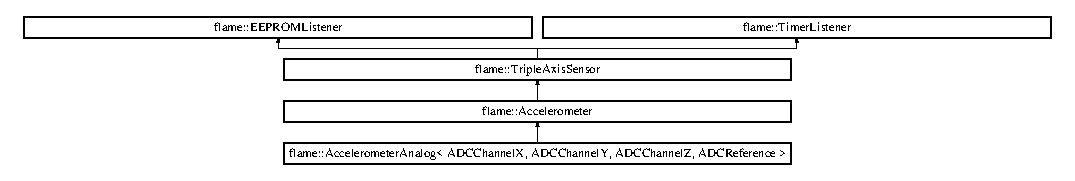
\includegraphics[height=1.982301cm]{classflame_1_1_accelerometer}
\end{center}
\end{figure}
\subsection*{Public Member Functions}
\begin{DoxyCompactItemize}
\item 
bool \hyperlink{classflame_1_1_accelerometer_a408179e458d41aa08e06b721a6b8aa81}{load\-Calibration} (\hyperlink{classflame_1_1_e_e_p_r_o_m}{E\-E\-P\-R\-O\-M} \&eeprom)
\item 
void \hyperlink{classflame_1_1_accelerometer_afc95c5291e223eb400a0c9a33a44f71f}{save\-Calibration} (\hyperlink{classflame_1_1_e_e_p_r_o_m}{E\-E\-P\-R\-O\-M} \&eeprom)
\end{DoxyCompactItemize}
\subsection*{Additional Inherited Members}


\subsection{Detailed Description}
\hyperlink{classflame_1_1_accelerometer}{Accelerometer} Interface 

Definition at line 38 of file Accelerometer.\-h.



\subsection{Member Function Documentation}
\hypertarget{classflame_1_1_accelerometer_a408179e458d41aa08e06b721a6b8aa81}{\index{flame\-::\-Accelerometer@{flame\-::\-Accelerometer}!load\-Calibration@{load\-Calibration}}
\index{load\-Calibration@{load\-Calibration}!flame::Accelerometer@{flame\-::\-Accelerometer}}
\subsubsection[{load\-Calibration}]{\setlength{\rightskip}{0pt plus 5cm}bool flame\-::\-Accelerometer\-::load\-Calibration (
\begin{DoxyParamCaption}
\item[{{\bf E\-E\-P\-R\-O\-M} \&}]{eeprom}
\end{DoxyParamCaption}
)}}\label{classflame_1_1_accelerometer_a408179e458d41aa08e06b721a6b8aa81}
Load calibration data from the default location 
\begin{DoxyParams}{Parameters}
{\em eeprom} & the \hyperlink{classflame_1_1_e_e_p_r_o_m}{E\-E\-P\-R\-O\-M} access instance \\
\hline
\end{DoxyParams}
\begin{DoxyReturn}{Returns}
false on success, true if the device needs to be calibrated 
\end{DoxyReturn}


Definition at line 37 of file Accelerometer.\-cpp.

\hypertarget{classflame_1_1_accelerometer_afc95c5291e223eb400a0c9a33a44f71f}{\index{flame\-::\-Accelerometer@{flame\-::\-Accelerometer}!save\-Calibration@{save\-Calibration}}
\index{save\-Calibration@{save\-Calibration}!flame::Accelerometer@{flame\-::\-Accelerometer}}
\subsubsection[{save\-Calibration}]{\setlength{\rightskip}{0pt plus 5cm}void flame\-::\-Accelerometer\-::save\-Calibration (
\begin{DoxyParamCaption}
\item[{{\bf E\-E\-P\-R\-O\-M} \&}]{eeprom}
\end{DoxyParamCaption}
)}}\label{classflame_1_1_accelerometer_afc95c5291e223eb400a0c9a33a44f71f}
Save the current calibration data to \hyperlink{classflame_1_1_e_e_p_r_o_m}{E\-E\-P\-R\-O\-M} at the default location 
\begin{DoxyParams}{Parameters}
{\em eeprom} & the \hyperlink{classflame_1_1_e_e_p_r_o_m}{E\-E\-P\-R\-O\-M} access instance \\
\hline
\end{DoxyParams}


Definition at line 45 of file Accelerometer.\-cpp.



The documentation for this class was generated from the following files\-:\begin{DoxyCompactItemize}
\item 
flame/\hyperlink{_accelerometer_8h}{Accelerometer.\-h}\item 
\hyperlink{_accelerometer_8cpp}{Accelerometer.\-cpp}\end{DoxyCompactItemize}

\hypertarget{classflame_1_1_accelerometer_analog}{\section{flame\-:\-:Accelerometer\-Analog$<$ A\-D\-C\-Channel\-X, A\-D\-C\-Channel\-Y, A\-D\-C\-Channel\-Z, A\-D\-C\-Reference $>$ Class Template Reference}
\label{classflame_1_1_accelerometer_analog}\index{flame\-::\-Accelerometer\-Analog$<$ A\-D\-C\-Channel\-X, A\-D\-C\-Channel\-Y, A\-D\-C\-Channel\-Z, A\-D\-C\-Reference $>$@{flame\-::\-Accelerometer\-Analog$<$ A\-D\-C\-Channel\-X, A\-D\-C\-Channel\-Y, A\-D\-C\-Channel\-Z, A\-D\-C\-Reference $>$}}
}


{\ttfamily \#include $<$Accelerometer\-Analog.\-h$>$}

Inheritance diagram for flame\-:\-:Accelerometer\-Analog$<$ A\-D\-C\-Channel\-X, A\-D\-C\-Channel\-Y, A\-D\-C\-Channel\-Z, A\-D\-C\-Reference $>$\-:\begin{figure}[H]
\begin{center}
\leavevmode
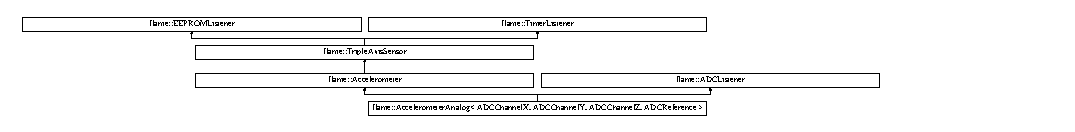
\includegraphics[height=1.321534cm]{classflame_1_1_accelerometer_analog}
\end{center}
\end{figure}
\subsection*{Public Member Functions}
\begin{DoxyCompactItemize}
\item 
\hyperlink{classflame_1_1_accelerometer_analog_a1beaaa7e83da69d8c92ae08698eaa112}{Accelerometer\-Analog} (\hyperlink{classflame_1_1_a_d_c_manager}{A\-D\-C\-Manager} \&\hyperlink{classflame_1_1_accelerometer_analog_a430e1a8a3b101bfe9d3b988efa1e75f9}{adc})
\item 
void \hyperlink{classflame_1_1_accelerometer_analog_a78759b15cda131a4af795f5f1c598076}{sample} ()
\item 
void \hyperlink{classflame_1_1_accelerometer_analog_a430e1a8a3b101bfe9d3b988efa1e75f9}{adc} (\hyperlink{atmega1280_8h_ab5a361d214bf33f4d9d443d9db44043d}{A\-D\-C\-Channel} channel, uint16\-\_\-t adc\-Value)
\item 
bool \hyperlink{classflame_1_1_accelerometer_analog_aa638bdb59ae5392bc61c66329538f89d}{is\-Sample\-Ready} ()
\end{DoxyCompactItemize}
\subsection*{Protected Attributes}
\begin{DoxyCompactItemize}
\item 
\hyperlink{classflame_1_1_a_d_c_manager}{A\-D\-C\-Manager} $\ast$ \hyperlink{classflame_1_1_accelerometer_analog_ac3dda0476fa8c65185f8d6620225b0a3}{\-\_\-adc}
\item 
bool \hyperlink{classflame_1_1_accelerometer_analog_a89b9682e1c2817adeb48ab91fc25c507}{\-\_\-sample\-Ready}
\item 
bool \hyperlink{classflame_1_1_accelerometer_analog_a16e72bdbf27a8f4ba5b5ed068620d84c}{\-\_\-dummy\-Read}
\end{DoxyCompactItemize}
\subsection*{Additional Inherited Members}


\subsection{Detailed Description}
\subsubsection*{template$<$A\-D\-C\-Channel A\-D\-C\-Channel\-X, A\-D\-C\-Channel A\-D\-C\-Channel\-Y, A\-D\-C\-Channel A\-D\-C\-Channel\-Z, A\-D\-C\-Reference A\-D\-C\-Reference$>$class flame\-::\-Accelerometer\-Analog$<$ A\-D\-C\-Channel\-X, A\-D\-C\-Channel\-Y, A\-D\-C\-Channel\-Z, A\-D\-C\-Reference $>$}

An accelerometer that presents its data as analog values to be read by the A\-V\-R's A\-D\-C channels 
\begin{DoxyTemplParams}{Template Parameters}
{\em A\-D\-C\-Channel\-X} & the A\-D\-C channel to use for the X axis \\
\hline
{\em A\-D\-C\-Channel\-Y} & the A\-D\-C channel to use for the Y axis \\
\hline
{\em A\-D\-C\-Channel\-Z} & the A\-D\-C channel to use for the Z axis \\
\hline
{\em A\-D\-C\-Reference} & the voltage reference to use \\
\hline
\end{DoxyTemplParams}


Definition at line 47 of file Accelerometer\-Analog.\-h.



\subsection{Constructor \& Destructor Documentation}
\hypertarget{classflame_1_1_accelerometer_analog_a1beaaa7e83da69d8c92ae08698eaa112}{\index{flame\-::\-Accelerometer\-Analog@{flame\-::\-Accelerometer\-Analog}!Accelerometer\-Analog@{Accelerometer\-Analog}}
\index{Accelerometer\-Analog@{Accelerometer\-Analog}!flame::AccelerometerAnalog@{flame\-::\-Accelerometer\-Analog}}
\subsubsection[{Accelerometer\-Analog}]{\setlength{\rightskip}{0pt plus 5cm}template$<$A\-D\-C\-Channel A\-D\-C\-Channel\-X, A\-D\-C\-Channel A\-D\-C\-Channel\-Y, A\-D\-C\-Channel A\-D\-C\-Channel\-Z, A\-D\-C\-Reference A\-D\-C\-Reference$>$ {\bf flame\-::\-Accelerometer\-Analog}$<$ A\-D\-C\-Channel\-X, A\-D\-C\-Channel\-Y, A\-D\-C\-Channel\-Z, {\bf A\-D\-C\-Reference} $>$\-::{\bf Accelerometer\-Analog} (
\begin{DoxyParamCaption}
\item[{{\bf A\-D\-C\-Manager} \&}]{adc}
\end{DoxyParamCaption}
)\hspace{0.3cm}{\ttfamily [inline]}}}\label{classflame_1_1_accelerometer_analog_a1beaaa7e83da69d8c92ae08698eaa112}


Definition at line 54 of file Accelerometer\-Analog.\-h.



\subsection{Member Function Documentation}
\hypertarget{classflame_1_1_accelerometer_analog_a430e1a8a3b101bfe9d3b988efa1e75f9}{\index{flame\-::\-Accelerometer\-Analog@{flame\-::\-Accelerometer\-Analog}!adc@{adc}}
\index{adc@{adc}!flame::AccelerometerAnalog@{flame\-::\-Accelerometer\-Analog}}
\subsubsection[{adc}]{\setlength{\rightskip}{0pt plus 5cm}template$<$A\-D\-C\-Channel A\-D\-C\-Channel\-X, A\-D\-C\-Channel A\-D\-C\-Channel\-Y, A\-D\-C\-Channel A\-D\-C\-Channel\-Z, A\-D\-C\-Reference A\-D\-C\-Reference$>$ void {\bf flame\-::\-Accelerometer\-Analog}$<$ A\-D\-C\-Channel\-X, A\-D\-C\-Channel\-Y, A\-D\-C\-Channel\-Z, {\bf A\-D\-C\-Reference} $>$\-::adc (
\begin{DoxyParamCaption}
\item[{{\bf A\-D\-C\-Channel}}]{channel, }
\item[{uint16\-\_\-t}]{adc\-Value}
\end{DoxyParamCaption}
)\hspace{0.3cm}{\ttfamily [inline]}, {\ttfamily [virtual]}}}\label{classflame_1_1_accelerometer_analog_a430e1a8a3b101bfe9d3b988efa1e75f9}
Handle incoming A\-D\-C reads 
\begin{DoxyParams}{Parameters}
{\em channel} & the channel that was read from \\
\hline
{\em adc\-Value} & the value read from the channel \\
\hline
\end{DoxyParams}


Implements \hyperlink{classflame_1_1_a_d_c_listener_a87fbe7d5aa43969f0a60c653c9e45796}{flame\-::\-A\-D\-C\-Listener}.



Definition at line 80 of file Accelerometer\-Analog.\-h.

\hypertarget{classflame_1_1_accelerometer_analog_aa638bdb59ae5392bc61c66329538f89d}{\index{flame\-::\-Accelerometer\-Analog@{flame\-::\-Accelerometer\-Analog}!is\-Sample\-Ready@{is\-Sample\-Ready}}
\index{is\-Sample\-Ready@{is\-Sample\-Ready}!flame::AccelerometerAnalog@{flame\-::\-Accelerometer\-Analog}}
\subsubsection[{is\-Sample\-Ready}]{\setlength{\rightskip}{0pt plus 5cm}template$<$A\-D\-C\-Channel A\-D\-C\-Channel\-X, A\-D\-C\-Channel A\-D\-C\-Channel\-Y, A\-D\-C\-Channel A\-D\-C\-Channel\-Z, A\-D\-C\-Reference A\-D\-C\-Reference$>$ bool {\bf flame\-::\-Accelerometer\-Analog}$<$ A\-D\-C\-Channel\-X, A\-D\-C\-Channel\-Y, A\-D\-C\-Channel\-Z, {\bf A\-D\-C\-Reference} $>$\-::is\-Sample\-Ready (
\begin{DoxyParamCaption}
{}
\end{DoxyParamCaption}
)\hspace{0.3cm}{\ttfamily [inline]}, {\ttfamily [virtual]}}}\label{classflame_1_1_accelerometer_analog_aa638bdb59ae5392bc61c66329538f89d}
Check if a sample is ready \begin{DoxyReturn}{Returns}
true if the sample is ready 
\end{DoxyReturn}


Implements \hyperlink{classflame_1_1_triple_axis_sensor_a7223b8884adf0ff42cbfddd2b6f28ce3}{flame\-::\-Triple\-Axis\-Sensor}.



Definition at line 111 of file Accelerometer\-Analog.\-h.

\hypertarget{classflame_1_1_accelerometer_analog_a78759b15cda131a4af795f5f1c598076}{\index{flame\-::\-Accelerometer\-Analog@{flame\-::\-Accelerometer\-Analog}!sample@{sample}}
\index{sample@{sample}!flame::AccelerometerAnalog@{flame\-::\-Accelerometer\-Analog}}
\subsubsection[{sample}]{\setlength{\rightskip}{0pt plus 5cm}template$<$A\-D\-C\-Channel A\-D\-C\-Channel\-X, A\-D\-C\-Channel A\-D\-C\-Channel\-Y, A\-D\-C\-Channel A\-D\-C\-Channel\-Z, A\-D\-C\-Reference A\-D\-C\-Reference$>$ void {\bf flame\-::\-Accelerometer\-Analog}$<$ A\-D\-C\-Channel\-X, A\-D\-C\-Channel\-Y, A\-D\-C\-Channel\-Z, {\bf A\-D\-C\-Reference} $>$\-::sample (
\begin{DoxyParamCaption}
{}
\end{DoxyParamCaption}
)\hspace{0.3cm}{\ttfamily [inline]}, {\ttfamily [virtual]}}}\label{classflame_1_1_accelerometer_analog_a78759b15cda131a4af795f5f1c598076}
Initiate a sampling of the accelerometer 

Implements \hyperlink{classflame_1_1_triple_axis_sensor_ac2ff28538723dc987c6fbec20aa47341}{flame\-::\-Triple\-Axis\-Sensor}.



Definition at line 66 of file Accelerometer\-Analog.\-h.



\subsection{Member Data Documentation}
\hypertarget{classflame_1_1_accelerometer_analog_ac3dda0476fa8c65185f8d6620225b0a3}{\index{flame\-::\-Accelerometer\-Analog@{flame\-::\-Accelerometer\-Analog}!\-\_\-adc@{\-\_\-adc}}
\index{\-\_\-adc@{\-\_\-adc}!flame::AccelerometerAnalog@{flame\-::\-Accelerometer\-Analog}}
\subsubsection[{\-\_\-adc}]{\setlength{\rightskip}{0pt plus 5cm}template$<$A\-D\-C\-Channel A\-D\-C\-Channel\-X, A\-D\-C\-Channel A\-D\-C\-Channel\-Y, A\-D\-C\-Channel A\-D\-C\-Channel\-Z, A\-D\-C\-Reference A\-D\-C\-Reference$>$ {\bf A\-D\-C\-Manager}$\ast$ {\bf flame\-::\-Accelerometer\-Analog}$<$ A\-D\-C\-Channel\-X, A\-D\-C\-Channel\-Y, A\-D\-C\-Channel\-Z, {\bf A\-D\-C\-Reference} $>$\-::\-\_\-adc\hspace{0.3cm}{\ttfamily [protected]}}}\label{classflame_1_1_accelerometer_analog_ac3dda0476fa8c65185f8d6620225b0a3}


Definition at line 49 of file Accelerometer\-Analog.\-h.

\hypertarget{classflame_1_1_accelerometer_analog_a16e72bdbf27a8f4ba5b5ed068620d84c}{\index{flame\-::\-Accelerometer\-Analog@{flame\-::\-Accelerometer\-Analog}!\-\_\-dummy\-Read@{\-\_\-dummy\-Read}}
\index{\-\_\-dummy\-Read@{\-\_\-dummy\-Read}!flame::AccelerometerAnalog@{flame\-::\-Accelerometer\-Analog}}
\subsubsection[{\-\_\-dummy\-Read}]{\setlength{\rightskip}{0pt plus 5cm}template$<$A\-D\-C\-Channel A\-D\-C\-Channel\-X, A\-D\-C\-Channel A\-D\-C\-Channel\-Y, A\-D\-C\-Channel A\-D\-C\-Channel\-Z, A\-D\-C\-Reference A\-D\-C\-Reference$>$ bool {\bf flame\-::\-Accelerometer\-Analog}$<$ A\-D\-C\-Channel\-X, A\-D\-C\-Channel\-Y, A\-D\-C\-Channel\-Z, {\bf A\-D\-C\-Reference} $>$\-::\-\_\-dummy\-Read\hspace{0.3cm}{\ttfamily [protected]}}}\label{classflame_1_1_accelerometer_analog_a16e72bdbf27a8f4ba5b5ed068620d84c}


Definition at line 51 of file Accelerometer\-Analog.\-h.

\hypertarget{classflame_1_1_accelerometer_analog_a89b9682e1c2817adeb48ab91fc25c507}{\index{flame\-::\-Accelerometer\-Analog@{flame\-::\-Accelerometer\-Analog}!\-\_\-sample\-Ready@{\-\_\-sample\-Ready}}
\index{\-\_\-sample\-Ready@{\-\_\-sample\-Ready}!flame::AccelerometerAnalog@{flame\-::\-Accelerometer\-Analog}}
\subsubsection[{\-\_\-sample\-Ready}]{\setlength{\rightskip}{0pt plus 5cm}template$<$A\-D\-C\-Channel A\-D\-C\-Channel\-X, A\-D\-C\-Channel A\-D\-C\-Channel\-Y, A\-D\-C\-Channel A\-D\-C\-Channel\-Z, A\-D\-C\-Reference A\-D\-C\-Reference$>$ bool {\bf flame\-::\-Accelerometer\-Analog}$<$ A\-D\-C\-Channel\-X, A\-D\-C\-Channel\-Y, A\-D\-C\-Channel\-Z, {\bf A\-D\-C\-Reference} $>$\-::\-\_\-sample\-Ready\hspace{0.3cm}{\ttfamily [protected]}}}\label{classflame_1_1_accelerometer_analog_a89b9682e1c2817adeb48ab91fc25c507}


Definition at line 50 of file Accelerometer\-Analog.\-h.



The documentation for this class was generated from the following file\-:\begin{DoxyCompactItemize}
\item 
flame/\hyperlink{_accelerometer_analog_8h}{Accelerometer\-Analog.\-h}\end{DoxyCompactItemize}

\hypertarget{classflame_1_1_a_d_c_listener}{\section{flame\-:\-:A\-D\-C\-Listener Class Reference}
\label{classflame_1_1_a_d_c_listener}\index{flame\-::\-A\-D\-C\-Listener@{flame\-::\-A\-D\-C\-Listener}}
}


{\ttfamily \#include $<$A\-D\-C\-Manager.\-h$>$}

Inheritance diagram for flame\-:\-:A\-D\-C\-Listener\-:\begin{figure}[H]
\begin{center}
\leavevmode
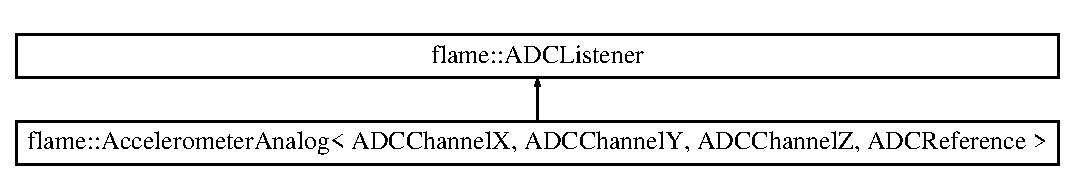
\includegraphics[height=1.982301cm]{classflame_1_1_a_d_c_listener}
\end{center}
\end{figure}
\subsection*{Public Member Functions}
\begin{DoxyCompactItemize}
\item 
virtual void \hyperlink{classflame_1_1_a_d_c_listener_a87fbe7d5aa43969f0a60c653c9e45796}{adc} (\hyperlink{atmega1280_8h_ab5a361d214bf33f4d9d443d9db44043d}{A\-D\-C\-Channel} channel, uint16\-\_\-t value)=0
\end{DoxyCompactItemize}


\subsection{Detailed Description}


Definition at line 55 of file A\-D\-C\-Manager.\-h.



\subsection{Member Function Documentation}
\hypertarget{classflame_1_1_a_d_c_listener_a87fbe7d5aa43969f0a60c653c9e45796}{\index{flame\-::\-A\-D\-C\-Listener@{flame\-::\-A\-D\-C\-Listener}!adc@{adc}}
\index{adc@{adc}!flame::ADCListener@{flame\-::\-A\-D\-C\-Listener}}
\subsubsection[{adc}]{\setlength{\rightskip}{0pt plus 5cm}virtual void flame\-::\-A\-D\-C\-Listener\-::adc (
\begin{DoxyParamCaption}
\item[{{\bf A\-D\-C\-Channel}}]{channel, }
\item[{uint16\-\_\-t}]{value}
\end{DoxyParamCaption}
)\hspace{0.3cm}{\ttfamily [pure virtual]}}}\label{classflame_1_1_a_d_c_listener_a87fbe7d5aa43969f0a60c653c9e45796}
Handle incoming A\-D\-C reads 
\begin{DoxyParams}{Parameters}
{\em channel} & the channel that was read from \\
\hline
{\em value} & the value read from the channel \\
\hline
\end{DoxyParams}


Implemented in \hyperlink{classflame_1_1_accelerometer_analog_a430e1a8a3b101bfe9d3b988efa1e75f9}{flame\-::\-Accelerometer\-Analog$<$ A\-D\-C\-Channel\-X, A\-D\-C\-Channel\-Y, A\-D\-C\-Channel\-Z, A\-D\-C\-Reference $>$}.



The documentation for this class was generated from the following file\-:\begin{DoxyCompactItemize}
\item 
flame/\hyperlink{_a_d_c_manager_8h}{A\-D\-C\-Manager.\-h}\end{DoxyCompactItemize}

\hypertarget{classflame_1_1_a_d_c_manager}{\section{flame\-:\-:A\-D\-C\-Manager Class Reference}
\label{classflame_1_1_a_d_c_manager}\index{flame\-::\-A\-D\-C\-Manager@{flame\-::\-A\-D\-C\-Manager}}
}


{\ttfamily \#include $<$A\-D\-C\-Manager.\-h$>$}

Inheritance diagram for flame\-:\-:A\-D\-C\-Manager\-:\begin{figure}[H]
\begin{center}
\leavevmode
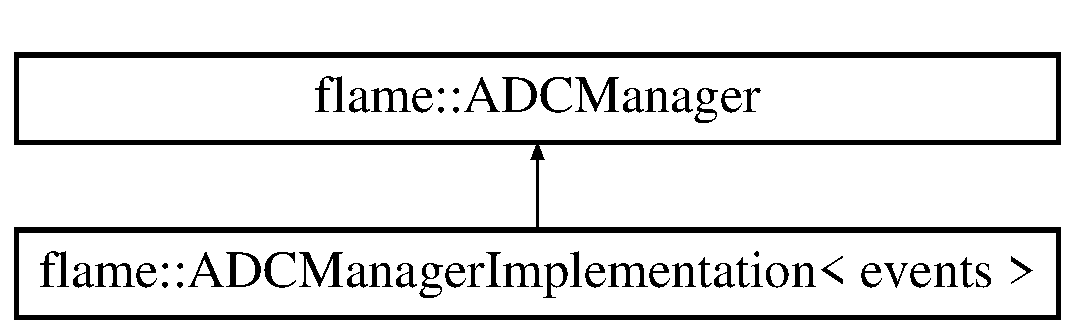
\includegraphics[height=2.000000cm]{classflame_1_1_a_d_c_manager}
\end{center}
\end{figure}
\subsection*{Public Member Functions}
\begin{DoxyCompactItemize}
\item 
\hyperlink{classflame_1_1_a_d_c_manager_ad9113599803b23bb74fcaf1e50e5d6a4}{A\-D\-C\-Manager} (\hyperlink{namespaceflame_a0fb9cd960c9db48d9e068daa2427aecf}{E\-V\-E\-N\-T\-\_\-\-A\-D\-C} $\ast$adcs, uint8\-\_\-t adc\-Count, A\-D\-C\-Prescaler prescaler)
\item 
void \hyperlink{classflame_1_1_a_d_c_manager_a604cce5bd959bc084896e033d722e973}{adc} ()
\item 
void \hyperlink{classflame_1_1_a_d_c_manager_abbc89646e31553473b48ccacf8c3e05b}{register\-Listener} (\hyperlink{atmega1280_8h_ab5a361d214bf33f4d9d443d9db44043d}{A\-D\-C\-Channel} channel, \hyperlink{classflame_1_1_a_d_c_listener}{A\-D\-C\-Listener} \&listener)
\item 
void \hyperlink{classflame_1_1_a_d_c_manager_ab1d6a02fb4b94d38471f720396bc0040}{register\-Listener} (\hyperlink{atmega1280_8h_ab5a361d214bf33f4d9d443d9db44043d}{A\-D\-C\-Channel} channel, \hyperlink{classflame_1_1_a_d_c_listener}{A\-D\-C\-Listener} $\ast$listener)
\item 
void \hyperlink{classflame_1_1_a_d_c_manager_a1fa15eac782858bd521ab5ea3ee7a913}{deregister\-Listener} (\hyperlink{atmega1280_8h_ab5a361d214bf33f4d9d443d9db44043d}{A\-D\-C\-Channel} channel)
\item 
int16\-\_\-t \hyperlink{classflame_1_1_a_d_c_manager_a3ee8ed7fbe1bc144f2521bc725527d84}{busy\-Read} (\hyperlink{atmega1280_8h_ab5a361d214bf33f4d9d443d9db44043d}{A\-D\-C\-Channel} channel, \hyperlink{atmega1280_8h_ad19819a3e7273f98d571eab79f5a5d81}{A\-D\-C\-Reference} reference)
\item 
void \hyperlink{classflame_1_1_a_d_c_manager_aaef66297e65aa489c1493f55275f84a4}{read} (\hyperlink{atmega1280_8h_ab5a361d214bf33f4d9d443d9db44043d}{A\-D\-C\-Channel} channel, \hyperlink{atmega1280_8h_ad19819a3e7273f98d571eab79f5a5d81}{A\-D\-C\-Reference} reference)
\item 
void \hyperlink{classflame_1_1_a_d_c_manager_a010eb23bc134b08b372982e7ee6b17d4}{set\-Prescaler} (A\-D\-C\-Prescaler prescaler)
\item 
void \hyperlink{classflame_1_1_a_d_c_manager_abc84178ae84687965312bf5ed79667b4}{handle\-Events} ()
\end{DoxyCompactItemize}
\subsection*{Protected Attributes}
\begin{DoxyCompactItemize}
\item 
volatile uint16\-\_\-t \hyperlink{classflame_1_1_a_d_c_manager_a60ec78c37e926899fd23835347a4dcd5}{\-\_\-adc\-Value}
\item 
volatile \hyperlink{atmega1280_8h_ab5a361d214bf33f4d9d443d9db44043d}{A\-D\-C\-Channel} \hyperlink{classflame_1_1_a_d_c_manager_a1591a81f54b5045fa73807f8ec941ef4}{\-\_\-channel}
\item 
\hyperlink{namespaceflame_a0fb9cd960c9db48d9e068daa2427aecf}{E\-V\-E\-N\-T\-\_\-\-A\-D\-C} $\ast$ \hyperlink{classflame_1_1_a_d_c_manager_a04cc074d97fbb83004821333a786cc6b}{\-\_\-adcs}
\item 
uint8\-\_\-t \hyperlink{classflame_1_1_a_d_c_manager_a92c716e93c9adff0bf1faf8f3a2d68ef}{\-\_\-event\-Count}
\end{DoxyCompactItemize}


\subsection{Detailed Description}


Definition at line 72 of file A\-D\-C\-Manager.\-h.



\subsection{Constructor \& Destructor Documentation}
\hypertarget{classflame_1_1_a_d_c_manager_ad9113599803b23bb74fcaf1e50e5d6a4}{\index{flame\-::\-A\-D\-C\-Manager@{flame\-::\-A\-D\-C\-Manager}!A\-D\-C\-Manager@{A\-D\-C\-Manager}}
\index{A\-D\-C\-Manager@{A\-D\-C\-Manager}!flame::ADCManager@{flame\-::\-A\-D\-C\-Manager}}
\subsubsection[{A\-D\-C\-Manager}]{\setlength{\rightskip}{0pt plus 5cm}flame\-::\-A\-D\-C\-Manager\-::\-A\-D\-C\-Manager (
\begin{DoxyParamCaption}
\item[{{\bf E\-V\-E\-N\-T\-\_\-\-A\-D\-C} $\ast$}]{events\-Buffer, }
\item[{uint8\-\_\-t}]{event\-Count, }
\item[{A\-D\-C\-Prescaler}]{prescaler}
\end{DoxyParamCaption}
)}}\label{classflame_1_1_a_d_c_manager_ad9113599803b23bb74fcaf1e50e5d6a4}
An event manager for A\-D\-C events 
\begin{DoxyParams}{Parameters}
{\em events\-Buffer} & storage for channel event data \\
\hline
{\em event\-Count} & the maximum number of events to handle \\
\hline
{\em prescaler} & the prescaler to run the A\-D\-C at \\
\hline
\end{DoxyParams}


Definition at line 38 of file A\-D\-C\-Manager.\-cpp.



\subsection{Member Function Documentation}
\hypertarget{classflame_1_1_a_d_c_manager_a604cce5bd959bc084896e033d722e973}{\index{flame\-::\-A\-D\-C\-Manager@{flame\-::\-A\-D\-C\-Manager}!adc@{adc}}
\index{adc@{adc}!flame::ADCManager@{flame\-::\-A\-D\-C\-Manager}}
\subsubsection[{adc}]{\setlength{\rightskip}{0pt plus 5cm}void flame\-::\-A\-D\-C\-Manager\-::adc (
\begin{DoxyParamCaption}
{}
\end{DoxyParamCaption}
)}}\label{classflame_1_1_a_d_c_manager_a604cce5bd959bc084896e033d722e973}
Interrupt handler to read the A\-D\-C 

Definition at line 55 of file A\-D\-C\-Manager.\-cpp.

\hypertarget{classflame_1_1_a_d_c_manager_a3ee8ed7fbe1bc144f2521bc725527d84}{\index{flame\-::\-A\-D\-C\-Manager@{flame\-::\-A\-D\-C\-Manager}!busy\-Read@{busy\-Read}}
\index{busy\-Read@{busy\-Read}!flame::ADCManager@{flame\-::\-A\-D\-C\-Manager}}
\subsubsection[{busy\-Read}]{\setlength{\rightskip}{0pt plus 5cm}int16\-\_\-t flame\-::\-A\-D\-C\-Manager\-::busy\-Read (
\begin{DoxyParamCaption}
\item[{{\bf A\-D\-C\-Channel}}]{channel, }
\item[{{\bf A\-D\-C\-Reference}}]{reference}
\end{DoxyParamCaption}
)}}\label{classflame_1_1_a_d_c_manager_a3ee8ed7fbe1bc144f2521bc725527d84}
Read an A\-D\-C channel 
\begin{DoxyParams}{Parameters}
{\em channel} & the channel to read \\
\hline
{\em reference} & the voltage reference to use \\
\hline
\end{DoxyParams}


Definition at line 114 of file A\-D\-C\-Manager.\-cpp.

\hypertarget{classflame_1_1_a_d_c_manager_a1fa15eac782858bd521ab5ea3ee7a913}{\index{flame\-::\-A\-D\-C\-Manager@{flame\-::\-A\-D\-C\-Manager}!deregister\-Listener@{deregister\-Listener}}
\index{deregister\-Listener@{deregister\-Listener}!flame::ADCManager@{flame\-::\-A\-D\-C\-Manager}}
\subsubsection[{deregister\-Listener}]{\setlength{\rightskip}{0pt plus 5cm}void flame\-::\-A\-D\-C\-Manager\-::deregister\-Listener (
\begin{DoxyParamCaption}
\item[{{\bf A\-D\-C\-Channel}}]{channel}
\end{DoxyParamCaption}
)}}\label{classflame_1_1_a_d_c_manager_a1fa15eac782858bd521ab5ea3ee7a913}
Deregister interest for an A\-D\-C channel 
\begin{DoxyParams}{Parameters}
{\em channel} & the A\-D\-C channel \\
\hline
\end{DoxyParams}


Definition at line 99 of file A\-D\-C\-Manager.\-cpp.

\hypertarget{classflame_1_1_a_d_c_manager_abc84178ae84687965312bf5ed79667b4}{\index{flame\-::\-A\-D\-C\-Manager@{flame\-::\-A\-D\-C\-Manager}!handle\-Events@{handle\-Events}}
\index{handle\-Events@{handle\-Events}!flame::ADCManager@{flame\-::\-A\-D\-C\-Manager}}
\subsubsection[{handle\-Events}]{\setlength{\rightskip}{0pt plus 5cm}void flame\-::\-A\-D\-C\-Manager\-::handle\-Events (
\begin{DoxyParamCaption}
{}
\end{DoxyParamCaption}
)}}\label{classflame_1_1_a_d_c_manager_abc84178ae84687965312bf5ed79667b4}
Call from the main loop to handle any events 

Definition at line 163 of file A\-D\-C\-Manager.\-cpp.

\hypertarget{classflame_1_1_a_d_c_manager_aaef66297e65aa489c1493f55275f84a4}{\index{flame\-::\-A\-D\-C\-Manager@{flame\-::\-A\-D\-C\-Manager}!read@{read}}
\index{read@{read}!flame::ADCManager@{flame\-::\-A\-D\-C\-Manager}}
\subsubsection[{read}]{\setlength{\rightskip}{0pt plus 5cm}void flame\-::\-A\-D\-C\-Manager\-::read (
\begin{DoxyParamCaption}
\item[{{\bf A\-D\-C\-Channel}}]{channel, }
\item[{{\bf A\-D\-C\-Reference}}]{reference}
\end{DoxyParamCaption}
)}}\label{classflame_1_1_a_d_c_manager_aaef66297e65aa489c1493f55275f84a4}
Trigger an A\-D\-C channel event 
\begin{DoxyParams}{Parameters}
{\em channel} & the channel to read \\
\hline
{\em reference} & the voltage reference to use \\
\hline
\end{DoxyParams}


Definition at line 137 of file A\-D\-C\-Manager.\-cpp.

\hypertarget{classflame_1_1_a_d_c_manager_abbc89646e31553473b48ccacf8c3e05b}{\index{flame\-::\-A\-D\-C\-Manager@{flame\-::\-A\-D\-C\-Manager}!register\-Listener@{register\-Listener}}
\index{register\-Listener@{register\-Listener}!flame::ADCManager@{flame\-::\-A\-D\-C\-Manager}}
\subsubsection[{register\-Listener}]{\setlength{\rightskip}{0pt plus 5cm}void flame\-::\-A\-D\-C\-Manager\-::register\-Listener (
\begin{DoxyParamCaption}
\item[{{\bf A\-D\-C\-Channel}}]{channel, }
\item[{{\bf A\-D\-C\-Listener} \&}]{listener}
\end{DoxyParamCaption}
)}}\label{classflame_1_1_a_d_c_manager_abbc89646e31553473b48ccacf8c3e05b}
Register interest for an A\-D\-C channel 
\begin{DoxyParams}{Parameters}
{\em channel} & the A\-D\-C channel \\
\hline
{\em listener} & an \hyperlink{classflame_1_1_a_d_c_listener}{A\-D\-C\-Listener} to notify when an A\-D\-C reading has been completed \\
\hline
\end{DoxyParams}


Definition at line 68 of file A\-D\-C\-Manager.\-cpp.

\hypertarget{classflame_1_1_a_d_c_manager_ab1d6a02fb4b94d38471f720396bc0040}{\index{flame\-::\-A\-D\-C\-Manager@{flame\-::\-A\-D\-C\-Manager}!register\-Listener@{register\-Listener}}
\index{register\-Listener@{register\-Listener}!flame::ADCManager@{flame\-::\-A\-D\-C\-Manager}}
\subsubsection[{register\-Listener}]{\setlength{\rightskip}{0pt plus 5cm}void flame\-::\-A\-D\-C\-Manager\-::register\-Listener (
\begin{DoxyParamCaption}
\item[{{\bf A\-D\-C\-Channel}}]{channel, }
\item[{{\bf A\-D\-C\-Listener} $\ast$}]{listener}
\end{DoxyParamCaption}
)}}\label{classflame_1_1_a_d_c_manager_ab1d6a02fb4b94d38471f720396bc0040}
Register interest for an A\-D\-C channel 
\begin{DoxyParams}{Parameters}
{\em channel} & the A\-D\-C channel \\
\hline
{\em listener} & an \hyperlink{classflame_1_1_a_d_c_listener}{A\-D\-C\-Listener} to notify when an A\-D\-C reading has been completed \\
\hline
\end{DoxyParams}


Definition at line 84 of file A\-D\-C\-Manager.\-cpp.

\hypertarget{classflame_1_1_a_d_c_manager_a010eb23bc134b08b372982e7ee6b17d4}{\index{flame\-::\-A\-D\-C\-Manager@{flame\-::\-A\-D\-C\-Manager}!set\-Prescaler@{set\-Prescaler}}
\index{set\-Prescaler@{set\-Prescaler}!flame::ADCManager@{flame\-::\-A\-D\-C\-Manager}}
\subsubsection[{set\-Prescaler}]{\setlength{\rightskip}{0pt plus 5cm}void flame\-::\-A\-D\-C\-Manager\-::set\-Prescaler (
\begin{DoxyParamCaption}
\item[{A\-D\-C\-Prescaler}]{prescaler}
\end{DoxyParamCaption}
)}}\label{classflame_1_1_a_d_c_manager_a010eb23bc134b08b372982e7ee6b17d4}
Set the A\-D\-C clock prescaler 
\begin{DoxyParams}{Parameters}
{\em prescaler} & the prescaler to use \\
\hline
\end{DoxyParams}


Definition at line 155 of file A\-D\-C\-Manager.\-cpp.



\subsection{Member Data Documentation}
\hypertarget{classflame_1_1_a_d_c_manager_a04cc074d97fbb83004821333a786cc6b}{\index{flame\-::\-A\-D\-C\-Manager@{flame\-::\-A\-D\-C\-Manager}!\-\_\-adcs@{\-\_\-adcs}}
\index{\-\_\-adcs@{\-\_\-adcs}!flame::ADCManager@{flame\-::\-A\-D\-C\-Manager}}
\subsubsection[{\-\_\-adcs}]{\setlength{\rightskip}{0pt plus 5cm}{\bf E\-V\-E\-N\-T\-\_\-\-A\-D\-C}$\ast$ flame\-::\-A\-D\-C\-Manager\-::\-\_\-adcs\hspace{0.3cm}{\ttfamily [protected]}}}\label{classflame_1_1_a_d_c_manager_a04cc074d97fbb83004821333a786cc6b}


Definition at line 76 of file A\-D\-C\-Manager.\-h.

\hypertarget{classflame_1_1_a_d_c_manager_a60ec78c37e926899fd23835347a4dcd5}{\index{flame\-::\-A\-D\-C\-Manager@{flame\-::\-A\-D\-C\-Manager}!\-\_\-adc\-Value@{\-\_\-adc\-Value}}
\index{\-\_\-adc\-Value@{\-\_\-adc\-Value}!flame::ADCManager@{flame\-::\-A\-D\-C\-Manager}}
\subsubsection[{\-\_\-adc\-Value}]{\setlength{\rightskip}{0pt plus 5cm}volatile uint16\-\_\-t flame\-::\-A\-D\-C\-Manager\-::\-\_\-adc\-Value\hspace{0.3cm}{\ttfamily [protected]}}}\label{classflame_1_1_a_d_c_manager_a60ec78c37e926899fd23835347a4dcd5}


Definition at line 74 of file A\-D\-C\-Manager.\-h.

\hypertarget{classflame_1_1_a_d_c_manager_a1591a81f54b5045fa73807f8ec941ef4}{\index{flame\-::\-A\-D\-C\-Manager@{flame\-::\-A\-D\-C\-Manager}!\-\_\-channel@{\-\_\-channel}}
\index{\-\_\-channel@{\-\_\-channel}!flame::ADCManager@{flame\-::\-A\-D\-C\-Manager}}
\subsubsection[{\-\_\-channel}]{\setlength{\rightskip}{0pt plus 5cm}volatile {\bf A\-D\-C\-Channel} flame\-::\-A\-D\-C\-Manager\-::\-\_\-channel\hspace{0.3cm}{\ttfamily [protected]}}}\label{classflame_1_1_a_d_c_manager_a1591a81f54b5045fa73807f8ec941ef4}


Definition at line 75 of file A\-D\-C\-Manager.\-h.

\hypertarget{classflame_1_1_a_d_c_manager_a92c716e93c9adff0bf1faf8f3a2d68ef}{\index{flame\-::\-A\-D\-C\-Manager@{flame\-::\-A\-D\-C\-Manager}!\-\_\-event\-Count@{\-\_\-event\-Count}}
\index{\-\_\-event\-Count@{\-\_\-event\-Count}!flame::ADCManager@{flame\-::\-A\-D\-C\-Manager}}
\subsubsection[{\-\_\-event\-Count}]{\setlength{\rightskip}{0pt plus 5cm}uint8\-\_\-t flame\-::\-A\-D\-C\-Manager\-::\-\_\-event\-Count\hspace{0.3cm}{\ttfamily [protected]}}}\label{classflame_1_1_a_d_c_manager_a92c716e93c9adff0bf1faf8f3a2d68ef}


Definition at line 77 of file A\-D\-C\-Manager.\-h.



The documentation for this class was generated from the following files\-:\begin{DoxyCompactItemize}
\item 
flame/\hyperlink{_a_d_c_manager_8h}{A\-D\-C\-Manager.\-h}\item 
\hyperlink{_a_d_c_manager_8cpp}{A\-D\-C\-Manager.\-cpp}\end{DoxyCompactItemize}

\hypertarget{classflame_1_1_a_d_c_manager_implementation}{\section{flame\-:\-:A\-D\-C\-Manager\-Implementation$<$ events $>$ Class Template Reference}
\label{classflame_1_1_a_d_c_manager_implementation}\index{flame\-::\-A\-D\-C\-Manager\-Implementation$<$ events $>$@{flame\-::\-A\-D\-C\-Manager\-Implementation$<$ events $>$}}
}


{\ttfamily \#include $<$A\-D\-C\-Manager.\-h$>$}

Inheritance diagram for flame\-:\-:A\-D\-C\-Manager\-Implementation$<$ events $>$\-:\begin{figure}[H]
\begin{center}
\leavevmode
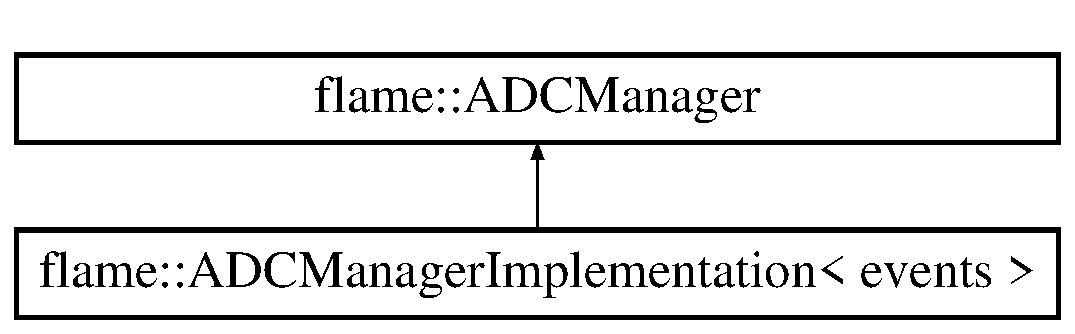
\includegraphics[height=2.000000cm]{classflame_1_1_a_d_c_manager_implementation}
\end{center}
\end{figure}
\subsection*{Public Member Functions}
\begin{DoxyCompactItemize}
\item 
\hyperlink{classflame_1_1_a_d_c_manager_implementation_a0fff664ebb747ca532b8eebb980adae5}{A\-D\-C\-Manager\-Implementation} (A\-D\-C\-Prescaler prescaler)
\end{DoxyCompactItemize}
\subsection*{Protected Attributes}
\begin{DoxyCompactItemize}
\item 
\hyperlink{namespaceflame_a0fb9cd960c9db48d9e068daa2427aecf}{E\-V\-E\-N\-T\-\_\-\-A\-D\-C} \hyperlink{classflame_1_1_a_d_c_manager_implementation_aab124e6a32ba437c772a7c43492ed4af}{\-\_\-my\-Adcs} \mbox{[}events\mbox{]}
\end{DoxyCompactItemize}


\subsection{Detailed Description}
\subsubsection*{template$<$uint8\-\_\-t events$>$class flame\-::\-A\-D\-C\-Manager\-Implementation$<$ events $>$}

An event manager for A\-D\-C events 
\begin{DoxyTemplParams}{Template Parameters}
{\em events} & the number of A\-D\-C events we can handle \\
\hline
\end{DoxyTemplParams}


Definition at line 96 of file A\-D\-C\-Manager.\-h.



\subsection{Constructor \& Destructor Documentation}
\hypertarget{classflame_1_1_a_d_c_manager_implementation_a0fff664ebb747ca532b8eebb980adae5}{\index{flame\-::\-A\-D\-C\-Manager\-Implementation@{flame\-::\-A\-D\-C\-Manager\-Implementation}!A\-D\-C\-Manager\-Implementation@{A\-D\-C\-Manager\-Implementation}}
\index{A\-D\-C\-Manager\-Implementation@{A\-D\-C\-Manager\-Implementation}!flame::ADCManagerImplementation@{flame\-::\-A\-D\-C\-Manager\-Implementation}}
\subsubsection[{A\-D\-C\-Manager\-Implementation}]{\setlength{\rightskip}{0pt plus 5cm}template$<$uint8\-\_\-t events$>$ {\bf flame\-::\-A\-D\-C\-Manager\-Implementation}$<$ events $>$\-::{\bf A\-D\-C\-Manager\-Implementation} (
\begin{DoxyParamCaption}
\item[{A\-D\-C\-Prescaler}]{prescaler}
\end{DoxyParamCaption}
)\hspace{0.3cm}{\ttfamily [inline]}}}\label{classflame_1_1_a_d_c_manager_implementation_a0fff664ebb747ca532b8eebb980adae5}
An event manager for A\-D\-C events 
\begin{DoxyParams}{Parameters}
{\em prescaler} & the prescaler to run the A\-D\-C at \\
\hline
\end{DoxyParams}


Definition at line 106 of file A\-D\-C\-Manager.\-h.



\subsection{Member Data Documentation}
\hypertarget{classflame_1_1_a_d_c_manager_implementation_aab124e6a32ba437c772a7c43492ed4af}{\index{flame\-::\-A\-D\-C\-Manager\-Implementation@{flame\-::\-A\-D\-C\-Manager\-Implementation}!\-\_\-my\-Adcs@{\-\_\-my\-Adcs}}
\index{\-\_\-my\-Adcs@{\-\_\-my\-Adcs}!flame::ADCManagerImplementation@{flame\-::\-A\-D\-C\-Manager\-Implementation}}
\subsubsection[{\-\_\-my\-Adcs}]{\setlength{\rightskip}{0pt plus 5cm}template$<$uint8\-\_\-t events$>$ {\bf E\-V\-E\-N\-T\-\_\-\-A\-D\-C} {\bf flame\-::\-A\-D\-C\-Manager\-Implementation}$<$ events $>$\-::\-\_\-my\-Adcs\mbox{[}events\mbox{]}\hspace{0.3cm}{\ttfamily [protected]}}}\label{classflame_1_1_a_d_c_manager_implementation_aab124e6a32ba437c772a7c43492ed4af}


Definition at line 98 of file A\-D\-C\-Manager.\-h.



The documentation for this class was generated from the following file\-:\begin{DoxyCompactItemize}
\item 
flame/\hyperlink{_a_d_c_manager_8h}{A\-D\-C\-Manager.\-h}\end{DoxyCompactItemize}

\hypertarget{structflame_1_1alarm}{\section{flame\-:\-:alarm Struct Reference}
\label{structflame_1_1alarm}\index{flame\-::alarm@{flame\-::alarm}}
}


{\ttfamily \#include $<$R\-T\-C.\-h$>$}

\subsection*{Public Attributes}
\begin{DoxyCompactItemize}
\item 
\hyperlink{namespaceflame_ad90347e9ea7e54907966260ec5c7d22f}{T\-I\-M\-E\-S\-T\-A\-M\-P} \hyperlink{structflame_1_1alarm_a5c2cc1d3e96943a144f6f965b1561e00}{when}
\item 
\hyperlink{namespaceflame_ad90347e9ea7e54907966260ec5c7d22f}{T\-I\-M\-E\-S\-T\-A\-M\-P} \hyperlink{structflame_1_1alarm_a66e4634a1965c119d7d39798056b7340}{repeat}
\item 
\hyperlink{classflame_1_1_timer_listener}{Timer\-Listener} $\ast$ \hyperlink{structflame_1_1alarm_ac21df9b77c10cdc77c0a0c29d6ada66b}{listener}
\end{DoxyCompactItemize}


\subsection{Detailed Description}


Definition at line 90 of file R\-T\-C.\-h.



\subsection{Member Data Documentation}
\hypertarget{structflame_1_1alarm_ac21df9b77c10cdc77c0a0c29d6ada66b}{\index{flame\-::alarm@{flame\-::alarm}!listener@{listener}}
\index{listener@{listener}!flame::alarm@{flame\-::alarm}}
\subsubsection[{listener}]{\setlength{\rightskip}{0pt plus 5cm}{\bf Timer\-Listener}$\ast$ flame\-::alarm\-::listener}}\label{structflame_1_1alarm_ac21df9b77c10cdc77c0a0c29d6ada66b}


Definition at line 93 of file R\-T\-C.\-h.

\hypertarget{structflame_1_1alarm_a66e4634a1965c119d7d39798056b7340}{\index{flame\-::alarm@{flame\-::alarm}!repeat@{repeat}}
\index{repeat@{repeat}!flame::alarm@{flame\-::alarm}}
\subsubsection[{repeat}]{\setlength{\rightskip}{0pt plus 5cm}{\bf T\-I\-M\-E\-S\-T\-A\-M\-P} flame\-::alarm\-::repeat}}\label{structflame_1_1alarm_a66e4634a1965c119d7d39798056b7340}


Definition at line 92 of file R\-T\-C.\-h.

\hypertarget{structflame_1_1alarm_a5c2cc1d3e96943a144f6f965b1561e00}{\index{flame\-::alarm@{flame\-::alarm}!when@{when}}
\index{when@{when}!flame::alarm@{flame\-::alarm}}
\subsubsection[{when}]{\setlength{\rightskip}{0pt plus 5cm}{\bf T\-I\-M\-E\-S\-T\-A\-M\-P} flame\-::alarm\-::when}}\label{structflame_1_1alarm_a5c2cc1d3e96943a144f6f965b1561e00}


Definition at line 91 of file R\-T\-C.\-h.



The documentation for this struct was generated from the following file\-:\begin{DoxyCompactItemize}
\item 
flame/\hyperlink{_r_t_c_8h}{R\-T\-C.\-h}\end{DoxyCompactItemize}

\hypertarget{classflame_1_1_best_sphere_gauss_newton_calibrator}{\section{flame\-:\-:Best\-Sphere\-Gauss\-Newton\-Calibrator Class Reference}
\label{classflame_1_1_best_sphere_gauss_newton_calibrator}\index{flame\-::\-Best\-Sphere\-Gauss\-Newton\-Calibrator@{flame\-::\-Best\-Sphere\-Gauss\-Newton\-Calibrator}}
}


{\ttfamily \#include $<$Best\-Sphere\-Gauss\-Newton\-Calibrator.\-h$>$}

Inheritance diagram for flame\-:\-:Best\-Sphere\-Gauss\-Newton\-Calibrator\-:\begin{figure}[H]
\begin{center}
\leavevmode
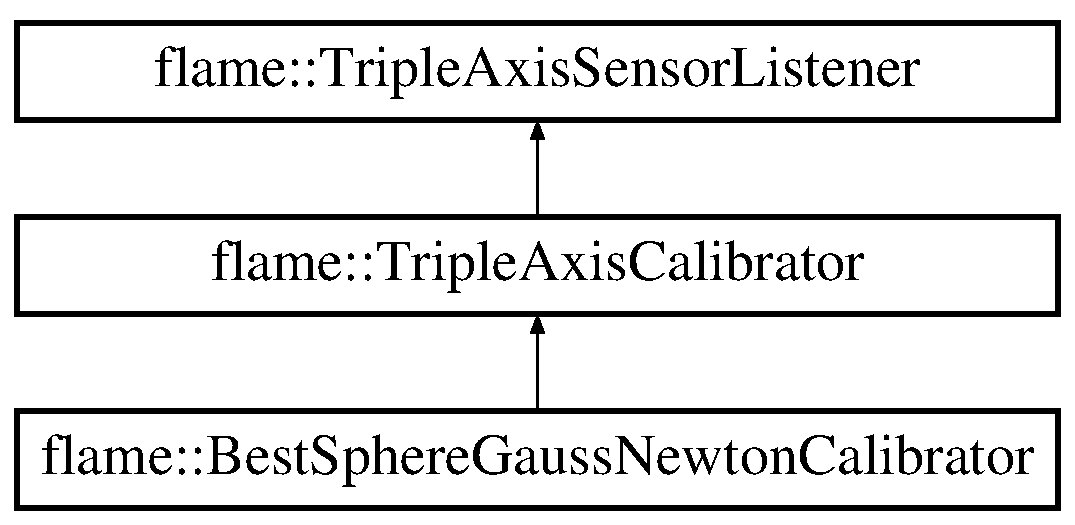
\includegraphics[height=3.000000cm]{classflame_1_1_best_sphere_gauss_newton_calibrator}
\end{center}
\end{figure}
\subsection*{Public Member Functions}
\begin{DoxyCompactItemize}
\item 
\hyperlink{classflame_1_1_best_sphere_gauss_newton_calibrator_a79df35e8eb4c6f1b88642302e46f13a6}{Best\-Sphere\-Gauss\-Newton\-Calibrator} (\hyperlink{classflame_1_1_triple_axis_sensor}{Triple\-Axis\-Sensor} \&sensor, \hyperlink{classflame_1_1_device___t_x}{Device\-\_\-\-T\-X} \&output)
\item 
void \hyperlink{classflame_1_1_best_sphere_gauss_newton_calibrator_af84f75dc992202bbd1b24624d3e22e28}{add\-Observation} (const \hyperlink{namespaceflame_ab883ad815041824ba548753dae327bc2}{T\-R\-I\-P\-L\-E\-A\-X\-I\-S\-S\-E\-N\-S\-O\-R\-\_\-\-R\-A\-W\-\_\-\-R\-E\-A\-D\-I\-N\-G} \&sample)
\item 
void \hyperlink{classflame_1_1_best_sphere_gauss_newton_calibrator_ac07439f912b1ff230dc3cc80c86c26be}{calibrate\-Sensor} (\hyperlink{classflame_1_1_triple_axis_sensor}{Triple\-Axis\-Sensor} \&sensor)
\end{DoxyCompactItemize}
\subsection*{Protected Attributes}
\begin{DoxyCompactItemize}
\item 
float \hyperlink{classflame_1_1_best_sphere_gauss_newton_calibrator_a1d98dcbd113f8e911fca9c2d11bbc3cf}{\-\_\-beta} \mbox{[}6\mbox{]}
\item 
float \hyperlink{classflame_1_1_best_sphere_gauss_newton_calibrator_aba6bfd9041955afc010372868ba0666e}{\-\_\-mu} \mbox{[}3\mbox{]}
\item 
float \hyperlink{classflame_1_1_best_sphere_gauss_newton_calibrator_a0fefa09292c75dbe4e4bd84c583abd4e}{\-\_\-mu2} \mbox{[}3\mbox{]}
\item 
float \hyperlink{classflame_1_1_best_sphere_gauss_newton_calibrator_a37f752e75712c8526e49192e1db0dc4a}{\-\_\-ip\-X\-X} \mbox{[}6\mbox{]}
\item 
float \hyperlink{classflame_1_1_best_sphere_gauss_newton_calibrator_a4fe0ab3079eba8062e36b8ecf7894632}{\-\_\-ip\-X2\-X} \mbox{[}3\mbox{]}\mbox{[}3\mbox{]}
\item 
float \hyperlink{classflame_1_1_best_sphere_gauss_newton_calibrator_a32f84ef767c6186082fff10955775e11}{\-\_\-ip\-X2\-X2} \mbox{[}6\mbox{]}
\item 
uint16\-\_\-t \hyperlink{classflame_1_1_best_sphere_gauss_newton_calibrator_ababc262e831cf26e95a5cb1558d22801}{\-\_\-observation\-Count}
\item 
int16\-\_\-t \hyperlink{classflame_1_1_best_sphere_gauss_newton_calibrator_a557a44d2712689cd6724de99644d762a}{\-\_\-obs\-Min} \mbox{[}3\mbox{]}
\item 
int16\-\_\-t \hyperlink{classflame_1_1_best_sphere_gauss_newton_calibrator_afa7171d3e79537e87887b12601c6a3f3}{\-\_\-obs\-Max} \mbox{[}3\mbox{]}
\end{DoxyCompactItemize}
\subsection*{Additional Inherited Members}


\subsection{Detailed Description}


Definition at line 54 of file Best\-Sphere\-Gauss\-Newton\-Calibrator.\-h.



\subsection{Constructor \& Destructor Documentation}
\hypertarget{classflame_1_1_best_sphere_gauss_newton_calibrator_a79df35e8eb4c6f1b88642302e46f13a6}{\index{flame\-::\-Best\-Sphere\-Gauss\-Newton\-Calibrator@{flame\-::\-Best\-Sphere\-Gauss\-Newton\-Calibrator}!Best\-Sphere\-Gauss\-Newton\-Calibrator@{Best\-Sphere\-Gauss\-Newton\-Calibrator}}
\index{Best\-Sphere\-Gauss\-Newton\-Calibrator@{Best\-Sphere\-Gauss\-Newton\-Calibrator}!flame::BestSphereGaussNewtonCalibrator@{flame\-::\-Best\-Sphere\-Gauss\-Newton\-Calibrator}}
\subsubsection[{Best\-Sphere\-Gauss\-Newton\-Calibrator}]{\setlength{\rightskip}{0pt plus 5cm}flame\-::\-Best\-Sphere\-Gauss\-Newton\-Calibrator\-::\-Best\-Sphere\-Gauss\-Newton\-Calibrator (
\begin{DoxyParamCaption}
\item[{{\bf Triple\-Axis\-Sensor} \&}]{sensor, }
\item[{{\bf Device\-\_\-\-T\-X} \&}]{output}
\end{DoxyParamCaption}
)}}\label{classflame_1_1_best_sphere_gauss_newton_calibrator_a79df35e8eb4c6f1b88642302e46f13a6}
Constructor 

Definition at line 48 of file Best\-Sphere\-Gauss\-Newton\-Calibrator.\-cpp.



\subsection{Member Function Documentation}
\hypertarget{classflame_1_1_best_sphere_gauss_newton_calibrator_af84f75dc992202bbd1b24624d3e22e28}{\index{flame\-::\-Best\-Sphere\-Gauss\-Newton\-Calibrator@{flame\-::\-Best\-Sphere\-Gauss\-Newton\-Calibrator}!add\-Observation@{add\-Observation}}
\index{add\-Observation@{add\-Observation}!flame::BestSphereGaussNewtonCalibrator@{flame\-::\-Best\-Sphere\-Gauss\-Newton\-Calibrator}}
\subsubsection[{add\-Observation}]{\setlength{\rightskip}{0pt plus 5cm}void flame\-::\-Best\-Sphere\-Gauss\-Newton\-Calibrator\-::add\-Observation (
\begin{DoxyParamCaption}
\item[{const {\bf T\-R\-I\-P\-L\-E\-A\-X\-I\-S\-S\-E\-N\-S\-O\-R\-\_\-\-R\-A\-W\-\_\-\-R\-E\-A\-D\-I\-N\-G} \&}]{sample}
\end{DoxyParamCaption}
)\hspace{0.3cm}{\ttfamily [virtual]}}}\label{classflame_1_1_best_sphere_gauss_newton_calibrator_af84f75dc992202bbd1b24624d3e22e28}
Add a sample to the calibrator 
\begin{DoxyParams}{Parameters}
{\em sample} & the sample to send \\
\hline
\end{DoxyParams}


Implements \hyperlink{classflame_1_1_triple_axis_calibrator_a088b330f58f52e7d3df291cc6e8bafed}{flame\-::\-Triple\-Axis\-Calibrator}.



Definition at line 67 of file Best\-Sphere\-Gauss\-Newton\-Calibrator.\-cpp.

\hypertarget{classflame_1_1_best_sphere_gauss_newton_calibrator_ac07439f912b1ff230dc3cc80c86c26be}{\index{flame\-::\-Best\-Sphere\-Gauss\-Newton\-Calibrator@{flame\-::\-Best\-Sphere\-Gauss\-Newton\-Calibrator}!calibrate\-Sensor@{calibrate\-Sensor}}
\index{calibrate\-Sensor@{calibrate\-Sensor}!flame::BestSphereGaussNewtonCalibrator@{flame\-::\-Best\-Sphere\-Gauss\-Newton\-Calibrator}}
\subsubsection[{calibrate\-Sensor}]{\setlength{\rightskip}{0pt plus 5cm}void flame\-::\-Best\-Sphere\-Gauss\-Newton\-Calibrator\-::calibrate\-Sensor (
\begin{DoxyParamCaption}
\item[{{\bf Triple\-Axis\-Sensor} \&}]{sensor}
\end{DoxyParamCaption}
)\hspace{0.3cm}{\ttfamily [virtual]}}}\label{classflame_1_1_best_sphere_gauss_newton_calibrator_ac07439f912b1ff230dc3cc80c86c26be}
Write the offsets and scales to the sensor 
\begin{DoxyParams}{Parameters}
{\em sensor} & the sensor to write to (should be the same sensor that is pushing the sample \\
\hline
\end{DoxyParams}


Implements \hyperlink{classflame_1_1_triple_axis_calibrator_a1a22ce8da6a3e3672f59e876acd3796b}{flame\-::\-Triple\-Axis\-Calibrator}.



Definition at line 250 of file Best\-Sphere\-Gauss\-Newton\-Calibrator.\-cpp.



\subsection{Member Data Documentation}
\hypertarget{classflame_1_1_best_sphere_gauss_newton_calibrator_a1d98dcbd113f8e911fca9c2d11bbc3cf}{\index{flame\-::\-Best\-Sphere\-Gauss\-Newton\-Calibrator@{flame\-::\-Best\-Sphere\-Gauss\-Newton\-Calibrator}!\-\_\-beta@{\-\_\-beta}}
\index{\-\_\-beta@{\-\_\-beta}!flame::BestSphereGaussNewtonCalibrator@{flame\-::\-Best\-Sphere\-Gauss\-Newton\-Calibrator}}
\subsubsection[{\-\_\-beta}]{\setlength{\rightskip}{0pt plus 5cm}float flame\-::\-Best\-Sphere\-Gauss\-Newton\-Calibrator\-::\-\_\-beta\mbox{[}6\mbox{]}\hspace{0.3cm}{\ttfamily [protected]}}}\label{classflame_1_1_best_sphere_gauss_newton_calibrator_a1d98dcbd113f8e911fca9c2d11bbc3cf}


Definition at line 57 of file Best\-Sphere\-Gauss\-Newton\-Calibrator.\-h.

\hypertarget{classflame_1_1_best_sphere_gauss_newton_calibrator_a4fe0ab3079eba8062e36b8ecf7894632}{\index{flame\-::\-Best\-Sphere\-Gauss\-Newton\-Calibrator@{flame\-::\-Best\-Sphere\-Gauss\-Newton\-Calibrator}!\-\_\-ip\-X2\-X@{\-\_\-ip\-X2\-X}}
\index{\-\_\-ip\-X2\-X@{\-\_\-ip\-X2\-X}!flame::BestSphereGaussNewtonCalibrator@{flame\-::\-Best\-Sphere\-Gauss\-Newton\-Calibrator}}
\subsubsection[{\-\_\-ip\-X2\-X}]{\setlength{\rightskip}{0pt plus 5cm}float flame\-::\-Best\-Sphere\-Gauss\-Newton\-Calibrator\-::\-\_\-ip\-X2\-X\mbox{[}3\mbox{]}\mbox{[}3\mbox{]}\hspace{0.3cm}{\ttfamily [protected]}}}\label{classflame_1_1_best_sphere_gauss_newton_calibrator_a4fe0ab3079eba8062e36b8ecf7894632}


Definition at line 63 of file Best\-Sphere\-Gauss\-Newton\-Calibrator.\-h.

\hypertarget{classflame_1_1_best_sphere_gauss_newton_calibrator_a32f84ef767c6186082fff10955775e11}{\index{flame\-::\-Best\-Sphere\-Gauss\-Newton\-Calibrator@{flame\-::\-Best\-Sphere\-Gauss\-Newton\-Calibrator}!\-\_\-ip\-X2\-X2@{\-\_\-ip\-X2\-X2}}
\index{\-\_\-ip\-X2\-X2@{\-\_\-ip\-X2\-X2}!flame::BestSphereGaussNewtonCalibrator@{flame\-::\-Best\-Sphere\-Gauss\-Newton\-Calibrator}}
\subsubsection[{\-\_\-ip\-X2\-X2}]{\setlength{\rightskip}{0pt plus 5cm}float flame\-::\-Best\-Sphere\-Gauss\-Newton\-Calibrator\-::\-\_\-ip\-X2\-X2\mbox{[}6\mbox{]}\hspace{0.3cm}{\ttfamily [protected]}}}\label{classflame_1_1_best_sphere_gauss_newton_calibrator_a32f84ef767c6186082fff10955775e11}


Definition at line 64 of file Best\-Sphere\-Gauss\-Newton\-Calibrator.\-h.

\hypertarget{classflame_1_1_best_sphere_gauss_newton_calibrator_a37f752e75712c8526e49192e1db0dc4a}{\index{flame\-::\-Best\-Sphere\-Gauss\-Newton\-Calibrator@{flame\-::\-Best\-Sphere\-Gauss\-Newton\-Calibrator}!\-\_\-ip\-X\-X@{\-\_\-ip\-X\-X}}
\index{\-\_\-ip\-X\-X@{\-\_\-ip\-X\-X}!flame::BestSphereGaussNewtonCalibrator@{flame\-::\-Best\-Sphere\-Gauss\-Newton\-Calibrator}}
\subsubsection[{\-\_\-ip\-X\-X}]{\setlength{\rightskip}{0pt plus 5cm}float flame\-::\-Best\-Sphere\-Gauss\-Newton\-Calibrator\-::\-\_\-ip\-X\-X\mbox{[}6\mbox{]}\hspace{0.3cm}{\ttfamily [protected]}}}\label{classflame_1_1_best_sphere_gauss_newton_calibrator_a37f752e75712c8526e49192e1db0dc4a}


Definition at line 62 of file Best\-Sphere\-Gauss\-Newton\-Calibrator.\-h.

\hypertarget{classflame_1_1_best_sphere_gauss_newton_calibrator_aba6bfd9041955afc010372868ba0666e}{\index{flame\-::\-Best\-Sphere\-Gauss\-Newton\-Calibrator@{flame\-::\-Best\-Sphere\-Gauss\-Newton\-Calibrator}!\-\_\-mu@{\-\_\-mu}}
\index{\-\_\-mu@{\-\_\-mu}!flame::BestSphereGaussNewtonCalibrator@{flame\-::\-Best\-Sphere\-Gauss\-Newton\-Calibrator}}
\subsubsection[{\-\_\-mu}]{\setlength{\rightskip}{0pt plus 5cm}float flame\-::\-Best\-Sphere\-Gauss\-Newton\-Calibrator\-::\-\_\-mu\mbox{[}3\mbox{]}\hspace{0.3cm}{\ttfamily [protected]}}}\label{classflame_1_1_best_sphere_gauss_newton_calibrator_aba6bfd9041955afc010372868ba0666e}


Definition at line 60 of file Best\-Sphere\-Gauss\-Newton\-Calibrator.\-h.

\hypertarget{classflame_1_1_best_sphere_gauss_newton_calibrator_a0fefa09292c75dbe4e4bd84c583abd4e}{\index{flame\-::\-Best\-Sphere\-Gauss\-Newton\-Calibrator@{flame\-::\-Best\-Sphere\-Gauss\-Newton\-Calibrator}!\-\_\-mu2@{\-\_\-mu2}}
\index{\-\_\-mu2@{\-\_\-mu2}!flame::BestSphereGaussNewtonCalibrator@{flame\-::\-Best\-Sphere\-Gauss\-Newton\-Calibrator}}
\subsubsection[{\-\_\-mu2}]{\setlength{\rightskip}{0pt plus 5cm}float flame\-::\-Best\-Sphere\-Gauss\-Newton\-Calibrator\-::\-\_\-mu2\mbox{[}3\mbox{]}\hspace{0.3cm}{\ttfamily [protected]}}}\label{classflame_1_1_best_sphere_gauss_newton_calibrator_a0fefa09292c75dbe4e4bd84c583abd4e}


Definition at line 61 of file Best\-Sphere\-Gauss\-Newton\-Calibrator.\-h.

\hypertarget{classflame_1_1_best_sphere_gauss_newton_calibrator_ababc262e831cf26e95a5cb1558d22801}{\index{flame\-::\-Best\-Sphere\-Gauss\-Newton\-Calibrator@{flame\-::\-Best\-Sphere\-Gauss\-Newton\-Calibrator}!\-\_\-observation\-Count@{\-\_\-observation\-Count}}
\index{\-\_\-observation\-Count@{\-\_\-observation\-Count}!flame::BestSphereGaussNewtonCalibrator@{flame\-::\-Best\-Sphere\-Gauss\-Newton\-Calibrator}}
\subsubsection[{\-\_\-observation\-Count}]{\setlength{\rightskip}{0pt plus 5cm}uint16\-\_\-t flame\-::\-Best\-Sphere\-Gauss\-Newton\-Calibrator\-::\-\_\-observation\-Count\hspace{0.3cm}{\ttfamily [protected]}}}\label{classflame_1_1_best_sphere_gauss_newton_calibrator_ababc262e831cf26e95a5cb1558d22801}


Definition at line 65 of file Best\-Sphere\-Gauss\-Newton\-Calibrator.\-h.

\hypertarget{classflame_1_1_best_sphere_gauss_newton_calibrator_afa7171d3e79537e87887b12601c6a3f3}{\index{flame\-::\-Best\-Sphere\-Gauss\-Newton\-Calibrator@{flame\-::\-Best\-Sphere\-Gauss\-Newton\-Calibrator}!\-\_\-obs\-Max@{\-\_\-obs\-Max}}
\index{\-\_\-obs\-Max@{\-\_\-obs\-Max}!flame::BestSphereGaussNewtonCalibrator@{flame\-::\-Best\-Sphere\-Gauss\-Newton\-Calibrator}}
\subsubsection[{\-\_\-obs\-Max}]{\setlength{\rightskip}{0pt plus 5cm}int16\-\_\-t flame\-::\-Best\-Sphere\-Gauss\-Newton\-Calibrator\-::\-\_\-obs\-Max\mbox{[}3\mbox{]}\hspace{0.3cm}{\ttfamily [protected]}}}\label{classflame_1_1_best_sphere_gauss_newton_calibrator_afa7171d3e79537e87887b12601c6a3f3}


Definition at line 68 of file Best\-Sphere\-Gauss\-Newton\-Calibrator.\-h.

\hypertarget{classflame_1_1_best_sphere_gauss_newton_calibrator_a557a44d2712689cd6724de99644d762a}{\index{flame\-::\-Best\-Sphere\-Gauss\-Newton\-Calibrator@{flame\-::\-Best\-Sphere\-Gauss\-Newton\-Calibrator}!\-\_\-obs\-Min@{\-\_\-obs\-Min}}
\index{\-\_\-obs\-Min@{\-\_\-obs\-Min}!flame::BestSphereGaussNewtonCalibrator@{flame\-::\-Best\-Sphere\-Gauss\-Newton\-Calibrator}}
\subsubsection[{\-\_\-obs\-Min}]{\setlength{\rightskip}{0pt plus 5cm}int16\-\_\-t flame\-::\-Best\-Sphere\-Gauss\-Newton\-Calibrator\-::\-\_\-obs\-Min\mbox{[}3\mbox{]}\hspace{0.3cm}{\ttfamily [protected]}}}\label{classflame_1_1_best_sphere_gauss_newton_calibrator_a557a44d2712689cd6724de99644d762a}


Definition at line 67 of file Best\-Sphere\-Gauss\-Newton\-Calibrator.\-h.



The documentation for this class was generated from the following files\-:\begin{DoxyCompactItemize}
\item 
flame/3\-Axis\-Calibration/\hyperlink{_best_sphere_gauss_newton_calibrator_8h}{Best\-Sphere\-Gauss\-Newton\-Calibrator.\-h}\item 
\hyperlink{_best_sphere_gauss_newton_calibrator_8cpp}{Best\-Sphere\-Gauss\-Newton\-Calibrator.\-cpp}\end{DoxyCompactItemize}

\hypertarget{classflame_1_1_d_a_c_listener}{\section{flame\-:\-:D\-A\-C\-Listener Class Reference}
\label{classflame_1_1_d_a_c_listener}\index{flame\-::\-D\-A\-C\-Listener@{flame\-::\-D\-A\-C\-Listener}}
}


{\ttfamily \#include $<$D\-A\-C.\-h$>$}

Inheritance diagram for flame\-:\-:D\-A\-C\-Listener\-:\begin{figure}[H]
\begin{center}
\leavevmode
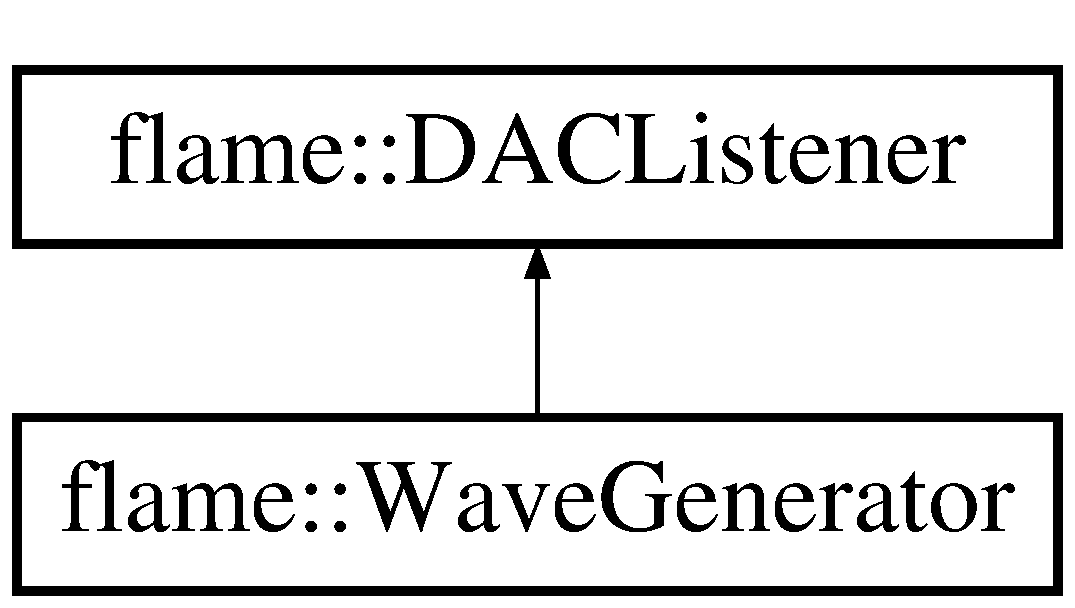
\includegraphics[height=2.000000cm]{classflame_1_1_d_a_c_listener}
\end{center}
\end{figure}
\subsection*{Public Member Functions}
\begin{DoxyCompactItemize}
\item 
virtual void \hyperlink{classflame_1_1_d_a_c_listener_a00ede324c36c05647dc31b770e4e1443}{more\-Samples} (\hyperlink{classflame_1_1_d_a_converter}{D\-A\-Converter} $\ast$dac, \hyperlink{_d_a_c_8h_a5a6d1dc37ffa32957a63868cd1da39b3}{S\-A\-M\-P\-L\-E} $\ast$old\-Samples, uint8\-\_\-t sample\-Length)
\end{DoxyCompactItemize}


\subsection{Detailed Description}
A listener which will be notified when the D\-A\-C needs more samples 

Definition at line 41 of file D\-A\-C.\-h.



\subsection{Member Function Documentation}
\hypertarget{classflame_1_1_d_a_c_listener_a00ede324c36c05647dc31b770e4e1443}{\index{flame\-::\-D\-A\-C\-Listener@{flame\-::\-D\-A\-C\-Listener}!more\-Samples@{more\-Samples}}
\index{more\-Samples@{more\-Samples}!flame::DACListener@{flame\-::\-D\-A\-C\-Listener}}
\subsubsection[{more\-Samples}]{\setlength{\rightskip}{0pt plus 5cm}virtual void flame\-::\-D\-A\-C\-Listener\-::more\-Samples (
\begin{DoxyParamCaption}
\item[{{\bf D\-A\-Converter} $\ast$}]{dac, }
\item[{{\bf S\-A\-M\-P\-L\-E} $\ast$}]{old\-Samples, }
\item[{uint8\-\_\-t}]{sample\-Length}
\end{DoxyParamCaption}
)\hspace{0.3cm}{\ttfamily [virtual]}}}\label{classflame_1_1_d_a_c_listener_a00ede324c36c05647dc31b770e4e1443}
Called when the D\-A\-C needs more samples 
\begin{DoxyParams}{Parameters}
{\em dac} & the D\-A\-C that needs more samples \\
\hline
{\em old\-Samples} & a pointer the the old samples (so it can be reused/freed) \\
\hline
{\em sample\-Length} & the number of old samples \\
\hline
\end{DoxyParams}


Reimplemented in \hyperlink{classflame_1_1_wave_generator_ac94e2fa02447ef96aba48b88181eddeb}{flame\-::\-Wave\-Generator}.



The documentation for this class was generated from the following file\-:\begin{DoxyCompactItemize}
\item 
flame/\hyperlink{_d_a_c_8h}{D\-A\-C.\-h}\end{DoxyCompactItemize}

\hypertarget{classflame_1_1_d_a_converter}{\section{flame\-:\-:D\-A\-Converter Class Reference}
\label{classflame_1_1_d_a_converter}\index{flame\-::\-D\-A\-Converter@{flame\-::\-D\-A\-Converter}}
}


{\ttfamily \#include $<$D\-A\-C.\-h$>$}

Inheritance diagram for flame\-:\-:D\-A\-Converter\-:\begin{figure}[H]
\begin{center}
\leavevmode
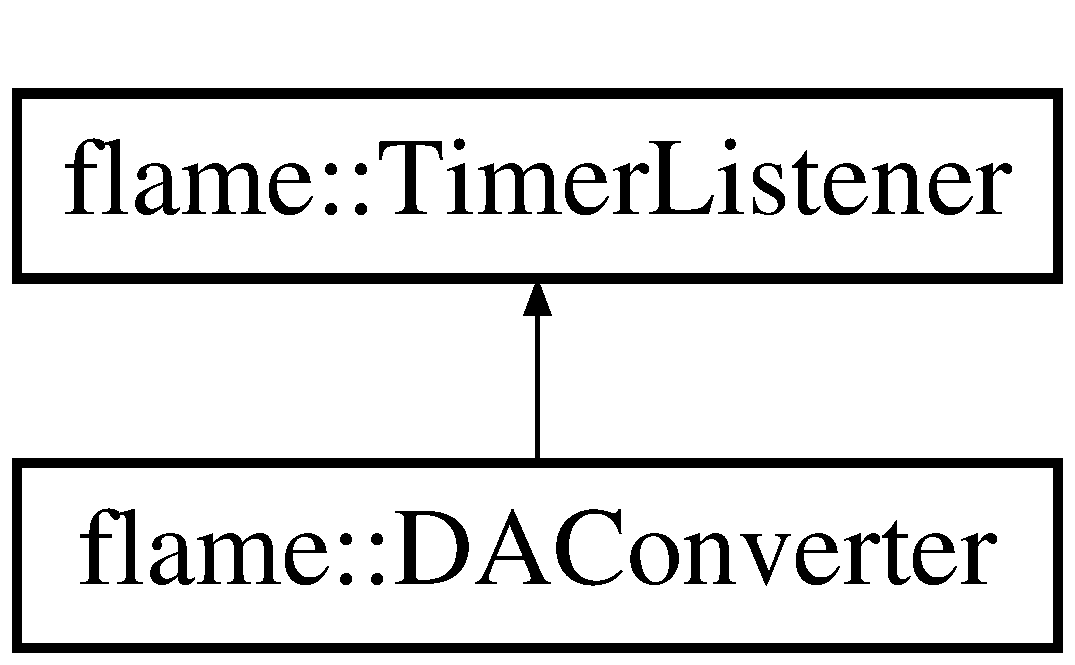
\includegraphics[height=2.000000cm]{classflame_1_1_d_a_converter}
\end{center}
\end{figure}
\subsection*{Public Member Functions}
\begin{DoxyCompactItemize}
\item 
\hyperlink{classflame_1_1_d_a_converter_afe3e4f8e96154d3a9c117c0658309caf}{D\-A\-Converter} (\hyperlink{classflame_1_1_timer}{Timer} \&timer, \hyperlink{classflame_1_1_d_a_c_listener}{D\-A\-C\-Listener} \&listener)
\item 
void \hyperlink{classflame_1_1_d_a_converter_a35dba185dfbd8483069c7a3ee9c19e5c}{alarm} (\hyperlink{namespaceflame_a6d176ba245556716fd3e32006bb7cfe5}{Alarm\-Source} source)
\item 
void \hyperlink{classflame_1_1_d_a_converter_a6a1864d308d9e9cbf52ec5f8e6149be1}{play\-Samples} (\hyperlink{_d_a_c_8h_a5a6d1dc37ffa32957a63868cd1da39b3}{S\-A\-M\-P\-L\-E} $\ast$samples, uint8\-\_\-t sample\-Length)
\item 
void \hyperlink{classflame_1_1_d_a_converter_a3e91956332022f13cc6688217c4010ab}{handle\-Events} ()
\end{DoxyCompactItemize}
\subsection*{Protected Attributes}
\begin{DoxyCompactItemize}
\item 
\hyperlink{_d_a_c_8h_a5a6d1dc37ffa32957a63868cd1da39b3}{S\-A\-M\-P\-L\-E} $\ast$ \hyperlink{classflame_1_1_d_a_converter_a26a86c298bf06bfc532f1b7cdaad6a75}{\-\_\-samples}
\item 
uint8\-\_\-t \hyperlink{classflame_1_1_d_a_converter_a97893edc430924497ee399b9223e4061}{\-\_\-sample\-Length}
\item 
uint8\-\_\-t \hyperlink{classflame_1_1_d_a_converter_a7d6c6df7f4e84c768dd92250f959078e}{\-\_\-current\-Sample}
\item 
\hyperlink{classflame_1_1_timer}{Timer} \& \hyperlink{classflame_1_1_d_a_converter_a70829abb271ec51a212d558c9087d8c5}{\-\_\-timer}
\item 
\hyperlink{classflame_1_1_d_a_c_listener}{D\-A\-C\-Listener} \& \hyperlink{classflame_1_1_d_a_converter_a5ef3241975593e467838c730857772f4}{\-\_\-listener}
\end{DoxyCompactItemize}


\subsection{Detailed Description}


Definition at line 52 of file D\-A\-C.\-h.



\subsection{Constructor \& Destructor Documentation}
\hypertarget{classflame_1_1_d_a_converter_afe3e4f8e96154d3a9c117c0658309caf}{\index{flame\-::\-D\-A\-Converter@{flame\-::\-D\-A\-Converter}!D\-A\-Converter@{D\-A\-Converter}}
\index{D\-A\-Converter@{D\-A\-Converter}!flame::DAConverter@{flame\-::\-D\-A\-Converter}}
\subsubsection[{D\-A\-Converter}]{\setlength{\rightskip}{0pt plus 5cm}flame\-::\-D\-A\-Converter\-::\-D\-A\-Converter (
\begin{DoxyParamCaption}
\item[{{\bf Timer} \&}]{timer, }
\item[{{\bf D\-A\-C\-Listener} \&}]{listener}
\end{DoxyParamCaption}
)}}\label{classflame_1_1_d_a_converter_afe3e4f8e96154d3a9c117c0658309caf}
Create a new D\-A\-C to play samples by P\-W\-Ming a timer 
\begin{DoxyParams}{Parameters}
{\em timer} & the timer to P\-W\-M -\/ we will be calling set\-Output2 on this to adjust the output \\
\hline
{\em listener} & a listener we will notify when we need more samples to play \\
\hline
\end{DoxyParams}


Definition at line 36 of file D\-A\-C.\-cpp.



\subsection{Member Function Documentation}
\hypertarget{classflame_1_1_d_a_converter_a35dba185dfbd8483069c7a3ee9c19e5c}{\index{flame\-::\-D\-A\-Converter@{flame\-::\-D\-A\-Converter}!alarm@{alarm}}
\index{alarm@{alarm}!flame::DAConverter@{flame\-::\-D\-A\-Converter}}
\subsubsection[{alarm}]{\setlength{\rightskip}{0pt plus 5cm}void flame\-::\-D\-A\-Converter\-::alarm (
\begin{DoxyParamCaption}
\item[{{\bf Alarm\-Source}}]{source}
\end{DoxyParamCaption}
)\hspace{0.3cm}{\ttfamily [virtual]}}}\label{classflame_1_1_d_a_converter_a35dba185dfbd8483069c7a3ee9c19e5c}
Play the next sample if available 

Implements \hyperlink{classflame_1_1_timer_listener_ad97504b72a25b1fba354803338177335}{flame\-::\-Timer\-Listener}.



Definition at line 43 of file D\-A\-C.\-cpp.

\hypertarget{classflame_1_1_d_a_converter_a3e91956332022f13cc6688217c4010ab}{\index{flame\-::\-D\-A\-Converter@{flame\-::\-D\-A\-Converter}!handle\-Events@{handle\-Events}}
\index{handle\-Events@{handle\-Events}!flame::DAConverter@{flame\-::\-D\-A\-Converter}}
\subsubsection[{handle\-Events}]{\setlength{\rightskip}{0pt plus 5cm}void flame\-::\-D\-A\-Converter\-::handle\-Events (
\begin{DoxyParamCaption}
{}
\end{DoxyParamCaption}
)}}\label{classflame_1_1_d_a_converter_a3e91956332022f13cc6688217c4010ab}
Handle any non-\/interrupt context events for the D\-A\-C 

Definition at line 69 of file D\-A\-C.\-cpp.

\hypertarget{classflame_1_1_d_a_converter_a6a1864d308d9e9cbf52ec5f8e6149be1}{\index{flame\-::\-D\-A\-Converter@{flame\-::\-D\-A\-Converter}!play\-Samples@{play\-Samples}}
\index{play\-Samples@{play\-Samples}!flame::DAConverter@{flame\-::\-D\-A\-Converter}}
\subsubsection[{play\-Samples}]{\setlength{\rightskip}{0pt plus 5cm}void flame\-::\-D\-A\-Converter\-::play\-Samples (
\begin{DoxyParamCaption}
\item[{{\bf S\-A\-M\-P\-L\-E} $\ast$}]{samples, }
\item[{uint8\-\_\-t}]{sample\-Length}
\end{DoxyParamCaption}
)}}\label{classflame_1_1_d_a_converter_a6a1864d308d9e9cbf52ec5f8e6149be1}
Play a set of samples (up to 255) \hyperlink{structflame_1_1_note}{Note} that this will clobber the current sample set if there is one, and the listener will not be called on it!


\begin{DoxyParams}{Parameters}
{\em samples} & the samples to play \\
\hline
{\em sample\-Length} & the number of samples to play \\
\hline
\end{DoxyParams}


Definition at line 58 of file D\-A\-C.\-cpp.



\subsection{Member Data Documentation}
\hypertarget{classflame_1_1_d_a_converter_a7d6c6df7f4e84c768dd92250f959078e}{\index{flame\-::\-D\-A\-Converter@{flame\-::\-D\-A\-Converter}!\-\_\-current\-Sample@{\-\_\-current\-Sample}}
\index{\-\_\-current\-Sample@{\-\_\-current\-Sample}!flame::DAConverter@{flame\-::\-D\-A\-Converter}}
\subsubsection[{\-\_\-current\-Sample}]{\setlength{\rightskip}{0pt plus 5cm}uint8\-\_\-t flame\-::\-D\-A\-Converter\-::\-\_\-current\-Sample\hspace{0.3cm}{\ttfamily [protected]}}}\label{classflame_1_1_d_a_converter_a7d6c6df7f4e84c768dd92250f959078e}


Definition at line 56 of file D\-A\-C.\-h.

\hypertarget{classflame_1_1_d_a_converter_a5ef3241975593e467838c730857772f4}{\index{flame\-::\-D\-A\-Converter@{flame\-::\-D\-A\-Converter}!\-\_\-listener@{\-\_\-listener}}
\index{\-\_\-listener@{\-\_\-listener}!flame::DAConverter@{flame\-::\-D\-A\-Converter}}
\subsubsection[{\-\_\-listener}]{\setlength{\rightskip}{0pt plus 5cm}{\bf D\-A\-C\-Listener}\& flame\-::\-D\-A\-Converter\-::\-\_\-listener\hspace{0.3cm}{\ttfamily [protected]}}}\label{classflame_1_1_d_a_converter_a5ef3241975593e467838c730857772f4}


Definition at line 58 of file D\-A\-C.\-h.

\hypertarget{classflame_1_1_d_a_converter_a97893edc430924497ee399b9223e4061}{\index{flame\-::\-D\-A\-Converter@{flame\-::\-D\-A\-Converter}!\-\_\-sample\-Length@{\-\_\-sample\-Length}}
\index{\-\_\-sample\-Length@{\-\_\-sample\-Length}!flame::DAConverter@{flame\-::\-D\-A\-Converter}}
\subsubsection[{\-\_\-sample\-Length}]{\setlength{\rightskip}{0pt plus 5cm}uint8\-\_\-t flame\-::\-D\-A\-Converter\-::\-\_\-sample\-Length\hspace{0.3cm}{\ttfamily [protected]}}}\label{classflame_1_1_d_a_converter_a97893edc430924497ee399b9223e4061}


Definition at line 55 of file D\-A\-C.\-h.

\hypertarget{classflame_1_1_d_a_converter_a26a86c298bf06bfc532f1b7cdaad6a75}{\index{flame\-::\-D\-A\-Converter@{flame\-::\-D\-A\-Converter}!\-\_\-samples@{\-\_\-samples}}
\index{\-\_\-samples@{\-\_\-samples}!flame::DAConverter@{flame\-::\-D\-A\-Converter}}
\subsubsection[{\-\_\-samples}]{\setlength{\rightskip}{0pt plus 5cm}{\bf S\-A\-M\-P\-L\-E}$\ast$ flame\-::\-D\-A\-Converter\-::\-\_\-samples\hspace{0.3cm}{\ttfamily [protected]}}}\label{classflame_1_1_d_a_converter_a26a86c298bf06bfc532f1b7cdaad6a75}


Definition at line 54 of file D\-A\-C.\-h.

\hypertarget{classflame_1_1_d_a_converter_a70829abb271ec51a212d558c9087d8c5}{\index{flame\-::\-D\-A\-Converter@{flame\-::\-D\-A\-Converter}!\-\_\-timer@{\-\_\-timer}}
\index{\-\_\-timer@{\-\_\-timer}!flame::DAConverter@{flame\-::\-D\-A\-Converter}}
\subsubsection[{\-\_\-timer}]{\setlength{\rightskip}{0pt plus 5cm}{\bf Timer}\& flame\-::\-D\-A\-Converter\-::\-\_\-timer\hspace{0.3cm}{\ttfamily [protected]}}}\label{classflame_1_1_d_a_converter_a70829abb271ec51a212d558c9087d8c5}


Definition at line 57 of file D\-A\-C.\-h.



The documentation for this class was generated from the following files\-:\begin{DoxyCompactItemize}
\item 
flame/\hyperlink{_d_a_c_8h}{D\-A\-C.\-h}\item 
\hyperlink{_d_a_c_8cpp}{D\-A\-C.\-cpp}\end{DoxyCompactItemize}

\hypertarget{classflame_1_1_debounce}{\section{flame\-:\-:Debounce$<$ debounce\-Time, held\-Time, repeat\-Time $>$ Class Template Reference}
\label{classflame_1_1_debounce}\index{flame\-::\-Debounce$<$ debounce\-Time, held\-Time, repeat\-Time $>$@{flame\-::\-Debounce$<$ debounce\-Time, held\-Time, repeat\-Time $>$}}
}


{\ttfamily \#include $<$Debounce.\-h$>$}

Inheritance diagram for flame\-:\-:Debounce$<$ debounce\-Time, held\-Time, repeat\-Time $>$\-:\begin{figure}[H]
\begin{center}
\leavevmode
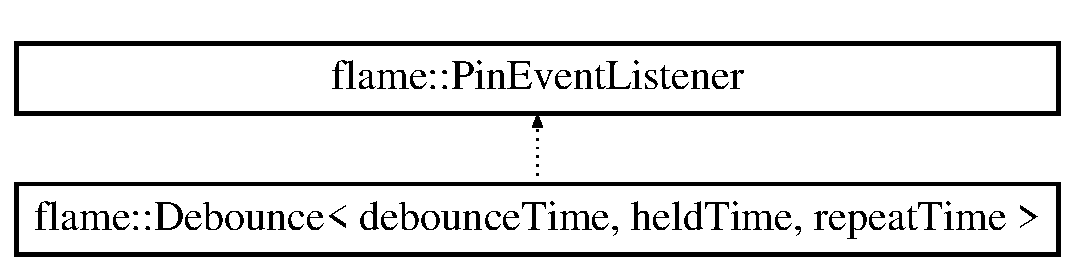
\includegraphics[height=2.000000cm]{classflame_1_1_debounce}
\end{center}
\end{figure}
\subsection*{Public Member Functions}
\begin{DoxyCompactItemize}
\item 
\hyperlink{classflame_1_1_debounce_a4df4da4a7b49deac584e1bc2b011bad7}{Debounce} (\hyperlink{classflame_1_1_pin_change_manager}{Pin\-Change\-Manager} \&pin\-Change\-Manager, \hyperlink{classflame_1_1_r_t_c}{R\-T\-C} \&rtc)
\item 
void \hyperlink{classflame_1_1_debounce_abfdb85e459052118a72879698af85d87}{assign\-Key} (\hyperlink{io_8h_ab54f3ca5cc36256b922289e8e92316a3}{F\-L\-A\-M\-E\-\_\-\-D\-E\-C\-L\-A\-R\-E\-\_\-\-P\-I\-N}(pin), \hyperlink{classflame_1_1_debounce_listener}{Debounce\-Listener} \&listener)
\item 
void \hyperlink{classflame_1_1_debounce_a63bad9d7e92a998325c9fb942775aae4}{assign\-Key} (\hyperlink{classflame_1_1_pin}{Pin} \&pin, \hyperlink{classflame_1_1_debounce_listener}{Debounce\-Listener} \&listener)
\item 
void \hyperlink{classflame_1_1_debounce_a56cb69574f06584007723ecefbd3073c}{deassign\-Key} (int8\-\_\-t pin\-Pinchange\-Interrupt)
\item 
void \hyperlink{classflame_1_1_debounce_a3ae08a19b2f300ea31f2f6da9b292380}{deassign\-Key} (\hyperlink{io_8h_ab54f3ca5cc36256b922289e8e92316a3}{F\-L\-A\-M\-E\-\_\-\-D\-E\-C\-L\-A\-R\-E\-\_\-\-P\-I\-N}(pin))
\item 
void \hyperlink{classflame_1_1_debounce_aabe8d69b5a537c39adda9ea88c129249}{check\-Held} ()
\end{DoxyCompactItemize}
\subsection*{Protected Member Functions}
\begin{DoxyCompactItemize}
\item 
void \hyperlink{classflame_1_1_debounce_ae91dc73a4becacf5f13456d1ca3b6185}{pin\-Changed} (uint8\-\_\-t pc\-Int, bool new\-State)
\item 
void \hyperlink{classflame_1_1_debounce_a659d50217bff015bc109223737899a45}{init\-Pin} (uint8\-\_\-t pinchange\-Interrupt)
\end{DoxyCompactItemize}
\subsection*{Protected Attributes}
\begin{DoxyCompactItemize}
\item 
\hyperlink{classflame_1_1_r_t_c}{R\-T\-C} \& \hyperlink{classflame_1_1_debounce_abaed54518db29d8653452f167c6b6653}{\-\_\-rtc}
\item 
\hyperlink{namespaceflame_a1909d0b4150ee5ef201afa40b431b811}{D\-E\-B\-O\-U\-N\-C\-E\-\_\-\-P\-I\-N} \hyperlink{classflame_1_1_debounce_a8f167eb7572e66526be7824b79d334c3}{\-\_\-pins} \mbox{[}\hyperlink{attiny85_8h_ab39f7ddad6e692db1c00115db776636f}{F\-L\-A\-M\-E\-\_\-\-P\-C\-\_\-\-I\-N\-T\-\_\-\-C\-O\-U\-N\-T}\mbox{]}
\item 
\hyperlink{classflame_1_1_pin_change_manager}{Pin\-Change\-Manager} \& \hyperlink{classflame_1_1_debounce_a40985315ee31ef4d28c16ebc32cc3af9}{\-\_\-pin\-Change\-Manager}
\end{DoxyCompactItemize}


\subsection{Detailed Description}
\subsubsection*{template$<$uint16\-\_\-t debounce\-Time, uint16\-\_\-t held\-Time, uint16\-\_\-t repeat\-Time$>$class flame\-::\-Debounce$<$ debounce\-Time, held\-Time, repeat\-Time $>$}

A debouncing class triggered by pin changes 
\begin{DoxyTemplParams}{Template Parameters}
{\em debounce\-Time} & the minimum amount of time to count as a button press (in milliseconds) \\
\hline
{\em held\-Time} & the minimum amount of time to consider a button held down \\
\hline
{\em repeat\-Time} & the time after which the held call repeats \\
\hline
\end{DoxyTemplParams}


Definition at line 79 of file Debounce.\-h.



\subsection{Constructor \& Destructor Documentation}
\hypertarget{classflame_1_1_debounce_a4df4da4a7b49deac584e1bc2b011bad7}{\index{flame\-::\-Debounce@{flame\-::\-Debounce}!Debounce@{Debounce}}
\index{Debounce@{Debounce}!flame::Debounce@{flame\-::\-Debounce}}
\subsubsection[{Debounce}]{\setlength{\rightskip}{0pt plus 5cm}template$<$uint16\-\_\-t debounce\-Time, uint16\-\_\-t held\-Time, uint16\-\_\-t repeat\-Time$>$ {\bf flame\-::\-Debounce}$<$ debounce\-Time, held\-Time, repeat\-Time $>$\-::{\bf Debounce} (
\begin{DoxyParamCaption}
\item[{{\bf Pin\-Change\-Manager} \&}]{pin\-Change\-Manager, }
\item[{{\bf R\-T\-C} \&}]{rtc}
\end{DoxyParamCaption}
)\hspace{0.3cm}{\ttfamily [inline]}}}\label{classflame_1_1_debounce_a4df4da4a7b49deac584e1bc2b011bad7}
Debouncing helper for buttons connected directly to P\-C\-I\-N\-T capable pins The user must pull the pin up, either externally (and initing the pin by calling F\-L\-A\-M\-E\-\_\-set\-Input), or internally by calling F\-L\-A\-M\-E\-\_\-set\-Input\-Pullup


\begin{DoxyParams}{Parameters}
{\em pin\-Change\-Manager} & the pin change manager \\
\hline
{\em rtc} & the realtime clock we will use for timing \\
\hline
\end{DoxyParams}


Definition at line 125 of file Debounce.\-h.



\subsection{Member Function Documentation}
\hypertarget{classflame_1_1_debounce_abfdb85e459052118a72879698af85d87}{\index{flame\-::\-Debounce@{flame\-::\-Debounce}!assign\-Key@{assign\-Key}}
\index{assign\-Key@{assign\-Key}!flame::Debounce@{flame\-::\-Debounce}}
\subsubsection[{assign\-Key}]{\setlength{\rightskip}{0pt plus 5cm}template$<$uint16\-\_\-t debounce\-Time, uint16\-\_\-t held\-Time, uint16\-\_\-t repeat\-Time$>$ void {\bf flame\-::\-Debounce}$<$ debounce\-Time, held\-Time, repeat\-Time $>$\-::assign\-Key (
\begin{DoxyParamCaption}
\item[{{\bf F\-L\-A\-M\-E\-\_\-\-D\-E\-C\-L\-A\-R\-E\-\_\-\-P\-I\-N}(pin)}]{, }
\item[{{\bf Debounce\-Listener} \&}]{listener}
\end{DoxyParamCaption}
)\hspace{0.3cm}{\ttfamily [inline]}}}\label{classflame_1_1_debounce_abfdb85e459052118a72879698af85d87}
Assign a pin to debounce 
\begin{DoxyParams}{Parameters}
{\em pin} & An F\-L\-A\-M\-E\-\_\-\-P\-I\-N\-\_\-$\ast$ macro \\
\hline
{\em listener} & a class to call when the button is pressed or held down \\
\hline
\end{DoxyParams}


Definition at line 139 of file Debounce.\-h.

\hypertarget{classflame_1_1_debounce_a63bad9d7e92a998325c9fb942775aae4}{\index{flame\-::\-Debounce@{flame\-::\-Debounce}!assign\-Key@{assign\-Key}}
\index{assign\-Key@{assign\-Key}!flame::Debounce@{flame\-::\-Debounce}}
\subsubsection[{assign\-Key}]{\setlength{\rightskip}{0pt plus 5cm}template$<$uint16\-\_\-t debounce\-Time, uint16\-\_\-t held\-Time, uint16\-\_\-t repeat\-Time$>$ void {\bf flame\-::\-Debounce}$<$ debounce\-Time, held\-Time, repeat\-Time $>$\-::assign\-Key (
\begin{DoxyParamCaption}
\item[{{\bf Pin} \&}]{pin, }
\item[{{\bf Debounce\-Listener} \&}]{listener}
\end{DoxyParamCaption}
)\hspace{0.3cm}{\ttfamily [inline]}}}\label{classflame_1_1_debounce_a63bad9d7e92a998325c9fb942775aae4}
Assign a pin to debounce 
\begin{DoxyParams}{Parameters}
{\em pin} & An F\-L\-A\-M\-E\-\_\-\-P\-I\-N\-\_\-$\ast$ macro \\
\hline
{\em listener} & a class to call when the button is pressed or held down \\
\hline
\end{DoxyParams}


Definition at line 159 of file Debounce.\-h.

\hypertarget{classflame_1_1_debounce_aabe8d69b5a537c39adda9ea88c129249}{\index{flame\-::\-Debounce@{flame\-::\-Debounce}!check\-Held@{check\-Held}}
\index{check\-Held@{check\-Held}!flame::Debounce@{flame\-::\-Debounce}}
\subsubsection[{check\-Held}]{\setlength{\rightskip}{0pt plus 5cm}template$<$uint16\-\_\-t debounce\-Time, uint16\-\_\-t held\-Time, uint16\-\_\-t repeat\-Time$>$ void {\bf flame\-::\-Debounce}$<$ debounce\-Time, held\-Time, repeat\-Time $>$\-::check\-Held (
\begin{DoxyParamCaption}
{}
\end{DoxyParamCaption}
)\hspace{0.3cm}{\ttfamily [inline]}}}\label{classflame_1_1_debounce_aabe8d69b5a537c39adda9ea88c129249}
Called periodically to check if pins have been held Ideally, this should be called from the main loop, rather than the interrupt context 

Definition at line 199 of file Debounce.\-h.

\hypertarget{classflame_1_1_debounce_a56cb69574f06584007723ecefbd3073c}{\index{flame\-::\-Debounce@{flame\-::\-Debounce}!deassign\-Key@{deassign\-Key}}
\index{deassign\-Key@{deassign\-Key}!flame::Debounce@{flame\-::\-Debounce}}
\subsubsection[{deassign\-Key}]{\setlength{\rightskip}{0pt plus 5cm}template$<$uint16\-\_\-t debounce\-Time, uint16\-\_\-t held\-Time, uint16\-\_\-t repeat\-Time$>$ void {\bf flame\-::\-Debounce}$<$ debounce\-Time, held\-Time, repeat\-Time $>$\-::deassign\-Key (
\begin{DoxyParamCaption}
\item[{int8\-\_\-t}]{pin\-Pinchange\-Interrupt}
\end{DoxyParamCaption}
)\hspace{0.3cm}{\ttfamily [inline]}}}\label{classflame_1_1_debounce_a56cb69574f06584007723ecefbd3073c}
Deassign a pin 
\begin{DoxyParams}{Parameters}
{\em pin\-Pinchange\-Interrupt} & the pin change interrupt to deregister \\
\hline
\end{DoxyParams}


Definition at line 178 of file Debounce.\-h.

\hypertarget{classflame_1_1_debounce_a3ae08a19b2f300ea31f2f6da9b292380}{\index{flame\-::\-Debounce@{flame\-::\-Debounce}!deassign\-Key@{deassign\-Key}}
\index{deassign\-Key@{deassign\-Key}!flame::Debounce@{flame\-::\-Debounce}}
\subsubsection[{deassign\-Key}]{\setlength{\rightskip}{0pt plus 5cm}template$<$uint16\-\_\-t debounce\-Time, uint16\-\_\-t held\-Time, uint16\-\_\-t repeat\-Time$>$ void {\bf flame\-::\-Debounce}$<$ debounce\-Time, held\-Time, repeat\-Time $>$\-::deassign\-Key (
\begin{DoxyParamCaption}
\item[{{\bf F\-L\-A\-M\-E\-\_\-\-D\-E\-C\-L\-A\-R\-E\-\_\-\-P\-I\-N}(pin)}]{}
\end{DoxyParamCaption}
)\hspace{0.3cm}{\ttfamily [inline]}}}\label{classflame_1_1_debounce_a3ae08a19b2f300ea31f2f6da9b292380}
Deassign a pin 
\begin{DoxyParams}{Parameters}
{\em pin\-Pinchange\-Interrupt} & the pin change interrupt to deregister \\
\hline
\end{DoxyParams}


Definition at line 188 of file Debounce.\-h.

\hypertarget{classflame_1_1_debounce_a659d50217bff015bc109223737899a45}{\index{flame\-::\-Debounce@{flame\-::\-Debounce}!init\-Pin@{init\-Pin}}
\index{init\-Pin@{init\-Pin}!flame::Debounce@{flame\-::\-Debounce}}
\subsubsection[{init\-Pin}]{\setlength{\rightskip}{0pt plus 5cm}template$<$uint16\-\_\-t debounce\-Time, uint16\-\_\-t held\-Time, uint16\-\_\-t repeat\-Time$>$ void {\bf flame\-::\-Debounce}$<$ debounce\-Time, held\-Time, repeat\-Time $>$\-::init\-Pin (
\begin{DoxyParamCaption}
\item[{uint8\-\_\-t}]{pinchange\-Interrupt}
\end{DoxyParamCaption}
)\hspace{0.3cm}{\ttfamily [inline]}, {\ttfamily [protected]}}}\label{classflame_1_1_debounce_a659d50217bff015bc109223737899a45}


Definition at line 112 of file Debounce.\-h.

\hypertarget{classflame_1_1_debounce_ae91dc73a4becacf5f13456d1ca3b6185}{\index{flame\-::\-Debounce@{flame\-::\-Debounce}!pin\-Changed@{pin\-Changed}}
\index{pin\-Changed@{pin\-Changed}!flame::Debounce@{flame\-::\-Debounce}}
\subsubsection[{pin\-Changed}]{\setlength{\rightskip}{0pt plus 5cm}template$<$uint16\-\_\-t debounce\-Time, uint16\-\_\-t held\-Time, uint16\-\_\-t repeat\-Time$>$ void {\bf flame\-::\-Debounce}$<$ debounce\-Time, held\-Time, repeat\-Time $>$\-::pin\-Changed (
\begin{DoxyParamCaption}
\item[{uint8\-\_\-t}]{pc\-Int, }
\item[{bool}]{new\-State}
\end{DoxyParamCaption}
)\hspace{0.3cm}{\ttfamily [inline]}, {\ttfamily [protected]}, {\ttfamily [virtual]}}}\label{classflame_1_1_debounce_ae91dc73a4becacf5f13456d1ca3b6185}
Trigger for pin change interrupts -\/ scans through 8 pins starting at the offset 
\begin{DoxyParams}{Parameters}
{\em pc\-Int} & the pin change interrupt that was triggered \\
\hline
{\em new\-State} & the new state of the pin \\
\hline
\end{DoxyParams}


Implements \hyperlink{classflame_1_1_pin_event_listener_af1b45ab9819298e7f5786a6e617450cc}{flame\-::\-Pin\-Event\-Listener}.



Definition at line 90 of file Debounce.\-h.



\subsection{Member Data Documentation}
\hypertarget{classflame_1_1_debounce_a40985315ee31ef4d28c16ebc32cc3af9}{\index{flame\-::\-Debounce@{flame\-::\-Debounce}!\-\_\-pin\-Change\-Manager@{\-\_\-pin\-Change\-Manager}}
\index{\-\_\-pin\-Change\-Manager@{\-\_\-pin\-Change\-Manager}!flame::Debounce@{flame\-::\-Debounce}}
\subsubsection[{\-\_\-pin\-Change\-Manager}]{\setlength{\rightskip}{0pt plus 5cm}template$<$uint16\-\_\-t debounce\-Time, uint16\-\_\-t held\-Time, uint16\-\_\-t repeat\-Time$>$ {\bf Pin\-Change\-Manager}\& {\bf flame\-::\-Debounce}$<$ debounce\-Time, held\-Time, repeat\-Time $>$\-::\-\_\-pin\-Change\-Manager\hspace{0.3cm}{\ttfamily [protected]}}}\label{classflame_1_1_debounce_a40985315ee31ef4d28c16ebc32cc3af9}


Definition at line 83 of file Debounce.\-h.

\hypertarget{classflame_1_1_debounce_a8f167eb7572e66526be7824b79d334c3}{\index{flame\-::\-Debounce@{flame\-::\-Debounce}!\-\_\-pins@{\-\_\-pins}}
\index{\-\_\-pins@{\-\_\-pins}!flame::Debounce@{flame\-::\-Debounce}}
\subsubsection[{\-\_\-pins}]{\setlength{\rightskip}{0pt plus 5cm}template$<$uint16\-\_\-t debounce\-Time, uint16\-\_\-t held\-Time, uint16\-\_\-t repeat\-Time$>$ {\bf D\-E\-B\-O\-U\-N\-C\-E\-\_\-\-P\-I\-N} {\bf flame\-::\-Debounce}$<$ debounce\-Time, held\-Time, repeat\-Time $>$\-::\-\_\-pins\mbox{[}{\bf F\-L\-A\-M\-E\-\_\-\-P\-C\-\_\-\-I\-N\-T\-\_\-\-C\-O\-U\-N\-T}\mbox{]}\hspace{0.3cm}{\ttfamily [protected]}}}\label{classflame_1_1_debounce_a8f167eb7572e66526be7824b79d334c3}


Definition at line 82 of file Debounce.\-h.

\hypertarget{classflame_1_1_debounce_abaed54518db29d8653452f167c6b6653}{\index{flame\-::\-Debounce@{flame\-::\-Debounce}!\-\_\-rtc@{\-\_\-rtc}}
\index{\-\_\-rtc@{\-\_\-rtc}!flame::Debounce@{flame\-::\-Debounce}}
\subsubsection[{\-\_\-rtc}]{\setlength{\rightskip}{0pt plus 5cm}template$<$uint16\-\_\-t debounce\-Time, uint16\-\_\-t held\-Time, uint16\-\_\-t repeat\-Time$>$ {\bf R\-T\-C}\& {\bf flame\-::\-Debounce}$<$ debounce\-Time, held\-Time, repeat\-Time $>$\-::\-\_\-rtc\hspace{0.3cm}{\ttfamily [protected]}}}\label{classflame_1_1_debounce_abaed54518db29d8653452f167c6b6653}


Definition at line 81 of file Debounce.\-h.



The documentation for this class was generated from the following file\-:\begin{DoxyCompactItemize}
\item 
flame/\hyperlink{_debounce_8h}{Debounce.\-h}\end{DoxyCompactItemize}

\hypertarget{classflame_1_1_debounce_listener}{\section{flame\-:\-:Debounce\-Listener Class Reference}
\label{classflame_1_1_debounce_listener}\index{flame\-::\-Debounce\-Listener@{flame\-::\-Debounce\-Listener}}
}


{\ttfamily \#include $<$Debounce.\-h$>$}

\subsection*{Public Member Functions}
\begin{DoxyCompactItemize}
\item 
virtual void \hyperlink{classflame_1_1_debounce_listener_afc43aff931408936c92c7d0b9fed139c}{single\-Press} (uint8\-\_\-t pc\-Int, \hyperlink{namespaceflame_ad90347e9ea7e54907966260ec5c7d22f}{T\-I\-M\-E\-S\-T\-A\-M\-P} $\ast$held\-For)=0
\item 
virtual void \hyperlink{classflame_1_1_debounce_listener_af08b1a813aa91016f375a7c8410f95ad}{held\-Down} (uint8\-\_\-t pc\-Int, \hyperlink{namespaceflame_ad90347e9ea7e54907966260ec5c7d22f}{T\-I\-M\-E\-S\-T\-A\-M\-P} $\ast$held\-For)=0
\end{DoxyCompactItemize}


\subsection{Detailed Description}


Definition at line 58 of file Debounce.\-h.



\subsection{Member Function Documentation}
\hypertarget{classflame_1_1_debounce_listener_af08b1a813aa91016f375a7c8410f95ad}{\index{flame\-::\-Debounce\-Listener@{flame\-::\-Debounce\-Listener}!held\-Down@{held\-Down}}
\index{held\-Down@{held\-Down}!flame::DebounceListener@{flame\-::\-Debounce\-Listener}}
\subsubsection[{held\-Down}]{\setlength{\rightskip}{0pt plus 5cm}virtual void flame\-::\-Debounce\-Listener\-::held\-Down (
\begin{DoxyParamCaption}
\item[{uint8\-\_\-t}]{pc\-Int, }
\item[{{\bf T\-I\-M\-E\-S\-T\-A\-M\-P} $\ast$}]{held\-For}
\end{DoxyParamCaption}
)\hspace{0.3cm}{\ttfamily [pure virtual]}}}\label{classflame_1_1_debounce_listener_af08b1a813aa91016f375a7c8410f95ad}
\hypertarget{classflame_1_1_debounce_listener_afc43aff931408936c92c7d0b9fed139c}{\index{flame\-::\-Debounce\-Listener@{flame\-::\-Debounce\-Listener}!single\-Press@{single\-Press}}
\index{single\-Press@{single\-Press}!flame::DebounceListener@{flame\-::\-Debounce\-Listener}}
\subsubsection[{single\-Press}]{\setlength{\rightskip}{0pt plus 5cm}virtual void flame\-::\-Debounce\-Listener\-::single\-Press (
\begin{DoxyParamCaption}
\item[{uint8\-\_\-t}]{pc\-Int, }
\item[{{\bf T\-I\-M\-E\-S\-T\-A\-M\-P} $\ast$}]{held\-For}
\end{DoxyParamCaption}
)\hspace{0.3cm}{\ttfamily [pure virtual]}}}\label{classflame_1_1_debounce_listener_afc43aff931408936c92c7d0b9fed139c}


The documentation for this class was generated from the following file\-:\begin{DoxyCompactItemize}
\item 
flame/\hyperlink{_debounce_8h}{Debounce.\-h}\end{DoxyCompactItemize}

\hypertarget{structflame_1_1debounce_pin}{\section{flame\-:\-:debounce\-Pin Struct Reference}
\label{structflame_1_1debounce_pin}\index{flame\-::debounce\-Pin@{flame\-::debounce\-Pin}}
}


{\ttfamily \#include $<$Debounce.\-h$>$}

\subsection*{Public Attributes}
\begin{DoxyCompactItemize}
\item 
uint8\-\_\-t \hyperlink{structflame_1_1debounce_pin_af3f18f9d280894adfcf12294b296c108}{previous}
\item 
\hyperlink{namespaceflame_ad90347e9ea7e54907966260ec5c7d22f}{T\-I\-M\-E\-S\-T\-A\-M\-P} \hyperlink{structflame_1_1debounce_pin_ad10be4149c4882c6e767ad3460b6a5c9}{timestamp}
\item 
\hyperlink{classflame_1_1_debounce_listener}{Debounce\-Listener} $\ast$ \hyperlink{structflame_1_1debounce_pin_a9af0c2b0919f7876d1c1826aca106bc6}{listener}
\item 
bool \hyperlink{structflame_1_1debounce_pin_a2c160c5a6d6902bada1dc1a9a0591e5c}{held}
\end{DoxyCompactItemize}


\subsection{Detailed Description}


Definition at line 64 of file Debounce.\-h.



\subsection{Member Data Documentation}
\hypertarget{structflame_1_1debounce_pin_a2c160c5a6d6902bada1dc1a9a0591e5c}{\index{flame\-::debounce\-Pin@{flame\-::debounce\-Pin}!held@{held}}
\index{held@{held}!flame::debouncePin@{flame\-::debounce\-Pin}}
\subsubsection[{held}]{\setlength{\rightskip}{0pt plus 5cm}bool flame\-::debounce\-Pin\-::held}}\label{structflame_1_1debounce_pin_a2c160c5a6d6902bada1dc1a9a0591e5c}


Definition at line 68 of file Debounce.\-h.

\hypertarget{structflame_1_1debounce_pin_a9af0c2b0919f7876d1c1826aca106bc6}{\index{flame\-::debounce\-Pin@{flame\-::debounce\-Pin}!listener@{listener}}
\index{listener@{listener}!flame::debouncePin@{flame\-::debounce\-Pin}}
\subsubsection[{listener}]{\setlength{\rightskip}{0pt plus 5cm}{\bf Debounce\-Listener}$\ast$ flame\-::debounce\-Pin\-::listener}}\label{structflame_1_1debounce_pin_a9af0c2b0919f7876d1c1826aca106bc6}


Definition at line 67 of file Debounce.\-h.

\hypertarget{structflame_1_1debounce_pin_af3f18f9d280894adfcf12294b296c108}{\index{flame\-::debounce\-Pin@{flame\-::debounce\-Pin}!previous@{previous}}
\index{previous@{previous}!flame::debouncePin@{flame\-::debounce\-Pin}}
\subsubsection[{previous}]{\setlength{\rightskip}{0pt plus 5cm}uint8\-\_\-t flame\-::debounce\-Pin\-::previous}}\label{structflame_1_1debounce_pin_af3f18f9d280894adfcf12294b296c108}


Definition at line 65 of file Debounce.\-h.

\hypertarget{structflame_1_1debounce_pin_ad10be4149c4882c6e767ad3460b6a5c9}{\index{flame\-::debounce\-Pin@{flame\-::debounce\-Pin}!timestamp@{timestamp}}
\index{timestamp@{timestamp}!flame::debouncePin@{flame\-::debounce\-Pin}}
\subsubsection[{timestamp}]{\setlength{\rightskip}{0pt plus 5cm}{\bf T\-I\-M\-E\-S\-T\-A\-M\-P} flame\-::debounce\-Pin\-::timestamp}}\label{structflame_1_1debounce_pin_ad10be4149c4882c6e767ad3460b6a5c9}


Definition at line 66 of file Debounce.\-h.



The documentation for this struct was generated from the following file\-:\begin{DoxyCompactItemize}
\item 
flame/\hyperlink{_debounce_8h}{Debounce.\-h}\end{DoxyCompactItemize}

\hypertarget{classflame_1_1_device___r_x}{\section{flame\-:\-:Device\-\_\-\-R\-X Class Reference}
\label{classflame_1_1_device___r_x}\index{flame\-::\-Device\-\_\-\-R\-X@{flame\-::\-Device\-\_\-\-R\-X}}
}


{\ttfamily \#include $<$Device\-\_\-\-R\-X.\-h$>$}

Inheritance diagram for flame\-:\-:Device\-\_\-\-R\-X\-:\begin{figure}[H]
\begin{center}
\leavevmode
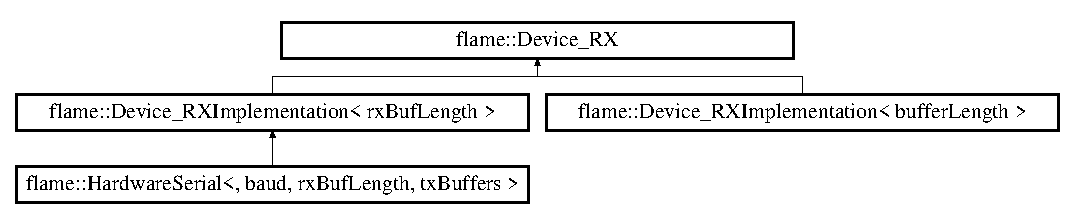
\includegraphics[height=2.492581cm]{classflame_1_1_device___r_x}
\end{center}
\end{figure}
\subsection*{Public Member Functions}
\begin{DoxyCompactItemize}
\item 
int \hyperlink{classflame_1_1_device___r_x_acde7b96e30210372ae171af28d86d610}{async\-Read\-Line} (char $\ast$buffer, uint8\-\_\-t buffer\-Length)
\item 
int \hyperlink{classflame_1_1_device___r_x_af0f6917beebe6609114a1738977c4be9}{busy\-Read\-Line} (char $\ast$buffer, uint8\-\_\-t buffer\-Length)
\item 
int \hyperlink{classflame_1_1_device___r_x_af3a4cdfdec25abf4a38262564b011111}{read} (void)
\item 
void \hyperlink{classflame_1_1_device___r_x_ae5d5e88a35c324c30adeff81a269b98f}{flush} ()
\item 
bool \hyperlink{classflame_1_1_device___r_x_ae435bb6015855ee87002c81e38fbb0bb}{ready} ()
\item 
void \hyperlink{classflame_1_1_device___r_x_ae14fc8bc11a268c60141a16b25736937}{register\-Listener} (\hyperlink{classflame_1_1_r_x_listener}{R\-X\-Listener} \&listener)
\item 
void \hyperlink{classflame_1_1_device___r_x_aceb1c29df27c6ab295abba2b29cff598}{deregister\-Listener} ()
\item 
void \hyperlink{classflame_1_1_device___r_x_a9b4e70f748a227c3681bd7386e2d37c1}{handle\-Events} ()
\end{DoxyCompactItemize}
\subsection*{Protected Member Functions}
\begin{DoxyCompactItemize}
\item 
\hyperlink{classflame_1_1_device___r_x_af7bd06b3810231d9f0fb4e3a65a798ce}{Device\-\_\-\-R\-X} (\hyperlink{classflame_1_1_ring_buffer}{Ring\-Buffer} \&buffer)
\end{DoxyCompactItemize}
\subsection*{Protected Attributes}
\begin{DoxyCompactItemize}
\item 
\hyperlink{classflame_1_1_ring_buffer}{Ring\-Buffer} \& \hyperlink{classflame_1_1_device___r_x_a75c3e03bb47dd08aaa94bd490ea83909}{\-\_\-rx\-Buffer}
\item 
\hyperlink{classflame_1_1_r_x_listener}{R\-X\-Listener} $\ast$ \hyperlink{classflame_1_1_device___r_x_a854d1674cbe048e363442beac44c3f74}{\-\_\-listener}
\end{DoxyCompactItemize}


\subsection{Detailed Description}
A device that can receive data 

Definition at line 56 of file Device\-\_\-\-R\-X.\-h.



\subsection{Constructor \& Destructor Documentation}
\hypertarget{classflame_1_1_device___r_x_af7bd06b3810231d9f0fb4e3a65a798ce}{\index{flame\-::\-Device\-\_\-\-R\-X@{flame\-::\-Device\-\_\-\-R\-X}!Device\-\_\-\-R\-X@{Device\-\_\-\-R\-X}}
\index{Device\-\_\-\-R\-X@{Device\-\_\-\-R\-X}!flame::Device_RX@{flame\-::\-Device\-\_\-\-R\-X}}
\subsubsection[{Device\-\_\-\-R\-X}]{\setlength{\rightskip}{0pt plus 5cm}flame\-::\-Device\-\_\-\-R\-X\-::\-Device\-\_\-\-R\-X (
\begin{DoxyParamCaption}
\item[{{\bf Ring\-Buffer} \&}]{buffer}
\end{DoxyParamCaption}
)\hspace{0.3cm}{\ttfamily [inline]}, {\ttfamily [protected]}}}\label{classflame_1_1_device___r_x_af7bd06b3810231d9f0fb4e3a65a798ce}
Constructor 
\begin{DoxyParams}{Parameters}
{\em buffer} & A buffer to store received data \\
\hline
\end{DoxyParams}


Definition at line 65 of file Device\-\_\-\-R\-X.\-h.



\subsection{Member Function Documentation}
\hypertarget{classflame_1_1_device___r_x_acde7b96e30210372ae171af28d86d610}{\index{flame\-::\-Device\-\_\-\-R\-X@{flame\-::\-Device\-\_\-\-R\-X}!async\-Read\-Line@{async\-Read\-Line}}
\index{async\-Read\-Line@{async\-Read\-Line}!flame::Device_RX@{flame\-::\-Device\-\_\-\-R\-X}}
\subsubsection[{async\-Read\-Line}]{\setlength{\rightskip}{0pt plus 5cm}int flame\-::\-Device\-\_\-\-R\-X\-::async\-Read\-Line (
\begin{DoxyParamCaption}
\item[{char $\ast$}]{buffer, }
\item[{uint8\-\_\-t}]{buffer\-Length}
\end{DoxyParamCaption}
)\hspace{0.3cm}{\ttfamily [inline]}}}\label{classflame_1_1_device___r_x_acde7b96e30210372ae171af28d86d610}
If we have a line, copy it into a buffer \& null terminate, stripping C\-R/\-L\-F returns 0 if we have successfully copied a line returns -\/1 if there was no line available returns -\/2 if the buffer was too small returns -\/3 if we have reached the end of the ringbuffer with no line terminator 

Definition at line 77 of file Device\-\_\-\-R\-X.\-h.

\hypertarget{classflame_1_1_device___r_x_af0f6917beebe6609114a1738977c4be9}{\index{flame\-::\-Device\-\_\-\-R\-X@{flame\-::\-Device\-\_\-\-R\-X}!busy\-Read\-Line@{busy\-Read\-Line}}
\index{busy\-Read\-Line@{busy\-Read\-Line}!flame::Device_RX@{flame\-::\-Device\-\_\-\-R\-X}}
\subsubsection[{busy\-Read\-Line}]{\setlength{\rightskip}{0pt plus 5cm}int flame\-::\-Device\-\_\-\-R\-X\-::busy\-Read\-Line (
\begin{DoxyParamCaption}
\item[{char $\ast$}]{buffer, }
\item[{uint8\-\_\-t}]{buffer\-Length}
\end{DoxyParamCaption}
)\hspace{0.3cm}{\ttfamily [inline]}}}\label{classflame_1_1_device___r_x_af0f6917beebe6609114a1738977c4be9}
If we have a line, copy it into a buffer \& null terminate, stripping C\-R/\-L\-F Blocks until a line is available \begin{DoxyReturn}{Returns}
0 if we have successfully copied a line 

-\/2 if the buffer was too small 

-\/3 if we have reached the end of the ringbuffer with no line terminator 
\end{DoxyReturn}


Definition at line 115 of file Device\-\_\-\-R\-X.\-h.

\hypertarget{classflame_1_1_device___r_x_aceb1c29df27c6ab295abba2b29cff598}{\index{flame\-::\-Device\-\_\-\-R\-X@{flame\-::\-Device\-\_\-\-R\-X}!deregister\-Listener@{deregister\-Listener}}
\index{deregister\-Listener@{deregister\-Listener}!flame::Device_RX@{flame\-::\-Device\-\_\-\-R\-X}}
\subsubsection[{deregister\-Listener}]{\setlength{\rightskip}{0pt plus 5cm}void flame\-::\-Device\-\_\-\-R\-X\-::deregister\-Listener (
\begin{DoxyParamCaption}
{}
\end{DoxyParamCaption}
)\hspace{0.3cm}{\ttfamily [inline]}}}\label{classflame_1_1_device___r_x_aceb1c29df27c6ab295abba2b29cff598}
Deregister interest for lines/overflows from an R\-X device 

Definition at line 165 of file Device\-\_\-\-R\-X.\-h.

\hypertarget{classflame_1_1_device___r_x_ae5d5e88a35c324c30adeff81a269b98f}{\index{flame\-::\-Device\-\_\-\-R\-X@{flame\-::\-Device\-\_\-\-R\-X}!flush@{flush}}
\index{flush@{flush}!flame::Device_RX@{flame\-::\-Device\-\_\-\-R\-X}}
\subsubsection[{flush}]{\setlength{\rightskip}{0pt plus 5cm}void flame\-::\-Device\-\_\-\-R\-X\-::flush (
\begin{DoxyParamCaption}
{}
\end{DoxyParamCaption}
)\hspace{0.3cm}{\ttfamily [inline]}}}\label{classflame_1_1_device___r_x_ae5d5e88a35c324c30adeff81a269b98f}
Discard remaining data in the receive buffer 

Definition at line 132 of file Device\-\_\-\-R\-X.\-h.

\hypertarget{classflame_1_1_device___r_x_a9b4e70f748a227c3681bd7386e2d37c1}{\index{flame\-::\-Device\-\_\-\-R\-X@{flame\-::\-Device\-\_\-\-R\-X}!handle\-Events@{handle\-Events}}
\index{handle\-Events@{handle\-Events}!flame::Device_RX@{flame\-::\-Device\-\_\-\-R\-X}}
\subsubsection[{handle\-Events}]{\setlength{\rightskip}{0pt plus 5cm}void flame\-::\-Device\-\_\-\-R\-X\-::handle\-Events (
\begin{DoxyParamCaption}
{}
\end{DoxyParamCaption}
)\hspace{0.3cm}{\ttfamily [inline]}}}\label{classflame_1_1_device___r_x_a9b4e70f748a227c3681bd7386e2d37c1}
Call from the main loop to handle any events 

Definition at line 172 of file Device\-\_\-\-R\-X.\-h.

\hypertarget{classflame_1_1_device___r_x_af3a4cdfdec25abf4a38262564b011111}{\index{flame\-::\-Device\-\_\-\-R\-X@{flame\-::\-Device\-\_\-\-R\-X}!read@{read}}
\index{read@{read}!flame::Device_RX@{flame\-::\-Device\-\_\-\-R\-X}}
\subsubsection[{read}]{\setlength{\rightskip}{0pt plus 5cm}int flame\-::\-Device\-\_\-\-R\-X\-::read (
\begin{DoxyParamCaption}
\item[{void}]{}
\end{DoxyParamCaption}
)\hspace{0.3cm}{\ttfamily [inline]}}}\label{classflame_1_1_device___r_x_af3a4cdfdec25abf4a38262564b011111}
Read a byte from the receive buffer \begin{DoxyReturn}{Returns}
the byte, or -\/1 if there is nothing to read 
\end{DoxyReturn}


Definition at line 125 of file Device\-\_\-\-R\-X.\-h.

\hypertarget{classflame_1_1_device___r_x_ae435bb6015855ee87002c81e38fbb0bb}{\index{flame\-::\-Device\-\_\-\-R\-X@{flame\-::\-Device\-\_\-\-R\-X}!ready@{ready}}
\index{ready@{ready}!flame::Device_RX@{flame\-::\-Device\-\_\-\-R\-X}}
\subsubsection[{ready}]{\setlength{\rightskip}{0pt plus 5cm}bool flame\-::\-Device\-\_\-\-R\-X\-::ready (
\begin{DoxyParamCaption}
{}
\end{DoxyParamCaption}
)\hspace{0.3cm}{\ttfamily [inline]}}}\label{classflame_1_1_device___r_x_ae435bb6015855ee87002c81e38fbb0bb}
Check if a line is ready, or the ringbuffer is full \begin{DoxyReturn}{Returns}
true if either of the situations occurs 
\end{DoxyReturn}


Definition at line 140 of file Device\-\_\-\-R\-X.\-h.

\hypertarget{classflame_1_1_device___r_x_ae14fc8bc11a268c60141a16b25736937}{\index{flame\-::\-Device\-\_\-\-R\-X@{flame\-::\-Device\-\_\-\-R\-X}!register\-Listener@{register\-Listener}}
\index{register\-Listener@{register\-Listener}!flame::Device_RX@{flame\-::\-Device\-\_\-\-R\-X}}
\subsubsection[{register\-Listener}]{\setlength{\rightskip}{0pt plus 5cm}void flame\-::\-Device\-\_\-\-R\-X\-::register\-Listener (
\begin{DoxyParamCaption}
\item[{{\bf R\-X\-Listener} \&}]{listener}
\end{DoxyParamCaption}
)\hspace{0.3cm}{\ttfamily [inline]}}}\label{classflame_1_1_device___r_x_ae14fc8bc11a268c60141a16b25736937}
Register interest for lines/overflows from an R\-X device 
\begin{DoxyParams}{Parameters}
{\em listener} & an F\-L\-A\-M\-E\-\_\-\-R\-X\-Listener to notify that the device is ready \\
\hline
\end{DoxyParams}


Definition at line 158 of file Device\-\_\-\-R\-X.\-h.



\subsection{Member Data Documentation}
\hypertarget{classflame_1_1_device___r_x_a854d1674cbe048e363442beac44c3f74}{\index{flame\-::\-Device\-\_\-\-R\-X@{flame\-::\-Device\-\_\-\-R\-X}!\-\_\-listener@{\-\_\-listener}}
\index{\-\_\-listener@{\-\_\-listener}!flame::Device_RX@{flame\-::\-Device\-\_\-\-R\-X}}
\subsubsection[{\-\_\-listener}]{\setlength{\rightskip}{0pt plus 5cm}{\bf R\-X\-Listener}$\ast$ flame\-::\-Device\-\_\-\-R\-X\-::\-\_\-listener\hspace{0.3cm}{\ttfamily [protected]}}}\label{classflame_1_1_device___r_x_a854d1674cbe048e363442beac44c3f74}


Definition at line 59 of file Device\-\_\-\-R\-X.\-h.

\hypertarget{classflame_1_1_device___r_x_a75c3e03bb47dd08aaa94bd490ea83909}{\index{flame\-::\-Device\-\_\-\-R\-X@{flame\-::\-Device\-\_\-\-R\-X}!\-\_\-rx\-Buffer@{\-\_\-rx\-Buffer}}
\index{\-\_\-rx\-Buffer@{\-\_\-rx\-Buffer}!flame::Device_RX@{flame\-::\-Device\-\_\-\-R\-X}}
\subsubsection[{\-\_\-rx\-Buffer}]{\setlength{\rightskip}{0pt plus 5cm}{\bf Ring\-Buffer}\& flame\-::\-Device\-\_\-\-R\-X\-::\-\_\-rx\-Buffer\hspace{0.3cm}{\ttfamily [protected]}}}\label{classflame_1_1_device___r_x_a75c3e03bb47dd08aaa94bd490ea83909}


Definition at line 58 of file Device\-\_\-\-R\-X.\-h.



The documentation for this class was generated from the following file\-:\begin{DoxyCompactItemize}
\item 
flame/\hyperlink{_device___r_x_8h}{Device\-\_\-\-R\-X.\-h}\end{DoxyCompactItemize}

\hypertarget{classflame_1_1_device___r_x_implementation}{\section{flame\-:\-:Device\-\_\-\-R\-X\-Implementation$<$ buffer\-Length $>$ Class Template Reference}
\label{classflame_1_1_device___r_x_implementation}\index{flame\-::\-Device\-\_\-\-R\-X\-Implementation$<$ buffer\-Length $>$@{flame\-::\-Device\-\_\-\-R\-X\-Implementation$<$ buffer\-Length $>$}}
}


{\ttfamily \#include $<$Device\-\_\-\-R\-X.\-h$>$}

Inheritance diagram for flame\-:\-:Device\-\_\-\-R\-X\-Implementation$<$ buffer\-Length $>$\-:\begin{figure}[H]
\begin{center}
\leavevmode
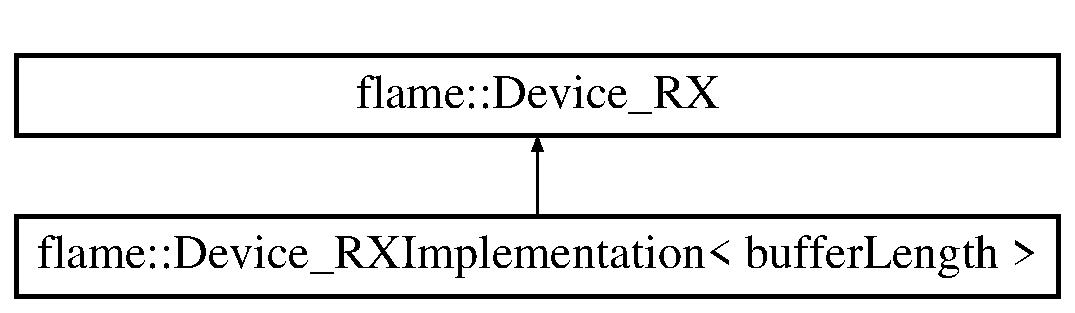
\includegraphics[height=2.000000cm]{classflame_1_1_device___r_x_implementation}
\end{center}
\end{figure}
\subsection*{Protected Member Functions}
\begin{DoxyCompactItemize}
\item 
\hyperlink{classflame_1_1_device___r_x_implementation_aa3d7f48ca73db4537ce97795cc462cb5}{Device\-\_\-\-R\-X\-Implementation} ()
\end{DoxyCompactItemize}
\subsection*{Protected Attributes}
\begin{DoxyCompactItemize}
\item 
\hyperlink{classflame_1_1_ring_buffer_implementation}{Ring\-Buffer\-Implementation}\\*
$<$ buffer\-Length $>$ \hyperlink{classflame_1_1_device___r_x_implementation_a33418a9bb5a111865955284a78e38cac}{\-\_\-my\-Buffer}
\end{DoxyCompactItemize}
\subsection*{Additional Inherited Members}


\subsection{Detailed Description}
\subsubsection*{template$<$uint8\-\_\-t buffer\-Length$>$class flame\-::\-Device\-\_\-\-R\-X\-Implementation$<$ buffer\-Length $>$}



Definition at line 180 of file Device\-\_\-\-R\-X.\-h.



\subsection{Constructor \& Destructor Documentation}
\hypertarget{classflame_1_1_device___r_x_implementation_aa3d7f48ca73db4537ce97795cc462cb5}{\index{flame\-::\-Device\-\_\-\-R\-X\-Implementation@{flame\-::\-Device\-\_\-\-R\-X\-Implementation}!Device\-\_\-\-R\-X\-Implementation@{Device\-\_\-\-R\-X\-Implementation}}
\index{Device\-\_\-\-R\-X\-Implementation@{Device\-\_\-\-R\-X\-Implementation}!flame::Device_RXImplementation@{flame\-::\-Device\-\_\-\-R\-X\-Implementation}}
\subsubsection[{Device\-\_\-\-R\-X\-Implementation}]{\setlength{\rightskip}{0pt plus 5cm}template$<$uint8\-\_\-t buffer\-Length$>$ {\bf flame\-::\-Device\-\_\-\-R\-X\-Implementation}$<$ buffer\-Length $>$\-::{\bf Device\-\_\-\-R\-X\-Implementation} (
\begin{DoxyParamCaption}
{}
\end{DoxyParamCaption}
)\hspace{0.3cm}{\ttfamily [inline]}, {\ttfamily [protected]}}}\label{classflame_1_1_device___r_x_implementation_aa3d7f48ca73db4537ce97795cc462cb5}
Constructor 

Definition at line 188 of file Device\-\_\-\-R\-X.\-h.



\subsection{Member Data Documentation}
\hypertarget{classflame_1_1_device___r_x_implementation_a33418a9bb5a111865955284a78e38cac}{\index{flame\-::\-Device\-\_\-\-R\-X\-Implementation@{flame\-::\-Device\-\_\-\-R\-X\-Implementation}!\-\_\-my\-Buffer@{\-\_\-my\-Buffer}}
\index{\-\_\-my\-Buffer@{\-\_\-my\-Buffer}!flame::Device_RXImplementation@{flame\-::\-Device\-\_\-\-R\-X\-Implementation}}
\subsubsection[{\-\_\-my\-Buffer}]{\setlength{\rightskip}{0pt plus 5cm}template$<$uint8\-\_\-t buffer\-Length$>$ {\bf Ring\-Buffer\-Implementation}$<$buffer\-Length$>$ {\bf flame\-::\-Device\-\_\-\-R\-X\-Implementation}$<$ buffer\-Length $>$\-::\-\_\-my\-Buffer\hspace{0.3cm}{\ttfamily [protected]}}}\label{classflame_1_1_device___r_x_implementation_a33418a9bb5a111865955284a78e38cac}


Definition at line 183 of file Device\-\_\-\-R\-X.\-h.



The documentation for this class was generated from the following file\-:\begin{DoxyCompactItemize}
\item 
flame/\hyperlink{_device___r_x_8h}{Device\-\_\-\-R\-X.\-h}\end{DoxyCompactItemize}

\hypertarget{classflame_1_1_device___t_x}{\section{flame\-:\-:Device\-\_\-\-T\-X Class Reference}
\label{classflame_1_1_device___t_x}\index{flame\-::\-Device\-\_\-\-T\-X@{flame\-::\-Device\-\_\-\-T\-X}}
}


{\ttfamily \#include $<$Device\-\_\-\-T\-X.\-h$>$}

Inheritance diagram for flame\-:\-:Device\-\_\-\-T\-X\-:\begin{figure}[H]
\begin{center}
\leavevmode
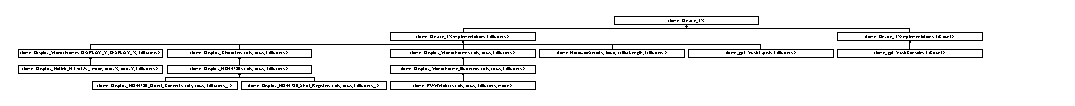
\includegraphics[height=0.975610cm]{classflame_1_1_device___t_x}
\end{center}
\end{figure}
\subsection*{Public Member Functions}
\begin{DoxyCompactItemize}
\item 
bool \hyperlink{classflame_1_1_device___t_x_ad9d1d66fe9a4538032e914896f553745}{can\-Write} ()
\item 
bool \hyperlink{classflame_1_1_device___t_x_a1c87e31a7d6b65d7665ff7f266e358df}{write\-\_\-\-P} (P\-G\-M\-\_\-\-P string)
\item 
bool \hyperlink{classflame_1_1_device___t_x_a1dabeeb28eee75aa8d27fa3860244d74}{write} (const char $\ast$string)
\item 
bool \hyperlink{classflame_1_1_device___t_x_a813ba499f49c82722318fa3f8cda2d30}{write} (const char $\ast$string, void($\ast$complete\-Function)(const char $\ast$))
\item 
bool \hyperlink{classflame_1_1_device___t_x_af65ef0e0855089804b34f26a958fdde3}{write\-\_\-\-P} (P\-G\-M\-\_\-\-P buffer, uint16\-\_\-t length)
\item 
bool \hyperlink{classflame_1_1_device___t_x_a42f7f7b191dafbdfeefc03a3d246df1c}{write} (const char $\ast$buffer, uint16\-\_\-t length)
\item 
bool \hyperlink{classflame_1_1_device___t_x_a893f6301eb001fe2bc21e3194ca82c02}{write} (const char $\ast$buffer, uint16\-\_\-t length, void($\ast$complete\-Function)(const char $\ast$))
\item 
bool \hyperlink{classflame_1_1_device___t_x_a185cec8162abc4fafba59e972f59a57e}{debug} (const char $\ast$file, int line, const char $\ast$function, P\-G\-M\-\_\-\-P format,...)
\item 
bool \hyperlink{classflame_1_1_device___t_x_ae31487b1b1e3f8c9749a2bae3f48f1bf}{printf} (P\-G\-M\-\_\-\-P format,...)
\item 
bool \hyperlink{classflame_1_1_device___t_x_a84d278c2d86fb2419338dc2a71dfcaef}{write} (uint32\-\_\-t value)
\end{DoxyCompactItemize}
\subsection*{Protected Member Functions}
\begin{DoxyCompactItemize}
\item 
\hyperlink{classflame_1_1_device___t_x_ac8cbfc24dbb82b3d0229c4f48046bed9}{Device\-\_\-\-T\-X} (\hyperlink{classflame_1_1_ring_buffer}{Ring\-Buffer} \&tx\-Pointers)
\item 
virtual void \hyperlink{classflame_1_1_device___t_x_af3cf3dc02a124e5a88841d325555ce3c}{run\-Tx\-Buffers} ()=0
\item 
bool \hyperlink{classflame_1_1_device___t_x_aa559b2481ade8d4ffb7c1a06a8c4aced}{more\-T\-X} ()
\item 
int \hyperlink{classflame_1_1_device___t_x_a238f4a5bbbc36cf2ee06f616008c537f}{next\-Character} ()
\end{DoxyCompactItemize}
\subsection*{Protected Attributes}
\begin{DoxyCompactItemize}
\item 
\hyperlink{classflame_1_1_t_x_buffer}{T\-X\-Buffer} \hyperlink{classflame_1_1_device___t_x_a8a7dfd6afba59f3144fd20f89186fd19}{\-\_\-current\-Tx}
\item 
\hyperlink{classflame_1_1_ring_buffer}{Ring\-Buffer} \& \hyperlink{classflame_1_1_device___t_x_a208fef1a96295f254b913180b5274160}{\-\_\-tx\-Pointers}
\end{DoxyCompactItemize}


\subsection{Detailed Description}
A device that can transmit data 
\begin{DoxyTemplParams}{Template Parameters}
{\em tx\-Pointers} & the number of available output buffers for non-\/blocking I/\-O \\
\hline
\end{DoxyTemplParams}


Definition at line 354 of file Device\-\_\-\-T\-X.\-h.



\subsection{Constructor \& Destructor Documentation}
\hypertarget{classflame_1_1_device___t_x_ac8cbfc24dbb82b3d0229c4f48046bed9}{\index{flame\-::\-Device\-\_\-\-T\-X@{flame\-::\-Device\-\_\-\-T\-X}!Device\-\_\-\-T\-X@{Device\-\_\-\-T\-X}}
\index{Device\-\_\-\-T\-X@{Device\-\_\-\-T\-X}!flame::Device_TX@{flame\-::\-Device\-\_\-\-T\-X}}
\subsubsection[{Device\-\_\-\-T\-X}]{\setlength{\rightskip}{0pt plus 5cm}flame\-::\-Device\-\_\-\-T\-X\-::\-Device\-\_\-\-T\-X (
\begin{DoxyParamCaption}
\item[{{\bf Ring\-Buffer} \&}]{tx\-Pointers}
\end{DoxyParamCaption}
)\hspace{0.3cm}{\ttfamily [inline]}, {\ttfamily [protected]}}}\label{classflame_1_1_device___t_x_ac8cbfc24dbb82b3d0229c4f48046bed9}
Constructor 
\begin{DoxyParams}{Parameters}
{\em tx\-Pointers} & a ringbuffer to store T\-X elements in \\
\hline
\end{DoxyParams}


Definition at line 363 of file Device\-\_\-\-T\-X.\-h.



\subsection{Member Function Documentation}
\hypertarget{classflame_1_1_device___t_x_ad9d1d66fe9a4538032e914896f553745}{\index{flame\-::\-Device\-\_\-\-T\-X@{flame\-::\-Device\-\_\-\-T\-X}!can\-Write@{can\-Write}}
\index{can\-Write@{can\-Write}!flame::Device_TX@{flame\-::\-Device\-\_\-\-T\-X}}
\subsubsection[{can\-Write}]{\setlength{\rightskip}{0pt plus 5cm}bool flame\-::\-Device\-\_\-\-T\-X\-::can\-Write (
\begin{DoxyParamCaption}
{}
\end{DoxyParamCaption}
)\hspace{0.3cm}{\ttfamily [inline]}}}\label{classflame_1_1_device___t_x_ad9d1d66fe9a4538032e914896f553745}
Can we accept another buffer? 

Definition at line 408 of file Device\-\_\-\-T\-X.\-h.

\hypertarget{classflame_1_1_device___t_x_a185cec8162abc4fafba59e972f59a57e}{\index{flame\-::\-Device\-\_\-\-T\-X@{flame\-::\-Device\-\_\-\-T\-X}!debug@{debug}}
\index{debug@{debug}!flame::Device_TX@{flame\-::\-Device\-\_\-\-T\-X}}
\subsubsection[{debug}]{\setlength{\rightskip}{0pt plus 5cm}bool flame\-::\-Device\-\_\-\-T\-X\-::debug (
\begin{DoxyParamCaption}
\item[{const char $\ast$}]{file, }
\item[{int}]{line, }
\item[{const char $\ast$}]{function, }
\item[{P\-G\-M\-\_\-\-P}]{format, }
\item[{}]{...}
\end{DoxyParamCaption}
)\hspace{0.3cm}{\ttfamily [inline]}}}\label{classflame_1_1_device___t_x_a185cec8162abc4fafba59e972f59a57e}
Print a debug message 
\begin{DoxyParams}{Parameters}
{\em file} & the filename \\
\hline
{\em line} & the line number \\
\hline
{\em function} & the function name \\
\hline
{\em format} & a printf format \\
\hline
{\em ...} & the printf parms \\
\hline
\end{DoxyParams}
\begin{DoxyReturn}{Returns}
false on success true if the message was not sent 
\end{DoxyReturn}


Definition at line 661 of file Device\-\_\-\-T\-X.\-h.

\hypertarget{classflame_1_1_device___t_x_aa559b2481ade8d4ffb7c1a06a8c4aced}{\index{flame\-::\-Device\-\_\-\-T\-X@{flame\-::\-Device\-\_\-\-T\-X}!more\-T\-X@{more\-T\-X}}
\index{more\-T\-X@{more\-T\-X}!flame::Device_TX@{flame\-::\-Device\-\_\-\-T\-X}}
\subsubsection[{more\-T\-X}]{\setlength{\rightskip}{0pt plus 5cm}bool flame\-::\-Device\-\_\-\-T\-X\-::more\-T\-X (
\begin{DoxyParamCaption}
{}
\end{DoxyParamCaption}
)\hspace{0.3cm}{\ttfamily [inline]}, {\ttfamily [protected]}}}\label{classflame_1_1_device___t_x_aa559b2481ade8d4ffb7c1a06a8c4aced}
Called when a buffer has been processed \begin{DoxyReturn}{Returns}
true if there is another buffer to process 
\end{DoxyReturn}


Definition at line 372 of file Device\-\_\-\-T\-X.\-h.

\hypertarget{classflame_1_1_device___t_x_a238f4a5bbbc36cf2ee06f616008c537f}{\index{flame\-::\-Device\-\_\-\-T\-X@{flame\-::\-Device\-\_\-\-T\-X}!next\-Character@{next\-Character}}
\index{next\-Character@{next\-Character}!flame::Device_TX@{flame\-::\-Device\-\_\-\-T\-X}}
\subsubsection[{next\-Character}]{\setlength{\rightskip}{0pt plus 5cm}int flame\-::\-Device\-\_\-\-T\-X\-::next\-Character (
\begin{DoxyParamCaption}
{}
\end{DoxyParamCaption}
)\hspace{0.3cm}{\ttfamily [inline]}, {\ttfamily [protected]}}}\label{classflame_1_1_device___t_x_a238f4a5bbbc36cf2ee06f616008c537f}
Get the next character \begin{DoxyReturn}{Returns}
the next character, or -\/1 if there is no more 
\end{DoxyReturn}


Definition at line 389 of file Device\-\_\-\-T\-X.\-h.

\hypertarget{classflame_1_1_device___t_x_ae31487b1b1e3f8c9749a2bae3f48f1bf}{\index{flame\-::\-Device\-\_\-\-T\-X@{flame\-::\-Device\-\_\-\-T\-X}!printf@{printf}}
\index{printf@{printf}!flame::Device_TX@{flame\-::\-Device\-\_\-\-T\-X}}
\subsubsection[{printf}]{\setlength{\rightskip}{0pt plus 5cm}bool flame\-::\-Device\-\_\-\-T\-X\-::printf (
\begin{DoxyParamCaption}
\item[{P\-G\-M\-\_\-\-P}]{format, }
\item[{}]{...}
\end{DoxyParamCaption}
)\hspace{0.3cm}{\ttfamily [inline]}}}\label{classflame_1_1_device___t_x_ae31487b1b1e3f8c9749a2bae3f48f1bf}
Print a message 
\begin{DoxyParams}{Parameters}
{\em format} & a printf format \\
\hline
{\em ...} & the printf parms \\
\hline
\end{DoxyParams}
\begin{DoxyReturn}{Returns}
false on success true if there is already a string being sent 
\end{DoxyReturn}


Definition at line 708 of file Device\-\_\-\-T\-X.\-h.

\hypertarget{classflame_1_1_device___t_x_af3cf3dc02a124e5a88841d325555ce3c}{\index{flame\-::\-Device\-\_\-\-T\-X@{flame\-::\-Device\-\_\-\-T\-X}!run\-Tx\-Buffers@{run\-Tx\-Buffers}}
\index{run\-Tx\-Buffers@{run\-Tx\-Buffers}!flame::Device_TX@{flame\-::\-Device\-\_\-\-T\-X}}
\subsubsection[{run\-Tx\-Buffers}]{\setlength{\rightskip}{0pt plus 5cm}virtual void flame\-::\-Device\-\_\-\-T\-X\-::run\-Tx\-Buffers (
\begin{DoxyParamCaption}
{}
\end{DoxyParamCaption}
)\hspace{0.3cm}{\ttfamily [protected]}, {\ttfamily [pure virtual]}}}\label{classflame_1_1_device___t_x_af3cf3dc02a124e5a88841d325555ce3c}


Implemented in \hyperlink{classflame_1_1_display___character_a4a3172da51cdb598217654934f9a2ae4}{flame\-::\-Display\-\_\-\-Character$<$ cols, rows, tx\-Buffers $>$}, \hyperlink{classflame_1_1_display___monochrome_a7f156eaedc986e5432c4b04968417def}{flame\-::\-Display\-\_\-\-Monochrome$<$ cols, rows, tx\-Buffers $>$}, \hyperlink{classflame_1_1_display___monochrome_a7f156eaedc986e5432c4b04968417def}{flame\-::\-Display\-\_\-\-Monochrome$<$ D\-I\-S\-P\-L\-A\-Y\-\_\-\-Y, D\-I\-S\-P\-L\-A\-Y\-\_\-\-X, tx\-Buffers $>$}, \hyperlink{classflame_1_1_hardware_serial_a2f045cdba4a0be78d876e383ff1ec6f2}{flame\-::\-Hardware\-Serial$<$, baud, rx\-Buf\-Length, tx\-Buffers $>$}, \hyperlink{classflame__gpl_1_1_vusb_console_a5deb453bdc18579c6f3c592862f71fab}{flame\-\_\-gpl\-::\-Vusb\-Console$<$ tx\-Count $>$}, and \hyperlink{classflame__gpl_1_1_vusb_typist_a725357253d37d28f66cbf2c608fefad7}{flame\-\_\-gpl\-::\-Vusb\-Typist$<$ tx\-Buffers $>$}.

\hypertarget{classflame_1_1_device___t_x_a1dabeeb28eee75aa8d27fa3860244d74}{\index{flame\-::\-Device\-\_\-\-T\-X@{flame\-::\-Device\-\_\-\-T\-X}!write@{write}}
\index{write@{write}!flame::Device_TX@{flame\-::\-Device\-\_\-\-T\-X}}
\subsubsection[{write}]{\setlength{\rightskip}{0pt plus 5cm}bool flame\-::\-Device\-\_\-\-T\-X\-::write (
\begin{DoxyParamCaption}
\item[{const char $\ast$}]{string}
\end{DoxyParamCaption}
)\hspace{0.3cm}{\ttfamily [inline]}}}\label{classflame_1_1_device___t_x_a1dabeeb28eee75aa8d27fa3860244d74}
Write a string asynchronously 
\begin{DoxyParams}{Parameters}
{\em string} & the string \\
\hline
\end{DoxyParams}
\begin{DoxyReturn}{Returns}
false on success true if there is already a string being sent 
\end{DoxyReturn}


Definition at line 490 of file Device\-\_\-\-T\-X.\-h.

\hypertarget{classflame_1_1_device___t_x_a813ba499f49c82722318fa3f8cda2d30}{\index{flame\-::\-Device\-\_\-\-T\-X@{flame\-::\-Device\-\_\-\-T\-X}!write@{write}}
\index{write@{write}!flame::Device_TX@{flame\-::\-Device\-\_\-\-T\-X}}
\subsubsection[{write}]{\setlength{\rightskip}{0pt plus 5cm}bool flame\-::\-Device\-\_\-\-T\-X\-::write (
\begin{DoxyParamCaption}
\item[{const char $\ast$}]{string, }
\item[{void($\ast$)(const char $\ast$)}]{complete\-Function}
\end{DoxyParamCaption}
)\hspace{0.3cm}{\ttfamily [inline]}}}\label{classflame_1_1_device___t_x_a813ba499f49c82722318fa3f8cda2d30}
Write a string asynchronously 
\begin{DoxyParams}{Parameters}
{\em string} & the string \\
\hline
{\em complete\-Function} & a function to call when the string has been written (the string is passed as a parameter) \\
\hline
\end{DoxyParams}
\begin{DoxyReturn}{Returns}
false on success true if there is already a string being sent 
\end{DoxyReturn}


Definition at line 513 of file Device\-\_\-\-T\-X.\-h.

\hypertarget{classflame_1_1_device___t_x_a42f7f7b191dafbdfeefc03a3d246df1c}{\index{flame\-::\-Device\-\_\-\-T\-X@{flame\-::\-Device\-\_\-\-T\-X}!write@{write}}
\index{write@{write}!flame::Device_TX@{flame\-::\-Device\-\_\-\-T\-X}}
\subsubsection[{write}]{\setlength{\rightskip}{0pt plus 5cm}bool flame\-::\-Device\-\_\-\-T\-X\-::write (
\begin{DoxyParamCaption}
\item[{const char $\ast$}]{buffer, }
\item[{uint16\-\_\-t}]{length}
\end{DoxyParamCaption}
)\hspace{0.3cm}{\ttfamily [inline]}}}\label{classflame_1_1_device___t_x_a42f7f7b191dafbdfeefc03a3d246df1c}
Write a buffer asynchronously 
\begin{DoxyParams}{Parameters}
{\em buffer} & the buffer \\
\hline
{\em length} & the length of the buffer \\
\hline
\end{DoxyParams}
\begin{DoxyReturn}{Returns}
false on success true if there is already a string being sent 
\end{DoxyReturn}


Definition at line 611 of file Device\-\_\-\-T\-X.\-h.

\hypertarget{classflame_1_1_device___t_x_a893f6301eb001fe2bc21e3194ca82c02}{\index{flame\-::\-Device\-\_\-\-T\-X@{flame\-::\-Device\-\_\-\-T\-X}!write@{write}}
\index{write@{write}!flame::Device_TX@{flame\-::\-Device\-\_\-\-T\-X}}
\subsubsection[{write}]{\setlength{\rightskip}{0pt plus 5cm}bool flame\-::\-Device\-\_\-\-T\-X\-::write (
\begin{DoxyParamCaption}
\item[{const char $\ast$}]{buffer, }
\item[{uint16\-\_\-t}]{length, }
\item[{void($\ast$)(const char $\ast$)}]{complete\-Function}
\end{DoxyParamCaption}
)\hspace{0.3cm}{\ttfamily [inline]}}}\label{classflame_1_1_device___t_x_a893f6301eb001fe2bc21e3194ca82c02}
Write a buffer asynchronously 
\begin{DoxyParams}{Parameters}
{\em buffer} & the buffer \\
\hline
{\em length} & the length of the buffer \\
\hline
{\em complete\-Function} & a function to call when the string has been written (the string is passed as a parameter) \\
\hline
\end{DoxyParams}
\begin{DoxyReturn}{Returns}
false on success true if there is already a string being sent 
\end{DoxyReturn}


Definition at line 635 of file Device\-\_\-\-T\-X.\-h.

\hypertarget{classflame_1_1_device___t_x_a84d278c2d86fb2419338dc2a71dfcaef}{\index{flame\-::\-Device\-\_\-\-T\-X@{flame\-::\-Device\-\_\-\-T\-X}!write@{write}}
\index{write@{write}!flame::Device_TX@{flame\-::\-Device\-\_\-\-T\-X}}
\subsubsection[{write}]{\setlength{\rightskip}{0pt plus 5cm}bool flame\-::\-Device\-\_\-\-T\-X\-::write (
\begin{DoxyParamCaption}
\item[{uint32\-\_\-t}]{value}
\end{DoxyParamCaption}
)\hspace{0.3cm}{\ttfamily [inline]}}}\label{classflame_1_1_device___t_x_a84d278c2d86fb2419338dc2a71dfcaef}
Print an integer 
\begin{DoxyParams}{Parameters}
{\em value} & the value to print \\
\hline
\end{DoxyParams}
\begin{DoxyReturn}{Returns}
false on success true if there is already a string being sent Print an integer 
\end{DoxyReturn}

\begin{DoxyParams}{Parameters}
{\em value} & the value to print \\
\hline
\end{DoxyParams}
\begin{DoxyReturn}{Returns}
false on success true if there is already a string being sent Print an integer 
\end{DoxyReturn}

\begin{DoxyParams}{Parameters}
{\em value} & the value to print \\
\hline
\end{DoxyParams}
\begin{DoxyReturn}{Returns}
false on success true if there is already a string being sent 
\end{DoxyReturn}


Definition at line 781 of file Device\-\_\-\-T\-X.\-h.

\hypertarget{classflame_1_1_device___t_x_a1c87e31a7d6b65d7665ff7f266e358df}{\index{flame\-::\-Device\-\_\-\-T\-X@{flame\-::\-Device\-\_\-\-T\-X}!write\-\_\-\-P@{write\-\_\-\-P}}
\index{write\-\_\-\-P@{write\-\_\-\-P}!flame::Device_TX@{flame\-::\-Device\-\_\-\-T\-X}}
\subsubsection[{write\-\_\-\-P}]{\setlength{\rightskip}{0pt plus 5cm}bool flame\-::\-Device\-\_\-\-T\-X\-::write\-\_\-\-P (
\begin{DoxyParamCaption}
\item[{P\-G\-M\-\_\-\-P}]{string}
\end{DoxyParamCaption}
)\hspace{0.3cm}{\ttfamily [inline]}}}\label{classflame_1_1_device___t_x_a1c87e31a7d6b65d7665ff7f266e358df}
Write a progmem string asynchronously 
\begin{DoxyParams}{Parameters}
{\em string} & the progmem string \\
\hline
\end{DoxyParams}
\begin{DoxyReturn}{Returns}
false on success true if there is already a string being sent 
\end{DoxyReturn}


Definition at line 418 of file Device\-\_\-\-T\-X.\-h.

\hypertarget{classflame_1_1_device___t_x_af65ef0e0855089804b34f26a958fdde3}{\index{flame\-::\-Device\-\_\-\-T\-X@{flame\-::\-Device\-\_\-\-T\-X}!write\-\_\-\-P@{write\-\_\-\-P}}
\index{write\-\_\-\-P@{write\-\_\-\-P}!flame::Device_TX@{flame\-::\-Device\-\_\-\-T\-X}}
\subsubsection[{write\-\_\-\-P}]{\setlength{\rightskip}{0pt plus 5cm}bool flame\-::\-Device\-\_\-\-T\-X\-::write\-\_\-\-P (
\begin{DoxyParamCaption}
\item[{P\-G\-M\-\_\-\-P}]{buffer, }
\item[{uint16\-\_\-t}]{length}
\end{DoxyParamCaption}
)\hspace{0.3cm}{\ttfamily [inline]}}}\label{classflame_1_1_device___t_x_af65ef0e0855089804b34f26a958fdde3}
Write a buffer asynchronously 
\begin{DoxyParams}{Parameters}
{\em buffer} & the buffer \\
\hline
{\em length} & the length of the buffer \\
\hline
\end{DoxyParams}
\begin{DoxyReturn}{Returns}
false on success true if there is already a string being sent 
\end{DoxyReturn}


Definition at line 536 of file Device\-\_\-\-T\-X.\-h.



\subsection{Member Data Documentation}
\hypertarget{classflame_1_1_device___t_x_a8a7dfd6afba59f3144fd20f89186fd19}{\index{flame\-::\-Device\-\_\-\-T\-X@{flame\-::\-Device\-\_\-\-T\-X}!\-\_\-current\-Tx@{\-\_\-current\-Tx}}
\index{\-\_\-current\-Tx@{\-\_\-current\-Tx}!flame::Device_TX@{flame\-::\-Device\-\_\-\-T\-X}}
\subsubsection[{\-\_\-current\-Tx}]{\setlength{\rightskip}{0pt plus 5cm}{\bf T\-X\-Buffer} flame\-::\-Device\-\_\-\-T\-X\-::\-\_\-current\-Tx\hspace{0.3cm}{\ttfamily [protected]}}}\label{classflame_1_1_device___t_x_a8a7dfd6afba59f3144fd20f89186fd19}


Definition at line 356 of file Device\-\_\-\-T\-X.\-h.

\hypertarget{classflame_1_1_device___t_x_a208fef1a96295f254b913180b5274160}{\index{flame\-::\-Device\-\_\-\-T\-X@{flame\-::\-Device\-\_\-\-T\-X}!\-\_\-tx\-Pointers@{\-\_\-tx\-Pointers}}
\index{\-\_\-tx\-Pointers@{\-\_\-tx\-Pointers}!flame::Device_TX@{flame\-::\-Device\-\_\-\-T\-X}}
\subsubsection[{\-\_\-tx\-Pointers}]{\setlength{\rightskip}{0pt plus 5cm}{\bf Ring\-Buffer}\& flame\-::\-Device\-\_\-\-T\-X\-::\-\_\-tx\-Pointers\hspace{0.3cm}{\ttfamily [protected]}}}\label{classflame_1_1_device___t_x_a208fef1a96295f254b913180b5274160}


Definition at line 357 of file Device\-\_\-\-T\-X.\-h.



The documentation for this class was generated from the following file\-:\begin{DoxyCompactItemize}
\item 
flame/\hyperlink{_device___t_x_8h}{Device\-\_\-\-T\-X.\-h}\end{DoxyCompactItemize}

\hypertarget{classflame_1_1_device___t_x_implementation}{\section{flame\-:\-:Device\-\_\-\-T\-X\-Implementation$<$ tx\-Count $>$ Class Template Reference}
\label{classflame_1_1_device___t_x_implementation}\index{flame\-::\-Device\-\_\-\-T\-X\-Implementation$<$ tx\-Count $>$@{flame\-::\-Device\-\_\-\-T\-X\-Implementation$<$ tx\-Count $>$}}
}


{\ttfamily \#include $<$Device\-\_\-\-T\-X.\-h$>$}

Inheritance diagram for flame\-:\-:Device\-\_\-\-T\-X\-Implementation$<$ tx\-Count $>$\-:\begin{figure}[H]
\begin{center}
\leavevmode
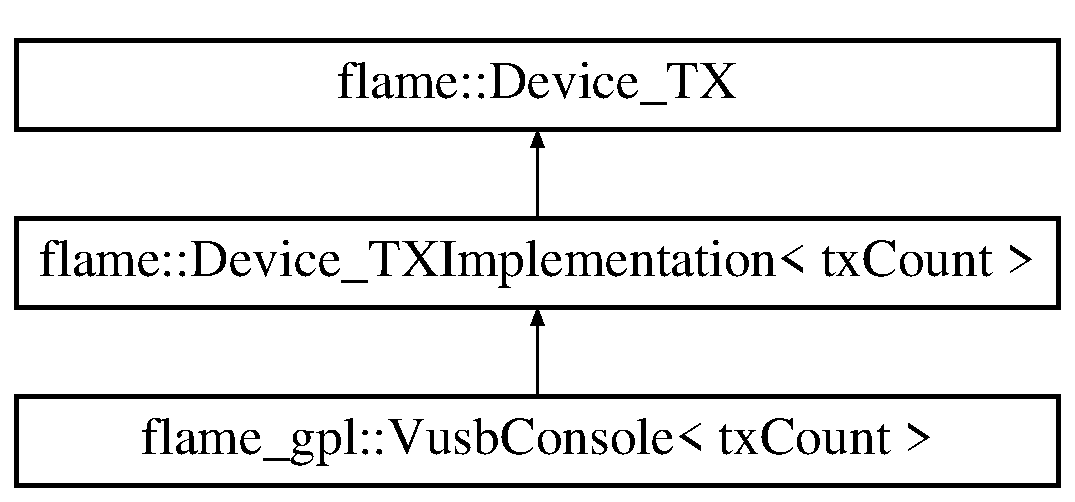
\includegraphics[height=3.000000cm]{classflame_1_1_device___t_x_implementation}
\end{center}
\end{figure}
\subsection*{Protected Member Functions}
\begin{DoxyCompactItemize}
\item 
\hyperlink{classflame_1_1_device___t_x_implementation_a1a6bbd9f10423a8e18a72a1b6aa3335a}{Device\-\_\-\-T\-X\-Implementation} ()
\end{DoxyCompactItemize}
\subsection*{Protected Attributes}
\begin{DoxyCompactItemize}
\item 
\hyperlink{classflame_1_1_ring_buffer_implementation}{Ring\-Buffer\-Implementation}\\*
$<$ tx\-Count, sizeof(\hyperlink{classflame_1_1_t_x_buffer}{T\-X\-Buffer})$>$ \hyperlink{classflame_1_1_device___t_x_implementation_a53941d1a746623722c4d3a4e5de05f78}{\-\_\-my\-Tx\-Pointers}
\end{DoxyCompactItemize}
\subsection*{Additional Inherited Members}


\subsection{Detailed Description}
\subsubsection*{template$<$uint8\-\_\-t tx\-Count$>$class flame\-::\-Device\-\_\-\-T\-X\-Implementation$<$ tx\-Count $>$}



Definition at line 798 of file Device\-\_\-\-T\-X.\-h.



\subsection{Constructor \& Destructor Documentation}
\hypertarget{classflame_1_1_device___t_x_implementation_a1a6bbd9f10423a8e18a72a1b6aa3335a}{\index{flame\-::\-Device\-\_\-\-T\-X\-Implementation@{flame\-::\-Device\-\_\-\-T\-X\-Implementation}!Device\-\_\-\-T\-X\-Implementation@{Device\-\_\-\-T\-X\-Implementation}}
\index{Device\-\_\-\-T\-X\-Implementation@{Device\-\_\-\-T\-X\-Implementation}!flame::Device_TXImplementation@{flame\-::\-Device\-\_\-\-T\-X\-Implementation}}
\subsubsection[{Device\-\_\-\-T\-X\-Implementation}]{\setlength{\rightskip}{0pt plus 5cm}template$<$uint8\-\_\-t tx\-Count$>$ {\bf flame\-::\-Device\-\_\-\-T\-X\-Implementation}$<$ tx\-Count $>$\-::{\bf Device\-\_\-\-T\-X\-Implementation} (
\begin{DoxyParamCaption}
{}
\end{DoxyParamCaption}
)\hspace{0.3cm}{\ttfamily [inline]}, {\ttfamily [protected]}}}\label{classflame_1_1_device___t_x_implementation_a1a6bbd9f10423a8e18a72a1b6aa3335a}
Constructor 

Definition at line 806 of file Device\-\_\-\-T\-X.\-h.



\subsection{Member Data Documentation}
\hypertarget{classflame_1_1_device___t_x_implementation_a53941d1a746623722c4d3a4e5de05f78}{\index{flame\-::\-Device\-\_\-\-T\-X\-Implementation@{flame\-::\-Device\-\_\-\-T\-X\-Implementation}!\-\_\-my\-Tx\-Pointers@{\-\_\-my\-Tx\-Pointers}}
\index{\-\_\-my\-Tx\-Pointers@{\-\_\-my\-Tx\-Pointers}!flame::Device_TXImplementation@{flame\-::\-Device\-\_\-\-T\-X\-Implementation}}
\subsubsection[{\-\_\-my\-Tx\-Pointers}]{\setlength{\rightskip}{0pt plus 5cm}template$<$uint8\-\_\-t tx\-Count$>$ {\bf Ring\-Buffer\-Implementation}$<$tx\-Count, sizeof({\bf T\-X\-Buffer})$>$ {\bf flame\-::\-Device\-\_\-\-T\-X\-Implementation}$<$ tx\-Count $>$\-::\-\_\-my\-Tx\-Pointers\hspace{0.3cm}{\ttfamily [protected]}}}\label{classflame_1_1_device___t_x_implementation_a53941d1a746623722c4d3a4e5de05f78}


Definition at line 801 of file Device\-\_\-\-T\-X.\-h.



The documentation for this class was generated from the following file\-:\begin{DoxyCompactItemize}
\item 
flame/\hyperlink{_device___t_x_8h}{Device\-\_\-\-T\-X.\-h}\end{DoxyCompactItemize}

\hypertarget{classflame_1_1_display___character}{\section{flame\-:\-:Display\-\_\-\-Character$<$ cols, rows, tx\-Buffers $>$ Class Template Reference}
\label{classflame_1_1_display___character}\index{flame\-::\-Display\-\_\-\-Character$<$ cols, rows, tx\-Buffers $>$@{flame\-::\-Display\-\_\-\-Character$<$ cols, rows, tx\-Buffers $>$}}
}


{\ttfamily \#include $<$Display\-\_\-\-Character.\-h$>$}

Inheritance diagram for flame\-:\-:Display\-\_\-\-Character$<$ cols, rows, tx\-Buffers $>$\-:\begin{figure}[H]
\begin{center}
\leavevmode
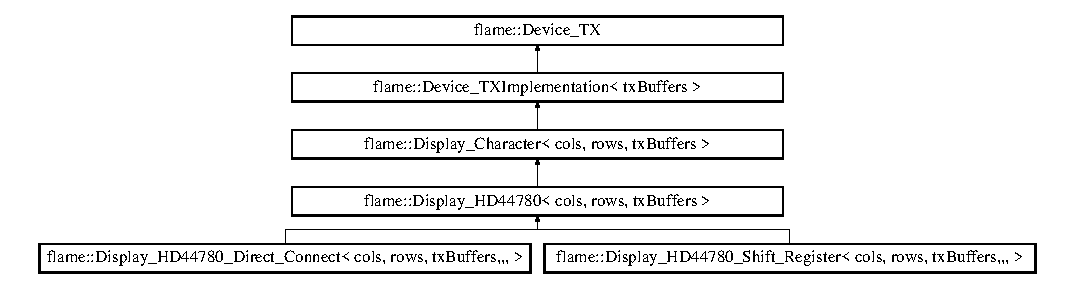
\includegraphics[height=3.439803cm]{classflame_1_1_display___character}
\end{center}
\end{figure}
\subsection*{Public Member Functions}
\begin{DoxyCompactItemize}
\item 
\hyperlink{classflame_1_1_display___character_af56156cb749caf92093c7851a8cc9412}{Display\-\_\-\-Character} ()
\item 
uint8\-\_\-t \hyperlink{classflame_1_1_display___character_a8945b725b35dc3ccb960be48defa04d6}{get\-Width} () \hyperlink{io_8h_a0c33b494a68ce28497e7ce8e5e95feff}{C\-O\-N\-S\-T}
\item 
uint8\-\_\-t \hyperlink{classflame_1_1_display___character_a1e43e42391796d83cb12dfc57469f1da}{get\-Height} () \hyperlink{io_8h_a0c33b494a68ce28497e7ce8e5e95feff}{C\-O\-N\-S\-T}
\item 
bool \hyperlink{classflame_1_1_display___character_a29583da1ca8a9b1ab48982d97828ff18}{write} (int16\-\_\-t $\ast$offset\-X, uint16\-\_\-t offset\-Y, \hyperlink{classflame_1_1_t_x_buffer}{T\-X\-Buffer} \&tx\-Buffer)
\item 
bool \hyperlink{classflame_1_1_display___character_aca5ba0e9806ba7296f847f2f4bb8711e}{write\-String} (int16\-\_\-t $\ast$offset\-X, uint16\-\_\-t offset\-Y, const char $\ast$string)
\item 
bool \hyperlink{classflame_1_1_display___character_a909a1a46c1072748a596c260c664f127}{write\-Buffer} (int16\-\_\-t $\ast$offset\-X, uint16\-\_\-t offset\-Y, const char $\ast$buffer, uint16\-\_\-t length)
\item 
bool \hyperlink{classflame_1_1_display___character_ab11d4562a0b93afcf5b41c43d0bb7d45}{write\-String\-\_\-\-P} (int16\-\_\-t $\ast$offset\-X, uint16\-\_\-t offset\-Y, P\-G\-M\-\_\-\-P string)
\item 
bool \hyperlink{classflame_1_1_display___character_a382ee6d2e408b55277c8f9638a7eb2cc}{write\-Buffer\-\_\-\-P} (int16\-\_\-t $\ast$offset\-X, uint16\-\_\-t offset\-Y, P\-G\-M\-\_\-\-P buffer, uint16\-\_\-t length)
\item 
void \hyperlink{classflame_1_1_display___character_a4a3172da51cdb598217654934f9a2ae4}{run\-Tx\-Buffers} ()
\item 
bool \hyperlink{classflame_1_1_display___character_a74858e6aa4ba6205047f1dbd03544ece}{tx\-Animation} (uint16\-\_\-t row)
\item 
void \hyperlink{classflame_1_1_display___character_a53e7bb7086d34b746628b9c9b9cf13c2}{set\-Wrap} (bool should\-Wrap)
\item 
void \hyperlink{classflame_1_1_display___character_adb19293aae6f7944ae498089b083ed36}{set\-Scroll} (bool should\-Scroll)
\item 
void \hyperlink{classflame_1_1_display___character_a313f5f98c38a4e73a04128cf3d94e1ba}{set\-Cursor} (uint16\-\_\-t col, uint16\-\_\-t row)
\item 
void \hyperlink{classflame_1_1_display___character_aaca15216dc5d78b1c59fcd9368a4f5b4}{write\-Char} (char character)
\item 
void \hyperlink{classflame_1_1_display___character_a5d78d106c26666eadc8b0f275bd00b2a}{scroll\-Vertically} ()
\item 
virtual void \hyperlink{classflame_1_1_display___character_a7d183c097153664ee102291ac32029c4}{\-\_\-write\-Char} (char character)=0
\item 
virtual char \hyperlink{classflame_1_1_display___character_ab68ff09ff8fa79a1b1e0c4afb7e6de95}{\-\_\-read\-Char} ()=0
\item 
virtual void \hyperlink{classflame_1_1_display___character_a2bd2f2b2b6f062f3c47f3dc417f3781d}{\-\_\-set\-Cursor} (uint8\-\_\-t col, uint8\-\_\-t row)=0
\item 
virtual void \hyperlink{classflame_1_1_display___character_ae575b7b3568f820e45029a45715a4f16}{clear} ()=0
\end{DoxyCompactItemize}
\subsection*{Protected Attributes}
\begin{DoxyCompactItemize}
\item 
int16\-\_\-t \hyperlink{classflame_1_1_display___character_a90abfe03430c90c0d50469f7e99c6c5c}{\-\_\-tx\-Offset}
\item 
bool \hyperlink{classflame_1_1_display___character_a2f51ff794dec405d8cdb42d470e9f31d}{\-\_\-wrap}
\item 
bool \hyperlink{classflame_1_1_display___character_a6216cd7f9631ec8851b2d2ed6a5c2728}{\-\_\-scroll}
\item 
uint16\-\_\-t \hyperlink{classflame_1_1_display___character_a04d2c6e9c31084e353be57fa53d97285}{\-\_\-current\-Row}
\item 
uint16\-\_\-t \hyperlink{classflame_1_1_display___character_ab6428d22cb0b06d5d1f1a1bbd71d2697}{\-\_\-current\-Col}
\end{DoxyCompactItemize}
\subsection*{Additional Inherited Members}


\subsection{Detailed Description}
\subsubsection*{template$<$uint8\-\_\-t cols, uint8\-\_\-t rows, uint8\-\_\-t tx\-Buffers$>$class flame\-::\-Display\-\_\-\-Character$<$ cols, rows, tx\-Buffers $>$}

A generic text display Origin (0,0) is bottom left 
\begin{DoxyTemplParams}{Template Parameters}
{\em cols} & the number of columns \\
\hline
{\em rows} & the number of rows \\
\hline
{\em tx\-Buffers} & the number of output buffers \\
\hline
\end{DoxyTemplParams}


Definition at line 42 of file Display\-\_\-\-Character.\-h.



\subsection{Constructor \& Destructor Documentation}
\hypertarget{classflame_1_1_display___character_af56156cb749caf92093c7851a8cc9412}{\index{flame\-::\-Display\-\_\-\-Character@{flame\-::\-Display\-\_\-\-Character}!Display\-\_\-\-Character@{Display\-\_\-\-Character}}
\index{Display\-\_\-\-Character@{Display\-\_\-\-Character}!flame::Display_Character@{flame\-::\-Display\-\_\-\-Character}}
\subsubsection[{Display\-\_\-\-Character}]{\setlength{\rightskip}{0pt plus 5cm}template$<$uint8\-\_\-t cols, uint8\-\_\-t rows, uint8\-\_\-t tx\-Buffers$>$ {\bf flame\-::\-Display\-\_\-\-Character}$<$ cols, rows, tx\-Buffers $>$\-::{\bf Display\-\_\-\-Character} (
\begin{DoxyParamCaption}
{}
\end{DoxyParamCaption}
)\hspace{0.3cm}{\ttfamily [inline]}}}\label{classflame_1_1_display___character_af56156cb749caf92093c7851a8cc9412}
Create a new character display 

Definition at line 54 of file Display\-\_\-\-Character.\-h.



\subsection{Member Function Documentation}
\hypertarget{classflame_1_1_display___character_ab68ff09ff8fa79a1b1e0c4afb7e6de95}{\index{flame\-::\-Display\-\_\-\-Character@{flame\-::\-Display\-\_\-\-Character}!\-\_\-read\-Char@{\-\_\-read\-Char}}
\index{\-\_\-read\-Char@{\-\_\-read\-Char}!flame::Display_Character@{flame\-::\-Display\-\_\-\-Character}}
\subsubsection[{\-\_\-read\-Char}]{\setlength{\rightskip}{0pt plus 5cm}template$<$uint8\-\_\-t cols, uint8\-\_\-t rows, uint8\-\_\-t tx\-Buffers$>$ virtual char {\bf flame\-::\-Display\-\_\-\-Character}$<$ cols, rows, tx\-Buffers $>$\-::\-\_\-read\-Char (
\begin{DoxyParamCaption}
{}
\end{DoxyParamCaption}
)\hspace{0.3cm}{\ttfamily [pure virtual]}}}\label{classflame_1_1_display___character_ab68ff09ff8fa79a1b1e0c4afb7e6de95}


Implemented in \hyperlink{classflame_1_1_display___h_d44780_a2bf6745d21c83b418df65b065aa8ccb3}{flame\-::\-Display\-\_\-\-H\-D44780$<$ cols, rows, tx\-Buffers $>$}.

\hypertarget{classflame_1_1_display___character_a2bd2f2b2b6f062f3c47f3dc417f3781d}{\index{flame\-::\-Display\-\_\-\-Character@{flame\-::\-Display\-\_\-\-Character}!\-\_\-set\-Cursor@{\-\_\-set\-Cursor}}
\index{\-\_\-set\-Cursor@{\-\_\-set\-Cursor}!flame::Display_Character@{flame\-::\-Display\-\_\-\-Character}}
\subsubsection[{\-\_\-set\-Cursor}]{\setlength{\rightskip}{0pt plus 5cm}template$<$uint8\-\_\-t cols, uint8\-\_\-t rows, uint8\-\_\-t tx\-Buffers$>$ virtual void {\bf flame\-::\-Display\-\_\-\-Character}$<$ cols, rows, tx\-Buffers $>$\-::\-\_\-set\-Cursor (
\begin{DoxyParamCaption}
\item[{uint8\-\_\-t}]{col, }
\item[{uint8\-\_\-t}]{row}
\end{DoxyParamCaption}
)\hspace{0.3cm}{\ttfamily [pure virtual]}}}\label{classflame_1_1_display___character_a2bd2f2b2b6f062f3c47f3dc417f3781d}


Implemented in \hyperlink{classflame_1_1_display___h_d44780_adba62c96c907f965995ceaae8da5dc6d}{flame\-::\-Display\-\_\-\-H\-D44780$<$ cols, rows, tx\-Buffers $>$}.

\hypertarget{classflame_1_1_display___character_a7d183c097153664ee102291ac32029c4}{\index{flame\-::\-Display\-\_\-\-Character@{flame\-::\-Display\-\_\-\-Character}!\-\_\-write\-Char@{\-\_\-write\-Char}}
\index{\-\_\-write\-Char@{\-\_\-write\-Char}!flame::Display_Character@{flame\-::\-Display\-\_\-\-Character}}
\subsubsection[{\-\_\-write\-Char}]{\setlength{\rightskip}{0pt plus 5cm}template$<$uint8\-\_\-t cols, uint8\-\_\-t rows, uint8\-\_\-t tx\-Buffers$>$ virtual void {\bf flame\-::\-Display\-\_\-\-Character}$<$ cols, rows, tx\-Buffers $>$\-::\-\_\-write\-Char (
\begin{DoxyParamCaption}
\item[{char}]{character}
\end{DoxyParamCaption}
)\hspace{0.3cm}{\ttfamily [pure virtual]}}}\label{classflame_1_1_display___character_a7d183c097153664ee102291ac32029c4}


Implemented in \hyperlink{classflame_1_1_display___h_d44780_aced521ac701a22b68bc935dfc925708c}{flame\-::\-Display\-\_\-\-H\-D44780$<$ cols, rows, tx\-Buffers $>$}.

\hypertarget{classflame_1_1_display___character_ae575b7b3568f820e45029a45715a4f16}{\index{flame\-::\-Display\-\_\-\-Character@{flame\-::\-Display\-\_\-\-Character}!clear@{clear}}
\index{clear@{clear}!flame::Display_Character@{flame\-::\-Display\-\_\-\-Character}}
\subsubsection[{clear}]{\setlength{\rightskip}{0pt plus 5cm}template$<$uint8\-\_\-t cols, uint8\-\_\-t rows, uint8\-\_\-t tx\-Buffers$>$ virtual void {\bf flame\-::\-Display\-\_\-\-Character}$<$ cols, rows, tx\-Buffers $>$\-::clear (
\begin{DoxyParamCaption}
{}
\end{DoxyParamCaption}
)\hspace{0.3cm}{\ttfamily [pure virtual]}}}\label{classflame_1_1_display___character_ae575b7b3568f820e45029a45715a4f16}


Implemented in \hyperlink{classflame_1_1_display___h_d44780_aef98047f4e45787046eaf410f49313c2}{flame\-::\-Display\-\_\-\-H\-D44780$<$ cols, rows, tx\-Buffers $>$}.

\hypertarget{classflame_1_1_display___character_a1e43e42391796d83cb12dfc57469f1da}{\index{flame\-::\-Display\-\_\-\-Character@{flame\-::\-Display\-\_\-\-Character}!get\-Height@{get\-Height}}
\index{get\-Height@{get\-Height}!flame::Display_Character@{flame\-::\-Display\-\_\-\-Character}}
\subsubsection[{get\-Height}]{\setlength{\rightskip}{0pt plus 5cm}template$<$uint8\-\_\-t cols, uint8\-\_\-t rows, uint8\-\_\-t tx\-Buffers$>$ uint8\-\_\-t {\bf flame\-::\-Display\-\_\-\-Character}$<$ cols, rows, tx\-Buffers $>$\-::get\-Height (
\begin{DoxyParamCaption}
{}
\end{DoxyParamCaption}
)\hspace{0.3cm}{\ttfamily [inline]}}}\label{classflame_1_1_display___character_a1e43e42391796d83cb12dfc57469f1da}
Get the width of the display 

Definition at line 71 of file Display\-\_\-\-Character.\-h.

\hypertarget{classflame_1_1_display___character_a8945b725b35dc3ccb960be48defa04d6}{\index{flame\-::\-Display\-\_\-\-Character@{flame\-::\-Display\-\_\-\-Character}!get\-Width@{get\-Width}}
\index{get\-Width@{get\-Width}!flame::Display_Character@{flame\-::\-Display\-\_\-\-Character}}
\subsubsection[{get\-Width}]{\setlength{\rightskip}{0pt plus 5cm}template$<$uint8\-\_\-t cols, uint8\-\_\-t rows, uint8\-\_\-t tx\-Buffers$>$ uint8\-\_\-t {\bf flame\-::\-Display\-\_\-\-Character}$<$ cols, rows, tx\-Buffers $>$\-::get\-Width (
\begin{DoxyParamCaption}
{}
\end{DoxyParamCaption}
)\hspace{0.3cm}{\ttfamily [inline]}}}\label{classflame_1_1_display___character_a8945b725b35dc3ccb960be48defa04d6}
Get the width of the display 

Definition at line 64 of file Display\-\_\-\-Character.\-h.

\hypertarget{classflame_1_1_display___character_a4a3172da51cdb598217654934f9a2ae4}{\index{flame\-::\-Display\-\_\-\-Character@{flame\-::\-Display\-\_\-\-Character}!run\-Tx\-Buffers@{run\-Tx\-Buffers}}
\index{run\-Tx\-Buffers@{run\-Tx\-Buffers}!flame::Display_Character@{flame\-::\-Display\-\_\-\-Character}}
\subsubsection[{run\-Tx\-Buffers}]{\setlength{\rightskip}{0pt plus 5cm}template$<$uint8\-\_\-t cols, uint8\-\_\-t rows, uint8\-\_\-t tx\-Buffers$>$ void {\bf flame\-::\-Display\-\_\-\-Character}$<$ cols, rows, tx\-Buffers $>$\-::run\-Tx\-Buffers (
\begin{DoxyParamCaption}
{}
\end{DoxyParamCaption}
)\hspace{0.3cm}{\ttfamily [inline]}, {\ttfamily [virtual]}}}\label{classflame_1_1_display___character_a4a3172da51cdb598217654934f9a2ae4}
Start rendering T\-X buffers 

Implements \hyperlink{classflame_1_1_device___t_x_af3cf3dc02a124e5a88841d325555ce3c}{flame\-::\-Device\-\_\-\-T\-X}.



Definition at line 346 of file Display\-\_\-\-Character.\-h.

\hypertarget{classflame_1_1_display___character_a5d78d106c26666eadc8b0f275bd00b2a}{\index{flame\-::\-Display\-\_\-\-Character@{flame\-::\-Display\-\_\-\-Character}!scroll\-Vertically@{scroll\-Vertically}}
\index{scroll\-Vertically@{scroll\-Vertically}!flame::Display_Character@{flame\-::\-Display\-\_\-\-Character}}
\subsubsection[{scroll\-Vertically}]{\setlength{\rightskip}{0pt plus 5cm}template$<$uint8\-\_\-t cols, uint8\-\_\-t rows, uint8\-\_\-t tx\-Buffers$>$ void {\bf flame\-::\-Display\-\_\-\-Character}$<$ cols, rows, tx\-Buffers $>$\-::scroll\-Vertically (
\begin{DoxyParamCaption}
{}
\end{DoxyParamCaption}
)\hspace{0.3cm}{\ttfamily [inline]}}}\label{classflame_1_1_display___character_a5d78d106c26666eadc8b0f275bd00b2a}
Scroll the display up, leaving a blank line at the bottom 

Definition at line 474 of file Display\-\_\-\-Character.\-h.

\hypertarget{classflame_1_1_display___character_a313f5f98c38a4e73a04128cf3d94e1ba}{\index{flame\-::\-Display\-\_\-\-Character@{flame\-::\-Display\-\_\-\-Character}!set\-Cursor@{set\-Cursor}}
\index{set\-Cursor@{set\-Cursor}!flame::Display_Character@{flame\-::\-Display\-\_\-\-Character}}
\subsubsection[{set\-Cursor}]{\setlength{\rightskip}{0pt plus 5cm}template$<$uint8\-\_\-t cols, uint8\-\_\-t rows, uint8\-\_\-t tx\-Buffers$>$ void {\bf flame\-::\-Display\-\_\-\-Character}$<$ cols, rows, tx\-Buffers $>$\-::set\-Cursor (
\begin{DoxyParamCaption}
\item[{uint16\-\_\-t}]{col, }
\item[{uint16\-\_\-t}]{row}
\end{DoxyParamCaption}
)\hspace{0.3cm}{\ttfamily [inline]}}}\label{classflame_1_1_display___character_a313f5f98c38a4e73a04128cf3d94e1ba}
Position the cursor 
\begin{DoxyParams}{Parameters}
{\em col} & the column to set \\
\hline
{\em row} & the row to set \\
\hline
\end{DoxyParams}


Definition at line 401 of file Display\-\_\-\-Character.\-h.

\hypertarget{classflame_1_1_display___character_adb19293aae6f7944ae498089b083ed36}{\index{flame\-::\-Display\-\_\-\-Character@{flame\-::\-Display\-\_\-\-Character}!set\-Scroll@{set\-Scroll}}
\index{set\-Scroll@{set\-Scroll}!flame::Display_Character@{flame\-::\-Display\-\_\-\-Character}}
\subsubsection[{set\-Scroll}]{\setlength{\rightskip}{0pt plus 5cm}template$<$uint8\-\_\-t cols, uint8\-\_\-t rows, uint8\-\_\-t tx\-Buffers$>$ void {\bf flame\-::\-Display\-\_\-\-Character}$<$ cols, rows, tx\-Buffers $>$\-::set\-Scroll (
\begin{DoxyParamCaption}
\item[{bool}]{should\-Scroll}
\end{DoxyParamCaption}
)\hspace{0.3cm}{\ttfamily [inline]}}}\label{classflame_1_1_display___character_adb19293aae6f7944ae498089b083ed36}
Should the automatically scroll characters vertically? 
\begin{DoxyParams}{Parameters}
{\em should\-Scroll} & true to scroll \\
\hline
\end{DoxyParams}


Definition at line 392 of file Display\-\_\-\-Character.\-h.

\hypertarget{classflame_1_1_display___character_a53e7bb7086d34b746628b9c9b9cf13c2}{\index{flame\-::\-Display\-\_\-\-Character@{flame\-::\-Display\-\_\-\-Character}!set\-Wrap@{set\-Wrap}}
\index{set\-Wrap@{set\-Wrap}!flame::Display_Character@{flame\-::\-Display\-\_\-\-Character}}
\subsubsection[{set\-Wrap}]{\setlength{\rightskip}{0pt plus 5cm}template$<$uint8\-\_\-t cols, uint8\-\_\-t rows, uint8\-\_\-t tx\-Buffers$>$ void {\bf flame\-::\-Display\-\_\-\-Character}$<$ cols, rows, tx\-Buffers $>$\-::set\-Wrap (
\begin{DoxyParamCaption}
\item[{bool}]{should\-Wrap}
\end{DoxyParamCaption}
)\hspace{0.3cm}{\ttfamily [inline]}}}\label{classflame_1_1_display___character_a53e7bb7086d34b746628b9c9b9cf13c2}
Should the display automatically wrap characters? 
\begin{DoxyParams}{Parameters}
{\em should\-Wrap} & true to wrap \\
\hline
\end{DoxyParams}


Definition at line 384 of file Display\-\_\-\-Character.\-h.

\hypertarget{classflame_1_1_display___character_a74858e6aa4ba6205047f1dbd03544ece}{\index{flame\-::\-Display\-\_\-\-Character@{flame\-::\-Display\-\_\-\-Character}!tx\-Animation@{tx\-Animation}}
\index{tx\-Animation@{tx\-Animation}!flame::Display_Character@{flame\-::\-Display\-\_\-\-Character}}
\subsubsection[{tx\-Animation}]{\setlength{\rightskip}{0pt plus 5cm}template$<$uint8\-\_\-t cols, uint8\-\_\-t rows, uint8\-\_\-t tx\-Buffers$>$ bool {\bf flame\-::\-Display\-\_\-\-Character}$<$ cols, rows, tx\-Buffers $>$\-::tx\-Animation (
\begin{DoxyParamCaption}
\item[{uint16\-\_\-t}]{row}
\end{DoxyParamCaption}
)\hspace{0.3cm}{\ttfamily [inline]}}}\label{classflame_1_1_display___character_a74858e6aa4ba6205047f1dbd03544ece}
Render a frame of T\-X buffer animation -\/ scrolls text from right to left, before moving to the next buffer 
\begin{DoxyParams}{Parameters}
{\em row} & the vertical pixel offset to start writing at \\
\hline
\end{DoxyParams}
\begin{DoxyReturn}{Returns}
true if there are more frames to be rendered 
\end{DoxyReturn}


Definition at line 356 of file Display\-\_\-\-Character.\-h.

\hypertarget{classflame_1_1_display___character_a29583da1ca8a9b1ab48982d97828ff18}{\index{flame\-::\-Display\-\_\-\-Character@{flame\-::\-Display\-\_\-\-Character}!write@{write}}
\index{write@{write}!flame::Display_Character@{flame\-::\-Display\-\_\-\-Character}}
\subsubsection[{write}]{\setlength{\rightskip}{0pt plus 5cm}template$<$uint8\-\_\-t cols, uint8\-\_\-t rows, uint8\-\_\-t tx\-Buffers$>$ bool {\bf flame\-::\-Display\-\_\-\-Character}$<$ cols, rows, tx\-Buffers $>$\-::write (
\begin{DoxyParamCaption}
\item[{int16\-\_\-t $\ast$}]{offset\-X, }
\item[{uint16\-\_\-t}]{offset\-Y, }
\item[{{\bf T\-X\-Buffer} \&}]{tx\-Buffer}
\end{DoxyParamCaption}
)\hspace{0.3cm}{\ttfamily [inline]}}}\label{classflame_1_1_display___character_a29583da1ca8a9b1ab48982d97828ff18}
Write a T\-X buffer to the display 
\begin{DoxyParams}{Parameters}
{\em offset\-X} & the horizontal offset to start writing at \\
\hline
{\em offset\-Y} & the vertical offset to start writing at \\
\hline
{\em tx\-Buffer} & the buffer to write \\
\hline
\end{DoxyParams}
\begin{DoxyReturn}{Returns}
true if anything was written 
\end{DoxyReturn}


Definition at line 82 of file Display\-\_\-\-Character.\-h.

\hypertarget{classflame_1_1_display___character_a909a1a46c1072748a596c260c664f127}{\index{flame\-::\-Display\-\_\-\-Character@{flame\-::\-Display\-\_\-\-Character}!write\-Buffer@{write\-Buffer}}
\index{write\-Buffer@{write\-Buffer}!flame::Display_Character@{flame\-::\-Display\-\_\-\-Character}}
\subsubsection[{write\-Buffer}]{\setlength{\rightskip}{0pt plus 5cm}template$<$uint8\-\_\-t cols, uint8\-\_\-t rows, uint8\-\_\-t tx\-Buffers$>$ bool {\bf flame\-::\-Display\-\_\-\-Character}$<$ cols, rows, tx\-Buffers $>$\-::write\-Buffer (
\begin{DoxyParamCaption}
\item[{int16\-\_\-t $\ast$}]{offset\-X, }
\item[{uint16\-\_\-t}]{offset\-Y, }
\item[{const char $\ast$}]{buffer, }
\item[{uint16\-\_\-t}]{length}
\end{DoxyParamCaption}
)\hspace{0.3cm}{\ttfamily [inline]}}}\label{classflame_1_1_display___character_a909a1a46c1072748a596c260c664f127}
Write a buffer to the display 
\begin{DoxyParams}{Parameters}
{\em offset\-X} & the horizontal offset to start writing at \\
\hline
{\em offset\-Y} & the vertical offset to start writing at \\
\hline
{\em buffer} & the buffer to write \\
\hline
{\em length} & the length of the buffer \\
\hline
\end{DoxyParams}
\begin{DoxyReturn}{Returns}
true if anything was written 
\end{DoxyReturn}


Definition at line 146 of file Display\-\_\-\-Character.\-h.

\hypertarget{classflame_1_1_display___character_a382ee6d2e408b55277c8f9638a7eb2cc}{\index{flame\-::\-Display\-\_\-\-Character@{flame\-::\-Display\-\_\-\-Character}!write\-Buffer\-\_\-\-P@{write\-Buffer\-\_\-\-P}}
\index{write\-Buffer\-\_\-\-P@{write\-Buffer\-\_\-\-P}!flame::Display_Character@{flame\-::\-Display\-\_\-\-Character}}
\subsubsection[{write\-Buffer\-\_\-\-P}]{\setlength{\rightskip}{0pt plus 5cm}template$<$uint8\-\_\-t cols, uint8\-\_\-t rows, uint8\-\_\-t tx\-Buffers$>$ bool {\bf flame\-::\-Display\-\_\-\-Character}$<$ cols, rows, tx\-Buffers $>$\-::write\-Buffer\-\_\-\-P (
\begin{DoxyParamCaption}
\item[{int16\-\_\-t $\ast$}]{offset\-X, }
\item[{uint16\-\_\-t}]{offset\-Y, }
\item[{P\-G\-M\-\_\-\-P}]{buffer, }
\item[{uint16\-\_\-t}]{length}
\end{DoxyParamCaption}
)\hspace{0.3cm}{\ttfamily [inline]}}}\label{classflame_1_1_display___character_a382ee6d2e408b55277c8f9638a7eb2cc}
Write a P\-R\-O\-G\-M\-E\-M buffer to the display 
\begin{DoxyParams}{Parameters}
{\em offset\-X} & the horizontal offset to start writing at \\
\hline
{\em offset\-Y} & the vertical offset to start writing at \\
\hline
{\em buffer} & the buffer to write \\
\hline
{\em length} & the length of the buffer \\
\hline
\end{DoxyParams}
\begin{DoxyReturn}{Returns}
true if anything was written 
\end{DoxyReturn}


Definition at line 206 of file Display\-\_\-\-Character.\-h.

\hypertarget{classflame_1_1_display___character_aaca15216dc5d78b1c59fcd9368a4f5b4}{\index{flame\-::\-Display\-\_\-\-Character@{flame\-::\-Display\-\_\-\-Character}!write\-Char@{write\-Char}}
\index{write\-Char@{write\-Char}!flame::Display_Character@{flame\-::\-Display\-\_\-\-Character}}
\subsubsection[{write\-Char}]{\setlength{\rightskip}{0pt plus 5cm}template$<$uint8\-\_\-t cols, uint8\-\_\-t rows, uint8\-\_\-t tx\-Buffers$>$ void {\bf flame\-::\-Display\-\_\-\-Character}$<$ cols, rows, tx\-Buffers $>$\-::write\-Char (
\begin{DoxyParamCaption}
\item[{char}]{character}
\end{DoxyParamCaption}
)\hspace{0.3cm}{\ttfamily [inline]}}}\label{classflame_1_1_display___character_aaca15216dc5d78b1c59fcd9368a4f5b4}
Write a character to the display Will interpret the following special characters\-: \textbackslash{}b Backspace \textbackslash{}t Tab \textbackslash{}n Newline


\begin{DoxyParams}{Parameters}
{\em character} & the character to write \\
\hline
\end{DoxyParams}


Definition at line 416 of file Display\-\_\-\-Character.\-h.

\hypertarget{classflame_1_1_display___character_aca5ba0e9806ba7296f847f2f4bb8711e}{\index{flame\-::\-Display\-\_\-\-Character@{flame\-::\-Display\-\_\-\-Character}!write\-String@{write\-String}}
\index{write\-String@{write\-String}!flame::Display_Character@{flame\-::\-Display\-\_\-\-Character}}
\subsubsection[{write\-String}]{\setlength{\rightskip}{0pt plus 5cm}template$<$uint8\-\_\-t cols, uint8\-\_\-t rows, uint8\-\_\-t tx\-Buffers$>$ bool {\bf flame\-::\-Display\-\_\-\-Character}$<$ cols, rows, tx\-Buffers $>$\-::write\-String (
\begin{DoxyParamCaption}
\item[{int16\-\_\-t $\ast$}]{offset\-X, }
\item[{uint16\-\_\-t}]{offset\-Y, }
\item[{const char $\ast$}]{string}
\end{DoxyParamCaption}
)\hspace{0.3cm}{\ttfamily [inline]}}}\label{classflame_1_1_display___character_aca5ba0e9806ba7296f847f2f4bb8711e}
Write a string to the display 
\begin{DoxyParams}{Parameters}
{\em offset\-X} & the horizontal offset to start writing at \\
\hline
{\em offset\-Y} & the vertical offset to start writing at \\
\hline
{\em string} & the string to write \\
\hline
\end{DoxyParams}
\begin{DoxyReturn}{Returns}
true if anything was written 
\end{DoxyReturn}


Definition at line 114 of file Display\-\_\-\-Character.\-h.

\hypertarget{classflame_1_1_display___character_ab11d4562a0b93afcf5b41c43d0bb7d45}{\index{flame\-::\-Display\-\_\-\-Character@{flame\-::\-Display\-\_\-\-Character}!write\-String\-\_\-\-P@{write\-String\-\_\-\-P}}
\index{write\-String\-\_\-\-P@{write\-String\-\_\-\-P}!flame::Display_Character@{flame\-::\-Display\-\_\-\-Character}}
\subsubsection[{write\-String\-\_\-\-P}]{\setlength{\rightskip}{0pt plus 5cm}template$<$uint8\-\_\-t cols, uint8\-\_\-t rows, uint8\-\_\-t tx\-Buffers$>$ bool {\bf flame\-::\-Display\-\_\-\-Character}$<$ cols, rows, tx\-Buffers $>$\-::write\-String\-\_\-\-P (
\begin{DoxyParamCaption}
\item[{int16\-\_\-t $\ast$}]{offset\-X, }
\item[{uint16\-\_\-t}]{offset\-Y, }
\item[{P\-G\-M\-\_\-\-P}]{string}
\end{DoxyParamCaption}
)\hspace{0.3cm}{\ttfamily [inline]}}}\label{classflame_1_1_display___character_ab11d4562a0b93afcf5b41c43d0bb7d45}
Write a P\-R\-O\-G\-M\-E\-M string to the display 
\begin{DoxyParams}{Parameters}
{\em offset\-X} & the horizontal offset to start writing at \\
\hline
{\em offset\-Y} & the vertical offset to start writing at \\
\hline
{\em string} & the string to write \\
\hline
\end{DoxyParams}
\begin{DoxyReturn}{Returns}
true if anything was written 
\end{DoxyReturn}


Definition at line 174 of file Display\-\_\-\-Character.\-h.



\subsection{Member Data Documentation}
\hypertarget{classflame_1_1_display___character_ab6428d22cb0b06d5d1f1a1bbd71d2697}{\index{flame\-::\-Display\-\_\-\-Character@{flame\-::\-Display\-\_\-\-Character}!\-\_\-current\-Col@{\-\_\-current\-Col}}
\index{\-\_\-current\-Col@{\-\_\-current\-Col}!flame::Display_Character@{flame\-::\-Display\-\_\-\-Character}}
\subsubsection[{\-\_\-current\-Col}]{\setlength{\rightskip}{0pt plus 5cm}template$<$uint8\-\_\-t cols, uint8\-\_\-t rows, uint8\-\_\-t tx\-Buffers$>$ uint16\-\_\-t {\bf flame\-::\-Display\-\_\-\-Character}$<$ cols, rows, tx\-Buffers $>$\-::\-\_\-current\-Col\hspace{0.3cm}{\ttfamily [protected]}}}\label{classflame_1_1_display___character_ab6428d22cb0b06d5d1f1a1bbd71d2697}


Definition at line 48 of file Display\-\_\-\-Character.\-h.

\hypertarget{classflame_1_1_display___character_a04d2c6e9c31084e353be57fa53d97285}{\index{flame\-::\-Display\-\_\-\-Character@{flame\-::\-Display\-\_\-\-Character}!\-\_\-current\-Row@{\-\_\-current\-Row}}
\index{\-\_\-current\-Row@{\-\_\-current\-Row}!flame::Display_Character@{flame\-::\-Display\-\_\-\-Character}}
\subsubsection[{\-\_\-current\-Row}]{\setlength{\rightskip}{0pt plus 5cm}template$<$uint8\-\_\-t cols, uint8\-\_\-t rows, uint8\-\_\-t tx\-Buffers$>$ uint16\-\_\-t {\bf flame\-::\-Display\-\_\-\-Character}$<$ cols, rows, tx\-Buffers $>$\-::\-\_\-current\-Row\hspace{0.3cm}{\ttfamily [protected]}}}\label{classflame_1_1_display___character_a04d2c6e9c31084e353be57fa53d97285}


Definition at line 47 of file Display\-\_\-\-Character.\-h.

\hypertarget{classflame_1_1_display___character_a6216cd7f9631ec8851b2d2ed6a5c2728}{\index{flame\-::\-Display\-\_\-\-Character@{flame\-::\-Display\-\_\-\-Character}!\-\_\-scroll@{\-\_\-scroll}}
\index{\-\_\-scroll@{\-\_\-scroll}!flame::Display_Character@{flame\-::\-Display\-\_\-\-Character}}
\subsubsection[{\-\_\-scroll}]{\setlength{\rightskip}{0pt plus 5cm}template$<$uint8\-\_\-t cols, uint8\-\_\-t rows, uint8\-\_\-t tx\-Buffers$>$ bool {\bf flame\-::\-Display\-\_\-\-Character}$<$ cols, rows, tx\-Buffers $>$\-::\-\_\-scroll\hspace{0.3cm}{\ttfamily [protected]}}}\label{classflame_1_1_display___character_a6216cd7f9631ec8851b2d2ed6a5c2728}


Definition at line 46 of file Display\-\_\-\-Character.\-h.

\hypertarget{classflame_1_1_display___character_a90abfe03430c90c0d50469f7e99c6c5c}{\index{flame\-::\-Display\-\_\-\-Character@{flame\-::\-Display\-\_\-\-Character}!\-\_\-tx\-Offset@{\-\_\-tx\-Offset}}
\index{\-\_\-tx\-Offset@{\-\_\-tx\-Offset}!flame::Display_Character@{flame\-::\-Display\-\_\-\-Character}}
\subsubsection[{\-\_\-tx\-Offset}]{\setlength{\rightskip}{0pt plus 5cm}template$<$uint8\-\_\-t cols, uint8\-\_\-t rows, uint8\-\_\-t tx\-Buffers$>$ int16\-\_\-t {\bf flame\-::\-Display\-\_\-\-Character}$<$ cols, rows, tx\-Buffers $>$\-::\-\_\-tx\-Offset\hspace{0.3cm}{\ttfamily [protected]}}}\label{classflame_1_1_display___character_a90abfe03430c90c0d50469f7e99c6c5c}


Definition at line 44 of file Display\-\_\-\-Character.\-h.

\hypertarget{classflame_1_1_display___character_a2f51ff794dec405d8cdb42d470e9f31d}{\index{flame\-::\-Display\-\_\-\-Character@{flame\-::\-Display\-\_\-\-Character}!\-\_\-wrap@{\-\_\-wrap}}
\index{\-\_\-wrap@{\-\_\-wrap}!flame::Display_Character@{flame\-::\-Display\-\_\-\-Character}}
\subsubsection[{\-\_\-wrap}]{\setlength{\rightskip}{0pt plus 5cm}template$<$uint8\-\_\-t cols, uint8\-\_\-t rows, uint8\-\_\-t tx\-Buffers$>$ bool {\bf flame\-::\-Display\-\_\-\-Character}$<$ cols, rows, tx\-Buffers $>$\-::\-\_\-wrap\hspace{0.3cm}{\ttfamily [protected]}}}\label{classflame_1_1_display___character_a2f51ff794dec405d8cdb42d470e9f31d}


Definition at line 45 of file Display\-\_\-\-Character.\-h.



The documentation for this class was generated from the following file\-:\begin{DoxyCompactItemize}
\item 
flame/\hyperlink{_display___character_8h}{Display\-\_\-\-Character.\-h}\end{DoxyCompactItemize}

\hypertarget{classflame_1_1_display___h_d44780}{\section{flame\-:\-:Display\-\_\-\-H\-D44780$<$ cols, rows, tx\-Buffers $>$ Class Template Reference}
\label{classflame_1_1_display___h_d44780}\index{flame\-::\-Display\-\_\-\-H\-D44780$<$ cols, rows, tx\-Buffers $>$@{flame\-::\-Display\-\_\-\-H\-D44780$<$ cols, rows, tx\-Buffers $>$}}
}


{\ttfamily \#include $<$Display\-\_\-\-H\-D44780.\-h$>$}

Inheritance diagram for flame\-:\-:Display\-\_\-\-H\-D44780$<$ cols, rows, tx\-Buffers $>$\-:\begin{figure}[H]
\begin{center}
\leavevmode
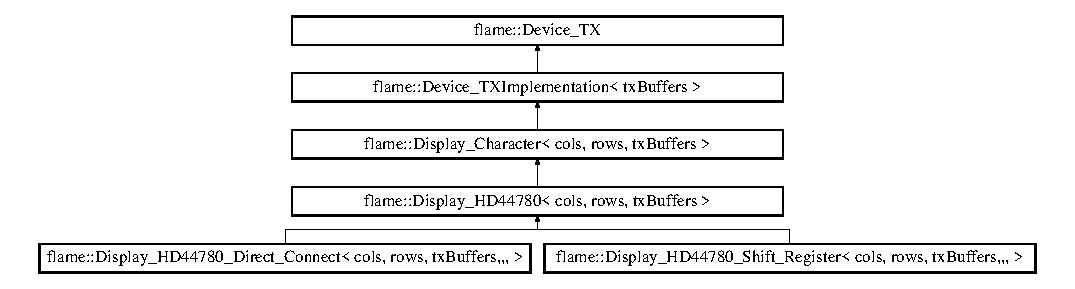
\includegraphics[height=3.439803cm]{classflame_1_1_display___h_d44780}
\end{center}
\end{figure}
\subsection*{Public Member Functions}
\begin{DoxyCompactItemize}
\item 
\hyperlink{classflame_1_1_display___h_d44780_a90f5033f3b90d89e6846a610f9fb5c3e}{Display\-\_\-\-H\-D44780} ()
\item 
void \hyperlink{classflame_1_1_display___h_d44780_ad2482c6d54b96446b167f67b8db61443}{init} (bool byte\-Mode, bool multi\-Line, bool big\-Font, bool cursor\-On, bool cursor\-Blink, bool left2right, bool scroll)
\item 
void \hyperlink{classflame_1_1_display___h_d44780_aef98047f4e45787046eaf410f49313c2}{clear} ()
\item 
void \hyperlink{classflame_1_1_display___h_d44780_a3712476f8b040038ed1c31c3fcf8536a}{entry\-Mode} (bool left2\-Right, bool scroll)
\item 
void \hyperlink{classflame_1_1_display___h_d44780_a9ecdf0cf1754634a243f014170f61f32}{control} (bool display\-On, bool cursor\-On, bool cursor\-Blink)
\end{DoxyCompactItemize}
\subsection*{Protected Member Functions}
\begin{DoxyCompactItemize}
\item 
void \hyperlink{classflame_1_1_display___h_d44780_a5a81eae9ce61da5f5873f272feea3ba9}{write\-Command} (\hyperlink{namespaceflame_ad814bac19b0569ff480de071076a23e9}{H\-D44780\-Command} command, uint8\-\_\-t data)
\item 
void \hyperlink{classflame_1_1_display___h_d44780_ac4a698ce422c7de3e32130aa7a1a289d}{function} (bool byte\-Mode, bool multi\-Line, bool big\-Font)
\item 
void \hyperlink{classflame_1_1_display___h_d44780_a425d2d57165fe2e098a36a41b4a3e017}{address\-C\-G\-R\-A\-M} (uint8\-\_\-t address)
\item 
void \hyperlink{classflame_1_1_display___h_d44780_a77c19f4474b69b500ed0dc467fd21b70}{address\-D\-D\-R\-A\-M} (uint8\-\_\-t address)
\item 
virtual void \hyperlink{classflame_1_1_display___h_d44780_a7a6b0c6550f20961f3cec7b07e0835ed}{write\-Byte} (uint8\-\_\-t byte, bool rs)=0
\item 
virtual uint8\-\_\-t \hyperlink{classflame_1_1_display___h_d44780_ae3409f84516a6533d88bc70b200a6e23}{read\-Byte} (bool rs)=0
\item 
void \hyperlink{classflame_1_1_display___h_d44780_adba62c96c907f965995ceaae8da5dc6d}{\-\_\-set\-Cursor} (uint8\-\_\-t col, uint8\-\_\-t row)
\item 
void \hyperlink{classflame_1_1_display___h_d44780_aced521ac701a22b68bc935dfc925708c}{\-\_\-write\-Char} (char character)
\item 
char \hyperlink{classflame_1_1_display___h_d44780_a2bf6745d21c83b418df65b065aa8ccb3}{\-\_\-read\-Char} ()
\item 
virtual bool \hyperlink{classflame_1_1_display___h_d44780_a665b559a3a2370fada65efd724a412b9}{is\-Busy} ()=0
\item 
virtual void \hyperlink{classflame_1_1_display___h_d44780_aa15098f89b2df993a38731033ca20a4d}{delay} (\hyperlink{namespaceflame_ad814bac19b0569ff480de071076a23e9}{H\-D44780\-Command} command)=0
\end{DoxyCompactItemize}
\subsection*{Protected Attributes}
\begin{DoxyCompactItemize}
\item 
uint16\-\_\-t \hyperlink{classflame_1_1_display___h_d44780_a58f971ca89d3a722304db94db25830b2}{\-\_\-ticks}
\item 
uint16\-\_\-t \hyperlink{classflame_1_1_display___h_d44780_aa87fd152ce1f1dd679ea6aeae6fdf596}{\-\_\-animate\-Ticks}
\item 
bool \hyperlink{classflame_1_1_display___h_d44780_abd557b0db9b085b5781a760b6660ec81}{\-\_\-must\-Delay}
\item 
bool \hyperlink{classflame_1_1_display___h_d44780_a719e1ad8661a35fbcc440ac4f1492657}{\-\_\-byte\-Mode}
\end{DoxyCompactItemize}


\subsection{Detailed Description}
\subsubsection*{template$<$uint16\-\_\-t cols, uint16\-\_\-t rows, uint8\-\_\-t tx\-Buffers$>$class flame\-::\-Display\-\_\-\-H\-D44780$<$ cols, rows, tx\-Buffers $>$}

A class for operating H\-D44780 based L\-C\-D displays (and compatible) 
\begin{DoxyTemplParams}{Template Parameters}
{\em cols} & the number of columns \\
\hline
{\em rows} & the number of rows \\
\hline
{\em tx\-Buffers} & the number of output buffers \\
\hline
\end{DoxyTemplParams}


Definition at line 69 of file Display\-\_\-\-H\-D44780.\-h.



\subsection{Constructor \& Destructor Documentation}
\hypertarget{classflame_1_1_display___h_d44780_a90f5033f3b90d89e6846a610f9fb5c3e}{\index{flame\-::\-Display\-\_\-\-H\-D44780@{flame\-::\-Display\-\_\-\-H\-D44780}!Display\-\_\-\-H\-D44780@{Display\-\_\-\-H\-D44780}}
\index{Display\-\_\-\-H\-D44780@{Display\-\_\-\-H\-D44780}!flame::Display_HD44780@{flame\-::\-Display\-\_\-\-H\-D44780}}
\subsubsection[{Display\-\_\-\-H\-D44780}]{\setlength{\rightskip}{0pt plus 5cm}template$<$uint16\-\_\-t cols, uint16\-\_\-t rows, uint8\-\_\-t tx\-Buffers$>$ {\bf flame\-::\-Display\-\_\-\-H\-D44780}$<$ cols, rows, tx\-Buffers $>$\-::{\bf Display\-\_\-\-H\-D44780} (
\begin{DoxyParamCaption}
{}
\end{DoxyParamCaption}
)\hspace{0.3cm}{\ttfamily [inline]}}}\label{classflame_1_1_display___h_d44780_a90f5033f3b90d89e6846a610f9fb5c3e}
Create a new display 

Definition at line 190 of file Display\-\_\-\-H\-D44780.\-h.



\subsection{Member Function Documentation}
\hypertarget{classflame_1_1_display___h_d44780_a2bf6745d21c83b418df65b065aa8ccb3}{\index{flame\-::\-Display\-\_\-\-H\-D44780@{flame\-::\-Display\-\_\-\-H\-D44780}!\-\_\-read\-Char@{\-\_\-read\-Char}}
\index{\-\_\-read\-Char@{\-\_\-read\-Char}!flame::Display_HD44780@{flame\-::\-Display\-\_\-\-H\-D44780}}
\subsubsection[{\-\_\-read\-Char}]{\setlength{\rightskip}{0pt plus 5cm}template$<$uint16\-\_\-t cols, uint16\-\_\-t rows, uint8\-\_\-t tx\-Buffers$>$ char {\bf flame\-::\-Display\-\_\-\-H\-D44780}$<$ cols, rows, tx\-Buffers $>$\-::\-\_\-read\-Char (
\begin{DoxyParamCaption}
{}
\end{DoxyParamCaption}
)\hspace{0.3cm}{\ttfamily [inline]}, {\ttfamily [protected]}, {\ttfamily [virtual]}}}\label{classflame_1_1_display___h_d44780_a2bf6745d21c83b418df65b065aa8ccb3}
Read a character from the display at the current location, incrementing the location by 1 \begin{DoxyReturn}{Returns}
the character at the current location 
\end{DoxyReturn}


Implements \hyperlink{classflame_1_1_display___character_ab68ff09ff8fa79a1b1e0c4afb7e6de95}{flame\-::\-Display\-\_\-\-Character$<$ cols, rows, tx\-Buffers $>$}.



Definition at line 178 of file Display\-\_\-\-H\-D44780.\-h.

\hypertarget{classflame_1_1_display___h_d44780_adba62c96c907f965995ceaae8da5dc6d}{\index{flame\-::\-Display\-\_\-\-H\-D44780@{flame\-::\-Display\-\_\-\-H\-D44780}!\-\_\-set\-Cursor@{\-\_\-set\-Cursor}}
\index{\-\_\-set\-Cursor@{\-\_\-set\-Cursor}!flame::Display_HD44780@{flame\-::\-Display\-\_\-\-H\-D44780}}
\subsubsection[{\-\_\-set\-Cursor}]{\setlength{\rightskip}{0pt plus 5cm}template$<$uint16\-\_\-t cols, uint16\-\_\-t rows, uint8\-\_\-t tx\-Buffers$>$ void {\bf flame\-::\-Display\-\_\-\-H\-D44780}$<$ cols, rows, tx\-Buffers $>$\-::\-\_\-set\-Cursor (
\begin{DoxyParamCaption}
\item[{uint8\-\_\-t}]{col, }
\item[{uint8\-\_\-t}]{row}
\end{DoxyParamCaption}
)\hspace{0.3cm}{\ttfamily [inline]}, {\ttfamily [protected]}, {\ttfamily [virtual]}}}\label{classflame_1_1_display___h_d44780_adba62c96c907f965995ceaae8da5dc6d}
Move the cursor to a location, so the next write\-Char will write a character at that location (Origin is at the bottom left) 
\begin{DoxyParams}{Parameters}
{\em col} & the column to put the character \\
\hline
{\em row} & the row to put the character \\
\hline
\end{DoxyParams}


Implements \hyperlink{classflame_1_1_display___character_a2bd2f2b2b6f062f3c47f3dc417f3781d}{flame\-::\-Display\-\_\-\-Character$<$ cols, rows, tx\-Buffers $>$}.



Definition at line 139 of file Display\-\_\-\-H\-D44780.\-h.

\hypertarget{classflame_1_1_display___h_d44780_aced521ac701a22b68bc935dfc925708c}{\index{flame\-::\-Display\-\_\-\-H\-D44780@{flame\-::\-Display\-\_\-\-H\-D44780}!\-\_\-write\-Char@{\-\_\-write\-Char}}
\index{\-\_\-write\-Char@{\-\_\-write\-Char}!flame::Display_HD44780@{flame\-::\-Display\-\_\-\-H\-D44780}}
\subsubsection[{\-\_\-write\-Char}]{\setlength{\rightskip}{0pt plus 5cm}template$<$uint16\-\_\-t cols, uint16\-\_\-t rows, uint8\-\_\-t tx\-Buffers$>$ void {\bf flame\-::\-Display\-\_\-\-H\-D44780}$<$ cols, rows, tx\-Buffers $>$\-::\-\_\-write\-Char (
\begin{DoxyParamCaption}
\item[{char}]{character}
\end{DoxyParamCaption}
)\hspace{0.3cm}{\ttfamily [inline]}, {\ttfamily [protected]}, {\ttfamily [virtual]}}}\label{classflame_1_1_display___h_d44780_aced521ac701a22b68bc935dfc925708c}
Write a character to the display at the current location, incrementing the location by 1 
\begin{DoxyParams}{Parameters}
{\em character} & the character to write \\
\hline
\end{DoxyParams}


Implements \hyperlink{classflame_1_1_display___character_a7d183c097153664ee102291ac32029c4}{flame\-::\-Display\-\_\-\-Character$<$ cols, rows, tx\-Buffers $>$}.



Definition at line 168 of file Display\-\_\-\-H\-D44780.\-h.

\hypertarget{classflame_1_1_display___h_d44780_a425d2d57165fe2e098a36a41b4a3e017}{\index{flame\-::\-Display\-\_\-\-H\-D44780@{flame\-::\-Display\-\_\-\-H\-D44780}!address\-C\-G\-R\-A\-M@{address\-C\-G\-R\-A\-M}}
\index{address\-C\-G\-R\-A\-M@{address\-C\-G\-R\-A\-M}!flame::Display_HD44780@{flame\-::\-Display\-\_\-\-H\-D44780}}
\subsubsection[{address\-C\-G\-R\-A\-M}]{\setlength{\rightskip}{0pt plus 5cm}template$<$uint16\-\_\-t cols, uint16\-\_\-t rows, uint8\-\_\-t tx\-Buffers$>$ void {\bf flame\-::\-Display\-\_\-\-H\-D44780}$<$ cols, rows, tx\-Buffers $>$\-::address\-C\-G\-R\-A\-M (
\begin{DoxyParamCaption}
\item[{uint8\-\_\-t}]{address}
\end{DoxyParamCaption}
)\hspace{0.3cm}{\ttfamily [inline]}, {\ttfamily [protected]}}}\label{classflame_1_1_display___h_d44780_a425d2d57165fe2e098a36a41b4a3e017}
Set the C\-G\-R\-A\-M address 
\begin{DoxyParams}{Parameters}
{\em address} & the C\-G\-R\-A\-M address \\
\hline
\end{DoxyParams}


Definition at line 114 of file Display\-\_\-\-H\-D44780.\-h.

\hypertarget{classflame_1_1_display___h_d44780_a77c19f4474b69b500ed0dc467fd21b70}{\index{flame\-::\-Display\-\_\-\-H\-D44780@{flame\-::\-Display\-\_\-\-H\-D44780}!address\-D\-D\-R\-A\-M@{address\-D\-D\-R\-A\-M}}
\index{address\-D\-D\-R\-A\-M@{address\-D\-D\-R\-A\-M}!flame::Display_HD44780@{flame\-::\-Display\-\_\-\-H\-D44780}}
\subsubsection[{address\-D\-D\-R\-A\-M}]{\setlength{\rightskip}{0pt plus 5cm}template$<$uint16\-\_\-t cols, uint16\-\_\-t rows, uint8\-\_\-t tx\-Buffers$>$ void {\bf flame\-::\-Display\-\_\-\-H\-D44780}$<$ cols, rows, tx\-Buffers $>$\-::address\-D\-D\-R\-A\-M (
\begin{DoxyParamCaption}
\item[{uint8\-\_\-t}]{address}
\end{DoxyParamCaption}
)\hspace{0.3cm}{\ttfamily [inline]}, {\ttfamily [protected]}}}\label{classflame_1_1_display___h_d44780_a77c19f4474b69b500ed0dc467fd21b70}
Set the D\-D\-R\-A\-M address 
\begin{DoxyParams}{Parameters}
{\em address} & the D\-D\-R\-A\-M address \\
\hline
\end{DoxyParams}


Definition at line 124 of file Display\-\_\-\-H\-D44780.\-h.

\hypertarget{classflame_1_1_display___h_d44780_aef98047f4e45787046eaf410f49313c2}{\index{flame\-::\-Display\-\_\-\-H\-D44780@{flame\-::\-Display\-\_\-\-H\-D44780}!clear@{clear}}
\index{clear@{clear}!flame::Display_HD44780@{flame\-::\-Display\-\_\-\-H\-D44780}}
\subsubsection[{clear}]{\setlength{\rightskip}{0pt plus 5cm}template$<$uint16\-\_\-t cols, uint16\-\_\-t rows, uint8\-\_\-t tx\-Buffers$>$ void {\bf flame\-::\-Display\-\_\-\-H\-D44780}$<$ cols, rows, tx\-Buffers $>$\-::clear (
\begin{DoxyParamCaption}
{}
\end{DoxyParamCaption}
)\hspace{0.3cm}{\ttfamily [inline]}, {\ttfamily [virtual]}}}\label{classflame_1_1_display___h_d44780_aef98047f4e45787046eaf410f49313c2}
Clear the display 

Implements \hyperlink{classflame_1_1_display___character_ae575b7b3568f820e45029a45715a4f16}{flame\-::\-Display\-\_\-\-Character$<$ cols, rows, tx\-Buffers $>$}.



Definition at line 235 of file Display\-\_\-\-H\-D44780.\-h.

\hypertarget{classflame_1_1_display___h_d44780_a9ecdf0cf1754634a243f014170f61f32}{\index{flame\-::\-Display\-\_\-\-H\-D44780@{flame\-::\-Display\-\_\-\-H\-D44780}!control@{control}}
\index{control@{control}!flame::Display_HD44780@{flame\-::\-Display\-\_\-\-H\-D44780}}
\subsubsection[{control}]{\setlength{\rightskip}{0pt plus 5cm}template$<$uint16\-\_\-t cols, uint16\-\_\-t rows, uint8\-\_\-t tx\-Buffers$>$ void {\bf flame\-::\-Display\-\_\-\-H\-D44780}$<$ cols, rows, tx\-Buffers $>$\-::control (
\begin{DoxyParamCaption}
\item[{bool}]{display\-On, }
\item[{bool}]{cursor\-On, }
\item[{bool}]{cursor\-Blink}
\end{DoxyParamCaption}
)\hspace{0.3cm}{\ttfamily [inline]}}}\label{classflame_1_1_display___h_d44780_a9ecdf0cf1754634a243f014170f61f32}
Set parameters on the display 
\begin{DoxyParams}{Parameters}
{\em display\-On} & turn the display on \\
\hline
{\em cursor\-On} & turn the cursor on \\
\hline
{\em cursor\-Blink} & blink the cursor \\
\hline
\end{DoxyParams}


Definition at line 262 of file Display\-\_\-\-H\-D44780.\-h.

\hypertarget{classflame_1_1_display___h_d44780_aa15098f89b2df993a38731033ca20a4d}{\index{flame\-::\-Display\-\_\-\-H\-D44780@{flame\-::\-Display\-\_\-\-H\-D44780}!delay@{delay}}
\index{delay@{delay}!flame::Display_HD44780@{flame\-::\-Display\-\_\-\-H\-D44780}}
\subsubsection[{delay}]{\setlength{\rightskip}{0pt plus 5cm}template$<$uint16\-\_\-t cols, uint16\-\_\-t rows, uint8\-\_\-t tx\-Buffers$>$ virtual void {\bf flame\-::\-Display\-\_\-\-H\-D44780}$<$ cols, rows, tx\-Buffers $>$\-::delay (
\begin{DoxyParamCaption}
\item[{{\bf H\-D44780\-Command}}]{command}
\end{DoxyParamCaption}
)\hspace{0.3cm}{\ttfamily [protected]}, {\ttfamily [pure virtual]}}}\label{classflame_1_1_display___h_d44780_aa15098f89b2df993a38731033ca20a4d}


Implemented in \hyperlink{classflame_1_1_display___h_d44780___shift___register_abf59a4215c52f6cd29bdb2e901346945}{flame\-::\-Display\-\_\-\-H\-D44780\-\_\-\-Shift\-\_\-\-Register$<$ cols, rows, tx\-Buffers,,, $>$}.

\hypertarget{classflame_1_1_display___h_d44780_a3712476f8b040038ed1c31c3fcf8536a}{\index{flame\-::\-Display\-\_\-\-H\-D44780@{flame\-::\-Display\-\_\-\-H\-D44780}!entry\-Mode@{entry\-Mode}}
\index{entry\-Mode@{entry\-Mode}!flame::Display_HD44780@{flame\-::\-Display\-\_\-\-H\-D44780}}
\subsubsection[{entry\-Mode}]{\setlength{\rightskip}{0pt plus 5cm}template$<$uint16\-\_\-t cols, uint16\-\_\-t rows, uint8\-\_\-t tx\-Buffers$>$ void {\bf flame\-::\-Display\-\_\-\-H\-D44780}$<$ cols, rows, tx\-Buffers $>$\-::entry\-Mode (
\begin{DoxyParamCaption}
\item[{bool}]{left2\-Right, }
\item[{bool}]{scroll}
\end{DoxyParamCaption}
)\hspace{0.3cm}{\ttfamily [inline]}}}\label{classflame_1_1_display___h_d44780_a3712476f8b040038ed1c31c3fcf8536a}
Set the entry mode -\/ allows for left or right printing, allows for scrolling display or moving cursor 
\begin{DoxyParams}{Parameters}
{\em left2\-Right} & true for text reading left to right \\
\hline
{\em scroll} & true to scroll text rather than moving the cursor \\
\hline
\end{DoxyParams}


Definition at line 248 of file Display\-\_\-\-H\-D44780.\-h.

\hypertarget{classflame_1_1_display___h_d44780_ac4a698ce422c7de3e32130aa7a1a289d}{\index{flame\-::\-Display\-\_\-\-H\-D44780@{flame\-::\-Display\-\_\-\-H\-D44780}!function@{function}}
\index{function@{function}!flame::Display_HD44780@{flame\-::\-Display\-\_\-\-H\-D44780}}
\subsubsection[{function}]{\setlength{\rightskip}{0pt plus 5cm}template$<$uint16\-\_\-t cols, uint16\-\_\-t rows, uint8\-\_\-t tx\-Buffers$>$ void {\bf flame\-::\-Display\-\_\-\-H\-D44780}$<$ cols, rows, tx\-Buffers $>$\-::function (
\begin{DoxyParamCaption}
\item[{bool}]{byte\-Mode, }
\item[{bool}]{multi\-Line, }
\item[{bool}]{big\-Font}
\end{DoxyParamCaption}
)\hspace{0.3cm}{\ttfamily [inline]}, {\ttfamily [protected]}}}\label{classflame_1_1_display___h_d44780_ac4a698ce422c7de3e32130aa7a1a289d}
Initialise the display 
\begin{DoxyParams}{Parameters}
{\em byte\-Mode} & true to use 8 bit protocol \\
\hline
{\em multi\-Line} & true if there is more than 1 line \\
\hline
{\em big\-Font} & true to use 5x11 fonts, false for 5x8 \\
\hline
\end{DoxyParams}


Definition at line 98 of file Display\-\_\-\-H\-D44780.\-h.

\hypertarget{classflame_1_1_display___h_d44780_ad2482c6d54b96446b167f67b8db61443}{\index{flame\-::\-Display\-\_\-\-H\-D44780@{flame\-::\-Display\-\_\-\-H\-D44780}!init@{init}}
\index{init@{init}!flame::Display_HD44780@{flame\-::\-Display\-\_\-\-H\-D44780}}
\subsubsection[{init}]{\setlength{\rightskip}{0pt plus 5cm}template$<$uint16\-\_\-t cols, uint16\-\_\-t rows, uint8\-\_\-t tx\-Buffers$>$ void {\bf flame\-::\-Display\-\_\-\-H\-D44780}$<$ cols, rows, tx\-Buffers $>$\-::init (
\begin{DoxyParamCaption}
\item[{bool}]{byte\-Mode, }
\item[{bool}]{multi\-Line, }
\item[{bool}]{big\-Font, }
\item[{bool}]{cursor\-On, }
\item[{bool}]{cursor\-Blink, }
\item[{bool}]{left2right, }
\item[{bool}]{scroll}
\end{DoxyParamCaption}
)\hspace{0.3cm}{\ttfamily [inline]}}}\label{classflame_1_1_display___h_d44780_ad2482c6d54b96446b167f67b8db61443}
Initialise the display 
\begin{DoxyParams}{Parameters}
{\em byte\-Mode} & true to use 8 bit transfers \\
\hline
{\em multi\-Line} & true if there is more than 1 line \\
\hline
{\em big\-Font} & true to use 5x11 fonts, false for 5x8 \\
\hline
{\em cursor\-On} & turn the curson on \\
\hline
{\em cursor\-Blink} & blink the cursor \\
\hline
{\em left2right} & true for text reading left to right \\
\hline
{\em scroll} & true to scroll text rather than moving the cursor \\
\hline
\end{DoxyParams}


Definition at line 206 of file Display\-\_\-\-H\-D44780.\-h.

\hypertarget{classflame_1_1_display___h_d44780_a665b559a3a2370fada65efd724a412b9}{\index{flame\-::\-Display\-\_\-\-H\-D44780@{flame\-::\-Display\-\_\-\-H\-D44780}!is\-Busy@{is\-Busy}}
\index{is\-Busy@{is\-Busy}!flame::Display_HD44780@{flame\-::\-Display\-\_\-\-H\-D44780}}
\subsubsection[{is\-Busy}]{\setlength{\rightskip}{0pt plus 5cm}template$<$uint16\-\_\-t cols, uint16\-\_\-t rows, uint8\-\_\-t tx\-Buffers$>$ virtual bool {\bf flame\-::\-Display\-\_\-\-H\-D44780}$<$ cols, rows, tx\-Buffers $>$\-::is\-Busy (
\begin{DoxyParamCaption}
{}
\end{DoxyParamCaption}
)\hspace{0.3cm}{\ttfamily [protected]}, {\ttfamily [pure virtual]}}}\label{classflame_1_1_display___h_d44780_a665b559a3a2370fada65efd724a412b9}


Implemented in \hyperlink{classflame_1_1_display___h_d44780___direct___connect_af998178c1527fd6f01a38e652aff664d}{flame\-::\-Display\-\_\-\-H\-D44780\-\_\-\-Direct\-\_\-\-Connect$<$ cols, rows, tx\-Buffers,,, $>$}, and \hyperlink{classflame_1_1_display___h_d44780___shift___register_af798f14b87bdafbcedf7b4458df2621b}{flame\-::\-Display\-\_\-\-H\-D44780\-\_\-\-Shift\-\_\-\-Register$<$ cols, rows, tx\-Buffers,,, $>$}.

\hypertarget{classflame_1_1_display___h_d44780_ae3409f84516a6533d88bc70b200a6e23}{\index{flame\-::\-Display\-\_\-\-H\-D44780@{flame\-::\-Display\-\_\-\-H\-D44780}!read\-Byte@{read\-Byte}}
\index{read\-Byte@{read\-Byte}!flame::Display_HD44780@{flame\-::\-Display\-\_\-\-H\-D44780}}
\subsubsection[{read\-Byte}]{\setlength{\rightskip}{0pt plus 5cm}template$<$uint16\-\_\-t cols, uint16\-\_\-t rows, uint8\-\_\-t tx\-Buffers$>$ virtual uint8\-\_\-t {\bf flame\-::\-Display\-\_\-\-H\-D44780}$<$ cols, rows, tx\-Buffers $>$\-::read\-Byte (
\begin{DoxyParamCaption}
\item[{bool}]{rs}
\end{DoxyParamCaption}
)\hspace{0.3cm}{\ttfamily [protected]}, {\ttfamily [pure virtual]}}}\label{classflame_1_1_display___h_d44780_ae3409f84516a6533d88bc70b200a6e23}


Implemented in \hyperlink{classflame_1_1_display___h_d44780___direct___connect_a23bb25f11ab61c6080887782baf320f4}{flame\-::\-Display\-\_\-\-H\-D44780\-\_\-\-Direct\-\_\-\-Connect$<$ cols, rows, tx\-Buffers,,, $>$}.

\hypertarget{classflame_1_1_display___h_d44780_a7a6b0c6550f20961f3cec7b07e0835ed}{\index{flame\-::\-Display\-\_\-\-H\-D44780@{flame\-::\-Display\-\_\-\-H\-D44780}!write\-Byte@{write\-Byte}}
\index{write\-Byte@{write\-Byte}!flame::Display_HD44780@{flame\-::\-Display\-\_\-\-H\-D44780}}
\subsubsection[{write\-Byte}]{\setlength{\rightskip}{0pt plus 5cm}template$<$uint16\-\_\-t cols, uint16\-\_\-t rows, uint8\-\_\-t tx\-Buffers$>$ virtual void {\bf flame\-::\-Display\-\_\-\-H\-D44780}$<$ cols, rows, tx\-Buffers $>$\-::write\-Byte (
\begin{DoxyParamCaption}
\item[{uint8\-\_\-t}]{byte, }
\item[{bool}]{rs}
\end{DoxyParamCaption}
)\hspace{0.3cm}{\ttfamily [protected]}, {\ttfamily [pure virtual]}}}\label{classflame_1_1_display___h_d44780_a7a6b0c6550f20961f3cec7b07e0835ed}


Implemented in \hyperlink{classflame_1_1_display___h_d44780___direct___connect_a6a9b905a7ab50b32fecaf3028c24480a}{flame\-::\-Display\-\_\-\-H\-D44780\-\_\-\-Direct\-\_\-\-Connect$<$ cols, rows, tx\-Buffers,,, $>$}, and \hyperlink{classflame_1_1_display___h_d44780___shift___register_a95cc0c60b735e08990c4668e361e5e8b}{flame\-::\-Display\-\_\-\-H\-D44780\-\_\-\-Shift\-\_\-\-Register$<$ cols, rows, tx\-Buffers,,, $>$}.

\hypertarget{classflame_1_1_display___h_d44780_a5a81eae9ce61da5f5873f272feea3ba9}{\index{flame\-::\-Display\-\_\-\-H\-D44780@{flame\-::\-Display\-\_\-\-H\-D44780}!write\-Command@{write\-Command}}
\index{write\-Command@{write\-Command}!flame::Display_HD44780@{flame\-::\-Display\-\_\-\-H\-D44780}}
\subsubsection[{write\-Command}]{\setlength{\rightskip}{0pt plus 5cm}template$<$uint16\-\_\-t cols, uint16\-\_\-t rows, uint8\-\_\-t tx\-Buffers$>$ void {\bf flame\-::\-Display\-\_\-\-H\-D44780}$<$ cols, rows, tx\-Buffers $>$\-::write\-Command (
\begin{DoxyParamCaption}
\item[{{\bf H\-D44780\-Command}}]{command, }
\item[{uint8\-\_\-t}]{data}
\end{DoxyParamCaption}
)\hspace{0.3cm}{\ttfamily [inline]}, {\ttfamily [protected]}}}\label{classflame_1_1_display___h_d44780_a5a81eae9ce61da5f5873f272feea3ba9}
Send a command to the display 

Definition at line 79 of file Display\-\_\-\-H\-D44780.\-h.



\subsection{Member Data Documentation}
\hypertarget{classflame_1_1_display___h_d44780_aa87fd152ce1f1dd679ea6aeae6fdf596}{\index{flame\-::\-Display\-\_\-\-H\-D44780@{flame\-::\-Display\-\_\-\-H\-D44780}!\-\_\-animate\-Ticks@{\-\_\-animate\-Ticks}}
\index{\-\_\-animate\-Ticks@{\-\_\-animate\-Ticks}!flame::Display_HD44780@{flame\-::\-Display\-\_\-\-H\-D44780}}
\subsubsection[{\-\_\-animate\-Ticks}]{\setlength{\rightskip}{0pt plus 5cm}template$<$uint16\-\_\-t cols, uint16\-\_\-t rows, uint8\-\_\-t tx\-Buffers$>$ uint16\-\_\-t {\bf flame\-::\-Display\-\_\-\-H\-D44780}$<$ cols, rows, tx\-Buffers $>$\-::\-\_\-animate\-Ticks\hspace{0.3cm}{\ttfamily [protected]}}}\label{classflame_1_1_display___h_d44780_aa87fd152ce1f1dd679ea6aeae6fdf596}


Definition at line 72 of file Display\-\_\-\-H\-D44780.\-h.

\hypertarget{classflame_1_1_display___h_d44780_a719e1ad8661a35fbcc440ac4f1492657}{\index{flame\-::\-Display\-\_\-\-H\-D44780@{flame\-::\-Display\-\_\-\-H\-D44780}!\-\_\-byte\-Mode@{\-\_\-byte\-Mode}}
\index{\-\_\-byte\-Mode@{\-\_\-byte\-Mode}!flame::Display_HD44780@{flame\-::\-Display\-\_\-\-H\-D44780}}
\subsubsection[{\-\_\-byte\-Mode}]{\setlength{\rightskip}{0pt plus 5cm}template$<$uint16\-\_\-t cols, uint16\-\_\-t rows, uint8\-\_\-t tx\-Buffers$>$ bool {\bf flame\-::\-Display\-\_\-\-H\-D44780}$<$ cols, rows, tx\-Buffers $>$\-::\-\_\-byte\-Mode\hspace{0.3cm}{\ttfamily [protected]}}}\label{classflame_1_1_display___h_d44780_a719e1ad8661a35fbcc440ac4f1492657}


Definition at line 74 of file Display\-\_\-\-H\-D44780.\-h.

\hypertarget{classflame_1_1_display___h_d44780_abd557b0db9b085b5781a760b6660ec81}{\index{flame\-::\-Display\-\_\-\-H\-D44780@{flame\-::\-Display\-\_\-\-H\-D44780}!\-\_\-must\-Delay@{\-\_\-must\-Delay}}
\index{\-\_\-must\-Delay@{\-\_\-must\-Delay}!flame::Display_HD44780@{flame\-::\-Display\-\_\-\-H\-D44780}}
\subsubsection[{\-\_\-must\-Delay}]{\setlength{\rightskip}{0pt plus 5cm}template$<$uint16\-\_\-t cols, uint16\-\_\-t rows, uint8\-\_\-t tx\-Buffers$>$ bool {\bf flame\-::\-Display\-\_\-\-H\-D44780}$<$ cols, rows, tx\-Buffers $>$\-::\-\_\-must\-Delay\hspace{0.3cm}{\ttfamily [protected]}}}\label{classflame_1_1_display___h_d44780_abd557b0db9b085b5781a760b6660ec81}


Definition at line 73 of file Display\-\_\-\-H\-D44780.\-h.

\hypertarget{classflame_1_1_display___h_d44780_a58f971ca89d3a722304db94db25830b2}{\index{flame\-::\-Display\-\_\-\-H\-D44780@{flame\-::\-Display\-\_\-\-H\-D44780}!\-\_\-ticks@{\-\_\-ticks}}
\index{\-\_\-ticks@{\-\_\-ticks}!flame::Display_HD44780@{flame\-::\-Display\-\_\-\-H\-D44780}}
\subsubsection[{\-\_\-ticks}]{\setlength{\rightskip}{0pt plus 5cm}template$<$uint16\-\_\-t cols, uint16\-\_\-t rows, uint8\-\_\-t tx\-Buffers$>$ uint16\-\_\-t {\bf flame\-::\-Display\-\_\-\-H\-D44780}$<$ cols, rows, tx\-Buffers $>$\-::\-\_\-ticks\hspace{0.3cm}{\ttfamily [protected]}}}\label{classflame_1_1_display___h_d44780_a58f971ca89d3a722304db94db25830b2}


Definition at line 71 of file Display\-\_\-\-H\-D44780.\-h.



The documentation for this class was generated from the following file\-:\begin{DoxyCompactItemize}
\item 
flame/\hyperlink{_display___h_d44780_8h}{Display\-\_\-\-H\-D44780.\-h}\end{DoxyCompactItemize}

\hypertarget{classflame_1_1_display___h_d44780___direct___connect}{\section{flame\-:\-:Display\-\_\-\-H\-D44780\-\_\-\-Direct\-\_\-\-Connect$<$ cols, rows, tx\-Buffers,,, $>$ Class Template Reference}
\label{classflame_1_1_display___h_d44780___direct___connect}\index{flame\-::\-Display\-\_\-\-H\-D44780\-\_\-\-Direct\-\_\-\-Connect$<$ cols, rows, tx\-Buffers,,, $>$@{flame\-::\-Display\-\_\-\-H\-D44780\-\_\-\-Direct\-\_\-\-Connect$<$ cols, rows, tx\-Buffers,,, $>$}}
}


{\ttfamily \#include $<$Display\-\_\-\-H\-D44780\-\_\-\-Direct\-\_\-\-Connect.\-h$>$}

Inheritance diagram for flame\-:\-:Display\-\_\-\-H\-D44780\-\_\-\-Direct\-\_\-\-Connect$<$ cols, rows, tx\-Buffers,,, $>$\-:\begin{figure}[H]
\begin{center}
\leavevmode
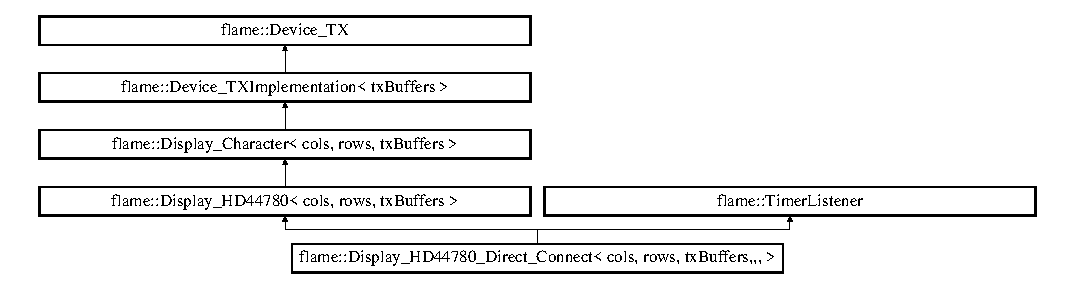
\includegraphics[height=3.439803cm]{classflame_1_1_display___h_d44780___direct___connect}
\end{center}
\end{figure}
\subsection*{Public Member Functions}
\begin{DoxyCompactItemize}
\item 
\hyperlink{classflame_1_1_display___h_d44780___direct___connect_afc5b9ca460d14b1a9f9417adac6045e6}{Display\-\_\-\-H\-D44780\-\_\-\-Direct\-\_\-\-Connect} ()
\item 
void \hyperlink{classflame_1_1_display___h_d44780___direct___connect_a2b3fe7dcd75cdece4c2d4a710dc19543}{set\-Backlight} (uint8\-\_\-t value)
\item 
void \hyperlink{classflame_1_1_display___h_d44780___direct___connect_afe86e7fcf2ac921f21f2bc84fa714bdd}{set\-Contrast} (uint8\-\_\-t value)
\item 
void \hyperlink{classflame_1_1_display___h_d44780___direct___connect_a1ee3e3007aa1c4a39f42306c63392fbe}{alarm} (\hyperlink{io_8h_addf5ec070e9499d36b7f2009ce736076}{U\-N\-U\-S\-E\-D} \hyperlink{namespaceflame_a6d176ba245556716fd3e32006bb7cfe5}{Alarm\-Source} source)
\item 
void \hyperlink{classflame_1_1_display___h_d44780___direct___connect_a92ba7ed48a7b6b04f3b7ce5677720b46}{init} (bool multi\-Line, bool big\-Font, bool cursor\-On, bool cursor\-Blink, bool left2right, bool scroll)
\end{DoxyCompactItemize}
\subsection*{Protected Member Functions}
\begin{DoxyCompactItemize}
\item 
void \hyperlink{classflame_1_1_display___h_d44780___direct___connect_a6a9b905a7ab50b32fecaf3028c24480a}{write\-Byte} (uint8\-\_\-t byte, bool rs)
\item 
void \hyperlink{classflame_1_1_display___h_d44780___direct___connect_abe30b389fc500e03871f1b2e43f6d731}{write\-Nibble} (uint8\-\_\-t nibble, bool rs)
\item 
uint8\-\_\-t \hyperlink{classflame_1_1_display___h_d44780___direct___connect_a23bb25f11ab61c6080887782baf320f4}{read\-Byte} (bool rs)
\item 
uint8\-\_\-t \hyperlink{classflame_1_1_display___h_d44780___direct___connect_adc962056ee69c61e2c6e12f6ff977d66}{read\-Nibble} (bool rs)
\item 
bool \hyperlink{classflame_1_1_display___h_d44780___direct___connect_af998178c1527fd6f01a38e652aff664d}{is\-Busy} ()
\item 
void \hyperlink{io_8h_a0c33b494a68ce28497e7ce8e5e95feff}{C\-O\-N\-S\-T} \hyperlink{classflame_1_1_display___h_d44780___direct___connect_aafaff0728ce50365bf8b17ec659d9235}{delay} (\hyperlink{io_8h_addf5ec070e9499d36b7f2009ce736076}{U\-N\-U\-S\-E\-D} \hyperlink{namespaceflame_ad814bac19b0569ff480de071076a23e9}{H\-D44780\-Command} command)
\end{DoxyCompactItemize}
\subsection*{Protected Attributes}
\begin{DoxyCompactItemize}
\item 
uint8\-\_\-t \hyperlink{classflame_1_1_display___h_d44780___direct___connect_aa0454a004930d249cd3c13a54d5dc953}{\-\_\-brightness}
\item 
uint8\-\_\-t \hyperlink{classflame_1_1_display___h_d44780___direct___connect_a889e562f76f0f7d3299e55909f881f50}{\-\_\-contrast}
\item 
uint8\-\_\-t \hyperlink{classflame_1_1_display___h_d44780___direct___connect_a81a099e0fea9395ebf8559e10280015f}{\-\_\-data\-Mask}
\item 
uint8\-\_\-t \hyperlink{classflame_1_1_display___h_d44780___direct___connect_a25ab255622804e4bf62ee318bc4d932e}{\-\_\-ticks}
\end{DoxyCompactItemize}


\subsection{Detailed Description}
\subsubsection*{template$<$uint16\-\_\-t cols, uint16\-\_\-t rows, uint8\-\_\-t tx\-Buffers, F\-L\-A\-M\-E\-\_\-\-D\-E\-C\-L\-A\-R\-E\-\_\-\-P\-I\-N(data), F\-L\-A\-M\-E\-\_\-\-D\-E\-C\-L\-A\-R\-E\-\_\-\-P\-I\-N(control), F\-L\-A\-M\-E\-\_\-\-D\-E\-C\-L\-A\-R\-E\-\_\-\-P\-I\-N(visual)$>$class flame\-::\-Display\-\_\-\-H\-D44780\-\_\-\-Direct\-\_\-\-Connect$<$ cols, rows, tx\-Buffers,,, $>$}

A class for operating H\-D44780 based L\-C\-D displays (and compatible) in 4 bit mode Data port layout\-: Bit description n D\-B4 n+1 D\-B5 n+2 D\-B6 n+3 D\-B7

Control port layout\-: n R\-S Register Select n+1 R/\-W Read/\-Write n+2 E Enable

Visual port layout\-: n Contrast (V0) n+1 L\-E\-D Positive


\begin{DoxyTemplParams}{Template Parameters}
{\em cols} & the number of columns \\
\hline
{\em rows} & the number of rows \\
\hline
{\em tx\-Buffers} & the number of output buffers \\
\hline
{\em data...} & pin declaration for the first bit of the data port D\-B4..D\-B7 (will use a nibble starting at this bit) \\
\hline
{\em control...} & pin declaration for the first bit of the control port (will use 3 bits) \\
\hline
{\em visual...} & pin declaration for the first bit of the visual port (will use 2 bits) \\
\hline
\end{DoxyTemplParams}


Definition at line 85 of file Display\-\_\-\-H\-D44780\-\_\-\-Direct\-\_\-\-Connect.\-h.



\subsection{Constructor \& Destructor Documentation}
\hypertarget{classflame_1_1_display___h_d44780___direct___connect_afc5b9ca460d14b1a9f9417adac6045e6}{\index{flame\-::\-Display\-\_\-\-H\-D44780\-\_\-\-Direct\-\_\-\-Connect@{flame\-::\-Display\-\_\-\-H\-D44780\-\_\-\-Direct\-\_\-\-Connect}!Display\-\_\-\-H\-D44780\-\_\-\-Direct\-\_\-\-Connect@{Display\-\_\-\-H\-D44780\-\_\-\-Direct\-\_\-\-Connect}}
\index{Display\-\_\-\-H\-D44780\-\_\-\-Direct\-\_\-\-Connect@{Display\-\_\-\-H\-D44780\-\_\-\-Direct\-\_\-\-Connect}!flame::Display_HD44780_Direct_Connect@{flame\-::\-Display\-\_\-\-H\-D44780\-\_\-\-Direct\-\_\-\-Connect}}
\subsubsection[{Display\-\_\-\-H\-D44780\-\_\-\-Direct\-\_\-\-Connect}]{\setlength{\rightskip}{0pt plus 5cm}template$<$uint16\-\_\-t cols, uint16\-\_\-t rows, uint8\-\_\-t tx\-Buffers, F\-L\-A\-M\-E\-\_\-\-D\-E\-C\-L\-A\-R\-E\-\_\-\-P\-I\-N(data) , F\-L\-A\-M\-E\-\_\-\-D\-E\-C\-L\-A\-R\-E\-\_\-\-P\-I\-N(control) , F\-L\-A\-M\-E\-\_\-\-D\-E\-C\-L\-A\-R\-E\-\_\-\-P\-I\-N(visual) $>$ {\bf flame\-::\-Display\-\_\-\-H\-D44780\-\_\-\-Direct\-\_\-\-Connect}$<$ cols, rows, tx\-Buffers,,, $>$\-::{\bf Display\-\_\-\-H\-D44780\-\_\-\-Direct\-\_\-\-Connect} (
\begin{DoxyParamCaption}
{}
\end{DoxyParamCaption}
)\hspace{0.3cm}{\ttfamily [inline]}}}\label{classflame_1_1_display___h_d44780___direct___connect_afc5b9ca460d14b1a9f9417adac6045e6}
Create a new driver for a directly connected H\-D44780 display 

Definition at line 194 of file Display\-\_\-\-H\-D44780\-\_\-\-Direct\-\_\-\-Connect.\-h.



\subsection{Member Function Documentation}
\hypertarget{classflame_1_1_display___h_d44780___direct___connect_a1ee3e3007aa1c4a39f42306c63392fbe}{\index{flame\-::\-Display\-\_\-\-H\-D44780\-\_\-\-Direct\-\_\-\-Connect@{flame\-::\-Display\-\_\-\-H\-D44780\-\_\-\-Direct\-\_\-\-Connect}!alarm@{alarm}}
\index{alarm@{alarm}!flame::Display_HD44780_Direct_Connect@{flame\-::\-Display\-\_\-\-H\-D44780\-\_\-\-Direct\-\_\-\-Connect}}
\subsubsection[{alarm}]{\setlength{\rightskip}{0pt plus 5cm}template$<$uint16\-\_\-t cols, uint16\-\_\-t rows, uint8\-\_\-t tx\-Buffers, F\-L\-A\-M\-E\-\_\-\-D\-E\-C\-L\-A\-R\-E\-\_\-\-P\-I\-N(data) , F\-L\-A\-M\-E\-\_\-\-D\-E\-C\-L\-A\-R\-E\-\_\-\-P\-I\-N(control) , F\-L\-A\-M\-E\-\_\-\-D\-E\-C\-L\-A\-R\-E\-\_\-\-P\-I\-N(visual) $>$ void {\bf flame\-::\-Display\-\_\-\-H\-D44780\-\_\-\-Direct\-\_\-\-Connect}$<$ cols, rows, tx\-Buffers,,, $>$\-::{\bf alarm} (
\begin{DoxyParamCaption}
\item[{{\bf U\-N\-U\-S\-E\-D} {\bf Alarm\-Source}}]{source}
\end{DoxyParamCaption}
)\hspace{0.3cm}{\ttfamily [inline]}}}\label{classflame_1_1_display___h_d44780___direct___connect_a1ee3e3007aa1c4a39f42306c63392fbe}
Tick the display for P\-W\-M -\/ this should be called every 500 microseconds 

Definition at line 239 of file Display\-\_\-\-H\-D44780\-\_\-\-Direct\-\_\-\-Connect.\-h.

\hypertarget{classflame_1_1_display___h_d44780___direct___connect_aafaff0728ce50365bf8b17ec659d9235}{\index{flame\-::\-Display\-\_\-\-H\-D44780\-\_\-\-Direct\-\_\-\-Connect@{flame\-::\-Display\-\_\-\-H\-D44780\-\_\-\-Direct\-\_\-\-Connect}!delay@{delay}}
\index{delay@{delay}!flame::Display_HD44780_Direct_Connect@{flame\-::\-Display\-\_\-\-H\-D44780\-\_\-\-Direct\-\_\-\-Connect}}
\subsubsection[{delay}]{\setlength{\rightskip}{0pt plus 5cm}template$<$uint16\-\_\-t cols, uint16\-\_\-t rows, uint8\-\_\-t tx\-Buffers, F\-L\-A\-M\-E\-\_\-\-D\-E\-C\-L\-A\-R\-E\-\_\-\-P\-I\-N(data) , F\-L\-A\-M\-E\-\_\-\-D\-E\-C\-L\-A\-R\-E\-\_\-\-P\-I\-N(control) , F\-L\-A\-M\-E\-\_\-\-D\-E\-C\-L\-A\-R\-E\-\_\-\-P\-I\-N(visual) $>$ void {\bf C\-O\-N\-S\-T} {\bf flame\-::\-Display\-\_\-\-H\-D44780\-\_\-\-Direct\-\_\-\-Connect}$<$ cols, rows, tx\-Buffers,,, $>$\-::delay (
\begin{DoxyParamCaption}
\item[{{\bf U\-N\-U\-S\-E\-D} {\bf H\-D44780\-Command}}]{command}
\end{DoxyParamCaption}
)\hspace{0.3cm}{\ttfamily [inline]}, {\ttfamily [protected]}}}\label{classflame_1_1_display___h_d44780___direct___connect_aafaff0728ce50365bf8b17ec659d9235}
Delay function No delays required as we can check whether the display is busy 

Definition at line 186 of file Display\-\_\-\-H\-D44780\-\_\-\-Direct\-\_\-\-Connect.\-h.

\hypertarget{classflame_1_1_display___h_d44780___direct___connect_a92ba7ed48a7b6b04f3b7ce5677720b46}{\index{flame\-::\-Display\-\_\-\-H\-D44780\-\_\-\-Direct\-\_\-\-Connect@{flame\-::\-Display\-\_\-\-H\-D44780\-\_\-\-Direct\-\_\-\-Connect}!init@{init}}
\index{init@{init}!flame::Display_HD44780_Direct_Connect@{flame\-::\-Display\-\_\-\-H\-D44780\-\_\-\-Direct\-\_\-\-Connect}}
\subsubsection[{init}]{\setlength{\rightskip}{0pt plus 5cm}template$<$uint16\-\_\-t cols, uint16\-\_\-t rows, uint8\-\_\-t tx\-Buffers, F\-L\-A\-M\-E\-\_\-\-D\-E\-C\-L\-A\-R\-E\-\_\-\-P\-I\-N(data) , F\-L\-A\-M\-E\-\_\-\-D\-E\-C\-L\-A\-R\-E\-\_\-\-P\-I\-N(control) , F\-L\-A\-M\-E\-\_\-\-D\-E\-C\-L\-A\-R\-E\-\_\-\-P\-I\-N(visual) $>$ void {\bf flame\-::\-Display\-\_\-\-H\-D44780\-\_\-\-Direct\-\_\-\-Connect}$<$ cols, rows, tx\-Buffers,,, $>$\-::init (
\begin{DoxyParamCaption}
\item[{bool}]{multi\-Line, }
\item[{bool}]{big\-Font, }
\item[{bool}]{cursor\-On, }
\item[{bool}]{cursor\-Blink, }
\item[{bool}]{left2right, }
\item[{bool}]{scroll}
\end{DoxyParamCaption}
)\hspace{0.3cm}{\ttfamily [inline]}}}\label{classflame_1_1_display___h_d44780___direct___connect_a92ba7ed48a7b6b04f3b7ce5677720b46}
Initialise the display 
\begin{DoxyParams}{Parameters}
{\em multi\-Line} & true if there is more than 1 line \\
\hline
{\em big\-Font} & true to use 5x11 fonts, false for 5x8 \\
\hline
{\em cursor\-On} & turn the curson on \\
\hline
{\em cursor\-Blink} & blink the cursor \\
\hline
{\em left2right} & true for text reading left to right \\
\hline
{\em scroll} & true to scroll text rather than moving the cursor \\
\hline
\end{DoxyParams}


Definition at line 267 of file Display\-\_\-\-H\-D44780\-\_\-\-Direct\-\_\-\-Connect.\-h.

\hypertarget{classflame_1_1_display___h_d44780___direct___connect_af998178c1527fd6f01a38e652aff664d}{\index{flame\-::\-Display\-\_\-\-H\-D44780\-\_\-\-Direct\-\_\-\-Connect@{flame\-::\-Display\-\_\-\-H\-D44780\-\_\-\-Direct\-\_\-\-Connect}!is\-Busy@{is\-Busy}}
\index{is\-Busy@{is\-Busy}!flame::Display_HD44780_Direct_Connect@{flame\-::\-Display\-\_\-\-H\-D44780\-\_\-\-Direct\-\_\-\-Connect}}
\subsubsection[{is\-Busy}]{\setlength{\rightskip}{0pt plus 5cm}template$<$uint16\-\_\-t cols, uint16\-\_\-t rows, uint8\-\_\-t tx\-Buffers, F\-L\-A\-M\-E\-\_\-\-D\-E\-C\-L\-A\-R\-E\-\_\-\-P\-I\-N(data) , F\-L\-A\-M\-E\-\_\-\-D\-E\-C\-L\-A\-R\-E\-\_\-\-P\-I\-N(control) , F\-L\-A\-M\-E\-\_\-\-D\-E\-C\-L\-A\-R\-E\-\_\-\-P\-I\-N(visual) $>$ bool {\bf flame\-::\-Display\-\_\-\-H\-D44780\-\_\-\-Direct\-\_\-\-Connect}$<$ cols, rows, tx\-Buffers,,, $>$\-::is\-Busy (
\begin{DoxyParamCaption}
{}
\end{DoxyParamCaption}
)\hspace{0.3cm}{\ttfamily [inline]}, {\ttfamily [protected]}, {\ttfamily [virtual]}}}\label{classflame_1_1_display___h_d44780___direct___connect_af998178c1527fd6f01a38e652aff664d}
Check if the display is busy \begin{DoxyReturn}{Returns}
true if the display is busy 
\end{DoxyReturn}


Implements \hyperlink{classflame_1_1_display___h_d44780_a665b559a3a2370fada65efd724a412b9}{flame\-::\-Display\-\_\-\-H\-D44780$<$ cols, rows, tx\-Buffers $>$}.



Definition at line 165 of file Display\-\_\-\-H\-D44780\-\_\-\-Direct\-\_\-\-Connect.\-h.

\hypertarget{classflame_1_1_display___h_d44780___direct___connect_a23bb25f11ab61c6080887782baf320f4}{\index{flame\-::\-Display\-\_\-\-H\-D44780\-\_\-\-Direct\-\_\-\-Connect@{flame\-::\-Display\-\_\-\-H\-D44780\-\_\-\-Direct\-\_\-\-Connect}!read\-Byte@{read\-Byte}}
\index{read\-Byte@{read\-Byte}!flame::Display_HD44780_Direct_Connect@{flame\-::\-Display\-\_\-\-H\-D44780\-\_\-\-Direct\-\_\-\-Connect}}
\subsubsection[{read\-Byte}]{\setlength{\rightskip}{0pt plus 5cm}template$<$uint16\-\_\-t cols, uint16\-\_\-t rows, uint8\-\_\-t tx\-Buffers, F\-L\-A\-M\-E\-\_\-\-D\-E\-C\-L\-A\-R\-E\-\_\-\-P\-I\-N(data) , F\-L\-A\-M\-E\-\_\-\-D\-E\-C\-L\-A\-R\-E\-\_\-\-P\-I\-N(control) , F\-L\-A\-M\-E\-\_\-\-D\-E\-C\-L\-A\-R\-E\-\_\-\-P\-I\-N(visual) $>$ uint8\-\_\-t {\bf flame\-::\-Display\-\_\-\-H\-D44780\-\_\-\-Direct\-\_\-\-Connect}$<$ cols, rows, tx\-Buffers,,, $>$\-::read\-Byte (
\begin{DoxyParamCaption}
\item[{bool}]{rs}
\end{DoxyParamCaption}
)\hspace{0.3cm}{\ttfamily [inline]}, {\ttfamily [protected]}, {\ttfamily [virtual]}}}\label{classflame_1_1_display___h_d44780___direct___connect_a23bb25f11ab61c6080887782baf320f4}
Read a byte from the display 
\begin{DoxyParams}{Parameters}
{\em rs} & true to set the R\-S pin \\
\hline
\end{DoxyParams}


Implements \hyperlink{classflame_1_1_display___h_d44780_ae3409f84516a6533d88bc70b200a6e23}{flame\-::\-Display\-\_\-\-H\-D44780$<$ cols, rows, tx\-Buffers $>$}.



Definition at line 131 of file Display\-\_\-\-H\-D44780\-\_\-\-Direct\-\_\-\-Connect.\-h.

\hypertarget{classflame_1_1_display___h_d44780___direct___connect_adc962056ee69c61e2c6e12f6ff977d66}{\index{flame\-::\-Display\-\_\-\-H\-D44780\-\_\-\-Direct\-\_\-\-Connect@{flame\-::\-Display\-\_\-\-H\-D44780\-\_\-\-Direct\-\_\-\-Connect}!read\-Nibble@{read\-Nibble}}
\index{read\-Nibble@{read\-Nibble}!flame::Display_HD44780_Direct_Connect@{flame\-::\-Display\-\_\-\-H\-D44780\-\_\-\-Direct\-\_\-\-Connect}}
\subsubsection[{read\-Nibble}]{\setlength{\rightskip}{0pt plus 5cm}template$<$uint16\-\_\-t cols, uint16\-\_\-t rows, uint8\-\_\-t tx\-Buffers, F\-L\-A\-M\-E\-\_\-\-D\-E\-C\-L\-A\-R\-E\-\_\-\-P\-I\-N(data) , F\-L\-A\-M\-E\-\_\-\-D\-E\-C\-L\-A\-R\-E\-\_\-\-P\-I\-N(control) , F\-L\-A\-M\-E\-\_\-\-D\-E\-C\-L\-A\-R\-E\-\_\-\-P\-I\-N(visual) $>$ uint8\-\_\-t {\bf flame\-::\-Display\-\_\-\-H\-D44780\-\_\-\-Direct\-\_\-\-Connect}$<$ cols, rows, tx\-Buffers,,, $>$\-::read\-Nibble (
\begin{DoxyParamCaption}
\item[{bool}]{rs}
\end{DoxyParamCaption}
)\hspace{0.3cm}{\ttfamily [inline]}, {\ttfamily [protected]}}}\label{classflame_1_1_display___h_d44780___direct___connect_adc962056ee69c61e2c6e12f6ff977d66}
Read a nibble from the display 
\begin{DoxyParams}{Parameters}
{\em rs} & true to set the R\-S pin \\
\hline
\end{DoxyParams}


Definition at line 143 of file Display\-\_\-\-H\-D44780\-\_\-\-Direct\-\_\-\-Connect.\-h.

\hypertarget{classflame_1_1_display___h_d44780___direct___connect_a2b3fe7dcd75cdece4c2d4a710dc19543}{\index{flame\-::\-Display\-\_\-\-H\-D44780\-\_\-\-Direct\-\_\-\-Connect@{flame\-::\-Display\-\_\-\-H\-D44780\-\_\-\-Direct\-\_\-\-Connect}!set\-Backlight@{set\-Backlight}}
\index{set\-Backlight@{set\-Backlight}!flame::Display_HD44780_Direct_Connect@{flame\-::\-Display\-\_\-\-H\-D44780\-\_\-\-Direct\-\_\-\-Connect}}
\subsubsection[{set\-Backlight}]{\setlength{\rightskip}{0pt plus 5cm}template$<$uint16\-\_\-t cols, uint16\-\_\-t rows, uint8\-\_\-t tx\-Buffers, F\-L\-A\-M\-E\-\_\-\-D\-E\-C\-L\-A\-R\-E\-\_\-\-P\-I\-N(data) , F\-L\-A\-M\-E\-\_\-\-D\-E\-C\-L\-A\-R\-E\-\_\-\-P\-I\-N(control) , F\-L\-A\-M\-E\-\_\-\-D\-E\-C\-L\-A\-R\-E\-\_\-\-P\-I\-N(visual) $>$ void {\bf flame\-::\-Display\-\_\-\-H\-D44780\-\_\-\-Direct\-\_\-\-Connect}$<$ cols, rows, tx\-Buffers,,, $>$\-::set\-Backlight (
\begin{DoxyParamCaption}
\item[{uint8\-\_\-t}]{value}
\end{DoxyParamCaption}
)\hspace{0.3cm}{\ttfamily [inline]}}}\label{classflame_1_1_display___h_d44780___direct___connect_a2b3fe7dcd75cdece4c2d4a710dc19543}
Manipulate the backlight 
\begin{DoxyParams}{Parameters}
{\em value} & the brightness of the backlight (0..15) \\
\hline
\end{DoxyParams}


Definition at line 216 of file Display\-\_\-\-H\-D44780\-\_\-\-Direct\-\_\-\-Connect.\-h.

\hypertarget{classflame_1_1_display___h_d44780___direct___connect_afe86e7fcf2ac921f21f2bc84fa714bdd}{\index{flame\-::\-Display\-\_\-\-H\-D44780\-\_\-\-Direct\-\_\-\-Connect@{flame\-::\-Display\-\_\-\-H\-D44780\-\_\-\-Direct\-\_\-\-Connect}!set\-Contrast@{set\-Contrast}}
\index{set\-Contrast@{set\-Contrast}!flame::Display_HD44780_Direct_Connect@{flame\-::\-Display\-\_\-\-H\-D44780\-\_\-\-Direct\-\_\-\-Connect}}
\subsubsection[{set\-Contrast}]{\setlength{\rightskip}{0pt plus 5cm}template$<$uint16\-\_\-t cols, uint16\-\_\-t rows, uint8\-\_\-t tx\-Buffers, F\-L\-A\-M\-E\-\_\-\-D\-E\-C\-L\-A\-R\-E\-\_\-\-P\-I\-N(data) , F\-L\-A\-M\-E\-\_\-\-D\-E\-C\-L\-A\-R\-E\-\_\-\-P\-I\-N(control) , F\-L\-A\-M\-E\-\_\-\-D\-E\-C\-L\-A\-R\-E\-\_\-\-P\-I\-N(visual) $>$ void {\bf flame\-::\-Display\-\_\-\-H\-D44780\-\_\-\-Direct\-\_\-\-Connect}$<$ cols, rows, tx\-Buffers,,, $>$\-::set\-Contrast (
\begin{DoxyParamCaption}
\item[{uint8\-\_\-t}]{value}
\end{DoxyParamCaption}
)\hspace{0.3cm}{\ttfamily [inline]}}}\label{classflame_1_1_display___h_d44780___direct___connect_afe86e7fcf2ac921f21f2bc84fa714bdd}
Set the contrast 
\begin{DoxyParams}{Parameters}
{\em value} & the contrast of the display(0..15) \\
\hline
\end{DoxyParams}


Definition at line 227 of file Display\-\_\-\-H\-D44780\-\_\-\-Direct\-\_\-\-Connect.\-h.

\hypertarget{classflame_1_1_display___h_d44780___direct___connect_a6a9b905a7ab50b32fecaf3028c24480a}{\index{flame\-::\-Display\-\_\-\-H\-D44780\-\_\-\-Direct\-\_\-\-Connect@{flame\-::\-Display\-\_\-\-H\-D44780\-\_\-\-Direct\-\_\-\-Connect}!write\-Byte@{write\-Byte}}
\index{write\-Byte@{write\-Byte}!flame::Display_HD44780_Direct_Connect@{flame\-::\-Display\-\_\-\-H\-D44780\-\_\-\-Direct\-\_\-\-Connect}}
\subsubsection[{write\-Byte}]{\setlength{\rightskip}{0pt plus 5cm}template$<$uint16\-\_\-t cols, uint16\-\_\-t rows, uint8\-\_\-t tx\-Buffers, F\-L\-A\-M\-E\-\_\-\-D\-E\-C\-L\-A\-R\-E\-\_\-\-P\-I\-N(data) , F\-L\-A\-M\-E\-\_\-\-D\-E\-C\-L\-A\-R\-E\-\_\-\-P\-I\-N(control) , F\-L\-A\-M\-E\-\_\-\-D\-E\-C\-L\-A\-R\-E\-\_\-\-P\-I\-N(visual) $>$ void {\bf flame\-::\-Display\-\_\-\-H\-D44780\-\_\-\-Direct\-\_\-\-Connect}$<$ cols, rows, tx\-Buffers,,, $>$\-::write\-Byte (
\begin{DoxyParamCaption}
\item[{uint8\-\_\-t}]{byte, }
\item[{bool}]{rs}
\end{DoxyParamCaption}
)\hspace{0.3cm}{\ttfamily [inline]}, {\ttfamily [protected]}, {\ttfamily [virtual]}}}\label{classflame_1_1_display___h_d44780___direct___connect_a6a9b905a7ab50b32fecaf3028c24480a}
Write a byte to the display 
\begin{DoxyParams}{Parameters}
{\em byte} & the data to write \\
\hline
{\em rs} & true to set the R\-S pin \\
\hline
\end{DoxyParams}


Implements \hyperlink{classflame_1_1_display___h_d44780_a7a6b0c6550f20961f3cec7b07e0835ed}{flame\-::\-Display\-\_\-\-H\-D44780$<$ cols, rows, tx\-Buffers $>$}.



Definition at line 98 of file Display\-\_\-\-H\-D44780\-\_\-\-Direct\-\_\-\-Connect.\-h.

\hypertarget{classflame_1_1_display___h_d44780___direct___connect_abe30b389fc500e03871f1b2e43f6d731}{\index{flame\-::\-Display\-\_\-\-H\-D44780\-\_\-\-Direct\-\_\-\-Connect@{flame\-::\-Display\-\_\-\-H\-D44780\-\_\-\-Direct\-\_\-\-Connect}!write\-Nibble@{write\-Nibble}}
\index{write\-Nibble@{write\-Nibble}!flame::Display_HD44780_Direct_Connect@{flame\-::\-Display\-\_\-\-H\-D44780\-\_\-\-Direct\-\_\-\-Connect}}
\subsubsection[{write\-Nibble}]{\setlength{\rightskip}{0pt plus 5cm}template$<$uint16\-\_\-t cols, uint16\-\_\-t rows, uint8\-\_\-t tx\-Buffers, F\-L\-A\-M\-E\-\_\-\-D\-E\-C\-L\-A\-R\-E\-\_\-\-P\-I\-N(data) , F\-L\-A\-M\-E\-\_\-\-D\-E\-C\-L\-A\-R\-E\-\_\-\-P\-I\-N(control) , F\-L\-A\-M\-E\-\_\-\-D\-E\-C\-L\-A\-R\-E\-\_\-\-P\-I\-N(visual) $>$ void {\bf flame\-::\-Display\-\_\-\-H\-D44780\-\_\-\-Direct\-\_\-\-Connect}$<$ cols, rows, tx\-Buffers,,, $>$\-::write\-Nibble (
\begin{DoxyParamCaption}
\item[{uint8\-\_\-t}]{nibble, }
\item[{bool}]{rs}
\end{DoxyParamCaption}
)\hspace{0.3cm}{\ttfamily [inline]}, {\ttfamily [protected]}}}\label{classflame_1_1_display___h_d44780___direct___connect_abe30b389fc500e03871f1b2e43f6d731}
Write a nibble to the display 
\begin{DoxyParams}{Parameters}
{\em nibble} & the data to write (lower 4 bits) \\
\hline
{\em rs} & true to set the R\-S pin \\
\hline
\end{DoxyParams}


Definition at line 110 of file Display\-\_\-\-H\-D44780\-\_\-\-Direct\-\_\-\-Connect.\-h.



\subsection{Member Data Documentation}
\hypertarget{classflame_1_1_display___h_d44780___direct___connect_aa0454a004930d249cd3c13a54d5dc953}{\index{flame\-::\-Display\-\_\-\-H\-D44780\-\_\-\-Direct\-\_\-\-Connect@{flame\-::\-Display\-\_\-\-H\-D44780\-\_\-\-Direct\-\_\-\-Connect}!\-\_\-brightness@{\-\_\-brightness}}
\index{\-\_\-brightness@{\-\_\-brightness}!flame::Display_HD44780_Direct_Connect@{flame\-::\-Display\-\_\-\-H\-D44780\-\_\-\-Direct\-\_\-\-Connect}}
\subsubsection[{\-\_\-brightness}]{\setlength{\rightskip}{0pt plus 5cm}template$<$uint16\-\_\-t cols, uint16\-\_\-t rows, uint8\-\_\-t tx\-Buffers, F\-L\-A\-M\-E\-\_\-\-D\-E\-C\-L\-A\-R\-E\-\_\-\-P\-I\-N(data) , F\-L\-A\-M\-E\-\_\-\-D\-E\-C\-L\-A\-R\-E\-\_\-\-P\-I\-N(control) , F\-L\-A\-M\-E\-\_\-\-D\-E\-C\-L\-A\-R\-E\-\_\-\-P\-I\-N(visual) $>$ uint8\-\_\-t {\bf flame\-::\-Display\-\_\-\-H\-D44780\-\_\-\-Direct\-\_\-\-Connect}$<$ cols, rows, tx\-Buffers,,, $>$\-::\-\_\-brightness\hspace{0.3cm}{\ttfamily [protected]}}}\label{classflame_1_1_display___h_d44780___direct___connect_aa0454a004930d249cd3c13a54d5dc953}


Definition at line 88 of file Display\-\_\-\-H\-D44780\-\_\-\-Direct\-\_\-\-Connect.\-h.

\hypertarget{classflame_1_1_display___h_d44780___direct___connect_a889e562f76f0f7d3299e55909f881f50}{\index{flame\-::\-Display\-\_\-\-H\-D44780\-\_\-\-Direct\-\_\-\-Connect@{flame\-::\-Display\-\_\-\-H\-D44780\-\_\-\-Direct\-\_\-\-Connect}!\-\_\-contrast@{\-\_\-contrast}}
\index{\-\_\-contrast@{\-\_\-contrast}!flame::Display_HD44780_Direct_Connect@{flame\-::\-Display\-\_\-\-H\-D44780\-\_\-\-Direct\-\_\-\-Connect}}
\subsubsection[{\-\_\-contrast}]{\setlength{\rightskip}{0pt plus 5cm}template$<$uint16\-\_\-t cols, uint16\-\_\-t rows, uint8\-\_\-t tx\-Buffers, F\-L\-A\-M\-E\-\_\-\-D\-E\-C\-L\-A\-R\-E\-\_\-\-P\-I\-N(data) , F\-L\-A\-M\-E\-\_\-\-D\-E\-C\-L\-A\-R\-E\-\_\-\-P\-I\-N(control) , F\-L\-A\-M\-E\-\_\-\-D\-E\-C\-L\-A\-R\-E\-\_\-\-P\-I\-N(visual) $>$ uint8\-\_\-t {\bf flame\-::\-Display\-\_\-\-H\-D44780\-\_\-\-Direct\-\_\-\-Connect}$<$ cols, rows, tx\-Buffers,,, $>$\-::\-\_\-contrast\hspace{0.3cm}{\ttfamily [protected]}}}\label{classflame_1_1_display___h_d44780___direct___connect_a889e562f76f0f7d3299e55909f881f50}


Definition at line 89 of file Display\-\_\-\-H\-D44780\-\_\-\-Direct\-\_\-\-Connect.\-h.

\hypertarget{classflame_1_1_display___h_d44780___direct___connect_a81a099e0fea9395ebf8559e10280015f}{\index{flame\-::\-Display\-\_\-\-H\-D44780\-\_\-\-Direct\-\_\-\-Connect@{flame\-::\-Display\-\_\-\-H\-D44780\-\_\-\-Direct\-\_\-\-Connect}!\-\_\-data\-Mask@{\-\_\-data\-Mask}}
\index{\-\_\-data\-Mask@{\-\_\-data\-Mask}!flame::Display_HD44780_Direct_Connect@{flame\-::\-Display\-\_\-\-H\-D44780\-\_\-\-Direct\-\_\-\-Connect}}
\subsubsection[{\-\_\-data\-Mask}]{\setlength{\rightskip}{0pt plus 5cm}template$<$uint16\-\_\-t cols, uint16\-\_\-t rows, uint8\-\_\-t tx\-Buffers, F\-L\-A\-M\-E\-\_\-\-D\-E\-C\-L\-A\-R\-E\-\_\-\-P\-I\-N(data) , F\-L\-A\-M\-E\-\_\-\-D\-E\-C\-L\-A\-R\-E\-\_\-\-P\-I\-N(control) , F\-L\-A\-M\-E\-\_\-\-D\-E\-C\-L\-A\-R\-E\-\_\-\-P\-I\-N(visual) $>$ uint8\-\_\-t {\bf flame\-::\-Display\-\_\-\-H\-D44780\-\_\-\-Direct\-\_\-\-Connect}$<$ cols, rows, tx\-Buffers,,, $>$\-::\-\_\-data\-Mask\hspace{0.3cm}{\ttfamily [protected]}}}\label{classflame_1_1_display___h_d44780___direct___connect_a81a099e0fea9395ebf8559e10280015f}


Definition at line 90 of file Display\-\_\-\-H\-D44780\-\_\-\-Direct\-\_\-\-Connect.\-h.

\hypertarget{classflame_1_1_display___h_d44780___direct___connect_a25ab255622804e4bf62ee318bc4d932e}{\index{flame\-::\-Display\-\_\-\-H\-D44780\-\_\-\-Direct\-\_\-\-Connect@{flame\-::\-Display\-\_\-\-H\-D44780\-\_\-\-Direct\-\_\-\-Connect}!\-\_\-ticks@{\-\_\-ticks}}
\index{\-\_\-ticks@{\-\_\-ticks}!flame::Display_HD44780_Direct_Connect@{flame\-::\-Display\-\_\-\-H\-D44780\-\_\-\-Direct\-\_\-\-Connect}}
\subsubsection[{\-\_\-ticks}]{\setlength{\rightskip}{0pt plus 5cm}template$<$uint16\-\_\-t cols, uint16\-\_\-t rows, uint8\-\_\-t tx\-Buffers, F\-L\-A\-M\-E\-\_\-\-D\-E\-C\-L\-A\-R\-E\-\_\-\-P\-I\-N(data) , F\-L\-A\-M\-E\-\_\-\-D\-E\-C\-L\-A\-R\-E\-\_\-\-P\-I\-N(control) , F\-L\-A\-M\-E\-\_\-\-D\-E\-C\-L\-A\-R\-E\-\_\-\-P\-I\-N(visual) $>$ uint8\-\_\-t {\bf flame\-::\-Display\-\_\-\-H\-D44780\-\_\-\-Direct\-\_\-\-Connect}$<$ cols, rows, tx\-Buffers,,, $>$\-::\-\_\-ticks\hspace{0.3cm}{\ttfamily [protected]}}}\label{classflame_1_1_display___h_d44780___direct___connect_a25ab255622804e4bf62ee318bc4d932e}


Definition at line 91 of file Display\-\_\-\-H\-D44780\-\_\-\-Direct\-\_\-\-Connect.\-h.



The documentation for this class was generated from the following file\-:\begin{DoxyCompactItemize}
\item 
flame/\hyperlink{_display___h_d44780___direct___connect_8h}{Display\-\_\-\-H\-D44780\-\_\-\-Direct\-\_\-\-Connect.\-h}\end{DoxyCompactItemize}

\hypertarget{classflame_1_1_display___h_d44780___shift___register}{\section{flame\-:\-:Display\-\_\-\-H\-D44780\-\_\-\-Shift\-\_\-\-Register$<$ cols, rows, tx\-Buffers,,, $>$ Class Template Reference}
\label{classflame_1_1_display___h_d44780___shift___register}\index{flame\-::\-Display\-\_\-\-H\-D44780\-\_\-\-Shift\-\_\-\-Register$<$ cols, rows, tx\-Buffers,,, $>$@{flame\-::\-Display\-\_\-\-H\-D44780\-\_\-\-Shift\-\_\-\-Register$<$ cols, rows, tx\-Buffers,,, $>$}}
}


{\ttfamily \#include $<$Display\-\_\-\-H\-D44780\-\_\-\-Shift\-\_\-\-Register.\-h$>$}

Inheritance diagram for flame\-:\-:Display\-\_\-\-H\-D44780\-\_\-\-Shift\-\_\-\-Register$<$ cols, rows, tx\-Buffers,,, $>$\-:\begin{figure}[H]
\begin{center}
\leavevmode
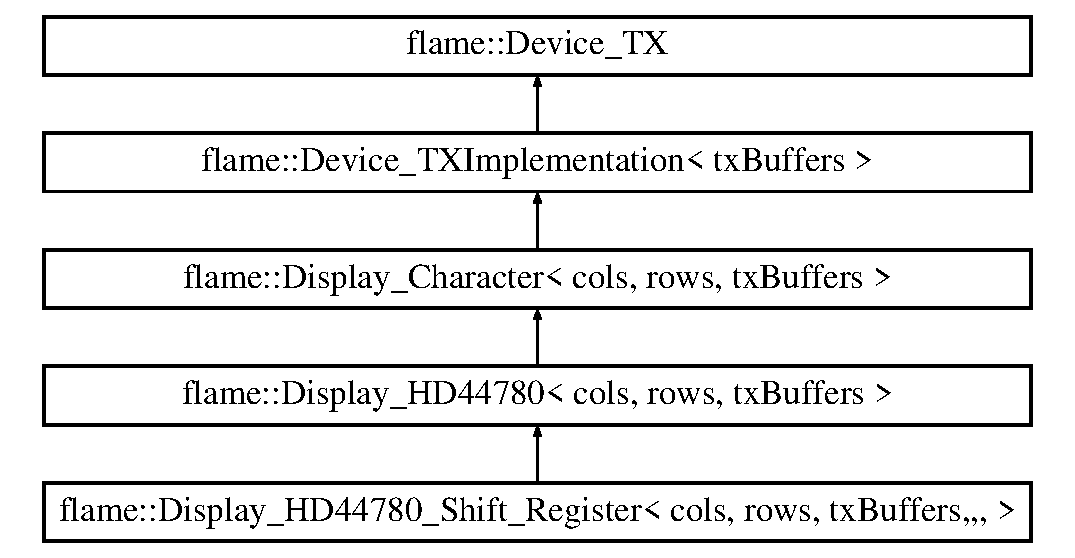
\includegraphics[height=5.000000cm]{classflame_1_1_display___h_d44780___shift___register}
\end{center}
\end{figure}
\subsection*{Public Member Functions}
\begin{DoxyCompactItemize}
\item 
\hyperlink{classflame_1_1_display___h_d44780___shift___register_a1d839e34a225476137a21cb75a7ed974}{Display\-\_\-\-H\-D44780\-\_\-\-Shift\-\_\-\-Register} ()
\item 
void \hyperlink{classflame_1_1_display___h_d44780___shift___register_ac71ba3d138e74bc16c34540490edc6a5}{init} (bool multi\-Line, bool big\-Font, bool cursor\-On, bool cursor\-Blink, bool left2right, bool scroll)
\end{DoxyCompactItemize}
\subsection*{Protected Member Functions}
\begin{DoxyCompactItemize}
\item 
void \hyperlink{classflame_1_1_display___h_d44780___shift___register_adcff45c7df2cd357da826d236396f2ca}{push\-Bits} (uint8\-\_\-t byte, bool rs)
\item 
void \hyperlink{classflame_1_1_display___h_d44780___shift___register_a95cc0c60b735e08990c4668e361e5e8b}{write\-Byte} (uint8\-\_\-t byte, bool rs)
\item 
uint8\-\_\-t \hyperlink{io_8h_a0c33b494a68ce28497e7ce8e5e95feff}{C\-O\-N\-S\-T} \hyperlink{classflame_1_1_display___h_d44780___shift___register_a1eda0c5acf844c39aab8abb85f371000}{read\-Byte} (\hyperlink{io_8h_addf5ec070e9499d36b7f2009ce736076}{U\-N\-U\-S\-E\-D} bool rs)
\item 
bool \hyperlink{io_8h_a0c33b494a68ce28497e7ce8e5e95feff}{C\-O\-N\-S\-T} \hyperlink{classflame_1_1_display___h_d44780___shift___register_af798f14b87bdafbcedf7b4458df2621b}{is\-Busy} ()
\item 
void \hyperlink{classflame_1_1_display___h_d44780___shift___register_abf59a4215c52f6cd29bdb2e901346945}{delay} (\hyperlink{namespaceflame_ad814bac19b0569ff480de071076a23e9}{H\-D44780\-Command} command)
\end{DoxyCompactItemize}
\subsection*{Additional Inherited Members}


\subsection{Detailed Description}
\subsubsection*{template$<$uint16\-\_\-t cols, uint16\-\_\-t rows, uint8\-\_\-t tx\-Buffers, F\-L\-A\-M\-E\-\_\-\-D\-E\-C\-L\-A\-R\-E\-\_\-\-P\-I\-N(clock), F\-L\-A\-M\-E\-\_\-\-D\-E\-C\-L\-A\-R\-E\-\_\-\-P\-I\-N(data), F\-L\-A\-M\-E\-\_\-\-D\-E\-C\-L\-A\-R\-E\-\_\-\-P\-I\-N(enable)$>$class flame\-::\-Display\-\_\-\-H\-D44780\-\_\-\-Shift\-\_\-\-Register$<$ cols, rows, tx\-Buffers,,, $>$}

A class for operating H\-D44780 based L\-C\-D displays via a shift register such as a 74\-H\-C164


\begin{DoxyTemplParams}{Template Parameters}
{\em cols} & the number of columns \\
\hline
{\em rows} & the number of rows \\
\hline
{\em tx\-Buffers} & the number of output buffers \\
\hline
{\em clock...} & the clock pin \\
\hline
{\em data...} & the data pin (should be on the same port as clock) \\
\hline
{\em enable...} & the enable pin \\
\hline
\end{DoxyTemplParams}


Definition at line 54 of file Display\-\_\-\-H\-D44780\-\_\-\-Shift\-\_\-\-Register.\-h.



\subsection{Constructor \& Destructor Documentation}
\hypertarget{classflame_1_1_display___h_d44780___shift___register_a1d839e34a225476137a21cb75a7ed974}{\index{flame\-::\-Display\-\_\-\-H\-D44780\-\_\-\-Shift\-\_\-\-Register@{flame\-::\-Display\-\_\-\-H\-D44780\-\_\-\-Shift\-\_\-\-Register}!Display\-\_\-\-H\-D44780\-\_\-\-Shift\-\_\-\-Register@{Display\-\_\-\-H\-D44780\-\_\-\-Shift\-\_\-\-Register}}
\index{Display\-\_\-\-H\-D44780\-\_\-\-Shift\-\_\-\-Register@{Display\-\_\-\-H\-D44780\-\_\-\-Shift\-\_\-\-Register}!flame::Display_HD44780_Shift_Register@{flame\-::\-Display\-\_\-\-H\-D44780\-\_\-\-Shift\-\_\-\-Register}}
\subsubsection[{Display\-\_\-\-H\-D44780\-\_\-\-Shift\-\_\-\-Register}]{\setlength{\rightskip}{0pt plus 5cm}template$<$uint16\-\_\-t cols, uint16\-\_\-t rows, uint8\-\_\-t tx\-Buffers, F\-L\-A\-M\-E\-\_\-\-D\-E\-C\-L\-A\-R\-E\-\_\-\-P\-I\-N(clock) , F\-L\-A\-M\-E\-\_\-\-D\-E\-C\-L\-A\-R\-E\-\_\-\-P\-I\-N(data) , F\-L\-A\-M\-E\-\_\-\-D\-E\-C\-L\-A\-R\-E\-\_\-\-P\-I\-N(enable) $>$ {\bf flame\-::\-Display\-\_\-\-H\-D44780\-\_\-\-Shift\-\_\-\-Register}$<$ cols, rows, tx\-Buffers,,, $>$\-::{\bf Display\-\_\-\-H\-D44780\-\_\-\-Shift\-\_\-\-Register} (
\begin{DoxyParamCaption}
{}
\end{DoxyParamCaption}
)\hspace{0.3cm}{\ttfamily [inline]}}}\label{classflame_1_1_display___h_d44780___shift___register_a1d839e34a225476137a21cb75a7ed974}
A class for operating H\-D44780 based L\-C\-D displays via a shift register such as a 74\-H\-C164 

Definition at line 139 of file Display\-\_\-\-H\-D44780\-\_\-\-Shift\-\_\-\-Register.\-h.



\subsection{Member Function Documentation}
\hypertarget{classflame_1_1_display___h_d44780___shift___register_abf59a4215c52f6cd29bdb2e901346945}{\index{flame\-::\-Display\-\_\-\-H\-D44780\-\_\-\-Shift\-\_\-\-Register@{flame\-::\-Display\-\_\-\-H\-D44780\-\_\-\-Shift\-\_\-\-Register}!delay@{delay}}
\index{delay@{delay}!flame::Display_HD44780_Shift_Register@{flame\-::\-Display\-\_\-\-H\-D44780\-\_\-\-Shift\-\_\-\-Register}}
\subsubsection[{delay}]{\setlength{\rightskip}{0pt plus 5cm}template$<$uint16\-\_\-t cols, uint16\-\_\-t rows, uint8\-\_\-t tx\-Buffers, F\-L\-A\-M\-E\-\_\-\-D\-E\-C\-L\-A\-R\-E\-\_\-\-P\-I\-N(clock) , F\-L\-A\-M\-E\-\_\-\-D\-E\-C\-L\-A\-R\-E\-\_\-\-P\-I\-N(data) , F\-L\-A\-M\-E\-\_\-\-D\-E\-C\-L\-A\-R\-E\-\_\-\-P\-I\-N(enable) $>$ void {\bf flame\-::\-Display\-\_\-\-H\-D44780\-\_\-\-Shift\-\_\-\-Register}$<$ cols, rows, tx\-Buffers,,, $>$\-::delay (
\begin{DoxyParamCaption}
\item[{{\bf H\-D44780\-Command}}]{command}
\end{DoxyParamCaption}
)\hspace{0.3cm}{\ttfamily [inline]}, {\ttfamily [protected]}, {\ttfamily [virtual]}}}\label{classflame_1_1_display___h_d44780___shift___register_abf59a4215c52f6cd29bdb2e901346945}
Post-\/command delays 

Implements \hyperlink{classflame_1_1_display___h_d44780_aa15098f89b2df993a38731033ca20a4d}{flame\-::\-Display\-\_\-\-H\-D44780$<$ cols, rows, tx\-Buffers $>$}.



Definition at line 117 of file Display\-\_\-\-H\-D44780\-\_\-\-Shift\-\_\-\-Register.\-h.

\hypertarget{classflame_1_1_display___h_d44780___shift___register_ac71ba3d138e74bc16c34540490edc6a5}{\index{flame\-::\-Display\-\_\-\-H\-D44780\-\_\-\-Shift\-\_\-\-Register@{flame\-::\-Display\-\_\-\-H\-D44780\-\_\-\-Shift\-\_\-\-Register}!init@{init}}
\index{init@{init}!flame::Display_HD44780_Shift_Register@{flame\-::\-Display\-\_\-\-H\-D44780\-\_\-\-Shift\-\_\-\-Register}}
\subsubsection[{init}]{\setlength{\rightskip}{0pt plus 5cm}template$<$uint16\-\_\-t cols, uint16\-\_\-t rows, uint8\-\_\-t tx\-Buffers, F\-L\-A\-M\-E\-\_\-\-D\-E\-C\-L\-A\-R\-E\-\_\-\-P\-I\-N(clock) , F\-L\-A\-M\-E\-\_\-\-D\-E\-C\-L\-A\-R\-E\-\_\-\-P\-I\-N(data) , F\-L\-A\-M\-E\-\_\-\-D\-E\-C\-L\-A\-R\-E\-\_\-\-P\-I\-N(enable) $>$ void {\bf flame\-::\-Display\-\_\-\-H\-D44780\-\_\-\-Shift\-\_\-\-Register}$<$ cols, rows, tx\-Buffers,,, $>$\-::init (
\begin{DoxyParamCaption}
\item[{bool}]{multi\-Line, }
\item[{bool}]{big\-Font, }
\item[{bool}]{cursor\-On, }
\item[{bool}]{cursor\-Blink, }
\item[{bool}]{left2right, }
\item[{bool}]{scroll}
\end{DoxyParamCaption}
)\hspace{0.3cm}{\ttfamily [inline]}}}\label{classflame_1_1_display___h_d44780___shift___register_ac71ba3d138e74bc16c34540490edc6a5}
Initialise the display 
\begin{DoxyParams}{Parameters}
{\em multi\-Line} & true if there is more than 1 line \\
\hline
{\em big\-Font} & true to use 5x11 fonts, false for 5x8 \\
\hline
{\em cursor\-On} & turn the curson on \\
\hline
{\em cursor\-Blink} & blink the cursor \\
\hline
{\em left2right} & true for text reading left to right \\
\hline
{\em scroll} & true to scroll text rather than moving the cursor \\
\hline
\end{DoxyParams}


Definition at line 155 of file Display\-\_\-\-H\-D44780\-\_\-\-Shift\-\_\-\-Register.\-h.

\hypertarget{classflame_1_1_display___h_d44780___shift___register_af798f14b87bdafbcedf7b4458df2621b}{\index{flame\-::\-Display\-\_\-\-H\-D44780\-\_\-\-Shift\-\_\-\-Register@{flame\-::\-Display\-\_\-\-H\-D44780\-\_\-\-Shift\-\_\-\-Register}!is\-Busy@{is\-Busy}}
\index{is\-Busy@{is\-Busy}!flame::Display_HD44780_Shift_Register@{flame\-::\-Display\-\_\-\-H\-D44780\-\_\-\-Shift\-\_\-\-Register}}
\subsubsection[{is\-Busy}]{\setlength{\rightskip}{0pt plus 5cm}template$<$uint16\-\_\-t cols, uint16\-\_\-t rows, uint8\-\_\-t tx\-Buffers, F\-L\-A\-M\-E\-\_\-\-D\-E\-C\-L\-A\-R\-E\-\_\-\-P\-I\-N(clock) , F\-L\-A\-M\-E\-\_\-\-D\-E\-C\-L\-A\-R\-E\-\_\-\-P\-I\-N(data) , F\-L\-A\-M\-E\-\_\-\-D\-E\-C\-L\-A\-R\-E\-\_\-\-P\-I\-N(enable) $>$ bool {\bf C\-O\-N\-S\-T} {\bf flame\-::\-Display\-\_\-\-H\-D44780\-\_\-\-Shift\-\_\-\-Register}$<$ cols, rows, tx\-Buffers,,, $>$\-::is\-Busy (
\begin{DoxyParamCaption}
{}
\end{DoxyParamCaption}
)\hspace{0.3cm}{\ttfamily [inline]}, {\ttfamily [protected]}, {\ttfamily [virtual]}}}\label{classflame_1_1_display___h_d44780___shift___register_af798f14b87bdafbcedf7b4458df2621b}
Check if the display is busy \begin{DoxyReturn}{Returns}
true if the display is busy 
\end{DoxyReturn}


Implements \hyperlink{classflame_1_1_display___h_d44780_a665b559a3a2370fada65efd724a412b9}{flame\-::\-Display\-\_\-\-H\-D44780$<$ cols, rows, tx\-Buffers $>$}.



Definition at line 110 of file Display\-\_\-\-H\-D44780\-\_\-\-Shift\-\_\-\-Register.\-h.

\hypertarget{classflame_1_1_display___h_d44780___shift___register_adcff45c7df2cd357da826d236396f2ca}{\index{flame\-::\-Display\-\_\-\-H\-D44780\-\_\-\-Shift\-\_\-\-Register@{flame\-::\-Display\-\_\-\-H\-D44780\-\_\-\-Shift\-\_\-\-Register}!push\-Bits@{push\-Bits}}
\index{push\-Bits@{push\-Bits}!flame::Display_HD44780_Shift_Register@{flame\-::\-Display\-\_\-\-H\-D44780\-\_\-\-Shift\-\_\-\-Register}}
\subsubsection[{push\-Bits}]{\setlength{\rightskip}{0pt plus 5cm}template$<$uint16\-\_\-t cols, uint16\-\_\-t rows, uint8\-\_\-t tx\-Buffers, F\-L\-A\-M\-E\-\_\-\-D\-E\-C\-L\-A\-R\-E\-\_\-\-P\-I\-N(clock) , F\-L\-A\-M\-E\-\_\-\-D\-E\-C\-L\-A\-R\-E\-\_\-\-P\-I\-N(data) , F\-L\-A\-M\-E\-\_\-\-D\-E\-C\-L\-A\-R\-E\-\_\-\-P\-I\-N(enable) $>$ void {\bf flame\-::\-Display\-\_\-\-H\-D44780\-\_\-\-Shift\-\_\-\-Register}$<$ cols, rows, tx\-Buffers,,, $>$\-::push\-Bits (
\begin{DoxyParamCaption}
\item[{uint8\-\_\-t}]{byte, }
\item[{bool}]{rs}
\end{DoxyParamCaption}
)\hspace{0.3cm}{\ttfamily [inline]}, {\ttfamily [protected]}}}\label{classflame_1_1_display___h_d44780___shift___register_adcff45c7df2cd357da826d236396f2ca}
Write 8 data bits to the display 
\begin{DoxyParams}{Parameters}
{\em byte} & the data to write (nibble or true byte) \\
\hline
{\em rs} & true to set the R\-S pin \\
\hline
\end{DoxyParams}


Definition at line 64 of file Display\-\_\-\-H\-D44780\-\_\-\-Shift\-\_\-\-Register.\-h.

\hypertarget{classflame_1_1_display___h_d44780___shift___register_a1eda0c5acf844c39aab8abb85f371000}{\index{flame\-::\-Display\-\_\-\-H\-D44780\-\_\-\-Shift\-\_\-\-Register@{flame\-::\-Display\-\_\-\-H\-D44780\-\_\-\-Shift\-\_\-\-Register}!read\-Byte@{read\-Byte}}
\index{read\-Byte@{read\-Byte}!flame::Display_HD44780_Shift_Register@{flame\-::\-Display\-\_\-\-H\-D44780\-\_\-\-Shift\-\_\-\-Register}}
\subsubsection[{read\-Byte}]{\setlength{\rightskip}{0pt plus 5cm}template$<$uint16\-\_\-t cols, uint16\-\_\-t rows, uint8\-\_\-t tx\-Buffers, F\-L\-A\-M\-E\-\_\-\-D\-E\-C\-L\-A\-R\-E\-\_\-\-P\-I\-N(clock) , F\-L\-A\-M\-E\-\_\-\-D\-E\-C\-L\-A\-R\-E\-\_\-\-P\-I\-N(data) , F\-L\-A\-M\-E\-\_\-\-D\-E\-C\-L\-A\-R\-E\-\_\-\-P\-I\-N(enable) $>$ uint8\-\_\-t {\bf C\-O\-N\-S\-T} {\bf flame\-::\-Display\-\_\-\-H\-D44780\-\_\-\-Shift\-\_\-\-Register}$<$ cols, rows, tx\-Buffers,,, $>$\-::read\-Byte (
\begin{DoxyParamCaption}
\item[{{\bf U\-N\-U\-S\-E\-D} bool}]{rs}
\end{DoxyParamCaption}
)\hspace{0.3cm}{\ttfamily [inline]}, {\ttfamily [protected]}}}\label{classflame_1_1_display___h_d44780___shift___register_a1eda0c5acf844c39aab8abb85f371000}
Read a byte from the display 
\begin{DoxyParams}{Parameters}
{\em rs} & true to set the R\-S pin \\
\hline
\end{DoxyParams}


Definition at line 102 of file Display\-\_\-\-H\-D44780\-\_\-\-Shift\-\_\-\-Register.\-h.

\hypertarget{classflame_1_1_display___h_d44780___shift___register_a95cc0c60b735e08990c4668e361e5e8b}{\index{flame\-::\-Display\-\_\-\-H\-D44780\-\_\-\-Shift\-\_\-\-Register@{flame\-::\-Display\-\_\-\-H\-D44780\-\_\-\-Shift\-\_\-\-Register}!write\-Byte@{write\-Byte}}
\index{write\-Byte@{write\-Byte}!flame::Display_HD44780_Shift_Register@{flame\-::\-Display\-\_\-\-H\-D44780\-\_\-\-Shift\-\_\-\-Register}}
\subsubsection[{write\-Byte}]{\setlength{\rightskip}{0pt plus 5cm}template$<$uint16\-\_\-t cols, uint16\-\_\-t rows, uint8\-\_\-t tx\-Buffers, F\-L\-A\-M\-E\-\_\-\-D\-E\-C\-L\-A\-R\-E\-\_\-\-P\-I\-N(clock) , F\-L\-A\-M\-E\-\_\-\-D\-E\-C\-L\-A\-R\-E\-\_\-\-P\-I\-N(data) , F\-L\-A\-M\-E\-\_\-\-D\-E\-C\-L\-A\-R\-E\-\_\-\-P\-I\-N(enable) $>$ void {\bf flame\-::\-Display\-\_\-\-H\-D44780\-\_\-\-Shift\-\_\-\-Register}$<$ cols, rows, tx\-Buffers,,, $>$\-::write\-Byte (
\begin{DoxyParamCaption}
\item[{uint8\-\_\-t}]{byte, }
\item[{bool}]{rs}
\end{DoxyParamCaption}
)\hspace{0.3cm}{\ttfamily [inline]}, {\ttfamily [protected]}, {\ttfamily [virtual]}}}\label{classflame_1_1_display___h_d44780___shift___register_a95cc0c60b735e08990c4668e361e5e8b}
Write a byte to the display 
\begin{DoxyParams}{Parameters}
{\em byte} & the data to write \\
\hline
{\em rs} & true to set the R\-S pin (aka data pin ) \\
\hline
\end{DoxyParams}


Implements \hyperlink{classflame_1_1_display___h_d44780_a7a6b0c6550f20961f3cec7b07e0835ed}{flame\-::\-Display\-\_\-\-H\-D44780$<$ cols, rows, tx\-Buffers $>$}.



Definition at line 84 of file Display\-\_\-\-H\-D44780\-\_\-\-Shift\-\_\-\-Register.\-h.



The documentation for this class was generated from the following file\-:\begin{DoxyCompactItemize}
\item 
flame/\hyperlink{_display___h_d44780___shift___register_8h}{Display\-\_\-\-H\-D44780\-\_\-\-Shift\-\_\-\-Register.\-h}\end{DoxyCompactItemize}

\hypertarget{classflame_1_1_display___holtek___h_t1632}{\section{flame\-:\-:Display\-\_\-\-Holtek\-\_\-\-H\-T1632$<$,, mode, array\-X, array\-Y, tx\-Buffers $>$ Class Template Reference}
\label{classflame_1_1_display___holtek___h_t1632}\index{flame\-::\-Display\-\_\-\-Holtek\-\_\-\-H\-T1632$<$,, mode, array\-X, array\-Y, tx\-Buffers $>$@{flame\-::\-Display\-\_\-\-Holtek\-\_\-\-H\-T1632$<$,, mode, array\-X, array\-Y, tx\-Buffers $>$}}
}


{\ttfamily \#include $<$Display\-\_\-\-Holtek\-\_\-\-H\-T1632.\-h$>$}

Inheritance diagram for flame\-:\-:Display\-\_\-\-Holtek\-\_\-\-H\-T1632$<$,, mode, array\-X, array\-Y, tx\-Buffers $>$\-:\begin{figure}[H]
\begin{center}
\leavevmode
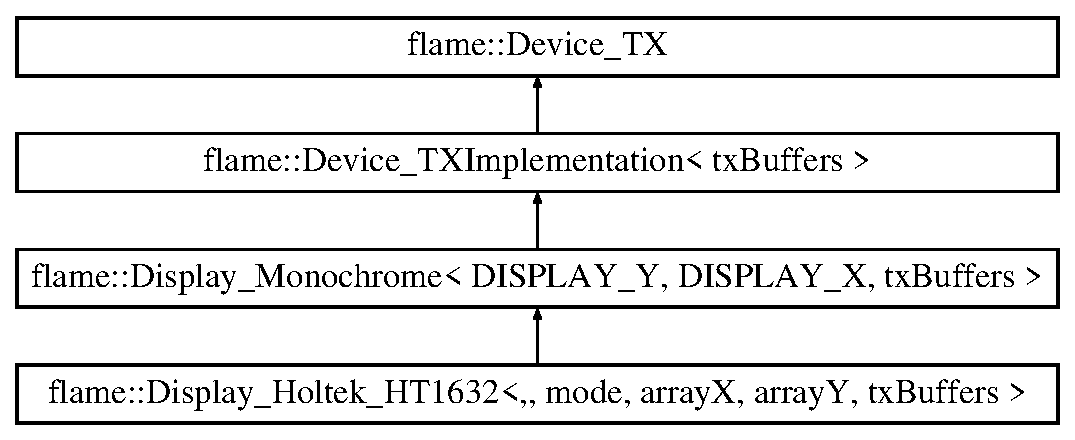
\includegraphics[height=4.000000cm]{classflame_1_1_display___holtek___h_t1632}
\end{center}
\end{figure}
\subsection*{Public Member Functions}
\begin{DoxyCompactItemize}
\item 
\hyperlink{classflame_1_1_display___holtek___h_t1632_a90942b33ed365103587c3b41c86056a6}{Display\-\_\-\-Holtek\-\_\-\-H\-T1632} (\hyperlink{classflame_1_1_display___selector}{Display\-\_\-\-Selector} \&selector)
\item 
void \hyperlink{classflame_1_1_display___holtek___h_t1632_a501199880d545f00614a944b96bf15d3}{brightness} (uint8\-\_\-t module\-X, uint8\-\_\-t module\-Y, uint8\-\_\-t brightness)
\item 
void \hyperlink{classflame_1_1_display___holtek___h_t1632_ab0efbd2a37bdfdf74a08ff8458d48909}{brightness} (uint8\-\_\-t brightness\-\_\-in)
\item 
void \hyperlink{classflame_1_1_display___holtek___h_t1632_a09eabd78de86f9ae3b1f260643fd5d8f}{poweroff} (uint8\-\_\-t module\-X, uint8\-\_\-t module\-Y)
\item 
void \hyperlink{classflame_1_1_display___holtek___h_t1632_a2f6c37d8789536447710648ce5b7a54c}{poweron} (uint8\-\_\-t module\-X, uint8\-\_\-t module\-Y)
\item 
void \hyperlink{classflame_1_1_display___holtek___h_t1632_aa64a5e76e4885013e5e25e96053dab51}{poweroff} ()
\item 
void \hyperlink{classflame_1_1_display___holtek___h_t1632_a54d6acaa4fa5072e7b7001cf86a4cf3f}{poweron} ()
\item 
void \hyperlink{classflame_1_1_display___holtek___h_t1632_a1927231d0266e2515ca2d3eb51ff5046}{flush} ()
\item 
void \hyperlink{classflame_1_1_display___holtek___h_t1632_a0fffd0acf421a4b9e00bc5675f526109}{set\-Pixel} (uint16\-\_\-t col, uint16\-\_\-t row, uint8\-\_\-t value)
\item 
uint8\-\_\-t \hyperlink{classflame_1_1_display___holtek___h_t1632_aa3930885169c3684f5aaac806a16d682}{get\-Pixel} (uint16\-\_\-t col, uint16\-\_\-t row)
\end{DoxyCompactItemize}
\subsection*{Additional Inherited Members}


\subsection{Detailed Description}
\subsubsection*{template$<$F\-L\-A\-M\-E\-\_\-\-D\-E\-C\-L\-A\-R\-E\-\_\-\-P\-I\-N(clock), F\-L\-A\-M\-E\-\_\-\-D\-E\-C\-L\-A\-R\-E\-\_\-\-P\-I\-N(data), H\-T1632\-Mode mode, uint8\-\_\-t array\-X, uint8\-\_\-t array\-Y, uint8\-\_\-t tx\-Buffers$>$class flame\-::\-Display\-\_\-\-Holtek\-\_\-\-H\-T1632$<$,, mode, array\-X, array\-Y, tx\-Buffers $>$}



Definition at line 84 of file Display\-\_\-\-Holtek\-\_\-\-H\-T1632.\-h.



\subsection{Constructor \& Destructor Documentation}
\hypertarget{classflame_1_1_display___holtek___h_t1632_a90942b33ed365103587c3b41c86056a6}{\index{flame\-::\-Display\-\_\-\-Holtek\-\_\-\-H\-T1632@{flame\-::\-Display\-\_\-\-Holtek\-\_\-\-H\-T1632}!Display\-\_\-\-Holtek\-\_\-\-H\-T1632@{Display\-\_\-\-Holtek\-\_\-\-H\-T1632}}
\index{Display\-\_\-\-Holtek\-\_\-\-H\-T1632@{Display\-\_\-\-Holtek\-\_\-\-H\-T1632}!flame::Display_Holtek_HT1632@{flame\-::\-Display\-\_\-\-Holtek\-\_\-\-H\-T1632}}
\subsubsection[{Display\-\_\-\-Holtek\-\_\-\-H\-T1632}]{\setlength{\rightskip}{0pt plus 5cm}template$<$F\-L\-A\-M\-E\-\_\-\-D\-E\-C\-L\-A\-R\-E\-\_\-\-P\-I\-N(clock) , F\-L\-A\-M\-E\-\_\-\-D\-E\-C\-L\-A\-R\-E\-\_\-\-P\-I\-N(data) , H\-T1632\-Mode mode, uint8\-\_\-t array\-X, uint8\-\_\-t array\-Y, uint8\-\_\-t tx\-Buffers$>$ {\bf flame\-::\-Display\-\_\-\-Holtek\-\_\-\-H\-T1632}$<$,, mode, array\-X, array\-Y, tx\-Buffers $>$\-::{\bf Display\-\_\-\-Holtek\-\_\-\-H\-T1632} (
\begin{DoxyParamCaption}
\item[{{\bf Display\-\_\-\-Selector} \&}]{selector}
\end{DoxyParamCaption}
)\hspace{0.3cm}{\ttfamily [inline]}}}\label{classflame_1_1_display___holtek___h_t1632_a90942b33ed365103587c3b41c86056a6}
Initialise the library 
\begin{DoxyParams}{Parameters}
{\em selector} & a class that sets the enable lines to choose the display to operate \\
\hline
\end{DoxyParams}


Definition at line 175 of file Display\-\_\-\-Holtek\-\_\-\-H\-T1632.\-h.



\subsection{Member Function Documentation}
\hypertarget{classflame_1_1_display___holtek___h_t1632_a501199880d545f00614a944b96bf15d3}{\index{flame\-::\-Display\-\_\-\-Holtek\-\_\-\-H\-T1632@{flame\-::\-Display\-\_\-\-Holtek\-\_\-\-H\-T1632}!brightness@{brightness}}
\index{brightness@{brightness}!flame::Display_Holtek_HT1632@{flame\-::\-Display\-\_\-\-Holtek\-\_\-\-H\-T1632}}
\subsubsection[{brightness}]{\setlength{\rightskip}{0pt plus 5cm}template$<$F\-L\-A\-M\-E\-\_\-\-D\-E\-C\-L\-A\-R\-E\-\_\-\-P\-I\-N(clock) , F\-L\-A\-M\-E\-\_\-\-D\-E\-C\-L\-A\-R\-E\-\_\-\-P\-I\-N(data) , H\-T1632\-Mode mode, uint8\-\_\-t array\-X, uint8\-\_\-t array\-Y, uint8\-\_\-t tx\-Buffers$>$ void {\bf flame\-::\-Display\-\_\-\-Holtek\-\_\-\-H\-T1632}$<$,, mode, array\-X, array\-Y, tx\-Buffers $>$\-::brightness (
\begin{DoxyParamCaption}
\item[{uint8\-\_\-t}]{module\-X, }
\item[{uint8\-\_\-t}]{module\-Y, }
\item[{uint8\-\_\-t}]{brightness}
\end{DoxyParamCaption}
)\hspace{0.3cm}{\ttfamily [inline]}}}\label{classflame_1_1_display___holtek___h_t1632_a501199880d545f00614a944b96bf15d3}
Set the brightness of a module 
\begin{DoxyParams}{Parameters}
{\em module\-X} & the X position of the module \\
\hline
{\em module\-Y} & the Y position of the module \\
\hline
{\em brightness} & the brightness (from 0 to 15) \\
\hline
\end{DoxyParams}


Definition at line 212 of file Display\-\_\-\-Holtek\-\_\-\-H\-T1632.\-h.

\hypertarget{classflame_1_1_display___holtek___h_t1632_ab0efbd2a37bdfdf74a08ff8458d48909}{\index{flame\-::\-Display\-\_\-\-Holtek\-\_\-\-H\-T1632@{flame\-::\-Display\-\_\-\-Holtek\-\_\-\-H\-T1632}!brightness@{brightness}}
\index{brightness@{brightness}!flame::Display_Holtek_HT1632@{flame\-::\-Display\-\_\-\-Holtek\-\_\-\-H\-T1632}}
\subsubsection[{brightness}]{\setlength{\rightskip}{0pt plus 5cm}template$<$F\-L\-A\-M\-E\-\_\-\-D\-E\-C\-L\-A\-R\-E\-\_\-\-P\-I\-N(clock) , F\-L\-A\-M\-E\-\_\-\-D\-E\-C\-L\-A\-R\-E\-\_\-\-P\-I\-N(data) , H\-T1632\-Mode mode, uint8\-\_\-t array\-X, uint8\-\_\-t array\-Y, uint8\-\_\-t tx\-Buffers$>$ void {\bf flame\-::\-Display\-\_\-\-Holtek\-\_\-\-H\-T1632}$<$,, mode, array\-X, array\-Y, tx\-Buffers $>$\-::brightness (
\begin{DoxyParamCaption}
\item[{uint8\-\_\-t}]{brightness\-\_\-in}
\end{DoxyParamCaption}
)\hspace{0.3cm}{\ttfamily [inline]}}}\label{classflame_1_1_display___holtek___h_t1632_ab0efbd2a37bdfdf74a08ff8458d48909}
Set the brightness of all modules 
\begin{DoxyParams}{Parameters}
{\em brightness\-\_\-in} & the brightness (from 0 to 15) \\
\hline
\end{DoxyParams}


Definition at line 223 of file Display\-\_\-\-Holtek\-\_\-\-H\-T1632.\-h.

\hypertarget{classflame_1_1_display___holtek___h_t1632_a1927231d0266e2515ca2d3eb51ff5046}{\index{flame\-::\-Display\-\_\-\-Holtek\-\_\-\-H\-T1632@{flame\-::\-Display\-\_\-\-Holtek\-\_\-\-H\-T1632}!flush@{flush}}
\index{flush@{flush}!flame::Display_Holtek_HT1632@{flame\-::\-Display\-\_\-\-Holtek\-\_\-\-H\-T1632}}
\subsubsection[{flush}]{\setlength{\rightskip}{0pt plus 5cm}template$<$F\-L\-A\-M\-E\-\_\-\-D\-E\-C\-L\-A\-R\-E\-\_\-\-P\-I\-N(clock) , F\-L\-A\-M\-E\-\_\-\-D\-E\-C\-L\-A\-R\-E\-\_\-\-P\-I\-N(data) , H\-T1632\-Mode mode, uint8\-\_\-t array\-X, uint8\-\_\-t array\-Y, uint8\-\_\-t tx\-Buffers$>$ void {\bf flame\-::\-Display\-\_\-\-Holtek\-\_\-\-H\-T1632}$<$,, mode, array\-X, array\-Y, tx\-Buffers $>$\-::flush (
\begin{DoxyParamCaption}
{}
\end{DoxyParamCaption}
)\hspace{0.3cm}{\ttfamily [inline]}}}\label{classflame_1_1_display___holtek___h_t1632_a1927231d0266e2515ca2d3eb51ff5046}
Flush the framebuffer to the displays 

Definition at line 294 of file Display\-\_\-\-Holtek\-\_\-\-H\-T1632.\-h.

\hypertarget{classflame_1_1_display___holtek___h_t1632_aa3930885169c3684f5aaac806a16d682}{\index{flame\-::\-Display\-\_\-\-Holtek\-\_\-\-H\-T1632@{flame\-::\-Display\-\_\-\-Holtek\-\_\-\-H\-T1632}!get\-Pixel@{get\-Pixel}}
\index{get\-Pixel@{get\-Pixel}!flame::Display_Holtek_HT1632@{flame\-::\-Display\-\_\-\-Holtek\-\_\-\-H\-T1632}}
\subsubsection[{get\-Pixel}]{\setlength{\rightskip}{0pt plus 5cm}template$<$F\-L\-A\-M\-E\-\_\-\-D\-E\-C\-L\-A\-R\-E\-\_\-\-P\-I\-N(clock) , F\-L\-A\-M\-E\-\_\-\-D\-E\-C\-L\-A\-R\-E\-\_\-\-P\-I\-N(data) , H\-T1632\-Mode mode, uint8\-\_\-t array\-X, uint8\-\_\-t array\-Y, uint8\-\_\-t tx\-Buffers$>$ uint8\-\_\-t {\bf flame\-::\-Display\-\_\-\-Holtek\-\_\-\-H\-T1632}$<$,, mode, array\-X, array\-Y, tx\-Buffers $>$\-::get\-Pixel (
\begin{DoxyParamCaption}
\item[{uint16\-\_\-t}]{col, }
\item[{uint16\-\_\-t}]{row}
\end{DoxyParamCaption}
)\hspace{0.3cm}{\ttfamily [inline]}, {\ttfamily [virtual]}}}\label{classflame_1_1_display___holtek___h_t1632_aa3930885169c3684f5aaac806a16d682}
Get a pixel 
\begin{DoxyParams}{Parameters}
{\em col} & the column of the pixel \\
\hline
{\em row} & the row of the pixel \\
\hline
\end{DoxyParams}
\begin{DoxyReturn}{Returns}
the value of the pixel 
\end{DoxyReturn}


Implements \hyperlink{classflame_1_1_display___monochrome_a24ddc06684641b00ee27b2630d216f8f}{flame\-::\-Display\-\_\-\-Monochrome$<$ D\-I\-S\-P\-L\-A\-Y\-\_\-\-Y, D\-I\-S\-P\-L\-A\-Y\-\_\-\-X, tx\-Buffers $>$}.



Definition at line 369 of file Display\-\_\-\-Holtek\-\_\-\-H\-T1632.\-h.

\hypertarget{classflame_1_1_display___holtek___h_t1632_a09eabd78de86f9ae3b1f260643fd5d8f}{\index{flame\-::\-Display\-\_\-\-Holtek\-\_\-\-H\-T1632@{flame\-::\-Display\-\_\-\-Holtek\-\_\-\-H\-T1632}!poweroff@{poweroff}}
\index{poweroff@{poweroff}!flame::Display_Holtek_HT1632@{flame\-::\-Display\-\_\-\-Holtek\-\_\-\-H\-T1632}}
\subsubsection[{poweroff}]{\setlength{\rightskip}{0pt plus 5cm}template$<$F\-L\-A\-M\-E\-\_\-\-D\-E\-C\-L\-A\-R\-E\-\_\-\-P\-I\-N(clock) , F\-L\-A\-M\-E\-\_\-\-D\-E\-C\-L\-A\-R\-E\-\_\-\-P\-I\-N(data) , H\-T1632\-Mode mode, uint8\-\_\-t array\-X, uint8\-\_\-t array\-Y, uint8\-\_\-t tx\-Buffers$>$ void {\bf flame\-::\-Display\-\_\-\-Holtek\-\_\-\-H\-T1632}$<$,, mode, array\-X, array\-Y, tx\-Buffers $>$\-::poweroff (
\begin{DoxyParamCaption}
\item[{uint8\-\_\-t}]{module\-X, }
\item[{uint8\-\_\-t}]{module\-Y}
\end{DoxyParamCaption}
)\hspace{0.3cm}{\ttfamily [inline]}}}\label{classflame_1_1_display___holtek___h_t1632_a09eabd78de86f9ae3b1f260643fd5d8f}
Put a module to sleep 
\begin{DoxyParams}{Parameters}
{\em module\-X} & the module to sleep \\
\hline
{\em module\-Y} & the module to sleep \\
\hline
\end{DoxyParams}


Definition at line 238 of file Display\-\_\-\-Holtek\-\_\-\-H\-T1632.\-h.

\hypertarget{classflame_1_1_display___holtek___h_t1632_aa64a5e76e4885013e5e25e96053dab51}{\index{flame\-::\-Display\-\_\-\-Holtek\-\_\-\-H\-T1632@{flame\-::\-Display\-\_\-\-Holtek\-\_\-\-H\-T1632}!poweroff@{poweroff}}
\index{poweroff@{poweroff}!flame::Display_Holtek_HT1632@{flame\-::\-Display\-\_\-\-Holtek\-\_\-\-H\-T1632}}
\subsubsection[{poweroff}]{\setlength{\rightskip}{0pt plus 5cm}template$<$F\-L\-A\-M\-E\-\_\-\-D\-E\-C\-L\-A\-R\-E\-\_\-\-P\-I\-N(clock) , F\-L\-A\-M\-E\-\_\-\-D\-E\-C\-L\-A\-R\-E\-\_\-\-P\-I\-N(data) , H\-T1632\-Mode mode, uint8\-\_\-t array\-X, uint8\-\_\-t array\-Y, uint8\-\_\-t tx\-Buffers$>$ void {\bf flame\-::\-Display\-\_\-\-Holtek\-\_\-\-H\-T1632}$<$,, mode, array\-X, array\-Y, tx\-Buffers $>$\-::poweroff (
\begin{DoxyParamCaption}
{}
\end{DoxyParamCaption}
)\hspace{0.3cm}{\ttfamily [inline]}}}\label{classflame_1_1_display___holtek___h_t1632_aa64a5e76e4885013e5e25e96053dab51}
Put all modules to sleep 

Definition at line 268 of file Display\-\_\-\-Holtek\-\_\-\-H\-T1632.\-h.

\hypertarget{classflame_1_1_display___holtek___h_t1632_a2f6c37d8789536447710648ce5b7a54c}{\index{flame\-::\-Display\-\_\-\-Holtek\-\_\-\-H\-T1632@{flame\-::\-Display\-\_\-\-Holtek\-\_\-\-H\-T1632}!poweron@{poweron}}
\index{poweron@{poweron}!flame::Display_Holtek_HT1632@{flame\-::\-Display\-\_\-\-Holtek\-\_\-\-H\-T1632}}
\subsubsection[{poweron}]{\setlength{\rightskip}{0pt plus 5cm}template$<$F\-L\-A\-M\-E\-\_\-\-D\-E\-C\-L\-A\-R\-E\-\_\-\-P\-I\-N(clock) , F\-L\-A\-M\-E\-\_\-\-D\-E\-C\-L\-A\-R\-E\-\_\-\-P\-I\-N(data) , H\-T1632\-Mode mode, uint8\-\_\-t array\-X, uint8\-\_\-t array\-Y, uint8\-\_\-t tx\-Buffers$>$ void {\bf flame\-::\-Display\-\_\-\-Holtek\-\_\-\-H\-T1632}$<$,, mode, array\-X, array\-Y, tx\-Buffers $>$\-::poweron (
\begin{DoxyParamCaption}
\item[{uint8\-\_\-t}]{module\-X, }
\item[{uint8\-\_\-t}]{module\-Y}
\end{DoxyParamCaption}
)\hspace{0.3cm}{\ttfamily [inline]}}}\label{classflame_1_1_display___holtek___h_t1632_a2f6c37d8789536447710648ce5b7a54c}
Wake a module up 
\begin{DoxyParams}{Parameters}
{\em module\-X} & the module to wake up \\
\hline
{\em module\-Y} & the module to wake up \\
\hline
\end{DoxyParams}


Definition at line 251 of file Display\-\_\-\-Holtek\-\_\-\-H\-T1632.\-h.

\hypertarget{classflame_1_1_display___holtek___h_t1632_a54d6acaa4fa5072e7b7001cf86a4cf3f}{\index{flame\-::\-Display\-\_\-\-Holtek\-\_\-\-H\-T1632@{flame\-::\-Display\-\_\-\-Holtek\-\_\-\-H\-T1632}!poweron@{poweron}}
\index{poweron@{poweron}!flame::Display_Holtek_HT1632@{flame\-::\-Display\-\_\-\-Holtek\-\_\-\-H\-T1632}}
\subsubsection[{poweron}]{\setlength{\rightskip}{0pt plus 5cm}template$<$F\-L\-A\-M\-E\-\_\-\-D\-E\-C\-L\-A\-R\-E\-\_\-\-P\-I\-N(clock) , F\-L\-A\-M\-E\-\_\-\-D\-E\-C\-L\-A\-R\-E\-\_\-\-P\-I\-N(data) , H\-T1632\-Mode mode, uint8\-\_\-t array\-X, uint8\-\_\-t array\-Y, uint8\-\_\-t tx\-Buffers$>$ void {\bf flame\-::\-Display\-\_\-\-Holtek\-\_\-\-H\-T1632}$<$,, mode, array\-X, array\-Y, tx\-Buffers $>$\-::poweron (
\begin{DoxyParamCaption}
{}
\end{DoxyParamCaption}
)\hspace{0.3cm}{\ttfamily [inline]}}}\label{classflame_1_1_display___holtek___h_t1632_a54d6acaa4fa5072e7b7001cf86a4cf3f}
Wake all modules up 

Definition at line 281 of file Display\-\_\-\-Holtek\-\_\-\-H\-T1632.\-h.

\hypertarget{classflame_1_1_display___holtek___h_t1632_a0fffd0acf421a4b9e00bc5675f526109}{\index{flame\-::\-Display\-\_\-\-Holtek\-\_\-\-H\-T1632@{flame\-::\-Display\-\_\-\-Holtek\-\_\-\-H\-T1632}!set\-Pixel@{set\-Pixel}}
\index{set\-Pixel@{set\-Pixel}!flame::Display_Holtek_HT1632@{flame\-::\-Display\-\_\-\-Holtek\-\_\-\-H\-T1632}}
\subsubsection[{set\-Pixel}]{\setlength{\rightskip}{0pt plus 5cm}template$<$F\-L\-A\-M\-E\-\_\-\-D\-E\-C\-L\-A\-R\-E\-\_\-\-P\-I\-N(clock) , F\-L\-A\-M\-E\-\_\-\-D\-E\-C\-L\-A\-R\-E\-\_\-\-P\-I\-N(data) , H\-T1632\-Mode mode, uint8\-\_\-t array\-X, uint8\-\_\-t array\-Y, uint8\-\_\-t tx\-Buffers$>$ void {\bf flame\-::\-Display\-\_\-\-Holtek\-\_\-\-H\-T1632}$<$,, mode, array\-X, array\-Y, tx\-Buffers $>$\-::set\-Pixel (
\begin{DoxyParamCaption}
\item[{uint16\-\_\-t}]{col, }
\item[{uint16\-\_\-t}]{row, }
\item[{uint8\-\_\-t}]{value}
\end{DoxyParamCaption}
)\hspace{0.3cm}{\ttfamily [inline]}, {\ttfamily [virtual]}}}\label{classflame_1_1_display___holtek___h_t1632_a0fffd0acf421a4b9e00bc5675f526109}
Set a pixel 
\begin{DoxyParams}{Parameters}
{\em col} & the column of the pixel \\
\hline
{\em row} & the row of the pixel \\
\hline
{\em value} & the value of the pixel \\
\hline
\end{DoxyParams}


Implements \hyperlink{classflame_1_1_display___monochrome_a34002efa6fccb74a4fbea455f2a261d3}{flame\-::\-Display\-\_\-\-Monochrome$<$ D\-I\-S\-P\-L\-A\-Y\-\_\-\-Y, D\-I\-S\-P\-L\-A\-Y\-\_\-\-X, tx\-Buffers $>$}.



Definition at line 324 of file Display\-\_\-\-Holtek\-\_\-\-H\-T1632.\-h.



The documentation for this class was generated from the following file\-:\begin{DoxyCompactItemize}
\item 
flame/\hyperlink{_display___holtek___h_t1632_8h}{Display\-\_\-\-Holtek\-\_\-\-H\-T1632.\-h}\end{DoxyCompactItemize}

\hypertarget{classflame_1_1_display___monochrome}{\section{flame\-:\-:Display\-\_\-\-Monochrome$<$ cols, rows, tx\-Buffers $>$ Class Template Reference}
\label{classflame_1_1_display___monochrome}\index{flame\-::\-Display\-\_\-\-Monochrome$<$ cols, rows, tx\-Buffers $>$@{flame\-::\-Display\-\_\-\-Monochrome$<$ cols, rows, tx\-Buffers $>$}}
}


{\ttfamily \#include $<$Display\-\_\-\-Monochrome.\-h$>$}

Inheritance diagram for flame\-:\-:Display\-\_\-\-Monochrome$<$ cols, rows, tx\-Buffers $>$\-:\begin{figure}[H]
\begin{center}
\leavevmode
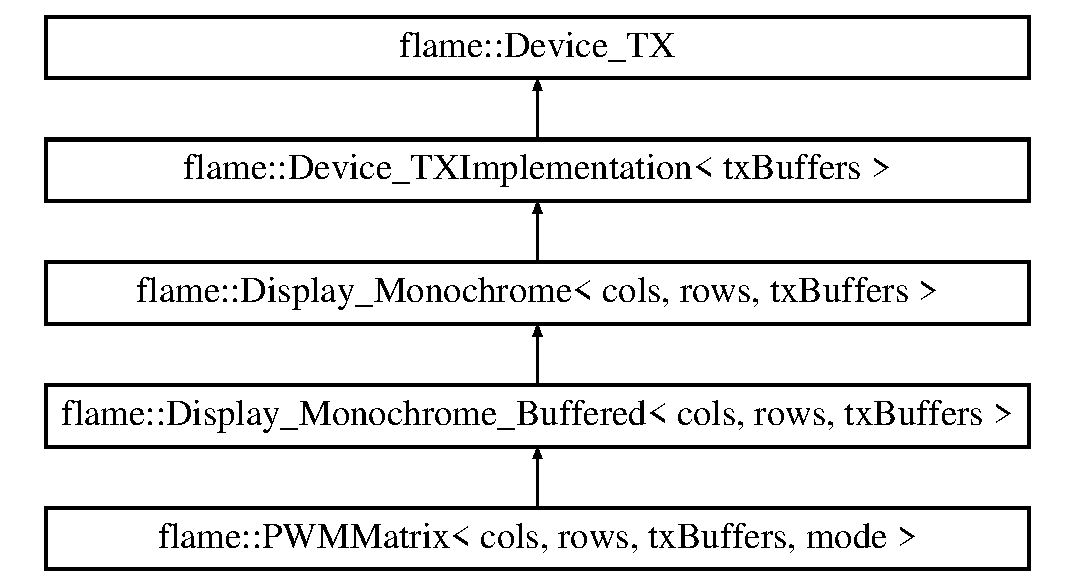
\includegraphics[height=5.000000cm]{classflame_1_1_display___monochrome}
\end{center}
\end{figure}
\subsection*{Public Member Functions}
\begin{DoxyCompactItemize}
\item 
uint16\-\_\-t \hyperlink{classflame_1_1_display___monochrome_ad0f4efba436d8aa9111891ea7b95312e}{get\-Width} () \hyperlink{io_8h_a0c33b494a68ce28497e7ce8e5e95feff}{C\-O\-N\-S\-T}
\item 
uint16\-\_\-t \hyperlink{classflame_1_1_display___monochrome_aca8bb03d86980657ee953ce506a75fcc}{get\-Height} () \hyperlink{io_8h_a0c33b494a68ce28497e7ce8e5e95feff}{C\-O\-N\-S\-T}
\item 
void \hyperlink{classflame_1_1_display___monochrome_a7c38727d187106abe6027d1ca1bb8b14}{clear} (uint8\-\_\-t value)
\item 
bool \hyperlink{classflame_1_1_display___monochrome_a0754b3857615d04dce50e5e52321674f}{write\-Buffer} (const \hyperlink{namespaceflame_a05350b61d7b7be486d5e367522316a33}{F\-O\-N\-T} \&\hyperlink{structflame_1_1font}{font}, int16\-\_\-t $\ast$offset\-X, int16\-\_\-t offset\-Y, uint8\-\_\-t on\-Value, uint8\-\_\-t off\-Value, \hyperlink{classflame_1_1_t_x_buffer}{T\-X\-Buffer} \&tx\-Buffer)
\item 
bool \hyperlink{classflame_1_1_display___monochrome_a30562aac06dd7a44c9f0d5e9183f6481}{write\-Buffer} (const \hyperlink{namespaceflame_a05350b61d7b7be486d5e367522316a33}{F\-O\-N\-T} \&\hyperlink{structflame_1_1font}{font}, int16\-\_\-t $\ast$offset\-X, int16\-\_\-t offset\-Y, uint8\-\_\-t on\-Value, uint8\-\_\-t off\-Value, const char $\ast$buffer, uint16\-\_\-t length)
\item 
bool \hyperlink{classflame_1_1_display___monochrome_a4149d7999c78ec01474f1e27ba5f4009}{write\-String\-\_\-\-P} (const \hyperlink{namespaceflame_a05350b61d7b7be486d5e367522316a33}{F\-O\-N\-T} \&\hyperlink{structflame_1_1font}{font}, int16\-\_\-t $\ast$offset\-X, int16\-\_\-t offset\-Y, uint8\-\_\-t on\-Value, uint8\-\_\-t off\-Value, P\-G\-M\-\_\-\-P string)
\item 
bool \hyperlink{classflame_1_1_display___monochrome_a5f901899fdd1d93b88deeedc59b214a4}{write\-Buffer\-\_\-\-P} (const \hyperlink{namespaceflame_a05350b61d7b7be486d5e367522316a33}{F\-O\-N\-T} \&\hyperlink{structflame_1_1font}{font}, int16\-\_\-t $\ast$offset\-X, int16\-\_\-t offset\-Y, uint8\-\_\-t on\-Value, uint8\-\_\-t off\-Value, P\-G\-M\-\_\-\-P buffer, uint16\-\_\-t length)
\item 
bool \hyperlink{classflame_1_1_display___monochrome_a1bf2a44cb642b6a16e09a690023fe959}{write\-String} (const \hyperlink{namespaceflame_a05350b61d7b7be486d5e367522316a33}{F\-O\-N\-T} \&\hyperlink{structflame_1_1font}{font}, int16\-\_\-t $\ast$offset\-X, int16\-\_\-t offset\-Y, uint8\-\_\-t on\-Value, uint8\-\_\-t off\-Value, const char $\ast$string)
\item 
bool \hyperlink{classflame_1_1_display___monochrome_a51ef95aa2e4a00a234987559fd350b27}{tx\-Animation} (const \hyperlink{namespaceflame_a05350b61d7b7be486d5e367522316a33}{F\-O\-N\-T} \&\hyperlink{structflame_1_1font}{font}, int16\-\_\-t offset\-Y, uint8\-\_\-t on\-Value, uint8\-\_\-t off\-Value)
\item 
virtual void \hyperlink{classflame_1_1_display___monochrome_a34002efa6fccb74a4fbea455f2a261d3}{set\-Pixel} (uint16\-\_\-t row, uint16\-\_\-t col, uint8\-\_\-t value)=0
\item 
virtual uint8\-\_\-t \hyperlink{classflame_1_1_display___monochrome_a24ddc06684641b00ee27b2630d216f8f}{get\-Pixel} (uint16\-\_\-t row, uint16\-\_\-t col)=0
\end{DoxyCompactItemize}
\subsection*{Protected Member Functions}
\begin{DoxyCompactItemize}
\item 
bool \hyperlink{classflame_1_1_display___monochrome_acd31faefdc5f7dd913718d66bb30a0da}{write\-Char} (const \hyperlink{namespaceflame_a05350b61d7b7be486d5e367522316a33}{F\-O\-N\-T} \&\hyperlink{structflame_1_1font}{font}, int16\-\_\-t $\ast$offset\-X, int16\-\_\-t offset\-Y, uint8\-\_\-t on\-Value, uint8\-\_\-t off\-Value, char character)
\item 
bool \hyperlink{classflame_1_1_display___monochrome_a652e0ebca82d3743a565a8b31dbbf4da}{write\-Seperator} (const \hyperlink{namespaceflame_a05350b61d7b7be486d5e367522316a33}{F\-O\-N\-T} \&\hyperlink{structflame_1_1font}{font}, int16\-\_\-t $\ast$offset\-X, int16\-\_\-t offset\-Y, uint8\-\_\-t off\-Value)
\item 
void \hyperlink{classflame_1_1_display___monochrome_a7f156eaedc986e5432c4b04968417def}{run\-Tx\-Buffers} ()
\end{DoxyCompactItemize}
\subsection*{Protected Attributes}
\begin{DoxyCompactItemize}
\item 
int16\-\_\-t \hyperlink{classflame_1_1_display___monochrome_abd53e31a2433730e2390152b7c24918f}{\-\_\-tx\-Offset}
\end{DoxyCompactItemize}


\subsection{Detailed Description}
\subsubsection*{template$<$uint16\-\_\-t cols, uint16\-\_\-t rows, uint8\-\_\-t tx\-Buffers$>$class flame\-::\-Display\-\_\-\-Monochrome$<$ cols, rows, tx\-Buffers $>$}

A monochrome bitmap display Origin (0,0) is bottom left 
\begin{DoxyTemplParams}{Template Parameters}
{\em cols} & the number of columns \\
\hline
{\em rows} & the number of rows \\
\hline
{\em tx\-Buffers} & the number of output buffers \\
\hline
\end{DoxyTemplParams}


Definition at line 51 of file Display\-\_\-\-Monochrome.\-h.



\subsection{Member Function Documentation}
\hypertarget{classflame_1_1_display___monochrome_a7c38727d187106abe6027d1ca1bb8b14}{\index{flame\-::\-Display\-\_\-\-Monochrome@{flame\-::\-Display\-\_\-\-Monochrome}!clear@{clear}}
\index{clear@{clear}!flame::Display_Monochrome@{flame\-::\-Display\-\_\-\-Monochrome}}
\subsubsection[{clear}]{\setlength{\rightskip}{0pt plus 5cm}template$<$uint16\-\_\-t cols, uint16\-\_\-t rows, uint8\-\_\-t tx\-Buffers$>$ void {\bf flame\-::\-Display\-\_\-\-Monochrome}$<$ cols, rows, tx\-Buffers $>$\-::clear (
\begin{DoxyParamCaption}
\item[{uint8\-\_\-t}]{value}
\end{DoxyParamCaption}
)\hspace{0.3cm}{\ttfamily [inline]}}}\label{classflame_1_1_display___monochrome_a7c38727d187106abe6027d1ca1bb8b14}
Clear the display to a particular value 
\begin{DoxyParams}{Parameters}
{\em value} & the value to fill the display with \\
\hline
\end{DoxyParams}


Definition at line 181 of file Display\-\_\-\-Monochrome.\-h.

\hypertarget{classflame_1_1_display___monochrome_aca8bb03d86980657ee953ce506a75fcc}{\index{flame\-::\-Display\-\_\-\-Monochrome@{flame\-::\-Display\-\_\-\-Monochrome}!get\-Height@{get\-Height}}
\index{get\-Height@{get\-Height}!flame::Display_Monochrome@{flame\-::\-Display\-\_\-\-Monochrome}}
\subsubsection[{get\-Height}]{\setlength{\rightskip}{0pt plus 5cm}template$<$uint16\-\_\-t cols, uint16\-\_\-t rows, uint8\-\_\-t tx\-Buffers$>$ uint16\-\_\-t {\bf flame\-::\-Display\-\_\-\-Monochrome}$<$ cols, rows, tx\-Buffers $>$\-::get\-Height (
\begin{DoxyParamCaption}
{}
\end{DoxyParamCaption}
)\hspace{0.3cm}{\ttfamily [inline]}}}\label{classflame_1_1_display___monochrome_aca8bb03d86980657ee953ce506a75fcc}
Get the width of the display 

Definition at line 173 of file Display\-\_\-\-Monochrome.\-h.

\hypertarget{classflame_1_1_display___monochrome_a24ddc06684641b00ee27b2630d216f8f}{\index{flame\-::\-Display\-\_\-\-Monochrome@{flame\-::\-Display\-\_\-\-Monochrome}!get\-Pixel@{get\-Pixel}}
\index{get\-Pixel@{get\-Pixel}!flame::Display_Monochrome@{flame\-::\-Display\-\_\-\-Monochrome}}
\subsubsection[{get\-Pixel}]{\setlength{\rightskip}{0pt plus 5cm}template$<$uint16\-\_\-t cols, uint16\-\_\-t rows, uint8\-\_\-t tx\-Buffers$>$ virtual uint8\-\_\-t {\bf flame\-::\-Display\-\_\-\-Monochrome}$<$ cols, rows, tx\-Buffers $>$\-::get\-Pixel (
\begin{DoxyParamCaption}
\item[{uint16\-\_\-t}]{row, }
\item[{uint16\-\_\-t}]{col}
\end{DoxyParamCaption}
)\hspace{0.3cm}{\ttfamily [pure virtual]}}}\label{classflame_1_1_display___monochrome_a24ddc06684641b00ee27b2630d216f8f}


Implemented in \hyperlink{classflame_1_1_display___holtek___h_t1632_aa3930885169c3684f5aaac806a16d682}{flame\-::\-Display\-\_\-\-Holtek\-\_\-\-H\-T1632$<$,, mode, array\-X, array\-Y, tx\-Buffers $>$}, and \hyperlink{classflame_1_1_display___monochrome___buffered_a003e20bbdf7f905cee2dcfb22be61268}{flame\-::\-Display\-\_\-\-Monochrome\-\_\-\-Buffered$<$ cols, rows, tx\-Buffers $>$}.

\hypertarget{classflame_1_1_display___monochrome_ad0f4efba436d8aa9111891ea7b95312e}{\index{flame\-::\-Display\-\_\-\-Monochrome@{flame\-::\-Display\-\_\-\-Monochrome}!get\-Width@{get\-Width}}
\index{get\-Width@{get\-Width}!flame::Display_Monochrome@{flame\-::\-Display\-\_\-\-Monochrome}}
\subsubsection[{get\-Width}]{\setlength{\rightskip}{0pt plus 5cm}template$<$uint16\-\_\-t cols, uint16\-\_\-t rows, uint8\-\_\-t tx\-Buffers$>$ uint16\-\_\-t {\bf flame\-::\-Display\-\_\-\-Monochrome}$<$ cols, rows, tx\-Buffers $>$\-::get\-Width (
\begin{DoxyParamCaption}
{}
\end{DoxyParamCaption}
)\hspace{0.3cm}{\ttfamily [inline]}}}\label{classflame_1_1_display___monochrome_ad0f4efba436d8aa9111891ea7b95312e}
Get the width of the display 

Definition at line 166 of file Display\-\_\-\-Monochrome.\-h.

\hypertarget{classflame_1_1_display___monochrome_a7f156eaedc986e5432c4b04968417def}{\index{flame\-::\-Display\-\_\-\-Monochrome@{flame\-::\-Display\-\_\-\-Monochrome}!run\-Tx\-Buffers@{run\-Tx\-Buffers}}
\index{run\-Tx\-Buffers@{run\-Tx\-Buffers}!flame::Display_Monochrome@{flame\-::\-Display\-\_\-\-Monochrome}}
\subsubsection[{run\-Tx\-Buffers}]{\setlength{\rightskip}{0pt plus 5cm}template$<$uint16\-\_\-t cols, uint16\-\_\-t rows, uint8\-\_\-t tx\-Buffers$>$ void {\bf flame\-::\-Display\-\_\-\-Monochrome}$<$ cols, rows, tx\-Buffers $>$\-::run\-Tx\-Buffers (
\begin{DoxyParamCaption}
{}
\end{DoxyParamCaption}
)\hspace{0.3cm}{\ttfamily [inline]}, {\ttfamily [protected]}, {\ttfamily [virtual]}}}\label{classflame_1_1_display___monochrome_a7f156eaedc986e5432c4b04968417def}
Start rendering T\-X buffers 

Implements \hyperlink{classflame_1_1_device___t_x_af3cf3dc02a124e5a88841d325555ce3c}{flame\-::\-Device\-\_\-\-T\-X}.



Definition at line 157 of file Display\-\_\-\-Monochrome.\-h.

\hypertarget{classflame_1_1_display___monochrome_a34002efa6fccb74a4fbea455f2a261d3}{\index{flame\-::\-Display\-\_\-\-Monochrome@{flame\-::\-Display\-\_\-\-Monochrome}!set\-Pixel@{set\-Pixel}}
\index{set\-Pixel@{set\-Pixel}!flame::Display_Monochrome@{flame\-::\-Display\-\_\-\-Monochrome}}
\subsubsection[{set\-Pixel}]{\setlength{\rightskip}{0pt plus 5cm}template$<$uint16\-\_\-t cols, uint16\-\_\-t rows, uint8\-\_\-t tx\-Buffers$>$ virtual void {\bf flame\-::\-Display\-\_\-\-Monochrome}$<$ cols, rows, tx\-Buffers $>$\-::set\-Pixel (
\begin{DoxyParamCaption}
\item[{uint16\-\_\-t}]{row, }
\item[{uint16\-\_\-t}]{col, }
\item[{uint8\-\_\-t}]{value}
\end{DoxyParamCaption}
)\hspace{0.3cm}{\ttfamily [pure virtual]}}}\label{classflame_1_1_display___monochrome_a34002efa6fccb74a4fbea455f2a261d3}


Implemented in \hyperlink{classflame_1_1_display___holtek___h_t1632_a0fffd0acf421a4b9e00bc5675f526109}{flame\-::\-Display\-\_\-\-Holtek\-\_\-\-H\-T1632$<$,, mode, array\-X, array\-Y, tx\-Buffers $>$}, and \hyperlink{classflame_1_1_display___monochrome___buffered_a5ffe666a9a5ae12931177c05307b48e1}{flame\-::\-Display\-\_\-\-Monochrome\-\_\-\-Buffered$<$ cols, rows, tx\-Buffers $>$}.

\hypertarget{classflame_1_1_display___monochrome_a51ef95aa2e4a00a234987559fd350b27}{\index{flame\-::\-Display\-\_\-\-Monochrome@{flame\-::\-Display\-\_\-\-Monochrome}!tx\-Animation@{tx\-Animation}}
\index{tx\-Animation@{tx\-Animation}!flame::Display_Monochrome@{flame\-::\-Display\-\_\-\-Monochrome}}
\subsubsection[{tx\-Animation}]{\setlength{\rightskip}{0pt plus 5cm}template$<$uint16\-\_\-t cols, uint16\-\_\-t rows, uint8\-\_\-t tx\-Buffers$>$ bool {\bf flame\-::\-Display\-\_\-\-Monochrome}$<$ cols, rows, tx\-Buffers $>$\-::tx\-Animation (
\begin{DoxyParamCaption}
\item[{const {\bf F\-O\-N\-T} \&}]{font, }
\item[{int16\-\_\-t}]{offset\-Y, }
\item[{uint8\-\_\-t}]{on\-Value, }
\item[{uint8\-\_\-t}]{off\-Value}
\end{DoxyParamCaption}
)\hspace{0.3cm}{\ttfamily [inline]}}}\label{classflame_1_1_display___monochrome_a51ef95aa2e4a00a234987559fd350b27}
Render a frame of T\-X buffer animation -\/ scrolls text from right to left, before moving to the next buffer 
\begin{DoxyParams}{Parameters}
{\em font} & the font to use \\
\hline
{\em offset\-Y} & the vertical pixel offset to start writing at (bottom of char) \\
\hline
{\em on\-Value} & the pixel value for on pixels \\
\hline
{\em off\-Value} & the pixel value for off pixels \\
\hline
\end{DoxyParams}
\begin{DoxyReturn}{Returns}
true if there are more frames to be rendered 
\end{DoxyReturn}


Definition at line 441 of file Display\-\_\-\-Monochrome.\-h.

\hypertarget{classflame_1_1_display___monochrome_a0754b3857615d04dce50e5e52321674f}{\index{flame\-::\-Display\-\_\-\-Monochrome@{flame\-::\-Display\-\_\-\-Monochrome}!write\-Buffer@{write\-Buffer}}
\index{write\-Buffer@{write\-Buffer}!flame::Display_Monochrome@{flame\-::\-Display\-\_\-\-Monochrome}}
\subsubsection[{write\-Buffer}]{\setlength{\rightskip}{0pt plus 5cm}template$<$uint16\-\_\-t cols, uint16\-\_\-t rows, uint8\-\_\-t tx\-Buffers$>$ bool {\bf flame\-::\-Display\-\_\-\-Monochrome}$<$ cols, rows, tx\-Buffers $>$\-::write\-Buffer (
\begin{DoxyParamCaption}
\item[{const {\bf F\-O\-N\-T} \&}]{font, }
\item[{int16\-\_\-t $\ast$}]{offset\-X, }
\item[{int16\-\_\-t}]{offset\-Y, }
\item[{uint8\-\_\-t}]{on\-Value, }
\item[{uint8\-\_\-t}]{off\-Value, }
\item[{{\bf T\-X\-Buffer} \&}]{tx\-Buffer}
\end{DoxyParamCaption}
)\hspace{0.3cm}{\ttfamily [inline]}}}\label{classflame_1_1_display___monochrome_a0754b3857615d04dce50e5e52321674f}
Write a T\-X Buffer to the display 
\begin{DoxyParams}{Parameters}
{\em font} & the font to use \\
\hline
{\em offset\-X} & the horizontal pixel offset to start writing at (left side of char) will increment to the next position on return) \\
\hline
{\em offset\-Y} & the vertical pixel offset to start writing at (bottom of char) \\
\hline
{\em on\-Value} & the pixel value to use for on \\
\hline
{\em off\-Value} & the pixel value to use for off \\
\hline
{\em tx\-Buffer} & the buffer to write \\
\hline
\end{DoxyParams}
\begin{DoxyReturn}{Returns}
true if anything was written 
\end{DoxyReturn}


Definition at line 201 of file Display\-\_\-\-Monochrome.\-h.

\hypertarget{classflame_1_1_display___monochrome_a30562aac06dd7a44c9f0d5e9183f6481}{\index{flame\-::\-Display\-\_\-\-Monochrome@{flame\-::\-Display\-\_\-\-Monochrome}!write\-Buffer@{write\-Buffer}}
\index{write\-Buffer@{write\-Buffer}!flame::Display_Monochrome@{flame\-::\-Display\-\_\-\-Monochrome}}
\subsubsection[{write\-Buffer}]{\setlength{\rightskip}{0pt plus 5cm}template$<$uint16\-\_\-t cols, uint16\-\_\-t rows, uint8\-\_\-t tx\-Buffers$>$ bool {\bf flame\-::\-Display\-\_\-\-Monochrome}$<$ cols, rows, tx\-Buffers $>$\-::write\-Buffer (
\begin{DoxyParamCaption}
\item[{const {\bf F\-O\-N\-T} \&}]{font, }
\item[{int16\-\_\-t $\ast$}]{offset\-X, }
\item[{int16\-\_\-t}]{offset\-Y, }
\item[{uint8\-\_\-t}]{on\-Value, }
\item[{uint8\-\_\-t}]{off\-Value, }
\item[{const char $\ast$}]{buffer, }
\item[{uint16\-\_\-t}]{length}
\end{DoxyParamCaption}
)\hspace{0.3cm}{\ttfamily [inline]}}}\label{classflame_1_1_display___monochrome_a30562aac06dd7a44c9f0d5e9183f6481}
Write a buffer to the display 
\begin{DoxyParams}{Parameters}
{\em font} & the font to use \\
\hline
{\em offset\-X} & the horizontal pixel offset to start writing at (left side of char) will increment to the next position on return) \\
\hline
{\em offset\-Y} & the vertical pixel offset to start writing at (bottom of char) \\
\hline
{\em on\-Value} & the pixel value to use for on \\
\hline
{\em off\-Value} & the pixel value to use for off \\
\hline
{\em buffer} & the buffer to write \\
\hline
{\em length} & the length of the buffer \\
\hline
\end{DoxyParams}
\begin{DoxyReturn}{Returns}
true if anything was written 
\end{DoxyReturn}


Definition at line 232 of file Display\-\_\-\-Monochrome.\-h.

\hypertarget{classflame_1_1_display___monochrome_a5f901899fdd1d93b88deeedc59b214a4}{\index{flame\-::\-Display\-\_\-\-Monochrome@{flame\-::\-Display\-\_\-\-Monochrome}!write\-Buffer\-\_\-\-P@{write\-Buffer\-\_\-\-P}}
\index{write\-Buffer\-\_\-\-P@{write\-Buffer\-\_\-\-P}!flame::Display_Monochrome@{flame\-::\-Display\-\_\-\-Monochrome}}
\subsubsection[{write\-Buffer\-\_\-\-P}]{\setlength{\rightskip}{0pt plus 5cm}template$<$uint16\-\_\-t cols, uint16\-\_\-t rows, uint8\-\_\-t tx\-Buffers$>$ bool {\bf flame\-::\-Display\-\_\-\-Monochrome}$<$ cols, rows, tx\-Buffers $>$\-::write\-Buffer\-\_\-\-P (
\begin{DoxyParamCaption}
\item[{const {\bf F\-O\-N\-T} \&}]{font, }
\item[{int16\-\_\-t $\ast$}]{offset\-X, }
\item[{int16\-\_\-t}]{offset\-Y, }
\item[{uint8\-\_\-t}]{on\-Value, }
\item[{uint8\-\_\-t}]{off\-Value, }
\item[{P\-G\-M\-\_\-\-P}]{buffer, }
\item[{uint16\-\_\-t}]{length}
\end{DoxyParamCaption}
)\hspace{0.3cm}{\ttfamily [inline]}}}\label{classflame_1_1_display___monochrome_a5f901899fdd1d93b88deeedc59b214a4}
Write a P\-R\-O\-G\-M\-E\-M buffer to the display 
\begin{DoxyParams}{Parameters}
{\em font} & the font to use \\
\hline
{\em offset\-X} & the horizontal pixel offset to start writing at (left side of char) will increment to the next position on return) \\
\hline
{\em offset\-Y} & the vertical pixel offset to start writing at (bottom of char) \\
\hline
{\em on\-Value} & the pixel value to use for on \\
\hline
{\em off\-Value} & the pixel value to use for off \\
\hline
{\em buffer} & the buffer to write \\
\hline
{\em length} & the length of the buffer \\
\hline
\end{DoxyParams}
\begin{DoxyReturn}{Returns}
true if anything was written 
\end{DoxyReturn}


Definition at line 286 of file Display\-\_\-\-Monochrome.\-h.

\hypertarget{classflame_1_1_display___monochrome_acd31faefdc5f7dd913718d66bb30a0da}{\index{flame\-::\-Display\-\_\-\-Monochrome@{flame\-::\-Display\-\_\-\-Monochrome}!write\-Char@{write\-Char}}
\index{write\-Char@{write\-Char}!flame::Display_Monochrome@{flame\-::\-Display\-\_\-\-Monochrome}}
\subsubsection[{write\-Char}]{\setlength{\rightskip}{0pt plus 5cm}template$<$uint16\-\_\-t cols, uint16\-\_\-t rows, uint8\-\_\-t tx\-Buffers$>$ bool {\bf flame\-::\-Display\-\_\-\-Monochrome}$<$ cols, rows, tx\-Buffers $>$\-::write\-Char (
\begin{DoxyParamCaption}
\item[{const {\bf F\-O\-N\-T} \&}]{font, }
\item[{int16\-\_\-t $\ast$}]{offset\-X, }
\item[{int16\-\_\-t}]{offset\-Y, }
\item[{uint8\-\_\-t}]{on\-Value, }
\item[{uint8\-\_\-t}]{off\-Value, }
\item[{char}]{character}
\end{DoxyParamCaption}
)\hspace{0.3cm}{\ttfamily [inline]}, {\ttfamily [protected]}}}\label{classflame_1_1_display___monochrome_acd31faefdc5f7dd913718d66bb30a0da}
Write a character to the display 
\begin{DoxyParams}{Parameters}
{\em font} & the font to use \\
\hline
{\em offset\-X} & the horizontal pixel offset to start writing at (left side of char) will increment to the next position on return) \\
\hline
{\em offset\-Y} & the vertical pixel offset to start writing at (bottom of char) \\
\hline
{\em on\-Value} & the pixel value to use for on \\
\hline
{\em off\-Value} & the pixel value to use for off \\
\hline
{\em character} & the character to write \\
\hline
\end{DoxyParams}
\begin{DoxyReturn}{Returns}
true if a character was written 
\end{DoxyReturn}


Definition at line 65 of file Display\-\_\-\-Monochrome.\-h.

\hypertarget{classflame_1_1_display___monochrome_a652e0ebca82d3743a565a8b31dbbf4da}{\index{flame\-::\-Display\-\_\-\-Monochrome@{flame\-::\-Display\-\_\-\-Monochrome}!write\-Seperator@{write\-Seperator}}
\index{write\-Seperator@{write\-Seperator}!flame::Display_Monochrome@{flame\-::\-Display\-\_\-\-Monochrome}}
\subsubsection[{write\-Seperator}]{\setlength{\rightskip}{0pt plus 5cm}template$<$uint16\-\_\-t cols, uint16\-\_\-t rows, uint8\-\_\-t tx\-Buffers$>$ bool {\bf flame\-::\-Display\-\_\-\-Monochrome}$<$ cols, rows, tx\-Buffers $>$\-::write\-Seperator (
\begin{DoxyParamCaption}
\item[{const {\bf F\-O\-N\-T} \&}]{font, }
\item[{int16\-\_\-t $\ast$}]{offset\-X, }
\item[{int16\-\_\-t}]{offset\-Y, }
\item[{uint8\-\_\-t}]{off\-Value}
\end{DoxyParamCaption}
)\hspace{0.3cm}{\ttfamily [inline]}, {\ttfamily [protected]}}}\label{classflame_1_1_display___monochrome_a652e0ebca82d3743a565a8b31dbbf4da}
Write a character seperator (a single column of off pixels) to the display 
\begin{DoxyParams}{Parameters}
{\em font} & the font to use \\
\hline
{\em offset\-X} & the horizontal pixel offset to start writing at (left side of char) will increment to the next position on return) \\
\hline
{\em offset\-Y} & the vertical pixel offset to start writing at (bottom of char) \\
\hline
{\em off\-Value} & the pixel value to use for off \\
\hline
\end{DoxyParams}
\begin{DoxyReturn}{Returns}
true if the seperator was written 
\end{DoxyReturn}


Definition at line 132 of file Display\-\_\-\-Monochrome.\-h.

\hypertarget{classflame_1_1_display___monochrome_a1bf2a44cb642b6a16e09a690023fe959}{\index{flame\-::\-Display\-\_\-\-Monochrome@{flame\-::\-Display\-\_\-\-Monochrome}!write\-String@{write\-String}}
\index{write\-String@{write\-String}!flame::Display_Monochrome@{flame\-::\-Display\-\_\-\-Monochrome}}
\subsubsection[{write\-String}]{\setlength{\rightskip}{0pt plus 5cm}template$<$uint16\-\_\-t cols, uint16\-\_\-t rows, uint8\-\_\-t tx\-Buffers$>$ bool {\bf flame\-::\-Display\-\_\-\-Monochrome}$<$ cols, rows, tx\-Buffers $>$\-::write\-String (
\begin{DoxyParamCaption}
\item[{const {\bf F\-O\-N\-T} \&}]{font, }
\item[{int16\-\_\-t $\ast$}]{offset\-X, }
\item[{int16\-\_\-t}]{offset\-Y, }
\item[{uint8\-\_\-t}]{on\-Value, }
\item[{uint8\-\_\-t}]{off\-Value, }
\item[{const char $\ast$}]{string}
\end{DoxyParamCaption}
)\hspace{0.3cm}{\ttfamily [inline]}}}\label{classflame_1_1_display___monochrome_a1bf2a44cb642b6a16e09a690023fe959}
Write a string to the display 
\begin{DoxyParams}{Parameters}
{\em font} & the font to use \\
\hline
{\em offset\-X} & the horizontal pixel offset to start writing at (left side of char) will increment to the next position on return) \\
\hline
{\em offset\-Y} & the vertical pixel offset to start writing at (bottom of char) \\
\hline
{\em on\-Value} & the pixel value to use for on \\
\hline
{\em off\-Value} & the pixel value to use for off \\
\hline
{\em string} & the string to write \\
\hline
\end{DoxyParams}
\begin{DoxyReturn}{Returns}
true if anything was written 
\end{DoxyReturn}


Definition at line 416 of file Display\-\_\-\-Monochrome.\-h.

\hypertarget{classflame_1_1_display___monochrome_a4149d7999c78ec01474f1e27ba5f4009}{\index{flame\-::\-Display\-\_\-\-Monochrome@{flame\-::\-Display\-\_\-\-Monochrome}!write\-String\-\_\-\-P@{write\-String\-\_\-\-P}}
\index{write\-String\-\_\-\-P@{write\-String\-\_\-\-P}!flame::Display_Monochrome@{flame\-::\-Display\-\_\-\-Monochrome}}
\subsubsection[{write\-String\-\_\-\-P}]{\setlength{\rightskip}{0pt plus 5cm}template$<$uint16\-\_\-t cols, uint16\-\_\-t rows, uint8\-\_\-t tx\-Buffers$>$ bool {\bf flame\-::\-Display\-\_\-\-Monochrome}$<$ cols, rows, tx\-Buffers $>$\-::write\-String\-\_\-\-P (
\begin{DoxyParamCaption}
\item[{const {\bf F\-O\-N\-T} \&}]{font, }
\item[{int16\-\_\-t $\ast$}]{offset\-X, }
\item[{int16\-\_\-t}]{offset\-Y, }
\item[{uint8\-\_\-t}]{on\-Value, }
\item[{uint8\-\_\-t}]{off\-Value, }
\item[{P\-G\-M\-\_\-\-P}]{string}
\end{DoxyParamCaption}
)\hspace{0.3cm}{\ttfamily [inline]}}}\label{classflame_1_1_display___monochrome_a4149d7999c78ec01474f1e27ba5f4009}
Write a P\-R\-O\-G\-M\-E\-M string to the display 
\begin{DoxyParams}{Parameters}
{\em font} & the font to use \\
\hline
{\em offset\-X} & the horizontal pixel offset to start writing at (left side of char) will increment to the next position on return) \\
\hline
{\em offset\-Y} & the vertical pixel offset to start writing at (bottom of char) \\
\hline
{\em on\-Value} & the pixel value to use for on \\
\hline
{\em off\-Value} & the pixel value to use for off \\
\hline
{\em string} & the string to write \\
\hline
\end{DoxyParams}
\begin{DoxyReturn}{Returns}
true if anything was written 
\end{DoxyReturn}


Definition at line 257 of file Display\-\_\-\-Monochrome.\-h.



\subsection{Member Data Documentation}
\hypertarget{classflame_1_1_display___monochrome_abd53e31a2433730e2390152b7c24918f}{\index{flame\-::\-Display\-\_\-\-Monochrome@{flame\-::\-Display\-\_\-\-Monochrome}!\-\_\-tx\-Offset@{\-\_\-tx\-Offset}}
\index{\-\_\-tx\-Offset@{\-\_\-tx\-Offset}!flame::Display_Monochrome@{flame\-::\-Display\-\_\-\-Monochrome}}
\subsubsection[{\-\_\-tx\-Offset}]{\setlength{\rightskip}{0pt plus 5cm}template$<$uint16\-\_\-t cols, uint16\-\_\-t rows, uint8\-\_\-t tx\-Buffers$>$ int16\-\_\-t {\bf flame\-::\-Display\-\_\-\-Monochrome}$<$ cols, rows, tx\-Buffers $>$\-::\-\_\-tx\-Offset\hspace{0.3cm}{\ttfamily [protected]}}}\label{classflame_1_1_display___monochrome_abd53e31a2433730e2390152b7c24918f}


Definition at line 53 of file Display\-\_\-\-Monochrome.\-h.



The documentation for this class was generated from the following file\-:\begin{DoxyCompactItemize}
\item 
flame/\hyperlink{_display___monochrome_8h}{Display\-\_\-\-Monochrome.\-h}\end{DoxyCompactItemize}

\hypertarget{classflame_1_1_display___monochrome___buffered}{\section{flame\-:\-:Display\-\_\-\-Monochrome\-\_\-\-Buffered$<$ cols, rows, tx\-Buffers $>$ Class Template Reference}
\label{classflame_1_1_display___monochrome___buffered}\index{flame\-::\-Display\-\_\-\-Monochrome\-\_\-\-Buffered$<$ cols, rows, tx\-Buffers $>$@{flame\-::\-Display\-\_\-\-Monochrome\-\_\-\-Buffered$<$ cols, rows, tx\-Buffers $>$}}
}


{\ttfamily \#include $<$Display\-\_\-\-Monochrome\-\_\-\-Buffered.\-h$>$}

Inheritance diagram for flame\-:\-:Display\-\_\-\-Monochrome\-\_\-\-Buffered$<$ cols, rows, tx\-Buffers $>$\-:\begin{figure}[H]
\begin{center}
\leavevmode
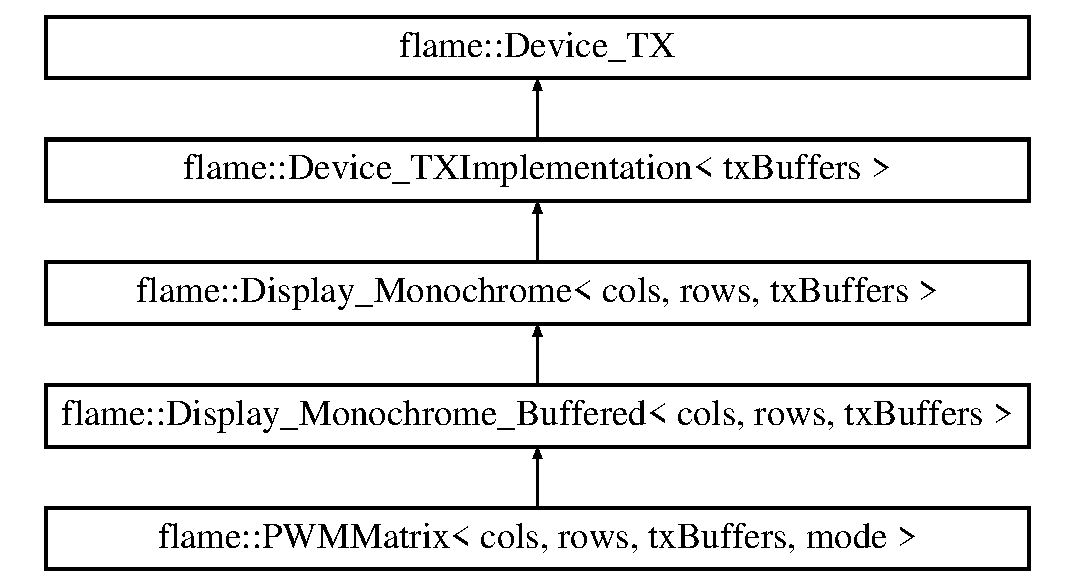
\includegraphics[height=5.000000cm]{classflame_1_1_display___monochrome___buffered}
\end{center}
\end{figure}
\subsection*{Public Member Functions}
\begin{DoxyCompactItemize}
\item 
\hyperlink{classflame_1_1_display___monochrome___buffered_afdfaefdd9c432d9f93d52232d6eb4985}{Display\-\_\-\-Monochrome\-\_\-\-Buffered} ()
\item 
void \hyperlink{classflame_1_1_display___monochrome___buffered_a5ffe666a9a5ae12931177c05307b48e1}{set\-Pixel} (uint16\-\_\-t col, uint16\-\_\-t row, uint8\-\_\-t value)
\item 
uint8\-\_\-t \hyperlink{classflame_1_1_display___monochrome___buffered_a003e20bbdf7f905cee2dcfb22be61268}{get\-Pixel} (uint16\-\_\-t col, uint16\-\_\-t row)
\end{DoxyCompactItemize}
\subsection*{Protected Attributes}
\begin{DoxyCompactItemize}
\item 
uint8\-\_\-t \hyperlink{classflame_1_1_display___monochrome___buffered_ad1811b000b6d38a4400da0784768544c}{\-\_\-frame\-Buffer} \mbox{[}cols $\ast$rows\mbox{]}
\end{DoxyCompactItemize}
\subsection*{Additional Inherited Members}


\subsection{Detailed Description}
\subsubsection*{template$<$uint16\-\_\-t cols, uint16\-\_\-t rows, uint8\-\_\-t tx\-Buffers$>$class flame\-::\-Display\-\_\-\-Monochrome\-\_\-\-Buffered$<$ cols, rows, tx\-Buffers $>$}

A monochrome bitmap display Origin (0,0) is bottom left 
\begin{DoxyTemplParams}{Template Parameters}
{\em cols} & the number of columns \\
\hline
{\em rows} & the number of rows \\
\hline
{\em tx\-Buffers} & the number of output buffers \\
\hline
\end{DoxyTemplParams}


Definition at line 47 of file Display\-\_\-\-Monochrome\-\_\-\-Buffered.\-h.



\subsection{Constructor \& Destructor Documentation}
\hypertarget{classflame_1_1_display___monochrome___buffered_afdfaefdd9c432d9f93d52232d6eb4985}{\index{flame\-::\-Display\-\_\-\-Monochrome\-\_\-\-Buffered@{flame\-::\-Display\-\_\-\-Monochrome\-\_\-\-Buffered}!Display\-\_\-\-Monochrome\-\_\-\-Buffered@{Display\-\_\-\-Monochrome\-\_\-\-Buffered}}
\index{Display\-\_\-\-Monochrome\-\_\-\-Buffered@{Display\-\_\-\-Monochrome\-\_\-\-Buffered}!flame::Display_Monochrome_Buffered@{flame\-::\-Display\-\_\-\-Monochrome\-\_\-\-Buffered}}
\subsubsection[{Display\-\_\-\-Monochrome\-\_\-\-Buffered}]{\setlength{\rightskip}{0pt plus 5cm}template$<$uint16\-\_\-t cols, uint16\-\_\-t rows, uint8\-\_\-t tx\-Buffers$>$ {\bf flame\-::\-Display\-\_\-\-Monochrome\-\_\-\-Buffered}$<$ cols, rows, tx\-Buffers $>$\-::{\bf Display\-\_\-\-Monochrome\-\_\-\-Buffered} (
\begin{DoxyParamCaption}
{}
\end{DoxyParamCaption}
)\hspace{0.3cm}{\ttfamily [inline]}}}\label{classflame_1_1_display___monochrome___buffered_afdfaefdd9c432d9f93d52232d6eb4985}
Create a new monochrome display 

Definition at line 55 of file Display\-\_\-\-Monochrome\-\_\-\-Buffered.\-h.



\subsection{Member Function Documentation}
\hypertarget{classflame_1_1_display___monochrome___buffered_a003e20bbdf7f905cee2dcfb22be61268}{\index{flame\-::\-Display\-\_\-\-Monochrome\-\_\-\-Buffered@{flame\-::\-Display\-\_\-\-Monochrome\-\_\-\-Buffered}!get\-Pixel@{get\-Pixel}}
\index{get\-Pixel@{get\-Pixel}!flame::Display_Monochrome_Buffered@{flame\-::\-Display\-\_\-\-Monochrome\-\_\-\-Buffered}}
\subsubsection[{get\-Pixel}]{\setlength{\rightskip}{0pt plus 5cm}template$<$uint16\-\_\-t cols, uint16\-\_\-t rows, uint8\-\_\-t tx\-Buffers$>$ uint8\-\_\-t {\bf flame\-::\-Display\-\_\-\-Monochrome\-\_\-\-Buffered}$<$ cols, rows, tx\-Buffers $>$\-::get\-Pixel (
\begin{DoxyParamCaption}
\item[{uint16\-\_\-t}]{col, }
\item[{uint16\-\_\-t}]{row}
\end{DoxyParamCaption}
)\hspace{0.3cm}{\ttfamily [inline]}, {\ttfamily [virtual]}}}\label{classflame_1_1_display___monochrome___buffered_a003e20bbdf7f905cee2dcfb22be61268}


Implements \hyperlink{classflame_1_1_display___monochrome_a24ddc06684641b00ee27b2630d216f8f}{flame\-::\-Display\-\_\-\-Monochrome$<$ cols, rows, tx\-Buffers $>$}.



Definition at line 75 of file Display\-\_\-\-Monochrome\-\_\-\-Buffered.\-h.

\hypertarget{classflame_1_1_display___monochrome___buffered_a5ffe666a9a5ae12931177c05307b48e1}{\index{flame\-::\-Display\-\_\-\-Monochrome\-\_\-\-Buffered@{flame\-::\-Display\-\_\-\-Monochrome\-\_\-\-Buffered}!set\-Pixel@{set\-Pixel}}
\index{set\-Pixel@{set\-Pixel}!flame::Display_Monochrome_Buffered@{flame\-::\-Display\-\_\-\-Monochrome\-\_\-\-Buffered}}
\subsubsection[{set\-Pixel}]{\setlength{\rightskip}{0pt plus 5cm}template$<$uint16\-\_\-t cols, uint16\-\_\-t rows, uint8\-\_\-t tx\-Buffers$>$ void {\bf flame\-::\-Display\-\_\-\-Monochrome\-\_\-\-Buffered}$<$ cols, rows, tx\-Buffers $>$\-::set\-Pixel (
\begin{DoxyParamCaption}
\item[{uint16\-\_\-t}]{col, }
\item[{uint16\-\_\-t}]{row, }
\item[{uint8\-\_\-t}]{value}
\end{DoxyParamCaption}
)\hspace{0.3cm}{\ttfamily [inline]}, {\ttfamily [virtual]}}}\label{classflame_1_1_display___monochrome___buffered_a5ffe666a9a5ae12931177c05307b48e1}


Implements \hyperlink{classflame_1_1_display___monochrome_a34002efa6fccb74a4fbea455f2a261d3}{flame\-::\-Display\-\_\-\-Monochrome$<$ cols, rows, tx\-Buffers $>$}.



Definition at line 64 of file Display\-\_\-\-Monochrome\-\_\-\-Buffered.\-h.



\subsection{Member Data Documentation}
\hypertarget{classflame_1_1_display___monochrome___buffered_ad1811b000b6d38a4400da0784768544c}{\index{flame\-::\-Display\-\_\-\-Monochrome\-\_\-\-Buffered@{flame\-::\-Display\-\_\-\-Monochrome\-\_\-\-Buffered}!\-\_\-frame\-Buffer@{\-\_\-frame\-Buffer}}
\index{\-\_\-frame\-Buffer@{\-\_\-frame\-Buffer}!flame::Display_Monochrome_Buffered@{flame\-::\-Display\-\_\-\-Monochrome\-\_\-\-Buffered}}
\subsubsection[{\-\_\-frame\-Buffer}]{\setlength{\rightskip}{0pt plus 5cm}template$<$uint16\-\_\-t cols, uint16\-\_\-t rows, uint8\-\_\-t tx\-Buffers$>$ uint8\-\_\-t {\bf flame\-::\-Display\-\_\-\-Monochrome\-\_\-\-Buffered}$<$ cols, rows, tx\-Buffers $>$\-::\-\_\-frame\-Buffer\mbox{[}cols $\ast$rows\mbox{]}\hspace{0.3cm}{\ttfamily [protected]}}}\label{classflame_1_1_display___monochrome___buffered_ad1811b000b6d38a4400da0784768544c}


Definition at line 49 of file Display\-\_\-\-Monochrome\-\_\-\-Buffered.\-h.



The documentation for this class was generated from the following file\-:\begin{DoxyCompactItemize}
\item 
flame/\hyperlink{_display___monochrome___buffered_8h}{Display\-\_\-\-Monochrome\-\_\-\-Buffered.\-h}\end{DoxyCompactItemize}

\hypertarget{classflame_1_1_display___selector}{\section{flame\-:\-:Display\-\_\-\-Selector Class Reference}
\label{classflame_1_1_display___selector}\index{flame\-::\-Display\-\_\-\-Selector@{flame\-::\-Display\-\_\-\-Selector}}
}


{\ttfamily \#include $<$Display\-\_\-\-Monochrome.\-h$>$}

\subsection*{Public Member Functions}
\begin{DoxyCompactItemize}
\item 
virtual void \hyperlink{classflame_1_1_display___selector_ac23dc550b137ed381ac8168ebf607bc8}{select} (uint8\-\_\-t display\-X, uint8\-\_\-t display\-Y, bool active)=0
\end{DoxyCompactItemize}


\subsection{Detailed Description}


Definition at line 38 of file Display\-\_\-\-Monochrome.\-h.



\subsection{Member Function Documentation}
\hypertarget{classflame_1_1_display___selector_ac23dc550b137ed381ac8168ebf607bc8}{\index{flame\-::\-Display\-\_\-\-Selector@{flame\-::\-Display\-\_\-\-Selector}!select@{select}}
\index{select@{select}!flame::Display_Selector@{flame\-::\-Display\-\_\-\-Selector}}
\subsubsection[{select}]{\setlength{\rightskip}{0pt plus 5cm}virtual void flame\-::\-Display\-\_\-\-Selector\-::select (
\begin{DoxyParamCaption}
\item[{uint8\-\_\-t}]{display\-X, }
\item[{uint8\-\_\-t}]{display\-Y, }
\item[{bool}]{active}
\end{DoxyParamCaption}
)\hspace{0.3cm}{\ttfamily [pure virtual]}}}\label{classflame_1_1_display___selector_ac23dc550b137ed381ac8168ebf607bc8}


The documentation for this class was generated from the following file\-:\begin{DoxyCompactItemize}
\item 
flame/\hyperlink{_display___monochrome_8h}{Display\-\_\-\-Monochrome.\-h}\end{DoxyCompactItemize}

\hypertarget{classflame_1_1_e_e_p_r_o_m}{\section{flame\-:\-:E\-E\-P\-R\-O\-M Class Reference}
\label{classflame_1_1_e_e_p_r_o_m}\index{flame\-::\-E\-E\-P\-R\-O\-M@{flame\-::\-E\-E\-P\-R\-O\-M}}
}


{\ttfamily \#include $<$E\-E\-P\-R\-O\-M.\-h$>$}

\subsection*{Public Member Functions}
\begin{DoxyCompactItemize}
\item 
\hyperlink{classflame_1_1_e_e_p_r_o_m_ae2eb20d65e5518bbd9a660c6401dbcf1}{E\-E\-P\-R\-O\-M} ()
\item 
int16\-\_\-t \hyperlink{classflame_1_1_e_e_p_r_o_m_aa8fd4064faa1e2a78b0a8778b50f57be}{read} (uint16\-\_\-t address)
\item 
uint8\-\_\-t \hyperlink{classflame_1_1_e_e_p_r_o_m_acabcdbc11db884db1a2608c580aa84ef}{busy\-Read} (uint16\-\_\-t address)
\item 
int8\-\_\-t \hyperlink{classflame_1_1_e_e_p_r_o_m_a1584e413a8239e8352076fc09e8839bd}{read} (void $\ast$buffer, uint16\-\_\-t address, uint16\-\_\-t length)
\item 
void \hyperlink{classflame_1_1_e_e_p_r_o_m_a2a5c938a08de09bf4e6d8e7926bf4b17}{busy\-Read} (void $\ast$buffer, uint16\-\_\-t address, uint16\-\_\-t length)
\item 
int8\-\_\-t \hyperlink{classflame_1_1_e_e_p_r_o_m_a9479e07e880667dad49289bbb00b9261}{write} (uint16\-\_\-t address, uint8\-\_\-t data)
\item 
int8\-\_\-t \hyperlink{classflame_1_1_e_e_p_r_o_m_a24dc038468425385ed0bef8375d6c266}{busy\-Write} (void $\ast$buffer, uint16\-\_\-t address, uint16\-\_\-t length)
\item 
int8\-\_\-t \hyperlink{classflame_1_1_e_e_p_r_o_m_afd4f04c1685e611f5e752cd8ae396857}{write} (void $\ast$buffer, uint16\-\_\-t address, uint16\-\_\-t length, \hyperlink{classflame_1_1_e_e_p_r_o_m_listener}{E\-E\-P\-R\-O\-M\-Listener} $\ast$done)
\item 
void \hyperlink{classflame_1_1_e_e_p_r_o_m_aa39e6c43fddfc93bd8a3ee59e36609c3}{write\-Interrupt} ()
\item 
bool \hyperlink{classflame_1_1_e_e_p_r_o_m_a7ad2ec5185aeeffe7b06820b0cde8abf}{is\-Busy} ()
\item 
uint16\-\_\-t \hyperlink{classflame_1_1_e_e_p_r_o_m_a5b24aa67d9fd4ccbac79601670505d33}{crc} (uint16\-\_\-t address, uint16\-\_\-t length)
\end{DoxyCompactItemize}


\subsection{Detailed Description}


Definition at line 71 of file E\-E\-P\-R\-O\-M.\-h.



\subsection{Constructor \& Destructor Documentation}
\hypertarget{classflame_1_1_e_e_p_r_o_m_ae2eb20d65e5518bbd9a660c6401dbcf1}{\index{flame\-::\-E\-E\-P\-R\-O\-M@{flame\-::\-E\-E\-P\-R\-O\-M}!E\-E\-P\-R\-O\-M@{E\-E\-P\-R\-O\-M}}
\index{E\-E\-P\-R\-O\-M@{E\-E\-P\-R\-O\-M}!flame::EEPROM@{flame\-::\-E\-E\-P\-R\-O\-M}}
\subsubsection[{E\-E\-P\-R\-O\-M}]{\setlength{\rightskip}{0pt plus 5cm}flame\-::\-E\-E\-P\-R\-O\-M\-::\-E\-E\-P\-R\-O\-M (
\begin{DoxyParamCaption}
{}
\end{DoxyParamCaption}
)}}\label{classflame_1_1_e_e_p_r_o_m_ae2eb20d65e5518bbd9a660c6401dbcf1}
Create a new \hyperlink{classflame_1_1_e_e_p_r_o_m}{E\-E\-P\-R\-O\-M} access class 

Definition at line 37 of file E\-E\-P\-R\-O\-M.\-cpp.



\subsection{Member Function Documentation}
\hypertarget{classflame_1_1_e_e_p_r_o_m_acabcdbc11db884db1a2608c580aa84ef}{\index{flame\-::\-E\-E\-P\-R\-O\-M@{flame\-::\-E\-E\-P\-R\-O\-M}!busy\-Read@{busy\-Read}}
\index{busy\-Read@{busy\-Read}!flame::EEPROM@{flame\-::\-E\-E\-P\-R\-O\-M}}
\subsubsection[{busy\-Read}]{\setlength{\rightskip}{0pt plus 5cm}uint8\-\_\-t flame\-::\-E\-E\-P\-R\-O\-M\-::busy\-Read (
\begin{DoxyParamCaption}
\item[{uint16\-\_\-t}]{address}
\end{DoxyParamCaption}
)}}\label{classflame_1_1_e_e_p_r_o_m_acabcdbc11db884db1a2608c580aa84ef}
Read a byte from \hyperlink{classflame_1_1_e_e_p_r_o_m}{E\-E\-P\-R\-O\-M}, waiting until the \hyperlink{classflame_1_1_e_e_p_r_o_m}{E\-E\-P\-R\-O\-M} is available 
\begin{DoxyParams}{Parameters}
{\em address} & the address to read from \\
\hline
\end{DoxyParams}
\begin{DoxyReturn}{Returns}
the byte 
\end{DoxyReturn}


Definition at line 68 of file E\-E\-P\-R\-O\-M.\-cpp.

\hypertarget{classflame_1_1_e_e_p_r_o_m_a2a5c938a08de09bf4e6d8e7926bf4b17}{\index{flame\-::\-E\-E\-P\-R\-O\-M@{flame\-::\-E\-E\-P\-R\-O\-M}!busy\-Read@{busy\-Read}}
\index{busy\-Read@{busy\-Read}!flame::EEPROM@{flame\-::\-E\-E\-P\-R\-O\-M}}
\subsubsection[{busy\-Read}]{\setlength{\rightskip}{0pt plus 5cm}void flame\-::\-E\-E\-P\-R\-O\-M\-::busy\-Read (
\begin{DoxyParamCaption}
\item[{void $\ast$}]{buffer, }
\item[{uint16\-\_\-t}]{address, }
\item[{uint16\-\_\-t}]{length}
\end{DoxyParamCaption}
)}}\label{classflame_1_1_e_e_p_r_o_m_a2a5c938a08de09bf4e6d8e7926bf4b17}
Read a buffer from \hyperlink{classflame_1_1_e_e_p_r_o_m}{E\-E\-P\-R\-O\-M}, waiting until the \hyperlink{classflame_1_1_e_e_p_r_o_m}{E\-E\-P\-R\-O\-M} is available 
\begin{DoxyParams}{Parameters}
{\em buffer} & the buffer to populate \\
\hline
{\em address} & the address to read from \\
\hline
{\em length} & the number of bytes to read \\
\hline
\end{DoxyParams}


Definition at line 105 of file E\-E\-P\-R\-O\-M.\-cpp.

\hypertarget{classflame_1_1_e_e_p_r_o_m_a24dc038468425385ed0bef8375d6c266}{\index{flame\-::\-E\-E\-P\-R\-O\-M@{flame\-::\-E\-E\-P\-R\-O\-M}!busy\-Write@{busy\-Write}}
\index{busy\-Write@{busy\-Write}!flame::EEPROM@{flame\-::\-E\-E\-P\-R\-O\-M}}
\subsubsection[{busy\-Write}]{\setlength{\rightskip}{0pt plus 5cm}int8\-\_\-t flame\-::\-E\-E\-P\-R\-O\-M\-::busy\-Write (
\begin{DoxyParamCaption}
\item[{void $\ast$}]{buffer, }
\item[{uint16\-\_\-t}]{address, }
\item[{uint16\-\_\-t}]{length}
\end{DoxyParamCaption}
)}}\label{classflame_1_1_e_e_p_r_o_m_a24dc038468425385ed0bef8375d6c266}
Write a buffer to \hyperlink{classflame_1_1_e_e_p_r_o_m}{E\-E\-P\-R\-O\-M} 
\begin{DoxyParams}{Parameters}
{\em buffer} & the buffer to read from \\
\hline
{\em address} & the address to write to \\
\hline
{\em length} & the number of bytes to write \\
\hline
\end{DoxyParams}


Definition at line 136 of file E\-E\-P\-R\-O\-M.\-cpp.

\hypertarget{classflame_1_1_e_e_p_r_o_m_a5b24aa67d9fd4ccbac79601670505d33}{\index{flame\-::\-E\-E\-P\-R\-O\-M@{flame\-::\-E\-E\-P\-R\-O\-M}!crc@{crc}}
\index{crc@{crc}!flame::EEPROM@{flame\-::\-E\-E\-P\-R\-O\-M}}
\subsubsection[{crc}]{\setlength{\rightskip}{0pt plus 5cm}uint16\-\_\-t flame\-::\-E\-E\-P\-R\-O\-M\-::crc (
\begin{DoxyParamCaption}
\item[{uint16\-\_\-t}]{address, }
\item[{uint16\-\_\-t}]{length}
\end{DoxyParamCaption}
)}}\label{classflame_1_1_e_e_p_r_o_m_a5b24aa67d9fd4ccbac79601670505d33}
Calculate the C\-R\-C of a block of \hyperlink{classflame_1_1_e_e_p_r_o_m}{E\-E\-P\-R\-O\-M} 
\begin{DoxyParams}{Parameters}
{\em address} & the address of the block \\
\hline
{\em length} & the length of the block \\
\hline
\end{DoxyParams}
\begin{DoxyReturn}{Returns}
the C\-R\-C 
\end{DoxyReturn}


Definition at line 229 of file E\-E\-P\-R\-O\-M.\-cpp.

\hypertarget{classflame_1_1_e_e_p_r_o_m_a7ad2ec5185aeeffe7b06820b0cde8abf}{\index{flame\-::\-E\-E\-P\-R\-O\-M@{flame\-::\-E\-E\-P\-R\-O\-M}!is\-Busy@{is\-Busy}}
\index{is\-Busy@{is\-Busy}!flame::EEPROM@{flame\-::\-E\-E\-P\-R\-O\-M}}
\subsubsection[{is\-Busy}]{\setlength{\rightskip}{0pt plus 5cm}bool flame\-::\-E\-E\-P\-R\-O\-M\-::is\-Busy (
\begin{DoxyParamCaption}
{}
\end{DoxyParamCaption}
)}}\label{classflame_1_1_e_e_p_r_o_m_a7ad2ec5185aeeffe7b06820b0cde8abf}
Check if the \hyperlink{classflame_1_1_e_e_p_r_o_m}{E\-E\-P\-R\-O\-M} hardware is busy \begin{DoxyReturn}{Returns}
true if the \hyperlink{classflame_1_1_e_e_p_r_o_m}{E\-E\-P\-R\-O\-M} hardware is busy 
\end{DoxyReturn}


Definition at line 215 of file E\-E\-P\-R\-O\-M.\-cpp.

\hypertarget{classflame_1_1_e_e_p_r_o_m_aa8fd4064faa1e2a78b0a8778b50f57be}{\index{flame\-::\-E\-E\-P\-R\-O\-M@{flame\-::\-E\-E\-P\-R\-O\-M}!read@{read}}
\index{read@{read}!flame::EEPROM@{flame\-::\-E\-E\-P\-R\-O\-M}}
\subsubsection[{read}]{\setlength{\rightskip}{0pt plus 5cm}int16\-\_\-t flame\-::\-E\-E\-P\-R\-O\-M\-::read (
\begin{DoxyParamCaption}
\item[{uint16\-\_\-t}]{address}
\end{DoxyParamCaption}
)}}\label{classflame_1_1_e_e_p_r_o_m_aa8fd4064faa1e2a78b0a8778b50f57be}
Read a byte from \hyperlink{classflame_1_1_e_e_p_r_o_m}{E\-E\-P\-R\-O\-M} 
\begin{DoxyParams}{Parameters}
{\em address} & the address to read from \\
\hline
\end{DoxyParams}
\begin{DoxyReturn}{Returns}
the byte, or F\-L\-A\-M\-E\-\_\-\-E\-E\-P\-R\-O\-M\-\_\-\-B\-U\-S\-Y if the \hyperlink{classflame_1_1_e_e_p_r_o_m}{E\-E\-P\-R\-O\-M} is busy 
\end{DoxyReturn}


Definition at line 49 of file E\-E\-P\-R\-O\-M.\-cpp.

\hypertarget{classflame_1_1_e_e_p_r_o_m_a1584e413a8239e8352076fc09e8839bd}{\index{flame\-::\-E\-E\-P\-R\-O\-M@{flame\-::\-E\-E\-P\-R\-O\-M}!read@{read}}
\index{read@{read}!flame::EEPROM@{flame\-::\-E\-E\-P\-R\-O\-M}}
\subsubsection[{read}]{\setlength{\rightskip}{0pt plus 5cm}int8\-\_\-t flame\-::\-E\-E\-P\-R\-O\-M\-::read (
\begin{DoxyParamCaption}
\item[{void $\ast$}]{buffer, }
\item[{uint16\-\_\-t}]{address, }
\item[{uint16\-\_\-t}]{length}
\end{DoxyParamCaption}
)}}\label{classflame_1_1_e_e_p_r_o_m_a1584e413a8239e8352076fc09e8839bd}
Read a buffer from \hyperlink{classflame_1_1_e_e_p_r_o_m}{E\-E\-P\-R\-O\-M} 
\begin{DoxyParams}{Parameters}
{\em buffer} & the buffer to populate \\
\hline
{\em address} & the address to read from \\
\hline
{\em length} & the number of bytes to read \\
\hline
\end{DoxyParams}


Definition at line 81 of file E\-E\-P\-R\-O\-M.\-cpp.

\hypertarget{classflame_1_1_e_e_p_r_o_m_a9479e07e880667dad49289bbb00b9261}{\index{flame\-::\-E\-E\-P\-R\-O\-M@{flame\-::\-E\-E\-P\-R\-O\-M}!write@{write}}
\index{write@{write}!flame::EEPROM@{flame\-::\-E\-E\-P\-R\-O\-M}}
\subsubsection[{write}]{\setlength{\rightskip}{0pt plus 5cm}int8\-\_\-t flame\-::\-E\-E\-P\-R\-O\-M\-::write (
\begin{DoxyParamCaption}
\item[{uint16\-\_\-t}]{address, }
\item[{uint8\-\_\-t}]{data}
\end{DoxyParamCaption}
)}}\label{classflame_1_1_e_e_p_r_o_m_a9479e07e880667dad49289bbb00b9261}
Write a byte to \hyperlink{classflame_1_1_e_e_p_r_o_m}{E\-E\-P\-R\-O\-M} 
\begin{DoxyParams}{Parameters}
{\em address} & the address to write to \\
\hline
{\em data} & the byte to write \\
\hline
\end{DoxyParams}
\begin{DoxyReturn}{Returns}
F\-L\-A\-M\-E\-\_\-\-E\-E\-P\-R\-O\-M\-\_\-\-B\-U\-S\-Y if the \hyperlink{classflame_1_1_e_e_p_r_o_m}{E\-E\-P\-R\-O\-M} is busy 
\end{DoxyReturn}


Definition at line 115 of file E\-E\-P\-R\-O\-M.\-cpp.

\hypertarget{classflame_1_1_e_e_p_r_o_m_afd4f04c1685e611f5e752cd8ae396857}{\index{flame\-::\-E\-E\-P\-R\-O\-M@{flame\-::\-E\-E\-P\-R\-O\-M}!write@{write}}
\index{write@{write}!flame::EEPROM@{flame\-::\-E\-E\-P\-R\-O\-M}}
\subsubsection[{write}]{\setlength{\rightskip}{0pt plus 5cm}int8\-\_\-t flame\-::\-E\-E\-P\-R\-O\-M\-::write (
\begin{DoxyParamCaption}
\item[{void $\ast$}]{buffer, }
\item[{uint16\-\_\-t}]{address, }
\item[{uint16\-\_\-t}]{length, }
\item[{{\bf E\-E\-P\-R\-O\-M\-Listener} $\ast$}]{done}
\end{DoxyParamCaption}
)}}\label{classflame_1_1_e_e_p_r_o_m_afd4f04c1685e611f5e752cd8ae396857}
Write a buffer to \hyperlink{classflame_1_1_e_e_p_r_o_m}{E\-E\-P\-R\-O\-M} 
\begin{DoxyParams}{Parameters}
{\em buffer} & the buffer to read from \\
\hline
{\em address} & the address to write to \\
\hline
{\em length} & the number of bytes to write (must be greater than 0) \\
\hline
{\em done} & A listener to notify when the buffer has been written (can be N\-U\-L\-L) \\
\hline
\end{DoxyParams}


Definition at line 165 of file E\-E\-P\-R\-O\-M.\-cpp.

\hypertarget{classflame_1_1_e_e_p_r_o_m_aa39e6c43fddfc93bd8a3ee59e36609c3}{\index{flame\-::\-E\-E\-P\-R\-O\-M@{flame\-::\-E\-E\-P\-R\-O\-M}!write\-Interrupt@{write\-Interrupt}}
\index{write\-Interrupt@{write\-Interrupt}!flame::EEPROM@{flame\-::\-E\-E\-P\-R\-O\-M}}
\subsubsection[{write\-Interrupt}]{\setlength{\rightskip}{0pt plus 5cm}void flame\-::\-E\-E\-P\-R\-O\-M\-::write\-Interrupt (
\begin{DoxyParamCaption}
{}
\end{DoxyParamCaption}
)}}\label{classflame_1_1_e_e_p_r_o_m_aa39e6c43fddfc93bd8a3ee59e36609c3}
Interrupt handler for async writes 

Definition at line 191 of file E\-E\-P\-R\-O\-M.\-cpp.



The documentation for this class was generated from the following files\-:\begin{DoxyCompactItemize}
\item 
flame/\hyperlink{_e_e_p_r_o_m_8h}{E\-E\-P\-R\-O\-M.\-h}\item 
\hyperlink{_e_e_p_r_o_m_8cpp}{E\-E\-P\-R\-O\-M.\-cpp}\end{DoxyCompactItemize}

\hypertarget{classflame_1_1_e_e_p_r_o_m_listener}{\section{flame\-:\-:E\-E\-P\-R\-O\-M\-Listener Class Reference}
\label{classflame_1_1_e_e_p_r_o_m_listener}\index{flame\-::\-E\-E\-P\-R\-O\-M\-Listener@{flame\-::\-E\-E\-P\-R\-O\-M\-Listener}}
}


{\ttfamily \#include $<$E\-E\-P\-R\-O\-M.\-h$>$}

Inheritance diagram for flame\-:\-:E\-E\-P\-R\-O\-M\-Listener\-:\begin{figure}[H]
\begin{center}
\leavevmode
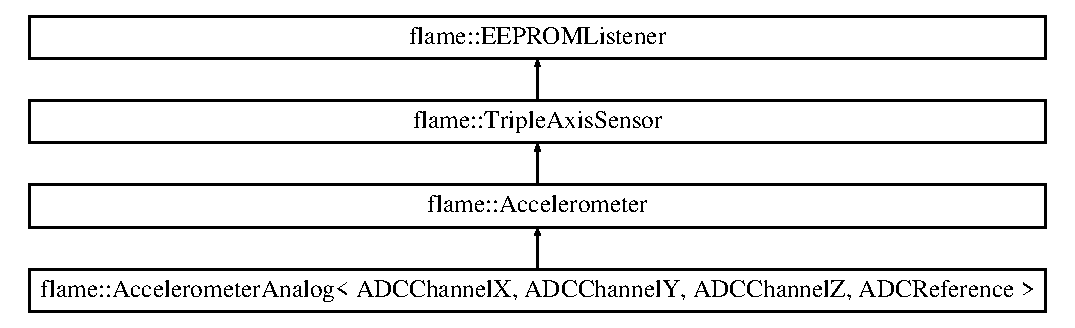
\includegraphics[height=3.964602cm]{classflame_1_1_e_e_p_r_o_m_listener}
\end{center}
\end{figure}
\subsection*{Public Member Functions}
\begin{DoxyCompactItemize}
\item 
virtual void \hyperlink{classflame_1_1_e_e_p_r_o_m_listener_a676ba44ddf2c7927d1c60c017a807279}{eeprom\-Done} (\hyperlink{classflame_1_1_e_e_p_r_o_m}{E\-E\-P\-R\-O\-M} \&eeprom, uint16\-\_\-t address, void $\ast$buffer)=0
\end{DoxyCompactItemize}


\subsection{Detailed Description}


Definition at line 60 of file E\-E\-P\-R\-O\-M.\-h.



\subsection{Member Function Documentation}
\hypertarget{classflame_1_1_e_e_p_r_o_m_listener_a676ba44ddf2c7927d1c60c017a807279}{\index{flame\-::\-E\-E\-P\-R\-O\-M\-Listener@{flame\-::\-E\-E\-P\-R\-O\-M\-Listener}!eeprom\-Done@{eeprom\-Done}}
\index{eeprom\-Done@{eeprom\-Done}!flame::EEPROMListener@{flame\-::\-E\-E\-P\-R\-O\-M\-Listener}}
\subsubsection[{eeprom\-Done}]{\setlength{\rightskip}{0pt plus 5cm}virtual void flame\-::\-E\-E\-P\-R\-O\-M\-Listener\-::eeprom\-Done (
\begin{DoxyParamCaption}
\item[{{\bf E\-E\-P\-R\-O\-M} \&}]{eeprom, }
\item[{uint16\-\_\-t}]{address, }
\item[{void $\ast$}]{buffer}
\end{DoxyParamCaption}
)\hspace{0.3cm}{\ttfamily [pure virtual]}}}\label{classflame_1_1_e_e_p_r_o_m_listener_a676ba44ddf2c7927d1c60c017a807279}
Called when an \hyperlink{classflame_1_1_e_e_p_r_o_m}{E\-E\-P\-R\-O\-M} write is finished 
\begin{DoxyParams}{Parameters}
{\em eeprom} & the \hyperlink{classflame_1_1_e_e_p_r_o_m}{E\-E\-P\-R\-O\-M} access instance \\
\hline
{\em address} & the \hyperlink{classflame_1_1_e_e_p_r_o_m}{E\-E\-P\-R\-O\-M} address that the data was written to \\
\hline
{\em buffer} & the pointer that the data was written from \\
\hline
\end{DoxyParams}


Implemented in \hyperlink{classflame_1_1_triple_axis_sensor_aaa716e2a07cc7fe544075215c1ac8a75}{flame\-::\-Triple\-Axis\-Sensor}.



The documentation for this class was generated from the following file\-:\begin{DoxyCompactItemize}
\item 
flame/\hyperlink{_e_e_p_r_o_m_8h}{E\-E\-P\-R\-O\-M.\-h}\end{DoxyCompactItemize}

\hypertarget{structflame_1_1event_a_d_c}{\section{flame\-:\-:event\-A\-D\-C Struct Reference}
\label{structflame_1_1event_a_d_c}\index{flame\-::event\-A\-D\-C@{flame\-::event\-A\-D\-C}}
}


{\ttfamily \#include $<$A\-D\-C\-Manager.\-h$>$}

\subsection*{Public Attributes}
\begin{DoxyCompactItemize}
\item 
\hyperlink{atmega1280_8h_ab5a361d214bf33f4d9d443d9db44043d}{A\-D\-C\-Channel} \hyperlink{structflame_1_1event_a_d_c_a82ec57a6fcebb837bc0e8d175a469c74}{channel}
\item 
\hyperlink{classflame_1_1_a_d_c_listener}{A\-D\-C\-Listener} $\ast$ \hyperlink{structflame_1_1event_a_d_c_a4e6a027b0eb02bcb096ac169499635ee}{listener}
\end{DoxyCompactItemize}


\subsection{Detailed Description}


Definition at line 65 of file A\-D\-C\-Manager.\-h.



\subsection{Member Data Documentation}
\hypertarget{structflame_1_1event_a_d_c_a82ec57a6fcebb837bc0e8d175a469c74}{\index{flame\-::event\-A\-D\-C@{flame\-::event\-A\-D\-C}!channel@{channel}}
\index{channel@{channel}!flame::eventADC@{flame\-::event\-A\-D\-C}}
\subsubsection[{channel}]{\setlength{\rightskip}{0pt plus 5cm}{\bf A\-D\-C\-Channel} flame\-::event\-A\-D\-C\-::channel}}\label{structflame_1_1event_a_d_c_a82ec57a6fcebb837bc0e8d175a469c74}


Definition at line 66 of file A\-D\-C\-Manager.\-h.

\hypertarget{structflame_1_1event_a_d_c_a4e6a027b0eb02bcb096ac169499635ee}{\index{flame\-::event\-A\-D\-C@{flame\-::event\-A\-D\-C}!listener@{listener}}
\index{listener@{listener}!flame::eventADC@{flame\-::event\-A\-D\-C}}
\subsubsection[{listener}]{\setlength{\rightskip}{0pt plus 5cm}{\bf A\-D\-C\-Listener}$\ast$ flame\-::event\-A\-D\-C\-::listener}}\label{structflame_1_1event_a_d_c_a4e6a027b0eb02bcb096ac169499635ee}


Definition at line 67 of file A\-D\-C\-Manager.\-h.



The documentation for this struct was generated from the following file\-:\begin{DoxyCompactItemize}
\item 
flame/\hyperlink{_a_d_c_manager_8h}{A\-D\-C\-Manager.\-h}\end{DoxyCompactItemize}

\hypertarget{structflame_1_1event_pin}{\section{flame\-:\-:event\-Pin Struct Reference}
\label{structflame_1_1event_pin}\index{flame\-::event\-Pin@{flame\-::event\-Pin}}
}


{\ttfamily \#include $<$Pin\-Change\-Manager.\-h$>$}

\subsection*{Public Attributes}
\begin{DoxyCompactItemize}
\item 
\hyperlink{namespaceflame_a7117d3cded694c1ded03c462d677b165}{F\-L\-A\-M\-E\-\_\-register} \hyperlink{structflame_1_1event_pin_a7bfb98722a6a21d33c3c262c6a847382}{port}
\item 
uint8\-\_\-t \hyperlink{structflame_1_1event_pin_a2b66016381933ad3285bbcec8ce36257}{mask}
\item 
uint8\-\_\-t \hyperlink{structflame_1_1event_pin_a61cbe32d1c708c62ab074935bef267ee}{pc\-Int}
\item 
\hyperlink{classflame_1_1_pin_event_listener}{Pin\-Event\-Listener} $\ast$ \hyperlink{structflame_1_1event_pin_aa38718b7fe55c65f7e2917dc0bfc2f0c}{listener}
\item 
bool \hyperlink{structflame_1_1event_pin_a2681b74d7415d069d0da214d25575fdb}{previous}
\item 
bool \hyperlink{structflame_1_1event_pin_a5e73650b961e6fc3917e29f33d8f916e}{changed}
\end{DoxyCompactItemize}


\subsection{Detailed Description}


Definition at line 80 of file Pin\-Change\-Manager.\-h.



\subsection{Member Data Documentation}
\hypertarget{structflame_1_1event_pin_a5e73650b961e6fc3917e29f33d8f916e}{\index{flame\-::event\-Pin@{flame\-::event\-Pin}!changed@{changed}}
\index{changed@{changed}!flame::eventPin@{flame\-::event\-Pin}}
\subsubsection[{changed}]{\setlength{\rightskip}{0pt plus 5cm}bool flame\-::event\-Pin\-::changed}}\label{structflame_1_1event_pin_a5e73650b961e6fc3917e29f33d8f916e}


Definition at line 86 of file Pin\-Change\-Manager.\-h.

\hypertarget{structflame_1_1event_pin_aa38718b7fe55c65f7e2917dc0bfc2f0c}{\index{flame\-::event\-Pin@{flame\-::event\-Pin}!listener@{listener}}
\index{listener@{listener}!flame::eventPin@{flame\-::event\-Pin}}
\subsubsection[{listener}]{\setlength{\rightskip}{0pt plus 5cm}{\bf Pin\-Event\-Listener}$\ast$ flame\-::event\-Pin\-::listener}}\label{structflame_1_1event_pin_aa38718b7fe55c65f7e2917dc0bfc2f0c}


Definition at line 84 of file Pin\-Change\-Manager.\-h.

\hypertarget{structflame_1_1event_pin_a2b66016381933ad3285bbcec8ce36257}{\index{flame\-::event\-Pin@{flame\-::event\-Pin}!mask@{mask}}
\index{mask@{mask}!flame::eventPin@{flame\-::event\-Pin}}
\subsubsection[{mask}]{\setlength{\rightskip}{0pt plus 5cm}uint8\-\_\-t flame\-::event\-Pin\-::mask}}\label{structflame_1_1event_pin_a2b66016381933ad3285bbcec8ce36257}


Definition at line 82 of file Pin\-Change\-Manager.\-h.

\hypertarget{structflame_1_1event_pin_a61cbe32d1c708c62ab074935bef267ee}{\index{flame\-::event\-Pin@{flame\-::event\-Pin}!pc\-Int@{pc\-Int}}
\index{pc\-Int@{pc\-Int}!flame::eventPin@{flame\-::event\-Pin}}
\subsubsection[{pc\-Int}]{\setlength{\rightskip}{0pt plus 5cm}uint8\-\_\-t flame\-::event\-Pin\-::pc\-Int}}\label{structflame_1_1event_pin_a61cbe32d1c708c62ab074935bef267ee}


Definition at line 83 of file Pin\-Change\-Manager.\-h.

\hypertarget{structflame_1_1event_pin_a7bfb98722a6a21d33c3c262c6a847382}{\index{flame\-::event\-Pin@{flame\-::event\-Pin}!port@{port}}
\index{port@{port}!flame::eventPin@{flame\-::event\-Pin}}
\subsubsection[{port}]{\setlength{\rightskip}{0pt plus 5cm}{\bf F\-L\-A\-M\-E\-\_\-register} flame\-::event\-Pin\-::port}}\label{structflame_1_1event_pin_a7bfb98722a6a21d33c3c262c6a847382}


Definition at line 81 of file Pin\-Change\-Manager.\-h.

\hypertarget{structflame_1_1event_pin_a2681b74d7415d069d0da214d25575fdb}{\index{flame\-::event\-Pin@{flame\-::event\-Pin}!previous@{previous}}
\index{previous@{previous}!flame::eventPin@{flame\-::event\-Pin}}
\subsubsection[{previous}]{\setlength{\rightskip}{0pt plus 5cm}bool flame\-::event\-Pin\-::previous}}\label{structflame_1_1event_pin_a2681b74d7415d069d0da214d25575fdb}


Definition at line 85 of file Pin\-Change\-Manager.\-h.



The documentation for this struct was generated from the following file\-:\begin{DoxyCompactItemize}
\item 
flame/\hyperlink{_pin_change_manager_8h}{Pin\-Change\-Manager.\-h}\end{DoxyCompactItemize}

\hypertarget{structflame_1_1_f_l_a_m_e__pin}{\section{flame\-:\-:F\-L\-A\-M\-E\-\_\-pin Struct Reference}
\label{structflame_1_1_f_l_a_m_e__pin}\index{flame\-::\-F\-L\-A\-M\-E\-\_\-pin@{flame\-::\-F\-L\-A\-M\-E\-\_\-pin}}
}


{\ttfamily \#include $<$io.\-h$>$}

\subsection*{Public Attributes}
\begin{DoxyCompactItemize}
\item 
\hyperlink{namespaceflame_a7117d3cded694c1ded03c462d677b165}{F\-L\-A\-M\-E\-\_\-register} \hyperlink{structflame_1_1_f_l_a_m_e__pin_af270bfbe697774b7efdcd1e5fca607ca}{dir}
\item 
\hyperlink{namespaceflame_a7117d3cded694c1ded03c462d677b165}{F\-L\-A\-M\-E\-\_\-register} \hyperlink{structflame_1_1_f_l_a_m_e__pin_ac183e7bd5580c27281bd90f5e5f90e75}{input}
\item 
\hyperlink{namespaceflame_a7117d3cded694c1ded03c462d677b165}{F\-L\-A\-M\-E\-\_\-register} \hyperlink{structflame_1_1_f_l_a_m_e__pin_aa7a88c3c95421bf3c9a7858b6f6f7709}{output}
\item 
uint8\-\_\-t \hyperlink{structflame_1_1_f_l_a_m_e__pin_a0b048d9ad09e0388d1e141294a8fd47f}{bit}
\item 
int8\-\_\-t \hyperlink{structflame_1_1_f_l_a_m_e__pin_a42329feb988c345b2a76d6c3c1c7e7f7}{pc\-Int}
\end{DoxyCompactItemize}


\subsection{Detailed Description}


Definition at line 91 of file io.\-h.



\subsection{Member Data Documentation}
\hypertarget{structflame_1_1_f_l_a_m_e__pin_a0b048d9ad09e0388d1e141294a8fd47f}{\index{flame\-::\-F\-L\-A\-M\-E\-\_\-pin@{flame\-::\-F\-L\-A\-M\-E\-\_\-pin}!bit@{bit}}
\index{bit@{bit}!flame::FLAME_pin@{flame\-::\-F\-L\-A\-M\-E\-\_\-pin}}
\subsubsection[{bit}]{\setlength{\rightskip}{0pt plus 5cm}uint8\-\_\-t flame\-::\-F\-L\-A\-M\-E\-\_\-pin\-::bit}}\label{structflame_1_1_f_l_a_m_e__pin_a0b048d9ad09e0388d1e141294a8fd47f}


Definition at line 96 of file io.\-h.

\hypertarget{structflame_1_1_f_l_a_m_e__pin_af270bfbe697774b7efdcd1e5fca607ca}{\index{flame\-::\-F\-L\-A\-M\-E\-\_\-pin@{flame\-::\-F\-L\-A\-M\-E\-\_\-pin}!dir@{dir}}
\index{dir@{dir}!flame::FLAME_pin@{flame\-::\-F\-L\-A\-M\-E\-\_\-pin}}
\subsubsection[{dir}]{\setlength{\rightskip}{0pt plus 5cm}{\bf F\-L\-A\-M\-E\-\_\-register} flame\-::\-F\-L\-A\-M\-E\-\_\-pin\-::dir}}\label{structflame_1_1_f_l_a_m_e__pin_af270bfbe697774b7efdcd1e5fca607ca}


Definition at line 92 of file io.\-h.

\hypertarget{structflame_1_1_f_l_a_m_e__pin_ac183e7bd5580c27281bd90f5e5f90e75}{\index{flame\-::\-F\-L\-A\-M\-E\-\_\-pin@{flame\-::\-F\-L\-A\-M\-E\-\_\-pin}!input@{input}}
\index{input@{input}!flame::FLAME_pin@{flame\-::\-F\-L\-A\-M\-E\-\_\-pin}}
\subsubsection[{input}]{\setlength{\rightskip}{0pt plus 5cm}{\bf F\-L\-A\-M\-E\-\_\-register} flame\-::\-F\-L\-A\-M\-E\-\_\-pin\-::input}}\label{structflame_1_1_f_l_a_m_e__pin_ac183e7bd5580c27281bd90f5e5f90e75}


Definition at line 93 of file io.\-h.

\hypertarget{structflame_1_1_f_l_a_m_e__pin_aa7a88c3c95421bf3c9a7858b6f6f7709}{\index{flame\-::\-F\-L\-A\-M\-E\-\_\-pin@{flame\-::\-F\-L\-A\-M\-E\-\_\-pin}!output@{output}}
\index{output@{output}!flame::FLAME_pin@{flame\-::\-F\-L\-A\-M\-E\-\_\-pin}}
\subsubsection[{output}]{\setlength{\rightskip}{0pt plus 5cm}{\bf F\-L\-A\-M\-E\-\_\-register} flame\-::\-F\-L\-A\-M\-E\-\_\-pin\-::output}}\label{structflame_1_1_f_l_a_m_e__pin_aa7a88c3c95421bf3c9a7858b6f6f7709}


Definition at line 94 of file io.\-h.

\hypertarget{structflame_1_1_f_l_a_m_e__pin_a42329feb988c345b2a76d6c3c1c7e7f7}{\index{flame\-::\-F\-L\-A\-M\-E\-\_\-pin@{flame\-::\-F\-L\-A\-M\-E\-\_\-pin}!pc\-Int@{pc\-Int}}
\index{pc\-Int@{pc\-Int}!flame::FLAME_pin@{flame\-::\-F\-L\-A\-M\-E\-\_\-pin}}
\subsubsection[{pc\-Int}]{\setlength{\rightskip}{0pt plus 5cm}int8\-\_\-t flame\-::\-F\-L\-A\-M\-E\-\_\-pin\-::pc\-Int}}\label{structflame_1_1_f_l_a_m_e__pin_a42329feb988c345b2a76d6c3c1c7e7f7}


Definition at line 97 of file io.\-h.



The documentation for this struct was generated from the following file\-:\begin{DoxyCompactItemize}
\item 
flame/\hyperlink{io_8h}{io.\-h}\end{DoxyCompactItemize}

\hypertarget{unionflame_1_1_float3_axis}{\section{flame\-:\-:Float3\-Axis Union Reference}
\label{unionflame_1_1_float3_axis}\index{flame\-::\-Float3\-Axis@{flame\-::\-Float3\-Axis}}
}


{\ttfamily \#include $<$io.\-h$>$}

\subsection*{Public Attributes}
\begin{DoxyCompactItemize}
\item 
\begin{tabbing}
xx\=xx\=xx\=xx\=xx\=xx\=xx\=xx\=xx\=\kill
struct \{\\
\>float \hyperlink{unionflame_1_1_float3_axis_a39959853d3267a6359a2251c2a44fa52}{x}\\
\>float \hyperlink{unionflame_1_1_float3_axis_a1c0869cfab2ad84c9100036df3d189ca}{y}\\
\>float \hyperlink{unionflame_1_1_float3_axis_afa8c67d320f90af628196854ac8c7de1}{z}\\
\} \hyperlink{unionflame_1_1_float3_axis_af6f6e4f42248d576ce450a9113a8c3f2}{axis}\\

\end{tabbing}\item 
float \hyperlink{unionflame_1_1_float3_axis_a76a0b46883c1466dafa1496626ef7ab5}{value} \mbox{[}3\mbox{]}
\end{DoxyCompactItemize}


\subsection{Detailed Description}


Definition at line 80 of file io.\-h.



\subsection{Member Data Documentation}
\hypertarget{unionflame_1_1_float3_axis_af6f6e4f42248d576ce450a9113a8c3f2}{\index{flame\-::\-Float3\-Axis@{flame\-::\-Float3\-Axis}!axis@{axis}}
\index{axis@{axis}!flame::Float3Axis@{flame\-::\-Float3\-Axis}}
\subsubsection[{axis}]{\setlength{\rightskip}{0pt plus 5cm}struct \{ ... \}   flame\-::\-Float3\-Axis\-::axis}}\label{unionflame_1_1_float3_axis_af6f6e4f42248d576ce450a9113a8c3f2}
\hypertarget{unionflame_1_1_float3_axis_a76a0b46883c1466dafa1496626ef7ab5}{\index{flame\-::\-Float3\-Axis@{flame\-::\-Float3\-Axis}!value@{value}}
\index{value@{value}!flame::Float3Axis@{flame\-::\-Float3\-Axis}}
\subsubsection[{value}]{\setlength{\rightskip}{0pt plus 5cm}float flame\-::\-Float3\-Axis\-::value\mbox{[}3\mbox{]}}}\label{unionflame_1_1_float3_axis_a76a0b46883c1466dafa1496626ef7ab5}


Definition at line 86 of file io.\-h.

\hypertarget{unionflame_1_1_float3_axis_a39959853d3267a6359a2251c2a44fa52}{\index{flame\-::\-Float3\-Axis@{flame\-::\-Float3\-Axis}!x@{x}}
\index{x@{x}!flame::Float3Axis@{flame\-::\-Float3\-Axis}}
\subsubsection[{x}]{\setlength{\rightskip}{0pt plus 5cm}float flame\-::\-Float3\-Axis\-::x}}\label{unionflame_1_1_float3_axis_a39959853d3267a6359a2251c2a44fa52}


Definition at line 82 of file io.\-h.

\hypertarget{unionflame_1_1_float3_axis_a1c0869cfab2ad84c9100036df3d189ca}{\index{flame\-::\-Float3\-Axis@{flame\-::\-Float3\-Axis}!y@{y}}
\index{y@{y}!flame::Float3Axis@{flame\-::\-Float3\-Axis}}
\subsubsection[{y}]{\setlength{\rightskip}{0pt plus 5cm}float flame\-::\-Float3\-Axis\-::y}}\label{unionflame_1_1_float3_axis_a1c0869cfab2ad84c9100036df3d189ca}


Definition at line 83 of file io.\-h.

\hypertarget{unionflame_1_1_float3_axis_afa8c67d320f90af628196854ac8c7de1}{\index{flame\-::\-Float3\-Axis@{flame\-::\-Float3\-Axis}!z@{z}}
\index{z@{z}!flame::Float3Axis@{flame\-::\-Float3\-Axis}}
\subsubsection[{z}]{\setlength{\rightskip}{0pt plus 5cm}float flame\-::\-Float3\-Axis\-::z}}\label{unionflame_1_1_float3_axis_afa8c67d320f90af628196854ac8c7de1}


Definition at line 84 of file io.\-h.



The documentation for this union was generated from the following file\-:\begin{DoxyCompactItemize}
\item 
flame/\hyperlink{io_8h}{io.\-h}\end{DoxyCompactItemize}

\hypertarget{structflame_1_1font}{\section{flame\-:\-:font Struct Reference}
\label{structflame_1_1font}\index{flame\-::font@{flame\-::font}}
}


{\ttfamily \#include $<$Font.\-h$>$}

\subsection*{Public Attributes}
\begin{DoxyCompactItemize}
\item 
uint8\-\_\-t \hyperlink{structflame_1_1font_aea35e5714307ab12864914066afdf240}{max\-Width}
\item 
uint8\-\_\-t \hyperlink{structflame_1_1font_a620b35f9b267bfd1dc0a7cddeef572f3}{max\-Height}
\item 
char \hyperlink{structflame_1_1font_acea33287f36392ee1c9c60af621ddc16}{first\-Char}
\item 
uint8\-\_\-t \hyperlink{structflame_1_1font_a0759c623176f3bb21d15f186f2dbc79d}{char\-Count}
\item 
char \hyperlink{structflame_1_1font_a4ea62d516f3a369f13274524b77cc00c}{unknown}
\item 
uint8\-\_\-t \hyperlink{structflame_1_1font_aeeec32787794f849a9e0a73a0a9780c5}{column\-Bytes}
\item 
const uint8\-\_\-t $\ast$ \hyperlink{structflame_1_1font_ab7d5ef1be33ef6dd3c2e91da39d31245}{widths}
\item 
const uint16\-\_\-t $\ast$ \hyperlink{structflame_1_1font_a6038d663e6abc38afb5af78c841a97c9}{offsets}
\item 
const uint8\-\_\-t $\ast$ \hyperlink{structflame_1_1font_a9128d2a44b97261abf7b3e58812e29c8}{font\-Data}
\end{DoxyCompactItemize}


\subsection{Detailed Description}


Definition at line 17 of file Font.\-h.



\subsection{Member Data Documentation}
\hypertarget{structflame_1_1font_a0759c623176f3bb21d15f186f2dbc79d}{\index{flame\-::font@{flame\-::font}!char\-Count@{char\-Count}}
\index{char\-Count@{char\-Count}!flame::font@{flame\-::font}}
\subsubsection[{char\-Count}]{\setlength{\rightskip}{0pt plus 5cm}uint8\-\_\-t flame\-::font\-::char\-Count}}\label{structflame_1_1font_a0759c623176f3bb21d15f186f2dbc79d}


Definition at line 21 of file Font.\-h.

\hypertarget{structflame_1_1font_aeeec32787794f849a9e0a73a0a9780c5}{\index{flame\-::font@{flame\-::font}!column\-Bytes@{column\-Bytes}}
\index{column\-Bytes@{column\-Bytes}!flame::font@{flame\-::font}}
\subsubsection[{column\-Bytes}]{\setlength{\rightskip}{0pt plus 5cm}uint8\-\_\-t flame\-::font\-::column\-Bytes}}\label{structflame_1_1font_aeeec32787794f849a9e0a73a0a9780c5}


Definition at line 23 of file Font.\-h.

\hypertarget{structflame_1_1font_acea33287f36392ee1c9c60af621ddc16}{\index{flame\-::font@{flame\-::font}!first\-Char@{first\-Char}}
\index{first\-Char@{first\-Char}!flame::font@{flame\-::font}}
\subsubsection[{first\-Char}]{\setlength{\rightskip}{0pt plus 5cm}char flame\-::font\-::first\-Char}}\label{structflame_1_1font_acea33287f36392ee1c9c60af621ddc16}


Definition at line 20 of file Font.\-h.

\hypertarget{structflame_1_1font_a9128d2a44b97261abf7b3e58812e29c8}{\index{flame\-::font@{flame\-::font}!font\-Data@{font\-Data}}
\index{font\-Data@{font\-Data}!flame::font@{flame\-::font}}
\subsubsection[{font\-Data}]{\setlength{\rightskip}{0pt plus 5cm}const uint8\-\_\-t$\ast$ flame\-::font\-::font\-Data}}\label{structflame_1_1font_a9128d2a44b97261abf7b3e58812e29c8}


Definition at line 26 of file Font.\-h.

\hypertarget{structflame_1_1font_a620b35f9b267bfd1dc0a7cddeef572f3}{\index{flame\-::font@{flame\-::font}!max\-Height@{max\-Height}}
\index{max\-Height@{max\-Height}!flame::font@{flame\-::font}}
\subsubsection[{max\-Height}]{\setlength{\rightskip}{0pt plus 5cm}uint8\-\_\-t flame\-::font\-::max\-Height}}\label{structflame_1_1font_a620b35f9b267bfd1dc0a7cddeef572f3}


Definition at line 19 of file Font.\-h.

\hypertarget{structflame_1_1font_aea35e5714307ab12864914066afdf240}{\index{flame\-::font@{flame\-::font}!max\-Width@{max\-Width}}
\index{max\-Width@{max\-Width}!flame::font@{flame\-::font}}
\subsubsection[{max\-Width}]{\setlength{\rightskip}{0pt plus 5cm}uint8\-\_\-t flame\-::font\-::max\-Width}}\label{structflame_1_1font_aea35e5714307ab12864914066afdf240}


Definition at line 18 of file Font.\-h.

\hypertarget{structflame_1_1font_a6038d663e6abc38afb5af78c841a97c9}{\index{flame\-::font@{flame\-::font}!offsets@{offsets}}
\index{offsets@{offsets}!flame::font@{flame\-::font}}
\subsubsection[{offsets}]{\setlength{\rightskip}{0pt plus 5cm}const uint16\-\_\-t$\ast$ flame\-::font\-::offsets}}\label{structflame_1_1font_a6038d663e6abc38afb5af78c841a97c9}


Definition at line 25 of file Font.\-h.

\hypertarget{structflame_1_1font_a4ea62d516f3a369f13274524b77cc00c}{\index{flame\-::font@{flame\-::font}!unknown@{unknown}}
\index{unknown@{unknown}!flame::font@{flame\-::font}}
\subsubsection[{unknown}]{\setlength{\rightskip}{0pt plus 5cm}char flame\-::font\-::unknown}}\label{structflame_1_1font_a4ea62d516f3a369f13274524b77cc00c}


Definition at line 22 of file Font.\-h.

\hypertarget{structflame_1_1font_ab7d5ef1be33ef6dd3c2e91da39d31245}{\index{flame\-::font@{flame\-::font}!widths@{widths}}
\index{widths@{widths}!flame::font@{flame\-::font}}
\subsubsection[{widths}]{\setlength{\rightskip}{0pt plus 5cm}const uint8\-\_\-t$\ast$ flame\-::font\-::widths}}\label{structflame_1_1font_ab7d5ef1be33ef6dd3c2e91da39d31245}


Definition at line 24 of file Font.\-h.



The documentation for this struct was generated from the following file\-:\begin{DoxyCompactItemize}
\item 
flame/\hyperlink{_font_8h}{Font.\-h}\end{DoxyCompactItemize}

\hypertarget{classflame_1_1_hardware_serial}{\section{flame\-:\-:Hardware\-Serial$<$, baud, rx\-Buf\-Length, tx\-Buffers $>$ Class Template Reference}
\label{classflame_1_1_hardware_serial}\index{flame\-::\-Hardware\-Serial$<$, baud, rx\-Buf\-Length, tx\-Buffers $>$@{flame\-::\-Hardware\-Serial$<$, baud, rx\-Buf\-Length, tx\-Buffers $>$}}
}


{\ttfamily \#include $<$Hardware\-Serial.\-h$>$}

Inheritance diagram for flame\-:\-:Hardware\-Serial$<$, baud, rx\-Buf\-Length, tx\-Buffers $>$\-:\begin{figure}[H]
\begin{center}
\leavevmode
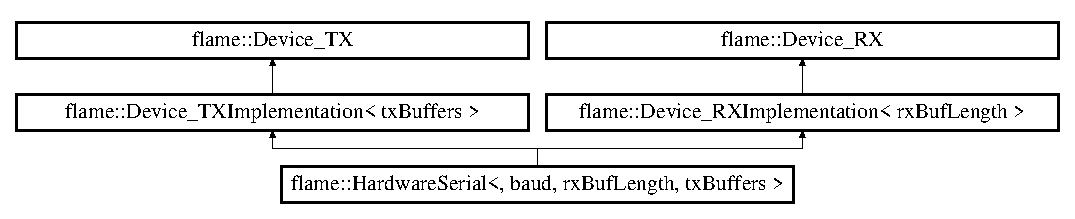
\includegraphics[height=2.492581cm]{classflame_1_1_hardware_serial}
\end{center}
\end{figure}
\subsection*{Public Member Functions}
\begin{DoxyCompactItemize}
\item 
\hyperlink{classflame_1_1_hardware_serial_a5b1458a430238e6c27c799069cd0de36}{Hardware\-Serial} ()
\item 
\hyperlink{classflame_1_1_hardware_serial_a4daa0cb5bb4be6d9836a87411d01139e}{Hardware\-Serial} (\hyperlink{namespaceflame_a9cbc9720f0e2f002f6f8fdf746fad4db}{Serial\-Mode} mode, uint8\-\_\-t bits, \hyperlink{namespaceflame_a6613d9a37cacb0a55b287dcf2f60f5db}{Serial\-Parity} parity, uint8\-\_\-t stop\-Bits, uint8\-\_\-t polarity)
\item 
void \hyperlink{classflame_1_1_hardware_serial_aeff320dad035e17a806233bcd2a44c34}{configure} (\hyperlink{namespaceflame_a9cbc9720f0e2f002f6f8fdf746fad4db}{Serial\-Mode} mode, uint8\-\_\-t bits, \hyperlink{namespaceflame_a6613d9a37cacb0a55b287dcf2f60f5db}{Serial\-Parity} parity, uint8\-\_\-t stop\-Bits, uint8\-\_\-t polarity)
\item 
void \hyperlink{classflame_1_1_hardware_serial_ab56390f7a1c6de2db5cc81570fc1b334}{rx} ()
\item 
void \hyperlink{classflame_1_1_hardware_serial_a0fdf2aaad78c997238b73243578be4f0}{dump\-T\-X\-Buffer\-State} (const char $\ast$func)
\item 
void \hyperlink{classflame_1_1_hardware_serial_a84c0ecca0cba82af78444612fe3d67b8}{tx} ()
\item 
\hyperlink{io_8h_a2eb6f9e0395b47b8d5e3eeae4fe0c116}{I\-N\-L\-I\-N\-E} void \hyperlink{classflame_1_1_hardware_serial_a39f9df6aa5235c515a7d1a6d27292846}{set\-Speed} (unsigned long new\-Baud)
\item 
void \hyperlink{classflame_1_1_hardware_serial_a82717797b31505d8ce92de7a554afade}{end} ()
\item 
void \hyperlink{classflame_1_1_hardware_serial_a62286cc6c5686cf9c8a7823f9386a949}{echo} (bool echo\-On)
\item 
bool \hyperlink{classflame_1_1_hardware_serial_a2aac6f2b081b2449a666bd73ac470b26}{can\-Send\-Busy} ()
\item 
void \hyperlink{classflame_1_1_hardware_serial_aba8e852537e4b17ed01c120e5b6655d3}{busy\-Write} (char c)
\item 
void \hyperlink{classflame_1_1_hardware_serial_a9facf2f539793a554ff3ad33085efac9}{busy\-Write\-\_\-\-P} (P\-G\-M\-\_\-\-P buffer)
\item 
void \hyperlink{classflame_1_1_hardware_serial_ad61b8dc18e76aaa506c5b712a5df805c}{busy\-Write} (const char $\ast$buffer)
\item 
void \hyperlink{classflame_1_1_hardware_serial_aeea82edb6cb58c605ba467734eaeacc7}{busy\-Write\-\_\-\-P} (P\-G\-M\-\_\-\-P buffer, uint16\-\_\-t length)
\item 
void \hyperlink{classflame_1_1_hardware_serial_a05dc22e70d05f0148ae86e831707aa28}{busy\-Write} (const char $\ast$buffer, uint16\-\_\-t length)
\item 
bool \hyperlink{classflame_1_1_hardware_serial_a10df6bb4b515a04b4e738238058ccd29}{busy} (void)
\end{DoxyCompactItemize}
\subsection*{Protected Member Functions}
\begin{DoxyCompactItemize}
\item 
void \hyperlink{classflame_1_1_hardware_serial_a2f045cdba4a0be78d876e383ff1ec6f2}{run\-Tx\-Buffers} ()
\end{DoxyCompactItemize}
\subsection*{Additional Inherited Members}


\subsection{Detailed Description}
\subsubsection*{template$<$F\-L\-A\-M\-E\-\_\-\-D\-E\-C\-L\-A\-R\-E\-\_\-\-U\-S\-A\-R\-T(usart), uint32\-\_\-t baud, uint8\-\_\-t rx\-Buf\-Length, uint8\-\_\-t tx\-Buffers$>$class flame\-::\-Hardware\-Serial$<$, baud, rx\-Buf\-Length, tx\-Buffers $>$}

Create now serial port driver 
\begin{DoxyTemplParams}{Template Parameters}
{\em usart} & the serial port parameters \\
\hline
{\em baud} & the baud rate to run at \\
\hline
{\em rx\-Buf\-Length} & the maximum number of characters to receive \\
\hline
{\em tx\-Buffers} & the number of send buffers \\
\hline
\end{DoxyTemplParams}
\begin{DoxyPostcond}{Postcondition}
Interrupts should be assigned to the driver 
\end{DoxyPostcond}


Definition at line 111 of file Hardware\-Serial.\-h.



\subsection{Constructor \& Destructor Documentation}
\hypertarget{classflame_1_1_hardware_serial_a5b1458a430238e6c27c799069cd0de36}{\index{flame\-::\-Hardware\-Serial@{flame\-::\-Hardware\-Serial}!Hardware\-Serial@{Hardware\-Serial}}
\index{Hardware\-Serial@{Hardware\-Serial}!flame::HardwareSerial@{flame\-::\-Hardware\-Serial}}
\subsubsection[{Hardware\-Serial}]{\setlength{\rightskip}{0pt plus 5cm}template$<$F\-L\-A\-M\-E\-\_\-\-D\-E\-C\-L\-A\-R\-E\-\_\-\-U\-S\-A\-R\-T(usart) , uint32\-\_\-t baud, uint8\-\_\-t rx\-Buf\-Length, uint8\-\_\-t tx\-Buffers$>$ {\bf flame\-::\-Hardware\-Serial}$<$, baud, rx\-Buf\-Length, tx\-Buffers $>$\-::{\bf Hardware\-Serial} (
\begin{DoxyParamCaption}
{}
\end{DoxyParamCaption}
)\hspace{0.3cm}{\ttfamily [inline]}}}\label{classflame_1_1_hardware_serial_a5b1458a430238e6c27c799069cd0de36}
Constructor 

Definition at line 157 of file Hardware\-Serial.\-h.

\hypertarget{classflame_1_1_hardware_serial_a4daa0cb5bb4be6d9836a87411d01139e}{\index{flame\-::\-Hardware\-Serial@{flame\-::\-Hardware\-Serial}!Hardware\-Serial@{Hardware\-Serial}}
\index{Hardware\-Serial@{Hardware\-Serial}!flame::HardwareSerial@{flame\-::\-Hardware\-Serial}}
\subsubsection[{Hardware\-Serial}]{\setlength{\rightskip}{0pt plus 5cm}template$<$F\-L\-A\-M\-E\-\_\-\-D\-E\-C\-L\-A\-R\-E\-\_\-\-U\-S\-A\-R\-T(usart) , uint32\-\_\-t baud, uint8\-\_\-t rx\-Buf\-Length, uint8\-\_\-t tx\-Buffers$>$ {\bf flame\-::\-Hardware\-Serial}$<$, baud, rx\-Buf\-Length, tx\-Buffers $>$\-::{\bf Hardware\-Serial} (
\begin{DoxyParamCaption}
\item[{{\bf Serial\-Mode}}]{mode, }
\item[{uint8\-\_\-t}]{bits, }
\item[{{\bf Serial\-Parity}}]{parity, }
\item[{uint8\-\_\-t}]{stop\-Bits, }
\item[{uint8\-\_\-t}]{polarity}
\end{DoxyParamCaption}
)\hspace{0.3cm}{\ttfamily [inline]}}}\label{classflame_1_1_hardware_serial_a4daa0cb5bb4be6d9836a87411d01139e}
Constructor 
\begin{DoxyParams}{Parameters}
{\em mode} & the mode to run the serial port in \\
\hline
{\em bits} & the number of data bits \\
\hline
{\em parity} & the type of parity \\
\hline
{\em stop\-Bits} & the number of stop bits \\
\hline
{\em polarity} & used only for synchronous mode when 0\-: Change T\-X on rising, sample R\-X on falling when 1\-: Change T\-X on falling, sample R\-X on rising \\
\hline
\end{DoxyParams}


Definition at line 174 of file Hardware\-Serial.\-h.



\subsection{Member Function Documentation}
\hypertarget{classflame_1_1_hardware_serial_a10df6bb4b515a04b4e738238058ccd29}{\index{flame\-::\-Hardware\-Serial@{flame\-::\-Hardware\-Serial}!busy@{busy}}
\index{busy@{busy}!flame::HardwareSerial@{flame\-::\-Hardware\-Serial}}
\subsubsection[{busy}]{\setlength{\rightskip}{0pt plus 5cm}template$<$F\-L\-A\-M\-E\-\_\-\-D\-E\-C\-L\-A\-R\-E\-\_\-\-U\-S\-A\-R\-T(usart) , uint32\-\_\-t baud, uint8\-\_\-t rx\-Buf\-Length, uint8\-\_\-t tx\-Buffers$>$ bool {\bf flame\-::\-Hardware\-Serial}$<$, baud, rx\-Buf\-Length, tx\-Buffers $>$\-::busy (
\begin{DoxyParamCaption}
\item[{void}]{}
\end{DoxyParamCaption}
)\hspace{0.3cm}{\ttfamily [inline]}}}\label{classflame_1_1_hardware_serial_a10df6bb4b515a04b4e738238058ccd29}
Check if the hardware is busy -\/ note that this should not be used to determine if you can actually write -\/ use can\-Send instead

\begin{DoxyReturn}{Returns}
true if the hardware is busy 
\end{DoxyReturn}


Definition at line 498 of file Hardware\-Serial.\-h.

\hypertarget{classflame_1_1_hardware_serial_aba8e852537e4b17ed01c120e5b6655d3}{\index{flame\-::\-Hardware\-Serial@{flame\-::\-Hardware\-Serial}!busy\-Write@{busy\-Write}}
\index{busy\-Write@{busy\-Write}!flame::HardwareSerial@{flame\-::\-Hardware\-Serial}}
\subsubsection[{busy\-Write}]{\setlength{\rightskip}{0pt plus 5cm}template$<$F\-L\-A\-M\-E\-\_\-\-D\-E\-C\-L\-A\-R\-E\-\_\-\-U\-S\-A\-R\-T(usart) , uint32\-\_\-t baud, uint8\-\_\-t rx\-Buf\-Length, uint8\-\_\-t tx\-Buffers$>$ void {\bf flame\-::\-Hardware\-Serial}$<$, baud, rx\-Buf\-Length, tx\-Buffers $>$\-::busy\-Write (
\begin{DoxyParamCaption}
\item[{char}]{c}
\end{DoxyParamCaption}
)\hspace{0.3cm}{\ttfamily [inline]}}}\label{classflame_1_1_hardware_serial_aba8e852537e4b17ed01c120e5b6655d3}
Write a character


\begin{DoxyParams}{Parameters}
{\em c} & the character to write \\
\hline
\end{DoxyParams}


Definition at line 324 of file Hardware\-Serial.\-h.

\hypertarget{classflame_1_1_hardware_serial_ad61b8dc18e76aaa506c5b712a5df805c}{\index{flame\-::\-Hardware\-Serial@{flame\-::\-Hardware\-Serial}!busy\-Write@{busy\-Write}}
\index{busy\-Write@{busy\-Write}!flame::HardwareSerial@{flame\-::\-Hardware\-Serial}}
\subsubsection[{busy\-Write}]{\setlength{\rightskip}{0pt plus 5cm}template$<$F\-L\-A\-M\-E\-\_\-\-D\-E\-C\-L\-A\-R\-E\-\_\-\-U\-S\-A\-R\-T(usart) , uint32\-\_\-t baud, uint8\-\_\-t rx\-Buf\-Length, uint8\-\_\-t tx\-Buffers$>$ void {\bf flame\-::\-Hardware\-Serial}$<$, baud, rx\-Buf\-Length, tx\-Buffers $>$\-::busy\-Write (
\begin{DoxyParamCaption}
\item[{const char $\ast$}]{buffer}
\end{DoxyParamCaption}
)\hspace{0.3cm}{\ttfamily [inline]}}}\label{classflame_1_1_hardware_serial_ad61b8dc18e76aaa506c5b712a5df805c}
Write a null terminated string to the serial port


\begin{DoxyParams}{Parameters}
{\em buffer} & the string to write \\
\hline
\end{DoxyParams}


Definition at line 360 of file Hardware\-Serial.\-h.

\hypertarget{classflame_1_1_hardware_serial_a05dc22e70d05f0148ae86e831707aa28}{\index{flame\-::\-Hardware\-Serial@{flame\-::\-Hardware\-Serial}!busy\-Write@{busy\-Write}}
\index{busy\-Write@{busy\-Write}!flame::HardwareSerial@{flame\-::\-Hardware\-Serial}}
\subsubsection[{busy\-Write}]{\setlength{\rightskip}{0pt plus 5cm}template$<$F\-L\-A\-M\-E\-\_\-\-D\-E\-C\-L\-A\-R\-E\-\_\-\-U\-S\-A\-R\-T(usart) , uint32\-\_\-t baud, uint8\-\_\-t rx\-Buf\-Length, uint8\-\_\-t tx\-Buffers$>$ void {\bf flame\-::\-Hardware\-Serial}$<$, baud, rx\-Buf\-Length, tx\-Buffers $>$\-::busy\-Write (
\begin{DoxyParamCaption}
\item[{const char $\ast$}]{buffer, }
\item[{uint16\-\_\-t}]{length}
\end{DoxyParamCaption}
)\hspace{0.3cm}{\ttfamily [inline]}}}\label{classflame_1_1_hardware_serial_a05dc22e70d05f0148ae86e831707aa28}
Write a buffer 
\begin{DoxyParams}{Parameters}
{\em buffer} & the buffer to write \\
\hline
{\em length} & the length of the buffer \\
\hline
\end{DoxyParams}


Definition at line 478 of file Hardware\-Serial.\-h.

\hypertarget{classflame_1_1_hardware_serial_a9facf2f539793a554ff3ad33085efac9}{\index{flame\-::\-Hardware\-Serial@{flame\-::\-Hardware\-Serial}!busy\-Write\-\_\-\-P@{busy\-Write\-\_\-\-P}}
\index{busy\-Write\-\_\-\-P@{busy\-Write\-\_\-\-P}!flame::HardwareSerial@{flame\-::\-Hardware\-Serial}}
\subsubsection[{busy\-Write\-\_\-\-P}]{\setlength{\rightskip}{0pt plus 5cm}template$<$F\-L\-A\-M\-E\-\_\-\-D\-E\-C\-L\-A\-R\-E\-\_\-\-U\-S\-A\-R\-T(usart) , uint32\-\_\-t baud, uint8\-\_\-t rx\-Buf\-Length, uint8\-\_\-t tx\-Buffers$>$ void {\bf flame\-::\-Hardware\-Serial}$<$, baud, rx\-Buf\-Length, tx\-Buffers $>$\-::busy\-Write\-\_\-\-P (
\begin{DoxyParamCaption}
\item[{P\-G\-M\-\_\-\-P}]{buffer}
\end{DoxyParamCaption}
)\hspace{0.3cm}{\ttfamily [inline]}}}\label{classflame_1_1_hardware_serial_a9facf2f539793a554ff3ad33085efac9}
Write a null terminated progmem string


\begin{DoxyParams}{Parameters}
{\em buffer} & the string to write \\
\hline
\end{DoxyParams}


Definition at line 338 of file Hardware\-Serial.\-h.

\hypertarget{classflame_1_1_hardware_serial_aeea82edb6cb58c605ba467734eaeacc7}{\index{flame\-::\-Hardware\-Serial@{flame\-::\-Hardware\-Serial}!busy\-Write\-\_\-\-P@{busy\-Write\-\_\-\-P}}
\index{busy\-Write\-\_\-\-P@{busy\-Write\-\_\-\-P}!flame::HardwareSerial@{flame\-::\-Hardware\-Serial}}
\subsubsection[{busy\-Write\-\_\-\-P}]{\setlength{\rightskip}{0pt plus 5cm}template$<$F\-L\-A\-M\-E\-\_\-\-D\-E\-C\-L\-A\-R\-E\-\_\-\-U\-S\-A\-R\-T(usart) , uint32\-\_\-t baud, uint8\-\_\-t rx\-Buf\-Length, uint8\-\_\-t tx\-Buffers$>$ void {\bf flame\-::\-Hardware\-Serial}$<$, baud, rx\-Buf\-Length, tx\-Buffers $>$\-::busy\-Write\-\_\-\-P (
\begin{DoxyParamCaption}
\item[{P\-G\-M\-\_\-\-P}]{buffer, }
\item[{uint16\-\_\-t}]{length}
\end{DoxyParamCaption}
)\hspace{0.3cm}{\ttfamily [inline]}}}\label{classflame_1_1_hardware_serial_aeea82edb6cb58c605ba467734eaeacc7}
Write a buffer from P\-R\-O\-G\-M\-E\-M 
\begin{DoxyParams}{Parameters}
{\em buffer} & the buffer to write \\
\hline
{\em length} & the length of the buffer \\
\hline
\end{DoxyParams}


Definition at line 459 of file Hardware\-Serial.\-h.

\hypertarget{classflame_1_1_hardware_serial_a2aac6f2b081b2449a666bd73ac470b26}{\index{flame\-::\-Hardware\-Serial@{flame\-::\-Hardware\-Serial}!can\-Send\-Busy@{can\-Send\-Busy}}
\index{can\-Send\-Busy@{can\-Send\-Busy}!flame::HardwareSerial@{flame\-::\-Hardware\-Serial}}
\subsubsection[{can\-Send\-Busy}]{\setlength{\rightskip}{0pt plus 5cm}template$<$F\-L\-A\-M\-E\-\_\-\-D\-E\-C\-L\-A\-R\-E\-\_\-\-U\-S\-A\-R\-T(usart) , uint32\-\_\-t baud, uint8\-\_\-t rx\-Buf\-Length, uint8\-\_\-t tx\-Buffers$>$ bool {\bf flame\-::\-Hardware\-Serial}$<$, baud, rx\-Buf\-Length, tx\-Buffers $>$\-::can\-Send\-Busy (
\begin{DoxyParamCaption}
{}
\end{DoxyParamCaption}
)\hspace{0.3cm}{\ttfamily [inline]}}}\label{classflame_1_1_hardware_serial_a2aac6f2b081b2449a666bd73ac470b26}
Can we send something via busywrite

\begin{DoxyReturn}{Returns}
true if we can send something 
\end{DoxyReturn}


Definition at line 315 of file Hardware\-Serial.\-h.

\hypertarget{classflame_1_1_hardware_serial_aeff320dad035e17a806233bcd2a44c34}{\index{flame\-::\-Hardware\-Serial@{flame\-::\-Hardware\-Serial}!configure@{configure}}
\index{configure@{configure}!flame::HardwareSerial@{flame\-::\-Hardware\-Serial}}
\subsubsection[{configure}]{\setlength{\rightskip}{0pt plus 5cm}template$<$F\-L\-A\-M\-E\-\_\-\-D\-E\-C\-L\-A\-R\-E\-\_\-\-U\-S\-A\-R\-T(usart) , uint32\-\_\-t baud, uint8\-\_\-t rx\-Buf\-Length, uint8\-\_\-t tx\-Buffers$>$ void {\bf flame\-::\-Hardware\-Serial}$<$, baud, rx\-Buf\-Length, tx\-Buffers $>$\-::configure (
\begin{DoxyParamCaption}
\item[{{\bf Serial\-Mode}}]{mode, }
\item[{uint8\-\_\-t}]{bits, }
\item[{{\bf Serial\-Parity}}]{parity, }
\item[{uint8\-\_\-t}]{stop\-Bits, }
\item[{uint8\-\_\-t}]{polarity}
\end{DoxyParamCaption}
)\hspace{0.3cm}{\ttfamily [inline]}}}\label{classflame_1_1_hardware_serial_aeff320dad035e17a806233bcd2a44c34}
Set data characteristics 
\begin{DoxyParams}{Parameters}
{\em mode} & the mode to run the serial port in \\
\hline
{\em bits} & the number of data bits \\
\hline
{\em parity} & the type of parity \\
\hline
{\em stop\-Bits} & the number of stop bits \\
\hline
{\em polarity} & used only for synchronous mode when 0\-: Change T\-X on rising, sample R\-X on falling when 1\-: Change T\-X on falling, sample R\-X on rising \\
\hline
\end{DoxyParams}


Definition at line 191 of file Hardware\-Serial.\-h.

\hypertarget{classflame_1_1_hardware_serial_a0fdf2aaad78c997238b73243578be4f0}{\index{flame\-::\-Hardware\-Serial@{flame\-::\-Hardware\-Serial}!dump\-T\-X\-Buffer\-State@{dump\-T\-X\-Buffer\-State}}
\index{dump\-T\-X\-Buffer\-State@{dump\-T\-X\-Buffer\-State}!flame::HardwareSerial@{flame\-::\-Hardware\-Serial}}
\subsubsection[{dump\-T\-X\-Buffer\-State}]{\setlength{\rightskip}{0pt plus 5cm}template$<$F\-L\-A\-M\-E\-\_\-\-D\-E\-C\-L\-A\-R\-E\-\_\-\-U\-S\-A\-R\-T(usart) , uint32\-\_\-t baud, uint8\-\_\-t rx\-Buf\-Length, uint8\-\_\-t tx\-Buffers$>$ void {\bf flame\-::\-Hardware\-Serial}$<$, baud, rx\-Buf\-Length, tx\-Buffers $>$\-::dump\-T\-X\-Buffer\-State (
\begin{DoxyParamCaption}
\item[{const char $\ast$}]{func}
\end{DoxyParamCaption}
)\hspace{0.3cm}{\ttfamily [inline]}}}\label{classflame_1_1_hardware_serial_a0fdf2aaad78c997238b73243578be4f0}
Dump the state of the T\-X buffer 
\begin{DoxyParams}{Parameters}
{\em func} & the name of the caller \\
\hline
\end{DoxyParams}


Definition at line 237 of file Hardware\-Serial.\-h.

\hypertarget{classflame_1_1_hardware_serial_a62286cc6c5686cf9c8a7823f9386a949}{\index{flame\-::\-Hardware\-Serial@{flame\-::\-Hardware\-Serial}!echo@{echo}}
\index{echo@{echo}!flame::HardwareSerial@{flame\-::\-Hardware\-Serial}}
\subsubsection[{echo}]{\setlength{\rightskip}{0pt plus 5cm}template$<$F\-L\-A\-M\-E\-\_\-\-D\-E\-C\-L\-A\-R\-E\-\_\-\-U\-S\-A\-R\-T(usart) , uint32\-\_\-t baud, uint8\-\_\-t rx\-Buf\-Length, uint8\-\_\-t tx\-Buffers$>$ void {\bf flame\-::\-Hardware\-Serial}$<$, baud, rx\-Buf\-Length, tx\-Buffers $>$\-::echo (
\begin{DoxyParamCaption}
\item[{bool}]{echo\-On}
\end{DoxyParamCaption}
)\hspace{0.3cm}{\ttfamily [inline]}}}\label{classflame_1_1_hardware_serial_a62286cc6c5686cf9c8a7823f9386a949}
Enable echoing data received by us back to the sender (useful for terminal interaction


\begin{DoxyParams}{Parameters}
{\em echo\-On} & true to enable echo \\
\hline
\end{DoxyParams}


Definition at line 306 of file Hardware\-Serial.\-h.

\hypertarget{classflame_1_1_hardware_serial_a82717797b31505d8ce92de7a554afade}{\index{flame\-::\-Hardware\-Serial@{flame\-::\-Hardware\-Serial}!end@{end}}
\index{end@{end}!flame::HardwareSerial@{flame\-::\-Hardware\-Serial}}
\subsubsection[{end}]{\setlength{\rightskip}{0pt plus 5cm}template$<$F\-L\-A\-M\-E\-\_\-\-D\-E\-C\-L\-A\-R\-E\-\_\-\-U\-S\-A\-R\-T(usart) , uint32\-\_\-t baud, uint8\-\_\-t rx\-Buf\-Length, uint8\-\_\-t tx\-Buffers$>$ void {\bf flame\-::\-Hardware\-Serial}$<$, baud, rx\-Buf\-Length, tx\-Buffers $>$\-::end (
\begin{DoxyParamCaption}
{}
\end{DoxyParamCaption}
)\hspace{0.3cm}{\ttfamily [inline]}}}\label{classflame_1_1_hardware_serial_a82717797b31505d8ce92de7a554afade}
Halt the serial port 

Definition at line 296 of file Hardware\-Serial.\-h.

\hypertarget{classflame_1_1_hardware_serial_a2f045cdba4a0be78d876e383ff1ec6f2}{\index{flame\-::\-Hardware\-Serial@{flame\-::\-Hardware\-Serial}!run\-Tx\-Buffers@{run\-Tx\-Buffers}}
\index{run\-Tx\-Buffers@{run\-Tx\-Buffers}!flame::HardwareSerial@{flame\-::\-Hardware\-Serial}}
\subsubsection[{run\-Tx\-Buffers}]{\setlength{\rightskip}{0pt plus 5cm}template$<$F\-L\-A\-M\-E\-\_\-\-D\-E\-C\-L\-A\-R\-E\-\_\-\-U\-S\-A\-R\-T(usart) , uint32\-\_\-t baud, uint8\-\_\-t rx\-Buf\-Length, uint8\-\_\-t tx\-Buffers$>$ void {\bf flame\-::\-Hardware\-Serial}$<$, baud, rx\-Buf\-Length, tx\-Buffers $>$\-::run\-Tx\-Buffers (
\begin{DoxyParamCaption}
{}
\end{DoxyParamCaption}
)\hspace{0.3cm}{\ttfamily [inline]}, {\ttfamily [protected]}, {\ttfamily [virtual]}}}\label{classflame_1_1_hardware_serial_a2f045cdba4a0be78d876e383ff1ec6f2}
Start sending async data 

Implements \hyperlink{classflame_1_1_device___t_x_af3cf3dc02a124e5a88841d325555ce3c}{flame\-::\-Device\-\_\-\-T\-X}.



Definition at line 120 of file Hardware\-Serial.\-h.

\hypertarget{classflame_1_1_hardware_serial_ab56390f7a1c6de2db5cc81570fc1b334}{\index{flame\-::\-Hardware\-Serial@{flame\-::\-Hardware\-Serial}!rx@{rx}}
\index{rx@{rx}!flame::HardwareSerial@{flame\-::\-Hardware\-Serial}}
\subsubsection[{rx}]{\setlength{\rightskip}{0pt plus 5cm}template$<$F\-L\-A\-M\-E\-\_\-\-D\-E\-C\-L\-A\-R\-E\-\_\-\-U\-S\-A\-R\-T(usart) , uint32\-\_\-t baud, uint8\-\_\-t rx\-Buf\-Length, uint8\-\_\-t tx\-Buffers$>$ void {\bf flame\-::\-Hardware\-Serial}$<$, baud, rx\-Buf\-Length, tx\-Buffers $>$\-::rx (
\begin{DoxyParamCaption}
{}
\end{DoxyParamCaption}
)\hspace{0.3cm}{\ttfamily [inline]}}}\label{classflame_1_1_hardware_serial_ab56390f7a1c6de2db5cc81570fc1b334}
R\-X interrupt handler 

Definition at line 224 of file Hardware\-Serial.\-h.

\hypertarget{classflame_1_1_hardware_serial_a39f9df6aa5235c515a7d1a6d27292846}{\index{flame\-::\-Hardware\-Serial@{flame\-::\-Hardware\-Serial}!set\-Speed@{set\-Speed}}
\index{set\-Speed@{set\-Speed}!flame::HardwareSerial@{flame\-::\-Hardware\-Serial}}
\subsubsection[{set\-Speed}]{\setlength{\rightskip}{0pt plus 5cm}template$<$F\-L\-A\-M\-E\-\_\-\-D\-E\-C\-L\-A\-R\-E\-\_\-\-U\-S\-A\-R\-T(usart) , uint32\-\_\-t baud, uint8\-\_\-t rx\-Buf\-Length, uint8\-\_\-t tx\-Buffers$>$ {\bf I\-N\-L\-I\-N\-E} void {\bf flame\-::\-Hardware\-Serial}$<$, baud, rx\-Buf\-Length, tx\-Buffers $>$\-::set\-Speed (
\begin{DoxyParamCaption}
\item[{unsigned long}]{new\-Baud}
\end{DoxyParamCaption}
)\hspace{0.3cm}{\ttfamily [inline]}}}\label{classflame_1_1_hardware_serial_a39f9df6aa5235c515a7d1a6d27292846}
Configure the serial port for a specific baud rate 
\begin{DoxyParams}{Parameters}
{\em new\-Baud} & the baud rate to set \\
\hline
\end{DoxyParams}


Definition at line 276 of file Hardware\-Serial.\-h.

\hypertarget{classflame_1_1_hardware_serial_a84c0ecca0cba82af78444612fe3d67b8}{\index{flame\-::\-Hardware\-Serial@{flame\-::\-Hardware\-Serial}!tx@{tx}}
\index{tx@{tx}!flame::HardwareSerial@{flame\-::\-Hardware\-Serial}}
\subsubsection[{tx}]{\setlength{\rightskip}{0pt plus 5cm}template$<$F\-L\-A\-M\-E\-\_\-\-D\-E\-C\-L\-A\-R\-E\-\_\-\-U\-S\-A\-R\-T(usart) , uint32\-\_\-t baud, uint8\-\_\-t rx\-Buf\-Length, uint8\-\_\-t tx\-Buffers$>$ void {\bf flame\-::\-Hardware\-Serial}$<$, baud, rx\-Buf\-Length, tx\-Buffers $>$\-::tx (
\begin{DoxyParamCaption}
{}
\end{DoxyParamCaption}
)\hspace{0.3cm}{\ttfamily [inline]}}}\label{classflame_1_1_hardware_serial_a84c0ecca0cba82af78444612fe3d67b8}
T\-X interrupt handler 

Definition at line 246 of file Hardware\-Serial.\-h.



The documentation for this class was generated from the following file\-:\begin{DoxyCompactItemize}
\item 
flame/\hyperlink{_hardware_serial_8h}{Hardware\-Serial.\-h}\end{DoxyCompactItemize}

\hypertarget{structflame_1_1instrument}{\section{flame\-:\-:instrument Struct Reference}
\label{structflame_1_1instrument}\index{flame\-::instrument@{flame\-::instrument}}
}


{\ttfamily \#include $<$Wave\-Generator.\-h$>$}

\subsection*{Public Attributes}
\begin{DoxyCompactItemize}
\item 
const \hyperlink{_d_a_c_8h_a5a6d1dc37ffa32957a63868cd1da39b3}{S\-A\-M\-P\-L\-E} $\ast$ \hyperlink{structflame_1_1instrument_ad8ca175683ca6f0ebd472cf13051929f}{samples}
\item 
uint16\-\_\-t \hyperlink{structflame_1_1instrument_a9e8428ddc6afef3392234e1ed89bd442}{attack\-Time}
\item 
uint16\-\_\-t \hyperlink{structflame_1_1instrument_ad683abcb6de0196805bd230a2d59fb85}{decay1\-Time}
\item 
\hyperlink{namespaceflame_a7f6447252c60127b805475b293831f99}{A\-M\-P\-L\-I\-T\-U\-D\-E} \hyperlink{structflame_1_1instrument_a0a0e0263483ad2e903cbcb854493bc1b}{decay1\-Amount}
\item 
uint16\-\_\-t \hyperlink{structflame_1_1instrument_a5214632ee985002310d9c94431f5391f}{sustain1\-Time}
\item 
uint16\-\_\-t \hyperlink{structflame_1_1instrument_a31be3cd286103e4364edf36133aeec14}{decay2\-Time}
\item 
\hyperlink{namespaceflame_a7f6447252c60127b805475b293831f99}{A\-M\-P\-L\-I\-T\-U\-D\-E} \hyperlink{structflame_1_1instrument_a294a5d9d9d10c3706d2fe362e31fc93c}{decay2\-Amount}
\item 
uint16\-\_\-t \hyperlink{structflame_1_1instrument_a40807d7de06391d048f1fff8cfe98964}{release\-Time}
\end{DoxyCompactItemize}


\subsection{Detailed Description}


Definition at line 58 of file Wave\-Generator.\-h.



\subsection{Member Data Documentation}
\hypertarget{structflame_1_1instrument_a9e8428ddc6afef3392234e1ed89bd442}{\index{flame\-::instrument@{flame\-::instrument}!attack\-Time@{attack\-Time}}
\index{attack\-Time@{attack\-Time}!flame::instrument@{flame\-::instrument}}
\subsubsection[{attack\-Time}]{\setlength{\rightskip}{0pt plus 5cm}uint16\-\_\-t flame\-::instrument\-::attack\-Time}}\label{structflame_1_1instrument_a9e8428ddc6afef3392234e1ed89bd442}
The samples for a single/part cycle of the instrument at 440\-Hz (middle A), samples at 32k\-Hz, 72 samples long, stored in progmem 

Definition at line 61 of file Wave\-Generator.\-h.

\hypertarget{structflame_1_1instrument_a0a0e0263483ad2e903cbcb854493bc1b}{\index{flame\-::instrument@{flame\-::instrument}!decay1\-Amount@{decay1\-Amount}}
\index{decay1\-Amount@{decay1\-Amount}!flame::instrument@{flame\-::instrument}}
\subsubsection[{decay1\-Amount}]{\setlength{\rightskip}{0pt plus 5cm}{\bf A\-M\-P\-L\-I\-T\-U\-D\-E} flame\-::instrument\-::decay1\-Amount}}\label{structflame_1_1instrument_a0a0e0263483ad2e903cbcb854493bc1b}
samples to ramp from 100\% to amount/255 $\ast$ 100\% after the attack 

Definition at line 63 of file Wave\-Generator.\-h.

\hypertarget{structflame_1_1instrument_ad683abcb6de0196805bd230a2d59fb85}{\index{flame\-::instrument@{flame\-::instrument}!decay1\-Time@{decay1\-Time}}
\index{decay1\-Time@{decay1\-Time}!flame::instrument@{flame\-::instrument}}
\subsubsection[{decay1\-Time}]{\setlength{\rightskip}{0pt plus 5cm}uint16\-\_\-t flame\-::instrument\-::decay1\-Time}}\label{structflame_1_1instrument_ad683abcb6de0196805bd230a2d59fb85}
samples to ramp from 0 to 100\% when starting playback 

Definition at line 62 of file Wave\-Generator.\-h.

\hypertarget{structflame_1_1instrument_a294a5d9d9d10c3706d2fe362e31fc93c}{\index{flame\-::instrument@{flame\-::instrument}!decay2\-Amount@{decay2\-Amount}}
\index{decay2\-Amount@{decay2\-Amount}!flame::instrument@{flame\-::instrument}}
\subsubsection[{decay2\-Amount}]{\setlength{\rightskip}{0pt plus 5cm}{\bf A\-M\-P\-L\-I\-T\-U\-D\-E} flame\-::instrument\-::decay2\-Amount}}\label{structflame_1_1instrument_a294a5d9d9d10c3706d2fe362e31fc93c}
samples spent in decay2 

Definition at line 66 of file Wave\-Generator.\-h.

\hypertarget{structflame_1_1instrument_a31be3cd286103e4364edf36133aeec14}{\index{flame\-::instrument@{flame\-::instrument}!decay2\-Time@{decay2\-Time}}
\index{decay2\-Time@{decay2\-Time}!flame::instrument@{flame\-::instrument}}
\subsubsection[{decay2\-Time}]{\setlength{\rightskip}{0pt plus 5cm}uint16\-\_\-t flame\-::instrument\-::decay2\-Time}}\label{structflame_1_1instrument_a31be3cd286103e4364edf36133aeec14}
samples spent in sustain until decay2 

Definition at line 65 of file Wave\-Generator.\-h.

\hypertarget{structflame_1_1instrument_a40807d7de06391d048f1fff8cfe98964}{\index{flame\-::instrument@{flame\-::instrument}!release\-Time@{release\-Time}}
\index{release\-Time@{release\-Time}!flame::instrument@{flame\-::instrument}}
\subsubsection[{release\-Time}]{\setlength{\rightskip}{0pt plus 5cm}uint16\-\_\-t flame\-::instrument\-::release\-Time}}\label{structflame_1_1instrument_a40807d7de06391d048f1fff8cfe98964}
the amplitude to decay to 

Definition at line 67 of file Wave\-Generator.\-h.

\hypertarget{structflame_1_1instrument_ad8ca175683ca6f0ebd472cf13051929f}{\index{flame\-::instrument@{flame\-::instrument}!samples@{samples}}
\index{samples@{samples}!flame::instrument@{flame\-::instrument}}
\subsubsection[{samples}]{\setlength{\rightskip}{0pt plus 5cm}const {\bf S\-A\-M\-P\-L\-E}$\ast$ flame\-::instrument\-::samples}}\label{structflame_1_1instrument_ad8ca175683ca6f0ebd472cf13051929f}


Definition at line 59 of file Wave\-Generator.\-h.

\hypertarget{structflame_1_1instrument_a5214632ee985002310d9c94431f5391f}{\index{flame\-::instrument@{flame\-::instrument}!sustain1\-Time@{sustain1\-Time}}
\index{sustain1\-Time@{sustain1\-Time}!flame::instrument@{flame\-::instrument}}
\subsubsection[{sustain1\-Time}]{\setlength{\rightskip}{0pt plus 5cm}uint16\-\_\-t flame\-::instrument\-::sustain1\-Time}}\label{structflame_1_1instrument_a5214632ee985002310d9c94431f5391f}
the amplitude to decay to 

Definition at line 64 of file Wave\-Generator.\-h.



The documentation for this struct was generated from the following file\-:\begin{DoxyCompactItemize}
\item 
flame/\hyperlink{_wave_generator_8h}{Wave\-Generator.\-h}\end{DoxyCompactItemize}

\hypertarget{unionflame_1_1_int3_axis}{\section{flame\-:\-:Int3\-Axis Union Reference}
\label{unionflame_1_1_int3_axis}\index{flame\-::\-Int3\-Axis@{flame\-::\-Int3\-Axis}}
}


{\ttfamily \#include $<$io.\-h$>$}

\subsection*{Public Attributes}
\begin{DoxyCompactItemize}
\item 
\begin{tabbing}
xx\=xx\=xx\=xx\=xx\=xx\=xx\=xx\=xx\=\kill
struct \{\\
\>int16\_t \hyperlink{unionflame_1_1_int3_axis_a5afc91d24e7c9a8e84fd076d01525a44}{x}\\
\>int16\_t \hyperlink{unionflame_1_1_int3_axis_a214fbd1192879a9ae9975b819cb7ea9f}{y}\\
\>int16\_t \hyperlink{unionflame_1_1_int3_axis_a07fa76bf97419e5fd100872978ab2a56}{z}\\
\} \hyperlink{unionflame_1_1_int3_axis_a82f911e02da3e252d5efd2dffff63b9d}{axis}\\

\end{tabbing}\item 
int16\-\_\-t \hyperlink{unionflame_1_1_int3_axis_a45f54ece82ccc5f3045ba30fe814b912}{value} \mbox{[}3\mbox{]}
\end{DoxyCompactItemize}


\subsection{Detailed Description}


Definition at line 71 of file io.\-h.



\subsection{Member Data Documentation}
\hypertarget{unionflame_1_1_int3_axis_a82f911e02da3e252d5efd2dffff63b9d}{\index{flame\-::\-Int3\-Axis@{flame\-::\-Int3\-Axis}!axis@{axis}}
\index{axis@{axis}!flame::Int3Axis@{flame\-::\-Int3\-Axis}}
\subsubsection[{axis}]{\setlength{\rightskip}{0pt plus 5cm}struct \{ ... \}   flame\-::\-Int3\-Axis\-::axis}}\label{unionflame_1_1_int3_axis_a82f911e02da3e252d5efd2dffff63b9d}
\hypertarget{unionflame_1_1_int3_axis_a45f54ece82ccc5f3045ba30fe814b912}{\index{flame\-::\-Int3\-Axis@{flame\-::\-Int3\-Axis}!value@{value}}
\index{value@{value}!flame::Int3Axis@{flame\-::\-Int3\-Axis}}
\subsubsection[{value}]{\setlength{\rightskip}{0pt plus 5cm}int16\-\_\-t flame\-::\-Int3\-Axis\-::value\mbox{[}3\mbox{]}}}\label{unionflame_1_1_int3_axis_a45f54ece82ccc5f3045ba30fe814b912}


Definition at line 77 of file io.\-h.

\hypertarget{unionflame_1_1_int3_axis_a5afc91d24e7c9a8e84fd076d01525a44}{\index{flame\-::\-Int3\-Axis@{flame\-::\-Int3\-Axis}!x@{x}}
\index{x@{x}!flame::Int3Axis@{flame\-::\-Int3\-Axis}}
\subsubsection[{x}]{\setlength{\rightskip}{0pt plus 5cm}int16\-\_\-t flame\-::\-Int3\-Axis\-::x}}\label{unionflame_1_1_int3_axis_a5afc91d24e7c9a8e84fd076d01525a44}


Definition at line 73 of file io.\-h.

\hypertarget{unionflame_1_1_int3_axis_a214fbd1192879a9ae9975b819cb7ea9f}{\index{flame\-::\-Int3\-Axis@{flame\-::\-Int3\-Axis}!y@{y}}
\index{y@{y}!flame::Int3Axis@{flame\-::\-Int3\-Axis}}
\subsubsection[{y}]{\setlength{\rightskip}{0pt plus 5cm}int16\-\_\-t flame\-::\-Int3\-Axis\-::y}}\label{unionflame_1_1_int3_axis_a214fbd1192879a9ae9975b819cb7ea9f}


Definition at line 74 of file io.\-h.

\hypertarget{unionflame_1_1_int3_axis_a07fa76bf97419e5fd100872978ab2a56}{\index{flame\-::\-Int3\-Axis@{flame\-::\-Int3\-Axis}!z@{z}}
\index{z@{z}!flame::Int3Axis@{flame\-::\-Int3\-Axis}}
\subsubsection[{z}]{\setlength{\rightskip}{0pt plus 5cm}int16\-\_\-t flame\-::\-Int3\-Axis\-::z}}\label{unionflame_1_1_int3_axis_a07fa76bf97419e5fd100872978ab2a56}


Definition at line 75 of file io.\-h.



The documentation for this union was generated from the following file\-:\begin{DoxyCompactItemize}
\item 
flame/\hyperlink{io_8h}{io.\-h}\end{DoxyCompactItemize}

\hypertarget{classflame_1_1_lock}{\section{flame\-:\-:Lock Class Reference}
\label{classflame_1_1_lock}\index{flame\-::\-Lock@{flame\-::\-Lock}}
}


{\ttfamily \#include $<$Lock.\-h$>$}

\subsection*{Public Member Functions}
\begin{DoxyCompactItemize}
\item 
\hyperlink{classflame_1_1_lock_a23de9873c6f635b9e93c31c81fd87314}{Lock} ()
\item 
bool \hyperlink{classflame_1_1_lock_a8e524207fb6263d2311748a8a0629058}{obtain} ()
\item 
void \hyperlink{classflame_1_1_lock_a965b2317354bb36bb744c6ca6d8f3da6}{release} ()
\item 
bool \hyperlink{classflame_1_1_lock_a4fe9d5f697ea23a770e273a9faa77e75}{check} ()
\end{DoxyCompactItemize}


\subsection{Detailed Description}


Definition at line 12 of file Lock.\-h.



\subsection{Constructor \& Destructor Documentation}
\hypertarget{classflame_1_1_lock_a23de9873c6f635b9e93c31c81fd87314}{\index{flame\-::\-Lock@{flame\-::\-Lock}!Lock@{Lock}}
\index{Lock@{Lock}!flame::Lock@{flame\-::\-Lock}}
\subsubsection[{Lock}]{\setlength{\rightskip}{0pt plus 5cm}flame\-::\-Lock\-::\-Lock (
\begin{DoxyParamCaption}
{}
\end{DoxyParamCaption}
)}}\label{classflame_1_1_lock_a23de9873c6f635b9e93c31c81fd87314}
Create a new lock 

Definition at line 15 of file Lock.\-cpp.



\subsection{Member Function Documentation}
\hypertarget{classflame_1_1_lock_a4fe9d5f697ea23a770e273a9faa77e75}{\index{flame\-::\-Lock@{flame\-::\-Lock}!check@{check}}
\index{check@{check}!flame::Lock@{flame\-::\-Lock}}
\subsubsection[{check}]{\setlength{\rightskip}{0pt plus 5cm}bool flame\-::\-Lock\-::check (
\begin{DoxyParamCaption}
{}
\end{DoxyParamCaption}
)}}\label{classflame_1_1_lock_a4fe9d5f697ea23a770e273a9faa77e75}
Check if the lock is currently held \begin{DoxyReturn}{Returns}
true if the lock is held 
\end{DoxyReturn}


Definition at line 46 of file Lock.\-cpp.

\hypertarget{classflame_1_1_lock_a8e524207fb6263d2311748a8a0629058}{\index{flame\-::\-Lock@{flame\-::\-Lock}!obtain@{obtain}}
\index{obtain@{obtain}!flame::Lock@{flame\-::\-Lock}}
\subsubsection[{obtain}]{\setlength{\rightskip}{0pt plus 5cm}bool flame\-::\-Lock\-::obtain (
\begin{DoxyParamCaption}
{}
\end{DoxyParamCaption}
)}}\label{classflame_1_1_lock_a8e524207fb6263d2311748a8a0629058}
Obtain the lock \begin{DoxyReturn}{Returns}
true if the lock was successfully obtained, false otherwise 
\end{DoxyReturn}


Definition at line 23 of file Lock.\-cpp.

\hypertarget{classflame_1_1_lock_a965b2317354bb36bb744c6ca6d8f3da6}{\index{flame\-::\-Lock@{flame\-::\-Lock}!release@{release}}
\index{release@{release}!flame::Lock@{flame\-::\-Lock}}
\subsubsection[{release}]{\setlength{\rightskip}{0pt plus 5cm}void flame\-::\-Lock\-::release (
\begin{DoxyParamCaption}
{}
\end{DoxyParamCaption}
)}}\label{classflame_1_1_lock_a965b2317354bb36bb744c6ca6d8f3da6}
Release the lock 

Definition at line 36 of file Lock.\-cpp.



The documentation for this class was generated from the following files\-:\begin{DoxyCompactItemize}
\item 
flame/\hyperlink{_lock_8h}{Lock.\-h}\item 
\hyperlink{_lock_8cpp}{Lock.\-cpp}\end{DoxyCompactItemize}

\hypertarget{structflame_1_1_note}{\section{flame\-:\-:Note Struct Reference}
\label{structflame_1_1_note}\index{flame\-::\-Note@{flame\-::\-Note}}
}


{\ttfamily \#include $<$Note\-Player.\-h$>$}

\subsection*{Public Attributes}
\begin{DoxyCompactItemize}
\item 
\hyperlink{namespaceflame_a7f0c5adbd1329cd2947d15e6af02dbf1}{I\-N\-S\-T\-R\-U\-M\-E\-N\-T} $\ast$ \hyperlink{structflame_1_1_note_a6fbc1cc3f50e9897899a31cb7f64e074}{instrument}
\item 
uint32\-\_\-t \hyperlink{structflame_1_1_note_ae6c2eda98121a00dec8a917d2cbd7ac0}{when}
\item 
uint16\-\_\-t \hyperlink{structflame_1_1_note_abd7e36428d825d141a957c492b686a2d}{frequency}
\item 
uint32\-\_\-t \hyperlink{structflame_1_1_note_af35bfd76f55bbc0366c8c4b699368390}{duration}
\end{DoxyCompactItemize}


\subsection{Detailed Description}


Definition at line 36 of file Note\-Player.\-h.



\subsection{Member Data Documentation}
\hypertarget{structflame_1_1_note_af35bfd76f55bbc0366c8c4b699368390}{\index{flame\-::\-Note@{flame\-::\-Note}!duration@{duration}}
\index{duration@{duration}!flame::Note@{flame\-::\-Note}}
\subsubsection[{duration}]{\setlength{\rightskip}{0pt plus 5cm}uint32\-\_\-t flame\-::\-Note\-::duration}}\label{structflame_1_1_note_af35bfd76f55bbc0366c8c4b699368390}
the frequency of the note, Hz 

Definition at line 40 of file Note\-Player.\-h.

\hypertarget{structflame_1_1_note_abd7e36428d825d141a957c492b686a2d}{\index{flame\-::\-Note@{flame\-::\-Note}!frequency@{frequency}}
\index{frequency@{frequency}!flame::Note@{flame\-::\-Note}}
\subsubsection[{frequency}]{\setlength{\rightskip}{0pt plus 5cm}uint16\-\_\-t flame\-::\-Note\-::frequency}}\label{structflame_1_1_note_abd7e36428d825d141a957c492b686a2d}
When the note should be played, ms 

Definition at line 39 of file Note\-Player.\-h.

\hypertarget{structflame_1_1_note_a6fbc1cc3f50e9897899a31cb7f64e074}{\index{flame\-::\-Note@{flame\-::\-Note}!instrument@{instrument}}
\index{instrument@{instrument}!flame::Note@{flame\-::\-Note}}
\subsubsection[{instrument}]{\setlength{\rightskip}{0pt plus 5cm}{\bf I\-N\-S\-T\-R\-U\-M\-E\-N\-T}$\ast$ flame\-::\-Note\-::instrument}}\label{structflame_1_1_note_a6fbc1cc3f50e9897899a31cb7f64e074}


Definition at line 37 of file Note\-Player.\-h.

\hypertarget{structflame_1_1_note_ae6c2eda98121a00dec8a917d2cbd7ac0}{\index{flame\-::\-Note@{flame\-::\-Note}!when@{when}}
\index{when@{when}!flame::Note@{flame\-::\-Note}}
\subsubsection[{when}]{\setlength{\rightskip}{0pt plus 5cm}uint32\-\_\-t flame\-::\-Note\-::when}}\label{structflame_1_1_note_ae6c2eda98121a00dec8a917d2cbd7ac0}
The instrument to use 

Definition at line 38 of file Note\-Player.\-h.



The documentation for this struct was generated from the following file\-:\begin{DoxyCompactItemize}
\item 
flame/\hyperlink{_note_player_8h}{Note\-Player.\-h}\end{DoxyCompactItemize}

\hypertarget{classflame_1_1_note_player}{\section{flame\-:\-:Note\-Player Class Reference}
\label{classflame_1_1_note_player}\index{flame\-::\-Note\-Player@{flame\-::\-Note\-Player}}
}


{\ttfamily \#include $<$Note\-Player.\-h$>$}

\subsection*{Public Member Functions}
\begin{DoxyCompactItemize}
\item 
\hyperlink{classflame_1_1_note_player_a46da229e1c5f68b756cb394cc80cdec2}{Note\-Player} (\hyperlink{classflame_1_1_wave_generator}{Wave\-Generator} \&wave\-Generator, \hyperlink{classflame_1_1_r_t_c}{R\-T\-C} \&rtc)
\end{DoxyCompactItemize}


\subsection{Detailed Description}


Definition at line 43 of file Note\-Player.\-h.



\subsection{Constructor \& Destructor Documentation}
\hypertarget{classflame_1_1_note_player_a46da229e1c5f68b756cb394cc80cdec2}{\index{flame\-::\-Note\-Player@{flame\-::\-Note\-Player}!Note\-Player@{Note\-Player}}
\index{Note\-Player@{Note\-Player}!flame::NotePlayer@{flame\-::\-Note\-Player}}
\subsubsection[{Note\-Player}]{\setlength{\rightskip}{0pt plus 5cm}flame\-::\-Note\-Player\-::\-Note\-Player (
\begin{DoxyParamCaption}
\item[{{\bf Wave\-Generator} \&}]{wave\-Generator, }
\item[{{\bf R\-T\-C} \&}]{rtc}
\end{DoxyParamCaption}
)}}\label{classflame_1_1_note_player_a46da229e1c5f68b756cb394cc80cdec2}
Create a new \hyperlink{classflame_1_1_note_player}{Note\-Player} for playing an array of notes


\begin{DoxyParams}{Parameters}
{\em wave\-Generator} & the F\-L\-A\-M\-E\-\_\-\-Wave\-Generator to play the notes on \\
\hline
{\em rtc} & the \hyperlink{classflame_1_1_r_t_c}{R\-T\-C} to use for scheduling \\
\hline
\end{DoxyParams}


Definition at line 38 of file Note\-Player.\-cpp.



The documentation for this class was generated from the following files\-:\begin{DoxyCompactItemize}
\item 
flame/\hyperlink{_note_player_8h}{Note\-Player.\-h}\item 
\hyperlink{_note_player_8cpp}{Note\-Player.\-cpp}\end{DoxyCompactItemize}

\hypertarget{classflame_1_1_p_i_d}{\section{flame\-:\-:P\-I\-D Class Reference}
\label{classflame_1_1_p_i_d}\index{flame\-::\-P\-I\-D@{flame\-::\-P\-I\-D}}
}


{\ttfamily \#include $<$P\-I\-D.\-h$>$}

\subsection*{Public Member Functions}
\begin{DoxyCompactItemize}
\item 
\hyperlink{classflame_1_1_p_i_d_a162fc0e59812f591ecef813d7fc7b435}{P\-I\-D} (float setpoint, float k\-P, float k\-I, float k\-D, uint16\-\_\-t period, bool reverse, uint16\-\_\-t min, uint16\-\_\-t max)
\item 
void \hyperlink{classflame_1_1_p_i_d_a66ca28c5a02174ee7110a6b26e5381ad}{set\-Direction} (bool reverse)
\item 
void \hyperlink{classflame_1_1_p_i_d_a2c7e7a6f3565d0b695a5d0a778403caa}{enable} (bool enable)
\item 
float \hyperlink{classflame_1_1_p_i_d_aa8a62b512ed815b1a63dd3f227ead5ac}{compute} (float input)
\item 
void \hyperlink{classflame_1_1_p_i_d_a47463b866776572720c1f9f623c9c11a}{set\-Tuning} (float k\-P, float k\-I, float k\-D, uint16\-\_\-t period)
\item 
void \hyperlink{classflame_1_1_p_i_d_a9169912fc05aa5edc4e78d33ebca2e3a}{set\-Output\-Limits} (float, float)
\end{DoxyCompactItemize}
\subsection*{Protected Member Functions}
\begin{DoxyCompactItemize}
\item 
void \hyperlink{classflame_1_1_p_i_d_a8adba7354f12d68571f8c8cabdd166eb}{clamp\-Integral} ()
\end{DoxyCompactItemize}
\subsection*{Protected Attributes}
\begin{DoxyCompactItemize}
\item 
float \hyperlink{classflame_1_1_p_i_d_a5c5311d180b839392ee54920c3009b64}{\-\_\-k\-P}
\item 
float \hyperlink{classflame_1_1_p_i_d_aad1e934a1f8d11fd2900dc5cac926b5d}{\-\_\-k\-I}
\item 
float \hyperlink{classflame_1_1_p_i_d_a9465b06d366929164d5aa4b7e843c841}{\-\_\-k\-D}
\item 
bool \hyperlink{classflame_1_1_p_i_d_a73b97134241f384d3bd404fc946febe7}{\-\_\-reverse}
\item 
bool \hyperlink{classflame_1_1_p_i_d_ad719042f160c11b99472f17b60becded}{\-\_\-enabled}
\item 
float \hyperlink{classflame_1_1_p_i_d_ac5fe71cf9d08a3f802bab87ad6e60832}{\-\_\-setpoint}
\item 
float \hyperlink{classflame_1_1_p_i_d_a282d006056bcf192cb69ac8e48f353aa}{\-\_\-integral}
\item 
float \hyperlink{classflame_1_1_p_i_d_a3b69bca64857397d299b6f0ea3fd0be8}{\-\_\-last\-Input}
\item 
float \hyperlink{classflame_1_1_p_i_d_aa8c71b585685e773b70ece82ad7bbd26}{\-\_\-last\-Output}
\item 
float \hyperlink{classflame_1_1_p_i_d_af9be855a07fe11d4c32c542594c3466e}{\-\_\-out\-Min}
\item 
float \hyperlink{classflame_1_1_p_i_d_a573488424806f74b3b3811caf473b48a}{\-\_\-out\-Max}
\end{DoxyCompactItemize}


\subsection{Detailed Description}


Definition at line 39 of file P\-I\-D.\-h.



\subsection{Constructor \& Destructor Documentation}
\hypertarget{classflame_1_1_p_i_d_a162fc0e59812f591ecef813d7fc7b435}{\index{flame\-::\-P\-I\-D@{flame\-::\-P\-I\-D}!P\-I\-D@{P\-I\-D}}
\index{P\-I\-D@{P\-I\-D}!flame::PID@{flame\-::\-P\-I\-D}}
\subsubsection[{P\-I\-D}]{\setlength{\rightskip}{0pt plus 5cm}flame\-::\-P\-I\-D\-::\-P\-I\-D (
\begin{DoxyParamCaption}
\item[{float}]{setpoint, }
\item[{float}]{k\-P, }
\item[{float}]{k\-I, }
\item[{float}]{k\-D, }
\item[{uint16\-\_\-t}]{period, }
\item[{bool}]{reverse, }
\item[{uint16\-\_\-t}]{min, }
\item[{uint16\-\_\-t}]{max}
\end{DoxyParamCaption}
)}}\label{classflame_1_1_p_i_d_a162fc0e59812f591ecef813d7fc7b435}
Create a new \hyperlink{classflame_1_1_p_i_d}{P\-I\-D} 
\begin{DoxyParams}{Parameters}
{\em setpoint} & the target value \\
\hline
{\em k\-P} & the proportional constant \\
\hline
{\em k\-I} & the integral constant \\
\hline
{\em k\-D} & the derivative constant \\
\hline
{\em period} & the period that \hyperlink{classflame_1_1_p_i_d_aa8a62b512ed815b1a63dd3f227ead5ac}{compute()} is called, in ms \\
\hline
{\em reverse} & true if there is an inverse relationship between the output and the input (eg. running a cooler to reduce temperature) \\
\hline
{\em min} & the minimum value for output \\
\hline
{\em max} & the maximum value for output \\
\hline
\end{DoxyParams}


Definition at line 47 of file P\-I\-D.\-cpp.



\subsection{Member Function Documentation}
\hypertarget{classflame_1_1_p_i_d_a8adba7354f12d68571f8c8cabdd166eb}{\index{flame\-::\-P\-I\-D@{flame\-::\-P\-I\-D}!clamp\-Integral@{clamp\-Integral}}
\index{clamp\-Integral@{clamp\-Integral}!flame::PID@{flame\-::\-P\-I\-D}}
\subsubsection[{clamp\-Integral}]{\setlength{\rightskip}{0pt plus 5cm}void flame\-::\-P\-I\-D\-::clamp\-Integral (
\begin{DoxyParamCaption}
{}
\end{DoxyParamCaption}
)\hspace{0.3cm}{\ttfamily [inline]}, {\ttfamily [protected]}}}\label{classflame_1_1_p_i_d_a8adba7354f12d68571f8c8cabdd166eb}


Definition at line 64 of file P\-I\-D.\-cpp.

\hypertarget{classflame_1_1_p_i_d_aa8a62b512ed815b1a63dd3f227ead5ac}{\index{flame\-::\-P\-I\-D@{flame\-::\-P\-I\-D}!compute@{compute}}
\index{compute@{compute}!flame::PID@{flame\-::\-P\-I\-D}}
\subsubsection[{compute}]{\setlength{\rightskip}{0pt plus 5cm}float flame\-::\-P\-I\-D\-::compute (
\begin{DoxyParamCaption}
\item[{float}]{input}
\end{DoxyParamCaption}
)}}\label{classflame_1_1_p_i_d_aa8a62b512ed815b1a63dd3f227ead5ac}
Calculate the next output 
\begin{DoxyParams}{Parameters}
{\em input} & the latest sample \\
\hline
\end{DoxyParams}


Definition at line 76 of file P\-I\-D.\-cpp.

\hypertarget{classflame_1_1_p_i_d_a2c7e7a6f3565d0b695a5d0a778403caa}{\index{flame\-::\-P\-I\-D@{flame\-::\-P\-I\-D}!enable@{enable}}
\index{enable@{enable}!flame::PID@{flame\-::\-P\-I\-D}}
\subsubsection[{enable}]{\setlength{\rightskip}{0pt plus 5cm}void flame\-::\-P\-I\-D\-::enable (
\begin{DoxyParamCaption}
\item[{bool}]{enable}
\end{DoxyParamCaption}
)}}\label{classflame_1_1_p_i_d_a2c7e7a6f3565d0b695a5d0a778403caa}
Enable/\-Disable the \hyperlink{classflame_1_1_p_i_d}{P\-I\-D} 
\begin{DoxyParams}{Parameters}
{\em enable} & true to enable the pid \\
\hline
\end{DoxyParams}


Definition at line 136 of file P\-I\-D.\-cpp.

\hypertarget{classflame_1_1_p_i_d_a66ca28c5a02174ee7110a6b26e5381ad}{\index{flame\-::\-P\-I\-D@{flame\-::\-P\-I\-D}!set\-Direction@{set\-Direction}}
\index{set\-Direction@{set\-Direction}!flame::PID@{flame\-::\-P\-I\-D}}
\subsubsection[{set\-Direction}]{\setlength{\rightskip}{0pt plus 5cm}void flame\-::\-P\-I\-D\-::set\-Direction (
\begin{DoxyParamCaption}
\item[{bool}]{reverse}
\end{DoxyParamCaption}
)}}\label{classflame_1_1_p_i_d_a66ca28c5a02174ee7110a6b26e5381ad}
Set the direction for the \hyperlink{classflame_1_1_p_i_d}{P\-I\-D}.

Setting reverse means that increasing output reduces the input (eg. increasing power to a cooler, with the input being temperature) 

Definition at line 152 of file P\-I\-D.\-cpp.

\hypertarget{classflame_1_1_p_i_d_a9169912fc05aa5edc4e78d33ebca2e3a}{\index{flame\-::\-P\-I\-D@{flame\-::\-P\-I\-D}!set\-Output\-Limits@{set\-Output\-Limits}}
\index{set\-Output\-Limits@{set\-Output\-Limits}!flame::PID@{flame\-::\-P\-I\-D}}
\subsubsection[{set\-Output\-Limits}]{\setlength{\rightskip}{0pt plus 5cm}void flame\-::\-P\-I\-D\-::set\-Output\-Limits (
\begin{DoxyParamCaption}
\item[{float}]{min, }
\item[{float}]{max}
\end{DoxyParamCaption}
)}}\label{classflame_1_1_p_i_d_a9169912fc05aa5edc4e78d33ebca2e3a}
Alter the minimum \& maximum values for the output 
\begin{DoxyParams}{Parameters}
{\em min} & the new minimum output value \\
\hline
{\em max} & the new maximum output value \\
\hline
\end{DoxyParams}


Definition at line 124 of file P\-I\-D.\-cpp.

\hypertarget{classflame_1_1_p_i_d_a47463b866776572720c1f9f623c9c11a}{\index{flame\-::\-P\-I\-D@{flame\-::\-P\-I\-D}!set\-Tuning@{set\-Tuning}}
\index{set\-Tuning@{set\-Tuning}!flame::PID@{flame\-::\-P\-I\-D}}
\subsubsection[{set\-Tuning}]{\setlength{\rightskip}{0pt plus 5cm}void flame\-::\-P\-I\-D\-::set\-Tuning (
\begin{DoxyParamCaption}
\item[{float}]{k\-P, }
\item[{float}]{k\-I, }
\item[{float}]{k\-D, }
\item[{uint16\-\_\-t}]{period}
\end{DoxyParamCaption}
)}}\label{classflame_1_1_p_i_d_a47463b866776572720c1f9f623c9c11a}
Adjust \hyperlink{classflame_1_1_p_i_d}{P\-I\-D} parameters 
\begin{DoxyParams}{Parameters}
{\em k\-P} & the proportional constant \\
\hline
{\em k\-I} & the integral constant \\
\hline
{\em k\-D} & the derivative constant \\
\hline
{\em period} & the period that \hyperlink{classflame_1_1_p_i_d_aa8a62b512ed815b1a63dd3f227ead5ac}{compute()} is called, in ms \\
\hline
\end{DoxyParams}


Definition at line 104 of file P\-I\-D.\-cpp.



\subsection{Member Data Documentation}
\hypertarget{classflame_1_1_p_i_d_ad719042f160c11b99472f17b60becded}{\index{flame\-::\-P\-I\-D@{flame\-::\-P\-I\-D}!\-\_\-enabled@{\-\_\-enabled}}
\index{\-\_\-enabled@{\-\_\-enabled}!flame::PID@{flame\-::\-P\-I\-D}}
\subsubsection[{\-\_\-enabled}]{\setlength{\rightskip}{0pt plus 5cm}bool flame\-::\-P\-I\-D\-::\-\_\-enabled\hspace{0.3cm}{\ttfamily [protected]}}}\label{classflame_1_1_p_i_d_ad719042f160c11b99472f17b60becded}


Definition at line 46 of file P\-I\-D.\-h.

\hypertarget{classflame_1_1_p_i_d_a282d006056bcf192cb69ac8e48f353aa}{\index{flame\-::\-P\-I\-D@{flame\-::\-P\-I\-D}!\-\_\-integral@{\-\_\-integral}}
\index{\-\_\-integral@{\-\_\-integral}!flame::PID@{flame\-::\-P\-I\-D}}
\subsubsection[{\-\_\-integral}]{\setlength{\rightskip}{0pt plus 5cm}float flame\-::\-P\-I\-D\-::\-\_\-integral\hspace{0.3cm}{\ttfamily [protected]}}}\label{classflame_1_1_p_i_d_a282d006056bcf192cb69ac8e48f353aa}


Definition at line 49 of file P\-I\-D.\-h.

\hypertarget{classflame_1_1_p_i_d_a9465b06d366929164d5aa4b7e843c841}{\index{flame\-::\-P\-I\-D@{flame\-::\-P\-I\-D}!\-\_\-k\-D@{\-\_\-k\-D}}
\index{\-\_\-k\-D@{\-\_\-k\-D}!flame::PID@{flame\-::\-P\-I\-D}}
\subsubsection[{\-\_\-k\-D}]{\setlength{\rightskip}{0pt plus 5cm}float flame\-::\-P\-I\-D\-::\-\_\-k\-D\hspace{0.3cm}{\ttfamily [protected]}}}\label{classflame_1_1_p_i_d_a9465b06d366929164d5aa4b7e843c841}


Definition at line 43 of file P\-I\-D.\-h.

\hypertarget{classflame_1_1_p_i_d_aad1e934a1f8d11fd2900dc5cac926b5d}{\index{flame\-::\-P\-I\-D@{flame\-::\-P\-I\-D}!\-\_\-k\-I@{\-\_\-k\-I}}
\index{\-\_\-k\-I@{\-\_\-k\-I}!flame::PID@{flame\-::\-P\-I\-D}}
\subsubsection[{\-\_\-k\-I}]{\setlength{\rightskip}{0pt plus 5cm}float flame\-::\-P\-I\-D\-::\-\_\-k\-I\hspace{0.3cm}{\ttfamily [protected]}}}\label{classflame_1_1_p_i_d_aad1e934a1f8d11fd2900dc5cac926b5d}


Definition at line 42 of file P\-I\-D.\-h.

\hypertarget{classflame_1_1_p_i_d_a5c5311d180b839392ee54920c3009b64}{\index{flame\-::\-P\-I\-D@{flame\-::\-P\-I\-D}!\-\_\-k\-P@{\-\_\-k\-P}}
\index{\-\_\-k\-P@{\-\_\-k\-P}!flame::PID@{flame\-::\-P\-I\-D}}
\subsubsection[{\-\_\-k\-P}]{\setlength{\rightskip}{0pt plus 5cm}float flame\-::\-P\-I\-D\-::\-\_\-k\-P\hspace{0.3cm}{\ttfamily [protected]}}}\label{classflame_1_1_p_i_d_a5c5311d180b839392ee54920c3009b64}


Definition at line 41 of file P\-I\-D.\-h.

\hypertarget{classflame_1_1_p_i_d_a3b69bca64857397d299b6f0ea3fd0be8}{\index{flame\-::\-P\-I\-D@{flame\-::\-P\-I\-D}!\-\_\-last\-Input@{\-\_\-last\-Input}}
\index{\-\_\-last\-Input@{\-\_\-last\-Input}!flame::PID@{flame\-::\-P\-I\-D}}
\subsubsection[{\-\_\-last\-Input}]{\setlength{\rightskip}{0pt plus 5cm}float flame\-::\-P\-I\-D\-::\-\_\-last\-Input\hspace{0.3cm}{\ttfamily [protected]}}}\label{classflame_1_1_p_i_d_a3b69bca64857397d299b6f0ea3fd0be8}


Definition at line 50 of file P\-I\-D.\-h.

\hypertarget{classflame_1_1_p_i_d_aa8c71b585685e773b70ece82ad7bbd26}{\index{flame\-::\-P\-I\-D@{flame\-::\-P\-I\-D}!\-\_\-last\-Output@{\-\_\-last\-Output}}
\index{\-\_\-last\-Output@{\-\_\-last\-Output}!flame::PID@{flame\-::\-P\-I\-D}}
\subsubsection[{\-\_\-last\-Output}]{\setlength{\rightskip}{0pt plus 5cm}float flame\-::\-P\-I\-D\-::\-\_\-last\-Output\hspace{0.3cm}{\ttfamily [protected]}}}\label{classflame_1_1_p_i_d_aa8c71b585685e773b70ece82ad7bbd26}


Definition at line 51 of file P\-I\-D.\-h.

\hypertarget{classflame_1_1_p_i_d_a573488424806f74b3b3811caf473b48a}{\index{flame\-::\-P\-I\-D@{flame\-::\-P\-I\-D}!\-\_\-out\-Max@{\-\_\-out\-Max}}
\index{\-\_\-out\-Max@{\-\_\-out\-Max}!flame::PID@{flame\-::\-P\-I\-D}}
\subsubsection[{\-\_\-out\-Max}]{\setlength{\rightskip}{0pt plus 5cm}float flame\-::\-P\-I\-D\-::\-\_\-out\-Max\hspace{0.3cm}{\ttfamily [protected]}}}\label{classflame_1_1_p_i_d_a573488424806f74b3b3811caf473b48a}


Definition at line 54 of file P\-I\-D.\-h.

\hypertarget{classflame_1_1_p_i_d_af9be855a07fe11d4c32c542594c3466e}{\index{flame\-::\-P\-I\-D@{flame\-::\-P\-I\-D}!\-\_\-out\-Min@{\-\_\-out\-Min}}
\index{\-\_\-out\-Min@{\-\_\-out\-Min}!flame::PID@{flame\-::\-P\-I\-D}}
\subsubsection[{\-\_\-out\-Min}]{\setlength{\rightskip}{0pt plus 5cm}float flame\-::\-P\-I\-D\-::\-\_\-out\-Min\hspace{0.3cm}{\ttfamily [protected]}}}\label{classflame_1_1_p_i_d_af9be855a07fe11d4c32c542594c3466e}


Definition at line 53 of file P\-I\-D.\-h.

\hypertarget{classflame_1_1_p_i_d_a73b97134241f384d3bd404fc946febe7}{\index{flame\-::\-P\-I\-D@{flame\-::\-P\-I\-D}!\-\_\-reverse@{\-\_\-reverse}}
\index{\-\_\-reverse@{\-\_\-reverse}!flame::PID@{flame\-::\-P\-I\-D}}
\subsubsection[{\-\_\-reverse}]{\setlength{\rightskip}{0pt plus 5cm}bool flame\-::\-P\-I\-D\-::\-\_\-reverse\hspace{0.3cm}{\ttfamily [protected]}}}\label{classflame_1_1_p_i_d_a73b97134241f384d3bd404fc946febe7}


Definition at line 45 of file P\-I\-D.\-h.

\hypertarget{classflame_1_1_p_i_d_ac5fe71cf9d08a3f802bab87ad6e60832}{\index{flame\-::\-P\-I\-D@{flame\-::\-P\-I\-D}!\-\_\-setpoint@{\-\_\-setpoint}}
\index{\-\_\-setpoint@{\-\_\-setpoint}!flame::PID@{flame\-::\-P\-I\-D}}
\subsubsection[{\-\_\-setpoint}]{\setlength{\rightskip}{0pt plus 5cm}float flame\-::\-P\-I\-D\-::\-\_\-setpoint\hspace{0.3cm}{\ttfamily [protected]}}}\label{classflame_1_1_p_i_d_ac5fe71cf9d08a3f802bab87ad6e60832}


Definition at line 48 of file P\-I\-D.\-h.



The documentation for this class was generated from the following files\-:\begin{DoxyCompactItemize}
\item 
flame/\hyperlink{_p_i_d_8h}{P\-I\-D.\-h}\item 
\hyperlink{_p_i_d_8cpp}{P\-I\-D.\-cpp}\end{DoxyCompactItemize}

\hypertarget{classflame_1_1_pin}{\section{flame\-:\-:Pin Class Reference}
\label{classflame_1_1_pin}\index{flame\-::\-Pin@{flame\-::\-Pin}}
}


{\ttfamily \#include $<$Pin.\-h$>$}

Inheritance diagram for flame\-:\-:Pin\-:\begin{figure}[H]
\begin{center}
\leavevmode
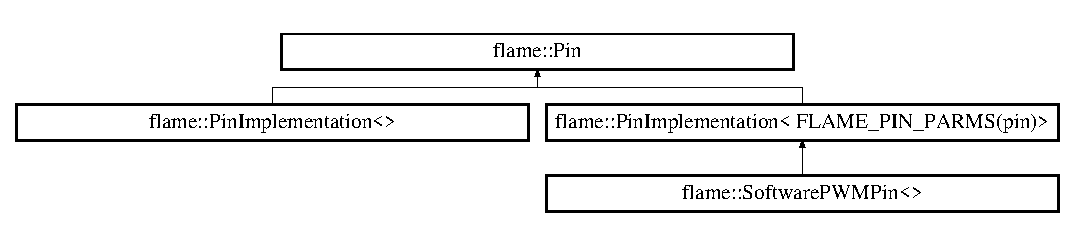
\includegraphics[height=2.616822cm]{classflame_1_1_pin}
\end{center}
\end{figure}
\subsection*{Public Member Functions}
\begin{DoxyCompactItemize}
\item 
virtual void \hyperlink{classflame_1_1_pin_a662d1c9ebe06f39eca0b344cdcacf71e}{on} ()=0
\item 
virtual void \hyperlink{classflame_1_1_pin_a92602dd2050757ac05f822ffac6c96d4}{on\-Atomic} ()=0
\item 
virtual void \hyperlink{classflame_1_1_pin_a275c305cc869a36b77c6642d2122a7e4}{off} ()=0
\item 
virtual void \hyperlink{classflame_1_1_pin_ab2c12ae2715f4768478920dc8cd047bd}{off\-Atomic} ()=0
\item 
virtual void \hyperlink{classflame_1_1_pin_aef5519e00e077ca3d9bf1045c54bb245}{set} (bool state)=0
\item 
virtual void \hyperlink{classflame_1_1_pin_ad255caef4f0f6b8f1fe886800afa90b5}{set\-Atomic} (bool state)=0
\item 
virtual void \hyperlink{classflame_1_1_pin_af8941ca0d0284049babc1823ab67366c}{set\-Output} ()=0
\item 
virtual void \hyperlink{classflame_1_1_pin_a1cdaa26a0e0fd3625c1857597796b37b}{set\-Output\-Atomic} ()=0
\item 
virtual void \hyperlink{classflame_1_1_pin_a2a236681d735dfc3120fc52b3247318a}{set\-Input} ()=0
\item 
virtual void \hyperlink{classflame_1_1_pin_a9c60f31713a6052d9529017a6eed00e0}{set\-Input\-Atomic} ()=0
\item 
virtual void \hyperlink{classflame_1_1_pin_adcfde4a13f068347b0d2110e37aa0cb7}{set\-Input\-Pullup} ()=0
\item 
virtual void \hyperlink{classflame_1_1_pin_a9c597d09c521128beaf56729c2b083c5}{set\-Input\-Pullup\-Atomic} ()=0
\item 
virtual void \hyperlink{classflame_1_1_pin_a00d7d0568ac59b73879cab10d701d1b4}{toggle} ()=0
\item 
virtual void \hyperlink{classflame_1_1_pin_af4a4cd28d03658822ec37c4418d42a06}{toggle\-Atomic} ()=0
\item 
virtual bool \hyperlink{classflame_1_1_pin_a388fcf1d1902a306aa1f4d8fa18876f3}{read} ()=0
\item 
virtual uint8\-\_\-t \hyperlink{classflame_1_1_pin_a6ccab19cacc3a29d488c21af979389b6}{pinchange\-Interrupt} ()=0
\item 
virtual \hyperlink{namespaceflame_a7117d3cded694c1ded03c462d677b165}{F\-L\-A\-M\-E\-\_\-register} \hyperlink{classflame_1_1_pin_a2d87a59132c2a9ec11095f79707dc3bd}{dir\-Port} ()=0
\item 
virtual \hyperlink{namespaceflame_a7117d3cded694c1ded03c462d677b165}{F\-L\-A\-M\-E\-\_\-register} \hyperlink{classflame_1_1_pin_af01a5c7eeb14e74e0bad26772f97bb29}{input\-Port} ()=0
\item 
virtual \hyperlink{namespaceflame_a7117d3cded694c1ded03c462d677b165}{F\-L\-A\-M\-E\-\_\-register} \hyperlink{classflame_1_1_pin_ad90f4028b374a882678728d18ddb69c2}{output\-Port} ()=0
\item 
virtual uint8\-\_\-t \hyperlink{classflame_1_1_pin_a78928d23f568f916249fd87ebdc28db7}{bit} ()=0
\item 
virtual uint8\-\_\-t \hyperlink{classflame_1_1_pin_a510a078e2de86e28483709381d2b04d5}{mask} ()=0
\end{DoxyCompactItemize}


\subsection{Detailed Description}


Definition at line 35 of file Pin.\-h.



\subsection{Member Function Documentation}
\hypertarget{classflame_1_1_pin_a78928d23f568f916249fd87ebdc28db7}{\index{flame\-::\-Pin@{flame\-::\-Pin}!bit@{bit}}
\index{bit@{bit}!flame::Pin@{flame\-::\-Pin}}
\subsubsection[{bit}]{\setlength{\rightskip}{0pt plus 5cm}virtual uint8\-\_\-t flame\-::\-Pin\-::bit (
\begin{DoxyParamCaption}
{}
\end{DoxyParamCaption}
)\hspace{0.3cm}{\ttfamily [pure virtual]}}}\label{classflame_1_1_pin_a78928d23f568f916249fd87ebdc28db7}
Get the bit 

Implemented in \hyperlink{classflame_1_1_pin_implementation_ae1826279d7dc9ec6c7ff4a8ab7a4ecff}{flame\-::\-Pin\-Implementation$<$$>$}, and \hyperlink{classflame_1_1_pin_implementation_ae1826279d7dc9ec6c7ff4a8ab7a4ecff}{flame\-::\-Pin\-Implementation$<$ F\-L\-A\-M\-E\-\_\-\-P\-I\-N\-\_\-\-P\-A\-R\-M\-S(pin)$>$}.

\hypertarget{classflame_1_1_pin_a2d87a59132c2a9ec11095f79707dc3bd}{\index{flame\-::\-Pin@{flame\-::\-Pin}!dir\-Port@{dir\-Port}}
\index{dir\-Port@{dir\-Port}!flame::Pin@{flame\-::\-Pin}}
\subsubsection[{dir\-Port}]{\setlength{\rightskip}{0pt plus 5cm}virtual {\bf F\-L\-A\-M\-E\-\_\-register} flame\-::\-Pin\-::dir\-Port (
\begin{DoxyParamCaption}
{}
\end{DoxyParamCaption}
)\hspace{0.3cm}{\ttfamily [pure virtual]}}}\label{classflame_1_1_pin_a2d87a59132c2a9ec11095f79707dc3bd}
Get the direction port 

Implemented in \hyperlink{classflame_1_1_pin_implementation_aa8aded8d5b2b465143e022faba139f07}{flame\-::\-Pin\-Implementation$<$$>$}, and \hyperlink{classflame_1_1_pin_implementation_aa8aded8d5b2b465143e022faba139f07}{flame\-::\-Pin\-Implementation$<$ F\-L\-A\-M\-E\-\_\-\-P\-I\-N\-\_\-\-P\-A\-R\-M\-S(pin)$>$}.

\hypertarget{classflame_1_1_pin_af01a5c7eeb14e74e0bad26772f97bb29}{\index{flame\-::\-Pin@{flame\-::\-Pin}!input\-Port@{input\-Port}}
\index{input\-Port@{input\-Port}!flame::Pin@{flame\-::\-Pin}}
\subsubsection[{input\-Port}]{\setlength{\rightskip}{0pt plus 5cm}virtual {\bf F\-L\-A\-M\-E\-\_\-register} flame\-::\-Pin\-::input\-Port (
\begin{DoxyParamCaption}
{}
\end{DoxyParamCaption}
)\hspace{0.3cm}{\ttfamily [pure virtual]}}}\label{classflame_1_1_pin_af01a5c7eeb14e74e0bad26772f97bb29}
Get the input port 

Implemented in \hyperlink{classflame_1_1_pin_implementation_adf064a598546e83a302e843fbe07b1b6}{flame\-::\-Pin\-Implementation$<$$>$}, and \hyperlink{classflame_1_1_pin_implementation_adf064a598546e83a302e843fbe07b1b6}{flame\-::\-Pin\-Implementation$<$ F\-L\-A\-M\-E\-\_\-\-P\-I\-N\-\_\-\-P\-A\-R\-M\-S(pin)$>$}.

\hypertarget{classflame_1_1_pin_a510a078e2de86e28483709381d2b04d5}{\index{flame\-::\-Pin@{flame\-::\-Pin}!mask@{mask}}
\index{mask@{mask}!flame::Pin@{flame\-::\-Pin}}
\subsubsection[{mask}]{\setlength{\rightskip}{0pt plus 5cm}virtual uint8\-\_\-t flame\-::\-Pin\-::mask (
\begin{DoxyParamCaption}
{}
\end{DoxyParamCaption}
)\hspace{0.3cm}{\ttfamily [pure virtual]}}}\label{classflame_1_1_pin_a510a078e2de86e28483709381d2b04d5}
Get the mask 

Implemented in \hyperlink{classflame_1_1_pin_implementation_aba23157dd8b17c9b4cbf37c34e34d4c2}{flame\-::\-Pin\-Implementation$<$$>$}, and \hyperlink{classflame_1_1_pin_implementation_aba23157dd8b17c9b4cbf37c34e34d4c2}{flame\-::\-Pin\-Implementation$<$ F\-L\-A\-M\-E\-\_\-\-P\-I\-N\-\_\-\-P\-A\-R\-M\-S(pin)$>$}.

\hypertarget{classflame_1_1_pin_a275c305cc869a36b77c6642d2122a7e4}{\index{flame\-::\-Pin@{flame\-::\-Pin}!off@{off}}
\index{off@{off}!flame::Pin@{flame\-::\-Pin}}
\subsubsection[{off}]{\setlength{\rightskip}{0pt plus 5cm}virtual void flame\-::\-Pin\-::off (
\begin{DoxyParamCaption}
{}
\end{DoxyParamCaption}
)\hspace{0.3cm}{\ttfamily [pure virtual]}}}\label{classflame_1_1_pin_a275c305cc869a36b77c6642d2122a7e4}
Set the pin off \begin{DoxyPrecond}{Precondition}
the pin must be set to output 
\end{DoxyPrecond}


Implemented in \hyperlink{classflame_1_1_pin_implementation_a01979e241b9d5aa9b76fc3a90d8938ce}{flame\-::\-Pin\-Implementation$<$$>$}, and \hyperlink{classflame_1_1_pin_implementation_a01979e241b9d5aa9b76fc3a90d8938ce}{flame\-::\-Pin\-Implementation$<$ F\-L\-A\-M\-E\-\_\-\-P\-I\-N\-\_\-\-P\-A\-R\-M\-S(pin)$>$}.

\hypertarget{classflame_1_1_pin_ab2c12ae2715f4768478920dc8cd047bd}{\index{flame\-::\-Pin@{flame\-::\-Pin}!off\-Atomic@{off\-Atomic}}
\index{off\-Atomic@{off\-Atomic}!flame::Pin@{flame\-::\-Pin}}
\subsubsection[{off\-Atomic}]{\setlength{\rightskip}{0pt plus 5cm}virtual void flame\-::\-Pin\-::off\-Atomic (
\begin{DoxyParamCaption}
{}
\end{DoxyParamCaption}
)\hspace{0.3cm}{\ttfamily [pure virtual]}}}\label{classflame_1_1_pin_ab2c12ae2715f4768478920dc8cd047bd}
Set the pin off atomically (used if the state of a pin on the same port is altered in an interrupt handler) \begin{DoxyPrecond}{Precondition}
the pin must be set to output 
\end{DoxyPrecond}


Implemented in \hyperlink{classflame_1_1_pin_implementation_aa488f6f695dbf9a477d470d891ea17f9}{flame\-::\-Pin\-Implementation$<$$>$}, and \hyperlink{classflame_1_1_pin_implementation_aa488f6f695dbf9a477d470d891ea17f9}{flame\-::\-Pin\-Implementation$<$ F\-L\-A\-M\-E\-\_\-\-P\-I\-N\-\_\-\-P\-A\-R\-M\-S(pin)$>$}.

\hypertarget{classflame_1_1_pin_a662d1c9ebe06f39eca0b344cdcacf71e}{\index{flame\-::\-Pin@{flame\-::\-Pin}!on@{on}}
\index{on@{on}!flame::Pin@{flame\-::\-Pin}}
\subsubsection[{on}]{\setlength{\rightskip}{0pt plus 5cm}virtual void flame\-::\-Pin\-::on (
\begin{DoxyParamCaption}
{}
\end{DoxyParamCaption}
)\hspace{0.3cm}{\ttfamily [pure virtual]}}}\label{classflame_1_1_pin_a662d1c9ebe06f39eca0b344cdcacf71e}
Set the pin on \begin{DoxyPrecond}{Precondition}
the pin must be set to output 
\end{DoxyPrecond}


Implemented in \hyperlink{classflame_1_1_pin_implementation_a5ee64200c99231a1ba1b6e724d53f3bf}{flame\-::\-Pin\-Implementation$<$$>$}, and \hyperlink{classflame_1_1_pin_implementation_a5ee64200c99231a1ba1b6e724d53f3bf}{flame\-::\-Pin\-Implementation$<$ F\-L\-A\-M\-E\-\_\-\-P\-I\-N\-\_\-\-P\-A\-R\-M\-S(pin)$>$}.

\hypertarget{classflame_1_1_pin_a92602dd2050757ac05f822ffac6c96d4}{\index{flame\-::\-Pin@{flame\-::\-Pin}!on\-Atomic@{on\-Atomic}}
\index{on\-Atomic@{on\-Atomic}!flame::Pin@{flame\-::\-Pin}}
\subsubsection[{on\-Atomic}]{\setlength{\rightskip}{0pt plus 5cm}virtual void flame\-::\-Pin\-::on\-Atomic (
\begin{DoxyParamCaption}
{}
\end{DoxyParamCaption}
)\hspace{0.3cm}{\ttfamily [pure virtual]}}}\label{classflame_1_1_pin_a92602dd2050757ac05f822ffac6c96d4}
Set the pin on atomically (used if the state of a pin on the same port is altered in an interrupt handler) \begin{DoxyPrecond}{Precondition}
the pin must be set to output 
\end{DoxyPrecond}


Implemented in \hyperlink{classflame_1_1_pin_implementation_ad4a7397f4abe95df89b28a2209bed782}{flame\-::\-Pin\-Implementation$<$$>$}, and \hyperlink{classflame_1_1_pin_implementation_ad4a7397f4abe95df89b28a2209bed782}{flame\-::\-Pin\-Implementation$<$ F\-L\-A\-M\-E\-\_\-\-P\-I\-N\-\_\-\-P\-A\-R\-M\-S(pin)$>$}.

\hypertarget{classflame_1_1_pin_ad90f4028b374a882678728d18ddb69c2}{\index{flame\-::\-Pin@{flame\-::\-Pin}!output\-Port@{output\-Port}}
\index{output\-Port@{output\-Port}!flame::Pin@{flame\-::\-Pin}}
\subsubsection[{output\-Port}]{\setlength{\rightskip}{0pt plus 5cm}virtual {\bf F\-L\-A\-M\-E\-\_\-register} flame\-::\-Pin\-::output\-Port (
\begin{DoxyParamCaption}
{}
\end{DoxyParamCaption}
)\hspace{0.3cm}{\ttfamily [pure virtual]}}}\label{classflame_1_1_pin_ad90f4028b374a882678728d18ddb69c2}
Get the output port 

Implemented in \hyperlink{classflame_1_1_pin_implementation_a3e59355e9e55997b71f44ec7ef3880fe}{flame\-::\-Pin\-Implementation$<$$>$}, and \hyperlink{classflame_1_1_pin_implementation_a3e59355e9e55997b71f44ec7ef3880fe}{flame\-::\-Pin\-Implementation$<$ F\-L\-A\-M\-E\-\_\-\-P\-I\-N\-\_\-\-P\-A\-R\-M\-S(pin)$>$}.

\hypertarget{classflame_1_1_pin_a6ccab19cacc3a29d488c21af979389b6}{\index{flame\-::\-Pin@{flame\-::\-Pin}!pinchange\-Interrupt@{pinchange\-Interrupt}}
\index{pinchange\-Interrupt@{pinchange\-Interrupt}!flame::Pin@{flame\-::\-Pin}}
\subsubsection[{pinchange\-Interrupt}]{\setlength{\rightskip}{0pt plus 5cm}virtual uint8\-\_\-t flame\-::\-Pin\-::pinchange\-Interrupt (
\begin{DoxyParamCaption}
{}
\end{DoxyParamCaption}
)\hspace{0.3cm}{\ttfamily [pure virtual]}}}\label{classflame_1_1_pin_a6ccab19cacc3a29d488c21af979389b6}
Get the pinchange interrupt for the pin \begin{DoxyReturn}{Returns}
the pinchange interrupt, or -\/1 if there is none available 
\end{DoxyReturn}


Implemented in \hyperlink{classflame_1_1_pin_implementation_abc7af958b5833502e349e1b9768493d3}{flame\-::\-Pin\-Implementation$<$$>$}, and \hyperlink{classflame_1_1_pin_implementation_abc7af958b5833502e349e1b9768493d3}{flame\-::\-Pin\-Implementation$<$ F\-L\-A\-M\-E\-\_\-\-P\-I\-N\-\_\-\-P\-A\-R\-M\-S(pin)$>$}.

\hypertarget{classflame_1_1_pin_a388fcf1d1902a306aa1f4d8fa18876f3}{\index{flame\-::\-Pin@{flame\-::\-Pin}!read@{read}}
\index{read@{read}!flame::Pin@{flame\-::\-Pin}}
\subsubsection[{read}]{\setlength{\rightskip}{0pt plus 5cm}virtual bool flame\-::\-Pin\-::read (
\begin{DoxyParamCaption}
{}
\end{DoxyParamCaption}
)\hspace{0.3cm}{\ttfamily [pure virtual]}}}\label{classflame_1_1_pin_a388fcf1d1902a306aa1f4d8fa18876f3}
Read the pin 
\begin{DoxyParams}{Parameters}
{\em pin} & the pin to read \\
\hline
\end{DoxyParams}


Implemented in \hyperlink{classflame_1_1_pin_implementation_aae70a073f94d3ec291e858f51c7c9e72}{flame\-::\-Pin\-Implementation$<$$>$}, and \hyperlink{classflame_1_1_pin_implementation_aae70a073f94d3ec291e858f51c7c9e72}{flame\-::\-Pin\-Implementation$<$ F\-L\-A\-M\-E\-\_\-\-P\-I\-N\-\_\-\-P\-A\-R\-M\-S(pin)$>$}.

\hypertarget{classflame_1_1_pin_aef5519e00e077ca3d9bf1045c54bb245}{\index{flame\-::\-Pin@{flame\-::\-Pin}!set@{set}}
\index{set@{set}!flame::Pin@{flame\-::\-Pin}}
\subsubsection[{set}]{\setlength{\rightskip}{0pt plus 5cm}virtual void flame\-::\-Pin\-::set (
\begin{DoxyParamCaption}
\item[{bool}]{state}
\end{DoxyParamCaption}
)\hspace{0.3cm}{\ttfamily [pure virtual]}}}\label{classflame_1_1_pin_aef5519e00e077ca3d9bf1045c54bb245}
Set the pin on or off \begin{DoxyPrecond}{Precondition}
the pin must be set to output 
\end{DoxyPrecond}

\begin{DoxyParams}{Parameters}
{\em state} & true to turn the pin on \\
\hline
\end{DoxyParams}


Implemented in \hyperlink{classflame_1_1_pin_implementation_a980549afcbc44720bb9d01706318985b}{flame\-::\-Pin\-Implementation$<$$>$}, and \hyperlink{classflame_1_1_pin_implementation_a980549afcbc44720bb9d01706318985b}{flame\-::\-Pin\-Implementation$<$ F\-L\-A\-M\-E\-\_\-\-P\-I\-N\-\_\-\-P\-A\-R\-M\-S(pin)$>$}.

\hypertarget{classflame_1_1_pin_ad255caef4f0f6b8f1fe886800afa90b5}{\index{flame\-::\-Pin@{flame\-::\-Pin}!set\-Atomic@{set\-Atomic}}
\index{set\-Atomic@{set\-Atomic}!flame::Pin@{flame\-::\-Pin}}
\subsubsection[{set\-Atomic}]{\setlength{\rightskip}{0pt plus 5cm}virtual void flame\-::\-Pin\-::set\-Atomic (
\begin{DoxyParamCaption}
\item[{bool}]{state}
\end{DoxyParamCaption}
)\hspace{0.3cm}{\ttfamily [pure virtual]}}}\label{classflame_1_1_pin_ad255caef4f0f6b8f1fe886800afa90b5}
Set the output pin on or off (used if the state of a pin on the same port is altered in an interrupt handler) \begin{DoxyPrecond}{Precondition}
the pin must be set to output 
\end{DoxyPrecond}

\begin{DoxyParams}{Parameters}
{\em state} & true to turn the pin on \\
\hline
\end{DoxyParams}


Implemented in \hyperlink{classflame_1_1_pin_implementation_ae2ea926f7c081bea35247f0b9d03483e}{flame\-::\-Pin\-Implementation$<$$>$}, and \hyperlink{classflame_1_1_pin_implementation_ae2ea926f7c081bea35247f0b9d03483e}{flame\-::\-Pin\-Implementation$<$ F\-L\-A\-M\-E\-\_\-\-P\-I\-N\-\_\-\-P\-A\-R\-M\-S(pin)$>$}.

\hypertarget{classflame_1_1_pin_a2a236681d735dfc3120fc52b3247318a}{\index{flame\-::\-Pin@{flame\-::\-Pin}!set\-Input@{set\-Input}}
\index{set\-Input@{set\-Input}!flame::Pin@{flame\-::\-Pin}}
\subsubsection[{set\-Input}]{\setlength{\rightskip}{0pt plus 5cm}virtual void flame\-::\-Pin\-::set\-Input (
\begin{DoxyParamCaption}
{}
\end{DoxyParamCaption}
)\hspace{0.3cm}{\ttfamily [pure virtual]}}}\label{classflame_1_1_pin_a2a236681d735dfc3120fc52b3247318a}
Set the pin to be an input 

Implemented in \hyperlink{classflame_1_1_pin_implementation_af4aa98133baf5f86180abc911109b90a}{flame\-::\-Pin\-Implementation$<$$>$}, and \hyperlink{classflame_1_1_pin_implementation_af4aa98133baf5f86180abc911109b90a}{flame\-::\-Pin\-Implementation$<$ F\-L\-A\-M\-E\-\_\-\-P\-I\-N\-\_\-\-P\-A\-R\-M\-S(pin)$>$}.

\hypertarget{classflame_1_1_pin_a9c60f31713a6052d9529017a6eed00e0}{\index{flame\-::\-Pin@{flame\-::\-Pin}!set\-Input\-Atomic@{set\-Input\-Atomic}}
\index{set\-Input\-Atomic@{set\-Input\-Atomic}!flame::Pin@{flame\-::\-Pin}}
\subsubsection[{set\-Input\-Atomic}]{\setlength{\rightskip}{0pt plus 5cm}virtual void flame\-::\-Pin\-::set\-Input\-Atomic (
\begin{DoxyParamCaption}
{}
\end{DoxyParamCaption}
)\hspace{0.3cm}{\ttfamily [pure virtual]}}}\label{classflame_1_1_pin_a9c60f31713a6052d9529017a6eed00e0}
Set the pin to be an input (used if the direction of a pin on the same port is altered in an interrupt handler) 

Implemented in \hyperlink{classflame_1_1_pin_implementation_a3b4d71dda7c0165b4477671ab8f9ab91}{flame\-::\-Pin\-Implementation$<$$>$}, and \hyperlink{classflame_1_1_pin_implementation_a3b4d71dda7c0165b4477671ab8f9ab91}{flame\-::\-Pin\-Implementation$<$ F\-L\-A\-M\-E\-\_\-\-P\-I\-N\-\_\-\-P\-A\-R\-M\-S(pin)$>$}.

\hypertarget{classflame_1_1_pin_adcfde4a13f068347b0d2110e37aa0cb7}{\index{flame\-::\-Pin@{flame\-::\-Pin}!set\-Input\-Pullup@{set\-Input\-Pullup}}
\index{set\-Input\-Pullup@{set\-Input\-Pullup}!flame::Pin@{flame\-::\-Pin}}
\subsubsection[{set\-Input\-Pullup}]{\setlength{\rightskip}{0pt plus 5cm}virtual void flame\-::\-Pin\-::set\-Input\-Pullup (
\begin{DoxyParamCaption}
{}
\end{DoxyParamCaption}
)\hspace{0.3cm}{\ttfamily [pure virtual]}}}\label{classflame_1_1_pin_adcfde4a13f068347b0d2110e37aa0cb7}
Set the pin to be an input, with the internal pullup enabled 

Implemented in \hyperlink{classflame_1_1_pin_implementation_a7c609a01c4f035238e35fc229c8b3498}{flame\-::\-Pin\-Implementation$<$$>$}, and \hyperlink{classflame_1_1_pin_implementation_a7c609a01c4f035238e35fc229c8b3498}{flame\-::\-Pin\-Implementation$<$ F\-L\-A\-M\-E\-\_\-\-P\-I\-N\-\_\-\-P\-A\-R\-M\-S(pin)$>$}.

\hypertarget{classflame_1_1_pin_a9c597d09c521128beaf56729c2b083c5}{\index{flame\-::\-Pin@{flame\-::\-Pin}!set\-Input\-Pullup\-Atomic@{set\-Input\-Pullup\-Atomic}}
\index{set\-Input\-Pullup\-Atomic@{set\-Input\-Pullup\-Atomic}!flame::Pin@{flame\-::\-Pin}}
\subsubsection[{set\-Input\-Pullup\-Atomic}]{\setlength{\rightskip}{0pt plus 5cm}virtual void flame\-::\-Pin\-::set\-Input\-Pullup\-Atomic (
\begin{DoxyParamCaption}
{}
\end{DoxyParamCaption}
)\hspace{0.3cm}{\ttfamily [pure virtual]}}}\label{classflame_1_1_pin_a9c597d09c521128beaf56729c2b083c5}
Set a pin to be an input, with the internal pullup enabled (used if the direction of a pin on the same port is altered in an interrupt handler) 

Implemented in \hyperlink{classflame_1_1_pin_implementation_a8a518fb6dea3b772e7fd715e7f13b7bd}{flame\-::\-Pin\-Implementation$<$$>$}, and \hyperlink{classflame_1_1_pin_implementation_a8a518fb6dea3b772e7fd715e7f13b7bd}{flame\-::\-Pin\-Implementation$<$ F\-L\-A\-M\-E\-\_\-\-P\-I\-N\-\_\-\-P\-A\-R\-M\-S(pin)$>$}.

\hypertarget{classflame_1_1_pin_af8941ca0d0284049babc1823ab67366c}{\index{flame\-::\-Pin@{flame\-::\-Pin}!set\-Output@{set\-Output}}
\index{set\-Output@{set\-Output}!flame::Pin@{flame\-::\-Pin}}
\subsubsection[{set\-Output}]{\setlength{\rightskip}{0pt plus 5cm}virtual void flame\-::\-Pin\-::set\-Output (
\begin{DoxyParamCaption}
{}
\end{DoxyParamCaption}
)\hspace{0.3cm}{\ttfamily [pure virtual]}}}\label{classflame_1_1_pin_af8941ca0d0284049babc1823ab67366c}
Set the pin to be an output 

Implemented in \hyperlink{classflame_1_1_pin_implementation_abf6851b4b0c78d5c5c8e3aec7600a83e}{flame\-::\-Pin\-Implementation$<$$>$}, and \hyperlink{classflame_1_1_pin_implementation_abf6851b4b0c78d5c5c8e3aec7600a83e}{flame\-::\-Pin\-Implementation$<$ F\-L\-A\-M\-E\-\_\-\-P\-I\-N\-\_\-\-P\-A\-R\-M\-S(pin)$>$}.

\hypertarget{classflame_1_1_pin_a1cdaa26a0e0fd3625c1857597796b37b}{\index{flame\-::\-Pin@{flame\-::\-Pin}!set\-Output\-Atomic@{set\-Output\-Atomic}}
\index{set\-Output\-Atomic@{set\-Output\-Atomic}!flame::Pin@{flame\-::\-Pin}}
\subsubsection[{set\-Output\-Atomic}]{\setlength{\rightskip}{0pt plus 5cm}virtual void flame\-::\-Pin\-::set\-Output\-Atomic (
\begin{DoxyParamCaption}
{}
\end{DoxyParamCaption}
)\hspace{0.3cm}{\ttfamily [pure virtual]}}}\label{classflame_1_1_pin_a1cdaa26a0e0fd3625c1857597796b37b}
Set the pin to be an output (used if the direction of a pin on the same port is altered in an interrupt handler) 

Implemented in \hyperlink{classflame_1_1_pin_implementation_a3f3bb8ec54186e16fbb2670cf2e99460}{flame\-::\-Pin\-Implementation$<$$>$}, and \hyperlink{classflame_1_1_pin_implementation_a3f3bb8ec54186e16fbb2670cf2e99460}{flame\-::\-Pin\-Implementation$<$ F\-L\-A\-M\-E\-\_\-\-P\-I\-N\-\_\-\-P\-A\-R\-M\-S(pin)$>$}.

\hypertarget{classflame_1_1_pin_a00d7d0568ac59b73879cab10d701d1b4}{\index{flame\-::\-Pin@{flame\-::\-Pin}!toggle@{toggle}}
\index{toggle@{toggle}!flame::Pin@{flame\-::\-Pin}}
\subsubsection[{toggle}]{\setlength{\rightskip}{0pt plus 5cm}virtual void flame\-::\-Pin\-::toggle (
\begin{DoxyParamCaption}
{}
\end{DoxyParamCaption}
)\hspace{0.3cm}{\ttfamily [pure virtual]}}}\label{classflame_1_1_pin_a00d7d0568ac59b73879cab10d701d1b4}
Toggle a pin 

Implemented in \hyperlink{classflame_1_1_pin_implementation_aa29c1d76b786741a4a187ecec173ae25}{flame\-::\-Pin\-Implementation$<$$>$}, and \hyperlink{classflame_1_1_pin_implementation_aa29c1d76b786741a4a187ecec173ae25}{flame\-::\-Pin\-Implementation$<$ F\-L\-A\-M\-E\-\_\-\-P\-I\-N\-\_\-\-P\-A\-R\-M\-S(pin)$>$}.

\hypertarget{classflame_1_1_pin_af4a4cd28d03658822ec37c4418d42a06}{\index{flame\-::\-Pin@{flame\-::\-Pin}!toggle\-Atomic@{toggle\-Atomic}}
\index{toggle\-Atomic@{toggle\-Atomic}!flame::Pin@{flame\-::\-Pin}}
\subsubsection[{toggle\-Atomic}]{\setlength{\rightskip}{0pt plus 5cm}virtual void flame\-::\-Pin\-::toggle\-Atomic (
\begin{DoxyParamCaption}
{}
\end{DoxyParamCaption}
)\hspace{0.3cm}{\ttfamily [pure virtual]}}}\label{classflame_1_1_pin_af4a4cd28d03658822ec37c4418d42a06}
Toggle the pin (used if the state of a pin on the same port is altered in an interrupt handler) \begin{DoxyPrecond}{Precondition}
the pin must be set to output 
\end{DoxyPrecond}


Implemented in \hyperlink{classflame_1_1_pin_implementation_a1f9b38b3465030190afbfd965b65fcce}{flame\-::\-Pin\-Implementation$<$$>$}, and \hyperlink{classflame_1_1_pin_implementation_a1f9b38b3465030190afbfd965b65fcce}{flame\-::\-Pin\-Implementation$<$ F\-L\-A\-M\-E\-\_\-\-P\-I\-N\-\_\-\-P\-A\-R\-M\-S(pin)$>$}.



The documentation for this class was generated from the following file\-:\begin{DoxyCompactItemize}
\item 
flame/\hyperlink{_pin_8h}{Pin.\-h}\end{DoxyCompactItemize}

\hypertarget{classflame_1_1_pin_change_manager}{\section{flame\-:\-:Pin\-Change\-Manager Class Reference}
\label{classflame_1_1_pin_change_manager}\index{flame\-::\-Pin\-Change\-Manager@{flame\-::\-Pin\-Change\-Manager}}
}


{\ttfamily \#include $<$Pin\-Change\-Manager.\-h$>$}

\subsection*{Public Member Functions}
\begin{DoxyCompactItemize}
\item 
\hyperlink{classflame_1_1_pin_change_manager_a1b60ddb12e1bbff6e5b6b7496e77b5c7}{Pin\-Change\-Manager} ()
\item 
void \hyperlink{classflame_1_1_pin_change_manager_a113e55dec9a2581dfc1b888399e95cd7}{pin\-Change0} ()
\item 
void \hyperlink{classflame_1_1_pin_change_manager_a4e718462803b9eb630a4522106029b1f}{pin\-Change} (uint8\-\_\-t offset)
\item 
void \hyperlink{classflame_1_1_pin_change_manager_a5577f9500502aaaedc0f9e964bfedd8f}{register\-Listener} (\hyperlink{io_8h_ab54f3ca5cc36256b922289e8e92316a3}{F\-L\-A\-M\-E\-\_\-\-D\-E\-C\-L\-A\-R\-E\-\_\-\-P\-I\-N}(pin), \hyperlink{classflame_1_1_pin_event_listener}{Pin\-Event\-Listener} $\ast$listener)
\item 
void \hyperlink{classflame_1_1_pin_change_manager_a9705cc613533d22a35476adc444080a1}{register\-Listener} (\hyperlink{classflame_1_1_pin}{Pin} \&pin, \hyperlink{classflame_1_1_pin_event_listener}{Pin\-Event\-Listener} $\ast$listener)
\item 
void \hyperlink{classflame_1_1_pin_change_manager_a5e643ae7693542e0d796b02d992171b3}{deregister\-Listener} (int8\-\_\-t pin\-Pin\-Change\-Listener)
\item 
void \hyperlink{classflame_1_1_pin_change_manager_ab24024100cf08ec1691f689c2c1dbb37}{handle\-Events} ()
\end{DoxyCompactItemize}
\subsection*{Protected Attributes}
\begin{DoxyCompactItemize}
\item 
\hyperlink{namespaceflame_a2f4f205987821e931681b9ed5ca0eaf2}{E\-V\-E\-N\-T\-\_\-\-P\-I\-N} \hyperlink{classflame_1_1_pin_change_manager_afaa54897b9dbbfe52593512b9fe19cb2}{\-\_\-pins} \mbox{[}\hyperlink{attiny85_8h_ab39f7ddad6e692db1c00115db776636f}{F\-L\-A\-M\-E\-\_\-\-P\-C\-\_\-\-I\-N\-T\-\_\-\-C\-O\-U\-N\-T}\mbox{]}
\end{DoxyCompactItemize}


\subsection{Detailed Description}


Definition at line 90 of file Pin\-Change\-Manager.\-h.



\subsection{Constructor \& Destructor Documentation}
\hypertarget{classflame_1_1_pin_change_manager_a1b60ddb12e1bbff6e5b6b7496e77b5c7}{\index{flame\-::\-Pin\-Change\-Manager@{flame\-::\-Pin\-Change\-Manager}!Pin\-Change\-Manager@{Pin\-Change\-Manager}}
\index{Pin\-Change\-Manager@{Pin\-Change\-Manager}!flame::PinChangeManager@{flame\-::\-Pin\-Change\-Manager}}
\subsubsection[{Pin\-Change\-Manager}]{\setlength{\rightskip}{0pt plus 5cm}flame\-::\-Pin\-Change\-Manager\-::\-Pin\-Change\-Manager (
\begin{DoxyParamCaption}
{}
\end{DoxyParamCaption}
)}}\label{classflame_1_1_pin_change_manager_a1b60ddb12e1bbff6e5b6b7496e77b5c7}
An event manager for handling pinchange events 

Definition at line 35 of file Pin\-Change\-Manager.\-cpp.



\subsection{Member Function Documentation}
\hypertarget{classflame_1_1_pin_change_manager_a5e643ae7693542e0d796b02d992171b3}{\index{flame\-::\-Pin\-Change\-Manager@{flame\-::\-Pin\-Change\-Manager}!deregister\-Listener@{deregister\-Listener}}
\index{deregister\-Listener@{deregister\-Listener}!flame::PinChangeManager@{flame\-::\-Pin\-Change\-Manager}}
\subsubsection[{deregister\-Listener}]{\setlength{\rightskip}{0pt plus 5cm}void flame\-::\-Pin\-Change\-Manager\-::deregister\-Listener (
\begin{DoxyParamCaption}
\item[{int8\-\_\-t}]{pin\-Pinchange\-Interrupt}
\end{DoxyParamCaption}
)}}\label{classflame_1_1_pin_change_manager_a5e643ae7693542e0d796b02d992171b3}
Deregister interest for pinchange events 
\begin{DoxyParams}{Parameters}
{\em pin\-Pinchange\-Interrupt} & the pin\-Pinchange\-Interrupt to deregister \\
\hline
\end{DoxyParams}


Definition at line 182 of file Pin\-Change\-Manager.\-cpp.

\hypertarget{classflame_1_1_pin_change_manager_ab24024100cf08ec1691f689c2c1dbb37}{\index{flame\-::\-Pin\-Change\-Manager@{flame\-::\-Pin\-Change\-Manager}!handle\-Events@{handle\-Events}}
\index{handle\-Events@{handle\-Events}!flame::PinChangeManager@{flame\-::\-Pin\-Change\-Manager}}
\subsubsection[{handle\-Events}]{\setlength{\rightskip}{0pt plus 5cm}void flame\-::\-Pin\-Change\-Manager\-::handle\-Events (
\begin{DoxyParamCaption}
{}
\end{DoxyParamCaption}
)}}\label{classflame_1_1_pin_change_manager_ab24024100cf08ec1691f689c2c1dbb37}
Call from the main loop to handle any events 

Definition at line 218 of file Pin\-Change\-Manager.\-cpp.

\hypertarget{classflame_1_1_pin_change_manager_a4e718462803b9eb630a4522106029b1f}{\index{flame\-::\-Pin\-Change\-Manager@{flame\-::\-Pin\-Change\-Manager}!pin\-Change@{pin\-Change}}
\index{pin\-Change@{pin\-Change}!flame::PinChangeManager@{flame\-::\-Pin\-Change\-Manager}}
\subsubsection[{pin\-Change}]{\setlength{\rightskip}{0pt plus 5cm}void flame\-::\-Pin\-Change\-Manager\-::pin\-Change (
\begin{DoxyParamCaption}
\item[{uint8\-\_\-t}]{offset}
\end{DoxyParamCaption}
)}}\label{classflame_1_1_pin_change_manager_a4e718462803b9eb630a4522106029b1f}
Trigger for pin change interrupts -\/ scans through 8 pins starting at the offset 
\begin{DoxyParams}{Parameters}
{\em offset} & the number of pins to skip before scanning \\
\hline
\end{DoxyParams}


Definition at line 70 of file Pin\-Change\-Manager.\-cpp.

\hypertarget{classflame_1_1_pin_change_manager_a113e55dec9a2581dfc1b888399e95cd7}{\index{flame\-::\-Pin\-Change\-Manager@{flame\-::\-Pin\-Change\-Manager}!pin\-Change0@{pin\-Change0}}
\index{pin\-Change0@{pin\-Change0}!flame::PinChangeManager@{flame\-::\-Pin\-Change\-Manager}}
\subsubsection[{pin\-Change0}]{\setlength{\rightskip}{0pt plus 5cm}void flame\-::\-Pin\-Change\-Manager\-::pin\-Change0 (
\begin{DoxyParamCaption}
{}
\end{DoxyParamCaption}
)}}\label{classflame_1_1_pin_change_manager_a113e55dec9a2581dfc1b888399e95cd7}
Trigger for interrupt P\-C\-I\-N\-T0 

Definition at line 44 of file Pin\-Change\-Manager.\-cpp.

\hypertarget{classflame_1_1_pin_change_manager_a5577f9500502aaaedc0f9e964bfedd8f}{\index{flame\-::\-Pin\-Change\-Manager@{flame\-::\-Pin\-Change\-Manager}!register\-Listener@{register\-Listener}}
\index{register\-Listener@{register\-Listener}!flame::PinChangeManager@{flame\-::\-Pin\-Change\-Manager}}
\subsubsection[{register\-Listener}]{\setlength{\rightskip}{0pt plus 5cm}void flame\-::\-Pin\-Change\-Manager\-::register\-Listener (
\begin{DoxyParamCaption}
\item[{{\bf F\-L\-A\-M\-E\-\_\-\-D\-E\-C\-L\-A\-R\-E\-\_\-\-P\-I\-N}(pin)}]{, }
\item[{{\bf Pin\-Event\-Listener} $\ast$}]{listener}
\end{DoxyParamCaption}
)}}\label{classflame_1_1_pin_change_manager_a5577f9500502aaaedc0f9e964bfedd8f}
Register interest for pinchange events 
\begin{DoxyParams}{Parameters}
{\em pin} & A F\-L\-A\-M\-E\-\_\-\-P\-I\-N\-\_\-$\ast$ macro, must have a valid pin\-Pinchange\-Interrupt \\
\hline
{\em listener} & a F\-L\-A\-M\-E\-\_\-\-Pin\-Event\-Listener to notify when the pin changes \\
\hline
\end{DoxyParams}


Definition at line 94 of file Pin\-Change\-Manager.\-cpp.

\hypertarget{classflame_1_1_pin_change_manager_a9705cc613533d22a35476adc444080a1}{\index{flame\-::\-Pin\-Change\-Manager@{flame\-::\-Pin\-Change\-Manager}!register\-Listener@{register\-Listener}}
\index{register\-Listener@{register\-Listener}!flame::PinChangeManager@{flame\-::\-Pin\-Change\-Manager}}
\subsubsection[{register\-Listener}]{\setlength{\rightskip}{0pt plus 5cm}void flame\-::\-Pin\-Change\-Manager\-::register\-Listener (
\begin{DoxyParamCaption}
\item[{{\bf Pin} \&}]{pin, }
\item[{{\bf Pin\-Event\-Listener} $\ast$}]{listener}
\end{DoxyParamCaption}
)}}\label{classflame_1_1_pin_change_manager_a9705cc613533d22a35476adc444080a1}
Register interest for pinchange events 
\begin{DoxyParams}{Parameters}
{\em pin} & The pin, must have a valid pin\-Pinchange\-Interrupt \\
\hline
{\em listener} & a F\-L\-A\-M\-E\-\_\-\-Pin\-Event\-Listener to notify when the pin changes \\
\hline
\end{DoxyParams}


Definition at line 138 of file Pin\-Change\-Manager.\-cpp.



\subsection{Member Data Documentation}
\hypertarget{classflame_1_1_pin_change_manager_afaa54897b9dbbfe52593512b9fe19cb2}{\index{flame\-::\-Pin\-Change\-Manager@{flame\-::\-Pin\-Change\-Manager}!\-\_\-pins@{\-\_\-pins}}
\index{\-\_\-pins@{\-\_\-pins}!flame::PinChangeManager@{flame\-::\-Pin\-Change\-Manager}}
\subsubsection[{\-\_\-pins}]{\setlength{\rightskip}{0pt plus 5cm}{\bf E\-V\-E\-N\-T\-\_\-\-P\-I\-N} flame\-::\-Pin\-Change\-Manager\-::\-\_\-pins\mbox{[}{\bf F\-L\-A\-M\-E\-\_\-\-P\-C\-\_\-\-I\-N\-T\-\_\-\-C\-O\-U\-N\-T}\mbox{]}\hspace{0.3cm}{\ttfamily [protected]}}}\label{classflame_1_1_pin_change_manager_afaa54897b9dbbfe52593512b9fe19cb2}


Definition at line 93 of file Pin\-Change\-Manager.\-h.



The documentation for this class was generated from the following files\-:\begin{DoxyCompactItemize}
\item 
flame/\hyperlink{_pin_change_manager_8h}{Pin\-Change\-Manager.\-h}\item 
\hyperlink{_pin_change_manager_8cpp}{Pin\-Change\-Manager.\-cpp}\end{DoxyCompactItemize}

\hypertarget{classflame_1_1_pin_event_listener}{\section{flame\-:\-:Pin\-Event\-Listener Class Reference}
\label{classflame_1_1_pin_event_listener}\index{flame\-::\-Pin\-Event\-Listener@{flame\-::\-Pin\-Event\-Listener}}
}


{\ttfamily \#include $<$Pin\-Change\-Manager.\-h$>$}

Inheritance diagram for flame\-:\-:Pin\-Event\-Listener\-:\begin{figure}[H]
\begin{center}
\leavevmode
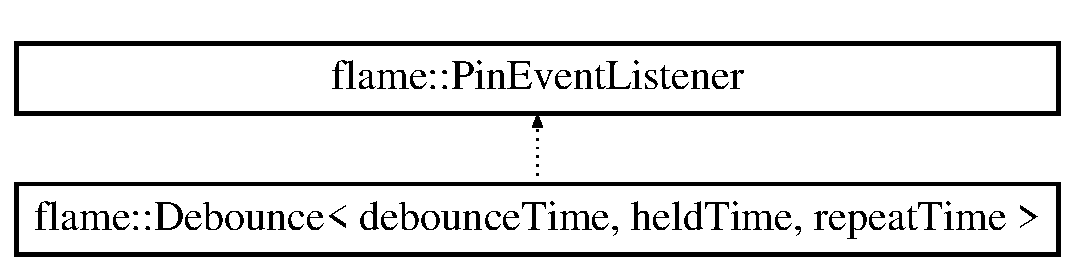
\includegraphics[height=2.000000cm]{classflame_1_1_pin_event_listener}
\end{center}
\end{figure}
\subsection*{Public Member Functions}
\begin{DoxyCompactItemize}
\item 
virtual void \hyperlink{classflame_1_1_pin_event_listener_af1b45ab9819298e7f5786a6e617450cc}{pin\-Changed} (uint8\-\_\-t pc\-Int, bool new\-State)=0
\end{DoxyCompactItemize}


\subsection{Detailed Description}


Definition at line 75 of file Pin\-Change\-Manager.\-h.



\subsection{Member Function Documentation}
\hypertarget{classflame_1_1_pin_event_listener_af1b45ab9819298e7f5786a6e617450cc}{\index{flame\-::\-Pin\-Event\-Listener@{flame\-::\-Pin\-Event\-Listener}!pin\-Changed@{pin\-Changed}}
\index{pin\-Changed@{pin\-Changed}!flame::PinEventListener@{flame\-::\-Pin\-Event\-Listener}}
\subsubsection[{pin\-Changed}]{\setlength{\rightskip}{0pt plus 5cm}virtual void flame\-::\-Pin\-Event\-Listener\-::pin\-Changed (
\begin{DoxyParamCaption}
\item[{uint8\-\_\-t}]{pc\-Int, }
\item[{bool}]{new\-State}
\end{DoxyParamCaption}
)\hspace{0.3cm}{\ttfamily [pure virtual]}}}\label{classflame_1_1_pin_event_listener_af1b45ab9819298e7f5786a6e617450cc}


Implemented in \hyperlink{classflame_1_1_debounce_ae91dc73a4becacf5f13456d1ca3b6185}{flame\-::\-Debounce$<$ debounce\-Time, held\-Time, repeat\-Time $>$}.



The documentation for this class was generated from the following file\-:\begin{DoxyCompactItemize}
\item 
flame/\hyperlink{_pin_change_manager_8h}{Pin\-Change\-Manager.\-h}\end{DoxyCompactItemize}

\hypertarget{classflame_1_1_pin_implementation}{\section{flame\-:\-:Pin\-Implementation$<$$>$ Class Template Reference}
\label{classflame_1_1_pin_implementation}\index{flame\-::\-Pin\-Implementation$<$$>$@{flame\-::\-Pin\-Implementation$<$$>$}}
}


{\ttfamily \#include $<$Pin.\-h$>$}

Inheritance diagram for flame\-:\-:Pin\-Implementation$<$$>$\-:\begin{figure}[H]
\begin{center}
\leavevmode
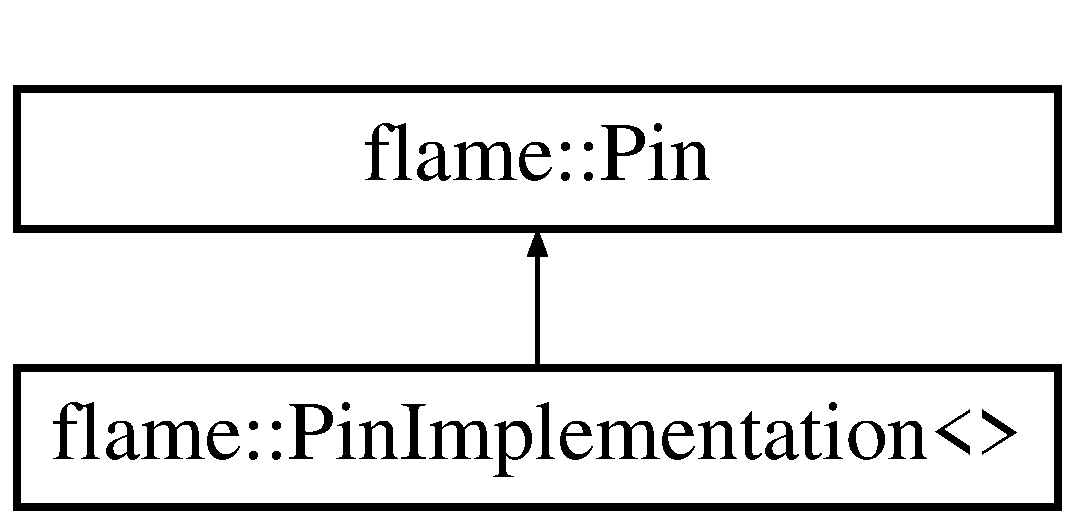
\includegraphics[height=2.000000cm]{classflame_1_1_pin_implementation}
\end{center}
\end{figure}
\subsection*{Public Member Functions}
\begin{DoxyCompactItemize}
\item 
\hyperlink{io_8h_a2eb6f9e0395b47b8d5e3eeae4fe0c116}{I\-N\-L\-I\-N\-E} void \hyperlink{classflame_1_1_pin_implementation_a5ee64200c99231a1ba1b6e724d53f3bf}{on} ()
\item 
\hyperlink{io_8h_a2eb6f9e0395b47b8d5e3eeae4fe0c116}{I\-N\-L\-I\-N\-E} void \hyperlink{classflame_1_1_pin_implementation_ad4a7397f4abe95df89b28a2209bed782}{on\-Atomic} ()
\item 
\hyperlink{io_8h_a2eb6f9e0395b47b8d5e3eeae4fe0c116}{I\-N\-L\-I\-N\-E} void \hyperlink{classflame_1_1_pin_implementation_a01979e241b9d5aa9b76fc3a90d8938ce}{off} ()
\item 
\hyperlink{io_8h_a2eb6f9e0395b47b8d5e3eeae4fe0c116}{I\-N\-L\-I\-N\-E} void \hyperlink{classflame_1_1_pin_implementation_aa488f6f695dbf9a477d470d891ea17f9}{off\-Atomic} ()
\item 
\hyperlink{io_8h_a2eb6f9e0395b47b8d5e3eeae4fe0c116}{I\-N\-L\-I\-N\-E} void \hyperlink{classflame_1_1_pin_implementation_a980549afcbc44720bb9d01706318985b}{set} (bool state)
\item 
\hyperlink{io_8h_a2eb6f9e0395b47b8d5e3eeae4fe0c116}{I\-N\-L\-I\-N\-E} void \hyperlink{classflame_1_1_pin_implementation_ae2ea926f7c081bea35247f0b9d03483e}{set\-Atomic} (bool state)
\item 
\hyperlink{io_8h_a2eb6f9e0395b47b8d5e3eeae4fe0c116}{I\-N\-L\-I\-N\-E} void \hyperlink{classflame_1_1_pin_implementation_abf6851b4b0c78d5c5c8e3aec7600a83e}{set\-Output} ()
\item 
\hyperlink{io_8h_a2eb6f9e0395b47b8d5e3eeae4fe0c116}{I\-N\-L\-I\-N\-E} void \hyperlink{classflame_1_1_pin_implementation_a3f3bb8ec54186e16fbb2670cf2e99460}{set\-Output\-Atomic} ()
\item 
\hyperlink{io_8h_a2eb6f9e0395b47b8d5e3eeae4fe0c116}{I\-N\-L\-I\-N\-E} void \hyperlink{classflame_1_1_pin_implementation_af4aa98133baf5f86180abc911109b90a}{set\-Input} ()
\item 
\hyperlink{io_8h_a2eb6f9e0395b47b8d5e3eeae4fe0c116}{I\-N\-L\-I\-N\-E} void \hyperlink{classflame_1_1_pin_implementation_a3b4d71dda7c0165b4477671ab8f9ab91}{set\-Input\-Atomic} ()
\item 
\hyperlink{io_8h_a2eb6f9e0395b47b8d5e3eeae4fe0c116}{I\-N\-L\-I\-N\-E} void \hyperlink{classflame_1_1_pin_implementation_a7c609a01c4f035238e35fc229c8b3498}{set\-Input\-Pullup} ()
\item 
\hyperlink{io_8h_a2eb6f9e0395b47b8d5e3eeae4fe0c116}{I\-N\-L\-I\-N\-E} void \hyperlink{classflame_1_1_pin_implementation_a8a518fb6dea3b772e7fd715e7f13b7bd}{set\-Input\-Pullup\-Atomic} ()
\item 
\hyperlink{io_8h_a2eb6f9e0395b47b8d5e3eeae4fe0c116}{I\-N\-L\-I\-N\-E} void \hyperlink{classflame_1_1_pin_implementation_aa29c1d76b786741a4a187ecec173ae25}{toggle} ()
\item 
\hyperlink{io_8h_a2eb6f9e0395b47b8d5e3eeae4fe0c116}{I\-N\-L\-I\-N\-E} void \hyperlink{classflame_1_1_pin_implementation_a1f9b38b3465030190afbfd965b65fcce}{toggle\-Atomic} ()
\item 
\hyperlink{io_8h_a2eb6f9e0395b47b8d5e3eeae4fe0c116}{I\-N\-L\-I\-N\-E} bool \hyperlink{classflame_1_1_pin_implementation_aae70a073f94d3ec291e858f51c7c9e72}{read} ()
\item 
\hyperlink{io_8h_a2eb6f9e0395b47b8d5e3eeae4fe0c116}{I\-N\-L\-I\-N\-E} uint8\-\_\-t \hyperlink{classflame_1_1_pin_implementation_abc7af958b5833502e349e1b9768493d3}{pinchange\-Interrupt} ()
\item 
\hyperlink{io_8h_a2eb6f9e0395b47b8d5e3eeae4fe0c116}{I\-N\-L\-I\-N\-E} \hyperlink{namespaceflame_a7117d3cded694c1ded03c462d677b165}{F\-L\-A\-M\-E\-\_\-register} \hyperlink{classflame_1_1_pin_implementation_aa8aded8d5b2b465143e022faba139f07}{dir\-Port} ()
\item 
\hyperlink{io_8h_a2eb6f9e0395b47b8d5e3eeae4fe0c116}{I\-N\-L\-I\-N\-E} \hyperlink{namespaceflame_a7117d3cded694c1ded03c462d677b165}{F\-L\-A\-M\-E\-\_\-register} \hyperlink{classflame_1_1_pin_implementation_adf064a598546e83a302e843fbe07b1b6}{input\-Port} ()
\item 
\hyperlink{io_8h_a2eb6f9e0395b47b8d5e3eeae4fe0c116}{I\-N\-L\-I\-N\-E} \hyperlink{namespaceflame_a7117d3cded694c1ded03c462d677b165}{F\-L\-A\-M\-E\-\_\-register} \hyperlink{classflame_1_1_pin_implementation_a3e59355e9e55997b71f44ec7ef3880fe}{output\-Port} ()
\item 
\hyperlink{io_8h_a2eb6f9e0395b47b8d5e3eeae4fe0c116}{I\-N\-L\-I\-N\-E} uint8\-\_\-t \hyperlink{classflame_1_1_pin_implementation_ae1826279d7dc9ec6c7ff4a8ab7a4ecff}{bit} ()
\item 
\hyperlink{io_8h_a2eb6f9e0395b47b8d5e3eeae4fe0c116}{I\-N\-L\-I\-N\-E} uint8\-\_\-t \hyperlink{classflame_1_1_pin_implementation_aba23157dd8b17c9b4cbf37c34e34d4c2}{mask} ()
\end{DoxyCompactItemize}


\subsection{Detailed Description}
\subsubsection*{template$<$F\-L\-A\-M\-E\-\_\-\-D\-E\-C\-L\-A\-R\-E\-\_\-\-P\-I\-N(pin)$>$class flame\-::\-Pin\-Implementation$<$$>$}

Create a new \hyperlink{classflame_1_1_pin}{Pin} object that represents a G\-P\-I\-O pin 
\begin{DoxyTemplParams}{Template Parameters}
{\em data\-Pin...} & the pin \\
\hline
\end{DoxyTemplParams}


Definition at line 160 of file Pin.\-h.



\subsection{Member Function Documentation}
\hypertarget{classflame_1_1_pin_implementation_ae1826279d7dc9ec6c7ff4a8ab7a4ecff}{\index{flame\-::\-Pin\-Implementation@{flame\-::\-Pin\-Implementation}!bit@{bit}}
\index{bit@{bit}!flame::PinImplementation@{flame\-::\-Pin\-Implementation}}
\subsubsection[{bit}]{\setlength{\rightskip}{0pt plus 5cm}template$<$F\-L\-A\-M\-E\-\_\-\-D\-E\-C\-L\-A\-R\-E\-\_\-\-P\-I\-N(pin) $>$ {\bf I\-N\-L\-I\-N\-E} uint8\-\_\-t {\bf flame\-::\-Pin\-Implementation}$<$$>$\-::bit (
\begin{DoxyParamCaption}
{}
\end{DoxyParamCaption}
)\hspace{0.3cm}{\ttfamily [inline]}, {\ttfamily [virtual]}}}\label{classflame_1_1_pin_implementation_ae1826279d7dc9ec6c7ff4a8ab7a4ecff}
Get the bit 

Implements \hyperlink{classflame_1_1_pin_a78928d23f568f916249fd87ebdc28db7}{flame\-::\-Pin}.



Definition at line 311 of file Pin.\-h.

\hypertarget{classflame_1_1_pin_implementation_aa8aded8d5b2b465143e022faba139f07}{\index{flame\-::\-Pin\-Implementation@{flame\-::\-Pin\-Implementation}!dir\-Port@{dir\-Port}}
\index{dir\-Port@{dir\-Port}!flame::PinImplementation@{flame\-::\-Pin\-Implementation}}
\subsubsection[{dir\-Port}]{\setlength{\rightskip}{0pt plus 5cm}template$<$F\-L\-A\-M\-E\-\_\-\-D\-E\-C\-L\-A\-R\-E\-\_\-\-P\-I\-N(pin) $>$ {\bf I\-N\-L\-I\-N\-E} {\bf F\-L\-A\-M\-E\-\_\-register} {\bf flame\-::\-Pin\-Implementation}$<$$>$\-::dir\-Port (
\begin{DoxyParamCaption}
{}
\end{DoxyParamCaption}
)\hspace{0.3cm}{\ttfamily [inline]}, {\ttfamily [virtual]}}}\label{classflame_1_1_pin_implementation_aa8aded8d5b2b465143e022faba139f07}
Get the direction port 

Implements \hyperlink{classflame_1_1_pin_a2d87a59132c2a9ec11095f79707dc3bd}{flame\-::\-Pin}.



Definition at line 290 of file Pin.\-h.

\hypertarget{classflame_1_1_pin_implementation_adf064a598546e83a302e843fbe07b1b6}{\index{flame\-::\-Pin\-Implementation@{flame\-::\-Pin\-Implementation}!input\-Port@{input\-Port}}
\index{input\-Port@{input\-Port}!flame::PinImplementation@{flame\-::\-Pin\-Implementation}}
\subsubsection[{input\-Port}]{\setlength{\rightskip}{0pt plus 5cm}template$<$F\-L\-A\-M\-E\-\_\-\-D\-E\-C\-L\-A\-R\-E\-\_\-\-P\-I\-N(pin) $>$ {\bf I\-N\-L\-I\-N\-E} {\bf F\-L\-A\-M\-E\-\_\-register} {\bf flame\-::\-Pin\-Implementation}$<$$>$\-::input\-Port (
\begin{DoxyParamCaption}
{}
\end{DoxyParamCaption}
)\hspace{0.3cm}{\ttfamily [inline]}, {\ttfamily [virtual]}}}\label{classflame_1_1_pin_implementation_adf064a598546e83a302e843fbe07b1b6}
Get the input port 

Implements \hyperlink{classflame_1_1_pin_af01a5c7eeb14e74e0bad26772f97bb29}{flame\-::\-Pin}.



Definition at line 297 of file Pin.\-h.

\hypertarget{classflame_1_1_pin_implementation_aba23157dd8b17c9b4cbf37c34e34d4c2}{\index{flame\-::\-Pin\-Implementation@{flame\-::\-Pin\-Implementation}!mask@{mask}}
\index{mask@{mask}!flame::PinImplementation@{flame\-::\-Pin\-Implementation}}
\subsubsection[{mask}]{\setlength{\rightskip}{0pt plus 5cm}template$<$F\-L\-A\-M\-E\-\_\-\-D\-E\-C\-L\-A\-R\-E\-\_\-\-P\-I\-N(pin) $>$ {\bf I\-N\-L\-I\-N\-E} uint8\-\_\-t {\bf flame\-::\-Pin\-Implementation}$<$$>$\-::mask (
\begin{DoxyParamCaption}
{}
\end{DoxyParamCaption}
)\hspace{0.3cm}{\ttfamily [inline]}, {\ttfamily [virtual]}}}\label{classflame_1_1_pin_implementation_aba23157dd8b17c9b4cbf37c34e34d4c2}
Get the bit 

Implements \hyperlink{classflame_1_1_pin_a510a078e2de86e28483709381d2b04d5}{flame\-::\-Pin}.



Definition at line 318 of file Pin.\-h.

\hypertarget{classflame_1_1_pin_implementation_a01979e241b9d5aa9b76fc3a90d8938ce}{\index{flame\-::\-Pin\-Implementation@{flame\-::\-Pin\-Implementation}!off@{off}}
\index{off@{off}!flame::PinImplementation@{flame\-::\-Pin\-Implementation}}
\subsubsection[{off}]{\setlength{\rightskip}{0pt plus 5cm}template$<$F\-L\-A\-M\-E\-\_\-\-D\-E\-C\-L\-A\-R\-E\-\_\-\-P\-I\-N(pin) $>$ {\bf I\-N\-L\-I\-N\-E} void {\bf flame\-::\-Pin\-Implementation}$<$$>$\-::off (
\begin{DoxyParamCaption}
{}
\end{DoxyParamCaption}
)\hspace{0.3cm}{\ttfamily [inline]}, {\ttfamily [virtual]}}}\label{classflame_1_1_pin_implementation_a01979e241b9d5aa9b76fc3a90d8938ce}
Set the pin off \begin{DoxyPrecond}{Precondition}
the pin must be set to output 
\end{DoxyPrecond}


Implements \hyperlink{classflame_1_1_pin_a275c305cc869a36b77c6642d2122a7e4}{flame\-::\-Pin}.



Definition at line 183 of file Pin.\-h.

\hypertarget{classflame_1_1_pin_implementation_aa488f6f695dbf9a477d470d891ea17f9}{\index{flame\-::\-Pin\-Implementation@{flame\-::\-Pin\-Implementation}!off\-Atomic@{off\-Atomic}}
\index{off\-Atomic@{off\-Atomic}!flame::PinImplementation@{flame\-::\-Pin\-Implementation}}
\subsubsection[{off\-Atomic}]{\setlength{\rightskip}{0pt plus 5cm}template$<$F\-L\-A\-M\-E\-\_\-\-D\-E\-C\-L\-A\-R\-E\-\_\-\-P\-I\-N(pin) $>$ {\bf I\-N\-L\-I\-N\-E} void {\bf flame\-::\-Pin\-Implementation}$<$$>$\-::off\-Atomic (
\begin{DoxyParamCaption}
{}
\end{DoxyParamCaption}
)\hspace{0.3cm}{\ttfamily [inline]}, {\ttfamily [virtual]}}}\label{classflame_1_1_pin_implementation_aa488f6f695dbf9a477d470d891ea17f9}
Set the pin off atomically (used if the state of a pin on the same port is altered in an interrupt handler) \begin{DoxyPrecond}{Precondition}
the pin must be set to output 
\end{DoxyPrecond}


Implements \hyperlink{classflame_1_1_pin_ab2c12ae2715f4768478920dc8cd047bd}{flame\-::\-Pin}.



Definition at line 191 of file Pin.\-h.

\hypertarget{classflame_1_1_pin_implementation_a5ee64200c99231a1ba1b6e724d53f3bf}{\index{flame\-::\-Pin\-Implementation@{flame\-::\-Pin\-Implementation}!on@{on}}
\index{on@{on}!flame::PinImplementation@{flame\-::\-Pin\-Implementation}}
\subsubsection[{on}]{\setlength{\rightskip}{0pt plus 5cm}template$<$F\-L\-A\-M\-E\-\_\-\-D\-E\-C\-L\-A\-R\-E\-\_\-\-P\-I\-N(pin) $>$ {\bf I\-N\-L\-I\-N\-E} void {\bf flame\-::\-Pin\-Implementation}$<$$>$\-::on (
\begin{DoxyParamCaption}
{}
\end{DoxyParamCaption}
)\hspace{0.3cm}{\ttfamily [inline]}, {\ttfamily [virtual]}}}\label{classflame_1_1_pin_implementation_a5ee64200c99231a1ba1b6e724d53f3bf}
Set the pin on \begin{DoxyPrecond}{Precondition}
the pin must be set to output 
\end{DoxyPrecond}


Implements \hyperlink{classflame_1_1_pin_a662d1c9ebe06f39eca0b344cdcacf71e}{flame\-::\-Pin}.



Definition at line 167 of file Pin.\-h.

\hypertarget{classflame_1_1_pin_implementation_ad4a7397f4abe95df89b28a2209bed782}{\index{flame\-::\-Pin\-Implementation@{flame\-::\-Pin\-Implementation}!on\-Atomic@{on\-Atomic}}
\index{on\-Atomic@{on\-Atomic}!flame::PinImplementation@{flame\-::\-Pin\-Implementation}}
\subsubsection[{on\-Atomic}]{\setlength{\rightskip}{0pt plus 5cm}template$<$F\-L\-A\-M\-E\-\_\-\-D\-E\-C\-L\-A\-R\-E\-\_\-\-P\-I\-N(pin) $>$ {\bf I\-N\-L\-I\-N\-E} void {\bf flame\-::\-Pin\-Implementation}$<$$>$\-::on\-Atomic (
\begin{DoxyParamCaption}
{}
\end{DoxyParamCaption}
)\hspace{0.3cm}{\ttfamily [inline]}, {\ttfamily [virtual]}}}\label{classflame_1_1_pin_implementation_ad4a7397f4abe95df89b28a2209bed782}
Set the pin on atomically (used if the state of a pin on the same port is altered in an interrupt handler) \begin{DoxyPrecond}{Precondition}
the pin must be set to output 
\end{DoxyPrecond}


Implements \hyperlink{classflame_1_1_pin_a92602dd2050757ac05f822ffac6c96d4}{flame\-::\-Pin}.



Definition at line 175 of file Pin.\-h.

\hypertarget{classflame_1_1_pin_implementation_a3e59355e9e55997b71f44ec7ef3880fe}{\index{flame\-::\-Pin\-Implementation@{flame\-::\-Pin\-Implementation}!output\-Port@{output\-Port}}
\index{output\-Port@{output\-Port}!flame::PinImplementation@{flame\-::\-Pin\-Implementation}}
\subsubsection[{output\-Port}]{\setlength{\rightskip}{0pt plus 5cm}template$<$F\-L\-A\-M\-E\-\_\-\-D\-E\-C\-L\-A\-R\-E\-\_\-\-P\-I\-N(pin) $>$ {\bf I\-N\-L\-I\-N\-E} {\bf F\-L\-A\-M\-E\-\_\-register} {\bf flame\-::\-Pin\-Implementation}$<$$>$\-::output\-Port (
\begin{DoxyParamCaption}
{}
\end{DoxyParamCaption}
)\hspace{0.3cm}{\ttfamily [inline]}, {\ttfamily [virtual]}}}\label{classflame_1_1_pin_implementation_a3e59355e9e55997b71f44ec7ef3880fe}
Get the output port 

Implements \hyperlink{classflame_1_1_pin_ad90f4028b374a882678728d18ddb69c2}{flame\-::\-Pin}.



Definition at line 304 of file Pin.\-h.

\hypertarget{classflame_1_1_pin_implementation_abc7af958b5833502e349e1b9768493d3}{\index{flame\-::\-Pin\-Implementation@{flame\-::\-Pin\-Implementation}!pinchange\-Interrupt@{pinchange\-Interrupt}}
\index{pinchange\-Interrupt@{pinchange\-Interrupt}!flame::PinImplementation@{flame\-::\-Pin\-Implementation}}
\subsubsection[{pinchange\-Interrupt}]{\setlength{\rightskip}{0pt plus 5cm}template$<$F\-L\-A\-M\-E\-\_\-\-D\-E\-C\-L\-A\-R\-E\-\_\-\-P\-I\-N(pin) $>$ {\bf I\-N\-L\-I\-N\-E} uint8\-\_\-t {\bf flame\-::\-Pin\-Implementation}$<$$>$\-::pinchange\-Interrupt (
\begin{DoxyParamCaption}
{}
\end{DoxyParamCaption}
)\hspace{0.3cm}{\ttfamily [inline]}, {\ttfamily [virtual]}}}\label{classflame_1_1_pin_implementation_abc7af958b5833502e349e1b9768493d3}
Get the pinchange interrupt for the pin \begin{DoxyReturn}{Returns}
the pinchange interrupt, or -\/1 if there is none available 
\end{DoxyReturn}


Implements \hyperlink{classflame_1_1_pin_a6ccab19cacc3a29d488c21af979389b6}{flame\-::\-Pin}.



Definition at line 283 of file Pin.\-h.

\hypertarget{classflame_1_1_pin_implementation_aae70a073f94d3ec291e858f51c7c9e72}{\index{flame\-::\-Pin\-Implementation@{flame\-::\-Pin\-Implementation}!read@{read}}
\index{read@{read}!flame::PinImplementation@{flame\-::\-Pin\-Implementation}}
\subsubsection[{read}]{\setlength{\rightskip}{0pt plus 5cm}template$<$F\-L\-A\-M\-E\-\_\-\-D\-E\-C\-L\-A\-R\-E\-\_\-\-P\-I\-N(pin) $>$ {\bf I\-N\-L\-I\-N\-E} bool {\bf flame\-::\-Pin\-Implementation}$<$$>$\-::read (
\begin{DoxyParamCaption}
\item[{void}]{}
\end{DoxyParamCaption}
)\hspace{0.3cm}{\ttfamily [inline]}, {\ttfamily [virtual]}}}\label{classflame_1_1_pin_implementation_aae70a073f94d3ec291e858f51c7c9e72}
Read the pin 
\begin{DoxyParams}{Parameters}
{\em pin} & the pin to read \\
\hline
\end{DoxyParams}


Implements \hyperlink{classflame_1_1_pin_a388fcf1d1902a306aa1f4d8fa18876f3}{flame\-::\-Pin}.



Definition at line 275 of file Pin.\-h.

\hypertarget{classflame_1_1_pin_implementation_a980549afcbc44720bb9d01706318985b}{\index{flame\-::\-Pin\-Implementation@{flame\-::\-Pin\-Implementation}!set@{set}}
\index{set@{set}!flame::PinImplementation@{flame\-::\-Pin\-Implementation}}
\subsubsection[{set}]{\setlength{\rightskip}{0pt plus 5cm}template$<$F\-L\-A\-M\-E\-\_\-\-D\-E\-C\-L\-A\-R\-E\-\_\-\-P\-I\-N(pin) $>$ {\bf I\-N\-L\-I\-N\-E} void {\bf flame\-::\-Pin\-Implementation}$<$$>$\-::set (
\begin{DoxyParamCaption}
\item[{bool}]{state}
\end{DoxyParamCaption}
)\hspace{0.3cm}{\ttfamily [inline]}, {\ttfamily [virtual]}}}\label{classflame_1_1_pin_implementation_a980549afcbc44720bb9d01706318985b}
Set the pin on or off \begin{DoxyPrecond}{Precondition}
the pin must be set to output 
\end{DoxyPrecond}

\begin{DoxyParams}{Parameters}
{\em state} & true to turn the pin on \\
\hline
\end{DoxyParams}


Implements \hyperlink{classflame_1_1_pin_aef5519e00e077ca3d9bf1045c54bb245}{flame\-::\-Pin}.



Definition at line 200 of file Pin.\-h.

\hypertarget{classflame_1_1_pin_implementation_ae2ea926f7c081bea35247f0b9d03483e}{\index{flame\-::\-Pin\-Implementation@{flame\-::\-Pin\-Implementation}!set\-Atomic@{set\-Atomic}}
\index{set\-Atomic@{set\-Atomic}!flame::PinImplementation@{flame\-::\-Pin\-Implementation}}
\subsubsection[{set\-Atomic}]{\setlength{\rightskip}{0pt plus 5cm}template$<$F\-L\-A\-M\-E\-\_\-\-D\-E\-C\-L\-A\-R\-E\-\_\-\-P\-I\-N(pin) $>$ {\bf I\-N\-L\-I\-N\-E} void {\bf flame\-::\-Pin\-Implementation}$<$$>$\-::set\-Atomic (
\begin{DoxyParamCaption}
\item[{bool}]{state}
\end{DoxyParamCaption}
)\hspace{0.3cm}{\ttfamily [inline]}, {\ttfamily [virtual]}}}\label{classflame_1_1_pin_implementation_ae2ea926f7c081bea35247f0b9d03483e}
Set the output pin on or off (used if the state of a pin on the same port is altered in an interrupt handler) \begin{DoxyPrecond}{Precondition}
the pin must be set to output 
\end{DoxyPrecond}

\begin{DoxyParams}{Parameters}
{\em state} & true to turn the pin on \\
\hline
\end{DoxyParams}


Implements \hyperlink{classflame_1_1_pin_ad255caef4f0f6b8f1fe886800afa90b5}{flame\-::\-Pin}.



Definition at line 210 of file Pin.\-h.

\hypertarget{classflame_1_1_pin_implementation_af4aa98133baf5f86180abc911109b90a}{\index{flame\-::\-Pin\-Implementation@{flame\-::\-Pin\-Implementation}!set\-Input@{set\-Input}}
\index{set\-Input@{set\-Input}!flame::PinImplementation@{flame\-::\-Pin\-Implementation}}
\subsubsection[{set\-Input}]{\setlength{\rightskip}{0pt plus 5cm}template$<$F\-L\-A\-M\-E\-\_\-\-D\-E\-C\-L\-A\-R\-E\-\_\-\-P\-I\-N(pin) $>$ {\bf I\-N\-L\-I\-N\-E} void {\bf flame\-::\-Pin\-Implementation}$<$$>$\-::set\-Input (
\begin{DoxyParamCaption}
{}
\end{DoxyParamCaption}
)\hspace{0.3cm}{\ttfamily [inline]}, {\ttfamily [virtual]}}}\label{classflame_1_1_pin_implementation_af4aa98133baf5f86180abc911109b90a}
Set the pin to be an input 

Implements \hyperlink{classflame_1_1_pin_a2a236681d735dfc3120fc52b3247318a}{flame\-::\-Pin}.



Definition at line 231 of file Pin.\-h.

\hypertarget{classflame_1_1_pin_implementation_a3b4d71dda7c0165b4477671ab8f9ab91}{\index{flame\-::\-Pin\-Implementation@{flame\-::\-Pin\-Implementation}!set\-Input\-Atomic@{set\-Input\-Atomic}}
\index{set\-Input\-Atomic@{set\-Input\-Atomic}!flame::PinImplementation@{flame\-::\-Pin\-Implementation}}
\subsubsection[{set\-Input\-Atomic}]{\setlength{\rightskip}{0pt plus 5cm}template$<$F\-L\-A\-M\-E\-\_\-\-D\-E\-C\-L\-A\-R\-E\-\_\-\-P\-I\-N(pin) $>$ {\bf I\-N\-L\-I\-N\-E} void {\bf flame\-::\-Pin\-Implementation}$<$$>$\-::set\-Input\-Atomic (
\begin{DoxyParamCaption}
{}
\end{DoxyParamCaption}
)\hspace{0.3cm}{\ttfamily [inline]}, {\ttfamily [virtual]}}}\label{classflame_1_1_pin_implementation_a3b4d71dda7c0165b4477671ab8f9ab91}
Set the pin to be an input (used if the direction of a pin on the same port is altered in an interrupt handler) 

Implements \hyperlink{classflame_1_1_pin_a9c60f31713a6052d9529017a6eed00e0}{flame\-::\-Pin}.



Definition at line 238 of file Pin.\-h.

\hypertarget{classflame_1_1_pin_implementation_a7c609a01c4f035238e35fc229c8b3498}{\index{flame\-::\-Pin\-Implementation@{flame\-::\-Pin\-Implementation}!set\-Input\-Pullup@{set\-Input\-Pullup}}
\index{set\-Input\-Pullup@{set\-Input\-Pullup}!flame::PinImplementation@{flame\-::\-Pin\-Implementation}}
\subsubsection[{set\-Input\-Pullup}]{\setlength{\rightskip}{0pt plus 5cm}template$<$F\-L\-A\-M\-E\-\_\-\-D\-E\-C\-L\-A\-R\-E\-\_\-\-P\-I\-N(pin) $>$ {\bf I\-N\-L\-I\-N\-E} void {\bf flame\-::\-Pin\-Implementation}$<$$>$\-::set\-Input\-Pullup (
\begin{DoxyParamCaption}
{}
\end{DoxyParamCaption}
)\hspace{0.3cm}{\ttfamily [inline]}, {\ttfamily [virtual]}}}\label{classflame_1_1_pin_implementation_a7c609a01c4f035238e35fc229c8b3498}
Set the pin to be an input, with the internal pullup enabled 

Implements \hyperlink{classflame_1_1_pin_adcfde4a13f068347b0d2110e37aa0cb7}{flame\-::\-Pin}.



Definition at line 245 of file Pin.\-h.

\hypertarget{classflame_1_1_pin_implementation_a8a518fb6dea3b772e7fd715e7f13b7bd}{\index{flame\-::\-Pin\-Implementation@{flame\-::\-Pin\-Implementation}!set\-Input\-Pullup\-Atomic@{set\-Input\-Pullup\-Atomic}}
\index{set\-Input\-Pullup\-Atomic@{set\-Input\-Pullup\-Atomic}!flame::PinImplementation@{flame\-::\-Pin\-Implementation}}
\subsubsection[{set\-Input\-Pullup\-Atomic}]{\setlength{\rightskip}{0pt plus 5cm}template$<$F\-L\-A\-M\-E\-\_\-\-D\-E\-C\-L\-A\-R\-E\-\_\-\-P\-I\-N(pin) $>$ {\bf I\-N\-L\-I\-N\-E} void {\bf flame\-::\-Pin\-Implementation}$<$$>$\-::set\-Input\-Pullup\-Atomic (
\begin{DoxyParamCaption}
{}
\end{DoxyParamCaption}
)\hspace{0.3cm}{\ttfamily [inline]}, {\ttfamily [virtual]}}}\label{classflame_1_1_pin_implementation_a8a518fb6dea3b772e7fd715e7f13b7bd}
Set a pin to be an input, with the internal pullup enabled (used if the direction of a pin on the same port is altered in an interrupt handler) 

Implements \hyperlink{classflame_1_1_pin_a9c597d09c521128beaf56729c2b083c5}{flame\-::\-Pin}.



Definition at line 252 of file Pin.\-h.

\hypertarget{classflame_1_1_pin_implementation_abf6851b4b0c78d5c5c8e3aec7600a83e}{\index{flame\-::\-Pin\-Implementation@{flame\-::\-Pin\-Implementation}!set\-Output@{set\-Output}}
\index{set\-Output@{set\-Output}!flame::PinImplementation@{flame\-::\-Pin\-Implementation}}
\subsubsection[{set\-Output}]{\setlength{\rightskip}{0pt plus 5cm}template$<$F\-L\-A\-M\-E\-\_\-\-D\-E\-C\-L\-A\-R\-E\-\_\-\-P\-I\-N(pin) $>$ {\bf I\-N\-L\-I\-N\-E} void {\bf flame\-::\-Pin\-Implementation}$<$$>$\-::set\-Output (
\begin{DoxyParamCaption}
{}
\end{DoxyParamCaption}
)\hspace{0.3cm}{\ttfamily [inline]}, {\ttfamily [virtual]}}}\label{classflame_1_1_pin_implementation_abf6851b4b0c78d5c5c8e3aec7600a83e}
Set the pin to be an output 

Implements \hyperlink{classflame_1_1_pin_af8941ca0d0284049babc1823ab67366c}{flame\-::\-Pin}.



Definition at line 217 of file Pin.\-h.

\hypertarget{classflame_1_1_pin_implementation_a3f3bb8ec54186e16fbb2670cf2e99460}{\index{flame\-::\-Pin\-Implementation@{flame\-::\-Pin\-Implementation}!set\-Output\-Atomic@{set\-Output\-Atomic}}
\index{set\-Output\-Atomic@{set\-Output\-Atomic}!flame::PinImplementation@{flame\-::\-Pin\-Implementation}}
\subsubsection[{set\-Output\-Atomic}]{\setlength{\rightskip}{0pt plus 5cm}template$<$F\-L\-A\-M\-E\-\_\-\-D\-E\-C\-L\-A\-R\-E\-\_\-\-P\-I\-N(pin) $>$ {\bf I\-N\-L\-I\-N\-E} void {\bf flame\-::\-Pin\-Implementation}$<$$>$\-::set\-Output\-Atomic (
\begin{DoxyParamCaption}
{}
\end{DoxyParamCaption}
)\hspace{0.3cm}{\ttfamily [inline]}, {\ttfamily [virtual]}}}\label{classflame_1_1_pin_implementation_a3f3bb8ec54186e16fbb2670cf2e99460}
Set the pin to be an output (used if the direction of a pin on the same port is altered in an interrupt handler) 

Implements \hyperlink{classflame_1_1_pin_a1cdaa26a0e0fd3625c1857597796b37b}{flame\-::\-Pin}.



Definition at line 224 of file Pin.\-h.

\hypertarget{classflame_1_1_pin_implementation_aa29c1d76b786741a4a187ecec173ae25}{\index{flame\-::\-Pin\-Implementation@{flame\-::\-Pin\-Implementation}!toggle@{toggle}}
\index{toggle@{toggle}!flame::PinImplementation@{flame\-::\-Pin\-Implementation}}
\subsubsection[{toggle}]{\setlength{\rightskip}{0pt plus 5cm}template$<$F\-L\-A\-M\-E\-\_\-\-D\-E\-C\-L\-A\-R\-E\-\_\-\-P\-I\-N(pin) $>$ {\bf I\-N\-L\-I\-N\-E} void {\bf flame\-::\-Pin\-Implementation}$<$$>$\-::toggle (
\begin{DoxyParamCaption}
{}
\end{DoxyParamCaption}
)\hspace{0.3cm}{\ttfamily [inline]}, {\ttfamily [virtual]}}}\label{classflame_1_1_pin_implementation_aa29c1d76b786741a4a187ecec173ae25}
Toggle a pin 

Implements \hyperlink{classflame_1_1_pin_a00d7d0568ac59b73879cab10d701d1b4}{flame\-::\-Pin}.



Definition at line 259 of file Pin.\-h.

\hypertarget{classflame_1_1_pin_implementation_a1f9b38b3465030190afbfd965b65fcce}{\index{flame\-::\-Pin\-Implementation@{flame\-::\-Pin\-Implementation}!toggle\-Atomic@{toggle\-Atomic}}
\index{toggle\-Atomic@{toggle\-Atomic}!flame::PinImplementation@{flame\-::\-Pin\-Implementation}}
\subsubsection[{toggle\-Atomic}]{\setlength{\rightskip}{0pt plus 5cm}template$<$F\-L\-A\-M\-E\-\_\-\-D\-E\-C\-L\-A\-R\-E\-\_\-\-P\-I\-N(pin) $>$ {\bf I\-N\-L\-I\-N\-E} void {\bf flame\-::\-Pin\-Implementation}$<$$>$\-::toggle\-Atomic (
\begin{DoxyParamCaption}
{}
\end{DoxyParamCaption}
)\hspace{0.3cm}{\ttfamily [inline]}, {\ttfamily [virtual]}}}\label{classflame_1_1_pin_implementation_a1f9b38b3465030190afbfd965b65fcce}
Toggle the pin (used if the state of a pin on the same port is altered in an interrupt handler) \begin{DoxyPrecond}{Precondition}
the pin must be set to output 
\end{DoxyPrecond}


Implements \hyperlink{classflame_1_1_pin_af4a4cd28d03658822ec37c4418d42a06}{flame\-::\-Pin}.



Definition at line 267 of file Pin.\-h.



The documentation for this class was generated from the following file\-:\begin{DoxyCompactItemize}
\item 
flame/\hyperlink{_pin_8h}{Pin.\-h}\end{DoxyCompactItemize}

\hypertarget{classflame_1_1_p_w_m_matrix}{\section{flame\-:\-:P\-W\-M\-Matrix$<$ cols, rows, tx\-Buffers, mode $>$ Class Template Reference}
\label{classflame_1_1_p_w_m_matrix}\index{flame\-::\-P\-W\-M\-Matrix$<$ cols, rows, tx\-Buffers, mode $>$@{flame\-::\-P\-W\-M\-Matrix$<$ cols, rows, tx\-Buffers, mode $>$}}
}


{\ttfamily \#include $<$P\-W\-M\-Matrix.\-h$>$}

Inheritance diagram for flame\-:\-:P\-W\-M\-Matrix$<$ cols, rows, tx\-Buffers, mode $>$\-:\begin{figure}[H]
\begin{center}
\leavevmode
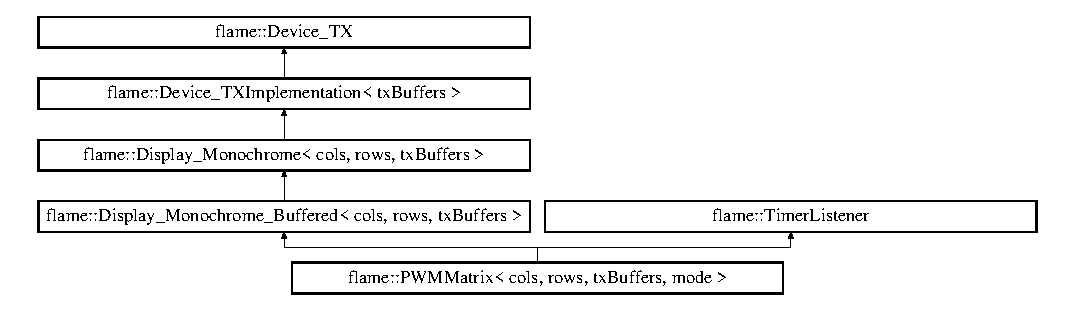
\includegraphics[height=3.713528cm]{classflame_1_1_p_w_m_matrix}
\end{center}
\end{figure}
\subsection*{Public Member Functions}
\begin{DoxyCompactItemize}
\item 
\hyperlink{classflame_1_1_p_w_m_matrix_aae241484775902899b2f27d68a4e0d92}{P\-W\-M\-Matrix} (\hyperlink{classflame_1_1_p_w_m_matrix_driver}{P\-W\-M\-Matrix\-Driver} \&driver)
\item 
void \hyperlink{classflame_1_1_p_w_m_matrix_a06ecc9848dee321f8b51994639f9fb56}{alarm} (\hyperlink{io_8h_addf5ec070e9499d36b7f2009ce736076}{U\-N\-U\-S\-E\-D} \hyperlink{namespaceflame_a6d176ba245556716fd3e32006bb7cfe5}{Alarm\-Source} source)
\end{DoxyCompactItemize}
\subsection*{Additional Inherited Members}


\subsection{Detailed Description}
\subsubsection*{template$<$uint16\-\_\-t cols, uint16\-\_\-t rows, uint8\-\_\-t tx\-Buffers, P\-W\-M\-Matrix\-Mode mode$>$class flame\-::\-P\-W\-M\-Matrix$<$ cols, rows, tx\-Buffers, mode $>$}

A driver for bitbashed L\-E\-D matrices 
\begin{DoxyTemplParams}{Template Parameters}
{\em cols} & the number of columns \\
\hline
{\em rows} & the number of rows \\
\hline
{\em tx\-Buffers} & the number of output buffers \\
\hline
{\em mode} & whether to scan rows, cols, individual pixels or auto \\
\hline
\end{DoxyTemplParams}


Definition at line 66 of file P\-W\-M\-Matrix.\-h.



\subsection{Constructor \& Destructor Documentation}
\hypertarget{classflame_1_1_p_w_m_matrix_aae241484775902899b2f27d68a4e0d92}{\index{flame\-::\-P\-W\-M\-Matrix@{flame\-::\-P\-W\-M\-Matrix}!P\-W\-M\-Matrix@{P\-W\-M\-Matrix}}
\index{P\-W\-M\-Matrix@{P\-W\-M\-Matrix}!flame::PWMMatrix@{flame\-::\-P\-W\-M\-Matrix}}
\subsubsection[{P\-W\-M\-Matrix}]{\setlength{\rightskip}{0pt plus 5cm}template$<$uint16\-\_\-t cols, uint16\-\_\-t rows, uint8\-\_\-t tx\-Buffers, P\-W\-M\-Matrix\-Mode mode$>$ {\bf flame\-::\-P\-W\-M\-Matrix}$<$ cols, rows, tx\-Buffers, mode $>$\-::{\bf P\-W\-M\-Matrix} (
\begin{DoxyParamCaption}
\item[{{\bf P\-W\-M\-Matrix\-Driver} \&}]{driver}
\end{DoxyParamCaption}
)\hspace{0.3cm}{\ttfamily [inline]}}}\label{classflame_1_1_p_w_m_matrix_aae241484775902899b2f27d68a4e0d92}
Establish a new matrix 
\begin{DoxyParams}{Parameters}
{\em driver} & the driver to turn on/off rows and columns \\
\hline
\end{DoxyParams}


Definition at line 174 of file P\-W\-M\-Matrix.\-h.



\subsection{Member Function Documentation}
\hypertarget{classflame_1_1_p_w_m_matrix_a06ecc9848dee321f8b51994639f9fb56}{\index{flame\-::\-P\-W\-M\-Matrix@{flame\-::\-P\-W\-M\-Matrix}!alarm@{alarm}}
\index{alarm@{alarm}!flame::PWMMatrix@{flame\-::\-P\-W\-M\-Matrix}}
\subsubsection[{alarm}]{\setlength{\rightskip}{0pt plus 5cm}template$<$uint16\-\_\-t cols, uint16\-\_\-t rows, uint8\-\_\-t tx\-Buffers, P\-W\-M\-Matrix\-Mode mode$>$ void {\bf flame\-::\-P\-W\-M\-Matrix}$<$ cols, rows, tx\-Buffers, mode $>$\-::{\bf alarm} (
\begin{DoxyParamCaption}
\item[{{\bf U\-N\-U\-S\-E\-D} {\bf Alarm\-Source}}]{source}
\end{DoxyParamCaption}
)\hspace{0.3cm}{\ttfamily [inline]}}}\label{classflame_1_1_p_w_m_matrix_a06ecc9848dee321f8b51994639f9fb56}


Definition at line 191 of file P\-W\-M\-Matrix.\-h.



The documentation for this class was generated from the following file\-:\begin{DoxyCompactItemize}
\item 
flame/\hyperlink{_p_w_m_matrix_8h}{P\-W\-M\-Matrix.\-h}\end{DoxyCompactItemize}

\hypertarget{classflame_1_1_p_w_m_matrix_driver}{\section{flame\-:\-:P\-W\-M\-Matrix\-Driver Class Reference}
\label{classflame_1_1_p_w_m_matrix_driver}\index{flame\-::\-P\-W\-M\-Matrix\-Driver@{flame\-::\-P\-W\-M\-Matrix\-Driver}}
}


{\ttfamily \#include $<$P\-W\-M\-Matrix.\-h$>$}

\subsection*{Public Member Functions}
\begin{DoxyCompactItemize}
\item 
virtual void \hyperlink{classflame_1_1_p_w_m_matrix_driver_af1980c3709f6298a4907f24e1bf1c1a2}{row\-On} (uint16\-\_\-t row)=0
\item 
virtual void \hyperlink{classflame_1_1_p_w_m_matrix_driver_a5d8e0f3af8288cfbc744c625273c4a3b}{row\-Off} (uint16\-\_\-t row)=0
\item 
virtual void \hyperlink{classflame_1_1_p_w_m_matrix_driver_a8abc10703f2e22be9c8a68f80f99f4fc}{col\-On} (uint16\-\_\-t col)=0
\item 
virtual void \hyperlink{classflame_1_1_p_w_m_matrix_driver_ab22d1d01a34416f934157607dd09bea8}{col\-Off} (uint16\-\_\-t col)=0
\end{DoxyCompactItemize}


\subsection{Detailed Description}


Definition at line 45 of file P\-W\-M\-Matrix.\-h.



\subsection{Member Function Documentation}
\hypertarget{classflame_1_1_p_w_m_matrix_driver_ab22d1d01a34416f934157607dd09bea8}{\index{flame\-::\-P\-W\-M\-Matrix\-Driver@{flame\-::\-P\-W\-M\-Matrix\-Driver}!col\-Off@{col\-Off}}
\index{col\-Off@{col\-Off}!flame::PWMMatrixDriver@{flame\-::\-P\-W\-M\-Matrix\-Driver}}
\subsubsection[{col\-Off}]{\setlength{\rightskip}{0pt plus 5cm}virtual void flame\-::\-P\-W\-M\-Matrix\-Driver\-::col\-Off (
\begin{DoxyParamCaption}
\item[{uint16\-\_\-t}]{col}
\end{DoxyParamCaption}
)\hspace{0.3cm}{\ttfamily [pure virtual]}}}\label{classflame_1_1_p_w_m_matrix_driver_ab22d1d01a34416f934157607dd09bea8}
\hypertarget{classflame_1_1_p_w_m_matrix_driver_a8abc10703f2e22be9c8a68f80f99f4fc}{\index{flame\-::\-P\-W\-M\-Matrix\-Driver@{flame\-::\-P\-W\-M\-Matrix\-Driver}!col\-On@{col\-On}}
\index{col\-On@{col\-On}!flame::PWMMatrixDriver@{flame\-::\-P\-W\-M\-Matrix\-Driver}}
\subsubsection[{col\-On}]{\setlength{\rightskip}{0pt plus 5cm}virtual void flame\-::\-P\-W\-M\-Matrix\-Driver\-::col\-On (
\begin{DoxyParamCaption}
\item[{uint16\-\_\-t}]{col}
\end{DoxyParamCaption}
)\hspace{0.3cm}{\ttfamily [pure virtual]}}}\label{classflame_1_1_p_w_m_matrix_driver_a8abc10703f2e22be9c8a68f80f99f4fc}
\hypertarget{classflame_1_1_p_w_m_matrix_driver_a5d8e0f3af8288cfbc744c625273c4a3b}{\index{flame\-::\-P\-W\-M\-Matrix\-Driver@{flame\-::\-P\-W\-M\-Matrix\-Driver}!row\-Off@{row\-Off}}
\index{row\-Off@{row\-Off}!flame::PWMMatrixDriver@{flame\-::\-P\-W\-M\-Matrix\-Driver}}
\subsubsection[{row\-Off}]{\setlength{\rightskip}{0pt plus 5cm}virtual void flame\-::\-P\-W\-M\-Matrix\-Driver\-::row\-Off (
\begin{DoxyParamCaption}
\item[{uint16\-\_\-t}]{row}
\end{DoxyParamCaption}
)\hspace{0.3cm}{\ttfamily [pure virtual]}}}\label{classflame_1_1_p_w_m_matrix_driver_a5d8e0f3af8288cfbc744c625273c4a3b}
\hypertarget{classflame_1_1_p_w_m_matrix_driver_af1980c3709f6298a4907f24e1bf1c1a2}{\index{flame\-::\-P\-W\-M\-Matrix\-Driver@{flame\-::\-P\-W\-M\-Matrix\-Driver}!row\-On@{row\-On}}
\index{row\-On@{row\-On}!flame::PWMMatrixDriver@{flame\-::\-P\-W\-M\-Matrix\-Driver}}
\subsubsection[{row\-On}]{\setlength{\rightskip}{0pt plus 5cm}virtual void flame\-::\-P\-W\-M\-Matrix\-Driver\-::row\-On (
\begin{DoxyParamCaption}
\item[{uint16\-\_\-t}]{row}
\end{DoxyParamCaption}
)\hspace{0.3cm}{\ttfamily [pure virtual]}}}\label{classflame_1_1_p_w_m_matrix_driver_af1980c3709f6298a4907f24e1bf1c1a2}


The documentation for this class was generated from the following file\-:\begin{DoxyCompactItemize}
\item 
flame/\hyperlink{_p_w_m_matrix_8h}{P\-W\-M\-Matrix.\-h}\end{DoxyCompactItemize}

\hypertarget{unionflame_1_1rgb}{\section{flame\-:\-:rgb Union Reference}
\label{unionflame_1_1rgb}\index{flame\-::rgb@{flame\-::rgb}}
}


{\ttfamily \#include $<$R\-G\-B.\-h$>$}

\subsection*{Public Attributes}
\begin{DoxyCompactItemize}
\item 
uint8\-\_\-t \hyperlink{unionflame_1_1rgb_a0a54852e8a0ef4113a1bdbc19c558008}{value} \mbox{[}3\mbox{]}
\item 
\begin{tabbing}
xx\=xx\=xx\=xx\=xx\=xx\=xx\=xx\=xx\=\kill
struct \{\\
\>uint8\_t \hyperlink{unionflame_1_1rgb_aff02b9e474353728fa5d75ebe72a3054}{red}\\
\>uint8\_t \hyperlink{unionflame_1_1rgb_ac6314c6f3c99686284bfa185573b3e61}{green}\\
\>uint8\_t \hyperlink{unionflame_1_1rgb_a71222b578c6f9b2609a41756eff39ba2}{blue}\\
\} \hyperlink{unionflame_1_1rgb_a796ab03a8c63b315b7d60d3f87196370}{channel}\\

\end{tabbing}\end{DoxyCompactItemize}


\subsection{Detailed Description}


Definition at line 57 of file R\-G\-B.\-h.



\subsection{Member Data Documentation}
\hypertarget{unionflame_1_1rgb_a71222b578c6f9b2609a41756eff39ba2}{\index{flame\-::rgb@{flame\-::rgb}!blue@{blue}}
\index{blue@{blue}!flame::rgb@{flame\-::rgb}}
\subsubsection[{blue}]{\setlength{\rightskip}{0pt plus 5cm}uint8\-\_\-t flame\-::rgb\-::blue}}\label{unionflame_1_1rgb_a71222b578c6f9b2609a41756eff39ba2}


Definition at line 63 of file R\-G\-B.\-h.

\hypertarget{unionflame_1_1rgb_a796ab03a8c63b315b7d60d3f87196370}{\index{flame\-::rgb@{flame\-::rgb}!channel@{channel}}
\index{channel@{channel}!flame::rgb@{flame\-::rgb}}
\subsubsection[{channel}]{\setlength{\rightskip}{0pt plus 5cm}struct \{ ... \}   flame\-::rgb\-::channel}}\label{unionflame_1_1rgb_a796ab03a8c63b315b7d60d3f87196370}
\hypertarget{unionflame_1_1rgb_ac6314c6f3c99686284bfa185573b3e61}{\index{flame\-::rgb@{flame\-::rgb}!green@{green}}
\index{green@{green}!flame::rgb@{flame\-::rgb}}
\subsubsection[{green}]{\setlength{\rightskip}{0pt plus 5cm}uint8\-\_\-t flame\-::rgb\-::green}}\label{unionflame_1_1rgb_ac6314c6f3c99686284bfa185573b3e61}


Definition at line 62 of file R\-G\-B.\-h.

\hypertarget{unionflame_1_1rgb_aff02b9e474353728fa5d75ebe72a3054}{\index{flame\-::rgb@{flame\-::rgb}!red@{red}}
\index{red@{red}!flame::rgb@{flame\-::rgb}}
\subsubsection[{red}]{\setlength{\rightskip}{0pt plus 5cm}uint8\-\_\-t flame\-::rgb\-::red}}\label{unionflame_1_1rgb_aff02b9e474353728fa5d75ebe72a3054}


Definition at line 61 of file R\-G\-B.\-h.

\hypertarget{unionflame_1_1rgb_a0a54852e8a0ef4113a1bdbc19c558008}{\index{flame\-::rgb@{flame\-::rgb}!value@{value}}
\index{value@{value}!flame::rgb@{flame\-::rgb}}
\subsubsection[{value}]{\setlength{\rightskip}{0pt plus 5cm}uint8\-\_\-t flame\-::rgb\-::value\mbox{[}3\mbox{]}}}\label{unionflame_1_1rgb_a0a54852e8a0ef4113a1bdbc19c558008}


Definition at line 58 of file R\-G\-B.\-h.



The documentation for this union was generated from the following file\-:\begin{DoxyCompactItemize}
\item 
flame/\hyperlink{_r_g_b_8h}{R\-G\-B.\-h}\end{DoxyCompactItemize}

\hypertarget{classflame_1_1_r_g_b}{\section{flame\-:\-:R\-G\-B Class Reference}
\label{classflame_1_1_r_g_b}\index{flame\-::\-R\-G\-B@{flame\-::\-R\-G\-B}}
}


{\ttfamily \#include $<$R\-G\-B.\-h$>$}

\subsection*{Public Member Functions}
\begin{DoxyCompactItemize}
\item 
\hyperlink{classflame_1_1_r_g_b_a31a76381cdc18f4652de93d25b209d3e}{R\-G\-B} (uint8\-\_\-t red, uint8\-\_\-t green, uint8\-\_\-t blue)
\item 
\hyperlink{classflame_1_1_r_g_b_a78352769285295d0ec68279fbaf1f0ba}{R\-G\-B} (const \hyperlink{classflame_1_1_r_g_b}{R\-G\-B} \&value)
\item 
\hyperlink{classflame_1_1_r_g_b_ad0fd397169a383bc643418612ddf64dd}{R\-G\-B} (const \hyperlink{classflame_1_1_r_g_b}{R\-G\-B} $\ast$value)
\item 
\hyperlink{classflame_1_1_r_g_b_a8d41ef1df927aabd3477024387aa3a41}{R\-G\-B} ()
\item 
void \hyperlink{classflame_1_1_r_g_b_a7be20787cdb4933a3a44dbe8236693dc}{fade\-To} (const \hyperlink{classflame_1_1_r_g_b}{R\-G\-B} \&final, uint16\-\_\-t current\-Iteration, uint16\-\_\-t iterations)
\item 
void \hyperlink{classflame_1_1_r_g_b_a0848bc3467a0545191bb5e3ad6bc004c}{set} (uint8\-\_\-t red, uint8\-\_\-t green, uint8\-\_\-t blue)
\item 
\hyperlink{classflame_1_1_r_g_b}{R\-G\-B} \& \hyperlink{classflame_1_1_r_g_b_abc571808888b8fd2715f7ff1f5ee8c1d}{operator=} (const \hyperlink{classflame_1_1_r_g_b}{R\-G\-B} \&rhs)
\item 
void \hyperlink{classflame_1_1_r_g_b_a1dedc5574dceb31c1fc71212ba0bdf1f}{set\-Gamma} (uint8\-\_\-t red, uint8\-\_\-t green, uint8\-\_\-t blue)
\item 
void \hyperlink{classflame_1_1_r_g_b_aebfd60e533ed78c38f6932ac33d0773b}{set} (const \hyperlink{classflame_1_1_r_g_b}{R\-G\-B} \&value)
\item 
uint8\-\_\-t \hyperlink{classflame_1_1_r_g_b_a1c7cfd27fd68436e8ec878b50c755559}{get} (\hyperlink{namespaceflame_a47f12f0248f648dbdbfa6fe26d79028d}{R\-G\-B\-Channel} channel)
\item 
void \hyperlink{classflame_1_1_r_g_b_ae58cbda8540d05b70e066d7715766c8b}{set\-Gamma} (const \hyperlink{classflame_1_1_r_g_b}{R\-G\-B} \&value)
\item 
void \hyperlink{classflame_1_1_r_g_b_a16e70fb1f45ce79e38b8c7f647cd1cc2}{set} (const \hyperlink{classflame_1_1_r_g_b}{R\-G\-B} $\ast$value)
\item 
void \hyperlink{classflame_1_1_r_g_b_a69e0c19e3f5d6742e17fffe66a866927}{set} (\hyperlink{namespaceflame_a47f12f0248f648dbdbfa6fe26d79028d}{R\-G\-B\-Channel} channel, uint8\-\_\-t value)
\item 
void \hyperlink{classflame_1_1_r_g_b_a35a19e8cc502583aa688a9e1236bd409}{set\-Gamma} (const \hyperlink{classflame_1_1_r_g_b}{R\-G\-B} $\ast$value)
\item 
void \hyperlink{classflame_1_1_r_g_b_a66216f39d01050fdc14314790a51108d}{gamma\-Correct} ()
\item 
void \hyperlink{classflame_1_1_r_g_b_a302e896be5c8bfed3e8cca54682280aa}{inverse\-Gamma\-Correct} ()
\end{DoxyCompactItemize}
\subsection*{Protected Member Functions}
\begin{DoxyCompactItemize}
\item 
uint8\-\_\-t \hyperlink{classflame_1_1_r_g_b_a5fc1c274cbfef087d866d6ffb037defb}{fade} (uint8\-\_\-t initial, uint8\-\_\-t final, int16\-\_\-t iteration, int16\-\_\-t total)
\end{DoxyCompactItemize}
\subsection*{Protected Attributes}
\begin{DoxyCompactItemize}
\item 
union \hyperlink{unionflame_1_1rgb}{rgb} \hyperlink{classflame_1_1_r_g_b_a154fae5c9f509c283d2df1a3cff37d55}{\-\_\-data}
\end{DoxyCompactItemize}


\subsection{Detailed Description}


Definition at line 139 of file R\-G\-B.\-h.



\subsection{Constructor \& Destructor Documentation}
\hypertarget{classflame_1_1_r_g_b_a31a76381cdc18f4652de93d25b209d3e}{\index{flame\-::\-R\-G\-B@{flame\-::\-R\-G\-B}!R\-G\-B@{R\-G\-B}}
\index{R\-G\-B@{R\-G\-B}!flame::RGB@{flame\-::\-R\-G\-B}}
\subsubsection[{R\-G\-B}]{\setlength{\rightskip}{0pt plus 5cm}flame\-::\-R\-G\-B\-::\-R\-G\-B (
\begin{DoxyParamCaption}
\item[{uint8\-\_\-t}]{red, }
\item[{uint8\-\_\-t}]{green, }
\item[{uint8\-\_\-t}]{blue}
\end{DoxyParamCaption}
)\hspace{0.3cm}{\ttfamily [inline]}}}\label{classflame_1_1_r_g_b_a31a76381cdc18f4652de93d25b209d3e}
Constructor 
\begin{DoxyParams}{Parameters}
{\em red} & the red value \\
\hline
{\em green} & the green value \\
\hline
{\em blue} & the blue value \\
\hline
\end{DoxyParams}


Definition at line 174 of file R\-G\-B.\-h.

\hypertarget{classflame_1_1_r_g_b_a78352769285295d0ec68279fbaf1f0ba}{\index{flame\-::\-R\-G\-B@{flame\-::\-R\-G\-B}!R\-G\-B@{R\-G\-B}}
\index{R\-G\-B@{R\-G\-B}!flame::RGB@{flame\-::\-R\-G\-B}}
\subsubsection[{R\-G\-B}]{\setlength{\rightskip}{0pt plus 5cm}flame\-::\-R\-G\-B\-::\-R\-G\-B (
\begin{DoxyParamCaption}
\item[{const {\bf R\-G\-B} \&}]{value}
\end{DoxyParamCaption}
)\hspace{0.3cm}{\ttfamily [inline]}}}\label{classflame_1_1_r_g_b_a78352769285295d0ec68279fbaf1f0ba}
Constructor 
\begin{DoxyParams}{Parameters}
{\em value} & an \hyperlink{classflame_1_1_r_g_b}{R\-G\-B} to take the value of \\
\hline
\end{DoxyParams}


Definition at line 184 of file R\-G\-B.\-h.

\hypertarget{classflame_1_1_r_g_b_ad0fd397169a383bc643418612ddf64dd}{\index{flame\-::\-R\-G\-B@{flame\-::\-R\-G\-B}!R\-G\-B@{R\-G\-B}}
\index{R\-G\-B@{R\-G\-B}!flame::RGB@{flame\-::\-R\-G\-B}}
\subsubsection[{R\-G\-B}]{\setlength{\rightskip}{0pt plus 5cm}flame\-::\-R\-G\-B\-::\-R\-G\-B (
\begin{DoxyParamCaption}
\item[{const {\bf R\-G\-B} $\ast$}]{value}
\end{DoxyParamCaption}
)\hspace{0.3cm}{\ttfamily [inline]}}}\label{classflame_1_1_r_g_b_ad0fd397169a383bc643418612ddf64dd}
Constructor 
\begin{DoxyParams}{Parameters}
{\em value} & an \hyperlink{classflame_1_1_r_g_b}{R\-G\-B} to take the value of \\
\hline
\end{DoxyParams}


Definition at line 194 of file R\-G\-B.\-h.

\hypertarget{classflame_1_1_r_g_b_a8d41ef1df927aabd3477024387aa3a41}{\index{flame\-::\-R\-G\-B@{flame\-::\-R\-G\-B}!R\-G\-B@{R\-G\-B}}
\index{R\-G\-B@{R\-G\-B}!flame::RGB@{flame\-::\-R\-G\-B}}
\subsubsection[{R\-G\-B}]{\setlength{\rightskip}{0pt plus 5cm}flame\-::\-R\-G\-B\-::\-R\-G\-B (
\begin{DoxyParamCaption}
{}
\end{DoxyParamCaption}
)\hspace{0.3cm}{\ttfamily [inline]}}}\label{classflame_1_1_r_g_b_a8d41ef1df927aabd3477024387aa3a41}
Constructor 

Definition at line 203 of file R\-G\-B.\-h.



\subsection{Member Function Documentation}
\hypertarget{classflame_1_1_r_g_b_a5fc1c274cbfef087d866d6ffb037defb}{\index{flame\-::\-R\-G\-B@{flame\-::\-R\-G\-B}!fade@{fade}}
\index{fade@{fade}!flame::RGB@{flame\-::\-R\-G\-B}}
\subsubsection[{fade}]{\setlength{\rightskip}{0pt plus 5cm}uint8\-\_\-t flame\-::\-R\-G\-B\-::fade (
\begin{DoxyParamCaption}
\item[{uint8\-\_\-t}]{initial, }
\item[{uint8\-\_\-t}]{final, }
\item[{int16\-\_\-t}]{iteration, }
\item[{int16\-\_\-t}]{total}
\end{DoxyParamCaption}
)\hspace{0.3cm}{\ttfamily [inline]}, {\ttfamily [protected]}}}\label{classflame_1_1_r_g_b_a5fc1c274cbfef087d866d6ffb037defb}
Fade from an initial value to a final value 
\begin{DoxyParams}{Parameters}
{\em initial} & value to fade from \\
\hline
{\em final} & value to fade to \\
\hline
{\em iteration} & The current iteration \\
\hline
{\em total} & total number of iterations to fade across \\
\hline
\end{DoxyParams}
\begin{DoxyReturn}{Returns}
the faded value 
\end{DoxyReturn}


Definition at line 151 of file R\-G\-B.\-h.

\hypertarget{classflame_1_1_r_g_b_a7be20787cdb4933a3a44dbe8236693dc}{\index{flame\-::\-R\-G\-B@{flame\-::\-R\-G\-B}!fade\-To@{fade\-To}}
\index{fade\-To@{fade\-To}!flame::RGB@{flame\-::\-R\-G\-B}}
\subsubsection[{fade\-To}]{\setlength{\rightskip}{0pt plus 5cm}void flame\-::\-R\-G\-B\-::fade\-To (
\begin{DoxyParamCaption}
\item[{const {\bf R\-G\-B} \&}]{final, }
\item[{uint16\-\_\-t}]{current\-Iteration, }
\item[{uint16\-\_\-t}]{iterations}
\end{DoxyParamCaption}
)\hspace{0.3cm}{\ttfamily [inline]}}}\label{classflame_1_1_r_g_b_a7be20787cdb4933a3a44dbe8236693dc}
Fade from an initial value to a final value (should be called repeatedly with decreasing iterations) 
\begin{DoxyParams}{Parameters}
{\em final} & value to fade to \\
\hline
{\em out} & the output value \\
\hline
{\em current\-Iteration} & current iteration \\
\hline
{\em iterations\-Left} & total number of iterations remaining to fade across \\
\hline
\end{DoxyParams}


Definition at line 216 of file R\-G\-B.\-h.

\hypertarget{classflame_1_1_r_g_b_a66216f39d01050fdc14314790a51108d}{\index{flame\-::\-R\-G\-B@{flame\-::\-R\-G\-B}!gamma\-Correct@{gamma\-Correct}}
\index{gamma\-Correct@{gamma\-Correct}!flame::RGB@{flame\-::\-R\-G\-B}}
\subsubsection[{gamma\-Correct}]{\setlength{\rightskip}{0pt plus 5cm}void flame\-::\-R\-G\-B\-::gamma\-Correct (
\begin{DoxyParamCaption}
{}
\end{DoxyParamCaption}
)\hspace{0.3cm}{\ttfamily [inline]}}}\label{classflame_1_1_r_g_b_a66216f39d01050fdc14314790a51108d}
Gamma correct the current value 

Definition at line 319 of file R\-G\-B.\-h.

\hypertarget{classflame_1_1_r_g_b_a1c7cfd27fd68436e8ec878b50c755559}{\index{flame\-::\-R\-G\-B@{flame\-::\-R\-G\-B}!get@{get}}
\index{get@{get}!flame::RGB@{flame\-::\-R\-G\-B}}
\subsubsection[{get}]{\setlength{\rightskip}{0pt plus 5cm}uint8\-\_\-t flame\-::\-R\-G\-B\-::get (
\begin{DoxyParamCaption}
\item[{{\bf R\-G\-B\-Channel}}]{channel}
\end{DoxyParamCaption}
)\hspace{0.3cm}{\ttfamily [inline]}}}\label{classflame_1_1_r_g_b_a1c7cfd27fd68436e8ec878b50c755559}
Get the value for a channel 
\begin{DoxyParams}{Parameters}
{\em channel} & the channel to get \\
\hline
\end{DoxyParams}


Definition at line 272 of file R\-G\-B.\-h.

\hypertarget{classflame_1_1_r_g_b_a302e896be5c8bfed3e8cca54682280aa}{\index{flame\-::\-R\-G\-B@{flame\-::\-R\-G\-B}!inverse\-Gamma\-Correct@{inverse\-Gamma\-Correct}}
\index{inverse\-Gamma\-Correct@{inverse\-Gamma\-Correct}!flame::RGB@{flame\-::\-R\-G\-B}}
\subsubsection[{inverse\-Gamma\-Correct}]{\setlength{\rightskip}{0pt plus 5cm}void flame\-::\-R\-G\-B\-::inverse\-Gamma\-Correct (
\begin{DoxyParamCaption}
{}
\end{DoxyParamCaption}
)\hspace{0.3cm}{\ttfamily [inline]}}}\label{classflame_1_1_r_g_b_a302e896be5c8bfed3e8cca54682280aa}
Inverse gamma correct the current value 

Definition at line 329 of file R\-G\-B.\-h.

\hypertarget{classflame_1_1_r_g_b_abc571808888b8fd2715f7ff1f5ee8c1d}{\index{flame\-::\-R\-G\-B@{flame\-::\-R\-G\-B}!operator=@{operator=}}
\index{operator=@{operator=}!flame::RGB@{flame\-::\-R\-G\-B}}
\subsubsection[{operator=}]{\setlength{\rightskip}{0pt plus 5cm}{\bf R\-G\-B}\& flame\-::\-R\-G\-B\-::operator= (
\begin{DoxyParamCaption}
\item[{const {\bf R\-G\-B} \&}]{rhs}
\end{DoxyParamCaption}
)\hspace{0.3cm}{\ttfamily [inline]}}}\label{classflame_1_1_r_g_b_abc571808888b8fd2715f7ff1f5ee8c1d}
Override the = operator 
\begin{DoxyParams}{Parameters}
{\em rhs} & the value to assign to the left hand side \\
\hline
\end{DoxyParams}


Definition at line 241 of file R\-G\-B.\-h.

\hypertarget{classflame_1_1_r_g_b_a0848bc3467a0545191bb5e3ad6bc004c}{\index{flame\-::\-R\-G\-B@{flame\-::\-R\-G\-B}!set@{set}}
\index{set@{set}!flame::RGB@{flame\-::\-R\-G\-B}}
\subsubsection[{set}]{\setlength{\rightskip}{0pt plus 5cm}void flame\-::\-R\-G\-B\-::set (
\begin{DoxyParamCaption}
\item[{uint8\-\_\-t}]{red, }
\item[{uint8\-\_\-t}]{green, }
\item[{uint8\-\_\-t}]{blue}
\end{DoxyParamCaption}
)\hspace{0.3cm}{\ttfamily [inline]}}}\label{classflame_1_1_r_g_b_a0848bc3467a0545191bb5e3ad6bc004c}
Set a value 
\begin{DoxyParams}{Parameters}
{\em red} & the red value \\
\hline
{\em green} & the green value \\
\hline
{\em blue} & the blue value \\
\hline
\end{DoxyParams}


Definition at line 231 of file R\-G\-B.\-h.

\hypertarget{classflame_1_1_r_g_b_aebfd60e533ed78c38f6932ac33d0773b}{\index{flame\-::\-R\-G\-B@{flame\-::\-R\-G\-B}!set@{set}}
\index{set@{set}!flame::RGB@{flame\-::\-R\-G\-B}}
\subsubsection[{set}]{\setlength{\rightskip}{0pt plus 5cm}void flame\-::\-R\-G\-B\-::set (
\begin{DoxyParamCaption}
\item[{const {\bf R\-G\-B} \&}]{value}
\end{DoxyParamCaption}
)\hspace{0.3cm}{\ttfamily [inline]}}}\label{classflame_1_1_r_g_b_aebfd60e533ed78c38f6932ac33d0773b}
Set a value 
\begin{DoxyParams}{Parameters}
{\em value} & the new value \\
\hline
\end{DoxyParams}


Definition at line 262 of file R\-G\-B.\-h.

\hypertarget{classflame_1_1_r_g_b_a16e70fb1f45ce79e38b8c7f647cd1cc2}{\index{flame\-::\-R\-G\-B@{flame\-::\-R\-G\-B}!set@{set}}
\index{set@{set}!flame::RGB@{flame\-::\-R\-G\-B}}
\subsubsection[{set}]{\setlength{\rightskip}{0pt plus 5cm}void flame\-::\-R\-G\-B\-::set (
\begin{DoxyParamCaption}
\item[{const {\bf R\-G\-B} $\ast$}]{value}
\end{DoxyParamCaption}
)\hspace{0.3cm}{\ttfamily [inline]}}}\label{classflame_1_1_r_g_b_a16e70fb1f45ce79e38b8c7f647cd1cc2}
Set a value 
\begin{DoxyParams}{Parameters}
{\em value} & the new value \\
\hline
\end{DoxyParams}


Definition at line 291 of file R\-G\-B.\-h.

\hypertarget{classflame_1_1_r_g_b_a69e0c19e3f5d6742e17fffe66a866927}{\index{flame\-::\-R\-G\-B@{flame\-::\-R\-G\-B}!set@{set}}
\index{set@{set}!flame::RGB@{flame\-::\-R\-G\-B}}
\subsubsection[{set}]{\setlength{\rightskip}{0pt plus 5cm}void flame\-::\-R\-G\-B\-::set (
\begin{DoxyParamCaption}
\item[{{\bf R\-G\-B\-Channel}}]{channel, }
\item[{uint8\-\_\-t}]{value}
\end{DoxyParamCaption}
)\hspace{0.3cm}{\ttfamily [inline]}}}\label{classflame_1_1_r_g_b_a69e0c19e3f5d6742e17fffe66a866927}
Set a value for a channel 
\begin{DoxyParams}{Parameters}
{\em channel} & the channel \\
\hline
{\em value} & the new value \\
\hline
\end{DoxyParams}


Definition at line 302 of file R\-G\-B.\-h.

\hypertarget{classflame_1_1_r_g_b_a1dedc5574dceb31c1fc71212ba0bdf1f}{\index{flame\-::\-R\-G\-B@{flame\-::\-R\-G\-B}!set\-Gamma@{set\-Gamma}}
\index{set\-Gamma@{set\-Gamma}!flame::RGB@{flame\-::\-R\-G\-B}}
\subsubsection[{set\-Gamma}]{\setlength{\rightskip}{0pt plus 5cm}void flame\-::\-R\-G\-B\-::set\-Gamma (
\begin{DoxyParamCaption}
\item[{uint8\-\_\-t}]{red, }
\item[{uint8\-\_\-t}]{green, }
\item[{uint8\-\_\-t}]{blue}
\end{DoxyParamCaption}
)\hspace{0.3cm}{\ttfamily [inline]}}}\label{classflame_1_1_r_g_b_a1dedc5574dceb31c1fc71212ba0bdf1f}
Set a value and gamma correct 
\begin{DoxyParams}{Parameters}
{\em red} & the red value \\
\hline
{\em green} & the green value \\
\hline
{\em blue} & the blue value \\
\hline
\end{DoxyParams}


Definition at line 252 of file R\-G\-B.\-h.

\hypertarget{classflame_1_1_r_g_b_ae58cbda8540d05b70e066d7715766c8b}{\index{flame\-::\-R\-G\-B@{flame\-::\-R\-G\-B}!set\-Gamma@{set\-Gamma}}
\index{set\-Gamma@{set\-Gamma}!flame::RGB@{flame\-::\-R\-G\-B}}
\subsubsection[{set\-Gamma}]{\setlength{\rightskip}{0pt plus 5cm}void flame\-::\-R\-G\-B\-::set\-Gamma (
\begin{DoxyParamCaption}
\item[{const {\bf R\-G\-B} \&}]{value}
\end{DoxyParamCaption}
)\hspace{0.3cm}{\ttfamily [inline]}}}\label{classflame_1_1_r_g_b_ae58cbda8540d05b70e066d7715766c8b}
Set a value and gamma correct 
\begin{DoxyParams}{Parameters}
{\em value} & the new value \\
\hline
\end{DoxyParams}


Definition at line 281 of file R\-G\-B.\-h.

\hypertarget{classflame_1_1_r_g_b_a35a19e8cc502583aa688a9e1236bd409}{\index{flame\-::\-R\-G\-B@{flame\-::\-R\-G\-B}!set\-Gamma@{set\-Gamma}}
\index{set\-Gamma@{set\-Gamma}!flame::RGB@{flame\-::\-R\-G\-B}}
\subsubsection[{set\-Gamma}]{\setlength{\rightskip}{0pt plus 5cm}void flame\-::\-R\-G\-B\-::set\-Gamma (
\begin{DoxyParamCaption}
\item[{const {\bf R\-G\-B} $\ast$}]{value}
\end{DoxyParamCaption}
)\hspace{0.3cm}{\ttfamily [inline]}}}\label{classflame_1_1_r_g_b_a35a19e8cc502583aa688a9e1236bd409}
Set a value and gamma correct 
\begin{DoxyParams}{Parameters}
{\em value} & the new value \\
\hline
\end{DoxyParams}


Definition at line 310 of file R\-G\-B.\-h.



\subsection{Member Data Documentation}
\hypertarget{classflame_1_1_r_g_b_a154fae5c9f509c283d2df1a3cff37d55}{\index{flame\-::\-R\-G\-B@{flame\-::\-R\-G\-B}!\-\_\-data@{\-\_\-data}}
\index{\-\_\-data@{\-\_\-data}!flame::RGB@{flame\-::\-R\-G\-B}}
\subsubsection[{\-\_\-data}]{\setlength{\rightskip}{0pt plus 5cm}union {\bf rgb} flame\-::\-R\-G\-B\-::\-\_\-data\hspace{0.3cm}{\ttfamily [protected]}}}\label{classflame_1_1_r_g_b_a154fae5c9f509c283d2df1a3cff37d55}


Definition at line 141 of file R\-G\-B.\-h.



The documentation for this class was generated from the following file\-:\begin{DoxyCompactItemize}
\item 
flame/\hyperlink{_r_g_b_8h}{R\-G\-B.\-h}\end{DoxyCompactItemize}

\hypertarget{classflame_1_1_r_g_b_l_e_d_strip}{\section{flame\-:\-:R\-G\-B\-L\-E\-D\-Strip$<$ length $>$ Class Template Reference}
\label{classflame_1_1_r_g_b_l_e_d_strip}\index{flame\-::\-R\-G\-B\-L\-E\-D\-Strip$<$ length $>$@{flame\-::\-R\-G\-B\-L\-E\-D\-Strip$<$ length $>$}}
}


{\ttfamily \#include $<$R\-G\-B\-L\-E\-D\-Strip.\-h$>$}

Inheritance diagram for flame\-:\-:R\-G\-B\-L\-E\-D\-Strip$<$ length $>$\-:\begin{figure}[H]
\begin{center}
\leavevmode
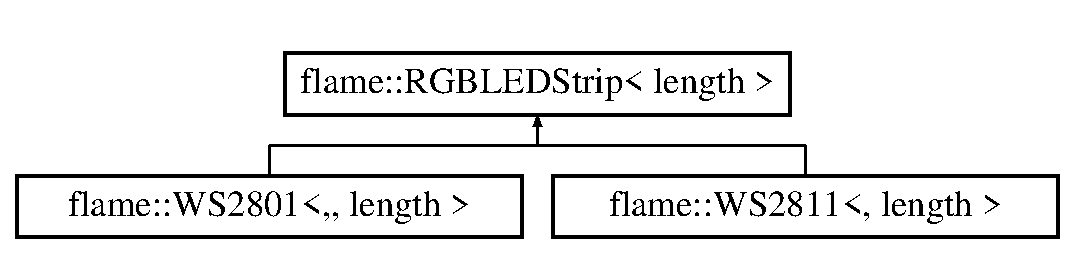
\includegraphics[height=2.000000cm]{classflame_1_1_r_g_b_l_e_d_strip}
\end{center}
\end{figure}
\subsection*{Public Member Functions}
\begin{DoxyCompactItemize}
\item 
\hyperlink{classflame_1_1_r_g_b}{R\-G\-B} \& \hyperlink{classflame_1_1_r_g_b_l_e_d_strip_a7b7987933b485e220491af1b66ab8ffd}{get\-Pixel} (uint16\-\_\-t \hyperlink{_display___monochrome___buffered_8h_a9d20fe94f93b6c220969bb9050dfe1dc}{pixel})
\item 
void \hyperlink{classflame_1_1_r_g_b_l_e_d_strip_aa53864c1db3a7c08d62d63bb195c4648}{set\-Pixel} (uint16\-\_\-t \hyperlink{_display___monochrome___buffered_8h_a9d20fe94f93b6c220969bb9050dfe1dc}{pixel}, uint8\-\_\-t red, uint8\-\_\-t green, uint8\-\_\-t blue)
\item 
void \hyperlink{classflame_1_1_r_g_b_l_e_d_strip_a722fba92d83dc1fd229d173135af7aa5}{set\-Pixel} (uint16\-\_\-t \hyperlink{_display___monochrome___buffered_8h_a9d20fe94f93b6c220969bb9050dfe1dc}{pixel}, const \hyperlink{classflame_1_1_r_g_b}{R\-G\-B} $\ast$value)
\item 
void \hyperlink{classflame_1_1_r_g_b_l_e_d_strip_a0882eeb49919e625d72679629bef259a}{set\-Pixel} (uint16\-\_\-t \hyperlink{_display___monochrome___buffered_8h_a9d20fe94f93b6c220969bb9050dfe1dc}{pixel}, const \hyperlink{classflame_1_1_r_g_b}{R\-G\-B} \&value)
\item 
void \hyperlink{classflame_1_1_r_g_b_l_e_d_strip_a4fc640b5667900a23ad401376da13e75}{set\-All} (uint8\-\_\-t red, uint8\-\_\-t green, uint8\-\_\-t blue)
\item 
void \hyperlink{classflame_1_1_r_g_b_l_e_d_strip_a0ad74b5f468d1bbaccbfda17603c647f}{set\-All} (const \hyperlink{classflame_1_1_r_g_b}{R\-G\-B} \&value)
\item 
void \hyperlink{classflame_1_1_r_g_b_l_e_d_strip_a387145e47219c89040107028d491e95f}{set\-Pixel\-Gamma} (uint16\-\_\-t \hyperlink{_display___monochrome___buffered_8h_a9d20fe94f93b6c220969bb9050dfe1dc}{pixel}, uint8\-\_\-t red, uint8\-\_\-t green, uint8\-\_\-t blue)
\item 
void \hyperlink{classflame_1_1_r_g_b_l_e_d_strip_aca3a00b9a788b568f6b6e48ae4cb5181}{set\-Pixel\-Gamma} (uint16\-\_\-t \hyperlink{_display___monochrome___buffered_8h_a9d20fe94f93b6c220969bb9050dfe1dc}{pixel}, const \hyperlink{classflame_1_1_r_g_b}{R\-G\-B} $\ast$value)
\item 
void \hyperlink{classflame_1_1_r_g_b_l_e_d_strip_a8fbe9d1fad0f90e97c866c6681c48131}{set\-Pixel\-Gamma} (uint16\-\_\-t \hyperlink{_display___monochrome___buffered_8h_a9d20fe94f93b6c220969bb9050dfe1dc}{pixel}, const \hyperlink{classflame_1_1_r_g_b}{R\-G\-B} \&value)
\item 
void \hyperlink{classflame_1_1_r_g_b_l_e_d_strip_a83de29ee761868e72cdf2801b7a4a528}{set\-All\-Gamma} (uint8\-\_\-t red, uint8\-\_\-t green, uint8\-\_\-t blue)
\item 
void \hyperlink{classflame_1_1_r_g_b_l_e_d_strip_ae8f275e46abd0e95611d2cedd4dcaf24}{set\-All\-Gamma} (const \hyperlink{classflame_1_1_r_g_b}{R\-G\-B} \&value)
\item 
virtual void \hyperlink{classflame_1_1_r_g_b_l_e_d_strip_a4b30397b84e60b9f14bd3bef3129a60b}{flush} ()
\item 
void \hyperlink{classflame_1_1_r_g_b_l_e_d_strip_a646f80351e6a34b35d05fdb8882345c2}{rotate} (bool forwards)
\end{DoxyCompactItemize}
\subsection*{Protected Attributes}
\begin{DoxyCompactItemize}
\item 
\hyperlink{classflame_1_1_r_g_b}{R\-G\-B} \hyperlink{classflame_1_1_r_g_b_l_e_d_strip_a1f62d01c2151068509acafcaf74b04be}{\-\_\-data} \mbox{[}length\mbox{]}
\end{DoxyCompactItemize}


\subsection{Detailed Description}
\subsubsection*{template$<$uint16\-\_\-t length$>$class flame\-::\-R\-G\-B\-L\-E\-D\-Strip$<$ length $>$}

Create a new R\-G\-B\-L\-E\-D\-S\-T\-R\-I\-P object to control a string of L\-E\-D drivers 
\begin{DoxyTemplParams}{Template Parameters}
{\em clock...} & the clock pin for the L\-E\-Ds \\
\hline
{\em data...} & the data pin for the L\-E\-Ds, mult be on the same port as the clock \\
\hline
{\em length} & the number of L\-E\-Ds in the string \\
\hline
\end{DoxyTemplParams}


Definition at line 43 of file R\-G\-B\-L\-E\-D\-Strip.\-h.



\subsection{Member Function Documentation}
\hypertarget{classflame_1_1_r_g_b_l_e_d_strip_a4b30397b84e60b9f14bd3bef3129a60b}{\index{flame\-::\-R\-G\-B\-L\-E\-D\-Strip@{flame\-::\-R\-G\-B\-L\-E\-D\-Strip}!flush@{flush}}
\index{flush@{flush}!flame::RGBLEDStrip@{flame\-::\-R\-G\-B\-L\-E\-D\-Strip}}
\subsubsection[{flush}]{\setlength{\rightskip}{0pt plus 5cm}template$<$uint16\-\_\-t length$>$ virtual void {\bf flame\-::\-R\-G\-B\-L\-E\-D\-Strip}$<$ length $>$\-::flush (
\begin{DoxyParamCaption}
{}
\end{DoxyParamCaption}
)\hspace{0.3cm}{\ttfamily [inline]}, {\ttfamily [virtual]}}}\label{classflame_1_1_r_g_b_l_e_d_strip_a4b30397b84e60b9f14bd3bef3129a60b}
Write the current buffer to the string of L\-E\-Ds 

Reimplemented in \hyperlink{classflame_1_1_w_s2801_af36d043e8554e1834980b485766396f6}{flame\-::\-W\-S2801$<$,, length $>$}, and \hyperlink{classflame_1_1_w_s2811_a53ce9fb8cba4af3bd34b8371a7b3851a}{flame\-::\-W\-S2811$<$, length $>$}.



Definition at line 174 of file R\-G\-B\-L\-E\-D\-Strip.\-h.

\hypertarget{classflame_1_1_r_g_b_l_e_d_strip_a7b7987933b485e220491af1b66ab8ffd}{\index{flame\-::\-R\-G\-B\-L\-E\-D\-Strip@{flame\-::\-R\-G\-B\-L\-E\-D\-Strip}!get\-Pixel@{get\-Pixel}}
\index{get\-Pixel@{get\-Pixel}!flame::RGBLEDStrip@{flame\-::\-R\-G\-B\-L\-E\-D\-Strip}}
\subsubsection[{get\-Pixel}]{\setlength{\rightskip}{0pt plus 5cm}template$<$uint16\-\_\-t length$>$ {\bf R\-G\-B}\& {\bf flame\-::\-R\-G\-B\-L\-E\-D\-Strip}$<$ length $>$\-::get\-Pixel (
\begin{DoxyParamCaption}
\item[{uint16\-\_\-t}]{pixel}
\end{DoxyParamCaption}
)\hspace{0.3cm}{\ttfamily [inline]}}}\label{classflame_1_1_r_g_b_l_e_d_strip_a7b7987933b485e220491af1b66ab8ffd}
Get a pixel 
\begin{DoxyParams}{Parameters}
{\em pixel} & the pikel to get \\
\hline
\end{DoxyParams}


Definition at line 52 of file R\-G\-B\-L\-E\-D\-Strip.\-h.

\hypertarget{classflame_1_1_r_g_b_l_e_d_strip_a646f80351e6a34b35d05fdb8882345c2}{\index{flame\-::\-R\-G\-B\-L\-E\-D\-Strip@{flame\-::\-R\-G\-B\-L\-E\-D\-Strip}!rotate@{rotate}}
\index{rotate@{rotate}!flame::RGBLEDStrip@{flame\-::\-R\-G\-B\-L\-E\-D\-Strip}}
\subsubsection[{rotate}]{\setlength{\rightskip}{0pt plus 5cm}template$<$uint16\-\_\-t length$>$ void {\bf flame\-::\-R\-G\-B\-L\-E\-D\-Strip}$<$ length $>$\-::rotate (
\begin{DoxyParamCaption}
\item[{bool}]{forwards}
\end{DoxyParamCaption}
)\hspace{0.3cm}{\ttfamily [inline]}}}\label{classflame_1_1_r_g_b_l_e_d_strip_a646f80351e6a34b35d05fdb8882345c2}
Rotate the string by 1 pixel 
\begin{DoxyParams}{Parameters}
{\em forwards} & true for forwards, false for backwards \\
\hline
\end{DoxyParams}


Definition at line 180 of file R\-G\-B\-L\-E\-D\-Strip.\-h.

\hypertarget{classflame_1_1_r_g_b_l_e_d_strip_a4fc640b5667900a23ad401376da13e75}{\index{flame\-::\-R\-G\-B\-L\-E\-D\-Strip@{flame\-::\-R\-G\-B\-L\-E\-D\-Strip}!set\-All@{set\-All}}
\index{set\-All@{set\-All}!flame::RGBLEDStrip@{flame\-::\-R\-G\-B\-L\-E\-D\-Strip}}
\subsubsection[{set\-All}]{\setlength{\rightskip}{0pt plus 5cm}template$<$uint16\-\_\-t length$>$ void {\bf flame\-::\-R\-G\-B\-L\-E\-D\-Strip}$<$ length $>$\-::set\-All (
\begin{DoxyParamCaption}
\item[{uint8\-\_\-t}]{red, }
\item[{uint8\-\_\-t}]{green, }
\item[{uint8\-\_\-t}]{blue}
\end{DoxyParamCaption}
)\hspace{0.3cm}{\ttfamily [inline]}}}\label{classflame_1_1_r_g_b_l_e_d_strip_a4fc640b5667900a23ad401376da13e75}
Set the strip to a particular value 
\begin{DoxyParams}{Parameters}
{\em red} & the red value \\
\hline
{\em blue} & the blue value \\
\hline
{\em green} & the green value \\
\hline
\end{DoxyParams}


Definition at line 93 of file R\-G\-B\-L\-E\-D\-Strip.\-h.

\hypertarget{classflame_1_1_r_g_b_l_e_d_strip_a0ad74b5f468d1bbaccbfda17603c647f}{\index{flame\-::\-R\-G\-B\-L\-E\-D\-Strip@{flame\-::\-R\-G\-B\-L\-E\-D\-Strip}!set\-All@{set\-All}}
\index{set\-All@{set\-All}!flame::RGBLEDStrip@{flame\-::\-R\-G\-B\-L\-E\-D\-Strip}}
\subsubsection[{set\-All}]{\setlength{\rightskip}{0pt plus 5cm}template$<$uint16\-\_\-t length$>$ void {\bf flame\-::\-R\-G\-B\-L\-E\-D\-Strip}$<$ length $>$\-::set\-All (
\begin{DoxyParamCaption}
\item[{const {\bf R\-G\-B} \&}]{value}
\end{DoxyParamCaption}
)\hspace{0.3cm}{\ttfamily [inline]}}}\label{classflame_1_1_r_g_b_l_e_d_strip_a0ad74b5f468d1bbaccbfda17603c647f}
Set the strip to a particular value 
\begin{DoxyParams}{Parameters}
{\em value} & the value to set \\
\hline
\end{DoxyParams}


Definition at line 102 of file R\-G\-B\-L\-E\-D\-Strip.\-h.

\hypertarget{classflame_1_1_r_g_b_l_e_d_strip_a83de29ee761868e72cdf2801b7a4a528}{\index{flame\-::\-R\-G\-B\-L\-E\-D\-Strip@{flame\-::\-R\-G\-B\-L\-E\-D\-Strip}!set\-All\-Gamma@{set\-All\-Gamma}}
\index{set\-All\-Gamma@{set\-All\-Gamma}!flame::RGBLEDStrip@{flame\-::\-R\-G\-B\-L\-E\-D\-Strip}}
\subsubsection[{set\-All\-Gamma}]{\setlength{\rightskip}{0pt plus 5cm}template$<$uint16\-\_\-t length$>$ void {\bf flame\-::\-R\-G\-B\-L\-E\-D\-Strip}$<$ length $>$\-::set\-All\-Gamma (
\begin{DoxyParamCaption}
\item[{uint8\-\_\-t}]{red, }
\item[{uint8\-\_\-t}]{green, }
\item[{uint8\-\_\-t}]{blue}
\end{DoxyParamCaption}
)\hspace{0.3cm}{\ttfamily [inline]}}}\label{classflame_1_1_r_g_b_l_e_d_strip_a83de29ee761868e72cdf2801b7a4a528}
Set the strip to a gamma corrected value 
\begin{DoxyParams}{Parameters}
{\em red} & the red value \\
\hline
{\em blue} & the blue value \\
\hline
{\em green} & the green value \\
\hline
\end{DoxyParams}


Definition at line 149 of file R\-G\-B\-L\-E\-D\-Strip.\-h.

\hypertarget{classflame_1_1_r_g_b_l_e_d_strip_ae8f275e46abd0e95611d2cedd4dcaf24}{\index{flame\-::\-R\-G\-B\-L\-E\-D\-Strip@{flame\-::\-R\-G\-B\-L\-E\-D\-Strip}!set\-All\-Gamma@{set\-All\-Gamma}}
\index{set\-All\-Gamma@{set\-All\-Gamma}!flame::RGBLEDStrip@{flame\-::\-R\-G\-B\-L\-E\-D\-Strip}}
\subsubsection[{set\-All\-Gamma}]{\setlength{\rightskip}{0pt plus 5cm}template$<$uint16\-\_\-t length$>$ void {\bf flame\-::\-R\-G\-B\-L\-E\-D\-Strip}$<$ length $>$\-::set\-All\-Gamma (
\begin{DoxyParamCaption}
\item[{const {\bf R\-G\-B} \&}]{value}
\end{DoxyParamCaption}
)\hspace{0.3cm}{\ttfamily [inline]}}}\label{classflame_1_1_r_g_b_l_e_d_strip_ae8f275e46abd0e95611d2cedd4dcaf24}
Set the strip to a gamma corrected value 
\begin{DoxyParams}{Parameters}
{\em value} & the value to set \\
\hline
\end{DoxyParams}


Definition at line 162 of file R\-G\-B\-L\-E\-D\-Strip.\-h.

\hypertarget{classflame_1_1_r_g_b_l_e_d_strip_aa53864c1db3a7c08d62d63bb195c4648}{\index{flame\-::\-R\-G\-B\-L\-E\-D\-Strip@{flame\-::\-R\-G\-B\-L\-E\-D\-Strip}!set\-Pixel@{set\-Pixel}}
\index{set\-Pixel@{set\-Pixel}!flame::RGBLEDStrip@{flame\-::\-R\-G\-B\-L\-E\-D\-Strip}}
\subsubsection[{set\-Pixel}]{\setlength{\rightskip}{0pt plus 5cm}template$<$uint16\-\_\-t length$>$ void {\bf flame\-::\-R\-G\-B\-L\-E\-D\-Strip}$<$ length $>$\-::set\-Pixel (
\begin{DoxyParamCaption}
\item[{uint16\-\_\-t}]{pixel, }
\item[{uint8\-\_\-t}]{red, }
\item[{uint8\-\_\-t}]{green, }
\item[{uint8\-\_\-t}]{blue}
\end{DoxyParamCaption}
)\hspace{0.3cm}{\ttfamily [inline]}}}\label{classflame_1_1_r_g_b_l_e_d_strip_aa53864c1db3a7c08d62d63bb195c4648}
Set a pixel to a particular value 
\begin{DoxyParams}{Parameters}
{\em pixel} & the pixel to set \\
\hline
{\em red} & the red value \\
\hline
{\em blue} & the blue value \\
\hline
{\em green} & the green value \\
\hline
\end{DoxyParams}


Definition at line 63 of file R\-G\-B\-L\-E\-D\-Strip.\-h.

\hypertarget{classflame_1_1_r_g_b_l_e_d_strip_a722fba92d83dc1fd229d173135af7aa5}{\index{flame\-::\-R\-G\-B\-L\-E\-D\-Strip@{flame\-::\-R\-G\-B\-L\-E\-D\-Strip}!set\-Pixel@{set\-Pixel}}
\index{set\-Pixel@{set\-Pixel}!flame::RGBLEDStrip@{flame\-::\-R\-G\-B\-L\-E\-D\-Strip}}
\subsubsection[{set\-Pixel}]{\setlength{\rightskip}{0pt plus 5cm}template$<$uint16\-\_\-t length$>$ void {\bf flame\-::\-R\-G\-B\-L\-E\-D\-Strip}$<$ length $>$\-::set\-Pixel (
\begin{DoxyParamCaption}
\item[{uint16\-\_\-t}]{pixel, }
\item[{const {\bf R\-G\-B} $\ast$}]{value}
\end{DoxyParamCaption}
)\hspace{0.3cm}{\ttfamily [inline]}}}\label{classflame_1_1_r_g_b_l_e_d_strip_a722fba92d83dc1fd229d173135af7aa5}
Set a pixel to a particular value 
\begin{DoxyParams}{Parameters}
{\em pixel} & the pixel to set \\
\hline
{\em value} & the value to set \\
\hline
\end{DoxyParams}


Definition at line 74 of file R\-G\-B\-L\-E\-D\-Strip.\-h.

\hypertarget{classflame_1_1_r_g_b_l_e_d_strip_a0882eeb49919e625d72679629bef259a}{\index{flame\-::\-R\-G\-B\-L\-E\-D\-Strip@{flame\-::\-R\-G\-B\-L\-E\-D\-Strip}!set\-Pixel@{set\-Pixel}}
\index{set\-Pixel@{set\-Pixel}!flame::RGBLEDStrip@{flame\-::\-R\-G\-B\-L\-E\-D\-Strip}}
\subsubsection[{set\-Pixel}]{\setlength{\rightskip}{0pt plus 5cm}template$<$uint16\-\_\-t length$>$ void {\bf flame\-::\-R\-G\-B\-L\-E\-D\-Strip}$<$ length $>$\-::set\-Pixel (
\begin{DoxyParamCaption}
\item[{uint16\-\_\-t}]{pixel, }
\item[{const {\bf R\-G\-B} \&}]{value}
\end{DoxyParamCaption}
)\hspace{0.3cm}{\ttfamily [inline]}}}\label{classflame_1_1_r_g_b_l_e_d_strip_a0882eeb49919e625d72679629bef259a}
Set a pixel to a particular value 
\begin{DoxyParams}{Parameters}
{\em pixel} & the pixel to set \\
\hline
{\em value} & the value to set \\
\hline
\end{DoxyParams}


Definition at line 83 of file R\-G\-B\-L\-E\-D\-Strip.\-h.

\hypertarget{classflame_1_1_r_g_b_l_e_d_strip_a387145e47219c89040107028d491e95f}{\index{flame\-::\-R\-G\-B\-L\-E\-D\-Strip@{flame\-::\-R\-G\-B\-L\-E\-D\-Strip}!set\-Pixel\-Gamma@{set\-Pixel\-Gamma}}
\index{set\-Pixel\-Gamma@{set\-Pixel\-Gamma}!flame::RGBLEDStrip@{flame\-::\-R\-G\-B\-L\-E\-D\-Strip}}
\subsubsection[{set\-Pixel\-Gamma}]{\setlength{\rightskip}{0pt plus 5cm}template$<$uint16\-\_\-t length$>$ void {\bf flame\-::\-R\-G\-B\-L\-E\-D\-Strip}$<$ length $>$\-::set\-Pixel\-Gamma (
\begin{DoxyParamCaption}
\item[{uint16\-\_\-t}]{pixel, }
\item[{uint8\-\_\-t}]{red, }
\item[{uint8\-\_\-t}]{green, }
\item[{uint8\-\_\-t}]{blue}
\end{DoxyParamCaption}
)\hspace{0.3cm}{\ttfamily [inline]}}}\label{classflame_1_1_r_g_b_l_e_d_strip_a387145e47219c89040107028d491e95f}
Set a pixel to a gamma corrected value 
\begin{DoxyParams}{Parameters}
{\em pixel} & the pixel to set \\
\hline
{\em red} & the red value \\
\hline
{\em green} & the green value \\
\hline
{\em blue} & the blue value \\
\hline
\end{DoxyParams}


Definition at line 115 of file R\-G\-B\-L\-E\-D\-Strip.\-h.

\hypertarget{classflame_1_1_r_g_b_l_e_d_strip_aca3a00b9a788b568f6b6e48ae4cb5181}{\index{flame\-::\-R\-G\-B\-L\-E\-D\-Strip@{flame\-::\-R\-G\-B\-L\-E\-D\-Strip}!set\-Pixel\-Gamma@{set\-Pixel\-Gamma}}
\index{set\-Pixel\-Gamma@{set\-Pixel\-Gamma}!flame::RGBLEDStrip@{flame\-::\-R\-G\-B\-L\-E\-D\-Strip}}
\subsubsection[{set\-Pixel\-Gamma}]{\setlength{\rightskip}{0pt plus 5cm}template$<$uint16\-\_\-t length$>$ void {\bf flame\-::\-R\-G\-B\-L\-E\-D\-Strip}$<$ length $>$\-::set\-Pixel\-Gamma (
\begin{DoxyParamCaption}
\item[{uint16\-\_\-t}]{pixel, }
\item[{const {\bf R\-G\-B} $\ast$}]{value}
\end{DoxyParamCaption}
)\hspace{0.3cm}{\ttfamily [inline]}}}\label{classflame_1_1_r_g_b_l_e_d_strip_aca3a00b9a788b568f6b6e48ae4cb5181}
Set a pixel to a gamma corrected value 
\begin{DoxyParams}{Parameters}
{\em pixel} & the pixel to set \\
\hline
{\em value} & the value to set \\
\hline
\end{DoxyParams}


Definition at line 126 of file R\-G\-B\-L\-E\-D\-Strip.\-h.

\hypertarget{classflame_1_1_r_g_b_l_e_d_strip_a8fbe9d1fad0f90e97c866c6681c48131}{\index{flame\-::\-R\-G\-B\-L\-E\-D\-Strip@{flame\-::\-R\-G\-B\-L\-E\-D\-Strip}!set\-Pixel\-Gamma@{set\-Pixel\-Gamma}}
\index{set\-Pixel\-Gamma@{set\-Pixel\-Gamma}!flame::RGBLEDStrip@{flame\-::\-R\-G\-B\-L\-E\-D\-Strip}}
\subsubsection[{set\-Pixel\-Gamma}]{\setlength{\rightskip}{0pt plus 5cm}template$<$uint16\-\_\-t length$>$ void {\bf flame\-::\-R\-G\-B\-L\-E\-D\-Strip}$<$ length $>$\-::set\-Pixel\-Gamma (
\begin{DoxyParamCaption}
\item[{uint16\-\_\-t}]{pixel, }
\item[{const {\bf R\-G\-B} \&}]{value}
\end{DoxyParamCaption}
)\hspace{0.3cm}{\ttfamily [inline]}}}\label{classflame_1_1_r_g_b_l_e_d_strip_a8fbe9d1fad0f90e97c866c6681c48131}
Set a pixel to a gamma corrected value 
\begin{DoxyParams}{Parameters}
{\em pixel} & the pixel to set \\
\hline
{\em value} & the value to set \\
\hline
\end{DoxyParams}


Definition at line 137 of file R\-G\-B\-L\-E\-D\-Strip.\-h.



\subsection{Member Data Documentation}
\hypertarget{classflame_1_1_r_g_b_l_e_d_strip_a1f62d01c2151068509acafcaf74b04be}{\index{flame\-::\-R\-G\-B\-L\-E\-D\-Strip@{flame\-::\-R\-G\-B\-L\-E\-D\-Strip}!\-\_\-data@{\-\_\-data}}
\index{\-\_\-data@{\-\_\-data}!flame::RGBLEDStrip@{flame\-::\-R\-G\-B\-L\-E\-D\-Strip}}
\subsubsection[{\-\_\-data}]{\setlength{\rightskip}{0pt plus 5cm}template$<$uint16\-\_\-t length$>$ {\bf R\-G\-B} {\bf flame\-::\-R\-G\-B\-L\-E\-D\-Strip}$<$ length $>$\-::\-\_\-data\mbox{[}length\mbox{]}\hspace{0.3cm}{\ttfamily [protected]}}}\label{classflame_1_1_r_g_b_l_e_d_strip_a1f62d01c2151068509acafcaf74b04be}


Definition at line 45 of file R\-G\-B\-L\-E\-D\-Strip.\-h.



The documentation for this class was generated from the following file\-:\begin{DoxyCompactItemize}
\item 
flame/\hyperlink{_r_g_b_l_e_d_strip_8h}{R\-G\-B\-L\-E\-D\-Strip.\-h}\end{DoxyCompactItemize}

\hypertarget{classflame_1_1_ring_buffer}{\section{flame\-:\-:Ring\-Buffer Class Reference}
\label{classflame_1_1_ring_buffer}\index{flame\-::\-Ring\-Buffer@{flame\-::\-Ring\-Buffer}}
}


{\ttfamily \#include $<$Ring\-Buffer.\-h$>$}

Inheritance diagram for flame\-:\-:Ring\-Buffer\-:\begin{figure}[H]
\begin{center}
\leavevmode
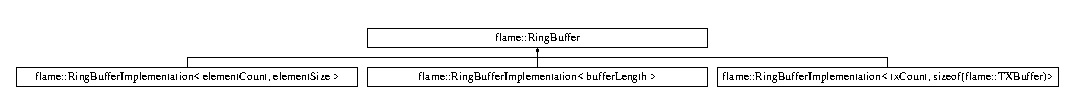
\includegraphics[height=0.942761cm]{classflame_1_1_ring_buffer}
\end{center}
\end{figure}
\subsection*{Public Member Functions}
\begin{DoxyCompactItemize}
\item 
\hyperlink{classflame_1_1_ring_buffer_aa79ec1379a8e0f4785343f1fa59d0bee}{Ring\-Buffer} ()
\item 
uint16\-\_\-t \hyperlink{classflame_1_1_ring_buffer_a473b7401a5b6801b54523bd5e835739b}{size} ()
\item 
uint16\-\_\-t \hyperlink{classflame_1_1_ring_buffer_ace06648c284c5907b97b613333161010}{head} ()
\item 
uint16\-\_\-t \hyperlink{classflame_1_1_ring_buffer_a442f72d57cad307ec7b3c4bf76b1821b}{tail} ()
\item 
bool \hyperlink{classflame_1_1_ring_buffer_aaea51784145687f9e96531efb42e710f}{append} (char c)
\item 
bool \hyperlink{classflame_1_1_ring_buffer_afdfe6d29affdb2cda2859ee99f216efb}{append} (const void $\ast$p)
\item 
bool \hyperlink{classflame_1_1_ring_buffer_a51d857b8f879e16deb5a5a6f6f26ee39}{append} (const void $\ast$p, uint8\-\_\-t p\-Length)
\item 
int \hyperlink{classflame_1_1_ring_buffer_afe46197978f705f5c49fa6175b1005e8}{consume} ()
\item 
bool \hyperlink{classflame_1_1_ring_buffer_a79bb84830e97b889f069105f293f9cff}{consume} (void $\ast$p, uint8\-\_\-t p\-Length)
\item 
bool \hyperlink{classflame_1_1_ring_buffer_ac3c660ef536662f7af65de50ff7199f7}{consume} (void $\ast$p)
\item 
void \hyperlink{classflame_1_1_ring_buffer_ab2ba45675a348dfe2e31554de4f2fddf}{flush} ()
\item 
uint16\-\_\-t \hyperlink{classflame_1_1_ring_buffer_a6b7772f29604b611eb6ad202e5fbcfdb}{length} ()
\item 
bool \hyperlink{classflame_1_1_ring_buffer_adc5bebc1be0a2ca4e6b073eff3c2e2b3}{full} ()
\item 
bool \hyperlink{classflame_1_1_ring_buffer_aa827d88e5d9b53a10d60e0160f51d37c}{full} (uint8\-\_\-t block\-Length)
\item 
int \hyperlink{classflame_1_1_ring_buffer_a7068eccfcd8bf889bc35de9adabd0935}{peek\-Head} ()
\end{DoxyCompactItemize}
\subsection*{Protected Member Functions}
\begin{DoxyCompactItemize}
\item 
uint16\-\_\-t \hyperlink{classflame_1_1_ring_buffer_a94f253a81991f07e6db59943ea2dc267}{increment} (uint16\-\_\-t index)
\end{DoxyCompactItemize}
\subsection*{Protected Attributes}
\begin{DoxyCompactItemize}
\item 
volatile uint8\-\_\-t \hyperlink{classflame_1_1_ring_buffer_af8a6c82581a2a8f62373d43f9f974402}{\-\_\-head}
\item 
volatile uint8\-\_\-t \hyperlink{classflame_1_1_ring_buffer_a57382fd37f090fdd43b0c7e0e7f8246d}{\-\_\-tail}
\item 
volatile uint8\-\_\-t $\ast$ \hyperlink{classflame_1_1_ring_buffer_a30f510a6336a693d8157650019d145fb}{\-\_\-buffer} = N\-U\-L\-L
\item 
uint16\-\_\-t \hyperlink{classflame_1_1_ring_buffer_aac2742500299b783e4c236298ec3d58c}{\-\_\-buffer\-Size} = 0
\item 
uint8\-\_\-t \hyperlink{classflame_1_1_ring_buffer_a7104672ac66311b90363c3919125a417}{\-\_\-element\-Count} = 0
\item 
uint8\-\_\-t \hyperlink{classflame_1_1_ring_buffer_a96a3712379a390f16b4ab5a838e794a3}{\-\_\-element\-Size} = 0
\end{DoxyCompactItemize}


\subsection{Detailed Description}


Definition at line 38 of file Ring\-Buffer.\-h.



\subsection{Constructor \& Destructor Documentation}
\hypertarget{classflame_1_1_ring_buffer_aa79ec1379a8e0f4785343f1fa59d0bee}{\index{flame\-::\-Ring\-Buffer@{flame\-::\-Ring\-Buffer}!Ring\-Buffer@{Ring\-Buffer}}
\index{Ring\-Buffer@{Ring\-Buffer}!flame::RingBuffer@{flame\-::\-Ring\-Buffer}}
\subsubsection[{Ring\-Buffer}]{\setlength{\rightskip}{0pt plus 5cm}flame\-::\-Ring\-Buffer\-::\-Ring\-Buffer (
\begin{DoxyParamCaption}
{}
\end{DoxyParamCaption}
)\hspace{0.3cm}{\ttfamily [inline]}}}\label{classflame_1_1_ring_buffer_aa79ec1379a8e0f4785343f1fa59d0bee}
Create a new ringbuffer 

Definition at line 65 of file Ring\-Buffer.\-h.



\subsection{Member Function Documentation}
\hypertarget{classflame_1_1_ring_buffer_aaea51784145687f9e96531efb42e710f}{\index{flame\-::\-Ring\-Buffer@{flame\-::\-Ring\-Buffer}!append@{append}}
\index{append@{append}!flame::RingBuffer@{flame\-::\-Ring\-Buffer}}
\subsubsection[{append}]{\setlength{\rightskip}{0pt plus 5cm}bool flame\-::\-Ring\-Buffer\-::append (
\begin{DoxyParamCaption}
\item[{char}]{c}
\end{DoxyParamCaption}
)\hspace{0.3cm}{\ttfamily [inline]}}}\label{classflame_1_1_ring_buffer_aaea51784145687f9e96531efb42e710f}
Append a character to the buffer \begin{DoxyReturn}{Returns}
false if we succeeded, true otherwise 
\end{DoxyReturn}


Definition at line 94 of file Ring\-Buffer.\-h.

\hypertarget{classflame_1_1_ring_buffer_afdfe6d29affdb2cda2859ee99f216efb}{\index{flame\-::\-Ring\-Buffer@{flame\-::\-Ring\-Buffer}!append@{append}}
\index{append@{append}!flame::RingBuffer@{flame\-::\-Ring\-Buffer}}
\subsubsection[{append}]{\setlength{\rightskip}{0pt plus 5cm}bool flame\-::\-Ring\-Buffer\-::append (
\begin{DoxyParamCaption}
\item[{const void $\ast$}]{p}
\end{DoxyParamCaption}
)\hspace{0.3cm}{\ttfamily [inline]}}}\label{classflame_1_1_ring_buffer_afdfe6d29affdb2cda2859ee99f216efb}
Append an element to the buffer 
\begin{DoxyParams}{Parameters}
{\em p} & the pointer to append from \\
\hline
\end{DoxyParams}
\begin{DoxyReturn}{Returns}
false if we succeeded, true otherwise 
\end{DoxyReturn}


Definition at line 113 of file Ring\-Buffer.\-h.

\hypertarget{classflame_1_1_ring_buffer_a51d857b8f879e16deb5a5a6f6f26ee39}{\index{flame\-::\-Ring\-Buffer@{flame\-::\-Ring\-Buffer}!append@{append}}
\index{append@{append}!flame::RingBuffer@{flame\-::\-Ring\-Buffer}}
\subsubsection[{append}]{\setlength{\rightskip}{0pt plus 5cm}bool flame\-::\-Ring\-Buffer\-::append (
\begin{DoxyParamCaption}
\item[{const void $\ast$}]{p, }
\item[{uint8\-\_\-t}]{p\-Length}
\end{DoxyParamCaption}
)\hspace{0.3cm}{\ttfamily [inline]}}}\label{classflame_1_1_ring_buffer_a51d857b8f879e16deb5a5a6f6f26ee39}
Append a block of data to the buffer 
\begin{DoxyParams}{Parameters}
{\em p} & the pointer to append from \\
\hline
{\em p\-Length} & the number of bytes to append \\
\hline
\end{DoxyParams}
\begin{DoxyReturn}{Returns}
false if we succeeded, true otherwise 
\end{DoxyReturn}


Definition at line 137 of file Ring\-Buffer.\-h.

\hypertarget{classflame_1_1_ring_buffer_afe46197978f705f5c49fa6175b1005e8}{\index{flame\-::\-Ring\-Buffer@{flame\-::\-Ring\-Buffer}!consume@{consume}}
\index{consume@{consume}!flame::RingBuffer@{flame\-::\-Ring\-Buffer}}
\subsubsection[{consume}]{\setlength{\rightskip}{0pt plus 5cm}int flame\-::\-Ring\-Buffer\-::consume (
\begin{DoxyParamCaption}
{}
\end{DoxyParamCaption}
)\hspace{0.3cm}{\ttfamily [inline]}}}\label{classflame_1_1_ring_buffer_afe46197978f705f5c49fa6175b1005e8}
Pop a byte off the ringbuffer 

Definition at line 158 of file Ring\-Buffer.\-h.

\hypertarget{classflame_1_1_ring_buffer_a79bb84830e97b889f069105f293f9cff}{\index{flame\-::\-Ring\-Buffer@{flame\-::\-Ring\-Buffer}!consume@{consume}}
\index{consume@{consume}!flame::RingBuffer@{flame\-::\-Ring\-Buffer}}
\subsubsection[{consume}]{\setlength{\rightskip}{0pt plus 5cm}bool flame\-::\-Ring\-Buffer\-::consume (
\begin{DoxyParamCaption}
\item[{void $\ast$}]{p, }
\item[{uint8\-\_\-t}]{p\-Length}
\end{DoxyParamCaption}
)\hspace{0.3cm}{\ttfamily [inline]}}}\label{classflame_1_1_ring_buffer_a79bb84830e97b889f069105f293f9cff}
Pop a block off the ringbuffer 
\begin{DoxyParams}{Parameters}
{\em p} & where to write the block \\
\hline
{\em p\-Length} & the length of the block \\
\hline
\end{DoxyParams}
\begin{DoxyReturn}{Returns}
false if we succeeded, true otherwise 
\end{DoxyReturn}


Definition at line 174 of file Ring\-Buffer.\-h.

\hypertarget{classflame_1_1_ring_buffer_ac3c660ef536662f7af65de50ff7199f7}{\index{flame\-::\-Ring\-Buffer@{flame\-::\-Ring\-Buffer}!consume@{consume}}
\index{consume@{consume}!flame::RingBuffer@{flame\-::\-Ring\-Buffer}}
\subsubsection[{consume}]{\setlength{\rightskip}{0pt plus 5cm}bool flame\-::\-Ring\-Buffer\-::consume (
\begin{DoxyParamCaption}
\item[{void $\ast$}]{p}
\end{DoxyParamCaption}
)\hspace{0.3cm}{\ttfamily [inline]}}}\label{classflame_1_1_ring_buffer_ac3c660ef536662f7af65de50ff7199f7}
Pop an element off the ringbuffer 
\begin{DoxyParams}{Parameters}
{\em p} & where to write the block \\
\hline
\end{DoxyParams}
\begin{DoxyReturn}{Returns}
false if we succeeded, true otherwise 
\end{DoxyReturn}


Definition at line 196 of file Ring\-Buffer.\-h.

\hypertarget{classflame_1_1_ring_buffer_ab2ba45675a348dfe2e31554de4f2fddf}{\index{flame\-::\-Ring\-Buffer@{flame\-::\-Ring\-Buffer}!flush@{flush}}
\index{flush@{flush}!flame::RingBuffer@{flame\-::\-Ring\-Buffer}}
\subsubsection[{flush}]{\setlength{\rightskip}{0pt plus 5cm}void flame\-::\-Ring\-Buffer\-::flush (
\begin{DoxyParamCaption}
{}
\end{DoxyParamCaption}
)\hspace{0.3cm}{\ttfamily [inline]}}}\label{classflame_1_1_ring_buffer_ab2ba45675a348dfe2e31554de4f2fddf}
Discard the contents of the ringbuffer 

Definition at line 217 of file Ring\-Buffer.\-h.

\hypertarget{classflame_1_1_ring_buffer_adc5bebc1be0a2ca4e6b073eff3c2e2b3}{\index{flame\-::\-Ring\-Buffer@{flame\-::\-Ring\-Buffer}!full@{full}}
\index{full@{full}!flame::RingBuffer@{flame\-::\-Ring\-Buffer}}
\subsubsection[{full}]{\setlength{\rightskip}{0pt plus 5cm}bool flame\-::\-Ring\-Buffer\-::full (
\begin{DoxyParamCaption}
{}
\end{DoxyParamCaption}
)\hspace{0.3cm}{\ttfamily [inline]}}}\label{classflame_1_1_ring_buffer_adc5bebc1be0a2ca4e6b073eff3c2e2b3}
Check if the ringbuffer is full \begin{DoxyReturn}{Returns}
true if the ringbuffer is full 
\end{DoxyReturn}


Definition at line 239 of file Ring\-Buffer.\-h.

\hypertarget{classflame_1_1_ring_buffer_aa827d88e5d9b53a10d60e0160f51d37c}{\index{flame\-::\-Ring\-Buffer@{flame\-::\-Ring\-Buffer}!full@{full}}
\index{full@{full}!flame::RingBuffer@{flame\-::\-Ring\-Buffer}}
\subsubsection[{full}]{\setlength{\rightskip}{0pt plus 5cm}bool flame\-::\-Ring\-Buffer\-::full (
\begin{DoxyParamCaption}
\item[{uint8\-\_\-t}]{block\-Length}
\end{DoxyParamCaption}
)\hspace{0.3cm}{\ttfamily [inline]}}}\label{classflame_1_1_ring_buffer_aa827d88e5d9b53a10d60e0160f51d37c}
Check if an object can fit in the ringbuffer 
\begin{DoxyParams}{Parameters}
{\em block\-Length} & the length of the object to fit in \\
\hline
\end{DoxyParams}
\begin{DoxyReturn}{Returns}
true if the ringbuffer is full 
\end{DoxyReturn}


Definition at line 249 of file Ring\-Buffer.\-h.

\hypertarget{classflame_1_1_ring_buffer_ace06648c284c5907b97b613333161010}{\index{flame\-::\-Ring\-Buffer@{flame\-::\-Ring\-Buffer}!head@{head}}
\index{head@{head}!flame::RingBuffer@{flame\-::\-Ring\-Buffer}}
\subsubsection[{head}]{\setlength{\rightskip}{0pt plus 5cm}uint16\-\_\-t flame\-::\-Ring\-Buffer\-::head (
\begin{DoxyParamCaption}
{}
\end{DoxyParamCaption}
)\hspace{0.3cm}{\ttfamily [inline]}}}\label{classflame_1_1_ring_buffer_ace06648c284c5907b97b613333161010}
Get the head offset 

Definition at line 79 of file Ring\-Buffer.\-h.

\hypertarget{classflame_1_1_ring_buffer_a94f253a81991f07e6db59943ea2dc267}{\index{flame\-::\-Ring\-Buffer@{flame\-::\-Ring\-Buffer}!increment@{increment}}
\index{increment@{increment}!flame::RingBuffer@{flame\-::\-Ring\-Buffer}}
\subsubsection[{increment}]{\setlength{\rightskip}{0pt plus 5cm}uint16\-\_\-t flame\-::\-Ring\-Buffer\-::increment (
\begin{DoxyParamCaption}
\item[{uint16\-\_\-t}]{index}
\end{DoxyParamCaption}
)\hspace{0.3cm}{\ttfamily [inline]}, {\ttfamily [protected]}}}\label{classflame_1_1_ring_buffer_a94f253a81991f07e6db59943ea2dc267}
Determine where the next location will be 
\begin{DoxyParams}{Parameters}
{\em index} & the current index \\
\hline
\end{DoxyParams}
\begin{DoxyReturn}{Returns}
the next index 
\end{DoxyReturn}


Definition at line 52 of file Ring\-Buffer.\-h.

\hypertarget{classflame_1_1_ring_buffer_a6b7772f29604b611eb6ad202e5fbcfdb}{\index{flame\-::\-Ring\-Buffer@{flame\-::\-Ring\-Buffer}!length@{length}}
\index{length@{length}!flame::RingBuffer@{flame\-::\-Ring\-Buffer}}
\subsubsection[{length}]{\setlength{\rightskip}{0pt plus 5cm}uint16\-\_\-t flame\-::\-Ring\-Buffer\-::length (
\begin{DoxyParamCaption}
{}
\end{DoxyParamCaption}
)\hspace{0.3cm}{\ttfamily [inline]}}}\label{classflame_1_1_ring_buffer_a6b7772f29604b611eb6ad202e5fbcfdb}
Get the length of the contents of the ringbuffer Return the number of bytes in the ringbuffer 

Definition at line 225 of file Ring\-Buffer.\-h.

\hypertarget{classflame_1_1_ring_buffer_a7068eccfcd8bf889bc35de9adabd0935}{\index{flame\-::\-Ring\-Buffer@{flame\-::\-Ring\-Buffer}!peek\-Head@{peek\-Head}}
\index{peek\-Head@{peek\-Head}!flame::RingBuffer@{flame\-::\-Ring\-Buffer}}
\subsubsection[{peek\-Head}]{\setlength{\rightskip}{0pt plus 5cm}int flame\-::\-Ring\-Buffer\-::peek\-Head (
\begin{DoxyParamCaption}
{}
\end{DoxyParamCaption}
)\hspace{0.3cm}{\ttfamily [inline]}}}\label{classflame_1_1_ring_buffer_a7068eccfcd8bf889bc35de9adabd0935}
Check the most recent character in the buffer \begin{DoxyReturn}{Returns}
the character, or -\/1 if the buffer is empty 
\end{DoxyReturn}


Definition at line 258 of file Ring\-Buffer.\-h.

\hypertarget{classflame_1_1_ring_buffer_a473b7401a5b6801b54523bd5e835739b}{\index{flame\-::\-Ring\-Buffer@{flame\-::\-Ring\-Buffer}!size@{size}}
\index{size@{size}!flame::RingBuffer@{flame\-::\-Ring\-Buffer}}
\subsubsection[{size}]{\setlength{\rightskip}{0pt plus 5cm}uint16\-\_\-t flame\-::\-Ring\-Buffer\-::size (
\begin{DoxyParamCaption}
{}
\end{DoxyParamCaption}
)\hspace{0.3cm}{\ttfamily [inline]}}}\label{classflame_1_1_ring_buffer_a473b7401a5b6801b54523bd5e835739b}
Get the size of the ringbuffer 

Definition at line 72 of file Ring\-Buffer.\-h.

\hypertarget{classflame_1_1_ring_buffer_a442f72d57cad307ec7b3c4bf76b1821b}{\index{flame\-::\-Ring\-Buffer@{flame\-::\-Ring\-Buffer}!tail@{tail}}
\index{tail@{tail}!flame::RingBuffer@{flame\-::\-Ring\-Buffer}}
\subsubsection[{tail}]{\setlength{\rightskip}{0pt plus 5cm}uint16\-\_\-t flame\-::\-Ring\-Buffer\-::tail (
\begin{DoxyParamCaption}
{}
\end{DoxyParamCaption}
)\hspace{0.3cm}{\ttfamily [inline]}}}\label{classflame_1_1_ring_buffer_a442f72d57cad307ec7b3c4bf76b1821b}
Get the tail offset 

Definition at line 86 of file Ring\-Buffer.\-h.



\subsection{Member Data Documentation}
\hypertarget{classflame_1_1_ring_buffer_a30f510a6336a693d8157650019d145fb}{\index{flame\-::\-Ring\-Buffer@{flame\-::\-Ring\-Buffer}!\-\_\-buffer@{\-\_\-buffer}}
\index{\-\_\-buffer@{\-\_\-buffer}!flame::RingBuffer@{flame\-::\-Ring\-Buffer}}
\subsubsection[{\-\_\-buffer}]{\setlength{\rightskip}{0pt plus 5cm}volatile uint8\-\_\-t$\ast$ flame\-::\-Ring\-Buffer\-::\-\_\-buffer = N\-U\-L\-L\hspace{0.3cm}{\ttfamily [protected]}}}\label{classflame_1_1_ring_buffer_a30f510a6336a693d8157650019d145fb}


Definition at line 42 of file Ring\-Buffer.\-h.

\hypertarget{classflame_1_1_ring_buffer_aac2742500299b783e4c236298ec3d58c}{\index{flame\-::\-Ring\-Buffer@{flame\-::\-Ring\-Buffer}!\-\_\-buffer\-Size@{\-\_\-buffer\-Size}}
\index{\-\_\-buffer\-Size@{\-\_\-buffer\-Size}!flame::RingBuffer@{flame\-::\-Ring\-Buffer}}
\subsubsection[{\-\_\-buffer\-Size}]{\setlength{\rightskip}{0pt plus 5cm}uint16\-\_\-t flame\-::\-Ring\-Buffer\-::\-\_\-buffer\-Size = 0\hspace{0.3cm}{\ttfamily [protected]}}}\label{classflame_1_1_ring_buffer_aac2742500299b783e4c236298ec3d58c}


Definition at line 43 of file Ring\-Buffer.\-h.

\hypertarget{classflame_1_1_ring_buffer_a7104672ac66311b90363c3919125a417}{\index{flame\-::\-Ring\-Buffer@{flame\-::\-Ring\-Buffer}!\-\_\-element\-Count@{\-\_\-element\-Count}}
\index{\-\_\-element\-Count@{\-\_\-element\-Count}!flame::RingBuffer@{flame\-::\-Ring\-Buffer}}
\subsubsection[{\-\_\-element\-Count}]{\setlength{\rightskip}{0pt plus 5cm}uint8\-\_\-t flame\-::\-Ring\-Buffer\-::\-\_\-element\-Count = 0\hspace{0.3cm}{\ttfamily [protected]}}}\label{classflame_1_1_ring_buffer_a7104672ac66311b90363c3919125a417}


Definition at line 44 of file Ring\-Buffer.\-h.

\hypertarget{classflame_1_1_ring_buffer_a96a3712379a390f16b4ab5a838e794a3}{\index{flame\-::\-Ring\-Buffer@{flame\-::\-Ring\-Buffer}!\-\_\-element\-Size@{\-\_\-element\-Size}}
\index{\-\_\-element\-Size@{\-\_\-element\-Size}!flame::RingBuffer@{flame\-::\-Ring\-Buffer}}
\subsubsection[{\-\_\-element\-Size}]{\setlength{\rightskip}{0pt plus 5cm}uint8\-\_\-t flame\-::\-Ring\-Buffer\-::\-\_\-element\-Size = 0\hspace{0.3cm}{\ttfamily [protected]}}}\label{classflame_1_1_ring_buffer_a96a3712379a390f16b4ab5a838e794a3}


Definition at line 45 of file Ring\-Buffer.\-h.

\hypertarget{classflame_1_1_ring_buffer_af8a6c82581a2a8f62373d43f9f974402}{\index{flame\-::\-Ring\-Buffer@{flame\-::\-Ring\-Buffer}!\-\_\-head@{\-\_\-head}}
\index{\-\_\-head@{\-\_\-head}!flame::RingBuffer@{flame\-::\-Ring\-Buffer}}
\subsubsection[{\-\_\-head}]{\setlength{\rightskip}{0pt plus 5cm}volatile uint8\-\_\-t flame\-::\-Ring\-Buffer\-::\-\_\-head\hspace{0.3cm}{\ttfamily [protected]}}}\label{classflame_1_1_ring_buffer_af8a6c82581a2a8f62373d43f9f974402}


Definition at line 40 of file Ring\-Buffer.\-h.

\hypertarget{classflame_1_1_ring_buffer_a57382fd37f090fdd43b0c7e0e7f8246d}{\index{flame\-::\-Ring\-Buffer@{flame\-::\-Ring\-Buffer}!\-\_\-tail@{\-\_\-tail}}
\index{\-\_\-tail@{\-\_\-tail}!flame::RingBuffer@{flame\-::\-Ring\-Buffer}}
\subsubsection[{\-\_\-tail}]{\setlength{\rightskip}{0pt plus 5cm}volatile uint8\-\_\-t flame\-::\-Ring\-Buffer\-::\-\_\-tail\hspace{0.3cm}{\ttfamily [protected]}}}\label{classflame_1_1_ring_buffer_a57382fd37f090fdd43b0c7e0e7f8246d}


Definition at line 41 of file Ring\-Buffer.\-h.



The documentation for this class was generated from the following file\-:\begin{DoxyCompactItemize}
\item 
flame/\hyperlink{_ring_buffer_8h}{Ring\-Buffer.\-h}\end{DoxyCompactItemize}

\hypertarget{classflame_1_1_ring_buffer_implementation}{\section{flame\-:\-:Ring\-Buffer\-Implementation$<$ element\-Count, element\-Size $>$ Class Template Reference}
\label{classflame_1_1_ring_buffer_implementation}\index{flame\-::\-Ring\-Buffer\-Implementation$<$ element\-Count, element\-Size $>$@{flame\-::\-Ring\-Buffer\-Implementation$<$ element\-Count, element\-Size $>$}}
}


{\ttfamily \#include $<$Ring\-Buffer.\-h$>$}

Inheritance diagram for flame\-:\-:Ring\-Buffer\-Implementation$<$ element\-Count, element\-Size $>$\-:\begin{figure}[H]
\begin{center}
\leavevmode
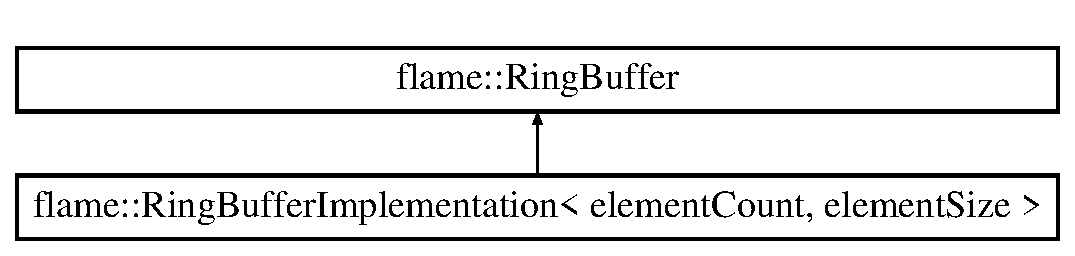
\includegraphics[height=2.000000cm]{classflame_1_1_ring_buffer_implementation}
\end{center}
\end{figure}
\subsection*{Public Member Functions}
\begin{DoxyCompactItemize}
\item 
\hyperlink{classflame_1_1_ring_buffer_implementation_a5a1f27a84989a33d738a53e995bff6dd}{Ring\-Buffer\-Implementation} ()
\end{DoxyCompactItemize}
\subsection*{Protected Attributes}
\begin{DoxyCompactItemize}
\item 
volatile uint8\-\_\-t \hyperlink{classflame_1_1_ring_buffer_implementation_a219b451e18a1e8c7c39e3fc17ae2e64b}{\-\_\-my\-Buffer} \mbox{[}element\-Count $\ast$element\-Size+1\mbox{]}
\end{DoxyCompactItemize}
\subsection*{Additional Inherited Members}


\subsection{Detailed Description}
\subsubsection*{template$<$uint8\-\_\-t element\-Count, uint8\-\_\-t element\-Size = 1$>$class flame\-::\-Ring\-Buffer\-Implementation$<$ element\-Count, element\-Size $>$}

A ring buffer 
\begin{DoxyTemplParams}{Template Parameters}
{\em element\-Count} & the number of elements \\
\hline
{\em element\-Size} & the number of bytes in an element \\
\hline
\end{DoxyTemplParams}


Definition at line 280 of file Ring\-Buffer.\-h.



\subsection{Constructor \& Destructor Documentation}
\hypertarget{classflame_1_1_ring_buffer_implementation_a5a1f27a84989a33d738a53e995bff6dd}{\index{flame\-::\-Ring\-Buffer\-Implementation@{flame\-::\-Ring\-Buffer\-Implementation}!Ring\-Buffer\-Implementation@{Ring\-Buffer\-Implementation}}
\index{Ring\-Buffer\-Implementation@{Ring\-Buffer\-Implementation}!flame::RingBufferImplementation@{flame\-::\-Ring\-Buffer\-Implementation}}
\subsubsection[{Ring\-Buffer\-Implementation}]{\setlength{\rightskip}{0pt plus 5cm}template$<$uint8\-\_\-t element\-Count, uint8\-\_\-t element\-Size = 1$>$ {\bf flame\-::\-Ring\-Buffer\-Implementation}$<$ element\-Count, element\-Size $>$\-::{\bf Ring\-Buffer\-Implementation} (
\begin{DoxyParamCaption}
{}
\end{DoxyParamCaption}
)\hspace{0.3cm}{\ttfamily [inline]}}}\label{classflame_1_1_ring_buffer_implementation_a5a1f27a84989a33d738a53e995bff6dd}
Create a new ringbuffer 

Definition at line 288 of file Ring\-Buffer.\-h.



\subsection{Member Data Documentation}
\hypertarget{classflame_1_1_ring_buffer_implementation_a219b451e18a1e8c7c39e3fc17ae2e64b}{\index{flame\-::\-Ring\-Buffer\-Implementation@{flame\-::\-Ring\-Buffer\-Implementation}!\-\_\-my\-Buffer@{\-\_\-my\-Buffer}}
\index{\-\_\-my\-Buffer@{\-\_\-my\-Buffer}!flame::RingBufferImplementation@{flame\-::\-Ring\-Buffer\-Implementation}}
\subsubsection[{\-\_\-my\-Buffer}]{\setlength{\rightskip}{0pt plus 5cm}template$<$uint8\-\_\-t element\-Count, uint8\-\_\-t element\-Size = 1$>$ volatile uint8\-\_\-t {\bf flame\-::\-Ring\-Buffer\-Implementation}$<$ element\-Count, element\-Size $>$\-::\-\_\-my\-Buffer\mbox{[}element\-Count $\ast$element\-Size+1\mbox{]}\hspace{0.3cm}{\ttfamily [protected]}}}\label{classflame_1_1_ring_buffer_implementation_a219b451e18a1e8c7c39e3fc17ae2e64b}


Definition at line 282 of file Ring\-Buffer.\-h.



The documentation for this class was generated from the following file\-:\begin{DoxyCompactItemize}
\item 
flame/\hyperlink{_ring_buffer_8h}{Ring\-Buffer.\-h}\end{DoxyCompactItemize}

\hypertarget{classflame_1_1_r_t_c}{\section{flame\-:\-:R\-T\-C Class Reference}
\label{classflame_1_1_r_t_c}\index{flame\-::\-R\-T\-C@{flame\-::\-R\-T\-C}}
}


{\ttfamily \#include $<$R\-T\-C.\-h$>$}

Inheritance diagram for flame\-:\-:R\-T\-C\-:\begin{figure}[H]
\begin{center}
\leavevmode
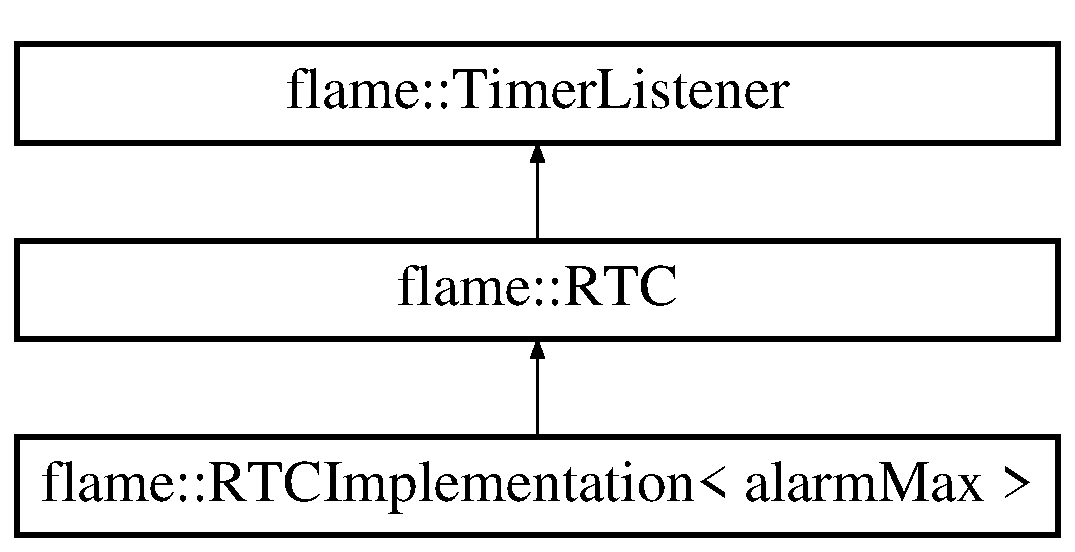
\includegraphics[height=3.000000cm]{classflame_1_1_r_t_c}
\end{center}
\end{figure}
\subsection*{Public Member Functions}
\begin{DoxyCompactItemize}
\item 
\hyperlink{classflame_1_1_r_t_c_a1345e2aa25662edb07a4c0d11ef7db26}{R\-T\-C} (int16\-\_\-t timezone=0)
\item 
void \hyperlink{classflame_1_1_r_t_c_afbabe09cc9b0311bf4ae7871b93ad692}{synchronise} (\hyperlink{classflame_1_1_timer}{Timer} \&timer)
\item 
void \hyperlink{classflame_1_1_r_t_c_a86aa2ab02475f073179c2b2db51312e8}{set\-Time} (uint32\-\_\-t \hyperlink{structflame_1_1timestamp}{timestamp}, uint16\-\_\-t milliseconds)
\item 
void \hyperlink{classflame_1_1_r_t_c_aa806fd984f19bf88515b982b31188d0b}{set\-Time} (\hyperlink{namespaceflame_ad90347e9ea7e54907966260ec5c7d22f}{T\-I\-M\-E\-S\-T\-A\-M\-P} \&\hyperlink{structflame_1_1timestamp}{timestamp})
\item 
void \hyperlink{classflame_1_1_r_t_c_a7198ccc25a55472063750e91ecb2e442}{alarm} (\hyperlink{io_8h_addf5ec070e9499d36b7f2009ce736076}{U\-N\-U\-S\-E\-D} \hyperlink{namespaceflame_a6d176ba245556716fd3e32006bb7cfe5}{Alarm\-Source} source)
\item 
void \hyperlink{classflame_1_1_r_t_c_ab62acf26f8d8930440e37b4eff8ad630}{current} (\hyperlink{namespaceflame_ad90347e9ea7e54907966260ec5c7d22f}{T\-I\-M\-E\-S\-T\-A\-M\-P} \&\hyperlink{structflame_1_1timestamp}{timestamp})
\item 
void \hyperlink{classflame_1_1_r_t_c_af2287ccb064da38fc546f76cf88c1e53}{elapsed} (const \hyperlink{namespaceflame_ad90347e9ea7e54907966260ec5c7d22f}{T\-I\-M\-E\-S\-T\-A\-M\-P} \&since, \hyperlink{namespaceflame_ad90347e9ea7e54907966260ec5c7d22f}{T\-I\-M\-E\-S\-T\-A\-M\-P} \&elapsed)
\item 
void \hyperlink{classflame_1_1_r_t_c_afaf9a803ca66b58067b24f879edec821}{to\-Time} (\hyperlink{namespaceflame_a961fbb5da27b8d64aa0dfc18f55b2be6}{T\-I\-M\-E} \&to, const \hyperlink{namespaceflame_ad90347e9ea7e54907966260ec5c7d22f}{T\-I\-M\-E\-S\-T\-A\-M\-P} \&from)
\item 
void \hyperlink{classflame_1_1_r_t_c_a8cf9824b2f59a91c6d2310640927f6ae}{to\-Timestamp} (\hyperlink{namespaceflame_ad90347e9ea7e54907966260ec5c7d22f}{T\-I\-M\-E\-S\-T\-A\-M\-P} \&to, const \hyperlink{namespaceflame_a961fbb5da27b8d64aa0dfc18f55b2be6}{T\-I\-M\-E} \&from)
\item 
void \hyperlink{classflame_1_1_r_t_c_ac9e327bd6696dab66fae72cca5676b11}{timestamp\-Increment} (\hyperlink{namespaceflame_ad90347e9ea7e54907966260ec5c7d22f}{T\-I\-M\-E\-S\-T\-A\-M\-P} \&\hyperlink{structflame_1_1timestamp}{timestamp}, const \hyperlink{namespaceflame_ad90347e9ea7e54907966260ec5c7d22f}{T\-I\-M\-E\-S\-T\-A\-M\-P} \&timestamp2)
\item 
void \hyperlink{classflame_1_1_r_t_c_a68603e274c5c12bdbeafeab6323465fb}{timestamp\-Increment} (\hyperlink{namespaceflame_ad90347e9ea7e54907966260ec5c7d22f}{T\-I\-M\-E\-S\-T\-A\-M\-P} \&\hyperlink{structflame_1_1timestamp}{timestamp}, uint32\-\_\-t seconds, uint16\-\_\-t milliseconds, uint8\-\_\-t ticks)
\item 
bool \hyperlink{classflame_1_1_r_t_c_a6398e8a4677ae1a59854a01f2c1ec5e4}{add\-Alarm} (\hyperlink{classflame_1_1_timer_listener}{Timer\-Listener} \&listener, uint32\-\_\-t when\-Seconds, uint16\-\_\-t when\-Milliseconds, uint8\-\_\-t when\-Ticks, uint32\-\_\-t repeat\-Seconds, uint16\-\_\-t repeat\-Milliseconds, uint8\-\_\-t repeat\-Ticks)
\item 
bool \hyperlink{classflame_1_1_r_t_c_aa53710bf71cd287d051e104a7edba27c}{add\-Alarm} (\hyperlink{classflame_1_1_timer_listener}{Timer\-Listener} \&listener, uint32\-\_\-t when\-Seconds, uint16\-\_\-t when\-Milliseconds, uint32\-\_\-t repeat\-Seconds, uint16\-\_\-t repeat\-Milliseconds)
\item 
bool \hyperlink{classflame_1_1_r_t_c_a8681ff7b542f02c8a21f1e8dbb2b0034}{add\-Alarm} (\hyperlink{classflame_1_1_timer_listener}{Timer\-Listener} \&listener, uint32\-\_\-t when\-Seconds, uint16\-\_\-t when\-Milliseconds, uint8\-\_\-t when\-Ticks)
\item 
bool \hyperlink{classflame_1_1_r_t_c_a775dfd649ec2ce41c0f64708b32f18c3}{add\-Alarm} (\hyperlink{classflame_1_1_timer_listener}{Timer\-Listener} \&listener, uint32\-\_\-t when\-Seconds, uint16\-\_\-t when\-Milliseconds)
\item 
bool \hyperlink{classflame_1_1_r_t_c_a9e5862b3c4037fb44172e2194ffdc263}{add\-Alarm} (\hyperlink{classflame_1_1_timer_listener}{Timer\-Listener} \&listener, \hyperlink{namespaceflame_ad90347e9ea7e54907966260ec5c7d22f}{T\-I\-M\-E\-S\-T\-A\-M\-P} \&when)
\item 
bool \hyperlink{classflame_1_1_r_t_c_affcf2d298d1e96c543d508a48c7e65bb}{add\-Alarm} (\hyperlink{classflame_1_1_timer_listener}{Timer\-Listener} $\ast$listener, uint32\-\_\-t when\-Seconds, uint16\-\_\-t when\-Milliseconds, uint8\-\_\-t when\-Ticks, uint32\-\_\-t repeat\-Seconds, uint16\-\_\-t repeat\-Milliseconds, uint8\-\_\-t repeat\-Ticks)
\item 
bool \hyperlink{classflame_1_1_r_t_c_aa0c02e91ae48a09802ea66b1771be43f}{add\-Alarm} (\hyperlink{classflame_1_1_timer_listener}{Timer\-Listener} $\ast$listener, uint32\-\_\-t when\-Seconds, uint16\-\_\-t when\-Milliseconds, uint32\-\_\-t repeat\-Seconds, uint16\-\_\-t repeat\-Milliseconds)
\item 
bool \hyperlink{classflame_1_1_r_t_c_aa5123c2ac9201b0186edbcb988a25352}{add\-Alarm} (\hyperlink{classflame_1_1_timer_listener}{Timer\-Listener} $\ast$listener, uint32\-\_\-t when\-Seconds, uint16\-\_\-t when\-Milliseconds, uint8\-\_\-t when\-Ticks)
\item 
bool \hyperlink{classflame_1_1_r_t_c_a94834b36f4332dcabd8aee276221f8cb}{add\-Alarm} (\hyperlink{classflame_1_1_timer_listener}{Timer\-Listener} $\ast$listener, uint32\-\_\-t when\-Seconds, uint16\-\_\-t when\-Milliseconds)
\item 
bool \hyperlink{classflame_1_1_r_t_c_a787e76eee1bbece6133b6f6539d46074}{add\-Alarm} (\hyperlink{namespaceflame_a7a5a7b0bdd1b44d7d0b0a600552b5ab5}{A\-L\-A\-R\-M} \&\hyperlink{structflame_1_1alarm}{alarm})
\item 
virtual bool \hyperlink{classflame_1_1_r_t_c_a3ba19efd3cffbe55d363831996657b42}{register\-Alarm} (\hyperlink{namespaceflame_a7a5a7b0bdd1b44d7d0b0a600552b5ab5}{A\-L\-A\-R\-M} \&\hyperlink{structflame_1_1alarm}{alarm})=0
\item 
virtual void \hyperlink{classflame_1_1_r_t_c_a123414b982bd03971e057d8fcf4e45ae}{handle\-Events} ()=0
\item 
uint8\-\_\-t \hyperlink{classflame_1_1_r_t_c_afb5a72eef061c794b61ef4cc07ec5aa9}{alarms\-Pending} ()
\item 
virtual void \hyperlink{classflame_1_1_r_t_c_ad493295a4babbc7a3dd4ef18b72c4679}{remove\-Alarm} (\hyperlink{classflame_1_1_timer_listener}{Timer\-Listener} \&listener)=0
\item 
virtual void \hyperlink{classflame_1_1_r_t_c_a88d193491a668daf956bcc672f3dfc06}{remove\-Alarm} (\hyperlink{classflame_1_1_timer_listener}{Timer\-Listener} $\ast$listener)=0
\end{DoxyCompactItemize}
\subsection*{Protected Member Functions}
\begin{DoxyCompactItemize}
\item 
void \hyperlink{classflame_1_1_r_t_c_a0d6e472de2f42bebed345004d20a504d}{increment\-Milliseconds} ()
\end{DoxyCompactItemize}
\subsection*{Protected Attributes}
\begin{DoxyCompactItemize}
\item 
volatile uint8\-\_\-t \hyperlink{classflame_1_1_r_t_c_a1d4d07a67ff88e81a09cbd861bd63ad7}{\-\_\-alarm\-Count}
\item 
uint32\-\_\-t \hyperlink{classflame_1_1_r_t_c_a31320e54b29c8a1608782dccaea5bf32}{\-\_\-timestamp}
\item 
uint16\-\_\-t \hyperlink{classflame_1_1_r_t_c_a0152322ecff4547471a1f8d84b99cb8e}{\-\_\-milliseconds}
\item 
uint8\-\_\-t \hyperlink{classflame_1_1_r_t_c_a9dc99aa09ba42642a43f230f5c2df5eb}{\-\_\-ticks}
\item 
uint8\-\_\-t \hyperlink{classflame_1_1_r_t_c_afcfc861a7923a01a54e8b03eb46d48c3}{\-\_\-ticks\-Per\-Millisecond}
\item 
int16\-\_\-t \hyperlink{classflame_1_1_r_t_c_a88b4f62e5114d3cf608a1c7029881d85}{\-\_\-tz\-Offset}
\end{DoxyCompactItemize}


\subsection{Detailed Description}


Definition at line 231 of file R\-T\-C.\-h.



\subsection{Constructor \& Destructor Documentation}
\hypertarget{classflame_1_1_r_t_c_a1345e2aa25662edb07a4c0d11ef7db26}{\index{flame\-::\-R\-T\-C@{flame\-::\-R\-T\-C}!R\-T\-C@{R\-T\-C}}
\index{R\-T\-C@{R\-T\-C}!flame::RTC@{flame\-::\-R\-T\-C}}
\subsubsection[{R\-T\-C}]{\setlength{\rightskip}{0pt plus 5cm}flame\-::\-R\-T\-C\-::\-R\-T\-C (
\begin{DoxyParamCaption}
\item[{int16\-\_\-t}]{timezone = {\ttfamily 0}}
\end{DoxyParamCaption}
)\hspace{0.3cm}{\ttfamily [inline]}}}\label{classflame_1_1_r_t_c_a1345e2aa25662edb07a4c0d11ef7db26}
Create a new \hyperlink{classflame_1_1_r_t_c}{R\-T\-C} 
\begin{DoxyParams}{Parameters}
{\em timezone} & minutes offset from U\-T\-C \\
\hline
\end{DoxyParams}


Definition at line 258 of file R\-T\-C.\-h.



\subsection{Member Function Documentation}
\hypertarget{classflame_1_1_r_t_c_a6398e8a4677ae1a59854a01f2c1ec5e4}{\index{flame\-::\-R\-T\-C@{flame\-::\-R\-T\-C}!add\-Alarm@{add\-Alarm}}
\index{add\-Alarm@{add\-Alarm}!flame::RTC@{flame\-::\-R\-T\-C}}
\subsubsection[{add\-Alarm}]{\setlength{\rightskip}{0pt plus 5cm}bool flame\-::\-R\-T\-C\-::add\-Alarm (
\begin{DoxyParamCaption}
\item[{{\bf Timer\-Listener} \&}]{listener, }
\item[{uint32\-\_\-t}]{when\-Seconds, }
\item[{uint16\-\_\-t}]{when\-Milliseconds, }
\item[{uint8\-\_\-t}]{when\-Ticks, }
\item[{uint32\-\_\-t}]{repeat\-Seconds, }
\item[{uint16\-\_\-t}]{repeat\-Milliseconds, }
\item[{uint8\-\_\-t}]{repeat\-Ticks}
\end{DoxyParamCaption}
)\hspace{0.3cm}{\ttfamily [inline]}}}\label{classflame_1_1_r_t_c_a6398e8a4677ae1a59854a01f2c1ec5e4}
Insert an alarm to be triggered at a later time 
\begin{DoxyParams}{Parameters}
{\em listener} & the alarm listener to be called when the alarm is triggered \\
\hline
{\em when\-Seconds} & the number of seconds past current that the alarm will be executed \\
\hline
{\em when\-Milliseconds} & the number of milliseconds past current that the alarm will be executed \\
\hline
{\em when\-Ticks} & the number of ticks past current that the alarm will be executed \\
\hline
{\em repeat\-Seconds} & the number of seconds past current that the alarm will be executed \\
\hline
{\em repeat\-Milliseconds} & the number of milliseconds past current that the alarm will be executed \\
\hline
{\em repeat\-Ticks} & the number of ticks past current that the alarm will be executed \\
\hline
\end{DoxyParams}
\begin{DoxyReturn}{Returns}
true if the event could not be added 
\end{DoxyReturn}


Definition at line 527 of file R\-T\-C.\-h.

\hypertarget{classflame_1_1_r_t_c_aa53710bf71cd287d051e104a7edba27c}{\index{flame\-::\-R\-T\-C@{flame\-::\-R\-T\-C}!add\-Alarm@{add\-Alarm}}
\index{add\-Alarm@{add\-Alarm}!flame::RTC@{flame\-::\-R\-T\-C}}
\subsubsection[{add\-Alarm}]{\setlength{\rightskip}{0pt plus 5cm}bool flame\-::\-R\-T\-C\-::add\-Alarm (
\begin{DoxyParamCaption}
\item[{{\bf Timer\-Listener} \&}]{listener, }
\item[{uint32\-\_\-t}]{when\-Seconds, }
\item[{uint16\-\_\-t}]{when\-Milliseconds, }
\item[{uint32\-\_\-t}]{repeat\-Seconds, }
\item[{uint16\-\_\-t}]{repeat\-Milliseconds}
\end{DoxyParamCaption}
)\hspace{0.3cm}{\ttfamily [inline]}}}\label{classflame_1_1_r_t_c_aa53710bf71cd287d051e104a7edba27c}
Insert an alarm to be triggered at a later time 
\begin{DoxyParams}{Parameters}
{\em listener} & the alarm listener to be called when the alarm is triggered \\
\hline
{\em when\-Seconds} & the number of seconds past current that the alarm will be executed \\
\hline
{\em when\-Milliseconds} & the number of milliseconds past current that the alarm will be executed \\
\hline
{\em repeat\-Seconds} & the number of seconds past current that the alarm will be executed \\
\hline
{\em repeat\-Milliseconds} & the number of milliseconds past current that the alarm will be executed \\
\hline
\end{DoxyParams}
\begin{DoxyReturn}{Returns}
true if the event could not be added 
\end{DoxyReturn}


Definition at line 551 of file R\-T\-C.\-h.

\hypertarget{classflame_1_1_r_t_c_a8681ff7b542f02c8a21f1e8dbb2b0034}{\index{flame\-::\-R\-T\-C@{flame\-::\-R\-T\-C}!add\-Alarm@{add\-Alarm}}
\index{add\-Alarm@{add\-Alarm}!flame::RTC@{flame\-::\-R\-T\-C}}
\subsubsection[{add\-Alarm}]{\setlength{\rightskip}{0pt plus 5cm}bool flame\-::\-R\-T\-C\-::add\-Alarm (
\begin{DoxyParamCaption}
\item[{{\bf Timer\-Listener} \&}]{listener, }
\item[{uint32\-\_\-t}]{when\-Seconds, }
\item[{uint16\-\_\-t}]{when\-Milliseconds, }
\item[{uint8\-\_\-t}]{when\-Ticks}
\end{DoxyParamCaption}
)\hspace{0.3cm}{\ttfamily [inline]}}}\label{classflame_1_1_r_t_c_a8681ff7b542f02c8a21f1e8dbb2b0034}
Insert an alarm to be triggered at a later time 
\begin{DoxyParams}{Parameters}
{\em listener} & the alarm listener to be called when the alarm is triggered \\
\hline
{\em when\-Seconds} & the number of seconds past current that the alarm will be executed \\
\hline
{\em when\-Milliseconds} & the number of milliseconds past current that the alarm will be executed \\
\hline
{\em when\-Ticks} & the number of ticks past current that the alarm will be executed \\
\hline
\end{DoxyParams}
\begin{DoxyReturn}{Returns}
true if the event could not be added 
\end{DoxyReturn}


Definition at line 574 of file R\-T\-C.\-h.

\hypertarget{classflame_1_1_r_t_c_a775dfd649ec2ce41c0f64708b32f18c3}{\index{flame\-::\-R\-T\-C@{flame\-::\-R\-T\-C}!add\-Alarm@{add\-Alarm}}
\index{add\-Alarm@{add\-Alarm}!flame::RTC@{flame\-::\-R\-T\-C}}
\subsubsection[{add\-Alarm}]{\setlength{\rightskip}{0pt plus 5cm}bool flame\-::\-R\-T\-C\-::add\-Alarm (
\begin{DoxyParamCaption}
\item[{{\bf Timer\-Listener} \&}]{listener, }
\item[{uint32\-\_\-t}]{when\-Seconds, }
\item[{uint16\-\_\-t}]{when\-Milliseconds}
\end{DoxyParamCaption}
)\hspace{0.3cm}{\ttfamily [inline]}}}\label{classflame_1_1_r_t_c_a775dfd649ec2ce41c0f64708b32f18c3}
Insert an alarm to be triggered at a later time 
\begin{DoxyParams}{Parameters}
{\em listener} & the alarm listener to be called when the alarm is triggered \\
\hline
{\em when\-Seconds} & the number of seconds past current that the alarm will be executed \\
\hline
{\em when\-Milliseconds} & the number of milliseconds past current that the alarm will be executed \\
\hline
\end{DoxyParams}
\begin{DoxyReturn}{Returns}
true if the event could not be added 
\end{DoxyReturn}


Definition at line 595 of file R\-T\-C.\-h.

\hypertarget{classflame_1_1_r_t_c_a9e5862b3c4037fb44172e2194ffdc263}{\index{flame\-::\-R\-T\-C@{flame\-::\-R\-T\-C}!add\-Alarm@{add\-Alarm}}
\index{add\-Alarm@{add\-Alarm}!flame::RTC@{flame\-::\-R\-T\-C}}
\subsubsection[{add\-Alarm}]{\setlength{\rightskip}{0pt plus 5cm}bool flame\-::\-R\-T\-C\-::add\-Alarm (
\begin{DoxyParamCaption}
\item[{{\bf Timer\-Listener} \&}]{listener, }
\item[{{\bf T\-I\-M\-E\-S\-T\-A\-M\-P} \&}]{when}
\end{DoxyParamCaption}
)\hspace{0.3cm}{\ttfamily [inline]}}}\label{classflame_1_1_r_t_c_a9e5862b3c4037fb44172e2194ffdc263}
Insert an alarm to be triggered at a later time 
\begin{DoxyParams}{Parameters}
{\em listener} & the alarm listener to be called when the alarm is triggered \\
\hline
{\em when} & the time the alarm will be executed \\
\hline
\end{DoxyParams}
\begin{DoxyReturn}{Returns}
true if the event could not be added 
\end{DoxyReturn}


Definition at line 615 of file R\-T\-C.\-h.

\hypertarget{classflame_1_1_r_t_c_affcf2d298d1e96c543d508a48c7e65bb}{\index{flame\-::\-R\-T\-C@{flame\-::\-R\-T\-C}!add\-Alarm@{add\-Alarm}}
\index{add\-Alarm@{add\-Alarm}!flame::RTC@{flame\-::\-R\-T\-C}}
\subsubsection[{add\-Alarm}]{\setlength{\rightskip}{0pt plus 5cm}bool flame\-::\-R\-T\-C\-::add\-Alarm (
\begin{DoxyParamCaption}
\item[{{\bf Timer\-Listener} $\ast$}]{listener, }
\item[{uint32\-\_\-t}]{when\-Seconds, }
\item[{uint16\-\_\-t}]{when\-Milliseconds, }
\item[{uint8\-\_\-t}]{when\-Ticks, }
\item[{uint32\-\_\-t}]{repeat\-Seconds, }
\item[{uint16\-\_\-t}]{repeat\-Milliseconds, }
\item[{uint8\-\_\-t}]{repeat\-Ticks}
\end{DoxyParamCaption}
)\hspace{0.3cm}{\ttfamily [inline]}}}\label{classflame_1_1_r_t_c_affcf2d298d1e96c543d508a48c7e65bb}
Insert an alarm to be triggered at a later time 
\begin{DoxyParams}{Parameters}
{\em listener} & the alarm listener to be called when the alarm is triggered \\
\hline
{\em when\-Seconds} & the number of seconds past current that the alarm will be executed \\
\hline
{\em when\-Milliseconds} & the number of milliseconds past current that the alarm will be executed \\
\hline
{\em when\-Ticks} & the number of ticks past current that the alarm will be executed \\
\hline
{\em repeat\-Seconds} & the number of seconds past current that the alarm will be executed \\
\hline
{\em repeat\-Milliseconds} & the number of milliseconds past current that the alarm will be executed \\
\hline
{\em repeat\-Ticks} & the number of ticks past current that the alarm will be executed \\
\hline
\end{DoxyParams}
\begin{DoxyReturn}{Returns}
true if the event could not be added 
\end{DoxyReturn}


Definition at line 639 of file R\-T\-C.\-h.

\hypertarget{classflame_1_1_r_t_c_aa0c02e91ae48a09802ea66b1771be43f}{\index{flame\-::\-R\-T\-C@{flame\-::\-R\-T\-C}!add\-Alarm@{add\-Alarm}}
\index{add\-Alarm@{add\-Alarm}!flame::RTC@{flame\-::\-R\-T\-C}}
\subsubsection[{add\-Alarm}]{\setlength{\rightskip}{0pt plus 5cm}bool flame\-::\-R\-T\-C\-::add\-Alarm (
\begin{DoxyParamCaption}
\item[{{\bf Timer\-Listener} $\ast$}]{listener, }
\item[{uint32\-\_\-t}]{when\-Seconds, }
\item[{uint16\-\_\-t}]{when\-Milliseconds, }
\item[{uint32\-\_\-t}]{repeat\-Seconds, }
\item[{uint16\-\_\-t}]{repeat\-Milliseconds}
\end{DoxyParamCaption}
)\hspace{0.3cm}{\ttfamily [inline]}}}\label{classflame_1_1_r_t_c_aa0c02e91ae48a09802ea66b1771be43f}
Insert an alarm to be triggered at a later time 
\begin{DoxyParams}{Parameters}
{\em listener} & the alarm listener to be called when the alarm is triggered \\
\hline
{\em when\-Seconds} & the number of seconds past current that the alarm will be executed \\
\hline
{\em when\-Milliseconds} & the number of milliseconds past current that the alarm will be executed \\
\hline
{\em repeat\-Seconds} & the number of seconds past current that the alarm will be executed \\
\hline
{\em repeat\-Milliseconds} & the number of milliseconds past current that the alarm will be executed \\
\hline
\end{DoxyParams}
\begin{DoxyReturn}{Returns}
true if the event could not be added 
\end{DoxyReturn}


Definition at line 663 of file R\-T\-C.\-h.

\hypertarget{classflame_1_1_r_t_c_aa5123c2ac9201b0186edbcb988a25352}{\index{flame\-::\-R\-T\-C@{flame\-::\-R\-T\-C}!add\-Alarm@{add\-Alarm}}
\index{add\-Alarm@{add\-Alarm}!flame::RTC@{flame\-::\-R\-T\-C}}
\subsubsection[{add\-Alarm}]{\setlength{\rightskip}{0pt plus 5cm}bool flame\-::\-R\-T\-C\-::add\-Alarm (
\begin{DoxyParamCaption}
\item[{{\bf Timer\-Listener} $\ast$}]{listener, }
\item[{uint32\-\_\-t}]{when\-Seconds, }
\item[{uint16\-\_\-t}]{when\-Milliseconds, }
\item[{uint8\-\_\-t}]{when\-Ticks}
\end{DoxyParamCaption}
)\hspace{0.3cm}{\ttfamily [inline]}}}\label{classflame_1_1_r_t_c_aa5123c2ac9201b0186edbcb988a25352}
Insert an alarm to be triggered at a later time 
\begin{DoxyParams}{Parameters}
{\em listener} & the alarm listener to be called when the alarm is triggered \\
\hline
{\em when\-Seconds} & the number of seconds past current that the alarm will be executed \\
\hline
{\em when\-Milliseconds} & the number of milliseconds past current that the alarm will be executed \\
\hline
{\em when\-Ticks} & the number of ticks past current that the alarm will be executed \\
\hline
\end{DoxyParams}
\begin{DoxyReturn}{Returns}
true if the event could not be added 
\end{DoxyReturn}


Definition at line 686 of file R\-T\-C.\-h.

\hypertarget{classflame_1_1_r_t_c_a94834b36f4332dcabd8aee276221f8cb}{\index{flame\-::\-R\-T\-C@{flame\-::\-R\-T\-C}!add\-Alarm@{add\-Alarm}}
\index{add\-Alarm@{add\-Alarm}!flame::RTC@{flame\-::\-R\-T\-C}}
\subsubsection[{add\-Alarm}]{\setlength{\rightskip}{0pt plus 5cm}bool flame\-::\-R\-T\-C\-::add\-Alarm (
\begin{DoxyParamCaption}
\item[{{\bf Timer\-Listener} $\ast$}]{listener, }
\item[{uint32\-\_\-t}]{when\-Seconds, }
\item[{uint16\-\_\-t}]{when\-Milliseconds}
\end{DoxyParamCaption}
)\hspace{0.3cm}{\ttfamily [inline]}}}\label{classflame_1_1_r_t_c_a94834b36f4332dcabd8aee276221f8cb}
Insert an alarm to be triggered at a later time 
\begin{DoxyParams}{Parameters}
{\em listener} & the alarm listener to be called when the alarm is triggered \\
\hline
{\em when\-Seconds} & the number of seconds past current that the alarm will be executed \\
\hline
{\em when\-Milliseconds} & the number of milliseconds past current that the alarm will be executed \\
\hline
\end{DoxyParams}
\begin{DoxyReturn}{Returns}
true if the event could not be added 
\end{DoxyReturn}


Definition at line 707 of file R\-T\-C.\-h.

\hypertarget{classflame_1_1_r_t_c_a787e76eee1bbece6133b6f6539d46074}{\index{flame\-::\-R\-T\-C@{flame\-::\-R\-T\-C}!add\-Alarm@{add\-Alarm}}
\index{add\-Alarm@{add\-Alarm}!flame::RTC@{flame\-::\-R\-T\-C}}
\subsubsection[{add\-Alarm}]{\setlength{\rightskip}{0pt plus 5cm}bool flame\-::\-R\-T\-C\-::add\-Alarm (
\begin{DoxyParamCaption}
\item[{{\bf A\-L\-A\-R\-M} \&}]{alarm}
\end{DoxyParamCaption}
)\hspace{0.3cm}{\ttfamily [inline]}}}\label{classflame_1_1_r_t_c_a787e76eee1bbece6133b6f6539d46074}
Insert an alarm, to be triggered at a later time 
\begin{DoxyParams}{Parameters}
{\em alarm} & the alarm, consisting of\-: when it should be triggered how often it should be repeated what should be called (it will be passed a reference to the alarm) \\
\hline
\end{DoxyParams}
\begin{DoxyReturn}{Returns}
true if the event could not be added 
\end{DoxyReturn}


Definition at line 729 of file R\-T\-C.\-h.

\hypertarget{classflame_1_1_r_t_c_a7198ccc25a55472063750e91ecb2e442}{\index{flame\-::\-R\-T\-C@{flame\-::\-R\-T\-C}!alarm@{alarm}}
\index{alarm@{alarm}!flame::RTC@{flame\-::\-R\-T\-C}}
\subsubsection[{alarm}]{\setlength{\rightskip}{0pt plus 5cm}void flame\-::\-R\-T\-C\-::alarm (
\begin{DoxyParamCaption}
\item[{{\bf U\-N\-U\-S\-E\-D} {\bf Alarm\-Source}}]{source}
\end{DoxyParamCaption}
)\hspace{0.3cm}{\ttfamily [inline]}}}\label{classflame_1_1_r_t_c_a7198ccc25a55472063750e91ecb2e442}
Alarm handler from the timer 

Definition at line 303 of file R\-T\-C.\-h.

\hypertarget{classflame_1_1_r_t_c_afb5a72eef061c794b61ef4cc07ec5aa9}{\index{flame\-::\-R\-T\-C@{flame\-::\-R\-T\-C}!alarms\-Pending@{alarms\-Pending}}
\index{alarms\-Pending@{alarms\-Pending}!flame::RTC@{flame\-::\-R\-T\-C}}
\subsubsection[{alarms\-Pending}]{\setlength{\rightskip}{0pt plus 5cm}uint8\-\_\-t flame\-::\-R\-T\-C\-::alarms\-Pending (
\begin{DoxyParamCaption}
{}
\end{DoxyParamCaption}
)\hspace{0.3cm}{\ttfamily [inline]}}}\label{classflame_1_1_r_t_c_afb5a72eef061c794b61ef4cc07ec5aa9}
How many events are left in the queue \begin{DoxyReturn}{Returns}
the number of events 
\end{DoxyReturn}


Definition at line 755 of file R\-T\-C.\-h.

\hypertarget{classflame_1_1_r_t_c_ab62acf26f8d8930440e37b4eff8ad630}{\index{flame\-::\-R\-T\-C@{flame\-::\-R\-T\-C}!current@{current}}
\index{current@{current}!flame::RTC@{flame\-::\-R\-T\-C}}
\subsubsection[{current}]{\setlength{\rightskip}{0pt plus 5cm}void flame\-::\-R\-T\-C\-::current (
\begin{DoxyParamCaption}
\item[{{\bf T\-I\-M\-E\-S\-T\-A\-M\-P} \&}]{timestamp}
\end{DoxyParamCaption}
)\hspace{0.3cm}{\ttfamily [inline]}}}\label{classflame_1_1_r_t_c_ab62acf26f8d8930440e37b4eff8ad630}
Get the current timestamp 
\begin{DoxyParams}{Parameters}
{\em timestamp} & the timestamp to write into \\
\hline
\end{DoxyParams}


Definition at line 324 of file R\-T\-C.\-h.

\hypertarget{classflame_1_1_r_t_c_af2287ccb064da38fc546f76cf88c1e53}{\index{flame\-::\-R\-T\-C@{flame\-::\-R\-T\-C}!elapsed@{elapsed}}
\index{elapsed@{elapsed}!flame::RTC@{flame\-::\-R\-T\-C}}
\subsubsection[{elapsed}]{\setlength{\rightskip}{0pt plus 5cm}void flame\-::\-R\-T\-C\-::elapsed (
\begin{DoxyParamCaption}
\item[{const {\bf T\-I\-M\-E\-S\-T\-A\-M\-P} \&}]{since, }
\item[{{\bf T\-I\-M\-E\-S\-T\-A\-M\-P} \&}]{elapsed}
\end{DoxyParamCaption}
)\hspace{0.3cm}{\ttfamily [inline]}}}\label{classflame_1_1_r_t_c_af2287ccb064da38fc546f76cf88c1e53}
Determine how long has elapsed since the supplied timestamp Fixme\-: Does not deal with ticks


\begin{DoxyParams}{Parameters}
{\em since} & the timestamp to measure against \\
\hline
{\em elapsed} & returns how much time has elapsed \\
\hline
\end{DoxyParams}


Definition at line 340 of file R\-T\-C.\-h.

\hypertarget{classflame_1_1_r_t_c_a123414b982bd03971e057d8fcf4e45ae}{\index{flame\-::\-R\-T\-C@{flame\-::\-R\-T\-C}!handle\-Events@{handle\-Events}}
\index{handle\-Events@{handle\-Events}!flame::RTC@{flame\-::\-R\-T\-C}}
\subsubsection[{handle\-Events}]{\setlength{\rightskip}{0pt plus 5cm}virtual void flame\-::\-R\-T\-C\-::handle\-Events (
\begin{DoxyParamCaption}
{}
\end{DoxyParamCaption}
)\hspace{0.3cm}{\ttfamily [pure virtual]}}}\label{classflame_1_1_r_t_c_a123414b982bd03971e057d8fcf4e45ae}
Check for events that are due, and run them Run this from your main loop if you have no blocking calls, otherwise, call tick\-And\-Run\-Events instead of tick from the timer (note that this will run your events in the interrupt handler, so keep them short!) 

Implemented in \hyperlink{classflame_1_1_r_t_c_implementation_a36c258ed2b279ec84172186e988310ab}{flame\-::\-R\-T\-C\-Implementation$<$ alarm\-Max $>$}.

\hypertarget{classflame_1_1_r_t_c_a0d6e472de2f42bebed345004d20a504d}{\index{flame\-::\-R\-T\-C@{flame\-::\-R\-T\-C}!increment\-Milliseconds@{increment\-Milliseconds}}
\index{increment\-Milliseconds@{increment\-Milliseconds}!flame::RTC@{flame\-::\-R\-T\-C}}
\subsubsection[{increment\-Milliseconds}]{\setlength{\rightskip}{0pt plus 5cm}void flame\-::\-R\-T\-C\-::increment\-Milliseconds (
\begin{DoxyParamCaption}
{}
\end{DoxyParamCaption}
)\hspace{0.3cm}{\ttfamily [inline]}, {\ttfamily [protected]}}}\label{classflame_1_1_r_t_c_a0d6e472de2f42bebed345004d20a504d}
Increment milliseconds by 1 

Definition at line 243 of file R\-T\-C.\-h.

\hypertarget{classflame_1_1_r_t_c_a3ba19efd3cffbe55d363831996657b42}{\index{flame\-::\-R\-T\-C@{flame\-::\-R\-T\-C}!register\-Alarm@{register\-Alarm}}
\index{register\-Alarm@{register\-Alarm}!flame::RTC@{flame\-::\-R\-T\-C}}
\subsubsection[{register\-Alarm}]{\setlength{\rightskip}{0pt plus 5cm}virtual bool flame\-::\-R\-T\-C\-::register\-Alarm (
\begin{DoxyParamCaption}
\item[{{\bf A\-L\-A\-R\-M} \&}]{alarm}
\end{DoxyParamCaption}
)\hspace{0.3cm}{\ttfamily [pure virtual]}}}\label{classflame_1_1_r_t_c_a3ba19efd3cffbe55d363831996657b42}
Insert an alarm, to be triggered at a later time 
\begin{DoxyParams}{Parameters}
{\em alarm} & the alarm, consisting of\-: when it should be triggered how often it should be repeated what should be called (it will be passed a reference to the alarm) \\
\hline
\end{DoxyParams}
\begin{DoxyReturn}{Returns}
true if the event could not be added 
\end{DoxyReturn}


Implemented in \hyperlink{classflame_1_1_r_t_c_implementation_aa89b6bdab92700b2c51bcb9c421bbfdb}{flame\-::\-R\-T\-C\-Implementation$<$ alarm\-Max $>$}.

\hypertarget{classflame_1_1_r_t_c_ad493295a4babbc7a3dd4ef18b72c4679}{\index{flame\-::\-R\-T\-C@{flame\-::\-R\-T\-C}!remove\-Alarm@{remove\-Alarm}}
\index{remove\-Alarm@{remove\-Alarm}!flame::RTC@{flame\-::\-R\-T\-C}}
\subsubsection[{remove\-Alarm}]{\setlength{\rightskip}{0pt plus 5cm}virtual void flame\-::\-R\-T\-C\-::remove\-Alarm (
\begin{DoxyParamCaption}
\item[{{\bf Timer\-Listener} \&}]{listener}
\end{DoxyParamCaption}
)\hspace{0.3cm}{\ttfamily [pure virtual]}}}\label{classflame_1_1_r_t_c_ad493295a4babbc7a3dd4ef18b72c4679}
Remove all matching events from the list of pending events 
\begin{DoxyParams}{Parameters}
{\em listener} & the listener for the event to remove \\
\hline
\end{DoxyParams}


Implemented in \hyperlink{classflame_1_1_r_t_c_implementation_a30401cf4b8502e2fe0d84de3e8782247}{flame\-::\-R\-T\-C\-Implementation$<$ alarm\-Max $>$}.

\hypertarget{classflame_1_1_r_t_c_a88d193491a668daf956bcc672f3dfc06}{\index{flame\-::\-R\-T\-C@{flame\-::\-R\-T\-C}!remove\-Alarm@{remove\-Alarm}}
\index{remove\-Alarm@{remove\-Alarm}!flame::RTC@{flame\-::\-R\-T\-C}}
\subsubsection[{remove\-Alarm}]{\setlength{\rightskip}{0pt plus 5cm}virtual void flame\-::\-R\-T\-C\-::remove\-Alarm (
\begin{DoxyParamCaption}
\item[{{\bf Timer\-Listener} $\ast$}]{listener}
\end{DoxyParamCaption}
)\hspace{0.3cm}{\ttfamily [pure virtual]}}}\label{classflame_1_1_r_t_c_a88d193491a668daf956bcc672f3dfc06}
Remove all matching events from the list of pending events 
\begin{DoxyParams}{Parameters}
{\em listener} & the listener for the event to remove \\
\hline
\end{DoxyParams}


Implemented in \hyperlink{classflame_1_1_r_t_c_implementation_a8cc6e18423b995561d15b8895dff63be}{flame\-::\-R\-T\-C\-Implementation$<$ alarm\-Max $>$}.

\hypertarget{classflame_1_1_r_t_c_a86aa2ab02475f073179c2b2db51312e8}{\index{flame\-::\-R\-T\-C@{flame\-::\-R\-T\-C}!set\-Time@{set\-Time}}
\index{set\-Time@{set\-Time}!flame::RTC@{flame\-::\-R\-T\-C}}
\subsubsection[{set\-Time}]{\setlength{\rightskip}{0pt plus 5cm}void flame\-::\-R\-T\-C\-::set\-Time (
\begin{DoxyParamCaption}
\item[{uint32\-\_\-t}]{timestamp, }
\item[{uint16\-\_\-t}]{milliseconds}
\end{DoxyParamCaption}
)\hspace{0.3cm}{\ttfamily [inline]}}}\label{classflame_1_1_r_t_c_a86aa2ab02475f073179c2b2db51312e8}
Set the current time 
\begin{DoxyParams}{Parameters}
{\em timestamp} & the current Unix timestamp \\
\hline
{\em milliseconds} & the current milliseconds offset \\
\hline
\end{DoxyParams}


Definition at line 280 of file R\-T\-C.\-h.

\hypertarget{classflame_1_1_r_t_c_aa806fd984f19bf88515b982b31188d0b}{\index{flame\-::\-R\-T\-C@{flame\-::\-R\-T\-C}!set\-Time@{set\-Time}}
\index{set\-Time@{set\-Time}!flame::RTC@{flame\-::\-R\-T\-C}}
\subsubsection[{set\-Time}]{\setlength{\rightskip}{0pt plus 5cm}void flame\-::\-R\-T\-C\-::set\-Time (
\begin{DoxyParamCaption}
\item[{{\bf T\-I\-M\-E\-S\-T\-A\-M\-P} \&}]{timestamp}
\end{DoxyParamCaption}
)\hspace{0.3cm}{\ttfamily [inline]}}}\label{classflame_1_1_r_t_c_aa806fd984f19bf88515b982b31188d0b}
Set the current time 
\begin{DoxyParams}{Parameters}
{\em timestamp} & the current Unix timestamp \\
\hline
\end{DoxyParams}


Definition at line 291 of file R\-T\-C.\-h.

\hypertarget{classflame_1_1_r_t_c_afbabe09cc9b0311bf4ae7871b93ad692}{\index{flame\-::\-R\-T\-C@{flame\-::\-R\-T\-C}!synchronise@{synchronise}}
\index{synchronise@{synchronise}!flame::RTC@{flame\-::\-R\-T\-C}}
\subsubsection[{synchronise}]{\setlength{\rightskip}{0pt plus 5cm}void flame\-::\-R\-T\-C\-::synchronise (
\begin{DoxyParamCaption}
\item[{{\bf Timer} \&}]{timer}
\end{DoxyParamCaption}
)\hspace{0.3cm}{\ttfamily [inline]}}}\label{classflame_1_1_r_t_c_afbabe09cc9b0311bf4ae7871b93ad692}
Synchronise the ticks\-Per\-Millisecond with the timer This is useful if you change the timer values, or if you are are running the timer faster than 1ms 
\begin{DoxyParams}{Parameters}
{\em timer} & the timer to sync with \\
\hline
\end{DoxyParams}


Definition at line 270 of file R\-T\-C.\-h.

\hypertarget{classflame_1_1_r_t_c_ac9e327bd6696dab66fae72cca5676b11}{\index{flame\-::\-R\-T\-C@{flame\-::\-R\-T\-C}!timestamp\-Increment@{timestamp\-Increment}}
\index{timestamp\-Increment@{timestamp\-Increment}!flame::RTC@{flame\-::\-R\-T\-C}}
\subsubsection[{timestamp\-Increment}]{\setlength{\rightskip}{0pt plus 5cm}void flame\-::\-R\-T\-C\-::timestamp\-Increment (
\begin{DoxyParamCaption}
\item[{{\bf T\-I\-M\-E\-S\-T\-A\-M\-P} \&}]{timestamp, }
\item[{const {\bf T\-I\-M\-E\-S\-T\-A\-M\-P} \&}]{timestamp2}
\end{DoxyParamCaption}
)\hspace{0.3cm}{\ttfamily [inline]}}}\label{classflame_1_1_r_t_c_ac9e327bd6696dab66fae72cca5676b11}
Increment a timestamp 
\begin{DoxyParams}{Parameters}
{\em timestamp} & the timestamp to increment \\
\hline
{\em timestamp2} & the timestamp to increment by \\
\hline
\end{DoxyParams}


Definition at line 475 of file R\-T\-C.\-h.

\hypertarget{classflame_1_1_r_t_c_a68603e274c5c12bdbeafeab6323465fb}{\index{flame\-::\-R\-T\-C@{flame\-::\-R\-T\-C}!timestamp\-Increment@{timestamp\-Increment}}
\index{timestamp\-Increment@{timestamp\-Increment}!flame::RTC@{flame\-::\-R\-T\-C}}
\subsubsection[{timestamp\-Increment}]{\setlength{\rightskip}{0pt plus 5cm}void flame\-::\-R\-T\-C\-::timestamp\-Increment (
\begin{DoxyParamCaption}
\item[{{\bf T\-I\-M\-E\-S\-T\-A\-M\-P} \&}]{timestamp, }
\item[{uint32\-\_\-t}]{seconds, }
\item[{uint16\-\_\-t}]{milliseconds, }
\item[{uint8\-\_\-t}]{ticks}
\end{DoxyParamCaption}
)\hspace{0.3cm}{\ttfamily [inline]}}}\label{classflame_1_1_r_t_c_a68603e274c5c12bdbeafeab6323465fb}
Increment a timestamp 
\begin{DoxyParams}{Parameters}
{\em timestamp} & the timestamp to increment \\
\hline
{\em seconds} & the number of seconds to increment by \\
\hline
{\em milliseconds} & the number of milliseconds to increment by \\
\hline
{\em ticks} & the number of ticks to increment by \\
\hline
\end{DoxyParams}


Definition at line 499 of file R\-T\-C.\-h.

\hypertarget{classflame_1_1_r_t_c_afaf9a803ca66b58067b24f879edec821}{\index{flame\-::\-R\-T\-C@{flame\-::\-R\-T\-C}!to\-Time@{to\-Time}}
\index{to\-Time@{to\-Time}!flame::RTC@{flame\-::\-R\-T\-C}}
\subsubsection[{to\-Time}]{\setlength{\rightskip}{0pt plus 5cm}void flame\-::\-R\-T\-C\-::to\-Time (
\begin{DoxyParamCaption}
\item[{{\bf T\-I\-M\-E} \&}]{to, }
\item[{const {\bf T\-I\-M\-E\-S\-T\-A\-M\-P} \&}]{from}
\end{DoxyParamCaption}
)\hspace{0.3cm}{\ttfamily [inline]}}}\label{classflame_1_1_r_t_c_afaf9a803ca66b58067b24f879edec821}
Convert a timestamp into year,month,day,hours,minutes,seconds 
\begin{DoxyParams}{Parameters}
{\em to} & the F\-L\-A\-M\-E\-\_\-\-T\-I\-M\-E to store the results \\
\hline
{\em from} & the F\-L\-A\-M\-E\-\_\-\-T\-I\-M\-E\-S\-T\-A\-M\-P struct to convert from \\
\hline
\end{DoxyParams}


Definition at line 362 of file R\-T\-C.\-h.

\hypertarget{classflame_1_1_r_t_c_a8cf9824b2f59a91c6d2310640927f6ae}{\index{flame\-::\-R\-T\-C@{flame\-::\-R\-T\-C}!to\-Timestamp@{to\-Timestamp}}
\index{to\-Timestamp@{to\-Timestamp}!flame::RTC@{flame\-::\-R\-T\-C}}
\subsubsection[{to\-Timestamp}]{\setlength{\rightskip}{0pt plus 5cm}void flame\-::\-R\-T\-C\-::to\-Timestamp (
\begin{DoxyParamCaption}
\item[{{\bf T\-I\-M\-E\-S\-T\-A\-M\-P} \&}]{to, }
\item[{const {\bf T\-I\-M\-E} \&}]{from}
\end{DoxyParamCaption}
)\hspace{0.3cm}{\ttfamily [inline]}}}\label{classflame_1_1_r_t_c_a8cf9824b2f59a91c6d2310640927f6ae}
Convert year,month,day,hours,minutes,seconds into a timestamp 
\begin{DoxyParams}{Parameters}
{\em to} & the F\-L\-A\-M\-E\-\_\-\-T\-I\-M\-E\-S\-T\-A\-M\-P to store the results \\
\hline
{\em from} & the F\-L\-A\-M\-E\-\_\-\-T\-I\-M\-E struct to convert from \\
\hline
\end{DoxyParams}


Definition at line 431 of file R\-T\-C.\-h.



\subsection{Member Data Documentation}
\hypertarget{classflame_1_1_r_t_c_a1d4d07a67ff88e81a09cbd861bd63ad7}{\index{flame\-::\-R\-T\-C@{flame\-::\-R\-T\-C}!\-\_\-alarm\-Count@{\-\_\-alarm\-Count}}
\index{\-\_\-alarm\-Count@{\-\_\-alarm\-Count}!flame::RTC@{flame\-::\-R\-T\-C}}
\subsubsection[{\-\_\-alarm\-Count}]{\setlength{\rightskip}{0pt plus 5cm}volatile uint8\-\_\-t flame\-::\-R\-T\-C\-::\-\_\-alarm\-Count\hspace{0.3cm}{\ttfamily [protected]}}}\label{classflame_1_1_r_t_c_a1d4d07a67ff88e81a09cbd861bd63ad7}


Definition at line 233 of file R\-T\-C.\-h.

\hypertarget{classflame_1_1_r_t_c_a0152322ecff4547471a1f8d84b99cb8e}{\index{flame\-::\-R\-T\-C@{flame\-::\-R\-T\-C}!\-\_\-milliseconds@{\-\_\-milliseconds}}
\index{\-\_\-milliseconds@{\-\_\-milliseconds}!flame::RTC@{flame\-::\-R\-T\-C}}
\subsubsection[{\-\_\-milliseconds}]{\setlength{\rightskip}{0pt plus 5cm}uint16\-\_\-t flame\-::\-R\-T\-C\-::\-\_\-milliseconds\hspace{0.3cm}{\ttfamily [protected]}}}\label{classflame_1_1_r_t_c_a0152322ecff4547471a1f8d84b99cb8e}


Definition at line 235 of file R\-T\-C.\-h.

\hypertarget{classflame_1_1_r_t_c_a9dc99aa09ba42642a43f230f5c2df5eb}{\index{flame\-::\-R\-T\-C@{flame\-::\-R\-T\-C}!\-\_\-ticks@{\-\_\-ticks}}
\index{\-\_\-ticks@{\-\_\-ticks}!flame::RTC@{flame\-::\-R\-T\-C}}
\subsubsection[{\-\_\-ticks}]{\setlength{\rightskip}{0pt plus 5cm}uint8\-\_\-t flame\-::\-R\-T\-C\-::\-\_\-ticks\hspace{0.3cm}{\ttfamily [protected]}}}\label{classflame_1_1_r_t_c_a9dc99aa09ba42642a43f230f5c2df5eb}


Definition at line 236 of file R\-T\-C.\-h.

\hypertarget{classflame_1_1_r_t_c_afcfc861a7923a01a54e8b03eb46d48c3}{\index{flame\-::\-R\-T\-C@{flame\-::\-R\-T\-C}!\-\_\-ticks\-Per\-Millisecond@{\-\_\-ticks\-Per\-Millisecond}}
\index{\-\_\-ticks\-Per\-Millisecond@{\-\_\-ticks\-Per\-Millisecond}!flame::RTC@{flame\-::\-R\-T\-C}}
\subsubsection[{\-\_\-ticks\-Per\-Millisecond}]{\setlength{\rightskip}{0pt plus 5cm}uint8\-\_\-t flame\-::\-R\-T\-C\-::\-\_\-ticks\-Per\-Millisecond\hspace{0.3cm}{\ttfamily [protected]}}}\label{classflame_1_1_r_t_c_afcfc861a7923a01a54e8b03eb46d48c3}


Definition at line 237 of file R\-T\-C.\-h.

\hypertarget{classflame_1_1_r_t_c_a31320e54b29c8a1608782dccaea5bf32}{\index{flame\-::\-R\-T\-C@{flame\-::\-R\-T\-C}!\-\_\-timestamp@{\-\_\-timestamp}}
\index{\-\_\-timestamp@{\-\_\-timestamp}!flame::RTC@{flame\-::\-R\-T\-C}}
\subsubsection[{\-\_\-timestamp}]{\setlength{\rightskip}{0pt plus 5cm}uint32\-\_\-t flame\-::\-R\-T\-C\-::\-\_\-timestamp\hspace{0.3cm}{\ttfamily [protected]}}}\label{classflame_1_1_r_t_c_a31320e54b29c8a1608782dccaea5bf32}


Definition at line 234 of file R\-T\-C.\-h.

\hypertarget{classflame_1_1_r_t_c_a88b4f62e5114d3cf608a1c7029881d85}{\index{flame\-::\-R\-T\-C@{flame\-::\-R\-T\-C}!\-\_\-tz\-Offset@{\-\_\-tz\-Offset}}
\index{\-\_\-tz\-Offset@{\-\_\-tz\-Offset}!flame::RTC@{flame\-::\-R\-T\-C}}
\subsubsection[{\-\_\-tz\-Offset}]{\setlength{\rightskip}{0pt plus 5cm}int16\-\_\-t flame\-::\-R\-T\-C\-::\-\_\-tz\-Offset\hspace{0.3cm}{\ttfamily [protected]}}}\label{classflame_1_1_r_t_c_a88b4f62e5114d3cf608a1c7029881d85}


Definition at line 238 of file R\-T\-C.\-h.



The documentation for this class was generated from the following file\-:\begin{DoxyCompactItemize}
\item 
flame/\hyperlink{_r_t_c_8h}{R\-T\-C.\-h}\end{DoxyCompactItemize}

\hypertarget{classflame_1_1_r_t_c_implementation}{\section{flame\-:\-:R\-T\-C\-Implementation$<$ alarm\-Max $>$ Class Template Reference}
\label{classflame_1_1_r_t_c_implementation}\index{flame\-::\-R\-T\-C\-Implementation$<$ alarm\-Max $>$@{flame\-::\-R\-T\-C\-Implementation$<$ alarm\-Max $>$}}
}


{\ttfamily \#include $<$R\-T\-C.\-h$>$}

Inheritance diagram for flame\-:\-:R\-T\-C\-Implementation$<$ alarm\-Max $>$\-:\begin{figure}[H]
\begin{center}
\leavevmode
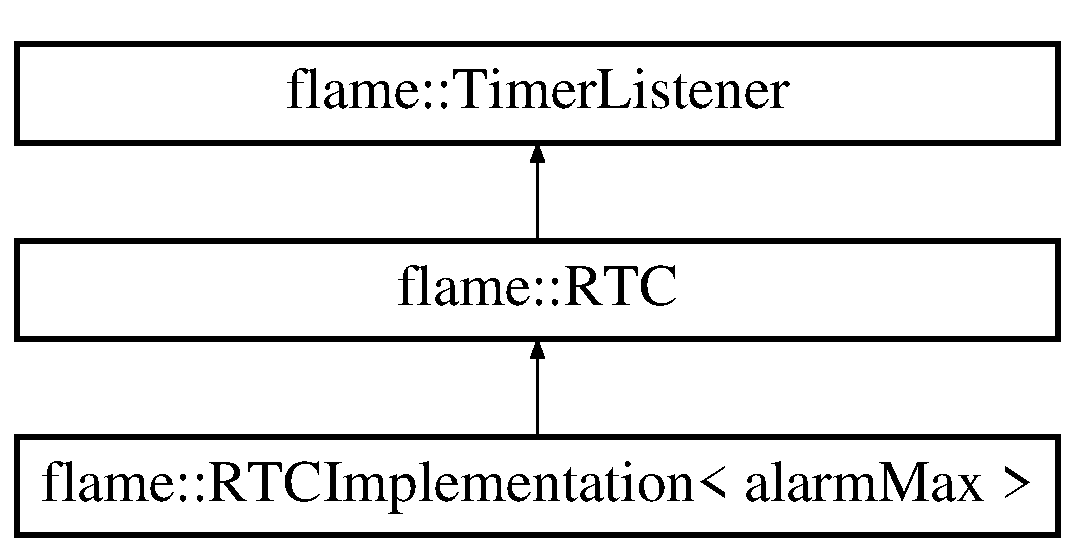
\includegraphics[height=3.000000cm]{classflame_1_1_r_t_c_implementation}
\end{center}
\end{figure}
\subsection*{Public Member Functions}
\begin{DoxyCompactItemize}
\item 
\hyperlink{classflame_1_1_r_t_c_implementation_a492782c8afb5c98850df157c2212fa7b}{R\-T\-C\-Implementation} (int16\-\_\-t timezone=0)
\item 
void \hyperlink{classflame_1_1_r_t_c_implementation_a30401cf4b8502e2fe0d84de3e8782247}{remove\-Alarm} (\hyperlink{classflame_1_1_timer_listener}{Timer\-Listener} \&listener)
\item 
void \hyperlink{classflame_1_1_r_t_c_implementation_a8cc6e18423b995561d15b8895dff63be}{remove\-Alarm} (\hyperlink{classflame_1_1_timer_listener}{Timer\-Listener} $\ast$listener)
\item 
void \hyperlink{classflame_1_1_r_t_c_implementation_a36c258ed2b279ec84172186e988310ab}{handle\-Events} ()
\item 
bool \hyperlink{classflame_1_1_r_t_c_implementation_aa89b6bdab92700b2c51bcb9c421bbfdb}{register\-Alarm} (\hyperlink{namespaceflame_a7a5a7b0bdd1b44d7d0b0a600552b5ab5}{A\-L\-A\-R\-M} \&\hyperlink{structflame_1_1alarm}{alarm})
\item 
void \hyperlink{classflame_1_1_r_t_c_implementation_ab93e0c3fcf47d3b12c4b904103bb7b64}{dump\-Alarms} (\hyperlink{classflame_1_1_device___t_x}{Device\-\_\-\-T\-X} \&tx)
\end{DoxyCompactItemize}
\subsection*{Protected Attributes}
\begin{DoxyCompactItemize}
\item 
\hyperlink{namespaceflame_a7a5a7b0bdd1b44d7d0b0a600552b5ab5}{A\-L\-A\-R\-M} \hyperlink{classflame_1_1_r_t_c_implementation_a78359b4130cbf9bbd314b31b6826a8be}{\-\_\-alarms} \mbox{[}alarm\-Max\mbox{]}
\end{DoxyCompactItemize}
\subsection*{Additional Inherited Members}


\subsection{Detailed Description}
\subsubsection*{template$<$uint8\-\_\-t alarm\-Max = 8$>$class flame\-::\-R\-T\-C\-Implementation$<$ alarm\-Max $>$}



Definition at line 774 of file R\-T\-C.\-h.



\subsection{Constructor \& Destructor Documentation}
\hypertarget{classflame_1_1_r_t_c_implementation_a492782c8afb5c98850df157c2212fa7b}{\index{flame\-::\-R\-T\-C\-Implementation@{flame\-::\-R\-T\-C\-Implementation}!R\-T\-C\-Implementation@{R\-T\-C\-Implementation}}
\index{R\-T\-C\-Implementation@{R\-T\-C\-Implementation}!flame::RTCImplementation@{flame\-::\-R\-T\-C\-Implementation}}
\subsubsection[{R\-T\-C\-Implementation}]{\setlength{\rightskip}{0pt plus 5cm}template$<$uint8\-\_\-t alarm\-Max = 8$>$ {\bf flame\-::\-R\-T\-C\-Implementation}$<$ alarm\-Max $>$\-::{\bf R\-T\-C\-Implementation} (
\begin{DoxyParamCaption}
\item[{int16\-\_\-t}]{timezone = {\ttfamily 0}}
\end{DoxyParamCaption}
)\hspace{0.3cm}{\ttfamily [inline]}}}\label{classflame_1_1_r_t_c_implementation_a492782c8afb5c98850df157c2212fa7b}
Create a new \hyperlink{classflame_1_1_r_t_c}{R\-T\-C} 
\begin{DoxyParams}{Parameters}
{\em timezone} & minutes offset from U\-T\-C \\
\hline
\end{DoxyParams}


Definition at line 783 of file R\-T\-C.\-h.



\subsection{Member Function Documentation}
\hypertarget{classflame_1_1_r_t_c_implementation_ab93e0c3fcf47d3b12c4b904103bb7b64}{\index{flame\-::\-R\-T\-C\-Implementation@{flame\-::\-R\-T\-C\-Implementation}!dump\-Alarms@{dump\-Alarms}}
\index{dump\-Alarms@{dump\-Alarms}!flame::RTCImplementation@{flame\-::\-R\-T\-C\-Implementation}}
\subsubsection[{dump\-Alarms}]{\setlength{\rightskip}{0pt plus 5cm}template$<$uint8\-\_\-t alarm\-Max = 8$>$ void {\bf flame\-::\-R\-T\-C\-Implementation}$<$ alarm\-Max $>$\-::dump\-Alarms (
\begin{DoxyParamCaption}
\item[{{\bf Device\-\_\-\-T\-X} \&}]{tx}
\end{DoxyParamCaption}
)\hspace{0.3cm}{\ttfamily [inline]}}}\label{classflame_1_1_r_t_c_implementation_ab93e0c3fcf47d3b12c4b904103bb7b64}
Dump the current alarms 
\begin{DoxyParams}{Parameters}
{\em tx} & an output device to write to \\
\hline
\end{DoxyParams}


Definition at line 889 of file R\-T\-C.\-h.

\hypertarget{classflame_1_1_r_t_c_implementation_a36c258ed2b279ec84172186e988310ab}{\index{flame\-::\-R\-T\-C\-Implementation@{flame\-::\-R\-T\-C\-Implementation}!handle\-Events@{handle\-Events}}
\index{handle\-Events@{handle\-Events}!flame::RTCImplementation@{flame\-::\-R\-T\-C\-Implementation}}
\subsubsection[{handle\-Events}]{\setlength{\rightskip}{0pt plus 5cm}template$<$uint8\-\_\-t alarm\-Max = 8$>$ void {\bf flame\-::\-R\-T\-C\-Implementation}$<$ alarm\-Max $>$\-::handle\-Events (
\begin{DoxyParamCaption}
{}
\end{DoxyParamCaption}
)\hspace{0.3cm}{\ttfamily [inline]}, {\ttfamily [virtual]}}}\label{classflame_1_1_r_t_c_implementation_a36c258ed2b279ec84172186e988310ab}
Check for events that are due, and run them Run this from your main loop if you have no blocking calls, otherwise, call tick\-And\-Run\-Events instead of tick from the timer (note that this will run your events in the interrupt handler, so keep them short!) 

Implements \hyperlink{classflame_1_1_r_t_c_a123414b982bd03971e057d8fcf4e45ae}{flame\-::\-R\-T\-C}.



Definition at line 818 of file R\-T\-C.\-h.

\hypertarget{classflame_1_1_r_t_c_implementation_aa89b6bdab92700b2c51bcb9c421bbfdb}{\index{flame\-::\-R\-T\-C\-Implementation@{flame\-::\-R\-T\-C\-Implementation}!register\-Alarm@{register\-Alarm}}
\index{register\-Alarm@{register\-Alarm}!flame::RTCImplementation@{flame\-::\-R\-T\-C\-Implementation}}
\subsubsection[{register\-Alarm}]{\setlength{\rightskip}{0pt plus 5cm}template$<$uint8\-\_\-t alarm\-Max = 8$>$ bool {\bf flame\-::\-R\-T\-C\-Implementation}$<$ alarm\-Max $>$\-::register\-Alarm (
\begin{DoxyParamCaption}
\item[{{\bf A\-L\-A\-R\-M} \&}]{alarm}
\end{DoxyParamCaption}
)\hspace{0.3cm}{\ttfamily [inline]}, {\ttfamily [virtual]}}}\label{classflame_1_1_r_t_c_implementation_aa89b6bdab92700b2c51bcb9c421bbfdb}
Insert an alarm, to be triggered at a later time 
\begin{DoxyParams}{Parameters}
{\em alarm} & the alarm, consisting of\-: when it should be triggered how often it should be repeated what should be called (it will be passed a reference to the alarm) \\
\hline
\end{DoxyParams}
\begin{DoxyReturn}{Returns}
true if the event could not be added 
\end{DoxyReturn}


Implements \hyperlink{classflame_1_1_r_t_c_a3ba19efd3cffbe55d363831996657b42}{flame\-::\-R\-T\-C}.



Definition at line 860 of file R\-T\-C.\-h.

\hypertarget{classflame_1_1_r_t_c_implementation_a30401cf4b8502e2fe0d84de3e8782247}{\index{flame\-::\-R\-T\-C\-Implementation@{flame\-::\-R\-T\-C\-Implementation}!remove\-Alarm@{remove\-Alarm}}
\index{remove\-Alarm@{remove\-Alarm}!flame::RTCImplementation@{flame\-::\-R\-T\-C\-Implementation}}
\subsubsection[{remove\-Alarm}]{\setlength{\rightskip}{0pt plus 5cm}template$<$uint8\-\_\-t alarm\-Max = 8$>$ void {\bf flame\-::\-R\-T\-C\-Implementation}$<$ alarm\-Max $>$\-::remove\-Alarm (
\begin{DoxyParamCaption}
\item[{{\bf Timer\-Listener} \&}]{listener}
\end{DoxyParamCaption}
)\hspace{0.3cm}{\ttfamily [inline]}, {\ttfamily [virtual]}}}\label{classflame_1_1_r_t_c_implementation_a30401cf4b8502e2fe0d84de3e8782247}
Remove all matching events from the list of pending events 
\begin{DoxyParams}{Parameters}
{\em listener} & the listener for the event to remove \\
\hline
\end{DoxyParams}


Implements \hyperlink{classflame_1_1_r_t_c_ad493295a4babbc7a3dd4ef18b72c4679}{flame\-::\-R\-T\-C}.



Definition at line 791 of file R\-T\-C.\-h.

\hypertarget{classflame_1_1_r_t_c_implementation_a8cc6e18423b995561d15b8895dff63be}{\index{flame\-::\-R\-T\-C\-Implementation@{flame\-::\-R\-T\-C\-Implementation}!remove\-Alarm@{remove\-Alarm}}
\index{remove\-Alarm@{remove\-Alarm}!flame::RTCImplementation@{flame\-::\-R\-T\-C\-Implementation}}
\subsubsection[{remove\-Alarm}]{\setlength{\rightskip}{0pt plus 5cm}template$<$uint8\-\_\-t alarm\-Max = 8$>$ void {\bf flame\-::\-R\-T\-C\-Implementation}$<$ alarm\-Max $>$\-::remove\-Alarm (
\begin{DoxyParamCaption}
\item[{{\bf Timer\-Listener} $\ast$}]{listener}
\end{DoxyParamCaption}
)\hspace{0.3cm}{\ttfamily [inline]}, {\ttfamily [virtual]}}}\label{classflame_1_1_r_t_c_implementation_a8cc6e18423b995561d15b8895dff63be}
Remove all matching events from the list of pending events 
\begin{DoxyParams}{Parameters}
{\em listener} & the listener for the event to remove \\
\hline
\end{DoxyParams}


Implements \hyperlink{classflame_1_1_r_t_c_a88d193491a668daf956bcc672f3dfc06}{flame\-::\-R\-T\-C}.



Definition at line 799 of file R\-T\-C.\-h.



\subsection{Member Data Documentation}
\hypertarget{classflame_1_1_r_t_c_implementation_a78359b4130cbf9bbd314b31b6826a8be}{\index{flame\-::\-R\-T\-C\-Implementation@{flame\-::\-R\-T\-C\-Implementation}!\-\_\-alarms@{\-\_\-alarms}}
\index{\-\_\-alarms@{\-\_\-alarms}!flame::RTCImplementation@{flame\-::\-R\-T\-C\-Implementation}}
\subsubsection[{\-\_\-alarms}]{\setlength{\rightskip}{0pt plus 5cm}template$<$uint8\-\_\-t alarm\-Max = 8$>$ {\bf A\-L\-A\-R\-M} {\bf flame\-::\-R\-T\-C\-Implementation}$<$ alarm\-Max $>$\-::\-\_\-alarms\mbox{[}alarm\-Max\mbox{]}\hspace{0.3cm}{\ttfamily [protected]}}}\label{classflame_1_1_r_t_c_implementation_a78359b4130cbf9bbd314b31b6826a8be}


Definition at line 776 of file R\-T\-C.\-h.



The documentation for this class was generated from the following file\-:\begin{DoxyCompactItemize}
\item 
flame/\hyperlink{_r_t_c_8h}{R\-T\-C.\-h}\end{DoxyCompactItemize}

\hypertarget{classflame_1_1_r_x_listener}{\section{flame\-:\-:R\-X\-Listener Class Reference}
\label{classflame_1_1_r_x_listener}\index{flame\-::\-R\-X\-Listener@{flame\-::\-R\-X\-Listener}}
}


{\ttfamily \#include $<$Device\-\_\-\-R\-X.\-h$>$}

\subsection*{Public Member Functions}
\begin{DoxyCompactItemize}
\item 
virtual void \hyperlink{classflame_1_1_r_x_listener_a1e345ae38bd923866fd64b14c26fbae6}{rx\-Ready} (\hyperlink{classflame_1_1_device___r_x}{Device\-\_\-\-R\-X} \&rx)=0
\end{DoxyCompactItemize}


\subsection{Detailed Description}
A listener that will be called when a line is ready or the buffer is full 

Definition at line 47 of file Device\-\_\-\-R\-X.\-h.



\subsection{Member Function Documentation}
\hypertarget{classflame_1_1_r_x_listener_a1e345ae38bd923866fd64b14c26fbae6}{\index{flame\-::\-R\-X\-Listener@{flame\-::\-R\-X\-Listener}!rx\-Ready@{rx\-Ready}}
\index{rx\-Ready@{rx\-Ready}!flame::RXListener@{flame\-::\-R\-X\-Listener}}
\subsubsection[{rx\-Ready}]{\setlength{\rightskip}{0pt plus 5cm}virtual void flame\-::\-R\-X\-Listener\-::rx\-Ready (
\begin{DoxyParamCaption}
\item[{{\bf Device\-\_\-\-R\-X} \&}]{rx}
\end{DoxyParamCaption}
)\hspace{0.3cm}{\ttfamily [pure virtual]}}}\label{classflame_1_1_r_x_listener_a1e345ae38bd923866fd64b14c26fbae6}


The documentation for this class was generated from the following file\-:\begin{DoxyCompactItemize}
\item 
flame/\hyperlink{_device___r_x_8h}{Device\-\_\-\-R\-X.\-h}\end{DoxyCompactItemize}

\hypertarget{classflame_1_1_shifter}{\section{flame\-:\-:Shifter Class Reference}
\label{classflame_1_1_shifter}\index{flame\-::\-Shifter@{flame\-::\-Shifter}}
}


{\ttfamily \#include $<$Shifter.\-h$>$}

Inheritance diagram for flame\-:\-:Shifter\-:\begin{figure}[H]
\begin{center}
\leavevmode
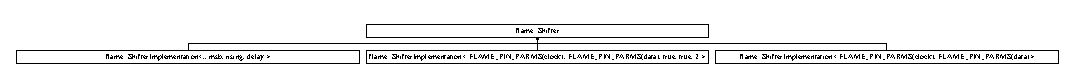
\includegraphics[height=0.624303cm]{classflame_1_1_shifter}
\end{center}
\end{figure}
\subsection*{Public Member Functions}
\begin{DoxyCompactItemize}
\item 
virtual void \hyperlink{classflame_1_1_shifter_ae41737bf06c0c10f4c41ed380bb3f309}{shift\-Out} (uint8\-\_\-t data, uint8\-\_\-t bits)=0
\item 
virtual void \hyperlink{classflame_1_1_shifter_a6309a7c637bbf0f697af638401c1bed4}{shift\-Out} (uint8\-\_\-t data)=0
\item 
virtual void \hyperlink{classflame_1_1_shifter_ae951cbfbe738a62503f906b403e21273}{shift\-Out} (uint8\-\_\-t $\ast$data, uint8\-\_\-t length)=0
\item 
virtual void \hyperlink{classflame_1_1_shifter_a337d5a3460ca61d79e8273e26549b63e}{shift\-Out} (uint8\-\_\-t $\ast$data, uint8\-\_\-t length, uint16\-\_\-t elements)=0
\end{DoxyCompactItemize}


\subsection{Detailed Description}


Definition at line 39 of file Shifter.\-h.



\subsection{Member Function Documentation}
\hypertarget{classflame_1_1_shifter_ae41737bf06c0c10f4c41ed380bb3f309}{\index{flame\-::\-Shifter@{flame\-::\-Shifter}!shift\-Out@{shift\-Out}}
\index{shift\-Out@{shift\-Out}!flame::Shifter@{flame\-::\-Shifter}}
\subsubsection[{shift\-Out}]{\setlength{\rightskip}{0pt plus 5cm}virtual void flame\-::\-Shifter\-::shift\-Out (
\begin{DoxyParamCaption}
\item[{uint8\-\_\-t}]{data, }
\item[{uint8\-\_\-t}]{bits}
\end{DoxyParamCaption}
)\hspace{0.3cm}{\ttfamily [pure virtual]}}}\label{classflame_1_1_shifter_ae41737bf06c0c10f4c41ed380bb3f309}


Implemented in \hyperlink{classflame_1_1_shifter_implementation_abe4372cf69fc72659d95f64f9fa3497d}{flame\-::\-Shifter\-Implementation$<$,, msb, rising, delay $>$}, \hyperlink{classflame_1_1_shifter_implementation_abe4372cf69fc72659d95f64f9fa3497d}{flame\-::\-Shifter\-Implementation$<$ F\-L\-A\-M\-E\-\_\-\-P\-I\-N\-\_\-\-P\-A\-R\-M\-S(clock), F\-L\-A\-M\-E\-\_\-\-P\-I\-N\-\_\-\-P\-A\-R\-M\-S(data), true, true, 2 $>$}, and \hyperlink{classflame_1_1_shifter_implementation_abe4372cf69fc72659d95f64f9fa3497d}{flame\-::\-Shifter\-Implementation$<$ F\-L\-A\-M\-E\-\_\-\-P\-I\-N\-\_\-\-P\-A\-R\-M\-S(clock), F\-L\-A\-M\-E\-\_\-\-P\-I\-N\-\_\-\-P\-A\-R\-M\-S(data)$>$}.

\hypertarget{classflame_1_1_shifter_a6309a7c637bbf0f697af638401c1bed4}{\index{flame\-::\-Shifter@{flame\-::\-Shifter}!shift\-Out@{shift\-Out}}
\index{shift\-Out@{shift\-Out}!flame::Shifter@{flame\-::\-Shifter}}
\subsubsection[{shift\-Out}]{\setlength{\rightskip}{0pt plus 5cm}virtual void flame\-::\-Shifter\-::shift\-Out (
\begin{DoxyParamCaption}
\item[{uint8\-\_\-t}]{data}
\end{DoxyParamCaption}
)\hspace{0.3cm}{\ttfamily [pure virtual]}}}\label{classflame_1_1_shifter_a6309a7c637bbf0f697af638401c1bed4}


Implemented in \hyperlink{classflame_1_1_shifter_implementation_a927327d91cf157895c1ce236a13951a9}{flame\-::\-Shifter\-Implementation$<$,, msb, rising, delay $>$}, \hyperlink{classflame_1_1_shifter_implementation_a927327d91cf157895c1ce236a13951a9}{flame\-::\-Shifter\-Implementation$<$ F\-L\-A\-M\-E\-\_\-\-P\-I\-N\-\_\-\-P\-A\-R\-M\-S(clock), F\-L\-A\-M\-E\-\_\-\-P\-I\-N\-\_\-\-P\-A\-R\-M\-S(data), true, true, 2 $>$}, and \hyperlink{classflame_1_1_shifter_implementation_a927327d91cf157895c1ce236a13951a9}{flame\-::\-Shifter\-Implementation$<$ F\-L\-A\-M\-E\-\_\-\-P\-I\-N\-\_\-\-P\-A\-R\-M\-S(clock), F\-L\-A\-M\-E\-\_\-\-P\-I\-N\-\_\-\-P\-A\-R\-M\-S(data)$>$}.

\hypertarget{classflame_1_1_shifter_ae951cbfbe738a62503f906b403e21273}{\index{flame\-::\-Shifter@{flame\-::\-Shifter}!shift\-Out@{shift\-Out}}
\index{shift\-Out@{shift\-Out}!flame::Shifter@{flame\-::\-Shifter}}
\subsubsection[{shift\-Out}]{\setlength{\rightskip}{0pt plus 5cm}virtual void flame\-::\-Shifter\-::shift\-Out (
\begin{DoxyParamCaption}
\item[{uint8\-\_\-t $\ast$}]{data, }
\item[{uint8\-\_\-t}]{length}
\end{DoxyParamCaption}
)\hspace{0.3cm}{\ttfamily [pure virtual]}}}\label{classflame_1_1_shifter_ae951cbfbe738a62503f906b403e21273}


Implemented in \hyperlink{classflame_1_1_shifter_implementation_a7c061a25f9c664901f2d9247daf6f37b}{flame\-::\-Shifter\-Implementation$<$,, msb, rising, delay $>$}, \hyperlink{classflame_1_1_shifter_implementation_a7c061a25f9c664901f2d9247daf6f37b}{flame\-::\-Shifter\-Implementation$<$ F\-L\-A\-M\-E\-\_\-\-P\-I\-N\-\_\-\-P\-A\-R\-M\-S(clock), F\-L\-A\-M\-E\-\_\-\-P\-I\-N\-\_\-\-P\-A\-R\-M\-S(data), true, true, 2 $>$}, and \hyperlink{classflame_1_1_shifter_implementation_a7c061a25f9c664901f2d9247daf6f37b}{flame\-::\-Shifter\-Implementation$<$ F\-L\-A\-M\-E\-\_\-\-P\-I\-N\-\_\-\-P\-A\-R\-M\-S(clock), F\-L\-A\-M\-E\-\_\-\-P\-I\-N\-\_\-\-P\-A\-R\-M\-S(data)$>$}.

\hypertarget{classflame_1_1_shifter_a337d5a3460ca61d79e8273e26549b63e}{\index{flame\-::\-Shifter@{flame\-::\-Shifter}!shift\-Out@{shift\-Out}}
\index{shift\-Out@{shift\-Out}!flame::Shifter@{flame\-::\-Shifter}}
\subsubsection[{shift\-Out}]{\setlength{\rightskip}{0pt plus 5cm}virtual void flame\-::\-Shifter\-::shift\-Out (
\begin{DoxyParamCaption}
\item[{uint8\-\_\-t $\ast$}]{data, }
\item[{uint8\-\_\-t}]{length, }
\item[{uint16\-\_\-t}]{elements}
\end{DoxyParamCaption}
)\hspace{0.3cm}{\ttfamily [pure virtual]}}}\label{classflame_1_1_shifter_a337d5a3460ca61d79e8273e26549b63e}


Implemented in \hyperlink{classflame_1_1_shifter_implementation_aa380a270ea9d3b40da868822daf9022e}{flame\-::\-Shifter\-Implementation$<$,, msb, rising, delay $>$}, \hyperlink{classflame_1_1_shifter_implementation_aa380a270ea9d3b40da868822daf9022e}{flame\-::\-Shifter\-Implementation$<$ F\-L\-A\-M\-E\-\_\-\-P\-I\-N\-\_\-\-P\-A\-R\-M\-S(clock), F\-L\-A\-M\-E\-\_\-\-P\-I\-N\-\_\-\-P\-A\-R\-M\-S(data), true, true, 2 $>$}, and \hyperlink{classflame_1_1_shifter_implementation_aa380a270ea9d3b40da868822daf9022e}{flame\-::\-Shifter\-Implementation$<$ F\-L\-A\-M\-E\-\_\-\-P\-I\-N\-\_\-\-P\-A\-R\-M\-S(clock), F\-L\-A\-M\-E\-\_\-\-P\-I\-N\-\_\-\-P\-A\-R\-M\-S(data)$>$}.



The documentation for this class was generated from the following file\-:\begin{DoxyCompactItemize}
\item 
flame/\hyperlink{_shifter_8h}{Shifter.\-h}\end{DoxyCompactItemize}

\hypertarget{classflame_1_1_shifter_implementation}{\section{flame\-:\-:Shifter\-Implementation$<$,, msb, rising, delay $>$ Class Template Reference}
\label{classflame_1_1_shifter_implementation}\index{flame\-::\-Shifter\-Implementation$<$,, msb, rising, delay $>$@{flame\-::\-Shifter\-Implementation$<$,, msb, rising, delay $>$}}
}


{\ttfamily \#include $<$Shifter.\-h$>$}

Inheritance diagram for flame\-:\-:Shifter\-Implementation$<$,, msb, rising, delay $>$\-:\begin{figure}[H]
\begin{center}
\leavevmode
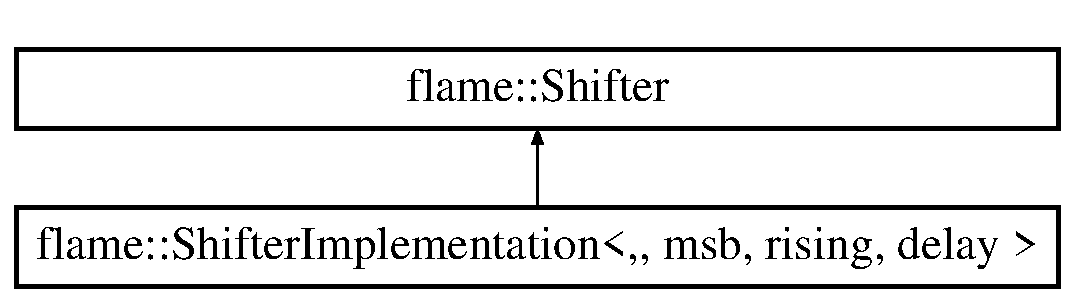
\includegraphics[height=2.000000cm]{classflame_1_1_shifter_implementation}
\end{center}
\end{figure}
\subsection*{Public Member Functions}
\begin{DoxyCompactItemize}
\item 
\hyperlink{classflame_1_1_shifter_implementation_a6a500da4041278c3f2e773ccb86afe8d}{Shifter\-Implementation} ()
\item 
void \hyperlink{classflame_1_1_shifter_implementation_abe4372cf69fc72659d95f64f9fa3497d}{shift\-Out} (uint8\-\_\-t data, uint8\-\_\-t bits)
\item 
void \hyperlink{classflame_1_1_shifter_implementation_a927327d91cf157895c1ce236a13951a9}{shift\-Out} (uint8\-\_\-t data)
\item 
void \hyperlink{classflame_1_1_shifter_implementation_a7c061a25f9c664901f2d9247daf6f37b}{shift\-Out} (uint8\-\_\-t $\ast$shift\-Data, uint8\-\_\-t shift\-Length)
\item 
void \hyperlink{classflame_1_1_shifter_implementation_aa380a270ea9d3b40da868822daf9022e}{shift\-Out} (uint8\-\_\-t $\ast$shift\-Data, uint8\-\_\-t data\-Length, uint16\-\_\-t elements)
\end{DoxyCompactItemize}


\subsection{Detailed Description}
\subsubsection*{template$<$F\-L\-A\-M\-E\-\_\-\-D\-E\-C\-L\-A\-R\-E\-\_\-\-P\-I\-N(clock), F\-L\-A\-M\-E\-\_\-\-D\-E\-C\-L\-A\-R\-E\-\_\-\-P\-I\-N(data), bool msb = true, bool rising = true, uint16\-\_\-t delay = 0$>$class flame\-::\-Shifter\-Implementation$<$,, msb, rising, delay $>$}

Create a new shifter 
\begin{DoxyTemplParams}{Template Parameters}
{\em clock...} & an pin describing the clock line \\
\hline
{\em data...} & an pin describing the data line \\
\hline
{\em msb} & true to output M\-S\-B first. false for L\-S\-B \\
\hline
{\em rising} & true if the receiver is clocked on the rising edge, false otherwise \\
\hline
{\em delay} & the delay between state changes (us) \\
\hline
\end{DoxyTemplParams}


Definition at line 60 of file Shifter.\-h.



\subsection{Constructor \& Destructor Documentation}
\hypertarget{classflame_1_1_shifter_implementation_a6a500da4041278c3f2e773ccb86afe8d}{\index{flame\-::\-Shifter\-Implementation@{flame\-::\-Shifter\-Implementation}!Shifter\-Implementation@{Shifter\-Implementation}}
\index{Shifter\-Implementation@{Shifter\-Implementation}!flame::ShifterImplementation@{flame\-::\-Shifter\-Implementation}}
\subsubsection[{Shifter\-Implementation}]{\setlength{\rightskip}{0pt plus 5cm}template$<$F\-L\-A\-M\-E\-\_\-\-D\-E\-C\-L\-A\-R\-E\-\_\-\-P\-I\-N(clock) , F\-L\-A\-M\-E\-\_\-\-D\-E\-C\-L\-A\-R\-E\-\_\-\-P\-I\-N(data) , bool msb = true, bool rising = true, uint16\-\_\-t delay = 0$>$ {\bf flame\-::\-Shifter\-Implementation}$<$,, msb, rising, delay $>$\-::{\bf Shifter\-Implementation} (
\begin{DoxyParamCaption}
{}
\end{DoxyParamCaption}
)\hspace{0.3cm}{\ttfamily [inline]}}}\label{classflame_1_1_shifter_implementation_a6a500da4041278c3f2e773ccb86afe8d}
Constructor -\/ set the pins to output 

Definition at line 928 of file Shifter.\-h.



\subsection{Member Function Documentation}
\hypertarget{classflame_1_1_shifter_implementation_abe4372cf69fc72659d95f64f9fa3497d}{\index{flame\-::\-Shifter\-Implementation@{flame\-::\-Shifter\-Implementation}!shift\-Out@{shift\-Out}}
\index{shift\-Out@{shift\-Out}!flame::ShifterImplementation@{flame\-::\-Shifter\-Implementation}}
\subsubsection[{shift\-Out}]{\setlength{\rightskip}{0pt plus 5cm}template$<$F\-L\-A\-M\-E\-\_\-\-D\-E\-C\-L\-A\-R\-E\-\_\-\-P\-I\-N(clock) , F\-L\-A\-M\-E\-\_\-\-D\-E\-C\-L\-A\-R\-E\-\_\-\-P\-I\-N(data) , bool msb = true, bool rising = true, uint16\-\_\-t delay = 0$>$ void {\bf flame\-::\-Shifter\-Implementation}$<$,, msb, rising, delay $>$\-::shift\-Out (
\begin{DoxyParamCaption}
\item[{uint8\-\_\-t}]{data, }
\item[{uint8\-\_\-t}]{bits}
\end{DoxyParamCaption}
)\hspace{0.3cm}{\ttfamily [inline]}, {\ttfamily [virtual]}}}\label{classflame_1_1_shifter_implementation_abe4372cf69fc72659d95f64f9fa3497d}
Shift out a number of bits (L\-S\-B aligned) 
\begin{DoxyParams}{Parameters}
{\em data} & a byte containing the bits to shift \\
\hline
{\em bits} & the number of bits to shift \\
\hline
\end{DoxyParams}


Implements \hyperlink{classflame_1_1_shifter_ae41737bf06c0c10f4c41ed380bb3f309}{flame\-::\-Shifter}.



Definition at line 938 of file Shifter.\-h.

\hypertarget{classflame_1_1_shifter_implementation_a927327d91cf157895c1ce236a13951a9}{\index{flame\-::\-Shifter\-Implementation@{flame\-::\-Shifter\-Implementation}!shift\-Out@{shift\-Out}}
\index{shift\-Out@{shift\-Out}!flame::ShifterImplementation@{flame\-::\-Shifter\-Implementation}}
\subsubsection[{shift\-Out}]{\setlength{\rightskip}{0pt plus 5cm}template$<$F\-L\-A\-M\-E\-\_\-\-D\-E\-C\-L\-A\-R\-E\-\_\-\-P\-I\-N(clock) , F\-L\-A\-M\-E\-\_\-\-D\-E\-C\-L\-A\-R\-E\-\_\-\-P\-I\-N(data) , bool msb = true, bool rising = true, uint16\-\_\-t delay = 0$>$ void {\bf flame\-::\-Shifter\-Implementation}$<$,, msb, rising, delay $>$\-::shift\-Out (
\begin{DoxyParamCaption}
\item[{uint8\-\_\-t}]{data}
\end{DoxyParamCaption}
)\hspace{0.3cm}{\ttfamily [inline]}, {\ttfamily [virtual]}}}\label{classflame_1_1_shifter_implementation_a927327d91cf157895c1ce236a13951a9}
Shift out a byte of data 
\begin{DoxyParams}{Parameters}
{\em data} & the data to output \\
\hline
\end{DoxyParams}


Implements \hyperlink{classflame_1_1_shifter_a6309a7c637bbf0f697af638401c1bed4}{flame\-::\-Shifter}.



Definition at line 973 of file Shifter.\-h.

\hypertarget{classflame_1_1_shifter_implementation_a7c061a25f9c664901f2d9247daf6f37b}{\index{flame\-::\-Shifter\-Implementation@{flame\-::\-Shifter\-Implementation}!shift\-Out@{shift\-Out}}
\index{shift\-Out@{shift\-Out}!flame::ShifterImplementation@{flame\-::\-Shifter\-Implementation}}
\subsubsection[{shift\-Out}]{\setlength{\rightskip}{0pt plus 5cm}template$<$F\-L\-A\-M\-E\-\_\-\-D\-E\-C\-L\-A\-R\-E\-\_\-\-P\-I\-N(clock) , F\-L\-A\-M\-E\-\_\-\-D\-E\-C\-L\-A\-R\-E\-\_\-\-P\-I\-N(data) , bool msb = true, bool rising = true, uint16\-\_\-t delay = 0$>$ void {\bf flame\-::\-Shifter\-Implementation}$<$,, msb, rising, delay $>$\-::shift\-Out (
\begin{DoxyParamCaption}
\item[{uint8\-\_\-t $\ast$}]{shift\-Data, }
\item[{uint8\-\_\-t}]{shift\-Length}
\end{DoxyParamCaption}
)\hspace{0.3cm}{\ttfamily [inline]}, {\ttfamily [virtual]}}}\label{classflame_1_1_shifter_implementation_a7c061a25f9c664901f2d9247daf6f37b}


Implements \hyperlink{classflame_1_1_shifter_ae951cbfbe738a62503f906b403e21273}{flame\-::\-Shifter}.



Definition at line 1005 of file Shifter.\-h.

\hypertarget{classflame_1_1_shifter_implementation_aa380a270ea9d3b40da868822daf9022e}{\index{flame\-::\-Shifter\-Implementation@{flame\-::\-Shifter\-Implementation}!shift\-Out@{shift\-Out}}
\index{shift\-Out@{shift\-Out}!flame::ShifterImplementation@{flame\-::\-Shifter\-Implementation}}
\subsubsection[{shift\-Out}]{\setlength{\rightskip}{0pt plus 5cm}template$<$F\-L\-A\-M\-E\-\_\-\-D\-E\-C\-L\-A\-R\-E\-\_\-\-P\-I\-N(clock) , F\-L\-A\-M\-E\-\_\-\-D\-E\-C\-L\-A\-R\-E\-\_\-\-P\-I\-N(data) , bool msb = true, bool rising = true, uint16\-\_\-t delay = 0$>$ void {\bf flame\-::\-Shifter\-Implementation}$<$,, msb, rising, delay $>$\-::shift\-Out (
\begin{DoxyParamCaption}
\item[{uint8\-\_\-t $\ast$}]{shift\-Data, }
\item[{uint8\-\_\-t}]{data\-Length, }
\item[{uint16\-\_\-t}]{elements}
\end{DoxyParamCaption}
)\hspace{0.3cm}{\ttfamily [inline]}, {\ttfamily [virtual]}}}\label{classflame_1_1_shifter_implementation_aa380a270ea9d3b40da868822daf9022e}


Implements \hyperlink{classflame_1_1_shifter_a337d5a3460ca61d79e8273e26549b63e}{flame\-::\-Shifter}.



Definition at line 1021 of file Shifter.\-h.



The documentation for this class was generated from the following file\-:\begin{DoxyCompactItemize}
\item 
flame/\hyperlink{_shifter_8h}{Shifter.\-h}\end{DoxyCompactItemize}

\hypertarget{classflame_1_1_software_p_w_m}{\section{flame\-:\-:Software\-P\-W\-M$<$ listener\-Count $>$ Class Template Reference}
\label{classflame_1_1_software_p_w_m}\index{flame\-::\-Software\-P\-W\-M$<$ listener\-Count $>$@{flame\-::\-Software\-P\-W\-M$<$ listener\-Count $>$}}
}


{\ttfamily \#include $<$Software\-P\-W\-M.\-h$>$}

Inheritance diagram for flame\-:\-:Software\-P\-W\-M$<$ listener\-Count $>$\-:\begin{figure}[H]
\begin{center}
\leavevmode
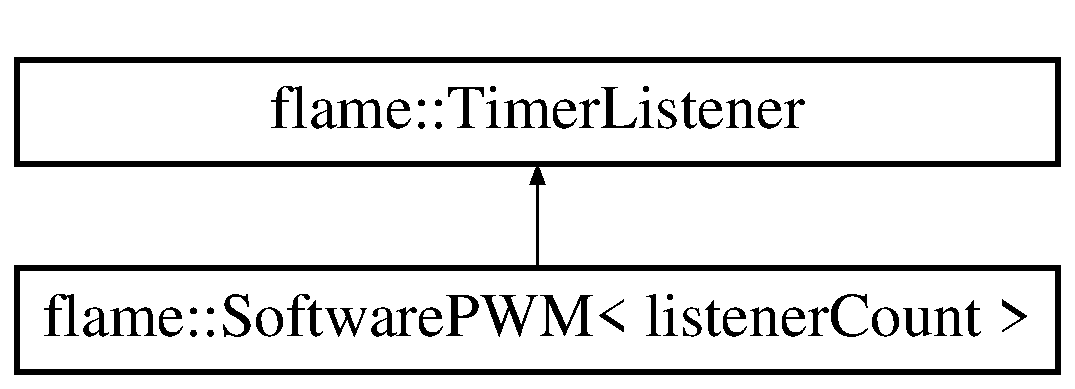
\includegraphics[height=2.000000cm]{classflame_1_1_software_p_w_m}
\end{center}
\end{figure}
\subsection*{Public Member Functions}
\begin{DoxyCompactItemize}
\item 
\hyperlink{classflame_1_1_software_p_w_m_a1221e93371787565449622704de2debf}{Software\-P\-W\-M} (\hyperlink{classflame_1_1_timer}{Timer} \&timer)
\item 
uint8\-\_\-t \hyperlink{classflame_1_1_software_p_w_m_a4a8a61037e62b7e2349c5513bf96771f}{add\-Listener} (\hyperlink{classflame_1_1_software_p_w_m_listener}{Software\-P\-W\-M\-Listener} \&listener)
\item 
void \hyperlink{classflame_1_1_software_p_w_m_ae128de439f29b8bb877e5a74d24e3ec3}{alarm} (\hyperlink{io_8h_addf5ec070e9499d36b7f2009ce736076}{U\-N\-U\-S\-E\-D} \hyperlink{namespaceflame_a6d176ba245556716fd3e32006bb7cfe5}{Alarm\-Source} source)
\end{DoxyCompactItemize}


\subsection{Detailed Description}
\subsubsection*{template$<$uint8\-\_\-t listener\-Count = 8$>$class flame\-::\-Software\-P\-W\-M$<$ listener\-Count $>$}



Definition at line 75 of file Software\-P\-W\-M.\-h.



\subsection{Constructor \& Destructor Documentation}
\hypertarget{classflame_1_1_software_p_w_m_a1221e93371787565449622704de2debf}{\index{flame\-::\-Software\-P\-W\-M@{flame\-::\-Software\-P\-W\-M}!Software\-P\-W\-M@{Software\-P\-W\-M}}
\index{Software\-P\-W\-M@{Software\-P\-W\-M}!flame::SoftwarePWM@{flame\-::\-Software\-P\-W\-M}}
\subsubsection[{Software\-P\-W\-M}]{\setlength{\rightskip}{0pt plus 5cm}template$<$uint8\-\_\-t listener\-Count = 8$>$ {\bf flame\-::\-Software\-P\-W\-M}$<$ listener\-Count $>$\-::{\bf Software\-P\-W\-M} (
\begin{DoxyParamCaption}
\item[{{\bf Timer} \&}]{timer}
\end{DoxyParamCaption}
)\hspace{0.3cm}{\ttfamily [inline]}}}\label{classflame_1_1_software_p_w_m_a1221e93371787565449622704de2debf}
Create a new software P\-W\-M manager 
\begin{DoxyParams}{Parameters}
{\em timer} & the timer to drive the manager with \\
\hline
\end{DoxyParams}


Definition at line 87 of file Software\-P\-W\-M.\-h.



\subsection{Member Function Documentation}
\hypertarget{classflame_1_1_software_p_w_m_a4a8a61037e62b7e2349c5513bf96771f}{\index{flame\-::\-Software\-P\-W\-M@{flame\-::\-Software\-P\-W\-M}!add\-Listener@{add\-Listener}}
\index{add\-Listener@{add\-Listener}!flame::SoftwarePWM@{flame\-::\-Software\-P\-W\-M}}
\subsubsection[{add\-Listener}]{\setlength{\rightskip}{0pt plus 5cm}template$<$uint8\-\_\-t listener\-Count = 8$>$ uint8\-\_\-t {\bf flame\-::\-Software\-P\-W\-M}$<$ listener\-Count $>$\-::add\-Listener (
\begin{DoxyParamCaption}
\item[{{\bf Software\-P\-W\-M\-Listener} \&}]{listener}
\end{DoxyParamCaption}
)\hspace{0.3cm}{\ttfamily [inline]}}}\label{classflame_1_1_software_p_w_m_a4a8a61037e62b7e2349c5513bf96771f}
Register a listener 
\begin{DoxyParams}{Parameters}
{\em listener} & the listener to register \\
\hline
\end{DoxyParams}
\begin{DoxyReturn}{Returns}
the index of listener, or 0 if the add failed 
\end{DoxyReturn}


Definition at line 97 of file Software\-P\-W\-M.\-h.

\hypertarget{classflame_1_1_software_p_w_m_ae128de439f29b8bb877e5a74d24e3ec3}{\index{flame\-::\-Software\-P\-W\-M@{flame\-::\-Software\-P\-W\-M}!alarm@{alarm}}
\index{alarm@{alarm}!flame::SoftwarePWM@{flame\-::\-Software\-P\-W\-M}}
\subsubsection[{alarm}]{\setlength{\rightskip}{0pt plus 5cm}template$<$uint8\-\_\-t listener\-Count = 8$>$ void {\bf flame\-::\-Software\-P\-W\-M}$<$ listener\-Count $>$\-::{\bf alarm} (
\begin{DoxyParamCaption}
\item[{{\bf U\-N\-U\-S\-E\-D} {\bf Alarm\-Source}}]{source}
\end{DoxyParamCaption}
)\hspace{0.3cm}{\ttfamily [inline]}}}\label{classflame_1_1_software_p_w_m_ae128de439f29b8bb877e5a74d24e3ec3}
Handle the timer interrupt by setting the outputs 

Definition at line 112 of file Software\-P\-W\-M.\-h.



The documentation for this class was generated from the following file\-:\begin{DoxyCompactItemize}
\item 
flame/\hyperlink{_software_p_w_m_8h}{Software\-P\-W\-M.\-h}\end{DoxyCompactItemize}

\hypertarget{classflame_1_1_software_p_w_m_listener}{\section{flame\-:\-:Software\-P\-W\-M\-Listener Class Reference}
\label{classflame_1_1_software_p_w_m_listener}\index{flame\-::\-Software\-P\-W\-M\-Listener@{flame\-::\-Software\-P\-W\-M\-Listener}}
}


{\ttfamily \#include $<$Software\-P\-W\-M.\-h$>$}

Inheritance diagram for flame\-:\-:Software\-P\-W\-M\-Listener\-:\begin{figure}[H]
\begin{center}
\leavevmode
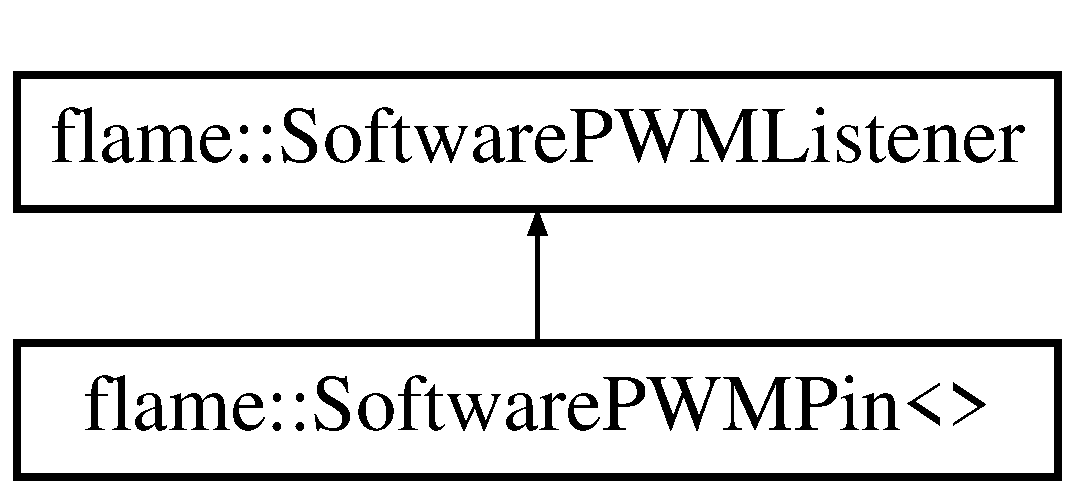
\includegraphics[height=2.000000cm]{classflame_1_1_software_p_w_m_listener}
\end{center}
\end{figure}
\subsection*{Public Member Functions}
\begin{DoxyCompactItemize}
\item 
virtual void \hyperlink{classflame_1_1_software_p_w_m_listener_a4d8db257cb0f4cbcba16a8986416ca6a}{reset} ()=0
\item 
virtual void \hyperlink{classflame_1_1_software_p_w_m_listener_af08c4eb71ac1d22d479a4c2bdce0fe12}{set} ()=0
\item 
virtual bool \hyperlink{classflame_1_1_software_p_w_m_listener_a2e8a39faa1f233483720a516397df545}{check} ()=0
\item 
void \hyperlink{classflame_1_1_software_p_w_m_listener_a82d1d2dcb7d0dd19278469554673dc7b}{set\-Duty\-Cycle} (uint8\-\_\-t duty\-Cycle)
\item 
uint8\-\_\-t \hyperlink{classflame_1_1_software_p_w_m_listener_a497cc44fbc87e08bcae5230298a78461}{get\-Duty\-Cycle} ()
\end{DoxyCompactItemize}
\subsection*{Public Attributes}
\begin{DoxyCompactItemize}
\item 
uint8\-\_\-t \hyperlink{classflame_1_1_software_p_w_m_listener_a0f8297e9d8ac43c30c02585bf1e220b1}{when}
\end{DoxyCompactItemize}


\subsection{Detailed Description}


Definition at line 36 of file Software\-P\-W\-M.\-h.



\subsection{Member Function Documentation}
\hypertarget{classflame_1_1_software_p_w_m_listener_a2e8a39faa1f233483720a516397df545}{\index{flame\-::\-Software\-P\-W\-M\-Listener@{flame\-::\-Software\-P\-W\-M\-Listener}!check@{check}}
\index{check@{check}!flame::SoftwarePWMListener@{flame\-::\-Software\-P\-W\-M\-Listener}}
\subsubsection[{check}]{\setlength{\rightskip}{0pt plus 5cm}virtual bool flame\-::\-Software\-P\-W\-M\-Listener\-::check (
\begin{DoxyParamCaption}
{}
\end{DoxyParamCaption}
)\hspace{0.3cm}{\ttfamily [pure virtual]}}}\label{classflame_1_1_software_p_w_m_listener_a2e8a39faa1f233483720a516397df545}


Implemented in \hyperlink{classflame_1_1_software_p_w_m_pin_aa87439920593e3e06605722f5d707e22}{flame\-::\-Software\-P\-W\-M\-Pin$<$$>$}.

\hypertarget{classflame_1_1_software_p_w_m_listener_a497cc44fbc87e08bcae5230298a78461}{\index{flame\-::\-Software\-P\-W\-M\-Listener@{flame\-::\-Software\-P\-W\-M\-Listener}!get\-Duty\-Cycle@{get\-Duty\-Cycle}}
\index{get\-Duty\-Cycle@{get\-Duty\-Cycle}!flame::SoftwarePWMListener@{flame\-::\-Software\-P\-W\-M\-Listener}}
\subsubsection[{get\-Duty\-Cycle}]{\setlength{\rightskip}{0pt plus 5cm}uint8\-\_\-t flame\-::\-Software\-P\-W\-M\-Listener\-::get\-Duty\-Cycle (
\begin{DoxyParamCaption}
{}
\end{DoxyParamCaption}
)\hspace{0.3cm}{\ttfamily [inline]}}}\label{classflame_1_1_software_p_w_m_listener_a497cc44fbc87e08bcae5230298a78461}


Definition at line 48 of file Software\-P\-W\-M.\-h.

\hypertarget{classflame_1_1_software_p_w_m_listener_a4d8db257cb0f4cbcba16a8986416ca6a}{\index{flame\-::\-Software\-P\-W\-M\-Listener@{flame\-::\-Software\-P\-W\-M\-Listener}!reset@{reset}}
\index{reset@{reset}!flame::SoftwarePWMListener@{flame\-::\-Software\-P\-W\-M\-Listener}}
\subsubsection[{reset}]{\setlength{\rightskip}{0pt plus 5cm}virtual void flame\-::\-Software\-P\-W\-M\-Listener\-::reset (
\begin{DoxyParamCaption}
{}
\end{DoxyParamCaption}
)\hspace{0.3cm}{\ttfamily [pure virtual]}}}\label{classflame_1_1_software_p_w_m_listener_a4d8db257cb0f4cbcba16a8986416ca6a}


Implemented in \hyperlink{classflame_1_1_software_p_w_m_pin_a51b59f964716b33518510345252da74f}{flame\-::\-Software\-P\-W\-M\-Pin$<$$>$}.

\hypertarget{classflame_1_1_software_p_w_m_listener_af08c4eb71ac1d22d479a4c2bdce0fe12}{\index{flame\-::\-Software\-P\-W\-M\-Listener@{flame\-::\-Software\-P\-W\-M\-Listener}!set@{set}}
\index{set@{set}!flame::SoftwarePWMListener@{flame\-::\-Software\-P\-W\-M\-Listener}}
\subsubsection[{set}]{\setlength{\rightskip}{0pt plus 5cm}virtual void flame\-::\-Software\-P\-W\-M\-Listener\-::set (
\begin{DoxyParamCaption}
{}
\end{DoxyParamCaption}
)\hspace{0.3cm}{\ttfamily [pure virtual]}}}\label{classflame_1_1_software_p_w_m_listener_af08c4eb71ac1d22d479a4c2bdce0fe12}


Implemented in \hyperlink{classflame_1_1_software_p_w_m_pin_a9d744a25930b0bbaf6fe220f1adc9f41}{flame\-::\-Software\-P\-W\-M\-Pin$<$$>$}.

\hypertarget{classflame_1_1_software_p_w_m_listener_a82d1d2dcb7d0dd19278469554673dc7b}{\index{flame\-::\-Software\-P\-W\-M\-Listener@{flame\-::\-Software\-P\-W\-M\-Listener}!set\-Duty\-Cycle@{set\-Duty\-Cycle}}
\index{set\-Duty\-Cycle@{set\-Duty\-Cycle}!flame::SoftwarePWMListener@{flame\-::\-Software\-P\-W\-M\-Listener}}
\subsubsection[{set\-Duty\-Cycle}]{\setlength{\rightskip}{0pt plus 5cm}void flame\-::\-Software\-P\-W\-M\-Listener\-::set\-Duty\-Cycle (
\begin{DoxyParamCaption}
\item[{uint8\-\_\-t}]{duty\-Cycle}
\end{DoxyParamCaption}
)\hspace{0.3cm}{\ttfamily [inline]}}}\label{classflame_1_1_software_p_w_m_listener_a82d1d2dcb7d0dd19278469554673dc7b}


Definition at line 44 of file Software\-P\-W\-M.\-h.



\subsection{Member Data Documentation}
\hypertarget{classflame_1_1_software_p_w_m_listener_a0f8297e9d8ac43c30c02585bf1e220b1}{\index{flame\-::\-Software\-P\-W\-M\-Listener@{flame\-::\-Software\-P\-W\-M\-Listener}!when@{when}}
\index{when@{when}!flame::SoftwarePWMListener@{flame\-::\-Software\-P\-W\-M\-Listener}}
\subsubsection[{when}]{\setlength{\rightskip}{0pt plus 5cm}uint8\-\_\-t flame\-::\-Software\-P\-W\-M\-Listener\-::when}}\label{classflame_1_1_software_p_w_m_listener_a0f8297e9d8ac43c30c02585bf1e220b1}


Definition at line 38 of file Software\-P\-W\-M.\-h.



The documentation for this class was generated from the following file\-:\begin{DoxyCompactItemize}
\item 
flame/\hyperlink{_software_p_w_m_8h}{Software\-P\-W\-M.\-h}\end{DoxyCompactItemize}

\hypertarget{classflame_1_1_software_p_w_m_pin}{\section{flame\-:\-:Software\-P\-W\-M\-Pin$<$$>$ Class Template Reference}
\label{classflame_1_1_software_p_w_m_pin}\index{flame\-::\-Software\-P\-W\-M\-Pin$<$$>$@{flame\-::\-Software\-P\-W\-M\-Pin$<$$>$}}
}


{\ttfamily \#include $<$Software\-P\-W\-M.\-h$>$}

Inheritance diagram for flame\-:\-:Software\-P\-W\-M\-Pin$<$$>$\-:\begin{figure}[H]
\begin{center}
\leavevmode
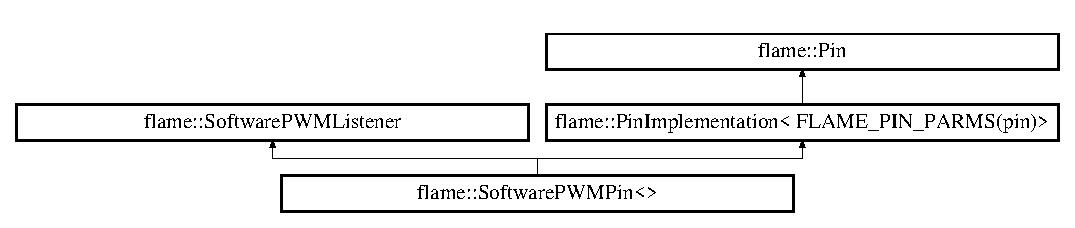
\includegraphics[height=2.616822cm]{classflame_1_1_software_p_w_m_pin}
\end{center}
\end{figure}
\subsection*{Public Member Functions}
\begin{DoxyCompactItemize}
\item 
\hyperlink{classflame_1_1_software_p_w_m_pin_aaba6d2dd4b849975d80f9bfddd4a4b7a}{Software\-P\-W\-M\-Pin} ()
\item 
\hyperlink{io_8h_a2eb6f9e0395b47b8d5e3eeae4fe0c116}{I\-N\-L\-I\-N\-E} void \hyperlink{classflame_1_1_software_p_w_m_pin_a51b59f964716b33518510345252da74f}{reset} ()
\item 
\hyperlink{io_8h_a2eb6f9e0395b47b8d5e3eeae4fe0c116}{I\-N\-L\-I\-N\-E} void \hyperlink{classflame_1_1_software_p_w_m_pin_a9d744a25930b0bbaf6fe220f1adc9f41}{set} ()
\item 
\hyperlink{io_8h_a2eb6f9e0395b47b8d5e3eeae4fe0c116}{I\-N\-L\-I\-N\-E} bool \hyperlink{classflame_1_1_software_p_w_m_pin_aa87439920593e3e06605722f5d707e22}{check} ()
\end{DoxyCompactItemize}
\subsection*{Additional Inherited Members}


\subsection{Detailed Description}
\subsubsection*{template$<$F\-L\-A\-M\-E\-\_\-\-D\-E\-C\-L\-A\-R\-E\-\_\-\-P\-I\-N(pin)$>$class flame\-::\-Software\-P\-W\-M\-Pin$<$$>$}



Definition at line 54 of file Software\-P\-W\-M.\-h.



\subsection{Constructor \& Destructor Documentation}
\hypertarget{classflame_1_1_software_p_w_m_pin_aaba6d2dd4b849975d80f9bfddd4a4b7a}{\index{flame\-::\-Software\-P\-W\-M\-Pin@{flame\-::\-Software\-P\-W\-M\-Pin}!Software\-P\-W\-M\-Pin@{Software\-P\-W\-M\-Pin}}
\index{Software\-P\-W\-M\-Pin@{Software\-P\-W\-M\-Pin}!flame::SoftwarePWMPin@{flame\-::\-Software\-P\-W\-M\-Pin}}
\subsubsection[{Software\-P\-W\-M\-Pin}]{\setlength{\rightskip}{0pt plus 5cm}template$<$F\-L\-A\-M\-E\-\_\-\-D\-E\-C\-L\-A\-R\-E\-\_\-\-P\-I\-N(pin) $>$ {\bf flame\-::\-Software\-P\-W\-M\-Pin}$<$$>$\-::{\bf Software\-P\-W\-M\-Pin} (
\begin{DoxyParamCaption}
{}
\end{DoxyParamCaption}
)\hspace{0.3cm}{\ttfamily [inline]}}}\label{classflame_1_1_software_p_w_m_pin_aaba6d2dd4b849975d80f9bfddd4a4b7a}


Definition at line 56 of file Software\-P\-W\-M.\-h.



\subsection{Member Function Documentation}
\hypertarget{classflame_1_1_software_p_w_m_pin_aa87439920593e3e06605722f5d707e22}{\index{flame\-::\-Software\-P\-W\-M\-Pin@{flame\-::\-Software\-P\-W\-M\-Pin}!check@{check}}
\index{check@{check}!flame::SoftwarePWMPin@{flame\-::\-Software\-P\-W\-M\-Pin}}
\subsubsection[{check}]{\setlength{\rightskip}{0pt plus 5cm}template$<$F\-L\-A\-M\-E\-\_\-\-D\-E\-C\-L\-A\-R\-E\-\_\-\-P\-I\-N(pin) $>$ {\bf I\-N\-L\-I\-N\-E} bool {\bf flame\-::\-Software\-P\-W\-M\-Pin}$<$$>$\-::check (
\begin{DoxyParamCaption}
{}
\end{DoxyParamCaption}
)\hspace{0.3cm}{\ttfamily [inline]}, {\ttfamily [virtual]}}}\label{classflame_1_1_software_p_w_m_pin_aa87439920593e3e06605722f5d707e22}


Implements \hyperlink{classflame_1_1_software_p_w_m_listener_a2e8a39faa1f233483720a516397df545}{flame\-::\-Software\-P\-W\-M\-Listener}.



Definition at line 68 of file Software\-P\-W\-M.\-h.

\hypertarget{classflame_1_1_software_p_w_m_pin_a51b59f964716b33518510345252da74f}{\index{flame\-::\-Software\-P\-W\-M\-Pin@{flame\-::\-Software\-P\-W\-M\-Pin}!reset@{reset}}
\index{reset@{reset}!flame::SoftwarePWMPin@{flame\-::\-Software\-P\-W\-M\-Pin}}
\subsubsection[{reset}]{\setlength{\rightskip}{0pt plus 5cm}template$<$F\-L\-A\-M\-E\-\_\-\-D\-E\-C\-L\-A\-R\-E\-\_\-\-P\-I\-N(pin) $>$ {\bf I\-N\-L\-I\-N\-E} void {\bf flame\-::\-Software\-P\-W\-M\-Pin}$<$$>$\-::reset (
\begin{DoxyParamCaption}
{}
\end{DoxyParamCaption}
)\hspace{0.3cm}{\ttfamily [inline]}, {\ttfamily [virtual]}}}\label{classflame_1_1_software_p_w_m_pin_a51b59f964716b33518510345252da74f}


Implements \hyperlink{classflame_1_1_software_p_w_m_listener_a4d8db257cb0f4cbcba16a8986416ca6a}{flame\-::\-Software\-P\-W\-M\-Listener}.



Definition at line 60 of file Software\-P\-W\-M.\-h.

\hypertarget{classflame_1_1_software_p_w_m_pin_a9d744a25930b0bbaf6fe220f1adc9f41}{\index{flame\-::\-Software\-P\-W\-M\-Pin@{flame\-::\-Software\-P\-W\-M\-Pin}!set@{set}}
\index{set@{set}!flame::SoftwarePWMPin@{flame\-::\-Software\-P\-W\-M\-Pin}}
\subsubsection[{set}]{\setlength{\rightskip}{0pt plus 5cm}template$<$F\-L\-A\-M\-E\-\_\-\-D\-E\-C\-L\-A\-R\-E\-\_\-\-P\-I\-N(pin) $>$ {\bf I\-N\-L\-I\-N\-E} void {\bf flame\-::\-Software\-P\-W\-M\-Pin}$<$$>$\-::set (
\begin{DoxyParamCaption}
{}
\end{DoxyParamCaption}
)\hspace{0.3cm}{\ttfamily [inline]}, {\ttfamily [virtual]}}}\label{classflame_1_1_software_p_w_m_pin_a9d744a25930b0bbaf6fe220f1adc9f41}


Implements \hyperlink{classflame_1_1_software_p_w_m_listener_af08c4eb71ac1d22d479a4c2bdce0fe12}{flame\-::\-Software\-P\-W\-M\-Listener}.



Definition at line 64 of file Software\-P\-W\-M.\-h.



The documentation for this class was generated from the following file\-:\begin{DoxyCompactItemize}
\item 
flame/\hyperlink{_software_p_w_m_8h}{Software\-P\-W\-M.\-h}\end{DoxyCompactItemize}

\hypertarget{classflame_1_1_stepper_listener}{\section{flame\-:\-:Stepper\-Listener Class Reference}
\label{classflame_1_1_stepper_listener}\index{flame\-::\-Stepper\-Listener@{flame\-::\-Stepper\-Listener}}
}


{\ttfamily \#include $<$Stepper\-Motor.\-h$>$}

\subsection*{Public Member Functions}
\begin{DoxyCompactItemize}
\item 
virtual void \hyperlink{classflame_1_1_stepper_listener_ad596b4126186142c7a760aa4d9bfff4e}{move\-Complete} (int32\-\_\-t position)=0
\end{DoxyCompactItemize}


\subsection{Detailed Description}


Definition at line 36 of file Stepper\-Motor.\-h.



\subsection{Member Function Documentation}
\hypertarget{classflame_1_1_stepper_listener_ad596b4126186142c7a760aa4d9bfff4e}{\index{flame\-::\-Stepper\-Listener@{flame\-::\-Stepper\-Listener}!move\-Complete@{move\-Complete}}
\index{move\-Complete@{move\-Complete}!flame::StepperListener@{flame\-::\-Stepper\-Listener}}
\subsubsection[{move\-Complete}]{\setlength{\rightskip}{0pt plus 5cm}virtual void flame\-::\-Stepper\-Listener\-::move\-Complete (
\begin{DoxyParamCaption}
\item[{int32\-\_\-t}]{position}
\end{DoxyParamCaption}
)\hspace{0.3cm}{\ttfamily [pure virtual]}}}\label{classflame_1_1_stepper_listener_ad596b4126186142c7a760aa4d9bfff4e}


The documentation for this class was generated from the following file\-:\begin{DoxyCompactItemize}
\item 
flame/\hyperlink{_stepper_motor_8h}{Stepper\-Motor.\-h}\end{DoxyCompactItemize}

\hypertarget{classflame_1_1_stepper_motor}{\section{flame\-:\-:Stepper\-Motor Class Reference}
\label{classflame_1_1_stepper_motor}\index{flame\-::\-Stepper\-Motor@{flame\-::\-Stepper\-Motor}}
}


{\ttfamily \#include $<$Stepper\-Motor.\-h$>$}

Inheritance diagram for flame\-:\-:Stepper\-Motor\-:\begin{figure}[H]
\begin{center}
\leavevmode
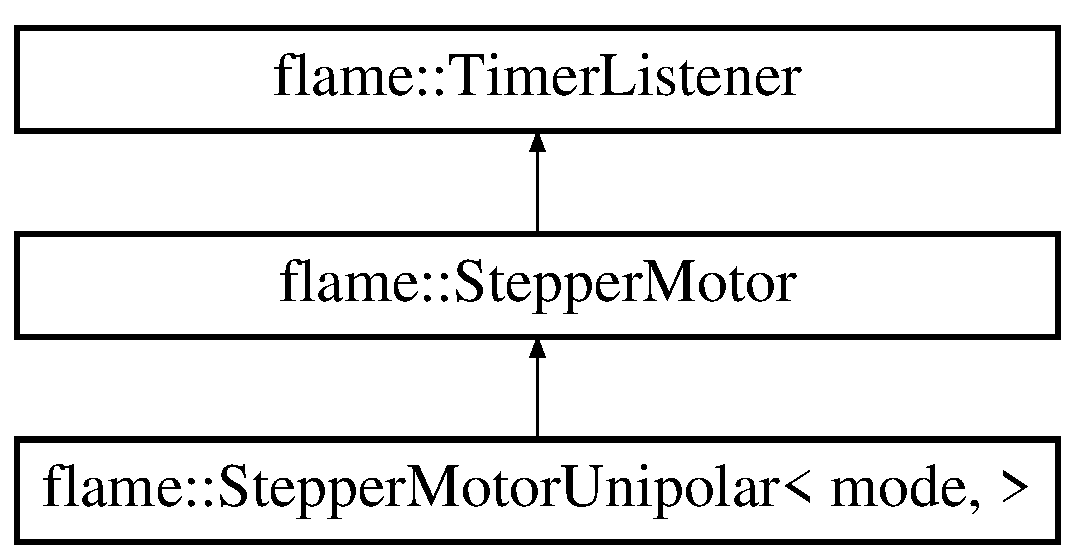
\includegraphics[height=3.000000cm]{classflame_1_1_stepper_motor}
\end{center}
\end{figure}
\subsection*{Public Member Functions}
\begin{DoxyCompactItemize}
\item 
\hyperlink{classflame_1_1_stepper_motor_a17ca894e1297cb5d964c516dc8898fc0}{Stepper\-Motor} (\hyperlink{classflame_1_1_r_t_c}{R\-T\-C} \&rtc)
\item 
virtual void \hyperlink{classflame_1_1_stepper_motor_aab7e060d1704320b560657d912e791c9}{step} (bool forward)=0
\item 
void \hyperlink{classflame_1_1_stepper_motor_a260cf0be1a9c9d2ff362b8ad816b2c6c}{set\-Position} (int32\-\_\-t position)
\item 
bool \hyperlink{classflame_1_1_stepper_motor_ac86907c985c1f382e43790aa15e8c7a7}{is\-Moving} () \hyperlink{io_8h_acd42770aecb025cfac170d4d3ace4544}{P\-U\-R\-E}
\item 
int32\-\_\-t \hyperlink{classflame_1_1_stepper_motor_a69b9a3febce0c7e45c304fc5cea95165}{get\-Position} () \hyperlink{io_8h_acd42770aecb025cfac170d4d3ace4544}{P\-U\-R\-E}
\item 
void \hyperlink{classflame_1_1_stepper_motor_a5122f463d29b39e9bb9544a57cade8bf}{rotate} (bool forward, float speed, int32\-\_\-t until)
\item 
void \hyperlink{classflame_1_1_stepper_motor_a6eec1ffcfd13c4624525b4cabe1eec4c}{alarm} (\hyperlink{namespaceflame_a6d176ba245556716fd3e32006bb7cfe5}{Alarm\-Source} source)
\item 
void \hyperlink{classflame_1_1_stepper_motor_a2603e1dd71e15543bfb0a3c0d3a491f9}{register\-Listener} (\hyperlink{classflame_1_1_stepper_listener}{Stepper\-Listener} \&listener)
\item 
void \hyperlink{classflame_1_1_stepper_motor_a90e7ab11b511c68dea947465006ee0c6}{deregister\-Listener} ()
\end{DoxyCompactItemize}


\subsection{Detailed Description}


Definition at line 41 of file Stepper\-Motor.\-h.



\subsection{Constructor \& Destructor Documentation}
\hypertarget{classflame_1_1_stepper_motor_a17ca894e1297cb5d964c516dc8898fc0}{\index{flame\-::\-Stepper\-Motor@{flame\-::\-Stepper\-Motor}!Stepper\-Motor@{Stepper\-Motor}}
\index{Stepper\-Motor@{Stepper\-Motor}!flame::StepperMotor@{flame\-::\-Stepper\-Motor}}
\subsubsection[{Stepper\-Motor}]{\setlength{\rightskip}{0pt plus 5cm}flame\-::\-Stepper\-Motor\-::\-Stepper\-Motor (
\begin{DoxyParamCaption}
\item[{{\bf R\-T\-C} \&}]{rtc}
\end{DoxyParamCaption}
)}}\label{classflame_1_1_stepper_motor_a17ca894e1297cb5d964c516dc8898fc0}
Create a new \hyperlink{classflame_1_1_stepper_motor}{Stepper\-Motor} 
\begin{DoxyParams}{Parameters}
{\em rtc} & an \hyperlink{classflame_1_1_r_t_c}{R\-T\-C} we will use to trigger events \\
\hline
\end{DoxyParams}


Definition at line 35 of file Stepper\-Motor.\-cpp.



\subsection{Member Function Documentation}
\hypertarget{classflame_1_1_stepper_motor_a6eec1ffcfd13c4624525b4cabe1eec4c}{\index{flame\-::\-Stepper\-Motor@{flame\-::\-Stepper\-Motor}!alarm@{alarm}}
\index{alarm@{alarm}!flame::StepperMotor@{flame\-::\-Stepper\-Motor}}
\subsubsection[{alarm}]{\setlength{\rightskip}{0pt plus 5cm}void flame\-::\-Stepper\-Motor\-::alarm (
\begin{DoxyParamCaption}
\item[{{\bf Alarm\-Source}}]{source}
\end{DoxyParamCaption}
)\hspace{0.3cm}{\ttfamily [virtual]}}}\label{classflame_1_1_stepper_motor_a6eec1ffcfd13c4624525b4cabe1eec4c}
Called periodically to move the motor 

Implements \hyperlink{classflame_1_1_timer_listener_ad97504b72a25b1fba354803338177335}{flame\-::\-Timer\-Listener}.



Definition at line 94 of file Stepper\-Motor.\-cpp.

\hypertarget{classflame_1_1_stepper_motor_a90e7ab11b511c68dea947465006ee0c6}{\index{flame\-::\-Stepper\-Motor@{flame\-::\-Stepper\-Motor}!deregister\-Listener@{deregister\-Listener}}
\index{deregister\-Listener@{deregister\-Listener}!flame::StepperMotor@{flame\-::\-Stepper\-Motor}}
\subsubsection[{deregister\-Listener}]{\setlength{\rightskip}{0pt plus 5cm}void flame\-::\-Stepper\-Motor\-::deregister\-Listener (
\begin{DoxyParamCaption}
{}
\end{DoxyParamCaption}
)}}\label{classflame_1_1_stepper_motor_a90e7ab11b511c68dea947465006ee0c6}
Deregister the listener 

Definition at line 134 of file Stepper\-Motor.\-cpp.

\hypertarget{classflame_1_1_stepper_motor_a69b9a3febce0c7e45c304fc5cea95165}{\index{flame\-::\-Stepper\-Motor@{flame\-::\-Stepper\-Motor}!get\-Position@{get\-Position}}
\index{get\-Position@{get\-Position}!flame::StepperMotor@{flame\-::\-Stepper\-Motor}}
\subsubsection[{get\-Position}]{\setlength{\rightskip}{0pt plus 5cm}int32\-\_\-t flame\-::\-Stepper\-Motor\-::get\-Position (
\begin{DoxyParamCaption}
{}
\end{DoxyParamCaption}
)}}\label{classflame_1_1_stepper_motor_a69b9a3febce0c7e45c304fc5cea95165}
Get the current position of the motor \begin{DoxyReturn}{Returns}
the current position 
\end{DoxyReturn}


Definition at line 55 of file Stepper\-Motor.\-cpp.

\hypertarget{classflame_1_1_stepper_motor_ac86907c985c1f382e43790aa15e8c7a7}{\index{flame\-::\-Stepper\-Motor@{flame\-::\-Stepper\-Motor}!is\-Moving@{is\-Moving}}
\index{is\-Moving@{is\-Moving}!flame::StepperMotor@{flame\-::\-Stepper\-Motor}}
\subsubsection[{is\-Moving}]{\setlength{\rightskip}{0pt plus 5cm}bool flame\-::\-Stepper\-Motor\-::is\-Moving (
\begin{DoxyParamCaption}
{}
\end{DoxyParamCaption}
)}}\label{classflame_1_1_stepper_motor_ac86907c985c1f382e43790aa15e8c7a7}
Is the motor current moving? \begin{DoxyReturn}{Returns}
true if the motor is moving 
\end{DoxyReturn}


Definition at line 63 of file Stepper\-Motor.\-cpp.

\hypertarget{classflame_1_1_stepper_motor_a2603e1dd71e15543bfb0a3c0d3a491f9}{\index{flame\-::\-Stepper\-Motor@{flame\-::\-Stepper\-Motor}!register\-Listener@{register\-Listener}}
\index{register\-Listener@{register\-Listener}!flame::StepperMotor@{flame\-::\-Stepper\-Motor}}
\subsubsection[{register\-Listener}]{\setlength{\rightskip}{0pt plus 5cm}void flame\-::\-Stepper\-Motor\-::register\-Listener (
\begin{DoxyParamCaption}
\item[{{\bf Stepper\-Listener} \&}]{listener}
\end{DoxyParamCaption}
)}}\label{classflame_1_1_stepper_motor_a2603e1dd71e15543bfb0a3c0d3a491f9}
Register a listener to be notified when moves are complete 
\begin{DoxyParams}{Parameters}
{\em listener} & the listener to notify \\
\hline
\end{DoxyParams}


Definition at line 127 of file Stepper\-Motor.\-cpp.

\hypertarget{classflame_1_1_stepper_motor_a5122f463d29b39e9bb9544a57cade8bf}{\index{flame\-::\-Stepper\-Motor@{flame\-::\-Stepper\-Motor}!rotate@{rotate}}
\index{rotate@{rotate}!flame::StepperMotor@{flame\-::\-Stepper\-Motor}}
\subsubsection[{rotate}]{\setlength{\rightskip}{0pt plus 5cm}void flame\-::\-Stepper\-Motor\-::rotate (
\begin{DoxyParamCaption}
\item[{bool}]{forward, }
\item[{float}]{speed, }
\item[{int32\-\_\-t}]{until}
\end{DoxyParamCaption}
)}}\label{classflame_1_1_stepper_motor_a5122f463d29b39e9bb9544a57cade8bf}
Move the motor to a new position (this will override a current move if there is one) 
\begin{DoxyParams}{Parameters}
{\em forward} & true to move forward \\
\hline
{\em speed} & the speed to move in steps/second \\
\hline
{\em until} & the position to stop at \\
\hline
\end{DoxyParams}


Definition at line 73 of file Stepper\-Motor.\-cpp.

\hypertarget{classflame_1_1_stepper_motor_a260cf0be1a9c9d2ff362b8ad816b2c6c}{\index{flame\-::\-Stepper\-Motor@{flame\-::\-Stepper\-Motor}!set\-Position@{set\-Position}}
\index{set\-Position@{set\-Position}!flame::StepperMotor@{flame\-::\-Stepper\-Motor}}
\subsubsection[{set\-Position}]{\setlength{\rightskip}{0pt plus 5cm}void flame\-::\-Stepper\-Motor\-::set\-Position (
\begin{DoxyParamCaption}
\item[{int32\-\_\-t}]{position}
\end{DoxyParamCaption}
)}}\label{classflame_1_1_stepper_motor_a260cf0be1a9c9d2ff362b8ad816b2c6c}
Mark the current position of the motor. This simply changes where we think we are, it does not move the motor


\begin{DoxyParams}{Parameters}
{\em position} & the new position \\
\hline
\end{DoxyParams}


Definition at line 47 of file Stepper\-Motor.\-cpp.

\hypertarget{classflame_1_1_stepper_motor_aab7e060d1704320b560657d912e791c9}{\index{flame\-::\-Stepper\-Motor@{flame\-::\-Stepper\-Motor}!step@{step}}
\index{step@{step}!flame::StepperMotor@{flame\-::\-Stepper\-Motor}}
\subsubsection[{step}]{\setlength{\rightskip}{0pt plus 5cm}virtual void flame\-::\-Stepper\-Motor\-::step (
\begin{DoxyParamCaption}
\item[{bool}]{forward}
\end{DoxyParamCaption}
)\hspace{0.3cm}{\ttfamily [pure virtual]}}}\label{classflame_1_1_stepper_motor_aab7e060d1704320b560657d912e791c9}


Implemented in \hyperlink{classflame_1_1_stepper_motor_unipolar_ace9ef8057a4a7cb6aa13db88c6a0ef4a}{flame\-::\-Stepper\-Motor\-Unipolar$<$ mode, $>$}.



The documentation for this class was generated from the following files\-:\begin{DoxyCompactItemize}
\item 
flame/\hyperlink{_stepper_motor_8h}{Stepper\-Motor.\-h}\item 
\hyperlink{_stepper_motor_8cpp}{Stepper\-Motor.\-cpp}\end{DoxyCompactItemize}

\hypertarget{classflame_1_1_stepper_motor_unipolar}{\section{flame\-:\-:Stepper\-Motor\-Unipolar$<$ mode, $>$ Class Template Reference}
\label{classflame_1_1_stepper_motor_unipolar}\index{flame\-::\-Stepper\-Motor\-Unipolar$<$ mode, $>$@{flame\-::\-Stepper\-Motor\-Unipolar$<$ mode, $>$}}
}


{\ttfamily \#include $<$Stepper\-Motor\-Unipolar.\-h$>$}

Inheritance diagram for flame\-:\-:Stepper\-Motor\-Unipolar$<$ mode, $>$\-:\begin{figure}[H]
\begin{center}
\leavevmode
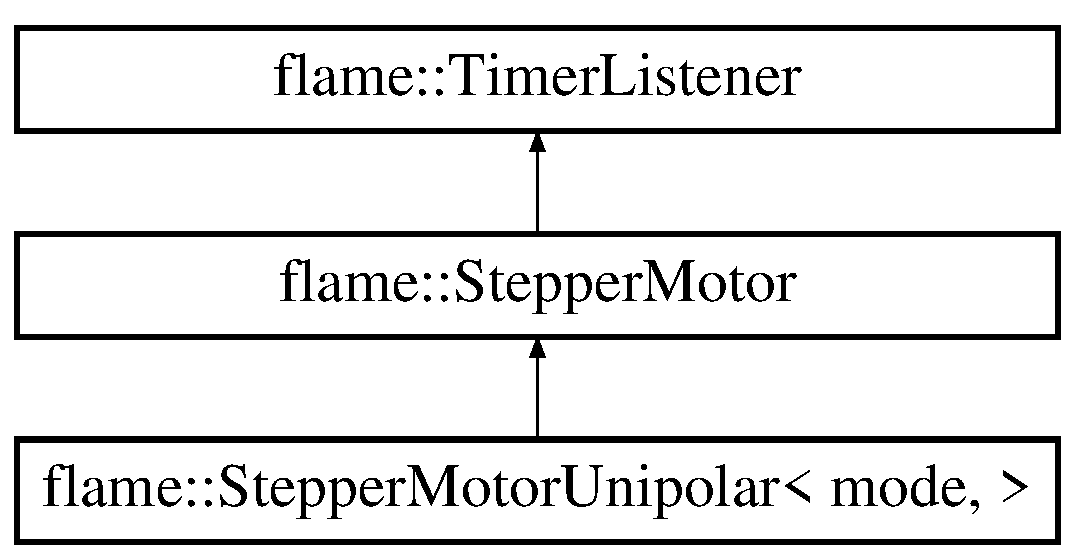
\includegraphics[height=3.000000cm]{classflame_1_1_stepper_motor_unipolar}
\end{center}
\end{figure}
\subsection*{Public Member Functions}
\begin{DoxyCompactItemize}
\item 
\hyperlink{classflame_1_1_stepper_motor_unipolar_af690093f238136417f9b051fadd62f28}{Stepper\-Motor\-Unipolar} (\hyperlink{classflame_1_1_r_t_c}{R\-T\-C} \&rtc)
\item 
void \hyperlink{classflame_1_1_stepper_motor_unipolar_ace9ef8057a4a7cb6aa13db88c6a0ef4a}{step} (bool forwards)
\end{DoxyCompactItemize}


\subsection{Detailed Description}
\subsubsection*{template$<$Stepper\-Mode mode, F\-L\-A\-M\-E\-\_\-\-D\-E\-C\-L\-A\-R\-E\-\_\-\-P\-I\-N(phase\-A)$>$class flame\-::\-Stepper\-Motor\-Unipolar$<$ mode, $>$}

A unipolar stepper motor driver

Phase output is active high, so if you are using transistors to buffer the motor, you will need to pull the common line high and use the transistors to pull the phases to ground.

Phases A \& C share a common ground, as does B \& D

Phases B, C and D use consecutive pins on the same port as A


\begin{DoxyTemplParams}{Template Parameters}
{\em mode} & the mode of the stepper driver \\
\hline
{\em phase\-A} & the pin for the A phase \\
\hline
\end{DoxyTemplParams}


Definition at line 90 of file Stepper\-Motor\-Unipolar.\-h.



\subsection{Constructor \& Destructor Documentation}
\hypertarget{classflame_1_1_stepper_motor_unipolar_af690093f238136417f9b051fadd62f28}{\index{flame\-::\-Stepper\-Motor\-Unipolar@{flame\-::\-Stepper\-Motor\-Unipolar}!Stepper\-Motor\-Unipolar@{Stepper\-Motor\-Unipolar}}
\index{Stepper\-Motor\-Unipolar@{Stepper\-Motor\-Unipolar}!flame::StepperMotorUnipolar@{flame\-::\-Stepper\-Motor\-Unipolar}}
\subsubsection[{Stepper\-Motor\-Unipolar}]{\setlength{\rightskip}{0pt plus 5cm}template$<$Stepper\-Mode mode, F\-L\-A\-M\-E\-\_\-\-D\-E\-C\-L\-A\-R\-E\-\_\-\-P\-I\-N(phase\-A) $>$ {\bf flame\-::\-Stepper\-Motor\-Unipolar}$<$ mode, $>$\-::{\bf Stepper\-Motor\-Unipolar} (
\begin{DoxyParamCaption}
\item[{{\bf R\-T\-C} \&}]{rtc}
\end{DoxyParamCaption}
)\hspace{0.3cm}{\ttfamily [inline]}}}\label{classflame_1_1_stepper_motor_unipolar_af690093f238136417f9b051fadd62f28}
Create a driver for a unipolar stepper motor


\begin{DoxyParams}{Parameters}
{\em rtc} & the \hyperlink{classflame_1_1_r_t_c}{R\-T\-C} used for stepper movements \\
\hline
\end{DoxyParams}


Definition at line 137 of file Stepper\-Motor\-Unipolar.\-h.



\subsection{Member Function Documentation}
\hypertarget{classflame_1_1_stepper_motor_unipolar_ace9ef8057a4a7cb6aa13db88c6a0ef4a}{\index{flame\-::\-Stepper\-Motor\-Unipolar@{flame\-::\-Stepper\-Motor\-Unipolar}!step@{step}}
\index{step@{step}!flame::StepperMotorUnipolar@{flame\-::\-Stepper\-Motor\-Unipolar}}
\subsubsection[{step}]{\setlength{\rightskip}{0pt plus 5cm}template$<$Stepper\-Mode mode, F\-L\-A\-M\-E\-\_\-\-D\-E\-C\-L\-A\-R\-E\-\_\-\-P\-I\-N(phase\-A) $>$ void {\bf flame\-::\-Stepper\-Motor\-Unipolar}$<$ mode, $>$\-::step (
\begin{DoxyParamCaption}
\item[{bool}]{forwards}
\end{DoxyParamCaption}
)\hspace{0.3cm}{\ttfamily [inline]}, {\ttfamily [virtual]}}}\label{classflame_1_1_stepper_motor_unipolar_ace9ef8057a4a7cb6aa13db88c6a0ef4a}


Implements \hyperlink{classflame_1_1_stepper_motor_aab7e060d1704320b560657d912e791c9}{flame\-::\-Stepper\-Motor}.



Definition at line 149 of file Stepper\-Motor\-Unipolar.\-h.



The documentation for this class was generated from the following file\-:\begin{DoxyCompactItemize}
\item 
flame/\hyperlink{_stepper_motor_unipolar_8h}{Stepper\-Motor\-Unipolar.\-h}\end{DoxyCompactItemize}

\hypertarget{structflame_1_1time}{\section{flame\-:\-:time Struct Reference}
\label{structflame_1_1time}\index{flame\-::time@{flame\-::time}}
}


{\ttfamily \#include $<$R\-T\-C.\-h$>$}

\subsection*{Public Attributes}
\begin{DoxyCompactItemize}
\item 
uint16\-\_\-t \hyperlink{structflame_1_1time_a899f1caf24d147cdd0cdeb787e289497}{milliseconds}
\item 
uint8\-\_\-t \hyperlink{structflame_1_1time_af9b2c35926951e50470223c2d05a1ca4}{seconds}
\item 
uint8\-\_\-t \hyperlink{structflame_1_1time_afda149b0149ecab591b605e108eb80ae}{minutes}
\item 
uint8\-\_\-t \hyperlink{structflame_1_1time_a1319436ec4fe46d74a865ee7717b998d}{hours}
\item 
uint8\-\_\-t \hyperlink{structflame_1_1time_a4e5ce39f9a9bc7f7e508bf7e9108091e}{day}
\item 
\hyperlink{namespaceflame_aa452b7c1018de4dfa5d302b613109649}{Month} \hyperlink{structflame_1_1time_a78a0e559562f4e7102e083da6384a1c6}{month}
\item 
uint16\-\_\-t \hyperlink{structflame_1_1time_a74325344f17f185431c09e97a7208657}{year}
\item 
uint16\-\_\-t \hyperlink{structflame_1_1time_a17f380f3785ac47964ecb96657901155}{yearday}
\item 
uint16\-\_\-t \hyperlink{structflame_1_1time_a4deaf87f9d7d63270bc9c7275fc3c4cb}{timezone}
\end{DoxyCompactItemize}


\subsection{Detailed Description}


Definition at line 76 of file R\-T\-C.\-h.



\subsection{Member Data Documentation}
\hypertarget{structflame_1_1time_a4e5ce39f9a9bc7f7e508bf7e9108091e}{\index{flame\-::time@{flame\-::time}!day@{day}}
\index{day@{day}!flame::time@{flame\-::time}}
\subsubsection[{day}]{\setlength{\rightskip}{0pt plus 5cm}uint8\-\_\-t flame\-::time\-::day}}\label{structflame_1_1time_a4e5ce39f9a9bc7f7e508bf7e9108091e}


Definition at line 81 of file R\-T\-C.\-h.

\hypertarget{structflame_1_1time_a1319436ec4fe46d74a865ee7717b998d}{\index{flame\-::time@{flame\-::time}!hours@{hours}}
\index{hours@{hours}!flame::time@{flame\-::time}}
\subsubsection[{hours}]{\setlength{\rightskip}{0pt plus 5cm}uint8\-\_\-t flame\-::time\-::hours}}\label{structflame_1_1time_a1319436ec4fe46d74a865ee7717b998d}


Definition at line 80 of file R\-T\-C.\-h.

\hypertarget{structflame_1_1time_a899f1caf24d147cdd0cdeb787e289497}{\index{flame\-::time@{flame\-::time}!milliseconds@{milliseconds}}
\index{milliseconds@{milliseconds}!flame::time@{flame\-::time}}
\subsubsection[{milliseconds}]{\setlength{\rightskip}{0pt plus 5cm}uint16\-\_\-t flame\-::time\-::milliseconds}}\label{structflame_1_1time_a899f1caf24d147cdd0cdeb787e289497}


Definition at line 77 of file R\-T\-C.\-h.

\hypertarget{structflame_1_1time_afda149b0149ecab591b605e108eb80ae}{\index{flame\-::time@{flame\-::time}!minutes@{minutes}}
\index{minutes@{minutes}!flame::time@{flame\-::time}}
\subsubsection[{minutes}]{\setlength{\rightskip}{0pt plus 5cm}uint8\-\_\-t flame\-::time\-::minutes}}\label{structflame_1_1time_afda149b0149ecab591b605e108eb80ae}


Definition at line 79 of file R\-T\-C.\-h.

\hypertarget{structflame_1_1time_a78a0e559562f4e7102e083da6384a1c6}{\index{flame\-::time@{flame\-::time}!month@{month}}
\index{month@{month}!flame::time@{flame\-::time}}
\subsubsection[{month}]{\setlength{\rightskip}{0pt plus 5cm}{\bf Month} flame\-::time\-::month}}\label{structflame_1_1time_a78a0e559562f4e7102e083da6384a1c6}


Definition at line 82 of file R\-T\-C.\-h.

\hypertarget{structflame_1_1time_af9b2c35926951e50470223c2d05a1ca4}{\index{flame\-::time@{flame\-::time}!seconds@{seconds}}
\index{seconds@{seconds}!flame::time@{flame\-::time}}
\subsubsection[{seconds}]{\setlength{\rightskip}{0pt plus 5cm}uint8\-\_\-t flame\-::time\-::seconds}}\label{structflame_1_1time_af9b2c35926951e50470223c2d05a1ca4}


Definition at line 78 of file R\-T\-C.\-h.

\hypertarget{structflame_1_1time_a4deaf87f9d7d63270bc9c7275fc3c4cb}{\index{flame\-::time@{flame\-::time}!timezone@{timezone}}
\index{timezone@{timezone}!flame::time@{flame\-::time}}
\subsubsection[{timezone}]{\setlength{\rightskip}{0pt plus 5cm}uint16\-\_\-t flame\-::time\-::timezone}}\label{structflame_1_1time_a4deaf87f9d7d63270bc9c7275fc3c4cb}


Definition at line 86 of file R\-T\-C.\-h.

\hypertarget{structflame_1_1time_a74325344f17f185431c09e97a7208657}{\index{flame\-::time@{flame\-::time}!year@{year}}
\index{year@{year}!flame::time@{flame\-::time}}
\subsubsection[{year}]{\setlength{\rightskip}{0pt plus 5cm}uint16\-\_\-t flame\-::time\-::year}}\label{structflame_1_1time_a74325344f17f185431c09e97a7208657}


Definition at line 83 of file R\-T\-C.\-h.

\hypertarget{structflame_1_1time_a17f380f3785ac47964ecb96657901155}{\index{flame\-::time@{flame\-::time}!yearday@{yearday}}
\index{yearday@{yearday}!flame::time@{flame\-::time}}
\subsubsection[{yearday}]{\setlength{\rightskip}{0pt plus 5cm}uint16\-\_\-t flame\-::time\-::yearday}}\label{structflame_1_1time_a17f380f3785ac47964ecb96657901155}


Definition at line 85 of file R\-T\-C.\-h.



The documentation for this struct was generated from the following file\-:\begin{DoxyCompactItemize}
\item 
flame/\hyperlink{_r_t_c_8h}{R\-T\-C.\-h}\end{DoxyCompactItemize}

\hypertarget{classflame_1_1_timer}{\section{flame\-:\-:Timer Class Reference}
\label{classflame_1_1_timer}\index{flame\-::\-Timer@{flame\-::\-Timer}}
}


{\ttfamily \#include $<$Timer.\-h$>$}

Inheritance diagram for flame\-:\-:Timer\-:\begin{figure}[H]
\begin{center}
\leavevmode
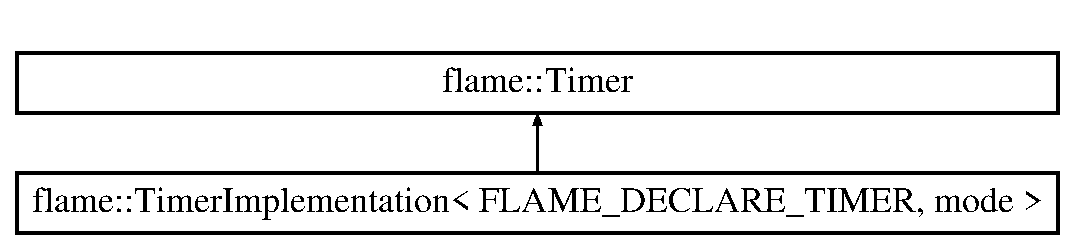
\includegraphics[height=2.000000cm]{classflame_1_1_timer}
\end{center}
\end{figure}
\subsection*{Public Member Functions}
\begin{DoxyCompactItemize}
\item 
\hyperlink{io_8h_a2eb6f9e0395b47b8d5e3eeae4fe0c116}{I\-N\-L\-I\-N\-E} bool \hyperlink{classflame_1_1_timer_a76c79c63e82c6b0f1f498850b48a8cdf}{set\-Times} (uint32\-\_\-t usec1, uint32\-\_\-t usec2)
\item 
\hyperlink{io_8h_a2eb6f9e0395b47b8d5e3eeae4fe0c116}{I\-N\-L\-I\-N\-E} bool \hyperlink{classflame_1_1_timer_a69c34533372b494f5e239d95adbabfb3}{set\-Times} (float usec1, float usec2)
\item 
\hyperlink{io_8h_a2eb6f9e0395b47b8d5e3eeae4fe0c116}{I\-N\-L\-I\-N\-E} bool \hyperlink{classflame_1_1_timer_a5d0a30b4ad92c295b5943f7f69dc4fbf}{set\-Times} (uint32\-\_\-t usec1, uint32\-\_\-t usec2, uint32\-\_\-t usec3)
\item 
\hyperlink{io_8h_a2eb6f9e0395b47b8d5e3eeae4fe0c116}{I\-N\-L\-I\-N\-E} bool \hyperlink{classflame_1_1_timer_ab2260b0aada7c6037e1358c0faa00a06}{set\-Times} (float usec1, float usec2, float usec3)
\item 
virtual uint16\-\_\-t \hyperlink{classflame_1_1_timer_a97eb012afb61476de7597a4515c03d2d}{current} ()=0
\item 
virtual void \hyperlink{classflame_1_1_timer_a6b911bb96bd1723f20c98162a34b9867}{set\-Current} (uint16\-\_\-t \hyperlink{classflame_1_1_timer_a97eb012afb61476de7597a4515c03d2d}{current})=0
\item 
virtual void \hyperlink{classflame_1_1_timer_a1948822bf5c75866e5c2cf9ded4b3b9b}{set\-Periods} (\hyperlink{namespaceflame_a24dfd057ba5ab5a827abbc4ed902a087}{Timer\-Prescaler} prescaler, uint16\-\_\-t time1, uint16\-\_\-t time2)=0
\item 
virtual void \hyperlink{classflame_1_1_timer_a63987b6d5a76895a3afed120b621c8b4}{set\-Periods} (\hyperlink{namespaceflame_a24dfd057ba5ab5a827abbc4ed902a087}{Timer\-Prescaler} prescaler, uint16\-\_\-t time1, uint16\-\_\-t time2, uint16\-\_\-t time3)=0
\item 
virtual \hyperlink{namespaceflame_a24dfd057ba5ab5a827abbc4ed902a087}{Timer\-Prescaler} \hyperlink{classflame_1_1_timer_a7f8d6b44b6bfca103f9d91948c669a38}{get\-Prescaler} ()=0
\item 
virtual uint16\-\_\-t \hyperlink{classflame_1_1_timer_a08e913a8f802be0e7b46de3bf001bd3f}{get\-Prescaler\-Multiplier} ()=0
\item 
void \hyperlink{classflame_1_1_timer_a3a937b5424a565d63308aad19254fe7f}{set\-Prescaler} (\hyperlink{namespaceflame_a24dfd057ba5ab5a827abbc4ed902a087}{Timer\-Prescaler} prescaler)
\item 
virtual uint16\-\_\-t \hyperlink{classflame_1_1_timer_ae7531c4df336c5c70e751581c3c37b4c}{get\-Top} ()=0
\item 
virtual void \hyperlink{classflame_1_1_timer_a32523c61b521a74fe4c21cff0332a9e7}{set\-Top} (uint16\-\_\-t value)=0
\item 
virtual void \hyperlink{classflame_1_1_timer_a7eb534c6d2b55b329207d8e8f8f7538c}{set\-Output} (uint8\-\_\-t channel, uint16\-\_\-t value)=0
\item 
virtual void \hyperlink{classflame_1_1_timer_ad5ebb60ff42ff1e8808d867da1d2dfac}{set\-Output1} (uint16\-\_\-t value)=0
\item 
virtual void \hyperlink{classflame_1_1_timer_ac9844c4f69ff804e754d74a4a07a1208}{set\-Output2} (uint16\-\_\-t value)=0
\item 
virtual void \hyperlink{classflame_1_1_timer_a542f70b81da2198bb6839ae15980dea2}{set\-Output3} (uint16\-\_\-t value)=0
\item 
virtual uint16\-\_\-t \hyperlink{classflame_1_1_timer_a29af3ec15a5669430a95a83727097432}{get\-Output} (uint8\-\_\-t channel)=0
\item 
virtual uint16\-\_\-t \hyperlink{classflame_1_1_timer_af9cd331d2da4bd5996473469b2454062}{get\-Output1} ()=0
\item 
virtual uint16\-\_\-t \hyperlink{classflame_1_1_timer_a02a423f8bbd41bf2acacdb60e2164c71}{get\-Output2} ()=0
\item 
virtual uint16\-\_\-t \hyperlink{classflame_1_1_timer_aded92bd6883a00c8c792ab45df1ad580}{get\-Output3} ()=0
\item 
virtual void \hyperlink{classflame_1_1_timer_abb864ec27afbf978d4367fb2d58436e9}{connect\-Output1} (\hyperlink{namespaceflame_ae65577f52d5a5d4ce0cc5a4b85fb9ba9}{Timer\-Connect} type)=0
\item 
virtual void \hyperlink{classflame_1_1_timer_a8953b248ee5a1749ea54d571b3254805}{connect\-Output2} (\hyperlink{namespaceflame_ae65577f52d5a5d4ce0cc5a4b85fb9ba9}{Timer\-Connect} type)=0
\item 
virtual void \hyperlink{classflame_1_1_timer_ac2de7ddb1623fe93e3e5852d6893c005}{connect\-Output3} (\hyperlink{namespaceflame_ae65577f52d5a5d4ce0cc5a4b85fb9ba9}{Timer\-Connect} type)=0
\item 
virtual void \hyperlink{classflame_1_1_timer_a93d5856122c3df8087cadade3992fb75}{enable} ()=0
\item 
virtual void \hyperlink{classflame_1_1_timer_ae8aad2641dffe007a8e48e78d9c08dd2}{disable} ()=0
\item 
bool \hyperlink{classflame_1_1_timer_adafe1171cc542d5d76a997593c57b25c}{enabled} ()
\item 
virtual void \hyperlink{classflame_1_1_timer_a93bdf45d9aadea6694dea8ef236e8725}{trigger1} ()=0
\item 
void \hyperlink{classflame_1_1_timer_a0cbf27eaf4ed9b9ea9f43ad04e868f1a}{trigger2} ()
\item 
void \hyperlink{classflame_1_1_timer_ac3b55b8cb98dc81e8dec5bb01fee6d4c}{trigger3} ()
\item 
void \hyperlink{classflame_1_1_timer_a01c6c9e054e425c684a164c50b702b4e}{set\-Listener1} (\hyperlink{classflame_1_1_timer_listener}{Timer\-Listener} \&listener)
\item 
void \hyperlink{classflame_1_1_timer_a1c0ca577b10fe85ed51d8159cd8579dc}{set\-Listener2} (\hyperlink{classflame_1_1_timer_listener}{Timer\-Listener} \&listener)
\item 
void \hyperlink{classflame_1_1_timer_a0f9696bf191e48f7dfbc81f8147117e0}{set\-Listener3} (\hyperlink{classflame_1_1_timer_listener}{Timer\-Listener} \&listener)
\item 
void \hyperlink{classflame_1_1_timer_aa0f3fa5e1ee6d4e4585ef1eabef75edf}{set\-Listener1} (\hyperlink{classflame_1_1_timer_listener}{Timer\-Listener} $\ast$listener)
\item 
void \hyperlink{classflame_1_1_timer_a3d8738555886bd7363e068576386bd8d}{set\-Listener2} (\hyperlink{classflame_1_1_timer_listener}{Timer\-Listener} $\ast$listener)
\item 
void \hyperlink{classflame_1_1_timer_a7255c3c68fd6b215017b3454934b3033}{set\-Listener3} (\hyperlink{classflame_1_1_timer_listener}{Timer\-Listener} $\ast$listener)
\item 
void \hyperlink{classflame_1_1_timer_a65a79e68a325a494f13702091b40b714}{set\-Listener} (uint8\-\_\-t channel, \hyperlink{classflame_1_1_timer_listener}{Timer\-Listener} \&listener)
\item 
void \hyperlink{classflame_1_1_timer_aa9a1b254a56cad13b623a4ca6453d0dc}{set\-Listener} (uint8\-\_\-t channel, \hyperlink{classflame_1_1_timer_listener}{Timer\-Listener} $\ast$listener)
\item 
virtual void \hyperlink{classflame_1_1_timer_a79db91c2c457766ae8b4dd01d5caf7e4}{wait\-For\-Overflow} ()=0
\item 
virtual void \hyperlink{classflame_1_1_timer_a84e3f3f1fdfe90a8b247ee6b15b43c89}{clear\-Overflow} ()=0
\end{DoxyCompactItemize}
\subsection*{Protected Member Functions}
\begin{DoxyCompactItemize}
\item 
virtual uint8\-\_\-t \hyperlink{classflame_1_1_timer_a41717d9530f49b0f9ffdc6cd8ed9eb1c}{calculate\-Prescaler} (uint32\-\_\-t \hyperlink{structflame_1_1time}{time}, \hyperlink{namespaceflame_a24dfd057ba5ab5a827abbc4ed902a087}{Timer\-Prescaler} $\ast$prescaler, uint16\-\_\-t $\ast$factor)=0
\item 
\hyperlink{io_8h_a2eb6f9e0395b47b8d5e3eeae4fe0c116}{I\-N\-L\-I\-N\-E} void \hyperlink{classflame_1_1_timer_a1b513a84642ecb450ad53ea28fa93b50}{calculate\-Top} (uint32\-\_\-t $\ast$\hyperlink{structflame_1_1time}{time}, uint16\-\_\-t factor)
\item 
\hyperlink{io_8h_a2eb6f9e0395b47b8d5e3eeae4fe0c116}{I\-N\-L\-I\-N\-E} void \hyperlink{classflame_1_1_timer_aef1b72c7c0de1049587e899c881733fc}{calculate\-Top} (float $\ast$\hyperlink{structflame_1_1time}{time}, uint16\-\_\-t factor)
\item 
virtual void \hyperlink{classflame_1_1_timer_a92a6ed4ed6d6ac6d52ad810d6e9526bd}{set\-Generation\-Mode} ()=0
\item 
virtual void \hyperlink{classflame_1_1_timer_a6e1b57b1ad0d7f4d7cd4f7118ebffb18}{\-\_\-set\-Prescaler} (\hyperlink{namespaceflame_a24dfd057ba5ab5a827abbc4ed902a087}{Timer\-Prescaler} prescaler)=0
\end{DoxyCompactItemize}
\subsection*{Protected Attributes}
\begin{DoxyCompactItemize}
\item 
\hyperlink{namespaceflame_a24dfd057ba5ab5a827abbc4ed902a087}{Timer\-Prescaler} \hyperlink{classflame_1_1_timer_a42ef3eb87072be64291e7eff82c1d0c2}{\-\_\-prescaler}
\item 
\hyperlink{classflame_1_1_timer_listener}{Timer\-Listener} $\ast$ \hyperlink{classflame_1_1_timer_a16d58264dc413116c655a727fa856aaa}{\-\_\-listener1}
\item 
\hyperlink{classflame_1_1_timer_listener}{Timer\-Listener} $\ast$ \hyperlink{classflame_1_1_timer_a3bf0ea6030b447a0a56b3e71809914cc}{\-\_\-listener2}
\item 
\hyperlink{classflame_1_1_timer_listener}{Timer\-Listener} $\ast$ \hyperlink{classflame_1_1_timer_a7bee9ed9b97f3c13037e28e8b87dfa88}{\-\_\-listener3}
\end{DoxyCompactItemize}


\subsection{Detailed Description}


Definition at line 125 of file Timer.\-h.



\subsection{Member Function Documentation}
\hypertarget{classflame_1_1_timer_a6e1b57b1ad0d7f4d7cd4f7118ebffb18}{\index{flame\-::\-Timer@{flame\-::\-Timer}!\-\_\-set\-Prescaler@{\-\_\-set\-Prescaler}}
\index{\-\_\-set\-Prescaler@{\-\_\-set\-Prescaler}!flame::Timer@{flame\-::\-Timer}}
\subsubsection[{\-\_\-set\-Prescaler}]{\setlength{\rightskip}{0pt plus 5cm}virtual void flame\-::\-Timer\-::\-\_\-set\-Prescaler (
\begin{DoxyParamCaption}
\item[{{\bf Timer\-Prescaler}}]{prescaler}
\end{DoxyParamCaption}
)\hspace{0.3cm}{\ttfamily [protected]}, {\ttfamily [pure virtual]}}}\label{classflame_1_1_timer_a6e1b57b1ad0d7f4d7cd4f7118ebffb18}


Implemented in \hyperlink{classflame_1_1_timer_implementation_afe51fd8e8ec6a6b8ec3bf3b5c66f4301}{flame\-::\-Timer\-Implementation$<$ F\-L\-A\-M\-E\-\_\-\-D\-E\-C\-L\-A\-R\-E\-\_\-\-T\-I\-M\-E\-R, mode $>$}.

\hypertarget{classflame_1_1_timer_a41717d9530f49b0f9ffdc6cd8ed9eb1c}{\index{flame\-::\-Timer@{flame\-::\-Timer}!calculate\-Prescaler@{calculate\-Prescaler}}
\index{calculate\-Prescaler@{calculate\-Prescaler}!flame::Timer@{flame\-::\-Timer}}
\subsubsection[{calculate\-Prescaler}]{\setlength{\rightskip}{0pt plus 5cm}virtual uint8\-\_\-t flame\-::\-Timer\-::calculate\-Prescaler (
\begin{DoxyParamCaption}
\item[{uint32\-\_\-t}]{time, }
\item[{{\bf Timer\-Prescaler} $\ast$}]{prescaler, }
\item[{uint16\-\_\-t $\ast$}]{factor}
\end{DoxyParamCaption}
)\hspace{0.3cm}{\ttfamily [protected]}, {\ttfamily [pure virtual]}}}\label{classflame_1_1_timer_a41717d9530f49b0f9ffdc6cd8ed9eb1c}


Implemented in \hyperlink{classflame_1_1_timer_implementation_abec9c25e312eb36bfb693f67739c2375}{flame\-::\-Timer\-Implementation$<$ F\-L\-A\-M\-E\-\_\-\-D\-E\-C\-L\-A\-R\-E\-\_\-\-T\-I\-M\-E\-R, mode $>$}.

\hypertarget{classflame_1_1_timer_a1b513a84642ecb450ad53ea28fa93b50}{\index{flame\-::\-Timer@{flame\-::\-Timer}!calculate\-Top@{calculate\-Top}}
\index{calculate\-Top@{calculate\-Top}!flame::Timer@{flame\-::\-Timer}}
\subsubsection[{calculate\-Top}]{\setlength{\rightskip}{0pt plus 5cm}{\bf I\-N\-L\-I\-N\-E} void flame\-::\-Timer\-::calculate\-Top (
\begin{DoxyParamCaption}
\item[{uint32\-\_\-t $\ast$}]{time, }
\item[{uint16\-\_\-t}]{factor}
\end{DoxyParamCaption}
)\hspace{0.3cm}{\ttfamily [inline]}, {\ttfamily [protected]}}}\label{classflame_1_1_timer_a1b513a84642ecb450ad53ea28fa93b50}
Calculate the top register 
\begin{DoxyParams}{Parameters}
{\em time} & input\-: the time in timer ticks, output\-: the scaled timer ticks \\
\hline
{\em factor} & the prescaler factor \\
\hline
\end{DoxyParams}


Definition at line 139 of file Timer.\-h.

\hypertarget{classflame_1_1_timer_aef1b72c7c0de1049587e899c881733fc}{\index{flame\-::\-Timer@{flame\-::\-Timer}!calculate\-Top@{calculate\-Top}}
\index{calculate\-Top@{calculate\-Top}!flame::Timer@{flame\-::\-Timer}}
\subsubsection[{calculate\-Top}]{\setlength{\rightskip}{0pt plus 5cm}{\bf I\-N\-L\-I\-N\-E} void flame\-::\-Timer\-::calculate\-Top (
\begin{DoxyParamCaption}
\item[{float $\ast$}]{time, }
\item[{uint16\-\_\-t}]{factor}
\end{DoxyParamCaption}
)\hspace{0.3cm}{\ttfamily [inline]}, {\ttfamily [protected]}}}\label{classflame_1_1_timer_aef1b72c7c0de1049587e899c881733fc}
Calculate the top register 
\begin{DoxyParams}{Parameters}
{\em time} & input\-: the time in timer ticks, output\-: the scaled timer ticks \\
\hline
{\em factor} & the prescaler factor \\
\hline
\end{DoxyParams}


Definition at line 150 of file Timer.\-h.

\hypertarget{classflame_1_1_timer_a84e3f3f1fdfe90a8b247ee6b15b43c89}{\index{flame\-::\-Timer@{flame\-::\-Timer}!clear\-Overflow@{clear\-Overflow}}
\index{clear\-Overflow@{clear\-Overflow}!flame::Timer@{flame\-::\-Timer}}
\subsubsection[{clear\-Overflow}]{\setlength{\rightskip}{0pt plus 5cm}virtual void flame\-::\-Timer\-::clear\-Overflow (
\begin{DoxyParamCaption}
{}
\end{DoxyParamCaption}
)\hspace{0.3cm}{\ttfamily [pure virtual]}}}\label{classflame_1_1_timer_a84e3f3f1fdfe90a8b247ee6b15b43c89}


Implemented in \hyperlink{classflame_1_1_timer_implementation_a413c104e27665c31e2057cdbcef87d36}{flame\-::\-Timer\-Implementation$<$ F\-L\-A\-M\-E\-\_\-\-D\-E\-C\-L\-A\-R\-E\-\_\-\-T\-I\-M\-E\-R, mode $>$}.

\hypertarget{classflame_1_1_timer_abb864ec27afbf978d4367fb2d58436e9}{\index{flame\-::\-Timer@{flame\-::\-Timer}!connect\-Output1@{connect\-Output1}}
\index{connect\-Output1@{connect\-Output1}!flame::Timer@{flame\-::\-Timer}}
\subsubsection[{connect\-Output1}]{\setlength{\rightskip}{0pt plus 5cm}virtual void flame\-::\-Timer\-::connect\-Output1 (
\begin{DoxyParamCaption}
\item[{{\bf Timer\-Connect}}]{type}
\end{DoxyParamCaption}
)\hspace{0.3cm}{\ttfamily [pure virtual]}}}\label{classflame_1_1_timer_abb864ec27afbf978d4367fb2d58436e9}


Implemented in \hyperlink{classflame_1_1_timer_implementation_a5a8d88bff958036d3bf55c29c540b3b8}{flame\-::\-Timer\-Implementation$<$ F\-L\-A\-M\-E\-\_\-\-D\-E\-C\-L\-A\-R\-E\-\_\-\-T\-I\-M\-E\-R, mode $>$}.

\hypertarget{classflame_1_1_timer_a8953b248ee5a1749ea54d571b3254805}{\index{flame\-::\-Timer@{flame\-::\-Timer}!connect\-Output2@{connect\-Output2}}
\index{connect\-Output2@{connect\-Output2}!flame::Timer@{flame\-::\-Timer}}
\subsubsection[{connect\-Output2}]{\setlength{\rightskip}{0pt plus 5cm}virtual void flame\-::\-Timer\-::connect\-Output2 (
\begin{DoxyParamCaption}
\item[{{\bf Timer\-Connect}}]{type}
\end{DoxyParamCaption}
)\hspace{0.3cm}{\ttfamily [pure virtual]}}}\label{classflame_1_1_timer_a8953b248ee5a1749ea54d571b3254805}


Implemented in \hyperlink{classflame_1_1_timer_implementation_ac56dc9af8ff923e6d331f69d35375941}{flame\-::\-Timer\-Implementation$<$ F\-L\-A\-M\-E\-\_\-\-D\-E\-C\-L\-A\-R\-E\-\_\-\-T\-I\-M\-E\-R, mode $>$}.

\hypertarget{classflame_1_1_timer_ac2de7ddb1623fe93e3e5852d6893c005}{\index{flame\-::\-Timer@{flame\-::\-Timer}!connect\-Output3@{connect\-Output3}}
\index{connect\-Output3@{connect\-Output3}!flame::Timer@{flame\-::\-Timer}}
\subsubsection[{connect\-Output3}]{\setlength{\rightskip}{0pt plus 5cm}virtual void flame\-::\-Timer\-::connect\-Output3 (
\begin{DoxyParamCaption}
\item[{{\bf Timer\-Connect}}]{type}
\end{DoxyParamCaption}
)\hspace{0.3cm}{\ttfamily [pure virtual]}}}\label{classflame_1_1_timer_ac2de7ddb1623fe93e3e5852d6893c005}


Implemented in \hyperlink{classflame_1_1_timer_implementation_af0e2e07199ea95d45a0220f64b11b803}{flame\-::\-Timer\-Implementation$<$ F\-L\-A\-M\-E\-\_\-\-D\-E\-C\-L\-A\-R\-E\-\_\-\-T\-I\-M\-E\-R, mode $>$}.

\hypertarget{classflame_1_1_timer_a97eb012afb61476de7597a4515c03d2d}{\index{flame\-::\-Timer@{flame\-::\-Timer}!current@{current}}
\index{current@{current}!flame::Timer@{flame\-::\-Timer}}
\subsubsection[{current}]{\setlength{\rightskip}{0pt plus 5cm}virtual uint16\-\_\-t flame\-::\-Timer\-::current (
\begin{DoxyParamCaption}
{}
\end{DoxyParamCaption}
)\hspace{0.3cm}{\ttfamily [pure virtual]}}}\label{classflame_1_1_timer_a97eb012afb61476de7597a4515c03d2d}


Implemented in \hyperlink{classflame_1_1_timer_implementation_a059cf0b61ce2a5401e0eac765d592876}{flame\-::\-Timer\-Implementation$<$ F\-L\-A\-M\-E\-\_\-\-D\-E\-C\-L\-A\-R\-E\-\_\-\-T\-I\-M\-E\-R, mode $>$}.

\hypertarget{classflame_1_1_timer_ae8aad2641dffe007a8e48e78d9c08dd2}{\index{flame\-::\-Timer@{flame\-::\-Timer}!disable@{disable}}
\index{disable@{disable}!flame::Timer@{flame\-::\-Timer}}
\subsubsection[{disable}]{\setlength{\rightskip}{0pt plus 5cm}virtual void flame\-::\-Timer\-::disable (
\begin{DoxyParamCaption}
{}
\end{DoxyParamCaption}
)\hspace{0.3cm}{\ttfamily [pure virtual]}}}\label{classflame_1_1_timer_ae8aad2641dffe007a8e48e78d9c08dd2}


Implemented in \hyperlink{classflame_1_1_timer_implementation_a9abba3ade8ddb1dabdb7dc2c100dc98b}{flame\-::\-Timer\-Implementation$<$ F\-L\-A\-M\-E\-\_\-\-D\-E\-C\-L\-A\-R\-E\-\_\-\-T\-I\-M\-E\-R, mode $>$}.

\hypertarget{classflame_1_1_timer_a93d5856122c3df8087cadade3992fb75}{\index{flame\-::\-Timer@{flame\-::\-Timer}!enable@{enable}}
\index{enable@{enable}!flame::Timer@{flame\-::\-Timer}}
\subsubsection[{enable}]{\setlength{\rightskip}{0pt plus 5cm}virtual void flame\-::\-Timer\-::enable (
\begin{DoxyParamCaption}
{}
\end{DoxyParamCaption}
)\hspace{0.3cm}{\ttfamily [pure virtual]}}}\label{classflame_1_1_timer_a93d5856122c3df8087cadade3992fb75}


Implemented in \hyperlink{classflame_1_1_timer_implementation_ab411aee6c337500cbcc1758591dda034}{flame\-::\-Timer\-Implementation$<$ F\-L\-A\-M\-E\-\_\-\-D\-E\-C\-L\-A\-R\-E\-\_\-\-T\-I\-M\-E\-R, mode $>$}.

\hypertarget{classflame_1_1_timer_adafe1171cc542d5d76a997593c57b25c}{\index{flame\-::\-Timer@{flame\-::\-Timer}!enabled@{enabled}}
\index{enabled@{enabled}!flame::Timer@{flame\-::\-Timer}}
\subsubsection[{enabled}]{\setlength{\rightskip}{0pt plus 5cm}bool flame\-::\-Timer\-::enabled (
\begin{DoxyParamCaption}
{}
\end{DoxyParamCaption}
)}}\label{classflame_1_1_timer_adafe1171cc542d5d76a997593c57b25c}
Check if the timer is enabled \begin{DoxyReturn}{Returns}
true if the timer is enabled 
\end{DoxyReturn}


Definition at line 111 of file Timer.\-cpp.

\hypertarget{classflame_1_1_timer_a29af3ec15a5669430a95a83727097432}{\index{flame\-::\-Timer@{flame\-::\-Timer}!get\-Output@{get\-Output}}
\index{get\-Output@{get\-Output}!flame::Timer@{flame\-::\-Timer}}
\subsubsection[{get\-Output}]{\setlength{\rightskip}{0pt plus 5cm}virtual uint16\-\_\-t flame\-::\-Timer\-::get\-Output (
\begin{DoxyParamCaption}
\item[{uint8\-\_\-t}]{channel}
\end{DoxyParamCaption}
)\hspace{0.3cm}{\ttfamily [pure virtual]}}}\label{classflame_1_1_timer_a29af3ec15a5669430a95a83727097432}


Implemented in \hyperlink{classflame_1_1_timer_implementation_a772d1ec8806c9c2c479b55539d827076}{flame\-::\-Timer\-Implementation$<$ F\-L\-A\-M\-E\-\_\-\-D\-E\-C\-L\-A\-R\-E\-\_\-\-T\-I\-M\-E\-R, mode $>$}.

\hypertarget{classflame_1_1_timer_af9cd331d2da4bd5996473469b2454062}{\index{flame\-::\-Timer@{flame\-::\-Timer}!get\-Output1@{get\-Output1}}
\index{get\-Output1@{get\-Output1}!flame::Timer@{flame\-::\-Timer}}
\subsubsection[{get\-Output1}]{\setlength{\rightskip}{0pt plus 5cm}virtual uint16\-\_\-t flame\-::\-Timer\-::get\-Output1 (
\begin{DoxyParamCaption}
{}
\end{DoxyParamCaption}
)\hspace{0.3cm}{\ttfamily [pure virtual]}}}\label{classflame_1_1_timer_af9cd331d2da4bd5996473469b2454062}


Implemented in \hyperlink{classflame_1_1_timer_implementation_adbed484d9369a198238f138e29ed63d3}{flame\-::\-Timer\-Implementation$<$ F\-L\-A\-M\-E\-\_\-\-D\-E\-C\-L\-A\-R\-E\-\_\-\-T\-I\-M\-E\-R, mode $>$}.

\hypertarget{classflame_1_1_timer_a02a423f8bbd41bf2acacdb60e2164c71}{\index{flame\-::\-Timer@{flame\-::\-Timer}!get\-Output2@{get\-Output2}}
\index{get\-Output2@{get\-Output2}!flame::Timer@{flame\-::\-Timer}}
\subsubsection[{get\-Output2}]{\setlength{\rightskip}{0pt plus 5cm}virtual uint16\-\_\-t flame\-::\-Timer\-::get\-Output2 (
\begin{DoxyParamCaption}
{}
\end{DoxyParamCaption}
)\hspace{0.3cm}{\ttfamily [pure virtual]}}}\label{classflame_1_1_timer_a02a423f8bbd41bf2acacdb60e2164c71}


Implemented in \hyperlink{classflame_1_1_timer_implementation_ae4108f7c84663eaf80e6958bafefd01f}{flame\-::\-Timer\-Implementation$<$ F\-L\-A\-M\-E\-\_\-\-D\-E\-C\-L\-A\-R\-E\-\_\-\-T\-I\-M\-E\-R, mode $>$}.

\hypertarget{classflame_1_1_timer_aded92bd6883a00c8c792ab45df1ad580}{\index{flame\-::\-Timer@{flame\-::\-Timer}!get\-Output3@{get\-Output3}}
\index{get\-Output3@{get\-Output3}!flame::Timer@{flame\-::\-Timer}}
\subsubsection[{get\-Output3}]{\setlength{\rightskip}{0pt plus 5cm}virtual uint16\-\_\-t flame\-::\-Timer\-::get\-Output3 (
\begin{DoxyParamCaption}
{}
\end{DoxyParamCaption}
)\hspace{0.3cm}{\ttfamily [pure virtual]}}}\label{classflame_1_1_timer_aded92bd6883a00c8c792ab45df1ad580}


Implemented in \hyperlink{classflame_1_1_timer_implementation_aa17aee927a9999422c190420da78dd1d}{flame\-::\-Timer\-Implementation$<$ F\-L\-A\-M\-E\-\_\-\-D\-E\-C\-L\-A\-R\-E\-\_\-\-T\-I\-M\-E\-R, mode $>$}.

\hypertarget{classflame_1_1_timer_a7f8d6b44b6bfca103f9d91948c669a38}{\index{flame\-::\-Timer@{flame\-::\-Timer}!get\-Prescaler@{get\-Prescaler}}
\index{get\-Prescaler@{get\-Prescaler}!flame::Timer@{flame\-::\-Timer}}
\subsubsection[{get\-Prescaler}]{\setlength{\rightskip}{0pt plus 5cm}virtual {\bf Timer\-Prescaler} flame\-::\-Timer\-::get\-Prescaler (
\begin{DoxyParamCaption}
{}
\end{DoxyParamCaption}
)\hspace{0.3cm}{\ttfamily [pure virtual]}}}\label{classflame_1_1_timer_a7f8d6b44b6bfca103f9d91948c669a38}


Implemented in \hyperlink{classflame_1_1_timer_implementation_aaf9d86fd95f8b0f1f88108b1bb0a76c5}{flame\-::\-Timer\-Implementation$<$ F\-L\-A\-M\-E\-\_\-\-D\-E\-C\-L\-A\-R\-E\-\_\-\-T\-I\-M\-E\-R, mode $>$}.

\hypertarget{classflame_1_1_timer_a08e913a8f802be0e7b46de3bf001bd3f}{\index{flame\-::\-Timer@{flame\-::\-Timer}!get\-Prescaler\-Multiplier@{get\-Prescaler\-Multiplier}}
\index{get\-Prescaler\-Multiplier@{get\-Prescaler\-Multiplier}!flame::Timer@{flame\-::\-Timer}}
\subsubsection[{get\-Prescaler\-Multiplier}]{\setlength{\rightskip}{0pt plus 5cm}virtual uint16\-\_\-t flame\-::\-Timer\-::get\-Prescaler\-Multiplier (
\begin{DoxyParamCaption}
{}
\end{DoxyParamCaption}
)\hspace{0.3cm}{\ttfamily [pure virtual]}}}\label{classflame_1_1_timer_a08e913a8f802be0e7b46de3bf001bd3f}


Implemented in \hyperlink{classflame_1_1_timer_implementation_a78fb5b014f05a5116c74edd893589850}{flame\-::\-Timer\-Implementation$<$ F\-L\-A\-M\-E\-\_\-\-D\-E\-C\-L\-A\-R\-E\-\_\-\-T\-I\-M\-E\-R, mode $>$}.

\hypertarget{classflame_1_1_timer_ae7531c4df336c5c70e751581c3c37b4c}{\index{flame\-::\-Timer@{flame\-::\-Timer}!get\-Top@{get\-Top}}
\index{get\-Top@{get\-Top}!flame::Timer@{flame\-::\-Timer}}
\subsubsection[{get\-Top}]{\setlength{\rightskip}{0pt plus 5cm}virtual uint16\-\_\-t flame\-::\-Timer\-::get\-Top (
\begin{DoxyParamCaption}
{}
\end{DoxyParamCaption}
)\hspace{0.3cm}{\ttfamily [pure virtual]}}}\label{classflame_1_1_timer_ae7531c4df336c5c70e751581c3c37b4c}


Implemented in \hyperlink{classflame_1_1_timer_implementation_a6a5d38f11e26fa6283af22691bc1e0f4}{flame\-::\-Timer\-Implementation$<$ F\-L\-A\-M\-E\-\_\-\-D\-E\-C\-L\-A\-R\-E\-\_\-\-T\-I\-M\-E\-R, mode $>$}.

\hypertarget{classflame_1_1_timer_a6b911bb96bd1723f20c98162a34b9867}{\index{flame\-::\-Timer@{flame\-::\-Timer}!set\-Current@{set\-Current}}
\index{set\-Current@{set\-Current}!flame::Timer@{flame\-::\-Timer}}
\subsubsection[{set\-Current}]{\setlength{\rightskip}{0pt plus 5cm}virtual void flame\-::\-Timer\-::set\-Current (
\begin{DoxyParamCaption}
\item[{uint16\-\_\-t}]{current}
\end{DoxyParamCaption}
)\hspace{0.3cm}{\ttfamily [pure virtual]}}}\label{classflame_1_1_timer_a6b911bb96bd1723f20c98162a34b9867}


Implemented in \hyperlink{classflame_1_1_timer_implementation_ae5ad66785471cc2c284662b347973b00}{flame\-::\-Timer\-Implementation$<$ F\-L\-A\-M\-E\-\_\-\-D\-E\-C\-L\-A\-R\-E\-\_\-\-T\-I\-M\-E\-R, mode $>$}.

\hypertarget{classflame_1_1_timer_a92a6ed4ed6d6ac6d52ad810d6e9526bd}{\index{flame\-::\-Timer@{flame\-::\-Timer}!set\-Generation\-Mode@{set\-Generation\-Mode}}
\index{set\-Generation\-Mode@{set\-Generation\-Mode}!flame::Timer@{flame\-::\-Timer}}
\subsubsection[{set\-Generation\-Mode}]{\setlength{\rightskip}{0pt plus 5cm}virtual void flame\-::\-Timer\-::set\-Generation\-Mode (
\begin{DoxyParamCaption}
{}
\end{DoxyParamCaption}
)\hspace{0.3cm}{\ttfamily [protected]}, {\ttfamily [pure virtual]}}}\label{classflame_1_1_timer_a92a6ed4ed6d6ac6d52ad810d6e9526bd}


Implemented in \hyperlink{classflame_1_1_timer_implementation_a7e5bd976aec5f770773656758c4d3f89}{flame\-::\-Timer\-Implementation$<$ F\-L\-A\-M\-E\-\_\-\-D\-E\-C\-L\-A\-R\-E\-\_\-\-T\-I\-M\-E\-R, mode $>$}.

\hypertarget{classflame_1_1_timer_a65a79e68a325a494f13702091b40b714}{\index{flame\-::\-Timer@{flame\-::\-Timer}!set\-Listener@{set\-Listener}}
\index{set\-Listener@{set\-Listener}!flame::Timer@{flame\-::\-Timer}}
\subsubsection[{set\-Listener}]{\setlength{\rightskip}{0pt plus 5cm}void flame\-::\-Timer\-::set\-Listener (
\begin{DoxyParamCaption}
\item[{uint8\-\_\-t}]{channel, }
\item[{{\bf Timer\-Listener} \&}]{listener}
\end{DoxyParamCaption}
)}}\label{classflame_1_1_timer_a65a79e68a325a494f13702091b40b714}
\hypertarget{classflame_1_1_timer_aa9a1b254a56cad13b623a4ca6453d0dc}{\index{flame\-::\-Timer@{flame\-::\-Timer}!set\-Listener@{set\-Listener}}
\index{set\-Listener@{set\-Listener}!flame::Timer@{flame\-::\-Timer}}
\subsubsection[{set\-Listener}]{\setlength{\rightskip}{0pt plus 5cm}void flame\-::\-Timer\-::set\-Listener (
\begin{DoxyParamCaption}
\item[{uint8\-\_\-t}]{channel, }
\item[{{\bf Timer\-Listener} $\ast$}]{listener}
\end{DoxyParamCaption}
)}}\label{classflame_1_1_timer_aa9a1b254a56cad13b623a4ca6453d0dc}
\hypertarget{classflame_1_1_timer_a01c6c9e054e425c684a164c50b702b4e}{\index{flame\-::\-Timer@{flame\-::\-Timer}!set\-Listener1@{set\-Listener1}}
\index{set\-Listener1@{set\-Listener1}!flame::Timer@{flame\-::\-Timer}}
\subsubsection[{set\-Listener1}]{\setlength{\rightskip}{0pt plus 5cm}void flame\-::\-Timer\-::set\-Listener1 (
\begin{DoxyParamCaption}
\item[{{\bf Timer\-Listener} \&}]{listener}
\end{DoxyParamCaption}
)}}\label{classflame_1_1_timer_a01c6c9e054e425c684a164c50b702b4e}
Attach a listener to channel 1 
\begin{DoxyParams}{Parameters}
{\em listener} & the listener to attach \\
\hline
\end{DoxyParams}


Definition at line 36 of file Timer.\-cpp.

\hypertarget{classflame_1_1_timer_aa0f3fa5e1ee6d4e4585ef1eabef75edf}{\index{flame\-::\-Timer@{flame\-::\-Timer}!set\-Listener1@{set\-Listener1}}
\index{set\-Listener1@{set\-Listener1}!flame::Timer@{flame\-::\-Timer}}
\subsubsection[{set\-Listener1}]{\setlength{\rightskip}{0pt plus 5cm}void flame\-::\-Timer\-::set\-Listener1 (
\begin{DoxyParamCaption}
\item[{{\bf Timer\-Listener} $\ast$}]{listener}
\end{DoxyParamCaption}
)}}\label{classflame_1_1_timer_aa0f3fa5e1ee6d4e4585ef1eabef75edf}
Attach a listener to channel 1 
\begin{DoxyParams}{Parameters}
{\em listener} & the listener to attach \\
\hline
\end{DoxyParams}


Definition at line 60 of file Timer.\-cpp.

\hypertarget{classflame_1_1_timer_a1c0ca577b10fe85ed51d8159cd8579dc}{\index{flame\-::\-Timer@{flame\-::\-Timer}!set\-Listener2@{set\-Listener2}}
\index{set\-Listener2@{set\-Listener2}!flame::Timer@{flame\-::\-Timer}}
\subsubsection[{set\-Listener2}]{\setlength{\rightskip}{0pt plus 5cm}void flame\-::\-Timer\-::set\-Listener2 (
\begin{DoxyParamCaption}
\item[{{\bf Timer\-Listener} \&}]{listener}
\end{DoxyParamCaption}
)}}\label{classflame_1_1_timer_a1c0ca577b10fe85ed51d8159cd8579dc}
Attach a listener to channel 2 
\begin{DoxyParams}{Parameters}
{\em listener} & the listener to attach \\
\hline
\end{DoxyParams}


Definition at line 44 of file Timer.\-cpp.

\hypertarget{classflame_1_1_timer_a3d8738555886bd7363e068576386bd8d}{\index{flame\-::\-Timer@{flame\-::\-Timer}!set\-Listener2@{set\-Listener2}}
\index{set\-Listener2@{set\-Listener2}!flame::Timer@{flame\-::\-Timer}}
\subsubsection[{set\-Listener2}]{\setlength{\rightskip}{0pt plus 5cm}void flame\-::\-Timer\-::set\-Listener2 (
\begin{DoxyParamCaption}
\item[{{\bf Timer\-Listener} $\ast$}]{listener}
\end{DoxyParamCaption}
)}}\label{classflame_1_1_timer_a3d8738555886bd7363e068576386bd8d}
Attach a listener to channel 2 
\begin{DoxyParams}{Parameters}
{\em listener} & the listener to attach \\
\hline
\end{DoxyParams}


Definition at line 68 of file Timer.\-cpp.

\hypertarget{classflame_1_1_timer_a0f9696bf191e48f7dfbc81f8147117e0}{\index{flame\-::\-Timer@{flame\-::\-Timer}!set\-Listener3@{set\-Listener3}}
\index{set\-Listener3@{set\-Listener3}!flame::Timer@{flame\-::\-Timer}}
\subsubsection[{set\-Listener3}]{\setlength{\rightskip}{0pt plus 5cm}void flame\-::\-Timer\-::set\-Listener3 (
\begin{DoxyParamCaption}
\item[{{\bf Timer\-Listener} \&}]{listener}
\end{DoxyParamCaption}
)}}\label{classflame_1_1_timer_a0f9696bf191e48f7dfbc81f8147117e0}
Attach a listener to channel 3 
\begin{DoxyParams}{Parameters}
{\em listener} & the listener to attach \\
\hline
\end{DoxyParams}


Definition at line 52 of file Timer.\-cpp.

\hypertarget{classflame_1_1_timer_a7255c3c68fd6b215017b3454934b3033}{\index{flame\-::\-Timer@{flame\-::\-Timer}!set\-Listener3@{set\-Listener3}}
\index{set\-Listener3@{set\-Listener3}!flame::Timer@{flame\-::\-Timer}}
\subsubsection[{set\-Listener3}]{\setlength{\rightskip}{0pt plus 5cm}void flame\-::\-Timer\-::set\-Listener3 (
\begin{DoxyParamCaption}
\item[{{\bf Timer\-Listener} $\ast$}]{listener}
\end{DoxyParamCaption}
)}}\label{classflame_1_1_timer_a7255c3c68fd6b215017b3454934b3033}
Attach a listener to channel 3 
\begin{DoxyParams}{Parameters}
{\em listener} & the listener to attach \\
\hline
\end{DoxyParams}


Definition at line 76 of file Timer.\-cpp.

\hypertarget{classflame_1_1_timer_a7eb534c6d2b55b329207d8e8f8f7538c}{\index{flame\-::\-Timer@{flame\-::\-Timer}!set\-Output@{set\-Output}}
\index{set\-Output@{set\-Output}!flame::Timer@{flame\-::\-Timer}}
\subsubsection[{set\-Output}]{\setlength{\rightskip}{0pt plus 5cm}virtual void flame\-::\-Timer\-::set\-Output (
\begin{DoxyParamCaption}
\item[{uint8\-\_\-t}]{channel, }
\item[{uint16\-\_\-t}]{value}
\end{DoxyParamCaption}
)\hspace{0.3cm}{\ttfamily [pure virtual]}}}\label{classflame_1_1_timer_a7eb534c6d2b55b329207d8e8f8f7538c}


Implemented in \hyperlink{classflame_1_1_timer_implementation_a62a263dea1b2846908b1e8c9608420f8}{flame\-::\-Timer\-Implementation$<$ F\-L\-A\-M\-E\-\_\-\-D\-E\-C\-L\-A\-R\-E\-\_\-\-T\-I\-M\-E\-R, mode $>$}.

\hypertarget{classflame_1_1_timer_ad5ebb60ff42ff1e8808d867da1d2dfac}{\index{flame\-::\-Timer@{flame\-::\-Timer}!set\-Output1@{set\-Output1}}
\index{set\-Output1@{set\-Output1}!flame::Timer@{flame\-::\-Timer}}
\subsubsection[{set\-Output1}]{\setlength{\rightskip}{0pt plus 5cm}virtual void flame\-::\-Timer\-::set\-Output1 (
\begin{DoxyParamCaption}
\item[{uint16\-\_\-t}]{value}
\end{DoxyParamCaption}
)\hspace{0.3cm}{\ttfamily [pure virtual]}}}\label{classflame_1_1_timer_ad5ebb60ff42ff1e8808d867da1d2dfac}


Implemented in \hyperlink{classflame_1_1_timer_implementation_a73813adc78b7a675018ebf81a2bc74aa}{flame\-::\-Timer\-Implementation$<$ F\-L\-A\-M\-E\-\_\-\-D\-E\-C\-L\-A\-R\-E\-\_\-\-T\-I\-M\-E\-R, mode $>$}.

\hypertarget{classflame_1_1_timer_ac9844c4f69ff804e754d74a4a07a1208}{\index{flame\-::\-Timer@{flame\-::\-Timer}!set\-Output2@{set\-Output2}}
\index{set\-Output2@{set\-Output2}!flame::Timer@{flame\-::\-Timer}}
\subsubsection[{set\-Output2}]{\setlength{\rightskip}{0pt plus 5cm}virtual void flame\-::\-Timer\-::set\-Output2 (
\begin{DoxyParamCaption}
\item[{uint16\-\_\-t}]{value}
\end{DoxyParamCaption}
)\hspace{0.3cm}{\ttfamily [pure virtual]}}}\label{classflame_1_1_timer_ac9844c4f69ff804e754d74a4a07a1208}


Implemented in \hyperlink{classflame_1_1_timer_implementation_a71850b7feccf996506f0e973f68fa1cf}{flame\-::\-Timer\-Implementation$<$ F\-L\-A\-M\-E\-\_\-\-D\-E\-C\-L\-A\-R\-E\-\_\-\-T\-I\-M\-E\-R, mode $>$}.

\hypertarget{classflame_1_1_timer_a542f70b81da2198bb6839ae15980dea2}{\index{flame\-::\-Timer@{flame\-::\-Timer}!set\-Output3@{set\-Output3}}
\index{set\-Output3@{set\-Output3}!flame::Timer@{flame\-::\-Timer}}
\subsubsection[{set\-Output3}]{\setlength{\rightskip}{0pt plus 5cm}virtual void flame\-::\-Timer\-::set\-Output3 (
\begin{DoxyParamCaption}
\item[{uint16\-\_\-t}]{value}
\end{DoxyParamCaption}
)\hspace{0.3cm}{\ttfamily [pure virtual]}}}\label{classflame_1_1_timer_a542f70b81da2198bb6839ae15980dea2}


Implemented in \hyperlink{classflame_1_1_timer_implementation_a487897e17825a7197396eaf212ce3d1b}{flame\-::\-Timer\-Implementation$<$ F\-L\-A\-M\-E\-\_\-\-D\-E\-C\-L\-A\-R\-E\-\_\-\-T\-I\-M\-E\-R, mode $>$}.

\hypertarget{classflame_1_1_timer_a1948822bf5c75866e5c2cf9ded4b3b9b}{\index{flame\-::\-Timer@{flame\-::\-Timer}!set\-Periods@{set\-Periods}}
\index{set\-Periods@{set\-Periods}!flame::Timer@{flame\-::\-Timer}}
\subsubsection[{set\-Periods}]{\setlength{\rightskip}{0pt plus 5cm}virtual void flame\-::\-Timer\-::set\-Periods (
\begin{DoxyParamCaption}
\item[{{\bf Timer\-Prescaler}}]{prescaler, }
\item[{uint16\-\_\-t}]{time1, }
\item[{uint16\-\_\-t}]{time2}
\end{DoxyParamCaption}
)\hspace{0.3cm}{\ttfamily [pure virtual]}}}\label{classflame_1_1_timer_a1948822bf5c75866e5c2cf9ded4b3b9b}


Implemented in \hyperlink{classflame_1_1_timer_implementation_af94598e1bd64d41383def5a64393f986}{flame\-::\-Timer\-Implementation$<$ F\-L\-A\-M\-E\-\_\-\-D\-E\-C\-L\-A\-R\-E\-\_\-\-T\-I\-M\-E\-R, mode $>$}.

\hypertarget{classflame_1_1_timer_a63987b6d5a76895a3afed120b621c8b4}{\index{flame\-::\-Timer@{flame\-::\-Timer}!set\-Periods@{set\-Periods}}
\index{set\-Periods@{set\-Periods}!flame::Timer@{flame\-::\-Timer}}
\subsubsection[{set\-Periods}]{\setlength{\rightskip}{0pt plus 5cm}virtual void flame\-::\-Timer\-::set\-Periods (
\begin{DoxyParamCaption}
\item[{{\bf Timer\-Prescaler}}]{prescaler, }
\item[{uint16\-\_\-t}]{time1, }
\item[{uint16\-\_\-t}]{time2, }
\item[{uint16\-\_\-t}]{time3}
\end{DoxyParamCaption}
)\hspace{0.3cm}{\ttfamily [pure virtual]}}}\label{classflame_1_1_timer_a63987b6d5a76895a3afed120b621c8b4}


Implemented in \hyperlink{classflame_1_1_timer_implementation_a506d40fad888634925df6d3f129e2099}{flame\-::\-Timer\-Implementation$<$ F\-L\-A\-M\-E\-\_\-\-D\-E\-C\-L\-A\-R\-E\-\_\-\-T\-I\-M\-E\-R, mode $>$}.

\hypertarget{classflame_1_1_timer_a3a937b5424a565d63308aad19254fe7f}{\index{flame\-::\-Timer@{flame\-::\-Timer}!set\-Prescaler@{set\-Prescaler}}
\index{set\-Prescaler@{set\-Prescaler}!flame::Timer@{flame\-::\-Timer}}
\subsubsection[{set\-Prescaler}]{\setlength{\rightskip}{0pt plus 5cm}void flame\-::\-Timer\-::set\-Prescaler (
\begin{DoxyParamCaption}
\item[{{\bf Timer\-Prescaler}}]{prescaler}
\end{DoxyParamCaption}
)}}\label{classflame_1_1_timer_a3a937b5424a565d63308aad19254fe7f}
Set the prescaler (to be used when enabled) 
\begin{DoxyParams}{Parameters}
{\em prescaler} & the desired prescaler \\
\hline
\end{DoxyParams}


Definition at line 84 of file Timer.\-cpp.

\hypertarget{classflame_1_1_timer_a76c79c63e82c6b0f1f498850b48a8cdf}{\index{flame\-::\-Timer@{flame\-::\-Timer}!set\-Times@{set\-Times}}
\index{set\-Times@{set\-Times}!flame::Timer@{flame\-::\-Timer}}
\subsubsection[{set\-Times}]{\setlength{\rightskip}{0pt plus 5cm}{\bf I\-N\-L\-I\-N\-E} bool flame\-::\-Timer\-::set\-Times (
\begin{DoxyParamCaption}
\item[{uint32\-\_\-t}]{usec1, }
\item[{uint32\-\_\-t}]{usec2}
\end{DoxyParamCaption}
)\hspace{0.3cm}{\ttfamily [inline]}}}\label{classflame_1_1_timer_a76c79c63e82c6b0f1f498850b48a8cdf}
Set the periods for channels 1 and 2 Times are in microseconds 
\begin{DoxyParams}{Parameters}
{\em usec1} & the first time in microseconds \\
\hline
{\em usec2} & the second time in microseconds \\
\hline
\end{DoxyParams}
\begin{DoxyReturn}{Returns}
false on success 
\end{DoxyReturn}


Definition at line 167 of file Timer.\-h.

\hypertarget{classflame_1_1_timer_a69c34533372b494f5e239d95adbabfb3}{\index{flame\-::\-Timer@{flame\-::\-Timer}!set\-Times@{set\-Times}}
\index{set\-Times@{set\-Times}!flame::Timer@{flame\-::\-Timer}}
\subsubsection[{set\-Times}]{\setlength{\rightskip}{0pt plus 5cm}{\bf I\-N\-L\-I\-N\-E} bool flame\-::\-Timer\-::set\-Times (
\begin{DoxyParamCaption}
\item[{float}]{usec1, }
\item[{float}]{usec2}
\end{DoxyParamCaption}
)\hspace{0.3cm}{\ttfamily [inline]}}}\label{classflame_1_1_timer_a69c34533372b494f5e239d95adbabfb3}
Set the periods for channels 1 and 2 Times are in microseconds 
\begin{DoxyParams}{Parameters}
{\em usec1} & the first time in microseconds \\
\hline
{\em usec2} & the second time in microseconds \\
\hline
\end{DoxyParams}
\begin{DoxyReturn}{Returns}
false on success 
\end{DoxyReturn}


Definition at line 200 of file Timer.\-h.

\hypertarget{classflame_1_1_timer_a5d0a30b4ad92c295b5943f7f69dc4fbf}{\index{flame\-::\-Timer@{flame\-::\-Timer}!set\-Times@{set\-Times}}
\index{set\-Times@{set\-Times}!flame::Timer@{flame\-::\-Timer}}
\subsubsection[{set\-Times}]{\setlength{\rightskip}{0pt plus 5cm}{\bf I\-N\-L\-I\-N\-E} bool flame\-::\-Timer\-::set\-Times (
\begin{DoxyParamCaption}
\item[{uint32\-\_\-t}]{usec1, }
\item[{uint32\-\_\-t}]{usec2, }
\item[{uint32\-\_\-t}]{usec3}
\end{DoxyParamCaption}
)\hspace{0.3cm}{\ttfamily [inline]}}}\label{classflame_1_1_timer_a5d0a30b4ad92c295b5943f7f69dc4fbf}
Set the overflow periods for a 16 bit timer 
\begin{DoxyParams}{Parameters}
{\em usec1} & the first time in microseconds \\
\hline
{\em usec2} & the second time in microseconds \\
\hline
{\em usec3} & the third time in microseconds \\
\hline
\end{DoxyParams}


Definition at line 231 of file Timer.\-h.

\hypertarget{classflame_1_1_timer_ab2260b0aada7c6037e1358c0faa00a06}{\index{flame\-::\-Timer@{flame\-::\-Timer}!set\-Times@{set\-Times}}
\index{set\-Times@{set\-Times}!flame::Timer@{flame\-::\-Timer}}
\subsubsection[{set\-Times}]{\setlength{\rightskip}{0pt plus 5cm}{\bf I\-N\-L\-I\-N\-E} bool flame\-::\-Timer\-::set\-Times (
\begin{DoxyParamCaption}
\item[{float}]{usec1, }
\item[{float}]{usec2, }
\item[{float}]{usec3}
\end{DoxyParamCaption}
)\hspace{0.3cm}{\ttfamily [inline]}}}\label{classflame_1_1_timer_ab2260b0aada7c6037e1358c0faa00a06}
Set the overflow periods for a 16 bit timer 
\begin{DoxyParams}{Parameters}
{\em usec1} & the first time in microseconds \\
\hline
{\em usec2} & the second time in microseconds \\
\hline
{\em usec3} & the third time in microseconds \\
\hline
\end{DoxyParams}


Definition at line 273 of file Timer.\-h.

\hypertarget{classflame_1_1_timer_a32523c61b521a74fe4c21cff0332a9e7}{\index{flame\-::\-Timer@{flame\-::\-Timer}!set\-Top@{set\-Top}}
\index{set\-Top@{set\-Top}!flame::Timer@{flame\-::\-Timer}}
\subsubsection[{set\-Top}]{\setlength{\rightskip}{0pt plus 5cm}virtual void flame\-::\-Timer\-::set\-Top (
\begin{DoxyParamCaption}
\item[{uint16\-\_\-t}]{value}
\end{DoxyParamCaption}
)\hspace{0.3cm}{\ttfamily [pure virtual]}}}\label{classflame_1_1_timer_a32523c61b521a74fe4c21cff0332a9e7}


Implemented in \hyperlink{classflame_1_1_timer_implementation_aedf65ab8b5ea5b7d1eca3e16a1993d5a}{flame\-::\-Timer\-Implementation$<$ F\-L\-A\-M\-E\-\_\-\-D\-E\-C\-L\-A\-R\-E\-\_\-\-T\-I\-M\-E\-R, mode $>$}.

\hypertarget{classflame_1_1_timer_a93bdf45d9aadea6694dea8ef236e8725}{\index{flame\-::\-Timer@{flame\-::\-Timer}!trigger1@{trigger1}}
\index{trigger1@{trigger1}!flame::Timer@{flame\-::\-Timer}}
\subsubsection[{trigger1}]{\setlength{\rightskip}{0pt plus 5cm}virtual void flame\-::\-Timer\-::trigger1 (
\begin{DoxyParamCaption}
{}
\end{DoxyParamCaption}
)\hspace{0.3cm}{\ttfamily [pure virtual]}}}\label{classflame_1_1_timer_a93bdf45d9aadea6694dea8ef236e8725}


Implemented in \hyperlink{classflame_1_1_timer_implementation_a839d62871ebac2ed0d15f3eee8f17249}{flame\-::\-Timer\-Implementation$<$ F\-L\-A\-M\-E\-\_\-\-D\-E\-C\-L\-A\-R\-E\-\_\-\-T\-I\-M\-E\-R, mode $>$}.

\hypertarget{classflame_1_1_timer_a0cbf27eaf4ed9b9ea9f43ad04e868f1a}{\index{flame\-::\-Timer@{flame\-::\-Timer}!trigger2@{trigger2}}
\index{trigger2@{trigger2}!flame::Timer@{flame\-::\-Timer}}
\subsubsection[{trigger2}]{\setlength{\rightskip}{0pt plus 5cm}void flame\-::\-Timer\-::trigger2 (
\begin{DoxyParamCaption}
{}
\end{DoxyParamCaption}
)}}\label{classflame_1_1_timer_a0cbf27eaf4ed9b9ea9f43ad04e868f1a}
Trigger the listener for channel 2 

Definition at line 91 of file Timer.\-cpp.

\hypertarget{classflame_1_1_timer_ac3b55b8cb98dc81e8dec5bb01fee6d4c}{\index{flame\-::\-Timer@{flame\-::\-Timer}!trigger3@{trigger3}}
\index{trigger3@{trigger3}!flame::Timer@{flame\-::\-Timer}}
\subsubsection[{trigger3}]{\setlength{\rightskip}{0pt plus 5cm}void flame\-::\-Timer\-::trigger3 (
\begin{DoxyParamCaption}
{}
\end{DoxyParamCaption}
)}}\label{classflame_1_1_timer_ac3b55b8cb98dc81e8dec5bb01fee6d4c}
Trigger the listener for channel 3 

Definition at line 100 of file Timer.\-cpp.

\hypertarget{classflame_1_1_timer_a79db91c2c457766ae8b4dd01d5caf7e4}{\index{flame\-::\-Timer@{flame\-::\-Timer}!wait\-For\-Overflow@{wait\-For\-Overflow}}
\index{wait\-For\-Overflow@{wait\-For\-Overflow}!flame::Timer@{flame\-::\-Timer}}
\subsubsection[{wait\-For\-Overflow}]{\setlength{\rightskip}{0pt plus 5cm}virtual void flame\-::\-Timer\-::wait\-For\-Overflow (
\begin{DoxyParamCaption}
{}
\end{DoxyParamCaption}
)\hspace{0.3cm}{\ttfamily [pure virtual]}}}\label{classflame_1_1_timer_a79db91c2c457766ae8b4dd01d5caf7e4}


Implemented in \hyperlink{classflame_1_1_timer_implementation_a297667d2868424ff25926e58c02821a2}{flame\-::\-Timer\-Implementation$<$ F\-L\-A\-M\-E\-\_\-\-D\-E\-C\-L\-A\-R\-E\-\_\-\-T\-I\-M\-E\-R, mode $>$}.



\subsection{Member Data Documentation}
\hypertarget{classflame_1_1_timer_a16d58264dc413116c655a727fa856aaa}{\index{flame\-::\-Timer@{flame\-::\-Timer}!\-\_\-listener1@{\-\_\-listener1}}
\index{\-\_\-listener1@{\-\_\-listener1}!flame::Timer@{flame\-::\-Timer}}
\subsubsection[{\-\_\-listener1}]{\setlength{\rightskip}{0pt plus 5cm}{\bf Timer\-Listener}$\ast$ flame\-::\-Timer\-::\-\_\-listener1\hspace{0.3cm}{\ttfamily [protected]}}}\label{classflame_1_1_timer_a16d58264dc413116c655a727fa856aaa}


Definition at line 128 of file Timer.\-h.

\hypertarget{classflame_1_1_timer_a3bf0ea6030b447a0a56b3e71809914cc}{\index{flame\-::\-Timer@{flame\-::\-Timer}!\-\_\-listener2@{\-\_\-listener2}}
\index{\-\_\-listener2@{\-\_\-listener2}!flame::Timer@{flame\-::\-Timer}}
\subsubsection[{\-\_\-listener2}]{\setlength{\rightskip}{0pt plus 5cm}{\bf Timer\-Listener}$\ast$ flame\-::\-Timer\-::\-\_\-listener2\hspace{0.3cm}{\ttfamily [protected]}}}\label{classflame_1_1_timer_a3bf0ea6030b447a0a56b3e71809914cc}


Definition at line 129 of file Timer.\-h.

\hypertarget{classflame_1_1_timer_a7bee9ed9b97f3c13037e28e8b87dfa88}{\index{flame\-::\-Timer@{flame\-::\-Timer}!\-\_\-listener3@{\-\_\-listener3}}
\index{\-\_\-listener3@{\-\_\-listener3}!flame::Timer@{flame\-::\-Timer}}
\subsubsection[{\-\_\-listener3}]{\setlength{\rightskip}{0pt plus 5cm}{\bf Timer\-Listener}$\ast$ flame\-::\-Timer\-::\-\_\-listener3\hspace{0.3cm}{\ttfamily [protected]}}}\label{classflame_1_1_timer_a7bee9ed9b97f3c13037e28e8b87dfa88}


Definition at line 130 of file Timer.\-h.

\hypertarget{classflame_1_1_timer_a42ef3eb87072be64291e7eff82c1d0c2}{\index{flame\-::\-Timer@{flame\-::\-Timer}!\-\_\-prescaler@{\-\_\-prescaler}}
\index{\-\_\-prescaler@{\-\_\-prescaler}!flame::Timer@{flame\-::\-Timer}}
\subsubsection[{\-\_\-prescaler}]{\setlength{\rightskip}{0pt plus 5cm}{\bf Timer\-Prescaler} flame\-::\-Timer\-::\-\_\-prescaler\hspace{0.3cm}{\ttfamily [protected]}}}\label{classflame_1_1_timer_a42ef3eb87072be64291e7eff82c1d0c2}


Definition at line 127 of file Timer.\-h.



The documentation for this class was generated from the following files\-:\begin{DoxyCompactItemize}
\item 
flame/\hyperlink{_timer_8h}{Timer.\-h}\item 
\hyperlink{_timer_8cpp}{Timer.\-cpp}\end{DoxyCompactItemize}

\hypertarget{classflame_1_1_timer_implementation}{\section{flame\-:\-:Timer\-Implementation$<$ F\-L\-A\-M\-E\-\_\-\-D\-E\-C\-L\-A\-R\-E\-\_\-\-T\-I\-M\-E\-R, mode $>$ Class Template Reference}
\label{classflame_1_1_timer_implementation}\index{flame\-::\-Timer\-Implementation$<$ F\-L\-A\-M\-E\-\_\-\-D\-E\-C\-L\-A\-R\-E\-\_\-\-T\-I\-M\-E\-R, mode $>$@{flame\-::\-Timer\-Implementation$<$ F\-L\-A\-M\-E\-\_\-\-D\-E\-C\-L\-A\-R\-E\-\_\-\-T\-I\-M\-E\-R, mode $>$}}
}


{\ttfamily \#include $<$Timer.\-h$>$}

Inheritance diagram for flame\-:\-:Timer\-Implementation$<$ F\-L\-A\-M\-E\-\_\-\-D\-E\-C\-L\-A\-R\-E\-\_\-\-T\-I\-M\-E\-R, mode $>$\-:\begin{figure}[H]
\begin{center}
\leavevmode
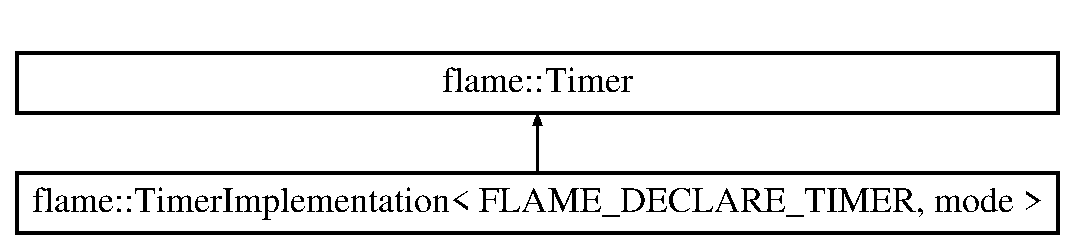
\includegraphics[height=2.000000cm]{classflame_1_1_timer_implementation}
\end{center}
\end{figure}
\subsection*{Public Member Functions}
\begin{DoxyCompactItemize}
\item 
\hyperlink{io_8h_a2eb6f9e0395b47b8d5e3eeae4fe0c116}{I\-N\-L\-I\-N\-E} uint16\-\_\-t \hyperlink{classflame_1_1_timer_implementation_a059cf0b61ce2a5401e0eac765d592876}{current} ()
\item 
\hyperlink{io_8h_a2eb6f9e0395b47b8d5e3eeae4fe0c116}{I\-N\-L\-I\-N\-E} void \hyperlink{classflame_1_1_timer_implementation_ae5ad66785471cc2c284662b347973b00}{set\-Current} (uint16\-\_\-t \hyperlink{classflame_1_1_timer_implementation_a059cf0b61ce2a5401e0eac765d592876}{current})
\item 
uint8\-\_\-t \hyperlink{classflame_1_1_timer_implementation_abec9c25e312eb36bfb693f67739c2375}{calculate\-Prescaler} (uint32\-\_\-t \hyperlink{structflame_1_1time}{time}, \hyperlink{namespaceflame_a24dfd057ba5ab5a827abbc4ed902a087}{Timer\-Prescaler} $\ast$prescaler, uint16\-\_\-t $\ast$factor)
\item 
uint16\-\_\-t \hyperlink{classflame_1_1_timer_implementation_a78fb5b014f05a5116c74edd893589850}{get\-Prescaler\-Multiplier} ()
\item 
void \hyperlink{classflame_1_1_timer_implementation_af94598e1bd64d41383def5a64393f986}{set\-Periods} (\hyperlink{namespaceflame_a24dfd057ba5ab5a827abbc4ed902a087}{Timer\-Prescaler} prescaler, uint16\-\_\-t time1, uint16\-\_\-t time2)
\item 
void \hyperlink{classflame_1_1_timer_implementation_a506d40fad888634925df6d3f129e2099}{set\-Periods} (\hyperlink{namespaceflame_a24dfd057ba5ab5a827abbc4ed902a087}{Timer\-Prescaler} prescaler, uint16\-\_\-t time1, uint16\-\_\-t time2, uint16\-\_\-t time3)
\item 
uint16\-\_\-t \hyperlink{classflame_1_1_timer_implementation_a6a5d38f11e26fa6283af22691bc1e0f4}{get\-Top} ()
\item 
void \hyperlink{classflame_1_1_timer_implementation_aedf65ab8b5ea5b7d1eca3e16a1993d5a}{set\-Top} (uint16\-\_\-t value)
\item 
\hyperlink{io_8h_a2eb6f9e0395b47b8d5e3eeae4fe0c116}{I\-N\-L\-I\-N\-E} void \hyperlink{classflame_1_1_timer_implementation_a62a263dea1b2846908b1e8c9608420f8}{set\-Output} (uint8\-\_\-t channel, uint16\-\_\-t value)
\item 
\hyperlink{io_8h_a2eb6f9e0395b47b8d5e3eeae4fe0c116}{I\-N\-L\-I\-N\-E} void \hyperlink{classflame_1_1_timer_implementation_a73813adc78b7a675018ebf81a2bc74aa}{set\-Output1} (uint16\-\_\-t value)
\item 
\hyperlink{io_8h_a2eb6f9e0395b47b8d5e3eeae4fe0c116}{I\-N\-L\-I\-N\-E} void \hyperlink{classflame_1_1_timer_implementation_a71850b7feccf996506f0e973f68fa1cf}{set\-Output2} (uint16\-\_\-t value)
\item 
\hyperlink{io_8h_a2eb6f9e0395b47b8d5e3eeae4fe0c116}{I\-N\-L\-I\-N\-E} void \hyperlink{classflame_1_1_timer_implementation_a487897e17825a7197396eaf212ce3d1b}{set\-Output3} (uint16\-\_\-t value)
\item 
uint16\-\_\-t \hyperlink{classflame_1_1_timer_implementation_a772d1ec8806c9c2c479b55539d827076}{get\-Output} (uint8\-\_\-t channel)
\item 
\hyperlink{io_8h_a2eb6f9e0395b47b8d5e3eeae4fe0c116}{I\-N\-L\-I\-N\-E} uint16\-\_\-t \hyperlink{classflame_1_1_timer_implementation_adbed484d9369a198238f138e29ed63d3}{get\-Output1} ()
\item 
\hyperlink{io_8h_a2eb6f9e0395b47b8d5e3eeae4fe0c116}{I\-N\-L\-I\-N\-E} uint16\-\_\-t \hyperlink{classflame_1_1_timer_implementation_ae4108f7c84663eaf80e6958bafefd01f}{get\-Output2} ()
\item 
\hyperlink{io_8h_a2eb6f9e0395b47b8d5e3eeae4fe0c116}{I\-N\-L\-I\-N\-E} uint16\-\_\-t \hyperlink{classflame_1_1_timer_implementation_aa17aee927a9999422c190420da78dd1d}{get\-Output3} ()
\item 
void \hyperlink{classflame_1_1_timer_implementation_a53ba3822a5d824fc8d35d835ab18afa7}{connect\-Output} (uint8\-\_\-t channel, \hyperlink{namespaceflame_ae65577f52d5a5d4ce0cc5a4b85fb9ba9}{Timer\-Connect} connect\-Type)
\item 
\hyperlink{io_8h_a2eb6f9e0395b47b8d5e3eeae4fe0c116}{I\-N\-L\-I\-N\-E} void \hyperlink{classflame_1_1_timer_implementation_a5a8d88bff958036d3bf55c29c540b3b8}{connect\-Output1} (\hyperlink{namespaceflame_ae65577f52d5a5d4ce0cc5a4b85fb9ba9}{Timer\-Connect} connect\-Type)
\item 
\hyperlink{io_8h_a2eb6f9e0395b47b8d5e3eeae4fe0c116}{I\-N\-L\-I\-N\-E} void \hyperlink{classflame_1_1_timer_implementation_ac56dc9af8ff923e6d331f69d35375941}{connect\-Output2} (\hyperlink{namespaceflame_ae65577f52d5a5d4ce0cc5a4b85fb9ba9}{Timer\-Connect} connect\-Type)
\item 
\hyperlink{io_8h_a2eb6f9e0395b47b8d5e3eeae4fe0c116}{I\-N\-L\-I\-N\-E} void \hyperlink{classflame_1_1_timer_implementation_af0e2e07199ea95d45a0220f64b11b803}{connect\-Output3} (\hyperlink{namespaceflame_ae65577f52d5a5d4ce0cc5a4b85fb9ba9}{Timer\-Connect} connect\-Type)
\item 
void \hyperlink{classflame_1_1_timer_implementation_ab411aee6c337500cbcc1758591dda034}{enable} ()
\item 
void \hyperlink{classflame_1_1_timer_implementation_a9abba3ade8ddb1dabdb7dc2c100dc98b}{disable} ()
\item 
void \hyperlink{classflame_1_1_timer_implementation_a839d62871ebac2ed0d15f3eee8f17249}{trigger1} ()
\item 
\hyperlink{io_8h_a2eb6f9e0395b47b8d5e3eeae4fe0c116}{I\-N\-L\-I\-N\-E} void \hyperlink{classflame_1_1_timer_implementation_a297667d2868424ff25926e58c02821a2}{wait\-For\-Overflow} ()
\item 
\hyperlink{io_8h_a2eb6f9e0395b47b8d5e3eeae4fe0c116}{I\-N\-L\-I\-N\-E} void \hyperlink{classflame_1_1_timer_implementation_a413c104e27665c31e2057cdbcef87d36}{clear\-Overflow} ()
\end{DoxyCompactItemize}
\subsection*{Protected Member Functions}
\begin{DoxyCompactItemize}
\item 
void \hyperlink{classflame_1_1_timer_implementation_afe51fd8e8ec6a6b8ec3bf3b5c66f4301}{\-\_\-set\-Prescaler} (\hyperlink{namespaceflame_a24dfd057ba5ab5a827abbc4ed902a087}{Timer\-Prescaler} prescaler)
\item 
\hyperlink{namespaceflame_a24dfd057ba5ab5a827abbc4ed902a087}{Timer\-Prescaler} \hyperlink{classflame_1_1_timer_implementation_aaf9d86fd95f8b0f1f88108b1bb0a76c5}{get\-Prescaler} ()
\item 
void \hyperlink{classflame_1_1_timer_implementation_a7e5bd976aec5f770773656758c4d3f89}{set\-Generation\-Mode} ()
\end{DoxyCompactItemize}
\subsection*{Protected Attributes}
\begin{DoxyCompactItemize}
\item 
bool \hyperlink{classflame_1_1_timer_implementation_ad7e59d3077694195b9d95042f6580e91}{\-\_\-have\-Time2}
\item 
bool \hyperlink{classflame_1_1_timer_implementation_a171e3dafa1a40ee3c4660f52eb2582da}{\-\_\-have\-Time3}
\end{DoxyCompactItemize}


\subsection{Detailed Description}
\subsubsection*{template$<$F\-L\-A\-M\-E\-\_\-\-D\-E\-C\-L\-A\-R\-E\-\_\-\-T\-I\-M\-E\-R, Timer\-Mode mode$>$class flame\-::\-Timer\-Implementation$<$ F\-L\-A\-M\-E\-\_\-\-D\-E\-C\-L\-A\-R\-E\-\_\-\-T\-I\-M\-E\-R, mode $>$}

A hardware timer 
\begin{DoxyTemplParams}{Template Parameters}
{\em bits} & the number of bits of the timer (8 or 16) \\
\hline
{\em type} & the type of timer (number of prescalers) \\
\hline
{\em control\-Reg\-A} & the address of the first control reg, in S\-F\-R\-\_\-\-M\-E\-M8 format \\
\hline
\end{DoxyTemplParams}


Definition at line 366 of file Timer.\-h.



\subsection{Member Function Documentation}
\hypertarget{classflame_1_1_timer_implementation_afe51fd8e8ec6a6b8ec3bf3b5c66f4301}{\index{flame\-::\-Timer\-Implementation@{flame\-::\-Timer\-Implementation}!\-\_\-set\-Prescaler@{\-\_\-set\-Prescaler}}
\index{\-\_\-set\-Prescaler@{\-\_\-set\-Prescaler}!flame::TimerImplementation@{flame\-::\-Timer\-Implementation}}
\subsubsection[{\-\_\-set\-Prescaler}]{\setlength{\rightskip}{0pt plus 5cm}template$<$F\-L\-A\-M\-E\-\_\-\-D\-E\-C\-L\-A\-R\-E\-\_\-\-T\-I\-M\-E\-R , Timer\-Mode mode$>$ void {\bf flame\-::\-Timer\-Implementation}$<$ {\bf F\-L\-A\-M\-E\-\_\-\-D\-E\-C\-L\-A\-R\-E\-\_\-\-T\-I\-M\-E\-R}, mode $>$\-::\-\_\-set\-Prescaler (
\begin{DoxyParamCaption}
\item[{{\bf Timer\-Prescaler}}]{prescaler}
\end{DoxyParamCaption}
)\hspace{0.3cm}{\ttfamily [inline]}, {\ttfamily [protected]}, {\ttfamily [virtual]}}}\label{classflame_1_1_timer_implementation_afe51fd8e8ec6a6b8ec3bf3b5c66f4301}
Set the prescaler (internal use only) 
\begin{DoxyParams}{Parameters}
{\em prescaler} & the prescaler value (only the lowest 3 bits may be set) \\
\hline
\end{DoxyParams}


Implements \hyperlink{classflame_1_1_timer_a6e1b57b1ad0d7f4d7cd4f7118ebffb18}{flame\-::\-Timer}.



Definition at line 375 of file Timer.\-h.

\hypertarget{classflame_1_1_timer_implementation_abec9c25e312eb36bfb693f67739c2375}{\index{flame\-::\-Timer\-Implementation@{flame\-::\-Timer\-Implementation}!calculate\-Prescaler@{calculate\-Prescaler}}
\index{calculate\-Prescaler@{calculate\-Prescaler}!flame::TimerImplementation@{flame\-::\-Timer\-Implementation}}
\subsubsection[{calculate\-Prescaler}]{\setlength{\rightskip}{0pt plus 5cm}template$<$F\-L\-A\-M\-E\-\_\-\-D\-E\-C\-L\-A\-R\-E\-\_\-\-T\-I\-M\-E\-R , Timer\-Mode mode$>$ uint8\-\_\-t {\bf flame\-::\-Timer\-Implementation}$<$ {\bf F\-L\-A\-M\-E\-\_\-\-D\-E\-C\-L\-A\-R\-E\-\_\-\-T\-I\-M\-E\-R}, mode $>$\-::calculate\-Prescaler (
\begin{DoxyParamCaption}
\item[{uint32\-\_\-t}]{time, }
\item[{{\bf Timer\-Prescaler} $\ast$}]{prescaler, }
\item[{uint16\-\_\-t $\ast$}]{factor}
\end{DoxyParamCaption}
)\hspace{0.3cm}{\ttfamily [inline]}, {\ttfamily [virtual]}}}\label{classflame_1_1_timer_implementation_abec9c25e312eb36bfb693f67739c2375}
Set the prescaler 
\begin{DoxyParams}{Parameters}
{\em time} & the time in timer ticks \\
\hline
{\em prescaler} & the prescaler to set \\
\hline
{\em factor} & the prescale factor return 0 on success \\
\hline
\end{DoxyParams}


Implements \hyperlink{classflame_1_1_timer_a41717d9530f49b0f9ffdc6cd8ed9eb1c}{flame\-::\-Timer}.



Definition at line 497 of file Timer.\-h.

\hypertarget{classflame_1_1_timer_implementation_a413c104e27665c31e2057cdbcef87d36}{\index{flame\-::\-Timer\-Implementation@{flame\-::\-Timer\-Implementation}!clear\-Overflow@{clear\-Overflow}}
\index{clear\-Overflow@{clear\-Overflow}!flame::TimerImplementation@{flame\-::\-Timer\-Implementation}}
\subsubsection[{clear\-Overflow}]{\setlength{\rightskip}{0pt plus 5cm}template$<$F\-L\-A\-M\-E\-\_\-\-D\-E\-C\-L\-A\-R\-E\-\_\-\-T\-I\-M\-E\-R , Timer\-Mode mode$>$ {\bf I\-N\-L\-I\-N\-E} void {\bf flame\-::\-Timer\-Implementation}$<$ {\bf F\-L\-A\-M\-E\-\_\-\-D\-E\-C\-L\-A\-R\-E\-\_\-\-T\-I\-M\-E\-R}, mode $>$\-::clear\-Overflow (
\begin{DoxyParamCaption}
{}
\end{DoxyParamCaption}
)\hspace{0.3cm}{\ttfamily [inline]}, {\ttfamily [virtual]}}}\label{classflame_1_1_timer_implementation_a413c104e27665c31e2057cdbcef87d36}
Clear a timer overflow 

Implements \hyperlink{classflame_1_1_timer_a84e3f3f1fdfe90a8b247ee6b15b43c89}{flame\-::\-Timer}.



Definition at line 1036 of file Timer.\-h.

\hypertarget{classflame_1_1_timer_implementation_a53ba3822a5d824fc8d35d835ab18afa7}{\index{flame\-::\-Timer\-Implementation@{flame\-::\-Timer\-Implementation}!connect\-Output@{connect\-Output}}
\index{connect\-Output@{connect\-Output}!flame::TimerImplementation@{flame\-::\-Timer\-Implementation}}
\subsubsection[{connect\-Output}]{\setlength{\rightskip}{0pt plus 5cm}template$<$F\-L\-A\-M\-E\-\_\-\-D\-E\-C\-L\-A\-R\-E\-\_\-\-T\-I\-M\-E\-R , Timer\-Mode mode$>$ void {\bf flame\-::\-Timer\-Implementation}$<$ {\bf F\-L\-A\-M\-E\-\_\-\-D\-E\-C\-L\-A\-R\-E\-\_\-\-T\-I\-M\-E\-R}, mode $>$\-::connect\-Output (
\begin{DoxyParamCaption}
\item[{uint8\-\_\-t}]{channel, }
\item[{{\bf Timer\-Connect}}]{connect\-Type}
\end{DoxyParamCaption}
)\hspace{0.3cm}{\ttfamily [inline]}}}\label{classflame_1_1_timer_implementation_a53ba3822a5d824fc8d35d835ab18afa7}


Definition at line 923 of file Timer.\-h.

\hypertarget{classflame_1_1_timer_implementation_a5a8d88bff958036d3bf55c29c540b3b8}{\index{flame\-::\-Timer\-Implementation@{flame\-::\-Timer\-Implementation}!connect\-Output1@{connect\-Output1}}
\index{connect\-Output1@{connect\-Output1}!flame::TimerImplementation@{flame\-::\-Timer\-Implementation}}
\subsubsection[{connect\-Output1}]{\setlength{\rightskip}{0pt plus 5cm}template$<$F\-L\-A\-M\-E\-\_\-\-D\-E\-C\-L\-A\-R\-E\-\_\-\-T\-I\-M\-E\-R , Timer\-Mode mode$>$ {\bf I\-N\-L\-I\-N\-E} void {\bf flame\-::\-Timer\-Implementation}$<$ {\bf F\-L\-A\-M\-E\-\_\-\-D\-E\-C\-L\-A\-R\-E\-\_\-\-T\-I\-M\-E\-R}, mode $>$\-::connect\-Output1 (
\begin{DoxyParamCaption}
\item[{{\bf Timer\-Connect}}]{connect\-Type}
\end{DoxyParamCaption}
)\hspace{0.3cm}{\ttfamily [inline]}, {\ttfamily [virtual]}}}\label{classflame_1_1_timer_implementation_a5a8d88bff958036d3bf55c29c540b3b8}
Connect channel 1 to an output pin 
\begin{DoxyParams}{Parameters}
{\em connect\-Type} & the method of connection \\
\hline
\end{DoxyParams}


Implements \hyperlink{classflame_1_1_timer_abb864ec27afbf978d4367fb2d58436e9}{flame\-::\-Timer}.



Definition at line 944 of file Timer.\-h.

\hypertarget{classflame_1_1_timer_implementation_ac56dc9af8ff923e6d331f69d35375941}{\index{flame\-::\-Timer\-Implementation@{flame\-::\-Timer\-Implementation}!connect\-Output2@{connect\-Output2}}
\index{connect\-Output2@{connect\-Output2}!flame::TimerImplementation@{flame\-::\-Timer\-Implementation}}
\subsubsection[{connect\-Output2}]{\setlength{\rightskip}{0pt plus 5cm}template$<$F\-L\-A\-M\-E\-\_\-\-D\-E\-C\-L\-A\-R\-E\-\_\-\-T\-I\-M\-E\-R , Timer\-Mode mode$>$ {\bf I\-N\-L\-I\-N\-E} void {\bf flame\-::\-Timer\-Implementation}$<$ {\bf F\-L\-A\-M\-E\-\_\-\-D\-E\-C\-L\-A\-R\-E\-\_\-\-T\-I\-M\-E\-R}, mode $>$\-::connect\-Output2 (
\begin{DoxyParamCaption}
\item[{{\bf Timer\-Connect}}]{connect\-Type}
\end{DoxyParamCaption}
)\hspace{0.3cm}{\ttfamily [inline]}, {\ttfamily [virtual]}}}\label{classflame_1_1_timer_implementation_ac56dc9af8ff923e6d331f69d35375941}
Connect channel 2 to an output pin 
\begin{DoxyParams}{Parameters}
{\em connect\-Type} & the method of connection \\
\hline
\end{DoxyParams}


Implements \hyperlink{classflame_1_1_timer_a8953b248ee5a1749ea54d571b3254805}{flame\-::\-Timer}.



Definition at line 952 of file Timer.\-h.

\hypertarget{classflame_1_1_timer_implementation_af0e2e07199ea95d45a0220f64b11b803}{\index{flame\-::\-Timer\-Implementation@{flame\-::\-Timer\-Implementation}!connect\-Output3@{connect\-Output3}}
\index{connect\-Output3@{connect\-Output3}!flame::TimerImplementation@{flame\-::\-Timer\-Implementation}}
\subsubsection[{connect\-Output3}]{\setlength{\rightskip}{0pt plus 5cm}template$<$F\-L\-A\-M\-E\-\_\-\-D\-E\-C\-L\-A\-R\-E\-\_\-\-T\-I\-M\-E\-R , Timer\-Mode mode$>$ {\bf I\-N\-L\-I\-N\-E} void {\bf flame\-::\-Timer\-Implementation}$<$ {\bf F\-L\-A\-M\-E\-\_\-\-D\-E\-C\-L\-A\-R\-E\-\_\-\-T\-I\-M\-E\-R}, mode $>$\-::connect\-Output3 (
\begin{DoxyParamCaption}
\item[{{\bf Timer\-Connect}}]{connect\-Type}
\end{DoxyParamCaption}
)\hspace{0.3cm}{\ttfamily [inline]}, {\ttfamily [virtual]}}}\label{classflame_1_1_timer_implementation_af0e2e07199ea95d45a0220f64b11b803}
Connect channel 3 to an output pin 
\begin{DoxyParams}{Parameters}
{\em connect\-Type} & the method of connection \\
\hline
\end{DoxyParams}


Implements \hyperlink{classflame_1_1_timer_ac2de7ddb1623fe93e3e5852d6893c005}{flame\-::\-Timer}.



Definition at line 960 of file Timer.\-h.

\hypertarget{classflame_1_1_timer_implementation_a059cf0b61ce2a5401e0eac765d592876}{\index{flame\-::\-Timer\-Implementation@{flame\-::\-Timer\-Implementation}!current@{current}}
\index{current@{current}!flame::TimerImplementation@{flame\-::\-Timer\-Implementation}}
\subsubsection[{current}]{\setlength{\rightskip}{0pt plus 5cm}template$<$F\-L\-A\-M\-E\-\_\-\-D\-E\-C\-L\-A\-R\-E\-\_\-\-T\-I\-M\-E\-R , Timer\-Mode mode$>$ {\bf I\-N\-L\-I\-N\-E} uint16\-\_\-t {\bf flame\-::\-Timer\-Implementation}$<$ {\bf F\-L\-A\-M\-E\-\_\-\-D\-E\-C\-L\-A\-R\-E\-\_\-\-T\-I\-M\-E\-R}, mode $>$\-::current (
\begin{DoxyParamCaption}
{}
\end{DoxyParamCaption}
)\hspace{0.3cm}{\ttfamily [inline]}, {\ttfamily [virtual]}}}\label{classflame_1_1_timer_implementation_a059cf0b61ce2a5401e0eac765d592876}
Get the current value of the timer \begin{DoxyReturn}{Returns}
the current value of the timer 
\end{DoxyReturn}


Implements \hyperlink{classflame_1_1_timer_a97eb012afb61476de7597a4515c03d2d}{flame\-::\-Timer}.



Definition at line 454 of file Timer.\-h.

\hypertarget{classflame_1_1_timer_implementation_a9abba3ade8ddb1dabdb7dc2c100dc98b}{\index{flame\-::\-Timer\-Implementation@{flame\-::\-Timer\-Implementation}!disable@{disable}}
\index{disable@{disable}!flame::TimerImplementation@{flame\-::\-Timer\-Implementation}}
\subsubsection[{disable}]{\setlength{\rightskip}{0pt plus 5cm}template$<$F\-L\-A\-M\-E\-\_\-\-D\-E\-C\-L\-A\-R\-E\-\_\-\-T\-I\-M\-E\-R , Timer\-Mode mode$>$ void {\bf flame\-::\-Timer\-Implementation}$<$ {\bf F\-L\-A\-M\-E\-\_\-\-D\-E\-C\-L\-A\-R\-E\-\_\-\-T\-I\-M\-E\-R}, mode $>$\-::disable (
\begin{DoxyParamCaption}
{}
\end{DoxyParamCaption}
)\hspace{0.3cm}{\ttfamily [inline]}, {\ttfamily [virtual]}}}\label{classflame_1_1_timer_implementation_a9abba3ade8ddb1dabdb7dc2c100dc98b}
Disable the timer 

Implements \hyperlink{classflame_1_1_timer_ae8aad2641dffe007a8e48e78d9c08dd2}{flame\-::\-Timer}.



Definition at line 1003 of file Timer.\-h.

\hypertarget{classflame_1_1_timer_implementation_ab411aee6c337500cbcc1758591dda034}{\index{flame\-::\-Timer\-Implementation@{flame\-::\-Timer\-Implementation}!enable@{enable}}
\index{enable@{enable}!flame::TimerImplementation@{flame\-::\-Timer\-Implementation}}
\subsubsection[{enable}]{\setlength{\rightskip}{0pt plus 5cm}template$<$F\-L\-A\-M\-E\-\_\-\-D\-E\-C\-L\-A\-R\-E\-\_\-\-T\-I\-M\-E\-R , Timer\-Mode mode$>$ void {\bf flame\-::\-Timer\-Implementation}$<$ {\bf F\-L\-A\-M\-E\-\_\-\-D\-E\-C\-L\-A\-R\-E\-\_\-\-T\-I\-M\-E\-R}, mode $>$\-::enable (
\begin{DoxyParamCaption}
{}
\end{DoxyParamCaption}
)\hspace{0.3cm}{\ttfamily [inline]}, {\ttfamily [virtual]}}}\label{classflame_1_1_timer_implementation_ab411aee6c337500cbcc1758591dda034}
Enable the timer module 

Implements \hyperlink{classflame_1_1_timer_a93d5856122c3df8087cadade3992fb75}{flame\-::\-Timer}.



Definition at line 967 of file Timer.\-h.

\hypertarget{classflame_1_1_timer_implementation_a772d1ec8806c9c2c479b55539d827076}{\index{flame\-::\-Timer\-Implementation@{flame\-::\-Timer\-Implementation}!get\-Output@{get\-Output}}
\index{get\-Output@{get\-Output}!flame::TimerImplementation@{flame\-::\-Timer\-Implementation}}
\subsubsection[{get\-Output}]{\setlength{\rightskip}{0pt plus 5cm}template$<$F\-L\-A\-M\-E\-\_\-\-D\-E\-C\-L\-A\-R\-E\-\_\-\-T\-I\-M\-E\-R , Timer\-Mode mode$>$ uint16\-\_\-t {\bf flame\-::\-Timer\-Implementation}$<$ {\bf F\-L\-A\-M\-E\-\_\-\-D\-E\-C\-L\-A\-R\-E\-\_\-\-T\-I\-M\-E\-R}, mode $>$\-::get\-Output (
\begin{DoxyParamCaption}
\item[{uint8\-\_\-t}]{channel}
\end{DoxyParamCaption}
)\hspace{0.3cm}{\ttfamily [inline]}, {\ttfamily [virtual]}}}\label{classflame_1_1_timer_implementation_a772d1ec8806c9c2c479b55539d827076}
Get the current value of a channel 
\begin{DoxyParams}{Parameters}
{\em channel} & the channel to get \\
\hline
\end{DoxyParams}
\begin{DoxyReturn}{Returns}
the current value of the selected channel 
\end{DoxyReturn}


Implements \hyperlink{classflame_1_1_timer_a29af3ec15a5669430a95a83727097432}{flame\-::\-Timer}.



Definition at line 834 of file Timer.\-h.

\hypertarget{classflame_1_1_timer_implementation_adbed484d9369a198238f138e29ed63d3}{\index{flame\-::\-Timer\-Implementation@{flame\-::\-Timer\-Implementation}!get\-Output1@{get\-Output1}}
\index{get\-Output1@{get\-Output1}!flame::TimerImplementation@{flame\-::\-Timer\-Implementation}}
\subsubsection[{get\-Output1}]{\setlength{\rightskip}{0pt plus 5cm}template$<$F\-L\-A\-M\-E\-\_\-\-D\-E\-C\-L\-A\-R\-E\-\_\-\-T\-I\-M\-E\-R , Timer\-Mode mode$>$ {\bf I\-N\-L\-I\-N\-E} uint16\-\_\-t {\bf flame\-::\-Timer\-Implementation}$<$ {\bf F\-L\-A\-M\-E\-\_\-\-D\-E\-C\-L\-A\-R\-E\-\_\-\-T\-I\-M\-E\-R}, mode $>$\-::get\-Output1 (
\begin{DoxyParamCaption}
{}
\end{DoxyParamCaption}
)\hspace{0.3cm}{\ttfamily [inline]}, {\ttfamily [virtual]}}}\label{classflame_1_1_timer_implementation_adbed484d9369a198238f138e29ed63d3}
Return the current value of channel 1 \begin{DoxyReturn}{Returns}
the current value of channel 1 
\end{DoxyReturn}


Implements \hyperlink{classflame_1_1_timer_af9cd331d2da4bd5996473469b2454062}{flame\-::\-Timer}.



Definition at line 874 of file Timer.\-h.

\hypertarget{classflame_1_1_timer_implementation_ae4108f7c84663eaf80e6958bafefd01f}{\index{flame\-::\-Timer\-Implementation@{flame\-::\-Timer\-Implementation}!get\-Output2@{get\-Output2}}
\index{get\-Output2@{get\-Output2}!flame::TimerImplementation@{flame\-::\-Timer\-Implementation}}
\subsubsection[{get\-Output2}]{\setlength{\rightskip}{0pt plus 5cm}template$<$F\-L\-A\-M\-E\-\_\-\-D\-E\-C\-L\-A\-R\-E\-\_\-\-T\-I\-M\-E\-R , Timer\-Mode mode$>$ {\bf I\-N\-L\-I\-N\-E} uint16\-\_\-t {\bf flame\-::\-Timer\-Implementation}$<$ {\bf F\-L\-A\-M\-E\-\_\-\-D\-E\-C\-L\-A\-R\-E\-\_\-\-T\-I\-M\-E\-R}, mode $>$\-::get\-Output2 (
\begin{DoxyParamCaption}
{}
\end{DoxyParamCaption}
)\hspace{0.3cm}{\ttfamily [inline]}, {\ttfamily [virtual]}}}\label{classflame_1_1_timer_implementation_ae4108f7c84663eaf80e6958bafefd01f}
Return the current value of channel 2 \begin{DoxyReturn}{Returns}
the current value of channel 2 
\end{DoxyReturn}


Implements \hyperlink{classflame_1_1_timer_a02a423f8bbd41bf2acacdb60e2164c71}{flame\-::\-Timer}.



Definition at line 891 of file Timer.\-h.

\hypertarget{classflame_1_1_timer_implementation_aa17aee927a9999422c190420da78dd1d}{\index{flame\-::\-Timer\-Implementation@{flame\-::\-Timer\-Implementation}!get\-Output3@{get\-Output3}}
\index{get\-Output3@{get\-Output3}!flame::TimerImplementation@{flame\-::\-Timer\-Implementation}}
\subsubsection[{get\-Output3}]{\setlength{\rightskip}{0pt plus 5cm}template$<$F\-L\-A\-M\-E\-\_\-\-D\-E\-C\-L\-A\-R\-E\-\_\-\-T\-I\-M\-E\-R , Timer\-Mode mode$>$ {\bf I\-N\-L\-I\-N\-E} uint16\-\_\-t {\bf flame\-::\-Timer\-Implementation}$<$ {\bf F\-L\-A\-M\-E\-\_\-\-D\-E\-C\-L\-A\-R\-E\-\_\-\-T\-I\-M\-E\-R}, mode $>$\-::get\-Output3 (
\begin{DoxyParamCaption}
{}
\end{DoxyParamCaption}
)\hspace{0.3cm}{\ttfamily [inline]}, {\ttfamily [virtual]}}}\label{classflame_1_1_timer_implementation_aa17aee927a9999422c190420da78dd1d}
Return the current value of channel 3 \begin{DoxyReturn}{Returns}
the current value of channel 3 
\end{DoxyReturn}


Implements \hyperlink{classflame_1_1_timer_aded92bd6883a00c8c792ab45df1ad580}{flame\-::\-Timer}.



Definition at line 908 of file Timer.\-h.

\hypertarget{classflame_1_1_timer_implementation_aaf9d86fd95f8b0f1f88108b1bb0a76c5}{\index{flame\-::\-Timer\-Implementation@{flame\-::\-Timer\-Implementation}!get\-Prescaler@{get\-Prescaler}}
\index{get\-Prescaler@{get\-Prescaler}!flame::TimerImplementation@{flame\-::\-Timer\-Implementation}}
\subsubsection[{get\-Prescaler}]{\setlength{\rightskip}{0pt plus 5cm}template$<$F\-L\-A\-M\-E\-\_\-\-D\-E\-C\-L\-A\-R\-E\-\_\-\-T\-I\-M\-E\-R , Timer\-Mode mode$>$ {\bf Timer\-Prescaler} {\bf flame\-::\-Timer\-Implementation}$<$ {\bf F\-L\-A\-M\-E\-\_\-\-D\-E\-C\-L\-A\-R\-E\-\_\-\-T\-I\-M\-E\-R}, mode $>$\-::get\-Prescaler (
\begin{DoxyParamCaption}
{}
\end{DoxyParamCaption}
)\hspace{0.3cm}{\ttfamily [inline]}, {\ttfamily [protected]}, {\ttfamily [virtual]}}}\label{classflame_1_1_timer_implementation_aaf9d86fd95f8b0f1f88108b1bb0a76c5}
Get the prescaler \begin{DoxyReturn}{Returns}
the prescaler value 
\end{DoxyReturn}


Implements \hyperlink{classflame_1_1_timer_a7f8d6b44b6bfca103f9d91948c669a38}{flame\-::\-Timer}.



Definition at line 383 of file Timer.\-h.

\hypertarget{classflame_1_1_timer_implementation_a78fb5b014f05a5116c74edd893589850}{\index{flame\-::\-Timer\-Implementation@{flame\-::\-Timer\-Implementation}!get\-Prescaler\-Multiplier@{get\-Prescaler\-Multiplier}}
\index{get\-Prescaler\-Multiplier@{get\-Prescaler\-Multiplier}!flame::TimerImplementation@{flame\-::\-Timer\-Implementation}}
\subsubsection[{get\-Prescaler\-Multiplier}]{\setlength{\rightskip}{0pt plus 5cm}template$<$F\-L\-A\-M\-E\-\_\-\-D\-E\-C\-L\-A\-R\-E\-\_\-\-T\-I\-M\-E\-R , Timer\-Mode mode$>$ uint16\-\_\-t {\bf flame\-::\-Timer\-Implementation}$<$ {\bf F\-L\-A\-M\-E\-\_\-\-D\-E\-C\-L\-A\-R\-E\-\_\-\-T\-I\-M\-E\-R}, mode $>$\-::get\-Prescaler\-Multiplier (
\begin{DoxyParamCaption}
{}
\end{DoxyParamCaption}
)\hspace{0.3cm}{\ttfamily [inline]}, {\ttfamily [virtual]}}}\label{classflame_1_1_timer_implementation_a78fb5b014f05a5116c74edd893589850}
Get the prescaler multiplier 

Implements \hyperlink{classflame_1_1_timer_a08e913a8f802be0e7b46de3bf001bd3f}{flame\-::\-Timer}.



Definition at line 561 of file Timer.\-h.

\hypertarget{classflame_1_1_timer_implementation_a6a5d38f11e26fa6283af22691bc1e0f4}{\index{flame\-::\-Timer\-Implementation@{flame\-::\-Timer\-Implementation}!get\-Top@{get\-Top}}
\index{get\-Top@{get\-Top}!flame::TimerImplementation@{flame\-::\-Timer\-Implementation}}
\subsubsection[{get\-Top}]{\setlength{\rightskip}{0pt plus 5cm}template$<$F\-L\-A\-M\-E\-\_\-\-D\-E\-C\-L\-A\-R\-E\-\_\-\-T\-I\-M\-E\-R , Timer\-Mode mode$>$ uint16\-\_\-t {\bf flame\-::\-Timer\-Implementation}$<$ {\bf F\-L\-A\-M\-E\-\_\-\-D\-E\-C\-L\-A\-R\-E\-\_\-\-T\-I\-M\-E\-R}, mode $>$\-::get\-Top (
\begin{DoxyParamCaption}
{}
\end{DoxyParamCaption}
)\hspace{0.3cm}{\ttfamily [inline]}, {\ttfamily [virtual]}}}\label{classflame_1_1_timer_implementation_a6a5d38f11e26fa6283af22691bc1e0f4}
Get the number of timer cycles available \begin{DoxyReturn}{Returns}
the number of cycles in an iteration of the timer 
\end{DoxyReturn}


Implements \hyperlink{classflame_1_1_timer_ae7531c4df336c5c70e751581c3c37b4c}{flame\-::\-Timer}.



Definition at line 670 of file Timer.\-h.

\hypertarget{classflame_1_1_timer_implementation_ae5ad66785471cc2c284662b347973b00}{\index{flame\-::\-Timer\-Implementation@{flame\-::\-Timer\-Implementation}!set\-Current@{set\-Current}}
\index{set\-Current@{set\-Current}!flame::TimerImplementation@{flame\-::\-Timer\-Implementation}}
\subsubsection[{set\-Current}]{\setlength{\rightskip}{0pt plus 5cm}template$<$F\-L\-A\-M\-E\-\_\-\-D\-E\-C\-L\-A\-R\-E\-\_\-\-T\-I\-M\-E\-R , Timer\-Mode mode$>$ {\bf I\-N\-L\-I\-N\-E} void {\bf flame\-::\-Timer\-Implementation}$<$ {\bf F\-L\-A\-M\-E\-\_\-\-D\-E\-C\-L\-A\-R\-E\-\_\-\-T\-I\-M\-E\-R}, mode $>$\-::set\-Current (
\begin{DoxyParamCaption}
\item[{uint16\-\_\-t}]{current}
\end{DoxyParamCaption}
)\hspace{0.3cm}{\ttfamily [inline]}, {\ttfamily [virtual]}}}\label{classflame_1_1_timer_implementation_ae5ad66785471cc2c284662b347973b00}
Set the current value of the timer 
\begin{DoxyParams}{Parameters}
{\em current} & the new value \\
\hline
\end{DoxyParams}


Implements \hyperlink{classflame_1_1_timer_a6b911bb96bd1723f20c98162a34b9867}{flame\-::\-Timer}.



Definition at line 476 of file Timer.\-h.

\hypertarget{classflame_1_1_timer_implementation_a7e5bd976aec5f770773656758c4d3f89}{\index{flame\-::\-Timer\-Implementation@{flame\-::\-Timer\-Implementation}!set\-Generation\-Mode@{set\-Generation\-Mode}}
\index{set\-Generation\-Mode@{set\-Generation\-Mode}!flame::TimerImplementation@{flame\-::\-Timer\-Implementation}}
\subsubsection[{set\-Generation\-Mode}]{\setlength{\rightskip}{0pt plus 5cm}template$<$F\-L\-A\-M\-E\-\_\-\-D\-E\-C\-L\-A\-R\-E\-\_\-\-T\-I\-M\-E\-R , Timer\-Mode mode$>$ void {\bf flame\-::\-Timer\-Implementation}$<$ {\bf F\-L\-A\-M\-E\-\_\-\-D\-E\-C\-L\-A\-R\-E\-\_\-\-T\-I\-M\-E\-R}, mode $>$\-::set\-Generation\-Mode (
\begin{DoxyParamCaption}
{}
\end{DoxyParamCaption}
)\hspace{0.3cm}{\ttfamily [inline]}, {\ttfamily [protected]}, {\ttfamily [virtual]}}}\label{classflame_1_1_timer_implementation_a7e5bd976aec5f770773656758c4d3f89}
Set the generation mode 

Implements \hyperlink{classflame_1_1_timer_a92a6ed4ed6d6ac6d52ad810d6e9526bd}{flame\-::\-Timer}.



Definition at line 390 of file Timer.\-h.

\hypertarget{classflame_1_1_timer_implementation_a62a263dea1b2846908b1e8c9608420f8}{\index{flame\-::\-Timer\-Implementation@{flame\-::\-Timer\-Implementation}!set\-Output@{set\-Output}}
\index{set\-Output@{set\-Output}!flame::TimerImplementation@{flame\-::\-Timer\-Implementation}}
\subsubsection[{set\-Output}]{\setlength{\rightskip}{0pt plus 5cm}template$<$F\-L\-A\-M\-E\-\_\-\-D\-E\-C\-L\-A\-R\-E\-\_\-\-T\-I\-M\-E\-R , Timer\-Mode mode$>$ {\bf I\-N\-L\-I\-N\-E} void {\bf flame\-::\-Timer\-Implementation}$<$ {\bf F\-L\-A\-M\-E\-\_\-\-D\-E\-C\-L\-A\-R\-E\-\_\-\-T\-I\-M\-E\-R}, mode $>$\-::set\-Output (
\begin{DoxyParamCaption}
\item[{uint8\-\_\-t}]{channel, }
\item[{uint16\-\_\-t}]{value}
\end{DoxyParamCaption}
)\hspace{0.3cm}{\ttfamily [inline]}, {\ttfamily [virtual]}}}\label{classflame_1_1_timer_implementation_a62a263dea1b2846908b1e8c9608420f8}
Set the current value of a channel 
\begin{DoxyParams}{Parameters}
{\em channel} & the channel to set \\
\hline
{\em value} & the new value of the channel \\
\hline
\end{DoxyParams}


Implements \hyperlink{classflame_1_1_timer_a7eb534c6d2b55b329207d8e8f8f7538c}{flame\-::\-Timer}.



Definition at line 747 of file Timer.\-h.

\hypertarget{classflame_1_1_timer_implementation_a73813adc78b7a675018ebf81a2bc74aa}{\index{flame\-::\-Timer\-Implementation@{flame\-::\-Timer\-Implementation}!set\-Output1@{set\-Output1}}
\index{set\-Output1@{set\-Output1}!flame::TimerImplementation@{flame\-::\-Timer\-Implementation}}
\subsubsection[{set\-Output1}]{\setlength{\rightskip}{0pt plus 5cm}template$<$F\-L\-A\-M\-E\-\_\-\-D\-E\-C\-L\-A\-R\-E\-\_\-\-T\-I\-M\-E\-R , Timer\-Mode mode$>$ {\bf I\-N\-L\-I\-N\-E} void {\bf flame\-::\-Timer\-Implementation}$<$ {\bf F\-L\-A\-M\-E\-\_\-\-D\-E\-C\-L\-A\-R\-E\-\_\-\-T\-I\-M\-E\-R}, mode $>$\-::set\-Output1 (
\begin{DoxyParamCaption}
\item[{uint16\-\_\-t}]{value}
\end{DoxyParamCaption}
)\hspace{0.3cm}{\ttfamily [inline]}, {\ttfamily [virtual]}}}\label{classflame_1_1_timer_implementation_a73813adc78b7a675018ebf81a2bc74aa}
Set the current value of channel 1 
\begin{DoxyParams}{Parameters}
{\em value} & the new value of channel 1 \\
\hline
\end{DoxyParams}


Implements \hyperlink{classflame_1_1_timer_ad5ebb60ff42ff1e8808d867da1d2dfac}{flame\-::\-Timer}.



Definition at line 781 of file Timer.\-h.

\hypertarget{classflame_1_1_timer_implementation_a71850b7feccf996506f0e973f68fa1cf}{\index{flame\-::\-Timer\-Implementation@{flame\-::\-Timer\-Implementation}!set\-Output2@{set\-Output2}}
\index{set\-Output2@{set\-Output2}!flame::TimerImplementation@{flame\-::\-Timer\-Implementation}}
\subsubsection[{set\-Output2}]{\setlength{\rightskip}{0pt plus 5cm}template$<$F\-L\-A\-M\-E\-\_\-\-D\-E\-C\-L\-A\-R\-E\-\_\-\-T\-I\-M\-E\-R , Timer\-Mode mode$>$ {\bf I\-N\-L\-I\-N\-E} void {\bf flame\-::\-Timer\-Implementation}$<$ {\bf F\-L\-A\-M\-E\-\_\-\-D\-E\-C\-L\-A\-R\-E\-\_\-\-T\-I\-M\-E\-R}, mode $>$\-::set\-Output2 (
\begin{DoxyParamCaption}
\item[{uint16\-\_\-t}]{value}
\end{DoxyParamCaption}
)\hspace{0.3cm}{\ttfamily [inline]}, {\ttfamily [virtual]}}}\label{classflame_1_1_timer_implementation_a71850b7feccf996506f0e973f68fa1cf}
Set the current value of channel 2 
\begin{DoxyParams}{Parameters}
{\em value} & the new value of channel 2 \\
\hline
\end{DoxyParams}


Implements \hyperlink{classflame_1_1_timer_ac9844c4f69ff804e754d74a4a07a1208}{flame\-::\-Timer}.



Definition at line 798 of file Timer.\-h.

\hypertarget{classflame_1_1_timer_implementation_a487897e17825a7197396eaf212ce3d1b}{\index{flame\-::\-Timer\-Implementation@{flame\-::\-Timer\-Implementation}!set\-Output3@{set\-Output3}}
\index{set\-Output3@{set\-Output3}!flame::TimerImplementation@{flame\-::\-Timer\-Implementation}}
\subsubsection[{set\-Output3}]{\setlength{\rightskip}{0pt plus 5cm}template$<$F\-L\-A\-M\-E\-\_\-\-D\-E\-C\-L\-A\-R\-E\-\_\-\-T\-I\-M\-E\-R , Timer\-Mode mode$>$ {\bf I\-N\-L\-I\-N\-E} void {\bf flame\-::\-Timer\-Implementation}$<$ {\bf F\-L\-A\-M\-E\-\_\-\-D\-E\-C\-L\-A\-R\-E\-\_\-\-T\-I\-M\-E\-R}, mode $>$\-::set\-Output3 (
\begin{DoxyParamCaption}
\item[{uint16\-\_\-t}]{value}
\end{DoxyParamCaption}
)\hspace{0.3cm}{\ttfamily [inline]}, {\ttfamily [virtual]}}}\label{classflame_1_1_timer_implementation_a487897e17825a7197396eaf212ce3d1b}
Set the current value of channel 3 
\begin{DoxyParams}{Parameters}
{\em value} & the new value of channel 3 \\
\hline
\end{DoxyParams}


Implements \hyperlink{classflame_1_1_timer_a542f70b81da2198bb6839ae15980dea2}{flame\-::\-Timer}.



Definition at line 815 of file Timer.\-h.

\hypertarget{classflame_1_1_timer_implementation_af94598e1bd64d41383def5a64393f986}{\index{flame\-::\-Timer\-Implementation@{flame\-::\-Timer\-Implementation}!set\-Periods@{set\-Periods}}
\index{set\-Periods@{set\-Periods}!flame::TimerImplementation@{flame\-::\-Timer\-Implementation}}
\subsubsection[{set\-Periods}]{\setlength{\rightskip}{0pt plus 5cm}template$<$F\-L\-A\-M\-E\-\_\-\-D\-E\-C\-L\-A\-R\-E\-\_\-\-T\-I\-M\-E\-R , Timer\-Mode mode$>$ void {\bf flame\-::\-Timer\-Implementation}$<$ {\bf F\-L\-A\-M\-E\-\_\-\-D\-E\-C\-L\-A\-R\-E\-\_\-\-T\-I\-M\-E\-R}, mode $>$\-::set\-Periods (
\begin{DoxyParamCaption}
\item[{{\bf Timer\-Prescaler}}]{prescaler, }
\item[{uint16\-\_\-t}]{time1, }
\item[{uint16\-\_\-t}]{time2}
\end{DoxyParamCaption}
)\hspace{0.3cm}{\ttfamily [inline]}, {\ttfamily [virtual]}}}\label{classflame_1_1_timer_implementation_af94598e1bd64d41383def5a64393f986}
Set the overflow periods for an 8 bit timer 
\begin{DoxyParams}{Parameters}
{\em prescaler} & the prescaler to use \\
\hline
{\em time1} & the first time in prescaled timer ticks \\
\hline
{\em time2} & the second time in prescaled timer ticks \\
\hline
\end{DoxyParams}


Implements \hyperlink{classflame_1_1_timer_a1948822bf5c75866e5c2cf9ded4b3b9b}{flame\-::\-Timer}.



Definition at line 610 of file Timer.\-h.

\hypertarget{classflame_1_1_timer_implementation_a506d40fad888634925df6d3f129e2099}{\index{flame\-::\-Timer\-Implementation@{flame\-::\-Timer\-Implementation}!set\-Periods@{set\-Periods}}
\index{set\-Periods@{set\-Periods}!flame::TimerImplementation@{flame\-::\-Timer\-Implementation}}
\subsubsection[{set\-Periods}]{\setlength{\rightskip}{0pt plus 5cm}template$<$F\-L\-A\-M\-E\-\_\-\-D\-E\-C\-L\-A\-R\-E\-\_\-\-T\-I\-M\-E\-R , Timer\-Mode mode$>$ void {\bf flame\-::\-Timer\-Implementation}$<$ {\bf F\-L\-A\-M\-E\-\_\-\-D\-E\-C\-L\-A\-R\-E\-\_\-\-T\-I\-M\-E\-R}, mode $>$\-::set\-Periods (
\begin{DoxyParamCaption}
\item[{{\bf Timer\-Prescaler}}]{prescaler, }
\item[{uint16\-\_\-t}]{time1, }
\item[{uint16\-\_\-t}]{time2, }
\item[{uint16\-\_\-t}]{time3}
\end{DoxyParamCaption}
)\hspace{0.3cm}{\ttfamily [inline]}, {\ttfamily [virtual]}}}\label{classflame_1_1_timer_implementation_a506d40fad888634925df6d3f129e2099}
Set the overflow periods for a 16 bit timer 
\begin{DoxyParams}{Parameters}
{\em prescaler} & the prescaler to use \\
\hline
{\em time1} & the first time in prescaled timer ticks \\
\hline
{\em time2} & the second time in prescaled timer ticks \\
\hline
{\em time3} & the second time in prescaled timer ticks \\
\hline
\end{DoxyParams}


Implements \hyperlink{classflame_1_1_timer_a63987b6d5a76895a3afed120b621c8b4}{flame\-::\-Timer}.



Definition at line 638 of file Timer.\-h.

\hypertarget{classflame_1_1_timer_implementation_aedf65ab8b5ea5b7d1eca3e16a1993d5a}{\index{flame\-::\-Timer\-Implementation@{flame\-::\-Timer\-Implementation}!set\-Top@{set\-Top}}
\index{set\-Top@{set\-Top}!flame::TimerImplementation@{flame\-::\-Timer\-Implementation}}
\subsubsection[{set\-Top}]{\setlength{\rightskip}{0pt plus 5cm}template$<$F\-L\-A\-M\-E\-\_\-\-D\-E\-C\-L\-A\-R\-E\-\_\-\-T\-I\-M\-E\-R , Timer\-Mode mode$>$ void {\bf flame\-::\-Timer\-Implementation}$<$ {\bf F\-L\-A\-M\-E\-\_\-\-D\-E\-C\-L\-A\-R\-E\-\_\-\-T\-I\-M\-E\-R}, mode $>$\-::set\-Top (
\begin{DoxyParamCaption}
\item[{uint16\-\_\-t}]{value}
\end{DoxyParamCaption}
)\hspace{0.3cm}{\ttfamily [inline]}, {\ttfamily [virtual]}}}\label{classflame_1_1_timer_implementation_aedf65ab8b5ea5b7d1eca3e16a1993d5a}
Set the number of timer cycles available 
\begin{DoxyParams}{Parameters}
{\em value} & the number of cycles in an iteration of the timer \\
\hline
\end{DoxyParams}


Implements \hyperlink{classflame_1_1_timer_a32523c61b521a74fe4c21cff0332a9e7}{flame\-::\-Timer}.



Definition at line 706 of file Timer.\-h.

\hypertarget{classflame_1_1_timer_implementation_a839d62871ebac2ed0d15f3eee8f17249}{\index{flame\-::\-Timer\-Implementation@{flame\-::\-Timer\-Implementation}!trigger1@{trigger1}}
\index{trigger1@{trigger1}!flame::TimerImplementation@{flame\-::\-Timer\-Implementation}}
\subsubsection[{trigger1}]{\setlength{\rightskip}{0pt plus 5cm}template$<$F\-L\-A\-M\-E\-\_\-\-D\-E\-C\-L\-A\-R\-E\-\_\-\-T\-I\-M\-E\-R , Timer\-Mode mode$>$ void {\bf flame\-::\-Timer\-Implementation}$<$ {\bf F\-L\-A\-M\-E\-\_\-\-D\-E\-C\-L\-A\-R\-E\-\_\-\-T\-I\-M\-E\-R}, mode $>$\-::trigger1 (
\begin{DoxyParamCaption}
{}
\end{DoxyParamCaption}
)\hspace{0.3cm}{\ttfamily [inline]}, {\ttfamily [virtual]}}}\label{classflame_1_1_timer_implementation_a839d62871ebac2ed0d15f3eee8f17249}
Trigger the listener for channel 1 

Implements \hyperlink{classflame_1_1_timer_a93bdf45d9aadea6694dea8ef236e8725}{flame\-::\-Timer}.



Definition at line 1019 of file Timer.\-h.

\hypertarget{classflame_1_1_timer_implementation_a297667d2868424ff25926e58c02821a2}{\index{flame\-::\-Timer\-Implementation@{flame\-::\-Timer\-Implementation}!wait\-For\-Overflow@{wait\-For\-Overflow}}
\index{wait\-For\-Overflow@{wait\-For\-Overflow}!flame::TimerImplementation@{flame\-::\-Timer\-Implementation}}
\subsubsection[{wait\-For\-Overflow}]{\setlength{\rightskip}{0pt plus 5cm}template$<$F\-L\-A\-M\-E\-\_\-\-D\-E\-C\-L\-A\-R\-E\-\_\-\-T\-I\-M\-E\-R , Timer\-Mode mode$>$ {\bf I\-N\-L\-I\-N\-E} void {\bf flame\-::\-Timer\-Implementation}$<$ {\bf F\-L\-A\-M\-E\-\_\-\-D\-E\-C\-L\-A\-R\-E\-\_\-\-T\-I\-M\-E\-R}, mode $>$\-::wait\-For\-Overflow (
\begin{DoxyParamCaption}
{}
\end{DoxyParamCaption}
)\hspace{0.3cm}{\ttfamily [inline]}, {\ttfamily [virtual]}}}\label{classflame_1_1_timer_implementation_a297667d2868424ff25926e58c02821a2}
Wait for the timer to overflow 

Implements \hyperlink{classflame_1_1_timer_a79db91c2c457766ae8b4dd01d5caf7e4}{flame\-::\-Timer}.



Definition at line 1029 of file Timer.\-h.



\subsection{Member Data Documentation}
\hypertarget{classflame_1_1_timer_implementation_ad7e59d3077694195b9d95042f6580e91}{\index{flame\-::\-Timer\-Implementation@{flame\-::\-Timer\-Implementation}!\-\_\-have\-Time2@{\-\_\-have\-Time2}}
\index{\-\_\-have\-Time2@{\-\_\-have\-Time2}!flame::TimerImplementation@{flame\-::\-Timer\-Implementation}}
\subsubsection[{\-\_\-have\-Time2}]{\setlength{\rightskip}{0pt plus 5cm}template$<$F\-L\-A\-M\-E\-\_\-\-D\-E\-C\-L\-A\-R\-E\-\_\-\-T\-I\-M\-E\-R , Timer\-Mode mode$>$ bool {\bf flame\-::\-Timer\-Implementation}$<$ {\bf F\-L\-A\-M\-E\-\_\-\-D\-E\-C\-L\-A\-R\-E\-\_\-\-T\-I\-M\-E\-R}, mode $>$\-::\-\_\-have\-Time2\hspace{0.3cm}{\ttfamily [protected]}}}\label{classflame_1_1_timer_implementation_ad7e59d3077694195b9d95042f6580e91}


Definition at line 368 of file Timer.\-h.

\hypertarget{classflame_1_1_timer_implementation_a171e3dafa1a40ee3c4660f52eb2582da}{\index{flame\-::\-Timer\-Implementation@{flame\-::\-Timer\-Implementation}!\-\_\-have\-Time3@{\-\_\-have\-Time3}}
\index{\-\_\-have\-Time3@{\-\_\-have\-Time3}!flame::TimerImplementation@{flame\-::\-Timer\-Implementation}}
\subsubsection[{\-\_\-have\-Time3}]{\setlength{\rightskip}{0pt plus 5cm}template$<$F\-L\-A\-M\-E\-\_\-\-D\-E\-C\-L\-A\-R\-E\-\_\-\-T\-I\-M\-E\-R , Timer\-Mode mode$>$ bool {\bf flame\-::\-Timer\-Implementation}$<$ {\bf F\-L\-A\-M\-E\-\_\-\-D\-E\-C\-L\-A\-R\-E\-\_\-\-T\-I\-M\-E\-R}, mode $>$\-::\-\_\-have\-Time3\hspace{0.3cm}{\ttfamily [protected]}}}\label{classflame_1_1_timer_implementation_a171e3dafa1a40ee3c4660f52eb2582da}


Definition at line 369 of file Timer.\-h.



The documentation for this class was generated from the following file\-:\begin{DoxyCompactItemize}
\item 
flame/\hyperlink{_timer_8h}{Timer.\-h}\end{DoxyCompactItemize}

\hypertarget{classflame_1_1_timer_listener}{\section{flame\-:\-:Timer\-Listener Class Reference}
\label{classflame_1_1_timer_listener}\index{flame\-::\-Timer\-Listener@{flame\-::\-Timer\-Listener}}
}


{\ttfamily \#include $<$Timer.\-h$>$}

Inheritance diagram for flame\-:\-:Timer\-Listener\-:\begin{figure}[H]
\begin{center}
\leavevmode
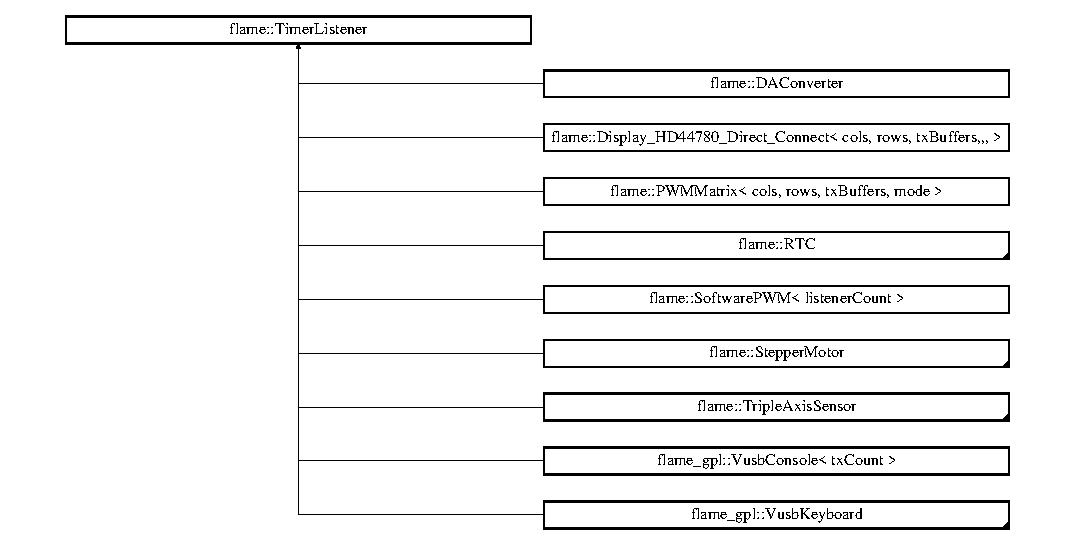
\includegraphics[height=6.879607cm]{classflame_1_1_timer_listener}
\end{center}
\end{figure}
\subsection*{Public Member Functions}
\begin{DoxyCompactItemize}
\item 
virtual void \hyperlink{classflame_1_1_timer_listener_ad97504b72a25b1fba354803338177335}{alarm} (\hyperlink{namespaceflame_a6d176ba245556716fd3e32006bb7cfe5}{Alarm\-Source} source)=0
\end{DoxyCompactItemize}


\subsection{Detailed Description}
A class which will be notified when an alarm goes off 

Definition at line 117 of file Timer.\-h.



\subsection{Member Function Documentation}
\hypertarget{classflame_1_1_timer_listener_ad97504b72a25b1fba354803338177335}{\index{flame\-::\-Timer\-Listener@{flame\-::\-Timer\-Listener}!alarm@{alarm}}
\index{alarm@{alarm}!flame::TimerListener@{flame\-::\-Timer\-Listener}}
\subsubsection[{alarm}]{\setlength{\rightskip}{0pt plus 5cm}virtual void flame\-::\-Timer\-Listener\-::alarm (
\begin{DoxyParamCaption}
\item[{{\bf Alarm\-Source}}]{source}
\end{DoxyParamCaption}
)\hspace{0.3cm}{\ttfamily [pure virtual]}}}\label{classflame_1_1_timer_listener_ad97504b72a25b1fba354803338177335}
Called when an alarm goes off 

Implemented in \hyperlink{classflame__gpl_1_1_vusb_typist_afc57a75f932afa7202b7c1aee92d9a0b}{flame\-\_\-gpl\-::\-Vusb\-Typist$<$ tx\-Buffers $>$}, \hyperlink{classflame__gpl_1_1_vusb_keyboard_ac78516dbc8ac2519bf2f0b4327c13b4d}{flame\-\_\-gpl\-::\-Vusb\-Keyboard}, \hyperlink{classflame_1_1_triple_axis_sensor_ad5fbc92633b96e9432c42a6e405eafbc}{flame\-::\-Triple\-Axis\-Sensor}, \hyperlink{classflame_1_1_d_a_converter_a35dba185dfbd8483069c7a3ee9c19e5c}{flame\-::\-D\-A\-Converter}, and \hyperlink{classflame_1_1_stepper_motor_a6eec1ffcfd13c4624525b4cabe1eec4c}{flame\-::\-Stepper\-Motor}.



The documentation for this class was generated from the following file\-:\begin{DoxyCompactItemize}
\item 
flame/\hyperlink{_timer_8h}{Timer.\-h}\end{DoxyCompactItemize}

\hypertarget{structflame_1_1timestamp}{\section{flame\-:\-:timestamp Struct Reference}
\label{structflame_1_1timestamp}\index{flame\-::timestamp@{flame\-::timestamp}}
}


{\ttfamily \#include $<$R\-T\-C.\-h$>$}

\subsection*{Public Attributes}
\begin{DoxyCompactItemize}
\item 
uint32\-\_\-t \hyperlink{structflame_1_1timestamp_a63da2e5e29c20d05ed80cab77b635399}{timestamp}
\item 
uint16\-\_\-t \hyperlink{structflame_1_1timestamp_aee5370df09d8e2e1f3d6b4a4b0dd3468}{milliseconds}
\item 
uint8\-\_\-t \hyperlink{structflame_1_1timestamp_ab16901573a9459f1adca134abed1efa9}{ticks}
\end{DoxyCompactItemize}


\subsection{Detailed Description}


Definition at line 38 of file R\-T\-C.\-h.



\subsection{Member Data Documentation}
\hypertarget{structflame_1_1timestamp_aee5370df09d8e2e1f3d6b4a4b0dd3468}{\index{flame\-::timestamp@{flame\-::timestamp}!milliseconds@{milliseconds}}
\index{milliseconds@{milliseconds}!flame::timestamp@{flame\-::timestamp}}
\subsubsection[{milliseconds}]{\setlength{\rightskip}{0pt plus 5cm}uint16\-\_\-t flame\-::timestamp\-::milliseconds}}\label{structflame_1_1timestamp_aee5370df09d8e2e1f3d6b4a4b0dd3468}


Definition at line 40 of file R\-T\-C.\-h.

\hypertarget{structflame_1_1timestamp_ab16901573a9459f1adca134abed1efa9}{\index{flame\-::timestamp@{flame\-::timestamp}!ticks@{ticks}}
\index{ticks@{ticks}!flame::timestamp@{flame\-::timestamp}}
\subsubsection[{ticks}]{\setlength{\rightskip}{0pt plus 5cm}uint8\-\_\-t flame\-::timestamp\-::ticks}}\label{structflame_1_1timestamp_ab16901573a9459f1adca134abed1efa9}


Definition at line 41 of file R\-T\-C.\-h.

\hypertarget{structflame_1_1timestamp_a63da2e5e29c20d05ed80cab77b635399}{\index{flame\-::timestamp@{flame\-::timestamp}!timestamp@{timestamp}}
\index{timestamp@{timestamp}!flame::timestamp@{flame\-::timestamp}}
\subsubsection[{timestamp}]{\setlength{\rightskip}{0pt plus 5cm}uint32\-\_\-t flame\-::timestamp\-::timestamp}}\label{structflame_1_1timestamp_a63da2e5e29c20d05ed80cab77b635399}


Definition at line 39 of file R\-T\-C.\-h.



The documentation for this struct was generated from the following file\-:\begin{DoxyCompactItemize}
\item 
flame/\hyperlink{_r_t_c_8h}{R\-T\-C.\-h}\end{DoxyCompactItemize}

\hypertarget{classflame_1_1_tokenizer}{\section{flame\-:\-:Tokenizer$<$ sep $>$ Class Template Reference}
\label{classflame_1_1_tokenizer}\index{flame\-::\-Tokenizer$<$ sep $>$@{flame\-::\-Tokenizer$<$ sep $>$}}
}


{\ttfamily \#include $<$Tokenizer.\-h$>$}

\subsection*{Public Member Functions}
\begin{DoxyCompactItemize}
\item 
\hyperlink{classflame_1_1_tokenizer_a1d926b6a94cc50bbad244a8fbf8a355c}{Tokenizer} ()
\item 
\hyperlink{classflame_1_1_tokenizer_a16ff1751b2e7b2e963ca4caad6cbea4f}{Tokenizer} (char $\ast$data)
\item 
void \hyperlink{classflame_1_1_tokenizer_a74694cf1c3f0bbed932ac97eb4c4a108}{set\-Input} (char $\ast$input)
\item 
char $\ast$ \hyperlink{classflame_1_1_tokenizer_a2e3f5b263b0f041b66c5aae165153edd}{next\-Token} ()
\end{DoxyCompactItemize}
\subsection*{Protected Attributes}
\begin{DoxyCompactItemize}
\item 
char $\ast$ \hyperlink{classflame_1_1_tokenizer_aec4188ffcf47e418b5d6257706aa7067}{\-\_\-string}
\end{DoxyCompactItemize}


\subsection{Detailed Description}
\subsubsection*{template$<$char sep = 'w'$>$class flame\-::\-Tokenizer$<$ sep $>$}

A String tokenizer that corrupts the input string (changing seperators to N\-U\-L\-Ls) 
\begin{DoxyTemplParams}{Template Parameters}
{\em sep} & the seperator to split on special cases\-: 'w' Whitespace ( \par
) \\
\hline
\end{DoxyTemplParams}


Definition at line 41 of file Tokenizer.\-h.



\subsection{Constructor \& Destructor Documentation}
\hypertarget{classflame_1_1_tokenizer_a1d926b6a94cc50bbad244a8fbf8a355c}{\index{flame\-::\-Tokenizer@{flame\-::\-Tokenizer}!Tokenizer@{Tokenizer}}
\index{Tokenizer@{Tokenizer}!flame::Tokenizer@{flame\-::\-Tokenizer}}
\subsubsection[{Tokenizer}]{\setlength{\rightskip}{0pt plus 5cm}template$<$char sep = 'w'$>$ {\bf flame\-::\-Tokenizer}$<$ sep $>$\-::{\bf Tokenizer} (
\begin{DoxyParamCaption}
{}
\end{DoxyParamCaption}
)\hspace{0.3cm}{\ttfamily [inline]}}}\label{classflame_1_1_tokenizer_a1d926b6a94cc50bbad244a8fbf8a355c}
Constructor 

Definition at line 49 of file Tokenizer.\-h.

\hypertarget{classflame_1_1_tokenizer_a16ff1751b2e7b2e963ca4caad6cbea4f}{\index{flame\-::\-Tokenizer@{flame\-::\-Tokenizer}!Tokenizer@{Tokenizer}}
\index{Tokenizer@{Tokenizer}!flame::Tokenizer@{flame\-::\-Tokenizer}}
\subsubsection[{Tokenizer}]{\setlength{\rightskip}{0pt plus 5cm}template$<$char sep = 'w'$>$ {\bf flame\-::\-Tokenizer}$<$ sep $>$\-::{\bf Tokenizer} (
\begin{DoxyParamCaption}
\item[{char $\ast$}]{data}
\end{DoxyParamCaption}
)\hspace{0.3cm}{\ttfamily [inline]}}}\label{classflame_1_1_tokenizer_a16ff1751b2e7b2e963ca4caad6cbea4f}
Constructor 
\begin{DoxyParams}{Parameters}
{\em data} & the string to tokenize \\
\hline
\end{DoxyParams}


Definition at line 56 of file Tokenizer.\-h.



\subsection{Member Function Documentation}
\hypertarget{classflame_1_1_tokenizer_a2e3f5b263b0f041b66c5aae165153edd}{\index{flame\-::\-Tokenizer@{flame\-::\-Tokenizer}!next\-Token@{next\-Token}}
\index{next\-Token@{next\-Token}!flame::Tokenizer@{flame\-::\-Tokenizer}}
\subsubsection[{next\-Token}]{\setlength{\rightskip}{0pt plus 5cm}template$<$char sep = 'w'$>$ char$\ast$ {\bf flame\-::\-Tokenizer}$<$ sep $>$\-::next\-Token (
\begin{DoxyParamCaption}
{}
\end{DoxyParamCaption}
)\hspace{0.3cm}{\ttfamily [inline]}}}\label{classflame_1_1_tokenizer_a2e3f5b263b0f041b66c5aae165153edd}
Get the next token \begin{DoxyReturn}{Returns}
the next token, or N\-U\-L\-L if there are no more 
\end{DoxyReturn}


Definition at line 71 of file Tokenizer.\-h.

\hypertarget{classflame_1_1_tokenizer_a74694cf1c3f0bbed932ac97eb4c4a108}{\index{flame\-::\-Tokenizer@{flame\-::\-Tokenizer}!set\-Input@{set\-Input}}
\index{set\-Input@{set\-Input}!flame::Tokenizer@{flame\-::\-Tokenizer}}
\subsubsection[{set\-Input}]{\setlength{\rightskip}{0pt plus 5cm}template$<$char sep = 'w'$>$ void {\bf flame\-::\-Tokenizer}$<$ sep $>$\-::set\-Input (
\begin{DoxyParamCaption}
\item[{char $\ast$}]{input}
\end{DoxyParamCaption}
)\hspace{0.3cm}{\ttfamily [inline]}}}\label{classflame_1_1_tokenizer_a74694cf1c3f0bbed932ac97eb4c4a108}
Set the string to tokenize 
\begin{DoxyParams}{Parameters}
{\em input} & the new string \\
\hline
\end{DoxyParams}


Definition at line 63 of file Tokenizer.\-h.



\subsection{Member Data Documentation}
\hypertarget{classflame_1_1_tokenizer_aec4188ffcf47e418b5d6257706aa7067}{\index{flame\-::\-Tokenizer@{flame\-::\-Tokenizer}!\-\_\-string@{\-\_\-string}}
\index{\-\_\-string@{\-\_\-string}!flame::Tokenizer@{flame\-::\-Tokenizer}}
\subsubsection[{\-\_\-string}]{\setlength{\rightskip}{0pt plus 5cm}template$<$char sep = 'w'$>$ char$\ast$ {\bf flame\-::\-Tokenizer}$<$ sep $>$\-::\-\_\-string\hspace{0.3cm}{\ttfamily [protected]}}}\label{classflame_1_1_tokenizer_aec4188ffcf47e418b5d6257706aa7067}


Definition at line 43 of file Tokenizer.\-h.



The documentation for this class was generated from the following file\-:\begin{DoxyCompactItemize}
\item 
flame/\hyperlink{_tokenizer_8h}{Tokenizer.\-h}\end{DoxyCompactItemize}

\hypertarget{classflame_1_1_triple_axis_calibrator}{\section{flame\-:\-:Triple\-Axis\-Calibrator Class Reference}
\label{classflame_1_1_triple_axis_calibrator}\index{flame\-::\-Triple\-Axis\-Calibrator@{flame\-::\-Triple\-Axis\-Calibrator}}
}


{\ttfamily \#include $<$Triple\-Axis\-Calibrator.\-h$>$}

Inheritance diagram for flame\-:\-:Triple\-Axis\-Calibrator\-:\begin{figure}[H]
\begin{center}
\leavevmode
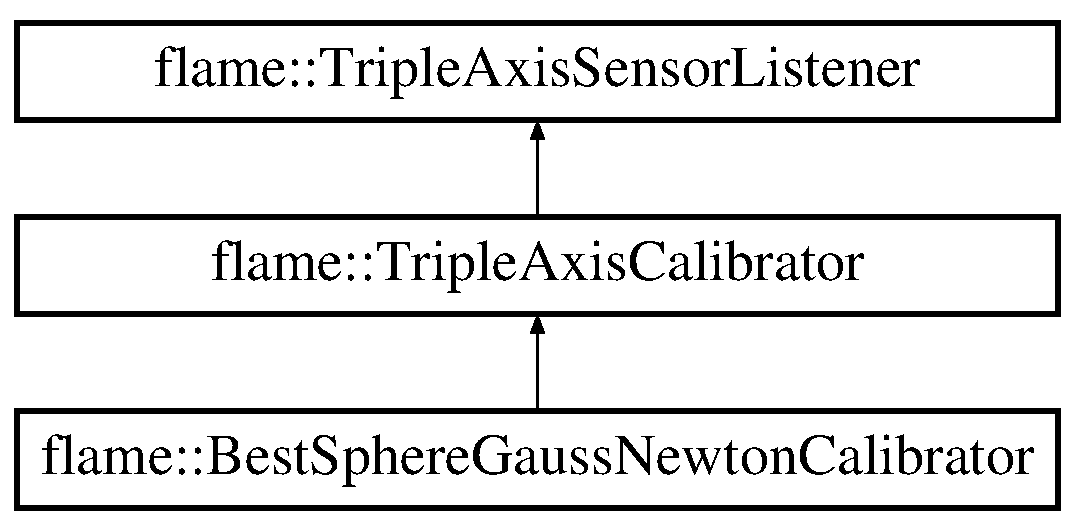
\includegraphics[height=3.000000cm]{classflame_1_1_triple_axis_calibrator}
\end{center}
\end{figure}
\subsection*{Public Member Functions}
\begin{DoxyCompactItemize}
\item 
\hyperlink{classflame_1_1_triple_axis_calibrator_a7e2fcf4739bff86d4f3c69b2b7025265}{Triple\-Axis\-Calibrator} (\hyperlink{classflame_1_1_triple_axis_sensor}{Triple\-Axis\-Sensor} \&sensor, \hyperlink{classflame_1_1_device___t_x}{Device\-\_\-\-T\-X} \&output)
\item 
bool \hyperlink{classflame_1_1_triple_axis_calibrator_a35446f4f0c1ab5b6ef203c3e0fabda9c}{push\-Sample} (const \hyperlink{namespaceflame_ab883ad815041824ba548753dae327bc2}{T\-R\-I\-P\-L\-E\-A\-X\-I\-S\-S\-E\-N\-S\-O\-R\-\_\-\-R\-A\-W\-\_\-\-R\-E\-A\-D\-I\-N\-G} \&sample, P\-G\-M\-\_\-\-P $\ast$feedback)
\item 
void \hyperlink{classflame_1_1_triple_axis_calibrator_a95729b080aee3846856ea91c0f9fa73b}{calibrate} ()
\item 
void \hyperlink{classflame_1_1_triple_axis_calibrator_ab66474b4d1f8f6e9c2ee76233a927e71}{sample\-Is\-Ready} (\hyperlink{classflame_1_1_triple_axis_sensor}{Triple\-Axis\-Sensor} \&sensor)
\item 
void \hyperlink{classflame_1_1_triple_axis_calibrator_af80e930aac780ea5b25f99423fb22fd7}{limit\-Reached} (\hyperlink{classflame_1_1_triple_axis_sensor}{Triple\-Axis\-Sensor} \&sensor, \hyperlink{namespaceflame_a626e8c99d0f4f232b95e7089c113095a}{Triple\-Axis\-Sensor\-Channel} which)
\item 
virtual void \hyperlink{classflame_1_1_triple_axis_calibrator_a088b330f58f52e7d3df291cc6e8bafed}{add\-Observation} (const \hyperlink{namespaceflame_ab883ad815041824ba548753dae327bc2}{T\-R\-I\-P\-L\-E\-A\-X\-I\-S\-S\-E\-N\-S\-O\-R\-\_\-\-R\-A\-W\-\_\-\-R\-E\-A\-D\-I\-N\-G} \&sample)=0
\item 
virtual void \hyperlink{classflame_1_1_triple_axis_calibrator_a1a22ce8da6a3e3672f59e876acd3796b}{calibrate\-Sensor} (\hyperlink{classflame_1_1_triple_axis_sensor}{Triple\-Axis\-Sensor} \&sensor)=0
\end{DoxyCompactItemize}
\subsection*{Protected Member Functions}
\begin{DoxyCompactItemize}
\item 
bool \hyperlink{classflame_1_1_triple_axis_calibrator_af433d139c778c5c934ca429bbdb430c2}{is\-Sample\-Good} (const \hyperlink{namespaceflame_ab883ad815041824ba548753dae327bc2}{T\-R\-I\-P\-L\-E\-A\-X\-I\-S\-S\-E\-N\-S\-O\-R\-\_\-\-R\-A\-W\-\_\-\-R\-E\-A\-D\-I\-N\-G} \&sample, P\-G\-M\-\_\-\-P $\ast$feedback)
\end{DoxyCompactItemize}
\subsection*{Protected Attributes}
\begin{DoxyCompactItemize}
\item 
\hyperlink{namespaceflame_ab883ad815041824ba548753dae327bc2}{T\-R\-I\-P\-L\-E\-A\-X\-I\-S\-S\-E\-N\-S\-O\-R\-\_\-\-R\-A\-W\-\_\-\-R\-E\-A\-D\-I\-N\-G} \hyperlink{classflame_1_1_triple_axis_calibrator_a11ec83028a6841ec9d89f61e8f72620e}{\-\_\-previous\-Sample} = \{\{0, 0, 0\}\}
\item 
uint8\-\_\-t \hyperlink{classflame_1_1_triple_axis_calibrator_aa3453c42d8b6f0fdb582d3e722a2db07}{\-\_\-good\-Samples} = 0
\item 
P\-G\-M\-\_\-\-P \hyperlink{classflame_1_1_triple_axis_calibrator_a2d4c8a4a2944e37341d2e3534a329e24}{\-\_\-last\-Message} = N\-U\-L\-L
\item 
uint8\-\_\-t \hyperlink{classflame_1_1_triple_axis_calibrator_a996c1d5e43bd37fba52d8e9ff4b0349c}{\-\_\-samples\-To\-Take} = 32
\item 
uint8\-\_\-t \hyperlink{classflame_1_1_triple_axis_calibrator_a802dbf52302b13c65b7d40dca18742bc}{\-\_\-current\-Samples} = 0
\item 
\hyperlink{namespaceflame_a72abf3b66537683db272a18f7d34a5a7}{Triple\-Axis\-Calibrator\-State} \hyperlink{classflame_1_1_triple_axis_calibrator_a4853069366d07f826e099879724b9083}{\-\_\-state} = \hyperlink{namespaceflame_a72abf3b66537683db272a18f7d34a5a7addbb81a9e3aab6cfa19ad8eb2389efd4}{Triple\-Axis\-Calibrator\-State\-::\-S\-E\-T\-U\-P}
\item 
\hyperlink{classflame_1_1_triple_axis_sensor}{Triple\-Axis\-Sensor} \& \hyperlink{classflame_1_1_triple_axis_calibrator_a4f0dd2bfe0f85a0229fbf74f9944161d}{\-\_\-sensor}
\item 
\hyperlink{classflame_1_1_device___t_x}{Device\-\_\-\-T\-X} \& \hyperlink{classflame_1_1_triple_axis_calibrator_a6fccd0307b71a7dbfa1c4fd0adcaa188}{\-\_\-output}
\item 
\hyperlink{classflame_1_1_triple_axis_sensor_listener}{Triple\-Axis\-Sensor\-Listener} $\ast$ \hyperlink{classflame_1_1_triple_axis_calibrator_ae80be2c28e5243d39b12c33f24ecb595}{\-\_\-saved\-Listener} = N\-U\-L\-L
\end{DoxyCompactItemize}


\subsection{Detailed Description}


Definition at line 48 of file Triple\-Axis\-Calibrator.\-h.



\subsection{Constructor \& Destructor Documentation}
\hypertarget{classflame_1_1_triple_axis_calibrator_a7e2fcf4739bff86d4f3c69b2b7025265}{\index{flame\-::\-Triple\-Axis\-Calibrator@{flame\-::\-Triple\-Axis\-Calibrator}!Triple\-Axis\-Calibrator@{Triple\-Axis\-Calibrator}}
\index{Triple\-Axis\-Calibrator@{Triple\-Axis\-Calibrator}!flame::TripleAxisCalibrator@{flame\-::\-Triple\-Axis\-Calibrator}}
\subsubsection[{Triple\-Axis\-Calibrator}]{\setlength{\rightskip}{0pt plus 5cm}flame\-::\-Triple\-Axis\-Calibrator\-::\-Triple\-Axis\-Calibrator (
\begin{DoxyParamCaption}
\item[{{\bf Triple\-Axis\-Sensor} \&}]{sensor, }
\item[{{\bf Device\-\_\-\-T\-X} \&}]{output}
\end{DoxyParamCaption}
)}}\label{classflame_1_1_triple_axis_calibrator_a7e2fcf4739bff86d4f3c69b2b7025265}
Constructor 

Definition at line 56 of file Triple\-Axis\-Calibrator.\-cpp.



\subsection{Member Function Documentation}
\hypertarget{classflame_1_1_triple_axis_calibrator_a088b330f58f52e7d3df291cc6e8bafed}{\index{flame\-::\-Triple\-Axis\-Calibrator@{flame\-::\-Triple\-Axis\-Calibrator}!add\-Observation@{add\-Observation}}
\index{add\-Observation@{add\-Observation}!flame::TripleAxisCalibrator@{flame\-::\-Triple\-Axis\-Calibrator}}
\subsubsection[{add\-Observation}]{\setlength{\rightskip}{0pt plus 5cm}virtual void flame\-::\-Triple\-Axis\-Calibrator\-::add\-Observation (
\begin{DoxyParamCaption}
\item[{const {\bf T\-R\-I\-P\-L\-E\-A\-X\-I\-S\-S\-E\-N\-S\-O\-R\-\_\-\-R\-A\-W\-\_\-\-R\-E\-A\-D\-I\-N\-G} \&}]{sample}
\end{DoxyParamCaption}
)\hspace{0.3cm}{\ttfamily [pure virtual]}}}\label{classflame_1_1_triple_axis_calibrator_a088b330f58f52e7d3df291cc6e8bafed}
Add a sample to the calibrator 
\begin{DoxyParams}{Parameters}
{\em sample} & the sample to send \\
\hline
\end{DoxyParams}


Implemented in \hyperlink{classflame_1_1_best_sphere_gauss_newton_calibrator_af84f75dc992202bbd1b24624d3e22e28}{flame\-::\-Best\-Sphere\-Gauss\-Newton\-Calibrator}.

\hypertarget{classflame_1_1_triple_axis_calibrator_a95729b080aee3846856ea91c0f9fa73b}{\index{flame\-::\-Triple\-Axis\-Calibrator@{flame\-::\-Triple\-Axis\-Calibrator}!calibrate@{calibrate}}
\index{calibrate@{calibrate}!flame::TripleAxisCalibrator@{flame\-::\-Triple\-Axis\-Calibrator}}
\subsubsection[{calibrate}]{\setlength{\rightskip}{0pt plus 5cm}void flame\-::\-Triple\-Axis\-Calibrator\-::calibrate (
\begin{DoxyParamCaption}
{}
\end{DoxyParamCaption}
)}}\label{classflame_1_1_triple_axis_calibrator_a95729b080aee3846856ea91c0f9fa73b}
Calibrate a sensor 
\begin{DoxyParams}{Parameters}
{\em sensor} & the sensor to calibrate \\
\hline
\end{DoxyParams}


Definition at line 183 of file Triple\-Axis\-Calibrator.\-cpp.

\hypertarget{classflame_1_1_triple_axis_calibrator_a1a22ce8da6a3e3672f59e876acd3796b}{\index{flame\-::\-Triple\-Axis\-Calibrator@{flame\-::\-Triple\-Axis\-Calibrator}!calibrate\-Sensor@{calibrate\-Sensor}}
\index{calibrate\-Sensor@{calibrate\-Sensor}!flame::TripleAxisCalibrator@{flame\-::\-Triple\-Axis\-Calibrator}}
\subsubsection[{calibrate\-Sensor}]{\setlength{\rightskip}{0pt plus 5cm}virtual void flame\-::\-Triple\-Axis\-Calibrator\-::calibrate\-Sensor (
\begin{DoxyParamCaption}
\item[{{\bf Triple\-Axis\-Sensor} \&}]{sensor}
\end{DoxyParamCaption}
)\hspace{0.3cm}{\ttfamily [pure virtual]}}}\label{classflame_1_1_triple_axis_calibrator_a1a22ce8da6a3e3672f59e876acd3796b}
Write the offsets and scales to the sensor 
\begin{DoxyParams}{Parameters}
{\em sensor} & the sensor to write to (should be the same sensor that is pushing the sample \\
\hline
\end{DoxyParams}


Implemented in \hyperlink{classflame_1_1_best_sphere_gauss_newton_calibrator_ac07439f912b1ff230dc3cc80c86c26be}{flame\-::\-Best\-Sphere\-Gauss\-Newton\-Calibrator}.

\hypertarget{classflame_1_1_triple_axis_calibrator_af433d139c778c5c934ca429bbdb430c2}{\index{flame\-::\-Triple\-Axis\-Calibrator@{flame\-::\-Triple\-Axis\-Calibrator}!is\-Sample\-Good@{is\-Sample\-Good}}
\index{is\-Sample\-Good@{is\-Sample\-Good}!flame::TripleAxisCalibrator@{flame\-::\-Triple\-Axis\-Calibrator}}
\subsubsection[{is\-Sample\-Good}]{\setlength{\rightskip}{0pt plus 5cm}bool flame\-::\-Triple\-Axis\-Calibrator\-::is\-Sample\-Good (
\begin{DoxyParamCaption}
\item[{const {\bf T\-R\-I\-P\-L\-E\-A\-X\-I\-S\-S\-E\-N\-S\-O\-R\-\_\-\-R\-A\-W\-\_\-\-R\-E\-A\-D\-I\-N\-G} \&}]{sample, }
\item[{P\-G\-M\-\_\-\-P $\ast$}]{feedback}
\end{DoxyParamCaption}
)\hspace{0.3cm}{\ttfamily [protected]}}}\label{classflame_1_1_triple_axis_calibrator_af433d139c778c5c934ca429bbdb430c2}
Check if the sensor is steady, and complain if it is not 
\begin{DoxyParams}{Parameters}
{\em sample} & the sample \\
\hline
{\em feedback} & a pointer that will be set to a progmem string to prompt action from the user (or N\-U\-L\-L) \\
\hline
\end{DoxyParams}
\begin{DoxyReturn}{Returns}
true if the sample was good 
\end{DoxyReturn}


Definition at line 67 of file Triple\-Axis\-Calibrator.\-cpp.

\hypertarget{classflame_1_1_triple_axis_calibrator_af80e930aac780ea5b25f99423fb22fd7}{\index{flame\-::\-Triple\-Axis\-Calibrator@{flame\-::\-Triple\-Axis\-Calibrator}!limit\-Reached@{limit\-Reached}}
\index{limit\-Reached@{limit\-Reached}!flame::TripleAxisCalibrator@{flame\-::\-Triple\-Axis\-Calibrator}}
\subsubsection[{limit\-Reached}]{\setlength{\rightskip}{0pt plus 5cm}void flame\-::\-Triple\-Axis\-Calibrator\-::limit\-Reached (
\begin{DoxyParamCaption}
\item[{{\bf Triple\-Axis\-Sensor} \&}]{sensor, }
\item[{{\bf Triple\-Axis\-Sensor\-Channel}}]{which}
\end{DoxyParamCaption}
)\hspace{0.3cm}{\ttfamily [virtual]}}}\label{classflame_1_1_triple_axis_calibrator_af80e930aac780ea5b25f99423fb22fd7}
Called when an acceleration limit is reached 
\begin{DoxyParams}{Parameters}
{\em sensor} & the sensor whose limit was reached \\
\hline
{\em which} & which limit was reached \\
\hline
\end{DoxyParams}


Implements \hyperlink{classflame_1_1_triple_axis_sensor_listener_a56c75bbcf89043b53b938e3f9045db38}{flame\-::\-Triple\-Axis\-Sensor\-Listener}.



Definition at line 219 of file Triple\-Axis\-Calibrator.\-cpp.

\hypertarget{classflame_1_1_triple_axis_calibrator_a35446f4f0c1ab5b6ef203c3e0fabda9c}{\index{flame\-::\-Triple\-Axis\-Calibrator@{flame\-::\-Triple\-Axis\-Calibrator}!push\-Sample@{push\-Sample}}
\index{push\-Sample@{push\-Sample}!flame::TripleAxisCalibrator@{flame\-::\-Triple\-Axis\-Calibrator}}
\subsubsection[{push\-Sample}]{\setlength{\rightskip}{0pt plus 5cm}bool flame\-::\-Triple\-Axis\-Calibrator\-::push\-Sample (
\begin{DoxyParamCaption}
\item[{const {\bf T\-R\-I\-P\-L\-E\-A\-X\-I\-S\-S\-E\-N\-S\-O\-R\-\_\-\-R\-A\-W\-\_\-\-R\-E\-A\-D\-I\-N\-G} \&}]{sample, }
\item[{P\-G\-M\-\_\-\-P $\ast$}]{feedback}
\end{DoxyParamCaption}
)}}\label{classflame_1_1_triple_axis_calibrator_a35446f4f0c1ab5b6ef203c3e0fabda9c}
Send a sample in to the calibrator if it is good enough Prompt the user with directions if it isn't 
\begin{DoxyParams}{Parameters}
{\em sample} & the sample to send \\
\hline
{\em feedback} & a pointer that will be set to a progmem string to prompt action from the user (or N\-U\-L\-L) \\
\hline
\end{DoxyParams}
\begin{DoxyReturn}{Returns}
true if more samples are required 
\end{DoxyReturn}


Definition at line 87 of file Triple\-Axis\-Calibrator.\-cpp.

\hypertarget{classflame_1_1_triple_axis_calibrator_ab66474b4d1f8f6e9c2ee76233a927e71}{\index{flame\-::\-Triple\-Axis\-Calibrator@{flame\-::\-Triple\-Axis\-Calibrator}!sample\-Is\-Ready@{sample\-Is\-Ready}}
\index{sample\-Is\-Ready@{sample\-Is\-Ready}!flame::TripleAxisCalibrator@{flame\-::\-Triple\-Axis\-Calibrator}}
\subsubsection[{sample\-Is\-Ready}]{\setlength{\rightskip}{0pt plus 5cm}void flame\-::\-Triple\-Axis\-Calibrator\-::sample\-Is\-Ready (
\begin{DoxyParamCaption}
\item[{{\bf Triple\-Axis\-Sensor} \&}]{sensor}
\end{DoxyParamCaption}
)\hspace{0.3cm}{\ttfamily [virtual]}}}\label{classflame_1_1_triple_axis_calibrator_ab66474b4d1f8f6e9c2ee76233a927e71}
Called when a sample is ready 
\begin{DoxyParams}{Parameters}
{\em sensor} & the sensor whose sample is ready \\
\hline
\end{DoxyParams}


Implements \hyperlink{classflame_1_1_triple_axis_sensor_listener_a4451e2df32ad722464a1902ef29ed054}{flame\-::\-Triple\-Axis\-Sensor\-Listener}.



Definition at line 193 of file Triple\-Axis\-Calibrator.\-cpp.



\subsection{Member Data Documentation}
\hypertarget{classflame_1_1_triple_axis_calibrator_a802dbf52302b13c65b7d40dca18742bc}{\index{flame\-::\-Triple\-Axis\-Calibrator@{flame\-::\-Triple\-Axis\-Calibrator}!\-\_\-current\-Samples@{\-\_\-current\-Samples}}
\index{\-\_\-current\-Samples@{\-\_\-current\-Samples}!flame::TripleAxisCalibrator@{flame\-::\-Triple\-Axis\-Calibrator}}
\subsubsection[{\-\_\-current\-Samples}]{\setlength{\rightskip}{0pt plus 5cm}uint8\-\_\-t flame\-::\-Triple\-Axis\-Calibrator\-::\-\_\-current\-Samples = 0\hspace{0.3cm}{\ttfamily [protected]}}}\label{classflame_1_1_triple_axis_calibrator_a802dbf52302b13c65b7d40dca18742bc}


Definition at line 54 of file Triple\-Axis\-Calibrator.\-h.

\hypertarget{classflame_1_1_triple_axis_calibrator_aa3453c42d8b6f0fdb582d3e722a2db07}{\index{flame\-::\-Triple\-Axis\-Calibrator@{flame\-::\-Triple\-Axis\-Calibrator}!\-\_\-good\-Samples@{\-\_\-good\-Samples}}
\index{\-\_\-good\-Samples@{\-\_\-good\-Samples}!flame::TripleAxisCalibrator@{flame\-::\-Triple\-Axis\-Calibrator}}
\subsubsection[{\-\_\-good\-Samples}]{\setlength{\rightskip}{0pt plus 5cm}uint8\-\_\-t flame\-::\-Triple\-Axis\-Calibrator\-::\-\_\-good\-Samples = 0\hspace{0.3cm}{\ttfamily [protected]}}}\label{classflame_1_1_triple_axis_calibrator_aa3453c42d8b6f0fdb582d3e722a2db07}


Definition at line 51 of file Triple\-Axis\-Calibrator.\-h.

\hypertarget{classflame_1_1_triple_axis_calibrator_a2d4c8a4a2944e37341d2e3534a329e24}{\index{flame\-::\-Triple\-Axis\-Calibrator@{flame\-::\-Triple\-Axis\-Calibrator}!\-\_\-last\-Message@{\-\_\-last\-Message}}
\index{\-\_\-last\-Message@{\-\_\-last\-Message}!flame::TripleAxisCalibrator@{flame\-::\-Triple\-Axis\-Calibrator}}
\subsubsection[{\-\_\-last\-Message}]{\setlength{\rightskip}{0pt plus 5cm}P\-G\-M\-\_\-\-P flame\-::\-Triple\-Axis\-Calibrator\-::\-\_\-last\-Message = N\-U\-L\-L\hspace{0.3cm}{\ttfamily [protected]}}}\label{classflame_1_1_triple_axis_calibrator_a2d4c8a4a2944e37341d2e3534a329e24}


Definition at line 52 of file Triple\-Axis\-Calibrator.\-h.

\hypertarget{classflame_1_1_triple_axis_calibrator_a6fccd0307b71a7dbfa1c4fd0adcaa188}{\index{flame\-::\-Triple\-Axis\-Calibrator@{flame\-::\-Triple\-Axis\-Calibrator}!\-\_\-output@{\-\_\-output}}
\index{\-\_\-output@{\-\_\-output}!flame::TripleAxisCalibrator@{flame\-::\-Triple\-Axis\-Calibrator}}
\subsubsection[{\-\_\-output}]{\setlength{\rightskip}{0pt plus 5cm}{\bf Device\-\_\-\-T\-X}\& flame\-::\-Triple\-Axis\-Calibrator\-::\-\_\-output\hspace{0.3cm}{\ttfamily [protected]}}}\label{classflame_1_1_triple_axis_calibrator_a6fccd0307b71a7dbfa1c4fd0adcaa188}


Definition at line 57 of file Triple\-Axis\-Calibrator.\-h.

\hypertarget{classflame_1_1_triple_axis_calibrator_a11ec83028a6841ec9d89f61e8f72620e}{\index{flame\-::\-Triple\-Axis\-Calibrator@{flame\-::\-Triple\-Axis\-Calibrator}!\-\_\-previous\-Sample@{\-\_\-previous\-Sample}}
\index{\-\_\-previous\-Sample@{\-\_\-previous\-Sample}!flame::TripleAxisCalibrator@{flame\-::\-Triple\-Axis\-Calibrator}}
\subsubsection[{\-\_\-previous\-Sample}]{\setlength{\rightskip}{0pt plus 5cm}{\bf T\-R\-I\-P\-L\-E\-A\-X\-I\-S\-S\-E\-N\-S\-O\-R\-\_\-\-R\-A\-W\-\_\-\-R\-E\-A\-D\-I\-N\-G} flame\-::\-Triple\-Axis\-Calibrator\-::\-\_\-previous\-Sample = \{\{0, 0, 0\}\}\hspace{0.3cm}{\ttfamily [protected]}}}\label{classflame_1_1_triple_axis_calibrator_a11ec83028a6841ec9d89f61e8f72620e}


Definition at line 50 of file Triple\-Axis\-Calibrator.\-h.

\hypertarget{classflame_1_1_triple_axis_calibrator_a996c1d5e43bd37fba52d8e9ff4b0349c}{\index{flame\-::\-Triple\-Axis\-Calibrator@{flame\-::\-Triple\-Axis\-Calibrator}!\-\_\-samples\-To\-Take@{\-\_\-samples\-To\-Take}}
\index{\-\_\-samples\-To\-Take@{\-\_\-samples\-To\-Take}!flame::TripleAxisCalibrator@{flame\-::\-Triple\-Axis\-Calibrator}}
\subsubsection[{\-\_\-samples\-To\-Take}]{\setlength{\rightskip}{0pt plus 5cm}uint8\-\_\-t flame\-::\-Triple\-Axis\-Calibrator\-::\-\_\-samples\-To\-Take = 32\hspace{0.3cm}{\ttfamily [protected]}}}\label{classflame_1_1_triple_axis_calibrator_a996c1d5e43bd37fba52d8e9ff4b0349c}


Definition at line 53 of file Triple\-Axis\-Calibrator.\-h.

\hypertarget{classflame_1_1_triple_axis_calibrator_ae80be2c28e5243d39b12c33f24ecb595}{\index{flame\-::\-Triple\-Axis\-Calibrator@{flame\-::\-Triple\-Axis\-Calibrator}!\-\_\-saved\-Listener@{\-\_\-saved\-Listener}}
\index{\-\_\-saved\-Listener@{\-\_\-saved\-Listener}!flame::TripleAxisCalibrator@{flame\-::\-Triple\-Axis\-Calibrator}}
\subsubsection[{\-\_\-saved\-Listener}]{\setlength{\rightskip}{0pt plus 5cm}{\bf Triple\-Axis\-Sensor\-Listener}$\ast$ flame\-::\-Triple\-Axis\-Calibrator\-::\-\_\-saved\-Listener = N\-U\-L\-L\hspace{0.3cm}{\ttfamily [protected]}}}\label{classflame_1_1_triple_axis_calibrator_ae80be2c28e5243d39b12c33f24ecb595}


Definition at line 58 of file Triple\-Axis\-Calibrator.\-h.

\hypertarget{classflame_1_1_triple_axis_calibrator_a4f0dd2bfe0f85a0229fbf74f9944161d}{\index{flame\-::\-Triple\-Axis\-Calibrator@{flame\-::\-Triple\-Axis\-Calibrator}!\-\_\-sensor@{\-\_\-sensor}}
\index{\-\_\-sensor@{\-\_\-sensor}!flame::TripleAxisCalibrator@{flame\-::\-Triple\-Axis\-Calibrator}}
\subsubsection[{\-\_\-sensor}]{\setlength{\rightskip}{0pt plus 5cm}{\bf Triple\-Axis\-Sensor}\& flame\-::\-Triple\-Axis\-Calibrator\-::\-\_\-sensor\hspace{0.3cm}{\ttfamily [protected]}}}\label{classflame_1_1_triple_axis_calibrator_a4f0dd2bfe0f85a0229fbf74f9944161d}


Definition at line 56 of file Triple\-Axis\-Calibrator.\-h.

\hypertarget{classflame_1_1_triple_axis_calibrator_a4853069366d07f826e099879724b9083}{\index{flame\-::\-Triple\-Axis\-Calibrator@{flame\-::\-Triple\-Axis\-Calibrator}!\-\_\-state@{\-\_\-state}}
\index{\-\_\-state@{\-\_\-state}!flame::TripleAxisCalibrator@{flame\-::\-Triple\-Axis\-Calibrator}}
\subsubsection[{\-\_\-state}]{\setlength{\rightskip}{0pt plus 5cm}{\bf Triple\-Axis\-Calibrator\-State} flame\-::\-Triple\-Axis\-Calibrator\-::\-\_\-state = {\bf Triple\-Axis\-Calibrator\-State\-::\-S\-E\-T\-U\-P}\hspace{0.3cm}{\ttfamily [protected]}}}\label{classflame_1_1_triple_axis_calibrator_a4853069366d07f826e099879724b9083}


Definition at line 55 of file Triple\-Axis\-Calibrator.\-h.



The documentation for this class was generated from the following files\-:\begin{DoxyCompactItemize}
\item 
flame/\hyperlink{_triple_axis_calibrator_8h}{Triple\-Axis\-Calibrator.\-h}\item 
\hyperlink{_triple_axis_calibrator_8cpp}{Triple\-Axis\-Calibrator.\-cpp}\end{DoxyCompactItemize}

\hypertarget{classflame_1_1_triple_axis_sensor}{\section{flame\-:\-:Triple\-Axis\-Sensor Class Reference}
\label{classflame_1_1_triple_axis_sensor}\index{flame\-::\-Triple\-Axis\-Sensor@{flame\-::\-Triple\-Axis\-Sensor}}
}


{\ttfamily \#include $<$Triple\-Axis\-Sensor.\-h$>$}

Inheritance diagram for flame\-:\-:Triple\-Axis\-Sensor\-:\begin{figure}[H]
\begin{center}
\leavevmode
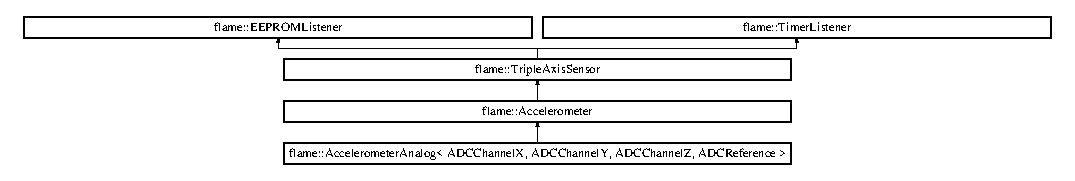
\includegraphics[height=1.982301cm]{classflame_1_1_triple_axis_sensor}
\end{center}
\end{figure}
\subsection*{Public Member Functions}
\begin{DoxyCompactItemize}
\item 
virtual void \hyperlink{classflame_1_1_triple_axis_sensor_ac2ff28538723dc987c6fbec20aa47341}{sample} ()=0
\item 
virtual bool \hyperlink{classflame_1_1_triple_axis_sensor_a7223b8884adf0ff42cbfddd2b6f28ce3}{is\-Sample\-Ready} ()=0
\item 
void \hyperlink{classflame_1_1_triple_axis_sensor_a8168452d055fad77782e7fd121343d61}{save\-Calibration} (\hyperlink{classflame_1_1_e_e_p_r_o_m}{E\-E\-P\-R\-O\-M} \&eeprom, uint16\-\_\-t address)
\item 
void \hyperlink{classflame_1_1_triple_axis_sensor_aaa716e2a07cc7fe544075215c1ac8a75}{eeprom\-Done} (\hyperlink{classflame_1_1_e_e_p_r_o_m}{E\-E\-P\-R\-O\-M} \&eeprom, uint16\-\_\-t address, void $\ast$buffer)
\item 
bool \hyperlink{classflame_1_1_triple_axis_sensor_a64c19829e85e70d0825be3530529d8b0}{load\-Calibration} (\hyperlink{classflame_1_1_e_e_p_r_o_m}{E\-E\-P\-R\-O\-M} \&eeprom, uint16\-\_\-t address)
\item 
void \hyperlink{classflame_1_1_triple_axis_sensor_a446b55e5557faadf8d73e0111fcaf2bd}{set\-Offsets} (const \hyperlink{namespaceflame_a9c63ea08dcbcedfed611f6afdb992301}{T\-R\-I\-P\-L\-E\-A\-X\-I\-S\-S\-E\-N\-S\-O\-R\-\_\-\-O\-F\-F\-S\-E\-T\-S} \&offsets)
\item 
void \hyperlink{classflame_1_1_triple_axis_sensor_a74daeefee092f1f32e4fd0aa7cf15bb0}{set\-Offsets} (int16\-\_\-t x, int16\-\_\-t y, int16\-\_\-t z)
\item 
void \hyperlink{classflame_1_1_triple_axis_sensor_a4147dd086c276dfdae8efcc6652f4df0}{set\-Scale} (const \hyperlink{namespaceflame_a513ac03cc7f92c4b8d7cadb972e6be72}{T\-R\-I\-P\-L\-E\-A\-X\-I\-S\-S\-E\-N\-S\-O\-R\-\_\-\-S\-C\-A\-L\-I\-N\-G} \&scales)
\item 
void \hyperlink{classflame_1_1_triple_axis_sensor_a5c4462df5fd335f83eabf60a98297cd8}{set\-Scale} (float x, float y, float z)
\item 
void \hyperlink{classflame_1_1_triple_axis_sensor_a932b8ebc27dbce01dbc7bf5265a9e5ac}{get\-Parameters} (\hyperlink{namespaceflame_a9c63ea08dcbcedfed611f6afdb992301}{T\-R\-I\-P\-L\-E\-A\-X\-I\-S\-S\-E\-N\-S\-O\-R\-\_\-\-O\-F\-F\-S\-E\-T\-S} $\ast$offsets, \hyperlink{namespaceflame_a513ac03cc7f92c4b8d7cadb972e6be72}{T\-R\-I\-P\-L\-E\-A\-X\-I\-S\-S\-E\-N\-S\-O\-R\-\_\-\-S\-C\-A\-L\-I\-N\-G} $\ast$scales)
\item 
void \hyperlink{classflame_1_1_triple_axis_sensor_a4a655be3990763a0ecddcf081543ee82}{register\-Listener} (\hyperlink{classflame_1_1_triple_axis_sensor_listener}{Triple\-Axis\-Sensor\-Listener} \&listener)
\item 
void \hyperlink{classflame_1_1_triple_axis_sensor_ab3051eced113bc27eff59be1024f2da0}{deregister\-Listener} ()
\item 
\hyperlink{classflame_1_1_triple_axis_sensor_listener}{Triple\-Axis\-Sensor\-Listener} $\ast$ \hyperlink{classflame_1_1_triple_axis_sensor_aabbc82ab78ff5869e8cec0d09c8cd053}{get\-Listener} ()
\item 
void \hyperlink{classflame_1_1_triple_axis_sensor_a8d1f12483d3a0a068cc623df425ae831}{get\-Value} (float $\ast$x, float $\ast$y, float $\ast$z)
\item 
void \hyperlink{classflame_1_1_triple_axis_sensor_ab44fd1a3caf553df2e57a7a654dc457e}{get\-Value} (\hyperlink{namespaceflame_a11b86dc8b6fd50d24cec8b9f0259289b}{T\-R\-I\-P\-L\-E\-A\-X\-I\-S\-S\-E\-N\-S\-O\-R\-\_\-\-R\-E\-A\-D\-I\-N\-G} $\ast$value)
\item 
void \hyperlink{classflame_1_1_triple_axis_sensor_aa036218566ff36f6d5320cf66bf73dbc}{get\-Raw\-Value} (\hyperlink{namespaceflame_ab883ad815041824ba548753dae327bc2}{T\-R\-I\-P\-L\-E\-A\-X\-I\-S\-S\-E\-N\-S\-O\-R\-\_\-\-R\-A\-W\-\_\-\-R\-E\-A\-D\-I\-N\-G} $\ast$value)
\item 
float \hyperlink{classflame_1_1_triple_axis_sensor_af1f6e5c2dcf25070464dcc65c09cf1b5}{magnitude\-Squared} ()
\item 
float \hyperlink{classflame_1_1_triple_axis_sensor_a6d8c6a6011853e2015956c8936ed19ff}{magnitude} ()
\item 
void \hyperlink{classflame_1_1_triple_axis_sensor_a2ba2508c4a53376126504055e19bcee7}{handle\-Events} ()
\item 
void \hyperlink{classflame_1_1_triple_axis_sensor_a87a4e16d1637a7acd6c35ab200ea6d74}{set\-Limit} (\hyperlink{namespaceflame_a626e8c99d0f4f232b95e7089c113095a}{Triple\-Axis\-Sensor\-Channel} which, float limit)
\item 
void \hyperlink{classflame_1_1_triple_axis_sensor_a512ee16a5b45a7e9a30162976538c744}{get\-Limits} (\hyperlink{namespaceflame_a11b86dc8b6fd50d24cec8b9f0259289b}{T\-R\-I\-P\-L\-E\-A\-X\-I\-S\-S\-E\-N\-S\-O\-R\-\_\-\-R\-E\-A\-D\-I\-N\-G} $\ast$limits)
\item 
void \hyperlink{classflame_1_1_triple_axis_sensor_ad5fbc92633b96e9432c42a6e405eafbc}{alarm} (\hyperlink{namespaceflame_a6d176ba245556716fd3e32006bb7cfe5}{Alarm\-Source} source)
\item 
bool \hyperlink{classflame_1_1_triple_axis_sensor_ac41a5efbd52c5b79acd4b1976f43ec84}{is\-Calibrated} ()
\item 
void \hyperlink{classflame_1_1_triple_axis_sensor_ac758b7d4bc3ad72397090e782e947976}{set\-Calibrated} (bool calibrated)
\end{DoxyCompactItemize}
\subsection*{Protected Member Functions}
\begin{DoxyCompactItemize}
\item 
void \hyperlink{classflame_1_1_triple_axis_sensor_ac61854be2362d25a1d7b86d9afa6355c}{push\-Sample} (\hyperlink{namespaceflame_a626e8c99d0f4f232b95e7089c113095a}{Triple\-Axis\-Sensor\-Channel} which, int16\-\_\-t value)
\end{DoxyCompactItemize}
\subsection*{Protected Attributes}
\begin{DoxyCompactItemize}
\item 
\hyperlink{classflame_1_1_triple_axis_sensor_listener}{Triple\-Axis\-Sensor\-Listener} $\ast$ \hyperlink{classflame_1_1_triple_axis_sensor_a13289e03729649c86021beaf5c5e0279}{\-\_\-listener} = N\-U\-L\-L
\item 
\hyperlink{namespaceflame_a11b86dc8b6fd50d24cec8b9f0259289b}{T\-R\-I\-P\-L\-E\-A\-X\-I\-S\-S\-E\-N\-S\-O\-R\-\_\-\-R\-E\-A\-D\-I\-N\-G} \hyperlink{classflame_1_1_triple_axis_sensor_a5db946bd07a26418e39d5e5f000a8209}{\-\_\-value\-Temp} = \{\{0.\-0f, 0.\-0f, 0.\-0f\}\}
\item 
\hyperlink{namespaceflame_a11b86dc8b6fd50d24cec8b9f0259289b}{T\-R\-I\-P\-L\-E\-A\-X\-I\-S\-S\-E\-N\-S\-O\-R\-\_\-\-R\-E\-A\-D\-I\-N\-G} \hyperlink{classflame_1_1_triple_axis_sensor_aadbb6bb4aa35232bf548c3a9d83ce284}{\-\_\-value\-Out} = \{\{0.\-0f, 0.\-0f, 0.\-0f\}\}
\item 
\hyperlink{namespaceflame_a2b796938428096c98b4073492baf98a6}{T\-R\-I\-P\-L\-E\-A\-X\-I\-S\-S\-E\-N\-S\-O\-R\-\_\-\-L\-I\-M\-I\-T\-S} \hyperlink{classflame_1_1_triple_axis_sensor_ac98b09ee7cf74d16a3f772752d7e1d30}{\-\_\-limit} = \{\{0.\-0f, 0.\-0f, 0.\-0f\}\}
\item 
float \hyperlink{classflame_1_1_triple_axis_sensor_a7e759ec01ad8d2d00038b2edf9fc5913}{\-\_\-limit\-Magnitude\-Squared} = 0.\-0f
\item 
\hyperlink{namespaceflame_a9c63ea08dcbcedfed611f6afdb992301}{T\-R\-I\-P\-L\-E\-A\-X\-I\-S\-S\-E\-N\-S\-O\-R\-\_\-\-O\-F\-F\-S\-E\-T\-S} \hyperlink{classflame_1_1_triple_axis_sensor_af4c80100c14de0069a584217136187af}{\-\_\-offsets} = \{\{0, 0, 0\}\}
\item 
\hyperlink{namespaceflame_a513ac03cc7f92c4b8d7cadb972e6be72}{T\-R\-I\-P\-L\-E\-A\-X\-I\-S\-S\-E\-N\-S\-O\-R\-\_\-\-S\-C\-A\-L\-I\-N\-G} \hyperlink{classflame_1_1_triple_axis_sensor_a79e7f229439c0c0e747a2fa8c30ecaba}{\-\_\-scaling} = \{\{1.\-0f, 1.\-0f, 1.\-0f\}\}
\item 
\hyperlink{namespaceflame_ab883ad815041824ba548753dae327bc2}{T\-R\-I\-P\-L\-E\-A\-X\-I\-S\-S\-E\-N\-S\-O\-R\-\_\-\-R\-A\-W\-\_\-\-R\-E\-A\-D\-I\-N\-G} \hyperlink{classflame_1_1_triple_axis_sensor_af87126ea5a6aeab421e4dec5799e58c9}{\-\_\-raw} = \{\{0, 0, 0\}\}
\item 
bool \hyperlink{classflame_1_1_triple_axis_sensor_af2a25fe4b795d8e4d48045f23d94a217}{\-\_\-calibrated} = false
\end{DoxyCompactItemize}


\subsection{Detailed Description}
3 Axis Sensor Interface 

Definition at line 76 of file Triple\-Axis\-Sensor.\-h.



\subsection{Member Function Documentation}
\hypertarget{classflame_1_1_triple_axis_sensor_ad5fbc92633b96e9432c42a6e405eafbc}{\index{flame\-::\-Triple\-Axis\-Sensor@{flame\-::\-Triple\-Axis\-Sensor}!alarm@{alarm}}
\index{alarm@{alarm}!flame::TripleAxisSensor@{flame\-::\-Triple\-Axis\-Sensor}}
\subsubsection[{alarm}]{\setlength{\rightskip}{0pt plus 5cm}void flame\-::\-Triple\-Axis\-Sensor\-::alarm (
\begin{DoxyParamCaption}
\item[{{\bf Alarm\-Source}}]{source}
\end{DoxyParamCaption}
)\hspace{0.3cm}{\ttfamily [virtual]}}}\label{classflame_1_1_triple_axis_sensor_ad5fbc92633b96e9432c42a6e405eafbc}
Called when a timer alarm goes off 

Implements \hyperlink{classflame_1_1_timer_listener_ad97504b72a25b1fba354803338177335}{flame\-::\-Timer\-Listener}.



Definition at line 279 of file Triple\-Axis\-Sensor.\-cpp.

\hypertarget{classflame_1_1_triple_axis_sensor_ab3051eced113bc27eff59be1024f2da0}{\index{flame\-::\-Triple\-Axis\-Sensor@{flame\-::\-Triple\-Axis\-Sensor}!deregister\-Listener@{deregister\-Listener}}
\index{deregister\-Listener@{deregister\-Listener}!flame::TripleAxisSensor@{flame\-::\-Triple\-Axis\-Sensor}}
\subsubsection[{deregister\-Listener}]{\setlength{\rightskip}{0pt plus 5cm}void flame\-::\-Triple\-Axis\-Sensor\-::deregister\-Listener (
\begin{DoxyParamCaption}
{}
\end{DoxyParamCaption}
)}}\label{classflame_1_1_triple_axis_sensor_ab3051eced113bc27eff59be1024f2da0}
Deregister the listener 

Definition at line 184 of file Triple\-Axis\-Sensor.\-cpp.

\hypertarget{classflame_1_1_triple_axis_sensor_aaa716e2a07cc7fe544075215c1ac8a75}{\index{flame\-::\-Triple\-Axis\-Sensor@{flame\-::\-Triple\-Axis\-Sensor}!eeprom\-Done@{eeprom\-Done}}
\index{eeprom\-Done@{eeprom\-Done}!flame::TripleAxisSensor@{flame\-::\-Triple\-Axis\-Sensor}}
\subsubsection[{eeprom\-Done}]{\setlength{\rightskip}{0pt plus 5cm}void flame\-::\-Triple\-Axis\-Sensor\-::eeprom\-Done (
\begin{DoxyParamCaption}
\item[{{\bf E\-E\-P\-R\-O\-M} \&}]{eeprom, }
\item[{uint16\-\_\-t}]{address, }
\item[{void $\ast$}]{buffer}
\end{DoxyParamCaption}
)\hspace{0.3cm}{\ttfamily [virtual]}}}\label{classflame_1_1_triple_axis_sensor_aaa716e2a07cc7fe544075215c1ac8a75}
Called when an \hyperlink{classflame_1_1_e_e_p_r_o_m}{E\-E\-P\-R\-O\-M} write is finished 
\begin{DoxyParams}{Parameters}
{\em eeprom} & the \hyperlink{classflame_1_1_e_e_p_r_o_m}{E\-E\-P\-R\-O\-M} access instance \\
\hline
{\em address} & the \hyperlink{classflame_1_1_e_e_p_r_o_m}{E\-E\-P\-R\-O\-M} address that the data was written to \\
\hline
{\em buffer} & the pointer that the data was wriiten from \\
\hline
\end{DoxyParams}


Implements \hyperlink{classflame_1_1_e_e_p_r_o_m_listener_a676ba44ddf2c7927d1c60c017a807279}{flame\-::\-E\-E\-P\-R\-O\-M\-Listener}.



Definition at line 74 of file Triple\-Axis\-Sensor.\-cpp.

\hypertarget{classflame_1_1_triple_axis_sensor_a512ee16a5b45a7e9a30162976538c744}{\index{flame\-::\-Triple\-Axis\-Sensor@{flame\-::\-Triple\-Axis\-Sensor}!get\-Limits@{get\-Limits}}
\index{get\-Limits@{get\-Limits}!flame::TripleAxisSensor@{flame\-::\-Triple\-Axis\-Sensor}}
\subsubsection[{get\-Limits}]{\setlength{\rightskip}{0pt plus 5cm}void flame\-::\-Triple\-Axis\-Sensor\-::get\-Limits (
\begin{DoxyParamCaption}
\item[{{\bf T\-R\-I\-P\-L\-E\-A\-X\-I\-S\-S\-E\-N\-S\-O\-R\-\_\-\-R\-E\-A\-D\-I\-N\-G} $\ast$}]{limits}
\end{DoxyParamCaption}
)}}\label{classflame_1_1_triple_axis_sensor_a512ee16a5b45a7e9a30162976538c744}
Get the current limits (unscaled) 

Definition at line 272 of file Triple\-Axis\-Sensor.\-cpp.

\hypertarget{classflame_1_1_triple_axis_sensor_aabbc82ab78ff5869e8cec0d09c8cd053}{\index{flame\-::\-Triple\-Axis\-Sensor@{flame\-::\-Triple\-Axis\-Sensor}!get\-Listener@{get\-Listener}}
\index{get\-Listener@{get\-Listener}!flame::TripleAxisSensor@{flame\-::\-Triple\-Axis\-Sensor}}
\subsubsection[{get\-Listener}]{\setlength{\rightskip}{0pt plus 5cm}{\bf Triple\-Axis\-Sensor\-Listener} $\ast$ flame\-::\-Triple\-Axis\-Sensor\-::get\-Listener (
\begin{DoxyParamCaption}
{}
\end{DoxyParamCaption}
)}}\label{classflame_1_1_triple_axis_sensor_aabbc82ab78ff5869e8cec0d09c8cd053}
Get the current listener \begin{DoxyReturn}{Returns}
the listener 
\end{DoxyReturn}


Definition at line 177 of file Triple\-Axis\-Sensor.\-cpp.

\hypertarget{classflame_1_1_triple_axis_sensor_a932b8ebc27dbce01dbc7bf5265a9e5ac}{\index{flame\-::\-Triple\-Axis\-Sensor@{flame\-::\-Triple\-Axis\-Sensor}!get\-Parameters@{get\-Parameters}}
\index{get\-Parameters@{get\-Parameters}!flame::TripleAxisSensor@{flame\-::\-Triple\-Axis\-Sensor}}
\subsubsection[{get\-Parameters}]{\setlength{\rightskip}{0pt plus 5cm}void flame\-::\-Triple\-Axis\-Sensor\-::get\-Parameters (
\begin{DoxyParamCaption}
\item[{{\bf T\-R\-I\-P\-L\-E\-A\-X\-I\-S\-S\-E\-N\-S\-O\-R\-\_\-\-O\-F\-F\-S\-E\-T\-S} $\ast$}]{offsets, }
\item[{{\bf T\-R\-I\-P\-L\-E\-A\-X\-I\-S\-S\-E\-N\-S\-O\-R\-\_\-\-S\-C\-A\-L\-I\-N\-G} $\ast$}]{scales}
\end{DoxyParamCaption}
)}}\label{classflame_1_1_triple_axis_sensor_a932b8ebc27dbce01dbc7bf5265a9e5ac}
Get the function parameters for this sensor 
\begin{DoxyParams}{Parameters}
{\em offsets} & the offsets for each axis \\
\hline
{\em scales} & the scale for each axis \\
\hline
\end{DoxyParams}


Definition at line 155 of file Triple\-Axis\-Sensor.\-cpp.

\hypertarget{classflame_1_1_triple_axis_sensor_aa036218566ff36f6d5320cf66bf73dbc}{\index{flame\-::\-Triple\-Axis\-Sensor@{flame\-::\-Triple\-Axis\-Sensor}!get\-Raw\-Value@{get\-Raw\-Value}}
\index{get\-Raw\-Value@{get\-Raw\-Value}!flame::TripleAxisSensor@{flame\-::\-Triple\-Axis\-Sensor}}
\subsubsection[{get\-Raw\-Value}]{\setlength{\rightskip}{0pt plus 5cm}void flame\-::\-Triple\-Axis\-Sensor\-::get\-Raw\-Value (
\begin{DoxyParamCaption}
\item[{{\bf T\-R\-I\-P\-L\-E\-A\-X\-I\-S\-S\-E\-N\-S\-O\-R\-\_\-\-R\-A\-W\-\_\-\-R\-E\-A\-D\-I\-N\-G} $\ast$}]{value}
\end{DoxyParamCaption}
)}}\label{classflame_1_1_triple_axis_sensor_aa036218566ff36f6d5320cf66bf73dbc}
Get the raw values 
\begin{DoxyParams}{Parameters}
{\em value} & the \hyperlink{unionflame_1_1_int3_axis}{Int3\-Axis} to populate \\
\hline
\end{DoxyParams}


Definition at line 52 of file Triple\-Axis\-Sensor.\-cpp.

\hypertarget{classflame_1_1_triple_axis_sensor_a8d1f12483d3a0a068cc623df425ae831}{\index{flame\-::\-Triple\-Axis\-Sensor@{flame\-::\-Triple\-Axis\-Sensor}!get\-Value@{get\-Value}}
\index{get\-Value@{get\-Value}!flame::TripleAxisSensor@{flame\-::\-Triple\-Axis\-Sensor}}
\subsubsection[{get\-Value}]{\setlength{\rightskip}{0pt plus 5cm}void flame\-::\-Triple\-Axis\-Sensor\-::get\-Value (
\begin{DoxyParamCaption}
\item[{float $\ast$}]{x, }
\item[{float $\ast$}]{y, }
\item[{float $\ast$}]{z}
\end{DoxyParamCaption}
)}}\label{classflame_1_1_triple_axis_sensor_a8d1f12483d3a0a068cc623df425ae831}
Get the current values 

Definition at line 191 of file Triple\-Axis\-Sensor.\-cpp.

\hypertarget{classflame_1_1_triple_axis_sensor_ab44fd1a3caf553df2e57a7a654dc457e}{\index{flame\-::\-Triple\-Axis\-Sensor@{flame\-::\-Triple\-Axis\-Sensor}!get\-Value@{get\-Value}}
\index{get\-Value@{get\-Value}!flame::TripleAxisSensor@{flame\-::\-Triple\-Axis\-Sensor}}
\subsubsection[{get\-Value}]{\setlength{\rightskip}{0pt plus 5cm}void flame\-::\-Triple\-Axis\-Sensor\-::get\-Value (
\begin{DoxyParamCaption}
\item[{{\bf T\-R\-I\-P\-L\-E\-A\-X\-I\-S\-S\-E\-N\-S\-O\-R\-\_\-\-R\-E\-A\-D\-I\-N\-G} $\ast$}]{value}
\end{DoxyParamCaption}
)}}\label{classflame_1_1_triple_axis_sensor_ab44fd1a3caf553df2e57a7a654dc457e}
Get the current values 

Definition at line 200 of file Triple\-Axis\-Sensor.\-cpp.

\hypertarget{classflame_1_1_triple_axis_sensor_a2ba2508c4a53376126504055e19bcee7}{\index{flame\-::\-Triple\-Axis\-Sensor@{flame\-::\-Triple\-Axis\-Sensor}!handle\-Events@{handle\-Events}}
\index{handle\-Events@{handle\-Events}!flame::TripleAxisSensor@{flame\-::\-Triple\-Axis\-Sensor}}
\subsubsection[{handle\-Events}]{\setlength{\rightskip}{0pt plus 5cm}void flame\-::\-Triple\-Axis\-Sensor\-::handle\-Events (
\begin{DoxyParamCaption}
{}
\end{DoxyParamCaption}
)}}\label{classflame_1_1_triple_axis_sensor_a2ba2508c4a53376126504055e19bcee7}
Handle any pending events for the accelerometer 

Definition at line 226 of file Triple\-Axis\-Sensor.\-cpp.

\hypertarget{classflame_1_1_triple_axis_sensor_ac41a5efbd52c5b79acd4b1976f43ec84}{\index{flame\-::\-Triple\-Axis\-Sensor@{flame\-::\-Triple\-Axis\-Sensor}!is\-Calibrated@{is\-Calibrated}}
\index{is\-Calibrated@{is\-Calibrated}!flame::TripleAxisSensor@{flame\-::\-Triple\-Axis\-Sensor}}
\subsubsection[{is\-Calibrated}]{\setlength{\rightskip}{0pt plus 5cm}bool flame\-::\-Triple\-Axis\-Sensor\-::is\-Calibrated (
\begin{DoxyParamCaption}
{}
\end{DoxyParamCaption}
)}}\label{classflame_1_1_triple_axis_sensor_ac41a5efbd52c5b79acd4b1976f43ec84}
Check if the sensor is calibrated \begin{DoxyReturn}{Returns}
true if the sensor is calibrated 
\end{DoxyReturn}


Definition at line 295 of file Triple\-Axis\-Sensor.\-cpp.

\hypertarget{classflame_1_1_triple_axis_sensor_a7223b8884adf0ff42cbfddd2b6f28ce3}{\index{flame\-::\-Triple\-Axis\-Sensor@{flame\-::\-Triple\-Axis\-Sensor}!is\-Sample\-Ready@{is\-Sample\-Ready}}
\index{is\-Sample\-Ready@{is\-Sample\-Ready}!flame::TripleAxisSensor@{flame\-::\-Triple\-Axis\-Sensor}}
\subsubsection[{is\-Sample\-Ready}]{\setlength{\rightskip}{0pt plus 5cm}virtual bool flame\-::\-Triple\-Axis\-Sensor\-::is\-Sample\-Ready (
\begin{DoxyParamCaption}
{}
\end{DoxyParamCaption}
)\hspace{0.3cm}{\ttfamily [pure virtual]}}}\label{classflame_1_1_triple_axis_sensor_a7223b8884adf0ff42cbfddd2b6f28ce3}
Check if a sample is ready \begin{DoxyReturn}{Returns}
true if the sample is ready 
\end{DoxyReturn}


Implemented in \hyperlink{classflame_1_1_accelerometer_analog_aa638bdb59ae5392bc61c66329538f89d}{flame\-::\-Accelerometer\-Analog$<$ A\-D\-C\-Channel\-X, A\-D\-C\-Channel\-Y, A\-D\-C\-Channel\-Z, A\-D\-C\-Reference $>$}.

\hypertarget{classflame_1_1_triple_axis_sensor_a64c19829e85e70d0825be3530529d8b0}{\index{flame\-::\-Triple\-Axis\-Sensor@{flame\-::\-Triple\-Axis\-Sensor}!load\-Calibration@{load\-Calibration}}
\index{load\-Calibration@{load\-Calibration}!flame::TripleAxisSensor@{flame\-::\-Triple\-Axis\-Sensor}}
\subsubsection[{load\-Calibration}]{\setlength{\rightskip}{0pt plus 5cm}bool flame\-::\-Triple\-Axis\-Sensor\-::load\-Calibration (
\begin{DoxyParamCaption}
\item[{{\bf E\-E\-P\-R\-O\-M} \&}]{eeprom, }
\item[{uint16\-\_\-t}]{address}
\end{DoxyParamCaption}
)}}\label{classflame_1_1_triple_axis_sensor_a64c19829e85e70d0825be3530529d8b0}
Load calibration data 
\begin{DoxyParams}{Parameters}
{\em eeprom} & the \hyperlink{classflame_1_1_e_e_p_r_o_m}{E\-E\-P\-R\-O\-M} access instance \\
\hline
{\em address} & the \hyperlink{classflame_1_1_e_e_p_r_o_m}{E\-E\-P\-R\-O\-M} address that the data was written to \\
\hline
\end{DoxyParams}
\begin{DoxyReturn}{Returns}
false on success, true if the device needs to be calibrated 
\end{DoxyReturn}


Definition at line 93 of file Triple\-Axis\-Sensor.\-cpp.

\hypertarget{classflame_1_1_triple_axis_sensor_a6d8c6a6011853e2015956c8936ed19ff}{\index{flame\-::\-Triple\-Axis\-Sensor@{flame\-::\-Triple\-Axis\-Sensor}!magnitude@{magnitude}}
\index{magnitude@{magnitude}!flame::TripleAxisSensor@{flame\-::\-Triple\-Axis\-Sensor}}
\subsubsection[{magnitude}]{\setlength{\rightskip}{0pt plus 5cm}float {\bf P\-U\-R\-E} flame\-::\-Triple\-Axis\-Sensor\-::magnitude (
\begin{DoxyParamCaption}
{}
\end{DoxyParamCaption}
)}}\label{classflame_1_1_triple_axis_sensor_a6d8c6a6011853e2015956c8936ed19ff}
Get the magnitude 

Definition at line 219 of file Triple\-Axis\-Sensor.\-cpp.

\hypertarget{classflame_1_1_triple_axis_sensor_af1f6e5c2dcf25070464dcc65c09cf1b5}{\index{flame\-::\-Triple\-Axis\-Sensor@{flame\-::\-Triple\-Axis\-Sensor}!magnitude\-Squared@{magnitude\-Squared}}
\index{magnitude\-Squared@{magnitude\-Squared}!flame::TripleAxisSensor@{flame\-::\-Triple\-Axis\-Sensor}}
\subsubsection[{magnitude\-Squared}]{\setlength{\rightskip}{0pt plus 5cm}float {\bf P\-U\-R\-E} flame\-::\-Triple\-Axis\-Sensor\-::magnitude\-Squared (
\begin{DoxyParamCaption}
{}
\end{DoxyParamCaption}
)}}\label{classflame_1_1_triple_axis_sensor_af1f6e5c2dcf25070464dcc65c09cf1b5}
Get the magnitude (squared) 

Definition at line 207 of file Triple\-Axis\-Sensor.\-cpp.

\hypertarget{classflame_1_1_triple_axis_sensor_ac61854be2362d25a1d7b86d9afa6355c}{\index{flame\-::\-Triple\-Axis\-Sensor@{flame\-::\-Triple\-Axis\-Sensor}!push\-Sample@{push\-Sample}}
\index{push\-Sample@{push\-Sample}!flame::TripleAxisSensor@{flame\-::\-Triple\-Axis\-Sensor}}
\subsubsection[{push\-Sample}]{\setlength{\rightskip}{0pt plus 5cm}void flame\-::\-Triple\-Axis\-Sensor\-::push\-Sample (
\begin{DoxyParamCaption}
\item[{{\bf Triple\-Axis\-Sensor\-Channel}}]{which, }
\item[{int16\-\_\-t}]{value}
\end{DoxyParamCaption}
)\hspace{0.3cm}{\ttfamily [protected]}}}\label{classflame_1_1_triple_axis_sensor_ac61854be2362d25a1d7b86d9afa6355c}
Push a sample from the driver into this class 
\begin{DoxyParams}{Parameters}
{\em which} & Which channel to push \\
\hline
{\em value} & the updated value\\
\hline
\end{DoxyParams}
Push a sample from the driver into this instance 
\begin{DoxyParams}{Parameters}
{\em which} & Which channel to push \\
\hline
{\em value} & the updated value \\
\hline
\end{DoxyParams}


Definition at line 39 of file Triple\-Axis\-Sensor.\-cpp.

\hypertarget{classflame_1_1_triple_axis_sensor_a4a655be3990763a0ecddcf081543ee82}{\index{flame\-::\-Triple\-Axis\-Sensor@{flame\-::\-Triple\-Axis\-Sensor}!register\-Listener@{register\-Listener}}
\index{register\-Listener@{register\-Listener}!flame::TripleAxisSensor@{flame\-::\-Triple\-Axis\-Sensor}}
\subsubsection[{register\-Listener}]{\setlength{\rightskip}{0pt plus 5cm}void flame\-::\-Triple\-Axis\-Sensor\-::register\-Listener (
\begin{DoxyParamCaption}
\item[{{\bf Triple\-Axis\-Sensor\-Listener} \&}]{listener}
\end{DoxyParamCaption}
)}}\label{classflame_1_1_triple_axis_sensor_a4a655be3990763a0ecddcf081543ee82}
Register a listener 
\begin{DoxyParams}{Parameters}
{\em listener} & the listener to notify \\
\hline
\end{DoxyParams}


Definition at line 169 of file Triple\-Axis\-Sensor.\-cpp.

\hypertarget{classflame_1_1_triple_axis_sensor_ac2ff28538723dc987c6fbec20aa47341}{\index{flame\-::\-Triple\-Axis\-Sensor@{flame\-::\-Triple\-Axis\-Sensor}!sample@{sample}}
\index{sample@{sample}!flame::TripleAxisSensor@{flame\-::\-Triple\-Axis\-Sensor}}
\subsubsection[{sample}]{\setlength{\rightskip}{0pt plus 5cm}virtual void flame\-::\-Triple\-Axis\-Sensor\-::sample (
\begin{DoxyParamCaption}
{}
\end{DoxyParamCaption}
)\hspace{0.3cm}{\ttfamily [pure virtual]}}}\label{classflame_1_1_triple_axis_sensor_ac2ff28538723dc987c6fbec20aa47341}
Initiate a sampling of the sensor 

Implemented in \hyperlink{classflame_1_1_accelerometer_analog_a78759b15cda131a4af795f5f1c598076}{flame\-::\-Accelerometer\-Analog$<$ A\-D\-C\-Channel\-X, A\-D\-C\-Channel\-Y, A\-D\-C\-Channel\-Z, A\-D\-C\-Reference $>$}.

\hypertarget{classflame_1_1_triple_axis_sensor_a8168452d055fad77782e7fd121343d61}{\index{flame\-::\-Triple\-Axis\-Sensor@{flame\-::\-Triple\-Axis\-Sensor}!save\-Calibration@{save\-Calibration}}
\index{save\-Calibration@{save\-Calibration}!flame::TripleAxisSensor@{flame\-::\-Triple\-Axis\-Sensor}}
\subsubsection[{save\-Calibration}]{\setlength{\rightskip}{0pt plus 5cm}void flame\-::\-Triple\-Axis\-Sensor\-::save\-Calibration (
\begin{DoxyParamCaption}
\item[{{\bf E\-E\-P\-R\-O\-M} \&}]{eeprom, }
\item[{uint16\-\_\-t}]{address}
\end{DoxyParamCaption}
)}}\label{classflame_1_1_triple_axis_sensor_a8168452d055fad77782e7fd121343d61}
Save the current calibration data to \hyperlink{classflame_1_1_e_e_p_r_o_m}{E\-E\-P\-R\-O\-M} 
\begin{DoxyParams}{Parameters}
{\em eeprom} & the \hyperlink{classflame_1_1_e_e_p_r_o_m}{E\-E\-P\-R\-O\-M} access instance \\
\hline
{\em address} & the address to save to (18 bytes) \\
\hline
\end{DoxyParams}


Definition at line 63 of file Triple\-Axis\-Sensor.\-cpp.

\hypertarget{classflame_1_1_triple_axis_sensor_ac758b7d4bc3ad72397090e782e947976}{\index{flame\-::\-Triple\-Axis\-Sensor@{flame\-::\-Triple\-Axis\-Sensor}!set\-Calibrated@{set\-Calibrated}}
\index{set\-Calibrated@{set\-Calibrated}!flame::TripleAxisSensor@{flame\-::\-Triple\-Axis\-Sensor}}
\subsubsection[{set\-Calibrated}]{\setlength{\rightskip}{0pt plus 5cm}void flame\-::\-Triple\-Axis\-Sensor\-::set\-Calibrated (
\begin{DoxyParamCaption}
\item[{bool}]{calibrated}
\end{DoxyParamCaption}
)}}\label{classflame_1_1_triple_axis_sensor_ac758b7d4bc3ad72397090e782e947976}
Set whether the sensor is calibrated calibrated 
\begin{DoxyParams}{Parameters}
{\em calibrated} & true if the sensor is now calibrated \\
\hline
\end{DoxyParams}


Definition at line 287 of file Triple\-Axis\-Sensor.\-cpp.

\hypertarget{classflame_1_1_triple_axis_sensor_a87a4e16d1637a7acd6c35ab200ea6d74}{\index{flame\-::\-Triple\-Axis\-Sensor@{flame\-::\-Triple\-Axis\-Sensor}!set\-Limit@{set\-Limit}}
\index{set\-Limit@{set\-Limit}!flame::TripleAxisSensor@{flame\-::\-Triple\-Axis\-Sensor}}
\subsubsection[{set\-Limit}]{\setlength{\rightskip}{0pt plus 5cm}void flame\-::\-Triple\-Axis\-Sensor\-::set\-Limit (
\begin{DoxyParamCaption}
\item[{{\bf Triple\-Axis\-Sensor\-Channel}}]{which, }
\item[{float}]{limit}
\end{DoxyParamCaption}
)}}\label{classflame_1_1_triple_axis_sensor_a87a4e16d1637a7acd6c35ab200ea6d74}
Set a limit to trigger the listener 
\begin{DoxyParams}{Parameters}
{\em which} & the channel limit to set \\
\hline
{\em limit} & the value of the limit in Gs \\
\hline
\end{DoxyParams}


Definition at line 260 of file Triple\-Axis\-Sensor.\-cpp.

\hypertarget{classflame_1_1_triple_axis_sensor_a446b55e5557faadf8d73e0111fcaf2bd}{\index{flame\-::\-Triple\-Axis\-Sensor@{flame\-::\-Triple\-Axis\-Sensor}!set\-Offsets@{set\-Offsets}}
\index{set\-Offsets@{set\-Offsets}!flame::TripleAxisSensor@{flame\-::\-Triple\-Axis\-Sensor}}
\subsubsection[{set\-Offsets}]{\setlength{\rightskip}{0pt plus 5cm}void flame\-::\-Triple\-Axis\-Sensor\-::set\-Offsets (
\begin{DoxyParamCaption}
\item[{const {\bf T\-R\-I\-P\-L\-E\-A\-X\-I\-S\-S\-E\-N\-S\-O\-R\-\_\-\-O\-F\-F\-S\-E\-T\-S} \&}]{offsets}
\end{DoxyParamCaption}
)}}\label{classflame_1_1_triple_axis_sensor_a446b55e5557faadf8d73e0111fcaf2bd}
Set the offsets (pre-\/scaling) for the accelerometer 
\begin{DoxyParams}{Parameters}
{\em offsets} & the new values for the offsets \\
\hline
\end{DoxyParams}


Definition at line 114 of file Triple\-Axis\-Sensor.\-cpp.

\hypertarget{classflame_1_1_triple_axis_sensor_a74daeefee092f1f32e4fd0aa7cf15bb0}{\index{flame\-::\-Triple\-Axis\-Sensor@{flame\-::\-Triple\-Axis\-Sensor}!set\-Offsets@{set\-Offsets}}
\index{set\-Offsets@{set\-Offsets}!flame::TripleAxisSensor@{flame\-::\-Triple\-Axis\-Sensor}}
\subsubsection[{set\-Offsets}]{\setlength{\rightskip}{0pt plus 5cm}void flame\-::\-Triple\-Axis\-Sensor\-::set\-Offsets (
\begin{DoxyParamCaption}
\item[{int16\-\_\-t}]{x, }
\item[{int16\-\_\-t}]{y, }
\item[{int16\-\_\-t}]{z}
\end{DoxyParamCaption}
)}}\label{classflame_1_1_triple_axis_sensor_a74daeefee092f1f32e4fd0aa7cf15bb0}
Set the offsets (pre-\/scaling) for the accelerometer 
\begin{DoxyParams}{Parameters}
{\em x} & the X offset \\
\hline
{\em y} & the Y offset \\
\hline
{\em z} & the Z offset \\
\hline
\end{DoxyParams}


Definition at line 124 of file Triple\-Axis\-Sensor.\-cpp.

\hypertarget{classflame_1_1_triple_axis_sensor_a4147dd086c276dfdae8efcc6652f4df0}{\index{flame\-::\-Triple\-Axis\-Sensor@{flame\-::\-Triple\-Axis\-Sensor}!set\-Scale@{set\-Scale}}
\index{set\-Scale@{set\-Scale}!flame::TripleAxisSensor@{flame\-::\-Triple\-Axis\-Sensor}}
\subsubsection[{set\-Scale}]{\setlength{\rightskip}{0pt plus 5cm}void flame\-::\-Triple\-Axis\-Sensor\-::set\-Scale (
\begin{DoxyParamCaption}
\item[{const {\bf T\-R\-I\-P\-L\-E\-A\-X\-I\-S\-S\-E\-N\-S\-O\-R\-\_\-\-S\-C\-A\-L\-I\-N\-G} \&}]{scales}
\end{DoxyParamCaption}
)}}\label{classflame_1_1_triple_axis_sensor_a4147dd086c276dfdae8efcc6652f4df0}
Set the scaling for the accelerometer 
\begin{DoxyParams}{Parameters}
{\em scales} & the new values for scaling \\
\hline
\end{DoxyParams}


Definition at line 134 of file Triple\-Axis\-Sensor.\-cpp.

\hypertarget{classflame_1_1_triple_axis_sensor_a5c4462df5fd335f83eabf60a98297cd8}{\index{flame\-::\-Triple\-Axis\-Sensor@{flame\-::\-Triple\-Axis\-Sensor}!set\-Scale@{set\-Scale}}
\index{set\-Scale@{set\-Scale}!flame::TripleAxisSensor@{flame\-::\-Triple\-Axis\-Sensor}}
\subsubsection[{set\-Scale}]{\setlength{\rightskip}{0pt plus 5cm}void flame\-::\-Triple\-Axis\-Sensor\-::set\-Scale (
\begin{DoxyParamCaption}
\item[{float}]{x, }
\item[{float}]{y, }
\item[{float}]{z}
\end{DoxyParamCaption}
)}}\label{classflame_1_1_triple_axis_sensor_a5c4462df5fd335f83eabf60a98297cd8}
Set the scaling for the accelerometer 
\begin{DoxyParams}{Parameters}
{\em x} & the X scale \\
\hline
{\em y} & the Y scale \\
\hline
{\em z} & the Z scale \\
\hline
\end{DoxyParams}


Definition at line 144 of file Triple\-Axis\-Sensor.\-cpp.



\subsection{Member Data Documentation}
\hypertarget{classflame_1_1_triple_axis_sensor_af2a25fe4b795d8e4d48045f23d94a217}{\index{flame\-::\-Triple\-Axis\-Sensor@{flame\-::\-Triple\-Axis\-Sensor}!\-\_\-calibrated@{\-\_\-calibrated}}
\index{\-\_\-calibrated@{\-\_\-calibrated}!flame::TripleAxisSensor@{flame\-::\-Triple\-Axis\-Sensor}}
\subsubsection[{\-\_\-calibrated}]{\setlength{\rightskip}{0pt plus 5cm}bool flame\-::\-Triple\-Axis\-Sensor\-::\-\_\-calibrated = false\hspace{0.3cm}{\ttfamily [protected]}}}\label{classflame_1_1_triple_axis_sensor_af2a25fe4b795d8e4d48045f23d94a217}


Definition at line 86 of file Triple\-Axis\-Sensor.\-h.

\hypertarget{classflame_1_1_triple_axis_sensor_ac98b09ee7cf74d16a3f772752d7e1d30}{\index{flame\-::\-Triple\-Axis\-Sensor@{flame\-::\-Triple\-Axis\-Sensor}!\-\_\-limit@{\-\_\-limit}}
\index{\-\_\-limit@{\-\_\-limit}!flame::TripleAxisSensor@{flame\-::\-Triple\-Axis\-Sensor}}
\subsubsection[{\-\_\-limit}]{\setlength{\rightskip}{0pt plus 5cm}{\bf T\-R\-I\-P\-L\-E\-A\-X\-I\-S\-S\-E\-N\-S\-O\-R\-\_\-\-L\-I\-M\-I\-T\-S} flame\-::\-Triple\-Axis\-Sensor\-::\-\_\-limit = \{\{0.\-0f, 0.\-0f, 0.\-0f\}\}\hspace{0.3cm}{\ttfamily [protected]}}}\label{classflame_1_1_triple_axis_sensor_ac98b09ee7cf74d16a3f772752d7e1d30}


Definition at line 81 of file Triple\-Axis\-Sensor.\-h.

\hypertarget{classflame_1_1_triple_axis_sensor_a7e759ec01ad8d2d00038b2edf9fc5913}{\index{flame\-::\-Triple\-Axis\-Sensor@{flame\-::\-Triple\-Axis\-Sensor}!\-\_\-limit\-Magnitude\-Squared@{\-\_\-limit\-Magnitude\-Squared}}
\index{\-\_\-limit\-Magnitude\-Squared@{\-\_\-limit\-Magnitude\-Squared}!flame::TripleAxisSensor@{flame\-::\-Triple\-Axis\-Sensor}}
\subsubsection[{\-\_\-limit\-Magnitude\-Squared}]{\setlength{\rightskip}{0pt plus 5cm}float flame\-::\-Triple\-Axis\-Sensor\-::\-\_\-limit\-Magnitude\-Squared = 0.\-0f\hspace{0.3cm}{\ttfamily [protected]}}}\label{classflame_1_1_triple_axis_sensor_a7e759ec01ad8d2d00038b2edf9fc5913}


Definition at line 82 of file Triple\-Axis\-Sensor.\-h.

\hypertarget{classflame_1_1_triple_axis_sensor_a13289e03729649c86021beaf5c5e0279}{\index{flame\-::\-Triple\-Axis\-Sensor@{flame\-::\-Triple\-Axis\-Sensor}!\-\_\-listener@{\-\_\-listener}}
\index{\-\_\-listener@{\-\_\-listener}!flame::TripleAxisSensor@{flame\-::\-Triple\-Axis\-Sensor}}
\subsubsection[{\-\_\-listener}]{\setlength{\rightskip}{0pt plus 5cm}{\bf Triple\-Axis\-Sensor\-Listener}$\ast$ flame\-::\-Triple\-Axis\-Sensor\-::\-\_\-listener = N\-U\-L\-L\hspace{0.3cm}{\ttfamily [protected]}}}\label{classflame_1_1_triple_axis_sensor_a13289e03729649c86021beaf5c5e0279}


Definition at line 78 of file Triple\-Axis\-Sensor.\-h.

\hypertarget{classflame_1_1_triple_axis_sensor_af4c80100c14de0069a584217136187af}{\index{flame\-::\-Triple\-Axis\-Sensor@{flame\-::\-Triple\-Axis\-Sensor}!\-\_\-offsets@{\-\_\-offsets}}
\index{\-\_\-offsets@{\-\_\-offsets}!flame::TripleAxisSensor@{flame\-::\-Triple\-Axis\-Sensor}}
\subsubsection[{\-\_\-offsets}]{\setlength{\rightskip}{0pt plus 5cm}{\bf T\-R\-I\-P\-L\-E\-A\-X\-I\-S\-S\-E\-N\-S\-O\-R\-\_\-\-O\-F\-F\-S\-E\-T\-S} flame\-::\-Triple\-Axis\-Sensor\-::\-\_\-offsets = \{\{0, 0, 0\}\}\hspace{0.3cm}{\ttfamily [protected]}}}\label{classflame_1_1_triple_axis_sensor_af4c80100c14de0069a584217136187af}


Definition at line 83 of file Triple\-Axis\-Sensor.\-h.

\hypertarget{classflame_1_1_triple_axis_sensor_af87126ea5a6aeab421e4dec5799e58c9}{\index{flame\-::\-Triple\-Axis\-Sensor@{flame\-::\-Triple\-Axis\-Sensor}!\-\_\-raw@{\-\_\-raw}}
\index{\-\_\-raw@{\-\_\-raw}!flame::TripleAxisSensor@{flame\-::\-Triple\-Axis\-Sensor}}
\subsubsection[{\-\_\-raw}]{\setlength{\rightskip}{0pt plus 5cm}{\bf T\-R\-I\-P\-L\-E\-A\-X\-I\-S\-S\-E\-N\-S\-O\-R\-\_\-\-R\-A\-W\-\_\-\-R\-E\-A\-D\-I\-N\-G} flame\-::\-Triple\-Axis\-Sensor\-::\-\_\-raw = \{\{0, 0, 0\}\}\hspace{0.3cm}{\ttfamily [protected]}}}\label{classflame_1_1_triple_axis_sensor_af87126ea5a6aeab421e4dec5799e58c9}


Definition at line 85 of file Triple\-Axis\-Sensor.\-h.

\hypertarget{classflame_1_1_triple_axis_sensor_a79e7f229439c0c0e747a2fa8c30ecaba}{\index{flame\-::\-Triple\-Axis\-Sensor@{flame\-::\-Triple\-Axis\-Sensor}!\-\_\-scaling@{\-\_\-scaling}}
\index{\-\_\-scaling@{\-\_\-scaling}!flame::TripleAxisSensor@{flame\-::\-Triple\-Axis\-Sensor}}
\subsubsection[{\-\_\-scaling}]{\setlength{\rightskip}{0pt plus 5cm}{\bf T\-R\-I\-P\-L\-E\-A\-X\-I\-S\-S\-E\-N\-S\-O\-R\-\_\-\-S\-C\-A\-L\-I\-N\-G} flame\-::\-Triple\-Axis\-Sensor\-::\-\_\-scaling = \{\{1.\-0f, 1.\-0f, 1.\-0f\}\}\hspace{0.3cm}{\ttfamily [protected]}}}\label{classflame_1_1_triple_axis_sensor_a79e7f229439c0c0e747a2fa8c30ecaba}


Definition at line 84 of file Triple\-Axis\-Sensor.\-h.

\hypertarget{classflame_1_1_triple_axis_sensor_aadbb6bb4aa35232bf548c3a9d83ce284}{\index{flame\-::\-Triple\-Axis\-Sensor@{flame\-::\-Triple\-Axis\-Sensor}!\-\_\-value\-Out@{\-\_\-value\-Out}}
\index{\-\_\-value\-Out@{\-\_\-value\-Out}!flame::TripleAxisSensor@{flame\-::\-Triple\-Axis\-Sensor}}
\subsubsection[{\-\_\-value\-Out}]{\setlength{\rightskip}{0pt plus 5cm}{\bf T\-R\-I\-P\-L\-E\-A\-X\-I\-S\-S\-E\-N\-S\-O\-R\-\_\-\-R\-E\-A\-D\-I\-N\-G} flame\-::\-Triple\-Axis\-Sensor\-::\-\_\-value\-Out = \{\{0.\-0f, 0.\-0f, 0.\-0f\}\}\hspace{0.3cm}{\ttfamily [protected]}}}\label{classflame_1_1_triple_axis_sensor_aadbb6bb4aa35232bf548c3a9d83ce284}


Definition at line 80 of file Triple\-Axis\-Sensor.\-h.

\hypertarget{classflame_1_1_triple_axis_sensor_a5db946bd07a26418e39d5e5f000a8209}{\index{flame\-::\-Triple\-Axis\-Sensor@{flame\-::\-Triple\-Axis\-Sensor}!\-\_\-value\-Temp@{\-\_\-value\-Temp}}
\index{\-\_\-value\-Temp@{\-\_\-value\-Temp}!flame::TripleAxisSensor@{flame\-::\-Triple\-Axis\-Sensor}}
\subsubsection[{\-\_\-value\-Temp}]{\setlength{\rightskip}{0pt plus 5cm}{\bf T\-R\-I\-P\-L\-E\-A\-X\-I\-S\-S\-E\-N\-S\-O\-R\-\_\-\-R\-E\-A\-D\-I\-N\-G} flame\-::\-Triple\-Axis\-Sensor\-::\-\_\-value\-Temp = \{\{0.\-0f, 0.\-0f, 0.\-0f\}\}\hspace{0.3cm}{\ttfamily [protected]}}}\label{classflame_1_1_triple_axis_sensor_a5db946bd07a26418e39d5e5f000a8209}


Definition at line 79 of file Triple\-Axis\-Sensor.\-h.



The documentation for this class was generated from the following files\-:\begin{DoxyCompactItemize}
\item 
flame/\hyperlink{_triple_axis_sensor_8h}{Triple\-Axis\-Sensor.\-h}\item 
\hyperlink{_triple_axis_sensor_8cpp}{Triple\-Axis\-Sensor.\-cpp}\end{DoxyCompactItemize}

\hypertarget{classflame_1_1_triple_axis_sensor_listener}{\section{flame\-:\-:Triple\-Axis\-Sensor\-Listener Class Reference}
\label{classflame_1_1_triple_axis_sensor_listener}\index{flame\-::\-Triple\-Axis\-Sensor\-Listener@{flame\-::\-Triple\-Axis\-Sensor\-Listener}}
}


{\ttfamily \#include $<$Triple\-Axis\-Sensor.\-h$>$}

Inheritance diagram for flame\-:\-:Triple\-Axis\-Sensor\-Listener\-:\begin{figure}[H]
\begin{center}
\leavevmode
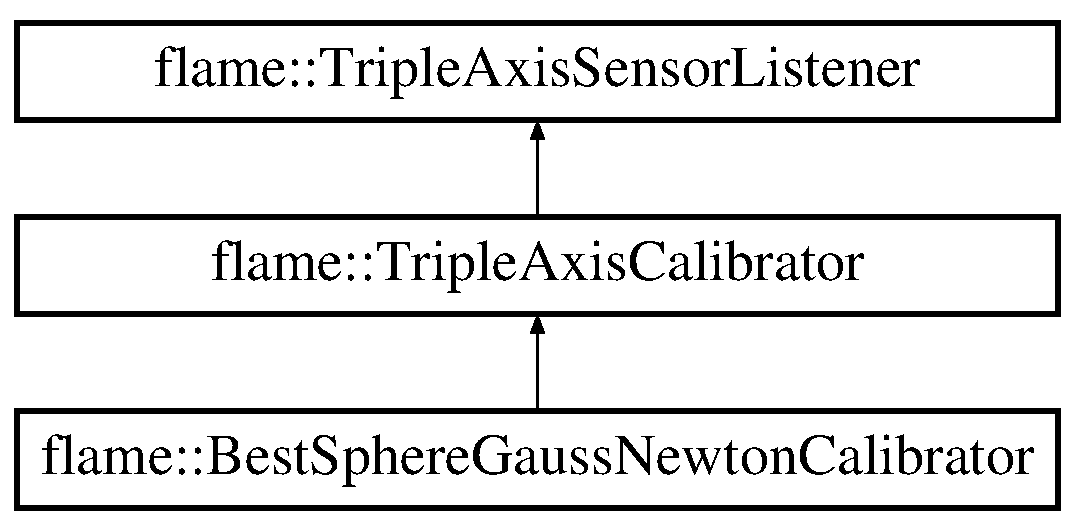
\includegraphics[height=3.000000cm]{classflame_1_1_triple_axis_sensor_listener}
\end{center}
\end{figure}
\subsection*{Public Member Functions}
\begin{DoxyCompactItemize}
\item 
virtual void \hyperlink{classflame_1_1_triple_axis_sensor_listener_a4451e2df32ad722464a1902ef29ed054}{sample\-Is\-Ready} (\hyperlink{classflame_1_1_triple_axis_sensor}{Triple\-Axis\-Sensor} \&sensor)=0
\item 
virtual void \hyperlink{classflame_1_1_triple_axis_sensor_listener_a56c75bbcf89043b53b938e3f9045db38}{limit\-Reached} (\hyperlink{classflame_1_1_triple_axis_sensor}{Triple\-Axis\-Sensor} \&sensor, \hyperlink{namespaceflame_a626e8c99d0f4f232b95e7089c113095a}{Triple\-Axis\-Sensor\-Channel} which)=0
\end{DoxyCompactItemize}


\subsection{Detailed Description}


Definition at line 57 of file Triple\-Axis\-Sensor.\-h.



\subsection{Member Function Documentation}
\hypertarget{classflame_1_1_triple_axis_sensor_listener_a56c75bbcf89043b53b938e3f9045db38}{\index{flame\-::\-Triple\-Axis\-Sensor\-Listener@{flame\-::\-Triple\-Axis\-Sensor\-Listener}!limit\-Reached@{limit\-Reached}}
\index{limit\-Reached@{limit\-Reached}!flame::TripleAxisSensorListener@{flame\-::\-Triple\-Axis\-Sensor\-Listener}}
\subsubsection[{limit\-Reached}]{\setlength{\rightskip}{0pt plus 5cm}virtual void flame\-::\-Triple\-Axis\-Sensor\-Listener\-::limit\-Reached (
\begin{DoxyParamCaption}
\item[{{\bf Triple\-Axis\-Sensor} \&}]{sensor, }
\item[{{\bf Triple\-Axis\-Sensor\-Channel}}]{which}
\end{DoxyParamCaption}
)\hspace{0.3cm}{\ttfamily [pure virtual]}}}\label{classflame_1_1_triple_axis_sensor_listener_a56c75bbcf89043b53b938e3f9045db38}
Called when an acceleration limit is reached 
\begin{DoxyParams}{Parameters}
{\em sensor} & the sensor whose limit was reached \\
\hline
{\em which} & which limit was reached \\
\hline
\end{DoxyParams}


Implemented in \hyperlink{classflame_1_1_triple_axis_calibrator_af80e930aac780ea5b25f99423fb22fd7}{flame\-::\-Triple\-Axis\-Calibrator}.

\hypertarget{classflame_1_1_triple_axis_sensor_listener_a4451e2df32ad722464a1902ef29ed054}{\index{flame\-::\-Triple\-Axis\-Sensor\-Listener@{flame\-::\-Triple\-Axis\-Sensor\-Listener}!sample\-Is\-Ready@{sample\-Is\-Ready}}
\index{sample\-Is\-Ready@{sample\-Is\-Ready}!flame::TripleAxisSensorListener@{flame\-::\-Triple\-Axis\-Sensor\-Listener}}
\subsubsection[{sample\-Is\-Ready}]{\setlength{\rightskip}{0pt plus 5cm}virtual void flame\-::\-Triple\-Axis\-Sensor\-Listener\-::sample\-Is\-Ready (
\begin{DoxyParamCaption}
\item[{{\bf Triple\-Axis\-Sensor} \&}]{sensor}
\end{DoxyParamCaption}
)\hspace{0.3cm}{\ttfamily [pure virtual]}}}\label{classflame_1_1_triple_axis_sensor_listener_a4451e2df32ad722464a1902ef29ed054}
Called when a sample is ready 
\begin{DoxyParams}{Parameters}
{\em sensor} & the sensor whose sample is ready \\
\hline
\end{DoxyParams}


Implemented in \hyperlink{classflame_1_1_triple_axis_calibrator_ab66474b4d1f8f6e9c2ee76233a927e71}{flame\-::\-Triple\-Axis\-Calibrator}.



The documentation for this class was generated from the following file\-:\begin{DoxyCompactItemize}
\item 
flame/\hyperlink{_triple_axis_sensor_8h}{Triple\-Axis\-Sensor.\-h}\end{DoxyCompactItemize}

\hypertarget{classflame_1_1_t_x_buffer}{\section{flame\-:\-:T\-X\-Buffer Class Reference}
\label{classflame_1_1_t_x_buffer}\index{flame\-::\-T\-X\-Buffer@{flame\-::\-T\-X\-Buffer}}
}


{\ttfamily \#include $<$Device\-\_\-\-T\-X.\-h$>$}

\subsection*{Public Member Functions}
\begin{DoxyCompactItemize}
\item 
\hyperlink{classflame_1_1_t_x_buffer_a98b938f8eb8bbc33578798a430a6f816}{T\-X\-Buffer} ()
\item 
\hyperlink{classflame_1_1_t_x_buffer_af0e3d3c373a5e75124636553561cecae}{T\-X\-Buffer} (const char $\ast$string)
\item 
\hyperlink{classflame_1_1_t_x_buffer_ad63b3d52cc78eb91a9780e1309e4e644}{T\-X\-Buffer} (const char $\ast$string, void($\ast$complete\-Function)(const char $\ast$))
\item 
\hyperlink{classflame_1_1_t_x_buffer_a873283b83ea650904d4f3ad1626b9775}{T\-X\-Buffer} (P\-G\-M\-\_\-\-P string, bool ignored \hyperlink{io_8h_addf5ec070e9499d36b7f2009ce736076}{U\-N\-U\-S\-E\-D})
\item 
\hyperlink{classflame_1_1_t_x_buffer_aaa616da48996dcb117a320a23b0b163b}{T\-X\-Buffer} (const char $\ast$buffer, uint16\-\_\-t length)
\item 
\hyperlink{classflame_1_1_t_x_buffer_ab13a5a50c65cff4aeccbe0406b792d8b}{T\-X\-Buffer} (const char $\ast$buffer, uint16\-\_\-t length, void($\ast$complete\-Function)(const char $\ast$))
\item 
\hyperlink{classflame_1_1_t_x_buffer_a6f294041f1bd3591e85b0cc78fb7b2b2}{T\-X\-Buffer} (P\-G\-M\-\_\-\-P buffer, uint16\-\_\-t length, bool ignored \hyperlink{io_8h_addf5ec070e9499d36b7f2009ce736076}{U\-N\-U\-S\-E\-D})
\item 
uint16\-\_\-t \hyperlink{classflame_1_1_t_x_buffer_ade3eba5c5ed688eb4ea132469c8e2307}{get\-Position} ()
\item 
void \hyperlink{classflame_1_1_t_x_buffer_ace94468f27c472f7515e7f355a1377af}{seek} (uint16\-\_\-t position)
\item 
int \hyperlink{classflame_1_1_t_x_buffer_a70668a72527ab1516088c38a8229337d}{peek} (uint16\-\_\-t offset)
\item 
int \hyperlink{classflame_1_1_t_x_buffer_aa6b30c699c035e69cd0ef2a009479206}{next\-Character} ()
\item 
void \hyperlink{classflame_1_1_t_x_buffer_a247c40701875dfaf8caa8d1cc25eb32a}{discard} ()
\item 
bool \hyperlink{classflame_1_1_t_x_buffer_a527cc3f0d2cb0519dc613c0832357c5e}{has\-More} ()
\item 
void \hyperlink{classflame_1_1_t_x_buffer_aef6d588530706d1436a2473d4814cb56}{dump\-State} (char $\ast$buf, uint8\-\_\-t buf\-Length, const char $\ast$func)
\end{DoxyCompactItemize}
\subsection*{Protected Attributes}
\begin{DoxyCompactItemize}
\item 
volatile void $\ast$ \hyperlink{classflame_1_1_t_x_buffer_a66868ca244713911f52da0edac7bd410}{\-\_\-data}
\item 
volatile uint16\-\_\-t \hyperlink{classflame_1_1_t_x_buffer_ac2b091fd502d089763813100635c06de}{\-\_\-offset}
\item 
volatile uint16\-\_\-t \hyperlink{classflame_1_1_t_x_buffer_a7237489370200b26a4a9ae7b829faa7a}{\-\_\-length}
\item 
void($\ast$ \hyperlink{classflame_1_1_t_x_buffer_a5843eca013da741fdfec20916239d708}{\-\_\-complete\-Function} )(const char $\ast$)
\item 
volatile \hyperlink{namespaceflame_a62698923ce7cbb06514750e7f0651c7f}{Address\-Type} \hyperlink{classflame_1_1_t_x_buffer_af5929a77f1d17118f0358da1d6cce8f3}{\-\_\-type}
\item 
volatile bool \hyperlink{classflame_1_1_t_x_buffer_a266cb738953476ec42dbd08d5d310930}{\-\_\-is\-String}
\end{DoxyCompactItemize}


\subsection{Detailed Description}


Definition at line 60 of file Device\-\_\-\-T\-X.\-h.



\subsection{Constructor \& Destructor Documentation}
\hypertarget{classflame_1_1_t_x_buffer_a98b938f8eb8bbc33578798a430a6f816}{\index{flame\-::\-T\-X\-Buffer@{flame\-::\-T\-X\-Buffer}!T\-X\-Buffer@{T\-X\-Buffer}}
\index{T\-X\-Buffer@{T\-X\-Buffer}!flame::TXBuffer@{flame\-::\-T\-X\-Buffer}}
\subsubsection[{T\-X\-Buffer}]{\setlength{\rightskip}{0pt plus 5cm}flame\-::\-T\-X\-Buffer\-::\-T\-X\-Buffer (
\begin{DoxyParamCaption}
{}
\end{DoxyParamCaption}
)\hspace{0.3cm}{\ttfamily [inline]}}}\label{classflame_1_1_t_x_buffer_a98b938f8eb8bbc33578798a430a6f816}
Create an empty buffer 
\begin{DoxyParams}{Parameters}
{\em string} & the string to stick in the buffer \\
\hline
\end{DoxyParams}


Definition at line 74 of file Device\-\_\-\-T\-X.\-h.

\hypertarget{classflame_1_1_t_x_buffer_af0e3d3c373a5e75124636553561cecae}{\index{flame\-::\-T\-X\-Buffer@{flame\-::\-T\-X\-Buffer}!T\-X\-Buffer@{T\-X\-Buffer}}
\index{T\-X\-Buffer@{T\-X\-Buffer}!flame::TXBuffer@{flame\-::\-T\-X\-Buffer}}
\subsubsection[{T\-X\-Buffer}]{\setlength{\rightskip}{0pt plus 5cm}flame\-::\-T\-X\-Buffer\-::\-T\-X\-Buffer (
\begin{DoxyParamCaption}
\item[{const char $\ast$}]{string}
\end{DoxyParamCaption}
)\hspace{0.3cm}{\ttfamily [inline]}}}\label{classflame_1_1_t_x_buffer_af0e3d3c373a5e75124636553561cecae}
Create a buffer holding a string 
\begin{DoxyParams}{Parameters}
{\em string} & the string to stick in the buffer \\
\hline
\end{DoxyParams}


Definition at line 86 of file Device\-\_\-\-T\-X.\-h.

\hypertarget{classflame_1_1_t_x_buffer_ad63b3d52cc78eb91a9780e1309e4e644}{\index{flame\-::\-T\-X\-Buffer@{flame\-::\-T\-X\-Buffer}!T\-X\-Buffer@{T\-X\-Buffer}}
\index{T\-X\-Buffer@{T\-X\-Buffer}!flame::TXBuffer@{flame\-::\-T\-X\-Buffer}}
\subsubsection[{T\-X\-Buffer}]{\setlength{\rightskip}{0pt plus 5cm}flame\-::\-T\-X\-Buffer\-::\-T\-X\-Buffer (
\begin{DoxyParamCaption}
\item[{const char $\ast$}]{string, }
\item[{void($\ast$)(const char $\ast$)}]{complete\-Function}
\end{DoxyParamCaption}
)\hspace{0.3cm}{\ttfamily [inline]}}}\label{classflame_1_1_t_x_buffer_ad63b3d52cc78eb91a9780e1309e4e644}
Create a buffer holding a string 
\begin{DoxyParams}{Parameters}
{\em string} & the string to stick in the buffer \\
\hline
{\em complete\-Function} & a function to call when we are done with the string, will be passed the string \\
\hline
\end{DoxyParams}


Definition at line 99 of file Device\-\_\-\-T\-X.\-h.

\hypertarget{classflame_1_1_t_x_buffer_a873283b83ea650904d4f3ad1626b9775}{\index{flame\-::\-T\-X\-Buffer@{flame\-::\-T\-X\-Buffer}!T\-X\-Buffer@{T\-X\-Buffer}}
\index{T\-X\-Buffer@{T\-X\-Buffer}!flame::TXBuffer@{flame\-::\-T\-X\-Buffer}}
\subsubsection[{T\-X\-Buffer}]{\setlength{\rightskip}{0pt plus 5cm}flame\-::\-T\-X\-Buffer\-::\-T\-X\-Buffer (
\begin{DoxyParamCaption}
\item[{P\-G\-M\-\_\-\-P}]{string, }
\item[{bool ignored}]{U\-N\-U\-S\-E\-D}
\end{DoxyParamCaption}
)\hspace{0.3cm}{\ttfamily [inline]}}}\label{classflame_1_1_t_x_buffer_a873283b83ea650904d4f3ad1626b9775}
Create a buffer holding a progmem string 
\begin{DoxyParams}{Parameters}
{\em string} & the string to stick in the buffer \\
\hline
{\em ignored} & provided only to distinguish against a memory string \\
\hline
\end{DoxyParams}


Definition at line 112 of file Device\-\_\-\-T\-X.\-h.

\hypertarget{classflame_1_1_t_x_buffer_aaa616da48996dcb117a320a23b0b163b}{\index{flame\-::\-T\-X\-Buffer@{flame\-::\-T\-X\-Buffer}!T\-X\-Buffer@{T\-X\-Buffer}}
\index{T\-X\-Buffer@{T\-X\-Buffer}!flame::TXBuffer@{flame\-::\-T\-X\-Buffer}}
\subsubsection[{T\-X\-Buffer}]{\setlength{\rightskip}{0pt plus 5cm}flame\-::\-T\-X\-Buffer\-::\-T\-X\-Buffer (
\begin{DoxyParamCaption}
\item[{const char $\ast$}]{buffer, }
\item[{uint16\-\_\-t}]{length}
\end{DoxyParamCaption}
)\hspace{0.3cm}{\ttfamily [inline]}}}\label{classflame_1_1_t_x_buffer_aaa616da48996dcb117a320a23b0b163b}
Create a buffer holding a block of memory 
\begin{DoxyParams}{Parameters}
{\em buffer} & the buffer \\
\hline
{\em length} & the length of the buffer \\
\hline
\end{DoxyParams}


Definition at line 155 of file Device\-\_\-\-T\-X.\-h.

\hypertarget{classflame_1_1_t_x_buffer_ab13a5a50c65cff4aeccbe0406b792d8b}{\index{flame\-::\-T\-X\-Buffer@{flame\-::\-T\-X\-Buffer}!T\-X\-Buffer@{T\-X\-Buffer}}
\index{T\-X\-Buffer@{T\-X\-Buffer}!flame::TXBuffer@{flame\-::\-T\-X\-Buffer}}
\subsubsection[{T\-X\-Buffer}]{\setlength{\rightskip}{0pt plus 5cm}flame\-::\-T\-X\-Buffer\-::\-T\-X\-Buffer (
\begin{DoxyParamCaption}
\item[{const char $\ast$}]{buffer, }
\item[{uint16\-\_\-t}]{length, }
\item[{void($\ast$)(const char $\ast$)}]{complete\-Function}
\end{DoxyParamCaption}
)\hspace{0.3cm}{\ttfamily [inline]}}}\label{classflame_1_1_t_x_buffer_ab13a5a50c65cff4aeccbe0406b792d8b}
Create a buffer holding a block of memory 
\begin{DoxyParams}{Parameters}
{\em buffer} & the buffer \\
\hline
{\em length} & the length of the buffer \\
\hline
{\em complete\-Function} & a function to call when we are done with the string, will be passed the buffer \\
\hline
\end{DoxyParams}


Definition at line 169 of file Device\-\_\-\-T\-X.\-h.

\hypertarget{classflame_1_1_t_x_buffer_a6f294041f1bd3591e85b0cc78fb7b2b2}{\index{flame\-::\-T\-X\-Buffer@{flame\-::\-T\-X\-Buffer}!T\-X\-Buffer@{T\-X\-Buffer}}
\index{T\-X\-Buffer@{T\-X\-Buffer}!flame::TXBuffer@{flame\-::\-T\-X\-Buffer}}
\subsubsection[{T\-X\-Buffer}]{\setlength{\rightskip}{0pt plus 5cm}flame\-::\-T\-X\-Buffer\-::\-T\-X\-Buffer (
\begin{DoxyParamCaption}
\item[{P\-G\-M\-\_\-\-P}]{buffer, }
\item[{uint16\-\_\-t}]{length, }
\item[{bool ignored}]{U\-N\-U\-S\-E\-D}
\end{DoxyParamCaption}
)\hspace{0.3cm}{\ttfamily [inline]}}}\label{classflame_1_1_t_x_buffer_a6f294041f1bd3591e85b0cc78fb7b2b2}
Create a buffer holding a progmem block of memory 
\begin{DoxyParams}{Parameters}
{\em buffer} & the buffer \\
\hline
{\em length} & the length of the buffer \\
\hline
{\em ignored} & provided only to distinguish against a memory string \\
\hline
\end{DoxyParams}


Definition at line 184 of file Device\-\_\-\-T\-X.\-h.



\subsection{Member Function Documentation}
\hypertarget{classflame_1_1_t_x_buffer_a247c40701875dfaf8caa8d1cc25eb32a}{\index{flame\-::\-T\-X\-Buffer@{flame\-::\-T\-X\-Buffer}!discard@{discard}}
\index{discard@{discard}!flame::TXBuffer@{flame\-::\-T\-X\-Buffer}}
\subsubsection[{discard}]{\setlength{\rightskip}{0pt plus 5cm}void flame\-::\-T\-X\-Buffer\-::discard (
\begin{DoxyParamCaption}
{}
\end{DoxyParamCaption}
)\hspace{0.3cm}{\ttfamily [inline]}}}\label{classflame_1_1_t_x_buffer_a247c40701875dfaf8caa8d1cc25eb32a}
Called when the buffer is no longer needed 

Definition at line 308 of file Device\-\_\-\-T\-X.\-h.

\hypertarget{classflame_1_1_t_x_buffer_aef6d588530706d1436a2473d4814cb56}{\index{flame\-::\-T\-X\-Buffer@{flame\-::\-T\-X\-Buffer}!dump\-State@{dump\-State}}
\index{dump\-State@{dump\-State}!flame::TXBuffer@{flame\-::\-T\-X\-Buffer}}
\subsubsection[{dump\-State}]{\setlength{\rightskip}{0pt plus 5cm}void flame\-::\-T\-X\-Buffer\-::dump\-State (
\begin{DoxyParamCaption}
\item[{char $\ast$}]{buf, }
\item[{uint8\-\_\-t}]{buf\-Length, }
\item[{const char $\ast$}]{func}
\end{DoxyParamCaption}
)\hspace{0.3cm}{\ttfamily [inline]}}}\label{classflame_1_1_t_x_buffer_aef6d588530706d1436a2473d4814cb56}
Dump the current state into a buffer for debugging 
\begin{DoxyParams}{Parameters}
{\em buf} & the buffer to write to \\
\hline
{\em buf\-Length} & the space available in the buffer \\
\hline
{\em func} & the name of the caller \\
\hline
\end{DoxyParams}


Definition at line 338 of file Device\-\_\-\-T\-X.\-h.

\hypertarget{classflame_1_1_t_x_buffer_ade3eba5c5ed688eb4ea132469c8e2307}{\index{flame\-::\-T\-X\-Buffer@{flame\-::\-T\-X\-Buffer}!get\-Position@{get\-Position}}
\index{get\-Position@{get\-Position}!flame::TXBuffer@{flame\-::\-T\-X\-Buffer}}
\subsubsection[{get\-Position}]{\setlength{\rightskip}{0pt plus 5cm}uint16\-\_\-t flame\-::\-T\-X\-Buffer\-::get\-Position (
\begin{DoxyParamCaption}
{}
\end{DoxyParamCaption}
)\hspace{0.3cm}{\ttfamily [inline]}}}\label{classflame_1_1_t_x_buffer_ade3eba5c5ed688eb4ea132469c8e2307}
Get the position in the current buffer \begin{DoxyReturn}{Returns}
the current position 
\end{DoxyReturn}


Definition at line 229 of file Device\-\_\-\-T\-X.\-h.

\hypertarget{classflame_1_1_t_x_buffer_a527cc3f0d2cb0519dc613c0832357c5e}{\index{flame\-::\-T\-X\-Buffer@{flame\-::\-T\-X\-Buffer}!has\-More@{has\-More}}
\index{has\-More@{has\-More}!flame::TXBuffer@{flame\-::\-T\-X\-Buffer}}
\subsubsection[{has\-More}]{\setlength{\rightskip}{0pt plus 5cm}bool flame\-::\-T\-X\-Buffer\-::has\-More (
\begin{DoxyParamCaption}
{}
\end{DoxyParamCaption}
)\hspace{0.3cm}{\ttfamily [inline]}}}\label{classflame_1_1_t_x_buffer_a527cc3f0d2cb0519dc613c0832357c5e}
Does this buffer have more characters? \begin{DoxyReturn}{Returns}
true if there are more characters 
\end{DoxyReturn}


Definition at line 325 of file Device\-\_\-\-T\-X.\-h.

\hypertarget{classflame_1_1_t_x_buffer_aa6b30c699c035e69cd0ef2a009479206}{\index{flame\-::\-T\-X\-Buffer@{flame\-::\-T\-X\-Buffer}!next\-Character@{next\-Character}}
\index{next\-Character@{next\-Character}!flame::TXBuffer@{flame\-::\-T\-X\-Buffer}}
\subsubsection[{next\-Character}]{\setlength{\rightskip}{0pt plus 5cm}int flame\-::\-T\-X\-Buffer\-::next\-Character (
\begin{DoxyParamCaption}
{}
\end{DoxyParamCaption}
)\hspace{0.3cm}{\ttfamily [inline]}}}\label{classflame_1_1_t_x_buffer_aa6b30c699c035e69cd0ef2a009479206}
Get a character to transmit \begin{DoxyReturn}{Returns}
the character, or -\/1 if there is nothing left 
\end{DoxyReturn}


Definition at line 294 of file Device\-\_\-\-T\-X.\-h.

\hypertarget{classflame_1_1_t_x_buffer_a70668a72527ab1516088c38a8229337d}{\index{flame\-::\-T\-X\-Buffer@{flame\-::\-T\-X\-Buffer}!peek@{peek}}
\index{peek@{peek}!flame::TXBuffer@{flame\-::\-T\-X\-Buffer}}
\subsubsection[{peek}]{\setlength{\rightskip}{0pt plus 5cm}int flame\-::\-T\-X\-Buffer\-::peek (
\begin{DoxyParamCaption}
\item[{uint16\-\_\-t}]{offset}
\end{DoxyParamCaption}
)\hspace{0.3cm}{\ttfamily [inline]}}}\label{classflame_1_1_t_x_buffer_a70668a72527ab1516088c38a8229337d}
Get the character at an offset 
\begin{DoxyParams}{Parameters}
{\em offset} & the offset \\
\hline
\end{DoxyParams}
\begin{DoxyReturn}{Returns}
the character at the offset, or -\/1 if there is none 
\end{DoxyReturn}


Definition at line 252 of file Device\-\_\-\-T\-X.\-h.

\hypertarget{classflame_1_1_t_x_buffer_ace94468f27c472f7515e7f355a1377af}{\index{flame\-::\-T\-X\-Buffer@{flame\-::\-T\-X\-Buffer}!seek@{seek}}
\index{seek@{seek}!flame::TXBuffer@{flame\-::\-T\-X\-Buffer}}
\subsubsection[{seek}]{\setlength{\rightskip}{0pt plus 5cm}void flame\-::\-T\-X\-Buffer\-::seek (
\begin{DoxyParamCaption}
\item[{uint16\-\_\-t}]{position}
\end{DoxyParamCaption}
)\hspace{0.3cm}{\ttfamily [inline]}}}\label{classflame_1_1_t_x_buffer_ace94468f27c472f7515e7f355a1377af}
Seek the position in the current buffer 
\begin{DoxyParams}{Parameters}
{\em position} & the desired position \\
\hline
\end{DoxyParams}


Definition at line 238 of file Device\-\_\-\-T\-X.\-h.



\subsection{Member Data Documentation}
\hypertarget{classflame_1_1_t_x_buffer_a5843eca013da741fdfec20916239d708}{\index{flame\-::\-T\-X\-Buffer@{flame\-::\-T\-X\-Buffer}!\-\_\-complete\-Function@{\-\_\-complete\-Function}}
\index{\-\_\-complete\-Function@{\-\_\-complete\-Function}!flame::TXBuffer@{flame\-::\-T\-X\-Buffer}}
\subsubsection[{\-\_\-complete\-Function}]{\setlength{\rightskip}{0pt plus 5cm}void($\ast$ flame\-::\-T\-X\-Buffer\-::\-\_\-complete\-Function)(const char $\ast$)\hspace{0.3cm}{\ttfamily [protected]}}}\label{classflame_1_1_t_x_buffer_a5843eca013da741fdfec20916239d708}


Definition at line 65 of file Device\-\_\-\-T\-X.\-h.

\hypertarget{classflame_1_1_t_x_buffer_a66868ca244713911f52da0edac7bd410}{\index{flame\-::\-T\-X\-Buffer@{flame\-::\-T\-X\-Buffer}!\-\_\-data@{\-\_\-data}}
\index{\-\_\-data@{\-\_\-data}!flame::TXBuffer@{flame\-::\-T\-X\-Buffer}}
\subsubsection[{\-\_\-data}]{\setlength{\rightskip}{0pt plus 5cm}volatile void$\ast$ flame\-::\-T\-X\-Buffer\-::\-\_\-data\hspace{0.3cm}{\ttfamily [protected]}}}\label{classflame_1_1_t_x_buffer_a66868ca244713911f52da0edac7bd410}


Definition at line 62 of file Device\-\_\-\-T\-X.\-h.

\hypertarget{classflame_1_1_t_x_buffer_a266cb738953476ec42dbd08d5d310930}{\index{flame\-::\-T\-X\-Buffer@{flame\-::\-T\-X\-Buffer}!\-\_\-is\-String@{\-\_\-is\-String}}
\index{\-\_\-is\-String@{\-\_\-is\-String}!flame::TXBuffer@{flame\-::\-T\-X\-Buffer}}
\subsubsection[{\-\_\-is\-String}]{\setlength{\rightskip}{0pt plus 5cm}volatile bool flame\-::\-T\-X\-Buffer\-::\-\_\-is\-String\hspace{0.3cm}{\ttfamily [protected]}}}\label{classflame_1_1_t_x_buffer_a266cb738953476ec42dbd08d5d310930}


Definition at line 67 of file Device\-\_\-\-T\-X.\-h.

\hypertarget{classflame_1_1_t_x_buffer_a7237489370200b26a4a9ae7b829faa7a}{\index{flame\-::\-T\-X\-Buffer@{flame\-::\-T\-X\-Buffer}!\-\_\-length@{\-\_\-length}}
\index{\-\_\-length@{\-\_\-length}!flame::TXBuffer@{flame\-::\-T\-X\-Buffer}}
\subsubsection[{\-\_\-length}]{\setlength{\rightskip}{0pt plus 5cm}volatile uint16\-\_\-t flame\-::\-T\-X\-Buffer\-::\-\_\-length\hspace{0.3cm}{\ttfamily [protected]}}}\label{classflame_1_1_t_x_buffer_a7237489370200b26a4a9ae7b829faa7a}


Definition at line 64 of file Device\-\_\-\-T\-X.\-h.

\hypertarget{classflame_1_1_t_x_buffer_ac2b091fd502d089763813100635c06de}{\index{flame\-::\-T\-X\-Buffer@{flame\-::\-T\-X\-Buffer}!\-\_\-offset@{\-\_\-offset}}
\index{\-\_\-offset@{\-\_\-offset}!flame::TXBuffer@{flame\-::\-T\-X\-Buffer}}
\subsubsection[{\-\_\-offset}]{\setlength{\rightskip}{0pt plus 5cm}volatile uint16\-\_\-t flame\-::\-T\-X\-Buffer\-::\-\_\-offset\hspace{0.3cm}{\ttfamily [protected]}}}\label{classflame_1_1_t_x_buffer_ac2b091fd502d089763813100635c06de}


Definition at line 63 of file Device\-\_\-\-T\-X.\-h.

\hypertarget{classflame_1_1_t_x_buffer_af5929a77f1d17118f0358da1d6cce8f3}{\index{flame\-::\-T\-X\-Buffer@{flame\-::\-T\-X\-Buffer}!\-\_\-type@{\-\_\-type}}
\index{\-\_\-type@{\-\_\-type}!flame::TXBuffer@{flame\-::\-T\-X\-Buffer}}
\subsubsection[{\-\_\-type}]{\setlength{\rightskip}{0pt plus 5cm}volatile {\bf Address\-Type} flame\-::\-T\-X\-Buffer\-::\-\_\-type\hspace{0.3cm}{\ttfamily [protected]}}}\label{classflame_1_1_t_x_buffer_af5929a77f1d17118f0358da1d6cce8f3}


Definition at line 66 of file Device\-\_\-\-T\-X.\-h.



The documentation for this class was generated from the following file\-:\begin{DoxyCompactItemize}
\item 
flame/\hyperlink{_device___t_x_8h}{Device\-\_\-\-T\-X.\-h}\end{DoxyCompactItemize}

\hypertarget{structflame_1_1voice}{\section{flame\-:\-:voice Struct Reference}
\label{structflame_1_1voice}\index{flame\-::voice@{flame\-::voice}}
}


{\ttfamily \#include $<$Wave\-Generator.\-h$>$}

\subsection*{Public Attributes}
\begin{DoxyCompactItemize}
\item 
\hyperlink{namespaceflame_a7f0c5adbd1329cd2947d15e6af02dbf1}{I\-N\-S\-T\-R\-U\-M\-E\-N\-T} $\ast$ \hyperlink{structflame_1_1voice_aa2aa1f4b2ce3a2e90a123b2a99d4878b}{instrument}
\item 
uint16\-\_\-t \hyperlink{structflame_1_1voice_a897fe7f475e9bd1ff4115dd90ad80ecf}{phase\-Offset}
\item 
uint32\-\_\-t \hyperlink{structflame_1_1voice_af850619ff5aa4d53276cc3dafd7d4bc8}{current\-Offset}
\item 
\hyperlink{namespaceflame_a64ac4f87e54f07ae6c013cdd48d97822}{Voice\-Phase} \hyperlink{structflame_1_1voice_aae5caf10d82550f97fccea9f184d9ed2}{phase}
\item 
\hyperlink{namespaceflame_a7f6447252c60127b805475b293831f99}{A\-M\-P\-L\-I\-T\-U\-D\-E} \hyperlink{structflame_1_1voice_adb0641815db4aacb1fe2fc90b605e4c1}{velocity}
\item 
uint16\-\_\-t \hyperlink{structflame_1_1voice_aec3efeb3d7db126697063f95f57d4696}{frequency}
\item 
uint32\-\_\-t \hyperlink{structflame_1_1voice_a7eee8064edb15ee001e43a604d94fb79}{duration}
\item 
\hyperlink{namespaceflame_a7f6447252c60127b805475b293831f99}{A\-M\-P\-L\-I\-T\-U\-D\-E} \hyperlink{structflame_1_1voice_ac1c8f2531ec8ec72c2f2eb2c5aab7877}{amplitude}
\end{DoxyCompactItemize}


\subsection{Detailed Description}


Definition at line 81 of file Wave\-Generator.\-h.



\subsection{Member Data Documentation}
\hypertarget{structflame_1_1voice_ac1c8f2531ec8ec72c2f2eb2c5aab7877}{\index{flame\-::voice@{flame\-::voice}!amplitude@{amplitude}}
\index{amplitude@{amplitude}!flame::voice@{flame\-::voice}}
\subsubsection[{amplitude}]{\setlength{\rightskip}{0pt plus 5cm}{\bf A\-M\-P\-L\-I\-T\-U\-D\-E} flame\-::voice\-::amplitude}}\label{structflame_1_1voice_ac1c8f2531ec8ec72c2f2eb2c5aab7877}
The duration of the note, samples 

Definition at line 89 of file Wave\-Generator.\-h.

\hypertarget{structflame_1_1voice_af850619ff5aa4d53276cc3dafd7d4bc8}{\index{flame\-::voice@{flame\-::voice}!current\-Offset@{current\-Offset}}
\index{current\-Offset@{current\-Offset}!flame::voice@{flame\-::voice}}
\subsubsection[{current\-Offset}]{\setlength{\rightskip}{0pt plus 5cm}uint32\-\_\-t flame\-::voice\-::current\-Offset}}\label{structflame_1_1voice_af850619ff5aa4d53276cc3dafd7d4bc8}
The current sample offset for the current phase 

Definition at line 84 of file Wave\-Generator.\-h.

\hypertarget{structflame_1_1voice_a7eee8064edb15ee001e43a604d94fb79}{\index{flame\-::voice@{flame\-::voice}!duration@{duration}}
\index{duration@{duration}!flame::voice@{flame\-::voice}}
\subsubsection[{duration}]{\setlength{\rightskip}{0pt plus 5cm}uint32\-\_\-t flame\-::voice\-::duration}}\label{structflame_1_1voice_a7eee8064edb15ee001e43a604d94fb79}
The frequency in Hz 

Definition at line 88 of file Wave\-Generator.\-h.

\hypertarget{structflame_1_1voice_aec3efeb3d7db126697063f95f57d4696}{\index{flame\-::voice@{flame\-::voice}!frequency@{frequency}}
\index{frequency@{frequency}!flame::voice@{flame\-::voice}}
\subsubsection[{frequency}]{\setlength{\rightskip}{0pt plus 5cm}uint16\-\_\-t flame\-::voice\-::frequency}}\label{structflame_1_1voice_aec3efeb3d7db126697063f95f57d4696}
The overall amplitude of the envelope 

Definition at line 87 of file Wave\-Generator.\-h.

\hypertarget{structflame_1_1voice_aa2aa1f4b2ce3a2e90a123b2a99d4878b}{\index{flame\-::voice@{flame\-::voice}!instrument@{instrument}}
\index{instrument@{instrument}!flame::voice@{flame\-::voice}}
\subsubsection[{instrument}]{\setlength{\rightskip}{0pt plus 5cm}{\bf I\-N\-S\-T\-R\-U\-M\-E\-N\-T}$\ast$ flame\-::voice\-::instrument}}\label{structflame_1_1voice_aa2aa1f4b2ce3a2e90a123b2a99d4878b}


Definition at line 82 of file Wave\-Generator.\-h.

\hypertarget{structflame_1_1voice_aae5caf10d82550f97fccea9f184d9ed2}{\index{flame\-::voice@{flame\-::voice}!phase@{phase}}
\index{phase@{phase}!flame::voice@{flame\-::voice}}
\subsubsection[{phase}]{\setlength{\rightskip}{0pt plus 5cm}{\bf Voice\-Phase} flame\-::voice\-::phase}}\label{structflame_1_1voice_aae5caf10d82550f97fccea9f184d9ed2}
The current sample offset for the voice 

Definition at line 85 of file Wave\-Generator.\-h.

\hypertarget{structflame_1_1voice_a897fe7f475e9bd1ff4115dd90ad80ecf}{\index{flame\-::voice@{flame\-::voice}!phase\-Offset@{phase\-Offset}}
\index{phase\-Offset@{phase\-Offset}!flame::voice@{flame\-::voice}}
\subsubsection[{phase\-Offset}]{\setlength{\rightskip}{0pt plus 5cm}uint16\-\_\-t flame\-::voice\-::phase\-Offset}}\label{structflame_1_1voice_a897fe7f475e9bd1ff4115dd90ad80ecf}
The instrument playing on the voice 

Definition at line 83 of file Wave\-Generator.\-h.

\hypertarget{structflame_1_1voice_adb0641815db4aacb1fe2fc90b605e4c1}{\index{flame\-::voice@{flame\-::voice}!velocity@{velocity}}
\index{velocity@{velocity}!flame::voice@{flame\-::voice}}
\subsubsection[{velocity}]{\setlength{\rightskip}{0pt plus 5cm}{\bf A\-M\-P\-L\-I\-T\-U\-D\-E} flame\-::voice\-::velocity}}\label{structflame_1_1voice_adb0641815db4aacb1fe2fc90b605e4c1}
The current phase this voice is in 

Definition at line 86 of file Wave\-Generator.\-h.



The documentation for this struct was generated from the following file\-:\begin{DoxyCompactItemize}
\item 
flame/\hyperlink{_wave_generator_8h}{Wave\-Generator.\-h}\end{DoxyCompactItemize}

\hypertarget{classflame__gpl_1_1_vusb_console}{\section{flame\-\_\-gpl\-:\-:Vusb\-Console$<$ tx\-Count $>$ Class Template Reference}
\label{classflame__gpl_1_1_vusb_console}\index{flame\-\_\-gpl\-::\-Vusb\-Console$<$ tx\-Count $>$@{flame\-\_\-gpl\-::\-Vusb\-Console$<$ tx\-Count $>$}}
}


{\ttfamily \#include $<$Vusb\-Console.\-h$>$}

Inheritance diagram for flame\-\_\-gpl\-:\-:Vusb\-Console$<$ tx\-Count $>$\-:\begin{figure}[H]
\begin{center}
\leavevmode
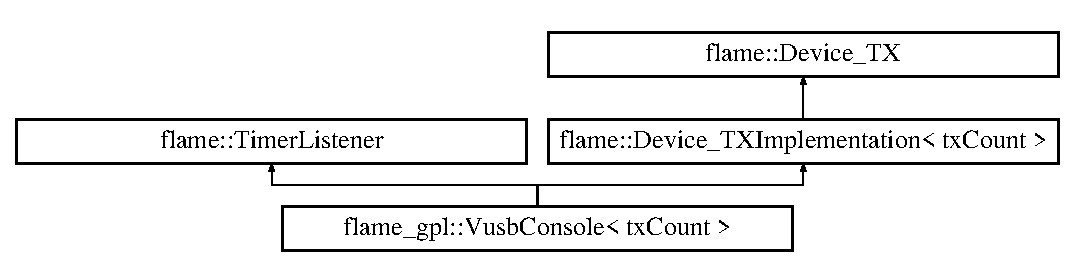
\includegraphics[height=3.000000cm]{classflame__gpl_1_1_vusb_console}
\end{center}
\end{figure}
\subsection*{Public Member Functions}
\begin{DoxyCompactItemize}
\item 
\hyperlink{classflame__gpl_1_1_vusb_console_a571209ae3db5f8d75091ee8c6c17a862}{Vusb\-Console} (\hyperlink{classflame_1_1_r_t_c}{R\-T\-C} \&rtc)
\item 
void \hyperlink{classflame__gpl_1_1_vusb_console_a061bc8d41aa75d4eedf0b070b76b4bdc}{alarm} (\hyperlink{io_8h_addf5ec070e9499d36b7f2009ce736076}{U\-N\-U\-S\-E\-D} \hyperlink{namespaceflame_a6d176ba245556716fd3e32006bb7cfe5}{Alarm\-Source} source)
\item 
void \hyperlink{classflame__gpl_1_1_vusb_console_a5deb453bdc18579c6f3c592862f71fab}{run\-Tx\-Buffers} ()
\end{DoxyCompactItemize}
\subsection*{Protected Attributes}
\begin{DoxyCompactItemize}
\item 
\hyperlink{classflame_1_1_r_t_c}{R\-T\-C} \& \hyperlink{classflame__gpl_1_1_vusb_console_a197a4912e9da1bb6a10b13c0f8026e74}{\-\_\-rtc}
\end{DoxyCompactItemize}
\subsection*{Additional Inherited Members}


\subsection{Detailed Description}
\subsubsection*{template$<$uint8\-\_\-t tx\-Count$>$class flame\-\_\-gpl\-::\-Vusb\-Console$<$ tx\-Count $>$}



Definition at line 37 of file Vusb\-Console.\-h.



\subsection{Constructor \& Destructor Documentation}
\hypertarget{classflame__gpl_1_1_vusb_console_a571209ae3db5f8d75091ee8c6c17a862}{\index{flame\-\_\-gpl\-::\-Vusb\-Console@{flame\-\_\-gpl\-::\-Vusb\-Console}!Vusb\-Console@{Vusb\-Console}}
\index{Vusb\-Console@{Vusb\-Console}!flame_gpl::VusbConsole@{flame\-\_\-gpl\-::\-Vusb\-Console}}
\subsubsection[{Vusb\-Console}]{\setlength{\rightskip}{0pt plus 5cm}template$<$uint8\-\_\-t tx\-Count$>$ {\bf flame\-\_\-gpl\-::\-Vusb\-Console}$<$ tx\-Count $>$\-::{\bf Vusb\-Console} (
\begin{DoxyParamCaption}
\item[{{\bf R\-T\-C} \&}]{rtc}
\end{DoxyParamCaption}
)\hspace{0.3cm}{\ttfamily [inline]}}}\label{classflame__gpl_1_1_vusb_console_a571209ae3db5f8d75091ee8c6c17a862}
Provide a V-\/\-U\-S\-B console using V-\/\-U\-S\-B Uses pins D4/\-D2 for A\-Tmega (can be changed in V\-U\-S\-B\-Keyboard/usbconfig.\-h) Uses pins B0/\-B2 for A\-Ttiny25/45/85

To view the output of the console on your computer, use H\-I\-D Listen, available from\-: \href{http://www.pjrc.com/teensy/hid_listen.html}{\tt http\-://www.\-pjrc.\-com/teensy/hid\-\_\-listen.\-html}


\begin{DoxyParams}{Parameters}
{\em rtc} & an R\-T\-C to schedule jobs on \\
\hline
\end{DoxyParams}


Definition at line 52 of file Vusb\-Console.\-h.



\subsection{Member Function Documentation}
\hypertarget{classflame__gpl_1_1_vusb_console_a061bc8d41aa75d4eedf0b070b76b4bdc}{\index{flame\-\_\-gpl\-::\-Vusb\-Console@{flame\-\_\-gpl\-::\-Vusb\-Console}!alarm@{alarm}}
\index{alarm@{alarm}!flame_gpl::VusbConsole@{flame\-\_\-gpl\-::\-Vusb\-Console}}
\subsubsection[{alarm}]{\setlength{\rightskip}{0pt plus 5cm}template$<$uint8\-\_\-t tx\-Count$>$ void {\bf flame\-\_\-gpl\-::\-Vusb\-Console}$<$ tx\-Count $>$\-::{\bf alarm} (
\begin{DoxyParamCaption}
\item[{{\bf U\-N\-U\-S\-E\-D} {\bf Alarm\-Source}}]{source}
\end{DoxyParamCaption}
)\hspace{0.3cm}{\ttfamily [inline]}}}\label{classflame__gpl_1_1_vusb_console_a061bc8d41aa75d4eedf0b070b76b4bdc}
Periodically called to maintain U\-S\-B comms 

Definition at line 80 of file Vusb\-Console.\-h.

\hypertarget{classflame__gpl_1_1_vusb_console_a5deb453bdc18579c6f3c592862f71fab}{\index{flame\-\_\-gpl\-::\-Vusb\-Console@{flame\-\_\-gpl\-::\-Vusb\-Console}!run\-Tx\-Buffers@{run\-Tx\-Buffers}}
\index{run\-Tx\-Buffers@{run\-Tx\-Buffers}!flame_gpl::VusbConsole@{flame\-\_\-gpl\-::\-Vusb\-Console}}
\subsubsection[{run\-Tx\-Buffers}]{\setlength{\rightskip}{0pt plus 5cm}template$<$uint8\-\_\-t tx\-Count$>$ void {\bf flame\-\_\-gpl\-::\-Vusb\-Console}$<$ tx\-Count $>$\-::run\-Tx\-Buffers (
\begin{DoxyParamCaption}
{}
\end{DoxyParamCaption}
)\hspace{0.3cm}{\ttfamily [inline]}, {\ttfamily [virtual]}}}\label{classflame__gpl_1_1_vusb_console_a5deb453bdc18579c6f3c592862f71fab}
Start transmitting a new string (does nothing, alarm will immediately pick up the next character) 

Implements \hyperlink{classflame_1_1_device___t_x_af3cf3dc02a124e5a88841d325555ce3c}{flame\-::\-Device\-\_\-\-T\-X}.



Definition at line 109 of file Vusb\-Console.\-h.



\subsection{Member Data Documentation}
\hypertarget{classflame__gpl_1_1_vusb_console_a197a4912e9da1bb6a10b13c0f8026e74}{\index{flame\-\_\-gpl\-::\-Vusb\-Console@{flame\-\_\-gpl\-::\-Vusb\-Console}!\-\_\-rtc@{\-\_\-rtc}}
\index{\-\_\-rtc@{\-\_\-rtc}!flame_gpl::VusbConsole@{flame\-\_\-gpl\-::\-Vusb\-Console}}
\subsubsection[{\-\_\-rtc}]{\setlength{\rightskip}{0pt plus 5cm}template$<$uint8\-\_\-t tx\-Count$>$ {\bf R\-T\-C}\& {\bf flame\-\_\-gpl\-::\-Vusb\-Console}$<$ tx\-Count $>$\-::\-\_\-rtc\hspace{0.3cm}{\ttfamily [protected]}}}\label{classflame__gpl_1_1_vusb_console_a197a4912e9da1bb6a10b13c0f8026e74}


Definition at line 39 of file Vusb\-Console.\-h.



The documentation for this class was generated from the following file\-:\begin{DoxyCompactItemize}
\item 
A\-:/eclipse/flame/flame-\/\-Vusb-\/\-Console/flame/\hyperlink{_vusb_console_8h}{Vusb\-Console.\-h}\end{DoxyCompactItemize}

\hypertarget{classflame__gpl_1_1_vusb_keyboard}{\section{flame\-\_\-gpl\-:\-:Vusb\-Keyboard Class Reference}
\label{classflame__gpl_1_1_vusb_keyboard}\index{flame\-\_\-gpl\-::\-Vusb\-Keyboard@{flame\-\_\-gpl\-::\-Vusb\-Keyboard}}
}


{\ttfamily \#include $<$Vusb\-Keyboard.\-h$>$}

Inheritance diagram for flame\-\_\-gpl\-:\-:Vusb\-Keyboard\-:\begin{figure}[H]
\begin{center}
\leavevmode
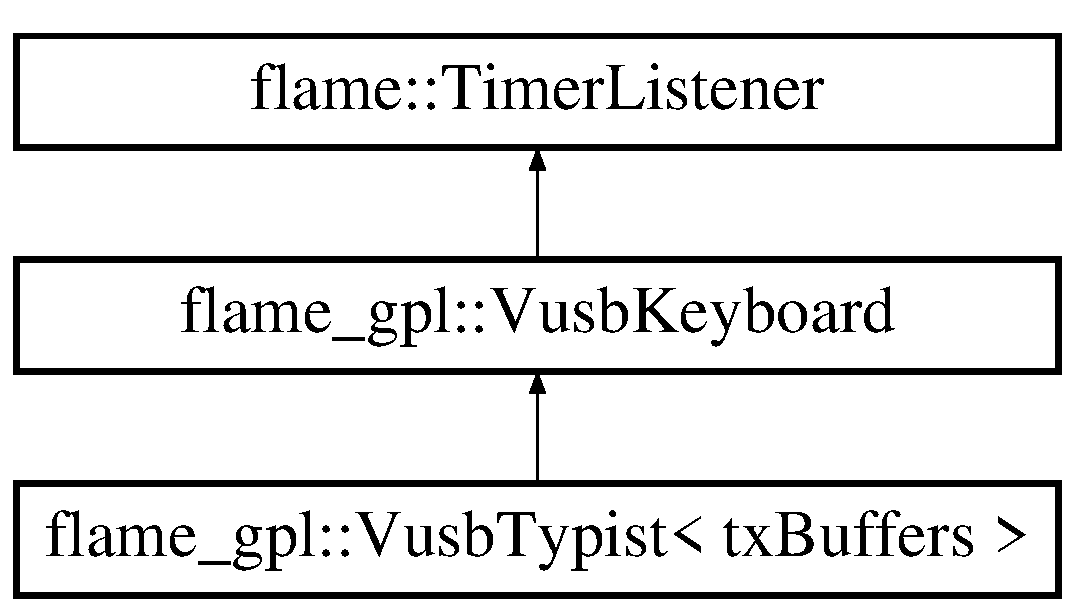
\includegraphics[height=3.000000cm]{classflame__gpl_1_1_vusb_keyboard}
\end{center}
\end{figure}
\subsection*{Public Member Functions}
\begin{DoxyCompactItemize}
\item 
\hyperlink{classflame__gpl_1_1_vusb_keyboard_a6b4cf0b12233b993265132d7f0b9319e}{Vusb\-Keyboard} (\hyperlink{classflame_1_1_r_t_c}{R\-T\-C} \&rtc)
\item 
void \hyperlink{classflame__gpl_1_1_vusb_keyboard_a099ca27a1d4477793a37a14dba667d03}{key\-Stroke} (\hyperlink{namespaceflame__gpl_a40752e4f9e83da1573a3d418e0bd5653}{V\-U\-S\-B\-\_\-\-K\-E\-Y\-B\-O\-A\-R\-D\-\_\-\-K\-E\-Y} key)
\item 
void \hyperlink{classflame__gpl_1_1_vusb_keyboard_afb0d91292961af19582fe9a2f904d694}{key\-Stroke} (\hyperlink{namespaceflame__gpl_a40752e4f9e83da1573a3d418e0bd5653}{V\-U\-S\-B\-\_\-\-K\-E\-Y\-B\-O\-A\-R\-D\-\_\-\-K\-E\-Y} key, uint8\-\_\-t modifiers)
\item 
void \hyperlink{classflame__gpl_1_1_vusb_keyboard_a09736fc4b6a7a17d8b986c3e2d0d47c7}{key\-Down} (\hyperlink{namespaceflame__gpl_a40752e4f9e83da1573a3d418e0bd5653}{V\-U\-S\-B\-\_\-\-K\-E\-Y\-B\-O\-A\-R\-D\-\_\-\-K\-E\-Y} key, uint8\-\_\-t modifiers)
\item 
void \hyperlink{classflame__gpl_1_1_vusb_keyboard_a4da937d6fe26a4722bb1f58e293d3c04}{keys\-Up} (uint8\-\_\-t modifiers)
\item 
void \hyperlink{classflame__gpl_1_1_vusb_keyboard_a2c25628b812dbfe484ba1eff1eb8dc37}{keys\-Up} ()
\item 
void \hyperlink{classflame__gpl_1_1_vusb_keyboard_ac78516dbc8ac2519bf2f0b4327c13b4d}{alarm} (\hyperlink{namespaceflame_a6d176ba245556716fd3e32006bb7cfe5}{Alarm\-Source} source)
\end{DoxyCompactItemize}
\subsection*{Protected Attributes}
\begin{DoxyCompactItemize}
\item 
\hyperlink{classflame_1_1_r_t_c}{R\-T\-C} \& \hyperlink{classflame__gpl_1_1_vusb_keyboard_a51d58ef6ae0a603b701818a06f50be14}{\-\_\-rtc}
\end{DoxyCompactItemize}


\subsection{Detailed Description}


Definition at line 186 of file Vusb\-Keyboard.\-h.



\subsection{Constructor \& Destructor Documentation}
\hypertarget{classflame__gpl_1_1_vusb_keyboard_a6b4cf0b12233b993265132d7f0b9319e}{\index{flame\-\_\-gpl\-::\-Vusb\-Keyboard@{flame\-\_\-gpl\-::\-Vusb\-Keyboard}!Vusb\-Keyboard@{Vusb\-Keyboard}}
\index{Vusb\-Keyboard@{Vusb\-Keyboard}!flame_gpl::VusbKeyboard@{flame\-\_\-gpl\-::\-Vusb\-Keyboard}}
\subsubsection[{Vusb\-Keyboard}]{\setlength{\rightskip}{0pt plus 5cm}flame\-\_\-gpl\-::\-Vusb\-Keyboard\-::\-Vusb\-Keyboard (
\begin{DoxyParamCaption}
\item[{{\bf R\-T\-C} \&}]{rtc}
\end{DoxyParamCaption}
)}}\label{classflame__gpl_1_1_vusb_keyboard_a6b4cf0b12233b993265132d7f0b9319e}
Emulate a U\-S\-B keyboard using V-\/\-U\-S\-B Uses pins D4/\-D2 for A\-Tmega (can be changed in V\-U\-S\-B\-Keyboard/usbconfig.\-h) Uses pins B0/\-B2 for A\-Ttiny25/45/85 
\begin{DoxyParams}{Parameters}
{\em rtc} & an R\-T\-C to schedule jobs on \\
\hline
\end{DoxyParams}


Definition at line 161 of file Vusb\-Keyboard.\-cpp.



\subsection{Member Function Documentation}
\hypertarget{classflame__gpl_1_1_vusb_keyboard_ac78516dbc8ac2519bf2f0b4327c13b4d}{\index{flame\-\_\-gpl\-::\-Vusb\-Keyboard@{flame\-\_\-gpl\-::\-Vusb\-Keyboard}!alarm@{alarm}}
\index{alarm@{alarm}!flame_gpl::VusbKeyboard@{flame\-\_\-gpl\-::\-Vusb\-Keyboard}}
\subsubsection[{alarm}]{\setlength{\rightskip}{0pt plus 5cm}void flame\-\_\-gpl\-::\-Vusb\-Keyboard\-::alarm (
\begin{DoxyParamCaption}
\item[{{\bf Alarm\-Source}}]{source}
\end{DoxyParamCaption}
)\hspace{0.3cm}{\ttfamily [virtual]}}}\label{classflame__gpl_1_1_vusb_keyboard_ac78516dbc8ac2519bf2f0b4327c13b4d}
Periodically called to maintain U\-S\-B comms 

Implements \hyperlink{classflame_1_1_timer_listener_ad97504b72a25b1fba354803338177335}{flame\-::\-Timer\-Listener}.



Reimplemented in \hyperlink{classflame__gpl_1_1_vusb_typist_afc57a75f932afa7202b7c1aee92d9a0b}{flame\-\_\-gpl\-::\-Vusb\-Typist$<$ tx\-Buffers $>$}.



Definition at line 244 of file Vusb\-Keyboard.\-cpp.

\hypertarget{classflame__gpl_1_1_vusb_keyboard_a09736fc4b6a7a17d8b986c3e2d0d47c7}{\index{flame\-\_\-gpl\-::\-Vusb\-Keyboard@{flame\-\_\-gpl\-::\-Vusb\-Keyboard}!key\-Down@{key\-Down}}
\index{key\-Down@{key\-Down}!flame_gpl::VusbKeyboard@{flame\-\_\-gpl\-::\-Vusb\-Keyboard}}
\subsubsection[{key\-Down}]{\setlength{\rightskip}{0pt plus 5cm}void flame\-\_\-gpl\-::\-Vusb\-Keyboard\-::key\-Down (
\begin{DoxyParamCaption}
\item[{{\bf V\-U\-S\-B\-\_\-\-K\-E\-Y\-B\-O\-A\-R\-D\-\_\-\-K\-E\-Y}}]{key, }
\item[{uint8\-\_\-t}]{modifiers}
\end{DoxyParamCaption}
)}}\label{classflame__gpl_1_1_vusb_keyboard_a09736fc4b6a7a17d8b986c3e2d0d47c7}
Press a key 
\begin{DoxyParams}{Parameters}
{\em key} & the key to send \\
\hline
{\em modifiers} & the key modifiers \\
\hline
\end{DoxyParams}


Definition at line 213 of file Vusb\-Keyboard.\-cpp.

\hypertarget{classflame__gpl_1_1_vusb_keyboard_a099ca27a1d4477793a37a14dba667d03}{\index{flame\-\_\-gpl\-::\-Vusb\-Keyboard@{flame\-\_\-gpl\-::\-Vusb\-Keyboard}!key\-Stroke@{key\-Stroke}}
\index{key\-Stroke@{key\-Stroke}!flame_gpl::VusbKeyboard@{flame\-\_\-gpl\-::\-Vusb\-Keyboard}}
\subsubsection[{key\-Stroke}]{\setlength{\rightskip}{0pt plus 5cm}void flame\-\_\-gpl\-::\-Vusb\-Keyboard\-::key\-Stroke (
\begin{DoxyParamCaption}
\item[{{\bf V\-U\-S\-B\-\_\-\-K\-E\-Y\-B\-O\-A\-R\-D\-\_\-\-K\-E\-Y}}]{key}
\end{DoxyParamCaption}
)}}\label{classflame__gpl_1_1_vusb_keyboard_a099ca27a1d4477793a37a14dba667d03}
Send a single keystroke 
\begin{DoxyParams}{Parameters}
{\em key} & the key to send\\
\hline
\end{DoxyParams}
\begin{DoxyReturn}{Returns}
false if the key\-Stroke was not sent 
\end{DoxyReturn}


Definition at line 204 of file Vusb\-Keyboard.\-cpp.

\hypertarget{classflame__gpl_1_1_vusb_keyboard_afb0d91292961af19582fe9a2f904d694}{\index{flame\-\_\-gpl\-::\-Vusb\-Keyboard@{flame\-\_\-gpl\-::\-Vusb\-Keyboard}!key\-Stroke@{key\-Stroke}}
\index{key\-Stroke@{key\-Stroke}!flame_gpl::VusbKeyboard@{flame\-\_\-gpl\-::\-Vusb\-Keyboard}}
\subsubsection[{key\-Stroke}]{\setlength{\rightskip}{0pt plus 5cm}void flame\-\_\-gpl\-::\-Vusb\-Keyboard\-::key\-Stroke (
\begin{DoxyParamCaption}
\item[{{\bf V\-U\-S\-B\-\_\-\-K\-E\-Y\-B\-O\-A\-R\-D\-\_\-\-K\-E\-Y}}]{key, }
\item[{uint8\-\_\-t}]{modifiers}
\end{DoxyParamCaption}
)}}\label{classflame__gpl_1_1_vusb_keyboard_afb0d91292961af19582fe9a2f904d694}
Send a single keystroke 
\begin{DoxyParams}{Parameters}
{\em key} & the key to send \\
\hline
{\em modifiers} & the key modifiers\\
\hline
\end{DoxyParams}
\begin{DoxyReturn}{Returns}
false if the key\-Stroke was not sent 
\end{DoxyReturn}


Definition at line 193 of file Vusb\-Keyboard.\-cpp.

\hypertarget{classflame__gpl_1_1_vusb_keyboard_a4da937d6fe26a4722bb1f58e293d3c04}{\index{flame\-\_\-gpl\-::\-Vusb\-Keyboard@{flame\-\_\-gpl\-::\-Vusb\-Keyboard}!keys\-Up@{keys\-Up}}
\index{keys\-Up@{keys\-Up}!flame_gpl::VusbKeyboard@{flame\-\_\-gpl\-::\-Vusb\-Keyboard}}
\subsubsection[{keys\-Up}]{\setlength{\rightskip}{0pt plus 5cm}void flame\-\_\-gpl\-::\-Vusb\-Keyboard\-::keys\-Up (
\begin{DoxyParamCaption}
\item[{uint8\-\_\-t}]{modifiers}
\end{DoxyParamCaption}
)}}\label{classflame__gpl_1_1_vusb_keyboard_a4da937d6fe26a4722bb1f58e293d3c04}
Release all keys 
\begin{DoxyParams}{Parameters}
{\em modifiers} & the key modifiers still held \\
\hline
\end{DoxyParams}


Definition at line 226 of file Vusb\-Keyboard.\-cpp.

\hypertarget{classflame__gpl_1_1_vusb_keyboard_a2c25628b812dbfe484ba1eff1eb8dc37}{\index{flame\-\_\-gpl\-::\-Vusb\-Keyboard@{flame\-\_\-gpl\-::\-Vusb\-Keyboard}!keys\-Up@{keys\-Up}}
\index{keys\-Up@{keys\-Up}!flame_gpl::VusbKeyboard@{flame\-\_\-gpl\-::\-Vusb\-Keyboard}}
\subsubsection[{keys\-Up}]{\setlength{\rightskip}{0pt plus 5cm}void flame\-\_\-gpl\-::\-Vusb\-Keyboard\-::keys\-Up (
\begin{DoxyParamCaption}
{}
\end{DoxyParamCaption}
)}}\label{classflame__gpl_1_1_vusb_keyboard_a2c25628b812dbfe484ba1eff1eb8dc37}
Release all keys 

Definition at line 237 of file Vusb\-Keyboard.\-cpp.



\subsection{Member Data Documentation}
\hypertarget{classflame__gpl_1_1_vusb_keyboard_a51d58ef6ae0a603b701818a06f50be14}{\index{flame\-\_\-gpl\-::\-Vusb\-Keyboard@{flame\-\_\-gpl\-::\-Vusb\-Keyboard}!\-\_\-rtc@{\-\_\-rtc}}
\index{\-\_\-rtc@{\-\_\-rtc}!flame_gpl::VusbKeyboard@{flame\-\_\-gpl\-::\-Vusb\-Keyboard}}
\subsubsection[{\-\_\-rtc}]{\setlength{\rightskip}{0pt plus 5cm}{\bf R\-T\-C}\& flame\-\_\-gpl\-::\-Vusb\-Keyboard\-::\-\_\-rtc\hspace{0.3cm}{\ttfamily [protected]}}}\label{classflame__gpl_1_1_vusb_keyboard_a51d58ef6ae0a603b701818a06f50be14}


Definition at line 188 of file Vusb\-Keyboard.\-h.



The documentation for this class was generated from the following files\-:\begin{DoxyCompactItemize}
\item 
A\-:/eclipse/flame/flame-\/\-Vusb-\/\-Keyboard/flame/\hyperlink{_vusb_keyboard_8h}{Vusb\-Keyboard.\-h}\item 
A\-:/eclipse/flame/flame-\/\-Vusb-\/\-Keyboard/\hyperlink{_vusb_keyboard_8cpp}{Vusb\-Keyboard.\-cpp}\end{DoxyCompactItemize}

\hypertarget{classflame__gpl_1_1_vusb_typist}{\section{flame\-\_\-gpl\-:\-:Vusb\-Typist$<$ tx\-Buffers $>$ Class Template Reference}
\label{classflame__gpl_1_1_vusb_typist}\index{flame\-\_\-gpl\-::\-Vusb\-Typist$<$ tx\-Buffers $>$@{flame\-\_\-gpl\-::\-Vusb\-Typist$<$ tx\-Buffers $>$}}
}


{\ttfamily \#include $<$Vusb\-Typist.\-h$>$}

Inheritance diagram for flame\-\_\-gpl\-:\-:Vusb\-Typist$<$ tx\-Buffers $>$\-:\begin{figure}[H]
\begin{center}
\leavevmode
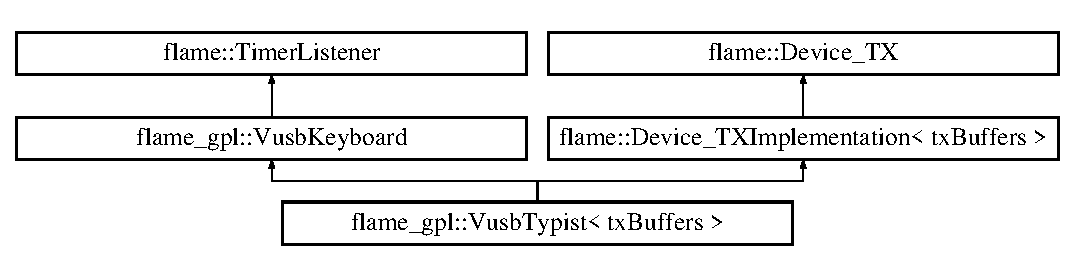
\includegraphics[height=3.000000cm]{classflame__gpl_1_1_vusb_typist}
\end{center}
\end{figure}
\subsection*{Public Member Functions}
\begin{DoxyCompactItemize}
\item 
\hyperlink{classflame__gpl_1_1_vusb_typist_acbf3098e89832c0b07904fc36f935e54}{Vusb\-Typist} (\hyperlink{classflame_1_1_r_t_c}{R\-T\-C} \&rtc)
\item 
void \hyperlink{classflame__gpl_1_1_vusb_typist_afc57a75f932afa7202b7c1aee92d9a0b}{alarm} (\hyperlink{namespaceflame_a6d176ba245556716fd3e32006bb7cfe5}{Alarm\-Source} source)
\end{DoxyCompactItemize}
\subsection*{Protected Member Functions}
\begin{DoxyCompactItemize}
\item 
\hyperlink{io_8h_a0c33b494a68ce28497e7ce8e5e95feff}{C\-O\-N\-S\-T} void \hyperlink{classflame__gpl_1_1_vusb_typist_a725357253d37d28f66cbf2c608fefad7}{run\-Tx\-Buffers} ()
\item 
void \hyperlink{classflame__gpl_1_1_vusb_typist_a122b275feefa5c1379910056ca81bc54}{type\-Char} (char c)
\end{DoxyCompactItemize}
\subsection*{Protected Attributes}
\begin{DoxyCompactItemize}
\item 
bool \hyperlink{classflame__gpl_1_1_vusb_typist_abeab655b1c9769ad055805f243993860}{\-\_\-is\-Typing}
\end{DoxyCompactItemize}


\subsection{Detailed Description}
\subsubsection*{template$<$uint8\-\_\-t tx\-Buffers$>$class flame\-\_\-gpl\-::\-Vusb\-Typist$<$ tx\-Buffers $>$}

A U\-S\-B keyboard emulator that will type what you print to it 
\begin{DoxyTemplParams}{Template Parameters}
{\em tx\-Buffers} & the number of output buffers \\
\hline
\end{DoxyTemplParams}


Definition at line 38 of file Vusb\-Typist.\-h.



\subsection{Constructor \& Destructor Documentation}
\hypertarget{classflame__gpl_1_1_vusb_typist_acbf3098e89832c0b07904fc36f935e54}{\index{flame\-\_\-gpl\-::\-Vusb\-Typist@{flame\-\_\-gpl\-::\-Vusb\-Typist}!Vusb\-Typist@{Vusb\-Typist}}
\index{Vusb\-Typist@{Vusb\-Typist}!flame_gpl::VusbTypist@{flame\-\_\-gpl\-::\-Vusb\-Typist}}
\subsubsection[{Vusb\-Typist}]{\setlength{\rightskip}{0pt plus 5cm}template$<$uint8\-\_\-t tx\-Buffers$>$ {\bf flame\-\_\-gpl\-::\-Vusb\-Typist}$<$ tx\-Buffers $>$\-::{\bf Vusb\-Typist} (
\begin{DoxyParamCaption}
\item[{{\bf R\-T\-C} \&}]{rtc}
\end{DoxyParamCaption}
)\hspace{0.3cm}{\ttfamily [inline]}}}\label{classflame__gpl_1_1_vusb_typist_acbf3098e89832c0b07904fc36f935e54}
Emulate a U\-S\-B keyboard using V-\/\-U\-S\-B This class can also be passed strings, which it will type out on the keyboard 
\begin{DoxyParams}{Parameters}
{\em rtc} & an R\-T\-C to trigger events from \\
\hline
\end{DoxyParams}


Definition at line 197 of file Vusb\-Typist.\-h.



\subsection{Member Function Documentation}
\hypertarget{classflame__gpl_1_1_vusb_typist_afc57a75f932afa7202b7c1aee92d9a0b}{\index{flame\-\_\-gpl\-::\-Vusb\-Typist@{flame\-\_\-gpl\-::\-Vusb\-Typist}!alarm@{alarm}}
\index{alarm@{alarm}!flame_gpl::VusbTypist@{flame\-\_\-gpl\-::\-Vusb\-Typist}}
\subsubsection[{alarm}]{\setlength{\rightskip}{0pt plus 5cm}template$<$uint8\-\_\-t tx\-Buffers$>$ void {\bf flame\-\_\-gpl\-::\-Vusb\-Typist}$<$ tx\-Buffers $>$\-::{\bf alarm} (
\begin{DoxyParamCaption}
\item[{{\bf Alarm\-Source}}]{source}
\end{DoxyParamCaption}
)\hspace{0.3cm}{\ttfamily [inline]}, {\ttfamily [virtual]}}}\label{classflame__gpl_1_1_vusb_typist_afc57a75f932afa7202b7c1aee92d9a0b}
Periodically called to maintain U\-S\-B comms 

Reimplemented from \hyperlink{classflame__gpl_1_1_vusb_keyboard_ac78516dbc8ac2519bf2f0b4327c13b4d}{flame\-\_\-gpl\-::\-Vusb\-Keyboard}.



Definition at line 204 of file Vusb\-Typist.\-h.

\hypertarget{classflame__gpl_1_1_vusb_typist_a725357253d37d28f66cbf2c608fefad7}{\index{flame\-\_\-gpl\-::\-Vusb\-Typist@{flame\-\_\-gpl\-::\-Vusb\-Typist}!run\-Tx\-Buffers@{run\-Tx\-Buffers}}
\index{run\-Tx\-Buffers@{run\-Tx\-Buffers}!flame_gpl::VusbTypist@{flame\-\_\-gpl\-::\-Vusb\-Typist}}
\subsubsection[{run\-Tx\-Buffers}]{\setlength{\rightskip}{0pt plus 5cm}template$<$uint8\-\_\-t tx\-Buffers$>$ {\bf C\-O\-N\-S\-T} void {\bf flame\-\_\-gpl\-::\-Vusb\-Typist}$<$ tx\-Buffers $>$\-::run\-Tx\-Buffers (
\begin{DoxyParamCaption}
{}
\end{DoxyParamCaption}
)\hspace{0.3cm}{\ttfamily [inline]}, {\ttfamily [protected]}, {\ttfamily [virtual]}}}\label{classflame__gpl_1_1_vusb_typist_a725357253d37d28f66cbf2c608fefad7}
Start transmitting a new string (does nothing, alarm will immediately pick up the next character) 

Implements \hyperlink{classflame_1_1_device___t_x_af3cf3dc02a124e5a88841d325555ce3c}{flame\-::\-Device\-\_\-\-T\-X}.



Definition at line 46 of file Vusb\-Typist.\-h.

\hypertarget{classflame__gpl_1_1_vusb_typist_a122b275feefa5c1379910056ca81bc54}{\index{flame\-\_\-gpl\-::\-Vusb\-Typist@{flame\-\_\-gpl\-::\-Vusb\-Typist}!type\-Char@{type\-Char}}
\index{type\-Char@{type\-Char}!flame_gpl::VusbTypist@{flame\-\_\-gpl\-::\-Vusb\-Typist}}
\subsubsection[{type\-Char}]{\setlength{\rightskip}{0pt plus 5cm}template$<$uint8\-\_\-t tx\-Buffers$>$ void {\bf flame\-\_\-gpl\-::\-Vusb\-Typist}$<$ tx\-Buffers $>$\-::type\-Char (
\begin{DoxyParamCaption}
\item[{char}]{c}
\end{DoxyParamCaption}
)\hspace{0.3cm}{\ttfamily [inline]}, {\ttfamily [protected]}}}\label{classflame__gpl_1_1_vusb_typist_a122b275feefa5c1379910056ca81bc54}
Type a single character on the keyboard 
\begin{DoxyParams}{Parameters}
{\em c} & the character to type \\
\hline
\end{DoxyParams}


Definition at line 52 of file Vusb\-Typist.\-h.



\subsection{Member Data Documentation}
\hypertarget{classflame__gpl_1_1_vusb_typist_abeab655b1c9769ad055805f243993860}{\index{flame\-\_\-gpl\-::\-Vusb\-Typist@{flame\-\_\-gpl\-::\-Vusb\-Typist}!\-\_\-is\-Typing@{\-\_\-is\-Typing}}
\index{\-\_\-is\-Typing@{\-\_\-is\-Typing}!flame_gpl::VusbTypist@{flame\-\_\-gpl\-::\-Vusb\-Typist}}
\subsubsection[{\-\_\-is\-Typing}]{\setlength{\rightskip}{0pt plus 5cm}template$<$uint8\-\_\-t tx\-Buffers$>$ bool {\bf flame\-\_\-gpl\-::\-Vusb\-Typist}$<$ tx\-Buffers $>$\-::\-\_\-is\-Typing\hspace{0.3cm}{\ttfamily [protected]}}}\label{classflame__gpl_1_1_vusb_typist_abeab655b1c9769ad055805f243993860}


Definition at line 40 of file Vusb\-Typist.\-h.



The documentation for this class was generated from the following file\-:\begin{DoxyCompactItemize}
\item 
A\-:/eclipse/flame/flame-\/\-Vusb-\/\-Keyboard/flame/\hyperlink{_vusb_typist_8h}{Vusb\-Typist.\-h}\end{DoxyCompactItemize}

\hypertarget{classflame_1_1_wave_generator}{\section{flame\-:\-:Wave\-Generator Class Reference}
\label{classflame_1_1_wave_generator}\index{flame\-::\-Wave\-Generator@{flame\-::\-Wave\-Generator}}
}


{\ttfamily \#include $<$Wave\-Generator.\-h$>$}

Inheritance diagram for flame\-:\-:Wave\-Generator\-:\begin{figure}[H]
\begin{center}
\leavevmode
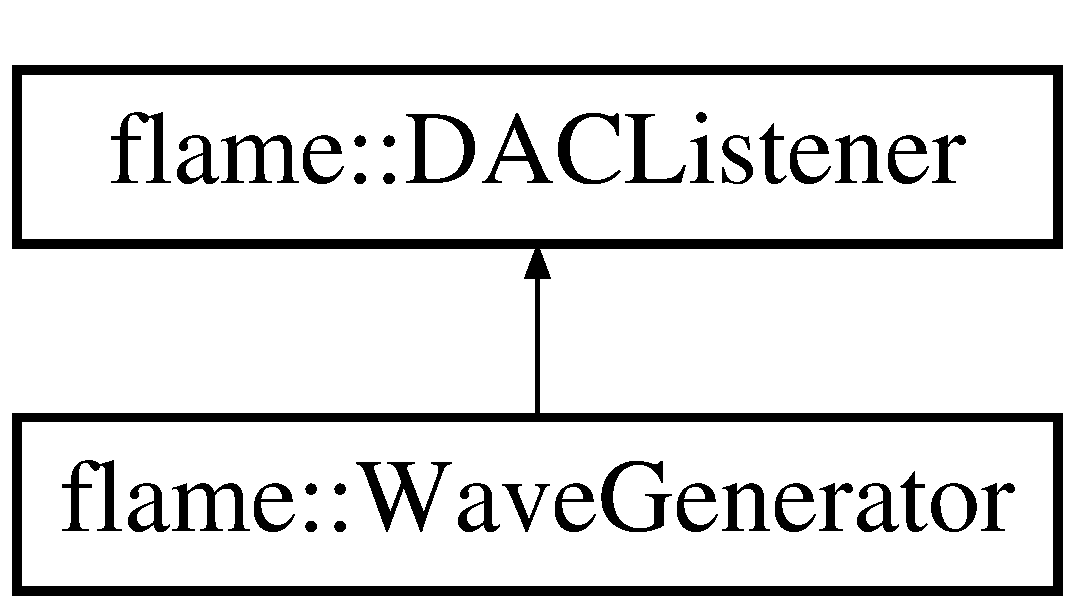
\includegraphics[height=2.000000cm]{classflame_1_1_wave_generator}
\end{center}
\end{figure}
\subsection*{Public Member Functions}
\begin{DoxyCompactItemize}
\item 
\hyperlink{classflame_1_1_wave_generator_a33e33b8cbf6ffd8ba02760574188a970}{Wave\-Generator} (\hyperlink{classflame_1_1_d_a_converter}{D\-A\-Converter} \&dac, \hyperlink{_d_a_c_8h_a5a6d1dc37ffa32957a63868cd1da39b3}{S\-A\-M\-P\-L\-E} $\ast$sample\-Buffer, uint8\-\_\-t sample\-Length, uint32\-\_\-t sample\-Rate, \hyperlink{namespaceflame_a69cbce86034387173caf0aaf772a5d3b}{V\-O\-I\-C\-E} $\ast$voices, uint8\-\_\-t voice\-Count)
\item 
void \hyperlink{classflame_1_1_wave_generator_ac94e2fa02447ef96aba48b88181eddeb}{more\-Samples} (\hyperlink{classflame_1_1_d_a_converter}{D\-A\-Converter} $\ast$dac, \hyperlink{_d_a_c_8h_a5a6d1dc37ffa32957a63868cd1da39b3}{S\-A\-M\-P\-L\-E} $\ast$old\-Samples, uint8\-\_\-t sample\-Length)
\item 
bool \hyperlink{classflame_1_1_wave_generator_a0a1404ff26873712073b396c0a94aac4}{play} (\hyperlink{namespaceflame_a7f0c5adbd1329cd2947d15e6af02dbf1}{I\-N\-S\-T\-R\-U\-M\-E\-N\-T} $\ast$\hyperlink{structflame_1_1instrument}{instrument}, uint16\-\_\-t frequency, \hyperlink{namespaceflame_a7f6447252c60127b805475b293831f99}{A\-M\-P\-L\-I\-T\-U\-D\-E} velocity, uint32\-\_\-t duration)
\end{DoxyCompactItemize}


\subsection{Detailed Description}


Definition at line 93 of file Wave\-Generator.\-h.



\subsection{Constructor \& Destructor Documentation}
\hypertarget{classflame_1_1_wave_generator_a33e33b8cbf6ffd8ba02760574188a970}{\index{flame\-::\-Wave\-Generator@{flame\-::\-Wave\-Generator}!Wave\-Generator@{Wave\-Generator}}
\index{Wave\-Generator@{Wave\-Generator}!flame::WaveGenerator@{flame\-::\-Wave\-Generator}}
\subsubsection[{Wave\-Generator}]{\setlength{\rightskip}{0pt plus 5cm}flame\-::\-Wave\-Generator\-::\-Wave\-Generator (
\begin{DoxyParamCaption}
\item[{{\bf D\-A\-Converter} \&}]{dac, }
\item[{{\bf S\-A\-M\-P\-L\-E} $\ast$}]{sample\-Buffer, }
\item[{uint8\-\_\-t}]{sample\-Length, }
\item[{uint32\-\_\-t}]{sample\-Rate, }
\item[{{\bf V\-O\-I\-C\-E} $\ast$}]{voices, }
\item[{uint8\-\_\-t}]{voice\-Count}
\end{DoxyParamCaption}
)}}\label{classflame_1_1_wave_generator_a33e33b8cbf6ffd8ba02760574188a970}
Generate waveforms and write them to the D\-A\-C


\begin{DoxyParams}{Parameters}
{\em dac} & the D\-A\-C to write to \\
\hline
{\em sample\-Buffer} & a buffer of samples to write to, used to communicate with the D\-A\-C \\
\hline
{\em sample\-Length} & the length of the sample buffer \\
\hline
{\em sample\-Rate} & the sample rate of the D\-A\-C \\
\hline
{\em voices} & the voices to use to generate sound \\
\hline
{\em voice\-Count} & the number of voices \\
\hline
\end{DoxyParams}


Definition at line 43 of file Wave\-Generator.\-cpp.



\subsection{Member Function Documentation}
\hypertarget{classflame_1_1_wave_generator_ac94e2fa02447ef96aba48b88181eddeb}{\index{flame\-::\-Wave\-Generator@{flame\-::\-Wave\-Generator}!more\-Samples@{more\-Samples}}
\index{more\-Samples@{more\-Samples}!flame::WaveGenerator@{flame\-::\-Wave\-Generator}}
\subsubsection[{more\-Samples}]{\setlength{\rightskip}{0pt plus 5cm}void flame\-::\-Wave\-Generator\-::more\-Samples (
\begin{DoxyParamCaption}
\item[{{\bf D\-A\-Converter} $\ast$}]{dac, }
\item[{{\bf S\-A\-M\-P\-L\-E} $\ast$}]{old\-Samples, }
\item[{uint8\-\_\-t}]{sample\-Length}
\end{DoxyParamCaption}
)\hspace{0.3cm}{\ttfamily [virtual]}}}\label{classflame_1_1_wave_generator_ac94e2fa02447ef96aba48b88181eddeb}
Send more samples to the D\-A\-C 

Reimplemented from \hyperlink{classflame_1_1_d_a_c_listener_a00ede324c36c05647dc31b770e4e1443}{flame\-::\-D\-A\-C\-Listener}.



Definition at line 190 of file Wave\-Generator.\-cpp.

\hypertarget{classflame_1_1_wave_generator_a0a1404ff26873712073b396c0a94aac4}{\index{flame\-::\-Wave\-Generator@{flame\-::\-Wave\-Generator}!play@{play}}
\index{play@{play}!flame::WaveGenerator@{flame\-::\-Wave\-Generator}}
\subsubsection[{play}]{\setlength{\rightskip}{0pt plus 5cm}bool flame\-::\-Wave\-Generator\-::play (
\begin{DoxyParamCaption}
\item[{{\bf I\-N\-S\-T\-R\-U\-M\-E\-N\-T} $\ast$}]{instrument, }
\item[{uint16\-\_\-t}]{frequency, }
\item[{{\bf A\-M\-P\-L\-I\-T\-U\-D\-E}}]{velocity, }
\item[{uint32\-\_\-t}]{duration}
\end{DoxyParamCaption}
)}}\label{classflame_1_1_wave_generator_a0a1404ff26873712073b396c0a94aac4}
Play a note \begin{DoxyReturn}{Returns}
true if the note could not be played 
\end{DoxyReturn}


Definition at line 199 of file Wave\-Generator.\-cpp.



The documentation for this class was generated from the following files\-:\begin{DoxyCompactItemize}
\item 
flame/\hyperlink{_wave_generator_8h}{Wave\-Generator.\-h}\item 
\hyperlink{_wave_generator_8cpp}{Wave\-Generator.\-cpp}\end{DoxyCompactItemize}

\hypertarget{classflame_1_1_w_s2801}{\section{flame\-:\-:W\-S2801$<$,, length $>$ Class Template Reference}
\label{classflame_1_1_w_s2801}\index{flame\-::\-W\-S2801$<$,, length $>$@{flame\-::\-W\-S2801$<$,, length $>$}}
}


{\ttfamily \#include $<$W\-S2801.\-h$>$}

Inheritance diagram for flame\-:\-:W\-S2801$<$,, length $>$\-:\begin{figure}[H]
\begin{center}
\leavevmode
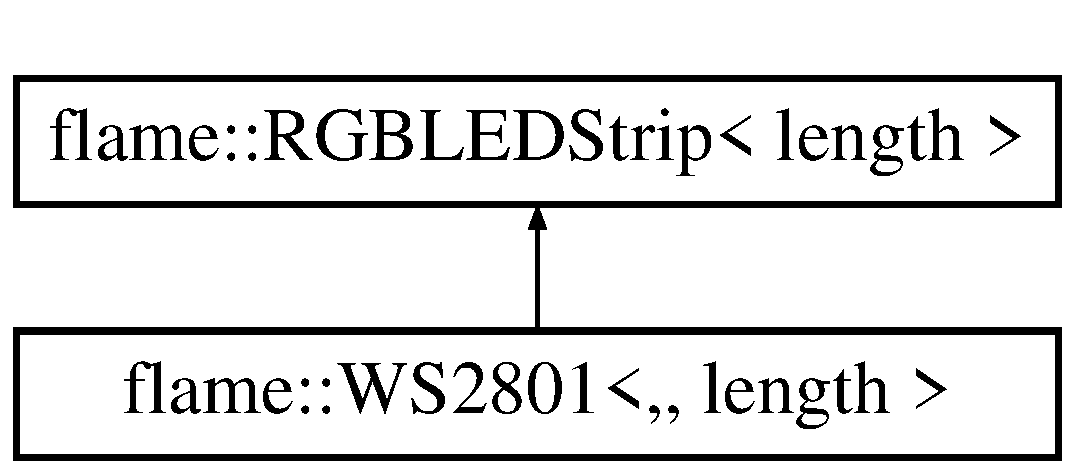
\includegraphics[height=2.000000cm]{classflame_1_1_w_s2801}
\end{center}
\end{figure}
\subsection*{Public Member Functions}
\begin{DoxyCompactItemize}
\item 
\hyperlink{classflame_1_1_w_s2801_a95d6bd232fa1cf4def396deec89a6c09}{W\-S2801} ()
\item 
void \hyperlink{classflame_1_1_w_s2801_af36d043e8554e1834980b485766396f6}{flush} ()
\end{DoxyCompactItemize}
\subsection*{Additional Inherited Members}


\subsection{Detailed Description}
\subsubsection*{template$<$F\-L\-A\-M\-E\-\_\-\-D\-E\-C\-L\-A\-R\-E\-\_\-\-P\-I\-N(clock), F\-L\-A\-M\-E\-\_\-\-D\-E\-C\-L\-A\-R\-E\-\_\-\-P\-I\-N(data), uint16\-\_\-t length$>$class flame\-::\-W\-S2801$<$,, length $>$}

Create a new \hyperlink{classflame_1_1_w_s2801}{W\-S2801} object to control a string of L\-E\-D drivers 
\begin{DoxyTemplParams}{Template Parameters}
{\em clock...} & the clock pin for the L\-E\-Ds \\
\hline
{\em data...} & the data pin for the L\-E\-Ds, must be on the same port as the clock \\
\hline
{\em length} & the number of L\-E\-Ds in the string \\
\hline
\end{DoxyTemplParams}


Definition at line 43 of file W\-S2801.\-h.



\subsection{Constructor \& Destructor Documentation}
\hypertarget{classflame_1_1_w_s2801_a95d6bd232fa1cf4def396deec89a6c09}{\index{flame\-::\-W\-S2801@{flame\-::\-W\-S2801}!W\-S2801@{W\-S2801}}
\index{W\-S2801@{W\-S2801}!flame::WS2801@{flame\-::\-W\-S2801}}
\subsubsection[{W\-S2801}]{\setlength{\rightskip}{0pt plus 5cm}template$<$F\-L\-A\-M\-E\-\_\-\-D\-E\-C\-L\-A\-R\-E\-\_\-\-P\-I\-N(clock) , F\-L\-A\-M\-E\-\_\-\-D\-E\-C\-L\-A\-R\-E\-\_\-\-P\-I\-N(data) , uint16\-\_\-t length$>$ {\bf flame\-::\-W\-S2801}$<$,, length $>$\-::{\bf W\-S2801} (
\begin{DoxyParamCaption}
{}
\end{DoxyParamCaption}
)\hspace{0.3cm}{\ttfamily [inline]}}}\label{classflame_1_1_w_s2801_a95d6bd232fa1cf4def396deec89a6c09}
Create a new driver for a string of \hyperlink{classflame_1_1_w_s2801}{W\-S2801} L\-E\-Ds 

Definition at line 52 of file W\-S2801.\-h.



\subsection{Member Function Documentation}
\hypertarget{classflame_1_1_w_s2801_af36d043e8554e1834980b485766396f6}{\index{flame\-::\-W\-S2801@{flame\-::\-W\-S2801}!flush@{flush}}
\index{flush@{flush}!flame::WS2801@{flame\-::\-W\-S2801}}
\subsubsection[{flush}]{\setlength{\rightskip}{0pt plus 5cm}template$<$F\-L\-A\-M\-E\-\_\-\-D\-E\-C\-L\-A\-R\-E\-\_\-\-P\-I\-N(clock) , F\-L\-A\-M\-E\-\_\-\-D\-E\-C\-L\-A\-R\-E\-\_\-\-P\-I\-N(data) , uint16\-\_\-t length$>$ void {\bf flame\-::\-W\-S2801}$<$,, length $>$\-::flush (
\begin{DoxyParamCaption}
{}
\end{DoxyParamCaption}
)\hspace{0.3cm}{\ttfamily [inline]}, {\ttfamily [virtual]}}}\label{classflame_1_1_w_s2801_af36d043e8554e1834980b485766396f6}
Write the current buffer to the string of chips 

Reimplemented from \hyperlink{classflame_1_1_r_g_b_l_e_d_strip_a4b30397b84e60b9f14bd3bef3129a60b}{flame\-::\-R\-G\-B\-L\-E\-D\-Strip$<$ length $>$}.



Definition at line 60 of file W\-S2801.\-h.



The documentation for this class was generated from the following file\-:\begin{DoxyCompactItemize}
\item 
flame/\hyperlink{_w_s2801_8h}{W\-S2801.\-h}\end{DoxyCompactItemize}

\hypertarget{classflame_1_1_w_s2811}{\section{flame\-:\-:W\-S2811$<$, length $>$ Class Template Reference}
\label{classflame_1_1_w_s2811}\index{flame\-::\-W\-S2811$<$, length $>$@{flame\-::\-W\-S2811$<$, length $>$}}
}


{\ttfamily \#include $<$W\-S2811.\-h$>$}

Inheritance diagram for flame\-:\-:W\-S2811$<$, length $>$\-:\begin{figure}[H]
\begin{center}
\leavevmode
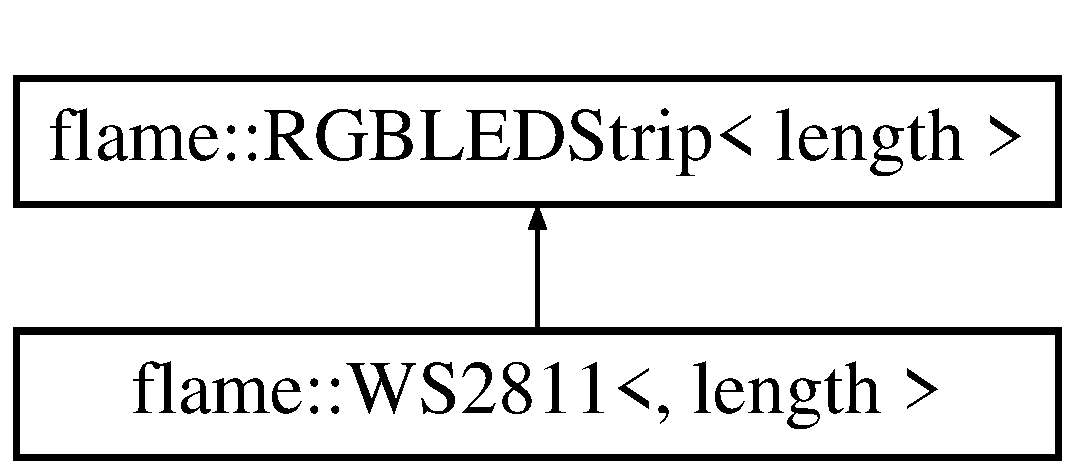
\includegraphics[height=2.000000cm]{classflame_1_1_w_s2811}
\end{center}
\end{figure}
\subsection*{Public Member Functions}
\begin{DoxyCompactItemize}
\item 
\hyperlink{classflame_1_1_w_s2811_a84e91f9e9b7f8187a168a80a58e0a9de}{W\-S2811} ()
\item 
void \hyperlink{classflame_1_1_w_s2811_a53ce9fb8cba4af3bd34b8371a7b3851a}{flush} ()
\end{DoxyCompactItemize}
\subsection*{Additional Inherited Members}


\subsection{Detailed Description}
\subsubsection*{template$<$F\-L\-A\-M\-E\-\_\-\-D\-E\-C\-L\-A\-R\-E\-\_\-\-P\-I\-N(data\-Pin), uint16\-\_\-t length$>$class flame\-::\-W\-S2811$<$, length $>$}

Create a new \hyperlink{classflame_1_1_w_s2811}{W\-S2811} object to control a string of L\-E\-D drivers 
\begin{DoxyTemplParams}{Template Parameters}
{\em data\-Pin...} & the data pin for the L\-E\-Ds (This must be the same pin that Output2 (O\-C\-Rn\-B) is on) \\
\hline
{\em length} & the number of L\-E\-Ds in the string \\
\hline
{\em timer} & the timer parameters \\
\hline
\end{DoxyTemplParams}


Definition at line 47 of file W\-S2811.\-h.



\subsection{Constructor \& Destructor Documentation}
\hypertarget{classflame_1_1_w_s2811_a84e91f9e9b7f8187a168a80a58e0a9de}{\index{flame\-::\-W\-S2811@{flame\-::\-W\-S2811}!W\-S2811@{W\-S2811}}
\index{W\-S2811@{W\-S2811}!flame::WS2811@{flame\-::\-W\-S2811}}
\subsubsection[{W\-S2811}]{\setlength{\rightskip}{0pt plus 5cm}template$<$F\-L\-A\-M\-E\-\_\-\-D\-E\-C\-L\-A\-R\-E\-\_\-\-P\-I\-N(data\-Pin) , uint16\-\_\-t length$>$ {\bf flame\-::\-W\-S2811}$<$, length $>$\-::{\bf W\-S2811} (
\begin{DoxyParamCaption}
{}
\end{DoxyParamCaption}
)\hspace{0.3cm}{\ttfamily [inline]}}}\label{classflame_1_1_w_s2811_a84e91f9e9b7f8187a168a80a58e0a9de}
Constructor 

Definition at line 52 of file W\-S2811.\-h.



\subsection{Member Function Documentation}
\hypertarget{classflame_1_1_w_s2811_a53ce9fb8cba4af3bd34b8371a7b3851a}{\index{flame\-::\-W\-S2811@{flame\-::\-W\-S2811}!flush@{flush}}
\index{flush@{flush}!flame::WS2811@{flame\-::\-W\-S2811}}
\subsubsection[{flush}]{\setlength{\rightskip}{0pt plus 5cm}template$<$F\-L\-A\-M\-E\-\_\-\-D\-E\-C\-L\-A\-R\-E\-\_\-\-P\-I\-N(data\-Pin) , uint16\-\_\-t length$>$ void {\bf flame\-::\-W\-S2811}$<$, length $>$\-::flush (
\begin{DoxyParamCaption}
{}
\end{DoxyParamCaption}
)\hspace{0.3cm}{\ttfamily [inline]}, {\ttfamily [virtual]}}}\label{classflame_1_1_w_s2811_a53ce9fb8cba4af3bd34b8371a7b3851a}
Write the current buffer to the string of chips 

Reimplemented from \hyperlink{classflame_1_1_r_g_b_l_e_d_strip_a4b30397b84e60b9f14bd3bef3129a60b}{flame\-::\-R\-G\-B\-L\-E\-D\-Strip$<$ length $>$}.



Definition at line 60 of file W\-S2811.\-h.



The documentation for this class was generated from the following file\-:\begin{DoxyCompactItemize}
\item 
flame/\hyperlink{_w_s2811_8h}{W\-S2811.\-h}\end{DoxyCompactItemize}

\chapter{File Documentation}
\hypertarget{_vusb_console_8h}{\section{A\-:/eclipse/flame/flame-\/\-Vusb-\/\-Console/flame/\-Vusb\-Console.h File Reference}
\label{_vusb_console_8h}\index{A\-:/eclipse/flame/flame-\/\-Vusb-\/\-Console/flame/\-Vusb\-Console.\-h@{A\-:/eclipse/flame/flame-\/\-Vusb-\/\-Console/flame/\-Vusb\-Console.\-h}}
}
{\ttfamily \#include $<$vusb/usbdrv.\-h$>$}\\*
{\ttfamily \#include $<$flame/\-Device\-\_\-\-T\-X.\-h$>$}\\*
{\ttfamily \#include $<$flame/\-R\-T\-C.\-h$>$}\\*
{\ttfamily \#include $<$util/delay.\-h$>$}\\*
\subsection*{Classes}
\begin{DoxyCompactItemize}
\item 
class \hyperlink{classflame__gpl_1_1_vusb_console}{flame\-\_\-gpl\-::\-Vusb\-Console$<$ tx\-Count $>$}
\end{DoxyCompactItemize}
\subsection*{Namespaces}
\begin{DoxyCompactItemize}
\item 
\hyperlink{namespaceflame__gpl}{flame\-\_\-gpl}
\end{DoxyCompactItemize}
\subsection*{Macros}
\begin{DoxyCompactItemize}
\item 
\#define \hyperlink{_vusb_console_8h_a351126d1fddee8c2691d1f9a92f9e15e}{M\-A\-X\-\_\-\-T\-X\-\_\-\-S\-I\-Z\-E}~8
\end{DoxyCompactItemize}


\subsection{Macro Definition Documentation}
\hypertarget{_vusb_console_8h_a351126d1fddee8c2691d1f9a92f9e15e}{\index{Vusb\-Console.\-h@{Vusb\-Console.\-h}!M\-A\-X\-\_\-\-T\-X\-\_\-\-S\-I\-Z\-E@{M\-A\-X\-\_\-\-T\-X\-\_\-\-S\-I\-Z\-E}}
\index{M\-A\-X\-\_\-\-T\-X\-\_\-\-S\-I\-Z\-E@{M\-A\-X\-\_\-\-T\-X\-\_\-\-S\-I\-Z\-E}!VusbConsole.h@{Vusb\-Console.\-h}}
\subsubsection[{M\-A\-X\-\_\-\-T\-X\-\_\-\-S\-I\-Z\-E}]{\setlength{\rightskip}{0pt plus 5cm}\#define M\-A\-X\-\_\-\-T\-X\-\_\-\-S\-I\-Z\-E~8}}\label{_vusb_console_8h_a351126d1fddee8c2691d1f9a92f9e15e}


Definition at line 26 of file Vusb\-Console.\-h.


\hypertarget{_vusb_console_8cpp}{\section{A\-:/eclipse/flame/flame-\/\-Vusb-\/\-Console/\-Vusb\-Console.cpp File Reference}
\label{_vusb_console_8cpp}\index{A\-:/eclipse/flame/flame-\/\-Vusb-\/\-Console/\-Vusb\-Console.\-cpp@{A\-:/eclipse/flame/flame-\/\-Vusb-\/\-Console/\-Vusb\-Console.\-cpp}}
}
{\ttfamily \#include $<$vusb/usbdrv.\-h$>$}\\*
{\ttfamily \#include $<$flame/\-Vusb\-Console.\-h$>$}\\*
{\ttfamily \#include $<$avr/pgmspace.\-h$>$}\\*
{\ttfamily \#include $<$util/delay.\-h$>$}\\*
\subsection*{Macros}
\begin{DoxyCompactItemize}
\item 
\#define \hyperlink{_vusb_console_8cpp_ace7af99abe4ccb3d62cdba6479150367}{F\-L\-A\-M\-E\-\_\-\-O\-S\-C\-C\-A\-L\-\_\-\-E\-E\-P\-R\-O\-M\-\_\-\-A\-D\-D\-R\-E\-S\-S}~1022
\end{DoxyCompactItemize}
\subsection*{Functions}
\begin{DoxyCompactItemize}
\item 
unsigned char \hyperlink{_vusb_console_8cpp_a4e641b4800eb0c0afcad37d69e688a0e}{usb\-Function\-Setup} (uchar data\mbox{[}8\mbox{]})
\end{DoxyCompactItemize}
\subsection*{Variables}
\begin{DoxyCompactItemize}
\item 
P\-R\-O\-G\-M\-E\-M const char \hyperlink{_vusb_console_8cpp_a15aa13fbfaa191fad8a6908bf8ad25a0}{usb\-Hid\-Report\-Descriptor} \mbox{[}U\-S\-B\-\_\-\-C\-F\-G\-\_\-\-H\-I\-D\-\_\-\-R\-E\-P\-O\-R\-T\-\_\-\-D\-E\-S\-C\-R\-I\-P\-T\-O\-R\-\_\-\-L\-E\-N\-G\-T\-H\mbox{]}
\end{DoxyCompactItemize}


\subsection{Macro Definition Documentation}
\hypertarget{_vusb_console_8cpp_ace7af99abe4ccb3d62cdba6479150367}{\index{Vusb\-Console.\-cpp@{Vusb\-Console.\-cpp}!F\-L\-A\-M\-E\-\_\-\-O\-S\-C\-C\-A\-L\-\_\-\-E\-E\-P\-R\-O\-M\-\_\-\-A\-D\-D\-R\-E\-S\-S@{F\-L\-A\-M\-E\-\_\-\-O\-S\-C\-C\-A\-L\-\_\-\-E\-E\-P\-R\-O\-M\-\_\-\-A\-D\-D\-R\-E\-S\-S}}
\index{F\-L\-A\-M\-E\-\_\-\-O\-S\-C\-C\-A\-L\-\_\-\-E\-E\-P\-R\-O\-M\-\_\-\-A\-D\-D\-R\-E\-S\-S@{F\-L\-A\-M\-E\-\_\-\-O\-S\-C\-C\-A\-L\-\_\-\-E\-E\-P\-R\-O\-M\-\_\-\-A\-D\-D\-R\-E\-S\-S}!VusbConsole.cpp@{Vusb\-Console.\-cpp}}
\subsubsection[{F\-L\-A\-M\-E\-\_\-\-O\-S\-C\-C\-A\-L\-\_\-\-E\-E\-P\-R\-O\-M\-\_\-\-A\-D\-D\-R\-E\-S\-S}]{\setlength{\rightskip}{0pt plus 5cm}\#define F\-L\-A\-M\-E\-\_\-\-O\-S\-C\-C\-A\-L\-\_\-\-E\-E\-P\-R\-O\-M\-\_\-\-A\-D\-D\-R\-E\-S\-S~1022}}\label{_vusb_console_8cpp_ace7af99abe4ccb3d62cdba6479150367}


Definition at line 27 of file Vusb\-Console.\-cpp.



\subsection{Function Documentation}
\hypertarget{_vusb_console_8cpp_a4e641b4800eb0c0afcad37d69e688a0e}{\index{Vusb\-Console.\-cpp@{Vusb\-Console.\-cpp}!usb\-Function\-Setup@{usb\-Function\-Setup}}
\index{usb\-Function\-Setup@{usb\-Function\-Setup}!VusbConsole.cpp@{Vusb\-Console.\-cpp}}
\subsubsection[{usb\-Function\-Setup}]{\setlength{\rightskip}{0pt plus 5cm}unsigned char usb\-Function\-Setup (
\begin{DoxyParamCaption}
\item[{uchar}]{data\mbox{[}8\mbox{]}}
\end{DoxyParamCaption}
)}}\label{_vusb_console_8cpp_a4e641b4800eb0c0afcad37d69e688a0e}


Definition at line 115 of file Vusb\-Console.\-cpp.



\subsection{Variable Documentation}
\hypertarget{_vusb_console_8cpp_a15aa13fbfaa191fad8a6908bf8ad25a0}{\index{Vusb\-Console.\-cpp@{Vusb\-Console.\-cpp}!usb\-Hid\-Report\-Descriptor@{usb\-Hid\-Report\-Descriptor}}
\index{usb\-Hid\-Report\-Descriptor@{usb\-Hid\-Report\-Descriptor}!VusbConsole.cpp@{Vusb\-Console.\-cpp}}
\subsubsection[{usb\-Hid\-Report\-Descriptor}]{\setlength{\rightskip}{0pt plus 5cm}P\-R\-O\-G\-M\-E\-M const char usb\-Hid\-Report\-Descriptor\mbox{[}U\-S\-B\-\_\-\-C\-F\-G\-\_\-\-H\-I\-D\-\_\-\-R\-E\-P\-O\-R\-T\-\_\-\-D\-E\-S\-C\-R\-I\-P\-T\-O\-R\-\_\-\-L\-E\-N\-G\-T\-H\mbox{]}}}\label{_vusb_console_8cpp_a15aa13fbfaa191fad8a6908bf8ad25a0}
{\bfseries Initial value\-:}
\begin{DoxyCode}
= \{ 
                0x06, 0x31, 0xFF,               
                0x09, 0x74,                             
                0xA1, 0x53,                             
                0x75, 0x08,                             
                0x15, 0x00,                             
                0x26, 0xFF, 0x00,               
                0x95, \hyperlink{_vusb_console_8h_a351126d1fddee8c2691d1f9a92f9e15e}{MAX\_TX\_SIZE},           
                0x09, 0x75,                             
                0x81, 0x02,                             
                0xC0                                    
\}
\end{DoxyCode}


Definition at line 30 of file Vusb\-Console.\-cpp.


\hypertarget{_vusb_keyboard_8h}{\section{A\-:/eclipse/flame/flame-\/\-Vusb-\/\-Keyboard/flame/\-Vusb\-Keyboard.h File Reference}
\label{_vusb_keyboard_8h}\index{A\-:/eclipse/flame/flame-\/\-Vusb-\/\-Keyboard/flame/\-Vusb\-Keyboard.\-h@{A\-:/eclipse/flame/flame-\/\-Vusb-\/\-Keyboard/flame/\-Vusb\-Keyboard.\-h}}
}
{\ttfamily \#include $<$flame/io.\-h$>$}\\*
{\ttfamily \#include $<$flame/\-R\-T\-C.\-h$>$}\\*
\subsection*{Classes}
\begin{DoxyCompactItemize}
\item 
class \hyperlink{classflame__gpl_1_1_vusb_keyboard}{flame\-\_\-gpl\-::\-Vusb\-Keyboard}
\end{DoxyCompactItemize}
\subsection*{Namespaces}
\begin{DoxyCompactItemize}
\item 
\hyperlink{namespaceflame__gpl}{flame\-\_\-gpl}
\end{DoxyCompactItemize}
\subsection*{Macros}
\begin{DoxyCompactItemize}
\item 
\#define \hyperlink{_vusb_keyboard_8h_a8863b70f31112408efb9a04ae925a603}{F\-L\-A\-M\-E\-\_\-\-M\-O\-D\-\_\-\-C\-O\-N\-T\-R\-O\-L\-\_\-\-L\-E\-F\-T}~(1$<$$<$0)
\item 
\#define \hyperlink{_vusb_keyboard_8h_ab80d92e777eb7e8a4bc1dcc42d0db335}{F\-L\-A\-M\-E\-\_\-\-M\-O\-D\-\_\-\-S\-H\-I\-F\-T\-\_\-\-L\-E\-F\-T}~(1$<$$<$1)
\item 
\#define \hyperlink{_vusb_keyboard_8h_a8f77824072d9d4d197073e2a2c9f91dd}{F\-L\-A\-M\-E\-\_\-\-M\-O\-D\-\_\-\-A\-L\-T\-\_\-\-L\-E\-F\-T}~(1$<$$<$2)
\item 
\#define \hyperlink{_vusb_keyboard_8h_ac090dbb308155f5286075e4c29b2df18}{F\-L\-A\-M\-E\-\_\-\-M\-O\-D\-\_\-\-G\-U\-I\-\_\-\-L\-E\-F\-T}~(1$<$$<$3)
\item 
\#define \hyperlink{_vusb_keyboard_8h_a59c2ecc63baa73a328db2f47ccb1a3ac}{F\-L\-A\-M\-E\-\_\-\-M\-O\-D\-\_\-\-C\-O\-N\-T\-R\-O\-L\-\_\-\-R\-I\-G\-H\-T}~(1$<$$<$4)
\item 
\#define \hyperlink{_vusb_keyboard_8h_a754cadae7147d278c2a6e49ef9202814}{F\-L\-A\-M\-E\-\_\-\-M\-O\-D\-\_\-\-S\-H\-I\-F\-T\-\_\-\-R\-I\-G\-H\-T}~(1$<$$<$5)
\item 
\#define \hyperlink{_vusb_keyboard_8h_ae9970ff2fef7baf1212a4897ff369c70}{F\-L\-A\-M\-E\-\_\-\-M\-O\-D\-\_\-\-A\-L\-T\-\_\-\-R\-I\-G\-H\-T}~(1$<$$<$6)
\item 
\#define \hyperlink{_vusb_keyboard_8h_a81e0af50d352bfcfa2566faffc73ae83}{F\-L\-A\-M\-E\-\_\-\-M\-O\-D\-\_\-\-G\-U\-I\-\_\-\-R\-I\-G\-H\-T}~(1$<$$<$7)
\end{DoxyCompactItemize}
\subsection*{Typedefs}
\begin{DoxyCompactItemize}
\item 
typedef enum vusb\-\_\-keyboard\-\_\-key \hyperlink{namespaceflame__gpl_a40752e4f9e83da1573a3d418e0bd5653}{flame\-\_\-gpl\-::\-V\-U\-S\-B\-\_\-\-K\-E\-Y\-B\-O\-A\-R\-D\-\_\-\-K\-E\-Y}
\end{DoxyCompactItemize}
\subsection*{Enumerations}
\begin{DoxyCompactItemize}
\item 
enum \hyperlink{namespaceflame__gpl_ac5dd72d2f6257805426f44b0bad032c2}{flame\-\_\-gpl\-::vusb\-\_\-keyboard\-\_\-key} \{ \\*
\hyperlink{namespaceflame__gpl_ac5dd72d2f6257805426f44b0bad032c2af04535502aaff300334bf5e0fbf46a33}{flame\-\_\-gpl\-::\-F\-L\-A\-M\-E\-\_\-\-K\-E\-Y\-\_\-\-A} = 4, 
\hyperlink{namespaceflame__gpl_ac5dd72d2f6257805426f44b0bad032c2a54b998382fc76a4e08953863d189a1ff}{flame\-\_\-gpl\-::\-F\-L\-A\-M\-E\-\_\-\-K\-E\-Y\-\_\-\-B} = 5, 
\hyperlink{namespaceflame__gpl_ac5dd72d2f6257805426f44b0bad032c2a760e2b81c8f5f202a7498fb6c3d9e204}{flame\-\_\-gpl\-::\-F\-L\-A\-M\-E\-\_\-\-K\-E\-Y\-\_\-\-C} = 6, 
\hyperlink{namespaceflame__gpl_ac5dd72d2f6257805426f44b0bad032c2a18b26e07586979dbbcf4de5a7053135e}{flame\-\_\-gpl\-::\-F\-L\-A\-M\-E\-\_\-\-K\-E\-Y\-\_\-\-D} = 7, 
\\*
\hyperlink{namespaceflame__gpl_ac5dd72d2f6257805426f44b0bad032c2af534669e86bea044382d64d911434f14}{flame\-\_\-gpl\-::\-F\-L\-A\-M\-E\-\_\-\-K\-E\-Y\-\_\-\-E} = 8, 
\hyperlink{namespaceflame__gpl_ac5dd72d2f6257805426f44b0bad032c2a05b4a2474d3f0e012f3ca91428ea7386}{flame\-\_\-gpl\-::\-F\-L\-A\-M\-E\-\_\-\-K\-E\-Y\-\_\-\-F} = 9, 
\hyperlink{namespaceflame__gpl_ac5dd72d2f6257805426f44b0bad032c2a2ed3df2eb7a47a2fe0d354cc65b4b677}{flame\-\_\-gpl\-::\-F\-L\-A\-M\-E\-\_\-\-K\-E\-Y\-\_\-\-G} = 10, 
\hyperlink{namespaceflame__gpl_ac5dd72d2f6257805426f44b0bad032c2a2eba9b95192274cdfbbb03c7dca7af2f}{flame\-\_\-gpl\-::\-F\-L\-A\-M\-E\-\_\-\-K\-E\-Y\-\_\-\-H} = 11, 
\\*
\hyperlink{namespaceflame__gpl_ac5dd72d2f6257805426f44b0bad032c2a189eb980f8555662317e25911286d783}{flame\-\_\-gpl\-::\-F\-L\-A\-M\-E\-\_\-\-K\-E\-Y\-\_\-\-I} = 12, 
\hyperlink{namespaceflame__gpl_ac5dd72d2f6257805426f44b0bad032c2a7417a10b9a04fbc51f694cfe8f31c641}{flame\-\_\-gpl\-::\-F\-L\-A\-M\-E\-\_\-\-K\-E\-Y\-\_\-\-J} = 13, 
\hyperlink{namespaceflame__gpl_ac5dd72d2f6257805426f44b0bad032c2ab2ad1056f859aff141326c50bd9ed3f4}{flame\-\_\-gpl\-::\-F\-L\-A\-M\-E\-\_\-\-K\-E\-Y\-\_\-\-K} = 14, 
\hyperlink{namespaceflame__gpl_ac5dd72d2f6257805426f44b0bad032c2a2e343df89501479bcc039d17633fcc87}{flame\-\_\-gpl\-::\-F\-L\-A\-M\-E\-\_\-\-K\-E\-Y\-\_\-\-L} = 15, 
\\*
\hyperlink{namespaceflame__gpl_ac5dd72d2f6257805426f44b0bad032c2af0647f1fefc67767b0c649e78c111f00}{flame\-\_\-gpl\-::\-F\-L\-A\-M\-E\-\_\-\-K\-E\-Y\-\_\-\-M} = 16, 
\hyperlink{namespaceflame__gpl_ac5dd72d2f6257805426f44b0bad032c2a8facf970a6e7aced0ed40ebe3553cc81}{flame\-\_\-gpl\-::\-F\-L\-A\-M\-E\-\_\-\-K\-E\-Y\-\_\-\-N} = 17, 
\hyperlink{namespaceflame__gpl_ac5dd72d2f6257805426f44b0bad032c2a44728d4521dd04f1b8cca61200af96d3}{flame\-\_\-gpl\-::\-F\-L\-A\-M\-E\-\_\-\-K\-E\-Y\-\_\-\-O} = 18, 
\hyperlink{namespaceflame__gpl_ac5dd72d2f6257805426f44b0bad032c2a591faeb0593c355b76c200a1403db53d}{flame\-\_\-gpl\-::\-F\-L\-A\-M\-E\-\_\-\-K\-E\-Y\-\_\-\-P} = 19, 
\\*
\hyperlink{namespaceflame__gpl_ac5dd72d2f6257805426f44b0bad032c2aa13b44cfbec0250cc8a7da64ae1ed647}{flame\-\_\-gpl\-::\-F\-L\-A\-M\-E\-\_\-\-K\-E\-Y\-\_\-\-Q} = 20, 
\hyperlink{namespaceflame__gpl_ac5dd72d2f6257805426f44b0bad032c2a318e6d0abe78825d94d83a5f981a6522}{flame\-\_\-gpl\-::\-F\-L\-A\-M\-E\-\_\-\-K\-E\-Y\-\_\-\-R} = 21, 
\hyperlink{namespaceflame__gpl_ac5dd72d2f6257805426f44b0bad032c2ac68d4c394bdd917ef24c8678ef373f03}{flame\-\_\-gpl\-::\-F\-L\-A\-M\-E\-\_\-\-K\-E\-Y\-\_\-\-S} = 22, 
\hyperlink{namespaceflame__gpl_ac5dd72d2f6257805426f44b0bad032c2a24e52856b465fcad62e6d38eea934e4f}{flame\-\_\-gpl\-::\-F\-L\-A\-M\-E\-\_\-\-K\-E\-Y\-\_\-\-T} = 23, 
\\*
\hyperlink{namespaceflame__gpl_ac5dd72d2f6257805426f44b0bad032c2a013bd9f1d187f789bd3b343a74f72f52}{flame\-\_\-gpl\-::\-F\-L\-A\-M\-E\-\_\-\-K\-E\-Y\-\_\-\-U} = 24, 
\hyperlink{namespaceflame__gpl_ac5dd72d2f6257805426f44b0bad032c2ad22f394994da5db88a2c76726485f574}{flame\-\_\-gpl\-::\-F\-L\-A\-M\-E\-\_\-\-K\-E\-Y\-\_\-\-V} = 25, 
\hyperlink{namespaceflame__gpl_ac5dd72d2f6257805426f44b0bad032c2ab771e399fc93896b5da6ebcb2e851c7c}{flame\-\_\-gpl\-::\-F\-L\-A\-M\-E\-\_\-\-K\-E\-Y\-\_\-\-W} = 26, 
\hyperlink{namespaceflame__gpl_ac5dd72d2f6257805426f44b0bad032c2af6f1a3881181950cc69abf4fe305bf33}{flame\-\_\-gpl\-::\-F\-L\-A\-M\-E\-\_\-\-K\-E\-Y\-\_\-\-X} = 27, 
\\*
\hyperlink{namespaceflame__gpl_ac5dd72d2f6257805426f44b0bad032c2aa118ba4f9830d6f70cff2f45344349db}{flame\-\_\-gpl\-::\-F\-L\-A\-M\-E\-\_\-\-K\-E\-Y\-\_\-\-Y} = 28, 
\hyperlink{namespaceflame__gpl_ac5dd72d2f6257805426f44b0bad032c2aa6fb8184e75a19edd1d37f75fffa29be}{flame\-\_\-gpl\-::\-F\-L\-A\-M\-E\-\_\-\-K\-E\-Y\-\_\-\-Z} = 29, 
\hyperlink{namespaceflame__gpl_ac5dd72d2f6257805426f44b0bad032c2a4186cd6baae0c548570c5e68a363e211}{flame\-\_\-gpl\-::\-F\-L\-A\-M\-E\-\_\-\-K\-E\-Y\-\_\-1} = 30, 
\hyperlink{namespaceflame__gpl_ac5dd72d2f6257805426f44b0bad032c2a1288725897853a75c58bf71ea926d385}{flame\-\_\-gpl\-::\-F\-L\-A\-M\-E\-\_\-\-K\-E\-Y\-\_\-2} = 31, 
\\*
\hyperlink{namespaceflame__gpl_ac5dd72d2f6257805426f44b0bad032c2ade87628305514797167aa7f1fcdcd60f}{flame\-\_\-gpl\-::\-F\-L\-A\-M\-E\-\_\-\-K\-E\-Y\-\_\-3} = 32, 
\hyperlink{namespaceflame__gpl_ac5dd72d2f6257805426f44b0bad032c2ad589b105e9a3b3f269d764432542c396}{flame\-\_\-gpl\-::\-F\-L\-A\-M\-E\-\_\-\-K\-E\-Y\-\_\-4} = 33, 
\hyperlink{namespaceflame__gpl_ac5dd72d2f6257805426f44b0bad032c2aa01b8ac5ca7fc7c0b686bc307873be8e}{flame\-\_\-gpl\-::\-F\-L\-A\-M\-E\-\_\-\-K\-E\-Y\-\_\-5} = 34, 
\hyperlink{namespaceflame__gpl_ac5dd72d2f6257805426f44b0bad032c2a2b637c5ed65fe57458f675451f6f9d03}{flame\-\_\-gpl\-::\-F\-L\-A\-M\-E\-\_\-\-K\-E\-Y\-\_\-6} = 35, 
\\*
\hyperlink{namespaceflame__gpl_ac5dd72d2f6257805426f44b0bad032c2ab8df69dbbea23c8fac12678238fff003}{flame\-\_\-gpl\-::\-F\-L\-A\-M\-E\-\_\-\-K\-E\-Y\-\_\-7} = 36, 
\hyperlink{namespaceflame__gpl_ac5dd72d2f6257805426f44b0bad032c2ab30790c5c018dbee355c813ac4b65a02}{flame\-\_\-gpl\-::\-F\-L\-A\-M\-E\-\_\-\-K\-E\-Y\-\_\-8} = 37, 
\hyperlink{namespaceflame__gpl_ac5dd72d2f6257805426f44b0bad032c2aa69c3965de7866fc8d6f12257863cc12}{flame\-\_\-gpl\-::\-F\-L\-A\-M\-E\-\_\-\-K\-E\-Y\-\_\-9} = 38, 
\hyperlink{namespaceflame__gpl_ac5dd72d2f6257805426f44b0bad032c2ac356430ec6477a88034310f1cc406722}{flame\-\_\-gpl\-::\-F\-L\-A\-M\-E\-\_\-\-K\-E\-Y\-\_\-0} = 39, 
\\*
\hyperlink{namespaceflame__gpl_ac5dd72d2f6257805426f44b0bad032c2a09f931d054fe7609eef8d2988e61b74c}{flame\-\_\-gpl\-::\-F\-L\-A\-M\-E\-\_\-\-K\-E\-Y\-\_\-\-E\-N\-T\-E\-R} = 40, 
\hyperlink{namespaceflame__gpl_ac5dd72d2f6257805426f44b0bad032c2a76cbb94cbb41e923f8fe6ef6cd2849c5}{flame\-\_\-gpl\-::\-F\-L\-A\-M\-E\-\_\-\-K\-E\-Y\-\_\-\-E\-S\-C\-A\-P\-E} = 41, 
\hyperlink{namespaceflame__gpl_ac5dd72d2f6257805426f44b0bad032c2a75bce028d43d083852a89d04b0427f6d}{flame\-\_\-gpl\-::\-F\-L\-A\-M\-E\-\_\-\-K\-E\-Y\-\_\-\-B\-A\-C\-K\-S\-P\-A\-C\-E} = 42, 
\hyperlink{namespaceflame__gpl_ac5dd72d2f6257805426f44b0bad032c2a4c415b518af064c8afbef9f756efa251}{flame\-\_\-gpl\-::\-F\-L\-A\-M\-E\-\_\-\-K\-E\-Y\-\_\-\-T\-A\-B} = 43, 
\\*
\hyperlink{namespaceflame__gpl_ac5dd72d2f6257805426f44b0bad032c2a582a3488f27a2d38aedf9ac035b47b43}{flame\-\_\-gpl\-::\-F\-L\-A\-M\-E\-\_\-\-K\-E\-Y\-\_\-\-S\-P\-A\-C\-E} = 44, 
\hyperlink{namespaceflame__gpl_ac5dd72d2f6257805426f44b0bad032c2a6ccd37d256423edae93a6c148f24a559}{flame\-\_\-gpl\-::\-F\-L\-A\-M\-E\-\_\-\-K\-E\-Y\-\_\-\-M\-I\-N\-U\-S} = 45, 
\hyperlink{namespaceflame__gpl_ac5dd72d2f6257805426f44b0bad032c2abf0fdcea7bb9ec9c87b201d425d884fb}{flame\-\_\-gpl\-::\-F\-L\-A\-M\-E\-\_\-\-K\-E\-Y\-\_\-\-E\-Q\-U\-A\-L\-S} = 46, 
\hyperlink{namespaceflame__gpl_ac5dd72d2f6257805426f44b0bad032c2ae21d36242807bd03d7e3107d3c8a4f02}{flame\-\_\-gpl\-::\-F\-L\-A\-M\-E\-\_\-\-K\-E\-Y\-\_\-\-L\-\_\-\-S\-Q\-U\-A\-R\-E} = 47, 
\\*
\hyperlink{namespaceflame__gpl_ac5dd72d2f6257805426f44b0bad032c2af983fc05872fe2c4ce1699a2a52ef453}{flame\-\_\-gpl\-::\-F\-L\-A\-M\-E\-\_\-\-K\-E\-Y\-\_\-\-R\-\_\-\-S\-Q\-U\-A\-R\-E} = 48, 
\hyperlink{namespaceflame__gpl_ac5dd72d2f6257805426f44b0bad032c2abe968530e47f53976ead026e8aa55418}{flame\-\_\-gpl\-::\-F\-L\-A\-M\-E\-\_\-\-K\-E\-Y\-\_\-\-B\-A\-C\-K\-S\-L\-A\-S\-H} = 49, 
\hyperlink{namespaceflame__gpl_ac5dd72d2f6257805426f44b0bad032c2a0ea3f3d2a07624c1be90a51f4a19f06d}{flame\-\_\-gpl\-::\-F\-L\-A\-M\-E\-\_\-\-K\-E\-Y\-\_\-\-N\-O\-N\-\_\-\-U\-S\-\_\-\-H\-A\-S\-H} = 50, 
\hyperlink{namespaceflame__gpl_ac5dd72d2f6257805426f44b0bad032c2ab62c34141f94cbf4fdcd4b7b1545b406}{flame\-\_\-gpl\-::\-F\-L\-A\-M\-E\-\_\-\-K\-E\-Y\-\_\-\-S\-E\-M\-I\-C\-O\-L\-O\-N} = 51, 
\\*
\hyperlink{namespaceflame__gpl_ac5dd72d2f6257805426f44b0bad032c2ab8271aa268302188ceb8bd0e0183c79d}{flame\-\_\-gpl\-::\-F\-L\-A\-M\-E\-\_\-\-K\-E\-Y\-\_\-\-Q\-U\-O\-T\-E} = 52, 
\hyperlink{namespaceflame__gpl_ac5dd72d2f6257805426f44b0bad032c2ab2e4b9dfbdb7ef94486eab8ba29523df}{flame\-\_\-gpl\-::\-F\-L\-A\-M\-E\-\_\-\-K\-E\-Y\-\_\-\-G\-R\-A\-V\-E\-\_\-\-A\-C\-C\-E\-N\-T} = 53, 
\hyperlink{namespaceflame__gpl_ac5dd72d2f6257805426f44b0bad032c2a34473574d1ddea47c74926695de58ff1}{flame\-\_\-gpl\-::\-F\-L\-A\-M\-E\-\_\-\-K\-E\-Y\-\_\-\-C\-O\-M\-M\-A} = 54, 
\hyperlink{namespaceflame__gpl_ac5dd72d2f6257805426f44b0bad032c2a670e7fe2c84a132c7cad60738bb58b3b}{flame\-\_\-gpl\-::\-F\-L\-A\-M\-E\-\_\-\-K\-E\-Y\-\_\-\-F\-U\-L\-L\-S\-T\-O\-P} = 55, 
\\*
\hyperlink{namespaceflame__gpl_ac5dd72d2f6257805426f44b0bad032c2a7d04053cb2faa3d146b6858c7744dcfc}{flame\-\_\-gpl\-::\-F\-L\-A\-M\-E\-\_\-\-K\-E\-Y\-\_\-\-S\-L\-A\-S\-H} = 56, 
\hyperlink{namespaceflame__gpl_ac5dd72d2f6257805426f44b0bad032c2a91da58e40710590bc079cdf913a3e3fc}{flame\-\_\-gpl\-::\-F\-L\-A\-M\-E\-\_\-\-K\-E\-Y\-\_\-\-C\-A\-P\-S\-L\-O\-C\-K} = 57, 
\hyperlink{namespaceflame__gpl_ac5dd72d2f6257805426f44b0bad032c2a38ddaccee4955e0cdef99f36c57dc2ad}{flame\-\_\-gpl\-::\-F\-L\-A\-M\-E\-\_\-\-K\-E\-Y\-\_\-\-F1} = 58, 
\hyperlink{namespaceflame__gpl_ac5dd72d2f6257805426f44b0bad032c2a739cacf60a7bd9eecf48843e68728131}{flame\-\_\-gpl\-::\-F\-L\-A\-M\-E\-\_\-\-K\-E\-Y\-\_\-\-F2} = 59, 
\\*
\hyperlink{namespaceflame__gpl_ac5dd72d2f6257805426f44b0bad032c2a52d1d4a5e5d7df2b6d5d4137a0f2434c}{flame\-\_\-gpl\-::\-F\-L\-A\-M\-E\-\_\-\-K\-E\-Y\-\_\-\-F3} = 60, 
\hyperlink{namespaceflame__gpl_ac5dd72d2f6257805426f44b0bad032c2a446a1849c4aa47240cac9ea05c61c1a1}{flame\-\_\-gpl\-::\-F\-L\-A\-M\-E\-\_\-\-K\-E\-Y\-\_\-\-F4} = 61, 
\hyperlink{namespaceflame__gpl_ac5dd72d2f6257805426f44b0bad032c2ac8d95338ea69e430613c8178529a7b0b}{flame\-\_\-gpl\-::\-F\-L\-A\-M\-E\-\_\-\-K\-E\-Y\-\_\-\-F5} = 62, 
\hyperlink{namespaceflame__gpl_ac5dd72d2f6257805426f44b0bad032c2a1d2b20fd59aa34e7a7c782bf10015e68}{flame\-\_\-gpl\-::\-F\-L\-A\-M\-E\-\_\-\-K\-E\-Y\-\_\-\-F6} = 63, 
\\*
\hyperlink{namespaceflame__gpl_ac5dd72d2f6257805426f44b0bad032c2a4ddae50d9a1d0645f96eb127f2849bb0}{flame\-\_\-gpl\-::\-F\-L\-A\-M\-E\-\_\-\-K\-E\-Y\-\_\-\-F7} = 64, 
\hyperlink{namespaceflame__gpl_ac5dd72d2f6257805426f44b0bad032c2afcd2bf300ea93a857807353b64ebb42d}{flame\-\_\-gpl\-::\-F\-L\-A\-M\-E\-\_\-\-K\-E\-Y\-\_\-\-F8} = 65, 
\hyperlink{namespaceflame__gpl_ac5dd72d2f6257805426f44b0bad032c2a0df25770c1a36669190c486bdbbfbbcb}{flame\-\_\-gpl\-::\-F\-L\-A\-M\-E\-\_\-\-K\-E\-Y\-\_\-\-F9} = 66, 
\hyperlink{namespaceflame__gpl_ac5dd72d2f6257805426f44b0bad032c2ab80025df891df72ef5a77b36554629a3}{flame\-\_\-gpl\-::\-F\-L\-A\-M\-E\-\_\-\-K\-E\-Y\-\_\-\-F10} = 67, 
\\*
\hyperlink{namespaceflame__gpl_ac5dd72d2f6257805426f44b0bad032c2ad89f0260ea8c68b928265594c879eda3}{flame\-\_\-gpl\-::\-F\-L\-A\-M\-E\-\_\-\-K\-E\-Y\-\_\-\-F11} = 68, 
\hyperlink{namespaceflame__gpl_ac5dd72d2f6257805426f44b0bad032c2a5799ccba4e95916a82b4ca116eac6cb2}{flame\-\_\-gpl\-::\-F\-L\-A\-M\-E\-\_\-\-K\-E\-Y\-\_\-\-F12} = 69, 
\hyperlink{namespaceflame__gpl_ac5dd72d2f6257805426f44b0bad032c2ad6c8d3a6afad2775ad5bfcb4881c27de}{flame\-\_\-gpl\-::\-F\-L\-A\-M\-E\-\_\-\-K\-E\-Y\-\_\-\-P\-R\-I\-N\-T\-S\-C\-R\-E\-E\-N} = 70, 
\hyperlink{namespaceflame__gpl_ac5dd72d2f6257805426f44b0bad032c2a08a20a1e5196292d566f9a687f976818}{flame\-\_\-gpl\-::\-F\-L\-A\-M\-E\-\_\-\-K\-E\-Y\-\_\-\-S\-C\-R\-O\-L\-L\-\_\-\-L\-O\-C\-K} = 71, 
\\*
\hyperlink{namespaceflame__gpl_ac5dd72d2f6257805426f44b0bad032c2af7b15ad20bd7c289e5674b187743fa4a}{flame\-\_\-gpl\-::\-F\-L\-A\-M\-E\-\_\-\-K\-E\-Y\-\_\-\-P\-A\-U\-S\-E} = 72, 
\hyperlink{namespaceflame__gpl_ac5dd72d2f6257805426f44b0bad032c2ac91dcc865640287a7840271a95479396}{flame\-\_\-gpl\-::\-F\-L\-A\-M\-E\-\_\-\-K\-E\-Y\-\_\-\-I\-N\-S\-E\-R\-T} = 73, 
\hyperlink{namespaceflame__gpl_ac5dd72d2f6257805426f44b0bad032c2a48ad0346619f07bed90630aa23311cab}{flame\-\_\-gpl\-::\-F\-L\-A\-M\-E\-\_\-\-K\-E\-Y\-\_\-\-H\-O\-M\-E} = 74, 
\hyperlink{namespaceflame__gpl_ac5dd72d2f6257805426f44b0bad032c2a278f1d3c34d26eb8264abad441870e7d}{flame\-\_\-gpl\-::\-F\-L\-A\-M\-E\-\_\-\-K\-E\-Y\-\_\-\-P\-A\-G\-E\-\_\-\-U\-P} = 75, 
\\*
\hyperlink{namespaceflame__gpl_ac5dd72d2f6257805426f44b0bad032c2a390e4e8a3d6420e8185509e9a8b3c6fa}{flame\-\_\-gpl\-::\-F\-L\-A\-M\-E\-\_\-\-K\-E\-Y\-\_\-\-D\-E\-L\-E\-T\-E} = 76, 
\hyperlink{namespaceflame__gpl_ac5dd72d2f6257805426f44b0bad032c2ae2bbedb594b3cb23201b15d4bb10b9d5}{flame\-\_\-gpl\-::\-F\-L\-A\-M\-E\-\_\-\-K\-E\-Y\-\_\-\-E\-N\-D} = 77, 
\hyperlink{namespaceflame__gpl_ac5dd72d2f6257805426f44b0bad032c2afac743bfce527bac3c3e79e26ffb72e7}{flame\-\_\-gpl\-::\-F\-L\-A\-M\-E\-\_\-\-K\-E\-Y\-\_\-\-P\-A\-G\-E\-\_\-\-D\-O\-W\-N} = 78, 
\hyperlink{namespaceflame__gpl_ac5dd72d2f6257805426f44b0bad032c2a1f93896f9912290009d10cc35912fae6}{flame\-\_\-gpl\-::\-F\-L\-A\-M\-E\-\_\-\-K\-E\-Y\-\_\-\-A\-R\-R\-O\-W\-\_\-\-R\-I\-G\-H\-T} = 79, 
\\*
\hyperlink{namespaceflame__gpl_ac5dd72d2f6257805426f44b0bad032c2a2d4d2f3d307d7a93d3f1d3938e29994c}{flame\-\_\-gpl\-::\-F\-L\-A\-M\-E\-\_\-\-K\-E\-Y\-\_\-\-A\-R\-R\-O\-W\-\_\-\-L\-E\-F\-T} = 80, 
\hyperlink{namespaceflame__gpl_ac5dd72d2f6257805426f44b0bad032c2a6cc8a1b800c55b08c68c7117c0a4208c}{flame\-\_\-gpl\-::\-F\-L\-A\-M\-E\-\_\-\-K\-E\-Y\-\_\-\-A\-R\-R\-O\-W\-\_\-\-D\-O\-W\-N} = 81, 
\hyperlink{namespaceflame__gpl_ac5dd72d2f6257805426f44b0bad032c2a1700c3d56bec80f535ba382858fc3cd1}{flame\-\_\-gpl\-::\-F\-L\-A\-M\-E\-\_\-\-K\-E\-Y\-\_\-\-A\-R\-R\-O\-W\-\_\-\-U\-P} = 82, 
\hyperlink{namespaceflame__gpl_ac5dd72d2f6257805426f44b0bad032c2aef98620a9575ede71352e3e059b35d1d}{flame\-\_\-gpl\-::\-F\-L\-A\-M\-E\-\_\-\-K\-E\-Y\-\_\-\-N\-U\-M\-\_\-\-L\-O\-C\-K} = 83, 
\\*
\hyperlink{namespaceflame__gpl_ac5dd72d2f6257805426f44b0bad032c2a26164e4bb5b3b86c7311ac051b176551}{flame\-\_\-gpl\-::\-F\-L\-A\-M\-E\-\_\-\-K\-E\-Y\-P\-A\-D\-\_\-\-S\-L\-A\-S\-H} = 84, 
\hyperlink{namespaceflame__gpl_ac5dd72d2f6257805426f44b0bad032c2a0e146ee0945e06b30b24933bce457d73}{flame\-\_\-gpl\-::\-F\-L\-A\-M\-E\-\_\-\-K\-E\-Y\-P\-A\-D\-\_\-\-A\-S\-T\-E\-R\-I\-S\-K} = 85, 
\hyperlink{namespaceflame__gpl_ac5dd72d2f6257805426f44b0bad032c2ac0dc940bc4d68f48bdab8ca3997d132f}{flame\-\_\-gpl\-::\-F\-L\-A\-M\-E\-\_\-\-K\-E\-Y\-P\-A\-D\-\_\-\-M\-I\-N\-U\-S} = 86, 
\hyperlink{namespaceflame__gpl_ac5dd72d2f6257805426f44b0bad032c2a494f01513ed2c1028c1bacee3107986f}{flame\-\_\-gpl\-::\-F\-L\-A\-M\-E\-\_\-\-K\-E\-Y\-P\-A\-D\-\_\-\-P\-L\-U\-S} = 87, 
\\*
\hyperlink{namespaceflame__gpl_ac5dd72d2f6257805426f44b0bad032c2a6cf076a1f2e31c663b9e74519339d320}{flame\-\_\-gpl\-::\-F\-L\-A\-M\-E\-\_\-\-K\-E\-Y\-P\-A\-D\-\_\-\-E\-N\-T\-E\-R} = 88, 
\hyperlink{namespaceflame__gpl_ac5dd72d2f6257805426f44b0bad032c2ac4d948174466390b396e10e95b2e6b05}{flame\-\_\-gpl\-::\-F\-L\-A\-M\-E\-\_\-\-K\-E\-Y\-P\-A\-D\-\_\-1} = 89, 
\hyperlink{namespaceflame__gpl_ac5dd72d2f6257805426f44b0bad032c2aa3816c7fc722e381dff2e28fdfb82c9e}{flame\-\_\-gpl\-::\-F\-L\-A\-M\-E\-\_\-\-K\-E\-Y\-P\-A\-D\-\_\-2} = 90, 
\hyperlink{namespaceflame__gpl_ac5dd72d2f6257805426f44b0bad032c2a20d386ec9150dea87d37d23cefccaf2e}{flame\-\_\-gpl\-::\-F\-L\-A\-M\-E\-\_\-\-K\-E\-Y\-P\-A\-D\-\_\-3} = 91, 
\\*
\hyperlink{namespaceflame__gpl_ac5dd72d2f6257805426f44b0bad032c2aa548b6d5432eb67a1d3cf7d1e693ebea}{flame\-\_\-gpl\-::\-F\-L\-A\-M\-E\-\_\-\-K\-E\-Y\-P\-A\-D\-\_\-4} = 92, 
\hyperlink{namespaceflame__gpl_ac5dd72d2f6257805426f44b0bad032c2ac34cfe06e12897df302cbfb3c75ff105}{flame\-\_\-gpl\-::\-F\-L\-A\-M\-E\-\_\-\-K\-E\-Y\-P\-A\-D\-\_\-5} = 93, 
\hyperlink{namespaceflame__gpl_ac5dd72d2f6257805426f44b0bad032c2ad99f796c899100c8f4be21760651d9fc}{flame\-\_\-gpl\-::\-F\-L\-A\-M\-E\-\_\-\-K\-E\-Y\-P\-A\-D\-\_\-6} = 94, 
\hyperlink{namespaceflame__gpl_ac5dd72d2f6257805426f44b0bad032c2a6012df3728f146bc76eb91609ca3a430}{flame\-\_\-gpl\-::\-F\-L\-A\-M\-E\-\_\-\-K\-E\-Y\-P\-A\-D\-\_\-7} = 95, 
\\*
\hyperlink{namespaceflame__gpl_ac5dd72d2f6257805426f44b0bad032c2ae7f06889cef84ba79ce3515b7363e47c}{flame\-\_\-gpl\-::\-F\-L\-A\-M\-E\-\_\-\-K\-E\-Y\-P\-A\-D\-\_\-8} = 96, 
\hyperlink{namespaceflame__gpl_ac5dd72d2f6257805426f44b0bad032c2a55d94cb4a71720a143203eee5064c63d}{flame\-\_\-gpl\-::\-F\-L\-A\-M\-E\-\_\-\-K\-E\-Y\-P\-A\-D\-\_\-9} = 97, 
\hyperlink{namespaceflame__gpl_ac5dd72d2f6257805426f44b0bad032c2a8b8ec69f6f58af8922d3dc258034a205}{flame\-\_\-gpl\-::\-F\-L\-A\-M\-E\-\_\-\-K\-E\-Y\-P\-A\-D\-\_\-0} = 98, 
\hyperlink{namespaceflame__gpl_ac5dd72d2f6257805426f44b0bad032c2a13faabad0de55caf15cdcaf41bbaae66}{flame\-\_\-gpl\-::\-F\-L\-A\-M\-E\-\_\-\-K\-E\-Y\-P\-A\-D\-\_\-\-F\-U\-L\-L\-S\-T\-O\-P} = 99, 
\\*
\hyperlink{namespaceflame__gpl_ac5dd72d2f6257805426f44b0bad032c2a69187ca764294683fec29cbddad48563}{flame\-\_\-gpl\-::\-F\-L\-A\-M\-E\-\_\-\-K\-E\-Y\-\_\-\-N\-O\-N\-\_\-\-U\-S\-\_\-\-B\-A\-C\-K\-S\-L\-A\-S\-H} = 100, 
\hyperlink{namespaceflame__gpl_ac5dd72d2f6257805426f44b0bad032c2ab4cb7cb967a64a891a93130891bb4e27}{flame\-\_\-gpl\-::\-F\-L\-A\-M\-E\-\_\-\-K\-E\-Y\-\_\-\-A\-P\-P\-L\-I\-C\-A\-T\-I\-O\-N} = 101, 
\hyperlink{namespaceflame__gpl_ac5dd72d2f6257805426f44b0bad032c2a76d0c8c80fb8dd194a0bf07a3f889523}{flame\-\_\-gpl\-::\-F\-L\-A\-M\-E\-\_\-\-K\-E\-Y\-P\-A\-D\-\_\-\-P\-O\-W\-E\-R} = 102, 
\hyperlink{namespaceflame__gpl_ac5dd72d2f6257805426f44b0bad032c2a7d3d18783c598d3cde5cd581f1873711}{flame\-\_\-gpl\-::\-F\-L\-A\-M\-E\-\_\-\-K\-E\-Y\-P\-A\-D\-\_\-\-E\-Q\-U\-A\-L\-S} = 103, 
\\*
\hyperlink{namespaceflame__gpl_ac5dd72d2f6257805426f44b0bad032c2a8eb277d384ba26f4767cd09f69ac0e9e}{flame\-\_\-gpl\-::\-F\-L\-A\-M\-E\-\_\-\-K\-E\-Y\-\_\-\-F13} = 104, 
\hyperlink{namespaceflame__gpl_ac5dd72d2f6257805426f44b0bad032c2ae4c77042a65f395a753607eff63cf47c}{flame\-\_\-gpl\-::\-F\-L\-A\-M\-E\-\_\-\-K\-E\-Y\-\_\-\-F14} = 105, 
\hyperlink{namespaceflame__gpl_ac5dd72d2f6257805426f44b0bad032c2a2da0aa1c3118620190def7d47616c128}{flame\-\_\-gpl\-::\-F\-L\-A\-M\-E\-\_\-\-K\-E\-Y\-\_\-\-F15} = 106, 
\hyperlink{namespaceflame__gpl_ac5dd72d2f6257805426f44b0bad032c2ab4774334d13c05746784107b49400f13}{flame\-\_\-gpl\-::\-F\-L\-A\-M\-E\-\_\-\-K\-E\-Y\-\_\-\-F16} = 107, 
\\*
\hyperlink{namespaceflame__gpl_ac5dd72d2f6257805426f44b0bad032c2a761a4d6be797f20834ae33a059f09e65}{flame\-\_\-gpl\-::\-F\-L\-A\-M\-E\-\_\-\-K\-E\-Y\-\_\-\-F17} = 108, 
\hyperlink{namespaceflame__gpl_ac5dd72d2f6257805426f44b0bad032c2a609dacb77f0c550601e2d23b88d9512a}{flame\-\_\-gpl\-::\-F\-L\-A\-M\-E\-\_\-\-K\-E\-Y\-\_\-\-F18} = 109, 
\hyperlink{namespaceflame__gpl_ac5dd72d2f6257805426f44b0bad032c2ad840e4ec9ff3740d49c6fb4f81fbf916}{flame\-\_\-gpl\-::\-F\-L\-A\-M\-E\-\_\-\-K\-E\-Y\-\_\-\-F19} = 110, 
\hyperlink{namespaceflame__gpl_ac5dd72d2f6257805426f44b0bad032c2a49ef5d3eb9adb6e93b4a3d92d919061e}{flame\-\_\-gpl\-::\-F\-L\-A\-M\-E\-\_\-\-K\-E\-Y\-\_\-\-F20} = 111, 
\\*
\hyperlink{namespaceflame__gpl_ac5dd72d2f6257805426f44b0bad032c2ab14dfba0eeb1024d4791783aadd268ae}{flame\-\_\-gpl\-::\-F\-L\-A\-M\-E\-\_\-\-K\-E\-Y\-\_\-\-F21} = 112, 
\hyperlink{namespaceflame__gpl_ac5dd72d2f6257805426f44b0bad032c2a49e8cd0e5083e1852d8d38daf95bbfd2}{flame\-\_\-gpl\-::\-F\-L\-A\-M\-E\-\_\-\-K\-E\-Y\-\_\-\-F22} = 113, 
\hyperlink{namespaceflame__gpl_ac5dd72d2f6257805426f44b0bad032c2a59e4ad18ebf2bde7ac66115b66a8909c}{flame\-\_\-gpl\-::\-F\-L\-A\-M\-E\-\_\-\-K\-E\-Y\-\_\-\-F23} = 114, 
\hyperlink{namespaceflame__gpl_ac5dd72d2f6257805426f44b0bad032c2a8e9bace112f718571e664cad3fef101b}{flame\-\_\-gpl\-::\-F\-L\-A\-M\-E\-\_\-\-K\-E\-Y\-\_\-\-F24} = 115, 
\\*
\hyperlink{namespaceflame__gpl_ac5dd72d2f6257805426f44b0bad032c2a1b7b90c683b951a985bd7fbc1eb90773}{flame\-\_\-gpl\-::\-F\-L\-A\-M\-E\-\_\-\-K\-E\-Y\-\_\-\-E\-X\-E\-C\-U\-T\-E} = 116, 
\hyperlink{namespaceflame__gpl_ac5dd72d2f6257805426f44b0bad032c2a95ce9a6158ecd8fdc8a8fd80426dd1fe}{flame\-\_\-gpl\-::\-F\-L\-A\-M\-E\-\_\-\-K\-E\-Y\-\_\-\-H\-E\-L\-P} = 117, 
\hyperlink{namespaceflame__gpl_ac5dd72d2f6257805426f44b0bad032c2a2ac570a832a33c3730ab886259763536}{flame\-\_\-gpl\-::\-F\-L\-A\-M\-E\-\_\-\-K\-E\-Y\-\_\-\-M\-E\-N\-U} = 118, 
\hyperlink{namespaceflame__gpl_ac5dd72d2f6257805426f44b0bad032c2a56f9a44d963eaff0a40779efa36e1951}{flame\-\_\-gpl\-::\-F\-L\-A\-M\-E\-\_\-\-K\-E\-Y\-\_\-\-S\-E\-L\-E\-C\-T} = 119, 
\\*
\hyperlink{namespaceflame__gpl_ac5dd72d2f6257805426f44b0bad032c2a237450dcf74249412983ee22cddf38fb}{flame\-\_\-gpl\-::\-F\-L\-A\-M\-E\-\_\-\-K\-E\-Y\-\_\-\-S\-T\-O\-P} = 120, 
\hyperlink{namespaceflame__gpl_ac5dd72d2f6257805426f44b0bad032c2af8d803f18f6fcab92e4bb70d6824b3e5}{flame\-\_\-gpl\-::\-F\-L\-A\-M\-E\-\_\-\-K\-E\-Y\-\_\-\-A\-G\-A\-I\-N} = 121, 
\hyperlink{namespaceflame__gpl_ac5dd72d2f6257805426f44b0bad032c2a50ba2f52d599c3519e0fe6fe20a0a204}{flame\-\_\-gpl\-::\-F\-L\-A\-M\-E\-\_\-\-K\-E\-Y\-\_\-\-U\-N\-D\-O} = 122, 
\hyperlink{namespaceflame__gpl_ac5dd72d2f6257805426f44b0bad032c2ab7a8874385896da5a07331c31faf3ffc}{flame\-\_\-gpl\-::\-F\-L\-A\-M\-E\-\_\-\-K\-E\-Y\-\_\-\-C\-U\-T} = 123, 
\\*
\hyperlink{namespaceflame__gpl_ac5dd72d2f6257805426f44b0bad032c2a48d300650c5c08b3d1ed6bc8dbfbf6e5}{flame\-\_\-gpl\-::\-F\-L\-A\-M\-E\-\_\-\-K\-E\-Y\-\_\-\-C\-O\-P\-Y} = 124, 
\hyperlink{namespaceflame__gpl_ac5dd72d2f6257805426f44b0bad032c2a57106b008499ed6a7275c2e4302193aa}{flame\-\_\-gpl\-::\-F\-L\-A\-M\-E\-\_\-\-K\-E\-Y\-\_\-\-P\-A\-S\-T\-E} = 125, 
\hyperlink{namespaceflame__gpl_ac5dd72d2f6257805426f44b0bad032c2afb63e81e82fd0d9badd019165218f24d}{flame\-\_\-gpl\-::\-F\-L\-A\-M\-E\-\_\-\-K\-E\-Y\-\_\-\-F\-I\-N\-D} = 126, 
\hyperlink{namespaceflame__gpl_ac5dd72d2f6257805426f44b0bad032c2abed9007dec1d9c35f4d527b1e3d49d01}{flame\-\_\-gpl\-::\-F\-L\-A\-M\-E\-\_\-\-K\-E\-Y\-\_\-\-M\-U\-T\-E} = 127, 
\\*
\hyperlink{namespaceflame__gpl_ac5dd72d2f6257805426f44b0bad032c2a6ecf76d169c89e4c30a71d59e1186df8}{flame\-\_\-gpl\-::\-F\-L\-A\-M\-E\-\_\-\-K\-E\-Y\-\_\-\-V\-O\-L\-U\-M\-E\-\_\-\-U\-P} = 128, 
\hyperlink{namespaceflame__gpl_ac5dd72d2f6257805426f44b0bad032c2a73aede3ba644da1c12e1d775fe7a7a7b}{flame\-\_\-gpl\-::\-F\-L\-A\-M\-E\-\_\-\-K\-E\-Y\-\_\-\-V\-O\-L\-U\-M\-E\-\_\-\-D\-O\-W\-N} = 129, 
\hyperlink{namespaceflame__gpl_ac5dd72d2f6257805426f44b0bad032c2a0ec5c437e3c31a2c07ad21995fab2dec}{flame\-\_\-gpl\-::\-F\-L\-A\-M\-E\-\_\-\-K\-E\-Y\-\_\-\-L\-O\-C\-K\-I\-N\-G\-\_\-\-C\-A\-P\-S\-\_\-\-L\-O\-C\-K} = 130, 
\hyperlink{namespaceflame__gpl_ac5dd72d2f6257805426f44b0bad032c2ac85df0e3b125372b737527fe86f34115}{flame\-\_\-gpl\-::\-F\-L\-A\-M\-E\-\_\-\-K\-E\-Y\-\_\-\-L\-O\-C\-K\-I\-N\-G\-\_\-\-N\-U\-M\-\_\-\-L\-O\-C\-K} = 131, 
\\*
\hyperlink{namespaceflame__gpl_ac5dd72d2f6257805426f44b0bad032c2a092cc54a773b5c6d6c1a063d6de3798a}{flame\-\_\-gpl\-::\-F\-L\-A\-M\-E\-\_\-\-K\-E\-Y\-\_\-\-L\-O\-C\-K\-I\-N\-G\-\_\-\-S\-C\-R\-O\-L\-L\-\_\-\-L\-O\-C\-K} = 132, 
\hyperlink{namespaceflame__gpl_ac5dd72d2f6257805426f44b0bad032c2a5ebfa8b525c0cb0366a68c194dec7a03}{flame\-\_\-gpl\-::\-F\-L\-A\-M\-E\-\_\-\-K\-E\-Y\-P\-A\-D\-\_\-\-C\-O\-M\-M\-A} = 133, 
\hyperlink{namespaceflame__gpl_ac5dd72d2f6257805426f44b0bad032c2a0c30113fc6df8823f59062182b80914a}{flame\-\_\-gpl\-::\-F\-L\-A\-M\-E\-\_\-\-K\-E\-Y\-P\-A\-D\-\_\-\-E\-Q\-U\-A\-L} = 134, 
\hyperlink{namespaceflame__gpl_ac5dd72d2f6257805426f44b0bad032c2a4a252c11653c85d895b54da385d0f821}{flame\-\_\-gpl\-::\-F\-L\-A\-M\-E\-\_\-\-K\-E\-Y\-\_\-\-C\-O\-N\-T\-R\-O\-L\-\_\-\-L\-E\-F\-T} = 224, 
\\*
\hyperlink{namespaceflame__gpl_ac5dd72d2f6257805426f44b0bad032c2ad603cec86b64aade338af5ed34342981}{flame\-\_\-gpl\-::\-F\-L\-A\-M\-E\-\_\-\-K\-E\-Y\-\_\-\-S\-H\-I\-F\-T\-\_\-\-L\-E\-F\-T} = 225, 
\hyperlink{namespaceflame__gpl_ac5dd72d2f6257805426f44b0bad032c2a5ef32d2554c3f7426bcb003090d236ff}{flame\-\_\-gpl\-::\-F\-L\-A\-M\-E\-\_\-\-K\-E\-Y\-\_\-\-A\-L\-T\-\_\-\-L\-E\-F\-T} = 226, 
\hyperlink{namespaceflame__gpl_ac5dd72d2f6257805426f44b0bad032c2acc3f4273b9c14c00a975970f27ed0abb}{flame\-\_\-gpl\-::\-F\-L\-A\-M\-E\-\_\-\-K\-E\-Y\-\_\-\-G\-U\-I\-\_\-\-L\-E\-F\-T} = 227, 
\hyperlink{namespaceflame__gpl_ac5dd72d2f6257805426f44b0bad032c2af23cd6143cb78719a38d4c971a1148eb}{flame\-\_\-gpl\-::\-F\-L\-A\-M\-E\-\_\-\-K\-E\-Y\-\_\-\-C\-O\-N\-T\-R\-O\-L\-\_\-\-R\-I\-G\-H\-T} = 228, 
\\*
\hyperlink{namespaceflame__gpl_ac5dd72d2f6257805426f44b0bad032c2aa2693eafdd68c2bf0fa8da598473b2a3}{flame\-\_\-gpl\-::\-F\-L\-A\-M\-E\-\_\-\-K\-E\-Y\-\_\-\-S\-H\-I\-F\-T\-\_\-\-R\-I\-G\-H\-T} = 229, 
\hyperlink{namespaceflame__gpl_ac5dd72d2f6257805426f44b0bad032c2a7f91fccf59ee7c024daf14df9ee1248a}{flame\-\_\-gpl\-::\-F\-L\-A\-M\-E\-\_\-\-K\-E\-Y\-\_\-\-A\-L\-T\-\_\-\-R\-I\-G\-H\-T} = 230, 
\hyperlink{namespaceflame__gpl_ac5dd72d2f6257805426f44b0bad032c2abd10e895e5d1907d2238bac20f6902ed}{flame\-\_\-gpl\-::\-F\-L\-A\-M\-E\-\_\-\-K\-E\-Y\-\_\-\-G\-U\-I\-\_\-\-R\-I\-G\-H\-T} = 231
 \}
\end{DoxyCompactItemize}
\subsection*{Functions}
\begin{DoxyCompactItemize}
\item 
\hyperlink{io_8h_a2eb6f9e0395b47b8d5e3eeae4fe0c116}{I\-N\-L\-I\-N\-E} V\-U\-S\-B\-\_\-\-K\-E\-Y\-B\-O\-A\-R\-D\-\_\-\-K\-E\-Y \hyperlink{namespaceflame__gpl_aae69f913c4df49da9d35286578c3ac4c}{flame\-\_\-gpl\-::vusb\-\_\-keyboard\-\_\-key\-\_\-add} (V\-U\-S\-B\-\_\-\-K\-E\-Y\-B\-O\-A\-R\-D\-\_\-\-K\-E\-Y key, char c)
\end{DoxyCompactItemize}


\subsection{Macro Definition Documentation}
\hypertarget{_vusb_keyboard_8h_a8f77824072d9d4d197073e2a2c9f91dd}{\index{Vusb\-Keyboard.\-h@{Vusb\-Keyboard.\-h}!F\-L\-A\-M\-E\-\_\-\-M\-O\-D\-\_\-\-A\-L\-T\-\_\-\-L\-E\-F\-T@{F\-L\-A\-M\-E\-\_\-\-M\-O\-D\-\_\-\-A\-L\-T\-\_\-\-L\-E\-F\-T}}
\index{F\-L\-A\-M\-E\-\_\-\-M\-O\-D\-\_\-\-A\-L\-T\-\_\-\-L\-E\-F\-T@{F\-L\-A\-M\-E\-\_\-\-M\-O\-D\-\_\-\-A\-L\-T\-\_\-\-L\-E\-F\-T}!VusbKeyboard.h@{Vusb\-Keyboard.\-h}}
\subsubsection[{F\-L\-A\-M\-E\-\_\-\-M\-O\-D\-\_\-\-A\-L\-T\-\_\-\-L\-E\-F\-T}]{\setlength{\rightskip}{0pt plus 5cm}\#define F\-L\-A\-M\-E\-\_\-\-M\-O\-D\-\_\-\-A\-L\-T\-\_\-\-L\-E\-F\-T~(1$<$$<$2)}}\label{_vusb_keyboard_8h_a8f77824072d9d4d197073e2a2c9f91dd}


Definition at line 27 of file Vusb\-Keyboard.\-h.

\hypertarget{_vusb_keyboard_8h_ae9970ff2fef7baf1212a4897ff369c70}{\index{Vusb\-Keyboard.\-h@{Vusb\-Keyboard.\-h}!F\-L\-A\-M\-E\-\_\-\-M\-O\-D\-\_\-\-A\-L\-T\-\_\-\-R\-I\-G\-H\-T@{F\-L\-A\-M\-E\-\_\-\-M\-O\-D\-\_\-\-A\-L\-T\-\_\-\-R\-I\-G\-H\-T}}
\index{F\-L\-A\-M\-E\-\_\-\-M\-O\-D\-\_\-\-A\-L\-T\-\_\-\-R\-I\-G\-H\-T@{F\-L\-A\-M\-E\-\_\-\-M\-O\-D\-\_\-\-A\-L\-T\-\_\-\-R\-I\-G\-H\-T}!VusbKeyboard.h@{Vusb\-Keyboard.\-h}}
\subsubsection[{F\-L\-A\-M\-E\-\_\-\-M\-O\-D\-\_\-\-A\-L\-T\-\_\-\-R\-I\-G\-H\-T}]{\setlength{\rightskip}{0pt plus 5cm}\#define F\-L\-A\-M\-E\-\_\-\-M\-O\-D\-\_\-\-A\-L\-T\-\_\-\-R\-I\-G\-H\-T~(1$<$$<$6)}}\label{_vusb_keyboard_8h_ae9970ff2fef7baf1212a4897ff369c70}


Definition at line 31 of file Vusb\-Keyboard.\-h.

\hypertarget{_vusb_keyboard_8h_a8863b70f31112408efb9a04ae925a603}{\index{Vusb\-Keyboard.\-h@{Vusb\-Keyboard.\-h}!F\-L\-A\-M\-E\-\_\-\-M\-O\-D\-\_\-\-C\-O\-N\-T\-R\-O\-L\-\_\-\-L\-E\-F\-T@{F\-L\-A\-M\-E\-\_\-\-M\-O\-D\-\_\-\-C\-O\-N\-T\-R\-O\-L\-\_\-\-L\-E\-F\-T}}
\index{F\-L\-A\-M\-E\-\_\-\-M\-O\-D\-\_\-\-C\-O\-N\-T\-R\-O\-L\-\_\-\-L\-E\-F\-T@{F\-L\-A\-M\-E\-\_\-\-M\-O\-D\-\_\-\-C\-O\-N\-T\-R\-O\-L\-\_\-\-L\-E\-F\-T}!VusbKeyboard.h@{Vusb\-Keyboard.\-h}}
\subsubsection[{F\-L\-A\-M\-E\-\_\-\-M\-O\-D\-\_\-\-C\-O\-N\-T\-R\-O\-L\-\_\-\-L\-E\-F\-T}]{\setlength{\rightskip}{0pt plus 5cm}\#define F\-L\-A\-M\-E\-\_\-\-M\-O\-D\-\_\-\-C\-O\-N\-T\-R\-O\-L\-\_\-\-L\-E\-F\-T~(1$<$$<$0)}}\label{_vusb_keyboard_8h_a8863b70f31112408efb9a04ae925a603}


Definition at line 25 of file Vusb\-Keyboard.\-h.

\hypertarget{_vusb_keyboard_8h_a59c2ecc63baa73a328db2f47ccb1a3ac}{\index{Vusb\-Keyboard.\-h@{Vusb\-Keyboard.\-h}!F\-L\-A\-M\-E\-\_\-\-M\-O\-D\-\_\-\-C\-O\-N\-T\-R\-O\-L\-\_\-\-R\-I\-G\-H\-T@{F\-L\-A\-M\-E\-\_\-\-M\-O\-D\-\_\-\-C\-O\-N\-T\-R\-O\-L\-\_\-\-R\-I\-G\-H\-T}}
\index{F\-L\-A\-M\-E\-\_\-\-M\-O\-D\-\_\-\-C\-O\-N\-T\-R\-O\-L\-\_\-\-R\-I\-G\-H\-T@{F\-L\-A\-M\-E\-\_\-\-M\-O\-D\-\_\-\-C\-O\-N\-T\-R\-O\-L\-\_\-\-R\-I\-G\-H\-T}!VusbKeyboard.h@{Vusb\-Keyboard.\-h}}
\subsubsection[{F\-L\-A\-M\-E\-\_\-\-M\-O\-D\-\_\-\-C\-O\-N\-T\-R\-O\-L\-\_\-\-R\-I\-G\-H\-T}]{\setlength{\rightskip}{0pt plus 5cm}\#define F\-L\-A\-M\-E\-\_\-\-M\-O\-D\-\_\-\-C\-O\-N\-T\-R\-O\-L\-\_\-\-R\-I\-G\-H\-T~(1$<$$<$4)}}\label{_vusb_keyboard_8h_a59c2ecc63baa73a328db2f47ccb1a3ac}


Definition at line 29 of file Vusb\-Keyboard.\-h.

\hypertarget{_vusb_keyboard_8h_ac090dbb308155f5286075e4c29b2df18}{\index{Vusb\-Keyboard.\-h@{Vusb\-Keyboard.\-h}!F\-L\-A\-M\-E\-\_\-\-M\-O\-D\-\_\-\-G\-U\-I\-\_\-\-L\-E\-F\-T@{F\-L\-A\-M\-E\-\_\-\-M\-O\-D\-\_\-\-G\-U\-I\-\_\-\-L\-E\-F\-T}}
\index{F\-L\-A\-M\-E\-\_\-\-M\-O\-D\-\_\-\-G\-U\-I\-\_\-\-L\-E\-F\-T@{F\-L\-A\-M\-E\-\_\-\-M\-O\-D\-\_\-\-G\-U\-I\-\_\-\-L\-E\-F\-T}!VusbKeyboard.h@{Vusb\-Keyboard.\-h}}
\subsubsection[{F\-L\-A\-M\-E\-\_\-\-M\-O\-D\-\_\-\-G\-U\-I\-\_\-\-L\-E\-F\-T}]{\setlength{\rightskip}{0pt plus 5cm}\#define F\-L\-A\-M\-E\-\_\-\-M\-O\-D\-\_\-\-G\-U\-I\-\_\-\-L\-E\-F\-T~(1$<$$<$3)}}\label{_vusb_keyboard_8h_ac090dbb308155f5286075e4c29b2df18}


Definition at line 28 of file Vusb\-Keyboard.\-h.

\hypertarget{_vusb_keyboard_8h_a81e0af50d352bfcfa2566faffc73ae83}{\index{Vusb\-Keyboard.\-h@{Vusb\-Keyboard.\-h}!F\-L\-A\-M\-E\-\_\-\-M\-O\-D\-\_\-\-G\-U\-I\-\_\-\-R\-I\-G\-H\-T@{F\-L\-A\-M\-E\-\_\-\-M\-O\-D\-\_\-\-G\-U\-I\-\_\-\-R\-I\-G\-H\-T}}
\index{F\-L\-A\-M\-E\-\_\-\-M\-O\-D\-\_\-\-G\-U\-I\-\_\-\-R\-I\-G\-H\-T@{F\-L\-A\-M\-E\-\_\-\-M\-O\-D\-\_\-\-G\-U\-I\-\_\-\-R\-I\-G\-H\-T}!VusbKeyboard.h@{Vusb\-Keyboard.\-h}}
\subsubsection[{F\-L\-A\-M\-E\-\_\-\-M\-O\-D\-\_\-\-G\-U\-I\-\_\-\-R\-I\-G\-H\-T}]{\setlength{\rightskip}{0pt plus 5cm}\#define F\-L\-A\-M\-E\-\_\-\-M\-O\-D\-\_\-\-G\-U\-I\-\_\-\-R\-I\-G\-H\-T~(1$<$$<$7)}}\label{_vusb_keyboard_8h_a81e0af50d352bfcfa2566faffc73ae83}


Definition at line 32 of file Vusb\-Keyboard.\-h.

\hypertarget{_vusb_keyboard_8h_ab80d92e777eb7e8a4bc1dcc42d0db335}{\index{Vusb\-Keyboard.\-h@{Vusb\-Keyboard.\-h}!F\-L\-A\-M\-E\-\_\-\-M\-O\-D\-\_\-\-S\-H\-I\-F\-T\-\_\-\-L\-E\-F\-T@{F\-L\-A\-M\-E\-\_\-\-M\-O\-D\-\_\-\-S\-H\-I\-F\-T\-\_\-\-L\-E\-F\-T}}
\index{F\-L\-A\-M\-E\-\_\-\-M\-O\-D\-\_\-\-S\-H\-I\-F\-T\-\_\-\-L\-E\-F\-T@{F\-L\-A\-M\-E\-\_\-\-M\-O\-D\-\_\-\-S\-H\-I\-F\-T\-\_\-\-L\-E\-F\-T}!VusbKeyboard.h@{Vusb\-Keyboard.\-h}}
\subsubsection[{F\-L\-A\-M\-E\-\_\-\-M\-O\-D\-\_\-\-S\-H\-I\-F\-T\-\_\-\-L\-E\-F\-T}]{\setlength{\rightskip}{0pt plus 5cm}\#define F\-L\-A\-M\-E\-\_\-\-M\-O\-D\-\_\-\-S\-H\-I\-F\-T\-\_\-\-L\-E\-F\-T~(1$<$$<$1)}}\label{_vusb_keyboard_8h_ab80d92e777eb7e8a4bc1dcc42d0db335}


Definition at line 26 of file Vusb\-Keyboard.\-h.

\hypertarget{_vusb_keyboard_8h_a754cadae7147d278c2a6e49ef9202814}{\index{Vusb\-Keyboard.\-h@{Vusb\-Keyboard.\-h}!F\-L\-A\-M\-E\-\_\-\-M\-O\-D\-\_\-\-S\-H\-I\-F\-T\-\_\-\-R\-I\-G\-H\-T@{F\-L\-A\-M\-E\-\_\-\-M\-O\-D\-\_\-\-S\-H\-I\-F\-T\-\_\-\-R\-I\-G\-H\-T}}
\index{F\-L\-A\-M\-E\-\_\-\-M\-O\-D\-\_\-\-S\-H\-I\-F\-T\-\_\-\-R\-I\-G\-H\-T@{F\-L\-A\-M\-E\-\_\-\-M\-O\-D\-\_\-\-S\-H\-I\-F\-T\-\_\-\-R\-I\-G\-H\-T}!VusbKeyboard.h@{Vusb\-Keyboard.\-h}}
\subsubsection[{F\-L\-A\-M\-E\-\_\-\-M\-O\-D\-\_\-\-S\-H\-I\-F\-T\-\_\-\-R\-I\-G\-H\-T}]{\setlength{\rightskip}{0pt plus 5cm}\#define F\-L\-A\-M\-E\-\_\-\-M\-O\-D\-\_\-\-S\-H\-I\-F\-T\-\_\-\-R\-I\-G\-H\-T~(1$<$$<$5)}}\label{_vusb_keyboard_8h_a754cadae7147d278c2a6e49ef9202814}


Definition at line 30 of file Vusb\-Keyboard.\-h.


\hypertarget{_vusb_typist_8h}{\section{A\-:/eclipse/flame/flame-\/\-Vusb-\/\-Keyboard/flame/\-Vusb\-Typist.h File Reference}
\label{_vusb_typist_8h}\index{A\-:/eclipse/flame/flame-\/\-Vusb-\/\-Keyboard/flame/\-Vusb\-Typist.\-h@{A\-:/eclipse/flame/flame-\/\-Vusb-\/\-Keyboard/flame/\-Vusb\-Typist.\-h}}
}
{\ttfamily \#include $<$flame/\-Vusb\-Keyboard.\-h$>$}\\*
{\ttfamily \#include $<$flame/\-Device\-\_\-\-T\-X.\-h$>$}\\*
{\ttfamily \#include $<$avr/pgmspace.\-h$>$}\\*
{\ttfamily \#include $<$vusb/usbdrv.\-h$>$}\\*
\subsection*{Classes}
\begin{DoxyCompactItemize}
\item 
class \hyperlink{classflame__gpl_1_1_vusb_typist}{flame\-\_\-gpl\-::\-Vusb\-Typist$<$ tx\-Buffers $>$}
\end{DoxyCompactItemize}
\subsection*{Namespaces}
\begin{DoxyCompactItemize}
\item 
\hyperlink{namespaceflame__gpl}{flame\-\_\-gpl}
\end{DoxyCompactItemize}

\hypertarget{_vusb_keyboard_8cpp}{\section{A\-:/eclipse/flame/flame-\/\-Vusb-\/\-Keyboard/\-Vusb\-Keyboard.cpp File Reference}
\label{_vusb_keyboard_8cpp}\index{A\-:/eclipse/flame/flame-\/\-Vusb-\/\-Keyboard/\-Vusb\-Keyboard.\-cpp@{A\-:/eclipse/flame/flame-\/\-Vusb-\/\-Keyboard/\-Vusb\-Keyboard.\-cpp}}
}
{\ttfamily \#include $<$vusb/usbdrv.\-h$>$}\\*
{\ttfamily \#include $<$flame/\-Vusb\-Keyboard.\-h$>$}\\*
{\ttfamily \#include $<$avr/pgmspace.\-h$>$}\\*
{\ttfamily \#include $<$util/delay.\-h$>$}\\*
\subsection*{Namespaces}
\begin{DoxyCompactItemize}
\item 
\hyperlink{namespaceflame__gpl}{flame\-\_\-gpl}
\end{DoxyCompactItemize}
\subsection*{Macros}
\begin{DoxyCompactItemize}
\item 
\#define \hyperlink{_vusb_keyboard_8cpp_ace7af99abe4ccb3d62cdba6479150367}{F\-L\-A\-M\-E\-\_\-\-O\-S\-C\-C\-A\-L\-\_\-\-E\-E\-P\-R\-O\-M\-\_\-\-A\-D\-D\-R\-E\-S\-S}~1022
\end{DoxyCompactItemize}
\subsection*{Functions}
\begin{DoxyCompactItemize}
\item 
unsigned char \hyperlink{_vusb_keyboard_8cpp_a4e641b4800eb0c0afcad37d69e688a0e}{usb\-Function\-Setup} (uchar data\mbox{[}8\mbox{]})
\end{DoxyCompactItemize}
\subsection*{Variables}
\begin{DoxyCompactItemize}
\item 
P\-R\-O\-G\-M\-E\-M const char \hyperlink{_vusb_keyboard_8cpp_a15aa13fbfaa191fad8a6908bf8ad25a0}{usb\-Hid\-Report\-Descriptor} \mbox{[}U\-S\-B\-\_\-\-C\-F\-G\-\_\-\-H\-I\-D\-\_\-\-R\-E\-P\-O\-R\-T\-\_\-\-D\-E\-S\-C\-R\-I\-P\-T\-O\-R\-\_\-\-L\-E\-N\-G\-T\-H\mbox{]}
\end{DoxyCompactItemize}


\subsection{Macro Definition Documentation}
\hypertarget{_vusb_keyboard_8cpp_ace7af99abe4ccb3d62cdba6479150367}{\index{Vusb\-Keyboard.\-cpp@{Vusb\-Keyboard.\-cpp}!F\-L\-A\-M\-E\-\_\-\-O\-S\-C\-C\-A\-L\-\_\-\-E\-E\-P\-R\-O\-M\-\_\-\-A\-D\-D\-R\-E\-S\-S@{F\-L\-A\-M\-E\-\_\-\-O\-S\-C\-C\-A\-L\-\_\-\-E\-E\-P\-R\-O\-M\-\_\-\-A\-D\-D\-R\-E\-S\-S}}
\index{F\-L\-A\-M\-E\-\_\-\-O\-S\-C\-C\-A\-L\-\_\-\-E\-E\-P\-R\-O\-M\-\_\-\-A\-D\-D\-R\-E\-S\-S@{F\-L\-A\-M\-E\-\_\-\-O\-S\-C\-C\-A\-L\-\_\-\-E\-E\-P\-R\-O\-M\-\_\-\-A\-D\-D\-R\-E\-S\-S}!VusbKeyboard.cpp@{Vusb\-Keyboard.\-cpp}}
\subsubsection[{F\-L\-A\-M\-E\-\_\-\-O\-S\-C\-C\-A\-L\-\_\-\-E\-E\-P\-R\-O\-M\-\_\-\-A\-D\-D\-R\-E\-S\-S}]{\setlength{\rightskip}{0pt plus 5cm}\#define F\-L\-A\-M\-E\-\_\-\-O\-S\-C\-C\-A\-L\-\_\-\-E\-E\-P\-R\-O\-M\-\_\-\-A\-D\-D\-R\-E\-S\-S~1022}}\label{_vusb_keyboard_8cpp_ace7af99abe4ccb3d62cdba6479150367}


Definition at line 27 of file Vusb\-Keyboard.\-cpp.



\subsection{Function Documentation}
\hypertarget{_vusb_keyboard_8cpp_a4e641b4800eb0c0afcad37d69e688a0e}{\index{Vusb\-Keyboard.\-cpp@{Vusb\-Keyboard.\-cpp}!usb\-Function\-Setup@{usb\-Function\-Setup}}
\index{usb\-Function\-Setup@{usb\-Function\-Setup}!VusbKeyboard.cpp@{Vusb\-Keyboard.\-cpp}}
\subsubsection[{usb\-Function\-Setup}]{\setlength{\rightskip}{0pt plus 5cm}unsigned char usb\-Function\-Setup (
\begin{DoxyParamCaption}
\item[{uchar}]{data\mbox{[}8\mbox{]}}
\end{DoxyParamCaption}
)}}\label{_vusb_keyboard_8cpp_a4e641b4800eb0c0afcad37d69e688a0e}


Definition at line 131 of file Vusb\-Keyboard.\-cpp.



\subsection{Variable Documentation}
\hypertarget{_vusb_keyboard_8cpp_a15aa13fbfaa191fad8a6908bf8ad25a0}{\index{Vusb\-Keyboard.\-cpp@{Vusb\-Keyboard.\-cpp}!usb\-Hid\-Report\-Descriptor@{usb\-Hid\-Report\-Descriptor}}
\index{usb\-Hid\-Report\-Descriptor@{usb\-Hid\-Report\-Descriptor}!VusbKeyboard.cpp@{Vusb\-Keyboard.\-cpp}}
\subsubsection[{usb\-Hid\-Report\-Descriptor}]{\setlength{\rightskip}{0pt plus 5cm}P\-R\-O\-G\-M\-E\-M const char usb\-Hid\-Report\-Descriptor\mbox{[}U\-S\-B\-\_\-\-C\-F\-G\-\_\-\-H\-I\-D\-\_\-\-R\-E\-P\-O\-R\-T\-\_\-\-D\-E\-S\-C\-R\-I\-P\-T\-O\-R\-\_\-\-L\-E\-N\-G\-T\-H\mbox{]}}}\label{_vusb_keyboard_8cpp_a15aa13fbfaa191fad8a6908bf8ad25a0}
{\bfseries Initial value\-:}
\begin{DoxyCode}
= \{ 
0x05, 0x01,     
0x09, 0x06,     
0xa1, 0x01,     
0x05, 0x07,     
0x19, 0xe0,     
0x29, 0xe7,     
0x15, 0x00,     
0x25, 0x01,     
0x75, 0x01,     
0x95, 0x08,     
0x81, 0x02,     
0x95, 0x01,     
0x75, 0x08,     
0x25, 0x65,     
0x19, 0x00,     
0x29, 0x65,     
0x81, 0x00,     
0xc0            
\}
\end{DoxyCode}


Definition at line 37 of file Vusb\-Keyboard.\-cpp.


\hypertarget{_accelerometer_8cpp}{\section{Accelerometer.\-cpp File Reference}
\label{_accelerometer_8cpp}\index{Accelerometer.\-cpp@{Accelerometer.\-cpp}}
}
{\ttfamily \#include $<$flame/\-Accelerometer.\-h$>$}\\*
\subsection*{Namespaces}
\begin{DoxyCompactItemize}
\item 
\hyperlink{namespaceflame}{flame}
\end{DoxyCompactItemize}

\hypertarget{_a_d_8cpp}{\section{A\-D.\-cpp File Reference}
\label{_a_d_8cpp}\index{A\-D.\-cpp@{A\-D.\-cpp}}
}
{\ttfamily \#include $<$flame/\-A\-D.\-h$>$}\\*
\subsection*{Namespaces}
\begin{DoxyCompactItemize}
\item 
\hyperlink{namespaceflame}{flame}
\end{DoxyCompactItemize}
\subsection*{Functions}
\begin{DoxyCompactItemize}
\item 
void \hyperlink{namespaceflame_af1bf47861c75f21732e61a9a192afc5a}{flame\-::ad\-\_\-start\-Read} (\hyperlink{atmega1280_8h_ab5a361d214bf33f4d9d443d9db44043d}{A\-D\-C\-Channel} channel, \hyperlink{atmega1280_8h_ad19819a3e7273f98d571eab79f5a5d81}{A\-D\-C\-Reference} reference)
\item 
void \hyperlink{namespaceflame_a7934f05c664858812b35a056abfdd29f}{flame\-::ad\-\_\-async\-Read} (\hyperlink{atmega1280_8h_ab5a361d214bf33f4d9d443d9db44043d}{A\-D\-C\-Channel} channel, \hyperlink{atmega1280_8h_ad19819a3e7273f98d571eab79f5a5d81}{A\-D\-C\-Reference} reference)
\item 
uint16\-\_\-t \hyperlink{namespaceflame_a889fda2bed3a1708f2df30b4fe50386c}{flame\-::ad\-\_\-busy\-Read} (\hyperlink{atmega1280_8h_ab5a361d214bf33f4d9d443d9db44043d}{A\-D\-C\-Channel} channel, \hyperlink{atmega1280_8h_ad19819a3e7273f98d571eab79f5a5d81}{A\-D\-C\-Reference} reference)
\item 
void \hyperlink{namespaceflame_a4a26cfc385d3516e0c138836b873c950}{flame\-::ad\-\_\-set\-Prescaler} (A\-D\-C\-Prescaler prescaler)
\end{DoxyCompactItemize}

\hypertarget{_a_d_c_manager_8cpp}{\section{A\-D\-C\-Manager.\-cpp File Reference}
\label{_a_d_c_manager_8cpp}\index{A\-D\-C\-Manager.\-cpp@{A\-D\-C\-Manager.\-cpp}}
}
{\ttfamily \#include $<$flame/\-A\-D\-C\-Manager.\-h$>$}\\*
\subsection*{Namespaces}
\begin{DoxyCompactItemize}
\item 
\hyperlink{namespaceflame}{flame}
\end{DoxyCompactItemize}

\hypertarget{_best_sphere_gauss_newton_calibrator_8cpp}{\section{Best\-Sphere\-Gauss\-Newton\-Calibrator.\-cpp File Reference}
\label{_best_sphere_gauss_newton_calibrator_8cpp}\index{Best\-Sphere\-Gauss\-Newton\-Calibrator.\-cpp@{Best\-Sphere\-Gauss\-Newton\-Calibrator.\-cpp}}
}
{\ttfamily \#include $<$stdint.\-h$>$}\\*
{\ttfamily \#include $<$math.\-h$>$}\\*
{\ttfamily \#include $<$flame/io.\-h$>$}\\*
{\ttfamily \#include $<$string.\-h$>$}\\*
{\ttfamily \#include $<$flame/3\-Axis\-Calibration/\-Best\-Sphere\-Gauss\-Newton\-Calibrator.\-h$>$}\\*
\subsection*{Namespaces}
\begin{DoxyCompactItemize}
\item 
\hyperlink{namespaceflame}{flame}
\end{DoxyCompactItemize}
\subsection*{Macros}
\begin{DoxyCompactItemize}
\item 
\#define \hyperlink{_best_sphere_gauss_newton_calibrator_8cpp_aeb7e7a856ab7a794b05b6b63ef36ea3e}{\-\_\-\-\_\-\-S\-T\-D\-C\-\_\-\-L\-I\-M\-I\-T\-\_\-\-M\-A\-C\-R\-O\-S}
\item 
\#define \hyperlink{_best_sphere_gauss_newton_calibrator_8cpp_a6b7a81520c1eb2b0d346ad37e3d6f225}{A\-X\-I\-S\-\_\-\-C\-O\-U\-N\-T}~3
\end{DoxyCompactItemize}


\subsection{Macro Definition Documentation}
\hypertarget{_best_sphere_gauss_newton_calibrator_8cpp_aeb7e7a856ab7a794b05b6b63ef36ea3e}{\index{Best\-Sphere\-Gauss\-Newton\-Calibrator.\-cpp@{Best\-Sphere\-Gauss\-Newton\-Calibrator.\-cpp}!\-\_\-\-\_\-\-S\-T\-D\-C\-\_\-\-L\-I\-M\-I\-T\-\_\-\-M\-A\-C\-R\-O\-S@{\-\_\-\-\_\-\-S\-T\-D\-C\-\_\-\-L\-I\-M\-I\-T\-\_\-\-M\-A\-C\-R\-O\-S}}
\index{\-\_\-\-\_\-\-S\-T\-D\-C\-\_\-\-L\-I\-M\-I\-T\-\_\-\-M\-A\-C\-R\-O\-S@{\-\_\-\-\_\-\-S\-T\-D\-C\-\_\-\-L\-I\-M\-I\-T\-\_\-\-M\-A\-C\-R\-O\-S}!BestSphereGaussNewtonCalibrator.cpp@{Best\-Sphere\-Gauss\-Newton\-Calibrator.\-cpp}}
\subsubsection[{\-\_\-\-\_\-\-S\-T\-D\-C\-\_\-\-L\-I\-M\-I\-T\-\_\-\-M\-A\-C\-R\-O\-S}]{\setlength{\rightskip}{0pt plus 5cm}\#define \-\_\-\-\_\-\-S\-T\-D\-C\-\_\-\-L\-I\-M\-I\-T\-\_\-\-M\-A\-C\-R\-O\-S}}\label{_best_sphere_gauss_newton_calibrator_8cpp_aeb7e7a856ab7a794b05b6b63ef36ea3e}


Definition at line 34 of file Best\-Sphere\-Gauss\-Newton\-Calibrator.\-cpp.

\hypertarget{_best_sphere_gauss_newton_calibrator_8cpp_a6b7a81520c1eb2b0d346ad37e3d6f225}{\index{Best\-Sphere\-Gauss\-Newton\-Calibrator.\-cpp@{Best\-Sphere\-Gauss\-Newton\-Calibrator.\-cpp}!A\-X\-I\-S\-\_\-\-C\-O\-U\-N\-T@{A\-X\-I\-S\-\_\-\-C\-O\-U\-N\-T}}
\index{A\-X\-I\-S\-\_\-\-C\-O\-U\-N\-T@{A\-X\-I\-S\-\_\-\-C\-O\-U\-N\-T}!BestSphereGaussNewtonCalibrator.cpp@{Best\-Sphere\-Gauss\-Newton\-Calibrator.\-cpp}}
\subsubsection[{A\-X\-I\-S\-\_\-\-C\-O\-U\-N\-T}]{\setlength{\rightskip}{0pt plus 5cm}\#define A\-X\-I\-S\-\_\-\-C\-O\-U\-N\-T~3}}\label{_best_sphere_gauss_newton_calibrator_8cpp_a6b7a81520c1eb2b0d346ad37e3d6f225}


Definition at line 41 of file Best\-Sphere\-Gauss\-Newton\-Calibrator.\-cpp.


\hypertarget{_arduino_8h}{\section{boards/\-Arduino.h File Reference}
\label{_arduino_8h}\index{boards/\-Arduino.\-h@{boards/\-Arduino.\-h}}
}
{\ttfamily \#include $<$avr/io.\-h$>$}\\*

\hypertarget{_arduino_diecimilla_8h}{\section{boards/\-Arduino\-Diecimilla.h File Reference}
\label{_arduino_diecimilla_8h}\index{boards/\-Arduino\-Diecimilla.\-h@{boards/\-Arduino\-Diecimilla.\-h}}
}
\subsection*{Macros}
\begin{DoxyCompactItemize}
\item 
\#define \hyperlink{_arduino_diecimilla_8h_a2fb8a9170c7c6a7e763869a77853a228}{F\-L\-A\-M\-E\-\_\-\-A\-R\-D\-U\-I\-N\-O\-\_\-\-P\-I\-N\-\_\-0}~\hyperlink{attiny4313_8h_a4ad293a743523ac81f311cf5cb7733bc}{F\-L\-A\-M\-E\-\_\-\-P\-I\-N\-\_\-\-D0}
\item 
\#define \hyperlink{_arduino_diecimilla_8h_abcfcf5486bae268e2f0836ae9cefc5b6}{F\-L\-A\-M\-E\-\_\-\-A\-R\-D\-U\-I\-N\-O\-\_\-\-P\-I\-N\-\_\-1}~\hyperlink{attiny4313_8h_a3fb0dfe5fbfbb9bc35e1ea1dbf15d5c5}{F\-L\-A\-M\-E\-\_\-\-P\-I\-N\-\_\-\-D1}
\item 
\#define \hyperlink{_arduino_diecimilla_8h_a985930cf56167ae80d480001da7e9fdd}{F\-L\-A\-M\-E\-\_\-\-A\-R\-D\-U\-I\-N\-O\-\_\-\-P\-I\-N\-\_\-2}~\hyperlink{attiny4313_8h_a1bf64c0d6061f97cd2c711917d9508da}{F\-L\-A\-M\-E\-\_\-\-P\-I\-N\-\_\-\-D2}
\item 
\#define \hyperlink{_arduino_diecimilla_8h_ac3beb89b1f184af1572db83fb375a903}{F\-L\-A\-M\-E\-\_\-\-A\-R\-D\-U\-I\-N\-O\-\_\-\-P\-I\-N\-\_\-3}~\hyperlink{attiny4313_8h_ac3a01cb0cae115b5f9153551934a5af9}{F\-L\-A\-M\-E\-\_\-\-P\-I\-N\-\_\-\-D3}
\item 
\#define \hyperlink{_arduino_diecimilla_8h_afc257e19521f1ba97a730e6f573093d4}{F\-L\-A\-M\-E\-\_\-\-A\-R\-D\-U\-I\-N\-O\-\_\-\-P\-I\-N\-\_\-4}~\hyperlink{attiny4313_8h_a4d9b0d2753f6e71f870d5d5b1d440dbf}{F\-L\-A\-M\-E\-\_\-\-P\-I\-N\-\_\-\-D4}
\item 
\#define \hyperlink{_arduino_diecimilla_8h_a14674302156b43fa7c0fc02b99912f63}{F\-L\-A\-M\-E\-\_\-\-A\-R\-D\-U\-I\-N\-O\-\_\-\-P\-I\-N\-\_\-5}~\hyperlink{attiny4313_8h_a3a052122d9978d7827173a0af36c319a}{F\-L\-A\-M\-E\-\_\-\-P\-I\-N\-\_\-\-D5}
\item 
\#define \hyperlink{_arduino_diecimilla_8h_ab080bdc364fcbb1a3f27d3a87fd9571e}{F\-L\-A\-M\-E\-\_\-\-A\-R\-D\-U\-I\-N\-O\-\_\-\-P\-I\-N\-\_\-6}~\hyperlink{attiny4313_8h_a985a3e6a6bd872d16dc312ae63c8da6a}{F\-L\-A\-M\-E\-\_\-\-P\-I\-N\-\_\-\-D6}
\item 
\#define \hyperlink{_arduino_diecimilla_8h_aad3396cbd28caf7e3c77399b4a3c38fc}{F\-L\-A\-M\-E\-\_\-\-A\-R\-D\-U\-I\-N\-O\-\_\-\-P\-I\-N\-\_\-7}~\hyperlink{atmega88pa_8h_a1aa18bc671827b2d03679efcadb0f6e1}{F\-L\-A\-M\-E\-\_\-\-P\-I\-N\-\_\-\-D7}
\item 
\#define \hyperlink{_arduino_diecimilla_8h_a950bbd8d7956e0b0ea5c2d01fbe9a198}{F\-L\-A\-M\-E\-\_\-\-A\-R\-D\-U\-I\-N\-O\-\_\-\-P\-I\-N\-\_\-8}~\hyperlink{attiny85_8h_a8689ed7412030847149aa99772c89dcc}{F\-L\-A\-M\-E\-\_\-\-P\-I\-N\-\_\-\-B0}
\item 
\#define \hyperlink{_arduino_diecimilla_8h_abfc73deec235c93142ad45c0e04df07e}{F\-L\-A\-M\-E\-\_\-\-A\-R\-D\-U\-I\-N\-O\-\_\-\-P\-I\-N\-\_\-9}~\hyperlink{attiny85_8h_a5d454d07bf90521c55746a294f39d11e}{F\-L\-A\-M\-E\-\_\-\-P\-I\-N\-\_\-\-B1}
\item 
\#define \hyperlink{_arduino_diecimilla_8h_abe7a564555663025bd86e3a8c0237bc8}{F\-L\-A\-M\-E\-\_\-\-A\-R\-D\-U\-I\-N\-O\-\_\-\-P\-I\-N\-\_\-10}~\hyperlink{attiny85_8h_adf7dd36a623ecbb5bc54bc2aa2cff5a2}{F\-L\-A\-M\-E\-\_\-\-P\-I\-N\-\_\-\-B2}
\item 
\#define \hyperlink{_arduino_diecimilla_8h_abcbc2a331f65ef12e7c297730010023a}{F\-L\-A\-M\-E\-\_\-\-A\-R\-D\-U\-I\-N\-O\-\_\-\-P\-I\-N\-\_\-11}~\hyperlink{attiny85_8h_aa5754e8ee286c23b931f1c48de85df86}{F\-L\-A\-M\-E\-\_\-\-P\-I\-N\-\_\-\-B3}
\item 
\#define \hyperlink{_arduino_diecimilla_8h_a73882fdfba88f510b8afd27f9ce62cd6}{F\-L\-A\-M\-E\-\_\-\-A\-R\-D\-U\-I\-N\-O\-\_\-\-P\-I\-N\-\_\-12}~\hyperlink{attiny85_8h_af67a60337519d6e0e063e3346c13590e}{F\-L\-A\-M\-E\-\_\-\-P\-I\-N\-\_\-\-B4}
\item 
\#define \hyperlink{_arduino_diecimilla_8h_a0bef7c91eab0ded6e258b3d48ca5f7e4}{F\-L\-A\-M\-E\-\_\-\-A\-R\-D\-U\-I\-N\-O\-\_\-\-P\-I\-N\-\_\-13}~\hyperlink{attiny85_8h_ae8d201497c45106135f9e4f8d106c877}{F\-L\-A\-M\-E\-\_\-\-P\-I\-N\-\_\-\-B5}
\item 
\#define \hyperlink{_arduino_diecimilla_8h_a46ad1f843e0c49b97da0c247d70eb4c3}{F\-L\-A\-M\-E\-\_\-\-A\-R\-D\-U\-I\-N\-O\-\_\-\-P\-I\-N\-\_\-\-A0}~\hyperlink{atmega88pa_8h_a97a84a3dfffe4b430619a770b6bfe4f8}{F\-L\-A\-M\-E\-\_\-\-P\-I\-N\-\_\-\-C0}
\item 
\#define \hyperlink{_arduino_diecimilla_8h_a23793e4bd5e856926ed22308ae2c3d04}{F\-L\-A\-M\-E\-\_\-\-A\-R\-D\-U\-I\-N\-O\-\_\-\-P\-I\-N\-\_\-\-A1}~\hyperlink{atmega88pa_8h_a948af1f5a92ea06e162e738e32bbe8a5}{F\-L\-A\-M\-E\-\_\-\-P\-I\-N\-\_\-\-C1}
\item 
\#define \hyperlink{_arduino_diecimilla_8h_a62b410f7838c3782b59349c74f74855a}{F\-L\-A\-M\-E\-\_\-\-A\-R\-D\-U\-I\-N\-O\-\_\-\-P\-I\-N\-\_\-\-A2}~\hyperlink{atmega88pa_8h_a970dd85fce8a87e2fb7e806f356c9deb}{F\-L\-A\-M\-E\-\_\-\-P\-I\-N\-\_\-\-C2}
\item 
\#define \hyperlink{_arduino_diecimilla_8h_a07408f604ee20c8a8259aacf12f81977}{F\-L\-A\-M\-E\-\_\-\-A\-R\-D\-U\-I\-N\-O\-\_\-\-P\-I\-N\-\_\-\-A3}~\hyperlink{atmega88pa_8h_a3bb5344f363b4301336f8a51043610d0}{F\-L\-A\-M\-E\-\_\-\-P\-I\-N\-\_\-\-C3}
\item 
\#define \hyperlink{_arduino_diecimilla_8h_a5c3e7d0f4b623c035cfb2a9f1233f81e}{F\-L\-A\-M\-E\-\_\-\-A\-R\-D\-U\-I\-N\-O\-\_\-\-P\-I\-N\-\_\-\-A4}~\hyperlink{atmega88pa_8h_a9f36a581ec1c3a9ea55c4f61576dc7a1}{F\-L\-A\-M\-E\-\_\-\-P\-I\-N\-\_\-\-C4}
\item 
\#define \hyperlink{_arduino_diecimilla_8h_a4958ad97a72c5e124d4b1f279e1d7f83}{F\-L\-A\-M\-E\-\_\-\-A\-R\-D\-U\-I\-N\-O\-\_\-\-P\-I\-N\-\_\-\-A5}~\hyperlink{atmega88pa_8h_af11fec1ef9eed67ba9ea9995d46fca1c}{F\-L\-A\-M\-E\-\_\-\-P\-I\-N\-\_\-\-C5}
\end{DoxyCompactItemize}


\subsection{Macro Definition Documentation}
\hypertarget{_arduino_diecimilla_8h_a2fb8a9170c7c6a7e763869a77853a228}{\index{Arduino\-Diecimilla.\-h@{Arduino\-Diecimilla.\-h}!F\-L\-A\-M\-E\-\_\-\-A\-R\-D\-U\-I\-N\-O\-\_\-\-P\-I\-N\-\_\-0@{F\-L\-A\-M\-E\-\_\-\-A\-R\-D\-U\-I\-N\-O\-\_\-\-P\-I\-N\-\_\-0}}
\index{F\-L\-A\-M\-E\-\_\-\-A\-R\-D\-U\-I\-N\-O\-\_\-\-P\-I\-N\-\_\-0@{F\-L\-A\-M\-E\-\_\-\-A\-R\-D\-U\-I\-N\-O\-\_\-\-P\-I\-N\-\_\-0}!ArduinoDiecimilla.h@{Arduino\-Diecimilla.\-h}}
\subsubsection[{F\-L\-A\-M\-E\-\_\-\-A\-R\-D\-U\-I\-N\-O\-\_\-\-P\-I\-N\-\_\-0}]{\setlength{\rightskip}{0pt plus 5cm}\#define F\-L\-A\-M\-E\-\_\-\-A\-R\-D\-U\-I\-N\-O\-\_\-\-P\-I\-N\-\_\-0~{\bf F\-L\-A\-M\-E\-\_\-\-P\-I\-N\-\_\-\-D0}}}\label{_arduino_diecimilla_8h_a2fb8a9170c7c6a7e763869a77853a228}


Definition at line 32 of file Arduino\-Diecimilla.\-h.

\hypertarget{_arduino_diecimilla_8h_abcfcf5486bae268e2f0836ae9cefc5b6}{\index{Arduino\-Diecimilla.\-h@{Arduino\-Diecimilla.\-h}!F\-L\-A\-M\-E\-\_\-\-A\-R\-D\-U\-I\-N\-O\-\_\-\-P\-I\-N\-\_\-1@{F\-L\-A\-M\-E\-\_\-\-A\-R\-D\-U\-I\-N\-O\-\_\-\-P\-I\-N\-\_\-1}}
\index{F\-L\-A\-M\-E\-\_\-\-A\-R\-D\-U\-I\-N\-O\-\_\-\-P\-I\-N\-\_\-1@{F\-L\-A\-M\-E\-\_\-\-A\-R\-D\-U\-I\-N\-O\-\_\-\-P\-I\-N\-\_\-1}!ArduinoDiecimilla.h@{Arduino\-Diecimilla.\-h}}
\subsubsection[{F\-L\-A\-M\-E\-\_\-\-A\-R\-D\-U\-I\-N\-O\-\_\-\-P\-I\-N\-\_\-1}]{\setlength{\rightskip}{0pt plus 5cm}\#define F\-L\-A\-M\-E\-\_\-\-A\-R\-D\-U\-I\-N\-O\-\_\-\-P\-I\-N\-\_\-1~{\bf F\-L\-A\-M\-E\-\_\-\-P\-I\-N\-\_\-\-D1}}}\label{_arduino_diecimilla_8h_abcfcf5486bae268e2f0836ae9cefc5b6}


Definition at line 33 of file Arduino\-Diecimilla.\-h.

\hypertarget{_arduino_diecimilla_8h_abe7a564555663025bd86e3a8c0237bc8}{\index{Arduino\-Diecimilla.\-h@{Arduino\-Diecimilla.\-h}!F\-L\-A\-M\-E\-\_\-\-A\-R\-D\-U\-I\-N\-O\-\_\-\-P\-I\-N\-\_\-10@{F\-L\-A\-M\-E\-\_\-\-A\-R\-D\-U\-I\-N\-O\-\_\-\-P\-I\-N\-\_\-10}}
\index{F\-L\-A\-M\-E\-\_\-\-A\-R\-D\-U\-I\-N\-O\-\_\-\-P\-I\-N\-\_\-10@{F\-L\-A\-M\-E\-\_\-\-A\-R\-D\-U\-I\-N\-O\-\_\-\-P\-I\-N\-\_\-10}!ArduinoDiecimilla.h@{Arduino\-Diecimilla.\-h}}
\subsubsection[{F\-L\-A\-M\-E\-\_\-\-A\-R\-D\-U\-I\-N\-O\-\_\-\-P\-I\-N\-\_\-10}]{\setlength{\rightskip}{0pt plus 5cm}\#define F\-L\-A\-M\-E\-\_\-\-A\-R\-D\-U\-I\-N\-O\-\_\-\-P\-I\-N\-\_\-10~{\bf F\-L\-A\-M\-E\-\_\-\-P\-I\-N\-\_\-\-B2}}}\label{_arduino_diecimilla_8h_abe7a564555663025bd86e3a8c0237bc8}


Definition at line 42 of file Arduino\-Diecimilla.\-h.

\hypertarget{_arduino_diecimilla_8h_abcbc2a331f65ef12e7c297730010023a}{\index{Arduino\-Diecimilla.\-h@{Arduino\-Diecimilla.\-h}!F\-L\-A\-M\-E\-\_\-\-A\-R\-D\-U\-I\-N\-O\-\_\-\-P\-I\-N\-\_\-11@{F\-L\-A\-M\-E\-\_\-\-A\-R\-D\-U\-I\-N\-O\-\_\-\-P\-I\-N\-\_\-11}}
\index{F\-L\-A\-M\-E\-\_\-\-A\-R\-D\-U\-I\-N\-O\-\_\-\-P\-I\-N\-\_\-11@{F\-L\-A\-M\-E\-\_\-\-A\-R\-D\-U\-I\-N\-O\-\_\-\-P\-I\-N\-\_\-11}!ArduinoDiecimilla.h@{Arduino\-Diecimilla.\-h}}
\subsubsection[{F\-L\-A\-M\-E\-\_\-\-A\-R\-D\-U\-I\-N\-O\-\_\-\-P\-I\-N\-\_\-11}]{\setlength{\rightskip}{0pt plus 5cm}\#define F\-L\-A\-M\-E\-\_\-\-A\-R\-D\-U\-I\-N\-O\-\_\-\-P\-I\-N\-\_\-11~{\bf F\-L\-A\-M\-E\-\_\-\-P\-I\-N\-\_\-\-B3}}}\label{_arduino_diecimilla_8h_abcbc2a331f65ef12e7c297730010023a}


Definition at line 43 of file Arduino\-Diecimilla.\-h.

\hypertarget{_arduino_diecimilla_8h_a73882fdfba88f510b8afd27f9ce62cd6}{\index{Arduino\-Diecimilla.\-h@{Arduino\-Diecimilla.\-h}!F\-L\-A\-M\-E\-\_\-\-A\-R\-D\-U\-I\-N\-O\-\_\-\-P\-I\-N\-\_\-12@{F\-L\-A\-M\-E\-\_\-\-A\-R\-D\-U\-I\-N\-O\-\_\-\-P\-I\-N\-\_\-12}}
\index{F\-L\-A\-M\-E\-\_\-\-A\-R\-D\-U\-I\-N\-O\-\_\-\-P\-I\-N\-\_\-12@{F\-L\-A\-M\-E\-\_\-\-A\-R\-D\-U\-I\-N\-O\-\_\-\-P\-I\-N\-\_\-12}!ArduinoDiecimilla.h@{Arduino\-Diecimilla.\-h}}
\subsubsection[{F\-L\-A\-M\-E\-\_\-\-A\-R\-D\-U\-I\-N\-O\-\_\-\-P\-I\-N\-\_\-12}]{\setlength{\rightskip}{0pt plus 5cm}\#define F\-L\-A\-M\-E\-\_\-\-A\-R\-D\-U\-I\-N\-O\-\_\-\-P\-I\-N\-\_\-12~{\bf F\-L\-A\-M\-E\-\_\-\-P\-I\-N\-\_\-\-B4}}}\label{_arduino_diecimilla_8h_a73882fdfba88f510b8afd27f9ce62cd6}


Definition at line 44 of file Arduino\-Diecimilla.\-h.

\hypertarget{_arduino_diecimilla_8h_a0bef7c91eab0ded6e258b3d48ca5f7e4}{\index{Arduino\-Diecimilla.\-h@{Arduino\-Diecimilla.\-h}!F\-L\-A\-M\-E\-\_\-\-A\-R\-D\-U\-I\-N\-O\-\_\-\-P\-I\-N\-\_\-13@{F\-L\-A\-M\-E\-\_\-\-A\-R\-D\-U\-I\-N\-O\-\_\-\-P\-I\-N\-\_\-13}}
\index{F\-L\-A\-M\-E\-\_\-\-A\-R\-D\-U\-I\-N\-O\-\_\-\-P\-I\-N\-\_\-13@{F\-L\-A\-M\-E\-\_\-\-A\-R\-D\-U\-I\-N\-O\-\_\-\-P\-I\-N\-\_\-13}!ArduinoDiecimilla.h@{Arduino\-Diecimilla.\-h}}
\subsubsection[{F\-L\-A\-M\-E\-\_\-\-A\-R\-D\-U\-I\-N\-O\-\_\-\-P\-I\-N\-\_\-13}]{\setlength{\rightskip}{0pt plus 5cm}\#define F\-L\-A\-M\-E\-\_\-\-A\-R\-D\-U\-I\-N\-O\-\_\-\-P\-I\-N\-\_\-13~{\bf F\-L\-A\-M\-E\-\_\-\-P\-I\-N\-\_\-\-B5}}}\label{_arduino_diecimilla_8h_a0bef7c91eab0ded6e258b3d48ca5f7e4}


Definition at line 45 of file Arduino\-Diecimilla.\-h.

\hypertarget{_arduino_diecimilla_8h_a985930cf56167ae80d480001da7e9fdd}{\index{Arduino\-Diecimilla.\-h@{Arduino\-Diecimilla.\-h}!F\-L\-A\-M\-E\-\_\-\-A\-R\-D\-U\-I\-N\-O\-\_\-\-P\-I\-N\-\_\-2@{F\-L\-A\-M\-E\-\_\-\-A\-R\-D\-U\-I\-N\-O\-\_\-\-P\-I\-N\-\_\-2}}
\index{F\-L\-A\-M\-E\-\_\-\-A\-R\-D\-U\-I\-N\-O\-\_\-\-P\-I\-N\-\_\-2@{F\-L\-A\-M\-E\-\_\-\-A\-R\-D\-U\-I\-N\-O\-\_\-\-P\-I\-N\-\_\-2}!ArduinoDiecimilla.h@{Arduino\-Diecimilla.\-h}}
\subsubsection[{F\-L\-A\-M\-E\-\_\-\-A\-R\-D\-U\-I\-N\-O\-\_\-\-P\-I\-N\-\_\-2}]{\setlength{\rightskip}{0pt plus 5cm}\#define F\-L\-A\-M\-E\-\_\-\-A\-R\-D\-U\-I\-N\-O\-\_\-\-P\-I\-N\-\_\-2~{\bf F\-L\-A\-M\-E\-\_\-\-P\-I\-N\-\_\-\-D2}}}\label{_arduino_diecimilla_8h_a985930cf56167ae80d480001da7e9fdd}


Definition at line 34 of file Arduino\-Diecimilla.\-h.

\hypertarget{_arduino_diecimilla_8h_ac3beb89b1f184af1572db83fb375a903}{\index{Arduino\-Diecimilla.\-h@{Arduino\-Diecimilla.\-h}!F\-L\-A\-M\-E\-\_\-\-A\-R\-D\-U\-I\-N\-O\-\_\-\-P\-I\-N\-\_\-3@{F\-L\-A\-M\-E\-\_\-\-A\-R\-D\-U\-I\-N\-O\-\_\-\-P\-I\-N\-\_\-3}}
\index{F\-L\-A\-M\-E\-\_\-\-A\-R\-D\-U\-I\-N\-O\-\_\-\-P\-I\-N\-\_\-3@{F\-L\-A\-M\-E\-\_\-\-A\-R\-D\-U\-I\-N\-O\-\_\-\-P\-I\-N\-\_\-3}!ArduinoDiecimilla.h@{Arduino\-Diecimilla.\-h}}
\subsubsection[{F\-L\-A\-M\-E\-\_\-\-A\-R\-D\-U\-I\-N\-O\-\_\-\-P\-I\-N\-\_\-3}]{\setlength{\rightskip}{0pt plus 5cm}\#define F\-L\-A\-M\-E\-\_\-\-A\-R\-D\-U\-I\-N\-O\-\_\-\-P\-I\-N\-\_\-3~{\bf F\-L\-A\-M\-E\-\_\-\-P\-I\-N\-\_\-\-D3}}}\label{_arduino_diecimilla_8h_ac3beb89b1f184af1572db83fb375a903}


Definition at line 35 of file Arduino\-Diecimilla.\-h.

\hypertarget{_arduino_diecimilla_8h_afc257e19521f1ba97a730e6f573093d4}{\index{Arduino\-Diecimilla.\-h@{Arduino\-Diecimilla.\-h}!F\-L\-A\-M\-E\-\_\-\-A\-R\-D\-U\-I\-N\-O\-\_\-\-P\-I\-N\-\_\-4@{F\-L\-A\-M\-E\-\_\-\-A\-R\-D\-U\-I\-N\-O\-\_\-\-P\-I\-N\-\_\-4}}
\index{F\-L\-A\-M\-E\-\_\-\-A\-R\-D\-U\-I\-N\-O\-\_\-\-P\-I\-N\-\_\-4@{F\-L\-A\-M\-E\-\_\-\-A\-R\-D\-U\-I\-N\-O\-\_\-\-P\-I\-N\-\_\-4}!ArduinoDiecimilla.h@{Arduino\-Diecimilla.\-h}}
\subsubsection[{F\-L\-A\-M\-E\-\_\-\-A\-R\-D\-U\-I\-N\-O\-\_\-\-P\-I\-N\-\_\-4}]{\setlength{\rightskip}{0pt plus 5cm}\#define F\-L\-A\-M\-E\-\_\-\-A\-R\-D\-U\-I\-N\-O\-\_\-\-P\-I\-N\-\_\-4~{\bf F\-L\-A\-M\-E\-\_\-\-P\-I\-N\-\_\-\-D4}}}\label{_arduino_diecimilla_8h_afc257e19521f1ba97a730e6f573093d4}


Definition at line 36 of file Arduino\-Diecimilla.\-h.

\hypertarget{_arduino_diecimilla_8h_a14674302156b43fa7c0fc02b99912f63}{\index{Arduino\-Diecimilla.\-h@{Arduino\-Diecimilla.\-h}!F\-L\-A\-M\-E\-\_\-\-A\-R\-D\-U\-I\-N\-O\-\_\-\-P\-I\-N\-\_\-5@{F\-L\-A\-M\-E\-\_\-\-A\-R\-D\-U\-I\-N\-O\-\_\-\-P\-I\-N\-\_\-5}}
\index{F\-L\-A\-M\-E\-\_\-\-A\-R\-D\-U\-I\-N\-O\-\_\-\-P\-I\-N\-\_\-5@{F\-L\-A\-M\-E\-\_\-\-A\-R\-D\-U\-I\-N\-O\-\_\-\-P\-I\-N\-\_\-5}!ArduinoDiecimilla.h@{Arduino\-Diecimilla.\-h}}
\subsubsection[{F\-L\-A\-M\-E\-\_\-\-A\-R\-D\-U\-I\-N\-O\-\_\-\-P\-I\-N\-\_\-5}]{\setlength{\rightskip}{0pt plus 5cm}\#define F\-L\-A\-M\-E\-\_\-\-A\-R\-D\-U\-I\-N\-O\-\_\-\-P\-I\-N\-\_\-5~{\bf F\-L\-A\-M\-E\-\_\-\-P\-I\-N\-\_\-\-D5}}}\label{_arduino_diecimilla_8h_a14674302156b43fa7c0fc02b99912f63}


Definition at line 37 of file Arduino\-Diecimilla.\-h.

\hypertarget{_arduino_diecimilla_8h_ab080bdc364fcbb1a3f27d3a87fd9571e}{\index{Arduino\-Diecimilla.\-h@{Arduino\-Diecimilla.\-h}!F\-L\-A\-M\-E\-\_\-\-A\-R\-D\-U\-I\-N\-O\-\_\-\-P\-I\-N\-\_\-6@{F\-L\-A\-M\-E\-\_\-\-A\-R\-D\-U\-I\-N\-O\-\_\-\-P\-I\-N\-\_\-6}}
\index{F\-L\-A\-M\-E\-\_\-\-A\-R\-D\-U\-I\-N\-O\-\_\-\-P\-I\-N\-\_\-6@{F\-L\-A\-M\-E\-\_\-\-A\-R\-D\-U\-I\-N\-O\-\_\-\-P\-I\-N\-\_\-6}!ArduinoDiecimilla.h@{Arduino\-Diecimilla.\-h}}
\subsubsection[{F\-L\-A\-M\-E\-\_\-\-A\-R\-D\-U\-I\-N\-O\-\_\-\-P\-I\-N\-\_\-6}]{\setlength{\rightskip}{0pt plus 5cm}\#define F\-L\-A\-M\-E\-\_\-\-A\-R\-D\-U\-I\-N\-O\-\_\-\-P\-I\-N\-\_\-6~{\bf F\-L\-A\-M\-E\-\_\-\-P\-I\-N\-\_\-\-D6}}}\label{_arduino_diecimilla_8h_ab080bdc364fcbb1a3f27d3a87fd9571e}


Definition at line 38 of file Arduino\-Diecimilla.\-h.

\hypertarget{_arduino_diecimilla_8h_aad3396cbd28caf7e3c77399b4a3c38fc}{\index{Arduino\-Diecimilla.\-h@{Arduino\-Diecimilla.\-h}!F\-L\-A\-M\-E\-\_\-\-A\-R\-D\-U\-I\-N\-O\-\_\-\-P\-I\-N\-\_\-7@{F\-L\-A\-M\-E\-\_\-\-A\-R\-D\-U\-I\-N\-O\-\_\-\-P\-I\-N\-\_\-7}}
\index{F\-L\-A\-M\-E\-\_\-\-A\-R\-D\-U\-I\-N\-O\-\_\-\-P\-I\-N\-\_\-7@{F\-L\-A\-M\-E\-\_\-\-A\-R\-D\-U\-I\-N\-O\-\_\-\-P\-I\-N\-\_\-7}!ArduinoDiecimilla.h@{Arduino\-Diecimilla.\-h}}
\subsubsection[{F\-L\-A\-M\-E\-\_\-\-A\-R\-D\-U\-I\-N\-O\-\_\-\-P\-I\-N\-\_\-7}]{\setlength{\rightskip}{0pt plus 5cm}\#define F\-L\-A\-M\-E\-\_\-\-A\-R\-D\-U\-I\-N\-O\-\_\-\-P\-I\-N\-\_\-7~{\bf F\-L\-A\-M\-E\-\_\-\-P\-I\-N\-\_\-\-D7}}}\label{_arduino_diecimilla_8h_aad3396cbd28caf7e3c77399b4a3c38fc}


Definition at line 39 of file Arduino\-Diecimilla.\-h.

\hypertarget{_arduino_diecimilla_8h_a950bbd8d7956e0b0ea5c2d01fbe9a198}{\index{Arduino\-Diecimilla.\-h@{Arduino\-Diecimilla.\-h}!F\-L\-A\-M\-E\-\_\-\-A\-R\-D\-U\-I\-N\-O\-\_\-\-P\-I\-N\-\_\-8@{F\-L\-A\-M\-E\-\_\-\-A\-R\-D\-U\-I\-N\-O\-\_\-\-P\-I\-N\-\_\-8}}
\index{F\-L\-A\-M\-E\-\_\-\-A\-R\-D\-U\-I\-N\-O\-\_\-\-P\-I\-N\-\_\-8@{F\-L\-A\-M\-E\-\_\-\-A\-R\-D\-U\-I\-N\-O\-\_\-\-P\-I\-N\-\_\-8}!ArduinoDiecimilla.h@{Arduino\-Diecimilla.\-h}}
\subsubsection[{F\-L\-A\-M\-E\-\_\-\-A\-R\-D\-U\-I\-N\-O\-\_\-\-P\-I\-N\-\_\-8}]{\setlength{\rightskip}{0pt plus 5cm}\#define F\-L\-A\-M\-E\-\_\-\-A\-R\-D\-U\-I\-N\-O\-\_\-\-P\-I\-N\-\_\-8~{\bf F\-L\-A\-M\-E\-\_\-\-P\-I\-N\-\_\-\-B0}}}\label{_arduino_diecimilla_8h_a950bbd8d7956e0b0ea5c2d01fbe9a198}


Definition at line 40 of file Arduino\-Diecimilla.\-h.

\hypertarget{_arduino_diecimilla_8h_abfc73deec235c93142ad45c0e04df07e}{\index{Arduino\-Diecimilla.\-h@{Arduino\-Diecimilla.\-h}!F\-L\-A\-M\-E\-\_\-\-A\-R\-D\-U\-I\-N\-O\-\_\-\-P\-I\-N\-\_\-9@{F\-L\-A\-M\-E\-\_\-\-A\-R\-D\-U\-I\-N\-O\-\_\-\-P\-I\-N\-\_\-9}}
\index{F\-L\-A\-M\-E\-\_\-\-A\-R\-D\-U\-I\-N\-O\-\_\-\-P\-I\-N\-\_\-9@{F\-L\-A\-M\-E\-\_\-\-A\-R\-D\-U\-I\-N\-O\-\_\-\-P\-I\-N\-\_\-9}!ArduinoDiecimilla.h@{Arduino\-Diecimilla.\-h}}
\subsubsection[{F\-L\-A\-M\-E\-\_\-\-A\-R\-D\-U\-I\-N\-O\-\_\-\-P\-I\-N\-\_\-9}]{\setlength{\rightskip}{0pt plus 5cm}\#define F\-L\-A\-M\-E\-\_\-\-A\-R\-D\-U\-I\-N\-O\-\_\-\-P\-I\-N\-\_\-9~{\bf F\-L\-A\-M\-E\-\_\-\-P\-I\-N\-\_\-\-B1}}}\label{_arduino_diecimilla_8h_abfc73deec235c93142ad45c0e04df07e}


Definition at line 41 of file Arduino\-Diecimilla.\-h.

\hypertarget{_arduino_diecimilla_8h_a46ad1f843e0c49b97da0c247d70eb4c3}{\index{Arduino\-Diecimilla.\-h@{Arduino\-Diecimilla.\-h}!F\-L\-A\-M\-E\-\_\-\-A\-R\-D\-U\-I\-N\-O\-\_\-\-P\-I\-N\-\_\-\-A0@{F\-L\-A\-M\-E\-\_\-\-A\-R\-D\-U\-I\-N\-O\-\_\-\-P\-I\-N\-\_\-\-A0}}
\index{F\-L\-A\-M\-E\-\_\-\-A\-R\-D\-U\-I\-N\-O\-\_\-\-P\-I\-N\-\_\-\-A0@{F\-L\-A\-M\-E\-\_\-\-A\-R\-D\-U\-I\-N\-O\-\_\-\-P\-I\-N\-\_\-\-A0}!ArduinoDiecimilla.h@{Arduino\-Diecimilla.\-h}}
\subsubsection[{F\-L\-A\-M\-E\-\_\-\-A\-R\-D\-U\-I\-N\-O\-\_\-\-P\-I\-N\-\_\-\-A0}]{\setlength{\rightskip}{0pt plus 5cm}\#define F\-L\-A\-M\-E\-\_\-\-A\-R\-D\-U\-I\-N\-O\-\_\-\-P\-I\-N\-\_\-\-A0~{\bf F\-L\-A\-M\-E\-\_\-\-P\-I\-N\-\_\-\-C0}}}\label{_arduino_diecimilla_8h_a46ad1f843e0c49b97da0c247d70eb4c3}


Definition at line 46 of file Arduino\-Diecimilla.\-h.

\hypertarget{_arduino_diecimilla_8h_a23793e4bd5e856926ed22308ae2c3d04}{\index{Arduino\-Diecimilla.\-h@{Arduino\-Diecimilla.\-h}!F\-L\-A\-M\-E\-\_\-\-A\-R\-D\-U\-I\-N\-O\-\_\-\-P\-I\-N\-\_\-\-A1@{F\-L\-A\-M\-E\-\_\-\-A\-R\-D\-U\-I\-N\-O\-\_\-\-P\-I\-N\-\_\-\-A1}}
\index{F\-L\-A\-M\-E\-\_\-\-A\-R\-D\-U\-I\-N\-O\-\_\-\-P\-I\-N\-\_\-\-A1@{F\-L\-A\-M\-E\-\_\-\-A\-R\-D\-U\-I\-N\-O\-\_\-\-P\-I\-N\-\_\-\-A1}!ArduinoDiecimilla.h@{Arduino\-Diecimilla.\-h}}
\subsubsection[{F\-L\-A\-M\-E\-\_\-\-A\-R\-D\-U\-I\-N\-O\-\_\-\-P\-I\-N\-\_\-\-A1}]{\setlength{\rightskip}{0pt plus 5cm}\#define F\-L\-A\-M\-E\-\_\-\-A\-R\-D\-U\-I\-N\-O\-\_\-\-P\-I\-N\-\_\-\-A1~{\bf F\-L\-A\-M\-E\-\_\-\-P\-I\-N\-\_\-\-C1}}}\label{_arduino_diecimilla_8h_a23793e4bd5e856926ed22308ae2c3d04}


Definition at line 47 of file Arduino\-Diecimilla.\-h.

\hypertarget{_arduino_diecimilla_8h_a62b410f7838c3782b59349c74f74855a}{\index{Arduino\-Diecimilla.\-h@{Arduino\-Diecimilla.\-h}!F\-L\-A\-M\-E\-\_\-\-A\-R\-D\-U\-I\-N\-O\-\_\-\-P\-I\-N\-\_\-\-A2@{F\-L\-A\-M\-E\-\_\-\-A\-R\-D\-U\-I\-N\-O\-\_\-\-P\-I\-N\-\_\-\-A2}}
\index{F\-L\-A\-M\-E\-\_\-\-A\-R\-D\-U\-I\-N\-O\-\_\-\-P\-I\-N\-\_\-\-A2@{F\-L\-A\-M\-E\-\_\-\-A\-R\-D\-U\-I\-N\-O\-\_\-\-P\-I\-N\-\_\-\-A2}!ArduinoDiecimilla.h@{Arduino\-Diecimilla.\-h}}
\subsubsection[{F\-L\-A\-M\-E\-\_\-\-A\-R\-D\-U\-I\-N\-O\-\_\-\-P\-I\-N\-\_\-\-A2}]{\setlength{\rightskip}{0pt plus 5cm}\#define F\-L\-A\-M\-E\-\_\-\-A\-R\-D\-U\-I\-N\-O\-\_\-\-P\-I\-N\-\_\-\-A2~{\bf F\-L\-A\-M\-E\-\_\-\-P\-I\-N\-\_\-\-C2}}}\label{_arduino_diecimilla_8h_a62b410f7838c3782b59349c74f74855a}


Definition at line 48 of file Arduino\-Diecimilla.\-h.

\hypertarget{_arduino_diecimilla_8h_a07408f604ee20c8a8259aacf12f81977}{\index{Arduino\-Diecimilla.\-h@{Arduino\-Diecimilla.\-h}!F\-L\-A\-M\-E\-\_\-\-A\-R\-D\-U\-I\-N\-O\-\_\-\-P\-I\-N\-\_\-\-A3@{F\-L\-A\-M\-E\-\_\-\-A\-R\-D\-U\-I\-N\-O\-\_\-\-P\-I\-N\-\_\-\-A3}}
\index{F\-L\-A\-M\-E\-\_\-\-A\-R\-D\-U\-I\-N\-O\-\_\-\-P\-I\-N\-\_\-\-A3@{F\-L\-A\-M\-E\-\_\-\-A\-R\-D\-U\-I\-N\-O\-\_\-\-P\-I\-N\-\_\-\-A3}!ArduinoDiecimilla.h@{Arduino\-Diecimilla.\-h}}
\subsubsection[{F\-L\-A\-M\-E\-\_\-\-A\-R\-D\-U\-I\-N\-O\-\_\-\-P\-I\-N\-\_\-\-A3}]{\setlength{\rightskip}{0pt plus 5cm}\#define F\-L\-A\-M\-E\-\_\-\-A\-R\-D\-U\-I\-N\-O\-\_\-\-P\-I\-N\-\_\-\-A3~{\bf F\-L\-A\-M\-E\-\_\-\-P\-I\-N\-\_\-\-C3}}}\label{_arduino_diecimilla_8h_a07408f604ee20c8a8259aacf12f81977}


Definition at line 49 of file Arduino\-Diecimilla.\-h.

\hypertarget{_arduino_diecimilla_8h_a5c3e7d0f4b623c035cfb2a9f1233f81e}{\index{Arduino\-Diecimilla.\-h@{Arduino\-Diecimilla.\-h}!F\-L\-A\-M\-E\-\_\-\-A\-R\-D\-U\-I\-N\-O\-\_\-\-P\-I\-N\-\_\-\-A4@{F\-L\-A\-M\-E\-\_\-\-A\-R\-D\-U\-I\-N\-O\-\_\-\-P\-I\-N\-\_\-\-A4}}
\index{F\-L\-A\-M\-E\-\_\-\-A\-R\-D\-U\-I\-N\-O\-\_\-\-P\-I\-N\-\_\-\-A4@{F\-L\-A\-M\-E\-\_\-\-A\-R\-D\-U\-I\-N\-O\-\_\-\-P\-I\-N\-\_\-\-A4}!ArduinoDiecimilla.h@{Arduino\-Diecimilla.\-h}}
\subsubsection[{F\-L\-A\-M\-E\-\_\-\-A\-R\-D\-U\-I\-N\-O\-\_\-\-P\-I\-N\-\_\-\-A4}]{\setlength{\rightskip}{0pt plus 5cm}\#define F\-L\-A\-M\-E\-\_\-\-A\-R\-D\-U\-I\-N\-O\-\_\-\-P\-I\-N\-\_\-\-A4~{\bf F\-L\-A\-M\-E\-\_\-\-P\-I\-N\-\_\-\-C4}}}\label{_arduino_diecimilla_8h_a5c3e7d0f4b623c035cfb2a9f1233f81e}


Definition at line 50 of file Arduino\-Diecimilla.\-h.

\hypertarget{_arduino_diecimilla_8h_a4958ad97a72c5e124d4b1f279e1d7f83}{\index{Arduino\-Diecimilla.\-h@{Arduino\-Diecimilla.\-h}!F\-L\-A\-M\-E\-\_\-\-A\-R\-D\-U\-I\-N\-O\-\_\-\-P\-I\-N\-\_\-\-A5@{F\-L\-A\-M\-E\-\_\-\-A\-R\-D\-U\-I\-N\-O\-\_\-\-P\-I\-N\-\_\-\-A5}}
\index{F\-L\-A\-M\-E\-\_\-\-A\-R\-D\-U\-I\-N\-O\-\_\-\-P\-I\-N\-\_\-\-A5@{F\-L\-A\-M\-E\-\_\-\-A\-R\-D\-U\-I\-N\-O\-\_\-\-P\-I\-N\-\_\-\-A5}!ArduinoDiecimilla.h@{Arduino\-Diecimilla.\-h}}
\subsubsection[{F\-L\-A\-M\-E\-\_\-\-A\-R\-D\-U\-I\-N\-O\-\_\-\-P\-I\-N\-\_\-\-A5}]{\setlength{\rightskip}{0pt plus 5cm}\#define F\-L\-A\-M\-E\-\_\-\-A\-R\-D\-U\-I\-N\-O\-\_\-\-P\-I\-N\-\_\-\-A5~{\bf F\-L\-A\-M\-E\-\_\-\-P\-I\-N\-\_\-\-C5}}}\label{_arduino_diecimilla_8h_a4958ad97a72c5e124d4b1f279e1d7f83}


Definition at line 51 of file Arduino\-Diecimilla.\-h.


\hypertarget{_arduino_mega_8h}{\section{boards/\-Arduino\-Mega.h File Reference}
\label{_arduino_mega_8h}\index{boards/\-Arduino\-Mega.\-h@{boards/\-Arduino\-Mega.\-h}}
}
\subsection*{Macros}
\begin{DoxyCompactItemize}
\item 
\#define \hyperlink{_arduino_mega_8h_a2fb8a9170c7c6a7e763869a77853a228}{F\-L\-A\-M\-E\-\_\-\-A\-R\-D\-U\-I\-N\-O\-\_\-\-P\-I\-N\-\_\-0}~\hyperlink{atmega640_8h_a29ee1073b610e0283ed896523a6f756a}{F\-L\-A\-M\-E\-\_\-\-P\-I\-N\-\_\-\-E0}
\item 
\#define \hyperlink{_arduino_mega_8h_abcfcf5486bae268e2f0836ae9cefc5b6}{F\-L\-A\-M\-E\-\_\-\-A\-R\-D\-U\-I\-N\-O\-\_\-\-P\-I\-N\-\_\-1}~\hyperlink{atmega640_8h_ac4bfb576078eea054fbd39e533400cbb}{F\-L\-A\-M\-E\-\_\-\-P\-I\-N\-\_\-\-E1}
\item 
\#define \hyperlink{_arduino_mega_8h_a985930cf56167ae80d480001da7e9fdd}{F\-L\-A\-M\-E\-\_\-\-A\-R\-D\-U\-I\-N\-O\-\_\-\-P\-I\-N\-\_\-2}~\hyperlink{atmega640_8h_a89d358adcdd2603b8a5bd017bb3fcd96}{F\-L\-A\-M\-E\-\_\-\-P\-I\-N\-\_\-\-E4}
\item 
\#define \hyperlink{_arduino_mega_8h_ac3beb89b1f184af1572db83fb375a903}{F\-L\-A\-M\-E\-\_\-\-A\-R\-D\-U\-I\-N\-O\-\_\-\-P\-I\-N\-\_\-3}~\hyperlink{atmega640_8h_a756a1068fae5757bd2fd446b992b83da}{F\-L\-A\-M\-E\-\_\-\-P\-I\-N\-\_\-\-E5}
\item 
\#define \hyperlink{_arduino_mega_8h_afc257e19521f1ba97a730e6f573093d4}{F\-L\-A\-M\-E\-\_\-\-A\-R\-D\-U\-I\-N\-O\-\_\-\-P\-I\-N\-\_\-4}~\hyperlink{atmega640_8h_ae138d603851dc5b5cdd05486dfa6f81c}{F\-L\-A\-M\-E\-\_\-\-P\-I\-N\-\_\-\-G5}
\item 
\#define \hyperlink{_arduino_mega_8h_a14674302156b43fa7c0fc02b99912f63}{F\-L\-A\-M\-E\-\_\-\-A\-R\-D\-U\-I\-N\-O\-\_\-\-P\-I\-N\-\_\-5}~\hyperlink{atmega640_8h_a61daf30f83111cd31f00447253a07a7b}{F\-L\-A\-M\-E\-\_\-\-P\-I\-N\-\_\-\-E3}
\item 
\#define \hyperlink{_arduino_mega_8h_ab080bdc364fcbb1a3f27d3a87fd9571e}{F\-L\-A\-M\-E\-\_\-\-A\-R\-D\-U\-I\-N\-O\-\_\-\-P\-I\-N\-\_\-6}~\hyperlink{atmega640_8h_a97f94e93da496fd6b2604c91c248caf6}{F\-L\-A\-M\-E\-\_\-\-P\-I\-N\-\_\-\-H3}
\item 
\#define \hyperlink{_arduino_mega_8h_aad3396cbd28caf7e3c77399b4a3c38fc}{F\-L\-A\-M\-E\-\_\-\-A\-R\-D\-U\-I\-N\-O\-\_\-\-P\-I\-N\-\_\-7}~\hyperlink{atmega640_8h_aab0d91b057a0b6bc8dbff76431eea208}{F\-L\-A\-M\-E\-\_\-\-P\-I\-N\-\_\-\-H4}
\item 
\#define \hyperlink{_arduino_mega_8h_a950bbd8d7956e0b0ea5c2d01fbe9a198}{F\-L\-A\-M\-E\-\_\-\-A\-R\-D\-U\-I\-N\-O\-\_\-\-P\-I\-N\-\_\-8}~\hyperlink{atmega640_8h_a05b480b3a3b5caee5909dfc017bb72d2}{F\-L\-A\-M\-E\-\_\-\-P\-I\-N\-\_\-\-H5}
\item 
\#define \hyperlink{_arduino_mega_8h_abfc73deec235c93142ad45c0e04df07e}{F\-L\-A\-M\-E\-\_\-\-A\-R\-D\-U\-I\-N\-O\-\_\-\-P\-I\-N\-\_\-9}~\hyperlink{atmega640_8h_a7aee3865bb2660f3faa6cc9658b24e06}{F\-L\-A\-M\-E\-\_\-\-P\-I\-N\-\_\-\-H6}
\item 
\#define \hyperlink{_arduino_mega_8h_abe7a564555663025bd86e3a8c0237bc8}{F\-L\-A\-M\-E\-\_\-\-A\-R\-D\-U\-I\-N\-O\-\_\-\-P\-I\-N\-\_\-10}~\hyperlink{attiny85_8h_af67a60337519d6e0e063e3346c13590e}{F\-L\-A\-M\-E\-\_\-\-P\-I\-N\-\_\-\-B4}
\item 
\#define \hyperlink{_arduino_mega_8h_abcbc2a331f65ef12e7c297730010023a}{F\-L\-A\-M\-E\-\_\-\-A\-R\-D\-U\-I\-N\-O\-\_\-\-P\-I\-N\-\_\-11}~\hyperlink{attiny85_8h_ae8d201497c45106135f9e4f8d106c877}{F\-L\-A\-M\-E\-\_\-\-P\-I\-N\-\_\-\-B5}
\item 
\#define \hyperlink{_arduino_mega_8h_a73882fdfba88f510b8afd27f9ce62cd6}{F\-L\-A\-M\-E\-\_\-\-A\-R\-D\-U\-I\-N\-O\-\_\-\-P\-I\-N\-\_\-12}~\hyperlink{attiny4313_8h_ab6be32edc248f473fd19b9b9722b9055}{F\-L\-A\-M\-E\-\_\-\-P\-I\-N\-\_\-\-B6}
\item 
\#define \hyperlink{_arduino_mega_8h_a0bef7c91eab0ded6e258b3d48ca5f7e4}{F\-L\-A\-M\-E\-\_\-\-A\-R\-D\-U\-I\-N\-O\-\_\-\-P\-I\-N\-\_\-13}~\hyperlink{attiny4313_8h_a68de377263d9f98abe0d08882be5aacf}{F\-L\-A\-M\-E\-\_\-\-P\-I\-N\-\_\-\-B7}
\item 
\#define \hyperlink{_arduino_mega_8h_a53f89c0f8a934a7c9b3f2c17bfe13591}{F\-L\-A\-M\-E\-\_\-\-A\-R\-D\-U\-I\-N\-O\-\_\-\-P\-I\-N\-\_\-14}~\hyperlink{atmega640_8h_ae48b6e42fd8b4707aa5a283b453337fe}{F\-L\-A\-M\-E\-\_\-\-P\-I\-N\-\_\-\-J1}
\item 
\#define \hyperlink{_arduino_mega_8h_a42cce6ecd61a8aeb3e87108c90c1c4ce}{F\-L\-A\-M\-E\-\_\-\-A\-R\-D\-U\-I\-N\-O\-\_\-\-P\-I\-N\-\_\-15}~\hyperlink{atmega640_8h_abb4da31f9cc14e981b9343c983ea755e}{F\-L\-A\-M\-E\-\_\-\-P\-I\-N\-\_\-\-J0}
\item 
\#define \hyperlink{_arduino_mega_8h_a6a2b235455f3d8c9243a965b10c4cf15}{F\-L\-A\-M\-E\-\_\-\-A\-R\-D\-U\-I\-N\-O\-\_\-\-P\-I\-N\-\_\-16}~\hyperlink{atmega640_8h_a072b806f7f5b7b0aa5bd5cd38de87e2d}{F\-L\-A\-M\-E\-\_\-\-P\-I\-N\-\_\-\-H1}
\item 
\#define \hyperlink{_arduino_mega_8h_ae87583ec0105897ef94cd7d5b37355b9}{F\-L\-A\-M\-E\-\_\-\-A\-R\-D\-U\-I\-N\-O\-\_\-\-P\-I\-N\-\_\-17}~\hyperlink{atmega640_8h_aebd7d9e7c9426e1949f6de4302ed17c9}{F\-L\-A\-M\-E\-\_\-\-P\-I\-N\-\_\-\-H0}
\item 
\#define \hyperlink{_arduino_mega_8h_a56eebfcca76045a7a4f89a738b706ae9}{F\-L\-A\-M\-E\-\_\-\-A\-R\-D\-U\-I\-N\-O\-\_\-\-P\-I\-N\-\_\-18}~\hyperlink{attiny4313_8h_ac3a01cb0cae115b5f9153551934a5af9}{F\-L\-A\-M\-E\-\_\-\-P\-I\-N\-\_\-\-D3}
\item 
\#define \hyperlink{_arduino_mega_8h_ac6256a45ade1453b3e1570c669873dff}{F\-L\-A\-M\-E\-\_\-\-A\-R\-D\-U\-I\-N\-O\-\_\-\-P\-I\-N\-\_\-19}~\hyperlink{attiny4313_8h_a1bf64c0d6061f97cd2c711917d9508da}{F\-L\-A\-M\-E\-\_\-\-P\-I\-N\-\_\-\-D2}
\item 
\#define \hyperlink{_arduino_mega_8h_a5ad4e21ee0d000e00be4a0b9391ca5c2}{F\-L\-A\-M\-E\-\_\-\-A\-R\-D\-U\-I\-N\-O\-\_\-\-P\-I\-N\-\_\-20}~\hyperlink{attiny4313_8h_a3fb0dfe5fbfbb9bc35e1ea1dbf15d5c5}{F\-L\-A\-M\-E\-\_\-\-P\-I\-N\-\_\-\-D1}
\item 
\#define \hyperlink{_arduino_mega_8h_a8ca2cb2ab06f5eaaac1c0c953c0ee249}{F\-L\-A\-M\-E\-\_\-\-A\-R\-D\-U\-I\-N\-O\-\_\-\-P\-I\-N\-\_\-21}~\hyperlink{attiny4313_8h_a4ad293a743523ac81f311cf5cb7733bc}{F\-L\-A\-M\-E\-\_\-\-P\-I\-N\-\_\-\-D0}
\item 
\#define \hyperlink{_arduino_mega_8h_a1e8542aa6ee4a1959f671b9e79b6d87f}{F\-L\-A\-M\-E\-\_\-\-A\-R\-D\-U\-I\-N\-O\-\_\-\-P\-I\-N\-\_\-22}~\hyperlink{attiny4313_8h_afbcf8e2a83cf2e386d73e094e4e85f48}{F\-L\-A\-M\-E\-\_\-\-P\-I\-N\-\_\-\-A0}
\item 
\#define \hyperlink{_arduino_mega_8h_af5f4a975a55e93d6b0eab1c0fbb73d82}{F\-L\-A\-M\-E\-\_\-\-A\-R\-D\-U\-I\-N\-O\-\_\-\-P\-I\-N\-\_\-23}~\hyperlink{attiny4313_8h_a465656a43e4f59e687a23d39c3454fdb}{F\-L\-A\-M\-E\-\_\-\-P\-I\-N\-\_\-\-A1}
\item 
\#define \hyperlink{_arduino_mega_8h_aef3d8ab013038e277acaad53bdd47f5e}{F\-L\-A\-M\-E\-\_\-\-A\-R\-D\-U\-I\-N\-O\-\_\-\-P\-I\-N\-\_\-24}~\hyperlink{attiny4313_8h_a1d589ca3ca66de874e5c2b80046c5b53}{F\-L\-A\-M\-E\-\_\-\-P\-I\-N\-\_\-\-A2}
\item 
\#define \hyperlink{_arduino_mega_8h_aefd10b9f98f7eca281fc89d91db363a8}{F\-L\-A\-M\-E\-\_\-\-A\-R\-D\-U\-I\-N\-O\-\_\-\-P\-I\-N\-\_\-25}~\hyperlink{atmega640_8h_a65a1011da0eed3c74d5be3655578f8b8}{F\-L\-A\-M\-E\-\_\-\-P\-I\-N\-\_\-\-A3}
\item 
\#define \hyperlink{_arduino_mega_8h_aa009c5c4c5b99b1f501a2098033ad64b}{F\-L\-A\-M\-E\-\_\-\-A\-R\-D\-U\-I\-N\-O\-\_\-\-P\-I\-N\-\_\-26}~\hyperlink{atmega640_8h_a1d2aa372cc39c7677b473c0a6439cd2b}{F\-L\-A\-M\-E\-\_\-\-P\-I\-N\-\_\-\-A4}
\item 
\#define \hyperlink{_arduino_mega_8h_ad63617c8fe9add965c28693659180d5e}{F\-L\-A\-M\-E\-\_\-\-A\-R\-D\-U\-I\-N\-O\-\_\-\-P\-I\-N\-\_\-27}~\hyperlink{atmega640_8h_af797f198b85eb3d0a7018508a0c27e43}{F\-L\-A\-M\-E\-\_\-\-P\-I\-N\-\_\-\-A5}
\item 
\#define \hyperlink{_arduino_mega_8h_a27e68623a958dfa21923b2084a0edd6d}{F\-L\-A\-M\-E\-\_\-\-A\-R\-D\-U\-I\-N\-O\-\_\-\-P\-I\-N\-\_\-28}~\hyperlink{atmega640_8h_a0bbf930f283ec73aad2f763b827e2740}{F\-L\-A\-M\-E\-\_\-\-P\-I\-N\-\_\-\-A6}
\item 
\#define \hyperlink{_arduino_mega_8h_a3ba7f41852b7f932a5011d5d91e2489a}{F\-L\-A\-M\-E\-\_\-\-A\-R\-D\-U\-I\-N\-O\-\_\-\-P\-I\-N\-\_\-29}~\hyperlink{atmega640_8h_a17158e98284eeaa44e40a59980d4e7be}{F\-L\-A\-M\-E\-\_\-\-P\-I\-N\-\_\-\-A7}
\item 
\#define \hyperlink{_arduino_mega_8h_ae53da316a430ab560b13e76603389975}{F\-L\-A\-M\-E\-\_\-\-A\-R\-D\-U\-I\-N\-O\-\_\-\-P\-I\-N\-\_\-30}~\hyperlink{atmega640_8h_aa2c0b131bd68e2792c10731136de30bb}{F\-L\-A\-M\-E\-\_\-\-P\-I\-N\-\_\-\-C7}
\item 
\#define \hyperlink{_arduino_mega_8h_ac2c2355fb26391beaaa875d19a68b0a0}{F\-L\-A\-M\-E\-\_\-\-A\-R\-D\-U\-I\-N\-O\-\_\-\-P\-I\-N\-\_\-31}~\hyperlink{atmega88pa_8h_a67f1619fa51e4ffb1d830cd80d06774f}{F\-L\-A\-M\-E\-\_\-\-P\-I\-N\-\_\-\-C6}
\item 
\#define \hyperlink{_arduino_mega_8h_a57ea18a5e170c3dfbf2d892178d18f8c}{F\-L\-A\-M\-E\-\_\-\-A\-R\-D\-U\-I\-N\-O\-\_\-\-P\-I\-N\-\_\-32}~\hyperlink{atmega88pa_8h_af11fec1ef9eed67ba9ea9995d46fca1c}{F\-L\-A\-M\-E\-\_\-\-P\-I\-N\-\_\-\-C5}
\item 
\#define \hyperlink{_arduino_mega_8h_a4d3ddfb10ed45aa6c3a0175ae1000596}{F\-L\-A\-M\-E\-\_\-\-A\-R\-D\-U\-I\-N\-O\-\_\-\-P\-I\-N\-\_\-33}~\hyperlink{atmega88pa_8h_a9f36a581ec1c3a9ea55c4f61576dc7a1}{F\-L\-A\-M\-E\-\_\-\-P\-I\-N\-\_\-\-C4}
\item 
\#define \hyperlink{_arduino_mega_8h_a0cf73595ce29b82db92d4f6a37cd03a0}{F\-L\-A\-M\-E\-\_\-\-A\-R\-D\-U\-I\-N\-O\-\_\-\-P\-I\-N\-\_\-34}~\hyperlink{atmega88pa_8h_a3bb5344f363b4301336f8a51043610d0}{F\-L\-A\-M\-E\-\_\-\-P\-I\-N\-\_\-\-C3}
\item 
\#define \hyperlink{_arduino_mega_8h_a7aff296c64820b5eca20fb8f363110ba}{F\-L\-A\-M\-E\-\_\-\-A\-R\-D\-U\-I\-N\-O\-\_\-\-P\-I\-N\-\_\-35}~\hyperlink{atmega88pa_8h_a970dd85fce8a87e2fb7e806f356c9deb}{F\-L\-A\-M\-E\-\_\-\-P\-I\-N\-\_\-\-C2}
\item 
\#define \hyperlink{_arduino_mega_8h_a233f0f6ac766d7b3c5c5376e52fc0aed}{F\-L\-A\-M\-E\-\_\-\-A\-R\-D\-U\-I\-N\-O\-\_\-\-P\-I\-N\-\_\-36}~\hyperlink{atmega88pa_8h_a948af1f5a92ea06e162e738e32bbe8a5}{F\-L\-A\-M\-E\-\_\-\-P\-I\-N\-\_\-\-C1}
\item 
\#define \hyperlink{_arduino_mega_8h_a5e81623890f09a54fd84dbb387e6bcb0}{F\-L\-A\-M\-E\-\_\-\-A\-R\-D\-U\-I\-N\-O\-\_\-\-P\-I\-N\-\_\-37}~\hyperlink{atmega88pa_8h_a97a84a3dfffe4b430619a770b6bfe4f8}{F\-L\-A\-M\-E\-\_\-\-P\-I\-N\-\_\-\-C0}
\item 
\#define \hyperlink{_arduino_mega_8h_aadf64b9e1d13f5b456179e694d0ddea2}{F\-L\-A\-M\-E\-\_\-\-A\-R\-D\-U\-I\-N\-O\-\_\-\-P\-I\-N\-\_\-38}~\hyperlink{atmega88pa_8h_a1aa18bc671827b2d03679efcadb0f6e1}{F\-L\-A\-M\-E\-\_\-\-P\-I\-N\-\_\-\-D7}
\item 
\#define \hyperlink{_arduino_mega_8h_a8795687d3897c39dd0105a26ada3e03f}{F\-L\-A\-M\-E\-\_\-\-A\-R\-D\-U\-I\-N\-O\-\_\-\-P\-I\-N\-\_\-39}~\hyperlink{atmega640_8h_a2692d42d09e120ca3446a930e64b3bb0}{F\-L\-A\-M\-E\-\_\-\-P\-I\-N\-\_\-\-G2}
\item 
\#define \hyperlink{_arduino_mega_8h_ac86892021f0ccaf2d42c0aa93da25d7f}{F\-L\-A\-M\-E\-\_\-\-A\-R\-D\-U\-I\-N\-O\-\_\-\-P\-I\-N\-\_\-40}~\hyperlink{atmega640_8h_a50a5ba8e44e4d0ff3389e79b5d3addff}{F\-L\-A\-M\-E\-\_\-\-P\-I\-N\-\_\-\-G1}
\item 
\#define \hyperlink{_arduino_mega_8h_a7fe3e6dfd7faaa77a27bb2a5e1559eff}{F\-L\-A\-M\-E\-\_\-\-A\-R\-D\-U\-I\-N\-O\-\_\-\-P\-I\-N\-\_\-41}~\hyperlink{atmega640_8h_ad9f3ccc2b1e80e8df33c09646ed7b362}{F\-L\-A\-M\-E\-\_\-\-P\-I\-N\-\_\-\-G0}
\item 
\#define \hyperlink{_arduino_mega_8h_a4893ce68dd3cc64a77f778e3abbd0644}{F\-L\-A\-M\-E\-\_\-\-A\-R\-D\-U\-I\-N\-O\-\_\-\-P\-I\-N\-\_\-42}~\hyperlink{atmega640_8h_ae0a32042ecfbf21958c93cd030492156}{F\-L\-A\-M\-E\-\_\-\-P\-I\-N\-\_\-\-L7}
\item 
\#define \hyperlink{_arduino_mega_8h_ade9bdf23d868d5d7a19125215029270e}{F\-L\-A\-M\-E\-\_\-\-A\-R\-D\-U\-I\-N\-O\-\_\-\-P\-I\-N\-\_\-43}~\hyperlink{atmega640_8h_aea5a384c0c40748434a362418d3db224}{F\-L\-A\-M\-E\-\_\-\-P\-I\-N\-\_\-\-L6}
\item 
\#define \hyperlink{_arduino_mega_8h_ae028f8e25cf59d95dc6ce216d28eb513}{F\-L\-A\-M\-E\-\_\-\-A\-R\-D\-U\-I\-N\-O\-\_\-\-P\-I\-N\-\_\-44}~\hyperlink{atmega640_8h_ab5a32ff306b09e2bad24864a91e3256a}{F\-L\-A\-M\-E\-\_\-\-P\-I\-N\-\_\-\-L5}
\item 
\#define \hyperlink{_arduino_mega_8h_a456b0801d140d92a91c1dcfaaa40f9c7}{F\-L\-A\-M\-E\-\_\-\-A\-R\-D\-U\-I\-N\-O\-\_\-\-P\-I\-N\-\_\-45}~\hyperlink{atmega640_8h_a650d97ac40c865b9b92cfa4f9dab944e}{F\-L\-A\-M\-E\-\_\-\-P\-I\-N\-\_\-\-L4}
\item 
\#define \hyperlink{_arduino_mega_8h_a071bda57dc43c72b1212c7d0504232b3}{F\-L\-A\-M\-E\-\_\-\-A\-R\-D\-U\-I\-N\-O\-\_\-\-P\-I\-N\-\_\-46}~\hyperlink{atmega640_8h_a9ff6741623b809a5b8bc86efbe50f4ec}{F\-L\-A\-M\-E\-\_\-\-P\-I\-N\-\_\-\-L3}
\item 
\#define \hyperlink{_arduino_mega_8h_ad8befd342c13b246d5345dbb103b0790}{F\-L\-A\-M\-E\-\_\-\-A\-R\-D\-U\-I\-N\-O\-\_\-\-P\-I\-N\-\_\-47}~\hyperlink{atmega640_8h_af5710cad7694750cbea12e5015976d30}{F\-L\-A\-M\-E\-\_\-\-P\-I\-N\-\_\-\-L2}
\item 
\#define \hyperlink{_arduino_mega_8h_ae1f5706f862bf692a6ce47f88e7285a9}{F\-L\-A\-M\-E\-\_\-\-A\-R\-D\-U\-I\-N\-O\-\_\-\-P\-I\-N\-\_\-48}~\hyperlink{atmega640_8h_a588359ef0dc066d3056beb0901853f3e}{F\-L\-A\-M\-E\-\_\-\-P\-I\-N\-\_\-\-L1}
\item 
\#define \hyperlink{_arduino_mega_8h_afc6dcc63c6988754d9d01aff1e33aa2f}{F\-L\-A\-M\-E\-\_\-\-A\-R\-D\-U\-I\-N\-O\-\_\-\-P\-I\-N\-\_\-49}~\hyperlink{atmega640_8h_a43c0555600fdd04c755a51d679e13539}{F\-L\-A\-M\-E\-\_\-\-P\-I\-N\-\_\-\-L0}
\item 
\#define \hyperlink{_arduino_mega_8h_ac3a39b7e749f8b67d4d5cd1d1c13517d}{F\-L\-A\-M\-E\-\_\-\-A\-R\-D\-U\-I\-N\-O\-\_\-\-P\-I\-N\-\_\-50}~\hyperlink{attiny85_8h_aa5754e8ee286c23b931f1c48de85df86}{F\-L\-A\-M\-E\-\_\-\-P\-I\-N\-\_\-\-B3}
\item 
\#define \hyperlink{_arduino_mega_8h_a87fbd27353548e262752cf4ac184ea07}{F\-L\-A\-M\-E\-\_\-\-A\-R\-D\-U\-I\-N\-O\-\_\-\-P\-I\-N\-\_\-51}~\hyperlink{attiny85_8h_adf7dd36a623ecbb5bc54bc2aa2cff5a2}{F\-L\-A\-M\-E\-\_\-\-P\-I\-N\-\_\-\-B2}
\item 
\#define \hyperlink{_arduino_mega_8h_ab0548259a6ca5a48bcc5e10cd10f0762}{F\-L\-A\-M\-E\-\_\-\-A\-R\-D\-U\-I\-N\-O\-\_\-\-P\-I\-N\-\_\-52}~\hyperlink{attiny85_8h_a5d454d07bf90521c55746a294f39d11e}{F\-L\-A\-M\-E\-\_\-\-P\-I\-N\-\_\-\-B1}
\item 
\#define \hyperlink{_arduino_mega_8h_ae08b3c9b0380ff2b71e83ceec88115ad}{F\-L\-A\-M\-E\-\_\-\-A\-R\-D\-U\-I\-N\-O\-\_\-\-P\-I\-N\-\_\-53}~\hyperlink{attiny85_8h_a8689ed7412030847149aa99772c89dcc}{F\-L\-A\-M\-E\-\_\-\-P\-I\-N\-\_\-\-B0}
\item 
\#define \hyperlink{_arduino_mega_8h_a46ad1f843e0c49b97da0c247d70eb4c3}{F\-L\-A\-M\-E\-\_\-\-A\-R\-D\-U\-I\-N\-O\-\_\-\-P\-I\-N\-\_\-\-A0}~\hyperlink{atmega640_8h_aa4e880c1039b4db291bbbed91b5cc99d}{F\-L\-A\-M\-E\-\_\-\-P\-I\-N\-\_\-\-F0}
\item 
\#define \hyperlink{_arduino_mega_8h_a23793e4bd5e856926ed22308ae2c3d04}{F\-L\-A\-M\-E\-\_\-\-A\-R\-D\-U\-I\-N\-O\-\_\-\-P\-I\-N\-\_\-\-A1}~\hyperlink{atmega640_8h_ade88b5fd0db26a663f4455aae47e0c6b}{F\-L\-A\-M\-E\-\_\-\-P\-I\-N\-\_\-\-F1}
\item 
\#define \hyperlink{_arduino_mega_8h_a62b410f7838c3782b59349c74f74855a}{F\-L\-A\-M\-E\-\_\-\-A\-R\-D\-U\-I\-N\-O\-\_\-\-P\-I\-N\-\_\-\-A2}~\hyperlink{atmega640_8h_ac5e7aac92b1588253fe61c5283f0223d}{F\-L\-A\-M\-E\-\_\-\-P\-I\-N\-\_\-\-F2}
\item 
\#define \hyperlink{_arduino_mega_8h_a07408f604ee20c8a8259aacf12f81977}{F\-L\-A\-M\-E\-\_\-\-A\-R\-D\-U\-I\-N\-O\-\_\-\-P\-I\-N\-\_\-\-A3}~\hyperlink{atmega640_8h_a1b7d3efc62b967d76b5a7bc6eb00ae6e}{F\-L\-A\-M\-E\-\_\-\-P\-I\-N\-\_\-\-F3}
\item 
\#define \hyperlink{_arduino_mega_8h_a5c3e7d0f4b623c035cfb2a9f1233f81e}{F\-L\-A\-M\-E\-\_\-\-A\-R\-D\-U\-I\-N\-O\-\_\-\-P\-I\-N\-\_\-\-A4}~\hyperlink{atmega640_8h_aca2c377c8535338ff3c1b80f762aea72}{F\-L\-A\-M\-E\-\_\-\-P\-I\-N\-\_\-\-F4}
\item 
\#define \hyperlink{_arduino_mega_8h_a4958ad97a72c5e124d4b1f279e1d7f83}{F\-L\-A\-M\-E\-\_\-\-A\-R\-D\-U\-I\-N\-O\-\_\-\-P\-I\-N\-\_\-\-A5}~\hyperlink{atmega640_8h_a56fd87f2cdcfec6c1324a51c7a4651ce}{F\-L\-A\-M\-E\-\_\-\-P\-I\-N\-\_\-\-F5}
\item 
\#define \hyperlink{_arduino_mega_8h_a54b08ce9cde40efe3a9dc2fbb8960bb9}{F\-L\-A\-M\-E\-\_\-\-A\-R\-D\-U\-I\-N\-O\-\_\-\-P\-I\-N\-\_\-\-A6}~\hyperlink{atmega640_8h_a829ee781b1dc968e0118d6b79d9ebfac}{F\-L\-A\-M\-E\-\_\-\-P\-I\-N\-\_\-\-F6}
\item 
\#define \hyperlink{_arduino_mega_8h_a08d7c2386bf6f9bb55a6abe490735246}{F\-L\-A\-M\-E\-\_\-\-A\-R\-D\-U\-I\-N\-O\-\_\-\-P\-I\-N\-\_\-\-A7}~\hyperlink{atmega640_8h_a76712230f84b325cada7bda568f7021a}{F\-L\-A\-M\-E\-\_\-\-P\-I\-N\-\_\-\-F7}
\item 
\#define \hyperlink{_arduino_mega_8h_a4ed1cef1666f625cad33aa5c8a341caf}{F\-L\-A\-M\-E\-\_\-\-A\-R\-D\-U\-I\-N\-O\-\_\-\-P\-I\-N\-\_\-\-A8}~\hyperlink{atmega640_8h_a148fa8ef63ec3df95f9d56ab7d5126c9}{F\-L\-A\-M\-E\-\_\-\-P\-I\-N\-\_\-\-K0}
\item 
\#define \hyperlink{_arduino_mega_8h_a72100784365d3d876ab94b82bfe05345}{F\-L\-A\-M\-E\-\_\-\-A\-R\-D\-U\-I\-N\-O\-\_\-\-P\-I\-N\-\_\-\-A9}~\hyperlink{atmega640_8h_ac9328be3016ca8d487307f5394dc5942}{F\-L\-A\-M\-E\-\_\-\-P\-I\-N\-\_\-\-K1}
\item 
\#define \hyperlink{_arduino_mega_8h_a75cec3844afe38fba7d94f28d28c5a96}{F\-L\-A\-M\-E\-\_\-\-A\-R\-D\-U\-I\-N\-O\-\_\-\-P\-I\-N\-\_\-\-A10}~\hyperlink{atmega640_8h_a6f346782b19e3e854a6af134c7e3ba2b}{F\-L\-A\-M\-E\-\_\-\-P\-I\-N\-\_\-\-K2}
\item 
\#define \hyperlink{_arduino_mega_8h_ae296896b25c7ab0e12cd01c241a99b97}{F\-L\-A\-M\-E\-\_\-\-A\-R\-D\-U\-I\-N\-O\-\_\-\-P\-I\-N\-\_\-\-A11}~\hyperlink{atmega640_8h_aedb2b95b9c704b5108afe559bb88de5f}{F\-L\-A\-M\-E\-\_\-\-P\-I\-N\-\_\-\-K3}
\item 
\#define \hyperlink{_arduino_mega_8h_a00aa6ede3a9a3afc77011c4a4aca8d75}{F\-L\-A\-M\-E\-\_\-\-A\-R\-D\-U\-I\-N\-O\-\_\-\-P\-I\-N\-\_\-\-A12}~\hyperlink{atmega640_8h_a5a2c2d748561d269cbcc470d80de0455}{F\-L\-A\-M\-E\-\_\-\-P\-I\-N\-\_\-\-K4}
\item 
\#define \hyperlink{_arduino_mega_8h_ae1d8620ddb0e7bd3759636b76449ad11}{F\-L\-A\-M\-E\-\_\-\-A\-R\-D\-U\-I\-N\-O\-\_\-\-P\-I\-N\-\_\-\-A13}~\hyperlink{atmega640_8h_ae9cd7206fc2ad8bd58e0e481654f3129}{F\-L\-A\-M\-E\-\_\-\-P\-I\-N\-\_\-\-K5}
\item 
\#define \hyperlink{_arduino_mega_8h_a237a7b6e869de6bed231a66e40310d3d}{F\-L\-A\-M\-E\-\_\-\-A\-R\-D\-U\-I\-N\-O\-\_\-\-P\-I\-N\-\_\-\-A14}~\hyperlink{atmega640_8h_a30bfb79789775a7c891ed4490a3b500f}{F\-L\-A\-M\-E\-\_\-\-P\-I\-N\-\_\-\-K6}
\item 
\#define \hyperlink{_arduino_mega_8h_ab3b9da99bf047354a56193f02ec7fb02}{F\-L\-A\-M\-E\-\_\-\-A\-R\-D\-U\-I\-N\-O\-\_\-\-P\-I\-N\-\_\-\-A15}~\hyperlink{atmega640_8h_af2b5f81db6d8a432d651d538edf3c852}{F\-L\-A\-M\-E\-\_\-\-P\-I\-N\-\_\-\-K7}
\end{DoxyCompactItemize}


\subsection{Macro Definition Documentation}
\hypertarget{_arduino_mega_8h_a2fb8a9170c7c6a7e763869a77853a228}{\index{Arduino\-Mega.\-h@{Arduino\-Mega.\-h}!F\-L\-A\-M\-E\-\_\-\-A\-R\-D\-U\-I\-N\-O\-\_\-\-P\-I\-N\-\_\-0@{F\-L\-A\-M\-E\-\_\-\-A\-R\-D\-U\-I\-N\-O\-\_\-\-P\-I\-N\-\_\-0}}
\index{F\-L\-A\-M\-E\-\_\-\-A\-R\-D\-U\-I\-N\-O\-\_\-\-P\-I\-N\-\_\-0@{F\-L\-A\-M\-E\-\_\-\-A\-R\-D\-U\-I\-N\-O\-\_\-\-P\-I\-N\-\_\-0}!ArduinoMega.h@{Arduino\-Mega.\-h}}
\subsubsection[{F\-L\-A\-M\-E\-\_\-\-A\-R\-D\-U\-I\-N\-O\-\_\-\-P\-I\-N\-\_\-0}]{\setlength{\rightskip}{0pt plus 5cm}\#define F\-L\-A\-M\-E\-\_\-\-A\-R\-D\-U\-I\-N\-O\-\_\-\-P\-I\-N\-\_\-0~{\bf F\-L\-A\-M\-E\-\_\-\-P\-I\-N\-\_\-\-E0}}}\label{_arduino_mega_8h_a2fb8a9170c7c6a7e763869a77853a228}


Definition at line 32 of file Arduino\-Mega.\-h.

\hypertarget{_arduino_mega_8h_abcfcf5486bae268e2f0836ae9cefc5b6}{\index{Arduino\-Mega.\-h@{Arduino\-Mega.\-h}!F\-L\-A\-M\-E\-\_\-\-A\-R\-D\-U\-I\-N\-O\-\_\-\-P\-I\-N\-\_\-1@{F\-L\-A\-M\-E\-\_\-\-A\-R\-D\-U\-I\-N\-O\-\_\-\-P\-I\-N\-\_\-1}}
\index{F\-L\-A\-M\-E\-\_\-\-A\-R\-D\-U\-I\-N\-O\-\_\-\-P\-I\-N\-\_\-1@{F\-L\-A\-M\-E\-\_\-\-A\-R\-D\-U\-I\-N\-O\-\_\-\-P\-I\-N\-\_\-1}!ArduinoMega.h@{Arduino\-Mega.\-h}}
\subsubsection[{F\-L\-A\-M\-E\-\_\-\-A\-R\-D\-U\-I\-N\-O\-\_\-\-P\-I\-N\-\_\-1}]{\setlength{\rightskip}{0pt plus 5cm}\#define F\-L\-A\-M\-E\-\_\-\-A\-R\-D\-U\-I\-N\-O\-\_\-\-P\-I\-N\-\_\-1~{\bf F\-L\-A\-M\-E\-\_\-\-P\-I\-N\-\_\-\-E1}}}\label{_arduino_mega_8h_abcfcf5486bae268e2f0836ae9cefc5b6}


Definition at line 33 of file Arduino\-Mega.\-h.

\hypertarget{_arduino_mega_8h_abe7a564555663025bd86e3a8c0237bc8}{\index{Arduino\-Mega.\-h@{Arduino\-Mega.\-h}!F\-L\-A\-M\-E\-\_\-\-A\-R\-D\-U\-I\-N\-O\-\_\-\-P\-I\-N\-\_\-10@{F\-L\-A\-M\-E\-\_\-\-A\-R\-D\-U\-I\-N\-O\-\_\-\-P\-I\-N\-\_\-10}}
\index{F\-L\-A\-M\-E\-\_\-\-A\-R\-D\-U\-I\-N\-O\-\_\-\-P\-I\-N\-\_\-10@{F\-L\-A\-M\-E\-\_\-\-A\-R\-D\-U\-I\-N\-O\-\_\-\-P\-I\-N\-\_\-10}!ArduinoMega.h@{Arduino\-Mega.\-h}}
\subsubsection[{F\-L\-A\-M\-E\-\_\-\-A\-R\-D\-U\-I\-N\-O\-\_\-\-P\-I\-N\-\_\-10}]{\setlength{\rightskip}{0pt plus 5cm}\#define F\-L\-A\-M\-E\-\_\-\-A\-R\-D\-U\-I\-N\-O\-\_\-\-P\-I\-N\-\_\-10~{\bf F\-L\-A\-M\-E\-\_\-\-P\-I\-N\-\_\-\-B4}}}\label{_arduino_mega_8h_abe7a564555663025bd86e3a8c0237bc8}


Definition at line 42 of file Arduino\-Mega.\-h.

\hypertarget{_arduino_mega_8h_abcbc2a331f65ef12e7c297730010023a}{\index{Arduino\-Mega.\-h@{Arduino\-Mega.\-h}!F\-L\-A\-M\-E\-\_\-\-A\-R\-D\-U\-I\-N\-O\-\_\-\-P\-I\-N\-\_\-11@{F\-L\-A\-M\-E\-\_\-\-A\-R\-D\-U\-I\-N\-O\-\_\-\-P\-I\-N\-\_\-11}}
\index{F\-L\-A\-M\-E\-\_\-\-A\-R\-D\-U\-I\-N\-O\-\_\-\-P\-I\-N\-\_\-11@{F\-L\-A\-M\-E\-\_\-\-A\-R\-D\-U\-I\-N\-O\-\_\-\-P\-I\-N\-\_\-11}!ArduinoMega.h@{Arduino\-Mega.\-h}}
\subsubsection[{F\-L\-A\-M\-E\-\_\-\-A\-R\-D\-U\-I\-N\-O\-\_\-\-P\-I\-N\-\_\-11}]{\setlength{\rightskip}{0pt plus 5cm}\#define F\-L\-A\-M\-E\-\_\-\-A\-R\-D\-U\-I\-N\-O\-\_\-\-P\-I\-N\-\_\-11~{\bf F\-L\-A\-M\-E\-\_\-\-P\-I\-N\-\_\-\-B5}}}\label{_arduino_mega_8h_abcbc2a331f65ef12e7c297730010023a}


Definition at line 43 of file Arduino\-Mega.\-h.

\hypertarget{_arduino_mega_8h_a73882fdfba88f510b8afd27f9ce62cd6}{\index{Arduino\-Mega.\-h@{Arduino\-Mega.\-h}!F\-L\-A\-M\-E\-\_\-\-A\-R\-D\-U\-I\-N\-O\-\_\-\-P\-I\-N\-\_\-12@{F\-L\-A\-M\-E\-\_\-\-A\-R\-D\-U\-I\-N\-O\-\_\-\-P\-I\-N\-\_\-12}}
\index{F\-L\-A\-M\-E\-\_\-\-A\-R\-D\-U\-I\-N\-O\-\_\-\-P\-I\-N\-\_\-12@{F\-L\-A\-M\-E\-\_\-\-A\-R\-D\-U\-I\-N\-O\-\_\-\-P\-I\-N\-\_\-12}!ArduinoMega.h@{Arduino\-Mega.\-h}}
\subsubsection[{F\-L\-A\-M\-E\-\_\-\-A\-R\-D\-U\-I\-N\-O\-\_\-\-P\-I\-N\-\_\-12}]{\setlength{\rightskip}{0pt plus 5cm}\#define F\-L\-A\-M\-E\-\_\-\-A\-R\-D\-U\-I\-N\-O\-\_\-\-P\-I\-N\-\_\-12~{\bf F\-L\-A\-M\-E\-\_\-\-P\-I\-N\-\_\-\-B6}}}\label{_arduino_mega_8h_a73882fdfba88f510b8afd27f9ce62cd6}


Definition at line 44 of file Arduino\-Mega.\-h.

\hypertarget{_arduino_mega_8h_a0bef7c91eab0ded6e258b3d48ca5f7e4}{\index{Arduino\-Mega.\-h@{Arduino\-Mega.\-h}!F\-L\-A\-M\-E\-\_\-\-A\-R\-D\-U\-I\-N\-O\-\_\-\-P\-I\-N\-\_\-13@{F\-L\-A\-M\-E\-\_\-\-A\-R\-D\-U\-I\-N\-O\-\_\-\-P\-I\-N\-\_\-13}}
\index{F\-L\-A\-M\-E\-\_\-\-A\-R\-D\-U\-I\-N\-O\-\_\-\-P\-I\-N\-\_\-13@{F\-L\-A\-M\-E\-\_\-\-A\-R\-D\-U\-I\-N\-O\-\_\-\-P\-I\-N\-\_\-13}!ArduinoMega.h@{Arduino\-Mega.\-h}}
\subsubsection[{F\-L\-A\-M\-E\-\_\-\-A\-R\-D\-U\-I\-N\-O\-\_\-\-P\-I\-N\-\_\-13}]{\setlength{\rightskip}{0pt plus 5cm}\#define F\-L\-A\-M\-E\-\_\-\-A\-R\-D\-U\-I\-N\-O\-\_\-\-P\-I\-N\-\_\-13~{\bf F\-L\-A\-M\-E\-\_\-\-P\-I\-N\-\_\-\-B7}}}\label{_arduino_mega_8h_a0bef7c91eab0ded6e258b3d48ca5f7e4}


Definition at line 45 of file Arduino\-Mega.\-h.

\hypertarget{_arduino_mega_8h_a53f89c0f8a934a7c9b3f2c17bfe13591}{\index{Arduino\-Mega.\-h@{Arduino\-Mega.\-h}!F\-L\-A\-M\-E\-\_\-\-A\-R\-D\-U\-I\-N\-O\-\_\-\-P\-I\-N\-\_\-14@{F\-L\-A\-M\-E\-\_\-\-A\-R\-D\-U\-I\-N\-O\-\_\-\-P\-I\-N\-\_\-14}}
\index{F\-L\-A\-M\-E\-\_\-\-A\-R\-D\-U\-I\-N\-O\-\_\-\-P\-I\-N\-\_\-14@{F\-L\-A\-M\-E\-\_\-\-A\-R\-D\-U\-I\-N\-O\-\_\-\-P\-I\-N\-\_\-14}!ArduinoMega.h@{Arduino\-Mega.\-h}}
\subsubsection[{F\-L\-A\-M\-E\-\_\-\-A\-R\-D\-U\-I\-N\-O\-\_\-\-P\-I\-N\-\_\-14}]{\setlength{\rightskip}{0pt plus 5cm}\#define F\-L\-A\-M\-E\-\_\-\-A\-R\-D\-U\-I\-N\-O\-\_\-\-P\-I\-N\-\_\-14~{\bf F\-L\-A\-M\-E\-\_\-\-P\-I\-N\-\_\-\-J1}}}\label{_arduino_mega_8h_a53f89c0f8a934a7c9b3f2c17bfe13591}


Definition at line 46 of file Arduino\-Mega.\-h.

\hypertarget{_arduino_mega_8h_a42cce6ecd61a8aeb3e87108c90c1c4ce}{\index{Arduino\-Mega.\-h@{Arduino\-Mega.\-h}!F\-L\-A\-M\-E\-\_\-\-A\-R\-D\-U\-I\-N\-O\-\_\-\-P\-I\-N\-\_\-15@{F\-L\-A\-M\-E\-\_\-\-A\-R\-D\-U\-I\-N\-O\-\_\-\-P\-I\-N\-\_\-15}}
\index{F\-L\-A\-M\-E\-\_\-\-A\-R\-D\-U\-I\-N\-O\-\_\-\-P\-I\-N\-\_\-15@{F\-L\-A\-M\-E\-\_\-\-A\-R\-D\-U\-I\-N\-O\-\_\-\-P\-I\-N\-\_\-15}!ArduinoMega.h@{Arduino\-Mega.\-h}}
\subsubsection[{F\-L\-A\-M\-E\-\_\-\-A\-R\-D\-U\-I\-N\-O\-\_\-\-P\-I\-N\-\_\-15}]{\setlength{\rightskip}{0pt plus 5cm}\#define F\-L\-A\-M\-E\-\_\-\-A\-R\-D\-U\-I\-N\-O\-\_\-\-P\-I\-N\-\_\-15~{\bf F\-L\-A\-M\-E\-\_\-\-P\-I\-N\-\_\-\-J0}}}\label{_arduino_mega_8h_a42cce6ecd61a8aeb3e87108c90c1c4ce}


Definition at line 47 of file Arduino\-Mega.\-h.

\hypertarget{_arduino_mega_8h_a6a2b235455f3d8c9243a965b10c4cf15}{\index{Arduino\-Mega.\-h@{Arduino\-Mega.\-h}!F\-L\-A\-M\-E\-\_\-\-A\-R\-D\-U\-I\-N\-O\-\_\-\-P\-I\-N\-\_\-16@{F\-L\-A\-M\-E\-\_\-\-A\-R\-D\-U\-I\-N\-O\-\_\-\-P\-I\-N\-\_\-16}}
\index{F\-L\-A\-M\-E\-\_\-\-A\-R\-D\-U\-I\-N\-O\-\_\-\-P\-I\-N\-\_\-16@{F\-L\-A\-M\-E\-\_\-\-A\-R\-D\-U\-I\-N\-O\-\_\-\-P\-I\-N\-\_\-16}!ArduinoMega.h@{Arduino\-Mega.\-h}}
\subsubsection[{F\-L\-A\-M\-E\-\_\-\-A\-R\-D\-U\-I\-N\-O\-\_\-\-P\-I\-N\-\_\-16}]{\setlength{\rightskip}{0pt plus 5cm}\#define F\-L\-A\-M\-E\-\_\-\-A\-R\-D\-U\-I\-N\-O\-\_\-\-P\-I\-N\-\_\-16~{\bf F\-L\-A\-M\-E\-\_\-\-P\-I\-N\-\_\-\-H1}}}\label{_arduino_mega_8h_a6a2b235455f3d8c9243a965b10c4cf15}


Definition at line 48 of file Arduino\-Mega.\-h.

\hypertarget{_arduino_mega_8h_ae87583ec0105897ef94cd7d5b37355b9}{\index{Arduino\-Mega.\-h@{Arduino\-Mega.\-h}!F\-L\-A\-M\-E\-\_\-\-A\-R\-D\-U\-I\-N\-O\-\_\-\-P\-I\-N\-\_\-17@{F\-L\-A\-M\-E\-\_\-\-A\-R\-D\-U\-I\-N\-O\-\_\-\-P\-I\-N\-\_\-17}}
\index{F\-L\-A\-M\-E\-\_\-\-A\-R\-D\-U\-I\-N\-O\-\_\-\-P\-I\-N\-\_\-17@{F\-L\-A\-M\-E\-\_\-\-A\-R\-D\-U\-I\-N\-O\-\_\-\-P\-I\-N\-\_\-17}!ArduinoMega.h@{Arduino\-Mega.\-h}}
\subsubsection[{F\-L\-A\-M\-E\-\_\-\-A\-R\-D\-U\-I\-N\-O\-\_\-\-P\-I\-N\-\_\-17}]{\setlength{\rightskip}{0pt plus 5cm}\#define F\-L\-A\-M\-E\-\_\-\-A\-R\-D\-U\-I\-N\-O\-\_\-\-P\-I\-N\-\_\-17~{\bf F\-L\-A\-M\-E\-\_\-\-P\-I\-N\-\_\-\-H0}}}\label{_arduino_mega_8h_ae87583ec0105897ef94cd7d5b37355b9}


Definition at line 49 of file Arduino\-Mega.\-h.

\hypertarget{_arduino_mega_8h_a56eebfcca76045a7a4f89a738b706ae9}{\index{Arduino\-Mega.\-h@{Arduino\-Mega.\-h}!F\-L\-A\-M\-E\-\_\-\-A\-R\-D\-U\-I\-N\-O\-\_\-\-P\-I\-N\-\_\-18@{F\-L\-A\-M\-E\-\_\-\-A\-R\-D\-U\-I\-N\-O\-\_\-\-P\-I\-N\-\_\-18}}
\index{F\-L\-A\-M\-E\-\_\-\-A\-R\-D\-U\-I\-N\-O\-\_\-\-P\-I\-N\-\_\-18@{F\-L\-A\-M\-E\-\_\-\-A\-R\-D\-U\-I\-N\-O\-\_\-\-P\-I\-N\-\_\-18}!ArduinoMega.h@{Arduino\-Mega.\-h}}
\subsubsection[{F\-L\-A\-M\-E\-\_\-\-A\-R\-D\-U\-I\-N\-O\-\_\-\-P\-I\-N\-\_\-18}]{\setlength{\rightskip}{0pt plus 5cm}\#define F\-L\-A\-M\-E\-\_\-\-A\-R\-D\-U\-I\-N\-O\-\_\-\-P\-I\-N\-\_\-18~{\bf F\-L\-A\-M\-E\-\_\-\-P\-I\-N\-\_\-\-D3}}}\label{_arduino_mega_8h_a56eebfcca76045a7a4f89a738b706ae9}


Definition at line 50 of file Arduino\-Mega.\-h.

\hypertarget{_arduino_mega_8h_ac6256a45ade1453b3e1570c669873dff}{\index{Arduino\-Mega.\-h@{Arduino\-Mega.\-h}!F\-L\-A\-M\-E\-\_\-\-A\-R\-D\-U\-I\-N\-O\-\_\-\-P\-I\-N\-\_\-19@{F\-L\-A\-M\-E\-\_\-\-A\-R\-D\-U\-I\-N\-O\-\_\-\-P\-I\-N\-\_\-19}}
\index{F\-L\-A\-M\-E\-\_\-\-A\-R\-D\-U\-I\-N\-O\-\_\-\-P\-I\-N\-\_\-19@{F\-L\-A\-M\-E\-\_\-\-A\-R\-D\-U\-I\-N\-O\-\_\-\-P\-I\-N\-\_\-19}!ArduinoMega.h@{Arduino\-Mega.\-h}}
\subsubsection[{F\-L\-A\-M\-E\-\_\-\-A\-R\-D\-U\-I\-N\-O\-\_\-\-P\-I\-N\-\_\-19}]{\setlength{\rightskip}{0pt plus 5cm}\#define F\-L\-A\-M\-E\-\_\-\-A\-R\-D\-U\-I\-N\-O\-\_\-\-P\-I\-N\-\_\-19~{\bf F\-L\-A\-M\-E\-\_\-\-P\-I\-N\-\_\-\-D2}}}\label{_arduino_mega_8h_ac6256a45ade1453b3e1570c669873dff}


Definition at line 51 of file Arduino\-Mega.\-h.

\hypertarget{_arduino_mega_8h_a985930cf56167ae80d480001da7e9fdd}{\index{Arduino\-Mega.\-h@{Arduino\-Mega.\-h}!F\-L\-A\-M\-E\-\_\-\-A\-R\-D\-U\-I\-N\-O\-\_\-\-P\-I\-N\-\_\-2@{F\-L\-A\-M\-E\-\_\-\-A\-R\-D\-U\-I\-N\-O\-\_\-\-P\-I\-N\-\_\-2}}
\index{F\-L\-A\-M\-E\-\_\-\-A\-R\-D\-U\-I\-N\-O\-\_\-\-P\-I\-N\-\_\-2@{F\-L\-A\-M\-E\-\_\-\-A\-R\-D\-U\-I\-N\-O\-\_\-\-P\-I\-N\-\_\-2}!ArduinoMega.h@{Arduino\-Mega.\-h}}
\subsubsection[{F\-L\-A\-M\-E\-\_\-\-A\-R\-D\-U\-I\-N\-O\-\_\-\-P\-I\-N\-\_\-2}]{\setlength{\rightskip}{0pt plus 5cm}\#define F\-L\-A\-M\-E\-\_\-\-A\-R\-D\-U\-I\-N\-O\-\_\-\-P\-I\-N\-\_\-2~{\bf F\-L\-A\-M\-E\-\_\-\-P\-I\-N\-\_\-\-E4}}}\label{_arduino_mega_8h_a985930cf56167ae80d480001da7e9fdd}


Definition at line 34 of file Arduino\-Mega.\-h.

\hypertarget{_arduino_mega_8h_a5ad4e21ee0d000e00be4a0b9391ca5c2}{\index{Arduino\-Mega.\-h@{Arduino\-Mega.\-h}!F\-L\-A\-M\-E\-\_\-\-A\-R\-D\-U\-I\-N\-O\-\_\-\-P\-I\-N\-\_\-20@{F\-L\-A\-M\-E\-\_\-\-A\-R\-D\-U\-I\-N\-O\-\_\-\-P\-I\-N\-\_\-20}}
\index{F\-L\-A\-M\-E\-\_\-\-A\-R\-D\-U\-I\-N\-O\-\_\-\-P\-I\-N\-\_\-20@{F\-L\-A\-M\-E\-\_\-\-A\-R\-D\-U\-I\-N\-O\-\_\-\-P\-I\-N\-\_\-20}!ArduinoMega.h@{Arduino\-Mega.\-h}}
\subsubsection[{F\-L\-A\-M\-E\-\_\-\-A\-R\-D\-U\-I\-N\-O\-\_\-\-P\-I\-N\-\_\-20}]{\setlength{\rightskip}{0pt plus 5cm}\#define F\-L\-A\-M\-E\-\_\-\-A\-R\-D\-U\-I\-N\-O\-\_\-\-P\-I\-N\-\_\-20~{\bf F\-L\-A\-M\-E\-\_\-\-P\-I\-N\-\_\-\-D1}}}\label{_arduino_mega_8h_a5ad4e21ee0d000e00be4a0b9391ca5c2}


Definition at line 52 of file Arduino\-Mega.\-h.

\hypertarget{_arduino_mega_8h_a8ca2cb2ab06f5eaaac1c0c953c0ee249}{\index{Arduino\-Mega.\-h@{Arduino\-Mega.\-h}!F\-L\-A\-M\-E\-\_\-\-A\-R\-D\-U\-I\-N\-O\-\_\-\-P\-I\-N\-\_\-21@{F\-L\-A\-M\-E\-\_\-\-A\-R\-D\-U\-I\-N\-O\-\_\-\-P\-I\-N\-\_\-21}}
\index{F\-L\-A\-M\-E\-\_\-\-A\-R\-D\-U\-I\-N\-O\-\_\-\-P\-I\-N\-\_\-21@{F\-L\-A\-M\-E\-\_\-\-A\-R\-D\-U\-I\-N\-O\-\_\-\-P\-I\-N\-\_\-21}!ArduinoMega.h@{Arduino\-Mega.\-h}}
\subsubsection[{F\-L\-A\-M\-E\-\_\-\-A\-R\-D\-U\-I\-N\-O\-\_\-\-P\-I\-N\-\_\-21}]{\setlength{\rightskip}{0pt plus 5cm}\#define F\-L\-A\-M\-E\-\_\-\-A\-R\-D\-U\-I\-N\-O\-\_\-\-P\-I\-N\-\_\-21~{\bf F\-L\-A\-M\-E\-\_\-\-P\-I\-N\-\_\-\-D0}}}\label{_arduino_mega_8h_a8ca2cb2ab06f5eaaac1c0c953c0ee249}


Definition at line 53 of file Arduino\-Mega.\-h.

\hypertarget{_arduino_mega_8h_a1e8542aa6ee4a1959f671b9e79b6d87f}{\index{Arduino\-Mega.\-h@{Arduino\-Mega.\-h}!F\-L\-A\-M\-E\-\_\-\-A\-R\-D\-U\-I\-N\-O\-\_\-\-P\-I\-N\-\_\-22@{F\-L\-A\-M\-E\-\_\-\-A\-R\-D\-U\-I\-N\-O\-\_\-\-P\-I\-N\-\_\-22}}
\index{F\-L\-A\-M\-E\-\_\-\-A\-R\-D\-U\-I\-N\-O\-\_\-\-P\-I\-N\-\_\-22@{F\-L\-A\-M\-E\-\_\-\-A\-R\-D\-U\-I\-N\-O\-\_\-\-P\-I\-N\-\_\-22}!ArduinoMega.h@{Arduino\-Mega.\-h}}
\subsubsection[{F\-L\-A\-M\-E\-\_\-\-A\-R\-D\-U\-I\-N\-O\-\_\-\-P\-I\-N\-\_\-22}]{\setlength{\rightskip}{0pt plus 5cm}\#define F\-L\-A\-M\-E\-\_\-\-A\-R\-D\-U\-I\-N\-O\-\_\-\-P\-I\-N\-\_\-22~{\bf F\-L\-A\-M\-E\-\_\-\-P\-I\-N\-\_\-\-A0}}}\label{_arduino_mega_8h_a1e8542aa6ee4a1959f671b9e79b6d87f}


Definition at line 54 of file Arduino\-Mega.\-h.

\hypertarget{_arduino_mega_8h_af5f4a975a55e93d6b0eab1c0fbb73d82}{\index{Arduino\-Mega.\-h@{Arduino\-Mega.\-h}!F\-L\-A\-M\-E\-\_\-\-A\-R\-D\-U\-I\-N\-O\-\_\-\-P\-I\-N\-\_\-23@{F\-L\-A\-M\-E\-\_\-\-A\-R\-D\-U\-I\-N\-O\-\_\-\-P\-I\-N\-\_\-23}}
\index{F\-L\-A\-M\-E\-\_\-\-A\-R\-D\-U\-I\-N\-O\-\_\-\-P\-I\-N\-\_\-23@{F\-L\-A\-M\-E\-\_\-\-A\-R\-D\-U\-I\-N\-O\-\_\-\-P\-I\-N\-\_\-23}!ArduinoMega.h@{Arduino\-Mega.\-h}}
\subsubsection[{F\-L\-A\-M\-E\-\_\-\-A\-R\-D\-U\-I\-N\-O\-\_\-\-P\-I\-N\-\_\-23}]{\setlength{\rightskip}{0pt plus 5cm}\#define F\-L\-A\-M\-E\-\_\-\-A\-R\-D\-U\-I\-N\-O\-\_\-\-P\-I\-N\-\_\-23~{\bf F\-L\-A\-M\-E\-\_\-\-P\-I\-N\-\_\-\-A1}}}\label{_arduino_mega_8h_af5f4a975a55e93d6b0eab1c0fbb73d82}


Definition at line 55 of file Arduino\-Mega.\-h.

\hypertarget{_arduino_mega_8h_aef3d8ab013038e277acaad53bdd47f5e}{\index{Arduino\-Mega.\-h@{Arduino\-Mega.\-h}!F\-L\-A\-M\-E\-\_\-\-A\-R\-D\-U\-I\-N\-O\-\_\-\-P\-I\-N\-\_\-24@{F\-L\-A\-M\-E\-\_\-\-A\-R\-D\-U\-I\-N\-O\-\_\-\-P\-I\-N\-\_\-24}}
\index{F\-L\-A\-M\-E\-\_\-\-A\-R\-D\-U\-I\-N\-O\-\_\-\-P\-I\-N\-\_\-24@{F\-L\-A\-M\-E\-\_\-\-A\-R\-D\-U\-I\-N\-O\-\_\-\-P\-I\-N\-\_\-24}!ArduinoMega.h@{Arduino\-Mega.\-h}}
\subsubsection[{F\-L\-A\-M\-E\-\_\-\-A\-R\-D\-U\-I\-N\-O\-\_\-\-P\-I\-N\-\_\-24}]{\setlength{\rightskip}{0pt plus 5cm}\#define F\-L\-A\-M\-E\-\_\-\-A\-R\-D\-U\-I\-N\-O\-\_\-\-P\-I\-N\-\_\-24~{\bf F\-L\-A\-M\-E\-\_\-\-P\-I\-N\-\_\-\-A2}}}\label{_arduino_mega_8h_aef3d8ab013038e277acaad53bdd47f5e}


Definition at line 56 of file Arduino\-Mega.\-h.

\hypertarget{_arduino_mega_8h_aefd10b9f98f7eca281fc89d91db363a8}{\index{Arduino\-Mega.\-h@{Arduino\-Mega.\-h}!F\-L\-A\-M\-E\-\_\-\-A\-R\-D\-U\-I\-N\-O\-\_\-\-P\-I\-N\-\_\-25@{F\-L\-A\-M\-E\-\_\-\-A\-R\-D\-U\-I\-N\-O\-\_\-\-P\-I\-N\-\_\-25}}
\index{F\-L\-A\-M\-E\-\_\-\-A\-R\-D\-U\-I\-N\-O\-\_\-\-P\-I\-N\-\_\-25@{F\-L\-A\-M\-E\-\_\-\-A\-R\-D\-U\-I\-N\-O\-\_\-\-P\-I\-N\-\_\-25}!ArduinoMega.h@{Arduino\-Mega.\-h}}
\subsubsection[{F\-L\-A\-M\-E\-\_\-\-A\-R\-D\-U\-I\-N\-O\-\_\-\-P\-I\-N\-\_\-25}]{\setlength{\rightskip}{0pt plus 5cm}\#define F\-L\-A\-M\-E\-\_\-\-A\-R\-D\-U\-I\-N\-O\-\_\-\-P\-I\-N\-\_\-25~{\bf F\-L\-A\-M\-E\-\_\-\-P\-I\-N\-\_\-\-A3}}}\label{_arduino_mega_8h_aefd10b9f98f7eca281fc89d91db363a8}


Definition at line 57 of file Arduino\-Mega.\-h.

\hypertarget{_arduino_mega_8h_aa009c5c4c5b99b1f501a2098033ad64b}{\index{Arduino\-Mega.\-h@{Arduino\-Mega.\-h}!F\-L\-A\-M\-E\-\_\-\-A\-R\-D\-U\-I\-N\-O\-\_\-\-P\-I\-N\-\_\-26@{F\-L\-A\-M\-E\-\_\-\-A\-R\-D\-U\-I\-N\-O\-\_\-\-P\-I\-N\-\_\-26}}
\index{F\-L\-A\-M\-E\-\_\-\-A\-R\-D\-U\-I\-N\-O\-\_\-\-P\-I\-N\-\_\-26@{F\-L\-A\-M\-E\-\_\-\-A\-R\-D\-U\-I\-N\-O\-\_\-\-P\-I\-N\-\_\-26}!ArduinoMega.h@{Arduino\-Mega.\-h}}
\subsubsection[{F\-L\-A\-M\-E\-\_\-\-A\-R\-D\-U\-I\-N\-O\-\_\-\-P\-I\-N\-\_\-26}]{\setlength{\rightskip}{0pt plus 5cm}\#define F\-L\-A\-M\-E\-\_\-\-A\-R\-D\-U\-I\-N\-O\-\_\-\-P\-I\-N\-\_\-26~{\bf F\-L\-A\-M\-E\-\_\-\-P\-I\-N\-\_\-\-A4}}}\label{_arduino_mega_8h_aa009c5c4c5b99b1f501a2098033ad64b}


Definition at line 58 of file Arduino\-Mega.\-h.

\hypertarget{_arduino_mega_8h_ad63617c8fe9add965c28693659180d5e}{\index{Arduino\-Mega.\-h@{Arduino\-Mega.\-h}!F\-L\-A\-M\-E\-\_\-\-A\-R\-D\-U\-I\-N\-O\-\_\-\-P\-I\-N\-\_\-27@{F\-L\-A\-M\-E\-\_\-\-A\-R\-D\-U\-I\-N\-O\-\_\-\-P\-I\-N\-\_\-27}}
\index{F\-L\-A\-M\-E\-\_\-\-A\-R\-D\-U\-I\-N\-O\-\_\-\-P\-I\-N\-\_\-27@{F\-L\-A\-M\-E\-\_\-\-A\-R\-D\-U\-I\-N\-O\-\_\-\-P\-I\-N\-\_\-27}!ArduinoMega.h@{Arduino\-Mega.\-h}}
\subsubsection[{F\-L\-A\-M\-E\-\_\-\-A\-R\-D\-U\-I\-N\-O\-\_\-\-P\-I\-N\-\_\-27}]{\setlength{\rightskip}{0pt plus 5cm}\#define F\-L\-A\-M\-E\-\_\-\-A\-R\-D\-U\-I\-N\-O\-\_\-\-P\-I\-N\-\_\-27~{\bf F\-L\-A\-M\-E\-\_\-\-P\-I\-N\-\_\-\-A5}}}\label{_arduino_mega_8h_ad63617c8fe9add965c28693659180d5e}


Definition at line 59 of file Arduino\-Mega.\-h.

\hypertarget{_arduino_mega_8h_a27e68623a958dfa21923b2084a0edd6d}{\index{Arduino\-Mega.\-h@{Arduino\-Mega.\-h}!F\-L\-A\-M\-E\-\_\-\-A\-R\-D\-U\-I\-N\-O\-\_\-\-P\-I\-N\-\_\-28@{F\-L\-A\-M\-E\-\_\-\-A\-R\-D\-U\-I\-N\-O\-\_\-\-P\-I\-N\-\_\-28}}
\index{F\-L\-A\-M\-E\-\_\-\-A\-R\-D\-U\-I\-N\-O\-\_\-\-P\-I\-N\-\_\-28@{F\-L\-A\-M\-E\-\_\-\-A\-R\-D\-U\-I\-N\-O\-\_\-\-P\-I\-N\-\_\-28}!ArduinoMega.h@{Arduino\-Mega.\-h}}
\subsubsection[{F\-L\-A\-M\-E\-\_\-\-A\-R\-D\-U\-I\-N\-O\-\_\-\-P\-I\-N\-\_\-28}]{\setlength{\rightskip}{0pt plus 5cm}\#define F\-L\-A\-M\-E\-\_\-\-A\-R\-D\-U\-I\-N\-O\-\_\-\-P\-I\-N\-\_\-28~{\bf F\-L\-A\-M\-E\-\_\-\-P\-I\-N\-\_\-\-A6}}}\label{_arduino_mega_8h_a27e68623a958dfa21923b2084a0edd6d}


Definition at line 60 of file Arduino\-Mega.\-h.

\hypertarget{_arduino_mega_8h_a3ba7f41852b7f932a5011d5d91e2489a}{\index{Arduino\-Mega.\-h@{Arduino\-Mega.\-h}!F\-L\-A\-M\-E\-\_\-\-A\-R\-D\-U\-I\-N\-O\-\_\-\-P\-I\-N\-\_\-29@{F\-L\-A\-M\-E\-\_\-\-A\-R\-D\-U\-I\-N\-O\-\_\-\-P\-I\-N\-\_\-29}}
\index{F\-L\-A\-M\-E\-\_\-\-A\-R\-D\-U\-I\-N\-O\-\_\-\-P\-I\-N\-\_\-29@{F\-L\-A\-M\-E\-\_\-\-A\-R\-D\-U\-I\-N\-O\-\_\-\-P\-I\-N\-\_\-29}!ArduinoMega.h@{Arduino\-Mega.\-h}}
\subsubsection[{F\-L\-A\-M\-E\-\_\-\-A\-R\-D\-U\-I\-N\-O\-\_\-\-P\-I\-N\-\_\-29}]{\setlength{\rightskip}{0pt plus 5cm}\#define F\-L\-A\-M\-E\-\_\-\-A\-R\-D\-U\-I\-N\-O\-\_\-\-P\-I\-N\-\_\-29~{\bf F\-L\-A\-M\-E\-\_\-\-P\-I\-N\-\_\-\-A7}}}\label{_arduino_mega_8h_a3ba7f41852b7f932a5011d5d91e2489a}


Definition at line 61 of file Arduino\-Mega.\-h.

\hypertarget{_arduino_mega_8h_ac3beb89b1f184af1572db83fb375a903}{\index{Arduino\-Mega.\-h@{Arduino\-Mega.\-h}!F\-L\-A\-M\-E\-\_\-\-A\-R\-D\-U\-I\-N\-O\-\_\-\-P\-I\-N\-\_\-3@{F\-L\-A\-M\-E\-\_\-\-A\-R\-D\-U\-I\-N\-O\-\_\-\-P\-I\-N\-\_\-3}}
\index{F\-L\-A\-M\-E\-\_\-\-A\-R\-D\-U\-I\-N\-O\-\_\-\-P\-I\-N\-\_\-3@{F\-L\-A\-M\-E\-\_\-\-A\-R\-D\-U\-I\-N\-O\-\_\-\-P\-I\-N\-\_\-3}!ArduinoMega.h@{Arduino\-Mega.\-h}}
\subsubsection[{F\-L\-A\-M\-E\-\_\-\-A\-R\-D\-U\-I\-N\-O\-\_\-\-P\-I\-N\-\_\-3}]{\setlength{\rightskip}{0pt plus 5cm}\#define F\-L\-A\-M\-E\-\_\-\-A\-R\-D\-U\-I\-N\-O\-\_\-\-P\-I\-N\-\_\-3~{\bf F\-L\-A\-M\-E\-\_\-\-P\-I\-N\-\_\-\-E5}}}\label{_arduino_mega_8h_ac3beb89b1f184af1572db83fb375a903}


Definition at line 35 of file Arduino\-Mega.\-h.

\hypertarget{_arduino_mega_8h_ae53da316a430ab560b13e76603389975}{\index{Arduino\-Mega.\-h@{Arduino\-Mega.\-h}!F\-L\-A\-M\-E\-\_\-\-A\-R\-D\-U\-I\-N\-O\-\_\-\-P\-I\-N\-\_\-30@{F\-L\-A\-M\-E\-\_\-\-A\-R\-D\-U\-I\-N\-O\-\_\-\-P\-I\-N\-\_\-30}}
\index{F\-L\-A\-M\-E\-\_\-\-A\-R\-D\-U\-I\-N\-O\-\_\-\-P\-I\-N\-\_\-30@{F\-L\-A\-M\-E\-\_\-\-A\-R\-D\-U\-I\-N\-O\-\_\-\-P\-I\-N\-\_\-30}!ArduinoMega.h@{Arduino\-Mega.\-h}}
\subsubsection[{F\-L\-A\-M\-E\-\_\-\-A\-R\-D\-U\-I\-N\-O\-\_\-\-P\-I\-N\-\_\-30}]{\setlength{\rightskip}{0pt plus 5cm}\#define F\-L\-A\-M\-E\-\_\-\-A\-R\-D\-U\-I\-N\-O\-\_\-\-P\-I\-N\-\_\-30~{\bf F\-L\-A\-M\-E\-\_\-\-P\-I\-N\-\_\-\-C7}}}\label{_arduino_mega_8h_ae53da316a430ab560b13e76603389975}


Definition at line 62 of file Arduino\-Mega.\-h.

\hypertarget{_arduino_mega_8h_ac2c2355fb26391beaaa875d19a68b0a0}{\index{Arduino\-Mega.\-h@{Arduino\-Mega.\-h}!F\-L\-A\-M\-E\-\_\-\-A\-R\-D\-U\-I\-N\-O\-\_\-\-P\-I\-N\-\_\-31@{F\-L\-A\-M\-E\-\_\-\-A\-R\-D\-U\-I\-N\-O\-\_\-\-P\-I\-N\-\_\-31}}
\index{F\-L\-A\-M\-E\-\_\-\-A\-R\-D\-U\-I\-N\-O\-\_\-\-P\-I\-N\-\_\-31@{F\-L\-A\-M\-E\-\_\-\-A\-R\-D\-U\-I\-N\-O\-\_\-\-P\-I\-N\-\_\-31}!ArduinoMega.h@{Arduino\-Mega.\-h}}
\subsubsection[{F\-L\-A\-M\-E\-\_\-\-A\-R\-D\-U\-I\-N\-O\-\_\-\-P\-I\-N\-\_\-31}]{\setlength{\rightskip}{0pt plus 5cm}\#define F\-L\-A\-M\-E\-\_\-\-A\-R\-D\-U\-I\-N\-O\-\_\-\-P\-I\-N\-\_\-31~{\bf F\-L\-A\-M\-E\-\_\-\-P\-I\-N\-\_\-\-C6}}}\label{_arduino_mega_8h_ac2c2355fb26391beaaa875d19a68b0a0}


Definition at line 63 of file Arduino\-Mega.\-h.

\hypertarget{_arduino_mega_8h_a57ea18a5e170c3dfbf2d892178d18f8c}{\index{Arduino\-Mega.\-h@{Arduino\-Mega.\-h}!F\-L\-A\-M\-E\-\_\-\-A\-R\-D\-U\-I\-N\-O\-\_\-\-P\-I\-N\-\_\-32@{F\-L\-A\-M\-E\-\_\-\-A\-R\-D\-U\-I\-N\-O\-\_\-\-P\-I\-N\-\_\-32}}
\index{F\-L\-A\-M\-E\-\_\-\-A\-R\-D\-U\-I\-N\-O\-\_\-\-P\-I\-N\-\_\-32@{F\-L\-A\-M\-E\-\_\-\-A\-R\-D\-U\-I\-N\-O\-\_\-\-P\-I\-N\-\_\-32}!ArduinoMega.h@{Arduino\-Mega.\-h}}
\subsubsection[{F\-L\-A\-M\-E\-\_\-\-A\-R\-D\-U\-I\-N\-O\-\_\-\-P\-I\-N\-\_\-32}]{\setlength{\rightskip}{0pt plus 5cm}\#define F\-L\-A\-M\-E\-\_\-\-A\-R\-D\-U\-I\-N\-O\-\_\-\-P\-I\-N\-\_\-32~{\bf F\-L\-A\-M\-E\-\_\-\-P\-I\-N\-\_\-\-C5}}}\label{_arduino_mega_8h_a57ea18a5e170c3dfbf2d892178d18f8c}


Definition at line 64 of file Arduino\-Mega.\-h.

\hypertarget{_arduino_mega_8h_a4d3ddfb10ed45aa6c3a0175ae1000596}{\index{Arduino\-Mega.\-h@{Arduino\-Mega.\-h}!F\-L\-A\-M\-E\-\_\-\-A\-R\-D\-U\-I\-N\-O\-\_\-\-P\-I\-N\-\_\-33@{F\-L\-A\-M\-E\-\_\-\-A\-R\-D\-U\-I\-N\-O\-\_\-\-P\-I\-N\-\_\-33}}
\index{F\-L\-A\-M\-E\-\_\-\-A\-R\-D\-U\-I\-N\-O\-\_\-\-P\-I\-N\-\_\-33@{F\-L\-A\-M\-E\-\_\-\-A\-R\-D\-U\-I\-N\-O\-\_\-\-P\-I\-N\-\_\-33}!ArduinoMega.h@{Arduino\-Mega.\-h}}
\subsubsection[{F\-L\-A\-M\-E\-\_\-\-A\-R\-D\-U\-I\-N\-O\-\_\-\-P\-I\-N\-\_\-33}]{\setlength{\rightskip}{0pt plus 5cm}\#define F\-L\-A\-M\-E\-\_\-\-A\-R\-D\-U\-I\-N\-O\-\_\-\-P\-I\-N\-\_\-33~{\bf F\-L\-A\-M\-E\-\_\-\-P\-I\-N\-\_\-\-C4}}}\label{_arduino_mega_8h_a4d3ddfb10ed45aa6c3a0175ae1000596}


Definition at line 65 of file Arduino\-Mega.\-h.

\hypertarget{_arduino_mega_8h_a0cf73595ce29b82db92d4f6a37cd03a0}{\index{Arduino\-Mega.\-h@{Arduino\-Mega.\-h}!F\-L\-A\-M\-E\-\_\-\-A\-R\-D\-U\-I\-N\-O\-\_\-\-P\-I\-N\-\_\-34@{F\-L\-A\-M\-E\-\_\-\-A\-R\-D\-U\-I\-N\-O\-\_\-\-P\-I\-N\-\_\-34}}
\index{F\-L\-A\-M\-E\-\_\-\-A\-R\-D\-U\-I\-N\-O\-\_\-\-P\-I\-N\-\_\-34@{F\-L\-A\-M\-E\-\_\-\-A\-R\-D\-U\-I\-N\-O\-\_\-\-P\-I\-N\-\_\-34}!ArduinoMega.h@{Arduino\-Mega.\-h}}
\subsubsection[{F\-L\-A\-M\-E\-\_\-\-A\-R\-D\-U\-I\-N\-O\-\_\-\-P\-I\-N\-\_\-34}]{\setlength{\rightskip}{0pt plus 5cm}\#define F\-L\-A\-M\-E\-\_\-\-A\-R\-D\-U\-I\-N\-O\-\_\-\-P\-I\-N\-\_\-34~{\bf F\-L\-A\-M\-E\-\_\-\-P\-I\-N\-\_\-\-C3}}}\label{_arduino_mega_8h_a0cf73595ce29b82db92d4f6a37cd03a0}


Definition at line 66 of file Arduino\-Mega.\-h.

\hypertarget{_arduino_mega_8h_a7aff296c64820b5eca20fb8f363110ba}{\index{Arduino\-Mega.\-h@{Arduino\-Mega.\-h}!F\-L\-A\-M\-E\-\_\-\-A\-R\-D\-U\-I\-N\-O\-\_\-\-P\-I\-N\-\_\-35@{F\-L\-A\-M\-E\-\_\-\-A\-R\-D\-U\-I\-N\-O\-\_\-\-P\-I\-N\-\_\-35}}
\index{F\-L\-A\-M\-E\-\_\-\-A\-R\-D\-U\-I\-N\-O\-\_\-\-P\-I\-N\-\_\-35@{F\-L\-A\-M\-E\-\_\-\-A\-R\-D\-U\-I\-N\-O\-\_\-\-P\-I\-N\-\_\-35}!ArduinoMega.h@{Arduino\-Mega.\-h}}
\subsubsection[{F\-L\-A\-M\-E\-\_\-\-A\-R\-D\-U\-I\-N\-O\-\_\-\-P\-I\-N\-\_\-35}]{\setlength{\rightskip}{0pt plus 5cm}\#define F\-L\-A\-M\-E\-\_\-\-A\-R\-D\-U\-I\-N\-O\-\_\-\-P\-I\-N\-\_\-35~{\bf F\-L\-A\-M\-E\-\_\-\-P\-I\-N\-\_\-\-C2}}}\label{_arduino_mega_8h_a7aff296c64820b5eca20fb8f363110ba}


Definition at line 67 of file Arduino\-Mega.\-h.

\hypertarget{_arduino_mega_8h_a233f0f6ac766d7b3c5c5376e52fc0aed}{\index{Arduino\-Mega.\-h@{Arduino\-Mega.\-h}!F\-L\-A\-M\-E\-\_\-\-A\-R\-D\-U\-I\-N\-O\-\_\-\-P\-I\-N\-\_\-36@{F\-L\-A\-M\-E\-\_\-\-A\-R\-D\-U\-I\-N\-O\-\_\-\-P\-I\-N\-\_\-36}}
\index{F\-L\-A\-M\-E\-\_\-\-A\-R\-D\-U\-I\-N\-O\-\_\-\-P\-I\-N\-\_\-36@{F\-L\-A\-M\-E\-\_\-\-A\-R\-D\-U\-I\-N\-O\-\_\-\-P\-I\-N\-\_\-36}!ArduinoMega.h@{Arduino\-Mega.\-h}}
\subsubsection[{F\-L\-A\-M\-E\-\_\-\-A\-R\-D\-U\-I\-N\-O\-\_\-\-P\-I\-N\-\_\-36}]{\setlength{\rightskip}{0pt plus 5cm}\#define F\-L\-A\-M\-E\-\_\-\-A\-R\-D\-U\-I\-N\-O\-\_\-\-P\-I\-N\-\_\-36~{\bf F\-L\-A\-M\-E\-\_\-\-P\-I\-N\-\_\-\-C1}}}\label{_arduino_mega_8h_a233f0f6ac766d7b3c5c5376e52fc0aed}


Definition at line 68 of file Arduino\-Mega.\-h.

\hypertarget{_arduino_mega_8h_a5e81623890f09a54fd84dbb387e6bcb0}{\index{Arduino\-Mega.\-h@{Arduino\-Mega.\-h}!F\-L\-A\-M\-E\-\_\-\-A\-R\-D\-U\-I\-N\-O\-\_\-\-P\-I\-N\-\_\-37@{F\-L\-A\-M\-E\-\_\-\-A\-R\-D\-U\-I\-N\-O\-\_\-\-P\-I\-N\-\_\-37}}
\index{F\-L\-A\-M\-E\-\_\-\-A\-R\-D\-U\-I\-N\-O\-\_\-\-P\-I\-N\-\_\-37@{F\-L\-A\-M\-E\-\_\-\-A\-R\-D\-U\-I\-N\-O\-\_\-\-P\-I\-N\-\_\-37}!ArduinoMega.h@{Arduino\-Mega.\-h}}
\subsubsection[{F\-L\-A\-M\-E\-\_\-\-A\-R\-D\-U\-I\-N\-O\-\_\-\-P\-I\-N\-\_\-37}]{\setlength{\rightskip}{0pt plus 5cm}\#define F\-L\-A\-M\-E\-\_\-\-A\-R\-D\-U\-I\-N\-O\-\_\-\-P\-I\-N\-\_\-37~{\bf F\-L\-A\-M\-E\-\_\-\-P\-I\-N\-\_\-\-C0}}}\label{_arduino_mega_8h_a5e81623890f09a54fd84dbb387e6bcb0}


Definition at line 69 of file Arduino\-Mega.\-h.

\hypertarget{_arduino_mega_8h_aadf64b9e1d13f5b456179e694d0ddea2}{\index{Arduino\-Mega.\-h@{Arduino\-Mega.\-h}!F\-L\-A\-M\-E\-\_\-\-A\-R\-D\-U\-I\-N\-O\-\_\-\-P\-I\-N\-\_\-38@{F\-L\-A\-M\-E\-\_\-\-A\-R\-D\-U\-I\-N\-O\-\_\-\-P\-I\-N\-\_\-38}}
\index{F\-L\-A\-M\-E\-\_\-\-A\-R\-D\-U\-I\-N\-O\-\_\-\-P\-I\-N\-\_\-38@{F\-L\-A\-M\-E\-\_\-\-A\-R\-D\-U\-I\-N\-O\-\_\-\-P\-I\-N\-\_\-38}!ArduinoMega.h@{Arduino\-Mega.\-h}}
\subsubsection[{F\-L\-A\-M\-E\-\_\-\-A\-R\-D\-U\-I\-N\-O\-\_\-\-P\-I\-N\-\_\-38}]{\setlength{\rightskip}{0pt plus 5cm}\#define F\-L\-A\-M\-E\-\_\-\-A\-R\-D\-U\-I\-N\-O\-\_\-\-P\-I\-N\-\_\-38~{\bf F\-L\-A\-M\-E\-\_\-\-P\-I\-N\-\_\-\-D7}}}\label{_arduino_mega_8h_aadf64b9e1d13f5b456179e694d0ddea2}


Definition at line 70 of file Arduino\-Mega.\-h.

\hypertarget{_arduino_mega_8h_a8795687d3897c39dd0105a26ada3e03f}{\index{Arduino\-Mega.\-h@{Arduino\-Mega.\-h}!F\-L\-A\-M\-E\-\_\-\-A\-R\-D\-U\-I\-N\-O\-\_\-\-P\-I\-N\-\_\-39@{F\-L\-A\-M\-E\-\_\-\-A\-R\-D\-U\-I\-N\-O\-\_\-\-P\-I\-N\-\_\-39}}
\index{F\-L\-A\-M\-E\-\_\-\-A\-R\-D\-U\-I\-N\-O\-\_\-\-P\-I\-N\-\_\-39@{F\-L\-A\-M\-E\-\_\-\-A\-R\-D\-U\-I\-N\-O\-\_\-\-P\-I\-N\-\_\-39}!ArduinoMega.h@{Arduino\-Mega.\-h}}
\subsubsection[{F\-L\-A\-M\-E\-\_\-\-A\-R\-D\-U\-I\-N\-O\-\_\-\-P\-I\-N\-\_\-39}]{\setlength{\rightskip}{0pt plus 5cm}\#define F\-L\-A\-M\-E\-\_\-\-A\-R\-D\-U\-I\-N\-O\-\_\-\-P\-I\-N\-\_\-39~{\bf F\-L\-A\-M\-E\-\_\-\-P\-I\-N\-\_\-\-G2}}}\label{_arduino_mega_8h_a8795687d3897c39dd0105a26ada3e03f}


Definition at line 71 of file Arduino\-Mega.\-h.

\hypertarget{_arduino_mega_8h_afc257e19521f1ba97a730e6f573093d4}{\index{Arduino\-Mega.\-h@{Arduino\-Mega.\-h}!F\-L\-A\-M\-E\-\_\-\-A\-R\-D\-U\-I\-N\-O\-\_\-\-P\-I\-N\-\_\-4@{F\-L\-A\-M\-E\-\_\-\-A\-R\-D\-U\-I\-N\-O\-\_\-\-P\-I\-N\-\_\-4}}
\index{F\-L\-A\-M\-E\-\_\-\-A\-R\-D\-U\-I\-N\-O\-\_\-\-P\-I\-N\-\_\-4@{F\-L\-A\-M\-E\-\_\-\-A\-R\-D\-U\-I\-N\-O\-\_\-\-P\-I\-N\-\_\-4}!ArduinoMega.h@{Arduino\-Mega.\-h}}
\subsubsection[{F\-L\-A\-M\-E\-\_\-\-A\-R\-D\-U\-I\-N\-O\-\_\-\-P\-I\-N\-\_\-4}]{\setlength{\rightskip}{0pt plus 5cm}\#define F\-L\-A\-M\-E\-\_\-\-A\-R\-D\-U\-I\-N\-O\-\_\-\-P\-I\-N\-\_\-4~{\bf F\-L\-A\-M\-E\-\_\-\-P\-I\-N\-\_\-\-G5}}}\label{_arduino_mega_8h_afc257e19521f1ba97a730e6f573093d4}


Definition at line 36 of file Arduino\-Mega.\-h.

\hypertarget{_arduino_mega_8h_ac86892021f0ccaf2d42c0aa93da25d7f}{\index{Arduino\-Mega.\-h@{Arduino\-Mega.\-h}!F\-L\-A\-M\-E\-\_\-\-A\-R\-D\-U\-I\-N\-O\-\_\-\-P\-I\-N\-\_\-40@{F\-L\-A\-M\-E\-\_\-\-A\-R\-D\-U\-I\-N\-O\-\_\-\-P\-I\-N\-\_\-40}}
\index{F\-L\-A\-M\-E\-\_\-\-A\-R\-D\-U\-I\-N\-O\-\_\-\-P\-I\-N\-\_\-40@{F\-L\-A\-M\-E\-\_\-\-A\-R\-D\-U\-I\-N\-O\-\_\-\-P\-I\-N\-\_\-40}!ArduinoMega.h@{Arduino\-Mega.\-h}}
\subsubsection[{F\-L\-A\-M\-E\-\_\-\-A\-R\-D\-U\-I\-N\-O\-\_\-\-P\-I\-N\-\_\-40}]{\setlength{\rightskip}{0pt plus 5cm}\#define F\-L\-A\-M\-E\-\_\-\-A\-R\-D\-U\-I\-N\-O\-\_\-\-P\-I\-N\-\_\-40~{\bf F\-L\-A\-M\-E\-\_\-\-P\-I\-N\-\_\-\-G1}}}\label{_arduino_mega_8h_ac86892021f0ccaf2d42c0aa93da25d7f}


Definition at line 72 of file Arduino\-Mega.\-h.

\hypertarget{_arduino_mega_8h_a7fe3e6dfd7faaa77a27bb2a5e1559eff}{\index{Arduino\-Mega.\-h@{Arduino\-Mega.\-h}!F\-L\-A\-M\-E\-\_\-\-A\-R\-D\-U\-I\-N\-O\-\_\-\-P\-I\-N\-\_\-41@{F\-L\-A\-M\-E\-\_\-\-A\-R\-D\-U\-I\-N\-O\-\_\-\-P\-I\-N\-\_\-41}}
\index{F\-L\-A\-M\-E\-\_\-\-A\-R\-D\-U\-I\-N\-O\-\_\-\-P\-I\-N\-\_\-41@{F\-L\-A\-M\-E\-\_\-\-A\-R\-D\-U\-I\-N\-O\-\_\-\-P\-I\-N\-\_\-41}!ArduinoMega.h@{Arduino\-Mega.\-h}}
\subsubsection[{F\-L\-A\-M\-E\-\_\-\-A\-R\-D\-U\-I\-N\-O\-\_\-\-P\-I\-N\-\_\-41}]{\setlength{\rightskip}{0pt plus 5cm}\#define F\-L\-A\-M\-E\-\_\-\-A\-R\-D\-U\-I\-N\-O\-\_\-\-P\-I\-N\-\_\-41~{\bf F\-L\-A\-M\-E\-\_\-\-P\-I\-N\-\_\-\-G0}}}\label{_arduino_mega_8h_a7fe3e6dfd7faaa77a27bb2a5e1559eff}


Definition at line 73 of file Arduino\-Mega.\-h.

\hypertarget{_arduino_mega_8h_a4893ce68dd3cc64a77f778e3abbd0644}{\index{Arduino\-Mega.\-h@{Arduino\-Mega.\-h}!F\-L\-A\-M\-E\-\_\-\-A\-R\-D\-U\-I\-N\-O\-\_\-\-P\-I\-N\-\_\-42@{F\-L\-A\-M\-E\-\_\-\-A\-R\-D\-U\-I\-N\-O\-\_\-\-P\-I\-N\-\_\-42}}
\index{F\-L\-A\-M\-E\-\_\-\-A\-R\-D\-U\-I\-N\-O\-\_\-\-P\-I\-N\-\_\-42@{F\-L\-A\-M\-E\-\_\-\-A\-R\-D\-U\-I\-N\-O\-\_\-\-P\-I\-N\-\_\-42}!ArduinoMega.h@{Arduino\-Mega.\-h}}
\subsubsection[{F\-L\-A\-M\-E\-\_\-\-A\-R\-D\-U\-I\-N\-O\-\_\-\-P\-I\-N\-\_\-42}]{\setlength{\rightskip}{0pt plus 5cm}\#define F\-L\-A\-M\-E\-\_\-\-A\-R\-D\-U\-I\-N\-O\-\_\-\-P\-I\-N\-\_\-42~{\bf F\-L\-A\-M\-E\-\_\-\-P\-I\-N\-\_\-\-L7}}}\label{_arduino_mega_8h_a4893ce68dd3cc64a77f778e3abbd0644}


Definition at line 74 of file Arduino\-Mega.\-h.

\hypertarget{_arduino_mega_8h_ade9bdf23d868d5d7a19125215029270e}{\index{Arduino\-Mega.\-h@{Arduino\-Mega.\-h}!F\-L\-A\-M\-E\-\_\-\-A\-R\-D\-U\-I\-N\-O\-\_\-\-P\-I\-N\-\_\-43@{F\-L\-A\-M\-E\-\_\-\-A\-R\-D\-U\-I\-N\-O\-\_\-\-P\-I\-N\-\_\-43}}
\index{F\-L\-A\-M\-E\-\_\-\-A\-R\-D\-U\-I\-N\-O\-\_\-\-P\-I\-N\-\_\-43@{F\-L\-A\-M\-E\-\_\-\-A\-R\-D\-U\-I\-N\-O\-\_\-\-P\-I\-N\-\_\-43}!ArduinoMega.h@{Arduino\-Mega.\-h}}
\subsubsection[{F\-L\-A\-M\-E\-\_\-\-A\-R\-D\-U\-I\-N\-O\-\_\-\-P\-I\-N\-\_\-43}]{\setlength{\rightskip}{0pt plus 5cm}\#define F\-L\-A\-M\-E\-\_\-\-A\-R\-D\-U\-I\-N\-O\-\_\-\-P\-I\-N\-\_\-43~{\bf F\-L\-A\-M\-E\-\_\-\-P\-I\-N\-\_\-\-L6}}}\label{_arduino_mega_8h_ade9bdf23d868d5d7a19125215029270e}


Definition at line 75 of file Arduino\-Mega.\-h.

\hypertarget{_arduino_mega_8h_ae028f8e25cf59d95dc6ce216d28eb513}{\index{Arduino\-Mega.\-h@{Arduino\-Mega.\-h}!F\-L\-A\-M\-E\-\_\-\-A\-R\-D\-U\-I\-N\-O\-\_\-\-P\-I\-N\-\_\-44@{F\-L\-A\-M\-E\-\_\-\-A\-R\-D\-U\-I\-N\-O\-\_\-\-P\-I\-N\-\_\-44}}
\index{F\-L\-A\-M\-E\-\_\-\-A\-R\-D\-U\-I\-N\-O\-\_\-\-P\-I\-N\-\_\-44@{F\-L\-A\-M\-E\-\_\-\-A\-R\-D\-U\-I\-N\-O\-\_\-\-P\-I\-N\-\_\-44}!ArduinoMega.h@{Arduino\-Mega.\-h}}
\subsubsection[{F\-L\-A\-M\-E\-\_\-\-A\-R\-D\-U\-I\-N\-O\-\_\-\-P\-I\-N\-\_\-44}]{\setlength{\rightskip}{0pt plus 5cm}\#define F\-L\-A\-M\-E\-\_\-\-A\-R\-D\-U\-I\-N\-O\-\_\-\-P\-I\-N\-\_\-44~{\bf F\-L\-A\-M\-E\-\_\-\-P\-I\-N\-\_\-\-L5}}}\label{_arduino_mega_8h_ae028f8e25cf59d95dc6ce216d28eb513}


Definition at line 76 of file Arduino\-Mega.\-h.

\hypertarget{_arduino_mega_8h_a456b0801d140d92a91c1dcfaaa40f9c7}{\index{Arduino\-Mega.\-h@{Arduino\-Mega.\-h}!F\-L\-A\-M\-E\-\_\-\-A\-R\-D\-U\-I\-N\-O\-\_\-\-P\-I\-N\-\_\-45@{F\-L\-A\-M\-E\-\_\-\-A\-R\-D\-U\-I\-N\-O\-\_\-\-P\-I\-N\-\_\-45}}
\index{F\-L\-A\-M\-E\-\_\-\-A\-R\-D\-U\-I\-N\-O\-\_\-\-P\-I\-N\-\_\-45@{F\-L\-A\-M\-E\-\_\-\-A\-R\-D\-U\-I\-N\-O\-\_\-\-P\-I\-N\-\_\-45}!ArduinoMega.h@{Arduino\-Mega.\-h}}
\subsubsection[{F\-L\-A\-M\-E\-\_\-\-A\-R\-D\-U\-I\-N\-O\-\_\-\-P\-I\-N\-\_\-45}]{\setlength{\rightskip}{0pt plus 5cm}\#define F\-L\-A\-M\-E\-\_\-\-A\-R\-D\-U\-I\-N\-O\-\_\-\-P\-I\-N\-\_\-45~{\bf F\-L\-A\-M\-E\-\_\-\-P\-I\-N\-\_\-\-L4}}}\label{_arduino_mega_8h_a456b0801d140d92a91c1dcfaaa40f9c7}


Definition at line 77 of file Arduino\-Mega.\-h.

\hypertarget{_arduino_mega_8h_a071bda57dc43c72b1212c7d0504232b3}{\index{Arduino\-Mega.\-h@{Arduino\-Mega.\-h}!F\-L\-A\-M\-E\-\_\-\-A\-R\-D\-U\-I\-N\-O\-\_\-\-P\-I\-N\-\_\-46@{F\-L\-A\-M\-E\-\_\-\-A\-R\-D\-U\-I\-N\-O\-\_\-\-P\-I\-N\-\_\-46}}
\index{F\-L\-A\-M\-E\-\_\-\-A\-R\-D\-U\-I\-N\-O\-\_\-\-P\-I\-N\-\_\-46@{F\-L\-A\-M\-E\-\_\-\-A\-R\-D\-U\-I\-N\-O\-\_\-\-P\-I\-N\-\_\-46}!ArduinoMega.h@{Arduino\-Mega.\-h}}
\subsubsection[{F\-L\-A\-M\-E\-\_\-\-A\-R\-D\-U\-I\-N\-O\-\_\-\-P\-I\-N\-\_\-46}]{\setlength{\rightskip}{0pt plus 5cm}\#define F\-L\-A\-M\-E\-\_\-\-A\-R\-D\-U\-I\-N\-O\-\_\-\-P\-I\-N\-\_\-46~{\bf F\-L\-A\-M\-E\-\_\-\-P\-I\-N\-\_\-\-L3}}}\label{_arduino_mega_8h_a071bda57dc43c72b1212c7d0504232b3}


Definition at line 78 of file Arduino\-Mega.\-h.

\hypertarget{_arduino_mega_8h_ad8befd342c13b246d5345dbb103b0790}{\index{Arduino\-Mega.\-h@{Arduino\-Mega.\-h}!F\-L\-A\-M\-E\-\_\-\-A\-R\-D\-U\-I\-N\-O\-\_\-\-P\-I\-N\-\_\-47@{F\-L\-A\-M\-E\-\_\-\-A\-R\-D\-U\-I\-N\-O\-\_\-\-P\-I\-N\-\_\-47}}
\index{F\-L\-A\-M\-E\-\_\-\-A\-R\-D\-U\-I\-N\-O\-\_\-\-P\-I\-N\-\_\-47@{F\-L\-A\-M\-E\-\_\-\-A\-R\-D\-U\-I\-N\-O\-\_\-\-P\-I\-N\-\_\-47}!ArduinoMega.h@{Arduino\-Mega.\-h}}
\subsubsection[{F\-L\-A\-M\-E\-\_\-\-A\-R\-D\-U\-I\-N\-O\-\_\-\-P\-I\-N\-\_\-47}]{\setlength{\rightskip}{0pt plus 5cm}\#define F\-L\-A\-M\-E\-\_\-\-A\-R\-D\-U\-I\-N\-O\-\_\-\-P\-I\-N\-\_\-47~{\bf F\-L\-A\-M\-E\-\_\-\-P\-I\-N\-\_\-\-L2}}}\label{_arduino_mega_8h_ad8befd342c13b246d5345dbb103b0790}


Definition at line 79 of file Arduino\-Mega.\-h.

\hypertarget{_arduino_mega_8h_ae1f5706f862bf692a6ce47f88e7285a9}{\index{Arduino\-Mega.\-h@{Arduino\-Mega.\-h}!F\-L\-A\-M\-E\-\_\-\-A\-R\-D\-U\-I\-N\-O\-\_\-\-P\-I\-N\-\_\-48@{F\-L\-A\-M\-E\-\_\-\-A\-R\-D\-U\-I\-N\-O\-\_\-\-P\-I\-N\-\_\-48}}
\index{F\-L\-A\-M\-E\-\_\-\-A\-R\-D\-U\-I\-N\-O\-\_\-\-P\-I\-N\-\_\-48@{F\-L\-A\-M\-E\-\_\-\-A\-R\-D\-U\-I\-N\-O\-\_\-\-P\-I\-N\-\_\-48}!ArduinoMega.h@{Arduino\-Mega.\-h}}
\subsubsection[{F\-L\-A\-M\-E\-\_\-\-A\-R\-D\-U\-I\-N\-O\-\_\-\-P\-I\-N\-\_\-48}]{\setlength{\rightskip}{0pt plus 5cm}\#define F\-L\-A\-M\-E\-\_\-\-A\-R\-D\-U\-I\-N\-O\-\_\-\-P\-I\-N\-\_\-48~{\bf F\-L\-A\-M\-E\-\_\-\-P\-I\-N\-\_\-\-L1}}}\label{_arduino_mega_8h_ae1f5706f862bf692a6ce47f88e7285a9}


Definition at line 80 of file Arduino\-Mega.\-h.

\hypertarget{_arduino_mega_8h_afc6dcc63c6988754d9d01aff1e33aa2f}{\index{Arduino\-Mega.\-h@{Arduino\-Mega.\-h}!F\-L\-A\-M\-E\-\_\-\-A\-R\-D\-U\-I\-N\-O\-\_\-\-P\-I\-N\-\_\-49@{F\-L\-A\-M\-E\-\_\-\-A\-R\-D\-U\-I\-N\-O\-\_\-\-P\-I\-N\-\_\-49}}
\index{F\-L\-A\-M\-E\-\_\-\-A\-R\-D\-U\-I\-N\-O\-\_\-\-P\-I\-N\-\_\-49@{F\-L\-A\-M\-E\-\_\-\-A\-R\-D\-U\-I\-N\-O\-\_\-\-P\-I\-N\-\_\-49}!ArduinoMega.h@{Arduino\-Mega.\-h}}
\subsubsection[{F\-L\-A\-M\-E\-\_\-\-A\-R\-D\-U\-I\-N\-O\-\_\-\-P\-I\-N\-\_\-49}]{\setlength{\rightskip}{0pt plus 5cm}\#define F\-L\-A\-M\-E\-\_\-\-A\-R\-D\-U\-I\-N\-O\-\_\-\-P\-I\-N\-\_\-49~{\bf F\-L\-A\-M\-E\-\_\-\-P\-I\-N\-\_\-\-L0}}}\label{_arduino_mega_8h_afc6dcc63c6988754d9d01aff1e33aa2f}


Definition at line 81 of file Arduino\-Mega.\-h.

\hypertarget{_arduino_mega_8h_a14674302156b43fa7c0fc02b99912f63}{\index{Arduino\-Mega.\-h@{Arduino\-Mega.\-h}!F\-L\-A\-M\-E\-\_\-\-A\-R\-D\-U\-I\-N\-O\-\_\-\-P\-I\-N\-\_\-5@{F\-L\-A\-M\-E\-\_\-\-A\-R\-D\-U\-I\-N\-O\-\_\-\-P\-I\-N\-\_\-5}}
\index{F\-L\-A\-M\-E\-\_\-\-A\-R\-D\-U\-I\-N\-O\-\_\-\-P\-I\-N\-\_\-5@{F\-L\-A\-M\-E\-\_\-\-A\-R\-D\-U\-I\-N\-O\-\_\-\-P\-I\-N\-\_\-5}!ArduinoMega.h@{Arduino\-Mega.\-h}}
\subsubsection[{F\-L\-A\-M\-E\-\_\-\-A\-R\-D\-U\-I\-N\-O\-\_\-\-P\-I\-N\-\_\-5}]{\setlength{\rightskip}{0pt plus 5cm}\#define F\-L\-A\-M\-E\-\_\-\-A\-R\-D\-U\-I\-N\-O\-\_\-\-P\-I\-N\-\_\-5~{\bf F\-L\-A\-M\-E\-\_\-\-P\-I\-N\-\_\-\-E3}}}\label{_arduino_mega_8h_a14674302156b43fa7c0fc02b99912f63}


Definition at line 37 of file Arduino\-Mega.\-h.

\hypertarget{_arduino_mega_8h_ac3a39b7e749f8b67d4d5cd1d1c13517d}{\index{Arduino\-Mega.\-h@{Arduino\-Mega.\-h}!F\-L\-A\-M\-E\-\_\-\-A\-R\-D\-U\-I\-N\-O\-\_\-\-P\-I\-N\-\_\-50@{F\-L\-A\-M\-E\-\_\-\-A\-R\-D\-U\-I\-N\-O\-\_\-\-P\-I\-N\-\_\-50}}
\index{F\-L\-A\-M\-E\-\_\-\-A\-R\-D\-U\-I\-N\-O\-\_\-\-P\-I\-N\-\_\-50@{F\-L\-A\-M\-E\-\_\-\-A\-R\-D\-U\-I\-N\-O\-\_\-\-P\-I\-N\-\_\-50}!ArduinoMega.h@{Arduino\-Mega.\-h}}
\subsubsection[{F\-L\-A\-M\-E\-\_\-\-A\-R\-D\-U\-I\-N\-O\-\_\-\-P\-I\-N\-\_\-50}]{\setlength{\rightskip}{0pt plus 5cm}\#define F\-L\-A\-M\-E\-\_\-\-A\-R\-D\-U\-I\-N\-O\-\_\-\-P\-I\-N\-\_\-50~{\bf F\-L\-A\-M\-E\-\_\-\-P\-I\-N\-\_\-\-B3}}}\label{_arduino_mega_8h_ac3a39b7e749f8b67d4d5cd1d1c13517d}


Definition at line 82 of file Arduino\-Mega.\-h.

\hypertarget{_arduino_mega_8h_a87fbd27353548e262752cf4ac184ea07}{\index{Arduino\-Mega.\-h@{Arduino\-Mega.\-h}!F\-L\-A\-M\-E\-\_\-\-A\-R\-D\-U\-I\-N\-O\-\_\-\-P\-I\-N\-\_\-51@{F\-L\-A\-M\-E\-\_\-\-A\-R\-D\-U\-I\-N\-O\-\_\-\-P\-I\-N\-\_\-51}}
\index{F\-L\-A\-M\-E\-\_\-\-A\-R\-D\-U\-I\-N\-O\-\_\-\-P\-I\-N\-\_\-51@{F\-L\-A\-M\-E\-\_\-\-A\-R\-D\-U\-I\-N\-O\-\_\-\-P\-I\-N\-\_\-51}!ArduinoMega.h@{Arduino\-Mega.\-h}}
\subsubsection[{F\-L\-A\-M\-E\-\_\-\-A\-R\-D\-U\-I\-N\-O\-\_\-\-P\-I\-N\-\_\-51}]{\setlength{\rightskip}{0pt plus 5cm}\#define F\-L\-A\-M\-E\-\_\-\-A\-R\-D\-U\-I\-N\-O\-\_\-\-P\-I\-N\-\_\-51~{\bf F\-L\-A\-M\-E\-\_\-\-P\-I\-N\-\_\-\-B2}}}\label{_arduino_mega_8h_a87fbd27353548e262752cf4ac184ea07}


Definition at line 83 of file Arduino\-Mega.\-h.

\hypertarget{_arduino_mega_8h_ab0548259a6ca5a48bcc5e10cd10f0762}{\index{Arduino\-Mega.\-h@{Arduino\-Mega.\-h}!F\-L\-A\-M\-E\-\_\-\-A\-R\-D\-U\-I\-N\-O\-\_\-\-P\-I\-N\-\_\-52@{F\-L\-A\-M\-E\-\_\-\-A\-R\-D\-U\-I\-N\-O\-\_\-\-P\-I\-N\-\_\-52}}
\index{F\-L\-A\-M\-E\-\_\-\-A\-R\-D\-U\-I\-N\-O\-\_\-\-P\-I\-N\-\_\-52@{F\-L\-A\-M\-E\-\_\-\-A\-R\-D\-U\-I\-N\-O\-\_\-\-P\-I\-N\-\_\-52}!ArduinoMega.h@{Arduino\-Mega.\-h}}
\subsubsection[{F\-L\-A\-M\-E\-\_\-\-A\-R\-D\-U\-I\-N\-O\-\_\-\-P\-I\-N\-\_\-52}]{\setlength{\rightskip}{0pt plus 5cm}\#define F\-L\-A\-M\-E\-\_\-\-A\-R\-D\-U\-I\-N\-O\-\_\-\-P\-I\-N\-\_\-52~{\bf F\-L\-A\-M\-E\-\_\-\-P\-I\-N\-\_\-\-B1}}}\label{_arduino_mega_8h_ab0548259a6ca5a48bcc5e10cd10f0762}


Definition at line 84 of file Arduino\-Mega.\-h.

\hypertarget{_arduino_mega_8h_ae08b3c9b0380ff2b71e83ceec88115ad}{\index{Arduino\-Mega.\-h@{Arduino\-Mega.\-h}!F\-L\-A\-M\-E\-\_\-\-A\-R\-D\-U\-I\-N\-O\-\_\-\-P\-I\-N\-\_\-53@{F\-L\-A\-M\-E\-\_\-\-A\-R\-D\-U\-I\-N\-O\-\_\-\-P\-I\-N\-\_\-53}}
\index{F\-L\-A\-M\-E\-\_\-\-A\-R\-D\-U\-I\-N\-O\-\_\-\-P\-I\-N\-\_\-53@{F\-L\-A\-M\-E\-\_\-\-A\-R\-D\-U\-I\-N\-O\-\_\-\-P\-I\-N\-\_\-53}!ArduinoMega.h@{Arduino\-Mega.\-h}}
\subsubsection[{F\-L\-A\-M\-E\-\_\-\-A\-R\-D\-U\-I\-N\-O\-\_\-\-P\-I\-N\-\_\-53}]{\setlength{\rightskip}{0pt plus 5cm}\#define F\-L\-A\-M\-E\-\_\-\-A\-R\-D\-U\-I\-N\-O\-\_\-\-P\-I\-N\-\_\-53~{\bf F\-L\-A\-M\-E\-\_\-\-P\-I\-N\-\_\-\-B0}}}\label{_arduino_mega_8h_ae08b3c9b0380ff2b71e83ceec88115ad}


Definition at line 85 of file Arduino\-Mega.\-h.

\hypertarget{_arduino_mega_8h_ab080bdc364fcbb1a3f27d3a87fd9571e}{\index{Arduino\-Mega.\-h@{Arduino\-Mega.\-h}!F\-L\-A\-M\-E\-\_\-\-A\-R\-D\-U\-I\-N\-O\-\_\-\-P\-I\-N\-\_\-6@{F\-L\-A\-M\-E\-\_\-\-A\-R\-D\-U\-I\-N\-O\-\_\-\-P\-I\-N\-\_\-6}}
\index{F\-L\-A\-M\-E\-\_\-\-A\-R\-D\-U\-I\-N\-O\-\_\-\-P\-I\-N\-\_\-6@{F\-L\-A\-M\-E\-\_\-\-A\-R\-D\-U\-I\-N\-O\-\_\-\-P\-I\-N\-\_\-6}!ArduinoMega.h@{Arduino\-Mega.\-h}}
\subsubsection[{F\-L\-A\-M\-E\-\_\-\-A\-R\-D\-U\-I\-N\-O\-\_\-\-P\-I\-N\-\_\-6}]{\setlength{\rightskip}{0pt plus 5cm}\#define F\-L\-A\-M\-E\-\_\-\-A\-R\-D\-U\-I\-N\-O\-\_\-\-P\-I\-N\-\_\-6~{\bf F\-L\-A\-M\-E\-\_\-\-P\-I\-N\-\_\-\-H3}}}\label{_arduino_mega_8h_ab080bdc364fcbb1a3f27d3a87fd9571e}


Definition at line 38 of file Arduino\-Mega.\-h.

\hypertarget{_arduino_mega_8h_aad3396cbd28caf7e3c77399b4a3c38fc}{\index{Arduino\-Mega.\-h@{Arduino\-Mega.\-h}!F\-L\-A\-M\-E\-\_\-\-A\-R\-D\-U\-I\-N\-O\-\_\-\-P\-I\-N\-\_\-7@{F\-L\-A\-M\-E\-\_\-\-A\-R\-D\-U\-I\-N\-O\-\_\-\-P\-I\-N\-\_\-7}}
\index{F\-L\-A\-M\-E\-\_\-\-A\-R\-D\-U\-I\-N\-O\-\_\-\-P\-I\-N\-\_\-7@{F\-L\-A\-M\-E\-\_\-\-A\-R\-D\-U\-I\-N\-O\-\_\-\-P\-I\-N\-\_\-7}!ArduinoMega.h@{Arduino\-Mega.\-h}}
\subsubsection[{F\-L\-A\-M\-E\-\_\-\-A\-R\-D\-U\-I\-N\-O\-\_\-\-P\-I\-N\-\_\-7}]{\setlength{\rightskip}{0pt plus 5cm}\#define F\-L\-A\-M\-E\-\_\-\-A\-R\-D\-U\-I\-N\-O\-\_\-\-P\-I\-N\-\_\-7~{\bf F\-L\-A\-M\-E\-\_\-\-P\-I\-N\-\_\-\-H4}}}\label{_arduino_mega_8h_aad3396cbd28caf7e3c77399b4a3c38fc}


Definition at line 39 of file Arduino\-Mega.\-h.

\hypertarget{_arduino_mega_8h_a950bbd8d7956e0b0ea5c2d01fbe9a198}{\index{Arduino\-Mega.\-h@{Arduino\-Mega.\-h}!F\-L\-A\-M\-E\-\_\-\-A\-R\-D\-U\-I\-N\-O\-\_\-\-P\-I\-N\-\_\-8@{F\-L\-A\-M\-E\-\_\-\-A\-R\-D\-U\-I\-N\-O\-\_\-\-P\-I\-N\-\_\-8}}
\index{F\-L\-A\-M\-E\-\_\-\-A\-R\-D\-U\-I\-N\-O\-\_\-\-P\-I\-N\-\_\-8@{F\-L\-A\-M\-E\-\_\-\-A\-R\-D\-U\-I\-N\-O\-\_\-\-P\-I\-N\-\_\-8}!ArduinoMega.h@{Arduino\-Mega.\-h}}
\subsubsection[{F\-L\-A\-M\-E\-\_\-\-A\-R\-D\-U\-I\-N\-O\-\_\-\-P\-I\-N\-\_\-8}]{\setlength{\rightskip}{0pt plus 5cm}\#define F\-L\-A\-M\-E\-\_\-\-A\-R\-D\-U\-I\-N\-O\-\_\-\-P\-I\-N\-\_\-8~{\bf F\-L\-A\-M\-E\-\_\-\-P\-I\-N\-\_\-\-H5}}}\label{_arduino_mega_8h_a950bbd8d7956e0b0ea5c2d01fbe9a198}


Definition at line 40 of file Arduino\-Mega.\-h.

\hypertarget{_arduino_mega_8h_abfc73deec235c93142ad45c0e04df07e}{\index{Arduino\-Mega.\-h@{Arduino\-Mega.\-h}!F\-L\-A\-M\-E\-\_\-\-A\-R\-D\-U\-I\-N\-O\-\_\-\-P\-I\-N\-\_\-9@{F\-L\-A\-M\-E\-\_\-\-A\-R\-D\-U\-I\-N\-O\-\_\-\-P\-I\-N\-\_\-9}}
\index{F\-L\-A\-M\-E\-\_\-\-A\-R\-D\-U\-I\-N\-O\-\_\-\-P\-I\-N\-\_\-9@{F\-L\-A\-M\-E\-\_\-\-A\-R\-D\-U\-I\-N\-O\-\_\-\-P\-I\-N\-\_\-9}!ArduinoMega.h@{Arduino\-Mega.\-h}}
\subsubsection[{F\-L\-A\-M\-E\-\_\-\-A\-R\-D\-U\-I\-N\-O\-\_\-\-P\-I\-N\-\_\-9}]{\setlength{\rightskip}{0pt plus 5cm}\#define F\-L\-A\-M\-E\-\_\-\-A\-R\-D\-U\-I\-N\-O\-\_\-\-P\-I\-N\-\_\-9~{\bf F\-L\-A\-M\-E\-\_\-\-P\-I\-N\-\_\-\-H6}}}\label{_arduino_mega_8h_abfc73deec235c93142ad45c0e04df07e}


Definition at line 41 of file Arduino\-Mega.\-h.

\hypertarget{_arduino_mega_8h_a46ad1f843e0c49b97da0c247d70eb4c3}{\index{Arduino\-Mega.\-h@{Arduino\-Mega.\-h}!F\-L\-A\-M\-E\-\_\-\-A\-R\-D\-U\-I\-N\-O\-\_\-\-P\-I\-N\-\_\-\-A0@{F\-L\-A\-M\-E\-\_\-\-A\-R\-D\-U\-I\-N\-O\-\_\-\-P\-I\-N\-\_\-\-A0}}
\index{F\-L\-A\-M\-E\-\_\-\-A\-R\-D\-U\-I\-N\-O\-\_\-\-P\-I\-N\-\_\-\-A0@{F\-L\-A\-M\-E\-\_\-\-A\-R\-D\-U\-I\-N\-O\-\_\-\-P\-I\-N\-\_\-\-A0}!ArduinoMega.h@{Arduino\-Mega.\-h}}
\subsubsection[{F\-L\-A\-M\-E\-\_\-\-A\-R\-D\-U\-I\-N\-O\-\_\-\-P\-I\-N\-\_\-\-A0}]{\setlength{\rightskip}{0pt plus 5cm}\#define F\-L\-A\-M\-E\-\_\-\-A\-R\-D\-U\-I\-N\-O\-\_\-\-P\-I\-N\-\_\-\-A0~{\bf F\-L\-A\-M\-E\-\_\-\-P\-I\-N\-\_\-\-F0}}}\label{_arduino_mega_8h_a46ad1f843e0c49b97da0c247d70eb4c3}


Definition at line 86 of file Arduino\-Mega.\-h.

\hypertarget{_arduino_mega_8h_a23793e4bd5e856926ed22308ae2c3d04}{\index{Arduino\-Mega.\-h@{Arduino\-Mega.\-h}!F\-L\-A\-M\-E\-\_\-\-A\-R\-D\-U\-I\-N\-O\-\_\-\-P\-I\-N\-\_\-\-A1@{F\-L\-A\-M\-E\-\_\-\-A\-R\-D\-U\-I\-N\-O\-\_\-\-P\-I\-N\-\_\-\-A1}}
\index{F\-L\-A\-M\-E\-\_\-\-A\-R\-D\-U\-I\-N\-O\-\_\-\-P\-I\-N\-\_\-\-A1@{F\-L\-A\-M\-E\-\_\-\-A\-R\-D\-U\-I\-N\-O\-\_\-\-P\-I\-N\-\_\-\-A1}!ArduinoMega.h@{Arduino\-Mega.\-h}}
\subsubsection[{F\-L\-A\-M\-E\-\_\-\-A\-R\-D\-U\-I\-N\-O\-\_\-\-P\-I\-N\-\_\-\-A1}]{\setlength{\rightskip}{0pt plus 5cm}\#define F\-L\-A\-M\-E\-\_\-\-A\-R\-D\-U\-I\-N\-O\-\_\-\-P\-I\-N\-\_\-\-A1~{\bf F\-L\-A\-M\-E\-\_\-\-P\-I\-N\-\_\-\-F1}}}\label{_arduino_mega_8h_a23793e4bd5e856926ed22308ae2c3d04}


Definition at line 87 of file Arduino\-Mega.\-h.

\hypertarget{_arduino_mega_8h_a75cec3844afe38fba7d94f28d28c5a96}{\index{Arduino\-Mega.\-h@{Arduino\-Mega.\-h}!F\-L\-A\-M\-E\-\_\-\-A\-R\-D\-U\-I\-N\-O\-\_\-\-P\-I\-N\-\_\-\-A10@{F\-L\-A\-M\-E\-\_\-\-A\-R\-D\-U\-I\-N\-O\-\_\-\-P\-I\-N\-\_\-\-A10}}
\index{F\-L\-A\-M\-E\-\_\-\-A\-R\-D\-U\-I\-N\-O\-\_\-\-P\-I\-N\-\_\-\-A10@{F\-L\-A\-M\-E\-\_\-\-A\-R\-D\-U\-I\-N\-O\-\_\-\-P\-I\-N\-\_\-\-A10}!ArduinoMega.h@{Arduino\-Mega.\-h}}
\subsubsection[{F\-L\-A\-M\-E\-\_\-\-A\-R\-D\-U\-I\-N\-O\-\_\-\-P\-I\-N\-\_\-\-A10}]{\setlength{\rightskip}{0pt plus 5cm}\#define F\-L\-A\-M\-E\-\_\-\-A\-R\-D\-U\-I\-N\-O\-\_\-\-P\-I\-N\-\_\-\-A10~{\bf F\-L\-A\-M\-E\-\_\-\-P\-I\-N\-\_\-\-K2}}}\label{_arduino_mega_8h_a75cec3844afe38fba7d94f28d28c5a96}


Definition at line 96 of file Arduino\-Mega.\-h.

\hypertarget{_arduino_mega_8h_ae296896b25c7ab0e12cd01c241a99b97}{\index{Arduino\-Mega.\-h@{Arduino\-Mega.\-h}!F\-L\-A\-M\-E\-\_\-\-A\-R\-D\-U\-I\-N\-O\-\_\-\-P\-I\-N\-\_\-\-A11@{F\-L\-A\-M\-E\-\_\-\-A\-R\-D\-U\-I\-N\-O\-\_\-\-P\-I\-N\-\_\-\-A11}}
\index{F\-L\-A\-M\-E\-\_\-\-A\-R\-D\-U\-I\-N\-O\-\_\-\-P\-I\-N\-\_\-\-A11@{F\-L\-A\-M\-E\-\_\-\-A\-R\-D\-U\-I\-N\-O\-\_\-\-P\-I\-N\-\_\-\-A11}!ArduinoMega.h@{Arduino\-Mega.\-h}}
\subsubsection[{F\-L\-A\-M\-E\-\_\-\-A\-R\-D\-U\-I\-N\-O\-\_\-\-P\-I\-N\-\_\-\-A11}]{\setlength{\rightskip}{0pt plus 5cm}\#define F\-L\-A\-M\-E\-\_\-\-A\-R\-D\-U\-I\-N\-O\-\_\-\-P\-I\-N\-\_\-\-A11~{\bf F\-L\-A\-M\-E\-\_\-\-P\-I\-N\-\_\-\-K3}}}\label{_arduino_mega_8h_ae296896b25c7ab0e12cd01c241a99b97}


Definition at line 97 of file Arduino\-Mega.\-h.

\hypertarget{_arduino_mega_8h_a00aa6ede3a9a3afc77011c4a4aca8d75}{\index{Arduino\-Mega.\-h@{Arduino\-Mega.\-h}!F\-L\-A\-M\-E\-\_\-\-A\-R\-D\-U\-I\-N\-O\-\_\-\-P\-I\-N\-\_\-\-A12@{F\-L\-A\-M\-E\-\_\-\-A\-R\-D\-U\-I\-N\-O\-\_\-\-P\-I\-N\-\_\-\-A12}}
\index{F\-L\-A\-M\-E\-\_\-\-A\-R\-D\-U\-I\-N\-O\-\_\-\-P\-I\-N\-\_\-\-A12@{F\-L\-A\-M\-E\-\_\-\-A\-R\-D\-U\-I\-N\-O\-\_\-\-P\-I\-N\-\_\-\-A12}!ArduinoMega.h@{Arduino\-Mega.\-h}}
\subsubsection[{F\-L\-A\-M\-E\-\_\-\-A\-R\-D\-U\-I\-N\-O\-\_\-\-P\-I\-N\-\_\-\-A12}]{\setlength{\rightskip}{0pt plus 5cm}\#define F\-L\-A\-M\-E\-\_\-\-A\-R\-D\-U\-I\-N\-O\-\_\-\-P\-I\-N\-\_\-\-A12~{\bf F\-L\-A\-M\-E\-\_\-\-P\-I\-N\-\_\-\-K4}}}\label{_arduino_mega_8h_a00aa6ede3a9a3afc77011c4a4aca8d75}


Definition at line 98 of file Arduino\-Mega.\-h.

\hypertarget{_arduino_mega_8h_ae1d8620ddb0e7bd3759636b76449ad11}{\index{Arduino\-Mega.\-h@{Arduino\-Mega.\-h}!F\-L\-A\-M\-E\-\_\-\-A\-R\-D\-U\-I\-N\-O\-\_\-\-P\-I\-N\-\_\-\-A13@{F\-L\-A\-M\-E\-\_\-\-A\-R\-D\-U\-I\-N\-O\-\_\-\-P\-I\-N\-\_\-\-A13}}
\index{F\-L\-A\-M\-E\-\_\-\-A\-R\-D\-U\-I\-N\-O\-\_\-\-P\-I\-N\-\_\-\-A13@{F\-L\-A\-M\-E\-\_\-\-A\-R\-D\-U\-I\-N\-O\-\_\-\-P\-I\-N\-\_\-\-A13}!ArduinoMega.h@{Arduino\-Mega.\-h}}
\subsubsection[{F\-L\-A\-M\-E\-\_\-\-A\-R\-D\-U\-I\-N\-O\-\_\-\-P\-I\-N\-\_\-\-A13}]{\setlength{\rightskip}{0pt plus 5cm}\#define F\-L\-A\-M\-E\-\_\-\-A\-R\-D\-U\-I\-N\-O\-\_\-\-P\-I\-N\-\_\-\-A13~{\bf F\-L\-A\-M\-E\-\_\-\-P\-I\-N\-\_\-\-K5}}}\label{_arduino_mega_8h_ae1d8620ddb0e7bd3759636b76449ad11}


Definition at line 99 of file Arduino\-Mega.\-h.

\hypertarget{_arduino_mega_8h_a237a7b6e869de6bed231a66e40310d3d}{\index{Arduino\-Mega.\-h@{Arduino\-Mega.\-h}!F\-L\-A\-M\-E\-\_\-\-A\-R\-D\-U\-I\-N\-O\-\_\-\-P\-I\-N\-\_\-\-A14@{F\-L\-A\-M\-E\-\_\-\-A\-R\-D\-U\-I\-N\-O\-\_\-\-P\-I\-N\-\_\-\-A14}}
\index{F\-L\-A\-M\-E\-\_\-\-A\-R\-D\-U\-I\-N\-O\-\_\-\-P\-I\-N\-\_\-\-A14@{F\-L\-A\-M\-E\-\_\-\-A\-R\-D\-U\-I\-N\-O\-\_\-\-P\-I\-N\-\_\-\-A14}!ArduinoMega.h@{Arduino\-Mega.\-h}}
\subsubsection[{F\-L\-A\-M\-E\-\_\-\-A\-R\-D\-U\-I\-N\-O\-\_\-\-P\-I\-N\-\_\-\-A14}]{\setlength{\rightskip}{0pt plus 5cm}\#define F\-L\-A\-M\-E\-\_\-\-A\-R\-D\-U\-I\-N\-O\-\_\-\-P\-I\-N\-\_\-\-A14~{\bf F\-L\-A\-M\-E\-\_\-\-P\-I\-N\-\_\-\-K6}}}\label{_arduino_mega_8h_a237a7b6e869de6bed231a66e40310d3d}


Definition at line 100 of file Arduino\-Mega.\-h.

\hypertarget{_arduino_mega_8h_ab3b9da99bf047354a56193f02ec7fb02}{\index{Arduino\-Mega.\-h@{Arduino\-Mega.\-h}!F\-L\-A\-M\-E\-\_\-\-A\-R\-D\-U\-I\-N\-O\-\_\-\-P\-I\-N\-\_\-\-A15@{F\-L\-A\-M\-E\-\_\-\-A\-R\-D\-U\-I\-N\-O\-\_\-\-P\-I\-N\-\_\-\-A15}}
\index{F\-L\-A\-M\-E\-\_\-\-A\-R\-D\-U\-I\-N\-O\-\_\-\-P\-I\-N\-\_\-\-A15@{F\-L\-A\-M\-E\-\_\-\-A\-R\-D\-U\-I\-N\-O\-\_\-\-P\-I\-N\-\_\-\-A15}!ArduinoMega.h@{Arduino\-Mega.\-h}}
\subsubsection[{F\-L\-A\-M\-E\-\_\-\-A\-R\-D\-U\-I\-N\-O\-\_\-\-P\-I\-N\-\_\-\-A15}]{\setlength{\rightskip}{0pt plus 5cm}\#define F\-L\-A\-M\-E\-\_\-\-A\-R\-D\-U\-I\-N\-O\-\_\-\-P\-I\-N\-\_\-\-A15~{\bf F\-L\-A\-M\-E\-\_\-\-P\-I\-N\-\_\-\-K7}}}\label{_arduino_mega_8h_ab3b9da99bf047354a56193f02ec7fb02}


Definition at line 101 of file Arduino\-Mega.\-h.

\hypertarget{_arduino_mega_8h_a62b410f7838c3782b59349c74f74855a}{\index{Arduino\-Mega.\-h@{Arduino\-Mega.\-h}!F\-L\-A\-M\-E\-\_\-\-A\-R\-D\-U\-I\-N\-O\-\_\-\-P\-I\-N\-\_\-\-A2@{F\-L\-A\-M\-E\-\_\-\-A\-R\-D\-U\-I\-N\-O\-\_\-\-P\-I\-N\-\_\-\-A2}}
\index{F\-L\-A\-M\-E\-\_\-\-A\-R\-D\-U\-I\-N\-O\-\_\-\-P\-I\-N\-\_\-\-A2@{F\-L\-A\-M\-E\-\_\-\-A\-R\-D\-U\-I\-N\-O\-\_\-\-P\-I\-N\-\_\-\-A2}!ArduinoMega.h@{Arduino\-Mega.\-h}}
\subsubsection[{F\-L\-A\-M\-E\-\_\-\-A\-R\-D\-U\-I\-N\-O\-\_\-\-P\-I\-N\-\_\-\-A2}]{\setlength{\rightskip}{0pt plus 5cm}\#define F\-L\-A\-M\-E\-\_\-\-A\-R\-D\-U\-I\-N\-O\-\_\-\-P\-I\-N\-\_\-\-A2~{\bf F\-L\-A\-M\-E\-\_\-\-P\-I\-N\-\_\-\-F2}}}\label{_arduino_mega_8h_a62b410f7838c3782b59349c74f74855a}


Definition at line 88 of file Arduino\-Mega.\-h.

\hypertarget{_arduino_mega_8h_a07408f604ee20c8a8259aacf12f81977}{\index{Arduino\-Mega.\-h@{Arduino\-Mega.\-h}!F\-L\-A\-M\-E\-\_\-\-A\-R\-D\-U\-I\-N\-O\-\_\-\-P\-I\-N\-\_\-\-A3@{F\-L\-A\-M\-E\-\_\-\-A\-R\-D\-U\-I\-N\-O\-\_\-\-P\-I\-N\-\_\-\-A3}}
\index{F\-L\-A\-M\-E\-\_\-\-A\-R\-D\-U\-I\-N\-O\-\_\-\-P\-I\-N\-\_\-\-A3@{F\-L\-A\-M\-E\-\_\-\-A\-R\-D\-U\-I\-N\-O\-\_\-\-P\-I\-N\-\_\-\-A3}!ArduinoMega.h@{Arduino\-Mega.\-h}}
\subsubsection[{F\-L\-A\-M\-E\-\_\-\-A\-R\-D\-U\-I\-N\-O\-\_\-\-P\-I\-N\-\_\-\-A3}]{\setlength{\rightskip}{0pt plus 5cm}\#define F\-L\-A\-M\-E\-\_\-\-A\-R\-D\-U\-I\-N\-O\-\_\-\-P\-I\-N\-\_\-\-A3~{\bf F\-L\-A\-M\-E\-\_\-\-P\-I\-N\-\_\-\-F3}}}\label{_arduino_mega_8h_a07408f604ee20c8a8259aacf12f81977}


Definition at line 89 of file Arduino\-Mega.\-h.

\hypertarget{_arduino_mega_8h_a5c3e7d0f4b623c035cfb2a9f1233f81e}{\index{Arduino\-Mega.\-h@{Arduino\-Mega.\-h}!F\-L\-A\-M\-E\-\_\-\-A\-R\-D\-U\-I\-N\-O\-\_\-\-P\-I\-N\-\_\-\-A4@{F\-L\-A\-M\-E\-\_\-\-A\-R\-D\-U\-I\-N\-O\-\_\-\-P\-I\-N\-\_\-\-A4}}
\index{F\-L\-A\-M\-E\-\_\-\-A\-R\-D\-U\-I\-N\-O\-\_\-\-P\-I\-N\-\_\-\-A4@{F\-L\-A\-M\-E\-\_\-\-A\-R\-D\-U\-I\-N\-O\-\_\-\-P\-I\-N\-\_\-\-A4}!ArduinoMega.h@{Arduino\-Mega.\-h}}
\subsubsection[{F\-L\-A\-M\-E\-\_\-\-A\-R\-D\-U\-I\-N\-O\-\_\-\-P\-I\-N\-\_\-\-A4}]{\setlength{\rightskip}{0pt plus 5cm}\#define F\-L\-A\-M\-E\-\_\-\-A\-R\-D\-U\-I\-N\-O\-\_\-\-P\-I\-N\-\_\-\-A4~{\bf F\-L\-A\-M\-E\-\_\-\-P\-I\-N\-\_\-\-F4}}}\label{_arduino_mega_8h_a5c3e7d0f4b623c035cfb2a9f1233f81e}


Definition at line 90 of file Arduino\-Mega.\-h.

\hypertarget{_arduino_mega_8h_a4958ad97a72c5e124d4b1f279e1d7f83}{\index{Arduino\-Mega.\-h@{Arduino\-Mega.\-h}!F\-L\-A\-M\-E\-\_\-\-A\-R\-D\-U\-I\-N\-O\-\_\-\-P\-I\-N\-\_\-\-A5@{F\-L\-A\-M\-E\-\_\-\-A\-R\-D\-U\-I\-N\-O\-\_\-\-P\-I\-N\-\_\-\-A5}}
\index{F\-L\-A\-M\-E\-\_\-\-A\-R\-D\-U\-I\-N\-O\-\_\-\-P\-I\-N\-\_\-\-A5@{F\-L\-A\-M\-E\-\_\-\-A\-R\-D\-U\-I\-N\-O\-\_\-\-P\-I\-N\-\_\-\-A5}!ArduinoMega.h@{Arduino\-Mega.\-h}}
\subsubsection[{F\-L\-A\-M\-E\-\_\-\-A\-R\-D\-U\-I\-N\-O\-\_\-\-P\-I\-N\-\_\-\-A5}]{\setlength{\rightskip}{0pt plus 5cm}\#define F\-L\-A\-M\-E\-\_\-\-A\-R\-D\-U\-I\-N\-O\-\_\-\-P\-I\-N\-\_\-\-A5~{\bf F\-L\-A\-M\-E\-\_\-\-P\-I\-N\-\_\-\-F5}}}\label{_arduino_mega_8h_a4958ad97a72c5e124d4b1f279e1d7f83}


Definition at line 91 of file Arduino\-Mega.\-h.

\hypertarget{_arduino_mega_8h_a54b08ce9cde40efe3a9dc2fbb8960bb9}{\index{Arduino\-Mega.\-h@{Arduino\-Mega.\-h}!F\-L\-A\-M\-E\-\_\-\-A\-R\-D\-U\-I\-N\-O\-\_\-\-P\-I\-N\-\_\-\-A6@{F\-L\-A\-M\-E\-\_\-\-A\-R\-D\-U\-I\-N\-O\-\_\-\-P\-I\-N\-\_\-\-A6}}
\index{F\-L\-A\-M\-E\-\_\-\-A\-R\-D\-U\-I\-N\-O\-\_\-\-P\-I\-N\-\_\-\-A6@{F\-L\-A\-M\-E\-\_\-\-A\-R\-D\-U\-I\-N\-O\-\_\-\-P\-I\-N\-\_\-\-A6}!ArduinoMega.h@{Arduino\-Mega.\-h}}
\subsubsection[{F\-L\-A\-M\-E\-\_\-\-A\-R\-D\-U\-I\-N\-O\-\_\-\-P\-I\-N\-\_\-\-A6}]{\setlength{\rightskip}{0pt plus 5cm}\#define F\-L\-A\-M\-E\-\_\-\-A\-R\-D\-U\-I\-N\-O\-\_\-\-P\-I\-N\-\_\-\-A6~{\bf F\-L\-A\-M\-E\-\_\-\-P\-I\-N\-\_\-\-F6}}}\label{_arduino_mega_8h_a54b08ce9cde40efe3a9dc2fbb8960bb9}


Definition at line 92 of file Arduino\-Mega.\-h.

\hypertarget{_arduino_mega_8h_a08d7c2386bf6f9bb55a6abe490735246}{\index{Arduino\-Mega.\-h@{Arduino\-Mega.\-h}!F\-L\-A\-M\-E\-\_\-\-A\-R\-D\-U\-I\-N\-O\-\_\-\-P\-I\-N\-\_\-\-A7@{F\-L\-A\-M\-E\-\_\-\-A\-R\-D\-U\-I\-N\-O\-\_\-\-P\-I\-N\-\_\-\-A7}}
\index{F\-L\-A\-M\-E\-\_\-\-A\-R\-D\-U\-I\-N\-O\-\_\-\-P\-I\-N\-\_\-\-A7@{F\-L\-A\-M\-E\-\_\-\-A\-R\-D\-U\-I\-N\-O\-\_\-\-P\-I\-N\-\_\-\-A7}!ArduinoMega.h@{Arduino\-Mega.\-h}}
\subsubsection[{F\-L\-A\-M\-E\-\_\-\-A\-R\-D\-U\-I\-N\-O\-\_\-\-P\-I\-N\-\_\-\-A7}]{\setlength{\rightskip}{0pt plus 5cm}\#define F\-L\-A\-M\-E\-\_\-\-A\-R\-D\-U\-I\-N\-O\-\_\-\-P\-I\-N\-\_\-\-A7~{\bf F\-L\-A\-M\-E\-\_\-\-P\-I\-N\-\_\-\-F7}}}\label{_arduino_mega_8h_a08d7c2386bf6f9bb55a6abe490735246}


Definition at line 93 of file Arduino\-Mega.\-h.

\hypertarget{_arduino_mega_8h_a4ed1cef1666f625cad33aa5c8a341caf}{\index{Arduino\-Mega.\-h@{Arduino\-Mega.\-h}!F\-L\-A\-M\-E\-\_\-\-A\-R\-D\-U\-I\-N\-O\-\_\-\-P\-I\-N\-\_\-\-A8@{F\-L\-A\-M\-E\-\_\-\-A\-R\-D\-U\-I\-N\-O\-\_\-\-P\-I\-N\-\_\-\-A8}}
\index{F\-L\-A\-M\-E\-\_\-\-A\-R\-D\-U\-I\-N\-O\-\_\-\-P\-I\-N\-\_\-\-A8@{F\-L\-A\-M\-E\-\_\-\-A\-R\-D\-U\-I\-N\-O\-\_\-\-P\-I\-N\-\_\-\-A8}!ArduinoMega.h@{Arduino\-Mega.\-h}}
\subsubsection[{F\-L\-A\-M\-E\-\_\-\-A\-R\-D\-U\-I\-N\-O\-\_\-\-P\-I\-N\-\_\-\-A8}]{\setlength{\rightskip}{0pt plus 5cm}\#define F\-L\-A\-M\-E\-\_\-\-A\-R\-D\-U\-I\-N\-O\-\_\-\-P\-I\-N\-\_\-\-A8~{\bf F\-L\-A\-M\-E\-\_\-\-P\-I\-N\-\_\-\-K0}}}\label{_arduino_mega_8h_a4ed1cef1666f625cad33aa5c8a341caf}


Definition at line 94 of file Arduino\-Mega.\-h.

\hypertarget{_arduino_mega_8h_a72100784365d3d876ab94b82bfe05345}{\index{Arduino\-Mega.\-h@{Arduino\-Mega.\-h}!F\-L\-A\-M\-E\-\_\-\-A\-R\-D\-U\-I\-N\-O\-\_\-\-P\-I\-N\-\_\-\-A9@{F\-L\-A\-M\-E\-\_\-\-A\-R\-D\-U\-I\-N\-O\-\_\-\-P\-I\-N\-\_\-\-A9}}
\index{F\-L\-A\-M\-E\-\_\-\-A\-R\-D\-U\-I\-N\-O\-\_\-\-P\-I\-N\-\_\-\-A9@{F\-L\-A\-M\-E\-\_\-\-A\-R\-D\-U\-I\-N\-O\-\_\-\-P\-I\-N\-\_\-\-A9}!ArduinoMega.h@{Arduino\-Mega.\-h}}
\subsubsection[{F\-L\-A\-M\-E\-\_\-\-A\-R\-D\-U\-I\-N\-O\-\_\-\-P\-I\-N\-\_\-\-A9}]{\setlength{\rightskip}{0pt plus 5cm}\#define F\-L\-A\-M\-E\-\_\-\-A\-R\-D\-U\-I\-N\-O\-\_\-\-P\-I\-N\-\_\-\-A9~{\bf F\-L\-A\-M\-E\-\_\-\-P\-I\-N\-\_\-\-K1}}}\label{_arduino_mega_8h_a72100784365d3d876ab94b82bfe05345}


Definition at line 95 of file Arduino\-Mega.\-h.


\hypertarget{atmega1280_8h}{\section{chips/atmega1280.h File Reference}
\label{atmega1280_8h}\index{chips/atmega1280.\-h@{chips/atmega1280.\-h}}
}
{\ttfamily \#include $<$avr/io.\-h$>$}\\*
\subsection*{Macros}
\begin{DoxyCompactItemize}
\item 
\#define \hyperlink{atmega1280_8h_affabe879a87fd7067e8564130e3ade1a}{F\-L\-A\-M\-E\-\_\-\-T\-I\-M\-E\-R8\-\_\-0}~8,   Timer\-Type\-::\-H\-A\-S\-\_\-5\-\_\-\-P\-R\-E\-S\-C\-A\-L\-E\-R\-S,     0x44,    0x45,    0,       0x47,     0x48,     0,        0,            0x46,   0x35,    0x6e,     1
\item 
\#define \hyperlink{atmega1280_8h_a303e0bf92880a3c91ddd1f0c92dd798d}{F\-L\-A\-M\-E\-\_\-\-T\-I\-M\-E\-R16\-\_\-1}~16,  Timer\-Type\-::\-H\-A\-S\-\_\-5\-\_\-\-P\-R\-E\-S\-C\-A\-L\-E\-R\-S,     0x80,    0x81,    0x82,    0x88,     0x8a,     0x8c,     0x86,         0x84,   0x36,    0x6f,     1
\item 
\#define \hyperlink{atmega1280_8h_a6334a82add4a86fa5b553551900acc15}{F\-L\-A\-M\-E\-\_\-\-T\-I\-M\-E\-R8\-\_\-2}~8,   Timer\-Type\-::\-H\-A\-S\-\_\-7\-\_\-\-P\-R\-E\-S\-C\-A\-L\-E\-R\-S,     0xb0,    0xb1,    0,       0xb3,     0xb4,     0,        0,            0xb2,   0x37,    0x70,     1
\item 
\#define \hyperlink{atmega1280_8h_a01a411603cb8122c3004f5947e12626d}{F\-L\-A\-M\-E\-\_\-\-T\-I\-M\-E\-R16\-\_\-3}~16,  Timer\-Type\-::\-H\-A\-S\-\_\-5\-\_\-\-P\-R\-E\-S\-C\-A\-L\-E\-R\-S,     0x90,    0x91,    0x92,    0x98,     0x9a,     0x9c,     0x96,         0x94,   0x38,    0x71,     1
\item 
\#define \hyperlink{atmega1280_8h_abfad3528d329fd410ec29c0fd2d55b50}{F\-L\-A\-M\-E\-\_\-\-T\-I\-M\-E\-R16\-\_\-4}~16,  Timer\-Type\-::\-H\-A\-S\-\_\-5\-\_\-\-P\-R\-E\-S\-C\-A\-L\-E\-R\-S,     0xa0,    0xa1,    0xa2,    0xa8,     0xaa,     0xac,     0xa6,         0xa4,   0x39,    0x72,     1
\item 
\#define \hyperlink{atmega1280_8h_a818e4794db5ed1f6e87e907dda2419ba}{F\-L\-A\-M\-E\-\_\-\-T\-I\-M\-E\-R16\-\_\-5}~16,  Timer\-Type\-::\-H\-A\-S\-\_\-5\-\_\-\-P\-R\-E\-S\-C\-A\-L\-E\-R\-S,     0x120,   0x121,   0x122,   0x128,    0x12a,    0x12c,    0x126,        0x124,  0x3a,    0x73,     1
\item 
\#define \hyperlink{atmega1280_8h_acb10fcb608c0c9d5d683e0a0b33c91c9}{F\-L\-A\-M\-E\-\_\-\-T\-I\-M\-E\-R0\-\_\-\-I\-N\-T\-E\-R\-R\-U\-P\-T\-S}~T\-I\-M\-E\-R0\-\_\-\-C\-O\-M\-P\-A\-\_\-vect, T\-I\-M\-E\-R0\-\_\-\-C\-O\-M\-P\-B\-\_\-vect, 0
\item 
\#define \hyperlink{atmega1280_8h_af78c56539c7d85620abe2beee0312a88}{F\-L\-A\-M\-E\-\_\-\-T\-I\-M\-E\-R1\-\_\-\-I\-N\-T\-E\-R\-R\-U\-P\-T\-S}~T\-I\-M\-E\-R1\-\_\-\-C\-O\-M\-P\-A\-\_\-vect, T\-I\-M\-E\-R1\-\_\-\-C\-O\-M\-P\-B\-\_\-vect, T\-I\-M\-E\-R1\-\_\-\-C\-O\-M\-P\-C\-\_\-vect
\item 
\#define \hyperlink{atmega1280_8h_a877c891113ca78acf87aee2547cf3d53}{F\-L\-A\-M\-E\-\_\-\-T\-I\-M\-E\-R2\-\_\-\-I\-N\-T\-E\-R\-R\-U\-P\-T\-S}~T\-I\-M\-E\-R2\-\_\-\-C\-O\-M\-P\-A\-\_\-vect, T\-I\-M\-E\-R2\-\_\-\-C\-O\-M\-P\-B\-\_\-vect, 0
\item 
\#define \hyperlink{atmega1280_8h_a448083cd3761a6dbe0cd0badeb9822b1}{F\-L\-A\-M\-E\-\_\-\-T\-I\-M\-E\-R3\-\_\-\-I\-N\-T\-E\-R\-R\-U\-P\-T\-S}~T\-I\-M\-E\-R3\-\_\-\-C\-O\-M\-P\-A\-\_\-vect, T\-I\-M\-E\-R3\-\_\-\-C\-O\-M\-P\-B\-\_\-vect, T\-I\-M\-E\-R3\-\_\-\-C\-O\-M\-P\-C\-\_\-vect
\item 
\#define \hyperlink{atmega1280_8h_a5eb21c9cffc655022fc45cb0369e684e}{F\-L\-A\-M\-E\-\_\-\-T\-I\-M\-E\-R4\-\_\-\-I\-N\-T\-E\-R\-R\-U\-P\-T\-S}~T\-I\-M\-E\-R4\-\_\-\-C\-O\-M\-P\-A\-\_\-vect, T\-I\-M\-E\-R4\-\_\-\-C\-O\-M\-P\-B\-\_\-vect, T\-I\-M\-E\-R4\-\_\-\-C\-O\-M\-P\-C\-\_\-vect
\item 
\#define \hyperlink{atmega1280_8h_a360214f6d6640a1d6741f94d131272c3}{F\-L\-A\-M\-E\-\_\-\-T\-I\-M\-E\-R5\-\_\-\-I\-N\-T\-E\-R\-R\-U\-P\-T\-S}~T\-I\-M\-E\-R5\-\_\-\-C\-O\-M\-P\-A\-\_\-vect, T\-I\-M\-E\-R5\-\_\-\-C\-O\-M\-P\-B\-\_\-vect, T\-I\-M\-E\-R5\-\_\-\-C\-O\-M\-P\-C\-\_\-vect
\item 
\#define \hyperlink{atmega1280_8h_ab4f25321bc2a53f1eeddb6c04a05de87}{F\-L\-A\-M\-E\-\_\-\-U\-S\-A\-R\-T0}~0xc4,  0xc0,  0xc1,   0xc2,   0xc6,  R\-X\-E\-N0, T\-X\-E\-N0, R\-X\-C\-I\-E0, T\-X\-C\-I\-E0, U\-D\-R\-E0, U2\-X0
\item 
\#define \hyperlink{atmega1280_8h_aa16aba733adb1b0c65d3d5a85bce6c40}{F\-L\-A\-M\-E\-\_\-\-U\-S\-A\-R\-T1}~0xcc,  0xc8,  0xc9,   0xca,   0xce,  R\-X\-E\-N1, T\-X\-E\-N1, R\-X\-C\-I\-E1, T\-X\-C\-I\-E1, U\-D\-R\-E1, U2\-X1
\item 
\#define \hyperlink{atmega1280_8h_adc44acdb58e97138ed0b9b66cc01774c}{F\-L\-A\-M\-E\-\_\-\-U\-S\-A\-R\-T2}~0xd4,  0xd0,  0xd1,   0xd2,   0xd6,  R\-X\-E\-N2, T\-X\-E\-N2, R\-X\-C\-I\-E2, T\-X\-C\-I\-E2, U\-D\-R\-E2, U2\-X2
\item 
\#define \hyperlink{atmega1280_8h_a21f314ea96568b1b4b333053d667524d}{F\-L\-A\-M\-E\-\_\-\-U\-S\-A\-R\-T3}~0x134, 0x130, 0x131,  0x132,  0x136, R\-X\-E\-N3, T\-X\-E\-N3, R\-X\-C\-I\-E3, T\-X\-C\-I\-E3, U\-D\-R\-E3, U2\-X3
\item 
\#define \hyperlink{atmega1280_8h_a6868942f51345d459e9397c9673d67c3}{F\-L\-A\-M\-E\-\_\-\-U\-S\-A\-R\-T0\-\_\-\-I\-N\-T\-E\-R\-R\-U\-P\-T\-S}~U\-S\-A\-R\-T0\-\_\-\-R\-X\-\_\-vect, U\-S\-A\-R\-T0\-\_\-\-T\-X\-\_\-vect
\item 
\#define \hyperlink{atmega1280_8h_abdcaa446393155d2ec0dedd1e2c82a7c}{F\-L\-A\-M\-E\-\_\-\-U\-S\-A\-R\-T1\-\_\-\-I\-N\-T\-E\-R\-R\-U\-P\-T\-S}~U\-S\-A\-R\-T1\-\_\-\-R\-X\-\_\-vect, U\-S\-A\-R\-T1\-\_\-\-T\-X\-\_\-vect
\item 
\#define \hyperlink{atmega1280_8h_adf9fda6e2056eb4c15245ed6c84ffeb9}{F\-L\-A\-M\-E\-\_\-\-U\-S\-A\-R\-T2\-\_\-\-I\-N\-T\-E\-R\-R\-U\-P\-T\-S}~U\-S\-A\-R\-T2\-\_\-\-R\-X\-\_\-vect, U\-S\-A\-R\-T2\-\_\-\-T\-X\-\_\-vect
\item 
\#define \hyperlink{atmega1280_8h_a0b2b085a01e07976353743f99b07a04a}{F\-L\-A\-M\-E\-\_\-\-U\-S\-A\-R\-T3\-\_\-\-I\-N\-T\-E\-R\-R\-U\-P\-T\-S}~U\-S\-A\-R\-T3\-\_\-\-R\-X\-\_\-vect, U\-S\-A\-R\-T3\-\_\-\-T\-X\-\_\-vect
\item 
\#define \hyperlink{atmega1280_8h_afbcf8e2a83cf2e386d73e094e4e85f48}{F\-L\-A\-M\-E\-\_\-\-P\-I\-N\-\_\-\-A0}~0x21,   0x22,   0x20,   0,  -\/1
\item 
\#define \hyperlink{atmega1280_8h_a465656a43e4f59e687a23d39c3454fdb}{F\-L\-A\-M\-E\-\_\-\-P\-I\-N\-\_\-\-A1}~0x21,   0x22,   0x20,   1,  -\/1
\item 
\#define \hyperlink{atmega1280_8h_a1d589ca3ca66de874e5c2b80046c5b53}{F\-L\-A\-M\-E\-\_\-\-P\-I\-N\-\_\-\-A2}~0x21,   0x22,   0x20,   2,  -\/1
\item 
\#define \hyperlink{atmega1280_8h_a65a1011da0eed3c74d5be3655578f8b8}{F\-L\-A\-M\-E\-\_\-\-P\-I\-N\-\_\-\-A3}~0x21,   0x22,   0x20,   3,  -\/1
\item 
\#define \hyperlink{atmega1280_8h_a1d2aa372cc39c7677b473c0a6439cd2b}{F\-L\-A\-M\-E\-\_\-\-P\-I\-N\-\_\-\-A4}~0x21,   0x22,   0x20,   4,  -\/1
\item 
\#define \hyperlink{atmega1280_8h_af797f198b85eb3d0a7018508a0c27e43}{F\-L\-A\-M\-E\-\_\-\-P\-I\-N\-\_\-\-A5}~0x21,   0x22,   0x20,   5,  -\/1
\item 
\#define \hyperlink{atmega1280_8h_a0bbf930f283ec73aad2f763b827e2740}{F\-L\-A\-M\-E\-\_\-\-P\-I\-N\-\_\-\-A6}~0x21,   0x22,   0x20,   6,  -\/1
\item 
\#define \hyperlink{atmega1280_8h_a17158e98284eeaa44e40a59980d4e7be}{F\-L\-A\-M\-E\-\_\-\-P\-I\-N\-\_\-\-A7}~0x21,   0x22,   0x20,   7,  -\/1
\item 
\#define \hyperlink{atmega1280_8h_a8689ed7412030847149aa99772c89dcc}{F\-L\-A\-M\-E\-\_\-\-P\-I\-N\-\_\-\-B0}~0x24,   0x25,   0x23,   0,  0
\item 
\#define \hyperlink{atmega1280_8h_a5d454d07bf90521c55746a294f39d11e}{F\-L\-A\-M\-E\-\_\-\-P\-I\-N\-\_\-\-B1}~0x24,   0x25,   0x23,   1,  1
\item 
\#define \hyperlink{atmega1280_8h_adf7dd36a623ecbb5bc54bc2aa2cff5a2}{F\-L\-A\-M\-E\-\_\-\-P\-I\-N\-\_\-\-B2}~0x24,   0x25,   0x23,   2,  2
\item 
\#define \hyperlink{atmega1280_8h_aa5754e8ee286c23b931f1c48de85df86}{F\-L\-A\-M\-E\-\_\-\-P\-I\-N\-\_\-\-B3}~0x24,   0x25,   0x23,   3,  3
\item 
\#define \hyperlink{atmega1280_8h_af67a60337519d6e0e063e3346c13590e}{F\-L\-A\-M\-E\-\_\-\-P\-I\-N\-\_\-\-B4}~0x24,   0x25,   0x23,   4,  4
\item 
\#define \hyperlink{atmega1280_8h_ae8d201497c45106135f9e4f8d106c877}{F\-L\-A\-M\-E\-\_\-\-P\-I\-N\-\_\-\-B5}~0x24,   0x25,   0x23,   5,  5
\item 
\#define \hyperlink{atmega1280_8h_ab6be32edc248f473fd19b9b9722b9055}{F\-L\-A\-M\-E\-\_\-\-P\-I\-N\-\_\-\-B6}~0x24,   0x25,   0x23,   6,  6
\item 
\#define \hyperlink{atmega1280_8h_a68de377263d9f98abe0d08882be5aacf}{F\-L\-A\-M\-E\-\_\-\-P\-I\-N\-\_\-\-B7}~0x24,   0x25,   0x23,   7,  7
\item 
\#define \hyperlink{atmega1280_8h_a97a84a3dfffe4b430619a770b6bfe4f8}{F\-L\-A\-M\-E\-\_\-\-P\-I\-N\-\_\-\-C0}~0x27,   0x28,   0x26,   0,  -\/1
\item 
\#define \hyperlink{atmega1280_8h_a948af1f5a92ea06e162e738e32bbe8a5}{F\-L\-A\-M\-E\-\_\-\-P\-I\-N\-\_\-\-C1}~0x27,   0x28,   0x26,   1,  -\/1
\item 
\#define \hyperlink{atmega1280_8h_a970dd85fce8a87e2fb7e806f356c9deb}{F\-L\-A\-M\-E\-\_\-\-P\-I\-N\-\_\-\-C2}~0x27,   0x28,   0x26,   2,  -\/1
\item 
\#define \hyperlink{atmega1280_8h_a3bb5344f363b4301336f8a51043610d0}{F\-L\-A\-M\-E\-\_\-\-P\-I\-N\-\_\-\-C3}~0x27,   0x28,   0x26,   3,  -\/1
\item 
\#define \hyperlink{atmega1280_8h_a9f36a581ec1c3a9ea55c4f61576dc7a1}{F\-L\-A\-M\-E\-\_\-\-P\-I\-N\-\_\-\-C4}~0x27,   0x28,   0x26,   4,  -\/1
\item 
\#define \hyperlink{atmega1280_8h_af11fec1ef9eed67ba9ea9995d46fca1c}{F\-L\-A\-M\-E\-\_\-\-P\-I\-N\-\_\-\-C5}~0x27,   0x28,   0x26,   5,  -\/1
\item 
\#define \hyperlink{atmega1280_8h_a67f1619fa51e4ffb1d830cd80d06774f}{F\-L\-A\-M\-E\-\_\-\-P\-I\-N\-\_\-\-C6}~0x27,   0x28,   0x26,   6,  -\/1
\item 
\#define \hyperlink{atmega1280_8h_aa2c0b131bd68e2792c10731136de30bb}{F\-L\-A\-M\-E\-\_\-\-P\-I\-N\-\_\-\-C7}~0x27,   0x28,   0x26,   7,  -\/1
\item 
\#define \hyperlink{atmega1280_8h_a4ad293a743523ac81f311cf5cb7733bc}{F\-L\-A\-M\-E\-\_\-\-P\-I\-N\-\_\-\-D0}~0x2a,   0x2b,   0x29,   0,  -\/1
\item 
\#define \hyperlink{atmega1280_8h_a3fb0dfe5fbfbb9bc35e1ea1dbf15d5c5}{F\-L\-A\-M\-E\-\_\-\-P\-I\-N\-\_\-\-D1}~0x2a,   0x2b,   0x29,   1,  -\/1
\item 
\#define \hyperlink{atmega1280_8h_a1bf64c0d6061f97cd2c711917d9508da}{F\-L\-A\-M\-E\-\_\-\-P\-I\-N\-\_\-\-D2}~0x2a,   0x2b,   0x29,   2,  -\/1
\item 
\#define \hyperlink{atmega1280_8h_ac3a01cb0cae115b5f9153551934a5af9}{F\-L\-A\-M\-E\-\_\-\-P\-I\-N\-\_\-\-D3}~0x2a,   0x2b,   0x29,   3,  -\/1
\item 
\#define \hyperlink{atmega1280_8h_a4d9b0d2753f6e71f870d5d5b1d440dbf}{F\-L\-A\-M\-E\-\_\-\-P\-I\-N\-\_\-\-D4}~0x2a,   0x2b,   0x29,   4,  -\/1
\item 
\#define \hyperlink{atmega1280_8h_a3a052122d9978d7827173a0af36c319a}{F\-L\-A\-M\-E\-\_\-\-P\-I\-N\-\_\-\-D5}~0x2a,   0x2b,   0x29,   5,  -\/1
\item 
\#define \hyperlink{atmega1280_8h_a985a3e6a6bd872d16dc312ae63c8da6a}{F\-L\-A\-M\-E\-\_\-\-P\-I\-N\-\_\-\-D6}~0x2a,   0x2b,   0x29,   6,  -\/1
\item 
\#define \hyperlink{atmega1280_8h_a1aa18bc671827b2d03679efcadb0f6e1}{F\-L\-A\-M\-E\-\_\-\-P\-I\-N\-\_\-\-D7}~0x2a,   0x2b,   0x29,   7,  -\/1
\item 
\#define \hyperlink{atmega1280_8h_a29ee1073b610e0283ed896523a6f756a}{F\-L\-A\-M\-E\-\_\-\-P\-I\-N\-\_\-\-E0}~0x2d,   0x2e,   0x2c,   0,  -\/1
\item 
\#define \hyperlink{atmega1280_8h_ac4bfb576078eea054fbd39e533400cbb}{F\-L\-A\-M\-E\-\_\-\-P\-I\-N\-\_\-\-E1}~0x2d,   0x2e,   0x2c,   1,  -\/1
\item 
\#define \hyperlink{atmega1280_8h_ae8cebf6feeb8c11a831436a60a0a861f}{F\-L\-A\-M\-E\-\_\-\-P\-I\-N\-\_\-\-E2}~0x2d,   0x2e,   0x2c,   2,  -\/1
\item 
\#define \hyperlink{atmega1280_8h_a61daf30f83111cd31f00447253a07a7b}{F\-L\-A\-M\-E\-\_\-\-P\-I\-N\-\_\-\-E3}~0x2d,   0x2e,   0x2c,   3,  -\/1
\item 
\#define \hyperlink{atmega1280_8h_a89d358adcdd2603b8a5bd017bb3fcd96}{F\-L\-A\-M\-E\-\_\-\-P\-I\-N\-\_\-\-E4}~0x2d,   0x2e,   0x2c,   4,  -\/1
\item 
\#define \hyperlink{atmega1280_8h_a756a1068fae5757bd2fd446b992b83da}{F\-L\-A\-M\-E\-\_\-\-P\-I\-N\-\_\-\-E5}~0x2d,   0x2e,   0x2c,   5,  -\/1
\item 
\#define \hyperlink{atmega1280_8h_a638b4625ae7a122c0a44ae1afd29ed37}{F\-L\-A\-M\-E\-\_\-\-P\-I\-N\-\_\-\-E6}~0x2d,   0x2e,   0x2c,   6,  -\/1
\item 
\#define \hyperlink{atmega1280_8h_a92bf26d8c8a157caebac38f2b0bd82f0}{F\-L\-A\-M\-E\-\_\-\-P\-I\-N\-\_\-\-E7}~0x2d,   0x2e,   0x2c,   7,  -\/1
\item 
\#define \hyperlink{atmega1280_8h_aa4e880c1039b4db291bbbed91b5cc99d}{F\-L\-A\-M\-E\-\_\-\-P\-I\-N\-\_\-\-F0}~0x30,   0x31,   0x2f,   0,  -\/1
\item 
\#define \hyperlink{atmega1280_8h_ade88b5fd0db26a663f4455aae47e0c6b}{F\-L\-A\-M\-E\-\_\-\-P\-I\-N\-\_\-\-F1}~0x30,   0x31,   0x2f,   1,  -\/1
\item 
\#define \hyperlink{atmega1280_8h_ac5e7aac92b1588253fe61c5283f0223d}{F\-L\-A\-M\-E\-\_\-\-P\-I\-N\-\_\-\-F2}~0x30,   0x31,   0x2f,   2,  -\/1
\item 
\#define \hyperlink{atmega1280_8h_a1b7d3efc62b967d76b5a7bc6eb00ae6e}{F\-L\-A\-M\-E\-\_\-\-P\-I\-N\-\_\-\-F3}~0x30,   0x31,   0x2f,   3,  -\/1
\item 
\#define \hyperlink{atmega1280_8h_aca2c377c8535338ff3c1b80f762aea72}{F\-L\-A\-M\-E\-\_\-\-P\-I\-N\-\_\-\-F4}~0x30,   0x31,   0x2f,   4,  -\/1
\item 
\#define \hyperlink{atmega1280_8h_a56fd87f2cdcfec6c1324a51c7a4651ce}{F\-L\-A\-M\-E\-\_\-\-P\-I\-N\-\_\-\-F5}~0x30,   0x31,   0x2f,   5,  -\/1
\item 
\#define \hyperlink{atmega1280_8h_a829ee781b1dc968e0118d6b79d9ebfac}{F\-L\-A\-M\-E\-\_\-\-P\-I\-N\-\_\-\-F6}~0x30,   0x31,   0x2f,   6,  -\/1
\item 
\#define \hyperlink{atmega1280_8h_a76712230f84b325cada7bda568f7021a}{F\-L\-A\-M\-E\-\_\-\-P\-I\-N\-\_\-\-F7}~0x30,   0x31,   0x2f,   7,  -\/1
\item 
\#define \hyperlink{atmega1280_8h_ad9f3ccc2b1e80e8df33c09646ed7b362}{F\-L\-A\-M\-E\-\_\-\-P\-I\-N\-\_\-\-G0}~0x33,   0x34,   0x32,   0,  -\/1
\item 
\#define \hyperlink{atmega1280_8h_a50a5ba8e44e4d0ff3389e79b5d3addff}{F\-L\-A\-M\-E\-\_\-\-P\-I\-N\-\_\-\-G1}~0x33,   0x34,   0x32,   1,  -\/1
\item 
\#define \hyperlink{atmega1280_8h_a2692d42d09e120ca3446a930e64b3bb0}{F\-L\-A\-M\-E\-\_\-\-P\-I\-N\-\_\-\-G2}~0x33,   0x34,   0x32,   2,  -\/1
\item 
\#define \hyperlink{atmega1280_8h_af39815338772a86f7f9e8053b3fbb22c}{F\-L\-A\-M\-E\-\_\-\-P\-I\-N\-\_\-\-G3}~0x33,   0x34,   0x32,   3,  -\/1
\item 
\#define \hyperlink{atmega1280_8h_a588d15cd64538fe38a8fd29219fc1266}{F\-L\-A\-M\-E\-\_\-\-P\-I\-N\-\_\-\-G4}~0x33,   0x34,   0x32,   4,  -\/1
\item 
\#define \hyperlink{atmega1280_8h_ae138d603851dc5b5cdd05486dfa6f81c}{F\-L\-A\-M\-E\-\_\-\-P\-I\-N\-\_\-\-G5}~0x33,   0x34,   0x32,   5,  -\/1
\item 
\#define \hyperlink{atmega1280_8h_aebd7d9e7c9426e1949f6de4302ed17c9}{F\-L\-A\-M\-E\-\_\-\-P\-I\-N\-\_\-\-H0}~0x101,  0x102,  0x100,  0,  -\/1
\item 
\#define \hyperlink{atmega1280_8h_a072b806f7f5b7b0aa5bd5cd38de87e2d}{F\-L\-A\-M\-E\-\_\-\-P\-I\-N\-\_\-\-H1}~0x101,  0x102,  0x100,  1,  -\/1
\item 
\#define \hyperlink{atmega1280_8h_aa5c2f7266688924d5f55f3e0c9aa12b4}{F\-L\-A\-M\-E\-\_\-\-P\-I\-N\-\_\-\-H2}~0x101,  0x102,  0x100,  2,  -\/1
\item 
\#define \hyperlink{atmega1280_8h_a97f94e93da496fd6b2604c91c248caf6}{F\-L\-A\-M\-E\-\_\-\-P\-I\-N\-\_\-\-H3}~0x101,  0x102,  0x100,  3,  -\/1
\item 
\#define \hyperlink{atmega1280_8h_aab0d91b057a0b6bc8dbff76431eea208}{F\-L\-A\-M\-E\-\_\-\-P\-I\-N\-\_\-\-H4}~0x101,  0x102,  0x100,  4,  -\/1
\item 
\#define \hyperlink{atmega1280_8h_a05b480b3a3b5caee5909dfc017bb72d2}{F\-L\-A\-M\-E\-\_\-\-P\-I\-N\-\_\-\-H5}~0x101,  0x102,  0x100,  5,  -\/1
\item 
\#define \hyperlink{atmega1280_8h_a7aee3865bb2660f3faa6cc9658b24e06}{F\-L\-A\-M\-E\-\_\-\-P\-I\-N\-\_\-\-H6}~0x101,  0x102,  0x100,  6,  -\/1
\item 
\#define \hyperlink{atmega1280_8h_a567559e15f1e973863735b9772225a5d}{F\-L\-A\-M\-E\-\_\-\-P\-I\-N\-\_\-\-H7}~0x101,  0x102,  0x100,  7,  -\/1
\item 
\#define \hyperlink{atmega1280_8h_abb4da31f9cc14e981b9343c983ea755e}{F\-L\-A\-M\-E\-\_\-\-P\-I\-N\-\_\-\-J0}~0x104,  0x105,  0x103,  0,  9
\item 
\#define \hyperlink{atmega1280_8h_ae48b6e42fd8b4707aa5a283b453337fe}{F\-L\-A\-M\-E\-\_\-\-P\-I\-N\-\_\-\-J1}~0x104,  0x105,  0x103,  1,  10
\item 
\#define \hyperlink{atmega1280_8h_af8df861b816527814c42730eca3d5455}{F\-L\-A\-M\-E\-\_\-\-P\-I\-N\-\_\-\-J2}~0x104,  0x105,  0x103,  2,  11
\item 
\#define \hyperlink{atmega1280_8h_abab9551540467f064a67babaa42771bd}{F\-L\-A\-M\-E\-\_\-\-P\-I\-N\-\_\-\-J3}~0x104,  0x105,  0x103,  3,  12
\item 
\#define \hyperlink{atmega1280_8h_a82a01d2f83807b834a0b288370ef16ee}{F\-L\-A\-M\-E\-\_\-\-P\-I\-N\-\_\-\-J4}~0x104,  0x105,  0x103,  4,  13
\item 
\#define \hyperlink{atmega1280_8h_ac6a24143c09660da2c24ea4d4a5e31cb}{F\-L\-A\-M\-E\-\_\-\-P\-I\-N\-\_\-\-J5}~0x104,  0x105,  0x103,  5,  14
\item 
\#define \hyperlink{atmega1280_8h_a2fa8711275f8fedc01a8be74a9656976}{F\-L\-A\-M\-E\-\_\-\-P\-I\-N\-\_\-\-J6}~0x104,  0x105,  0x103,  6,  15
\item 
\#define \hyperlink{atmega1280_8h_a25baf0893c7504bb121bf7b6b2de8690}{F\-L\-A\-M\-E\-\_\-\-P\-I\-N\-\_\-\-J7}~0x104,  0x105,  0x103,  7,  -\/1
\item 
\#define \hyperlink{atmega1280_8h_a148fa8ef63ec3df95f9d56ab7d5126c9}{F\-L\-A\-M\-E\-\_\-\-P\-I\-N\-\_\-\-K0}~0x107,  0x108,  0x106,  0,  16
\item 
\#define \hyperlink{atmega1280_8h_ac9328be3016ca8d487307f5394dc5942}{F\-L\-A\-M\-E\-\_\-\-P\-I\-N\-\_\-\-K1}~0x107,  0x108,  0x106,  1,  17
\item 
\#define \hyperlink{atmega1280_8h_a6f346782b19e3e854a6af134c7e3ba2b}{F\-L\-A\-M\-E\-\_\-\-P\-I\-N\-\_\-\-K2}~0x107,  0x108,  0x106,  2,  18
\item 
\#define \hyperlink{atmega1280_8h_aedb2b95b9c704b5108afe559bb88de5f}{F\-L\-A\-M\-E\-\_\-\-P\-I\-N\-\_\-\-K3}~0x107,  0x108,  0x106,  3,  19
\item 
\#define \hyperlink{atmega1280_8h_a5a2c2d748561d269cbcc470d80de0455}{F\-L\-A\-M\-E\-\_\-\-P\-I\-N\-\_\-\-K4}~0x107,  0x108,  0x106,  4,  20
\item 
\#define \hyperlink{atmega1280_8h_ae9cd7206fc2ad8bd58e0e481654f3129}{F\-L\-A\-M\-E\-\_\-\-P\-I\-N\-\_\-\-K5}~0x107,  0x108,  0x106,  5,  21
\item 
\#define \hyperlink{atmega1280_8h_a30bfb79789775a7c891ed4490a3b500f}{F\-L\-A\-M\-E\-\_\-\-P\-I\-N\-\_\-\-K6}~0x107,  0x108,  0x106,  6,  22
\item 
\#define \hyperlink{atmega1280_8h_af2b5f81db6d8a432d651d538edf3c852}{F\-L\-A\-M\-E\-\_\-\-P\-I\-N\-\_\-\-K7}~0x107,  0x108,  0x106,  7,  23
\item 
\#define \hyperlink{atmega1280_8h_a43c0555600fdd04c755a51d679e13539}{F\-L\-A\-M\-E\-\_\-\-P\-I\-N\-\_\-\-L0}~0x10a,  0x10b,  0x109,  0,  -\/1
\item 
\#define \hyperlink{atmega1280_8h_a588359ef0dc066d3056beb0901853f3e}{F\-L\-A\-M\-E\-\_\-\-P\-I\-N\-\_\-\-L1}~0x10a,  0x10b,  0x109,  1,  -\/1
\item 
\#define \hyperlink{atmega1280_8h_af5710cad7694750cbea12e5015976d30}{F\-L\-A\-M\-E\-\_\-\-P\-I\-N\-\_\-\-L2}~0x10a,  0x10b,  0x109,  2,  -\/1
\item 
\#define \hyperlink{atmega1280_8h_a9ff6741623b809a5b8bc86efbe50f4ec}{F\-L\-A\-M\-E\-\_\-\-P\-I\-N\-\_\-\-L3}~0x10a,  0x10b,  0x109,  3,  -\/1
\item 
\#define \hyperlink{atmega1280_8h_a650d97ac40c865b9b92cfa4f9dab944e}{F\-L\-A\-M\-E\-\_\-\-P\-I\-N\-\_\-\-L4}~0x10a,  0x10b,  0x109,  4,  -\/1
\item 
\#define \hyperlink{atmega1280_8h_ab5a32ff306b09e2bad24864a91e3256a}{F\-L\-A\-M\-E\-\_\-\-P\-I\-N\-\_\-\-L5}~0x10a,  0x10b,  0x109,  5,  -\/1
\item 
\#define \hyperlink{atmega1280_8h_aea5a384c0c40748434a362418d3db224}{F\-L\-A\-M\-E\-\_\-\-P\-I\-N\-\_\-\-L6}~0x10a,  0x10b,  0x109,  6,  -\/1
\item 
\#define \hyperlink{atmega1280_8h_ae0a32042ecfbf21958c93cd030492156}{F\-L\-A\-M\-E\-\_\-\-P\-I\-N\-\_\-\-L7}~0x10a,  0x10b,  0x109,  7,  -\/1
\item 
\#define \hyperlink{atmega1280_8h_ab39f7ddad6e692db1c00115db776636f}{F\-L\-A\-M\-E\-\_\-\-P\-C\-\_\-\-I\-N\-T\-\_\-\-C\-O\-U\-N\-T}~24
\item 
\#define \hyperlink{atmega1280_8h_a29c1e1c016c4fef53ae812005f4bc15c}{F\-L\-A\-M\-E\-\_\-\-P\-I\-N\-\_\-\-T\-I\-M\-E\-R\-\_\-0\-\_\-\-A}~\hyperlink{attiny4313_8h_a68de377263d9f98abe0d08882be5aacf}{F\-L\-A\-M\-E\-\_\-\-P\-I\-N\-\_\-\-B7}
\item 
\#define \hyperlink{atmega1280_8h_a6b32583fee6bd3dfa0611d983268b987}{F\-L\-A\-M\-E\-\_\-\-P\-I\-N\-\_\-\-T\-I\-M\-E\-R\-\_\-0\-\_\-\-B}~\hyperlink{atmega640_8h_ae138d603851dc5b5cdd05486dfa6f81c}{F\-L\-A\-M\-E\-\_\-\-P\-I\-N\-\_\-\-G5}
\item 
\#define \hyperlink{atmega1280_8h_a43c30bd907990438c7cf76d9df692d7a}{F\-L\-A\-M\-E\-\_\-\-P\-I\-N\-\_\-\-T\-I\-M\-E\-R\-\_\-1\-\_\-\-A}~\hyperlink{attiny85_8h_ae8d201497c45106135f9e4f8d106c877}{F\-L\-A\-M\-E\-\_\-\-P\-I\-N\-\_\-\-B5}
\item 
\#define \hyperlink{atmega1280_8h_ac2bf58f000a64bcbea3a4dab8d8b2e30}{F\-L\-A\-M\-E\-\_\-\-P\-I\-N\-\_\-\-T\-I\-M\-E\-R\-\_\-1\-\_\-\-B}~\hyperlink{attiny4313_8h_ab6be32edc248f473fd19b9b9722b9055}{F\-L\-A\-M\-E\-\_\-\-P\-I\-N\-\_\-\-B6}
\item 
\#define \hyperlink{atmega1280_8h_a9c13702bcf4eee0f72496bf62f609fe7}{F\-L\-A\-M\-E\-\_\-\-P\-I\-N\-\_\-\-T\-I\-M\-E\-R\-\_\-1\-\_\-\-C}~\hyperlink{attiny4313_8h_a68de377263d9f98abe0d08882be5aacf}{F\-L\-A\-M\-E\-\_\-\-P\-I\-N\-\_\-\-B7}
\item 
\#define \hyperlink{atmega1280_8h_aa2faebdfc9ff7fa18b1e15ebc8b64a7b}{F\-L\-A\-M\-E\-\_\-\-P\-I\-N\-\_\-\-T\-I\-M\-E\-R\-\_\-2\-\_\-\-A}~\hyperlink{attiny85_8h_af67a60337519d6e0e063e3346c13590e}{F\-L\-A\-M\-E\-\_\-\-P\-I\-N\-\_\-\-B4}
\item 
\#define \hyperlink{atmega1280_8h_ad1a28147f994a93db891ecd2c533b26f}{F\-L\-A\-M\-E\-\_\-\-P\-I\-N\-\_\-\-T\-I\-M\-E\-R\-\_\-2\-\_\-\-B}~\hyperlink{atmega640_8h_a7aee3865bb2660f3faa6cc9658b24e06}{F\-L\-A\-M\-E\-\_\-\-P\-I\-N\-\_\-\-H6}
\item 
\#define \hyperlink{atmega1280_8h_aa54ccfe1e99c4f797799a1f0a8b33fbc}{F\-L\-A\-M\-E\-\_\-\-P\-I\-N\-\_\-\-T\-I\-M\-E\-R\-\_\-3\-\_\-\-A}~\hyperlink{atmega640_8h_a61daf30f83111cd31f00447253a07a7b}{F\-L\-A\-M\-E\-\_\-\-P\-I\-N\-\_\-\-E3}
\item 
\#define \hyperlink{atmega1280_8h_a45dfed295c55cf62fcc140e256c839d9}{F\-L\-A\-M\-E\-\_\-\-P\-I\-N\-\_\-\-T\-I\-M\-E\-R\-\_\-3\-\_\-\-B}~\hyperlink{atmega640_8h_a89d358adcdd2603b8a5bd017bb3fcd96}{F\-L\-A\-M\-E\-\_\-\-P\-I\-N\-\_\-\-E4}
\item 
\#define \hyperlink{atmega1280_8h_ae786d545ac4abc33401b7421b7addd31}{F\-L\-A\-M\-E\-\_\-\-P\-I\-N\-\_\-\-T\-I\-M\-E\-R\-\_\-3\-\_\-\-C}~\hyperlink{atmega640_8h_a756a1068fae5757bd2fd446b992b83da}{F\-L\-A\-M\-E\-\_\-\-P\-I\-N\-\_\-\-E5}
\item 
\#define \hyperlink{atmega1280_8h_a9b9ffd746eef897f050cdbb89ff43dd8}{F\-L\-A\-M\-E\-\_\-\-P\-I\-N\-\_\-\-T\-I\-M\-E\-R\-\_\-4\-\_\-\-A}~\hyperlink{atmega640_8h_a97f94e93da496fd6b2604c91c248caf6}{F\-L\-A\-M\-E\-\_\-\-P\-I\-N\-\_\-\-H3}
\item 
\#define \hyperlink{atmega1280_8h_a83fa276591f1dd11a80d2cd84d0fd1a3}{F\-L\-A\-M\-E\-\_\-\-P\-I\-N\-\_\-\-T\-I\-M\-E\-R\-\_\-4\-\_\-\-B}~\hyperlink{atmega640_8h_aab0d91b057a0b6bc8dbff76431eea208}{F\-L\-A\-M\-E\-\_\-\-P\-I\-N\-\_\-\-H4}
\item 
\#define \hyperlink{atmega1280_8h_a0c0184f462c9b204fc7c3fe02fe784a1}{F\-L\-A\-M\-E\-\_\-\-P\-I\-N\-\_\-\-T\-I\-M\-E\-R\-\_\-4\-\_\-\-C}~\hyperlink{atmega640_8h_a05b480b3a3b5caee5909dfc017bb72d2}{F\-L\-A\-M\-E\-\_\-\-P\-I\-N\-\_\-\-H5}
\item 
\#define \hyperlink{atmega1280_8h_aee7b9abc53a2d4d202579af199326b11}{F\-L\-A\-M\-E\-\_\-\-P\-I\-N\-\_\-\-T\-I\-M\-E\-R\-\_\-5\-\_\-\-A}~\hyperlink{atmega640_8h_a9ff6741623b809a5b8bc86efbe50f4ec}{F\-L\-A\-M\-E\-\_\-\-P\-I\-N\-\_\-\-L3}
\item 
\#define \hyperlink{atmega1280_8h_ad39d3f6dddca68560cddafd8eb5234f3}{F\-L\-A\-M\-E\-\_\-\-P\-I\-N\-\_\-\-T\-I\-M\-E\-R\-\_\-5\-\_\-\-B}~\hyperlink{atmega640_8h_a650d97ac40c865b9b92cfa4f9dab944e}{F\-L\-A\-M\-E\-\_\-\-P\-I\-N\-\_\-\-L4}
\item 
\#define \hyperlink{atmega1280_8h_aa6cdfeae4e870dbb439d92d029079464}{F\-L\-A\-M\-E\-\_\-\-P\-I\-N\-\_\-\-T\-I\-M\-E\-R\-\_\-5\-\_\-\-C}~\hyperlink{atmega640_8h_aea5a384c0c40748434a362418d3db224}{F\-L\-A\-M\-E\-\_\-\-P\-I\-N\-\_\-\-L6}
\end{DoxyCompactItemize}
\subsection*{Enumerations}
\begin{DoxyCompactItemize}
\item 
enum \hyperlink{atmega1280_8h_ad19819a3e7273f98d571eab79f5a5d81}{A\-D\-C\-Reference} \{ \\*
\hyperlink{atmega1280_8h_ad19819a3e7273f98d571eab79f5a5d81a73baa1f279879a52ff4215d3c9031d1f}{A\-D\-C\-Reference\-::\-A\-R\-E\-F} = (0x00 $<$$<$ 6), 
\hyperlink{atmega1280_8h_ad19819a3e7273f98d571eab79f5a5d81a7553837f2d19afc93f5bbc9d84e097f3}{A\-D\-C\-Reference\-::\-A\-V\-C\-C} = (0x01 $<$$<$ 6), 
\hyperlink{atmega1280_8h_ad19819a3e7273f98d571eab79f5a5d81a3f8d3ef502702b42070dbffd3a18db9b}{A\-D\-C\-Reference\-::\-R\-E\-F1\-V1} = (0x02 $<$$<$ 6), 
\hyperlink{atmega1280_8h_ad19819a3e7273f98d571eab79f5a5d81aa3f43bc7be55b0fc17f2f303b9f95b95}{A\-D\-C\-Reference\-::\-R\-E\-F2\-V56} = (0x03 $<$$<$ 6), 
\\*
\hyperlink{atmega1280_8h_ad19819a3e7273f98d571eab79f5a5d81a73baa1f279879a52ff4215d3c9031d1f}{A\-D\-C\-Reference\-::\-A\-R\-E\-F} = (0x00 $<$$<$ 6), 
\hyperlink{atmega1280_8h_ad19819a3e7273f98d571eab79f5a5d81a7553837f2d19afc93f5bbc9d84e097f3}{A\-D\-C\-Reference\-::\-A\-V\-C\-C} = (0x01 $<$$<$ 6), 
\hyperlink{atmega1280_8h_ad19819a3e7273f98d571eab79f5a5d81a3f8d3ef502702b42070dbffd3a18db9b}{A\-D\-C\-Reference\-::\-R\-E\-F1\-V1} = (0x02 $<$$<$ 6), 
\hyperlink{atmega1280_8h_ad19819a3e7273f98d571eab79f5a5d81aa3f43bc7be55b0fc17f2f303b9f95b95}{A\-D\-C\-Reference\-::\-R\-E\-F2\-V56} = (0x03 $<$$<$ 6), 
\\*
\hyperlink{atmega1280_8h_ad19819a3e7273f98d571eab79f5a5d81a73baa1f279879a52ff4215d3c9031d1f}{A\-D\-C\-Reference\-::\-A\-R\-E\-F} = (0x00 $<$$<$ 6), 
\hyperlink{atmega1280_8h_ad19819a3e7273f98d571eab79f5a5d81a7553837f2d19afc93f5bbc9d84e097f3}{A\-D\-C\-Reference\-::\-A\-V\-C\-C} = (0x01 $<$$<$ 6), 
\hyperlink{atmega1280_8h_ad19819a3e7273f98d571eab79f5a5d81a3f8d3ef502702b42070dbffd3a18db9b}{A\-D\-C\-Reference\-::\-R\-E\-F1\-V1} = (0x03 $<$$<$ 6), 
\hyperlink{atmega1280_8h_ad19819a3e7273f98d571eab79f5a5d81a73baa1f279879a52ff4215d3c9031d1f}{A\-D\-C\-Reference\-::\-A\-R\-E\-F} = (0x00 $<$$<$ 6), 
\\*
\hyperlink{atmega1280_8h_ad19819a3e7273f98d571eab79f5a5d81a7553837f2d19afc93f5bbc9d84e097f3}{A\-D\-C\-Reference\-::\-A\-V\-C\-C} = (0x01 $<$$<$ 6), 
\hyperlink{atmega1280_8h_ad19819a3e7273f98d571eab79f5a5d81a3f8d3ef502702b42070dbffd3a18db9b}{A\-D\-C\-Reference\-::\-R\-E\-F1\-V1} = (0x03 $<$$<$ 6), 
\hyperlink{atmega1280_8h_ad19819a3e7273f98d571eab79f5a5d81a73baa1f279879a52ff4215d3c9031d1f}{A\-D\-C\-Reference\-::\-A\-R\-E\-F} = (0x00 $<$$<$ 6), 
\hyperlink{atmega1280_8h_ad19819a3e7273f98d571eab79f5a5d81a7553837f2d19afc93f5bbc9d84e097f3}{A\-D\-C\-Reference\-::\-A\-V\-C\-C} = (0x01 $<$$<$ 6), 
\\*
\hyperlink{atmega1280_8h_ad19819a3e7273f98d571eab79f5a5d81a3f8d3ef502702b42070dbffd3a18db9b}{A\-D\-C\-Reference\-::\-R\-E\-F1\-V1} = (0x03 $<$$<$ 6), 
\hyperlink{atmega1280_8h_ad19819a3e7273f98d571eab79f5a5d81a73baa1f279879a52ff4215d3c9031d1f}{A\-D\-C\-Reference\-::\-A\-R\-E\-F} = (0x00 $<$$<$ 6), 
\hyperlink{atmega1280_8h_ad19819a3e7273f98d571eab79f5a5d81a7553837f2d19afc93f5bbc9d84e097f3}{A\-D\-C\-Reference\-::\-A\-V\-C\-C} = (0x01 $<$$<$ 6), 
\hyperlink{atmega1280_8h_ad19819a3e7273f98d571eab79f5a5d81a3f8d3ef502702b42070dbffd3a18db9b}{A\-D\-C\-Reference\-::\-R\-E\-F1\-V1} = (0x03 $<$$<$ 6), 
\\*
\hyperlink{atmega1280_8h_ad19819a3e7273f98d571eab79f5a5d81a73baa1f279879a52ff4215d3c9031d1f}{A\-D\-C\-Reference\-::\-A\-R\-E\-F} = (0x00 $<$$<$ 6), 
\hyperlink{atmega1280_8h_ad19819a3e7273f98d571eab79f5a5d81a7553837f2d19afc93f5bbc9d84e097f3}{A\-D\-C\-Reference\-::\-A\-V\-C\-C} = (0x01 $<$$<$ 6), 
\hyperlink{atmega1280_8h_ad19819a3e7273f98d571eab79f5a5d81a3f8d3ef502702b42070dbffd3a18db9b}{A\-D\-C\-Reference\-::\-R\-E\-F1\-V1} = (0x02 $<$$<$ 6), 
\hyperlink{atmega1280_8h_ad19819a3e7273f98d571eab79f5a5d81aa3f43bc7be55b0fc17f2f303b9f95b95}{A\-D\-C\-Reference\-::\-R\-E\-F2\-V56} = (0x03 $<$$<$ 6), 
\\*
\hyperlink{atmega1280_8h_ad19819a3e7273f98d571eab79f5a5d81a73baa1f279879a52ff4215d3c9031d1f}{A\-D\-C\-Reference\-::\-A\-R\-E\-F} = (0x00 $<$$<$ 6), 
\hyperlink{atmega1280_8h_ad19819a3e7273f98d571eab79f5a5d81a7553837f2d19afc93f5bbc9d84e097f3}{A\-D\-C\-Reference\-::\-A\-V\-C\-C} = (0x01 $<$$<$ 6), 
\hyperlink{atmega1280_8h_ad19819a3e7273f98d571eab79f5a5d81a3f8d3ef502702b42070dbffd3a18db9b}{A\-D\-C\-Reference\-::\-R\-E\-F1\-V1} = (0x02 $<$$<$ 6), 
\hyperlink{atmega1280_8h_ad19819a3e7273f98d571eab79f5a5d81aa3f43bc7be55b0fc17f2f303b9f95b95}{A\-D\-C\-Reference\-::\-R\-E\-F2\-V56} = (0x03 $<$$<$ 6), 
\\*
\hyperlink{atmega1280_8h_ad19819a3e7273f98d571eab79f5a5d81a73baa1f279879a52ff4215d3c9031d1f}{A\-D\-C\-Reference\-::\-A\-R\-E\-F} = (0x00 $<$$<$ 6), 
\hyperlink{atmega1280_8h_ad19819a3e7273f98d571eab79f5a5d81a7553837f2d19afc93f5bbc9d84e097f3}{A\-D\-C\-Reference\-::\-A\-V\-C\-C} = (0x01 $<$$<$ 6), 
\hyperlink{atmega1280_8h_ad19819a3e7273f98d571eab79f5a5d81a3f8d3ef502702b42070dbffd3a18db9b}{A\-D\-C\-Reference\-::\-R\-E\-F1\-V1} = (0x03 $<$$<$ 6), 
\hyperlink{atmega1280_8h_ad19819a3e7273f98d571eab79f5a5d81a73baa1f279879a52ff4215d3c9031d1f}{A\-D\-C\-Reference\-::\-A\-R\-E\-F} = (0x00 $<$$<$ 6), 
\\*
\hyperlink{atmega1280_8h_ad19819a3e7273f98d571eab79f5a5d81a7553837f2d19afc93f5bbc9d84e097f3}{A\-D\-C\-Reference\-::\-A\-V\-C\-C} = (0x01 $<$$<$ 6), 
\hyperlink{atmega1280_8h_ad19819a3e7273f98d571eab79f5a5d81a3f8d3ef502702b42070dbffd3a18db9b}{A\-D\-C\-Reference\-::\-R\-E\-F1\-V1} = (0x03 $<$$<$ 6), 
\hyperlink{atmega1280_8h_ad19819a3e7273f98d571eab79f5a5d81a73baa1f279879a52ff4215d3c9031d1f}{A\-D\-C\-Reference\-::\-A\-R\-E\-F} = (0x00 $<$$<$ 6), 
\hyperlink{atmega1280_8h_ad19819a3e7273f98d571eab79f5a5d81a7553837f2d19afc93f5bbc9d84e097f3}{A\-D\-C\-Reference\-::\-A\-V\-C\-C} = (0x01 $<$$<$ 6), 
\\*
\hyperlink{atmega1280_8h_ad19819a3e7273f98d571eab79f5a5d81a3f8d3ef502702b42070dbffd3a18db9b}{A\-D\-C\-Reference\-::\-R\-E\-F1\-V1} = (0x03 $<$$<$ 6), 
\hyperlink{atmega1280_8h_ad19819a3e7273f98d571eab79f5a5d81a73baa1f279879a52ff4215d3c9031d1f}{A\-D\-C\-Reference\-::\-A\-R\-E\-F} = (0x00 $<$$<$ 6), 
\hyperlink{atmega1280_8h_ad19819a3e7273f98d571eab79f5a5d81a7553837f2d19afc93f5bbc9d84e097f3}{A\-D\-C\-Reference\-::\-A\-V\-C\-C} = (0x01 $<$$<$ 6), 
\hyperlink{atmega1280_8h_ad19819a3e7273f98d571eab79f5a5d81a3f8d3ef502702b42070dbffd3a18db9b}{A\-D\-C\-Reference\-::\-R\-E\-F1\-V1} = (0x03 $<$$<$ 6), 
\\*
\hyperlink{atmega1280_8h_ad19819a3e7273f98d571eab79f5a5d81a73baa1f279879a52ff4215d3c9031d1f}{A\-D\-C\-Reference\-::\-A\-R\-E\-F} = (0x00 $<$$<$ 6), 
\hyperlink{atmega1280_8h_ad19819a3e7273f98d571eab79f5a5d81a7553837f2d19afc93f5bbc9d84e097f3}{A\-D\-C\-Reference\-::\-A\-V\-C\-C} = (0x01 $<$$<$ 6), 
\hyperlink{atmega1280_8h_ad19819a3e7273f98d571eab79f5a5d81a3f8d3ef502702b42070dbffd3a18db9b}{A\-D\-C\-Reference\-::\-R\-E\-F1\-V1} = (0x03 $<$$<$ 6), 
\hyperlink{atmega1280_8h_ad19819a3e7273f98d571eab79f5a5d81a73baa1f279879a52ff4215d3c9031d1f}{A\-D\-C\-Reference\-::\-A\-R\-E\-F} = (0x00 $<$$<$ 6), 
\\*
\hyperlink{atmega1280_8h_ad19819a3e7273f98d571eab79f5a5d81a7553837f2d19afc93f5bbc9d84e097f3}{A\-D\-C\-Reference\-::\-A\-V\-C\-C} = (0x01 $<$$<$ 6), 
\hyperlink{atmega1280_8h_ad19819a3e7273f98d571eab79f5a5d81a3f8d3ef502702b42070dbffd3a18db9b}{A\-D\-C\-Reference\-::\-R\-E\-F1\-V1} = (0x03 $<$$<$ 6), 
\hyperlink{atmega1280_8h_ad19819a3e7273f98d571eab79f5a5d81a73baa1f279879a52ff4215d3c9031d1f}{A\-D\-C\-Reference\-::\-A\-R\-E\-F} = (0x00 $<$$<$ 6), 
\hyperlink{atmega1280_8h_ad19819a3e7273f98d571eab79f5a5d81a7553837f2d19afc93f5bbc9d84e097f3}{A\-D\-C\-Reference\-::\-A\-V\-C\-C} = (0x01 $<$$<$ 6), 
\\*
\hyperlink{atmega1280_8h_ad19819a3e7273f98d571eab79f5a5d81a3f8d3ef502702b42070dbffd3a18db9b}{A\-D\-C\-Reference\-::\-R\-E\-F1\-V1} = (0x03 $<$$<$ 6), 
\hyperlink{atmega1280_8h_ad19819a3e7273f98d571eab79f5a5d81a73baa1f279879a52ff4215d3c9031d1f}{A\-D\-C\-Reference\-::\-A\-R\-E\-F} = (0x00 $<$$<$ 6), 
\hyperlink{atmega1280_8h_ad19819a3e7273f98d571eab79f5a5d81a7553837f2d19afc93f5bbc9d84e097f3}{A\-D\-C\-Reference\-::\-A\-V\-C\-C} = (0x01 $<$$<$ 6), 
\hyperlink{atmega1280_8h_ad19819a3e7273f98d571eab79f5a5d81a3f8d3ef502702b42070dbffd3a18db9b}{A\-D\-C\-Reference\-::\-R\-E\-F1\-V1} = (0x02 $<$$<$ 6), 
\\*
\hyperlink{atmega1280_8h_ad19819a3e7273f98d571eab79f5a5d81aa3f43bc7be55b0fc17f2f303b9f95b95}{A\-D\-C\-Reference\-::\-R\-E\-F2\-V56} = (0x03 $<$$<$ 6), 
\hyperlink{atmega1280_8h_ad19819a3e7273f98d571eab79f5a5d81a73baa1f279879a52ff4215d3c9031d1f}{A\-D\-C\-Reference\-::\-A\-R\-E\-F} = (0x00 $<$$<$ 6), 
\hyperlink{atmega1280_8h_ad19819a3e7273f98d571eab79f5a5d81a7553837f2d19afc93f5bbc9d84e097f3}{A\-D\-C\-Reference\-::\-A\-V\-C\-C} = (0x01 $<$$<$ 6), 
\hyperlink{atmega1280_8h_ad19819a3e7273f98d571eab79f5a5d81a3f8d3ef502702b42070dbffd3a18db9b}{A\-D\-C\-Reference\-::\-R\-E\-F1\-V1} = (0x03 $<$$<$ 6), 
\\*
\hyperlink{atmega1280_8h_ad19819a3e7273f98d571eab79f5a5d81a73baa1f279879a52ff4215d3c9031d1f}{A\-D\-C\-Reference\-::\-A\-R\-E\-F} = (0x00 $<$$<$ 6), 
\hyperlink{atmega1280_8h_ad19819a3e7273f98d571eab79f5a5d81a7553837f2d19afc93f5bbc9d84e097f3}{A\-D\-C\-Reference\-::\-A\-V\-C\-C} = (0x01 $<$$<$ 6), 
\hyperlink{atmega1280_8h_ad19819a3e7273f98d571eab79f5a5d81a3f8d3ef502702b42070dbffd3a18db9b}{A\-D\-C\-Reference\-::\-R\-E\-F1\-V1} = (0x03 $<$$<$ 6), 
\hyperlink{atmega1280_8h_ad19819a3e7273f98d571eab79f5a5d81a73baa1f279879a52ff4215d3c9031d1f}{A\-D\-C\-Reference\-::\-A\-R\-E\-F} = (0x00 $<$$<$ 6), 
\\*
\hyperlink{atmega1280_8h_ad19819a3e7273f98d571eab79f5a5d81a7553837f2d19afc93f5bbc9d84e097f3}{A\-D\-C\-Reference\-::\-A\-V\-C\-C} = (0x01 $<$$<$ 6), 
\hyperlink{atmega1280_8h_ad19819a3e7273f98d571eab79f5a5d81a3f8d3ef502702b42070dbffd3a18db9b}{A\-D\-C\-Reference\-::\-R\-E\-F1\-V1} = (0x03 $<$$<$ 6), 
\hyperlink{atmega1280_8h_ad19819a3e7273f98d571eab79f5a5d81a73baa1f279879a52ff4215d3c9031d1f}{A\-D\-C\-Reference\-::\-A\-R\-E\-F} = (0x00 $<$$<$ 6), 
\hyperlink{atmega1280_8h_ad19819a3e7273f98d571eab79f5a5d81a7553837f2d19afc93f5bbc9d84e097f3}{A\-D\-C\-Reference\-::\-A\-V\-C\-C} = (0x01 $<$$<$ 6), 
\\*
\hyperlink{atmega1280_8h_ad19819a3e7273f98d571eab79f5a5d81a3f8d3ef502702b42070dbffd3a18db9b}{A\-D\-C\-Reference\-::\-R\-E\-F1\-V1} = (0x03 $<$$<$ 6), 
\hyperlink{atmega1280_8h_ad19819a3e7273f98d571eab79f5a5d81a01db972763294804a52bbb74cc96a867}{A\-D\-C\-Reference\-::\-V\-C\-C} = (0\-X00 $<$$<$ 4), 
\hyperlink{atmega1280_8h_ad19819a3e7273f98d571eab79f5a5d81a73baa1f279879a52ff4215d3c9031d1f}{A\-D\-C\-Reference\-::\-A\-R\-E\-F} = (0x04 $<$$<$ 4), 
\hyperlink{atmega1280_8h_ad19819a3e7273f98d571eab79f5a5d81a3f8d3ef502702b42070dbffd3a18db9b}{A\-D\-C\-Reference\-::\-R\-E\-F1\-V1} = (0x08 $<$$<$ 6), 
\\*
\hyperlink{atmega1280_8h_ad19819a3e7273f98d571eab79f5a5d81aa3f43bc7be55b0fc17f2f303b9f95b95}{A\-D\-C\-Reference\-::\-R\-E\-F2\-V56} = (0x09 $<$$<$ 6), 
\hyperlink{atmega1280_8h_ad19819a3e7273f98d571eab79f5a5d81a3fd8a69eecc16c9ec18d09d51e79189f}{A\-D\-C\-Reference\-::\-R\-E\-F2\-V56\-\_\-\-A\-R\-E\-F} = (0x0d $<$$<$ 6), 
\hyperlink{atmega1280_8h_ad19819a3e7273f98d571eab79f5a5d81a01db972763294804a52bbb74cc96a867}{A\-D\-C\-Reference\-::\-V\-C\-C} = (0\-X00 $<$$<$ 4), 
\hyperlink{atmega1280_8h_ad19819a3e7273f98d571eab79f5a5d81a73baa1f279879a52ff4215d3c9031d1f}{A\-D\-C\-Reference\-::\-A\-R\-E\-F} = (0x04 $<$$<$ 4), 
\\*
\hyperlink{atmega1280_8h_ad19819a3e7273f98d571eab79f5a5d81a3f8d3ef502702b42070dbffd3a18db9b}{A\-D\-C\-Reference\-::\-R\-E\-F1\-V1} = (0x08 $<$$<$ 6), 
\hyperlink{atmega1280_8h_ad19819a3e7273f98d571eab79f5a5d81aa3f43bc7be55b0fc17f2f303b9f95b95}{A\-D\-C\-Reference\-::\-R\-E\-F2\-V56} = (0x09 $<$$<$ 6), 
\hyperlink{atmega1280_8h_ad19819a3e7273f98d571eab79f5a5d81a3fd8a69eecc16c9ec18d09d51e79189f}{A\-D\-C\-Reference\-::\-R\-E\-F2\-V56\-\_\-\-A\-R\-E\-F} = (0x0d $<$$<$ 6), 
\hyperlink{atmega1280_8h_ad19819a3e7273f98d571eab79f5a5d81a01db972763294804a52bbb74cc96a867}{A\-D\-C\-Reference\-::\-V\-C\-C} = (0\-X00 $<$$<$ 4), 
\\*
\hyperlink{atmega1280_8h_ad19819a3e7273f98d571eab79f5a5d81a73baa1f279879a52ff4215d3c9031d1f}{A\-D\-C\-Reference\-::\-A\-R\-E\-F} = (0x04 $<$$<$ 4), 
\hyperlink{atmega1280_8h_ad19819a3e7273f98d571eab79f5a5d81a3f8d3ef502702b42070dbffd3a18db9b}{A\-D\-C\-Reference\-::\-R\-E\-F1\-V1} = (0x08 $<$$<$ 6), 
\hyperlink{atmega1280_8h_ad19819a3e7273f98d571eab79f5a5d81aa3f43bc7be55b0fc17f2f303b9f95b95}{A\-D\-C\-Reference\-::\-R\-E\-F2\-V56} = (0x09 $<$$<$ 6), 
\hyperlink{atmega1280_8h_ad19819a3e7273f98d571eab79f5a5d81a3fd8a69eecc16c9ec18d09d51e79189f}{A\-D\-C\-Reference\-::\-R\-E\-F2\-V56\-\_\-\-A\-R\-E\-F} = (0x0d $<$$<$ 6)
 \}
\item 
enum \hyperlink{atmega1280_8h_ab5a361d214bf33f4d9d443d9db44043d}{A\-D\-C\-Channel} \{ \\*
\hyperlink{atmega1280_8h_ab5a361d214bf33f4d9d443d9db44043da0db45d2a4141101bdfe48e3314cfbca3}{A\-D\-C\-Channel\-::\-U\-N\-D\-E\-F\-I\-N\-E\-D} = 0xff, 
\hyperlink{atmega1280_8h_ab5a361d214bf33f4d9d443d9db44043daa36705bb3590fd64661c77d8d11b2227}{A\-D\-C\-Channel\-::\-C\-H\-A\-N\-N\-E\-L\-\_\-0} = 0x00, 
\hyperlink{atmega1280_8h_ab5a361d214bf33f4d9d443d9db44043da66c3541b5e7fcd2c7dfaf1cfae2464f2}{A\-D\-C\-Channel\-::\-C\-H\-A\-N\-N\-E\-L\-\_\-1} = 0x01, 
\hyperlink{atmega1280_8h_ab5a361d214bf33f4d9d443d9db44043da226bc305b0b2edd3c8a6167bbca91db4}{A\-D\-C\-Channel\-::\-C\-H\-A\-N\-N\-E\-L\-\_\-2} = 0x02, 
\\*
\hyperlink{atmega1280_8h_ab5a361d214bf33f4d9d443d9db44043da44de960a31b2e939b49ff2cdfb22d6f9}{A\-D\-C\-Channel\-::\-C\-H\-A\-N\-N\-E\-L\-\_\-3} = 0x03, 
\hyperlink{atmega1280_8h_ab5a361d214bf33f4d9d443d9db44043da77d5dde199df8348ed861ec0e9509cad}{A\-D\-C\-Channel\-::\-C\-H\-A\-N\-N\-E\-L\-\_\-4} = 0x04, 
\hyperlink{atmega1280_8h_ab5a361d214bf33f4d9d443d9db44043da1c6ac7b315571aaeae41c95944da8f9a}{A\-D\-C\-Channel\-::\-C\-H\-A\-N\-N\-E\-L\-\_\-5} = 0x05, 
\hyperlink{atmega1280_8h_ab5a361d214bf33f4d9d443d9db44043daaaea0244f61ba1bcf5d94181c7e0dcbf}{A\-D\-C\-Channel\-::\-C\-H\-A\-N\-N\-E\-L\-\_\-6} = 0x06, 
\\*
\hyperlink{atmega1280_8h_ab5a361d214bf33f4d9d443d9db44043da42bb6ef2d0c530bee555c69f17544bf5}{A\-D\-C\-Channel\-::\-C\-H\-A\-N\-N\-E\-L\-\_\-7} = 0x07, 
\hyperlink{atmega1280_8h_ab5a361d214bf33f4d9d443d9db44043da7bb14e02f60ff541892a038a91d75e6f}{A\-D\-C\-Channel\-::\-C\-H\-A\-N\-N\-E\-L\-\_\-0\-\_\-\-X10\-\_\-0} = 0x08, 
\hyperlink{atmega1280_8h_ab5a361d214bf33f4d9d443d9db44043dafa7c1418c545268e8ef79daa7f294ece}{A\-D\-C\-Channel\-::\-C\-H\-A\-N\-N\-E\-L\-\_\-1\-\_\-\-X10\-\_\-0} = 0x09, 
\hyperlink{atmega1280_8h_ab5a361d214bf33f4d9d443d9db44043da29fb1745a7653927f04a06f8664fc2ee}{A\-D\-C\-Channel\-::\-C\-H\-A\-N\-N\-E\-L\-\_\-0\-\_\-\-X200\-\_\-0} = 0x0a, 
\\*
\hyperlink{atmega1280_8h_ab5a361d214bf33f4d9d443d9db44043da97d77905f2151dbbd8b744f8f2b48ce3}{A\-D\-C\-Channel\-::\-C\-H\-A\-N\-N\-E\-L\-\_\-1\-\_\-\-X200\-\_\-0} = 0x0b, 
\hyperlink{atmega1280_8h_ab5a361d214bf33f4d9d443d9db44043da61f34650cae6b0e4a4c68957289b80d2}{A\-D\-C\-Channel\-::\-C\-H\-A\-N\-N\-E\-L\-\_\-2\-\_\-\-X10\-\_\-2} = 0x0c, 
\hyperlink{atmega1280_8h_ab5a361d214bf33f4d9d443d9db44043daa33aa97a5f3f9b67438732670c56a820}{A\-D\-C\-Channel\-::\-C\-H\-A\-N\-N\-E\-L\-\_\-3\-\_\-\-X10\-\_\-2} = 0x0d, 
\hyperlink{atmega1280_8h_ab5a361d214bf33f4d9d443d9db44043da6252ed378f7a986d7703cb80c751f391}{A\-D\-C\-Channel\-::\-C\-H\-A\-N\-N\-E\-L\-\_\-2\-\_\-\-X200\-\_\-2} = 0x0e, 
\\*
\hyperlink{atmega1280_8h_ab5a361d214bf33f4d9d443d9db44043dae1052dc45d578bbec6b1d988ededaa8d}{A\-D\-C\-Channel\-::\-C\-H\-A\-N\-N\-E\-L\-\_\-3\-\_\-\-X200\-\_\-2} = 0x0f, 
\hyperlink{atmega1280_8h_ab5a361d214bf33f4d9d443d9db44043daca3774d7c164c13277fdb4e20826fb24}{A\-D\-C\-Channel\-::\-C\-H\-A\-N\-N\-E\-L\-\_\-0\-\_\-\-X1\-\_\-1} = 0x10, 
\hyperlink{atmega1280_8h_ab5a361d214bf33f4d9d443d9db44043da78d72dc64e78072b27c9e6833c4a3166}{A\-D\-C\-Channel\-::\-C\-H\-A\-N\-N\-E\-L\-\_\-1\-\_\-\-X1\-\_\-1} = 0x11, 
\hyperlink{atmega1280_8h_ab5a361d214bf33f4d9d443d9db44043da74b3f06841fbabddda2050dbfe65e4fc}{A\-D\-C\-Channel\-::\-C\-H\-A\-N\-N\-E\-L\-\_\-2\-\_\-\-X1\-\_\-1} = 0x12, 
\\*
\hyperlink{atmega1280_8h_ab5a361d214bf33f4d9d443d9db44043da344eb68bc2729c7a0ea79774afe6c743}{A\-D\-C\-Channel\-::\-C\-H\-A\-N\-N\-E\-L\-\_\-3\-\_\-\-X1\-\_\-1} = 0x13, 
\hyperlink{atmega1280_8h_ab5a361d214bf33f4d9d443d9db44043da09e66abf35aa5de15e8be5a3d38cc9b4}{A\-D\-C\-Channel\-::\-C\-H\-A\-N\-N\-E\-L\-\_\-4\-\_\-\-X1\-\_\-1} = 0x14, 
\hyperlink{atmega1280_8h_ab5a361d214bf33f4d9d443d9db44043daf7d72aaa683258ffdd8a8c69933b59a4}{A\-D\-C\-Channel\-::\-C\-H\-A\-N\-N\-E\-L\-\_\-5\-\_\-\-X1\-\_\-1} = 0x15, 
\hyperlink{atmega1280_8h_ab5a361d214bf33f4d9d443d9db44043dac31a67f60d4fb0d46fc0366230c6db0b}{A\-D\-C\-Channel\-::\-C\-H\-A\-N\-N\-E\-L\-\_\-6\-\_\-\-X1\-\_\-1} = 0x16, 
\\*
\hyperlink{atmega1280_8h_ab5a361d214bf33f4d9d443d9db44043da3ed2c872eab62f15236ec4e01b585804}{A\-D\-C\-Channel\-::\-C\-H\-A\-N\-N\-E\-L\-\_\-7\-\_\-\-X1\-\_\-1} = 0x17, 
\hyperlink{atmega1280_8h_ab5a361d214bf33f4d9d443d9db44043dad63f1b40c2189cd95d51fe956c4838cb}{A\-D\-C\-Channel\-::\-C\-H\-A\-N\-N\-E\-L\-\_\-0\-\_\-\-X1\-\_\-2} = 0x18, 
\hyperlink{atmega1280_8h_ab5a361d214bf33f4d9d443d9db44043dac279b94cf9ab34c9cfe8ba28fd79d7b8}{A\-D\-C\-Channel\-::\-C\-H\-A\-N\-N\-E\-L\-\_\-1\-\_\-\-X1\-\_\-2} = 0x19, 
\hyperlink{atmega1280_8h_ab5a361d214bf33f4d9d443d9db44043da3de4df79efdc1f0f0b9897c88a7a9d6c}{A\-D\-C\-Channel\-::\-C\-H\-A\-N\-N\-E\-L\-\_\-2\-\_\-\-X1\-\_\-2} = 0x1a, 
\\*
\hyperlink{atmega1280_8h_ab5a361d214bf33f4d9d443d9db44043da64cba6ba4bf9fb3f305e426c2c815f44}{A\-D\-C\-Channel\-::\-C\-H\-A\-N\-N\-E\-L\-\_\-3\-\_\-\-X1\-\_\-2} = 0x1b, 
\hyperlink{atmega1280_8h_ab5a361d214bf33f4d9d443d9db44043da300aa3bb4d1a1d29dab740a7241eaf57}{A\-D\-C\-Channel\-::\-C\-H\-A\-N\-N\-E\-L\-\_\-4\-\_\-\-X1\-\_\-2} = 0x1c, 
\hyperlink{atmega1280_8h_ab5a361d214bf33f4d9d443d9db44043da092756213257856677c580a7db883ff5}{A\-D\-C\-Channel\-::\-C\-H\-A\-N\-N\-E\-L\-\_\-5\-\_\-\-X1\-\_\-2} = 0x1d, 
\hyperlink{atmega1280_8h_ab5a361d214bf33f4d9d443d9db44043dae6e6178998abf1073c6a4fe903d2de26}{A\-D\-C\-Channel\-::\-C\-H\-A\-N\-N\-E\-L\-\_\-1\-V1} = 0x1e, 
\\*
\hyperlink{atmega1280_8h_ab5a361d214bf33f4d9d443d9db44043daa3b5b1d4d1e7a43ff19b2665b365f004}{A\-D\-C\-Channel\-::\-C\-H\-A\-N\-N\-E\-L\-\_\-0\-V} = 0x1f, 
\hyperlink{atmega1280_8h_ab5a361d214bf33f4d9d443d9db44043dabd9867e279cf0a6f75b09903da8bcd41}{A\-D\-C\-Channel\-::\-C\-H\-A\-N\-N\-E\-L\-\_\-8} = 0x20, 
\hyperlink{atmega1280_8h_ab5a361d214bf33f4d9d443d9db44043da517f5a68d12062be69b3247df9acaa83}{A\-D\-C\-Channel\-::\-C\-H\-A\-N\-N\-E\-L\-\_\-9} = 0x21, 
\hyperlink{atmega1280_8h_ab5a361d214bf33f4d9d443d9db44043da5101bd809f485ac93aaf514318abb364}{A\-D\-C\-Channel\-::\-C\-H\-A\-N\-N\-E\-L\-\_\-10} = 0x22, 
\\*
\hyperlink{atmega1280_8h_ab5a361d214bf33f4d9d443d9db44043da76d6f728b7cd3ca36ac680495274a1fc}{A\-D\-C\-Channel\-::\-C\-H\-A\-N\-N\-E\-L\-\_\-11} = 0x23, 
\hyperlink{atmega1280_8h_ab5a361d214bf33f4d9d443d9db44043da646d1ebe4695af06f92a77fa5438909a}{A\-D\-C\-Channel\-::\-C\-H\-A\-N\-N\-E\-L\-\_\-12} = 0x24, 
\hyperlink{atmega1280_8h_ab5a361d214bf33f4d9d443d9db44043da3f448d314f1e24aa08eb32d32f0dd3f8}{A\-D\-C\-Channel\-::\-C\-H\-A\-N\-N\-E\-L\-\_\-13} = 0x25, 
\hyperlink{atmega1280_8h_ab5a361d214bf33f4d9d443d9db44043da1ed2117a2856bc47508f8083946b1962}{A\-D\-C\-Channel\-::\-C\-H\-A\-N\-N\-E\-L\-\_\-14} = 0x26, 
\\*
\hyperlink{atmega1280_8h_ab5a361d214bf33f4d9d443d9db44043da0cf26229b7ef6396afa89f1044cefcff}{A\-D\-C\-Channel\-::\-C\-H\-A\-N\-N\-E\-L\-\_\-15} = 0x27, 
\hyperlink{atmega1280_8h_ab5a361d214bf33f4d9d443d9db44043da6c8669d6ec48344800278b7163f51e2c}{A\-D\-C\-Channel\-::\-C\-H\-A\-N\-N\-E\-L\-\_\-8\-\_\-\-X10\-\_\-8} = 0x28, 
\hyperlink{atmega1280_8h_ab5a361d214bf33f4d9d443d9db44043da6fab887505454c9de57a5c2219447a47}{A\-D\-C\-Channel\-::\-C\-H\-A\-N\-N\-E\-L\-\_\-9\-\_\-\-X10\-\_\-8} = 0x29, 
\hyperlink{atmega1280_8h_ab5a361d214bf33f4d9d443d9db44043da59410440f677f4bd47ae4d005a0588cd}{A\-D\-C\-Channel\-::\-C\-H\-A\-N\-N\-E\-L\-\_\-8\-\_\-\-X200\-\_\-8} = 0x2a, 
\\*
\hyperlink{atmega1280_8h_ab5a361d214bf33f4d9d443d9db44043da19b0cd44a4c47b9b1f252e2072b15ab4}{A\-D\-C\-Channel\-::\-C\-H\-A\-N\-N\-E\-L\-\_\-9\-\_\-\-X200\-\_\-8} = 0x2b, 
\hyperlink{atmega1280_8h_ab5a361d214bf33f4d9d443d9db44043da8aee536983f26a62a42e97050ef8a8a4}{A\-D\-C\-Channel\-::\-C\-H\-A\-N\-N\-E\-L\-\_\-10\-\_\-\-X10\-\_\-10} = 0x2c, 
\hyperlink{atmega1280_8h_ab5a361d214bf33f4d9d443d9db44043da524cf9cc9b85274431ce0ec6cdb60ce4}{A\-D\-C\-Channel\-::\-C\-H\-A\-N\-N\-E\-L\-\_\-11\-\_\-\-X10\-\_\-10} = 0x2d, 
\hyperlink{atmega1280_8h_ab5a361d214bf33f4d9d443d9db44043daa53a0c9949cda03d4bf3073687dff3f8}{A\-D\-C\-Channel\-::\-C\-H\-A\-N\-N\-E\-L\-\_\-10\-\_\-\-X200\-\_\-10} = 0x2e, 
\\*
\hyperlink{atmega1280_8h_ab5a361d214bf33f4d9d443d9db44043da4aaa974a3e6fecbf12ed9c8d6eb79094}{A\-D\-C\-Channel\-::\-C\-H\-A\-N\-N\-E\-L\-\_\-11\-\_\-\-X200\-\_\-10} = 0x2f, 
\hyperlink{atmega1280_8h_ab5a361d214bf33f4d9d443d9db44043da44de69d99d46150cf1877d9f55970eeb}{A\-D\-C\-Channel\-::\-C\-H\-A\-N\-N\-E\-L\-\_\-8\-\_\-\-X1\-\_\-9} = 0x30, 
\hyperlink{atmega1280_8h_ab5a361d214bf33f4d9d443d9db44043daa9dffba06ebcfd05916be05e28d33bc6}{A\-D\-C\-Channel\-::\-C\-H\-A\-N\-N\-E\-L\-\_\-9\-\_\-\-X1\-\_\-9} = 0x31, 
\hyperlink{atmega1280_8h_ab5a361d214bf33f4d9d443d9db44043da929bb9adc191862c3089c70f935171e9}{A\-D\-C\-Channel\-::\-C\-H\-A\-N\-N\-E\-L\-\_\-10\-\_\-\-X1\-\_\-9} = 0x32, 
\\*
\hyperlink{atmega1280_8h_ab5a361d214bf33f4d9d443d9db44043da01053c5b7b9818318440c11bfd22f8b7}{A\-D\-C\-Channel\-::\-C\-H\-A\-N\-N\-E\-L\-\_\-11\-\_\-\-X1\-\_\-9} = 0x33, 
\hyperlink{atmega1280_8h_ab5a361d214bf33f4d9d443d9db44043dac7945e8ef0d3d5949bdbec9f4eee62b3}{A\-D\-C\-Channel\-::\-C\-H\-A\-N\-N\-E\-L\-\_\-12\-\_\-\-X1\-\_\-9} = 0x34, 
\hyperlink{atmega1280_8h_ab5a361d214bf33f4d9d443d9db44043dae67df48f4666175e90b4e309601c0c29}{A\-D\-C\-Channel\-::\-C\-H\-A\-N\-N\-E\-L\-\_\-13\-\_\-\-X1\-\_\-9} = 0x35, 
\hyperlink{atmega1280_8h_ab5a361d214bf33f4d9d443d9db44043da1f91aae1c37e7d4199587a50f90f9ed1}{A\-D\-C\-Channel\-::\-C\-H\-A\-N\-N\-E\-L\-\_\-14\-\_\-\-X1\-\_\-9} = 0x36, 
\\*
\hyperlink{atmega1280_8h_ab5a361d214bf33f4d9d443d9db44043da4aa11fff43dbb7b0b8b39347083d8dba}{A\-D\-C\-Channel\-::\-C\-H\-A\-N\-N\-E\-L\-\_\-15\-\_\-\-X1\-\_\-9} = 0x37, 
\hyperlink{atmega1280_8h_ab5a361d214bf33f4d9d443d9db44043da89209d19cdc620a17b216d97b570b798}{A\-D\-C\-Channel\-::\-C\-H\-A\-N\-N\-E\-L\-\_\-8\-\_\-\-X1\-\_\-10} = 0x38, 
\hyperlink{atmega1280_8h_ab5a361d214bf33f4d9d443d9db44043daeeb9074689f05bb55d36523340196c3e}{A\-D\-C\-Channel\-::\-C\-H\-A\-N\-N\-E\-L\-\_\-9\-\_\-\-X1\-\_\-10} = 0x39, 
\hyperlink{atmega1280_8h_ab5a361d214bf33f4d9d443d9db44043daa0de3d57f472ef3401d72f4bda7ce4b5}{A\-D\-C\-Channel\-::\-C\-H\-A\-N\-N\-E\-L\-\_\-10\-\_\-\-X1\-\_\-10} = 0x3a, 
\\*
\hyperlink{atmega1280_8h_ab5a361d214bf33f4d9d443d9db44043dafb39b9cb96ae738a9ab675dd60daa097}{A\-D\-C\-Channel\-::\-C\-H\-A\-N\-N\-E\-L\-\_\-11\-\_\-\-X1\-\_\-10} = 0x3b, 
\hyperlink{atmega1280_8h_ab5a361d214bf33f4d9d443d9db44043da5141647ee87ba68229eab927d291d9cb}{A\-D\-C\-Channel\-::\-C\-H\-A\-N\-N\-E\-L\-\_\-12\-\_\-\-X1\-\_\-10} = 0x3c, 
\hyperlink{atmega1280_8h_ab5a361d214bf33f4d9d443d9db44043da459aebe956afc346eb9927ff6020a430}{A\-D\-C\-Channel\-::\-C\-H\-A\-N\-N\-E\-L\-\_\-13\-\_\-\-X1\-\_\-10} = 0x3d, 
\hyperlink{atmega1280_8h_ab5a361d214bf33f4d9d443d9db44043da0db45d2a4141101bdfe48e3314cfbca3}{A\-D\-C\-Channel\-::\-U\-N\-D\-E\-F\-I\-N\-E\-D} = 0xff, 
\\*
\hyperlink{atmega1280_8h_ab5a361d214bf33f4d9d443d9db44043daa36705bb3590fd64661c77d8d11b2227}{A\-D\-C\-Channel\-::\-C\-H\-A\-N\-N\-E\-L\-\_\-0} = 0x00, 
\hyperlink{atmega1280_8h_ab5a361d214bf33f4d9d443d9db44043da66c3541b5e7fcd2c7dfaf1cfae2464f2}{A\-D\-C\-Channel\-::\-C\-H\-A\-N\-N\-E\-L\-\_\-1} = 0x01, 
\hyperlink{atmega1280_8h_ab5a361d214bf33f4d9d443d9db44043da226bc305b0b2edd3c8a6167bbca91db4}{A\-D\-C\-Channel\-::\-C\-H\-A\-N\-N\-E\-L\-\_\-2} = 0x02, 
\hyperlink{atmega1280_8h_ab5a361d214bf33f4d9d443d9db44043da44de960a31b2e939b49ff2cdfb22d6f9}{A\-D\-C\-Channel\-::\-C\-H\-A\-N\-N\-E\-L\-\_\-3} = 0x03, 
\\*
\hyperlink{atmega1280_8h_ab5a361d214bf33f4d9d443d9db44043da77d5dde199df8348ed861ec0e9509cad}{A\-D\-C\-Channel\-::\-C\-H\-A\-N\-N\-E\-L\-\_\-4} = 0x04, 
\hyperlink{atmega1280_8h_ab5a361d214bf33f4d9d443d9db44043da1c6ac7b315571aaeae41c95944da8f9a}{A\-D\-C\-Channel\-::\-C\-H\-A\-N\-N\-E\-L\-\_\-5} = 0x05, 
\hyperlink{atmega1280_8h_ab5a361d214bf33f4d9d443d9db44043daaaea0244f61ba1bcf5d94181c7e0dcbf}{A\-D\-C\-Channel\-::\-C\-H\-A\-N\-N\-E\-L\-\_\-6} = 0x06, 
\hyperlink{atmega1280_8h_ab5a361d214bf33f4d9d443d9db44043da42bb6ef2d0c530bee555c69f17544bf5}{A\-D\-C\-Channel\-::\-C\-H\-A\-N\-N\-E\-L\-\_\-7} = 0x07, 
\\*
\hyperlink{atmega1280_8h_ab5a361d214bf33f4d9d443d9db44043da7bb14e02f60ff541892a038a91d75e6f}{A\-D\-C\-Channel\-::\-C\-H\-A\-N\-N\-E\-L\-\_\-0\-\_\-\-X10\-\_\-0} = 0x08, 
\hyperlink{atmega1280_8h_ab5a361d214bf33f4d9d443d9db44043dafa7c1418c545268e8ef79daa7f294ece}{A\-D\-C\-Channel\-::\-C\-H\-A\-N\-N\-E\-L\-\_\-1\-\_\-\-X10\-\_\-0} = 0x09, 
\hyperlink{atmega1280_8h_ab5a361d214bf33f4d9d443d9db44043da29fb1745a7653927f04a06f8664fc2ee}{A\-D\-C\-Channel\-::\-C\-H\-A\-N\-N\-E\-L\-\_\-0\-\_\-\-X200\-\_\-0} = 0x0a, 
\hyperlink{atmega1280_8h_ab5a361d214bf33f4d9d443d9db44043da97d77905f2151dbbd8b744f8f2b48ce3}{A\-D\-C\-Channel\-::\-C\-H\-A\-N\-N\-E\-L\-\_\-1\-\_\-\-X200\-\_\-0} = 0x0b, 
\\*
\hyperlink{atmega1280_8h_ab5a361d214bf33f4d9d443d9db44043da61f34650cae6b0e4a4c68957289b80d2}{A\-D\-C\-Channel\-::\-C\-H\-A\-N\-N\-E\-L\-\_\-2\-\_\-\-X10\-\_\-2} = 0x0c, 
\hyperlink{atmega1280_8h_ab5a361d214bf33f4d9d443d9db44043daa33aa97a5f3f9b67438732670c56a820}{A\-D\-C\-Channel\-::\-C\-H\-A\-N\-N\-E\-L\-\_\-3\-\_\-\-X10\-\_\-2} = 0x0d, 
\hyperlink{atmega1280_8h_ab5a361d214bf33f4d9d443d9db44043da6252ed378f7a986d7703cb80c751f391}{A\-D\-C\-Channel\-::\-C\-H\-A\-N\-N\-E\-L\-\_\-2\-\_\-\-X200\-\_\-2} = 0x0e, 
\hyperlink{atmega1280_8h_ab5a361d214bf33f4d9d443d9db44043dae1052dc45d578bbec6b1d988ededaa8d}{A\-D\-C\-Channel\-::\-C\-H\-A\-N\-N\-E\-L\-\_\-3\-\_\-\-X200\-\_\-2} = 0x0f, 
\\*
\hyperlink{atmega1280_8h_ab5a361d214bf33f4d9d443d9db44043daca3774d7c164c13277fdb4e20826fb24}{A\-D\-C\-Channel\-::\-C\-H\-A\-N\-N\-E\-L\-\_\-0\-\_\-\-X1\-\_\-1} = 0x10, 
\hyperlink{atmega1280_8h_ab5a361d214bf33f4d9d443d9db44043da78d72dc64e78072b27c9e6833c4a3166}{A\-D\-C\-Channel\-::\-C\-H\-A\-N\-N\-E\-L\-\_\-1\-\_\-\-X1\-\_\-1} = 0x11, 
\hyperlink{atmega1280_8h_ab5a361d214bf33f4d9d443d9db44043da74b3f06841fbabddda2050dbfe65e4fc}{A\-D\-C\-Channel\-::\-C\-H\-A\-N\-N\-E\-L\-\_\-2\-\_\-\-X1\-\_\-1} = 0x12, 
\hyperlink{atmega1280_8h_ab5a361d214bf33f4d9d443d9db44043da344eb68bc2729c7a0ea79774afe6c743}{A\-D\-C\-Channel\-::\-C\-H\-A\-N\-N\-E\-L\-\_\-3\-\_\-\-X1\-\_\-1} = 0x13, 
\\*
\hyperlink{atmega1280_8h_ab5a361d214bf33f4d9d443d9db44043da09e66abf35aa5de15e8be5a3d38cc9b4}{A\-D\-C\-Channel\-::\-C\-H\-A\-N\-N\-E\-L\-\_\-4\-\_\-\-X1\-\_\-1} = 0x14, 
\hyperlink{atmega1280_8h_ab5a361d214bf33f4d9d443d9db44043daf7d72aaa683258ffdd8a8c69933b59a4}{A\-D\-C\-Channel\-::\-C\-H\-A\-N\-N\-E\-L\-\_\-5\-\_\-\-X1\-\_\-1} = 0x15, 
\hyperlink{atmega1280_8h_ab5a361d214bf33f4d9d443d9db44043dac31a67f60d4fb0d46fc0366230c6db0b}{A\-D\-C\-Channel\-::\-C\-H\-A\-N\-N\-E\-L\-\_\-6\-\_\-\-X1\-\_\-1} = 0x16, 
\hyperlink{atmega1280_8h_ab5a361d214bf33f4d9d443d9db44043da3ed2c872eab62f15236ec4e01b585804}{A\-D\-C\-Channel\-::\-C\-H\-A\-N\-N\-E\-L\-\_\-7\-\_\-\-X1\-\_\-1} = 0x17, 
\\*
\hyperlink{atmega1280_8h_ab5a361d214bf33f4d9d443d9db44043dad63f1b40c2189cd95d51fe956c4838cb}{A\-D\-C\-Channel\-::\-C\-H\-A\-N\-N\-E\-L\-\_\-0\-\_\-\-X1\-\_\-2} = 0x18, 
\hyperlink{atmega1280_8h_ab5a361d214bf33f4d9d443d9db44043dac279b94cf9ab34c9cfe8ba28fd79d7b8}{A\-D\-C\-Channel\-::\-C\-H\-A\-N\-N\-E\-L\-\_\-1\-\_\-\-X1\-\_\-2} = 0x19, 
\hyperlink{atmega1280_8h_ab5a361d214bf33f4d9d443d9db44043da3de4df79efdc1f0f0b9897c88a7a9d6c}{A\-D\-C\-Channel\-::\-C\-H\-A\-N\-N\-E\-L\-\_\-2\-\_\-\-X1\-\_\-2} = 0x1a, 
\hyperlink{atmega1280_8h_ab5a361d214bf33f4d9d443d9db44043da64cba6ba4bf9fb3f305e426c2c815f44}{A\-D\-C\-Channel\-::\-C\-H\-A\-N\-N\-E\-L\-\_\-3\-\_\-\-X1\-\_\-2} = 0x1b, 
\\*
\hyperlink{atmega1280_8h_ab5a361d214bf33f4d9d443d9db44043da300aa3bb4d1a1d29dab740a7241eaf57}{A\-D\-C\-Channel\-::\-C\-H\-A\-N\-N\-E\-L\-\_\-4\-\_\-\-X1\-\_\-2} = 0x1c, 
\hyperlink{atmega1280_8h_ab5a361d214bf33f4d9d443d9db44043da092756213257856677c580a7db883ff5}{A\-D\-C\-Channel\-::\-C\-H\-A\-N\-N\-E\-L\-\_\-5\-\_\-\-X1\-\_\-2} = 0x1d, 
\hyperlink{atmega1280_8h_ab5a361d214bf33f4d9d443d9db44043dae6e6178998abf1073c6a4fe903d2de26}{A\-D\-C\-Channel\-::\-C\-H\-A\-N\-N\-E\-L\-\_\-1\-V1} = 0x1e, 
\hyperlink{atmega1280_8h_ab5a361d214bf33f4d9d443d9db44043daa3b5b1d4d1e7a43ff19b2665b365f004}{A\-D\-C\-Channel\-::\-C\-H\-A\-N\-N\-E\-L\-\_\-0\-V} = 0x1f, 
\\*
\hyperlink{atmega1280_8h_ab5a361d214bf33f4d9d443d9db44043dabd9867e279cf0a6f75b09903da8bcd41}{A\-D\-C\-Channel\-::\-C\-H\-A\-N\-N\-E\-L\-\_\-8} = 0x20, 
\hyperlink{atmega1280_8h_ab5a361d214bf33f4d9d443d9db44043da517f5a68d12062be69b3247df9acaa83}{A\-D\-C\-Channel\-::\-C\-H\-A\-N\-N\-E\-L\-\_\-9} = 0x21, 
\hyperlink{atmega1280_8h_ab5a361d214bf33f4d9d443d9db44043da5101bd809f485ac93aaf514318abb364}{A\-D\-C\-Channel\-::\-C\-H\-A\-N\-N\-E\-L\-\_\-10} = 0x22, 
\hyperlink{atmega1280_8h_ab5a361d214bf33f4d9d443d9db44043da76d6f728b7cd3ca36ac680495274a1fc}{A\-D\-C\-Channel\-::\-C\-H\-A\-N\-N\-E\-L\-\_\-11} = 0x23, 
\\*
\hyperlink{atmega1280_8h_ab5a361d214bf33f4d9d443d9db44043da646d1ebe4695af06f92a77fa5438909a}{A\-D\-C\-Channel\-::\-C\-H\-A\-N\-N\-E\-L\-\_\-12} = 0x24, 
\hyperlink{atmega1280_8h_ab5a361d214bf33f4d9d443d9db44043da3f448d314f1e24aa08eb32d32f0dd3f8}{A\-D\-C\-Channel\-::\-C\-H\-A\-N\-N\-E\-L\-\_\-13} = 0x25, 
\hyperlink{atmega1280_8h_ab5a361d214bf33f4d9d443d9db44043da1ed2117a2856bc47508f8083946b1962}{A\-D\-C\-Channel\-::\-C\-H\-A\-N\-N\-E\-L\-\_\-14} = 0x26, 
\hyperlink{atmega1280_8h_ab5a361d214bf33f4d9d443d9db44043da0cf26229b7ef6396afa89f1044cefcff}{A\-D\-C\-Channel\-::\-C\-H\-A\-N\-N\-E\-L\-\_\-15} = 0x27, 
\\*
\hyperlink{atmega1280_8h_ab5a361d214bf33f4d9d443d9db44043da6c8669d6ec48344800278b7163f51e2c}{A\-D\-C\-Channel\-::\-C\-H\-A\-N\-N\-E\-L\-\_\-8\-\_\-\-X10\-\_\-8} = 0x28, 
\hyperlink{atmega1280_8h_ab5a361d214bf33f4d9d443d9db44043da6fab887505454c9de57a5c2219447a47}{A\-D\-C\-Channel\-::\-C\-H\-A\-N\-N\-E\-L\-\_\-9\-\_\-\-X10\-\_\-8} = 0x29, 
\hyperlink{atmega1280_8h_ab5a361d214bf33f4d9d443d9db44043da59410440f677f4bd47ae4d005a0588cd}{A\-D\-C\-Channel\-::\-C\-H\-A\-N\-N\-E\-L\-\_\-8\-\_\-\-X200\-\_\-8} = 0x2a, 
\hyperlink{atmega1280_8h_ab5a361d214bf33f4d9d443d9db44043da19b0cd44a4c47b9b1f252e2072b15ab4}{A\-D\-C\-Channel\-::\-C\-H\-A\-N\-N\-E\-L\-\_\-9\-\_\-\-X200\-\_\-8} = 0x2b, 
\\*
\hyperlink{atmega1280_8h_ab5a361d214bf33f4d9d443d9db44043da8aee536983f26a62a42e97050ef8a8a4}{A\-D\-C\-Channel\-::\-C\-H\-A\-N\-N\-E\-L\-\_\-10\-\_\-\-X10\-\_\-10} = 0x2c, 
\hyperlink{atmega1280_8h_ab5a361d214bf33f4d9d443d9db44043da524cf9cc9b85274431ce0ec6cdb60ce4}{A\-D\-C\-Channel\-::\-C\-H\-A\-N\-N\-E\-L\-\_\-11\-\_\-\-X10\-\_\-10} = 0x2d, 
\hyperlink{atmega1280_8h_ab5a361d214bf33f4d9d443d9db44043daa53a0c9949cda03d4bf3073687dff3f8}{A\-D\-C\-Channel\-::\-C\-H\-A\-N\-N\-E\-L\-\_\-10\-\_\-\-X200\-\_\-10} = 0x2e, 
\hyperlink{atmega1280_8h_ab5a361d214bf33f4d9d443d9db44043da4aaa974a3e6fecbf12ed9c8d6eb79094}{A\-D\-C\-Channel\-::\-C\-H\-A\-N\-N\-E\-L\-\_\-11\-\_\-\-X200\-\_\-10} = 0x2f, 
\\*
\hyperlink{atmega1280_8h_ab5a361d214bf33f4d9d443d9db44043da44de69d99d46150cf1877d9f55970eeb}{A\-D\-C\-Channel\-::\-C\-H\-A\-N\-N\-E\-L\-\_\-8\-\_\-\-X1\-\_\-9} = 0x30, 
\hyperlink{atmega1280_8h_ab5a361d214bf33f4d9d443d9db44043daa9dffba06ebcfd05916be05e28d33bc6}{A\-D\-C\-Channel\-::\-C\-H\-A\-N\-N\-E\-L\-\_\-9\-\_\-\-X1\-\_\-9} = 0x31, 
\hyperlink{atmega1280_8h_ab5a361d214bf33f4d9d443d9db44043da929bb9adc191862c3089c70f935171e9}{A\-D\-C\-Channel\-::\-C\-H\-A\-N\-N\-E\-L\-\_\-10\-\_\-\-X1\-\_\-9} = 0x32, 
\hyperlink{atmega1280_8h_ab5a361d214bf33f4d9d443d9db44043da01053c5b7b9818318440c11bfd22f8b7}{A\-D\-C\-Channel\-::\-C\-H\-A\-N\-N\-E\-L\-\_\-11\-\_\-\-X1\-\_\-9} = 0x33, 
\\*
\hyperlink{atmega1280_8h_ab5a361d214bf33f4d9d443d9db44043dac7945e8ef0d3d5949bdbec9f4eee62b3}{A\-D\-C\-Channel\-::\-C\-H\-A\-N\-N\-E\-L\-\_\-12\-\_\-\-X1\-\_\-9} = 0x34, 
\hyperlink{atmega1280_8h_ab5a361d214bf33f4d9d443d9db44043dae67df48f4666175e90b4e309601c0c29}{A\-D\-C\-Channel\-::\-C\-H\-A\-N\-N\-E\-L\-\_\-13\-\_\-\-X1\-\_\-9} = 0x35, 
\hyperlink{atmega1280_8h_ab5a361d214bf33f4d9d443d9db44043da1f91aae1c37e7d4199587a50f90f9ed1}{A\-D\-C\-Channel\-::\-C\-H\-A\-N\-N\-E\-L\-\_\-14\-\_\-\-X1\-\_\-9} = 0x36, 
\hyperlink{atmega1280_8h_ab5a361d214bf33f4d9d443d9db44043da4aa11fff43dbb7b0b8b39347083d8dba}{A\-D\-C\-Channel\-::\-C\-H\-A\-N\-N\-E\-L\-\_\-15\-\_\-\-X1\-\_\-9} = 0x37, 
\\*
\hyperlink{atmega1280_8h_ab5a361d214bf33f4d9d443d9db44043da89209d19cdc620a17b216d97b570b798}{A\-D\-C\-Channel\-::\-C\-H\-A\-N\-N\-E\-L\-\_\-8\-\_\-\-X1\-\_\-10} = 0x38, 
\hyperlink{atmega1280_8h_ab5a361d214bf33f4d9d443d9db44043daeeb9074689f05bb55d36523340196c3e}{A\-D\-C\-Channel\-::\-C\-H\-A\-N\-N\-E\-L\-\_\-9\-\_\-\-X1\-\_\-10} = 0x39, 
\hyperlink{atmega1280_8h_ab5a361d214bf33f4d9d443d9db44043daa0de3d57f472ef3401d72f4bda7ce4b5}{A\-D\-C\-Channel\-::\-C\-H\-A\-N\-N\-E\-L\-\_\-10\-\_\-\-X1\-\_\-10} = 0x3a, 
\hyperlink{atmega1280_8h_ab5a361d214bf33f4d9d443d9db44043dafb39b9cb96ae738a9ab675dd60daa097}{A\-D\-C\-Channel\-::\-C\-H\-A\-N\-N\-E\-L\-\_\-11\-\_\-\-X1\-\_\-10} = 0x3b, 
\\*
\hyperlink{atmega1280_8h_ab5a361d214bf33f4d9d443d9db44043da5141647ee87ba68229eab927d291d9cb}{A\-D\-C\-Channel\-::\-C\-H\-A\-N\-N\-E\-L\-\_\-12\-\_\-\-X1\-\_\-10} = 0x3c, 
\hyperlink{atmega1280_8h_ab5a361d214bf33f4d9d443d9db44043da459aebe956afc346eb9927ff6020a430}{A\-D\-C\-Channel\-::\-C\-H\-A\-N\-N\-E\-L\-\_\-13\-\_\-\-X1\-\_\-10} = 0x3d, 
\hyperlink{atmega1280_8h_ab5a361d214bf33f4d9d443d9db44043da0db45d2a4141101bdfe48e3314cfbca3}{A\-D\-C\-Channel\-::\-U\-N\-D\-E\-F\-I\-N\-E\-D} = 0xff, 
\hyperlink{atmega1280_8h_ab5a361d214bf33f4d9d443d9db44043daa36705bb3590fd64661c77d8d11b2227}{A\-D\-C\-Channel\-::\-C\-H\-A\-N\-N\-E\-L\-\_\-0} = 0x00, 
\\*
\hyperlink{atmega1280_8h_ab5a361d214bf33f4d9d443d9db44043da66c3541b5e7fcd2c7dfaf1cfae2464f2}{A\-D\-C\-Channel\-::\-C\-H\-A\-N\-N\-E\-L\-\_\-1} = 0x01, 
\hyperlink{atmega1280_8h_ab5a361d214bf33f4d9d443d9db44043da226bc305b0b2edd3c8a6167bbca91db4}{A\-D\-C\-Channel\-::\-C\-H\-A\-N\-N\-E\-L\-\_\-2} = 0x02, 
\hyperlink{atmega1280_8h_ab5a361d214bf33f4d9d443d9db44043da44de960a31b2e939b49ff2cdfb22d6f9}{A\-D\-C\-Channel\-::\-C\-H\-A\-N\-N\-E\-L\-\_\-3} = 0x03, 
\hyperlink{atmega1280_8h_ab5a361d214bf33f4d9d443d9db44043da77d5dde199df8348ed861ec0e9509cad}{A\-D\-C\-Channel\-::\-C\-H\-A\-N\-N\-E\-L\-\_\-4} = 0x04, 
\\*
\hyperlink{atmega1280_8h_ab5a361d214bf33f4d9d443d9db44043da1c6ac7b315571aaeae41c95944da8f9a}{A\-D\-C\-Channel\-::\-C\-H\-A\-N\-N\-E\-L\-\_\-5} = 0x05, 
\hyperlink{atmega1280_8h_ab5a361d214bf33f4d9d443d9db44043daaaea0244f61ba1bcf5d94181c7e0dcbf}{A\-D\-C\-Channel\-::\-C\-H\-A\-N\-N\-E\-L\-\_\-6} = 0x06, 
\hyperlink{atmega1280_8h_ab5a361d214bf33f4d9d443d9db44043da42bb6ef2d0c530bee555c69f17544bf5}{A\-D\-C\-Channel\-::\-C\-H\-A\-N\-N\-E\-L\-\_\-7} = 0x07, 
\hyperlink{atmega1280_8h_ab5a361d214bf33f4d9d443d9db44043da350ceb78c8f8182328b84f96623e33eb}{A\-D\-C\-Channel\-::\-C\-H\-A\-N\-N\-E\-L\-\_\-\-T\-E\-M\-P\-E\-R\-A\-T\-U\-R\-E} = 0x08, 
\\*
\hyperlink{atmega1280_8h_ab5a361d214bf33f4d9d443d9db44043dae6e6178998abf1073c6a4fe903d2de26}{A\-D\-C\-Channel\-::\-C\-H\-A\-N\-N\-E\-L\-\_\-1\-V1} = 0xfe, 
\hyperlink{atmega1280_8h_ab5a361d214bf33f4d9d443d9db44043daa3b5b1d4d1e7a43ff19b2665b365f004}{A\-D\-C\-Channel\-::\-C\-H\-A\-N\-N\-E\-L\-\_\-0\-V} = 0xff, 
\hyperlink{atmega1280_8h_ab5a361d214bf33f4d9d443d9db44043da0db45d2a4141101bdfe48e3314cfbca3}{A\-D\-C\-Channel\-::\-U\-N\-D\-E\-F\-I\-N\-E\-D} = 0xff, 
\hyperlink{atmega1280_8h_ab5a361d214bf33f4d9d443d9db44043daa36705bb3590fd64661c77d8d11b2227}{A\-D\-C\-Channel\-::\-C\-H\-A\-N\-N\-E\-L\-\_\-0} = 0x00, 
\\*
\hyperlink{atmega1280_8h_ab5a361d214bf33f4d9d443d9db44043da66c3541b5e7fcd2c7dfaf1cfae2464f2}{A\-D\-C\-Channel\-::\-C\-H\-A\-N\-N\-E\-L\-\_\-1} = 0x01, 
\hyperlink{atmega1280_8h_ab5a361d214bf33f4d9d443d9db44043da226bc305b0b2edd3c8a6167bbca91db4}{A\-D\-C\-Channel\-::\-C\-H\-A\-N\-N\-E\-L\-\_\-2} = 0x02, 
\hyperlink{atmega1280_8h_ab5a361d214bf33f4d9d443d9db44043da44de960a31b2e939b49ff2cdfb22d6f9}{A\-D\-C\-Channel\-::\-C\-H\-A\-N\-N\-E\-L\-\_\-3} = 0x03, 
\hyperlink{atmega1280_8h_ab5a361d214bf33f4d9d443d9db44043da77d5dde199df8348ed861ec0e9509cad}{A\-D\-C\-Channel\-::\-C\-H\-A\-N\-N\-E\-L\-\_\-4} = 0x04, 
\\*
\hyperlink{atmega1280_8h_ab5a361d214bf33f4d9d443d9db44043da1c6ac7b315571aaeae41c95944da8f9a}{A\-D\-C\-Channel\-::\-C\-H\-A\-N\-N\-E\-L\-\_\-5} = 0x05, 
\hyperlink{atmega1280_8h_ab5a361d214bf33f4d9d443d9db44043daaaea0244f61ba1bcf5d94181c7e0dcbf}{A\-D\-C\-Channel\-::\-C\-H\-A\-N\-N\-E\-L\-\_\-6} = 0x06, 
\hyperlink{atmega1280_8h_ab5a361d214bf33f4d9d443d9db44043da42bb6ef2d0c530bee555c69f17544bf5}{A\-D\-C\-Channel\-::\-C\-H\-A\-N\-N\-E\-L\-\_\-7} = 0x07, 
\hyperlink{atmega1280_8h_ab5a361d214bf33f4d9d443d9db44043da350ceb78c8f8182328b84f96623e33eb}{A\-D\-C\-Channel\-::\-C\-H\-A\-N\-N\-E\-L\-\_\-\-T\-E\-M\-P\-E\-R\-A\-T\-U\-R\-E} = 0x08, 
\\*
\hyperlink{atmega1280_8h_ab5a361d214bf33f4d9d443d9db44043dae6e6178998abf1073c6a4fe903d2de26}{A\-D\-C\-Channel\-::\-C\-H\-A\-N\-N\-E\-L\-\_\-1\-V1} = 0xfe, 
\hyperlink{atmega1280_8h_ab5a361d214bf33f4d9d443d9db44043daa3b5b1d4d1e7a43ff19b2665b365f004}{A\-D\-C\-Channel\-::\-C\-H\-A\-N\-N\-E\-L\-\_\-0\-V} = 0xff, 
\hyperlink{atmega1280_8h_ab5a361d214bf33f4d9d443d9db44043da0db45d2a4141101bdfe48e3314cfbca3}{A\-D\-C\-Channel\-::\-U\-N\-D\-E\-F\-I\-N\-E\-D} = 0xff, 
\hyperlink{atmega1280_8h_ab5a361d214bf33f4d9d443d9db44043daa36705bb3590fd64661c77d8d11b2227}{A\-D\-C\-Channel\-::\-C\-H\-A\-N\-N\-E\-L\-\_\-0} = 0x00, 
\\*
\hyperlink{atmega1280_8h_ab5a361d214bf33f4d9d443d9db44043da66c3541b5e7fcd2c7dfaf1cfae2464f2}{A\-D\-C\-Channel\-::\-C\-H\-A\-N\-N\-E\-L\-\_\-1} = 0x01, 
\hyperlink{atmega1280_8h_ab5a361d214bf33f4d9d443d9db44043da226bc305b0b2edd3c8a6167bbca91db4}{A\-D\-C\-Channel\-::\-C\-H\-A\-N\-N\-E\-L\-\_\-2} = 0x02, 
\hyperlink{atmega1280_8h_ab5a361d214bf33f4d9d443d9db44043da44de960a31b2e939b49ff2cdfb22d6f9}{A\-D\-C\-Channel\-::\-C\-H\-A\-N\-N\-E\-L\-\_\-3} = 0x03, 
\hyperlink{atmega1280_8h_ab5a361d214bf33f4d9d443d9db44043da77d5dde199df8348ed861ec0e9509cad}{A\-D\-C\-Channel\-::\-C\-H\-A\-N\-N\-E\-L\-\_\-4} = 0x04, 
\\*
\hyperlink{atmega1280_8h_ab5a361d214bf33f4d9d443d9db44043da1c6ac7b315571aaeae41c95944da8f9a}{A\-D\-C\-Channel\-::\-C\-H\-A\-N\-N\-E\-L\-\_\-5} = 0x05, 
\hyperlink{atmega1280_8h_ab5a361d214bf33f4d9d443d9db44043daaaea0244f61ba1bcf5d94181c7e0dcbf}{A\-D\-C\-Channel\-::\-C\-H\-A\-N\-N\-E\-L\-\_\-6} = 0x06, 
\hyperlink{atmega1280_8h_ab5a361d214bf33f4d9d443d9db44043da42bb6ef2d0c530bee555c69f17544bf5}{A\-D\-C\-Channel\-::\-C\-H\-A\-N\-N\-E\-L\-\_\-7} = 0x07, 
\hyperlink{atmega1280_8h_ab5a361d214bf33f4d9d443d9db44043da350ceb78c8f8182328b84f96623e33eb}{A\-D\-C\-Channel\-::\-C\-H\-A\-N\-N\-E\-L\-\_\-\-T\-E\-M\-P\-E\-R\-A\-T\-U\-R\-E} = 0x08, 
\\*
\hyperlink{atmega1280_8h_ab5a361d214bf33f4d9d443d9db44043dae6e6178998abf1073c6a4fe903d2de26}{A\-D\-C\-Channel\-::\-C\-H\-A\-N\-N\-E\-L\-\_\-1\-V1} = 0xfe, 
\hyperlink{atmega1280_8h_ab5a361d214bf33f4d9d443d9db44043daa3b5b1d4d1e7a43ff19b2665b365f004}{A\-D\-C\-Channel\-::\-C\-H\-A\-N\-N\-E\-L\-\_\-0\-V} = 0xff, 
\hyperlink{atmega1280_8h_ab5a361d214bf33f4d9d443d9db44043da0db45d2a4141101bdfe48e3314cfbca3}{A\-D\-C\-Channel\-::\-U\-N\-D\-E\-F\-I\-N\-E\-D} = 0xff, 
\hyperlink{atmega1280_8h_ab5a361d214bf33f4d9d443d9db44043daa36705bb3590fd64661c77d8d11b2227}{A\-D\-C\-Channel\-::\-C\-H\-A\-N\-N\-E\-L\-\_\-0} = 0x00, 
\\*
\hyperlink{atmega1280_8h_ab5a361d214bf33f4d9d443d9db44043da66c3541b5e7fcd2c7dfaf1cfae2464f2}{A\-D\-C\-Channel\-::\-C\-H\-A\-N\-N\-E\-L\-\_\-1} = 0x01, 
\hyperlink{atmega1280_8h_ab5a361d214bf33f4d9d443d9db44043da226bc305b0b2edd3c8a6167bbca91db4}{A\-D\-C\-Channel\-::\-C\-H\-A\-N\-N\-E\-L\-\_\-2} = 0x02, 
\hyperlink{atmega1280_8h_ab5a361d214bf33f4d9d443d9db44043da44de960a31b2e939b49ff2cdfb22d6f9}{A\-D\-C\-Channel\-::\-C\-H\-A\-N\-N\-E\-L\-\_\-3} = 0x03, 
\hyperlink{atmega1280_8h_ab5a361d214bf33f4d9d443d9db44043da77d5dde199df8348ed861ec0e9509cad}{A\-D\-C\-Channel\-::\-C\-H\-A\-N\-N\-E\-L\-\_\-4} = 0x04, 
\\*
\hyperlink{atmega1280_8h_ab5a361d214bf33f4d9d443d9db44043da1c6ac7b315571aaeae41c95944da8f9a}{A\-D\-C\-Channel\-::\-C\-H\-A\-N\-N\-E\-L\-\_\-5} = 0x05, 
\hyperlink{atmega1280_8h_ab5a361d214bf33f4d9d443d9db44043daaaea0244f61ba1bcf5d94181c7e0dcbf}{A\-D\-C\-Channel\-::\-C\-H\-A\-N\-N\-E\-L\-\_\-6} = 0x06, 
\hyperlink{atmega1280_8h_ab5a361d214bf33f4d9d443d9db44043da42bb6ef2d0c530bee555c69f17544bf5}{A\-D\-C\-Channel\-::\-C\-H\-A\-N\-N\-E\-L\-\_\-7} = 0x07, 
\hyperlink{atmega1280_8h_ab5a361d214bf33f4d9d443d9db44043da350ceb78c8f8182328b84f96623e33eb}{A\-D\-C\-Channel\-::\-C\-H\-A\-N\-N\-E\-L\-\_\-\-T\-E\-M\-P\-E\-R\-A\-T\-U\-R\-E} = 0x08, 
\\*
\hyperlink{atmega1280_8h_ab5a361d214bf33f4d9d443d9db44043dae6e6178998abf1073c6a4fe903d2de26}{A\-D\-C\-Channel\-::\-C\-H\-A\-N\-N\-E\-L\-\_\-1\-V1} = 0xfe, 
\hyperlink{atmega1280_8h_ab5a361d214bf33f4d9d443d9db44043daa3b5b1d4d1e7a43ff19b2665b365f004}{A\-D\-C\-Channel\-::\-C\-H\-A\-N\-N\-E\-L\-\_\-0\-V} = 0xff, 
\hyperlink{atmega1280_8h_ab5a361d214bf33f4d9d443d9db44043da0db45d2a4141101bdfe48e3314cfbca3}{A\-D\-C\-Channel\-::\-U\-N\-D\-E\-F\-I\-N\-E\-D} = 0xff, 
\hyperlink{atmega1280_8h_ab5a361d214bf33f4d9d443d9db44043daa36705bb3590fd64661c77d8d11b2227}{A\-D\-C\-Channel\-::\-C\-H\-A\-N\-N\-E\-L\-\_\-0} = 0x00, 
\\*
\hyperlink{atmega1280_8h_ab5a361d214bf33f4d9d443d9db44043da66c3541b5e7fcd2c7dfaf1cfae2464f2}{A\-D\-C\-Channel\-::\-C\-H\-A\-N\-N\-E\-L\-\_\-1} = 0x01, 
\hyperlink{atmega1280_8h_ab5a361d214bf33f4d9d443d9db44043da226bc305b0b2edd3c8a6167bbca91db4}{A\-D\-C\-Channel\-::\-C\-H\-A\-N\-N\-E\-L\-\_\-2} = 0x02, 
\hyperlink{atmega1280_8h_ab5a361d214bf33f4d9d443d9db44043da44de960a31b2e939b49ff2cdfb22d6f9}{A\-D\-C\-Channel\-::\-C\-H\-A\-N\-N\-E\-L\-\_\-3} = 0x03, 
\hyperlink{atmega1280_8h_ab5a361d214bf33f4d9d443d9db44043da77d5dde199df8348ed861ec0e9509cad}{A\-D\-C\-Channel\-::\-C\-H\-A\-N\-N\-E\-L\-\_\-4} = 0x04, 
\\*
\hyperlink{atmega1280_8h_ab5a361d214bf33f4d9d443d9db44043da1c6ac7b315571aaeae41c95944da8f9a}{A\-D\-C\-Channel\-::\-C\-H\-A\-N\-N\-E\-L\-\_\-5} = 0x05, 
\hyperlink{atmega1280_8h_ab5a361d214bf33f4d9d443d9db44043daaaea0244f61ba1bcf5d94181c7e0dcbf}{A\-D\-C\-Channel\-::\-C\-H\-A\-N\-N\-E\-L\-\_\-6} = 0x06, 
\hyperlink{atmega1280_8h_ab5a361d214bf33f4d9d443d9db44043da42bb6ef2d0c530bee555c69f17544bf5}{A\-D\-C\-Channel\-::\-C\-H\-A\-N\-N\-E\-L\-\_\-7} = 0x07, 
\hyperlink{atmega1280_8h_ab5a361d214bf33f4d9d443d9db44043da7bb14e02f60ff541892a038a91d75e6f}{A\-D\-C\-Channel\-::\-C\-H\-A\-N\-N\-E\-L\-\_\-0\-\_\-\-X10\-\_\-0} = 0x08, 
\\*
\hyperlink{atmega1280_8h_ab5a361d214bf33f4d9d443d9db44043dafa7c1418c545268e8ef79daa7f294ece}{A\-D\-C\-Channel\-::\-C\-H\-A\-N\-N\-E\-L\-\_\-1\-\_\-\-X10\-\_\-0} = 0x09, 
\hyperlink{atmega1280_8h_ab5a361d214bf33f4d9d443d9db44043da29fb1745a7653927f04a06f8664fc2ee}{A\-D\-C\-Channel\-::\-C\-H\-A\-N\-N\-E\-L\-\_\-0\-\_\-\-X200\-\_\-0} = 0x0a, 
\hyperlink{atmega1280_8h_ab5a361d214bf33f4d9d443d9db44043da97d77905f2151dbbd8b744f8f2b48ce3}{A\-D\-C\-Channel\-::\-C\-H\-A\-N\-N\-E\-L\-\_\-1\-\_\-\-X200\-\_\-0} = 0x0b, 
\hyperlink{atmega1280_8h_ab5a361d214bf33f4d9d443d9db44043da61f34650cae6b0e4a4c68957289b80d2}{A\-D\-C\-Channel\-::\-C\-H\-A\-N\-N\-E\-L\-\_\-2\-\_\-\-X10\-\_\-2} = 0x0c, 
\\*
\hyperlink{atmega1280_8h_ab5a361d214bf33f4d9d443d9db44043daa33aa97a5f3f9b67438732670c56a820}{A\-D\-C\-Channel\-::\-C\-H\-A\-N\-N\-E\-L\-\_\-3\-\_\-\-X10\-\_\-2} = 0x0d, 
\hyperlink{atmega1280_8h_ab5a361d214bf33f4d9d443d9db44043da6252ed378f7a986d7703cb80c751f391}{A\-D\-C\-Channel\-::\-C\-H\-A\-N\-N\-E\-L\-\_\-2\-\_\-\-X200\-\_\-2} = 0x0e, 
\hyperlink{atmega1280_8h_ab5a361d214bf33f4d9d443d9db44043dae1052dc45d578bbec6b1d988ededaa8d}{A\-D\-C\-Channel\-::\-C\-H\-A\-N\-N\-E\-L\-\_\-3\-\_\-\-X200\-\_\-2} = 0x0f, 
\hyperlink{atmega1280_8h_ab5a361d214bf33f4d9d443d9db44043daca3774d7c164c13277fdb4e20826fb24}{A\-D\-C\-Channel\-::\-C\-H\-A\-N\-N\-E\-L\-\_\-0\-\_\-\-X1\-\_\-1} = 0x10, 
\\*
\hyperlink{atmega1280_8h_ab5a361d214bf33f4d9d443d9db44043da78d72dc64e78072b27c9e6833c4a3166}{A\-D\-C\-Channel\-::\-C\-H\-A\-N\-N\-E\-L\-\_\-1\-\_\-\-X1\-\_\-1} = 0x11, 
\hyperlink{atmega1280_8h_ab5a361d214bf33f4d9d443d9db44043da74b3f06841fbabddda2050dbfe65e4fc}{A\-D\-C\-Channel\-::\-C\-H\-A\-N\-N\-E\-L\-\_\-2\-\_\-\-X1\-\_\-1} = 0x12, 
\hyperlink{atmega1280_8h_ab5a361d214bf33f4d9d443d9db44043da344eb68bc2729c7a0ea79774afe6c743}{A\-D\-C\-Channel\-::\-C\-H\-A\-N\-N\-E\-L\-\_\-3\-\_\-\-X1\-\_\-1} = 0x13, 
\hyperlink{atmega1280_8h_ab5a361d214bf33f4d9d443d9db44043da09e66abf35aa5de15e8be5a3d38cc9b4}{A\-D\-C\-Channel\-::\-C\-H\-A\-N\-N\-E\-L\-\_\-4\-\_\-\-X1\-\_\-1} = 0x14, 
\\*
\hyperlink{atmega1280_8h_ab5a361d214bf33f4d9d443d9db44043daf7d72aaa683258ffdd8a8c69933b59a4}{A\-D\-C\-Channel\-::\-C\-H\-A\-N\-N\-E\-L\-\_\-5\-\_\-\-X1\-\_\-1} = 0x15, 
\hyperlink{atmega1280_8h_ab5a361d214bf33f4d9d443d9db44043dac31a67f60d4fb0d46fc0366230c6db0b}{A\-D\-C\-Channel\-::\-C\-H\-A\-N\-N\-E\-L\-\_\-6\-\_\-\-X1\-\_\-1} = 0x16, 
\hyperlink{atmega1280_8h_ab5a361d214bf33f4d9d443d9db44043da3ed2c872eab62f15236ec4e01b585804}{A\-D\-C\-Channel\-::\-C\-H\-A\-N\-N\-E\-L\-\_\-7\-\_\-\-X1\-\_\-1} = 0x17, 
\hyperlink{atmega1280_8h_ab5a361d214bf33f4d9d443d9db44043dad63f1b40c2189cd95d51fe956c4838cb}{A\-D\-C\-Channel\-::\-C\-H\-A\-N\-N\-E\-L\-\_\-0\-\_\-\-X1\-\_\-2} = 0x18, 
\\*
\hyperlink{atmega1280_8h_ab5a361d214bf33f4d9d443d9db44043dac279b94cf9ab34c9cfe8ba28fd79d7b8}{A\-D\-C\-Channel\-::\-C\-H\-A\-N\-N\-E\-L\-\_\-1\-\_\-\-X1\-\_\-2} = 0x19, 
\hyperlink{atmega1280_8h_ab5a361d214bf33f4d9d443d9db44043da3de4df79efdc1f0f0b9897c88a7a9d6c}{A\-D\-C\-Channel\-::\-C\-H\-A\-N\-N\-E\-L\-\_\-2\-\_\-\-X1\-\_\-2} = 0x1a, 
\hyperlink{atmega1280_8h_ab5a361d214bf33f4d9d443d9db44043da64cba6ba4bf9fb3f305e426c2c815f44}{A\-D\-C\-Channel\-::\-C\-H\-A\-N\-N\-E\-L\-\_\-3\-\_\-\-X1\-\_\-2} = 0x1b, 
\hyperlink{atmega1280_8h_ab5a361d214bf33f4d9d443d9db44043da300aa3bb4d1a1d29dab740a7241eaf57}{A\-D\-C\-Channel\-::\-C\-H\-A\-N\-N\-E\-L\-\_\-4\-\_\-\-X1\-\_\-2} = 0x1c, 
\\*
\hyperlink{atmega1280_8h_ab5a361d214bf33f4d9d443d9db44043da092756213257856677c580a7db883ff5}{A\-D\-C\-Channel\-::\-C\-H\-A\-N\-N\-E\-L\-\_\-5\-\_\-\-X1\-\_\-2} = 0x1d, 
\hyperlink{atmega1280_8h_ab5a361d214bf33f4d9d443d9db44043dae6e6178998abf1073c6a4fe903d2de26}{A\-D\-C\-Channel\-::\-C\-H\-A\-N\-N\-E\-L\-\_\-1\-V1} = 0x1e, 
\hyperlink{atmega1280_8h_ab5a361d214bf33f4d9d443d9db44043daa3b5b1d4d1e7a43ff19b2665b365f004}{A\-D\-C\-Channel\-::\-C\-H\-A\-N\-N\-E\-L\-\_\-0\-V} = 0x1f, 
\hyperlink{atmega1280_8h_ab5a361d214bf33f4d9d443d9db44043dabd9867e279cf0a6f75b09903da8bcd41}{A\-D\-C\-Channel\-::\-C\-H\-A\-N\-N\-E\-L\-\_\-8} = 0x20, 
\\*
\hyperlink{atmega1280_8h_ab5a361d214bf33f4d9d443d9db44043da517f5a68d12062be69b3247df9acaa83}{A\-D\-C\-Channel\-::\-C\-H\-A\-N\-N\-E\-L\-\_\-9} = 0x21, 
\hyperlink{atmega1280_8h_ab5a361d214bf33f4d9d443d9db44043da5101bd809f485ac93aaf514318abb364}{A\-D\-C\-Channel\-::\-C\-H\-A\-N\-N\-E\-L\-\_\-10} = 0x22, 
\hyperlink{atmega1280_8h_ab5a361d214bf33f4d9d443d9db44043da76d6f728b7cd3ca36ac680495274a1fc}{A\-D\-C\-Channel\-::\-C\-H\-A\-N\-N\-E\-L\-\_\-11} = 0x23, 
\hyperlink{atmega1280_8h_ab5a361d214bf33f4d9d443d9db44043da646d1ebe4695af06f92a77fa5438909a}{A\-D\-C\-Channel\-::\-C\-H\-A\-N\-N\-E\-L\-\_\-12} = 0x24, 
\\*
\hyperlink{atmega1280_8h_ab5a361d214bf33f4d9d443d9db44043da3f448d314f1e24aa08eb32d32f0dd3f8}{A\-D\-C\-Channel\-::\-C\-H\-A\-N\-N\-E\-L\-\_\-13} = 0x25, 
\hyperlink{atmega1280_8h_ab5a361d214bf33f4d9d443d9db44043da1ed2117a2856bc47508f8083946b1962}{A\-D\-C\-Channel\-::\-C\-H\-A\-N\-N\-E\-L\-\_\-14} = 0x26, 
\hyperlink{atmega1280_8h_ab5a361d214bf33f4d9d443d9db44043da0cf26229b7ef6396afa89f1044cefcff}{A\-D\-C\-Channel\-::\-C\-H\-A\-N\-N\-E\-L\-\_\-15} = 0x27, 
\hyperlink{atmega1280_8h_ab5a361d214bf33f4d9d443d9db44043da6c8669d6ec48344800278b7163f51e2c}{A\-D\-C\-Channel\-::\-C\-H\-A\-N\-N\-E\-L\-\_\-8\-\_\-\-X10\-\_\-8} = 0x28, 
\\*
\hyperlink{atmega1280_8h_ab5a361d214bf33f4d9d443d9db44043da6fab887505454c9de57a5c2219447a47}{A\-D\-C\-Channel\-::\-C\-H\-A\-N\-N\-E\-L\-\_\-9\-\_\-\-X10\-\_\-8} = 0x29, 
\hyperlink{atmega1280_8h_ab5a361d214bf33f4d9d443d9db44043da59410440f677f4bd47ae4d005a0588cd}{A\-D\-C\-Channel\-::\-C\-H\-A\-N\-N\-E\-L\-\_\-8\-\_\-\-X200\-\_\-8} = 0x2a, 
\hyperlink{atmega1280_8h_ab5a361d214bf33f4d9d443d9db44043da19b0cd44a4c47b9b1f252e2072b15ab4}{A\-D\-C\-Channel\-::\-C\-H\-A\-N\-N\-E\-L\-\_\-9\-\_\-\-X200\-\_\-8} = 0x2b, 
\hyperlink{atmega1280_8h_ab5a361d214bf33f4d9d443d9db44043da8aee536983f26a62a42e97050ef8a8a4}{A\-D\-C\-Channel\-::\-C\-H\-A\-N\-N\-E\-L\-\_\-10\-\_\-\-X10\-\_\-10} = 0x2c, 
\\*
\hyperlink{atmega1280_8h_ab5a361d214bf33f4d9d443d9db44043da524cf9cc9b85274431ce0ec6cdb60ce4}{A\-D\-C\-Channel\-::\-C\-H\-A\-N\-N\-E\-L\-\_\-11\-\_\-\-X10\-\_\-10} = 0x2d, 
\hyperlink{atmega1280_8h_ab5a361d214bf33f4d9d443d9db44043daa53a0c9949cda03d4bf3073687dff3f8}{A\-D\-C\-Channel\-::\-C\-H\-A\-N\-N\-E\-L\-\_\-10\-\_\-\-X200\-\_\-10} = 0x2e, 
\hyperlink{atmega1280_8h_ab5a361d214bf33f4d9d443d9db44043da4aaa974a3e6fecbf12ed9c8d6eb79094}{A\-D\-C\-Channel\-::\-C\-H\-A\-N\-N\-E\-L\-\_\-11\-\_\-\-X200\-\_\-10} = 0x2f, 
\hyperlink{atmega1280_8h_ab5a361d214bf33f4d9d443d9db44043da44de69d99d46150cf1877d9f55970eeb}{A\-D\-C\-Channel\-::\-C\-H\-A\-N\-N\-E\-L\-\_\-8\-\_\-\-X1\-\_\-9} = 0x30, 
\\*
\hyperlink{atmega1280_8h_ab5a361d214bf33f4d9d443d9db44043daa9dffba06ebcfd05916be05e28d33bc6}{A\-D\-C\-Channel\-::\-C\-H\-A\-N\-N\-E\-L\-\_\-9\-\_\-\-X1\-\_\-9} = 0x31, 
\hyperlink{atmega1280_8h_ab5a361d214bf33f4d9d443d9db44043da929bb9adc191862c3089c70f935171e9}{A\-D\-C\-Channel\-::\-C\-H\-A\-N\-N\-E\-L\-\_\-10\-\_\-\-X1\-\_\-9} = 0x32, 
\hyperlink{atmega1280_8h_ab5a361d214bf33f4d9d443d9db44043da01053c5b7b9818318440c11bfd22f8b7}{A\-D\-C\-Channel\-::\-C\-H\-A\-N\-N\-E\-L\-\_\-11\-\_\-\-X1\-\_\-9} = 0x33, 
\hyperlink{atmega1280_8h_ab5a361d214bf33f4d9d443d9db44043dac7945e8ef0d3d5949bdbec9f4eee62b3}{A\-D\-C\-Channel\-::\-C\-H\-A\-N\-N\-E\-L\-\_\-12\-\_\-\-X1\-\_\-9} = 0x34, 
\\*
\hyperlink{atmega1280_8h_ab5a361d214bf33f4d9d443d9db44043dae67df48f4666175e90b4e309601c0c29}{A\-D\-C\-Channel\-::\-C\-H\-A\-N\-N\-E\-L\-\_\-13\-\_\-\-X1\-\_\-9} = 0x35, 
\hyperlink{atmega1280_8h_ab5a361d214bf33f4d9d443d9db44043da1f91aae1c37e7d4199587a50f90f9ed1}{A\-D\-C\-Channel\-::\-C\-H\-A\-N\-N\-E\-L\-\_\-14\-\_\-\-X1\-\_\-9} = 0x36, 
\hyperlink{atmega1280_8h_ab5a361d214bf33f4d9d443d9db44043da4aa11fff43dbb7b0b8b39347083d8dba}{A\-D\-C\-Channel\-::\-C\-H\-A\-N\-N\-E\-L\-\_\-15\-\_\-\-X1\-\_\-9} = 0x37, 
\hyperlink{atmega1280_8h_ab5a361d214bf33f4d9d443d9db44043da89209d19cdc620a17b216d97b570b798}{A\-D\-C\-Channel\-::\-C\-H\-A\-N\-N\-E\-L\-\_\-8\-\_\-\-X1\-\_\-10} = 0x38, 
\\*
\hyperlink{atmega1280_8h_ab5a361d214bf33f4d9d443d9db44043daeeb9074689f05bb55d36523340196c3e}{A\-D\-C\-Channel\-::\-C\-H\-A\-N\-N\-E\-L\-\_\-9\-\_\-\-X1\-\_\-10} = 0x39, 
\hyperlink{atmega1280_8h_ab5a361d214bf33f4d9d443d9db44043daa0de3d57f472ef3401d72f4bda7ce4b5}{A\-D\-C\-Channel\-::\-C\-H\-A\-N\-N\-E\-L\-\_\-10\-\_\-\-X1\-\_\-10} = 0x3a, 
\hyperlink{atmega1280_8h_ab5a361d214bf33f4d9d443d9db44043dafb39b9cb96ae738a9ab675dd60daa097}{A\-D\-C\-Channel\-::\-C\-H\-A\-N\-N\-E\-L\-\_\-11\-\_\-\-X1\-\_\-10} = 0x3b, 
\hyperlink{atmega1280_8h_ab5a361d214bf33f4d9d443d9db44043da5141647ee87ba68229eab927d291d9cb}{A\-D\-C\-Channel\-::\-C\-H\-A\-N\-N\-E\-L\-\_\-12\-\_\-\-X1\-\_\-10} = 0x3c, 
\\*
\hyperlink{atmega1280_8h_ab5a361d214bf33f4d9d443d9db44043da459aebe956afc346eb9927ff6020a430}{A\-D\-C\-Channel\-::\-C\-H\-A\-N\-N\-E\-L\-\_\-13\-\_\-\-X1\-\_\-10} = 0x3d, 
\hyperlink{atmega1280_8h_ab5a361d214bf33f4d9d443d9db44043da0db45d2a4141101bdfe48e3314cfbca3}{A\-D\-C\-Channel\-::\-U\-N\-D\-E\-F\-I\-N\-E\-D} = 0xff, 
\hyperlink{atmega1280_8h_ab5a361d214bf33f4d9d443d9db44043daa36705bb3590fd64661c77d8d11b2227}{A\-D\-C\-Channel\-::\-C\-H\-A\-N\-N\-E\-L\-\_\-0} = 0x00, 
\hyperlink{atmega1280_8h_ab5a361d214bf33f4d9d443d9db44043da66c3541b5e7fcd2c7dfaf1cfae2464f2}{A\-D\-C\-Channel\-::\-C\-H\-A\-N\-N\-E\-L\-\_\-1} = 0x01, 
\\*
\hyperlink{atmega1280_8h_ab5a361d214bf33f4d9d443d9db44043da226bc305b0b2edd3c8a6167bbca91db4}{A\-D\-C\-Channel\-::\-C\-H\-A\-N\-N\-E\-L\-\_\-2} = 0x02, 
\hyperlink{atmega1280_8h_ab5a361d214bf33f4d9d443d9db44043da44de960a31b2e939b49ff2cdfb22d6f9}{A\-D\-C\-Channel\-::\-C\-H\-A\-N\-N\-E\-L\-\_\-3} = 0x03, 
\hyperlink{atmega1280_8h_ab5a361d214bf33f4d9d443d9db44043da77d5dde199df8348ed861ec0e9509cad}{A\-D\-C\-Channel\-::\-C\-H\-A\-N\-N\-E\-L\-\_\-4} = 0x04, 
\hyperlink{atmega1280_8h_ab5a361d214bf33f4d9d443d9db44043da1c6ac7b315571aaeae41c95944da8f9a}{A\-D\-C\-Channel\-::\-C\-H\-A\-N\-N\-E\-L\-\_\-5} = 0x05, 
\\*
\hyperlink{atmega1280_8h_ab5a361d214bf33f4d9d443d9db44043daaaea0244f61ba1bcf5d94181c7e0dcbf}{A\-D\-C\-Channel\-::\-C\-H\-A\-N\-N\-E\-L\-\_\-6} = 0x06, 
\hyperlink{atmega1280_8h_ab5a361d214bf33f4d9d443d9db44043da42bb6ef2d0c530bee555c69f17544bf5}{A\-D\-C\-Channel\-::\-C\-H\-A\-N\-N\-E\-L\-\_\-7} = 0x07, 
\hyperlink{atmega1280_8h_ab5a361d214bf33f4d9d443d9db44043da7bb14e02f60ff541892a038a91d75e6f}{A\-D\-C\-Channel\-::\-C\-H\-A\-N\-N\-E\-L\-\_\-0\-\_\-\-X10\-\_\-0} = 0x08, 
\hyperlink{atmega1280_8h_ab5a361d214bf33f4d9d443d9db44043dafa7c1418c545268e8ef79daa7f294ece}{A\-D\-C\-Channel\-::\-C\-H\-A\-N\-N\-E\-L\-\_\-1\-\_\-\-X10\-\_\-0} = 0x09, 
\\*
\hyperlink{atmega1280_8h_ab5a361d214bf33f4d9d443d9db44043da29fb1745a7653927f04a06f8664fc2ee}{A\-D\-C\-Channel\-::\-C\-H\-A\-N\-N\-E\-L\-\_\-0\-\_\-\-X200\-\_\-0} = 0x0a, 
\hyperlink{atmega1280_8h_ab5a361d214bf33f4d9d443d9db44043da97d77905f2151dbbd8b744f8f2b48ce3}{A\-D\-C\-Channel\-::\-C\-H\-A\-N\-N\-E\-L\-\_\-1\-\_\-\-X200\-\_\-0} = 0x0b, 
\hyperlink{atmega1280_8h_ab5a361d214bf33f4d9d443d9db44043da61f34650cae6b0e4a4c68957289b80d2}{A\-D\-C\-Channel\-::\-C\-H\-A\-N\-N\-E\-L\-\_\-2\-\_\-\-X10\-\_\-2} = 0x0c, 
\hyperlink{atmega1280_8h_ab5a361d214bf33f4d9d443d9db44043daa33aa97a5f3f9b67438732670c56a820}{A\-D\-C\-Channel\-::\-C\-H\-A\-N\-N\-E\-L\-\_\-3\-\_\-\-X10\-\_\-2} = 0x0d, 
\\*
\hyperlink{atmega1280_8h_ab5a361d214bf33f4d9d443d9db44043da6252ed378f7a986d7703cb80c751f391}{A\-D\-C\-Channel\-::\-C\-H\-A\-N\-N\-E\-L\-\_\-2\-\_\-\-X200\-\_\-2} = 0x0e, 
\hyperlink{atmega1280_8h_ab5a361d214bf33f4d9d443d9db44043dae1052dc45d578bbec6b1d988ededaa8d}{A\-D\-C\-Channel\-::\-C\-H\-A\-N\-N\-E\-L\-\_\-3\-\_\-\-X200\-\_\-2} = 0x0f, 
\hyperlink{atmega1280_8h_ab5a361d214bf33f4d9d443d9db44043daca3774d7c164c13277fdb4e20826fb24}{A\-D\-C\-Channel\-::\-C\-H\-A\-N\-N\-E\-L\-\_\-0\-\_\-\-X1\-\_\-1} = 0x10, 
\hyperlink{atmega1280_8h_ab5a361d214bf33f4d9d443d9db44043da78d72dc64e78072b27c9e6833c4a3166}{A\-D\-C\-Channel\-::\-C\-H\-A\-N\-N\-E\-L\-\_\-1\-\_\-\-X1\-\_\-1} = 0x11, 
\\*
\hyperlink{atmega1280_8h_ab5a361d214bf33f4d9d443d9db44043da74b3f06841fbabddda2050dbfe65e4fc}{A\-D\-C\-Channel\-::\-C\-H\-A\-N\-N\-E\-L\-\_\-2\-\_\-\-X1\-\_\-1} = 0x12, 
\hyperlink{atmega1280_8h_ab5a361d214bf33f4d9d443d9db44043da344eb68bc2729c7a0ea79774afe6c743}{A\-D\-C\-Channel\-::\-C\-H\-A\-N\-N\-E\-L\-\_\-3\-\_\-\-X1\-\_\-1} = 0x13, 
\hyperlink{atmega1280_8h_ab5a361d214bf33f4d9d443d9db44043da09e66abf35aa5de15e8be5a3d38cc9b4}{A\-D\-C\-Channel\-::\-C\-H\-A\-N\-N\-E\-L\-\_\-4\-\_\-\-X1\-\_\-1} = 0x14, 
\hyperlink{atmega1280_8h_ab5a361d214bf33f4d9d443d9db44043daf7d72aaa683258ffdd8a8c69933b59a4}{A\-D\-C\-Channel\-::\-C\-H\-A\-N\-N\-E\-L\-\_\-5\-\_\-\-X1\-\_\-1} = 0x15, 
\\*
\hyperlink{atmega1280_8h_ab5a361d214bf33f4d9d443d9db44043dac31a67f60d4fb0d46fc0366230c6db0b}{A\-D\-C\-Channel\-::\-C\-H\-A\-N\-N\-E\-L\-\_\-6\-\_\-\-X1\-\_\-1} = 0x16, 
\hyperlink{atmega1280_8h_ab5a361d214bf33f4d9d443d9db44043da3ed2c872eab62f15236ec4e01b585804}{A\-D\-C\-Channel\-::\-C\-H\-A\-N\-N\-E\-L\-\_\-7\-\_\-\-X1\-\_\-1} = 0x17, 
\hyperlink{atmega1280_8h_ab5a361d214bf33f4d9d443d9db44043dad63f1b40c2189cd95d51fe956c4838cb}{A\-D\-C\-Channel\-::\-C\-H\-A\-N\-N\-E\-L\-\_\-0\-\_\-\-X1\-\_\-2} = 0x18, 
\hyperlink{atmega1280_8h_ab5a361d214bf33f4d9d443d9db44043dac279b94cf9ab34c9cfe8ba28fd79d7b8}{A\-D\-C\-Channel\-::\-C\-H\-A\-N\-N\-E\-L\-\_\-1\-\_\-\-X1\-\_\-2} = 0x19, 
\\*
\hyperlink{atmega1280_8h_ab5a361d214bf33f4d9d443d9db44043da3de4df79efdc1f0f0b9897c88a7a9d6c}{A\-D\-C\-Channel\-::\-C\-H\-A\-N\-N\-E\-L\-\_\-2\-\_\-\-X1\-\_\-2} = 0x1a, 
\hyperlink{atmega1280_8h_ab5a361d214bf33f4d9d443d9db44043da64cba6ba4bf9fb3f305e426c2c815f44}{A\-D\-C\-Channel\-::\-C\-H\-A\-N\-N\-E\-L\-\_\-3\-\_\-\-X1\-\_\-2} = 0x1b, 
\hyperlink{atmega1280_8h_ab5a361d214bf33f4d9d443d9db44043da300aa3bb4d1a1d29dab740a7241eaf57}{A\-D\-C\-Channel\-::\-C\-H\-A\-N\-N\-E\-L\-\_\-4\-\_\-\-X1\-\_\-2} = 0x1c, 
\hyperlink{atmega1280_8h_ab5a361d214bf33f4d9d443d9db44043da092756213257856677c580a7db883ff5}{A\-D\-C\-Channel\-::\-C\-H\-A\-N\-N\-E\-L\-\_\-5\-\_\-\-X1\-\_\-2} = 0x1d, 
\\*
\hyperlink{atmega1280_8h_ab5a361d214bf33f4d9d443d9db44043dae6e6178998abf1073c6a4fe903d2de26}{A\-D\-C\-Channel\-::\-C\-H\-A\-N\-N\-E\-L\-\_\-1\-V1} = 0x1e, 
\hyperlink{atmega1280_8h_ab5a361d214bf33f4d9d443d9db44043daa3b5b1d4d1e7a43ff19b2665b365f004}{A\-D\-C\-Channel\-::\-C\-H\-A\-N\-N\-E\-L\-\_\-0\-V} = 0x1f, 
\hyperlink{atmega1280_8h_ab5a361d214bf33f4d9d443d9db44043dabd9867e279cf0a6f75b09903da8bcd41}{A\-D\-C\-Channel\-::\-C\-H\-A\-N\-N\-E\-L\-\_\-8} = 0x20, 
\hyperlink{atmega1280_8h_ab5a361d214bf33f4d9d443d9db44043da517f5a68d12062be69b3247df9acaa83}{A\-D\-C\-Channel\-::\-C\-H\-A\-N\-N\-E\-L\-\_\-9} = 0x21, 
\\*
\hyperlink{atmega1280_8h_ab5a361d214bf33f4d9d443d9db44043da5101bd809f485ac93aaf514318abb364}{A\-D\-C\-Channel\-::\-C\-H\-A\-N\-N\-E\-L\-\_\-10} = 0x22, 
\hyperlink{atmega1280_8h_ab5a361d214bf33f4d9d443d9db44043da76d6f728b7cd3ca36ac680495274a1fc}{A\-D\-C\-Channel\-::\-C\-H\-A\-N\-N\-E\-L\-\_\-11} = 0x23, 
\hyperlink{atmega1280_8h_ab5a361d214bf33f4d9d443d9db44043da646d1ebe4695af06f92a77fa5438909a}{A\-D\-C\-Channel\-::\-C\-H\-A\-N\-N\-E\-L\-\_\-12} = 0x24, 
\hyperlink{atmega1280_8h_ab5a361d214bf33f4d9d443d9db44043da3f448d314f1e24aa08eb32d32f0dd3f8}{A\-D\-C\-Channel\-::\-C\-H\-A\-N\-N\-E\-L\-\_\-13} = 0x25, 
\\*
\hyperlink{atmega1280_8h_ab5a361d214bf33f4d9d443d9db44043da1ed2117a2856bc47508f8083946b1962}{A\-D\-C\-Channel\-::\-C\-H\-A\-N\-N\-E\-L\-\_\-14} = 0x26, 
\hyperlink{atmega1280_8h_ab5a361d214bf33f4d9d443d9db44043da0cf26229b7ef6396afa89f1044cefcff}{A\-D\-C\-Channel\-::\-C\-H\-A\-N\-N\-E\-L\-\_\-15} = 0x27, 
\hyperlink{atmega1280_8h_ab5a361d214bf33f4d9d443d9db44043da6c8669d6ec48344800278b7163f51e2c}{A\-D\-C\-Channel\-::\-C\-H\-A\-N\-N\-E\-L\-\_\-8\-\_\-\-X10\-\_\-8} = 0x28, 
\hyperlink{atmega1280_8h_ab5a361d214bf33f4d9d443d9db44043da6fab887505454c9de57a5c2219447a47}{A\-D\-C\-Channel\-::\-C\-H\-A\-N\-N\-E\-L\-\_\-9\-\_\-\-X10\-\_\-8} = 0x29, 
\\*
\hyperlink{atmega1280_8h_ab5a361d214bf33f4d9d443d9db44043da59410440f677f4bd47ae4d005a0588cd}{A\-D\-C\-Channel\-::\-C\-H\-A\-N\-N\-E\-L\-\_\-8\-\_\-\-X200\-\_\-8} = 0x2a, 
\hyperlink{atmega1280_8h_ab5a361d214bf33f4d9d443d9db44043da19b0cd44a4c47b9b1f252e2072b15ab4}{A\-D\-C\-Channel\-::\-C\-H\-A\-N\-N\-E\-L\-\_\-9\-\_\-\-X200\-\_\-8} = 0x2b, 
\hyperlink{atmega1280_8h_ab5a361d214bf33f4d9d443d9db44043da8aee536983f26a62a42e97050ef8a8a4}{A\-D\-C\-Channel\-::\-C\-H\-A\-N\-N\-E\-L\-\_\-10\-\_\-\-X10\-\_\-10} = 0x2c, 
\hyperlink{atmega1280_8h_ab5a361d214bf33f4d9d443d9db44043da524cf9cc9b85274431ce0ec6cdb60ce4}{A\-D\-C\-Channel\-::\-C\-H\-A\-N\-N\-E\-L\-\_\-11\-\_\-\-X10\-\_\-10} = 0x2d, 
\\*
\hyperlink{atmega1280_8h_ab5a361d214bf33f4d9d443d9db44043daa53a0c9949cda03d4bf3073687dff3f8}{A\-D\-C\-Channel\-::\-C\-H\-A\-N\-N\-E\-L\-\_\-10\-\_\-\-X200\-\_\-10} = 0x2e, 
\hyperlink{atmega1280_8h_ab5a361d214bf33f4d9d443d9db44043da4aaa974a3e6fecbf12ed9c8d6eb79094}{A\-D\-C\-Channel\-::\-C\-H\-A\-N\-N\-E\-L\-\_\-11\-\_\-\-X200\-\_\-10} = 0x2f, 
\hyperlink{atmega1280_8h_ab5a361d214bf33f4d9d443d9db44043da44de69d99d46150cf1877d9f55970eeb}{A\-D\-C\-Channel\-::\-C\-H\-A\-N\-N\-E\-L\-\_\-8\-\_\-\-X1\-\_\-9} = 0x30, 
\hyperlink{atmega1280_8h_ab5a361d214bf33f4d9d443d9db44043daa9dffba06ebcfd05916be05e28d33bc6}{A\-D\-C\-Channel\-::\-C\-H\-A\-N\-N\-E\-L\-\_\-9\-\_\-\-X1\-\_\-9} = 0x31, 
\\*
\hyperlink{atmega1280_8h_ab5a361d214bf33f4d9d443d9db44043da929bb9adc191862c3089c70f935171e9}{A\-D\-C\-Channel\-::\-C\-H\-A\-N\-N\-E\-L\-\_\-10\-\_\-\-X1\-\_\-9} = 0x32, 
\hyperlink{atmega1280_8h_ab5a361d214bf33f4d9d443d9db44043da01053c5b7b9818318440c11bfd22f8b7}{A\-D\-C\-Channel\-::\-C\-H\-A\-N\-N\-E\-L\-\_\-11\-\_\-\-X1\-\_\-9} = 0x33, 
\hyperlink{atmega1280_8h_ab5a361d214bf33f4d9d443d9db44043dac7945e8ef0d3d5949bdbec9f4eee62b3}{A\-D\-C\-Channel\-::\-C\-H\-A\-N\-N\-E\-L\-\_\-12\-\_\-\-X1\-\_\-9} = 0x34, 
\hyperlink{atmega1280_8h_ab5a361d214bf33f4d9d443d9db44043dae67df48f4666175e90b4e309601c0c29}{A\-D\-C\-Channel\-::\-C\-H\-A\-N\-N\-E\-L\-\_\-13\-\_\-\-X1\-\_\-9} = 0x35, 
\\*
\hyperlink{atmega1280_8h_ab5a361d214bf33f4d9d443d9db44043da1f91aae1c37e7d4199587a50f90f9ed1}{A\-D\-C\-Channel\-::\-C\-H\-A\-N\-N\-E\-L\-\_\-14\-\_\-\-X1\-\_\-9} = 0x36, 
\hyperlink{atmega1280_8h_ab5a361d214bf33f4d9d443d9db44043da4aa11fff43dbb7b0b8b39347083d8dba}{A\-D\-C\-Channel\-::\-C\-H\-A\-N\-N\-E\-L\-\_\-15\-\_\-\-X1\-\_\-9} = 0x37, 
\hyperlink{atmega1280_8h_ab5a361d214bf33f4d9d443d9db44043da89209d19cdc620a17b216d97b570b798}{A\-D\-C\-Channel\-::\-C\-H\-A\-N\-N\-E\-L\-\_\-8\-\_\-\-X1\-\_\-10} = 0x38, 
\hyperlink{atmega1280_8h_ab5a361d214bf33f4d9d443d9db44043daeeb9074689f05bb55d36523340196c3e}{A\-D\-C\-Channel\-::\-C\-H\-A\-N\-N\-E\-L\-\_\-9\-\_\-\-X1\-\_\-10} = 0x39, 
\\*
\hyperlink{atmega1280_8h_ab5a361d214bf33f4d9d443d9db44043daa0de3d57f472ef3401d72f4bda7ce4b5}{A\-D\-C\-Channel\-::\-C\-H\-A\-N\-N\-E\-L\-\_\-10\-\_\-\-X1\-\_\-10} = 0x3a, 
\hyperlink{atmega1280_8h_ab5a361d214bf33f4d9d443d9db44043dafb39b9cb96ae738a9ab675dd60daa097}{A\-D\-C\-Channel\-::\-C\-H\-A\-N\-N\-E\-L\-\_\-11\-\_\-\-X1\-\_\-10} = 0x3b, 
\hyperlink{atmega1280_8h_ab5a361d214bf33f4d9d443d9db44043da5141647ee87ba68229eab927d291d9cb}{A\-D\-C\-Channel\-::\-C\-H\-A\-N\-N\-E\-L\-\_\-12\-\_\-\-X1\-\_\-10} = 0x3c, 
\hyperlink{atmega1280_8h_ab5a361d214bf33f4d9d443d9db44043da459aebe956afc346eb9927ff6020a430}{A\-D\-C\-Channel\-::\-C\-H\-A\-N\-N\-E\-L\-\_\-13\-\_\-\-X1\-\_\-10} = 0x3d, 
\\*
\hyperlink{atmega1280_8h_ab5a361d214bf33f4d9d443d9db44043da0db45d2a4141101bdfe48e3314cfbca3}{A\-D\-C\-Channel\-::\-U\-N\-D\-E\-F\-I\-N\-E\-D} = 0xff, 
\hyperlink{atmega1280_8h_ab5a361d214bf33f4d9d443d9db44043daa36705bb3590fd64661c77d8d11b2227}{A\-D\-C\-Channel\-::\-C\-H\-A\-N\-N\-E\-L\-\_\-0} = 0x00, 
\hyperlink{atmega1280_8h_ab5a361d214bf33f4d9d443d9db44043da66c3541b5e7fcd2c7dfaf1cfae2464f2}{A\-D\-C\-Channel\-::\-C\-H\-A\-N\-N\-E\-L\-\_\-1} = 0x01, 
\hyperlink{atmega1280_8h_ab5a361d214bf33f4d9d443d9db44043da226bc305b0b2edd3c8a6167bbca91db4}{A\-D\-C\-Channel\-::\-C\-H\-A\-N\-N\-E\-L\-\_\-2} = 0x02, 
\\*
\hyperlink{atmega1280_8h_ab5a361d214bf33f4d9d443d9db44043da44de960a31b2e939b49ff2cdfb22d6f9}{A\-D\-C\-Channel\-::\-C\-H\-A\-N\-N\-E\-L\-\_\-3} = 0x03, 
\hyperlink{atmega1280_8h_ab5a361d214bf33f4d9d443d9db44043da77d5dde199df8348ed861ec0e9509cad}{A\-D\-C\-Channel\-::\-C\-H\-A\-N\-N\-E\-L\-\_\-4} = 0x04, 
\hyperlink{atmega1280_8h_ab5a361d214bf33f4d9d443d9db44043da1c6ac7b315571aaeae41c95944da8f9a}{A\-D\-C\-Channel\-::\-C\-H\-A\-N\-N\-E\-L\-\_\-5} = 0x05, 
\hyperlink{atmega1280_8h_ab5a361d214bf33f4d9d443d9db44043daaaea0244f61ba1bcf5d94181c7e0dcbf}{A\-D\-C\-Channel\-::\-C\-H\-A\-N\-N\-E\-L\-\_\-6} = 0x06, 
\\*
\hyperlink{atmega1280_8h_ab5a361d214bf33f4d9d443d9db44043da42bb6ef2d0c530bee555c69f17544bf5}{A\-D\-C\-Channel\-::\-C\-H\-A\-N\-N\-E\-L\-\_\-7} = 0x07, 
\hyperlink{atmega1280_8h_ab5a361d214bf33f4d9d443d9db44043da350ceb78c8f8182328b84f96623e33eb}{A\-D\-C\-Channel\-::\-C\-H\-A\-N\-N\-E\-L\-\_\-\-T\-E\-M\-P\-E\-R\-A\-T\-U\-R\-E} = 0x08, 
\hyperlink{atmega1280_8h_ab5a361d214bf33f4d9d443d9db44043dae6e6178998abf1073c6a4fe903d2de26}{A\-D\-C\-Channel\-::\-C\-H\-A\-N\-N\-E\-L\-\_\-1\-V1} = 0xfe, 
\hyperlink{atmega1280_8h_ab5a361d214bf33f4d9d443d9db44043daa3b5b1d4d1e7a43ff19b2665b365f004}{A\-D\-C\-Channel\-::\-C\-H\-A\-N\-N\-E\-L\-\_\-0\-V} = 0xff, 
\\*
\hyperlink{atmega1280_8h_ab5a361d214bf33f4d9d443d9db44043da0db45d2a4141101bdfe48e3314cfbca3}{A\-D\-C\-Channel\-::\-U\-N\-D\-E\-F\-I\-N\-E\-D} = 0xff, 
\hyperlink{atmega1280_8h_ab5a361d214bf33f4d9d443d9db44043daa36705bb3590fd64661c77d8d11b2227}{A\-D\-C\-Channel\-::\-C\-H\-A\-N\-N\-E\-L\-\_\-0} = 0x00, 
\hyperlink{atmega1280_8h_ab5a361d214bf33f4d9d443d9db44043da66c3541b5e7fcd2c7dfaf1cfae2464f2}{A\-D\-C\-Channel\-::\-C\-H\-A\-N\-N\-E\-L\-\_\-1} = 0x01, 
\hyperlink{atmega1280_8h_ab5a361d214bf33f4d9d443d9db44043da226bc305b0b2edd3c8a6167bbca91db4}{A\-D\-C\-Channel\-::\-C\-H\-A\-N\-N\-E\-L\-\_\-2} = 0x02, 
\\*
\hyperlink{atmega1280_8h_ab5a361d214bf33f4d9d443d9db44043da44de960a31b2e939b49ff2cdfb22d6f9}{A\-D\-C\-Channel\-::\-C\-H\-A\-N\-N\-E\-L\-\_\-3} = 0x03, 
\hyperlink{atmega1280_8h_ab5a361d214bf33f4d9d443d9db44043da77d5dde199df8348ed861ec0e9509cad}{A\-D\-C\-Channel\-::\-C\-H\-A\-N\-N\-E\-L\-\_\-4} = 0x04, 
\hyperlink{atmega1280_8h_ab5a361d214bf33f4d9d443d9db44043da1c6ac7b315571aaeae41c95944da8f9a}{A\-D\-C\-Channel\-::\-C\-H\-A\-N\-N\-E\-L\-\_\-5} = 0x05, 
\hyperlink{atmega1280_8h_ab5a361d214bf33f4d9d443d9db44043daaaea0244f61ba1bcf5d94181c7e0dcbf}{A\-D\-C\-Channel\-::\-C\-H\-A\-N\-N\-E\-L\-\_\-6} = 0x06, 
\\*
\hyperlink{atmega1280_8h_ab5a361d214bf33f4d9d443d9db44043da42bb6ef2d0c530bee555c69f17544bf5}{A\-D\-C\-Channel\-::\-C\-H\-A\-N\-N\-E\-L\-\_\-7} = 0x07, 
\hyperlink{atmega1280_8h_ab5a361d214bf33f4d9d443d9db44043da350ceb78c8f8182328b84f96623e33eb}{A\-D\-C\-Channel\-::\-C\-H\-A\-N\-N\-E\-L\-\_\-\-T\-E\-M\-P\-E\-R\-A\-T\-U\-R\-E} = 0x08, 
\hyperlink{atmega1280_8h_ab5a361d214bf33f4d9d443d9db44043dae6e6178998abf1073c6a4fe903d2de26}{A\-D\-C\-Channel\-::\-C\-H\-A\-N\-N\-E\-L\-\_\-1\-V1} = 0xfe, 
\hyperlink{atmega1280_8h_ab5a361d214bf33f4d9d443d9db44043daa3b5b1d4d1e7a43ff19b2665b365f004}{A\-D\-C\-Channel\-::\-C\-H\-A\-N\-N\-E\-L\-\_\-0\-V} = 0xff, 
\\*
\hyperlink{atmega1280_8h_ab5a361d214bf33f4d9d443d9db44043da0db45d2a4141101bdfe48e3314cfbca3}{A\-D\-C\-Channel\-::\-U\-N\-D\-E\-F\-I\-N\-E\-D} = 0xff, 
\hyperlink{atmega1280_8h_ab5a361d214bf33f4d9d443d9db44043daa36705bb3590fd64661c77d8d11b2227}{A\-D\-C\-Channel\-::\-C\-H\-A\-N\-N\-E\-L\-\_\-0} = 0x00, 
\hyperlink{atmega1280_8h_ab5a361d214bf33f4d9d443d9db44043da66c3541b5e7fcd2c7dfaf1cfae2464f2}{A\-D\-C\-Channel\-::\-C\-H\-A\-N\-N\-E\-L\-\_\-1} = 0x01, 
\hyperlink{atmega1280_8h_ab5a361d214bf33f4d9d443d9db44043da226bc305b0b2edd3c8a6167bbca91db4}{A\-D\-C\-Channel\-::\-C\-H\-A\-N\-N\-E\-L\-\_\-2} = 0x02, 
\\*
\hyperlink{atmega1280_8h_ab5a361d214bf33f4d9d443d9db44043da44de960a31b2e939b49ff2cdfb22d6f9}{A\-D\-C\-Channel\-::\-C\-H\-A\-N\-N\-E\-L\-\_\-3} = 0x03, 
\hyperlink{atmega1280_8h_ab5a361d214bf33f4d9d443d9db44043da77d5dde199df8348ed861ec0e9509cad}{A\-D\-C\-Channel\-::\-C\-H\-A\-N\-N\-E\-L\-\_\-4} = 0x04, 
\hyperlink{atmega1280_8h_ab5a361d214bf33f4d9d443d9db44043da1c6ac7b315571aaeae41c95944da8f9a}{A\-D\-C\-Channel\-::\-C\-H\-A\-N\-N\-E\-L\-\_\-5} = 0x05, 
\hyperlink{atmega1280_8h_ab5a361d214bf33f4d9d443d9db44043daaaea0244f61ba1bcf5d94181c7e0dcbf}{A\-D\-C\-Channel\-::\-C\-H\-A\-N\-N\-E\-L\-\_\-6} = 0x06, 
\\*
\hyperlink{atmega1280_8h_ab5a361d214bf33f4d9d443d9db44043da42bb6ef2d0c530bee555c69f17544bf5}{A\-D\-C\-Channel\-::\-C\-H\-A\-N\-N\-E\-L\-\_\-7} = 0x07, 
\hyperlink{atmega1280_8h_ab5a361d214bf33f4d9d443d9db44043da350ceb78c8f8182328b84f96623e33eb}{A\-D\-C\-Channel\-::\-C\-H\-A\-N\-N\-E\-L\-\_\-\-T\-E\-M\-P\-E\-R\-A\-T\-U\-R\-E} = 0x08, 
\hyperlink{atmega1280_8h_ab5a361d214bf33f4d9d443d9db44043dae6e6178998abf1073c6a4fe903d2de26}{A\-D\-C\-Channel\-::\-C\-H\-A\-N\-N\-E\-L\-\_\-1\-V1} = 0xfe, 
\hyperlink{atmega1280_8h_ab5a361d214bf33f4d9d443d9db44043daa3b5b1d4d1e7a43ff19b2665b365f004}{A\-D\-C\-Channel\-::\-C\-H\-A\-N\-N\-E\-L\-\_\-0\-V} = 0xff, 
\\*
\hyperlink{atmega1280_8h_ab5a361d214bf33f4d9d443d9db44043da0db45d2a4141101bdfe48e3314cfbca3}{A\-D\-C\-Channel\-::\-U\-N\-D\-E\-F\-I\-N\-E\-D} = 0xff, 
\hyperlink{atmega1280_8h_ab5a361d214bf33f4d9d443d9db44043daa36705bb3590fd64661c77d8d11b2227}{A\-D\-C\-Channel\-::\-C\-H\-A\-N\-N\-E\-L\-\_\-0} = 0x00, 
\hyperlink{atmega1280_8h_ab5a361d214bf33f4d9d443d9db44043da66c3541b5e7fcd2c7dfaf1cfae2464f2}{A\-D\-C\-Channel\-::\-C\-H\-A\-N\-N\-E\-L\-\_\-1} = 0x01, 
\hyperlink{atmega1280_8h_ab5a361d214bf33f4d9d443d9db44043da226bc305b0b2edd3c8a6167bbca91db4}{A\-D\-C\-Channel\-::\-C\-H\-A\-N\-N\-E\-L\-\_\-2} = 0x02, 
\\*
\hyperlink{atmega1280_8h_ab5a361d214bf33f4d9d443d9db44043da44de960a31b2e939b49ff2cdfb22d6f9}{A\-D\-C\-Channel\-::\-C\-H\-A\-N\-N\-E\-L\-\_\-3} = 0x03, 
\hyperlink{atmega1280_8h_ab5a361d214bf33f4d9d443d9db44043da77d5dde199df8348ed861ec0e9509cad}{A\-D\-C\-Channel\-::\-C\-H\-A\-N\-N\-E\-L\-\_\-4} = 0x04, 
\hyperlink{atmega1280_8h_ab5a361d214bf33f4d9d443d9db44043da1c6ac7b315571aaeae41c95944da8f9a}{A\-D\-C\-Channel\-::\-C\-H\-A\-N\-N\-E\-L\-\_\-5} = 0x05, 
\hyperlink{atmega1280_8h_ab5a361d214bf33f4d9d443d9db44043daaaea0244f61ba1bcf5d94181c7e0dcbf}{A\-D\-C\-Channel\-::\-C\-H\-A\-N\-N\-E\-L\-\_\-6} = 0x06, 
\\*
\hyperlink{atmega1280_8h_ab5a361d214bf33f4d9d443d9db44043da42bb6ef2d0c530bee555c69f17544bf5}{A\-D\-C\-Channel\-::\-C\-H\-A\-N\-N\-E\-L\-\_\-7} = 0x07, 
\hyperlink{atmega1280_8h_ab5a361d214bf33f4d9d443d9db44043da350ceb78c8f8182328b84f96623e33eb}{A\-D\-C\-Channel\-::\-C\-H\-A\-N\-N\-E\-L\-\_\-\-T\-E\-M\-P\-E\-R\-A\-T\-U\-R\-E} = 0x08, 
\hyperlink{atmega1280_8h_ab5a361d214bf33f4d9d443d9db44043dae6e6178998abf1073c6a4fe903d2de26}{A\-D\-C\-Channel\-::\-C\-H\-A\-N\-N\-E\-L\-\_\-1\-V1} = 0xfe, 
\hyperlink{atmega1280_8h_ab5a361d214bf33f4d9d443d9db44043daa3b5b1d4d1e7a43ff19b2665b365f004}{A\-D\-C\-Channel\-::\-C\-H\-A\-N\-N\-E\-L\-\_\-0\-V} = 0xff, 
\\*
\hyperlink{atmega1280_8h_ab5a361d214bf33f4d9d443d9db44043da0db45d2a4141101bdfe48e3314cfbca3}{A\-D\-C\-Channel\-::\-U\-N\-D\-E\-F\-I\-N\-E\-D} = 0xff, 
\hyperlink{atmega1280_8h_ab5a361d214bf33f4d9d443d9db44043daa36705bb3590fd64661c77d8d11b2227}{A\-D\-C\-Channel\-::\-C\-H\-A\-N\-N\-E\-L\-\_\-0} = 0x00, 
\hyperlink{atmega1280_8h_ab5a361d214bf33f4d9d443d9db44043da66c3541b5e7fcd2c7dfaf1cfae2464f2}{A\-D\-C\-Channel\-::\-C\-H\-A\-N\-N\-E\-L\-\_\-1} = 0x01, 
\hyperlink{atmega1280_8h_ab5a361d214bf33f4d9d443d9db44043da226bc305b0b2edd3c8a6167bbca91db4}{A\-D\-C\-Channel\-::\-C\-H\-A\-N\-N\-E\-L\-\_\-2} = 0x02, 
\\*
\hyperlink{atmega1280_8h_ab5a361d214bf33f4d9d443d9db44043da44de960a31b2e939b49ff2cdfb22d6f9}{A\-D\-C\-Channel\-::\-C\-H\-A\-N\-N\-E\-L\-\_\-3} = 0x03, 
\hyperlink{atmega1280_8h_ab5a361d214bf33f4d9d443d9db44043da77d5dde199df8348ed861ec0e9509cad}{A\-D\-C\-Channel\-::\-C\-H\-A\-N\-N\-E\-L\-\_\-4} = 0x04, 
\hyperlink{atmega1280_8h_ab5a361d214bf33f4d9d443d9db44043da1c6ac7b315571aaeae41c95944da8f9a}{A\-D\-C\-Channel\-::\-C\-H\-A\-N\-N\-E\-L\-\_\-5} = 0x05, 
\hyperlink{atmega1280_8h_ab5a361d214bf33f4d9d443d9db44043daaaea0244f61ba1bcf5d94181c7e0dcbf}{A\-D\-C\-Channel\-::\-C\-H\-A\-N\-N\-E\-L\-\_\-6} = 0x06, 
\\*
\hyperlink{atmega1280_8h_ab5a361d214bf33f4d9d443d9db44043da42bb6ef2d0c530bee555c69f17544bf5}{A\-D\-C\-Channel\-::\-C\-H\-A\-N\-N\-E\-L\-\_\-7} = 0x07, 
\hyperlink{atmega1280_8h_ab5a361d214bf33f4d9d443d9db44043da350ceb78c8f8182328b84f96623e33eb}{A\-D\-C\-Channel\-::\-C\-H\-A\-N\-N\-E\-L\-\_\-\-T\-E\-M\-P\-E\-R\-A\-T\-U\-R\-E} = 0x08, 
\hyperlink{atmega1280_8h_ab5a361d214bf33f4d9d443d9db44043dae6e6178998abf1073c6a4fe903d2de26}{A\-D\-C\-Channel\-::\-C\-H\-A\-N\-N\-E\-L\-\_\-1\-V1} = 0xfe, 
\hyperlink{atmega1280_8h_ab5a361d214bf33f4d9d443d9db44043daa3b5b1d4d1e7a43ff19b2665b365f004}{A\-D\-C\-Channel\-::\-C\-H\-A\-N\-N\-E\-L\-\_\-0\-V} = 0xff, 
\\*
\hyperlink{atmega1280_8h_ab5a361d214bf33f4d9d443d9db44043da0db45d2a4141101bdfe48e3314cfbca3}{A\-D\-C\-Channel\-::\-U\-N\-D\-E\-F\-I\-N\-E\-D} = 0xff, 
\hyperlink{atmega1280_8h_ab5a361d214bf33f4d9d443d9db44043daa36705bb3590fd64661c77d8d11b2227}{A\-D\-C\-Channel\-::\-C\-H\-A\-N\-N\-E\-L\-\_\-0} = 0x00, 
\hyperlink{atmega1280_8h_ab5a361d214bf33f4d9d443d9db44043da66c3541b5e7fcd2c7dfaf1cfae2464f2}{A\-D\-C\-Channel\-::\-C\-H\-A\-N\-N\-E\-L\-\_\-1} = 0x01, 
\hyperlink{atmega1280_8h_ab5a361d214bf33f4d9d443d9db44043da226bc305b0b2edd3c8a6167bbca91db4}{A\-D\-C\-Channel\-::\-C\-H\-A\-N\-N\-E\-L\-\_\-2} = 0x02, 
\\*
\hyperlink{atmega1280_8h_ab5a361d214bf33f4d9d443d9db44043da44de960a31b2e939b49ff2cdfb22d6f9}{A\-D\-C\-Channel\-::\-C\-H\-A\-N\-N\-E\-L\-\_\-3} = 0x03, 
\hyperlink{atmega1280_8h_ab5a361d214bf33f4d9d443d9db44043da77d5dde199df8348ed861ec0e9509cad}{A\-D\-C\-Channel\-::\-C\-H\-A\-N\-N\-E\-L\-\_\-4} = 0x04, 
\hyperlink{atmega1280_8h_ab5a361d214bf33f4d9d443d9db44043da1c6ac7b315571aaeae41c95944da8f9a}{A\-D\-C\-Channel\-::\-C\-H\-A\-N\-N\-E\-L\-\_\-5} = 0x05, 
\hyperlink{atmega1280_8h_ab5a361d214bf33f4d9d443d9db44043daaaea0244f61ba1bcf5d94181c7e0dcbf}{A\-D\-C\-Channel\-::\-C\-H\-A\-N\-N\-E\-L\-\_\-6} = 0x06, 
\\*
\hyperlink{atmega1280_8h_ab5a361d214bf33f4d9d443d9db44043da42bb6ef2d0c530bee555c69f17544bf5}{A\-D\-C\-Channel\-::\-C\-H\-A\-N\-N\-E\-L\-\_\-7} = 0x07, 
\hyperlink{atmega1280_8h_ab5a361d214bf33f4d9d443d9db44043da350ceb78c8f8182328b84f96623e33eb}{A\-D\-C\-Channel\-::\-C\-H\-A\-N\-N\-E\-L\-\_\-\-T\-E\-M\-P\-E\-R\-A\-T\-U\-R\-E} = 0x08, 
\hyperlink{atmega1280_8h_ab5a361d214bf33f4d9d443d9db44043dae6e6178998abf1073c6a4fe903d2de26}{A\-D\-C\-Channel\-::\-C\-H\-A\-N\-N\-E\-L\-\_\-1\-V1} = 0xfe, 
\hyperlink{atmega1280_8h_ab5a361d214bf33f4d9d443d9db44043daa3b5b1d4d1e7a43ff19b2665b365f004}{A\-D\-C\-Channel\-::\-C\-H\-A\-N\-N\-E\-L\-\_\-0\-V} = 0xff, 
\\*
\hyperlink{atmega1280_8h_ab5a361d214bf33f4d9d443d9db44043da0db45d2a4141101bdfe48e3314cfbca3}{A\-D\-C\-Channel\-::\-U\-N\-D\-E\-F\-I\-N\-E\-D} = 0xff, 
\hyperlink{atmega1280_8h_ab5a361d214bf33f4d9d443d9db44043daa36705bb3590fd64661c77d8d11b2227}{A\-D\-C\-Channel\-::\-C\-H\-A\-N\-N\-E\-L\-\_\-0} = 0x00, 
\hyperlink{atmega1280_8h_ab5a361d214bf33f4d9d443d9db44043da66c3541b5e7fcd2c7dfaf1cfae2464f2}{A\-D\-C\-Channel\-::\-C\-H\-A\-N\-N\-E\-L\-\_\-1} = 0x01, 
\hyperlink{atmega1280_8h_ab5a361d214bf33f4d9d443d9db44043da226bc305b0b2edd3c8a6167bbca91db4}{A\-D\-C\-Channel\-::\-C\-H\-A\-N\-N\-E\-L\-\_\-2} = 0x02, 
\\*
\hyperlink{atmega1280_8h_ab5a361d214bf33f4d9d443d9db44043da44de960a31b2e939b49ff2cdfb22d6f9}{A\-D\-C\-Channel\-::\-C\-H\-A\-N\-N\-E\-L\-\_\-3} = 0x03, 
\hyperlink{atmega1280_8h_ab5a361d214bf33f4d9d443d9db44043da77d5dde199df8348ed861ec0e9509cad}{A\-D\-C\-Channel\-::\-C\-H\-A\-N\-N\-E\-L\-\_\-4} = 0x04, 
\hyperlink{atmega1280_8h_ab5a361d214bf33f4d9d443d9db44043da1c6ac7b315571aaeae41c95944da8f9a}{A\-D\-C\-Channel\-::\-C\-H\-A\-N\-N\-E\-L\-\_\-5} = 0x05, 
\hyperlink{atmega1280_8h_ab5a361d214bf33f4d9d443d9db44043daaaea0244f61ba1bcf5d94181c7e0dcbf}{A\-D\-C\-Channel\-::\-C\-H\-A\-N\-N\-E\-L\-\_\-6} = 0x06, 
\\*
\hyperlink{atmega1280_8h_ab5a361d214bf33f4d9d443d9db44043da42bb6ef2d0c530bee555c69f17544bf5}{A\-D\-C\-Channel\-::\-C\-H\-A\-N\-N\-E\-L\-\_\-7} = 0x07, 
\hyperlink{atmega1280_8h_ab5a361d214bf33f4d9d443d9db44043da350ceb78c8f8182328b84f96623e33eb}{A\-D\-C\-Channel\-::\-C\-H\-A\-N\-N\-E\-L\-\_\-\-T\-E\-M\-P\-E\-R\-A\-T\-U\-R\-E} = 0x08, 
\hyperlink{atmega1280_8h_ab5a361d214bf33f4d9d443d9db44043dae6e6178998abf1073c6a4fe903d2de26}{A\-D\-C\-Channel\-::\-C\-H\-A\-N\-N\-E\-L\-\_\-1\-V1} = 0xfe, 
\hyperlink{atmega1280_8h_ab5a361d214bf33f4d9d443d9db44043daa3b5b1d4d1e7a43ff19b2665b365f004}{A\-D\-C\-Channel\-::\-C\-H\-A\-N\-N\-E\-L\-\_\-0\-V} = 0xff, 
\\*
\hyperlink{atmega1280_8h_ab5a361d214bf33f4d9d443d9db44043da0db45d2a4141101bdfe48e3314cfbca3}{A\-D\-C\-Channel\-::\-U\-N\-D\-E\-F\-I\-N\-E\-D} = 0xff, 
\hyperlink{atmega1280_8h_ab5a361d214bf33f4d9d443d9db44043daa36705bb3590fd64661c77d8d11b2227}{A\-D\-C\-Channel\-::\-C\-H\-A\-N\-N\-E\-L\-\_\-0} = 0x00, 
\hyperlink{atmega1280_8h_ab5a361d214bf33f4d9d443d9db44043da66c3541b5e7fcd2c7dfaf1cfae2464f2}{A\-D\-C\-Channel\-::\-C\-H\-A\-N\-N\-E\-L\-\_\-1} = 0x01, 
\hyperlink{atmega1280_8h_ab5a361d214bf33f4d9d443d9db44043da226bc305b0b2edd3c8a6167bbca91db4}{A\-D\-C\-Channel\-::\-C\-H\-A\-N\-N\-E\-L\-\_\-2} = 0x02, 
\\*
\hyperlink{atmega1280_8h_ab5a361d214bf33f4d9d443d9db44043da44de960a31b2e939b49ff2cdfb22d6f9}{A\-D\-C\-Channel\-::\-C\-H\-A\-N\-N\-E\-L\-\_\-3} = 0x03, 
\hyperlink{atmega1280_8h_ab5a361d214bf33f4d9d443d9db44043da77d5dde199df8348ed861ec0e9509cad}{A\-D\-C\-Channel\-::\-C\-H\-A\-N\-N\-E\-L\-\_\-4} = 0x04, 
\hyperlink{atmega1280_8h_ab5a361d214bf33f4d9d443d9db44043da1c6ac7b315571aaeae41c95944da8f9a}{A\-D\-C\-Channel\-::\-C\-H\-A\-N\-N\-E\-L\-\_\-5} = 0x05, 
\hyperlink{atmega1280_8h_ab5a361d214bf33f4d9d443d9db44043daaaea0244f61ba1bcf5d94181c7e0dcbf}{A\-D\-C\-Channel\-::\-C\-H\-A\-N\-N\-E\-L\-\_\-6} = 0x06, 
\\*
\hyperlink{atmega1280_8h_ab5a361d214bf33f4d9d443d9db44043da42bb6ef2d0c530bee555c69f17544bf5}{A\-D\-C\-Channel\-::\-C\-H\-A\-N\-N\-E\-L\-\_\-7} = 0x07, 
\hyperlink{atmega1280_8h_ab5a361d214bf33f4d9d443d9db44043da7bb14e02f60ff541892a038a91d75e6f}{A\-D\-C\-Channel\-::\-C\-H\-A\-N\-N\-E\-L\-\_\-0\-\_\-\-X10\-\_\-0} = 0x08, 
\hyperlink{atmega1280_8h_ab5a361d214bf33f4d9d443d9db44043dafa7c1418c545268e8ef79daa7f294ece}{A\-D\-C\-Channel\-::\-C\-H\-A\-N\-N\-E\-L\-\_\-1\-\_\-\-X10\-\_\-0} = 0x09, 
\hyperlink{atmega1280_8h_ab5a361d214bf33f4d9d443d9db44043da29fb1745a7653927f04a06f8664fc2ee}{A\-D\-C\-Channel\-::\-C\-H\-A\-N\-N\-E\-L\-\_\-0\-\_\-\-X200\-\_\-0} = 0x0a, 
\\*
\hyperlink{atmega1280_8h_ab5a361d214bf33f4d9d443d9db44043da97d77905f2151dbbd8b744f8f2b48ce3}{A\-D\-C\-Channel\-::\-C\-H\-A\-N\-N\-E\-L\-\_\-1\-\_\-\-X200\-\_\-0} = 0x0b, 
\hyperlink{atmega1280_8h_ab5a361d214bf33f4d9d443d9db44043da61f34650cae6b0e4a4c68957289b80d2}{A\-D\-C\-Channel\-::\-C\-H\-A\-N\-N\-E\-L\-\_\-2\-\_\-\-X10\-\_\-2} = 0x0c, 
\hyperlink{atmega1280_8h_ab5a361d214bf33f4d9d443d9db44043daa33aa97a5f3f9b67438732670c56a820}{A\-D\-C\-Channel\-::\-C\-H\-A\-N\-N\-E\-L\-\_\-3\-\_\-\-X10\-\_\-2} = 0x0d, 
\hyperlink{atmega1280_8h_ab5a361d214bf33f4d9d443d9db44043da6252ed378f7a986d7703cb80c751f391}{A\-D\-C\-Channel\-::\-C\-H\-A\-N\-N\-E\-L\-\_\-2\-\_\-\-X200\-\_\-2} = 0x0e, 
\\*
\hyperlink{atmega1280_8h_ab5a361d214bf33f4d9d443d9db44043dae1052dc45d578bbec6b1d988ededaa8d}{A\-D\-C\-Channel\-::\-C\-H\-A\-N\-N\-E\-L\-\_\-3\-\_\-\-X200\-\_\-2} = 0x0f, 
\hyperlink{atmega1280_8h_ab5a361d214bf33f4d9d443d9db44043daca3774d7c164c13277fdb4e20826fb24}{A\-D\-C\-Channel\-::\-C\-H\-A\-N\-N\-E\-L\-\_\-0\-\_\-\-X1\-\_\-1} = 0x10, 
\hyperlink{atmega1280_8h_ab5a361d214bf33f4d9d443d9db44043da78d72dc64e78072b27c9e6833c4a3166}{A\-D\-C\-Channel\-::\-C\-H\-A\-N\-N\-E\-L\-\_\-1\-\_\-\-X1\-\_\-1} = 0x11, 
\hyperlink{atmega1280_8h_ab5a361d214bf33f4d9d443d9db44043da74b3f06841fbabddda2050dbfe65e4fc}{A\-D\-C\-Channel\-::\-C\-H\-A\-N\-N\-E\-L\-\_\-2\-\_\-\-X1\-\_\-1} = 0x12, 
\\*
\hyperlink{atmega1280_8h_ab5a361d214bf33f4d9d443d9db44043da344eb68bc2729c7a0ea79774afe6c743}{A\-D\-C\-Channel\-::\-C\-H\-A\-N\-N\-E\-L\-\_\-3\-\_\-\-X1\-\_\-1} = 0x13, 
\hyperlink{atmega1280_8h_ab5a361d214bf33f4d9d443d9db44043da09e66abf35aa5de15e8be5a3d38cc9b4}{A\-D\-C\-Channel\-::\-C\-H\-A\-N\-N\-E\-L\-\_\-4\-\_\-\-X1\-\_\-1} = 0x14, 
\hyperlink{atmega1280_8h_ab5a361d214bf33f4d9d443d9db44043daf7d72aaa683258ffdd8a8c69933b59a4}{A\-D\-C\-Channel\-::\-C\-H\-A\-N\-N\-E\-L\-\_\-5\-\_\-\-X1\-\_\-1} = 0x15, 
\hyperlink{atmega1280_8h_ab5a361d214bf33f4d9d443d9db44043dac31a67f60d4fb0d46fc0366230c6db0b}{A\-D\-C\-Channel\-::\-C\-H\-A\-N\-N\-E\-L\-\_\-6\-\_\-\-X1\-\_\-1} = 0x16, 
\\*
\hyperlink{atmega1280_8h_ab5a361d214bf33f4d9d443d9db44043da3ed2c872eab62f15236ec4e01b585804}{A\-D\-C\-Channel\-::\-C\-H\-A\-N\-N\-E\-L\-\_\-7\-\_\-\-X1\-\_\-1} = 0x17, 
\hyperlink{atmega1280_8h_ab5a361d214bf33f4d9d443d9db44043dad63f1b40c2189cd95d51fe956c4838cb}{A\-D\-C\-Channel\-::\-C\-H\-A\-N\-N\-E\-L\-\_\-0\-\_\-\-X1\-\_\-2} = 0x18, 
\hyperlink{atmega1280_8h_ab5a361d214bf33f4d9d443d9db44043dac279b94cf9ab34c9cfe8ba28fd79d7b8}{A\-D\-C\-Channel\-::\-C\-H\-A\-N\-N\-E\-L\-\_\-1\-\_\-\-X1\-\_\-2} = 0x19, 
\hyperlink{atmega1280_8h_ab5a361d214bf33f4d9d443d9db44043da3de4df79efdc1f0f0b9897c88a7a9d6c}{A\-D\-C\-Channel\-::\-C\-H\-A\-N\-N\-E\-L\-\_\-2\-\_\-\-X1\-\_\-2} = 0x1a, 
\\*
\hyperlink{atmega1280_8h_ab5a361d214bf33f4d9d443d9db44043da64cba6ba4bf9fb3f305e426c2c815f44}{A\-D\-C\-Channel\-::\-C\-H\-A\-N\-N\-E\-L\-\_\-3\-\_\-\-X1\-\_\-2} = 0x1b, 
\hyperlink{atmega1280_8h_ab5a361d214bf33f4d9d443d9db44043da300aa3bb4d1a1d29dab740a7241eaf57}{A\-D\-C\-Channel\-::\-C\-H\-A\-N\-N\-E\-L\-\_\-4\-\_\-\-X1\-\_\-2} = 0x1c, 
\hyperlink{atmega1280_8h_ab5a361d214bf33f4d9d443d9db44043da092756213257856677c580a7db883ff5}{A\-D\-C\-Channel\-::\-C\-H\-A\-N\-N\-E\-L\-\_\-5\-\_\-\-X1\-\_\-2} = 0x1d, 
\hyperlink{atmega1280_8h_ab5a361d214bf33f4d9d443d9db44043dae6e6178998abf1073c6a4fe903d2de26}{A\-D\-C\-Channel\-::\-C\-H\-A\-N\-N\-E\-L\-\_\-1\-V1} = 0x1e, 
\\*
\hyperlink{atmega1280_8h_ab5a361d214bf33f4d9d443d9db44043daa3b5b1d4d1e7a43ff19b2665b365f004}{A\-D\-C\-Channel\-::\-C\-H\-A\-N\-N\-E\-L\-\_\-0\-V} = 0x1f, 
\hyperlink{atmega1280_8h_ab5a361d214bf33f4d9d443d9db44043dabd9867e279cf0a6f75b09903da8bcd41}{A\-D\-C\-Channel\-::\-C\-H\-A\-N\-N\-E\-L\-\_\-8} = 0x20, 
\hyperlink{atmega1280_8h_ab5a361d214bf33f4d9d443d9db44043da517f5a68d12062be69b3247df9acaa83}{A\-D\-C\-Channel\-::\-C\-H\-A\-N\-N\-E\-L\-\_\-9} = 0x21, 
\hyperlink{atmega1280_8h_ab5a361d214bf33f4d9d443d9db44043da5101bd809f485ac93aaf514318abb364}{A\-D\-C\-Channel\-::\-C\-H\-A\-N\-N\-E\-L\-\_\-10} = 0x22, 
\\*
\hyperlink{atmega1280_8h_ab5a361d214bf33f4d9d443d9db44043da76d6f728b7cd3ca36ac680495274a1fc}{A\-D\-C\-Channel\-::\-C\-H\-A\-N\-N\-E\-L\-\_\-11} = 0x23, 
\hyperlink{atmega1280_8h_ab5a361d214bf33f4d9d443d9db44043da646d1ebe4695af06f92a77fa5438909a}{A\-D\-C\-Channel\-::\-C\-H\-A\-N\-N\-E\-L\-\_\-12} = 0x24, 
\hyperlink{atmega1280_8h_ab5a361d214bf33f4d9d443d9db44043da3f448d314f1e24aa08eb32d32f0dd3f8}{A\-D\-C\-Channel\-::\-C\-H\-A\-N\-N\-E\-L\-\_\-13} = 0x25, 
\hyperlink{atmega1280_8h_ab5a361d214bf33f4d9d443d9db44043da1ed2117a2856bc47508f8083946b1962}{A\-D\-C\-Channel\-::\-C\-H\-A\-N\-N\-E\-L\-\_\-14} = 0x26, 
\\*
\hyperlink{atmega1280_8h_ab5a361d214bf33f4d9d443d9db44043da0cf26229b7ef6396afa89f1044cefcff}{A\-D\-C\-Channel\-::\-C\-H\-A\-N\-N\-E\-L\-\_\-15} = 0x27, 
\hyperlink{atmega1280_8h_ab5a361d214bf33f4d9d443d9db44043da6c8669d6ec48344800278b7163f51e2c}{A\-D\-C\-Channel\-::\-C\-H\-A\-N\-N\-E\-L\-\_\-8\-\_\-\-X10\-\_\-8} = 0x28, 
\hyperlink{atmega1280_8h_ab5a361d214bf33f4d9d443d9db44043da6fab887505454c9de57a5c2219447a47}{A\-D\-C\-Channel\-::\-C\-H\-A\-N\-N\-E\-L\-\_\-9\-\_\-\-X10\-\_\-8} = 0x29, 
\hyperlink{atmega1280_8h_ab5a361d214bf33f4d9d443d9db44043da59410440f677f4bd47ae4d005a0588cd}{A\-D\-C\-Channel\-::\-C\-H\-A\-N\-N\-E\-L\-\_\-8\-\_\-\-X200\-\_\-8} = 0x2a, 
\\*
\hyperlink{atmega1280_8h_ab5a361d214bf33f4d9d443d9db44043da19b0cd44a4c47b9b1f252e2072b15ab4}{A\-D\-C\-Channel\-::\-C\-H\-A\-N\-N\-E\-L\-\_\-9\-\_\-\-X200\-\_\-8} = 0x2b, 
\hyperlink{atmega1280_8h_ab5a361d214bf33f4d9d443d9db44043da8aee536983f26a62a42e97050ef8a8a4}{A\-D\-C\-Channel\-::\-C\-H\-A\-N\-N\-E\-L\-\_\-10\-\_\-\-X10\-\_\-10} = 0x2c, 
\hyperlink{atmega1280_8h_ab5a361d214bf33f4d9d443d9db44043da524cf9cc9b85274431ce0ec6cdb60ce4}{A\-D\-C\-Channel\-::\-C\-H\-A\-N\-N\-E\-L\-\_\-11\-\_\-\-X10\-\_\-10} = 0x2d, 
\hyperlink{atmega1280_8h_ab5a361d214bf33f4d9d443d9db44043daa53a0c9949cda03d4bf3073687dff3f8}{A\-D\-C\-Channel\-::\-C\-H\-A\-N\-N\-E\-L\-\_\-10\-\_\-\-X200\-\_\-10} = 0x2e, 
\\*
\hyperlink{atmega1280_8h_ab5a361d214bf33f4d9d443d9db44043da4aaa974a3e6fecbf12ed9c8d6eb79094}{A\-D\-C\-Channel\-::\-C\-H\-A\-N\-N\-E\-L\-\_\-11\-\_\-\-X200\-\_\-10} = 0x2f, 
\hyperlink{atmega1280_8h_ab5a361d214bf33f4d9d443d9db44043da44de69d99d46150cf1877d9f55970eeb}{A\-D\-C\-Channel\-::\-C\-H\-A\-N\-N\-E\-L\-\_\-8\-\_\-\-X1\-\_\-9} = 0x30, 
\hyperlink{atmega1280_8h_ab5a361d214bf33f4d9d443d9db44043daa9dffba06ebcfd05916be05e28d33bc6}{A\-D\-C\-Channel\-::\-C\-H\-A\-N\-N\-E\-L\-\_\-9\-\_\-\-X1\-\_\-9} = 0x31, 
\hyperlink{atmega1280_8h_ab5a361d214bf33f4d9d443d9db44043da929bb9adc191862c3089c70f935171e9}{A\-D\-C\-Channel\-::\-C\-H\-A\-N\-N\-E\-L\-\_\-10\-\_\-\-X1\-\_\-9} = 0x32, 
\\*
\hyperlink{atmega1280_8h_ab5a361d214bf33f4d9d443d9db44043da01053c5b7b9818318440c11bfd22f8b7}{A\-D\-C\-Channel\-::\-C\-H\-A\-N\-N\-E\-L\-\_\-11\-\_\-\-X1\-\_\-9} = 0x33, 
\hyperlink{atmega1280_8h_ab5a361d214bf33f4d9d443d9db44043dac7945e8ef0d3d5949bdbec9f4eee62b3}{A\-D\-C\-Channel\-::\-C\-H\-A\-N\-N\-E\-L\-\_\-12\-\_\-\-X1\-\_\-9} = 0x34, 
\hyperlink{atmega1280_8h_ab5a361d214bf33f4d9d443d9db44043dae67df48f4666175e90b4e309601c0c29}{A\-D\-C\-Channel\-::\-C\-H\-A\-N\-N\-E\-L\-\_\-13\-\_\-\-X1\-\_\-9} = 0x35, 
\hyperlink{atmega1280_8h_ab5a361d214bf33f4d9d443d9db44043da1f91aae1c37e7d4199587a50f90f9ed1}{A\-D\-C\-Channel\-::\-C\-H\-A\-N\-N\-E\-L\-\_\-14\-\_\-\-X1\-\_\-9} = 0x36, 
\\*
\hyperlink{atmega1280_8h_ab5a361d214bf33f4d9d443d9db44043da4aa11fff43dbb7b0b8b39347083d8dba}{A\-D\-C\-Channel\-::\-C\-H\-A\-N\-N\-E\-L\-\_\-15\-\_\-\-X1\-\_\-9} = 0x37, 
\hyperlink{atmega1280_8h_ab5a361d214bf33f4d9d443d9db44043da89209d19cdc620a17b216d97b570b798}{A\-D\-C\-Channel\-::\-C\-H\-A\-N\-N\-E\-L\-\_\-8\-\_\-\-X1\-\_\-10} = 0x38, 
\hyperlink{atmega1280_8h_ab5a361d214bf33f4d9d443d9db44043daeeb9074689f05bb55d36523340196c3e}{A\-D\-C\-Channel\-::\-C\-H\-A\-N\-N\-E\-L\-\_\-9\-\_\-\-X1\-\_\-10} = 0x39, 
\hyperlink{atmega1280_8h_ab5a361d214bf33f4d9d443d9db44043daa0de3d57f472ef3401d72f4bda7ce4b5}{A\-D\-C\-Channel\-::\-C\-H\-A\-N\-N\-E\-L\-\_\-10\-\_\-\-X1\-\_\-10} = 0x3a, 
\\*
\hyperlink{atmega1280_8h_ab5a361d214bf33f4d9d443d9db44043dafb39b9cb96ae738a9ab675dd60daa097}{A\-D\-C\-Channel\-::\-C\-H\-A\-N\-N\-E\-L\-\_\-11\-\_\-\-X1\-\_\-10} = 0x3b, 
\hyperlink{atmega1280_8h_ab5a361d214bf33f4d9d443d9db44043da5141647ee87ba68229eab927d291d9cb}{A\-D\-C\-Channel\-::\-C\-H\-A\-N\-N\-E\-L\-\_\-12\-\_\-\-X1\-\_\-10} = 0x3c, 
\hyperlink{atmega1280_8h_ab5a361d214bf33f4d9d443d9db44043da459aebe956afc346eb9927ff6020a430}{A\-D\-C\-Channel\-::\-C\-H\-A\-N\-N\-E\-L\-\_\-13\-\_\-\-X1\-\_\-10} = 0x3d, 
\hyperlink{atmega1280_8h_ab5a361d214bf33f4d9d443d9db44043da0db45d2a4141101bdfe48e3314cfbca3}{A\-D\-C\-Channel\-::\-U\-N\-D\-E\-F\-I\-N\-E\-D} = 0xff, 
\\*
\hyperlink{atmega1280_8h_ab5a361d214bf33f4d9d443d9db44043daa36705bb3590fd64661c77d8d11b2227}{A\-D\-C\-Channel\-::\-C\-H\-A\-N\-N\-E\-L\-\_\-0} = 0x00, 
\hyperlink{atmega1280_8h_ab5a361d214bf33f4d9d443d9db44043da66c3541b5e7fcd2c7dfaf1cfae2464f2}{A\-D\-C\-Channel\-::\-C\-H\-A\-N\-N\-E\-L\-\_\-1} = 0x01, 
\hyperlink{atmega1280_8h_ab5a361d214bf33f4d9d443d9db44043da226bc305b0b2edd3c8a6167bbca91db4}{A\-D\-C\-Channel\-::\-C\-H\-A\-N\-N\-E\-L\-\_\-2} = 0x02, 
\hyperlink{atmega1280_8h_ab5a361d214bf33f4d9d443d9db44043da44de960a31b2e939b49ff2cdfb22d6f9}{A\-D\-C\-Channel\-::\-C\-H\-A\-N\-N\-E\-L\-\_\-3} = 0x03, 
\\*
\hyperlink{atmega1280_8h_ab5a361d214bf33f4d9d443d9db44043da77d5dde199df8348ed861ec0e9509cad}{A\-D\-C\-Channel\-::\-C\-H\-A\-N\-N\-E\-L\-\_\-4} = 0x04, 
\hyperlink{atmega1280_8h_ab5a361d214bf33f4d9d443d9db44043da1c6ac7b315571aaeae41c95944da8f9a}{A\-D\-C\-Channel\-::\-C\-H\-A\-N\-N\-E\-L\-\_\-5} = 0x05, 
\hyperlink{atmega1280_8h_ab5a361d214bf33f4d9d443d9db44043daaaea0244f61ba1bcf5d94181c7e0dcbf}{A\-D\-C\-Channel\-::\-C\-H\-A\-N\-N\-E\-L\-\_\-6} = 0x06, 
\hyperlink{atmega1280_8h_ab5a361d214bf33f4d9d443d9db44043da42bb6ef2d0c530bee555c69f17544bf5}{A\-D\-C\-Channel\-::\-C\-H\-A\-N\-N\-E\-L\-\_\-7} = 0x07, 
\\*
\hyperlink{atmega1280_8h_ab5a361d214bf33f4d9d443d9db44043da350ceb78c8f8182328b84f96623e33eb}{A\-D\-C\-Channel\-::\-C\-H\-A\-N\-N\-E\-L\-\_\-\-T\-E\-M\-P\-E\-R\-A\-T\-U\-R\-E} = 0x08, 
\hyperlink{atmega1280_8h_ab5a361d214bf33f4d9d443d9db44043dae6e6178998abf1073c6a4fe903d2de26}{A\-D\-C\-Channel\-::\-C\-H\-A\-N\-N\-E\-L\-\_\-1\-V1} = 0xfe, 
\hyperlink{atmega1280_8h_ab5a361d214bf33f4d9d443d9db44043daa3b5b1d4d1e7a43ff19b2665b365f004}{A\-D\-C\-Channel\-::\-C\-H\-A\-N\-N\-E\-L\-\_\-0\-V} = 0xff, 
\hyperlink{atmega1280_8h_ab5a361d214bf33f4d9d443d9db44043da0db45d2a4141101bdfe48e3314cfbca3}{A\-D\-C\-Channel\-::\-U\-N\-D\-E\-F\-I\-N\-E\-D} = 0xff, 
\\*
\hyperlink{atmega1280_8h_ab5a361d214bf33f4d9d443d9db44043daa36705bb3590fd64661c77d8d11b2227}{A\-D\-C\-Channel\-::\-C\-H\-A\-N\-N\-E\-L\-\_\-0} = 0x00, 
\hyperlink{atmega1280_8h_ab5a361d214bf33f4d9d443d9db44043da66c3541b5e7fcd2c7dfaf1cfae2464f2}{A\-D\-C\-Channel\-::\-C\-H\-A\-N\-N\-E\-L\-\_\-1} = 0x01, 
\hyperlink{atmega1280_8h_ab5a361d214bf33f4d9d443d9db44043da226bc305b0b2edd3c8a6167bbca91db4}{A\-D\-C\-Channel\-::\-C\-H\-A\-N\-N\-E\-L\-\_\-2} = 0x02, 
\hyperlink{atmega1280_8h_ab5a361d214bf33f4d9d443d9db44043da44de960a31b2e939b49ff2cdfb22d6f9}{A\-D\-C\-Channel\-::\-C\-H\-A\-N\-N\-E\-L\-\_\-3} = 0x03, 
\\*
\hyperlink{atmega1280_8h_ab5a361d214bf33f4d9d443d9db44043da77d5dde199df8348ed861ec0e9509cad}{A\-D\-C\-Channel\-::\-C\-H\-A\-N\-N\-E\-L\-\_\-4} = 0x04, 
\hyperlink{atmega1280_8h_ab5a361d214bf33f4d9d443d9db44043da1c6ac7b315571aaeae41c95944da8f9a}{A\-D\-C\-Channel\-::\-C\-H\-A\-N\-N\-E\-L\-\_\-5} = 0x05, 
\hyperlink{atmega1280_8h_ab5a361d214bf33f4d9d443d9db44043daaaea0244f61ba1bcf5d94181c7e0dcbf}{A\-D\-C\-Channel\-::\-C\-H\-A\-N\-N\-E\-L\-\_\-6} = 0x06, 
\hyperlink{atmega1280_8h_ab5a361d214bf33f4d9d443d9db44043da42bb6ef2d0c530bee555c69f17544bf5}{A\-D\-C\-Channel\-::\-C\-H\-A\-N\-N\-E\-L\-\_\-7} = 0x07, 
\\*
\hyperlink{atmega1280_8h_ab5a361d214bf33f4d9d443d9db44043da350ceb78c8f8182328b84f96623e33eb}{A\-D\-C\-Channel\-::\-C\-H\-A\-N\-N\-E\-L\-\_\-\-T\-E\-M\-P\-E\-R\-A\-T\-U\-R\-E} = 0x08, 
\hyperlink{atmega1280_8h_ab5a361d214bf33f4d9d443d9db44043dae6e6178998abf1073c6a4fe903d2de26}{A\-D\-C\-Channel\-::\-C\-H\-A\-N\-N\-E\-L\-\_\-1\-V1} = 0xfe, 
\hyperlink{atmega1280_8h_ab5a361d214bf33f4d9d443d9db44043daa3b5b1d4d1e7a43ff19b2665b365f004}{A\-D\-C\-Channel\-::\-C\-H\-A\-N\-N\-E\-L\-\_\-0\-V} = 0xff, 
\hyperlink{atmega1280_8h_ab5a361d214bf33f4d9d443d9db44043da0db45d2a4141101bdfe48e3314cfbca3}{A\-D\-C\-Channel\-::\-U\-N\-D\-E\-F\-I\-N\-E\-D} = 0xff, 
\\*
\hyperlink{atmega1280_8h_ab5a361d214bf33f4d9d443d9db44043daa36705bb3590fd64661c77d8d11b2227}{A\-D\-C\-Channel\-::\-C\-H\-A\-N\-N\-E\-L\-\_\-0} = 0x00, 
\hyperlink{atmega1280_8h_ab5a361d214bf33f4d9d443d9db44043da66c3541b5e7fcd2c7dfaf1cfae2464f2}{A\-D\-C\-Channel\-::\-C\-H\-A\-N\-N\-E\-L\-\_\-1} = 0x01, 
\hyperlink{atmega1280_8h_ab5a361d214bf33f4d9d443d9db44043da226bc305b0b2edd3c8a6167bbca91db4}{A\-D\-C\-Channel\-::\-C\-H\-A\-N\-N\-E\-L\-\_\-2} = 0x02, 
\hyperlink{atmega1280_8h_ab5a361d214bf33f4d9d443d9db44043da44de960a31b2e939b49ff2cdfb22d6f9}{A\-D\-C\-Channel\-::\-C\-H\-A\-N\-N\-E\-L\-\_\-3} = 0x03, 
\\*
\hyperlink{atmega1280_8h_ab5a361d214bf33f4d9d443d9db44043da77d5dde199df8348ed861ec0e9509cad}{A\-D\-C\-Channel\-::\-C\-H\-A\-N\-N\-E\-L\-\_\-4} = 0x04, 
\hyperlink{atmega1280_8h_ab5a361d214bf33f4d9d443d9db44043da1c6ac7b315571aaeae41c95944da8f9a}{A\-D\-C\-Channel\-::\-C\-H\-A\-N\-N\-E\-L\-\_\-5} = 0x05, 
\hyperlink{atmega1280_8h_ab5a361d214bf33f4d9d443d9db44043daaaea0244f61ba1bcf5d94181c7e0dcbf}{A\-D\-C\-Channel\-::\-C\-H\-A\-N\-N\-E\-L\-\_\-6} = 0x06, 
\hyperlink{atmega1280_8h_ab5a361d214bf33f4d9d443d9db44043da42bb6ef2d0c530bee555c69f17544bf5}{A\-D\-C\-Channel\-::\-C\-H\-A\-N\-N\-E\-L\-\_\-7} = 0x07, 
\\*
\hyperlink{atmega1280_8h_ab5a361d214bf33f4d9d443d9db44043da350ceb78c8f8182328b84f96623e33eb}{A\-D\-C\-Channel\-::\-C\-H\-A\-N\-N\-E\-L\-\_\-\-T\-E\-M\-P\-E\-R\-A\-T\-U\-R\-E} = 0x08, 
\hyperlink{atmega1280_8h_ab5a361d214bf33f4d9d443d9db44043dae6e6178998abf1073c6a4fe903d2de26}{A\-D\-C\-Channel\-::\-C\-H\-A\-N\-N\-E\-L\-\_\-1\-V1} = 0xfe, 
\hyperlink{atmega1280_8h_ab5a361d214bf33f4d9d443d9db44043daa3b5b1d4d1e7a43ff19b2665b365f004}{A\-D\-C\-Channel\-::\-C\-H\-A\-N\-N\-E\-L\-\_\-0\-V} = 0xff, 
\hyperlink{atmega1280_8h_ab5a361d214bf33f4d9d443d9db44043da0db45d2a4141101bdfe48e3314cfbca3}{A\-D\-C\-Channel\-::\-U\-N\-D\-E\-F\-I\-N\-E\-D} = 0xff, 
\\*
\hyperlink{atmega1280_8h_ab5a361d214bf33f4d9d443d9db44043daa36705bb3590fd64661c77d8d11b2227}{A\-D\-C\-Channel\-::\-C\-H\-A\-N\-N\-E\-L\-\_\-0} = 0x00, 
\hyperlink{atmega1280_8h_ab5a361d214bf33f4d9d443d9db44043da66c3541b5e7fcd2c7dfaf1cfae2464f2}{A\-D\-C\-Channel\-::\-C\-H\-A\-N\-N\-E\-L\-\_\-1} = 0x01, 
\hyperlink{atmega1280_8h_ab5a361d214bf33f4d9d443d9db44043da226bc305b0b2edd3c8a6167bbca91db4}{A\-D\-C\-Channel\-::\-C\-H\-A\-N\-N\-E\-L\-\_\-2} = 0x02, 
\hyperlink{atmega1280_8h_ab5a361d214bf33f4d9d443d9db44043da44de960a31b2e939b49ff2cdfb22d6f9}{A\-D\-C\-Channel\-::\-C\-H\-A\-N\-N\-E\-L\-\_\-3} = 0x03, 
\\*
\hyperlink{atmega1280_8h_ab5a361d214bf33f4d9d443d9db44043da77d5dde199df8348ed861ec0e9509cad}{A\-D\-C\-Channel\-::\-C\-H\-A\-N\-N\-E\-L\-\_\-4} = 0x04, 
\hyperlink{atmega1280_8h_ab5a361d214bf33f4d9d443d9db44043da1c6ac7b315571aaeae41c95944da8f9a}{A\-D\-C\-Channel\-::\-C\-H\-A\-N\-N\-E\-L\-\_\-5} = 0x05, 
\hyperlink{atmega1280_8h_ab5a361d214bf33f4d9d443d9db44043daaaea0244f61ba1bcf5d94181c7e0dcbf}{A\-D\-C\-Channel\-::\-C\-H\-A\-N\-N\-E\-L\-\_\-6} = 0x06, 
\hyperlink{atmega1280_8h_ab5a361d214bf33f4d9d443d9db44043da42bb6ef2d0c530bee555c69f17544bf5}{A\-D\-C\-Channel\-::\-C\-H\-A\-N\-N\-E\-L\-\_\-7} = 0x07, 
\\*
\hyperlink{atmega1280_8h_ab5a361d214bf33f4d9d443d9db44043da350ceb78c8f8182328b84f96623e33eb}{A\-D\-C\-Channel\-::\-C\-H\-A\-N\-N\-E\-L\-\_\-\-T\-E\-M\-P\-E\-R\-A\-T\-U\-R\-E} = 0x08, 
\hyperlink{atmega1280_8h_ab5a361d214bf33f4d9d443d9db44043dae6e6178998abf1073c6a4fe903d2de26}{A\-D\-C\-Channel\-::\-C\-H\-A\-N\-N\-E\-L\-\_\-1\-V1} = 0xfe, 
\hyperlink{atmega1280_8h_ab5a361d214bf33f4d9d443d9db44043daa3b5b1d4d1e7a43ff19b2665b365f004}{A\-D\-C\-Channel\-::\-C\-H\-A\-N\-N\-E\-L\-\_\-0\-V} = 0xff, 
\hyperlink{atmega1280_8h_ab5a361d214bf33f4d9d443d9db44043da0db45d2a4141101bdfe48e3314cfbca3}{A\-D\-C\-Channel\-::\-U\-N\-D\-E\-F\-I\-N\-E\-D} = 0xff, 
\\*
\hyperlink{atmega1280_8h_ab5a361d214bf33f4d9d443d9db44043daa36705bb3590fd64661c77d8d11b2227}{A\-D\-C\-Channel\-::\-C\-H\-A\-N\-N\-E\-L\-\_\-0} = 0x00, 
\hyperlink{atmega1280_8h_ab5a361d214bf33f4d9d443d9db44043da66c3541b5e7fcd2c7dfaf1cfae2464f2}{A\-D\-C\-Channel\-::\-C\-H\-A\-N\-N\-E\-L\-\_\-1} = 0x01, 
\hyperlink{atmega1280_8h_ab5a361d214bf33f4d9d443d9db44043da226bc305b0b2edd3c8a6167bbca91db4}{A\-D\-C\-Channel\-::\-C\-H\-A\-N\-N\-E\-L\-\_\-2} = 0x02, 
\hyperlink{atmega1280_8h_ab5a361d214bf33f4d9d443d9db44043da44de960a31b2e939b49ff2cdfb22d6f9}{A\-D\-C\-Channel\-::\-C\-H\-A\-N\-N\-E\-L\-\_\-3} = 0x03, 
\\*
\hyperlink{atmega1280_8h_ab5a361d214bf33f4d9d443d9db44043da3de4df79efdc1f0f0b9897c88a7a9d6c}{A\-D\-C\-Channel\-::\-C\-H\-A\-N\-N\-E\-L\-\_\-2\-\_\-\-X1\-\_\-2} = 0x04, 
\hyperlink{atmega1280_8h_ab5a361d214bf33f4d9d443d9db44043da22bb18bb8c44e529586a2aec3292f3c8}{A\-D\-C\-Channel\-::\-C\-H\-A\-N\-N\-E\-L\-\_\-2\-\_\-\-X20\-\_\-2} = 0x05, 
\hyperlink{atmega1280_8h_ab5a361d214bf33f4d9d443d9db44043da0d6705d9b5c125e64634f881b3890fa4}{A\-D\-C\-Channel\-::\-C\-H\-A\-N\-N\-E\-L\-\_\-2\-\_\-\-X1\-\_\-3} = 0x06, 
\hyperlink{atmega1280_8h_ab5a361d214bf33f4d9d443d9db44043dab24e2d35cd4315d42c570515f231410c}{A\-D\-C\-Channel\-::\-C\-H\-A\-N\-N\-E\-L\-\_\-2\-\_\-\-X20\-\_\-3} = 0x07, 
\\*
\hyperlink{atmega1280_8h_ab5a361d214bf33f4d9d443d9db44043da8f2059bba6159988fd4e8ccdb9a95985}{A\-D\-C\-Channel\-::\-C\-H\-A\-N\-N\-E\-L\-\_\-0\-\_\-\-X1\-\_\-0} = 0x08, 
\hyperlink{atmega1280_8h_ab5a361d214bf33f4d9d443d9db44043da1621f0bf5fcdd62253878d1e7215cdb4}{A\-D\-C\-Channel\-::\-C\-H\-A\-N\-N\-E\-L\-\_\-0\-\_\-\-X20\-\_\-0} = 0x09, 
\hyperlink{atmega1280_8h_ab5a361d214bf33f4d9d443d9db44043daca3774d7c164c13277fdb4e20826fb24}{A\-D\-C\-Channel\-::\-C\-H\-A\-N\-N\-E\-L\-\_\-0\-\_\-\-X1\-\_\-1} = 0x0a, 
\hyperlink{atmega1280_8h_ab5a361d214bf33f4d9d443d9db44043da273a9612f9c73d8d8486e3a1ee941df4}{A\-D\-C\-Channel\-::\-C\-H\-A\-N\-N\-E\-L\-\_\-0\-\_\-\-X20\-\_\-1} = 0x0b, 
\\*
\hyperlink{atmega1280_8h_ab5a361d214bf33f4d9d443d9db44043da63dc3e0e2db15adaf208e3ebf2cb9c56}{A\-D\-C\-Channel\-::\-C\-H\-A\-N\-N\-E\-L\-\_\-\-V\-\_\-\-B\-A\-N\-D\-G\-A\-P} = 0x0c, 
\hyperlink{atmega1280_8h_ab5a361d214bf33f4d9d443d9db44043daa3b5b1d4d1e7a43ff19b2665b365f004}{A\-D\-C\-Channel\-::\-C\-H\-A\-N\-N\-E\-L\-\_\-0\-V} = 0x0d, 
\hyperlink{atmega1280_8h_ab5a361d214bf33f4d9d443d9db44043da350ceb78c8f8182328b84f96623e33eb}{A\-D\-C\-Channel\-::\-C\-H\-A\-N\-N\-E\-L\-\_\-\-T\-E\-M\-P\-E\-R\-A\-T\-U\-R\-E} = 0x0f, 
\hyperlink{atmega1280_8h_ab5a361d214bf33f4d9d443d9db44043da0db45d2a4141101bdfe48e3314cfbca3}{A\-D\-C\-Channel\-::\-U\-N\-D\-E\-F\-I\-N\-E\-D} = 0xff, 
\\*
\hyperlink{atmega1280_8h_ab5a361d214bf33f4d9d443d9db44043daa36705bb3590fd64661c77d8d11b2227}{A\-D\-C\-Channel\-::\-C\-H\-A\-N\-N\-E\-L\-\_\-0} = 0x00, 
\hyperlink{atmega1280_8h_ab5a361d214bf33f4d9d443d9db44043da66c3541b5e7fcd2c7dfaf1cfae2464f2}{A\-D\-C\-Channel\-::\-C\-H\-A\-N\-N\-E\-L\-\_\-1} = 0x01, 
\hyperlink{atmega1280_8h_ab5a361d214bf33f4d9d443d9db44043da226bc305b0b2edd3c8a6167bbca91db4}{A\-D\-C\-Channel\-::\-C\-H\-A\-N\-N\-E\-L\-\_\-2} = 0x02, 
\hyperlink{atmega1280_8h_ab5a361d214bf33f4d9d443d9db44043da44de960a31b2e939b49ff2cdfb22d6f9}{A\-D\-C\-Channel\-::\-C\-H\-A\-N\-N\-E\-L\-\_\-3} = 0x03, 
\\*
\hyperlink{atmega1280_8h_ab5a361d214bf33f4d9d443d9db44043da3de4df79efdc1f0f0b9897c88a7a9d6c}{A\-D\-C\-Channel\-::\-C\-H\-A\-N\-N\-E\-L\-\_\-2\-\_\-\-X1\-\_\-2} = 0x04, 
\hyperlink{atmega1280_8h_ab5a361d214bf33f4d9d443d9db44043da22bb18bb8c44e529586a2aec3292f3c8}{A\-D\-C\-Channel\-::\-C\-H\-A\-N\-N\-E\-L\-\_\-2\-\_\-\-X20\-\_\-2} = 0x05, 
\hyperlink{atmega1280_8h_ab5a361d214bf33f4d9d443d9db44043da0d6705d9b5c125e64634f881b3890fa4}{A\-D\-C\-Channel\-::\-C\-H\-A\-N\-N\-E\-L\-\_\-2\-\_\-\-X1\-\_\-3} = 0x06, 
\hyperlink{atmega1280_8h_ab5a361d214bf33f4d9d443d9db44043dab24e2d35cd4315d42c570515f231410c}{A\-D\-C\-Channel\-::\-C\-H\-A\-N\-N\-E\-L\-\_\-2\-\_\-\-X20\-\_\-3} = 0x07, 
\\*
\hyperlink{atmega1280_8h_ab5a361d214bf33f4d9d443d9db44043da8f2059bba6159988fd4e8ccdb9a95985}{A\-D\-C\-Channel\-::\-C\-H\-A\-N\-N\-E\-L\-\_\-0\-\_\-\-X1\-\_\-0} = 0x08, 
\hyperlink{atmega1280_8h_ab5a361d214bf33f4d9d443d9db44043da1621f0bf5fcdd62253878d1e7215cdb4}{A\-D\-C\-Channel\-::\-C\-H\-A\-N\-N\-E\-L\-\_\-0\-\_\-\-X20\-\_\-0} = 0x09, 
\hyperlink{atmega1280_8h_ab5a361d214bf33f4d9d443d9db44043daca3774d7c164c13277fdb4e20826fb24}{A\-D\-C\-Channel\-::\-C\-H\-A\-N\-N\-E\-L\-\_\-0\-\_\-\-X1\-\_\-1} = 0x0a, 
\hyperlink{atmega1280_8h_ab5a361d214bf33f4d9d443d9db44043da273a9612f9c73d8d8486e3a1ee941df4}{A\-D\-C\-Channel\-::\-C\-H\-A\-N\-N\-E\-L\-\_\-0\-\_\-\-X20\-\_\-1} = 0x0b, 
\\*
\hyperlink{atmega1280_8h_ab5a361d214bf33f4d9d443d9db44043da63dc3e0e2db15adaf208e3ebf2cb9c56}{A\-D\-C\-Channel\-::\-C\-H\-A\-N\-N\-E\-L\-\_\-\-V\-\_\-\-B\-A\-N\-D\-G\-A\-P} = 0x0c, 
\hyperlink{atmega1280_8h_ab5a361d214bf33f4d9d443d9db44043daa3b5b1d4d1e7a43ff19b2665b365f004}{A\-D\-C\-Channel\-::\-C\-H\-A\-N\-N\-E\-L\-\_\-0\-V} = 0x0d, 
\hyperlink{atmega1280_8h_ab5a361d214bf33f4d9d443d9db44043da350ceb78c8f8182328b84f96623e33eb}{A\-D\-C\-Channel\-::\-C\-H\-A\-N\-N\-E\-L\-\_\-\-T\-E\-M\-P\-E\-R\-A\-T\-U\-R\-E} = 0x0f, 
\hyperlink{atmega1280_8h_ab5a361d214bf33f4d9d443d9db44043da0db45d2a4141101bdfe48e3314cfbca3}{A\-D\-C\-Channel\-::\-U\-N\-D\-E\-F\-I\-N\-E\-D} = 0xff, 
\\*
\hyperlink{atmega1280_8h_ab5a361d214bf33f4d9d443d9db44043daa36705bb3590fd64661c77d8d11b2227}{A\-D\-C\-Channel\-::\-C\-H\-A\-N\-N\-E\-L\-\_\-0} = 0x00, 
\hyperlink{atmega1280_8h_ab5a361d214bf33f4d9d443d9db44043da66c3541b5e7fcd2c7dfaf1cfae2464f2}{A\-D\-C\-Channel\-::\-C\-H\-A\-N\-N\-E\-L\-\_\-1} = 0x01, 
\hyperlink{atmega1280_8h_ab5a361d214bf33f4d9d443d9db44043da226bc305b0b2edd3c8a6167bbca91db4}{A\-D\-C\-Channel\-::\-C\-H\-A\-N\-N\-E\-L\-\_\-2} = 0x02, 
\hyperlink{atmega1280_8h_ab5a361d214bf33f4d9d443d9db44043da44de960a31b2e939b49ff2cdfb22d6f9}{A\-D\-C\-Channel\-::\-C\-H\-A\-N\-N\-E\-L\-\_\-3} = 0x03, 
\\*
\hyperlink{atmega1280_8h_ab5a361d214bf33f4d9d443d9db44043da3de4df79efdc1f0f0b9897c88a7a9d6c}{A\-D\-C\-Channel\-::\-C\-H\-A\-N\-N\-E\-L\-\_\-2\-\_\-\-X1\-\_\-2} = 0x04, 
\hyperlink{atmega1280_8h_ab5a361d214bf33f4d9d443d9db44043da22bb18bb8c44e529586a2aec3292f3c8}{A\-D\-C\-Channel\-::\-C\-H\-A\-N\-N\-E\-L\-\_\-2\-\_\-\-X20\-\_\-2} = 0x05, 
\hyperlink{atmega1280_8h_ab5a361d214bf33f4d9d443d9db44043da0d6705d9b5c125e64634f881b3890fa4}{A\-D\-C\-Channel\-::\-C\-H\-A\-N\-N\-E\-L\-\_\-2\-\_\-\-X1\-\_\-3} = 0x06, 
\hyperlink{atmega1280_8h_ab5a361d214bf33f4d9d443d9db44043dab24e2d35cd4315d42c570515f231410c}{A\-D\-C\-Channel\-::\-C\-H\-A\-N\-N\-E\-L\-\_\-2\-\_\-\-X20\-\_\-3} = 0x07, 
\\*
\hyperlink{atmega1280_8h_ab5a361d214bf33f4d9d443d9db44043da8f2059bba6159988fd4e8ccdb9a95985}{A\-D\-C\-Channel\-::\-C\-H\-A\-N\-N\-E\-L\-\_\-0\-\_\-\-X1\-\_\-0} = 0x08, 
\hyperlink{atmega1280_8h_ab5a361d214bf33f4d9d443d9db44043da1621f0bf5fcdd62253878d1e7215cdb4}{A\-D\-C\-Channel\-::\-C\-H\-A\-N\-N\-E\-L\-\_\-0\-\_\-\-X20\-\_\-0} = 0x09, 
\hyperlink{atmega1280_8h_ab5a361d214bf33f4d9d443d9db44043daca3774d7c164c13277fdb4e20826fb24}{A\-D\-C\-Channel\-::\-C\-H\-A\-N\-N\-E\-L\-\_\-0\-\_\-\-X1\-\_\-1} = 0x0a, 
\hyperlink{atmega1280_8h_ab5a361d214bf33f4d9d443d9db44043da273a9612f9c73d8d8486e3a1ee941df4}{A\-D\-C\-Channel\-::\-C\-H\-A\-N\-N\-E\-L\-\_\-0\-\_\-\-X20\-\_\-1} = 0x0b, 
\\*
\hyperlink{atmega1280_8h_ab5a361d214bf33f4d9d443d9db44043da63dc3e0e2db15adaf208e3ebf2cb9c56}{A\-D\-C\-Channel\-::\-C\-H\-A\-N\-N\-E\-L\-\_\-\-V\-\_\-\-B\-A\-N\-D\-G\-A\-P} = 0x0c, 
\hyperlink{atmega1280_8h_ab5a361d214bf33f4d9d443d9db44043daa3b5b1d4d1e7a43ff19b2665b365f004}{A\-D\-C\-Channel\-::\-C\-H\-A\-N\-N\-E\-L\-\_\-0\-V} = 0x0d, 
\hyperlink{atmega1280_8h_ab5a361d214bf33f4d9d443d9db44043da350ceb78c8f8182328b84f96623e33eb}{A\-D\-C\-Channel\-::\-C\-H\-A\-N\-N\-E\-L\-\_\-\-T\-E\-M\-P\-E\-R\-A\-T\-U\-R\-E} = 0x0f
 \}
\end{DoxyCompactItemize}


\subsection{Macro Definition Documentation}
\hypertarget{atmega1280_8h_ab39f7ddad6e692db1c00115db776636f}{\index{atmega1280.\-h@{atmega1280.\-h}!F\-L\-A\-M\-E\-\_\-\-P\-C\-\_\-\-I\-N\-T\-\_\-\-C\-O\-U\-N\-T@{F\-L\-A\-M\-E\-\_\-\-P\-C\-\_\-\-I\-N\-T\-\_\-\-C\-O\-U\-N\-T}}
\index{F\-L\-A\-M\-E\-\_\-\-P\-C\-\_\-\-I\-N\-T\-\_\-\-C\-O\-U\-N\-T@{F\-L\-A\-M\-E\-\_\-\-P\-C\-\_\-\-I\-N\-T\-\_\-\-C\-O\-U\-N\-T}!atmega1280.h@{atmega1280.\-h}}
\subsubsection[{F\-L\-A\-M\-E\-\_\-\-P\-C\-\_\-\-I\-N\-T\-\_\-\-C\-O\-U\-N\-T}]{\setlength{\rightskip}{0pt plus 5cm}\#define F\-L\-A\-M\-E\-\_\-\-P\-C\-\_\-\-I\-N\-T\-\_\-\-C\-O\-U\-N\-T~24}}\label{atmega1280_8h_ab39f7ddad6e692db1c00115db776636f}


Definition at line 234 of file atmega1280.\-h.

\hypertarget{atmega1280_8h_afbcf8e2a83cf2e386d73e094e4e85f48}{\index{atmega1280.\-h@{atmega1280.\-h}!F\-L\-A\-M\-E\-\_\-\-P\-I\-N\-\_\-\-A0@{F\-L\-A\-M\-E\-\_\-\-P\-I\-N\-\_\-\-A0}}
\index{F\-L\-A\-M\-E\-\_\-\-P\-I\-N\-\_\-\-A0@{F\-L\-A\-M\-E\-\_\-\-P\-I\-N\-\_\-\-A0}!atmega1280.h@{atmega1280.\-h}}
\subsubsection[{F\-L\-A\-M\-E\-\_\-\-P\-I\-N\-\_\-\-A0}]{\setlength{\rightskip}{0pt plus 5cm}\#define F\-L\-A\-M\-E\-\_\-\-P\-I\-N\-\_\-\-A0~0x21,   0x22,   0x20,   0,  -\/1}}\label{atmega1280_8h_afbcf8e2a83cf2e386d73e094e4e85f48}


Definition at line 147 of file atmega1280.\-h.

\hypertarget{atmega1280_8h_a465656a43e4f59e687a23d39c3454fdb}{\index{atmega1280.\-h@{atmega1280.\-h}!F\-L\-A\-M\-E\-\_\-\-P\-I\-N\-\_\-\-A1@{F\-L\-A\-M\-E\-\_\-\-P\-I\-N\-\_\-\-A1}}
\index{F\-L\-A\-M\-E\-\_\-\-P\-I\-N\-\_\-\-A1@{F\-L\-A\-M\-E\-\_\-\-P\-I\-N\-\_\-\-A1}!atmega1280.h@{atmega1280.\-h}}
\subsubsection[{F\-L\-A\-M\-E\-\_\-\-P\-I\-N\-\_\-\-A1}]{\setlength{\rightskip}{0pt plus 5cm}\#define F\-L\-A\-M\-E\-\_\-\-P\-I\-N\-\_\-\-A1~0x21,   0x22,   0x20,   1,  -\/1}}\label{atmega1280_8h_a465656a43e4f59e687a23d39c3454fdb}


Definition at line 148 of file atmega1280.\-h.

\hypertarget{atmega1280_8h_a1d589ca3ca66de874e5c2b80046c5b53}{\index{atmega1280.\-h@{atmega1280.\-h}!F\-L\-A\-M\-E\-\_\-\-P\-I\-N\-\_\-\-A2@{F\-L\-A\-M\-E\-\_\-\-P\-I\-N\-\_\-\-A2}}
\index{F\-L\-A\-M\-E\-\_\-\-P\-I\-N\-\_\-\-A2@{F\-L\-A\-M\-E\-\_\-\-P\-I\-N\-\_\-\-A2}!atmega1280.h@{atmega1280.\-h}}
\subsubsection[{F\-L\-A\-M\-E\-\_\-\-P\-I\-N\-\_\-\-A2}]{\setlength{\rightskip}{0pt plus 5cm}\#define F\-L\-A\-M\-E\-\_\-\-P\-I\-N\-\_\-\-A2~0x21,   0x22,   0x20,   2,  -\/1}}\label{atmega1280_8h_a1d589ca3ca66de874e5c2b80046c5b53}


Definition at line 149 of file atmega1280.\-h.

\hypertarget{atmega1280_8h_a65a1011da0eed3c74d5be3655578f8b8}{\index{atmega1280.\-h@{atmega1280.\-h}!F\-L\-A\-M\-E\-\_\-\-P\-I\-N\-\_\-\-A3@{F\-L\-A\-M\-E\-\_\-\-P\-I\-N\-\_\-\-A3}}
\index{F\-L\-A\-M\-E\-\_\-\-P\-I\-N\-\_\-\-A3@{F\-L\-A\-M\-E\-\_\-\-P\-I\-N\-\_\-\-A3}!atmega1280.h@{atmega1280.\-h}}
\subsubsection[{F\-L\-A\-M\-E\-\_\-\-P\-I\-N\-\_\-\-A3}]{\setlength{\rightskip}{0pt plus 5cm}\#define F\-L\-A\-M\-E\-\_\-\-P\-I\-N\-\_\-\-A3~0x21,   0x22,   0x20,   3,  -\/1}}\label{atmega1280_8h_a65a1011da0eed3c74d5be3655578f8b8}


Definition at line 150 of file atmega1280.\-h.

\hypertarget{atmega1280_8h_a1d2aa372cc39c7677b473c0a6439cd2b}{\index{atmega1280.\-h@{atmega1280.\-h}!F\-L\-A\-M\-E\-\_\-\-P\-I\-N\-\_\-\-A4@{F\-L\-A\-M\-E\-\_\-\-P\-I\-N\-\_\-\-A4}}
\index{F\-L\-A\-M\-E\-\_\-\-P\-I\-N\-\_\-\-A4@{F\-L\-A\-M\-E\-\_\-\-P\-I\-N\-\_\-\-A4}!atmega1280.h@{atmega1280.\-h}}
\subsubsection[{F\-L\-A\-M\-E\-\_\-\-P\-I\-N\-\_\-\-A4}]{\setlength{\rightskip}{0pt plus 5cm}\#define F\-L\-A\-M\-E\-\_\-\-P\-I\-N\-\_\-\-A4~0x21,   0x22,   0x20,   4,  -\/1}}\label{atmega1280_8h_a1d2aa372cc39c7677b473c0a6439cd2b}


Definition at line 151 of file atmega1280.\-h.

\hypertarget{atmega1280_8h_af797f198b85eb3d0a7018508a0c27e43}{\index{atmega1280.\-h@{atmega1280.\-h}!F\-L\-A\-M\-E\-\_\-\-P\-I\-N\-\_\-\-A5@{F\-L\-A\-M\-E\-\_\-\-P\-I\-N\-\_\-\-A5}}
\index{F\-L\-A\-M\-E\-\_\-\-P\-I\-N\-\_\-\-A5@{F\-L\-A\-M\-E\-\_\-\-P\-I\-N\-\_\-\-A5}!atmega1280.h@{atmega1280.\-h}}
\subsubsection[{F\-L\-A\-M\-E\-\_\-\-P\-I\-N\-\_\-\-A5}]{\setlength{\rightskip}{0pt plus 5cm}\#define F\-L\-A\-M\-E\-\_\-\-P\-I\-N\-\_\-\-A5~0x21,   0x22,   0x20,   5,  -\/1}}\label{atmega1280_8h_af797f198b85eb3d0a7018508a0c27e43}


Definition at line 152 of file atmega1280.\-h.

\hypertarget{atmega1280_8h_a0bbf930f283ec73aad2f763b827e2740}{\index{atmega1280.\-h@{atmega1280.\-h}!F\-L\-A\-M\-E\-\_\-\-P\-I\-N\-\_\-\-A6@{F\-L\-A\-M\-E\-\_\-\-P\-I\-N\-\_\-\-A6}}
\index{F\-L\-A\-M\-E\-\_\-\-P\-I\-N\-\_\-\-A6@{F\-L\-A\-M\-E\-\_\-\-P\-I\-N\-\_\-\-A6}!atmega1280.h@{atmega1280.\-h}}
\subsubsection[{F\-L\-A\-M\-E\-\_\-\-P\-I\-N\-\_\-\-A6}]{\setlength{\rightskip}{0pt plus 5cm}\#define F\-L\-A\-M\-E\-\_\-\-P\-I\-N\-\_\-\-A6~0x21,   0x22,   0x20,   6,  -\/1}}\label{atmega1280_8h_a0bbf930f283ec73aad2f763b827e2740}


Definition at line 153 of file atmega1280.\-h.

\hypertarget{atmega1280_8h_a17158e98284eeaa44e40a59980d4e7be}{\index{atmega1280.\-h@{atmega1280.\-h}!F\-L\-A\-M\-E\-\_\-\-P\-I\-N\-\_\-\-A7@{F\-L\-A\-M\-E\-\_\-\-P\-I\-N\-\_\-\-A7}}
\index{F\-L\-A\-M\-E\-\_\-\-P\-I\-N\-\_\-\-A7@{F\-L\-A\-M\-E\-\_\-\-P\-I\-N\-\_\-\-A7}!atmega1280.h@{atmega1280.\-h}}
\subsubsection[{F\-L\-A\-M\-E\-\_\-\-P\-I\-N\-\_\-\-A7}]{\setlength{\rightskip}{0pt plus 5cm}\#define F\-L\-A\-M\-E\-\_\-\-P\-I\-N\-\_\-\-A7~0x21,   0x22,   0x20,   7,  -\/1}}\label{atmega1280_8h_a17158e98284eeaa44e40a59980d4e7be}


Definition at line 154 of file atmega1280.\-h.

\hypertarget{atmega1280_8h_a8689ed7412030847149aa99772c89dcc}{\index{atmega1280.\-h@{atmega1280.\-h}!F\-L\-A\-M\-E\-\_\-\-P\-I\-N\-\_\-\-B0@{F\-L\-A\-M\-E\-\_\-\-P\-I\-N\-\_\-\-B0}}
\index{F\-L\-A\-M\-E\-\_\-\-P\-I\-N\-\_\-\-B0@{F\-L\-A\-M\-E\-\_\-\-P\-I\-N\-\_\-\-B0}!atmega1280.h@{atmega1280.\-h}}
\subsubsection[{F\-L\-A\-M\-E\-\_\-\-P\-I\-N\-\_\-\-B0}]{\setlength{\rightskip}{0pt plus 5cm}\#define F\-L\-A\-M\-E\-\_\-\-P\-I\-N\-\_\-\-B0~0x24,   0x25,   0x23,   0,  0}}\label{atmega1280_8h_a8689ed7412030847149aa99772c89dcc}


Definition at line 155 of file atmega1280.\-h.

\hypertarget{atmega1280_8h_a5d454d07bf90521c55746a294f39d11e}{\index{atmega1280.\-h@{atmega1280.\-h}!F\-L\-A\-M\-E\-\_\-\-P\-I\-N\-\_\-\-B1@{F\-L\-A\-M\-E\-\_\-\-P\-I\-N\-\_\-\-B1}}
\index{F\-L\-A\-M\-E\-\_\-\-P\-I\-N\-\_\-\-B1@{F\-L\-A\-M\-E\-\_\-\-P\-I\-N\-\_\-\-B1}!atmega1280.h@{atmega1280.\-h}}
\subsubsection[{F\-L\-A\-M\-E\-\_\-\-P\-I\-N\-\_\-\-B1}]{\setlength{\rightskip}{0pt plus 5cm}\#define F\-L\-A\-M\-E\-\_\-\-P\-I\-N\-\_\-\-B1~0x24,   0x25,   0x23,   1,  1}}\label{atmega1280_8h_a5d454d07bf90521c55746a294f39d11e}


Definition at line 156 of file atmega1280.\-h.

\hypertarget{atmega1280_8h_adf7dd36a623ecbb5bc54bc2aa2cff5a2}{\index{atmega1280.\-h@{atmega1280.\-h}!F\-L\-A\-M\-E\-\_\-\-P\-I\-N\-\_\-\-B2@{F\-L\-A\-M\-E\-\_\-\-P\-I\-N\-\_\-\-B2}}
\index{F\-L\-A\-M\-E\-\_\-\-P\-I\-N\-\_\-\-B2@{F\-L\-A\-M\-E\-\_\-\-P\-I\-N\-\_\-\-B2}!atmega1280.h@{atmega1280.\-h}}
\subsubsection[{F\-L\-A\-M\-E\-\_\-\-P\-I\-N\-\_\-\-B2}]{\setlength{\rightskip}{0pt plus 5cm}\#define F\-L\-A\-M\-E\-\_\-\-P\-I\-N\-\_\-\-B2~0x24,   0x25,   0x23,   2,  2}}\label{atmega1280_8h_adf7dd36a623ecbb5bc54bc2aa2cff5a2}


Definition at line 157 of file atmega1280.\-h.

\hypertarget{atmega1280_8h_aa5754e8ee286c23b931f1c48de85df86}{\index{atmega1280.\-h@{atmega1280.\-h}!F\-L\-A\-M\-E\-\_\-\-P\-I\-N\-\_\-\-B3@{F\-L\-A\-M\-E\-\_\-\-P\-I\-N\-\_\-\-B3}}
\index{F\-L\-A\-M\-E\-\_\-\-P\-I\-N\-\_\-\-B3@{F\-L\-A\-M\-E\-\_\-\-P\-I\-N\-\_\-\-B3}!atmega1280.h@{atmega1280.\-h}}
\subsubsection[{F\-L\-A\-M\-E\-\_\-\-P\-I\-N\-\_\-\-B3}]{\setlength{\rightskip}{0pt plus 5cm}\#define F\-L\-A\-M\-E\-\_\-\-P\-I\-N\-\_\-\-B3~0x24,   0x25,   0x23,   3,  3}}\label{atmega1280_8h_aa5754e8ee286c23b931f1c48de85df86}


Definition at line 158 of file atmega1280.\-h.

\hypertarget{atmega1280_8h_af67a60337519d6e0e063e3346c13590e}{\index{atmega1280.\-h@{atmega1280.\-h}!F\-L\-A\-M\-E\-\_\-\-P\-I\-N\-\_\-\-B4@{F\-L\-A\-M\-E\-\_\-\-P\-I\-N\-\_\-\-B4}}
\index{F\-L\-A\-M\-E\-\_\-\-P\-I\-N\-\_\-\-B4@{F\-L\-A\-M\-E\-\_\-\-P\-I\-N\-\_\-\-B4}!atmega1280.h@{atmega1280.\-h}}
\subsubsection[{F\-L\-A\-M\-E\-\_\-\-P\-I\-N\-\_\-\-B4}]{\setlength{\rightskip}{0pt plus 5cm}\#define F\-L\-A\-M\-E\-\_\-\-P\-I\-N\-\_\-\-B4~0x24,   0x25,   0x23,   4,  4}}\label{atmega1280_8h_af67a60337519d6e0e063e3346c13590e}


Definition at line 159 of file atmega1280.\-h.

\hypertarget{atmega1280_8h_ae8d201497c45106135f9e4f8d106c877}{\index{atmega1280.\-h@{atmega1280.\-h}!F\-L\-A\-M\-E\-\_\-\-P\-I\-N\-\_\-\-B5@{F\-L\-A\-M\-E\-\_\-\-P\-I\-N\-\_\-\-B5}}
\index{F\-L\-A\-M\-E\-\_\-\-P\-I\-N\-\_\-\-B5@{F\-L\-A\-M\-E\-\_\-\-P\-I\-N\-\_\-\-B5}!atmega1280.h@{atmega1280.\-h}}
\subsubsection[{F\-L\-A\-M\-E\-\_\-\-P\-I\-N\-\_\-\-B5}]{\setlength{\rightskip}{0pt plus 5cm}\#define F\-L\-A\-M\-E\-\_\-\-P\-I\-N\-\_\-\-B5~0x24,   0x25,   0x23,   5,  5}}\label{atmega1280_8h_ae8d201497c45106135f9e4f8d106c877}


Definition at line 160 of file atmega1280.\-h.

\hypertarget{atmega1280_8h_ab6be32edc248f473fd19b9b9722b9055}{\index{atmega1280.\-h@{atmega1280.\-h}!F\-L\-A\-M\-E\-\_\-\-P\-I\-N\-\_\-\-B6@{F\-L\-A\-M\-E\-\_\-\-P\-I\-N\-\_\-\-B6}}
\index{F\-L\-A\-M\-E\-\_\-\-P\-I\-N\-\_\-\-B6@{F\-L\-A\-M\-E\-\_\-\-P\-I\-N\-\_\-\-B6}!atmega1280.h@{atmega1280.\-h}}
\subsubsection[{F\-L\-A\-M\-E\-\_\-\-P\-I\-N\-\_\-\-B6}]{\setlength{\rightskip}{0pt plus 5cm}\#define F\-L\-A\-M\-E\-\_\-\-P\-I\-N\-\_\-\-B6~0x24,   0x25,   0x23,   6,  6}}\label{atmega1280_8h_ab6be32edc248f473fd19b9b9722b9055}


Definition at line 161 of file atmega1280.\-h.

\hypertarget{atmega1280_8h_a68de377263d9f98abe0d08882be5aacf}{\index{atmega1280.\-h@{atmega1280.\-h}!F\-L\-A\-M\-E\-\_\-\-P\-I\-N\-\_\-\-B7@{F\-L\-A\-M\-E\-\_\-\-P\-I\-N\-\_\-\-B7}}
\index{F\-L\-A\-M\-E\-\_\-\-P\-I\-N\-\_\-\-B7@{F\-L\-A\-M\-E\-\_\-\-P\-I\-N\-\_\-\-B7}!atmega1280.h@{atmega1280.\-h}}
\subsubsection[{F\-L\-A\-M\-E\-\_\-\-P\-I\-N\-\_\-\-B7}]{\setlength{\rightskip}{0pt plus 5cm}\#define F\-L\-A\-M\-E\-\_\-\-P\-I\-N\-\_\-\-B7~0x24,   0x25,   0x23,   7,  7}}\label{atmega1280_8h_a68de377263d9f98abe0d08882be5aacf}


Definition at line 162 of file atmega1280.\-h.

\hypertarget{atmega1280_8h_a97a84a3dfffe4b430619a770b6bfe4f8}{\index{atmega1280.\-h@{atmega1280.\-h}!F\-L\-A\-M\-E\-\_\-\-P\-I\-N\-\_\-\-C0@{F\-L\-A\-M\-E\-\_\-\-P\-I\-N\-\_\-\-C0}}
\index{F\-L\-A\-M\-E\-\_\-\-P\-I\-N\-\_\-\-C0@{F\-L\-A\-M\-E\-\_\-\-P\-I\-N\-\_\-\-C0}!atmega1280.h@{atmega1280.\-h}}
\subsubsection[{F\-L\-A\-M\-E\-\_\-\-P\-I\-N\-\_\-\-C0}]{\setlength{\rightskip}{0pt plus 5cm}\#define F\-L\-A\-M\-E\-\_\-\-P\-I\-N\-\_\-\-C0~0x27,   0x28,   0x26,   0,  -\/1}}\label{atmega1280_8h_a97a84a3dfffe4b430619a770b6bfe4f8}


Definition at line 163 of file atmega1280.\-h.

\hypertarget{atmega1280_8h_a948af1f5a92ea06e162e738e32bbe8a5}{\index{atmega1280.\-h@{atmega1280.\-h}!F\-L\-A\-M\-E\-\_\-\-P\-I\-N\-\_\-\-C1@{F\-L\-A\-M\-E\-\_\-\-P\-I\-N\-\_\-\-C1}}
\index{F\-L\-A\-M\-E\-\_\-\-P\-I\-N\-\_\-\-C1@{F\-L\-A\-M\-E\-\_\-\-P\-I\-N\-\_\-\-C1}!atmega1280.h@{atmega1280.\-h}}
\subsubsection[{F\-L\-A\-M\-E\-\_\-\-P\-I\-N\-\_\-\-C1}]{\setlength{\rightskip}{0pt plus 5cm}\#define F\-L\-A\-M\-E\-\_\-\-P\-I\-N\-\_\-\-C1~0x27,   0x28,   0x26,   1,  -\/1}}\label{atmega1280_8h_a948af1f5a92ea06e162e738e32bbe8a5}


Definition at line 164 of file atmega1280.\-h.

\hypertarget{atmega1280_8h_a970dd85fce8a87e2fb7e806f356c9deb}{\index{atmega1280.\-h@{atmega1280.\-h}!F\-L\-A\-M\-E\-\_\-\-P\-I\-N\-\_\-\-C2@{F\-L\-A\-M\-E\-\_\-\-P\-I\-N\-\_\-\-C2}}
\index{F\-L\-A\-M\-E\-\_\-\-P\-I\-N\-\_\-\-C2@{F\-L\-A\-M\-E\-\_\-\-P\-I\-N\-\_\-\-C2}!atmega1280.h@{atmega1280.\-h}}
\subsubsection[{F\-L\-A\-M\-E\-\_\-\-P\-I\-N\-\_\-\-C2}]{\setlength{\rightskip}{0pt plus 5cm}\#define F\-L\-A\-M\-E\-\_\-\-P\-I\-N\-\_\-\-C2~0x27,   0x28,   0x26,   2,  -\/1}}\label{atmega1280_8h_a970dd85fce8a87e2fb7e806f356c9deb}


Definition at line 165 of file atmega1280.\-h.

\hypertarget{atmega1280_8h_a3bb5344f363b4301336f8a51043610d0}{\index{atmega1280.\-h@{atmega1280.\-h}!F\-L\-A\-M\-E\-\_\-\-P\-I\-N\-\_\-\-C3@{F\-L\-A\-M\-E\-\_\-\-P\-I\-N\-\_\-\-C3}}
\index{F\-L\-A\-M\-E\-\_\-\-P\-I\-N\-\_\-\-C3@{F\-L\-A\-M\-E\-\_\-\-P\-I\-N\-\_\-\-C3}!atmega1280.h@{atmega1280.\-h}}
\subsubsection[{F\-L\-A\-M\-E\-\_\-\-P\-I\-N\-\_\-\-C3}]{\setlength{\rightskip}{0pt plus 5cm}\#define F\-L\-A\-M\-E\-\_\-\-P\-I\-N\-\_\-\-C3~0x27,   0x28,   0x26,   3,  -\/1}}\label{atmega1280_8h_a3bb5344f363b4301336f8a51043610d0}


Definition at line 166 of file atmega1280.\-h.

\hypertarget{atmega1280_8h_a9f36a581ec1c3a9ea55c4f61576dc7a1}{\index{atmega1280.\-h@{atmega1280.\-h}!F\-L\-A\-M\-E\-\_\-\-P\-I\-N\-\_\-\-C4@{F\-L\-A\-M\-E\-\_\-\-P\-I\-N\-\_\-\-C4}}
\index{F\-L\-A\-M\-E\-\_\-\-P\-I\-N\-\_\-\-C4@{F\-L\-A\-M\-E\-\_\-\-P\-I\-N\-\_\-\-C4}!atmega1280.h@{atmega1280.\-h}}
\subsubsection[{F\-L\-A\-M\-E\-\_\-\-P\-I\-N\-\_\-\-C4}]{\setlength{\rightskip}{0pt plus 5cm}\#define F\-L\-A\-M\-E\-\_\-\-P\-I\-N\-\_\-\-C4~0x27,   0x28,   0x26,   4,  -\/1}}\label{atmega1280_8h_a9f36a581ec1c3a9ea55c4f61576dc7a1}


Definition at line 167 of file atmega1280.\-h.

\hypertarget{atmega1280_8h_af11fec1ef9eed67ba9ea9995d46fca1c}{\index{atmega1280.\-h@{atmega1280.\-h}!F\-L\-A\-M\-E\-\_\-\-P\-I\-N\-\_\-\-C5@{F\-L\-A\-M\-E\-\_\-\-P\-I\-N\-\_\-\-C5}}
\index{F\-L\-A\-M\-E\-\_\-\-P\-I\-N\-\_\-\-C5@{F\-L\-A\-M\-E\-\_\-\-P\-I\-N\-\_\-\-C5}!atmega1280.h@{atmega1280.\-h}}
\subsubsection[{F\-L\-A\-M\-E\-\_\-\-P\-I\-N\-\_\-\-C5}]{\setlength{\rightskip}{0pt plus 5cm}\#define F\-L\-A\-M\-E\-\_\-\-P\-I\-N\-\_\-\-C5~0x27,   0x28,   0x26,   5,  -\/1}}\label{atmega1280_8h_af11fec1ef9eed67ba9ea9995d46fca1c}


Definition at line 168 of file atmega1280.\-h.

\hypertarget{atmega1280_8h_a67f1619fa51e4ffb1d830cd80d06774f}{\index{atmega1280.\-h@{atmega1280.\-h}!F\-L\-A\-M\-E\-\_\-\-P\-I\-N\-\_\-\-C6@{F\-L\-A\-M\-E\-\_\-\-P\-I\-N\-\_\-\-C6}}
\index{F\-L\-A\-M\-E\-\_\-\-P\-I\-N\-\_\-\-C6@{F\-L\-A\-M\-E\-\_\-\-P\-I\-N\-\_\-\-C6}!atmega1280.h@{atmega1280.\-h}}
\subsubsection[{F\-L\-A\-M\-E\-\_\-\-P\-I\-N\-\_\-\-C6}]{\setlength{\rightskip}{0pt plus 5cm}\#define F\-L\-A\-M\-E\-\_\-\-P\-I\-N\-\_\-\-C6~0x27,   0x28,   0x26,   6,  -\/1}}\label{atmega1280_8h_a67f1619fa51e4ffb1d830cd80d06774f}


Definition at line 169 of file atmega1280.\-h.

\hypertarget{atmega1280_8h_aa2c0b131bd68e2792c10731136de30bb}{\index{atmega1280.\-h@{atmega1280.\-h}!F\-L\-A\-M\-E\-\_\-\-P\-I\-N\-\_\-\-C7@{F\-L\-A\-M\-E\-\_\-\-P\-I\-N\-\_\-\-C7}}
\index{F\-L\-A\-M\-E\-\_\-\-P\-I\-N\-\_\-\-C7@{F\-L\-A\-M\-E\-\_\-\-P\-I\-N\-\_\-\-C7}!atmega1280.h@{atmega1280.\-h}}
\subsubsection[{F\-L\-A\-M\-E\-\_\-\-P\-I\-N\-\_\-\-C7}]{\setlength{\rightskip}{0pt plus 5cm}\#define F\-L\-A\-M\-E\-\_\-\-P\-I\-N\-\_\-\-C7~0x27,   0x28,   0x26,   7,  -\/1}}\label{atmega1280_8h_aa2c0b131bd68e2792c10731136de30bb}


Definition at line 170 of file atmega1280.\-h.

\hypertarget{atmega1280_8h_a4ad293a743523ac81f311cf5cb7733bc}{\index{atmega1280.\-h@{atmega1280.\-h}!F\-L\-A\-M\-E\-\_\-\-P\-I\-N\-\_\-\-D0@{F\-L\-A\-M\-E\-\_\-\-P\-I\-N\-\_\-\-D0}}
\index{F\-L\-A\-M\-E\-\_\-\-P\-I\-N\-\_\-\-D0@{F\-L\-A\-M\-E\-\_\-\-P\-I\-N\-\_\-\-D0}!atmega1280.h@{atmega1280.\-h}}
\subsubsection[{F\-L\-A\-M\-E\-\_\-\-P\-I\-N\-\_\-\-D0}]{\setlength{\rightskip}{0pt plus 5cm}\#define F\-L\-A\-M\-E\-\_\-\-P\-I\-N\-\_\-\-D0~0x2a,   0x2b,   0x29,   0,  -\/1}}\label{atmega1280_8h_a4ad293a743523ac81f311cf5cb7733bc}


Definition at line 171 of file atmega1280.\-h.

\hypertarget{atmega1280_8h_a3fb0dfe5fbfbb9bc35e1ea1dbf15d5c5}{\index{atmega1280.\-h@{atmega1280.\-h}!F\-L\-A\-M\-E\-\_\-\-P\-I\-N\-\_\-\-D1@{F\-L\-A\-M\-E\-\_\-\-P\-I\-N\-\_\-\-D1}}
\index{F\-L\-A\-M\-E\-\_\-\-P\-I\-N\-\_\-\-D1@{F\-L\-A\-M\-E\-\_\-\-P\-I\-N\-\_\-\-D1}!atmega1280.h@{atmega1280.\-h}}
\subsubsection[{F\-L\-A\-M\-E\-\_\-\-P\-I\-N\-\_\-\-D1}]{\setlength{\rightskip}{0pt plus 5cm}\#define F\-L\-A\-M\-E\-\_\-\-P\-I\-N\-\_\-\-D1~0x2a,   0x2b,   0x29,   1,  -\/1}}\label{atmega1280_8h_a3fb0dfe5fbfbb9bc35e1ea1dbf15d5c5}


Definition at line 172 of file atmega1280.\-h.

\hypertarget{atmega1280_8h_a1bf64c0d6061f97cd2c711917d9508da}{\index{atmega1280.\-h@{atmega1280.\-h}!F\-L\-A\-M\-E\-\_\-\-P\-I\-N\-\_\-\-D2@{F\-L\-A\-M\-E\-\_\-\-P\-I\-N\-\_\-\-D2}}
\index{F\-L\-A\-M\-E\-\_\-\-P\-I\-N\-\_\-\-D2@{F\-L\-A\-M\-E\-\_\-\-P\-I\-N\-\_\-\-D2}!atmega1280.h@{atmega1280.\-h}}
\subsubsection[{F\-L\-A\-M\-E\-\_\-\-P\-I\-N\-\_\-\-D2}]{\setlength{\rightskip}{0pt plus 5cm}\#define F\-L\-A\-M\-E\-\_\-\-P\-I\-N\-\_\-\-D2~0x2a,   0x2b,   0x29,   2,  -\/1}}\label{atmega1280_8h_a1bf64c0d6061f97cd2c711917d9508da}


Definition at line 173 of file atmega1280.\-h.

\hypertarget{atmega1280_8h_ac3a01cb0cae115b5f9153551934a5af9}{\index{atmega1280.\-h@{atmega1280.\-h}!F\-L\-A\-M\-E\-\_\-\-P\-I\-N\-\_\-\-D3@{F\-L\-A\-M\-E\-\_\-\-P\-I\-N\-\_\-\-D3}}
\index{F\-L\-A\-M\-E\-\_\-\-P\-I\-N\-\_\-\-D3@{F\-L\-A\-M\-E\-\_\-\-P\-I\-N\-\_\-\-D3}!atmega1280.h@{atmega1280.\-h}}
\subsubsection[{F\-L\-A\-M\-E\-\_\-\-P\-I\-N\-\_\-\-D3}]{\setlength{\rightskip}{0pt plus 5cm}\#define F\-L\-A\-M\-E\-\_\-\-P\-I\-N\-\_\-\-D3~0x2a,   0x2b,   0x29,   3,  -\/1}}\label{atmega1280_8h_ac3a01cb0cae115b5f9153551934a5af9}


Definition at line 174 of file atmega1280.\-h.

\hypertarget{atmega1280_8h_a4d9b0d2753f6e71f870d5d5b1d440dbf}{\index{atmega1280.\-h@{atmega1280.\-h}!F\-L\-A\-M\-E\-\_\-\-P\-I\-N\-\_\-\-D4@{F\-L\-A\-M\-E\-\_\-\-P\-I\-N\-\_\-\-D4}}
\index{F\-L\-A\-M\-E\-\_\-\-P\-I\-N\-\_\-\-D4@{F\-L\-A\-M\-E\-\_\-\-P\-I\-N\-\_\-\-D4}!atmega1280.h@{atmega1280.\-h}}
\subsubsection[{F\-L\-A\-M\-E\-\_\-\-P\-I\-N\-\_\-\-D4}]{\setlength{\rightskip}{0pt plus 5cm}\#define F\-L\-A\-M\-E\-\_\-\-P\-I\-N\-\_\-\-D4~0x2a,   0x2b,   0x29,   4,  -\/1}}\label{atmega1280_8h_a4d9b0d2753f6e71f870d5d5b1d440dbf}


Definition at line 175 of file atmega1280.\-h.

\hypertarget{atmega1280_8h_a3a052122d9978d7827173a0af36c319a}{\index{atmega1280.\-h@{atmega1280.\-h}!F\-L\-A\-M\-E\-\_\-\-P\-I\-N\-\_\-\-D5@{F\-L\-A\-M\-E\-\_\-\-P\-I\-N\-\_\-\-D5}}
\index{F\-L\-A\-M\-E\-\_\-\-P\-I\-N\-\_\-\-D5@{F\-L\-A\-M\-E\-\_\-\-P\-I\-N\-\_\-\-D5}!atmega1280.h@{atmega1280.\-h}}
\subsubsection[{F\-L\-A\-M\-E\-\_\-\-P\-I\-N\-\_\-\-D5}]{\setlength{\rightskip}{0pt plus 5cm}\#define F\-L\-A\-M\-E\-\_\-\-P\-I\-N\-\_\-\-D5~0x2a,   0x2b,   0x29,   5,  -\/1}}\label{atmega1280_8h_a3a052122d9978d7827173a0af36c319a}


Definition at line 176 of file atmega1280.\-h.

\hypertarget{atmega1280_8h_a985a3e6a6bd872d16dc312ae63c8da6a}{\index{atmega1280.\-h@{atmega1280.\-h}!F\-L\-A\-M\-E\-\_\-\-P\-I\-N\-\_\-\-D6@{F\-L\-A\-M\-E\-\_\-\-P\-I\-N\-\_\-\-D6}}
\index{F\-L\-A\-M\-E\-\_\-\-P\-I\-N\-\_\-\-D6@{F\-L\-A\-M\-E\-\_\-\-P\-I\-N\-\_\-\-D6}!atmega1280.h@{atmega1280.\-h}}
\subsubsection[{F\-L\-A\-M\-E\-\_\-\-P\-I\-N\-\_\-\-D6}]{\setlength{\rightskip}{0pt plus 5cm}\#define F\-L\-A\-M\-E\-\_\-\-P\-I\-N\-\_\-\-D6~0x2a,   0x2b,   0x29,   6,  -\/1}}\label{atmega1280_8h_a985a3e6a6bd872d16dc312ae63c8da6a}


Definition at line 177 of file atmega1280.\-h.

\hypertarget{atmega1280_8h_a1aa18bc671827b2d03679efcadb0f6e1}{\index{atmega1280.\-h@{atmega1280.\-h}!F\-L\-A\-M\-E\-\_\-\-P\-I\-N\-\_\-\-D7@{F\-L\-A\-M\-E\-\_\-\-P\-I\-N\-\_\-\-D7}}
\index{F\-L\-A\-M\-E\-\_\-\-P\-I\-N\-\_\-\-D7@{F\-L\-A\-M\-E\-\_\-\-P\-I\-N\-\_\-\-D7}!atmega1280.h@{atmega1280.\-h}}
\subsubsection[{F\-L\-A\-M\-E\-\_\-\-P\-I\-N\-\_\-\-D7}]{\setlength{\rightskip}{0pt plus 5cm}\#define F\-L\-A\-M\-E\-\_\-\-P\-I\-N\-\_\-\-D7~0x2a,   0x2b,   0x29,   7,  -\/1}}\label{atmega1280_8h_a1aa18bc671827b2d03679efcadb0f6e1}


Definition at line 178 of file atmega1280.\-h.

\hypertarget{atmega1280_8h_a29ee1073b610e0283ed896523a6f756a}{\index{atmega1280.\-h@{atmega1280.\-h}!F\-L\-A\-M\-E\-\_\-\-P\-I\-N\-\_\-\-E0@{F\-L\-A\-M\-E\-\_\-\-P\-I\-N\-\_\-\-E0}}
\index{F\-L\-A\-M\-E\-\_\-\-P\-I\-N\-\_\-\-E0@{F\-L\-A\-M\-E\-\_\-\-P\-I\-N\-\_\-\-E0}!atmega1280.h@{atmega1280.\-h}}
\subsubsection[{F\-L\-A\-M\-E\-\_\-\-P\-I\-N\-\_\-\-E0}]{\setlength{\rightskip}{0pt plus 5cm}\#define F\-L\-A\-M\-E\-\_\-\-P\-I\-N\-\_\-\-E0~0x2d,   0x2e,   0x2c,   0,  -\/1}}\label{atmega1280_8h_a29ee1073b610e0283ed896523a6f756a}


Definition at line 179 of file atmega1280.\-h.

\hypertarget{atmega1280_8h_ac4bfb576078eea054fbd39e533400cbb}{\index{atmega1280.\-h@{atmega1280.\-h}!F\-L\-A\-M\-E\-\_\-\-P\-I\-N\-\_\-\-E1@{F\-L\-A\-M\-E\-\_\-\-P\-I\-N\-\_\-\-E1}}
\index{F\-L\-A\-M\-E\-\_\-\-P\-I\-N\-\_\-\-E1@{F\-L\-A\-M\-E\-\_\-\-P\-I\-N\-\_\-\-E1}!atmega1280.h@{atmega1280.\-h}}
\subsubsection[{F\-L\-A\-M\-E\-\_\-\-P\-I\-N\-\_\-\-E1}]{\setlength{\rightskip}{0pt plus 5cm}\#define F\-L\-A\-M\-E\-\_\-\-P\-I\-N\-\_\-\-E1~0x2d,   0x2e,   0x2c,   1,  -\/1}}\label{atmega1280_8h_ac4bfb576078eea054fbd39e533400cbb}


Definition at line 180 of file atmega1280.\-h.

\hypertarget{atmega1280_8h_ae8cebf6feeb8c11a831436a60a0a861f}{\index{atmega1280.\-h@{atmega1280.\-h}!F\-L\-A\-M\-E\-\_\-\-P\-I\-N\-\_\-\-E2@{F\-L\-A\-M\-E\-\_\-\-P\-I\-N\-\_\-\-E2}}
\index{F\-L\-A\-M\-E\-\_\-\-P\-I\-N\-\_\-\-E2@{F\-L\-A\-M\-E\-\_\-\-P\-I\-N\-\_\-\-E2}!atmega1280.h@{atmega1280.\-h}}
\subsubsection[{F\-L\-A\-M\-E\-\_\-\-P\-I\-N\-\_\-\-E2}]{\setlength{\rightskip}{0pt plus 5cm}\#define F\-L\-A\-M\-E\-\_\-\-P\-I\-N\-\_\-\-E2~0x2d,   0x2e,   0x2c,   2,  -\/1}}\label{atmega1280_8h_ae8cebf6feeb8c11a831436a60a0a861f}


Definition at line 181 of file atmega1280.\-h.

\hypertarget{atmega1280_8h_a61daf30f83111cd31f00447253a07a7b}{\index{atmega1280.\-h@{atmega1280.\-h}!F\-L\-A\-M\-E\-\_\-\-P\-I\-N\-\_\-\-E3@{F\-L\-A\-M\-E\-\_\-\-P\-I\-N\-\_\-\-E3}}
\index{F\-L\-A\-M\-E\-\_\-\-P\-I\-N\-\_\-\-E3@{F\-L\-A\-M\-E\-\_\-\-P\-I\-N\-\_\-\-E3}!atmega1280.h@{atmega1280.\-h}}
\subsubsection[{F\-L\-A\-M\-E\-\_\-\-P\-I\-N\-\_\-\-E3}]{\setlength{\rightskip}{0pt plus 5cm}\#define F\-L\-A\-M\-E\-\_\-\-P\-I\-N\-\_\-\-E3~0x2d,   0x2e,   0x2c,   3,  -\/1}}\label{atmega1280_8h_a61daf30f83111cd31f00447253a07a7b}


Definition at line 182 of file atmega1280.\-h.

\hypertarget{atmega1280_8h_a89d358adcdd2603b8a5bd017bb3fcd96}{\index{atmega1280.\-h@{atmega1280.\-h}!F\-L\-A\-M\-E\-\_\-\-P\-I\-N\-\_\-\-E4@{F\-L\-A\-M\-E\-\_\-\-P\-I\-N\-\_\-\-E4}}
\index{F\-L\-A\-M\-E\-\_\-\-P\-I\-N\-\_\-\-E4@{F\-L\-A\-M\-E\-\_\-\-P\-I\-N\-\_\-\-E4}!atmega1280.h@{atmega1280.\-h}}
\subsubsection[{F\-L\-A\-M\-E\-\_\-\-P\-I\-N\-\_\-\-E4}]{\setlength{\rightskip}{0pt plus 5cm}\#define F\-L\-A\-M\-E\-\_\-\-P\-I\-N\-\_\-\-E4~0x2d,   0x2e,   0x2c,   4,  -\/1}}\label{atmega1280_8h_a89d358adcdd2603b8a5bd017bb3fcd96}


Definition at line 183 of file atmega1280.\-h.

\hypertarget{atmega1280_8h_a756a1068fae5757bd2fd446b992b83da}{\index{atmega1280.\-h@{atmega1280.\-h}!F\-L\-A\-M\-E\-\_\-\-P\-I\-N\-\_\-\-E5@{F\-L\-A\-M\-E\-\_\-\-P\-I\-N\-\_\-\-E5}}
\index{F\-L\-A\-M\-E\-\_\-\-P\-I\-N\-\_\-\-E5@{F\-L\-A\-M\-E\-\_\-\-P\-I\-N\-\_\-\-E5}!atmega1280.h@{atmega1280.\-h}}
\subsubsection[{F\-L\-A\-M\-E\-\_\-\-P\-I\-N\-\_\-\-E5}]{\setlength{\rightskip}{0pt plus 5cm}\#define F\-L\-A\-M\-E\-\_\-\-P\-I\-N\-\_\-\-E5~0x2d,   0x2e,   0x2c,   5,  -\/1}}\label{atmega1280_8h_a756a1068fae5757bd2fd446b992b83da}


Definition at line 184 of file atmega1280.\-h.

\hypertarget{atmega1280_8h_a638b4625ae7a122c0a44ae1afd29ed37}{\index{atmega1280.\-h@{atmega1280.\-h}!F\-L\-A\-M\-E\-\_\-\-P\-I\-N\-\_\-\-E6@{F\-L\-A\-M\-E\-\_\-\-P\-I\-N\-\_\-\-E6}}
\index{F\-L\-A\-M\-E\-\_\-\-P\-I\-N\-\_\-\-E6@{F\-L\-A\-M\-E\-\_\-\-P\-I\-N\-\_\-\-E6}!atmega1280.h@{atmega1280.\-h}}
\subsubsection[{F\-L\-A\-M\-E\-\_\-\-P\-I\-N\-\_\-\-E6}]{\setlength{\rightskip}{0pt plus 5cm}\#define F\-L\-A\-M\-E\-\_\-\-P\-I\-N\-\_\-\-E6~0x2d,   0x2e,   0x2c,   6,  -\/1}}\label{atmega1280_8h_a638b4625ae7a122c0a44ae1afd29ed37}


Definition at line 185 of file atmega1280.\-h.

\hypertarget{atmega1280_8h_a92bf26d8c8a157caebac38f2b0bd82f0}{\index{atmega1280.\-h@{atmega1280.\-h}!F\-L\-A\-M\-E\-\_\-\-P\-I\-N\-\_\-\-E7@{F\-L\-A\-M\-E\-\_\-\-P\-I\-N\-\_\-\-E7}}
\index{F\-L\-A\-M\-E\-\_\-\-P\-I\-N\-\_\-\-E7@{F\-L\-A\-M\-E\-\_\-\-P\-I\-N\-\_\-\-E7}!atmega1280.h@{atmega1280.\-h}}
\subsubsection[{F\-L\-A\-M\-E\-\_\-\-P\-I\-N\-\_\-\-E7}]{\setlength{\rightskip}{0pt plus 5cm}\#define F\-L\-A\-M\-E\-\_\-\-P\-I\-N\-\_\-\-E7~0x2d,   0x2e,   0x2c,   7,  -\/1}}\label{atmega1280_8h_a92bf26d8c8a157caebac38f2b0bd82f0}


Definition at line 186 of file atmega1280.\-h.

\hypertarget{atmega1280_8h_aa4e880c1039b4db291bbbed91b5cc99d}{\index{atmega1280.\-h@{atmega1280.\-h}!F\-L\-A\-M\-E\-\_\-\-P\-I\-N\-\_\-\-F0@{F\-L\-A\-M\-E\-\_\-\-P\-I\-N\-\_\-\-F0}}
\index{F\-L\-A\-M\-E\-\_\-\-P\-I\-N\-\_\-\-F0@{F\-L\-A\-M\-E\-\_\-\-P\-I\-N\-\_\-\-F0}!atmega1280.h@{atmega1280.\-h}}
\subsubsection[{F\-L\-A\-M\-E\-\_\-\-P\-I\-N\-\_\-\-F0}]{\setlength{\rightskip}{0pt plus 5cm}\#define F\-L\-A\-M\-E\-\_\-\-P\-I\-N\-\_\-\-F0~0x30,   0x31,   0x2f,   0,  -\/1}}\label{atmega1280_8h_aa4e880c1039b4db291bbbed91b5cc99d}


Definition at line 187 of file atmega1280.\-h.

\hypertarget{atmega1280_8h_ade88b5fd0db26a663f4455aae47e0c6b}{\index{atmega1280.\-h@{atmega1280.\-h}!F\-L\-A\-M\-E\-\_\-\-P\-I\-N\-\_\-\-F1@{F\-L\-A\-M\-E\-\_\-\-P\-I\-N\-\_\-\-F1}}
\index{F\-L\-A\-M\-E\-\_\-\-P\-I\-N\-\_\-\-F1@{F\-L\-A\-M\-E\-\_\-\-P\-I\-N\-\_\-\-F1}!atmega1280.h@{atmega1280.\-h}}
\subsubsection[{F\-L\-A\-M\-E\-\_\-\-P\-I\-N\-\_\-\-F1}]{\setlength{\rightskip}{0pt plus 5cm}\#define F\-L\-A\-M\-E\-\_\-\-P\-I\-N\-\_\-\-F1~0x30,   0x31,   0x2f,   1,  -\/1}}\label{atmega1280_8h_ade88b5fd0db26a663f4455aae47e0c6b}


Definition at line 188 of file atmega1280.\-h.

\hypertarget{atmega1280_8h_ac5e7aac92b1588253fe61c5283f0223d}{\index{atmega1280.\-h@{atmega1280.\-h}!F\-L\-A\-M\-E\-\_\-\-P\-I\-N\-\_\-\-F2@{F\-L\-A\-M\-E\-\_\-\-P\-I\-N\-\_\-\-F2}}
\index{F\-L\-A\-M\-E\-\_\-\-P\-I\-N\-\_\-\-F2@{F\-L\-A\-M\-E\-\_\-\-P\-I\-N\-\_\-\-F2}!atmega1280.h@{atmega1280.\-h}}
\subsubsection[{F\-L\-A\-M\-E\-\_\-\-P\-I\-N\-\_\-\-F2}]{\setlength{\rightskip}{0pt plus 5cm}\#define F\-L\-A\-M\-E\-\_\-\-P\-I\-N\-\_\-\-F2~0x30,   0x31,   0x2f,   2,  -\/1}}\label{atmega1280_8h_ac5e7aac92b1588253fe61c5283f0223d}


Definition at line 189 of file atmega1280.\-h.

\hypertarget{atmega1280_8h_a1b7d3efc62b967d76b5a7bc6eb00ae6e}{\index{atmega1280.\-h@{atmega1280.\-h}!F\-L\-A\-M\-E\-\_\-\-P\-I\-N\-\_\-\-F3@{F\-L\-A\-M\-E\-\_\-\-P\-I\-N\-\_\-\-F3}}
\index{F\-L\-A\-M\-E\-\_\-\-P\-I\-N\-\_\-\-F3@{F\-L\-A\-M\-E\-\_\-\-P\-I\-N\-\_\-\-F3}!atmega1280.h@{atmega1280.\-h}}
\subsubsection[{F\-L\-A\-M\-E\-\_\-\-P\-I\-N\-\_\-\-F3}]{\setlength{\rightskip}{0pt plus 5cm}\#define F\-L\-A\-M\-E\-\_\-\-P\-I\-N\-\_\-\-F3~0x30,   0x31,   0x2f,   3,  -\/1}}\label{atmega1280_8h_a1b7d3efc62b967d76b5a7bc6eb00ae6e}


Definition at line 190 of file atmega1280.\-h.

\hypertarget{atmega1280_8h_aca2c377c8535338ff3c1b80f762aea72}{\index{atmega1280.\-h@{atmega1280.\-h}!F\-L\-A\-M\-E\-\_\-\-P\-I\-N\-\_\-\-F4@{F\-L\-A\-M\-E\-\_\-\-P\-I\-N\-\_\-\-F4}}
\index{F\-L\-A\-M\-E\-\_\-\-P\-I\-N\-\_\-\-F4@{F\-L\-A\-M\-E\-\_\-\-P\-I\-N\-\_\-\-F4}!atmega1280.h@{atmega1280.\-h}}
\subsubsection[{F\-L\-A\-M\-E\-\_\-\-P\-I\-N\-\_\-\-F4}]{\setlength{\rightskip}{0pt plus 5cm}\#define F\-L\-A\-M\-E\-\_\-\-P\-I\-N\-\_\-\-F4~0x30,   0x31,   0x2f,   4,  -\/1}}\label{atmega1280_8h_aca2c377c8535338ff3c1b80f762aea72}


Definition at line 191 of file atmega1280.\-h.

\hypertarget{atmega1280_8h_a56fd87f2cdcfec6c1324a51c7a4651ce}{\index{atmega1280.\-h@{atmega1280.\-h}!F\-L\-A\-M\-E\-\_\-\-P\-I\-N\-\_\-\-F5@{F\-L\-A\-M\-E\-\_\-\-P\-I\-N\-\_\-\-F5}}
\index{F\-L\-A\-M\-E\-\_\-\-P\-I\-N\-\_\-\-F5@{F\-L\-A\-M\-E\-\_\-\-P\-I\-N\-\_\-\-F5}!atmega1280.h@{atmega1280.\-h}}
\subsubsection[{F\-L\-A\-M\-E\-\_\-\-P\-I\-N\-\_\-\-F5}]{\setlength{\rightskip}{0pt plus 5cm}\#define F\-L\-A\-M\-E\-\_\-\-P\-I\-N\-\_\-\-F5~0x30,   0x31,   0x2f,   5,  -\/1}}\label{atmega1280_8h_a56fd87f2cdcfec6c1324a51c7a4651ce}


Definition at line 192 of file atmega1280.\-h.

\hypertarget{atmega1280_8h_a829ee781b1dc968e0118d6b79d9ebfac}{\index{atmega1280.\-h@{atmega1280.\-h}!F\-L\-A\-M\-E\-\_\-\-P\-I\-N\-\_\-\-F6@{F\-L\-A\-M\-E\-\_\-\-P\-I\-N\-\_\-\-F6}}
\index{F\-L\-A\-M\-E\-\_\-\-P\-I\-N\-\_\-\-F6@{F\-L\-A\-M\-E\-\_\-\-P\-I\-N\-\_\-\-F6}!atmega1280.h@{atmega1280.\-h}}
\subsubsection[{F\-L\-A\-M\-E\-\_\-\-P\-I\-N\-\_\-\-F6}]{\setlength{\rightskip}{0pt plus 5cm}\#define F\-L\-A\-M\-E\-\_\-\-P\-I\-N\-\_\-\-F6~0x30,   0x31,   0x2f,   6,  -\/1}}\label{atmega1280_8h_a829ee781b1dc968e0118d6b79d9ebfac}


Definition at line 193 of file atmega1280.\-h.

\hypertarget{atmega1280_8h_a76712230f84b325cada7bda568f7021a}{\index{atmega1280.\-h@{atmega1280.\-h}!F\-L\-A\-M\-E\-\_\-\-P\-I\-N\-\_\-\-F7@{F\-L\-A\-M\-E\-\_\-\-P\-I\-N\-\_\-\-F7}}
\index{F\-L\-A\-M\-E\-\_\-\-P\-I\-N\-\_\-\-F7@{F\-L\-A\-M\-E\-\_\-\-P\-I\-N\-\_\-\-F7}!atmega1280.h@{atmega1280.\-h}}
\subsubsection[{F\-L\-A\-M\-E\-\_\-\-P\-I\-N\-\_\-\-F7}]{\setlength{\rightskip}{0pt plus 5cm}\#define F\-L\-A\-M\-E\-\_\-\-P\-I\-N\-\_\-\-F7~0x30,   0x31,   0x2f,   7,  -\/1}}\label{atmega1280_8h_a76712230f84b325cada7bda568f7021a}


Definition at line 194 of file atmega1280.\-h.

\hypertarget{atmega1280_8h_ad9f3ccc2b1e80e8df33c09646ed7b362}{\index{atmega1280.\-h@{atmega1280.\-h}!F\-L\-A\-M\-E\-\_\-\-P\-I\-N\-\_\-\-G0@{F\-L\-A\-M\-E\-\_\-\-P\-I\-N\-\_\-\-G0}}
\index{F\-L\-A\-M\-E\-\_\-\-P\-I\-N\-\_\-\-G0@{F\-L\-A\-M\-E\-\_\-\-P\-I\-N\-\_\-\-G0}!atmega1280.h@{atmega1280.\-h}}
\subsubsection[{F\-L\-A\-M\-E\-\_\-\-P\-I\-N\-\_\-\-G0}]{\setlength{\rightskip}{0pt plus 5cm}\#define F\-L\-A\-M\-E\-\_\-\-P\-I\-N\-\_\-\-G0~0x33,   0x34,   0x32,   0,  -\/1}}\label{atmega1280_8h_ad9f3ccc2b1e80e8df33c09646ed7b362}


Definition at line 195 of file atmega1280.\-h.

\hypertarget{atmega1280_8h_a50a5ba8e44e4d0ff3389e79b5d3addff}{\index{atmega1280.\-h@{atmega1280.\-h}!F\-L\-A\-M\-E\-\_\-\-P\-I\-N\-\_\-\-G1@{F\-L\-A\-M\-E\-\_\-\-P\-I\-N\-\_\-\-G1}}
\index{F\-L\-A\-M\-E\-\_\-\-P\-I\-N\-\_\-\-G1@{F\-L\-A\-M\-E\-\_\-\-P\-I\-N\-\_\-\-G1}!atmega1280.h@{atmega1280.\-h}}
\subsubsection[{F\-L\-A\-M\-E\-\_\-\-P\-I\-N\-\_\-\-G1}]{\setlength{\rightskip}{0pt plus 5cm}\#define F\-L\-A\-M\-E\-\_\-\-P\-I\-N\-\_\-\-G1~0x33,   0x34,   0x32,   1,  -\/1}}\label{atmega1280_8h_a50a5ba8e44e4d0ff3389e79b5d3addff}


Definition at line 196 of file atmega1280.\-h.

\hypertarget{atmega1280_8h_a2692d42d09e120ca3446a930e64b3bb0}{\index{atmega1280.\-h@{atmega1280.\-h}!F\-L\-A\-M\-E\-\_\-\-P\-I\-N\-\_\-\-G2@{F\-L\-A\-M\-E\-\_\-\-P\-I\-N\-\_\-\-G2}}
\index{F\-L\-A\-M\-E\-\_\-\-P\-I\-N\-\_\-\-G2@{F\-L\-A\-M\-E\-\_\-\-P\-I\-N\-\_\-\-G2}!atmega1280.h@{atmega1280.\-h}}
\subsubsection[{F\-L\-A\-M\-E\-\_\-\-P\-I\-N\-\_\-\-G2}]{\setlength{\rightskip}{0pt plus 5cm}\#define F\-L\-A\-M\-E\-\_\-\-P\-I\-N\-\_\-\-G2~0x33,   0x34,   0x32,   2,  -\/1}}\label{atmega1280_8h_a2692d42d09e120ca3446a930e64b3bb0}


Definition at line 197 of file atmega1280.\-h.

\hypertarget{atmega1280_8h_af39815338772a86f7f9e8053b3fbb22c}{\index{atmega1280.\-h@{atmega1280.\-h}!F\-L\-A\-M\-E\-\_\-\-P\-I\-N\-\_\-\-G3@{F\-L\-A\-M\-E\-\_\-\-P\-I\-N\-\_\-\-G3}}
\index{F\-L\-A\-M\-E\-\_\-\-P\-I\-N\-\_\-\-G3@{F\-L\-A\-M\-E\-\_\-\-P\-I\-N\-\_\-\-G3}!atmega1280.h@{atmega1280.\-h}}
\subsubsection[{F\-L\-A\-M\-E\-\_\-\-P\-I\-N\-\_\-\-G3}]{\setlength{\rightskip}{0pt plus 5cm}\#define F\-L\-A\-M\-E\-\_\-\-P\-I\-N\-\_\-\-G3~0x33,   0x34,   0x32,   3,  -\/1}}\label{atmega1280_8h_af39815338772a86f7f9e8053b3fbb22c}


Definition at line 198 of file atmega1280.\-h.

\hypertarget{atmega1280_8h_a588d15cd64538fe38a8fd29219fc1266}{\index{atmega1280.\-h@{atmega1280.\-h}!F\-L\-A\-M\-E\-\_\-\-P\-I\-N\-\_\-\-G4@{F\-L\-A\-M\-E\-\_\-\-P\-I\-N\-\_\-\-G4}}
\index{F\-L\-A\-M\-E\-\_\-\-P\-I\-N\-\_\-\-G4@{F\-L\-A\-M\-E\-\_\-\-P\-I\-N\-\_\-\-G4}!atmega1280.h@{atmega1280.\-h}}
\subsubsection[{F\-L\-A\-M\-E\-\_\-\-P\-I\-N\-\_\-\-G4}]{\setlength{\rightskip}{0pt plus 5cm}\#define F\-L\-A\-M\-E\-\_\-\-P\-I\-N\-\_\-\-G4~0x33,   0x34,   0x32,   4,  -\/1}}\label{atmega1280_8h_a588d15cd64538fe38a8fd29219fc1266}


Definition at line 199 of file atmega1280.\-h.

\hypertarget{atmega1280_8h_ae138d603851dc5b5cdd05486dfa6f81c}{\index{atmega1280.\-h@{atmega1280.\-h}!F\-L\-A\-M\-E\-\_\-\-P\-I\-N\-\_\-\-G5@{F\-L\-A\-M\-E\-\_\-\-P\-I\-N\-\_\-\-G5}}
\index{F\-L\-A\-M\-E\-\_\-\-P\-I\-N\-\_\-\-G5@{F\-L\-A\-M\-E\-\_\-\-P\-I\-N\-\_\-\-G5}!atmega1280.h@{atmega1280.\-h}}
\subsubsection[{F\-L\-A\-M\-E\-\_\-\-P\-I\-N\-\_\-\-G5}]{\setlength{\rightskip}{0pt plus 5cm}\#define F\-L\-A\-M\-E\-\_\-\-P\-I\-N\-\_\-\-G5~0x33,   0x34,   0x32,   5,  -\/1}}\label{atmega1280_8h_ae138d603851dc5b5cdd05486dfa6f81c}


Definition at line 200 of file atmega1280.\-h.

\hypertarget{atmega1280_8h_aebd7d9e7c9426e1949f6de4302ed17c9}{\index{atmega1280.\-h@{atmega1280.\-h}!F\-L\-A\-M\-E\-\_\-\-P\-I\-N\-\_\-\-H0@{F\-L\-A\-M\-E\-\_\-\-P\-I\-N\-\_\-\-H0}}
\index{F\-L\-A\-M\-E\-\_\-\-P\-I\-N\-\_\-\-H0@{F\-L\-A\-M\-E\-\_\-\-P\-I\-N\-\_\-\-H0}!atmega1280.h@{atmega1280.\-h}}
\subsubsection[{F\-L\-A\-M\-E\-\_\-\-P\-I\-N\-\_\-\-H0}]{\setlength{\rightskip}{0pt plus 5cm}\#define F\-L\-A\-M\-E\-\_\-\-P\-I\-N\-\_\-\-H0~0x101,  0x102,  0x100,  0,  -\/1}}\label{atmega1280_8h_aebd7d9e7c9426e1949f6de4302ed17c9}


Definition at line 201 of file atmega1280.\-h.

\hypertarget{atmega1280_8h_a072b806f7f5b7b0aa5bd5cd38de87e2d}{\index{atmega1280.\-h@{atmega1280.\-h}!F\-L\-A\-M\-E\-\_\-\-P\-I\-N\-\_\-\-H1@{F\-L\-A\-M\-E\-\_\-\-P\-I\-N\-\_\-\-H1}}
\index{F\-L\-A\-M\-E\-\_\-\-P\-I\-N\-\_\-\-H1@{F\-L\-A\-M\-E\-\_\-\-P\-I\-N\-\_\-\-H1}!atmega1280.h@{atmega1280.\-h}}
\subsubsection[{F\-L\-A\-M\-E\-\_\-\-P\-I\-N\-\_\-\-H1}]{\setlength{\rightskip}{0pt plus 5cm}\#define F\-L\-A\-M\-E\-\_\-\-P\-I\-N\-\_\-\-H1~0x101,  0x102,  0x100,  1,  -\/1}}\label{atmega1280_8h_a072b806f7f5b7b0aa5bd5cd38de87e2d}


Definition at line 202 of file atmega1280.\-h.

\hypertarget{atmega1280_8h_aa5c2f7266688924d5f55f3e0c9aa12b4}{\index{atmega1280.\-h@{atmega1280.\-h}!F\-L\-A\-M\-E\-\_\-\-P\-I\-N\-\_\-\-H2@{F\-L\-A\-M\-E\-\_\-\-P\-I\-N\-\_\-\-H2}}
\index{F\-L\-A\-M\-E\-\_\-\-P\-I\-N\-\_\-\-H2@{F\-L\-A\-M\-E\-\_\-\-P\-I\-N\-\_\-\-H2}!atmega1280.h@{atmega1280.\-h}}
\subsubsection[{F\-L\-A\-M\-E\-\_\-\-P\-I\-N\-\_\-\-H2}]{\setlength{\rightskip}{0pt plus 5cm}\#define F\-L\-A\-M\-E\-\_\-\-P\-I\-N\-\_\-\-H2~0x101,  0x102,  0x100,  2,  -\/1}}\label{atmega1280_8h_aa5c2f7266688924d5f55f3e0c9aa12b4}


Definition at line 203 of file atmega1280.\-h.

\hypertarget{atmega1280_8h_a97f94e93da496fd6b2604c91c248caf6}{\index{atmega1280.\-h@{atmega1280.\-h}!F\-L\-A\-M\-E\-\_\-\-P\-I\-N\-\_\-\-H3@{F\-L\-A\-M\-E\-\_\-\-P\-I\-N\-\_\-\-H3}}
\index{F\-L\-A\-M\-E\-\_\-\-P\-I\-N\-\_\-\-H3@{F\-L\-A\-M\-E\-\_\-\-P\-I\-N\-\_\-\-H3}!atmega1280.h@{atmega1280.\-h}}
\subsubsection[{F\-L\-A\-M\-E\-\_\-\-P\-I\-N\-\_\-\-H3}]{\setlength{\rightskip}{0pt plus 5cm}\#define F\-L\-A\-M\-E\-\_\-\-P\-I\-N\-\_\-\-H3~0x101,  0x102,  0x100,  3,  -\/1}}\label{atmega1280_8h_a97f94e93da496fd6b2604c91c248caf6}


Definition at line 204 of file atmega1280.\-h.

\hypertarget{atmega1280_8h_aab0d91b057a0b6bc8dbff76431eea208}{\index{atmega1280.\-h@{atmega1280.\-h}!F\-L\-A\-M\-E\-\_\-\-P\-I\-N\-\_\-\-H4@{F\-L\-A\-M\-E\-\_\-\-P\-I\-N\-\_\-\-H4}}
\index{F\-L\-A\-M\-E\-\_\-\-P\-I\-N\-\_\-\-H4@{F\-L\-A\-M\-E\-\_\-\-P\-I\-N\-\_\-\-H4}!atmega1280.h@{atmega1280.\-h}}
\subsubsection[{F\-L\-A\-M\-E\-\_\-\-P\-I\-N\-\_\-\-H4}]{\setlength{\rightskip}{0pt plus 5cm}\#define F\-L\-A\-M\-E\-\_\-\-P\-I\-N\-\_\-\-H4~0x101,  0x102,  0x100,  4,  -\/1}}\label{atmega1280_8h_aab0d91b057a0b6bc8dbff76431eea208}


Definition at line 205 of file atmega1280.\-h.

\hypertarget{atmega1280_8h_a05b480b3a3b5caee5909dfc017bb72d2}{\index{atmega1280.\-h@{atmega1280.\-h}!F\-L\-A\-M\-E\-\_\-\-P\-I\-N\-\_\-\-H5@{F\-L\-A\-M\-E\-\_\-\-P\-I\-N\-\_\-\-H5}}
\index{F\-L\-A\-M\-E\-\_\-\-P\-I\-N\-\_\-\-H5@{F\-L\-A\-M\-E\-\_\-\-P\-I\-N\-\_\-\-H5}!atmega1280.h@{atmega1280.\-h}}
\subsubsection[{F\-L\-A\-M\-E\-\_\-\-P\-I\-N\-\_\-\-H5}]{\setlength{\rightskip}{0pt plus 5cm}\#define F\-L\-A\-M\-E\-\_\-\-P\-I\-N\-\_\-\-H5~0x101,  0x102,  0x100,  5,  -\/1}}\label{atmega1280_8h_a05b480b3a3b5caee5909dfc017bb72d2}


Definition at line 206 of file atmega1280.\-h.

\hypertarget{atmega1280_8h_a7aee3865bb2660f3faa6cc9658b24e06}{\index{atmega1280.\-h@{atmega1280.\-h}!F\-L\-A\-M\-E\-\_\-\-P\-I\-N\-\_\-\-H6@{F\-L\-A\-M\-E\-\_\-\-P\-I\-N\-\_\-\-H6}}
\index{F\-L\-A\-M\-E\-\_\-\-P\-I\-N\-\_\-\-H6@{F\-L\-A\-M\-E\-\_\-\-P\-I\-N\-\_\-\-H6}!atmega1280.h@{atmega1280.\-h}}
\subsubsection[{F\-L\-A\-M\-E\-\_\-\-P\-I\-N\-\_\-\-H6}]{\setlength{\rightskip}{0pt plus 5cm}\#define F\-L\-A\-M\-E\-\_\-\-P\-I\-N\-\_\-\-H6~0x101,  0x102,  0x100,  6,  -\/1}}\label{atmega1280_8h_a7aee3865bb2660f3faa6cc9658b24e06}


Definition at line 207 of file atmega1280.\-h.

\hypertarget{atmega1280_8h_a567559e15f1e973863735b9772225a5d}{\index{atmega1280.\-h@{atmega1280.\-h}!F\-L\-A\-M\-E\-\_\-\-P\-I\-N\-\_\-\-H7@{F\-L\-A\-M\-E\-\_\-\-P\-I\-N\-\_\-\-H7}}
\index{F\-L\-A\-M\-E\-\_\-\-P\-I\-N\-\_\-\-H7@{F\-L\-A\-M\-E\-\_\-\-P\-I\-N\-\_\-\-H7}!atmega1280.h@{atmega1280.\-h}}
\subsubsection[{F\-L\-A\-M\-E\-\_\-\-P\-I\-N\-\_\-\-H7}]{\setlength{\rightskip}{0pt plus 5cm}\#define F\-L\-A\-M\-E\-\_\-\-P\-I\-N\-\_\-\-H7~0x101,  0x102,  0x100,  7,  -\/1}}\label{atmega1280_8h_a567559e15f1e973863735b9772225a5d}


Definition at line 208 of file atmega1280.\-h.

\hypertarget{atmega1280_8h_abb4da31f9cc14e981b9343c983ea755e}{\index{atmega1280.\-h@{atmega1280.\-h}!F\-L\-A\-M\-E\-\_\-\-P\-I\-N\-\_\-\-J0@{F\-L\-A\-M\-E\-\_\-\-P\-I\-N\-\_\-\-J0}}
\index{F\-L\-A\-M\-E\-\_\-\-P\-I\-N\-\_\-\-J0@{F\-L\-A\-M\-E\-\_\-\-P\-I\-N\-\_\-\-J0}!atmega1280.h@{atmega1280.\-h}}
\subsubsection[{F\-L\-A\-M\-E\-\_\-\-P\-I\-N\-\_\-\-J0}]{\setlength{\rightskip}{0pt plus 5cm}\#define F\-L\-A\-M\-E\-\_\-\-P\-I\-N\-\_\-\-J0~0x104,  0x105,  0x103,  0,  9}}\label{atmega1280_8h_abb4da31f9cc14e981b9343c983ea755e}


Definition at line 209 of file atmega1280.\-h.

\hypertarget{atmega1280_8h_ae48b6e42fd8b4707aa5a283b453337fe}{\index{atmega1280.\-h@{atmega1280.\-h}!F\-L\-A\-M\-E\-\_\-\-P\-I\-N\-\_\-\-J1@{F\-L\-A\-M\-E\-\_\-\-P\-I\-N\-\_\-\-J1}}
\index{F\-L\-A\-M\-E\-\_\-\-P\-I\-N\-\_\-\-J1@{F\-L\-A\-M\-E\-\_\-\-P\-I\-N\-\_\-\-J1}!atmega1280.h@{atmega1280.\-h}}
\subsubsection[{F\-L\-A\-M\-E\-\_\-\-P\-I\-N\-\_\-\-J1}]{\setlength{\rightskip}{0pt plus 5cm}\#define F\-L\-A\-M\-E\-\_\-\-P\-I\-N\-\_\-\-J1~0x104,  0x105,  0x103,  1,  10}}\label{atmega1280_8h_ae48b6e42fd8b4707aa5a283b453337fe}


Definition at line 210 of file atmega1280.\-h.

\hypertarget{atmega1280_8h_af8df861b816527814c42730eca3d5455}{\index{atmega1280.\-h@{atmega1280.\-h}!F\-L\-A\-M\-E\-\_\-\-P\-I\-N\-\_\-\-J2@{F\-L\-A\-M\-E\-\_\-\-P\-I\-N\-\_\-\-J2}}
\index{F\-L\-A\-M\-E\-\_\-\-P\-I\-N\-\_\-\-J2@{F\-L\-A\-M\-E\-\_\-\-P\-I\-N\-\_\-\-J2}!atmega1280.h@{atmega1280.\-h}}
\subsubsection[{F\-L\-A\-M\-E\-\_\-\-P\-I\-N\-\_\-\-J2}]{\setlength{\rightskip}{0pt plus 5cm}\#define F\-L\-A\-M\-E\-\_\-\-P\-I\-N\-\_\-\-J2~0x104,  0x105,  0x103,  2,  11}}\label{atmega1280_8h_af8df861b816527814c42730eca3d5455}


Definition at line 211 of file atmega1280.\-h.

\hypertarget{atmega1280_8h_abab9551540467f064a67babaa42771bd}{\index{atmega1280.\-h@{atmega1280.\-h}!F\-L\-A\-M\-E\-\_\-\-P\-I\-N\-\_\-\-J3@{F\-L\-A\-M\-E\-\_\-\-P\-I\-N\-\_\-\-J3}}
\index{F\-L\-A\-M\-E\-\_\-\-P\-I\-N\-\_\-\-J3@{F\-L\-A\-M\-E\-\_\-\-P\-I\-N\-\_\-\-J3}!atmega1280.h@{atmega1280.\-h}}
\subsubsection[{F\-L\-A\-M\-E\-\_\-\-P\-I\-N\-\_\-\-J3}]{\setlength{\rightskip}{0pt plus 5cm}\#define F\-L\-A\-M\-E\-\_\-\-P\-I\-N\-\_\-\-J3~0x104,  0x105,  0x103,  3,  12}}\label{atmega1280_8h_abab9551540467f064a67babaa42771bd}


Definition at line 212 of file atmega1280.\-h.

\hypertarget{atmega1280_8h_a82a01d2f83807b834a0b288370ef16ee}{\index{atmega1280.\-h@{atmega1280.\-h}!F\-L\-A\-M\-E\-\_\-\-P\-I\-N\-\_\-\-J4@{F\-L\-A\-M\-E\-\_\-\-P\-I\-N\-\_\-\-J4}}
\index{F\-L\-A\-M\-E\-\_\-\-P\-I\-N\-\_\-\-J4@{F\-L\-A\-M\-E\-\_\-\-P\-I\-N\-\_\-\-J4}!atmega1280.h@{atmega1280.\-h}}
\subsubsection[{F\-L\-A\-M\-E\-\_\-\-P\-I\-N\-\_\-\-J4}]{\setlength{\rightskip}{0pt plus 5cm}\#define F\-L\-A\-M\-E\-\_\-\-P\-I\-N\-\_\-\-J4~0x104,  0x105,  0x103,  4,  13}}\label{atmega1280_8h_a82a01d2f83807b834a0b288370ef16ee}


Definition at line 213 of file atmega1280.\-h.

\hypertarget{atmega1280_8h_ac6a24143c09660da2c24ea4d4a5e31cb}{\index{atmega1280.\-h@{atmega1280.\-h}!F\-L\-A\-M\-E\-\_\-\-P\-I\-N\-\_\-\-J5@{F\-L\-A\-M\-E\-\_\-\-P\-I\-N\-\_\-\-J5}}
\index{F\-L\-A\-M\-E\-\_\-\-P\-I\-N\-\_\-\-J5@{F\-L\-A\-M\-E\-\_\-\-P\-I\-N\-\_\-\-J5}!atmega1280.h@{atmega1280.\-h}}
\subsubsection[{F\-L\-A\-M\-E\-\_\-\-P\-I\-N\-\_\-\-J5}]{\setlength{\rightskip}{0pt plus 5cm}\#define F\-L\-A\-M\-E\-\_\-\-P\-I\-N\-\_\-\-J5~0x104,  0x105,  0x103,  5,  14}}\label{atmega1280_8h_ac6a24143c09660da2c24ea4d4a5e31cb}


Definition at line 214 of file atmega1280.\-h.

\hypertarget{atmega1280_8h_a2fa8711275f8fedc01a8be74a9656976}{\index{atmega1280.\-h@{atmega1280.\-h}!F\-L\-A\-M\-E\-\_\-\-P\-I\-N\-\_\-\-J6@{F\-L\-A\-M\-E\-\_\-\-P\-I\-N\-\_\-\-J6}}
\index{F\-L\-A\-M\-E\-\_\-\-P\-I\-N\-\_\-\-J6@{F\-L\-A\-M\-E\-\_\-\-P\-I\-N\-\_\-\-J6}!atmega1280.h@{atmega1280.\-h}}
\subsubsection[{F\-L\-A\-M\-E\-\_\-\-P\-I\-N\-\_\-\-J6}]{\setlength{\rightskip}{0pt plus 5cm}\#define F\-L\-A\-M\-E\-\_\-\-P\-I\-N\-\_\-\-J6~0x104,  0x105,  0x103,  6,  15}}\label{atmega1280_8h_a2fa8711275f8fedc01a8be74a9656976}


Definition at line 215 of file atmega1280.\-h.

\hypertarget{atmega1280_8h_a25baf0893c7504bb121bf7b6b2de8690}{\index{atmega1280.\-h@{atmega1280.\-h}!F\-L\-A\-M\-E\-\_\-\-P\-I\-N\-\_\-\-J7@{F\-L\-A\-M\-E\-\_\-\-P\-I\-N\-\_\-\-J7}}
\index{F\-L\-A\-M\-E\-\_\-\-P\-I\-N\-\_\-\-J7@{F\-L\-A\-M\-E\-\_\-\-P\-I\-N\-\_\-\-J7}!atmega1280.h@{atmega1280.\-h}}
\subsubsection[{F\-L\-A\-M\-E\-\_\-\-P\-I\-N\-\_\-\-J7}]{\setlength{\rightskip}{0pt plus 5cm}\#define F\-L\-A\-M\-E\-\_\-\-P\-I\-N\-\_\-\-J7~0x104,  0x105,  0x103,  7,  -\/1}}\label{atmega1280_8h_a25baf0893c7504bb121bf7b6b2de8690}


Definition at line 216 of file atmega1280.\-h.

\hypertarget{atmega1280_8h_a148fa8ef63ec3df95f9d56ab7d5126c9}{\index{atmega1280.\-h@{atmega1280.\-h}!F\-L\-A\-M\-E\-\_\-\-P\-I\-N\-\_\-\-K0@{F\-L\-A\-M\-E\-\_\-\-P\-I\-N\-\_\-\-K0}}
\index{F\-L\-A\-M\-E\-\_\-\-P\-I\-N\-\_\-\-K0@{F\-L\-A\-M\-E\-\_\-\-P\-I\-N\-\_\-\-K0}!atmega1280.h@{atmega1280.\-h}}
\subsubsection[{F\-L\-A\-M\-E\-\_\-\-P\-I\-N\-\_\-\-K0}]{\setlength{\rightskip}{0pt plus 5cm}\#define F\-L\-A\-M\-E\-\_\-\-P\-I\-N\-\_\-\-K0~0x107,  0x108,  0x106,  0,  16}}\label{atmega1280_8h_a148fa8ef63ec3df95f9d56ab7d5126c9}


Definition at line 217 of file atmega1280.\-h.

\hypertarget{atmega1280_8h_ac9328be3016ca8d487307f5394dc5942}{\index{atmega1280.\-h@{atmega1280.\-h}!F\-L\-A\-M\-E\-\_\-\-P\-I\-N\-\_\-\-K1@{F\-L\-A\-M\-E\-\_\-\-P\-I\-N\-\_\-\-K1}}
\index{F\-L\-A\-M\-E\-\_\-\-P\-I\-N\-\_\-\-K1@{F\-L\-A\-M\-E\-\_\-\-P\-I\-N\-\_\-\-K1}!atmega1280.h@{atmega1280.\-h}}
\subsubsection[{F\-L\-A\-M\-E\-\_\-\-P\-I\-N\-\_\-\-K1}]{\setlength{\rightskip}{0pt plus 5cm}\#define F\-L\-A\-M\-E\-\_\-\-P\-I\-N\-\_\-\-K1~0x107,  0x108,  0x106,  1,  17}}\label{atmega1280_8h_ac9328be3016ca8d487307f5394dc5942}


Definition at line 218 of file atmega1280.\-h.

\hypertarget{atmega1280_8h_a6f346782b19e3e854a6af134c7e3ba2b}{\index{atmega1280.\-h@{atmega1280.\-h}!F\-L\-A\-M\-E\-\_\-\-P\-I\-N\-\_\-\-K2@{F\-L\-A\-M\-E\-\_\-\-P\-I\-N\-\_\-\-K2}}
\index{F\-L\-A\-M\-E\-\_\-\-P\-I\-N\-\_\-\-K2@{F\-L\-A\-M\-E\-\_\-\-P\-I\-N\-\_\-\-K2}!atmega1280.h@{atmega1280.\-h}}
\subsubsection[{F\-L\-A\-M\-E\-\_\-\-P\-I\-N\-\_\-\-K2}]{\setlength{\rightskip}{0pt plus 5cm}\#define F\-L\-A\-M\-E\-\_\-\-P\-I\-N\-\_\-\-K2~0x107,  0x108,  0x106,  2,  18}}\label{atmega1280_8h_a6f346782b19e3e854a6af134c7e3ba2b}


Definition at line 219 of file atmega1280.\-h.

\hypertarget{atmega1280_8h_aedb2b95b9c704b5108afe559bb88de5f}{\index{atmega1280.\-h@{atmega1280.\-h}!F\-L\-A\-M\-E\-\_\-\-P\-I\-N\-\_\-\-K3@{F\-L\-A\-M\-E\-\_\-\-P\-I\-N\-\_\-\-K3}}
\index{F\-L\-A\-M\-E\-\_\-\-P\-I\-N\-\_\-\-K3@{F\-L\-A\-M\-E\-\_\-\-P\-I\-N\-\_\-\-K3}!atmega1280.h@{atmega1280.\-h}}
\subsubsection[{F\-L\-A\-M\-E\-\_\-\-P\-I\-N\-\_\-\-K3}]{\setlength{\rightskip}{0pt plus 5cm}\#define F\-L\-A\-M\-E\-\_\-\-P\-I\-N\-\_\-\-K3~0x107,  0x108,  0x106,  3,  19}}\label{atmega1280_8h_aedb2b95b9c704b5108afe559bb88de5f}


Definition at line 220 of file atmega1280.\-h.

\hypertarget{atmega1280_8h_a5a2c2d748561d269cbcc470d80de0455}{\index{atmega1280.\-h@{atmega1280.\-h}!F\-L\-A\-M\-E\-\_\-\-P\-I\-N\-\_\-\-K4@{F\-L\-A\-M\-E\-\_\-\-P\-I\-N\-\_\-\-K4}}
\index{F\-L\-A\-M\-E\-\_\-\-P\-I\-N\-\_\-\-K4@{F\-L\-A\-M\-E\-\_\-\-P\-I\-N\-\_\-\-K4}!atmega1280.h@{atmega1280.\-h}}
\subsubsection[{F\-L\-A\-M\-E\-\_\-\-P\-I\-N\-\_\-\-K4}]{\setlength{\rightskip}{0pt plus 5cm}\#define F\-L\-A\-M\-E\-\_\-\-P\-I\-N\-\_\-\-K4~0x107,  0x108,  0x106,  4,  20}}\label{atmega1280_8h_a5a2c2d748561d269cbcc470d80de0455}


Definition at line 221 of file atmega1280.\-h.

\hypertarget{atmega1280_8h_ae9cd7206fc2ad8bd58e0e481654f3129}{\index{atmega1280.\-h@{atmega1280.\-h}!F\-L\-A\-M\-E\-\_\-\-P\-I\-N\-\_\-\-K5@{F\-L\-A\-M\-E\-\_\-\-P\-I\-N\-\_\-\-K5}}
\index{F\-L\-A\-M\-E\-\_\-\-P\-I\-N\-\_\-\-K5@{F\-L\-A\-M\-E\-\_\-\-P\-I\-N\-\_\-\-K5}!atmega1280.h@{atmega1280.\-h}}
\subsubsection[{F\-L\-A\-M\-E\-\_\-\-P\-I\-N\-\_\-\-K5}]{\setlength{\rightskip}{0pt plus 5cm}\#define F\-L\-A\-M\-E\-\_\-\-P\-I\-N\-\_\-\-K5~0x107,  0x108,  0x106,  5,  21}}\label{atmega1280_8h_ae9cd7206fc2ad8bd58e0e481654f3129}


Definition at line 222 of file atmega1280.\-h.

\hypertarget{atmega1280_8h_a30bfb79789775a7c891ed4490a3b500f}{\index{atmega1280.\-h@{atmega1280.\-h}!F\-L\-A\-M\-E\-\_\-\-P\-I\-N\-\_\-\-K6@{F\-L\-A\-M\-E\-\_\-\-P\-I\-N\-\_\-\-K6}}
\index{F\-L\-A\-M\-E\-\_\-\-P\-I\-N\-\_\-\-K6@{F\-L\-A\-M\-E\-\_\-\-P\-I\-N\-\_\-\-K6}!atmega1280.h@{atmega1280.\-h}}
\subsubsection[{F\-L\-A\-M\-E\-\_\-\-P\-I\-N\-\_\-\-K6}]{\setlength{\rightskip}{0pt plus 5cm}\#define F\-L\-A\-M\-E\-\_\-\-P\-I\-N\-\_\-\-K6~0x107,  0x108,  0x106,  6,  22}}\label{atmega1280_8h_a30bfb79789775a7c891ed4490a3b500f}


Definition at line 223 of file atmega1280.\-h.

\hypertarget{atmega1280_8h_af2b5f81db6d8a432d651d538edf3c852}{\index{atmega1280.\-h@{atmega1280.\-h}!F\-L\-A\-M\-E\-\_\-\-P\-I\-N\-\_\-\-K7@{F\-L\-A\-M\-E\-\_\-\-P\-I\-N\-\_\-\-K7}}
\index{F\-L\-A\-M\-E\-\_\-\-P\-I\-N\-\_\-\-K7@{F\-L\-A\-M\-E\-\_\-\-P\-I\-N\-\_\-\-K7}!atmega1280.h@{atmega1280.\-h}}
\subsubsection[{F\-L\-A\-M\-E\-\_\-\-P\-I\-N\-\_\-\-K7}]{\setlength{\rightskip}{0pt plus 5cm}\#define F\-L\-A\-M\-E\-\_\-\-P\-I\-N\-\_\-\-K7~0x107,  0x108,  0x106,  7,  23}}\label{atmega1280_8h_af2b5f81db6d8a432d651d538edf3c852}


Definition at line 224 of file atmega1280.\-h.

\hypertarget{atmega1280_8h_a43c0555600fdd04c755a51d679e13539}{\index{atmega1280.\-h@{atmega1280.\-h}!F\-L\-A\-M\-E\-\_\-\-P\-I\-N\-\_\-\-L0@{F\-L\-A\-M\-E\-\_\-\-P\-I\-N\-\_\-\-L0}}
\index{F\-L\-A\-M\-E\-\_\-\-P\-I\-N\-\_\-\-L0@{F\-L\-A\-M\-E\-\_\-\-P\-I\-N\-\_\-\-L0}!atmega1280.h@{atmega1280.\-h}}
\subsubsection[{F\-L\-A\-M\-E\-\_\-\-P\-I\-N\-\_\-\-L0}]{\setlength{\rightskip}{0pt plus 5cm}\#define F\-L\-A\-M\-E\-\_\-\-P\-I\-N\-\_\-\-L0~0x10a,  0x10b,  0x109,  0,  -\/1}}\label{atmega1280_8h_a43c0555600fdd04c755a51d679e13539}


Definition at line 225 of file atmega1280.\-h.

\hypertarget{atmega1280_8h_a588359ef0dc066d3056beb0901853f3e}{\index{atmega1280.\-h@{atmega1280.\-h}!F\-L\-A\-M\-E\-\_\-\-P\-I\-N\-\_\-\-L1@{F\-L\-A\-M\-E\-\_\-\-P\-I\-N\-\_\-\-L1}}
\index{F\-L\-A\-M\-E\-\_\-\-P\-I\-N\-\_\-\-L1@{F\-L\-A\-M\-E\-\_\-\-P\-I\-N\-\_\-\-L1}!atmega1280.h@{atmega1280.\-h}}
\subsubsection[{F\-L\-A\-M\-E\-\_\-\-P\-I\-N\-\_\-\-L1}]{\setlength{\rightskip}{0pt plus 5cm}\#define F\-L\-A\-M\-E\-\_\-\-P\-I\-N\-\_\-\-L1~0x10a,  0x10b,  0x109,  1,  -\/1}}\label{atmega1280_8h_a588359ef0dc066d3056beb0901853f3e}


Definition at line 226 of file atmega1280.\-h.

\hypertarget{atmega1280_8h_af5710cad7694750cbea12e5015976d30}{\index{atmega1280.\-h@{atmega1280.\-h}!F\-L\-A\-M\-E\-\_\-\-P\-I\-N\-\_\-\-L2@{F\-L\-A\-M\-E\-\_\-\-P\-I\-N\-\_\-\-L2}}
\index{F\-L\-A\-M\-E\-\_\-\-P\-I\-N\-\_\-\-L2@{F\-L\-A\-M\-E\-\_\-\-P\-I\-N\-\_\-\-L2}!atmega1280.h@{atmega1280.\-h}}
\subsubsection[{F\-L\-A\-M\-E\-\_\-\-P\-I\-N\-\_\-\-L2}]{\setlength{\rightskip}{0pt plus 5cm}\#define F\-L\-A\-M\-E\-\_\-\-P\-I\-N\-\_\-\-L2~0x10a,  0x10b,  0x109,  2,  -\/1}}\label{atmega1280_8h_af5710cad7694750cbea12e5015976d30}


Definition at line 227 of file atmega1280.\-h.

\hypertarget{atmega1280_8h_a9ff6741623b809a5b8bc86efbe50f4ec}{\index{atmega1280.\-h@{atmega1280.\-h}!F\-L\-A\-M\-E\-\_\-\-P\-I\-N\-\_\-\-L3@{F\-L\-A\-M\-E\-\_\-\-P\-I\-N\-\_\-\-L3}}
\index{F\-L\-A\-M\-E\-\_\-\-P\-I\-N\-\_\-\-L3@{F\-L\-A\-M\-E\-\_\-\-P\-I\-N\-\_\-\-L3}!atmega1280.h@{atmega1280.\-h}}
\subsubsection[{F\-L\-A\-M\-E\-\_\-\-P\-I\-N\-\_\-\-L3}]{\setlength{\rightskip}{0pt plus 5cm}\#define F\-L\-A\-M\-E\-\_\-\-P\-I\-N\-\_\-\-L3~0x10a,  0x10b,  0x109,  3,  -\/1}}\label{atmega1280_8h_a9ff6741623b809a5b8bc86efbe50f4ec}


Definition at line 228 of file atmega1280.\-h.

\hypertarget{atmega1280_8h_a650d97ac40c865b9b92cfa4f9dab944e}{\index{atmega1280.\-h@{atmega1280.\-h}!F\-L\-A\-M\-E\-\_\-\-P\-I\-N\-\_\-\-L4@{F\-L\-A\-M\-E\-\_\-\-P\-I\-N\-\_\-\-L4}}
\index{F\-L\-A\-M\-E\-\_\-\-P\-I\-N\-\_\-\-L4@{F\-L\-A\-M\-E\-\_\-\-P\-I\-N\-\_\-\-L4}!atmega1280.h@{atmega1280.\-h}}
\subsubsection[{F\-L\-A\-M\-E\-\_\-\-P\-I\-N\-\_\-\-L4}]{\setlength{\rightskip}{0pt plus 5cm}\#define F\-L\-A\-M\-E\-\_\-\-P\-I\-N\-\_\-\-L4~0x10a,  0x10b,  0x109,  4,  -\/1}}\label{atmega1280_8h_a650d97ac40c865b9b92cfa4f9dab944e}


Definition at line 229 of file atmega1280.\-h.

\hypertarget{atmega1280_8h_ab5a32ff306b09e2bad24864a91e3256a}{\index{atmega1280.\-h@{atmega1280.\-h}!F\-L\-A\-M\-E\-\_\-\-P\-I\-N\-\_\-\-L5@{F\-L\-A\-M\-E\-\_\-\-P\-I\-N\-\_\-\-L5}}
\index{F\-L\-A\-M\-E\-\_\-\-P\-I\-N\-\_\-\-L5@{F\-L\-A\-M\-E\-\_\-\-P\-I\-N\-\_\-\-L5}!atmega1280.h@{atmega1280.\-h}}
\subsubsection[{F\-L\-A\-M\-E\-\_\-\-P\-I\-N\-\_\-\-L5}]{\setlength{\rightskip}{0pt plus 5cm}\#define F\-L\-A\-M\-E\-\_\-\-P\-I\-N\-\_\-\-L5~0x10a,  0x10b,  0x109,  5,  -\/1}}\label{atmega1280_8h_ab5a32ff306b09e2bad24864a91e3256a}


Definition at line 230 of file atmega1280.\-h.

\hypertarget{atmega1280_8h_aea5a384c0c40748434a362418d3db224}{\index{atmega1280.\-h@{atmega1280.\-h}!F\-L\-A\-M\-E\-\_\-\-P\-I\-N\-\_\-\-L6@{F\-L\-A\-M\-E\-\_\-\-P\-I\-N\-\_\-\-L6}}
\index{F\-L\-A\-M\-E\-\_\-\-P\-I\-N\-\_\-\-L6@{F\-L\-A\-M\-E\-\_\-\-P\-I\-N\-\_\-\-L6}!atmega1280.h@{atmega1280.\-h}}
\subsubsection[{F\-L\-A\-M\-E\-\_\-\-P\-I\-N\-\_\-\-L6}]{\setlength{\rightskip}{0pt plus 5cm}\#define F\-L\-A\-M\-E\-\_\-\-P\-I\-N\-\_\-\-L6~0x10a,  0x10b,  0x109,  6,  -\/1}}\label{atmega1280_8h_aea5a384c0c40748434a362418d3db224}


Definition at line 231 of file atmega1280.\-h.

\hypertarget{atmega1280_8h_ae0a32042ecfbf21958c93cd030492156}{\index{atmega1280.\-h@{atmega1280.\-h}!F\-L\-A\-M\-E\-\_\-\-P\-I\-N\-\_\-\-L7@{F\-L\-A\-M\-E\-\_\-\-P\-I\-N\-\_\-\-L7}}
\index{F\-L\-A\-M\-E\-\_\-\-P\-I\-N\-\_\-\-L7@{F\-L\-A\-M\-E\-\_\-\-P\-I\-N\-\_\-\-L7}!atmega1280.h@{atmega1280.\-h}}
\subsubsection[{F\-L\-A\-M\-E\-\_\-\-P\-I\-N\-\_\-\-L7}]{\setlength{\rightskip}{0pt plus 5cm}\#define F\-L\-A\-M\-E\-\_\-\-P\-I\-N\-\_\-\-L7~0x10a,  0x10b,  0x109,  7,  -\/1}}\label{atmega1280_8h_ae0a32042ecfbf21958c93cd030492156}


Definition at line 232 of file atmega1280.\-h.

\hypertarget{atmega1280_8h_a29c1e1c016c4fef53ae812005f4bc15c}{\index{atmega1280.\-h@{atmega1280.\-h}!F\-L\-A\-M\-E\-\_\-\-P\-I\-N\-\_\-\-T\-I\-M\-E\-R\-\_\-0\-\_\-\-A@{F\-L\-A\-M\-E\-\_\-\-P\-I\-N\-\_\-\-T\-I\-M\-E\-R\-\_\-0\-\_\-\-A}}
\index{F\-L\-A\-M\-E\-\_\-\-P\-I\-N\-\_\-\-T\-I\-M\-E\-R\-\_\-0\-\_\-\-A@{F\-L\-A\-M\-E\-\_\-\-P\-I\-N\-\_\-\-T\-I\-M\-E\-R\-\_\-0\-\_\-\-A}!atmega1280.h@{atmega1280.\-h}}
\subsubsection[{F\-L\-A\-M\-E\-\_\-\-P\-I\-N\-\_\-\-T\-I\-M\-E\-R\-\_\-0\-\_\-\-A}]{\setlength{\rightskip}{0pt plus 5cm}\#define F\-L\-A\-M\-E\-\_\-\-P\-I\-N\-\_\-\-T\-I\-M\-E\-R\-\_\-0\-\_\-\-A~{\bf F\-L\-A\-M\-E\-\_\-\-P\-I\-N\-\_\-\-B7}}}\label{atmega1280_8h_a29c1e1c016c4fef53ae812005f4bc15c}


Definition at line 237 of file atmega1280.\-h.

\hypertarget{atmega1280_8h_a6b32583fee6bd3dfa0611d983268b987}{\index{atmega1280.\-h@{atmega1280.\-h}!F\-L\-A\-M\-E\-\_\-\-P\-I\-N\-\_\-\-T\-I\-M\-E\-R\-\_\-0\-\_\-\-B@{F\-L\-A\-M\-E\-\_\-\-P\-I\-N\-\_\-\-T\-I\-M\-E\-R\-\_\-0\-\_\-\-B}}
\index{F\-L\-A\-M\-E\-\_\-\-P\-I\-N\-\_\-\-T\-I\-M\-E\-R\-\_\-0\-\_\-\-B@{F\-L\-A\-M\-E\-\_\-\-P\-I\-N\-\_\-\-T\-I\-M\-E\-R\-\_\-0\-\_\-\-B}!atmega1280.h@{atmega1280.\-h}}
\subsubsection[{F\-L\-A\-M\-E\-\_\-\-P\-I\-N\-\_\-\-T\-I\-M\-E\-R\-\_\-0\-\_\-\-B}]{\setlength{\rightskip}{0pt plus 5cm}\#define F\-L\-A\-M\-E\-\_\-\-P\-I\-N\-\_\-\-T\-I\-M\-E\-R\-\_\-0\-\_\-\-B~{\bf F\-L\-A\-M\-E\-\_\-\-P\-I\-N\-\_\-\-G5}}}\label{atmega1280_8h_a6b32583fee6bd3dfa0611d983268b987}


Definition at line 238 of file atmega1280.\-h.

\hypertarget{atmega1280_8h_a43c30bd907990438c7cf76d9df692d7a}{\index{atmega1280.\-h@{atmega1280.\-h}!F\-L\-A\-M\-E\-\_\-\-P\-I\-N\-\_\-\-T\-I\-M\-E\-R\-\_\-1\-\_\-\-A@{F\-L\-A\-M\-E\-\_\-\-P\-I\-N\-\_\-\-T\-I\-M\-E\-R\-\_\-1\-\_\-\-A}}
\index{F\-L\-A\-M\-E\-\_\-\-P\-I\-N\-\_\-\-T\-I\-M\-E\-R\-\_\-1\-\_\-\-A@{F\-L\-A\-M\-E\-\_\-\-P\-I\-N\-\_\-\-T\-I\-M\-E\-R\-\_\-1\-\_\-\-A}!atmega1280.h@{atmega1280.\-h}}
\subsubsection[{F\-L\-A\-M\-E\-\_\-\-P\-I\-N\-\_\-\-T\-I\-M\-E\-R\-\_\-1\-\_\-\-A}]{\setlength{\rightskip}{0pt plus 5cm}\#define F\-L\-A\-M\-E\-\_\-\-P\-I\-N\-\_\-\-T\-I\-M\-E\-R\-\_\-1\-\_\-\-A~{\bf F\-L\-A\-M\-E\-\_\-\-P\-I\-N\-\_\-\-B5}}}\label{atmega1280_8h_a43c30bd907990438c7cf76d9df692d7a}


Definition at line 239 of file atmega1280.\-h.

\hypertarget{atmega1280_8h_ac2bf58f000a64bcbea3a4dab8d8b2e30}{\index{atmega1280.\-h@{atmega1280.\-h}!F\-L\-A\-M\-E\-\_\-\-P\-I\-N\-\_\-\-T\-I\-M\-E\-R\-\_\-1\-\_\-\-B@{F\-L\-A\-M\-E\-\_\-\-P\-I\-N\-\_\-\-T\-I\-M\-E\-R\-\_\-1\-\_\-\-B}}
\index{F\-L\-A\-M\-E\-\_\-\-P\-I\-N\-\_\-\-T\-I\-M\-E\-R\-\_\-1\-\_\-\-B@{F\-L\-A\-M\-E\-\_\-\-P\-I\-N\-\_\-\-T\-I\-M\-E\-R\-\_\-1\-\_\-\-B}!atmega1280.h@{atmega1280.\-h}}
\subsubsection[{F\-L\-A\-M\-E\-\_\-\-P\-I\-N\-\_\-\-T\-I\-M\-E\-R\-\_\-1\-\_\-\-B}]{\setlength{\rightskip}{0pt plus 5cm}\#define F\-L\-A\-M\-E\-\_\-\-P\-I\-N\-\_\-\-T\-I\-M\-E\-R\-\_\-1\-\_\-\-B~{\bf F\-L\-A\-M\-E\-\_\-\-P\-I\-N\-\_\-\-B6}}}\label{atmega1280_8h_ac2bf58f000a64bcbea3a4dab8d8b2e30}


Definition at line 240 of file atmega1280.\-h.

\hypertarget{atmega1280_8h_a9c13702bcf4eee0f72496bf62f609fe7}{\index{atmega1280.\-h@{atmega1280.\-h}!F\-L\-A\-M\-E\-\_\-\-P\-I\-N\-\_\-\-T\-I\-M\-E\-R\-\_\-1\-\_\-\-C@{F\-L\-A\-M\-E\-\_\-\-P\-I\-N\-\_\-\-T\-I\-M\-E\-R\-\_\-1\-\_\-\-C}}
\index{F\-L\-A\-M\-E\-\_\-\-P\-I\-N\-\_\-\-T\-I\-M\-E\-R\-\_\-1\-\_\-\-C@{F\-L\-A\-M\-E\-\_\-\-P\-I\-N\-\_\-\-T\-I\-M\-E\-R\-\_\-1\-\_\-\-C}!atmega1280.h@{atmega1280.\-h}}
\subsubsection[{F\-L\-A\-M\-E\-\_\-\-P\-I\-N\-\_\-\-T\-I\-M\-E\-R\-\_\-1\-\_\-\-C}]{\setlength{\rightskip}{0pt plus 5cm}\#define F\-L\-A\-M\-E\-\_\-\-P\-I\-N\-\_\-\-T\-I\-M\-E\-R\-\_\-1\-\_\-\-C~{\bf F\-L\-A\-M\-E\-\_\-\-P\-I\-N\-\_\-\-B7}}}\label{atmega1280_8h_a9c13702bcf4eee0f72496bf62f609fe7}


Definition at line 241 of file atmega1280.\-h.

\hypertarget{atmega1280_8h_aa2faebdfc9ff7fa18b1e15ebc8b64a7b}{\index{atmega1280.\-h@{atmega1280.\-h}!F\-L\-A\-M\-E\-\_\-\-P\-I\-N\-\_\-\-T\-I\-M\-E\-R\-\_\-2\-\_\-\-A@{F\-L\-A\-M\-E\-\_\-\-P\-I\-N\-\_\-\-T\-I\-M\-E\-R\-\_\-2\-\_\-\-A}}
\index{F\-L\-A\-M\-E\-\_\-\-P\-I\-N\-\_\-\-T\-I\-M\-E\-R\-\_\-2\-\_\-\-A@{F\-L\-A\-M\-E\-\_\-\-P\-I\-N\-\_\-\-T\-I\-M\-E\-R\-\_\-2\-\_\-\-A}!atmega1280.h@{atmega1280.\-h}}
\subsubsection[{F\-L\-A\-M\-E\-\_\-\-P\-I\-N\-\_\-\-T\-I\-M\-E\-R\-\_\-2\-\_\-\-A}]{\setlength{\rightskip}{0pt plus 5cm}\#define F\-L\-A\-M\-E\-\_\-\-P\-I\-N\-\_\-\-T\-I\-M\-E\-R\-\_\-2\-\_\-\-A~{\bf F\-L\-A\-M\-E\-\_\-\-P\-I\-N\-\_\-\-B4}}}\label{atmega1280_8h_aa2faebdfc9ff7fa18b1e15ebc8b64a7b}


Definition at line 242 of file atmega1280.\-h.

\hypertarget{atmega1280_8h_ad1a28147f994a93db891ecd2c533b26f}{\index{atmega1280.\-h@{atmega1280.\-h}!F\-L\-A\-M\-E\-\_\-\-P\-I\-N\-\_\-\-T\-I\-M\-E\-R\-\_\-2\-\_\-\-B@{F\-L\-A\-M\-E\-\_\-\-P\-I\-N\-\_\-\-T\-I\-M\-E\-R\-\_\-2\-\_\-\-B}}
\index{F\-L\-A\-M\-E\-\_\-\-P\-I\-N\-\_\-\-T\-I\-M\-E\-R\-\_\-2\-\_\-\-B@{F\-L\-A\-M\-E\-\_\-\-P\-I\-N\-\_\-\-T\-I\-M\-E\-R\-\_\-2\-\_\-\-B}!atmega1280.h@{atmega1280.\-h}}
\subsubsection[{F\-L\-A\-M\-E\-\_\-\-P\-I\-N\-\_\-\-T\-I\-M\-E\-R\-\_\-2\-\_\-\-B}]{\setlength{\rightskip}{0pt plus 5cm}\#define F\-L\-A\-M\-E\-\_\-\-P\-I\-N\-\_\-\-T\-I\-M\-E\-R\-\_\-2\-\_\-\-B~{\bf F\-L\-A\-M\-E\-\_\-\-P\-I\-N\-\_\-\-H6}}}\label{atmega1280_8h_ad1a28147f994a93db891ecd2c533b26f}


Definition at line 243 of file atmega1280.\-h.

\hypertarget{atmega1280_8h_aa54ccfe1e99c4f797799a1f0a8b33fbc}{\index{atmega1280.\-h@{atmega1280.\-h}!F\-L\-A\-M\-E\-\_\-\-P\-I\-N\-\_\-\-T\-I\-M\-E\-R\-\_\-3\-\_\-\-A@{F\-L\-A\-M\-E\-\_\-\-P\-I\-N\-\_\-\-T\-I\-M\-E\-R\-\_\-3\-\_\-\-A}}
\index{F\-L\-A\-M\-E\-\_\-\-P\-I\-N\-\_\-\-T\-I\-M\-E\-R\-\_\-3\-\_\-\-A@{F\-L\-A\-M\-E\-\_\-\-P\-I\-N\-\_\-\-T\-I\-M\-E\-R\-\_\-3\-\_\-\-A}!atmega1280.h@{atmega1280.\-h}}
\subsubsection[{F\-L\-A\-M\-E\-\_\-\-P\-I\-N\-\_\-\-T\-I\-M\-E\-R\-\_\-3\-\_\-\-A}]{\setlength{\rightskip}{0pt plus 5cm}\#define F\-L\-A\-M\-E\-\_\-\-P\-I\-N\-\_\-\-T\-I\-M\-E\-R\-\_\-3\-\_\-\-A~{\bf F\-L\-A\-M\-E\-\_\-\-P\-I\-N\-\_\-\-E3}}}\label{atmega1280_8h_aa54ccfe1e99c4f797799a1f0a8b33fbc}


Definition at line 244 of file atmega1280.\-h.

\hypertarget{atmega1280_8h_a45dfed295c55cf62fcc140e256c839d9}{\index{atmega1280.\-h@{atmega1280.\-h}!F\-L\-A\-M\-E\-\_\-\-P\-I\-N\-\_\-\-T\-I\-M\-E\-R\-\_\-3\-\_\-\-B@{F\-L\-A\-M\-E\-\_\-\-P\-I\-N\-\_\-\-T\-I\-M\-E\-R\-\_\-3\-\_\-\-B}}
\index{F\-L\-A\-M\-E\-\_\-\-P\-I\-N\-\_\-\-T\-I\-M\-E\-R\-\_\-3\-\_\-\-B@{F\-L\-A\-M\-E\-\_\-\-P\-I\-N\-\_\-\-T\-I\-M\-E\-R\-\_\-3\-\_\-\-B}!atmega1280.h@{atmega1280.\-h}}
\subsubsection[{F\-L\-A\-M\-E\-\_\-\-P\-I\-N\-\_\-\-T\-I\-M\-E\-R\-\_\-3\-\_\-\-B}]{\setlength{\rightskip}{0pt plus 5cm}\#define F\-L\-A\-M\-E\-\_\-\-P\-I\-N\-\_\-\-T\-I\-M\-E\-R\-\_\-3\-\_\-\-B~{\bf F\-L\-A\-M\-E\-\_\-\-P\-I\-N\-\_\-\-E4}}}\label{atmega1280_8h_a45dfed295c55cf62fcc140e256c839d9}


Definition at line 245 of file atmega1280.\-h.

\hypertarget{atmega1280_8h_ae786d545ac4abc33401b7421b7addd31}{\index{atmega1280.\-h@{atmega1280.\-h}!F\-L\-A\-M\-E\-\_\-\-P\-I\-N\-\_\-\-T\-I\-M\-E\-R\-\_\-3\-\_\-\-C@{F\-L\-A\-M\-E\-\_\-\-P\-I\-N\-\_\-\-T\-I\-M\-E\-R\-\_\-3\-\_\-\-C}}
\index{F\-L\-A\-M\-E\-\_\-\-P\-I\-N\-\_\-\-T\-I\-M\-E\-R\-\_\-3\-\_\-\-C@{F\-L\-A\-M\-E\-\_\-\-P\-I\-N\-\_\-\-T\-I\-M\-E\-R\-\_\-3\-\_\-\-C}!atmega1280.h@{atmega1280.\-h}}
\subsubsection[{F\-L\-A\-M\-E\-\_\-\-P\-I\-N\-\_\-\-T\-I\-M\-E\-R\-\_\-3\-\_\-\-C}]{\setlength{\rightskip}{0pt plus 5cm}\#define F\-L\-A\-M\-E\-\_\-\-P\-I\-N\-\_\-\-T\-I\-M\-E\-R\-\_\-3\-\_\-\-C~{\bf F\-L\-A\-M\-E\-\_\-\-P\-I\-N\-\_\-\-E5}}}\label{atmega1280_8h_ae786d545ac4abc33401b7421b7addd31}


Definition at line 246 of file atmega1280.\-h.

\hypertarget{atmega1280_8h_a9b9ffd746eef897f050cdbb89ff43dd8}{\index{atmega1280.\-h@{atmega1280.\-h}!F\-L\-A\-M\-E\-\_\-\-P\-I\-N\-\_\-\-T\-I\-M\-E\-R\-\_\-4\-\_\-\-A@{F\-L\-A\-M\-E\-\_\-\-P\-I\-N\-\_\-\-T\-I\-M\-E\-R\-\_\-4\-\_\-\-A}}
\index{F\-L\-A\-M\-E\-\_\-\-P\-I\-N\-\_\-\-T\-I\-M\-E\-R\-\_\-4\-\_\-\-A@{F\-L\-A\-M\-E\-\_\-\-P\-I\-N\-\_\-\-T\-I\-M\-E\-R\-\_\-4\-\_\-\-A}!atmega1280.h@{atmega1280.\-h}}
\subsubsection[{F\-L\-A\-M\-E\-\_\-\-P\-I\-N\-\_\-\-T\-I\-M\-E\-R\-\_\-4\-\_\-\-A}]{\setlength{\rightskip}{0pt plus 5cm}\#define F\-L\-A\-M\-E\-\_\-\-P\-I\-N\-\_\-\-T\-I\-M\-E\-R\-\_\-4\-\_\-\-A~{\bf F\-L\-A\-M\-E\-\_\-\-P\-I\-N\-\_\-\-H3}}}\label{atmega1280_8h_a9b9ffd746eef897f050cdbb89ff43dd8}


Definition at line 247 of file atmega1280.\-h.

\hypertarget{atmega1280_8h_a83fa276591f1dd11a80d2cd84d0fd1a3}{\index{atmega1280.\-h@{atmega1280.\-h}!F\-L\-A\-M\-E\-\_\-\-P\-I\-N\-\_\-\-T\-I\-M\-E\-R\-\_\-4\-\_\-\-B@{F\-L\-A\-M\-E\-\_\-\-P\-I\-N\-\_\-\-T\-I\-M\-E\-R\-\_\-4\-\_\-\-B}}
\index{F\-L\-A\-M\-E\-\_\-\-P\-I\-N\-\_\-\-T\-I\-M\-E\-R\-\_\-4\-\_\-\-B@{F\-L\-A\-M\-E\-\_\-\-P\-I\-N\-\_\-\-T\-I\-M\-E\-R\-\_\-4\-\_\-\-B}!atmega1280.h@{atmega1280.\-h}}
\subsubsection[{F\-L\-A\-M\-E\-\_\-\-P\-I\-N\-\_\-\-T\-I\-M\-E\-R\-\_\-4\-\_\-\-B}]{\setlength{\rightskip}{0pt plus 5cm}\#define F\-L\-A\-M\-E\-\_\-\-P\-I\-N\-\_\-\-T\-I\-M\-E\-R\-\_\-4\-\_\-\-B~{\bf F\-L\-A\-M\-E\-\_\-\-P\-I\-N\-\_\-\-H4}}}\label{atmega1280_8h_a83fa276591f1dd11a80d2cd84d0fd1a3}


Definition at line 248 of file atmega1280.\-h.

\hypertarget{atmega1280_8h_a0c0184f462c9b204fc7c3fe02fe784a1}{\index{atmega1280.\-h@{atmega1280.\-h}!F\-L\-A\-M\-E\-\_\-\-P\-I\-N\-\_\-\-T\-I\-M\-E\-R\-\_\-4\-\_\-\-C@{F\-L\-A\-M\-E\-\_\-\-P\-I\-N\-\_\-\-T\-I\-M\-E\-R\-\_\-4\-\_\-\-C}}
\index{F\-L\-A\-M\-E\-\_\-\-P\-I\-N\-\_\-\-T\-I\-M\-E\-R\-\_\-4\-\_\-\-C@{F\-L\-A\-M\-E\-\_\-\-P\-I\-N\-\_\-\-T\-I\-M\-E\-R\-\_\-4\-\_\-\-C}!atmega1280.h@{atmega1280.\-h}}
\subsubsection[{F\-L\-A\-M\-E\-\_\-\-P\-I\-N\-\_\-\-T\-I\-M\-E\-R\-\_\-4\-\_\-\-C}]{\setlength{\rightskip}{0pt plus 5cm}\#define F\-L\-A\-M\-E\-\_\-\-P\-I\-N\-\_\-\-T\-I\-M\-E\-R\-\_\-4\-\_\-\-C~{\bf F\-L\-A\-M\-E\-\_\-\-P\-I\-N\-\_\-\-H5}}}\label{atmega1280_8h_a0c0184f462c9b204fc7c3fe02fe784a1}


Definition at line 249 of file atmega1280.\-h.

\hypertarget{atmega1280_8h_aee7b9abc53a2d4d202579af199326b11}{\index{atmega1280.\-h@{atmega1280.\-h}!F\-L\-A\-M\-E\-\_\-\-P\-I\-N\-\_\-\-T\-I\-M\-E\-R\-\_\-5\-\_\-\-A@{F\-L\-A\-M\-E\-\_\-\-P\-I\-N\-\_\-\-T\-I\-M\-E\-R\-\_\-5\-\_\-\-A}}
\index{F\-L\-A\-M\-E\-\_\-\-P\-I\-N\-\_\-\-T\-I\-M\-E\-R\-\_\-5\-\_\-\-A@{F\-L\-A\-M\-E\-\_\-\-P\-I\-N\-\_\-\-T\-I\-M\-E\-R\-\_\-5\-\_\-\-A}!atmega1280.h@{atmega1280.\-h}}
\subsubsection[{F\-L\-A\-M\-E\-\_\-\-P\-I\-N\-\_\-\-T\-I\-M\-E\-R\-\_\-5\-\_\-\-A}]{\setlength{\rightskip}{0pt plus 5cm}\#define F\-L\-A\-M\-E\-\_\-\-P\-I\-N\-\_\-\-T\-I\-M\-E\-R\-\_\-5\-\_\-\-A~{\bf F\-L\-A\-M\-E\-\_\-\-P\-I\-N\-\_\-\-L3}}}\label{atmega1280_8h_aee7b9abc53a2d4d202579af199326b11}


Definition at line 250 of file atmega1280.\-h.

\hypertarget{atmega1280_8h_ad39d3f6dddca68560cddafd8eb5234f3}{\index{atmega1280.\-h@{atmega1280.\-h}!F\-L\-A\-M\-E\-\_\-\-P\-I\-N\-\_\-\-T\-I\-M\-E\-R\-\_\-5\-\_\-\-B@{F\-L\-A\-M\-E\-\_\-\-P\-I\-N\-\_\-\-T\-I\-M\-E\-R\-\_\-5\-\_\-\-B}}
\index{F\-L\-A\-M\-E\-\_\-\-P\-I\-N\-\_\-\-T\-I\-M\-E\-R\-\_\-5\-\_\-\-B@{F\-L\-A\-M\-E\-\_\-\-P\-I\-N\-\_\-\-T\-I\-M\-E\-R\-\_\-5\-\_\-\-B}!atmega1280.h@{atmega1280.\-h}}
\subsubsection[{F\-L\-A\-M\-E\-\_\-\-P\-I\-N\-\_\-\-T\-I\-M\-E\-R\-\_\-5\-\_\-\-B}]{\setlength{\rightskip}{0pt plus 5cm}\#define F\-L\-A\-M\-E\-\_\-\-P\-I\-N\-\_\-\-T\-I\-M\-E\-R\-\_\-5\-\_\-\-B~{\bf F\-L\-A\-M\-E\-\_\-\-P\-I\-N\-\_\-\-L4}}}\label{atmega1280_8h_ad39d3f6dddca68560cddafd8eb5234f3}


Definition at line 251 of file atmega1280.\-h.

\hypertarget{atmega1280_8h_aa6cdfeae4e870dbb439d92d029079464}{\index{atmega1280.\-h@{atmega1280.\-h}!F\-L\-A\-M\-E\-\_\-\-P\-I\-N\-\_\-\-T\-I\-M\-E\-R\-\_\-5\-\_\-\-C@{F\-L\-A\-M\-E\-\_\-\-P\-I\-N\-\_\-\-T\-I\-M\-E\-R\-\_\-5\-\_\-\-C}}
\index{F\-L\-A\-M\-E\-\_\-\-P\-I\-N\-\_\-\-T\-I\-M\-E\-R\-\_\-5\-\_\-\-C@{F\-L\-A\-M\-E\-\_\-\-P\-I\-N\-\_\-\-T\-I\-M\-E\-R\-\_\-5\-\_\-\-C}!atmega1280.h@{atmega1280.\-h}}
\subsubsection[{F\-L\-A\-M\-E\-\_\-\-P\-I\-N\-\_\-\-T\-I\-M\-E\-R\-\_\-5\-\_\-\-C}]{\setlength{\rightskip}{0pt plus 5cm}\#define F\-L\-A\-M\-E\-\_\-\-P\-I\-N\-\_\-\-T\-I\-M\-E\-R\-\_\-5\-\_\-\-C~{\bf F\-L\-A\-M\-E\-\_\-\-P\-I\-N\-\_\-\-L6}}}\label{atmega1280_8h_aa6cdfeae4e870dbb439d92d029079464}


Definition at line 252 of file atmega1280.\-h.

\hypertarget{atmega1280_8h_acb10fcb608c0c9d5d683e0a0b33c91c9}{\index{atmega1280.\-h@{atmega1280.\-h}!F\-L\-A\-M\-E\-\_\-\-T\-I\-M\-E\-R0\-\_\-\-I\-N\-T\-E\-R\-R\-U\-P\-T\-S@{F\-L\-A\-M\-E\-\_\-\-T\-I\-M\-E\-R0\-\_\-\-I\-N\-T\-E\-R\-R\-U\-P\-T\-S}}
\index{F\-L\-A\-M\-E\-\_\-\-T\-I\-M\-E\-R0\-\_\-\-I\-N\-T\-E\-R\-R\-U\-P\-T\-S@{F\-L\-A\-M\-E\-\_\-\-T\-I\-M\-E\-R0\-\_\-\-I\-N\-T\-E\-R\-R\-U\-P\-T\-S}!atmega1280.h@{atmega1280.\-h}}
\subsubsection[{F\-L\-A\-M\-E\-\_\-\-T\-I\-M\-E\-R0\-\_\-\-I\-N\-T\-E\-R\-R\-U\-P\-T\-S}]{\setlength{\rightskip}{0pt plus 5cm}\#define F\-L\-A\-M\-E\-\_\-\-T\-I\-M\-E\-R0\-\_\-\-I\-N\-T\-E\-R\-R\-U\-P\-T\-S~T\-I\-M\-E\-R0\-\_\-\-C\-O\-M\-P\-A\-\_\-vect, T\-I\-M\-E\-R0\-\_\-\-C\-O\-M\-P\-B\-\_\-vect, 0}}\label{atmega1280_8h_acb10fcb608c0c9d5d683e0a0b33c91c9}


Definition at line 51 of file atmega1280.\-h.

\hypertarget{atmega1280_8h_a303e0bf92880a3c91ddd1f0c92dd798d}{\index{atmega1280.\-h@{atmega1280.\-h}!F\-L\-A\-M\-E\-\_\-\-T\-I\-M\-E\-R16\-\_\-1@{F\-L\-A\-M\-E\-\_\-\-T\-I\-M\-E\-R16\-\_\-1}}
\index{F\-L\-A\-M\-E\-\_\-\-T\-I\-M\-E\-R16\-\_\-1@{F\-L\-A\-M\-E\-\_\-\-T\-I\-M\-E\-R16\-\_\-1}!atmega1280.h@{atmega1280.\-h}}
\subsubsection[{F\-L\-A\-M\-E\-\_\-\-T\-I\-M\-E\-R16\-\_\-1}]{\setlength{\rightskip}{0pt plus 5cm}\#define F\-L\-A\-M\-E\-\_\-\-T\-I\-M\-E\-R16\-\_\-1~16,  Timer\-Type\-::\-H\-A\-S\-\_\-5\-\_\-\-P\-R\-E\-S\-C\-A\-L\-E\-R\-S,     0x80,    0x81,    0x82,    0x88,     0x8a,     0x8c,     0x86,         0x84,   0x36,    0x6f,     1}}\label{atmega1280_8h_a303e0bf92880a3c91ddd1f0c92dd798d}


Definition at line 44 of file atmega1280.\-h.

\hypertarget{atmega1280_8h_a01a411603cb8122c3004f5947e12626d}{\index{atmega1280.\-h@{atmega1280.\-h}!F\-L\-A\-M\-E\-\_\-\-T\-I\-M\-E\-R16\-\_\-3@{F\-L\-A\-M\-E\-\_\-\-T\-I\-M\-E\-R16\-\_\-3}}
\index{F\-L\-A\-M\-E\-\_\-\-T\-I\-M\-E\-R16\-\_\-3@{F\-L\-A\-M\-E\-\_\-\-T\-I\-M\-E\-R16\-\_\-3}!atmega1280.h@{atmega1280.\-h}}
\subsubsection[{F\-L\-A\-M\-E\-\_\-\-T\-I\-M\-E\-R16\-\_\-3}]{\setlength{\rightskip}{0pt plus 5cm}\#define F\-L\-A\-M\-E\-\_\-\-T\-I\-M\-E\-R16\-\_\-3~16,  Timer\-Type\-::\-H\-A\-S\-\_\-5\-\_\-\-P\-R\-E\-S\-C\-A\-L\-E\-R\-S,     0x90,    0x91,    0x92,    0x98,     0x9a,     0x9c,     0x96,         0x94,   0x38,    0x71,     1}}\label{atmega1280_8h_a01a411603cb8122c3004f5947e12626d}


Definition at line 46 of file atmega1280.\-h.

\hypertarget{atmega1280_8h_abfad3528d329fd410ec29c0fd2d55b50}{\index{atmega1280.\-h@{atmega1280.\-h}!F\-L\-A\-M\-E\-\_\-\-T\-I\-M\-E\-R16\-\_\-4@{F\-L\-A\-M\-E\-\_\-\-T\-I\-M\-E\-R16\-\_\-4}}
\index{F\-L\-A\-M\-E\-\_\-\-T\-I\-M\-E\-R16\-\_\-4@{F\-L\-A\-M\-E\-\_\-\-T\-I\-M\-E\-R16\-\_\-4}!atmega1280.h@{atmega1280.\-h}}
\subsubsection[{F\-L\-A\-M\-E\-\_\-\-T\-I\-M\-E\-R16\-\_\-4}]{\setlength{\rightskip}{0pt plus 5cm}\#define F\-L\-A\-M\-E\-\_\-\-T\-I\-M\-E\-R16\-\_\-4~16,  Timer\-Type\-::\-H\-A\-S\-\_\-5\-\_\-\-P\-R\-E\-S\-C\-A\-L\-E\-R\-S,     0xa0,    0xa1,    0xa2,    0xa8,     0xaa,     0xac,     0xa6,         0xa4,   0x39,    0x72,     1}}\label{atmega1280_8h_abfad3528d329fd410ec29c0fd2d55b50}


Definition at line 47 of file atmega1280.\-h.

\hypertarget{atmega1280_8h_a818e4794db5ed1f6e87e907dda2419ba}{\index{atmega1280.\-h@{atmega1280.\-h}!F\-L\-A\-M\-E\-\_\-\-T\-I\-M\-E\-R16\-\_\-5@{F\-L\-A\-M\-E\-\_\-\-T\-I\-M\-E\-R16\-\_\-5}}
\index{F\-L\-A\-M\-E\-\_\-\-T\-I\-M\-E\-R16\-\_\-5@{F\-L\-A\-M\-E\-\_\-\-T\-I\-M\-E\-R16\-\_\-5}!atmega1280.h@{atmega1280.\-h}}
\subsubsection[{F\-L\-A\-M\-E\-\_\-\-T\-I\-M\-E\-R16\-\_\-5}]{\setlength{\rightskip}{0pt plus 5cm}\#define F\-L\-A\-M\-E\-\_\-\-T\-I\-M\-E\-R16\-\_\-5~16,  Timer\-Type\-::\-H\-A\-S\-\_\-5\-\_\-\-P\-R\-E\-S\-C\-A\-L\-E\-R\-S,     0x120,   0x121,   0x122,   0x128,    0x12a,    0x12c,    0x126,        0x124,  0x3a,    0x73,     1}}\label{atmega1280_8h_a818e4794db5ed1f6e87e907dda2419ba}


Definition at line 48 of file atmega1280.\-h.

\hypertarget{atmega1280_8h_af78c56539c7d85620abe2beee0312a88}{\index{atmega1280.\-h@{atmega1280.\-h}!F\-L\-A\-M\-E\-\_\-\-T\-I\-M\-E\-R1\-\_\-\-I\-N\-T\-E\-R\-R\-U\-P\-T\-S@{F\-L\-A\-M\-E\-\_\-\-T\-I\-M\-E\-R1\-\_\-\-I\-N\-T\-E\-R\-R\-U\-P\-T\-S}}
\index{F\-L\-A\-M\-E\-\_\-\-T\-I\-M\-E\-R1\-\_\-\-I\-N\-T\-E\-R\-R\-U\-P\-T\-S@{F\-L\-A\-M\-E\-\_\-\-T\-I\-M\-E\-R1\-\_\-\-I\-N\-T\-E\-R\-R\-U\-P\-T\-S}!atmega1280.h@{atmega1280.\-h}}
\subsubsection[{F\-L\-A\-M\-E\-\_\-\-T\-I\-M\-E\-R1\-\_\-\-I\-N\-T\-E\-R\-R\-U\-P\-T\-S}]{\setlength{\rightskip}{0pt plus 5cm}\#define F\-L\-A\-M\-E\-\_\-\-T\-I\-M\-E\-R1\-\_\-\-I\-N\-T\-E\-R\-R\-U\-P\-T\-S~T\-I\-M\-E\-R1\-\_\-\-C\-O\-M\-P\-A\-\_\-vect, T\-I\-M\-E\-R1\-\_\-\-C\-O\-M\-P\-B\-\_\-vect, T\-I\-M\-E\-R1\-\_\-\-C\-O\-M\-P\-C\-\_\-vect}}\label{atmega1280_8h_af78c56539c7d85620abe2beee0312a88}


Definition at line 52 of file atmega1280.\-h.

\hypertarget{atmega1280_8h_a877c891113ca78acf87aee2547cf3d53}{\index{atmega1280.\-h@{atmega1280.\-h}!F\-L\-A\-M\-E\-\_\-\-T\-I\-M\-E\-R2\-\_\-\-I\-N\-T\-E\-R\-R\-U\-P\-T\-S@{F\-L\-A\-M\-E\-\_\-\-T\-I\-M\-E\-R2\-\_\-\-I\-N\-T\-E\-R\-R\-U\-P\-T\-S}}
\index{F\-L\-A\-M\-E\-\_\-\-T\-I\-M\-E\-R2\-\_\-\-I\-N\-T\-E\-R\-R\-U\-P\-T\-S@{F\-L\-A\-M\-E\-\_\-\-T\-I\-M\-E\-R2\-\_\-\-I\-N\-T\-E\-R\-R\-U\-P\-T\-S}!atmega1280.h@{atmega1280.\-h}}
\subsubsection[{F\-L\-A\-M\-E\-\_\-\-T\-I\-M\-E\-R2\-\_\-\-I\-N\-T\-E\-R\-R\-U\-P\-T\-S}]{\setlength{\rightskip}{0pt plus 5cm}\#define F\-L\-A\-M\-E\-\_\-\-T\-I\-M\-E\-R2\-\_\-\-I\-N\-T\-E\-R\-R\-U\-P\-T\-S~T\-I\-M\-E\-R2\-\_\-\-C\-O\-M\-P\-A\-\_\-vect, T\-I\-M\-E\-R2\-\_\-\-C\-O\-M\-P\-B\-\_\-vect, 0}}\label{atmega1280_8h_a877c891113ca78acf87aee2547cf3d53}


Definition at line 53 of file atmega1280.\-h.

\hypertarget{atmega1280_8h_a448083cd3761a6dbe0cd0badeb9822b1}{\index{atmega1280.\-h@{atmega1280.\-h}!F\-L\-A\-M\-E\-\_\-\-T\-I\-M\-E\-R3\-\_\-\-I\-N\-T\-E\-R\-R\-U\-P\-T\-S@{F\-L\-A\-M\-E\-\_\-\-T\-I\-M\-E\-R3\-\_\-\-I\-N\-T\-E\-R\-R\-U\-P\-T\-S}}
\index{F\-L\-A\-M\-E\-\_\-\-T\-I\-M\-E\-R3\-\_\-\-I\-N\-T\-E\-R\-R\-U\-P\-T\-S@{F\-L\-A\-M\-E\-\_\-\-T\-I\-M\-E\-R3\-\_\-\-I\-N\-T\-E\-R\-R\-U\-P\-T\-S}!atmega1280.h@{atmega1280.\-h}}
\subsubsection[{F\-L\-A\-M\-E\-\_\-\-T\-I\-M\-E\-R3\-\_\-\-I\-N\-T\-E\-R\-R\-U\-P\-T\-S}]{\setlength{\rightskip}{0pt plus 5cm}\#define F\-L\-A\-M\-E\-\_\-\-T\-I\-M\-E\-R3\-\_\-\-I\-N\-T\-E\-R\-R\-U\-P\-T\-S~T\-I\-M\-E\-R3\-\_\-\-C\-O\-M\-P\-A\-\_\-vect, T\-I\-M\-E\-R3\-\_\-\-C\-O\-M\-P\-B\-\_\-vect, T\-I\-M\-E\-R3\-\_\-\-C\-O\-M\-P\-C\-\_\-vect}}\label{atmega1280_8h_a448083cd3761a6dbe0cd0badeb9822b1}


Definition at line 54 of file atmega1280.\-h.

\hypertarget{atmega1280_8h_a5eb21c9cffc655022fc45cb0369e684e}{\index{atmega1280.\-h@{atmega1280.\-h}!F\-L\-A\-M\-E\-\_\-\-T\-I\-M\-E\-R4\-\_\-\-I\-N\-T\-E\-R\-R\-U\-P\-T\-S@{F\-L\-A\-M\-E\-\_\-\-T\-I\-M\-E\-R4\-\_\-\-I\-N\-T\-E\-R\-R\-U\-P\-T\-S}}
\index{F\-L\-A\-M\-E\-\_\-\-T\-I\-M\-E\-R4\-\_\-\-I\-N\-T\-E\-R\-R\-U\-P\-T\-S@{F\-L\-A\-M\-E\-\_\-\-T\-I\-M\-E\-R4\-\_\-\-I\-N\-T\-E\-R\-R\-U\-P\-T\-S}!atmega1280.h@{atmega1280.\-h}}
\subsubsection[{F\-L\-A\-M\-E\-\_\-\-T\-I\-M\-E\-R4\-\_\-\-I\-N\-T\-E\-R\-R\-U\-P\-T\-S}]{\setlength{\rightskip}{0pt plus 5cm}\#define F\-L\-A\-M\-E\-\_\-\-T\-I\-M\-E\-R4\-\_\-\-I\-N\-T\-E\-R\-R\-U\-P\-T\-S~T\-I\-M\-E\-R4\-\_\-\-C\-O\-M\-P\-A\-\_\-vect, T\-I\-M\-E\-R4\-\_\-\-C\-O\-M\-P\-B\-\_\-vect, T\-I\-M\-E\-R4\-\_\-\-C\-O\-M\-P\-C\-\_\-vect}}\label{atmega1280_8h_a5eb21c9cffc655022fc45cb0369e684e}


Definition at line 55 of file atmega1280.\-h.

\hypertarget{atmega1280_8h_a360214f6d6640a1d6741f94d131272c3}{\index{atmega1280.\-h@{atmega1280.\-h}!F\-L\-A\-M\-E\-\_\-\-T\-I\-M\-E\-R5\-\_\-\-I\-N\-T\-E\-R\-R\-U\-P\-T\-S@{F\-L\-A\-M\-E\-\_\-\-T\-I\-M\-E\-R5\-\_\-\-I\-N\-T\-E\-R\-R\-U\-P\-T\-S}}
\index{F\-L\-A\-M\-E\-\_\-\-T\-I\-M\-E\-R5\-\_\-\-I\-N\-T\-E\-R\-R\-U\-P\-T\-S@{F\-L\-A\-M\-E\-\_\-\-T\-I\-M\-E\-R5\-\_\-\-I\-N\-T\-E\-R\-R\-U\-P\-T\-S}!atmega1280.h@{atmega1280.\-h}}
\subsubsection[{F\-L\-A\-M\-E\-\_\-\-T\-I\-M\-E\-R5\-\_\-\-I\-N\-T\-E\-R\-R\-U\-P\-T\-S}]{\setlength{\rightskip}{0pt plus 5cm}\#define F\-L\-A\-M\-E\-\_\-\-T\-I\-M\-E\-R5\-\_\-\-I\-N\-T\-E\-R\-R\-U\-P\-T\-S~T\-I\-M\-E\-R5\-\_\-\-C\-O\-M\-P\-A\-\_\-vect, T\-I\-M\-E\-R5\-\_\-\-C\-O\-M\-P\-B\-\_\-vect, T\-I\-M\-E\-R5\-\_\-\-C\-O\-M\-P\-C\-\_\-vect}}\label{atmega1280_8h_a360214f6d6640a1d6741f94d131272c3}


Definition at line 56 of file atmega1280.\-h.

\hypertarget{atmega1280_8h_affabe879a87fd7067e8564130e3ade1a}{\index{atmega1280.\-h@{atmega1280.\-h}!F\-L\-A\-M\-E\-\_\-\-T\-I\-M\-E\-R8\-\_\-0@{F\-L\-A\-M\-E\-\_\-\-T\-I\-M\-E\-R8\-\_\-0}}
\index{F\-L\-A\-M\-E\-\_\-\-T\-I\-M\-E\-R8\-\_\-0@{F\-L\-A\-M\-E\-\_\-\-T\-I\-M\-E\-R8\-\_\-0}!atmega1280.h@{atmega1280.\-h}}
\subsubsection[{F\-L\-A\-M\-E\-\_\-\-T\-I\-M\-E\-R8\-\_\-0}]{\setlength{\rightskip}{0pt plus 5cm}\#define F\-L\-A\-M\-E\-\_\-\-T\-I\-M\-E\-R8\-\_\-0~8,   Timer\-Type\-::\-H\-A\-S\-\_\-5\-\_\-\-P\-R\-E\-S\-C\-A\-L\-E\-R\-S,     0x44,    0x45,    0,       0x47,     0x48,     0,        0,            0x46,   0x35,    0x6e,     1}}\label{atmega1280_8h_affabe879a87fd7067e8564130e3ade1a}


Definition at line 43 of file atmega1280.\-h.

\hypertarget{atmega1280_8h_a6334a82add4a86fa5b553551900acc15}{\index{atmega1280.\-h@{atmega1280.\-h}!F\-L\-A\-M\-E\-\_\-\-T\-I\-M\-E\-R8\-\_\-2@{F\-L\-A\-M\-E\-\_\-\-T\-I\-M\-E\-R8\-\_\-2}}
\index{F\-L\-A\-M\-E\-\_\-\-T\-I\-M\-E\-R8\-\_\-2@{F\-L\-A\-M\-E\-\_\-\-T\-I\-M\-E\-R8\-\_\-2}!atmega1280.h@{atmega1280.\-h}}
\subsubsection[{F\-L\-A\-M\-E\-\_\-\-T\-I\-M\-E\-R8\-\_\-2}]{\setlength{\rightskip}{0pt plus 5cm}\#define F\-L\-A\-M\-E\-\_\-\-T\-I\-M\-E\-R8\-\_\-2~8,   Timer\-Type\-::\-H\-A\-S\-\_\-7\-\_\-\-P\-R\-E\-S\-C\-A\-L\-E\-R\-S,     0xb0,    0xb1,    0,       0xb3,     0xb4,     0,        0,            0xb2,   0x37,    0x70,     1}}\label{atmega1280_8h_a6334a82add4a86fa5b553551900acc15}


Definition at line 45 of file atmega1280.\-h.

\hypertarget{atmega1280_8h_ab4f25321bc2a53f1eeddb6c04a05de87}{\index{atmega1280.\-h@{atmega1280.\-h}!F\-L\-A\-M\-E\-\_\-\-U\-S\-A\-R\-T0@{F\-L\-A\-M\-E\-\_\-\-U\-S\-A\-R\-T0}}
\index{F\-L\-A\-M\-E\-\_\-\-U\-S\-A\-R\-T0@{F\-L\-A\-M\-E\-\_\-\-U\-S\-A\-R\-T0}!atmega1280.h@{atmega1280.\-h}}
\subsubsection[{F\-L\-A\-M\-E\-\_\-\-U\-S\-A\-R\-T0}]{\setlength{\rightskip}{0pt plus 5cm}\#define F\-L\-A\-M\-E\-\_\-\-U\-S\-A\-R\-T0~0xc4,  0xc0,  0xc1,   0xc2,   0xc6,  R\-X\-E\-N0, T\-X\-E\-N0, R\-X\-C\-I\-E0, T\-X\-C\-I\-E0, U\-D\-R\-E0, U2\-X0}}\label{atmega1280_8h_ab4f25321bc2a53f1eeddb6c04a05de87}


Definition at line 61 of file atmega1280.\-h.

\hypertarget{atmega1280_8h_a6868942f51345d459e9397c9673d67c3}{\index{atmega1280.\-h@{atmega1280.\-h}!F\-L\-A\-M\-E\-\_\-\-U\-S\-A\-R\-T0\-\_\-\-I\-N\-T\-E\-R\-R\-U\-P\-T\-S@{F\-L\-A\-M\-E\-\_\-\-U\-S\-A\-R\-T0\-\_\-\-I\-N\-T\-E\-R\-R\-U\-P\-T\-S}}
\index{F\-L\-A\-M\-E\-\_\-\-U\-S\-A\-R\-T0\-\_\-\-I\-N\-T\-E\-R\-R\-U\-P\-T\-S@{F\-L\-A\-M\-E\-\_\-\-U\-S\-A\-R\-T0\-\_\-\-I\-N\-T\-E\-R\-R\-U\-P\-T\-S}!atmega1280.h@{atmega1280.\-h}}
\subsubsection[{F\-L\-A\-M\-E\-\_\-\-U\-S\-A\-R\-T0\-\_\-\-I\-N\-T\-E\-R\-R\-U\-P\-T\-S}]{\setlength{\rightskip}{0pt plus 5cm}\#define F\-L\-A\-M\-E\-\_\-\-U\-S\-A\-R\-T0\-\_\-\-I\-N\-T\-E\-R\-R\-U\-P\-T\-S~U\-S\-A\-R\-T0\-\_\-\-R\-X\-\_\-vect, U\-S\-A\-R\-T0\-\_\-\-T\-X\-\_\-vect}}\label{atmega1280_8h_a6868942f51345d459e9397c9673d67c3}


Definition at line 67 of file atmega1280.\-h.

\hypertarget{atmega1280_8h_aa16aba733adb1b0c65d3d5a85bce6c40}{\index{atmega1280.\-h@{atmega1280.\-h}!F\-L\-A\-M\-E\-\_\-\-U\-S\-A\-R\-T1@{F\-L\-A\-M\-E\-\_\-\-U\-S\-A\-R\-T1}}
\index{F\-L\-A\-M\-E\-\_\-\-U\-S\-A\-R\-T1@{F\-L\-A\-M\-E\-\_\-\-U\-S\-A\-R\-T1}!atmega1280.h@{atmega1280.\-h}}
\subsubsection[{F\-L\-A\-M\-E\-\_\-\-U\-S\-A\-R\-T1}]{\setlength{\rightskip}{0pt plus 5cm}\#define F\-L\-A\-M\-E\-\_\-\-U\-S\-A\-R\-T1~0xcc,  0xc8,  0xc9,   0xca,   0xce,  R\-X\-E\-N1, T\-X\-E\-N1, R\-X\-C\-I\-E1, T\-X\-C\-I\-E1, U\-D\-R\-E1, U2\-X1}}\label{atmega1280_8h_aa16aba733adb1b0c65d3d5a85bce6c40}


Definition at line 62 of file atmega1280.\-h.

\hypertarget{atmega1280_8h_abdcaa446393155d2ec0dedd1e2c82a7c}{\index{atmega1280.\-h@{atmega1280.\-h}!F\-L\-A\-M\-E\-\_\-\-U\-S\-A\-R\-T1\-\_\-\-I\-N\-T\-E\-R\-R\-U\-P\-T\-S@{F\-L\-A\-M\-E\-\_\-\-U\-S\-A\-R\-T1\-\_\-\-I\-N\-T\-E\-R\-R\-U\-P\-T\-S}}
\index{F\-L\-A\-M\-E\-\_\-\-U\-S\-A\-R\-T1\-\_\-\-I\-N\-T\-E\-R\-R\-U\-P\-T\-S@{F\-L\-A\-M\-E\-\_\-\-U\-S\-A\-R\-T1\-\_\-\-I\-N\-T\-E\-R\-R\-U\-P\-T\-S}!atmega1280.h@{atmega1280.\-h}}
\subsubsection[{F\-L\-A\-M\-E\-\_\-\-U\-S\-A\-R\-T1\-\_\-\-I\-N\-T\-E\-R\-R\-U\-P\-T\-S}]{\setlength{\rightskip}{0pt plus 5cm}\#define F\-L\-A\-M\-E\-\_\-\-U\-S\-A\-R\-T1\-\_\-\-I\-N\-T\-E\-R\-R\-U\-P\-T\-S~U\-S\-A\-R\-T1\-\_\-\-R\-X\-\_\-vect, U\-S\-A\-R\-T1\-\_\-\-T\-X\-\_\-vect}}\label{atmega1280_8h_abdcaa446393155d2ec0dedd1e2c82a7c}


Definition at line 68 of file atmega1280.\-h.

\hypertarget{atmega1280_8h_adc44acdb58e97138ed0b9b66cc01774c}{\index{atmega1280.\-h@{atmega1280.\-h}!F\-L\-A\-M\-E\-\_\-\-U\-S\-A\-R\-T2@{F\-L\-A\-M\-E\-\_\-\-U\-S\-A\-R\-T2}}
\index{F\-L\-A\-M\-E\-\_\-\-U\-S\-A\-R\-T2@{F\-L\-A\-M\-E\-\_\-\-U\-S\-A\-R\-T2}!atmega1280.h@{atmega1280.\-h}}
\subsubsection[{F\-L\-A\-M\-E\-\_\-\-U\-S\-A\-R\-T2}]{\setlength{\rightskip}{0pt plus 5cm}\#define F\-L\-A\-M\-E\-\_\-\-U\-S\-A\-R\-T2~0xd4,  0xd0,  0xd1,   0xd2,   0xd6,  R\-X\-E\-N2, T\-X\-E\-N2, R\-X\-C\-I\-E2, T\-X\-C\-I\-E2, U\-D\-R\-E2, U2\-X2}}\label{atmega1280_8h_adc44acdb58e97138ed0b9b66cc01774c}


Definition at line 63 of file atmega1280.\-h.

\hypertarget{atmega1280_8h_adf9fda6e2056eb4c15245ed6c84ffeb9}{\index{atmega1280.\-h@{atmega1280.\-h}!F\-L\-A\-M\-E\-\_\-\-U\-S\-A\-R\-T2\-\_\-\-I\-N\-T\-E\-R\-R\-U\-P\-T\-S@{F\-L\-A\-M\-E\-\_\-\-U\-S\-A\-R\-T2\-\_\-\-I\-N\-T\-E\-R\-R\-U\-P\-T\-S}}
\index{F\-L\-A\-M\-E\-\_\-\-U\-S\-A\-R\-T2\-\_\-\-I\-N\-T\-E\-R\-R\-U\-P\-T\-S@{F\-L\-A\-M\-E\-\_\-\-U\-S\-A\-R\-T2\-\_\-\-I\-N\-T\-E\-R\-R\-U\-P\-T\-S}!atmega1280.h@{atmega1280.\-h}}
\subsubsection[{F\-L\-A\-M\-E\-\_\-\-U\-S\-A\-R\-T2\-\_\-\-I\-N\-T\-E\-R\-R\-U\-P\-T\-S}]{\setlength{\rightskip}{0pt plus 5cm}\#define F\-L\-A\-M\-E\-\_\-\-U\-S\-A\-R\-T2\-\_\-\-I\-N\-T\-E\-R\-R\-U\-P\-T\-S~U\-S\-A\-R\-T2\-\_\-\-R\-X\-\_\-vect, U\-S\-A\-R\-T2\-\_\-\-T\-X\-\_\-vect}}\label{atmega1280_8h_adf9fda6e2056eb4c15245ed6c84ffeb9}


Definition at line 69 of file atmega1280.\-h.

\hypertarget{atmega1280_8h_a21f314ea96568b1b4b333053d667524d}{\index{atmega1280.\-h@{atmega1280.\-h}!F\-L\-A\-M\-E\-\_\-\-U\-S\-A\-R\-T3@{F\-L\-A\-M\-E\-\_\-\-U\-S\-A\-R\-T3}}
\index{F\-L\-A\-M\-E\-\_\-\-U\-S\-A\-R\-T3@{F\-L\-A\-M\-E\-\_\-\-U\-S\-A\-R\-T3}!atmega1280.h@{atmega1280.\-h}}
\subsubsection[{F\-L\-A\-M\-E\-\_\-\-U\-S\-A\-R\-T3}]{\setlength{\rightskip}{0pt plus 5cm}\#define F\-L\-A\-M\-E\-\_\-\-U\-S\-A\-R\-T3~0x134, 0x130, 0x131,  0x132,  0x136, R\-X\-E\-N3, T\-X\-E\-N3, R\-X\-C\-I\-E3, T\-X\-C\-I\-E3, U\-D\-R\-E3, U2\-X3}}\label{atmega1280_8h_a21f314ea96568b1b4b333053d667524d}


Definition at line 64 of file atmega1280.\-h.

\hypertarget{atmega1280_8h_a0b2b085a01e07976353743f99b07a04a}{\index{atmega1280.\-h@{atmega1280.\-h}!F\-L\-A\-M\-E\-\_\-\-U\-S\-A\-R\-T3\-\_\-\-I\-N\-T\-E\-R\-R\-U\-P\-T\-S@{F\-L\-A\-M\-E\-\_\-\-U\-S\-A\-R\-T3\-\_\-\-I\-N\-T\-E\-R\-R\-U\-P\-T\-S}}
\index{F\-L\-A\-M\-E\-\_\-\-U\-S\-A\-R\-T3\-\_\-\-I\-N\-T\-E\-R\-R\-U\-P\-T\-S@{F\-L\-A\-M\-E\-\_\-\-U\-S\-A\-R\-T3\-\_\-\-I\-N\-T\-E\-R\-R\-U\-P\-T\-S}!atmega1280.h@{atmega1280.\-h}}
\subsubsection[{F\-L\-A\-M\-E\-\_\-\-U\-S\-A\-R\-T3\-\_\-\-I\-N\-T\-E\-R\-R\-U\-P\-T\-S}]{\setlength{\rightskip}{0pt plus 5cm}\#define F\-L\-A\-M\-E\-\_\-\-U\-S\-A\-R\-T3\-\_\-\-I\-N\-T\-E\-R\-R\-U\-P\-T\-S~U\-S\-A\-R\-T3\-\_\-\-R\-X\-\_\-vect, U\-S\-A\-R\-T3\-\_\-\-T\-X\-\_\-vect}}\label{atmega1280_8h_a0b2b085a01e07976353743f99b07a04a}


Definition at line 70 of file atmega1280.\-h.



\subsection{Enumeration Type Documentation}
\hypertarget{atmega1280_8h_ab5a361d214bf33f4d9d443d9db44043d}{\index{atmega1280.\-h@{atmega1280.\-h}!A\-D\-C\-Channel@{A\-D\-C\-Channel}}
\index{A\-D\-C\-Channel@{A\-D\-C\-Channel}!atmega1280.h@{atmega1280.\-h}}
\subsubsection[{A\-D\-C\-Channel}]{\setlength{\rightskip}{0pt plus 5cm}enum {\bf A\-D\-C\-Channel}\hspace{0.3cm}{\ttfamily [strong]}}}\label{atmega1280_8h_ab5a361d214bf33f4d9d443d9db44043d}
\begin{Desc}
\item[Enumerator]\par
\begin{description}
\index{U\-N\-D\-E\-F\-I\-N\-E\-D@{U\-N\-D\-E\-F\-I\-N\-E\-D}!atmega1280.\-h@{atmega1280.\-h}}\index{atmega1280.\-h@{atmega1280.\-h}!U\-N\-D\-E\-F\-I\-N\-E\-D@{U\-N\-D\-E\-F\-I\-N\-E\-D}}\item[{\em 
\hypertarget{atmega1280_8h_ab5a361d214bf33f4d9d443d9db44043da0db45d2a4141101bdfe48e3314cfbca3}{U\-N\-D\-E\-F\-I\-N\-E\-D}\label{atmega1280_8h_ab5a361d214bf33f4d9d443d9db44043da0db45d2a4141101bdfe48e3314cfbca3}
}]\index{C\-H\-A\-N\-N\-E\-L\-\_\-0@{C\-H\-A\-N\-N\-E\-L\-\_\-0}!atmega1280.\-h@{atmega1280.\-h}}\index{atmega1280.\-h@{atmega1280.\-h}!C\-H\-A\-N\-N\-E\-L\-\_\-0@{C\-H\-A\-N\-N\-E\-L\-\_\-0}}\item[{\em 
\hypertarget{atmega1280_8h_ab5a361d214bf33f4d9d443d9db44043daa36705bb3590fd64661c77d8d11b2227}{C\-H\-A\-N\-N\-E\-L\-\_\-0}\label{atmega1280_8h_ab5a361d214bf33f4d9d443d9db44043daa36705bb3590fd64661c77d8d11b2227}
}]\index{C\-H\-A\-N\-N\-E\-L\-\_\-1@{C\-H\-A\-N\-N\-E\-L\-\_\-1}!atmega1280.\-h@{atmega1280.\-h}}\index{atmega1280.\-h@{atmega1280.\-h}!C\-H\-A\-N\-N\-E\-L\-\_\-1@{C\-H\-A\-N\-N\-E\-L\-\_\-1}}\item[{\em 
\hypertarget{atmega1280_8h_ab5a361d214bf33f4d9d443d9db44043da66c3541b5e7fcd2c7dfaf1cfae2464f2}{C\-H\-A\-N\-N\-E\-L\-\_\-1}\label{atmega1280_8h_ab5a361d214bf33f4d9d443d9db44043da66c3541b5e7fcd2c7dfaf1cfae2464f2}
}]\index{C\-H\-A\-N\-N\-E\-L\-\_\-2@{C\-H\-A\-N\-N\-E\-L\-\_\-2}!atmega1280.\-h@{atmega1280.\-h}}\index{atmega1280.\-h@{atmega1280.\-h}!C\-H\-A\-N\-N\-E\-L\-\_\-2@{C\-H\-A\-N\-N\-E\-L\-\_\-2}}\item[{\em 
\hypertarget{atmega1280_8h_ab5a361d214bf33f4d9d443d9db44043da226bc305b0b2edd3c8a6167bbca91db4}{C\-H\-A\-N\-N\-E\-L\-\_\-2}\label{atmega1280_8h_ab5a361d214bf33f4d9d443d9db44043da226bc305b0b2edd3c8a6167bbca91db4}
}]\index{C\-H\-A\-N\-N\-E\-L\-\_\-3@{C\-H\-A\-N\-N\-E\-L\-\_\-3}!atmega1280.\-h@{atmega1280.\-h}}\index{atmega1280.\-h@{atmega1280.\-h}!C\-H\-A\-N\-N\-E\-L\-\_\-3@{C\-H\-A\-N\-N\-E\-L\-\_\-3}}\item[{\em 
\hypertarget{atmega1280_8h_ab5a361d214bf33f4d9d443d9db44043da44de960a31b2e939b49ff2cdfb22d6f9}{C\-H\-A\-N\-N\-E\-L\-\_\-3}\label{atmega1280_8h_ab5a361d214bf33f4d9d443d9db44043da44de960a31b2e939b49ff2cdfb22d6f9}
}]\index{C\-H\-A\-N\-N\-E\-L\-\_\-4@{C\-H\-A\-N\-N\-E\-L\-\_\-4}!atmega1280.\-h@{atmega1280.\-h}}\index{atmega1280.\-h@{atmega1280.\-h}!C\-H\-A\-N\-N\-E\-L\-\_\-4@{C\-H\-A\-N\-N\-E\-L\-\_\-4}}\item[{\em 
\hypertarget{atmega1280_8h_ab5a361d214bf33f4d9d443d9db44043da77d5dde199df8348ed861ec0e9509cad}{C\-H\-A\-N\-N\-E\-L\-\_\-4}\label{atmega1280_8h_ab5a361d214bf33f4d9d443d9db44043da77d5dde199df8348ed861ec0e9509cad}
}]\index{C\-H\-A\-N\-N\-E\-L\-\_\-5@{C\-H\-A\-N\-N\-E\-L\-\_\-5}!atmega1280.\-h@{atmega1280.\-h}}\index{atmega1280.\-h@{atmega1280.\-h}!C\-H\-A\-N\-N\-E\-L\-\_\-5@{C\-H\-A\-N\-N\-E\-L\-\_\-5}}\item[{\em 
\hypertarget{atmega1280_8h_ab5a361d214bf33f4d9d443d9db44043da1c6ac7b315571aaeae41c95944da8f9a}{C\-H\-A\-N\-N\-E\-L\-\_\-5}\label{atmega1280_8h_ab5a361d214bf33f4d9d443d9db44043da1c6ac7b315571aaeae41c95944da8f9a}
}]\index{C\-H\-A\-N\-N\-E\-L\-\_\-6@{C\-H\-A\-N\-N\-E\-L\-\_\-6}!atmega1280.\-h@{atmega1280.\-h}}\index{atmega1280.\-h@{atmega1280.\-h}!C\-H\-A\-N\-N\-E\-L\-\_\-6@{C\-H\-A\-N\-N\-E\-L\-\_\-6}}\item[{\em 
\hypertarget{atmega1280_8h_ab5a361d214bf33f4d9d443d9db44043daaaea0244f61ba1bcf5d94181c7e0dcbf}{C\-H\-A\-N\-N\-E\-L\-\_\-6}\label{atmega1280_8h_ab5a361d214bf33f4d9d443d9db44043daaaea0244f61ba1bcf5d94181c7e0dcbf}
}]\index{C\-H\-A\-N\-N\-E\-L\-\_\-7@{C\-H\-A\-N\-N\-E\-L\-\_\-7}!atmega1280.\-h@{atmega1280.\-h}}\index{atmega1280.\-h@{atmega1280.\-h}!C\-H\-A\-N\-N\-E\-L\-\_\-7@{C\-H\-A\-N\-N\-E\-L\-\_\-7}}\item[{\em 
\hypertarget{atmega1280_8h_ab5a361d214bf33f4d9d443d9db44043da42bb6ef2d0c530bee555c69f17544bf5}{C\-H\-A\-N\-N\-E\-L\-\_\-7}\label{atmega1280_8h_ab5a361d214bf33f4d9d443d9db44043da42bb6ef2d0c530bee555c69f17544bf5}
}]\index{C\-H\-A\-N\-N\-E\-L\-\_\-0\-\_\-\-X10\-\_\-0@{C\-H\-A\-N\-N\-E\-L\-\_\-0\-\_\-\-X10\-\_\-0}!atmega1280.\-h@{atmega1280.\-h}}\index{atmega1280.\-h@{atmega1280.\-h}!C\-H\-A\-N\-N\-E\-L\-\_\-0\-\_\-\-X10\-\_\-0@{C\-H\-A\-N\-N\-E\-L\-\_\-0\-\_\-\-X10\-\_\-0}}\item[{\em 
\hypertarget{atmega1280_8h_ab5a361d214bf33f4d9d443d9db44043da7bb14e02f60ff541892a038a91d75e6f}{C\-H\-A\-N\-N\-E\-L\-\_\-0\-\_\-\-X10\-\_\-0}\label{atmega1280_8h_ab5a361d214bf33f4d9d443d9db44043da7bb14e02f60ff541892a038a91d75e6f}
}]\index{C\-H\-A\-N\-N\-E\-L\-\_\-1\-\_\-\-X10\-\_\-0@{C\-H\-A\-N\-N\-E\-L\-\_\-1\-\_\-\-X10\-\_\-0}!atmega1280.\-h@{atmega1280.\-h}}\index{atmega1280.\-h@{atmega1280.\-h}!C\-H\-A\-N\-N\-E\-L\-\_\-1\-\_\-\-X10\-\_\-0@{C\-H\-A\-N\-N\-E\-L\-\_\-1\-\_\-\-X10\-\_\-0}}\item[{\em 
\hypertarget{atmega1280_8h_ab5a361d214bf33f4d9d443d9db44043dafa7c1418c545268e8ef79daa7f294ece}{C\-H\-A\-N\-N\-E\-L\-\_\-1\-\_\-\-X10\-\_\-0}\label{atmega1280_8h_ab5a361d214bf33f4d9d443d9db44043dafa7c1418c545268e8ef79daa7f294ece}
}]\index{C\-H\-A\-N\-N\-E\-L\-\_\-0\-\_\-\-X200\-\_\-0@{C\-H\-A\-N\-N\-E\-L\-\_\-0\-\_\-\-X200\-\_\-0}!atmega1280.\-h@{atmega1280.\-h}}\index{atmega1280.\-h@{atmega1280.\-h}!C\-H\-A\-N\-N\-E\-L\-\_\-0\-\_\-\-X200\-\_\-0@{C\-H\-A\-N\-N\-E\-L\-\_\-0\-\_\-\-X200\-\_\-0}}\item[{\em 
\hypertarget{atmega1280_8h_ab5a361d214bf33f4d9d443d9db44043da29fb1745a7653927f04a06f8664fc2ee}{C\-H\-A\-N\-N\-E\-L\-\_\-0\-\_\-\-X200\-\_\-0}\label{atmega1280_8h_ab5a361d214bf33f4d9d443d9db44043da29fb1745a7653927f04a06f8664fc2ee}
}]\index{C\-H\-A\-N\-N\-E\-L\-\_\-1\-\_\-\-X200\-\_\-0@{C\-H\-A\-N\-N\-E\-L\-\_\-1\-\_\-\-X200\-\_\-0}!atmega1280.\-h@{atmega1280.\-h}}\index{atmega1280.\-h@{atmega1280.\-h}!C\-H\-A\-N\-N\-E\-L\-\_\-1\-\_\-\-X200\-\_\-0@{C\-H\-A\-N\-N\-E\-L\-\_\-1\-\_\-\-X200\-\_\-0}}\item[{\em 
\hypertarget{atmega1280_8h_ab5a361d214bf33f4d9d443d9db44043da97d77905f2151dbbd8b744f8f2b48ce3}{C\-H\-A\-N\-N\-E\-L\-\_\-1\-\_\-\-X200\-\_\-0}\label{atmega1280_8h_ab5a361d214bf33f4d9d443d9db44043da97d77905f2151dbbd8b744f8f2b48ce3}
}]\index{C\-H\-A\-N\-N\-E\-L\-\_\-2\-\_\-\-X10\-\_\-2@{C\-H\-A\-N\-N\-E\-L\-\_\-2\-\_\-\-X10\-\_\-2}!atmega1280.\-h@{atmega1280.\-h}}\index{atmega1280.\-h@{atmega1280.\-h}!C\-H\-A\-N\-N\-E\-L\-\_\-2\-\_\-\-X10\-\_\-2@{C\-H\-A\-N\-N\-E\-L\-\_\-2\-\_\-\-X10\-\_\-2}}\item[{\em 
\hypertarget{atmega1280_8h_ab5a361d214bf33f4d9d443d9db44043da61f34650cae6b0e4a4c68957289b80d2}{C\-H\-A\-N\-N\-E\-L\-\_\-2\-\_\-\-X10\-\_\-2}\label{atmega1280_8h_ab5a361d214bf33f4d9d443d9db44043da61f34650cae6b0e4a4c68957289b80d2}
}]\index{C\-H\-A\-N\-N\-E\-L\-\_\-3\-\_\-\-X10\-\_\-2@{C\-H\-A\-N\-N\-E\-L\-\_\-3\-\_\-\-X10\-\_\-2}!atmega1280.\-h@{atmega1280.\-h}}\index{atmega1280.\-h@{atmega1280.\-h}!C\-H\-A\-N\-N\-E\-L\-\_\-3\-\_\-\-X10\-\_\-2@{C\-H\-A\-N\-N\-E\-L\-\_\-3\-\_\-\-X10\-\_\-2}}\item[{\em 
\hypertarget{atmega1280_8h_ab5a361d214bf33f4d9d443d9db44043daa33aa97a5f3f9b67438732670c56a820}{C\-H\-A\-N\-N\-E\-L\-\_\-3\-\_\-\-X10\-\_\-2}\label{atmega1280_8h_ab5a361d214bf33f4d9d443d9db44043daa33aa97a5f3f9b67438732670c56a820}
}]\index{C\-H\-A\-N\-N\-E\-L\-\_\-2\-\_\-\-X200\-\_\-2@{C\-H\-A\-N\-N\-E\-L\-\_\-2\-\_\-\-X200\-\_\-2}!atmega1280.\-h@{atmega1280.\-h}}\index{atmega1280.\-h@{atmega1280.\-h}!C\-H\-A\-N\-N\-E\-L\-\_\-2\-\_\-\-X200\-\_\-2@{C\-H\-A\-N\-N\-E\-L\-\_\-2\-\_\-\-X200\-\_\-2}}\item[{\em 
\hypertarget{atmega1280_8h_ab5a361d214bf33f4d9d443d9db44043da6252ed378f7a986d7703cb80c751f391}{C\-H\-A\-N\-N\-E\-L\-\_\-2\-\_\-\-X200\-\_\-2}\label{atmega1280_8h_ab5a361d214bf33f4d9d443d9db44043da6252ed378f7a986d7703cb80c751f391}
}]\index{C\-H\-A\-N\-N\-E\-L\-\_\-3\-\_\-\-X200\-\_\-2@{C\-H\-A\-N\-N\-E\-L\-\_\-3\-\_\-\-X200\-\_\-2}!atmega1280.\-h@{atmega1280.\-h}}\index{atmega1280.\-h@{atmega1280.\-h}!C\-H\-A\-N\-N\-E\-L\-\_\-3\-\_\-\-X200\-\_\-2@{C\-H\-A\-N\-N\-E\-L\-\_\-3\-\_\-\-X200\-\_\-2}}\item[{\em 
\hypertarget{atmega1280_8h_ab5a361d214bf33f4d9d443d9db44043dae1052dc45d578bbec6b1d988ededaa8d}{C\-H\-A\-N\-N\-E\-L\-\_\-3\-\_\-\-X200\-\_\-2}\label{atmega1280_8h_ab5a361d214bf33f4d9d443d9db44043dae1052dc45d578bbec6b1d988ededaa8d}
}]\index{C\-H\-A\-N\-N\-E\-L\-\_\-0\-\_\-\-X1\-\_\-1@{C\-H\-A\-N\-N\-E\-L\-\_\-0\-\_\-\-X1\-\_\-1}!atmega1280.\-h@{atmega1280.\-h}}\index{atmega1280.\-h@{atmega1280.\-h}!C\-H\-A\-N\-N\-E\-L\-\_\-0\-\_\-\-X1\-\_\-1@{C\-H\-A\-N\-N\-E\-L\-\_\-0\-\_\-\-X1\-\_\-1}}\item[{\em 
\hypertarget{atmega1280_8h_ab5a361d214bf33f4d9d443d9db44043daca3774d7c164c13277fdb4e20826fb24}{C\-H\-A\-N\-N\-E\-L\-\_\-0\-\_\-\-X1\-\_\-1}\label{atmega1280_8h_ab5a361d214bf33f4d9d443d9db44043daca3774d7c164c13277fdb4e20826fb24}
}]\index{C\-H\-A\-N\-N\-E\-L\-\_\-1\-\_\-\-X1\-\_\-1@{C\-H\-A\-N\-N\-E\-L\-\_\-1\-\_\-\-X1\-\_\-1}!atmega1280.\-h@{atmega1280.\-h}}\index{atmega1280.\-h@{atmega1280.\-h}!C\-H\-A\-N\-N\-E\-L\-\_\-1\-\_\-\-X1\-\_\-1@{C\-H\-A\-N\-N\-E\-L\-\_\-1\-\_\-\-X1\-\_\-1}}\item[{\em 
\hypertarget{atmega1280_8h_ab5a361d214bf33f4d9d443d9db44043da78d72dc64e78072b27c9e6833c4a3166}{C\-H\-A\-N\-N\-E\-L\-\_\-1\-\_\-\-X1\-\_\-1}\label{atmega1280_8h_ab5a361d214bf33f4d9d443d9db44043da78d72dc64e78072b27c9e6833c4a3166}
}]\index{C\-H\-A\-N\-N\-E\-L\-\_\-2\-\_\-\-X1\-\_\-1@{C\-H\-A\-N\-N\-E\-L\-\_\-2\-\_\-\-X1\-\_\-1}!atmega1280.\-h@{atmega1280.\-h}}\index{atmega1280.\-h@{atmega1280.\-h}!C\-H\-A\-N\-N\-E\-L\-\_\-2\-\_\-\-X1\-\_\-1@{C\-H\-A\-N\-N\-E\-L\-\_\-2\-\_\-\-X1\-\_\-1}}\item[{\em 
\hypertarget{atmega1280_8h_ab5a361d214bf33f4d9d443d9db44043da74b3f06841fbabddda2050dbfe65e4fc}{C\-H\-A\-N\-N\-E\-L\-\_\-2\-\_\-\-X1\-\_\-1}\label{atmega1280_8h_ab5a361d214bf33f4d9d443d9db44043da74b3f06841fbabddda2050dbfe65e4fc}
}]\index{C\-H\-A\-N\-N\-E\-L\-\_\-3\-\_\-\-X1\-\_\-1@{C\-H\-A\-N\-N\-E\-L\-\_\-3\-\_\-\-X1\-\_\-1}!atmega1280.\-h@{atmega1280.\-h}}\index{atmega1280.\-h@{atmega1280.\-h}!C\-H\-A\-N\-N\-E\-L\-\_\-3\-\_\-\-X1\-\_\-1@{C\-H\-A\-N\-N\-E\-L\-\_\-3\-\_\-\-X1\-\_\-1}}\item[{\em 
\hypertarget{atmega1280_8h_ab5a361d214bf33f4d9d443d9db44043da344eb68bc2729c7a0ea79774afe6c743}{C\-H\-A\-N\-N\-E\-L\-\_\-3\-\_\-\-X1\-\_\-1}\label{atmega1280_8h_ab5a361d214bf33f4d9d443d9db44043da344eb68bc2729c7a0ea79774afe6c743}
}]\index{C\-H\-A\-N\-N\-E\-L\-\_\-4\-\_\-\-X1\-\_\-1@{C\-H\-A\-N\-N\-E\-L\-\_\-4\-\_\-\-X1\-\_\-1}!atmega1280.\-h@{atmega1280.\-h}}\index{atmega1280.\-h@{atmega1280.\-h}!C\-H\-A\-N\-N\-E\-L\-\_\-4\-\_\-\-X1\-\_\-1@{C\-H\-A\-N\-N\-E\-L\-\_\-4\-\_\-\-X1\-\_\-1}}\item[{\em 
\hypertarget{atmega1280_8h_ab5a361d214bf33f4d9d443d9db44043da09e66abf35aa5de15e8be5a3d38cc9b4}{C\-H\-A\-N\-N\-E\-L\-\_\-4\-\_\-\-X1\-\_\-1}\label{atmega1280_8h_ab5a361d214bf33f4d9d443d9db44043da09e66abf35aa5de15e8be5a3d38cc9b4}
}]\index{C\-H\-A\-N\-N\-E\-L\-\_\-5\-\_\-\-X1\-\_\-1@{C\-H\-A\-N\-N\-E\-L\-\_\-5\-\_\-\-X1\-\_\-1}!atmega1280.\-h@{atmega1280.\-h}}\index{atmega1280.\-h@{atmega1280.\-h}!C\-H\-A\-N\-N\-E\-L\-\_\-5\-\_\-\-X1\-\_\-1@{C\-H\-A\-N\-N\-E\-L\-\_\-5\-\_\-\-X1\-\_\-1}}\item[{\em 
\hypertarget{atmega1280_8h_ab5a361d214bf33f4d9d443d9db44043daf7d72aaa683258ffdd8a8c69933b59a4}{C\-H\-A\-N\-N\-E\-L\-\_\-5\-\_\-\-X1\-\_\-1}\label{atmega1280_8h_ab5a361d214bf33f4d9d443d9db44043daf7d72aaa683258ffdd8a8c69933b59a4}
}]\index{C\-H\-A\-N\-N\-E\-L\-\_\-6\-\_\-\-X1\-\_\-1@{C\-H\-A\-N\-N\-E\-L\-\_\-6\-\_\-\-X1\-\_\-1}!atmega1280.\-h@{atmega1280.\-h}}\index{atmega1280.\-h@{atmega1280.\-h}!C\-H\-A\-N\-N\-E\-L\-\_\-6\-\_\-\-X1\-\_\-1@{C\-H\-A\-N\-N\-E\-L\-\_\-6\-\_\-\-X1\-\_\-1}}\item[{\em 
\hypertarget{atmega1280_8h_ab5a361d214bf33f4d9d443d9db44043dac31a67f60d4fb0d46fc0366230c6db0b}{C\-H\-A\-N\-N\-E\-L\-\_\-6\-\_\-\-X1\-\_\-1}\label{atmega1280_8h_ab5a361d214bf33f4d9d443d9db44043dac31a67f60d4fb0d46fc0366230c6db0b}
}]\index{C\-H\-A\-N\-N\-E\-L\-\_\-7\-\_\-\-X1\-\_\-1@{C\-H\-A\-N\-N\-E\-L\-\_\-7\-\_\-\-X1\-\_\-1}!atmega1280.\-h@{atmega1280.\-h}}\index{atmega1280.\-h@{atmega1280.\-h}!C\-H\-A\-N\-N\-E\-L\-\_\-7\-\_\-\-X1\-\_\-1@{C\-H\-A\-N\-N\-E\-L\-\_\-7\-\_\-\-X1\-\_\-1}}\item[{\em 
\hypertarget{atmega1280_8h_ab5a361d214bf33f4d9d443d9db44043da3ed2c872eab62f15236ec4e01b585804}{C\-H\-A\-N\-N\-E\-L\-\_\-7\-\_\-\-X1\-\_\-1}\label{atmega1280_8h_ab5a361d214bf33f4d9d443d9db44043da3ed2c872eab62f15236ec4e01b585804}
}]\index{C\-H\-A\-N\-N\-E\-L\-\_\-0\-\_\-\-X1\-\_\-2@{C\-H\-A\-N\-N\-E\-L\-\_\-0\-\_\-\-X1\-\_\-2}!atmega1280.\-h@{atmega1280.\-h}}\index{atmega1280.\-h@{atmega1280.\-h}!C\-H\-A\-N\-N\-E\-L\-\_\-0\-\_\-\-X1\-\_\-2@{C\-H\-A\-N\-N\-E\-L\-\_\-0\-\_\-\-X1\-\_\-2}}\item[{\em 
\hypertarget{atmega1280_8h_ab5a361d214bf33f4d9d443d9db44043dad63f1b40c2189cd95d51fe956c4838cb}{C\-H\-A\-N\-N\-E\-L\-\_\-0\-\_\-\-X1\-\_\-2}\label{atmega1280_8h_ab5a361d214bf33f4d9d443d9db44043dad63f1b40c2189cd95d51fe956c4838cb}
}]\index{C\-H\-A\-N\-N\-E\-L\-\_\-1\-\_\-\-X1\-\_\-2@{C\-H\-A\-N\-N\-E\-L\-\_\-1\-\_\-\-X1\-\_\-2}!atmega1280.\-h@{atmega1280.\-h}}\index{atmega1280.\-h@{atmega1280.\-h}!C\-H\-A\-N\-N\-E\-L\-\_\-1\-\_\-\-X1\-\_\-2@{C\-H\-A\-N\-N\-E\-L\-\_\-1\-\_\-\-X1\-\_\-2}}\item[{\em 
\hypertarget{atmega1280_8h_ab5a361d214bf33f4d9d443d9db44043dac279b94cf9ab34c9cfe8ba28fd79d7b8}{C\-H\-A\-N\-N\-E\-L\-\_\-1\-\_\-\-X1\-\_\-2}\label{atmega1280_8h_ab5a361d214bf33f4d9d443d9db44043dac279b94cf9ab34c9cfe8ba28fd79d7b8}
}]\index{C\-H\-A\-N\-N\-E\-L\-\_\-2\-\_\-\-X1\-\_\-2@{C\-H\-A\-N\-N\-E\-L\-\_\-2\-\_\-\-X1\-\_\-2}!atmega1280.\-h@{atmega1280.\-h}}\index{atmega1280.\-h@{atmega1280.\-h}!C\-H\-A\-N\-N\-E\-L\-\_\-2\-\_\-\-X1\-\_\-2@{C\-H\-A\-N\-N\-E\-L\-\_\-2\-\_\-\-X1\-\_\-2}}\item[{\em 
\hypertarget{atmega1280_8h_ab5a361d214bf33f4d9d443d9db44043da3de4df79efdc1f0f0b9897c88a7a9d6c}{C\-H\-A\-N\-N\-E\-L\-\_\-2\-\_\-\-X1\-\_\-2}\label{atmega1280_8h_ab5a361d214bf33f4d9d443d9db44043da3de4df79efdc1f0f0b9897c88a7a9d6c}
}]\index{C\-H\-A\-N\-N\-E\-L\-\_\-3\-\_\-\-X1\-\_\-2@{C\-H\-A\-N\-N\-E\-L\-\_\-3\-\_\-\-X1\-\_\-2}!atmega1280.\-h@{atmega1280.\-h}}\index{atmega1280.\-h@{atmega1280.\-h}!C\-H\-A\-N\-N\-E\-L\-\_\-3\-\_\-\-X1\-\_\-2@{C\-H\-A\-N\-N\-E\-L\-\_\-3\-\_\-\-X1\-\_\-2}}\item[{\em 
\hypertarget{atmega1280_8h_ab5a361d214bf33f4d9d443d9db44043da64cba6ba4bf9fb3f305e426c2c815f44}{C\-H\-A\-N\-N\-E\-L\-\_\-3\-\_\-\-X1\-\_\-2}\label{atmega1280_8h_ab5a361d214bf33f4d9d443d9db44043da64cba6ba4bf9fb3f305e426c2c815f44}
}]\index{C\-H\-A\-N\-N\-E\-L\-\_\-4\-\_\-\-X1\-\_\-2@{C\-H\-A\-N\-N\-E\-L\-\_\-4\-\_\-\-X1\-\_\-2}!atmega1280.\-h@{atmega1280.\-h}}\index{atmega1280.\-h@{atmega1280.\-h}!C\-H\-A\-N\-N\-E\-L\-\_\-4\-\_\-\-X1\-\_\-2@{C\-H\-A\-N\-N\-E\-L\-\_\-4\-\_\-\-X1\-\_\-2}}\item[{\em 
\hypertarget{atmega1280_8h_ab5a361d214bf33f4d9d443d9db44043da300aa3bb4d1a1d29dab740a7241eaf57}{C\-H\-A\-N\-N\-E\-L\-\_\-4\-\_\-\-X1\-\_\-2}\label{atmega1280_8h_ab5a361d214bf33f4d9d443d9db44043da300aa3bb4d1a1d29dab740a7241eaf57}
}]\index{C\-H\-A\-N\-N\-E\-L\-\_\-5\-\_\-\-X1\-\_\-2@{C\-H\-A\-N\-N\-E\-L\-\_\-5\-\_\-\-X1\-\_\-2}!atmega1280.\-h@{atmega1280.\-h}}\index{atmega1280.\-h@{atmega1280.\-h}!C\-H\-A\-N\-N\-E\-L\-\_\-5\-\_\-\-X1\-\_\-2@{C\-H\-A\-N\-N\-E\-L\-\_\-5\-\_\-\-X1\-\_\-2}}\item[{\em 
\hypertarget{atmega1280_8h_ab5a361d214bf33f4d9d443d9db44043da092756213257856677c580a7db883ff5}{C\-H\-A\-N\-N\-E\-L\-\_\-5\-\_\-\-X1\-\_\-2}\label{atmega1280_8h_ab5a361d214bf33f4d9d443d9db44043da092756213257856677c580a7db883ff5}
}]\index{C\-H\-A\-N\-N\-E\-L\-\_\-1\-V1@{C\-H\-A\-N\-N\-E\-L\-\_\-1\-V1}!atmega1280.\-h@{atmega1280.\-h}}\index{atmega1280.\-h@{atmega1280.\-h}!C\-H\-A\-N\-N\-E\-L\-\_\-1\-V1@{C\-H\-A\-N\-N\-E\-L\-\_\-1\-V1}}\item[{\em 
\hypertarget{atmega1280_8h_ab5a361d214bf33f4d9d443d9db44043dae6e6178998abf1073c6a4fe903d2de26}{C\-H\-A\-N\-N\-E\-L\-\_\-1\-V1}\label{atmega1280_8h_ab5a361d214bf33f4d9d443d9db44043dae6e6178998abf1073c6a4fe903d2de26}
}]\index{C\-H\-A\-N\-N\-E\-L\-\_\-0\-V@{C\-H\-A\-N\-N\-E\-L\-\_\-0\-V}!atmega1280.\-h@{atmega1280.\-h}}\index{atmega1280.\-h@{atmega1280.\-h}!C\-H\-A\-N\-N\-E\-L\-\_\-0\-V@{C\-H\-A\-N\-N\-E\-L\-\_\-0\-V}}\item[{\em 
\hypertarget{atmega1280_8h_ab5a361d214bf33f4d9d443d9db44043daa3b5b1d4d1e7a43ff19b2665b365f004}{C\-H\-A\-N\-N\-E\-L\-\_\-0\-V}\label{atmega1280_8h_ab5a361d214bf33f4d9d443d9db44043daa3b5b1d4d1e7a43ff19b2665b365f004}
}]\index{C\-H\-A\-N\-N\-E\-L\-\_\-8@{C\-H\-A\-N\-N\-E\-L\-\_\-8}!atmega1280.\-h@{atmega1280.\-h}}\index{atmega1280.\-h@{atmega1280.\-h}!C\-H\-A\-N\-N\-E\-L\-\_\-8@{C\-H\-A\-N\-N\-E\-L\-\_\-8}}\item[{\em 
\hypertarget{atmega1280_8h_ab5a361d214bf33f4d9d443d9db44043dabd9867e279cf0a6f75b09903da8bcd41}{C\-H\-A\-N\-N\-E\-L\-\_\-8}\label{atmega1280_8h_ab5a361d214bf33f4d9d443d9db44043dabd9867e279cf0a6f75b09903da8bcd41}
}]\index{C\-H\-A\-N\-N\-E\-L\-\_\-9@{C\-H\-A\-N\-N\-E\-L\-\_\-9}!atmega1280.\-h@{atmega1280.\-h}}\index{atmega1280.\-h@{atmega1280.\-h}!C\-H\-A\-N\-N\-E\-L\-\_\-9@{C\-H\-A\-N\-N\-E\-L\-\_\-9}}\item[{\em 
\hypertarget{atmega1280_8h_ab5a361d214bf33f4d9d443d9db44043da517f5a68d12062be69b3247df9acaa83}{C\-H\-A\-N\-N\-E\-L\-\_\-9}\label{atmega1280_8h_ab5a361d214bf33f4d9d443d9db44043da517f5a68d12062be69b3247df9acaa83}
}]\index{C\-H\-A\-N\-N\-E\-L\-\_\-10@{C\-H\-A\-N\-N\-E\-L\-\_\-10}!atmega1280.\-h@{atmega1280.\-h}}\index{atmega1280.\-h@{atmega1280.\-h}!C\-H\-A\-N\-N\-E\-L\-\_\-10@{C\-H\-A\-N\-N\-E\-L\-\_\-10}}\item[{\em 
\hypertarget{atmega1280_8h_ab5a361d214bf33f4d9d443d9db44043da5101bd809f485ac93aaf514318abb364}{C\-H\-A\-N\-N\-E\-L\-\_\-10}\label{atmega1280_8h_ab5a361d214bf33f4d9d443d9db44043da5101bd809f485ac93aaf514318abb364}
}]\index{C\-H\-A\-N\-N\-E\-L\-\_\-11@{C\-H\-A\-N\-N\-E\-L\-\_\-11}!atmega1280.\-h@{atmega1280.\-h}}\index{atmega1280.\-h@{atmega1280.\-h}!C\-H\-A\-N\-N\-E\-L\-\_\-11@{C\-H\-A\-N\-N\-E\-L\-\_\-11}}\item[{\em 
\hypertarget{atmega1280_8h_ab5a361d214bf33f4d9d443d9db44043da76d6f728b7cd3ca36ac680495274a1fc}{C\-H\-A\-N\-N\-E\-L\-\_\-11}\label{atmega1280_8h_ab5a361d214bf33f4d9d443d9db44043da76d6f728b7cd3ca36ac680495274a1fc}
}]\index{C\-H\-A\-N\-N\-E\-L\-\_\-12@{C\-H\-A\-N\-N\-E\-L\-\_\-12}!atmega1280.\-h@{atmega1280.\-h}}\index{atmega1280.\-h@{atmega1280.\-h}!C\-H\-A\-N\-N\-E\-L\-\_\-12@{C\-H\-A\-N\-N\-E\-L\-\_\-12}}\item[{\em 
\hypertarget{atmega1280_8h_ab5a361d214bf33f4d9d443d9db44043da646d1ebe4695af06f92a77fa5438909a}{C\-H\-A\-N\-N\-E\-L\-\_\-12}\label{atmega1280_8h_ab5a361d214bf33f4d9d443d9db44043da646d1ebe4695af06f92a77fa5438909a}
}]\index{C\-H\-A\-N\-N\-E\-L\-\_\-13@{C\-H\-A\-N\-N\-E\-L\-\_\-13}!atmega1280.\-h@{atmega1280.\-h}}\index{atmega1280.\-h@{atmega1280.\-h}!C\-H\-A\-N\-N\-E\-L\-\_\-13@{C\-H\-A\-N\-N\-E\-L\-\_\-13}}\item[{\em 
\hypertarget{atmega1280_8h_ab5a361d214bf33f4d9d443d9db44043da3f448d314f1e24aa08eb32d32f0dd3f8}{C\-H\-A\-N\-N\-E\-L\-\_\-13}\label{atmega1280_8h_ab5a361d214bf33f4d9d443d9db44043da3f448d314f1e24aa08eb32d32f0dd3f8}
}]\index{C\-H\-A\-N\-N\-E\-L\-\_\-14@{C\-H\-A\-N\-N\-E\-L\-\_\-14}!atmega1280.\-h@{atmega1280.\-h}}\index{atmega1280.\-h@{atmega1280.\-h}!C\-H\-A\-N\-N\-E\-L\-\_\-14@{C\-H\-A\-N\-N\-E\-L\-\_\-14}}\item[{\em 
\hypertarget{atmega1280_8h_ab5a361d214bf33f4d9d443d9db44043da1ed2117a2856bc47508f8083946b1962}{C\-H\-A\-N\-N\-E\-L\-\_\-14}\label{atmega1280_8h_ab5a361d214bf33f4d9d443d9db44043da1ed2117a2856bc47508f8083946b1962}
}]\index{C\-H\-A\-N\-N\-E\-L\-\_\-15@{C\-H\-A\-N\-N\-E\-L\-\_\-15}!atmega1280.\-h@{atmega1280.\-h}}\index{atmega1280.\-h@{atmega1280.\-h}!C\-H\-A\-N\-N\-E\-L\-\_\-15@{C\-H\-A\-N\-N\-E\-L\-\_\-15}}\item[{\em 
\hypertarget{atmega1280_8h_ab5a361d214bf33f4d9d443d9db44043da0cf26229b7ef6396afa89f1044cefcff}{C\-H\-A\-N\-N\-E\-L\-\_\-15}\label{atmega1280_8h_ab5a361d214bf33f4d9d443d9db44043da0cf26229b7ef6396afa89f1044cefcff}
}]\index{C\-H\-A\-N\-N\-E\-L\-\_\-8\-\_\-\-X10\-\_\-8@{C\-H\-A\-N\-N\-E\-L\-\_\-8\-\_\-\-X10\-\_\-8}!atmega1280.\-h@{atmega1280.\-h}}\index{atmega1280.\-h@{atmega1280.\-h}!C\-H\-A\-N\-N\-E\-L\-\_\-8\-\_\-\-X10\-\_\-8@{C\-H\-A\-N\-N\-E\-L\-\_\-8\-\_\-\-X10\-\_\-8}}\item[{\em 
\hypertarget{atmega1280_8h_ab5a361d214bf33f4d9d443d9db44043da6c8669d6ec48344800278b7163f51e2c}{C\-H\-A\-N\-N\-E\-L\-\_\-8\-\_\-\-X10\-\_\-8}\label{atmega1280_8h_ab5a361d214bf33f4d9d443d9db44043da6c8669d6ec48344800278b7163f51e2c}
}]\index{C\-H\-A\-N\-N\-E\-L\-\_\-9\-\_\-\-X10\-\_\-8@{C\-H\-A\-N\-N\-E\-L\-\_\-9\-\_\-\-X10\-\_\-8}!atmega1280.\-h@{atmega1280.\-h}}\index{atmega1280.\-h@{atmega1280.\-h}!C\-H\-A\-N\-N\-E\-L\-\_\-9\-\_\-\-X10\-\_\-8@{C\-H\-A\-N\-N\-E\-L\-\_\-9\-\_\-\-X10\-\_\-8}}\item[{\em 
\hypertarget{atmega1280_8h_ab5a361d214bf33f4d9d443d9db44043da6fab887505454c9de57a5c2219447a47}{C\-H\-A\-N\-N\-E\-L\-\_\-9\-\_\-\-X10\-\_\-8}\label{atmega1280_8h_ab5a361d214bf33f4d9d443d9db44043da6fab887505454c9de57a5c2219447a47}
}]\index{C\-H\-A\-N\-N\-E\-L\-\_\-8\-\_\-\-X200\-\_\-8@{C\-H\-A\-N\-N\-E\-L\-\_\-8\-\_\-\-X200\-\_\-8}!atmega1280.\-h@{atmega1280.\-h}}\index{atmega1280.\-h@{atmega1280.\-h}!C\-H\-A\-N\-N\-E\-L\-\_\-8\-\_\-\-X200\-\_\-8@{C\-H\-A\-N\-N\-E\-L\-\_\-8\-\_\-\-X200\-\_\-8}}\item[{\em 
\hypertarget{atmega1280_8h_ab5a361d214bf33f4d9d443d9db44043da59410440f677f4bd47ae4d005a0588cd}{C\-H\-A\-N\-N\-E\-L\-\_\-8\-\_\-\-X200\-\_\-8}\label{atmega1280_8h_ab5a361d214bf33f4d9d443d9db44043da59410440f677f4bd47ae4d005a0588cd}
}]\index{C\-H\-A\-N\-N\-E\-L\-\_\-9\-\_\-\-X200\-\_\-8@{C\-H\-A\-N\-N\-E\-L\-\_\-9\-\_\-\-X200\-\_\-8}!atmega1280.\-h@{atmega1280.\-h}}\index{atmega1280.\-h@{atmega1280.\-h}!C\-H\-A\-N\-N\-E\-L\-\_\-9\-\_\-\-X200\-\_\-8@{C\-H\-A\-N\-N\-E\-L\-\_\-9\-\_\-\-X200\-\_\-8}}\item[{\em 
\hypertarget{atmega1280_8h_ab5a361d214bf33f4d9d443d9db44043da19b0cd44a4c47b9b1f252e2072b15ab4}{C\-H\-A\-N\-N\-E\-L\-\_\-9\-\_\-\-X200\-\_\-8}\label{atmega1280_8h_ab5a361d214bf33f4d9d443d9db44043da19b0cd44a4c47b9b1f252e2072b15ab4}
}]\index{C\-H\-A\-N\-N\-E\-L\-\_\-10\-\_\-\-X10\-\_\-10@{C\-H\-A\-N\-N\-E\-L\-\_\-10\-\_\-\-X10\-\_\-10}!atmega1280.\-h@{atmega1280.\-h}}\index{atmega1280.\-h@{atmega1280.\-h}!C\-H\-A\-N\-N\-E\-L\-\_\-10\-\_\-\-X10\-\_\-10@{C\-H\-A\-N\-N\-E\-L\-\_\-10\-\_\-\-X10\-\_\-10}}\item[{\em 
\hypertarget{atmega1280_8h_ab5a361d214bf33f4d9d443d9db44043da8aee536983f26a62a42e97050ef8a8a4}{C\-H\-A\-N\-N\-E\-L\-\_\-10\-\_\-\-X10\-\_\-10}\label{atmega1280_8h_ab5a361d214bf33f4d9d443d9db44043da8aee536983f26a62a42e97050ef8a8a4}
}]\index{C\-H\-A\-N\-N\-E\-L\-\_\-11\-\_\-\-X10\-\_\-10@{C\-H\-A\-N\-N\-E\-L\-\_\-11\-\_\-\-X10\-\_\-10}!atmega1280.\-h@{atmega1280.\-h}}\index{atmega1280.\-h@{atmega1280.\-h}!C\-H\-A\-N\-N\-E\-L\-\_\-11\-\_\-\-X10\-\_\-10@{C\-H\-A\-N\-N\-E\-L\-\_\-11\-\_\-\-X10\-\_\-10}}\item[{\em 
\hypertarget{atmega1280_8h_ab5a361d214bf33f4d9d443d9db44043da524cf9cc9b85274431ce0ec6cdb60ce4}{C\-H\-A\-N\-N\-E\-L\-\_\-11\-\_\-\-X10\-\_\-10}\label{atmega1280_8h_ab5a361d214bf33f4d9d443d9db44043da524cf9cc9b85274431ce0ec6cdb60ce4}
}]\index{C\-H\-A\-N\-N\-E\-L\-\_\-10\-\_\-\-X200\-\_\-10@{C\-H\-A\-N\-N\-E\-L\-\_\-10\-\_\-\-X200\-\_\-10}!atmega1280.\-h@{atmega1280.\-h}}\index{atmega1280.\-h@{atmega1280.\-h}!C\-H\-A\-N\-N\-E\-L\-\_\-10\-\_\-\-X200\-\_\-10@{C\-H\-A\-N\-N\-E\-L\-\_\-10\-\_\-\-X200\-\_\-10}}\item[{\em 
\hypertarget{atmega1280_8h_ab5a361d214bf33f4d9d443d9db44043daa53a0c9949cda03d4bf3073687dff3f8}{C\-H\-A\-N\-N\-E\-L\-\_\-10\-\_\-\-X200\-\_\-10}\label{atmega1280_8h_ab5a361d214bf33f4d9d443d9db44043daa53a0c9949cda03d4bf3073687dff3f8}
}]\index{C\-H\-A\-N\-N\-E\-L\-\_\-11\-\_\-\-X200\-\_\-10@{C\-H\-A\-N\-N\-E\-L\-\_\-11\-\_\-\-X200\-\_\-10}!atmega1280.\-h@{atmega1280.\-h}}\index{atmega1280.\-h@{atmega1280.\-h}!C\-H\-A\-N\-N\-E\-L\-\_\-11\-\_\-\-X200\-\_\-10@{C\-H\-A\-N\-N\-E\-L\-\_\-11\-\_\-\-X200\-\_\-10}}\item[{\em 
\hypertarget{atmega1280_8h_ab5a361d214bf33f4d9d443d9db44043da4aaa974a3e6fecbf12ed9c8d6eb79094}{C\-H\-A\-N\-N\-E\-L\-\_\-11\-\_\-\-X200\-\_\-10}\label{atmega1280_8h_ab5a361d214bf33f4d9d443d9db44043da4aaa974a3e6fecbf12ed9c8d6eb79094}
}]\index{C\-H\-A\-N\-N\-E\-L\-\_\-8\-\_\-\-X1\-\_\-9@{C\-H\-A\-N\-N\-E\-L\-\_\-8\-\_\-\-X1\-\_\-9}!atmega1280.\-h@{atmega1280.\-h}}\index{atmega1280.\-h@{atmega1280.\-h}!C\-H\-A\-N\-N\-E\-L\-\_\-8\-\_\-\-X1\-\_\-9@{C\-H\-A\-N\-N\-E\-L\-\_\-8\-\_\-\-X1\-\_\-9}}\item[{\em 
\hypertarget{atmega1280_8h_ab5a361d214bf33f4d9d443d9db44043da44de69d99d46150cf1877d9f55970eeb}{C\-H\-A\-N\-N\-E\-L\-\_\-8\-\_\-\-X1\-\_\-9}\label{atmega1280_8h_ab5a361d214bf33f4d9d443d9db44043da44de69d99d46150cf1877d9f55970eeb}
}]\index{C\-H\-A\-N\-N\-E\-L\-\_\-9\-\_\-\-X1\-\_\-9@{C\-H\-A\-N\-N\-E\-L\-\_\-9\-\_\-\-X1\-\_\-9}!atmega1280.\-h@{atmega1280.\-h}}\index{atmega1280.\-h@{atmega1280.\-h}!C\-H\-A\-N\-N\-E\-L\-\_\-9\-\_\-\-X1\-\_\-9@{C\-H\-A\-N\-N\-E\-L\-\_\-9\-\_\-\-X1\-\_\-9}}\item[{\em 
\hypertarget{atmega1280_8h_ab5a361d214bf33f4d9d443d9db44043daa9dffba06ebcfd05916be05e28d33bc6}{C\-H\-A\-N\-N\-E\-L\-\_\-9\-\_\-\-X1\-\_\-9}\label{atmega1280_8h_ab5a361d214bf33f4d9d443d9db44043daa9dffba06ebcfd05916be05e28d33bc6}
}]\index{C\-H\-A\-N\-N\-E\-L\-\_\-10\-\_\-\-X1\-\_\-9@{C\-H\-A\-N\-N\-E\-L\-\_\-10\-\_\-\-X1\-\_\-9}!atmega1280.\-h@{atmega1280.\-h}}\index{atmega1280.\-h@{atmega1280.\-h}!C\-H\-A\-N\-N\-E\-L\-\_\-10\-\_\-\-X1\-\_\-9@{C\-H\-A\-N\-N\-E\-L\-\_\-10\-\_\-\-X1\-\_\-9}}\item[{\em 
\hypertarget{atmega1280_8h_ab5a361d214bf33f4d9d443d9db44043da929bb9adc191862c3089c70f935171e9}{C\-H\-A\-N\-N\-E\-L\-\_\-10\-\_\-\-X1\-\_\-9}\label{atmega1280_8h_ab5a361d214bf33f4d9d443d9db44043da929bb9adc191862c3089c70f935171e9}
}]\index{C\-H\-A\-N\-N\-E\-L\-\_\-11\-\_\-\-X1\-\_\-9@{C\-H\-A\-N\-N\-E\-L\-\_\-11\-\_\-\-X1\-\_\-9}!atmega1280.\-h@{atmega1280.\-h}}\index{atmega1280.\-h@{atmega1280.\-h}!C\-H\-A\-N\-N\-E\-L\-\_\-11\-\_\-\-X1\-\_\-9@{C\-H\-A\-N\-N\-E\-L\-\_\-11\-\_\-\-X1\-\_\-9}}\item[{\em 
\hypertarget{atmega1280_8h_ab5a361d214bf33f4d9d443d9db44043da01053c5b7b9818318440c11bfd22f8b7}{C\-H\-A\-N\-N\-E\-L\-\_\-11\-\_\-\-X1\-\_\-9}\label{atmega1280_8h_ab5a361d214bf33f4d9d443d9db44043da01053c5b7b9818318440c11bfd22f8b7}
}]\index{C\-H\-A\-N\-N\-E\-L\-\_\-12\-\_\-\-X1\-\_\-9@{C\-H\-A\-N\-N\-E\-L\-\_\-12\-\_\-\-X1\-\_\-9}!atmega1280.\-h@{atmega1280.\-h}}\index{atmega1280.\-h@{atmega1280.\-h}!C\-H\-A\-N\-N\-E\-L\-\_\-12\-\_\-\-X1\-\_\-9@{C\-H\-A\-N\-N\-E\-L\-\_\-12\-\_\-\-X1\-\_\-9}}\item[{\em 
\hypertarget{atmega1280_8h_ab5a361d214bf33f4d9d443d9db44043dac7945e8ef0d3d5949bdbec9f4eee62b3}{C\-H\-A\-N\-N\-E\-L\-\_\-12\-\_\-\-X1\-\_\-9}\label{atmega1280_8h_ab5a361d214bf33f4d9d443d9db44043dac7945e8ef0d3d5949bdbec9f4eee62b3}
}]\index{C\-H\-A\-N\-N\-E\-L\-\_\-13\-\_\-\-X1\-\_\-9@{C\-H\-A\-N\-N\-E\-L\-\_\-13\-\_\-\-X1\-\_\-9}!atmega1280.\-h@{atmega1280.\-h}}\index{atmega1280.\-h@{atmega1280.\-h}!C\-H\-A\-N\-N\-E\-L\-\_\-13\-\_\-\-X1\-\_\-9@{C\-H\-A\-N\-N\-E\-L\-\_\-13\-\_\-\-X1\-\_\-9}}\item[{\em 
\hypertarget{atmega1280_8h_ab5a361d214bf33f4d9d443d9db44043dae67df48f4666175e90b4e309601c0c29}{C\-H\-A\-N\-N\-E\-L\-\_\-13\-\_\-\-X1\-\_\-9}\label{atmega1280_8h_ab5a361d214bf33f4d9d443d9db44043dae67df48f4666175e90b4e309601c0c29}
}]\index{C\-H\-A\-N\-N\-E\-L\-\_\-14\-\_\-\-X1\-\_\-9@{C\-H\-A\-N\-N\-E\-L\-\_\-14\-\_\-\-X1\-\_\-9}!atmega1280.\-h@{atmega1280.\-h}}\index{atmega1280.\-h@{atmega1280.\-h}!C\-H\-A\-N\-N\-E\-L\-\_\-14\-\_\-\-X1\-\_\-9@{C\-H\-A\-N\-N\-E\-L\-\_\-14\-\_\-\-X1\-\_\-9}}\item[{\em 
\hypertarget{atmega1280_8h_ab5a361d214bf33f4d9d443d9db44043da1f91aae1c37e7d4199587a50f90f9ed1}{C\-H\-A\-N\-N\-E\-L\-\_\-14\-\_\-\-X1\-\_\-9}\label{atmega1280_8h_ab5a361d214bf33f4d9d443d9db44043da1f91aae1c37e7d4199587a50f90f9ed1}
}]\index{C\-H\-A\-N\-N\-E\-L\-\_\-15\-\_\-\-X1\-\_\-9@{C\-H\-A\-N\-N\-E\-L\-\_\-15\-\_\-\-X1\-\_\-9}!atmega1280.\-h@{atmega1280.\-h}}\index{atmega1280.\-h@{atmega1280.\-h}!C\-H\-A\-N\-N\-E\-L\-\_\-15\-\_\-\-X1\-\_\-9@{C\-H\-A\-N\-N\-E\-L\-\_\-15\-\_\-\-X1\-\_\-9}}\item[{\em 
\hypertarget{atmega1280_8h_ab5a361d214bf33f4d9d443d9db44043da4aa11fff43dbb7b0b8b39347083d8dba}{C\-H\-A\-N\-N\-E\-L\-\_\-15\-\_\-\-X1\-\_\-9}\label{atmega1280_8h_ab5a361d214bf33f4d9d443d9db44043da4aa11fff43dbb7b0b8b39347083d8dba}
}]\index{C\-H\-A\-N\-N\-E\-L\-\_\-8\-\_\-\-X1\-\_\-10@{C\-H\-A\-N\-N\-E\-L\-\_\-8\-\_\-\-X1\-\_\-10}!atmega1280.\-h@{atmega1280.\-h}}\index{atmega1280.\-h@{atmega1280.\-h}!C\-H\-A\-N\-N\-E\-L\-\_\-8\-\_\-\-X1\-\_\-10@{C\-H\-A\-N\-N\-E\-L\-\_\-8\-\_\-\-X1\-\_\-10}}\item[{\em 
\hypertarget{atmega1280_8h_ab5a361d214bf33f4d9d443d9db44043da89209d19cdc620a17b216d97b570b798}{C\-H\-A\-N\-N\-E\-L\-\_\-8\-\_\-\-X1\-\_\-10}\label{atmega1280_8h_ab5a361d214bf33f4d9d443d9db44043da89209d19cdc620a17b216d97b570b798}
}]\index{C\-H\-A\-N\-N\-E\-L\-\_\-9\-\_\-\-X1\-\_\-10@{C\-H\-A\-N\-N\-E\-L\-\_\-9\-\_\-\-X1\-\_\-10}!atmega1280.\-h@{atmega1280.\-h}}\index{atmega1280.\-h@{atmega1280.\-h}!C\-H\-A\-N\-N\-E\-L\-\_\-9\-\_\-\-X1\-\_\-10@{C\-H\-A\-N\-N\-E\-L\-\_\-9\-\_\-\-X1\-\_\-10}}\item[{\em 
\hypertarget{atmega1280_8h_ab5a361d214bf33f4d9d443d9db44043daeeb9074689f05bb55d36523340196c3e}{C\-H\-A\-N\-N\-E\-L\-\_\-9\-\_\-\-X1\-\_\-10}\label{atmega1280_8h_ab5a361d214bf33f4d9d443d9db44043daeeb9074689f05bb55d36523340196c3e}
}]\index{C\-H\-A\-N\-N\-E\-L\-\_\-10\-\_\-\-X1\-\_\-10@{C\-H\-A\-N\-N\-E\-L\-\_\-10\-\_\-\-X1\-\_\-10}!atmega1280.\-h@{atmega1280.\-h}}\index{atmega1280.\-h@{atmega1280.\-h}!C\-H\-A\-N\-N\-E\-L\-\_\-10\-\_\-\-X1\-\_\-10@{C\-H\-A\-N\-N\-E\-L\-\_\-10\-\_\-\-X1\-\_\-10}}\item[{\em 
\hypertarget{atmega1280_8h_ab5a361d214bf33f4d9d443d9db44043daa0de3d57f472ef3401d72f4bda7ce4b5}{C\-H\-A\-N\-N\-E\-L\-\_\-10\-\_\-\-X1\-\_\-10}\label{atmega1280_8h_ab5a361d214bf33f4d9d443d9db44043daa0de3d57f472ef3401d72f4bda7ce4b5}
}]\index{C\-H\-A\-N\-N\-E\-L\-\_\-11\-\_\-\-X1\-\_\-10@{C\-H\-A\-N\-N\-E\-L\-\_\-11\-\_\-\-X1\-\_\-10}!atmega1280.\-h@{atmega1280.\-h}}\index{atmega1280.\-h@{atmega1280.\-h}!C\-H\-A\-N\-N\-E\-L\-\_\-11\-\_\-\-X1\-\_\-10@{C\-H\-A\-N\-N\-E\-L\-\_\-11\-\_\-\-X1\-\_\-10}}\item[{\em 
\hypertarget{atmega1280_8h_ab5a361d214bf33f4d9d443d9db44043dafb39b9cb96ae738a9ab675dd60daa097}{C\-H\-A\-N\-N\-E\-L\-\_\-11\-\_\-\-X1\-\_\-10}\label{atmega1280_8h_ab5a361d214bf33f4d9d443d9db44043dafb39b9cb96ae738a9ab675dd60daa097}
}]\index{C\-H\-A\-N\-N\-E\-L\-\_\-12\-\_\-\-X1\-\_\-10@{C\-H\-A\-N\-N\-E\-L\-\_\-12\-\_\-\-X1\-\_\-10}!atmega1280.\-h@{atmega1280.\-h}}\index{atmega1280.\-h@{atmega1280.\-h}!C\-H\-A\-N\-N\-E\-L\-\_\-12\-\_\-\-X1\-\_\-10@{C\-H\-A\-N\-N\-E\-L\-\_\-12\-\_\-\-X1\-\_\-10}}\item[{\em 
\hypertarget{atmega1280_8h_ab5a361d214bf33f4d9d443d9db44043da5141647ee87ba68229eab927d291d9cb}{C\-H\-A\-N\-N\-E\-L\-\_\-12\-\_\-\-X1\-\_\-10}\label{atmega1280_8h_ab5a361d214bf33f4d9d443d9db44043da5141647ee87ba68229eab927d291d9cb}
}]\index{C\-H\-A\-N\-N\-E\-L\-\_\-13\-\_\-\-X1\-\_\-10@{C\-H\-A\-N\-N\-E\-L\-\_\-13\-\_\-\-X1\-\_\-10}!atmega1280.\-h@{atmega1280.\-h}}\index{atmega1280.\-h@{atmega1280.\-h}!C\-H\-A\-N\-N\-E\-L\-\_\-13\-\_\-\-X1\-\_\-10@{C\-H\-A\-N\-N\-E\-L\-\_\-13\-\_\-\-X1\-\_\-10}}\item[{\em 
\hypertarget{atmega1280_8h_ab5a361d214bf33f4d9d443d9db44043da459aebe956afc346eb9927ff6020a430}{C\-H\-A\-N\-N\-E\-L\-\_\-13\-\_\-\-X1\-\_\-10}\label{atmega1280_8h_ab5a361d214bf33f4d9d443d9db44043da459aebe956afc346eb9927ff6020a430}
}]\index{U\-N\-D\-E\-F\-I\-N\-E\-D@{U\-N\-D\-E\-F\-I\-N\-E\-D}!atmega1280.\-h@{atmega1280.\-h}}\index{atmega1280.\-h@{atmega1280.\-h}!U\-N\-D\-E\-F\-I\-N\-E\-D@{U\-N\-D\-E\-F\-I\-N\-E\-D}}\item[{\em 
\hypertarget{atmega1280_8h_ab5a361d214bf33f4d9d443d9db44043da0db45d2a4141101bdfe48e3314cfbca3}{U\-N\-D\-E\-F\-I\-N\-E\-D}\label{atmega1280_8h_ab5a361d214bf33f4d9d443d9db44043da0db45d2a4141101bdfe48e3314cfbca3}
}]\index{C\-H\-A\-N\-N\-E\-L\-\_\-0@{C\-H\-A\-N\-N\-E\-L\-\_\-0}!atmega1280.\-h@{atmega1280.\-h}}\index{atmega1280.\-h@{atmega1280.\-h}!C\-H\-A\-N\-N\-E\-L\-\_\-0@{C\-H\-A\-N\-N\-E\-L\-\_\-0}}\item[{\em 
\hypertarget{atmega1280_8h_ab5a361d214bf33f4d9d443d9db44043daa36705bb3590fd64661c77d8d11b2227}{C\-H\-A\-N\-N\-E\-L\-\_\-0}\label{atmega1280_8h_ab5a361d214bf33f4d9d443d9db44043daa36705bb3590fd64661c77d8d11b2227}
}]\index{C\-H\-A\-N\-N\-E\-L\-\_\-1@{C\-H\-A\-N\-N\-E\-L\-\_\-1}!atmega1280.\-h@{atmega1280.\-h}}\index{atmega1280.\-h@{atmega1280.\-h}!C\-H\-A\-N\-N\-E\-L\-\_\-1@{C\-H\-A\-N\-N\-E\-L\-\_\-1}}\item[{\em 
\hypertarget{atmega1280_8h_ab5a361d214bf33f4d9d443d9db44043da66c3541b5e7fcd2c7dfaf1cfae2464f2}{C\-H\-A\-N\-N\-E\-L\-\_\-1}\label{atmega1280_8h_ab5a361d214bf33f4d9d443d9db44043da66c3541b5e7fcd2c7dfaf1cfae2464f2}
}]\index{C\-H\-A\-N\-N\-E\-L\-\_\-2@{C\-H\-A\-N\-N\-E\-L\-\_\-2}!atmega1280.\-h@{atmega1280.\-h}}\index{atmega1280.\-h@{atmega1280.\-h}!C\-H\-A\-N\-N\-E\-L\-\_\-2@{C\-H\-A\-N\-N\-E\-L\-\_\-2}}\item[{\em 
\hypertarget{atmega1280_8h_ab5a361d214bf33f4d9d443d9db44043da226bc305b0b2edd3c8a6167bbca91db4}{C\-H\-A\-N\-N\-E\-L\-\_\-2}\label{atmega1280_8h_ab5a361d214bf33f4d9d443d9db44043da226bc305b0b2edd3c8a6167bbca91db4}
}]\index{C\-H\-A\-N\-N\-E\-L\-\_\-3@{C\-H\-A\-N\-N\-E\-L\-\_\-3}!atmega1280.\-h@{atmega1280.\-h}}\index{atmega1280.\-h@{atmega1280.\-h}!C\-H\-A\-N\-N\-E\-L\-\_\-3@{C\-H\-A\-N\-N\-E\-L\-\_\-3}}\item[{\em 
\hypertarget{atmega1280_8h_ab5a361d214bf33f4d9d443d9db44043da44de960a31b2e939b49ff2cdfb22d6f9}{C\-H\-A\-N\-N\-E\-L\-\_\-3}\label{atmega1280_8h_ab5a361d214bf33f4d9d443d9db44043da44de960a31b2e939b49ff2cdfb22d6f9}
}]\index{C\-H\-A\-N\-N\-E\-L\-\_\-4@{C\-H\-A\-N\-N\-E\-L\-\_\-4}!atmega1280.\-h@{atmega1280.\-h}}\index{atmega1280.\-h@{atmega1280.\-h}!C\-H\-A\-N\-N\-E\-L\-\_\-4@{C\-H\-A\-N\-N\-E\-L\-\_\-4}}\item[{\em 
\hypertarget{atmega1280_8h_ab5a361d214bf33f4d9d443d9db44043da77d5dde199df8348ed861ec0e9509cad}{C\-H\-A\-N\-N\-E\-L\-\_\-4}\label{atmega1280_8h_ab5a361d214bf33f4d9d443d9db44043da77d5dde199df8348ed861ec0e9509cad}
}]\index{C\-H\-A\-N\-N\-E\-L\-\_\-5@{C\-H\-A\-N\-N\-E\-L\-\_\-5}!atmega1280.\-h@{atmega1280.\-h}}\index{atmega1280.\-h@{atmega1280.\-h}!C\-H\-A\-N\-N\-E\-L\-\_\-5@{C\-H\-A\-N\-N\-E\-L\-\_\-5}}\item[{\em 
\hypertarget{atmega1280_8h_ab5a361d214bf33f4d9d443d9db44043da1c6ac7b315571aaeae41c95944da8f9a}{C\-H\-A\-N\-N\-E\-L\-\_\-5}\label{atmega1280_8h_ab5a361d214bf33f4d9d443d9db44043da1c6ac7b315571aaeae41c95944da8f9a}
}]\index{C\-H\-A\-N\-N\-E\-L\-\_\-6@{C\-H\-A\-N\-N\-E\-L\-\_\-6}!atmega1280.\-h@{atmega1280.\-h}}\index{atmega1280.\-h@{atmega1280.\-h}!C\-H\-A\-N\-N\-E\-L\-\_\-6@{C\-H\-A\-N\-N\-E\-L\-\_\-6}}\item[{\em 
\hypertarget{atmega1280_8h_ab5a361d214bf33f4d9d443d9db44043daaaea0244f61ba1bcf5d94181c7e0dcbf}{C\-H\-A\-N\-N\-E\-L\-\_\-6}\label{atmega1280_8h_ab5a361d214bf33f4d9d443d9db44043daaaea0244f61ba1bcf5d94181c7e0dcbf}
}]\index{C\-H\-A\-N\-N\-E\-L\-\_\-7@{C\-H\-A\-N\-N\-E\-L\-\_\-7}!atmega1280.\-h@{atmega1280.\-h}}\index{atmega1280.\-h@{atmega1280.\-h}!C\-H\-A\-N\-N\-E\-L\-\_\-7@{C\-H\-A\-N\-N\-E\-L\-\_\-7}}\item[{\em 
\hypertarget{atmega1280_8h_ab5a361d214bf33f4d9d443d9db44043da42bb6ef2d0c530bee555c69f17544bf5}{C\-H\-A\-N\-N\-E\-L\-\_\-7}\label{atmega1280_8h_ab5a361d214bf33f4d9d443d9db44043da42bb6ef2d0c530bee555c69f17544bf5}
}]\index{C\-H\-A\-N\-N\-E\-L\-\_\-0\-\_\-\-X10\-\_\-0@{C\-H\-A\-N\-N\-E\-L\-\_\-0\-\_\-\-X10\-\_\-0}!atmega1280.\-h@{atmega1280.\-h}}\index{atmega1280.\-h@{atmega1280.\-h}!C\-H\-A\-N\-N\-E\-L\-\_\-0\-\_\-\-X10\-\_\-0@{C\-H\-A\-N\-N\-E\-L\-\_\-0\-\_\-\-X10\-\_\-0}}\item[{\em 
\hypertarget{atmega1280_8h_ab5a361d214bf33f4d9d443d9db44043da7bb14e02f60ff541892a038a91d75e6f}{C\-H\-A\-N\-N\-E\-L\-\_\-0\-\_\-\-X10\-\_\-0}\label{atmega1280_8h_ab5a361d214bf33f4d9d443d9db44043da7bb14e02f60ff541892a038a91d75e6f}
}]\index{C\-H\-A\-N\-N\-E\-L\-\_\-1\-\_\-\-X10\-\_\-0@{C\-H\-A\-N\-N\-E\-L\-\_\-1\-\_\-\-X10\-\_\-0}!atmega1280.\-h@{atmega1280.\-h}}\index{atmega1280.\-h@{atmega1280.\-h}!C\-H\-A\-N\-N\-E\-L\-\_\-1\-\_\-\-X10\-\_\-0@{C\-H\-A\-N\-N\-E\-L\-\_\-1\-\_\-\-X10\-\_\-0}}\item[{\em 
\hypertarget{atmega1280_8h_ab5a361d214bf33f4d9d443d9db44043dafa7c1418c545268e8ef79daa7f294ece}{C\-H\-A\-N\-N\-E\-L\-\_\-1\-\_\-\-X10\-\_\-0}\label{atmega1280_8h_ab5a361d214bf33f4d9d443d9db44043dafa7c1418c545268e8ef79daa7f294ece}
}]\index{C\-H\-A\-N\-N\-E\-L\-\_\-0\-\_\-\-X200\-\_\-0@{C\-H\-A\-N\-N\-E\-L\-\_\-0\-\_\-\-X200\-\_\-0}!atmega1280.\-h@{atmega1280.\-h}}\index{atmega1280.\-h@{atmega1280.\-h}!C\-H\-A\-N\-N\-E\-L\-\_\-0\-\_\-\-X200\-\_\-0@{C\-H\-A\-N\-N\-E\-L\-\_\-0\-\_\-\-X200\-\_\-0}}\item[{\em 
\hypertarget{atmega1280_8h_ab5a361d214bf33f4d9d443d9db44043da29fb1745a7653927f04a06f8664fc2ee}{C\-H\-A\-N\-N\-E\-L\-\_\-0\-\_\-\-X200\-\_\-0}\label{atmega1280_8h_ab5a361d214bf33f4d9d443d9db44043da29fb1745a7653927f04a06f8664fc2ee}
}]\index{C\-H\-A\-N\-N\-E\-L\-\_\-1\-\_\-\-X200\-\_\-0@{C\-H\-A\-N\-N\-E\-L\-\_\-1\-\_\-\-X200\-\_\-0}!atmega1280.\-h@{atmega1280.\-h}}\index{atmega1280.\-h@{atmega1280.\-h}!C\-H\-A\-N\-N\-E\-L\-\_\-1\-\_\-\-X200\-\_\-0@{C\-H\-A\-N\-N\-E\-L\-\_\-1\-\_\-\-X200\-\_\-0}}\item[{\em 
\hypertarget{atmega1280_8h_ab5a361d214bf33f4d9d443d9db44043da97d77905f2151dbbd8b744f8f2b48ce3}{C\-H\-A\-N\-N\-E\-L\-\_\-1\-\_\-\-X200\-\_\-0}\label{atmega1280_8h_ab5a361d214bf33f4d9d443d9db44043da97d77905f2151dbbd8b744f8f2b48ce3}
}]\index{C\-H\-A\-N\-N\-E\-L\-\_\-2\-\_\-\-X10\-\_\-2@{C\-H\-A\-N\-N\-E\-L\-\_\-2\-\_\-\-X10\-\_\-2}!atmega1280.\-h@{atmega1280.\-h}}\index{atmega1280.\-h@{atmega1280.\-h}!C\-H\-A\-N\-N\-E\-L\-\_\-2\-\_\-\-X10\-\_\-2@{C\-H\-A\-N\-N\-E\-L\-\_\-2\-\_\-\-X10\-\_\-2}}\item[{\em 
\hypertarget{atmega1280_8h_ab5a361d214bf33f4d9d443d9db44043da61f34650cae6b0e4a4c68957289b80d2}{C\-H\-A\-N\-N\-E\-L\-\_\-2\-\_\-\-X10\-\_\-2}\label{atmega1280_8h_ab5a361d214bf33f4d9d443d9db44043da61f34650cae6b0e4a4c68957289b80d2}
}]\index{C\-H\-A\-N\-N\-E\-L\-\_\-3\-\_\-\-X10\-\_\-2@{C\-H\-A\-N\-N\-E\-L\-\_\-3\-\_\-\-X10\-\_\-2}!atmega1280.\-h@{atmega1280.\-h}}\index{atmega1280.\-h@{atmega1280.\-h}!C\-H\-A\-N\-N\-E\-L\-\_\-3\-\_\-\-X10\-\_\-2@{C\-H\-A\-N\-N\-E\-L\-\_\-3\-\_\-\-X10\-\_\-2}}\item[{\em 
\hypertarget{atmega1280_8h_ab5a361d214bf33f4d9d443d9db44043daa33aa97a5f3f9b67438732670c56a820}{C\-H\-A\-N\-N\-E\-L\-\_\-3\-\_\-\-X10\-\_\-2}\label{atmega1280_8h_ab5a361d214bf33f4d9d443d9db44043daa33aa97a5f3f9b67438732670c56a820}
}]\index{C\-H\-A\-N\-N\-E\-L\-\_\-2\-\_\-\-X200\-\_\-2@{C\-H\-A\-N\-N\-E\-L\-\_\-2\-\_\-\-X200\-\_\-2}!atmega1280.\-h@{atmega1280.\-h}}\index{atmega1280.\-h@{atmega1280.\-h}!C\-H\-A\-N\-N\-E\-L\-\_\-2\-\_\-\-X200\-\_\-2@{C\-H\-A\-N\-N\-E\-L\-\_\-2\-\_\-\-X200\-\_\-2}}\item[{\em 
\hypertarget{atmega1280_8h_ab5a361d214bf33f4d9d443d9db44043da6252ed378f7a986d7703cb80c751f391}{C\-H\-A\-N\-N\-E\-L\-\_\-2\-\_\-\-X200\-\_\-2}\label{atmega1280_8h_ab5a361d214bf33f4d9d443d9db44043da6252ed378f7a986d7703cb80c751f391}
}]\index{C\-H\-A\-N\-N\-E\-L\-\_\-3\-\_\-\-X200\-\_\-2@{C\-H\-A\-N\-N\-E\-L\-\_\-3\-\_\-\-X200\-\_\-2}!atmega1280.\-h@{atmega1280.\-h}}\index{atmega1280.\-h@{atmega1280.\-h}!C\-H\-A\-N\-N\-E\-L\-\_\-3\-\_\-\-X200\-\_\-2@{C\-H\-A\-N\-N\-E\-L\-\_\-3\-\_\-\-X200\-\_\-2}}\item[{\em 
\hypertarget{atmega1280_8h_ab5a361d214bf33f4d9d443d9db44043dae1052dc45d578bbec6b1d988ededaa8d}{C\-H\-A\-N\-N\-E\-L\-\_\-3\-\_\-\-X200\-\_\-2}\label{atmega1280_8h_ab5a361d214bf33f4d9d443d9db44043dae1052dc45d578bbec6b1d988ededaa8d}
}]\index{C\-H\-A\-N\-N\-E\-L\-\_\-0\-\_\-\-X1\-\_\-1@{C\-H\-A\-N\-N\-E\-L\-\_\-0\-\_\-\-X1\-\_\-1}!atmega1280.\-h@{atmega1280.\-h}}\index{atmega1280.\-h@{atmega1280.\-h}!C\-H\-A\-N\-N\-E\-L\-\_\-0\-\_\-\-X1\-\_\-1@{C\-H\-A\-N\-N\-E\-L\-\_\-0\-\_\-\-X1\-\_\-1}}\item[{\em 
\hypertarget{atmega1280_8h_ab5a361d214bf33f4d9d443d9db44043daca3774d7c164c13277fdb4e20826fb24}{C\-H\-A\-N\-N\-E\-L\-\_\-0\-\_\-\-X1\-\_\-1}\label{atmega1280_8h_ab5a361d214bf33f4d9d443d9db44043daca3774d7c164c13277fdb4e20826fb24}
}]\index{C\-H\-A\-N\-N\-E\-L\-\_\-1\-\_\-\-X1\-\_\-1@{C\-H\-A\-N\-N\-E\-L\-\_\-1\-\_\-\-X1\-\_\-1}!atmega1280.\-h@{atmega1280.\-h}}\index{atmega1280.\-h@{atmega1280.\-h}!C\-H\-A\-N\-N\-E\-L\-\_\-1\-\_\-\-X1\-\_\-1@{C\-H\-A\-N\-N\-E\-L\-\_\-1\-\_\-\-X1\-\_\-1}}\item[{\em 
\hypertarget{atmega1280_8h_ab5a361d214bf33f4d9d443d9db44043da78d72dc64e78072b27c9e6833c4a3166}{C\-H\-A\-N\-N\-E\-L\-\_\-1\-\_\-\-X1\-\_\-1}\label{atmega1280_8h_ab5a361d214bf33f4d9d443d9db44043da78d72dc64e78072b27c9e6833c4a3166}
}]\index{C\-H\-A\-N\-N\-E\-L\-\_\-2\-\_\-\-X1\-\_\-1@{C\-H\-A\-N\-N\-E\-L\-\_\-2\-\_\-\-X1\-\_\-1}!atmega1280.\-h@{atmega1280.\-h}}\index{atmega1280.\-h@{atmega1280.\-h}!C\-H\-A\-N\-N\-E\-L\-\_\-2\-\_\-\-X1\-\_\-1@{C\-H\-A\-N\-N\-E\-L\-\_\-2\-\_\-\-X1\-\_\-1}}\item[{\em 
\hypertarget{atmega1280_8h_ab5a361d214bf33f4d9d443d9db44043da74b3f06841fbabddda2050dbfe65e4fc}{C\-H\-A\-N\-N\-E\-L\-\_\-2\-\_\-\-X1\-\_\-1}\label{atmega1280_8h_ab5a361d214bf33f4d9d443d9db44043da74b3f06841fbabddda2050dbfe65e4fc}
}]\index{C\-H\-A\-N\-N\-E\-L\-\_\-3\-\_\-\-X1\-\_\-1@{C\-H\-A\-N\-N\-E\-L\-\_\-3\-\_\-\-X1\-\_\-1}!atmega1280.\-h@{atmega1280.\-h}}\index{atmega1280.\-h@{atmega1280.\-h}!C\-H\-A\-N\-N\-E\-L\-\_\-3\-\_\-\-X1\-\_\-1@{C\-H\-A\-N\-N\-E\-L\-\_\-3\-\_\-\-X1\-\_\-1}}\item[{\em 
\hypertarget{atmega1280_8h_ab5a361d214bf33f4d9d443d9db44043da344eb68bc2729c7a0ea79774afe6c743}{C\-H\-A\-N\-N\-E\-L\-\_\-3\-\_\-\-X1\-\_\-1}\label{atmega1280_8h_ab5a361d214bf33f4d9d443d9db44043da344eb68bc2729c7a0ea79774afe6c743}
}]\index{C\-H\-A\-N\-N\-E\-L\-\_\-4\-\_\-\-X1\-\_\-1@{C\-H\-A\-N\-N\-E\-L\-\_\-4\-\_\-\-X1\-\_\-1}!atmega1280.\-h@{atmega1280.\-h}}\index{atmega1280.\-h@{atmega1280.\-h}!C\-H\-A\-N\-N\-E\-L\-\_\-4\-\_\-\-X1\-\_\-1@{C\-H\-A\-N\-N\-E\-L\-\_\-4\-\_\-\-X1\-\_\-1}}\item[{\em 
\hypertarget{atmega1280_8h_ab5a361d214bf33f4d9d443d9db44043da09e66abf35aa5de15e8be5a3d38cc9b4}{C\-H\-A\-N\-N\-E\-L\-\_\-4\-\_\-\-X1\-\_\-1}\label{atmega1280_8h_ab5a361d214bf33f4d9d443d9db44043da09e66abf35aa5de15e8be5a3d38cc9b4}
}]\index{C\-H\-A\-N\-N\-E\-L\-\_\-5\-\_\-\-X1\-\_\-1@{C\-H\-A\-N\-N\-E\-L\-\_\-5\-\_\-\-X1\-\_\-1}!atmega1280.\-h@{atmega1280.\-h}}\index{atmega1280.\-h@{atmega1280.\-h}!C\-H\-A\-N\-N\-E\-L\-\_\-5\-\_\-\-X1\-\_\-1@{C\-H\-A\-N\-N\-E\-L\-\_\-5\-\_\-\-X1\-\_\-1}}\item[{\em 
\hypertarget{atmega1280_8h_ab5a361d214bf33f4d9d443d9db44043daf7d72aaa683258ffdd8a8c69933b59a4}{C\-H\-A\-N\-N\-E\-L\-\_\-5\-\_\-\-X1\-\_\-1}\label{atmega1280_8h_ab5a361d214bf33f4d9d443d9db44043daf7d72aaa683258ffdd8a8c69933b59a4}
}]\index{C\-H\-A\-N\-N\-E\-L\-\_\-6\-\_\-\-X1\-\_\-1@{C\-H\-A\-N\-N\-E\-L\-\_\-6\-\_\-\-X1\-\_\-1}!atmega1280.\-h@{atmega1280.\-h}}\index{atmega1280.\-h@{atmega1280.\-h}!C\-H\-A\-N\-N\-E\-L\-\_\-6\-\_\-\-X1\-\_\-1@{C\-H\-A\-N\-N\-E\-L\-\_\-6\-\_\-\-X1\-\_\-1}}\item[{\em 
\hypertarget{atmega1280_8h_ab5a361d214bf33f4d9d443d9db44043dac31a67f60d4fb0d46fc0366230c6db0b}{C\-H\-A\-N\-N\-E\-L\-\_\-6\-\_\-\-X1\-\_\-1}\label{atmega1280_8h_ab5a361d214bf33f4d9d443d9db44043dac31a67f60d4fb0d46fc0366230c6db0b}
}]\index{C\-H\-A\-N\-N\-E\-L\-\_\-7\-\_\-\-X1\-\_\-1@{C\-H\-A\-N\-N\-E\-L\-\_\-7\-\_\-\-X1\-\_\-1}!atmega1280.\-h@{atmega1280.\-h}}\index{atmega1280.\-h@{atmega1280.\-h}!C\-H\-A\-N\-N\-E\-L\-\_\-7\-\_\-\-X1\-\_\-1@{C\-H\-A\-N\-N\-E\-L\-\_\-7\-\_\-\-X1\-\_\-1}}\item[{\em 
\hypertarget{atmega1280_8h_ab5a361d214bf33f4d9d443d9db44043da3ed2c872eab62f15236ec4e01b585804}{C\-H\-A\-N\-N\-E\-L\-\_\-7\-\_\-\-X1\-\_\-1}\label{atmega1280_8h_ab5a361d214bf33f4d9d443d9db44043da3ed2c872eab62f15236ec4e01b585804}
}]\index{C\-H\-A\-N\-N\-E\-L\-\_\-0\-\_\-\-X1\-\_\-2@{C\-H\-A\-N\-N\-E\-L\-\_\-0\-\_\-\-X1\-\_\-2}!atmega1280.\-h@{atmega1280.\-h}}\index{atmega1280.\-h@{atmega1280.\-h}!C\-H\-A\-N\-N\-E\-L\-\_\-0\-\_\-\-X1\-\_\-2@{C\-H\-A\-N\-N\-E\-L\-\_\-0\-\_\-\-X1\-\_\-2}}\item[{\em 
\hypertarget{atmega1280_8h_ab5a361d214bf33f4d9d443d9db44043dad63f1b40c2189cd95d51fe956c4838cb}{C\-H\-A\-N\-N\-E\-L\-\_\-0\-\_\-\-X1\-\_\-2}\label{atmega1280_8h_ab5a361d214bf33f4d9d443d9db44043dad63f1b40c2189cd95d51fe956c4838cb}
}]\index{C\-H\-A\-N\-N\-E\-L\-\_\-1\-\_\-\-X1\-\_\-2@{C\-H\-A\-N\-N\-E\-L\-\_\-1\-\_\-\-X1\-\_\-2}!atmega1280.\-h@{atmega1280.\-h}}\index{atmega1280.\-h@{atmega1280.\-h}!C\-H\-A\-N\-N\-E\-L\-\_\-1\-\_\-\-X1\-\_\-2@{C\-H\-A\-N\-N\-E\-L\-\_\-1\-\_\-\-X1\-\_\-2}}\item[{\em 
\hypertarget{atmega1280_8h_ab5a361d214bf33f4d9d443d9db44043dac279b94cf9ab34c9cfe8ba28fd79d7b8}{C\-H\-A\-N\-N\-E\-L\-\_\-1\-\_\-\-X1\-\_\-2}\label{atmega1280_8h_ab5a361d214bf33f4d9d443d9db44043dac279b94cf9ab34c9cfe8ba28fd79d7b8}
}]\index{C\-H\-A\-N\-N\-E\-L\-\_\-2\-\_\-\-X1\-\_\-2@{C\-H\-A\-N\-N\-E\-L\-\_\-2\-\_\-\-X1\-\_\-2}!atmega1280.\-h@{atmega1280.\-h}}\index{atmega1280.\-h@{atmega1280.\-h}!C\-H\-A\-N\-N\-E\-L\-\_\-2\-\_\-\-X1\-\_\-2@{C\-H\-A\-N\-N\-E\-L\-\_\-2\-\_\-\-X1\-\_\-2}}\item[{\em 
\hypertarget{atmega1280_8h_ab5a361d214bf33f4d9d443d9db44043da3de4df79efdc1f0f0b9897c88a7a9d6c}{C\-H\-A\-N\-N\-E\-L\-\_\-2\-\_\-\-X1\-\_\-2}\label{atmega1280_8h_ab5a361d214bf33f4d9d443d9db44043da3de4df79efdc1f0f0b9897c88a7a9d6c}
}]\index{C\-H\-A\-N\-N\-E\-L\-\_\-3\-\_\-\-X1\-\_\-2@{C\-H\-A\-N\-N\-E\-L\-\_\-3\-\_\-\-X1\-\_\-2}!atmega1280.\-h@{atmega1280.\-h}}\index{atmega1280.\-h@{atmega1280.\-h}!C\-H\-A\-N\-N\-E\-L\-\_\-3\-\_\-\-X1\-\_\-2@{C\-H\-A\-N\-N\-E\-L\-\_\-3\-\_\-\-X1\-\_\-2}}\item[{\em 
\hypertarget{atmega1280_8h_ab5a361d214bf33f4d9d443d9db44043da64cba6ba4bf9fb3f305e426c2c815f44}{C\-H\-A\-N\-N\-E\-L\-\_\-3\-\_\-\-X1\-\_\-2}\label{atmega1280_8h_ab5a361d214bf33f4d9d443d9db44043da64cba6ba4bf9fb3f305e426c2c815f44}
}]\index{C\-H\-A\-N\-N\-E\-L\-\_\-4\-\_\-\-X1\-\_\-2@{C\-H\-A\-N\-N\-E\-L\-\_\-4\-\_\-\-X1\-\_\-2}!atmega1280.\-h@{atmega1280.\-h}}\index{atmega1280.\-h@{atmega1280.\-h}!C\-H\-A\-N\-N\-E\-L\-\_\-4\-\_\-\-X1\-\_\-2@{C\-H\-A\-N\-N\-E\-L\-\_\-4\-\_\-\-X1\-\_\-2}}\item[{\em 
\hypertarget{atmega1280_8h_ab5a361d214bf33f4d9d443d9db44043da300aa3bb4d1a1d29dab740a7241eaf57}{C\-H\-A\-N\-N\-E\-L\-\_\-4\-\_\-\-X1\-\_\-2}\label{atmega1280_8h_ab5a361d214bf33f4d9d443d9db44043da300aa3bb4d1a1d29dab740a7241eaf57}
}]\index{C\-H\-A\-N\-N\-E\-L\-\_\-5\-\_\-\-X1\-\_\-2@{C\-H\-A\-N\-N\-E\-L\-\_\-5\-\_\-\-X1\-\_\-2}!atmega1280.\-h@{atmega1280.\-h}}\index{atmega1280.\-h@{atmega1280.\-h}!C\-H\-A\-N\-N\-E\-L\-\_\-5\-\_\-\-X1\-\_\-2@{C\-H\-A\-N\-N\-E\-L\-\_\-5\-\_\-\-X1\-\_\-2}}\item[{\em 
\hypertarget{atmega1280_8h_ab5a361d214bf33f4d9d443d9db44043da092756213257856677c580a7db883ff5}{C\-H\-A\-N\-N\-E\-L\-\_\-5\-\_\-\-X1\-\_\-2}\label{atmega1280_8h_ab5a361d214bf33f4d9d443d9db44043da092756213257856677c580a7db883ff5}
}]\index{C\-H\-A\-N\-N\-E\-L\-\_\-1\-V1@{C\-H\-A\-N\-N\-E\-L\-\_\-1\-V1}!atmega1280.\-h@{atmega1280.\-h}}\index{atmega1280.\-h@{atmega1280.\-h}!C\-H\-A\-N\-N\-E\-L\-\_\-1\-V1@{C\-H\-A\-N\-N\-E\-L\-\_\-1\-V1}}\item[{\em 
\hypertarget{atmega1280_8h_ab5a361d214bf33f4d9d443d9db44043dae6e6178998abf1073c6a4fe903d2de26}{C\-H\-A\-N\-N\-E\-L\-\_\-1\-V1}\label{atmega1280_8h_ab5a361d214bf33f4d9d443d9db44043dae6e6178998abf1073c6a4fe903d2de26}
}]\index{C\-H\-A\-N\-N\-E\-L\-\_\-0\-V@{C\-H\-A\-N\-N\-E\-L\-\_\-0\-V}!atmega1280.\-h@{atmega1280.\-h}}\index{atmega1280.\-h@{atmega1280.\-h}!C\-H\-A\-N\-N\-E\-L\-\_\-0\-V@{C\-H\-A\-N\-N\-E\-L\-\_\-0\-V}}\item[{\em 
\hypertarget{atmega1280_8h_ab5a361d214bf33f4d9d443d9db44043daa3b5b1d4d1e7a43ff19b2665b365f004}{C\-H\-A\-N\-N\-E\-L\-\_\-0\-V}\label{atmega1280_8h_ab5a361d214bf33f4d9d443d9db44043daa3b5b1d4d1e7a43ff19b2665b365f004}
}]\index{C\-H\-A\-N\-N\-E\-L\-\_\-8@{C\-H\-A\-N\-N\-E\-L\-\_\-8}!atmega1280.\-h@{atmega1280.\-h}}\index{atmega1280.\-h@{atmega1280.\-h}!C\-H\-A\-N\-N\-E\-L\-\_\-8@{C\-H\-A\-N\-N\-E\-L\-\_\-8}}\item[{\em 
\hypertarget{atmega1280_8h_ab5a361d214bf33f4d9d443d9db44043dabd9867e279cf0a6f75b09903da8bcd41}{C\-H\-A\-N\-N\-E\-L\-\_\-8}\label{atmega1280_8h_ab5a361d214bf33f4d9d443d9db44043dabd9867e279cf0a6f75b09903da8bcd41}
}]\index{C\-H\-A\-N\-N\-E\-L\-\_\-9@{C\-H\-A\-N\-N\-E\-L\-\_\-9}!atmega1280.\-h@{atmega1280.\-h}}\index{atmega1280.\-h@{atmega1280.\-h}!C\-H\-A\-N\-N\-E\-L\-\_\-9@{C\-H\-A\-N\-N\-E\-L\-\_\-9}}\item[{\em 
\hypertarget{atmega1280_8h_ab5a361d214bf33f4d9d443d9db44043da517f5a68d12062be69b3247df9acaa83}{C\-H\-A\-N\-N\-E\-L\-\_\-9}\label{atmega1280_8h_ab5a361d214bf33f4d9d443d9db44043da517f5a68d12062be69b3247df9acaa83}
}]\index{C\-H\-A\-N\-N\-E\-L\-\_\-10@{C\-H\-A\-N\-N\-E\-L\-\_\-10}!atmega1280.\-h@{atmega1280.\-h}}\index{atmega1280.\-h@{atmega1280.\-h}!C\-H\-A\-N\-N\-E\-L\-\_\-10@{C\-H\-A\-N\-N\-E\-L\-\_\-10}}\item[{\em 
\hypertarget{atmega1280_8h_ab5a361d214bf33f4d9d443d9db44043da5101bd809f485ac93aaf514318abb364}{C\-H\-A\-N\-N\-E\-L\-\_\-10}\label{atmega1280_8h_ab5a361d214bf33f4d9d443d9db44043da5101bd809f485ac93aaf514318abb364}
}]\index{C\-H\-A\-N\-N\-E\-L\-\_\-11@{C\-H\-A\-N\-N\-E\-L\-\_\-11}!atmega1280.\-h@{atmega1280.\-h}}\index{atmega1280.\-h@{atmega1280.\-h}!C\-H\-A\-N\-N\-E\-L\-\_\-11@{C\-H\-A\-N\-N\-E\-L\-\_\-11}}\item[{\em 
\hypertarget{atmega1280_8h_ab5a361d214bf33f4d9d443d9db44043da76d6f728b7cd3ca36ac680495274a1fc}{C\-H\-A\-N\-N\-E\-L\-\_\-11}\label{atmega1280_8h_ab5a361d214bf33f4d9d443d9db44043da76d6f728b7cd3ca36ac680495274a1fc}
}]\index{C\-H\-A\-N\-N\-E\-L\-\_\-12@{C\-H\-A\-N\-N\-E\-L\-\_\-12}!atmega1280.\-h@{atmega1280.\-h}}\index{atmega1280.\-h@{atmega1280.\-h}!C\-H\-A\-N\-N\-E\-L\-\_\-12@{C\-H\-A\-N\-N\-E\-L\-\_\-12}}\item[{\em 
\hypertarget{atmega1280_8h_ab5a361d214bf33f4d9d443d9db44043da646d1ebe4695af06f92a77fa5438909a}{C\-H\-A\-N\-N\-E\-L\-\_\-12}\label{atmega1280_8h_ab5a361d214bf33f4d9d443d9db44043da646d1ebe4695af06f92a77fa5438909a}
}]\index{C\-H\-A\-N\-N\-E\-L\-\_\-13@{C\-H\-A\-N\-N\-E\-L\-\_\-13}!atmega1280.\-h@{atmega1280.\-h}}\index{atmega1280.\-h@{atmega1280.\-h}!C\-H\-A\-N\-N\-E\-L\-\_\-13@{C\-H\-A\-N\-N\-E\-L\-\_\-13}}\item[{\em 
\hypertarget{atmega1280_8h_ab5a361d214bf33f4d9d443d9db44043da3f448d314f1e24aa08eb32d32f0dd3f8}{C\-H\-A\-N\-N\-E\-L\-\_\-13}\label{atmega1280_8h_ab5a361d214bf33f4d9d443d9db44043da3f448d314f1e24aa08eb32d32f0dd3f8}
}]\index{C\-H\-A\-N\-N\-E\-L\-\_\-14@{C\-H\-A\-N\-N\-E\-L\-\_\-14}!atmega1280.\-h@{atmega1280.\-h}}\index{atmega1280.\-h@{atmega1280.\-h}!C\-H\-A\-N\-N\-E\-L\-\_\-14@{C\-H\-A\-N\-N\-E\-L\-\_\-14}}\item[{\em 
\hypertarget{atmega1280_8h_ab5a361d214bf33f4d9d443d9db44043da1ed2117a2856bc47508f8083946b1962}{C\-H\-A\-N\-N\-E\-L\-\_\-14}\label{atmega1280_8h_ab5a361d214bf33f4d9d443d9db44043da1ed2117a2856bc47508f8083946b1962}
}]\index{C\-H\-A\-N\-N\-E\-L\-\_\-15@{C\-H\-A\-N\-N\-E\-L\-\_\-15}!atmega1280.\-h@{atmega1280.\-h}}\index{atmega1280.\-h@{atmega1280.\-h}!C\-H\-A\-N\-N\-E\-L\-\_\-15@{C\-H\-A\-N\-N\-E\-L\-\_\-15}}\item[{\em 
\hypertarget{atmega1280_8h_ab5a361d214bf33f4d9d443d9db44043da0cf26229b7ef6396afa89f1044cefcff}{C\-H\-A\-N\-N\-E\-L\-\_\-15}\label{atmega1280_8h_ab5a361d214bf33f4d9d443d9db44043da0cf26229b7ef6396afa89f1044cefcff}
}]\index{C\-H\-A\-N\-N\-E\-L\-\_\-8\-\_\-\-X10\-\_\-8@{C\-H\-A\-N\-N\-E\-L\-\_\-8\-\_\-\-X10\-\_\-8}!atmega1280.\-h@{atmega1280.\-h}}\index{atmega1280.\-h@{atmega1280.\-h}!C\-H\-A\-N\-N\-E\-L\-\_\-8\-\_\-\-X10\-\_\-8@{C\-H\-A\-N\-N\-E\-L\-\_\-8\-\_\-\-X10\-\_\-8}}\item[{\em 
\hypertarget{atmega1280_8h_ab5a361d214bf33f4d9d443d9db44043da6c8669d6ec48344800278b7163f51e2c}{C\-H\-A\-N\-N\-E\-L\-\_\-8\-\_\-\-X10\-\_\-8}\label{atmega1280_8h_ab5a361d214bf33f4d9d443d9db44043da6c8669d6ec48344800278b7163f51e2c}
}]\index{C\-H\-A\-N\-N\-E\-L\-\_\-9\-\_\-\-X10\-\_\-8@{C\-H\-A\-N\-N\-E\-L\-\_\-9\-\_\-\-X10\-\_\-8}!atmega1280.\-h@{atmega1280.\-h}}\index{atmega1280.\-h@{atmega1280.\-h}!C\-H\-A\-N\-N\-E\-L\-\_\-9\-\_\-\-X10\-\_\-8@{C\-H\-A\-N\-N\-E\-L\-\_\-9\-\_\-\-X10\-\_\-8}}\item[{\em 
\hypertarget{atmega1280_8h_ab5a361d214bf33f4d9d443d9db44043da6fab887505454c9de57a5c2219447a47}{C\-H\-A\-N\-N\-E\-L\-\_\-9\-\_\-\-X10\-\_\-8}\label{atmega1280_8h_ab5a361d214bf33f4d9d443d9db44043da6fab887505454c9de57a5c2219447a47}
}]\index{C\-H\-A\-N\-N\-E\-L\-\_\-8\-\_\-\-X200\-\_\-8@{C\-H\-A\-N\-N\-E\-L\-\_\-8\-\_\-\-X200\-\_\-8}!atmega1280.\-h@{atmega1280.\-h}}\index{atmega1280.\-h@{atmega1280.\-h}!C\-H\-A\-N\-N\-E\-L\-\_\-8\-\_\-\-X200\-\_\-8@{C\-H\-A\-N\-N\-E\-L\-\_\-8\-\_\-\-X200\-\_\-8}}\item[{\em 
\hypertarget{atmega1280_8h_ab5a361d214bf33f4d9d443d9db44043da59410440f677f4bd47ae4d005a0588cd}{C\-H\-A\-N\-N\-E\-L\-\_\-8\-\_\-\-X200\-\_\-8}\label{atmega1280_8h_ab5a361d214bf33f4d9d443d9db44043da59410440f677f4bd47ae4d005a0588cd}
}]\index{C\-H\-A\-N\-N\-E\-L\-\_\-9\-\_\-\-X200\-\_\-8@{C\-H\-A\-N\-N\-E\-L\-\_\-9\-\_\-\-X200\-\_\-8}!atmega1280.\-h@{atmega1280.\-h}}\index{atmega1280.\-h@{atmega1280.\-h}!C\-H\-A\-N\-N\-E\-L\-\_\-9\-\_\-\-X200\-\_\-8@{C\-H\-A\-N\-N\-E\-L\-\_\-9\-\_\-\-X200\-\_\-8}}\item[{\em 
\hypertarget{atmega1280_8h_ab5a361d214bf33f4d9d443d9db44043da19b0cd44a4c47b9b1f252e2072b15ab4}{C\-H\-A\-N\-N\-E\-L\-\_\-9\-\_\-\-X200\-\_\-8}\label{atmega1280_8h_ab5a361d214bf33f4d9d443d9db44043da19b0cd44a4c47b9b1f252e2072b15ab4}
}]\index{C\-H\-A\-N\-N\-E\-L\-\_\-10\-\_\-\-X10\-\_\-10@{C\-H\-A\-N\-N\-E\-L\-\_\-10\-\_\-\-X10\-\_\-10}!atmega1280.\-h@{atmega1280.\-h}}\index{atmega1280.\-h@{atmega1280.\-h}!C\-H\-A\-N\-N\-E\-L\-\_\-10\-\_\-\-X10\-\_\-10@{C\-H\-A\-N\-N\-E\-L\-\_\-10\-\_\-\-X10\-\_\-10}}\item[{\em 
\hypertarget{atmega1280_8h_ab5a361d214bf33f4d9d443d9db44043da8aee536983f26a62a42e97050ef8a8a4}{C\-H\-A\-N\-N\-E\-L\-\_\-10\-\_\-\-X10\-\_\-10}\label{atmega1280_8h_ab5a361d214bf33f4d9d443d9db44043da8aee536983f26a62a42e97050ef8a8a4}
}]\index{C\-H\-A\-N\-N\-E\-L\-\_\-11\-\_\-\-X10\-\_\-10@{C\-H\-A\-N\-N\-E\-L\-\_\-11\-\_\-\-X10\-\_\-10}!atmega1280.\-h@{atmega1280.\-h}}\index{atmega1280.\-h@{atmega1280.\-h}!C\-H\-A\-N\-N\-E\-L\-\_\-11\-\_\-\-X10\-\_\-10@{C\-H\-A\-N\-N\-E\-L\-\_\-11\-\_\-\-X10\-\_\-10}}\item[{\em 
\hypertarget{atmega1280_8h_ab5a361d214bf33f4d9d443d9db44043da524cf9cc9b85274431ce0ec6cdb60ce4}{C\-H\-A\-N\-N\-E\-L\-\_\-11\-\_\-\-X10\-\_\-10}\label{atmega1280_8h_ab5a361d214bf33f4d9d443d9db44043da524cf9cc9b85274431ce0ec6cdb60ce4}
}]\index{C\-H\-A\-N\-N\-E\-L\-\_\-10\-\_\-\-X200\-\_\-10@{C\-H\-A\-N\-N\-E\-L\-\_\-10\-\_\-\-X200\-\_\-10}!atmega1280.\-h@{atmega1280.\-h}}\index{atmega1280.\-h@{atmega1280.\-h}!C\-H\-A\-N\-N\-E\-L\-\_\-10\-\_\-\-X200\-\_\-10@{C\-H\-A\-N\-N\-E\-L\-\_\-10\-\_\-\-X200\-\_\-10}}\item[{\em 
\hypertarget{atmega1280_8h_ab5a361d214bf33f4d9d443d9db44043daa53a0c9949cda03d4bf3073687dff3f8}{C\-H\-A\-N\-N\-E\-L\-\_\-10\-\_\-\-X200\-\_\-10}\label{atmega1280_8h_ab5a361d214bf33f4d9d443d9db44043daa53a0c9949cda03d4bf3073687dff3f8}
}]\index{C\-H\-A\-N\-N\-E\-L\-\_\-11\-\_\-\-X200\-\_\-10@{C\-H\-A\-N\-N\-E\-L\-\_\-11\-\_\-\-X200\-\_\-10}!atmega1280.\-h@{atmega1280.\-h}}\index{atmega1280.\-h@{atmega1280.\-h}!C\-H\-A\-N\-N\-E\-L\-\_\-11\-\_\-\-X200\-\_\-10@{C\-H\-A\-N\-N\-E\-L\-\_\-11\-\_\-\-X200\-\_\-10}}\item[{\em 
\hypertarget{atmega1280_8h_ab5a361d214bf33f4d9d443d9db44043da4aaa974a3e6fecbf12ed9c8d6eb79094}{C\-H\-A\-N\-N\-E\-L\-\_\-11\-\_\-\-X200\-\_\-10}\label{atmega1280_8h_ab5a361d214bf33f4d9d443d9db44043da4aaa974a3e6fecbf12ed9c8d6eb79094}
}]\index{C\-H\-A\-N\-N\-E\-L\-\_\-8\-\_\-\-X1\-\_\-9@{C\-H\-A\-N\-N\-E\-L\-\_\-8\-\_\-\-X1\-\_\-9}!atmega1280.\-h@{atmega1280.\-h}}\index{atmega1280.\-h@{atmega1280.\-h}!C\-H\-A\-N\-N\-E\-L\-\_\-8\-\_\-\-X1\-\_\-9@{C\-H\-A\-N\-N\-E\-L\-\_\-8\-\_\-\-X1\-\_\-9}}\item[{\em 
\hypertarget{atmega1280_8h_ab5a361d214bf33f4d9d443d9db44043da44de69d99d46150cf1877d9f55970eeb}{C\-H\-A\-N\-N\-E\-L\-\_\-8\-\_\-\-X1\-\_\-9}\label{atmega1280_8h_ab5a361d214bf33f4d9d443d9db44043da44de69d99d46150cf1877d9f55970eeb}
}]\index{C\-H\-A\-N\-N\-E\-L\-\_\-9\-\_\-\-X1\-\_\-9@{C\-H\-A\-N\-N\-E\-L\-\_\-9\-\_\-\-X1\-\_\-9}!atmega1280.\-h@{atmega1280.\-h}}\index{atmega1280.\-h@{atmega1280.\-h}!C\-H\-A\-N\-N\-E\-L\-\_\-9\-\_\-\-X1\-\_\-9@{C\-H\-A\-N\-N\-E\-L\-\_\-9\-\_\-\-X1\-\_\-9}}\item[{\em 
\hypertarget{atmega1280_8h_ab5a361d214bf33f4d9d443d9db44043daa9dffba06ebcfd05916be05e28d33bc6}{C\-H\-A\-N\-N\-E\-L\-\_\-9\-\_\-\-X1\-\_\-9}\label{atmega1280_8h_ab5a361d214bf33f4d9d443d9db44043daa9dffba06ebcfd05916be05e28d33bc6}
}]\index{C\-H\-A\-N\-N\-E\-L\-\_\-10\-\_\-\-X1\-\_\-9@{C\-H\-A\-N\-N\-E\-L\-\_\-10\-\_\-\-X1\-\_\-9}!atmega1280.\-h@{atmega1280.\-h}}\index{atmega1280.\-h@{atmega1280.\-h}!C\-H\-A\-N\-N\-E\-L\-\_\-10\-\_\-\-X1\-\_\-9@{C\-H\-A\-N\-N\-E\-L\-\_\-10\-\_\-\-X1\-\_\-9}}\item[{\em 
\hypertarget{atmega1280_8h_ab5a361d214bf33f4d9d443d9db44043da929bb9adc191862c3089c70f935171e9}{C\-H\-A\-N\-N\-E\-L\-\_\-10\-\_\-\-X1\-\_\-9}\label{atmega1280_8h_ab5a361d214bf33f4d9d443d9db44043da929bb9adc191862c3089c70f935171e9}
}]\index{C\-H\-A\-N\-N\-E\-L\-\_\-11\-\_\-\-X1\-\_\-9@{C\-H\-A\-N\-N\-E\-L\-\_\-11\-\_\-\-X1\-\_\-9}!atmega1280.\-h@{atmega1280.\-h}}\index{atmega1280.\-h@{atmega1280.\-h}!C\-H\-A\-N\-N\-E\-L\-\_\-11\-\_\-\-X1\-\_\-9@{C\-H\-A\-N\-N\-E\-L\-\_\-11\-\_\-\-X1\-\_\-9}}\item[{\em 
\hypertarget{atmega1280_8h_ab5a361d214bf33f4d9d443d9db44043da01053c5b7b9818318440c11bfd22f8b7}{C\-H\-A\-N\-N\-E\-L\-\_\-11\-\_\-\-X1\-\_\-9}\label{atmega1280_8h_ab5a361d214bf33f4d9d443d9db44043da01053c5b7b9818318440c11bfd22f8b7}
}]\index{C\-H\-A\-N\-N\-E\-L\-\_\-12\-\_\-\-X1\-\_\-9@{C\-H\-A\-N\-N\-E\-L\-\_\-12\-\_\-\-X1\-\_\-9}!atmega1280.\-h@{atmega1280.\-h}}\index{atmega1280.\-h@{atmega1280.\-h}!C\-H\-A\-N\-N\-E\-L\-\_\-12\-\_\-\-X1\-\_\-9@{C\-H\-A\-N\-N\-E\-L\-\_\-12\-\_\-\-X1\-\_\-9}}\item[{\em 
\hypertarget{atmega1280_8h_ab5a361d214bf33f4d9d443d9db44043dac7945e8ef0d3d5949bdbec9f4eee62b3}{C\-H\-A\-N\-N\-E\-L\-\_\-12\-\_\-\-X1\-\_\-9}\label{atmega1280_8h_ab5a361d214bf33f4d9d443d9db44043dac7945e8ef0d3d5949bdbec9f4eee62b3}
}]\index{C\-H\-A\-N\-N\-E\-L\-\_\-13\-\_\-\-X1\-\_\-9@{C\-H\-A\-N\-N\-E\-L\-\_\-13\-\_\-\-X1\-\_\-9}!atmega1280.\-h@{atmega1280.\-h}}\index{atmega1280.\-h@{atmega1280.\-h}!C\-H\-A\-N\-N\-E\-L\-\_\-13\-\_\-\-X1\-\_\-9@{C\-H\-A\-N\-N\-E\-L\-\_\-13\-\_\-\-X1\-\_\-9}}\item[{\em 
\hypertarget{atmega1280_8h_ab5a361d214bf33f4d9d443d9db44043dae67df48f4666175e90b4e309601c0c29}{C\-H\-A\-N\-N\-E\-L\-\_\-13\-\_\-\-X1\-\_\-9}\label{atmega1280_8h_ab5a361d214bf33f4d9d443d9db44043dae67df48f4666175e90b4e309601c0c29}
}]\index{C\-H\-A\-N\-N\-E\-L\-\_\-14\-\_\-\-X1\-\_\-9@{C\-H\-A\-N\-N\-E\-L\-\_\-14\-\_\-\-X1\-\_\-9}!atmega1280.\-h@{atmega1280.\-h}}\index{atmega1280.\-h@{atmega1280.\-h}!C\-H\-A\-N\-N\-E\-L\-\_\-14\-\_\-\-X1\-\_\-9@{C\-H\-A\-N\-N\-E\-L\-\_\-14\-\_\-\-X1\-\_\-9}}\item[{\em 
\hypertarget{atmega1280_8h_ab5a361d214bf33f4d9d443d9db44043da1f91aae1c37e7d4199587a50f90f9ed1}{C\-H\-A\-N\-N\-E\-L\-\_\-14\-\_\-\-X1\-\_\-9}\label{atmega1280_8h_ab5a361d214bf33f4d9d443d9db44043da1f91aae1c37e7d4199587a50f90f9ed1}
}]\index{C\-H\-A\-N\-N\-E\-L\-\_\-15\-\_\-\-X1\-\_\-9@{C\-H\-A\-N\-N\-E\-L\-\_\-15\-\_\-\-X1\-\_\-9}!atmega1280.\-h@{atmega1280.\-h}}\index{atmega1280.\-h@{atmega1280.\-h}!C\-H\-A\-N\-N\-E\-L\-\_\-15\-\_\-\-X1\-\_\-9@{C\-H\-A\-N\-N\-E\-L\-\_\-15\-\_\-\-X1\-\_\-9}}\item[{\em 
\hypertarget{atmega1280_8h_ab5a361d214bf33f4d9d443d9db44043da4aa11fff43dbb7b0b8b39347083d8dba}{C\-H\-A\-N\-N\-E\-L\-\_\-15\-\_\-\-X1\-\_\-9}\label{atmega1280_8h_ab5a361d214bf33f4d9d443d9db44043da4aa11fff43dbb7b0b8b39347083d8dba}
}]\index{C\-H\-A\-N\-N\-E\-L\-\_\-8\-\_\-\-X1\-\_\-10@{C\-H\-A\-N\-N\-E\-L\-\_\-8\-\_\-\-X1\-\_\-10}!atmega1280.\-h@{atmega1280.\-h}}\index{atmega1280.\-h@{atmega1280.\-h}!C\-H\-A\-N\-N\-E\-L\-\_\-8\-\_\-\-X1\-\_\-10@{C\-H\-A\-N\-N\-E\-L\-\_\-8\-\_\-\-X1\-\_\-10}}\item[{\em 
\hypertarget{atmega1280_8h_ab5a361d214bf33f4d9d443d9db44043da89209d19cdc620a17b216d97b570b798}{C\-H\-A\-N\-N\-E\-L\-\_\-8\-\_\-\-X1\-\_\-10}\label{atmega1280_8h_ab5a361d214bf33f4d9d443d9db44043da89209d19cdc620a17b216d97b570b798}
}]\index{C\-H\-A\-N\-N\-E\-L\-\_\-9\-\_\-\-X1\-\_\-10@{C\-H\-A\-N\-N\-E\-L\-\_\-9\-\_\-\-X1\-\_\-10}!atmega1280.\-h@{atmega1280.\-h}}\index{atmega1280.\-h@{atmega1280.\-h}!C\-H\-A\-N\-N\-E\-L\-\_\-9\-\_\-\-X1\-\_\-10@{C\-H\-A\-N\-N\-E\-L\-\_\-9\-\_\-\-X1\-\_\-10}}\item[{\em 
\hypertarget{atmega1280_8h_ab5a361d214bf33f4d9d443d9db44043daeeb9074689f05bb55d36523340196c3e}{C\-H\-A\-N\-N\-E\-L\-\_\-9\-\_\-\-X1\-\_\-10}\label{atmega1280_8h_ab5a361d214bf33f4d9d443d9db44043daeeb9074689f05bb55d36523340196c3e}
}]\index{C\-H\-A\-N\-N\-E\-L\-\_\-10\-\_\-\-X1\-\_\-10@{C\-H\-A\-N\-N\-E\-L\-\_\-10\-\_\-\-X1\-\_\-10}!atmega1280.\-h@{atmega1280.\-h}}\index{atmega1280.\-h@{atmega1280.\-h}!C\-H\-A\-N\-N\-E\-L\-\_\-10\-\_\-\-X1\-\_\-10@{C\-H\-A\-N\-N\-E\-L\-\_\-10\-\_\-\-X1\-\_\-10}}\item[{\em 
\hypertarget{atmega1280_8h_ab5a361d214bf33f4d9d443d9db44043daa0de3d57f472ef3401d72f4bda7ce4b5}{C\-H\-A\-N\-N\-E\-L\-\_\-10\-\_\-\-X1\-\_\-10}\label{atmega1280_8h_ab5a361d214bf33f4d9d443d9db44043daa0de3d57f472ef3401d72f4bda7ce4b5}
}]\index{C\-H\-A\-N\-N\-E\-L\-\_\-11\-\_\-\-X1\-\_\-10@{C\-H\-A\-N\-N\-E\-L\-\_\-11\-\_\-\-X1\-\_\-10}!atmega1280.\-h@{atmega1280.\-h}}\index{atmega1280.\-h@{atmega1280.\-h}!C\-H\-A\-N\-N\-E\-L\-\_\-11\-\_\-\-X1\-\_\-10@{C\-H\-A\-N\-N\-E\-L\-\_\-11\-\_\-\-X1\-\_\-10}}\item[{\em 
\hypertarget{atmega1280_8h_ab5a361d214bf33f4d9d443d9db44043dafb39b9cb96ae738a9ab675dd60daa097}{C\-H\-A\-N\-N\-E\-L\-\_\-11\-\_\-\-X1\-\_\-10}\label{atmega1280_8h_ab5a361d214bf33f4d9d443d9db44043dafb39b9cb96ae738a9ab675dd60daa097}
}]\index{C\-H\-A\-N\-N\-E\-L\-\_\-12\-\_\-\-X1\-\_\-10@{C\-H\-A\-N\-N\-E\-L\-\_\-12\-\_\-\-X1\-\_\-10}!atmega1280.\-h@{atmega1280.\-h}}\index{atmega1280.\-h@{atmega1280.\-h}!C\-H\-A\-N\-N\-E\-L\-\_\-12\-\_\-\-X1\-\_\-10@{C\-H\-A\-N\-N\-E\-L\-\_\-12\-\_\-\-X1\-\_\-10}}\item[{\em 
\hypertarget{atmega1280_8h_ab5a361d214bf33f4d9d443d9db44043da5141647ee87ba68229eab927d291d9cb}{C\-H\-A\-N\-N\-E\-L\-\_\-12\-\_\-\-X1\-\_\-10}\label{atmega1280_8h_ab5a361d214bf33f4d9d443d9db44043da5141647ee87ba68229eab927d291d9cb}
}]\index{C\-H\-A\-N\-N\-E\-L\-\_\-13\-\_\-\-X1\-\_\-10@{C\-H\-A\-N\-N\-E\-L\-\_\-13\-\_\-\-X1\-\_\-10}!atmega1280.\-h@{atmega1280.\-h}}\index{atmega1280.\-h@{atmega1280.\-h}!C\-H\-A\-N\-N\-E\-L\-\_\-13\-\_\-\-X1\-\_\-10@{C\-H\-A\-N\-N\-E\-L\-\_\-13\-\_\-\-X1\-\_\-10}}\item[{\em 
\hypertarget{atmega1280_8h_ab5a361d214bf33f4d9d443d9db44043da459aebe956afc346eb9927ff6020a430}{C\-H\-A\-N\-N\-E\-L\-\_\-13\-\_\-\-X1\-\_\-10}\label{atmega1280_8h_ab5a361d214bf33f4d9d443d9db44043da459aebe956afc346eb9927ff6020a430}
}]\index{U\-N\-D\-E\-F\-I\-N\-E\-D@{U\-N\-D\-E\-F\-I\-N\-E\-D}!atmega1280.\-h@{atmega1280.\-h}}\index{atmega1280.\-h@{atmega1280.\-h}!U\-N\-D\-E\-F\-I\-N\-E\-D@{U\-N\-D\-E\-F\-I\-N\-E\-D}}\item[{\em 
\hypertarget{atmega1280_8h_ab5a361d214bf33f4d9d443d9db44043da0db45d2a4141101bdfe48e3314cfbca3}{U\-N\-D\-E\-F\-I\-N\-E\-D}\label{atmega1280_8h_ab5a361d214bf33f4d9d443d9db44043da0db45d2a4141101bdfe48e3314cfbca3}
}]\index{C\-H\-A\-N\-N\-E\-L\-\_\-0@{C\-H\-A\-N\-N\-E\-L\-\_\-0}!atmega1280.\-h@{atmega1280.\-h}}\index{atmega1280.\-h@{atmega1280.\-h}!C\-H\-A\-N\-N\-E\-L\-\_\-0@{C\-H\-A\-N\-N\-E\-L\-\_\-0}}\item[{\em 
\hypertarget{atmega1280_8h_ab5a361d214bf33f4d9d443d9db44043daa36705bb3590fd64661c77d8d11b2227}{C\-H\-A\-N\-N\-E\-L\-\_\-0}\label{atmega1280_8h_ab5a361d214bf33f4d9d443d9db44043daa36705bb3590fd64661c77d8d11b2227}
}]\index{C\-H\-A\-N\-N\-E\-L\-\_\-1@{C\-H\-A\-N\-N\-E\-L\-\_\-1}!atmega1280.\-h@{atmega1280.\-h}}\index{atmega1280.\-h@{atmega1280.\-h}!C\-H\-A\-N\-N\-E\-L\-\_\-1@{C\-H\-A\-N\-N\-E\-L\-\_\-1}}\item[{\em 
\hypertarget{atmega1280_8h_ab5a361d214bf33f4d9d443d9db44043da66c3541b5e7fcd2c7dfaf1cfae2464f2}{C\-H\-A\-N\-N\-E\-L\-\_\-1}\label{atmega1280_8h_ab5a361d214bf33f4d9d443d9db44043da66c3541b5e7fcd2c7dfaf1cfae2464f2}
}]\index{C\-H\-A\-N\-N\-E\-L\-\_\-2@{C\-H\-A\-N\-N\-E\-L\-\_\-2}!atmega1280.\-h@{atmega1280.\-h}}\index{atmega1280.\-h@{atmega1280.\-h}!C\-H\-A\-N\-N\-E\-L\-\_\-2@{C\-H\-A\-N\-N\-E\-L\-\_\-2}}\item[{\em 
\hypertarget{atmega1280_8h_ab5a361d214bf33f4d9d443d9db44043da226bc305b0b2edd3c8a6167bbca91db4}{C\-H\-A\-N\-N\-E\-L\-\_\-2}\label{atmega1280_8h_ab5a361d214bf33f4d9d443d9db44043da226bc305b0b2edd3c8a6167bbca91db4}
}]\index{C\-H\-A\-N\-N\-E\-L\-\_\-3@{C\-H\-A\-N\-N\-E\-L\-\_\-3}!atmega1280.\-h@{atmega1280.\-h}}\index{atmega1280.\-h@{atmega1280.\-h}!C\-H\-A\-N\-N\-E\-L\-\_\-3@{C\-H\-A\-N\-N\-E\-L\-\_\-3}}\item[{\em 
\hypertarget{atmega1280_8h_ab5a361d214bf33f4d9d443d9db44043da44de960a31b2e939b49ff2cdfb22d6f9}{C\-H\-A\-N\-N\-E\-L\-\_\-3}\label{atmega1280_8h_ab5a361d214bf33f4d9d443d9db44043da44de960a31b2e939b49ff2cdfb22d6f9}
}]\index{C\-H\-A\-N\-N\-E\-L\-\_\-4@{C\-H\-A\-N\-N\-E\-L\-\_\-4}!atmega1280.\-h@{atmega1280.\-h}}\index{atmega1280.\-h@{atmega1280.\-h}!C\-H\-A\-N\-N\-E\-L\-\_\-4@{C\-H\-A\-N\-N\-E\-L\-\_\-4}}\item[{\em 
\hypertarget{atmega1280_8h_ab5a361d214bf33f4d9d443d9db44043da77d5dde199df8348ed861ec0e9509cad}{C\-H\-A\-N\-N\-E\-L\-\_\-4}\label{atmega1280_8h_ab5a361d214bf33f4d9d443d9db44043da77d5dde199df8348ed861ec0e9509cad}
}]\index{C\-H\-A\-N\-N\-E\-L\-\_\-5@{C\-H\-A\-N\-N\-E\-L\-\_\-5}!atmega1280.\-h@{atmega1280.\-h}}\index{atmega1280.\-h@{atmega1280.\-h}!C\-H\-A\-N\-N\-E\-L\-\_\-5@{C\-H\-A\-N\-N\-E\-L\-\_\-5}}\item[{\em 
\hypertarget{atmega1280_8h_ab5a361d214bf33f4d9d443d9db44043da1c6ac7b315571aaeae41c95944da8f9a}{C\-H\-A\-N\-N\-E\-L\-\_\-5}\label{atmega1280_8h_ab5a361d214bf33f4d9d443d9db44043da1c6ac7b315571aaeae41c95944da8f9a}
}]\index{C\-H\-A\-N\-N\-E\-L\-\_\-6@{C\-H\-A\-N\-N\-E\-L\-\_\-6}!atmega1280.\-h@{atmega1280.\-h}}\index{atmega1280.\-h@{atmega1280.\-h}!C\-H\-A\-N\-N\-E\-L\-\_\-6@{C\-H\-A\-N\-N\-E\-L\-\_\-6}}\item[{\em 
\hypertarget{atmega1280_8h_ab5a361d214bf33f4d9d443d9db44043daaaea0244f61ba1bcf5d94181c7e0dcbf}{C\-H\-A\-N\-N\-E\-L\-\_\-6}\label{atmega1280_8h_ab5a361d214bf33f4d9d443d9db44043daaaea0244f61ba1bcf5d94181c7e0dcbf}
}]\index{C\-H\-A\-N\-N\-E\-L\-\_\-7@{C\-H\-A\-N\-N\-E\-L\-\_\-7}!atmega1280.\-h@{atmega1280.\-h}}\index{atmega1280.\-h@{atmega1280.\-h}!C\-H\-A\-N\-N\-E\-L\-\_\-7@{C\-H\-A\-N\-N\-E\-L\-\_\-7}}\item[{\em 
\hypertarget{atmega1280_8h_ab5a361d214bf33f4d9d443d9db44043da42bb6ef2d0c530bee555c69f17544bf5}{C\-H\-A\-N\-N\-E\-L\-\_\-7}\label{atmega1280_8h_ab5a361d214bf33f4d9d443d9db44043da42bb6ef2d0c530bee555c69f17544bf5}
}]\index{C\-H\-A\-N\-N\-E\-L\-\_\-\-T\-E\-M\-P\-E\-R\-A\-T\-U\-R\-E@{C\-H\-A\-N\-N\-E\-L\-\_\-\-T\-E\-M\-P\-E\-R\-A\-T\-U\-R\-E}!atmega1280.\-h@{atmega1280.\-h}}\index{atmega1280.\-h@{atmega1280.\-h}!C\-H\-A\-N\-N\-E\-L\-\_\-\-T\-E\-M\-P\-E\-R\-A\-T\-U\-R\-E@{C\-H\-A\-N\-N\-E\-L\-\_\-\-T\-E\-M\-P\-E\-R\-A\-T\-U\-R\-E}}\item[{\em 
\hypertarget{atmega1280_8h_ab5a361d214bf33f4d9d443d9db44043da350ceb78c8f8182328b84f96623e33eb}{C\-H\-A\-N\-N\-E\-L\-\_\-\-T\-E\-M\-P\-E\-R\-A\-T\-U\-R\-E}\label{atmega1280_8h_ab5a361d214bf33f4d9d443d9db44043da350ceb78c8f8182328b84f96623e33eb}
}]\index{C\-H\-A\-N\-N\-E\-L\-\_\-1\-V1@{C\-H\-A\-N\-N\-E\-L\-\_\-1\-V1}!atmega1280.\-h@{atmega1280.\-h}}\index{atmega1280.\-h@{atmega1280.\-h}!C\-H\-A\-N\-N\-E\-L\-\_\-1\-V1@{C\-H\-A\-N\-N\-E\-L\-\_\-1\-V1}}\item[{\em 
\hypertarget{atmega1280_8h_ab5a361d214bf33f4d9d443d9db44043dae6e6178998abf1073c6a4fe903d2de26}{C\-H\-A\-N\-N\-E\-L\-\_\-1\-V1}\label{atmega1280_8h_ab5a361d214bf33f4d9d443d9db44043dae6e6178998abf1073c6a4fe903d2de26}
}]\index{C\-H\-A\-N\-N\-E\-L\-\_\-0\-V@{C\-H\-A\-N\-N\-E\-L\-\_\-0\-V}!atmega1280.\-h@{atmega1280.\-h}}\index{atmega1280.\-h@{atmega1280.\-h}!C\-H\-A\-N\-N\-E\-L\-\_\-0\-V@{C\-H\-A\-N\-N\-E\-L\-\_\-0\-V}}\item[{\em 
\hypertarget{atmega1280_8h_ab5a361d214bf33f4d9d443d9db44043daa3b5b1d4d1e7a43ff19b2665b365f004}{C\-H\-A\-N\-N\-E\-L\-\_\-0\-V}\label{atmega1280_8h_ab5a361d214bf33f4d9d443d9db44043daa3b5b1d4d1e7a43ff19b2665b365f004}
}]\index{U\-N\-D\-E\-F\-I\-N\-E\-D@{U\-N\-D\-E\-F\-I\-N\-E\-D}!atmega1280.\-h@{atmega1280.\-h}}\index{atmega1280.\-h@{atmega1280.\-h}!U\-N\-D\-E\-F\-I\-N\-E\-D@{U\-N\-D\-E\-F\-I\-N\-E\-D}}\item[{\em 
\hypertarget{atmega1280_8h_ab5a361d214bf33f4d9d443d9db44043da0db45d2a4141101bdfe48e3314cfbca3}{U\-N\-D\-E\-F\-I\-N\-E\-D}\label{atmega1280_8h_ab5a361d214bf33f4d9d443d9db44043da0db45d2a4141101bdfe48e3314cfbca3}
}]\index{C\-H\-A\-N\-N\-E\-L\-\_\-0@{C\-H\-A\-N\-N\-E\-L\-\_\-0}!atmega1280.\-h@{atmega1280.\-h}}\index{atmega1280.\-h@{atmega1280.\-h}!C\-H\-A\-N\-N\-E\-L\-\_\-0@{C\-H\-A\-N\-N\-E\-L\-\_\-0}}\item[{\em 
\hypertarget{atmega1280_8h_ab5a361d214bf33f4d9d443d9db44043daa36705bb3590fd64661c77d8d11b2227}{C\-H\-A\-N\-N\-E\-L\-\_\-0}\label{atmega1280_8h_ab5a361d214bf33f4d9d443d9db44043daa36705bb3590fd64661c77d8d11b2227}
}]\index{C\-H\-A\-N\-N\-E\-L\-\_\-1@{C\-H\-A\-N\-N\-E\-L\-\_\-1}!atmega1280.\-h@{atmega1280.\-h}}\index{atmega1280.\-h@{atmega1280.\-h}!C\-H\-A\-N\-N\-E\-L\-\_\-1@{C\-H\-A\-N\-N\-E\-L\-\_\-1}}\item[{\em 
\hypertarget{atmega1280_8h_ab5a361d214bf33f4d9d443d9db44043da66c3541b5e7fcd2c7dfaf1cfae2464f2}{C\-H\-A\-N\-N\-E\-L\-\_\-1}\label{atmega1280_8h_ab5a361d214bf33f4d9d443d9db44043da66c3541b5e7fcd2c7dfaf1cfae2464f2}
}]\index{C\-H\-A\-N\-N\-E\-L\-\_\-2@{C\-H\-A\-N\-N\-E\-L\-\_\-2}!atmega1280.\-h@{atmega1280.\-h}}\index{atmega1280.\-h@{atmega1280.\-h}!C\-H\-A\-N\-N\-E\-L\-\_\-2@{C\-H\-A\-N\-N\-E\-L\-\_\-2}}\item[{\em 
\hypertarget{atmega1280_8h_ab5a361d214bf33f4d9d443d9db44043da226bc305b0b2edd3c8a6167bbca91db4}{C\-H\-A\-N\-N\-E\-L\-\_\-2}\label{atmega1280_8h_ab5a361d214bf33f4d9d443d9db44043da226bc305b0b2edd3c8a6167bbca91db4}
}]\index{C\-H\-A\-N\-N\-E\-L\-\_\-3@{C\-H\-A\-N\-N\-E\-L\-\_\-3}!atmega1280.\-h@{atmega1280.\-h}}\index{atmega1280.\-h@{atmega1280.\-h}!C\-H\-A\-N\-N\-E\-L\-\_\-3@{C\-H\-A\-N\-N\-E\-L\-\_\-3}}\item[{\em 
\hypertarget{atmega1280_8h_ab5a361d214bf33f4d9d443d9db44043da44de960a31b2e939b49ff2cdfb22d6f9}{C\-H\-A\-N\-N\-E\-L\-\_\-3}\label{atmega1280_8h_ab5a361d214bf33f4d9d443d9db44043da44de960a31b2e939b49ff2cdfb22d6f9}
}]\index{C\-H\-A\-N\-N\-E\-L\-\_\-4@{C\-H\-A\-N\-N\-E\-L\-\_\-4}!atmega1280.\-h@{atmega1280.\-h}}\index{atmega1280.\-h@{atmega1280.\-h}!C\-H\-A\-N\-N\-E\-L\-\_\-4@{C\-H\-A\-N\-N\-E\-L\-\_\-4}}\item[{\em 
\hypertarget{atmega1280_8h_ab5a361d214bf33f4d9d443d9db44043da77d5dde199df8348ed861ec0e9509cad}{C\-H\-A\-N\-N\-E\-L\-\_\-4}\label{atmega1280_8h_ab5a361d214bf33f4d9d443d9db44043da77d5dde199df8348ed861ec0e9509cad}
}]\index{C\-H\-A\-N\-N\-E\-L\-\_\-5@{C\-H\-A\-N\-N\-E\-L\-\_\-5}!atmega1280.\-h@{atmega1280.\-h}}\index{atmega1280.\-h@{atmega1280.\-h}!C\-H\-A\-N\-N\-E\-L\-\_\-5@{C\-H\-A\-N\-N\-E\-L\-\_\-5}}\item[{\em 
\hypertarget{atmega1280_8h_ab5a361d214bf33f4d9d443d9db44043da1c6ac7b315571aaeae41c95944da8f9a}{C\-H\-A\-N\-N\-E\-L\-\_\-5}\label{atmega1280_8h_ab5a361d214bf33f4d9d443d9db44043da1c6ac7b315571aaeae41c95944da8f9a}
}]\index{C\-H\-A\-N\-N\-E\-L\-\_\-6@{C\-H\-A\-N\-N\-E\-L\-\_\-6}!atmega1280.\-h@{atmega1280.\-h}}\index{atmega1280.\-h@{atmega1280.\-h}!C\-H\-A\-N\-N\-E\-L\-\_\-6@{C\-H\-A\-N\-N\-E\-L\-\_\-6}}\item[{\em 
\hypertarget{atmega1280_8h_ab5a361d214bf33f4d9d443d9db44043daaaea0244f61ba1bcf5d94181c7e0dcbf}{C\-H\-A\-N\-N\-E\-L\-\_\-6}\label{atmega1280_8h_ab5a361d214bf33f4d9d443d9db44043daaaea0244f61ba1bcf5d94181c7e0dcbf}
}]\index{C\-H\-A\-N\-N\-E\-L\-\_\-7@{C\-H\-A\-N\-N\-E\-L\-\_\-7}!atmega1280.\-h@{atmega1280.\-h}}\index{atmega1280.\-h@{atmega1280.\-h}!C\-H\-A\-N\-N\-E\-L\-\_\-7@{C\-H\-A\-N\-N\-E\-L\-\_\-7}}\item[{\em 
\hypertarget{atmega1280_8h_ab5a361d214bf33f4d9d443d9db44043da42bb6ef2d0c530bee555c69f17544bf5}{C\-H\-A\-N\-N\-E\-L\-\_\-7}\label{atmega1280_8h_ab5a361d214bf33f4d9d443d9db44043da42bb6ef2d0c530bee555c69f17544bf5}
}]\index{C\-H\-A\-N\-N\-E\-L\-\_\-\-T\-E\-M\-P\-E\-R\-A\-T\-U\-R\-E@{C\-H\-A\-N\-N\-E\-L\-\_\-\-T\-E\-M\-P\-E\-R\-A\-T\-U\-R\-E}!atmega1280.\-h@{atmega1280.\-h}}\index{atmega1280.\-h@{atmega1280.\-h}!C\-H\-A\-N\-N\-E\-L\-\_\-\-T\-E\-M\-P\-E\-R\-A\-T\-U\-R\-E@{C\-H\-A\-N\-N\-E\-L\-\_\-\-T\-E\-M\-P\-E\-R\-A\-T\-U\-R\-E}}\item[{\em 
\hypertarget{atmega1280_8h_ab5a361d214bf33f4d9d443d9db44043da350ceb78c8f8182328b84f96623e33eb}{C\-H\-A\-N\-N\-E\-L\-\_\-\-T\-E\-M\-P\-E\-R\-A\-T\-U\-R\-E}\label{atmega1280_8h_ab5a361d214bf33f4d9d443d9db44043da350ceb78c8f8182328b84f96623e33eb}
}]\index{C\-H\-A\-N\-N\-E\-L\-\_\-1\-V1@{C\-H\-A\-N\-N\-E\-L\-\_\-1\-V1}!atmega1280.\-h@{atmega1280.\-h}}\index{atmega1280.\-h@{atmega1280.\-h}!C\-H\-A\-N\-N\-E\-L\-\_\-1\-V1@{C\-H\-A\-N\-N\-E\-L\-\_\-1\-V1}}\item[{\em 
\hypertarget{atmega1280_8h_ab5a361d214bf33f4d9d443d9db44043dae6e6178998abf1073c6a4fe903d2de26}{C\-H\-A\-N\-N\-E\-L\-\_\-1\-V1}\label{atmega1280_8h_ab5a361d214bf33f4d9d443d9db44043dae6e6178998abf1073c6a4fe903d2de26}
}]\index{C\-H\-A\-N\-N\-E\-L\-\_\-0\-V@{C\-H\-A\-N\-N\-E\-L\-\_\-0\-V}!atmega1280.\-h@{atmega1280.\-h}}\index{atmega1280.\-h@{atmega1280.\-h}!C\-H\-A\-N\-N\-E\-L\-\_\-0\-V@{C\-H\-A\-N\-N\-E\-L\-\_\-0\-V}}\item[{\em 
\hypertarget{atmega1280_8h_ab5a361d214bf33f4d9d443d9db44043daa3b5b1d4d1e7a43ff19b2665b365f004}{C\-H\-A\-N\-N\-E\-L\-\_\-0\-V}\label{atmega1280_8h_ab5a361d214bf33f4d9d443d9db44043daa3b5b1d4d1e7a43ff19b2665b365f004}
}]\index{U\-N\-D\-E\-F\-I\-N\-E\-D@{U\-N\-D\-E\-F\-I\-N\-E\-D}!atmega1280.\-h@{atmega1280.\-h}}\index{atmega1280.\-h@{atmega1280.\-h}!U\-N\-D\-E\-F\-I\-N\-E\-D@{U\-N\-D\-E\-F\-I\-N\-E\-D}}\item[{\em 
\hypertarget{atmega1280_8h_ab5a361d214bf33f4d9d443d9db44043da0db45d2a4141101bdfe48e3314cfbca3}{U\-N\-D\-E\-F\-I\-N\-E\-D}\label{atmega1280_8h_ab5a361d214bf33f4d9d443d9db44043da0db45d2a4141101bdfe48e3314cfbca3}
}]\index{C\-H\-A\-N\-N\-E\-L\-\_\-0@{C\-H\-A\-N\-N\-E\-L\-\_\-0}!atmega1280.\-h@{atmega1280.\-h}}\index{atmega1280.\-h@{atmega1280.\-h}!C\-H\-A\-N\-N\-E\-L\-\_\-0@{C\-H\-A\-N\-N\-E\-L\-\_\-0}}\item[{\em 
\hypertarget{atmega1280_8h_ab5a361d214bf33f4d9d443d9db44043daa36705bb3590fd64661c77d8d11b2227}{C\-H\-A\-N\-N\-E\-L\-\_\-0}\label{atmega1280_8h_ab5a361d214bf33f4d9d443d9db44043daa36705bb3590fd64661c77d8d11b2227}
}]\index{C\-H\-A\-N\-N\-E\-L\-\_\-1@{C\-H\-A\-N\-N\-E\-L\-\_\-1}!atmega1280.\-h@{atmega1280.\-h}}\index{atmega1280.\-h@{atmega1280.\-h}!C\-H\-A\-N\-N\-E\-L\-\_\-1@{C\-H\-A\-N\-N\-E\-L\-\_\-1}}\item[{\em 
\hypertarget{atmega1280_8h_ab5a361d214bf33f4d9d443d9db44043da66c3541b5e7fcd2c7dfaf1cfae2464f2}{C\-H\-A\-N\-N\-E\-L\-\_\-1}\label{atmega1280_8h_ab5a361d214bf33f4d9d443d9db44043da66c3541b5e7fcd2c7dfaf1cfae2464f2}
}]\index{C\-H\-A\-N\-N\-E\-L\-\_\-2@{C\-H\-A\-N\-N\-E\-L\-\_\-2}!atmega1280.\-h@{atmega1280.\-h}}\index{atmega1280.\-h@{atmega1280.\-h}!C\-H\-A\-N\-N\-E\-L\-\_\-2@{C\-H\-A\-N\-N\-E\-L\-\_\-2}}\item[{\em 
\hypertarget{atmega1280_8h_ab5a361d214bf33f4d9d443d9db44043da226bc305b0b2edd3c8a6167bbca91db4}{C\-H\-A\-N\-N\-E\-L\-\_\-2}\label{atmega1280_8h_ab5a361d214bf33f4d9d443d9db44043da226bc305b0b2edd3c8a6167bbca91db4}
}]\index{C\-H\-A\-N\-N\-E\-L\-\_\-3@{C\-H\-A\-N\-N\-E\-L\-\_\-3}!atmega1280.\-h@{atmega1280.\-h}}\index{atmega1280.\-h@{atmega1280.\-h}!C\-H\-A\-N\-N\-E\-L\-\_\-3@{C\-H\-A\-N\-N\-E\-L\-\_\-3}}\item[{\em 
\hypertarget{atmega1280_8h_ab5a361d214bf33f4d9d443d9db44043da44de960a31b2e939b49ff2cdfb22d6f9}{C\-H\-A\-N\-N\-E\-L\-\_\-3}\label{atmega1280_8h_ab5a361d214bf33f4d9d443d9db44043da44de960a31b2e939b49ff2cdfb22d6f9}
}]\index{C\-H\-A\-N\-N\-E\-L\-\_\-4@{C\-H\-A\-N\-N\-E\-L\-\_\-4}!atmega1280.\-h@{atmega1280.\-h}}\index{atmega1280.\-h@{atmega1280.\-h}!C\-H\-A\-N\-N\-E\-L\-\_\-4@{C\-H\-A\-N\-N\-E\-L\-\_\-4}}\item[{\em 
\hypertarget{atmega1280_8h_ab5a361d214bf33f4d9d443d9db44043da77d5dde199df8348ed861ec0e9509cad}{C\-H\-A\-N\-N\-E\-L\-\_\-4}\label{atmega1280_8h_ab5a361d214bf33f4d9d443d9db44043da77d5dde199df8348ed861ec0e9509cad}
}]\index{C\-H\-A\-N\-N\-E\-L\-\_\-5@{C\-H\-A\-N\-N\-E\-L\-\_\-5}!atmega1280.\-h@{atmega1280.\-h}}\index{atmega1280.\-h@{atmega1280.\-h}!C\-H\-A\-N\-N\-E\-L\-\_\-5@{C\-H\-A\-N\-N\-E\-L\-\_\-5}}\item[{\em 
\hypertarget{atmega1280_8h_ab5a361d214bf33f4d9d443d9db44043da1c6ac7b315571aaeae41c95944da8f9a}{C\-H\-A\-N\-N\-E\-L\-\_\-5}\label{atmega1280_8h_ab5a361d214bf33f4d9d443d9db44043da1c6ac7b315571aaeae41c95944da8f9a}
}]\index{C\-H\-A\-N\-N\-E\-L\-\_\-6@{C\-H\-A\-N\-N\-E\-L\-\_\-6}!atmega1280.\-h@{atmega1280.\-h}}\index{atmega1280.\-h@{atmega1280.\-h}!C\-H\-A\-N\-N\-E\-L\-\_\-6@{C\-H\-A\-N\-N\-E\-L\-\_\-6}}\item[{\em 
\hypertarget{atmega1280_8h_ab5a361d214bf33f4d9d443d9db44043daaaea0244f61ba1bcf5d94181c7e0dcbf}{C\-H\-A\-N\-N\-E\-L\-\_\-6}\label{atmega1280_8h_ab5a361d214bf33f4d9d443d9db44043daaaea0244f61ba1bcf5d94181c7e0dcbf}
}]\index{C\-H\-A\-N\-N\-E\-L\-\_\-7@{C\-H\-A\-N\-N\-E\-L\-\_\-7}!atmega1280.\-h@{atmega1280.\-h}}\index{atmega1280.\-h@{atmega1280.\-h}!C\-H\-A\-N\-N\-E\-L\-\_\-7@{C\-H\-A\-N\-N\-E\-L\-\_\-7}}\item[{\em 
\hypertarget{atmega1280_8h_ab5a361d214bf33f4d9d443d9db44043da42bb6ef2d0c530bee555c69f17544bf5}{C\-H\-A\-N\-N\-E\-L\-\_\-7}\label{atmega1280_8h_ab5a361d214bf33f4d9d443d9db44043da42bb6ef2d0c530bee555c69f17544bf5}
}]\index{C\-H\-A\-N\-N\-E\-L\-\_\-\-T\-E\-M\-P\-E\-R\-A\-T\-U\-R\-E@{C\-H\-A\-N\-N\-E\-L\-\_\-\-T\-E\-M\-P\-E\-R\-A\-T\-U\-R\-E}!atmega1280.\-h@{atmega1280.\-h}}\index{atmega1280.\-h@{atmega1280.\-h}!C\-H\-A\-N\-N\-E\-L\-\_\-\-T\-E\-M\-P\-E\-R\-A\-T\-U\-R\-E@{C\-H\-A\-N\-N\-E\-L\-\_\-\-T\-E\-M\-P\-E\-R\-A\-T\-U\-R\-E}}\item[{\em 
\hypertarget{atmega1280_8h_ab5a361d214bf33f4d9d443d9db44043da350ceb78c8f8182328b84f96623e33eb}{C\-H\-A\-N\-N\-E\-L\-\_\-\-T\-E\-M\-P\-E\-R\-A\-T\-U\-R\-E}\label{atmega1280_8h_ab5a361d214bf33f4d9d443d9db44043da350ceb78c8f8182328b84f96623e33eb}
}]\index{C\-H\-A\-N\-N\-E\-L\-\_\-1\-V1@{C\-H\-A\-N\-N\-E\-L\-\_\-1\-V1}!atmega1280.\-h@{atmega1280.\-h}}\index{atmega1280.\-h@{atmega1280.\-h}!C\-H\-A\-N\-N\-E\-L\-\_\-1\-V1@{C\-H\-A\-N\-N\-E\-L\-\_\-1\-V1}}\item[{\em 
\hypertarget{atmega1280_8h_ab5a361d214bf33f4d9d443d9db44043dae6e6178998abf1073c6a4fe903d2de26}{C\-H\-A\-N\-N\-E\-L\-\_\-1\-V1}\label{atmega1280_8h_ab5a361d214bf33f4d9d443d9db44043dae6e6178998abf1073c6a4fe903d2de26}
}]\index{C\-H\-A\-N\-N\-E\-L\-\_\-0\-V@{C\-H\-A\-N\-N\-E\-L\-\_\-0\-V}!atmega1280.\-h@{atmega1280.\-h}}\index{atmega1280.\-h@{atmega1280.\-h}!C\-H\-A\-N\-N\-E\-L\-\_\-0\-V@{C\-H\-A\-N\-N\-E\-L\-\_\-0\-V}}\item[{\em 
\hypertarget{atmega1280_8h_ab5a361d214bf33f4d9d443d9db44043daa3b5b1d4d1e7a43ff19b2665b365f004}{C\-H\-A\-N\-N\-E\-L\-\_\-0\-V}\label{atmega1280_8h_ab5a361d214bf33f4d9d443d9db44043daa3b5b1d4d1e7a43ff19b2665b365f004}
}]\index{U\-N\-D\-E\-F\-I\-N\-E\-D@{U\-N\-D\-E\-F\-I\-N\-E\-D}!atmega1280.\-h@{atmega1280.\-h}}\index{atmega1280.\-h@{atmega1280.\-h}!U\-N\-D\-E\-F\-I\-N\-E\-D@{U\-N\-D\-E\-F\-I\-N\-E\-D}}\item[{\em 
\hypertarget{atmega1280_8h_ab5a361d214bf33f4d9d443d9db44043da0db45d2a4141101bdfe48e3314cfbca3}{U\-N\-D\-E\-F\-I\-N\-E\-D}\label{atmega1280_8h_ab5a361d214bf33f4d9d443d9db44043da0db45d2a4141101bdfe48e3314cfbca3}
}]\index{C\-H\-A\-N\-N\-E\-L\-\_\-0@{C\-H\-A\-N\-N\-E\-L\-\_\-0}!atmega1280.\-h@{atmega1280.\-h}}\index{atmega1280.\-h@{atmega1280.\-h}!C\-H\-A\-N\-N\-E\-L\-\_\-0@{C\-H\-A\-N\-N\-E\-L\-\_\-0}}\item[{\em 
\hypertarget{atmega1280_8h_ab5a361d214bf33f4d9d443d9db44043daa36705bb3590fd64661c77d8d11b2227}{C\-H\-A\-N\-N\-E\-L\-\_\-0}\label{atmega1280_8h_ab5a361d214bf33f4d9d443d9db44043daa36705bb3590fd64661c77d8d11b2227}
}]\index{C\-H\-A\-N\-N\-E\-L\-\_\-1@{C\-H\-A\-N\-N\-E\-L\-\_\-1}!atmega1280.\-h@{atmega1280.\-h}}\index{atmega1280.\-h@{atmega1280.\-h}!C\-H\-A\-N\-N\-E\-L\-\_\-1@{C\-H\-A\-N\-N\-E\-L\-\_\-1}}\item[{\em 
\hypertarget{atmega1280_8h_ab5a361d214bf33f4d9d443d9db44043da66c3541b5e7fcd2c7dfaf1cfae2464f2}{C\-H\-A\-N\-N\-E\-L\-\_\-1}\label{atmega1280_8h_ab5a361d214bf33f4d9d443d9db44043da66c3541b5e7fcd2c7dfaf1cfae2464f2}
}]\index{C\-H\-A\-N\-N\-E\-L\-\_\-2@{C\-H\-A\-N\-N\-E\-L\-\_\-2}!atmega1280.\-h@{atmega1280.\-h}}\index{atmega1280.\-h@{atmega1280.\-h}!C\-H\-A\-N\-N\-E\-L\-\_\-2@{C\-H\-A\-N\-N\-E\-L\-\_\-2}}\item[{\em 
\hypertarget{atmega1280_8h_ab5a361d214bf33f4d9d443d9db44043da226bc305b0b2edd3c8a6167bbca91db4}{C\-H\-A\-N\-N\-E\-L\-\_\-2}\label{atmega1280_8h_ab5a361d214bf33f4d9d443d9db44043da226bc305b0b2edd3c8a6167bbca91db4}
}]\index{C\-H\-A\-N\-N\-E\-L\-\_\-3@{C\-H\-A\-N\-N\-E\-L\-\_\-3}!atmega1280.\-h@{atmega1280.\-h}}\index{atmega1280.\-h@{atmega1280.\-h}!C\-H\-A\-N\-N\-E\-L\-\_\-3@{C\-H\-A\-N\-N\-E\-L\-\_\-3}}\item[{\em 
\hypertarget{atmega1280_8h_ab5a361d214bf33f4d9d443d9db44043da44de960a31b2e939b49ff2cdfb22d6f9}{C\-H\-A\-N\-N\-E\-L\-\_\-3}\label{atmega1280_8h_ab5a361d214bf33f4d9d443d9db44043da44de960a31b2e939b49ff2cdfb22d6f9}
}]\index{C\-H\-A\-N\-N\-E\-L\-\_\-4@{C\-H\-A\-N\-N\-E\-L\-\_\-4}!atmega1280.\-h@{atmega1280.\-h}}\index{atmega1280.\-h@{atmega1280.\-h}!C\-H\-A\-N\-N\-E\-L\-\_\-4@{C\-H\-A\-N\-N\-E\-L\-\_\-4}}\item[{\em 
\hypertarget{atmega1280_8h_ab5a361d214bf33f4d9d443d9db44043da77d5dde199df8348ed861ec0e9509cad}{C\-H\-A\-N\-N\-E\-L\-\_\-4}\label{atmega1280_8h_ab5a361d214bf33f4d9d443d9db44043da77d5dde199df8348ed861ec0e9509cad}
}]\index{C\-H\-A\-N\-N\-E\-L\-\_\-5@{C\-H\-A\-N\-N\-E\-L\-\_\-5}!atmega1280.\-h@{atmega1280.\-h}}\index{atmega1280.\-h@{atmega1280.\-h}!C\-H\-A\-N\-N\-E\-L\-\_\-5@{C\-H\-A\-N\-N\-E\-L\-\_\-5}}\item[{\em 
\hypertarget{atmega1280_8h_ab5a361d214bf33f4d9d443d9db44043da1c6ac7b315571aaeae41c95944da8f9a}{C\-H\-A\-N\-N\-E\-L\-\_\-5}\label{atmega1280_8h_ab5a361d214bf33f4d9d443d9db44043da1c6ac7b315571aaeae41c95944da8f9a}
}]\index{C\-H\-A\-N\-N\-E\-L\-\_\-6@{C\-H\-A\-N\-N\-E\-L\-\_\-6}!atmega1280.\-h@{atmega1280.\-h}}\index{atmega1280.\-h@{atmega1280.\-h}!C\-H\-A\-N\-N\-E\-L\-\_\-6@{C\-H\-A\-N\-N\-E\-L\-\_\-6}}\item[{\em 
\hypertarget{atmega1280_8h_ab5a361d214bf33f4d9d443d9db44043daaaea0244f61ba1bcf5d94181c7e0dcbf}{C\-H\-A\-N\-N\-E\-L\-\_\-6}\label{atmega1280_8h_ab5a361d214bf33f4d9d443d9db44043daaaea0244f61ba1bcf5d94181c7e0dcbf}
}]\index{C\-H\-A\-N\-N\-E\-L\-\_\-7@{C\-H\-A\-N\-N\-E\-L\-\_\-7}!atmega1280.\-h@{atmega1280.\-h}}\index{atmega1280.\-h@{atmega1280.\-h}!C\-H\-A\-N\-N\-E\-L\-\_\-7@{C\-H\-A\-N\-N\-E\-L\-\_\-7}}\item[{\em 
\hypertarget{atmega1280_8h_ab5a361d214bf33f4d9d443d9db44043da42bb6ef2d0c530bee555c69f17544bf5}{C\-H\-A\-N\-N\-E\-L\-\_\-7}\label{atmega1280_8h_ab5a361d214bf33f4d9d443d9db44043da42bb6ef2d0c530bee555c69f17544bf5}
}]\index{C\-H\-A\-N\-N\-E\-L\-\_\-\-T\-E\-M\-P\-E\-R\-A\-T\-U\-R\-E@{C\-H\-A\-N\-N\-E\-L\-\_\-\-T\-E\-M\-P\-E\-R\-A\-T\-U\-R\-E}!atmega1280.\-h@{atmega1280.\-h}}\index{atmega1280.\-h@{atmega1280.\-h}!C\-H\-A\-N\-N\-E\-L\-\_\-\-T\-E\-M\-P\-E\-R\-A\-T\-U\-R\-E@{C\-H\-A\-N\-N\-E\-L\-\_\-\-T\-E\-M\-P\-E\-R\-A\-T\-U\-R\-E}}\item[{\em 
\hypertarget{atmega1280_8h_ab5a361d214bf33f4d9d443d9db44043da350ceb78c8f8182328b84f96623e33eb}{C\-H\-A\-N\-N\-E\-L\-\_\-\-T\-E\-M\-P\-E\-R\-A\-T\-U\-R\-E}\label{atmega1280_8h_ab5a361d214bf33f4d9d443d9db44043da350ceb78c8f8182328b84f96623e33eb}
}]\index{C\-H\-A\-N\-N\-E\-L\-\_\-1\-V1@{C\-H\-A\-N\-N\-E\-L\-\_\-1\-V1}!atmega1280.\-h@{atmega1280.\-h}}\index{atmega1280.\-h@{atmega1280.\-h}!C\-H\-A\-N\-N\-E\-L\-\_\-1\-V1@{C\-H\-A\-N\-N\-E\-L\-\_\-1\-V1}}\item[{\em 
\hypertarget{atmega1280_8h_ab5a361d214bf33f4d9d443d9db44043dae6e6178998abf1073c6a4fe903d2de26}{C\-H\-A\-N\-N\-E\-L\-\_\-1\-V1}\label{atmega1280_8h_ab5a361d214bf33f4d9d443d9db44043dae6e6178998abf1073c6a4fe903d2de26}
}]\index{C\-H\-A\-N\-N\-E\-L\-\_\-0\-V@{C\-H\-A\-N\-N\-E\-L\-\_\-0\-V}!atmega1280.\-h@{atmega1280.\-h}}\index{atmega1280.\-h@{atmega1280.\-h}!C\-H\-A\-N\-N\-E\-L\-\_\-0\-V@{C\-H\-A\-N\-N\-E\-L\-\_\-0\-V}}\item[{\em 
\hypertarget{atmega1280_8h_ab5a361d214bf33f4d9d443d9db44043daa3b5b1d4d1e7a43ff19b2665b365f004}{C\-H\-A\-N\-N\-E\-L\-\_\-0\-V}\label{atmega1280_8h_ab5a361d214bf33f4d9d443d9db44043daa3b5b1d4d1e7a43ff19b2665b365f004}
}]\index{U\-N\-D\-E\-F\-I\-N\-E\-D@{U\-N\-D\-E\-F\-I\-N\-E\-D}!atmega1280.\-h@{atmega1280.\-h}}\index{atmega1280.\-h@{atmega1280.\-h}!U\-N\-D\-E\-F\-I\-N\-E\-D@{U\-N\-D\-E\-F\-I\-N\-E\-D}}\item[{\em 
\hypertarget{atmega1280_8h_ab5a361d214bf33f4d9d443d9db44043da0db45d2a4141101bdfe48e3314cfbca3}{U\-N\-D\-E\-F\-I\-N\-E\-D}\label{atmega1280_8h_ab5a361d214bf33f4d9d443d9db44043da0db45d2a4141101bdfe48e3314cfbca3}
}]\index{C\-H\-A\-N\-N\-E\-L\-\_\-0@{C\-H\-A\-N\-N\-E\-L\-\_\-0}!atmega1280.\-h@{atmega1280.\-h}}\index{atmega1280.\-h@{atmega1280.\-h}!C\-H\-A\-N\-N\-E\-L\-\_\-0@{C\-H\-A\-N\-N\-E\-L\-\_\-0}}\item[{\em 
\hypertarget{atmega1280_8h_ab5a361d214bf33f4d9d443d9db44043daa36705bb3590fd64661c77d8d11b2227}{C\-H\-A\-N\-N\-E\-L\-\_\-0}\label{atmega1280_8h_ab5a361d214bf33f4d9d443d9db44043daa36705bb3590fd64661c77d8d11b2227}
}]\index{C\-H\-A\-N\-N\-E\-L\-\_\-1@{C\-H\-A\-N\-N\-E\-L\-\_\-1}!atmega1280.\-h@{atmega1280.\-h}}\index{atmega1280.\-h@{atmega1280.\-h}!C\-H\-A\-N\-N\-E\-L\-\_\-1@{C\-H\-A\-N\-N\-E\-L\-\_\-1}}\item[{\em 
\hypertarget{atmega1280_8h_ab5a361d214bf33f4d9d443d9db44043da66c3541b5e7fcd2c7dfaf1cfae2464f2}{C\-H\-A\-N\-N\-E\-L\-\_\-1}\label{atmega1280_8h_ab5a361d214bf33f4d9d443d9db44043da66c3541b5e7fcd2c7dfaf1cfae2464f2}
}]\index{C\-H\-A\-N\-N\-E\-L\-\_\-2@{C\-H\-A\-N\-N\-E\-L\-\_\-2}!atmega1280.\-h@{atmega1280.\-h}}\index{atmega1280.\-h@{atmega1280.\-h}!C\-H\-A\-N\-N\-E\-L\-\_\-2@{C\-H\-A\-N\-N\-E\-L\-\_\-2}}\item[{\em 
\hypertarget{atmega1280_8h_ab5a361d214bf33f4d9d443d9db44043da226bc305b0b2edd3c8a6167bbca91db4}{C\-H\-A\-N\-N\-E\-L\-\_\-2}\label{atmega1280_8h_ab5a361d214bf33f4d9d443d9db44043da226bc305b0b2edd3c8a6167bbca91db4}
}]\index{C\-H\-A\-N\-N\-E\-L\-\_\-3@{C\-H\-A\-N\-N\-E\-L\-\_\-3}!atmega1280.\-h@{atmega1280.\-h}}\index{atmega1280.\-h@{atmega1280.\-h}!C\-H\-A\-N\-N\-E\-L\-\_\-3@{C\-H\-A\-N\-N\-E\-L\-\_\-3}}\item[{\em 
\hypertarget{atmega1280_8h_ab5a361d214bf33f4d9d443d9db44043da44de960a31b2e939b49ff2cdfb22d6f9}{C\-H\-A\-N\-N\-E\-L\-\_\-3}\label{atmega1280_8h_ab5a361d214bf33f4d9d443d9db44043da44de960a31b2e939b49ff2cdfb22d6f9}
}]\index{C\-H\-A\-N\-N\-E\-L\-\_\-4@{C\-H\-A\-N\-N\-E\-L\-\_\-4}!atmega1280.\-h@{atmega1280.\-h}}\index{atmega1280.\-h@{atmega1280.\-h}!C\-H\-A\-N\-N\-E\-L\-\_\-4@{C\-H\-A\-N\-N\-E\-L\-\_\-4}}\item[{\em 
\hypertarget{atmega1280_8h_ab5a361d214bf33f4d9d443d9db44043da77d5dde199df8348ed861ec0e9509cad}{C\-H\-A\-N\-N\-E\-L\-\_\-4}\label{atmega1280_8h_ab5a361d214bf33f4d9d443d9db44043da77d5dde199df8348ed861ec0e9509cad}
}]\index{C\-H\-A\-N\-N\-E\-L\-\_\-5@{C\-H\-A\-N\-N\-E\-L\-\_\-5}!atmega1280.\-h@{atmega1280.\-h}}\index{atmega1280.\-h@{atmega1280.\-h}!C\-H\-A\-N\-N\-E\-L\-\_\-5@{C\-H\-A\-N\-N\-E\-L\-\_\-5}}\item[{\em 
\hypertarget{atmega1280_8h_ab5a361d214bf33f4d9d443d9db44043da1c6ac7b315571aaeae41c95944da8f9a}{C\-H\-A\-N\-N\-E\-L\-\_\-5}\label{atmega1280_8h_ab5a361d214bf33f4d9d443d9db44043da1c6ac7b315571aaeae41c95944da8f9a}
}]\index{C\-H\-A\-N\-N\-E\-L\-\_\-6@{C\-H\-A\-N\-N\-E\-L\-\_\-6}!atmega1280.\-h@{atmega1280.\-h}}\index{atmega1280.\-h@{atmega1280.\-h}!C\-H\-A\-N\-N\-E\-L\-\_\-6@{C\-H\-A\-N\-N\-E\-L\-\_\-6}}\item[{\em 
\hypertarget{atmega1280_8h_ab5a361d214bf33f4d9d443d9db44043daaaea0244f61ba1bcf5d94181c7e0dcbf}{C\-H\-A\-N\-N\-E\-L\-\_\-6}\label{atmega1280_8h_ab5a361d214bf33f4d9d443d9db44043daaaea0244f61ba1bcf5d94181c7e0dcbf}
}]\index{C\-H\-A\-N\-N\-E\-L\-\_\-7@{C\-H\-A\-N\-N\-E\-L\-\_\-7}!atmega1280.\-h@{atmega1280.\-h}}\index{atmega1280.\-h@{atmega1280.\-h}!C\-H\-A\-N\-N\-E\-L\-\_\-7@{C\-H\-A\-N\-N\-E\-L\-\_\-7}}\item[{\em 
\hypertarget{atmega1280_8h_ab5a361d214bf33f4d9d443d9db44043da42bb6ef2d0c530bee555c69f17544bf5}{C\-H\-A\-N\-N\-E\-L\-\_\-7}\label{atmega1280_8h_ab5a361d214bf33f4d9d443d9db44043da42bb6ef2d0c530bee555c69f17544bf5}
}]\index{C\-H\-A\-N\-N\-E\-L\-\_\-0\-\_\-\-X10\-\_\-0@{C\-H\-A\-N\-N\-E\-L\-\_\-0\-\_\-\-X10\-\_\-0}!atmega1280.\-h@{atmega1280.\-h}}\index{atmega1280.\-h@{atmega1280.\-h}!C\-H\-A\-N\-N\-E\-L\-\_\-0\-\_\-\-X10\-\_\-0@{C\-H\-A\-N\-N\-E\-L\-\_\-0\-\_\-\-X10\-\_\-0}}\item[{\em 
\hypertarget{atmega1280_8h_ab5a361d214bf33f4d9d443d9db44043da7bb14e02f60ff541892a038a91d75e6f}{C\-H\-A\-N\-N\-E\-L\-\_\-0\-\_\-\-X10\-\_\-0}\label{atmega1280_8h_ab5a361d214bf33f4d9d443d9db44043da7bb14e02f60ff541892a038a91d75e6f}
}]\index{C\-H\-A\-N\-N\-E\-L\-\_\-1\-\_\-\-X10\-\_\-0@{C\-H\-A\-N\-N\-E\-L\-\_\-1\-\_\-\-X10\-\_\-0}!atmega1280.\-h@{atmega1280.\-h}}\index{atmega1280.\-h@{atmega1280.\-h}!C\-H\-A\-N\-N\-E\-L\-\_\-1\-\_\-\-X10\-\_\-0@{C\-H\-A\-N\-N\-E\-L\-\_\-1\-\_\-\-X10\-\_\-0}}\item[{\em 
\hypertarget{atmega1280_8h_ab5a361d214bf33f4d9d443d9db44043dafa7c1418c545268e8ef79daa7f294ece}{C\-H\-A\-N\-N\-E\-L\-\_\-1\-\_\-\-X10\-\_\-0}\label{atmega1280_8h_ab5a361d214bf33f4d9d443d9db44043dafa7c1418c545268e8ef79daa7f294ece}
}]\index{C\-H\-A\-N\-N\-E\-L\-\_\-0\-\_\-\-X200\-\_\-0@{C\-H\-A\-N\-N\-E\-L\-\_\-0\-\_\-\-X200\-\_\-0}!atmega1280.\-h@{atmega1280.\-h}}\index{atmega1280.\-h@{atmega1280.\-h}!C\-H\-A\-N\-N\-E\-L\-\_\-0\-\_\-\-X200\-\_\-0@{C\-H\-A\-N\-N\-E\-L\-\_\-0\-\_\-\-X200\-\_\-0}}\item[{\em 
\hypertarget{atmega1280_8h_ab5a361d214bf33f4d9d443d9db44043da29fb1745a7653927f04a06f8664fc2ee}{C\-H\-A\-N\-N\-E\-L\-\_\-0\-\_\-\-X200\-\_\-0}\label{atmega1280_8h_ab5a361d214bf33f4d9d443d9db44043da29fb1745a7653927f04a06f8664fc2ee}
}]\index{C\-H\-A\-N\-N\-E\-L\-\_\-1\-\_\-\-X200\-\_\-0@{C\-H\-A\-N\-N\-E\-L\-\_\-1\-\_\-\-X200\-\_\-0}!atmega1280.\-h@{atmega1280.\-h}}\index{atmega1280.\-h@{atmega1280.\-h}!C\-H\-A\-N\-N\-E\-L\-\_\-1\-\_\-\-X200\-\_\-0@{C\-H\-A\-N\-N\-E\-L\-\_\-1\-\_\-\-X200\-\_\-0}}\item[{\em 
\hypertarget{atmega1280_8h_ab5a361d214bf33f4d9d443d9db44043da97d77905f2151dbbd8b744f8f2b48ce3}{C\-H\-A\-N\-N\-E\-L\-\_\-1\-\_\-\-X200\-\_\-0}\label{atmega1280_8h_ab5a361d214bf33f4d9d443d9db44043da97d77905f2151dbbd8b744f8f2b48ce3}
}]\index{C\-H\-A\-N\-N\-E\-L\-\_\-2\-\_\-\-X10\-\_\-2@{C\-H\-A\-N\-N\-E\-L\-\_\-2\-\_\-\-X10\-\_\-2}!atmega1280.\-h@{atmega1280.\-h}}\index{atmega1280.\-h@{atmega1280.\-h}!C\-H\-A\-N\-N\-E\-L\-\_\-2\-\_\-\-X10\-\_\-2@{C\-H\-A\-N\-N\-E\-L\-\_\-2\-\_\-\-X10\-\_\-2}}\item[{\em 
\hypertarget{atmega1280_8h_ab5a361d214bf33f4d9d443d9db44043da61f34650cae6b0e4a4c68957289b80d2}{C\-H\-A\-N\-N\-E\-L\-\_\-2\-\_\-\-X10\-\_\-2}\label{atmega1280_8h_ab5a361d214bf33f4d9d443d9db44043da61f34650cae6b0e4a4c68957289b80d2}
}]\index{C\-H\-A\-N\-N\-E\-L\-\_\-3\-\_\-\-X10\-\_\-2@{C\-H\-A\-N\-N\-E\-L\-\_\-3\-\_\-\-X10\-\_\-2}!atmega1280.\-h@{atmega1280.\-h}}\index{atmega1280.\-h@{atmega1280.\-h}!C\-H\-A\-N\-N\-E\-L\-\_\-3\-\_\-\-X10\-\_\-2@{C\-H\-A\-N\-N\-E\-L\-\_\-3\-\_\-\-X10\-\_\-2}}\item[{\em 
\hypertarget{atmega1280_8h_ab5a361d214bf33f4d9d443d9db44043daa33aa97a5f3f9b67438732670c56a820}{C\-H\-A\-N\-N\-E\-L\-\_\-3\-\_\-\-X10\-\_\-2}\label{atmega1280_8h_ab5a361d214bf33f4d9d443d9db44043daa33aa97a5f3f9b67438732670c56a820}
}]\index{C\-H\-A\-N\-N\-E\-L\-\_\-2\-\_\-\-X200\-\_\-2@{C\-H\-A\-N\-N\-E\-L\-\_\-2\-\_\-\-X200\-\_\-2}!atmega1280.\-h@{atmega1280.\-h}}\index{atmega1280.\-h@{atmega1280.\-h}!C\-H\-A\-N\-N\-E\-L\-\_\-2\-\_\-\-X200\-\_\-2@{C\-H\-A\-N\-N\-E\-L\-\_\-2\-\_\-\-X200\-\_\-2}}\item[{\em 
\hypertarget{atmega1280_8h_ab5a361d214bf33f4d9d443d9db44043da6252ed378f7a986d7703cb80c751f391}{C\-H\-A\-N\-N\-E\-L\-\_\-2\-\_\-\-X200\-\_\-2}\label{atmega1280_8h_ab5a361d214bf33f4d9d443d9db44043da6252ed378f7a986d7703cb80c751f391}
}]\index{C\-H\-A\-N\-N\-E\-L\-\_\-3\-\_\-\-X200\-\_\-2@{C\-H\-A\-N\-N\-E\-L\-\_\-3\-\_\-\-X200\-\_\-2}!atmega1280.\-h@{atmega1280.\-h}}\index{atmega1280.\-h@{atmega1280.\-h}!C\-H\-A\-N\-N\-E\-L\-\_\-3\-\_\-\-X200\-\_\-2@{C\-H\-A\-N\-N\-E\-L\-\_\-3\-\_\-\-X200\-\_\-2}}\item[{\em 
\hypertarget{atmega1280_8h_ab5a361d214bf33f4d9d443d9db44043dae1052dc45d578bbec6b1d988ededaa8d}{C\-H\-A\-N\-N\-E\-L\-\_\-3\-\_\-\-X200\-\_\-2}\label{atmega1280_8h_ab5a361d214bf33f4d9d443d9db44043dae1052dc45d578bbec6b1d988ededaa8d}
}]\index{C\-H\-A\-N\-N\-E\-L\-\_\-0\-\_\-\-X1\-\_\-1@{C\-H\-A\-N\-N\-E\-L\-\_\-0\-\_\-\-X1\-\_\-1}!atmega1280.\-h@{atmega1280.\-h}}\index{atmega1280.\-h@{atmega1280.\-h}!C\-H\-A\-N\-N\-E\-L\-\_\-0\-\_\-\-X1\-\_\-1@{C\-H\-A\-N\-N\-E\-L\-\_\-0\-\_\-\-X1\-\_\-1}}\item[{\em 
\hypertarget{atmega1280_8h_ab5a361d214bf33f4d9d443d9db44043daca3774d7c164c13277fdb4e20826fb24}{C\-H\-A\-N\-N\-E\-L\-\_\-0\-\_\-\-X1\-\_\-1}\label{atmega1280_8h_ab5a361d214bf33f4d9d443d9db44043daca3774d7c164c13277fdb4e20826fb24}
}]\index{C\-H\-A\-N\-N\-E\-L\-\_\-1\-\_\-\-X1\-\_\-1@{C\-H\-A\-N\-N\-E\-L\-\_\-1\-\_\-\-X1\-\_\-1}!atmega1280.\-h@{atmega1280.\-h}}\index{atmega1280.\-h@{atmega1280.\-h}!C\-H\-A\-N\-N\-E\-L\-\_\-1\-\_\-\-X1\-\_\-1@{C\-H\-A\-N\-N\-E\-L\-\_\-1\-\_\-\-X1\-\_\-1}}\item[{\em 
\hypertarget{atmega1280_8h_ab5a361d214bf33f4d9d443d9db44043da78d72dc64e78072b27c9e6833c4a3166}{C\-H\-A\-N\-N\-E\-L\-\_\-1\-\_\-\-X1\-\_\-1}\label{atmega1280_8h_ab5a361d214bf33f4d9d443d9db44043da78d72dc64e78072b27c9e6833c4a3166}
}]\index{C\-H\-A\-N\-N\-E\-L\-\_\-2\-\_\-\-X1\-\_\-1@{C\-H\-A\-N\-N\-E\-L\-\_\-2\-\_\-\-X1\-\_\-1}!atmega1280.\-h@{atmega1280.\-h}}\index{atmega1280.\-h@{atmega1280.\-h}!C\-H\-A\-N\-N\-E\-L\-\_\-2\-\_\-\-X1\-\_\-1@{C\-H\-A\-N\-N\-E\-L\-\_\-2\-\_\-\-X1\-\_\-1}}\item[{\em 
\hypertarget{atmega1280_8h_ab5a361d214bf33f4d9d443d9db44043da74b3f06841fbabddda2050dbfe65e4fc}{C\-H\-A\-N\-N\-E\-L\-\_\-2\-\_\-\-X1\-\_\-1}\label{atmega1280_8h_ab5a361d214bf33f4d9d443d9db44043da74b3f06841fbabddda2050dbfe65e4fc}
}]\index{C\-H\-A\-N\-N\-E\-L\-\_\-3\-\_\-\-X1\-\_\-1@{C\-H\-A\-N\-N\-E\-L\-\_\-3\-\_\-\-X1\-\_\-1}!atmega1280.\-h@{atmega1280.\-h}}\index{atmega1280.\-h@{atmega1280.\-h}!C\-H\-A\-N\-N\-E\-L\-\_\-3\-\_\-\-X1\-\_\-1@{C\-H\-A\-N\-N\-E\-L\-\_\-3\-\_\-\-X1\-\_\-1}}\item[{\em 
\hypertarget{atmega1280_8h_ab5a361d214bf33f4d9d443d9db44043da344eb68bc2729c7a0ea79774afe6c743}{C\-H\-A\-N\-N\-E\-L\-\_\-3\-\_\-\-X1\-\_\-1}\label{atmega1280_8h_ab5a361d214bf33f4d9d443d9db44043da344eb68bc2729c7a0ea79774afe6c743}
}]\index{C\-H\-A\-N\-N\-E\-L\-\_\-4\-\_\-\-X1\-\_\-1@{C\-H\-A\-N\-N\-E\-L\-\_\-4\-\_\-\-X1\-\_\-1}!atmega1280.\-h@{atmega1280.\-h}}\index{atmega1280.\-h@{atmega1280.\-h}!C\-H\-A\-N\-N\-E\-L\-\_\-4\-\_\-\-X1\-\_\-1@{C\-H\-A\-N\-N\-E\-L\-\_\-4\-\_\-\-X1\-\_\-1}}\item[{\em 
\hypertarget{atmega1280_8h_ab5a361d214bf33f4d9d443d9db44043da09e66abf35aa5de15e8be5a3d38cc9b4}{C\-H\-A\-N\-N\-E\-L\-\_\-4\-\_\-\-X1\-\_\-1}\label{atmega1280_8h_ab5a361d214bf33f4d9d443d9db44043da09e66abf35aa5de15e8be5a3d38cc9b4}
}]\index{C\-H\-A\-N\-N\-E\-L\-\_\-5\-\_\-\-X1\-\_\-1@{C\-H\-A\-N\-N\-E\-L\-\_\-5\-\_\-\-X1\-\_\-1}!atmega1280.\-h@{atmega1280.\-h}}\index{atmega1280.\-h@{atmega1280.\-h}!C\-H\-A\-N\-N\-E\-L\-\_\-5\-\_\-\-X1\-\_\-1@{C\-H\-A\-N\-N\-E\-L\-\_\-5\-\_\-\-X1\-\_\-1}}\item[{\em 
\hypertarget{atmega1280_8h_ab5a361d214bf33f4d9d443d9db44043daf7d72aaa683258ffdd8a8c69933b59a4}{C\-H\-A\-N\-N\-E\-L\-\_\-5\-\_\-\-X1\-\_\-1}\label{atmega1280_8h_ab5a361d214bf33f4d9d443d9db44043daf7d72aaa683258ffdd8a8c69933b59a4}
}]\index{C\-H\-A\-N\-N\-E\-L\-\_\-6\-\_\-\-X1\-\_\-1@{C\-H\-A\-N\-N\-E\-L\-\_\-6\-\_\-\-X1\-\_\-1}!atmega1280.\-h@{atmega1280.\-h}}\index{atmega1280.\-h@{atmega1280.\-h}!C\-H\-A\-N\-N\-E\-L\-\_\-6\-\_\-\-X1\-\_\-1@{C\-H\-A\-N\-N\-E\-L\-\_\-6\-\_\-\-X1\-\_\-1}}\item[{\em 
\hypertarget{atmega1280_8h_ab5a361d214bf33f4d9d443d9db44043dac31a67f60d4fb0d46fc0366230c6db0b}{C\-H\-A\-N\-N\-E\-L\-\_\-6\-\_\-\-X1\-\_\-1}\label{atmega1280_8h_ab5a361d214bf33f4d9d443d9db44043dac31a67f60d4fb0d46fc0366230c6db0b}
}]\index{C\-H\-A\-N\-N\-E\-L\-\_\-7\-\_\-\-X1\-\_\-1@{C\-H\-A\-N\-N\-E\-L\-\_\-7\-\_\-\-X1\-\_\-1}!atmega1280.\-h@{atmega1280.\-h}}\index{atmega1280.\-h@{atmega1280.\-h}!C\-H\-A\-N\-N\-E\-L\-\_\-7\-\_\-\-X1\-\_\-1@{C\-H\-A\-N\-N\-E\-L\-\_\-7\-\_\-\-X1\-\_\-1}}\item[{\em 
\hypertarget{atmega1280_8h_ab5a361d214bf33f4d9d443d9db44043da3ed2c872eab62f15236ec4e01b585804}{C\-H\-A\-N\-N\-E\-L\-\_\-7\-\_\-\-X1\-\_\-1}\label{atmega1280_8h_ab5a361d214bf33f4d9d443d9db44043da3ed2c872eab62f15236ec4e01b585804}
}]\index{C\-H\-A\-N\-N\-E\-L\-\_\-0\-\_\-\-X1\-\_\-2@{C\-H\-A\-N\-N\-E\-L\-\_\-0\-\_\-\-X1\-\_\-2}!atmega1280.\-h@{atmega1280.\-h}}\index{atmega1280.\-h@{atmega1280.\-h}!C\-H\-A\-N\-N\-E\-L\-\_\-0\-\_\-\-X1\-\_\-2@{C\-H\-A\-N\-N\-E\-L\-\_\-0\-\_\-\-X1\-\_\-2}}\item[{\em 
\hypertarget{atmega1280_8h_ab5a361d214bf33f4d9d443d9db44043dad63f1b40c2189cd95d51fe956c4838cb}{C\-H\-A\-N\-N\-E\-L\-\_\-0\-\_\-\-X1\-\_\-2}\label{atmega1280_8h_ab5a361d214bf33f4d9d443d9db44043dad63f1b40c2189cd95d51fe956c4838cb}
}]\index{C\-H\-A\-N\-N\-E\-L\-\_\-1\-\_\-\-X1\-\_\-2@{C\-H\-A\-N\-N\-E\-L\-\_\-1\-\_\-\-X1\-\_\-2}!atmega1280.\-h@{atmega1280.\-h}}\index{atmega1280.\-h@{atmega1280.\-h}!C\-H\-A\-N\-N\-E\-L\-\_\-1\-\_\-\-X1\-\_\-2@{C\-H\-A\-N\-N\-E\-L\-\_\-1\-\_\-\-X1\-\_\-2}}\item[{\em 
\hypertarget{atmega1280_8h_ab5a361d214bf33f4d9d443d9db44043dac279b94cf9ab34c9cfe8ba28fd79d7b8}{C\-H\-A\-N\-N\-E\-L\-\_\-1\-\_\-\-X1\-\_\-2}\label{atmega1280_8h_ab5a361d214bf33f4d9d443d9db44043dac279b94cf9ab34c9cfe8ba28fd79d7b8}
}]\index{C\-H\-A\-N\-N\-E\-L\-\_\-2\-\_\-\-X1\-\_\-2@{C\-H\-A\-N\-N\-E\-L\-\_\-2\-\_\-\-X1\-\_\-2}!atmega1280.\-h@{atmega1280.\-h}}\index{atmega1280.\-h@{atmega1280.\-h}!C\-H\-A\-N\-N\-E\-L\-\_\-2\-\_\-\-X1\-\_\-2@{C\-H\-A\-N\-N\-E\-L\-\_\-2\-\_\-\-X1\-\_\-2}}\item[{\em 
\hypertarget{atmega1280_8h_ab5a361d214bf33f4d9d443d9db44043da3de4df79efdc1f0f0b9897c88a7a9d6c}{C\-H\-A\-N\-N\-E\-L\-\_\-2\-\_\-\-X1\-\_\-2}\label{atmega1280_8h_ab5a361d214bf33f4d9d443d9db44043da3de4df79efdc1f0f0b9897c88a7a9d6c}
}]\index{C\-H\-A\-N\-N\-E\-L\-\_\-3\-\_\-\-X1\-\_\-2@{C\-H\-A\-N\-N\-E\-L\-\_\-3\-\_\-\-X1\-\_\-2}!atmega1280.\-h@{atmega1280.\-h}}\index{atmega1280.\-h@{atmega1280.\-h}!C\-H\-A\-N\-N\-E\-L\-\_\-3\-\_\-\-X1\-\_\-2@{C\-H\-A\-N\-N\-E\-L\-\_\-3\-\_\-\-X1\-\_\-2}}\item[{\em 
\hypertarget{atmega1280_8h_ab5a361d214bf33f4d9d443d9db44043da64cba6ba4bf9fb3f305e426c2c815f44}{C\-H\-A\-N\-N\-E\-L\-\_\-3\-\_\-\-X1\-\_\-2}\label{atmega1280_8h_ab5a361d214bf33f4d9d443d9db44043da64cba6ba4bf9fb3f305e426c2c815f44}
}]\index{C\-H\-A\-N\-N\-E\-L\-\_\-4\-\_\-\-X1\-\_\-2@{C\-H\-A\-N\-N\-E\-L\-\_\-4\-\_\-\-X1\-\_\-2}!atmega1280.\-h@{atmega1280.\-h}}\index{atmega1280.\-h@{atmega1280.\-h}!C\-H\-A\-N\-N\-E\-L\-\_\-4\-\_\-\-X1\-\_\-2@{C\-H\-A\-N\-N\-E\-L\-\_\-4\-\_\-\-X1\-\_\-2}}\item[{\em 
\hypertarget{atmega1280_8h_ab5a361d214bf33f4d9d443d9db44043da300aa3bb4d1a1d29dab740a7241eaf57}{C\-H\-A\-N\-N\-E\-L\-\_\-4\-\_\-\-X1\-\_\-2}\label{atmega1280_8h_ab5a361d214bf33f4d9d443d9db44043da300aa3bb4d1a1d29dab740a7241eaf57}
}]\index{C\-H\-A\-N\-N\-E\-L\-\_\-5\-\_\-\-X1\-\_\-2@{C\-H\-A\-N\-N\-E\-L\-\_\-5\-\_\-\-X1\-\_\-2}!atmega1280.\-h@{atmega1280.\-h}}\index{atmega1280.\-h@{atmega1280.\-h}!C\-H\-A\-N\-N\-E\-L\-\_\-5\-\_\-\-X1\-\_\-2@{C\-H\-A\-N\-N\-E\-L\-\_\-5\-\_\-\-X1\-\_\-2}}\item[{\em 
\hypertarget{atmega1280_8h_ab5a361d214bf33f4d9d443d9db44043da092756213257856677c580a7db883ff5}{C\-H\-A\-N\-N\-E\-L\-\_\-5\-\_\-\-X1\-\_\-2}\label{atmega1280_8h_ab5a361d214bf33f4d9d443d9db44043da092756213257856677c580a7db883ff5}
}]\index{C\-H\-A\-N\-N\-E\-L\-\_\-1\-V1@{C\-H\-A\-N\-N\-E\-L\-\_\-1\-V1}!atmega1280.\-h@{atmega1280.\-h}}\index{atmega1280.\-h@{atmega1280.\-h}!C\-H\-A\-N\-N\-E\-L\-\_\-1\-V1@{C\-H\-A\-N\-N\-E\-L\-\_\-1\-V1}}\item[{\em 
\hypertarget{atmega1280_8h_ab5a361d214bf33f4d9d443d9db44043dae6e6178998abf1073c6a4fe903d2de26}{C\-H\-A\-N\-N\-E\-L\-\_\-1\-V1}\label{atmega1280_8h_ab5a361d214bf33f4d9d443d9db44043dae6e6178998abf1073c6a4fe903d2de26}
}]\index{C\-H\-A\-N\-N\-E\-L\-\_\-0\-V@{C\-H\-A\-N\-N\-E\-L\-\_\-0\-V}!atmega1280.\-h@{atmega1280.\-h}}\index{atmega1280.\-h@{atmega1280.\-h}!C\-H\-A\-N\-N\-E\-L\-\_\-0\-V@{C\-H\-A\-N\-N\-E\-L\-\_\-0\-V}}\item[{\em 
\hypertarget{atmega1280_8h_ab5a361d214bf33f4d9d443d9db44043daa3b5b1d4d1e7a43ff19b2665b365f004}{C\-H\-A\-N\-N\-E\-L\-\_\-0\-V}\label{atmega1280_8h_ab5a361d214bf33f4d9d443d9db44043daa3b5b1d4d1e7a43ff19b2665b365f004}
}]\index{C\-H\-A\-N\-N\-E\-L\-\_\-8@{C\-H\-A\-N\-N\-E\-L\-\_\-8}!atmega1280.\-h@{atmega1280.\-h}}\index{atmega1280.\-h@{atmega1280.\-h}!C\-H\-A\-N\-N\-E\-L\-\_\-8@{C\-H\-A\-N\-N\-E\-L\-\_\-8}}\item[{\em 
\hypertarget{atmega1280_8h_ab5a361d214bf33f4d9d443d9db44043dabd9867e279cf0a6f75b09903da8bcd41}{C\-H\-A\-N\-N\-E\-L\-\_\-8}\label{atmega1280_8h_ab5a361d214bf33f4d9d443d9db44043dabd9867e279cf0a6f75b09903da8bcd41}
}]\index{C\-H\-A\-N\-N\-E\-L\-\_\-9@{C\-H\-A\-N\-N\-E\-L\-\_\-9}!atmega1280.\-h@{atmega1280.\-h}}\index{atmega1280.\-h@{atmega1280.\-h}!C\-H\-A\-N\-N\-E\-L\-\_\-9@{C\-H\-A\-N\-N\-E\-L\-\_\-9}}\item[{\em 
\hypertarget{atmega1280_8h_ab5a361d214bf33f4d9d443d9db44043da517f5a68d12062be69b3247df9acaa83}{C\-H\-A\-N\-N\-E\-L\-\_\-9}\label{atmega1280_8h_ab5a361d214bf33f4d9d443d9db44043da517f5a68d12062be69b3247df9acaa83}
}]\index{C\-H\-A\-N\-N\-E\-L\-\_\-10@{C\-H\-A\-N\-N\-E\-L\-\_\-10}!atmega1280.\-h@{atmega1280.\-h}}\index{atmega1280.\-h@{atmega1280.\-h}!C\-H\-A\-N\-N\-E\-L\-\_\-10@{C\-H\-A\-N\-N\-E\-L\-\_\-10}}\item[{\em 
\hypertarget{atmega1280_8h_ab5a361d214bf33f4d9d443d9db44043da5101bd809f485ac93aaf514318abb364}{C\-H\-A\-N\-N\-E\-L\-\_\-10}\label{atmega1280_8h_ab5a361d214bf33f4d9d443d9db44043da5101bd809f485ac93aaf514318abb364}
}]\index{C\-H\-A\-N\-N\-E\-L\-\_\-11@{C\-H\-A\-N\-N\-E\-L\-\_\-11}!atmega1280.\-h@{atmega1280.\-h}}\index{atmega1280.\-h@{atmega1280.\-h}!C\-H\-A\-N\-N\-E\-L\-\_\-11@{C\-H\-A\-N\-N\-E\-L\-\_\-11}}\item[{\em 
\hypertarget{atmega1280_8h_ab5a361d214bf33f4d9d443d9db44043da76d6f728b7cd3ca36ac680495274a1fc}{C\-H\-A\-N\-N\-E\-L\-\_\-11}\label{atmega1280_8h_ab5a361d214bf33f4d9d443d9db44043da76d6f728b7cd3ca36ac680495274a1fc}
}]\index{C\-H\-A\-N\-N\-E\-L\-\_\-12@{C\-H\-A\-N\-N\-E\-L\-\_\-12}!atmega1280.\-h@{atmega1280.\-h}}\index{atmega1280.\-h@{atmega1280.\-h}!C\-H\-A\-N\-N\-E\-L\-\_\-12@{C\-H\-A\-N\-N\-E\-L\-\_\-12}}\item[{\em 
\hypertarget{atmega1280_8h_ab5a361d214bf33f4d9d443d9db44043da646d1ebe4695af06f92a77fa5438909a}{C\-H\-A\-N\-N\-E\-L\-\_\-12}\label{atmega1280_8h_ab5a361d214bf33f4d9d443d9db44043da646d1ebe4695af06f92a77fa5438909a}
}]\index{C\-H\-A\-N\-N\-E\-L\-\_\-13@{C\-H\-A\-N\-N\-E\-L\-\_\-13}!atmega1280.\-h@{atmega1280.\-h}}\index{atmega1280.\-h@{atmega1280.\-h}!C\-H\-A\-N\-N\-E\-L\-\_\-13@{C\-H\-A\-N\-N\-E\-L\-\_\-13}}\item[{\em 
\hypertarget{atmega1280_8h_ab5a361d214bf33f4d9d443d9db44043da3f448d314f1e24aa08eb32d32f0dd3f8}{C\-H\-A\-N\-N\-E\-L\-\_\-13}\label{atmega1280_8h_ab5a361d214bf33f4d9d443d9db44043da3f448d314f1e24aa08eb32d32f0dd3f8}
}]\index{C\-H\-A\-N\-N\-E\-L\-\_\-14@{C\-H\-A\-N\-N\-E\-L\-\_\-14}!atmega1280.\-h@{atmega1280.\-h}}\index{atmega1280.\-h@{atmega1280.\-h}!C\-H\-A\-N\-N\-E\-L\-\_\-14@{C\-H\-A\-N\-N\-E\-L\-\_\-14}}\item[{\em 
\hypertarget{atmega1280_8h_ab5a361d214bf33f4d9d443d9db44043da1ed2117a2856bc47508f8083946b1962}{C\-H\-A\-N\-N\-E\-L\-\_\-14}\label{atmega1280_8h_ab5a361d214bf33f4d9d443d9db44043da1ed2117a2856bc47508f8083946b1962}
}]\index{C\-H\-A\-N\-N\-E\-L\-\_\-15@{C\-H\-A\-N\-N\-E\-L\-\_\-15}!atmega1280.\-h@{atmega1280.\-h}}\index{atmega1280.\-h@{atmega1280.\-h}!C\-H\-A\-N\-N\-E\-L\-\_\-15@{C\-H\-A\-N\-N\-E\-L\-\_\-15}}\item[{\em 
\hypertarget{atmega1280_8h_ab5a361d214bf33f4d9d443d9db44043da0cf26229b7ef6396afa89f1044cefcff}{C\-H\-A\-N\-N\-E\-L\-\_\-15}\label{atmega1280_8h_ab5a361d214bf33f4d9d443d9db44043da0cf26229b7ef6396afa89f1044cefcff}
}]\index{C\-H\-A\-N\-N\-E\-L\-\_\-8\-\_\-\-X10\-\_\-8@{C\-H\-A\-N\-N\-E\-L\-\_\-8\-\_\-\-X10\-\_\-8}!atmega1280.\-h@{atmega1280.\-h}}\index{atmega1280.\-h@{atmega1280.\-h}!C\-H\-A\-N\-N\-E\-L\-\_\-8\-\_\-\-X10\-\_\-8@{C\-H\-A\-N\-N\-E\-L\-\_\-8\-\_\-\-X10\-\_\-8}}\item[{\em 
\hypertarget{atmega1280_8h_ab5a361d214bf33f4d9d443d9db44043da6c8669d6ec48344800278b7163f51e2c}{C\-H\-A\-N\-N\-E\-L\-\_\-8\-\_\-\-X10\-\_\-8}\label{atmega1280_8h_ab5a361d214bf33f4d9d443d9db44043da6c8669d6ec48344800278b7163f51e2c}
}]\index{C\-H\-A\-N\-N\-E\-L\-\_\-9\-\_\-\-X10\-\_\-8@{C\-H\-A\-N\-N\-E\-L\-\_\-9\-\_\-\-X10\-\_\-8}!atmega1280.\-h@{atmega1280.\-h}}\index{atmega1280.\-h@{atmega1280.\-h}!C\-H\-A\-N\-N\-E\-L\-\_\-9\-\_\-\-X10\-\_\-8@{C\-H\-A\-N\-N\-E\-L\-\_\-9\-\_\-\-X10\-\_\-8}}\item[{\em 
\hypertarget{atmega1280_8h_ab5a361d214bf33f4d9d443d9db44043da6fab887505454c9de57a5c2219447a47}{C\-H\-A\-N\-N\-E\-L\-\_\-9\-\_\-\-X10\-\_\-8}\label{atmega1280_8h_ab5a361d214bf33f4d9d443d9db44043da6fab887505454c9de57a5c2219447a47}
}]\index{C\-H\-A\-N\-N\-E\-L\-\_\-8\-\_\-\-X200\-\_\-8@{C\-H\-A\-N\-N\-E\-L\-\_\-8\-\_\-\-X200\-\_\-8}!atmega1280.\-h@{atmega1280.\-h}}\index{atmega1280.\-h@{atmega1280.\-h}!C\-H\-A\-N\-N\-E\-L\-\_\-8\-\_\-\-X200\-\_\-8@{C\-H\-A\-N\-N\-E\-L\-\_\-8\-\_\-\-X200\-\_\-8}}\item[{\em 
\hypertarget{atmega1280_8h_ab5a361d214bf33f4d9d443d9db44043da59410440f677f4bd47ae4d005a0588cd}{C\-H\-A\-N\-N\-E\-L\-\_\-8\-\_\-\-X200\-\_\-8}\label{atmega1280_8h_ab5a361d214bf33f4d9d443d9db44043da59410440f677f4bd47ae4d005a0588cd}
}]\index{C\-H\-A\-N\-N\-E\-L\-\_\-9\-\_\-\-X200\-\_\-8@{C\-H\-A\-N\-N\-E\-L\-\_\-9\-\_\-\-X200\-\_\-8}!atmega1280.\-h@{atmega1280.\-h}}\index{atmega1280.\-h@{atmega1280.\-h}!C\-H\-A\-N\-N\-E\-L\-\_\-9\-\_\-\-X200\-\_\-8@{C\-H\-A\-N\-N\-E\-L\-\_\-9\-\_\-\-X200\-\_\-8}}\item[{\em 
\hypertarget{atmega1280_8h_ab5a361d214bf33f4d9d443d9db44043da19b0cd44a4c47b9b1f252e2072b15ab4}{C\-H\-A\-N\-N\-E\-L\-\_\-9\-\_\-\-X200\-\_\-8}\label{atmega1280_8h_ab5a361d214bf33f4d9d443d9db44043da19b0cd44a4c47b9b1f252e2072b15ab4}
}]\index{C\-H\-A\-N\-N\-E\-L\-\_\-10\-\_\-\-X10\-\_\-10@{C\-H\-A\-N\-N\-E\-L\-\_\-10\-\_\-\-X10\-\_\-10}!atmega1280.\-h@{atmega1280.\-h}}\index{atmega1280.\-h@{atmega1280.\-h}!C\-H\-A\-N\-N\-E\-L\-\_\-10\-\_\-\-X10\-\_\-10@{C\-H\-A\-N\-N\-E\-L\-\_\-10\-\_\-\-X10\-\_\-10}}\item[{\em 
\hypertarget{atmega1280_8h_ab5a361d214bf33f4d9d443d9db44043da8aee536983f26a62a42e97050ef8a8a4}{C\-H\-A\-N\-N\-E\-L\-\_\-10\-\_\-\-X10\-\_\-10}\label{atmega1280_8h_ab5a361d214bf33f4d9d443d9db44043da8aee536983f26a62a42e97050ef8a8a4}
}]\index{C\-H\-A\-N\-N\-E\-L\-\_\-11\-\_\-\-X10\-\_\-10@{C\-H\-A\-N\-N\-E\-L\-\_\-11\-\_\-\-X10\-\_\-10}!atmega1280.\-h@{atmega1280.\-h}}\index{atmega1280.\-h@{atmega1280.\-h}!C\-H\-A\-N\-N\-E\-L\-\_\-11\-\_\-\-X10\-\_\-10@{C\-H\-A\-N\-N\-E\-L\-\_\-11\-\_\-\-X10\-\_\-10}}\item[{\em 
\hypertarget{atmega1280_8h_ab5a361d214bf33f4d9d443d9db44043da524cf9cc9b85274431ce0ec6cdb60ce4}{C\-H\-A\-N\-N\-E\-L\-\_\-11\-\_\-\-X10\-\_\-10}\label{atmega1280_8h_ab5a361d214bf33f4d9d443d9db44043da524cf9cc9b85274431ce0ec6cdb60ce4}
}]\index{C\-H\-A\-N\-N\-E\-L\-\_\-10\-\_\-\-X200\-\_\-10@{C\-H\-A\-N\-N\-E\-L\-\_\-10\-\_\-\-X200\-\_\-10}!atmega1280.\-h@{atmega1280.\-h}}\index{atmega1280.\-h@{atmega1280.\-h}!C\-H\-A\-N\-N\-E\-L\-\_\-10\-\_\-\-X200\-\_\-10@{C\-H\-A\-N\-N\-E\-L\-\_\-10\-\_\-\-X200\-\_\-10}}\item[{\em 
\hypertarget{atmega1280_8h_ab5a361d214bf33f4d9d443d9db44043daa53a0c9949cda03d4bf3073687dff3f8}{C\-H\-A\-N\-N\-E\-L\-\_\-10\-\_\-\-X200\-\_\-10}\label{atmega1280_8h_ab5a361d214bf33f4d9d443d9db44043daa53a0c9949cda03d4bf3073687dff3f8}
}]\index{C\-H\-A\-N\-N\-E\-L\-\_\-11\-\_\-\-X200\-\_\-10@{C\-H\-A\-N\-N\-E\-L\-\_\-11\-\_\-\-X200\-\_\-10}!atmega1280.\-h@{atmega1280.\-h}}\index{atmega1280.\-h@{atmega1280.\-h}!C\-H\-A\-N\-N\-E\-L\-\_\-11\-\_\-\-X200\-\_\-10@{C\-H\-A\-N\-N\-E\-L\-\_\-11\-\_\-\-X200\-\_\-10}}\item[{\em 
\hypertarget{atmega1280_8h_ab5a361d214bf33f4d9d443d9db44043da4aaa974a3e6fecbf12ed9c8d6eb79094}{C\-H\-A\-N\-N\-E\-L\-\_\-11\-\_\-\-X200\-\_\-10}\label{atmega1280_8h_ab5a361d214bf33f4d9d443d9db44043da4aaa974a3e6fecbf12ed9c8d6eb79094}
}]\index{C\-H\-A\-N\-N\-E\-L\-\_\-8\-\_\-\-X1\-\_\-9@{C\-H\-A\-N\-N\-E\-L\-\_\-8\-\_\-\-X1\-\_\-9}!atmega1280.\-h@{atmega1280.\-h}}\index{atmega1280.\-h@{atmega1280.\-h}!C\-H\-A\-N\-N\-E\-L\-\_\-8\-\_\-\-X1\-\_\-9@{C\-H\-A\-N\-N\-E\-L\-\_\-8\-\_\-\-X1\-\_\-9}}\item[{\em 
\hypertarget{atmega1280_8h_ab5a361d214bf33f4d9d443d9db44043da44de69d99d46150cf1877d9f55970eeb}{C\-H\-A\-N\-N\-E\-L\-\_\-8\-\_\-\-X1\-\_\-9}\label{atmega1280_8h_ab5a361d214bf33f4d9d443d9db44043da44de69d99d46150cf1877d9f55970eeb}
}]\index{C\-H\-A\-N\-N\-E\-L\-\_\-9\-\_\-\-X1\-\_\-9@{C\-H\-A\-N\-N\-E\-L\-\_\-9\-\_\-\-X1\-\_\-9}!atmega1280.\-h@{atmega1280.\-h}}\index{atmega1280.\-h@{atmega1280.\-h}!C\-H\-A\-N\-N\-E\-L\-\_\-9\-\_\-\-X1\-\_\-9@{C\-H\-A\-N\-N\-E\-L\-\_\-9\-\_\-\-X1\-\_\-9}}\item[{\em 
\hypertarget{atmega1280_8h_ab5a361d214bf33f4d9d443d9db44043daa9dffba06ebcfd05916be05e28d33bc6}{C\-H\-A\-N\-N\-E\-L\-\_\-9\-\_\-\-X1\-\_\-9}\label{atmega1280_8h_ab5a361d214bf33f4d9d443d9db44043daa9dffba06ebcfd05916be05e28d33bc6}
}]\index{C\-H\-A\-N\-N\-E\-L\-\_\-10\-\_\-\-X1\-\_\-9@{C\-H\-A\-N\-N\-E\-L\-\_\-10\-\_\-\-X1\-\_\-9}!atmega1280.\-h@{atmega1280.\-h}}\index{atmega1280.\-h@{atmega1280.\-h}!C\-H\-A\-N\-N\-E\-L\-\_\-10\-\_\-\-X1\-\_\-9@{C\-H\-A\-N\-N\-E\-L\-\_\-10\-\_\-\-X1\-\_\-9}}\item[{\em 
\hypertarget{atmega1280_8h_ab5a361d214bf33f4d9d443d9db44043da929bb9adc191862c3089c70f935171e9}{C\-H\-A\-N\-N\-E\-L\-\_\-10\-\_\-\-X1\-\_\-9}\label{atmega1280_8h_ab5a361d214bf33f4d9d443d9db44043da929bb9adc191862c3089c70f935171e9}
}]\index{C\-H\-A\-N\-N\-E\-L\-\_\-11\-\_\-\-X1\-\_\-9@{C\-H\-A\-N\-N\-E\-L\-\_\-11\-\_\-\-X1\-\_\-9}!atmega1280.\-h@{atmega1280.\-h}}\index{atmega1280.\-h@{atmega1280.\-h}!C\-H\-A\-N\-N\-E\-L\-\_\-11\-\_\-\-X1\-\_\-9@{C\-H\-A\-N\-N\-E\-L\-\_\-11\-\_\-\-X1\-\_\-9}}\item[{\em 
\hypertarget{atmega1280_8h_ab5a361d214bf33f4d9d443d9db44043da01053c5b7b9818318440c11bfd22f8b7}{C\-H\-A\-N\-N\-E\-L\-\_\-11\-\_\-\-X1\-\_\-9}\label{atmega1280_8h_ab5a361d214bf33f4d9d443d9db44043da01053c5b7b9818318440c11bfd22f8b7}
}]\index{C\-H\-A\-N\-N\-E\-L\-\_\-12\-\_\-\-X1\-\_\-9@{C\-H\-A\-N\-N\-E\-L\-\_\-12\-\_\-\-X1\-\_\-9}!atmega1280.\-h@{atmega1280.\-h}}\index{atmega1280.\-h@{atmega1280.\-h}!C\-H\-A\-N\-N\-E\-L\-\_\-12\-\_\-\-X1\-\_\-9@{C\-H\-A\-N\-N\-E\-L\-\_\-12\-\_\-\-X1\-\_\-9}}\item[{\em 
\hypertarget{atmega1280_8h_ab5a361d214bf33f4d9d443d9db44043dac7945e8ef0d3d5949bdbec9f4eee62b3}{C\-H\-A\-N\-N\-E\-L\-\_\-12\-\_\-\-X1\-\_\-9}\label{atmega1280_8h_ab5a361d214bf33f4d9d443d9db44043dac7945e8ef0d3d5949bdbec9f4eee62b3}
}]\index{C\-H\-A\-N\-N\-E\-L\-\_\-13\-\_\-\-X1\-\_\-9@{C\-H\-A\-N\-N\-E\-L\-\_\-13\-\_\-\-X1\-\_\-9}!atmega1280.\-h@{atmega1280.\-h}}\index{atmega1280.\-h@{atmega1280.\-h}!C\-H\-A\-N\-N\-E\-L\-\_\-13\-\_\-\-X1\-\_\-9@{C\-H\-A\-N\-N\-E\-L\-\_\-13\-\_\-\-X1\-\_\-9}}\item[{\em 
\hypertarget{atmega1280_8h_ab5a361d214bf33f4d9d443d9db44043dae67df48f4666175e90b4e309601c0c29}{C\-H\-A\-N\-N\-E\-L\-\_\-13\-\_\-\-X1\-\_\-9}\label{atmega1280_8h_ab5a361d214bf33f4d9d443d9db44043dae67df48f4666175e90b4e309601c0c29}
}]\index{C\-H\-A\-N\-N\-E\-L\-\_\-14\-\_\-\-X1\-\_\-9@{C\-H\-A\-N\-N\-E\-L\-\_\-14\-\_\-\-X1\-\_\-9}!atmega1280.\-h@{atmega1280.\-h}}\index{atmega1280.\-h@{atmega1280.\-h}!C\-H\-A\-N\-N\-E\-L\-\_\-14\-\_\-\-X1\-\_\-9@{C\-H\-A\-N\-N\-E\-L\-\_\-14\-\_\-\-X1\-\_\-9}}\item[{\em 
\hypertarget{atmega1280_8h_ab5a361d214bf33f4d9d443d9db44043da1f91aae1c37e7d4199587a50f90f9ed1}{C\-H\-A\-N\-N\-E\-L\-\_\-14\-\_\-\-X1\-\_\-9}\label{atmega1280_8h_ab5a361d214bf33f4d9d443d9db44043da1f91aae1c37e7d4199587a50f90f9ed1}
}]\index{C\-H\-A\-N\-N\-E\-L\-\_\-15\-\_\-\-X1\-\_\-9@{C\-H\-A\-N\-N\-E\-L\-\_\-15\-\_\-\-X1\-\_\-9}!atmega1280.\-h@{atmega1280.\-h}}\index{atmega1280.\-h@{atmega1280.\-h}!C\-H\-A\-N\-N\-E\-L\-\_\-15\-\_\-\-X1\-\_\-9@{C\-H\-A\-N\-N\-E\-L\-\_\-15\-\_\-\-X1\-\_\-9}}\item[{\em 
\hypertarget{atmega1280_8h_ab5a361d214bf33f4d9d443d9db44043da4aa11fff43dbb7b0b8b39347083d8dba}{C\-H\-A\-N\-N\-E\-L\-\_\-15\-\_\-\-X1\-\_\-9}\label{atmega1280_8h_ab5a361d214bf33f4d9d443d9db44043da4aa11fff43dbb7b0b8b39347083d8dba}
}]\index{C\-H\-A\-N\-N\-E\-L\-\_\-8\-\_\-\-X1\-\_\-10@{C\-H\-A\-N\-N\-E\-L\-\_\-8\-\_\-\-X1\-\_\-10}!atmega1280.\-h@{atmega1280.\-h}}\index{atmega1280.\-h@{atmega1280.\-h}!C\-H\-A\-N\-N\-E\-L\-\_\-8\-\_\-\-X1\-\_\-10@{C\-H\-A\-N\-N\-E\-L\-\_\-8\-\_\-\-X1\-\_\-10}}\item[{\em 
\hypertarget{atmega1280_8h_ab5a361d214bf33f4d9d443d9db44043da89209d19cdc620a17b216d97b570b798}{C\-H\-A\-N\-N\-E\-L\-\_\-8\-\_\-\-X1\-\_\-10}\label{atmega1280_8h_ab5a361d214bf33f4d9d443d9db44043da89209d19cdc620a17b216d97b570b798}
}]\index{C\-H\-A\-N\-N\-E\-L\-\_\-9\-\_\-\-X1\-\_\-10@{C\-H\-A\-N\-N\-E\-L\-\_\-9\-\_\-\-X1\-\_\-10}!atmega1280.\-h@{atmega1280.\-h}}\index{atmega1280.\-h@{atmega1280.\-h}!C\-H\-A\-N\-N\-E\-L\-\_\-9\-\_\-\-X1\-\_\-10@{C\-H\-A\-N\-N\-E\-L\-\_\-9\-\_\-\-X1\-\_\-10}}\item[{\em 
\hypertarget{atmega1280_8h_ab5a361d214bf33f4d9d443d9db44043daeeb9074689f05bb55d36523340196c3e}{C\-H\-A\-N\-N\-E\-L\-\_\-9\-\_\-\-X1\-\_\-10}\label{atmega1280_8h_ab5a361d214bf33f4d9d443d9db44043daeeb9074689f05bb55d36523340196c3e}
}]\index{C\-H\-A\-N\-N\-E\-L\-\_\-10\-\_\-\-X1\-\_\-10@{C\-H\-A\-N\-N\-E\-L\-\_\-10\-\_\-\-X1\-\_\-10}!atmega1280.\-h@{atmega1280.\-h}}\index{atmega1280.\-h@{atmega1280.\-h}!C\-H\-A\-N\-N\-E\-L\-\_\-10\-\_\-\-X1\-\_\-10@{C\-H\-A\-N\-N\-E\-L\-\_\-10\-\_\-\-X1\-\_\-10}}\item[{\em 
\hypertarget{atmega1280_8h_ab5a361d214bf33f4d9d443d9db44043daa0de3d57f472ef3401d72f4bda7ce4b5}{C\-H\-A\-N\-N\-E\-L\-\_\-10\-\_\-\-X1\-\_\-10}\label{atmega1280_8h_ab5a361d214bf33f4d9d443d9db44043daa0de3d57f472ef3401d72f4bda7ce4b5}
}]\index{C\-H\-A\-N\-N\-E\-L\-\_\-11\-\_\-\-X1\-\_\-10@{C\-H\-A\-N\-N\-E\-L\-\_\-11\-\_\-\-X1\-\_\-10}!atmega1280.\-h@{atmega1280.\-h}}\index{atmega1280.\-h@{atmega1280.\-h}!C\-H\-A\-N\-N\-E\-L\-\_\-11\-\_\-\-X1\-\_\-10@{C\-H\-A\-N\-N\-E\-L\-\_\-11\-\_\-\-X1\-\_\-10}}\item[{\em 
\hypertarget{atmega1280_8h_ab5a361d214bf33f4d9d443d9db44043dafb39b9cb96ae738a9ab675dd60daa097}{C\-H\-A\-N\-N\-E\-L\-\_\-11\-\_\-\-X1\-\_\-10}\label{atmega1280_8h_ab5a361d214bf33f4d9d443d9db44043dafb39b9cb96ae738a9ab675dd60daa097}
}]\index{C\-H\-A\-N\-N\-E\-L\-\_\-12\-\_\-\-X1\-\_\-10@{C\-H\-A\-N\-N\-E\-L\-\_\-12\-\_\-\-X1\-\_\-10}!atmega1280.\-h@{atmega1280.\-h}}\index{atmega1280.\-h@{atmega1280.\-h}!C\-H\-A\-N\-N\-E\-L\-\_\-12\-\_\-\-X1\-\_\-10@{C\-H\-A\-N\-N\-E\-L\-\_\-12\-\_\-\-X1\-\_\-10}}\item[{\em 
\hypertarget{atmega1280_8h_ab5a361d214bf33f4d9d443d9db44043da5141647ee87ba68229eab927d291d9cb}{C\-H\-A\-N\-N\-E\-L\-\_\-12\-\_\-\-X1\-\_\-10}\label{atmega1280_8h_ab5a361d214bf33f4d9d443d9db44043da5141647ee87ba68229eab927d291d9cb}
}]\index{C\-H\-A\-N\-N\-E\-L\-\_\-13\-\_\-\-X1\-\_\-10@{C\-H\-A\-N\-N\-E\-L\-\_\-13\-\_\-\-X1\-\_\-10}!atmega1280.\-h@{atmega1280.\-h}}\index{atmega1280.\-h@{atmega1280.\-h}!C\-H\-A\-N\-N\-E\-L\-\_\-13\-\_\-\-X1\-\_\-10@{C\-H\-A\-N\-N\-E\-L\-\_\-13\-\_\-\-X1\-\_\-10}}\item[{\em 
\hypertarget{atmega1280_8h_ab5a361d214bf33f4d9d443d9db44043da459aebe956afc346eb9927ff6020a430}{C\-H\-A\-N\-N\-E\-L\-\_\-13\-\_\-\-X1\-\_\-10}\label{atmega1280_8h_ab5a361d214bf33f4d9d443d9db44043da459aebe956afc346eb9927ff6020a430}
}]\index{U\-N\-D\-E\-F\-I\-N\-E\-D@{U\-N\-D\-E\-F\-I\-N\-E\-D}!atmega1280.\-h@{atmega1280.\-h}}\index{atmega1280.\-h@{atmega1280.\-h}!U\-N\-D\-E\-F\-I\-N\-E\-D@{U\-N\-D\-E\-F\-I\-N\-E\-D}}\item[{\em 
\hypertarget{atmega1280_8h_ab5a361d214bf33f4d9d443d9db44043da0db45d2a4141101bdfe48e3314cfbca3}{U\-N\-D\-E\-F\-I\-N\-E\-D}\label{atmega1280_8h_ab5a361d214bf33f4d9d443d9db44043da0db45d2a4141101bdfe48e3314cfbca3}
}]\index{C\-H\-A\-N\-N\-E\-L\-\_\-0@{C\-H\-A\-N\-N\-E\-L\-\_\-0}!atmega1280.\-h@{atmega1280.\-h}}\index{atmega1280.\-h@{atmega1280.\-h}!C\-H\-A\-N\-N\-E\-L\-\_\-0@{C\-H\-A\-N\-N\-E\-L\-\_\-0}}\item[{\em 
\hypertarget{atmega1280_8h_ab5a361d214bf33f4d9d443d9db44043daa36705bb3590fd64661c77d8d11b2227}{C\-H\-A\-N\-N\-E\-L\-\_\-0}\label{atmega1280_8h_ab5a361d214bf33f4d9d443d9db44043daa36705bb3590fd64661c77d8d11b2227}
}]\index{C\-H\-A\-N\-N\-E\-L\-\_\-1@{C\-H\-A\-N\-N\-E\-L\-\_\-1}!atmega1280.\-h@{atmega1280.\-h}}\index{atmega1280.\-h@{atmega1280.\-h}!C\-H\-A\-N\-N\-E\-L\-\_\-1@{C\-H\-A\-N\-N\-E\-L\-\_\-1}}\item[{\em 
\hypertarget{atmega1280_8h_ab5a361d214bf33f4d9d443d9db44043da66c3541b5e7fcd2c7dfaf1cfae2464f2}{C\-H\-A\-N\-N\-E\-L\-\_\-1}\label{atmega1280_8h_ab5a361d214bf33f4d9d443d9db44043da66c3541b5e7fcd2c7dfaf1cfae2464f2}
}]\index{C\-H\-A\-N\-N\-E\-L\-\_\-2@{C\-H\-A\-N\-N\-E\-L\-\_\-2}!atmega1280.\-h@{atmega1280.\-h}}\index{atmega1280.\-h@{atmega1280.\-h}!C\-H\-A\-N\-N\-E\-L\-\_\-2@{C\-H\-A\-N\-N\-E\-L\-\_\-2}}\item[{\em 
\hypertarget{atmega1280_8h_ab5a361d214bf33f4d9d443d9db44043da226bc305b0b2edd3c8a6167bbca91db4}{C\-H\-A\-N\-N\-E\-L\-\_\-2}\label{atmega1280_8h_ab5a361d214bf33f4d9d443d9db44043da226bc305b0b2edd3c8a6167bbca91db4}
}]\index{C\-H\-A\-N\-N\-E\-L\-\_\-3@{C\-H\-A\-N\-N\-E\-L\-\_\-3}!atmega1280.\-h@{atmega1280.\-h}}\index{atmega1280.\-h@{atmega1280.\-h}!C\-H\-A\-N\-N\-E\-L\-\_\-3@{C\-H\-A\-N\-N\-E\-L\-\_\-3}}\item[{\em 
\hypertarget{atmega1280_8h_ab5a361d214bf33f4d9d443d9db44043da44de960a31b2e939b49ff2cdfb22d6f9}{C\-H\-A\-N\-N\-E\-L\-\_\-3}\label{atmega1280_8h_ab5a361d214bf33f4d9d443d9db44043da44de960a31b2e939b49ff2cdfb22d6f9}
}]\index{C\-H\-A\-N\-N\-E\-L\-\_\-4@{C\-H\-A\-N\-N\-E\-L\-\_\-4}!atmega1280.\-h@{atmega1280.\-h}}\index{atmega1280.\-h@{atmega1280.\-h}!C\-H\-A\-N\-N\-E\-L\-\_\-4@{C\-H\-A\-N\-N\-E\-L\-\_\-4}}\item[{\em 
\hypertarget{atmega1280_8h_ab5a361d214bf33f4d9d443d9db44043da77d5dde199df8348ed861ec0e9509cad}{C\-H\-A\-N\-N\-E\-L\-\_\-4}\label{atmega1280_8h_ab5a361d214bf33f4d9d443d9db44043da77d5dde199df8348ed861ec0e9509cad}
}]\index{C\-H\-A\-N\-N\-E\-L\-\_\-5@{C\-H\-A\-N\-N\-E\-L\-\_\-5}!atmega1280.\-h@{atmega1280.\-h}}\index{atmega1280.\-h@{atmega1280.\-h}!C\-H\-A\-N\-N\-E\-L\-\_\-5@{C\-H\-A\-N\-N\-E\-L\-\_\-5}}\item[{\em 
\hypertarget{atmega1280_8h_ab5a361d214bf33f4d9d443d9db44043da1c6ac7b315571aaeae41c95944da8f9a}{C\-H\-A\-N\-N\-E\-L\-\_\-5}\label{atmega1280_8h_ab5a361d214bf33f4d9d443d9db44043da1c6ac7b315571aaeae41c95944da8f9a}
}]\index{C\-H\-A\-N\-N\-E\-L\-\_\-6@{C\-H\-A\-N\-N\-E\-L\-\_\-6}!atmega1280.\-h@{atmega1280.\-h}}\index{atmega1280.\-h@{atmega1280.\-h}!C\-H\-A\-N\-N\-E\-L\-\_\-6@{C\-H\-A\-N\-N\-E\-L\-\_\-6}}\item[{\em 
\hypertarget{atmega1280_8h_ab5a361d214bf33f4d9d443d9db44043daaaea0244f61ba1bcf5d94181c7e0dcbf}{C\-H\-A\-N\-N\-E\-L\-\_\-6}\label{atmega1280_8h_ab5a361d214bf33f4d9d443d9db44043daaaea0244f61ba1bcf5d94181c7e0dcbf}
}]\index{C\-H\-A\-N\-N\-E\-L\-\_\-7@{C\-H\-A\-N\-N\-E\-L\-\_\-7}!atmega1280.\-h@{atmega1280.\-h}}\index{atmega1280.\-h@{atmega1280.\-h}!C\-H\-A\-N\-N\-E\-L\-\_\-7@{C\-H\-A\-N\-N\-E\-L\-\_\-7}}\item[{\em 
\hypertarget{atmega1280_8h_ab5a361d214bf33f4d9d443d9db44043da42bb6ef2d0c530bee555c69f17544bf5}{C\-H\-A\-N\-N\-E\-L\-\_\-7}\label{atmega1280_8h_ab5a361d214bf33f4d9d443d9db44043da42bb6ef2d0c530bee555c69f17544bf5}
}]\index{C\-H\-A\-N\-N\-E\-L\-\_\-0\-\_\-\-X10\-\_\-0@{C\-H\-A\-N\-N\-E\-L\-\_\-0\-\_\-\-X10\-\_\-0}!atmega1280.\-h@{atmega1280.\-h}}\index{atmega1280.\-h@{atmega1280.\-h}!C\-H\-A\-N\-N\-E\-L\-\_\-0\-\_\-\-X10\-\_\-0@{C\-H\-A\-N\-N\-E\-L\-\_\-0\-\_\-\-X10\-\_\-0}}\item[{\em 
\hypertarget{atmega1280_8h_ab5a361d214bf33f4d9d443d9db44043da7bb14e02f60ff541892a038a91d75e6f}{C\-H\-A\-N\-N\-E\-L\-\_\-0\-\_\-\-X10\-\_\-0}\label{atmega1280_8h_ab5a361d214bf33f4d9d443d9db44043da7bb14e02f60ff541892a038a91d75e6f}
}]\index{C\-H\-A\-N\-N\-E\-L\-\_\-1\-\_\-\-X10\-\_\-0@{C\-H\-A\-N\-N\-E\-L\-\_\-1\-\_\-\-X10\-\_\-0}!atmega1280.\-h@{atmega1280.\-h}}\index{atmega1280.\-h@{atmega1280.\-h}!C\-H\-A\-N\-N\-E\-L\-\_\-1\-\_\-\-X10\-\_\-0@{C\-H\-A\-N\-N\-E\-L\-\_\-1\-\_\-\-X10\-\_\-0}}\item[{\em 
\hypertarget{atmega1280_8h_ab5a361d214bf33f4d9d443d9db44043dafa7c1418c545268e8ef79daa7f294ece}{C\-H\-A\-N\-N\-E\-L\-\_\-1\-\_\-\-X10\-\_\-0}\label{atmega1280_8h_ab5a361d214bf33f4d9d443d9db44043dafa7c1418c545268e8ef79daa7f294ece}
}]\index{C\-H\-A\-N\-N\-E\-L\-\_\-0\-\_\-\-X200\-\_\-0@{C\-H\-A\-N\-N\-E\-L\-\_\-0\-\_\-\-X200\-\_\-0}!atmega1280.\-h@{atmega1280.\-h}}\index{atmega1280.\-h@{atmega1280.\-h}!C\-H\-A\-N\-N\-E\-L\-\_\-0\-\_\-\-X200\-\_\-0@{C\-H\-A\-N\-N\-E\-L\-\_\-0\-\_\-\-X200\-\_\-0}}\item[{\em 
\hypertarget{atmega1280_8h_ab5a361d214bf33f4d9d443d9db44043da29fb1745a7653927f04a06f8664fc2ee}{C\-H\-A\-N\-N\-E\-L\-\_\-0\-\_\-\-X200\-\_\-0}\label{atmega1280_8h_ab5a361d214bf33f4d9d443d9db44043da29fb1745a7653927f04a06f8664fc2ee}
}]\index{C\-H\-A\-N\-N\-E\-L\-\_\-1\-\_\-\-X200\-\_\-0@{C\-H\-A\-N\-N\-E\-L\-\_\-1\-\_\-\-X200\-\_\-0}!atmega1280.\-h@{atmega1280.\-h}}\index{atmega1280.\-h@{atmega1280.\-h}!C\-H\-A\-N\-N\-E\-L\-\_\-1\-\_\-\-X200\-\_\-0@{C\-H\-A\-N\-N\-E\-L\-\_\-1\-\_\-\-X200\-\_\-0}}\item[{\em 
\hypertarget{atmega1280_8h_ab5a361d214bf33f4d9d443d9db44043da97d77905f2151dbbd8b744f8f2b48ce3}{C\-H\-A\-N\-N\-E\-L\-\_\-1\-\_\-\-X200\-\_\-0}\label{atmega1280_8h_ab5a361d214bf33f4d9d443d9db44043da97d77905f2151dbbd8b744f8f2b48ce3}
}]\index{C\-H\-A\-N\-N\-E\-L\-\_\-2\-\_\-\-X10\-\_\-2@{C\-H\-A\-N\-N\-E\-L\-\_\-2\-\_\-\-X10\-\_\-2}!atmega1280.\-h@{atmega1280.\-h}}\index{atmega1280.\-h@{atmega1280.\-h}!C\-H\-A\-N\-N\-E\-L\-\_\-2\-\_\-\-X10\-\_\-2@{C\-H\-A\-N\-N\-E\-L\-\_\-2\-\_\-\-X10\-\_\-2}}\item[{\em 
\hypertarget{atmega1280_8h_ab5a361d214bf33f4d9d443d9db44043da61f34650cae6b0e4a4c68957289b80d2}{C\-H\-A\-N\-N\-E\-L\-\_\-2\-\_\-\-X10\-\_\-2}\label{atmega1280_8h_ab5a361d214bf33f4d9d443d9db44043da61f34650cae6b0e4a4c68957289b80d2}
}]\index{C\-H\-A\-N\-N\-E\-L\-\_\-3\-\_\-\-X10\-\_\-2@{C\-H\-A\-N\-N\-E\-L\-\_\-3\-\_\-\-X10\-\_\-2}!atmega1280.\-h@{atmega1280.\-h}}\index{atmega1280.\-h@{atmega1280.\-h}!C\-H\-A\-N\-N\-E\-L\-\_\-3\-\_\-\-X10\-\_\-2@{C\-H\-A\-N\-N\-E\-L\-\_\-3\-\_\-\-X10\-\_\-2}}\item[{\em 
\hypertarget{atmega1280_8h_ab5a361d214bf33f4d9d443d9db44043daa33aa97a5f3f9b67438732670c56a820}{C\-H\-A\-N\-N\-E\-L\-\_\-3\-\_\-\-X10\-\_\-2}\label{atmega1280_8h_ab5a361d214bf33f4d9d443d9db44043daa33aa97a5f3f9b67438732670c56a820}
}]\index{C\-H\-A\-N\-N\-E\-L\-\_\-2\-\_\-\-X200\-\_\-2@{C\-H\-A\-N\-N\-E\-L\-\_\-2\-\_\-\-X200\-\_\-2}!atmega1280.\-h@{atmega1280.\-h}}\index{atmega1280.\-h@{atmega1280.\-h}!C\-H\-A\-N\-N\-E\-L\-\_\-2\-\_\-\-X200\-\_\-2@{C\-H\-A\-N\-N\-E\-L\-\_\-2\-\_\-\-X200\-\_\-2}}\item[{\em 
\hypertarget{atmega1280_8h_ab5a361d214bf33f4d9d443d9db44043da6252ed378f7a986d7703cb80c751f391}{C\-H\-A\-N\-N\-E\-L\-\_\-2\-\_\-\-X200\-\_\-2}\label{atmega1280_8h_ab5a361d214bf33f4d9d443d9db44043da6252ed378f7a986d7703cb80c751f391}
}]\index{C\-H\-A\-N\-N\-E\-L\-\_\-3\-\_\-\-X200\-\_\-2@{C\-H\-A\-N\-N\-E\-L\-\_\-3\-\_\-\-X200\-\_\-2}!atmega1280.\-h@{atmega1280.\-h}}\index{atmega1280.\-h@{atmega1280.\-h}!C\-H\-A\-N\-N\-E\-L\-\_\-3\-\_\-\-X200\-\_\-2@{C\-H\-A\-N\-N\-E\-L\-\_\-3\-\_\-\-X200\-\_\-2}}\item[{\em 
\hypertarget{atmega1280_8h_ab5a361d214bf33f4d9d443d9db44043dae1052dc45d578bbec6b1d988ededaa8d}{C\-H\-A\-N\-N\-E\-L\-\_\-3\-\_\-\-X200\-\_\-2}\label{atmega1280_8h_ab5a361d214bf33f4d9d443d9db44043dae1052dc45d578bbec6b1d988ededaa8d}
}]\index{C\-H\-A\-N\-N\-E\-L\-\_\-0\-\_\-\-X1\-\_\-1@{C\-H\-A\-N\-N\-E\-L\-\_\-0\-\_\-\-X1\-\_\-1}!atmega1280.\-h@{atmega1280.\-h}}\index{atmega1280.\-h@{atmega1280.\-h}!C\-H\-A\-N\-N\-E\-L\-\_\-0\-\_\-\-X1\-\_\-1@{C\-H\-A\-N\-N\-E\-L\-\_\-0\-\_\-\-X1\-\_\-1}}\item[{\em 
\hypertarget{atmega1280_8h_ab5a361d214bf33f4d9d443d9db44043daca3774d7c164c13277fdb4e20826fb24}{C\-H\-A\-N\-N\-E\-L\-\_\-0\-\_\-\-X1\-\_\-1}\label{atmega1280_8h_ab5a361d214bf33f4d9d443d9db44043daca3774d7c164c13277fdb4e20826fb24}
}]\index{C\-H\-A\-N\-N\-E\-L\-\_\-1\-\_\-\-X1\-\_\-1@{C\-H\-A\-N\-N\-E\-L\-\_\-1\-\_\-\-X1\-\_\-1}!atmega1280.\-h@{atmega1280.\-h}}\index{atmega1280.\-h@{atmega1280.\-h}!C\-H\-A\-N\-N\-E\-L\-\_\-1\-\_\-\-X1\-\_\-1@{C\-H\-A\-N\-N\-E\-L\-\_\-1\-\_\-\-X1\-\_\-1}}\item[{\em 
\hypertarget{atmega1280_8h_ab5a361d214bf33f4d9d443d9db44043da78d72dc64e78072b27c9e6833c4a3166}{C\-H\-A\-N\-N\-E\-L\-\_\-1\-\_\-\-X1\-\_\-1}\label{atmega1280_8h_ab5a361d214bf33f4d9d443d9db44043da78d72dc64e78072b27c9e6833c4a3166}
}]\index{C\-H\-A\-N\-N\-E\-L\-\_\-2\-\_\-\-X1\-\_\-1@{C\-H\-A\-N\-N\-E\-L\-\_\-2\-\_\-\-X1\-\_\-1}!atmega1280.\-h@{atmega1280.\-h}}\index{atmega1280.\-h@{atmega1280.\-h}!C\-H\-A\-N\-N\-E\-L\-\_\-2\-\_\-\-X1\-\_\-1@{C\-H\-A\-N\-N\-E\-L\-\_\-2\-\_\-\-X1\-\_\-1}}\item[{\em 
\hypertarget{atmega1280_8h_ab5a361d214bf33f4d9d443d9db44043da74b3f06841fbabddda2050dbfe65e4fc}{C\-H\-A\-N\-N\-E\-L\-\_\-2\-\_\-\-X1\-\_\-1}\label{atmega1280_8h_ab5a361d214bf33f4d9d443d9db44043da74b3f06841fbabddda2050dbfe65e4fc}
}]\index{C\-H\-A\-N\-N\-E\-L\-\_\-3\-\_\-\-X1\-\_\-1@{C\-H\-A\-N\-N\-E\-L\-\_\-3\-\_\-\-X1\-\_\-1}!atmega1280.\-h@{atmega1280.\-h}}\index{atmega1280.\-h@{atmega1280.\-h}!C\-H\-A\-N\-N\-E\-L\-\_\-3\-\_\-\-X1\-\_\-1@{C\-H\-A\-N\-N\-E\-L\-\_\-3\-\_\-\-X1\-\_\-1}}\item[{\em 
\hypertarget{atmega1280_8h_ab5a361d214bf33f4d9d443d9db44043da344eb68bc2729c7a0ea79774afe6c743}{C\-H\-A\-N\-N\-E\-L\-\_\-3\-\_\-\-X1\-\_\-1}\label{atmega1280_8h_ab5a361d214bf33f4d9d443d9db44043da344eb68bc2729c7a0ea79774afe6c743}
}]\index{C\-H\-A\-N\-N\-E\-L\-\_\-4\-\_\-\-X1\-\_\-1@{C\-H\-A\-N\-N\-E\-L\-\_\-4\-\_\-\-X1\-\_\-1}!atmega1280.\-h@{atmega1280.\-h}}\index{atmega1280.\-h@{atmega1280.\-h}!C\-H\-A\-N\-N\-E\-L\-\_\-4\-\_\-\-X1\-\_\-1@{C\-H\-A\-N\-N\-E\-L\-\_\-4\-\_\-\-X1\-\_\-1}}\item[{\em 
\hypertarget{atmega1280_8h_ab5a361d214bf33f4d9d443d9db44043da09e66abf35aa5de15e8be5a3d38cc9b4}{C\-H\-A\-N\-N\-E\-L\-\_\-4\-\_\-\-X1\-\_\-1}\label{atmega1280_8h_ab5a361d214bf33f4d9d443d9db44043da09e66abf35aa5de15e8be5a3d38cc9b4}
}]\index{C\-H\-A\-N\-N\-E\-L\-\_\-5\-\_\-\-X1\-\_\-1@{C\-H\-A\-N\-N\-E\-L\-\_\-5\-\_\-\-X1\-\_\-1}!atmega1280.\-h@{atmega1280.\-h}}\index{atmega1280.\-h@{atmega1280.\-h}!C\-H\-A\-N\-N\-E\-L\-\_\-5\-\_\-\-X1\-\_\-1@{C\-H\-A\-N\-N\-E\-L\-\_\-5\-\_\-\-X1\-\_\-1}}\item[{\em 
\hypertarget{atmega1280_8h_ab5a361d214bf33f4d9d443d9db44043daf7d72aaa683258ffdd8a8c69933b59a4}{C\-H\-A\-N\-N\-E\-L\-\_\-5\-\_\-\-X1\-\_\-1}\label{atmega1280_8h_ab5a361d214bf33f4d9d443d9db44043daf7d72aaa683258ffdd8a8c69933b59a4}
}]\index{C\-H\-A\-N\-N\-E\-L\-\_\-6\-\_\-\-X1\-\_\-1@{C\-H\-A\-N\-N\-E\-L\-\_\-6\-\_\-\-X1\-\_\-1}!atmega1280.\-h@{atmega1280.\-h}}\index{atmega1280.\-h@{atmega1280.\-h}!C\-H\-A\-N\-N\-E\-L\-\_\-6\-\_\-\-X1\-\_\-1@{C\-H\-A\-N\-N\-E\-L\-\_\-6\-\_\-\-X1\-\_\-1}}\item[{\em 
\hypertarget{atmega1280_8h_ab5a361d214bf33f4d9d443d9db44043dac31a67f60d4fb0d46fc0366230c6db0b}{C\-H\-A\-N\-N\-E\-L\-\_\-6\-\_\-\-X1\-\_\-1}\label{atmega1280_8h_ab5a361d214bf33f4d9d443d9db44043dac31a67f60d4fb0d46fc0366230c6db0b}
}]\index{C\-H\-A\-N\-N\-E\-L\-\_\-7\-\_\-\-X1\-\_\-1@{C\-H\-A\-N\-N\-E\-L\-\_\-7\-\_\-\-X1\-\_\-1}!atmega1280.\-h@{atmega1280.\-h}}\index{atmega1280.\-h@{atmega1280.\-h}!C\-H\-A\-N\-N\-E\-L\-\_\-7\-\_\-\-X1\-\_\-1@{C\-H\-A\-N\-N\-E\-L\-\_\-7\-\_\-\-X1\-\_\-1}}\item[{\em 
\hypertarget{atmega1280_8h_ab5a361d214bf33f4d9d443d9db44043da3ed2c872eab62f15236ec4e01b585804}{C\-H\-A\-N\-N\-E\-L\-\_\-7\-\_\-\-X1\-\_\-1}\label{atmega1280_8h_ab5a361d214bf33f4d9d443d9db44043da3ed2c872eab62f15236ec4e01b585804}
}]\index{C\-H\-A\-N\-N\-E\-L\-\_\-0\-\_\-\-X1\-\_\-2@{C\-H\-A\-N\-N\-E\-L\-\_\-0\-\_\-\-X1\-\_\-2}!atmega1280.\-h@{atmega1280.\-h}}\index{atmega1280.\-h@{atmega1280.\-h}!C\-H\-A\-N\-N\-E\-L\-\_\-0\-\_\-\-X1\-\_\-2@{C\-H\-A\-N\-N\-E\-L\-\_\-0\-\_\-\-X1\-\_\-2}}\item[{\em 
\hypertarget{atmega1280_8h_ab5a361d214bf33f4d9d443d9db44043dad63f1b40c2189cd95d51fe956c4838cb}{C\-H\-A\-N\-N\-E\-L\-\_\-0\-\_\-\-X1\-\_\-2}\label{atmega1280_8h_ab5a361d214bf33f4d9d443d9db44043dad63f1b40c2189cd95d51fe956c4838cb}
}]\index{C\-H\-A\-N\-N\-E\-L\-\_\-1\-\_\-\-X1\-\_\-2@{C\-H\-A\-N\-N\-E\-L\-\_\-1\-\_\-\-X1\-\_\-2}!atmega1280.\-h@{atmega1280.\-h}}\index{atmega1280.\-h@{atmega1280.\-h}!C\-H\-A\-N\-N\-E\-L\-\_\-1\-\_\-\-X1\-\_\-2@{C\-H\-A\-N\-N\-E\-L\-\_\-1\-\_\-\-X1\-\_\-2}}\item[{\em 
\hypertarget{atmega1280_8h_ab5a361d214bf33f4d9d443d9db44043dac279b94cf9ab34c9cfe8ba28fd79d7b8}{C\-H\-A\-N\-N\-E\-L\-\_\-1\-\_\-\-X1\-\_\-2}\label{atmega1280_8h_ab5a361d214bf33f4d9d443d9db44043dac279b94cf9ab34c9cfe8ba28fd79d7b8}
}]\index{C\-H\-A\-N\-N\-E\-L\-\_\-2\-\_\-\-X1\-\_\-2@{C\-H\-A\-N\-N\-E\-L\-\_\-2\-\_\-\-X1\-\_\-2}!atmega1280.\-h@{atmega1280.\-h}}\index{atmega1280.\-h@{atmega1280.\-h}!C\-H\-A\-N\-N\-E\-L\-\_\-2\-\_\-\-X1\-\_\-2@{C\-H\-A\-N\-N\-E\-L\-\_\-2\-\_\-\-X1\-\_\-2}}\item[{\em 
\hypertarget{atmega1280_8h_ab5a361d214bf33f4d9d443d9db44043da3de4df79efdc1f0f0b9897c88a7a9d6c}{C\-H\-A\-N\-N\-E\-L\-\_\-2\-\_\-\-X1\-\_\-2}\label{atmega1280_8h_ab5a361d214bf33f4d9d443d9db44043da3de4df79efdc1f0f0b9897c88a7a9d6c}
}]\index{C\-H\-A\-N\-N\-E\-L\-\_\-3\-\_\-\-X1\-\_\-2@{C\-H\-A\-N\-N\-E\-L\-\_\-3\-\_\-\-X1\-\_\-2}!atmega1280.\-h@{atmega1280.\-h}}\index{atmega1280.\-h@{atmega1280.\-h}!C\-H\-A\-N\-N\-E\-L\-\_\-3\-\_\-\-X1\-\_\-2@{C\-H\-A\-N\-N\-E\-L\-\_\-3\-\_\-\-X1\-\_\-2}}\item[{\em 
\hypertarget{atmega1280_8h_ab5a361d214bf33f4d9d443d9db44043da64cba6ba4bf9fb3f305e426c2c815f44}{C\-H\-A\-N\-N\-E\-L\-\_\-3\-\_\-\-X1\-\_\-2}\label{atmega1280_8h_ab5a361d214bf33f4d9d443d9db44043da64cba6ba4bf9fb3f305e426c2c815f44}
}]\index{C\-H\-A\-N\-N\-E\-L\-\_\-4\-\_\-\-X1\-\_\-2@{C\-H\-A\-N\-N\-E\-L\-\_\-4\-\_\-\-X1\-\_\-2}!atmega1280.\-h@{atmega1280.\-h}}\index{atmega1280.\-h@{atmega1280.\-h}!C\-H\-A\-N\-N\-E\-L\-\_\-4\-\_\-\-X1\-\_\-2@{C\-H\-A\-N\-N\-E\-L\-\_\-4\-\_\-\-X1\-\_\-2}}\item[{\em 
\hypertarget{atmega1280_8h_ab5a361d214bf33f4d9d443d9db44043da300aa3bb4d1a1d29dab740a7241eaf57}{C\-H\-A\-N\-N\-E\-L\-\_\-4\-\_\-\-X1\-\_\-2}\label{atmega1280_8h_ab5a361d214bf33f4d9d443d9db44043da300aa3bb4d1a1d29dab740a7241eaf57}
}]\index{C\-H\-A\-N\-N\-E\-L\-\_\-5\-\_\-\-X1\-\_\-2@{C\-H\-A\-N\-N\-E\-L\-\_\-5\-\_\-\-X1\-\_\-2}!atmega1280.\-h@{atmega1280.\-h}}\index{atmega1280.\-h@{atmega1280.\-h}!C\-H\-A\-N\-N\-E\-L\-\_\-5\-\_\-\-X1\-\_\-2@{C\-H\-A\-N\-N\-E\-L\-\_\-5\-\_\-\-X1\-\_\-2}}\item[{\em 
\hypertarget{atmega1280_8h_ab5a361d214bf33f4d9d443d9db44043da092756213257856677c580a7db883ff5}{C\-H\-A\-N\-N\-E\-L\-\_\-5\-\_\-\-X1\-\_\-2}\label{atmega1280_8h_ab5a361d214bf33f4d9d443d9db44043da092756213257856677c580a7db883ff5}
}]\index{C\-H\-A\-N\-N\-E\-L\-\_\-1\-V1@{C\-H\-A\-N\-N\-E\-L\-\_\-1\-V1}!atmega1280.\-h@{atmega1280.\-h}}\index{atmega1280.\-h@{atmega1280.\-h}!C\-H\-A\-N\-N\-E\-L\-\_\-1\-V1@{C\-H\-A\-N\-N\-E\-L\-\_\-1\-V1}}\item[{\em 
\hypertarget{atmega1280_8h_ab5a361d214bf33f4d9d443d9db44043dae6e6178998abf1073c6a4fe903d2de26}{C\-H\-A\-N\-N\-E\-L\-\_\-1\-V1}\label{atmega1280_8h_ab5a361d214bf33f4d9d443d9db44043dae6e6178998abf1073c6a4fe903d2de26}
}]\index{C\-H\-A\-N\-N\-E\-L\-\_\-0\-V@{C\-H\-A\-N\-N\-E\-L\-\_\-0\-V}!atmega1280.\-h@{atmega1280.\-h}}\index{atmega1280.\-h@{atmega1280.\-h}!C\-H\-A\-N\-N\-E\-L\-\_\-0\-V@{C\-H\-A\-N\-N\-E\-L\-\_\-0\-V}}\item[{\em 
\hypertarget{atmega1280_8h_ab5a361d214bf33f4d9d443d9db44043daa3b5b1d4d1e7a43ff19b2665b365f004}{C\-H\-A\-N\-N\-E\-L\-\_\-0\-V}\label{atmega1280_8h_ab5a361d214bf33f4d9d443d9db44043daa3b5b1d4d1e7a43ff19b2665b365f004}
}]\index{C\-H\-A\-N\-N\-E\-L\-\_\-8@{C\-H\-A\-N\-N\-E\-L\-\_\-8}!atmega1280.\-h@{atmega1280.\-h}}\index{atmega1280.\-h@{atmega1280.\-h}!C\-H\-A\-N\-N\-E\-L\-\_\-8@{C\-H\-A\-N\-N\-E\-L\-\_\-8}}\item[{\em 
\hypertarget{atmega1280_8h_ab5a361d214bf33f4d9d443d9db44043dabd9867e279cf0a6f75b09903da8bcd41}{C\-H\-A\-N\-N\-E\-L\-\_\-8}\label{atmega1280_8h_ab5a361d214bf33f4d9d443d9db44043dabd9867e279cf0a6f75b09903da8bcd41}
}]\index{C\-H\-A\-N\-N\-E\-L\-\_\-9@{C\-H\-A\-N\-N\-E\-L\-\_\-9}!atmega1280.\-h@{atmega1280.\-h}}\index{atmega1280.\-h@{atmega1280.\-h}!C\-H\-A\-N\-N\-E\-L\-\_\-9@{C\-H\-A\-N\-N\-E\-L\-\_\-9}}\item[{\em 
\hypertarget{atmega1280_8h_ab5a361d214bf33f4d9d443d9db44043da517f5a68d12062be69b3247df9acaa83}{C\-H\-A\-N\-N\-E\-L\-\_\-9}\label{atmega1280_8h_ab5a361d214bf33f4d9d443d9db44043da517f5a68d12062be69b3247df9acaa83}
}]\index{C\-H\-A\-N\-N\-E\-L\-\_\-10@{C\-H\-A\-N\-N\-E\-L\-\_\-10}!atmega1280.\-h@{atmega1280.\-h}}\index{atmega1280.\-h@{atmega1280.\-h}!C\-H\-A\-N\-N\-E\-L\-\_\-10@{C\-H\-A\-N\-N\-E\-L\-\_\-10}}\item[{\em 
\hypertarget{atmega1280_8h_ab5a361d214bf33f4d9d443d9db44043da5101bd809f485ac93aaf514318abb364}{C\-H\-A\-N\-N\-E\-L\-\_\-10}\label{atmega1280_8h_ab5a361d214bf33f4d9d443d9db44043da5101bd809f485ac93aaf514318abb364}
}]\index{C\-H\-A\-N\-N\-E\-L\-\_\-11@{C\-H\-A\-N\-N\-E\-L\-\_\-11}!atmega1280.\-h@{atmega1280.\-h}}\index{atmega1280.\-h@{atmega1280.\-h}!C\-H\-A\-N\-N\-E\-L\-\_\-11@{C\-H\-A\-N\-N\-E\-L\-\_\-11}}\item[{\em 
\hypertarget{atmega1280_8h_ab5a361d214bf33f4d9d443d9db44043da76d6f728b7cd3ca36ac680495274a1fc}{C\-H\-A\-N\-N\-E\-L\-\_\-11}\label{atmega1280_8h_ab5a361d214bf33f4d9d443d9db44043da76d6f728b7cd3ca36ac680495274a1fc}
}]\index{C\-H\-A\-N\-N\-E\-L\-\_\-12@{C\-H\-A\-N\-N\-E\-L\-\_\-12}!atmega1280.\-h@{atmega1280.\-h}}\index{atmega1280.\-h@{atmega1280.\-h}!C\-H\-A\-N\-N\-E\-L\-\_\-12@{C\-H\-A\-N\-N\-E\-L\-\_\-12}}\item[{\em 
\hypertarget{atmega1280_8h_ab5a361d214bf33f4d9d443d9db44043da646d1ebe4695af06f92a77fa5438909a}{C\-H\-A\-N\-N\-E\-L\-\_\-12}\label{atmega1280_8h_ab5a361d214bf33f4d9d443d9db44043da646d1ebe4695af06f92a77fa5438909a}
}]\index{C\-H\-A\-N\-N\-E\-L\-\_\-13@{C\-H\-A\-N\-N\-E\-L\-\_\-13}!atmega1280.\-h@{atmega1280.\-h}}\index{atmega1280.\-h@{atmega1280.\-h}!C\-H\-A\-N\-N\-E\-L\-\_\-13@{C\-H\-A\-N\-N\-E\-L\-\_\-13}}\item[{\em 
\hypertarget{atmega1280_8h_ab5a361d214bf33f4d9d443d9db44043da3f448d314f1e24aa08eb32d32f0dd3f8}{C\-H\-A\-N\-N\-E\-L\-\_\-13}\label{atmega1280_8h_ab5a361d214bf33f4d9d443d9db44043da3f448d314f1e24aa08eb32d32f0dd3f8}
}]\index{C\-H\-A\-N\-N\-E\-L\-\_\-14@{C\-H\-A\-N\-N\-E\-L\-\_\-14}!atmega1280.\-h@{atmega1280.\-h}}\index{atmega1280.\-h@{atmega1280.\-h}!C\-H\-A\-N\-N\-E\-L\-\_\-14@{C\-H\-A\-N\-N\-E\-L\-\_\-14}}\item[{\em 
\hypertarget{atmega1280_8h_ab5a361d214bf33f4d9d443d9db44043da1ed2117a2856bc47508f8083946b1962}{C\-H\-A\-N\-N\-E\-L\-\_\-14}\label{atmega1280_8h_ab5a361d214bf33f4d9d443d9db44043da1ed2117a2856bc47508f8083946b1962}
}]\index{C\-H\-A\-N\-N\-E\-L\-\_\-15@{C\-H\-A\-N\-N\-E\-L\-\_\-15}!atmega1280.\-h@{atmega1280.\-h}}\index{atmega1280.\-h@{atmega1280.\-h}!C\-H\-A\-N\-N\-E\-L\-\_\-15@{C\-H\-A\-N\-N\-E\-L\-\_\-15}}\item[{\em 
\hypertarget{atmega1280_8h_ab5a361d214bf33f4d9d443d9db44043da0cf26229b7ef6396afa89f1044cefcff}{C\-H\-A\-N\-N\-E\-L\-\_\-15}\label{atmega1280_8h_ab5a361d214bf33f4d9d443d9db44043da0cf26229b7ef6396afa89f1044cefcff}
}]\index{C\-H\-A\-N\-N\-E\-L\-\_\-8\-\_\-\-X10\-\_\-8@{C\-H\-A\-N\-N\-E\-L\-\_\-8\-\_\-\-X10\-\_\-8}!atmega1280.\-h@{atmega1280.\-h}}\index{atmega1280.\-h@{atmega1280.\-h}!C\-H\-A\-N\-N\-E\-L\-\_\-8\-\_\-\-X10\-\_\-8@{C\-H\-A\-N\-N\-E\-L\-\_\-8\-\_\-\-X10\-\_\-8}}\item[{\em 
\hypertarget{atmega1280_8h_ab5a361d214bf33f4d9d443d9db44043da6c8669d6ec48344800278b7163f51e2c}{C\-H\-A\-N\-N\-E\-L\-\_\-8\-\_\-\-X10\-\_\-8}\label{atmega1280_8h_ab5a361d214bf33f4d9d443d9db44043da6c8669d6ec48344800278b7163f51e2c}
}]\index{C\-H\-A\-N\-N\-E\-L\-\_\-9\-\_\-\-X10\-\_\-8@{C\-H\-A\-N\-N\-E\-L\-\_\-9\-\_\-\-X10\-\_\-8}!atmega1280.\-h@{atmega1280.\-h}}\index{atmega1280.\-h@{atmega1280.\-h}!C\-H\-A\-N\-N\-E\-L\-\_\-9\-\_\-\-X10\-\_\-8@{C\-H\-A\-N\-N\-E\-L\-\_\-9\-\_\-\-X10\-\_\-8}}\item[{\em 
\hypertarget{atmega1280_8h_ab5a361d214bf33f4d9d443d9db44043da6fab887505454c9de57a5c2219447a47}{C\-H\-A\-N\-N\-E\-L\-\_\-9\-\_\-\-X10\-\_\-8}\label{atmega1280_8h_ab5a361d214bf33f4d9d443d9db44043da6fab887505454c9de57a5c2219447a47}
}]\index{C\-H\-A\-N\-N\-E\-L\-\_\-8\-\_\-\-X200\-\_\-8@{C\-H\-A\-N\-N\-E\-L\-\_\-8\-\_\-\-X200\-\_\-8}!atmega1280.\-h@{atmega1280.\-h}}\index{atmega1280.\-h@{atmega1280.\-h}!C\-H\-A\-N\-N\-E\-L\-\_\-8\-\_\-\-X200\-\_\-8@{C\-H\-A\-N\-N\-E\-L\-\_\-8\-\_\-\-X200\-\_\-8}}\item[{\em 
\hypertarget{atmega1280_8h_ab5a361d214bf33f4d9d443d9db44043da59410440f677f4bd47ae4d005a0588cd}{C\-H\-A\-N\-N\-E\-L\-\_\-8\-\_\-\-X200\-\_\-8}\label{atmega1280_8h_ab5a361d214bf33f4d9d443d9db44043da59410440f677f4bd47ae4d005a0588cd}
}]\index{C\-H\-A\-N\-N\-E\-L\-\_\-9\-\_\-\-X200\-\_\-8@{C\-H\-A\-N\-N\-E\-L\-\_\-9\-\_\-\-X200\-\_\-8}!atmega1280.\-h@{atmega1280.\-h}}\index{atmega1280.\-h@{atmega1280.\-h}!C\-H\-A\-N\-N\-E\-L\-\_\-9\-\_\-\-X200\-\_\-8@{C\-H\-A\-N\-N\-E\-L\-\_\-9\-\_\-\-X200\-\_\-8}}\item[{\em 
\hypertarget{atmega1280_8h_ab5a361d214bf33f4d9d443d9db44043da19b0cd44a4c47b9b1f252e2072b15ab4}{C\-H\-A\-N\-N\-E\-L\-\_\-9\-\_\-\-X200\-\_\-8}\label{atmega1280_8h_ab5a361d214bf33f4d9d443d9db44043da19b0cd44a4c47b9b1f252e2072b15ab4}
}]\index{C\-H\-A\-N\-N\-E\-L\-\_\-10\-\_\-\-X10\-\_\-10@{C\-H\-A\-N\-N\-E\-L\-\_\-10\-\_\-\-X10\-\_\-10}!atmega1280.\-h@{atmega1280.\-h}}\index{atmega1280.\-h@{atmega1280.\-h}!C\-H\-A\-N\-N\-E\-L\-\_\-10\-\_\-\-X10\-\_\-10@{C\-H\-A\-N\-N\-E\-L\-\_\-10\-\_\-\-X10\-\_\-10}}\item[{\em 
\hypertarget{atmega1280_8h_ab5a361d214bf33f4d9d443d9db44043da8aee536983f26a62a42e97050ef8a8a4}{C\-H\-A\-N\-N\-E\-L\-\_\-10\-\_\-\-X10\-\_\-10}\label{atmega1280_8h_ab5a361d214bf33f4d9d443d9db44043da8aee536983f26a62a42e97050ef8a8a4}
}]\index{C\-H\-A\-N\-N\-E\-L\-\_\-11\-\_\-\-X10\-\_\-10@{C\-H\-A\-N\-N\-E\-L\-\_\-11\-\_\-\-X10\-\_\-10}!atmega1280.\-h@{atmega1280.\-h}}\index{atmega1280.\-h@{atmega1280.\-h}!C\-H\-A\-N\-N\-E\-L\-\_\-11\-\_\-\-X10\-\_\-10@{C\-H\-A\-N\-N\-E\-L\-\_\-11\-\_\-\-X10\-\_\-10}}\item[{\em 
\hypertarget{atmega1280_8h_ab5a361d214bf33f4d9d443d9db44043da524cf9cc9b85274431ce0ec6cdb60ce4}{C\-H\-A\-N\-N\-E\-L\-\_\-11\-\_\-\-X10\-\_\-10}\label{atmega1280_8h_ab5a361d214bf33f4d9d443d9db44043da524cf9cc9b85274431ce0ec6cdb60ce4}
}]\index{C\-H\-A\-N\-N\-E\-L\-\_\-10\-\_\-\-X200\-\_\-10@{C\-H\-A\-N\-N\-E\-L\-\_\-10\-\_\-\-X200\-\_\-10}!atmega1280.\-h@{atmega1280.\-h}}\index{atmega1280.\-h@{atmega1280.\-h}!C\-H\-A\-N\-N\-E\-L\-\_\-10\-\_\-\-X200\-\_\-10@{C\-H\-A\-N\-N\-E\-L\-\_\-10\-\_\-\-X200\-\_\-10}}\item[{\em 
\hypertarget{atmega1280_8h_ab5a361d214bf33f4d9d443d9db44043daa53a0c9949cda03d4bf3073687dff3f8}{C\-H\-A\-N\-N\-E\-L\-\_\-10\-\_\-\-X200\-\_\-10}\label{atmega1280_8h_ab5a361d214bf33f4d9d443d9db44043daa53a0c9949cda03d4bf3073687dff3f8}
}]\index{C\-H\-A\-N\-N\-E\-L\-\_\-11\-\_\-\-X200\-\_\-10@{C\-H\-A\-N\-N\-E\-L\-\_\-11\-\_\-\-X200\-\_\-10}!atmega1280.\-h@{atmega1280.\-h}}\index{atmega1280.\-h@{atmega1280.\-h}!C\-H\-A\-N\-N\-E\-L\-\_\-11\-\_\-\-X200\-\_\-10@{C\-H\-A\-N\-N\-E\-L\-\_\-11\-\_\-\-X200\-\_\-10}}\item[{\em 
\hypertarget{atmega1280_8h_ab5a361d214bf33f4d9d443d9db44043da4aaa974a3e6fecbf12ed9c8d6eb79094}{C\-H\-A\-N\-N\-E\-L\-\_\-11\-\_\-\-X200\-\_\-10}\label{atmega1280_8h_ab5a361d214bf33f4d9d443d9db44043da4aaa974a3e6fecbf12ed9c8d6eb79094}
}]\index{C\-H\-A\-N\-N\-E\-L\-\_\-8\-\_\-\-X1\-\_\-9@{C\-H\-A\-N\-N\-E\-L\-\_\-8\-\_\-\-X1\-\_\-9}!atmega1280.\-h@{atmega1280.\-h}}\index{atmega1280.\-h@{atmega1280.\-h}!C\-H\-A\-N\-N\-E\-L\-\_\-8\-\_\-\-X1\-\_\-9@{C\-H\-A\-N\-N\-E\-L\-\_\-8\-\_\-\-X1\-\_\-9}}\item[{\em 
\hypertarget{atmega1280_8h_ab5a361d214bf33f4d9d443d9db44043da44de69d99d46150cf1877d9f55970eeb}{C\-H\-A\-N\-N\-E\-L\-\_\-8\-\_\-\-X1\-\_\-9}\label{atmega1280_8h_ab5a361d214bf33f4d9d443d9db44043da44de69d99d46150cf1877d9f55970eeb}
}]\index{C\-H\-A\-N\-N\-E\-L\-\_\-9\-\_\-\-X1\-\_\-9@{C\-H\-A\-N\-N\-E\-L\-\_\-9\-\_\-\-X1\-\_\-9}!atmega1280.\-h@{atmega1280.\-h}}\index{atmega1280.\-h@{atmega1280.\-h}!C\-H\-A\-N\-N\-E\-L\-\_\-9\-\_\-\-X1\-\_\-9@{C\-H\-A\-N\-N\-E\-L\-\_\-9\-\_\-\-X1\-\_\-9}}\item[{\em 
\hypertarget{atmega1280_8h_ab5a361d214bf33f4d9d443d9db44043daa9dffba06ebcfd05916be05e28d33bc6}{C\-H\-A\-N\-N\-E\-L\-\_\-9\-\_\-\-X1\-\_\-9}\label{atmega1280_8h_ab5a361d214bf33f4d9d443d9db44043daa9dffba06ebcfd05916be05e28d33bc6}
}]\index{C\-H\-A\-N\-N\-E\-L\-\_\-10\-\_\-\-X1\-\_\-9@{C\-H\-A\-N\-N\-E\-L\-\_\-10\-\_\-\-X1\-\_\-9}!atmega1280.\-h@{atmega1280.\-h}}\index{atmega1280.\-h@{atmega1280.\-h}!C\-H\-A\-N\-N\-E\-L\-\_\-10\-\_\-\-X1\-\_\-9@{C\-H\-A\-N\-N\-E\-L\-\_\-10\-\_\-\-X1\-\_\-9}}\item[{\em 
\hypertarget{atmega1280_8h_ab5a361d214bf33f4d9d443d9db44043da929bb9adc191862c3089c70f935171e9}{C\-H\-A\-N\-N\-E\-L\-\_\-10\-\_\-\-X1\-\_\-9}\label{atmega1280_8h_ab5a361d214bf33f4d9d443d9db44043da929bb9adc191862c3089c70f935171e9}
}]\index{C\-H\-A\-N\-N\-E\-L\-\_\-11\-\_\-\-X1\-\_\-9@{C\-H\-A\-N\-N\-E\-L\-\_\-11\-\_\-\-X1\-\_\-9}!atmega1280.\-h@{atmega1280.\-h}}\index{atmega1280.\-h@{atmega1280.\-h}!C\-H\-A\-N\-N\-E\-L\-\_\-11\-\_\-\-X1\-\_\-9@{C\-H\-A\-N\-N\-E\-L\-\_\-11\-\_\-\-X1\-\_\-9}}\item[{\em 
\hypertarget{atmega1280_8h_ab5a361d214bf33f4d9d443d9db44043da01053c5b7b9818318440c11bfd22f8b7}{C\-H\-A\-N\-N\-E\-L\-\_\-11\-\_\-\-X1\-\_\-9}\label{atmega1280_8h_ab5a361d214bf33f4d9d443d9db44043da01053c5b7b9818318440c11bfd22f8b7}
}]\index{C\-H\-A\-N\-N\-E\-L\-\_\-12\-\_\-\-X1\-\_\-9@{C\-H\-A\-N\-N\-E\-L\-\_\-12\-\_\-\-X1\-\_\-9}!atmega1280.\-h@{atmega1280.\-h}}\index{atmega1280.\-h@{atmega1280.\-h}!C\-H\-A\-N\-N\-E\-L\-\_\-12\-\_\-\-X1\-\_\-9@{C\-H\-A\-N\-N\-E\-L\-\_\-12\-\_\-\-X1\-\_\-9}}\item[{\em 
\hypertarget{atmega1280_8h_ab5a361d214bf33f4d9d443d9db44043dac7945e8ef0d3d5949bdbec9f4eee62b3}{C\-H\-A\-N\-N\-E\-L\-\_\-12\-\_\-\-X1\-\_\-9}\label{atmega1280_8h_ab5a361d214bf33f4d9d443d9db44043dac7945e8ef0d3d5949bdbec9f4eee62b3}
}]\index{C\-H\-A\-N\-N\-E\-L\-\_\-13\-\_\-\-X1\-\_\-9@{C\-H\-A\-N\-N\-E\-L\-\_\-13\-\_\-\-X1\-\_\-9}!atmega1280.\-h@{atmega1280.\-h}}\index{atmega1280.\-h@{atmega1280.\-h}!C\-H\-A\-N\-N\-E\-L\-\_\-13\-\_\-\-X1\-\_\-9@{C\-H\-A\-N\-N\-E\-L\-\_\-13\-\_\-\-X1\-\_\-9}}\item[{\em 
\hypertarget{atmega1280_8h_ab5a361d214bf33f4d9d443d9db44043dae67df48f4666175e90b4e309601c0c29}{C\-H\-A\-N\-N\-E\-L\-\_\-13\-\_\-\-X1\-\_\-9}\label{atmega1280_8h_ab5a361d214bf33f4d9d443d9db44043dae67df48f4666175e90b4e309601c0c29}
}]\index{C\-H\-A\-N\-N\-E\-L\-\_\-14\-\_\-\-X1\-\_\-9@{C\-H\-A\-N\-N\-E\-L\-\_\-14\-\_\-\-X1\-\_\-9}!atmega1280.\-h@{atmega1280.\-h}}\index{atmega1280.\-h@{atmega1280.\-h}!C\-H\-A\-N\-N\-E\-L\-\_\-14\-\_\-\-X1\-\_\-9@{C\-H\-A\-N\-N\-E\-L\-\_\-14\-\_\-\-X1\-\_\-9}}\item[{\em 
\hypertarget{atmega1280_8h_ab5a361d214bf33f4d9d443d9db44043da1f91aae1c37e7d4199587a50f90f9ed1}{C\-H\-A\-N\-N\-E\-L\-\_\-14\-\_\-\-X1\-\_\-9}\label{atmega1280_8h_ab5a361d214bf33f4d9d443d9db44043da1f91aae1c37e7d4199587a50f90f9ed1}
}]\index{C\-H\-A\-N\-N\-E\-L\-\_\-15\-\_\-\-X1\-\_\-9@{C\-H\-A\-N\-N\-E\-L\-\_\-15\-\_\-\-X1\-\_\-9}!atmega1280.\-h@{atmega1280.\-h}}\index{atmega1280.\-h@{atmega1280.\-h}!C\-H\-A\-N\-N\-E\-L\-\_\-15\-\_\-\-X1\-\_\-9@{C\-H\-A\-N\-N\-E\-L\-\_\-15\-\_\-\-X1\-\_\-9}}\item[{\em 
\hypertarget{atmega1280_8h_ab5a361d214bf33f4d9d443d9db44043da4aa11fff43dbb7b0b8b39347083d8dba}{C\-H\-A\-N\-N\-E\-L\-\_\-15\-\_\-\-X1\-\_\-9}\label{atmega1280_8h_ab5a361d214bf33f4d9d443d9db44043da4aa11fff43dbb7b0b8b39347083d8dba}
}]\index{C\-H\-A\-N\-N\-E\-L\-\_\-8\-\_\-\-X1\-\_\-10@{C\-H\-A\-N\-N\-E\-L\-\_\-8\-\_\-\-X1\-\_\-10}!atmega1280.\-h@{atmega1280.\-h}}\index{atmega1280.\-h@{atmega1280.\-h}!C\-H\-A\-N\-N\-E\-L\-\_\-8\-\_\-\-X1\-\_\-10@{C\-H\-A\-N\-N\-E\-L\-\_\-8\-\_\-\-X1\-\_\-10}}\item[{\em 
\hypertarget{atmega1280_8h_ab5a361d214bf33f4d9d443d9db44043da89209d19cdc620a17b216d97b570b798}{C\-H\-A\-N\-N\-E\-L\-\_\-8\-\_\-\-X1\-\_\-10}\label{atmega1280_8h_ab5a361d214bf33f4d9d443d9db44043da89209d19cdc620a17b216d97b570b798}
}]\index{C\-H\-A\-N\-N\-E\-L\-\_\-9\-\_\-\-X1\-\_\-10@{C\-H\-A\-N\-N\-E\-L\-\_\-9\-\_\-\-X1\-\_\-10}!atmega1280.\-h@{atmega1280.\-h}}\index{atmega1280.\-h@{atmega1280.\-h}!C\-H\-A\-N\-N\-E\-L\-\_\-9\-\_\-\-X1\-\_\-10@{C\-H\-A\-N\-N\-E\-L\-\_\-9\-\_\-\-X1\-\_\-10}}\item[{\em 
\hypertarget{atmega1280_8h_ab5a361d214bf33f4d9d443d9db44043daeeb9074689f05bb55d36523340196c3e}{C\-H\-A\-N\-N\-E\-L\-\_\-9\-\_\-\-X1\-\_\-10}\label{atmega1280_8h_ab5a361d214bf33f4d9d443d9db44043daeeb9074689f05bb55d36523340196c3e}
}]\index{C\-H\-A\-N\-N\-E\-L\-\_\-10\-\_\-\-X1\-\_\-10@{C\-H\-A\-N\-N\-E\-L\-\_\-10\-\_\-\-X1\-\_\-10}!atmega1280.\-h@{atmega1280.\-h}}\index{atmega1280.\-h@{atmega1280.\-h}!C\-H\-A\-N\-N\-E\-L\-\_\-10\-\_\-\-X1\-\_\-10@{C\-H\-A\-N\-N\-E\-L\-\_\-10\-\_\-\-X1\-\_\-10}}\item[{\em 
\hypertarget{atmega1280_8h_ab5a361d214bf33f4d9d443d9db44043daa0de3d57f472ef3401d72f4bda7ce4b5}{C\-H\-A\-N\-N\-E\-L\-\_\-10\-\_\-\-X1\-\_\-10}\label{atmega1280_8h_ab5a361d214bf33f4d9d443d9db44043daa0de3d57f472ef3401d72f4bda7ce4b5}
}]\index{C\-H\-A\-N\-N\-E\-L\-\_\-11\-\_\-\-X1\-\_\-10@{C\-H\-A\-N\-N\-E\-L\-\_\-11\-\_\-\-X1\-\_\-10}!atmega1280.\-h@{atmega1280.\-h}}\index{atmega1280.\-h@{atmega1280.\-h}!C\-H\-A\-N\-N\-E\-L\-\_\-11\-\_\-\-X1\-\_\-10@{C\-H\-A\-N\-N\-E\-L\-\_\-11\-\_\-\-X1\-\_\-10}}\item[{\em 
\hypertarget{atmega1280_8h_ab5a361d214bf33f4d9d443d9db44043dafb39b9cb96ae738a9ab675dd60daa097}{C\-H\-A\-N\-N\-E\-L\-\_\-11\-\_\-\-X1\-\_\-10}\label{atmega1280_8h_ab5a361d214bf33f4d9d443d9db44043dafb39b9cb96ae738a9ab675dd60daa097}
}]\index{C\-H\-A\-N\-N\-E\-L\-\_\-12\-\_\-\-X1\-\_\-10@{C\-H\-A\-N\-N\-E\-L\-\_\-12\-\_\-\-X1\-\_\-10}!atmega1280.\-h@{atmega1280.\-h}}\index{atmega1280.\-h@{atmega1280.\-h}!C\-H\-A\-N\-N\-E\-L\-\_\-12\-\_\-\-X1\-\_\-10@{C\-H\-A\-N\-N\-E\-L\-\_\-12\-\_\-\-X1\-\_\-10}}\item[{\em 
\hypertarget{atmega1280_8h_ab5a361d214bf33f4d9d443d9db44043da5141647ee87ba68229eab927d291d9cb}{C\-H\-A\-N\-N\-E\-L\-\_\-12\-\_\-\-X1\-\_\-10}\label{atmega1280_8h_ab5a361d214bf33f4d9d443d9db44043da5141647ee87ba68229eab927d291d9cb}
}]\index{C\-H\-A\-N\-N\-E\-L\-\_\-13\-\_\-\-X1\-\_\-10@{C\-H\-A\-N\-N\-E\-L\-\_\-13\-\_\-\-X1\-\_\-10}!atmega1280.\-h@{atmega1280.\-h}}\index{atmega1280.\-h@{atmega1280.\-h}!C\-H\-A\-N\-N\-E\-L\-\_\-13\-\_\-\-X1\-\_\-10@{C\-H\-A\-N\-N\-E\-L\-\_\-13\-\_\-\-X1\-\_\-10}}\item[{\em 
\hypertarget{atmega1280_8h_ab5a361d214bf33f4d9d443d9db44043da459aebe956afc346eb9927ff6020a430}{C\-H\-A\-N\-N\-E\-L\-\_\-13\-\_\-\-X1\-\_\-10}\label{atmega1280_8h_ab5a361d214bf33f4d9d443d9db44043da459aebe956afc346eb9927ff6020a430}
}]\index{U\-N\-D\-E\-F\-I\-N\-E\-D@{U\-N\-D\-E\-F\-I\-N\-E\-D}!atmega1280.\-h@{atmega1280.\-h}}\index{atmega1280.\-h@{atmega1280.\-h}!U\-N\-D\-E\-F\-I\-N\-E\-D@{U\-N\-D\-E\-F\-I\-N\-E\-D}}\item[{\em 
\hypertarget{atmega1280_8h_ab5a361d214bf33f4d9d443d9db44043da0db45d2a4141101bdfe48e3314cfbca3}{U\-N\-D\-E\-F\-I\-N\-E\-D}\label{atmega1280_8h_ab5a361d214bf33f4d9d443d9db44043da0db45d2a4141101bdfe48e3314cfbca3}
}]\index{C\-H\-A\-N\-N\-E\-L\-\_\-0@{C\-H\-A\-N\-N\-E\-L\-\_\-0}!atmega1280.\-h@{atmega1280.\-h}}\index{atmega1280.\-h@{atmega1280.\-h}!C\-H\-A\-N\-N\-E\-L\-\_\-0@{C\-H\-A\-N\-N\-E\-L\-\_\-0}}\item[{\em 
\hypertarget{atmega1280_8h_ab5a361d214bf33f4d9d443d9db44043daa36705bb3590fd64661c77d8d11b2227}{C\-H\-A\-N\-N\-E\-L\-\_\-0}\label{atmega1280_8h_ab5a361d214bf33f4d9d443d9db44043daa36705bb3590fd64661c77d8d11b2227}
}]\index{C\-H\-A\-N\-N\-E\-L\-\_\-1@{C\-H\-A\-N\-N\-E\-L\-\_\-1}!atmega1280.\-h@{atmega1280.\-h}}\index{atmega1280.\-h@{atmega1280.\-h}!C\-H\-A\-N\-N\-E\-L\-\_\-1@{C\-H\-A\-N\-N\-E\-L\-\_\-1}}\item[{\em 
\hypertarget{atmega1280_8h_ab5a361d214bf33f4d9d443d9db44043da66c3541b5e7fcd2c7dfaf1cfae2464f2}{C\-H\-A\-N\-N\-E\-L\-\_\-1}\label{atmega1280_8h_ab5a361d214bf33f4d9d443d9db44043da66c3541b5e7fcd2c7dfaf1cfae2464f2}
}]\index{C\-H\-A\-N\-N\-E\-L\-\_\-2@{C\-H\-A\-N\-N\-E\-L\-\_\-2}!atmega1280.\-h@{atmega1280.\-h}}\index{atmega1280.\-h@{atmega1280.\-h}!C\-H\-A\-N\-N\-E\-L\-\_\-2@{C\-H\-A\-N\-N\-E\-L\-\_\-2}}\item[{\em 
\hypertarget{atmega1280_8h_ab5a361d214bf33f4d9d443d9db44043da226bc305b0b2edd3c8a6167bbca91db4}{C\-H\-A\-N\-N\-E\-L\-\_\-2}\label{atmega1280_8h_ab5a361d214bf33f4d9d443d9db44043da226bc305b0b2edd3c8a6167bbca91db4}
}]\index{C\-H\-A\-N\-N\-E\-L\-\_\-3@{C\-H\-A\-N\-N\-E\-L\-\_\-3}!atmega1280.\-h@{atmega1280.\-h}}\index{atmega1280.\-h@{atmega1280.\-h}!C\-H\-A\-N\-N\-E\-L\-\_\-3@{C\-H\-A\-N\-N\-E\-L\-\_\-3}}\item[{\em 
\hypertarget{atmega1280_8h_ab5a361d214bf33f4d9d443d9db44043da44de960a31b2e939b49ff2cdfb22d6f9}{C\-H\-A\-N\-N\-E\-L\-\_\-3}\label{atmega1280_8h_ab5a361d214bf33f4d9d443d9db44043da44de960a31b2e939b49ff2cdfb22d6f9}
}]\index{C\-H\-A\-N\-N\-E\-L\-\_\-4@{C\-H\-A\-N\-N\-E\-L\-\_\-4}!atmega1280.\-h@{atmega1280.\-h}}\index{atmega1280.\-h@{atmega1280.\-h}!C\-H\-A\-N\-N\-E\-L\-\_\-4@{C\-H\-A\-N\-N\-E\-L\-\_\-4}}\item[{\em 
\hypertarget{atmega1280_8h_ab5a361d214bf33f4d9d443d9db44043da77d5dde199df8348ed861ec0e9509cad}{C\-H\-A\-N\-N\-E\-L\-\_\-4}\label{atmega1280_8h_ab5a361d214bf33f4d9d443d9db44043da77d5dde199df8348ed861ec0e9509cad}
}]\index{C\-H\-A\-N\-N\-E\-L\-\_\-5@{C\-H\-A\-N\-N\-E\-L\-\_\-5}!atmega1280.\-h@{atmega1280.\-h}}\index{atmega1280.\-h@{atmega1280.\-h}!C\-H\-A\-N\-N\-E\-L\-\_\-5@{C\-H\-A\-N\-N\-E\-L\-\_\-5}}\item[{\em 
\hypertarget{atmega1280_8h_ab5a361d214bf33f4d9d443d9db44043da1c6ac7b315571aaeae41c95944da8f9a}{C\-H\-A\-N\-N\-E\-L\-\_\-5}\label{atmega1280_8h_ab5a361d214bf33f4d9d443d9db44043da1c6ac7b315571aaeae41c95944da8f9a}
}]\index{C\-H\-A\-N\-N\-E\-L\-\_\-6@{C\-H\-A\-N\-N\-E\-L\-\_\-6}!atmega1280.\-h@{atmega1280.\-h}}\index{atmega1280.\-h@{atmega1280.\-h}!C\-H\-A\-N\-N\-E\-L\-\_\-6@{C\-H\-A\-N\-N\-E\-L\-\_\-6}}\item[{\em 
\hypertarget{atmega1280_8h_ab5a361d214bf33f4d9d443d9db44043daaaea0244f61ba1bcf5d94181c7e0dcbf}{C\-H\-A\-N\-N\-E\-L\-\_\-6}\label{atmega1280_8h_ab5a361d214bf33f4d9d443d9db44043daaaea0244f61ba1bcf5d94181c7e0dcbf}
}]\index{C\-H\-A\-N\-N\-E\-L\-\_\-7@{C\-H\-A\-N\-N\-E\-L\-\_\-7}!atmega1280.\-h@{atmega1280.\-h}}\index{atmega1280.\-h@{atmega1280.\-h}!C\-H\-A\-N\-N\-E\-L\-\_\-7@{C\-H\-A\-N\-N\-E\-L\-\_\-7}}\item[{\em 
\hypertarget{atmega1280_8h_ab5a361d214bf33f4d9d443d9db44043da42bb6ef2d0c530bee555c69f17544bf5}{C\-H\-A\-N\-N\-E\-L\-\_\-7}\label{atmega1280_8h_ab5a361d214bf33f4d9d443d9db44043da42bb6ef2d0c530bee555c69f17544bf5}
}]\index{C\-H\-A\-N\-N\-E\-L\-\_\-\-T\-E\-M\-P\-E\-R\-A\-T\-U\-R\-E@{C\-H\-A\-N\-N\-E\-L\-\_\-\-T\-E\-M\-P\-E\-R\-A\-T\-U\-R\-E}!atmega1280.\-h@{atmega1280.\-h}}\index{atmega1280.\-h@{atmega1280.\-h}!C\-H\-A\-N\-N\-E\-L\-\_\-\-T\-E\-M\-P\-E\-R\-A\-T\-U\-R\-E@{C\-H\-A\-N\-N\-E\-L\-\_\-\-T\-E\-M\-P\-E\-R\-A\-T\-U\-R\-E}}\item[{\em 
\hypertarget{atmega1280_8h_ab5a361d214bf33f4d9d443d9db44043da350ceb78c8f8182328b84f96623e33eb}{C\-H\-A\-N\-N\-E\-L\-\_\-\-T\-E\-M\-P\-E\-R\-A\-T\-U\-R\-E}\label{atmega1280_8h_ab5a361d214bf33f4d9d443d9db44043da350ceb78c8f8182328b84f96623e33eb}
}]\index{C\-H\-A\-N\-N\-E\-L\-\_\-1\-V1@{C\-H\-A\-N\-N\-E\-L\-\_\-1\-V1}!atmega1280.\-h@{atmega1280.\-h}}\index{atmega1280.\-h@{atmega1280.\-h}!C\-H\-A\-N\-N\-E\-L\-\_\-1\-V1@{C\-H\-A\-N\-N\-E\-L\-\_\-1\-V1}}\item[{\em 
\hypertarget{atmega1280_8h_ab5a361d214bf33f4d9d443d9db44043dae6e6178998abf1073c6a4fe903d2de26}{C\-H\-A\-N\-N\-E\-L\-\_\-1\-V1}\label{atmega1280_8h_ab5a361d214bf33f4d9d443d9db44043dae6e6178998abf1073c6a4fe903d2de26}
}]\index{C\-H\-A\-N\-N\-E\-L\-\_\-0\-V@{C\-H\-A\-N\-N\-E\-L\-\_\-0\-V}!atmega1280.\-h@{atmega1280.\-h}}\index{atmega1280.\-h@{atmega1280.\-h}!C\-H\-A\-N\-N\-E\-L\-\_\-0\-V@{C\-H\-A\-N\-N\-E\-L\-\_\-0\-V}}\item[{\em 
\hypertarget{atmega1280_8h_ab5a361d214bf33f4d9d443d9db44043daa3b5b1d4d1e7a43ff19b2665b365f004}{C\-H\-A\-N\-N\-E\-L\-\_\-0\-V}\label{atmega1280_8h_ab5a361d214bf33f4d9d443d9db44043daa3b5b1d4d1e7a43ff19b2665b365f004}
}]\index{U\-N\-D\-E\-F\-I\-N\-E\-D@{U\-N\-D\-E\-F\-I\-N\-E\-D}!atmega1280.\-h@{atmega1280.\-h}}\index{atmega1280.\-h@{atmega1280.\-h}!U\-N\-D\-E\-F\-I\-N\-E\-D@{U\-N\-D\-E\-F\-I\-N\-E\-D}}\item[{\em 
\hypertarget{atmega1280_8h_ab5a361d214bf33f4d9d443d9db44043da0db45d2a4141101bdfe48e3314cfbca3}{U\-N\-D\-E\-F\-I\-N\-E\-D}\label{atmega1280_8h_ab5a361d214bf33f4d9d443d9db44043da0db45d2a4141101bdfe48e3314cfbca3}
}]\index{C\-H\-A\-N\-N\-E\-L\-\_\-0@{C\-H\-A\-N\-N\-E\-L\-\_\-0}!atmega1280.\-h@{atmega1280.\-h}}\index{atmega1280.\-h@{atmega1280.\-h}!C\-H\-A\-N\-N\-E\-L\-\_\-0@{C\-H\-A\-N\-N\-E\-L\-\_\-0}}\item[{\em 
\hypertarget{atmega1280_8h_ab5a361d214bf33f4d9d443d9db44043daa36705bb3590fd64661c77d8d11b2227}{C\-H\-A\-N\-N\-E\-L\-\_\-0}\label{atmega1280_8h_ab5a361d214bf33f4d9d443d9db44043daa36705bb3590fd64661c77d8d11b2227}
}]\index{C\-H\-A\-N\-N\-E\-L\-\_\-1@{C\-H\-A\-N\-N\-E\-L\-\_\-1}!atmega1280.\-h@{atmega1280.\-h}}\index{atmega1280.\-h@{atmega1280.\-h}!C\-H\-A\-N\-N\-E\-L\-\_\-1@{C\-H\-A\-N\-N\-E\-L\-\_\-1}}\item[{\em 
\hypertarget{atmega1280_8h_ab5a361d214bf33f4d9d443d9db44043da66c3541b5e7fcd2c7dfaf1cfae2464f2}{C\-H\-A\-N\-N\-E\-L\-\_\-1}\label{atmega1280_8h_ab5a361d214bf33f4d9d443d9db44043da66c3541b5e7fcd2c7dfaf1cfae2464f2}
}]\index{C\-H\-A\-N\-N\-E\-L\-\_\-2@{C\-H\-A\-N\-N\-E\-L\-\_\-2}!atmega1280.\-h@{atmega1280.\-h}}\index{atmega1280.\-h@{atmega1280.\-h}!C\-H\-A\-N\-N\-E\-L\-\_\-2@{C\-H\-A\-N\-N\-E\-L\-\_\-2}}\item[{\em 
\hypertarget{atmega1280_8h_ab5a361d214bf33f4d9d443d9db44043da226bc305b0b2edd3c8a6167bbca91db4}{C\-H\-A\-N\-N\-E\-L\-\_\-2}\label{atmega1280_8h_ab5a361d214bf33f4d9d443d9db44043da226bc305b0b2edd3c8a6167bbca91db4}
}]\index{C\-H\-A\-N\-N\-E\-L\-\_\-3@{C\-H\-A\-N\-N\-E\-L\-\_\-3}!atmega1280.\-h@{atmega1280.\-h}}\index{atmega1280.\-h@{atmega1280.\-h}!C\-H\-A\-N\-N\-E\-L\-\_\-3@{C\-H\-A\-N\-N\-E\-L\-\_\-3}}\item[{\em 
\hypertarget{atmega1280_8h_ab5a361d214bf33f4d9d443d9db44043da44de960a31b2e939b49ff2cdfb22d6f9}{C\-H\-A\-N\-N\-E\-L\-\_\-3}\label{atmega1280_8h_ab5a361d214bf33f4d9d443d9db44043da44de960a31b2e939b49ff2cdfb22d6f9}
}]\index{C\-H\-A\-N\-N\-E\-L\-\_\-4@{C\-H\-A\-N\-N\-E\-L\-\_\-4}!atmega1280.\-h@{atmega1280.\-h}}\index{atmega1280.\-h@{atmega1280.\-h}!C\-H\-A\-N\-N\-E\-L\-\_\-4@{C\-H\-A\-N\-N\-E\-L\-\_\-4}}\item[{\em 
\hypertarget{atmega1280_8h_ab5a361d214bf33f4d9d443d9db44043da77d5dde199df8348ed861ec0e9509cad}{C\-H\-A\-N\-N\-E\-L\-\_\-4}\label{atmega1280_8h_ab5a361d214bf33f4d9d443d9db44043da77d5dde199df8348ed861ec0e9509cad}
}]\index{C\-H\-A\-N\-N\-E\-L\-\_\-5@{C\-H\-A\-N\-N\-E\-L\-\_\-5}!atmega1280.\-h@{atmega1280.\-h}}\index{atmega1280.\-h@{atmega1280.\-h}!C\-H\-A\-N\-N\-E\-L\-\_\-5@{C\-H\-A\-N\-N\-E\-L\-\_\-5}}\item[{\em 
\hypertarget{atmega1280_8h_ab5a361d214bf33f4d9d443d9db44043da1c6ac7b315571aaeae41c95944da8f9a}{C\-H\-A\-N\-N\-E\-L\-\_\-5}\label{atmega1280_8h_ab5a361d214bf33f4d9d443d9db44043da1c6ac7b315571aaeae41c95944da8f9a}
}]\index{C\-H\-A\-N\-N\-E\-L\-\_\-6@{C\-H\-A\-N\-N\-E\-L\-\_\-6}!atmega1280.\-h@{atmega1280.\-h}}\index{atmega1280.\-h@{atmega1280.\-h}!C\-H\-A\-N\-N\-E\-L\-\_\-6@{C\-H\-A\-N\-N\-E\-L\-\_\-6}}\item[{\em 
\hypertarget{atmega1280_8h_ab5a361d214bf33f4d9d443d9db44043daaaea0244f61ba1bcf5d94181c7e0dcbf}{C\-H\-A\-N\-N\-E\-L\-\_\-6}\label{atmega1280_8h_ab5a361d214bf33f4d9d443d9db44043daaaea0244f61ba1bcf5d94181c7e0dcbf}
}]\index{C\-H\-A\-N\-N\-E\-L\-\_\-7@{C\-H\-A\-N\-N\-E\-L\-\_\-7}!atmega1280.\-h@{atmega1280.\-h}}\index{atmega1280.\-h@{atmega1280.\-h}!C\-H\-A\-N\-N\-E\-L\-\_\-7@{C\-H\-A\-N\-N\-E\-L\-\_\-7}}\item[{\em 
\hypertarget{atmega1280_8h_ab5a361d214bf33f4d9d443d9db44043da42bb6ef2d0c530bee555c69f17544bf5}{C\-H\-A\-N\-N\-E\-L\-\_\-7}\label{atmega1280_8h_ab5a361d214bf33f4d9d443d9db44043da42bb6ef2d0c530bee555c69f17544bf5}
}]\index{C\-H\-A\-N\-N\-E\-L\-\_\-\-T\-E\-M\-P\-E\-R\-A\-T\-U\-R\-E@{C\-H\-A\-N\-N\-E\-L\-\_\-\-T\-E\-M\-P\-E\-R\-A\-T\-U\-R\-E}!atmega1280.\-h@{atmega1280.\-h}}\index{atmega1280.\-h@{atmega1280.\-h}!C\-H\-A\-N\-N\-E\-L\-\_\-\-T\-E\-M\-P\-E\-R\-A\-T\-U\-R\-E@{C\-H\-A\-N\-N\-E\-L\-\_\-\-T\-E\-M\-P\-E\-R\-A\-T\-U\-R\-E}}\item[{\em 
\hypertarget{atmega1280_8h_ab5a361d214bf33f4d9d443d9db44043da350ceb78c8f8182328b84f96623e33eb}{C\-H\-A\-N\-N\-E\-L\-\_\-\-T\-E\-M\-P\-E\-R\-A\-T\-U\-R\-E}\label{atmega1280_8h_ab5a361d214bf33f4d9d443d9db44043da350ceb78c8f8182328b84f96623e33eb}
}]\index{C\-H\-A\-N\-N\-E\-L\-\_\-1\-V1@{C\-H\-A\-N\-N\-E\-L\-\_\-1\-V1}!atmega1280.\-h@{atmega1280.\-h}}\index{atmega1280.\-h@{atmega1280.\-h}!C\-H\-A\-N\-N\-E\-L\-\_\-1\-V1@{C\-H\-A\-N\-N\-E\-L\-\_\-1\-V1}}\item[{\em 
\hypertarget{atmega1280_8h_ab5a361d214bf33f4d9d443d9db44043dae6e6178998abf1073c6a4fe903d2de26}{C\-H\-A\-N\-N\-E\-L\-\_\-1\-V1}\label{atmega1280_8h_ab5a361d214bf33f4d9d443d9db44043dae6e6178998abf1073c6a4fe903d2de26}
}]\index{C\-H\-A\-N\-N\-E\-L\-\_\-0\-V@{C\-H\-A\-N\-N\-E\-L\-\_\-0\-V}!atmega1280.\-h@{atmega1280.\-h}}\index{atmega1280.\-h@{atmega1280.\-h}!C\-H\-A\-N\-N\-E\-L\-\_\-0\-V@{C\-H\-A\-N\-N\-E\-L\-\_\-0\-V}}\item[{\em 
\hypertarget{atmega1280_8h_ab5a361d214bf33f4d9d443d9db44043daa3b5b1d4d1e7a43ff19b2665b365f004}{C\-H\-A\-N\-N\-E\-L\-\_\-0\-V}\label{atmega1280_8h_ab5a361d214bf33f4d9d443d9db44043daa3b5b1d4d1e7a43ff19b2665b365f004}
}]\index{U\-N\-D\-E\-F\-I\-N\-E\-D@{U\-N\-D\-E\-F\-I\-N\-E\-D}!atmega1280.\-h@{atmega1280.\-h}}\index{atmega1280.\-h@{atmega1280.\-h}!U\-N\-D\-E\-F\-I\-N\-E\-D@{U\-N\-D\-E\-F\-I\-N\-E\-D}}\item[{\em 
\hypertarget{atmega1280_8h_ab5a361d214bf33f4d9d443d9db44043da0db45d2a4141101bdfe48e3314cfbca3}{U\-N\-D\-E\-F\-I\-N\-E\-D}\label{atmega1280_8h_ab5a361d214bf33f4d9d443d9db44043da0db45d2a4141101bdfe48e3314cfbca3}
}]\index{C\-H\-A\-N\-N\-E\-L\-\_\-0@{C\-H\-A\-N\-N\-E\-L\-\_\-0}!atmega1280.\-h@{atmega1280.\-h}}\index{atmega1280.\-h@{atmega1280.\-h}!C\-H\-A\-N\-N\-E\-L\-\_\-0@{C\-H\-A\-N\-N\-E\-L\-\_\-0}}\item[{\em 
\hypertarget{atmega1280_8h_ab5a361d214bf33f4d9d443d9db44043daa36705bb3590fd64661c77d8d11b2227}{C\-H\-A\-N\-N\-E\-L\-\_\-0}\label{atmega1280_8h_ab5a361d214bf33f4d9d443d9db44043daa36705bb3590fd64661c77d8d11b2227}
}]\index{C\-H\-A\-N\-N\-E\-L\-\_\-1@{C\-H\-A\-N\-N\-E\-L\-\_\-1}!atmega1280.\-h@{atmega1280.\-h}}\index{atmega1280.\-h@{atmega1280.\-h}!C\-H\-A\-N\-N\-E\-L\-\_\-1@{C\-H\-A\-N\-N\-E\-L\-\_\-1}}\item[{\em 
\hypertarget{atmega1280_8h_ab5a361d214bf33f4d9d443d9db44043da66c3541b5e7fcd2c7dfaf1cfae2464f2}{C\-H\-A\-N\-N\-E\-L\-\_\-1}\label{atmega1280_8h_ab5a361d214bf33f4d9d443d9db44043da66c3541b5e7fcd2c7dfaf1cfae2464f2}
}]\index{C\-H\-A\-N\-N\-E\-L\-\_\-2@{C\-H\-A\-N\-N\-E\-L\-\_\-2}!atmega1280.\-h@{atmega1280.\-h}}\index{atmega1280.\-h@{atmega1280.\-h}!C\-H\-A\-N\-N\-E\-L\-\_\-2@{C\-H\-A\-N\-N\-E\-L\-\_\-2}}\item[{\em 
\hypertarget{atmega1280_8h_ab5a361d214bf33f4d9d443d9db44043da226bc305b0b2edd3c8a6167bbca91db4}{C\-H\-A\-N\-N\-E\-L\-\_\-2}\label{atmega1280_8h_ab5a361d214bf33f4d9d443d9db44043da226bc305b0b2edd3c8a6167bbca91db4}
}]\index{C\-H\-A\-N\-N\-E\-L\-\_\-3@{C\-H\-A\-N\-N\-E\-L\-\_\-3}!atmega1280.\-h@{atmega1280.\-h}}\index{atmega1280.\-h@{atmega1280.\-h}!C\-H\-A\-N\-N\-E\-L\-\_\-3@{C\-H\-A\-N\-N\-E\-L\-\_\-3}}\item[{\em 
\hypertarget{atmega1280_8h_ab5a361d214bf33f4d9d443d9db44043da44de960a31b2e939b49ff2cdfb22d6f9}{C\-H\-A\-N\-N\-E\-L\-\_\-3}\label{atmega1280_8h_ab5a361d214bf33f4d9d443d9db44043da44de960a31b2e939b49ff2cdfb22d6f9}
}]\index{C\-H\-A\-N\-N\-E\-L\-\_\-4@{C\-H\-A\-N\-N\-E\-L\-\_\-4}!atmega1280.\-h@{atmega1280.\-h}}\index{atmega1280.\-h@{atmega1280.\-h}!C\-H\-A\-N\-N\-E\-L\-\_\-4@{C\-H\-A\-N\-N\-E\-L\-\_\-4}}\item[{\em 
\hypertarget{atmega1280_8h_ab5a361d214bf33f4d9d443d9db44043da77d5dde199df8348ed861ec0e9509cad}{C\-H\-A\-N\-N\-E\-L\-\_\-4}\label{atmega1280_8h_ab5a361d214bf33f4d9d443d9db44043da77d5dde199df8348ed861ec0e9509cad}
}]\index{C\-H\-A\-N\-N\-E\-L\-\_\-5@{C\-H\-A\-N\-N\-E\-L\-\_\-5}!atmega1280.\-h@{atmega1280.\-h}}\index{atmega1280.\-h@{atmega1280.\-h}!C\-H\-A\-N\-N\-E\-L\-\_\-5@{C\-H\-A\-N\-N\-E\-L\-\_\-5}}\item[{\em 
\hypertarget{atmega1280_8h_ab5a361d214bf33f4d9d443d9db44043da1c6ac7b315571aaeae41c95944da8f9a}{C\-H\-A\-N\-N\-E\-L\-\_\-5}\label{atmega1280_8h_ab5a361d214bf33f4d9d443d9db44043da1c6ac7b315571aaeae41c95944da8f9a}
}]\index{C\-H\-A\-N\-N\-E\-L\-\_\-6@{C\-H\-A\-N\-N\-E\-L\-\_\-6}!atmega1280.\-h@{atmega1280.\-h}}\index{atmega1280.\-h@{atmega1280.\-h}!C\-H\-A\-N\-N\-E\-L\-\_\-6@{C\-H\-A\-N\-N\-E\-L\-\_\-6}}\item[{\em 
\hypertarget{atmega1280_8h_ab5a361d214bf33f4d9d443d9db44043daaaea0244f61ba1bcf5d94181c7e0dcbf}{C\-H\-A\-N\-N\-E\-L\-\_\-6}\label{atmega1280_8h_ab5a361d214bf33f4d9d443d9db44043daaaea0244f61ba1bcf5d94181c7e0dcbf}
}]\index{C\-H\-A\-N\-N\-E\-L\-\_\-7@{C\-H\-A\-N\-N\-E\-L\-\_\-7}!atmega1280.\-h@{atmega1280.\-h}}\index{atmega1280.\-h@{atmega1280.\-h}!C\-H\-A\-N\-N\-E\-L\-\_\-7@{C\-H\-A\-N\-N\-E\-L\-\_\-7}}\item[{\em 
\hypertarget{atmega1280_8h_ab5a361d214bf33f4d9d443d9db44043da42bb6ef2d0c530bee555c69f17544bf5}{C\-H\-A\-N\-N\-E\-L\-\_\-7}\label{atmega1280_8h_ab5a361d214bf33f4d9d443d9db44043da42bb6ef2d0c530bee555c69f17544bf5}
}]\index{C\-H\-A\-N\-N\-E\-L\-\_\-\-T\-E\-M\-P\-E\-R\-A\-T\-U\-R\-E@{C\-H\-A\-N\-N\-E\-L\-\_\-\-T\-E\-M\-P\-E\-R\-A\-T\-U\-R\-E}!atmega1280.\-h@{atmega1280.\-h}}\index{atmega1280.\-h@{atmega1280.\-h}!C\-H\-A\-N\-N\-E\-L\-\_\-\-T\-E\-M\-P\-E\-R\-A\-T\-U\-R\-E@{C\-H\-A\-N\-N\-E\-L\-\_\-\-T\-E\-M\-P\-E\-R\-A\-T\-U\-R\-E}}\item[{\em 
\hypertarget{atmega1280_8h_ab5a361d214bf33f4d9d443d9db44043da350ceb78c8f8182328b84f96623e33eb}{C\-H\-A\-N\-N\-E\-L\-\_\-\-T\-E\-M\-P\-E\-R\-A\-T\-U\-R\-E}\label{atmega1280_8h_ab5a361d214bf33f4d9d443d9db44043da350ceb78c8f8182328b84f96623e33eb}
}]\index{C\-H\-A\-N\-N\-E\-L\-\_\-1\-V1@{C\-H\-A\-N\-N\-E\-L\-\_\-1\-V1}!atmega1280.\-h@{atmega1280.\-h}}\index{atmega1280.\-h@{atmega1280.\-h}!C\-H\-A\-N\-N\-E\-L\-\_\-1\-V1@{C\-H\-A\-N\-N\-E\-L\-\_\-1\-V1}}\item[{\em 
\hypertarget{atmega1280_8h_ab5a361d214bf33f4d9d443d9db44043dae6e6178998abf1073c6a4fe903d2de26}{C\-H\-A\-N\-N\-E\-L\-\_\-1\-V1}\label{atmega1280_8h_ab5a361d214bf33f4d9d443d9db44043dae6e6178998abf1073c6a4fe903d2de26}
}]\index{C\-H\-A\-N\-N\-E\-L\-\_\-0\-V@{C\-H\-A\-N\-N\-E\-L\-\_\-0\-V}!atmega1280.\-h@{atmega1280.\-h}}\index{atmega1280.\-h@{atmega1280.\-h}!C\-H\-A\-N\-N\-E\-L\-\_\-0\-V@{C\-H\-A\-N\-N\-E\-L\-\_\-0\-V}}\item[{\em 
\hypertarget{atmega1280_8h_ab5a361d214bf33f4d9d443d9db44043daa3b5b1d4d1e7a43ff19b2665b365f004}{C\-H\-A\-N\-N\-E\-L\-\_\-0\-V}\label{atmega1280_8h_ab5a361d214bf33f4d9d443d9db44043daa3b5b1d4d1e7a43ff19b2665b365f004}
}]\index{U\-N\-D\-E\-F\-I\-N\-E\-D@{U\-N\-D\-E\-F\-I\-N\-E\-D}!atmega1280.\-h@{atmega1280.\-h}}\index{atmega1280.\-h@{atmega1280.\-h}!U\-N\-D\-E\-F\-I\-N\-E\-D@{U\-N\-D\-E\-F\-I\-N\-E\-D}}\item[{\em 
\hypertarget{atmega1280_8h_ab5a361d214bf33f4d9d443d9db44043da0db45d2a4141101bdfe48e3314cfbca3}{U\-N\-D\-E\-F\-I\-N\-E\-D}\label{atmega1280_8h_ab5a361d214bf33f4d9d443d9db44043da0db45d2a4141101bdfe48e3314cfbca3}
}]\index{C\-H\-A\-N\-N\-E\-L\-\_\-0@{C\-H\-A\-N\-N\-E\-L\-\_\-0}!atmega1280.\-h@{atmega1280.\-h}}\index{atmega1280.\-h@{atmega1280.\-h}!C\-H\-A\-N\-N\-E\-L\-\_\-0@{C\-H\-A\-N\-N\-E\-L\-\_\-0}}\item[{\em 
\hypertarget{atmega1280_8h_ab5a361d214bf33f4d9d443d9db44043daa36705bb3590fd64661c77d8d11b2227}{C\-H\-A\-N\-N\-E\-L\-\_\-0}\label{atmega1280_8h_ab5a361d214bf33f4d9d443d9db44043daa36705bb3590fd64661c77d8d11b2227}
}]\index{C\-H\-A\-N\-N\-E\-L\-\_\-1@{C\-H\-A\-N\-N\-E\-L\-\_\-1}!atmega1280.\-h@{atmega1280.\-h}}\index{atmega1280.\-h@{atmega1280.\-h}!C\-H\-A\-N\-N\-E\-L\-\_\-1@{C\-H\-A\-N\-N\-E\-L\-\_\-1}}\item[{\em 
\hypertarget{atmega1280_8h_ab5a361d214bf33f4d9d443d9db44043da66c3541b5e7fcd2c7dfaf1cfae2464f2}{C\-H\-A\-N\-N\-E\-L\-\_\-1}\label{atmega1280_8h_ab5a361d214bf33f4d9d443d9db44043da66c3541b5e7fcd2c7dfaf1cfae2464f2}
}]\index{C\-H\-A\-N\-N\-E\-L\-\_\-2@{C\-H\-A\-N\-N\-E\-L\-\_\-2}!atmega1280.\-h@{atmega1280.\-h}}\index{atmega1280.\-h@{atmega1280.\-h}!C\-H\-A\-N\-N\-E\-L\-\_\-2@{C\-H\-A\-N\-N\-E\-L\-\_\-2}}\item[{\em 
\hypertarget{atmega1280_8h_ab5a361d214bf33f4d9d443d9db44043da226bc305b0b2edd3c8a6167bbca91db4}{C\-H\-A\-N\-N\-E\-L\-\_\-2}\label{atmega1280_8h_ab5a361d214bf33f4d9d443d9db44043da226bc305b0b2edd3c8a6167bbca91db4}
}]\index{C\-H\-A\-N\-N\-E\-L\-\_\-3@{C\-H\-A\-N\-N\-E\-L\-\_\-3}!atmega1280.\-h@{atmega1280.\-h}}\index{atmega1280.\-h@{atmega1280.\-h}!C\-H\-A\-N\-N\-E\-L\-\_\-3@{C\-H\-A\-N\-N\-E\-L\-\_\-3}}\item[{\em 
\hypertarget{atmega1280_8h_ab5a361d214bf33f4d9d443d9db44043da44de960a31b2e939b49ff2cdfb22d6f9}{C\-H\-A\-N\-N\-E\-L\-\_\-3}\label{atmega1280_8h_ab5a361d214bf33f4d9d443d9db44043da44de960a31b2e939b49ff2cdfb22d6f9}
}]\index{C\-H\-A\-N\-N\-E\-L\-\_\-4@{C\-H\-A\-N\-N\-E\-L\-\_\-4}!atmega1280.\-h@{atmega1280.\-h}}\index{atmega1280.\-h@{atmega1280.\-h}!C\-H\-A\-N\-N\-E\-L\-\_\-4@{C\-H\-A\-N\-N\-E\-L\-\_\-4}}\item[{\em 
\hypertarget{atmega1280_8h_ab5a361d214bf33f4d9d443d9db44043da77d5dde199df8348ed861ec0e9509cad}{C\-H\-A\-N\-N\-E\-L\-\_\-4}\label{atmega1280_8h_ab5a361d214bf33f4d9d443d9db44043da77d5dde199df8348ed861ec0e9509cad}
}]\index{C\-H\-A\-N\-N\-E\-L\-\_\-5@{C\-H\-A\-N\-N\-E\-L\-\_\-5}!atmega1280.\-h@{atmega1280.\-h}}\index{atmega1280.\-h@{atmega1280.\-h}!C\-H\-A\-N\-N\-E\-L\-\_\-5@{C\-H\-A\-N\-N\-E\-L\-\_\-5}}\item[{\em 
\hypertarget{atmega1280_8h_ab5a361d214bf33f4d9d443d9db44043da1c6ac7b315571aaeae41c95944da8f9a}{C\-H\-A\-N\-N\-E\-L\-\_\-5}\label{atmega1280_8h_ab5a361d214bf33f4d9d443d9db44043da1c6ac7b315571aaeae41c95944da8f9a}
}]\index{C\-H\-A\-N\-N\-E\-L\-\_\-6@{C\-H\-A\-N\-N\-E\-L\-\_\-6}!atmega1280.\-h@{atmega1280.\-h}}\index{atmega1280.\-h@{atmega1280.\-h}!C\-H\-A\-N\-N\-E\-L\-\_\-6@{C\-H\-A\-N\-N\-E\-L\-\_\-6}}\item[{\em 
\hypertarget{atmega1280_8h_ab5a361d214bf33f4d9d443d9db44043daaaea0244f61ba1bcf5d94181c7e0dcbf}{C\-H\-A\-N\-N\-E\-L\-\_\-6}\label{atmega1280_8h_ab5a361d214bf33f4d9d443d9db44043daaaea0244f61ba1bcf5d94181c7e0dcbf}
}]\index{C\-H\-A\-N\-N\-E\-L\-\_\-7@{C\-H\-A\-N\-N\-E\-L\-\_\-7}!atmega1280.\-h@{atmega1280.\-h}}\index{atmega1280.\-h@{atmega1280.\-h}!C\-H\-A\-N\-N\-E\-L\-\_\-7@{C\-H\-A\-N\-N\-E\-L\-\_\-7}}\item[{\em 
\hypertarget{atmega1280_8h_ab5a361d214bf33f4d9d443d9db44043da42bb6ef2d0c530bee555c69f17544bf5}{C\-H\-A\-N\-N\-E\-L\-\_\-7}\label{atmega1280_8h_ab5a361d214bf33f4d9d443d9db44043da42bb6ef2d0c530bee555c69f17544bf5}
}]\index{C\-H\-A\-N\-N\-E\-L\-\_\-\-T\-E\-M\-P\-E\-R\-A\-T\-U\-R\-E@{C\-H\-A\-N\-N\-E\-L\-\_\-\-T\-E\-M\-P\-E\-R\-A\-T\-U\-R\-E}!atmega1280.\-h@{atmega1280.\-h}}\index{atmega1280.\-h@{atmega1280.\-h}!C\-H\-A\-N\-N\-E\-L\-\_\-\-T\-E\-M\-P\-E\-R\-A\-T\-U\-R\-E@{C\-H\-A\-N\-N\-E\-L\-\_\-\-T\-E\-M\-P\-E\-R\-A\-T\-U\-R\-E}}\item[{\em 
\hypertarget{atmega1280_8h_ab5a361d214bf33f4d9d443d9db44043da350ceb78c8f8182328b84f96623e33eb}{C\-H\-A\-N\-N\-E\-L\-\_\-\-T\-E\-M\-P\-E\-R\-A\-T\-U\-R\-E}\label{atmega1280_8h_ab5a361d214bf33f4d9d443d9db44043da350ceb78c8f8182328b84f96623e33eb}
}]\index{C\-H\-A\-N\-N\-E\-L\-\_\-1\-V1@{C\-H\-A\-N\-N\-E\-L\-\_\-1\-V1}!atmega1280.\-h@{atmega1280.\-h}}\index{atmega1280.\-h@{atmega1280.\-h}!C\-H\-A\-N\-N\-E\-L\-\_\-1\-V1@{C\-H\-A\-N\-N\-E\-L\-\_\-1\-V1}}\item[{\em 
\hypertarget{atmega1280_8h_ab5a361d214bf33f4d9d443d9db44043dae6e6178998abf1073c6a4fe903d2de26}{C\-H\-A\-N\-N\-E\-L\-\_\-1\-V1}\label{atmega1280_8h_ab5a361d214bf33f4d9d443d9db44043dae6e6178998abf1073c6a4fe903d2de26}
}]\index{C\-H\-A\-N\-N\-E\-L\-\_\-0\-V@{C\-H\-A\-N\-N\-E\-L\-\_\-0\-V}!atmega1280.\-h@{atmega1280.\-h}}\index{atmega1280.\-h@{atmega1280.\-h}!C\-H\-A\-N\-N\-E\-L\-\_\-0\-V@{C\-H\-A\-N\-N\-E\-L\-\_\-0\-V}}\item[{\em 
\hypertarget{atmega1280_8h_ab5a361d214bf33f4d9d443d9db44043daa3b5b1d4d1e7a43ff19b2665b365f004}{C\-H\-A\-N\-N\-E\-L\-\_\-0\-V}\label{atmega1280_8h_ab5a361d214bf33f4d9d443d9db44043daa3b5b1d4d1e7a43ff19b2665b365f004}
}]\index{U\-N\-D\-E\-F\-I\-N\-E\-D@{U\-N\-D\-E\-F\-I\-N\-E\-D}!atmega1280.\-h@{atmega1280.\-h}}\index{atmega1280.\-h@{atmega1280.\-h}!U\-N\-D\-E\-F\-I\-N\-E\-D@{U\-N\-D\-E\-F\-I\-N\-E\-D}}\item[{\em 
\hypertarget{atmega1280_8h_ab5a361d214bf33f4d9d443d9db44043da0db45d2a4141101bdfe48e3314cfbca3}{U\-N\-D\-E\-F\-I\-N\-E\-D}\label{atmega1280_8h_ab5a361d214bf33f4d9d443d9db44043da0db45d2a4141101bdfe48e3314cfbca3}
}]\index{C\-H\-A\-N\-N\-E\-L\-\_\-0@{C\-H\-A\-N\-N\-E\-L\-\_\-0}!atmega1280.\-h@{atmega1280.\-h}}\index{atmega1280.\-h@{atmega1280.\-h}!C\-H\-A\-N\-N\-E\-L\-\_\-0@{C\-H\-A\-N\-N\-E\-L\-\_\-0}}\item[{\em 
\hypertarget{atmega1280_8h_ab5a361d214bf33f4d9d443d9db44043daa36705bb3590fd64661c77d8d11b2227}{C\-H\-A\-N\-N\-E\-L\-\_\-0}\label{atmega1280_8h_ab5a361d214bf33f4d9d443d9db44043daa36705bb3590fd64661c77d8d11b2227}
}]\index{C\-H\-A\-N\-N\-E\-L\-\_\-1@{C\-H\-A\-N\-N\-E\-L\-\_\-1}!atmega1280.\-h@{atmega1280.\-h}}\index{atmega1280.\-h@{atmega1280.\-h}!C\-H\-A\-N\-N\-E\-L\-\_\-1@{C\-H\-A\-N\-N\-E\-L\-\_\-1}}\item[{\em 
\hypertarget{atmega1280_8h_ab5a361d214bf33f4d9d443d9db44043da66c3541b5e7fcd2c7dfaf1cfae2464f2}{C\-H\-A\-N\-N\-E\-L\-\_\-1}\label{atmega1280_8h_ab5a361d214bf33f4d9d443d9db44043da66c3541b5e7fcd2c7dfaf1cfae2464f2}
}]\index{C\-H\-A\-N\-N\-E\-L\-\_\-2@{C\-H\-A\-N\-N\-E\-L\-\_\-2}!atmega1280.\-h@{atmega1280.\-h}}\index{atmega1280.\-h@{atmega1280.\-h}!C\-H\-A\-N\-N\-E\-L\-\_\-2@{C\-H\-A\-N\-N\-E\-L\-\_\-2}}\item[{\em 
\hypertarget{atmega1280_8h_ab5a361d214bf33f4d9d443d9db44043da226bc305b0b2edd3c8a6167bbca91db4}{C\-H\-A\-N\-N\-E\-L\-\_\-2}\label{atmega1280_8h_ab5a361d214bf33f4d9d443d9db44043da226bc305b0b2edd3c8a6167bbca91db4}
}]\index{C\-H\-A\-N\-N\-E\-L\-\_\-3@{C\-H\-A\-N\-N\-E\-L\-\_\-3}!atmega1280.\-h@{atmega1280.\-h}}\index{atmega1280.\-h@{atmega1280.\-h}!C\-H\-A\-N\-N\-E\-L\-\_\-3@{C\-H\-A\-N\-N\-E\-L\-\_\-3}}\item[{\em 
\hypertarget{atmega1280_8h_ab5a361d214bf33f4d9d443d9db44043da44de960a31b2e939b49ff2cdfb22d6f9}{C\-H\-A\-N\-N\-E\-L\-\_\-3}\label{atmega1280_8h_ab5a361d214bf33f4d9d443d9db44043da44de960a31b2e939b49ff2cdfb22d6f9}
}]\index{C\-H\-A\-N\-N\-E\-L\-\_\-4@{C\-H\-A\-N\-N\-E\-L\-\_\-4}!atmega1280.\-h@{atmega1280.\-h}}\index{atmega1280.\-h@{atmega1280.\-h}!C\-H\-A\-N\-N\-E\-L\-\_\-4@{C\-H\-A\-N\-N\-E\-L\-\_\-4}}\item[{\em 
\hypertarget{atmega1280_8h_ab5a361d214bf33f4d9d443d9db44043da77d5dde199df8348ed861ec0e9509cad}{C\-H\-A\-N\-N\-E\-L\-\_\-4}\label{atmega1280_8h_ab5a361d214bf33f4d9d443d9db44043da77d5dde199df8348ed861ec0e9509cad}
}]\index{C\-H\-A\-N\-N\-E\-L\-\_\-5@{C\-H\-A\-N\-N\-E\-L\-\_\-5}!atmega1280.\-h@{atmega1280.\-h}}\index{atmega1280.\-h@{atmega1280.\-h}!C\-H\-A\-N\-N\-E\-L\-\_\-5@{C\-H\-A\-N\-N\-E\-L\-\_\-5}}\item[{\em 
\hypertarget{atmega1280_8h_ab5a361d214bf33f4d9d443d9db44043da1c6ac7b315571aaeae41c95944da8f9a}{C\-H\-A\-N\-N\-E\-L\-\_\-5}\label{atmega1280_8h_ab5a361d214bf33f4d9d443d9db44043da1c6ac7b315571aaeae41c95944da8f9a}
}]\index{C\-H\-A\-N\-N\-E\-L\-\_\-6@{C\-H\-A\-N\-N\-E\-L\-\_\-6}!atmega1280.\-h@{atmega1280.\-h}}\index{atmega1280.\-h@{atmega1280.\-h}!C\-H\-A\-N\-N\-E\-L\-\_\-6@{C\-H\-A\-N\-N\-E\-L\-\_\-6}}\item[{\em 
\hypertarget{atmega1280_8h_ab5a361d214bf33f4d9d443d9db44043daaaea0244f61ba1bcf5d94181c7e0dcbf}{C\-H\-A\-N\-N\-E\-L\-\_\-6}\label{atmega1280_8h_ab5a361d214bf33f4d9d443d9db44043daaaea0244f61ba1bcf5d94181c7e0dcbf}
}]\index{C\-H\-A\-N\-N\-E\-L\-\_\-7@{C\-H\-A\-N\-N\-E\-L\-\_\-7}!atmega1280.\-h@{atmega1280.\-h}}\index{atmega1280.\-h@{atmega1280.\-h}!C\-H\-A\-N\-N\-E\-L\-\_\-7@{C\-H\-A\-N\-N\-E\-L\-\_\-7}}\item[{\em 
\hypertarget{atmega1280_8h_ab5a361d214bf33f4d9d443d9db44043da42bb6ef2d0c530bee555c69f17544bf5}{C\-H\-A\-N\-N\-E\-L\-\_\-7}\label{atmega1280_8h_ab5a361d214bf33f4d9d443d9db44043da42bb6ef2d0c530bee555c69f17544bf5}
}]\index{C\-H\-A\-N\-N\-E\-L\-\_\-\-T\-E\-M\-P\-E\-R\-A\-T\-U\-R\-E@{C\-H\-A\-N\-N\-E\-L\-\_\-\-T\-E\-M\-P\-E\-R\-A\-T\-U\-R\-E}!atmega1280.\-h@{atmega1280.\-h}}\index{atmega1280.\-h@{atmega1280.\-h}!C\-H\-A\-N\-N\-E\-L\-\_\-\-T\-E\-M\-P\-E\-R\-A\-T\-U\-R\-E@{C\-H\-A\-N\-N\-E\-L\-\_\-\-T\-E\-M\-P\-E\-R\-A\-T\-U\-R\-E}}\item[{\em 
\hypertarget{atmega1280_8h_ab5a361d214bf33f4d9d443d9db44043da350ceb78c8f8182328b84f96623e33eb}{C\-H\-A\-N\-N\-E\-L\-\_\-\-T\-E\-M\-P\-E\-R\-A\-T\-U\-R\-E}\label{atmega1280_8h_ab5a361d214bf33f4d9d443d9db44043da350ceb78c8f8182328b84f96623e33eb}
}]\index{C\-H\-A\-N\-N\-E\-L\-\_\-1\-V1@{C\-H\-A\-N\-N\-E\-L\-\_\-1\-V1}!atmega1280.\-h@{atmega1280.\-h}}\index{atmega1280.\-h@{atmega1280.\-h}!C\-H\-A\-N\-N\-E\-L\-\_\-1\-V1@{C\-H\-A\-N\-N\-E\-L\-\_\-1\-V1}}\item[{\em 
\hypertarget{atmega1280_8h_ab5a361d214bf33f4d9d443d9db44043dae6e6178998abf1073c6a4fe903d2de26}{C\-H\-A\-N\-N\-E\-L\-\_\-1\-V1}\label{atmega1280_8h_ab5a361d214bf33f4d9d443d9db44043dae6e6178998abf1073c6a4fe903d2de26}
}]\index{C\-H\-A\-N\-N\-E\-L\-\_\-0\-V@{C\-H\-A\-N\-N\-E\-L\-\_\-0\-V}!atmega1280.\-h@{atmega1280.\-h}}\index{atmega1280.\-h@{atmega1280.\-h}!C\-H\-A\-N\-N\-E\-L\-\_\-0\-V@{C\-H\-A\-N\-N\-E\-L\-\_\-0\-V}}\item[{\em 
\hypertarget{atmega1280_8h_ab5a361d214bf33f4d9d443d9db44043daa3b5b1d4d1e7a43ff19b2665b365f004}{C\-H\-A\-N\-N\-E\-L\-\_\-0\-V}\label{atmega1280_8h_ab5a361d214bf33f4d9d443d9db44043daa3b5b1d4d1e7a43ff19b2665b365f004}
}]\index{U\-N\-D\-E\-F\-I\-N\-E\-D@{U\-N\-D\-E\-F\-I\-N\-E\-D}!atmega1280.\-h@{atmega1280.\-h}}\index{atmega1280.\-h@{atmega1280.\-h}!U\-N\-D\-E\-F\-I\-N\-E\-D@{U\-N\-D\-E\-F\-I\-N\-E\-D}}\item[{\em 
\hypertarget{atmega1280_8h_ab5a361d214bf33f4d9d443d9db44043da0db45d2a4141101bdfe48e3314cfbca3}{U\-N\-D\-E\-F\-I\-N\-E\-D}\label{atmega1280_8h_ab5a361d214bf33f4d9d443d9db44043da0db45d2a4141101bdfe48e3314cfbca3}
}]\index{C\-H\-A\-N\-N\-E\-L\-\_\-0@{C\-H\-A\-N\-N\-E\-L\-\_\-0}!atmega1280.\-h@{atmega1280.\-h}}\index{atmega1280.\-h@{atmega1280.\-h}!C\-H\-A\-N\-N\-E\-L\-\_\-0@{C\-H\-A\-N\-N\-E\-L\-\_\-0}}\item[{\em 
\hypertarget{atmega1280_8h_ab5a361d214bf33f4d9d443d9db44043daa36705bb3590fd64661c77d8d11b2227}{C\-H\-A\-N\-N\-E\-L\-\_\-0}\label{atmega1280_8h_ab5a361d214bf33f4d9d443d9db44043daa36705bb3590fd64661c77d8d11b2227}
}]\index{C\-H\-A\-N\-N\-E\-L\-\_\-1@{C\-H\-A\-N\-N\-E\-L\-\_\-1}!atmega1280.\-h@{atmega1280.\-h}}\index{atmega1280.\-h@{atmega1280.\-h}!C\-H\-A\-N\-N\-E\-L\-\_\-1@{C\-H\-A\-N\-N\-E\-L\-\_\-1}}\item[{\em 
\hypertarget{atmega1280_8h_ab5a361d214bf33f4d9d443d9db44043da66c3541b5e7fcd2c7dfaf1cfae2464f2}{C\-H\-A\-N\-N\-E\-L\-\_\-1}\label{atmega1280_8h_ab5a361d214bf33f4d9d443d9db44043da66c3541b5e7fcd2c7dfaf1cfae2464f2}
}]\index{C\-H\-A\-N\-N\-E\-L\-\_\-2@{C\-H\-A\-N\-N\-E\-L\-\_\-2}!atmega1280.\-h@{atmega1280.\-h}}\index{atmega1280.\-h@{atmega1280.\-h}!C\-H\-A\-N\-N\-E\-L\-\_\-2@{C\-H\-A\-N\-N\-E\-L\-\_\-2}}\item[{\em 
\hypertarget{atmega1280_8h_ab5a361d214bf33f4d9d443d9db44043da226bc305b0b2edd3c8a6167bbca91db4}{C\-H\-A\-N\-N\-E\-L\-\_\-2}\label{atmega1280_8h_ab5a361d214bf33f4d9d443d9db44043da226bc305b0b2edd3c8a6167bbca91db4}
}]\index{C\-H\-A\-N\-N\-E\-L\-\_\-3@{C\-H\-A\-N\-N\-E\-L\-\_\-3}!atmega1280.\-h@{atmega1280.\-h}}\index{atmega1280.\-h@{atmega1280.\-h}!C\-H\-A\-N\-N\-E\-L\-\_\-3@{C\-H\-A\-N\-N\-E\-L\-\_\-3}}\item[{\em 
\hypertarget{atmega1280_8h_ab5a361d214bf33f4d9d443d9db44043da44de960a31b2e939b49ff2cdfb22d6f9}{C\-H\-A\-N\-N\-E\-L\-\_\-3}\label{atmega1280_8h_ab5a361d214bf33f4d9d443d9db44043da44de960a31b2e939b49ff2cdfb22d6f9}
}]\index{C\-H\-A\-N\-N\-E\-L\-\_\-4@{C\-H\-A\-N\-N\-E\-L\-\_\-4}!atmega1280.\-h@{atmega1280.\-h}}\index{atmega1280.\-h@{atmega1280.\-h}!C\-H\-A\-N\-N\-E\-L\-\_\-4@{C\-H\-A\-N\-N\-E\-L\-\_\-4}}\item[{\em 
\hypertarget{atmega1280_8h_ab5a361d214bf33f4d9d443d9db44043da77d5dde199df8348ed861ec0e9509cad}{C\-H\-A\-N\-N\-E\-L\-\_\-4}\label{atmega1280_8h_ab5a361d214bf33f4d9d443d9db44043da77d5dde199df8348ed861ec0e9509cad}
}]\index{C\-H\-A\-N\-N\-E\-L\-\_\-5@{C\-H\-A\-N\-N\-E\-L\-\_\-5}!atmega1280.\-h@{atmega1280.\-h}}\index{atmega1280.\-h@{atmega1280.\-h}!C\-H\-A\-N\-N\-E\-L\-\_\-5@{C\-H\-A\-N\-N\-E\-L\-\_\-5}}\item[{\em 
\hypertarget{atmega1280_8h_ab5a361d214bf33f4d9d443d9db44043da1c6ac7b315571aaeae41c95944da8f9a}{C\-H\-A\-N\-N\-E\-L\-\_\-5}\label{atmega1280_8h_ab5a361d214bf33f4d9d443d9db44043da1c6ac7b315571aaeae41c95944da8f9a}
}]\index{C\-H\-A\-N\-N\-E\-L\-\_\-6@{C\-H\-A\-N\-N\-E\-L\-\_\-6}!atmega1280.\-h@{atmega1280.\-h}}\index{atmega1280.\-h@{atmega1280.\-h}!C\-H\-A\-N\-N\-E\-L\-\_\-6@{C\-H\-A\-N\-N\-E\-L\-\_\-6}}\item[{\em 
\hypertarget{atmega1280_8h_ab5a361d214bf33f4d9d443d9db44043daaaea0244f61ba1bcf5d94181c7e0dcbf}{C\-H\-A\-N\-N\-E\-L\-\_\-6}\label{atmega1280_8h_ab5a361d214bf33f4d9d443d9db44043daaaea0244f61ba1bcf5d94181c7e0dcbf}
}]\index{C\-H\-A\-N\-N\-E\-L\-\_\-7@{C\-H\-A\-N\-N\-E\-L\-\_\-7}!atmega1280.\-h@{atmega1280.\-h}}\index{atmega1280.\-h@{atmega1280.\-h}!C\-H\-A\-N\-N\-E\-L\-\_\-7@{C\-H\-A\-N\-N\-E\-L\-\_\-7}}\item[{\em 
\hypertarget{atmega1280_8h_ab5a361d214bf33f4d9d443d9db44043da42bb6ef2d0c530bee555c69f17544bf5}{C\-H\-A\-N\-N\-E\-L\-\_\-7}\label{atmega1280_8h_ab5a361d214bf33f4d9d443d9db44043da42bb6ef2d0c530bee555c69f17544bf5}
}]\index{C\-H\-A\-N\-N\-E\-L\-\_\-\-T\-E\-M\-P\-E\-R\-A\-T\-U\-R\-E@{C\-H\-A\-N\-N\-E\-L\-\_\-\-T\-E\-M\-P\-E\-R\-A\-T\-U\-R\-E}!atmega1280.\-h@{atmega1280.\-h}}\index{atmega1280.\-h@{atmega1280.\-h}!C\-H\-A\-N\-N\-E\-L\-\_\-\-T\-E\-M\-P\-E\-R\-A\-T\-U\-R\-E@{C\-H\-A\-N\-N\-E\-L\-\_\-\-T\-E\-M\-P\-E\-R\-A\-T\-U\-R\-E}}\item[{\em 
\hypertarget{atmega1280_8h_ab5a361d214bf33f4d9d443d9db44043da350ceb78c8f8182328b84f96623e33eb}{C\-H\-A\-N\-N\-E\-L\-\_\-\-T\-E\-M\-P\-E\-R\-A\-T\-U\-R\-E}\label{atmega1280_8h_ab5a361d214bf33f4d9d443d9db44043da350ceb78c8f8182328b84f96623e33eb}
}]\index{C\-H\-A\-N\-N\-E\-L\-\_\-1\-V1@{C\-H\-A\-N\-N\-E\-L\-\_\-1\-V1}!atmega1280.\-h@{atmega1280.\-h}}\index{atmega1280.\-h@{atmega1280.\-h}!C\-H\-A\-N\-N\-E\-L\-\_\-1\-V1@{C\-H\-A\-N\-N\-E\-L\-\_\-1\-V1}}\item[{\em 
\hypertarget{atmega1280_8h_ab5a361d214bf33f4d9d443d9db44043dae6e6178998abf1073c6a4fe903d2de26}{C\-H\-A\-N\-N\-E\-L\-\_\-1\-V1}\label{atmega1280_8h_ab5a361d214bf33f4d9d443d9db44043dae6e6178998abf1073c6a4fe903d2de26}
}]\index{C\-H\-A\-N\-N\-E\-L\-\_\-0\-V@{C\-H\-A\-N\-N\-E\-L\-\_\-0\-V}!atmega1280.\-h@{atmega1280.\-h}}\index{atmega1280.\-h@{atmega1280.\-h}!C\-H\-A\-N\-N\-E\-L\-\_\-0\-V@{C\-H\-A\-N\-N\-E\-L\-\_\-0\-V}}\item[{\em 
\hypertarget{atmega1280_8h_ab5a361d214bf33f4d9d443d9db44043daa3b5b1d4d1e7a43ff19b2665b365f004}{C\-H\-A\-N\-N\-E\-L\-\_\-0\-V}\label{atmega1280_8h_ab5a361d214bf33f4d9d443d9db44043daa3b5b1d4d1e7a43ff19b2665b365f004}
}]\index{U\-N\-D\-E\-F\-I\-N\-E\-D@{U\-N\-D\-E\-F\-I\-N\-E\-D}!atmega1280.\-h@{atmega1280.\-h}}\index{atmega1280.\-h@{atmega1280.\-h}!U\-N\-D\-E\-F\-I\-N\-E\-D@{U\-N\-D\-E\-F\-I\-N\-E\-D}}\item[{\em 
\hypertarget{atmega1280_8h_ab5a361d214bf33f4d9d443d9db44043da0db45d2a4141101bdfe48e3314cfbca3}{U\-N\-D\-E\-F\-I\-N\-E\-D}\label{atmega1280_8h_ab5a361d214bf33f4d9d443d9db44043da0db45d2a4141101bdfe48e3314cfbca3}
}]\index{C\-H\-A\-N\-N\-E\-L\-\_\-0@{C\-H\-A\-N\-N\-E\-L\-\_\-0}!atmega1280.\-h@{atmega1280.\-h}}\index{atmega1280.\-h@{atmega1280.\-h}!C\-H\-A\-N\-N\-E\-L\-\_\-0@{C\-H\-A\-N\-N\-E\-L\-\_\-0}}\item[{\em 
\hypertarget{atmega1280_8h_ab5a361d214bf33f4d9d443d9db44043daa36705bb3590fd64661c77d8d11b2227}{C\-H\-A\-N\-N\-E\-L\-\_\-0}\label{atmega1280_8h_ab5a361d214bf33f4d9d443d9db44043daa36705bb3590fd64661c77d8d11b2227}
}]\index{C\-H\-A\-N\-N\-E\-L\-\_\-1@{C\-H\-A\-N\-N\-E\-L\-\_\-1}!atmega1280.\-h@{atmega1280.\-h}}\index{atmega1280.\-h@{atmega1280.\-h}!C\-H\-A\-N\-N\-E\-L\-\_\-1@{C\-H\-A\-N\-N\-E\-L\-\_\-1}}\item[{\em 
\hypertarget{atmega1280_8h_ab5a361d214bf33f4d9d443d9db44043da66c3541b5e7fcd2c7dfaf1cfae2464f2}{C\-H\-A\-N\-N\-E\-L\-\_\-1}\label{atmega1280_8h_ab5a361d214bf33f4d9d443d9db44043da66c3541b5e7fcd2c7dfaf1cfae2464f2}
}]\index{C\-H\-A\-N\-N\-E\-L\-\_\-2@{C\-H\-A\-N\-N\-E\-L\-\_\-2}!atmega1280.\-h@{atmega1280.\-h}}\index{atmega1280.\-h@{atmega1280.\-h}!C\-H\-A\-N\-N\-E\-L\-\_\-2@{C\-H\-A\-N\-N\-E\-L\-\_\-2}}\item[{\em 
\hypertarget{atmega1280_8h_ab5a361d214bf33f4d9d443d9db44043da226bc305b0b2edd3c8a6167bbca91db4}{C\-H\-A\-N\-N\-E\-L\-\_\-2}\label{atmega1280_8h_ab5a361d214bf33f4d9d443d9db44043da226bc305b0b2edd3c8a6167bbca91db4}
}]\index{C\-H\-A\-N\-N\-E\-L\-\_\-3@{C\-H\-A\-N\-N\-E\-L\-\_\-3}!atmega1280.\-h@{atmega1280.\-h}}\index{atmega1280.\-h@{atmega1280.\-h}!C\-H\-A\-N\-N\-E\-L\-\_\-3@{C\-H\-A\-N\-N\-E\-L\-\_\-3}}\item[{\em 
\hypertarget{atmega1280_8h_ab5a361d214bf33f4d9d443d9db44043da44de960a31b2e939b49ff2cdfb22d6f9}{C\-H\-A\-N\-N\-E\-L\-\_\-3}\label{atmega1280_8h_ab5a361d214bf33f4d9d443d9db44043da44de960a31b2e939b49ff2cdfb22d6f9}
}]\index{C\-H\-A\-N\-N\-E\-L\-\_\-4@{C\-H\-A\-N\-N\-E\-L\-\_\-4}!atmega1280.\-h@{atmega1280.\-h}}\index{atmega1280.\-h@{atmega1280.\-h}!C\-H\-A\-N\-N\-E\-L\-\_\-4@{C\-H\-A\-N\-N\-E\-L\-\_\-4}}\item[{\em 
\hypertarget{atmega1280_8h_ab5a361d214bf33f4d9d443d9db44043da77d5dde199df8348ed861ec0e9509cad}{C\-H\-A\-N\-N\-E\-L\-\_\-4}\label{atmega1280_8h_ab5a361d214bf33f4d9d443d9db44043da77d5dde199df8348ed861ec0e9509cad}
}]\index{C\-H\-A\-N\-N\-E\-L\-\_\-5@{C\-H\-A\-N\-N\-E\-L\-\_\-5}!atmega1280.\-h@{atmega1280.\-h}}\index{atmega1280.\-h@{atmega1280.\-h}!C\-H\-A\-N\-N\-E\-L\-\_\-5@{C\-H\-A\-N\-N\-E\-L\-\_\-5}}\item[{\em 
\hypertarget{atmega1280_8h_ab5a361d214bf33f4d9d443d9db44043da1c6ac7b315571aaeae41c95944da8f9a}{C\-H\-A\-N\-N\-E\-L\-\_\-5}\label{atmega1280_8h_ab5a361d214bf33f4d9d443d9db44043da1c6ac7b315571aaeae41c95944da8f9a}
}]\index{C\-H\-A\-N\-N\-E\-L\-\_\-6@{C\-H\-A\-N\-N\-E\-L\-\_\-6}!atmega1280.\-h@{atmega1280.\-h}}\index{atmega1280.\-h@{atmega1280.\-h}!C\-H\-A\-N\-N\-E\-L\-\_\-6@{C\-H\-A\-N\-N\-E\-L\-\_\-6}}\item[{\em 
\hypertarget{atmega1280_8h_ab5a361d214bf33f4d9d443d9db44043daaaea0244f61ba1bcf5d94181c7e0dcbf}{C\-H\-A\-N\-N\-E\-L\-\_\-6}\label{atmega1280_8h_ab5a361d214bf33f4d9d443d9db44043daaaea0244f61ba1bcf5d94181c7e0dcbf}
}]\index{C\-H\-A\-N\-N\-E\-L\-\_\-7@{C\-H\-A\-N\-N\-E\-L\-\_\-7}!atmega1280.\-h@{atmega1280.\-h}}\index{atmega1280.\-h@{atmega1280.\-h}!C\-H\-A\-N\-N\-E\-L\-\_\-7@{C\-H\-A\-N\-N\-E\-L\-\_\-7}}\item[{\em 
\hypertarget{atmega1280_8h_ab5a361d214bf33f4d9d443d9db44043da42bb6ef2d0c530bee555c69f17544bf5}{C\-H\-A\-N\-N\-E\-L\-\_\-7}\label{atmega1280_8h_ab5a361d214bf33f4d9d443d9db44043da42bb6ef2d0c530bee555c69f17544bf5}
}]\index{C\-H\-A\-N\-N\-E\-L\-\_\-\-T\-E\-M\-P\-E\-R\-A\-T\-U\-R\-E@{C\-H\-A\-N\-N\-E\-L\-\_\-\-T\-E\-M\-P\-E\-R\-A\-T\-U\-R\-E}!atmega1280.\-h@{atmega1280.\-h}}\index{atmega1280.\-h@{atmega1280.\-h}!C\-H\-A\-N\-N\-E\-L\-\_\-\-T\-E\-M\-P\-E\-R\-A\-T\-U\-R\-E@{C\-H\-A\-N\-N\-E\-L\-\_\-\-T\-E\-M\-P\-E\-R\-A\-T\-U\-R\-E}}\item[{\em 
\hypertarget{atmega1280_8h_ab5a361d214bf33f4d9d443d9db44043da350ceb78c8f8182328b84f96623e33eb}{C\-H\-A\-N\-N\-E\-L\-\_\-\-T\-E\-M\-P\-E\-R\-A\-T\-U\-R\-E}\label{atmega1280_8h_ab5a361d214bf33f4d9d443d9db44043da350ceb78c8f8182328b84f96623e33eb}
}]\index{C\-H\-A\-N\-N\-E\-L\-\_\-1\-V1@{C\-H\-A\-N\-N\-E\-L\-\_\-1\-V1}!atmega1280.\-h@{atmega1280.\-h}}\index{atmega1280.\-h@{atmega1280.\-h}!C\-H\-A\-N\-N\-E\-L\-\_\-1\-V1@{C\-H\-A\-N\-N\-E\-L\-\_\-1\-V1}}\item[{\em 
\hypertarget{atmega1280_8h_ab5a361d214bf33f4d9d443d9db44043dae6e6178998abf1073c6a4fe903d2de26}{C\-H\-A\-N\-N\-E\-L\-\_\-1\-V1}\label{atmega1280_8h_ab5a361d214bf33f4d9d443d9db44043dae6e6178998abf1073c6a4fe903d2de26}
}]\index{C\-H\-A\-N\-N\-E\-L\-\_\-0\-V@{C\-H\-A\-N\-N\-E\-L\-\_\-0\-V}!atmega1280.\-h@{atmega1280.\-h}}\index{atmega1280.\-h@{atmega1280.\-h}!C\-H\-A\-N\-N\-E\-L\-\_\-0\-V@{C\-H\-A\-N\-N\-E\-L\-\_\-0\-V}}\item[{\em 
\hypertarget{atmega1280_8h_ab5a361d214bf33f4d9d443d9db44043daa3b5b1d4d1e7a43ff19b2665b365f004}{C\-H\-A\-N\-N\-E\-L\-\_\-0\-V}\label{atmega1280_8h_ab5a361d214bf33f4d9d443d9db44043daa3b5b1d4d1e7a43ff19b2665b365f004}
}]\index{U\-N\-D\-E\-F\-I\-N\-E\-D@{U\-N\-D\-E\-F\-I\-N\-E\-D}!atmega1280.\-h@{atmega1280.\-h}}\index{atmega1280.\-h@{atmega1280.\-h}!U\-N\-D\-E\-F\-I\-N\-E\-D@{U\-N\-D\-E\-F\-I\-N\-E\-D}}\item[{\em 
\hypertarget{atmega1280_8h_ab5a361d214bf33f4d9d443d9db44043da0db45d2a4141101bdfe48e3314cfbca3}{U\-N\-D\-E\-F\-I\-N\-E\-D}\label{atmega1280_8h_ab5a361d214bf33f4d9d443d9db44043da0db45d2a4141101bdfe48e3314cfbca3}
}]\index{C\-H\-A\-N\-N\-E\-L\-\_\-0@{C\-H\-A\-N\-N\-E\-L\-\_\-0}!atmega1280.\-h@{atmega1280.\-h}}\index{atmega1280.\-h@{atmega1280.\-h}!C\-H\-A\-N\-N\-E\-L\-\_\-0@{C\-H\-A\-N\-N\-E\-L\-\_\-0}}\item[{\em 
\hypertarget{atmega1280_8h_ab5a361d214bf33f4d9d443d9db44043daa36705bb3590fd64661c77d8d11b2227}{C\-H\-A\-N\-N\-E\-L\-\_\-0}\label{atmega1280_8h_ab5a361d214bf33f4d9d443d9db44043daa36705bb3590fd64661c77d8d11b2227}
}]\index{C\-H\-A\-N\-N\-E\-L\-\_\-1@{C\-H\-A\-N\-N\-E\-L\-\_\-1}!atmega1280.\-h@{atmega1280.\-h}}\index{atmega1280.\-h@{atmega1280.\-h}!C\-H\-A\-N\-N\-E\-L\-\_\-1@{C\-H\-A\-N\-N\-E\-L\-\_\-1}}\item[{\em 
\hypertarget{atmega1280_8h_ab5a361d214bf33f4d9d443d9db44043da66c3541b5e7fcd2c7dfaf1cfae2464f2}{C\-H\-A\-N\-N\-E\-L\-\_\-1}\label{atmega1280_8h_ab5a361d214bf33f4d9d443d9db44043da66c3541b5e7fcd2c7dfaf1cfae2464f2}
}]\index{C\-H\-A\-N\-N\-E\-L\-\_\-2@{C\-H\-A\-N\-N\-E\-L\-\_\-2}!atmega1280.\-h@{atmega1280.\-h}}\index{atmega1280.\-h@{atmega1280.\-h}!C\-H\-A\-N\-N\-E\-L\-\_\-2@{C\-H\-A\-N\-N\-E\-L\-\_\-2}}\item[{\em 
\hypertarget{atmega1280_8h_ab5a361d214bf33f4d9d443d9db44043da226bc305b0b2edd3c8a6167bbca91db4}{C\-H\-A\-N\-N\-E\-L\-\_\-2}\label{atmega1280_8h_ab5a361d214bf33f4d9d443d9db44043da226bc305b0b2edd3c8a6167bbca91db4}
}]\index{C\-H\-A\-N\-N\-E\-L\-\_\-3@{C\-H\-A\-N\-N\-E\-L\-\_\-3}!atmega1280.\-h@{atmega1280.\-h}}\index{atmega1280.\-h@{atmega1280.\-h}!C\-H\-A\-N\-N\-E\-L\-\_\-3@{C\-H\-A\-N\-N\-E\-L\-\_\-3}}\item[{\em 
\hypertarget{atmega1280_8h_ab5a361d214bf33f4d9d443d9db44043da44de960a31b2e939b49ff2cdfb22d6f9}{C\-H\-A\-N\-N\-E\-L\-\_\-3}\label{atmega1280_8h_ab5a361d214bf33f4d9d443d9db44043da44de960a31b2e939b49ff2cdfb22d6f9}
}]\index{C\-H\-A\-N\-N\-E\-L\-\_\-4@{C\-H\-A\-N\-N\-E\-L\-\_\-4}!atmega1280.\-h@{atmega1280.\-h}}\index{atmega1280.\-h@{atmega1280.\-h}!C\-H\-A\-N\-N\-E\-L\-\_\-4@{C\-H\-A\-N\-N\-E\-L\-\_\-4}}\item[{\em 
\hypertarget{atmega1280_8h_ab5a361d214bf33f4d9d443d9db44043da77d5dde199df8348ed861ec0e9509cad}{C\-H\-A\-N\-N\-E\-L\-\_\-4}\label{atmega1280_8h_ab5a361d214bf33f4d9d443d9db44043da77d5dde199df8348ed861ec0e9509cad}
}]\index{C\-H\-A\-N\-N\-E\-L\-\_\-5@{C\-H\-A\-N\-N\-E\-L\-\_\-5}!atmega1280.\-h@{atmega1280.\-h}}\index{atmega1280.\-h@{atmega1280.\-h}!C\-H\-A\-N\-N\-E\-L\-\_\-5@{C\-H\-A\-N\-N\-E\-L\-\_\-5}}\item[{\em 
\hypertarget{atmega1280_8h_ab5a361d214bf33f4d9d443d9db44043da1c6ac7b315571aaeae41c95944da8f9a}{C\-H\-A\-N\-N\-E\-L\-\_\-5}\label{atmega1280_8h_ab5a361d214bf33f4d9d443d9db44043da1c6ac7b315571aaeae41c95944da8f9a}
}]\index{C\-H\-A\-N\-N\-E\-L\-\_\-6@{C\-H\-A\-N\-N\-E\-L\-\_\-6}!atmega1280.\-h@{atmega1280.\-h}}\index{atmega1280.\-h@{atmega1280.\-h}!C\-H\-A\-N\-N\-E\-L\-\_\-6@{C\-H\-A\-N\-N\-E\-L\-\_\-6}}\item[{\em 
\hypertarget{atmega1280_8h_ab5a361d214bf33f4d9d443d9db44043daaaea0244f61ba1bcf5d94181c7e0dcbf}{C\-H\-A\-N\-N\-E\-L\-\_\-6}\label{atmega1280_8h_ab5a361d214bf33f4d9d443d9db44043daaaea0244f61ba1bcf5d94181c7e0dcbf}
}]\index{C\-H\-A\-N\-N\-E\-L\-\_\-7@{C\-H\-A\-N\-N\-E\-L\-\_\-7}!atmega1280.\-h@{atmega1280.\-h}}\index{atmega1280.\-h@{atmega1280.\-h}!C\-H\-A\-N\-N\-E\-L\-\_\-7@{C\-H\-A\-N\-N\-E\-L\-\_\-7}}\item[{\em 
\hypertarget{atmega1280_8h_ab5a361d214bf33f4d9d443d9db44043da42bb6ef2d0c530bee555c69f17544bf5}{C\-H\-A\-N\-N\-E\-L\-\_\-7}\label{atmega1280_8h_ab5a361d214bf33f4d9d443d9db44043da42bb6ef2d0c530bee555c69f17544bf5}
}]\index{C\-H\-A\-N\-N\-E\-L\-\_\-0\-\_\-\-X10\-\_\-0@{C\-H\-A\-N\-N\-E\-L\-\_\-0\-\_\-\-X10\-\_\-0}!atmega1280.\-h@{atmega1280.\-h}}\index{atmega1280.\-h@{atmega1280.\-h}!C\-H\-A\-N\-N\-E\-L\-\_\-0\-\_\-\-X10\-\_\-0@{C\-H\-A\-N\-N\-E\-L\-\_\-0\-\_\-\-X10\-\_\-0}}\item[{\em 
\hypertarget{atmega1280_8h_ab5a361d214bf33f4d9d443d9db44043da7bb14e02f60ff541892a038a91d75e6f}{C\-H\-A\-N\-N\-E\-L\-\_\-0\-\_\-\-X10\-\_\-0}\label{atmega1280_8h_ab5a361d214bf33f4d9d443d9db44043da7bb14e02f60ff541892a038a91d75e6f}
}]\index{C\-H\-A\-N\-N\-E\-L\-\_\-1\-\_\-\-X10\-\_\-0@{C\-H\-A\-N\-N\-E\-L\-\_\-1\-\_\-\-X10\-\_\-0}!atmega1280.\-h@{atmega1280.\-h}}\index{atmega1280.\-h@{atmega1280.\-h}!C\-H\-A\-N\-N\-E\-L\-\_\-1\-\_\-\-X10\-\_\-0@{C\-H\-A\-N\-N\-E\-L\-\_\-1\-\_\-\-X10\-\_\-0}}\item[{\em 
\hypertarget{atmega1280_8h_ab5a361d214bf33f4d9d443d9db44043dafa7c1418c545268e8ef79daa7f294ece}{C\-H\-A\-N\-N\-E\-L\-\_\-1\-\_\-\-X10\-\_\-0}\label{atmega1280_8h_ab5a361d214bf33f4d9d443d9db44043dafa7c1418c545268e8ef79daa7f294ece}
}]\index{C\-H\-A\-N\-N\-E\-L\-\_\-0\-\_\-\-X200\-\_\-0@{C\-H\-A\-N\-N\-E\-L\-\_\-0\-\_\-\-X200\-\_\-0}!atmega1280.\-h@{atmega1280.\-h}}\index{atmega1280.\-h@{atmega1280.\-h}!C\-H\-A\-N\-N\-E\-L\-\_\-0\-\_\-\-X200\-\_\-0@{C\-H\-A\-N\-N\-E\-L\-\_\-0\-\_\-\-X200\-\_\-0}}\item[{\em 
\hypertarget{atmega1280_8h_ab5a361d214bf33f4d9d443d9db44043da29fb1745a7653927f04a06f8664fc2ee}{C\-H\-A\-N\-N\-E\-L\-\_\-0\-\_\-\-X200\-\_\-0}\label{atmega1280_8h_ab5a361d214bf33f4d9d443d9db44043da29fb1745a7653927f04a06f8664fc2ee}
}]\index{C\-H\-A\-N\-N\-E\-L\-\_\-1\-\_\-\-X200\-\_\-0@{C\-H\-A\-N\-N\-E\-L\-\_\-1\-\_\-\-X200\-\_\-0}!atmega1280.\-h@{atmega1280.\-h}}\index{atmega1280.\-h@{atmega1280.\-h}!C\-H\-A\-N\-N\-E\-L\-\_\-1\-\_\-\-X200\-\_\-0@{C\-H\-A\-N\-N\-E\-L\-\_\-1\-\_\-\-X200\-\_\-0}}\item[{\em 
\hypertarget{atmega1280_8h_ab5a361d214bf33f4d9d443d9db44043da97d77905f2151dbbd8b744f8f2b48ce3}{C\-H\-A\-N\-N\-E\-L\-\_\-1\-\_\-\-X200\-\_\-0}\label{atmega1280_8h_ab5a361d214bf33f4d9d443d9db44043da97d77905f2151dbbd8b744f8f2b48ce3}
}]\index{C\-H\-A\-N\-N\-E\-L\-\_\-2\-\_\-\-X10\-\_\-2@{C\-H\-A\-N\-N\-E\-L\-\_\-2\-\_\-\-X10\-\_\-2}!atmega1280.\-h@{atmega1280.\-h}}\index{atmega1280.\-h@{atmega1280.\-h}!C\-H\-A\-N\-N\-E\-L\-\_\-2\-\_\-\-X10\-\_\-2@{C\-H\-A\-N\-N\-E\-L\-\_\-2\-\_\-\-X10\-\_\-2}}\item[{\em 
\hypertarget{atmega1280_8h_ab5a361d214bf33f4d9d443d9db44043da61f34650cae6b0e4a4c68957289b80d2}{C\-H\-A\-N\-N\-E\-L\-\_\-2\-\_\-\-X10\-\_\-2}\label{atmega1280_8h_ab5a361d214bf33f4d9d443d9db44043da61f34650cae6b0e4a4c68957289b80d2}
}]\index{C\-H\-A\-N\-N\-E\-L\-\_\-3\-\_\-\-X10\-\_\-2@{C\-H\-A\-N\-N\-E\-L\-\_\-3\-\_\-\-X10\-\_\-2}!atmega1280.\-h@{atmega1280.\-h}}\index{atmega1280.\-h@{atmega1280.\-h}!C\-H\-A\-N\-N\-E\-L\-\_\-3\-\_\-\-X10\-\_\-2@{C\-H\-A\-N\-N\-E\-L\-\_\-3\-\_\-\-X10\-\_\-2}}\item[{\em 
\hypertarget{atmega1280_8h_ab5a361d214bf33f4d9d443d9db44043daa33aa97a5f3f9b67438732670c56a820}{C\-H\-A\-N\-N\-E\-L\-\_\-3\-\_\-\-X10\-\_\-2}\label{atmega1280_8h_ab5a361d214bf33f4d9d443d9db44043daa33aa97a5f3f9b67438732670c56a820}
}]\index{C\-H\-A\-N\-N\-E\-L\-\_\-2\-\_\-\-X200\-\_\-2@{C\-H\-A\-N\-N\-E\-L\-\_\-2\-\_\-\-X200\-\_\-2}!atmega1280.\-h@{atmega1280.\-h}}\index{atmega1280.\-h@{atmega1280.\-h}!C\-H\-A\-N\-N\-E\-L\-\_\-2\-\_\-\-X200\-\_\-2@{C\-H\-A\-N\-N\-E\-L\-\_\-2\-\_\-\-X200\-\_\-2}}\item[{\em 
\hypertarget{atmega1280_8h_ab5a361d214bf33f4d9d443d9db44043da6252ed378f7a986d7703cb80c751f391}{C\-H\-A\-N\-N\-E\-L\-\_\-2\-\_\-\-X200\-\_\-2}\label{atmega1280_8h_ab5a361d214bf33f4d9d443d9db44043da6252ed378f7a986d7703cb80c751f391}
}]\index{C\-H\-A\-N\-N\-E\-L\-\_\-3\-\_\-\-X200\-\_\-2@{C\-H\-A\-N\-N\-E\-L\-\_\-3\-\_\-\-X200\-\_\-2}!atmega1280.\-h@{atmega1280.\-h}}\index{atmega1280.\-h@{atmega1280.\-h}!C\-H\-A\-N\-N\-E\-L\-\_\-3\-\_\-\-X200\-\_\-2@{C\-H\-A\-N\-N\-E\-L\-\_\-3\-\_\-\-X200\-\_\-2}}\item[{\em 
\hypertarget{atmega1280_8h_ab5a361d214bf33f4d9d443d9db44043dae1052dc45d578bbec6b1d988ededaa8d}{C\-H\-A\-N\-N\-E\-L\-\_\-3\-\_\-\-X200\-\_\-2}\label{atmega1280_8h_ab5a361d214bf33f4d9d443d9db44043dae1052dc45d578bbec6b1d988ededaa8d}
}]\index{C\-H\-A\-N\-N\-E\-L\-\_\-0\-\_\-\-X1\-\_\-1@{C\-H\-A\-N\-N\-E\-L\-\_\-0\-\_\-\-X1\-\_\-1}!atmega1280.\-h@{atmega1280.\-h}}\index{atmega1280.\-h@{atmega1280.\-h}!C\-H\-A\-N\-N\-E\-L\-\_\-0\-\_\-\-X1\-\_\-1@{C\-H\-A\-N\-N\-E\-L\-\_\-0\-\_\-\-X1\-\_\-1}}\item[{\em 
\hypertarget{atmega1280_8h_ab5a361d214bf33f4d9d443d9db44043daca3774d7c164c13277fdb4e20826fb24}{C\-H\-A\-N\-N\-E\-L\-\_\-0\-\_\-\-X1\-\_\-1}\label{atmega1280_8h_ab5a361d214bf33f4d9d443d9db44043daca3774d7c164c13277fdb4e20826fb24}
}]\index{C\-H\-A\-N\-N\-E\-L\-\_\-1\-\_\-\-X1\-\_\-1@{C\-H\-A\-N\-N\-E\-L\-\_\-1\-\_\-\-X1\-\_\-1}!atmega1280.\-h@{atmega1280.\-h}}\index{atmega1280.\-h@{atmega1280.\-h}!C\-H\-A\-N\-N\-E\-L\-\_\-1\-\_\-\-X1\-\_\-1@{C\-H\-A\-N\-N\-E\-L\-\_\-1\-\_\-\-X1\-\_\-1}}\item[{\em 
\hypertarget{atmega1280_8h_ab5a361d214bf33f4d9d443d9db44043da78d72dc64e78072b27c9e6833c4a3166}{C\-H\-A\-N\-N\-E\-L\-\_\-1\-\_\-\-X1\-\_\-1}\label{atmega1280_8h_ab5a361d214bf33f4d9d443d9db44043da78d72dc64e78072b27c9e6833c4a3166}
}]\index{C\-H\-A\-N\-N\-E\-L\-\_\-2\-\_\-\-X1\-\_\-1@{C\-H\-A\-N\-N\-E\-L\-\_\-2\-\_\-\-X1\-\_\-1}!atmega1280.\-h@{atmega1280.\-h}}\index{atmega1280.\-h@{atmega1280.\-h}!C\-H\-A\-N\-N\-E\-L\-\_\-2\-\_\-\-X1\-\_\-1@{C\-H\-A\-N\-N\-E\-L\-\_\-2\-\_\-\-X1\-\_\-1}}\item[{\em 
\hypertarget{atmega1280_8h_ab5a361d214bf33f4d9d443d9db44043da74b3f06841fbabddda2050dbfe65e4fc}{C\-H\-A\-N\-N\-E\-L\-\_\-2\-\_\-\-X1\-\_\-1}\label{atmega1280_8h_ab5a361d214bf33f4d9d443d9db44043da74b3f06841fbabddda2050dbfe65e4fc}
}]\index{C\-H\-A\-N\-N\-E\-L\-\_\-3\-\_\-\-X1\-\_\-1@{C\-H\-A\-N\-N\-E\-L\-\_\-3\-\_\-\-X1\-\_\-1}!atmega1280.\-h@{atmega1280.\-h}}\index{atmega1280.\-h@{atmega1280.\-h}!C\-H\-A\-N\-N\-E\-L\-\_\-3\-\_\-\-X1\-\_\-1@{C\-H\-A\-N\-N\-E\-L\-\_\-3\-\_\-\-X1\-\_\-1}}\item[{\em 
\hypertarget{atmega1280_8h_ab5a361d214bf33f4d9d443d9db44043da344eb68bc2729c7a0ea79774afe6c743}{C\-H\-A\-N\-N\-E\-L\-\_\-3\-\_\-\-X1\-\_\-1}\label{atmega1280_8h_ab5a361d214bf33f4d9d443d9db44043da344eb68bc2729c7a0ea79774afe6c743}
}]\index{C\-H\-A\-N\-N\-E\-L\-\_\-4\-\_\-\-X1\-\_\-1@{C\-H\-A\-N\-N\-E\-L\-\_\-4\-\_\-\-X1\-\_\-1}!atmega1280.\-h@{atmega1280.\-h}}\index{atmega1280.\-h@{atmega1280.\-h}!C\-H\-A\-N\-N\-E\-L\-\_\-4\-\_\-\-X1\-\_\-1@{C\-H\-A\-N\-N\-E\-L\-\_\-4\-\_\-\-X1\-\_\-1}}\item[{\em 
\hypertarget{atmega1280_8h_ab5a361d214bf33f4d9d443d9db44043da09e66abf35aa5de15e8be5a3d38cc9b4}{C\-H\-A\-N\-N\-E\-L\-\_\-4\-\_\-\-X1\-\_\-1}\label{atmega1280_8h_ab5a361d214bf33f4d9d443d9db44043da09e66abf35aa5de15e8be5a3d38cc9b4}
}]\index{C\-H\-A\-N\-N\-E\-L\-\_\-5\-\_\-\-X1\-\_\-1@{C\-H\-A\-N\-N\-E\-L\-\_\-5\-\_\-\-X1\-\_\-1}!atmega1280.\-h@{atmega1280.\-h}}\index{atmega1280.\-h@{atmega1280.\-h}!C\-H\-A\-N\-N\-E\-L\-\_\-5\-\_\-\-X1\-\_\-1@{C\-H\-A\-N\-N\-E\-L\-\_\-5\-\_\-\-X1\-\_\-1}}\item[{\em 
\hypertarget{atmega1280_8h_ab5a361d214bf33f4d9d443d9db44043daf7d72aaa683258ffdd8a8c69933b59a4}{C\-H\-A\-N\-N\-E\-L\-\_\-5\-\_\-\-X1\-\_\-1}\label{atmega1280_8h_ab5a361d214bf33f4d9d443d9db44043daf7d72aaa683258ffdd8a8c69933b59a4}
}]\index{C\-H\-A\-N\-N\-E\-L\-\_\-6\-\_\-\-X1\-\_\-1@{C\-H\-A\-N\-N\-E\-L\-\_\-6\-\_\-\-X1\-\_\-1}!atmega1280.\-h@{atmega1280.\-h}}\index{atmega1280.\-h@{atmega1280.\-h}!C\-H\-A\-N\-N\-E\-L\-\_\-6\-\_\-\-X1\-\_\-1@{C\-H\-A\-N\-N\-E\-L\-\_\-6\-\_\-\-X1\-\_\-1}}\item[{\em 
\hypertarget{atmega1280_8h_ab5a361d214bf33f4d9d443d9db44043dac31a67f60d4fb0d46fc0366230c6db0b}{C\-H\-A\-N\-N\-E\-L\-\_\-6\-\_\-\-X1\-\_\-1}\label{atmega1280_8h_ab5a361d214bf33f4d9d443d9db44043dac31a67f60d4fb0d46fc0366230c6db0b}
}]\index{C\-H\-A\-N\-N\-E\-L\-\_\-7\-\_\-\-X1\-\_\-1@{C\-H\-A\-N\-N\-E\-L\-\_\-7\-\_\-\-X1\-\_\-1}!atmega1280.\-h@{atmega1280.\-h}}\index{atmega1280.\-h@{atmega1280.\-h}!C\-H\-A\-N\-N\-E\-L\-\_\-7\-\_\-\-X1\-\_\-1@{C\-H\-A\-N\-N\-E\-L\-\_\-7\-\_\-\-X1\-\_\-1}}\item[{\em 
\hypertarget{atmega1280_8h_ab5a361d214bf33f4d9d443d9db44043da3ed2c872eab62f15236ec4e01b585804}{C\-H\-A\-N\-N\-E\-L\-\_\-7\-\_\-\-X1\-\_\-1}\label{atmega1280_8h_ab5a361d214bf33f4d9d443d9db44043da3ed2c872eab62f15236ec4e01b585804}
}]\index{C\-H\-A\-N\-N\-E\-L\-\_\-0\-\_\-\-X1\-\_\-2@{C\-H\-A\-N\-N\-E\-L\-\_\-0\-\_\-\-X1\-\_\-2}!atmega1280.\-h@{atmega1280.\-h}}\index{atmega1280.\-h@{atmega1280.\-h}!C\-H\-A\-N\-N\-E\-L\-\_\-0\-\_\-\-X1\-\_\-2@{C\-H\-A\-N\-N\-E\-L\-\_\-0\-\_\-\-X1\-\_\-2}}\item[{\em 
\hypertarget{atmega1280_8h_ab5a361d214bf33f4d9d443d9db44043dad63f1b40c2189cd95d51fe956c4838cb}{C\-H\-A\-N\-N\-E\-L\-\_\-0\-\_\-\-X1\-\_\-2}\label{atmega1280_8h_ab5a361d214bf33f4d9d443d9db44043dad63f1b40c2189cd95d51fe956c4838cb}
}]\index{C\-H\-A\-N\-N\-E\-L\-\_\-1\-\_\-\-X1\-\_\-2@{C\-H\-A\-N\-N\-E\-L\-\_\-1\-\_\-\-X1\-\_\-2}!atmega1280.\-h@{atmega1280.\-h}}\index{atmega1280.\-h@{atmega1280.\-h}!C\-H\-A\-N\-N\-E\-L\-\_\-1\-\_\-\-X1\-\_\-2@{C\-H\-A\-N\-N\-E\-L\-\_\-1\-\_\-\-X1\-\_\-2}}\item[{\em 
\hypertarget{atmega1280_8h_ab5a361d214bf33f4d9d443d9db44043dac279b94cf9ab34c9cfe8ba28fd79d7b8}{C\-H\-A\-N\-N\-E\-L\-\_\-1\-\_\-\-X1\-\_\-2}\label{atmega1280_8h_ab5a361d214bf33f4d9d443d9db44043dac279b94cf9ab34c9cfe8ba28fd79d7b8}
}]\index{C\-H\-A\-N\-N\-E\-L\-\_\-2\-\_\-\-X1\-\_\-2@{C\-H\-A\-N\-N\-E\-L\-\_\-2\-\_\-\-X1\-\_\-2}!atmega1280.\-h@{atmega1280.\-h}}\index{atmega1280.\-h@{atmega1280.\-h}!C\-H\-A\-N\-N\-E\-L\-\_\-2\-\_\-\-X1\-\_\-2@{C\-H\-A\-N\-N\-E\-L\-\_\-2\-\_\-\-X1\-\_\-2}}\item[{\em 
\hypertarget{atmega1280_8h_ab5a361d214bf33f4d9d443d9db44043da3de4df79efdc1f0f0b9897c88a7a9d6c}{C\-H\-A\-N\-N\-E\-L\-\_\-2\-\_\-\-X1\-\_\-2}\label{atmega1280_8h_ab5a361d214bf33f4d9d443d9db44043da3de4df79efdc1f0f0b9897c88a7a9d6c}
}]\index{C\-H\-A\-N\-N\-E\-L\-\_\-3\-\_\-\-X1\-\_\-2@{C\-H\-A\-N\-N\-E\-L\-\_\-3\-\_\-\-X1\-\_\-2}!atmega1280.\-h@{atmega1280.\-h}}\index{atmega1280.\-h@{atmega1280.\-h}!C\-H\-A\-N\-N\-E\-L\-\_\-3\-\_\-\-X1\-\_\-2@{C\-H\-A\-N\-N\-E\-L\-\_\-3\-\_\-\-X1\-\_\-2}}\item[{\em 
\hypertarget{atmega1280_8h_ab5a361d214bf33f4d9d443d9db44043da64cba6ba4bf9fb3f305e426c2c815f44}{C\-H\-A\-N\-N\-E\-L\-\_\-3\-\_\-\-X1\-\_\-2}\label{atmega1280_8h_ab5a361d214bf33f4d9d443d9db44043da64cba6ba4bf9fb3f305e426c2c815f44}
}]\index{C\-H\-A\-N\-N\-E\-L\-\_\-4\-\_\-\-X1\-\_\-2@{C\-H\-A\-N\-N\-E\-L\-\_\-4\-\_\-\-X1\-\_\-2}!atmega1280.\-h@{atmega1280.\-h}}\index{atmega1280.\-h@{atmega1280.\-h}!C\-H\-A\-N\-N\-E\-L\-\_\-4\-\_\-\-X1\-\_\-2@{C\-H\-A\-N\-N\-E\-L\-\_\-4\-\_\-\-X1\-\_\-2}}\item[{\em 
\hypertarget{atmega1280_8h_ab5a361d214bf33f4d9d443d9db44043da300aa3bb4d1a1d29dab740a7241eaf57}{C\-H\-A\-N\-N\-E\-L\-\_\-4\-\_\-\-X1\-\_\-2}\label{atmega1280_8h_ab5a361d214bf33f4d9d443d9db44043da300aa3bb4d1a1d29dab740a7241eaf57}
}]\index{C\-H\-A\-N\-N\-E\-L\-\_\-5\-\_\-\-X1\-\_\-2@{C\-H\-A\-N\-N\-E\-L\-\_\-5\-\_\-\-X1\-\_\-2}!atmega1280.\-h@{atmega1280.\-h}}\index{atmega1280.\-h@{atmega1280.\-h}!C\-H\-A\-N\-N\-E\-L\-\_\-5\-\_\-\-X1\-\_\-2@{C\-H\-A\-N\-N\-E\-L\-\_\-5\-\_\-\-X1\-\_\-2}}\item[{\em 
\hypertarget{atmega1280_8h_ab5a361d214bf33f4d9d443d9db44043da092756213257856677c580a7db883ff5}{C\-H\-A\-N\-N\-E\-L\-\_\-5\-\_\-\-X1\-\_\-2}\label{atmega1280_8h_ab5a361d214bf33f4d9d443d9db44043da092756213257856677c580a7db883ff5}
}]\index{C\-H\-A\-N\-N\-E\-L\-\_\-1\-V1@{C\-H\-A\-N\-N\-E\-L\-\_\-1\-V1}!atmega1280.\-h@{atmega1280.\-h}}\index{atmega1280.\-h@{atmega1280.\-h}!C\-H\-A\-N\-N\-E\-L\-\_\-1\-V1@{C\-H\-A\-N\-N\-E\-L\-\_\-1\-V1}}\item[{\em 
\hypertarget{atmega1280_8h_ab5a361d214bf33f4d9d443d9db44043dae6e6178998abf1073c6a4fe903d2de26}{C\-H\-A\-N\-N\-E\-L\-\_\-1\-V1}\label{atmega1280_8h_ab5a361d214bf33f4d9d443d9db44043dae6e6178998abf1073c6a4fe903d2de26}
}]\index{C\-H\-A\-N\-N\-E\-L\-\_\-0\-V@{C\-H\-A\-N\-N\-E\-L\-\_\-0\-V}!atmega1280.\-h@{atmega1280.\-h}}\index{atmega1280.\-h@{atmega1280.\-h}!C\-H\-A\-N\-N\-E\-L\-\_\-0\-V@{C\-H\-A\-N\-N\-E\-L\-\_\-0\-V}}\item[{\em 
\hypertarget{atmega1280_8h_ab5a361d214bf33f4d9d443d9db44043daa3b5b1d4d1e7a43ff19b2665b365f004}{C\-H\-A\-N\-N\-E\-L\-\_\-0\-V}\label{atmega1280_8h_ab5a361d214bf33f4d9d443d9db44043daa3b5b1d4d1e7a43ff19b2665b365f004}
}]\index{C\-H\-A\-N\-N\-E\-L\-\_\-8@{C\-H\-A\-N\-N\-E\-L\-\_\-8}!atmega1280.\-h@{atmega1280.\-h}}\index{atmega1280.\-h@{atmega1280.\-h}!C\-H\-A\-N\-N\-E\-L\-\_\-8@{C\-H\-A\-N\-N\-E\-L\-\_\-8}}\item[{\em 
\hypertarget{atmega1280_8h_ab5a361d214bf33f4d9d443d9db44043dabd9867e279cf0a6f75b09903da8bcd41}{C\-H\-A\-N\-N\-E\-L\-\_\-8}\label{atmega1280_8h_ab5a361d214bf33f4d9d443d9db44043dabd9867e279cf0a6f75b09903da8bcd41}
}]\index{C\-H\-A\-N\-N\-E\-L\-\_\-9@{C\-H\-A\-N\-N\-E\-L\-\_\-9}!atmega1280.\-h@{atmega1280.\-h}}\index{atmega1280.\-h@{atmega1280.\-h}!C\-H\-A\-N\-N\-E\-L\-\_\-9@{C\-H\-A\-N\-N\-E\-L\-\_\-9}}\item[{\em 
\hypertarget{atmega1280_8h_ab5a361d214bf33f4d9d443d9db44043da517f5a68d12062be69b3247df9acaa83}{C\-H\-A\-N\-N\-E\-L\-\_\-9}\label{atmega1280_8h_ab5a361d214bf33f4d9d443d9db44043da517f5a68d12062be69b3247df9acaa83}
}]\index{C\-H\-A\-N\-N\-E\-L\-\_\-10@{C\-H\-A\-N\-N\-E\-L\-\_\-10}!atmega1280.\-h@{atmega1280.\-h}}\index{atmega1280.\-h@{atmega1280.\-h}!C\-H\-A\-N\-N\-E\-L\-\_\-10@{C\-H\-A\-N\-N\-E\-L\-\_\-10}}\item[{\em 
\hypertarget{atmega1280_8h_ab5a361d214bf33f4d9d443d9db44043da5101bd809f485ac93aaf514318abb364}{C\-H\-A\-N\-N\-E\-L\-\_\-10}\label{atmega1280_8h_ab5a361d214bf33f4d9d443d9db44043da5101bd809f485ac93aaf514318abb364}
}]\index{C\-H\-A\-N\-N\-E\-L\-\_\-11@{C\-H\-A\-N\-N\-E\-L\-\_\-11}!atmega1280.\-h@{atmega1280.\-h}}\index{atmega1280.\-h@{atmega1280.\-h}!C\-H\-A\-N\-N\-E\-L\-\_\-11@{C\-H\-A\-N\-N\-E\-L\-\_\-11}}\item[{\em 
\hypertarget{atmega1280_8h_ab5a361d214bf33f4d9d443d9db44043da76d6f728b7cd3ca36ac680495274a1fc}{C\-H\-A\-N\-N\-E\-L\-\_\-11}\label{atmega1280_8h_ab5a361d214bf33f4d9d443d9db44043da76d6f728b7cd3ca36ac680495274a1fc}
}]\index{C\-H\-A\-N\-N\-E\-L\-\_\-12@{C\-H\-A\-N\-N\-E\-L\-\_\-12}!atmega1280.\-h@{atmega1280.\-h}}\index{atmega1280.\-h@{atmega1280.\-h}!C\-H\-A\-N\-N\-E\-L\-\_\-12@{C\-H\-A\-N\-N\-E\-L\-\_\-12}}\item[{\em 
\hypertarget{atmega1280_8h_ab5a361d214bf33f4d9d443d9db44043da646d1ebe4695af06f92a77fa5438909a}{C\-H\-A\-N\-N\-E\-L\-\_\-12}\label{atmega1280_8h_ab5a361d214bf33f4d9d443d9db44043da646d1ebe4695af06f92a77fa5438909a}
}]\index{C\-H\-A\-N\-N\-E\-L\-\_\-13@{C\-H\-A\-N\-N\-E\-L\-\_\-13}!atmega1280.\-h@{atmega1280.\-h}}\index{atmega1280.\-h@{atmega1280.\-h}!C\-H\-A\-N\-N\-E\-L\-\_\-13@{C\-H\-A\-N\-N\-E\-L\-\_\-13}}\item[{\em 
\hypertarget{atmega1280_8h_ab5a361d214bf33f4d9d443d9db44043da3f448d314f1e24aa08eb32d32f0dd3f8}{C\-H\-A\-N\-N\-E\-L\-\_\-13}\label{atmega1280_8h_ab5a361d214bf33f4d9d443d9db44043da3f448d314f1e24aa08eb32d32f0dd3f8}
}]\index{C\-H\-A\-N\-N\-E\-L\-\_\-14@{C\-H\-A\-N\-N\-E\-L\-\_\-14}!atmega1280.\-h@{atmega1280.\-h}}\index{atmega1280.\-h@{atmega1280.\-h}!C\-H\-A\-N\-N\-E\-L\-\_\-14@{C\-H\-A\-N\-N\-E\-L\-\_\-14}}\item[{\em 
\hypertarget{atmega1280_8h_ab5a361d214bf33f4d9d443d9db44043da1ed2117a2856bc47508f8083946b1962}{C\-H\-A\-N\-N\-E\-L\-\_\-14}\label{atmega1280_8h_ab5a361d214bf33f4d9d443d9db44043da1ed2117a2856bc47508f8083946b1962}
}]\index{C\-H\-A\-N\-N\-E\-L\-\_\-15@{C\-H\-A\-N\-N\-E\-L\-\_\-15}!atmega1280.\-h@{atmega1280.\-h}}\index{atmega1280.\-h@{atmega1280.\-h}!C\-H\-A\-N\-N\-E\-L\-\_\-15@{C\-H\-A\-N\-N\-E\-L\-\_\-15}}\item[{\em 
\hypertarget{atmega1280_8h_ab5a361d214bf33f4d9d443d9db44043da0cf26229b7ef6396afa89f1044cefcff}{C\-H\-A\-N\-N\-E\-L\-\_\-15}\label{atmega1280_8h_ab5a361d214bf33f4d9d443d9db44043da0cf26229b7ef6396afa89f1044cefcff}
}]\index{C\-H\-A\-N\-N\-E\-L\-\_\-8\-\_\-\-X10\-\_\-8@{C\-H\-A\-N\-N\-E\-L\-\_\-8\-\_\-\-X10\-\_\-8}!atmega1280.\-h@{atmega1280.\-h}}\index{atmega1280.\-h@{atmega1280.\-h}!C\-H\-A\-N\-N\-E\-L\-\_\-8\-\_\-\-X10\-\_\-8@{C\-H\-A\-N\-N\-E\-L\-\_\-8\-\_\-\-X10\-\_\-8}}\item[{\em 
\hypertarget{atmega1280_8h_ab5a361d214bf33f4d9d443d9db44043da6c8669d6ec48344800278b7163f51e2c}{C\-H\-A\-N\-N\-E\-L\-\_\-8\-\_\-\-X10\-\_\-8}\label{atmega1280_8h_ab5a361d214bf33f4d9d443d9db44043da6c8669d6ec48344800278b7163f51e2c}
}]\index{C\-H\-A\-N\-N\-E\-L\-\_\-9\-\_\-\-X10\-\_\-8@{C\-H\-A\-N\-N\-E\-L\-\_\-9\-\_\-\-X10\-\_\-8}!atmega1280.\-h@{atmega1280.\-h}}\index{atmega1280.\-h@{atmega1280.\-h}!C\-H\-A\-N\-N\-E\-L\-\_\-9\-\_\-\-X10\-\_\-8@{C\-H\-A\-N\-N\-E\-L\-\_\-9\-\_\-\-X10\-\_\-8}}\item[{\em 
\hypertarget{atmega1280_8h_ab5a361d214bf33f4d9d443d9db44043da6fab887505454c9de57a5c2219447a47}{C\-H\-A\-N\-N\-E\-L\-\_\-9\-\_\-\-X10\-\_\-8}\label{atmega1280_8h_ab5a361d214bf33f4d9d443d9db44043da6fab887505454c9de57a5c2219447a47}
}]\index{C\-H\-A\-N\-N\-E\-L\-\_\-8\-\_\-\-X200\-\_\-8@{C\-H\-A\-N\-N\-E\-L\-\_\-8\-\_\-\-X200\-\_\-8}!atmega1280.\-h@{atmega1280.\-h}}\index{atmega1280.\-h@{atmega1280.\-h}!C\-H\-A\-N\-N\-E\-L\-\_\-8\-\_\-\-X200\-\_\-8@{C\-H\-A\-N\-N\-E\-L\-\_\-8\-\_\-\-X200\-\_\-8}}\item[{\em 
\hypertarget{atmega1280_8h_ab5a361d214bf33f4d9d443d9db44043da59410440f677f4bd47ae4d005a0588cd}{C\-H\-A\-N\-N\-E\-L\-\_\-8\-\_\-\-X200\-\_\-8}\label{atmega1280_8h_ab5a361d214bf33f4d9d443d9db44043da59410440f677f4bd47ae4d005a0588cd}
}]\index{C\-H\-A\-N\-N\-E\-L\-\_\-9\-\_\-\-X200\-\_\-8@{C\-H\-A\-N\-N\-E\-L\-\_\-9\-\_\-\-X200\-\_\-8}!atmega1280.\-h@{atmega1280.\-h}}\index{atmega1280.\-h@{atmega1280.\-h}!C\-H\-A\-N\-N\-E\-L\-\_\-9\-\_\-\-X200\-\_\-8@{C\-H\-A\-N\-N\-E\-L\-\_\-9\-\_\-\-X200\-\_\-8}}\item[{\em 
\hypertarget{atmega1280_8h_ab5a361d214bf33f4d9d443d9db44043da19b0cd44a4c47b9b1f252e2072b15ab4}{C\-H\-A\-N\-N\-E\-L\-\_\-9\-\_\-\-X200\-\_\-8}\label{atmega1280_8h_ab5a361d214bf33f4d9d443d9db44043da19b0cd44a4c47b9b1f252e2072b15ab4}
}]\index{C\-H\-A\-N\-N\-E\-L\-\_\-10\-\_\-\-X10\-\_\-10@{C\-H\-A\-N\-N\-E\-L\-\_\-10\-\_\-\-X10\-\_\-10}!atmega1280.\-h@{atmega1280.\-h}}\index{atmega1280.\-h@{atmega1280.\-h}!C\-H\-A\-N\-N\-E\-L\-\_\-10\-\_\-\-X10\-\_\-10@{C\-H\-A\-N\-N\-E\-L\-\_\-10\-\_\-\-X10\-\_\-10}}\item[{\em 
\hypertarget{atmega1280_8h_ab5a361d214bf33f4d9d443d9db44043da8aee536983f26a62a42e97050ef8a8a4}{C\-H\-A\-N\-N\-E\-L\-\_\-10\-\_\-\-X10\-\_\-10}\label{atmega1280_8h_ab5a361d214bf33f4d9d443d9db44043da8aee536983f26a62a42e97050ef8a8a4}
}]\index{C\-H\-A\-N\-N\-E\-L\-\_\-11\-\_\-\-X10\-\_\-10@{C\-H\-A\-N\-N\-E\-L\-\_\-11\-\_\-\-X10\-\_\-10}!atmega1280.\-h@{atmega1280.\-h}}\index{atmega1280.\-h@{atmega1280.\-h}!C\-H\-A\-N\-N\-E\-L\-\_\-11\-\_\-\-X10\-\_\-10@{C\-H\-A\-N\-N\-E\-L\-\_\-11\-\_\-\-X10\-\_\-10}}\item[{\em 
\hypertarget{atmega1280_8h_ab5a361d214bf33f4d9d443d9db44043da524cf9cc9b85274431ce0ec6cdb60ce4}{C\-H\-A\-N\-N\-E\-L\-\_\-11\-\_\-\-X10\-\_\-10}\label{atmega1280_8h_ab5a361d214bf33f4d9d443d9db44043da524cf9cc9b85274431ce0ec6cdb60ce4}
}]\index{C\-H\-A\-N\-N\-E\-L\-\_\-10\-\_\-\-X200\-\_\-10@{C\-H\-A\-N\-N\-E\-L\-\_\-10\-\_\-\-X200\-\_\-10}!atmega1280.\-h@{atmega1280.\-h}}\index{atmega1280.\-h@{atmega1280.\-h}!C\-H\-A\-N\-N\-E\-L\-\_\-10\-\_\-\-X200\-\_\-10@{C\-H\-A\-N\-N\-E\-L\-\_\-10\-\_\-\-X200\-\_\-10}}\item[{\em 
\hypertarget{atmega1280_8h_ab5a361d214bf33f4d9d443d9db44043daa53a0c9949cda03d4bf3073687dff3f8}{C\-H\-A\-N\-N\-E\-L\-\_\-10\-\_\-\-X200\-\_\-10}\label{atmega1280_8h_ab5a361d214bf33f4d9d443d9db44043daa53a0c9949cda03d4bf3073687dff3f8}
}]\index{C\-H\-A\-N\-N\-E\-L\-\_\-11\-\_\-\-X200\-\_\-10@{C\-H\-A\-N\-N\-E\-L\-\_\-11\-\_\-\-X200\-\_\-10}!atmega1280.\-h@{atmega1280.\-h}}\index{atmega1280.\-h@{atmega1280.\-h}!C\-H\-A\-N\-N\-E\-L\-\_\-11\-\_\-\-X200\-\_\-10@{C\-H\-A\-N\-N\-E\-L\-\_\-11\-\_\-\-X200\-\_\-10}}\item[{\em 
\hypertarget{atmega1280_8h_ab5a361d214bf33f4d9d443d9db44043da4aaa974a3e6fecbf12ed9c8d6eb79094}{C\-H\-A\-N\-N\-E\-L\-\_\-11\-\_\-\-X200\-\_\-10}\label{atmega1280_8h_ab5a361d214bf33f4d9d443d9db44043da4aaa974a3e6fecbf12ed9c8d6eb79094}
}]\index{C\-H\-A\-N\-N\-E\-L\-\_\-8\-\_\-\-X1\-\_\-9@{C\-H\-A\-N\-N\-E\-L\-\_\-8\-\_\-\-X1\-\_\-9}!atmega1280.\-h@{atmega1280.\-h}}\index{atmega1280.\-h@{atmega1280.\-h}!C\-H\-A\-N\-N\-E\-L\-\_\-8\-\_\-\-X1\-\_\-9@{C\-H\-A\-N\-N\-E\-L\-\_\-8\-\_\-\-X1\-\_\-9}}\item[{\em 
\hypertarget{atmega1280_8h_ab5a361d214bf33f4d9d443d9db44043da44de69d99d46150cf1877d9f55970eeb}{C\-H\-A\-N\-N\-E\-L\-\_\-8\-\_\-\-X1\-\_\-9}\label{atmega1280_8h_ab5a361d214bf33f4d9d443d9db44043da44de69d99d46150cf1877d9f55970eeb}
}]\index{C\-H\-A\-N\-N\-E\-L\-\_\-9\-\_\-\-X1\-\_\-9@{C\-H\-A\-N\-N\-E\-L\-\_\-9\-\_\-\-X1\-\_\-9}!atmega1280.\-h@{atmega1280.\-h}}\index{atmega1280.\-h@{atmega1280.\-h}!C\-H\-A\-N\-N\-E\-L\-\_\-9\-\_\-\-X1\-\_\-9@{C\-H\-A\-N\-N\-E\-L\-\_\-9\-\_\-\-X1\-\_\-9}}\item[{\em 
\hypertarget{atmega1280_8h_ab5a361d214bf33f4d9d443d9db44043daa9dffba06ebcfd05916be05e28d33bc6}{C\-H\-A\-N\-N\-E\-L\-\_\-9\-\_\-\-X1\-\_\-9}\label{atmega1280_8h_ab5a361d214bf33f4d9d443d9db44043daa9dffba06ebcfd05916be05e28d33bc6}
}]\index{C\-H\-A\-N\-N\-E\-L\-\_\-10\-\_\-\-X1\-\_\-9@{C\-H\-A\-N\-N\-E\-L\-\_\-10\-\_\-\-X1\-\_\-9}!atmega1280.\-h@{atmega1280.\-h}}\index{atmega1280.\-h@{atmega1280.\-h}!C\-H\-A\-N\-N\-E\-L\-\_\-10\-\_\-\-X1\-\_\-9@{C\-H\-A\-N\-N\-E\-L\-\_\-10\-\_\-\-X1\-\_\-9}}\item[{\em 
\hypertarget{atmega1280_8h_ab5a361d214bf33f4d9d443d9db44043da929bb9adc191862c3089c70f935171e9}{C\-H\-A\-N\-N\-E\-L\-\_\-10\-\_\-\-X1\-\_\-9}\label{atmega1280_8h_ab5a361d214bf33f4d9d443d9db44043da929bb9adc191862c3089c70f935171e9}
}]\index{C\-H\-A\-N\-N\-E\-L\-\_\-11\-\_\-\-X1\-\_\-9@{C\-H\-A\-N\-N\-E\-L\-\_\-11\-\_\-\-X1\-\_\-9}!atmega1280.\-h@{atmega1280.\-h}}\index{atmega1280.\-h@{atmega1280.\-h}!C\-H\-A\-N\-N\-E\-L\-\_\-11\-\_\-\-X1\-\_\-9@{C\-H\-A\-N\-N\-E\-L\-\_\-11\-\_\-\-X1\-\_\-9}}\item[{\em 
\hypertarget{atmega1280_8h_ab5a361d214bf33f4d9d443d9db44043da01053c5b7b9818318440c11bfd22f8b7}{C\-H\-A\-N\-N\-E\-L\-\_\-11\-\_\-\-X1\-\_\-9}\label{atmega1280_8h_ab5a361d214bf33f4d9d443d9db44043da01053c5b7b9818318440c11bfd22f8b7}
}]\index{C\-H\-A\-N\-N\-E\-L\-\_\-12\-\_\-\-X1\-\_\-9@{C\-H\-A\-N\-N\-E\-L\-\_\-12\-\_\-\-X1\-\_\-9}!atmega1280.\-h@{atmega1280.\-h}}\index{atmega1280.\-h@{atmega1280.\-h}!C\-H\-A\-N\-N\-E\-L\-\_\-12\-\_\-\-X1\-\_\-9@{C\-H\-A\-N\-N\-E\-L\-\_\-12\-\_\-\-X1\-\_\-9}}\item[{\em 
\hypertarget{atmega1280_8h_ab5a361d214bf33f4d9d443d9db44043dac7945e8ef0d3d5949bdbec9f4eee62b3}{C\-H\-A\-N\-N\-E\-L\-\_\-12\-\_\-\-X1\-\_\-9}\label{atmega1280_8h_ab5a361d214bf33f4d9d443d9db44043dac7945e8ef0d3d5949bdbec9f4eee62b3}
}]\index{C\-H\-A\-N\-N\-E\-L\-\_\-13\-\_\-\-X1\-\_\-9@{C\-H\-A\-N\-N\-E\-L\-\_\-13\-\_\-\-X1\-\_\-9}!atmega1280.\-h@{atmega1280.\-h}}\index{atmega1280.\-h@{atmega1280.\-h}!C\-H\-A\-N\-N\-E\-L\-\_\-13\-\_\-\-X1\-\_\-9@{C\-H\-A\-N\-N\-E\-L\-\_\-13\-\_\-\-X1\-\_\-9}}\item[{\em 
\hypertarget{atmega1280_8h_ab5a361d214bf33f4d9d443d9db44043dae67df48f4666175e90b4e309601c0c29}{C\-H\-A\-N\-N\-E\-L\-\_\-13\-\_\-\-X1\-\_\-9}\label{atmega1280_8h_ab5a361d214bf33f4d9d443d9db44043dae67df48f4666175e90b4e309601c0c29}
}]\index{C\-H\-A\-N\-N\-E\-L\-\_\-14\-\_\-\-X1\-\_\-9@{C\-H\-A\-N\-N\-E\-L\-\_\-14\-\_\-\-X1\-\_\-9}!atmega1280.\-h@{atmega1280.\-h}}\index{atmega1280.\-h@{atmega1280.\-h}!C\-H\-A\-N\-N\-E\-L\-\_\-14\-\_\-\-X1\-\_\-9@{C\-H\-A\-N\-N\-E\-L\-\_\-14\-\_\-\-X1\-\_\-9}}\item[{\em 
\hypertarget{atmega1280_8h_ab5a361d214bf33f4d9d443d9db44043da1f91aae1c37e7d4199587a50f90f9ed1}{C\-H\-A\-N\-N\-E\-L\-\_\-14\-\_\-\-X1\-\_\-9}\label{atmega1280_8h_ab5a361d214bf33f4d9d443d9db44043da1f91aae1c37e7d4199587a50f90f9ed1}
}]\index{C\-H\-A\-N\-N\-E\-L\-\_\-15\-\_\-\-X1\-\_\-9@{C\-H\-A\-N\-N\-E\-L\-\_\-15\-\_\-\-X1\-\_\-9}!atmega1280.\-h@{atmega1280.\-h}}\index{atmega1280.\-h@{atmega1280.\-h}!C\-H\-A\-N\-N\-E\-L\-\_\-15\-\_\-\-X1\-\_\-9@{C\-H\-A\-N\-N\-E\-L\-\_\-15\-\_\-\-X1\-\_\-9}}\item[{\em 
\hypertarget{atmega1280_8h_ab5a361d214bf33f4d9d443d9db44043da4aa11fff43dbb7b0b8b39347083d8dba}{C\-H\-A\-N\-N\-E\-L\-\_\-15\-\_\-\-X1\-\_\-9}\label{atmega1280_8h_ab5a361d214bf33f4d9d443d9db44043da4aa11fff43dbb7b0b8b39347083d8dba}
}]\index{C\-H\-A\-N\-N\-E\-L\-\_\-8\-\_\-\-X1\-\_\-10@{C\-H\-A\-N\-N\-E\-L\-\_\-8\-\_\-\-X1\-\_\-10}!atmega1280.\-h@{atmega1280.\-h}}\index{atmega1280.\-h@{atmega1280.\-h}!C\-H\-A\-N\-N\-E\-L\-\_\-8\-\_\-\-X1\-\_\-10@{C\-H\-A\-N\-N\-E\-L\-\_\-8\-\_\-\-X1\-\_\-10}}\item[{\em 
\hypertarget{atmega1280_8h_ab5a361d214bf33f4d9d443d9db44043da89209d19cdc620a17b216d97b570b798}{C\-H\-A\-N\-N\-E\-L\-\_\-8\-\_\-\-X1\-\_\-10}\label{atmega1280_8h_ab5a361d214bf33f4d9d443d9db44043da89209d19cdc620a17b216d97b570b798}
}]\index{C\-H\-A\-N\-N\-E\-L\-\_\-9\-\_\-\-X1\-\_\-10@{C\-H\-A\-N\-N\-E\-L\-\_\-9\-\_\-\-X1\-\_\-10}!atmega1280.\-h@{atmega1280.\-h}}\index{atmega1280.\-h@{atmega1280.\-h}!C\-H\-A\-N\-N\-E\-L\-\_\-9\-\_\-\-X1\-\_\-10@{C\-H\-A\-N\-N\-E\-L\-\_\-9\-\_\-\-X1\-\_\-10}}\item[{\em 
\hypertarget{atmega1280_8h_ab5a361d214bf33f4d9d443d9db44043daeeb9074689f05bb55d36523340196c3e}{C\-H\-A\-N\-N\-E\-L\-\_\-9\-\_\-\-X1\-\_\-10}\label{atmega1280_8h_ab5a361d214bf33f4d9d443d9db44043daeeb9074689f05bb55d36523340196c3e}
}]\index{C\-H\-A\-N\-N\-E\-L\-\_\-10\-\_\-\-X1\-\_\-10@{C\-H\-A\-N\-N\-E\-L\-\_\-10\-\_\-\-X1\-\_\-10}!atmega1280.\-h@{atmega1280.\-h}}\index{atmega1280.\-h@{atmega1280.\-h}!C\-H\-A\-N\-N\-E\-L\-\_\-10\-\_\-\-X1\-\_\-10@{C\-H\-A\-N\-N\-E\-L\-\_\-10\-\_\-\-X1\-\_\-10}}\item[{\em 
\hypertarget{atmega1280_8h_ab5a361d214bf33f4d9d443d9db44043daa0de3d57f472ef3401d72f4bda7ce4b5}{C\-H\-A\-N\-N\-E\-L\-\_\-10\-\_\-\-X1\-\_\-10}\label{atmega1280_8h_ab5a361d214bf33f4d9d443d9db44043daa0de3d57f472ef3401d72f4bda7ce4b5}
}]\index{C\-H\-A\-N\-N\-E\-L\-\_\-11\-\_\-\-X1\-\_\-10@{C\-H\-A\-N\-N\-E\-L\-\_\-11\-\_\-\-X1\-\_\-10}!atmega1280.\-h@{atmega1280.\-h}}\index{atmega1280.\-h@{atmega1280.\-h}!C\-H\-A\-N\-N\-E\-L\-\_\-11\-\_\-\-X1\-\_\-10@{C\-H\-A\-N\-N\-E\-L\-\_\-11\-\_\-\-X1\-\_\-10}}\item[{\em 
\hypertarget{atmega1280_8h_ab5a361d214bf33f4d9d443d9db44043dafb39b9cb96ae738a9ab675dd60daa097}{C\-H\-A\-N\-N\-E\-L\-\_\-11\-\_\-\-X1\-\_\-10}\label{atmega1280_8h_ab5a361d214bf33f4d9d443d9db44043dafb39b9cb96ae738a9ab675dd60daa097}
}]\index{C\-H\-A\-N\-N\-E\-L\-\_\-12\-\_\-\-X1\-\_\-10@{C\-H\-A\-N\-N\-E\-L\-\_\-12\-\_\-\-X1\-\_\-10}!atmega1280.\-h@{atmega1280.\-h}}\index{atmega1280.\-h@{atmega1280.\-h}!C\-H\-A\-N\-N\-E\-L\-\_\-12\-\_\-\-X1\-\_\-10@{C\-H\-A\-N\-N\-E\-L\-\_\-12\-\_\-\-X1\-\_\-10}}\item[{\em 
\hypertarget{atmega1280_8h_ab5a361d214bf33f4d9d443d9db44043da5141647ee87ba68229eab927d291d9cb}{C\-H\-A\-N\-N\-E\-L\-\_\-12\-\_\-\-X1\-\_\-10}\label{atmega1280_8h_ab5a361d214bf33f4d9d443d9db44043da5141647ee87ba68229eab927d291d9cb}
}]\index{C\-H\-A\-N\-N\-E\-L\-\_\-13\-\_\-\-X1\-\_\-10@{C\-H\-A\-N\-N\-E\-L\-\_\-13\-\_\-\-X1\-\_\-10}!atmega1280.\-h@{atmega1280.\-h}}\index{atmega1280.\-h@{atmega1280.\-h}!C\-H\-A\-N\-N\-E\-L\-\_\-13\-\_\-\-X1\-\_\-10@{C\-H\-A\-N\-N\-E\-L\-\_\-13\-\_\-\-X1\-\_\-10}}\item[{\em 
\hypertarget{atmega1280_8h_ab5a361d214bf33f4d9d443d9db44043da459aebe956afc346eb9927ff6020a430}{C\-H\-A\-N\-N\-E\-L\-\_\-13\-\_\-\-X1\-\_\-10}\label{atmega1280_8h_ab5a361d214bf33f4d9d443d9db44043da459aebe956afc346eb9927ff6020a430}
}]\index{U\-N\-D\-E\-F\-I\-N\-E\-D@{U\-N\-D\-E\-F\-I\-N\-E\-D}!atmega1280.\-h@{atmega1280.\-h}}\index{atmega1280.\-h@{atmega1280.\-h}!U\-N\-D\-E\-F\-I\-N\-E\-D@{U\-N\-D\-E\-F\-I\-N\-E\-D}}\item[{\em 
\hypertarget{atmega1280_8h_ab5a361d214bf33f4d9d443d9db44043da0db45d2a4141101bdfe48e3314cfbca3}{U\-N\-D\-E\-F\-I\-N\-E\-D}\label{atmega1280_8h_ab5a361d214bf33f4d9d443d9db44043da0db45d2a4141101bdfe48e3314cfbca3}
}]\index{C\-H\-A\-N\-N\-E\-L\-\_\-0@{C\-H\-A\-N\-N\-E\-L\-\_\-0}!atmega1280.\-h@{atmega1280.\-h}}\index{atmega1280.\-h@{atmega1280.\-h}!C\-H\-A\-N\-N\-E\-L\-\_\-0@{C\-H\-A\-N\-N\-E\-L\-\_\-0}}\item[{\em 
\hypertarget{atmega1280_8h_ab5a361d214bf33f4d9d443d9db44043daa36705bb3590fd64661c77d8d11b2227}{C\-H\-A\-N\-N\-E\-L\-\_\-0}\label{atmega1280_8h_ab5a361d214bf33f4d9d443d9db44043daa36705bb3590fd64661c77d8d11b2227}
}]\index{C\-H\-A\-N\-N\-E\-L\-\_\-1@{C\-H\-A\-N\-N\-E\-L\-\_\-1}!atmega1280.\-h@{atmega1280.\-h}}\index{atmega1280.\-h@{atmega1280.\-h}!C\-H\-A\-N\-N\-E\-L\-\_\-1@{C\-H\-A\-N\-N\-E\-L\-\_\-1}}\item[{\em 
\hypertarget{atmega1280_8h_ab5a361d214bf33f4d9d443d9db44043da66c3541b5e7fcd2c7dfaf1cfae2464f2}{C\-H\-A\-N\-N\-E\-L\-\_\-1}\label{atmega1280_8h_ab5a361d214bf33f4d9d443d9db44043da66c3541b5e7fcd2c7dfaf1cfae2464f2}
}]\index{C\-H\-A\-N\-N\-E\-L\-\_\-2@{C\-H\-A\-N\-N\-E\-L\-\_\-2}!atmega1280.\-h@{atmega1280.\-h}}\index{atmega1280.\-h@{atmega1280.\-h}!C\-H\-A\-N\-N\-E\-L\-\_\-2@{C\-H\-A\-N\-N\-E\-L\-\_\-2}}\item[{\em 
\hypertarget{atmega1280_8h_ab5a361d214bf33f4d9d443d9db44043da226bc305b0b2edd3c8a6167bbca91db4}{C\-H\-A\-N\-N\-E\-L\-\_\-2}\label{atmega1280_8h_ab5a361d214bf33f4d9d443d9db44043da226bc305b0b2edd3c8a6167bbca91db4}
}]\index{C\-H\-A\-N\-N\-E\-L\-\_\-3@{C\-H\-A\-N\-N\-E\-L\-\_\-3}!atmega1280.\-h@{atmega1280.\-h}}\index{atmega1280.\-h@{atmega1280.\-h}!C\-H\-A\-N\-N\-E\-L\-\_\-3@{C\-H\-A\-N\-N\-E\-L\-\_\-3}}\item[{\em 
\hypertarget{atmega1280_8h_ab5a361d214bf33f4d9d443d9db44043da44de960a31b2e939b49ff2cdfb22d6f9}{C\-H\-A\-N\-N\-E\-L\-\_\-3}\label{atmega1280_8h_ab5a361d214bf33f4d9d443d9db44043da44de960a31b2e939b49ff2cdfb22d6f9}
}]\index{C\-H\-A\-N\-N\-E\-L\-\_\-4@{C\-H\-A\-N\-N\-E\-L\-\_\-4}!atmega1280.\-h@{atmega1280.\-h}}\index{atmega1280.\-h@{atmega1280.\-h}!C\-H\-A\-N\-N\-E\-L\-\_\-4@{C\-H\-A\-N\-N\-E\-L\-\_\-4}}\item[{\em 
\hypertarget{atmega1280_8h_ab5a361d214bf33f4d9d443d9db44043da77d5dde199df8348ed861ec0e9509cad}{C\-H\-A\-N\-N\-E\-L\-\_\-4}\label{atmega1280_8h_ab5a361d214bf33f4d9d443d9db44043da77d5dde199df8348ed861ec0e9509cad}
}]\index{C\-H\-A\-N\-N\-E\-L\-\_\-5@{C\-H\-A\-N\-N\-E\-L\-\_\-5}!atmega1280.\-h@{atmega1280.\-h}}\index{atmega1280.\-h@{atmega1280.\-h}!C\-H\-A\-N\-N\-E\-L\-\_\-5@{C\-H\-A\-N\-N\-E\-L\-\_\-5}}\item[{\em 
\hypertarget{atmega1280_8h_ab5a361d214bf33f4d9d443d9db44043da1c6ac7b315571aaeae41c95944da8f9a}{C\-H\-A\-N\-N\-E\-L\-\_\-5}\label{atmega1280_8h_ab5a361d214bf33f4d9d443d9db44043da1c6ac7b315571aaeae41c95944da8f9a}
}]\index{C\-H\-A\-N\-N\-E\-L\-\_\-6@{C\-H\-A\-N\-N\-E\-L\-\_\-6}!atmega1280.\-h@{atmega1280.\-h}}\index{atmega1280.\-h@{atmega1280.\-h}!C\-H\-A\-N\-N\-E\-L\-\_\-6@{C\-H\-A\-N\-N\-E\-L\-\_\-6}}\item[{\em 
\hypertarget{atmega1280_8h_ab5a361d214bf33f4d9d443d9db44043daaaea0244f61ba1bcf5d94181c7e0dcbf}{C\-H\-A\-N\-N\-E\-L\-\_\-6}\label{atmega1280_8h_ab5a361d214bf33f4d9d443d9db44043daaaea0244f61ba1bcf5d94181c7e0dcbf}
}]\index{C\-H\-A\-N\-N\-E\-L\-\_\-7@{C\-H\-A\-N\-N\-E\-L\-\_\-7}!atmega1280.\-h@{atmega1280.\-h}}\index{atmega1280.\-h@{atmega1280.\-h}!C\-H\-A\-N\-N\-E\-L\-\_\-7@{C\-H\-A\-N\-N\-E\-L\-\_\-7}}\item[{\em 
\hypertarget{atmega1280_8h_ab5a361d214bf33f4d9d443d9db44043da42bb6ef2d0c530bee555c69f17544bf5}{C\-H\-A\-N\-N\-E\-L\-\_\-7}\label{atmega1280_8h_ab5a361d214bf33f4d9d443d9db44043da42bb6ef2d0c530bee555c69f17544bf5}
}]\index{C\-H\-A\-N\-N\-E\-L\-\_\-\-T\-E\-M\-P\-E\-R\-A\-T\-U\-R\-E@{C\-H\-A\-N\-N\-E\-L\-\_\-\-T\-E\-M\-P\-E\-R\-A\-T\-U\-R\-E}!atmega1280.\-h@{atmega1280.\-h}}\index{atmega1280.\-h@{atmega1280.\-h}!C\-H\-A\-N\-N\-E\-L\-\_\-\-T\-E\-M\-P\-E\-R\-A\-T\-U\-R\-E@{C\-H\-A\-N\-N\-E\-L\-\_\-\-T\-E\-M\-P\-E\-R\-A\-T\-U\-R\-E}}\item[{\em 
\hypertarget{atmega1280_8h_ab5a361d214bf33f4d9d443d9db44043da350ceb78c8f8182328b84f96623e33eb}{C\-H\-A\-N\-N\-E\-L\-\_\-\-T\-E\-M\-P\-E\-R\-A\-T\-U\-R\-E}\label{atmega1280_8h_ab5a361d214bf33f4d9d443d9db44043da350ceb78c8f8182328b84f96623e33eb}
}]\index{C\-H\-A\-N\-N\-E\-L\-\_\-1\-V1@{C\-H\-A\-N\-N\-E\-L\-\_\-1\-V1}!atmega1280.\-h@{atmega1280.\-h}}\index{atmega1280.\-h@{atmega1280.\-h}!C\-H\-A\-N\-N\-E\-L\-\_\-1\-V1@{C\-H\-A\-N\-N\-E\-L\-\_\-1\-V1}}\item[{\em 
\hypertarget{atmega1280_8h_ab5a361d214bf33f4d9d443d9db44043dae6e6178998abf1073c6a4fe903d2de26}{C\-H\-A\-N\-N\-E\-L\-\_\-1\-V1}\label{atmega1280_8h_ab5a361d214bf33f4d9d443d9db44043dae6e6178998abf1073c6a4fe903d2de26}
}]\index{C\-H\-A\-N\-N\-E\-L\-\_\-0\-V@{C\-H\-A\-N\-N\-E\-L\-\_\-0\-V}!atmega1280.\-h@{atmega1280.\-h}}\index{atmega1280.\-h@{atmega1280.\-h}!C\-H\-A\-N\-N\-E\-L\-\_\-0\-V@{C\-H\-A\-N\-N\-E\-L\-\_\-0\-V}}\item[{\em 
\hypertarget{atmega1280_8h_ab5a361d214bf33f4d9d443d9db44043daa3b5b1d4d1e7a43ff19b2665b365f004}{C\-H\-A\-N\-N\-E\-L\-\_\-0\-V}\label{atmega1280_8h_ab5a361d214bf33f4d9d443d9db44043daa3b5b1d4d1e7a43ff19b2665b365f004}
}]\index{U\-N\-D\-E\-F\-I\-N\-E\-D@{U\-N\-D\-E\-F\-I\-N\-E\-D}!atmega1280.\-h@{atmega1280.\-h}}\index{atmega1280.\-h@{atmega1280.\-h}!U\-N\-D\-E\-F\-I\-N\-E\-D@{U\-N\-D\-E\-F\-I\-N\-E\-D}}\item[{\em 
\hypertarget{atmega1280_8h_ab5a361d214bf33f4d9d443d9db44043da0db45d2a4141101bdfe48e3314cfbca3}{U\-N\-D\-E\-F\-I\-N\-E\-D}\label{atmega1280_8h_ab5a361d214bf33f4d9d443d9db44043da0db45d2a4141101bdfe48e3314cfbca3}
}]\index{C\-H\-A\-N\-N\-E\-L\-\_\-0@{C\-H\-A\-N\-N\-E\-L\-\_\-0}!atmega1280.\-h@{atmega1280.\-h}}\index{atmega1280.\-h@{atmega1280.\-h}!C\-H\-A\-N\-N\-E\-L\-\_\-0@{C\-H\-A\-N\-N\-E\-L\-\_\-0}}\item[{\em 
\hypertarget{atmega1280_8h_ab5a361d214bf33f4d9d443d9db44043daa36705bb3590fd64661c77d8d11b2227}{C\-H\-A\-N\-N\-E\-L\-\_\-0}\label{atmega1280_8h_ab5a361d214bf33f4d9d443d9db44043daa36705bb3590fd64661c77d8d11b2227}
}]\index{C\-H\-A\-N\-N\-E\-L\-\_\-1@{C\-H\-A\-N\-N\-E\-L\-\_\-1}!atmega1280.\-h@{atmega1280.\-h}}\index{atmega1280.\-h@{atmega1280.\-h}!C\-H\-A\-N\-N\-E\-L\-\_\-1@{C\-H\-A\-N\-N\-E\-L\-\_\-1}}\item[{\em 
\hypertarget{atmega1280_8h_ab5a361d214bf33f4d9d443d9db44043da66c3541b5e7fcd2c7dfaf1cfae2464f2}{C\-H\-A\-N\-N\-E\-L\-\_\-1}\label{atmega1280_8h_ab5a361d214bf33f4d9d443d9db44043da66c3541b5e7fcd2c7dfaf1cfae2464f2}
}]\index{C\-H\-A\-N\-N\-E\-L\-\_\-2@{C\-H\-A\-N\-N\-E\-L\-\_\-2}!atmega1280.\-h@{atmega1280.\-h}}\index{atmega1280.\-h@{atmega1280.\-h}!C\-H\-A\-N\-N\-E\-L\-\_\-2@{C\-H\-A\-N\-N\-E\-L\-\_\-2}}\item[{\em 
\hypertarget{atmega1280_8h_ab5a361d214bf33f4d9d443d9db44043da226bc305b0b2edd3c8a6167bbca91db4}{C\-H\-A\-N\-N\-E\-L\-\_\-2}\label{atmega1280_8h_ab5a361d214bf33f4d9d443d9db44043da226bc305b0b2edd3c8a6167bbca91db4}
}]\index{C\-H\-A\-N\-N\-E\-L\-\_\-3@{C\-H\-A\-N\-N\-E\-L\-\_\-3}!atmega1280.\-h@{atmega1280.\-h}}\index{atmega1280.\-h@{atmega1280.\-h}!C\-H\-A\-N\-N\-E\-L\-\_\-3@{C\-H\-A\-N\-N\-E\-L\-\_\-3}}\item[{\em 
\hypertarget{atmega1280_8h_ab5a361d214bf33f4d9d443d9db44043da44de960a31b2e939b49ff2cdfb22d6f9}{C\-H\-A\-N\-N\-E\-L\-\_\-3}\label{atmega1280_8h_ab5a361d214bf33f4d9d443d9db44043da44de960a31b2e939b49ff2cdfb22d6f9}
}]\index{C\-H\-A\-N\-N\-E\-L\-\_\-4@{C\-H\-A\-N\-N\-E\-L\-\_\-4}!atmega1280.\-h@{atmega1280.\-h}}\index{atmega1280.\-h@{atmega1280.\-h}!C\-H\-A\-N\-N\-E\-L\-\_\-4@{C\-H\-A\-N\-N\-E\-L\-\_\-4}}\item[{\em 
\hypertarget{atmega1280_8h_ab5a361d214bf33f4d9d443d9db44043da77d5dde199df8348ed861ec0e9509cad}{C\-H\-A\-N\-N\-E\-L\-\_\-4}\label{atmega1280_8h_ab5a361d214bf33f4d9d443d9db44043da77d5dde199df8348ed861ec0e9509cad}
}]\index{C\-H\-A\-N\-N\-E\-L\-\_\-5@{C\-H\-A\-N\-N\-E\-L\-\_\-5}!atmega1280.\-h@{atmega1280.\-h}}\index{atmega1280.\-h@{atmega1280.\-h}!C\-H\-A\-N\-N\-E\-L\-\_\-5@{C\-H\-A\-N\-N\-E\-L\-\_\-5}}\item[{\em 
\hypertarget{atmega1280_8h_ab5a361d214bf33f4d9d443d9db44043da1c6ac7b315571aaeae41c95944da8f9a}{C\-H\-A\-N\-N\-E\-L\-\_\-5}\label{atmega1280_8h_ab5a361d214bf33f4d9d443d9db44043da1c6ac7b315571aaeae41c95944da8f9a}
}]\index{C\-H\-A\-N\-N\-E\-L\-\_\-6@{C\-H\-A\-N\-N\-E\-L\-\_\-6}!atmega1280.\-h@{atmega1280.\-h}}\index{atmega1280.\-h@{atmega1280.\-h}!C\-H\-A\-N\-N\-E\-L\-\_\-6@{C\-H\-A\-N\-N\-E\-L\-\_\-6}}\item[{\em 
\hypertarget{atmega1280_8h_ab5a361d214bf33f4d9d443d9db44043daaaea0244f61ba1bcf5d94181c7e0dcbf}{C\-H\-A\-N\-N\-E\-L\-\_\-6}\label{atmega1280_8h_ab5a361d214bf33f4d9d443d9db44043daaaea0244f61ba1bcf5d94181c7e0dcbf}
}]\index{C\-H\-A\-N\-N\-E\-L\-\_\-7@{C\-H\-A\-N\-N\-E\-L\-\_\-7}!atmega1280.\-h@{atmega1280.\-h}}\index{atmega1280.\-h@{atmega1280.\-h}!C\-H\-A\-N\-N\-E\-L\-\_\-7@{C\-H\-A\-N\-N\-E\-L\-\_\-7}}\item[{\em 
\hypertarget{atmega1280_8h_ab5a361d214bf33f4d9d443d9db44043da42bb6ef2d0c530bee555c69f17544bf5}{C\-H\-A\-N\-N\-E\-L\-\_\-7}\label{atmega1280_8h_ab5a361d214bf33f4d9d443d9db44043da42bb6ef2d0c530bee555c69f17544bf5}
}]\index{C\-H\-A\-N\-N\-E\-L\-\_\-\-T\-E\-M\-P\-E\-R\-A\-T\-U\-R\-E@{C\-H\-A\-N\-N\-E\-L\-\_\-\-T\-E\-M\-P\-E\-R\-A\-T\-U\-R\-E}!atmega1280.\-h@{atmega1280.\-h}}\index{atmega1280.\-h@{atmega1280.\-h}!C\-H\-A\-N\-N\-E\-L\-\_\-\-T\-E\-M\-P\-E\-R\-A\-T\-U\-R\-E@{C\-H\-A\-N\-N\-E\-L\-\_\-\-T\-E\-M\-P\-E\-R\-A\-T\-U\-R\-E}}\item[{\em 
\hypertarget{atmega1280_8h_ab5a361d214bf33f4d9d443d9db44043da350ceb78c8f8182328b84f96623e33eb}{C\-H\-A\-N\-N\-E\-L\-\_\-\-T\-E\-M\-P\-E\-R\-A\-T\-U\-R\-E}\label{atmega1280_8h_ab5a361d214bf33f4d9d443d9db44043da350ceb78c8f8182328b84f96623e33eb}
}]\index{C\-H\-A\-N\-N\-E\-L\-\_\-1\-V1@{C\-H\-A\-N\-N\-E\-L\-\_\-1\-V1}!atmega1280.\-h@{atmega1280.\-h}}\index{atmega1280.\-h@{atmega1280.\-h}!C\-H\-A\-N\-N\-E\-L\-\_\-1\-V1@{C\-H\-A\-N\-N\-E\-L\-\_\-1\-V1}}\item[{\em 
\hypertarget{atmega1280_8h_ab5a361d214bf33f4d9d443d9db44043dae6e6178998abf1073c6a4fe903d2de26}{C\-H\-A\-N\-N\-E\-L\-\_\-1\-V1}\label{atmega1280_8h_ab5a361d214bf33f4d9d443d9db44043dae6e6178998abf1073c6a4fe903d2de26}
}]\index{C\-H\-A\-N\-N\-E\-L\-\_\-0\-V@{C\-H\-A\-N\-N\-E\-L\-\_\-0\-V}!atmega1280.\-h@{atmega1280.\-h}}\index{atmega1280.\-h@{atmega1280.\-h}!C\-H\-A\-N\-N\-E\-L\-\_\-0\-V@{C\-H\-A\-N\-N\-E\-L\-\_\-0\-V}}\item[{\em 
\hypertarget{atmega1280_8h_ab5a361d214bf33f4d9d443d9db44043daa3b5b1d4d1e7a43ff19b2665b365f004}{C\-H\-A\-N\-N\-E\-L\-\_\-0\-V}\label{atmega1280_8h_ab5a361d214bf33f4d9d443d9db44043daa3b5b1d4d1e7a43ff19b2665b365f004}
}]\index{U\-N\-D\-E\-F\-I\-N\-E\-D@{U\-N\-D\-E\-F\-I\-N\-E\-D}!atmega1280.\-h@{atmega1280.\-h}}\index{atmega1280.\-h@{atmega1280.\-h}!U\-N\-D\-E\-F\-I\-N\-E\-D@{U\-N\-D\-E\-F\-I\-N\-E\-D}}\item[{\em 
\hypertarget{atmega1280_8h_ab5a361d214bf33f4d9d443d9db44043da0db45d2a4141101bdfe48e3314cfbca3}{U\-N\-D\-E\-F\-I\-N\-E\-D}\label{atmega1280_8h_ab5a361d214bf33f4d9d443d9db44043da0db45d2a4141101bdfe48e3314cfbca3}
}]\index{C\-H\-A\-N\-N\-E\-L\-\_\-0@{C\-H\-A\-N\-N\-E\-L\-\_\-0}!atmega1280.\-h@{atmega1280.\-h}}\index{atmega1280.\-h@{atmega1280.\-h}!C\-H\-A\-N\-N\-E\-L\-\_\-0@{C\-H\-A\-N\-N\-E\-L\-\_\-0}}\item[{\em 
\hypertarget{atmega1280_8h_ab5a361d214bf33f4d9d443d9db44043daa36705bb3590fd64661c77d8d11b2227}{C\-H\-A\-N\-N\-E\-L\-\_\-0}\label{atmega1280_8h_ab5a361d214bf33f4d9d443d9db44043daa36705bb3590fd64661c77d8d11b2227}
}]\index{C\-H\-A\-N\-N\-E\-L\-\_\-1@{C\-H\-A\-N\-N\-E\-L\-\_\-1}!atmega1280.\-h@{atmega1280.\-h}}\index{atmega1280.\-h@{atmega1280.\-h}!C\-H\-A\-N\-N\-E\-L\-\_\-1@{C\-H\-A\-N\-N\-E\-L\-\_\-1}}\item[{\em 
\hypertarget{atmega1280_8h_ab5a361d214bf33f4d9d443d9db44043da66c3541b5e7fcd2c7dfaf1cfae2464f2}{C\-H\-A\-N\-N\-E\-L\-\_\-1}\label{atmega1280_8h_ab5a361d214bf33f4d9d443d9db44043da66c3541b5e7fcd2c7dfaf1cfae2464f2}
}]\index{C\-H\-A\-N\-N\-E\-L\-\_\-2@{C\-H\-A\-N\-N\-E\-L\-\_\-2}!atmega1280.\-h@{atmega1280.\-h}}\index{atmega1280.\-h@{atmega1280.\-h}!C\-H\-A\-N\-N\-E\-L\-\_\-2@{C\-H\-A\-N\-N\-E\-L\-\_\-2}}\item[{\em 
\hypertarget{atmega1280_8h_ab5a361d214bf33f4d9d443d9db44043da226bc305b0b2edd3c8a6167bbca91db4}{C\-H\-A\-N\-N\-E\-L\-\_\-2}\label{atmega1280_8h_ab5a361d214bf33f4d9d443d9db44043da226bc305b0b2edd3c8a6167bbca91db4}
}]\index{C\-H\-A\-N\-N\-E\-L\-\_\-3@{C\-H\-A\-N\-N\-E\-L\-\_\-3}!atmega1280.\-h@{atmega1280.\-h}}\index{atmega1280.\-h@{atmega1280.\-h}!C\-H\-A\-N\-N\-E\-L\-\_\-3@{C\-H\-A\-N\-N\-E\-L\-\_\-3}}\item[{\em 
\hypertarget{atmega1280_8h_ab5a361d214bf33f4d9d443d9db44043da44de960a31b2e939b49ff2cdfb22d6f9}{C\-H\-A\-N\-N\-E\-L\-\_\-3}\label{atmega1280_8h_ab5a361d214bf33f4d9d443d9db44043da44de960a31b2e939b49ff2cdfb22d6f9}
}]\index{C\-H\-A\-N\-N\-E\-L\-\_\-4@{C\-H\-A\-N\-N\-E\-L\-\_\-4}!atmega1280.\-h@{atmega1280.\-h}}\index{atmega1280.\-h@{atmega1280.\-h}!C\-H\-A\-N\-N\-E\-L\-\_\-4@{C\-H\-A\-N\-N\-E\-L\-\_\-4}}\item[{\em 
\hypertarget{atmega1280_8h_ab5a361d214bf33f4d9d443d9db44043da77d5dde199df8348ed861ec0e9509cad}{C\-H\-A\-N\-N\-E\-L\-\_\-4}\label{atmega1280_8h_ab5a361d214bf33f4d9d443d9db44043da77d5dde199df8348ed861ec0e9509cad}
}]\index{C\-H\-A\-N\-N\-E\-L\-\_\-5@{C\-H\-A\-N\-N\-E\-L\-\_\-5}!atmega1280.\-h@{atmega1280.\-h}}\index{atmega1280.\-h@{atmega1280.\-h}!C\-H\-A\-N\-N\-E\-L\-\_\-5@{C\-H\-A\-N\-N\-E\-L\-\_\-5}}\item[{\em 
\hypertarget{atmega1280_8h_ab5a361d214bf33f4d9d443d9db44043da1c6ac7b315571aaeae41c95944da8f9a}{C\-H\-A\-N\-N\-E\-L\-\_\-5}\label{atmega1280_8h_ab5a361d214bf33f4d9d443d9db44043da1c6ac7b315571aaeae41c95944da8f9a}
}]\index{C\-H\-A\-N\-N\-E\-L\-\_\-6@{C\-H\-A\-N\-N\-E\-L\-\_\-6}!atmega1280.\-h@{atmega1280.\-h}}\index{atmega1280.\-h@{atmega1280.\-h}!C\-H\-A\-N\-N\-E\-L\-\_\-6@{C\-H\-A\-N\-N\-E\-L\-\_\-6}}\item[{\em 
\hypertarget{atmega1280_8h_ab5a361d214bf33f4d9d443d9db44043daaaea0244f61ba1bcf5d94181c7e0dcbf}{C\-H\-A\-N\-N\-E\-L\-\_\-6}\label{atmega1280_8h_ab5a361d214bf33f4d9d443d9db44043daaaea0244f61ba1bcf5d94181c7e0dcbf}
}]\index{C\-H\-A\-N\-N\-E\-L\-\_\-7@{C\-H\-A\-N\-N\-E\-L\-\_\-7}!atmega1280.\-h@{atmega1280.\-h}}\index{atmega1280.\-h@{atmega1280.\-h}!C\-H\-A\-N\-N\-E\-L\-\_\-7@{C\-H\-A\-N\-N\-E\-L\-\_\-7}}\item[{\em 
\hypertarget{atmega1280_8h_ab5a361d214bf33f4d9d443d9db44043da42bb6ef2d0c530bee555c69f17544bf5}{C\-H\-A\-N\-N\-E\-L\-\_\-7}\label{atmega1280_8h_ab5a361d214bf33f4d9d443d9db44043da42bb6ef2d0c530bee555c69f17544bf5}
}]\index{C\-H\-A\-N\-N\-E\-L\-\_\-\-T\-E\-M\-P\-E\-R\-A\-T\-U\-R\-E@{C\-H\-A\-N\-N\-E\-L\-\_\-\-T\-E\-M\-P\-E\-R\-A\-T\-U\-R\-E}!atmega1280.\-h@{atmega1280.\-h}}\index{atmega1280.\-h@{atmega1280.\-h}!C\-H\-A\-N\-N\-E\-L\-\_\-\-T\-E\-M\-P\-E\-R\-A\-T\-U\-R\-E@{C\-H\-A\-N\-N\-E\-L\-\_\-\-T\-E\-M\-P\-E\-R\-A\-T\-U\-R\-E}}\item[{\em 
\hypertarget{atmega1280_8h_ab5a361d214bf33f4d9d443d9db44043da350ceb78c8f8182328b84f96623e33eb}{C\-H\-A\-N\-N\-E\-L\-\_\-\-T\-E\-M\-P\-E\-R\-A\-T\-U\-R\-E}\label{atmega1280_8h_ab5a361d214bf33f4d9d443d9db44043da350ceb78c8f8182328b84f96623e33eb}
}]\index{C\-H\-A\-N\-N\-E\-L\-\_\-1\-V1@{C\-H\-A\-N\-N\-E\-L\-\_\-1\-V1}!atmega1280.\-h@{atmega1280.\-h}}\index{atmega1280.\-h@{atmega1280.\-h}!C\-H\-A\-N\-N\-E\-L\-\_\-1\-V1@{C\-H\-A\-N\-N\-E\-L\-\_\-1\-V1}}\item[{\em 
\hypertarget{atmega1280_8h_ab5a361d214bf33f4d9d443d9db44043dae6e6178998abf1073c6a4fe903d2de26}{C\-H\-A\-N\-N\-E\-L\-\_\-1\-V1}\label{atmega1280_8h_ab5a361d214bf33f4d9d443d9db44043dae6e6178998abf1073c6a4fe903d2de26}
}]\index{C\-H\-A\-N\-N\-E\-L\-\_\-0\-V@{C\-H\-A\-N\-N\-E\-L\-\_\-0\-V}!atmega1280.\-h@{atmega1280.\-h}}\index{atmega1280.\-h@{atmega1280.\-h}!C\-H\-A\-N\-N\-E\-L\-\_\-0\-V@{C\-H\-A\-N\-N\-E\-L\-\_\-0\-V}}\item[{\em 
\hypertarget{atmega1280_8h_ab5a361d214bf33f4d9d443d9db44043daa3b5b1d4d1e7a43ff19b2665b365f004}{C\-H\-A\-N\-N\-E\-L\-\_\-0\-V}\label{atmega1280_8h_ab5a361d214bf33f4d9d443d9db44043daa3b5b1d4d1e7a43ff19b2665b365f004}
}]\index{U\-N\-D\-E\-F\-I\-N\-E\-D@{U\-N\-D\-E\-F\-I\-N\-E\-D}!atmega1280.\-h@{atmega1280.\-h}}\index{atmega1280.\-h@{atmega1280.\-h}!U\-N\-D\-E\-F\-I\-N\-E\-D@{U\-N\-D\-E\-F\-I\-N\-E\-D}}\item[{\em 
\hypertarget{atmega1280_8h_ab5a361d214bf33f4d9d443d9db44043da0db45d2a4141101bdfe48e3314cfbca3}{U\-N\-D\-E\-F\-I\-N\-E\-D}\label{atmega1280_8h_ab5a361d214bf33f4d9d443d9db44043da0db45d2a4141101bdfe48e3314cfbca3}
}]\index{C\-H\-A\-N\-N\-E\-L\-\_\-0@{C\-H\-A\-N\-N\-E\-L\-\_\-0}!atmega1280.\-h@{atmega1280.\-h}}\index{atmega1280.\-h@{atmega1280.\-h}!C\-H\-A\-N\-N\-E\-L\-\_\-0@{C\-H\-A\-N\-N\-E\-L\-\_\-0}}\item[{\em 
\hypertarget{atmega1280_8h_ab5a361d214bf33f4d9d443d9db44043daa36705bb3590fd64661c77d8d11b2227}{C\-H\-A\-N\-N\-E\-L\-\_\-0}\label{atmega1280_8h_ab5a361d214bf33f4d9d443d9db44043daa36705bb3590fd64661c77d8d11b2227}
}]\index{C\-H\-A\-N\-N\-E\-L\-\_\-1@{C\-H\-A\-N\-N\-E\-L\-\_\-1}!atmega1280.\-h@{atmega1280.\-h}}\index{atmega1280.\-h@{atmega1280.\-h}!C\-H\-A\-N\-N\-E\-L\-\_\-1@{C\-H\-A\-N\-N\-E\-L\-\_\-1}}\item[{\em 
\hypertarget{atmega1280_8h_ab5a361d214bf33f4d9d443d9db44043da66c3541b5e7fcd2c7dfaf1cfae2464f2}{C\-H\-A\-N\-N\-E\-L\-\_\-1}\label{atmega1280_8h_ab5a361d214bf33f4d9d443d9db44043da66c3541b5e7fcd2c7dfaf1cfae2464f2}
}]\index{C\-H\-A\-N\-N\-E\-L\-\_\-2@{C\-H\-A\-N\-N\-E\-L\-\_\-2}!atmega1280.\-h@{atmega1280.\-h}}\index{atmega1280.\-h@{atmega1280.\-h}!C\-H\-A\-N\-N\-E\-L\-\_\-2@{C\-H\-A\-N\-N\-E\-L\-\_\-2}}\item[{\em 
\hypertarget{atmega1280_8h_ab5a361d214bf33f4d9d443d9db44043da226bc305b0b2edd3c8a6167bbca91db4}{C\-H\-A\-N\-N\-E\-L\-\_\-2}\label{atmega1280_8h_ab5a361d214bf33f4d9d443d9db44043da226bc305b0b2edd3c8a6167bbca91db4}
}]\index{C\-H\-A\-N\-N\-E\-L\-\_\-3@{C\-H\-A\-N\-N\-E\-L\-\_\-3}!atmega1280.\-h@{atmega1280.\-h}}\index{atmega1280.\-h@{atmega1280.\-h}!C\-H\-A\-N\-N\-E\-L\-\_\-3@{C\-H\-A\-N\-N\-E\-L\-\_\-3}}\item[{\em 
\hypertarget{atmega1280_8h_ab5a361d214bf33f4d9d443d9db44043da44de960a31b2e939b49ff2cdfb22d6f9}{C\-H\-A\-N\-N\-E\-L\-\_\-3}\label{atmega1280_8h_ab5a361d214bf33f4d9d443d9db44043da44de960a31b2e939b49ff2cdfb22d6f9}
}]\index{C\-H\-A\-N\-N\-E\-L\-\_\-4@{C\-H\-A\-N\-N\-E\-L\-\_\-4}!atmega1280.\-h@{atmega1280.\-h}}\index{atmega1280.\-h@{atmega1280.\-h}!C\-H\-A\-N\-N\-E\-L\-\_\-4@{C\-H\-A\-N\-N\-E\-L\-\_\-4}}\item[{\em 
\hypertarget{atmega1280_8h_ab5a361d214bf33f4d9d443d9db44043da77d5dde199df8348ed861ec0e9509cad}{C\-H\-A\-N\-N\-E\-L\-\_\-4}\label{atmega1280_8h_ab5a361d214bf33f4d9d443d9db44043da77d5dde199df8348ed861ec0e9509cad}
}]\index{C\-H\-A\-N\-N\-E\-L\-\_\-5@{C\-H\-A\-N\-N\-E\-L\-\_\-5}!atmega1280.\-h@{atmega1280.\-h}}\index{atmega1280.\-h@{atmega1280.\-h}!C\-H\-A\-N\-N\-E\-L\-\_\-5@{C\-H\-A\-N\-N\-E\-L\-\_\-5}}\item[{\em 
\hypertarget{atmega1280_8h_ab5a361d214bf33f4d9d443d9db44043da1c6ac7b315571aaeae41c95944da8f9a}{C\-H\-A\-N\-N\-E\-L\-\_\-5}\label{atmega1280_8h_ab5a361d214bf33f4d9d443d9db44043da1c6ac7b315571aaeae41c95944da8f9a}
}]\index{C\-H\-A\-N\-N\-E\-L\-\_\-6@{C\-H\-A\-N\-N\-E\-L\-\_\-6}!atmega1280.\-h@{atmega1280.\-h}}\index{atmega1280.\-h@{atmega1280.\-h}!C\-H\-A\-N\-N\-E\-L\-\_\-6@{C\-H\-A\-N\-N\-E\-L\-\_\-6}}\item[{\em 
\hypertarget{atmega1280_8h_ab5a361d214bf33f4d9d443d9db44043daaaea0244f61ba1bcf5d94181c7e0dcbf}{C\-H\-A\-N\-N\-E\-L\-\_\-6}\label{atmega1280_8h_ab5a361d214bf33f4d9d443d9db44043daaaea0244f61ba1bcf5d94181c7e0dcbf}
}]\index{C\-H\-A\-N\-N\-E\-L\-\_\-7@{C\-H\-A\-N\-N\-E\-L\-\_\-7}!atmega1280.\-h@{atmega1280.\-h}}\index{atmega1280.\-h@{atmega1280.\-h}!C\-H\-A\-N\-N\-E\-L\-\_\-7@{C\-H\-A\-N\-N\-E\-L\-\_\-7}}\item[{\em 
\hypertarget{atmega1280_8h_ab5a361d214bf33f4d9d443d9db44043da42bb6ef2d0c530bee555c69f17544bf5}{C\-H\-A\-N\-N\-E\-L\-\_\-7}\label{atmega1280_8h_ab5a361d214bf33f4d9d443d9db44043da42bb6ef2d0c530bee555c69f17544bf5}
}]\index{C\-H\-A\-N\-N\-E\-L\-\_\-\-T\-E\-M\-P\-E\-R\-A\-T\-U\-R\-E@{C\-H\-A\-N\-N\-E\-L\-\_\-\-T\-E\-M\-P\-E\-R\-A\-T\-U\-R\-E}!atmega1280.\-h@{atmega1280.\-h}}\index{atmega1280.\-h@{atmega1280.\-h}!C\-H\-A\-N\-N\-E\-L\-\_\-\-T\-E\-M\-P\-E\-R\-A\-T\-U\-R\-E@{C\-H\-A\-N\-N\-E\-L\-\_\-\-T\-E\-M\-P\-E\-R\-A\-T\-U\-R\-E}}\item[{\em 
\hypertarget{atmega1280_8h_ab5a361d214bf33f4d9d443d9db44043da350ceb78c8f8182328b84f96623e33eb}{C\-H\-A\-N\-N\-E\-L\-\_\-\-T\-E\-M\-P\-E\-R\-A\-T\-U\-R\-E}\label{atmega1280_8h_ab5a361d214bf33f4d9d443d9db44043da350ceb78c8f8182328b84f96623e33eb}
}]\index{C\-H\-A\-N\-N\-E\-L\-\_\-1\-V1@{C\-H\-A\-N\-N\-E\-L\-\_\-1\-V1}!atmega1280.\-h@{atmega1280.\-h}}\index{atmega1280.\-h@{atmega1280.\-h}!C\-H\-A\-N\-N\-E\-L\-\_\-1\-V1@{C\-H\-A\-N\-N\-E\-L\-\_\-1\-V1}}\item[{\em 
\hypertarget{atmega1280_8h_ab5a361d214bf33f4d9d443d9db44043dae6e6178998abf1073c6a4fe903d2de26}{C\-H\-A\-N\-N\-E\-L\-\_\-1\-V1}\label{atmega1280_8h_ab5a361d214bf33f4d9d443d9db44043dae6e6178998abf1073c6a4fe903d2de26}
}]\index{C\-H\-A\-N\-N\-E\-L\-\_\-0\-V@{C\-H\-A\-N\-N\-E\-L\-\_\-0\-V}!atmega1280.\-h@{atmega1280.\-h}}\index{atmega1280.\-h@{atmega1280.\-h}!C\-H\-A\-N\-N\-E\-L\-\_\-0\-V@{C\-H\-A\-N\-N\-E\-L\-\_\-0\-V}}\item[{\em 
\hypertarget{atmega1280_8h_ab5a361d214bf33f4d9d443d9db44043daa3b5b1d4d1e7a43ff19b2665b365f004}{C\-H\-A\-N\-N\-E\-L\-\_\-0\-V}\label{atmega1280_8h_ab5a361d214bf33f4d9d443d9db44043daa3b5b1d4d1e7a43ff19b2665b365f004}
}]\index{U\-N\-D\-E\-F\-I\-N\-E\-D@{U\-N\-D\-E\-F\-I\-N\-E\-D}!atmega1280.\-h@{atmega1280.\-h}}\index{atmega1280.\-h@{atmega1280.\-h}!U\-N\-D\-E\-F\-I\-N\-E\-D@{U\-N\-D\-E\-F\-I\-N\-E\-D}}\item[{\em 
\hypertarget{atmega1280_8h_ab5a361d214bf33f4d9d443d9db44043da0db45d2a4141101bdfe48e3314cfbca3}{U\-N\-D\-E\-F\-I\-N\-E\-D}\label{atmega1280_8h_ab5a361d214bf33f4d9d443d9db44043da0db45d2a4141101bdfe48e3314cfbca3}
}]\index{C\-H\-A\-N\-N\-E\-L\-\_\-0@{C\-H\-A\-N\-N\-E\-L\-\_\-0}!atmega1280.\-h@{atmega1280.\-h}}\index{atmega1280.\-h@{atmega1280.\-h}!C\-H\-A\-N\-N\-E\-L\-\_\-0@{C\-H\-A\-N\-N\-E\-L\-\_\-0}}\item[{\em 
\hypertarget{atmega1280_8h_ab5a361d214bf33f4d9d443d9db44043daa36705bb3590fd64661c77d8d11b2227}{C\-H\-A\-N\-N\-E\-L\-\_\-0}\label{atmega1280_8h_ab5a361d214bf33f4d9d443d9db44043daa36705bb3590fd64661c77d8d11b2227}
}]\index{C\-H\-A\-N\-N\-E\-L\-\_\-1@{C\-H\-A\-N\-N\-E\-L\-\_\-1}!atmega1280.\-h@{atmega1280.\-h}}\index{atmega1280.\-h@{atmega1280.\-h}!C\-H\-A\-N\-N\-E\-L\-\_\-1@{C\-H\-A\-N\-N\-E\-L\-\_\-1}}\item[{\em 
\hypertarget{atmega1280_8h_ab5a361d214bf33f4d9d443d9db44043da66c3541b5e7fcd2c7dfaf1cfae2464f2}{C\-H\-A\-N\-N\-E\-L\-\_\-1}\label{atmega1280_8h_ab5a361d214bf33f4d9d443d9db44043da66c3541b5e7fcd2c7dfaf1cfae2464f2}
}]\index{C\-H\-A\-N\-N\-E\-L\-\_\-2@{C\-H\-A\-N\-N\-E\-L\-\_\-2}!atmega1280.\-h@{atmega1280.\-h}}\index{atmega1280.\-h@{atmega1280.\-h}!C\-H\-A\-N\-N\-E\-L\-\_\-2@{C\-H\-A\-N\-N\-E\-L\-\_\-2}}\item[{\em 
\hypertarget{atmega1280_8h_ab5a361d214bf33f4d9d443d9db44043da226bc305b0b2edd3c8a6167bbca91db4}{C\-H\-A\-N\-N\-E\-L\-\_\-2}\label{atmega1280_8h_ab5a361d214bf33f4d9d443d9db44043da226bc305b0b2edd3c8a6167bbca91db4}
}]\index{C\-H\-A\-N\-N\-E\-L\-\_\-3@{C\-H\-A\-N\-N\-E\-L\-\_\-3}!atmega1280.\-h@{atmega1280.\-h}}\index{atmega1280.\-h@{atmega1280.\-h}!C\-H\-A\-N\-N\-E\-L\-\_\-3@{C\-H\-A\-N\-N\-E\-L\-\_\-3}}\item[{\em 
\hypertarget{atmega1280_8h_ab5a361d214bf33f4d9d443d9db44043da44de960a31b2e939b49ff2cdfb22d6f9}{C\-H\-A\-N\-N\-E\-L\-\_\-3}\label{atmega1280_8h_ab5a361d214bf33f4d9d443d9db44043da44de960a31b2e939b49ff2cdfb22d6f9}
}]\index{C\-H\-A\-N\-N\-E\-L\-\_\-2\-\_\-\-X1\-\_\-2@{C\-H\-A\-N\-N\-E\-L\-\_\-2\-\_\-\-X1\-\_\-2}!atmega1280.\-h@{atmega1280.\-h}}\index{atmega1280.\-h@{atmega1280.\-h}!C\-H\-A\-N\-N\-E\-L\-\_\-2\-\_\-\-X1\-\_\-2@{C\-H\-A\-N\-N\-E\-L\-\_\-2\-\_\-\-X1\-\_\-2}}\item[{\em 
\hypertarget{atmega1280_8h_ab5a361d214bf33f4d9d443d9db44043da3de4df79efdc1f0f0b9897c88a7a9d6c}{C\-H\-A\-N\-N\-E\-L\-\_\-2\-\_\-\-X1\-\_\-2}\label{atmega1280_8h_ab5a361d214bf33f4d9d443d9db44043da3de4df79efdc1f0f0b9897c88a7a9d6c}
}]\index{C\-H\-A\-N\-N\-E\-L\-\_\-2\-\_\-\-X20\-\_\-2@{C\-H\-A\-N\-N\-E\-L\-\_\-2\-\_\-\-X20\-\_\-2}!atmega1280.\-h@{atmega1280.\-h}}\index{atmega1280.\-h@{atmega1280.\-h}!C\-H\-A\-N\-N\-E\-L\-\_\-2\-\_\-\-X20\-\_\-2@{C\-H\-A\-N\-N\-E\-L\-\_\-2\-\_\-\-X20\-\_\-2}}\item[{\em 
\hypertarget{atmega1280_8h_ab5a361d214bf33f4d9d443d9db44043da22bb18bb8c44e529586a2aec3292f3c8}{C\-H\-A\-N\-N\-E\-L\-\_\-2\-\_\-\-X20\-\_\-2}\label{atmega1280_8h_ab5a361d214bf33f4d9d443d9db44043da22bb18bb8c44e529586a2aec3292f3c8}
}]\index{C\-H\-A\-N\-N\-E\-L\-\_\-2\-\_\-\-X1\-\_\-3@{C\-H\-A\-N\-N\-E\-L\-\_\-2\-\_\-\-X1\-\_\-3}!atmega1280.\-h@{atmega1280.\-h}}\index{atmega1280.\-h@{atmega1280.\-h}!C\-H\-A\-N\-N\-E\-L\-\_\-2\-\_\-\-X1\-\_\-3@{C\-H\-A\-N\-N\-E\-L\-\_\-2\-\_\-\-X1\-\_\-3}}\item[{\em 
\hypertarget{atmega1280_8h_ab5a361d214bf33f4d9d443d9db44043da0d6705d9b5c125e64634f881b3890fa4}{C\-H\-A\-N\-N\-E\-L\-\_\-2\-\_\-\-X1\-\_\-3}\label{atmega1280_8h_ab5a361d214bf33f4d9d443d9db44043da0d6705d9b5c125e64634f881b3890fa4}
}]\index{C\-H\-A\-N\-N\-E\-L\-\_\-2\-\_\-\-X20\-\_\-3@{C\-H\-A\-N\-N\-E\-L\-\_\-2\-\_\-\-X20\-\_\-3}!atmega1280.\-h@{atmega1280.\-h}}\index{atmega1280.\-h@{atmega1280.\-h}!C\-H\-A\-N\-N\-E\-L\-\_\-2\-\_\-\-X20\-\_\-3@{C\-H\-A\-N\-N\-E\-L\-\_\-2\-\_\-\-X20\-\_\-3}}\item[{\em 
\hypertarget{atmega1280_8h_ab5a361d214bf33f4d9d443d9db44043dab24e2d35cd4315d42c570515f231410c}{C\-H\-A\-N\-N\-E\-L\-\_\-2\-\_\-\-X20\-\_\-3}\label{atmega1280_8h_ab5a361d214bf33f4d9d443d9db44043dab24e2d35cd4315d42c570515f231410c}
}]\index{C\-H\-A\-N\-N\-E\-L\-\_\-0\-\_\-\-X1\-\_\-0@{C\-H\-A\-N\-N\-E\-L\-\_\-0\-\_\-\-X1\-\_\-0}!atmega1280.\-h@{atmega1280.\-h}}\index{atmega1280.\-h@{atmega1280.\-h}!C\-H\-A\-N\-N\-E\-L\-\_\-0\-\_\-\-X1\-\_\-0@{C\-H\-A\-N\-N\-E\-L\-\_\-0\-\_\-\-X1\-\_\-0}}\item[{\em 
\hypertarget{atmega1280_8h_ab5a361d214bf33f4d9d443d9db44043da8f2059bba6159988fd4e8ccdb9a95985}{C\-H\-A\-N\-N\-E\-L\-\_\-0\-\_\-\-X1\-\_\-0}\label{atmega1280_8h_ab5a361d214bf33f4d9d443d9db44043da8f2059bba6159988fd4e8ccdb9a95985}
}]\index{C\-H\-A\-N\-N\-E\-L\-\_\-0\-\_\-\-X20\-\_\-0@{C\-H\-A\-N\-N\-E\-L\-\_\-0\-\_\-\-X20\-\_\-0}!atmega1280.\-h@{atmega1280.\-h}}\index{atmega1280.\-h@{atmega1280.\-h}!C\-H\-A\-N\-N\-E\-L\-\_\-0\-\_\-\-X20\-\_\-0@{C\-H\-A\-N\-N\-E\-L\-\_\-0\-\_\-\-X20\-\_\-0}}\item[{\em 
\hypertarget{atmega1280_8h_ab5a361d214bf33f4d9d443d9db44043da1621f0bf5fcdd62253878d1e7215cdb4}{C\-H\-A\-N\-N\-E\-L\-\_\-0\-\_\-\-X20\-\_\-0}\label{atmega1280_8h_ab5a361d214bf33f4d9d443d9db44043da1621f0bf5fcdd62253878d1e7215cdb4}
}]\index{C\-H\-A\-N\-N\-E\-L\-\_\-0\-\_\-\-X1\-\_\-1@{C\-H\-A\-N\-N\-E\-L\-\_\-0\-\_\-\-X1\-\_\-1}!atmega1280.\-h@{atmega1280.\-h}}\index{atmega1280.\-h@{atmega1280.\-h}!C\-H\-A\-N\-N\-E\-L\-\_\-0\-\_\-\-X1\-\_\-1@{C\-H\-A\-N\-N\-E\-L\-\_\-0\-\_\-\-X1\-\_\-1}}\item[{\em 
\hypertarget{atmega1280_8h_ab5a361d214bf33f4d9d443d9db44043daca3774d7c164c13277fdb4e20826fb24}{C\-H\-A\-N\-N\-E\-L\-\_\-0\-\_\-\-X1\-\_\-1}\label{atmega1280_8h_ab5a361d214bf33f4d9d443d9db44043daca3774d7c164c13277fdb4e20826fb24}
}]\index{C\-H\-A\-N\-N\-E\-L\-\_\-0\-\_\-\-X20\-\_\-1@{C\-H\-A\-N\-N\-E\-L\-\_\-0\-\_\-\-X20\-\_\-1}!atmega1280.\-h@{atmega1280.\-h}}\index{atmega1280.\-h@{atmega1280.\-h}!C\-H\-A\-N\-N\-E\-L\-\_\-0\-\_\-\-X20\-\_\-1@{C\-H\-A\-N\-N\-E\-L\-\_\-0\-\_\-\-X20\-\_\-1}}\item[{\em 
\hypertarget{atmega1280_8h_ab5a361d214bf33f4d9d443d9db44043da273a9612f9c73d8d8486e3a1ee941df4}{C\-H\-A\-N\-N\-E\-L\-\_\-0\-\_\-\-X20\-\_\-1}\label{atmega1280_8h_ab5a361d214bf33f4d9d443d9db44043da273a9612f9c73d8d8486e3a1ee941df4}
}]\index{C\-H\-A\-N\-N\-E\-L\-\_\-\-V\-\_\-\-B\-A\-N\-D\-G\-A\-P@{C\-H\-A\-N\-N\-E\-L\-\_\-\-V\-\_\-\-B\-A\-N\-D\-G\-A\-P}!atmega1280.\-h@{atmega1280.\-h}}\index{atmega1280.\-h@{atmega1280.\-h}!C\-H\-A\-N\-N\-E\-L\-\_\-\-V\-\_\-\-B\-A\-N\-D\-G\-A\-P@{C\-H\-A\-N\-N\-E\-L\-\_\-\-V\-\_\-\-B\-A\-N\-D\-G\-A\-P}}\item[{\em 
\hypertarget{atmega1280_8h_ab5a361d214bf33f4d9d443d9db44043da63dc3e0e2db15adaf208e3ebf2cb9c56}{C\-H\-A\-N\-N\-E\-L\-\_\-\-V\-\_\-\-B\-A\-N\-D\-G\-A\-P}\label{atmega1280_8h_ab5a361d214bf33f4d9d443d9db44043da63dc3e0e2db15adaf208e3ebf2cb9c56}
}]\index{C\-H\-A\-N\-N\-E\-L\-\_\-0\-V@{C\-H\-A\-N\-N\-E\-L\-\_\-0\-V}!atmega1280.\-h@{atmega1280.\-h}}\index{atmega1280.\-h@{atmega1280.\-h}!C\-H\-A\-N\-N\-E\-L\-\_\-0\-V@{C\-H\-A\-N\-N\-E\-L\-\_\-0\-V}}\item[{\em 
\hypertarget{atmega1280_8h_ab5a361d214bf33f4d9d443d9db44043daa3b5b1d4d1e7a43ff19b2665b365f004}{C\-H\-A\-N\-N\-E\-L\-\_\-0\-V}\label{atmega1280_8h_ab5a361d214bf33f4d9d443d9db44043daa3b5b1d4d1e7a43ff19b2665b365f004}
}]\index{C\-H\-A\-N\-N\-E\-L\-\_\-\-T\-E\-M\-P\-E\-R\-A\-T\-U\-R\-E@{C\-H\-A\-N\-N\-E\-L\-\_\-\-T\-E\-M\-P\-E\-R\-A\-T\-U\-R\-E}!atmega1280.\-h@{atmega1280.\-h}}\index{atmega1280.\-h@{atmega1280.\-h}!C\-H\-A\-N\-N\-E\-L\-\_\-\-T\-E\-M\-P\-E\-R\-A\-T\-U\-R\-E@{C\-H\-A\-N\-N\-E\-L\-\_\-\-T\-E\-M\-P\-E\-R\-A\-T\-U\-R\-E}}\item[{\em 
\hypertarget{atmega1280_8h_ab5a361d214bf33f4d9d443d9db44043da350ceb78c8f8182328b84f96623e33eb}{C\-H\-A\-N\-N\-E\-L\-\_\-\-T\-E\-M\-P\-E\-R\-A\-T\-U\-R\-E}\label{atmega1280_8h_ab5a361d214bf33f4d9d443d9db44043da350ceb78c8f8182328b84f96623e33eb}
}]\index{U\-N\-D\-E\-F\-I\-N\-E\-D@{U\-N\-D\-E\-F\-I\-N\-E\-D}!atmega1280.\-h@{atmega1280.\-h}}\index{atmega1280.\-h@{atmega1280.\-h}!U\-N\-D\-E\-F\-I\-N\-E\-D@{U\-N\-D\-E\-F\-I\-N\-E\-D}}\item[{\em 
\hypertarget{atmega1280_8h_ab5a361d214bf33f4d9d443d9db44043da0db45d2a4141101bdfe48e3314cfbca3}{U\-N\-D\-E\-F\-I\-N\-E\-D}\label{atmega1280_8h_ab5a361d214bf33f4d9d443d9db44043da0db45d2a4141101bdfe48e3314cfbca3}
}]\index{C\-H\-A\-N\-N\-E\-L\-\_\-0@{C\-H\-A\-N\-N\-E\-L\-\_\-0}!atmega1280.\-h@{atmega1280.\-h}}\index{atmega1280.\-h@{atmega1280.\-h}!C\-H\-A\-N\-N\-E\-L\-\_\-0@{C\-H\-A\-N\-N\-E\-L\-\_\-0}}\item[{\em 
\hypertarget{atmega1280_8h_ab5a361d214bf33f4d9d443d9db44043daa36705bb3590fd64661c77d8d11b2227}{C\-H\-A\-N\-N\-E\-L\-\_\-0}\label{atmega1280_8h_ab5a361d214bf33f4d9d443d9db44043daa36705bb3590fd64661c77d8d11b2227}
}]\index{C\-H\-A\-N\-N\-E\-L\-\_\-1@{C\-H\-A\-N\-N\-E\-L\-\_\-1}!atmega1280.\-h@{atmega1280.\-h}}\index{atmega1280.\-h@{atmega1280.\-h}!C\-H\-A\-N\-N\-E\-L\-\_\-1@{C\-H\-A\-N\-N\-E\-L\-\_\-1}}\item[{\em 
\hypertarget{atmega1280_8h_ab5a361d214bf33f4d9d443d9db44043da66c3541b5e7fcd2c7dfaf1cfae2464f2}{C\-H\-A\-N\-N\-E\-L\-\_\-1}\label{atmega1280_8h_ab5a361d214bf33f4d9d443d9db44043da66c3541b5e7fcd2c7dfaf1cfae2464f2}
}]\index{C\-H\-A\-N\-N\-E\-L\-\_\-2@{C\-H\-A\-N\-N\-E\-L\-\_\-2}!atmega1280.\-h@{atmega1280.\-h}}\index{atmega1280.\-h@{atmega1280.\-h}!C\-H\-A\-N\-N\-E\-L\-\_\-2@{C\-H\-A\-N\-N\-E\-L\-\_\-2}}\item[{\em 
\hypertarget{atmega1280_8h_ab5a361d214bf33f4d9d443d9db44043da226bc305b0b2edd3c8a6167bbca91db4}{C\-H\-A\-N\-N\-E\-L\-\_\-2}\label{atmega1280_8h_ab5a361d214bf33f4d9d443d9db44043da226bc305b0b2edd3c8a6167bbca91db4}
}]\index{C\-H\-A\-N\-N\-E\-L\-\_\-3@{C\-H\-A\-N\-N\-E\-L\-\_\-3}!atmega1280.\-h@{atmega1280.\-h}}\index{atmega1280.\-h@{atmega1280.\-h}!C\-H\-A\-N\-N\-E\-L\-\_\-3@{C\-H\-A\-N\-N\-E\-L\-\_\-3}}\item[{\em 
\hypertarget{atmega1280_8h_ab5a361d214bf33f4d9d443d9db44043da44de960a31b2e939b49ff2cdfb22d6f9}{C\-H\-A\-N\-N\-E\-L\-\_\-3}\label{atmega1280_8h_ab5a361d214bf33f4d9d443d9db44043da44de960a31b2e939b49ff2cdfb22d6f9}
}]\index{C\-H\-A\-N\-N\-E\-L\-\_\-2\-\_\-\-X1\-\_\-2@{C\-H\-A\-N\-N\-E\-L\-\_\-2\-\_\-\-X1\-\_\-2}!atmega1280.\-h@{atmega1280.\-h}}\index{atmega1280.\-h@{atmega1280.\-h}!C\-H\-A\-N\-N\-E\-L\-\_\-2\-\_\-\-X1\-\_\-2@{C\-H\-A\-N\-N\-E\-L\-\_\-2\-\_\-\-X1\-\_\-2}}\item[{\em 
\hypertarget{atmega1280_8h_ab5a361d214bf33f4d9d443d9db44043da3de4df79efdc1f0f0b9897c88a7a9d6c}{C\-H\-A\-N\-N\-E\-L\-\_\-2\-\_\-\-X1\-\_\-2}\label{atmega1280_8h_ab5a361d214bf33f4d9d443d9db44043da3de4df79efdc1f0f0b9897c88a7a9d6c}
}]\index{C\-H\-A\-N\-N\-E\-L\-\_\-2\-\_\-\-X20\-\_\-2@{C\-H\-A\-N\-N\-E\-L\-\_\-2\-\_\-\-X20\-\_\-2}!atmega1280.\-h@{atmega1280.\-h}}\index{atmega1280.\-h@{atmega1280.\-h}!C\-H\-A\-N\-N\-E\-L\-\_\-2\-\_\-\-X20\-\_\-2@{C\-H\-A\-N\-N\-E\-L\-\_\-2\-\_\-\-X20\-\_\-2}}\item[{\em 
\hypertarget{atmega1280_8h_ab5a361d214bf33f4d9d443d9db44043da22bb18bb8c44e529586a2aec3292f3c8}{C\-H\-A\-N\-N\-E\-L\-\_\-2\-\_\-\-X20\-\_\-2}\label{atmega1280_8h_ab5a361d214bf33f4d9d443d9db44043da22bb18bb8c44e529586a2aec3292f3c8}
}]\index{C\-H\-A\-N\-N\-E\-L\-\_\-2\-\_\-\-X1\-\_\-3@{C\-H\-A\-N\-N\-E\-L\-\_\-2\-\_\-\-X1\-\_\-3}!atmega1280.\-h@{atmega1280.\-h}}\index{atmega1280.\-h@{atmega1280.\-h}!C\-H\-A\-N\-N\-E\-L\-\_\-2\-\_\-\-X1\-\_\-3@{C\-H\-A\-N\-N\-E\-L\-\_\-2\-\_\-\-X1\-\_\-3}}\item[{\em 
\hypertarget{atmega1280_8h_ab5a361d214bf33f4d9d443d9db44043da0d6705d9b5c125e64634f881b3890fa4}{C\-H\-A\-N\-N\-E\-L\-\_\-2\-\_\-\-X1\-\_\-3}\label{atmega1280_8h_ab5a361d214bf33f4d9d443d9db44043da0d6705d9b5c125e64634f881b3890fa4}
}]\index{C\-H\-A\-N\-N\-E\-L\-\_\-2\-\_\-\-X20\-\_\-3@{C\-H\-A\-N\-N\-E\-L\-\_\-2\-\_\-\-X20\-\_\-3}!atmega1280.\-h@{atmega1280.\-h}}\index{atmega1280.\-h@{atmega1280.\-h}!C\-H\-A\-N\-N\-E\-L\-\_\-2\-\_\-\-X20\-\_\-3@{C\-H\-A\-N\-N\-E\-L\-\_\-2\-\_\-\-X20\-\_\-3}}\item[{\em 
\hypertarget{atmega1280_8h_ab5a361d214bf33f4d9d443d9db44043dab24e2d35cd4315d42c570515f231410c}{C\-H\-A\-N\-N\-E\-L\-\_\-2\-\_\-\-X20\-\_\-3}\label{atmega1280_8h_ab5a361d214bf33f4d9d443d9db44043dab24e2d35cd4315d42c570515f231410c}
}]\index{C\-H\-A\-N\-N\-E\-L\-\_\-0\-\_\-\-X1\-\_\-0@{C\-H\-A\-N\-N\-E\-L\-\_\-0\-\_\-\-X1\-\_\-0}!atmega1280.\-h@{atmega1280.\-h}}\index{atmega1280.\-h@{atmega1280.\-h}!C\-H\-A\-N\-N\-E\-L\-\_\-0\-\_\-\-X1\-\_\-0@{C\-H\-A\-N\-N\-E\-L\-\_\-0\-\_\-\-X1\-\_\-0}}\item[{\em 
\hypertarget{atmega1280_8h_ab5a361d214bf33f4d9d443d9db44043da8f2059bba6159988fd4e8ccdb9a95985}{C\-H\-A\-N\-N\-E\-L\-\_\-0\-\_\-\-X1\-\_\-0}\label{atmega1280_8h_ab5a361d214bf33f4d9d443d9db44043da8f2059bba6159988fd4e8ccdb9a95985}
}]\index{C\-H\-A\-N\-N\-E\-L\-\_\-0\-\_\-\-X20\-\_\-0@{C\-H\-A\-N\-N\-E\-L\-\_\-0\-\_\-\-X20\-\_\-0}!atmega1280.\-h@{atmega1280.\-h}}\index{atmega1280.\-h@{atmega1280.\-h}!C\-H\-A\-N\-N\-E\-L\-\_\-0\-\_\-\-X20\-\_\-0@{C\-H\-A\-N\-N\-E\-L\-\_\-0\-\_\-\-X20\-\_\-0}}\item[{\em 
\hypertarget{atmega1280_8h_ab5a361d214bf33f4d9d443d9db44043da1621f0bf5fcdd62253878d1e7215cdb4}{C\-H\-A\-N\-N\-E\-L\-\_\-0\-\_\-\-X20\-\_\-0}\label{atmega1280_8h_ab5a361d214bf33f4d9d443d9db44043da1621f0bf5fcdd62253878d1e7215cdb4}
}]\index{C\-H\-A\-N\-N\-E\-L\-\_\-0\-\_\-\-X1\-\_\-1@{C\-H\-A\-N\-N\-E\-L\-\_\-0\-\_\-\-X1\-\_\-1}!atmega1280.\-h@{atmega1280.\-h}}\index{atmega1280.\-h@{atmega1280.\-h}!C\-H\-A\-N\-N\-E\-L\-\_\-0\-\_\-\-X1\-\_\-1@{C\-H\-A\-N\-N\-E\-L\-\_\-0\-\_\-\-X1\-\_\-1}}\item[{\em 
\hypertarget{atmega1280_8h_ab5a361d214bf33f4d9d443d9db44043daca3774d7c164c13277fdb4e20826fb24}{C\-H\-A\-N\-N\-E\-L\-\_\-0\-\_\-\-X1\-\_\-1}\label{atmega1280_8h_ab5a361d214bf33f4d9d443d9db44043daca3774d7c164c13277fdb4e20826fb24}
}]\index{C\-H\-A\-N\-N\-E\-L\-\_\-0\-\_\-\-X20\-\_\-1@{C\-H\-A\-N\-N\-E\-L\-\_\-0\-\_\-\-X20\-\_\-1}!atmega1280.\-h@{atmega1280.\-h}}\index{atmega1280.\-h@{atmega1280.\-h}!C\-H\-A\-N\-N\-E\-L\-\_\-0\-\_\-\-X20\-\_\-1@{C\-H\-A\-N\-N\-E\-L\-\_\-0\-\_\-\-X20\-\_\-1}}\item[{\em 
\hypertarget{atmega1280_8h_ab5a361d214bf33f4d9d443d9db44043da273a9612f9c73d8d8486e3a1ee941df4}{C\-H\-A\-N\-N\-E\-L\-\_\-0\-\_\-\-X20\-\_\-1}\label{atmega1280_8h_ab5a361d214bf33f4d9d443d9db44043da273a9612f9c73d8d8486e3a1ee941df4}
}]\index{C\-H\-A\-N\-N\-E\-L\-\_\-\-V\-\_\-\-B\-A\-N\-D\-G\-A\-P@{C\-H\-A\-N\-N\-E\-L\-\_\-\-V\-\_\-\-B\-A\-N\-D\-G\-A\-P}!atmega1280.\-h@{atmega1280.\-h}}\index{atmega1280.\-h@{atmega1280.\-h}!C\-H\-A\-N\-N\-E\-L\-\_\-\-V\-\_\-\-B\-A\-N\-D\-G\-A\-P@{C\-H\-A\-N\-N\-E\-L\-\_\-\-V\-\_\-\-B\-A\-N\-D\-G\-A\-P}}\item[{\em 
\hypertarget{atmega1280_8h_ab5a361d214bf33f4d9d443d9db44043da63dc3e0e2db15adaf208e3ebf2cb9c56}{C\-H\-A\-N\-N\-E\-L\-\_\-\-V\-\_\-\-B\-A\-N\-D\-G\-A\-P}\label{atmega1280_8h_ab5a361d214bf33f4d9d443d9db44043da63dc3e0e2db15adaf208e3ebf2cb9c56}
}]\index{C\-H\-A\-N\-N\-E\-L\-\_\-0\-V@{C\-H\-A\-N\-N\-E\-L\-\_\-0\-V}!atmega1280.\-h@{atmega1280.\-h}}\index{atmega1280.\-h@{atmega1280.\-h}!C\-H\-A\-N\-N\-E\-L\-\_\-0\-V@{C\-H\-A\-N\-N\-E\-L\-\_\-0\-V}}\item[{\em 
\hypertarget{atmega1280_8h_ab5a361d214bf33f4d9d443d9db44043daa3b5b1d4d1e7a43ff19b2665b365f004}{C\-H\-A\-N\-N\-E\-L\-\_\-0\-V}\label{atmega1280_8h_ab5a361d214bf33f4d9d443d9db44043daa3b5b1d4d1e7a43ff19b2665b365f004}
}]\index{C\-H\-A\-N\-N\-E\-L\-\_\-\-T\-E\-M\-P\-E\-R\-A\-T\-U\-R\-E@{C\-H\-A\-N\-N\-E\-L\-\_\-\-T\-E\-M\-P\-E\-R\-A\-T\-U\-R\-E}!atmega1280.\-h@{atmega1280.\-h}}\index{atmega1280.\-h@{atmega1280.\-h}!C\-H\-A\-N\-N\-E\-L\-\_\-\-T\-E\-M\-P\-E\-R\-A\-T\-U\-R\-E@{C\-H\-A\-N\-N\-E\-L\-\_\-\-T\-E\-M\-P\-E\-R\-A\-T\-U\-R\-E}}\item[{\em 
\hypertarget{atmega1280_8h_ab5a361d214bf33f4d9d443d9db44043da350ceb78c8f8182328b84f96623e33eb}{C\-H\-A\-N\-N\-E\-L\-\_\-\-T\-E\-M\-P\-E\-R\-A\-T\-U\-R\-E}\label{atmega1280_8h_ab5a361d214bf33f4d9d443d9db44043da350ceb78c8f8182328b84f96623e33eb}
}]\index{U\-N\-D\-E\-F\-I\-N\-E\-D@{U\-N\-D\-E\-F\-I\-N\-E\-D}!atmega1280.\-h@{atmega1280.\-h}}\index{atmega1280.\-h@{atmega1280.\-h}!U\-N\-D\-E\-F\-I\-N\-E\-D@{U\-N\-D\-E\-F\-I\-N\-E\-D}}\item[{\em 
\hypertarget{atmega1280_8h_ab5a361d214bf33f4d9d443d9db44043da0db45d2a4141101bdfe48e3314cfbca3}{U\-N\-D\-E\-F\-I\-N\-E\-D}\label{atmega1280_8h_ab5a361d214bf33f4d9d443d9db44043da0db45d2a4141101bdfe48e3314cfbca3}
}]\index{C\-H\-A\-N\-N\-E\-L\-\_\-0@{C\-H\-A\-N\-N\-E\-L\-\_\-0}!atmega1280.\-h@{atmega1280.\-h}}\index{atmega1280.\-h@{atmega1280.\-h}!C\-H\-A\-N\-N\-E\-L\-\_\-0@{C\-H\-A\-N\-N\-E\-L\-\_\-0}}\item[{\em 
\hypertarget{atmega1280_8h_ab5a361d214bf33f4d9d443d9db44043daa36705bb3590fd64661c77d8d11b2227}{C\-H\-A\-N\-N\-E\-L\-\_\-0}\label{atmega1280_8h_ab5a361d214bf33f4d9d443d9db44043daa36705bb3590fd64661c77d8d11b2227}
}]\index{C\-H\-A\-N\-N\-E\-L\-\_\-1@{C\-H\-A\-N\-N\-E\-L\-\_\-1}!atmega1280.\-h@{atmega1280.\-h}}\index{atmega1280.\-h@{atmega1280.\-h}!C\-H\-A\-N\-N\-E\-L\-\_\-1@{C\-H\-A\-N\-N\-E\-L\-\_\-1}}\item[{\em 
\hypertarget{atmega1280_8h_ab5a361d214bf33f4d9d443d9db44043da66c3541b5e7fcd2c7dfaf1cfae2464f2}{C\-H\-A\-N\-N\-E\-L\-\_\-1}\label{atmega1280_8h_ab5a361d214bf33f4d9d443d9db44043da66c3541b5e7fcd2c7dfaf1cfae2464f2}
}]\index{C\-H\-A\-N\-N\-E\-L\-\_\-2@{C\-H\-A\-N\-N\-E\-L\-\_\-2}!atmega1280.\-h@{atmega1280.\-h}}\index{atmega1280.\-h@{atmega1280.\-h}!C\-H\-A\-N\-N\-E\-L\-\_\-2@{C\-H\-A\-N\-N\-E\-L\-\_\-2}}\item[{\em 
\hypertarget{atmega1280_8h_ab5a361d214bf33f4d9d443d9db44043da226bc305b0b2edd3c8a6167bbca91db4}{C\-H\-A\-N\-N\-E\-L\-\_\-2}\label{atmega1280_8h_ab5a361d214bf33f4d9d443d9db44043da226bc305b0b2edd3c8a6167bbca91db4}
}]\index{C\-H\-A\-N\-N\-E\-L\-\_\-3@{C\-H\-A\-N\-N\-E\-L\-\_\-3}!atmega1280.\-h@{atmega1280.\-h}}\index{atmega1280.\-h@{atmega1280.\-h}!C\-H\-A\-N\-N\-E\-L\-\_\-3@{C\-H\-A\-N\-N\-E\-L\-\_\-3}}\item[{\em 
\hypertarget{atmega1280_8h_ab5a361d214bf33f4d9d443d9db44043da44de960a31b2e939b49ff2cdfb22d6f9}{C\-H\-A\-N\-N\-E\-L\-\_\-3}\label{atmega1280_8h_ab5a361d214bf33f4d9d443d9db44043da44de960a31b2e939b49ff2cdfb22d6f9}
}]\index{C\-H\-A\-N\-N\-E\-L\-\_\-2\-\_\-\-X1\-\_\-2@{C\-H\-A\-N\-N\-E\-L\-\_\-2\-\_\-\-X1\-\_\-2}!atmega1280.\-h@{atmega1280.\-h}}\index{atmega1280.\-h@{atmega1280.\-h}!C\-H\-A\-N\-N\-E\-L\-\_\-2\-\_\-\-X1\-\_\-2@{C\-H\-A\-N\-N\-E\-L\-\_\-2\-\_\-\-X1\-\_\-2}}\item[{\em 
\hypertarget{atmega1280_8h_ab5a361d214bf33f4d9d443d9db44043da3de4df79efdc1f0f0b9897c88a7a9d6c}{C\-H\-A\-N\-N\-E\-L\-\_\-2\-\_\-\-X1\-\_\-2}\label{atmega1280_8h_ab5a361d214bf33f4d9d443d9db44043da3de4df79efdc1f0f0b9897c88a7a9d6c}
}]\index{C\-H\-A\-N\-N\-E\-L\-\_\-2\-\_\-\-X20\-\_\-2@{C\-H\-A\-N\-N\-E\-L\-\_\-2\-\_\-\-X20\-\_\-2}!atmega1280.\-h@{atmega1280.\-h}}\index{atmega1280.\-h@{atmega1280.\-h}!C\-H\-A\-N\-N\-E\-L\-\_\-2\-\_\-\-X20\-\_\-2@{C\-H\-A\-N\-N\-E\-L\-\_\-2\-\_\-\-X20\-\_\-2}}\item[{\em 
\hypertarget{atmega1280_8h_ab5a361d214bf33f4d9d443d9db44043da22bb18bb8c44e529586a2aec3292f3c8}{C\-H\-A\-N\-N\-E\-L\-\_\-2\-\_\-\-X20\-\_\-2}\label{atmega1280_8h_ab5a361d214bf33f4d9d443d9db44043da22bb18bb8c44e529586a2aec3292f3c8}
}]\index{C\-H\-A\-N\-N\-E\-L\-\_\-2\-\_\-\-X1\-\_\-3@{C\-H\-A\-N\-N\-E\-L\-\_\-2\-\_\-\-X1\-\_\-3}!atmega1280.\-h@{atmega1280.\-h}}\index{atmega1280.\-h@{atmega1280.\-h}!C\-H\-A\-N\-N\-E\-L\-\_\-2\-\_\-\-X1\-\_\-3@{C\-H\-A\-N\-N\-E\-L\-\_\-2\-\_\-\-X1\-\_\-3}}\item[{\em 
\hypertarget{atmega1280_8h_ab5a361d214bf33f4d9d443d9db44043da0d6705d9b5c125e64634f881b3890fa4}{C\-H\-A\-N\-N\-E\-L\-\_\-2\-\_\-\-X1\-\_\-3}\label{atmega1280_8h_ab5a361d214bf33f4d9d443d9db44043da0d6705d9b5c125e64634f881b3890fa4}
}]\index{C\-H\-A\-N\-N\-E\-L\-\_\-2\-\_\-\-X20\-\_\-3@{C\-H\-A\-N\-N\-E\-L\-\_\-2\-\_\-\-X20\-\_\-3}!atmega1280.\-h@{atmega1280.\-h}}\index{atmega1280.\-h@{atmega1280.\-h}!C\-H\-A\-N\-N\-E\-L\-\_\-2\-\_\-\-X20\-\_\-3@{C\-H\-A\-N\-N\-E\-L\-\_\-2\-\_\-\-X20\-\_\-3}}\item[{\em 
\hypertarget{atmega1280_8h_ab5a361d214bf33f4d9d443d9db44043dab24e2d35cd4315d42c570515f231410c}{C\-H\-A\-N\-N\-E\-L\-\_\-2\-\_\-\-X20\-\_\-3}\label{atmega1280_8h_ab5a361d214bf33f4d9d443d9db44043dab24e2d35cd4315d42c570515f231410c}
}]\index{C\-H\-A\-N\-N\-E\-L\-\_\-0\-\_\-\-X1\-\_\-0@{C\-H\-A\-N\-N\-E\-L\-\_\-0\-\_\-\-X1\-\_\-0}!atmega1280.\-h@{atmega1280.\-h}}\index{atmega1280.\-h@{atmega1280.\-h}!C\-H\-A\-N\-N\-E\-L\-\_\-0\-\_\-\-X1\-\_\-0@{C\-H\-A\-N\-N\-E\-L\-\_\-0\-\_\-\-X1\-\_\-0}}\item[{\em 
\hypertarget{atmega1280_8h_ab5a361d214bf33f4d9d443d9db44043da8f2059bba6159988fd4e8ccdb9a95985}{C\-H\-A\-N\-N\-E\-L\-\_\-0\-\_\-\-X1\-\_\-0}\label{atmega1280_8h_ab5a361d214bf33f4d9d443d9db44043da8f2059bba6159988fd4e8ccdb9a95985}
}]\index{C\-H\-A\-N\-N\-E\-L\-\_\-0\-\_\-\-X20\-\_\-0@{C\-H\-A\-N\-N\-E\-L\-\_\-0\-\_\-\-X20\-\_\-0}!atmega1280.\-h@{atmega1280.\-h}}\index{atmega1280.\-h@{atmega1280.\-h}!C\-H\-A\-N\-N\-E\-L\-\_\-0\-\_\-\-X20\-\_\-0@{C\-H\-A\-N\-N\-E\-L\-\_\-0\-\_\-\-X20\-\_\-0}}\item[{\em 
\hypertarget{atmega1280_8h_ab5a361d214bf33f4d9d443d9db44043da1621f0bf5fcdd62253878d1e7215cdb4}{C\-H\-A\-N\-N\-E\-L\-\_\-0\-\_\-\-X20\-\_\-0}\label{atmega1280_8h_ab5a361d214bf33f4d9d443d9db44043da1621f0bf5fcdd62253878d1e7215cdb4}
}]\index{C\-H\-A\-N\-N\-E\-L\-\_\-0\-\_\-\-X1\-\_\-1@{C\-H\-A\-N\-N\-E\-L\-\_\-0\-\_\-\-X1\-\_\-1}!atmega1280.\-h@{atmega1280.\-h}}\index{atmega1280.\-h@{atmega1280.\-h}!C\-H\-A\-N\-N\-E\-L\-\_\-0\-\_\-\-X1\-\_\-1@{C\-H\-A\-N\-N\-E\-L\-\_\-0\-\_\-\-X1\-\_\-1}}\item[{\em 
\hypertarget{atmega1280_8h_ab5a361d214bf33f4d9d443d9db44043daca3774d7c164c13277fdb4e20826fb24}{C\-H\-A\-N\-N\-E\-L\-\_\-0\-\_\-\-X1\-\_\-1}\label{atmega1280_8h_ab5a361d214bf33f4d9d443d9db44043daca3774d7c164c13277fdb4e20826fb24}
}]\index{C\-H\-A\-N\-N\-E\-L\-\_\-0\-\_\-\-X20\-\_\-1@{C\-H\-A\-N\-N\-E\-L\-\_\-0\-\_\-\-X20\-\_\-1}!atmega1280.\-h@{atmega1280.\-h}}\index{atmega1280.\-h@{atmega1280.\-h}!C\-H\-A\-N\-N\-E\-L\-\_\-0\-\_\-\-X20\-\_\-1@{C\-H\-A\-N\-N\-E\-L\-\_\-0\-\_\-\-X20\-\_\-1}}\item[{\em 
\hypertarget{atmega1280_8h_ab5a361d214bf33f4d9d443d9db44043da273a9612f9c73d8d8486e3a1ee941df4}{C\-H\-A\-N\-N\-E\-L\-\_\-0\-\_\-\-X20\-\_\-1}\label{atmega1280_8h_ab5a361d214bf33f4d9d443d9db44043da273a9612f9c73d8d8486e3a1ee941df4}
}]\index{C\-H\-A\-N\-N\-E\-L\-\_\-\-V\-\_\-\-B\-A\-N\-D\-G\-A\-P@{C\-H\-A\-N\-N\-E\-L\-\_\-\-V\-\_\-\-B\-A\-N\-D\-G\-A\-P}!atmega1280.\-h@{atmega1280.\-h}}\index{atmega1280.\-h@{atmega1280.\-h}!C\-H\-A\-N\-N\-E\-L\-\_\-\-V\-\_\-\-B\-A\-N\-D\-G\-A\-P@{C\-H\-A\-N\-N\-E\-L\-\_\-\-V\-\_\-\-B\-A\-N\-D\-G\-A\-P}}\item[{\em 
\hypertarget{atmega1280_8h_ab5a361d214bf33f4d9d443d9db44043da63dc3e0e2db15adaf208e3ebf2cb9c56}{C\-H\-A\-N\-N\-E\-L\-\_\-\-V\-\_\-\-B\-A\-N\-D\-G\-A\-P}\label{atmega1280_8h_ab5a361d214bf33f4d9d443d9db44043da63dc3e0e2db15adaf208e3ebf2cb9c56}
}]\index{C\-H\-A\-N\-N\-E\-L\-\_\-0\-V@{C\-H\-A\-N\-N\-E\-L\-\_\-0\-V}!atmega1280.\-h@{atmega1280.\-h}}\index{atmega1280.\-h@{atmega1280.\-h}!C\-H\-A\-N\-N\-E\-L\-\_\-0\-V@{C\-H\-A\-N\-N\-E\-L\-\_\-0\-V}}\item[{\em 
\hypertarget{atmega1280_8h_ab5a361d214bf33f4d9d443d9db44043daa3b5b1d4d1e7a43ff19b2665b365f004}{C\-H\-A\-N\-N\-E\-L\-\_\-0\-V}\label{atmega1280_8h_ab5a361d214bf33f4d9d443d9db44043daa3b5b1d4d1e7a43ff19b2665b365f004}
}]\index{C\-H\-A\-N\-N\-E\-L\-\_\-\-T\-E\-M\-P\-E\-R\-A\-T\-U\-R\-E@{C\-H\-A\-N\-N\-E\-L\-\_\-\-T\-E\-M\-P\-E\-R\-A\-T\-U\-R\-E}!atmega1280.\-h@{atmega1280.\-h}}\index{atmega1280.\-h@{atmega1280.\-h}!C\-H\-A\-N\-N\-E\-L\-\_\-\-T\-E\-M\-P\-E\-R\-A\-T\-U\-R\-E@{C\-H\-A\-N\-N\-E\-L\-\_\-\-T\-E\-M\-P\-E\-R\-A\-T\-U\-R\-E}}\item[{\em 
\hypertarget{atmega1280_8h_ab5a361d214bf33f4d9d443d9db44043da350ceb78c8f8182328b84f96623e33eb}{C\-H\-A\-N\-N\-E\-L\-\_\-\-T\-E\-M\-P\-E\-R\-A\-T\-U\-R\-E}\label{atmega1280_8h_ab5a361d214bf33f4d9d443d9db44043da350ceb78c8f8182328b84f96623e33eb}
}]\end{description}
\end{Desc}


Definition at line 80 of file atmega1280.\-h.

\hypertarget{atmega1280_8h_ad19819a3e7273f98d571eab79f5a5d81}{\index{atmega1280.\-h@{atmega1280.\-h}!A\-D\-C\-Reference@{A\-D\-C\-Reference}}
\index{A\-D\-C\-Reference@{A\-D\-C\-Reference}!atmega1280.h@{atmega1280.\-h}}
\subsubsection[{A\-D\-C\-Reference}]{\setlength{\rightskip}{0pt plus 5cm}enum {\bf A\-D\-C\-Reference}\hspace{0.3cm}{\ttfamily [strong]}}}\label{atmega1280_8h_ad19819a3e7273f98d571eab79f5a5d81}
\begin{Desc}
\item[Enumerator]\par
\begin{description}
\index{A\-R\-E\-F@{A\-R\-E\-F}!atmega1280.\-h@{atmega1280.\-h}}\index{atmega1280.\-h@{atmega1280.\-h}!A\-R\-E\-F@{A\-R\-E\-F}}\item[{\em 
\hypertarget{atmega1280_8h_ad19819a3e7273f98d571eab79f5a5d81a73baa1f279879a52ff4215d3c9031d1f}{A\-R\-E\-F}\label{atmega1280_8h_ad19819a3e7273f98d571eab79f5a5d81a73baa1f279879a52ff4215d3c9031d1f}
}]\index{A\-V\-C\-C@{A\-V\-C\-C}!atmega1280.\-h@{atmega1280.\-h}}\index{atmega1280.\-h@{atmega1280.\-h}!A\-V\-C\-C@{A\-V\-C\-C}}\item[{\em 
\hypertarget{atmega1280_8h_ad19819a3e7273f98d571eab79f5a5d81a7553837f2d19afc93f5bbc9d84e097f3}{A\-V\-C\-C}\label{atmega1280_8h_ad19819a3e7273f98d571eab79f5a5d81a7553837f2d19afc93f5bbc9d84e097f3}
}]\index{R\-E\-F1\-V1@{R\-E\-F1\-V1}!atmega1280.\-h@{atmega1280.\-h}}\index{atmega1280.\-h@{atmega1280.\-h}!R\-E\-F1\-V1@{R\-E\-F1\-V1}}\item[{\em 
\hypertarget{atmega1280_8h_ad19819a3e7273f98d571eab79f5a5d81a3f8d3ef502702b42070dbffd3a18db9b}{R\-E\-F1\-V1}\label{atmega1280_8h_ad19819a3e7273f98d571eab79f5a5d81a3f8d3ef502702b42070dbffd3a18db9b}
}]\index{R\-E\-F2\-V56@{R\-E\-F2\-V56}!atmega1280.\-h@{atmega1280.\-h}}\index{atmega1280.\-h@{atmega1280.\-h}!R\-E\-F2\-V56@{R\-E\-F2\-V56}}\item[{\em 
\hypertarget{atmega1280_8h_ad19819a3e7273f98d571eab79f5a5d81aa3f43bc7be55b0fc17f2f303b9f95b95}{R\-E\-F2\-V56}\label{atmega1280_8h_ad19819a3e7273f98d571eab79f5a5d81aa3f43bc7be55b0fc17f2f303b9f95b95}
}]\index{A\-R\-E\-F@{A\-R\-E\-F}!atmega1280.\-h@{atmega1280.\-h}}\index{atmega1280.\-h@{atmega1280.\-h}!A\-R\-E\-F@{A\-R\-E\-F}}\item[{\em 
\hypertarget{atmega1280_8h_ad19819a3e7273f98d571eab79f5a5d81a73baa1f279879a52ff4215d3c9031d1f}{A\-R\-E\-F}\label{atmega1280_8h_ad19819a3e7273f98d571eab79f5a5d81a73baa1f279879a52ff4215d3c9031d1f}
}]\index{A\-V\-C\-C@{A\-V\-C\-C}!atmega1280.\-h@{atmega1280.\-h}}\index{atmega1280.\-h@{atmega1280.\-h}!A\-V\-C\-C@{A\-V\-C\-C}}\item[{\em 
\hypertarget{atmega1280_8h_ad19819a3e7273f98d571eab79f5a5d81a7553837f2d19afc93f5bbc9d84e097f3}{A\-V\-C\-C}\label{atmega1280_8h_ad19819a3e7273f98d571eab79f5a5d81a7553837f2d19afc93f5bbc9d84e097f3}
}]\index{R\-E\-F1\-V1@{R\-E\-F1\-V1}!atmega1280.\-h@{atmega1280.\-h}}\index{atmega1280.\-h@{atmega1280.\-h}!R\-E\-F1\-V1@{R\-E\-F1\-V1}}\item[{\em 
\hypertarget{atmega1280_8h_ad19819a3e7273f98d571eab79f5a5d81a3f8d3ef502702b42070dbffd3a18db9b}{R\-E\-F1\-V1}\label{atmega1280_8h_ad19819a3e7273f98d571eab79f5a5d81a3f8d3ef502702b42070dbffd3a18db9b}
}]\index{R\-E\-F2\-V56@{R\-E\-F2\-V56}!atmega1280.\-h@{atmega1280.\-h}}\index{atmega1280.\-h@{atmega1280.\-h}!R\-E\-F2\-V56@{R\-E\-F2\-V56}}\item[{\em 
\hypertarget{atmega1280_8h_ad19819a3e7273f98d571eab79f5a5d81aa3f43bc7be55b0fc17f2f303b9f95b95}{R\-E\-F2\-V56}\label{atmega1280_8h_ad19819a3e7273f98d571eab79f5a5d81aa3f43bc7be55b0fc17f2f303b9f95b95}
}]\index{A\-R\-E\-F@{A\-R\-E\-F}!atmega1280.\-h@{atmega1280.\-h}}\index{atmega1280.\-h@{atmega1280.\-h}!A\-R\-E\-F@{A\-R\-E\-F}}\item[{\em 
\hypertarget{atmega1280_8h_ad19819a3e7273f98d571eab79f5a5d81a73baa1f279879a52ff4215d3c9031d1f}{A\-R\-E\-F}\label{atmega1280_8h_ad19819a3e7273f98d571eab79f5a5d81a73baa1f279879a52ff4215d3c9031d1f}
}]\index{A\-V\-C\-C@{A\-V\-C\-C}!atmega1280.\-h@{atmega1280.\-h}}\index{atmega1280.\-h@{atmega1280.\-h}!A\-V\-C\-C@{A\-V\-C\-C}}\item[{\em 
\hypertarget{atmega1280_8h_ad19819a3e7273f98d571eab79f5a5d81a7553837f2d19afc93f5bbc9d84e097f3}{A\-V\-C\-C}\label{atmega1280_8h_ad19819a3e7273f98d571eab79f5a5d81a7553837f2d19afc93f5bbc9d84e097f3}
}]\index{R\-E\-F1\-V1@{R\-E\-F1\-V1}!atmega1280.\-h@{atmega1280.\-h}}\index{atmega1280.\-h@{atmega1280.\-h}!R\-E\-F1\-V1@{R\-E\-F1\-V1}}\item[{\em 
\hypertarget{atmega1280_8h_ad19819a3e7273f98d571eab79f5a5d81a3f8d3ef502702b42070dbffd3a18db9b}{R\-E\-F1\-V1}\label{atmega1280_8h_ad19819a3e7273f98d571eab79f5a5d81a3f8d3ef502702b42070dbffd3a18db9b}
}]\index{A\-R\-E\-F@{A\-R\-E\-F}!atmega1280.\-h@{atmega1280.\-h}}\index{atmega1280.\-h@{atmega1280.\-h}!A\-R\-E\-F@{A\-R\-E\-F}}\item[{\em 
\hypertarget{atmega1280_8h_ad19819a3e7273f98d571eab79f5a5d81a73baa1f279879a52ff4215d3c9031d1f}{A\-R\-E\-F}\label{atmega1280_8h_ad19819a3e7273f98d571eab79f5a5d81a73baa1f279879a52ff4215d3c9031d1f}
}]\index{A\-V\-C\-C@{A\-V\-C\-C}!atmega1280.\-h@{atmega1280.\-h}}\index{atmega1280.\-h@{atmega1280.\-h}!A\-V\-C\-C@{A\-V\-C\-C}}\item[{\em 
\hypertarget{atmega1280_8h_ad19819a3e7273f98d571eab79f5a5d81a7553837f2d19afc93f5bbc9d84e097f3}{A\-V\-C\-C}\label{atmega1280_8h_ad19819a3e7273f98d571eab79f5a5d81a7553837f2d19afc93f5bbc9d84e097f3}
}]\index{R\-E\-F1\-V1@{R\-E\-F1\-V1}!atmega1280.\-h@{atmega1280.\-h}}\index{atmega1280.\-h@{atmega1280.\-h}!R\-E\-F1\-V1@{R\-E\-F1\-V1}}\item[{\em 
\hypertarget{atmega1280_8h_ad19819a3e7273f98d571eab79f5a5d81a3f8d3ef502702b42070dbffd3a18db9b}{R\-E\-F1\-V1}\label{atmega1280_8h_ad19819a3e7273f98d571eab79f5a5d81a3f8d3ef502702b42070dbffd3a18db9b}
}]\index{A\-R\-E\-F@{A\-R\-E\-F}!atmega1280.\-h@{atmega1280.\-h}}\index{atmega1280.\-h@{atmega1280.\-h}!A\-R\-E\-F@{A\-R\-E\-F}}\item[{\em 
\hypertarget{atmega1280_8h_ad19819a3e7273f98d571eab79f5a5d81a73baa1f279879a52ff4215d3c9031d1f}{A\-R\-E\-F}\label{atmega1280_8h_ad19819a3e7273f98d571eab79f5a5d81a73baa1f279879a52ff4215d3c9031d1f}
}]\index{A\-V\-C\-C@{A\-V\-C\-C}!atmega1280.\-h@{atmega1280.\-h}}\index{atmega1280.\-h@{atmega1280.\-h}!A\-V\-C\-C@{A\-V\-C\-C}}\item[{\em 
\hypertarget{atmega1280_8h_ad19819a3e7273f98d571eab79f5a5d81a7553837f2d19afc93f5bbc9d84e097f3}{A\-V\-C\-C}\label{atmega1280_8h_ad19819a3e7273f98d571eab79f5a5d81a7553837f2d19afc93f5bbc9d84e097f3}
}]\index{R\-E\-F1\-V1@{R\-E\-F1\-V1}!atmega1280.\-h@{atmega1280.\-h}}\index{atmega1280.\-h@{atmega1280.\-h}!R\-E\-F1\-V1@{R\-E\-F1\-V1}}\item[{\em 
\hypertarget{atmega1280_8h_ad19819a3e7273f98d571eab79f5a5d81a3f8d3ef502702b42070dbffd3a18db9b}{R\-E\-F1\-V1}\label{atmega1280_8h_ad19819a3e7273f98d571eab79f5a5d81a3f8d3ef502702b42070dbffd3a18db9b}
}]\index{A\-R\-E\-F@{A\-R\-E\-F}!atmega1280.\-h@{atmega1280.\-h}}\index{atmega1280.\-h@{atmega1280.\-h}!A\-R\-E\-F@{A\-R\-E\-F}}\item[{\em 
\hypertarget{atmega1280_8h_ad19819a3e7273f98d571eab79f5a5d81a73baa1f279879a52ff4215d3c9031d1f}{A\-R\-E\-F}\label{atmega1280_8h_ad19819a3e7273f98d571eab79f5a5d81a73baa1f279879a52ff4215d3c9031d1f}
}]\index{A\-V\-C\-C@{A\-V\-C\-C}!atmega1280.\-h@{atmega1280.\-h}}\index{atmega1280.\-h@{atmega1280.\-h}!A\-V\-C\-C@{A\-V\-C\-C}}\item[{\em 
\hypertarget{atmega1280_8h_ad19819a3e7273f98d571eab79f5a5d81a7553837f2d19afc93f5bbc9d84e097f3}{A\-V\-C\-C}\label{atmega1280_8h_ad19819a3e7273f98d571eab79f5a5d81a7553837f2d19afc93f5bbc9d84e097f3}
}]\index{R\-E\-F1\-V1@{R\-E\-F1\-V1}!atmega1280.\-h@{atmega1280.\-h}}\index{atmega1280.\-h@{atmega1280.\-h}!R\-E\-F1\-V1@{R\-E\-F1\-V1}}\item[{\em 
\hypertarget{atmega1280_8h_ad19819a3e7273f98d571eab79f5a5d81a3f8d3ef502702b42070dbffd3a18db9b}{R\-E\-F1\-V1}\label{atmega1280_8h_ad19819a3e7273f98d571eab79f5a5d81a3f8d3ef502702b42070dbffd3a18db9b}
}]\index{A\-R\-E\-F@{A\-R\-E\-F}!atmega1280.\-h@{atmega1280.\-h}}\index{atmega1280.\-h@{atmega1280.\-h}!A\-R\-E\-F@{A\-R\-E\-F}}\item[{\em 
\hypertarget{atmega1280_8h_ad19819a3e7273f98d571eab79f5a5d81a73baa1f279879a52ff4215d3c9031d1f}{A\-R\-E\-F}\label{atmega1280_8h_ad19819a3e7273f98d571eab79f5a5d81a73baa1f279879a52ff4215d3c9031d1f}
}]\index{A\-V\-C\-C@{A\-V\-C\-C}!atmega1280.\-h@{atmega1280.\-h}}\index{atmega1280.\-h@{atmega1280.\-h}!A\-V\-C\-C@{A\-V\-C\-C}}\item[{\em 
\hypertarget{atmega1280_8h_ad19819a3e7273f98d571eab79f5a5d81a7553837f2d19afc93f5bbc9d84e097f3}{A\-V\-C\-C}\label{atmega1280_8h_ad19819a3e7273f98d571eab79f5a5d81a7553837f2d19afc93f5bbc9d84e097f3}
}]\index{R\-E\-F1\-V1@{R\-E\-F1\-V1}!atmega1280.\-h@{atmega1280.\-h}}\index{atmega1280.\-h@{atmega1280.\-h}!R\-E\-F1\-V1@{R\-E\-F1\-V1}}\item[{\em 
\hypertarget{atmega1280_8h_ad19819a3e7273f98d571eab79f5a5d81a3f8d3ef502702b42070dbffd3a18db9b}{R\-E\-F1\-V1}\label{atmega1280_8h_ad19819a3e7273f98d571eab79f5a5d81a3f8d3ef502702b42070dbffd3a18db9b}
}]\index{R\-E\-F2\-V56@{R\-E\-F2\-V56}!atmega1280.\-h@{atmega1280.\-h}}\index{atmega1280.\-h@{atmega1280.\-h}!R\-E\-F2\-V56@{R\-E\-F2\-V56}}\item[{\em 
\hypertarget{atmega1280_8h_ad19819a3e7273f98d571eab79f5a5d81aa3f43bc7be55b0fc17f2f303b9f95b95}{R\-E\-F2\-V56}\label{atmega1280_8h_ad19819a3e7273f98d571eab79f5a5d81aa3f43bc7be55b0fc17f2f303b9f95b95}
}]\index{A\-R\-E\-F@{A\-R\-E\-F}!atmega1280.\-h@{atmega1280.\-h}}\index{atmega1280.\-h@{atmega1280.\-h}!A\-R\-E\-F@{A\-R\-E\-F}}\item[{\em 
\hypertarget{atmega1280_8h_ad19819a3e7273f98d571eab79f5a5d81a73baa1f279879a52ff4215d3c9031d1f}{A\-R\-E\-F}\label{atmega1280_8h_ad19819a3e7273f98d571eab79f5a5d81a73baa1f279879a52ff4215d3c9031d1f}
}]\index{A\-V\-C\-C@{A\-V\-C\-C}!atmega1280.\-h@{atmega1280.\-h}}\index{atmega1280.\-h@{atmega1280.\-h}!A\-V\-C\-C@{A\-V\-C\-C}}\item[{\em 
\hypertarget{atmega1280_8h_ad19819a3e7273f98d571eab79f5a5d81a7553837f2d19afc93f5bbc9d84e097f3}{A\-V\-C\-C}\label{atmega1280_8h_ad19819a3e7273f98d571eab79f5a5d81a7553837f2d19afc93f5bbc9d84e097f3}
}]\index{R\-E\-F1\-V1@{R\-E\-F1\-V1}!atmega1280.\-h@{atmega1280.\-h}}\index{atmega1280.\-h@{atmega1280.\-h}!R\-E\-F1\-V1@{R\-E\-F1\-V1}}\item[{\em 
\hypertarget{atmega1280_8h_ad19819a3e7273f98d571eab79f5a5d81a3f8d3ef502702b42070dbffd3a18db9b}{R\-E\-F1\-V1}\label{atmega1280_8h_ad19819a3e7273f98d571eab79f5a5d81a3f8d3ef502702b42070dbffd3a18db9b}
}]\index{R\-E\-F2\-V56@{R\-E\-F2\-V56}!atmega1280.\-h@{atmega1280.\-h}}\index{atmega1280.\-h@{atmega1280.\-h}!R\-E\-F2\-V56@{R\-E\-F2\-V56}}\item[{\em 
\hypertarget{atmega1280_8h_ad19819a3e7273f98d571eab79f5a5d81aa3f43bc7be55b0fc17f2f303b9f95b95}{R\-E\-F2\-V56}\label{atmega1280_8h_ad19819a3e7273f98d571eab79f5a5d81aa3f43bc7be55b0fc17f2f303b9f95b95}
}]\index{A\-R\-E\-F@{A\-R\-E\-F}!atmega1280.\-h@{atmega1280.\-h}}\index{atmega1280.\-h@{atmega1280.\-h}!A\-R\-E\-F@{A\-R\-E\-F}}\item[{\em 
\hypertarget{atmega1280_8h_ad19819a3e7273f98d571eab79f5a5d81a73baa1f279879a52ff4215d3c9031d1f}{A\-R\-E\-F}\label{atmega1280_8h_ad19819a3e7273f98d571eab79f5a5d81a73baa1f279879a52ff4215d3c9031d1f}
}]\index{A\-V\-C\-C@{A\-V\-C\-C}!atmega1280.\-h@{atmega1280.\-h}}\index{atmega1280.\-h@{atmega1280.\-h}!A\-V\-C\-C@{A\-V\-C\-C}}\item[{\em 
\hypertarget{atmega1280_8h_ad19819a3e7273f98d571eab79f5a5d81a7553837f2d19afc93f5bbc9d84e097f3}{A\-V\-C\-C}\label{atmega1280_8h_ad19819a3e7273f98d571eab79f5a5d81a7553837f2d19afc93f5bbc9d84e097f3}
}]\index{R\-E\-F1\-V1@{R\-E\-F1\-V1}!atmega1280.\-h@{atmega1280.\-h}}\index{atmega1280.\-h@{atmega1280.\-h}!R\-E\-F1\-V1@{R\-E\-F1\-V1}}\item[{\em 
\hypertarget{atmega1280_8h_ad19819a3e7273f98d571eab79f5a5d81a3f8d3ef502702b42070dbffd3a18db9b}{R\-E\-F1\-V1}\label{atmega1280_8h_ad19819a3e7273f98d571eab79f5a5d81a3f8d3ef502702b42070dbffd3a18db9b}
}]\index{A\-R\-E\-F@{A\-R\-E\-F}!atmega1280.\-h@{atmega1280.\-h}}\index{atmega1280.\-h@{atmega1280.\-h}!A\-R\-E\-F@{A\-R\-E\-F}}\item[{\em 
\hypertarget{atmega1280_8h_ad19819a3e7273f98d571eab79f5a5d81a73baa1f279879a52ff4215d3c9031d1f}{A\-R\-E\-F}\label{atmega1280_8h_ad19819a3e7273f98d571eab79f5a5d81a73baa1f279879a52ff4215d3c9031d1f}
}]\index{A\-V\-C\-C@{A\-V\-C\-C}!atmega1280.\-h@{atmega1280.\-h}}\index{atmega1280.\-h@{atmega1280.\-h}!A\-V\-C\-C@{A\-V\-C\-C}}\item[{\em 
\hypertarget{atmega1280_8h_ad19819a3e7273f98d571eab79f5a5d81a7553837f2d19afc93f5bbc9d84e097f3}{A\-V\-C\-C}\label{atmega1280_8h_ad19819a3e7273f98d571eab79f5a5d81a7553837f2d19afc93f5bbc9d84e097f3}
}]\index{R\-E\-F1\-V1@{R\-E\-F1\-V1}!atmega1280.\-h@{atmega1280.\-h}}\index{atmega1280.\-h@{atmega1280.\-h}!R\-E\-F1\-V1@{R\-E\-F1\-V1}}\item[{\em 
\hypertarget{atmega1280_8h_ad19819a3e7273f98d571eab79f5a5d81a3f8d3ef502702b42070dbffd3a18db9b}{R\-E\-F1\-V1}\label{atmega1280_8h_ad19819a3e7273f98d571eab79f5a5d81a3f8d3ef502702b42070dbffd3a18db9b}
}]\index{A\-R\-E\-F@{A\-R\-E\-F}!atmega1280.\-h@{atmega1280.\-h}}\index{atmega1280.\-h@{atmega1280.\-h}!A\-R\-E\-F@{A\-R\-E\-F}}\item[{\em 
\hypertarget{atmega1280_8h_ad19819a3e7273f98d571eab79f5a5d81a73baa1f279879a52ff4215d3c9031d1f}{A\-R\-E\-F}\label{atmega1280_8h_ad19819a3e7273f98d571eab79f5a5d81a73baa1f279879a52ff4215d3c9031d1f}
}]\index{A\-V\-C\-C@{A\-V\-C\-C}!atmega1280.\-h@{atmega1280.\-h}}\index{atmega1280.\-h@{atmega1280.\-h}!A\-V\-C\-C@{A\-V\-C\-C}}\item[{\em 
\hypertarget{atmega1280_8h_ad19819a3e7273f98d571eab79f5a5d81a7553837f2d19afc93f5bbc9d84e097f3}{A\-V\-C\-C}\label{atmega1280_8h_ad19819a3e7273f98d571eab79f5a5d81a7553837f2d19afc93f5bbc9d84e097f3}
}]\index{R\-E\-F1\-V1@{R\-E\-F1\-V1}!atmega1280.\-h@{atmega1280.\-h}}\index{atmega1280.\-h@{atmega1280.\-h}!R\-E\-F1\-V1@{R\-E\-F1\-V1}}\item[{\em 
\hypertarget{atmega1280_8h_ad19819a3e7273f98d571eab79f5a5d81a3f8d3ef502702b42070dbffd3a18db9b}{R\-E\-F1\-V1}\label{atmega1280_8h_ad19819a3e7273f98d571eab79f5a5d81a3f8d3ef502702b42070dbffd3a18db9b}
}]\index{A\-R\-E\-F@{A\-R\-E\-F}!atmega1280.\-h@{atmega1280.\-h}}\index{atmega1280.\-h@{atmega1280.\-h}!A\-R\-E\-F@{A\-R\-E\-F}}\item[{\em 
\hypertarget{atmega1280_8h_ad19819a3e7273f98d571eab79f5a5d81a73baa1f279879a52ff4215d3c9031d1f}{A\-R\-E\-F}\label{atmega1280_8h_ad19819a3e7273f98d571eab79f5a5d81a73baa1f279879a52ff4215d3c9031d1f}
}]\index{A\-V\-C\-C@{A\-V\-C\-C}!atmega1280.\-h@{atmega1280.\-h}}\index{atmega1280.\-h@{atmega1280.\-h}!A\-V\-C\-C@{A\-V\-C\-C}}\item[{\em 
\hypertarget{atmega1280_8h_ad19819a3e7273f98d571eab79f5a5d81a7553837f2d19afc93f5bbc9d84e097f3}{A\-V\-C\-C}\label{atmega1280_8h_ad19819a3e7273f98d571eab79f5a5d81a7553837f2d19afc93f5bbc9d84e097f3}
}]\index{R\-E\-F1\-V1@{R\-E\-F1\-V1}!atmega1280.\-h@{atmega1280.\-h}}\index{atmega1280.\-h@{atmega1280.\-h}!R\-E\-F1\-V1@{R\-E\-F1\-V1}}\item[{\em 
\hypertarget{atmega1280_8h_ad19819a3e7273f98d571eab79f5a5d81a3f8d3ef502702b42070dbffd3a18db9b}{R\-E\-F1\-V1}\label{atmega1280_8h_ad19819a3e7273f98d571eab79f5a5d81a3f8d3ef502702b42070dbffd3a18db9b}
}]\index{A\-R\-E\-F@{A\-R\-E\-F}!atmega1280.\-h@{atmega1280.\-h}}\index{atmega1280.\-h@{atmega1280.\-h}!A\-R\-E\-F@{A\-R\-E\-F}}\item[{\em 
\hypertarget{atmega1280_8h_ad19819a3e7273f98d571eab79f5a5d81a73baa1f279879a52ff4215d3c9031d1f}{A\-R\-E\-F}\label{atmega1280_8h_ad19819a3e7273f98d571eab79f5a5d81a73baa1f279879a52ff4215d3c9031d1f}
}]\index{A\-V\-C\-C@{A\-V\-C\-C}!atmega1280.\-h@{atmega1280.\-h}}\index{atmega1280.\-h@{atmega1280.\-h}!A\-V\-C\-C@{A\-V\-C\-C}}\item[{\em 
\hypertarget{atmega1280_8h_ad19819a3e7273f98d571eab79f5a5d81a7553837f2d19afc93f5bbc9d84e097f3}{A\-V\-C\-C}\label{atmega1280_8h_ad19819a3e7273f98d571eab79f5a5d81a7553837f2d19afc93f5bbc9d84e097f3}
}]\index{R\-E\-F1\-V1@{R\-E\-F1\-V1}!atmega1280.\-h@{atmega1280.\-h}}\index{atmega1280.\-h@{atmega1280.\-h}!R\-E\-F1\-V1@{R\-E\-F1\-V1}}\item[{\em 
\hypertarget{atmega1280_8h_ad19819a3e7273f98d571eab79f5a5d81a3f8d3ef502702b42070dbffd3a18db9b}{R\-E\-F1\-V1}\label{atmega1280_8h_ad19819a3e7273f98d571eab79f5a5d81a3f8d3ef502702b42070dbffd3a18db9b}
}]\index{A\-R\-E\-F@{A\-R\-E\-F}!atmega1280.\-h@{atmega1280.\-h}}\index{atmega1280.\-h@{atmega1280.\-h}!A\-R\-E\-F@{A\-R\-E\-F}}\item[{\em 
\hypertarget{atmega1280_8h_ad19819a3e7273f98d571eab79f5a5d81a73baa1f279879a52ff4215d3c9031d1f}{A\-R\-E\-F}\label{atmega1280_8h_ad19819a3e7273f98d571eab79f5a5d81a73baa1f279879a52ff4215d3c9031d1f}
}]\index{A\-V\-C\-C@{A\-V\-C\-C}!atmega1280.\-h@{atmega1280.\-h}}\index{atmega1280.\-h@{atmega1280.\-h}!A\-V\-C\-C@{A\-V\-C\-C}}\item[{\em 
\hypertarget{atmega1280_8h_ad19819a3e7273f98d571eab79f5a5d81a7553837f2d19afc93f5bbc9d84e097f3}{A\-V\-C\-C}\label{atmega1280_8h_ad19819a3e7273f98d571eab79f5a5d81a7553837f2d19afc93f5bbc9d84e097f3}
}]\index{R\-E\-F1\-V1@{R\-E\-F1\-V1}!atmega1280.\-h@{atmega1280.\-h}}\index{atmega1280.\-h@{atmega1280.\-h}!R\-E\-F1\-V1@{R\-E\-F1\-V1}}\item[{\em 
\hypertarget{atmega1280_8h_ad19819a3e7273f98d571eab79f5a5d81a3f8d3ef502702b42070dbffd3a18db9b}{R\-E\-F1\-V1}\label{atmega1280_8h_ad19819a3e7273f98d571eab79f5a5d81a3f8d3ef502702b42070dbffd3a18db9b}
}]\index{A\-R\-E\-F@{A\-R\-E\-F}!atmega1280.\-h@{atmega1280.\-h}}\index{atmega1280.\-h@{atmega1280.\-h}!A\-R\-E\-F@{A\-R\-E\-F}}\item[{\em 
\hypertarget{atmega1280_8h_ad19819a3e7273f98d571eab79f5a5d81a73baa1f279879a52ff4215d3c9031d1f}{A\-R\-E\-F}\label{atmega1280_8h_ad19819a3e7273f98d571eab79f5a5d81a73baa1f279879a52ff4215d3c9031d1f}
}]\index{A\-V\-C\-C@{A\-V\-C\-C}!atmega1280.\-h@{atmega1280.\-h}}\index{atmega1280.\-h@{atmega1280.\-h}!A\-V\-C\-C@{A\-V\-C\-C}}\item[{\em 
\hypertarget{atmega1280_8h_ad19819a3e7273f98d571eab79f5a5d81a7553837f2d19afc93f5bbc9d84e097f3}{A\-V\-C\-C}\label{atmega1280_8h_ad19819a3e7273f98d571eab79f5a5d81a7553837f2d19afc93f5bbc9d84e097f3}
}]\index{R\-E\-F1\-V1@{R\-E\-F1\-V1}!atmega1280.\-h@{atmega1280.\-h}}\index{atmega1280.\-h@{atmega1280.\-h}!R\-E\-F1\-V1@{R\-E\-F1\-V1}}\item[{\em 
\hypertarget{atmega1280_8h_ad19819a3e7273f98d571eab79f5a5d81a3f8d3ef502702b42070dbffd3a18db9b}{R\-E\-F1\-V1}\label{atmega1280_8h_ad19819a3e7273f98d571eab79f5a5d81a3f8d3ef502702b42070dbffd3a18db9b}
}]\index{A\-R\-E\-F@{A\-R\-E\-F}!atmega1280.\-h@{atmega1280.\-h}}\index{atmega1280.\-h@{atmega1280.\-h}!A\-R\-E\-F@{A\-R\-E\-F}}\item[{\em 
\hypertarget{atmega1280_8h_ad19819a3e7273f98d571eab79f5a5d81a73baa1f279879a52ff4215d3c9031d1f}{A\-R\-E\-F}\label{atmega1280_8h_ad19819a3e7273f98d571eab79f5a5d81a73baa1f279879a52ff4215d3c9031d1f}
}]\index{A\-V\-C\-C@{A\-V\-C\-C}!atmega1280.\-h@{atmega1280.\-h}}\index{atmega1280.\-h@{atmega1280.\-h}!A\-V\-C\-C@{A\-V\-C\-C}}\item[{\em 
\hypertarget{atmega1280_8h_ad19819a3e7273f98d571eab79f5a5d81a7553837f2d19afc93f5bbc9d84e097f3}{A\-V\-C\-C}\label{atmega1280_8h_ad19819a3e7273f98d571eab79f5a5d81a7553837f2d19afc93f5bbc9d84e097f3}
}]\index{R\-E\-F1\-V1@{R\-E\-F1\-V1}!atmega1280.\-h@{atmega1280.\-h}}\index{atmega1280.\-h@{atmega1280.\-h}!R\-E\-F1\-V1@{R\-E\-F1\-V1}}\item[{\em 
\hypertarget{atmega1280_8h_ad19819a3e7273f98d571eab79f5a5d81a3f8d3ef502702b42070dbffd3a18db9b}{R\-E\-F1\-V1}\label{atmega1280_8h_ad19819a3e7273f98d571eab79f5a5d81a3f8d3ef502702b42070dbffd3a18db9b}
}]\index{R\-E\-F2\-V56@{R\-E\-F2\-V56}!atmega1280.\-h@{atmega1280.\-h}}\index{atmega1280.\-h@{atmega1280.\-h}!R\-E\-F2\-V56@{R\-E\-F2\-V56}}\item[{\em 
\hypertarget{atmega1280_8h_ad19819a3e7273f98d571eab79f5a5d81aa3f43bc7be55b0fc17f2f303b9f95b95}{R\-E\-F2\-V56}\label{atmega1280_8h_ad19819a3e7273f98d571eab79f5a5d81aa3f43bc7be55b0fc17f2f303b9f95b95}
}]\index{A\-R\-E\-F@{A\-R\-E\-F}!atmega1280.\-h@{atmega1280.\-h}}\index{atmega1280.\-h@{atmega1280.\-h}!A\-R\-E\-F@{A\-R\-E\-F}}\item[{\em 
\hypertarget{atmega1280_8h_ad19819a3e7273f98d571eab79f5a5d81a73baa1f279879a52ff4215d3c9031d1f}{A\-R\-E\-F}\label{atmega1280_8h_ad19819a3e7273f98d571eab79f5a5d81a73baa1f279879a52ff4215d3c9031d1f}
}]\index{A\-V\-C\-C@{A\-V\-C\-C}!atmega1280.\-h@{atmega1280.\-h}}\index{atmega1280.\-h@{atmega1280.\-h}!A\-V\-C\-C@{A\-V\-C\-C}}\item[{\em 
\hypertarget{atmega1280_8h_ad19819a3e7273f98d571eab79f5a5d81a7553837f2d19afc93f5bbc9d84e097f3}{A\-V\-C\-C}\label{atmega1280_8h_ad19819a3e7273f98d571eab79f5a5d81a7553837f2d19afc93f5bbc9d84e097f3}
}]\index{R\-E\-F1\-V1@{R\-E\-F1\-V1}!atmega1280.\-h@{atmega1280.\-h}}\index{atmega1280.\-h@{atmega1280.\-h}!R\-E\-F1\-V1@{R\-E\-F1\-V1}}\item[{\em 
\hypertarget{atmega1280_8h_ad19819a3e7273f98d571eab79f5a5d81a3f8d3ef502702b42070dbffd3a18db9b}{R\-E\-F1\-V1}\label{atmega1280_8h_ad19819a3e7273f98d571eab79f5a5d81a3f8d3ef502702b42070dbffd3a18db9b}
}]\index{A\-R\-E\-F@{A\-R\-E\-F}!atmega1280.\-h@{atmega1280.\-h}}\index{atmega1280.\-h@{atmega1280.\-h}!A\-R\-E\-F@{A\-R\-E\-F}}\item[{\em 
\hypertarget{atmega1280_8h_ad19819a3e7273f98d571eab79f5a5d81a73baa1f279879a52ff4215d3c9031d1f}{A\-R\-E\-F}\label{atmega1280_8h_ad19819a3e7273f98d571eab79f5a5d81a73baa1f279879a52ff4215d3c9031d1f}
}]\index{A\-V\-C\-C@{A\-V\-C\-C}!atmega1280.\-h@{atmega1280.\-h}}\index{atmega1280.\-h@{atmega1280.\-h}!A\-V\-C\-C@{A\-V\-C\-C}}\item[{\em 
\hypertarget{atmega1280_8h_ad19819a3e7273f98d571eab79f5a5d81a7553837f2d19afc93f5bbc9d84e097f3}{A\-V\-C\-C}\label{atmega1280_8h_ad19819a3e7273f98d571eab79f5a5d81a7553837f2d19afc93f5bbc9d84e097f3}
}]\index{R\-E\-F1\-V1@{R\-E\-F1\-V1}!atmega1280.\-h@{atmega1280.\-h}}\index{atmega1280.\-h@{atmega1280.\-h}!R\-E\-F1\-V1@{R\-E\-F1\-V1}}\item[{\em 
\hypertarget{atmega1280_8h_ad19819a3e7273f98d571eab79f5a5d81a3f8d3ef502702b42070dbffd3a18db9b}{R\-E\-F1\-V1}\label{atmega1280_8h_ad19819a3e7273f98d571eab79f5a5d81a3f8d3ef502702b42070dbffd3a18db9b}
}]\index{A\-R\-E\-F@{A\-R\-E\-F}!atmega1280.\-h@{atmega1280.\-h}}\index{atmega1280.\-h@{atmega1280.\-h}!A\-R\-E\-F@{A\-R\-E\-F}}\item[{\em 
\hypertarget{atmega1280_8h_ad19819a3e7273f98d571eab79f5a5d81a73baa1f279879a52ff4215d3c9031d1f}{A\-R\-E\-F}\label{atmega1280_8h_ad19819a3e7273f98d571eab79f5a5d81a73baa1f279879a52ff4215d3c9031d1f}
}]\index{A\-V\-C\-C@{A\-V\-C\-C}!atmega1280.\-h@{atmega1280.\-h}}\index{atmega1280.\-h@{atmega1280.\-h}!A\-V\-C\-C@{A\-V\-C\-C}}\item[{\em 
\hypertarget{atmega1280_8h_ad19819a3e7273f98d571eab79f5a5d81a7553837f2d19afc93f5bbc9d84e097f3}{A\-V\-C\-C}\label{atmega1280_8h_ad19819a3e7273f98d571eab79f5a5d81a7553837f2d19afc93f5bbc9d84e097f3}
}]\index{R\-E\-F1\-V1@{R\-E\-F1\-V1}!atmega1280.\-h@{atmega1280.\-h}}\index{atmega1280.\-h@{atmega1280.\-h}!R\-E\-F1\-V1@{R\-E\-F1\-V1}}\item[{\em 
\hypertarget{atmega1280_8h_ad19819a3e7273f98d571eab79f5a5d81a3f8d3ef502702b42070dbffd3a18db9b}{R\-E\-F1\-V1}\label{atmega1280_8h_ad19819a3e7273f98d571eab79f5a5d81a3f8d3ef502702b42070dbffd3a18db9b}
}]\index{A\-R\-E\-F@{A\-R\-E\-F}!atmega1280.\-h@{atmega1280.\-h}}\index{atmega1280.\-h@{atmega1280.\-h}!A\-R\-E\-F@{A\-R\-E\-F}}\item[{\em 
\hypertarget{atmega1280_8h_ad19819a3e7273f98d571eab79f5a5d81a73baa1f279879a52ff4215d3c9031d1f}{A\-R\-E\-F}\label{atmega1280_8h_ad19819a3e7273f98d571eab79f5a5d81a73baa1f279879a52ff4215d3c9031d1f}
}]\index{A\-V\-C\-C@{A\-V\-C\-C}!atmega1280.\-h@{atmega1280.\-h}}\index{atmega1280.\-h@{atmega1280.\-h}!A\-V\-C\-C@{A\-V\-C\-C}}\item[{\em 
\hypertarget{atmega1280_8h_ad19819a3e7273f98d571eab79f5a5d81a7553837f2d19afc93f5bbc9d84e097f3}{A\-V\-C\-C}\label{atmega1280_8h_ad19819a3e7273f98d571eab79f5a5d81a7553837f2d19afc93f5bbc9d84e097f3}
}]\index{R\-E\-F1\-V1@{R\-E\-F1\-V1}!atmega1280.\-h@{atmega1280.\-h}}\index{atmega1280.\-h@{atmega1280.\-h}!R\-E\-F1\-V1@{R\-E\-F1\-V1}}\item[{\em 
\hypertarget{atmega1280_8h_ad19819a3e7273f98d571eab79f5a5d81a3f8d3ef502702b42070dbffd3a18db9b}{R\-E\-F1\-V1}\label{atmega1280_8h_ad19819a3e7273f98d571eab79f5a5d81a3f8d3ef502702b42070dbffd3a18db9b}
}]\index{V\-C\-C@{V\-C\-C}!atmega1280.\-h@{atmega1280.\-h}}\index{atmega1280.\-h@{atmega1280.\-h}!V\-C\-C@{V\-C\-C}}\item[{\em 
\hypertarget{atmega1280_8h_ad19819a3e7273f98d571eab79f5a5d81a01db972763294804a52bbb74cc96a867}{V\-C\-C}\label{atmega1280_8h_ad19819a3e7273f98d571eab79f5a5d81a01db972763294804a52bbb74cc96a867}
}]\index{A\-R\-E\-F@{A\-R\-E\-F}!atmega1280.\-h@{atmega1280.\-h}}\index{atmega1280.\-h@{atmega1280.\-h}!A\-R\-E\-F@{A\-R\-E\-F}}\item[{\em 
\hypertarget{atmega1280_8h_ad19819a3e7273f98d571eab79f5a5d81a73baa1f279879a52ff4215d3c9031d1f}{A\-R\-E\-F}\label{atmega1280_8h_ad19819a3e7273f98d571eab79f5a5d81a73baa1f279879a52ff4215d3c9031d1f}
}]\index{R\-E\-F1\-V1@{R\-E\-F1\-V1}!atmega1280.\-h@{atmega1280.\-h}}\index{atmega1280.\-h@{atmega1280.\-h}!R\-E\-F1\-V1@{R\-E\-F1\-V1}}\item[{\em 
\hypertarget{atmega1280_8h_ad19819a3e7273f98d571eab79f5a5d81a3f8d3ef502702b42070dbffd3a18db9b}{R\-E\-F1\-V1}\label{atmega1280_8h_ad19819a3e7273f98d571eab79f5a5d81a3f8d3ef502702b42070dbffd3a18db9b}
}]\index{R\-E\-F2\-V56@{R\-E\-F2\-V56}!atmega1280.\-h@{atmega1280.\-h}}\index{atmega1280.\-h@{atmega1280.\-h}!R\-E\-F2\-V56@{R\-E\-F2\-V56}}\item[{\em 
\hypertarget{atmega1280_8h_ad19819a3e7273f98d571eab79f5a5d81aa3f43bc7be55b0fc17f2f303b9f95b95}{R\-E\-F2\-V56}\label{atmega1280_8h_ad19819a3e7273f98d571eab79f5a5d81aa3f43bc7be55b0fc17f2f303b9f95b95}
}]\index{R\-E\-F2\-V56\-\_\-\-A\-R\-E\-F@{R\-E\-F2\-V56\-\_\-\-A\-R\-E\-F}!atmega1280.\-h@{atmega1280.\-h}}\index{atmega1280.\-h@{atmega1280.\-h}!R\-E\-F2\-V56\-\_\-\-A\-R\-E\-F@{R\-E\-F2\-V56\-\_\-\-A\-R\-E\-F}}\item[{\em 
\hypertarget{atmega1280_8h_ad19819a3e7273f98d571eab79f5a5d81a3fd8a69eecc16c9ec18d09d51e79189f}{R\-E\-F2\-V56\-\_\-\-A\-R\-E\-F}\label{atmega1280_8h_ad19819a3e7273f98d571eab79f5a5d81a3fd8a69eecc16c9ec18d09d51e79189f}
}]\index{V\-C\-C@{V\-C\-C}!atmega1280.\-h@{atmega1280.\-h}}\index{atmega1280.\-h@{atmega1280.\-h}!V\-C\-C@{V\-C\-C}}\item[{\em 
\hypertarget{atmega1280_8h_ad19819a3e7273f98d571eab79f5a5d81a01db972763294804a52bbb74cc96a867}{V\-C\-C}\label{atmega1280_8h_ad19819a3e7273f98d571eab79f5a5d81a01db972763294804a52bbb74cc96a867}
}]\index{A\-R\-E\-F@{A\-R\-E\-F}!atmega1280.\-h@{atmega1280.\-h}}\index{atmega1280.\-h@{atmega1280.\-h}!A\-R\-E\-F@{A\-R\-E\-F}}\item[{\em 
\hypertarget{atmega1280_8h_ad19819a3e7273f98d571eab79f5a5d81a73baa1f279879a52ff4215d3c9031d1f}{A\-R\-E\-F}\label{atmega1280_8h_ad19819a3e7273f98d571eab79f5a5d81a73baa1f279879a52ff4215d3c9031d1f}
}]\index{R\-E\-F1\-V1@{R\-E\-F1\-V1}!atmega1280.\-h@{atmega1280.\-h}}\index{atmega1280.\-h@{atmega1280.\-h}!R\-E\-F1\-V1@{R\-E\-F1\-V1}}\item[{\em 
\hypertarget{atmega1280_8h_ad19819a3e7273f98d571eab79f5a5d81a3f8d3ef502702b42070dbffd3a18db9b}{R\-E\-F1\-V1}\label{atmega1280_8h_ad19819a3e7273f98d571eab79f5a5d81a3f8d3ef502702b42070dbffd3a18db9b}
}]\index{R\-E\-F2\-V56@{R\-E\-F2\-V56}!atmega1280.\-h@{atmega1280.\-h}}\index{atmega1280.\-h@{atmega1280.\-h}!R\-E\-F2\-V56@{R\-E\-F2\-V56}}\item[{\em 
\hypertarget{atmega1280_8h_ad19819a3e7273f98d571eab79f5a5d81aa3f43bc7be55b0fc17f2f303b9f95b95}{R\-E\-F2\-V56}\label{atmega1280_8h_ad19819a3e7273f98d571eab79f5a5d81aa3f43bc7be55b0fc17f2f303b9f95b95}
}]\index{R\-E\-F2\-V56\-\_\-\-A\-R\-E\-F@{R\-E\-F2\-V56\-\_\-\-A\-R\-E\-F}!atmega1280.\-h@{atmega1280.\-h}}\index{atmega1280.\-h@{atmega1280.\-h}!R\-E\-F2\-V56\-\_\-\-A\-R\-E\-F@{R\-E\-F2\-V56\-\_\-\-A\-R\-E\-F}}\item[{\em 
\hypertarget{atmega1280_8h_ad19819a3e7273f98d571eab79f5a5d81a3fd8a69eecc16c9ec18d09d51e79189f}{R\-E\-F2\-V56\-\_\-\-A\-R\-E\-F}\label{atmega1280_8h_ad19819a3e7273f98d571eab79f5a5d81a3fd8a69eecc16c9ec18d09d51e79189f}
}]\index{V\-C\-C@{V\-C\-C}!atmega1280.\-h@{atmega1280.\-h}}\index{atmega1280.\-h@{atmega1280.\-h}!V\-C\-C@{V\-C\-C}}\item[{\em 
\hypertarget{atmega1280_8h_ad19819a3e7273f98d571eab79f5a5d81a01db972763294804a52bbb74cc96a867}{V\-C\-C}\label{atmega1280_8h_ad19819a3e7273f98d571eab79f5a5d81a01db972763294804a52bbb74cc96a867}
}]\index{A\-R\-E\-F@{A\-R\-E\-F}!atmega1280.\-h@{atmega1280.\-h}}\index{atmega1280.\-h@{atmega1280.\-h}!A\-R\-E\-F@{A\-R\-E\-F}}\item[{\em 
\hypertarget{atmega1280_8h_ad19819a3e7273f98d571eab79f5a5d81a73baa1f279879a52ff4215d3c9031d1f}{A\-R\-E\-F}\label{atmega1280_8h_ad19819a3e7273f98d571eab79f5a5d81a73baa1f279879a52ff4215d3c9031d1f}
}]\index{R\-E\-F1\-V1@{R\-E\-F1\-V1}!atmega1280.\-h@{atmega1280.\-h}}\index{atmega1280.\-h@{atmega1280.\-h}!R\-E\-F1\-V1@{R\-E\-F1\-V1}}\item[{\em 
\hypertarget{atmega1280_8h_ad19819a3e7273f98d571eab79f5a5d81a3f8d3ef502702b42070dbffd3a18db9b}{R\-E\-F1\-V1}\label{atmega1280_8h_ad19819a3e7273f98d571eab79f5a5d81a3f8d3ef502702b42070dbffd3a18db9b}
}]\index{R\-E\-F2\-V56@{R\-E\-F2\-V56}!atmega1280.\-h@{atmega1280.\-h}}\index{atmega1280.\-h@{atmega1280.\-h}!R\-E\-F2\-V56@{R\-E\-F2\-V56}}\item[{\em 
\hypertarget{atmega1280_8h_ad19819a3e7273f98d571eab79f5a5d81aa3f43bc7be55b0fc17f2f303b9f95b95}{R\-E\-F2\-V56}\label{atmega1280_8h_ad19819a3e7273f98d571eab79f5a5d81aa3f43bc7be55b0fc17f2f303b9f95b95}
}]\index{R\-E\-F2\-V56\-\_\-\-A\-R\-E\-F@{R\-E\-F2\-V56\-\_\-\-A\-R\-E\-F}!atmega1280.\-h@{atmega1280.\-h}}\index{atmega1280.\-h@{atmega1280.\-h}!R\-E\-F2\-V56\-\_\-\-A\-R\-E\-F@{R\-E\-F2\-V56\-\_\-\-A\-R\-E\-F}}\item[{\em 
\hypertarget{atmega1280_8h_ad19819a3e7273f98d571eab79f5a5d81a3fd8a69eecc16c9ec18d09d51e79189f}{R\-E\-F2\-V56\-\_\-\-A\-R\-E\-F}\label{atmega1280_8h_ad19819a3e7273f98d571eab79f5a5d81a3fd8a69eecc16c9ec18d09d51e79189f}
}]\end{description}
\end{Desc}


Definition at line 73 of file atmega1280.\-h.


\hypertarget{atmega1281_8h}{\section{chips/atmega1281.h File Reference}
\label{atmega1281_8h}\index{chips/atmega1281.\-h@{chips/atmega1281.\-h}}
}
{\ttfamily \#include $<$avr/io.\-h$>$}\\*
\subsection*{Macros}
\begin{DoxyCompactItemize}
\item 
\#define \hyperlink{atmega1281_8h_affabe879a87fd7067e8564130e3ade1a}{F\-L\-A\-M\-E\-\_\-\-T\-I\-M\-E\-R8\-\_\-0}~8,   Timer\-Type\-::\-H\-A\-S\-\_\-5\-\_\-\-P\-R\-E\-S\-C\-A\-L\-E\-R\-S,     0x44,    0x45,    0,       0x47,     0x48,     0,        0,            0x46,   0x35,    0x6e,     1
\item 
\#define \hyperlink{atmega1281_8h_a303e0bf92880a3c91ddd1f0c92dd798d}{F\-L\-A\-M\-E\-\_\-\-T\-I\-M\-E\-R16\-\_\-1}~16,  Timer\-Type\-::\-H\-A\-S\-\_\-5\-\_\-\-P\-R\-E\-S\-C\-A\-L\-E\-R\-S,     0x80,    0x81,    0x82,    0x88,     0x8a,     0x8c,     0x86,         0x84,   0x36,    0x6f,     1
\item 
\#define \hyperlink{atmega1281_8h_a6334a82add4a86fa5b553551900acc15}{F\-L\-A\-M\-E\-\_\-\-T\-I\-M\-E\-R8\-\_\-2}~8,   Timer\-Type\-::\-H\-A\-S\-\_\-7\-\_\-\-P\-R\-E\-S\-C\-A\-L\-E\-R\-S,     0xb0,    0xb1,    0,       0xb3,     0xb4,     0,        0,            0xb2,   0x37,    0x70,     1
\item 
\#define \hyperlink{atmega1281_8h_a01a411603cb8122c3004f5947e12626d}{F\-L\-A\-M\-E\-\_\-\-T\-I\-M\-E\-R16\-\_\-3}~16,  Timer\-Type\-::\-H\-A\-S\-\_\-5\-\_\-\-P\-R\-E\-S\-C\-A\-L\-E\-R\-S,     0x90,    0x91,    0x92,    0x98,     0x9a,     0x9c,     0x96,         0x94,   0x38,    0x71,     1
\item 
\#define \hyperlink{atmega1281_8h_abfad3528d329fd410ec29c0fd2d55b50}{F\-L\-A\-M\-E\-\_\-\-T\-I\-M\-E\-R16\-\_\-4}~16,  Timer\-Type\-::\-H\-A\-S\-\_\-5\-\_\-\-P\-R\-E\-S\-C\-A\-L\-E\-R\-S,     0xa0,    0xa1,    0xa2,    0xa8,     0xaa,     0xac,     0xa6,         0xa4,   0x39,    0x72,     1
\item 
\#define \hyperlink{atmega1281_8h_a818e4794db5ed1f6e87e907dda2419ba}{F\-L\-A\-M\-E\-\_\-\-T\-I\-M\-E\-R16\-\_\-5}~16,  Timer\-Type\-::\-H\-A\-S\-\_\-5\-\_\-\-P\-R\-E\-S\-C\-A\-L\-E\-R\-S,     0x120,   0x121,   0x122,   0x128,    0x12a,    0x12c,    0x126,        0x124,  0x3a,    0x73,     1
\item 
\#define \hyperlink{atmega1281_8h_acb10fcb608c0c9d5d683e0a0b33c91c9}{F\-L\-A\-M\-E\-\_\-\-T\-I\-M\-E\-R0\-\_\-\-I\-N\-T\-E\-R\-R\-U\-P\-T\-S}~T\-I\-M\-E\-R0\-\_\-\-C\-O\-M\-P\-A\-\_\-vect, T\-I\-M\-E\-R0\-\_\-\-C\-O\-M\-P\-B\-\_\-vect, 0
\item 
\#define \hyperlink{atmega1281_8h_af78c56539c7d85620abe2beee0312a88}{F\-L\-A\-M\-E\-\_\-\-T\-I\-M\-E\-R1\-\_\-\-I\-N\-T\-E\-R\-R\-U\-P\-T\-S}~T\-I\-M\-E\-R1\-\_\-\-C\-O\-M\-P\-A\-\_\-vect, T\-I\-M\-E\-R1\-\_\-\-C\-O\-M\-P\-B\-\_\-vect, T\-I\-M\-E\-R1\-\_\-\-C\-O\-M\-P\-C\-\_\-vect
\item 
\#define \hyperlink{atmega1281_8h_a877c891113ca78acf87aee2547cf3d53}{F\-L\-A\-M\-E\-\_\-\-T\-I\-M\-E\-R2\-\_\-\-I\-N\-T\-E\-R\-R\-U\-P\-T\-S}~T\-I\-M\-E\-R2\-\_\-\-C\-O\-M\-P\-A\-\_\-vect, T\-I\-M\-E\-R2\-\_\-\-C\-O\-M\-P\-B\-\_\-vect, 0
\item 
\#define \hyperlink{atmega1281_8h_a448083cd3761a6dbe0cd0badeb9822b1}{F\-L\-A\-M\-E\-\_\-\-T\-I\-M\-E\-R3\-\_\-\-I\-N\-T\-E\-R\-R\-U\-P\-T\-S}~T\-I\-M\-E\-R3\-\_\-\-C\-O\-M\-P\-A\-\_\-vect, T\-I\-M\-E\-R3\-\_\-\-C\-O\-M\-P\-B\-\_\-vect, T\-I\-M\-E\-R3\-\_\-\-C\-O\-M\-P\-C\-\_\-vect
\item 
\#define \hyperlink{atmega1281_8h_a5eb21c9cffc655022fc45cb0369e684e}{F\-L\-A\-M\-E\-\_\-\-T\-I\-M\-E\-R4\-\_\-\-I\-N\-T\-E\-R\-R\-U\-P\-T\-S}~T\-I\-M\-E\-R4\-\_\-\-C\-O\-M\-P\-A\-\_\-vect, T\-I\-M\-E\-R4\-\_\-\-C\-O\-M\-P\-B\-\_\-vect, T\-I\-M\-E\-R4\-\_\-\-C\-O\-M\-P\-C\-\_\-vect
\item 
\#define \hyperlink{atmega1281_8h_a360214f6d6640a1d6741f94d131272c3}{F\-L\-A\-M\-E\-\_\-\-T\-I\-M\-E\-R5\-\_\-\-I\-N\-T\-E\-R\-R\-U\-P\-T\-S}~T\-I\-M\-E\-R5\-\_\-\-C\-O\-M\-P\-A\-\_\-vect, T\-I\-M\-E\-R5\-\_\-\-C\-O\-M\-P\-B\-\_\-vect, T\-I\-M\-E\-R5\-\_\-\-C\-O\-M\-P\-C\-\_\-vect
\item 
\#define \hyperlink{atmega1281_8h_ab4f25321bc2a53f1eeddb6c04a05de87}{F\-L\-A\-M\-E\-\_\-\-U\-S\-A\-R\-T0}~0xc4,  0xc0,  0xc1,   0xc2,   0xc6,  R\-X\-E\-N0, T\-X\-E\-N0, R\-X\-C\-I\-E0, T\-X\-C\-I\-E0, U\-D\-R\-E0, U2\-X0
\item 
\#define \hyperlink{atmega1281_8h_aa16aba733adb1b0c65d3d5a85bce6c40}{F\-L\-A\-M\-E\-\_\-\-U\-S\-A\-R\-T1}~0xcc,  0xc8,  0xc9,   0xca,   0xce,  R\-X\-E\-N1, T\-X\-E\-N1, R\-X\-C\-I\-E1, T\-X\-C\-I\-E1, U\-D\-R\-E1, U2\-X1
\item 
\#define \hyperlink{atmega1281_8h_a6868942f51345d459e9397c9673d67c3}{F\-L\-A\-M\-E\-\_\-\-U\-S\-A\-R\-T0\-\_\-\-I\-N\-T\-E\-R\-R\-U\-P\-T\-S}~U\-S\-A\-R\-T0\-\_\-\-R\-X\-\_\-vect, U\-S\-A\-R\-T0\-\_\-\-T\-X\-\_\-vect
\item 
\#define \hyperlink{atmega1281_8h_abdcaa446393155d2ec0dedd1e2c82a7c}{F\-L\-A\-M\-E\-\_\-\-U\-S\-A\-R\-T1\-\_\-\-I\-N\-T\-E\-R\-R\-U\-P\-T\-S}~U\-S\-A\-R\-T1\-\_\-\-R\-X\-\_\-vect, U\-S\-A\-R\-T1\-\_\-\-T\-X\-\_\-vect
\item 
\#define \hyperlink{atmega1281_8h_afbcf8e2a83cf2e386d73e094e4e85f48}{F\-L\-A\-M\-E\-\_\-\-P\-I\-N\-\_\-\-A0}~0x21,   0x22,   0x20,   0,  -\/1
\item 
\#define \hyperlink{atmega1281_8h_a465656a43e4f59e687a23d39c3454fdb}{F\-L\-A\-M\-E\-\_\-\-P\-I\-N\-\_\-\-A1}~0x21,   0x22,   0x20,   1,  -\/1
\item 
\#define \hyperlink{atmega1281_8h_a1d589ca3ca66de874e5c2b80046c5b53}{F\-L\-A\-M\-E\-\_\-\-P\-I\-N\-\_\-\-A2}~0x21,   0x22,   0x20,   2,  -\/1
\item 
\#define \hyperlink{atmega1281_8h_a65a1011da0eed3c74d5be3655578f8b8}{F\-L\-A\-M\-E\-\_\-\-P\-I\-N\-\_\-\-A3}~0x21,   0x22,   0x20,   3,  -\/1
\item 
\#define \hyperlink{atmega1281_8h_a1d2aa372cc39c7677b473c0a6439cd2b}{F\-L\-A\-M\-E\-\_\-\-P\-I\-N\-\_\-\-A4}~0x21,   0x22,   0x20,   4,  -\/1
\item 
\#define \hyperlink{atmega1281_8h_af797f198b85eb3d0a7018508a0c27e43}{F\-L\-A\-M\-E\-\_\-\-P\-I\-N\-\_\-\-A5}~0x21,   0x22,   0x20,   5,  -\/1
\item 
\#define \hyperlink{atmega1281_8h_a0bbf930f283ec73aad2f763b827e2740}{F\-L\-A\-M\-E\-\_\-\-P\-I\-N\-\_\-\-A6}~0x21,   0x22,   0x20,   6,  -\/1
\item 
\#define \hyperlink{atmega1281_8h_a17158e98284eeaa44e40a59980d4e7be}{F\-L\-A\-M\-E\-\_\-\-P\-I\-N\-\_\-\-A7}~0x21,   0x22,   0x20,   7,  -\/1
\item 
\#define \hyperlink{atmega1281_8h_a8689ed7412030847149aa99772c89dcc}{F\-L\-A\-M\-E\-\_\-\-P\-I\-N\-\_\-\-B0}~0x24,   0x25,   0x23,   0,  0
\item 
\#define \hyperlink{atmega1281_8h_a5d454d07bf90521c55746a294f39d11e}{F\-L\-A\-M\-E\-\_\-\-P\-I\-N\-\_\-\-B1}~0x24,   0x25,   0x23,   1,  1
\item 
\#define \hyperlink{atmega1281_8h_adf7dd36a623ecbb5bc54bc2aa2cff5a2}{F\-L\-A\-M\-E\-\_\-\-P\-I\-N\-\_\-\-B2}~0x24,   0x25,   0x23,   2,  2
\item 
\#define \hyperlink{atmega1281_8h_aa5754e8ee286c23b931f1c48de85df86}{F\-L\-A\-M\-E\-\_\-\-P\-I\-N\-\_\-\-B3}~0x24,   0x25,   0x23,   3,  3
\item 
\#define \hyperlink{atmega1281_8h_af67a60337519d6e0e063e3346c13590e}{F\-L\-A\-M\-E\-\_\-\-P\-I\-N\-\_\-\-B4}~0x24,   0x25,   0x23,   4,  4
\item 
\#define \hyperlink{atmega1281_8h_ae8d201497c45106135f9e4f8d106c877}{F\-L\-A\-M\-E\-\_\-\-P\-I\-N\-\_\-\-B5}~0x24,   0x25,   0x23,   5,  5
\item 
\#define \hyperlink{atmega1281_8h_ab6be32edc248f473fd19b9b9722b9055}{F\-L\-A\-M\-E\-\_\-\-P\-I\-N\-\_\-\-B6}~0x24,   0x25,   0x23,   6,  6
\item 
\#define \hyperlink{atmega1281_8h_a68de377263d9f98abe0d08882be5aacf}{F\-L\-A\-M\-E\-\_\-\-P\-I\-N\-\_\-\-B7}~0x24,   0x25,   0x23,   7,  7
\item 
\#define \hyperlink{atmega1281_8h_a97a84a3dfffe4b430619a770b6bfe4f8}{F\-L\-A\-M\-E\-\_\-\-P\-I\-N\-\_\-\-C0}~0x27,   0x28,   0x26,   0,  -\/1
\item 
\#define \hyperlink{atmega1281_8h_a948af1f5a92ea06e162e738e32bbe8a5}{F\-L\-A\-M\-E\-\_\-\-P\-I\-N\-\_\-\-C1}~0x27,   0x28,   0x26,   1,  -\/1
\item 
\#define \hyperlink{atmega1281_8h_a970dd85fce8a87e2fb7e806f356c9deb}{F\-L\-A\-M\-E\-\_\-\-P\-I\-N\-\_\-\-C2}~0x27,   0x28,   0x26,   2,  -\/1
\item 
\#define \hyperlink{atmega1281_8h_a3bb5344f363b4301336f8a51043610d0}{F\-L\-A\-M\-E\-\_\-\-P\-I\-N\-\_\-\-C3}~0x27,   0x28,   0x26,   3,  -\/1
\item 
\#define \hyperlink{atmega1281_8h_a9f36a581ec1c3a9ea55c4f61576dc7a1}{F\-L\-A\-M\-E\-\_\-\-P\-I\-N\-\_\-\-C4}~0x27,   0x28,   0x26,   4,  -\/1
\item 
\#define \hyperlink{atmega1281_8h_af11fec1ef9eed67ba9ea9995d46fca1c}{F\-L\-A\-M\-E\-\_\-\-P\-I\-N\-\_\-\-C5}~0x27,   0x28,   0x26,   5,  -\/1
\item 
\#define \hyperlink{atmega1281_8h_a67f1619fa51e4ffb1d830cd80d06774f}{F\-L\-A\-M\-E\-\_\-\-P\-I\-N\-\_\-\-C6}~0x27,   0x28,   0x26,   6,  -\/1
\item 
\#define \hyperlink{atmega1281_8h_aa2c0b131bd68e2792c10731136de30bb}{F\-L\-A\-M\-E\-\_\-\-P\-I\-N\-\_\-\-C7}~0x27,   0x28,   0x26,   7,  -\/1
\item 
\#define \hyperlink{atmega1281_8h_a4ad293a743523ac81f311cf5cb7733bc}{F\-L\-A\-M\-E\-\_\-\-P\-I\-N\-\_\-\-D0}~0x2a,   0x2b,   0x29,   0,  -\/1
\item 
\#define \hyperlink{atmega1281_8h_a3fb0dfe5fbfbb9bc35e1ea1dbf15d5c5}{F\-L\-A\-M\-E\-\_\-\-P\-I\-N\-\_\-\-D1}~0x2a,   0x2b,   0x29,   1,  -\/1
\item 
\#define \hyperlink{atmega1281_8h_a1bf64c0d6061f97cd2c711917d9508da}{F\-L\-A\-M\-E\-\_\-\-P\-I\-N\-\_\-\-D2}~0x2a,   0x2b,   0x29,   2,  -\/1
\item 
\#define \hyperlink{atmega1281_8h_ac3a01cb0cae115b5f9153551934a5af9}{F\-L\-A\-M\-E\-\_\-\-P\-I\-N\-\_\-\-D3}~0x2a,   0x2b,   0x29,   3,  -\/1
\item 
\#define \hyperlink{atmega1281_8h_a4d9b0d2753f6e71f870d5d5b1d440dbf}{F\-L\-A\-M\-E\-\_\-\-P\-I\-N\-\_\-\-D4}~0x2a,   0x2b,   0x29,   4,  -\/1
\item 
\#define \hyperlink{atmega1281_8h_a3a052122d9978d7827173a0af36c319a}{F\-L\-A\-M\-E\-\_\-\-P\-I\-N\-\_\-\-D5}~0x2a,   0x2b,   0x29,   5,  -\/1
\item 
\#define \hyperlink{atmega1281_8h_a985a3e6a6bd872d16dc312ae63c8da6a}{F\-L\-A\-M\-E\-\_\-\-P\-I\-N\-\_\-\-D6}~0x2a,   0x2b,   0x29,   6,  -\/1
\item 
\#define \hyperlink{atmega1281_8h_a1aa18bc671827b2d03679efcadb0f6e1}{F\-L\-A\-M\-E\-\_\-\-P\-I\-N\-\_\-\-D7}~0x2a,   0x2b,   0x29,   7,  -\/1
\item 
\#define \hyperlink{atmega1281_8h_a29ee1073b610e0283ed896523a6f756a}{F\-L\-A\-M\-E\-\_\-\-P\-I\-N\-\_\-\-E0}~0x2d,   0x2e,   0x2c,   0,  -\/1
\item 
\#define \hyperlink{atmega1281_8h_ac4bfb576078eea054fbd39e533400cbb}{F\-L\-A\-M\-E\-\_\-\-P\-I\-N\-\_\-\-E1}~0x2d,   0x2e,   0x2c,   1,  -\/1
\item 
\#define \hyperlink{atmega1281_8h_ae8cebf6feeb8c11a831436a60a0a861f}{F\-L\-A\-M\-E\-\_\-\-P\-I\-N\-\_\-\-E2}~0x2d,   0x2e,   0x2c,   2,  -\/1
\item 
\#define \hyperlink{atmega1281_8h_a61daf30f83111cd31f00447253a07a7b}{F\-L\-A\-M\-E\-\_\-\-P\-I\-N\-\_\-\-E3}~0x2d,   0x2e,   0x2c,   3,  -\/1
\item 
\#define \hyperlink{atmega1281_8h_a89d358adcdd2603b8a5bd017bb3fcd96}{F\-L\-A\-M\-E\-\_\-\-P\-I\-N\-\_\-\-E4}~0x2d,   0x2e,   0x2c,   4,  -\/1
\item 
\#define \hyperlink{atmega1281_8h_a756a1068fae5757bd2fd446b992b83da}{F\-L\-A\-M\-E\-\_\-\-P\-I\-N\-\_\-\-E5}~0x2d,   0x2e,   0x2c,   5,  -\/1
\item 
\#define \hyperlink{atmega1281_8h_a638b4625ae7a122c0a44ae1afd29ed37}{F\-L\-A\-M\-E\-\_\-\-P\-I\-N\-\_\-\-E6}~0x2d,   0x2e,   0x2c,   6,  -\/1
\item 
\#define \hyperlink{atmega1281_8h_a92bf26d8c8a157caebac38f2b0bd82f0}{F\-L\-A\-M\-E\-\_\-\-P\-I\-N\-\_\-\-E7}~0x2d,   0x2e,   0x2c,   7,  -\/1
\item 
\#define \hyperlink{atmega1281_8h_aa4e880c1039b4db291bbbed91b5cc99d}{F\-L\-A\-M\-E\-\_\-\-P\-I\-N\-\_\-\-F0}~0x30,   0x31,   0x2f,   0,  -\/1
\item 
\#define \hyperlink{atmega1281_8h_ade88b5fd0db26a663f4455aae47e0c6b}{F\-L\-A\-M\-E\-\_\-\-P\-I\-N\-\_\-\-F1}~0x30,   0x31,   0x2f,   1,  -\/1
\item 
\#define \hyperlink{atmega1281_8h_ac5e7aac92b1588253fe61c5283f0223d}{F\-L\-A\-M\-E\-\_\-\-P\-I\-N\-\_\-\-F2}~0x30,   0x31,   0x2f,   2,  -\/1
\item 
\#define \hyperlink{atmega1281_8h_a1b7d3efc62b967d76b5a7bc6eb00ae6e}{F\-L\-A\-M\-E\-\_\-\-P\-I\-N\-\_\-\-F3}~0x30,   0x31,   0x2f,   3,  -\/1
\item 
\#define \hyperlink{atmega1281_8h_aca2c377c8535338ff3c1b80f762aea72}{F\-L\-A\-M\-E\-\_\-\-P\-I\-N\-\_\-\-F4}~0x30,   0x31,   0x2f,   4,  -\/1
\item 
\#define \hyperlink{atmega1281_8h_a56fd87f2cdcfec6c1324a51c7a4651ce}{F\-L\-A\-M\-E\-\_\-\-P\-I\-N\-\_\-\-F5}~0x30,   0x31,   0x2f,   5,  -\/1
\item 
\#define \hyperlink{atmega1281_8h_a829ee781b1dc968e0118d6b79d9ebfac}{F\-L\-A\-M\-E\-\_\-\-P\-I\-N\-\_\-\-F6}~0x30,   0x31,   0x2f,   6,  -\/1
\item 
\#define \hyperlink{atmega1281_8h_a76712230f84b325cada7bda568f7021a}{F\-L\-A\-M\-E\-\_\-\-P\-I\-N\-\_\-\-F7}~0x30,   0x31,   0x2f,   7,  -\/1
\item 
\#define \hyperlink{atmega1281_8h_ad9f3ccc2b1e80e8df33c09646ed7b362}{F\-L\-A\-M\-E\-\_\-\-P\-I\-N\-\_\-\-G0}~0x33,   0x34,   0x32,   0,  -\/1
\item 
\#define \hyperlink{atmega1281_8h_a50a5ba8e44e4d0ff3389e79b5d3addff}{F\-L\-A\-M\-E\-\_\-\-P\-I\-N\-\_\-\-G1}~0x33,   0x34,   0x32,   1,  -\/1
\item 
\#define \hyperlink{atmega1281_8h_a2692d42d09e120ca3446a930e64b3bb0}{F\-L\-A\-M\-E\-\_\-\-P\-I\-N\-\_\-\-G2}~0x33,   0x34,   0x32,   2,  -\/1
\item 
\#define \hyperlink{atmega1281_8h_af39815338772a86f7f9e8053b3fbb22c}{F\-L\-A\-M\-E\-\_\-\-P\-I\-N\-\_\-\-G3}~0x33,   0x34,   0x32,   3,  -\/1
\item 
\#define \hyperlink{atmega1281_8h_a588d15cd64538fe38a8fd29219fc1266}{F\-L\-A\-M\-E\-\_\-\-P\-I\-N\-\_\-\-G4}~0x33,   0x34,   0x32,   4,  -\/1
\item 
\#define \hyperlink{atmega1281_8h_ae138d603851dc5b5cdd05486dfa6f81c}{F\-L\-A\-M\-E\-\_\-\-P\-I\-N\-\_\-\-G5}~0x33,   0x34,   0x32,   5,  -\/1
\item 
\#define \hyperlink{atmega1281_8h_ab39f7ddad6e692db1c00115db776636f}{F\-L\-A\-M\-E\-\_\-\-P\-C\-\_\-\-I\-N\-T\-\_\-\-C\-O\-U\-N\-T}~24
\item 
\#define \hyperlink{atmega1281_8h_a29c1e1c016c4fef53ae812005f4bc15c}{F\-L\-A\-M\-E\-\_\-\-P\-I\-N\-\_\-\-T\-I\-M\-E\-R\-\_\-0\-\_\-\-A}~\hyperlink{attiny4313_8h_a68de377263d9f98abe0d08882be5aacf}{F\-L\-A\-M\-E\-\_\-\-P\-I\-N\-\_\-\-B7}
\item 
\#define \hyperlink{atmega1281_8h_a6b32583fee6bd3dfa0611d983268b987}{F\-L\-A\-M\-E\-\_\-\-P\-I\-N\-\_\-\-T\-I\-M\-E\-R\-\_\-0\-\_\-\-B}~\hyperlink{atmega640_8h_ae138d603851dc5b5cdd05486dfa6f81c}{F\-L\-A\-M\-E\-\_\-\-P\-I\-N\-\_\-\-G5}
\item 
\#define \hyperlink{atmega1281_8h_a43c30bd907990438c7cf76d9df692d7a}{F\-L\-A\-M\-E\-\_\-\-P\-I\-N\-\_\-\-T\-I\-M\-E\-R\-\_\-1\-\_\-\-A}~\hyperlink{attiny85_8h_ae8d201497c45106135f9e4f8d106c877}{F\-L\-A\-M\-E\-\_\-\-P\-I\-N\-\_\-\-B5}
\item 
\#define \hyperlink{atmega1281_8h_ac2bf58f000a64bcbea3a4dab8d8b2e30}{F\-L\-A\-M\-E\-\_\-\-P\-I\-N\-\_\-\-T\-I\-M\-E\-R\-\_\-1\-\_\-\-B}~\hyperlink{attiny4313_8h_ab6be32edc248f473fd19b9b9722b9055}{F\-L\-A\-M\-E\-\_\-\-P\-I\-N\-\_\-\-B6}
\item 
\#define \hyperlink{atmega1281_8h_a9c13702bcf4eee0f72496bf62f609fe7}{F\-L\-A\-M\-E\-\_\-\-P\-I\-N\-\_\-\-T\-I\-M\-E\-R\-\_\-1\-\_\-\-C}~\hyperlink{attiny4313_8h_a68de377263d9f98abe0d08882be5aacf}{F\-L\-A\-M\-E\-\_\-\-P\-I\-N\-\_\-\-B7}
\item 
\#define \hyperlink{atmega1281_8h_aa2faebdfc9ff7fa18b1e15ebc8b64a7b}{F\-L\-A\-M\-E\-\_\-\-P\-I\-N\-\_\-\-T\-I\-M\-E\-R\-\_\-2\-\_\-\-A}~\hyperlink{attiny85_8h_af67a60337519d6e0e063e3346c13590e}{F\-L\-A\-M\-E\-\_\-\-P\-I\-N\-\_\-\-B4}
\item 
\#define \hyperlink{atmega1281_8h_ad1a28147f994a93db891ecd2c533b26f}{F\-L\-A\-M\-E\-\_\-\-P\-I\-N\-\_\-\-T\-I\-M\-E\-R\-\_\-2\-\_\-\-B}~\hyperlink{atmega640_8h_a7aee3865bb2660f3faa6cc9658b24e06}{F\-L\-A\-M\-E\-\_\-\-P\-I\-N\-\_\-\-H6}
\item 
\#define \hyperlink{atmega1281_8h_aa54ccfe1e99c4f797799a1f0a8b33fbc}{F\-L\-A\-M\-E\-\_\-\-P\-I\-N\-\_\-\-T\-I\-M\-E\-R\-\_\-3\-\_\-\-A}~\hyperlink{atmega640_8h_a61daf30f83111cd31f00447253a07a7b}{F\-L\-A\-M\-E\-\_\-\-P\-I\-N\-\_\-\-E3}
\item 
\#define \hyperlink{atmega1281_8h_a45dfed295c55cf62fcc140e256c839d9}{F\-L\-A\-M\-E\-\_\-\-P\-I\-N\-\_\-\-T\-I\-M\-E\-R\-\_\-3\-\_\-\-B}~\hyperlink{atmega640_8h_a89d358adcdd2603b8a5bd017bb3fcd96}{F\-L\-A\-M\-E\-\_\-\-P\-I\-N\-\_\-\-E4}
\item 
\#define \hyperlink{atmega1281_8h_ae786d545ac4abc33401b7421b7addd31}{F\-L\-A\-M\-E\-\_\-\-P\-I\-N\-\_\-\-T\-I\-M\-E\-R\-\_\-3\-\_\-\-C}~\hyperlink{atmega640_8h_a756a1068fae5757bd2fd446b992b83da}{F\-L\-A\-M\-E\-\_\-\-P\-I\-N\-\_\-\-E5}
\item 
\#define \hyperlink{atmega1281_8h_a9b9ffd746eef897f050cdbb89ff43dd8}{F\-L\-A\-M\-E\-\_\-\-P\-I\-N\-\_\-\-T\-I\-M\-E\-R\-\_\-4\-\_\-\-A}~\hyperlink{atmega640_8h_a97f94e93da496fd6b2604c91c248caf6}{F\-L\-A\-M\-E\-\_\-\-P\-I\-N\-\_\-\-H3}
\item 
\#define \hyperlink{atmega1281_8h_a83fa276591f1dd11a80d2cd84d0fd1a3}{F\-L\-A\-M\-E\-\_\-\-P\-I\-N\-\_\-\-T\-I\-M\-E\-R\-\_\-4\-\_\-\-B}~\hyperlink{atmega640_8h_aab0d91b057a0b6bc8dbff76431eea208}{F\-L\-A\-M\-E\-\_\-\-P\-I\-N\-\_\-\-H4}
\item 
\#define \hyperlink{atmega1281_8h_a0c0184f462c9b204fc7c3fe02fe784a1}{F\-L\-A\-M\-E\-\_\-\-P\-I\-N\-\_\-\-T\-I\-M\-E\-R\-\_\-4\-\_\-\-C}~\hyperlink{atmega640_8h_a05b480b3a3b5caee5909dfc017bb72d2}{F\-L\-A\-M\-E\-\_\-\-P\-I\-N\-\_\-\-H5}
\item 
\#define \hyperlink{atmega1281_8h_aee7b9abc53a2d4d202579af199326b11}{F\-L\-A\-M\-E\-\_\-\-P\-I\-N\-\_\-\-T\-I\-M\-E\-R\-\_\-5\-\_\-\-A}~\hyperlink{atmega640_8h_a9ff6741623b809a5b8bc86efbe50f4ec}{F\-L\-A\-M\-E\-\_\-\-P\-I\-N\-\_\-\-L3}
\item 
\#define \hyperlink{atmega1281_8h_ad39d3f6dddca68560cddafd8eb5234f3}{F\-L\-A\-M\-E\-\_\-\-P\-I\-N\-\_\-\-T\-I\-M\-E\-R\-\_\-5\-\_\-\-B}~\hyperlink{atmega640_8h_a650d97ac40c865b9b92cfa4f9dab944e}{F\-L\-A\-M\-E\-\_\-\-P\-I\-N\-\_\-\-L4}
\item 
\#define \hyperlink{atmega1281_8h_aa6cdfeae4e870dbb439d92d029079464}{F\-L\-A\-M\-E\-\_\-\-P\-I\-N\-\_\-\-T\-I\-M\-E\-R\-\_\-5\-\_\-\-C}~\hyperlink{atmega640_8h_aea5a384c0c40748434a362418d3db224}{F\-L\-A\-M\-E\-\_\-\-P\-I\-N\-\_\-\-L6}
\end{DoxyCompactItemize}
\subsection*{Enumerations}
\begin{DoxyCompactItemize}
\item 
enum \hyperlink{atmega1281_8h_ad19819a3e7273f98d571eab79f5a5d81}{A\-D\-C\-Reference} \{ \\*
\hyperlink{atmega1281_8h_ad19819a3e7273f98d571eab79f5a5d81a73baa1f279879a52ff4215d3c9031d1f}{A\-D\-C\-Reference\-::\-A\-R\-E\-F} = (0x00 $<$$<$ 6), 
\hyperlink{atmega1281_8h_ad19819a3e7273f98d571eab79f5a5d81a7553837f2d19afc93f5bbc9d84e097f3}{A\-D\-C\-Reference\-::\-A\-V\-C\-C} = (0x01 $<$$<$ 6), 
\hyperlink{atmega1281_8h_ad19819a3e7273f98d571eab79f5a5d81a3f8d3ef502702b42070dbffd3a18db9b}{A\-D\-C\-Reference\-::\-R\-E\-F1\-V1} = (0x02 $<$$<$ 6), 
\hyperlink{atmega1281_8h_ad19819a3e7273f98d571eab79f5a5d81aa3f43bc7be55b0fc17f2f303b9f95b95}{A\-D\-C\-Reference\-::\-R\-E\-F2\-V56} = (0x03 $<$$<$ 6), 
\\*
\hyperlink{atmega1281_8h_ad19819a3e7273f98d571eab79f5a5d81a73baa1f279879a52ff4215d3c9031d1f}{A\-D\-C\-Reference\-::\-A\-R\-E\-F} = (0x00 $<$$<$ 6), 
\hyperlink{atmega1281_8h_ad19819a3e7273f98d571eab79f5a5d81a7553837f2d19afc93f5bbc9d84e097f3}{A\-D\-C\-Reference\-::\-A\-V\-C\-C} = (0x01 $<$$<$ 6), 
\hyperlink{atmega1281_8h_ad19819a3e7273f98d571eab79f5a5d81a3f8d3ef502702b42070dbffd3a18db9b}{A\-D\-C\-Reference\-::\-R\-E\-F1\-V1} = (0x02 $<$$<$ 6), 
\hyperlink{atmega1281_8h_ad19819a3e7273f98d571eab79f5a5d81aa3f43bc7be55b0fc17f2f303b9f95b95}{A\-D\-C\-Reference\-::\-R\-E\-F2\-V56} = (0x03 $<$$<$ 6), 
\\*
\hyperlink{atmega1281_8h_ad19819a3e7273f98d571eab79f5a5d81a73baa1f279879a52ff4215d3c9031d1f}{A\-D\-C\-Reference\-::\-A\-R\-E\-F} = (0x00 $<$$<$ 6), 
\hyperlink{atmega1281_8h_ad19819a3e7273f98d571eab79f5a5d81a7553837f2d19afc93f5bbc9d84e097f3}{A\-D\-C\-Reference\-::\-A\-V\-C\-C} = (0x01 $<$$<$ 6), 
\hyperlink{atmega1281_8h_ad19819a3e7273f98d571eab79f5a5d81a3f8d3ef502702b42070dbffd3a18db9b}{A\-D\-C\-Reference\-::\-R\-E\-F1\-V1} = (0x03 $<$$<$ 6), 
\hyperlink{atmega1281_8h_ad19819a3e7273f98d571eab79f5a5d81a73baa1f279879a52ff4215d3c9031d1f}{A\-D\-C\-Reference\-::\-A\-R\-E\-F} = (0x00 $<$$<$ 6), 
\\*
\hyperlink{atmega1281_8h_ad19819a3e7273f98d571eab79f5a5d81a7553837f2d19afc93f5bbc9d84e097f3}{A\-D\-C\-Reference\-::\-A\-V\-C\-C} = (0x01 $<$$<$ 6), 
\hyperlink{atmega1281_8h_ad19819a3e7273f98d571eab79f5a5d81a3f8d3ef502702b42070dbffd3a18db9b}{A\-D\-C\-Reference\-::\-R\-E\-F1\-V1} = (0x03 $<$$<$ 6), 
\hyperlink{atmega1281_8h_ad19819a3e7273f98d571eab79f5a5d81a73baa1f279879a52ff4215d3c9031d1f}{A\-D\-C\-Reference\-::\-A\-R\-E\-F} = (0x00 $<$$<$ 6), 
\hyperlink{atmega1281_8h_ad19819a3e7273f98d571eab79f5a5d81a7553837f2d19afc93f5bbc9d84e097f3}{A\-D\-C\-Reference\-::\-A\-V\-C\-C} = (0x01 $<$$<$ 6), 
\\*
\hyperlink{atmega1281_8h_ad19819a3e7273f98d571eab79f5a5d81a3f8d3ef502702b42070dbffd3a18db9b}{A\-D\-C\-Reference\-::\-R\-E\-F1\-V1} = (0x03 $<$$<$ 6), 
\hyperlink{atmega1281_8h_ad19819a3e7273f98d571eab79f5a5d81a73baa1f279879a52ff4215d3c9031d1f}{A\-D\-C\-Reference\-::\-A\-R\-E\-F} = (0x00 $<$$<$ 6), 
\hyperlink{atmega1281_8h_ad19819a3e7273f98d571eab79f5a5d81a7553837f2d19afc93f5bbc9d84e097f3}{A\-D\-C\-Reference\-::\-A\-V\-C\-C} = (0x01 $<$$<$ 6), 
\hyperlink{atmega1281_8h_ad19819a3e7273f98d571eab79f5a5d81a3f8d3ef502702b42070dbffd3a18db9b}{A\-D\-C\-Reference\-::\-R\-E\-F1\-V1} = (0x03 $<$$<$ 6), 
\\*
\hyperlink{atmega1281_8h_ad19819a3e7273f98d571eab79f5a5d81a73baa1f279879a52ff4215d3c9031d1f}{A\-D\-C\-Reference\-::\-A\-R\-E\-F} = (0x00 $<$$<$ 6), 
\hyperlink{atmega1281_8h_ad19819a3e7273f98d571eab79f5a5d81a7553837f2d19afc93f5bbc9d84e097f3}{A\-D\-C\-Reference\-::\-A\-V\-C\-C} = (0x01 $<$$<$ 6), 
\hyperlink{atmega1281_8h_ad19819a3e7273f98d571eab79f5a5d81a3f8d3ef502702b42070dbffd3a18db9b}{A\-D\-C\-Reference\-::\-R\-E\-F1\-V1} = (0x02 $<$$<$ 6), 
\hyperlink{atmega1281_8h_ad19819a3e7273f98d571eab79f5a5d81aa3f43bc7be55b0fc17f2f303b9f95b95}{A\-D\-C\-Reference\-::\-R\-E\-F2\-V56} = (0x03 $<$$<$ 6), 
\\*
\hyperlink{atmega1281_8h_ad19819a3e7273f98d571eab79f5a5d81a73baa1f279879a52ff4215d3c9031d1f}{A\-D\-C\-Reference\-::\-A\-R\-E\-F} = (0x00 $<$$<$ 6), 
\hyperlink{atmega1281_8h_ad19819a3e7273f98d571eab79f5a5d81a7553837f2d19afc93f5bbc9d84e097f3}{A\-D\-C\-Reference\-::\-A\-V\-C\-C} = (0x01 $<$$<$ 6), 
\hyperlink{atmega1281_8h_ad19819a3e7273f98d571eab79f5a5d81a3f8d3ef502702b42070dbffd3a18db9b}{A\-D\-C\-Reference\-::\-R\-E\-F1\-V1} = (0x02 $<$$<$ 6), 
\hyperlink{atmega1281_8h_ad19819a3e7273f98d571eab79f5a5d81aa3f43bc7be55b0fc17f2f303b9f95b95}{A\-D\-C\-Reference\-::\-R\-E\-F2\-V56} = (0x03 $<$$<$ 6), 
\\*
\hyperlink{atmega1281_8h_ad19819a3e7273f98d571eab79f5a5d81a73baa1f279879a52ff4215d3c9031d1f}{A\-D\-C\-Reference\-::\-A\-R\-E\-F} = (0x00 $<$$<$ 6), 
\hyperlink{atmega1281_8h_ad19819a3e7273f98d571eab79f5a5d81a7553837f2d19afc93f5bbc9d84e097f3}{A\-D\-C\-Reference\-::\-A\-V\-C\-C} = (0x01 $<$$<$ 6), 
\hyperlink{atmega1281_8h_ad19819a3e7273f98d571eab79f5a5d81a3f8d3ef502702b42070dbffd3a18db9b}{A\-D\-C\-Reference\-::\-R\-E\-F1\-V1} = (0x03 $<$$<$ 6), 
\hyperlink{atmega1281_8h_ad19819a3e7273f98d571eab79f5a5d81a73baa1f279879a52ff4215d3c9031d1f}{A\-D\-C\-Reference\-::\-A\-R\-E\-F} = (0x00 $<$$<$ 6), 
\\*
\hyperlink{atmega1281_8h_ad19819a3e7273f98d571eab79f5a5d81a7553837f2d19afc93f5bbc9d84e097f3}{A\-D\-C\-Reference\-::\-A\-V\-C\-C} = (0x01 $<$$<$ 6), 
\hyperlink{atmega1281_8h_ad19819a3e7273f98d571eab79f5a5d81a3f8d3ef502702b42070dbffd3a18db9b}{A\-D\-C\-Reference\-::\-R\-E\-F1\-V1} = (0x03 $<$$<$ 6), 
\hyperlink{atmega1281_8h_ad19819a3e7273f98d571eab79f5a5d81a73baa1f279879a52ff4215d3c9031d1f}{A\-D\-C\-Reference\-::\-A\-R\-E\-F} = (0x00 $<$$<$ 6), 
\hyperlink{atmega1281_8h_ad19819a3e7273f98d571eab79f5a5d81a7553837f2d19afc93f5bbc9d84e097f3}{A\-D\-C\-Reference\-::\-A\-V\-C\-C} = (0x01 $<$$<$ 6), 
\\*
\hyperlink{atmega1281_8h_ad19819a3e7273f98d571eab79f5a5d81a3f8d3ef502702b42070dbffd3a18db9b}{A\-D\-C\-Reference\-::\-R\-E\-F1\-V1} = (0x03 $<$$<$ 6), 
\hyperlink{atmega1281_8h_ad19819a3e7273f98d571eab79f5a5d81a73baa1f279879a52ff4215d3c9031d1f}{A\-D\-C\-Reference\-::\-A\-R\-E\-F} = (0x00 $<$$<$ 6), 
\hyperlink{atmega1281_8h_ad19819a3e7273f98d571eab79f5a5d81a7553837f2d19afc93f5bbc9d84e097f3}{A\-D\-C\-Reference\-::\-A\-V\-C\-C} = (0x01 $<$$<$ 6), 
\hyperlink{atmega1281_8h_ad19819a3e7273f98d571eab79f5a5d81a3f8d3ef502702b42070dbffd3a18db9b}{A\-D\-C\-Reference\-::\-R\-E\-F1\-V1} = (0x03 $<$$<$ 6), 
\\*
\hyperlink{atmega1281_8h_ad19819a3e7273f98d571eab79f5a5d81a73baa1f279879a52ff4215d3c9031d1f}{A\-D\-C\-Reference\-::\-A\-R\-E\-F} = (0x00 $<$$<$ 6), 
\hyperlink{atmega1281_8h_ad19819a3e7273f98d571eab79f5a5d81a7553837f2d19afc93f5bbc9d84e097f3}{A\-D\-C\-Reference\-::\-A\-V\-C\-C} = (0x01 $<$$<$ 6), 
\hyperlink{atmega1281_8h_ad19819a3e7273f98d571eab79f5a5d81a3f8d3ef502702b42070dbffd3a18db9b}{A\-D\-C\-Reference\-::\-R\-E\-F1\-V1} = (0x03 $<$$<$ 6), 
\hyperlink{atmega1281_8h_ad19819a3e7273f98d571eab79f5a5d81a73baa1f279879a52ff4215d3c9031d1f}{A\-D\-C\-Reference\-::\-A\-R\-E\-F} = (0x00 $<$$<$ 6), 
\\*
\hyperlink{atmega1281_8h_ad19819a3e7273f98d571eab79f5a5d81a7553837f2d19afc93f5bbc9d84e097f3}{A\-D\-C\-Reference\-::\-A\-V\-C\-C} = (0x01 $<$$<$ 6), 
\hyperlink{atmega1281_8h_ad19819a3e7273f98d571eab79f5a5d81a3f8d3ef502702b42070dbffd3a18db9b}{A\-D\-C\-Reference\-::\-R\-E\-F1\-V1} = (0x03 $<$$<$ 6), 
\hyperlink{atmega1281_8h_ad19819a3e7273f98d571eab79f5a5d81a73baa1f279879a52ff4215d3c9031d1f}{A\-D\-C\-Reference\-::\-A\-R\-E\-F} = (0x00 $<$$<$ 6), 
\hyperlink{atmega1281_8h_ad19819a3e7273f98d571eab79f5a5d81a7553837f2d19afc93f5bbc9d84e097f3}{A\-D\-C\-Reference\-::\-A\-V\-C\-C} = (0x01 $<$$<$ 6), 
\\*
\hyperlink{atmega1281_8h_ad19819a3e7273f98d571eab79f5a5d81a3f8d3ef502702b42070dbffd3a18db9b}{A\-D\-C\-Reference\-::\-R\-E\-F1\-V1} = (0x03 $<$$<$ 6), 
\hyperlink{atmega1281_8h_ad19819a3e7273f98d571eab79f5a5d81a73baa1f279879a52ff4215d3c9031d1f}{A\-D\-C\-Reference\-::\-A\-R\-E\-F} = (0x00 $<$$<$ 6), 
\hyperlink{atmega1281_8h_ad19819a3e7273f98d571eab79f5a5d81a7553837f2d19afc93f5bbc9d84e097f3}{A\-D\-C\-Reference\-::\-A\-V\-C\-C} = (0x01 $<$$<$ 6), 
\hyperlink{atmega1281_8h_ad19819a3e7273f98d571eab79f5a5d81a3f8d3ef502702b42070dbffd3a18db9b}{A\-D\-C\-Reference\-::\-R\-E\-F1\-V1} = (0x02 $<$$<$ 6), 
\\*
\hyperlink{atmega1281_8h_ad19819a3e7273f98d571eab79f5a5d81aa3f43bc7be55b0fc17f2f303b9f95b95}{A\-D\-C\-Reference\-::\-R\-E\-F2\-V56} = (0x03 $<$$<$ 6), 
\hyperlink{atmega1281_8h_ad19819a3e7273f98d571eab79f5a5d81a73baa1f279879a52ff4215d3c9031d1f}{A\-D\-C\-Reference\-::\-A\-R\-E\-F} = (0x00 $<$$<$ 6), 
\hyperlink{atmega1281_8h_ad19819a3e7273f98d571eab79f5a5d81a7553837f2d19afc93f5bbc9d84e097f3}{A\-D\-C\-Reference\-::\-A\-V\-C\-C} = (0x01 $<$$<$ 6), 
\hyperlink{atmega1281_8h_ad19819a3e7273f98d571eab79f5a5d81a3f8d3ef502702b42070dbffd3a18db9b}{A\-D\-C\-Reference\-::\-R\-E\-F1\-V1} = (0x03 $<$$<$ 6), 
\\*
\hyperlink{atmega1281_8h_ad19819a3e7273f98d571eab79f5a5d81a73baa1f279879a52ff4215d3c9031d1f}{A\-D\-C\-Reference\-::\-A\-R\-E\-F} = (0x00 $<$$<$ 6), 
\hyperlink{atmega1281_8h_ad19819a3e7273f98d571eab79f5a5d81a7553837f2d19afc93f5bbc9d84e097f3}{A\-D\-C\-Reference\-::\-A\-V\-C\-C} = (0x01 $<$$<$ 6), 
\hyperlink{atmega1281_8h_ad19819a3e7273f98d571eab79f5a5d81a3f8d3ef502702b42070dbffd3a18db9b}{A\-D\-C\-Reference\-::\-R\-E\-F1\-V1} = (0x03 $<$$<$ 6), 
\hyperlink{atmega1281_8h_ad19819a3e7273f98d571eab79f5a5d81a73baa1f279879a52ff4215d3c9031d1f}{A\-D\-C\-Reference\-::\-A\-R\-E\-F} = (0x00 $<$$<$ 6), 
\\*
\hyperlink{atmega1281_8h_ad19819a3e7273f98d571eab79f5a5d81a7553837f2d19afc93f5bbc9d84e097f3}{A\-D\-C\-Reference\-::\-A\-V\-C\-C} = (0x01 $<$$<$ 6), 
\hyperlink{atmega1281_8h_ad19819a3e7273f98d571eab79f5a5d81a3f8d3ef502702b42070dbffd3a18db9b}{A\-D\-C\-Reference\-::\-R\-E\-F1\-V1} = (0x03 $<$$<$ 6), 
\hyperlink{atmega1281_8h_ad19819a3e7273f98d571eab79f5a5d81a73baa1f279879a52ff4215d3c9031d1f}{A\-D\-C\-Reference\-::\-A\-R\-E\-F} = (0x00 $<$$<$ 6), 
\hyperlink{atmega1281_8h_ad19819a3e7273f98d571eab79f5a5d81a7553837f2d19afc93f5bbc9d84e097f3}{A\-D\-C\-Reference\-::\-A\-V\-C\-C} = (0x01 $<$$<$ 6), 
\\*
\hyperlink{atmega1281_8h_ad19819a3e7273f98d571eab79f5a5d81a3f8d3ef502702b42070dbffd3a18db9b}{A\-D\-C\-Reference\-::\-R\-E\-F1\-V1} = (0x03 $<$$<$ 6), 
\hyperlink{atmega1281_8h_ad19819a3e7273f98d571eab79f5a5d81a01db972763294804a52bbb74cc96a867}{A\-D\-C\-Reference\-::\-V\-C\-C} = (0\-X00 $<$$<$ 4), 
\hyperlink{atmega1281_8h_ad19819a3e7273f98d571eab79f5a5d81a73baa1f279879a52ff4215d3c9031d1f}{A\-D\-C\-Reference\-::\-A\-R\-E\-F} = (0x04 $<$$<$ 4), 
\hyperlink{atmega1281_8h_ad19819a3e7273f98d571eab79f5a5d81a3f8d3ef502702b42070dbffd3a18db9b}{A\-D\-C\-Reference\-::\-R\-E\-F1\-V1} = (0x08 $<$$<$ 6), 
\\*
\hyperlink{atmega1281_8h_ad19819a3e7273f98d571eab79f5a5d81aa3f43bc7be55b0fc17f2f303b9f95b95}{A\-D\-C\-Reference\-::\-R\-E\-F2\-V56} = (0x09 $<$$<$ 6), 
\hyperlink{atmega1281_8h_ad19819a3e7273f98d571eab79f5a5d81a3fd8a69eecc16c9ec18d09d51e79189f}{A\-D\-C\-Reference\-::\-R\-E\-F2\-V56\-\_\-\-A\-R\-E\-F} = (0x0d $<$$<$ 6), 
\hyperlink{atmega1281_8h_ad19819a3e7273f98d571eab79f5a5d81a01db972763294804a52bbb74cc96a867}{A\-D\-C\-Reference\-::\-V\-C\-C} = (0\-X00 $<$$<$ 4), 
\hyperlink{atmega1281_8h_ad19819a3e7273f98d571eab79f5a5d81a73baa1f279879a52ff4215d3c9031d1f}{A\-D\-C\-Reference\-::\-A\-R\-E\-F} = (0x04 $<$$<$ 4), 
\\*
\hyperlink{atmega1281_8h_ad19819a3e7273f98d571eab79f5a5d81a3f8d3ef502702b42070dbffd3a18db9b}{A\-D\-C\-Reference\-::\-R\-E\-F1\-V1} = (0x08 $<$$<$ 6), 
\hyperlink{atmega1281_8h_ad19819a3e7273f98d571eab79f5a5d81aa3f43bc7be55b0fc17f2f303b9f95b95}{A\-D\-C\-Reference\-::\-R\-E\-F2\-V56} = (0x09 $<$$<$ 6), 
\hyperlink{atmega1281_8h_ad19819a3e7273f98d571eab79f5a5d81a3fd8a69eecc16c9ec18d09d51e79189f}{A\-D\-C\-Reference\-::\-R\-E\-F2\-V56\-\_\-\-A\-R\-E\-F} = (0x0d $<$$<$ 6), 
\hyperlink{atmega1281_8h_ad19819a3e7273f98d571eab79f5a5d81a01db972763294804a52bbb74cc96a867}{A\-D\-C\-Reference\-::\-V\-C\-C} = (0\-X00 $<$$<$ 4), 
\\*
\hyperlink{atmega1281_8h_ad19819a3e7273f98d571eab79f5a5d81a73baa1f279879a52ff4215d3c9031d1f}{A\-D\-C\-Reference\-::\-A\-R\-E\-F} = (0x04 $<$$<$ 4), 
\hyperlink{atmega1281_8h_ad19819a3e7273f98d571eab79f5a5d81a3f8d3ef502702b42070dbffd3a18db9b}{A\-D\-C\-Reference\-::\-R\-E\-F1\-V1} = (0x08 $<$$<$ 6), 
\hyperlink{atmega1281_8h_ad19819a3e7273f98d571eab79f5a5d81aa3f43bc7be55b0fc17f2f303b9f95b95}{A\-D\-C\-Reference\-::\-R\-E\-F2\-V56} = (0x09 $<$$<$ 6), 
\hyperlink{atmega1281_8h_ad19819a3e7273f98d571eab79f5a5d81a3fd8a69eecc16c9ec18d09d51e79189f}{A\-D\-C\-Reference\-::\-R\-E\-F2\-V56\-\_\-\-A\-R\-E\-F} = (0x0d $<$$<$ 6)
 \}
\item 
enum \hyperlink{atmega1281_8h_ab5a361d214bf33f4d9d443d9db44043d}{A\-D\-C\-Channel} \{ \\*
\hyperlink{atmega1281_8h_ab5a361d214bf33f4d9d443d9db44043da0db45d2a4141101bdfe48e3314cfbca3}{A\-D\-C\-Channel\-::\-U\-N\-D\-E\-F\-I\-N\-E\-D} = 0xff, 
\hyperlink{atmega1281_8h_ab5a361d214bf33f4d9d443d9db44043daa36705bb3590fd64661c77d8d11b2227}{A\-D\-C\-Channel\-::\-C\-H\-A\-N\-N\-E\-L\-\_\-0} = 0x00, 
\hyperlink{atmega1281_8h_ab5a361d214bf33f4d9d443d9db44043da66c3541b5e7fcd2c7dfaf1cfae2464f2}{A\-D\-C\-Channel\-::\-C\-H\-A\-N\-N\-E\-L\-\_\-1} = 0x01, 
\hyperlink{atmega1281_8h_ab5a361d214bf33f4d9d443d9db44043da226bc305b0b2edd3c8a6167bbca91db4}{A\-D\-C\-Channel\-::\-C\-H\-A\-N\-N\-E\-L\-\_\-2} = 0x02, 
\\*
\hyperlink{atmega1281_8h_ab5a361d214bf33f4d9d443d9db44043da44de960a31b2e939b49ff2cdfb22d6f9}{A\-D\-C\-Channel\-::\-C\-H\-A\-N\-N\-E\-L\-\_\-3} = 0x03, 
\hyperlink{atmega1281_8h_ab5a361d214bf33f4d9d443d9db44043da77d5dde199df8348ed861ec0e9509cad}{A\-D\-C\-Channel\-::\-C\-H\-A\-N\-N\-E\-L\-\_\-4} = 0x04, 
\hyperlink{atmega1281_8h_ab5a361d214bf33f4d9d443d9db44043da1c6ac7b315571aaeae41c95944da8f9a}{A\-D\-C\-Channel\-::\-C\-H\-A\-N\-N\-E\-L\-\_\-5} = 0x05, 
\hyperlink{atmega1281_8h_ab5a361d214bf33f4d9d443d9db44043daaaea0244f61ba1bcf5d94181c7e0dcbf}{A\-D\-C\-Channel\-::\-C\-H\-A\-N\-N\-E\-L\-\_\-6} = 0x06, 
\\*
\hyperlink{atmega1281_8h_ab5a361d214bf33f4d9d443d9db44043da42bb6ef2d0c530bee555c69f17544bf5}{A\-D\-C\-Channel\-::\-C\-H\-A\-N\-N\-E\-L\-\_\-7} = 0x07, 
\hyperlink{atmega1281_8h_ab5a361d214bf33f4d9d443d9db44043da7bb14e02f60ff541892a038a91d75e6f}{A\-D\-C\-Channel\-::\-C\-H\-A\-N\-N\-E\-L\-\_\-0\-\_\-\-X10\-\_\-0} = 0x08, 
\hyperlink{atmega1281_8h_ab5a361d214bf33f4d9d443d9db44043dafa7c1418c545268e8ef79daa7f294ece}{A\-D\-C\-Channel\-::\-C\-H\-A\-N\-N\-E\-L\-\_\-1\-\_\-\-X10\-\_\-0} = 0x09, 
\hyperlink{atmega1281_8h_ab5a361d214bf33f4d9d443d9db44043da29fb1745a7653927f04a06f8664fc2ee}{A\-D\-C\-Channel\-::\-C\-H\-A\-N\-N\-E\-L\-\_\-0\-\_\-\-X200\-\_\-0} = 0x0a, 
\\*
\hyperlink{atmega1281_8h_ab5a361d214bf33f4d9d443d9db44043da97d77905f2151dbbd8b744f8f2b48ce3}{A\-D\-C\-Channel\-::\-C\-H\-A\-N\-N\-E\-L\-\_\-1\-\_\-\-X200\-\_\-0} = 0x0b, 
\hyperlink{atmega1281_8h_ab5a361d214bf33f4d9d443d9db44043da61f34650cae6b0e4a4c68957289b80d2}{A\-D\-C\-Channel\-::\-C\-H\-A\-N\-N\-E\-L\-\_\-2\-\_\-\-X10\-\_\-2} = 0x0c, 
\hyperlink{atmega1281_8h_ab5a361d214bf33f4d9d443d9db44043daa33aa97a5f3f9b67438732670c56a820}{A\-D\-C\-Channel\-::\-C\-H\-A\-N\-N\-E\-L\-\_\-3\-\_\-\-X10\-\_\-2} = 0x0d, 
\hyperlink{atmega1281_8h_ab5a361d214bf33f4d9d443d9db44043da6252ed378f7a986d7703cb80c751f391}{A\-D\-C\-Channel\-::\-C\-H\-A\-N\-N\-E\-L\-\_\-2\-\_\-\-X200\-\_\-2} = 0x0e, 
\\*
\hyperlink{atmega1281_8h_ab5a361d214bf33f4d9d443d9db44043dae1052dc45d578bbec6b1d988ededaa8d}{A\-D\-C\-Channel\-::\-C\-H\-A\-N\-N\-E\-L\-\_\-3\-\_\-\-X200\-\_\-2} = 0x0f, 
\hyperlink{atmega1281_8h_ab5a361d214bf33f4d9d443d9db44043daca3774d7c164c13277fdb4e20826fb24}{A\-D\-C\-Channel\-::\-C\-H\-A\-N\-N\-E\-L\-\_\-0\-\_\-\-X1\-\_\-1} = 0x10, 
\hyperlink{atmega1281_8h_ab5a361d214bf33f4d9d443d9db44043da78d72dc64e78072b27c9e6833c4a3166}{A\-D\-C\-Channel\-::\-C\-H\-A\-N\-N\-E\-L\-\_\-1\-\_\-\-X1\-\_\-1} = 0x11, 
\hyperlink{atmega1281_8h_ab5a361d214bf33f4d9d443d9db44043da74b3f06841fbabddda2050dbfe65e4fc}{A\-D\-C\-Channel\-::\-C\-H\-A\-N\-N\-E\-L\-\_\-2\-\_\-\-X1\-\_\-1} = 0x12, 
\\*
\hyperlink{atmega1281_8h_ab5a361d214bf33f4d9d443d9db44043da344eb68bc2729c7a0ea79774afe6c743}{A\-D\-C\-Channel\-::\-C\-H\-A\-N\-N\-E\-L\-\_\-3\-\_\-\-X1\-\_\-1} = 0x13, 
\hyperlink{atmega1281_8h_ab5a361d214bf33f4d9d443d9db44043da09e66abf35aa5de15e8be5a3d38cc9b4}{A\-D\-C\-Channel\-::\-C\-H\-A\-N\-N\-E\-L\-\_\-4\-\_\-\-X1\-\_\-1} = 0x14, 
\hyperlink{atmega1281_8h_ab5a361d214bf33f4d9d443d9db44043daf7d72aaa683258ffdd8a8c69933b59a4}{A\-D\-C\-Channel\-::\-C\-H\-A\-N\-N\-E\-L\-\_\-5\-\_\-\-X1\-\_\-1} = 0x15, 
\hyperlink{atmega1281_8h_ab5a361d214bf33f4d9d443d9db44043dac31a67f60d4fb0d46fc0366230c6db0b}{A\-D\-C\-Channel\-::\-C\-H\-A\-N\-N\-E\-L\-\_\-6\-\_\-\-X1\-\_\-1} = 0x16, 
\\*
\hyperlink{atmega1281_8h_ab5a361d214bf33f4d9d443d9db44043da3ed2c872eab62f15236ec4e01b585804}{A\-D\-C\-Channel\-::\-C\-H\-A\-N\-N\-E\-L\-\_\-7\-\_\-\-X1\-\_\-1} = 0x17, 
\hyperlink{atmega1281_8h_ab5a361d214bf33f4d9d443d9db44043dad63f1b40c2189cd95d51fe956c4838cb}{A\-D\-C\-Channel\-::\-C\-H\-A\-N\-N\-E\-L\-\_\-0\-\_\-\-X1\-\_\-2} = 0x18, 
\hyperlink{atmega1281_8h_ab5a361d214bf33f4d9d443d9db44043dac279b94cf9ab34c9cfe8ba28fd79d7b8}{A\-D\-C\-Channel\-::\-C\-H\-A\-N\-N\-E\-L\-\_\-1\-\_\-\-X1\-\_\-2} = 0x19, 
\hyperlink{atmega1281_8h_ab5a361d214bf33f4d9d443d9db44043da3de4df79efdc1f0f0b9897c88a7a9d6c}{A\-D\-C\-Channel\-::\-C\-H\-A\-N\-N\-E\-L\-\_\-2\-\_\-\-X1\-\_\-2} = 0x1a, 
\\*
\hyperlink{atmega1281_8h_ab5a361d214bf33f4d9d443d9db44043da64cba6ba4bf9fb3f305e426c2c815f44}{A\-D\-C\-Channel\-::\-C\-H\-A\-N\-N\-E\-L\-\_\-3\-\_\-\-X1\-\_\-2} = 0x1b, 
\hyperlink{atmega1281_8h_ab5a361d214bf33f4d9d443d9db44043da300aa3bb4d1a1d29dab740a7241eaf57}{A\-D\-C\-Channel\-::\-C\-H\-A\-N\-N\-E\-L\-\_\-4\-\_\-\-X1\-\_\-2} = 0x1c, 
\hyperlink{atmega1281_8h_ab5a361d214bf33f4d9d443d9db44043da092756213257856677c580a7db883ff5}{A\-D\-C\-Channel\-::\-C\-H\-A\-N\-N\-E\-L\-\_\-5\-\_\-\-X1\-\_\-2} = 0x1d, 
\hyperlink{atmega1281_8h_ab5a361d214bf33f4d9d443d9db44043dae6e6178998abf1073c6a4fe903d2de26}{A\-D\-C\-Channel\-::\-C\-H\-A\-N\-N\-E\-L\-\_\-1\-V1} = 0x1e, 
\\*
\hyperlink{atmega1281_8h_ab5a361d214bf33f4d9d443d9db44043daa3b5b1d4d1e7a43ff19b2665b365f004}{A\-D\-C\-Channel\-::\-C\-H\-A\-N\-N\-E\-L\-\_\-0\-V} = 0x1f, 
\hyperlink{atmega1281_8h_ab5a361d214bf33f4d9d443d9db44043dabd9867e279cf0a6f75b09903da8bcd41}{A\-D\-C\-Channel\-::\-C\-H\-A\-N\-N\-E\-L\-\_\-8} = 0x20, 
\hyperlink{atmega1281_8h_ab5a361d214bf33f4d9d443d9db44043da517f5a68d12062be69b3247df9acaa83}{A\-D\-C\-Channel\-::\-C\-H\-A\-N\-N\-E\-L\-\_\-9} = 0x21, 
\hyperlink{atmega1281_8h_ab5a361d214bf33f4d9d443d9db44043da5101bd809f485ac93aaf514318abb364}{A\-D\-C\-Channel\-::\-C\-H\-A\-N\-N\-E\-L\-\_\-10} = 0x22, 
\\*
\hyperlink{atmega1281_8h_ab5a361d214bf33f4d9d443d9db44043da76d6f728b7cd3ca36ac680495274a1fc}{A\-D\-C\-Channel\-::\-C\-H\-A\-N\-N\-E\-L\-\_\-11} = 0x23, 
\hyperlink{atmega1281_8h_ab5a361d214bf33f4d9d443d9db44043da646d1ebe4695af06f92a77fa5438909a}{A\-D\-C\-Channel\-::\-C\-H\-A\-N\-N\-E\-L\-\_\-12} = 0x24, 
\hyperlink{atmega1281_8h_ab5a361d214bf33f4d9d443d9db44043da3f448d314f1e24aa08eb32d32f0dd3f8}{A\-D\-C\-Channel\-::\-C\-H\-A\-N\-N\-E\-L\-\_\-13} = 0x25, 
\hyperlink{atmega1281_8h_ab5a361d214bf33f4d9d443d9db44043da1ed2117a2856bc47508f8083946b1962}{A\-D\-C\-Channel\-::\-C\-H\-A\-N\-N\-E\-L\-\_\-14} = 0x26, 
\\*
\hyperlink{atmega1281_8h_ab5a361d214bf33f4d9d443d9db44043da0cf26229b7ef6396afa89f1044cefcff}{A\-D\-C\-Channel\-::\-C\-H\-A\-N\-N\-E\-L\-\_\-15} = 0x27, 
\hyperlink{atmega1281_8h_ab5a361d214bf33f4d9d443d9db44043da6c8669d6ec48344800278b7163f51e2c}{A\-D\-C\-Channel\-::\-C\-H\-A\-N\-N\-E\-L\-\_\-8\-\_\-\-X10\-\_\-8} = 0x28, 
\hyperlink{atmega1281_8h_ab5a361d214bf33f4d9d443d9db44043da6fab887505454c9de57a5c2219447a47}{A\-D\-C\-Channel\-::\-C\-H\-A\-N\-N\-E\-L\-\_\-9\-\_\-\-X10\-\_\-8} = 0x29, 
\hyperlink{atmega1281_8h_ab5a361d214bf33f4d9d443d9db44043da59410440f677f4bd47ae4d005a0588cd}{A\-D\-C\-Channel\-::\-C\-H\-A\-N\-N\-E\-L\-\_\-8\-\_\-\-X200\-\_\-8} = 0x2a, 
\\*
\hyperlink{atmega1281_8h_ab5a361d214bf33f4d9d443d9db44043da19b0cd44a4c47b9b1f252e2072b15ab4}{A\-D\-C\-Channel\-::\-C\-H\-A\-N\-N\-E\-L\-\_\-9\-\_\-\-X200\-\_\-8} = 0x2b, 
\hyperlink{atmega1281_8h_ab5a361d214bf33f4d9d443d9db44043da8aee536983f26a62a42e97050ef8a8a4}{A\-D\-C\-Channel\-::\-C\-H\-A\-N\-N\-E\-L\-\_\-10\-\_\-\-X10\-\_\-10} = 0x2c, 
\hyperlink{atmega1281_8h_ab5a361d214bf33f4d9d443d9db44043da524cf9cc9b85274431ce0ec6cdb60ce4}{A\-D\-C\-Channel\-::\-C\-H\-A\-N\-N\-E\-L\-\_\-11\-\_\-\-X10\-\_\-10} = 0x2d, 
\hyperlink{atmega1281_8h_ab5a361d214bf33f4d9d443d9db44043daa53a0c9949cda03d4bf3073687dff3f8}{A\-D\-C\-Channel\-::\-C\-H\-A\-N\-N\-E\-L\-\_\-10\-\_\-\-X200\-\_\-10} = 0x2e, 
\\*
\hyperlink{atmega1281_8h_ab5a361d214bf33f4d9d443d9db44043da4aaa974a3e6fecbf12ed9c8d6eb79094}{A\-D\-C\-Channel\-::\-C\-H\-A\-N\-N\-E\-L\-\_\-11\-\_\-\-X200\-\_\-10} = 0x2f, 
\hyperlink{atmega1281_8h_ab5a361d214bf33f4d9d443d9db44043da44de69d99d46150cf1877d9f55970eeb}{A\-D\-C\-Channel\-::\-C\-H\-A\-N\-N\-E\-L\-\_\-8\-\_\-\-X1\-\_\-9} = 0x30, 
\hyperlink{atmega1281_8h_ab5a361d214bf33f4d9d443d9db44043daa9dffba06ebcfd05916be05e28d33bc6}{A\-D\-C\-Channel\-::\-C\-H\-A\-N\-N\-E\-L\-\_\-9\-\_\-\-X1\-\_\-9} = 0x31, 
\hyperlink{atmega1281_8h_ab5a361d214bf33f4d9d443d9db44043da929bb9adc191862c3089c70f935171e9}{A\-D\-C\-Channel\-::\-C\-H\-A\-N\-N\-E\-L\-\_\-10\-\_\-\-X1\-\_\-9} = 0x32, 
\\*
\hyperlink{atmega1281_8h_ab5a361d214bf33f4d9d443d9db44043da01053c5b7b9818318440c11bfd22f8b7}{A\-D\-C\-Channel\-::\-C\-H\-A\-N\-N\-E\-L\-\_\-11\-\_\-\-X1\-\_\-9} = 0x33, 
\hyperlink{atmega1281_8h_ab5a361d214bf33f4d9d443d9db44043dac7945e8ef0d3d5949bdbec9f4eee62b3}{A\-D\-C\-Channel\-::\-C\-H\-A\-N\-N\-E\-L\-\_\-12\-\_\-\-X1\-\_\-9} = 0x34, 
\hyperlink{atmega1281_8h_ab5a361d214bf33f4d9d443d9db44043dae67df48f4666175e90b4e309601c0c29}{A\-D\-C\-Channel\-::\-C\-H\-A\-N\-N\-E\-L\-\_\-13\-\_\-\-X1\-\_\-9} = 0x35, 
\hyperlink{atmega1281_8h_ab5a361d214bf33f4d9d443d9db44043da1f91aae1c37e7d4199587a50f90f9ed1}{A\-D\-C\-Channel\-::\-C\-H\-A\-N\-N\-E\-L\-\_\-14\-\_\-\-X1\-\_\-9} = 0x36, 
\\*
\hyperlink{atmega1281_8h_ab5a361d214bf33f4d9d443d9db44043da4aa11fff43dbb7b0b8b39347083d8dba}{A\-D\-C\-Channel\-::\-C\-H\-A\-N\-N\-E\-L\-\_\-15\-\_\-\-X1\-\_\-9} = 0x37, 
\hyperlink{atmega1281_8h_ab5a361d214bf33f4d9d443d9db44043da89209d19cdc620a17b216d97b570b798}{A\-D\-C\-Channel\-::\-C\-H\-A\-N\-N\-E\-L\-\_\-8\-\_\-\-X1\-\_\-10} = 0x38, 
\hyperlink{atmega1281_8h_ab5a361d214bf33f4d9d443d9db44043daeeb9074689f05bb55d36523340196c3e}{A\-D\-C\-Channel\-::\-C\-H\-A\-N\-N\-E\-L\-\_\-9\-\_\-\-X1\-\_\-10} = 0x39, 
\hyperlink{atmega1281_8h_ab5a361d214bf33f4d9d443d9db44043daa0de3d57f472ef3401d72f4bda7ce4b5}{A\-D\-C\-Channel\-::\-C\-H\-A\-N\-N\-E\-L\-\_\-10\-\_\-\-X1\-\_\-10} = 0x3a, 
\\*
\hyperlink{atmega1281_8h_ab5a361d214bf33f4d9d443d9db44043dafb39b9cb96ae738a9ab675dd60daa097}{A\-D\-C\-Channel\-::\-C\-H\-A\-N\-N\-E\-L\-\_\-11\-\_\-\-X1\-\_\-10} = 0x3b, 
\hyperlink{atmega1281_8h_ab5a361d214bf33f4d9d443d9db44043da5141647ee87ba68229eab927d291d9cb}{A\-D\-C\-Channel\-::\-C\-H\-A\-N\-N\-E\-L\-\_\-12\-\_\-\-X1\-\_\-10} = 0x3c, 
\hyperlink{atmega1281_8h_ab5a361d214bf33f4d9d443d9db44043da459aebe956afc346eb9927ff6020a430}{A\-D\-C\-Channel\-::\-C\-H\-A\-N\-N\-E\-L\-\_\-13\-\_\-\-X1\-\_\-10} = 0x3d, 
\hyperlink{atmega1281_8h_ab5a361d214bf33f4d9d443d9db44043da0db45d2a4141101bdfe48e3314cfbca3}{A\-D\-C\-Channel\-::\-U\-N\-D\-E\-F\-I\-N\-E\-D} = 0xff, 
\\*
\hyperlink{atmega1281_8h_ab5a361d214bf33f4d9d443d9db44043daa36705bb3590fd64661c77d8d11b2227}{A\-D\-C\-Channel\-::\-C\-H\-A\-N\-N\-E\-L\-\_\-0} = 0x00, 
\hyperlink{atmega1281_8h_ab5a361d214bf33f4d9d443d9db44043da66c3541b5e7fcd2c7dfaf1cfae2464f2}{A\-D\-C\-Channel\-::\-C\-H\-A\-N\-N\-E\-L\-\_\-1} = 0x01, 
\hyperlink{atmega1281_8h_ab5a361d214bf33f4d9d443d9db44043da226bc305b0b2edd3c8a6167bbca91db4}{A\-D\-C\-Channel\-::\-C\-H\-A\-N\-N\-E\-L\-\_\-2} = 0x02, 
\hyperlink{atmega1281_8h_ab5a361d214bf33f4d9d443d9db44043da44de960a31b2e939b49ff2cdfb22d6f9}{A\-D\-C\-Channel\-::\-C\-H\-A\-N\-N\-E\-L\-\_\-3} = 0x03, 
\\*
\hyperlink{atmega1281_8h_ab5a361d214bf33f4d9d443d9db44043da77d5dde199df8348ed861ec0e9509cad}{A\-D\-C\-Channel\-::\-C\-H\-A\-N\-N\-E\-L\-\_\-4} = 0x04, 
\hyperlink{atmega1281_8h_ab5a361d214bf33f4d9d443d9db44043da1c6ac7b315571aaeae41c95944da8f9a}{A\-D\-C\-Channel\-::\-C\-H\-A\-N\-N\-E\-L\-\_\-5} = 0x05, 
\hyperlink{atmega1281_8h_ab5a361d214bf33f4d9d443d9db44043daaaea0244f61ba1bcf5d94181c7e0dcbf}{A\-D\-C\-Channel\-::\-C\-H\-A\-N\-N\-E\-L\-\_\-6} = 0x06, 
\hyperlink{atmega1281_8h_ab5a361d214bf33f4d9d443d9db44043da42bb6ef2d0c530bee555c69f17544bf5}{A\-D\-C\-Channel\-::\-C\-H\-A\-N\-N\-E\-L\-\_\-7} = 0x07, 
\\*
\hyperlink{atmega1281_8h_ab5a361d214bf33f4d9d443d9db44043da7bb14e02f60ff541892a038a91d75e6f}{A\-D\-C\-Channel\-::\-C\-H\-A\-N\-N\-E\-L\-\_\-0\-\_\-\-X10\-\_\-0} = 0x08, 
\hyperlink{atmega1281_8h_ab5a361d214bf33f4d9d443d9db44043dafa7c1418c545268e8ef79daa7f294ece}{A\-D\-C\-Channel\-::\-C\-H\-A\-N\-N\-E\-L\-\_\-1\-\_\-\-X10\-\_\-0} = 0x09, 
\hyperlink{atmega1281_8h_ab5a361d214bf33f4d9d443d9db44043da29fb1745a7653927f04a06f8664fc2ee}{A\-D\-C\-Channel\-::\-C\-H\-A\-N\-N\-E\-L\-\_\-0\-\_\-\-X200\-\_\-0} = 0x0a, 
\hyperlink{atmega1281_8h_ab5a361d214bf33f4d9d443d9db44043da97d77905f2151dbbd8b744f8f2b48ce3}{A\-D\-C\-Channel\-::\-C\-H\-A\-N\-N\-E\-L\-\_\-1\-\_\-\-X200\-\_\-0} = 0x0b, 
\\*
\hyperlink{atmega1281_8h_ab5a361d214bf33f4d9d443d9db44043da61f34650cae6b0e4a4c68957289b80d2}{A\-D\-C\-Channel\-::\-C\-H\-A\-N\-N\-E\-L\-\_\-2\-\_\-\-X10\-\_\-2} = 0x0c, 
\hyperlink{atmega1281_8h_ab5a361d214bf33f4d9d443d9db44043daa33aa97a5f3f9b67438732670c56a820}{A\-D\-C\-Channel\-::\-C\-H\-A\-N\-N\-E\-L\-\_\-3\-\_\-\-X10\-\_\-2} = 0x0d, 
\hyperlink{atmega1281_8h_ab5a361d214bf33f4d9d443d9db44043da6252ed378f7a986d7703cb80c751f391}{A\-D\-C\-Channel\-::\-C\-H\-A\-N\-N\-E\-L\-\_\-2\-\_\-\-X200\-\_\-2} = 0x0e, 
\hyperlink{atmega1281_8h_ab5a361d214bf33f4d9d443d9db44043dae1052dc45d578bbec6b1d988ededaa8d}{A\-D\-C\-Channel\-::\-C\-H\-A\-N\-N\-E\-L\-\_\-3\-\_\-\-X200\-\_\-2} = 0x0f, 
\\*
\hyperlink{atmega1281_8h_ab5a361d214bf33f4d9d443d9db44043daca3774d7c164c13277fdb4e20826fb24}{A\-D\-C\-Channel\-::\-C\-H\-A\-N\-N\-E\-L\-\_\-0\-\_\-\-X1\-\_\-1} = 0x10, 
\hyperlink{atmega1281_8h_ab5a361d214bf33f4d9d443d9db44043da78d72dc64e78072b27c9e6833c4a3166}{A\-D\-C\-Channel\-::\-C\-H\-A\-N\-N\-E\-L\-\_\-1\-\_\-\-X1\-\_\-1} = 0x11, 
\hyperlink{atmega1281_8h_ab5a361d214bf33f4d9d443d9db44043da74b3f06841fbabddda2050dbfe65e4fc}{A\-D\-C\-Channel\-::\-C\-H\-A\-N\-N\-E\-L\-\_\-2\-\_\-\-X1\-\_\-1} = 0x12, 
\hyperlink{atmega1281_8h_ab5a361d214bf33f4d9d443d9db44043da344eb68bc2729c7a0ea79774afe6c743}{A\-D\-C\-Channel\-::\-C\-H\-A\-N\-N\-E\-L\-\_\-3\-\_\-\-X1\-\_\-1} = 0x13, 
\\*
\hyperlink{atmega1281_8h_ab5a361d214bf33f4d9d443d9db44043da09e66abf35aa5de15e8be5a3d38cc9b4}{A\-D\-C\-Channel\-::\-C\-H\-A\-N\-N\-E\-L\-\_\-4\-\_\-\-X1\-\_\-1} = 0x14, 
\hyperlink{atmega1281_8h_ab5a361d214bf33f4d9d443d9db44043daf7d72aaa683258ffdd8a8c69933b59a4}{A\-D\-C\-Channel\-::\-C\-H\-A\-N\-N\-E\-L\-\_\-5\-\_\-\-X1\-\_\-1} = 0x15, 
\hyperlink{atmega1281_8h_ab5a361d214bf33f4d9d443d9db44043dac31a67f60d4fb0d46fc0366230c6db0b}{A\-D\-C\-Channel\-::\-C\-H\-A\-N\-N\-E\-L\-\_\-6\-\_\-\-X1\-\_\-1} = 0x16, 
\hyperlink{atmega1281_8h_ab5a361d214bf33f4d9d443d9db44043da3ed2c872eab62f15236ec4e01b585804}{A\-D\-C\-Channel\-::\-C\-H\-A\-N\-N\-E\-L\-\_\-7\-\_\-\-X1\-\_\-1} = 0x17, 
\\*
\hyperlink{atmega1281_8h_ab5a361d214bf33f4d9d443d9db44043dad63f1b40c2189cd95d51fe956c4838cb}{A\-D\-C\-Channel\-::\-C\-H\-A\-N\-N\-E\-L\-\_\-0\-\_\-\-X1\-\_\-2} = 0x18, 
\hyperlink{atmega1281_8h_ab5a361d214bf33f4d9d443d9db44043dac279b94cf9ab34c9cfe8ba28fd79d7b8}{A\-D\-C\-Channel\-::\-C\-H\-A\-N\-N\-E\-L\-\_\-1\-\_\-\-X1\-\_\-2} = 0x19, 
\hyperlink{atmega1281_8h_ab5a361d214bf33f4d9d443d9db44043da3de4df79efdc1f0f0b9897c88a7a9d6c}{A\-D\-C\-Channel\-::\-C\-H\-A\-N\-N\-E\-L\-\_\-2\-\_\-\-X1\-\_\-2} = 0x1a, 
\hyperlink{atmega1281_8h_ab5a361d214bf33f4d9d443d9db44043da64cba6ba4bf9fb3f305e426c2c815f44}{A\-D\-C\-Channel\-::\-C\-H\-A\-N\-N\-E\-L\-\_\-3\-\_\-\-X1\-\_\-2} = 0x1b, 
\\*
\hyperlink{atmega1281_8h_ab5a361d214bf33f4d9d443d9db44043da300aa3bb4d1a1d29dab740a7241eaf57}{A\-D\-C\-Channel\-::\-C\-H\-A\-N\-N\-E\-L\-\_\-4\-\_\-\-X1\-\_\-2} = 0x1c, 
\hyperlink{atmega1281_8h_ab5a361d214bf33f4d9d443d9db44043da092756213257856677c580a7db883ff5}{A\-D\-C\-Channel\-::\-C\-H\-A\-N\-N\-E\-L\-\_\-5\-\_\-\-X1\-\_\-2} = 0x1d, 
\hyperlink{atmega1281_8h_ab5a361d214bf33f4d9d443d9db44043dae6e6178998abf1073c6a4fe903d2de26}{A\-D\-C\-Channel\-::\-C\-H\-A\-N\-N\-E\-L\-\_\-1\-V1} = 0x1e, 
\hyperlink{atmega1281_8h_ab5a361d214bf33f4d9d443d9db44043daa3b5b1d4d1e7a43ff19b2665b365f004}{A\-D\-C\-Channel\-::\-C\-H\-A\-N\-N\-E\-L\-\_\-0\-V} = 0x1f, 
\\*
\hyperlink{atmega1281_8h_ab5a361d214bf33f4d9d443d9db44043dabd9867e279cf0a6f75b09903da8bcd41}{A\-D\-C\-Channel\-::\-C\-H\-A\-N\-N\-E\-L\-\_\-8} = 0x20, 
\hyperlink{atmega1281_8h_ab5a361d214bf33f4d9d443d9db44043da517f5a68d12062be69b3247df9acaa83}{A\-D\-C\-Channel\-::\-C\-H\-A\-N\-N\-E\-L\-\_\-9} = 0x21, 
\hyperlink{atmega1281_8h_ab5a361d214bf33f4d9d443d9db44043da5101bd809f485ac93aaf514318abb364}{A\-D\-C\-Channel\-::\-C\-H\-A\-N\-N\-E\-L\-\_\-10} = 0x22, 
\hyperlink{atmega1281_8h_ab5a361d214bf33f4d9d443d9db44043da76d6f728b7cd3ca36ac680495274a1fc}{A\-D\-C\-Channel\-::\-C\-H\-A\-N\-N\-E\-L\-\_\-11} = 0x23, 
\\*
\hyperlink{atmega1281_8h_ab5a361d214bf33f4d9d443d9db44043da646d1ebe4695af06f92a77fa5438909a}{A\-D\-C\-Channel\-::\-C\-H\-A\-N\-N\-E\-L\-\_\-12} = 0x24, 
\hyperlink{atmega1281_8h_ab5a361d214bf33f4d9d443d9db44043da3f448d314f1e24aa08eb32d32f0dd3f8}{A\-D\-C\-Channel\-::\-C\-H\-A\-N\-N\-E\-L\-\_\-13} = 0x25, 
\hyperlink{atmega1281_8h_ab5a361d214bf33f4d9d443d9db44043da1ed2117a2856bc47508f8083946b1962}{A\-D\-C\-Channel\-::\-C\-H\-A\-N\-N\-E\-L\-\_\-14} = 0x26, 
\hyperlink{atmega1281_8h_ab5a361d214bf33f4d9d443d9db44043da0cf26229b7ef6396afa89f1044cefcff}{A\-D\-C\-Channel\-::\-C\-H\-A\-N\-N\-E\-L\-\_\-15} = 0x27, 
\\*
\hyperlink{atmega1281_8h_ab5a361d214bf33f4d9d443d9db44043da6c8669d6ec48344800278b7163f51e2c}{A\-D\-C\-Channel\-::\-C\-H\-A\-N\-N\-E\-L\-\_\-8\-\_\-\-X10\-\_\-8} = 0x28, 
\hyperlink{atmega1281_8h_ab5a361d214bf33f4d9d443d9db44043da6fab887505454c9de57a5c2219447a47}{A\-D\-C\-Channel\-::\-C\-H\-A\-N\-N\-E\-L\-\_\-9\-\_\-\-X10\-\_\-8} = 0x29, 
\hyperlink{atmega1281_8h_ab5a361d214bf33f4d9d443d9db44043da59410440f677f4bd47ae4d005a0588cd}{A\-D\-C\-Channel\-::\-C\-H\-A\-N\-N\-E\-L\-\_\-8\-\_\-\-X200\-\_\-8} = 0x2a, 
\hyperlink{atmega1281_8h_ab5a361d214bf33f4d9d443d9db44043da19b0cd44a4c47b9b1f252e2072b15ab4}{A\-D\-C\-Channel\-::\-C\-H\-A\-N\-N\-E\-L\-\_\-9\-\_\-\-X200\-\_\-8} = 0x2b, 
\\*
\hyperlink{atmega1281_8h_ab5a361d214bf33f4d9d443d9db44043da8aee536983f26a62a42e97050ef8a8a4}{A\-D\-C\-Channel\-::\-C\-H\-A\-N\-N\-E\-L\-\_\-10\-\_\-\-X10\-\_\-10} = 0x2c, 
\hyperlink{atmega1281_8h_ab5a361d214bf33f4d9d443d9db44043da524cf9cc9b85274431ce0ec6cdb60ce4}{A\-D\-C\-Channel\-::\-C\-H\-A\-N\-N\-E\-L\-\_\-11\-\_\-\-X10\-\_\-10} = 0x2d, 
\hyperlink{atmega1281_8h_ab5a361d214bf33f4d9d443d9db44043daa53a0c9949cda03d4bf3073687dff3f8}{A\-D\-C\-Channel\-::\-C\-H\-A\-N\-N\-E\-L\-\_\-10\-\_\-\-X200\-\_\-10} = 0x2e, 
\hyperlink{atmega1281_8h_ab5a361d214bf33f4d9d443d9db44043da4aaa974a3e6fecbf12ed9c8d6eb79094}{A\-D\-C\-Channel\-::\-C\-H\-A\-N\-N\-E\-L\-\_\-11\-\_\-\-X200\-\_\-10} = 0x2f, 
\\*
\hyperlink{atmega1281_8h_ab5a361d214bf33f4d9d443d9db44043da44de69d99d46150cf1877d9f55970eeb}{A\-D\-C\-Channel\-::\-C\-H\-A\-N\-N\-E\-L\-\_\-8\-\_\-\-X1\-\_\-9} = 0x30, 
\hyperlink{atmega1281_8h_ab5a361d214bf33f4d9d443d9db44043daa9dffba06ebcfd05916be05e28d33bc6}{A\-D\-C\-Channel\-::\-C\-H\-A\-N\-N\-E\-L\-\_\-9\-\_\-\-X1\-\_\-9} = 0x31, 
\hyperlink{atmega1281_8h_ab5a361d214bf33f4d9d443d9db44043da929bb9adc191862c3089c70f935171e9}{A\-D\-C\-Channel\-::\-C\-H\-A\-N\-N\-E\-L\-\_\-10\-\_\-\-X1\-\_\-9} = 0x32, 
\hyperlink{atmega1281_8h_ab5a361d214bf33f4d9d443d9db44043da01053c5b7b9818318440c11bfd22f8b7}{A\-D\-C\-Channel\-::\-C\-H\-A\-N\-N\-E\-L\-\_\-11\-\_\-\-X1\-\_\-9} = 0x33, 
\\*
\hyperlink{atmega1281_8h_ab5a361d214bf33f4d9d443d9db44043dac7945e8ef0d3d5949bdbec9f4eee62b3}{A\-D\-C\-Channel\-::\-C\-H\-A\-N\-N\-E\-L\-\_\-12\-\_\-\-X1\-\_\-9} = 0x34, 
\hyperlink{atmega1281_8h_ab5a361d214bf33f4d9d443d9db44043dae67df48f4666175e90b4e309601c0c29}{A\-D\-C\-Channel\-::\-C\-H\-A\-N\-N\-E\-L\-\_\-13\-\_\-\-X1\-\_\-9} = 0x35, 
\hyperlink{atmega1281_8h_ab5a361d214bf33f4d9d443d9db44043da1f91aae1c37e7d4199587a50f90f9ed1}{A\-D\-C\-Channel\-::\-C\-H\-A\-N\-N\-E\-L\-\_\-14\-\_\-\-X1\-\_\-9} = 0x36, 
\hyperlink{atmega1281_8h_ab5a361d214bf33f4d9d443d9db44043da4aa11fff43dbb7b0b8b39347083d8dba}{A\-D\-C\-Channel\-::\-C\-H\-A\-N\-N\-E\-L\-\_\-15\-\_\-\-X1\-\_\-9} = 0x37, 
\\*
\hyperlink{atmega1281_8h_ab5a361d214bf33f4d9d443d9db44043da89209d19cdc620a17b216d97b570b798}{A\-D\-C\-Channel\-::\-C\-H\-A\-N\-N\-E\-L\-\_\-8\-\_\-\-X1\-\_\-10} = 0x38, 
\hyperlink{atmega1281_8h_ab5a361d214bf33f4d9d443d9db44043daeeb9074689f05bb55d36523340196c3e}{A\-D\-C\-Channel\-::\-C\-H\-A\-N\-N\-E\-L\-\_\-9\-\_\-\-X1\-\_\-10} = 0x39, 
\hyperlink{atmega1281_8h_ab5a361d214bf33f4d9d443d9db44043daa0de3d57f472ef3401d72f4bda7ce4b5}{A\-D\-C\-Channel\-::\-C\-H\-A\-N\-N\-E\-L\-\_\-10\-\_\-\-X1\-\_\-10} = 0x3a, 
\hyperlink{atmega1281_8h_ab5a361d214bf33f4d9d443d9db44043dafb39b9cb96ae738a9ab675dd60daa097}{A\-D\-C\-Channel\-::\-C\-H\-A\-N\-N\-E\-L\-\_\-11\-\_\-\-X1\-\_\-10} = 0x3b, 
\\*
\hyperlink{atmega1281_8h_ab5a361d214bf33f4d9d443d9db44043da5141647ee87ba68229eab927d291d9cb}{A\-D\-C\-Channel\-::\-C\-H\-A\-N\-N\-E\-L\-\_\-12\-\_\-\-X1\-\_\-10} = 0x3c, 
\hyperlink{atmega1281_8h_ab5a361d214bf33f4d9d443d9db44043da459aebe956afc346eb9927ff6020a430}{A\-D\-C\-Channel\-::\-C\-H\-A\-N\-N\-E\-L\-\_\-13\-\_\-\-X1\-\_\-10} = 0x3d, 
\hyperlink{atmega1281_8h_ab5a361d214bf33f4d9d443d9db44043da0db45d2a4141101bdfe48e3314cfbca3}{A\-D\-C\-Channel\-::\-U\-N\-D\-E\-F\-I\-N\-E\-D} = 0xff, 
\hyperlink{atmega1281_8h_ab5a361d214bf33f4d9d443d9db44043daa36705bb3590fd64661c77d8d11b2227}{A\-D\-C\-Channel\-::\-C\-H\-A\-N\-N\-E\-L\-\_\-0} = 0x00, 
\\*
\hyperlink{atmega1281_8h_ab5a361d214bf33f4d9d443d9db44043da66c3541b5e7fcd2c7dfaf1cfae2464f2}{A\-D\-C\-Channel\-::\-C\-H\-A\-N\-N\-E\-L\-\_\-1} = 0x01, 
\hyperlink{atmega1281_8h_ab5a361d214bf33f4d9d443d9db44043da226bc305b0b2edd3c8a6167bbca91db4}{A\-D\-C\-Channel\-::\-C\-H\-A\-N\-N\-E\-L\-\_\-2} = 0x02, 
\hyperlink{atmega1281_8h_ab5a361d214bf33f4d9d443d9db44043da44de960a31b2e939b49ff2cdfb22d6f9}{A\-D\-C\-Channel\-::\-C\-H\-A\-N\-N\-E\-L\-\_\-3} = 0x03, 
\hyperlink{atmega1281_8h_ab5a361d214bf33f4d9d443d9db44043da77d5dde199df8348ed861ec0e9509cad}{A\-D\-C\-Channel\-::\-C\-H\-A\-N\-N\-E\-L\-\_\-4} = 0x04, 
\\*
\hyperlink{atmega1281_8h_ab5a361d214bf33f4d9d443d9db44043da1c6ac7b315571aaeae41c95944da8f9a}{A\-D\-C\-Channel\-::\-C\-H\-A\-N\-N\-E\-L\-\_\-5} = 0x05, 
\hyperlink{atmega1281_8h_ab5a361d214bf33f4d9d443d9db44043daaaea0244f61ba1bcf5d94181c7e0dcbf}{A\-D\-C\-Channel\-::\-C\-H\-A\-N\-N\-E\-L\-\_\-6} = 0x06, 
\hyperlink{atmega1281_8h_ab5a361d214bf33f4d9d443d9db44043da42bb6ef2d0c530bee555c69f17544bf5}{A\-D\-C\-Channel\-::\-C\-H\-A\-N\-N\-E\-L\-\_\-7} = 0x07, 
\hyperlink{atmega1281_8h_ab5a361d214bf33f4d9d443d9db44043da350ceb78c8f8182328b84f96623e33eb}{A\-D\-C\-Channel\-::\-C\-H\-A\-N\-N\-E\-L\-\_\-\-T\-E\-M\-P\-E\-R\-A\-T\-U\-R\-E} = 0x08, 
\\*
\hyperlink{atmega1281_8h_ab5a361d214bf33f4d9d443d9db44043dae6e6178998abf1073c6a4fe903d2de26}{A\-D\-C\-Channel\-::\-C\-H\-A\-N\-N\-E\-L\-\_\-1\-V1} = 0xfe, 
\hyperlink{atmega1281_8h_ab5a361d214bf33f4d9d443d9db44043daa3b5b1d4d1e7a43ff19b2665b365f004}{A\-D\-C\-Channel\-::\-C\-H\-A\-N\-N\-E\-L\-\_\-0\-V} = 0xff, 
\hyperlink{atmega1281_8h_ab5a361d214bf33f4d9d443d9db44043da0db45d2a4141101bdfe48e3314cfbca3}{A\-D\-C\-Channel\-::\-U\-N\-D\-E\-F\-I\-N\-E\-D} = 0xff, 
\hyperlink{atmega1281_8h_ab5a361d214bf33f4d9d443d9db44043daa36705bb3590fd64661c77d8d11b2227}{A\-D\-C\-Channel\-::\-C\-H\-A\-N\-N\-E\-L\-\_\-0} = 0x00, 
\\*
\hyperlink{atmega1281_8h_ab5a361d214bf33f4d9d443d9db44043da66c3541b5e7fcd2c7dfaf1cfae2464f2}{A\-D\-C\-Channel\-::\-C\-H\-A\-N\-N\-E\-L\-\_\-1} = 0x01, 
\hyperlink{atmega1281_8h_ab5a361d214bf33f4d9d443d9db44043da226bc305b0b2edd3c8a6167bbca91db4}{A\-D\-C\-Channel\-::\-C\-H\-A\-N\-N\-E\-L\-\_\-2} = 0x02, 
\hyperlink{atmega1281_8h_ab5a361d214bf33f4d9d443d9db44043da44de960a31b2e939b49ff2cdfb22d6f9}{A\-D\-C\-Channel\-::\-C\-H\-A\-N\-N\-E\-L\-\_\-3} = 0x03, 
\hyperlink{atmega1281_8h_ab5a361d214bf33f4d9d443d9db44043da77d5dde199df8348ed861ec0e9509cad}{A\-D\-C\-Channel\-::\-C\-H\-A\-N\-N\-E\-L\-\_\-4} = 0x04, 
\\*
\hyperlink{atmega1281_8h_ab5a361d214bf33f4d9d443d9db44043da1c6ac7b315571aaeae41c95944da8f9a}{A\-D\-C\-Channel\-::\-C\-H\-A\-N\-N\-E\-L\-\_\-5} = 0x05, 
\hyperlink{atmega1281_8h_ab5a361d214bf33f4d9d443d9db44043daaaea0244f61ba1bcf5d94181c7e0dcbf}{A\-D\-C\-Channel\-::\-C\-H\-A\-N\-N\-E\-L\-\_\-6} = 0x06, 
\hyperlink{atmega1281_8h_ab5a361d214bf33f4d9d443d9db44043da42bb6ef2d0c530bee555c69f17544bf5}{A\-D\-C\-Channel\-::\-C\-H\-A\-N\-N\-E\-L\-\_\-7} = 0x07, 
\hyperlink{atmega1281_8h_ab5a361d214bf33f4d9d443d9db44043da350ceb78c8f8182328b84f96623e33eb}{A\-D\-C\-Channel\-::\-C\-H\-A\-N\-N\-E\-L\-\_\-\-T\-E\-M\-P\-E\-R\-A\-T\-U\-R\-E} = 0x08, 
\\*
\hyperlink{atmega1281_8h_ab5a361d214bf33f4d9d443d9db44043dae6e6178998abf1073c6a4fe903d2de26}{A\-D\-C\-Channel\-::\-C\-H\-A\-N\-N\-E\-L\-\_\-1\-V1} = 0xfe, 
\hyperlink{atmega1281_8h_ab5a361d214bf33f4d9d443d9db44043daa3b5b1d4d1e7a43ff19b2665b365f004}{A\-D\-C\-Channel\-::\-C\-H\-A\-N\-N\-E\-L\-\_\-0\-V} = 0xff, 
\hyperlink{atmega1281_8h_ab5a361d214bf33f4d9d443d9db44043da0db45d2a4141101bdfe48e3314cfbca3}{A\-D\-C\-Channel\-::\-U\-N\-D\-E\-F\-I\-N\-E\-D} = 0xff, 
\hyperlink{atmega1281_8h_ab5a361d214bf33f4d9d443d9db44043daa36705bb3590fd64661c77d8d11b2227}{A\-D\-C\-Channel\-::\-C\-H\-A\-N\-N\-E\-L\-\_\-0} = 0x00, 
\\*
\hyperlink{atmega1281_8h_ab5a361d214bf33f4d9d443d9db44043da66c3541b5e7fcd2c7dfaf1cfae2464f2}{A\-D\-C\-Channel\-::\-C\-H\-A\-N\-N\-E\-L\-\_\-1} = 0x01, 
\hyperlink{atmega1281_8h_ab5a361d214bf33f4d9d443d9db44043da226bc305b0b2edd3c8a6167bbca91db4}{A\-D\-C\-Channel\-::\-C\-H\-A\-N\-N\-E\-L\-\_\-2} = 0x02, 
\hyperlink{atmega1281_8h_ab5a361d214bf33f4d9d443d9db44043da44de960a31b2e939b49ff2cdfb22d6f9}{A\-D\-C\-Channel\-::\-C\-H\-A\-N\-N\-E\-L\-\_\-3} = 0x03, 
\hyperlink{atmega1281_8h_ab5a361d214bf33f4d9d443d9db44043da77d5dde199df8348ed861ec0e9509cad}{A\-D\-C\-Channel\-::\-C\-H\-A\-N\-N\-E\-L\-\_\-4} = 0x04, 
\\*
\hyperlink{atmega1281_8h_ab5a361d214bf33f4d9d443d9db44043da1c6ac7b315571aaeae41c95944da8f9a}{A\-D\-C\-Channel\-::\-C\-H\-A\-N\-N\-E\-L\-\_\-5} = 0x05, 
\hyperlink{atmega1281_8h_ab5a361d214bf33f4d9d443d9db44043daaaea0244f61ba1bcf5d94181c7e0dcbf}{A\-D\-C\-Channel\-::\-C\-H\-A\-N\-N\-E\-L\-\_\-6} = 0x06, 
\hyperlink{atmega1281_8h_ab5a361d214bf33f4d9d443d9db44043da42bb6ef2d0c530bee555c69f17544bf5}{A\-D\-C\-Channel\-::\-C\-H\-A\-N\-N\-E\-L\-\_\-7} = 0x07, 
\hyperlink{atmega1281_8h_ab5a361d214bf33f4d9d443d9db44043da350ceb78c8f8182328b84f96623e33eb}{A\-D\-C\-Channel\-::\-C\-H\-A\-N\-N\-E\-L\-\_\-\-T\-E\-M\-P\-E\-R\-A\-T\-U\-R\-E} = 0x08, 
\\*
\hyperlink{atmega1281_8h_ab5a361d214bf33f4d9d443d9db44043dae6e6178998abf1073c6a4fe903d2de26}{A\-D\-C\-Channel\-::\-C\-H\-A\-N\-N\-E\-L\-\_\-1\-V1} = 0xfe, 
\hyperlink{atmega1281_8h_ab5a361d214bf33f4d9d443d9db44043daa3b5b1d4d1e7a43ff19b2665b365f004}{A\-D\-C\-Channel\-::\-C\-H\-A\-N\-N\-E\-L\-\_\-0\-V} = 0xff, 
\hyperlink{atmega1281_8h_ab5a361d214bf33f4d9d443d9db44043da0db45d2a4141101bdfe48e3314cfbca3}{A\-D\-C\-Channel\-::\-U\-N\-D\-E\-F\-I\-N\-E\-D} = 0xff, 
\hyperlink{atmega1281_8h_ab5a361d214bf33f4d9d443d9db44043daa36705bb3590fd64661c77d8d11b2227}{A\-D\-C\-Channel\-::\-C\-H\-A\-N\-N\-E\-L\-\_\-0} = 0x00, 
\\*
\hyperlink{atmega1281_8h_ab5a361d214bf33f4d9d443d9db44043da66c3541b5e7fcd2c7dfaf1cfae2464f2}{A\-D\-C\-Channel\-::\-C\-H\-A\-N\-N\-E\-L\-\_\-1} = 0x01, 
\hyperlink{atmega1281_8h_ab5a361d214bf33f4d9d443d9db44043da226bc305b0b2edd3c8a6167bbca91db4}{A\-D\-C\-Channel\-::\-C\-H\-A\-N\-N\-E\-L\-\_\-2} = 0x02, 
\hyperlink{atmega1281_8h_ab5a361d214bf33f4d9d443d9db44043da44de960a31b2e939b49ff2cdfb22d6f9}{A\-D\-C\-Channel\-::\-C\-H\-A\-N\-N\-E\-L\-\_\-3} = 0x03, 
\hyperlink{atmega1281_8h_ab5a361d214bf33f4d9d443d9db44043da77d5dde199df8348ed861ec0e9509cad}{A\-D\-C\-Channel\-::\-C\-H\-A\-N\-N\-E\-L\-\_\-4} = 0x04, 
\\*
\hyperlink{atmega1281_8h_ab5a361d214bf33f4d9d443d9db44043da1c6ac7b315571aaeae41c95944da8f9a}{A\-D\-C\-Channel\-::\-C\-H\-A\-N\-N\-E\-L\-\_\-5} = 0x05, 
\hyperlink{atmega1281_8h_ab5a361d214bf33f4d9d443d9db44043daaaea0244f61ba1bcf5d94181c7e0dcbf}{A\-D\-C\-Channel\-::\-C\-H\-A\-N\-N\-E\-L\-\_\-6} = 0x06, 
\hyperlink{atmega1281_8h_ab5a361d214bf33f4d9d443d9db44043da42bb6ef2d0c530bee555c69f17544bf5}{A\-D\-C\-Channel\-::\-C\-H\-A\-N\-N\-E\-L\-\_\-7} = 0x07, 
\hyperlink{atmega1281_8h_ab5a361d214bf33f4d9d443d9db44043da350ceb78c8f8182328b84f96623e33eb}{A\-D\-C\-Channel\-::\-C\-H\-A\-N\-N\-E\-L\-\_\-\-T\-E\-M\-P\-E\-R\-A\-T\-U\-R\-E} = 0x08, 
\\*
\hyperlink{atmega1281_8h_ab5a361d214bf33f4d9d443d9db44043dae6e6178998abf1073c6a4fe903d2de26}{A\-D\-C\-Channel\-::\-C\-H\-A\-N\-N\-E\-L\-\_\-1\-V1} = 0xfe, 
\hyperlink{atmega1281_8h_ab5a361d214bf33f4d9d443d9db44043daa3b5b1d4d1e7a43ff19b2665b365f004}{A\-D\-C\-Channel\-::\-C\-H\-A\-N\-N\-E\-L\-\_\-0\-V} = 0xff, 
\hyperlink{atmega1281_8h_ab5a361d214bf33f4d9d443d9db44043da0db45d2a4141101bdfe48e3314cfbca3}{A\-D\-C\-Channel\-::\-U\-N\-D\-E\-F\-I\-N\-E\-D} = 0xff, 
\hyperlink{atmega1281_8h_ab5a361d214bf33f4d9d443d9db44043daa36705bb3590fd64661c77d8d11b2227}{A\-D\-C\-Channel\-::\-C\-H\-A\-N\-N\-E\-L\-\_\-0} = 0x00, 
\\*
\hyperlink{atmega1281_8h_ab5a361d214bf33f4d9d443d9db44043da66c3541b5e7fcd2c7dfaf1cfae2464f2}{A\-D\-C\-Channel\-::\-C\-H\-A\-N\-N\-E\-L\-\_\-1} = 0x01, 
\hyperlink{atmega1281_8h_ab5a361d214bf33f4d9d443d9db44043da226bc305b0b2edd3c8a6167bbca91db4}{A\-D\-C\-Channel\-::\-C\-H\-A\-N\-N\-E\-L\-\_\-2} = 0x02, 
\hyperlink{atmega1281_8h_ab5a361d214bf33f4d9d443d9db44043da44de960a31b2e939b49ff2cdfb22d6f9}{A\-D\-C\-Channel\-::\-C\-H\-A\-N\-N\-E\-L\-\_\-3} = 0x03, 
\hyperlink{atmega1281_8h_ab5a361d214bf33f4d9d443d9db44043da77d5dde199df8348ed861ec0e9509cad}{A\-D\-C\-Channel\-::\-C\-H\-A\-N\-N\-E\-L\-\_\-4} = 0x04, 
\\*
\hyperlink{atmega1281_8h_ab5a361d214bf33f4d9d443d9db44043da1c6ac7b315571aaeae41c95944da8f9a}{A\-D\-C\-Channel\-::\-C\-H\-A\-N\-N\-E\-L\-\_\-5} = 0x05, 
\hyperlink{atmega1281_8h_ab5a361d214bf33f4d9d443d9db44043daaaea0244f61ba1bcf5d94181c7e0dcbf}{A\-D\-C\-Channel\-::\-C\-H\-A\-N\-N\-E\-L\-\_\-6} = 0x06, 
\hyperlink{atmega1281_8h_ab5a361d214bf33f4d9d443d9db44043da42bb6ef2d0c530bee555c69f17544bf5}{A\-D\-C\-Channel\-::\-C\-H\-A\-N\-N\-E\-L\-\_\-7} = 0x07, 
\hyperlink{atmega1281_8h_ab5a361d214bf33f4d9d443d9db44043da7bb14e02f60ff541892a038a91d75e6f}{A\-D\-C\-Channel\-::\-C\-H\-A\-N\-N\-E\-L\-\_\-0\-\_\-\-X10\-\_\-0} = 0x08, 
\\*
\hyperlink{atmega1281_8h_ab5a361d214bf33f4d9d443d9db44043dafa7c1418c545268e8ef79daa7f294ece}{A\-D\-C\-Channel\-::\-C\-H\-A\-N\-N\-E\-L\-\_\-1\-\_\-\-X10\-\_\-0} = 0x09, 
\hyperlink{atmega1281_8h_ab5a361d214bf33f4d9d443d9db44043da29fb1745a7653927f04a06f8664fc2ee}{A\-D\-C\-Channel\-::\-C\-H\-A\-N\-N\-E\-L\-\_\-0\-\_\-\-X200\-\_\-0} = 0x0a, 
\hyperlink{atmega1281_8h_ab5a361d214bf33f4d9d443d9db44043da97d77905f2151dbbd8b744f8f2b48ce3}{A\-D\-C\-Channel\-::\-C\-H\-A\-N\-N\-E\-L\-\_\-1\-\_\-\-X200\-\_\-0} = 0x0b, 
\hyperlink{atmega1281_8h_ab5a361d214bf33f4d9d443d9db44043da61f34650cae6b0e4a4c68957289b80d2}{A\-D\-C\-Channel\-::\-C\-H\-A\-N\-N\-E\-L\-\_\-2\-\_\-\-X10\-\_\-2} = 0x0c, 
\\*
\hyperlink{atmega1281_8h_ab5a361d214bf33f4d9d443d9db44043daa33aa97a5f3f9b67438732670c56a820}{A\-D\-C\-Channel\-::\-C\-H\-A\-N\-N\-E\-L\-\_\-3\-\_\-\-X10\-\_\-2} = 0x0d, 
\hyperlink{atmega1281_8h_ab5a361d214bf33f4d9d443d9db44043da6252ed378f7a986d7703cb80c751f391}{A\-D\-C\-Channel\-::\-C\-H\-A\-N\-N\-E\-L\-\_\-2\-\_\-\-X200\-\_\-2} = 0x0e, 
\hyperlink{atmega1281_8h_ab5a361d214bf33f4d9d443d9db44043dae1052dc45d578bbec6b1d988ededaa8d}{A\-D\-C\-Channel\-::\-C\-H\-A\-N\-N\-E\-L\-\_\-3\-\_\-\-X200\-\_\-2} = 0x0f, 
\hyperlink{atmega1281_8h_ab5a361d214bf33f4d9d443d9db44043daca3774d7c164c13277fdb4e20826fb24}{A\-D\-C\-Channel\-::\-C\-H\-A\-N\-N\-E\-L\-\_\-0\-\_\-\-X1\-\_\-1} = 0x10, 
\\*
\hyperlink{atmega1281_8h_ab5a361d214bf33f4d9d443d9db44043da78d72dc64e78072b27c9e6833c4a3166}{A\-D\-C\-Channel\-::\-C\-H\-A\-N\-N\-E\-L\-\_\-1\-\_\-\-X1\-\_\-1} = 0x11, 
\hyperlink{atmega1281_8h_ab5a361d214bf33f4d9d443d9db44043da74b3f06841fbabddda2050dbfe65e4fc}{A\-D\-C\-Channel\-::\-C\-H\-A\-N\-N\-E\-L\-\_\-2\-\_\-\-X1\-\_\-1} = 0x12, 
\hyperlink{atmega1281_8h_ab5a361d214bf33f4d9d443d9db44043da344eb68bc2729c7a0ea79774afe6c743}{A\-D\-C\-Channel\-::\-C\-H\-A\-N\-N\-E\-L\-\_\-3\-\_\-\-X1\-\_\-1} = 0x13, 
\hyperlink{atmega1281_8h_ab5a361d214bf33f4d9d443d9db44043da09e66abf35aa5de15e8be5a3d38cc9b4}{A\-D\-C\-Channel\-::\-C\-H\-A\-N\-N\-E\-L\-\_\-4\-\_\-\-X1\-\_\-1} = 0x14, 
\\*
\hyperlink{atmega1281_8h_ab5a361d214bf33f4d9d443d9db44043daf7d72aaa683258ffdd8a8c69933b59a4}{A\-D\-C\-Channel\-::\-C\-H\-A\-N\-N\-E\-L\-\_\-5\-\_\-\-X1\-\_\-1} = 0x15, 
\hyperlink{atmega1281_8h_ab5a361d214bf33f4d9d443d9db44043dac31a67f60d4fb0d46fc0366230c6db0b}{A\-D\-C\-Channel\-::\-C\-H\-A\-N\-N\-E\-L\-\_\-6\-\_\-\-X1\-\_\-1} = 0x16, 
\hyperlink{atmega1281_8h_ab5a361d214bf33f4d9d443d9db44043da3ed2c872eab62f15236ec4e01b585804}{A\-D\-C\-Channel\-::\-C\-H\-A\-N\-N\-E\-L\-\_\-7\-\_\-\-X1\-\_\-1} = 0x17, 
\hyperlink{atmega1281_8h_ab5a361d214bf33f4d9d443d9db44043dad63f1b40c2189cd95d51fe956c4838cb}{A\-D\-C\-Channel\-::\-C\-H\-A\-N\-N\-E\-L\-\_\-0\-\_\-\-X1\-\_\-2} = 0x18, 
\\*
\hyperlink{atmega1281_8h_ab5a361d214bf33f4d9d443d9db44043dac279b94cf9ab34c9cfe8ba28fd79d7b8}{A\-D\-C\-Channel\-::\-C\-H\-A\-N\-N\-E\-L\-\_\-1\-\_\-\-X1\-\_\-2} = 0x19, 
\hyperlink{atmega1281_8h_ab5a361d214bf33f4d9d443d9db44043da3de4df79efdc1f0f0b9897c88a7a9d6c}{A\-D\-C\-Channel\-::\-C\-H\-A\-N\-N\-E\-L\-\_\-2\-\_\-\-X1\-\_\-2} = 0x1a, 
\hyperlink{atmega1281_8h_ab5a361d214bf33f4d9d443d9db44043da64cba6ba4bf9fb3f305e426c2c815f44}{A\-D\-C\-Channel\-::\-C\-H\-A\-N\-N\-E\-L\-\_\-3\-\_\-\-X1\-\_\-2} = 0x1b, 
\hyperlink{atmega1281_8h_ab5a361d214bf33f4d9d443d9db44043da300aa3bb4d1a1d29dab740a7241eaf57}{A\-D\-C\-Channel\-::\-C\-H\-A\-N\-N\-E\-L\-\_\-4\-\_\-\-X1\-\_\-2} = 0x1c, 
\\*
\hyperlink{atmega1281_8h_ab5a361d214bf33f4d9d443d9db44043da092756213257856677c580a7db883ff5}{A\-D\-C\-Channel\-::\-C\-H\-A\-N\-N\-E\-L\-\_\-5\-\_\-\-X1\-\_\-2} = 0x1d, 
\hyperlink{atmega1281_8h_ab5a361d214bf33f4d9d443d9db44043dae6e6178998abf1073c6a4fe903d2de26}{A\-D\-C\-Channel\-::\-C\-H\-A\-N\-N\-E\-L\-\_\-1\-V1} = 0x1e, 
\hyperlink{atmega1281_8h_ab5a361d214bf33f4d9d443d9db44043daa3b5b1d4d1e7a43ff19b2665b365f004}{A\-D\-C\-Channel\-::\-C\-H\-A\-N\-N\-E\-L\-\_\-0\-V} = 0x1f, 
\hyperlink{atmega1281_8h_ab5a361d214bf33f4d9d443d9db44043dabd9867e279cf0a6f75b09903da8bcd41}{A\-D\-C\-Channel\-::\-C\-H\-A\-N\-N\-E\-L\-\_\-8} = 0x20, 
\\*
\hyperlink{atmega1281_8h_ab5a361d214bf33f4d9d443d9db44043da517f5a68d12062be69b3247df9acaa83}{A\-D\-C\-Channel\-::\-C\-H\-A\-N\-N\-E\-L\-\_\-9} = 0x21, 
\hyperlink{atmega1281_8h_ab5a361d214bf33f4d9d443d9db44043da5101bd809f485ac93aaf514318abb364}{A\-D\-C\-Channel\-::\-C\-H\-A\-N\-N\-E\-L\-\_\-10} = 0x22, 
\hyperlink{atmega1281_8h_ab5a361d214bf33f4d9d443d9db44043da76d6f728b7cd3ca36ac680495274a1fc}{A\-D\-C\-Channel\-::\-C\-H\-A\-N\-N\-E\-L\-\_\-11} = 0x23, 
\hyperlink{atmega1281_8h_ab5a361d214bf33f4d9d443d9db44043da646d1ebe4695af06f92a77fa5438909a}{A\-D\-C\-Channel\-::\-C\-H\-A\-N\-N\-E\-L\-\_\-12} = 0x24, 
\\*
\hyperlink{atmega1281_8h_ab5a361d214bf33f4d9d443d9db44043da3f448d314f1e24aa08eb32d32f0dd3f8}{A\-D\-C\-Channel\-::\-C\-H\-A\-N\-N\-E\-L\-\_\-13} = 0x25, 
\hyperlink{atmega1281_8h_ab5a361d214bf33f4d9d443d9db44043da1ed2117a2856bc47508f8083946b1962}{A\-D\-C\-Channel\-::\-C\-H\-A\-N\-N\-E\-L\-\_\-14} = 0x26, 
\hyperlink{atmega1281_8h_ab5a361d214bf33f4d9d443d9db44043da0cf26229b7ef6396afa89f1044cefcff}{A\-D\-C\-Channel\-::\-C\-H\-A\-N\-N\-E\-L\-\_\-15} = 0x27, 
\hyperlink{atmega1281_8h_ab5a361d214bf33f4d9d443d9db44043da6c8669d6ec48344800278b7163f51e2c}{A\-D\-C\-Channel\-::\-C\-H\-A\-N\-N\-E\-L\-\_\-8\-\_\-\-X10\-\_\-8} = 0x28, 
\\*
\hyperlink{atmega1281_8h_ab5a361d214bf33f4d9d443d9db44043da6fab887505454c9de57a5c2219447a47}{A\-D\-C\-Channel\-::\-C\-H\-A\-N\-N\-E\-L\-\_\-9\-\_\-\-X10\-\_\-8} = 0x29, 
\hyperlink{atmega1281_8h_ab5a361d214bf33f4d9d443d9db44043da59410440f677f4bd47ae4d005a0588cd}{A\-D\-C\-Channel\-::\-C\-H\-A\-N\-N\-E\-L\-\_\-8\-\_\-\-X200\-\_\-8} = 0x2a, 
\hyperlink{atmega1281_8h_ab5a361d214bf33f4d9d443d9db44043da19b0cd44a4c47b9b1f252e2072b15ab4}{A\-D\-C\-Channel\-::\-C\-H\-A\-N\-N\-E\-L\-\_\-9\-\_\-\-X200\-\_\-8} = 0x2b, 
\hyperlink{atmega1281_8h_ab5a361d214bf33f4d9d443d9db44043da8aee536983f26a62a42e97050ef8a8a4}{A\-D\-C\-Channel\-::\-C\-H\-A\-N\-N\-E\-L\-\_\-10\-\_\-\-X10\-\_\-10} = 0x2c, 
\\*
\hyperlink{atmega1281_8h_ab5a361d214bf33f4d9d443d9db44043da524cf9cc9b85274431ce0ec6cdb60ce4}{A\-D\-C\-Channel\-::\-C\-H\-A\-N\-N\-E\-L\-\_\-11\-\_\-\-X10\-\_\-10} = 0x2d, 
\hyperlink{atmega1281_8h_ab5a361d214bf33f4d9d443d9db44043daa53a0c9949cda03d4bf3073687dff3f8}{A\-D\-C\-Channel\-::\-C\-H\-A\-N\-N\-E\-L\-\_\-10\-\_\-\-X200\-\_\-10} = 0x2e, 
\hyperlink{atmega1281_8h_ab5a361d214bf33f4d9d443d9db44043da4aaa974a3e6fecbf12ed9c8d6eb79094}{A\-D\-C\-Channel\-::\-C\-H\-A\-N\-N\-E\-L\-\_\-11\-\_\-\-X200\-\_\-10} = 0x2f, 
\hyperlink{atmega1281_8h_ab5a361d214bf33f4d9d443d9db44043da44de69d99d46150cf1877d9f55970eeb}{A\-D\-C\-Channel\-::\-C\-H\-A\-N\-N\-E\-L\-\_\-8\-\_\-\-X1\-\_\-9} = 0x30, 
\\*
\hyperlink{atmega1281_8h_ab5a361d214bf33f4d9d443d9db44043daa9dffba06ebcfd05916be05e28d33bc6}{A\-D\-C\-Channel\-::\-C\-H\-A\-N\-N\-E\-L\-\_\-9\-\_\-\-X1\-\_\-9} = 0x31, 
\hyperlink{atmega1281_8h_ab5a361d214bf33f4d9d443d9db44043da929bb9adc191862c3089c70f935171e9}{A\-D\-C\-Channel\-::\-C\-H\-A\-N\-N\-E\-L\-\_\-10\-\_\-\-X1\-\_\-9} = 0x32, 
\hyperlink{atmega1281_8h_ab5a361d214bf33f4d9d443d9db44043da01053c5b7b9818318440c11bfd22f8b7}{A\-D\-C\-Channel\-::\-C\-H\-A\-N\-N\-E\-L\-\_\-11\-\_\-\-X1\-\_\-9} = 0x33, 
\hyperlink{atmega1281_8h_ab5a361d214bf33f4d9d443d9db44043dac7945e8ef0d3d5949bdbec9f4eee62b3}{A\-D\-C\-Channel\-::\-C\-H\-A\-N\-N\-E\-L\-\_\-12\-\_\-\-X1\-\_\-9} = 0x34, 
\\*
\hyperlink{atmega1281_8h_ab5a361d214bf33f4d9d443d9db44043dae67df48f4666175e90b4e309601c0c29}{A\-D\-C\-Channel\-::\-C\-H\-A\-N\-N\-E\-L\-\_\-13\-\_\-\-X1\-\_\-9} = 0x35, 
\hyperlink{atmega1281_8h_ab5a361d214bf33f4d9d443d9db44043da1f91aae1c37e7d4199587a50f90f9ed1}{A\-D\-C\-Channel\-::\-C\-H\-A\-N\-N\-E\-L\-\_\-14\-\_\-\-X1\-\_\-9} = 0x36, 
\hyperlink{atmega1281_8h_ab5a361d214bf33f4d9d443d9db44043da4aa11fff43dbb7b0b8b39347083d8dba}{A\-D\-C\-Channel\-::\-C\-H\-A\-N\-N\-E\-L\-\_\-15\-\_\-\-X1\-\_\-9} = 0x37, 
\hyperlink{atmega1281_8h_ab5a361d214bf33f4d9d443d9db44043da89209d19cdc620a17b216d97b570b798}{A\-D\-C\-Channel\-::\-C\-H\-A\-N\-N\-E\-L\-\_\-8\-\_\-\-X1\-\_\-10} = 0x38, 
\\*
\hyperlink{atmega1281_8h_ab5a361d214bf33f4d9d443d9db44043daeeb9074689f05bb55d36523340196c3e}{A\-D\-C\-Channel\-::\-C\-H\-A\-N\-N\-E\-L\-\_\-9\-\_\-\-X1\-\_\-10} = 0x39, 
\hyperlink{atmega1281_8h_ab5a361d214bf33f4d9d443d9db44043daa0de3d57f472ef3401d72f4bda7ce4b5}{A\-D\-C\-Channel\-::\-C\-H\-A\-N\-N\-E\-L\-\_\-10\-\_\-\-X1\-\_\-10} = 0x3a, 
\hyperlink{atmega1281_8h_ab5a361d214bf33f4d9d443d9db44043dafb39b9cb96ae738a9ab675dd60daa097}{A\-D\-C\-Channel\-::\-C\-H\-A\-N\-N\-E\-L\-\_\-11\-\_\-\-X1\-\_\-10} = 0x3b, 
\hyperlink{atmega1281_8h_ab5a361d214bf33f4d9d443d9db44043da5141647ee87ba68229eab927d291d9cb}{A\-D\-C\-Channel\-::\-C\-H\-A\-N\-N\-E\-L\-\_\-12\-\_\-\-X1\-\_\-10} = 0x3c, 
\\*
\hyperlink{atmega1281_8h_ab5a361d214bf33f4d9d443d9db44043da459aebe956afc346eb9927ff6020a430}{A\-D\-C\-Channel\-::\-C\-H\-A\-N\-N\-E\-L\-\_\-13\-\_\-\-X1\-\_\-10} = 0x3d, 
\hyperlink{atmega1281_8h_ab5a361d214bf33f4d9d443d9db44043da0db45d2a4141101bdfe48e3314cfbca3}{A\-D\-C\-Channel\-::\-U\-N\-D\-E\-F\-I\-N\-E\-D} = 0xff, 
\hyperlink{atmega1281_8h_ab5a361d214bf33f4d9d443d9db44043daa36705bb3590fd64661c77d8d11b2227}{A\-D\-C\-Channel\-::\-C\-H\-A\-N\-N\-E\-L\-\_\-0} = 0x00, 
\hyperlink{atmega1281_8h_ab5a361d214bf33f4d9d443d9db44043da66c3541b5e7fcd2c7dfaf1cfae2464f2}{A\-D\-C\-Channel\-::\-C\-H\-A\-N\-N\-E\-L\-\_\-1} = 0x01, 
\\*
\hyperlink{atmega1281_8h_ab5a361d214bf33f4d9d443d9db44043da226bc305b0b2edd3c8a6167bbca91db4}{A\-D\-C\-Channel\-::\-C\-H\-A\-N\-N\-E\-L\-\_\-2} = 0x02, 
\hyperlink{atmega1281_8h_ab5a361d214bf33f4d9d443d9db44043da44de960a31b2e939b49ff2cdfb22d6f9}{A\-D\-C\-Channel\-::\-C\-H\-A\-N\-N\-E\-L\-\_\-3} = 0x03, 
\hyperlink{atmega1281_8h_ab5a361d214bf33f4d9d443d9db44043da77d5dde199df8348ed861ec0e9509cad}{A\-D\-C\-Channel\-::\-C\-H\-A\-N\-N\-E\-L\-\_\-4} = 0x04, 
\hyperlink{atmega1281_8h_ab5a361d214bf33f4d9d443d9db44043da1c6ac7b315571aaeae41c95944da8f9a}{A\-D\-C\-Channel\-::\-C\-H\-A\-N\-N\-E\-L\-\_\-5} = 0x05, 
\\*
\hyperlink{atmega1281_8h_ab5a361d214bf33f4d9d443d9db44043daaaea0244f61ba1bcf5d94181c7e0dcbf}{A\-D\-C\-Channel\-::\-C\-H\-A\-N\-N\-E\-L\-\_\-6} = 0x06, 
\hyperlink{atmega1281_8h_ab5a361d214bf33f4d9d443d9db44043da42bb6ef2d0c530bee555c69f17544bf5}{A\-D\-C\-Channel\-::\-C\-H\-A\-N\-N\-E\-L\-\_\-7} = 0x07, 
\hyperlink{atmega1281_8h_ab5a361d214bf33f4d9d443d9db44043da7bb14e02f60ff541892a038a91d75e6f}{A\-D\-C\-Channel\-::\-C\-H\-A\-N\-N\-E\-L\-\_\-0\-\_\-\-X10\-\_\-0} = 0x08, 
\hyperlink{atmega1281_8h_ab5a361d214bf33f4d9d443d9db44043dafa7c1418c545268e8ef79daa7f294ece}{A\-D\-C\-Channel\-::\-C\-H\-A\-N\-N\-E\-L\-\_\-1\-\_\-\-X10\-\_\-0} = 0x09, 
\\*
\hyperlink{atmega1281_8h_ab5a361d214bf33f4d9d443d9db44043da29fb1745a7653927f04a06f8664fc2ee}{A\-D\-C\-Channel\-::\-C\-H\-A\-N\-N\-E\-L\-\_\-0\-\_\-\-X200\-\_\-0} = 0x0a, 
\hyperlink{atmega1281_8h_ab5a361d214bf33f4d9d443d9db44043da97d77905f2151dbbd8b744f8f2b48ce3}{A\-D\-C\-Channel\-::\-C\-H\-A\-N\-N\-E\-L\-\_\-1\-\_\-\-X200\-\_\-0} = 0x0b, 
\hyperlink{atmega1281_8h_ab5a361d214bf33f4d9d443d9db44043da61f34650cae6b0e4a4c68957289b80d2}{A\-D\-C\-Channel\-::\-C\-H\-A\-N\-N\-E\-L\-\_\-2\-\_\-\-X10\-\_\-2} = 0x0c, 
\hyperlink{atmega1281_8h_ab5a361d214bf33f4d9d443d9db44043daa33aa97a5f3f9b67438732670c56a820}{A\-D\-C\-Channel\-::\-C\-H\-A\-N\-N\-E\-L\-\_\-3\-\_\-\-X10\-\_\-2} = 0x0d, 
\\*
\hyperlink{atmega1281_8h_ab5a361d214bf33f4d9d443d9db44043da6252ed378f7a986d7703cb80c751f391}{A\-D\-C\-Channel\-::\-C\-H\-A\-N\-N\-E\-L\-\_\-2\-\_\-\-X200\-\_\-2} = 0x0e, 
\hyperlink{atmega1281_8h_ab5a361d214bf33f4d9d443d9db44043dae1052dc45d578bbec6b1d988ededaa8d}{A\-D\-C\-Channel\-::\-C\-H\-A\-N\-N\-E\-L\-\_\-3\-\_\-\-X200\-\_\-2} = 0x0f, 
\hyperlink{atmega1281_8h_ab5a361d214bf33f4d9d443d9db44043daca3774d7c164c13277fdb4e20826fb24}{A\-D\-C\-Channel\-::\-C\-H\-A\-N\-N\-E\-L\-\_\-0\-\_\-\-X1\-\_\-1} = 0x10, 
\hyperlink{atmega1281_8h_ab5a361d214bf33f4d9d443d9db44043da78d72dc64e78072b27c9e6833c4a3166}{A\-D\-C\-Channel\-::\-C\-H\-A\-N\-N\-E\-L\-\_\-1\-\_\-\-X1\-\_\-1} = 0x11, 
\\*
\hyperlink{atmega1281_8h_ab5a361d214bf33f4d9d443d9db44043da74b3f06841fbabddda2050dbfe65e4fc}{A\-D\-C\-Channel\-::\-C\-H\-A\-N\-N\-E\-L\-\_\-2\-\_\-\-X1\-\_\-1} = 0x12, 
\hyperlink{atmega1281_8h_ab5a361d214bf33f4d9d443d9db44043da344eb68bc2729c7a0ea79774afe6c743}{A\-D\-C\-Channel\-::\-C\-H\-A\-N\-N\-E\-L\-\_\-3\-\_\-\-X1\-\_\-1} = 0x13, 
\hyperlink{atmega1281_8h_ab5a361d214bf33f4d9d443d9db44043da09e66abf35aa5de15e8be5a3d38cc9b4}{A\-D\-C\-Channel\-::\-C\-H\-A\-N\-N\-E\-L\-\_\-4\-\_\-\-X1\-\_\-1} = 0x14, 
\hyperlink{atmega1281_8h_ab5a361d214bf33f4d9d443d9db44043daf7d72aaa683258ffdd8a8c69933b59a4}{A\-D\-C\-Channel\-::\-C\-H\-A\-N\-N\-E\-L\-\_\-5\-\_\-\-X1\-\_\-1} = 0x15, 
\\*
\hyperlink{atmega1281_8h_ab5a361d214bf33f4d9d443d9db44043dac31a67f60d4fb0d46fc0366230c6db0b}{A\-D\-C\-Channel\-::\-C\-H\-A\-N\-N\-E\-L\-\_\-6\-\_\-\-X1\-\_\-1} = 0x16, 
\hyperlink{atmega1281_8h_ab5a361d214bf33f4d9d443d9db44043da3ed2c872eab62f15236ec4e01b585804}{A\-D\-C\-Channel\-::\-C\-H\-A\-N\-N\-E\-L\-\_\-7\-\_\-\-X1\-\_\-1} = 0x17, 
\hyperlink{atmega1281_8h_ab5a361d214bf33f4d9d443d9db44043dad63f1b40c2189cd95d51fe956c4838cb}{A\-D\-C\-Channel\-::\-C\-H\-A\-N\-N\-E\-L\-\_\-0\-\_\-\-X1\-\_\-2} = 0x18, 
\hyperlink{atmega1281_8h_ab5a361d214bf33f4d9d443d9db44043dac279b94cf9ab34c9cfe8ba28fd79d7b8}{A\-D\-C\-Channel\-::\-C\-H\-A\-N\-N\-E\-L\-\_\-1\-\_\-\-X1\-\_\-2} = 0x19, 
\\*
\hyperlink{atmega1281_8h_ab5a361d214bf33f4d9d443d9db44043da3de4df79efdc1f0f0b9897c88a7a9d6c}{A\-D\-C\-Channel\-::\-C\-H\-A\-N\-N\-E\-L\-\_\-2\-\_\-\-X1\-\_\-2} = 0x1a, 
\hyperlink{atmega1281_8h_ab5a361d214bf33f4d9d443d9db44043da64cba6ba4bf9fb3f305e426c2c815f44}{A\-D\-C\-Channel\-::\-C\-H\-A\-N\-N\-E\-L\-\_\-3\-\_\-\-X1\-\_\-2} = 0x1b, 
\hyperlink{atmega1281_8h_ab5a361d214bf33f4d9d443d9db44043da300aa3bb4d1a1d29dab740a7241eaf57}{A\-D\-C\-Channel\-::\-C\-H\-A\-N\-N\-E\-L\-\_\-4\-\_\-\-X1\-\_\-2} = 0x1c, 
\hyperlink{atmega1281_8h_ab5a361d214bf33f4d9d443d9db44043da092756213257856677c580a7db883ff5}{A\-D\-C\-Channel\-::\-C\-H\-A\-N\-N\-E\-L\-\_\-5\-\_\-\-X1\-\_\-2} = 0x1d, 
\\*
\hyperlink{atmega1281_8h_ab5a361d214bf33f4d9d443d9db44043dae6e6178998abf1073c6a4fe903d2de26}{A\-D\-C\-Channel\-::\-C\-H\-A\-N\-N\-E\-L\-\_\-1\-V1} = 0x1e, 
\hyperlink{atmega1281_8h_ab5a361d214bf33f4d9d443d9db44043daa3b5b1d4d1e7a43ff19b2665b365f004}{A\-D\-C\-Channel\-::\-C\-H\-A\-N\-N\-E\-L\-\_\-0\-V} = 0x1f, 
\hyperlink{atmega1281_8h_ab5a361d214bf33f4d9d443d9db44043dabd9867e279cf0a6f75b09903da8bcd41}{A\-D\-C\-Channel\-::\-C\-H\-A\-N\-N\-E\-L\-\_\-8} = 0x20, 
\hyperlink{atmega1281_8h_ab5a361d214bf33f4d9d443d9db44043da517f5a68d12062be69b3247df9acaa83}{A\-D\-C\-Channel\-::\-C\-H\-A\-N\-N\-E\-L\-\_\-9} = 0x21, 
\\*
\hyperlink{atmega1281_8h_ab5a361d214bf33f4d9d443d9db44043da5101bd809f485ac93aaf514318abb364}{A\-D\-C\-Channel\-::\-C\-H\-A\-N\-N\-E\-L\-\_\-10} = 0x22, 
\hyperlink{atmega1281_8h_ab5a361d214bf33f4d9d443d9db44043da76d6f728b7cd3ca36ac680495274a1fc}{A\-D\-C\-Channel\-::\-C\-H\-A\-N\-N\-E\-L\-\_\-11} = 0x23, 
\hyperlink{atmega1281_8h_ab5a361d214bf33f4d9d443d9db44043da646d1ebe4695af06f92a77fa5438909a}{A\-D\-C\-Channel\-::\-C\-H\-A\-N\-N\-E\-L\-\_\-12} = 0x24, 
\hyperlink{atmega1281_8h_ab5a361d214bf33f4d9d443d9db44043da3f448d314f1e24aa08eb32d32f0dd3f8}{A\-D\-C\-Channel\-::\-C\-H\-A\-N\-N\-E\-L\-\_\-13} = 0x25, 
\\*
\hyperlink{atmega1281_8h_ab5a361d214bf33f4d9d443d9db44043da1ed2117a2856bc47508f8083946b1962}{A\-D\-C\-Channel\-::\-C\-H\-A\-N\-N\-E\-L\-\_\-14} = 0x26, 
\hyperlink{atmega1281_8h_ab5a361d214bf33f4d9d443d9db44043da0cf26229b7ef6396afa89f1044cefcff}{A\-D\-C\-Channel\-::\-C\-H\-A\-N\-N\-E\-L\-\_\-15} = 0x27, 
\hyperlink{atmega1281_8h_ab5a361d214bf33f4d9d443d9db44043da6c8669d6ec48344800278b7163f51e2c}{A\-D\-C\-Channel\-::\-C\-H\-A\-N\-N\-E\-L\-\_\-8\-\_\-\-X10\-\_\-8} = 0x28, 
\hyperlink{atmega1281_8h_ab5a361d214bf33f4d9d443d9db44043da6fab887505454c9de57a5c2219447a47}{A\-D\-C\-Channel\-::\-C\-H\-A\-N\-N\-E\-L\-\_\-9\-\_\-\-X10\-\_\-8} = 0x29, 
\\*
\hyperlink{atmega1281_8h_ab5a361d214bf33f4d9d443d9db44043da59410440f677f4bd47ae4d005a0588cd}{A\-D\-C\-Channel\-::\-C\-H\-A\-N\-N\-E\-L\-\_\-8\-\_\-\-X200\-\_\-8} = 0x2a, 
\hyperlink{atmega1281_8h_ab5a361d214bf33f4d9d443d9db44043da19b0cd44a4c47b9b1f252e2072b15ab4}{A\-D\-C\-Channel\-::\-C\-H\-A\-N\-N\-E\-L\-\_\-9\-\_\-\-X200\-\_\-8} = 0x2b, 
\hyperlink{atmega1281_8h_ab5a361d214bf33f4d9d443d9db44043da8aee536983f26a62a42e97050ef8a8a4}{A\-D\-C\-Channel\-::\-C\-H\-A\-N\-N\-E\-L\-\_\-10\-\_\-\-X10\-\_\-10} = 0x2c, 
\hyperlink{atmega1281_8h_ab5a361d214bf33f4d9d443d9db44043da524cf9cc9b85274431ce0ec6cdb60ce4}{A\-D\-C\-Channel\-::\-C\-H\-A\-N\-N\-E\-L\-\_\-11\-\_\-\-X10\-\_\-10} = 0x2d, 
\\*
\hyperlink{atmega1281_8h_ab5a361d214bf33f4d9d443d9db44043daa53a0c9949cda03d4bf3073687dff3f8}{A\-D\-C\-Channel\-::\-C\-H\-A\-N\-N\-E\-L\-\_\-10\-\_\-\-X200\-\_\-10} = 0x2e, 
\hyperlink{atmega1281_8h_ab5a361d214bf33f4d9d443d9db44043da4aaa974a3e6fecbf12ed9c8d6eb79094}{A\-D\-C\-Channel\-::\-C\-H\-A\-N\-N\-E\-L\-\_\-11\-\_\-\-X200\-\_\-10} = 0x2f, 
\hyperlink{atmega1281_8h_ab5a361d214bf33f4d9d443d9db44043da44de69d99d46150cf1877d9f55970eeb}{A\-D\-C\-Channel\-::\-C\-H\-A\-N\-N\-E\-L\-\_\-8\-\_\-\-X1\-\_\-9} = 0x30, 
\hyperlink{atmega1281_8h_ab5a361d214bf33f4d9d443d9db44043daa9dffba06ebcfd05916be05e28d33bc6}{A\-D\-C\-Channel\-::\-C\-H\-A\-N\-N\-E\-L\-\_\-9\-\_\-\-X1\-\_\-9} = 0x31, 
\\*
\hyperlink{atmega1281_8h_ab5a361d214bf33f4d9d443d9db44043da929bb9adc191862c3089c70f935171e9}{A\-D\-C\-Channel\-::\-C\-H\-A\-N\-N\-E\-L\-\_\-10\-\_\-\-X1\-\_\-9} = 0x32, 
\hyperlink{atmega1281_8h_ab5a361d214bf33f4d9d443d9db44043da01053c5b7b9818318440c11bfd22f8b7}{A\-D\-C\-Channel\-::\-C\-H\-A\-N\-N\-E\-L\-\_\-11\-\_\-\-X1\-\_\-9} = 0x33, 
\hyperlink{atmega1281_8h_ab5a361d214bf33f4d9d443d9db44043dac7945e8ef0d3d5949bdbec9f4eee62b3}{A\-D\-C\-Channel\-::\-C\-H\-A\-N\-N\-E\-L\-\_\-12\-\_\-\-X1\-\_\-9} = 0x34, 
\hyperlink{atmega1281_8h_ab5a361d214bf33f4d9d443d9db44043dae67df48f4666175e90b4e309601c0c29}{A\-D\-C\-Channel\-::\-C\-H\-A\-N\-N\-E\-L\-\_\-13\-\_\-\-X1\-\_\-9} = 0x35, 
\\*
\hyperlink{atmega1281_8h_ab5a361d214bf33f4d9d443d9db44043da1f91aae1c37e7d4199587a50f90f9ed1}{A\-D\-C\-Channel\-::\-C\-H\-A\-N\-N\-E\-L\-\_\-14\-\_\-\-X1\-\_\-9} = 0x36, 
\hyperlink{atmega1281_8h_ab5a361d214bf33f4d9d443d9db44043da4aa11fff43dbb7b0b8b39347083d8dba}{A\-D\-C\-Channel\-::\-C\-H\-A\-N\-N\-E\-L\-\_\-15\-\_\-\-X1\-\_\-9} = 0x37, 
\hyperlink{atmega1281_8h_ab5a361d214bf33f4d9d443d9db44043da89209d19cdc620a17b216d97b570b798}{A\-D\-C\-Channel\-::\-C\-H\-A\-N\-N\-E\-L\-\_\-8\-\_\-\-X1\-\_\-10} = 0x38, 
\hyperlink{atmega1281_8h_ab5a361d214bf33f4d9d443d9db44043daeeb9074689f05bb55d36523340196c3e}{A\-D\-C\-Channel\-::\-C\-H\-A\-N\-N\-E\-L\-\_\-9\-\_\-\-X1\-\_\-10} = 0x39, 
\\*
\hyperlink{atmega1281_8h_ab5a361d214bf33f4d9d443d9db44043daa0de3d57f472ef3401d72f4bda7ce4b5}{A\-D\-C\-Channel\-::\-C\-H\-A\-N\-N\-E\-L\-\_\-10\-\_\-\-X1\-\_\-10} = 0x3a, 
\hyperlink{atmega1281_8h_ab5a361d214bf33f4d9d443d9db44043dafb39b9cb96ae738a9ab675dd60daa097}{A\-D\-C\-Channel\-::\-C\-H\-A\-N\-N\-E\-L\-\_\-11\-\_\-\-X1\-\_\-10} = 0x3b, 
\hyperlink{atmega1281_8h_ab5a361d214bf33f4d9d443d9db44043da5141647ee87ba68229eab927d291d9cb}{A\-D\-C\-Channel\-::\-C\-H\-A\-N\-N\-E\-L\-\_\-12\-\_\-\-X1\-\_\-10} = 0x3c, 
\hyperlink{atmega1281_8h_ab5a361d214bf33f4d9d443d9db44043da459aebe956afc346eb9927ff6020a430}{A\-D\-C\-Channel\-::\-C\-H\-A\-N\-N\-E\-L\-\_\-13\-\_\-\-X1\-\_\-10} = 0x3d, 
\\*
\hyperlink{atmega1281_8h_ab5a361d214bf33f4d9d443d9db44043da0db45d2a4141101bdfe48e3314cfbca3}{A\-D\-C\-Channel\-::\-U\-N\-D\-E\-F\-I\-N\-E\-D} = 0xff, 
\hyperlink{atmega1281_8h_ab5a361d214bf33f4d9d443d9db44043daa36705bb3590fd64661c77d8d11b2227}{A\-D\-C\-Channel\-::\-C\-H\-A\-N\-N\-E\-L\-\_\-0} = 0x00, 
\hyperlink{atmega1281_8h_ab5a361d214bf33f4d9d443d9db44043da66c3541b5e7fcd2c7dfaf1cfae2464f2}{A\-D\-C\-Channel\-::\-C\-H\-A\-N\-N\-E\-L\-\_\-1} = 0x01, 
\hyperlink{atmega1281_8h_ab5a361d214bf33f4d9d443d9db44043da226bc305b0b2edd3c8a6167bbca91db4}{A\-D\-C\-Channel\-::\-C\-H\-A\-N\-N\-E\-L\-\_\-2} = 0x02, 
\\*
\hyperlink{atmega1281_8h_ab5a361d214bf33f4d9d443d9db44043da44de960a31b2e939b49ff2cdfb22d6f9}{A\-D\-C\-Channel\-::\-C\-H\-A\-N\-N\-E\-L\-\_\-3} = 0x03, 
\hyperlink{atmega1281_8h_ab5a361d214bf33f4d9d443d9db44043da77d5dde199df8348ed861ec0e9509cad}{A\-D\-C\-Channel\-::\-C\-H\-A\-N\-N\-E\-L\-\_\-4} = 0x04, 
\hyperlink{atmega1281_8h_ab5a361d214bf33f4d9d443d9db44043da1c6ac7b315571aaeae41c95944da8f9a}{A\-D\-C\-Channel\-::\-C\-H\-A\-N\-N\-E\-L\-\_\-5} = 0x05, 
\hyperlink{atmega1281_8h_ab5a361d214bf33f4d9d443d9db44043daaaea0244f61ba1bcf5d94181c7e0dcbf}{A\-D\-C\-Channel\-::\-C\-H\-A\-N\-N\-E\-L\-\_\-6} = 0x06, 
\\*
\hyperlink{atmega1281_8h_ab5a361d214bf33f4d9d443d9db44043da42bb6ef2d0c530bee555c69f17544bf5}{A\-D\-C\-Channel\-::\-C\-H\-A\-N\-N\-E\-L\-\_\-7} = 0x07, 
\hyperlink{atmega1281_8h_ab5a361d214bf33f4d9d443d9db44043da350ceb78c8f8182328b84f96623e33eb}{A\-D\-C\-Channel\-::\-C\-H\-A\-N\-N\-E\-L\-\_\-\-T\-E\-M\-P\-E\-R\-A\-T\-U\-R\-E} = 0x08, 
\hyperlink{atmega1281_8h_ab5a361d214bf33f4d9d443d9db44043dae6e6178998abf1073c6a4fe903d2de26}{A\-D\-C\-Channel\-::\-C\-H\-A\-N\-N\-E\-L\-\_\-1\-V1} = 0xfe, 
\hyperlink{atmega1281_8h_ab5a361d214bf33f4d9d443d9db44043daa3b5b1d4d1e7a43ff19b2665b365f004}{A\-D\-C\-Channel\-::\-C\-H\-A\-N\-N\-E\-L\-\_\-0\-V} = 0xff, 
\\*
\hyperlink{atmega1281_8h_ab5a361d214bf33f4d9d443d9db44043da0db45d2a4141101bdfe48e3314cfbca3}{A\-D\-C\-Channel\-::\-U\-N\-D\-E\-F\-I\-N\-E\-D} = 0xff, 
\hyperlink{atmega1281_8h_ab5a361d214bf33f4d9d443d9db44043daa36705bb3590fd64661c77d8d11b2227}{A\-D\-C\-Channel\-::\-C\-H\-A\-N\-N\-E\-L\-\_\-0} = 0x00, 
\hyperlink{atmega1281_8h_ab5a361d214bf33f4d9d443d9db44043da66c3541b5e7fcd2c7dfaf1cfae2464f2}{A\-D\-C\-Channel\-::\-C\-H\-A\-N\-N\-E\-L\-\_\-1} = 0x01, 
\hyperlink{atmega1281_8h_ab5a361d214bf33f4d9d443d9db44043da226bc305b0b2edd3c8a6167bbca91db4}{A\-D\-C\-Channel\-::\-C\-H\-A\-N\-N\-E\-L\-\_\-2} = 0x02, 
\\*
\hyperlink{atmega1281_8h_ab5a361d214bf33f4d9d443d9db44043da44de960a31b2e939b49ff2cdfb22d6f9}{A\-D\-C\-Channel\-::\-C\-H\-A\-N\-N\-E\-L\-\_\-3} = 0x03, 
\hyperlink{atmega1281_8h_ab5a361d214bf33f4d9d443d9db44043da77d5dde199df8348ed861ec0e9509cad}{A\-D\-C\-Channel\-::\-C\-H\-A\-N\-N\-E\-L\-\_\-4} = 0x04, 
\hyperlink{atmega1281_8h_ab5a361d214bf33f4d9d443d9db44043da1c6ac7b315571aaeae41c95944da8f9a}{A\-D\-C\-Channel\-::\-C\-H\-A\-N\-N\-E\-L\-\_\-5} = 0x05, 
\hyperlink{atmega1281_8h_ab5a361d214bf33f4d9d443d9db44043daaaea0244f61ba1bcf5d94181c7e0dcbf}{A\-D\-C\-Channel\-::\-C\-H\-A\-N\-N\-E\-L\-\_\-6} = 0x06, 
\\*
\hyperlink{atmega1281_8h_ab5a361d214bf33f4d9d443d9db44043da42bb6ef2d0c530bee555c69f17544bf5}{A\-D\-C\-Channel\-::\-C\-H\-A\-N\-N\-E\-L\-\_\-7} = 0x07, 
\hyperlink{atmega1281_8h_ab5a361d214bf33f4d9d443d9db44043da350ceb78c8f8182328b84f96623e33eb}{A\-D\-C\-Channel\-::\-C\-H\-A\-N\-N\-E\-L\-\_\-\-T\-E\-M\-P\-E\-R\-A\-T\-U\-R\-E} = 0x08, 
\hyperlink{atmega1281_8h_ab5a361d214bf33f4d9d443d9db44043dae6e6178998abf1073c6a4fe903d2de26}{A\-D\-C\-Channel\-::\-C\-H\-A\-N\-N\-E\-L\-\_\-1\-V1} = 0xfe, 
\hyperlink{atmega1281_8h_ab5a361d214bf33f4d9d443d9db44043daa3b5b1d4d1e7a43ff19b2665b365f004}{A\-D\-C\-Channel\-::\-C\-H\-A\-N\-N\-E\-L\-\_\-0\-V} = 0xff, 
\\*
\hyperlink{atmega1281_8h_ab5a361d214bf33f4d9d443d9db44043da0db45d2a4141101bdfe48e3314cfbca3}{A\-D\-C\-Channel\-::\-U\-N\-D\-E\-F\-I\-N\-E\-D} = 0xff, 
\hyperlink{atmega1281_8h_ab5a361d214bf33f4d9d443d9db44043daa36705bb3590fd64661c77d8d11b2227}{A\-D\-C\-Channel\-::\-C\-H\-A\-N\-N\-E\-L\-\_\-0} = 0x00, 
\hyperlink{atmega1281_8h_ab5a361d214bf33f4d9d443d9db44043da66c3541b5e7fcd2c7dfaf1cfae2464f2}{A\-D\-C\-Channel\-::\-C\-H\-A\-N\-N\-E\-L\-\_\-1} = 0x01, 
\hyperlink{atmega1281_8h_ab5a361d214bf33f4d9d443d9db44043da226bc305b0b2edd3c8a6167bbca91db4}{A\-D\-C\-Channel\-::\-C\-H\-A\-N\-N\-E\-L\-\_\-2} = 0x02, 
\\*
\hyperlink{atmega1281_8h_ab5a361d214bf33f4d9d443d9db44043da44de960a31b2e939b49ff2cdfb22d6f9}{A\-D\-C\-Channel\-::\-C\-H\-A\-N\-N\-E\-L\-\_\-3} = 0x03, 
\hyperlink{atmega1281_8h_ab5a361d214bf33f4d9d443d9db44043da77d5dde199df8348ed861ec0e9509cad}{A\-D\-C\-Channel\-::\-C\-H\-A\-N\-N\-E\-L\-\_\-4} = 0x04, 
\hyperlink{atmega1281_8h_ab5a361d214bf33f4d9d443d9db44043da1c6ac7b315571aaeae41c95944da8f9a}{A\-D\-C\-Channel\-::\-C\-H\-A\-N\-N\-E\-L\-\_\-5} = 0x05, 
\hyperlink{atmega1281_8h_ab5a361d214bf33f4d9d443d9db44043daaaea0244f61ba1bcf5d94181c7e0dcbf}{A\-D\-C\-Channel\-::\-C\-H\-A\-N\-N\-E\-L\-\_\-6} = 0x06, 
\\*
\hyperlink{atmega1281_8h_ab5a361d214bf33f4d9d443d9db44043da42bb6ef2d0c530bee555c69f17544bf5}{A\-D\-C\-Channel\-::\-C\-H\-A\-N\-N\-E\-L\-\_\-7} = 0x07, 
\hyperlink{atmega1281_8h_ab5a361d214bf33f4d9d443d9db44043da350ceb78c8f8182328b84f96623e33eb}{A\-D\-C\-Channel\-::\-C\-H\-A\-N\-N\-E\-L\-\_\-\-T\-E\-M\-P\-E\-R\-A\-T\-U\-R\-E} = 0x08, 
\hyperlink{atmega1281_8h_ab5a361d214bf33f4d9d443d9db44043dae6e6178998abf1073c6a4fe903d2de26}{A\-D\-C\-Channel\-::\-C\-H\-A\-N\-N\-E\-L\-\_\-1\-V1} = 0xfe, 
\hyperlink{atmega1281_8h_ab5a361d214bf33f4d9d443d9db44043daa3b5b1d4d1e7a43ff19b2665b365f004}{A\-D\-C\-Channel\-::\-C\-H\-A\-N\-N\-E\-L\-\_\-0\-V} = 0xff, 
\\*
\hyperlink{atmega1281_8h_ab5a361d214bf33f4d9d443d9db44043da0db45d2a4141101bdfe48e3314cfbca3}{A\-D\-C\-Channel\-::\-U\-N\-D\-E\-F\-I\-N\-E\-D} = 0xff, 
\hyperlink{atmega1281_8h_ab5a361d214bf33f4d9d443d9db44043daa36705bb3590fd64661c77d8d11b2227}{A\-D\-C\-Channel\-::\-C\-H\-A\-N\-N\-E\-L\-\_\-0} = 0x00, 
\hyperlink{atmega1281_8h_ab5a361d214bf33f4d9d443d9db44043da66c3541b5e7fcd2c7dfaf1cfae2464f2}{A\-D\-C\-Channel\-::\-C\-H\-A\-N\-N\-E\-L\-\_\-1} = 0x01, 
\hyperlink{atmega1281_8h_ab5a361d214bf33f4d9d443d9db44043da226bc305b0b2edd3c8a6167bbca91db4}{A\-D\-C\-Channel\-::\-C\-H\-A\-N\-N\-E\-L\-\_\-2} = 0x02, 
\\*
\hyperlink{atmega1281_8h_ab5a361d214bf33f4d9d443d9db44043da44de960a31b2e939b49ff2cdfb22d6f9}{A\-D\-C\-Channel\-::\-C\-H\-A\-N\-N\-E\-L\-\_\-3} = 0x03, 
\hyperlink{atmega1281_8h_ab5a361d214bf33f4d9d443d9db44043da77d5dde199df8348ed861ec0e9509cad}{A\-D\-C\-Channel\-::\-C\-H\-A\-N\-N\-E\-L\-\_\-4} = 0x04, 
\hyperlink{atmega1281_8h_ab5a361d214bf33f4d9d443d9db44043da1c6ac7b315571aaeae41c95944da8f9a}{A\-D\-C\-Channel\-::\-C\-H\-A\-N\-N\-E\-L\-\_\-5} = 0x05, 
\hyperlink{atmega1281_8h_ab5a361d214bf33f4d9d443d9db44043daaaea0244f61ba1bcf5d94181c7e0dcbf}{A\-D\-C\-Channel\-::\-C\-H\-A\-N\-N\-E\-L\-\_\-6} = 0x06, 
\\*
\hyperlink{atmega1281_8h_ab5a361d214bf33f4d9d443d9db44043da42bb6ef2d0c530bee555c69f17544bf5}{A\-D\-C\-Channel\-::\-C\-H\-A\-N\-N\-E\-L\-\_\-7} = 0x07, 
\hyperlink{atmega1281_8h_ab5a361d214bf33f4d9d443d9db44043da350ceb78c8f8182328b84f96623e33eb}{A\-D\-C\-Channel\-::\-C\-H\-A\-N\-N\-E\-L\-\_\-\-T\-E\-M\-P\-E\-R\-A\-T\-U\-R\-E} = 0x08, 
\hyperlink{atmega1281_8h_ab5a361d214bf33f4d9d443d9db44043dae6e6178998abf1073c6a4fe903d2de26}{A\-D\-C\-Channel\-::\-C\-H\-A\-N\-N\-E\-L\-\_\-1\-V1} = 0xfe, 
\hyperlink{atmega1281_8h_ab5a361d214bf33f4d9d443d9db44043daa3b5b1d4d1e7a43ff19b2665b365f004}{A\-D\-C\-Channel\-::\-C\-H\-A\-N\-N\-E\-L\-\_\-0\-V} = 0xff, 
\\*
\hyperlink{atmega1281_8h_ab5a361d214bf33f4d9d443d9db44043da0db45d2a4141101bdfe48e3314cfbca3}{A\-D\-C\-Channel\-::\-U\-N\-D\-E\-F\-I\-N\-E\-D} = 0xff, 
\hyperlink{atmega1281_8h_ab5a361d214bf33f4d9d443d9db44043daa36705bb3590fd64661c77d8d11b2227}{A\-D\-C\-Channel\-::\-C\-H\-A\-N\-N\-E\-L\-\_\-0} = 0x00, 
\hyperlink{atmega1281_8h_ab5a361d214bf33f4d9d443d9db44043da66c3541b5e7fcd2c7dfaf1cfae2464f2}{A\-D\-C\-Channel\-::\-C\-H\-A\-N\-N\-E\-L\-\_\-1} = 0x01, 
\hyperlink{atmega1281_8h_ab5a361d214bf33f4d9d443d9db44043da226bc305b0b2edd3c8a6167bbca91db4}{A\-D\-C\-Channel\-::\-C\-H\-A\-N\-N\-E\-L\-\_\-2} = 0x02, 
\\*
\hyperlink{atmega1281_8h_ab5a361d214bf33f4d9d443d9db44043da44de960a31b2e939b49ff2cdfb22d6f9}{A\-D\-C\-Channel\-::\-C\-H\-A\-N\-N\-E\-L\-\_\-3} = 0x03, 
\hyperlink{atmega1281_8h_ab5a361d214bf33f4d9d443d9db44043da77d5dde199df8348ed861ec0e9509cad}{A\-D\-C\-Channel\-::\-C\-H\-A\-N\-N\-E\-L\-\_\-4} = 0x04, 
\hyperlink{atmega1281_8h_ab5a361d214bf33f4d9d443d9db44043da1c6ac7b315571aaeae41c95944da8f9a}{A\-D\-C\-Channel\-::\-C\-H\-A\-N\-N\-E\-L\-\_\-5} = 0x05, 
\hyperlink{atmega1281_8h_ab5a361d214bf33f4d9d443d9db44043daaaea0244f61ba1bcf5d94181c7e0dcbf}{A\-D\-C\-Channel\-::\-C\-H\-A\-N\-N\-E\-L\-\_\-6} = 0x06, 
\\*
\hyperlink{atmega1281_8h_ab5a361d214bf33f4d9d443d9db44043da42bb6ef2d0c530bee555c69f17544bf5}{A\-D\-C\-Channel\-::\-C\-H\-A\-N\-N\-E\-L\-\_\-7} = 0x07, 
\hyperlink{atmega1281_8h_ab5a361d214bf33f4d9d443d9db44043da350ceb78c8f8182328b84f96623e33eb}{A\-D\-C\-Channel\-::\-C\-H\-A\-N\-N\-E\-L\-\_\-\-T\-E\-M\-P\-E\-R\-A\-T\-U\-R\-E} = 0x08, 
\hyperlink{atmega1281_8h_ab5a361d214bf33f4d9d443d9db44043dae6e6178998abf1073c6a4fe903d2de26}{A\-D\-C\-Channel\-::\-C\-H\-A\-N\-N\-E\-L\-\_\-1\-V1} = 0xfe, 
\hyperlink{atmega1281_8h_ab5a361d214bf33f4d9d443d9db44043daa3b5b1d4d1e7a43ff19b2665b365f004}{A\-D\-C\-Channel\-::\-C\-H\-A\-N\-N\-E\-L\-\_\-0\-V} = 0xff, 
\\*
\hyperlink{atmega1281_8h_ab5a361d214bf33f4d9d443d9db44043da0db45d2a4141101bdfe48e3314cfbca3}{A\-D\-C\-Channel\-::\-U\-N\-D\-E\-F\-I\-N\-E\-D} = 0xff, 
\hyperlink{atmega1281_8h_ab5a361d214bf33f4d9d443d9db44043daa36705bb3590fd64661c77d8d11b2227}{A\-D\-C\-Channel\-::\-C\-H\-A\-N\-N\-E\-L\-\_\-0} = 0x00, 
\hyperlink{atmega1281_8h_ab5a361d214bf33f4d9d443d9db44043da66c3541b5e7fcd2c7dfaf1cfae2464f2}{A\-D\-C\-Channel\-::\-C\-H\-A\-N\-N\-E\-L\-\_\-1} = 0x01, 
\hyperlink{atmega1281_8h_ab5a361d214bf33f4d9d443d9db44043da226bc305b0b2edd3c8a6167bbca91db4}{A\-D\-C\-Channel\-::\-C\-H\-A\-N\-N\-E\-L\-\_\-2} = 0x02, 
\\*
\hyperlink{atmega1281_8h_ab5a361d214bf33f4d9d443d9db44043da44de960a31b2e939b49ff2cdfb22d6f9}{A\-D\-C\-Channel\-::\-C\-H\-A\-N\-N\-E\-L\-\_\-3} = 0x03, 
\hyperlink{atmega1281_8h_ab5a361d214bf33f4d9d443d9db44043da77d5dde199df8348ed861ec0e9509cad}{A\-D\-C\-Channel\-::\-C\-H\-A\-N\-N\-E\-L\-\_\-4} = 0x04, 
\hyperlink{atmega1281_8h_ab5a361d214bf33f4d9d443d9db44043da1c6ac7b315571aaeae41c95944da8f9a}{A\-D\-C\-Channel\-::\-C\-H\-A\-N\-N\-E\-L\-\_\-5} = 0x05, 
\hyperlink{atmega1281_8h_ab5a361d214bf33f4d9d443d9db44043daaaea0244f61ba1bcf5d94181c7e0dcbf}{A\-D\-C\-Channel\-::\-C\-H\-A\-N\-N\-E\-L\-\_\-6} = 0x06, 
\\*
\hyperlink{atmega1281_8h_ab5a361d214bf33f4d9d443d9db44043da42bb6ef2d0c530bee555c69f17544bf5}{A\-D\-C\-Channel\-::\-C\-H\-A\-N\-N\-E\-L\-\_\-7} = 0x07, 
\hyperlink{atmega1281_8h_ab5a361d214bf33f4d9d443d9db44043da350ceb78c8f8182328b84f96623e33eb}{A\-D\-C\-Channel\-::\-C\-H\-A\-N\-N\-E\-L\-\_\-\-T\-E\-M\-P\-E\-R\-A\-T\-U\-R\-E} = 0x08, 
\hyperlink{atmega1281_8h_ab5a361d214bf33f4d9d443d9db44043dae6e6178998abf1073c6a4fe903d2de26}{A\-D\-C\-Channel\-::\-C\-H\-A\-N\-N\-E\-L\-\_\-1\-V1} = 0xfe, 
\hyperlink{atmega1281_8h_ab5a361d214bf33f4d9d443d9db44043daa3b5b1d4d1e7a43ff19b2665b365f004}{A\-D\-C\-Channel\-::\-C\-H\-A\-N\-N\-E\-L\-\_\-0\-V} = 0xff, 
\\*
\hyperlink{atmega1281_8h_ab5a361d214bf33f4d9d443d9db44043da0db45d2a4141101bdfe48e3314cfbca3}{A\-D\-C\-Channel\-::\-U\-N\-D\-E\-F\-I\-N\-E\-D} = 0xff, 
\hyperlink{atmega1281_8h_ab5a361d214bf33f4d9d443d9db44043daa36705bb3590fd64661c77d8d11b2227}{A\-D\-C\-Channel\-::\-C\-H\-A\-N\-N\-E\-L\-\_\-0} = 0x00, 
\hyperlink{atmega1281_8h_ab5a361d214bf33f4d9d443d9db44043da66c3541b5e7fcd2c7dfaf1cfae2464f2}{A\-D\-C\-Channel\-::\-C\-H\-A\-N\-N\-E\-L\-\_\-1} = 0x01, 
\hyperlink{atmega1281_8h_ab5a361d214bf33f4d9d443d9db44043da226bc305b0b2edd3c8a6167bbca91db4}{A\-D\-C\-Channel\-::\-C\-H\-A\-N\-N\-E\-L\-\_\-2} = 0x02, 
\\*
\hyperlink{atmega1281_8h_ab5a361d214bf33f4d9d443d9db44043da44de960a31b2e939b49ff2cdfb22d6f9}{A\-D\-C\-Channel\-::\-C\-H\-A\-N\-N\-E\-L\-\_\-3} = 0x03, 
\hyperlink{atmega1281_8h_ab5a361d214bf33f4d9d443d9db44043da77d5dde199df8348ed861ec0e9509cad}{A\-D\-C\-Channel\-::\-C\-H\-A\-N\-N\-E\-L\-\_\-4} = 0x04, 
\hyperlink{atmega1281_8h_ab5a361d214bf33f4d9d443d9db44043da1c6ac7b315571aaeae41c95944da8f9a}{A\-D\-C\-Channel\-::\-C\-H\-A\-N\-N\-E\-L\-\_\-5} = 0x05, 
\hyperlink{atmega1281_8h_ab5a361d214bf33f4d9d443d9db44043daaaea0244f61ba1bcf5d94181c7e0dcbf}{A\-D\-C\-Channel\-::\-C\-H\-A\-N\-N\-E\-L\-\_\-6} = 0x06, 
\\*
\hyperlink{atmega1281_8h_ab5a361d214bf33f4d9d443d9db44043da42bb6ef2d0c530bee555c69f17544bf5}{A\-D\-C\-Channel\-::\-C\-H\-A\-N\-N\-E\-L\-\_\-7} = 0x07, 
\hyperlink{atmega1281_8h_ab5a361d214bf33f4d9d443d9db44043da350ceb78c8f8182328b84f96623e33eb}{A\-D\-C\-Channel\-::\-C\-H\-A\-N\-N\-E\-L\-\_\-\-T\-E\-M\-P\-E\-R\-A\-T\-U\-R\-E} = 0x08, 
\hyperlink{atmega1281_8h_ab5a361d214bf33f4d9d443d9db44043dae6e6178998abf1073c6a4fe903d2de26}{A\-D\-C\-Channel\-::\-C\-H\-A\-N\-N\-E\-L\-\_\-1\-V1} = 0xfe, 
\hyperlink{atmega1281_8h_ab5a361d214bf33f4d9d443d9db44043daa3b5b1d4d1e7a43ff19b2665b365f004}{A\-D\-C\-Channel\-::\-C\-H\-A\-N\-N\-E\-L\-\_\-0\-V} = 0xff, 
\\*
\hyperlink{atmega1281_8h_ab5a361d214bf33f4d9d443d9db44043da0db45d2a4141101bdfe48e3314cfbca3}{A\-D\-C\-Channel\-::\-U\-N\-D\-E\-F\-I\-N\-E\-D} = 0xff, 
\hyperlink{atmega1281_8h_ab5a361d214bf33f4d9d443d9db44043daa36705bb3590fd64661c77d8d11b2227}{A\-D\-C\-Channel\-::\-C\-H\-A\-N\-N\-E\-L\-\_\-0} = 0x00, 
\hyperlink{atmega1281_8h_ab5a361d214bf33f4d9d443d9db44043da66c3541b5e7fcd2c7dfaf1cfae2464f2}{A\-D\-C\-Channel\-::\-C\-H\-A\-N\-N\-E\-L\-\_\-1} = 0x01, 
\hyperlink{atmega1281_8h_ab5a361d214bf33f4d9d443d9db44043da226bc305b0b2edd3c8a6167bbca91db4}{A\-D\-C\-Channel\-::\-C\-H\-A\-N\-N\-E\-L\-\_\-2} = 0x02, 
\\*
\hyperlink{atmega1281_8h_ab5a361d214bf33f4d9d443d9db44043da44de960a31b2e939b49ff2cdfb22d6f9}{A\-D\-C\-Channel\-::\-C\-H\-A\-N\-N\-E\-L\-\_\-3} = 0x03, 
\hyperlink{atmega1281_8h_ab5a361d214bf33f4d9d443d9db44043da77d5dde199df8348ed861ec0e9509cad}{A\-D\-C\-Channel\-::\-C\-H\-A\-N\-N\-E\-L\-\_\-4} = 0x04, 
\hyperlink{atmega1281_8h_ab5a361d214bf33f4d9d443d9db44043da1c6ac7b315571aaeae41c95944da8f9a}{A\-D\-C\-Channel\-::\-C\-H\-A\-N\-N\-E\-L\-\_\-5} = 0x05, 
\hyperlink{atmega1281_8h_ab5a361d214bf33f4d9d443d9db44043daaaea0244f61ba1bcf5d94181c7e0dcbf}{A\-D\-C\-Channel\-::\-C\-H\-A\-N\-N\-E\-L\-\_\-6} = 0x06, 
\\*
\hyperlink{atmega1281_8h_ab5a361d214bf33f4d9d443d9db44043da42bb6ef2d0c530bee555c69f17544bf5}{A\-D\-C\-Channel\-::\-C\-H\-A\-N\-N\-E\-L\-\_\-7} = 0x07, 
\hyperlink{atmega1281_8h_ab5a361d214bf33f4d9d443d9db44043da7bb14e02f60ff541892a038a91d75e6f}{A\-D\-C\-Channel\-::\-C\-H\-A\-N\-N\-E\-L\-\_\-0\-\_\-\-X10\-\_\-0} = 0x08, 
\hyperlink{atmega1281_8h_ab5a361d214bf33f4d9d443d9db44043dafa7c1418c545268e8ef79daa7f294ece}{A\-D\-C\-Channel\-::\-C\-H\-A\-N\-N\-E\-L\-\_\-1\-\_\-\-X10\-\_\-0} = 0x09, 
\hyperlink{atmega1281_8h_ab5a361d214bf33f4d9d443d9db44043da29fb1745a7653927f04a06f8664fc2ee}{A\-D\-C\-Channel\-::\-C\-H\-A\-N\-N\-E\-L\-\_\-0\-\_\-\-X200\-\_\-0} = 0x0a, 
\\*
\hyperlink{atmega1281_8h_ab5a361d214bf33f4d9d443d9db44043da97d77905f2151dbbd8b744f8f2b48ce3}{A\-D\-C\-Channel\-::\-C\-H\-A\-N\-N\-E\-L\-\_\-1\-\_\-\-X200\-\_\-0} = 0x0b, 
\hyperlink{atmega1281_8h_ab5a361d214bf33f4d9d443d9db44043da61f34650cae6b0e4a4c68957289b80d2}{A\-D\-C\-Channel\-::\-C\-H\-A\-N\-N\-E\-L\-\_\-2\-\_\-\-X10\-\_\-2} = 0x0c, 
\hyperlink{atmega1281_8h_ab5a361d214bf33f4d9d443d9db44043daa33aa97a5f3f9b67438732670c56a820}{A\-D\-C\-Channel\-::\-C\-H\-A\-N\-N\-E\-L\-\_\-3\-\_\-\-X10\-\_\-2} = 0x0d, 
\hyperlink{atmega1281_8h_ab5a361d214bf33f4d9d443d9db44043da6252ed378f7a986d7703cb80c751f391}{A\-D\-C\-Channel\-::\-C\-H\-A\-N\-N\-E\-L\-\_\-2\-\_\-\-X200\-\_\-2} = 0x0e, 
\\*
\hyperlink{atmega1281_8h_ab5a361d214bf33f4d9d443d9db44043dae1052dc45d578bbec6b1d988ededaa8d}{A\-D\-C\-Channel\-::\-C\-H\-A\-N\-N\-E\-L\-\_\-3\-\_\-\-X200\-\_\-2} = 0x0f, 
\hyperlink{atmega1281_8h_ab5a361d214bf33f4d9d443d9db44043daca3774d7c164c13277fdb4e20826fb24}{A\-D\-C\-Channel\-::\-C\-H\-A\-N\-N\-E\-L\-\_\-0\-\_\-\-X1\-\_\-1} = 0x10, 
\hyperlink{atmega1281_8h_ab5a361d214bf33f4d9d443d9db44043da78d72dc64e78072b27c9e6833c4a3166}{A\-D\-C\-Channel\-::\-C\-H\-A\-N\-N\-E\-L\-\_\-1\-\_\-\-X1\-\_\-1} = 0x11, 
\hyperlink{atmega1281_8h_ab5a361d214bf33f4d9d443d9db44043da74b3f06841fbabddda2050dbfe65e4fc}{A\-D\-C\-Channel\-::\-C\-H\-A\-N\-N\-E\-L\-\_\-2\-\_\-\-X1\-\_\-1} = 0x12, 
\\*
\hyperlink{atmega1281_8h_ab5a361d214bf33f4d9d443d9db44043da344eb68bc2729c7a0ea79774afe6c743}{A\-D\-C\-Channel\-::\-C\-H\-A\-N\-N\-E\-L\-\_\-3\-\_\-\-X1\-\_\-1} = 0x13, 
\hyperlink{atmega1281_8h_ab5a361d214bf33f4d9d443d9db44043da09e66abf35aa5de15e8be5a3d38cc9b4}{A\-D\-C\-Channel\-::\-C\-H\-A\-N\-N\-E\-L\-\_\-4\-\_\-\-X1\-\_\-1} = 0x14, 
\hyperlink{atmega1281_8h_ab5a361d214bf33f4d9d443d9db44043daf7d72aaa683258ffdd8a8c69933b59a4}{A\-D\-C\-Channel\-::\-C\-H\-A\-N\-N\-E\-L\-\_\-5\-\_\-\-X1\-\_\-1} = 0x15, 
\hyperlink{atmega1281_8h_ab5a361d214bf33f4d9d443d9db44043dac31a67f60d4fb0d46fc0366230c6db0b}{A\-D\-C\-Channel\-::\-C\-H\-A\-N\-N\-E\-L\-\_\-6\-\_\-\-X1\-\_\-1} = 0x16, 
\\*
\hyperlink{atmega1281_8h_ab5a361d214bf33f4d9d443d9db44043da3ed2c872eab62f15236ec4e01b585804}{A\-D\-C\-Channel\-::\-C\-H\-A\-N\-N\-E\-L\-\_\-7\-\_\-\-X1\-\_\-1} = 0x17, 
\hyperlink{atmega1281_8h_ab5a361d214bf33f4d9d443d9db44043dad63f1b40c2189cd95d51fe956c4838cb}{A\-D\-C\-Channel\-::\-C\-H\-A\-N\-N\-E\-L\-\_\-0\-\_\-\-X1\-\_\-2} = 0x18, 
\hyperlink{atmega1281_8h_ab5a361d214bf33f4d9d443d9db44043dac279b94cf9ab34c9cfe8ba28fd79d7b8}{A\-D\-C\-Channel\-::\-C\-H\-A\-N\-N\-E\-L\-\_\-1\-\_\-\-X1\-\_\-2} = 0x19, 
\hyperlink{atmega1281_8h_ab5a361d214bf33f4d9d443d9db44043da3de4df79efdc1f0f0b9897c88a7a9d6c}{A\-D\-C\-Channel\-::\-C\-H\-A\-N\-N\-E\-L\-\_\-2\-\_\-\-X1\-\_\-2} = 0x1a, 
\\*
\hyperlink{atmega1281_8h_ab5a361d214bf33f4d9d443d9db44043da64cba6ba4bf9fb3f305e426c2c815f44}{A\-D\-C\-Channel\-::\-C\-H\-A\-N\-N\-E\-L\-\_\-3\-\_\-\-X1\-\_\-2} = 0x1b, 
\hyperlink{atmega1281_8h_ab5a361d214bf33f4d9d443d9db44043da300aa3bb4d1a1d29dab740a7241eaf57}{A\-D\-C\-Channel\-::\-C\-H\-A\-N\-N\-E\-L\-\_\-4\-\_\-\-X1\-\_\-2} = 0x1c, 
\hyperlink{atmega1281_8h_ab5a361d214bf33f4d9d443d9db44043da092756213257856677c580a7db883ff5}{A\-D\-C\-Channel\-::\-C\-H\-A\-N\-N\-E\-L\-\_\-5\-\_\-\-X1\-\_\-2} = 0x1d, 
\hyperlink{atmega1281_8h_ab5a361d214bf33f4d9d443d9db44043dae6e6178998abf1073c6a4fe903d2de26}{A\-D\-C\-Channel\-::\-C\-H\-A\-N\-N\-E\-L\-\_\-1\-V1} = 0x1e, 
\\*
\hyperlink{atmega1281_8h_ab5a361d214bf33f4d9d443d9db44043daa3b5b1d4d1e7a43ff19b2665b365f004}{A\-D\-C\-Channel\-::\-C\-H\-A\-N\-N\-E\-L\-\_\-0\-V} = 0x1f, 
\hyperlink{atmega1281_8h_ab5a361d214bf33f4d9d443d9db44043dabd9867e279cf0a6f75b09903da8bcd41}{A\-D\-C\-Channel\-::\-C\-H\-A\-N\-N\-E\-L\-\_\-8} = 0x20, 
\hyperlink{atmega1281_8h_ab5a361d214bf33f4d9d443d9db44043da517f5a68d12062be69b3247df9acaa83}{A\-D\-C\-Channel\-::\-C\-H\-A\-N\-N\-E\-L\-\_\-9} = 0x21, 
\hyperlink{atmega1281_8h_ab5a361d214bf33f4d9d443d9db44043da5101bd809f485ac93aaf514318abb364}{A\-D\-C\-Channel\-::\-C\-H\-A\-N\-N\-E\-L\-\_\-10} = 0x22, 
\\*
\hyperlink{atmega1281_8h_ab5a361d214bf33f4d9d443d9db44043da76d6f728b7cd3ca36ac680495274a1fc}{A\-D\-C\-Channel\-::\-C\-H\-A\-N\-N\-E\-L\-\_\-11} = 0x23, 
\hyperlink{atmega1281_8h_ab5a361d214bf33f4d9d443d9db44043da646d1ebe4695af06f92a77fa5438909a}{A\-D\-C\-Channel\-::\-C\-H\-A\-N\-N\-E\-L\-\_\-12} = 0x24, 
\hyperlink{atmega1281_8h_ab5a361d214bf33f4d9d443d9db44043da3f448d314f1e24aa08eb32d32f0dd3f8}{A\-D\-C\-Channel\-::\-C\-H\-A\-N\-N\-E\-L\-\_\-13} = 0x25, 
\hyperlink{atmega1281_8h_ab5a361d214bf33f4d9d443d9db44043da1ed2117a2856bc47508f8083946b1962}{A\-D\-C\-Channel\-::\-C\-H\-A\-N\-N\-E\-L\-\_\-14} = 0x26, 
\\*
\hyperlink{atmega1281_8h_ab5a361d214bf33f4d9d443d9db44043da0cf26229b7ef6396afa89f1044cefcff}{A\-D\-C\-Channel\-::\-C\-H\-A\-N\-N\-E\-L\-\_\-15} = 0x27, 
\hyperlink{atmega1281_8h_ab5a361d214bf33f4d9d443d9db44043da6c8669d6ec48344800278b7163f51e2c}{A\-D\-C\-Channel\-::\-C\-H\-A\-N\-N\-E\-L\-\_\-8\-\_\-\-X10\-\_\-8} = 0x28, 
\hyperlink{atmega1281_8h_ab5a361d214bf33f4d9d443d9db44043da6fab887505454c9de57a5c2219447a47}{A\-D\-C\-Channel\-::\-C\-H\-A\-N\-N\-E\-L\-\_\-9\-\_\-\-X10\-\_\-8} = 0x29, 
\hyperlink{atmega1281_8h_ab5a361d214bf33f4d9d443d9db44043da59410440f677f4bd47ae4d005a0588cd}{A\-D\-C\-Channel\-::\-C\-H\-A\-N\-N\-E\-L\-\_\-8\-\_\-\-X200\-\_\-8} = 0x2a, 
\\*
\hyperlink{atmega1281_8h_ab5a361d214bf33f4d9d443d9db44043da19b0cd44a4c47b9b1f252e2072b15ab4}{A\-D\-C\-Channel\-::\-C\-H\-A\-N\-N\-E\-L\-\_\-9\-\_\-\-X200\-\_\-8} = 0x2b, 
\hyperlink{atmega1281_8h_ab5a361d214bf33f4d9d443d9db44043da8aee536983f26a62a42e97050ef8a8a4}{A\-D\-C\-Channel\-::\-C\-H\-A\-N\-N\-E\-L\-\_\-10\-\_\-\-X10\-\_\-10} = 0x2c, 
\hyperlink{atmega1281_8h_ab5a361d214bf33f4d9d443d9db44043da524cf9cc9b85274431ce0ec6cdb60ce4}{A\-D\-C\-Channel\-::\-C\-H\-A\-N\-N\-E\-L\-\_\-11\-\_\-\-X10\-\_\-10} = 0x2d, 
\hyperlink{atmega1281_8h_ab5a361d214bf33f4d9d443d9db44043daa53a0c9949cda03d4bf3073687dff3f8}{A\-D\-C\-Channel\-::\-C\-H\-A\-N\-N\-E\-L\-\_\-10\-\_\-\-X200\-\_\-10} = 0x2e, 
\\*
\hyperlink{atmega1281_8h_ab5a361d214bf33f4d9d443d9db44043da4aaa974a3e6fecbf12ed9c8d6eb79094}{A\-D\-C\-Channel\-::\-C\-H\-A\-N\-N\-E\-L\-\_\-11\-\_\-\-X200\-\_\-10} = 0x2f, 
\hyperlink{atmega1281_8h_ab5a361d214bf33f4d9d443d9db44043da44de69d99d46150cf1877d9f55970eeb}{A\-D\-C\-Channel\-::\-C\-H\-A\-N\-N\-E\-L\-\_\-8\-\_\-\-X1\-\_\-9} = 0x30, 
\hyperlink{atmega1281_8h_ab5a361d214bf33f4d9d443d9db44043daa9dffba06ebcfd05916be05e28d33bc6}{A\-D\-C\-Channel\-::\-C\-H\-A\-N\-N\-E\-L\-\_\-9\-\_\-\-X1\-\_\-9} = 0x31, 
\hyperlink{atmega1281_8h_ab5a361d214bf33f4d9d443d9db44043da929bb9adc191862c3089c70f935171e9}{A\-D\-C\-Channel\-::\-C\-H\-A\-N\-N\-E\-L\-\_\-10\-\_\-\-X1\-\_\-9} = 0x32, 
\\*
\hyperlink{atmega1281_8h_ab5a361d214bf33f4d9d443d9db44043da01053c5b7b9818318440c11bfd22f8b7}{A\-D\-C\-Channel\-::\-C\-H\-A\-N\-N\-E\-L\-\_\-11\-\_\-\-X1\-\_\-9} = 0x33, 
\hyperlink{atmega1281_8h_ab5a361d214bf33f4d9d443d9db44043dac7945e8ef0d3d5949bdbec9f4eee62b3}{A\-D\-C\-Channel\-::\-C\-H\-A\-N\-N\-E\-L\-\_\-12\-\_\-\-X1\-\_\-9} = 0x34, 
\hyperlink{atmega1281_8h_ab5a361d214bf33f4d9d443d9db44043dae67df48f4666175e90b4e309601c0c29}{A\-D\-C\-Channel\-::\-C\-H\-A\-N\-N\-E\-L\-\_\-13\-\_\-\-X1\-\_\-9} = 0x35, 
\hyperlink{atmega1281_8h_ab5a361d214bf33f4d9d443d9db44043da1f91aae1c37e7d4199587a50f90f9ed1}{A\-D\-C\-Channel\-::\-C\-H\-A\-N\-N\-E\-L\-\_\-14\-\_\-\-X1\-\_\-9} = 0x36, 
\\*
\hyperlink{atmega1281_8h_ab5a361d214bf33f4d9d443d9db44043da4aa11fff43dbb7b0b8b39347083d8dba}{A\-D\-C\-Channel\-::\-C\-H\-A\-N\-N\-E\-L\-\_\-15\-\_\-\-X1\-\_\-9} = 0x37, 
\hyperlink{atmega1281_8h_ab5a361d214bf33f4d9d443d9db44043da89209d19cdc620a17b216d97b570b798}{A\-D\-C\-Channel\-::\-C\-H\-A\-N\-N\-E\-L\-\_\-8\-\_\-\-X1\-\_\-10} = 0x38, 
\hyperlink{atmega1281_8h_ab5a361d214bf33f4d9d443d9db44043daeeb9074689f05bb55d36523340196c3e}{A\-D\-C\-Channel\-::\-C\-H\-A\-N\-N\-E\-L\-\_\-9\-\_\-\-X1\-\_\-10} = 0x39, 
\hyperlink{atmega1281_8h_ab5a361d214bf33f4d9d443d9db44043daa0de3d57f472ef3401d72f4bda7ce4b5}{A\-D\-C\-Channel\-::\-C\-H\-A\-N\-N\-E\-L\-\_\-10\-\_\-\-X1\-\_\-10} = 0x3a, 
\\*
\hyperlink{atmega1281_8h_ab5a361d214bf33f4d9d443d9db44043dafb39b9cb96ae738a9ab675dd60daa097}{A\-D\-C\-Channel\-::\-C\-H\-A\-N\-N\-E\-L\-\_\-11\-\_\-\-X1\-\_\-10} = 0x3b, 
\hyperlink{atmega1281_8h_ab5a361d214bf33f4d9d443d9db44043da5141647ee87ba68229eab927d291d9cb}{A\-D\-C\-Channel\-::\-C\-H\-A\-N\-N\-E\-L\-\_\-12\-\_\-\-X1\-\_\-10} = 0x3c, 
\hyperlink{atmega1281_8h_ab5a361d214bf33f4d9d443d9db44043da459aebe956afc346eb9927ff6020a430}{A\-D\-C\-Channel\-::\-C\-H\-A\-N\-N\-E\-L\-\_\-13\-\_\-\-X1\-\_\-10} = 0x3d, 
\hyperlink{atmega1281_8h_ab5a361d214bf33f4d9d443d9db44043da0db45d2a4141101bdfe48e3314cfbca3}{A\-D\-C\-Channel\-::\-U\-N\-D\-E\-F\-I\-N\-E\-D} = 0xff, 
\\*
\hyperlink{atmega1281_8h_ab5a361d214bf33f4d9d443d9db44043daa36705bb3590fd64661c77d8d11b2227}{A\-D\-C\-Channel\-::\-C\-H\-A\-N\-N\-E\-L\-\_\-0} = 0x00, 
\hyperlink{atmega1281_8h_ab5a361d214bf33f4d9d443d9db44043da66c3541b5e7fcd2c7dfaf1cfae2464f2}{A\-D\-C\-Channel\-::\-C\-H\-A\-N\-N\-E\-L\-\_\-1} = 0x01, 
\hyperlink{atmega1281_8h_ab5a361d214bf33f4d9d443d9db44043da226bc305b0b2edd3c8a6167bbca91db4}{A\-D\-C\-Channel\-::\-C\-H\-A\-N\-N\-E\-L\-\_\-2} = 0x02, 
\hyperlink{atmega1281_8h_ab5a361d214bf33f4d9d443d9db44043da44de960a31b2e939b49ff2cdfb22d6f9}{A\-D\-C\-Channel\-::\-C\-H\-A\-N\-N\-E\-L\-\_\-3} = 0x03, 
\\*
\hyperlink{atmega1281_8h_ab5a361d214bf33f4d9d443d9db44043da77d5dde199df8348ed861ec0e9509cad}{A\-D\-C\-Channel\-::\-C\-H\-A\-N\-N\-E\-L\-\_\-4} = 0x04, 
\hyperlink{atmega1281_8h_ab5a361d214bf33f4d9d443d9db44043da1c6ac7b315571aaeae41c95944da8f9a}{A\-D\-C\-Channel\-::\-C\-H\-A\-N\-N\-E\-L\-\_\-5} = 0x05, 
\hyperlink{atmega1281_8h_ab5a361d214bf33f4d9d443d9db44043daaaea0244f61ba1bcf5d94181c7e0dcbf}{A\-D\-C\-Channel\-::\-C\-H\-A\-N\-N\-E\-L\-\_\-6} = 0x06, 
\hyperlink{atmega1281_8h_ab5a361d214bf33f4d9d443d9db44043da42bb6ef2d0c530bee555c69f17544bf5}{A\-D\-C\-Channel\-::\-C\-H\-A\-N\-N\-E\-L\-\_\-7} = 0x07, 
\\*
\hyperlink{atmega1281_8h_ab5a361d214bf33f4d9d443d9db44043da350ceb78c8f8182328b84f96623e33eb}{A\-D\-C\-Channel\-::\-C\-H\-A\-N\-N\-E\-L\-\_\-\-T\-E\-M\-P\-E\-R\-A\-T\-U\-R\-E} = 0x08, 
\hyperlink{atmega1281_8h_ab5a361d214bf33f4d9d443d9db44043dae6e6178998abf1073c6a4fe903d2de26}{A\-D\-C\-Channel\-::\-C\-H\-A\-N\-N\-E\-L\-\_\-1\-V1} = 0xfe, 
\hyperlink{atmega1281_8h_ab5a361d214bf33f4d9d443d9db44043daa3b5b1d4d1e7a43ff19b2665b365f004}{A\-D\-C\-Channel\-::\-C\-H\-A\-N\-N\-E\-L\-\_\-0\-V} = 0xff, 
\hyperlink{atmega1281_8h_ab5a361d214bf33f4d9d443d9db44043da0db45d2a4141101bdfe48e3314cfbca3}{A\-D\-C\-Channel\-::\-U\-N\-D\-E\-F\-I\-N\-E\-D} = 0xff, 
\\*
\hyperlink{atmega1281_8h_ab5a361d214bf33f4d9d443d9db44043daa36705bb3590fd64661c77d8d11b2227}{A\-D\-C\-Channel\-::\-C\-H\-A\-N\-N\-E\-L\-\_\-0} = 0x00, 
\hyperlink{atmega1281_8h_ab5a361d214bf33f4d9d443d9db44043da66c3541b5e7fcd2c7dfaf1cfae2464f2}{A\-D\-C\-Channel\-::\-C\-H\-A\-N\-N\-E\-L\-\_\-1} = 0x01, 
\hyperlink{atmega1281_8h_ab5a361d214bf33f4d9d443d9db44043da226bc305b0b2edd3c8a6167bbca91db4}{A\-D\-C\-Channel\-::\-C\-H\-A\-N\-N\-E\-L\-\_\-2} = 0x02, 
\hyperlink{atmega1281_8h_ab5a361d214bf33f4d9d443d9db44043da44de960a31b2e939b49ff2cdfb22d6f9}{A\-D\-C\-Channel\-::\-C\-H\-A\-N\-N\-E\-L\-\_\-3} = 0x03, 
\\*
\hyperlink{atmega1281_8h_ab5a361d214bf33f4d9d443d9db44043da77d5dde199df8348ed861ec0e9509cad}{A\-D\-C\-Channel\-::\-C\-H\-A\-N\-N\-E\-L\-\_\-4} = 0x04, 
\hyperlink{atmega1281_8h_ab5a361d214bf33f4d9d443d9db44043da1c6ac7b315571aaeae41c95944da8f9a}{A\-D\-C\-Channel\-::\-C\-H\-A\-N\-N\-E\-L\-\_\-5} = 0x05, 
\hyperlink{atmega1281_8h_ab5a361d214bf33f4d9d443d9db44043daaaea0244f61ba1bcf5d94181c7e0dcbf}{A\-D\-C\-Channel\-::\-C\-H\-A\-N\-N\-E\-L\-\_\-6} = 0x06, 
\hyperlink{atmega1281_8h_ab5a361d214bf33f4d9d443d9db44043da42bb6ef2d0c530bee555c69f17544bf5}{A\-D\-C\-Channel\-::\-C\-H\-A\-N\-N\-E\-L\-\_\-7} = 0x07, 
\\*
\hyperlink{atmega1281_8h_ab5a361d214bf33f4d9d443d9db44043da350ceb78c8f8182328b84f96623e33eb}{A\-D\-C\-Channel\-::\-C\-H\-A\-N\-N\-E\-L\-\_\-\-T\-E\-M\-P\-E\-R\-A\-T\-U\-R\-E} = 0x08, 
\hyperlink{atmega1281_8h_ab5a361d214bf33f4d9d443d9db44043dae6e6178998abf1073c6a4fe903d2de26}{A\-D\-C\-Channel\-::\-C\-H\-A\-N\-N\-E\-L\-\_\-1\-V1} = 0xfe, 
\hyperlink{atmega1281_8h_ab5a361d214bf33f4d9d443d9db44043daa3b5b1d4d1e7a43ff19b2665b365f004}{A\-D\-C\-Channel\-::\-C\-H\-A\-N\-N\-E\-L\-\_\-0\-V} = 0xff, 
\hyperlink{atmega1281_8h_ab5a361d214bf33f4d9d443d9db44043da0db45d2a4141101bdfe48e3314cfbca3}{A\-D\-C\-Channel\-::\-U\-N\-D\-E\-F\-I\-N\-E\-D} = 0xff, 
\\*
\hyperlink{atmega1281_8h_ab5a361d214bf33f4d9d443d9db44043daa36705bb3590fd64661c77d8d11b2227}{A\-D\-C\-Channel\-::\-C\-H\-A\-N\-N\-E\-L\-\_\-0} = 0x00, 
\hyperlink{atmega1281_8h_ab5a361d214bf33f4d9d443d9db44043da66c3541b5e7fcd2c7dfaf1cfae2464f2}{A\-D\-C\-Channel\-::\-C\-H\-A\-N\-N\-E\-L\-\_\-1} = 0x01, 
\hyperlink{atmega1281_8h_ab5a361d214bf33f4d9d443d9db44043da226bc305b0b2edd3c8a6167bbca91db4}{A\-D\-C\-Channel\-::\-C\-H\-A\-N\-N\-E\-L\-\_\-2} = 0x02, 
\hyperlink{atmega1281_8h_ab5a361d214bf33f4d9d443d9db44043da44de960a31b2e939b49ff2cdfb22d6f9}{A\-D\-C\-Channel\-::\-C\-H\-A\-N\-N\-E\-L\-\_\-3} = 0x03, 
\\*
\hyperlink{atmega1281_8h_ab5a361d214bf33f4d9d443d9db44043da77d5dde199df8348ed861ec0e9509cad}{A\-D\-C\-Channel\-::\-C\-H\-A\-N\-N\-E\-L\-\_\-4} = 0x04, 
\hyperlink{atmega1281_8h_ab5a361d214bf33f4d9d443d9db44043da1c6ac7b315571aaeae41c95944da8f9a}{A\-D\-C\-Channel\-::\-C\-H\-A\-N\-N\-E\-L\-\_\-5} = 0x05, 
\hyperlink{atmega1281_8h_ab5a361d214bf33f4d9d443d9db44043daaaea0244f61ba1bcf5d94181c7e0dcbf}{A\-D\-C\-Channel\-::\-C\-H\-A\-N\-N\-E\-L\-\_\-6} = 0x06, 
\hyperlink{atmega1281_8h_ab5a361d214bf33f4d9d443d9db44043da42bb6ef2d0c530bee555c69f17544bf5}{A\-D\-C\-Channel\-::\-C\-H\-A\-N\-N\-E\-L\-\_\-7} = 0x07, 
\\*
\hyperlink{atmega1281_8h_ab5a361d214bf33f4d9d443d9db44043da350ceb78c8f8182328b84f96623e33eb}{A\-D\-C\-Channel\-::\-C\-H\-A\-N\-N\-E\-L\-\_\-\-T\-E\-M\-P\-E\-R\-A\-T\-U\-R\-E} = 0x08, 
\hyperlink{atmega1281_8h_ab5a361d214bf33f4d9d443d9db44043dae6e6178998abf1073c6a4fe903d2de26}{A\-D\-C\-Channel\-::\-C\-H\-A\-N\-N\-E\-L\-\_\-1\-V1} = 0xfe, 
\hyperlink{atmega1281_8h_ab5a361d214bf33f4d9d443d9db44043daa3b5b1d4d1e7a43ff19b2665b365f004}{A\-D\-C\-Channel\-::\-C\-H\-A\-N\-N\-E\-L\-\_\-0\-V} = 0xff, 
\hyperlink{atmega1281_8h_ab5a361d214bf33f4d9d443d9db44043da0db45d2a4141101bdfe48e3314cfbca3}{A\-D\-C\-Channel\-::\-U\-N\-D\-E\-F\-I\-N\-E\-D} = 0xff, 
\\*
\hyperlink{atmega1281_8h_ab5a361d214bf33f4d9d443d9db44043daa36705bb3590fd64661c77d8d11b2227}{A\-D\-C\-Channel\-::\-C\-H\-A\-N\-N\-E\-L\-\_\-0} = 0x00, 
\hyperlink{atmega1281_8h_ab5a361d214bf33f4d9d443d9db44043da66c3541b5e7fcd2c7dfaf1cfae2464f2}{A\-D\-C\-Channel\-::\-C\-H\-A\-N\-N\-E\-L\-\_\-1} = 0x01, 
\hyperlink{atmega1281_8h_ab5a361d214bf33f4d9d443d9db44043da226bc305b0b2edd3c8a6167bbca91db4}{A\-D\-C\-Channel\-::\-C\-H\-A\-N\-N\-E\-L\-\_\-2} = 0x02, 
\hyperlink{atmega1281_8h_ab5a361d214bf33f4d9d443d9db44043da44de960a31b2e939b49ff2cdfb22d6f9}{A\-D\-C\-Channel\-::\-C\-H\-A\-N\-N\-E\-L\-\_\-3} = 0x03, 
\\*
\hyperlink{atmega1281_8h_ab5a361d214bf33f4d9d443d9db44043da77d5dde199df8348ed861ec0e9509cad}{A\-D\-C\-Channel\-::\-C\-H\-A\-N\-N\-E\-L\-\_\-4} = 0x04, 
\hyperlink{atmega1281_8h_ab5a361d214bf33f4d9d443d9db44043da1c6ac7b315571aaeae41c95944da8f9a}{A\-D\-C\-Channel\-::\-C\-H\-A\-N\-N\-E\-L\-\_\-5} = 0x05, 
\hyperlink{atmega1281_8h_ab5a361d214bf33f4d9d443d9db44043daaaea0244f61ba1bcf5d94181c7e0dcbf}{A\-D\-C\-Channel\-::\-C\-H\-A\-N\-N\-E\-L\-\_\-6} = 0x06, 
\hyperlink{atmega1281_8h_ab5a361d214bf33f4d9d443d9db44043da42bb6ef2d0c530bee555c69f17544bf5}{A\-D\-C\-Channel\-::\-C\-H\-A\-N\-N\-E\-L\-\_\-7} = 0x07, 
\\*
\hyperlink{atmega1281_8h_ab5a361d214bf33f4d9d443d9db44043da350ceb78c8f8182328b84f96623e33eb}{A\-D\-C\-Channel\-::\-C\-H\-A\-N\-N\-E\-L\-\_\-\-T\-E\-M\-P\-E\-R\-A\-T\-U\-R\-E} = 0x08, 
\hyperlink{atmega1281_8h_ab5a361d214bf33f4d9d443d9db44043dae6e6178998abf1073c6a4fe903d2de26}{A\-D\-C\-Channel\-::\-C\-H\-A\-N\-N\-E\-L\-\_\-1\-V1} = 0xfe, 
\hyperlink{atmega1281_8h_ab5a361d214bf33f4d9d443d9db44043daa3b5b1d4d1e7a43ff19b2665b365f004}{A\-D\-C\-Channel\-::\-C\-H\-A\-N\-N\-E\-L\-\_\-0\-V} = 0xff, 
\hyperlink{atmega1281_8h_ab5a361d214bf33f4d9d443d9db44043da0db45d2a4141101bdfe48e3314cfbca3}{A\-D\-C\-Channel\-::\-U\-N\-D\-E\-F\-I\-N\-E\-D} = 0xff, 
\\*
\hyperlink{atmega1281_8h_ab5a361d214bf33f4d9d443d9db44043daa36705bb3590fd64661c77d8d11b2227}{A\-D\-C\-Channel\-::\-C\-H\-A\-N\-N\-E\-L\-\_\-0} = 0x00, 
\hyperlink{atmega1281_8h_ab5a361d214bf33f4d9d443d9db44043da66c3541b5e7fcd2c7dfaf1cfae2464f2}{A\-D\-C\-Channel\-::\-C\-H\-A\-N\-N\-E\-L\-\_\-1} = 0x01, 
\hyperlink{atmega1281_8h_ab5a361d214bf33f4d9d443d9db44043da226bc305b0b2edd3c8a6167bbca91db4}{A\-D\-C\-Channel\-::\-C\-H\-A\-N\-N\-E\-L\-\_\-2} = 0x02, 
\hyperlink{atmega1281_8h_ab5a361d214bf33f4d9d443d9db44043da44de960a31b2e939b49ff2cdfb22d6f9}{A\-D\-C\-Channel\-::\-C\-H\-A\-N\-N\-E\-L\-\_\-3} = 0x03, 
\\*
\hyperlink{atmega1281_8h_ab5a361d214bf33f4d9d443d9db44043da3de4df79efdc1f0f0b9897c88a7a9d6c}{A\-D\-C\-Channel\-::\-C\-H\-A\-N\-N\-E\-L\-\_\-2\-\_\-\-X1\-\_\-2} = 0x04, 
\hyperlink{atmega1281_8h_ab5a361d214bf33f4d9d443d9db44043da22bb18bb8c44e529586a2aec3292f3c8}{A\-D\-C\-Channel\-::\-C\-H\-A\-N\-N\-E\-L\-\_\-2\-\_\-\-X20\-\_\-2} = 0x05, 
\hyperlink{atmega1281_8h_ab5a361d214bf33f4d9d443d9db44043da0d6705d9b5c125e64634f881b3890fa4}{A\-D\-C\-Channel\-::\-C\-H\-A\-N\-N\-E\-L\-\_\-2\-\_\-\-X1\-\_\-3} = 0x06, 
\hyperlink{atmega1281_8h_ab5a361d214bf33f4d9d443d9db44043dab24e2d35cd4315d42c570515f231410c}{A\-D\-C\-Channel\-::\-C\-H\-A\-N\-N\-E\-L\-\_\-2\-\_\-\-X20\-\_\-3} = 0x07, 
\\*
\hyperlink{atmega1281_8h_ab5a361d214bf33f4d9d443d9db44043da8f2059bba6159988fd4e8ccdb9a95985}{A\-D\-C\-Channel\-::\-C\-H\-A\-N\-N\-E\-L\-\_\-0\-\_\-\-X1\-\_\-0} = 0x08, 
\hyperlink{atmega1281_8h_ab5a361d214bf33f4d9d443d9db44043da1621f0bf5fcdd62253878d1e7215cdb4}{A\-D\-C\-Channel\-::\-C\-H\-A\-N\-N\-E\-L\-\_\-0\-\_\-\-X20\-\_\-0} = 0x09, 
\hyperlink{atmega1281_8h_ab5a361d214bf33f4d9d443d9db44043daca3774d7c164c13277fdb4e20826fb24}{A\-D\-C\-Channel\-::\-C\-H\-A\-N\-N\-E\-L\-\_\-0\-\_\-\-X1\-\_\-1} = 0x0a, 
\hyperlink{atmega1281_8h_ab5a361d214bf33f4d9d443d9db44043da273a9612f9c73d8d8486e3a1ee941df4}{A\-D\-C\-Channel\-::\-C\-H\-A\-N\-N\-E\-L\-\_\-0\-\_\-\-X20\-\_\-1} = 0x0b, 
\\*
\hyperlink{atmega1281_8h_ab5a361d214bf33f4d9d443d9db44043da63dc3e0e2db15adaf208e3ebf2cb9c56}{A\-D\-C\-Channel\-::\-C\-H\-A\-N\-N\-E\-L\-\_\-\-V\-\_\-\-B\-A\-N\-D\-G\-A\-P} = 0x0c, 
\hyperlink{atmega1281_8h_ab5a361d214bf33f4d9d443d9db44043daa3b5b1d4d1e7a43ff19b2665b365f004}{A\-D\-C\-Channel\-::\-C\-H\-A\-N\-N\-E\-L\-\_\-0\-V} = 0x0d, 
\hyperlink{atmega1281_8h_ab5a361d214bf33f4d9d443d9db44043da350ceb78c8f8182328b84f96623e33eb}{A\-D\-C\-Channel\-::\-C\-H\-A\-N\-N\-E\-L\-\_\-\-T\-E\-M\-P\-E\-R\-A\-T\-U\-R\-E} = 0x0f, 
\hyperlink{atmega1281_8h_ab5a361d214bf33f4d9d443d9db44043da0db45d2a4141101bdfe48e3314cfbca3}{A\-D\-C\-Channel\-::\-U\-N\-D\-E\-F\-I\-N\-E\-D} = 0xff, 
\\*
\hyperlink{atmega1281_8h_ab5a361d214bf33f4d9d443d9db44043daa36705bb3590fd64661c77d8d11b2227}{A\-D\-C\-Channel\-::\-C\-H\-A\-N\-N\-E\-L\-\_\-0} = 0x00, 
\hyperlink{atmega1281_8h_ab5a361d214bf33f4d9d443d9db44043da66c3541b5e7fcd2c7dfaf1cfae2464f2}{A\-D\-C\-Channel\-::\-C\-H\-A\-N\-N\-E\-L\-\_\-1} = 0x01, 
\hyperlink{atmega1281_8h_ab5a361d214bf33f4d9d443d9db44043da226bc305b0b2edd3c8a6167bbca91db4}{A\-D\-C\-Channel\-::\-C\-H\-A\-N\-N\-E\-L\-\_\-2} = 0x02, 
\hyperlink{atmega1281_8h_ab5a361d214bf33f4d9d443d9db44043da44de960a31b2e939b49ff2cdfb22d6f9}{A\-D\-C\-Channel\-::\-C\-H\-A\-N\-N\-E\-L\-\_\-3} = 0x03, 
\\*
\hyperlink{atmega1281_8h_ab5a361d214bf33f4d9d443d9db44043da3de4df79efdc1f0f0b9897c88a7a9d6c}{A\-D\-C\-Channel\-::\-C\-H\-A\-N\-N\-E\-L\-\_\-2\-\_\-\-X1\-\_\-2} = 0x04, 
\hyperlink{atmega1281_8h_ab5a361d214bf33f4d9d443d9db44043da22bb18bb8c44e529586a2aec3292f3c8}{A\-D\-C\-Channel\-::\-C\-H\-A\-N\-N\-E\-L\-\_\-2\-\_\-\-X20\-\_\-2} = 0x05, 
\hyperlink{atmega1281_8h_ab5a361d214bf33f4d9d443d9db44043da0d6705d9b5c125e64634f881b3890fa4}{A\-D\-C\-Channel\-::\-C\-H\-A\-N\-N\-E\-L\-\_\-2\-\_\-\-X1\-\_\-3} = 0x06, 
\hyperlink{atmega1281_8h_ab5a361d214bf33f4d9d443d9db44043dab24e2d35cd4315d42c570515f231410c}{A\-D\-C\-Channel\-::\-C\-H\-A\-N\-N\-E\-L\-\_\-2\-\_\-\-X20\-\_\-3} = 0x07, 
\\*
\hyperlink{atmega1281_8h_ab5a361d214bf33f4d9d443d9db44043da8f2059bba6159988fd4e8ccdb9a95985}{A\-D\-C\-Channel\-::\-C\-H\-A\-N\-N\-E\-L\-\_\-0\-\_\-\-X1\-\_\-0} = 0x08, 
\hyperlink{atmega1281_8h_ab5a361d214bf33f4d9d443d9db44043da1621f0bf5fcdd62253878d1e7215cdb4}{A\-D\-C\-Channel\-::\-C\-H\-A\-N\-N\-E\-L\-\_\-0\-\_\-\-X20\-\_\-0} = 0x09, 
\hyperlink{atmega1281_8h_ab5a361d214bf33f4d9d443d9db44043daca3774d7c164c13277fdb4e20826fb24}{A\-D\-C\-Channel\-::\-C\-H\-A\-N\-N\-E\-L\-\_\-0\-\_\-\-X1\-\_\-1} = 0x0a, 
\hyperlink{atmega1281_8h_ab5a361d214bf33f4d9d443d9db44043da273a9612f9c73d8d8486e3a1ee941df4}{A\-D\-C\-Channel\-::\-C\-H\-A\-N\-N\-E\-L\-\_\-0\-\_\-\-X20\-\_\-1} = 0x0b, 
\\*
\hyperlink{atmega1281_8h_ab5a361d214bf33f4d9d443d9db44043da63dc3e0e2db15adaf208e3ebf2cb9c56}{A\-D\-C\-Channel\-::\-C\-H\-A\-N\-N\-E\-L\-\_\-\-V\-\_\-\-B\-A\-N\-D\-G\-A\-P} = 0x0c, 
\hyperlink{atmega1281_8h_ab5a361d214bf33f4d9d443d9db44043daa3b5b1d4d1e7a43ff19b2665b365f004}{A\-D\-C\-Channel\-::\-C\-H\-A\-N\-N\-E\-L\-\_\-0\-V} = 0x0d, 
\hyperlink{atmega1281_8h_ab5a361d214bf33f4d9d443d9db44043da350ceb78c8f8182328b84f96623e33eb}{A\-D\-C\-Channel\-::\-C\-H\-A\-N\-N\-E\-L\-\_\-\-T\-E\-M\-P\-E\-R\-A\-T\-U\-R\-E} = 0x0f, 
\hyperlink{atmega1281_8h_ab5a361d214bf33f4d9d443d9db44043da0db45d2a4141101bdfe48e3314cfbca3}{A\-D\-C\-Channel\-::\-U\-N\-D\-E\-F\-I\-N\-E\-D} = 0xff, 
\\*
\hyperlink{atmega1281_8h_ab5a361d214bf33f4d9d443d9db44043daa36705bb3590fd64661c77d8d11b2227}{A\-D\-C\-Channel\-::\-C\-H\-A\-N\-N\-E\-L\-\_\-0} = 0x00, 
\hyperlink{atmega1281_8h_ab5a361d214bf33f4d9d443d9db44043da66c3541b5e7fcd2c7dfaf1cfae2464f2}{A\-D\-C\-Channel\-::\-C\-H\-A\-N\-N\-E\-L\-\_\-1} = 0x01, 
\hyperlink{atmega1281_8h_ab5a361d214bf33f4d9d443d9db44043da226bc305b0b2edd3c8a6167bbca91db4}{A\-D\-C\-Channel\-::\-C\-H\-A\-N\-N\-E\-L\-\_\-2} = 0x02, 
\hyperlink{atmega1281_8h_ab5a361d214bf33f4d9d443d9db44043da44de960a31b2e939b49ff2cdfb22d6f9}{A\-D\-C\-Channel\-::\-C\-H\-A\-N\-N\-E\-L\-\_\-3} = 0x03, 
\\*
\hyperlink{atmega1281_8h_ab5a361d214bf33f4d9d443d9db44043da3de4df79efdc1f0f0b9897c88a7a9d6c}{A\-D\-C\-Channel\-::\-C\-H\-A\-N\-N\-E\-L\-\_\-2\-\_\-\-X1\-\_\-2} = 0x04, 
\hyperlink{atmega1281_8h_ab5a361d214bf33f4d9d443d9db44043da22bb18bb8c44e529586a2aec3292f3c8}{A\-D\-C\-Channel\-::\-C\-H\-A\-N\-N\-E\-L\-\_\-2\-\_\-\-X20\-\_\-2} = 0x05, 
\hyperlink{atmega1281_8h_ab5a361d214bf33f4d9d443d9db44043da0d6705d9b5c125e64634f881b3890fa4}{A\-D\-C\-Channel\-::\-C\-H\-A\-N\-N\-E\-L\-\_\-2\-\_\-\-X1\-\_\-3} = 0x06, 
\hyperlink{atmega1281_8h_ab5a361d214bf33f4d9d443d9db44043dab24e2d35cd4315d42c570515f231410c}{A\-D\-C\-Channel\-::\-C\-H\-A\-N\-N\-E\-L\-\_\-2\-\_\-\-X20\-\_\-3} = 0x07, 
\\*
\hyperlink{atmega1281_8h_ab5a361d214bf33f4d9d443d9db44043da8f2059bba6159988fd4e8ccdb9a95985}{A\-D\-C\-Channel\-::\-C\-H\-A\-N\-N\-E\-L\-\_\-0\-\_\-\-X1\-\_\-0} = 0x08, 
\hyperlink{atmega1281_8h_ab5a361d214bf33f4d9d443d9db44043da1621f0bf5fcdd62253878d1e7215cdb4}{A\-D\-C\-Channel\-::\-C\-H\-A\-N\-N\-E\-L\-\_\-0\-\_\-\-X20\-\_\-0} = 0x09, 
\hyperlink{atmega1281_8h_ab5a361d214bf33f4d9d443d9db44043daca3774d7c164c13277fdb4e20826fb24}{A\-D\-C\-Channel\-::\-C\-H\-A\-N\-N\-E\-L\-\_\-0\-\_\-\-X1\-\_\-1} = 0x0a, 
\hyperlink{atmega1281_8h_ab5a361d214bf33f4d9d443d9db44043da273a9612f9c73d8d8486e3a1ee941df4}{A\-D\-C\-Channel\-::\-C\-H\-A\-N\-N\-E\-L\-\_\-0\-\_\-\-X20\-\_\-1} = 0x0b, 
\\*
\hyperlink{atmega1281_8h_ab5a361d214bf33f4d9d443d9db44043da63dc3e0e2db15adaf208e3ebf2cb9c56}{A\-D\-C\-Channel\-::\-C\-H\-A\-N\-N\-E\-L\-\_\-\-V\-\_\-\-B\-A\-N\-D\-G\-A\-P} = 0x0c, 
\hyperlink{atmega1281_8h_ab5a361d214bf33f4d9d443d9db44043daa3b5b1d4d1e7a43ff19b2665b365f004}{A\-D\-C\-Channel\-::\-C\-H\-A\-N\-N\-E\-L\-\_\-0\-V} = 0x0d, 
\hyperlink{atmega1281_8h_ab5a361d214bf33f4d9d443d9db44043da350ceb78c8f8182328b84f96623e33eb}{A\-D\-C\-Channel\-::\-C\-H\-A\-N\-N\-E\-L\-\_\-\-T\-E\-M\-P\-E\-R\-A\-T\-U\-R\-E} = 0x0f
 \}
\end{DoxyCompactItemize}


\subsection{Macro Definition Documentation}
\hypertarget{atmega1281_8h_ab39f7ddad6e692db1c00115db776636f}{\index{atmega1281.\-h@{atmega1281.\-h}!F\-L\-A\-M\-E\-\_\-\-P\-C\-\_\-\-I\-N\-T\-\_\-\-C\-O\-U\-N\-T@{F\-L\-A\-M\-E\-\_\-\-P\-C\-\_\-\-I\-N\-T\-\_\-\-C\-O\-U\-N\-T}}
\index{F\-L\-A\-M\-E\-\_\-\-P\-C\-\_\-\-I\-N\-T\-\_\-\-C\-O\-U\-N\-T@{F\-L\-A\-M\-E\-\_\-\-P\-C\-\_\-\-I\-N\-T\-\_\-\-C\-O\-U\-N\-T}!atmega1281.h@{atmega1281.\-h}}
\subsubsection[{F\-L\-A\-M\-E\-\_\-\-P\-C\-\_\-\-I\-N\-T\-\_\-\-C\-O\-U\-N\-T}]{\setlength{\rightskip}{0pt plus 5cm}\#define F\-L\-A\-M\-E\-\_\-\-P\-C\-\_\-\-I\-N\-T\-\_\-\-C\-O\-U\-N\-T~24}}\label{atmega1281_8h_ab39f7ddad6e692db1c00115db776636f}


Definition at line 198 of file atmega1281.\-h.

\hypertarget{atmega1281_8h_afbcf8e2a83cf2e386d73e094e4e85f48}{\index{atmega1281.\-h@{atmega1281.\-h}!F\-L\-A\-M\-E\-\_\-\-P\-I\-N\-\_\-\-A0@{F\-L\-A\-M\-E\-\_\-\-P\-I\-N\-\_\-\-A0}}
\index{F\-L\-A\-M\-E\-\_\-\-P\-I\-N\-\_\-\-A0@{F\-L\-A\-M\-E\-\_\-\-P\-I\-N\-\_\-\-A0}!atmega1281.h@{atmega1281.\-h}}
\subsubsection[{F\-L\-A\-M\-E\-\_\-\-P\-I\-N\-\_\-\-A0}]{\setlength{\rightskip}{0pt plus 5cm}\#define F\-L\-A\-M\-E\-\_\-\-P\-I\-N\-\_\-\-A0~0x21,   0x22,   0x20,   0,  -\/1}}\label{atmega1281_8h_afbcf8e2a83cf2e386d73e094e4e85f48}


Definition at line 143 of file atmega1281.\-h.

\hypertarget{atmega1281_8h_a465656a43e4f59e687a23d39c3454fdb}{\index{atmega1281.\-h@{atmega1281.\-h}!F\-L\-A\-M\-E\-\_\-\-P\-I\-N\-\_\-\-A1@{F\-L\-A\-M\-E\-\_\-\-P\-I\-N\-\_\-\-A1}}
\index{F\-L\-A\-M\-E\-\_\-\-P\-I\-N\-\_\-\-A1@{F\-L\-A\-M\-E\-\_\-\-P\-I\-N\-\_\-\-A1}!atmega1281.h@{atmega1281.\-h}}
\subsubsection[{F\-L\-A\-M\-E\-\_\-\-P\-I\-N\-\_\-\-A1}]{\setlength{\rightskip}{0pt plus 5cm}\#define F\-L\-A\-M\-E\-\_\-\-P\-I\-N\-\_\-\-A1~0x21,   0x22,   0x20,   1,  -\/1}}\label{atmega1281_8h_a465656a43e4f59e687a23d39c3454fdb}


Definition at line 144 of file atmega1281.\-h.

\hypertarget{atmega1281_8h_a1d589ca3ca66de874e5c2b80046c5b53}{\index{atmega1281.\-h@{atmega1281.\-h}!F\-L\-A\-M\-E\-\_\-\-P\-I\-N\-\_\-\-A2@{F\-L\-A\-M\-E\-\_\-\-P\-I\-N\-\_\-\-A2}}
\index{F\-L\-A\-M\-E\-\_\-\-P\-I\-N\-\_\-\-A2@{F\-L\-A\-M\-E\-\_\-\-P\-I\-N\-\_\-\-A2}!atmega1281.h@{atmega1281.\-h}}
\subsubsection[{F\-L\-A\-M\-E\-\_\-\-P\-I\-N\-\_\-\-A2}]{\setlength{\rightskip}{0pt plus 5cm}\#define F\-L\-A\-M\-E\-\_\-\-P\-I\-N\-\_\-\-A2~0x21,   0x22,   0x20,   2,  -\/1}}\label{atmega1281_8h_a1d589ca3ca66de874e5c2b80046c5b53}


Definition at line 145 of file atmega1281.\-h.

\hypertarget{atmega1281_8h_a65a1011da0eed3c74d5be3655578f8b8}{\index{atmega1281.\-h@{atmega1281.\-h}!F\-L\-A\-M\-E\-\_\-\-P\-I\-N\-\_\-\-A3@{F\-L\-A\-M\-E\-\_\-\-P\-I\-N\-\_\-\-A3}}
\index{F\-L\-A\-M\-E\-\_\-\-P\-I\-N\-\_\-\-A3@{F\-L\-A\-M\-E\-\_\-\-P\-I\-N\-\_\-\-A3}!atmega1281.h@{atmega1281.\-h}}
\subsubsection[{F\-L\-A\-M\-E\-\_\-\-P\-I\-N\-\_\-\-A3}]{\setlength{\rightskip}{0pt plus 5cm}\#define F\-L\-A\-M\-E\-\_\-\-P\-I\-N\-\_\-\-A3~0x21,   0x22,   0x20,   3,  -\/1}}\label{atmega1281_8h_a65a1011da0eed3c74d5be3655578f8b8}


Definition at line 146 of file atmega1281.\-h.

\hypertarget{atmega1281_8h_a1d2aa372cc39c7677b473c0a6439cd2b}{\index{atmega1281.\-h@{atmega1281.\-h}!F\-L\-A\-M\-E\-\_\-\-P\-I\-N\-\_\-\-A4@{F\-L\-A\-M\-E\-\_\-\-P\-I\-N\-\_\-\-A4}}
\index{F\-L\-A\-M\-E\-\_\-\-P\-I\-N\-\_\-\-A4@{F\-L\-A\-M\-E\-\_\-\-P\-I\-N\-\_\-\-A4}!atmega1281.h@{atmega1281.\-h}}
\subsubsection[{F\-L\-A\-M\-E\-\_\-\-P\-I\-N\-\_\-\-A4}]{\setlength{\rightskip}{0pt plus 5cm}\#define F\-L\-A\-M\-E\-\_\-\-P\-I\-N\-\_\-\-A4~0x21,   0x22,   0x20,   4,  -\/1}}\label{atmega1281_8h_a1d2aa372cc39c7677b473c0a6439cd2b}


Definition at line 147 of file atmega1281.\-h.

\hypertarget{atmega1281_8h_af797f198b85eb3d0a7018508a0c27e43}{\index{atmega1281.\-h@{atmega1281.\-h}!F\-L\-A\-M\-E\-\_\-\-P\-I\-N\-\_\-\-A5@{F\-L\-A\-M\-E\-\_\-\-P\-I\-N\-\_\-\-A5}}
\index{F\-L\-A\-M\-E\-\_\-\-P\-I\-N\-\_\-\-A5@{F\-L\-A\-M\-E\-\_\-\-P\-I\-N\-\_\-\-A5}!atmega1281.h@{atmega1281.\-h}}
\subsubsection[{F\-L\-A\-M\-E\-\_\-\-P\-I\-N\-\_\-\-A5}]{\setlength{\rightskip}{0pt plus 5cm}\#define F\-L\-A\-M\-E\-\_\-\-P\-I\-N\-\_\-\-A5~0x21,   0x22,   0x20,   5,  -\/1}}\label{atmega1281_8h_af797f198b85eb3d0a7018508a0c27e43}


Definition at line 148 of file atmega1281.\-h.

\hypertarget{atmega1281_8h_a0bbf930f283ec73aad2f763b827e2740}{\index{atmega1281.\-h@{atmega1281.\-h}!F\-L\-A\-M\-E\-\_\-\-P\-I\-N\-\_\-\-A6@{F\-L\-A\-M\-E\-\_\-\-P\-I\-N\-\_\-\-A6}}
\index{F\-L\-A\-M\-E\-\_\-\-P\-I\-N\-\_\-\-A6@{F\-L\-A\-M\-E\-\_\-\-P\-I\-N\-\_\-\-A6}!atmega1281.h@{atmega1281.\-h}}
\subsubsection[{F\-L\-A\-M\-E\-\_\-\-P\-I\-N\-\_\-\-A6}]{\setlength{\rightskip}{0pt plus 5cm}\#define F\-L\-A\-M\-E\-\_\-\-P\-I\-N\-\_\-\-A6~0x21,   0x22,   0x20,   6,  -\/1}}\label{atmega1281_8h_a0bbf930f283ec73aad2f763b827e2740}


Definition at line 149 of file atmega1281.\-h.

\hypertarget{atmega1281_8h_a17158e98284eeaa44e40a59980d4e7be}{\index{atmega1281.\-h@{atmega1281.\-h}!F\-L\-A\-M\-E\-\_\-\-P\-I\-N\-\_\-\-A7@{F\-L\-A\-M\-E\-\_\-\-P\-I\-N\-\_\-\-A7}}
\index{F\-L\-A\-M\-E\-\_\-\-P\-I\-N\-\_\-\-A7@{F\-L\-A\-M\-E\-\_\-\-P\-I\-N\-\_\-\-A7}!atmega1281.h@{atmega1281.\-h}}
\subsubsection[{F\-L\-A\-M\-E\-\_\-\-P\-I\-N\-\_\-\-A7}]{\setlength{\rightskip}{0pt plus 5cm}\#define F\-L\-A\-M\-E\-\_\-\-P\-I\-N\-\_\-\-A7~0x21,   0x22,   0x20,   7,  -\/1}}\label{atmega1281_8h_a17158e98284eeaa44e40a59980d4e7be}


Definition at line 150 of file atmega1281.\-h.

\hypertarget{atmega1281_8h_a8689ed7412030847149aa99772c89dcc}{\index{atmega1281.\-h@{atmega1281.\-h}!F\-L\-A\-M\-E\-\_\-\-P\-I\-N\-\_\-\-B0@{F\-L\-A\-M\-E\-\_\-\-P\-I\-N\-\_\-\-B0}}
\index{F\-L\-A\-M\-E\-\_\-\-P\-I\-N\-\_\-\-B0@{F\-L\-A\-M\-E\-\_\-\-P\-I\-N\-\_\-\-B0}!atmega1281.h@{atmega1281.\-h}}
\subsubsection[{F\-L\-A\-M\-E\-\_\-\-P\-I\-N\-\_\-\-B0}]{\setlength{\rightskip}{0pt plus 5cm}\#define F\-L\-A\-M\-E\-\_\-\-P\-I\-N\-\_\-\-B0~0x24,   0x25,   0x23,   0,  0}}\label{atmega1281_8h_a8689ed7412030847149aa99772c89dcc}


Definition at line 151 of file atmega1281.\-h.

\hypertarget{atmega1281_8h_a5d454d07bf90521c55746a294f39d11e}{\index{atmega1281.\-h@{atmega1281.\-h}!F\-L\-A\-M\-E\-\_\-\-P\-I\-N\-\_\-\-B1@{F\-L\-A\-M\-E\-\_\-\-P\-I\-N\-\_\-\-B1}}
\index{F\-L\-A\-M\-E\-\_\-\-P\-I\-N\-\_\-\-B1@{F\-L\-A\-M\-E\-\_\-\-P\-I\-N\-\_\-\-B1}!atmega1281.h@{atmega1281.\-h}}
\subsubsection[{F\-L\-A\-M\-E\-\_\-\-P\-I\-N\-\_\-\-B1}]{\setlength{\rightskip}{0pt plus 5cm}\#define F\-L\-A\-M\-E\-\_\-\-P\-I\-N\-\_\-\-B1~0x24,   0x25,   0x23,   1,  1}}\label{atmega1281_8h_a5d454d07bf90521c55746a294f39d11e}


Definition at line 152 of file atmega1281.\-h.

\hypertarget{atmega1281_8h_adf7dd36a623ecbb5bc54bc2aa2cff5a2}{\index{atmega1281.\-h@{atmega1281.\-h}!F\-L\-A\-M\-E\-\_\-\-P\-I\-N\-\_\-\-B2@{F\-L\-A\-M\-E\-\_\-\-P\-I\-N\-\_\-\-B2}}
\index{F\-L\-A\-M\-E\-\_\-\-P\-I\-N\-\_\-\-B2@{F\-L\-A\-M\-E\-\_\-\-P\-I\-N\-\_\-\-B2}!atmega1281.h@{atmega1281.\-h}}
\subsubsection[{F\-L\-A\-M\-E\-\_\-\-P\-I\-N\-\_\-\-B2}]{\setlength{\rightskip}{0pt plus 5cm}\#define F\-L\-A\-M\-E\-\_\-\-P\-I\-N\-\_\-\-B2~0x24,   0x25,   0x23,   2,  2}}\label{atmega1281_8h_adf7dd36a623ecbb5bc54bc2aa2cff5a2}


Definition at line 153 of file atmega1281.\-h.

\hypertarget{atmega1281_8h_aa5754e8ee286c23b931f1c48de85df86}{\index{atmega1281.\-h@{atmega1281.\-h}!F\-L\-A\-M\-E\-\_\-\-P\-I\-N\-\_\-\-B3@{F\-L\-A\-M\-E\-\_\-\-P\-I\-N\-\_\-\-B3}}
\index{F\-L\-A\-M\-E\-\_\-\-P\-I\-N\-\_\-\-B3@{F\-L\-A\-M\-E\-\_\-\-P\-I\-N\-\_\-\-B3}!atmega1281.h@{atmega1281.\-h}}
\subsubsection[{F\-L\-A\-M\-E\-\_\-\-P\-I\-N\-\_\-\-B3}]{\setlength{\rightskip}{0pt plus 5cm}\#define F\-L\-A\-M\-E\-\_\-\-P\-I\-N\-\_\-\-B3~0x24,   0x25,   0x23,   3,  3}}\label{atmega1281_8h_aa5754e8ee286c23b931f1c48de85df86}


Definition at line 154 of file atmega1281.\-h.

\hypertarget{atmega1281_8h_af67a60337519d6e0e063e3346c13590e}{\index{atmega1281.\-h@{atmega1281.\-h}!F\-L\-A\-M\-E\-\_\-\-P\-I\-N\-\_\-\-B4@{F\-L\-A\-M\-E\-\_\-\-P\-I\-N\-\_\-\-B4}}
\index{F\-L\-A\-M\-E\-\_\-\-P\-I\-N\-\_\-\-B4@{F\-L\-A\-M\-E\-\_\-\-P\-I\-N\-\_\-\-B4}!atmega1281.h@{atmega1281.\-h}}
\subsubsection[{F\-L\-A\-M\-E\-\_\-\-P\-I\-N\-\_\-\-B4}]{\setlength{\rightskip}{0pt plus 5cm}\#define F\-L\-A\-M\-E\-\_\-\-P\-I\-N\-\_\-\-B4~0x24,   0x25,   0x23,   4,  4}}\label{atmega1281_8h_af67a60337519d6e0e063e3346c13590e}


Definition at line 155 of file atmega1281.\-h.

\hypertarget{atmega1281_8h_ae8d201497c45106135f9e4f8d106c877}{\index{atmega1281.\-h@{atmega1281.\-h}!F\-L\-A\-M\-E\-\_\-\-P\-I\-N\-\_\-\-B5@{F\-L\-A\-M\-E\-\_\-\-P\-I\-N\-\_\-\-B5}}
\index{F\-L\-A\-M\-E\-\_\-\-P\-I\-N\-\_\-\-B5@{F\-L\-A\-M\-E\-\_\-\-P\-I\-N\-\_\-\-B5}!atmega1281.h@{atmega1281.\-h}}
\subsubsection[{F\-L\-A\-M\-E\-\_\-\-P\-I\-N\-\_\-\-B5}]{\setlength{\rightskip}{0pt plus 5cm}\#define F\-L\-A\-M\-E\-\_\-\-P\-I\-N\-\_\-\-B5~0x24,   0x25,   0x23,   5,  5}}\label{atmega1281_8h_ae8d201497c45106135f9e4f8d106c877}


Definition at line 156 of file atmega1281.\-h.

\hypertarget{atmega1281_8h_ab6be32edc248f473fd19b9b9722b9055}{\index{atmega1281.\-h@{atmega1281.\-h}!F\-L\-A\-M\-E\-\_\-\-P\-I\-N\-\_\-\-B6@{F\-L\-A\-M\-E\-\_\-\-P\-I\-N\-\_\-\-B6}}
\index{F\-L\-A\-M\-E\-\_\-\-P\-I\-N\-\_\-\-B6@{F\-L\-A\-M\-E\-\_\-\-P\-I\-N\-\_\-\-B6}!atmega1281.h@{atmega1281.\-h}}
\subsubsection[{F\-L\-A\-M\-E\-\_\-\-P\-I\-N\-\_\-\-B6}]{\setlength{\rightskip}{0pt plus 5cm}\#define F\-L\-A\-M\-E\-\_\-\-P\-I\-N\-\_\-\-B6~0x24,   0x25,   0x23,   6,  6}}\label{atmega1281_8h_ab6be32edc248f473fd19b9b9722b9055}


Definition at line 157 of file atmega1281.\-h.

\hypertarget{atmega1281_8h_a68de377263d9f98abe0d08882be5aacf}{\index{atmega1281.\-h@{atmega1281.\-h}!F\-L\-A\-M\-E\-\_\-\-P\-I\-N\-\_\-\-B7@{F\-L\-A\-M\-E\-\_\-\-P\-I\-N\-\_\-\-B7}}
\index{F\-L\-A\-M\-E\-\_\-\-P\-I\-N\-\_\-\-B7@{F\-L\-A\-M\-E\-\_\-\-P\-I\-N\-\_\-\-B7}!atmega1281.h@{atmega1281.\-h}}
\subsubsection[{F\-L\-A\-M\-E\-\_\-\-P\-I\-N\-\_\-\-B7}]{\setlength{\rightskip}{0pt plus 5cm}\#define F\-L\-A\-M\-E\-\_\-\-P\-I\-N\-\_\-\-B7~0x24,   0x25,   0x23,   7,  7}}\label{atmega1281_8h_a68de377263d9f98abe0d08882be5aacf}


Definition at line 158 of file atmega1281.\-h.

\hypertarget{atmega1281_8h_a97a84a3dfffe4b430619a770b6bfe4f8}{\index{atmega1281.\-h@{atmega1281.\-h}!F\-L\-A\-M\-E\-\_\-\-P\-I\-N\-\_\-\-C0@{F\-L\-A\-M\-E\-\_\-\-P\-I\-N\-\_\-\-C0}}
\index{F\-L\-A\-M\-E\-\_\-\-P\-I\-N\-\_\-\-C0@{F\-L\-A\-M\-E\-\_\-\-P\-I\-N\-\_\-\-C0}!atmega1281.h@{atmega1281.\-h}}
\subsubsection[{F\-L\-A\-M\-E\-\_\-\-P\-I\-N\-\_\-\-C0}]{\setlength{\rightskip}{0pt plus 5cm}\#define F\-L\-A\-M\-E\-\_\-\-P\-I\-N\-\_\-\-C0~0x27,   0x28,   0x26,   0,  -\/1}}\label{atmega1281_8h_a97a84a3dfffe4b430619a770b6bfe4f8}


Definition at line 159 of file atmega1281.\-h.

\hypertarget{atmega1281_8h_a948af1f5a92ea06e162e738e32bbe8a5}{\index{atmega1281.\-h@{atmega1281.\-h}!F\-L\-A\-M\-E\-\_\-\-P\-I\-N\-\_\-\-C1@{F\-L\-A\-M\-E\-\_\-\-P\-I\-N\-\_\-\-C1}}
\index{F\-L\-A\-M\-E\-\_\-\-P\-I\-N\-\_\-\-C1@{F\-L\-A\-M\-E\-\_\-\-P\-I\-N\-\_\-\-C1}!atmega1281.h@{atmega1281.\-h}}
\subsubsection[{F\-L\-A\-M\-E\-\_\-\-P\-I\-N\-\_\-\-C1}]{\setlength{\rightskip}{0pt plus 5cm}\#define F\-L\-A\-M\-E\-\_\-\-P\-I\-N\-\_\-\-C1~0x27,   0x28,   0x26,   1,  -\/1}}\label{atmega1281_8h_a948af1f5a92ea06e162e738e32bbe8a5}


Definition at line 160 of file atmega1281.\-h.

\hypertarget{atmega1281_8h_a970dd85fce8a87e2fb7e806f356c9deb}{\index{atmega1281.\-h@{atmega1281.\-h}!F\-L\-A\-M\-E\-\_\-\-P\-I\-N\-\_\-\-C2@{F\-L\-A\-M\-E\-\_\-\-P\-I\-N\-\_\-\-C2}}
\index{F\-L\-A\-M\-E\-\_\-\-P\-I\-N\-\_\-\-C2@{F\-L\-A\-M\-E\-\_\-\-P\-I\-N\-\_\-\-C2}!atmega1281.h@{atmega1281.\-h}}
\subsubsection[{F\-L\-A\-M\-E\-\_\-\-P\-I\-N\-\_\-\-C2}]{\setlength{\rightskip}{0pt plus 5cm}\#define F\-L\-A\-M\-E\-\_\-\-P\-I\-N\-\_\-\-C2~0x27,   0x28,   0x26,   2,  -\/1}}\label{atmega1281_8h_a970dd85fce8a87e2fb7e806f356c9deb}


Definition at line 161 of file atmega1281.\-h.

\hypertarget{atmega1281_8h_a3bb5344f363b4301336f8a51043610d0}{\index{atmega1281.\-h@{atmega1281.\-h}!F\-L\-A\-M\-E\-\_\-\-P\-I\-N\-\_\-\-C3@{F\-L\-A\-M\-E\-\_\-\-P\-I\-N\-\_\-\-C3}}
\index{F\-L\-A\-M\-E\-\_\-\-P\-I\-N\-\_\-\-C3@{F\-L\-A\-M\-E\-\_\-\-P\-I\-N\-\_\-\-C3}!atmega1281.h@{atmega1281.\-h}}
\subsubsection[{F\-L\-A\-M\-E\-\_\-\-P\-I\-N\-\_\-\-C3}]{\setlength{\rightskip}{0pt plus 5cm}\#define F\-L\-A\-M\-E\-\_\-\-P\-I\-N\-\_\-\-C3~0x27,   0x28,   0x26,   3,  -\/1}}\label{atmega1281_8h_a3bb5344f363b4301336f8a51043610d0}


Definition at line 162 of file atmega1281.\-h.

\hypertarget{atmega1281_8h_a9f36a581ec1c3a9ea55c4f61576dc7a1}{\index{atmega1281.\-h@{atmega1281.\-h}!F\-L\-A\-M\-E\-\_\-\-P\-I\-N\-\_\-\-C4@{F\-L\-A\-M\-E\-\_\-\-P\-I\-N\-\_\-\-C4}}
\index{F\-L\-A\-M\-E\-\_\-\-P\-I\-N\-\_\-\-C4@{F\-L\-A\-M\-E\-\_\-\-P\-I\-N\-\_\-\-C4}!atmega1281.h@{atmega1281.\-h}}
\subsubsection[{F\-L\-A\-M\-E\-\_\-\-P\-I\-N\-\_\-\-C4}]{\setlength{\rightskip}{0pt plus 5cm}\#define F\-L\-A\-M\-E\-\_\-\-P\-I\-N\-\_\-\-C4~0x27,   0x28,   0x26,   4,  -\/1}}\label{atmega1281_8h_a9f36a581ec1c3a9ea55c4f61576dc7a1}


Definition at line 163 of file atmega1281.\-h.

\hypertarget{atmega1281_8h_af11fec1ef9eed67ba9ea9995d46fca1c}{\index{atmega1281.\-h@{atmega1281.\-h}!F\-L\-A\-M\-E\-\_\-\-P\-I\-N\-\_\-\-C5@{F\-L\-A\-M\-E\-\_\-\-P\-I\-N\-\_\-\-C5}}
\index{F\-L\-A\-M\-E\-\_\-\-P\-I\-N\-\_\-\-C5@{F\-L\-A\-M\-E\-\_\-\-P\-I\-N\-\_\-\-C5}!atmega1281.h@{atmega1281.\-h}}
\subsubsection[{F\-L\-A\-M\-E\-\_\-\-P\-I\-N\-\_\-\-C5}]{\setlength{\rightskip}{0pt plus 5cm}\#define F\-L\-A\-M\-E\-\_\-\-P\-I\-N\-\_\-\-C5~0x27,   0x28,   0x26,   5,  -\/1}}\label{atmega1281_8h_af11fec1ef9eed67ba9ea9995d46fca1c}


Definition at line 164 of file atmega1281.\-h.

\hypertarget{atmega1281_8h_a67f1619fa51e4ffb1d830cd80d06774f}{\index{atmega1281.\-h@{atmega1281.\-h}!F\-L\-A\-M\-E\-\_\-\-P\-I\-N\-\_\-\-C6@{F\-L\-A\-M\-E\-\_\-\-P\-I\-N\-\_\-\-C6}}
\index{F\-L\-A\-M\-E\-\_\-\-P\-I\-N\-\_\-\-C6@{F\-L\-A\-M\-E\-\_\-\-P\-I\-N\-\_\-\-C6}!atmega1281.h@{atmega1281.\-h}}
\subsubsection[{F\-L\-A\-M\-E\-\_\-\-P\-I\-N\-\_\-\-C6}]{\setlength{\rightskip}{0pt plus 5cm}\#define F\-L\-A\-M\-E\-\_\-\-P\-I\-N\-\_\-\-C6~0x27,   0x28,   0x26,   6,  -\/1}}\label{atmega1281_8h_a67f1619fa51e4ffb1d830cd80d06774f}


Definition at line 165 of file atmega1281.\-h.

\hypertarget{atmega1281_8h_aa2c0b131bd68e2792c10731136de30bb}{\index{atmega1281.\-h@{atmega1281.\-h}!F\-L\-A\-M\-E\-\_\-\-P\-I\-N\-\_\-\-C7@{F\-L\-A\-M\-E\-\_\-\-P\-I\-N\-\_\-\-C7}}
\index{F\-L\-A\-M\-E\-\_\-\-P\-I\-N\-\_\-\-C7@{F\-L\-A\-M\-E\-\_\-\-P\-I\-N\-\_\-\-C7}!atmega1281.h@{atmega1281.\-h}}
\subsubsection[{F\-L\-A\-M\-E\-\_\-\-P\-I\-N\-\_\-\-C7}]{\setlength{\rightskip}{0pt plus 5cm}\#define F\-L\-A\-M\-E\-\_\-\-P\-I\-N\-\_\-\-C7~0x27,   0x28,   0x26,   7,  -\/1}}\label{atmega1281_8h_aa2c0b131bd68e2792c10731136de30bb}


Definition at line 166 of file atmega1281.\-h.

\hypertarget{atmega1281_8h_a4ad293a743523ac81f311cf5cb7733bc}{\index{atmega1281.\-h@{atmega1281.\-h}!F\-L\-A\-M\-E\-\_\-\-P\-I\-N\-\_\-\-D0@{F\-L\-A\-M\-E\-\_\-\-P\-I\-N\-\_\-\-D0}}
\index{F\-L\-A\-M\-E\-\_\-\-P\-I\-N\-\_\-\-D0@{F\-L\-A\-M\-E\-\_\-\-P\-I\-N\-\_\-\-D0}!atmega1281.h@{atmega1281.\-h}}
\subsubsection[{F\-L\-A\-M\-E\-\_\-\-P\-I\-N\-\_\-\-D0}]{\setlength{\rightskip}{0pt plus 5cm}\#define F\-L\-A\-M\-E\-\_\-\-P\-I\-N\-\_\-\-D0~0x2a,   0x2b,   0x29,   0,  -\/1}}\label{atmega1281_8h_a4ad293a743523ac81f311cf5cb7733bc}


Definition at line 167 of file atmega1281.\-h.

\hypertarget{atmega1281_8h_a3fb0dfe5fbfbb9bc35e1ea1dbf15d5c5}{\index{atmega1281.\-h@{atmega1281.\-h}!F\-L\-A\-M\-E\-\_\-\-P\-I\-N\-\_\-\-D1@{F\-L\-A\-M\-E\-\_\-\-P\-I\-N\-\_\-\-D1}}
\index{F\-L\-A\-M\-E\-\_\-\-P\-I\-N\-\_\-\-D1@{F\-L\-A\-M\-E\-\_\-\-P\-I\-N\-\_\-\-D1}!atmega1281.h@{atmega1281.\-h}}
\subsubsection[{F\-L\-A\-M\-E\-\_\-\-P\-I\-N\-\_\-\-D1}]{\setlength{\rightskip}{0pt plus 5cm}\#define F\-L\-A\-M\-E\-\_\-\-P\-I\-N\-\_\-\-D1~0x2a,   0x2b,   0x29,   1,  -\/1}}\label{atmega1281_8h_a3fb0dfe5fbfbb9bc35e1ea1dbf15d5c5}


Definition at line 168 of file atmega1281.\-h.

\hypertarget{atmega1281_8h_a1bf64c0d6061f97cd2c711917d9508da}{\index{atmega1281.\-h@{atmega1281.\-h}!F\-L\-A\-M\-E\-\_\-\-P\-I\-N\-\_\-\-D2@{F\-L\-A\-M\-E\-\_\-\-P\-I\-N\-\_\-\-D2}}
\index{F\-L\-A\-M\-E\-\_\-\-P\-I\-N\-\_\-\-D2@{F\-L\-A\-M\-E\-\_\-\-P\-I\-N\-\_\-\-D2}!atmega1281.h@{atmega1281.\-h}}
\subsubsection[{F\-L\-A\-M\-E\-\_\-\-P\-I\-N\-\_\-\-D2}]{\setlength{\rightskip}{0pt plus 5cm}\#define F\-L\-A\-M\-E\-\_\-\-P\-I\-N\-\_\-\-D2~0x2a,   0x2b,   0x29,   2,  -\/1}}\label{atmega1281_8h_a1bf64c0d6061f97cd2c711917d9508da}


Definition at line 169 of file atmega1281.\-h.

\hypertarget{atmega1281_8h_ac3a01cb0cae115b5f9153551934a5af9}{\index{atmega1281.\-h@{atmega1281.\-h}!F\-L\-A\-M\-E\-\_\-\-P\-I\-N\-\_\-\-D3@{F\-L\-A\-M\-E\-\_\-\-P\-I\-N\-\_\-\-D3}}
\index{F\-L\-A\-M\-E\-\_\-\-P\-I\-N\-\_\-\-D3@{F\-L\-A\-M\-E\-\_\-\-P\-I\-N\-\_\-\-D3}!atmega1281.h@{atmega1281.\-h}}
\subsubsection[{F\-L\-A\-M\-E\-\_\-\-P\-I\-N\-\_\-\-D3}]{\setlength{\rightskip}{0pt plus 5cm}\#define F\-L\-A\-M\-E\-\_\-\-P\-I\-N\-\_\-\-D3~0x2a,   0x2b,   0x29,   3,  -\/1}}\label{atmega1281_8h_ac3a01cb0cae115b5f9153551934a5af9}


Definition at line 170 of file atmega1281.\-h.

\hypertarget{atmega1281_8h_a4d9b0d2753f6e71f870d5d5b1d440dbf}{\index{atmega1281.\-h@{atmega1281.\-h}!F\-L\-A\-M\-E\-\_\-\-P\-I\-N\-\_\-\-D4@{F\-L\-A\-M\-E\-\_\-\-P\-I\-N\-\_\-\-D4}}
\index{F\-L\-A\-M\-E\-\_\-\-P\-I\-N\-\_\-\-D4@{F\-L\-A\-M\-E\-\_\-\-P\-I\-N\-\_\-\-D4}!atmega1281.h@{atmega1281.\-h}}
\subsubsection[{F\-L\-A\-M\-E\-\_\-\-P\-I\-N\-\_\-\-D4}]{\setlength{\rightskip}{0pt plus 5cm}\#define F\-L\-A\-M\-E\-\_\-\-P\-I\-N\-\_\-\-D4~0x2a,   0x2b,   0x29,   4,  -\/1}}\label{atmega1281_8h_a4d9b0d2753f6e71f870d5d5b1d440dbf}


Definition at line 171 of file atmega1281.\-h.

\hypertarget{atmega1281_8h_a3a052122d9978d7827173a0af36c319a}{\index{atmega1281.\-h@{atmega1281.\-h}!F\-L\-A\-M\-E\-\_\-\-P\-I\-N\-\_\-\-D5@{F\-L\-A\-M\-E\-\_\-\-P\-I\-N\-\_\-\-D5}}
\index{F\-L\-A\-M\-E\-\_\-\-P\-I\-N\-\_\-\-D5@{F\-L\-A\-M\-E\-\_\-\-P\-I\-N\-\_\-\-D5}!atmega1281.h@{atmega1281.\-h}}
\subsubsection[{F\-L\-A\-M\-E\-\_\-\-P\-I\-N\-\_\-\-D5}]{\setlength{\rightskip}{0pt plus 5cm}\#define F\-L\-A\-M\-E\-\_\-\-P\-I\-N\-\_\-\-D5~0x2a,   0x2b,   0x29,   5,  -\/1}}\label{atmega1281_8h_a3a052122d9978d7827173a0af36c319a}


Definition at line 172 of file atmega1281.\-h.

\hypertarget{atmega1281_8h_a985a3e6a6bd872d16dc312ae63c8da6a}{\index{atmega1281.\-h@{atmega1281.\-h}!F\-L\-A\-M\-E\-\_\-\-P\-I\-N\-\_\-\-D6@{F\-L\-A\-M\-E\-\_\-\-P\-I\-N\-\_\-\-D6}}
\index{F\-L\-A\-M\-E\-\_\-\-P\-I\-N\-\_\-\-D6@{F\-L\-A\-M\-E\-\_\-\-P\-I\-N\-\_\-\-D6}!atmega1281.h@{atmega1281.\-h}}
\subsubsection[{F\-L\-A\-M\-E\-\_\-\-P\-I\-N\-\_\-\-D6}]{\setlength{\rightskip}{0pt plus 5cm}\#define F\-L\-A\-M\-E\-\_\-\-P\-I\-N\-\_\-\-D6~0x2a,   0x2b,   0x29,   6,  -\/1}}\label{atmega1281_8h_a985a3e6a6bd872d16dc312ae63c8da6a}


Definition at line 173 of file atmega1281.\-h.

\hypertarget{atmega1281_8h_a1aa18bc671827b2d03679efcadb0f6e1}{\index{atmega1281.\-h@{atmega1281.\-h}!F\-L\-A\-M\-E\-\_\-\-P\-I\-N\-\_\-\-D7@{F\-L\-A\-M\-E\-\_\-\-P\-I\-N\-\_\-\-D7}}
\index{F\-L\-A\-M\-E\-\_\-\-P\-I\-N\-\_\-\-D7@{F\-L\-A\-M\-E\-\_\-\-P\-I\-N\-\_\-\-D7}!atmega1281.h@{atmega1281.\-h}}
\subsubsection[{F\-L\-A\-M\-E\-\_\-\-P\-I\-N\-\_\-\-D7}]{\setlength{\rightskip}{0pt plus 5cm}\#define F\-L\-A\-M\-E\-\_\-\-P\-I\-N\-\_\-\-D7~0x2a,   0x2b,   0x29,   7,  -\/1}}\label{atmega1281_8h_a1aa18bc671827b2d03679efcadb0f6e1}


Definition at line 174 of file atmega1281.\-h.

\hypertarget{atmega1281_8h_a29ee1073b610e0283ed896523a6f756a}{\index{atmega1281.\-h@{atmega1281.\-h}!F\-L\-A\-M\-E\-\_\-\-P\-I\-N\-\_\-\-E0@{F\-L\-A\-M\-E\-\_\-\-P\-I\-N\-\_\-\-E0}}
\index{F\-L\-A\-M\-E\-\_\-\-P\-I\-N\-\_\-\-E0@{F\-L\-A\-M\-E\-\_\-\-P\-I\-N\-\_\-\-E0}!atmega1281.h@{atmega1281.\-h}}
\subsubsection[{F\-L\-A\-M\-E\-\_\-\-P\-I\-N\-\_\-\-E0}]{\setlength{\rightskip}{0pt plus 5cm}\#define F\-L\-A\-M\-E\-\_\-\-P\-I\-N\-\_\-\-E0~0x2d,   0x2e,   0x2c,   0,  -\/1}}\label{atmega1281_8h_a29ee1073b610e0283ed896523a6f756a}


Definition at line 175 of file atmega1281.\-h.

\hypertarget{atmega1281_8h_ac4bfb576078eea054fbd39e533400cbb}{\index{atmega1281.\-h@{atmega1281.\-h}!F\-L\-A\-M\-E\-\_\-\-P\-I\-N\-\_\-\-E1@{F\-L\-A\-M\-E\-\_\-\-P\-I\-N\-\_\-\-E1}}
\index{F\-L\-A\-M\-E\-\_\-\-P\-I\-N\-\_\-\-E1@{F\-L\-A\-M\-E\-\_\-\-P\-I\-N\-\_\-\-E1}!atmega1281.h@{atmega1281.\-h}}
\subsubsection[{F\-L\-A\-M\-E\-\_\-\-P\-I\-N\-\_\-\-E1}]{\setlength{\rightskip}{0pt plus 5cm}\#define F\-L\-A\-M\-E\-\_\-\-P\-I\-N\-\_\-\-E1~0x2d,   0x2e,   0x2c,   1,  -\/1}}\label{atmega1281_8h_ac4bfb576078eea054fbd39e533400cbb}


Definition at line 176 of file atmega1281.\-h.

\hypertarget{atmega1281_8h_ae8cebf6feeb8c11a831436a60a0a861f}{\index{atmega1281.\-h@{atmega1281.\-h}!F\-L\-A\-M\-E\-\_\-\-P\-I\-N\-\_\-\-E2@{F\-L\-A\-M\-E\-\_\-\-P\-I\-N\-\_\-\-E2}}
\index{F\-L\-A\-M\-E\-\_\-\-P\-I\-N\-\_\-\-E2@{F\-L\-A\-M\-E\-\_\-\-P\-I\-N\-\_\-\-E2}!atmega1281.h@{atmega1281.\-h}}
\subsubsection[{F\-L\-A\-M\-E\-\_\-\-P\-I\-N\-\_\-\-E2}]{\setlength{\rightskip}{0pt plus 5cm}\#define F\-L\-A\-M\-E\-\_\-\-P\-I\-N\-\_\-\-E2~0x2d,   0x2e,   0x2c,   2,  -\/1}}\label{atmega1281_8h_ae8cebf6feeb8c11a831436a60a0a861f}


Definition at line 177 of file atmega1281.\-h.

\hypertarget{atmega1281_8h_a61daf30f83111cd31f00447253a07a7b}{\index{atmega1281.\-h@{atmega1281.\-h}!F\-L\-A\-M\-E\-\_\-\-P\-I\-N\-\_\-\-E3@{F\-L\-A\-M\-E\-\_\-\-P\-I\-N\-\_\-\-E3}}
\index{F\-L\-A\-M\-E\-\_\-\-P\-I\-N\-\_\-\-E3@{F\-L\-A\-M\-E\-\_\-\-P\-I\-N\-\_\-\-E3}!atmega1281.h@{atmega1281.\-h}}
\subsubsection[{F\-L\-A\-M\-E\-\_\-\-P\-I\-N\-\_\-\-E3}]{\setlength{\rightskip}{0pt plus 5cm}\#define F\-L\-A\-M\-E\-\_\-\-P\-I\-N\-\_\-\-E3~0x2d,   0x2e,   0x2c,   3,  -\/1}}\label{atmega1281_8h_a61daf30f83111cd31f00447253a07a7b}


Definition at line 178 of file atmega1281.\-h.

\hypertarget{atmega1281_8h_a89d358adcdd2603b8a5bd017bb3fcd96}{\index{atmega1281.\-h@{atmega1281.\-h}!F\-L\-A\-M\-E\-\_\-\-P\-I\-N\-\_\-\-E4@{F\-L\-A\-M\-E\-\_\-\-P\-I\-N\-\_\-\-E4}}
\index{F\-L\-A\-M\-E\-\_\-\-P\-I\-N\-\_\-\-E4@{F\-L\-A\-M\-E\-\_\-\-P\-I\-N\-\_\-\-E4}!atmega1281.h@{atmega1281.\-h}}
\subsubsection[{F\-L\-A\-M\-E\-\_\-\-P\-I\-N\-\_\-\-E4}]{\setlength{\rightskip}{0pt plus 5cm}\#define F\-L\-A\-M\-E\-\_\-\-P\-I\-N\-\_\-\-E4~0x2d,   0x2e,   0x2c,   4,  -\/1}}\label{atmega1281_8h_a89d358adcdd2603b8a5bd017bb3fcd96}


Definition at line 179 of file atmega1281.\-h.

\hypertarget{atmega1281_8h_a756a1068fae5757bd2fd446b992b83da}{\index{atmega1281.\-h@{atmega1281.\-h}!F\-L\-A\-M\-E\-\_\-\-P\-I\-N\-\_\-\-E5@{F\-L\-A\-M\-E\-\_\-\-P\-I\-N\-\_\-\-E5}}
\index{F\-L\-A\-M\-E\-\_\-\-P\-I\-N\-\_\-\-E5@{F\-L\-A\-M\-E\-\_\-\-P\-I\-N\-\_\-\-E5}!atmega1281.h@{atmega1281.\-h}}
\subsubsection[{F\-L\-A\-M\-E\-\_\-\-P\-I\-N\-\_\-\-E5}]{\setlength{\rightskip}{0pt plus 5cm}\#define F\-L\-A\-M\-E\-\_\-\-P\-I\-N\-\_\-\-E5~0x2d,   0x2e,   0x2c,   5,  -\/1}}\label{atmega1281_8h_a756a1068fae5757bd2fd446b992b83da}


Definition at line 180 of file atmega1281.\-h.

\hypertarget{atmega1281_8h_a638b4625ae7a122c0a44ae1afd29ed37}{\index{atmega1281.\-h@{atmega1281.\-h}!F\-L\-A\-M\-E\-\_\-\-P\-I\-N\-\_\-\-E6@{F\-L\-A\-M\-E\-\_\-\-P\-I\-N\-\_\-\-E6}}
\index{F\-L\-A\-M\-E\-\_\-\-P\-I\-N\-\_\-\-E6@{F\-L\-A\-M\-E\-\_\-\-P\-I\-N\-\_\-\-E6}!atmega1281.h@{atmega1281.\-h}}
\subsubsection[{F\-L\-A\-M\-E\-\_\-\-P\-I\-N\-\_\-\-E6}]{\setlength{\rightskip}{0pt plus 5cm}\#define F\-L\-A\-M\-E\-\_\-\-P\-I\-N\-\_\-\-E6~0x2d,   0x2e,   0x2c,   6,  -\/1}}\label{atmega1281_8h_a638b4625ae7a122c0a44ae1afd29ed37}


Definition at line 181 of file atmega1281.\-h.

\hypertarget{atmega1281_8h_a92bf26d8c8a157caebac38f2b0bd82f0}{\index{atmega1281.\-h@{atmega1281.\-h}!F\-L\-A\-M\-E\-\_\-\-P\-I\-N\-\_\-\-E7@{F\-L\-A\-M\-E\-\_\-\-P\-I\-N\-\_\-\-E7}}
\index{F\-L\-A\-M\-E\-\_\-\-P\-I\-N\-\_\-\-E7@{F\-L\-A\-M\-E\-\_\-\-P\-I\-N\-\_\-\-E7}!atmega1281.h@{atmega1281.\-h}}
\subsubsection[{F\-L\-A\-M\-E\-\_\-\-P\-I\-N\-\_\-\-E7}]{\setlength{\rightskip}{0pt plus 5cm}\#define F\-L\-A\-M\-E\-\_\-\-P\-I\-N\-\_\-\-E7~0x2d,   0x2e,   0x2c,   7,  -\/1}}\label{atmega1281_8h_a92bf26d8c8a157caebac38f2b0bd82f0}


Definition at line 182 of file atmega1281.\-h.

\hypertarget{atmega1281_8h_aa4e880c1039b4db291bbbed91b5cc99d}{\index{atmega1281.\-h@{atmega1281.\-h}!F\-L\-A\-M\-E\-\_\-\-P\-I\-N\-\_\-\-F0@{F\-L\-A\-M\-E\-\_\-\-P\-I\-N\-\_\-\-F0}}
\index{F\-L\-A\-M\-E\-\_\-\-P\-I\-N\-\_\-\-F0@{F\-L\-A\-M\-E\-\_\-\-P\-I\-N\-\_\-\-F0}!atmega1281.h@{atmega1281.\-h}}
\subsubsection[{F\-L\-A\-M\-E\-\_\-\-P\-I\-N\-\_\-\-F0}]{\setlength{\rightskip}{0pt plus 5cm}\#define F\-L\-A\-M\-E\-\_\-\-P\-I\-N\-\_\-\-F0~0x30,   0x31,   0x2f,   0,  -\/1}}\label{atmega1281_8h_aa4e880c1039b4db291bbbed91b5cc99d}


Definition at line 183 of file atmega1281.\-h.

\hypertarget{atmega1281_8h_ade88b5fd0db26a663f4455aae47e0c6b}{\index{atmega1281.\-h@{atmega1281.\-h}!F\-L\-A\-M\-E\-\_\-\-P\-I\-N\-\_\-\-F1@{F\-L\-A\-M\-E\-\_\-\-P\-I\-N\-\_\-\-F1}}
\index{F\-L\-A\-M\-E\-\_\-\-P\-I\-N\-\_\-\-F1@{F\-L\-A\-M\-E\-\_\-\-P\-I\-N\-\_\-\-F1}!atmega1281.h@{atmega1281.\-h}}
\subsubsection[{F\-L\-A\-M\-E\-\_\-\-P\-I\-N\-\_\-\-F1}]{\setlength{\rightskip}{0pt plus 5cm}\#define F\-L\-A\-M\-E\-\_\-\-P\-I\-N\-\_\-\-F1~0x30,   0x31,   0x2f,   1,  -\/1}}\label{atmega1281_8h_ade88b5fd0db26a663f4455aae47e0c6b}


Definition at line 184 of file atmega1281.\-h.

\hypertarget{atmega1281_8h_ac5e7aac92b1588253fe61c5283f0223d}{\index{atmega1281.\-h@{atmega1281.\-h}!F\-L\-A\-M\-E\-\_\-\-P\-I\-N\-\_\-\-F2@{F\-L\-A\-M\-E\-\_\-\-P\-I\-N\-\_\-\-F2}}
\index{F\-L\-A\-M\-E\-\_\-\-P\-I\-N\-\_\-\-F2@{F\-L\-A\-M\-E\-\_\-\-P\-I\-N\-\_\-\-F2}!atmega1281.h@{atmega1281.\-h}}
\subsubsection[{F\-L\-A\-M\-E\-\_\-\-P\-I\-N\-\_\-\-F2}]{\setlength{\rightskip}{0pt plus 5cm}\#define F\-L\-A\-M\-E\-\_\-\-P\-I\-N\-\_\-\-F2~0x30,   0x31,   0x2f,   2,  -\/1}}\label{atmega1281_8h_ac5e7aac92b1588253fe61c5283f0223d}


Definition at line 185 of file atmega1281.\-h.

\hypertarget{atmega1281_8h_a1b7d3efc62b967d76b5a7bc6eb00ae6e}{\index{atmega1281.\-h@{atmega1281.\-h}!F\-L\-A\-M\-E\-\_\-\-P\-I\-N\-\_\-\-F3@{F\-L\-A\-M\-E\-\_\-\-P\-I\-N\-\_\-\-F3}}
\index{F\-L\-A\-M\-E\-\_\-\-P\-I\-N\-\_\-\-F3@{F\-L\-A\-M\-E\-\_\-\-P\-I\-N\-\_\-\-F3}!atmega1281.h@{atmega1281.\-h}}
\subsubsection[{F\-L\-A\-M\-E\-\_\-\-P\-I\-N\-\_\-\-F3}]{\setlength{\rightskip}{0pt plus 5cm}\#define F\-L\-A\-M\-E\-\_\-\-P\-I\-N\-\_\-\-F3~0x30,   0x31,   0x2f,   3,  -\/1}}\label{atmega1281_8h_a1b7d3efc62b967d76b5a7bc6eb00ae6e}


Definition at line 186 of file atmega1281.\-h.

\hypertarget{atmega1281_8h_aca2c377c8535338ff3c1b80f762aea72}{\index{atmega1281.\-h@{atmega1281.\-h}!F\-L\-A\-M\-E\-\_\-\-P\-I\-N\-\_\-\-F4@{F\-L\-A\-M\-E\-\_\-\-P\-I\-N\-\_\-\-F4}}
\index{F\-L\-A\-M\-E\-\_\-\-P\-I\-N\-\_\-\-F4@{F\-L\-A\-M\-E\-\_\-\-P\-I\-N\-\_\-\-F4}!atmega1281.h@{atmega1281.\-h}}
\subsubsection[{F\-L\-A\-M\-E\-\_\-\-P\-I\-N\-\_\-\-F4}]{\setlength{\rightskip}{0pt plus 5cm}\#define F\-L\-A\-M\-E\-\_\-\-P\-I\-N\-\_\-\-F4~0x30,   0x31,   0x2f,   4,  -\/1}}\label{atmega1281_8h_aca2c377c8535338ff3c1b80f762aea72}


Definition at line 187 of file atmega1281.\-h.

\hypertarget{atmega1281_8h_a56fd87f2cdcfec6c1324a51c7a4651ce}{\index{atmega1281.\-h@{atmega1281.\-h}!F\-L\-A\-M\-E\-\_\-\-P\-I\-N\-\_\-\-F5@{F\-L\-A\-M\-E\-\_\-\-P\-I\-N\-\_\-\-F5}}
\index{F\-L\-A\-M\-E\-\_\-\-P\-I\-N\-\_\-\-F5@{F\-L\-A\-M\-E\-\_\-\-P\-I\-N\-\_\-\-F5}!atmega1281.h@{atmega1281.\-h}}
\subsubsection[{F\-L\-A\-M\-E\-\_\-\-P\-I\-N\-\_\-\-F5}]{\setlength{\rightskip}{0pt plus 5cm}\#define F\-L\-A\-M\-E\-\_\-\-P\-I\-N\-\_\-\-F5~0x30,   0x31,   0x2f,   5,  -\/1}}\label{atmega1281_8h_a56fd87f2cdcfec6c1324a51c7a4651ce}


Definition at line 188 of file atmega1281.\-h.

\hypertarget{atmega1281_8h_a829ee781b1dc968e0118d6b79d9ebfac}{\index{atmega1281.\-h@{atmega1281.\-h}!F\-L\-A\-M\-E\-\_\-\-P\-I\-N\-\_\-\-F6@{F\-L\-A\-M\-E\-\_\-\-P\-I\-N\-\_\-\-F6}}
\index{F\-L\-A\-M\-E\-\_\-\-P\-I\-N\-\_\-\-F6@{F\-L\-A\-M\-E\-\_\-\-P\-I\-N\-\_\-\-F6}!atmega1281.h@{atmega1281.\-h}}
\subsubsection[{F\-L\-A\-M\-E\-\_\-\-P\-I\-N\-\_\-\-F6}]{\setlength{\rightskip}{0pt plus 5cm}\#define F\-L\-A\-M\-E\-\_\-\-P\-I\-N\-\_\-\-F6~0x30,   0x31,   0x2f,   6,  -\/1}}\label{atmega1281_8h_a829ee781b1dc968e0118d6b79d9ebfac}


Definition at line 189 of file atmega1281.\-h.

\hypertarget{atmega1281_8h_a76712230f84b325cada7bda568f7021a}{\index{atmega1281.\-h@{atmega1281.\-h}!F\-L\-A\-M\-E\-\_\-\-P\-I\-N\-\_\-\-F7@{F\-L\-A\-M\-E\-\_\-\-P\-I\-N\-\_\-\-F7}}
\index{F\-L\-A\-M\-E\-\_\-\-P\-I\-N\-\_\-\-F7@{F\-L\-A\-M\-E\-\_\-\-P\-I\-N\-\_\-\-F7}!atmega1281.h@{atmega1281.\-h}}
\subsubsection[{F\-L\-A\-M\-E\-\_\-\-P\-I\-N\-\_\-\-F7}]{\setlength{\rightskip}{0pt plus 5cm}\#define F\-L\-A\-M\-E\-\_\-\-P\-I\-N\-\_\-\-F7~0x30,   0x31,   0x2f,   7,  -\/1}}\label{atmega1281_8h_a76712230f84b325cada7bda568f7021a}


Definition at line 190 of file atmega1281.\-h.

\hypertarget{atmega1281_8h_ad9f3ccc2b1e80e8df33c09646ed7b362}{\index{atmega1281.\-h@{atmega1281.\-h}!F\-L\-A\-M\-E\-\_\-\-P\-I\-N\-\_\-\-G0@{F\-L\-A\-M\-E\-\_\-\-P\-I\-N\-\_\-\-G0}}
\index{F\-L\-A\-M\-E\-\_\-\-P\-I\-N\-\_\-\-G0@{F\-L\-A\-M\-E\-\_\-\-P\-I\-N\-\_\-\-G0}!atmega1281.h@{atmega1281.\-h}}
\subsubsection[{F\-L\-A\-M\-E\-\_\-\-P\-I\-N\-\_\-\-G0}]{\setlength{\rightskip}{0pt plus 5cm}\#define F\-L\-A\-M\-E\-\_\-\-P\-I\-N\-\_\-\-G0~0x33,   0x34,   0x32,   0,  -\/1}}\label{atmega1281_8h_ad9f3ccc2b1e80e8df33c09646ed7b362}


Definition at line 191 of file atmega1281.\-h.

\hypertarget{atmega1281_8h_a50a5ba8e44e4d0ff3389e79b5d3addff}{\index{atmega1281.\-h@{atmega1281.\-h}!F\-L\-A\-M\-E\-\_\-\-P\-I\-N\-\_\-\-G1@{F\-L\-A\-M\-E\-\_\-\-P\-I\-N\-\_\-\-G1}}
\index{F\-L\-A\-M\-E\-\_\-\-P\-I\-N\-\_\-\-G1@{F\-L\-A\-M\-E\-\_\-\-P\-I\-N\-\_\-\-G1}!atmega1281.h@{atmega1281.\-h}}
\subsubsection[{F\-L\-A\-M\-E\-\_\-\-P\-I\-N\-\_\-\-G1}]{\setlength{\rightskip}{0pt plus 5cm}\#define F\-L\-A\-M\-E\-\_\-\-P\-I\-N\-\_\-\-G1~0x33,   0x34,   0x32,   1,  -\/1}}\label{atmega1281_8h_a50a5ba8e44e4d0ff3389e79b5d3addff}


Definition at line 192 of file atmega1281.\-h.

\hypertarget{atmega1281_8h_a2692d42d09e120ca3446a930e64b3bb0}{\index{atmega1281.\-h@{atmega1281.\-h}!F\-L\-A\-M\-E\-\_\-\-P\-I\-N\-\_\-\-G2@{F\-L\-A\-M\-E\-\_\-\-P\-I\-N\-\_\-\-G2}}
\index{F\-L\-A\-M\-E\-\_\-\-P\-I\-N\-\_\-\-G2@{F\-L\-A\-M\-E\-\_\-\-P\-I\-N\-\_\-\-G2}!atmega1281.h@{atmega1281.\-h}}
\subsubsection[{F\-L\-A\-M\-E\-\_\-\-P\-I\-N\-\_\-\-G2}]{\setlength{\rightskip}{0pt plus 5cm}\#define F\-L\-A\-M\-E\-\_\-\-P\-I\-N\-\_\-\-G2~0x33,   0x34,   0x32,   2,  -\/1}}\label{atmega1281_8h_a2692d42d09e120ca3446a930e64b3bb0}


Definition at line 193 of file atmega1281.\-h.

\hypertarget{atmega1281_8h_af39815338772a86f7f9e8053b3fbb22c}{\index{atmega1281.\-h@{atmega1281.\-h}!F\-L\-A\-M\-E\-\_\-\-P\-I\-N\-\_\-\-G3@{F\-L\-A\-M\-E\-\_\-\-P\-I\-N\-\_\-\-G3}}
\index{F\-L\-A\-M\-E\-\_\-\-P\-I\-N\-\_\-\-G3@{F\-L\-A\-M\-E\-\_\-\-P\-I\-N\-\_\-\-G3}!atmega1281.h@{atmega1281.\-h}}
\subsubsection[{F\-L\-A\-M\-E\-\_\-\-P\-I\-N\-\_\-\-G3}]{\setlength{\rightskip}{0pt plus 5cm}\#define F\-L\-A\-M\-E\-\_\-\-P\-I\-N\-\_\-\-G3~0x33,   0x34,   0x32,   3,  -\/1}}\label{atmega1281_8h_af39815338772a86f7f9e8053b3fbb22c}


Definition at line 194 of file atmega1281.\-h.

\hypertarget{atmega1281_8h_a588d15cd64538fe38a8fd29219fc1266}{\index{atmega1281.\-h@{atmega1281.\-h}!F\-L\-A\-M\-E\-\_\-\-P\-I\-N\-\_\-\-G4@{F\-L\-A\-M\-E\-\_\-\-P\-I\-N\-\_\-\-G4}}
\index{F\-L\-A\-M\-E\-\_\-\-P\-I\-N\-\_\-\-G4@{F\-L\-A\-M\-E\-\_\-\-P\-I\-N\-\_\-\-G4}!atmega1281.h@{atmega1281.\-h}}
\subsubsection[{F\-L\-A\-M\-E\-\_\-\-P\-I\-N\-\_\-\-G4}]{\setlength{\rightskip}{0pt plus 5cm}\#define F\-L\-A\-M\-E\-\_\-\-P\-I\-N\-\_\-\-G4~0x33,   0x34,   0x32,   4,  -\/1}}\label{atmega1281_8h_a588d15cd64538fe38a8fd29219fc1266}


Definition at line 195 of file atmega1281.\-h.

\hypertarget{atmega1281_8h_ae138d603851dc5b5cdd05486dfa6f81c}{\index{atmega1281.\-h@{atmega1281.\-h}!F\-L\-A\-M\-E\-\_\-\-P\-I\-N\-\_\-\-G5@{F\-L\-A\-M\-E\-\_\-\-P\-I\-N\-\_\-\-G5}}
\index{F\-L\-A\-M\-E\-\_\-\-P\-I\-N\-\_\-\-G5@{F\-L\-A\-M\-E\-\_\-\-P\-I\-N\-\_\-\-G5}!atmega1281.h@{atmega1281.\-h}}
\subsubsection[{F\-L\-A\-M\-E\-\_\-\-P\-I\-N\-\_\-\-G5}]{\setlength{\rightskip}{0pt plus 5cm}\#define F\-L\-A\-M\-E\-\_\-\-P\-I\-N\-\_\-\-G5~0x33,   0x34,   0x32,   5,  -\/1}}\label{atmega1281_8h_ae138d603851dc5b5cdd05486dfa6f81c}


Definition at line 196 of file atmega1281.\-h.

\hypertarget{atmega1281_8h_a29c1e1c016c4fef53ae812005f4bc15c}{\index{atmega1281.\-h@{atmega1281.\-h}!F\-L\-A\-M\-E\-\_\-\-P\-I\-N\-\_\-\-T\-I\-M\-E\-R\-\_\-0\-\_\-\-A@{F\-L\-A\-M\-E\-\_\-\-P\-I\-N\-\_\-\-T\-I\-M\-E\-R\-\_\-0\-\_\-\-A}}
\index{F\-L\-A\-M\-E\-\_\-\-P\-I\-N\-\_\-\-T\-I\-M\-E\-R\-\_\-0\-\_\-\-A@{F\-L\-A\-M\-E\-\_\-\-P\-I\-N\-\_\-\-T\-I\-M\-E\-R\-\_\-0\-\_\-\-A}!atmega1281.h@{atmega1281.\-h}}
\subsubsection[{F\-L\-A\-M\-E\-\_\-\-P\-I\-N\-\_\-\-T\-I\-M\-E\-R\-\_\-0\-\_\-\-A}]{\setlength{\rightskip}{0pt plus 5cm}\#define F\-L\-A\-M\-E\-\_\-\-P\-I\-N\-\_\-\-T\-I\-M\-E\-R\-\_\-0\-\_\-\-A~{\bf F\-L\-A\-M\-E\-\_\-\-P\-I\-N\-\_\-\-B7}}}\label{atmega1281_8h_a29c1e1c016c4fef53ae812005f4bc15c}


Definition at line 201 of file atmega1281.\-h.

\hypertarget{atmega1281_8h_a6b32583fee6bd3dfa0611d983268b987}{\index{atmega1281.\-h@{atmega1281.\-h}!F\-L\-A\-M\-E\-\_\-\-P\-I\-N\-\_\-\-T\-I\-M\-E\-R\-\_\-0\-\_\-\-B@{F\-L\-A\-M\-E\-\_\-\-P\-I\-N\-\_\-\-T\-I\-M\-E\-R\-\_\-0\-\_\-\-B}}
\index{F\-L\-A\-M\-E\-\_\-\-P\-I\-N\-\_\-\-T\-I\-M\-E\-R\-\_\-0\-\_\-\-B@{F\-L\-A\-M\-E\-\_\-\-P\-I\-N\-\_\-\-T\-I\-M\-E\-R\-\_\-0\-\_\-\-B}!atmega1281.h@{atmega1281.\-h}}
\subsubsection[{F\-L\-A\-M\-E\-\_\-\-P\-I\-N\-\_\-\-T\-I\-M\-E\-R\-\_\-0\-\_\-\-B}]{\setlength{\rightskip}{0pt plus 5cm}\#define F\-L\-A\-M\-E\-\_\-\-P\-I\-N\-\_\-\-T\-I\-M\-E\-R\-\_\-0\-\_\-\-B~{\bf F\-L\-A\-M\-E\-\_\-\-P\-I\-N\-\_\-\-G5}}}\label{atmega1281_8h_a6b32583fee6bd3dfa0611d983268b987}


Definition at line 202 of file atmega1281.\-h.

\hypertarget{atmega1281_8h_a43c30bd907990438c7cf76d9df692d7a}{\index{atmega1281.\-h@{atmega1281.\-h}!F\-L\-A\-M\-E\-\_\-\-P\-I\-N\-\_\-\-T\-I\-M\-E\-R\-\_\-1\-\_\-\-A@{F\-L\-A\-M\-E\-\_\-\-P\-I\-N\-\_\-\-T\-I\-M\-E\-R\-\_\-1\-\_\-\-A}}
\index{F\-L\-A\-M\-E\-\_\-\-P\-I\-N\-\_\-\-T\-I\-M\-E\-R\-\_\-1\-\_\-\-A@{F\-L\-A\-M\-E\-\_\-\-P\-I\-N\-\_\-\-T\-I\-M\-E\-R\-\_\-1\-\_\-\-A}!atmega1281.h@{atmega1281.\-h}}
\subsubsection[{F\-L\-A\-M\-E\-\_\-\-P\-I\-N\-\_\-\-T\-I\-M\-E\-R\-\_\-1\-\_\-\-A}]{\setlength{\rightskip}{0pt plus 5cm}\#define F\-L\-A\-M\-E\-\_\-\-P\-I\-N\-\_\-\-T\-I\-M\-E\-R\-\_\-1\-\_\-\-A~{\bf F\-L\-A\-M\-E\-\_\-\-P\-I\-N\-\_\-\-B5}}}\label{atmega1281_8h_a43c30bd907990438c7cf76d9df692d7a}


Definition at line 203 of file atmega1281.\-h.

\hypertarget{atmega1281_8h_ac2bf58f000a64bcbea3a4dab8d8b2e30}{\index{atmega1281.\-h@{atmega1281.\-h}!F\-L\-A\-M\-E\-\_\-\-P\-I\-N\-\_\-\-T\-I\-M\-E\-R\-\_\-1\-\_\-\-B@{F\-L\-A\-M\-E\-\_\-\-P\-I\-N\-\_\-\-T\-I\-M\-E\-R\-\_\-1\-\_\-\-B}}
\index{F\-L\-A\-M\-E\-\_\-\-P\-I\-N\-\_\-\-T\-I\-M\-E\-R\-\_\-1\-\_\-\-B@{F\-L\-A\-M\-E\-\_\-\-P\-I\-N\-\_\-\-T\-I\-M\-E\-R\-\_\-1\-\_\-\-B}!atmega1281.h@{atmega1281.\-h}}
\subsubsection[{F\-L\-A\-M\-E\-\_\-\-P\-I\-N\-\_\-\-T\-I\-M\-E\-R\-\_\-1\-\_\-\-B}]{\setlength{\rightskip}{0pt plus 5cm}\#define F\-L\-A\-M\-E\-\_\-\-P\-I\-N\-\_\-\-T\-I\-M\-E\-R\-\_\-1\-\_\-\-B~{\bf F\-L\-A\-M\-E\-\_\-\-P\-I\-N\-\_\-\-B6}}}\label{atmega1281_8h_ac2bf58f000a64bcbea3a4dab8d8b2e30}


Definition at line 204 of file atmega1281.\-h.

\hypertarget{atmega1281_8h_a9c13702bcf4eee0f72496bf62f609fe7}{\index{atmega1281.\-h@{atmega1281.\-h}!F\-L\-A\-M\-E\-\_\-\-P\-I\-N\-\_\-\-T\-I\-M\-E\-R\-\_\-1\-\_\-\-C@{F\-L\-A\-M\-E\-\_\-\-P\-I\-N\-\_\-\-T\-I\-M\-E\-R\-\_\-1\-\_\-\-C}}
\index{F\-L\-A\-M\-E\-\_\-\-P\-I\-N\-\_\-\-T\-I\-M\-E\-R\-\_\-1\-\_\-\-C@{F\-L\-A\-M\-E\-\_\-\-P\-I\-N\-\_\-\-T\-I\-M\-E\-R\-\_\-1\-\_\-\-C}!atmega1281.h@{atmega1281.\-h}}
\subsubsection[{F\-L\-A\-M\-E\-\_\-\-P\-I\-N\-\_\-\-T\-I\-M\-E\-R\-\_\-1\-\_\-\-C}]{\setlength{\rightskip}{0pt plus 5cm}\#define F\-L\-A\-M\-E\-\_\-\-P\-I\-N\-\_\-\-T\-I\-M\-E\-R\-\_\-1\-\_\-\-C~{\bf F\-L\-A\-M\-E\-\_\-\-P\-I\-N\-\_\-\-B7}}}\label{atmega1281_8h_a9c13702bcf4eee0f72496bf62f609fe7}


Definition at line 205 of file atmega1281.\-h.

\hypertarget{atmega1281_8h_aa2faebdfc9ff7fa18b1e15ebc8b64a7b}{\index{atmega1281.\-h@{atmega1281.\-h}!F\-L\-A\-M\-E\-\_\-\-P\-I\-N\-\_\-\-T\-I\-M\-E\-R\-\_\-2\-\_\-\-A@{F\-L\-A\-M\-E\-\_\-\-P\-I\-N\-\_\-\-T\-I\-M\-E\-R\-\_\-2\-\_\-\-A}}
\index{F\-L\-A\-M\-E\-\_\-\-P\-I\-N\-\_\-\-T\-I\-M\-E\-R\-\_\-2\-\_\-\-A@{F\-L\-A\-M\-E\-\_\-\-P\-I\-N\-\_\-\-T\-I\-M\-E\-R\-\_\-2\-\_\-\-A}!atmega1281.h@{atmega1281.\-h}}
\subsubsection[{F\-L\-A\-M\-E\-\_\-\-P\-I\-N\-\_\-\-T\-I\-M\-E\-R\-\_\-2\-\_\-\-A}]{\setlength{\rightskip}{0pt plus 5cm}\#define F\-L\-A\-M\-E\-\_\-\-P\-I\-N\-\_\-\-T\-I\-M\-E\-R\-\_\-2\-\_\-\-A~{\bf F\-L\-A\-M\-E\-\_\-\-P\-I\-N\-\_\-\-B4}}}\label{atmega1281_8h_aa2faebdfc9ff7fa18b1e15ebc8b64a7b}


Definition at line 206 of file atmega1281.\-h.

\hypertarget{atmega1281_8h_ad1a28147f994a93db891ecd2c533b26f}{\index{atmega1281.\-h@{atmega1281.\-h}!F\-L\-A\-M\-E\-\_\-\-P\-I\-N\-\_\-\-T\-I\-M\-E\-R\-\_\-2\-\_\-\-B@{F\-L\-A\-M\-E\-\_\-\-P\-I\-N\-\_\-\-T\-I\-M\-E\-R\-\_\-2\-\_\-\-B}}
\index{F\-L\-A\-M\-E\-\_\-\-P\-I\-N\-\_\-\-T\-I\-M\-E\-R\-\_\-2\-\_\-\-B@{F\-L\-A\-M\-E\-\_\-\-P\-I\-N\-\_\-\-T\-I\-M\-E\-R\-\_\-2\-\_\-\-B}!atmega1281.h@{atmega1281.\-h}}
\subsubsection[{F\-L\-A\-M\-E\-\_\-\-P\-I\-N\-\_\-\-T\-I\-M\-E\-R\-\_\-2\-\_\-\-B}]{\setlength{\rightskip}{0pt plus 5cm}\#define F\-L\-A\-M\-E\-\_\-\-P\-I\-N\-\_\-\-T\-I\-M\-E\-R\-\_\-2\-\_\-\-B~{\bf F\-L\-A\-M\-E\-\_\-\-P\-I\-N\-\_\-\-H6}}}\label{atmega1281_8h_ad1a28147f994a93db891ecd2c533b26f}


Definition at line 207 of file atmega1281.\-h.

\hypertarget{atmega1281_8h_aa54ccfe1e99c4f797799a1f0a8b33fbc}{\index{atmega1281.\-h@{atmega1281.\-h}!F\-L\-A\-M\-E\-\_\-\-P\-I\-N\-\_\-\-T\-I\-M\-E\-R\-\_\-3\-\_\-\-A@{F\-L\-A\-M\-E\-\_\-\-P\-I\-N\-\_\-\-T\-I\-M\-E\-R\-\_\-3\-\_\-\-A}}
\index{F\-L\-A\-M\-E\-\_\-\-P\-I\-N\-\_\-\-T\-I\-M\-E\-R\-\_\-3\-\_\-\-A@{F\-L\-A\-M\-E\-\_\-\-P\-I\-N\-\_\-\-T\-I\-M\-E\-R\-\_\-3\-\_\-\-A}!atmega1281.h@{atmega1281.\-h}}
\subsubsection[{F\-L\-A\-M\-E\-\_\-\-P\-I\-N\-\_\-\-T\-I\-M\-E\-R\-\_\-3\-\_\-\-A}]{\setlength{\rightskip}{0pt plus 5cm}\#define F\-L\-A\-M\-E\-\_\-\-P\-I\-N\-\_\-\-T\-I\-M\-E\-R\-\_\-3\-\_\-\-A~{\bf F\-L\-A\-M\-E\-\_\-\-P\-I\-N\-\_\-\-E3}}}\label{atmega1281_8h_aa54ccfe1e99c4f797799a1f0a8b33fbc}


Definition at line 208 of file atmega1281.\-h.

\hypertarget{atmega1281_8h_a45dfed295c55cf62fcc140e256c839d9}{\index{atmega1281.\-h@{atmega1281.\-h}!F\-L\-A\-M\-E\-\_\-\-P\-I\-N\-\_\-\-T\-I\-M\-E\-R\-\_\-3\-\_\-\-B@{F\-L\-A\-M\-E\-\_\-\-P\-I\-N\-\_\-\-T\-I\-M\-E\-R\-\_\-3\-\_\-\-B}}
\index{F\-L\-A\-M\-E\-\_\-\-P\-I\-N\-\_\-\-T\-I\-M\-E\-R\-\_\-3\-\_\-\-B@{F\-L\-A\-M\-E\-\_\-\-P\-I\-N\-\_\-\-T\-I\-M\-E\-R\-\_\-3\-\_\-\-B}!atmega1281.h@{atmega1281.\-h}}
\subsubsection[{F\-L\-A\-M\-E\-\_\-\-P\-I\-N\-\_\-\-T\-I\-M\-E\-R\-\_\-3\-\_\-\-B}]{\setlength{\rightskip}{0pt plus 5cm}\#define F\-L\-A\-M\-E\-\_\-\-P\-I\-N\-\_\-\-T\-I\-M\-E\-R\-\_\-3\-\_\-\-B~{\bf F\-L\-A\-M\-E\-\_\-\-P\-I\-N\-\_\-\-E4}}}\label{atmega1281_8h_a45dfed295c55cf62fcc140e256c839d9}


Definition at line 209 of file atmega1281.\-h.

\hypertarget{atmega1281_8h_ae786d545ac4abc33401b7421b7addd31}{\index{atmega1281.\-h@{atmega1281.\-h}!F\-L\-A\-M\-E\-\_\-\-P\-I\-N\-\_\-\-T\-I\-M\-E\-R\-\_\-3\-\_\-\-C@{F\-L\-A\-M\-E\-\_\-\-P\-I\-N\-\_\-\-T\-I\-M\-E\-R\-\_\-3\-\_\-\-C}}
\index{F\-L\-A\-M\-E\-\_\-\-P\-I\-N\-\_\-\-T\-I\-M\-E\-R\-\_\-3\-\_\-\-C@{F\-L\-A\-M\-E\-\_\-\-P\-I\-N\-\_\-\-T\-I\-M\-E\-R\-\_\-3\-\_\-\-C}!atmega1281.h@{atmega1281.\-h}}
\subsubsection[{F\-L\-A\-M\-E\-\_\-\-P\-I\-N\-\_\-\-T\-I\-M\-E\-R\-\_\-3\-\_\-\-C}]{\setlength{\rightskip}{0pt plus 5cm}\#define F\-L\-A\-M\-E\-\_\-\-P\-I\-N\-\_\-\-T\-I\-M\-E\-R\-\_\-3\-\_\-\-C~{\bf F\-L\-A\-M\-E\-\_\-\-P\-I\-N\-\_\-\-E5}}}\label{atmega1281_8h_ae786d545ac4abc33401b7421b7addd31}


Definition at line 210 of file atmega1281.\-h.

\hypertarget{atmega1281_8h_a9b9ffd746eef897f050cdbb89ff43dd8}{\index{atmega1281.\-h@{atmega1281.\-h}!F\-L\-A\-M\-E\-\_\-\-P\-I\-N\-\_\-\-T\-I\-M\-E\-R\-\_\-4\-\_\-\-A@{F\-L\-A\-M\-E\-\_\-\-P\-I\-N\-\_\-\-T\-I\-M\-E\-R\-\_\-4\-\_\-\-A}}
\index{F\-L\-A\-M\-E\-\_\-\-P\-I\-N\-\_\-\-T\-I\-M\-E\-R\-\_\-4\-\_\-\-A@{F\-L\-A\-M\-E\-\_\-\-P\-I\-N\-\_\-\-T\-I\-M\-E\-R\-\_\-4\-\_\-\-A}!atmega1281.h@{atmega1281.\-h}}
\subsubsection[{F\-L\-A\-M\-E\-\_\-\-P\-I\-N\-\_\-\-T\-I\-M\-E\-R\-\_\-4\-\_\-\-A}]{\setlength{\rightskip}{0pt plus 5cm}\#define F\-L\-A\-M\-E\-\_\-\-P\-I\-N\-\_\-\-T\-I\-M\-E\-R\-\_\-4\-\_\-\-A~{\bf F\-L\-A\-M\-E\-\_\-\-P\-I\-N\-\_\-\-H3}}}\label{atmega1281_8h_a9b9ffd746eef897f050cdbb89ff43dd8}


Definition at line 211 of file atmega1281.\-h.

\hypertarget{atmega1281_8h_a83fa276591f1dd11a80d2cd84d0fd1a3}{\index{atmega1281.\-h@{atmega1281.\-h}!F\-L\-A\-M\-E\-\_\-\-P\-I\-N\-\_\-\-T\-I\-M\-E\-R\-\_\-4\-\_\-\-B@{F\-L\-A\-M\-E\-\_\-\-P\-I\-N\-\_\-\-T\-I\-M\-E\-R\-\_\-4\-\_\-\-B}}
\index{F\-L\-A\-M\-E\-\_\-\-P\-I\-N\-\_\-\-T\-I\-M\-E\-R\-\_\-4\-\_\-\-B@{F\-L\-A\-M\-E\-\_\-\-P\-I\-N\-\_\-\-T\-I\-M\-E\-R\-\_\-4\-\_\-\-B}!atmega1281.h@{atmega1281.\-h}}
\subsubsection[{F\-L\-A\-M\-E\-\_\-\-P\-I\-N\-\_\-\-T\-I\-M\-E\-R\-\_\-4\-\_\-\-B}]{\setlength{\rightskip}{0pt plus 5cm}\#define F\-L\-A\-M\-E\-\_\-\-P\-I\-N\-\_\-\-T\-I\-M\-E\-R\-\_\-4\-\_\-\-B~{\bf F\-L\-A\-M\-E\-\_\-\-P\-I\-N\-\_\-\-H4}}}\label{atmega1281_8h_a83fa276591f1dd11a80d2cd84d0fd1a3}


Definition at line 212 of file atmega1281.\-h.

\hypertarget{atmega1281_8h_a0c0184f462c9b204fc7c3fe02fe784a1}{\index{atmega1281.\-h@{atmega1281.\-h}!F\-L\-A\-M\-E\-\_\-\-P\-I\-N\-\_\-\-T\-I\-M\-E\-R\-\_\-4\-\_\-\-C@{F\-L\-A\-M\-E\-\_\-\-P\-I\-N\-\_\-\-T\-I\-M\-E\-R\-\_\-4\-\_\-\-C}}
\index{F\-L\-A\-M\-E\-\_\-\-P\-I\-N\-\_\-\-T\-I\-M\-E\-R\-\_\-4\-\_\-\-C@{F\-L\-A\-M\-E\-\_\-\-P\-I\-N\-\_\-\-T\-I\-M\-E\-R\-\_\-4\-\_\-\-C}!atmega1281.h@{atmega1281.\-h}}
\subsubsection[{F\-L\-A\-M\-E\-\_\-\-P\-I\-N\-\_\-\-T\-I\-M\-E\-R\-\_\-4\-\_\-\-C}]{\setlength{\rightskip}{0pt plus 5cm}\#define F\-L\-A\-M\-E\-\_\-\-P\-I\-N\-\_\-\-T\-I\-M\-E\-R\-\_\-4\-\_\-\-C~{\bf F\-L\-A\-M\-E\-\_\-\-P\-I\-N\-\_\-\-H5}}}\label{atmega1281_8h_a0c0184f462c9b204fc7c3fe02fe784a1}


Definition at line 213 of file atmega1281.\-h.

\hypertarget{atmega1281_8h_aee7b9abc53a2d4d202579af199326b11}{\index{atmega1281.\-h@{atmega1281.\-h}!F\-L\-A\-M\-E\-\_\-\-P\-I\-N\-\_\-\-T\-I\-M\-E\-R\-\_\-5\-\_\-\-A@{F\-L\-A\-M\-E\-\_\-\-P\-I\-N\-\_\-\-T\-I\-M\-E\-R\-\_\-5\-\_\-\-A}}
\index{F\-L\-A\-M\-E\-\_\-\-P\-I\-N\-\_\-\-T\-I\-M\-E\-R\-\_\-5\-\_\-\-A@{F\-L\-A\-M\-E\-\_\-\-P\-I\-N\-\_\-\-T\-I\-M\-E\-R\-\_\-5\-\_\-\-A}!atmega1281.h@{atmega1281.\-h}}
\subsubsection[{F\-L\-A\-M\-E\-\_\-\-P\-I\-N\-\_\-\-T\-I\-M\-E\-R\-\_\-5\-\_\-\-A}]{\setlength{\rightskip}{0pt plus 5cm}\#define F\-L\-A\-M\-E\-\_\-\-P\-I\-N\-\_\-\-T\-I\-M\-E\-R\-\_\-5\-\_\-\-A~{\bf F\-L\-A\-M\-E\-\_\-\-P\-I\-N\-\_\-\-L3}}}\label{atmega1281_8h_aee7b9abc53a2d4d202579af199326b11}


Definition at line 214 of file atmega1281.\-h.

\hypertarget{atmega1281_8h_ad39d3f6dddca68560cddafd8eb5234f3}{\index{atmega1281.\-h@{atmega1281.\-h}!F\-L\-A\-M\-E\-\_\-\-P\-I\-N\-\_\-\-T\-I\-M\-E\-R\-\_\-5\-\_\-\-B@{F\-L\-A\-M\-E\-\_\-\-P\-I\-N\-\_\-\-T\-I\-M\-E\-R\-\_\-5\-\_\-\-B}}
\index{F\-L\-A\-M\-E\-\_\-\-P\-I\-N\-\_\-\-T\-I\-M\-E\-R\-\_\-5\-\_\-\-B@{F\-L\-A\-M\-E\-\_\-\-P\-I\-N\-\_\-\-T\-I\-M\-E\-R\-\_\-5\-\_\-\-B}!atmega1281.h@{atmega1281.\-h}}
\subsubsection[{F\-L\-A\-M\-E\-\_\-\-P\-I\-N\-\_\-\-T\-I\-M\-E\-R\-\_\-5\-\_\-\-B}]{\setlength{\rightskip}{0pt plus 5cm}\#define F\-L\-A\-M\-E\-\_\-\-P\-I\-N\-\_\-\-T\-I\-M\-E\-R\-\_\-5\-\_\-\-B~{\bf F\-L\-A\-M\-E\-\_\-\-P\-I\-N\-\_\-\-L4}}}\label{atmega1281_8h_ad39d3f6dddca68560cddafd8eb5234f3}


Definition at line 215 of file atmega1281.\-h.

\hypertarget{atmega1281_8h_aa6cdfeae4e870dbb439d92d029079464}{\index{atmega1281.\-h@{atmega1281.\-h}!F\-L\-A\-M\-E\-\_\-\-P\-I\-N\-\_\-\-T\-I\-M\-E\-R\-\_\-5\-\_\-\-C@{F\-L\-A\-M\-E\-\_\-\-P\-I\-N\-\_\-\-T\-I\-M\-E\-R\-\_\-5\-\_\-\-C}}
\index{F\-L\-A\-M\-E\-\_\-\-P\-I\-N\-\_\-\-T\-I\-M\-E\-R\-\_\-5\-\_\-\-C@{F\-L\-A\-M\-E\-\_\-\-P\-I\-N\-\_\-\-T\-I\-M\-E\-R\-\_\-5\-\_\-\-C}!atmega1281.h@{atmega1281.\-h}}
\subsubsection[{F\-L\-A\-M\-E\-\_\-\-P\-I\-N\-\_\-\-T\-I\-M\-E\-R\-\_\-5\-\_\-\-C}]{\setlength{\rightskip}{0pt plus 5cm}\#define F\-L\-A\-M\-E\-\_\-\-P\-I\-N\-\_\-\-T\-I\-M\-E\-R\-\_\-5\-\_\-\-C~{\bf F\-L\-A\-M\-E\-\_\-\-P\-I\-N\-\_\-\-L6}}}\label{atmega1281_8h_aa6cdfeae4e870dbb439d92d029079464}


Definition at line 216 of file atmega1281.\-h.

\hypertarget{atmega1281_8h_acb10fcb608c0c9d5d683e0a0b33c91c9}{\index{atmega1281.\-h@{atmega1281.\-h}!F\-L\-A\-M\-E\-\_\-\-T\-I\-M\-E\-R0\-\_\-\-I\-N\-T\-E\-R\-R\-U\-P\-T\-S@{F\-L\-A\-M\-E\-\_\-\-T\-I\-M\-E\-R0\-\_\-\-I\-N\-T\-E\-R\-R\-U\-P\-T\-S}}
\index{F\-L\-A\-M\-E\-\_\-\-T\-I\-M\-E\-R0\-\_\-\-I\-N\-T\-E\-R\-R\-U\-P\-T\-S@{F\-L\-A\-M\-E\-\_\-\-T\-I\-M\-E\-R0\-\_\-\-I\-N\-T\-E\-R\-R\-U\-P\-T\-S}!atmega1281.h@{atmega1281.\-h}}
\subsubsection[{F\-L\-A\-M\-E\-\_\-\-T\-I\-M\-E\-R0\-\_\-\-I\-N\-T\-E\-R\-R\-U\-P\-T\-S}]{\setlength{\rightskip}{0pt plus 5cm}\#define F\-L\-A\-M\-E\-\_\-\-T\-I\-M\-E\-R0\-\_\-\-I\-N\-T\-E\-R\-R\-U\-P\-T\-S~T\-I\-M\-E\-R0\-\_\-\-C\-O\-M\-P\-A\-\_\-vect, T\-I\-M\-E\-R0\-\_\-\-C\-O\-M\-P\-B\-\_\-vect, 0}}\label{atmega1281_8h_acb10fcb608c0c9d5d683e0a0b33c91c9}


Definition at line 51 of file atmega1281.\-h.

\hypertarget{atmega1281_8h_a303e0bf92880a3c91ddd1f0c92dd798d}{\index{atmega1281.\-h@{atmega1281.\-h}!F\-L\-A\-M\-E\-\_\-\-T\-I\-M\-E\-R16\-\_\-1@{F\-L\-A\-M\-E\-\_\-\-T\-I\-M\-E\-R16\-\_\-1}}
\index{F\-L\-A\-M\-E\-\_\-\-T\-I\-M\-E\-R16\-\_\-1@{F\-L\-A\-M\-E\-\_\-\-T\-I\-M\-E\-R16\-\_\-1}!atmega1281.h@{atmega1281.\-h}}
\subsubsection[{F\-L\-A\-M\-E\-\_\-\-T\-I\-M\-E\-R16\-\_\-1}]{\setlength{\rightskip}{0pt plus 5cm}\#define F\-L\-A\-M\-E\-\_\-\-T\-I\-M\-E\-R16\-\_\-1~16,  Timer\-Type\-::\-H\-A\-S\-\_\-5\-\_\-\-P\-R\-E\-S\-C\-A\-L\-E\-R\-S,     0x80,    0x81,    0x82,    0x88,     0x8a,     0x8c,     0x86,         0x84,   0x36,    0x6f,     1}}\label{atmega1281_8h_a303e0bf92880a3c91ddd1f0c92dd798d}


Definition at line 44 of file atmega1281.\-h.

\hypertarget{atmega1281_8h_a01a411603cb8122c3004f5947e12626d}{\index{atmega1281.\-h@{atmega1281.\-h}!F\-L\-A\-M\-E\-\_\-\-T\-I\-M\-E\-R16\-\_\-3@{F\-L\-A\-M\-E\-\_\-\-T\-I\-M\-E\-R16\-\_\-3}}
\index{F\-L\-A\-M\-E\-\_\-\-T\-I\-M\-E\-R16\-\_\-3@{F\-L\-A\-M\-E\-\_\-\-T\-I\-M\-E\-R16\-\_\-3}!atmega1281.h@{atmega1281.\-h}}
\subsubsection[{F\-L\-A\-M\-E\-\_\-\-T\-I\-M\-E\-R16\-\_\-3}]{\setlength{\rightskip}{0pt plus 5cm}\#define F\-L\-A\-M\-E\-\_\-\-T\-I\-M\-E\-R16\-\_\-3~16,  Timer\-Type\-::\-H\-A\-S\-\_\-5\-\_\-\-P\-R\-E\-S\-C\-A\-L\-E\-R\-S,     0x90,    0x91,    0x92,    0x98,     0x9a,     0x9c,     0x96,         0x94,   0x38,    0x71,     1}}\label{atmega1281_8h_a01a411603cb8122c3004f5947e12626d}


Definition at line 46 of file atmega1281.\-h.

\hypertarget{atmega1281_8h_abfad3528d329fd410ec29c0fd2d55b50}{\index{atmega1281.\-h@{atmega1281.\-h}!F\-L\-A\-M\-E\-\_\-\-T\-I\-M\-E\-R16\-\_\-4@{F\-L\-A\-M\-E\-\_\-\-T\-I\-M\-E\-R16\-\_\-4}}
\index{F\-L\-A\-M\-E\-\_\-\-T\-I\-M\-E\-R16\-\_\-4@{F\-L\-A\-M\-E\-\_\-\-T\-I\-M\-E\-R16\-\_\-4}!atmega1281.h@{atmega1281.\-h}}
\subsubsection[{F\-L\-A\-M\-E\-\_\-\-T\-I\-M\-E\-R16\-\_\-4}]{\setlength{\rightskip}{0pt plus 5cm}\#define F\-L\-A\-M\-E\-\_\-\-T\-I\-M\-E\-R16\-\_\-4~16,  Timer\-Type\-::\-H\-A\-S\-\_\-5\-\_\-\-P\-R\-E\-S\-C\-A\-L\-E\-R\-S,     0xa0,    0xa1,    0xa2,    0xa8,     0xaa,     0xac,     0xa6,         0xa4,   0x39,    0x72,     1}}\label{atmega1281_8h_abfad3528d329fd410ec29c0fd2d55b50}


Definition at line 47 of file atmega1281.\-h.

\hypertarget{atmega1281_8h_a818e4794db5ed1f6e87e907dda2419ba}{\index{atmega1281.\-h@{atmega1281.\-h}!F\-L\-A\-M\-E\-\_\-\-T\-I\-M\-E\-R16\-\_\-5@{F\-L\-A\-M\-E\-\_\-\-T\-I\-M\-E\-R16\-\_\-5}}
\index{F\-L\-A\-M\-E\-\_\-\-T\-I\-M\-E\-R16\-\_\-5@{F\-L\-A\-M\-E\-\_\-\-T\-I\-M\-E\-R16\-\_\-5}!atmega1281.h@{atmega1281.\-h}}
\subsubsection[{F\-L\-A\-M\-E\-\_\-\-T\-I\-M\-E\-R16\-\_\-5}]{\setlength{\rightskip}{0pt plus 5cm}\#define F\-L\-A\-M\-E\-\_\-\-T\-I\-M\-E\-R16\-\_\-5~16,  Timer\-Type\-::\-H\-A\-S\-\_\-5\-\_\-\-P\-R\-E\-S\-C\-A\-L\-E\-R\-S,     0x120,   0x121,   0x122,   0x128,    0x12a,    0x12c,    0x126,        0x124,  0x3a,    0x73,     1}}\label{atmega1281_8h_a818e4794db5ed1f6e87e907dda2419ba}


Definition at line 48 of file atmega1281.\-h.

\hypertarget{atmega1281_8h_af78c56539c7d85620abe2beee0312a88}{\index{atmega1281.\-h@{atmega1281.\-h}!F\-L\-A\-M\-E\-\_\-\-T\-I\-M\-E\-R1\-\_\-\-I\-N\-T\-E\-R\-R\-U\-P\-T\-S@{F\-L\-A\-M\-E\-\_\-\-T\-I\-M\-E\-R1\-\_\-\-I\-N\-T\-E\-R\-R\-U\-P\-T\-S}}
\index{F\-L\-A\-M\-E\-\_\-\-T\-I\-M\-E\-R1\-\_\-\-I\-N\-T\-E\-R\-R\-U\-P\-T\-S@{F\-L\-A\-M\-E\-\_\-\-T\-I\-M\-E\-R1\-\_\-\-I\-N\-T\-E\-R\-R\-U\-P\-T\-S}!atmega1281.h@{atmega1281.\-h}}
\subsubsection[{F\-L\-A\-M\-E\-\_\-\-T\-I\-M\-E\-R1\-\_\-\-I\-N\-T\-E\-R\-R\-U\-P\-T\-S}]{\setlength{\rightskip}{0pt plus 5cm}\#define F\-L\-A\-M\-E\-\_\-\-T\-I\-M\-E\-R1\-\_\-\-I\-N\-T\-E\-R\-R\-U\-P\-T\-S~T\-I\-M\-E\-R1\-\_\-\-C\-O\-M\-P\-A\-\_\-vect, T\-I\-M\-E\-R1\-\_\-\-C\-O\-M\-P\-B\-\_\-vect, T\-I\-M\-E\-R1\-\_\-\-C\-O\-M\-P\-C\-\_\-vect}}\label{atmega1281_8h_af78c56539c7d85620abe2beee0312a88}


Definition at line 52 of file atmega1281.\-h.

\hypertarget{atmega1281_8h_a877c891113ca78acf87aee2547cf3d53}{\index{atmega1281.\-h@{atmega1281.\-h}!F\-L\-A\-M\-E\-\_\-\-T\-I\-M\-E\-R2\-\_\-\-I\-N\-T\-E\-R\-R\-U\-P\-T\-S@{F\-L\-A\-M\-E\-\_\-\-T\-I\-M\-E\-R2\-\_\-\-I\-N\-T\-E\-R\-R\-U\-P\-T\-S}}
\index{F\-L\-A\-M\-E\-\_\-\-T\-I\-M\-E\-R2\-\_\-\-I\-N\-T\-E\-R\-R\-U\-P\-T\-S@{F\-L\-A\-M\-E\-\_\-\-T\-I\-M\-E\-R2\-\_\-\-I\-N\-T\-E\-R\-R\-U\-P\-T\-S}!atmega1281.h@{atmega1281.\-h}}
\subsubsection[{F\-L\-A\-M\-E\-\_\-\-T\-I\-M\-E\-R2\-\_\-\-I\-N\-T\-E\-R\-R\-U\-P\-T\-S}]{\setlength{\rightskip}{0pt plus 5cm}\#define F\-L\-A\-M\-E\-\_\-\-T\-I\-M\-E\-R2\-\_\-\-I\-N\-T\-E\-R\-R\-U\-P\-T\-S~T\-I\-M\-E\-R2\-\_\-\-C\-O\-M\-P\-A\-\_\-vect, T\-I\-M\-E\-R2\-\_\-\-C\-O\-M\-P\-B\-\_\-vect, 0}}\label{atmega1281_8h_a877c891113ca78acf87aee2547cf3d53}


Definition at line 53 of file atmega1281.\-h.

\hypertarget{atmega1281_8h_a448083cd3761a6dbe0cd0badeb9822b1}{\index{atmega1281.\-h@{atmega1281.\-h}!F\-L\-A\-M\-E\-\_\-\-T\-I\-M\-E\-R3\-\_\-\-I\-N\-T\-E\-R\-R\-U\-P\-T\-S@{F\-L\-A\-M\-E\-\_\-\-T\-I\-M\-E\-R3\-\_\-\-I\-N\-T\-E\-R\-R\-U\-P\-T\-S}}
\index{F\-L\-A\-M\-E\-\_\-\-T\-I\-M\-E\-R3\-\_\-\-I\-N\-T\-E\-R\-R\-U\-P\-T\-S@{F\-L\-A\-M\-E\-\_\-\-T\-I\-M\-E\-R3\-\_\-\-I\-N\-T\-E\-R\-R\-U\-P\-T\-S}!atmega1281.h@{atmega1281.\-h}}
\subsubsection[{F\-L\-A\-M\-E\-\_\-\-T\-I\-M\-E\-R3\-\_\-\-I\-N\-T\-E\-R\-R\-U\-P\-T\-S}]{\setlength{\rightskip}{0pt plus 5cm}\#define F\-L\-A\-M\-E\-\_\-\-T\-I\-M\-E\-R3\-\_\-\-I\-N\-T\-E\-R\-R\-U\-P\-T\-S~T\-I\-M\-E\-R3\-\_\-\-C\-O\-M\-P\-A\-\_\-vect, T\-I\-M\-E\-R3\-\_\-\-C\-O\-M\-P\-B\-\_\-vect, T\-I\-M\-E\-R3\-\_\-\-C\-O\-M\-P\-C\-\_\-vect}}\label{atmega1281_8h_a448083cd3761a6dbe0cd0badeb9822b1}


Definition at line 54 of file atmega1281.\-h.

\hypertarget{atmega1281_8h_a5eb21c9cffc655022fc45cb0369e684e}{\index{atmega1281.\-h@{atmega1281.\-h}!F\-L\-A\-M\-E\-\_\-\-T\-I\-M\-E\-R4\-\_\-\-I\-N\-T\-E\-R\-R\-U\-P\-T\-S@{F\-L\-A\-M\-E\-\_\-\-T\-I\-M\-E\-R4\-\_\-\-I\-N\-T\-E\-R\-R\-U\-P\-T\-S}}
\index{F\-L\-A\-M\-E\-\_\-\-T\-I\-M\-E\-R4\-\_\-\-I\-N\-T\-E\-R\-R\-U\-P\-T\-S@{F\-L\-A\-M\-E\-\_\-\-T\-I\-M\-E\-R4\-\_\-\-I\-N\-T\-E\-R\-R\-U\-P\-T\-S}!atmega1281.h@{atmega1281.\-h}}
\subsubsection[{F\-L\-A\-M\-E\-\_\-\-T\-I\-M\-E\-R4\-\_\-\-I\-N\-T\-E\-R\-R\-U\-P\-T\-S}]{\setlength{\rightskip}{0pt plus 5cm}\#define F\-L\-A\-M\-E\-\_\-\-T\-I\-M\-E\-R4\-\_\-\-I\-N\-T\-E\-R\-R\-U\-P\-T\-S~T\-I\-M\-E\-R4\-\_\-\-C\-O\-M\-P\-A\-\_\-vect, T\-I\-M\-E\-R4\-\_\-\-C\-O\-M\-P\-B\-\_\-vect, T\-I\-M\-E\-R4\-\_\-\-C\-O\-M\-P\-C\-\_\-vect}}\label{atmega1281_8h_a5eb21c9cffc655022fc45cb0369e684e}


Definition at line 55 of file atmega1281.\-h.

\hypertarget{atmega1281_8h_a360214f6d6640a1d6741f94d131272c3}{\index{atmega1281.\-h@{atmega1281.\-h}!F\-L\-A\-M\-E\-\_\-\-T\-I\-M\-E\-R5\-\_\-\-I\-N\-T\-E\-R\-R\-U\-P\-T\-S@{F\-L\-A\-M\-E\-\_\-\-T\-I\-M\-E\-R5\-\_\-\-I\-N\-T\-E\-R\-R\-U\-P\-T\-S}}
\index{F\-L\-A\-M\-E\-\_\-\-T\-I\-M\-E\-R5\-\_\-\-I\-N\-T\-E\-R\-R\-U\-P\-T\-S@{F\-L\-A\-M\-E\-\_\-\-T\-I\-M\-E\-R5\-\_\-\-I\-N\-T\-E\-R\-R\-U\-P\-T\-S}!atmega1281.h@{atmega1281.\-h}}
\subsubsection[{F\-L\-A\-M\-E\-\_\-\-T\-I\-M\-E\-R5\-\_\-\-I\-N\-T\-E\-R\-R\-U\-P\-T\-S}]{\setlength{\rightskip}{0pt plus 5cm}\#define F\-L\-A\-M\-E\-\_\-\-T\-I\-M\-E\-R5\-\_\-\-I\-N\-T\-E\-R\-R\-U\-P\-T\-S~T\-I\-M\-E\-R5\-\_\-\-C\-O\-M\-P\-A\-\_\-vect, T\-I\-M\-E\-R5\-\_\-\-C\-O\-M\-P\-B\-\_\-vect, T\-I\-M\-E\-R5\-\_\-\-C\-O\-M\-P\-C\-\_\-vect}}\label{atmega1281_8h_a360214f6d6640a1d6741f94d131272c3}


Definition at line 56 of file atmega1281.\-h.

\hypertarget{atmega1281_8h_affabe879a87fd7067e8564130e3ade1a}{\index{atmega1281.\-h@{atmega1281.\-h}!F\-L\-A\-M\-E\-\_\-\-T\-I\-M\-E\-R8\-\_\-0@{F\-L\-A\-M\-E\-\_\-\-T\-I\-M\-E\-R8\-\_\-0}}
\index{F\-L\-A\-M\-E\-\_\-\-T\-I\-M\-E\-R8\-\_\-0@{F\-L\-A\-M\-E\-\_\-\-T\-I\-M\-E\-R8\-\_\-0}!atmega1281.h@{atmega1281.\-h}}
\subsubsection[{F\-L\-A\-M\-E\-\_\-\-T\-I\-M\-E\-R8\-\_\-0}]{\setlength{\rightskip}{0pt plus 5cm}\#define F\-L\-A\-M\-E\-\_\-\-T\-I\-M\-E\-R8\-\_\-0~8,   Timer\-Type\-::\-H\-A\-S\-\_\-5\-\_\-\-P\-R\-E\-S\-C\-A\-L\-E\-R\-S,     0x44,    0x45,    0,       0x47,     0x48,     0,        0,            0x46,   0x35,    0x6e,     1}}\label{atmega1281_8h_affabe879a87fd7067e8564130e3ade1a}


Definition at line 43 of file atmega1281.\-h.

\hypertarget{atmega1281_8h_a6334a82add4a86fa5b553551900acc15}{\index{atmega1281.\-h@{atmega1281.\-h}!F\-L\-A\-M\-E\-\_\-\-T\-I\-M\-E\-R8\-\_\-2@{F\-L\-A\-M\-E\-\_\-\-T\-I\-M\-E\-R8\-\_\-2}}
\index{F\-L\-A\-M\-E\-\_\-\-T\-I\-M\-E\-R8\-\_\-2@{F\-L\-A\-M\-E\-\_\-\-T\-I\-M\-E\-R8\-\_\-2}!atmega1281.h@{atmega1281.\-h}}
\subsubsection[{F\-L\-A\-M\-E\-\_\-\-T\-I\-M\-E\-R8\-\_\-2}]{\setlength{\rightskip}{0pt plus 5cm}\#define F\-L\-A\-M\-E\-\_\-\-T\-I\-M\-E\-R8\-\_\-2~8,   Timer\-Type\-::\-H\-A\-S\-\_\-7\-\_\-\-P\-R\-E\-S\-C\-A\-L\-E\-R\-S,     0xb0,    0xb1,    0,       0xb3,     0xb4,     0,        0,            0xb2,   0x37,    0x70,     1}}\label{atmega1281_8h_a6334a82add4a86fa5b553551900acc15}


Definition at line 45 of file atmega1281.\-h.

\hypertarget{atmega1281_8h_ab4f25321bc2a53f1eeddb6c04a05de87}{\index{atmega1281.\-h@{atmega1281.\-h}!F\-L\-A\-M\-E\-\_\-\-U\-S\-A\-R\-T0@{F\-L\-A\-M\-E\-\_\-\-U\-S\-A\-R\-T0}}
\index{F\-L\-A\-M\-E\-\_\-\-U\-S\-A\-R\-T0@{F\-L\-A\-M\-E\-\_\-\-U\-S\-A\-R\-T0}!atmega1281.h@{atmega1281.\-h}}
\subsubsection[{F\-L\-A\-M\-E\-\_\-\-U\-S\-A\-R\-T0}]{\setlength{\rightskip}{0pt plus 5cm}\#define F\-L\-A\-M\-E\-\_\-\-U\-S\-A\-R\-T0~0xc4,  0xc0,  0xc1,   0xc2,   0xc6,  R\-X\-E\-N0, T\-X\-E\-N0, R\-X\-C\-I\-E0, T\-X\-C\-I\-E0, U\-D\-R\-E0, U2\-X0}}\label{atmega1281_8h_ab4f25321bc2a53f1eeddb6c04a05de87}


Definition at line 61 of file atmega1281.\-h.

\hypertarget{atmega1281_8h_a6868942f51345d459e9397c9673d67c3}{\index{atmega1281.\-h@{atmega1281.\-h}!F\-L\-A\-M\-E\-\_\-\-U\-S\-A\-R\-T0\-\_\-\-I\-N\-T\-E\-R\-R\-U\-P\-T\-S@{F\-L\-A\-M\-E\-\_\-\-U\-S\-A\-R\-T0\-\_\-\-I\-N\-T\-E\-R\-R\-U\-P\-T\-S}}
\index{F\-L\-A\-M\-E\-\_\-\-U\-S\-A\-R\-T0\-\_\-\-I\-N\-T\-E\-R\-R\-U\-P\-T\-S@{F\-L\-A\-M\-E\-\_\-\-U\-S\-A\-R\-T0\-\_\-\-I\-N\-T\-E\-R\-R\-U\-P\-T\-S}!atmega1281.h@{atmega1281.\-h}}
\subsubsection[{F\-L\-A\-M\-E\-\_\-\-U\-S\-A\-R\-T0\-\_\-\-I\-N\-T\-E\-R\-R\-U\-P\-T\-S}]{\setlength{\rightskip}{0pt plus 5cm}\#define F\-L\-A\-M\-E\-\_\-\-U\-S\-A\-R\-T0\-\_\-\-I\-N\-T\-E\-R\-R\-U\-P\-T\-S~U\-S\-A\-R\-T0\-\_\-\-R\-X\-\_\-vect, U\-S\-A\-R\-T0\-\_\-\-T\-X\-\_\-vect}}\label{atmega1281_8h_a6868942f51345d459e9397c9673d67c3}


Definition at line 65 of file atmega1281.\-h.

\hypertarget{atmega1281_8h_aa16aba733adb1b0c65d3d5a85bce6c40}{\index{atmega1281.\-h@{atmega1281.\-h}!F\-L\-A\-M\-E\-\_\-\-U\-S\-A\-R\-T1@{F\-L\-A\-M\-E\-\_\-\-U\-S\-A\-R\-T1}}
\index{F\-L\-A\-M\-E\-\_\-\-U\-S\-A\-R\-T1@{F\-L\-A\-M\-E\-\_\-\-U\-S\-A\-R\-T1}!atmega1281.h@{atmega1281.\-h}}
\subsubsection[{F\-L\-A\-M\-E\-\_\-\-U\-S\-A\-R\-T1}]{\setlength{\rightskip}{0pt plus 5cm}\#define F\-L\-A\-M\-E\-\_\-\-U\-S\-A\-R\-T1~0xcc,  0xc8,  0xc9,   0xca,   0xce,  R\-X\-E\-N1, T\-X\-E\-N1, R\-X\-C\-I\-E1, T\-X\-C\-I\-E1, U\-D\-R\-E1, U2\-X1}}\label{atmega1281_8h_aa16aba733adb1b0c65d3d5a85bce6c40}


Definition at line 62 of file atmega1281.\-h.

\hypertarget{atmega1281_8h_abdcaa446393155d2ec0dedd1e2c82a7c}{\index{atmega1281.\-h@{atmega1281.\-h}!F\-L\-A\-M\-E\-\_\-\-U\-S\-A\-R\-T1\-\_\-\-I\-N\-T\-E\-R\-R\-U\-P\-T\-S@{F\-L\-A\-M\-E\-\_\-\-U\-S\-A\-R\-T1\-\_\-\-I\-N\-T\-E\-R\-R\-U\-P\-T\-S}}
\index{F\-L\-A\-M\-E\-\_\-\-U\-S\-A\-R\-T1\-\_\-\-I\-N\-T\-E\-R\-R\-U\-P\-T\-S@{F\-L\-A\-M\-E\-\_\-\-U\-S\-A\-R\-T1\-\_\-\-I\-N\-T\-E\-R\-R\-U\-P\-T\-S}!atmega1281.h@{atmega1281.\-h}}
\subsubsection[{F\-L\-A\-M\-E\-\_\-\-U\-S\-A\-R\-T1\-\_\-\-I\-N\-T\-E\-R\-R\-U\-P\-T\-S}]{\setlength{\rightskip}{0pt plus 5cm}\#define F\-L\-A\-M\-E\-\_\-\-U\-S\-A\-R\-T1\-\_\-\-I\-N\-T\-E\-R\-R\-U\-P\-T\-S~U\-S\-A\-R\-T1\-\_\-\-R\-X\-\_\-vect, U\-S\-A\-R\-T1\-\_\-\-T\-X\-\_\-vect}}\label{atmega1281_8h_abdcaa446393155d2ec0dedd1e2c82a7c}


Definition at line 66 of file atmega1281.\-h.



\subsection{Enumeration Type Documentation}
\hypertarget{atmega1281_8h_ab5a361d214bf33f4d9d443d9db44043d}{\index{atmega1281.\-h@{atmega1281.\-h}!A\-D\-C\-Channel@{A\-D\-C\-Channel}}
\index{A\-D\-C\-Channel@{A\-D\-C\-Channel}!atmega1281.h@{atmega1281.\-h}}
\subsubsection[{A\-D\-C\-Channel}]{\setlength{\rightskip}{0pt plus 5cm}enum {\bf A\-D\-C\-Channel}\hspace{0.3cm}{\ttfamily [strong]}}}\label{atmega1281_8h_ab5a361d214bf33f4d9d443d9db44043d}
\begin{Desc}
\item[Enumerator]\par
\begin{description}
\index{U\-N\-D\-E\-F\-I\-N\-E\-D@{U\-N\-D\-E\-F\-I\-N\-E\-D}!atmega1281.\-h@{atmega1281.\-h}}\index{atmega1281.\-h@{atmega1281.\-h}!U\-N\-D\-E\-F\-I\-N\-E\-D@{U\-N\-D\-E\-F\-I\-N\-E\-D}}\item[{\em 
\hypertarget{atmega1281_8h_ab5a361d214bf33f4d9d443d9db44043da0db45d2a4141101bdfe48e3314cfbca3}{U\-N\-D\-E\-F\-I\-N\-E\-D}\label{atmega1281_8h_ab5a361d214bf33f4d9d443d9db44043da0db45d2a4141101bdfe48e3314cfbca3}
}]\index{C\-H\-A\-N\-N\-E\-L\-\_\-0@{C\-H\-A\-N\-N\-E\-L\-\_\-0}!atmega1281.\-h@{atmega1281.\-h}}\index{atmega1281.\-h@{atmega1281.\-h}!C\-H\-A\-N\-N\-E\-L\-\_\-0@{C\-H\-A\-N\-N\-E\-L\-\_\-0}}\item[{\em 
\hypertarget{atmega1281_8h_ab5a361d214bf33f4d9d443d9db44043daa36705bb3590fd64661c77d8d11b2227}{C\-H\-A\-N\-N\-E\-L\-\_\-0}\label{atmega1281_8h_ab5a361d214bf33f4d9d443d9db44043daa36705bb3590fd64661c77d8d11b2227}
}]\index{C\-H\-A\-N\-N\-E\-L\-\_\-1@{C\-H\-A\-N\-N\-E\-L\-\_\-1}!atmega1281.\-h@{atmega1281.\-h}}\index{atmega1281.\-h@{atmega1281.\-h}!C\-H\-A\-N\-N\-E\-L\-\_\-1@{C\-H\-A\-N\-N\-E\-L\-\_\-1}}\item[{\em 
\hypertarget{atmega1281_8h_ab5a361d214bf33f4d9d443d9db44043da66c3541b5e7fcd2c7dfaf1cfae2464f2}{C\-H\-A\-N\-N\-E\-L\-\_\-1}\label{atmega1281_8h_ab5a361d214bf33f4d9d443d9db44043da66c3541b5e7fcd2c7dfaf1cfae2464f2}
}]\index{C\-H\-A\-N\-N\-E\-L\-\_\-2@{C\-H\-A\-N\-N\-E\-L\-\_\-2}!atmega1281.\-h@{atmega1281.\-h}}\index{atmega1281.\-h@{atmega1281.\-h}!C\-H\-A\-N\-N\-E\-L\-\_\-2@{C\-H\-A\-N\-N\-E\-L\-\_\-2}}\item[{\em 
\hypertarget{atmega1281_8h_ab5a361d214bf33f4d9d443d9db44043da226bc305b0b2edd3c8a6167bbca91db4}{C\-H\-A\-N\-N\-E\-L\-\_\-2}\label{atmega1281_8h_ab5a361d214bf33f4d9d443d9db44043da226bc305b0b2edd3c8a6167bbca91db4}
}]\index{C\-H\-A\-N\-N\-E\-L\-\_\-3@{C\-H\-A\-N\-N\-E\-L\-\_\-3}!atmega1281.\-h@{atmega1281.\-h}}\index{atmega1281.\-h@{atmega1281.\-h}!C\-H\-A\-N\-N\-E\-L\-\_\-3@{C\-H\-A\-N\-N\-E\-L\-\_\-3}}\item[{\em 
\hypertarget{atmega1281_8h_ab5a361d214bf33f4d9d443d9db44043da44de960a31b2e939b49ff2cdfb22d6f9}{C\-H\-A\-N\-N\-E\-L\-\_\-3}\label{atmega1281_8h_ab5a361d214bf33f4d9d443d9db44043da44de960a31b2e939b49ff2cdfb22d6f9}
}]\index{C\-H\-A\-N\-N\-E\-L\-\_\-4@{C\-H\-A\-N\-N\-E\-L\-\_\-4}!atmega1281.\-h@{atmega1281.\-h}}\index{atmega1281.\-h@{atmega1281.\-h}!C\-H\-A\-N\-N\-E\-L\-\_\-4@{C\-H\-A\-N\-N\-E\-L\-\_\-4}}\item[{\em 
\hypertarget{atmega1281_8h_ab5a361d214bf33f4d9d443d9db44043da77d5dde199df8348ed861ec0e9509cad}{C\-H\-A\-N\-N\-E\-L\-\_\-4}\label{atmega1281_8h_ab5a361d214bf33f4d9d443d9db44043da77d5dde199df8348ed861ec0e9509cad}
}]\index{C\-H\-A\-N\-N\-E\-L\-\_\-5@{C\-H\-A\-N\-N\-E\-L\-\_\-5}!atmega1281.\-h@{atmega1281.\-h}}\index{atmega1281.\-h@{atmega1281.\-h}!C\-H\-A\-N\-N\-E\-L\-\_\-5@{C\-H\-A\-N\-N\-E\-L\-\_\-5}}\item[{\em 
\hypertarget{atmega1281_8h_ab5a361d214bf33f4d9d443d9db44043da1c6ac7b315571aaeae41c95944da8f9a}{C\-H\-A\-N\-N\-E\-L\-\_\-5}\label{atmega1281_8h_ab5a361d214bf33f4d9d443d9db44043da1c6ac7b315571aaeae41c95944da8f9a}
}]\index{C\-H\-A\-N\-N\-E\-L\-\_\-6@{C\-H\-A\-N\-N\-E\-L\-\_\-6}!atmega1281.\-h@{atmega1281.\-h}}\index{atmega1281.\-h@{atmega1281.\-h}!C\-H\-A\-N\-N\-E\-L\-\_\-6@{C\-H\-A\-N\-N\-E\-L\-\_\-6}}\item[{\em 
\hypertarget{atmega1281_8h_ab5a361d214bf33f4d9d443d9db44043daaaea0244f61ba1bcf5d94181c7e0dcbf}{C\-H\-A\-N\-N\-E\-L\-\_\-6}\label{atmega1281_8h_ab5a361d214bf33f4d9d443d9db44043daaaea0244f61ba1bcf5d94181c7e0dcbf}
}]\index{C\-H\-A\-N\-N\-E\-L\-\_\-7@{C\-H\-A\-N\-N\-E\-L\-\_\-7}!atmega1281.\-h@{atmega1281.\-h}}\index{atmega1281.\-h@{atmega1281.\-h}!C\-H\-A\-N\-N\-E\-L\-\_\-7@{C\-H\-A\-N\-N\-E\-L\-\_\-7}}\item[{\em 
\hypertarget{atmega1281_8h_ab5a361d214bf33f4d9d443d9db44043da42bb6ef2d0c530bee555c69f17544bf5}{C\-H\-A\-N\-N\-E\-L\-\_\-7}\label{atmega1281_8h_ab5a361d214bf33f4d9d443d9db44043da42bb6ef2d0c530bee555c69f17544bf5}
}]\index{C\-H\-A\-N\-N\-E\-L\-\_\-0\-\_\-\-X10\-\_\-0@{C\-H\-A\-N\-N\-E\-L\-\_\-0\-\_\-\-X10\-\_\-0}!atmega1281.\-h@{atmega1281.\-h}}\index{atmega1281.\-h@{atmega1281.\-h}!C\-H\-A\-N\-N\-E\-L\-\_\-0\-\_\-\-X10\-\_\-0@{C\-H\-A\-N\-N\-E\-L\-\_\-0\-\_\-\-X10\-\_\-0}}\item[{\em 
\hypertarget{atmega1281_8h_ab5a361d214bf33f4d9d443d9db44043da7bb14e02f60ff541892a038a91d75e6f}{C\-H\-A\-N\-N\-E\-L\-\_\-0\-\_\-\-X10\-\_\-0}\label{atmega1281_8h_ab5a361d214bf33f4d9d443d9db44043da7bb14e02f60ff541892a038a91d75e6f}
}]\index{C\-H\-A\-N\-N\-E\-L\-\_\-1\-\_\-\-X10\-\_\-0@{C\-H\-A\-N\-N\-E\-L\-\_\-1\-\_\-\-X10\-\_\-0}!atmega1281.\-h@{atmega1281.\-h}}\index{atmega1281.\-h@{atmega1281.\-h}!C\-H\-A\-N\-N\-E\-L\-\_\-1\-\_\-\-X10\-\_\-0@{C\-H\-A\-N\-N\-E\-L\-\_\-1\-\_\-\-X10\-\_\-0}}\item[{\em 
\hypertarget{atmega1281_8h_ab5a361d214bf33f4d9d443d9db44043dafa7c1418c545268e8ef79daa7f294ece}{C\-H\-A\-N\-N\-E\-L\-\_\-1\-\_\-\-X10\-\_\-0}\label{atmega1281_8h_ab5a361d214bf33f4d9d443d9db44043dafa7c1418c545268e8ef79daa7f294ece}
}]\index{C\-H\-A\-N\-N\-E\-L\-\_\-0\-\_\-\-X200\-\_\-0@{C\-H\-A\-N\-N\-E\-L\-\_\-0\-\_\-\-X200\-\_\-0}!atmega1281.\-h@{atmega1281.\-h}}\index{atmega1281.\-h@{atmega1281.\-h}!C\-H\-A\-N\-N\-E\-L\-\_\-0\-\_\-\-X200\-\_\-0@{C\-H\-A\-N\-N\-E\-L\-\_\-0\-\_\-\-X200\-\_\-0}}\item[{\em 
\hypertarget{atmega1281_8h_ab5a361d214bf33f4d9d443d9db44043da29fb1745a7653927f04a06f8664fc2ee}{C\-H\-A\-N\-N\-E\-L\-\_\-0\-\_\-\-X200\-\_\-0}\label{atmega1281_8h_ab5a361d214bf33f4d9d443d9db44043da29fb1745a7653927f04a06f8664fc2ee}
}]\index{C\-H\-A\-N\-N\-E\-L\-\_\-1\-\_\-\-X200\-\_\-0@{C\-H\-A\-N\-N\-E\-L\-\_\-1\-\_\-\-X200\-\_\-0}!atmega1281.\-h@{atmega1281.\-h}}\index{atmega1281.\-h@{atmega1281.\-h}!C\-H\-A\-N\-N\-E\-L\-\_\-1\-\_\-\-X200\-\_\-0@{C\-H\-A\-N\-N\-E\-L\-\_\-1\-\_\-\-X200\-\_\-0}}\item[{\em 
\hypertarget{atmega1281_8h_ab5a361d214bf33f4d9d443d9db44043da97d77905f2151dbbd8b744f8f2b48ce3}{C\-H\-A\-N\-N\-E\-L\-\_\-1\-\_\-\-X200\-\_\-0}\label{atmega1281_8h_ab5a361d214bf33f4d9d443d9db44043da97d77905f2151dbbd8b744f8f2b48ce3}
}]\index{C\-H\-A\-N\-N\-E\-L\-\_\-2\-\_\-\-X10\-\_\-2@{C\-H\-A\-N\-N\-E\-L\-\_\-2\-\_\-\-X10\-\_\-2}!atmega1281.\-h@{atmega1281.\-h}}\index{atmega1281.\-h@{atmega1281.\-h}!C\-H\-A\-N\-N\-E\-L\-\_\-2\-\_\-\-X10\-\_\-2@{C\-H\-A\-N\-N\-E\-L\-\_\-2\-\_\-\-X10\-\_\-2}}\item[{\em 
\hypertarget{atmega1281_8h_ab5a361d214bf33f4d9d443d9db44043da61f34650cae6b0e4a4c68957289b80d2}{C\-H\-A\-N\-N\-E\-L\-\_\-2\-\_\-\-X10\-\_\-2}\label{atmega1281_8h_ab5a361d214bf33f4d9d443d9db44043da61f34650cae6b0e4a4c68957289b80d2}
}]\index{C\-H\-A\-N\-N\-E\-L\-\_\-3\-\_\-\-X10\-\_\-2@{C\-H\-A\-N\-N\-E\-L\-\_\-3\-\_\-\-X10\-\_\-2}!atmega1281.\-h@{atmega1281.\-h}}\index{atmega1281.\-h@{atmega1281.\-h}!C\-H\-A\-N\-N\-E\-L\-\_\-3\-\_\-\-X10\-\_\-2@{C\-H\-A\-N\-N\-E\-L\-\_\-3\-\_\-\-X10\-\_\-2}}\item[{\em 
\hypertarget{atmega1281_8h_ab5a361d214bf33f4d9d443d9db44043daa33aa97a5f3f9b67438732670c56a820}{C\-H\-A\-N\-N\-E\-L\-\_\-3\-\_\-\-X10\-\_\-2}\label{atmega1281_8h_ab5a361d214bf33f4d9d443d9db44043daa33aa97a5f3f9b67438732670c56a820}
}]\index{C\-H\-A\-N\-N\-E\-L\-\_\-2\-\_\-\-X200\-\_\-2@{C\-H\-A\-N\-N\-E\-L\-\_\-2\-\_\-\-X200\-\_\-2}!atmega1281.\-h@{atmega1281.\-h}}\index{atmega1281.\-h@{atmega1281.\-h}!C\-H\-A\-N\-N\-E\-L\-\_\-2\-\_\-\-X200\-\_\-2@{C\-H\-A\-N\-N\-E\-L\-\_\-2\-\_\-\-X200\-\_\-2}}\item[{\em 
\hypertarget{atmega1281_8h_ab5a361d214bf33f4d9d443d9db44043da6252ed378f7a986d7703cb80c751f391}{C\-H\-A\-N\-N\-E\-L\-\_\-2\-\_\-\-X200\-\_\-2}\label{atmega1281_8h_ab5a361d214bf33f4d9d443d9db44043da6252ed378f7a986d7703cb80c751f391}
}]\index{C\-H\-A\-N\-N\-E\-L\-\_\-3\-\_\-\-X200\-\_\-2@{C\-H\-A\-N\-N\-E\-L\-\_\-3\-\_\-\-X200\-\_\-2}!atmega1281.\-h@{atmega1281.\-h}}\index{atmega1281.\-h@{atmega1281.\-h}!C\-H\-A\-N\-N\-E\-L\-\_\-3\-\_\-\-X200\-\_\-2@{C\-H\-A\-N\-N\-E\-L\-\_\-3\-\_\-\-X200\-\_\-2}}\item[{\em 
\hypertarget{atmega1281_8h_ab5a361d214bf33f4d9d443d9db44043dae1052dc45d578bbec6b1d988ededaa8d}{C\-H\-A\-N\-N\-E\-L\-\_\-3\-\_\-\-X200\-\_\-2}\label{atmega1281_8h_ab5a361d214bf33f4d9d443d9db44043dae1052dc45d578bbec6b1d988ededaa8d}
}]\index{C\-H\-A\-N\-N\-E\-L\-\_\-0\-\_\-\-X1\-\_\-1@{C\-H\-A\-N\-N\-E\-L\-\_\-0\-\_\-\-X1\-\_\-1}!atmega1281.\-h@{atmega1281.\-h}}\index{atmega1281.\-h@{atmega1281.\-h}!C\-H\-A\-N\-N\-E\-L\-\_\-0\-\_\-\-X1\-\_\-1@{C\-H\-A\-N\-N\-E\-L\-\_\-0\-\_\-\-X1\-\_\-1}}\item[{\em 
\hypertarget{atmega1281_8h_ab5a361d214bf33f4d9d443d9db44043daca3774d7c164c13277fdb4e20826fb24}{C\-H\-A\-N\-N\-E\-L\-\_\-0\-\_\-\-X1\-\_\-1}\label{atmega1281_8h_ab5a361d214bf33f4d9d443d9db44043daca3774d7c164c13277fdb4e20826fb24}
}]\index{C\-H\-A\-N\-N\-E\-L\-\_\-1\-\_\-\-X1\-\_\-1@{C\-H\-A\-N\-N\-E\-L\-\_\-1\-\_\-\-X1\-\_\-1}!atmega1281.\-h@{atmega1281.\-h}}\index{atmega1281.\-h@{atmega1281.\-h}!C\-H\-A\-N\-N\-E\-L\-\_\-1\-\_\-\-X1\-\_\-1@{C\-H\-A\-N\-N\-E\-L\-\_\-1\-\_\-\-X1\-\_\-1}}\item[{\em 
\hypertarget{atmega1281_8h_ab5a361d214bf33f4d9d443d9db44043da78d72dc64e78072b27c9e6833c4a3166}{C\-H\-A\-N\-N\-E\-L\-\_\-1\-\_\-\-X1\-\_\-1}\label{atmega1281_8h_ab5a361d214bf33f4d9d443d9db44043da78d72dc64e78072b27c9e6833c4a3166}
}]\index{C\-H\-A\-N\-N\-E\-L\-\_\-2\-\_\-\-X1\-\_\-1@{C\-H\-A\-N\-N\-E\-L\-\_\-2\-\_\-\-X1\-\_\-1}!atmega1281.\-h@{atmega1281.\-h}}\index{atmega1281.\-h@{atmega1281.\-h}!C\-H\-A\-N\-N\-E\-L\-\_\-2\-\_\-\-X1\-\_\-1@{C\-H\-A\-N\-N\-E\-L\-\_\-2\-\_\-\-X1\-\_\-1}}\item[{\em 
\hypertarget{atmega1281_8h_ab5a361d214bf33f4d9d443d9db44043da74b3f06841fbabddda2050dbfe65e4fc}{C\-H\-A\-N\-N\-E\-L\-\_\-2\-\_\-\-X1\-\_\-1}\label{atmega1281_8h_ab5a361d214bf33f4d9d443d9db44043da74b3f06841fbabddda2050dbfe65e4fc}
}]\index{C\-H\-A\-N\-N\-E\-L\-\_\-3\-\_\-\-X1\-\_\-1@{C\-H\-A\-N\-N\-E\-L\-\_\-3\-\_\-\-X1\-\_\-1}!atmega1281.\-h@{atmega1281.\-h}}\index{atmega1281.\-h@{atmega1281.\-h}!C\-H\-A\-N\-N\-E\-L\-\_\-3\-\_\-\-X1\-\_\-1@{C\-H\-A\-N\-N\-E\-L\-\_\-3\-\_\-\-X1\-\_\-1}}\item[{\em 
\hypertarget{atmega1281_8h_ab5a361d214bf33f4d9d443d9db44043da344eb68bc2729c7a0ea79774afe6c743}{C\-H\-A\-N\-N\-E\-L\-\_\-3\-\_\-\-X1\-\_\-1}\label{atmega1281_8h_ab5a361d214bf33f4d9d443d9db44043da344eb68bc2729c7a0ea79774afe6c743}
}]\index{C\-H\-A\-N\-N\-E\-L\-\_\-4\-\_\-\-X1\-\_\-1@{C\-H\-A\-N\-N\-E\-L\-\_\-4\-\_\-\-X1\-\_\-1}!atmega1281.\-h@{atmega1281.\-h}}\index{atmega1281.\-h@{atmega1281.\-h}!C\-H\-A\-N\-N\-E\-L\-\_\-4\-\_\-\-X1\-\_\-1@{C\-H\-A\-N\-N\-E\-L\-\_\-4\-\_\-\-X1\-\_\-1}}\item[{\em 
\hypertarget{atmega1281_8h_ab5a361d214bf33f4d9d443d9db44043da09e66abf35aa5de15e8be5a3d38cc9b4}{C\-H\-A\-N\-N\-E\-L\-\_\-4\-\_\-\-X1\-\_\-1}\label{atmega1281_8h_ab5a361d214bf33f4d9d443d9db44043da09e66abf35aa5de15e8be5a3d38cc9b4}
}]\index{C\-H\-A\-N\-N\-E\-L\-\_\-5\-\_\-\-X1\-\_\-1@{C\-H\-A\-N\-N\-E\-L\-\_\-5\-\_\-\-X1\-\_\-1}!atmega1281.\-h@{atmega1281.\-h}}\index{atmega1281.\-h@{atmega1281.\-h}!C\-H\-A\-N\-N\-E\-L\-\_\-5\-\_\-\-X1\-\_\-1@{C\-H\-A\-N\-N\-E\-L\-\_\-5\-\_\-\-X1\-\_\-1}}\item[{\em 
\hypertarget{atmega1281_8h_ab5a361d214bf33f4d9d443d9db44043daf7d72aaa683258ffdd8a8c69933b59a4}{C\-H\-A\-N\-N\-E\-L\-\_\-5\-\_\-\-X1\-\_\-1}\label{atmega1281_8h_ab5a361d214bf33f4d9d443d9db44043daf7d72aaa683258ffdd8a8c69933b59a4}
}]\index{C\-H\-A\-N\-N\-E\-L\-\_\-6\-\_\-\-X1\-\_\-1@{C\-H\-A\-N\-N\-E\-L\-\_\-6\-\_\-\-X1\-\_\-1}!atmega1281.\-h@{atmega1281.\-h}}\index{atmega1281.\-h@{atmega1281.\-h}!C\-H\-A\-N\-N\-E\-L\-\_\-6\-\_\-\-X1\-\_\-1@{C\-H\-A\-N\-N\-E\-L\-\_\-6\-\_\-\-X1\-\_\-1}}\item[{\em 
\hypertarget{atmega1281_8h_ab5a361d214bf33f4d9d443d9db44043dac31a67f60d4fb0d46fc0366230c6db0b}{C\-H\-A\-N\-N\-E\-L\-\_\-6\-\_\-\-X1\-\_\-1}\label{atmega1281_8h_ab5a361d214bf33f4d9d443d9db44043dac31a67f60d4fb0d46fc0366230c6db0b}
}]\index{C\-H\-A\-N\-N\-E\-L\-\_\-7\-\_\-\-X1\-\_\-1@{C\-H\-A\-N\-N\-E\-L\-\_\-7\-\_\-\-X1\-\_\-1}!atmega1281.\-h@{atmega1281.\-h}}\index{atmega1281.\-h@{atmega1281.\-h}!C\-H\-A\-N\-N\-E\-L\-\_\-7\-\_\-\-X1\-\_\-1@{C\-H\-A\-N\-N\-E\-L\-\_\-7\-\_\-\-X1\-\_\-1}}\item[{\em 
\hypertarget{atmega1281_8h_ab5a361d214bf33f4d9d443d9db44043da3ed2c872eab62f15236ec4e01b585804}{C\-H\-A\-N\-N\-E\-L\-\_\-7\-\_\-\-X1\-\_\-1}\label{atmega1281_8h_ab5a361d214bf33f4d9d443d9db44043da3ed2c872eab62f15236ec4e01b585804}
}]\index{C\-H\-A\-N\-N\-E\-L\-\_\-0\-\_\-\-X1\-\_\-2@{C\-H\-A\-N\-N\-E\-L\-\_\-0\-\_\-\-X1\-\_\-2}!atmega1281.\-h@{atmega1281.\-h}}\index{atmega1281.\-h@{atmega1281.\-h}!C\-H\-A\-N\-N\-E\-L\-\_\-0\-\_\-\-X1\-\_\-2@{C\-H\-A\-N\-N\-E\-L\-\_\-0\-\_\-\-X1\-\_\-2}}\item[{\em 
\hypertarget{atmega1281_8h_ab5a361d214bf33f4d9d443d9db44043dad63f1b40c2189cd95d51fe956c4838cb}{C\-H\-A\-N\-N\-E\-L\-\_\-0\-\_\-\-X1\-\_\-2}\label{atmega1281_8h_ab5a361d214bf33f4d9d443d9db44043dad63f1b40c2189cd95d51fe956c4838cb}
}]\index{C\-H\-A\-N\-N\-E\-L\-\_\-1\-\_\-\-X1\-\_\-2@{C\-H\-A\-N\-N\-E\-L\-\_\-1\-\_\-\-X1\-\_\-2}!atmega1281.\-h@{atmega1281.\-h}}\index{atmega1281.\-h@{atmega1281.\-h}!C\-H\-A\-N\-N\-E\-L\-\_\-1\-\_\-\-X1\-\_\-2@{C\-H\-A\-N\-N\-E\-L\-\_\-1\-\_\-\-X1\-\_\-2}}\item[{\em 
\hypertarget{atmega1281_8h_ab5a361d214bf33f4d9d443d9db44043dac279b94cf9ab34c9cfe8ba28fd79d7b8}{C\-H\-A\-N\-N\-E\-L\-\_\-1\-\_\-\-X1\-\_\-2}\label{atmega1281_8h_ab5a361d214bf33f4d9d443d9db44043dac279b94cf9ab34c9cfe8ba28fd79d7b8}
}]\index{C\-H\-A\-N\-N\-E\-L\-\_\-2\-\_\-\-X1\-\_\-2@{C\-H\-A\-N\-N\-E\-L\-\_\-2\-\_\-\-X1\-\_\-2}!atmega1281.\-h@{atmega1281.\-h}}\index{atmega1281.\-h@{atmega1281.\-h}!C\-H\-A\-N\-N\-E\-L\-\_\-2\-\_\-\-X1\-\_\-2@{C\-H\-A\-N\-N\-E\-L\-\_\-2\-\_\-\-X1\-\_\-2}}\item[{\em 
\hypertarget{atmega1281_8h_ab5a361d214bf33f4d9d443d9db44043da3de4df79efdc1f0f0b9897c88a7a9d6c}{C\-H\-A\-N\-N\-E\-L\-\_\-2\-\_\-\-X1\-\_\-2}\label{atmega1281_8h_ab5a361d214bf33f4d9d443d9db44043da3de4df79efdc1f0f0b9897c88a7a9d6c}
}]\index{C\-H\-A\-N\-N\-E\-L\-\_\-3\-\_\-\-X1\-\_\-2@{C\-H\-A\-N\-N\-E\-L\-\_\-3\-\_\-\-X1\-\_\-2}!atmega1281.\-h@{atmega1281.\-h}}\index{atmega1281.\-h@{atmega1281.\-h}!C\-H\-A\-N\-N\-E\-L\-\_\-3\-\_\-\-X1\-\_\-2@{C\-H\-A\-N\-N\-E\-L\-\_\-3\-\_\-\-X1\-\_\-2}}\item[{\em 
\hypertarget{atmega1281_8h_ab5a361d214bf33f4d9d443d9db44043da64cba6ba4bf9fb3f305e426c2c815f44}{C\-H\-A\-N\-N\-E\-L\-\_\-3\-\_\-\-X1\-\_\-2}\label{atmega1281_8h_ab5a361d214bf33f4d9d443d9db44043da64cba6ba4bf9fb3f305e426c2c815f44}
}]\index{C\-H\-A\-N\-N\-E\-L\-\_\-4\-\_\-\-X1\-\_\-2@{C\-H\-A\-N\-N\-E\-L\-\_\-4\-\_\-\-X1\-\_\-2}!atmega1281.\-h@{atmega1281.\-h}}\index{atmega1281.\-h@{atmega1281.\-h}!C\-H\-A\-N\-N\-E\-L\-\_\-4\-\_\-\-X1\-\_\-2@{C\-H\-A\-N\-N\-E\-L\-\_\-4\-\_\-\-X1\-\_\-2}}\item[{\em 
\hypertarget{atmega1281_8h_ab5a361d214bf33f4d9d443d9db44043da300aa3bb4d1a1d29dab740a7241eaf57}{C\-H\-A\-N\-N\-E\-L\-\_\-4\-\_\-\-X1\-\_\-2}\label{atmega1281_8h_ab5a361d214bf33f4d9d443d9db44043da300aa3bb4d1a1d29dab740a7241eaf57}
}]\index{C\-H\-A\-N\-N\-E\-L\-\_\-5\-\_\-\-X1\-\_\-2@{C\-H\-A\-N\-N\-E\-L\-\_\-5\-\_\-\-X1\-\_\-2}!atmega1281.\-h@{atmega1281.\-h}}\index{atmega1281.\-h@{atmega1281.\-h}!C\-H\-A\-N\-N\-E\-L\-\_\-5\-\_\-\-X1\-\_\-2@{C\-H\-A\-N\-N\-E\-L\-\_\-5\-\_\-\-X1\-\_\-2}}\item[{\em 
\hypertarget{atmega1281_8h_ab5a361d214bf33f4d9d443d9db44043da092756213257856677c580a7db883ff5}{C\-H\-A\-N\-N\-E\-L\-\_\-5\-\_\-\-X1\-\_\-2}\label{atmega1281_8h_ab5a361d214bf33f4d9d443d9db44043da092756213257856677c580a7db883ff5}
}]\index{C\-H\-A\-N\-N\-E\-L\-\_\-1\-V1@{C\-H\-A\-N\-N\-E\-L\-\_\-1\-V1}!atmega1281.\-h@{atmega1281.\-h}}\index{atmega1281.\-h@{atmega1281.\-h}!C\-H\-A\-N\-N\-E\-L\-\_\-1\-V1@{C\-H\-A\-N\-N\-E\-L\-\_\-1\-V1}}\item[{\em 
\hypertarget{atmega1281_8h_ab5a361d214bf33f4d9d443d9db44043dae6e6178998abf1073c6a4fe903d2de26}{C\-H\-A\-N\-N\-E\-L\-\_\-1\-V1}\label{atmega1281_8h_ab5a361d214bf33f4d9d443d9db44043dae6e6178998abf1073c6a4fe903d2de26}
}]\index{C\-H\-A\-N\-N\-E\-L\-\_\-0\-V@{C\-H\-A\-N\-N\-E\-L\-\_\-0\-V}!atmega1281.\-h@{atmega1281.\-h}}\index{atmega1281.\-h@{atmega1281.\-h}!C\-H\-A\-N\-N\-E\-L\-\_\-0\-V@{C\-H\-A\-N\-N\-E\-L\-\_\-0\-V}}\item[{\em 
\hypertarget{atmega1281_8h_ab5a361d214bf33f4d9d443d9db44043daa3b5b1d4d1e7a43ff19b2665b365f004}{C\-H\-A\-N\-N\-E\-L\-\_\-0\-V}\label{atmega1281_8h_ab5a361d214bf33f4d9d443d9db44043daa3b5b1d4d1e7a43ff19b2665b365f004}
}]\index{C\-H\-A\-N\-N\-E\-L\-\_\-8@{C\-H\-A\-N\-N\-E\-L\-\_\-8}!atmega1281.\-h@{atmega1281.\-h}}\index{atmega1281.\-h@{atmega1281.\-h}!C\-H\-A\-N\-N\-E\-L\-\_\-8@{C\-H\-A\-N\-N\-E\-L\-\_\-8}}\item[{\em 
\hypertarget{atmega1281_8h_ab5a361d214bf33f4d9d443d9db44043dabd9867e279cf0a6f75b09903da8bcd41}{C\-H\-A\-N\-N\-E\-L\-\_\-8}\label{atmega1281_8h_ab5a361d214bf33f4d9d443d9db44043dabd9867e279cf0a6f75b09903da8bcd41}
}]\index{C\-H\-A\-N\-N\-E\-L\-\_\-9@{C\-H\-A\-N\-N\-E\-L\-\_\-9}!atmega1281.\-h@{atmega1281.\-h}}\index{atmega1281.\-h@{atmega1281.\-h}!C\-H\-A\-N\-N\-E\-L\-\_\-9@{C\-H\-A\-N\-N\-E\-L\-\_\-9}}\item[{\em 
\hypertarget{atmega1281_8h_ab5a361d214bf33f4d9d443d9db44043da517f5a68d12062be69b3247df9acaa83}{C\-H\-A\-N\-N\-E\-L\-\_\-9}\label{atmega1281_8h_ab5a361d214bf33f4d9d443d9db44043da517f5a68d12062be69b3247df9acaa83}
}]\index{C\-H\-A\-N\-N\-E\-L\-\_\-10@{C\-H\-A\-N\-N\-E\-L\-\_\-10}!atmega1281.\-h@{atmega1281.\-h}}\index{atmega1281.\-h@{atmega1281.\-h}!C\-H\-A\-N\-N\-E\-L\-\_\-10@{C\-H\-A\-N\-N\-E\-L\-\_\-10}}\item[{\em 
\hypertarget{atmega1281_8h_ab5a361d214bf33f4d9d443d9db44043da5101bd809f485ac93aaf514318abb364}{C\-H\-A\-N\-N\-E\-L\-\_\-10}\label{atmega1281_8h_ab5a361d214bf33f4d9d443d9db44043da5101bd809f485ac93aaf514318abb364}
}]\index{C\-H\-A\-N\-N\-E\-L\-\_\-11@{C\-H\-A\-N\-N\-E\-L\-\_\-11}!atmega1281.\-h@{atmega1281.\-h}}\index{atmega1281.\-h@{atmega1281.\-h}!C\-H\-A\-N\-N\-E\-L\-\_\-11@{C\-H\-A\-N\-N\-E\-L\-\_\-11}}\item[{\em 
\hypertarget{atmega1281_8h_ab5a361d214bf33f4d9d443d9db44043da76d6f728b7cd3ca36ac680495274a1fc}{C\-H\-A\-N\-N\-E\-L\-\_\-11}\label{atmega1281_8h_ab5a361d214bf33f4d9d443d9db44043da76d6f728b7cd3ca36ac680495274a1fc}
}]\index{C\-H\-A\-N\-N\-E\-L\-\_\-12@{C\-H\-A\-N\-N\-E\-L\-\_\-12}!atmega1281.\-h@{atmega1281.\-h}}\index{atmega1281.\-h@{atmega1281.\-h}!C\-H\-A\-N\-N\-E\-L\-\_\-12@{C\-H\-A\-N\-N\-E\-L\-\_\-12}}\item[{\em 
\hypertarget{atmega1281_8h_ab5a361d214bf33f4d9d443d9db44043da646d1ebe4695af06f92a77fa5438909a}{C\-H\-A\-N\-N\-E\-L\-\_\-12}\label{atmega1281_8h_ab5a361d214bf33f4d9d443d9db44043da646d1ebe4695af06f92a77fa5438909a}
}]\index{C\-H\-A\-N\-N\-E\-L\-\_\-13@{C\-H\-A\-N\-N\-E\-L\-\_\-13}!atmega1281.\-h@{atmega1281.\-h}}\index{atmega1281.\-h@{atmega1281.\-h}!C\-H\-A\-N\-N\-E\-L\-\_\-13@{C\-H\-A\-N\-N\-E\-L\-\_\-13}}\item[{\em 
\hypertarget{atmega1281_8h_ab5a361d214bf33f4d9d443d9db44043da3f448d314f1e24aa08eb32d32f0dd3f8}{C\-H\-A\-N\-N\-E\-L\-\_\-13}\label{atmega1281_8h_ab5a361d214bf33f4d9d443d9db44043da3f448d314f1e24aa08eb32d32f0dd3f8}
}]\index{C\-H\-A\-N\-N\-E\-L\-\_\-14@{C\-H\-A\-N\-N\-E\-L\-\_\-14}!atmega1281.\-h@{atmega1281.\-h}}\index{atmega1281.\-h@{atmega1281.\-h}!C\-H\-A\-N\-N\-E\-L\-\_\-14@{C\-H\-A\-N\-N\-E\-L\-\_\-14}}\item[{\em 
\hypertarget{atmega1281_8h_ab5a361d214bf33f4d9d443d9db44043da1ed2117a2856bc47508f8083946b1962}{C\-H\-A\-N\-N\-E\-L\-\_\-14}\label{atmega1281_8h_ab5a361d214bf33f4d9d443d9db44043da1ed2117a2856bc47508f8083946b1962}
}]\index{C\-H\-A\-N\-N\-E\-L\-\_\-15@{C\-H\-A\-N\-N\-E\-L\-\_\-15}!atmega1281.\-h@{atmega1281.\-h}}\index{atmega1281.\-h@{atmega1281.\-h}!C\-H\-A\-N\-N\-E\-L\-\_\-15@{C\-H\-A\-N\-N\-E\-L\-\_\-15}}\item[{\em 
\hypertarget{atmega1281_8h_ab5a361d214bf33f4d9d443d9db44043da0cf26229b7ef6396afa89f1044cefcff}{C\-H\-A\-N\-N\-E\-L\-\_\-15}\label{atmega1281_8h_ab5a361d214bf33f4d9d443d9db44043da0cf26229b7ef6396afa89f1044cefcff}
}]\index{C\-H\-A\-N\-N\-E\-L\-\_\-8\-\_\-\-X10\-\_\-8@{C\-H\-A\-N\-N\-E\-L\-\_\-8\-\_\-\-X10\-\_\-8}!atmega1281.\-h@{atmega1281.\-h}}\index{atmega1281.\-h@{atmega1281.\-h}!C\-H\-A\-N\-N\-E\-L\-\_\-8\-\_\-\-X10\-\_\-8@{C\-H\-A\-N\-N\-E\-L\-\_\-8\-\_\-\-X10\-\_\-8}}\item[{\em 
\hypertarget{atmega1281_8h_ab5a361d214bf33f4d9d443d9db44043da6c8669d6ec48344800278b7163f51e2c}{C\-H\-A\-N\-N\-E\-L\-\_\-8\-\_\-\-X10\-\_\-8}\label{atmega1281_8h_ab5a361d214bf33f4d9d443d9db44043da6c8669d6ec48344800278b7163f51e2c}
}]\index{C\-H\-A\-N\-N\-E\-L\-\_\-9\-\_\-\-X10\-\_\-8@{C\-H\-A\-N\-N\-E\-L\-\_\-9\-\_\-\-X10\-\_\-8}!atmega1281.\-h@{atmega1281.\-h}}\index{atmega1281.\-h@{atmega1281.\-h}!C\-H\-A\-N\-N\-E\-L\-\_\-9\-\_\-\-X10\-\_\-8@{C\-H\-A\-N\-N\-E\-L\-\_\-9\-\_\-\-X10\-\_\-8}}\item[{\em 
\hypertarget{atmega1281_8h_ab5a361d214bf33f4d9d443d9db44043da6fab887505454c9de57a5c2219447a47}{C\-H\-A\-N\-N\-E\-L\-\_\-9\-\_\-\-X10\-\_\-8}\label{atmega1281_8h_ab5a361d214bf33f4d9d443d9db44043da6fab887505454c9de57a5c2219447a47}
}]\index{C\-H\-A\-N\-N\-E\-L\-\_\-8\-\_\-\-X200\-\_\-8@{C\-H\-A\-N\-N\-E\-L\-\_\-8\-\_\-\-X200\-\_\-8}!atmega1281.\-h@{atmega1281.\-h}}\index{atmega1281.\-h@{atmega1281.\-h}!C\-H\-A\-N\-N\-E\-L\-\_\-8\-\_\-\-X200\-\_\-8@{C\-H\-A\-N\-N\-E\-L\-\_\-8\-\_\-\-X200\-\_\-8}}\item[{\em 
\hypertarget{atmega1281_8h_ab5a361d214bf33f4d9d443d9db44043da59410440f677f4bd47ae4d005a0588cd}{C\-H\-A\-N\-N\-E\-L\-\_\-8\-\_\-\-X200\-\_\-8}\label{atmega1281_8h_ab5a361d214bf33f4d9d443d9db44043da59410440f677f4bd47ae4d005a0588cd}
}]\index{C\-H\-A\-N\-N\-E\-L\-\_\-9\-\_\-\-X200\-\_\-8@{C\-H\-A\-N\-N\-E\-L\-\_\-9\-\_\-\-X200\-\_\-8}!atmega1281.\-h@{atmega1281.\-h}}\index{atmega1281.\-h@{atmega1281.\-h}!C\-H\-A\-N\-N\-E\-L\-\_\-9\-\_\-\-X200\-\_\-8@{C\-H\-A\-N\-N\-E\-L\-\_\-9\-\_\-\-X200\-\_\-8}}\item[{\em 
\hypertarget{atmega1281_8h_ab5a361d214bf33f4d9d443d9db44043da19b0cd44a4c47b9b1f252e2072b15ab4}{C\-H\-A\-N\-N\-E\-L\-\_\-9\-\_\-\-X200\-\_\-8}\label{atmega1281_8h_ab5a361d214bf33f4d9d443d9db44043da19b0cd44a4c47b9b1f252e2072b15ab4}
}]\index{C\-H\-A\-N\-N\-E\-L\-\_\-10\-\_\-\-X10\-\_\-10@{C\-H\-A\-N\-N\-E\-L\-\_\-10\-\_\-\-X10\-\_\-10}!atmega1281.\-h@{atmega1281.\-h}}\index{atmega1281.\-h@{atmega1281.\-h}!C\-H\-A\-N\-N\-E\-L\-\_\-10\-\_\-\-X10\-\_\-10@{C\-H\-A\-N\-N\-E\-L\-\_\-10\-\_\-\-X10\-\_\-10}}\item[{\em 
\hypertarget{atmega1281_8h_ab5a361d214bf33f4d9d443d9db44043da8aee536983f26a62a42e97050ef8a8a4}{C\-H\-A\-N\-N\-E\-L\-\_\-10\-\_\-\-X10\-\_\-10}\label{atmega1281_8h_ab5a361d214bf33f4d9d443d9db44043da8aee536983f26a62a42e97050ef8a8a4}
}]\index{C\-H\-A\-N\-N\-E\-L\-\_\-11\-\_\-\-X10\-\_\-10@{C\-H\-A\-N\-N\-E\-L\-\_\-11\-\_\-\-X10\-\_\-10}!atmega1281.\-h@{atmega1281.\-h}}\index{atmega1281.\-h@{atmega1281.\-h}!C\-H\-A\-N\-N\-E\-L\-\_\-11\-\_\-\-X10\-\_\-10@{C\-H\-A\-N\-N\-E\-L\-\_\-11\-\_\-\-X10\-\_\-10}}\item[{\em 
\hypertarget{atmega1281_8h_ab5a361d214bf33f4d9d443d9db44043da524cf9cc9b85274431ce0ec6cdb60ce4}{C\-H\-A\-N\-N\-E\-L\-\_\-11\-\_\-\-X10\-\_\-10}\label{atmega1281_8h_ab5a361d214bf33f4d9d443d9db44043da524cf9cc9b85274431ce0ec6cdb60ce4}
}]\index{C\-H\-A\-N\-N\-E\-L\-\_\-10\-\_\-\-X200\-\_\-10@{C\-H\-A\-N\-N\-E\-L\-\_\-10\-\_\-\-X200\-\_\-10}!atmega1281.\-h@{atmega1281.\-h}}\index{atmega1281.\-h@{atmega1281.\-h}!C\-H\-A\-N\-N\-E\-L\-\_\-10\-\_\-\-X200\-\_\-10@{C\-H\-A\-N\-N\-E\-L\-\_\-10\-\_\-\-X200\-\_\-10}}\item[{\em 
\hypertarget{atmega1281_8h_ab5a361d214bf33f4d9d443d9db44043daa53a0c9949cda03d4bf3073687dff3f8}{C\-H\-A\-N\-N\-E\-L\-\_\-10\-\_\-\-X200\-\_\-10}\label{atmega1281_8h_ab5a361d214bf33f4d9d443d9db44043daa53a0c9949cda03d4bf3073687dff3f8}
}]\index{C\-H\-A\-N\-N\-E\-L\-\_\-11\-\_\-\-X200\-\_\-10@{C\-H\-A\-N\-N\-E\-L\-\_\-11\-\_\-\-X200\-\_\-10}!atmega1281.\-h@{atmega1281.\-h}}\index{atmega1281.\-h@{atmega1281.\-h}!C\-H\-A\-N\-N\-E\-L\-\_\-11\-\_\-\-X200\-\_\-10@{C\-H\-A\-N\-N\-E\-L\-\_\-11\-\_\-\-X200\-\_\-10}}\item[{\em 
\hypertarget{atmega1281_8h_ab5a361d214bf33f4d9d443d9db44043da4aaa974a3e6fecbf12ed9c8d6eb79094}{C\-H\-A\-N\-N\-E\-L\-\_\-11\-\_\-\-X200\-\_\-10}\label{atmega1281_8h_ab5a361d214bf33f4d9d443d9db44043da4aaa974a3e6fecbf12ed9c8d6eb79094}
}]\index{C\-H\-A\-N\-N\-E\-L\-\_\-8\-\_\-\-X1\-\_\-9@{C\-H\-A\-N\-N\-E\-L\-\_\-8\-\_\-\-X1\-\_\-9}!atmega1281.\-h@{atmega1281.\-h}}\index{atmega1281.\-h@{atmega1281.\-h}!C\-H\-A\-N\-N\-E\-L\-\_\-8\-\_\-\-X1\-\_\-9@{C\-H\-A\-N\-N\-E\-L\-\_\-8\-\_\-\-X1\-\_\-9}}\item[{\em 
\hypertarget{atmega1281_8h_ab5a361d214bf33f4d9d443d9db44043da44de69d99d46150cf1877d9f55970eeb}{C\-H\-A\-N\-N\-E\-L\-\_\-8\-\_\-\-X1\-\_\-9}\label{atmega1281_8h_ab5a361d214bf33f4d9d443d9db44043da44de69d99d46150cf1877d9f55970eeb}
}]\index{C\-H\-A\-N\-N\-E\-L\-\_\-9\-\_\-\-X1\-\_\-9@{C\-H\-A\-N\-N\-E\-L\-\_\-9\-\_\-\-X1\-\_\-9}!atmega1281.\-h@{atmega1281.\-h}}\index{atmega1281.\-h@{atmega1281.\-h}!C\-H\-A\-N\-N\-E\-L\-\_\-9\-\_\-\-X1\-\_\-9@{C\-H\-A\-N\-N\-E\-L\-\_\-9\-\_\-\-X1\-\_\-9}}\item[{\em 
\hypertarget{atmega1281_8h_ab5a361d214bf33f4d9d443d9db44043daa9dffba06ebcfd05916be05e28d33bc6}{C\-H\-A\-N\-N\-E\-L\-\_\-9\-\_\-\-X1\-\_\-9}\label{atmega1281_8h_ab5a361d214bf33f4d9d443d9db44043daa9dffba06ebcfd05916be05e28d33bc6}
}]\index{C\-H\-A\-N\-N\-E\-L\-\_\-10\-\_\-\-X1\-\_\-9@{C\-H\-A\-N\-N\-E\-L\-\_\-10\-\_\-\-X1\-\_\-9}!atmega1281.\-h@{atmega1281.\-h}}\index{atmega1281.\-h@{atmega1281.\-h}!C\-H\-A\-N\-N\-E\-L\-\_\-10\-\_\-\-X1\-\_\-9@{C\-H\-A\-N\-N\-E\-L\-\_\-10\-\_\-\-X1\-\_\-9}}\item[{\em 
\hypertarget{atmega1281_8h_ab5a361d214bf33f4d9d443d9db44043da929bb9adc191862c3089c70f935171e9}{C\-H\-A\-N\-N\-E\-L\-\_\-10\-\_\-\-X1\-\_\-9}\label{atmega1281_8h_ab5a361d214bf33f4d9d443d9db44043da929bb9adc191862c3089c70f935171e9}
}]\index{C\-H\-A\-N\-N\-E\-L\-\_\-11\-\_\-\-X1\-\_\-9@{C\-H\-A\-N\-N\-E\-L\-\_\-11\-\_\-\-X1\-\_\-9}!atmega1281.\-h@{atmega1281.\-h}}\index{atmega1281.\-h@{atmega1281.\-h}!C\-H\-A\-N\-N\-E\-L\-\_\-11\-\_\-\-X1\-\_\-9@{C\-H\-A\-N\-N\-E\-L\-\_\-11\-\_\-\-X1\-\_\-9}}\item[{\em 
\hypertarget{atmega1281_8h_ab5a361d214bf33f4d9d443d9db44043da01053c5b7b9818318440c11bfd22f8b7}{C\-H\-A\-N\-N\-E\-L\-\_\-11\-\_\-\-X1\-\_\-9}\label{atmega1281_8h_ab5a361d214bf33f4d9d443d9db44043da01053c5b7b9818318440c11bfd22f8b7}
}]\index{C\-H\-A\-N\-N\-E\-L\-\_\-12\-\_\-\-X1\-\_\-9@{C\-H\-A\-N\-N\-E\-L\-\_\-12\-\_\-\-X1\-\_\-9}!atmega1281.\-h@{atmega1281.\-h}}\index{atmega1281.\-h@{atmega1281.\-h}!C\-H\-A\-N\-N\-E\-L\-\_\-12\-\_\-\-X1\-\_\-9@{C\-H\-A\-N\-N\-E\-L\-\_\-12\-\_\-\-X1\-\_\-9}}\item[{\em 
\hypertarget{atmega1281_8h_ab5a361d214bf33f4d9d443d9db44043dac7945e8ef0d3d5949bdbec9f4eee62b3}{C\-H\-A\-N\-N\-E\-L\-\_\-12\-\_\-\-X1\-\_\-9}\label{atmega1281_8h_ab5a361d214bf33f4d9d443d9db44043dac7945e8ef0d3d5949bdbec9f4eee62b3}
}]\index{C\-H\-A\-N\-N\-E\-L\-\_\-13\-\_\-\-X1\-\_\-9@{C\-H\-A\-N\-N\-E\-L\-\_\-13\-\_\-\-X1\-\_\-9}!atmega1281.\-h@{atmega1281.\-h}}\index{atmega1281.\-h@{atmega1281.\-h}!C\-H\-A\-N\-N\-E\-L\-\_\-13\-\_\-\-X1\-\_\-9@{C\-H\-A\-N\-N\-E\-L\-\_\-13\-\_\-\-X1\-\_\-9}}\item[{\em 
\hypertarget{atmega1281_8h_ab5a361d214bf33f4d9d443d9db44043dae67df48f4666175e90b4e309601c0c29}{C\-H\-A\-N\-N\-E\-L\-\_\-13\-\_\-\-X1\-\_\-9}\label{atmega1281_8h_ab5a361d214bf33f4d9d443d9db44043dae67df48f4666175e90b4e309601c0c29}
}]\index{C\-H\-A\-N\-N\-E\-L\-\_\-14\-\_\-\-X1\-\_\-9@{C\-H\-A\-N\-N\-E\-L\-\_\-14\-\_\-\-X1\-\_\-9}!atmega1281.\-h@{atmega1281.\-h}}\index{atmega1281.\-h@{atmega1281.\-h}!C\-H\-A\-N\-N\-E\-L\-\_\-14\-\_\-\-X1\-\_\-9@{C\-H\-A\-N\-N\-E\-L\-\_\-14\-\_\-\-X1\-\_\-9}}\item[{\em 
\hypertarget{atmega1281_8h_ab5a361d214bf33f4d9d443d9db44043da1f91aae1c37e7d4199587a50f90f9ed1}{C\-H\-A\-N\-N\-E\-L\-\_\-14\-\_\-\-X1\-\_\-9}\label{atmega1281_8h_ab5a361d214bf33f4d9d443d9db44043da1f91aae1c37e7d4199587a50f90f9ed1}
}]\index{C\-H\-A\-N\-N\-E\-L\-\_\-15\-\_\-\-X1\-\_\-9@{C\-H\-A\-N\-N\-E\-L\-\_\-15\-\_\-\-X1\-\_\-9}!atmega1281.\-h@{atmega1281.\-h}}\index{atmega1281.\-h@{atmega1281.\-h}!C\-H\-A\-N\-N\-E\-L\-\_\-15\-\_\-\-X1\-\_\-9@{C\-H\-A\-N\-N\-E\-L\-\_\-15\-\_\-\-X1\-\_\-9}}\item[{\em 
\hypertarget{atmega1281_8h_ab5a361d214bf33f4d9d443d9db44043da4aa11fff43dbb7b0b8b39347083d8dba}{C\-H\-A\-N\-N\-E\-L\-\_\-15\-\_\-\-X1\-\_\-9}\label{atmega1281_8h_ab5a361d214bf33f4d9d443d9db44043da4aa11fff43dbb7b0b8b39347083d8dba}
}]\index{C\-H\-A\-N\-N\-E\-L\-\_\-8\-\_\-\-X1\-\_\-10@{C\-H\-A\-N\-N\-E\-L\-\_\-8\-\_\-\-X1\-\_\-10}!atmega1281.\-h@{atmega1281.\-h}}\index{atmega1281.\-h@{atmega1281.\-h}!C\-H\-A\-N\-N\-E\-L\-\_\-8\-\_\-\-X1\-\_\-10@{C\-H\-A\-N\-N\-E\-L\-\_\-8\-\_\-\-X1\-\_\-10}}\item[{\em 
\hypertarget{atmega1281_8h_ab5a361d214bf33f4d9d443d9db44043da89209d19cdc620a17b216d97b570b798}{C\-H\-A\-N\-N\-E\-L\-\_\-8\-\_\-\-X1\-\_\-10}\label{atmega1281_8h_ab5a361d214bf33f4d9d443d9db44043da89209d19cdc620a17b216d97b570b798}
}]\index{C\-H\-A\-N\-N\-E\-L\-\_\-9\-\_\-\-X1\-\_\-10@{C\-H\-A\-N\-N\-E\-L\-\_\-9\-\_\-\-X1\-\_\-10}!atmega1281.\-h@{atmega1281.\-h}}\index{atmega1281.\-h@{atmega1281.\-h}!C\-H\-A\-N\-N\-E\-L\-\_\-9\-\_\-\-X1\-\_\-10@{C\-H\-A\-N\-N\-E\-L\-\_\-9\-\_\-\-X1\-\_\-10}}\item[{\em 
\hypertarget{atmega1281_8h_ab5a361d214bf33f4d9d443d9db44043daeeb9074689f05bb55d36523340196c3e}{C\-H\-A\-N\-N\-E\-L\-\_\-9\-\_\-\-X1\-\_\-10}\label{atmega1281_8h_ab5a361d214bf33f4d9d443d9db44043daeeb9074689f05bb55d36523340196c3e}
}]\index{C\-H\-A\-N\-N\-E\-L\-\_\-10\-\_\-\-X1\-\_\-10@{C\-H\-A\-N\-N\-E\-L\-\_\-10\-\_\-\-X1\-\_\-10}!atmega1281.\-h@{atmega1281.\-h}}\index{atmega1281.\-h@{atmega1281.\-h}!C\-H\-A\-N\-N\-E\-L\-\_\-10\-\_\-\-X1\-\_\-10@{C\-H\-A\-N\-N\-E\-L\-\_\-10\-\_\-\-X1\-\_\-10}}\item[{\em 
\hypertarget{atmega1281_8h_ab5a361d214bf33f4d9d443d9db44043daa0de3d57f472ef3401d72f4bda7ce4b5}{C\-H\-A\-N\-N\-E\-L\-\_\-10\-\_\-\-X1\-\_\-10}\label{atmega1281_8h_ab5a361d214bf33f4d9d443d9db44043daa0de3d57f472ef3401d72f4bda7ce4b5}
}]\index{C\-H\-A\-N\-N\-E\-L\-\_\-11\-\_\-\-X1\-\_\-10@{C\-H\-A\-N\-N\-E\-L\-\_\-11\-\_\-\-X1\-\_\-10}!atmega1281.\-h@{atmega1281.\-h}}\index{atmega1281.\-h@{atmega1281.\-h}!C\-H\-A\-N\-N\-E\-L\-\_\-11\-\_\-\-X1\-\_\-10@{C\-H\-A\-N\-N\-E\-L\-\_\-11\-\_\-\-X1\-\_\-10}}\item[{\em 
\hypertarget{atmega1281_8h_ab5a361d214bf33f4d9d443d9db44043dafb39b9cb96ae738a9ab675dd60daa097}{C\-H\-A\-N\-N\-E\-L\-\_\-11\-\_\-\-X1\-\_\-10}\label{atmega1281_8h_ab5a361d214bf33f4d9d443d9db44043dafb39b9cb96ae738a9ab675dd60daa097}
}]\index{C\-H\-A\-N\-N\-E\-L\-\_\-12\-\_\-\-X1\-\_\-10@{C\-H\-A\-N\-N\-E\-L\-\_\-12\-\_\-\-X1\-\_\-10}!atmega1281.\-h@{atmega1281.\-h}}\index{atmega1281.\-h@{atmega1281.\-h}!C\-H\-A\-N\-N\-E\-L\-\_\-12\-\_\-\-X1\-\_\-10@{C\-H\-A\-N\-N\-E\-L\-\_\-12\-\_\-\-X1\-\_\-10}}\item[{\em 
\hypertarget{atmega1281_8h_ab5a361d214bf33f4d9d443d9db44043da5141647ee87ba68229eab927d291d9cb}{C\-H\-A\-N\-N\-E\-L\-\_\-12\-\_\-\-X1\-\_\-10}\label{atmega1281_8h_ab5a361d214bf33f4d9d443d9db44043da5141647ee87ba68229eab927d291d9cb}
}]\index{C\-H\-A\-N\-N\-E\-L\-\_\-13\-\_\-\-X1\-\_\-10@{C\-H\-A\-N\-N\-E\-L\-\_\-13\-\_\-\-X1\-\_\-10}!atmega1281.\-h@{atmega1281.\-h}}\index{atmega1281.\-h@{atmega1281.\-h}!C\-H\-A\-N\-N\-E\-L\-\_\-13\-\_\-\-X1\-\_\-10@{C\-H\-A\-N\-N\-E\-L\-\_\-13\-\_\-\-X1\-\_\-10}}\item[{\em 
\hypertarget{atmega1281_8h_ab5a361d214bf33f4d9d443d9db44043da459aebe956afc346eb9927ff6020a430}{C\-H\-A\-N\-N\-E\-L\-\_\-13\-\_\-\-X1\-\_\-10}\label{atmega1281_8h_ab5a361d214bf33f4d9d443d9db44043da459aebe956afc346eb9927ff6020a430}
}]\index{U\-N\-D\-E\-F\-I\-N\-E\-D@{U\-N\-D\-E\-F\-I\-N\-E\-D}!atmega1281.\-h@{atmega1281.\-h}}\index{atmega1281.\-h@{atmega1281.\-h}!U\-N\-D\-E\-F\-I\-N\-E\-D@{U\-N\-D\-E\-F\-I\-N\-E\-D}}\item[{\em 
\hypertarget{atmega1281_8h_ab5a361d214bf33f4d9d443d9db44043da0db45d2a4141101bdfe48e3314cfbca3}{U\-N\-D\-E\-F\-I\-N\-E\-D}\label{atmega1281_8h_ab5a361d214bf33f4d9d443d9db44043da0db45d2a4141101bdfe48e3314cfbca3}
}]\index{C\-H\-A\-N\-N\-E\-L\-\_\-0@{C\-H\-A\-N\-N\-E\-L\-\_\-0}!atmega1281.\-h@{atmega1281.\-h}}\index{atmega1281.\-h@{atmega1281.\-h}!C\-H\-A\-N\-N\-E\-L\-\_\-0@{C\-H\-A\-N\-N\-E\-L\-\_\-0}}\item[{\em 
\hypertarget{atmega1281_8h_ab5a361d214bf33f4d9d443d9db44043daa36705bb3590fd64661c77d8d11b2227}{C\-H\-A\-N\-N\-E\-L\-\_\-0}\label{atmega1281_8h_ab5a361d214bf33f4d9d443d9db44043daa36705bb3590fd64661c77d8d11b2227}
}]\index{C\-H\-A\-N\-N\-E\-L\-\_\-1@{C\-H\-A\-N\-N\-E\-L\-\_\-1}!atmega1281.\-h@{atmega1281.\-h}}\index{atmega1281.\-h@{atmega1281.\-h}!C\-H\-A\-N\-N\-E\-L\-\_\-1@{C\-H\-A\-N\-N\-E\-L\-\_\-1}}\item[{\em 
\hypertarget{atmega1281_8h_ab5a361d214bf33f4d9d443d9db44043da66c3541b5e7fcd2c7dfaf1cfae2464f2}{C\-H\-A\-N\-N\-E\-L\-\_\-1}\label{atmega1281_8h_ab5a361d214bf33f4d9d443d9db44043da66c3541b5e7fcd2c7dfaf1cfae2464f2}
}]\index{C\-H\-A\-N\-N\-E\-L\-\_\-2@{C\-H\-A\-N\-N\-E\-L\-\_\-2}!atmega1281.\-h@{atmega1281.\-h}}\index{atmega1281.\-h@{atmega1281.\-h}!C\-H\-A\-N\-N\-E\-L\-\_\-2@{C\-H\-A\-N\-N\-E\-L\-\_\-2}}\item[{\em 
\hypertarget{atmega1281_8h_ab5a361d214bf33f4d9d443d9db44043da226bc305b0b2edd3c8a6167bbca91db4}{C\-H\-A\-N\-N\-E\-L\-\_\-2}\label{atmega1281_8h_ab5a361d214bf33f4d9d443d9db44043da226bc305b0b2edd3c8a6167bbca91db4}
}]\index{C\-H\-A\-N\-N\-E\-L\-\_\-3@{C\-H\-A\-N\-N\-E\-L\-\_\-3}!atmega1281.\-h@{atmega1281.\-h}}\index{atmega1281.\-h@{atmega1281.\-h}!C\-H\-A\-N\-N\-E\-L\-\_\-3@{C\-H\-A\-N\-N\-E\-L\-\_\-3}}\item[{\em 
\hypertarget{atmega1281_8h_ab5a361d214bf33f4d9d443d9db44043da44de960a31b2e939b49ff2cdfb22d6f9}{C\-H\-A\-N\-N\-E\-L\-\_\-3}\label{atmega1281_8h_ab5a361d214bf33f4d9d443d9db44043da44de960a31b2e939b49ff2cdfb22d6f9}
}]\index{C\-H\-A\-N\-N\-E\-L\-\_\-4@{C\-H\-A\-N\-N\-E\-L\-\_\-4}!atmega1281.\-h@{atmega1281.\-h}}\index{atmega1281.\-h@{atmega1281.\-h}!C\-H\-A\-N\-N\-E\-L\-\_\-4@{C\-H\-A\-N\-N\-E\-L\-\_\-4}}\item[{\em 
\hypertarget{atmega1281_8h_ab5a361d214bf33f4d9d443d9db44043da77d5dde199df8348ed861ec0e9509cad}{C\-H\-A\-N\-N\-E\-L\-\_\-4}\label{atmega1281_8h_ab5a361d214bf33f4d9d443d9db44043da77d5dde199df8348ed861ec0e9509cad}
}]\index{C\-H\-A\-N\-N\-E\-L\-\_\-5@{C\-H\-A\-N\-N\-E\-L\-\_\-5}!atmega1281.\-h@{atmega1281.\-h}}\index{atmega1281.\-h@{atmega1281.\-h}!C\-H\-A\-N\-N\-E\-L\-\_\-5@{C\-H\-A\-N\-N\-E\-L\-\_\-5}}\item[{\em 
\hypertarget{atmega1281_8h_ab5a361d214bf33f4d9d443d9db44043da1c6ac7b315571aaeae41c95944da8f9a}{C\-H\-A\-N\-N\-E\-L\-\_\-5}\label{atmega1281_8h_ab5a361d214bf33f4d9d443d9db44043da1c6ac7b315571aaeae41c95944da8f9a}
}]\index{C\-H\-A\-N\-N\-E\-L\-\_\-6@{C\-H\-A\-N\-N\-E\-L\-\_\-6}!atmega1281.\-h@{atmega1281.\-h}}\index{atmega1281.\-h@{atmega1281.\-h}!C\-H\-A\-N\-N\-E\-L\-\_\-6@{C\-H\-A\-N\-N\-E\-L\-\_\-6}}\item[{\em 
\hypertarget{atmega1281_8h_ab5a361d214bf33f4d9d443d9db44043daaaea0244f61ba1bcf5d94181c7e0dcbf}{C\-H\-A\-N\-N\-E\-L\-\_\-6}\label{atmega1281_8h_ab5a361d214bf33f4d9d443d9db44043daaaea0244f61ba1bcf5d94181c7e0dcbf}
}]\index{C\-H\-A\-N\-N\-E\-L\-\_\-7@{C\-H\-A\-N\-N\-E\-L\-\_\-7}!atmega1281.\-h@{atmega1281.\-h}}\index{atmega1281.\-h@{atmega1281.\-h}!C\-H\-A\-N\-N\-E\-L\-\_\-7@{C\-H\-A\-N\-N\-E\-L\-\_\-7}}\item[{\em 
\hypertarget{atmega1281_8h_ab5a361d214bf33f4d9d443d9db44043da42bb6ef2d0c530bee555c69f17544bf5}{C\-H\-A\-N\-N\-E\-L\-\_\-7}\label{atmega1281_8h_ab5a361d214bf33f4d9d443d9db44043da42bb6ef2d0c530bee555c69f17544bf5}
}]\index{C\-H\-A\-N\-N\-E\-L\-\_\-0\-\_\-\-X10\-\_\-0@{C\-H\-A\-N\-N\-E\-L\-\_\-0\-\_\-\-X10\-\_\-0}!atmega1281.\-h@{atmega1281.\-h}}\index{atmega1281.\-h@{atmega1281.\-h}!C\-H\-A\-N\-N\-E\-L\-\_\-0\-\_\-\-X10\-\_\-0@{C\-H\-A\-N\-N\-E\-L\-\_\-0\-\_\-\-X10\-\_\-0}}\item[{\em 
\hypertarget{atmega1281_8h_ab5a361d214bf33f4d9d443d9db44043da7bb14e02f60ff541892a038a91d75e6f}{C\-H\-A\-N\-N\-E\-L\-\_\-0\-\_\-\-X10\-\_\-0}\label{atmega1281_8h_ab5a361d214bf33f4d9d443d9db44043da7bb14e02f60ff541892a038a91d75e6f}
}]\index{C\-H\-A\-N\-N\-E\-L\-\_\-1\-\_\-\-X10\-\_\-0@{C\-H\-A\-N\-N\-E\-L\-\_\-1\-\_\-\-X10\-\_\-0}!atmega1281.\-h@{atmega1281.\-h}}\index{atmega1281.\-h@{atmega1281.\-h}!C\-H\-A\-N\-N\-E\-L\-\_\-1\-\_\-\-X10\-\_\-0@{C\-H\-A\-N\-N\-E\-L\-\_\-1\-\_\-\-X10\-\_\-0}}\item[{\em 
\hypertarget{atmega1281_8h_ab5a361d214bf33f4d9d443d9db44043dafa7c1418c545268e8ef79daa7f294ece}{C\-H\-A\-N\-N\-E\-L\-\_\-1\-\_\-\-X10\-\_\-0}\label{atmega1281_8h_ab5a361d214bf33f4d9d443d9db44043dafa7c1418c545268e8ef79daa7f294ece}
}]\index{C\-H\-A\-N\-N\-E\-L\-\_\-0\-\_\-\-X200\-\_\-0@{C\-H\-A\-N\-N\-E\-L\-\_\-0\-\_\-\-X200\-\_\-0}!atmega1281.\-h@{atmega1281.\-h}}\index{atmega1281.\-h@{atmega1281.\-h}!C\-H\-A\-N\-N\-E\-L\-\_\-0\-\_\-\-X200\-\_\-0@{C\-H\-A\-N\-N\-E\-L\-\_\-0\-\_\-\-X200\-\_\-0}}\item[{\em 
\hypertarget{atmega1281_8h_ab5a361d214bf33f4d9d443d9db44043da29fb1745a7653927f04a06f8664fc2ee}{C\-H\-A\-N\-N\-E\-L\-\_\-0\-\_\-\-X200\-\_\-0}\label{atmega1281_8h_ab5a361d214bf33f4d9d443d9db44043da29fb1745a7653927f04a06f8664fc2ee}
}]\index{C\-H\-A\-N\-N\-E\-L\-\_\-1\-\_\-\-X200\-\_\-0@{C\-H\-A\-N\-N\-E\-L\-\_\-1\-\_\-\-X200\-\_\-0}!atmega1281.\-h@{atmega1281.\-h}}\index{atmega1281.\-h@{atmega1281.\-h}!C\-H\-A\-N\-N\-E\-L\-\_\-1\-\_\-\-X200\-\_\-0@{C\-H\-A\-N\-N\-E\-L\-\_\-1\-\_\-\-X200\-\_\-0}}\item[{\em 
\hypertarget{atmega1281_8h_ab5a361d214bf33f4d9d443d9db44043da97d77905f2151dbbd8b744f8f2b48ce3}{C\-H\-A\-N\-N\-E\-L\-\_\-1\-\_\-\-X200\-\_\-0}\label{atmega1281_8h_ab5a361d214bf33f4d9d443d9db44043da97d77905f2151dbbd8b744f8f2b48ce3}
}]\index{C\-H\-A\-N\-N\-E\-L\-\_\-2\-\_\-\-X10\-\_\-2@{C\-H\-A\-N\-N\-E\-L\-\_\-2\-\_\-\-X10\-\_\-2}!atmega1281.\-h@{atmega1281.\-h}}\index{atmega1281.\-h@{atmega1281.\-h}!C\-H\-A\-N\-N\-E\-L\-\_\-2\-\_\-\-X10\-\_\-2@{C\-H\-A\-N\-N\-E\-L\-\_\-2\-\_\-\-X10\-\_\-2}}\item[{\em 
\hypertarget{atmega1281_8h_ab5a361d214bf33f4d9d443d9db44043da61f34650cae6b0e4a4c68957289b80d2}{C\-H\-A\-N\-N\-E\-L\-\_\-2\-\_\-\-X10\-\_\-2}\label{atmega1281_8h_ab5a361d214bf33f4d9d443d9db44043da61f34650cae6b0e4a4c68957289b80d2}
}]\index{C\-H\-A\-N\-N\-E\-L\-\_\-3\-\_\-\-X10\-\_\-2@{C\-H\-A\-N\-N\-E\-L\-\_\-3\-\_\-\-X10\-\_\-2}!atmega1281.\-h@{atmega1281.\-h}}\index{atmega1281.\-h@{atmega1281.\-h}!C\-H\-A\-N\-N\-E\-L\-\_\-3\-\_\-\-X10\-\_\-2@{C\-H\-A\-N\-N\-E\-L\-\_\-3\-\_\-\-X10\-\_\-2}}\item[{\em 
\hypertarget{atmega1281_8h_ab5a361d214bf33f4d9d443d9db44043daa33aa97a5f3f9b67438732670c56a820}{C\-H\-A\-N\-N\-E\-L\-\_\-3\-\_\-\-X10\-\_\-2}\label{atmega1281_8h_ab5a361d214bf33f4d9d443d9db44043daa33aa97a5f3f9b67438732670c56a820}
}]\index{C\-H\-A\-N\-N\-E\-L\-\_\-2\-\_\-\-X200\-\_\-2@{C\-H\-A\-N\-N\-E\-L\-\_\-2\-\_\-\-X200\-\_\-2}!atmega1281.\-h@{atmega1281.\-h}}\index{atmega1281.\-h@{atmega1281.\-h}!C\-H\-A\-N\-N\-E\-L\-\_\-2\-\_\-\-X200\-\_\-2@{C\-H\-A\-N\-N\-E\-L\-\_\-2\-\_\-\-X200\-\_\-2}}\item[{\em 
\hypertarget{atmega1281_8h_ab5a361d214bf33f4d9d443d9db44043da6252ed378f7a986d7703cb80c751f391}{C\-H\-A\-N\-N\-E\-L\-\_\-2\-\_\-\-X200\-\_\-2}\label{atmega1281_8h_ab5a361d214bf33f4d9d443d9db44043da6252ed378f7a986d7703cb80c751f391}
}]\index{C\-H\-A\-N\-N\-E\-L\-\_\-3\-\_\-\-X200\-\_\-2@{C\-H\-A\-N\-N\-E\-L\-\_\-3\-\_\-\-X200\-\_\-2}!atmega1281.\-h@{atmega1281.\-h}}\index{atmega1281.\-h@{atmega1281.\-h}!C\-H\-A\-N\-N\-E\-L\-\_\-3\-\_\-\-X200\-\_\-2@{C\-H\-A\-N\-N\-E\-L\-\_\-3\-\_\-\-X200\-\_\-2}}\item[{\em 
\hypertarget{atmega1281_8h_ab5a361d214bf33f4d9d443d9db44043dae1052dc45d578bbec6b1d988ededaa8d}{C\-H\-A\-N\-N\-E\-L\-\_\-3\-\_\-\-X200\-\_\-2}\label{atmega1281_8h_ab5a361d214bf33f4d9d443d9db44043dae1052dc45d578bbec6b1d988ededaa8d}
}]\index{C\-H\-A\-N\-N\-E\-L\-\_\-0\-\_\-\-X1\-\_\-1@{C\-H\-A\-N\-N\-E\-L\-\_\-0\-\_\-\-X1\-\_\-1}!atmega1281.\-h@{atmega1281.\-h}}\index{atmega1281.\-h@{atmega1281.\-h}!C\-H\-A\-N\-N\-E\-L\-\_\-0\-\_\-\-X1\-\_\-1@{C\-H\-A\-N\-N\-E\-L\-\_\-0\-\_\-\-X1\-\_\-1}}\item[{\em 
\hypertarget{atmega1281_8h_ab5a361d214bf33f4d9d443d9db44043daca3774d7c164c13277fdb4e20826fb24}{C\-H\-A\-N\-N\-E\-L\-\_\-0\-\_\-\-X1\-\_\-1}\label{atmega1281_8h_ab5a361d214bf33f4d9d443d9db44043daca3774d7c164c13277fdb4e20826fb24}
}]\index{C\-H\-A\-N\-N\-E\-L\-\_\-1\-\_\-\-X1\-\_\-1@{C\-H\-A\-N\-N\-E\-L\-\_\-1\-\_\-\-X1\-\_\-1}!atmega1281.\-h@{atmega1281.\-h}}\index{atmega1281.\-h@{atmega1281.\-h}!C\-H\-A\-N\-N\-E\-L\-\_\-1\-\_\-\-X1\-\_\-1@{C\-H\-A\-N\-N\-E\-L\-\_\-1\-\_\-\-X1\-\_\-1}}\item[{\em 
\hypertarget{atmega1281_8h_ab5a361d214bf33f4d9d443d9db44043da78d72dc64e78072b27c9e6833c4a3166}{C\-H\-A\-N\-N\-E\-L\-\_\-1\-\_\-\-X1\-\_\-1}\label{atmega1281_8h_ab5a361d214bf33f4d9d443d9db44043da78d72dc64e78072b27c9e6833c4a3166}
}]\index{C\-H\-A\-N\-N\-E\-L\-\_\-2\-\_\-\-X1\-\_\-1@{C\-H\-A\-N\-N\-E\-L\-\_\-2\-\_\-\-X1\-\_\-1}!atmega1281.\-h@{atmega1281.\-h}}\index{atmega1281.\-h@{atmega1281.\-h}!C\-H\-A\-N\-N\-E\-L\-\_\-2\-\_\-\-X1\-\_\-1@{C\-H\-A\-N\-N\-E\-L\-\_\-2\-\_\-\-X1\-\_\-1}}\item[{\em 
\hypertarget{atmega1281_8h_ab5a361d214bf33f4d9d443d9db44043da74b3f06841fbabddda2050dbfe65e4fc}{C\-H\-A\-N\-N\-E\-L\-\_\-2\-\_\-\-X1\-\_\-1}\label{atmega1281_8h_ab5a361d214bf33f4d9d443d9db44043da74b3f06841fbabddda2050dbfe65e4fc}
}]\index{C\-H\-A\-N\-N\-E\-L\-\_\-3\-\_\-\-X1\-\_\-1@{C\-H\-A\-N\-N\-E\-L\-\_\-3\-\_\-\-X1\-\_\-1}!atmega1281.\-h@{atmega1281.\-h}}\index{atmega1281.\-h@{atmega1281.\-h}!C\-H\-A\-N\-N\-E\-L\-\_\-3\-\_\-\-X1\-\_\-1@{C\-H\-A\-N\-N\-E\-L\-\_\-3\-\_\-\-X1\-\_\-1}}\item[{\em 
\hypertarget{atmega1281_8h_ab5a361d214bf33f4d9d443d9db44043da344eb68bc2729c7a0ea79774afe6c743}{C\-H\-A\-N\-N\-E\-L\-\_\-3\-\_\-\-X1\-\_\-1}\label{atmega1281_8h_ab5a361d214bf33f4d9d443d9db44043da344eb68bc2729c7a0ea79774afe6c743}
}]\index{C\-H\-A\-N\-N\-E\-L\-\_\-4\-\_\-\-X1\-\_\-1@{C\-H\-A\-N\-N\-E\-L\-\_\-4\-\_\-\-X1\-\_\-1}!atmega1281.\-h@{atmega1281.\-h}}\index{atmega1281.\-h@{atmega1281.\-h}!C\-H\-A\-N\-N\-E\-L\-\_\-4\-\_\-\-X1\-\_\-1@{C\-H\-A\-N\-N\-E\-L\-\_\-4\-\_\-\-X1\-\_\-1}}\item[{\em 
\hypertarget{atmega1281_8h_ab5a361d214bf33f4d9d443d9db44043da09e66abf35aa5de15e8be5a3d38cc9b4}{C\-H\-A\-N\-N\-E\-L\-\_\-4\-\_\-\-X1\-\_\-1}\label{atmega1281_8h_ab5a361d214bf33f4d9d443d9db44043da09e66abf35aa5de15e8be5a3d38cc9b4}
}]\index{C\-H\-A\-N\-N\-E\-L\-\_\-5\-\_\-\-X1\-\_\-1@{C\-H\-A\-N\-N\-E\-L\-\_\-5\-\_\-\-X1\-\_\-1}!atmega1281.\-h@{atmega1281.\-h}}\index{atmega1281.\-h@{atmega1281.\-h}!C\-H\-A\-N\-N\-E\-L\-\_\-5\-\_\-\-X1\-\_\-1@{C\-H\-A\-N\-N\-E\-L\-\_\-5\-\_\-\-X1\-\_\-1}}\item[{\em 
\hypertarget{atmega1281_8h_ab5a361d214bf33f4d9d443d9db44043daf7d72aaa683258ffdd8a8c69933b59a4}{C\-H\-A\-N\-N\-E\-L\-\_\-5\-\_\-\-X1\-\_\-1}\label{atmega1281_8h_ab5a361d214bf33f4d9d443d9db44043daf7d72aaa683258ffdd8a8c69933b59a4}
}]\index{C\-H\-A\-N\-N\-E\-L\-\_\-6\-\_\-\-X1\-\_\-1@{C\-H\-A\-N\-N\-E\-L\-\_\-6\-\_\-\-X1\-\_\-1}!atmega1281.\-h@{atmega1281.\-h}}\index{atmega1281.\-h@{atmega1281.\-h}!C\-H\-A\-N\-N\-E\-L\-\_\-6\-\_\-\-X1\-\_\-1@{C\-H\-A\-N\-N\-E\-L\-\_\-6\-\_\-\-X1\-\_\-1}}\item[{\em 
\hypertarget{atmega1281_8h_ab5a361d214bf33f4d9d443d9db44043dac31a67f60d4fb0d46fc0366230c6db0b}{C\-H\-A\-N\-N\-E\-L\-\_\-6\-\_\-\-X1\-\_\-1}\label{atmega1281_8h_ab5a361d214bf33f4d9d443d9db44043dac31a67f60d4fb0d46fc0366230c6db0b}
}]\index{C\-H\-A\-N\-N\-E\-L\-\_\-7\-\_\-\-X1\-\_\-1@{C\-H\-A\-N\-N\-E\-L\-\_\-7\-\_\-\-X1\-\_\-1}!atmega1281.\-h@{atmega1281.\-h}}\index{atmega1281.\-h@{atmega1281.\-h}!C\-H\-A\-N\-N\-E\-L\-\_\-7\-\_\-\-X1\-\_\-1@{C\-H\-A\-N\-N\-E\-L\-\_\-7\-\_\-\-X1\-\_\-1}}\item[{\em 
\hypertarget{atmega1281_8h_ab5a361d214bf33f4d9d443d9db44043da3ed2c872eab62f15236ec4e01b585804}{C\-H\-A\-N\-N\-E\-L\-\_\-7\-\_\-\-X1\-\_\-1}\label{atmega1281_8h_ab5a361d214bf33f4d9d443d9db44043da3ed2c872eab62f15236ec4e01b585804}
}]\index{C\-H\-A\-N\-N\-E\-L\-\_\-0\-\_\-\-X1\-\_\-2@{C\-H\-A\-N\-N\-E\-L\-\_\-0\-\_\-\-X1\-\_\-2}!atmega1281.\-h@{atmega1281.\-h}}\index{atmega1281.\-h@{atmega1281.\-h}!C\-H\-A\-N\-N\-E\-L\-\_\-0\-\_\-\-X1\-\_\-2@{C\-H\-A\-N\-N\-E\-L\-\_\-0\-\_\-\-X1\-\_\-2}}\item[{\em 
\hypertarget{atmega1281_8h_ab5a361d214bf33f4d9d443d9db44043dad63f1b40c2189cd95d51fe956c4838cb}{C\-H\-A\-N\-N\-E\-L\-\_\-0\-\_\-\-X1\-\_\-2}\label{atmega1281_8h_ab5a361d214bf33f4d9d443d9db44043dad63f1b40c2189cd95d51fe956c4838cb}
}]\index{C\-H\-A\-N\-N\-E\-L\-\_\-1\-\_\-\-X1\-\_\-2@{C\-H\-A\-N\-N\-E\-L\-\_\-1\-\_\-\-X1\-\_\-2}!atmega1281.\-h@{atmega1281.\-h}}\index{atmega1281.\-h@{atmega1281.\-h}!C\-H\-A\-N\-N\-E\-L\-\_\-1\-\_\-\-X1\-\_\-2@{C\-H\-A\-N\-N\-E\-L\-\_\-1\-\_\-\-X1\-\_\-2}}\item[{\em 
\hypertarget{atmega1281_8h_ab5a361d214bf33f4d9d443d9db44043dac279b94cf9ab34c9cfe8ba28fd79d7b8}{C\-H\-A\-N\-N\-E\-L\-\_\-1\-\_\-\-X1\-\_\-2}\label{atmega1281_8h_ab5a361d214bf33f4d9d443d9db44043dac279b94cf9ab34c9cfe8ba28fd79d7b8}
}]\index{C\-H\-A\-N\-N\-E\-L\-\_\-2\-\_\-\-X1\-\_\-2@{C\-H\-A\-N\-N\-E\-L\-\_\-2\-\_\-\-X1\-\_\-2}!atmega1281.\-h@{atmega1281.\-h}}\index{atmega1281.\-h@{atmega1281.\-h}!C\-H\-A\-N\-N\-E\-L\-\_\-2\-\_\-\-X1\-\_\-2@{C\-H\-A\-N\-N\-E\-L\-\_\-2\-\_\-\-X1\-\_\-2}}\item[{\em 
\hypertarget{atmega1281_8h_ab5a361d214bf33f4d9d443d9db44043da3de4df79efdc1f0f0b9897c88a7a9d6c}{C\-H\-A\-N\-N\-E\-L\-\_\-2\-\_\-\-X1\-\_\-2}\label{atmega1281_8h_ab5a361d214bf33f4d9d443d9db44043da3de4df79efdc1f0f0b9897c88a7a9d6c}
}]\index{C\-H\-A\-N\-N\-E\-L\-\_\-3\-\_\-\-X1\-\_\-2@{C\-H\-A\-N\-N\-E\-L\-\_\-3\-\_\-\-X1\-\_\-2}!atmega1281.\-h@{atmega1281.\-h}}\index{atmega1281.\-h@{atmega1281.\-h}!C\-H\-A\-N\-N\-E\-L\-\_\-3\-\_\-\-X1\-\_\-2@{C\-H\-A\-N\-N\-E\-L\-\_\-3\-\_\-\-X1\-\_\-2}}\item[{\em 
\hypertarget{atmega1281_8h_ab5a361d214bf33f4d9d443d9db44043da64cba6ba4bf9fb3f305e426c2c815f44}{C\-H\-A\-N\-N\-E\-L\-\_\-3\-\_\-\-X1\-\_\-2}\label{atmega1281_8h_ab5a361d214bf33f4d9d443d9db44043da64cba6ba4bf9fb3f305e426c2c815f44}
}]\index{C\-H\-A\-N\-N\-E\-L\-\_\-4\-\_\-\-X1\-\_\-2@{C\-H\-A\-N\-N\-E\-L\-\_\-4\-\_\-\-X1\-\_\-2}!atmega1281.\-h@{atmega1281.\-h}}\index{atmega1281.\-h@{atmega1281.\-h}!C\-H\-A\-N\-N\-E\-L\-\_\-4\-\_\-\-X1\-\_\-2@{C\-H\-A\-N\-N\-E\-L\-\_\-4\-\_\-\-X1\-\_\-2}}\item[{\em 
\hypertarget{atmega1281_8h_ab5a361d214bf33f4d9d443d9db44043da300aa3bb4d1a1d29dab740a7241eaf57}{C\-H\-A\-N\-N\-E\-L\-\_\-4\-\_\-\-X1\-\_\-2}\label{atmega1281_8h_ab5a361d214bf33f4d9d443d9db44043da300aa3bb4d1a1d29dab740a7241eaf57}
}]\index{C\-H\-A\-N\-N\-E\-L\-\_\-5\-\_\-\-X1\-\_\-2@{C\-H\-A\-N\-N\-E\-L\-\_\-5\-\_\-\-X1\-\_\-2}!atmega1281.\-h@{atmega1281.\-h}}\index{atmega1281.\-h@{atmega1281.\-h}!C\-H\-A\-N\-N\-E\-L\-\_\-5\-\_\-\-X1\-\_\-2@{C\-H\-A\-N\-N\-E\-L\-\_\-5\-\_\-\-X1\-\_\-2}}\item[{\em 
\hypertarget{atmega1281_8h_ab5a361d214bf33f4d9d443d9db44043da092756213257856677c580a7db883ff5}{C\-H\-A\-N\-N\-E\-L\-\_\-5\-\_\-\-X1\-\_\-2}\label{atmega1281_8h_ab5a361d214bf33f4d9d443d9db44043da092756213257856677c580a7db883ff5}
}]\index{C\-H\-A\-N\-N\-E\-L\-\_\-1\-V1@{C\-H\-A\-N\-N\-E\-L\-\_\-1\-V1}!atmega1281.\-h@{atmega1281.\-h}}\index{atmega1281.\-h@{atmega1281.\-h}!C\-H\-A\-N\-N\-E\-L\-\_\-1\-V1@{C\-H\-A\-N\-N\-E\-L\-\_\-1\-V1}}\item[{\em 
\hypertarget{atmega1281_8h_ab5a361d214bf33f4d9d443d9db44043dae6e6178998abf1073c6a4fe903d2de26}{C\-H\-A\-N\-N\-E\-L\-\_\-1\-V1}\label{atmega1281_8h_ab5a361d214bf33f4d9d443d9db44043dae6e6178998abf1073c6a4fe903d2de26}
}]\index{C\-H\-A\-N\-N\-E\-L\-\_\-0\-V@{C\-H\-A\-N\-N\-E\-L\-\_\-0\-V}!atmega1281.\-h@{atmega1281.\-h}}\index{atmega1281.\-h@{atmega1281.\-h}!C\-H\-A\-N\-N\-E\-L\-\_\-0\-V@{C\-H\-A\-N\-N\-E\-L\-\_\-0\-V}}\item[{\em 
\hypertarget{atmega1281_8h_ab5a361d214bf33f4d9d443d9db44043daa3b5b1d4d1e7a43ff19b2665b365f004}{C\-H\-A\-N\-N\-E\-L\-\_\-0\-V}\label{atmega1281_8h_ab5a361d214bf33f4d9d443d9db44043daa3b5b1d4d1e7a43ff19b2665b365f004}
}]\index{C\-H\-A\-N\-N\-E\-L\-\_\-8@{C\-H\-A\-N\-N\-E\-L\-\_\-8}!atmega1281.\-h@{atmega1281.\-h}}\index{atmega1281.\-h@{atmega1281.\-h}!C\-H\-A\-N\-N\-E\-L\-\_\-8@{C\-H\-A\-N\-N\-E\-L\-\_\-8}}\item[{\em 
\hypertarget{atmega1281_8h_ab5a361d214bf33f4d9d443d9db44043dabd9867e279cf0a6f75b09903da8bcd41}{C\-H\-A\-N\-N\-E\-L\-\_\-8}\label{atmega1281_8h_ab5a361d214bf33f4d9d443d9db44043dabd9867e279cf0a6f75b09903da8bcd41}
}]\index{C\-H\-A\-N\-N\-E\-L\-\_\-9@{C\-H\-A\-N\-N\-E\-L\-\_\-9}!atmega1281.\-h@{atmega1281.\-h}}\index{atmega1281.\-h@{atmega1281.\-h}!C\-H\-A\-N\-N\-E\-L\-\_\-9@{C\-H\-A\-N\-N\-E\-L\-\_\-9}}\item[{\em 
\hypertarget{atmega1281_8h_ab5a361d214bf33f4d9d443d9db44043da517f5a68d12062be69b3247df9acaa83}{C\-H\-A\-N\-N\-E\-L\-\_\-9}\label{atmega1281_8h_ab5a361d214bf33f4d9d443d9db44043da517f5a68d12062be69b3247df9acaa83}
}]\index{C\-H\-A\-N\-N\-E\-L\-\_\-10@{C\-H\-A\-N\-N\-E\-L\-\_\-10}!atmega1281.\-h@{atmega1281.\-h}}\index{atmega1281.\-h@{atmega1281.\-h}!C\-H\-A\-N\-N\-E\-L\-\_\-10@{C\-H\-A\-N\-N\-E\-L\-\_\-10}}\item[{\em 
\hypertarget{atmega1281_8h_ab5a361d214bf33f4d9d443d9db44043da5101bd809f485ac93aaf514318abb364}{C\-H\-A\-N\-N\-E\-L\-\_\-10}\label{atmega1281_8h_ab5a361d214bf33f4d9d443d9db44043da5101bd809f485ac93aaf514318abb364}
}]\index{C\-H\-A\-N\-N\-E\-L\-\_\-11@{C\-H\-A\-N\-N\-E\-L\-\_\-11}!atmega1281.\-h@{atmega1281.\-h}}\index{atmega1281.\-h@{atmega1281.\-h}!C\-H\-A\-N\-N\-E\-L\-\_\-11@{C\-H\-A\-N\-N\-E\-L\-\_\-11}}\item[{\em 
\hypertarget{atmega1281_8h_ab5a361d214bf33f4d9d443d9db44043da76d6f728b7cd3ca36ac680495274a1fc}{C\-H\-A\-N\-N\-E\-L\-\_\-11}\label{atmega1281_8h_ab5a361d214bf33f4d9d443d9db44043da76d6f728b7cd3ca36ac680495274a1fc}
}]\index{C\-H\-A\-N\-N\-E\-L\-\_\-12@{C\-H\-A\-N\-N\-E\-L\-\_\-12}!atmega1281.\-h@{atmega1281.\-h}}\index{atmega1281.\-h@{atmega1281.\-h}!C\-H\-A\-N\-N\-E\-L\-\_\-12@{C\-H\-A\-N\-N\-E\-L\-\_\-12}}\item[{\em 
\hypertarget{atmega1281_8h_ab5a361d214bf33f4d9d443d9db44043da646d1ebe4695af06f92a77fa5438909a}{C\-H\-A\-N\-N\-E\-L\-\_\-12}\label{atmega1281_8h_ab5a361d214bf33f4d9d443d9db44043da646d1ebe4695af06f92a77fa5438909a}
}]\index{C\-H\-A\-N\-N\-E\-L\-\_\-13@{C\-H\-A\-N\-N\-E\-L\-\_\-13}!atmega1281.\-h@{atmega1281.\-h}}\index{atmega1281.\-h@{atmega1281.\-h}!C\-H\-A\-N\-N\-E\-L\-\_\-13@{C\-H\-A\-N\-N\-E\-L\-\_\-13}}\item[{\em 
\hypertarget{atmega1281_8h_ab5a361d214bf33f4d9d443d9db44043da3f448d314f1e24aa08eb32d32f0dd3f8}{C\-H\-A\-N\-N\-E\-L\-\_\-13}\label{atmega1281_8h_ab5a361d214bf33f4d9d443d9db44043da3f448d314f1e24aa08eb32d32f0dd3f8}
}]\index{C\-H\-A\-N\-N\-E\-L\-\_\-14@{C\-H\-A\-N\-N\-E\-L\-\_\-14}!atmega1281.\-h@{atmega1281.\-h}}\index{atmega1281.\-h@{atmega1281.\-h}!C\-H\-A\-N\-N\-E\-L\-\_\-14@{C\-H\-A\-N\-N\-E\-L\-\_\-14}}\item[{\em 
\hypertarget{atmega1281_8h_ab5a361d214bf33f4d9d443d9db44043da1ed2117a2856bc47508f8083946b1962}{C\-H\-A\-N\-N\-E\-L\-\_\-14}\label{atmega1281_8h_ab5a361d214bf33f4d9d443d9db44043da1ed2117a2856bc47508f8083946b1962}
}]\index{C\-H\-A\-N\-N\-E\-L\-\_\-15@{C\-H\-A\-N\-N\-E\-L\-\_\-15}!atmega1281.\-h@{atmega1281.\-h}}\index{atmega1281.\-h@{atmega1281.\-h}!C\-H\-A\-N\-N\-E\-L\-\_\-15@{C\-H\-A\-N\-N\-E\-L\-\_\-15}}\item[{\em 
\hypertarget{atmega1281_8h_ab5a361d214bf33f4d9d443d9db44043da0cf26229b7ef6396afa89f1044cefcff}{C\-H\-A\-N\-N\-E\-L\-\_\-15}\label{atmega1281_8h_ab5a361d214bf33f4d9d443d9db44043da0cf26229b7ef6396afa89f1044cefcff}
}]\index{C\-H\-A\-N\-N\-E\-L\-\_\-8\-\_\-\-X10\-\_\-8@{C\-H\-A\-N\-N\-E\-L\-\_\-8\-\_\-\-X10\-\_\-8}!atmega1281.\-h@{atmega1281.\-h}}\index{atmega1281.\-h@{atmega1281.\-h}!C\-H\-A\-N\-N\-E\-L\-\_\-8\-\_\-\-X10\-\_\-8@{C\-H\-A\-N\-N\-E\-L\-\_\-8\-\_\-\-X10\-\_\-8}}\item[{\em 
\hypertarget{atmega1281_8h_ab5a361d214bf33f4d9d443d9db44043da6c8669d6ec48344800278b7163f51e2c}{C\-H\-A\-N\-N\-E\-L\-\_\-8\-\_\-\-X10\-\_\-8}\label{atmega1281_8h_ab5a361d214bf33f4d9d443d9db44043da6c8669d6ec48344800278b7163f51e2c}
}]\index{C\-H\-A\-N\-N\-E\-L\-\_\-9\-\_\-\-X10\-\_\-8@{C\-H\-A\-N\-N\-E\-L\-\_\-9\-\_\-\-X10\-\_\-8}!atmega1281.\-h@{atmega1281.\-h}}\index{atmega1281.\-h@{atmega1281.\-h}!C\-H\-A\-N\-N\-E\-L\-\_\-9\-\_\-\-X10\-\_\-8@{C\-H\-A\-N\-N\-E\-L\-\_\-9\-\_\-\-X10\-\_\-8}}\item[{\em 
\hypertarget{atmega1281_8h_ab5a361d214bf33f4d9d443d9db44043da6fab887505454c9de57a5c2219447a47}{C\-H\-A\-N\-N\-E\-L\-\_\-9\-\_\-\-X10\-\_\-8}\label{atmega1281_8h_ab5a361d214bf33f4d9d443d9db44043da6fab887505454c9de57a5c2219447a47}
}]\index{C\-H\-A\-N\-N\-E\-L\-\_\-8\-\_\-\-X200\-\_\-8@{C\-H\-A\-N\-N\-E\-L\-\_\-8\-\_\-\-X200\-\_\-8}!atmega1281.\-h@{atmega1281.\-h}}\index{atmega1281.\-h@{atmega1281.\-h}!C\-H\-A\-N\-N\-E\-L\-\_\-8\-\_\-\-X200\-\_\-8@{C\-H\-A\-N\-N\-E\-L\-\_\-8\-\_\-\-X200\-\_\-8}}\item[{\em 
\hypertarget{atmega1281_8h_ab5a361d214bf33f4d9d443d9db44043da59410440f677f4bd47ae4d005a0588cd}{C\-H\-A\-N\-N\-E\-L\-\_\-8\-\_\-\-X200\-\_\-8}\label{atmega1281_8h_ab5a361d214bf33f4d9d443d9db44043da59410440f677f4bd47ae4d005a0588cd}
}]\index{C\-H\-A\-N\-N\-E\-L\-\_\-9\-\_\-\-X200\-\_\-8@{C\-H\-A\-N\-N\-E\-L\-\_\-9\-\_\-\-X200\-\_\-8}!atmega1281.\-h@{atmega1281.\-h}}\index{atmega1281.\-h@{atmega1281.\-h}!C\-H\-A\-N\-N\-E\-L\-\_\-9\-\_\-\-X200\-\_\-8@{C\-H\-A\-N\-N\-E\-L\-\_\-9\-\_\-\-X200\-\_\-8}}\item[{\em 
\hypertarget{atmega1281_8h_ab5a361d214bf33f4d9d443d9db44043da19b0cd44a4c47b9b1f252e2072b15ab4}{C\-H\-A\-N\-N\-E\-L\-\_\-9\-\_\-\-X200\-\_\-8}\label{atmega1281_8h_ab5a361d214bf33f4d9d443d9db44043da19b0cd44a4c47b9b1f252e2072b15ab4}
}]\index{C\-H\-A\-N\-N\-E\-L\-\_\-10\-\_\-\-X10\-\_\-10@{C\-H\-A\-N\-N\-E\-L\-\_\-10\-\_\-\-X10\-\_\-10}!atmega1281.\-h@{atmega1281.\-h}}\index{atmega1281.\-h@{atmega1281.\-h}!C\-H\-A\-N\-N\-E\-L\-\_\-10\-\_\-\-X10\-\_\-10@{C\-H\-A\-N\-N\-E\-L\-\_\-10\-\_\-\-X10\-\_\-10}}\item[{\em 
\hypertarget{atmega1281_8h_ab5a361d214bf33f4d9d443d9db44043da8aee536983f26a62a42e97050ef8a8a4}{C\-H\-A\-N\-N\-E\-L\-\_\-10\-\_\-\-X10\-\_\-10}\label{atmega1281_8h_ab5a361d214bf33f4d9d443d9db44043da8aee536983f26a62a42e97050ef8a8a4}
}]\index{C\-H\-A\-N\-N\-E\-L\-\_\-11\-\_\-\-X10\-\_\-10@{C\-H\-A\-N\-N\-E\-L\-\_\-11\-\_\-\-X10\-\_\-10}!atmega1281.\-h@{atmega1281.\-h}}\index{atmega1281.\-h@{atmega1281.\-h}!C\-H\-A\-N\-N\-E\-L\-\_\-11\-\_\-\-X10\-\_\-10@{C\-H\-A\-N\-N\-E\-L\-\_\-11\-\_\-\-X10\-\_\-10}}\item[{\em 
\hypertarget{atmega1281_8h_ab5a361d214bf33f4d9d443d9db44043da524cf9cc9b85274431ce0ec6cdb60ce4}{C\-H\-A\-N\-N\-E\-L\-\_\-11\-\_\-\-X10\-\_\-10}\label{atmega1281_8h_ab5a361d214bf33f4d9d443d9db44043da524cf9cc9b85274431ce0ec6cdb60ce4}
}]\index{C\-H\-A\-N\-N\-E\-L\-\_\-10\-\_\-\-X200\-\_\-10@{C\-H\-A\-N\-N\-E\-L\-\_\-10\-\_\-\-X200\-\_\-10}!atmega1281.\-h@{atmega1281.\-h}}\index{atmega1281.\-h@{atmega1281.\-h}!C\-H\-A\-N\-N\-E\-L\-\_\-10\-\_\-\-X200\-\_\-10@{C\-H\-A\-N\-N\-E\-L\-\_\-10\-\_\-\-X200\-\_\-10}}\item[{\em 
\hypertarget{atmega1281_8h_ab5a361d214bf33f4d9d443d9db44043daa53a0c9949cda03d4bf3073687dff3f8}{C\-H\-A\-N\-N\-E\-L\-\_\-10\-\_\-\-X200\-\_\-10}\label{atmega1281_8h_ab5a361d214bf33f4d9d443d9db44043daa53a0c9949cda03d4bf3073687dff3f8}
}]\index{C\-H\-A\-N\-N\-E\-L\-\_\-11\-\_\-\-X200\-\_\-10@{C\-H\-A\-N\-N\-E\-L\-\_\-11\-\_\-\-X200\-\_\-10}!atmega1281.\-h@{atmega1281.\-h}}\index{atmega1281.\-h@{atmega1281.\-h}!C\-H\-A\-N\-N\-E\-L\-\_\-11\-\_\-\-X200\-\_\-10@{C\-H\-A\-N\-N\-E\-L\-\_\-11\-\_\-\-X200\-\_\-10}}\item[{\em 
\hypertarget{atmega1281_8h_ab5a361d214bf33f4d9d443d9db44043da4aaa974a3e6fecbf12ed9c8d6eb79094}{C\-H\-A\-N\-N\-E\-L\-\_\-11\-\_\-\-X200\-\_\-10}\label{atmega1281_8h_ab5a361d214bf33f4d9d443d9db44043da4aaa974a3e6fecbf12ed9c8d6eb79094}
}]\index{C\-H\-A\-N\-N\-E\-L\-\_\-8\-\_\-\-X1\-\_\-9@{C\-H\-A\-N\-N\-E\-L\-\_\-8\-\_\-\-X1\-\_\-9}!atmega1281.\-h@{atmega1281.\-h}}\index{atmega1281.\-h@{atmega1281.\-h}!C\-H\-A\-N\-N\-E\-L\-\_\-8\-\_\-\-X1\-\_\-9@{C\-H\-A\-N\-N\-E\-L\-\_\-8\-\_\-\-X1\-\_\-9}}\item[{\em 
\hypertarget{atmega1281_8h_ab5a361d214bf33f4d9d443d9db44043da44de69d99d46150cf1877d9f55970eeb}{C\-H\-A\-N\-N\-E\-L\-\_\-8\-\_\-\-X1\-\_\-9}\label{atmega1281_8h_ab5a361d214bf33f4d9d443d9db44043da44de69d99d46150cf1877d9f55970eeb}
}]\index{C\-H\-A\-N\-N\-E\-L\-\_\-9\-\_\-\-X1\-\_\-9@{C\-H\-A\-N\-N\-E\-L\-\_\-9\-\_\-\-X1\-\_\-9}!atmega1281.\-h@{atmega1281.\-h}}\index{atmega1281.\-h@{atmega1281.\-h}!C\-H\-A\-N\-N\-E\-L\-\_\-9\-\_\-\-X1\-\_\-9@{C\-H\-A\-N\-N\-E\-L\-\_\-9\-\_\-\-X1\-\_\-9}}\item[{\em 
\hypertarget{atmega1281_8h_ab5a361d214bf33f4d9d443d9db44043daa9dffba06ebcfd05916be05e28d33bc6}{C\-H\-A\-N\-N\-E\-L\-\_\-9\-\_\-\-X1\-\_\-9}\label{atmega1281_8h_ab5a361d214bf33f4d9d443d9db44043daa9dffba06ebcfd05916be05e28d33bc6}
}]\index{C\-H\-A\-N\-N\-E\-L\-\_\-10\-\_\-\-X1\-\_\-9@{C\-H\-A\-N\-N\-E\-L\-\_\-10\-\_\-\-X1\-\_\-9}!atmega1281.\-h@{atmega1281.\-h}}\index{atmega1281.\-h@{atmega1281.\-h}!C\-H\-A\-N\-N\-E\-L\-\_\-10\-\_\-\-X1\-\_\-9@{C\-H\-A\-N\-N\-E\-L\-\_\-10\-\_\-\-X1\-\_\-9}}\item[{\em 
\hypertarget{atmega1281_8h_ab5a361d214bf33f4d9d443d9db44043da929bb9adc191862c3089c70f935171e9}{C\-H\-A\-N\-N\-E\-L\-\_\-10\-\_\-\-X1\-\_\-9}\label{atmega1281_8h_ab5a361d214bf33f4d9d443d9db44043da929bb9adc191862c3089c70f935171e9}
}]\index{C\-H\-A\-N\-N\-E\-L\-\_\-11\-\_\-\-X1\-\_\-9@{C\-H\-A\-N\-N\-E\-L\-\_\-11\-\_\-\-X1\-\_\-9}!atmega1281.\-h@{atmega1281.\-h}}\index{atmega1281.\-h@{atmega1281.\-h}!C\-H\-A\-N\-N\-E\-L\-\_\-11\-\_\-\-X1\-\_\-9@{C\-H\-A\-N\-N\-E\-L\-\_\-11\-\_\-\-X1\-\_\-9}}\item[{\em 
\hypertarget{atmega1281_8h_ab5a361d214bf33f4d9d443d9db44043da01053c5b7b9818318440c11bfd22f8b7}{C\-H\-A\-N\-N\-E\-L\-\_\-11\-\_\-\-X1\-\_\-9}\label{atmega1281_8h_ab5a361d214bf33f4d9d443d9db44043da01053c5b7b9818318440c11bfd22f8b7}
}]\index{C\-H\-A\-N\-N\-E\-L\-\_\-12\-\_\-\-X1\-\_\-9@{C\-H\-A\-N\-N\-E\-L\-\_\-12\-\_\-\-X1\-\_\-9}!atmega1281.\-h@{atmega1281.\-h}}\index{atmega1281.\-h@{atmega1281.\-h}!C\-H\-A\-N\-N\-E\-L\-\_\-12\-\_\-\-X1\-\_\-9@{C\-H\-A\-N\-N\-E\-L\-\_\-12\-\_\-\-X1\-\_\-9}}\item[{\em 
\hypertarget{atmega1281_8h_ab5a361d214bf33f4d9d443d9db44043dac7945e8ef0d3d5949bdbec9f4eee62b3}{C\-H\-A\-N\-N\-E\-L\-\_\-12\-\_\-\-X1\-\_\-9}\label{atmega1281_8h_ab5a361d214bf33f4d9d443d9db44043dac7945e8ef0d3d5949bdbec9f4eee62b3}
}]\index{C\-H\-A\-N\-N\-E\-L\-\_\-13\-\_\-\-X1\-\_\-9@{C\-H\-A\-N\-N\-E\-L\-\_\-13\-\_\-\-X1\-\_\-9}!atmega1281.\-h@{atmega1281.\-h}}\index{atmega1281.\-h@{atmega1281.\-h}!C\-H\-A\-N\-N\-E\-L\-\_\-13\-\_\-\-X1\-\_\-9@{C\-H\-A\-N\-N\-E\-L\-\_\-13\-\_\-\-X1\-\_\-9}}\item[{\em 
\hypertarget{atmega1281_8h_ab5a361d214bf33f4d9d443d9db44043dae67df48f4666175e90b4e309601c0c29}{C\-H\-A\-N\-N\-E\-L\-\_\-13\-\_\-\-X1\-\_\-9}\label{atmega1281_8h_ab5a361d214bf33f4d9d443d9db44043dae67df48f4666175e90b4e309601c0c29}
}]\index{C\-H\-A\-N\-N\-E\-L\-\_\-14\-\_\-\-X1\-\_\-9@{C\-H\-A\-N\-N\-E\-L\-\_\-14\-\_\-\-X1\-\_\-9}!atmega1281.\-h@{atmega1281.\-h}}\index{atmega1281.\-h@{atmega1281.\-h}!C\-H\-A\-N\-N\-E\-L\-\_\-14\-\_\-\-X1\-\_\-9@{C\-H\-A\-N\-N\-E\-L\-\_\-14\-\_\-\-X1\-\_\-9}}\item[{\em 
\hypertarget{atmega1281_8h_ab5a361d214bf33f4d9d443d9db44043da1f91aae1c37e7d4199587a50f90f9ed1}{C\-H\-A\-N\-N\-E\-L\-\_\-14\-\_\-\-X1\-\_\-9}\label{atmega1281_8h_ab5a361d214bf33f4d9d443d9db44043da1f91aae1c37e7d4199587a50f90f9ed1}
}]\index{C\-H\-A\-N\-N\-E\-L\-\_\-15\-\_\-\-X1\-\_\-9@{C\-H\-A\-N\-N\-E\-L\-\_\-15\-\_\-\-X1\-\_\-9}!atmega1281.\-h@{atmega1281.\-h}}\index{atmega1281.\-h@{atmega1281.\-h}!C\-H\-A\-N\-N\-E\-L\-\_\-15\-\_\-\-X1\-\_\-9@{C\-H\-A\-N\-N\-E\-L\-\_\-15\-\_\-\-X1\-\_\-9}}\item[{\em 
\hypertarget{atmega1281_8h_ab5a361d214bf33f4d9d443d9db44043da4aa11fff43dbb7b0b8b39347083d8dba}{C\-H\-A\-N\-N\-E\-L\-\_\-15\-\_\-\-X1\-\_\-9}\label{atmega1281_8h_ab5a361d214bf33f4d9d443d9db44043da4aa11fff43dbb7b0b8b39347083d8dba}
}]\index{C\-H\-A\-N\-N\-E\-L\-\_\-8\-\_\-\-X1\-\_\-10@{C\-H\-A\-N\-N\-E\-L\-\_\-8\-\_\-\-X1\-\_\-10}!atmega1281.\-h@{atmega1281.\-h}}\index{atmega1281.\-h@{atmega1281.\-h}!C\-H\-A\-N\-N\-E\-L\-\_\-8\-\_\-\-X1\-\_\-10@{C\-H\-A\-N\-N\-E\-L\-\_\-8\-\_\-\-X1\-\_\-10}}\item[{\em 
\hypertarget{atmega1281_8h_ab5a361d214bf33f4d9d443d9db44043da89209d19cdc620a17b216d97b570b798}{C\-H\-A\-N\-N\-E\-L\-\_\-8\-\_\-\-X1\-\_\-10}\label{atmega1281_8h_ab5a361d214bf33f4d9d443d9db44043da89209d19cdc620a17b216d97b570b798}
}]\index{C\-H\-A\-N\-N\-E\-L\-\_\-9\-\_\-\-X1\-\_\-10@{C\-H\-A\-N\-N\-E\-L\-\_\-9\-\_\-\-X1\-\_\-10}!atmega1281.\-h@{atmega1281.\-h}}\index{atmega1281.\-h@{atmega1281.\-h}!C\-H\-A\-N\-N\-E\-L\-\_\-9\-\_\-\-X1\-\_\-10@{C\-H\-A\-N\-N\-E\-L\-\_\-9\-\_\-\-X1\-\_\-10}}\item[{\em 
\hypertarget{atmega1281_8h_ab5a361d214bf33f4d9d443d9db44043daeeb9074689f05bb55d36523340196c3e}{C\-H\-A\-N\-N\-E\-L\-\_\-9\-\_\-\-X1\-\_\-10}\label{atmega1281_8h_ab5a361d214bf33f4d9d443d9db44043daeeb9074689f05bb55d36523340196c3e}
}]\index{C\-H\-A\-N\-N\-E\-L\-\_\-10\-\_\-\-X1\-\_\-10@{C\-H\-A\-N\-N\-E\-L\-\_\-10\-\_\-\-X1\-\_\-10}!atmega1281.\-h@{atmega1281.\-h}}\index{atmega1281.\-h@{atmega1281.\-h}!C\-H\-A\-N\-N\-E\-L\-\_\-10\-\_\-\-X1\-\_\-10@{C\-H\-A\-N\-N\-E\-L\-\_\-10\-\_\-\-X1\-\_\-10}}\item[{\em 
\hypertarget{atmega1281_8h_ab5a361d214bf33f4d9d443d9db44043daa0de3d57f472ef3401d72f4bda7ce4b5}{C\-H\-A\-N\-N\-E\-L\-\_\-10\-\_\-\-X1\-\_\-10}\label{atmega1281_8h_ab5a361d214bf33f4d9d443d9db44043daa0de3d57f472ef3401d72f4bda7ce4b5}
}]\index{C\-H\-A\-N\-N\-E\-L\-\_\-11\-\_\-\-X1\-\_\-10@{C\-H\-A\-N\-N\-E\-L\-\_\-11\-\_\-\-X1\-\_\-10}!atmega1281.\-h@{atmega1281.\-h}}\index{atmega1281.\-h@{atmega1281.\-h}!C\-H\-A\-N\-N\-E\-L\-\_\-11\-\_\-\-X1\-\_\-10@{C\-H\-A\-N\-N\-E\-L\-\_\-11\-\_\-\-X1\-\_\-10}}\item[{\em 
\hypertarget{atmega1281_8h_ab5a361d214bf33f4d9d443d9db44043dafb39b9cb96ae738a9ab675dd60daa097}{C\-H\-A\-N\-N\-E\-L\-\_\-11\-\_\-\-X1\-\_\-10}\label{atmega1281_8h_ab5a361d214bf33f4d9d443d9db44043dafb39b9cb96ae738a9ab675dd60daa097}
}]\index{C\-H\-A\-N\-N\-E\-L\-\_\-12\-\_\-\-X1\-\_\-10@{C\-H\-A\-N\-N\-E\-L\-\_\-12\-\_\-\-X1\-\_\-10}!atmega1281.\-h@{atmega1281.\-h}}\index{atmega1281.\-h@{atmega1281.\-h}!C\-H\-A\-N\-N\-E\-L\-\_\-12\-\_\-\-X1\-\_\-10@{C\-H\-A\-N\-N\-E\-L\-\_\-12\-\_\-\-X1\-\_\-10}}\item[{\em 
\hypertarget{atmega1281_8h_ab5a361d214bf33f4d9d443d9db44043da5141647ee87ba68229eab927d291d9cb}{C\-H\-A\-N\-N\-E\-L\-\_\-12\-\_\-\-X1\-\_\-10}\label{atmega1281_8h_ab5a361d214bf33f4d9d443d9db44043da5141647ee87ba68229eab927d291d9cb}
}]\index{C\-H\-A\-N\-N\-E\-L\-\_\-13\-\_\-\-X1\-\_\-10@{C\-H\-A\-N\-N\-E\-L\-\_\-13\-\_\-\-X1\-\_\-10}!atmega1281.\-h@{atmega1281.\-h}}\index{atmega1281.\-h@{atmega1281.\-h}!C\-H\-A\-N\-N\-E\-L\-\_\-13\-\_\-\-X1\-\_\-10@{C\-H\-A\-N\-N\-E\-L\-\_\-13\-\_\-\-X1\-\_\-10}}\item[{\em 
\hypertarget{atmega1281_8h_ab5a361d214bf33f4d9d443d9db44043da459aebe956afc346eb9927ff6020a430}{C\-H\-A\-N\-N\-E\-L\-\_\-13\-\_\-\-X1\-\_\-10}\label{atmega1281_8h_ab5a361d214bf33f4d9d443d9db44043da459aebe956afc346eb9927ff6020a430}
}]\index{U\-N\-D\-E\-F\-I\-N\-E\-D@{U\-N\-D\-E\-F\-I\-N\-E\-D}!atmega1281.\-h@{atmega1281.\-h}}\index{atmega1281.\-h@{atmega1281.\-h}!U\-N\-D\-E\-F\-I\-N\-E\-D@{U\-N\-D\-E\-F\-I\-N\-E\-D}}\item[{\em 
\hypertarget{atmega1281_8h_ab5a361d214bf33f4d9d443d9db44043da0db45d2a4141101bdfe48e3314cfbca3}{U\-N\-D\-E\-F\-I\-N\-E\-D}\label{atmega1281_8h_ab5a361d214bf33f4d9d443d9db44043da0db45d2a4141101bdfe48e3314cfbca3}
}]\index{C\-H\-A\-N\-N\-E\-L\-\_\-0@{C\-H\-A\-N\-N\-E\-L\-\_\-0}!atmega1281.\-h@{atmega1281.\-h}}\index{atmega1281.\-h@{atmega1281.\-h}!C\-H\-A\-N\-N\-E\-L\-\_\-0@{C\-H\-A\-N\-N\-E\-L\-\_\-0}}\item[{\em 
\hypertarget{atmega1281_8h_ab5a361d214bf33f4d9d443d9db44043daa36705bb3590fd64661c77d8d11b2227}{C\-H\-A\-N\-N\-E\-L\-\_\-0}\label{atmega1281_8h_ab5a361d214bf33f4d9d443d9db44043daa36705bb3590fd64661c77d8d11b2227}
}]\index{C\-H\-A\-N\-N\-E\-L\-\_\-1@{C\-H\-A\-N\-N\-E\-L\-\_\-1}!atmega1281.\-h@{atmega1281.\-h}}\index{atmega1281.\-h@{atmega1281.\-h}!C\-H\-A\-N\-N\-E\-L\-\_\-1@{C\-H\-A\-N\-N\-E\-L\-\_\-1}}\item[{\em 
\hypertarget{atmega1281_8h_ab5a361d214bf33f4d9d443d9db44043da66c3541b5e7fcd2c7dfaf1cfae2464f2}{C\-H\-A\-N\-N\-E\-L\-\_\-1}\label{atmega1281_8h_ab5a361d214bf33f4d9d443d9db44043da66c3541b5e7fcd2c7dfaf1cfae2464f2}
}]\index{C\-H\-A\-N\-N\-E\-L\-\_\-2@{C\-H\-A\-N\-N\-E\-L\-\_\-2}!atmega1281.\-h@{atmega1281.\-h}}\index{atmega1281.\-h@{atmega1281.\-h}!C\-H\-A\-N\-N\-E\-L\-\_\-2@{C\-H\-A\-N\-N\-E\-L\-\_\-2}}\item[{\em 
\hypertarget{atmega1281_8h_ab5a361d214bf33f4d9d443d9db44043da226bc305b0b2edd3c8a6167bbca91db4}{C\-H\-A\-N\-N\-E\-L\-\_\-2}\label{atmega1281_8h_ab5a361d214bf33f4d9d443d9db44043da226bc305b0b2edd3c8a6167bbca91db4}
}]\index{C\-H\-A\-N\-N\-E\-L\-\_\-3@{C\-H\-A\-N\-N\-E\-L\-\_\-3}!atmega1281.\-h@{atmega1281.\-h}}\index{atmega1281.\-h@{atmega1281.\-h}!C\-H\-A\-N\-N\-E\-L\-\_\-3@{C\-H\-A\-N\-N\-E\-L\-\_\-3}}\item[{\em 
\hypertarget{atmega1281_8h_ab5a361d214bf33f4d9d443d9db44043da44de960a31b2e939b49ff2cdfb22d6f9}{C\-H\-A\-N\-N\-E\-L\-\_\-3}\label{atmega1281_8h_ab5a361d214bf33f4d9d443d9db44043da44de960a31b2e939b49ff2cdfb22d6f9}
}]\index{C\-H\-A\-N\-N\-E\-L\-\_\-4@{C\-H\-A\-N\-N\-E\-L\-\_\-4}!atmega1281.\-h@{atmega1281.\-h}}\index{atmega1281.\-h@{atmega1281.\-h}!C\-H\-A\-N\-N\-E\-L\-\_\-4@{C\-H\-A\-N\-N\-E\-L\-\_\-4}}\item[{\em 
\hypertarget{atmega1281_8h_ab5a361d214bf33f4d9d443d9db44043da77d5dde199df8348ed861ec0e9509cad}{C\-H\-A\-N\-N\-E\-L\-\_\-4}\label{atmega1281_8h_ab5a361d214bf33f4d9d443d9db44043da77d5dde199df8348ed861ec0e9509cad}
}]\index{C\-H\-A\-N\-N\-E\-L\-\_\-5@{C\-H\-A\-N\-N\-E\-L\-\_\-5}!atmega1281.\-h@{atmega1281.\-h}}\index{atmega1281.\-h@{atmega1281.\-h}!C\-H\-A\-N\-N\-E\-L\-\_\-5@{C\-H\-A\-N\-N\-E\-L\-\_\-5}}\item[{\em 
\hypertarget{atmega1281_8h_ab5a361d214bf33f4d9d443d9db44043da1c6ac7b315571aaeae41c95944da8f9a}{C\-H\-A\-N\-N\-E\-L\-\_\-5}\label{atmega1281_8h_ab5a361d214bf33f4d9d443d9db44043da1c6ac7b315571aaeae41c95944da8f9a}
}]\index{C\-H\-A\-N\-N\-E\-L\-\_\-6@{C\-H\-A\-N\-N\-E\-L\-\_\-6}!atmega1281.\-h@{atmega1281.\-h}}\index{atmega1281.\-h@{atmega1281.\-h}!C\-H\-A\-N\-N\-E\-L\-\_\-6@{C\-H\-A\-N\-N\-E\-L\-\_\-6}}\item[{\em 
\hypertarget{atmega1281_8h_ab5a361d214bf33f4d9d443d9db44043daaaea0244f61ba1bcf5d94181c7e0dcbf}{C\-H\-A\-N\-N\-E\-L\-\_\-6}\label{atmega1281_8h_ab5a361d214bf33f4d9d443d9db44043daaaea0244f61ba1bcf5d94181c7e0dcbf}
}]\index{C\-H\-A\-N\-N\-E\-L\-\_\-7@{C\-H\-A\-N\-N\-E\-L\-\_\-7}!atmega1281.\-h@{atmega1281.\-h}}\index{atmega1281.\-h@{atmega1281.\-h}!C\-H\-A\-N\-N\-E\-L\-\_\-7@{C\-H\-A\-N\-N\-E\-L\-\_\-7}}\item[{\em 
\hypertarget{atmega1281_8h_ab5a361d214bf33f4d9d443d9db44043da42bb6ef2d0c530bee555c69f17544bf5}{C\-H\-A\-N\-N\-E\-L\-\_\-7}\label{atmega1281_8h_ab5a361d214bf33f4d9d443d9db44043da42bb6ef2d0c530bee555c69f17544bf5}
}]\index{C\-H\-A\-N\-N\-E\-L\-\_\-\-T\-E\-M\-P\-E\-R\-A\-T\-U\-R\-E@{C\-H\-A\-N\-N\-E\-L\-\_\-\-T\-E\-M\-P\-E\-R\-A\-T\-U\-R\-E}!atmega1281.\-h@{atmega1281.\-h}}\index{atmega1281.\-h@{atmega1281.\-h}!C\-H\-A\-N\-N\-E\-L\-\_\-\-T\-E\-M\-P\-E\-R\-A\-T\-U\-R\-E@{C\-H\-A\-N\-N\-E\-L\-\_\-\-T\-E\-M\-P\-E\-R\-A\-T\-U\-R\-E}}\item[{\em 
\hypertarget{atmega1281_8h_ab5a361d214bf33f4d9d443d9db44043da350ceb78c8f8182328b84f96623e33eb}{C\-H\-A\-N\-N\-E\-L\-\_\-\-T\-E\-M\-P\-E\-R\-A\-T\-U\-R\-E}\label{atmega1281_8h_ab5a361d214bf33f4d9d443d9db44043da350ceb78c8f8182328b84f96623e33eb}
}]\index{C\-H\-A\-N\-N\-E\-L\-\_\-1\-V1@{C\-H\-A\-N\-N\-E\-L\-\_\-1\-V1}!atmega1281.\-h@{atmega1281.\-h}}\index{atmega1281.\-h@{atmega1281.\-h}!C\-H\-A\-N\-N\-E\-L\-\_\-1\-V1@{C\-H\-A\-N\-N\-E\-L\-\_\-1\-V1}}\item[{\em 
\hypertarget{atmega1281_8h_ab5a361d214bf33f4d9d443d9db44043dae6e6178998abf1073c6a4fe903d2de26}{C\-H\-A\-N\-N\-E\-L\-\_\-1\-V1}\label{atmega1281_8h_ab5a361d214bf33f4d9d443d9db44043dae6e6178998abf1073c6a4fe903d2de26}
}]\index{C\-H\-A\-N\-N\-E\-L\-\_\-0\-V@{C\-H\-A\-N\-N\-E\-L\-\_\-0\-V}!atmega1281.\-h@{atmega1281.\-h}}\index{atmega1281.\-h@{atmega1281.\-h}!C\-H\-A\-N\-N\-E\-L\-\_\-0\-V@{C\-H\-A\-N\-N\-E\-L\-\_\-0\-V}}\item[{\em 
\hypertarget{atmega1281_8h_ab5a361d214bf33f4d9d443d9db44043daa3b5b1d4d1e7a43ff19b2665b365f004}{C\-H\-A\-N\-N\-E\-L\-\_\-0\-V}\label{atmega1281_8h_ab5a361d214bf33f4d9d443d9db44043daa3b5b1d4d1e7a43ff19b2665b365f004}
}]\index{U\-N\-D\-E\-F\-I\-N\-E\-D@{U\-N\-D\-E\-F\-I\-N\-E\-D}!atmega1281.\-h@{atmega1281.\-h}}\index{atmega1281.\-h@{atmega1281.\-h}!U\-N\-D\-E\-F\-I\-N\-E\-D@{U\-N\-D\-E\-F\-I\-N\-E\-D}}\item[{\em 
\hypertarget{atmega1281_8h_ab5a361d214bf33f4d9d443d9db44043da0db45d2a4141101bdfe48e3314cfbca3}{U\-N\-D\-E\-F\-I\-N\-E\-D}\label{atmega1281_8h_ab5a361d214bf33f4d9d443d9db44043da0db45d2a4141101bdfe48e3314cfbca3}
}]\index{C\-H\-A\-N\-N\-E\-L\-\_\-0@{C\-H\-A\-N\-N\-E\-L\-\_\-0}!atmega1281.\-h@{atmega1281.\-h}}\index{atmega1281.\-h@{atmega1281.\-h}!C\-H\-A\-N\-N\-E\-L\-\_\-0@{C\-H\-A\-N\-N\-E\-L\-\_\-0}}\item[{\em 
\hypertarget{atmega1281_8h_ab5a361d214bf33f4d9d443d9db44043daa36705bb3590fd64661c77d8d11b2227}{C\-H\-A\-N\-N\-E\-L\-\_\-0}\label{atmega1281_8h_ab5a361d214bf33f4d9d443d9db44043daa36705bb3590fd64661c77d8d11b2227}
}]\index{C\-H\-A\-N\-N\-E\-L\-\_\-1@{C\-H\-A\-N\-N\-E\-L\-\_\-1}!atmega1281.\-h@{atmega1281.\-h}}\index{atmega1281.\-h@{atmega1281.\-h}!C\-H\-A\-N\-N\-E\-L\-\_\-1@{C\-H\-A\-N\-N\-E\-L\-\_\-1}}\item[{\em 
\hypertarget{atmega1281_8h_ab5a361d214bf33f4d9d443d9db44043da66c3541b5e7fcd2c7dfaf1cfae2464f2}{C\-H\-A\-N\-N\-E\-L\-\_\-1}\label{atmega1281_8h_ab5a361d214bf33f4d9d443d9db44043da66c3541b5e7fcd2c7dfaf1cfae2464f2}
}]\index{C\-H\-A\-N\-N\-E\-L\-\_\-2@{C\-H\-A\-N\-N\-E\-L\-\_\-2}!atmega1281.\-h@{atmega1281.\-h}}\index{atmega1281.\-h@{atmega1281.\-h}!C\-H\-A\-N\-N\-E\-L\-\_\-2@{C\-H\-A\-N\-N\-E\-L\-\_\-2}}\item[{\em 
\hypertarget{atmega1281_8h_ab5a361d214bf33f4d9d443d9db44043da226bc305b0b2edd3c8a6167bbca91db4}{C\-H\-A\-N\-N\-E\-L\-\_\-2}\label{atmega1281_8h_ab5a361d214bf33f4d9d443d9db44043da226bc305b0b2edd3c8a6167bbca91db4}
}]\index{C\-H\-A\-N\-N\-E\-L\-\_\-3@{C\-H\-A\-N\-N\-E\-L\-\_\-3}!atmega1281.\-h@{atmega1281.\-h}}\index{atmega1281.\-h@{atmega1281.\-h}!C\-H\-A\-N\-N\-E\-L\-\_\-3@{C\-H\-A\-N\-N\-E\-L\-\_\-3}}\item[{\em 
\hypertarget{atmega1281_8h_ab5a361d214bf33f4d9d443d9db44043da44de960a31b2e939b49ff2cdfb22d6f9}{C\-H\-A\-N\-N\-E\-L\-\_\-3}\label{atmega1281_8h_ab5a361d214bf33f4d9d443d9db44043da44de960a31b2e939b49ff2cdfb22d6f9}
}]\index{C\-H\-A\-N\-N\-E\-L\-\_\-4@{C\-H\-A\-N\-N\-E\-L\-\_\-4}!atmega1281.\-h@{atmega1281.\-h}}\index{atmega1281.\-h@{atmega1281.\-h}!C\-H\-A\-N\-N\-E\-L\-\_\-4@{C\-H\-A\-N\-N\-E\-L\-\_\-4}}\item[{\em 
\hypertarget{atmega1281_8h_ab5a361d214bf33f4d9d443d9db44043da77d5dde199df8348ed861ec0e9509cad}{C\-H\-A\-N\-N\-E\-L\-\_\-4}\label{atmega1281_8h_ab5a361d214bf33f4d9d443d9db44043da77d5dde199df8348ed861ec0e9509cad}
}]\index{C\-H\-A\-N\-N\-E\-L\-\_\-5@{C\-H\-A\-N\-N\-E\-L\-\_\-5}!atmega1281.\-h@{atmega1281.\-h}}\index{atmega1281.\-h@{atmega1281.\-h}!C\-H\-A\-N\-N\-E\-L\-\_\-5@{C\-H\-A\-N\-N\-E\-L\-\_\-5}}\item[{\em 
\hypertarget{atmega1281_8h_ab5a361d214bf33f4d9d443d9db44043da1c6ac7b315571aaeae41c95944da8f9a}{C\-H\-A\-N\-N\-E\-L\-\_\-5}\label{atmega1281_8h_ab5a361d214bf33f4d9d443d9db44043da1c6ac7b315571aaeae41c95944da8f9a}
}]\index{C\-H\-A\-N\-N\-E\-L\-\_\-6@{C\-H\-A\-N\-N\-E\-L\-\_\-6}!atmega1281.\-h@{atmega1281.\-h}}\index{atmega1281.\-h@{atmega1281.\-h}!C\-H\-A\-N\-N\-E\-L\-\_\-6@{C\-H\-A\-N\-N\-E\-L\-\_\-6}}\item[{\em 
\hypertarget{atmega1281_8h_ab5a361d214bf33f4d9d443d9db44043daaaea0244f61ba1bcf5d94181c7e0dcbf}{C\-H\-A\-N\-N\-E\-L\-\_\-6}\label{atmega1281_8h_ab5a361d214bf33f4d9d443d9db44043daaaea0244f61ba1bcf5d94181c7e0dcbf}
}]\index{C\-H\-A\-N\-N\-E\-L\-\_\-7@{C\-H\-A\-N\-N\-E\-L\-\_\-7}!atmega1281.\-h@{atmega1281.\-h}}\index{atmega1281.\-h@{atmega1281.\-h}!C\-H\-A\-N\-N\-E\-L\-\_\-7@{C\-H\-A\-N\-N\-E\-L\-\_\-7}}\item[{\em 
\hypertarget{atmega1281_8h_ab5a361d214bf33f4d9d443d9db44043da42bb6ef2d0c530bee555c69f17544bf5}{C\-H\-A\-N\-N\-E\-L\-\_\-7}\label{atmega1281_8h_ab5a361d214bf33f4d9d443d9db44043da42bb6ef2d0c530bee555c69f17544bf5}
}]\index{C\-H\-A\-N\-N\-E\-L\-\_\-\-T\-E\-M\-P\-E\-R\-A\-T\-U\-R\-E@{C\-H\-A\-N\-N\-E\-L\-\_\-\-T\-E\-M\-P\-E\-R\-A\-T\-U\-R\-E}!atmega1281.\-h@{atmega1281.\-h}}\index{atmega1281.\-h@{atmega1281.\-h}!C\-H\-A\-N\-N\-E\-L\-\_\-\-T\-E\-M\-P\-E\-R\-A\-T\-U\-R\-E@{C\-H\-A\-N\-N\-E\-L\-\_\-\-T\-E\-M\-P\-E\-R\-A\-T\-U\-R\-E}}\item[{\em 
\hypertarget{atmega1281_8h_ab5a361d214bf33f4d9d443d9db44043da350ceb78c8f8182328b84f96623e33eb}{C\-H\-A\-N\-N\-E\-L\-\_\-\-T\-E\-M\-P\-E\-R\-A\-T\-U\-R\-E}\label{atmega1281_8h_ab5a361d214bf33f4d9d443d9db44043da350ceb78c8f8182328b84f96623e33eb}
}]\index{C\-H\-A\-N\-N\-E\-L\-\_\-1\-V1@{C\-H\-A\-N\-N\-E\-L\-\_\-1\-V1}!atmega1281.\-h@{atmega1281.\-h}}\index{atmega1281.\-h@{atmega1281.\-h}!C\-H\-A\-N\-N\-E\-L\-\_\-1\-V1@{C\-H\-A\-N\-N\-E\-L\-\_\-1\-V1}}\item[{\em 
\hypertarget{atmega1281_8h_ab5a361d214bf33f4d9d443d9db44043dae6e6178998abf1073c6a4fe903d2de26}{C\-H\-A\-N\-N\-E\-L\-\_\-1\-V1}\label{atmega1281_8h_ab5a361d214bf33f4d9d443d9db44043dae6e6178998abf1073c6a4fe903d2de26}
}]\index{C\-H\-A\-N\-N\-E\-L\-\_\-0\-V@{C\-H\-A\-N\-N\-E\-L\-\_\-0\-V}!atmega1281.\-h@{atmega1281.\-h}}\index{atmega1281.\-h@{atmega1281.\-h}!C\-H\-A\-N\-N\-E\-L\-\_\-0\-V@{C\-H\-A\-N\-N\-E\-L\-\_\-0\-V}}\item[{\em 
\hypertarget{atmega1281_8h_ab5a361d214bf33f4d9d443d9db44043daa3b5b1d4d1e7a43ff19b2665b365f004}{C\-H\-A\-N\-N\-E\-L\-\_\-0\-V}\label{atmega1281_8h_ab5a361d214bf33f4d9d443d9db44043daa3b5b1d4d1e7a43ff19b2665b365f004}
}]\index{U\-N\-D\-E\-F\-I\-N\-E\-D@{U\-N\-D\-E\-F\-I\-N\-E\-D}!atmega1281.\-h@{atmega1281.\-h}}\index{atmega1281.\-h@{atmega1281.\-h}!U\-N\-D\-E\-F\-I\-N\-E\-D@{U\-N\-D\-E\-F\-I\-N\-E\-D}}\item[{\em 
\hypertarget{atmega1281_8h_ab5a361d214bf33f4d9d443d9db44043da0db45d2a4141101bdfe48e3314cfbca3}{U\-N\-D\-E\-F\-I\-N\-E\-D}\label{atmega1281_8h_ab5a361d214bf33f4d9d443d9db44043da0db45d2a4141101bdfe48e3314cfbca3}
}]\index{C\-H\-A\-N\-N\-E\-L\-\_\-0@{C\-H\-A\-N\-N\-E\-L\-\_\-0}!atmega1281.\-h@{atmega1281.\-h}}\index{atmega1281.\-h@{atmega1281.\-h}!C\-H\-A\-N\-N\-E\-L\-\_\-0@{C\-H\-A\-N\-N\-E\-L\-\_\-0}}\item[{\em 
\hypertarget{atmega1281_8h_ab5a361d214bf33f4d9d443d9db44043daa36705bb3590fd64661c77d8d11b2227}{C\-H\-A\-N\-N\-E\-L\-\_\-0}\label{atmega1281_8h_ab5a361d214bf33f4d9d443d9db44043daa36705bb3590fd64661c77d8d11b2227}
}]\index{C\-H\-A\-N\-N\-E\-L\-\_\-1@{C\-H\-A\-N\-N\-E\-L\-\_\-1}!atmega1281.\-h@{atmega1281.\-h}}\index{atmega1281.\-h@{atmega1281.\-h}!C\-H\-A\-N\-N\-E\-L\-\_\-1@{C\-H\-A\-N\-N\-E\-L\-\_\-1}}\item[{\em 
\hypertarget{atmega1281_8h_ab5a361d214bf33f4d9d443d9db44043da66c3541b5e7fcd2c7dfaf1cfae2464f2}{C\-H\-A\-N\-N\-E\-L\-\_\-1}\label{atmega1281_8h_ab5a361d214bf33f4d9d443d9db44043da66c3541b5e7fcd2c7dfaf1cfae2464f2}
}]\index{C\-H\-A\-N\-N\-E\-L\-\_\-2@{C\-H\-A\-N\-N\-E\-L\-\_\-2}!atmega1281.\-h@{atmega1281.\-h}}\index{atmega1281.\-h@{atmega1281.\-h}!C\-H\-A\-N\-N\-E\-L\-\_\-2@{C\-H\-A\-N\-N\-E\-L\-\_\-2}}\item[{\em 
\hypertarget{atmega1281_8h_ab5a361d214bf33f4d9d443d9db44043da226bc305b0b2edd3c8a6167bbca91db4}{C\-H\-A\-N\-N\-E\-L\-\_\-2}\label{atmega1281_8h_ab5a361d214bf33f4d9d443d9db44043da226bc305b0b2edd3c8a6167bbca91db4}
}]\index{C\-H\-A\-N\-N\-E\-L\-\_\-3@{C\-H\-A\-N\-N\-E\-L\-\_\-3}!atmega1281.\-h@{atmega1281.\-h}}\index{atmega1281.\-h@{atmega1281.\-h}!C\-H\-A\-N\-N\-E\-L\-\_\-3@{C\-H\-A\-N\-N\-E\-L\-\_\-3}}\item[{\em 
\hypertarget{atmega1281_8h_ab5a361d214bf33f4d9d443d9db44043da44de960a31b2e939b49ff2cdfb22d6f9}{C\-H\-A\-N\-N\-E\-L\-\_\-3}\label{atmega1281_8h_ab5a361d214bf33f4d9d443d9db44043da44de960a31b2e939b49ff2cdfb22d6f9}
}]\index{C\-H\-A\-N\-N\-E\-L\-\_\-4@{C\-H\-A\-N\-N\-E\-L\-\_\-4}!atmega1281.\-h@{atmega1281.\-h}}\index{atmega1281.\-h@{atmega1281.\-h}!C\-H\-A\-N\-N\-E\-L\-\_\-4@{C\-H\-A\-N\-N\-E\-L\-\_\-4}}\item[{\em 
\hypertarget{atmega1281_8h_ab5a361d214bf33f4d9d443d9db44043da77d5dde199df8348ed861ec0e9509cad}{C\-H\-A\-N\-N\-E\-L\-\_\-4}\label{atmega1281_8h_ab5a361d214bf33f4d9d443d9db44043da77d5dde199df8348ed861ec0e9509cad}
}]\index{C\-H\-A\-N\-N\-E\-L\-\_\-5@{C\-H\-A\-N\-N\-E\-L\-\_\-5}!atmega1281.\-h@{atmega1281.\-h}}\index{atmega1281.\-h@{atmega1281.\-h}!C\-H\-A\-N\-N\-E\-L\-\_\-5@{C\-H\-A\-N\-N\-E\-L\-\_\-5}}\item[{\em 
\hypertarget{atmega1281_8h_ab5a361d214bf33f4d9d443d9db44043da1c6ac7b315571aaeae41c95944da8f9a}{C\-H\-A\-N\-N\-E\-L\-\_\-5}\label{atmega1281_8h_ab5a361d214bf33f4d9d443d9db44043da1c6ac7b315571aaeae41c95944da8f9a}
}]\index{C\-H\-A\-N\-N\-E\-L\-\_\-6@{C\-H\-A\-N\-N\-E\-L\-\_\-6}!atmega1281.\-h@{atmega1281.\-h}}\index{atmega1281.\-h@{atmega1281.\-h}!C\-H\-A\-N\-N\-E\-L\-\_\-6@{C\-H\-A\-N\-N\-E\-L\-\_\-6}}\item[{\em 
\hypertarget{atmega1281_8h_ab5a361d214bf33f4d9d443d9db44043daaaea0244f61ba1bcf5d94181c7e0dcbf}{C\-H\-A\-N\-N\-E\-L\-\_\-6}\label{atmega1281_8h_ab5a361d214bf33f4d9d443d9db44043daaaea0244f61ba1bcf5d94181c7e0dcbf}
}]\index{C\-H\-A\-N\-N\-E\-L\-\_\-7@{C\-H\-A\-N\-N\-E\-L\-\_\-7}!atmega1281.\-h@{atmega1281.\-h}}\index{atmega1281.\-h@{atmega1281.\-h}!C\-H\-A\-N\-N\-E\-L\-\_\-7@{C\-H\-A\-N\-N\-E\-L\-\_\-7}}\item[{\em 
\hypertarget{atmega1281_8h_ab5a361d214bf33f4d9d443d9db44043da42bb6ef2d0c530bee555c69f17544bf5}{C\-H\-A\-N\-N\-E\-L\-\_\-7}\label{atmega1281_8h_ab5a361d214bf33f4d9d443d9db44043da42bb6ef2d0c530bee555c69f17544bf5}
}]\index{C\-H\-A\-N\-N\-E\-L\-\_\-\-T\-E\-M\-P\-E\-R\-A\-T\-U\-R\-E@{C\-H\-A\-N\-N\-E\-L\-\_\-\-T\-E\-M\-P\-E\-R\-A\-T\-U\-R\-E}!atmega1281.\-h@{atmega1281.\-h}}\index{atmega1281.\-h@{atmega1281.\-h}!C\-H\-A\-N\-N\-E\-L\-\_\-\-T\-E\-M\-P\-E\-R\-A\-T\-U\-R\-E@{C\-H\-A\-N\-N\-E\-L\-\_\-\-T\-E\-M\-P\-E\-R\-A\-T\-U\-R\-E}}\item[{\em 
\hypertarget{atmega1281_8h_ab5a361d214bf33f4d9d443d9db44043da350ceb78c8f8182328b84f96623e33eb}{C\-H\-A\-N\-N\-E\-L\-\_\-\-T\-E\-M\-P\-E\-R\-A\-T\-U\-R\-E}\label{atmega1281_8h_ab5a361d214bf33f4d9d443d9db44043da350ceb78c8f8182328b84f96623e33eb}
}]\index{C\-H\-A\-N\-N\-E\-L\-\_\-1\-V1@{C\-H\-A\-N\-N\-E\-L\-\_\-1\-V1}!atmega1281.\-h@{atmega1281.\-h}}\index{atmega1281.\-h@{atmega1281.\-h}!C\-H\-A\-N\-N\-E\-L\-\_\-1\-V1@{C\-H\-A\-N\-N\-E\-L\-\_\-1\-V1}}\item[{\em 
\hypertarget{atmega1281_8h_ab5a361d214bf33f4d9d443d9db44043dae6e6178998abf1073c6a4fe903d2de26}{C\-H\-A\-N\-N\-E\-L\-\_\-1\-V1}\label{atmega1281_8h_ab5a361d214bf33f4d9d443d9db44043dae6e6178998abf1073c6a4fe903d2de26}
}]\index{C\-H\-A\-N\-N\-E\-L\-\_\-0\-V@{C\-H\-A\-N\-N\-E\-L\-\_\-0\-V}!atmega1281.\-h@{atmega1281.\-h}}\index{atmega1281.\-h@{atmega1281.\-h}!C\-H\-A\-N\-N\-E\-L\-\_\-0\-V@{C\-H\-A\-N\-N\-E\-L\-\_\-0\-V}}\item[{\em 
\hypertarget{atmega1281_8h_ab5a361d214bf33f4d9d443d9db44043daa3b5b1d4d1e7a43ff19b2665b365f004}{C\-H\-A\-N\-N\-E\-L\-\_\-0\-V}\label{atmega1281_8h_ab5a361d214bf33f4d9d443d9db44043daa3b5b1d4d1e7a43ff19b2665b365f004}
}]\index{U\-N\-D\-E\-F\-I\-N\-E\-D@{U\-N\-D\-E\-F\-I\-N\-E\-D}!atmega1281.\-h@{atmega1281.\-h}}\index{atmega1281.\-h@{atmega1281.\-h}!U\-N\-D\-E\-F\-I\-N\-E\-D@{U\-N\-D\-E\-F\-I\-N\-E\-D}}\item[{\em 
\hypertarget{atmega1281_8h_ab5a361d214bf33f4d9d443d9db44043da0db45d2a4141101bdfe48e3314cfbca3}{U\-N\-D\-E\-F\-I\-N\-E\-D}\label{atmega1281_8h_ab5a361d214bf33f4d9d443d9db44043da0db45d2a4141101bdfe48e3314cfbca3}
}]\index{C\-H\-A\-N\-N\-E\-L\-\_\-0@{C\-H\-A\-N\-N\-E\-L\-\_\-0}!atmega1281.\-h@{atmega1281.\-h}}\index{atmega1281.\-h@{atmega1281.\-h}!C\-H\-A\-N\-N\-E\-L\-\_\-0@{C\-H\-A\-N\-N\-E\-L\-\_\-0}}\item[{\em 
\hypertarget{atmega1281_8h_ab5a361d214bf33f4d9d443d9db44043daa36705bb3590fd64661c77d8d11b2227}{C\-H\-A\-N\-N\-E\-L\-\_\-0}\label{atmega1281_8h_ab5a361d214bf33f4d9d443d9db44043daa36705bb3590fd64661c77d8d11b2227}
}]\index{C\-H\-A\-N\-N\-E\-L\-\_\-1@{C\-H\-A\-N\-N\-E\-L\-\_\-1}!atmega1281.\-h@{atmega1281.\-h}}\index{atmega1281.\-h@{atmega1281.\-h}!C\-H\-A\-N\-N\-E\-L\-\_\-1@{C\-H\-A\-N\-N\-E\-L\-\_\-1}}\item[{\em 
\hypertarget{atmega1281_8h_ab5a361d214bf33f4d9d443d9db44043da66c3541b5e7fcd2c7dfaf1cfae2464f2}{C\-H\-A\-N\-N\-E\-L\-\_\-1}\label{atmega1281_8h_ab5a361d214bf33f4d9d443d9db44043da66c3541b5e7fcd2c7dfaf1cfae2464f2}
}]\index{C\-H\-A\-N\-N\-E\-L\-\_\-2@{C\-H\-A\-N\-N\-E\-L\-\_\-2}!atmega1281.\-h@{atmega1281.\-h}}\index{atmega1281.\-h@{atmega1281.\-h}!C\-H\-A\-N\-N\-E\-L\-\_\-2@{C\-H\-A\-N\-N\-E\-L\-\_\-2}}\item[{\em 
\hypertarget{atmega1281_8h_ab5a361d214bf33f4d9d443d9db44043da226bc305b0b2edd3c8a6167bbca91db4}{C\-H\-A\-N\-N\-E\-L\-\_\-2}\label{atmega1281_8h_ab5a361d214bf33f4d9d443d9db44043da226bc305b0b2edd3c8a6167bbca91db4}
}]\index{C\-H\-A\-N\-N\-E\-L\-\_\-3@{C\-H\-A\-N\-N\-E\-L\-\_\-3}!atmega1281.\-h@{atmega1281.\-h}}\index{atmega1281.\-h@{atmega1281.\-h}!C\-H\-A\-N\-N\-E\-L\-\_\-3@{C\-H\-A\-N\-N\-E\-L\-\_\-3}}\item[{\em 
\hypertarget{atmega1281_8h_ab5a361d214bf33f4d9d443d9db44043da44de960a31b2e939b49ff2cdfb22d6f9}{C\-H\-A\-N\-N\-E\-L\-\_\-3}\label{atmega1281_8h_ab5a361d214bf33f4d9d443d9db44043da44de960a31b2e939b49ff2cdfb22d6f9}
}]\index{C\-H\-A\-N\-N\-E\-L\-\_\-4@{C\-H\-A\-N\-N\-E\-L\-\_\-4}!atmega1281.\-h@{atmega1281.\-h}}\index{atmega1281.\-h@{atmega1281.\-h}!C\-H\-A\-N\-N\-E\-L\-\_\-4@{C\-H\-A\-N\-N\-E\-L\-\_\-4}}\item[{\em 
\hypertarget{atmega1281_8h_ab5a361d214bf33f4d9d443d9db44043da77d5dde199df8348ed861ec0e9509cad}{C\-H\-A\-N\-N\-E\-L\-\_\-4}\label{atmega1281_8h_ab5a361d214bf33f4d9d443d9db44043da77d5dde199df8348ed861ec0e9509cad}
}]\index{C\-H\-A\-N\-N\-E\-L\-\_\-5@{C\-H\-A\-N\-N\-E\-L\-\_\-5}!atmega1281.\-h@{atmega1281.\-h}}\index{atmega1281.\-h@{atmega1281.\-h}!C\-H\-A\-N\-N\-E\-L\-\_\-5@{C\-H\-A\-N\-N\-E\-L\-\_\-5}}\item[{\em 
\hypertarget{atmega1281_8h_ab5a361d214bf33f4d9d443d9db44043da1c6ac7b315571aaeae41c95944da8f9a}{C\-H\-A\-N\-N\-E\-L\-\_\-5}\label{atmega1281_8h_ab5a361d214bf33f4d9d443d9db44043da1c6ac7b315571aaeae41c95944da8f9a}
}]\index{C\-H\-A\-N\-N\-E\-L\-\_\-6@{C\-H\-A\-N\-N\-E\-L\-\_\-6}!atmega1281.\-h@{atmega1281.\-h}}\index{atmega1281.\-h@{atmega1281.\-h}!C\-H\-A\-N\-N\-E\-L\-\_\-6@{C\-H\-A\-N\-N\-E\-L\-\_\-6}}\item[{\em 
\hypertarget{atmega1281_8h_ab5a361d214bf33f4d9d443d9db44043daaaea0244f61ba1bcf5d94181c7e0dcbf}{C\-H\-A\-N\-N\-E\-L\-\_\-6}\label{atmega1281_8h_ab5a361d214bf33f4d9d443d9db44043daaaea0244f61ba1bcf5d94181c7e0dcbf}
}]\index{C\-H\-A\-N\-N\-E\-L\-\_\-7@{C\-H\-A\-N\-N\-E\-L\-\_\-7}!atmega1281.\-h@{atmega1281.\-h}}\index{atmega1281.\-h@{atmega1281.\-h}!C\-H\-A\-N\-N\-E\-L\-\_\-7@{C\-H\-A\-N\-N\-E\-L\-\_\-7}}\item[{\em 
\hypertarget{atmega1281_8h_ab5a361d214bf33f4d9d443d9db44043da42bb6ef2d0c530bee555c69f17544bf5}{C\-H\-A\-N\-N\-E\-L\-\_\-7}\label{atmega1281_8h_ab5a361d214bf33f4d9d443d9db44043da42bb6ef2d0c530bee555c69f17544bf5}
}]\index{C\-H\-A\-N\-N\-E\-L\-\_\-\-T\-E\-M\-P\-E\-R\-A\-T\-U\-R\-E@{C\-H\-A\-N\-N\-E\-L\-\_\-\-T\-E\-M\-P\-E\-R\-A\-T\-U\-R\-E}!atmega1281.\-h@{atmega1281.\-h}}\index{atmega1281.\-h@{atmega1281.\-h}!C\-H\-A\-N\-N\-E\-L\-\_\-\-T\-E\-M\-P\-E\-R\-A\-T\-U\-R\-E@{C\-H\-A\-N\-N\-E\-L\-\_\-\-T\-E\-M\-P\-E\-R\-A\-T\-U\-R\-E}}\item[{\em 
\hypertarget{atmega1281_8h_ab5a361d214bf33f4d9d443d9db44043da350ceb78c8f8182328b84f96623e33eb}{C\-H\-A\-N\-N\-E\-L\-\_\-\-T\-E\-M\-P\-E\-R\-A\-T\-U\-R\-E}\label{atmega1281_8h_ab5a361d214bf33f4d9d443d9db44043da350ceb78c8f8182328b84f96623e33eb}
}]\index{C\-H\-A\-N\-N\-E\-L\-\_\-1\-V1@{C\-H\-A\-N\-N\-E\-L\-\_\-1\-V1}!atmega1281.\-h@{atmega1281.\-h}}\index{atmega1281.\-h@{atmega1281.\-h}!C\-H\-A\-N\-N\-E\-L\-\_\-1\-V1@{C\-H\-A\-N\-N\-E\-L\-\_\-1\-V1}}\item[{\em 
\hypertarget{atmega1281_8h_ab5a361d214bf33f4d9d443d9db44043dae6e6178998abf1073c6a4fe903d2de26}{C\-H\-A\-N\-N\-E\-L\-\_\-1\-V1}\label{atmega1281_8h_ab5a361d214bf33f4d9d443d9db44043dae6e6178998abf1073c6a4fe903d2de26}
}]\index{C\-H\-A\-N\-N\-E\-L\-\_\-0\-V@{C\-H\-A\-N\-N\-E\-L\-\_\-0\-V}!atmega1281.\-h@{atmega1281.\-h}}\index{atmega1281.\-h@{atmega1281.\-h}!C\-H\-A\-N\-N\-E\-L\-\_\-0\-V@{C\-H\-A\-N\-N\-E\-L\-\_\-0\-V}}\item[{\em 
\hypertarget{atmega1281_8h_ab5a361d214bf33f4d9d443d9db44043daa3b5b1d4d1e7a43ff19b2665b365f004}{C\-H\-A\-N\-N\-E\-L\-\_\-0\-V}\label{atmega1281_8h_ab5a361d214bf33f4d9d443d9db44043daa3b5b1d4d1e7a43ff19b2665b365f004}
}]\index{U\-N\-D\-E\-F\-I\-N\-E\-D@{U\-N\-D\-E\-F\-I\-N\-E\-D}!atmega1281.\-h@{atmega1281.\-h}}\index{atmega1281.\-h@{atmega1281.\-h}!U\-N\-D\-E\-F\-I\-N\-E\-D@{U\-N\-D\-E\-F\-I\-N\-E\-D}}\item[{\em 
\hypertarget{atmega1281_8h_ab5a361d214bf33f4d9d443d9db44043da0db45d2a4141101bdfe48e3314cfbca3}{U\-N\-D\-E\-F\-I\-N\-E\-D}\label{atmega1281_8h_ab5a361d214bf33f4d9d443d9db44043da0db45d2a4141101bdfe48e3314cfbca3}
}]\index{C\-H\-A\-N\-N\-E\-L\-\_\-0@{C\-H\-A\-N\-N\-E\-L\-\_\-0}!atmega1281.\-h@{atmega1281.\-h}}\index{atmega1281.\-h@{atmega1281.\-h}!C\-H\-A\-N\-N\-E\-L\-\_\-0@{C\-H\-A\-N\-N\-E\-L\-\_\-0}}\item[{\em 
\hypertarget{atmega1281_8h_ab5a361d214bf33f4d9d443d9db44043daa36705bb3590fd64661c77d8d11b2227}{C\-H\-A\-N\-N\-E\-L\-\_\-0}\label{atmega1281_8h_ab5a361d214bf33f4d9d443d9db44043daa36705bb3590fd64661c77d8d11b2227}
}]\index{C\-H\-A\-N\-N\-E\-L\-\_\-1@{C\-H\-A\-N\-N\-E\-L\-\_\-1}!atmega1281.\-h@{atmega1281.\-h}}\index{atmega1281.\-h@{atmega1281.\-h}!C\-H\-A\-N\-N\-E\-L\-\_\-1@{C\-H\-A\-N\-N\-E\-L\-\_\-1}}\item[{\em 
\hypertarget{atmega1281_8h_ab5a361d214bf33f4d9d443d9db44043da66c3541b5e7fcd2c7dfaf1cfae2464f2}{C\-H\-A\-N\-N\-E\-L\-\_\-1}\label{atmega1281_8h_ab5a361d214bf33f4d9d443d9db44043da66c3541b5e7fcd2c7dfaf1cfae2464f2}
}]\index{C\-H\-A\-N\-N\-E\-L\-\_\-2@{C\-H\-A\-N\-N\-E\-L\-\_\-2}!atmega1281.\-h@{atmega1281.\-h}}\index{atmega1281.\-h@{atmega1281.\-h}!C\-H\-A\-N\-N\-E\-L\-\_\-2@{C\-H\-A\-N\-N\-E\-L\-\_\-2}}\item[{\em 
\hypertarget{atmega1281_8h_ab5a361d214bf33f4d9d443d9db44043da226bc305b0b2edd3c8a6167bbca91db4}{C\-H\-A\-N\-N\-E\-L\-\_\-2}\label{atmega1281_8h_ab5a361d214bf33f4d9d443d9db44043da226bc305b0b2edd3c8a6167bbca91db4}
}]\index{C\-H\-A\-N\-N\-E\-L\-\_\-3@{C\-H\-A\-N\-N\-E\-L\-\_\-3}!atmega1281.\-h@{atmega1281.\-h}}\index{atmega1281.\-h@{atmega1281.\-h}!C\-H\-A\-N\-N\-E\-L\-\_\-3@{C\-H\-A\-N\-N\-E\-L\-\_\-3}}\item[{\em 
\hypertarget{atmega1281_8h_ab5a361d214bf33f4d9d443d9db44043da44de960a31b2e939b49ff2cdfb22d6f9}{C\-H\-A\-N\-N\-E\-L\-\_\-3}\label{atmega1281_8h_ab5a361d214bf33f4d9d443d9db44043da44de960a31b2e939b49ff2cdfb22d6f9}
}]\index{C\-H\-A\-N\-N\-E\-L\-\_\-4@{C\-H\-A\-N\-N\-E\-L\-\_\-4}!atmega1281.\-h@{atmega1281.\-h}}\index{atmega1281.\-h@{atmega1281.\-h}!C\-H\-A\-N\-N\-E\-L\-\_\-4@{C\-H\-A\-N\-N\-E\-L\-\_\-4}}\item[{\em 
\hypertarget{atmega1281_8h_ab5a361d214bf33f4d9d443d9db44043da77d5dde199df8348ed861ec0e9509cad}{C\-H\-A\-N\-N\-E\-L\-\_\-4}\label{atmega1281_8h_ab5a361d214bf33f4d9d443d9db44043da77d5dde199df8348ed861ec0e9509cad}
}]\index{C\-H\-A\-N\-N\-E\-L\-\_\-5@{C\-H\-A\-N\-N\-E\-L\-\_\-5}!atmega1281.\-h@{atmega1281.\-h}}\index{atmega1281.\-h@{atmega1281.\-h}!C\-H\-A\-N\-N\-E\-L\-\_\-5@{C\-H\-A\-N\-N\-E\-L\-\_\-5}}\item[{\em 
\hypertarget{atmega1281_8h_ab5a361d214bf33f4d9d443d9db44043da1c6ac7b315571aaeae41c95944da8f9a}{C\-H\-A\-N\-N\-E\-L\-\_\-5}\label{atmega1281_8h_ab5a361d214bf33f4d9d443d9db44043da1c6ac7b315571aaeae41c95944da8f9a}
}]\index{C\-H\-A\-N\-N\-E\-L\-\_\-6@{C\-H\-A\-N\-N\-E\-L\-\_\-6}!atmega1281.\-h@{atmega1281.\-h}}\index{atmega1281.\-h@{atmega1281.\-h}!C\-H\-A\-N\-N\-E\-L\-\_\-6@{C\-H\-A\-N\-N\-E\-L\-\_\-6}}\item[{\em 
\hypertarget{atmega1281_8h_ab5a361d214bf33f4d9d443d9db44043daaaea0244f61ba1bcf5d94181c7e0dcbf}{C\-H\-A\-N\-N\-E\-L\-\_\-6}\label{atmega1281_8h_ab5a361d214bf33f4d9d443d9db44043daaaea0244f61ba1bcf5d94181c7e0dcbf}
}]\index{C\-H\-A\-N\-N\-E\-L\-\_\-7@{C\-H\-A\-N\-N\-E\-L\-\_\-7}!atmega1281.\-h@{atmega1281.\-h}}\index{atmega1281.\-h@{atmega1281.\-h}!C\-H\-A\-N\-N\-E\-L\-\_\-7@{C\-H\-A\-N\-N\-E\-L\-\_\-7}}\item[{\em 
\hypertarget{atmega1281_8h_ab5a361d214bf33f4d9d443d9db44043da42bb6ef2d0c530bee555c69f17544bf5}{C\-H\-A\-N\-N\-E\-L\-\_\-7}\label{atmega1281_8h_ab5a361d214bf33f4d9d443d9db44043da42bb6ef2d0c530bee555c69f17544bf5}
}]\index{C\-H\-A\-N\-N\-E\-L\-\_\-0\-\_\-\-X10\-\_\-0@{C\-H\-A\-N\-N\-E\-L\-\_\-0\-\_\-\-X10\-\_\-0}!atmega1281.\-h@{atmega1281.\-h}}\index{atmega1281.\-h@{atmega1281.\-h}!C\-H\-A\-N\-N\-E\-L\-\_\-0\-\_\-\-X10\-\_\-0@{C\-H\-A\-N\-N\-E\-L\-\_\-0\-\_\-\-X10\-\_\-0}}\item[{\em 
\hypertarget{atmega1281_8h_ab5a361d214bf33f4d9d443d9db44043da7bb14e02f60ff541892a038a91d75e6f}{C\-H\-A\-N\-N\-E\-L\-\_\-0\-\_\-\-X10\-\_\-0}\label{atmega1281_8h_ab5a361d214bf33f4d9d443d9db44043da7bb14e02f60ff541892a038a91d75e6f}
}]\index{C\-H\-A\-N\-N\-E\-L\-\_\-1\-\_\-\-X10\-\_\-0@{C\-H\-A\-N\-N\-E\-L\-\_\-1\-\_\-\-X10\-\_\-0}!atmega1281.\-h@{atmega1281.\-h}}\index{atmega1281.\-h@{atmega1281.\-h}!C\-H\-A\-N\-N\-E\-L\-\_\-1\-\_\-\-X10\-\_\-0@{C\-H\-A\-N\-N\-E\-L\-\_\-1\-\_\-\-X10\-\_\-0}}\item[{\em 
\hypertarget{atmega1281_8h_ab5a361d214bf33f4d9d443d9db44043dafa7c1418c545268e8ef79daa7f294ece}{C\-H\-A\-N\-N\-E\-L\-\_\-1\-\_\-\-X10\-\_\-0}\label{atmega1281_8h_ab5a361d214bf33f4d9d443d9db44043dafa7c1418c545268e8ef79daa7f294ece}
}]\index{C\-H\-A\-N\-N\-E\-L\-\_\-0\-\_\-\-X200\-\_\-0@{C\-H\-A\-N\-N\-E\-L\-\_\-0\-\_\-\-X200\-\_\-0}!atmega1281.\-h@{atmega1281.\-h}}\index{atmega1281.\-h@{atmega1281.\-h}!C\-H\-A\-N\-N\-E\-L\-\_\-0\-\_\-\-X200\-\_\-0@{C\-H\-A\-N\-N\-E\-L\-\_\-0\-\_\-\-X200\-\_\-0}}\item[{\em 
\hypertarget{atmega1281_8h_ab5a361d214bf33f4d9d443d9db44043da29fb1745a7653927f04a06f8664fc2ee}{C\-H\-A\-N\-N\-E\-L\-\_\-0\-\_\-\-X200\-\_\-0}\label{atmega1281_8h_ab5a361d214bf33f4d9d443d9db44043da29fb1745a7653927f04a06f8664fc2ee}
}]\index{C\-H\-A\-N\-N\-E\-L\-\_\-1\-\_\-\-X200\-\_\-0@{C\-H\-A\-N\-N\-E\-L\-\_\-1\-\_\-\-X200\-\_\-0}!atmega1281.\-h@{atmega1281.\-h}}\index{atmega1281.\-h@{atmega1281.\-h}!C\-H\-A\-N\-N\-E\-L\-\_\-1\-\_\-\-X200\-\_\-0@{C\-H\-A\-N\-N\-E\-L\-\_\-1\-\_\-\-X200\-\_\-0}}\item[{\em 
\hypertarget{atmega1281_8h_ab5a361d214bf33f4d9d443d9db44043da97d77905f2151dbbd8b744f8f2b48ce3}{C\-H\-A\-N\-N\-E\-L\-\_\-1\-\_\-\-X200\-\_\-0}\label{atmega1281_8h_ab5a361d214bf33f4d9d443d9db44043da97d77905f2151dbbd8b744f8f2b48ce3}
}]\index{C\-H\-A\-N\-N\-E\-L\-\_\-2\-\_\-\-X10\-\_\-2@{C\-H\-A\-N\-N\-E\-L\-\_\-2\-\_\-\-X10\-\_\-2}!atmega1281.\-h@{atmega1281.\-h}}\index{atmega1281.\-h@{atmega1281.\-h}!C\-H\-A\-N\-N\-E\-L\-\_\-2\-\_\-\-X10\-\_\-2@{C\-H\-A\-N\-N\-E\-L\-\_\-2\-\_\-\-X10\-\_\-2}}\item[{\em 
\hypertarget{atmega1281_8h_ab5a361d214bf33f4d9d443d9db44043da61f34650cae6b0e4a4c68957289b80d2}{C\-H\-A\-N\-N\-E\-L\-\_\-2\-\_\-\-X10\-\_\-2}\label{atmega1281_8h_ab5a361d214bf33f4d9d443d9db44043da61f34650cae6b0e4a4c68957289b80d2}
}]\index{C\-H\-A\-N\-N\-E\-L\-\_\-3\-\_\-\-X10\-\_\-2@{C\-H\-A\-N\-N\-E\-L\-\_\-3\-\_\-\-X10\-\_\-2}!atmega1281.\-h@{atmega1281.\-h}}\index{atmega1281.\-h@{atmega1281.\-h}!C\-H\-A\-N\-N\-E\-L\-\_\-3\-\_\-\-X10\-\_\-2@{C\-H\-A\-N\-N\-E\-L\-\_\-3\-\_\-\-X10\-\_\-2}}\item[{\em 
\hypertarget{atmega1281_8h_ab5a361d214bf33f4d9d443d9db44043daa33aa97a5f3f9b67438732670c56a820}{C\-H\-A\-N\-N\-E\-L\-\_\-3\-\_\-\-X10\-\_\-2}\label{atmega1281_8h_ab5a361d214bf33f4d9d443d9db44043daa33aa97a5f3f9b67438732670c56a820}
}]\index{C\-H\-A\-N\-N\-E\-L\-\_\-2\-\_\-\-X200\-\_\-2@{C\-H\-A\-N\-N\-E\-L\-\_\-2\-\_\-\-X200\-\_\-2}!atmega1281.\-h@{atmega1281.\-h}}\index{atmega1281.\-h@{atmega1281.\-h}!C\-H\-A\-N\-N\-E\-L\-\_\-2\-\_\-\-X200\-\_\-2@{C\-H\-A\-N\-N\-E\-L\-\_\-2\-\_\-\-X200\-\_\-2}}\item[{\em 
\hypertarget{atmega1281_8h_ab5a361d214bf33f4d9d443d9db44043da6252ed378f7a986d7703cb80c751f391}{C\-H\-A\-N\-N\-E\-L\-\_\-2\-\_\-\-X200\-\_\-2}\label{atmega1281_8h_ab5a361d214bf33f4d9d443d9db44043da6252ed378f7a986d7703cb80c751f391}
}]\index{C\-H\-A\-N\-N\-E\-L\-\_\-3\-\_\-\-X200\-\_\-2@{C\-H\-A\-N\-N\-E\-L\-\_\-3\-\_\-\-X200\-\_\-2}!atmega1281.\-h@{atmega1281.\-h}}\index{atmega1281.\-h@{atmega1281.\-h}!C\-H\-A\-N\-N\-E\-L\-\_\-3\-\_\-\-X200\-\_\-2@{C\-H\-A\-N\-N\-E\-L\-\_\-3\-\_\-\-X200\-\_\-2}}\item[{\em 
\hypertarget{atmega1281_8h_ab5a361d214bf33f4d9d443d9db44043dae1052dc45d578bbec6b1d988ededaa8d}{C\-H\-A\-N\-N\-E\-L\-\_\-3\-\_\-\-X200\-\_\-2}\label{atmega1281_8h_ab5a361d214bf33f4d9d443d9db44043dae1052dc45d578bbec6b1d988ededaa8d}
}]\index{C\-H\-A\-N\-N\-E\-L\-\_\-0\-\_\-\-X1\-\_\-1@{C\-H\-A\-N\-N\-E\-L\-\_\-0\-\_\-\-X1\-\_\-1}!atmega1281.\-h@{atmega1281.\-h}}\index{atmega1281.\-h@{atmega1281.\-h}!C\-H\-A\-N\-N\-E\-L\-\_\-0\-\_\-\-X1\-\_\-1@{C\-H\-A\-N\-N\-E\-L\-\_\-0\-\_\-\-X1\-\_\-1}}\item[{\em 
\hypertarget{atmega1281_8h_ab5a361d214bf33f4d9d443d9db44043daca3774d7c164c13277fdb4e20826fb24}{C\-H\-A\-N\-N\-E\-L\-\_\-0\-\_\-\-X1\-\_\-1}\label{atmega1281_8h_ab5a361d214bf33f4d9d443d9db44043daca3774d7c164c13277fdb4e20826fb24}
}]\index{C\-H\-A\-N\-N\-E\-L\-\_\-1\-\_\-\-X1\-\_\-1@{C\-H\-A\-N\-N\-E\-L\-\_\-1\-\_\-\-X1\-\_\-1}!atmega1281.\-h@{atmega1281.\-h}}\index{atmega1281.\-h@{atmega1281.\-h}!C\-H\-A\-N\-N\-E\-L\-\_\-1\-\_\-\-X1\-\_\-1@{C\-H\-A\-N\-N\-E\-L\-\_\-1\-\_\-\-X1\-\_\-1}}\item[{\em 
\hypertarget{atmega1281_8h_ab5a361d214bf33f4d9d443d9db44043da78d72dc64e78072b27c9e6833c4a3166}{C\-H\-A\-N\-N\-E\-L\-\_\-1\-\_\-\-X1\-\_\-1}\label{atmega1281_8h_ab5a361d214bf33f4d9d443d9db44043da78d72dc64e78072b27c9e6833c4a3166}
}]\index{C\-H\-A\-N\-N\-E\-L\-\_\-2\-\_\-\-X1\-\_\-1@{C\-H\-A\-N\-N\-E\-L\-\_\-2\-\_\-\-X1\-\_\-1}!atmega1281.\-h@{atmega1281.\-h}}\index{atmega1281.\-h@{atmega1281.\-h}!C\-H\-A\-N\-N\-E\-L\-\_\-2\-\_\-\-X1\-\_\-1@{C\-H\-A\-N\-N\-E\-L\-\_\-2\-\_\-\-X1\-\_\-1}}\item[{\em 
\hypertarget{atmega1281_8h_ab5a361d214bf33f4d9d443d9db44043da74b3f06841fbabddda2050dbfe65e4fc}{C\-H\-A\-N\-N\-E\-L\-\_\-2\-\_\-\-X1\-\_\-1}\label{atmega1281_8h_ab5a361d214bf33f4d9d443d9db44043da74b3f06841fbabddda2050dbfe65e4fc}
}]\index{C\-H\-A\-N\-N\-E\-L\-\_\-3\-\_\-\-X1\-\_\-1@{C\-H\-A\-N\-N\-E\-L\-\_\-3\-\_\-\-X1\-\_\-1}!atmega1281.\-h@{atmega1281.\-h}}\index{atmega1281.\-h@{atmega1281.\-h}!C\-H\-A\-N\-N\-E\-L\-\_\-3\-\_\-\-X1\-\_\-1@{C\-H\-A\-N\-N\-E\-L\-\_\-3\-\_\-\-X1\-\_\-1}}\item[{\em 
\hypertarget{atmega1281_8h_ab5a361d214bf33f4d9d443d9db44043da344eb68bc2729c7a0ea79774afe6c743}{C\-H\-A\-N\-N\-E\-L\-\_\-3\-\_\-\-X1\-\_\-1}\label{atmega1281_8h_ab5a361d214bf33f4d9d443d9db44043da344eb68bc2729c7a0ea79774afe6c743}
}]\index{C\-H\-A\-N\-N\-E\-L\-\_\-4\-\_\-\-X1\-\_\-1@{C\-H\-A\-N\-N\-E\-L\-\_\-4\-\_\-\-X1\-\_\-1}!atmega1281.\-h@{atmega1281.\-h}}\index{atmega1281.\-h@{atmega1281.\-h}!C\-H\-A\-N\-N\-E\-L\-\_\-4\-\_\-\-X1\-\_\-1@{C\-H\-A\-N\-N\-E\-L\-\_\-4\-\_\-\-X1\-\_\-1}}\item[{\em 
\hypertarget{atmega1281_8h_ab5a361d214bf33f4d9d443d9db44043da09e66abf35aa5de15e8be5a3d38cc9b4}{C\-H\-A\-N\-N\-E\-L\-\_\-4\-\_\-\-X1\-\_\-1}\label{atmega1281_8h_ab5a361d214bf33f4d9d443d9db44043da09e66abf35aa5de15e8be5a3d38cc9b4}
}]\index{C\-H\-A\-N\-N\-E\-L\-\_\-5\-\_\-\-X1\-\_\-1@{C\-H\-A\-N\-N\-E\-L\-\_\-5\-\_\-\-X1\-\_\-1}!atmega1281.\-h@{atmega1281.\-h}}\index{atmega1281.\-h@{atmega1281.\-h}!C\-H\-A\-N\-N\-E\-L\-\_\-5\-\_\-\-X1\-\_\-1@{C\-H\-A\-N\-N\-E\-L\-\_\-5\-\_\-\-X1\-\_\-1}}\item[{\em 
\hypertarget{atmega1281_8h_ab5a361d214bf33f4d9d443d9db44043daf7d72aaa683258ffdd8a8c69933b59a4}{C\-H\-A\-N\-N\-E\-L\-\_\-5\-\_\-\-X1\-\_\-1}\label{atmega1281_8h_ab5a361d214bf33f4d9d443d9db44043daf7d72aaa683258ffdd8a8c69933b59a4}
}]\index{C\-H\-A\-N\-N\-E\-L\-\_\-6\-\_\-\-X1\-\_\-1@{C\-H\-A\-N\-N\-E\-L\-\_\-6\-\_\-\-X1\-\_\-1}!atmega1281.\-h@{atmega1281.\-h}}\index{atmega1281.\-h@{atmega1281.\-h}!C\-H\-A\-N\-N\-E\-L\-\_\-6\-\_\-\-X1\-\_\-1@{C\-H\-A\-N\-N\-E\-L\-\_\-6\-\_\-\-X1\-\_\-1}}\item[{\em 
\hypertarget{atmega1281_8h_ab5a361d214bf33f4d9d443d9db44043dac31a67f60d4fb0d46fc0366230c6db0b}{C\-H\-A\-N\-N\-E\-L\-\_\-6\-\_\-\-X1\-\_\-1}\label{atmega1281_8h_ab5a361d214bf33f4d9d443d9db44043dac31a67f60d4fb0d46fc0366230c6db0b}
}]\index{C\-H\-A\-N\-N\-E\-L\-\_\-7\-\_\-\-X1\-\_\-1@{C\-H\-A\-N\-N\-E\-L\-\_\-7\-\_\-\-X1\-\_\-1}!atmega1281.\-h@{atmega1281.\-h}}\index{atmega1281.\-h@{atmega1281.\-h}!C\-H\-A\-N\-N\-E\-L\-\_\-7\-\_\-\-X1\-\_\-1@{C\-H\-A\-N\-N\-E\-L\-\_\-7\-\_\-\-X1\-\_\-1}}\item[{\em 
\hypertarget{atmega1281_8h_ab5a361d214bf33f4d9d443d9db44043da3ed2c872eab62f15236ec4e01b585804}{C\-H\-A\-N\-N\-E\-L\-\_\-7\-\_\-\-X1\-\_\-1}\label{atmega1281_8h_ab5a361d214bf33f4d9d443d9db44043da3ed2c872eab62f15236ec4e01b585804}
}]\index{C\-H\-A\-N\-N\-E\-L\-\_\-0\-\_\-\-X1\-\_\-2@{C\-H\-A\-N\-N\-E\-L\-\_\-0\-\_\-\-X1\-\_\-2}!atmega1281.\-h@{atmega1281.\-h}}\index{atmega1281.\-h@{atmega1281.\-h}!C\-H\-A\-N\-N\-E\-L\-\_\-0\-\_\-\-X1\-\_\-2@{C\-H\-A\-N\-N\-E\-L\-\_\-0\-\_\-\-X1\-\_\-2}}\item[{\em 
\hypertarget{atmega1281_8h_ab5a361d214bf33f4d9d443d9db44043dad63f1b40c2189cd95d51fe956c4838cb}{C\-H\-A\-N\-N\-E\-L\-\_\-0\-\_\-\-X1\-\_\-2}\label{atmega1281_8h_ab5a361d214bf33f4d9d443d9db44043dad63f1b40c2189cd95d51fe956c4838cb}
}]\index{C\-H\-A\-N\-N\-E\-L\-\_\-1\-\_\-\-X1\-\_\-2@{C\-H\-A\-N\-N\-E\-L\-\_\-1\-\_\-\-X1\-\_\-2}!atmega1281.\-h@{atmega1281.\-h}}\index{atmega1281.\-h@{atmega1281.\-h}!C\-H\-A\-N\-N\-E\-L\-\_\-1\-\_\-\-X1\-\_\-2@{C\-H\-A\-N\-N\-E\-L\-\_\-1\-\_\-\-X1\-\_\-2}}\item[{\em 
\hypertarget{atmega1281_8h_ab5a361d214bf33f4d9d443d9db44043dac279b94cf9ab34c9cfe8ba28fd79d7b8}{C\-H\-A\-N\-N\-E\-L\-\_\-1\-\_\-\-X1\-\_\-2}\label{atmega1281_8h_ab5a361d214bf33f4d9d443d9db44043dac279b94cf9ab34c9cfe8ba28fd79d7b8}
}]\index{C\-H\-A\-N\-N\-E\-L\-\_\-2\-\_\-\-X1\-\_\-2@{C\-H\-A\-N\-N\-E\-L\-\_\-2\-\_\-\-X1\-\_\-2}!atmega1281.\-h@{atmega1281.\-h}}\index{atmega1281.\-h@{atmega1281.\-h}!C\-H\-A\-N\-N\-E\-L\-\_\-2\-\_\-\-X1\-\_\-2@{C\-H\-A\-N\-N\-E\-L\-\_\-2\-\_\-\-X1\-\_\-2}}\item[{\em 
\hypertarget{atmega1281_8h_ab5a361d214bf33f4d9d443d9db44043da3de4df79efdc1f0f0b9897c88a7a9d6c}{C\-H\-A\-N\-N\-E\-L\-\_\-2\-\_\-\-X1\-\_\-2}\label{atmega1281_8h_ab5a361d214bf33f4d9d443d9db44043da3de4df79efdc1f0f0b9897c88a7a9d6c}
}]\index{C\-H\-A\-N\-N\-E\-L\-\_\-3\-\_\-\-X1\-\_\-2@{C\-H\-A\-N\-N\-E\-L\-\_\-3\-\_\-\-X1\-\_\-2}!atmega1281.\-h@{atmega1281.\-h}}\index{atmega1281.\-h@{atmega1281.\-h}!C\-H\-A\-N\-N\-E\-L\-\_\-3\-\_\-\-X1\-\_\-2@{C\-H\-A\-N\-N\-E\-L\-\_\-3\-\_\-\-X1\-\_\-2}}\item[{\em 
\hypertarget{atmega1281_8h_ab5a361d214bf33f4d9d443d9db44043da64cba6ba4bf9fb3f305e426c2c815f44}{C\-H\-A\-N\-N\-E\-L\-\_\-3\-\_\-\-X1\-\_\-2}\label{atmega1281_8h_ab5a361d214bf33f4d9d443d9db44043da64cba6ba4bf9fb3f305e426c2c815f44}
}]\index{C\-H\-A\-N\-N\-E\-L\-\_\-4\-\_\-\-X1\-\_\-2@{C\-H\-A\-N\-N\-E\-L\-\_\-4\-\_\-\-X1\-\_\-2}!atmega1281.\-h@{atmega1281.\-h}}\index{atmega1281.\-h@{atmega1281.\-h}!C\-H\-A\-N\-N\-E\-L\-\_\-4\-\_\-\-X1\-\_\-2@{C\-H\-A\-N\-N\-E\-L\-\_\-4\-\_\-\-X1\-\_\-2}}\item[{\em 
\hypertarget{atmega1281_8h_ab5a361d214bf33f4d9d443d9db44043da300aa3bb4d1a1d29dab740a7241eaf57}{C\-H\-A\-N\-N\-E\-L\-\_\-4\-\_\-\-X1\-\_\-2}\label{atmega1281_8h_ab5a361d214bf33f4d9d443d9db44043da300aa3bb4d1a1d29dab740a7241eaf57}
}]\index{C\-H\-A\-N\-N\-E\-L\-\_\-5\-\_\-\-X1\-\_\-2@{C\-H\-A\-N\-N\-E\-L\-\_\-5\-\_\-\-X1\-\_\-2}!atmega1281.\-h@{atmega1281.\-h}}\index{atmega1281.\-h@{atmega1281.\-h}!C\-H\-A\-N\-N\-E\-L\-\_\-5\-\_\-\-X1\-\_\-2@{C\-H\-A\-N\-N\-E\-L\-\_\-5\-\_\-\-X1\-\_\-2}}\item[{\em 
\hypertarget{atmega1281_8h_ab5a361d214bf33f4d9d443d9db44043da092756213257856677c580a7db883ff5}{C\-H\-A\-N\-N\-E\-L\-\_\-5\-\_\-\-X1\-\_\-2}\label{atmega1281_8h_ab5a361d214bf33f4d9d443d9db44043da092756213257856677c580a7db883ff5}
}]\index{C\-H\-A\-N\-N\-E\-L\-\_\-1\-V1@{C\-H\-A\-N\-N\-E\-L\-\_\-1\-V1}!atmega1281.\-h@{atmega1281.\-h}}\index{atmega1281.\-h@{atmega1281.\-h}!C\-H\-A\-N\-N\-E\-L\-\_\-1\-V1@{C\-H\-A\-N\-N\-E\-L\-\_\-1\-V1}}\item[{\em 
\hypertarget{atmega1281_8h_ab5a361d214bf33f4d9d443d9db44043dae6e6178998abf1073c6a4fe903d2de26}{C\-H\-A\-N\-N\-E\-L\-\_\-1\-V1}\label{atmega1281_8h_ab5a361d214bf33f4d9d443d9db44043dae6e6178998abf1073c6a4fe903d2de26}
}]\index{C\-H\-A\-N\-N\-E\-L\-\_\-0\-V@{C\-H\-A\-N\-N\-E\-L\-\_\-0\-V}!atmega1281.\-h@{atmega1281.\-h}}\index{atmega1281.\-h@{atmega1281.\-h}!C\-H\-A\-N\-N\-E\-L\-\_\-0\-V@{C\-H\-A\-N\-N\-E\-L\-\_\-0\-V}}\item[{\em 
\hypertarget{atmega1281_8h_ab5a361d214bf33f4d9d443d9db44043daa3b5b1d4d1e7a43ff19b2665b365f004}{C\-H\-A\-N\-N\-E\-L\-\_\-0\-V}\label{atmega1281_8h_ab5a361d214bf33f4d9d443d9db44043daa3b5b1d4d1e7a43ff19b2665b365f004}
}]\index{C\-H\-A\-N\-N\-E\-L\-\_\-8@{C\-H\-A\-N\-N\-E\-L\-\_\-8}!atmega1281.\-h@{atmega1281.\-h}}\index{atmega1281.\-h@{atmega1281.\-h}!C\-H\-A\-N\-N\-E\-L\-\_\-8@{C\-H\-A\-N\-N\-E\-L\-\_\-8}}\item[{\em 
\hypertarget{atmega1281_8h_ab5a361d214bf33f4d9d443d9db44043dabd9867e279cf0a6f75b09903da8bcd41}{C\-H\-A\-N\-N\-E\-L\-\_\-8}\label{atmega1281_8h_ab5a361d214bf33f4d9d443d9db44043dabd9867e279cf0a6f75b09903da8bcd41}
}]\index{C\-H\-A\-N\-N\-E\-L\-\_\-9@{C\-H\-A\-N\-N\-E\-L\-\_\-9}!atmega1281.\-h@{atmega1281.\-h}}\index{atmega1281.\-h@{atmega1281.\-h}!C\-H\-A\-N\-N\-E\-L\-\_\-9@{C\-H\-A\-N\-N\-E\-L\-\_\-9}}\item[{\em 
\hypertarget{atmega1281_8h_ab5a361d214bf33f4d9d443d9db44043da517f5a68d12062be69b3247df9acaa83}{C\-H\-A\-N\-N\-E\-L\-\_\-9}\label{atmega1281_8h_ab5a361d214bf33f4d9d443d9db44043da517f5a68d12062be69b3247df9acaa83}
}]\index{C\-H\-A\-N\-N\-E\-L\-\_\-10@{C\-H\-A\-N\-N\-E\-L\-\_\-10}!atmega1281.\-h@{atmega1281.\-h}}\index{atmega1281.\-h@{atmega1281.\-h}!C\-H\-A\-N\-N\-E\-L\-\_\-10@{C\-H\-A\-N\-N\-E\-L\-\_\-10}}\item[{\em 
\hypertarget{atmega1281_8h_ab5a361d214bf33f4d9d443d9db44043da5101bd809f485ac93aaf514318abb364}{C\-H\-A\-N\-N\-E\-L\-\_\-10}\label{atmega1281_8h_ab5a361d214bf33f4d9d443d9db44043da5101bd809f485ac93aaf514318abb364}
}]\index{C\-H\-A\-N\-N\-E\-L\-\_\-11@{C\-H\-A\-N\-N\-E\-L\-\_\-11}!atmega1281.\-h@{atmega1281.\-h}}\index{atmega1281.\-h@{atmega1281.\-h}!C\-H\-A\-N\-N\-E\-L\-\_\-11@{C\-H\-A\-N\-N\-E\-L\-\_\-11}}\item[{\em 
\hypertarget{atmega1281_8h_ab5a361d214bf33f4d9d443d9db44043da76d6f728b7cd3ca36ac680495274a1fc}{C\-H\-A\-N\-N\-E\-L\-\_\-11}\label{atmega1281_8h_ab5a361d214bf33f4d9d443d9db44043da76d6f728b7cd3ca36ac680495274a1fc}
}]\index{C\-H\-A\-N\-N\-E\-L\-\_\-12@{C\-H\-A\-N\-N\-E\-L\-\_\-12}!atmega1281.\-h@{atmega1281.\-h}}\index{atmega1281.\-h@{atmega1281.\-h}!C\-H\-A\-N\-N\-E\-L\-\_\-12@{C\-H\-A\-N\-N\-E\-L\-\_\-12}}\item[{\em 
\hypertarget{atmega1281_8h_ab5a361d214bf33f4d9d443d9db44043da646d1ebe4695af06f92a77fa5438909a}{C\-H\-A\-N\-N\-E\-L\-\_\-12}\label{atmega1281_8h_ab5a361d214bf33f4d9d443d9db44043da646d1ebe4695af06f92a77fa5438909a}
}]\index{C\-H\-A\-N\-N\-E\-L\-\_\-13@{C\-H\-A\-N\-N\-E\-L\-\_\-13}!atmega1281.\-h@{atmega1281.\-h}}\index{atmega1281.\-h@{atmega1281.\-h}!C\-H\-A\-N\-N\-E\-L\-\_\-13@{C\-H\-A\-N\-N\-E\-L\-\_\-13}}\item[{\em 
\hypertarget{atmega1281_8h_ab5a361d214bf33f4d9d443d9db44043da3f448d314f1e24aa08eb32d32f0dd3f8}{C\-H\-A\-N\-N\-E\-L\-\_\-13}\label{atmega1281_8h_ab5a361d214bf33f4d9d443d9db44043da3f448d314f1e24aa08eb32d32f0dd3f8}
}]\index{C\-H\-A\-N\-N\-E\-L\-\_\-14@{C\-H\-A\-N\-N\-E\-L\-\_\-14}!atmega1281.\-h@{atmega1281.\-h}}\index{atmega1281.\-h@{atmega1281.\-h}!C\-H\-A\-N\-N\-E\-L\-\_\-14@{C\-H\-A\-N\-N\-E\-L\-\_\-14}}\item[{\em 
\hypertarget{atmega1281_8h_ab5a361d214bf33f4d9d443d9db44043da1ed2117a2856bc47508f8083946b1962}{C\-H\-A\-N\-N\-E\-L\-\_\-14}\label{atmega1281_8h_ab5a361d214bf33f4d9d443d9db44043da1ed2117a2856bc47508f8083946b1962}
}]\index{C\-H\-A\-N\-N\-E\-L\-\_\-15@{C\-H\-A\-N\-N\-E\-L\-\_\-15}!atmega1281.\-h@{atmega1281.\-h}}\index{atmega1281.\-h@{atmega1281.\-h}!C\-H\-A\-N\-N\-E\-L\-\_\-15@{C\-H\-A\-N\-N\-E\-L\-\_\-15}}\item[{\em 
\hypertarget{atmega1281_8h_ab5a361d214bf33f4d9d443d9db44043da0cf26229b7ef6396afa89f1044cefcff}{C\-H\-A\-N\-N\-E\-L\-\_\-15}\label{atmega1281_8h_ab5a361d214bf33f4d9d443d9db44043da0cf26229b7ef6396afa89f1044cefcff}
}]\index{C\-H\-A\-N\-N\-E\-L\-\_\-8\-\_\-\-X10\-\_\-8@{C\-H\-A\-N\-N\-E\-L\-\_\-8\-\_\-\-X10\-\_\-8}!atmega1281.\-h@{atmega1281.\-h}}\index{atmega1281.\-h@{atmega1281.\-h}!C\-H\-A\-N\-N\-E\-L\-\_\-8\-\_\-\-X10\-\_\-8@{C\-H\-A\-N\-N\-E\-L\-\_\-8\-\_\-\-X10\-\_\-8}}\item[{\em 
\hypertarget{atmega1281_8h_ab5a361d214bf33f4d9d443d9db44043da6c8669d6ec48344800278b7163f51e2c}{C\-H\-A\-N\-N\-E\-L\-\_\-8\-\_\-\-X10\-\_\-8}\label{atmega1281_8h_ab5a361d214bf33f4d9d443d9db44043da6c8669d6ec48344800278b7163f51e2c}
}]\index{C\-H\-A\-N\-N\-E\-L\-\_\-9\-\_\-\-X10\-\_\-8@{C\-H\-A\-N\-N\-E\-L\-\_\-9\-\_\-\-X10\-\_\-8}!atmega1281.\-h@{atmega1281.\-h}}\index{atmega1281.\-h@{atmega1281.\-h}!C\-H\-A\-N\-N\-E\-L\-\_\-9\-\_\-\-X10\-\_\-8@{C\-H\-A\-N\-N\-E\-L\-\_\-9\-\_\-\-X10\-\_\-8}}\item[{\em 
\hypertarget{atmega1281_8h_ab5a361d214bf33f4d9d443d9db44043da6fab887505454c9de57a5c2219447a47}{C\-H\-A\-N\-N\-E\-L\-\_\-9\-\_\-\-X10\-\_\-8}\label{atmega1281_8h_ab5a361d214bf33f4d9d443d9db44043da6fab887505454c9de57a5c2219447a47}
}]\index{C\-H\-A\-N\-N\-E\-L\-\_\-8\-\_\-\-X200\-\_\-8@{C\-H\-A\-N\-N\-E\-L\-\_\-8\-\_\-\-X200\-\_\-8}!atmega1281.\-h@{atmega1281.\-h}}\index{atmega1281.\-h@{atmega1281.\-h}!C\-H\-A\-N\-N\-E\-L\-\_\-8\-\_\-\-X200\-\_\-8@{C\-H\-A\-N\-N\-E\-L\-\_\-8\-\_\-\-X200\-\_\-8}}\item[{\em 
\hypertarget{atmega1281_8h_ab5a361d214bf33f4d9d443d9db44043da59410440f677f4bd47ae4d005a0588cd}{C\-H\-A\-N\-N\-E\-L\-\_\-8\-\_\-\-X200\-\_\-8}\label{atmega1281_8h_ab5a361d214bf33f4d9d443d9db44043da59410440f677f4bd47ae4d005a0588cd}
}]\index{C\-H\-A\-N\-N\-E\-L\-\_\-9\-\_\-\-X200\-\_\-8@{C\-H\-A\-N\-N\-E\-L\-\_\-9\-\_\-\-X200\-\_\-8}!atmega1281.\-h@{atmega1281.\-h}}\index{atmega1281.\-h@{atmega1281.\-h}!C\-H\-A\-N\-N\-E\-L\-\_\-9\-\_\-\-X200\-\_\-8@{C\-H\-A\-N\-N\-E\-L\-\_\-9\-\_\-\-X200\-\_\-8}}\item[{\em 
\hypertarget{atmega1281_8h_ab5a361d214bf33f4d9d443d9db44043da19b0cd44a4c47b9b1f252e2072b15ab4}{C\-H\-A\-N\-N\-E\-L\-\_\-9\-\_\-\-X200\-\_\-8}\label{atmega1281_8h_ab5a361d214bf33f4d9d443d9db44043da19b0cd44a4c47b9b1f252e2072b15ab4}
}]\index{C\-H\-A\-N\-N\-E\-L\-\_\-10\-\_\-\-X10\-\_\-10@{C\-H\-A\-N\-N\-E\-L\-\_\-10\-\_\-\-X10\-\_\-10}!atmega1281.\-h@{atmega1281.\-h}}\index{atmega1281.\-h@{atmega1281.\-h}!C\-H\-A\-N\-N\-E\-L\-\_\-10\-\_\-\-X10\-\_\-10@{C\-H\-A\-N\-N\-E\-L\-\_\-10\-\_\-\-X10\-\_\-10}}\item[{\em 
\hypertarget{atmega1281_8h_ab5a361d214bf33f4d9d443d9db44043da8aee536983f26a62a42e97050ef8a8a4}{C\-H\-A\-N\-N\-E\-L\-\_\-10\-\_\-\-X10\-\_\-10}\label{atmega1281_8h_ab5a361d214bf33f4d9d443d9db44043da8aee536983f26a62a42e97050ef8a8a4}
}]\index{C\-H\-A\-N\-N\-E\-L\-\_\-11\-\_\-\-X10\-\_\-10@{C\-H\-A\-N\-N\-E\-L\-\_\-11\-\_\-\-X10\-\_\-10}!atmega1281.\-h@{atmega1281.\-h}}\index{atmega1281.\-h@{atmega1281.\-h}!C\-H\-A\-N\-N\-E\-L\-\_\-11\-\_\-\-X10\-\_\-10@{C\-H\-A\-N\-N\-E\-L\-\_\-11\-\_\-\-X10\-\_\-10}}\item[{\em 
\hypertarget{atmega1281_8h_ab5a361d214bf33f4d9d443d9db44043da524cf9cc9b85274431ce0ec6cdb60ce4}{C\-H\-A\-N\-N\-E\-L\-\_\-11\-\_\-\-X10\-\_\-10}\label{atmega1281_8h_ab5a361d214bf33f4d9d443d9db44043da524cf9cc9b85274431ce0ec6cdb60ce4}
}]\index{C\-H\-A\-N\-N\-E\-L\-\_\-10\-\_\-\-X200\-\_\-10@{C\-H\-A\-N\-N\-E\-L\-\_\-10\-\_\-\-X200\-\_\-10}!atmega1281.\-h@{atmega1281.\-h}}\index{atmega1281.\-h@{atmega1281.\-h}!C\-H\-A\-N\-N\-E\-L\-\_\-10\-\_\-\-X200\-\_\-10@{C\-H\-A\-N\-N\-E\-L\-\_\-10\-\_\-\-X200\-\_\-10}}\item[{\em 
\hypertarget{atmega1281_8h_ab5a361d214bf33f4d9d443d9db44043daa53a0c9949cda03d4bf3073687dff3f8}{C\-H\-A\-N\-N\-E\-L\-\_\-10\-\_\-\-X200\-\_\-10}\label{atmega1281_8h_ab5a361d214bf33f4d9d443d9db44043daa53a0c9949cda03d4bf3073687dff3f8}
}]\index{C\-H\-A\-N\-N\-E\-L\-\_\-11\-\_\-\-X200\-\_\-10@{C\-H\-A\-N\-N\-E\-L\-\_\-11\-\_\-\-X200\-\_\-10}!atmega1281.\-h@{atmega1281.\-h}}\index{atmega1281.\-h@{atmega1281.\-h}!C\-H\-A\-N\-N\-E\-L\-\_\-11\-\_\-\-X200\-\_\-10@{C\-H\-A\-N\-N\-E\-L\-\_\-11\-\_\-\-X200\-\_\-10}}\item[{\em 
\hypertarget{atmega1281_8h_ab5a361d214bf33f4d9d443d9db44043da4aaa974a3e6fecbf12ed9c8d6eb79094}{C\-H\-A\-N\-N\-E\-L\-\_\-11\-\_\-\-X200\-\_\-10}\label{atmega1281_8h_ab5a361d214bf33f4d9d443d9db44043da4aaa974a3e6fecbf12ed9c8d6eb79094}
}]\index{C\-H\-A\-N\-N\-E\-L\-\_\-8\-\_\-\-X1\-\_\-9@{C\-H\-A\-N\-N\-E\-L\-\_\-8\-\_\-\-X1\-\_\-9}!atmega1281.\-h@{atmega1281.\-h}}\index{atmega1281.\-h@{atmega1281.\-h}!C\-H\-A\-N\-N\-E\-L\-\_\-8\-\_\-\-X1\-\_\-9@{C\-H\-A\-N\-N\-E\-L\-\_\-8\-\_\-\-X1\-\_\-9}}\item[{\em 
\hypertarget{atmega1281_8h_ab5a361d214bf33f4d9d443d9db44043da44de69d99d46150cf1877d9f55970eeb}{C\-H\-A\-N\-N\-E\-L\-\_\-8\-\_\-\-X1\-\_\-9}\label{atmega1281_8h_ab5a361d214bf33f4d9d443d9db44043da44de69d99d46150cf1877d9f55970eeb}
}]\index{C\-H\-A\-N\-N\-E\-L\-\_\-9\-\_\-\-X1\-\_\-9@{C\-H\-A\-N\-N\-E\-L\-\_\-9\-\_\-\-X1\-\_\-9}!atmega1281.\-h@{atmega1281.\-h}}\index{atmega1281.\-h@{atmega1281.\-h}!C\-H\-A\-N\-N\-E\-L\-\_\-9\-\_\-\-X1\-\_\-9@{C\-H\-A\-N\-N\-E\-L\-\_\-9\-\_\-\-X1\-\_\-9}}\item[{\em 
\hypertarget{atmega1281_8h_ab5a361d214bf33f4d9d443d9db44043daa9dffba06ebcfd05916be05e28d33bc6}{C\-H\-A\-N\-N\-E\-L\-\_\-9\-\_\-\-X1\-\_\-9}\label{atmega1281_8h_ab5a361d214bf33f4d9d443d9db44043daa9dffba06ebcfd05916be05e28d33bc6}
}]\index{C\-H\-A\-N\-N\-E\-L\-\_\-10\-\_\-\-X1\-\_\-9@{C\-H\-A\-N\-N\-E\-L\-\_\-10\-\_\-\-X1\-\_\-9}!atmega1281.\-h@{atmega1281.\-h}}\index{atmega1281.\-h@{atmega1281.\-h}!C\-H\-A\-N\-N\-E\-L\-\_\-10\-\_\-\-X1\-\_\-9@{C\-H\-A\-N\-N\-E\-L\-\_\-10\-\_\-\-X1\-\_\-9}}\item[{\em 
\hypertarget{atmega1281_8h_ab5a361d214bf33f4d9d443d9db44043da929bb9adc191862c3089c70f935171e9}{C\-H\-A\-N\-N\-E\-L\-\_\-10\-\_\-\-X1\-\_\-9}\label{atmega1281_8h_ab5a361d214bf33f4d9d443d9db44043da929bb9adc191862c3089c70f935171e9}
}]\index{C\-H\-A\-N\-N\-E\-L\-\_\-11\-\_\-\-X1\-\_\-9@{C\-H\-A\-N\-N\-E\-L\-\_\-11\-\_\-\-X1\-\_\-9}!atmega1281.\-h@{atmega1281.\-h}}\index{atmega1281.\-h@{atmega1281.\-h}!C\-H\-A\-N\-N\-E\-L\-\_\-11\-\_\-\-X1\-\_\-9@{C\-H\-A\-N\-N\-E\-L\-\_\-11\-\_\-\-X1\-\_\-9}}\item[{\em 
\hypertarget{atmega1281_8h_ab5a361d214bf33f4d9d443d9db44043da01053c5b7b9818318440c11bfd22f8b7}{C\-H\-A\-N\-N\-E\-L\-\_\-11\-\_\-\-X1\-\_\-9}\label{atmega1281_8h_ab5a361d214bf33f4d9d443d9db44043da01053c5b7b9818318440c11bfd22f8b7}
}]\index{C\-H\-A\-N\-N\-E\-L\-\_\-12\-\_\-\-X1\-\_\-9@{C\-H\-A\-N\-N\-E\-L\-\_\-12\-\_\-\-X1\-\_\-9}!atmega1281.\-h@{atmega1281.\-h}}\index{atmega1281.\-h@{atmega1281.\-h}!C\-H\-A\-N\-N\-E\-L\-\_\-12\-\_\-\-X1\-\_\-9@{C\-H\-A\-N\-N\-E\-L\-\_\-12\-\_\-\-X1\-\_\-9}}\item[{\em 
\hypertarget{atmega1281_8h_ab5a361d214bf33f4d9d443d9db44043dac7945e8ef0d3d5949bdbec9f4eee62b3}{C\-H\-A\-N\-N\-E\-L\-\_\-12\-\_\-\-X1\-\_\-9}\label{atmega1281_8h_ab5a361d214bf33f4d9d443d9db44043dac7945e8ef0d3d5949bdbec9f4eee62b3}
}]\index{C\-H\-A\-N\-N\-E\-L\-\_\-13\-\_\-\-X1\-\_\-9@{C\-H\-A\-N\-N\-E\-L\-\_\-13\-\_\-\-X1\-\_\-9}!atmega1281.\-h@{atmega1281.\-h}}\index{atmega1281.\-h@{atmega1281.\-h}!C\-H\-A\-N\-N\-E\-L\-\_\-13\-\_\-\-X1\-\_\-9@{C\-H\-A\-N\-N\-E\-L\-\_\-13\-\_\-\-X1\-\_\-9}}\item[{\em 
\hypertarget{atmega1281_8h_ab5a361d214bf33f4d9d443d9db44043dae67df48f4666175e90b4e309601c0c29}{C\-H\-A\-N\-N\-E\-L\-\_\-13\-\_\-\-X1\-\_\-9}\label{atmega1281_8h_ab5a361d214bf33f4d9d443d9db44043dae67df48f4666175e90b4e309601c0c29}
}]\index{C\-H\-A\-N\-N\-E\-L\-\_\-14\-\_\-\-X1\-\_\-9@{C\-H\-A\-N\-N\-E\-L\-\_\-14\-\_\-\-X1\-\_\-9}!atmega1281.\-h@{atmega1281.\-h}}\index{atmega1281.\-h@{atmega1281.\-h}!C\-H\-A\-N\-N\-E\-L\-\_\-14\-\_\-\-X1\-\_\-9@{C\-H\-A\-N\-N\-E\-L\-\_\-14\-\_\-\-X1\-\_\-9}}\item[{\em 
\hypertarget{atmega1281_8h_ab5a361d214bf33f4d9d443d9db44043da1f91aae1c37e7d4199587a50f90f9ed1}{C\-H\-A\-N\-N\-E\-L\-\_\-14\-\_\-\-X1\-\_\-9}\label{atmega1281_8h_ab5a361d214bf33f4d9d443d9db44043da1f91aae1c37e7d4199587a50f90f9ed1}
}]\index{C\-H\-A\-N\-N\-E\-L\-\_\-15\-\_\-\-X1\-\_\-9@{C\-H\-A\-N\-N\-E\-L\-\_\-15\-\_\-\-X1\-\_\-9}!atmega1281.\-h@{atmega1281.\-h}}\index{atmega1281.\-h@{atmega1281.\-h}!C\-H\-A\-N\-N\-E\-L\-\_\-15\-\_\-\-X1\-\_\-9@{C\-H\-A\-N\-N\-E\-L\-\_\-15\-\_\-\-X1\-\_\-9}}\item[{\em 
\hypertarget{atmega1281_8h_ab5a361d214bf33f4d9d443d9db44043da4aa11fff43dbb7b0b8b39347083d8dba}{C\-H\-A\-N\-N\-E\-L\-\_\-15\-\_\-\-X1\-\_\-9}\label{atmega1281_8h_ab5a361d214bf33f4d9d443d9db44043da4aa11fff43dbb7b0b8b39347083d8dba}
}]\index{C\-H\-A\-N\-N\-E\-L\-\_\-8\-\_\-\-X1\-\_\-10@{C\-H\-A\-N\-N\-E\-L\-\_\-8\-\_\-\-X1\-\_\-10}!atmega1281.\-h@{atmega1281.\-h}}\index{atmega1281.\-h@{atmega1281.\-h}!C\-H\-A\-N\-N\-E\-L\-\_\-8\-\_\-\-X1\-\_\-10@{C\-H\-A\-N\-N\-E\-L\-\_\-8\-\_\-\-X1\-\_\-10}}\item[{\em 
\hypertarget{atmega1281_8h_ab5a361d214bf33f4d9d443d9db44043da89209d19cdc620a17b216d97b570b798}{C\-H\-A\-N\-N\-E\-L\-\_\-8\-\_\-\-X1\-\_\-10}\label{atmega1281_8h_ab5a361d214bf33f4d9d443d9db44043da89209d19cdc620a17b216d97b570b798}
}]\index{C\-H\-A\-N\-N\-E\-L\-\_\-9\-\_\-\-X1\-\_\-10@{C\-H\-A\-N\-N\-E\-L\-\_\-9\-\_\-\-X1\-\_\-10}!atmega1281.\-h@{atmega1281.\-h}}\index{atmega1281.\-h@{atmega1281.\-h}!C\-H\-A\-N\-N\-E\-L\-\_\-9\-\_\-\-X1\-\_\-10@{C\-H\-A\-N\-N\-E\-L\-\_\-9\-\_\-\-X1\-\_\-10}}\item[{\em 
\hypertarget{atmega1281_8h_ab5a361d214bf33f4d9d443d9db44043daeeb9074689f05bb55d36523340196c3e}{C\-H\-A\-N\-N\-E\-L\-\_\-9\-\_\-\-X1\-\_\-10}\label{atmega1281_8h_ab5a361d214bf33f4d9d443d9db44043daeeb9074689f05bb55d36523340196c3e}
}]\index{C\-H\-A\-N\-N\-E\-L\-\_\-10\-\_\-\-X1\-\_\-10@{C\-H\-A\-N\-N\-E\-L\-\_\-10\-\_\-\-X1\-\_\-10}!atmega1281.\-h@{atmega1281.\-h}}\index{atmega1281.\-h@{atmega1281.\-h}!C\-H\-A\-N\-N\-E\-L\-\_\-10\-\_\-\-X1\-\_\-10@{C\-H\-A\-N\-N\-E\-L\-\_\-10\-\_\-\-X1\-\_\-10}}\item[{\em 
\hypertarget{atmega1281_8h_ab5a361d214bf33f4d9d443d9db44043daa0de3d57f472ef3401d72f4bda7ce4b5}{C\-H\-A\-N\-N\-E\-L\-\_\-10\-\_\-\-X1\-\_\-10}\label{atmega1281_8h_ab5a361d214bf33f4d9d443d9db44043daa0de3d57f472ef3401d72f4bda7ce4b5}
}]\index{C\-H\-A\-N\-N\-E\-L\-\_\-11\-\_\-\-X1\-\_\-10@{C\-H\-A\-N\-N\-E\-L\-\_\-11\-\_\-\-X1\-\_\-10}!atmega1281.\-h@{atmega1281.\-h}}\index{atmega1281.\-h@{atmega1281.\-h}!C\-H\-A\-N\-N\-E\-L\-\_\-11\-\_\-\-X1\-\_\-10@{C\-H\-A\-N\-N\-E\-L\-\_\-11\-\_\-\-X1\-\_\-10}}\item[{\em 
\hypertarget{atmega1281_8h_ab5a361d214bf33f4d9d443d9db44043dafb39b9cb96ae738a9ab675dd60daa097}{C\-H\-A\-N\-N\-E\-L\-\_\-11\-\_\-\-X1\-\_\-10}\label{atmega1281_8h_ab5a361d214bf33f4d9d443d9db44043dafb39b9cb96ae738a9ab675dd60daa097}
}]\index{C\-H\-A\-N\-N\-E\-L\-\_\-12\-\_\-\-X1\-\_\-10@{C\-H\-A\-N\-N\-E\-L\-\_\-12\-\_\-\-X1\-\_\-10}!atmega1281.\-h@{atmega1281.\-h}}\index{atmega1281.\-h@{atmega1281.\-h}!C\-H\-A\-N\-N\-E\-L\-\_\-12\-\_\-\-X1\-\_\-10@{C\-H\-A\-N\-N\-E\-L\-\_\-12\-\_\-\-X1\-\_\-10}}\item[{\em 
\hypertarget{atmega1281_8h_ab5a361d214bf33f4d9d443d9db44043da5141647ee87ba68229eab927d291d9cb}{C\-H\-A\-N\-N\-E\-L\-\_\-12\-\_\-\-X1\-\_\-10}\label{atmega1281_8h_ab5a361d214bf33f4d9d443d9db44043da5141647ee87ba68229eab927d291d9cb}
}]\index{C\-H\-A\-N\-N\-E\-L\-\_\-13\-\_\-\-X1\-\_\-10@{C\-H\-A\-N\-N\-E\-L\-\_\-13\-\_\-\-X1\-\_\-10}!atmega1281.\-h@{atmega1281.\-h}}\index{atmega1281.\-h@{atmega1281.\-h}!C\-H\-A\-N\-N\-E\-L\-\_\-13\-\_\-\-X1\-\_\-10@{C\-H\-A\-N\-N\-E\-L\-\_\-13\-\_\-\-X1\-\_\-10}}\item[{\em 
\hypertarget{atmega1281_8h_ab5a361d214bf33f4d9d443d9db44043da459aebe956afc346eb9927ff6020a430}{C\-H\-A\-N\-N\-E\-L\-\_\-13\-\_\-\-X1\-\_\-10}\label{atmega1281_8h_ab5a361d214bf33f4d9d443d9db44043da459aebe956afc346eb9927ff6020a430}
}]\index{U\-N\-D\-E\-F\-I\-N\-E\-D@{U\-N\-D\-E\-F\-I\-N\-E\-D}!atmega1281.\-h@{atmega1281.\-h}}\index{atmega1281.\-h@{atmega1281.\-h}!U\-N\-D\-E\-F\-I\-N\-E\-D@{U\-N\-D\-E\-F\-I\-N\-E\-D}}\item[{\em 
\hypertarget{atmega1281_8h_ab5a361d214bf33f4d9d443d9db44043da0db45d2a4141101bdfe48e3314cfbca3}{U\-N\-D\-E\-F\-I\-N\-E\-D}\label{atmega1281_8h_ab5a361d214bf33f4d9d443d9db44043da0db45d2a4141101bdfe48e3314cfbca3}
}]\index{C\-H\-A\-N\-N\-E\-L\-\_\-0@{C\-H\-A\-N\-N\-E\-L\-\_\-0}!atmega1281.\-h@{atmega1281.\-h}}\index{atmega1281.\-h@{atmega1281.\-h}!C\-H\-A\-N\-N\-E\-L\-\_\-0@{C\-H\-A\-N\-N\-E\-L\-\_\-0}}\item[{\em 
\hypertarget{atmega1281_8h_ab5a361d214bf33f4d9d443d9db44043daa36705bb3590fd64661c77d8d11b2227}{C\-H\-A\-N\-N\-E\-L\-\_\-0}\label{atmega1281_8h_ab5a361d214bf33f4d9d443d9db44043daa36705bb3590fd64661c77d8d11b2227}
}]\index{C\-H\-A\-N\-N\-E\-L\-\_\-1@{C\-H\-A\-N\-N\-E\-L\-\_\-1}!atmega1281.\-h@{atmega1281.\-h}}\index{atmega1281.\-h@{atmega1281.\-h}!C\-H\-A\-N\-N\-E\-L\-\_\-1@{C\-H\-A\-N\-N\-E\-L\-\_\-1}}\item[{\em 
\hypertarget{atmega1281_8h_ab5a361d214bf33f4d9d443d9db44043da66c3541b5e7fcd2c7dfaf1cfae2464f2}{C\-H\-A\-N\-N\-E\-L\-\_\-1}\label{atmega1281_8h_ab5a361d214bf33f4d9d443d9db44043da66c3541b5e7fcd2c7dfaf1cfae2464f2}
}]\index{C\-H\-A\-N\-N\-E\-L\-\_\-2@{C\-H\-A\-N\-N\-E\-L\-\_\-2}!atmega1281.\-h@{atmega1281.\-h}}\index{atmega1281.\-h@{atmega1281.\-h}!C\-H\-A\-N\-N\-E\-L\-\_\-2@{C\-H\-A\-N\-N\-E\-L\-\_\-2}}\item[{\em 
\hypertarget{atmega1281_8h_ab5a361d214bf33f4d9d443d9db44043da226bc305b0b2edd3c8a6167bbca91db4}{C\-H\-A\-N\-N\-E\-L\-\_\-2}\label{atmega1281_8h_ab5a361d214bf33f4d9d443d9db44043da226bc305b0b2edd3c8a6167bbca91db4}
}]\index{C\-H\-A\-N\-N\-E\-L\-\_\-3@{C\-H\-A\-N\-N\-E\-L\-\_\-3}!atmega1281.\-h@{atmega1281.\-h}}\index{atmega1281.\-h@{atmega1281.\-h}!C\-H\-A\-N\-N\-E\-L\-\_\-3@{C\-H\-A\-N\-N\-E\-L\-\_\-3}}\item[{\em 
\hypertarget{atmega1281_8h_ab5a361d214bf33f4d9d443d9db44043da44de960a31b2e939b49ff2cdfb22d6f9}{C\-H\-A\-N\-N\-E\-L\-\_\-3}\label{atmega1281_8h_ab5a361d214bf33f4d9d443d9db44043da44de960a31b2e939b49ff2cdfb22d6f9}
}]\index{C\-H\-A\-N\-N\-E\-L\-\_\-4@{C\-H\-A\-N\-N\-E\-L\-\_\-4}!atmega1281.\-h@{atmega1281.\-h}}\index{atmega1281.\-h@{atmega1281.\-h}!C\-H\-A\-N\-N\-E\-L\-\_\-4@{C\-H\-A\-N\-N\-E\-L\-\_\-4}}\item[{\em 
\hypertarget{atmega1281_8h_ab5a361d214bf33f4d9d443d9db44043da77d5dde199df8348ed861ec0e9509cad}{C\-H\-A\-N\-N\-E\-L\-\_\-4}\label{atmega1281_8h_ab5a361d214bf33f4d9d443d9db44043da77d5dde199df8348ed861ec0e9509cad}
}]\index{C\-H\-A\-N\-N\-E\-L\-\_\-5@{C\-H\-A\-N\-N\-E\-L\-\_\-5}!atmega1281.\-h@{atmega1281.\-h}}\index{atmega1281.\-h@{atmega1281.\-h}!C\-H\-A\-N\-N\-E\-L\-\_\-5@{C\-H\-A\-N\-N\-E\-L\-\_\-5}}\item[{\em 
\hypertarget{atmega1281_8h_ab5a361d214bf33f4d9d443d9db44043da1c6ac7b315571aaeae41c95944da8f9a}{C\-H\-A\-N\-N\-E\-L\-\_\-5}\label{atmega1281_8h_ab5a361d214bf33f4d9d443d9db44043da1c6ac7b315571aaeae41c95944da8f9a}
}]\index{C\-H\-A\-N\-N\-E\-L\-\_\-6@{C\-H\-A\-N\-N\-E\-L\-\_\-6}!atmega1281.\-h@{atmega1281.\-h}}\index{atmega1281.\-h@{atmega1281.\-h}!C\-H\-A\-N\-N\-E\-L\-\_\-6@{C\-H\-A\-N\-N\-E\-L\-\_\-6}}\item[{\em 
\hypertarget{atmega1281_8h_ab5a361d214bf33f4d9d443d9db44043daaaea0244f61ba1bcf5d94181c7e0dcbf}{C\-H\-A\-N\-N\-E\-L\-\_\-6}\label{atmega1281_8h_ab5a361d214bf33f4d9d443d9db44043daaaea0244f61ba1bcf5d94181c7e0dcbf}
}]\index{C\-H\-A\-N\-N\-E\-L\-\_\-7@{C\-H\-A\-N\-N\-E\-L\-\_\-7}!atmega1281.\-h@{atmega1281.\-h}}\index{atmega1281.\-h@{atmega1281.\-h}!C\-H\-A\-N\-N\-E\-L\-\_\-7@{C\-H\-A\-N\-N\-E\-L\-\_\-7}}\item[{\em 
\hypertarget{atmega1281_8h_ab5a361d214bf33f4d9d443d9db44043da42bb6ef2d0c530bee555c69f17544bf5}{C\-H\-A\-N\-N\-E\-L\-\_\-7}\label{atmega1281_8h_ab5a361d214bf33f4d9d443d9db44043da42bb6ef2d0c530bee555c69f17544bf5}
}]\index{C\-H\-A\-N\-N\-E\-L\-\_\-0\-\_\-\-X10\-\_\-0@{C\-H\-A\-N\-N\-E\-L\-\_\-0\-\_\-\-X10\-\_\-0}!atmega1281.\-h@{atmega1281.\-h}}\index{atmega1281.\-h@{atmega1281.\-h}!C\-H\-A\-N\-N\-E\-L\-\_\-0\-\_\-\-X10\-\_\-0@{C\-H\-A\-N\-N\-E\-L\-\_\-0\-\_\-\-X10\-\_\-0}}\item[{\em 
\hypertarget{atmega1281_8h_ab5a361d214bf33f4d9d443d9db44043da7bb14e02f60ff541892a038a91d75e6f}{C\-H\-A\-N\-N\-E\-L\-\_\-0\-\_\-\-X10\-\_\-0}\label{atmega1281_8h_ab5a361d214bf33f4d9d443d9db44043da7bb14e02f60ff541892a038a91d75e6f}
}]\index{C\-H\-A\-N\-N\-E\-L\-\_\-1\-\_\-\-X10\-\_\-0@{C\-H\-A\-N\-N\-E\-L\-\_\-1\-\_\-\-X10\-\_\-0}!atmega1281.\-h@{atmega1281.\-h}}\index{atmega1281.\-h@{atmega1281.\-h}!C\-H\-A\-N\-N\-E\-L\-\_\-1\-\_\-\-X10\-\_\-0@{C\-H\-A\-N\-N\-E\-L\-\_\-1\-\_\-\-X10\-\_\-0}}\item[{\em 
\hypertarget{atmega1281_8h_ab5a361d214bf33f4d9d443d9db44043dafa7c1418c545268e8ef79daa7f294ece}{C\-H\-A\-N\-N\-E\-L\-\_\-1\-\_\-\-X10\-\_\-0}\label{atmega1281_8h_ab5a361d214bf33f4d9d443d9db44043dafa7c1418c545268e8ef79daa7f294ece}
}]\index{C\-H\-A\-N\-N\-E\-L\-\_\-0\-\_\-\-X200\-\_\-0@{C\-H\-A\-N\-N\-E\-L\-\_\-0\-\_\-\-X200\-\_\-0}!atmega1281.\-h@{atmega1281.\-h}}\index{atmega1281.\-h@{atmega1281.\-h}!C\-H\-A\-N\-N\-E\-L\-\_\-0\-\_\-\-X200\-\_\-0@{C\-H\-A\-N\-N\-E\-L\-\_\-0\-\_\-\-X200\-\_\-0}}\item[{\em 
\hypertarget{atmega1281_8h_ab5a361d214bf33f4d9d443d9db44043da29fb1745a7653927f04a06f8664fc2ee}{C\-H\-A\-N\-N\-E\-L\-\_\-0\-\_\-\-X200\-\_\-0}\label{atmega1281_8h_ab5a361d214bf33f4d9d443d9db44043da29fb1745a7653927f04a06f8664fc2ee}
}]\index{C\-H\-A\-N\-N\-E\-L\-\_\-1\-\_\-\-X200\-\_\-0@{C\-H\-A\-N\-N\-E\-L\-\_\-1\-\_\-\-X200\-\_\-0}!atmega1281.\-h@{atmega1281.\-h}}\index{atmega1281.\-h@{atmega1281.\-h}!C\-H\-A\-N\-N\-E\-L\-\_\-1\-\_\-\-X200\-\_\-0@{C\-H\-A\-N\-N\-E\-L\-\_\-1\-\_\-\-X200\-\_\-0}}\item[{\em 
\hypertarget{atmega1281_8h_ab5a361d214bf33f4d9d443d9db44043da97d77905f2151dbbd8b744f8f2b48ce3}{C\-H\-A\-N\-N\-E\-L\-\_\-1\-\_\-\-X200\-\_\-0}\label{atmega1281_8h_ab5a361d214bf33f4d9d443d9db44043da97d77905f2151dbbd8b744f8f2b48ce3}
}]\index{C\-H\-A\-N\-N\-E\-L\-\_\-2\-\_\-\-X10\-\_\-2@{C\-H\-A\-N\-N\-E\-L\-\_\-2\-\_\-\-X10\-\_\-2}!atmega1281.\-h@{atmega1281.\-h}}\index{atmega1281.\-h@{atmega1281.\-h}!C\-H\-A\-N\-N\-E\-L\-\_\-2\-\_\-\-X10\-\_\-2@{C\-H\-A\-N\-N\-E\-L\-\_\-2\-\_\-\-X10\-\_\-2}}\item[{\em 
\hypertarget{atmega1281_8h_ab5a361d214bf33f4d9d443d9db44043da61f34650cae6b0e4a4c68957289b80d2}{C\-H\-A\-N\-N\-E\-L\-\_\-2\-\_\-\-X10\-\_\-2}\label{atmega1281_8h_ab5a361d214bf33f4d9d443d9db44043da61f34650cae6b0e4a4c68957289b80d2}
}]\index{C\-H\-A\-N\-N\-E\-L\-\_\-3\-\_\-\-X10\-\_\-2@{C\-H\-A\-N\-N\-E\-L\-\_\-3\-\_\-\-X10\-\_\-2}!atmega1281.\-h@{atmega1281.\-h}}\index{atmega1281.\-h@{atmega1281.\-h}!C\-H\-A\-N\-N\-E\-L\-\_\-3\-\_\-\-X10\-\_\-2@{C\-H\-A\-N\-N\-E\-L\-\_\-3\-\_\-\-X10\-\_\-2}}\item[{\em 
\hypertarget{atmega1281_8h_ab5a361d214bf33f4d9d443d9db44043daa33aa97a5f3f9b67438732670c56a820}{C\-H\-A\-N\-N\-E\-L\-\_\-3\-\_\-\-X10\-\_\-2}\label{atmega1281_8h_ab5a361d214bf33f4d9d443d9db44043daa33aa97a5f3f9b67438732670c56a820}
}]\index{C\-H\-A\-N\-N\-E\-L\-\_\-2\-\_\-\-X200\-\_\-2@{C\-H\-A\-N\-N\-E\-L\-\_\-2\-\_\-\-X200\-\_\-2}!atmega1281.\-h@{atmega1281.\-h}}\index{atmega1281.\-h@{atmega1281.\-h}!C\-H\-A\-N\-N\-E\-L\-\_\-2\-\_\-\-X200\-\_\-2@{C\-H\-A\-N\-N\-E\-L\-\_\-2\-\_\-\-X200\-\_\-2}}\item[{\em 
\hypertarget{atmega1281_8h_ab5a361d214bf33f4d9d443d9db44043da6252ed378f7a986d7703cb80c751f391}{C\-H\-A\-N\-N\-E\-L\-\_\-2\-\_\-\-X200\-\_\-2}\label{atmega1281_8h_ab5a361d214bf33f4d9d443d9db44043da6252ed378f7a986d7703cb80c751f391}
}]\index{C\-H\-A\-N\-N\-E\-L\-\_\-3\-\_\-\-X200\-\_\-2@{C\-H\-A\-N\-N\-E\-L\-\_\-3\-\_\-\-X200\-\_\-2}!atmega1281.\-h@{atmega1281.\-h}}\index{atmega1281.\-h@{atmega1281.\-h}!C\-H\-A\-N\-N\-E\-L\-\_\-3\-\_\-\-X200\-\_\-2@{C\-H\-A\-N\-N\-E\-L\-\_\-3\-\_\-\-X200\-\_\-2}}\item[{\em 
\hypertarget{atmega1281_8h_ab5a361d214bf33f4d9d443d9db44043dae1052dc45d578bbec6b1d988ededaa8d}{C\-H\-A\-N\-N\-E\-L\-\_\-3\-\_\-\-X200\-\_\-2}\label{atmega1281_8h_ab5a361d214bf33f4d9d443d9db44043dae1052dc45d578bbec6b1d988ededaa8d}
}]\index{C\-H\-A\-N\-N\-E\-L\-\_\-0\-\_\-\-X1\-\_\-1@{C\-H\-A\-N\-N\-E\-L\-\_\-0\-\_\-\-X1\-\_\-1}!atmega1281.\-h@{atmega1281.\-h}}\index{atmega1281.\-h@{atmega1281.\-h}!C\-H\-A\-N\-N\-E\-L\-\_\-0\-\_\-\-X1\-\_\-1@{C\-H\-A\-N\-N\-E\-L\-\_\-0\-\_\-\-X1\-\_\-1}}\item[{\em 
\hypertarget{atmega1281_8h_ab5a361d214bf33f4d9d443d9db44043daca3774d7c164c13277fdb4e20826fb24}{C\-H\-A\-N\-N\-E\-L\-\_\-0\-\_\-\-X1\-\_\-1}\label{atmega1281_8h_ab5a361d214bf33f4d9d443d9db44043daca3774d7c164c13277fdb4e20826fb24}
}]\index{C\-H\-A\-N\-N\-E\-L\-\_\-1\-\_\-\-X1\-\_\-1@{C\-H\-A\-N\-N\-E\-L\-\_\-1\-\_\-\-X1\-\_\-1}!atmega1281.\-h@{atmega1281.\-h}}\index{atmega1281.\-h@{atmega1281.\-h}!C\-H\-A\-N\-N\-E\-L\-\_\-1\-\_\-\-X1\-\_\-1@{C\-H\-A\-N\-N\-E\-L\-\_\-1\-\_\-\-X1\-\_\-1}}\item[{\em 
\hypertarget{atmega1281_8h_ab5a361d214bf33f4d9d443d9db44043da78d72dc64e78072b27c9e6833c4a3166}{C\-H\-A\-N\-N\-E\-L\-\_\-1\-\_\-\-X1\-\_\-1}\label{atmega1281_8h_ab5a361d214bf33f4d9d443d9db44043da78d72dc64e78072b27c9e6833c4a3166}
}]\index{C\-H\-A\-N\-N\-E\-L\-\_\-2\-\_\-\-X1\-\_\-1@{C\-H\-A\-N\-N\-E\-L\-\_\-2\-\_\-\-X1\-\_\-1}!atmega1281.\-h@{atmega1281.\-h}}\index{atmega1281.\-h@{atmega1281.\-h}!C\-H\-A\-N\-N\-E\-L\-\_\-2\-\_\-\-X1\-\_\-1@{C\-H\-A\-N\-N\-E\-L\-\_\-2\-\_\-\-X1\-\_\-1}}\item[{\em 
\hypertarget{atmega1281_8h_ab5a361d214bf33f4d9d443d9db44043da74b3f06841fbabddda2050dbfe65e4fc}{C\-H\-A\-N\-N\-E\-L\-\_\-2\-\_\-\-X1\-\_\-1}\label{atmega1281_8h_ab5a361d214bf33f4d9d443d9db44043da74b3f06841fbabddda2050dbfe65e4fc}
}]\index{C\-H\-A\-N\-N\-E\-L\-\_\-3\-\_\-\-X1\-\_\-1@{C\-H\-A\-N\-N\-E\-L\-\_\-3\-\_\-\-X1\-\_\-1}!atmega1281.\-h@{atmega1281.\-h}}\index{atmega1281.\-h@{atmega1281.\-h}!C\-H\-A\-N\-N\-E\-L\-\_\-3\-\_\-\-X1\-\_\-1@{C\-H\-A\-N\-N\-E\-L\-\_\-3\-\_\-\-X1\-\_\-1}}\item[{\em 
\hypertarget{atmega1281_8h_ab5a361d214bf33f4d9d443d9db44043da344eb68bc2729c7a0ea79774afe6c743}{C\-H\-A\-N\-N\-E\-L\-\_\-3\-\_\-\-X1\-\_\-1}\label{atmega1281_8h_ab5a361d214bf33f4d9d443d9db44043da344eb68bc2729c7a0ea79774afe6c743}
}]\index{C\-H\-A\-N\-N\-E\-L\-\_\-4\-\_\-\-X1\-\_\-1@{C\-H\-A\-N\-N\-E\-L\-\_\-4\-\_\-\-X1\-\_\-1}!atmega1281.\-h@{atmega1281.\-h}}\index{atmega1281.\-h@{atmega1281.\-h}!C\-H\-A\-N\-N\-E\-L\-\_\-4\-\_\-\-X1\-\_\-1@{C\-H\-A\-N\-N\-E\-L\-\_\-4\-\_\-\-X1\-\_\-1}}\item[{\em 
\hypertarget{atmega1281_8h_ab5a361d214bf33f4d9d443d9db44043da09e66abf35aa5de15e8be5a3d38cc9b4}{C\-H\-A\-N\-N\-E\-L\-\_\-4\-\_\-\-X1\-\_\-1}\label{atmega1281_8h_ab5a361d214bf33f4d9d443d9db44043da09e66abf35aa5de15e8be5a3d38cc9b4}
}]\index{C\-H\-A\-N\-N\-E\-L\-\_\-5\-\_\-\-X1\-\_\-1@{C\-H\-A\-N\-N\-E\-L\-\_\-5\-\_\-\-X1\-\_\-1}!atmega1281.\-h@{atmega1281.\-h}}\index{atmega1281.\-h@{atmega1281.\-h}!C\-H\-A\-N\-N\-E\-L\-\_\-5\-\_\-\-X1\-\_\-1@{C\-H\-A\-N\-N\-E\-L\-\_\-5\-\_\-\-X1\-\_\-1}}\item[{\em 
\hypertarget{atmega1281_8h_ab5a361d214bf33f4d9d443d9db44043daf7d72aaa683258ffdd8a8c69933b59a4}{C\-H\-A\-N\-N\-E\-L\-\_\-5\-\_\-\-X1\-\_\-1}\label{atmega1281_8h_ab5a361d214bf33f4d9d443d9db44043daf7d72aaa683258ffdd8a8c69933b59a4}
}]\index{C\-H\-A\-N\-N\-E\-L\-\_\-6\-\_\-\-X1\-\_\-1@{C\-H\-A\-N\-N\-E\-L\-\_\-6\-\_\-\-X1\-\_\-1}!atmega1281.\-h@{atmega1281.\-h}}\index{atmega1281.\-h@{atmega1281.\-h}!C\-H\-A\-N\-N\-E\-L\-\_\-6\-\_\-\-X1\-\_\-1@{C\-H\-A\-N\-N\-E\-L\-\_\-6\-\_\-\-X1\-\_\-1}}\item[{\em 
\hypertarget{atmega1281_8h_ab5a361d214bf33f4d9d443d9db44043dac31a67f60d4fb0d46fc0366230c6db0b}{C\-H\-A\-N\-N\-E\-L\-\_\-6\-\_\-\-X1\-\_\-1}\label{atmega1281_8h_ab5a361d214bf33f4d9d443d9db44043dac31a67f60d4fb0d46fc0366230c6db0b}
}]\index{C\-H\-A\-N\-N\-E\-L\-\_\-7\-\_\-\-X1\-\_\-1@{C\-H\-A\-N\-N\-E\-L\-\_\-7\-\_\-\-X1\-\_\-1}!atmega1281.\-h@{atmega1281.\-h}}\index{atmega1281.\-h@{atmega1281.\-h}!C\-H\-A\-N\-N\-E\-L\-\_\-7\-\_\-\-X1\-\_\-1@{C\-H\-A\-N\-N\-E\-L\-\_\-7\-\_\-\-X1\-\_\-1}}\item[{\em 
\hypertarget{atmega1281_8h_ab5a361d214bf33f4d9d443d9db44043da3ed2c872eab62f15236ec4e01b585804}{C\-H\-A\-N\-N\-E\-L\-\_\-7\-\_\-\-X1\-\_\-1}\label{atmega1281_8h_ab5a361d214bf33f4d9d443d9db44043da3ed2c872eab62f15236ec4e01b585804}
}]\index{C\-H\-A\-N\-N\-E\-L\-\_\-0\-\_\-\-X1\-\_\-2@{C\-H\-A\-N\-N\-E\-L\-\_\-0\-\_\-\-X1\-\_\-2}!atmega1281.\-h@{atmega1281.\-h}}\index{atmega1281.\-h@{atmega1281.\-h}!C\-H\-A\-N\-N\-E\-L\-\_\-0\-\_\-\-X1\-\_\-2@{C\-H\-A\-N\-N\-E\-L\-\_\-0\-\_\-\-X1\-\_\-2}}\item[{\em 
\hypertarget{atmega1281_8h_ab5a361d214bf33f4d9d443d9db44043dad63f1b40c2189cd95d51fe956c4838cb}{C\-H\-A\-N\-N\-E\-L\-\_\-0\-\_\-\-X1\-\_\-2}\label{atmega1281_8h_ab5a361d214bf33f4d9d443d9db44043dad63f1b40c2189cd95d51fe956c4838cb}
}]\index{C\-H\-A\-N\-N\-E\-L\-\_\-1\-\_\-\-X1\-\_\-2@{C\-H\-A\-N\-N\-E\-L\-\_\-1\-\_\-\-X1\-\_\-2}!atmega1281.\-h@{atmega1281.\-h}}\index{atmega1281.\-h@{atmega1281.\-h}!C\-H\-A\-N\-N\-E\-L\-\_\-1\-\_\-\-X1\-\_\-2@{C\-H\-A\-N\-N\-E\-L\-\_\-1\-\_\-\-X1\-\_\-2}}\item[{\em 
\hypertarget{atmega1281_8h_ab5a361d214bf33f4d9d443d9db44043dac279b94cf9ab34c9cfe8ba28fd79d7b8}{C\-H\-A\-N\-N\-E\-L\-\_\-1\-\_\-\-X1\-\_\-2}\label{atmega1281_8h_ab5a361d214bf33f4d9d443d9db44043dac279b94cf9ab34c9cfe8ba28fd79d7b8}
}]\index{C\-H\-A\-N\-N\-E\-L\-\_\-2\-\_\-\-X1\-\_\-2@{C\-H\-A\-N\-N\-E\-L\-\_\-2\-\_\-\-X1\-\_\-2}!atmega1281.\-h@{atmega1281.\-h}}\index{atmega1281.\-h@{atmega1281.\-h}!C\-H\-A\-N\-N\-E\-L\-\_\-2\-\_\-\-X1\-\_\-2@{C\-H\-A\-N\-N\-E\-L\-\_\-2\-\_\-\-X1\-\_\-2}}\item[{\em 
\hypertarget{atmega1281_8h_ab5a361d214bf33f4d9d443d9db44043da3de4df79efdc1f0f0b9897c88a7a9d6c}{C\-H\-A\-N\-N\-E\-L\-\_\-2\-\_\-\-X1\-\_\-2}\label{atmega1281_8h_ab5a361d214bf33f4d9d443d9db44043da3de4df79efdc1f0f0b9897c88a7a9d6c}
}]\index{C\-H\-A\-N\-N\-E\-L\-\_\-3\-\_\-\-X1\-\_\-2@{C\-H\-A\-N\-N\-E\-L\-\_\-3\-\_\-\-X1\-\_\-2}!atmega1281.\-h@{atmega1281.\-h}}\index{atmega1281.\-h@{atmega1281.\-h}!C\-H\-A\-N\-N\-E\-L\-\_\-3\-\_\-\-X1\-\_\-2@{C\-H\-A\-N\-N\-E\-L\-\_\-3\-\_\-\-X1\-\_\-2}}\item[{\em 
\hypertarget{atmega1281_8h_ab5a361d214bf33f4d9d443d9db44043da64cba6ba4bf9fb3f305e426c2c815f44}{C\-H\-A\-N\-N\-E\-L\-\_\-3\-\_\-\-X1\-\_\-2}\label{atmega1281_8h_ab5a361d214bf33f4d9d443d9db44043da64cba6ba4bf9fb3f305e426c2c815f44}
}]\index{C\-H\-A\-N\-N\-E\-L\-\_\-4\-\_\-\-X1\-\_\-2@{C\-H\-A\-N\-N\-E\-L\-\_\-4\-\_\-\-X1\-\_\-2}!atmega1281.\-h@{atmega1281.\-h}}\index{atmega1281.\-h@{atmega1281.\-h}!C\-H\-A\-N\-N\-E\-L\-\_\-4\-\_\-\-X1\-\_\-2@{C\-H\-A\-N\-N\-E\-L\-\_\-4\-\_\-\-X1\-\_\-2}}\item[{\em 
\hypertarget{atmega1281_8h_ab5a361d214bf33f4d9d443d9db44043da300aa3bb4d1a1d29dab740a7241eaf57}{C\-H\-A\-N\-N\-E\-L\-\_\-4\-\_\-\-X1\-\_\-2}\label{atmega1281_8h_ab5a361d214bf33f4d9d443d9db44043da300aa3bb4d1a1d29dab740a7241eaf57}
}]\index{C\-H\-A\-N\-N\-E\-L\-\_\-5\-\_\-\-X1\-\_\-2@{C\-H\-A\-N\-N\-E\-L\-\_\-5\-\_\-\-X1\-\_\-2}!atmega1281.\-h@{atmega1281.\-h}}\index{atmega1281.\-h@{atmega1281.\-h}!C\-H\-A\-N\-N\-E\-L\-\_\-5\-\_\-\-X1\-\_\-2@{C\-H\-A\-N\-N\-E\-L\-\_\-5\-\_\-\-X1\-\_\-2}}\item[{\em 
\hypertarget{atmega1281_8h_ab5a361d214bf33f4d9d443d9db44043da092756213257856677c580a7db883ff5}{C\-H\-A\-N\-N\-E\-L\-\_\-5\-\_\-\-X1\-\_\-2}\label{atmega1281_8h_ab5a361d214bf33f4d9d443d9db44043da092756213257856677c580a7db883ff5}
}]\index{C\-H\-A\-N\-N\-E\-L\-\_\-1\-V1@{C\-H\-A\-N\-N\-E\-L\-\_\-1\-V1}!atmega1281.\-h@{atmega1281.\-h}}\index{atmega1281.\-h@{atmega1281.\-h}!C\-H\-A\-N\-N\-E\-L\-\_\-1\-V1@{C\-H\-A\-N\-N\-E\-L\-\_\-1\-V1}}\item[{\em 
\hypertarget{atmega1281_8h_ab5a361d214bf33f4d9d443d9db44043dae6e6178998abf1073c6a4fe903d2de26}{C\-H\-A\-N\-N\-E\-L\-\_\-1\-V1}\label{atmega1281_8h_ab5a361d214bf33f4d9d443d9db44043dae6e6178998abf1073c6a4fe903d2de26}
}]\index{C\-H\-A\-N\-N\-E\-L\-\_\-0\-V@{C\-H\-A\-N\-N\-E\-L\-\_\-0\-V}!atmega1281.\-h@{atmega1281.\-h}}\index{atmega1281.\-h@{atmega1281.\-h}!C\-H\-A\-N\-N\-E\-L\-\_\-0\-V@{C\-H\-A\-N\-N\-E\-L\-\_\-0\-V}}\item[{\em 
\hypertarget{atmega1281_8h_ab5a361d214bf33f4d9d443d9db44043daa3b5b1d4d1e7a43ff19b2665b365f004}{C\-H\-A\-N\-N\-E\-L\-\_\-0\-V}\label{atmega1281_8h_ab5a361d214bf33f4d9d443d9db44043daa3b5b1d4d1e7a43ff19b2665b365f004}
}]\index{C\-H\-A\-N\-N\-E\-L\-\_\-8@{C\-H\-A\-N\-N\-E\-L\-\_\-8}!atmega1281.\-h@{atmega1281.\-h}}\index{atmega1281.\-h@{atmega1281.\-h}!C\-H\-A\-N\-N\-E\-L\-\_\-8@{C\-H\-A\-N\-N\-E\-L\-\_\-8}}\item[{\em 
\hypertarget{atmega1281_8h_ab5a361d214bf33f4d9d443d9db44043dabd9867e279cf0a6f75b09903da8bcd41}{C\-H\-A\-N\-N\-E\-L\-\_\-8}\label{atmega1281_8h_ab5a361d214bf33f4d9d443d9db44043dabd9867e279cf0a6f75b09903da8bcd41}
}]\index{C\-H\-A\-N\-N\-E\-L\-\_\-9@{C\-H\-A\-N\-N\-E\-L\-\_\-9}!atmega1281.\-h@{atmega1281.\-h}}\index{atmega1281.\-h@{atmega1281.\-h}!C\-H\-A\-N\-N\-E\-L\-\_\-9@{C\-H\-A\-N\-N\-E\-L\-\_\-9}}\item[{\em 
\hypertarget{atmega1281_8h_ab5a361d214bf33f4d9d443d9db44043da517f5a68d12062be69b3247df9acaa83}{C\-H\-A\-N\-N\-E\-L\-\_\-9}\label{atmega1281_8h_ab5a361d214bf33f4d9d443d9db44043da517f5a68d12062be69b3247df9acaa83}
}]\index{C\-H\-A\-N\-N\-E\-L\-\_\-10@{C\-H\-A\-N\-N\-E\-L\-\_\-10}!atmega1281.\-h@{atmega1281.\-h}}\index{atmega1281.\-h@{atmega1281.\-h}!C\-H\-A\-N\-N\-E\-L\-\_\-10@{C\-H\-A\-N\-N\-E\-L\-\_\-10}}\item[{\em 
\hypertarget{atmega1281_8h_ab5a361d214bf33f4d9d443d9db44043da5101bd809f485ac93aaf514318abb364}{C\-H\-A\-N\-N\-E\-L\-\_\-10}\label{atmega1281_8h_ab5a361d214bf33f4d9d443d9db44043da5101bd809f485ac93aaf514318abb364}
}]\index{C\-H\-A\-N\-N\-E\-L\-\_\-11@{C\-H\-A\-N\-N\-E\-L\-\_\-11}!atmega1281.\-h@{atmega1281.\-h}}\index{atmega1281.\-h@{atmega1281.\-h}!C\-H\-A\-N\-N\-E\-L\-\_\-11@{C\-H\-A\-N\-N\-E\-L\-\_\-11}}\item[{\em 
\hypertarget{atmega1281_8h_ab5a361d214bf33f4d9d443d9db44043da76d6f728b7cd3ca36ac680495274a1fc}{C\-H\-A\-N\-N\-E\-L\-\_\-11}\label{atmega1281_8h_ab5a361d214bf33f4d9d443d9db44043da76d6f728b7cd3ca36ac680495274a1fc}
}]\index{C\-H\-A\-N\-N\-E\-L\-\_\-12@{C\-H\-A\-N\-N\-E\-L\-\_\-12}!atmega1281.\-h@{atmega1281.\-h}}\index{atmega1281.\-h@{atmega1281.\-h}!C\-H\-A\-N\-N\-E\-L\-\_\-12@{C\-H\-A\-N\-N\-E\-L\-\_\-12}}\item[{\em 
\hypertarget{atmega1281_8h_ab5a361d214bf33f4d9d443d9db44043da646d1ebe4695af06f92a77fa5438909a}{C\-H\-A\-N\-N\-E\-L\-\_\-12}\label{atmega1281_8h_ab5a361d214bf33f4d9d443d9db44043da646d1ebe4695af06f92a77fa5438909a}
}]\index{C\-H\-A\-N\-N\-E\-L\-\_\-13@{C\-H\-A\-N\-N\-E\-L\-\_\-13}!atmega1281.\-h@{atmega1281.\-h}}\index{atmega1281.\-h@{atmega1281.\-h}!C\-H\-A\-N\-N\-E\-L\-\_\-13@{C\-H\-A\-N\-N\-E\-L\-\_\-13}}\item[{\em 
\hypertarget{atmega1281_8h_ab5a361d214bf33f4d9d443d9db44043da3f448d314f1e24aa08eb32d32f0dd3f8}{C\-H\-A\-N\-N\-E\-L\-\_\-13}\label{atmega1281_8h_ab5a361d214bf33f4d9d443d9db44043da3f448d314f1e24aa08eb32d32f0dd3f8}
}]\index{C\-H\-A\-N\-N\-E\-L\-\_\-14@{C\-H\-A\-N\-N\-E\-L\-\_\-14}!atmega1281.\-h@{atmega1281.\-h}}\index{atmega1281.\-h@{atmega1281.\-h}!C\-H\-A\-N\-N\-E\-L\-\_\-14@{C\-H\-A\-N\-N\-E\-L\-\_\-14}}\item[{\em 
\hypertarget{atmega1281_8h_ab5a361d214bf33f4d9d443d9db44043da1ed2117a2856bc47508f8083946b1962}{C\-H\-A\-N\-N\-E\-L\-\_\-14}\label{atmega1281_8h_ab5a361d214bf33f4d9d443d9db44043da1ed2117a2856bc47508f8083946b1962}
}]\index{C\-H\-A\-N\-N\-E\-L\-\_\-15@{C\-H\-A\-N\-N\-E\-L\-\_\-15}!atmega1281.\-h@{atmega1281.\-h}}\index{atmega1281.\-h@{atmega1281.\-h}!C\-H\-A\-N\-N\-E\-L\-\_\-15@{C\-H\-A\-N\-N\-E\-L\-\_\-15}}\item[{\em 
\hypertarget{atmega1281_8h_ab5a361d214bf33f4d9d443d9db44043da0cf26229b7ef6396afa89f1044cefcff}{C\-H\-A\-N\-N\-E\-L\-\_\-15}\label{atmega1281_8h_ab5a361d214bf33f4d9d443d9db44043da0cf26229b7ef6396afa89f1044cefcff}
}]\index{C\-H\-A\-N\-N\-E\-L\-\_\-8\-\_\-\-X10\-\_\-8@{C\-H\-A\-N\-N\-E\-L\-\_\-8\-\_\-\-X10\-\_\-8}!atmega1281.\-h@{atmega1281.\-h}}\index{atmega1281.\-h@{atmega1281.\-h}!C\-H\-A\-N\-N\-E\-L\-\_\-8\-\_\-\-X10\-\_\-8@{C\-H\-A\-N\-N\-E\-L\-\_\-8\-\_\-\-X10\-\_\-8}}\item[{\em 
\hypertarget{atmega1281_8h_ab5a361d214bf33f4d9d443d9db44043da6c8669d6ec48344800278b7163f51e2c}{C\-H\-A\-N\-N\-E\-L\-\_\-8\-\_\-\-X10\-\_\-8}\label{atmega1281_8h_ab5a361d214bf33f4d9d443d9db44043da6c8669d6ec48344800278b7163f51e2c}
}]\index{C\-H\-A\-N\-N\-E\-L\-\_\-9\-\_\-\-X10\-\_\-8@{C\-H\-A\-N\-N\-E\-L\-\_\-9\-\_\-\-X10\-\_\-8}!atmega1281.\-h@{atmega1281.\-h}}\index{atmega1281.\-h@{atmega1281.\-h}!C\-H\-A\-N\-N\-E\-L\-\_\-9\-\_\-\-X10\-\_\-8@{C\-H\-A\-N\-N\-E\-L\-\_\-9\-\_\-\-X10\-\_\-8}}\item[{\em 
\hypertarget{atmega1281_8h_ab5a361d214bf33f4d9d443d9db44043da6fab887505454c9de57a5c2219447a47}{C\-H\-A\-N\-N\-E\-L\-\_\-9\-\_\-\-X10\-\_\-8}\label{atmega1281_8h_ab5a361d214bf33f4d9d443d9db44043da6fab887505454c9de57a5c2219447a47}
}]\index{C\-H\-A\-N\-N\-E\-L\-\_\-8\-\_\-\-X200\-\_\-8@{C\-H\-A\-N\-N\-E\-L\-\_\-8\-\_\-\-X200\-\_\-8}!atmega1281.\-h@{atmega1281.\-h}}\index{atmega1281.\-h@{atmega1281.\-h}!C\-H\-A\-N\-N\-E\-L\-\_\-8\-\_\-\-X200\-\_\-8@{C\-H\-A\-N\-N\-E\-L\-\_\-8\-\_\-\-X200\-\_\-8}}\item[{\em 
\hypertarget{atmega1281_8h_ab5a361d214bf33f4d9d443d9db44043da59410440f677f4bd47ae4d005a0588cd}{C\-H\-A\-N\-N\-E\-L\-\_\-8\-\_\-\-X200\-\_\-8}\label{atmega1281_8h_ab5a361d214bf33f4d9d443d9db44043da59410440f677f4bd47ae4d005a0588cd}
}]\index{C\-H\-A\-N\-N\-E\-L\-\_\-9\-\_\-\-X200\-\_\-8@{C\-H\-A\-N\-N\-E\-L\-\_\-9\-\_\-\-X200\-\_\-8}!atmega1281.\-h@{atmega1281.\-h}}\index{atmega1281.\-h@{atmega1281.\-h}!C\-H\-A\-N\-N\-E\-L\-\_\-9\-\_\-\-X200\-\_\-8@{C\-H\-A\-N\-N\-E\-L\-\_\-9\-\_\-\-X200\-\_\-8}}\item[{\em 
\hypertarget{atmega1281_8h_ab5a361d214bf33f4d9d443d9db44043da19b0cd44a4c47b9b1f252e2072b15ab4}{C\-H\-A\-N\-N\-E\-L\-\_\-9\-\_\-\-X200\-\_\-8}\label{atmega1281_8h_ab5a361d214bf33f4d9d443d9db44043da19b0cd44a4c47b9b1f252e2072b15ab4}
}]\index{C\-H\-A\-N\-N\-E\-L\-\_\-10\-\_\-\-X10\-\_\-10@{C\-H\-A\-N\-N\-E\-L\-\_\-10\-\_\-\-X10\-\_\-10}!atmega1281.\-h@{atmega1281.\-h}}\index{atmega1281.\-h@{atmega1281.\-h}!C\-H\-A\-N\-N\-E\-L\-\_\-10\-\_\-\-X10\-\_\-10@{C\-H\-A\-N\-N\-E\-L\-\_\-10\-\_\-\-X10\-\_\-10}}\item[{\em 
\hypertarget{atmega1281_8h_ab5a361d214bf33f4d9d443d9db44043da8aee536983f26a62a42e97050ef8a8a4}{C\-H\-A\-N\-N\-E\-L\-\_\-10\-\_\-\-X10\-\_\-10}\label{atmega1281_8h_ab5a361d214bf33f4d9d443d9db44043da8aee536983f26a62a42e97050ef8a8a4}
}]\index{C\-H\-A\-N\-N\-E\-L\-\_\-11\-\_\-\-X10\-\_\-10@{C\-H\-A\-N\-N\-E\-L\-\_\-11\-\_\-\-X10\-\_\-10}!atmega1281.\-h@{atmega1281.\-h}}\index{atmega1281.\-h@{atmega1281.\-h}!C\-H\-A\-N\-N\-E\-L\-\_\-11\-\_\-\-X10\-\_\-10@{C\-H\-A\-N\-N\-E\-L\-\_\-11\-\_\-\-X10\-\_\-10}}\item[{\em 
\hypertarget{atmega1281_8h_ab5a361d214bf33f4d9d443d9db44043da524cf9cc9b85274431ce0ec6cdb60ce4}{C\-H\-A\-N\-N\-E\-L\-\_\-11\-\_\-\-X10\-\_\-10}\label{atmega1281_8h_ab5a361d214bf33f4d9d443d9db44043da524cf9cc9b85274431ce0ec6cdb60ce4}
}]\index{C\-H\-A\-N\-N\-E\-L\-\_\-10\-\_\-\-X200\-\_\-10@{C\-H\-A\-N\-N\-E\-L\-\_\-10\-\_\-\-X200\-\_\-10}!atmega1281.\-h@{atmega1281.\-h}}\index{atmega1281.\-h@{atmega1281.\-h}!C\-H\-A\-N\-N\-E\-L\-\_\-10\-\_\-\-X200\-\_\-10@{C\-H\-A\-N\-N\-E\-L\-\_\-10\-\_\-\-X200\-\_\-10}}\item[{\em 
\hypertarget{atmega1281_8h_ab5a361d214bf33f4d9d443d9db44043daa53a0c9949cda03d4bf3073687dff3f8}{C\-H\-A\-N\-N\-E\-L\-\_\-10\-\_\-\-X200\-\_\-10}\label{atmega1281_8h_ab5a361d214bf33f4d9d443d9db44043daa53a0c9949cda03d4bf3073687dff3f8}
}]\index{C\-H\-A\-N\-N\-E\-L\-\_\-11\-\_\-\-X200\-\_\-10@{C\-H\-A\-N\-N\-E\-L\-\_\-11\-\_\-\-X200\-\_\-10}!atmega1281.\-h@{atmega1281.\-h}}\index{atmega1281.\-h@{atmega1281.\-h}!C\-H\-A\-N\-N\-E\-L\-\_\-11\-\_\-\-X200\-\_\-10@{C\-H\-A\-N\-N\-E\-L\-\_\-11\-\_\-\-X200\-\_\-10}}\item[{\em 
\hypertarget{atmega1281_8h_ab5a361d214bf33f4d9d443d9db44043da4aaa974a3e6fecbf12ed9c8d6eb79094}{C\-H\-A\-N\-N\-E\-L\-\_\-11\-\_\-\-X200\-\_\-10}\label{atmega1281_8h_ab5a361d214bf33f4d9d443d9db44043da4aaa974a3e6fecbf12ed9c8d6eb79094}
}]\index{C\-H\-A\-N\-N\-E\-L\-\_\-8\-\_\-\-X1\-\_\-9@{C\-H\-A\-N\-N\-E\-L\-\_\-8\-\_\-\-X1\-\_\-9}!atmega1281.\-h@{atmega1281.\-h}}\index{atmega1281.\-h@{atmega1281.\-h}!C\-H\-A\-N\-N\-E\-L\-\_\-8\-\_\-\-X1\-\_\-9@{C\-H\-A\-N\-N\-E\-L\-\_\-8\-\_\-\-X1\-\_\-9}}\item[{\em 
\hypertarget{atmega1281_8h_ab5a361d214bf33f4d9d443d9db44043da44de69d99d46150cf1877d9f55970eeb}{C\-H\-A\-N\-N\-E\-L\-\_\-8\-\_\-\-X1\-\_\-9}\label{atmega1281_8h_ab5a361d214bf33f4d9d443d9db44043da44de69d99d46150cf1877d9f55970eeb}
}]\index{C\-H\-A\-N\-N\-E\-L\-\_\-9\-\_\-\-X1\-\_\-9@{C\-H\-A\-N\-N\-E\-L\-\_\-9\-\_\-\-X1\-\_\-9}!atmega1281.\-h@{atmega1281.\-h}}\index{atmega1281.\-h@{atmega1281.\-h}!C\-H\-A\-N\-N\-E\-L\-\_\-9\-\_\-\-X1\-\_\-9@{C\-H\-A\-N\-N\-E\-L\-\_\-9\-\_\-\-X1\-\_\-9}}\item[{\em 
\hypertarget{atmega1281_8h_ab5a361d214bf33f4d9d443d9db44043daa9dffba06ebcfd05916be05e28d33bc6}{C\-H\-A\-N\-N\-E\-L\-\_\-9\-\_\-\-X1\-\_\-9}\label{atmega1281_8h_ab5a361d214bf33f4d9d443d9db44043daa9dffba06ebcfd05916be05e28d33bc6}
}]\index{C\-H\-A\-N\-N\-E\-L\-\_\-10\-\_\-\-X1\-\_\-9@{C\-H\-A\-N\-N\-E\-L\-\_\-10\-\_\-\-X1\-\_\-9}!atmega1281.\-h@{atmega1281.\-h}}\index{atmega1281.\-h@{atmega1281.\-h}!C\-H\-A\-N\-N\-E\-L\-\_\-10\-\_\-\-X1\-\_\-9@{C\-H\-A\-N\-N\-E\-L\-\_\-10\-\_\-\-X1\-\_\-9}}\item[{\em 
\hypertarget{atmega1281_8h_ab5a361d214bf33f4d9d443d9db44043da929bb9adc191862c3089c70f935171e9}{C\-H\-A\-N\-N\-E\-L\-\_\-10\-\_\-\-X1\-\_\-9}\label{atmega1281_8h_ab5a361d214bf33f4d9d443d9db44043da929bb9adc191862c3089c70f935171e9}
}]\index{C\-H\-A\-N\-N\-E\-L\-\_\-11\-\_\-\-X1\-\_\-9@{C\-H\-A\-N\-N\-E\-L\-\_\-11\-\_\-\-X1\-\_\-9}!atmega1281.\-h@{atmega1281.\-h}}\index{atmega1281.\-h@{atmega1281.\-h}!C\-H\-A\-N\-N\-E\-L\-\_\-11\-\_\-\-X1\-\_\-9@{C\-H\-A\-N\-N\-E\-L\-\_\-11\-\_\-\-X1\-\_\-9}}\item[{\em 
\hypertarget{atmega1281_8h_ab5a361d214bf33f4d9d443d9db44043da01053c5b7b9818318440c11bfd22f8b7}{C\-H\-A\-N\-N\-E\-L\-\_\-11\-\_\-\-X1\-\_\-9}\label{atmega1281_8h_ab5a361d214bf33f4d9d443d9db44043da01053c5b7b9818318440c11bfd22f8b7}
}]\index{C\-H\-A\-N\-N\-E\-L\-\_\-12\-\_\-\-X1\-\_\-9@{C\-H\-A\-N\-N\-E\-L\-\_\-12\-\_\-\-X1\-\_\-9}!atmega1281.\-h@{atmega1281.\-h}}\index{atmega1281.\-h@{atmega1281.\-h}!C\-H\-A\-N\-N\-E\-L\-\_\-12\-\_\-\-X1\-\_\-9@{C\-H\-A\-N\-N\-E\-L\-\_\-12\-\_\-\-X1\-\_\-9}}\item[{\em 
\hypertarget{atmega1281_8h_ab5a361d214bf33f4d9d443d9db44043dac7945e8ef0d3d5949bdbec9f4eee62b3}{C\-H\-A\-N\-N\-E\-L\-\_\-12\-\_\-\-X1\-\_\-9}\label{atmega1281_8h_ab5a361d214bf33f4d9d443d9db44043dac7945e8ef0d3d5949bdbec9f4eee62b3}
}]\index{C\-H\-A\-N\-N\-E\-L\-\_\-13\-\_\-\-X1\-\_\-9@{C\-H\-A\-N\-N\-E\-L\-\_\-13\-\_\-\-X1\-\_\-9}!atmega1281.\-h@{atmega1281.\-h}}\index{atmega1281.\-h@{atmega1281.\-h}!C\-H\-A\-N\-N\-E\-L\-\_\-13\-\_\-\-X1\-\_\-9@{C\-H\-A\-N\-N\-E\-L\-\_\-13\-\_\-\-X1\-\_\-9}}\item[{\em 
\hypertarget{atmega1281_8h_ab5a361d214bf33f4d9d443d9db44043dae67df48f4666175e90b4e309601c0c29}{C\-H\-A\-N\-N\-E\-L\-\_\-13\-\_\-\-X1\-\_\-9}\label{atmega1281_8h_ab5a361d214bf33f4d9d443d9db44043dae67df48f4666175e90b4e309601c0c29}
}]\index{C\-H\-A\-N\-N\-E\-L\-\_\-14\-\_\-\-X1\-\_\-9@{C\-H\-A\-N\-N\-E\-L\-\_\-14\-\_\-\-X1\-\_\-9}!atmega1281.\-h@{atmega1281.\-h}}\index{atmega1281.\-h@{atmega1281.\-h}!C\-H\-A\-N\-N\-E\-L\-\_\-14\-\_\-\-X1\-\_\-9@{C\-H\-A\-N\-N\-E\-L\-\_\-14\-\_\-\-X1\-\_\-9}}\item[{\em 
\hypertarget{atmega1281_8h_ab5a361d214bf33f4d9d443d9db44043da1f91aae1c37e7d4199587a50f90f9ed1}{C\-H\-A\-N\-N\-E\-L\-\_\-14\-\_\-\-X1\-\_\-9}\label{atmega1281_8h_ab5a361d214bf33f4d9d443d9db44043da1f91aae1c37e7d4199587a50f90f9ed1}
}]\index{C\-H\-A\-N\-N\-E\-L\-\_\-15\-\_\-\-X1\-\_\-9@{C\-H\-A\-N\-N\-E\-L\-\_\-15\-\_\-\-X1\-\_\-9}!atmega1281.\-h@{atmega1281.\-h}}\index{atmega1281.\-h@{atmega1281.\-h}!C\-H\-A\-N\-N\-E\-L\-\_\-15\-\_\-\-X1\-\_\-9@{C\-H\-A\-N\-N\-E\-L\-\_\-15\-\_\-\-X1\-\_\-9}}\item[{\em 
\hypertarget{atmega1281_8h_ab5a361d214bf33f4d9d443d9db44043da4aa11fff43dbb7b0b8b39347083d8dba}{C\-H\-A\-N\-N\-E\-L\-\_\-15\-\_\-\-X1\-\_\-9}\label{atmega1281_8h_ab5a361d214bf33f4d9d443d9db44043da4aa11fff43dbb7b0b8b39347083d8dba}
}]\index{C\-H\-A\-N\-N\-E\-L\-\_\-8\-\_\-\-X1\-\_\-10@{C\-H\-A\-N\-N\-E\-L\-\_\-8\-\_\-\-X1\-\_\-10}!atmega1281.\-h@{atmega1281.\-h}}\index{atmega1281.\-h@{atmega1281.\-h}!C\-H\-A\-N\-N\-E\-L\-\_\-8\-\_\-\-X1\-\_\-10@{C\-H\-A\-N\-N\-E\-L\-\_\-8\-\_\-\-X1\-\_\-10}}\item[{\em 
\hypertarget{atmega1281_8h_ab5a361d214bf33f4d9d443d9db44043da89209d19cdc620a17b216d97b570b798}{C\-H\-A\-N\-N\-E\-L\-\_\-8\-\_\-\-X1\-\_\-10}\label{atmega1281_8h_ab5a361d214bf33f4d9d443d9db44043da89209d19cdc620a17b216d97b570b798}
}]\index{C\-H\-A\-N\-N\-E\-L\-\_\-9\-\_\-\-X1\-\_\-10@{C\-H\-A\-N\-N\-E\-L\-\_\-9\-\_\-\-X1\-\_\-10}!atmega1281.\-h@{atmega1281.\-h}}\index{atmega1281.\-h@{atmega1281.\-h}!C\-H\-A\-N\-N\-E\-L\-\_\-9\-\_\-\-X1\-\_\-10@{C\-H\-A\-N\-N\-E\-L\-\_\-9\-\_\-\-X1\-\_\-10}}\item[{\em 
\hypertarget{atmega1281_8h_ab5a361d214bf33f4d9d443d9db44043daeeb9074689f05bb55d36523340196c3e}{C\-H\-A\-N\-N\-E\-L\-\_\-9\-\_\-\-X1\-\_\-10}\label{atmega1281_8h_ab5a361d214bf33f4d9d443d9db44043daeeb9074689f05bb55d36523340196c3e}
}]\index{C\-H\-A\-N\-N\-E\-L\-\_\-10\-\_\-\-X1\-\_\-10@{C\-H\-A\-N\-N\-E\-L\-\_\-10\-\_\-\-X1\-\_\-10}!atmega1281.\-h@{atmega1281.\-h}}\index{atmega1281.\-h@{atmega1281.\-h}!C\-H\-A\-N\-N\-E\-L\-\_\-10\-\_\-\-X1\-\_\-10@{C\-H\-A\-N\-N\-E\-L\-\_\-10\-\_\-\-X1\-\_\-10}}\item[{\em 
\hypertarget{atmega1281_8h_ab5a361d214bf33f4d9d443d9db44043daa0de3d57f472ef3401d72f4bda7ce4b5}{C\-H\-A\-N\-N\-E\-L\-\_\-10\-\_\-\-X1\-\_\-10}\label{atmega1281_8h_ab5a361d214bf33f4d9d443d9db44043daa0de3d57f472ef3401d72f4bda7ce4b5}
}]\index{C\-H\-A\-N\-N\-E\-L\-\_\-11\-\_\-\-X1\-\_\-10@{C\-H\-A\-N\-N\-E\-L\-\_\-11\-\_\-\-X1\-\_\-10}!atmega1281.\-h@{atmega1281.\-h}}\index{atmega1281.\-h@{atmega1281.\-h}!C\-H\-A\-N\-N\-E\-L\-\_\-11\-\_\-\-X1\-\_\-10@{C\-H\-A\-N\-N\-E\-L\-\_\-11\-\_\-\-X1\-\_\-10}}\item[{\em 
\hypertarget{atmega1281_8h_ab5a361d214bf33f4d9d443d9db44043dafb39b9cb96ae738a9ab675dd60daa097}{C\-H\-A\-N\-N\-E\-L\-\_\-11\-\_\-\-X1\-\_\-10}\label{atmega1281_8h_ab5a361d214bf33f4d9d443d9db44043dafb39b9cb96ae738a9ab675dd60daa097}
}]\index{C\-H\-A\-N\-N\-E\-L\-\_\-12\-\_\-\-X1\-\_\-10@{C\-H\-A\-N\-N\-E\-L\-\_\-12\-\_\-\-X1\-\_\-10}!atmega1281.\-h@{atmega1281.\-h}}\index{atmega1281.\-h@{atmega1281.\-h}!C\-H\-A\-N\-N\-E\-L\-\_\-12\-\_\-\-X1\-\_\-10@{C\-H\-A\-N\-N\-E\-L\-\_\-12\-\_\-\-X1\-\_\-10}}\item[{\em 
\hypertarget{atmega1281_8h_ab5a361d214bf33f4d9d443d9db44043da5141647ee87ba68229eab927d291d9cb}{C\-H\-A\-N\-N\-E\-L\-\_\-12\-\_\-\-X1\-\_\-10}\label{atmega1281_8h_ab5a361d214bf33f4d9d443d9db44043da5141647ee87ba68229eab927d291d9cb}
}]\index{C\-H\-A\-N\-N\-E\-L\-\_\-13\-\_\-\-X1\-\_\-10@{C\-H\-A\-N\-N\-E\-L\-\_\-13\-\_\-\-X1\-\_\-10}!atmega1281.\-h@{atmega1281.\-h}}\index{atmega1281.\-h@{atmega1281.\-h}!C\-H\-A\-N\-N\-E\-L\-\_\-13\-\_\-\-X1\-\_\-10@{C\-H\-A\-N\-N\-E\-L\-\_\-13\-\_\-\-X1\-\_\-10}}\item[{\em 
\hypertarget{atmega1281_8h_ab5a361d214bf33f4d9d443d9db44043da459aebe956afc346eb9927ff6020a430}{C\-H\-A\-N\-N\-E\-L\-\_\-13\-\_\-\-X1\-\_\-10}\label{atmega1281_8h_ab5a361d214bf33f4d9d443d9db44043da459aebe956afc346eb9927ff6020a430}
}]\index{U\-N\-D\-E\-F\-I\-N\-E\-D@{U\-N\-D\-E\-F\-I\-N\-E\-D}!atmega1281.\-h@{atmega1281.\-h}}\index{atmega1281.\-h@{atmega1281.\-h}!U\-N\-D\-E\-F\-I\-N\-E\-D@{U\-N\-D\-E\-F\-I\-N\-E\-D}}\item[{\em 
\hypertarget{atmega1281_8h_ab5a361d214bf33f4d9d443d9db44043da0db45d2a4141101bdfe48e3314cfbca3}{U\-N\-D\-E\-F\-I\-N\-E\-D}\label{atmega1281_8h_ab5a361d214bf33f4d9d443d9db44043da0db45d2a4141101bdfe48e3314cfbca3}
}]\index{C\-H\-A\-N\-N\-E\-L\-\_\-0@{C\-H\-A\-N\-N\-E\-L\-\_\-0}!atmega1281.\-h@{atmega1281.\-h}}\index{atmega1281.\-h@{atmega1281.\-h}!C\-H\-A\-N\-N\-E\-L\-\_\-0@{C\-H\-A\-N\-N\-E\-L\-\_\-0}}\item[{\em 
\hypertarget{atmega1281_8h_ab5a361d214bf33f4d9d443d9db44043daa36705bb3590fd64661c77d8d11b2227}{C\-H\-A\-N\-N\-E\-L\-\_\-0}\label{atmega1281_8h_ab5a361d214bf33f4d9d443d9db44043daa36705bb3590fd64661c77d8d11b2227}
}]\index{C\-H\-A\-N\-N\-E\-L\-\_\-1@{C\-H\-A\-N\-N\-E\-L\-\_\-1}!atmega1281.\-h@{atmega1281.\-h}}\index{atmega1281.\-h@{atmega1281.\-h}!C\-H\-A\-N\-N\-E\-L\-\_\-1@{C\-H\-A\-N\-N\-E\-L\-\_\-1}}\item[{\em 
\hypertarget{atmega1281_8h_ab5a361d214bf33f4d9d443d9db44043da66c3541b5e7fcd2c7dfaf1cfae2464f2}{C\-H\-A\-N\-N\-E\-L\-\_\-1}\label{atmega1281_8h_ab5a361d214bf33f4d9d443d9db44043da66c3541b5e7fcd2c7dfaf1cfae2464f2}
}]\index{C\-H\-A\-N\-N\-E\-L\-\_\-2@{C\-H\-A\-N\-N\-E\-L\-\_\-2}!atmega1281.\-h@{atmega1281.\-h}}\index{atmega1281.\-h@{atmega1281.\-h}!C\-H\-A\-N\-N\-E\-L\-\_\-2@{C\-H\-A\-N\-N\-E\-L\-\_\-2}}\item[{\em 
\hypertarget{atmega1281_8h_ab5a361d214bf33f4d9d443d9db44043da226bc305b0b2edd3c8a6167bbca91db4}{C\-H\-A\-N\-N\-E\-L\-\_\-2}\label{atmega1281_8h_ab5a361d214bf33f4d9d443d9db44043da226bc305b0b2edd3c8a6167bbca91db4}
}]\index{C\-H\-A\-N\-N\-E\-L\-\_\-3@{C\-H\-A\-N\-N\-E\-L\-\_\-3}!atmega1281.\-h@{atmega1281.\-h}}\index{atmega1281.\-h@{atmega1281.\-h}!C\-H\-A\-N\-N\-E\-L\-\_\-3@{C\-H\-A\-N\-N\-E\-L\-\_\-3}}\item[{\em 
\hypertarget{atmega1281_8h_ab5a361d214bf33f4d9d443d9db44043da44de960a31b2e939b49ff2cdfb22d6f9}{C\-H\-A\-N\-N\-E\-L\-\_\-3}\label{atmega1281_8h_ab5a361d214bf33f4d9d443d9db44043da44de960a31b2e939b49ff2cdfb22d6f9}
}]\index{C\-H\-A\-N\-N\-E\-L\-\_\-4@{C\-H\-A\-N\-N\-E\-L\-\_\-4}!atmega1281.\-h@{atmega1281.\-h}}\index{atmega1281.\-h@{atmega1281.\-h}!C\-H\-A\-N\-N\-E\-L\-\_\-4@{C\-H\-A\-N\-N\-E\-L\-\_\-4}}\item[{\em 
\hypertarget{atmega1281_8h_ab5a361d214bf33f4d9d443d9db44043da77d5dde199df8348ed861ec0e9509cad}{C\-H\-A\-N\-N\-E\-L\-\_\-4}\label{atmega1281_8h_ab5a361d214bf33f4d9d443d9db44043da77d5dde199df8348ed861ec0e9509cad}
}]\index{C\-H\-A\-N\-N\-E\-L\-\_\-5@{C\-H\-A\-N\-N\-E\-L\-\_\-5}!atmega1281.\-h@{atmega1281.\-h}}\index{atmega1281.\-h@{atmega1281.\-h}!C\-H\-A\-N\-N\-E\-L\-\_\-5@{C\-H\-A\-N\-N\-E\-L\-\_\-5}}\item[{\em 
\hypertarget{atmega1281_8h_ab5a361d214bf33f4d9d443d9db44043da1c6ac7b315571aaeae41c95944da8f9a}{C\-H\-A\-N\-N\-E\-L\-\_\-5}\label{atmega1281_8h_ab5a361d214bf33f4d9d443d9db44043da1c6ac7b315571aaeae41c95944da8f9a}
}]\index{C\-H\-A\-N\-N\-E\-L\-\_\-6@{C\-H\-A\-N\-N\-E\-L\-\_\-6}!atmega1281.\-h@{atmega1281.\-h}}\index{atmega1281.\-h@{atmega1281.\-h}!C\-H\-A\-N\-N\-E\-L\-\_\-6@{C\-H\-A\-N\-N\-E\-L\-\_\-6}}\item[{\em 
\hypertarget{atmega1281_8h_ab5a361d214bf33f4d9d443d9db44043daaaea0244f61ba1bcf5d94181c7e0dcbf}{C\-H\-A\-N\-N\-E\-L\-\_\-6}\label{atmega1281_8h_ab5a361d214bf33f4d9d443d9db44043daaaea0244f61ba1bcf5d94181c7e0dcbf}
}]\index{C\-H\-A\-N\-N\-E\-L\-\_\-7@{C\-H\-A\-N\-N\-E\-L\-\_\-7}!atmega1281.\-h@{atmega1281.\-h}}\index{atmega1281.\-h@{atmega1281.\-h}!C\-H\-A\-N\-N\-E\-L\-\_\-7@{C\-H\-A\-N\-N\-E\-L\-\_\-7}}\item[{\em 
\hypertarget{atmega1281_8h_ab5a361d214bf33f4d9d443d9db44043da42bb6ef2d0c530bee555c69f17544bf5}{C\-H\-A\-N\-N\-E\-L\-\_\-7}\label{atmega1281_8h_ab5a361d214bf33f4d9d443d9db44043da42bb6ef2d0c530bee555c69f17544bf5}
}]\index{C\-H\-A\-N\-N\-E\-L\-\_\-\-T\-E\-M\-P\-E\-R\-A\-T\-U\-R\-E@{C\-H\-A\-N\-N\-E\-L\-\_\-\-T\-E\-M\-P\-E\-R\-A\-T\-U\-R\-E}!atmega1281.\-h@{atmega1281.\-h}}\index{atmega1281.\-h@{atmega1281.\-h}!C\-H\-A\-N\-N\-E\-L\-\_\-\-T\-E\-M\-P\-E\-R\-A\-T\-U\-R\-E@{C\-H\-A\-N\-N\-E\-L\-\_\-\-T\-E\-M\-P\-E\-R\-A\-T\-U\-R\-E}}\item[{\em 
\hypertarget{atmega1281_8h_ab5a361d214bf33f4d9d443d9db44043da350ceb78c8f8182328b84f96623e33eb}{C\-H\-A\-N\-N\-E\-L\-\_\-\-T\-E\-M\-P\-E\-R\-A\-T\-U\-R\-E}\label{atmega1281_8h_ab5a361d214bf33f4d9d443d9db44043da350ceb78c8f8182328b84f96623e33eb}
}]\index{C\-H\-A\-N\-N\-E\-L\-\_\-1\-V1@{C\-H\-A\-N\-N\-E\-L\-\_\-1\-V1}!atmega1281.\-h@{atmega1281.\-h}}\index{atmega1281.\-h@{atmega1281.\-h}!C\-H\-A\-N\-N\-E\-L\-\_\-1\-V1@{C\-H\-A\-N\-N\-E\-L\-\_\-1\-V1}}\item[{\em 
\hypertarget{atmega1281_8h_ab5a361d214bf33f4d9d443d9db44043dae6e6178998abf1073c6a4fe903d2de26}{C\-H\-A\-N\-N\-E\-L\-\_\-1\-V1}\label{atmega1281_8h_ab5a361d214bf33f4d9d443d9db44043dae6e6178998abf1073c6a4fe903d2de26}
}]\index{C\-H\-A\-N\-N\-E\-L\-\_\-0\-V@{C\-H\-A\-N\-N\-E\-L\-\_\-0\-V}!atmega1281.\-h@{atmega1281.\-h}}\index{atmega1281.\-h@{atmega1281.\-h}!C\-H\-A\-N\-N\-E\-L\-\_\-0\-V@{C\-H\-A\-N\-N\-E\-L\-\_\-0\-V}}\item[{\em 
\hypertarget{atmega1281_8h_ab5a361d214bf33f4d9d443d9db44043daa3b5b1d4d1e7a43ff19b2665b365f004}{C\-H\-A\-N\-N\-E\-L\-\_\-0\-V}\label{atmega1281_8h_ab5a361d214bf33f4d9d443d9db44043daa3b5b1d4d1e7a43ff19b2665b365f004}
}]\index{U\-N\-D\-E\-F\-I\-N\-E\-D@{U\-N\-D\-E\-F\-I\-N\-E\-D}!atmega1281.\-h@{atmega1281.\-h}}\index{atmega1281.\-h@{atmega1281.\-h}!U\-N\-D\-E\-F\-I\-N\-E\-D@{U\-N\-D\-E\-F\-I\-N\-E\-D}}\item[{\em 
\hypertarget{atmega1281_8h_ab5a361d214bf33f4d9d443d9db44043da0db45d2a4141101bdfe48e3314cfbca3}{U\-N\-D\-E\-F\-I\-N\-E\-D}\label{atmega1281_8h_ab5a361d214bf33f4d9d443d9db44043da0db45d2a4141101bdfe48e3314cfbca3}
}]\index{C\-H\-A\-N\-N\-E\-L\-\_\-0@{C\-H\-A\-N\-N\-E\-L\-\_\-0}!atmega1281.\-h@{atmega1281.\-h}}\index{atmega1281.\-h@{atmega1281.\-h}!C\-H\-A\-N\-N\-E\-L\-\_\-0@{C\-H\-A\-N\-N\-E\-L\-\_\-0}}\item[{\em 
\hypertarget{atmega1281_8h_ab5a361d214bf33f4d9d443d9db44043daa36705bb3590fd64661c77d8d11b2227}{C\-H\-A\-N\-N\-E\-L\-\_\-0}\label{atmega1281_8h_ab5a361d214bf33f4d9d443d9db44043daa36705bb3590fd64661c77d8d11b2227}
}]\index{C\-H\-A\-N\-N\-E\-L\-\_\-1@{C\-H\-A\-N\-N\-E\-L\-\_\-1}!atmega1281.\-h@{atmega1281.\-h}}\index{atmega1281.\-h@{atmega1281.\-h}!C\-H\-A\-N\-N\-E\-L\-\_\-1@{C\-H\-A\-N\-N\-E\-L\-\_\-1}}\item[{\em 
\hypertarget{atmega1281_8h_ab5a361d214bf33f4d9d443d9db44043da66c3541b5e7fcd2c7dfaf1cfae2464f2}{C\-H\-A\-N\-N\-E\-L\-\_\-1}\label{atmega1281_8h_ab5a361d214bf33f4d9d443d9db44043da66c3541b5e7fcd2c7dfaf1cfae2464f2}
}]\index{C\-H\-A\-N\-N\-E\-L\-\_\-2@{C\-H\-A\-N\-N\-E\-L\-\_\-2}!atmega1281.\-h@{atmega1281.\-h}}\index{atmega1281.\-h@{atmega1281.\-h}!C\-H\-A\-N\-N\-E\-L\-\_\-2@{C\-H\-A\-N\-N\-E\-L\-\_\-2}}\item[{\em 
\hypertarget{atmega1281_8h_ab5a361d214bf33f4d9d443d9db44043da226bc305b0b2edd3c8a6167bbca91db4}{C\-H\-A\-N\-N\-E\-L\-\_\-2}\label{atmega1281_8h_ab5a361d214bf33f4d9d443d9db44043da226bc305b0b2edd3c8a6167bbca91db4}
}]\index{C\-H\-A\-N\-N\-E\-L\-\_\-3@{C\-H\-A\-N\-N\-E\-L\-\_\-3}!atmega1281.\-h@{atmega1281.\-h}}\index{atmega1281.\-h@{atmega1281.\-h}!C\-H\-A\-N\-N\-E\-L\-\_\-3@{C\-H\-A\-N\-N\-E\-L\-\_\-3}}\item[{\em 
\hypertarget{atmega1281_8h_ab5a361d214bf33f4d9d443d9db44043da44de960a31b2e939b49ff2cdfb22d6f9}{C\-H\-A\-N\-N\-E\-L\-\_\-3}\label{atmega1281_8h_ab5a361d214bf33f4d9d443d9db44043da44de960a31b2e939b49ff2cdfb22d6f9}
}]\index{C\-H\-A\-N\-N\-E\-L\-\_\-4@{C\-H\-A\-N\-N\-E\-L\-\_\-4}!atmega1281.\-h@{atmega1281.\-h}}\index{atmega1281.\-h@{atmega1281.\-h}!C\-H\-A\-N\-N\-E\-L\-\_\-4@{C\-H\-A\-N\-N\-E\-L\-\_\-4}}\item[{\em 
\hypertarget{atmega1281_8h_ab5a361d214bf33f4d9d443d9db44043da77d5dde199df8348ed861ec0e9509cad}{C\-H\-A\-N\-N\-E\-L\-\_\-4}\label{atmega1281_8h_ab5a361d214bf33f4d9d443d9db44043da77d5dde199df8348ed861ec0e9509cad}
}]\index{C\-H\-A\-N\-N\-E\-L\-\_\-5@{C\-H\-A\-N\-N\-E\-L\-\_\-5}!atmega1281.\-h@{atmega1281.\-h}}\index{atmega1281.\-h@{atmega1281.\-h}!C\-H\-A\-N\-N\-E\-L\-\_\-5@{C\-H\-A\-N\-N\-E\-L\-\_\-5}}\item[{\em 
\hypertarget{atmega1281_8h_ab5a361d214bf33f4d9d443d9db44043da1c6ac7b315571aaeae41c95944da8f9a}{C\-H\-A\-N\-N\-E\-L\-\_\-5}\label{atmega1281_8h_ab5a361d214bf33f4d9d443d9db44043da1c6ac7b315571aaeae41c95944da8f9a}
}]\index{C\-H\-A\-N\-N\-E\-L\-\_\-6@{C\-H\-A\-N\-N\-E\-L\-\_\-6}!atmega1281.\-h@{atmega1281.\-h}}\index{atmega1281.\-h@{atmega1281.\-h}!C\-H\-A\-N\-N\-E\-L\-\_\-6@{C\-H\-A\-N\-N\-E\-L\-\_\-6}}\item[{\em 
\hypertarget{atmega1281_8h_ab5a361d214bf33f4d9d443d9db44043daaaea0244f61ba1bcf5d94181c7e0dcbf}{C\-H\-A\-N\-N\-E\-L\-\_\-6}\label{atmega1281_8h_ab5a361d214bf33f4d9d443d9db44043daaaea0244f61ba1bcf5d94181c7e0dcbf}
}]\index{C\-H\-A\-N\-N\-E\-L\-\_\-7@{C\-H\-A\-N\-N\-E\-L\-\_\-7}!atmega1281.\-h@{atmega1281.\-h}}\index{atmega1281.\-h@{atmega1281.\-h}!C\-H\-A\-N\-N\-E\-L\-\_\-7@{C\-H\-A\-N\-N\-E\-L\-\_\-7}}\item[{\em 
\hypertarget{atmega1281_8h_ab5a361d214bf33f4d9d443d9db44043da42bb6ef2d0c530bee555c69f17544bf5}{C\-H\-A\-N\-N\-E\-L\-\_\-7}\label{atmega1281_8h_ab5a361d214bf33f4d9d443d9db44043da42bb6ef2d0c530bee555c69f17544bf5}
}]\index{C\-H\-A\-N\-N\-E\-L\-\_\-\-T\-E\-M\-P\-E\-R\-A\-T\-U\-R\-E@{C\-H\-A\-N\-N\-E\-L\-\_\-\-T\-E\-M\-P\-E\-R\-A\-T\-U\-R\-E}!atmega1281.\-h@{atmega1281.\-h}}\index{atmega1281.\-h@{atmega1281.\-h}!C\-H\-A\-N\-N\-E\-L\-\_\-\-T\-E\-M\-P\-E\-R\-A\-T\-U\-R\-E@{C\-H\-A\-N\-N\-E\-L\-\_\-\-T\-E\-M\-P\-E\-R\-A\-T\-U\-R\-E}}\item[{\em 
\hypertarget{atmega1281_8h_ab5a361d214bf33f4d9d443d9db44043da350ceb78c8f8182328b84f96623e33eb}{C\-H\-A\-N\-N\-E\-L\-\_\-\-T\-E\-M\-P\-E\-R\-A\-T\-U\-R\-E}\label{atmega1281_8h_ab5a361d214bf33f4d9d443d9db44043da350ceb78c8f8182328b84f96623e33eb}
}]\index{C\-H\-A\-N\-N\-E\-L\-\_\-1\-V1@{C\-H\-A\-N\-N\-E\-L\-\_\-1\-V1}!atmega1281.\-h@{atmega1281.\-h}}\index{atmega1281.\-h@{atmega1281.\-h}!C\-H\-A\-N\-N\-E\-L\-\_\-1\-V1@{C\-H\-A\-N\-N\-E\-L\-\_\-1\-V1}}\item[{\em 
\hypertarget{atmega1281_8h_ab5a361d214bf33f4d9d443d9db44043dae6e6178998abf1073c6a4fe903d2de26}{C\-H\-A\-N\-N\-E\-L\-\_\-1\-V1}\label{atmega1281_8h_ab5a361d214bf33f4d9d443d9db44043dae6e6178998abf1073c6a4fe903d2de26}
}]\index{C\-H\-A\-N\-N\-E\-L\-\_\-0\-V@{C\-H\-A\-N\-N\-E\-L\-\_\-0\-V}!atmega1281.\-h@{atmega1281.\-h}}\index{atmega1281.\-h@{atmega1281.\-h}!C\-H\-A\-N\-N\-E\-L\-\_\-0\-V@{C\-H\-A\-N\-N\-E\-L\-\_\-0\-V}}\item[{\em 
\hypertarget{atmega1281_8h_ab5a361d214bf33f4d9d443d9db44043daa3b5b1d4d1e7a43ff19b2665b365f004}{C\-H\-A\-N\-N\-E\-L\-\_\-0\-V}\label{atmega1281_8h_ab5a361d214bf33f4d9d443d9db44043daa3b5b1d4d1e7a43ff19b2665b365f004}
}]\index{U\-N\-D\-E\-F\-I\-N\-E\-D@{U\-N\-D\-E\-F\-I\-N\-E\-D}!atmega1281.\-h@{atmega1281.\-h}}\index{atmega1281.\-h@{atmega1281.\-h}!U\-N\-D\-E\-F\-I\-N\-E\-D@{U\-N\-D\-E\-F\-I\-N\-E\-D}}\item[{\em 
\hypertarget{atmega1281_8h_ab5a361d214bf33f4d9d443d9db44043da0db45d2a4141101bdfe48e3314cfbca3}{U\-N\-D\-E\-F\-I\-N\-E\-D}\label{atmega1281_8h_ab5a361d214bf33f4d9d443d9db44043da0db45d2a4141101bdfe48e3314cfbca3}
}]\index{C\-H\-A\-N\-N\-E\-L\-\_\-0@{C\-H\-A\-N\-N\-E\-L\-\_\-0}!atmega1281.\-h@{atmega1281.\-h}}\index{atmega1281.\-h@{atmega1281.\-h}!C\-H\-A\-N\-N\-E\-L\-\_\-0@{C\-H\-A\-N\-N\-E\-L\-\_\-0}}\item[{\em 
\hypertarget{atmega1281_8h_ab5a361d214bf33f4d9d443d9db44043daa36705bb3590fd64661c77d8d11b2227}{C\-H\-A\-N\-N\-E\-L\-\_\-0}\label{atmega1281_8h_ab5a361d214bf33f4d9d443d9db44043daa36705bb3590fd64661c77d8d11b2227}
}]\index{C\-H\-A\-N\-N\-E\-L\-\_\-1@{C\-H\-A\-N\-N\-E\-L\-\_\-1}!atmega1281.\-h@{atmega1281.\-h}}\index{atmega1281.\-h@{atmega1281.\-h}!C\-H\-A\-N\-N\-E\-L\-\_\-1@{C\-H\-A\-N\-N\-E\-L\-\_\-1}}\item[{\em 
\hypertarget{atmega1281_8h_ab5a361d214bf33f4d9d443d9db44043da66c3541b5e7fcd2c7dfaf1cfae2464f2}{C\-H\-A\-N\-N\-E\-L\-\_\-1}\label{atmega1281_8h_ab5a361d214bf33f4d9d443d9db44043da66c3541b5e7fcd2c7dfaf1cfae2464f2}
}]\index{C\-H\-A\-N\-N\-E\-L\-\_\-2@{C\-H\-A\-N\-N\-E\-L\-\_\-2}!atmega1281.\-h@{atmega1281.\-h}}\index{atmega1281.\-h@{atmega1281.\-h}!C\-H\-A\-N\-N\-E\-L\-\_\-2@{C\-H\-A\-N\-N\-E\-L\-\_\-2}}\item[{\em 
\hypertarget{atmega1281_8h_ab5a361d214bf33f4d9d443d9db44043da226bc305b0b2edd3c8a6167bbca91db4}{C\-H\-A\-N\-N\-E\-L\-\_\-2}\label{atmega1281_8h_ab5a361d214bf33f4d9d443d9db44043da226bc305b0b2edd3c8a6167bbca91db4}
}]\index{C\-H\-A\-N\-N\-E\-L\-\_\-3@{C\-H\-A\-N\-N\-E\-L\-\_\-3}!atmega1281.\-h@{atmega1281.\-h}}\index{atmega1281.\-h@{atmega1281.\-h}!C\-H\-A\-N\-N\-E\-L\-\_\-3@{C\-H\-A\-N\-N\-E\-L\-\_\-3}}\item[{\em 
\hypertarget{atmega1281_8h_ab5a361d214bf33f4d9d443d9db44043da44de960a31b2e939b49ff2cdfb22d6f9}{C\-H\-A\-N\-N\-E\-L\-\_\-3}\label{atmega1281_8h_ab5a361d214bf33f4d9d443d9db44043da44de960a31b2e939b49ff2cdfb22d6f9}
}]\index{C\-H\-A\-N\-N\-E\-L\-\_\-4@{C\-H\-A\-N\-N\-E\-L\-\_\-4}!atmega1281.\-h@{atmega1281.\-h}}\index{atmega1281.\-h@{atmega1281.\-h}!C\-H\-A\-N\-N\-E\-L\-\_\-4@{C\-H\-A\-N\-N\-E\-L\-\_\-4}}\item[{\em 
\hypertarget{atmega1281_8h_ab5a361d214bf33f4d9d443d9db44043da77d5dde199df8348ed861ec0e9509cad}{C\-H\-A\-N\-N\-E\-L\-\_\-4}\label{atmega1281_8h_ab5a361d214bf33f4d9d443d9db44043da77d5dde199df8348ed861ec0e9509cad}
}]\index{C\-H\-A\-N\-N\-E\-L\-\_\-5@{C\-H\-A\-N\-N\-E\-L\-\_\-5}!atmega1281.\-h@{atmega1281.\-h}}\index{atmega1281.\-h@{atmega1281.\-h}!C\-H\-A\-N\-N\-E\-L\-\_\-5@{C\-H\-A\-N\-N\-E\-L\-\_\-5}}\item[{\em 
\hypertarget{atmega1281_8h_ab5a361d214bf33f4d9d443d9db44043da1c6ac7b315571aaeae41c95944da8f9a}{C\-H\-A\-N\-N\-E\-L\-\_\-5}\label{atmega1281_8h_ab5a361d214bf33f4d9d443d9db44043da1c6ac7b315571aaeae41c95944da8f9a}
}]\index{C\-H\-A\-N\-N\-E\-L\-\_\-6@{C\-H\-A\-N\-N\-E\-L\-\_\-6}!atmega1281.\-h@{atmega1281.\-h}}\index{atmega1281.\-h@{atmega1281.\-h}!C\-H\-A\-N\-N\-E\-L\-\_\-6@{C\-H\-A\-N\-N\-E\-L\-\_\-6}}\item[{\em 
\hypertarget{atmega1281_8h_ab5a361d214bf33f4d9d443d9db44043daaaea0244f61ba1bcf5d94181c7e0dcbf}{C\-H\-A\-N\-N\-E\-L\-\_\-6}\label{atmega1281_8h_ab5a361d214bf33f4d9d443d9db44043daaaea0244f61ba1bcf5d94181c7e0dcbf}
}]\index{C\-H\-A\-N\-N\-E\-L\-\_\-7@{C\-H\-A\-N\-N\-E\-L\-\_\-7}!atmega1281.\-h@{atmega1281.\-h}}\index{atmega1281.\-h@{atmega1281.\-h}!C\-H\-A\-N\-N\-E\-L\-\_\-7@{C\-H\-A\-N\-N\-E\-L\-\_\-7}}\item[{\em 
\hypertarget{atmega1281_8h_ab5a361d214bf33f4d9d443d9db44043da42bb6ef2d0c530bee555c69f17544bf5}{C\-H\-A\-N\-N\-E\-L\-\_\-7}\label{atmega1281_8h_ab5a361d214bf33f4d9d443d9db44043da42bb6ef2d0c530bee555c69f17544bf5}
}]\index{C\-H\-A\-N\-N\-E\-L\-\_\-\-T\-E\-M\-P\-E\-R\-A\-T\-U\-R\-E@{C\-H\-A\-N\-N\-E\-L\-\_\-\-T\-E\-M\-P\-E\-R\-A\-T\-U\-R\-E}!atmega1281.\-h@{atmega1281.\-h}}\index{atmega1281.\-h@{atmega1281.\-h}!C\-H\-A\-N\-N\-E\-L\-\_\-\-T\-E\-M\-P\-E\-R\-A\-T\-U\-R\-E@{C\-H\-A\-N\-N\-E\-L\-\_\-\-T\-E\-M\-P\-E\-R\-A\-T\-U\-R\-E}}\item[{\em 
\hypertarget{atmega1281_8h_ab5a361d214bf33f4d9d443d9db44043da350ceb78c8f8182328b84f96623e33eb}{C\-H\-A\-N\-N\-E\-L\-\_\-\-T\-E\-M\-P\-E\-R\-A\-T\-U\-R\-E}\label{atmega1281_8h_ab5a361d214bf33f4d9d443d9db44043da350ceb78c8f8182328b84f96623e33eb}
}]\index{C\-H\-A\-N\-N\-E\-L\-\_\-1\-V1@{C\-H\-A\-N\-N\-E\-L\-\_\-1\-V1}!atmega1281.\-h@{atmega1281.\-h}}\index{atmega1281.\-h@{atmega1281.\-h}!C\-H\-A\-N\-N\-E\-L\-\_\-1\-V1@{C\-H\-A\-N\-N\-E\-L\-\_\-1\-V1}}\item[{\em 
\hypertarget{atmega1281_8h_ab5a361d214bf33f4d9d443d9db44043dae6e6178998abf1073c6a4fe903d2de26}{C\-H\-A\-N\-N\-E\-L\-\_\-1\-V1}\label{atmega1281_8h_ab5a361d214bf33f4d9d443d9db44043dae6e6178998abf1073c6a4fe903d2de26}
}]\index{C\-H\-A\-N\-N\-E\-L\-\_\-0\-V@{C\-H\-A\-N\-N\-E\-L\-\_\-0\-V}!atmega1281.\-h@{atmega1281.\-h}}\index{atmega1281.\-h@{atmega1281.\-h}!C\-H\-A\-N\-N\-E\-L\-\_\-0\-V@{C\-H\-A\-N\-N\-E\-L\-\_\-0\-V}}\item[{\em 
\hypertarget{atmega1281_8h_ab5a361d214bf33f4d9d443d9db44043daa3b5b1d4d1e7a43ff19b2665b365f004}{C\-H\-A\-N\-N\-E\-L\-\_\-0\-V}\label{atmega1281_8h_ab5a361d214bf33f4d9d443d9db44043daa3b5b1d4d1e7a43ff19b2665b365f004}
}]\index{U\-N\-D\-E\-F\-I\-N\-E\-D@{U\-N\-D\-E\-F\-I\-N\-E\-D}!atmega1281.\-h@{atmega1281.\-h}}\index{atmega1281.\-h@{atmega1281.\-h}!U\-N\-D\-E\-F\-I\-N\-E\-D@{U\-N\-D\-E\-F\-I\-N\-E\-D}}\item[{\em 
\hypertarget{atmega1281_8h_ab5a361d214bf33f4d9d443d9db44043da0db45d2a4141101bdfe48e3314cfbca3}{U\-N\-D\-E\-F\-I\-N\-E\-D}\label{atmega1281_8h_ab5a361d214bf33f4d9d443d9db44043da0db45d2a4141101bdfe48e3314cfbca3}
}]\index{C\-H\-A\-N\-N\-E\-L\-\_\-0@{C\-H\-A\-N\-N\-E\-L\-\_\-0}!atmega1281.\-h@{atmega1281.\-h}}\index{atmega1281.\-h@{atmega1281.\-h}!C\-H\-A\-N\-N\-E\-L\-\_\-0@{C\-H\-A\-N\-N\-E\-L\-\_\-0}}\item[{\em 
\hypertarget{atmega1281_8h_ab5a361d214bf33f4d9d443d9db44043daa36705bb3590fd64661c77d8d11b2227}{C\-H\-A\-N\-N\-E\-L\-\_\-0}\label{atmega1281_8h_ab5a361d214bf33f4d9d443d9db44043daa36705bb3590fd64661c77d8d11b2227}
}]\index{C\-H\-A\-N\-N\-E\-L\-\_\-1@{C\-H\-A\-N\-N\-E\-L\-\_\-1}!atmega1281.\-h@{atmega1281.\-h}}\index{atmega1281.\-h@{atmega1281.\-h}!C\-H\-A\-N\-N\-E\-L\-\_\-1@{C\-H\-A\-N\-N\-E\-L\-\_\-1}}\item[{\em 
\hypertarget{atmega1281_8h_ab5a361d214bf33f4d9d443d9db44043da66c3541b5e7fcd2c7dfaf1cfae2464f2}{C\-H\-A\-N\-N\-E\-L\-\_\-1}\label{atmega1281_8h_ab5a361d214bf33f4d9d443d9db44043da66c3541b5e7fcd2c7dfaf1cfae2464f2}
}]\index{C\-H\-A\-N\-N\-E\-L\-\_\-2@{C\-H\-A\-N\-N\-E\-L\-\_\-2}!atmega1281.\-h@{atmega1281.\-h}}\index{atmega1281.\-h@{atmega1281.\-h}!C\-H\-A\-N\-N\-E\-L\-\_\-2@{C\-H\-A\-N\-N\-E\-L\-\_\-2}}\item[{\em 
\hypertarget{atmega1281_8h_ab5a361d214bf33f4d9d443d9db44043da226bc305b0b2edd3c8a6167bbca91db4}{C\-H\-A\-N\-N\-E\-L\-\_\-2}\label{atmega1281_8h_ab5a361d214bf33f4d9d443d9db44043da226bc305b0b2edd3c8a6167bbca91db4}
}]\index{C\-H\-A\-N\-N\-E\-L\-\_\-3@{C\-H\-A\-N\-N\-E\-L\-\_\-3}!atmega1281.\-h@{atmega1281.\-h}}\index{atmega1281.\-h@{atmega1281.\-h}!C\-H\-A\-N\-N\-E\-L\-\_\-3@{C\-H\-A\-N\-N\-E\-L\-\_\-3}}\item[{\em 
\hypertarget{atmega1281_8h_ab5a361d214bf33f4d9d443d9db44043da44de960a31b2e939b49ff2cdfb22d6f9}{C\-H\-A\-N\-N\-E\-L\-\_\-3}\label{atmega1281_8h_ab5a361d214bf33f4d9d443d9db44043da44de960a31b2e939b49ff2cdfb22d6f9}
}]\index{C\-H\-A\-N\-N\-E\-L\-\_\-4@{C\-H\-A\-N\-N\-E\-L\-\_\-4}!atmega1281.\-h@{atmega1281.\-h}}\index{atmega1281.\-h@{atmega1281.\-h}!C\-H\-A\-N\-N\-E\-L\-\_\-4@{C\-H\-A\-N\-N\-E\-L\-\_\-4}}\item[{\em 
\hypertarget{atmega1281_8h_ab5a361d214bf33f4d9d443d9db44043da77d5dde199df8348ed861ec0e9509cad}{C\-H\-A\-N\-N\-E\-L\-\_\-4}\label{atmega1281_8h_ab5a361d214bf33f4d9d443d9db44043da77d5dde199df8348ed861ec0e9509cad}
}]\index{C\-H\-A\-N\-N\-E\-L\-\_\-5@{C\-H\-A\-N\-N\-E\-L\-\_\-5}!atmega1281.\-h@{atmega1281.\-h}}\index{atmega1281.\-h@{atmega1281.\-h}!C\-H\-A\-N\-N\-E\-L\-\_\-5@{C\-H\-A\-N\-N\-E\-L\-\_\-5}}\item[{\em 
\hypertarget{atmega1281_8h_ab5a361d214bf33f4d9d443d9db44043da1c6ac7b315571aaeae41c95944da8f9a}{C\-H\-A\-N\-N\-E\-L\-\_\-5}\label{atmega1281_8h_ab5a361d214bf33f4d9d443d9db44043da1c6ac7b315571aaeae41c95944da8f9a}
}]\index{C\-H\-A\-N\-N\-E\-L\-\_\-6@{C\-H\-A\-N\-N\-E\-L\-\_\-6}!atmega1281.\-h@{atmega1281.\-h}}\index{atmega1281.\-h@{atmega1281.\-h}!C\-H\-A\-N\-N\-E\-L\-\_\-6@{C\-H\-A\-N\-N\-E\-L\-\_\-6}}\item[{\em 
\hypertarget{atmega1281_8h_ab5a361d214bf33f4d9d443d9db44043daaaea0244f61ba1bcf5d94181c7e0dcbf}{C\-H\-A\-N\-N\-E\-L\-\_\-6}\label{atmega1281_8h_ab5a361d214bf33f4d9d443d9db44043daaaea0244f61ba1bcf5d94181c7e0dcbf}
}]\index{C\-H\-A\-N\-N\-E\-L\-\_\-7@{C\-H\-A\-N\-N\-E\-L\-\_\-7}!atmega1281.\-h@{atmega1281.\-h}}\index{atmega1281.\-h@{atmega1281.\-h}!C\-H\-A\-N\-N\-E\-L\-\_\-7@{C\-H\-A\-N\-N\-E\-L\-\_\-7}}\item[{\em 
\hypertarget{atmega1281_8h_ab5a361d214bf33f4d9d443d9db44043da42bb6ef2d0c530bee555c69f17544bf5}{C\-H\-A\-N\-N\-E\-L\-\_\-7}\label{atmega1281_8h_ab5a361d214bf33f4d9d443d9db44043da42bb6ef2d0c530bee555c69f17544bf5}
}]\index{C\-H\-A\-N\-N\-E\-L\-\_\-\-T\-E\-M\-P\-E\-R\-A\-T\-U\-R\-E@{C\-H\-A\-N\-N\-E\-L\-\_\-\-T\-E\-M\-P\-E\-R\-A\-T\-U\-R\-E}!atmega1281.\-h@{atmega1281.\-h}}\index{atmega1281.\-h@{atmega1281.\-h}!C\-H\-A\-N\-N\-E\-L\-\_\-\-T\-E\-M\-P\-E\-R\-A\-T\-U\-R\-E@{C\-H\-A\-N\-N\-E\-L\-\_\-\-T\-E\-M\-P\-E\-R\-A\-T\-U\-R\-E}}\item[{\em 
\hypertarget{atmega1281_8h_ab5a361d214bf33f4d9d443d9db44043da350ceb78c8f8182328b84f96623e33eb}{C\-H\-A\-N\-N\-E\-L\-\_\-\-T\-E\-M\-P\-E\-R\-A\-T\-U\-R\-E}\label{atmega1281_8h_ab5a361d214bf33f4d9d443d9db44043da350ceb78c8f8182328b84f96623e33eb}
}]\index{C\-H\-A\-N\-N\-E\-L\-\_\-1\-V1@{C\-H\-A\-N\-N\-E\-L\-\_\-1\-V1}!atmega1281.\-h@{atmega1281.\-h}}\index{atmega1281.\-h@{atmega1281.\-h}!C\-H\-A\-N\-N\-E\-L\-\_\-1\-V1@{C\-H\-A\-N\-N\-E\-L\-\_\-1\-V1}}\item[{\em 
\hypertarget{atmega1281_8h_ab5a361d214bf33f4d9d443d9db44043dae6e6178998abf1073c6a4fe903d2de26}{C\-H\-A\-N\-N\-E\-L\-\_\-1\-V1}\label{atmega1281_8h_ab5a361d214bf33f4d9d443d9db44043dae6e6178998abf1073c6a4fe903d2de26}
}]\index{C\-H\-A\-N\-N\-E\-L\-\_\-0\-V@{C\-H\-A\-N\-N\-E\-L\-\_\-0\-V}!atmega1281.\-h@{atmega1281.\-h}}\index{atmega1281.\-h@{atmega1281.\-h}!C\-H\-A\-N\-N\-E\-L\-\_\-0\-V@{C\-H\-A\-N\-N\-E\-L\-\_\-0\-V}}\item[{\em 
\hypertarget{atmega1281_8h_ab5a361d214bf33f4d9d443d9db44043daa3b5b1d4d1e7a43ff19b2665b365f004}{C\-H\-A\-N\-N\-E\-L\-\_\-0\-V}\label{atmega1281_8h_ab5a361d214bf33f4d9d443d9db44043daa3b5b1d4d1e7a43ff19b2665b365f004}
}]\index{U\-N\-D\-E\-F\-I\-N\-E\-D@{U\-N\-D\-E\-F\-I\-N\-E\-D}!atmega1281.\-h@{atmega1281.\-h}}\index{atmega1281.\-h@{atmega1281.\-h}!U\-N\-D\-E\-F\-I\-N\-E\-D@{U\-N\-D\-E\-F\-I\-N\-E\-D}}\item[{\em 
\hypertarget{atmega1281_8h_ab5a361d214bf33f4d9d443d9db44043da0db45d2a4141101bdfe48e3314cfbca3}{U\-N\-D\-E\-F\-I\-N\-E\-D}\label{atmega1281_8h_ab5a361d214bf33f4d9d443d9db44043da0db45d2a4141101bdfe48e3314cfbca3}
}]\index{C\-H\-A\-N\-N\-E\-L\-\_\-0@{C\-H\-A\-N\-N\-E\-L\-\_\-0}!atmega1281.\-h@{atmega1281.\-h}}\index{atmega1281.\-h@{atmega1281.\-h}!C\-H\-A\-N\-N\-E\-L\-\_\-0@{C\-H\-A\-N\-N\-E\-L\-\_\-0}}\item[{\em 
\hypertarget{atmega1281_8h_ab5a361d214bf33f4d9d443d9db44043daa36705bb3590fd64661c77d8d11b2227}{C\-H\-A\-N\-N\-E\-L\-\_\-0}\label{atmega1281_8h_ab5a361d214bf33f4d9d443d9db44043daa36705bb3590fd64661c77d8d11b2227}
}]\index{C\-H\-A\-N\-N\-E\-L\-\_\-1@{C\-H\-A\-N\-N\-E\-L\-\_\-1}!atmega1281.\-h@{atmega1281.\-h}}\index{atmega1281.\-h@{atmega1281.\-h}!C\-H\-A\-N\-N\-E\-L\-\_\-1@{C\-H\-A\-N\-N\-E\-L\-\_\-1}}\item[{\em 
\hypertarget{atmega1281_8h_ab5a361d214bf33f4d9d443d9db44043da66c3541b5e7fcd2c7dfaf1cfae2464f2}{C\-H\-A\-N\-N\-E\-L\-\_\-1}\label{atmega1281_8h_ab5a361d214bf33f4d9d443d9db44043da66c3541b5e7fcd2c7dfaf1cfae2464f2}
}]\index{C\-H\-A\-N\-N\-E\-L\-\_\-2@{C\-H\-A\-N\-N\-E\-L\-\_\-2}!atmega1281.\-h@{atmega1281.\-h}}\index{atmega1281.\-h@{atmega1281.\-h}!C\-H\-A\-N\-N\-E\-L\-\_\-2@{C\-H\-A\-N\-N\-E\-L\-\_\-2}}\item[{\em 
\hypertarget{atmega1281_8h_ab5a361d214bf33f4d9d443d9db44043da226bc305b0b2edd3c8a6167bbca91db4}{C\-H\-A\-N\-N\-E\-L\-\_\-2}\label{atmega1281_8h_ab5a361d214bf33f4d9d443d9db44043da226bc305b0b2edd3c8a6167bbca91db4}
}]\index{C\-H\-A\-N\-N\-E\-L\-\_\-3@{C\-H\-A\-N\-N\-E\-L\-\_\-3}!atmega1281.\-h@{atmega1281.\-h}}\index{atmega1281.\-h@{atmega1281.\-h}!C\-H\-A\-N\-N\-E\-L\-\_\-3@{C\-H\-A\-N\-N\-E\-L\-\_\-3}}\item[{\em 
\hypertarget{atmega1281_8h_ab5a361d214bf33f4d9d443d9db44043da44de960a31b2e939b49ff2cdfb22d6f9}{C\-H\-A\-N\-N\-E\-L\-\_\-3}\label{atmega1281_8h_ab5a361d214bf33f4d9d443d9db44043da44de960a31b2e939b49ff2cdfb22d6f9}
}]\index{C\-H\-A\-N\-N\-E\-L\-\_\-4@{C\-H\-A\-N\-N\-E\-L\-\_\-4}!atmega1281.\-h@{atmega1281.\-h}}\index{atmega1281.\-h@{atmega1281.\-h}!C\-H\-A\-N\-N\-E\-L\-\_\-4@{C\-H\-A\-N\-N\-E\-L\-\_\-4}}\item[{\em 
\hypertarget{atmega1281_8h_ab5a361d214bf33f4d9d443d9db44043da77d5dde199df8348ed861ec0e9509cad}{C\-H\-A\-N\-N\-E\-L\-\_\-4}\label{atmega1281_8h_ab5a361d214bf33f4d9d443d9db44043da77d5dde199df8348ed861ec0e9509cad}
}]\index{C\-H\-A\-N\-N\-E\-L\-\_\-5@{C\-H\-A\-N\-N\-E\-L\-\_\-5}!atmega1281.\-h@{atmega1281.\-h}}\index{atmega1281.\-h@{atmega1281.\-h}!C\-H\-A\-N\-N\-E\-L\-\_\-5@{C\-H\-A\-N\-N\-E\-L\-\_\-5}}\item[{\em 
\hypertarget{atmega1281_8h_ab5a361d214bf33f4d9d443d9db44043da1c6ac7b315571aaeae41c95944da8f9a}{C\-H\-A\-N\-N\-E\-L\-\_\-5}\label{atmega1281_8h_ab5a361d214bf33f4d9d443d9db44043da1c6ac7b315571aaeae41c95944da8f9a}
}]\index{C\-H\-A\-N\-N\-E\-L\-\_\-6@{C\-H\-A\-N\-N\-E\-L\-\_\-6}!atmega1281.\-h@{atmega1281.\-h}}\index{atmega1281.\-h@{atmega1281.\-h}!C\-H\-A\-N\-N\-E\-L\-\_\-6@{C\-H\-A\-N\-N\-E\-L\-\_\-6}}\item[{\em 
\hypertarget{atmega1281_8h_ab5a361d214bf33f4d9d443d9db44043daaaea0244f61ba1bcf5d94181c7e0dcbf}{C\-H\-A\-N\-N\-E\-L\-\_\-6}\label{atmega1281_8h_ab5a361d214bf33f4d9d443d9db44043daaaea0244f61ba1bcf5d94181c7e0dcbf}
}]\index{C\-H\-A\-N\-N\-E\-L\-\_\-7@{C\-H\-A\-N\-N\-E\-L\-\_\-7}!atmega1281.\-h@{atmega1281.\-h}}\index{atmega1281.\-h@{atmega1281.\-h}!C\-H\-A\-N\-N\-E\-L\-\_\-7@{C\-H\-A\-N\-N\-E\-L\-\_\-7}}\item[{\em 
\hypertarget{atmega1281_8h_ab5a361d214bf33f4d9d443d9db44043da42bb6ef2d0c530bee555c69f17544bf5}{C\-H\-A\-N\-N\-E\-L\-\_\-7}\label{atmega1281_8h_ab5a361d214bf33f4d9d443d9db44043da42bb6ef2d0c530bee555c69f17544bf5}
}]\index{C\-H\-A\-N\-N\-E\-L\-\_\-\-T\-E\-M\-P\-E\-R\-A\-T\-U\-R\-E@{C\-H\-A\-N\-N\-E\-L\-\_\-\-T\-E\-M\-P\-E\-R\-A\-T\-U\-R\-E}!atmega1281.\-h@{atmega1281.\-h}}\index{atmega1281.\-h@{atmega1281.\-h}!C\-H\-A\-N\-N\-E\-L\-\_\-\-T\-E\-M\-P\-E\-R\-A\-T\-U\-R\-E@{C\-H\-A\-N\-N\-E\-L\-\_\-\-T\-E\-M\-P\-E\-R\-A\-T\-U\-R\-E}}\item[{\em 
\hypertarget{atmega1281_8h_ab5a361d214bf33f4d9d443d9db44043da350ceb78c8f8182328b84f96623e33eb}{C\-H\-A\-N\-N\-E\-L\-\_\-\-T\-E\-M\-P\-E\-R\-A\-T\-U\-R\-E}\label{atmega1281_8h_ab5a361d214bf33f4d9d443d9db44043da350ceb78c8f8182328b84f96623e33eb}
}]\index{C\-H\-A\-N\-N\-E\-L\-\_\-1\-V1@{C\-H\-A\-N\-N\-E\-L\-\_\-1\-V1}!atmega1281.\-h@{atmega1281.\-h}}\index{atmega1281.\-h@{atmega1281.\-h}!C\-H\-A\-N\-N\-E\-L\-\_\-1\-V1@{C\-H\-A\-N\-N\-E\-L\-\_\-1\-V1}}\item[{\em 
\hypertarget{atmega1281_8h_ab5a361d214bf33f4d9d443d9db44043dae6e6178998abf1073c6a4fe903d2de26}{C\-H\-A\-N\-N\-E\-L\-\_\-1\-V1}\label{atmega1281_8h_ab5a361d214bf33f4d9d443d9db44043dae6e6178998abf1073c6a4fe903d2de26}
}]\index{C\-H\-A\-N\-N\-E\-L\-\_\-0\-V@{C\-H\-A\-N\-N\-E\-L\-\_\-0\-V}!atmega1281.\-h@{atmega1281.\-h}}\index{atmega1281.\-h@{atmega1281.\-h}!C\-H\-A\-N\-N\-E\-L\-\_\-0\-V@{C\-H\-A\-N\-N\-E\-L\-\_\-0\-V}}\item[{\em 
\hypertarget{atmega1281_8h_ab5a361d214bf33f4d9d443d9db44043daa3b5b1d4d1e7a43ff19b2665b365f004}{C\-H\-A\-N\-N\-E\-L\-\_\-0\-V}\label{atmega1281_8h_ab5a361d214bf33f4d9d443d9db44043daa3b5b1d4d1e7a43ff19b2665b365f004}
}]\index{U\-N\-D\-E\-F\-I\-N\-E\-D@{U\-N\-D\-E\-F\-I\-N\-E\-D}!atmega1281.\-h@{atmega1281.\-h}}\index{atmega1281.\-h@{atmega1281.\-h}!U\-N\-D\-E\-F\-I\-N\-E\-D@{U\-N\-D\-E\-F\-I\-N\-E\-D}}\item[{\em 
\hypertarget{atmega1281_8h_ab5a361d214bf33f4d9d443d9db44043da0db45d2a4141101bdfe48e3314cfbca3}{U\-N\-D\-E\-F\-I\-N\-E\-D}\label{atmega1281_8h_ab5a361d214bf33f4d9d443d9db44043da0db45d2a4141101bdfe48e3314cfbca3}
}]\index{C\-H\-A\-N\-N\-E\-L\-\_\-0@{C\-H\-A\-N\-N\-E\-L\-\_\-0}!atmega1281.\-h@{atmega1281.\-h}}\index{atmega1281.\-h@{atmega1281.\-h}!C\-H\-A\-N\-N\-E\-L\-\_\-0@{C\-H\-A\-N\-N\-E\-L\-\_\-0}}\item[{\em 
\hypertarget{atmega1281_8h_ab5a361d214bf33f4d9d443d9db44043daa36705bb3590fd64661c77d8d11b2227}{C\-H\-A\-N\-N\-E\-L\-\_\-0}\label{atmega1281_8h_ab5a361d214bf33f4d9d443d9db44043daa36705bb3590fd64661c77d8d11b2227}
}]\index{C\-H\-A\-N\-N\-E\-L\-\_\-1@{C\-H\-A\-N\-N\-E\-L\-\_\-1}!atmega1281.\-h@{atmega1281.\-h}}\index{atmega1281.\-h@{atmega1281.\-h}!C\-H\-A\-N\-N\-E\-L\-\_\-1@{C\-H\-A\-N\-N\-E\-L\-\_\-1}}\item[{\em 
\hypertarget{atmega1281_8h_ab5a361d214bf33f4d9d443d9db44043da66c3541b5e7fcd2c7dfaf1cfae2464f2}{C\-H\-A\-N\-N\-E\-L\-\_\-1}\label{atmega1281_8h_ab5a361d214bf33f4d9d443d9db44043da66c3541b5e7fcd2c7dfaf1cfae2464f2}
}]\index{C\-H\-A\-N\-N\-E\-L\-\_\-2@{C\-H\-A\-N\-N\-E\-L\-\_\-2}!atmega1281.\-h@{atmega1281.\-h}}\index{atmega1281.\-h@{atmega1281.\-h}!C\-H\-A\-N\-N\-E\-L\-\_\-2@{C\-H\-A\-N\-N\-E\-L\-\_\-2}}\item[{\em 
\hypertarget{atmega1281_8h_ab5a361d214bf33f4d9d443d9db44043da226bc305b0b2edd3c8a6167bbca91db4}{C\-H\-A\-N\-N\-E\-L\-\_\-2}\label{atmega1281_8h_ab5a361d214bf33f4d9d443d9db44043da226bc305b0b2edd3c8a6167bbca91db4}
}]\index{C\-H\-A\-N\-N\-E\-L\-\_\-3@{C\-H\-A\-N\-N\-E\-L\-\_\-3}!atmega1281.\-h@{atmega1281.\-h}}\index{atmega1281.\-h@{atmega1281.\-h}!C\-H\-A\-N\-N\-E\-L\-\_\-3@{C\-H\-A\-N\-N\-E\-L\-\_\-3}}\item[{\em 
\hypertarget{atmega1281_8h_ab5a361d214bf33f4d9d443d9db44043da44de960a31b2e939b49ff2cdfb22d6f9}{C\-H\-A\-N\-N\-E\-L\-\_\-3}\label{atmega1281_8h_ab5a361d214bf33f4d9d443d9db44043da44de960a31b2e939b49ff2cdfb22d6f9}
}]\index{C\-H\-A\-N\-N\-E\-L\-\_\-4@{C\-H\-A\-N\-N\-E\-L\-\_\-4}!atmega1281.\-h@{atmega1281.\-h}}\index{atmega1281.\-h@{atmega1281.\-h}!C\-H\-A\-N\-N\-E\-L\-\_\-4@{C\-H\-A\-N\-N\-E\-L\-\_\-4}}\item[{\em 
\hypertarget{atmega1281_8h_ab5a361d214bf33f4d9d443d9db44043da77d5dde199df8348ed861ec0e9509cad}{C\-H\-A\-N\-N\-E\-L\-\_\-4}\label{atmega1281_8h_ab5a361d214bf33f4d9d443d9db44043da77d5dde199df8348ed861ec0e9509cad}
}]\index{C\-H\-A\-N\-N\-E\-L\-\_\-5@{C\-H\-A\-N\-N\-E\-L\-\_\-5}!atmega1281.\-h@{atmega1281.\-h}}\index{atmega1281.\-h@{atmega1281.\-h}!C\-H\-A\-N\-N\-E\-L\-\_\-5@{C\-H\-A\-N\-N\-E\-L\-\_\-5}}\item[{\em 
\hypertarget{atmega1281_8h_ab5a361d214bf33f4d9d443d9db44043da1c6ac7b315571aaeae41c95944da8f9a}{C\-H\-A\-N\-N\-E\-L\-\_\-5}\label{atmega1281_8h_ab5a361d214bf33f4d9d443d9db44043da1c6ac7b315571aaeae41c95944da8f9a}
}]\index{C\-H\-A\-N\-N\-E\-L\-\_\-6@{C\-H\-A\-N\-N\-E\-L\-\_\-6}!atmega1281.\-h@{atmega1281.\-h}}\index{atmega1281.\-h@{atmega1281.\-h}!C\-H\-A\-N\-N\-E\-L\-\_\-6@{C\-H\-A\-N\-N\-E\-L\-\_\-6}}\item[{\em 
\hypertarget{atmega1281_8h_ab5a361d214bf33f4d9d443d9db44043daaaea0244f61ba1bcf5d94181c7e0dcbf}{C\-H\-A\-N\-N\-E\-L\-\_\-6}\label{atmega1281_8h_ab5a361d214bf33f4d9d443d9db44043daaaea0244f61ba1bcf5d94181c7e0dcbf}
}]\index{C\-H\-A\-N\-N\-E\-L\-\_\-7@{C\-H\-A\-N\-N\-E\-L\-\_\-7}!atmega1281.\-h@{atmega1281.\-h}}\index{atmega1281.\-h@{atmega1281.\-h}!C\-H\-A\-N\-N\-E\-L\-\_\-7@{C\-H\-A\-N\-N\-E\-L\-\_\-7}}\item[{\em 
\hypertarget{atmega1281_8h_ab5a361d214bf33f4d9d443d9db44043da42bb6ef2d0c530bee555c69f17544bf5}{C\-H\-A\-N\-N\-E\-L\-\_\-7}\label{atmega1281_8h_ab5a361d214bf33f4d9d443d9db44043da42bb6ef2d0c530bee555c69f17544bf5}
}]\index{C\-H\-A\-N\-N\-E\-L\-\_\-\-T\-E\-M\-P\-E\-R\-A\-T\-U\-R\-E@{C\-H\-A\-N\-N\-E\-L\-\_\-\-T\-E\-M\-P\-E\-R\-A\-T\-U\-R\-E}!atmega1281.\-h@{atmega1281.\-h}}\index{atmega1281.\-h@{atmega1281.\-h}!C\-H\-A\-N\-N\-E\-L\-\_\-\-T\-E\-M\-P\-E\-R\-A\-T\-U\-R\-E@{C\-H\-A\-N\-N\-E\-L\-\_\-\-T\-E\-M\-P\-E\-R\-A\-T\-U\-R\-E}}\item[{\em 
\hypertarget{atmega1281_8h_ab5a361d214bf33f4d9d443d9db44043da350ceb78c8f8182328b84f96623e33eb}{C\-H\-A\-N\-N\-E\-L\-\_\-\-T\-E\-M\-P\-E\-R\-A\-T\-U\-R\-E}\label{atmega1281_8h_ab5a361d214bf33f4d9d443d9db44043da350ceb78c8f8182328b84f96623e33eb}
}]\index{C\-H\-A\-N\-N\-E\-L\-\_\-1\-V1@{C\-H\-A\-N\-N\-E\-L\-\_\-1\-V1}!atmega1281.\-h@{atmega1281.\-h}}\index{atmega1281.\-h@{atmega1281.\-h}!C\-H\-A\-N\-N\-E\-L\-\_\-1\-V1@{C\-H\-A\-N\-N\-E\-L\-\_\-1\-V1}}\item[{\em 
\hypertarget{atmega1281_8h_ab5a361d214bf33f4d9d443d9db44043dae6e6178998abf1073c6a4fe903d2de26}{C\-H\-A\-N\-N\-E\-L\-\_\-1\-V1}\label{atmega1281_8h_ab5a361d214bf33f4d9d443d9db44043dae6e6178998abf1073c6a4fe903d2de26}
}]\index{C\-H\-A\-N\-N\-E\-L\-\_\-0\-V@{C\-H\-A\-N\-N\-E\-L\-\_\-0\-V}!atmega1281.\-h@{atmega1281.\-h}}\index{atmega1281.\-h@{atmega1281.\-h}!C\-H\-A\-N\-N\-E\-L\-\_\-0\-V@{C\-H\-A\-N\-N\-E\-L\-\_\-0\-V}}\item[{\em 
\hypertarget{atmega1281_8h_ab5a361d214bf33f4d9d443d9db44043daa3b5b1d4d1e7a43ff19b2665b365f004}{C\-H\-A\-N\-N\-E\-L\-\_\-0\-V}\label{atmega1281_8h_ab5a361d214bf33f4d9d443d9db44043daa3b5b1d4d1e7a43ff19b2665b365f004}
}]\index{U\-N\-D\-E\-F\-I\-N\-E\-D@{U\-N\-D\-E\-F\-I\-N\-E\-D}!atmega1281.\-h@{atmega1281.\-h}}\index{atmega1281.\-h@{atmega1281.\-h}!U\-N\-D\-E\-F\-I\-N\-E\-D@{U\-N\-D\-E\-F\-I\-N\-E\-D}}\item[{\em 
\hypertarget{atmega1281_8h_ab5a361d214bf33f4d9d443d9db44043da0db45d2a4141101bdfe48e3314cfbca3}{U\-N\-D\-E\-F\-I\-N\-E\-D}\label{atmega1281_8h_ab5a361d214bf33f4d9d443d9db44043da0db45d2a4141101bdfe48e3314cfbca3}
}]\index{C\-H\-A\-N\-N\-E\-L\-\_\-0@{C\-H\-A\-N\-N\-E\-L\-\_\-0}!atmega1281.\-h@{atmega1281.\-h}}\index{atmega1281.\-h@{atmega1281.\-h}!C\-H\-A\-N\-N\-E\-L\-\_\-0@{C\-H\-A\-N\-N\-E\-L\-\_\-0}}\item[{\em 
\hypertarget{atmega1281_8h_ab5a361d214bf33f4d9d443d9db44043daa36705bb3590fd64661c77d8d11b2227}{C\-H\-A\-N\-N\-E\-L\-\_\-0}\label{atmega1281_8h_ab5a361d214bf33f4d9d443d9db44043daa36705bb3590fd64661c77d8d11b2227}
}]\index{C\-H\-A\-N\-N\-E\-L\-\_\-1@{C\-H\-A\-N\-N\-E\-L\-\_\-1}!atmega1281.\-h@{atmega1281.\-h}}\index{atmega1281.\-h@{atmega1281.\-h}!C\-H\-A\-N\-N\-E\-L\-\_\-1@{C\-H\-A\-N\-N\-E\-L\-\_\-1}}\item[{\em 
\hypertarget{atmega1281_8h_ab5a361d214bf33f4d9d443d9db44043da66c3541b5e7fcd2c7dfaf1cfae2464f2}{C\-H\-A\-N\-N\-E\-L\-\_\-1}\label{atmega1281_8h_ab5a361d214bf33f4d9d443d9db44043da66c3541b5e7fcd2c7dfaf1cfae2464f2}
}]\index{C\-H\-A\-N\-N\-E\-L\-\_\-2@{C\-H\-A\-N\-N\-E\-L\-\_\-2}!atmega1281.\-h@{atmega1281.\-h}}\index{atmega1281.\-h@{atmega1281.\-h}!C\-H\-A\-N\-N\-E\-L\-\_\-2@{C\-H\-A\-N\-N\-E\-L\-\_\-2}}\item[{\em 
\hypertarget{atmega1281_8h_ab5a361d214bf33f4d9d443d9db44043da226bc305b0b2edd3c8a6167bbca91db4}{C\-H\-A\-N\-N\-E\-L\-\_\-2}\label{atmega1281_8h_ab5a361d214bf33f4d9d443d9db44043da226bc305b0b2edd3c8a6167bbca91db4}
}]\index{C\-H\-A\-N\-N\-E\-L\-\_\-3@{C\-H\-A\-N\-N\-E\-L\-\_\-3}!atmega1281.\-h@{atmega1281.\-h}}\index{atmega1281.\-h@{atmega1281.\-h}!C\-H\-A\-N\-N\-E\-L\-\_\-3@{C\-H\-A\-N\-N\-E\-L\-\_\-3}}\item[{\em 
\hypertarget{atmega1281_8h_ab5a361d214bf33f4d9d443d9db44043da44de960a31b2e939b49ff2cdfb22d6f9}{C\-H\-A\-N\-N\-E\-L\-\_\-3}\label{atmega1281_8h_ab5a361d214bf33f4d9d443d9db44043da44de960a31b2e939b49ff2cdfb22d6f9}
}]\index{C\-H\-A\-N\-N\-E\-L\-\_\-4@{C\-H\-A\-N\-N\-E\-L\-\_\-4}!atmega1281.\-h@{atmega1281.\-h}}\index{atmega1281.\-h@{atmega1281.\-h}!C\-H\-A\-N\-N\-E\-L\-\_\-4@{C\-H\-A\-N\-N\-E\-L\-\_\-4}}\item[{\em 
\hypertarget{atmega1281_8h_ab5a361d214bf33f4d9d443d9db44043da77d5dde199df8348ed861ec0e9509cad}{C\-H\-A\-N\-N\-E\-L\-\_\-4}\label{atmega1281_8h_ab5a361d214bf33f4d9d443d9db44043da77d5dde199df8348ed861ec0e9509cad}
}]\index{C\-H\-A\-N\-N\-E\-L\-\_\-5@{C\-H\-A\-N\-N\-E\-L\-\_\-5}!atmega1281.\-h@{atmega1281.\-h}}\index{atmega1281.\-h@{atmega1281.\-h}!C\-H\-A\-N\-N\-E\-L\-\_\-5@{C\-H\-A\-N\-N\-E\-L\-\_\-5}}\item[{\em 
\hypertarget{atmega1281_8h_ab5a361d214bf33f4d9d443d9db44043da1c6ac7b315571aaeae41c95944da8f9a}{C\-H\-A\-N\-N\-E\-L\-\_\-5}\label{atmega1281_8h_ab5a361d214bf33f4d9d443d9db44043da1c6ac7b315571aaeae41c95944da8f9a}
}]\index{C\-H\-A\-N\-N\-E\-L\-\_\-6@{C\-H\-A\-N\-N\-E\-L\-\_\-6}!atmega1281.\-h@{atmega1281.\-h}}\index{atmega1281.\-h@{atmega1281.\-h}!C\-H\-A\-N\-N\-E\-L\-\_\-6@{C\-H\-A\-N\-N\-E\-L\-\_\-6}}\item[{\em 
\hypertarget{atmega1281_8h_ab5a361d214bf33f4d9d443d9db44043daaaea0244f61ba1bcf5d94181c7e0dcbf}{C\-H\-A\-N\-N\-E\-L\-\_\-6}\label{atmega1281_8h_ab5a361d214bf33f4d9d443d9db44043daaaea0244f61ba1bcf5d94181c7e0dcbf}
}]\index{C\-H\-A\-N\-N\-E\-L\-\_\-7@{C\-H\-A\-N\-N\-E\-L\-\_\-7}!atmega1281.\-h@{atmega1281.\-h}}\index{atmega1281.\-h@{atmega1281.\-h}!C\-H\-A\-N\-N\-E\-L\-\_\-7@{C\-H\-A\-N\-N\-E\-L\-\_\-7}}\item[{\em 
\hypertarget{atmega1281_8h_ab5a361d214bf33f4d9d443d9db44043da42bb6ef2d0c530bee555c69f17544bf5}{C\-H\-A\-N\-N\-E\-L\-\_\-7}\label{atmega1281_8h_ab5a361d214bf33f4d9d443d9db44043da42bb6ef2d0c530bee555c69f17544bf5}
}]\index{C\-H\-A\-N\-N\-E\-L\-\_\-\-T\-E\-M\-P\-E\-R\-A\-T\-U\-R\-E@{C\-H\-A\-N\-N\-E\-L\-\_\-\-T\-E\-M\-P\-E\-R\-A\-T\-U\-R\-E}!atmega1281.\-h@{atmega1281.\-h}}\index{atmega1281.\-h@{atmega1281.\-h}!C\-H\-A\-N\-N\-E\-L\-\_\-\-T\-E\-M\-P\-E\-R\-A\-T\-U\-R\-E@{C\-H\-A\-N\-N\-E\-L\-\_\-\-T\-E\-M\-P\-E\-R\-A\-T\-U\-R\-E}}\item[{\em 
\hypertarget{atmega1281_8h_ab5a361d214bf33f4d9d443d9db44043da350ceb78c8f8182328b84f96623e33eb}{C\-H\-A\-N\-N\-E\-L\-\_\-\-T\-E\-M\-P\-E\-R\-A\-T\-U\-R\-E}\label{atmega1281_8h_ab5a361d214bf33f4d9d443d9db44043da350ceb78c8f8182328b84f96623e33eb}
}]\index{C\-H\-A\-N\-N\-E\-L\-\_\-1\-V1@{C\-H\-A\-N\-N\-E\-L\-\_\-1\-V1}!atmega1281.\-h@{atmega1281.\-h}}\index{atmega1281.\-h@{atmega1281.\-h}!C\-H\-A\-N\-N\-E\-L\-\_\-1\-V1@{C\-H\-A\-N\-N\-E\-L\-\_\-1\-V1}}\item[{\em 
\hypertarget{atmega1281_8h_ab5a361d214bf33f4d9d443d9db44043dae6e6178998abf1073c6a4fe903d2de26}{C\-H\-A\-N\-N\-E\-L\-\_\-1\-V1}\label{atmega1281_8h_ab5a361d214bf33f4d9d443d9db44043dae6e6178998abf1073c6a4fe903d2de26}
}]\index{C\-H\-A\-N\-N\-E\-L\-\_\-0\-V@{C\-H\-A\-N\-N\-E\-L\-\_\-0\-V}!atmega1281.\-h@{atmega1281.\-h}}\index{atmega1281.\-h@{atmega1281.\-h}!C\-H\-A\-N\-N\-E\-L\-\_\-0\-V@{C\-H\-A\-N\-N\-E\-L\-\_\-0\-V}}\item[{\em 
\hypertarget{atmega1281_8h_ab5a361d214bf33f4d9d443d9db44043daa3b5b1d4d1e7a43ff19b2665b365f004}{C\-H\-A\-N\-N\-E\-L\-\_\-0\-V}\label{atmega1281_8h_ab5a361d214bf33f4d9d443d9db44043daa3b5b1d4d1e7a43ff19b2665b365f004}
}]\index{U\-N\-D\-E\-F\-I\-N\-E\-D@{U\-N\-D\-E\-F\-I\-N\-E\-D}!atmega1281.\-h@{atmega1281.\-h}}\index{atmega1281.\-h@{atmega1281.\-h}!U\-N\-D\-E\-F\-I\-N\-E\-D@{U\-N\-D\-E\-F\-I\-N\-E\-D}}\item[{\em 
\hypertarget{atmega1281_8h_ab5a361d214bf33f4d9d443d9db44043da0db45d2a4141101bdfe48e3314cfbca3}{U\-N\-D\-E\-F\-I\-N\-E\-D}\label{atmega1281_8h_ab5a361d214bf33f4d9d443d9db44043da0db45d2a4141101bdfe48e3314cfbca3}
}]\index{C\-H\-A\-N\-N\-E\-L\-\_\-0@{C\-H\-A\-N\-N\-E\-L\-\_\-0}!atmega1281.\-h@{atmega1281.\-h}}\index{atmega1281.\-h@{atmega1281.\-h}!C\-H\-A\-N\-N\-E\-L\-\_\-0@{C\-H\-A\-N\-N\-E\-L\-\_\-0}}\item[{\em 
\hypertarget{atmega1281_8h_ab5a361d214bf33f4d9d443d9db44043daa36705bb3590fd64661c77d8d11b2227}{C\-H\-A\-N\-N\-E\-L\-\_\-0}\label{atmega1281_8h_ab5a361d214bf33f4d9d443d9db44043daa36705bb3590fd64661c77d8d11b2227}
}]\index{C\-H\-A\-N\-N\-E\-L\-\_\-1@{C\-H\-A\-N\-N\-E\-L\-\_\-1}!atmega1281.\-h@{atmega1281.\-h}}\index{atmega1281.\-h@{atmega1281.\-h}!C\-H\-A\-N\-N\-E\-L\-\_\-1@{C\-H\-A\-N\-N\-E\-L\-\_\-1}}\item[{\em 
\hypertarget{atmega1281_8h_ab5a361d214bf33f4d9d443d9db44043da66c3541b5e7fcd2c7dfaf1cfae2464f2}{C\-H\-A\-N\-N\-E\-L\-\_\-1}\label{atmega1281_8h_ab5a361d214bf33f4d9d443d9db44043da66c3541b5e7fcd2c7dfaf1cfae2464f2}
}]\index{C\-H\-A\-N\-N\-E\-L\-\_\-2@{C\-H\-A\-N\-N\-E\-L\-\_\-2}!atmega1281.\-h@{atmega1281.\-h}}\index{atmega1281.\-h@{atmega1281.\-h}!C\-H\-A\-N\-N\-E\-L\-\_\-2@{C\-H\-A\-N\-N\-E\-L\-\_\-2}}\item[{\em 
\hypertarget{atmega1281_8h_ab5a361d214bf33f4d9d443d9db44043da226bc305b0b2edd3c8a6167bbca91db4}{C\-H\-A\-N\-N\-E\-L\-\_\-2}\label{atmega1281_8h_ab5a361d214bf33f4d9d443d9db44043da226bc305b0b2edd3c8a6167bbca91db4}
}]\index{C\-H\-A\-N\-N\-E\-L\-\_\-3@{C\-H\-A\-N\-N\-E\-L\-\_\-3}!atmega1281.\-h@{atmega1281.\-h}}\index{atmega1281.\-h@{atmega1281.\-h}!C\-H\-A\-N\-N\-E\-L\-\_\-3@{C\-H\-A\-N\-N\-E\-L\-\_\-3}}\item[{\em 
\hypertarget{atmega1281_8h_ab5a361d214bf33f4d9d443d9db44043da44de960a31b2e939b49ff2cdfb22d6f9}{C\-H\-A\-N\-N\-E\-L\-\_\-3}\label{atmega1281_8h_ab5a361d214bf33f4d9d443d9db44043da44de960a31b2e939b49ff2cdfb22d6f9}
}]\index{C\-H\-A\-N\-N\-E\-L\-\_\-4@{C\-H\-A\-N\-N\-E\-L\-\_\-4}!atmega1281.\-h@{atmega1281.\-h}}\index{atmega1281.\-h@{atmega1281.\-h}!C\-H\-A\-N\-N\-E\-L\-\_\-4@{C\-H\-A\-N\-N\-E\-L\-\_\-4}}\item[{\em 
\hypertarget{atmega1281_8h_ab5a361d214bf33f4d9d443d9db44043da77d5dde199df8348ed861ec0e9509cad}{C\-H\-A\-N\-N\-E\-L\-\_\-4}\label{atmega1281_8h_ab5a361d214bf33f4d9d443d9db44043da77d5dde199df8348ed861ec0e9509cad}
}]\index{C\-H\-A\-N\-N\-E\-L\-\_\-5@{C\-H\-A\-N\-N\-E\-L\-\_\-5}!atmega1281.\-h@{atmega1281.\-h}}\index{atmega1281.\-h@{atmega1281.\-h}!C\-H\-A\-N\-N\-E\-L\-\_\-5@{C\-H\-A\-N\-N\-E\-L\-\_\-5}}\item[{\em 
\hypertarget{atmega1281_8h_ab5a361d214bf33f4d9d443d9db44043da1c6ac7b315571aaeae41c95944da8f9a}{C\-H\-A\-N\-N\-E\-L\-\_\-5}\label{atmega1281_8h_ab5a361d214bf33f4d9d443d9db44043da1c6ac7b315571aaeae41c95944da8f9a}
}]\index{C\-H\-A\-N\-N\-E\-L\-\_\-6@{C\-H\-A\-N\-N\-E\-L\-\_\-6}!atmega1281.\-h@{atmega1281.\-h}}\index{atmega1281.\-h@{atmega1281.\-h}!C\-H\-A\-N\-N\-E\-L\-\_\-6@{C\-H\-A\-N\-N\-E\-L\-\_\-6}}\item[{\em 
\hypertarget{atmega1281_8h_ab5a361d214bf33f4d9d443d9db44043daaaea0244f61ba1bcf5d94181c7e0dcbf}{C\-H\-A\-N\-N\-E\-L\-\_\-6}\label{atmega1281_8h_ab5a361d214bf33f4d9d443d9db44043daaaea0244f61ba1bcf5d94181c7e0dcbf}
}]\index{C\-H\-A\-N\-N\-E\-L\-\_\-7@{C\-H\-A\-N\-N\-E\-L\-\_\-7}!atmega1281.\-h@{atmega1281.\-h}}\index{atmega1281.\-h@{atmega1281.\-h}!C\-H\-A\-N\-N\-E\-L\-\_\-7@{C\-H\-A\-N\-N\-E\-L\-\_\-7}}\item[{\em 
\hypertarget{atmega1281_8h_ab5a361d214bf33f4d9d443d9db44043da42bb6ef2d0c530bee555c69f17544bf5}{C\-H\-A\-N\-N\-E\-L\-\_\-7}\label{atmega1281_8h_ab5a361d214bf33f4d9d443d9db44043da42bb6ef2d0c530bee555c69f17544bf5}
}]\index{C\-H\-A\-N\-N\-E\-L\-\_\-0\-\_\-\-X10\-\_\-0@{C\-H\-A\-N\-N\-E\-L\-\_\-0\-\_\-\-X10\-\_\-0}!atmega1281.\-h@{atmega1281.\-h}}\index{atmega1281.\-h@{atmega1281.\-h}!C\-H\-A\-N\-N\-E\-L\-\_\-0\-\_\-\-X10\-\_\-0@{C\-H\-A\-N\-N\-E\-L\-\_\-0\-\_\-\-X10\-\_\-0}}\item[{\em 
\hypertarget{atmega1281_8h_ab5a361d214bf33f4d9d443d9db44043da7bb14e02f60ff541892a038a91d75e6f}{C\-H\-A\-N\-N\-E\-L\-\_\-0\-\_\-\-X10\-\_\-0}\label{atmega1281_8h_ab5a361d214bf33f4d9d443d9db44043da7bb14e02f60ff541892a038a91d75e6f}
}]\index{C\-H\-A\-N\-N\-E\-L\-\_\-1\-\_\-\-X10\-\_\-0@{C\-H\-A\-N\-N\-E\-L\-\_\-1\-\_\-\-X10\-\_\-0}!atmega1281.\-h@{atmega1281.\-h}}\index{atmega1281.\-h@{atmega1281.\-h}!C\-H\-A\-N\-N\-E\-L\-\_\-1\-\_\-\-X10\-\_\-0@{C\-H\-A\-N\-N\-E\-L\-\_\-1\-\_\-\-X10\-\_\-0}}\item[{\em 
\hypertarget{atmega1281_8h_ab5a361d214bf33f4d9d443d9db44043dafa7c1418c545268e8ef79daa7f294ece}{C\-H\-A\-N\-N\-E\-L\-\_\-1\-\_\-\-X10\-\_\-0}\label{atmega1281_8h_ab5a361d214bf33f4d9d443d9db44043dafa7c1418c545268e8ef79daa7f294ece}
}]\index{C\-H\-A\-N\-N\-E\-L\-\_\-0\-\_\-\-X200\-\_\-0@{C\-H\-A\-N\-N\-E\-L\-\_\-0\-\_\-\-X200\-\_\-0}!atmega1281.\-h@{atmega1281.\-h}}\index{atmega1281.\-h@{atmega1281.\-h}!C\-H\-A\-N\-N\-E\-L\-\_\-0\-\_\-\-X200\-\_\-0@{C\-H\-A\-N\-N\-E\-L\-\_\-0\-\_\-\-X200\-\_\-0}}\item[{\em 
\hypertarget{atmega1281_8h_ab5a361d214bf33f4d9d443d9db44043da29fb1745a7653927f04a06f8664fc2ee}{C\-H\-A\-N\-N\-E\-L\-\_\-0\-\_\-\-X200\-\_\-0}\label{atmega1281_8h_ab5a361d214bf33f4d9d443d9db44043da29fb1745a7653927f04a06f8664fc2ee}
}]\index{C\-H\-A\-N\-N\-E\-L\-\_\-1\-\_\-\-X200\-\_\-0@{C\-H\-A\-N\-N\-E\-L\-\_\-1\-\_\-\-X200\-\_\-0}!atmega1281.\-h@{atmega1281.\-h}}\index{atmega1281.\-h@{atmega1281.\-h}!C\-H\-A\-N\-N\-E\-L\-\_\-1\-\_\-\-X200\-\_\-0@{C\-H\-A\-N\-N\-E\-L\-\_\-1\-\_\-\-X200\-\_\-0}}\item[{\em 
\hypertarget{atmega1281_8h_ab5a361d214bf33f4d9d443d9db44043da97d77905f2151dbbd8b744f8f2b48ce3}{C\-H\-A\-N\-N\-E\-L\-\_\-1\-\_\-\-X200\-\_\-0}\label{atmega1281_8h_ab5a361d214bf33f4d9d443d9db44043da97d77905f2151dbbd8b744f8f2b48ce3}
}]\index{C\-H\-A\-N\-N\-E\-L\-\_\-2\-\_\-\-X10\-\_\-2@{C\-H\-A\-N\-N\-E\-L\-\_\-2\-\_\-\-X10\-\_\-2}!atmega1281.\-h@{atmega1281.\-h}}\index{atmega1281.\-h@{atmega1281.\-h}!C\-H\-A\-N\-N\-E\-L\-\_\-2\-\_\-\-X10\-\_\-2@{C\-H\-A\-N\-N\-E\-L\-\_\-2\-\_\-\-X10\-\_\-2}}\item[{\em 
\hypertarget{atmega1281_8h_ab5a361d214bf33f4d9d443d9db44043da61f34650cae6b0e4a4c68957289b80d2}{C\-H\-A\-N\-N\-E\-L\-\_\-2\-\_\-\-X10\-\_\-2}\label{atmega1281_8h_ab5a361d214bf33f4d9d443d9db44043da61f34650cae6b0e4a4c68957289b80d2}
}]\index{C\-H\-A\-N\-N\-E\-L\-\_\-3\-\_\-\-X10\-\_\-2@{C\-H\-A\-N\-N\-E\-L\-\_\-3\-\_\-\-X10\-\_\-2}!atmega1281.\-h@{atmega1281.\-h}}\index{atmega1281.\-h@{atmega1281.\-h}!C\-H\-A\-N\-N\-E\-L\-\_\-3\-\_\-\-X10\-\_\-2@{C\-H\-A\-N\-N\-E\-L\-\_\-3\-\_\-\-X10\-\_\-2}}\item[{\em 
\hypertarget{atmega1281_8h_ab5a361d214bf33f4d9d443d9db44043daa33aa97a5f3f9b67438732670c56a820}{C\-H\-A\-N\-N\-E\-L\-\_\-3\-\_\-\-X10\-\_\-2}\label{atmega1281_8h_ab5a361d214bf33f4d9d443d9db44043daa33aa97a5f3f9b67438732670c56a820}
}]\index{C\-H\-A\-N\-N\-E\-L\-\_\-2\-\_\-\-X200\-\_\-2@{C\-H\-A\-N\-N\-E\-L\-\_\-2\-\_\-\-X200\-\_\-2}!atmega1281.\-h@{atmega1281.\-h}}\index{atmega1281.\-h@{atmega1281.\-h}!C\-H\-A\-N\-N\-E\-L\-\_\-2\-\_\-\-X200\-\_\-2@{C\-H\-A\-N\-N\-E\-L\-\_\-2\-\_\-\-X200\-\_\-2}}\item[{\em 
\hypertarget{atmega1281_8h_ab5a361d214bf33f4d9d443d9db44043da6252ed378f7a986d7703cb80c751f391}{C\-H\-A\-N\-N\-E\-L\-\_\-2\-\_\-\-X200\-\_\-2}\label{atmega1281_8h_ab5a361d214bf33f4d9d443d9db44043da6252ed378f7a986d7703cb80c751f391}
}]\index{C\-H\-A\-N\-N\-E\-L\-\_\-3\-\_\-\-X200\-\_\-2@{C\-H\-A\-N\-N\-E\-L\-\_\-3\-\_\-\-X200\-\_\-2}!atmega1281.\-h@{atmega1281.\-h}}\index{atmega1281.\-h@{atmega1281.\-h}!C\-H\-A\-N\-N\-E\-L\-\_\-3\-\_\-\-X200\-\_\-2@{C\-H\-A\-N\-N\-E\-L\-\_\-3\-\_\-\-X200\-\_\-2}}\item[{\em 
\hypertarget{atmega1281_8h_ab5a361d214bf33f4d9d443d9db44043dae1052dc45d578bbec6b1d988ededaa8d}{C\-H\-A\-N\-N\-E\-L\-\_\-3\-\_\-\-X200\-\_\-2}\label{atmega1281_8h_ab5a361d214bf33f4d9d443d9db44043dae1052dc45d578bbec6b1d988ededaa8d}
}]\index{C\-H\-A\-N\-N\-E\-L\-\_\-0\-\_\-\-X1\-\_\-1@{C\-H\-A\-N\-N\-E\-L\-\_\-0\-\_\-\-X1\-\_\-1}!atmega1281.\-h@{atmega1281.\-h}}\index{atmega1281.\-h@{atmega1281.\-h}!C\-H\-A\-N\-N\-E\-L\-\_\-0\-\_\-\-X1\-\_\-1@{C\-H\-A\-N\-N\-E\-L\-\_\-0\-\_\-\-X1\-\_\-1}}\item[{\em 
\hypertarget{atmega1281_8h_ab5a361d214bf33f4d9d443d9db44043daca3774d7c164c13277fdb4e20826fb24}{C\-H\-A\-N\-N\-E\-L\-\_\-0\-\_\-\-X1\-\_\-1}\label{atmega1281_8h_ab5a361d214bf33f4d9d443d9db44043daca3774d7c164c13277fdb4e20826fb24}
}]\index{C\-H\-A\-N\-N\-E\-L\-\_\-1\-\_\-\-X1\-\_\-1@{C\-H\-A\-N\-N\-E\-L\-\_\-1\-\_\-\-X1\-\_\-1}!atmega1281.\-h@{atmega1281.\-h}}\index{atmega1281.\-h@{atmega1281.\-h}!C\-H\-A\-N\-N\-E\-L\-\_\-1\-\_\-\-X1\-\_\-1@{C\-H\-A\-N\-N\-E\-L\-\_\-1\-\_\-\-X1\-\_\-1}}\item[{\em 
\hypertarget{atmega1281_8h_ab5a361d214bf33f4d9d443d9db44043da78d72dc64e78072b27c9e6833c4a3166}{C\-H\-A\-N\-N\-E\-L\-\_\-1\-\_\-\-X1\-\_\-1}\label{atmega1281_8h_ab5a361d214bf33f4d9d443d9db44043da78d72dc64e78072b27c9e6833c4a3166}
}]\index{C\-H\-A\-N\-N\-E\-L\-\_\-2\-\_\-\-X1\-\_\-1@{C\-H\-A\-N\-N\-E\-L\-\_\-2\-\_\-\-X1\-\_\-1}!atmega1281.\-h@{atmega1281.\-h}}\index{atmega1281.\-h@{atmega1281.\-h}!C\-H\-A\-N\-N\-E\-L\-\_\-2\-\_\-\-X1\-\_\-1@{C\-H\-A\-N\-N\-E\-L\-\_\-2\-\_\-\-X1\-\_\-1}}\item[{\em 
\hypertarget{atmega1281_8h_ab5a361d214bf33f4d9d443d9db44043da74b3f06841fbabddda2050dbfe65e4fc}{C\-H\-A\-N\-N\-E\-L\-\_\-2\-\_\-\-X1\-\_\-1}\label{atmega1281_8h_ab5a361d214bf33f4d9d443d9db44043da74b3f06841fbabddda2050dbfe65e4fc}
}]\index{C\-H\-A\-N\-N\-E\-L\-\_\-3\-\_\-\-X1\-\_\-1@{C\-H\-A\-N\-N\-E\-L\-\_\-3\-\_\-\-X1\-\_\-1}!atmega1281.\-h@{atmega1281.\-h}}\index{atmega1281.\-h@{atmega1281.\-h}!C\-H\-A\-N\-N\-E\-L\-\_\-3\-\_\-\-X1\-\_\-1@{C\-H\-A\-N\-N\-E\-L\-\_\-3\-\_\-\-X1\-\_\-1}}\item[{\em 
\hypertarget{atmega1281_8h_ab5a361d214bf33f4d9d443d9db44043da344eb68bc2729c7a0ea79774afe6c743}{C\-H\-A\-N\-N\-E\-L\-\_\-3\-\_\-\-X1\-\_\-1}\label{atmega1281_8h_ab5a361d214bf33f4d9d443d9db44043da344eb68bc2729c7a0ea79774afe6c743}
}]\index{C\-H\-A\-N\-N\-E\-L\-\_\-4\-\_\-\-X1\-\_\-1@{C\-H\-A\-N\-N\-E\-L\-\_\-4\-\_\-\-X1\-\_\-1}!atmega1281.\-h@{atmega1281.\-h}}\index{atmega1281.\-h@{atmega1281.\-h}!C\-H\-A\-N\-N\-E\-L\-\_\-4\-\_\-\-X1\-\_\-1@{C\-H\-A\-N\-N\-E\-L\-\_\-4\-\_\-\-X1\-\_\-1}}\item[{\em 
\hypertarget{atmega1281_8h_ab5a361d214bf33f4d9d443d9db44043da09e66abf35aa5de15e8be5a3d38cc9b4}{C\-H\-A\-N\-N\-E\-L\-\_\-4\-\_\-\-X1\-\_\-1}\label{atmega1281_8h_ab5a361d214bf33f4d9d443d9db44043da09e66abf35aa5de15e8be5a3d38cc9b4}
}]\index{C\-H\-A\-N\-N\-E\-L\-\_\-5\-\_\-\-X1\-\_\-1@{C\-H\-A\-N\-N\-E\-L\-\_\-5\-\_\-\-X1\-\_\-1}!atmega1281.\-h@{atmega1281.\-h}}\index{atmega1281.\-h@{atmega1281.\-h}!C\-H\-A\-N\-N\-E\-L\-\_\-5\-\_\-\-X1\-\_\-1@{C\-H\-A\-N\-N\-E\-L\-\_\-5\-\_\-\-X1\-\_\-1}}\item[{\em 
\hypertarget{atmega1281_8h_ab5a361d214bf33f4d9d443d9db44043daf7d72aaa683258ffdd8a8c69933b59a4}{C\-H\-A\-N\-N\-E\-L\-\_\-5\-\_\-\-X1\-\_\-1}\label{atmega1281_8h_ab5a361d214bf33f4d9d443d9db44043daf7d72aaa683258ffdd8a8c69933b59a4}
}]\index{C\-H\-A\-N\-N\-E\-L\-\_\-6\-\_\-\-X1\-\_\-1@{C\-H\-A\-N\-N\-E\-L\-\_\-6\-\_\-\-X1\-\_\-1}!atmega1281.\-h@{atmega1281.\-h}}\index{atmega1281.\-h@{atmega1281.\-h}!C\-H\-A\-N\-N\-E\-L\-\_\-6\-\_\-\-X1\-\_\-1@{C\-H\-A\-N\-N\-E\-L\-\_\-6\-\_\-\-X1\-\_\-1}}\item[{\em 
\hypertarget{atmega1281_8h_ab5a361d214bf33f4d9d443d9db44043dac31a67f60d4fb0d46fc0366230c6db0b}{C\-H\-A\-N\-N\-E\-L\-\_\-6\-\_\-\-X1\-\_\-1}\label{atmega1281_8h_ab5a361d214bf33f4d9d443d9db44043dac31a67f60d4fb0d46fc0366230c6db0b}
}]\index{C\-H\-A\-N\-N\-E\-L\-\_\-7\-\_\-\-X1\-\_\-1@{C\-H\-A\-N\-N\-E\-L\-\_\-7\-\_\-\-X1\-\_\-1}!atmega1281.\-h@{atmega1281.\-h}}\index{atmega1281.\-h@{atmega1281.\-h}!C\-H\-A\-N\-N\-E\-L\-\_\-7\-\_\-\-X1\-\_\-1@{C\-H\-A\-N\-N\-E\-L\-\_\-7\-\_\-\-X1\-\_\-1}}\item[{\em 
\hypertarget{atmega1281_8h_ab5a361d214bf33f4d9d443d9db44043da3ed2c872eab62f15236ec4e01b585804}{C\-H\-A\-N\-N\-E\-L\-\_\-7\-\_\-\-X1\-\_\-1}\label{atmega1281_8h_ab5a361d214bf33f4d9d443d9db44043da3ed2c872eab62f15236ec4e01b585804}
}]\index{C\-H\-A\-N\-N\-E\-L\-\_\-0\-\_\-\-X1\-\_\-2@{C\-H\-A\-N\-N\-E\-L\-\_\-0\-\_\-\-X1\-\_\-2}!atmega1281.\-h@{atmega1281.\-h}}\index{atmega1281.\-h@{atmega1281.\-h}!C\-H\-A\-N\-N\-E\-L\-\_\-0\-\_\-\-X1\-\_\-2@{C\-H\-A\-N\-N\-E\-L\-\_\-0\-\_\-\-X1\-\_\-2}}\item[{\em 
\hypertarget{atmega1281_8h_ab5a361d214bf33f4d9d443d9db44043dad63f1b40c2189cd95d51fe956c4838cb}{C\-H\-A\-N\-N\-E\-L\-\_\-0\-\_\-\-X1\-\_\-2}\label{atmega1281_8h_ab5a361d214bf33f4d9d443d9db44043dad63f1b40c2189cd95d51fe956c4838cb}
}]\index{C\-H\-A\-N\-N\-E\-L\-\_\-1\-\_\-\-X1\-\_\-2@{C\-H\-A\-N\-N\-E\-L\-\_\-1\-\_\-\-X1\-\_\-2}!atmega1281.\-h@{atmega1281.\-h}}\index{atmega1281.\-h@{atmega1281.\-h}!C\-H\-A\-N\-N\-E\-L\-\_\-1\-\_\-\-X1\-\_\-2@{C\-H\-A\-N\-N\-E\-L\-\_\-1\-\_\-\-X1\-\_\-2}}\item[{\em 
\hypertarget{atmega1281_8h_ab5a361d214bf33f4d9d443d9db44043dac279b94cf9ab34c9cfe8ba28fd79d7b8}{C\-H\-A\-N\-N\-E\-L\-\_\-1\-\_\-\-X1\-\_\-2}\label{atmega1281_8h_ab5a361d214bf33f4d9d443d9db44043dac279b94cf9ab34c9cfe8ba28fd79d7b8}
}]\index{C\-H\-A\-N\-N\-E\-L\-\_\-2\-\_\-\-X1\-\_\-2@{C\-H\-A\-N\-N\-E\-L\-\_\-2\-\_\-\-X1\-\_\-2}!atmega1281.\-h@{atmega1281.\-h}}\index{atmega1281.\-h@{atmega1281.\-h}!C\-H\-A\-N\-N\-E\-L\-\_\-2\-\_\-\-X1\-\_\-2@{C\-H\-A\-N\-N\-E\-L\-\_\-2\-\_\-\-X1\-\_\-2}}\item[{\em 
\hypertarget{atmega1281_8h_ab5a361d214bf33f4d9d443d9db44043da3de4df79efdc1f0f0b9897c88a7a9d6c}{C\-H\-A\-N\-N\-E\-L\-\_\-2\-\_\-\-X1\-\_\-2}\label{atmega1281_8h_ab5a361d214bf33f4d9d443d9db44043da3de4df79efdc1f0f0b9897c88a7a9d6c}
}]\index{C\-H\-A\-N\-N\-E\-L\-\_\-3\-\_\-\-X1\-\_\-2@{C\-H\-A\-N\-N\-E\-L\-\_\-3\-\_\-\-X1\-\_\-2}!atmega1281.\-h@{atmega1281.\-h}}\index{atmega1281.\-h@{atmega1281.\-h}!C\-H\-A\-N\-N\-E\-L\-\_\-3\-\_\-\-X1\-\_\-2@{C\-H\-A\-N\-N\-E\-L\-\_\-3\-\_\-\-X1\-\_\-2}}\item[{\em 
\hypertarget{atmega1281_8h_ab5a361d214bf33f4d9d443d9db44043da64cba6ba4bf9fb3f305e426c2c815f44}{C\-H\-A\-N\-N\-E\-L\-\_\-3\-\_\-\-X1\-\_\-2}\label{atmega1281_8h_ab5a361d214bf33f4d9d443d9db44043da64cba6ba4bf9fb3f305e426c2c815f44}
}]\index{C\-H\-A\-N\-N\-E\-L\-\_\-4\-\_\-\-X1\-\_\-2@{C\-H\-A\-N\-N\-E\-L\-\_\-4\-\_\-\-X1\-\_\-2}!atmega1281.\-h@{atmega1281.\-h}}\index{atmega1281.\-h@{atmega1281.\-h}!C\-H\-A\-N\-N\-E\-L\-\_\-4\-\_\-\-X1\-\_\-2@{C\-H\-A\-N\-N\-E\-L\-\_\-4\-\_\-\-X1\-\_\-2}}\item[{\em 
\hypertarget{atmega1281_8h_ab5a361d214bf33f4d9d443d9db44043da300aa3bb4d1a1d29dab740a7241eaf57}{C\-H\-A\-N\-N\-E\-L\-\_\-4\-\_\-\-X1\-\_\-2}\label{atmega1281_8h_ab5a361d214bf33f4d9d443d9db44043da300aa3bb4d1a1d29dab740a7241eaf57}
}]\index{C\-H\-A\-N\-N\-E\-L\-\_\-5\-\_\-\-X1\-\_\-2@{C\-H\-A\-N\-N\-E\-L\-\_\-5\-\_\-\-X1\-\_\-2}!atmega1281.\-h@{atmega1281.\-h}}\index{atmega1281.\-h@{atmega1281.\-h}!C\-H\-A\-N\-N\-E\-L\-\_\-5\-\_\-\-X1\-\_\-2@{C\-H\-A\-N\-N\-E\-L\-\_\-5\-\_\-\-X1\-\_\-2}}\item[{\em 
\hypertarget{atmega1281_8h_ab5a361d214bf33f4d9d443d9db44043da092756213257856677c580a7db883ff5}{C\-H\-A\-N\-N\-E\-L\-\_\-5\-\_\-\-X1\-\_\-2}\label{atmega1281_8h_ab5a361d214bf33f4d9d443d9db44043da092756213257856677c580a7db883ff5}
}]\index{C\-H\-A\-N\-N\-E\-L\-\_\-1\-V1@{C\-H\-A\-N\-N\-E\-L\-\_\-1\-V1}!atmega1281.\-h@{atmega1281.\-h}}\index{atmega1281.\-h@{atmega1281.\-h}!C\-H\-A\-N\-N\-E\-L\-\_\-1\-V1@{C\-H\-A\-N\-N\-E\-L\-\_\-1\-V1}}\item[{\em 
\hypertarget{atmega1281_8h_ab5a361d214bf33f4d9d443d9db44043dae6e6178998abf1073c6a4fe903d2de26}{C\-H\-A\-N\-N\-E\-L\-\_\-1\-V1}\label{atmega1281_8h_ab5a361d214bf33f4d9d443d9db44043dae6e6178998abf1073c6a4fe903d2de26}
}]\index{C\-H\-A\-N\-N\-E\-L\-\_\-0\-V@{C\-H\-A\-N\-N\-E\-L\-\_\-0\-V}!atmega1281.\-h@{atmega1281.\-h}}\index{atmega1281.\-h@{atmega1281.\-h}!C\-H\-A\-N\-N\-E\-L\-\_\-0\-V@{C\-H\-A\-N\-N\-E\-L\-\_\-0\-V}}\item[{\em 
\hypertarget{atmega1281_8h_ab5a361d214bf33f4d9d443d9db44043daa3b5b1d4d1e7a43ff19b2665b365f004}{C\-H\-A\-N\-N\-E\-L\-\_\-0\-V}\label{atmega1281_8h_ab5a361d214bf33f4d9d443d9db44043daa3b5b1d4d1e7a43ff19b2665b365f004}
}]\index{C\-H\-A\-N\-N\-E\-L\-\_\-8@{C\-H\-A\-N\-N\-E\-L\-\_\-8}!atmega1281.\-h@{atmega1281.\-h}}\index{atmega1281.\-h@{atmega1281.\-h}!C\-H\-A\-N\-N\-E\-L\-\_\-8@{C\-H\-A\-N\-N\-E\-L\-\_\-8}}\item[{\em 
\hypertarget{atmega1281_8h_ab5a361d214bf33f4d9d443d9db44043dabd9867e279cf0a6f75b09903da8bcd41}{C\-H\-A\-N\-N\-E\-L\-\_\-8}\label{atmega1281_8h_ab5a361d214bf33f4d9d443d9db44043dabd9867e279cf0a6f75b09903da8bcd41}
}]\index{C\-H\-A\-N\-N\-E\-L\-\_\-9@{C\-H\-A\-N\-N\-E\-L\-\_\-9}!atmega1281.\-h@{atmega1281.\-h}}\index{atmega1281.\-h@{atmega1281.\-h}!C\-H\-A\-N\-N\-E\-L\-\_\-9@{C\-H\-A\-N\-N\-E\-L\-\_\-9}}\item[{\em 
\hypertarget{atmega1281_8h_ab5a361d214bf33f4d9d443d9db44043da517f5a68d12062be69b3247df9acaa83}{C\-H\-A\-N\-N\-E\-L\-\_\-9}\label{atmega1281_8h_ab5a361d214bf33f4d9d443d9db44043da517f5a68d12062be69b3247df9acaa83}
}]\index{C\-H\-A\-N\-N\-E\-L\-\_\-10@{C\-H\-A\-N\-N\-E\-L\-\_\-10}!atmega1281.\-h@{atmega1281.\-h}}\index{atmega1281.\-h@{atmega1281.\-h}!C\-H\-A\-N\-N\-E\-L\-\_\-10@{C\-H\-A\-N\-N\-E\-L\-\_\-10}}\item[{\em 
\hypertarget{atmega1281_8h_ab5a361d214bf33f4d9d443d9db44043da5101bd809f485ac93aaf514318abb364}{C\-H\-A\-N\-N\-E\-L\-\_\-10}\label{atmega1281_8h_ab5a361d214bf33f4d9d443d9db44043da5101bd809f485ac93aaf514318abb364}
}]\index{C\-H\-A\-N\-N\-E\-L\-\_\-11@{C\-H\-A\-N\-N\-E\-L\-\_\-11}!atmega1281.\-h@{atmega1281.\-h}}\index{atmega1281.\-h@{atmega1281.\-h}!C\-H\-A\-N\-N\-E\-L\-\_\-11@{C\-H\-A\-N\-N\-E\-L\-\_\-11}}\item[{\em 
\hypertarget{atmega1281_8h_ab5a361d214bf33f4d9d443d9db44043da76d6f728b7cd3ca36ac680495274a1fc}{C\-H\-A\-N\-N\-E\-L\-\_\-11}\label{atmega1281_8h_ab5a361d214bf33f4d9d443d9db44043da76d6f728b7cd3ca36ac680495274a1fc}
}]\index{C\-H\-A\-N\-N\-E\-L\-\_\-12@{C\-H\-A\-N\-N\-E\-L\-\_\-12}!atmega1281.\-h@{atmega1281.\-h}}\index{atmega1281.\-h@{atmega1281.\-h}!C\-H\-A\-N\-N\-E\-L\-\_\-12@{C\-H\-A\-N\-N\-E\-L\-\_\-12}}\item[{\em 
\hypertarget{atmega1281_8h_ab5a361d214bf33f4d9d443d9db44043da646d1ebe4695af06f92a77fa5438909a}{C\-H\-A\-N\-N\-E\-L\-\_\-12}\label{atmega1281_8h_ab5a361d214bf33f4d9d443d9db44043da646d1ebe4695af06f92a77fa5438909a}
}]\index{C\-H\-A\-N\-N\-E\-L\-\_\-13@{C\-H\-A\-N\-N\-E\-L\-\_\-13}!atmega1281.\-h@{atmega1281.\-h}}\index{atmega1281.\-h@{atmega1281.\-h}!C\-H\-A\-N\-N\-E\-L\-\_\-13@{C\-H\-A\-N\-N\-E\-L\-\_\-13}}\item[{\em 
\hypertarget{atmega1281_8h_ab5a361d214bf33f4d9d443d9db44043da3f448d314f1e24aa08eb32d32f0dd3f8}{C\-H\-A\-N\-N\-E\-L\-\_\-13}\label{atmega1281_8h_ab5a361d214bf33f4d9d443d9db44043da3f448d314f1e24aa08eb32d32f0dd3f8}
}]\index{C\-H\-A\-N\-N\-E\-L\-\_\-14@{C\-H\-A\-N\-N\-E\-L\-\_\-14}!atmega1281.\-h@{atmega1281.\-h}}\index{atmega1281.\-h@{atmega1281.\-h}!C\-H\-A\-N\-N\-E\-L\-\_\-14@{C\-H\-A\-N\-N\-E\-L\-\_\-14}}\item[{\em 
\hypertarget{atmega1281_8h_ab5a361d214bf33f4d9d443d9db44043da1ed2117a2856bc47508f8083946b1962}{C\-H\-A\-N\-N\-E\-L\-\_\-14}\label{atmega1281_8h_ab5a361d214bf33f4d9d443d9db44043da1ed2117a2856bc47508f8083946b1962}
}]\index{C\-H\-A\-N\-N\-E\-L\-\_\-15@{C\-H\-A\-N\-N\-E\-L\-\_\-15}!atmega1281.\-h@{atmega1281.\-h}}\index{atmega1281.\-h@{atmega1281.\-h}!C\-H\-A\-N\-N\-E\-L\-\_\-15@{C\-H\-A\-N\-N\-E\-L\-\_\-15}}\item[{\em 
\hypertarget{atmega1281_8h_ab5a361d214bf33f4d9d443d9db44043da0cf26229b7ef6396afa89f1044cefcff}{C\-H\-A\-N\-N\-E\-L\-\_\-15}\label{atmega1281_8h_ab5a361d214bf33f4d9d443d9db44043da0cf26229b7ef6396afa89f1044cefcff}
}]\index{C\-H\-A\-N\-N\-E\-L\-\_\-8\-\_\-\-X10\-\_\-8@{C\-H\-A\-N\-N\-E\-L\-\_\-8\-\_\-\-X10\-\_\-8}!atmega1281.\-h@{atmega1281.\-h}}\index{atmega1281.\-h@{atmega1281.\-h}!C\-H\-A\-N\-N\-E\-L\-\_\-8\-\_\-\-X10\-\_\-8@{C\-H\-A\-N\-N\-E\-L\-\_\-8\-\_\-\-X10\-\_\-8}}\item[{\em 
\hypertarget{atmega1281_8h_ab5a361d214bf33f4d9d443d9db44043da6c8669d6ec48344800278b7163f51e2c}{C\-H\-A\-N\-N\-E\-L\-\_\-8\-\_\-\-X10\-\_\-8}\label{atmega1281_8h_ab5a361d214bf33f4d9d443d9db44043da6c8669d6ec48344800278b7163f51e2c}
}]\index{C\-H\-A\-N\-N\-E\-L\-\_\-9\-\_\-\-X10\-\_\-8@{C\-H\-A\-N\-N\-E\-L\-\_\-9\-\_\-\-X10\-\_\-8}!atmega1281.\-h@{atmega1281.\-h}}\index{atmega1281.\-h@{atmega1281.\-h}!C\-H\-A\-N\-N\-E\-L\-\_\-9\-\_\-\-X10\-\_\-8@{C\-H\-A\-N\-N\-E\-L\-\_\-9\-\_\-\-X10\-\_\-8}}\item[{\em 
\hypertarget{atmega1281_8h_ab5a361d214bf33f4d9d443d9db44043da6fab887505454c9de57a5c2219447a47}{C\-H\-A\-N\-N\-E\-L\-\_\-9\-\_\-\-X10\-\_\-8}\label{atmega1281_8h_ab5a361d214bf33f4d9d443d9db44043da6fab887505454c9de57a5c2219447a47}
}]\index{C\-H\-A\-N\-N\-E\-L\-\_\-8\-\_\-\-X200\-\_\-8@{C\-H\-A\-N\-N\-E\-L\-\_\-8\-\_\-\-X200\-\_\-8}!atmega1281.\-h@{atmega1281.\-h}}\index{atmega1281.\-h@{atmega1281.\-h}!C\-H\-A\-N\-N\-E\-L\-\_\-8\-\_\-\-X200\-\_\-8@{C\-H\-A\-N\-N\-E\-L\-\_\-8\-\_\-\-X200\-\_\-8}}\item[{\em 
\hypertarget{atmega1281_8h_ab5a361d214bf33f4d9d443d9db44043da59410440f677f4bd47ae4d005a0588cd}{C\-H\-A\-N\-N\-E\-L\-\_\-8\-\_\-\-X200\-\_\-8}\label{atmega1281_8h_ab5a361d214bf33f4d9d443d9db44043da59410440f677f4bd47ae4d005a0588cd}
}]\index{C\-H\-A\-N\-N\-E\-L\-\_\-9\-\_\-\-X200\-\_\-8@{C\-H\-A\-N\-N\-E\-L\-\_\-9\-\_\-\-X200\-\_\-8}!atmega1281.\-h@{atmega1281.\-h}}\index{atmega1281.\-h@{atmega1281.\-h}!C\-H\-A\-N\-N\-E\-L\-\_\-9\-\_\-\-X200\-\_\-8@{C\-H\-A\-N\-N\-E\-L\-\_\-9\-\_\-\-X200\-\_\-8}}\item[{\em 
\hypertarget{atmega1281_8h_ab5a361d214bf33f4d9d443d9db44043da19b0cd44a4c47b9b1f252e2072b15ab4}{C\-H\-A\-N\-N\-E\-L\-\_\-9\-\_\-\-X200\-\_\-8}\label{atmega1281_8h_ab5a361d214bf33f4d9d443d9db44043da19b0cd44a4c47b9b1f252e2072b15ab4}
}]\index{C\-H\-A\-N\-N\-E\-L\-\_\-10\-\_\-\-X10\-\_\-10@{C\-H\-A\-N\-N\-E\-L\-\_\-10\-\_\-\-X10\-\_\-10}!atmega1281.\-h@{atmega1281.\-h}}\index{atmega1281.\-h@{atmega1281.\-h}!C\-H\-A\-N\-N\-E\-L\-\_\-10\-\_\-\-X10\-\_\-10@{C\-H\-A\-N\-N\-E\-L\-\_\-10\-\_\-\-X10\-\_\-10}}\item[{\em 
\hypertarget{atmega1281_8h_ab5a361d214bf33f4d9d443d9db44043da8aee536983f26a62a42e97050ef8a8a4}{C\-H\-A\-N\-N\-E\-L\-\_\-10\-\_\-\-X10\-\_\-10}\label{atmega1281_8h_ab5a361d214bf33f4d9d443d9db44043da8aee536983f26a62a42e97050ef8a8a4}
}]\index{C\-H\-A\-N\-N\-E\-L\-\_\-11\-\_\-\-X10\-\_\-10@{C\-H\-A\-N\-N\-E\-L\-\_\-11\-\_\-\-X10\-\_\-10}!atmega1281.\-h@{atmega1281.\-h}}\index{atmega1281.\-h@{atmega1281.\-h}!C\-H\-A\-N\-N\-E\-L\-\_\-11\-\_\-\-X10\-\_\-10@{C\-H\-A\-N\-N\-E\-L\-\_\-11\-\_\-\-X10\-\_\-10}}\item[{\em 
\hypertarget{atmega1281_8h_ab5a361d214bf33f4d9d443d9db44043da524cf9cc9b85274431ce0ec6cdb60ce4}{C\-H\-A\-N\-N\-E\-L\-\_\-11\-\_\-\-X10\-\_\-10}\label{atmega1281_8h_ab5a361d214bf33f4d9d443d9db44043da524cf9cc9b85274431ce0ec6cdb60ce4}
}]\index{C\-H\-A\-N\-N\-E\-L\-\_\-10\-\_\-\-X200\-\_\-10@{C\-H\-A\-N\-N\-E\-L\-\_\-10\-\_\-\-X200\-\_\-10}!atmega1281.\-h@{atmega1281.\-h}}\index{atmega1281.\-h@{atmega1281.\-h}!C\-H\-A\-N\-N\-E\-L\-\_\-10\-\_\-\-X200\-\_\-10@{C\-H\-A\-N\-N\-E\-L\-\_\-10\-\_\-\-X200\-\_\-10}}\item[{\em 
\hypertarget{atmega1281_8h_ab5a361d214bf33f4d9d443d9db44043daa53a0c9949cda03d4bf3073687dff3f8}{C\-H\-A\-N\-N\-E\-L\-\_\-10\-\_\-\-X200\-\_\-10}\label{atmega1281_8h_ab5a361d214bf33f4d9d443d9db44043daa53a0c9949cda03d4bf3073687dff3f8}
}]\index{C\-H\-A\-N\-N\-E\-L\-\_\-11\-\_\-\-X200\-\_\-10@{C\-H\-A\-N\-N\-E\-L\-\_\-11\-\_\-\-X200\-\_\-10}!atmega1281.\-h@{atmega1281.\-h}}\index{atmega1281.\-h@{atmega1281.\-h}!C\-H\-A\-N\-N\-E\-L\-\_\-11\-\_\-\-X200\-\_\-10@{C\-H\-A\-N\-N\-E\-L\-\_\-11\-\_\-\-X200\-\_\-10}}\item[{\em 
\hypertarget{atmega1281_8h_ab5a361d214bf33f4d9d443d9db44043da4aaa974a3e6fecbf12ed9c8d6eb79094}{C\-H\-A\-N\-N\-E\-L\-\_\-11\-\_\-\-X200\-\_\-10}\label{atmega1281_8h_ab5a361d214bf33f4d9d443d9db44043da4aaa974a3e6fecbf12ed9c8d6eb79094}
}]\index{C\-H\-A\-N\-N\-E\-L\-\_\-8\-\_\-\-X1\-\_\-9@{C\-H\-A\-N\-N\-E\-L\-\_\-8\-\_\-\-X1\-\_\-9}!atmega1281.\-h@{atmega1281.\-h}}\index{atmega1281.\-h@{atmega1281.\-h}!C\-H\-A\-N\-N\-E\-L\-\_\-8\-\_\-\-X1\-\_\-9@{C\-H\-A\-N\-N\-E\-L\-\_\-8\-\_\-\-X1\-\_\-9}}\item[{\em 
\hypertarget{atmega1281_8h_ab5a361d214bf33f4d9d443d9db44043da44de69d99d46150cf1877d9f55970eeb}{C\-H\-A\-N\-N\-E\-L\-\_\-8\-\_\-\-X1\-\_\-9}\label{atmega1281_8h_ab5a361d214bf33f4d9d443d9db44043da44de69d99d46150cf1877d9f55970eeb}
}]\index{C\-H\-A\-N\-N\-E\-L\-\_\-9\-\_\-\-X1\-\_\-9@{C\-H\-A\-N\-N\-E\-L\-\_\-9\-\_\-\-X1\-\_\-9}!atmega1281.\-h@{atmega1281.\-h}}\index{atmega1281.\-h@{atmega1281.\-h}!C\-H\-A\-N\-N\-E\-L\-\_\-9\-\_\-\-X1\-\_\-9@{C\-H\-A\-N\-N\-E\-L\-\_\-9\-\_\-\-X1\-\_\-9}}\item[{\em 
\hypertarget{atmega1281_8h_ab5a361d214bf33f4d9d443d9db44043daa9dffba06ebcfd05916be05e28d33bc6}{C\-H\-A\-N\-N\-E\-L\-\_\-9\-\_\-\-X1\-\_\-9}\label{atmega1281_8h_ab5a361d214bf33f4d9d443d9db44043daa9dffba06ebcfd05916be05e28d33bc6}
}]\index{C\-H\-A\-N\-N\-E\-L\-\_\-10\-\_\-\-X1\-\_\-9@{C\-H\-A\-N\-N\-E\-L\-\_\-10\-\_\-\-X1\-\_\-9}!atmega1281.\-h@{atmega1281.\-h}}\index{atmega1281.\-h@{atmega1281.\-h}!C\-H\-A\-N\-N\-E\-L\-\_\-10\-\_\-\-X1\-\_\-9@{C\-H\-A\-N\-N\-E\-L\-\_\-10\-\_\-\-X1\-\_\-9}}\item[{\em 
\hypertarget{atmega1281_8h_ab5a361d214bf33f4d9d443d9db44043da929bb9adc191862c3089c70f935171e9}{C\-H\-A\-N\-N\-E\-L\-\_\-10\-\_\-\-X1\-\_\-9}\label{atmega1281_8h_ab5a361d214bf33f4d9d443d9db44043da929bb9adc191862c3089c70f935171e9}
}]\index{C\-H\-A\-N\-N\-E\-L\-\_\-11\-\_\-\-X1\-\_\-9@{C\-H\-A\-N\-N\-E\-L\-\_\-11\-\_\-\-X1\-\_\-9}!atmega1281.\-h@{atmega1281.\-h}}\index{atmega1281.\-h@{atmega1281.\-h}!C\-H\-A\-N\-N\-E\-L\-\_\-11\-\_\-\-X1\-\_\-9@{C\-H\-A\-N\-N\-E\-L\-\_\-11\-\_\-\-X1\-\_\-9}}\item[{\em 
\hypertarget{atmega1281_8h_ab5a361d214bf33f4d9d443d9db44043da01053c5b7b9818318440c11bfd22f8b7}{C\-H\-A\-N\-N\-E\-L\-\_\-11\-\_\-\-X1\-\_\-9}\label{atmega1281_8h_ab5a361d214bf33f4d9d443d9db44043da01053c5b7b9818318440c11bfd22f8b7}
}]\index{C\-H\-A\-N\-N\-E\-L\-\_\-12\-\_\-\-X1\-\_\-9@{C\-H\-A\-N\-N\-E\-L\-\_\-12\-\_\-\-X1\-\_\-9}!atmega1281.\-h@{atmega1281.\-h}}\index{atmega1281.\-h@{atmega1281.\-h}!C\-H\-A\-N\-N\-E\-L\-\_\-12\-\_\-\-X1\-\_\-9@{C\-H\-A\-N\-N\-E\-L\-\_\-12\-\_\-\-X1\-\_\-9}}\item[{\em 
\hypertarget{atmega1281_8h_ab5a361d214bf33f4d9d443d9db44043dac7945e8ef0d3d5949bdbec9f4eee62b3}{C\-H\-A\-N\-N\-E\-L\-\_\-12\-\_\-\-X1\-\_\-9}\label{atmega1281_8h_ab5a361d214bf33f4d9d443d9db44043dac7945e8ef0d3d5949bdbec9f4eee62b3}
}]\index{C\-H\-A\-N\-N\-E\-L\-\_\-13\-\_\-\-X1\-\_\-9@{C\-H\-A\-N\-N\-E\-L\-\_\-13\-\_\-\-X1\-\_\-9}!atmega1281.\-h@{atmega1281.\-h}}\index{atmega1281.\-h@{atmega1281.\-h}!C\-H\-A\-N\-N\-E\-L\-\_\-13\-\_\-\-X1\-\_\-9@{C\-H\-A\-N\-N\-E\-L\-\_\-13\-\_\-\-X1\-\_\-9}}\item[{\em 
\hypertarget{atmega1281_8h_ab5a361d214bf33f4d9d443d9db44043dae67df48f4666175e90b4e309601c0c29}{C\-H\-A\-N\-N\-E\-L\-\_\-13\-\_\-\-X1\-\_\-9}\label{atmega1281_8h_ab5a361d214bf33f4d9d443d9db44043dae67df48f4666175e90b4e309601c0c29}
}]\index{C\-H\-A\-N\-N\-E\-L\-\_\-14\-\_\-\-X1\-\_\-9@{C\-H\-A\-N\-N\-E\-L\-\_\-14\-\_\-\-X1\-\_\-9}!atmega1281.\-h@{atmega1281.\-h}}\index{atmega1281.\-h@{atmega1281.\-h}!C\-H\-A\-N\-N\-E\-L\-\_\-14\-\_\-\-X1\-\_\-9@{C\-H\-A\-N\-N\-E\-L\-\_\-14\-\_\-\-X1\-\_\-9}}\item[{\em 
\hypertarget{atmega1281_8h_ab5a361d214bf33f4d9d443d9db44043da1f91aae1c37e7d4199587a50f90f9ed1}{C\-H\-A\-N\-N\-E\-L\-\_\-14\-\_\-\-X1\-\_\-9}\label{atmega1281_8h_ab5a361d214bf33f4d9d443d9db44043da1f91aae1c37e7d4199587a50f90f9ed1}
}]\index{C\-H\-A\-N\-N\-E\-L\-\_\-15\-\_\-\-X1\-\_\-9@{C\-H\-A\-N\-N\-E\-L\-\_\-15\-\_\-\-X1\-\_\-9}!atmega1281.\-h@{atmega1281.\-h}}\index{atmega1281.\-h@{atmega1281.\-h}!C\-H\-A\-N\-N\-E\-L\-\_\-15\-\_\-\-X1\-\_\-9@{C\-H\-A\-N\-N\-E\-L\-\_\-15\-\_\-\-X1\-\_\-9}}\item[{\em 
\hypertarget{atmega1281_8h_ab5a361d214bf33f4d9d443d9db44043da4aa11fff43dbb7b0b8b39347083d8dba}{C\-H\-A\-N\-N\-E\-L\-\_\-15\-\_\-\-X1\-\_\-9}\label{atmega1281_8h_ab5a361d214bf33f4d9d443d9db44043da4aa11fff43dbb7b0b8b39347083d8dba}
}]\index{C\-H\-A\-N\-N\-E\-L\-\_\-8\-\_\-\-X1\-\_\-10@{C\-H\-A\-N\-N\-E\-L\-\_\-8\-\_\-\-X1\-\_\-10}!atmega1281.\-h@{atmega1281.\-h}}\index{atmega1281.\-h@{atmega1281.\-h}!C\-H\-A\-N\-N\-E\-L\-\_\-8\-\_\-\-X1\-\_\-10@{C\-H\-A\-N\-N\-E\-L\-\_\-8\-\_\-\-X1\-\_\-10}}\item[{\em 
\hypertarget{atmega1281_8h_ab5a361d214bf33f4d9d443d9db44043da89209d19cdc620a17b216d97b570b798}{C\-H\-A\-N\-N\-E\-L\-\_\-8\-\_\-\-X1\-\_\-10}\label{atmega1281_8h_ab5a361d214bf33f4d9d443d9db44043da89209d19cdc620a17b216d97b570b798}
}]\index{C\-H\-A\-N\-N\-E\-L\-\_\-9\-\_\-\-X1\-\_\-10@{C\-H\-A\-N\-N\-E\-L\-\_\-9\-\_\-\-X1\-\_\-10}!atmega1281.\-h@{atmega1281.\-h}}\index{atmega1281.\-h@{atmega1281.\-h}!C\-H\-A\-N\-N\-E\-L\-\_\-9\-\_\-\-X1\-\_\-10@{C\-H\-A\-N\-N\-E\-L\-\_\-9\-\_\-\-X1\-\_\-10}}\item[{\em 
\hypertarget{atmega1281_8h_ab5a361d214bf33f4d9d443d9db44043daeeb9074689f05bb55d36523340196c3e}{C\-H\-A\-N\-N\-E\-L\-\_\-9\-\_\-\-X1\-\_\-10}\label{atmega1281_8h_ab5a361d214bf33f4d9d443d9db44043daeeb9074689f05bb55d36523340196c3e}
}]\index{C\-H\-A\-N\-N\-E\-L\-\_\-10\-\_\-\-X1\-\_\-10@{C\-H\-A\-N\-N\-E\-L\-\_\-10\-\_\-\-X1\-\_\-10}!atmega1281.\-h@{atmega1281.\-h}}\index{atmega1281.\-h@{atmega1281.\-h}!C\-H\-A\-N\-N\-E\-L\-\_\-10\-\_\-\-X1\-\_\-10@{C\-H\-A\-N\-N\-E\-L\-\_\-10\-\_\-\-X1\-\_\-10}}\item[{\em 
\hypertarget{atmega1281_8h_ab5a361d214bf33f4d9d443d9db44043daa0de3d57f472ef3401d72f4bda7ce4b5}{C\-H\-A\-N\-N\-E\-L\-\_\-10\-\_\-\-X1\-\_\-10}\label{atmega1281_8h_ab5a361d214bf33f4d9d443d9db44043daa0de3d57f472ef3401d72f4bda7ce4b5}
}]\index{C\-H\-A\-N\-N\-E\-L\-\_\-11\-\_\-\-X1\-\_\-10@{C\-H\-A\-N\-N\-E\-L\-\_\-11\-\_\-\-X1\-\_\-10}!atmega1281.\-h@{atmega1281.\-h}}\index{atmega1281.\-h@{atmega1281.\-h}!C\-H\-A\-N\-N\-E\-L\-\_\-11\-\_\-\-X1\-\_\-10@{C\-H\-A\-N\-N\-E\-L\-\_\-11\-\_\-\-X1\-\_\-10}}\item[{\em 
\hypertarget{atmega1281_8h_ab5a361d214bf33f4d9d443d9db44043dafb39b9cb96ae738a9ab675dd60daa097}{C\-H\-A\-N\-N\-E\-L\-\_\-11\-\_\-\-X1\-\_\-10}\label{atmega1281_8h_ab5a361d214bf33f4d9d443d9db44043dafb39b9cb96ae738a9ab675dd60daa097}
}]\index{C\-H\-A\-N\-N\-E\-L\-\_\-12\-\_\-\-X1\-\_\-10@{C\-H\-A\-N\-N\-E\-L\-\_\-12\-\_\-\-X1\-\_\-10}!atmega1281.\-h@{atmega1281.\-h}}\index{atmega1281.\-h@{atmega1281.\-h}!C\-H\-A\-N\-N\-E\-L\-\_\-12\-\_\-\-X1\-\_\-10@{C\-H\-A\-N\-N\-E\-L\-\_\-12\-\_\-\-X1\-\_\-10}}\item[{\em 
\hypertarget{atmega1281_8h_ab5a361d214bf33f4d9d443d9db44043da5141647ee87ba68229eab927d291d9cb}{C\-H\-A\-N\-N\-E\-L\-\_\-12\-\_\-\-X1\-\_\-10}\label{atmega1281_8h_ab5a361d214bf33f4d9d443d9db44043da5141647ee87ba68229eab927d291d9cb}
}]\index{C\-H\-A\-N\-N\-E\-L\-\_\-13\-\_\-\-X1\-\_\-10@{C\-H\-A\-N\-N\-E\-L\-\_\-13\-\_\-\-X1\-\_\-10}!atmega1281.\-h@{atmega1281.\-h}}\index{atmega1281.\-h@{atmega1281.\-h}!C\-H\-A\-N\-N\-E\-L\-\_\-13\-\_\-\-X1\-\_\-10@{C\-H\-A\-N\-N\-E\-L\-\_\-13\-\_\-\-X1\-\_\-10}}\item[{\em 
\hypertarget{atmega1281_8h_ab5a361d214bf33f4d9d443d9db44043da459aebe956afc346eb9927ff6020a430}{C\-H\-A\-N\-N\-E\-L\-\_\-13\-\_\-\-X1\-\_\-10}\label{atmega1281_8h_ab5a361d214bf33f4d9d443d9db44043da459aebe956afc346eb9927ff6020a430}
}]\index{U\-N\-D\-E\-F\-I\-N\-E\-D@{U\-N\-D\-E\-F\-I\-N\-E\-D}!atmega1281.\-h@{atmega1281.\-h}}\index{atmega1281.\-h@{atmega1281.\-h}!U\-N\-D\-E\-F\-I\-N\-E\-D@{U\-N\-D\-E\-F\-I\-N\-E\-D}}\item[{\em 
\hypertarget{atmega1281_8h_ab5a361d214bf33f4d9d443d9db44043da0db45d2a4141101bdfe48e3314cfbca3}{U\-N\-D\-E\-F\-I\-N\-E\-D}\label{atmega1281_8h_ab5a361d214bf33f4d9d443d9db44043da0db45d2a4141101bdfe48e3314cfbca3}
}]\index{C\-H\-A\-N\-N\-E\-L\-\_\-0@{C\-H\-A\-N\-N\-E\-L\-\_\-0}!atmega1281.\-h@{atmega1281.\-h}}\index{atmega1281.\-h@{atmega1281.\-h}!C\-H\-A\-N\-N\-E\-L\-\_\-0@{C\-H\-A\-N\-N\-E\-L\-\_\-0}}\item[{\em 
\hypertarget{atmega1281_8h_ab5a361d214bf33f4d9d443d9db44043daa36705bb3590fd64661c77d8d11b2227}{C\-H\-A\-N\-N\-E\-L\-\_\-0}\label{atmega1281_8h_ab5a361d214bf33f4d9d443d9db44043daa36705bb3590fd64661c77d8d11b2227}
}]\index{C\-H\-A\-N\-N\-E\-L\-\_\-1@{C\-H\-A\-N\-N\-E\-L\-\_\-1}!atmega1281.\-h@{atmega1281.\-h}}\index{atmega1281.\-h@{atmega1281.\-h}!C\-H\-A\-N\-N\-E\-L\-\_\-1@{C\-H\-A\-N\-N\-E\-L\-\_\-1}}\item[{\em 
\hypertarget{atmega1281_8h_ab5a361d214bf33f4d9d443d9db44043da66c3541b5e7fcd2c7dfaf1cfae2464f2}{C\-H\-A\-N\-N\-E\-L\-\_\-1}\label{atmega1281_8h_ab5a361d214bf33f4d9d443d9db44043da66c3541b5e7fcd2c7dfaf1cfae2464f2}
}]\index{C\-H\-A\-N\-N\-E\-L\-\_\-2@{C\-H\-A\-N\-N\-E\-L\-\_\-2}!atmega1281.\-h@{atmega1281.\-h}}\index{atmega1281.\-h@{atmega1281.\-h}!C\-H\-A\-N\-N\-E\-L\-\_\-2@{C\-H\-A\-N\-N\-E\-L\-\_\-2}}\item[{\em 
\hypertarget{atmega1281_8h_ab5a361d214bf33f4d9d443d9db44043da226bc305b0b2edd3c8a6167bbca91db4}{C\-H\-A\-N\-N\-E\-L\-\_\-2}\label{atmega1281_8h_ab5a361d214bf33f4d9d443d9db44043da226bc305b0b2edd3c8a6167bbca91db4}
}]\index{C\-H\-A\-N\-N\-E\-L\-\_\-3@{C\-H\-A\-N\-N\-E\-L\-\_\-3}!atmega1281.\-h@{atmega1281.\-h}}\index{atmega1281.\-h@{atmega1281.\-h}!C\-H\-A\-N\-N\-E\-L\-\_\-3@{C\-H\-A\-N\-N\-E\-L\-\_\-3}}\item[{\em 
\hypertarget{atmega1281_8h_ab5a361d214bf33f4d9d443d9db44043da44de960a31b2e939b49ff2cdfb22d6f9}{C\-H\-A\-N\-N\-E\-L\-\_\-3}\label{atmega1281_8h_ab5a361d214bf33f4d9d443d9db44043da44de960a31b2e939b49ff2cdfb22d6f9}
}]\index{C\-H\-A\-N\-N\-E\-L\-\_\-4@{C\-H\-A\-N\-N\-E\-L\-\_\-4}!atmega1281.\-h@{atmega1281.\-h}}\index{atmega1281.\-h@{atmega1281.\-h}!C\-H\-A\-N\-N\-E\-L\-\_\-4@{C\-H\-A\-N\-N\-E\-L\-\_\-4}}\item[{\em 
\hypertarget{atmega1281_8h_ab5a361d214bf33f4d9d443d9db44043da77d5dde199df8348ed861ec0e9509cad}{C\-H\-A\-N\-N\-E\-L\-\_\-4}\label{atmega1281_8h_ab5a361d214bf33f4d9d443d9db44043da77d5dde199df8348ed861ec0e9509cad}
}]\index{C\-H\-A\-N\-N\-E\-L\-\_\-5@{C\-H\-A\-N\-N\-E\-L\-\_\-5}!atmega1281.\-h@{atmega1281.\-h}}\index{atmega1281.\-h@{atmega1281.\-h}!C\-H\-A\-N\-N\-E\-L\-\_\-5@{C\-H\-A\-N\-N\-E\-L\-\_\-5}}\item[{\em 
\hypertarget{atmega1281_8h_ab5a361d214bf33f4d9d443d9db44043da1c6ac7b315571aaeae41c95944da8f9a}{C\-H\-A\-N\-N\-E\-L\-\_\-5}\label{atmega1281_8h_ab5a361d214bf33f4d9d443d9db44043da1c6ac7b315571aaeae41c95944da8f9a}
}]\index{C\-H\-A\-N\-N\-E\-L\-\_\-6@{C\-H\-A\-N\-N\-E\-L\-\_\-6}!atmega1281.\-h@{atmega1281.\-h}}\index{atmega1281.\-h@{atmega1281.\-h}!C\-H\-A\-N\-N\-E\-L\-\_\-6@{C\-H\-A\-N\-N\-E\-L\-\_\-6}}\item[{\em 
\hypertarget{atmega1281_8h_ab5a361d214bf33f4d9d443d9db44043daaaea0244f61ba1bcf5d94181c7e0dcbf}{C\-H\-A\-N\-N\-E\-L\-\_\-6}\label{atmega1281_8h_ab5a361d214bf33f4d9d443d9db44043daaaea0244f61ba1bcf5d94181c7e0dcbf}
}]\index{C\-H\-A\-N\-N\-E\-L\-\_\-7@{C\-H\-A\-N\-N\-E\-L\-\_\-7}!atmega1281.\-h@{atmega1281.\-h}}\index{atmega1281.\-h@{atmega1281.\-h}!C\-H\-A\-N\-N\-E\-L\-\_\-7@{C\-H\-A\-N\-N\-E\-L\-\_\-7}}\item[{\em 
\hypertarget{atmega1281_8h_ab5a361d214bf33f4d9d443d9db44043da42bb6ef2d0c530bee555c69f17544bf5}{C\-H\-A\-N\-N\-E\-L\-\_\-7}\label{atmega1281_8h_ab5a361d214bf33f4d9d443d9db44043da42bb6ef2d0c530bee555c69f17544bf5}
}]\index{C\-H\-A\-N\-N\-E\-L\-\_\-\-T\-E\-M\-P\-E\-R\-A\-T\-U\-R\-E@{C\-H\-A\-N\-N\-E\-L\-\_\-\-T\-E\-M\-P\-E\-R\-A\-T\-U\-R\-E}!atmega1281.\-h@{atmega1281.\-h}}\index{atmega1281.\-h@{atmega1281.\-h}!C\-H\-A\-N\-N\-E\-L\-\_\-\-T\-E\-M\-P\-E\-R\-A\-T\-U\-R\-E@{C\-H\-A\-N\-N\-E\-L\-\_\-\-T\-E\-M\-P\-E\-R\-A\-T\-U\-R\-E}}\item[{\em 
\hypertarget{atmega1281_8h_ab5a361d214bf33f4d9d443d9db44043da350ceb78c8f8182328b84f96623e33eb}{C\-H\-A\-N\-N\-E\-L\-\_\-\-T\-E\-M\-P\-E\-R\-A\-T\-U\-R\-E}\label{atmega1281_8h_ab5a361d214bf33f4d9d443d9db44043da350ceb78c8f8182328b84f96623e33eb}
}]\index{C\-H\-A\-N\-N\-E\-L\-\_\-1\-V1@{C\-H\-A\-N\-N\-E\-L\-\_\-1\-V1}!atmega1281.\-h@{atmega1281.\-h}}\index{atmega1281.\-h@{atmega1281.\-h}!C\-H\-A\-N\-N\-E\-L\-\_\-1\-V1@{C\-H\-A\-N\-N\-E\-L\-\_\-1\-V1}}\item[{\em 
\hypertarget{atmega1281_8h_ab5a361d214bf33f4d9d443d9db44043dae6e6178998abf1073c6a4fe903d2de26}{C\-H\-A\-N\-N\-E\-L\-\_\-1\-V1}\label{atmega1281_8h_ab5a361d214bf33f4d9d443d9db44043dae6e6178998abf1073c6a4fe903d2de26}
}]\index{C\-H\-A\-N\-N\-E\-L\-\_\-0\-V@{C\-H\-A\-N\-N\-E\-L\-\_\-0\-V}!atmega1281.\-h@{atmega1281.\-h}}\index{atmega1281.\-h@{atmega1281.\-h}!C\-H\-A\-N\-N\-E\-L\-\_\-0\-V@{C\-H\-A\-N\-N\-E\-L\-\_\-0\-V}}\item[{\em 
\hypertarget{atmega1281_8h_ab5a361d214bf33f4d9d443d9db44043daa3b5b1d4d1e7a43ff19b2665b365f004}{C\-H\-A\-N\-N\-E\-L\-\_\-0\-V}\label{atmega1281_8h_ab5a361d214bf33f4d9d443d9db44043daa3b5b1d4d1e7a43ff19b2665b365f004}
}]\index{U\-N\-D\-E\-F\-I\-N\-E\-D@{U\-N\-D\-E\-F\-I\-N\-E\-D}!atmega1281.\-h@{atmega1281.\-h}}\index{atmega1281.\-h@{atmega1281.\-h}!U\-N\-D\-E\-F\-I\-N\-E\-D@{U\-N\-D\-E\-F\-I\-N\-E\-D}}\item[{\em 
\hypertarget{atmega1281_8h_ab5a361d214bf33f4d9d443d9db44043da0db45d2a4141101bdfe48e3314cfbca3}{U\-N\-D\-E\-F\-I\-N\-E\-D}\label{atmega1281_8h_ab5a361d214bf33f4d9d443d9db44043da0db45d2a4141101bdfe48e3314cfbca3}
}]\index{C\-H\-A\-N\-N\-E\-L\-\_\-0@{C\-H\-A\-N\-N\-E\-L\-\_\-0}!atmega1281.\-h@{atmega1281.\-h}}\index{atmega1281.\-h@{atmega1281.\-h}!C\-H\-A\-N\-N\-E\-L\-\_\-0@{C\-H\-A\-N\-N\-E\-L\-\_\-0}}\item[{\em 
\hypertarget{atmega1281_8h_ab5a361d214bf33f4d9d443d9db44043daa36705bb3590fd64661c77d8d11b2227}{C\-H\-A\-N\-N\-E\-L\-\_\-0}\label{atmega1281_8h_ab5a361d214bf33f4d9d443d9db44043daa36705bb3590fd64661c77d8d11b2227}
}]\index{C\-H\-A\-N\-N\-E\-L\-\_\-1@{C\-H\-A\-N\-N\-E\-L\-\_\-1}!atmega1281.\-h@{atmega1281.\-h}}\index{atmega1281.\-h@{atmega1281.\-h}!C\-H\-A\-N\-N\-E\-L\-\_\-1@{C\-H\-A\-N\-N\-E\-L\-\_\-1}}\item[{\em 
\hypertarget{atmega1281_8h_ab5a361d214bf33f4d9d443d9db44043da66c3541b5e7fcd2c7dfaf1cfae2464f2}{C\-H\-A\-N\-N\-E\-L\-\_\-1}\label{atmega1281_8h_ab5a361d214bf33f4d9d443d9db44043da66c3541b5e7fcd2c7dfaf1cfae2464f2}
}]\index{C\-H\-A\-N\-N\-E\-L\-\_\-2@{C\-H\-A\-N\-N\-E\-L\-\_\-2}!atmega1281.\-h@{atmega1281.\-h}}\index{atmega1281.\-h@{atmega1281.\-h}!C\-H\-A\-N\-N\-E\-L\-\_\-2@{C\-H\-A\-N\-N\-E\-L\-\_\-2}}\item[{\em 
\hypertarget{atmega1281_8h_ab5a361d214bf33f4d9d443d9db44043da226bc305b0b2edd3c8a6167bbca91db4}{C\-H\-A\-N\-N\-E\-L\-\_\-2}\label{atmega1281_8h_ab5a361d214bf33f4d9d443d9db44043da226bc305b0b2edd3c8a6167bbca91db4}
}]\index{C\-H\-A\-N\-N\-E\-L\-\_\-3@{C\-H\-A\-N\-N\-E\-L\-\_\-3}!atmega1281.\-h@{atmega1281.\-h}}\index{atmega1281.\-h@{atmega1281.\-h}!C\-H\-A\-N\-N\-E\-L\-\_\-3@{C\-H\-A\-N\-N\-E\-L\-\_\-3}}\item[{\em 
\hypertarget{atmega1281_8h_ab5a361d214bf33f4d9d443d9db44043da44de960a31b2e939b49ff2cdfb22d6f9}{C\-H\-A\-N\-N\-E\-L\-\_\-3}\label{atmega1281_8h_ab5a361d214bf33f4d9d443d9db44043da44de960a31b2e939b49ff2cdfb22d6f9}
}]\index{C\-H\-A\-N\-N\-E\-L\-\_\-4@{C\-H\-A\-N\-N\-E\-L\-\_\-4}!atmega1281.\-h@{atmega1281.\-h}}\index{atmega1281.\-h@{atmega1281.\-h}!C\-H\-A\-N\-N\-E\-L\-\_\-4@{C\-H\-A\-N\-N\-E\-L\-\_\-4}}\item[{\em 
\hypertarget{atmega1281_8h_ab5a361d214bf33f4d9d443d9db44043da77d5dde199df8348ed861ec0e9509cad}{C\-H\-A\-N\-N\-E\-L\-\_\-4}\label{atmega1281_8h_ab5a361d214bf33f4d9d443d9db44043da77d5dde199df8348ed861ec0e9509cad}
}]\index{C\-H\-A\-N\-N\-E\-L\-\_\-5@{C\-H\-A\-N\-N\-E\-L\-\_\-5}!atmega1281.\-h@{atmega1281.\-h}}\index{atmega1281.\-h@{atmega1281.\-h}!C\-H\-A\-N\-N\-E\-L\-\_\-5@{C\-H\-A\-N\-N\-E\-L\-\_\-5}}\item[{\em 
\hypertarget{atmega1281_8h_ab5a361d214bf33f4d9d443d9db44043da1c6ac7b315571aaeae41c95944da8f9a}{C\-H\-A\-N\-N\-E\-L\-\_\-5}\label{atmega1281_8h_ab5a361d214bf33f4d9d443d9db44043da1c6ac7b315571aaeae41c95944da8f9a}
}]\index{C\-H\-A\-N\-N\-E\-L\-\_\-6@{C\-H\-A\-N\-N\-E\-L\-\_\-6}!atmega1281.\-h@{atmega1281.\-h}}\index{atmega1281.\-h@{atmega1281.\-h}!C\-H\-A\-N\-N\-E\-L\-\_\-6@{C\-H\-A\-N\-N\-E\-L\-\_\-6}}\item[{\em 
\hypertarget{atmega1281_8h_ab5a361d214bf33f4d9d443d9db44043daaaea0244f61ba1bcf5d94181c7e0dcbf}{C\-H\-A\-N\-N\-E\-L\-\_\-6}\label{atmega1281_8h_ab5a361d214bf33f4d9d443d9db44043daaaea0244f61ba1bcf5d94181c7e0dcbf}
}]\index{C\-H\-A\-N\-N\-E\-L\-\_\-7@{C\-H\-A\-N\-N\-E\-L\-\_\-7}!atmega1281.\-h@{atmega1281.\-h}}\index{atmega1281.\-h@{atmega1281.\-h}!C\-H\-A\-N\-N\-E\-L\-\_\-7@{C\-H\-A\-N\-N\-E\-L\-\_\-7}}\item[{\em 
\hypertarget{atmega1281_8h_ab5a361d214bf33f4d9d443d9db44043da42bb6ef2d0c530bee555c69f17544bf5}{C\-H\-A\-N\-N\-E\-L\-\_\-7}\label{atmega1281_8h_ab5a361d214bf33f4d9d443d9db44043da42bb6ef2d0c530bee555c69f17544bf5}
}]\index{C\-H\-A\-N\-N\-E\-L\-\_\-\-T\-E\-M\-P\-E\-R\-A\-T\-U\-R\-E@{C\-H\-A\-N\-N\-E\-L\-\_\-\-T\-E\-M\-P\-E\-R\-A\-T\-U\-R\-E}!atmega1281.\-h@{atmega1281.\-h}}\index{atmega1281.\-h@{atmega1281.\-h}!C\-H\-A\-N\-N\-E\-L\-\_\-\-T\-E\-M\-P\-E\-R\-A\-T\-U\-R\-E@{C\-H\-A\-N\-N\-E\-L\-\_\-\-T\-E\-M\-P\-E\-R\-A\-T\-U\-R\-E}}\item[{\em 
\hypertarget{atmega1281_8h_ab5a361d214bf33f4d9d443d9db44043da350ceb78c8f8182328b84f96623e33eb}{C\-H\-A\-N\-N\-E\-L\-\_\-\-T\-E\-M\-P\-E\-R\-A\-T\-U\-R\-E}\label{atmega1281_8h_ab5a361d214bf33f4d9d443d9db44043da350ceb78c8f8182328b84f96623e33eb}
}]\index{C\-H\-A\-N\-N\-E\-L\-\_\-1\-V1@{C\-H\-A\-N\-N\-E\-L\-\_\-1\-V1}!atmega1281.\-h@{atmega1281.\-h}}\index{atmega1281.\-h@{atmega1281.\-h}!C\-H\-A\-N\-N\-E\-L\-\_\-1\-V1@{C\-H\-A\-N\-N\-E\-L\-\_\-1\-V1}}\item[{\em 
\hypertarget{atmega1281_8h_ab5a361d214bf33f4d9d443d9db44043dae6e6178998abf1073c6a4fe903d2de26}{C\-H\-A\-N\-N\-E\-L\-\_\-1\-V1}\label{atmega1281_8h_ab5a361d214bf33f4d9d443d9db44043dae6e6178998abf1073c6a4fe903d2de26}
}]\index{C\-H\-A\-N\-N\-E\-L\-\_\-0\-V@{C\-H\-A\-N\-N\-E\-L\-\_\-0\-V}!atmega1281.\-h@{atmega1281.\-h}}\index{atmega1281.\-h@{atmega1281.\-h}!C\-H\-A\-N\-N\-E\-L\-\_\-0\-V@{C\-H\-A\-N\-N\-E\-L\-\_\-0\-V}}\item[{\em 
\hypertarget{atmega1281_8h_ab5a361d214bf33f4d9d443d9db44043daa3b5b1d4d1e7a43ff19b2665b365f004}{C\-H\-A\-N\-N\-E\-L\-\_\-0\-V}\label{atmega1281_8h_ab5a361d214bf33f4d9d443d9db44043daa3b5b1d4d1e7a43ff19b2665b365f004}
}]\index{U\-N\-D\-E\-F\-I\-N\-E\-D@{U\-N\-D\-E\-F\-I\-N\-E\-D}!atmega1281.\-h@{atmega1281.\-h}}\index{atmega1281.\-h@{atmega1281.\-h}!U\-N\-D\-E\-F\-I\-N\-E\-D@{U\-N\-D\-E\-F\-I\-N\-E\-D}}\item[{\em 
\hypertarget{atmega1281_8h_ab5a361d214bf33f4d9d443d9db44043da0db45d2a4141101bdfe48e3314cfbca3}{U\-N\-D\-E\-F\-I\-N\-E\-D}\label{atmega1281_8h_ab5a361d214bf33f4d9d443d9db44043da0db45d2a4141101bdfe48e3314cfbca3}
}]\index{C\-H\-A\-N\-N\-E\-L\-\_\-0@{C\-H\-A\-N\-N\-E\-L\-\_\-0}!atmega1281.\-h@{atmega1281.\-h}}\index{atmega1281.\-h@{atmega1281.\-h}!C\-H\-A\-N\-N\-E\-L\-\_\-0@{C\-H\-A\-N\-N\-E\-L\-\_\-0}}\item[{\em 
\hypertarget{atmega1281_8h_ab5a361d214bf33f4d9d443d9db44043daa36705bb3590fd64661c77d8d11b2227}{C\-H\-A\-N\-N\-E\-L\-\_\-0}\label{atmega1281_8h_ab5a361d214bf33f4d9d443d9db44043daa36705bb3590fd64661c77d8d11b2227}
}]\index{C\-H\-A\-N\-N\-E\-L\-\_\-1@{C\-H\-A\-N\-N\-E\-L\-\_\-1}!atmega1281.\-h@{atmega1281.\-h}}\index{atmega1281.\-h@{atmega1281.\-h}!C\-H\-A\-N\-N\-E\-L\-\_\-1@{C\-H\-A\-N\-N\-E\-L\-\_\-1}}\item[{\em 
\hypertarget{atmega1281_8h_ab5a361d214bf33f4d9d443d9db44043da66c3541b5e7fcd2c7dfaf1cfae2464f2}{C\-H\-A\-N\-N\-E\-L\-\_\-1}\label{atmega1281_8h_ab5a361d214bf33f4d9d443d9db44043da66c3541b5e7fcd2c7dfaf1cfae2464f2}
}]\index{C\-H\-A\-N\-N\-E\-L\-\_\-2@{C\-H\-A\-N\-N\-E\-L\-\_\-2}!atmega1281.\-h@{atmega1281.\-h}}\index{atmega1281.\-h@{atmega1281.\-h}!C\-H\-A\-N\-N\-E\-L\-\_\-2@{C\-H\-A\-N\-N\-E\-L\-\_\-2}}\item[{\em 
\hypertarget{atmega1281_8h_ab5a361d214bf33f4d9d443d9db44043da226bc305b0b2edd3c8a6167bbca91db4}{C\-H\-A\-N\-N\-E\-L\-\_\-2}\label{atmega1281_8h_ab5a361d214bf33f4d9d443d9db44043da226bc305b0b2edd3c8a6167bbca91db4}
}]\index{C\-H\-A\-N\-N\-E\-L\-\_\-3@{C\-H\-A\-N\-N\-E\-L\-\_\-3}!atmega1281.\-h@{atmega1281.\-h}}\index{atmega1281.\-h@{atmega1281.\-h}!C\-H\-A\-N\-N\-E\-L\-\_\-3@{C\-H\-A\-N\-N\-E\-L\-\_\-3}}\item[{\em 
\hypertarget{atmega1281_8h_ab5a361d214bf33f4d9d443d9db44043da44de960a31b2e939b49ff2cdfb22d6f9}{C\-H\-A\-N\-N\-E\-L\-\_\-3}\label{atmega1281_8h_ab5a361d214bf33f4d9d443d9db44043da44de960a31b2e939b49ff2cdfb22d6f9}
}]\index{C\-H\-A\-N\-N\-E\-L\-\_\-4@{C\-H\-A\-N\-N\-E\-L\-\_\-4}!atmega1281.\-h@{atmega1281.\-h}}\index{atmega1281.\-h@{atmega1281.\-h}!C\-H\-A\-N\-N\-E\-L\-\_\-4@{C\-H\-A\-N\-N\-E\-L\-\_\-4}}\item[{\em 
\hypertarget{atmega1281_8h_ab5a361d214bf33f4d9d443d9db44043da77d5dde199df8348ed861ec0e9509cad}{C\-H\-A\-N\-N\-E\-L\-\_\-4}\label{atmega1281_8h_ab5a361d214bf33f4d9d443d9db44043da77d5dde199df8348ed861ec0e9509cad}
}]\index{C\-H\-A\-N\-N\-E\-L\-\_\-5@{C\-H\-A\-N\-N\-E\-L\-\_\-5}!atmega1281.\-h@{atmega1281.\-h}}\index{atmega1281.\-h@{atmega1281.\-h}!C\-H\-A\-N\-N\-E\-L\-\_\-5@{C\-H\-A\-N\-N\-E\-L\-\_\-5}}\item[{\em 
\hypertarget{atmega1281_8h_ab5a361d214bf33f4d9d443d9db44043da1c6ac7b315571aaeae41c95944da8f9a}{C\-H\-A\-N\-N\-E\-L\-\_\-5}\label{atmega1281_8h_ab5a361d214bf33f4d9d443d9db44043da1c6ac7b315571aaeae41c95944da8f9a}
}]\index{C\-H\-A\-N\-N\-E\-L\-\_\-6@{C\-H\-A\-N\-N\-E\-L\-\_\-6}!atmega1281.\-h@{atmega1281.\-h}}\index{atmega1281.\-h@{atmega1281.\-h}!C\-H\-A\-N\-N\-E\-L\-\_\-6@{C\-H\-A\-N\-N\-E\-L\-\_\-6}}\item[{\em 
\hypertarget{atmega1281_8h_ab5a361d214bf33f4d9d443d9db44043daaaea0244f61ba1bcf5d94181c7e0dcbf}{C\-H\-A\-N\-N\-E\-L\-\_\-6}\label{atmega1281_8h_ab5a361d214bf33f4d9d443d9db44043daaaea0244f61ba1bcf5d94181c7e0dcbf}
}]\index{C\-H\-A\-N\-N\-E\-L\-\_\-7@{C\-H\-A\-N\-N\-E\-L\-\_\-7}!atmega1281.\-h@{atmega1281.\-h}}\index{atmega1281.\-h@{atmega1281.\-h}!C\-H\-A\-N\-N\-E\-L\-\_\-7@{C\-H\-A\-N\-N\-E\-L\-\_\-7}}\item[{\em 
\hypertarget{atmega1281_8h_ab5a361d214bf33f4d9d443d9db44043da42bb6ef2d0c530bee555c69f17544bf5}{C\-H\-A\-N\-N\-E\-L\-\_\-7}\label{atmega1281_8h_ab5a361d214bf33f4d9d443d9db44043da42bb6ef2d0c530bee555c69f17544bf5}
}]\index{C\-H\-A\-N\-N\-E\-L\-\_\-\-T\-E\-M\-P\-E\-R\-A\-T\-U\-R\-E@{C\-H\-A\-N\-N\-E\-L\-\_\-\-T\-E\-M\-P\-E\-R\-A\-T\-U\-R\-E}!atmega1281.\-h@{atmega1281.\-h}}\index{atmega1281.\-h@{atmega1281.\-h}!C\-H\-A\-N\-N\-E\-L\-\_\-\-T\-E\-M\-P\-E\-R\-A\-T\-U\-R\-E@{C\-H\-A\-N\-N\-E\-L\-\_\-\-T\-E\-M\-P\-E\-R\-A\-T\-U\-R\-E}}\item[{\em 
\hypertarget{atmega1281_8h_ab5a361d214bf33f4d9d443d9db44043da350ceb78c8f8182328b84f96623e33eb}{C\-H\-A\-N\-N\-E\-L\-\_\-\-T\-E\-M\-P\-E\-R\-A\-T\-U\-R\-E}\label{atmega1281_8h_ab5a361d214bf33f4d9d443d9db44043da350ceb78c8f8182328b84f96623e33eb}
}]\index{C\-H\-A\-N\-N\-E\-L\-\_\-1\-V1@{C\-H\-A\-N\-N\-E\-L\-\_\-1\-V1}!atmega1281.\-h@{atmega1281.\-h}}\index{atmega1281.\-h@{atmega1281.\-h}!C\-H\-A\-N\-N\-E\-L\-\_\-1\-V1@{C\-H\-A\-N\-N\-E\-L\-\_\-1\-V1}}\item[{\em 
\hypertarget{atmega1281_8h_ab5a361d214bf33f4d9d443d9db44043dae6e6178998abf1073c6a4fe903d2de26}{C\-H\-A\-N\-N\-E\-L\-\_\-1\-V1}\label{atmega1281_8h_ab5a361d214bf33f4d9d443d9db44043dae6e6178998abf1073c6a4fe903d2de26}
}]\index{C\-H\-A\-N\-N\-E\-L\-\_\-0\-V@{C\-H\-A\-N\-N\-E\-L\-\_\-0\-V}!atmega1281.\-h@{atmega1281.\-h}}\index{atmega1281.\-h@{atmega1281.\-h}!C\-H\-A\-N\-N\-E\-L\-\_\-0\-V@{C\-H\-A\-N\-N\-E\-L\-\_\-0\-V}}\item[{\em 
\hypertarget{atmega1281_8h_ab5a361d214bf33f4d9d443d9db44043daa3b5b1d4d1e7a43ff19b2665b365f004}{C\-H\-A\-N\-N\-E\-L\-\_\-0\-V}\label{atmega1281_8h_ab5a361d214bf33f4d9d443d9db44043daa3b5b1d4d1e7a43ff19b2665b365f004}
}]\index{U\-N\-D\-E\-F\-I\-N\-E\-D@{U\-N\-D\-E\-F\-I\-N\-E\-D}!atmega1281.\-h@{atmega1281.\-h}}\index{atmega1281.\-h@{atmega1281.\-h}!U\-N\-D\-E\-F\-I\-N\-E\-D@{U\-N\-D\-E\-F\-I\-N\-E\-D}}\item[{\em 
\hypertarget{atmega1281_8h_ab5a361d214bf33f4d9d443d9db44043da0db45d2a4141101bdfe48e3314cfbca3}{U\-N\-D\-E\-F\-I\-N\-E\-D}\label{atmega1281_8h_ab5a361d214bf33f4d9d443d9db44043da0db45d2a4141101bdfe48e3314cfbca3}
}]\index{C\-H\-A\-N\-N\-E\-L\-\_\-0@{C\-H\-A\-N\-N\-E\-L\-\_\-0}!atmega1281.\-h@{atmega1281.\-h}}\index{atmega1281.\-h@{atmega1281.\-h}!C\-H\-A\-N\-N\-E\-L\-\_\-0@{C\-H\-A\-N\-N\-E\-L\-\_\-0}}\item[{\em 
\hypertarget{atmega1281_8h_ab5a361d214bf33f4d9d443d9db44043daa36705bb3590fd64661c77d8d11b2227}{C\-H\-A\-N\-N\-E\-L\-\_\-0}\label{atmega1281_8h_ab5a361d214bf33f4d9d443d9db44043daa36705bb3590fd64661c77d8d11b2227}
}]\index{C\-H\-A\-N\-N\-E\-L\-\_\-1@{C\-H\-A\-N\-N\-E\-L\-\_\-1}!atmega1281.\-h@{atmega1281.\-h}}\index{atmega1281.\-h@{atmega1281.\-h}!C\-H\-A\-N\-N\-E\-L\-\_\-1@{C\-H\-A\-N\-N\-E\-L\-\_\-1}}\item[{\em 
\hypertarget{atmega1281_8h_ab5a361d214bf33f4d9d443d9db44043da66c3541b5e7fcd2c7dfaf1cfae2464f2}{C\-H\-A\-N\-N\-E\-L\-\_\-1}\label{atmega1281_8h_ab5a361d214bf33f4d9d443d9db44043da66c3541b5e7fcd2c7dfaf1cfae2464f2}
}]\index{C\-H\-A\-N\-N\-E\-L\-\_\-2@{C\-H\-A\-N\-N\-E\-L\-\_\-2}!atmega1281.\-h@{atmega1281.\-h}}\index{atmega1281.\-h@{atmega1281.\-h}!C\-H\-A\-N\-N\-E\-L\-\_\-2@{C\-H\-A\-N\-N\-E\-L\-\_\-2}}\item[{\em 
\hypertarget{atmega1281_8h_ab5a361d214bf33f4d9d443d9db44043da226bc305b0b2edd3c8a6167bbca91db4}{C\-H\-A\-N\-N\-E\-L\-\_\-2}\label{atmega1281_8h_ab5a361d214bf33f4d9d443d9db44043da226bc305b0b2edd3c8a6167bbca91db4}
}]\index{C\-H\-A\-N\-N\-E\-L\-\_\-3@{C\-H\-A\-N\-N\-E\-L\-\_\-3}!atmega1281.\-h@{atmega1281.\-h}}\index{atmega1281.\-h@{atmega1281.\-h}!C\-H\-A\-N\-N\-E\-L\-\_\-3@{C\-H\-A\-N\-N\-E\-L\-\_\-3}}\item[{\em 
\hypertarget{atmega1281_8h_ab5a361d214bf33f4d9d443d9db44043da44de960a31b2e939b49ff2cdfb22d6f9}{C\-H\-A\-N\-N\-E\-L\-\_\-3}\label{atmega1281_8h_ab5a361d214bf33f4d9d443d9db44043da44de960a31b2e939b49ff2cdfb22d6f9}
}]\index{C\-H\-A\-N\-N\-E\-L\-\_\-4@{C\-H\-A\-N\-N\-E\-L\-\_\-4}!atmega1281.\-h@{atmega1281.\-h}}\index{atmega1281.\-h@{atmega1281.\-h}!C\-H\-A\-N\-N\-E\-L\-\_\-4@{C\-H\-A\-N\-N\-E\-L\-\_\-4}}\item[{\em 
\hypertarget{atmega1281_8h_ab5a361d214bf33f4d9d443d9db44043da77d5dde199df8348ed861ec0e9509cad}{C\-H\-A\-N\-N\-E\-L\-\_\-4}\label{atmega1281_8h_ab5a361d214bf33f4d9d443d9db44043da77d5dde199df8348ed861ec0e9509cad}
}]\index{C\-H\-A\-N\-N\-E\-L\-\_\-5@{C\-H\-A\-N\-N\-E\-L\-\_\-5}!atmega1281.\-h@{atmega1281.\-h}}\index{atmega1281.\-h@{atmega1281.\-h}!C\-H\-A\-N\-N\-E\-L\-\_\-5@{C\-H\-A\-N\-N\-E\-L\-\_\-5}}\item[{\em 
\hypertarget{atmega1281_8h_ab5a361d214bf33f4d9d443d9db44043da1c6ac7b315571aaeae41c95944da8f9a}{C\-H\-A\-N\-N\-E\-L\-\_\-5}\label{atmega1281_8h_ab5a361d214bf33f4d9d443d9db44043da1c6ac7b315571aaeae41c95944da8f9a}
}]\index{C\-H\-A\-N\-N\-E\-L\-\_\-6@{C\-H\-A\-N\-N\-E\-L\-\_\-6}!atmega1281.\-h@{atmega1281.\-h}}\index{atmega1281.\-h@{atmega1281.\-h}!C\-H\-A\-N\-N\-E\-L\-\_\-6@{C\-H\-A\-N\-N\-E\-L\-\_\-6}}\item[{\em 
\hypertarget{atmega1281_8h_ab5a361d214bf33f4d9d443d9db44043daaaea0244f61ba1bcf5d94181c7e0dcbf}{C\-H\-A\-N\-N\-E\-L\-\_\-6}\label{atmega1281_8h_ab5a361d214bf33f4d9d443d9db44043daaaea0244f61ba1bcf5d94181c7e0dcbf}
}]\index{C\-H\-A\-N\-N\-E\-L\-\_\-7@{C\-H\-A\-N\-N\-E\-L\-\_\-7}!atmega1281.\-h@{atmega1281.\-h}}\index{atmega1281.\-h@{atmega1281.\-h}!C\-H\-A\-N\-N\-E\-L\-\_\-7@{C\-H\-A\-N\-N\-E\-L\-\_\-7}}\item[{\em 
\hypertarget{atmega1281_8h_ab5a361d214bf33f4d9d443d9db44043da42bb6ef2d0c530bee555c69f17544bf5}{C\-H\-A\-N\-N\-E\-L\-\_\-7}\label{atmega1281_8h_ab5a361d214bf33f4d9d443d9db44043da42bb6ef2d0c530bee555c69f17544bf5}
}]\index{C\-H\-A\-N\-N\-E\-L\-\_\-\-T\-E\-M\-P\-E\-R\-A\-T\-U\-R\-E@{C\-H\-A\-N\-N\-E\-L\-\_\-\-T\-E\-M\-P\-E\-R\-A\-T\-U\-R\-E}!atmega1281.\-h@{atmega1281.\-h}}\index{atmega1281.\-h@{atmega1281.\-h}!C\-H\-A\-N\-N\-E\-L\-\_\-\-T\-E\-M\-P\-E\-R\-A\-T\-U\-R\-E@{C\-H\-A\-N\-N\-E\-L\-\_\-\-T\-E\-M\-P\-E\-R\-A\-T\-U\-R\-E}}\item[{\em 
\hypertarget{atmega1281_8h_ab5a361d214bf33f4d9d443d9db44043da350ceb78c8f8182328b84f96623e33eb}{C\-H\-A\-N\-N\-E\-L\-\_\-\-T\-E\-M\-P\-E\-R\-A\-T\-U\-R\-E}\label{atmega1281_8h_ab5a361d214bf33f4d9d443d9db44043da350ceb78c8f8182328b84f96623e33eb}
}]\index{C\-H\-A\-N\-N\-E\-L\-\_\-1\-V1@{C\-H\-A\-N\-N\-E\-L\-\_\-1\-V1}!atmega1281.\-h@{atmega1281.\-h}}\index{atmega1281.\-h@{atmega1281.\-h}!C\-H\-A\-N\-N\-E\-L\-\_\-1\-V1@{C\-H\-A\-N\-N\-E\-L\-\_\-1\-V1}}\item[{\em 
\hypertarget{atmega1281_8h_ab5a361d214bf33f4d9d443d9db44043dae6e6178998abf1073c6a4fe903d2de26}{C\-H\-A\-N\-N\-E\-L\-\_\-1\-V1}\label{atmega1281_8h_ab5a361d214bf33f4d9d443d9db44043dae6e6178998abf1073c6a4fe903d2de26}
}]\index{C\-H\-A\-N\-N\-E\-L\-\_\-0\-V@{C\-H\-A\-N\-N\-E\-L\-\_\-0\-V}!atmega1281.\-h@{atmega1281.\-h}}\index{atmega1281.\-h@{atmega1281.\-h}!C\-H\-A\-N\-N\-E\-L\-\_\-0\-V@{C\-H\-A\-N\-N\-E\-L\-\_\-0\-V}}\item[{\em 
\hypertarget{atmega1281_8h_ab5a361d214bf33f4d9d443d9db44043daa3b5b1d4d1e7a43ff19b2665b365f004}{C\-H\-A\-N\-N\-E\-L\-\_\-0\-V}\label{atmega1281_8h_ab5a361d214bf33f4d9d443d9db44043daa3b5b1d4d1e7a43ff19b2665b365f004}
}]\index{U\-N\-D\-E\-F\-I\-N\-E\-D@{U\-N\-D\-E\-F\-I\-N\-E\-D}!atmega1281.\-h@{atmega1281.\-h}}\index{atmega1281.\-h@{atmega1281.\-h}!U\-N\-D\-E\-F\-I\-N\-E\-D@{U\-N\-D\-E\-F\-I\-N\-E\-D}}\item[{\em 
\hypertarget{atmega1281_8h_ab5a361d214bf33f4d9d443d9db44043da0db45d2a4141101bdfe48e3314cfbca3}{U\-N\-D\-E\-F\-I\-N\-E\-D}\label{atmega1281_8h_ab5a361d214bf33f4d9d443d9db44043da0db45d2a4141101bdfe48e3314cfbca3}
}]\index{C\-H\-A\-N\-N\-E\-L\-\_\-0@{C\-H\-A\-N\-N\-E\-L\-\_\-0}!atmega1281.\-h@{atmega1281.\-h}}\index{atmega1281.\-h@{atmega1281.\-h}!C\-H\-A\-N\-N\-E\-L\-\_\-0@{C\-H\-A\-N\-N\-E\-L\-\_\-0}}\item[{\em 
\hypertarget{atmega1281_8h_ab5a361d214bf33f4d9d443d9db44043daa36705bb3590fd64661c77d8d11b2227}{C\-H\-A\-N\-N\-E\-L\-\_\-0}\label{atmega1281_8h_ab5a361d214bf33f4d9d443d9db44043daa36705bb3590fd64661c77d8d11b2227}
}]\index{C\-H\-A\-N\-N\-E\-L\-\_\-1@{C\-H\-A\-N\-N\-E\-L\-\_\-1}!atmega1281.\-h@{atmega1281.\-h}}\index{atmega1281.\-h@{atmega1281.\-h}!C\-H\-A\-N\-N\-E\-L\-\_\-1@{C\-H\-A\-N\-N\-E\-L\-\_\-1}}\item[{\em 
\hypertarget{atmega1281_8h_ab5a361d214bf33f4d9d443d9db44043da66c3541b5e7fcd2c7dfaf1cfae2464f2}{C\-H\-A\-N\-N\-E\-L\-\_\-1}\label{atmega1281_8h_ab5a361d214bf33f4d9d443d9db44043da66c3541b5e7fcd2c7dfaf1cfae2464f2}
}]\index{C\-H\-A\-N\-N\-E\-L\-\_\-2@{C\-H\-A\-N\-N\-E\-L\-\_\-2}!atmega1281.\-h@{atmega1281.\-h}}\index{atmega1281.\-h@{atmega1281.\-h}!C\-H\-A\-N\-N\-E\-L\-\_\-2@{C\-H\-A\-N\-N\-E\-L\-\_\-2}}\item[{\em 
\hypertarget{atmega1281_8h_ab5a361d214bf33f4d9d443d9db44043da226bc305b0b2edd3c8a6167bbca91db4}{C\-H\-A\-N\-N\-E\-L\-\_\-2}\label{atmega1281_8h_ab5a361d214bf33f4d9d443d9db44043da226bc305b0b2edd3c8a6167bbca91db4}
}]\index{C\-H\-A\-N\-N\-E\-L\-\_\-3@{C\-H\-A\-N\-N\-E\-L\-\_\-3}!atmega1281.\-h@{atmega1281.\-h}}\index{atmega1281.\-h@{atmega1281.\-h}!C\-H\-A\-N\-N\-E\-L\-\_\-3@{C\-H\-A\-N\-N\-E\-L\-\_\-3}}\item[{\em 
\hypertarget{atmega1281_8h_ab5a361d214bf33f4d9d443d9db44043da44de960a31b2e939b49ff2cdfb22d6f9}{C\-H\-A\-N\-N\-E\-L\-\_\-3}\label{atmega1281_8h_ab5a361d214bf33f4d9d443d9db44043da44de960a31b2e939b49ff2cdfb22d6f9}
}]\index{C\-H\-A\-N\-N\-E\-L\-\_\-2\-\_\-\-X1\-\_\-2@{C\-H\-A\-N\-N\-E\-L\-\_\-2\-\_\-\-X1\-\_\-2}!atmega1281.\-h@{atmega1281.\-h}}\index{atmega1281.\-h@{atmega1281.\-h}!C\-H\-A\-N\-N\-E\-L\-\_\-2\-\_\-\-X1\-\_\-2@{C\-H\-A\-N\-N\-E\-L\-\_\-2\-\_\-\-X1\-\_\-2}}\item[{\em 
\hypertarget{atmega1281_8h_ab5a361d214bf33f4d9d443d9db44043da3de4df79efdc1f0f0b9897c88a7a9d6c}{C\-H\-A\-N\-N\-E\-L\-\_\-2\-\_\-\-X1\-\_\-2}\label{atmega1281_8h_ab5a361d214bf33f4d9d443d9db44043da3de4df79efdc1f0f0b9897c88a7a9d6c}
}]\index{C\-H\-A\-N\-N\-E\-L\-\_\-2\-\_\-\-X20\-\_\-2@{C\-H\-A\-N\-N\-E\-L\-\_\-2\-\_\-\-X20\-\_\-2}!atmega1281.\-h@{atmega1281.\-h}}\index{atmega1281.\-h@{atmega1281.\-h}!C\-H\-A\-N\-N\-E\-L\-\_\-2\-\_\-\-X20\-\_\-2@{C\-H\-A\-N\-N\-E\-L\-\_\-2\-\_\-\-X20\-\_\-2}}\item[{\em 
\hypertarget{atmega1281_8h_ab5a361d214bf33f4d9d443d9db44043da22bb18bb8c44e529586a2aec3292f3c8}{C\-H\-A\-N\-N\-E\-L\-\_\-2\-\_\-\-X20\-\_\-2}\label{atmega1281_8h_ab5a361d214bf33f4d9d443d9db44043da22bb18bb8c44e529586a2aec3292f3c8}
}]\index{C\-H\-A\-N\-N\-E\-L\-\_\-2\-\_\-\-X1\-\_\-3@{C\-H\-A\-N\-N\-E\-L\-\_\-2\-\_\-\-X1\-\_\-3}!atmega1281.\-h@{atmega1281.\-h}}\index{atmega1281.\-h@{atmega1281.\-h}!C\-H\-A\-N\-N\-E\-L\-\_\-2\-\_\-\-X1\-\_\-3@{C\-H\-A\-N\-N\-E\-L\-\_\-2\-\_\-\-X1\-\_\-3}}\item[{\em 
\hypertarget{atmega1281_8h_ab5a361d214bf33f4d9d443d9db44043da0d6705d9b5c125e64634f881b3890fa4}{C\-H\-A\-N\-N\-E\-L\-\_\-2\-\_\-\-X1\-\_\-3}\label{atmega1281_8h_ab5a361d214bf33f4d9d443d9db44043da0d6705d9b5c125e64634f881b3890fa4}
}]\index{C\-H\-A\-N\-N\-E\-L\-\_\-2\-\_\-\-X20\-\_\-3@{C\-H\-A\-N\-N\-E\-L\-\_\-2\-\_\-\-X20\-\_\-3}!atmega1281.\-h@{atmega1281.\-h}}\index{atmega1281.\-h@{atmega1281.\-h}!C\-H\-A\-N\-N\-E\-L\-\_\-2\-\_\-\-X20\-\_\-3@{C\-H\-A\-N\-N\-E\-L\-\_\-2\-\_\-\-X20\-\_\-3}}\item[{\em 
\hypertarget{atmega1281_8h_ab5a361d214bf33f4d9d443d9db44043dab24e2d35cd4315d42c570515f231410c}{C\-H\-A\-N\-N\-E\-L\-\_\-2\-\_\-\-X20\-\_\-3}\label{atmega1281_8h_ab5a361d214bf33f4d9d443d9db44043dab24e2d35cd4315d42c570515f231410c}
}]\index{C\-H\-A\-N\-N\-E\-L\-\_\-0\-\_\-\-X1\-\_\-0@{C\-H\-A\-N\-N\-E\-L\-\_\-0\-\_\-\-X1\-\_\-0}!atmega1281.\-h@{atmega1281.\-h}}\index{atmega1281.\-h@{atmega1281.\-h}!C\-H\-A\-N\-N\-E\-L\-\_\-0\-\_\-\-X1\-\_\-0@{C\-H\-A\-N\-N\-E\-L\-\_\-0\-\_\-\-X1\-\_\-0}}\item[{\em 
\hypertarget{atmega1281_8h_ab5a361d214bf33f4d9d443d9db44043da8f2059bba6159988fd4e8ccdb9a95985}{C\-H\-A\-N\-N\-E\-L\-\_\-0\-\_\-\-X1\-\_\-0}\label{atmega1281_8h_ab5a361d214bf33f4d9d443d9db44043da8f2059bba6159988fd4e8ccdb9a95985}
}]\index{C\-H\-A\-N\-N\-E\-L\-\_\-0\-\_\-\-X20\-\_\-0@{C\-H\-A\-N\-N\-E\-L\-\_\-0\-\_\-\-X20\-\_\-0}!atmega1281.\-h@{atmega1281.\-h}}\index{atmega1281.\-h@{atmega1281.\-h}!C\-H\-A\-N\-N\-E\-L\-\_\-0\-\_\-\-X20\-\_\-0@{C\-H\-A\-N\-N\-E\-L\-\_\-0\-\_\-\-X20\-\_\-0}}\item[{\em 
\hypertarget{atmega1281_8h_ab5a361d214bf33f4d9d443d9db44043da1621f0bf5fcdd62253878d1e7215cdb4}{C\-H\-A\-N\-N\-E\-L\-\_\-0\-\_\-\-X20\-\_\-0}\label{atmega1281_8h_ab5a361d214bf33f4d9d443d9db44043da1621f0bf5fcdd62253878d1e7215cdb4}
}]\index{C\-H\-A\-N\-N\-E\-L\-\_\-0\-\_\-\-X1\-\_\-1@{C\-H\-A\-N\-N\-E\-L\-\_\-0\-\_\-\-X1\-\_\-1}!atmega1281.\-h@{atmega1281.\-h}}\index{atmega1281.\-h@{atmega1281.\-h}!C\-H\-A\-N\-N\-E\-L\-\_\-0\-\_\-\-X1\-\_\-1@{C\-H\-A\-N\-N\-E\-L\-\_\-0\-\_\-\-X1\-\_\-1}}\item[{\em 
\hypertarget{atmega1281_8h_ab5a361d214bf33f4d9d443d9db44043daca3774d7c164c13277fdb4e20826fb24}{C\-H\-A\-N\-N\-E\-L\-\_\-0\-\_\-\-X1\-\_\-1}\label{atmega1281_8h_ab5a361d214bf33f4d9d443d9db44043daca3774d7c164c13277fdb4e20826fb24}
}]\index{C\-H\-A\-N\-N\-E\-L\-\_\-0\-\_\-\-X20\-\_\-1@{C\-H\-A\-N\-N\-E\-L\-\_\-0\-\_\-\-X20\-\_\-1}!atmega1281.\-h@{atmega1281.\-h}}\index{atmega1281.\-h@{atmega1281.\-h}!C\-H\-A\-N\-N\-E\-L\-\_\-0\-\_\-\-X20\-\_\-1@{C\-H\-A\-N\-N\-E\-L\-\_\-0\-\_\-\-X20\-\_\-1}}\item[{\em 
\hypertarget{atmega1281_8h_ab5a361d214bf33f4d9d443d9db44043da273a9612f9c73d8d8486e3a1ee941df4}{C\-H\-A\-N\-N\-E\-L\-\_\-0\-\_\-\-X20\-\_\-1}\label{atmega1281_8h_ab5a361d214bf33f4d9d443d9db44043da273a9612f9c73d8d8486e3a1ee941df4}
}]\index{C\-H\-A\-N\-N\-E\-L\-\_\-\-V\-\_\-\-B\-A\-N\-D\-G\-A\-P@{C\-H\-A\-N\-N\-E\-L\-\_\-\-V\-\_\-\-B\-A\-N\-D\-G\-A\-P}!atmega1281.\-h@{atmega1281.\-h}}\index{atmega1281.\-h@{atmega1281.\-h}!C\-H\-A\-N\-N\-E\-L\-\_\-\-V\-\_\-\-B\-A\-N\-D\-G\-A\-P@{C\-H\-A\-N\-N\-E\-L\-\_\-\-V\-\_\-\-B\-A\-N\-D\-G\-A\-P}}\item[{\em 
\hypertarget{atmega1281_8h_ab5a361d214bf33f4d9d443d9db44043da63dc3e0e2db15adaf208e3ebf2cb9c56}{C\-H\-A\-N\-N\-E\-L\-\_\-\-V\-\_\-\-B\-A\-N\-D\-G\-A\-P}\label{atmega1281_8h_ab5a361d214bf33f4d9d443d9db44043da63dc3e0e2db15adaf208e3ebf2cb9c56}
}]\index{C\-H\-A\-N\-N\-E\-L\-\_\-0\-V@{C\-H\-A\-N\-N\-E\-L\-\_\-0\-V}!atmega1281.\-h@{atmega1281.\-h}}\index{atmega1281.\-h@{atmega1281.\-h}!C\-H\-A\-N\-N\-E\-L\-\_\-0\-V@{C\-H\-A\-N\-N\-E\-L\-\_\-0\-V}}\item[{\em 
\hypertarget{atmega1281_8h_ab5a361d214bf33f4d9d443d9db44043daa3b5b1d4d1e7a43ff19b2665b365f004}{C\-H\-A\-N\-N\-E\-L\-\_\-0\-V}\label{atmega1281_8h_ab5a361d214bf33f4d9d443d9db44043daa3b5b1d4d1e7a43ff19b2665b365f004}
}]\index{C\-H\-A\-N\-N\-E\-L\-\_\-\-T\-E\-M\-P\-E\-R\-A\-T\-U\-R\-E@{C\-H\-A\-N\-N\-E\-L\-\_\-\-T\-E\-M\-P\-E\-R\-A\-T\-U\-R\-E}!atmega1281.\-h@{atmega1281.\-h}}\index{atmega1281.\-h@{atmega1281.\-h}!C\-H\-A\-N\-N\-E\-L\-\_\-\-T\-E\-M\-P\-E\-R\-A\-T\-U\-R\-E@{C\-H\-A\-N\-N\-E\-L\-\_\-\-T\-E\-M\-P\-E\-R\-A\-T\-U\-R\-E}}\item[{\em 
\hypertarget{atmega1281_8h_ab5a361d214bf33f4d9d443d9db44043da350ceb78c8f8182328b84f96623e33eb}{C\-H\-A\-N\-N\-E\-L\-\_\-\-T\-E\-M\-P\-E\-R\-A\-T\-U\-R\-E}\label{atmega1281_8h_ab5a361d214bf33f4d9d443d9db44043da350ceb78c8f8182328b84f96623e33eb}
}]\index{U\-N\-D\-E\-F\-I\-N\-E\-D@{U\-N\-D\-E\-F\-I\-N\-E\-D}!atmega1281.\-h@{atmega1281.\-h}}\index{atmega1281.\-h@{atmega1281.\-h}!U\-N\-D\-E\-F\-I\-N\-E\-D@{U\-N\-D\-E\-F\-I\-N\-E\-D}}\item[{\em 
\hypertarget{atmega1281_8h_ab5a361d214bf33f4d9d443d9db44043da0db45d2a4141101bdfe48e3314cfbca3}{U\-N\-D\-E\-F\-I\-N\-E\-D}\label{atmega1281_8h_ab5a361d214bf33f4d9d443d9db44043da0db45d2a4141101bdfe48e3314cfbca3}
}]\index{C\-H\-A\-N\-N\-E\-L\-\_\-0@{C\-H\-A\-N\-N\-E\-L\-\_\-0}!atmega1281.\-h@{atmega1281.\-h}}\index{atmega1281.\-h@{atmega1281.\-h}!C\-H\-A\-N\-N\-E\-L\-\_\-0@{C\-H\-A\-N\-N\-E\-L\-\_\-0}}\item[{\em 
\hypertarget{atmega1281_8h_ab5a361d214bf33f4d9d443d9db44043daa36705bb3590fd64661c77d8d11b2227}{C\-H\-A\-N\-N\-E\-L\-\_\-0}\label{atmega1281_8h_ab5a361d214bf33f4d9d443d9db44043daa36705bb3590fd64661c77d8d11b2227}
}]\index{C\-H\-A\-N\-N\-E\-L\-\_\-1@{C\-H\-A\-N\-N\-E\-L\-\_\-1}!atmega1281.\-h@{atmega1281.\-h}}\index{atmega1281.\-h@{atmega1281.\-h}!C\-H\-A\-N\-N\-E\-L\-\_\-1@{C\-H\-A\-N\-N\-E\-L\-\_\-1}}\item[{\em 
\hypertarget{atmega1281_8h_ab5a361d214bf33f4d9d443d9db44043da66c3541b5e7fcd2c7dfaf1cfae2464f2}{C\-H\-A\-N\-N\-E\-L\-\_\-1}\label{atmega1281_8h_ab5a361d214bf33f4d9d443d9db44043da66c3541b5e7fcd2c7dfaf1cfae2464f2}
}]\index{C\-H\-A\-N\-N\-E\-L\-\_\-2@{C\-H\-A\-N\-N\-E\-L\-\_\-2}!atmega1281.\-h@{atmega1281.\-h}}\index{atmega1281.\-h@{atmega1281.\-h}!C\-H\-A\-N\-N\-E\-L\-\_\-2@{C\-H\-A\-N\-N\-E\-L\-\_\-2}}\item[{\em 
\hypertarget{atmega1281_8h_ab5a361d214bf33f4d9d443d9db44043da226bc305b0b2edd3c8a6167bbca91db4}{C\-H\-A\-N\-N\-E\-L\-\_\-2}\label{atmega1281_8h_ab5a361d214bf33f4d9d443d9db44043da226bc305b0b2edd3c8a6167bbca91db4}
}]\index{C\-H\-A\-N\-N\-E\-L\-\_\-3@{C\-H\-A\-N\-N\-E\-L\-\_\-3}!atmega1281.\-h@{atmega1281.\-h}}\index{atmega1281.\-h@{atmega1281.\-h}!C\-H\-A\-N\-N\-E\-L\-\_\-3@{C\-H\-A\-N\-N\-E\-L\-\_\-3}}\item[{\em 
\hypertarget{atmega1281_8h_ab5a361d214bf33f4d9d443d9db44043da44de960a31b2e939b49ff2cdfb22d6f9}{C\-H\-A\-N\-N\-E\-L\-\_\-3}\label{atmega1281_8h_ab5a361d214bf33f4d9d443d9db44043da44de960a31b2e939b49ff2cdfb22d6f9}
}]\index{C\-H\-A\-N\-N\-E\-L\-\_\-2\-\_\-\-X1\-\_\-2@{C\-H\-A\-N\-N\-E\-L\-\_\-2\-\_\-\-X1\-\_\-2}!atmega1281.\-h@{atmega1281.\-h}}\index{atmega1281.\-h@{atmega1281.\-h}!C\-H\-A\-N\-N\-E\-L\-\_\-2\-\_\-\-X1\-\_\-2@{C\-H\-A\-N\-N\-E\-L\-\_\-2\-\_\-\-X1\-\_\-2}}\item[{\em 
\hypertarget{atmega1281_8h_ab5a361d214bf33f4d9d443d9db44043da3de4df79efdc1f0f0b9897c88a7a9d6c}{C\-H\-A\-N\-N\-E\-L\-\_\-2\-\_\-\-X1\-\_\-2}\label{atmega1281_8h_ab5a361d214bf33f4d9d443d9db44043da3de4df79efdc1f0f0b9897c88a7a9d6c}
}]\index{C\-H\-A\-N\-N\-E\-L\-\_\-2\-\_\-\-X20\-\_\-2@{C\-H\-A\-N\-N\-E\-L\-\_\-2\-\_\-\-X20\-\_\-2}!atmega1281.\-h@{atmega1281.\-h}}\index{atmega1281.\-h@{atmega1281.\-h}!C\-H\-A\-N\-N\-E\-L\-\_\-2\-\_\-\-X20\-\_\-2@{C\-H\-A\-N\-N\-E\-L\-\_\-2\-\_\-\-X20\-\_\-2}}\item[{\em 
\hypertarget{atmega1281_8h_ab5a361d214bf33f4d9d443d9db44043da22bb18bb8c44e529586a2aec3292f3c8}{C\-H\-A\-N\-N\-E\-L\-\_\-2\-\_\-\-X20\-\_\-2}\label{atmega1281_8h_ab5a361d214bf33f4d9d443d9db44043da22bb18bb8c44e529586a2aec3292f3c8}
}]\index{C\-H\-A\-N\-N\-E\-L\-\_\-2\-\_\-\-X1\-\_\-3@{C\-H\-A\-N\-N\-E\-L\-\_\-2\-\_\-\-X1\-\_\-3}!atmega1281.\-h@{atmega1281.\-h}}\index{atmega1281.\-h@{atmega1281.\-h}!C\-H\-A\-N\-N\-E\-L\-\_\-2\-\_\-\-X1\-\_\-3@{C\-H\-A\-N\-N\-E\-L\-\_\-2\-\_\-\-X1\-\_\-3}}\item[{\em 
\hypertarget{atmega1281_8h_ab5a361d214bf33f4d9d443d9db44043da0d6705d9b5c125e64634f881b3890fa4}{C\-H\-A\-N\-N\-E\-L\-\_\-2\-\_\-\-X1\-\_\-3}\label{atmega1281_8h_ab5a361d214bf33f4d9d443d9db44043da0d6705d9b5c125e64634f881b3890fa4}
}]\index{C\-H\-A\-N\-N\-E\-L\-\_\-2\-\_\-\-X20\-\_\-3@{C\-H\-A\-N\-N\-E\-L\-\_\-2\-\_\-\-X20\-\_\-3}!atmega1281.\-h@{atmega1281.\-h}}\index{atmega1281.\-h@{atmega1281.\-h}!C\-H\-A\-N\-N\-E\-L\-\_\-2\-\_\-\-X20\-\_\-3@{C\-H\-A\-N\-N\-E\-L\-\_\-2\-\_\-\-X20\-\_\-3}}\item[{\em 
\hypertarget{atmega1281_8h_ab5a361d214bf33f4d9d443d9db44043dab24e2d35cd4315d42c570515f231410c}{C\-H\-A\-N\-N\-E\-L\-\_\-2\-\_\-\-X20\-\_\-3}\label{atmega1281_8h_ab5a361d214bf33f4d9d443d9db44043dab24e2d35cd4315d42c570515f231410c}
}]\index{C\-H\-A\-N\-N\-E\-L\-\_\-0\-\_\-\-X1\-\_\-0@{C\-H\-A\-N\-N\-E\-L\-\_\-0\-\_\-\-X1\-\_\-0}!atmega1281.\-h@{atmega1281.\-h}}\index{atmega1281.\-h@{atmega1281.\-h}!C\-H\-A\-N\-N\-E\-L\-\_\-0\-\_\-\-X1\-\_\-0@{C\-H\-A\-N\-N\-E\-L\-\_\-0\-\_\-\-X1\-\_\-0}}\item[{\em 
\hypertarget{atmega1281_8h_ab5a361d214bf33f4d9d443d9db44043da8f2059bba6159988fd4e8ccdb9a95985}{C\-H\-A\-N\-N\-E\-L\-\_\-0\-\_\-\-X1\-\_\-0}\label{atmega1281_8h_ab5a361d214bf33f4d9d443d9db44043da8f2059bba6159988fd4e8ccdb9a95985}
}]\index{C\-H\-A\-N\-N\-E\-L\-\_\-0\-\_\-\-X20\-\_\-0@{C\-H\-A\-N\-N\-E\-L\-\_\-0\-\_\-\-X20\-\_\-0}!atmega1281.\-h@{atmega1281.\-h}}\index{atmega1281.\-h@{atmega1281.\-h}!C\-H\-A\-N\-N\-E\-L\-\_\-0\-\_\-\-X20\-\_\-0@{C\-H\-A\-N\-N\-E\-L\-\_\-0\-\_\-\-X20\-\_\-0}}\item[{\em 
\hypertarget{atmega1281_8h_ab5a361d214bf33f4d9d443d9db44043da1621f0bf5fcdd62253878d1e7215cdb4}{C\-H\-A\-N\-N\-E\-L\-\_\-0\-\_\-\-X20\-\_\-0}\label{atmega1281_8h_ab5a361d214bf33f4d9d443d9db44043da1621f0bf5fcdd62253878d1e7215cdb4}
}]\index{C\-H\-A\-N\-N\-E\-L\-\_\-0\-\_\-\-X1\-\_\-1@{C\-H\-A\-N\-N\-E\-L\-\_\-0\-\_\-\-X1\-\_\-1}!atmega1281.\-h@{atmega1281.\-h}}\index{atmega1281.\-h@{atmega1281.\-h}!C\-H\-A\-N\-N\-E\-L\-\_\-0\-\_\-\-X1\-\_\-1@{C\-H\-A\-N\-N\-E\-L\-\_\-0\-\_\-\-X1\-\_\-1}}\item[{\em 
\hypertarget{atmega1281_8h_ab5a361d214bf33f4d9d443d9db44043daca3774d7c164c13277fdb4e20826fb24}{C\-H\-A\-N\-N\-E\-L\-\_\-0\-\_\-\-X1\-\_\-1}\label{atmega1281_8h_ab5a361d214bf33f4d9d443d9db44043daca3774d7c164c13277fdb4e20826fb24}
}]\index{C\-H\-A\-N\-N\-E\-L\-\_\-0\-\_\-\-X20\-\_\-1@{C\-H\-A\-N\-N\-E\-L\-\_\-0\-\_\-\-X20\-\_\-1}!atmega1281.\-h@{atmega1281.\-h}}\index{atmega1281.\-h@{atmega1281.\-h}!C\-H\-A\-N\-N\-E\-L\-\_\-0\-\_\-\-X20\-\_\-1@{C\-H\-A\-N\-N\-E\-L\-\_\-0\-\_\-\-X20\-\_\-1}}\item[{\em 
\hypertarget{atmega1281_8h_ab5a361d214bf33f4d9d443d9db44043da273a9612f9c73d8d8486e3a1ee941df4}{C\-H\-A\-N\-N\-E\-L\-\_\-0\-\_\-\-X20\-\_\-1}\label{atmega1281_8h_ab5a361d214bf33f4d9d443d9db44043da273a9612f9c73d8d8486e3a1ee941df4}
}]\index{C\-H\-A\-N\-N\-E\-L\-\_\-\-V\-\_\-\-B\-A\-N\-D\-G\-A\-P@{C\-H\-A\-N\-N\-E\-L\-\_\-\-V\-\_\-\-B\-A\-N\-D\-G\-A\-P}!atmega1281.\-h@{atmega1281.\-h}}\index{atmega1281.\-h@{atmega1281.\-h}!C\-H\-A\-N\-N\-E\-L\-\_\-\-V\-\_\-\-B\-A\-N\-D\-G\-A\-P@{C\-H\-A\-N\-N\-E\-L\-\_\-\-V\-\_\-\-B\-A\-N\-D\-G\-A\-P}}\item[{\em 
\hypertarget{atmega1281_8h_ab5a361d214bf33f4d9d443d9db44043da63dc3e0e2db15adaf208e3ebf2cb9c56}{C\-H\-A\-N\-N\-E\-L\-\_\-\-V\-\_\-\-B\-A\-N\-D\-G\-A\-P}\label{atmega1281_8h_ab5a361d214bf33f4d9d443d9db44043da63dc3e0e2db15adaf208e3ebf2cb9c56}
}]\index{C\-H\-A\-N\-N\-E\-L\-\_\-0\-V@{C\-H\-A\-N\-N\-E\-L\-\_\-0\-V}!atmega1281.\-h@{atmega1281.\-h}}\index{atmega1281.\-h@{atmega1281.\-h}!C\-H\-A\-N\-N\-E\-L\-\_\-0\-V@{C\-H\-A\-N\-N\-E\-L\-\_\-0\-V}}\item[{\em 
\hypertarget{atmega1281_8h_ab5a361d214bf33f4d9d443d9db44043daa3b5b1d4d1e7a43ff19b2665b365f004}{C\-H\-A\-N\-N\-E\-L\-\_\-0\-V}\label{atmega1281_8h_ab5a361d214bf33f4d9d443d9db44043daa3b5b1d4d1e7a43ff19b2665b365f004}
}]\index{C\-H\-A\-N\-N\-E\-L\-\_\-\-T\-E\-M\-P\-E\-R\-A\-T\-U\-R\-E@{C\-H\-A\-N\-N\-E\-L\-\_\-\-T\-E\-M\-P\-E\-R\-A\-T\-U\-R\-E}!atmega1281.\-h@{atmega1281.\-h}}\index{atmega1281.\-h@{atmega1281.\-h}!C\-H\-A\-N\-N\-E\-L\-\_\-\-T\-E\-M\-P\-E\-R\-A\-T\-U\-R\-E@{C\-H\-A\-N\-N\-E\-L\-\_\-\-T\-E\-M\-P\-E\-R\-A\-T\-U\-R\-E}}\item[{\em 
\hypertarget{atmega1281_8h_ab5a361d214bf33f4d9d443d9db44043da350ceb78c8f8182328b84f96623e33eb}{C\-H\-A\-N\-N\-E\-L\-\_\-\-T\-E\-M\-P\-E\-R\-A\-T\-U\-R\-E}\label{atmega1281_8h_ab5a361d214bf33f4d9d443d9db44043da350ceb78c8f8182328b84f96623e33eb}
}]\index{U\-N\-D\-E\-F\-I\-N\-E\-D@{U\-N\-D\-E\-F\-I\-N\-E\-D}!atmega1281.\-h@{atmega1281.\-h}}\index{atmega1281.\-h@{atmega1281.\-h}!U\-N\-D\-E\-F\-I\-N\-E\-D@{U\-N\-D\-E\-F\-I\-N\-E\-D}}\item[{\em 
\hypertarget{atmega1281_8h_ab5a361d214bf33f4d9d443d9db44043da0db45d2a4141101bdfe48e3314cfbca3}{U\-N\-D\-E\-F\-I\-N\-E\-D}\label{atmega1281_8h_ab5a361d214bf33f4d9d443d9db44043da0db45d2a4141101bdfe48e3314cfbca3}
}]\index{C\-H\-A\-N\-N\-E\-L\-\_\-0@{C\-H\-A\-N\-N\-E\-L\-\_\-0}!atmega1281.\-h@{atmega1281.\-h}}\index{atmega1281.\-h@{atmega1281.\-h}!C\-H\-A\-N\-N\-E\-L\-\_\-0@{C\-H\-A\-N\-N\-E\-L\-\_\-0}}\item[{\em 
\hypertarget{atmega1281_8h_ab5a361d214bf33f4d9d443d9db44043daa36705bb3590fd64661c77d8d11b2227}{C\-H\-A\-N\-N\-E\-L\-\_\-0}\label{atmega1281_8h_ab5a361d214bf33f4d9d443d9db44043daa36705bb3590fd64661c77d8d11b2227}
}]\index{C\-H\-A\-N\-N\-E\-L\-\_\-1@{C\-H\-A\-N\-N\-E\-L\-\_\-1}!atmega1281.\-h@{atmega1281.\-h}}\index{atmega1281.\-h@{atmega1281.\-h}!C\-H\-A\-N\-N\-E\-L\-\_\-1@{C\-H\-A\-N\-N\-E\-L\-\_\-1}}\item[{\em 
\hypertarget{atmega1281_8h_ab5a361d214bf33f4d9d443d9db44043da66c3541b5e7fcd2c7dfaf1cfae2464f2}{C\-H\-A\-N\-N\-E\-L\-\_\-1}\label{atmega1281_8h_ab5a361d214bf33f4d9d443d9db44043da66c3541b5e7fcd2c7dfaf1cfae2464f2}
}]\index{C\-H\-A\-N\-N\-E\-L\-\_\-2@{C\-H\-A\-N\-N\-E\-L\-\_\-2}!atmega1281.\-h@{atmega1281.\-h}}\index{atmega1281.\-h@{atmega1281.\-h}!C\-H\-A\-N\-N\-E\-L\-\_\-2@{C\-H\-A\-N\-N\-E\-L\-\_\-2}}\item[{\em 
\hypertarget{atmega1281_8h_ab5a361d214bf33f4d9d443d9db44043da226bc305b0b2edd3c8a6167bbca91db4}{C\-H\-A\-N\-N\-E\-L\-\_\-2}\label{atmega1281_8h_ab5a361d214bf33f4d9d443d9db44043da226bc305b0b2edd3c8a6167bbca91db4}
}]\index{C\-H\-A\-N\-N\-E\-L\-\_\-3@{C\-H\-A\-N\-N\-E\-L\-\_\-3}!atmega1281.\-h@{atmega1281.\-h}}\index{atmega1281.\-h@{atmega1281.\-h}!C\-H\-A\-N\-N\-E\-L\-\_\-3@{C\-H\-A\-N\-N\-E\-L\-\_\-3}}\item[{\em 
\hypertarget{atmega1281_8h_ab5a361d214bf33f4d9d443d9db44043da44de960a31b2e939b49ff2cdfb22d6f9}{C\-H\-A\-N\-N\-E\-L\-\_\-3}\label{atmega1281_8h_ab5a361d214bf33f4d9d443d9db44043da44de960a31b2e939b49ff2cdfb22d6f9}
}]\index{C\-H\-A\-N\-N\-E\-L\-\_\-2\-\_\-\-X1\-\_\-2@{C\-H\-A\-N\-N\-E\-L\-\_\-2\-\_\-\-X1\-\_\-2}!atmega1281.\-h@{atmega1281.\-h}}\index{atmega1281.\-h@{atmega1281.\-h}!C\-H\-A\-N\-N\-E\-L\-\_\-2\-\_\-\-X1\-\_\-2@{C\-H\-A\-N\-N\-E\-L\-\_\-2\-\_\-\-X1\-\_\-2}}\item[{\em 
\hypertarget{atmega1281_8h_ab5a361d214bf33f4d9d443d9db44043da3de4df79efdc1f0f0b9897c88a7a9d6c}{C\-H\-A\-N\-N\-E\-L\-\_\-2\-\_\-\-X1\-\_\-2}\label{atmega1281_8h_ab5a361d214bf33f4d9d443d9db44043da3de4df79efdc1f0f0b9897c88a7a9d6c}
}]\index{C\-H\-A\-N\-N\-E\-L\-\_\-2\-\_\-\-X20\-\_\-2@{C\-H\-A\-N\-N\-E\-L\-\_\-2\-\_\-\-X20\-\_\-2}!atmega1281.\-h@{atmega1281.\-h}}\index{atmega1281.\-h@{atmega1281.\-h}!C\-H\-A\-N\-N\-E\-L\-\_\-2\-\_\-\-X20\-\_\-2@{C\-H\-A\-N\-N\-E\-L\-\_\-2\-\_\-\-X20\-\_\-2}}\item[{\em 
\hypertarget{atmega1281_8h_ab5a361d214bf33f4d9d443d9db44043da22bb18bb8c44e529586a2aec3292f3c8}{C\-H\-A\-N\-N\-E\-L\-\_\-2\-\_\-\-X20\-\_\-2}\label{atmega1281_8h_ab5a361d214bf33f4d9d443d9db44043da22bb18bb8c44e529586a2aec3292f3c8}
}]\index{C\-H\-A\-N\-N\-E\-L\-\_\-2\-\_\-\-X1\-\_\-3@{C\-H\-A\-N\-N\-E\-L\-\_\-2\-\_\-\-X1\-\_\-3}!atmega1281.\-h@{atmega1281.\-h}}\index{atmega1281.\-h@{atmega1281.\-h}!C\-H\-A\-N\-N\-E\-L\-\_\-2\-\_\-\-X1\-\_\-3@{C\-H\-A\-N\-N\-E\-L\-\_\-2\-\_\-\-X1\-\_\-3}}\item[{\em 
\hypertarget{atmega1281_8h_ab5a361d214bf33f4d9d443d9db44043da0d6705d9b5c125e64634f881b3890fa4}{C\-H\-A\-N\-N\-E\-L\-\_\-2\-\_\-\-X1\-\_\-3}\label{atmega1281_8h_ab5a361d214bf33f4d9d443d9db44043da0d6705d9b5c125e64634f881b3890fa4}
}]\index{C\-H\-A\-N\-N\-E\-L\-\_\-2\-\_\-\-X20\-\_\-3@{C\-H\-A\-N\-N\-E\-L\-\_\-2\-\_\-\-X20\-\_\-3}!atmega1281.\-h@{atmega1281.\-h}}\index{atmega1281.\-h@{atmega1281.\-h}!C\-H\-A\-N\-N\-E\-L\-\_\-2\-\_\-\-X20\-\_\-3@{C\-H\-A\-N\-N\-E\-L\-\_\-2\-\_\-\-X20\-\_\-3}}\item[{\em 
\hypertarget{atmega1281_8h_ab5a361d214bf33f4d9d443d9db44043dab24e2d35cd4315d42c570515f231410c}{C\-H\-A\-N\-N\-E\-L\-\_\-2\-\_\-\-X20\-\_\-3}\label{atmega1281_8h_ab5a361d214bf33f4d9d443d9db44043dab24e2d35cd4315d42c570515f231410c}
}]\index{C\-H\-A\-N\-N\-E\-L\-\_\-0\-\_\-\-X1\-\_\-0@{C\-H\-A\-N\-N\-E\-L\-\_\-0\-\_\-\-X1\-\_\-0}!atmega1281.\-h@{atmega1281.\-h}}\index{atmega1281.\-h@{atmega1281.\-h}!C\-H\-A\-N\-N\-E\-L\-\_\-0\-\_\-\-X1\-\_\-0@{C\-H\-A\-N\-N\-E\-L\-\_\-0\-\_\-\-X1\-\_\-0}}\item[{\em 
\hypertarget{atmega1281_8h_ab5a361d214bf33f4d9d443d9db44043da8f2059bba6159988fd4e8ccdb9a95985}{C\-H\-A\-N\-N\-E\-L\-\_\-0\-\_\-\-X1\-\_\-0}\label{atmega1281_8h_ab5a361d214bf33f4d9d443d9db44043da8f2059bba6159988fd4e8ccdb9a95985}
}]\index{C\-H\-A\-N\-N\-E\-L\-\_\-0\-\_\-\-X20\-\_\-0@{C\-H\-A\-N\-N\-E\-L\-\_\-0\-\_\-\-X20\-\_\-0}!atmega1281.\-h@{atmega1281.\-h}}\index{atmega1281.\-h@{atmega1281.\-h}!C\-H\-A\-N\-N\-E\-L\-\_\-0\-\_\-\-X20\-\_\-0@{C\-H\-A\-N\-N\-E\-L\-\_\-0\-\_\-\-X20\-\_\-0}}\item[{\em 
\hypertarget{atmega1281_8h_ab5a361d214bf33f4d9d443d9db44043da1621f0bf5fcdd62253878d1e7215cdb4}{C\-H\-A\-N\-N\-E\-L\-\_\-0\-\_\-\-X20\-\_\-0}\label{atmega1281_8h_ab5a361d214bf33f4d9d443d9db44043da1621f0bf5fcdd62253878d1e7215cdb4}
}]\index{C\-H\-A\-N\-N\-E\-L\-\_\-0\-\_\-\-X1\-\_\-1@{C\-H\-A\-N\-N\-E\-L\-\_\-0\-\_\-\-X1\-\_\-1}!atmega1281.\-h@{atmega1281.\-h}}\index{atmega1281.\-h@{atmega1281.\-h}!C\-H\-A\-N\-N\-E\-L\-\_\-0\-\_\-\-X1\-\_\-1@{C\-H\-A\-N\-N\-E\-L\-\_\-0\-\_\-\-X1\-\_\-1}}\item[{\em 
\hypertarget{atmega1281_8h_ab5a361d214bf33f4d9d443d9db44043daca3774d7c164c13277fdb4e20826fb24}{C\-H\-A\-N\-N\-E\-L\-\_\-0\-\_\-\-X1\-\_\-1}\label{atmega1281_8h_ab5a361d214bf33f4d9d443d9db44043daca3774d7c164c13277fdb4e20826fb24}
}]\index{C\-H\-A\-N\-N\-E\-L\-\_\-0\-\_\-\-X20\-\_\-1@{C\-H\-A\-N\-N\-E\-L\-\_\-0\-\_\-\-X20\-\_\-1}!atmega1281.\-h@{atmega1281.\-h}}\index{atmega1281.\-h@{atmega1281.\-h}!C\-H\-A\-N\-N\-E\-L\-\_\-0\-\_\-\-X20\-\_\-1@{C\-H\-A\-N\-N\-E\-L\-\_\-0\-\_\-\-X20\-\_\-1}}\item[{\em 
\hypertarget{atmega1281_8h_ab5a361d214bf33f4d9d443d9db44043da273a9612f9c73d8d8486e3a1ee941df4}{C\-H\-A\-N\-N\-E\-L\-\_\-0\-\_\-\-X20\-\_\-1}\label{atmega1281_8h_ab5a361d214bf33f4d9d443d9db44043da273a9612f9c73d8d8486e3a1ee941df4}
}]\index{C\-H\-A\-N\-N\-E\-L\-\_\-\-V\-\_\-\-B\-A\-N\-D\-G\-A\-P@{C\-H\-A\-N\-N\-E\-L\-\_\-\-V\-\_\-\-B\-A\-N\-D\-G\-A\-P}!atmega1281.\-h@{atmega1281.\-h}}\index{atmega1281.\-h@{atmega1281.\-h}!C\-H\-A\-N\-N\-E\-L\-\_\-\-V\-\_\-\-B\-A\-N\-D\-G\-A\-P@{C\-H\-A\-N\-N\-E\-L\-\_\-\-V\-\_\-\-B\-A\-N\-D\-G\-A\-P}}\item[{\em 
\hypertarget{atmega1281_8h_ab5a361d214bf33f4d9d443d9db44043da63dc3e0e2db15adaf208e3ebf2cb9c56}{C\-H\-A\-N\-N\-E\-L\-\_\-\-V\-\_\-\-B\-A\-N\-D\-G\-A\-P}\label{atmega1281_8h_ab5a361d214bf33f4d9d443d9db44043da63dc3e0e2db15adaf208e3ebf2cb9c56}
}]\index{C\-H\-A\-N\-N\-E\-L\-\_\-0\-V@{C\-H\-A\-N\-N\-E\-L\-\_\-0\-V}!atmega1281.\-h@{atmega1281.\-h}}\index{atmega1281.\-h@{atmega1281.\-h}!C\-H\-A\-N\-N\-E\-L\-\_\-0\-V@{C\-H\-A\-N\-N\-E\-L\-\_\-0\-V}}\item[{\em 
\hypertarget{atmega1281_8h_ab5a361d214bf33f4d9d443d9db44043daa3b5b1d4d1e7a43ff19b2665b365f004}{C\-H\-A\-N\-N\-E\-L\-\_\-0\-V}\label{atmega1281_8h_ab5a361d214bf33f4d9d443d9db44043daa3b5b1d4d1e7a43ff19b2665b365f004}
}]\index{C\-H\-A\-N\-N\-E\-L\-\_\-\-T\-E\-M\-P\-E\-R\-A\-T\-U\-R\-E@{C\-H\-A\-N\-N\-E\-L\-\_\-\-T\-E\-M\-P\-E\-R\-A\-T\-U\-R\-E}!atmega1281.\-h@{atmega1281.\-h}}\index{atmega1281.\-h@{atmega1281.\-h}!C\-H\-A\-N\-N\-E\-L\-\_\-\-T\-E\-M\-P\-E\-R\-A\-T\-U\-R\-E@{C\-H\-A\-N\-N\-E\-L\-\_\-\-T\-E\-M\-P\-E\-R\-A\-T\-U\-R\-E}}\item[{\em 
\hypertarget{atmega1281_8h_ab5a361d214bf33f4d9d443d9db44043da350ceb78c8f8182328b84f96623e33eb}{C\-H\-A\-N\-N\-E\-L\-\_\-\-T\-E\-M\-P\-E\-R\-A\-T\-U\-R\-E}\label{atmega1281_8h_ab5a361d214bf33f4d9d443d9db44043da350ceb78c8f8182328b84f96623e33eb}
}]\end{description}
\end{Desc}


Definition at line 76 of file atmega1281.\-h.

\hypertarget{atmega1281_8h_ad19819a3e7273f98d571eab79f5a5d81}{\index{atmega1281.\-h@{atmega1281.\-h}!A\-D\-C\-Reference@{A\-D\-C\-Reference}}
\index{A\-D\-C\-Reference@{A\-D\-C\-Reference}!atmega1281.h@{atmega1281.\-h}}
\subsubsection[{A\-D\-C\-Reference}]{\setlength{\rightskip}{0pt plus 5cm}enum {\bf A\-D\-C\-Reference}\hspace{0.3cm}{\ttfamily [strong]}}}\label{atmega1281_8h_ad19819a3e7273f98d571eab79f5a5d81}
\begin{Desc}
\item[Enumerator]\par
\begin{description}
\index{A\-R\-E\-F@{A\-R\-E\-F}!atmega1281.\-h@{atmega1281.\-h}}\index{atmega1281.\-h@{atmega1281.\-h}!A\-R\-E\-F@{A\-R\-E\-F}}\item[{\em 
\hypertarget{atmega1281_8h_ad19819a3e7273f98d571eab79f5a5d81a73baa1f279879a52ff4215d3c9031d1f}{A\-R\-E\-F}\label{atmega1281_8h_ad19819a3e7273f98d571eab79f5a5d81a73baa1f279879a52ff4215d3c9031d1f}
}]\index{A\-V\-C\-C@{A\-V\-C\-C}!atmega1281.\-h@{atmega1281.\-h}}\index{atmega1281.\-h@{atmega1281.\-h}!A\-V\-C\-C@{A\-V\-C\-C}}\item[{\em 
\hypertarget{atmega1281_8h_ad19819a3e7273f98d571eab79f5a5d81a7553837f2d19afc93f5bbc9d84e097f3}{A\-V\-C\-C}\label{atmega1281_8h_ad19819a3e7273f98d571eab79f5a5d81a7553837f2d19afc93f5bbc9d84e097f3}
}]\index{R\-E\-F1\-V1@{R\-E\-F1\-V1}!atmega1281.\-h@{atmega1281.\-h}}\index{atmega1281.\-h@{atmega1281.\-h}!R\-E\-F1\-V1@{R\-E\-F1\-V1}}\item[{\em 
\hypertarget{atmega1281_8h_ad19819a3e7273f98d571eab79f5a5d81a3f8d3ef502702b42070dbffd3a18db9b}{R\-E\-F1\-V1}\label{atmega1281_8h_ad19819a3e7273f98d571eab79f5a5d81a3f8d3ef502702b42070dbffd3a18db9b}
}]\index{R\-E\-F2\-V56@{R\-E\-F2\-V56}!atmega1281.\-h@{atmega1281.\-h}}\index{atmega1281.\-h@{atmega1281.\-h}!R\-E\-F2\-V56@{R\-E\-F2\-V56}}\item[{\em 
\hypertarget{atmega1281_8h_ad19819a3e7273f98d571eab79f5a5d81aa3f43bc7be55b0fc17f2f303b9f95b95}{R\-E\-F2\-V56}\label{atmega1281_8h_ad19819a3e7273f98d571eab79f5a5d81aa3f43bc7be55b0fc17f2f303b9f95b95}
}]\index{A\-R\-E\-F@{A\-R\-E\-F}!atmega1281.\-h@{atmega1281.\-h}}\index{atmega1281.\-h@{atmega1281.\-h}!A\-R\-E\-F@{A\-R\-E\-F}}\item[{\em 
\hypertarget{atmega1281_8h_ad19819a3e7273f98d571eab79f5a5d81a73baa1f279879a52ff4215d3c9031d1f}{A\-R\-E\-F}\label{atmega1281_8h_ad19819a3e7273f98d571eab79f5a5d81a73baa1f279879a52ff4215d3c9031d1f}
}]\index{A\-V\-C\-C@{A\-V\-C\-C}!atmega1281.\-h@{atmega1281.\-h}}\index{atmega1281.\-h@{atmega1281.\-h}!A\-V\-C\-C@{A\-V\-C\-C}}\item[{\em 
\hypertarget{atmega1281_8h_ad19819a3e7273f98d571eab79f5a5d81a7553837f2d19afc93f5bbc9d84e097f3}{A\-V\-C\-C}\label{atmega1281_8h_ad19819a3e7273f98d571eab79f5a5d81a7553837f2d19afc93f5bbc9d84e097f3}
}]\index{R\-E\-F1\-V1@{R\-E\-F1\-V1}!atmega1281.\-h@{atmega1281.\-h}}\index{atmega1281.\-h@{atmega1281.\-h}!R\-E\-F1\-V1@{R\-E\-F1\-V1}}\item[{\em 
\hypertarget{atmega1281_8h_ad19819a3e7273f98d571eab79f5a5d81a3f8d3ef502702b42070dbffd3a18db9b}{R\-E\-F1\-V1}\label{atmega1281_8h_ad19819a3e7273f98d571eab79f5a5d81a3f8d3ef502702b42070dbffd3a18db9b}
}]\index{R\-E\-F2\-V56@{R\-E\-F2\-V56}!atmega1281.\-h@{atmega1281.\-h}}\index{atmega1281.\-h@{atmega1281.\-h}!R\-E\-F2\-V56@{R\-E\-F2\-V56}}\item[{\em 
\hypertarget{atmega1281_8h_ad19819a3e7273f98d571eab79f5a5d81aa3f43bc7be55b0fc17f2f303b9f95b95}{R\-E\-F2\-V56}\label{atmega1281_8h_ad19819a3e7273f98d571eab79f5a5d81aa3f43bc7be55b0fc17f2f303b9f95b95}
}]\index{A\-R\-E\-F@{A\-R\-E\-F}!atmega1281.\-h@{atmega1281.\-h}}\index{atmega1281.\-h@{atmega1281.\-h}!A\-R\-E\-F@{A\-R\-E\-F}}\item[{\em 
\hypertarget{atmega1281_8h_ad19819a3e7273f98d571eab79f5a5d81a73baa1f279879a52ff4215d3c9031d1f}{A\-R\-E\-F}\label{atmega1281_8h_ad19819a3e7273f98d571eab79f5a5d81a73baa1f279879a52ff4215d3c9031d1f}
}]\index{A\-V\-C\-C@{A\-V\-C\-C}!atmega1281.\-h@{atmega1281.\-h}}\index{atmega1281.\-h@{atmega1281.\-h}!A\-V\-C\-C@{A\-V\-C\-C}}\item[{\em 
\hypertarget{atmega1281_8h_ad19819a3e7273f98d571eab79f5a5d81a7553837f2d19afc93f5bbc9d84e097f3}{A\-V\-C\-C}\label{atmega1281_8h_ad19819a3e7273f98d571eab79f5a5d81a7553837f2d19afc93f5bbc9d84e097f3}
}]\index{R\-E\-F1\-V1@{R\-E\-F1\-V1}!atmega1281.\-h@{atmega1281.\-h}}\index{atmega1281.\-h@{atmega1281.\-h}!R\-E\-F1\-V1@{R\-E\-F1\-V1}}\item[{\em 
\hypertarget{atmega1281_8h_ad19819a3e7273f98d571eab79f5a5d81a3f8d3ef502702b42070dbffd3a18db9b}{R\-E\-F1\-V1}\label{atmega1281_8h_ad19819a3e7273f98d571eab79f5a5d81a3f8d3ef502702b42070dbffd3a18db9b}
}]\index{A\-R\-E\-F@{A\-R\-E\-F}!atmega1281.\-h@{atmega1281.\-h}}\index{atmega1281.\-h@{atmega1281.\-h}!A\-R\-E\-F@{A\-R\-E\-F}}\item[{\em 
\hypertarget{atmega1281_8h_ad19819a3e7273f98d571eab79f5a5d81a73baa1f279879a52ff4215d3c9031d1f}{A\-R\-E\-F}\label{atmega1281_8h_ad19819a3e7273f98d571eab79f5a5d81a73baa1f279879a52ff4215d3c9031d1f}
}]\index{A\-V\-C\-C@{A\-V\-C\-C}!atmega1281.\-h@{atmega1281.\-h}}\index{atmega1281.\-h@{atmega1281.\-h}!A\-V\-C\-C@{A\-V\-C\-C}}\item[{\em 
\hypertarget{atmega1281_8h_ad19819a3e7273f98d571eab79f5a5d81a7553837f2d19afc93f5bbc9d84e097f3}{A\-V\-C\-C}\label{atmega1281_8h_ad19819a3e7273f98d571eab79f5a5d81a7553837f2d19afc93f5bbc9d84e097f3}
}]\index{R\-E\-F1\-V1@{R\-E\-F1\-V1}!atmega1281.\-h@{atmega1281.\-h}}\index{atmega1281.\-h@{atmega1281.\-h}!R\-E\-F1\-V1@{R\-E\-F1\-V1}}\item[{\em 
\hypertarget{atmega1281_8h_ad19819a3e7273f98d571eab79f5a5d81a3f8d3ef502702b42070dbffd3a18db9b}{R\-E\-F1\-V1}\label{atmega1281_8h_ad19819a3e7273f98d571eab79f5a5d81a3f8d3ef502702b42070dbffd3a18db9b}
}]\index{A\-R\-E\-F@{A\-R\-E\-F}!atmega1281.\-h@{atmega1281.\-h}}\index{atmega1281.\-h@{atmega1281.\-h}!A\-R\-E\-F@{A\-R\-E\-F}}\item[{\em 
\hypertarget{atmega1281_8h_ad19819a3e7273f98d571eab79f5a5d81a73baa1f279879a52ff4215d3c9031d1f}{A\-R\-E\-F}\label{atmega1281_8h_ad19819a3e7273f98d571eab79f5a5d81a73baa1f279879a52ff4215d3c9031d1f}
}]\index{A\-V\-C\-C@{A\-V\-C\-C}!atmega1281.\-h@{atmega1281.\-h}}\index{atmega1281.\-h@{atmega1281.\-h}!A\-V\-C\-C@{A\-V\-C\-C}}\item[{\em 
\hypertarget{atmega1281_8h_ad19819a3e7273f98d571eab79f5a5d81a7553837f2d19afc93f5bbc9d84e097f3}{A\-V\-C\-C}\label{atmega1281_8h_ad19819a3e7273f98d571eab79f5a5d81a7553837f2d19afc93f5bbc9d84e097f3}
}]\index{R\-E\-F1\-V1@{R\-E\-F1\-V1}!atmega1281.\-h@{atmega1281.\-h}}\index{atmega1281.\-h@{atmega1281.\-h}!R\-E\-F1\-V1@{R\-E\-F1\-V1}}\item[{\em 
\hypertarget{atmega1281_8h_ad19819a3e7273f98d571eab79f5a5d81a3f8d3ef502702b42070dbffd3a18db9b}{R\-E\-F1\-V1}\label{atmega1281_8h_ad19819a3e7273f98d571eab79f5a5d81a3f8d3ef502702b42070dbffd3a18db9b}
}]\index{A\-R\-E\-F@{A\-R\-E\-F}!atmega1281.\-h@{atmega1281.\-h}}\index{atmega1281.\-h@{atmega1281.\-h}!A\-R\-E\-F@{A\-R\-E\-F}}\item[{\em 
\hypertarget{atmega1281_8h_ad19819a3e7273f98d571eab79f5a5d81a73baa1f279879a52ff4215d3c9031d1f}{A\-R\-E\-F}\label{atmega1281_8h_ad19819a3e7273f98d571eab79f5a5d81a73baa1f279879a52ff4215d3c9031d1f}
}]\index{A\-V\-C\-C@{A\-V\-C\-C}!atmega1281.\-h@{atmega1281.\-h}}\index{atmega1281.\-h@{atmega1281.\-h}!A\-V\-C\-C@{A\-V\-C\-C}}\item[{\em 
\hypertarget{atmega1281_8h_ad19819a3e7273f98d571eab79f5a5d81a7553837f2d19afc93f5bbc9d84e097f3}{A\-V\-C\-C}\label{atmega1281_8h_ad19819a3e7273f98d571eab79f5a5d81a7553837f2d19afc93f5bbc9d84e097f3}
}]\index{R\-E\-F1\-V1@{R\-E\-F1\-V1}!atmega1281.\-h@{atmega1281.\-h}}\index{atmega1281.\-h@{atmega1281.\-h}!R\-E\-F1\-V1@{R\-E\-F1\-V1}}\item[{\em 
\hypertarget{atmega1281_8h_ad19819a3e7273f98d571eab79f5a5d81a3f8d3ef502702b42070dbffd3a18db9b}{R\-E\-F1\-V1}\label{atmega1281_8h_ad19819a3e7273f98d571eab79f5a5d81a3f8d3ef502702b42070dbffd3a18db9b}
}]\index{A\-R\-E\-F@{A\-R\-E\-F}!atmega1281.\-h@{atmega1281.\-h}}\index{atmega1281.\-h@{atmega1281.\-h}!A\-R\-E\-F@{A\-R\-E\-F}}\item[{\em 
\hypertarget{atmega1281_8h_ad19819a3e7273f98d571eab79f5a5d81a73baa1f279879a52ff4215d3c9031d1f}{A\-R\-E\-F}\label{atmega1281_8h_ad19819a3e7273f98d571eab79f5a5d81a73baa1f279879a52ff4215d3c9031d1f}
}]\index{A\-V\-C\-C@{A\-V\-C\-C}!atmega1281.\-h@{atmega1281.\-h}}\index{atmega1281.\-h@{atmega1281.\-h}!A\-V\-C\-C@{A\-V\-C\-C}}\item[{\em 
\hypertarget{atmega1281_8h_ad19819a3e7273f98d571eab79f5a5d81a7553837f2d19afc93f5bbc9d84e097f3}{A\-V\-C\-C}\label{atmega1281_8h_ad19819a3e7273f98d571eab79f5a5d81a7553837f2d19afc93f5bbc9d84e097f3}
}]\index{R\-E\-F1\-V1@{R\-E\-F1\-V1}!atmega1281.\-h@{atmega1281.\-h}}\index{atmega1281.\-h@{atmega1281.\-h}!R\-E\-F1\-V1@{R\-E\-F1\-V1}}\item[{\em 
\hypertarget{atmega1281_8h_ad19819a3e7273f98d571eab79f5a5d81a3f8d3ef502702b42070dbffd3a18db9b}{R\-E\-F1\-V1}\label{atmega1281_8h_ad19819a3e7273f98d571eab79f5a5d81a3f8d3ef502702b42070dbffd3a18db9b}
}]\index{R\-E\-F2\-V56@{R\-E\-F2\-V56}!atmega1281.\-h@{atmega1281.\-h}}\index{atmega1281.\-h@{atmega1281.\-h}!R\-E\-F2\-V56@{R\-E\-F2\-V56}}\item[{\em 
\hypertarget{atmega1281_8h_ad19819a3e7273f98d571eab79f5a5d81aa3f43bc7be55b0fc17f2f303b9f95b95}{R\-E\-F2\-V56}\label{atmega1281_8h_ad19819a3e7273f98d571eab79f5a5d81aa3f43bc7be55b0fc17f2f303b9f95b95}
}]\index{A\-R\-E\-F@{A\-R\-E\-F}!atmega1281.\-h@{atmega1281.\-h}}\index{atmega1281.\-h@{atmega1281.\-h}!A\-R\-E\-F@{A\-R\-E\-F}}\item[{\em 
\hypertarget{atmega1281_8h_ad19819a3e7273f98d571eab79f5a5d81a73baa1f279879a52ff4215d3c9031d1f}{A\-R\-E\-F}\label{atmega1281_8h_ad19819a3e7273f98d571eab79f5a5d81a73baa1f279879a52ff4215d3c9031d1f}
}]\index{A\-V\-C\-C@{A\-V\-C\-C}!atmega1281.\-h@{atmega1281.\-h}}\index{atmega1281.\-h@{atmega1281.\-h}!A\-V\-C\-C@{A\-V\-C\-C}}\item[{\em 
\hypertarget{atmega1281_8h_ad19819a3e7273f98d571eab79f5a5d81a7553837f2d19afc93f5bbc9d84e097f3}{A\-V\-C\-C}\label{atmega1281_8h_ad19819a3e7273f98d571eab79f5a5d81a7553837f2d19afc93f5bbc9d84e097f3}
}]\index{R\-E\-F1\-V1@{R\-E\-F1\-V1}!atmega1281.\-h@{atmega1281.\-h}}\index{atmega1281.\-h@{atmega1281.\-h}!R\-E\-F1\-V1@{R\-E\-F1\-V1}}\item[{\em 
\hypertarget{atmega1281_8h_ad19819a3e7273f98d571eab79f5a5d81a3f8d3ef502702b42070dbffd3a18db9b}{R\-E\-F1\-V1}\label{atmega1281_8h_ad19819a3e7273f98d571eab79f5a5d81a3f8d3ef502702b42070dbffd3a18db9b}
}]\index{R\-E\-F2\-V56@{R\-E\-F2\-V56}!atmega1281.\-h@{atmega1281.\-h}}\index{atmega1281.\-h@{atmega1281.\-h}!R\-E\-F2\-V56@{R\-E\-F2\-V56}}\item[{\em 
\hypertarget{atmega1281_8h_ad19819a3e7273f98d571eab79f5a5d81aa3f43bc7be55b0fc17f2f303b9f95b95}{R\-E\-F2\-V56}\label{atmega1281_8h_ad19819a3e7273f98d571eab79f5a5d81aa3f43bc7be55b0fc17f2f303b9f95b95}
}]\index{A\-R\-E\-F@{A\-R\-E\-F}!atmega1281.\-h@{atmega1281.\-h}}\index{atmega1281.\-h@{atmega1281.\-h}!A\-R\-E\-F@{A\-R\-E\-F}}\item[{\em 
\hypertarget{atmega1281_8h_ad19819a3e7273f98d571eab79f5a5d81a73baa1f279879a52ff4215d3c9031d1f}{A\-R\-E\-F}\label{atmega1281_8h_ad19819a3e7273f98d571eab79f5a5d81a73baa1f279879a52ff4215d3c9031d1f}
}]\index{A\-V\-C\-C@{A\-V\-C\-C}!atmega1281.\-h@{atmega1281.\-h}}\index{atmega1281.\-h@{atmega1281.\-h}!A\-V\-C\-C@{A\-V\-C\-C}}\item[{\em 
\hypertarget{atmega1281_8h_ad19819a3e7273f98d571eab79f5a5d81a7553837f2d19afc93f5bbc9d84e097f3}{A\-V\-C\-C}\label{atmega1281_8h_ad19819a3e7273f98d571eab79f5a5d81a7553837f2d19afc93f5bbc9d84e097f3}
}]\index{R\-E\-F1\-V1@{R\-E\-F1\-V1}!atmega1281.\-h@{atmega1281.\-h}}\index{atmega1281.\-h@{atmega1281.\-h}!R\-E\-F1\-V1@{R\-E\-F1\-V1}}\item[{\em 
\hypertarget{atmega1281_8h_ad19819a3e7273f98d571eab79f5a5d81a3f8d3ef502702b42070dbffd3a18db9b}{R\-E\-F1\-V1}\label{atmega1281_8h_ad19819a3e7273f98d571eab79f5a5d81a3f8d3ef502702b42070dbffd3a18db9b}
}]\index{A\-R\-E\-F@{A\-R\-E\-F}!atmega1281.\-h@{atmega1281.\-h}}\index{atmega1281.\-h@{atmega1281.\-h}!A\-R\-E\-F@{A\-R\-E\-F}}\item[{\em 
\hypertarget{atmega1281_8h_ad19819a3e7273f98d571eab79f5a5d81a73baa1f279879a52ff4215d3c9031d1f}{A\-R\-E\-F}\label{atmega1281_8h_ad19819a3e7273f98d571eab79f5a5d81a73baa1f279879a52ff4215d3c9031d1f}
}]\index{A\-V\-C\-C@{A\-V\-C\-C}!atmega1281.\-h@{atmega1281.\-h}}\index{atmega1281.\-h@{atmega1281.\-h}!A\-V\-C\-C@{A\-V\-C\-C}}\item[{\em 
\hypertarget{atmega1281_8h_ad19819a3e7273f98d571eab79f5a5d81a7553837f2d19afc93f5bbc9d84e097f3}{A\-V\-C\-C}\label{atmega1281_8h_ad19819a3e7273f98d571eab79f5a5d81a7553837f2d19afc93f5bbc9d84e097f3}
}]\index{R\-E\-F1\-V1@{R\-E\-F1\-V1}!atmega1281.\-h@{atmega1281.\-h}}\index{atmega1281.\-h@{atmega1281.\-h}!R\-E\-F1\-V1@{R\-E\-F1\-V1}}\item[{\em 
\hypertarget{atmega1281_8h_ad19819a3e7273f98d571eab79f5a5d81a3f8d3ef502702b42070dbffd3a18db9b}{R\-E\-F1\-V1}\label{atmega1281_8h_ad19819a3e7273f98d571eab79f5a5d81a3f8d3ef502702b42070dbffd3a18db9b}
}]\index{A\-R\-E\-F@{A\-R\-E\-F}!atmega1281.\-h@{atmega1281.\-h}}\index{atmega1281.\-h@{atmega1281.\-h}!A\-R\-E\-F@{A\-R\-E\-F}}\item[{\em 
\hypertarget{atmega1281_8h_ad19819a3e7273f98d571eab79f5a5d81a73baa1f279879a52ff4215d3c9031d1f}{A\-R\-E\-F}\label{atmega1281_8h_ad19819a3e7273f98d571eab79f5a5d81a73baa1f279879a52ff4215d3c9031d1f}
}]\index{A\-V\-C\-C@{A\-V\-C\-C}!atmega1281.\-h@{atmega1281.\-h}}\index{atmega1281.\-h@{atmega1281.\-h}!A\-V\-C\-C@{A\-V\-C\-C}}\item[{\em 
\hypertarget{atmega1281_8h_ad19819a3e7273f98d571eab79f5a5d81a7553837f2d19afc93f5bbc9d84e097f3}{A\-V\-C\-C}\label{atmega1281_8h_ad19819a3e7273f98d571eab79f5a5d81a7553837f2d19afc93f5bbc9d84e097f3}
}]\index{R\-E\-F1\-V1@{R\-E\-F1\-V1}!atmega1281.\-h@{atmega1281.\-h}}\index{atmega1281.\-h@{atmega1281.\-h}!R\-E\-F1\-V1@{R\-E\-F1\-V1}}\item[{\em 
\hypertarget{atmega1281_8h_ad19819a3e7273f98d571eab79f5a5d81a3f8d3ef502702b42070dbffd3a18db9b}{R\-E\-F1\-V1}\label{atmega1281_8h_ad19819a3e7273f98d571eab79f5a5d81a3f8d3ef502702b42070dbffd3a18db9b}
}]\index{A\-R\-E\-F@{A\-R\-E\-F}!atmega1281.\-h@{atmega1281.\-h}}\index{atmega1281.\-h@{atmega1281.\-h}!A\-R\-E\-F@{A\-R\-E\-F}}\item[{\em 
\hypertarget{atmega1281_8h_ad19819a3e7273f98d571eab79f5a5d81a73baa1f279879a52ff4215d3c9031d1f}{A\-R\-E\-F}\label{atmega1281_8h_ad19819a3e7273f98d571eab79f5a5d81a73baa1f279879a52ff4215d3c9031d1f}
}]\index{A\-V\-C\-C@{A\-V\-C\-C}!atmega1281.\-h@{atmega1281.\-h}}\index{atmega1281.\-h@{atmega1281.\-h}!A\-V\-C\-C@{A\-V\-C\-C}}\item[{\em 
\hypertarget{atmega1281_8h_ad19819a3e7273f98d571eab79f5a5d81a7553837f2d19afc93f5bbc9d84e097f3}{A\-V\-C\-C}\label{atmega1281_8h_ad19819a3e7273f98d571eab79f5a5d81a7553837f2d19afc93f5bbc9d84e097f3}
}]\index{R\-E\-F1\-V1@{R\-E\-F1\-V1}!atmega1281.\-h@{atmega1281.\-h}}\index{atmega1281.\-h@{atmega1281.\-h}!R\-E\-F1\-V1@{R\-E\-F1\-V1}}\item[{\em 
\hypertarget{atmega1281_8h_ad19819a3e7273f98d571eab79f5a5d81a3f8d3ef502702b42070dbffd3a18db9b}{R\-E\-F1\-V1}\label{atmega1281_8h_ad19819a3e7273f98d571eab79f5a5d81a3f8d3ef502702b42070dbffd3a18db9b}
}]\index{A\-R\-E\-F@{A\-R\-E\-F}!atmega1281.\-h@{atmega1281.\-h}}\index{atmega1281.\-h@{atmega1281.\-h}!A\-R\-E\-F@{A\-R\-E\-F}}\item[{\em 
\hypertarget{atmega1281_8h_ad19819a3e7273f98d571eab79f5a5d81a73baa1f279879a52ff4215d3c9031d1f}{A\-R\-E\-F}\label{atmega1281_8h_ad19819a3e7273f98d571eab79f5a5d81a73baa1f279879a52ff4215d3c9031d1f}
}]\index{A\-V\-C\-C@{A\-V\-C\-C}!atmega1281.\-h@{atmega1281.\-h}}\index{atmega1281.\-h@{atmega1281.\-h}!A\-V\-C\-C@{A\-V\-C\-C}}\item[{\em 
\hypertarget{atmega1281_8h_ad19819a3e7273f98d571eab79f5a5d81a7553837f2d19afc93f5bbc9d84e097f3}{A\-V\-C\-C}\label{atmega1281_8h_ad19819a3e7273f98d571eab79f5a5d81a7553837f2d19afc93f5bbc9d84e097f3}
}]\index{R\-E\-F1\-V1@{R\-E\-F1\-V1}!atmega1281.\-h@{atmega1281.\-h}}\index{atmega1281.\-h@{atmega1281.\-h}!R\-E\-F1\-V1@{R\-E\-F1\-V1}}\item[{\em 
\hypertarget{atmega1281_8h_ad19819a3e7273f98d571eab79f5a5d81a3f8d3ef502702b42070dbffd3a18db9b}{R\-E\-F1\-V1}\label{atmega1281_8h_ad19819a3e7273f98d571eab79f5a5d81a3f8d3ef502702b42070dbffd3a18db9b}
}]\index{A\-R\-E\-F@{A\-R\-E\-F}!atmega1281.\-h@{atmega1281.\-h}}\index{atmega1281.\-h@{atmega1281.\-h}!A\-R\-E\-F@{A\-R\-E\-F}}\item[{\em 
\hypertarget{atmega1281_8h_ad19819a3e7273f98d571eab79f5a5d81a73baa1f279879a52ff4215d3c9031d1f}{A\-R\-E\-F}\label{atmega1281_8h_ad19819a3e7273f98d571eab79f5a5d81a73baa1f279879a52ff4215d3c9031d1f}
}]\index{A\-V\-C\-C@{A\-V\-C\-C}!atmega1281.\-h@{atmega1281.\-h}}\index{atmega1281.\-h@{atmega1281.\-h}!A\-V\-C\-C@{A\-V\-C\-C}}\item[{\em 
\hypertarget{atmega1281_8h_ad19819a3e7273f98d571eab79f5a5d81a7553837f2d19afc93f5bbc9d84e097f3}{A\-V\-C\-C}\label{atmega1281_8h_ad19819a3e7273f98d571eab79f5a5d81a7553837f2d19afc93f5bbc9d84e097f3}
}]\index{R\-E\-F1\-V1@{R\-E\-F1\-V1}!atmega1281.\-h@{atmega1281.\-h}}\index{atmega1281.\-h@{atmega1281.\-h}!R\-E\-F1\-V1@{R\-E\-F1\-V1}}\item[{\em 
\hypertarget{atmega1281_8h_ad19819a3e7273f98d571eab79f5a5d81a3f8d3ef502702b42070dbffd3a18db9b}{R\-E\-F1\-V1}\label{atmega1281_8h_ad19819a3e7273f98d571eab79f5a5d81a3f8d3ef502702b42070dbffd3a18db9b}
}]\index{A\-R\-E\-F@{A\-R\-E\-F}!atmega1281.\-h@{atmega1281.\-h}}\index{atmega1281.\-h@{atmega1281.\-h}!A\-R\-E\-F@{A\-R\-E\-F}}\item[{\em 
\hypertarget{atmega1281_8h_ad19819a3e7273f98d571eab79f5a5d81a73baa1f279879a52ff4215d3c9031d1f}{A\-R\-E\-F}\label{atmega1281_8h_ad19819a3e7273f98d571eab79f5a5d81a73baa1f279879a52ff4215d3c9031d1f}
}]\index{A\-V\-C\-C@{A\-V\-C\-C}!atmega1281.\-h@{atmega1281.\-h}}\index{atmega1281.\-h@{atmega1281.\-h}!A\-V\-C\-C@{A\-V\-C\-C}}\item[{\em 
\hypertarget{atmega1281_8h_ad19819a3e7273f98d571eab79f5a5d81a7553837f2d19afc93f5bbc9d84e097f3}{A\-V\-C\-C}\label{atmega1281_8h_ad19819a3e7273f98d571eab79f5a5d81a7553837f2d19afc93f5bbc9d84e097f3}
}]\index{R\-E\-F1\-V1@{R\-E\-F1\-V1}!atmega1281.\-h@{atmega1281.\-h}}\index{atmega1281.\-h@{atmega1281.\-h}!R\-E\-F1\-V1@{R\-E\-F1\-V1}}\item[{\em 
\hypertarget{atmega1281_8h_ad19819a3e7273f98d571eab79f5a5d81a3f8d3ef502702b42070dbffd3a18db9b}{R\-E\-F1\-V1}\label{atmega1281_8h_ad19819a3e7273f98d571eab79f5a5d81a3f8d3ef502702b42070dbffd3a18db9b}
}]\index{A\-R\-E\-F@{A\-R\-E\-F}!atmega1281.\-h@{atmega1281.\-h}}\index{atmega1281.\-h@{atmega1281.\-h}!A\-R\-E\-F@{A\-R\-E\-F}}\item[{\em 
\hypertarget{atmega1281_8h_ad19819a3e7273f98d571eab79f5a5d81a73baa1f279879a52ff4215d3c9031d1f}{A\-R\-E\-F}\label{atmega1281_8h_ad19819a3e7273f98d571eab79f5a5d81a73baa1f279879a52ff4215d3c9031d1f}
}]\index{A\-V\-C\-C@{A\-V\-C\-C}!atmega1281.\-h@{atmega1281.\-h}}\index{atmega1281.\-h@{atmega1281.\-h}!A\-V\-C\-C@{A\-V\-C\-C}}\item[{\em 
\hypertarget{atmega1281_8h_ad19819a3e7273f98d571eab79f5a5d81a7553837f2d19afc93f5bbc9d84e097f3}{A\-V\-C\-C}\label{atmega1281_8h_ad19819a3e7273f98d571eab79f5a5d81a7553837f2d19afc93f5bbc9d84e097f3}
}]\index{R\-E\-F1\-V1@{R\-E\-F1\-V1}!atmega1281.\-h@{atmega1281.\-h}}\index{atmega1281.\-h@{atmega1281.\-h}!R\-E\-F1\-V1@{R\-E\-F1\-V1}}\item[{\em 
\hypertarget{atmega1281_8h_ad19819a3e7273f98d571eab79f5a5d81a3f8d3ef502702b42070dbffd3a18db9b}{R\-E\-F1\-V1}\label{atmega1281_8h_ad19819a3e7273f98d571eab79f5a5d81a3f8d3ef502702b42070dbffd3a18db9b}
}]\index{R\-E\-F2\-V56@{R\-E\-F2\-V56}!atmega1281.\-h@{atmega1281.\-h}}\index{atmega1281.\-h@{atmega1281.\-h}!R\-E\-F2\-V56@{R\-E\-F2\-V56}}\item[{\em 
\hypertarget{atmega1281_8h_ad19819a3e7273f98d571eab79f5a5d81aa3f43bc7be55b0fc17f2f303b9f95b95}{R\-E\-F2\-V56}\label{atmega1281_8h_ad19819a3e7273f98d571eab79f5a5d81aa3f43bc7be55b0fc17f2f303b9f95b95}
}]\index{A\-R\-E\-F@{A\-R\-E\-F}!atmega1281.\-h@{atmega1281.\-h}}\index{atmega1281.\-h@{atmega1281.\-h}!A\-R\-E\-F@{A\-R\-E\-F}}\item[{\em 
\hypertarget{atmega1281_8h_ad19819a3e7273f98d571eab79f5a5d81a73baa1f279879a52ff4215d3c9031d1f}{A\-R\-E\-F}\label{atmega1281_8h_ad19819a3e7273f98d571eab79f5a5d81a73baa1f279879a52ff4215d3c9031d1f}
}]\index{A\-V\-C\-C@{A\-V\-C\-C}!atmega1281.\-h@{atmega1281.\-h}}\index{atmega1281.\-h@{atmega1281.\-h}!A\-V\-C\-C@{A\-V\-C\-C}}\item[{\em 
\hypertarget{atmega1281_8h_ad19819a3e7273f98d571eab79f5a5d81a7553837f2d19afc93f5bbc9d84e097f3}{A\-V\-C\-C}\label{atmega1281_8h_ad19819a3e7273f98d571eab79f5a5d81a7553837f2d19afc93f5bbc9d84e097f3}
}]\index{R\-E\-F1\-V1@{R\-E\-F1\-V1}!atmega1281.\-h@{atmega1281.\-h}}\index{atmega1281.\-h@{atmega1281.\-h}!R\-E\-F1\-V1@{R\-E\-F1\-V1}}\item[{\em 
\hypertarget{atmega1281_8h_ad19819a3e7273f98d571eab79f5a5d81a3f8d3ef502702b42070dbffd3a18db9b}{R\-E\-F1\-V1}\label{atmega1281_8h_ad19819a3e7273f98d571eab79f5a5d81a3f8d3ef502702b42070dbffd3a18db9b}
}]\index{A\-R\-E\-F@{A\-R\-E\-F}!atmega1281.\-h@{atmega1281.\-h}}\index{atmega1281.\-h@{atmega1281.\-h}!A\-R\-E\-F@{A\-R\-E\-F}}\item[{\em 
\hypertarget{atmega1281_8h_ad19819a3e7273f98d571eab79f5a5d81a73baa1f279879a52ff4215d3c9031d1f}{A\-R\-E\-F}\label{atmega1281_8h_ad19819a3e7273f98d571eab79f5a5d81a73baa1f279879a52ff4215d3c9031d1f}
}]\index{A\-V\-C\-C@{A\-V\-C\-C}!atmega1281.\-h@{atmega1281.\-h}}\index{atmega1281.\-h@{atmega1281.\-h}!A\-V\-C\-C@{A\-V\-C\-C}}\item[{\em 
\hypertarget{atmega1281_8h_ad19819a3e7273f98d571eab79f5a5d81a7553837f2d19afc93f5bbc9d84e097f3}{A\-V\-C\-C}\label{atmega1281_8h_ad19819a3e7273f98d571eab79f5a5d81a7553837f2d19afc93f5bbc9d84e097f3}
}]\index{R\-E\-F1\-V1@{R\-E\-F1\-V1}!atmega1281.\-h@{atmega1281.\-h}}\index{atmega1281.\-h@{atmega1281.\-h}!R\-E\-F1\-V1@{R\-E\-F1\-V1}}\item[{\em 
\hypertarget{atmega1281_8h_ad19819a3e7273f98d571eab79f5a5d81a3f8d3ef502702b42070dbffd3a18db9b}{R\-E\-F1\-V1}\label{atmega1281_8h_ad19819a3e7273f98d571eab79f5a5d81a3f8d3ef502702b42070dbffd3a18db9b}
}]\index{A\-R\-E\-F@{A\-R\-E\-F}!atmega1281.\-h@{atmega1281.\-h}}\index{atmega1281.\-h@{atmega1281.\-h}!A\-R\-E\-F@{A\-R\-E\-F}}\item[{\em 
\hypertarget{atmega1281_8h_ad19819a3e7273f98d571eab79f5a5d81a73baa1f279879a52ff4215d3c9031d1f}{A\-R\-E\-F}\label{atmega1281_8h_ad19819a3e7273f98d571eab79f5a5d81a73baa1f279879a52ff4215d3c9031d1f}
}]\index{A\-V\-C\-C@{A\-V\-C\-C}!atmega1281.\-h@{atmega1281.\-h}}\index{atmega1281.\-h@{atmega1281.\-h}!A\-V\-C\-C@{A\-V\-C\-C}}\item[{\em 
\hypertarget{atmega1281_8h_ad19819a3e7273f98d571eab79f5a5d81a7553837f2d19afc93f5bbc9d84e097f3}{A\-V\-C\-C}\label{atmega1281_8h_ad19819a3e7273f98d571eab79f5a5d81a7553837f2d19afc93f5bbc9d84e097f3}
}]\index{R\-E\-F1\-V1@{R\-E\-F1\-V1}!atmega1281.\-h@{atmega1281.\-h}}\index{atmega1281.\-h@{atmega1281.\-h}!R\-E\-F1\-V1@{R\-E\-F1\-V1}}\item[{\em 
\hypertarget{atmega1281_8h_ad19819a3e7273f98d571eab79f5a5d81a3f8d3ef502702b42070dbffd3a18db9b}{R\-E\-F1\-V1}\label{atmega1281_8h_ad19819a3e7273f98d571eab79f5a5d81a3f8d3ef502702b42070dbffd3a18db9b}
}]\index{A\-R\-E\-F@{A\-R\-E\-F}!atmega1281.\-h@{atmega1281.\-h}}\index{atmega1281.\-h@{atmega1281.\-h}!A\-R\-E\-F@{A\-R\-E\-F}}\item[{\em 
\hypertarget{atmega1281_8h_ad19819a3e7273f98d571eab79f5a5d81a73baa1f279879a52ff4215d3c9031d1f}{A\-R\-E\-F}\label{atmega1281_8h_ad19819a3e7273f98d571eab79f5a5d81a73baa1f279879a52ff4215d3c9031d1f}
}]\index{A\-V\-C\-C@{A\-V\-C\-C}!atmega1281.\-h@{atmega1281.\-h}}\index{atmega1281.\-h@{atmega1281.\-h}!A\-V\-C\-C@{A\-V\-C\-C}}\item[{\em 
\hypertarget{atmega1281_8h_ad19819a3e7273f98d571eab79f5a5d81a7553837f2d19afc93f5bbc9d84e097f3}{A\-V\-C\-C}\label{atmega1281_8h_ad19819a3e7273f98d571eab79f5a5d81a7553837f2d19afc93f5bbc9d84e097f3}
}]\index{R\-E\-F1\-V1@{R\-E\-F1\-V1}!atmega1281.\-h@{atmega1281.\-h}}\index{atmega1281.\-h@{atmega1281.\-h}!R\-E\-F1\-V1@{R\-E\-F1\-V1}}\item[{\em 
\hypertarget{atmega1281_8h_ad19819a3e7273f98d571eab79f5a5d81a3f8d3ef502702b42070dbffd3a18db9b}{R\-E\-F1\-V1}\label{atmega1281_8h_ad19819a3e7273f98d571eab79f5a5d81a3f8d3ef502702b42070dbffd3a18db9b}
}]\index{V\-C\-C@{V\-C\-C}!atmega1281.\-h@{atmega1281.\-h}}\index{atmega1281.\-h@{atmega1281.\-h}!V\-C\-C@{V\-C\-C}}\item[{\em 
\hypertarget{atmega1281_8h_ad19819a3e7273f98d571eab79f5a5d81a01db972763294804a52bbb74cc96a867}{V\-C\-C}\label{atmega1281_8h_ad19819a3e7273f98d571eab79f5a5d81a01db972763294804a52bbb74cc96a867}
}]\index{A\-R\-E\-F@{A\-R\-E\-F}!atmega1281.\-h@{atmega1281.\-h}}\index{atmega1281.\-h@{atmega1281.\-h}!A\-R\-E\-F@{A\-R\-E\-F}}\item[{\em 
\hypertarget{atmega1281_8h_ad19819a3e7273f98d571eab79f5a5d81a73baa1f279879a52ff4215d3c9031d1f}{A\-R\-E\-F}\label{atmega1281_8h_ad19819a3e7273f98d571eab79f5a5d81a73baa1f279879a52ff4215d3c9031d1f}
}]\index{R\-E\-F1\-V1@{R\-E\-F1\-V1}!atmega1281.\-h@{atmega1281.\-h}}\index{atmega1281.\-h@{atmega1281.\-h}!R\-E\-F1\-V1@{R\-E\-F1\-V1}}\item[{\em 
\hypertarget{atmega1281_8h_ad19819a3e7273f98d571eab79f5a5d81a3f8d3ef502702b42070dbffd3a18db9b}{R\-E\-F1\-V1}\label{atmega1281_8h_ad19819a3e7273f98d571eab79f5a5d81a3f8d3ef502702b42070dbffd3a18db9b}
}]\index{R\-E\-F2\-V56@{R\-E\-F2\-V56}!atmega1281.\-h@{atmega1281.\-h}}\index{atmega1281.\-h@{atmega1281.\-h}!R\-E\-F2\-V56@{R\-E\-F2\-V56}}\item[{\em 
\hypertarget{atmega1281_8h_ad19819a3e7273f98d571eab79f5a5d81aa3f43bc7be55b0fc17f2f303b9f95b95}{R\-E\-F2\-V56}\label{atmega1281_8h_ad19819a3e7273f98d571eab79f5a5d81aa3f43bc7be55b0fc17f2f303b9f95b95}
}]\index{R\-E\-F2\-V56\-\_\-\-A\-R\-E\-F@{R\-E\-F2\-V56\-\_\-\-A\-R\-E\-F}!atmega1281.\-h@{atmega1281.\-h}}\index{atmega1281.\-h@{atmega1281.\-h}!R\-E\-F2\-V56\-\_\-\-A\-R\-E\-F@{R\-E\-F2\-V56\-\_\-\-A\-R\-E\-F}}\item[{\em 
\hypertarget{atmega1281_8h_ad19819a3e7273f98d571eab79f5a5d81a3fd8a69eecc16c9ec18d09d51e79189f}{R\-E\-F2\-V56\-\_\-\-A\-R\-E\-F}\label{atmega1281_8h_ad19819a3e7273f98d571eab79f5a5d81a3fd8a69eecc16c9ec18d09d51e79189f}
}]\index{V\-C\-C@{V\-C\-C}!atmega1281.\-h@{atmega1281.\-h}}\index{atmega1281.\-h@{atmega1281.\-h}!V\-C\-C@{V\-C\-C}}\item[{\em 
\hypertarget{atmega1281_8h_ad19819a3e7273f98d571eab79f5a5d81a01db972763294804a52bbb74cc96a867}{V\-C\-C}\label{atmega1281_8h_ad19819a3e7273f98d571eab79f5a5d81a01db972763294804a52bbb74cc96a867}
}]\index{A\-R\-E\-F@{A\-R\-E\-F}!atmega1281.\-h@{atmega1281.\-h}}\index{atmega1281.\-h@{atmega1281.\-h}!A\-R\-E\-F@{A\-R\-E\-F}}\item[{\em 
\hypertarget{atmega1281_8h_ad19819a3e7273f98d571eab79f5a5d81a73baa1f279879a52ff4215d3c9031d1f}{A\-R\-E\-F}\label{atmega1281_8h_ad19819a3e7273f98d571eab79f5a5d81a73baa1f279879a52ff4215d3c9031d1f}
}]\index{R\-E\-F1\-V1@{R\-E\-F1\-V1}!atmega1281.\-h@{atmega1281.\-h}}\index{atmega1281.\-h@{atmega1281.\-h}!R\-E\-F1\-V1@{R\-E\-F1\-V1}}\item[{\em 
\hypertarget{atmega1281_8h_ad19819a3e7273f98d571eab79f5a5d81a3f8d3ef502702b42070dbffd3a18db9b}{R\-E\-F1\-V1}\label{atmega1281_8h_ad19819a3e7273f98d571eab79f5a5d81a3f8d3ef502702b42070dbffd3a18db9b}
}]\index{R\-E\-F2\-V56@{R\-E\-F2\-V56}!atmega1281.\-h@{atmega1281.\-h}}\index{atmega1281.\-h@{atmega1281.\-h}!R\-E\-F2\-V56@{R\-E\-F2\-V56}}\item[{\em 
\hypertarget{atmega1281_8h_ad19819a3e7273f98d571eab79f5a5d81aa3f43bc7be55b0fc17f2f303b9f95b95}{R\-E\-F2\-V56}\label{atmega1281_8h_ad19819a3e7273f98d571eab79f5a5d81aa3f43bc7be55b0fc17f2f303b9f95b95}
}]\index{R\-E\-F2\-V56\-\_\-\-A\-R\-E\-F@{R\-E\-F2\-V56\-\_\-\-A\-R\-E\-F}!atmega1281.\-h@{atmega1281.\-h}}\index{atmega1281.\-h@{atmega1281.\-h}!R\-E\-F2\-V56\-\_\-\-A\-R\-E\-F@{R\-E\-F2\-V56\-\_\-\-A\-R\-E\-F}}\item[{\em 
\hypertarget{atmega1281_8h_ad19819a3e7273f98d571eab79f5a5d81a3fd8a69eecc16c9ec18d09d51e79189f}{R\-E\-F2\-V56\-\_\-\-A\-R\-E\-F}\label{atmega1281_8h_ad19819a3e7273f98d571eab79f5a5d81a3fd8a69eecc16c9ec18d09d51e79189f}
}]\index{V\-C\-C@{V\-C\-C}!atmega1281.\-h@{atmega1281.\-h}}\index{atmega1281.\-h@{atmega1281.\-h}!V\-C\-C@{V\-C\-C}}\item[{\em 
\hypertarget{atmega1281_8h_ad19819a3e7273f98d571eab79f5a5d81a01db972763294804a52bbb74cc96a867}{V\-C\-C}\label{atmega1281_8h_ad19819a3e7273f98d571eab79f5a5d81a01db972763294804a52bbb74cc96a867}
}]\index{A\-R\-E\-F@{A\-R\-E\-F}!atmega1281.\-h@{atmega1281.\-h}}\index{atmega1281.\-h@{atmega1281.\-h}!A\-R\-E\-F@{A\-R\-E\-F}}\item[{\em 
\hypertarget{atmega1281_8h_ad19819a3e7273f98d571eab79f5a5d81a73baa1f279879a52ff4215d3c9031d1f}{A\-R\-E\-F}\label{atmega1281_8h_ad19819a3e7273f98d571eab79f5a5d81a73baa1f279879a52ff4215d3c9031d1f}
}]\index{R\-E\-F1\-V1@{R\-E\-F1\-V1}!atmega1281.\-h@{atmega1281.\-h}}\index{atmega1281.\-h@{atmega1281.\-h}!R\-E\-F1\-V1@{R\-E\-F1\-V1}}\item[{\em 
\hypertarget{atmega1281_8h_ad19819a3e7273f98d571eab79f5a5d81a3f8d3ef502702b42070dbffd3a18db9b}{R\-E\-F1\-V1}\label{atmega1281_8h_ad19819a3e7273f98d571eab79f5a5d81a3f8d3ef502702b42070dbffd3a18db9b}
}]\index{R\-E\-F2\-V56@{R\-E\-F2\-V56}!atmega1281.\-h@{atmega1281.\-h}}\index{atmega1281.\-h@{atmega1281.\-h}!R\-E\-F2\-V56@{R\-E\-F2\-V56}}\item[{\em 
\hypertarget{atmega1281_8h_ad19819a3e7273f98d571eab79f5a5d81aa3f43bc7be55b0fc17f2f303b9f95b95}{R\-E\-F2\-V56}\label{atmega1281_8h_ad19819a3e7273f98d571eab79f5a5d81aa3f43bc7be55b0fc17f2f303b9f95b95}
}]\index{R\-E\-F2\-V56\-\_\-\-A\-R\-E\-F@{R\-E\-F2\-V56\-\_\-\-A\-R\-E\-F}!atmega1281.\-h@{atmega1281.\-h}}\index{atmega1281.\-h@{atmega1281.\-h}!R\-E\-F2\-V56\-\_\-\-A\-R\-E\-F@{R\-E\-F2\-V56\-\_\-\-A\-R\-E\-F}}\item[{\em 
\hypertarget{atmega1281_8h_ad19819a3e7273f98d571eab79f5a5d81a3fd8a69eecc16c9ec18d09d51e79189f}{R\-E\-F2\-V56\-\_\-\-A\-R\-E\-F}\label{atmega1281_8h_ad19819a3e7273f98d571eab79f5a5d81a3fd8a69eecc16c9ec18d09d51e79189f}
}]\end{description}
\end{Desc}


Definition at line 69 of file atmega1281.\-h.


\hypertarget{atmega168_8h}{\section{chips/atmega168.h File Reference}
\label{atmega168_8h}\index{chips/atmega168.\-h@{chips/atmega168.\-h}}
}
{\ttfamily \#include $<$avr/io.\-h$>$}\\*
\subsection*{Macros}
\begin{DoxyCompactItemize}
\item 
\#define \hyperlink{atmega168_8h_affabe879a87fd7067e8564130e3ade1a}{F\-L\-A\-M\-E\-\_\-\-T\-I\-M\-E\-R8\-\_\-0}~8,   Timer\-Type\-::\-H\-A\-S\-\_\-5\-\_\-\-P\-R\-E\-S\-C\-A\-L\-E\-R\-S,     0x44,    0x45,    0,       0x47,     0x48,     0,        0,            0x46,   0x35,    0x6e,     1
\item 
\#define \hyperlink{atmega168_8h_a303e0bf92880a3c91ddd1f0c92dd798d}{F\-L\-A\-M\-E\-\_\-\-T\-I\-M\-E\-R16\-\_\-1}~16,  Timer\-Type\-::\-H\-A\-S\-\_\-5\-\_\-\-P\-R\-E\-S\-C\-A\-L\-E\-R\-S,     0x80,    0x81,    0x82,    0x88,     0x8a,     0,        0x86,         0x84,   0x36,    0x6f,     1
\item 
\#define \hyperlink{atmega168_8h_a6334a82add4a86fa5b553551900acc15}{F\-L\-A\-M\-E\-\_\-\-T\-I\-M\-E\-R8\-\_\-2}~8,   Timer\-Type\-::\-H\-A\-S\-\_\-7\-\_\-\-P\-R\-E\-S\-C\-A\-L\-E\-R\-S,     0xb0,    0xb1,    0,       0xb3,     0xb4,     0,        0,            0xb2,   0x37,    0x70,     1
\item 
\#define \hyperlink{atmega168_8h_acb10fcb608c0c9d5d683e0a0b33c91c9}{F\-L\-A\-M\-E\-\_\-\-T\-I\-M\-E\-R0\-\_\-\-I\-N\-T\-E\-R\-R\-U\-P\-T\-S}~T\-I\-M\-E\-R0\-\_\-\-C\-O\-M\-P\-A\-\_\-vect, T\-I\-M\-E\-R0\-\_\-\-C\-O\-M\-P\-B\-\_\-vect, 0
\item 
\#define \hyperlink{atmega168_8h_af78c56539c7d85620abe2beee0312a88}{F\-L\-A\-M\-E\-\_\-\-T\-I\-M\-E\-R1\-\_\-\-I\-N\-T\-E\-R\-R\-U\-P\-T\-S}~T\-I\-M\-E\-R1\-\_\-\-C\-O\-M\-P\-A\-\_\-vect, T\-I\-M\-E\-R1\-\_\-\-C\-O\-M\-P\-B\-\_\-vect, 0
\item 
\#define \hyperlink{atmega168_8h_a877c891113ca78acf87aee2547cf3d53}{F\-L\-A\-M\-E\-\_\-\-T\-I\-M\-E\-R2\-\_\-\-I\-N\-T\-E\-R\-R\-U\-P\-T\-S}~T\-I\-M\-E\-R2\-\_\-\-C\-O\-M\-P\-A\-\_\-vect, T\-I\-M\-E\-R2\-\_\-\-C\-O\-M\-P\-B\-\_\-vect, 0
\item 
\#define \hyperlink{atmega168_8h_ab4f25321bc2a53f1eeddb6c04a05de87}{F\-L\-A\-M\-E\-\_\-\-U\-S\-A\-R\-T0}~0xc4,  0xc0,  0xc1,   0xc2,   0xc6,  R\-X\-E\-N0, T\-X\-E\-N0, R\-X\-C\-I\-E0, T\-X\-C\-I\-E0, U\-D\-R\-E0, U2\-X0
\item 
\#define \hyperlink{atmega168_8h_a6868942f51345d459e9397c9673d67c3}{F\-L\-A\-M\-E\-\_\-\-U\-S\-A\-R\-T0\-\_\-\-I\-N\-T\-E\-R\-R\-U\-P\-T\-S}~U\-S\-A\-R\-T\-\_\-\-R\-X\-\_\-vect, U\-S\-A\-R\-T\-\_\-\-T\-X\-\_\-vect
\item 
\#define \hyperlink{atmega168_8h_a8689ed7412030847149aa99772c89dcc}{F\-L\-A\-M\-E\-\_\-\-P\-I\-N\-\_\-\-B0}~0x24,   0x25,   0x23,   0,  0
\item 
\#define \hyperlink{atmega168_8h_a5d454d07bf90521c55746a294f39d11e}{F\-L\-A\-M\-E\-\_\-\-P\-I\-N\-\_\-\-B1}~0x24,   0x25,   0x23,   1,  1
\item 
\#define \hyperlink{atmega168_8h_adf7dd36a623ecbb5bc54bc2aa2cff5a2}{F\-L\-A\-M\-E\-\_\-\-P\-I\-N\-\_\-\-B2}~0x24,   0x25,   0x23,   2,  2
\item 
\#define \hyperlink{atmega168_8h_aa5754e8ee286c23b931f1c48de85df86}{F\-L\-A\-M\-E\-\_\-\-P\-I\-N\-\_\-\-B3}~0x24,   0x25,   0x23,   3,  3
\item 
\#define \hyperlink{atmega168_8h_af67a60337519d6e0e063e3346c13590e}{F\-L\-A\-M\-E\-\_\-\-P\-I\-N\-\_\-\-B4}~0x24,   0x25,   0x23,   4,  4
\item 
\#define \hyperlink{atmega168_8h_ae8d201497c45106135f9e4f8d106c877}{F\-L\-A\-M\-E\-\_\-\-P\-I\-N\-\_\-\-B5}~0x24,   0x25,   0x23,   5,  5
\item 
\#define \hyperlink{atmega168_8h_ab6be32edc248f473fd19b9b9722b9055}{F\-L\-A\-M\-E\-\_\-\-P\-I\-N\-\_\-\-B6}~0x24,   0x25,   0x23,   6,  6
\item 
\#define \hyperlink{atmega168_8h_a68de377263d9f98abe0d08882be5aacf}{F\-L\-A\-M\-E\-\_\-\-P\-I\-N\-\_\-\-B7}~0x24,   0x25,   0x23,   7,  7
\item 
\#define \hyperlink{atmega168_8h_a97a84a3dfffe4b430619a770b6bfe4f8}{F\-L\-A\-M\-E\-\_\-\-P\-I\-N\-\_\-\-C0}~0x27,   0x28,   0x26,   0,  8
\item 
\#define \hyperlink{atmega168_8h_a948af1f5a92ea06e162e738e32bbe8a5}{F\-L\-A\-M\-E\-\_\-\-P\-I\-N\-\_\-\-C1}~0x27,   0x28,   0x26,   1,  9
\item 
\#define \hyperlink{atmega168_8h_a970dd85fce8a87e2fb7e806f356c9deb}{F\-L\-A\-M\-E\-\_\-\-P\-I\-N\-\_\-\-C2}~0x27,   0x28,   0x26,   2,  10
\item 
\#define \hyperlink{atmega168_8h_a3bb5344f363b4301336f8a51043610d0}{F\-L\-A\-M\-E\-\_\-\-P\-I\-N\-\_\-\-C3}~0x27,   0x28,   0x26,   3,  11
\item 
\#define \hyperlink{atmega168_8h_a9f36a581ec1c3a9ea55c4f61576dc7a1}{F\-L\-A\-M\-E\-\_\-\-P\-I\-N\-\_\-\-C4}~0x27,   0x28,   0x26,   4,  12
\item 
\#define \hyperlink{atmega168_8h_af11fec1ef9eed67ba9ea9995d46fca1c}{F\-L\-A\-M\-E\-\_\-\-P\-I\-N\-\_\-\-C5}~0x27,   0x28,   0x26,   5,  13
\item 
\#define \hyperlink{atmega168_8h_a67f1619fa51e4ffb1d830cd80d06774f}{F\-L\-A\-M\-E\-\_\-\-P\-I\-N\-\_\-\-C6}~0x27,   0x28,   0x26,   6,  14
\item 
\#define \hyperlink{atmega168_8h_a4ad293a743523ac81f311cf5cb7733bc}{F\-L\-A\-M\-E\-\_\-\-P\-I\-N\-\_\-\-D0}~0x2a,   0x2b,   0x29,   0,  16
\item 
\#define \hyperlink{atmega168_8h_a3fb0dfe5fbfbb9bc35e1ea1dbf15d5c5}{F\-L\-A\-M\-E\-\_\-\-P\-I\-N\-\_\-\-D1}~0x2a,   0x2b,   0x29,   1,  17
\item 
\#define \hyperlink{atmega168_8h_a1bf64c0d6061f97cd2c711917d9508da}{F\-L\-A\-M\-E\-\_\-\-P\-I\-N\-\_\-\-D2}~0x2a,   0x2b,   0x29,   2,  18
\item 
\#define \hyperlink{atmega168_8h_ac3a01cb0cae115b5f9153551934a5af9}{F\-L\-A\-M\-E\-\_\-\-P\-I\-N\-\_\-\-D3}~0x2a,   0x2b,   0x29,   3,  19
\item 
\#define \hyperlink{atmega168_8h_a4d9b0d2753f6e71f870d5d5b1d440dbf}{F\-L\-A\-M\-E\-\_\-\-P\-I\-N\-\_\-\-D4}~0x2a,   0x2b,   0x29,   4,  20
\item 
\#define \hyperlink{atmega168_8h_a3a052122d9978d7827173a0af36c319a}{F\-L\-A\-M\-E\-\_\-\-P\-I\-N\-\_\-\-D5}~0x2a,   0x2b,   0x29,   5,  21
\item 
\#define \hyperlink{atmega168_8h_a985a3e6a6bd872d16dc312ae63c8da6a}{F\-L\-A\-M\-E\-\_\-\-P\-I\-N\-\_\-\-D6}~0x2a,   0x2b,   0x29,   6,  22
\item 
\#define \hyperlink{atmega168_8h_a1aa18bc671827b2d03679efcadb0f6e1}{F\-L\-A\-M\-E\-\_\-\-P\-I\-N\-\_\-\-D7}~0x2a,   0x2b,   0x29,   7,  23
\item 
\#define \hyperlink{atmega168_8h_ab39f7ddad6e692db1c00115db776636f}{F\-L\-A\-M\-E\-\_\-\-P\-C\-\_\-\-I\-N\-T\-\_\-\-C\-O\-U\-N\-T}~24
\item 
\#define \hyperlink{atmega168_8h_a29c1e1c016c4fef53ae812005f4bc15c}{F\-L\-A\-M\-E\-\_\-\-P\-I\-N\-\_\-\-T\-I\-M\-E\-R\-\_\-0\-\_\-\-A}~\hyperlink{attiny4313_8h_a985a3e6a6bd872d16dc312ae63c8da6a}{F\-L\-A\-M\-E\-\_\-\-P\-I\-N\-\_\-\-D6}
\item 
\#define \hyperlink{atmega168_8h_a6b32583fee6bd3dfa0611d983268b987}{F\-L\-A\-M\-E\-\_\-\-P\-I\-N\-\_\-\-T\-I\-M\-E\-R\-\_\-0\-\_\-\-B}~\hyperlink{attiny4313_8h_a3a052122d9978d7827173a0af36c319a}{F\-L\-A\-M\-E\-\_\-\-P\-I\-N\-\_\-\-D5}
\item 
\#define \hyperlink{atmega168_8h_a43c30bd907990438c7cf76d9df692d7a}{F\-L\-A\-M\-E\-\_\-\-P\-I\-N\-\_\-\-T\-I\-M\-E\-R\-\_\-1\-\_\-\-A}~\hyperlink{attiny85_8h_a5d454d07bf90521c55746a294f39d11e}{F\-L\-A\-M\-E\-\_\-\-P\-I\-N\-\_\-\-B1}
\item 
\#define \hyperlink{atmega168_8h_ac2bf58f000a64bcbea3a4dab8d8b2e30}{F\-L\-A\-M\-E\-\_\-\-P\-I\-N\-\_\-\-T\-I\-M\-E\-R\-\_\-1\-\_\-\-B}~\hyperlink{attiny85_8h_adf7dd36a623ecbb5bc54bc2aa2cff5a2}{F\-L\-A\-M\-E\-\_\-\-P\-I\-N\-\_\-\-B2}
\item 
\#define \hyperlink{atmega168_8h_aa2faebdfc9ff7fa18b1e15ebc8b64a7b}{F\-L\-A\-M\-E\-\_\-\-P\-I\-N\-\_\-\-T\-I\-M\-E\-R\-\_\-2\-\_\-\-A}~\hyperlink{attiny85_8h_aa5754e8ee286c23b931f1c48de85df86}{F\-L\-A\-M\-E\-\_\-\-P\-I\-N\-\_\-\-B3}
\item 
\#define \hyperlink{atmega168_8h_ad1a28147f994a93db891ecd2c533b26f}{F\-L\-A\-M\-E\-\_\-\-P\-I\-N\-\_\-\-T\-I\-M\-E\-R\-\_\-2\-\_\-\-B}~\hyperlink{attiny4313_8h_ac3a01cb0cae115b5f9153551934a5af9}{F\-L\-A\-M\-E\-\_\-\-P\-I\-N\-\_\-\-D3}
\end{DoxyCompactItemize}
\subsection*{Enumerations}
\begin{DoxyCompactItemize}
\item 
enum \hyperlink{atmega168_8h_ad19819a3e7273f98d571eab79f5a5d81}{A\-D\-C\-Reference} \{ \\*
\hyperlink{atmega168_8h_ad19819a3e7273f98d571eab79f5a5d81a73baa1f279879a52ff4215d3c9031d1f}{A\-D\-C\-Reference\-::\-A\-R\-E\-F} = (0x00 $<$$<$ 6), 
\hyperlink{atmega168_8h_ad19819a3e7273f98d571eab79f5a5d81a7553837f2d19afc93f5bbc9d84e097f3}{A\-D\-C\-Reference\-::\-A\-V\-C\-C} = (0x01 $<$$<$ 6), 
\hyperlink{atmega168_8h_ad19819a3e7273f98d571eab79f5a5d81a3f8d3ef502702b42070dbffd3a18db9b}{A\-D\-C\-Reference\-::\-R\-E\-F1\-V1} = (0x02 $<$$<$ 6), 
\hyperlink{atmega168_8h_ad19819a3e7273f98d571eab79f5a5d81aa3f43bc7be55b0fc17f2f303b9f95b95}{A\-D\-C\-Reference\-::\-R\-E\-F2\-V56} = (0x03 $<$$<$ 6), 
\\*
\hyperlink{atmega168_8h_ad19819a3e7273f98d571eab79f5a5d81a73baa1f279879a52ff4215d3c9031d1f}{A\-D\-C\-Reference\-::\-A\-R\-E\-F} = (0x00 $<$$<$ 6), 
\hyperlink{atmega168_8h_ad19819a3e7273f98d571eab79f5a5d81a7553837f2d19afc93f5bbc9d84e097f3}{A\-D\-C\-Reference\-::\-A\-V\-C\-C} = (0x01 $<$$<$ 6), 
\hyperlink{atmega168_8h_ad19819a3e7273f98d571eab79f5a5d81a3f8d3ef502702b42070dbffd3a18db9b}{A\-D\-C\-Reference\-::\-R\-E\-F1\-V1} = (0x02 $<$$<$ 6), 
\hyperlink{atmega168_8h_ad19819a3e7273f98d571eab79f5a5d81aa3f43bc7be55b0fc17f2f303b9f95b95}{A\-D\-C\-Reference\-::\-R\-E\-F2\-V56} = (0x03 $<$$<$ 6), 
\\*
\hyperlink{atmega168_8h_ad19819a3e7273f98d571eab79f5a5d81a73baa1f279879a52ff4215d3c9031d1f}{A\-D\-C\-Reference\-::\-A\-R\-E\-F} = (0x00 $<$$<$ 6), 
\hyperlink{atmega168_8h_ad19819a3e7273f98d571eab79f5a5d81a7553837f2d19afc93f5bbc9d84e097f3}{A\-D\-C\-Reference\-::\-A\-V\-C\-C} = (0x01 $<$$<$ 6), 
\hyperlink{atmega168_8h_ad19819a3e7273f98d571eab79f5a5d81a3f8d3ef502702b42070dbffd3a18db9b}{A\-D\-C\-Reference\-::\-R\-E\-F1\-V1} = (0x03 $<$$<$ 6), 
\hyperlink{atmega168_8h_ad19819a3e7273f98d571eab79f5a5d81a73baa1f279879a52ff4215d3c9031d1f}{A\-D\-C\-Reference\-::\-A\-R\-E\-F} = (0x00 $<$$<$ 6), 
\\*
\hyperlink{atmega168_8h_ad19819a3e7273f98d571eab79f5a5d81a7553837f2d19afc93f5bbc9d84e097f3}{A\-D\-C\-Reference\-::\-A\-V\-C\-C} = (0x01 $<$$<$ 6), 
\hyperlink{atmega168_8h_ad19819a3e7273f98d571eab79f5a5d81a3f8d3ef502702b42070dbffd3a18db9b}{A\-D\-C\-Reference\-::\-R\-E\-F1\-V1} = (0x03 $<$$<$ 6), 
\hyperlink{atmega168_8h_ad19819a3e7273f98d571eab79f5a5d81a73baa1f279879a52ff4215d3c9031d1f}{A\-D\-C\-Reference\-::\-A\-R\-E\-F} = (0x00 $<$$<$ 6), 
\hyperlink{atmega168_8h_ad19819a3e7273f98d571eab79f5a5d81a7553837f2d19afc93f5bbc9d84e097f3}{A\-D\-C\-Reference\-::\-A\-V\-C\-C} = (0x01 $<$$<$ 6), 
\\*
\hyperlink{atmega168_8h_ad19819a3e7273f98d571eab79f5a5d81a3f8d3ef502702b42070dbffd3a18db9b}{A\-D\-C\-Reference\-::\-R\-E\-F1\-V1} = (0x03 $<$$<$ 6), 
\hyperlink{atmega168_8h_ad19819a3e7273f98d571eab79f5a5d81a73baa1f279879a52ff4215d3c9031d1f}{A\-D\-C\-Reference\-::\-A\-R\-E\-F} = (0x00 $<$$<$ 6), 
\hyperlink{atmega168_8h_ad19819a3e7273f98d571eab79f5a5d81a7553837f2d19afc93f5bbc9d84e097f3}{A\-D\-C\-Reference\-::\-A\-V\-C\-C} = (0x01 $<$$<$ 6), 
\hyperlink{atmega168_8h_ad19819a3e7273f98d571eab79f5a5d81a3f8d3ef502702b42070dbffd3a18db9b}{A\-D\-C\-Reference\-::\-R\-E\-F1\-V1} = (0x03 $<$$<$ 6), 
\\*
\hyperlink{atmega168_8h_ad19819a3e7273f98d571eab79f5a5d81a73baa1f279879a52ff4215d3c9031d1f}{A\-D\-C\-Reference\-::\-A\-R\-E\-F} = (0x00 $<$$<$ 6), 
\hyperlink{atmega168_8h_ad19819a3e7273f98d571eab79f5a5d81a7553837f2d19afc93f5bbc9d84e097f3}{A\-D\-C\-Reference\-::\-A\-V\-C\-C} = (0x01 $<$$<$ 6), 
\hyperlink{atmega168_8h_ad19819a3e7273f98d571eab79f5a5d81a3f8d3ef502702b42070dbffd3a18db9b}{A\-D\-C\-Reference\-::\-R\-E\-F1\-V1} = (0x02 $<$$<$ 6), 
\hyperlink{atmega168_8h_ad19819a3e7273f98d571eab79f5a5d81aa3f43bc7be55b0fc17f2f303b9f95b95}{A\-D\-C\-Reference\-::\-R\-E\-F2\-V56} = (0x03 $<$$<$ 6), 
\\*
\hyperlink{atmega168_8h_ad19819a3e7273f98d571eab79f5a5d81a73baa1f279879a52ff4215d3c9031d1f}{A\-D\-C\-Reference\-::\-A\-R\-E\-F} = (0x00 $<$$<$ 6), 
\hyperlink{atmega168_8h_ad19819a3e7273f98d571eab79f5a5d81a7553837f2d19afc93f5bbc9d84e097f3}{A\-D\-C\-Reference\-::\-A\-V\-C\-C} = (0x01 $<$$<$ 6), 
\hyperlink{atmega168_8h_ad19819a3e7273f98d571eab79f5a5d81a3f8d3ef502702b42070dbffd3a18db9b}{A\-D\-C\-Reference\-::\-R\-E\-F1\-V1} = (0x02 $<$$<$ 6), 
\hyperlink{atmega168_8h_ad19819a3e7273f98d571eab79f5a5d81aa3f43bc7be55b0fc17f2f303b9f95b95}{A\-D\-C\-Reference\-::\-R\-E\-F2\-V56} = (0x03 $<$$<$ 6), 
\\*
\hyperlink{atmega168_8h_ad19819a3e7273f98d571eab79f5a5d81a73baa1f279879a52ff4215d3c9031d1f}{A\-D\-C\-Reference\-::\-A\-R\-E\-F} = (0x00 $<$$<$ 6), 
\hyperlink{atmega168_8h_ad19819a3e7273f98d571eab79f5a5d81a7553837f2d19afc93f5bbc9d84e097f3}{A\-D\-C\-Reference\-::\-A\-V\-C\-C} = (0x01 $<$$<$ 6), 
\hyperlink{atmega168_8h_ad19819a3e7273f98d571eab79f5a5d81a3f8d3ef502702b42070dbffd3a18db9b}{A\-D\-C\-Reference\-::\-R\-E\-F1\-V1} = (0x03 $<$$<$ 6), 
\hyperlink{atmega168_8h_ad19819a3e7273f98d571eab79f5a5d81a73baa1f279879a52ff4215d3c9031d1f}{A\-D\-C\-Reference\-::\-A\-R\-E\-F} = (0x00 $<$$<$ 6), 
\\*
\hyperlink{atmega168_8h_ad19819a3e7273f98d571eab79f5a5d81a7553837f2d19afc93f5bbc9d84e097f3}{A\-D\-C\-Reference\-::\-A\-V\-C\-C} = (0x01 $<$$<$ 6), 
\hyperlink{atmega168_8h_ad19819a3e7273f98d571eab79f5a5d81a3f8d3ef502702b42070dbffd3a18db9b}{A\-D\-C\-Reference\-::\-R\-E\-F1\-V1} = (0x03 $<$$<$ 6), 
\hyperlink{atmega168_8h_ad19819a3e7273f98d571eab79f5a5d81a73baa1f279879a52ff4215d3c9031d1f}{A\-D\-C\-Reference\-::\-A\-R\-E\-F} = (0x00 $<$$<$ 6), 
\hyperlink{atmega168_8h_ad19819a3e7273f98d571eab79f5a5d81a7553837f2d19afc93f5bbc9d84e097f3}{A\-D\-C\-Reference\-::\-A\-V\-C\-C} = (0x01 $<$$<$ 6), 
\\*
\hyperlink{atmega168_8h_ad19819a3e7273f98d571eab79f5a5d81a3f8d3ef502702b42070dbffd3a18db9b}{A\-D\-C\-Reference\-::\-R\-E\-F1\-V1} = (0x03 $<$$<$ 6), 
\hyperlink{atmega168_8h_ad19819a3e7273f98d571eab79f5a5d81a73baa1f279879a52ff4215d3c9031d1f}{A\-D\-C\-Reference\-::\-A\-R\-E\-F} = (0x00 $<$$<$ 6), 
\hyperlink{atmega168_8h_ad19819a3e7273f98d571eab79f5a5d81a7553837f2d19afc93f5bbc9d84e097f3}{A\-D\-C\-Reference\-::\-A\-V\-C\-C} = (0x01 $<$$<$ 6), 
\hyperlink{atmega168_8h_ad19819a3e7273f98d571eab79f5a5d81a3f8d3ef502702b42070dbffd3a18db9b}{A\-D\-C\-Reference\-::\-R\-E\-F1\-V1} = (0x03 $<$$<$ 6), 
\\*
\hyperlink{atmega168_8h_ad19819a3e7273f98d571eab79f5a5d81a73baa1f279879a52ff4215d3c9031d1f}{A\-D\-C\-Reference\-::\-A\-R\-E\-F} = (0x00 $<$$<$ 6), 
\hyperlink{atmega168_8h_ad19819a3e7273f98d571eab79f5a5d81a7553837f2d19afc93f5bbc9d84e097f3}{A\-D\-C\-Reference\-::\-A\-V\-C\-C} = (0x01 $<$$<$ 6), 
\hyperlink{atmega168_8h_ad19819a3e7273f98d571eab79f5a5d81a3f8d3ef502702b42070dbffd3a18db9b}{A\-D\-C\-Reference\-::\-R\-E\-F1\-V1} = (0x03 $<$$<$ 6), 
\hyperlink{atmega168_8h_ad19819a3e7273f98d571eab79f5a5d81a73baa1f279879a52ff4215d3c9031d1f}{A\-D\-C\-Reference\-::\-A\-R\-E\-F} = (0x00 $<$$<$ 6), 
\\*
\hyperlink{atmega168_8h_ad19819a3e7273f98d571eab79f5a5d81a7553837f2d19afc93f5bbc9d84e097f3}{A\-D\-C\-Reference\-::\-A\-V\-C\-C} = (0x01 $<$$<$ 6), 
\hyperlink{atmega168_8h_ad19819a3e7273f98d571eab79f5a5d81a3f8d3ef502702b42070dbffd3a18db9b}{A\-D\-C\-Reference\-::\-R\-E\-F1\-V1} = (0x03 $<$$<$ 6), 
\hyperlink{atmega168_8h_ad19819a3e7273f98d571eab79f5a5d81a73baa1f279879a52ff4215d3c9031d1f}{A\-D\-C\-Reference\-::\-A\-R\-E\-F} = (0x00 $<$$<$ 6), 
\hyperlink{atmega168_8h_ad19819a3e7273f98d571eab79f5a5d81a7553837f2d19afc93f5bbc9d84e097f3}{A\-D\-C\-Reference\-::\-A\-V\-C\-C} = (0x01 $<$$<$ 6), 
\\*
\hyperlink{atmega168_8h_ad19819a3e7273f98d571eab79f5a5d81a3f8d3ef502702b42070dbffd3a18db9b}{A\-D\-C\-Reference\-::\-R\-E\-F1\-V1} = (0x03 $<$$<$ 6), 
\hyperlink{atmega168_8h_ad19819a3e7273f98d571eab79f5a5d81a73baa1f279879a52ff4215d3c9031d1f}{A\-D\-C\-Reference\-::\-A\-R\-E\-F} = (0x00 $<$$<$ 6), 
\hyperlink{atmega168_8h_ad19819a3e7273f98d571eab79f5a5d81a7553837f2d19afc93f5bbc9d84e097f3}{A\-D\-C\-Reference\-::\-A\-V\-C\-C} = (0x01 $<$$<$ 6), 
\hyperlink{atmega168_8h_ad19819a3e7273f98d571eab79f5a5d81a3f8d3ef502702b42070dbffd3a18db9b}{A\-D\-C\-Reference\-::\-R\-E\-F1\-V1} = (0x02 $<$$<$ 6), 
\\*
\hyperlink{atmega168_8h_ad19819a3e7273f98d571eab79f5a5d81aa3f43bc7be55b0fc17f2f303b9f95b95}{A\-D\-C\-Reference\-::\-R\-E\-F2\-V56} = (0x03 $<$$<$ 6), 
\hyperlink{atmega168_8h_ad19819a3e7273f98d571eab79f5a5d81a73baa1f279879a52ff4215d3c9031d1f}{A\-D\-C\-Reference\-::\-A\-R\-E\-F} = (0x00 $<$$<$ 6), 
\hyperlink{atmega168_8h_ad19819a3e7273f98d571eab79f5a5d81a7553837f2d19afc93f5bbc9d84e097f3}{A\-D\-C\-Reference\-::\-A\-V\-C\-C} = (0x01 $<$$<$ 6), 
\hyperlink{atmega168_8h_ad19819a3e7273f98d571eab79f5a5d81a3f8d3ef502702b42070dbffd3a18db9b}{A\-D\-C\-Reference\-::\-R\-E\-F1\-V1} = (0x03 $<$$<$ 6), 
\\*
\hyperlink{atmega168_8h_ad19819a3e7273f98d571eab79f5a5d81a73baa1f279879a52ff4215d3c9031d1f}{A\-D\-C\-Reference\-::\-A\-R\-E\-F} = (0x00 $<$$<$ 6), 
\hyperlink{atmega168_8h_ad19819a3e7273f98d571eab79f5a5d81a7553837f2d19afc93f5bbc9d84e097f3}{A\-D\-C\-Reference\-::\-A\-V\-C\-C} = (0x01 $<$$<$ 6), 
\hyperlink{atmega168_8h_ad19819a3e7273f98d571eab79f5a5d81a3f8d3ef502702b42070dbffd3a18db9b}{A\-D\-C\-Reference\-::\-R\-E\-F1\-V1} = (0x03 $<$$<$ 6), 
\hyperlink{atmega168_8h_ad19819a3e7273f98d571eab79f5a5d81a73baa1f279879a52ff4215d3c9031d1f}{A\-D\-C\-Reference\-::\-A\-R\-E\-F} = (0x00 $<$$<$ 6), 
\\*
\hyperlink{atmega168_8h_ad19819a3e7273f98d571eab79f5a5d81a7553837f2d19afc93f5bbc9d84e097f3}{A\-D\-C\-Reference\-::\-A\-V\-C\-C} = (0x01 $<$$<$ 6), 
\hyperlink{atmega168_8h_ad19819a3e7273f98d571eab79f5a5d81a3f8d3ef502702b42070dbffd3a18db9b}{A\-D\-C\-Reference\-::\-R\-E\-F1\-V1} = (0x03 $<$$<$ 6), 
\hyperlink{atmega168_8h_ad19819a3e7273f98d571eab79f5a5d81a73baa1f279879a52ff4215d3c9031d1f}{A\-D\-C\-Reference\-::\-A\-R\-E\-F} = (0x00 $<$$<$ 6), 
\hyperlink{atmega168_8h_ad19819a3e7273f98d571eab79f5a5d81a7553837f2d19afc93f5bbc9d84e097f3}{A\-D\-C\-Reference\-::\-A\-V\-C\-C} = (0x01 $<$$<$ 6), 
\\*
\hyperlink{atmega168_8h_ad19819a3e7273f98d571eab79f5a5d81a3f8d3ef502702b42070dbffd3a18db9b}{A\-D\-C\-Reference\-::\-R\-E\-F1\-V1} = (0x03 $<$$<$ 6), 
\hyperlink{atmega168_8h_ad19819a3e7273f98d571eab79f5a5d81a01db972763294804a52bbb74cc96a867}{A\-D\-C\-Reference\-::\-V\-C\-C} = (0\-X00 $<$$<$ 4), 
\hyperlink{atmega168_8h_ad19819a3e7273f98d571eab79f5a5d81a73baa1f279879a52ff4215d3c9031d1f}{A\-D\-C\-Reference\-::\-A\-R\-E\-F} = (0x04 $<$$<$ 4), 
\hyperlink{atmega168_8h_ad19819a3e7273f98d571eab79f5a5d81a3f8d3ef502702b42070dbffd3a18db9b}{A\-D\-C\-Reference\-::\-R\-E\-F1\-V1} = (0x08 $<$$<$ 6), 
\\*
\hyperlink{atmega168_8h_ad19819a3e7273f98d571eab79f5a5d81aa3f43bc7be55b0fc17f2f303b9f95b95}{A\-D\-C\-Reference\-::\-R\-E\-F2\-V56} = (0x09 $<$$<$ 6), 
\hyperlink{atmega168_8h_ad19819a3e7273f98d571eab79f5a5d81a3fd8a69eecc16c9ec18d09d51e79189f}{A\-D\-C\-Reference\-::\-R\-E\-F2\-V56\-\_\-\-A\-R\-E\-F} = (0x0d $<$$<$ 6), 
\hyperlink{atmega168_8h_ad19819a3e7273f98d571eab79f5a5d81a01db972763294804a52bbb74cc96a867}{A\-D\-C\-Reference\-::\-V\-C\-C} = (0\-X00 $<$$<$ 4), 
\hyperlink{atmega168_8h_ad19819a3e7273f98d571eab79f5a5d81a73baa1f279879a52ff4215d3c9031d1f}{A\-D\-C\-Reference\-::\-A\-R\-E\-F} = (0x04 $<$$<$ 4), 
\\*
\hyperlink{atmega168_8h_ad19819a3e7273f98d571eab79f5a5d81a3f8d3ef502702b42070dbffd3a18db9b}{A\-D\-C\-Reference\-::\-R\-E\-F1\-V1} = (0x08 $<$$<$ 6), 
\hyperlink{atmega168_8h_ad19819a3e7273f98d571eab79f5a5d81aa3f43bc7be55b0fc17f2f303b9f95b95}{A\-D\-C\-Reference\-::\-R\-E\-F2\-V56} = (0x09 $<$$<$ 6), 
\hyperlink{atmega168_8h_ad19819a3e7273f98d571eab79f5a5d81a3fd8a69eecc16c9ec18d09d51e79189f}{A\-D\-C\-Reference\-::\-R\-E\-F2\-V56\-\_\-\-A\-R\-E\-F} = (0x0d $<$$<$ 6), 
\hyperlink{atmega168_8h_ad19819a3e7273f98d571eab79f5a5d81a01db972763294804a52bbb74cc96a867}{A\-D\-C\-Reference\-::\-V\-C\-C} = (0\-X00 $<$$<$ 4), 
\\*
\hyperlink{atmega168_8h_ad19819a3e7273f98d571eab79f5a5d81a73baa1f279879a52ff4215d3c9031d1f}{A\-D\-C\-Reference\-::\-A\-R\-E\-F} = (0x04 $<$$<$ 4), 
\hyperlink{atmega168_8h_ad19819a3e7273f98d571eab79f5a5d81a3f8d3ef502702b42070dbffd3a18db9b}{A\-D\-C\-Reference\-::\-R\-E\-F1\-V1} = (0x08 $<$$<$ 6), 
\hyperlink{atmega168_8h_ad19819a3e7273f98d571eab79f5a5d81aa3f43bc7be55b0fc17f2f303b9f95b95}{A\-D\-C\-Reference\-::\-R\-E\-F2\-V56} = (0x09 $<$$<$ 6), 
\hyperlink{atmega168_8h_ad19819a3e7273f98d571eab79f5a5d81a3fd8a69eecc16c9ec18d09d51e79189f}{A\-D\-C\-Reference\-::\-R\-E\-F2\-V56\-\_\-\-A\-R\-E\-F} = (0x0d $<$$<$ 6)
 \}
\item 
enum \hyperlink{atmega168_8h_ab5a361d214bf33f4d9d443d9db44043d}{A\-D\-C\-Channel} \{ \\*
\hyperlink{atmega168_8h_ab5a361d214bf33f4d9d443d9db44043da0db45d2a4141101bdfe48e3314cfbca3}{A\-D\-C\-Channel\-::\-U\-N\-D\-E\-F\-I\-N\-E\-D} = 0xff, 
\hyperlink{atmega168_8h_ab5a361d214bf33f4d9d443d9db44043daa36705bb3590fd64661c77d8d11b2227}{A\-D\-C\-Channel\-::\-C\-H\-A\-N\-N\-E\-L\-\_\-0} = 0x00, 
\hyperlink{atmega168_8h_ab5a361d214bf33f4d9d443d9db44043da66c3541b5e7fcd2c7dfaf1cfae2464f2}{A\-D\-C\-Channel\-::\-C\-H\-A\-N\-N\-E\-L\-\_\-1} = 0x01, 
\hyperlink{atmega168_8h_ab5a361d214bf33f4d9d443d9db44043da226bc305b0b2edd3c8a6167bbca91db4}{A\-D\-C\-Channel\-::\-C\-H\-A\-N\-N\-E\-L\-\_\-2} = 0x02, 
\\*
\hyperlink{atmega168_8h_ab5a361d214bf33f4d9d443d9db44043da44de960a31b2e939b49ff2cdfb22d6f9}{A\-D\-C\-Channel\-::\-C\-H\-A\-N\-N\-E\-L\-\_\-3} = 0x03, 
\hyperlink{atmega168_8h_ab5a361d214bf33f4d9d443d9db44043da77d5dde199df8348ed861ec0e9509cad}{A\-D\-C\-Channel\-::\-C\-H\-A\-N\-N\-E\-L\-\_\-4} = 0x04, 
\hyperlink{atmega168_8h_ab5a361d214bf33f4d9d443d9db44043da1c6ac7b315571aaeae41c95944da8f9a}{A\-D\-C\-Channel\-::\-C\-H\-A\-N\-N\-E\-L\-\_\-5} = 0x05, 
\hyperlink{atmega168_8h_ab5a361d214bf33f4d9d443d9db44043daaaea0244f61ba1bcf5d94181c7e0dcbf}{A\-D\-C\-Channel\-::\-C\-H\-A\-N\-N\-E\-L\-\_\-6} = 0x06, 
\\*
\hyperlink{atmega168_8h_ab5a361d214bf33f4d9d443d9db44043da42bb6ef2d0c530bee555c69f17544bf5}{A\-D\-C\-Channel\-::\-C\-H\-A\-N\-N\-E\-L\-\_\-7} = 0x07, 
\hyperlink{atmega168_8h_ab5a361d214bf33f4d9d443d9db44043da7bb14e02f60ff541892a038a91d75e6f}{A\-D\-C\-Channel\-::\-C\-H\-A\-N\-N\-E\-L\-\_\-0\-\_\-\-X10\-\_\-0} = 0x08, 
\hyperlink{atmega168_8h_ab5a361d214bf33f4d9d443d9db44043dafa7c1418c545268e8ef79daa7f294ece}{A\-D\-C\-Channel\-::\-C\-H\-A\-N\-N\-E\-L\-\_\-1\-\_\-\-X10\-\_\-0} = 0x09, 
\hyperlink{atmega168_8h_ab5a361d214bf33f4d9d443d9db44043da29fb1745a7653927f04a06f8664fc2ee}{A\-D\-C\-Channel\-::\-C\-H\-A\-N\-N\-E\-L\-\_\-0\-\_\-\-X200\-\_\-0} = 0x0a, 
\\*
\hyperlink{atmega168_8h_ab5a361d214bf33f4d9d443d9db44043da97d77905f2151dbbd8b744f8f2b48ce3}{A\-D\-C\-Channel\-::\-C\-H\-A\-N\-N\-E\-L\-\_\-1\-\_\-\-X200\-\_\-0} = 0x0b, 
\hyperlink{atmega168_8h_ab5a361d214bf33f4d9d443d9db44043da61f34650cae6b0e4a4c68957289b80d2}{A\-D\-C\-Channel\-::\-C\-H\-A\-N\-N\-E\-L\-\_\-2\-\_\-\-X10\-\_\-2} = 0x0c, 
\hyperlink{atmega168_8h_ab5a361d214bf33f4d9d443d9db44043daa33aa97a5f3f9b67438732670c56a820}{A\-D\-C\-Channel\-::\-C\-H\-A\-N\-N\-E\-L\-\_\-3\-\_\-\-X10\-\_\-2} = 0x0d, 
\hyperlink{atmega168_8h_ab5a361d214bf33f4d9d443d9db44043da6252ed378f7a986d7703cb80c751f391}{A\-D\-C\-Channel\-::\-C\-H\-A\-N\-N\-E\-L\-\_\-2\-\_\-\-X200\-\_\-2} = 0x0e, 
\\*
\hyperlink{atmega168_8h_ab5a361d214bf33f4d9d443d9db44043dae1052dc45d578bbec6b1d988ededaa8d}{A\-D\-C\-Channel\-::\-C\-H\-A\-N\-N\-E\-L\-\_\-3\-\_\-\-X200\-\_\-2} = 0x0f, 
\hyperlink{atmega168_8h_ab5a361d214bf33f4d9d443d9db44043daca3774d7c164c13277fdb4e20826fb24}{A\-D\-C\-Channel\-::\-C\-H\-A\-N\-N\-E\-L\-\_\-0\-\_\-\-X1\-\_\-1} = 0x10, 
\hyperlink{atmega168_8h_ab5a361d214bf33f4d9d443d9db44043da78d72dc64e78072b27c9e6833c4a3166}{A\-D\-C\-Channel\-::\-C\-H\-A\-N\-N\-E\-L\-\_\-1\-\_\-\-X1\-\_\-1} = 0x11, 
\hyperlink{atmega168_8h_ab5a361d214bf33f4d9d443d9db44043da74b3f06841fbabddda2050dbfe65e4fc}{A\-D\-C\-Channel\-::\-C\-H\-A\-N\-N\-E\-L\-\_\-2\-\_\-\-X1\-\_\-1} = 0x12, 
\\*
\hyperlink{atmega168_8h_ab5a361d214bf33f4d9d443d9db44043da344eb68bc2729c7a0ea79774afe6c743}{A\-D\-C\-Channel\-::\-C\-H\-A\-N\-N\-E\-L\-\_\-3\-\_\-\-X1\-\_\-1} = 0x13, 
\hyperlink{atmega168_8h_ab5a361d214bf33f4d9d443d9db44043da09e66abf35aa5de15e8be5a3d38cc9b4}{A\-D\-C\-Channel\-::\-C\-H\-A\-N\-N\-E\-L\-\_\-4\-\_\-\-X1\-\_\-1} = 0x14, 
\hyperlink{atmega168_8h_ab5a361d214bf33f4d9d443d9db44043daf7d72aaa683258ffdd8a8c69933b59a4}{A\-D\-C\-Channel\-::\-C\-H\-A\-N\-N\-E\-L\-\_\-5\-\_\-\-X1\-\_\-1} = 0x15, 
\hyperlink{atmega168_8h_ab5a361d214bf33f4d9d443d9db44043dac31a67f60d4fb0d46fc0366230c6db0b}{A\-D\-C\-Channel\-::\-C\-H\-A\-N\-N\-E\-L\-\_\-6\-\_\-\-X1\-\_\-1} = 0x16, 
\\*
\hyperlink{atmega168_8h_ab5a361d214bf33f4d9d443d9db44043da3ed2c872eab62f15236ec4e01b585804}{A\-D\-C\-Channel\-::\-C\-H\-A\-N\-N\-E\-L\-\_\-7\-\_\-\-X1\-\_\-1} = 0x17, 
\hyperlink{atmega168_8h_ab5a361d214bf33f4d9d443d9db44043dad63f1b40c2189cd95d51fe956c4838cb}{A\-D\-C\-Channel\-::\-C\-H\-A\-N\-N\-E\-L\-\_\-0\-\_\-\-X1\-\_\-2} = 0x18, 
\hyperlink{atmega168_8h_ab5a361d214bf33f4d9d443d9db44043dac279b94cf9ab34c9cfe8ba28fd79d7b8}{A\-D\-C\-Channel\-::\-C\-H\-A\-N\-N\-E\-L\-\_\-1\-\_\-\-X1\-\_\-2} = 0x19, 
\hyperlink{atmega168_8h_ab5a361d214bf33f4d9d443d9db44043da3de4df79efdc1f0f0b9897c88a7a9d6c}{A\-D\-C\-Channel\-::\-C\-H\-A\-N\-N\-E\-L\-\_\-2\-\_\-\-X1\-\_\-2} = 0x1a, 
\\*
\hyperlink{atmega168_8h_ab5a361d214bf33f4d9d443d9db44043da64cba6ba4bf9fb3f305e426c2c815f44}{A\-D\-C\-Channel\-::\-C\-H\-A\-N\-N\-E\-L\-\_\-3\-\_\-\-X1\-\_\-2} = 0x1b, 
\hyperlink{atmega168_8h_ab5a361d214bf33f4d9d443d9db44043da300aa3bb4d1a1d29dab740a7241eaf57}{A\-D\-C\-Channel\-::\-C\-H\-A\-N\-N\-E\-L\-\_\-4\-\_\-\-X1\-\_\-2} = 0x1c, 
\hyperlink{atmega168_8h_ab5a361d214bf33f4d9d443d9db44043da092756213257856677c580a7db883ff5}{A\-D\-C\-Channel\-::\-C\-H\-A\-N\-N\-E\-L\-\_\-5\-\_\-\-X1\-\_\-2} = 0x1d, 
\hyperlink{atmega168_8h_ab5a361d214bf33f4d9d443d9db44043dae6e6178998abf1073c6a4fe903d2de26}{A\-D\-C\-Channel\-::\-C\-H\-A\-N\-N\-E\-L\-\_\-1\-V1} = 0x1e, 
\\*
\hyperlink{atmega168_8h_ab5a361d214bf33f4d9d443d9db44043daa3b5b1d4d1e7a43ff19b2665b365f004}{A\-D\-C\-Channel\-::\-C\-H\-A\-N\-N\-E\-L\-\_\-0\-V} = 0x1f, 
\hyperlink{atmega168_8h_ab5a361d214bf33f4d9d443d9db44043dabd9867e279cf0a6f75b09903da8bcd41}{A\-D\-C\-Channel\-::\-C\-H\-A\-N\-N\-E\-L\-\_\-8} = 0x20, 
\hyperlink{atmega168_8h_ab5a361d214bf33f4d9d443d9db44043da517f5a68d12062be69b3247df9acaa83}{A\-D\-C\-Channel\-::\-C\-H\-A\-N\-N\-E\-L\-\_\-9} = 0x21, 
\hyperlink{atmega168_8h_ab5a361d214bf33f4d9d443d9db44043da5101bd809f485ac93aaf514318abb364}{A\-D\-C\-Channel\-::\-C\-H\-A\-N\-N\-E\-L\-\_\-10} = 0x22, 
\\*
\hyperlink{atmega168_8h_ab5a361d214bf33f4d9d443d9db44043da76d6f728b7cd3ca36ac680495274a1fc}{A\-D\-C\-Channel\-::\-C\-H\-A\-N\-N\-E\-L\-\_\-11} = 0x23, 
\hyperlink{atmega168_8h_ab5a361d214bf33f4d9d443d9db44043da646d1ebe4695af06f92a77fa5438909a}{A\-D\-C\-Channel\-::\-C\-H\-A\-N\-N\-E\-L\-\_\-12} = 0x24, 
\hyperlink{atmega168_8h_ab5a361d214bf33f4d9d443d9db44043da3f448d314f1e24aa08eb32d32f0dd3f8}{A\-D\-C\-Channel\-::\-C\-H\-A\-N\-N\-E\-L\-\_\-13} = 0x25, 
\hyperlink{atmega168_8h_ab5a361d214bf33f4d9d443d9db44043da1ed2117a2856bc47508f8083946b1962}{A\-D\-C\-Channel\-::\-C\-H\-A\-N\-N\-E\-L\-\_\-14} = 0x26, 
\\*
\hyperlink{atmega168_8h_ab5a361d214bf33f4d9d443d9db44043da0cf26229b7ef6396afa89f1044cefcff}{A\-D\-C\-Channel\-::\-C\-H\-A\-N\-N\-E\-L\-\_\-15} = 0x27, 
\hyperlink{atmega168_8h_ab5a361d214bf33f4d9d443d9db44043da6c8669d6ec48344800278b7163f51e2c}{A\-D\-C\-Channel\-::\-C\-H\-A\-N\-N\-E\-L\-\_\-8\-\_\-\-X10\-\_\-8} = 0x28, 
\hyperlink{atmega168_8h_ab5a361d214bf33f4d9d443d9db44043da6fab887505454c9de57a5c2219447a47}{A\-D\-C\-Channel\-::\-C\-H\-A\-N\-N\-E\-L\-\_\-9\-\_\-\-X10\-\_\-8} = 0x29, 
\hyperlink{atmega168_8h_ab5a361d214bf33f4d9d443d9db44043da59410440f677f4bd47ae4d005a0588cd}{A\-D\-C\-Channel\-::\-C\-H\-A\-N\-N\-E\-L\-\_\-8\-\_\-\-X200\-\_\-8} = 0x2a, 
\\*
\hyperlink{atmega168_8h_ab5a361d214bf33f4d9d443d9db44043da19b0cd44a4c47b9b1f252e2072b15ab4}{A\-D\-C\-Channel\-::\-C\-H\-A\-N\-N\-E\-L\-\_\-9\-\_\-\-X200\-\_\-8} = 0x2b, 
\hyperlink{atmega168_8h_ab5a361d214bf33f4d9d443d9db44043da8aee536983f26a62a42e97050ef8a8a4}{A\-D\-C\-Channel\-::\-C\-H\-A\-N\-N\-E\-L\-\_\-10\-\_\-\-X10\-\_\-10} = 0x2c, 
\hyperlink{atmega168_8h_ab5a361d214bf33f4d9d443d9db44043da524cf9cc9b85274431ce0ec6cdb60ce4}{A\-D\-C\-Channel\-::\-C\-H\-A\-N\-N\-E\-L\-\_\-11\-\_\-\-X10\-\_\-10} = 0x2d, 
\hyperlink{atmega168_8h_ab5a361d214bf33f4d9d443d9db44043daa53a0c9949cda03d4bf3073687dff3f8}{A\-D\-C\-Channel\-::\-C\-H\-A\-N\-N\-E\-L\-\_\-10\-\_\-\-X200\-\_\-10} = 0x2e, 
\\*
\hyperlink{atmega168_8h_ab5a361d214bf33f4d9d443d9db44043da4aaa974a3e6fecbf12ed9c8d6eb79094}{A\-D\-C\-Channel\-::\-C\-H\-A\-N\-N\-E\-L\-\_\-11\-\_\-\-X200\-\_\-10} = 0x2f, 
\hyperlink{atmega168_8h_ab5a361d214bf33f4d9d443d9db44043da44de69d99d46150cf1877d9f55970eeb}{A\-D\-C\-Channel\-::\-C\-H\-A\-N\-N\-E\-L\-\_\-8\-\_\-\-X1\-\_\-9} = 0x30, 
\hyperlink{atmega168_8h_ab5a361d214bf33f4d9d443d9db44043daa9dffba06ebcfd05916be05e28d33bc6}{A\-D\-C\-Channel\-::\-C\-H\-A\-N\-N\-E\-L\-\_\-9\-\_\-\-X1\-\_\-9} = 0x31, 
\hyperlink{atmega168_8h_ab5a361d214bf33f4d9d443d9db44043da929bb9adc191862c3089c70f935171e9}{A\-D\-C\-Channel\-::\-C\-H\-A\-N\-N\-E\-L\-\_\-10\-\_\-\-X1\-\_\-9} = 0x32, 
\\*
\hyperlink{atmega168_8h_ab5a361d214bf33f4d9d443d9db44043da01053c5b7b9818318440c11bfd22f8b7}{A\-D\-C\-Channel\-::\-C\-H\-A\-N\-N\-E\-L\-\_\-11\-\_\-\-X1\-\_\-9} = 0x33, 
\hyperlink{atmega168_8h_ab5a361d214bf33f4d9d443d9db44043dac7945e8ef0d3d5949bdbec9f4eee62b3}{A\-D\-C\-Channel\-::\-C\-H\-A\-N\-N\-E\-L\-\_\-12\-\_\-\-X1\-\_\-9} = 0x34, 
\hyperlink{atmega168_8h_ab5a361d214bf33f4d9d443d9db44043dae67df48f4666175e90b4e309601c0c29}{A\-D\-C\-Channel\-::\-C\-H\-A\-N\-N\-E\-L\-\_\-13\-\_\-\-X1\-\_\-9} = 0x35, 
\hyperlink{atmega168_8h_ab5a361d214bf33f4d9d443d9db44043da1f91aae1c37e7d4199587a50f90f9ed1}{A\-D\-C\-Channel\-::\-C\-H\-A\-N\-N\-E\-L\-\_\-14\-\_\-\-X1\-\_\-9} = 0x36, 
\\*
\hyperlink{atmega168_8h_ab5a361d214bf33f4d9d443d9db44043da4aa11fff43dbb7b0b8b39347083d8dba}{A\-D\-C\-Channel\-::\-C\-H\-A\-N\-N\-E\-L\-\_\-15\-\_\-\-X1\-\_\-9} = 0x37, 
\hyperlink{atmega168_8h_ab5a361d214bf33f4d9d443d9db44043da89209d19cdc620a17b216d97b570b798}{A\-D\-C\-Channel\-::\-C\-H\-A\-N\-N\-E\-L\-\_\-8\-\_\-\-X1\-\_\-10} = 0x38, 
\hyperlink{atmega168_8h_ab5a361d214bf33f4d9d443d9db44043daeeb9074689f05bb55d36523340196c3e}{A\-D\-C\-Channel\-::\-C\-H\-A\-N\-N\-E\-L\-\_\-9\-\_\-\-X1\-\_\-10} = 0x39, 
\hyperlink{atmega168_8h_ab5a361d214bf33f4d9d443d9db44043daa0de3d57f472ef3401d72f4bda7ce4b5}{A\-D\-C\-Channel\-::\-C\-H\-A\-N\-N\-E\-L\-\_\-10\-\_\-\-X1\-\_\-10} = 0x3a, 
\\*
\hyperlink{atmega168_8h_ab5a361d214bf33f4d9d443d9db44043dafb39b9cb96ae738a9ab675dd60daa097}{A\-D\-C\-Channel\-::\-C\-H\-A\-N\-N\-E\-L\-\_\-11\-\_\-\-X1\-\_\-10} = 0x3b, 
\hyperlink{atmega168_8h_ab5a361d214bf33f4d9d443d9db44043da5141647ee87ba68229eab927d291d9cb}{A\-D\-C\-Channel\-::\-C\-H\-A\-N\-N\-E\-L\-\_\-12\-\_\-\-X1\-\_\-10} = 0x3c, 
\hyperlink{atmega168_8h_ab5a361d214bf33f4d9d443d9db44043da459aebe956afc346eb9927ff6020a430}{A\-D\-C\-Channel\-::\-C\-H\-A\-N\-N\-E\-L\-\_\-13\-\_\-\-X1\-\_\-10} = 0x3d, 
\hyperlink{atmega168_8h_ab5a361d214bf33f4d9d443d9db44043da0db45d2a4141101bdfe48e3314cfbca3}{A\-D\-C\-Channel\-::\-U\-N\-D\-E\-F\-I\-N\-E\-D} = 0xff, 
\\*
\hyperlink{atmega168_8h_ab5a361d214bf33f4d9d443d9db44043daa36705bb3590fd64661c77d8d11b2227}{A\-D\-C\-Channel\-::\-C\-H\-A\-N\-N\-E\-L\-\_\-0} = 0x00, 
\hyperlink{atmega168_8h_ab5a361d214bf33f4d9d443d9db44043da66c3541b5e7fcd2c7dfaf1cfae2464f2}{A\-D\-C\-Channel\-::\-C\-H\-A\-N\-N\-E\-L\-\_\-1} = 0x01, 
\hyperlink{atmega168_8h_ab5a361d214bf33f4d9d443d9db44043da226bc305b0b2edd3c8a6167bbca91db4}{A\-D\-C\-Channel\-::\-C\-H\-A\-N\-N\-E\-L\-\_\-2} = 0x02, 
\hyperlink{atmega168_8h_ab5a361d214bf33f4d9d443d9db44043da44de960a31b2e939b49ff2cdfb22d6f9}{A\-D\-C\-Channel\-::\-C\-H\-A\-N\-N\-E\-L\-\_\-3} = 0x03, 
\\*
\hyperlink{atmega168_8h_ab5a361d214bf33f4d9d443d9db44043da77d5dde199df8348ed861ec0e9509cad}{A\-D\-C\-Channel\-::\-C\-H\-A\-N\-N\-E\-L\-\_\-4} = 0x04, 
\hyperlink{atmega168_8h_ab5a361d214bf33f4d9d443d9db44043da1c6ac7b315571aaeae41c95944da8f9a}{A\-D\-C\-Channel\-::\-C\-H\-A\-N\-N\-E\-L\-\_\-5} = 0x05, 
\hyperlink{atmega168_8h_ab5a361d214bf33f4d9d443d9db44043daaaea0244f61ba1bcf5d94181c7e0dcbf}{A\-D\-C\-Channel\-::\-C\-H\-A\-N\-N\-E\-L\-\_\-6} = 0x06, 
\hyperlink{atmega168_8h_ab5a361d214bf33f4d9d443d9db44043da42bb6ef2d0c530bee555c69f17544bf5}{A\-D\-C\-Channel\-::\-C\-H\-A\-N\-N\-E\-L\-\_\-7} = 0x07, 
\\*
\hyperlink{atmega168_8h_ab5a361d214bf33f4d9d443d9db44043da7bb14e02f60ff541892a038a91d75e6f}{A\-D\-C\-Channel\-::\-C\-H\-A\-N\-N\-E\-L\-\_\-0\-\_\-\-X10\-\_\-0} = 0x08, 
\hyperlink{atmega168_8h_ab5a361d214bf33f4d9d443d9db44043dafa7c1418c545268e8ef79daa7f294ece}{A\-D\-C\-Channel\-::\-C\-H\-A\-N\-N\-E\-L\-\_\-1\-\_\-\-X10\-\_\-0} = 0x09, 
\hyperlink{atmega168_8h_ab5a361d214bf33f4d9d443d9db44043da29fb1745a7653927f04a06f8664fc2ee}{A\-D\-C\-Channel\-::\-C\-H\-A\-N\-N\-E\-L\-\_\-0\-\_\-\-X200\-\_\-0} = 0x0a, 
\hyperlink{atmega168_8h_ab5a361d214bf33f4d9d443d9db44043da97d77905f2151dbbd8b744f8f2b48ce3}{A\-D\-C\-Channel\-::\-C\-H\-A\-N\-N\-E\-L\-\_\-1\-\_\-\-X200\-\_\-0} = 0x0b, 
\\*
\hyperlink{atmega168_8h_ab5a361d214bf33f4d9d443d9db44043da61f34650cae6b0e4a4c68957289b80d2}{A\-D\-C\-Channel\-::\-C\-H\-A\-N\-N\-E\-L\-\_\-2\-\_\-\-X10\-\_\-2} = 0x0c, 
\hyperlink{atmega168_8h_ab5a361d214bf33f4d9d443d9db44043daa33aa97a5f3f9b67438732670c56a820}{A\-D\-C\-Channel\-::\-C\-H\-A\-N\-N\-E\-L\-\_\-3\-\_\-\-X10\-\_\-2} = 0x0d, 
\hyperlink{atmega168_8h_ab5a361d214bf33f4d9d443d9db44043da6252ed378f7a986d7703cb80c751f391}{A\-D\-C\-Channel\-::\-C\-H\-A\-N\-N\-E\-L\-\_\-2\-\_\-\-X200\-\_\-2} = 0x0e, 
\hyperlink{atmega168_8h_ab5a361d214bf33f4d9d443d9db44043dae1052dc45d578bbec6b1d988ededaa8d}{A\-D\-C\-Channel\-::\-C\-H\-A\-N\-N\-E\-L\-\_\-3\-\_\-\-X200\-\_\-2} = 0x0f, 
\\*
\hyperlink{atmega168_8h_ab5a361d214bf33f4d9d443d9db44043daca3774d7c164c13277fdb4e20826fb24}{A\-D\-C\-Channel\-::\-C\-H\-A\-N\-N\-E\-L\-\_\-0\-\_\-\-X1\-\_\-1} = 0x10, 
\hyperlink{atmega168_8h_ab5a361d214bf33f4d9d443d9db44043da78d72dc64e78072b27c9e6833c4a3166}{A\-D\-C\-Channel\-::\-C\-H\-A\-N\-N\-E\-L\-\_\-1\-\_\-\-X1\-\_\-1} = 0x11, 
\hyperlink{atmega168_8h_ab5a361d214bf33f4d9d443d9db44043da74b3f06841fbabddda2050dbfe65e4fc}{A\-D\-C\-Channel\-::\-C\-H\-A\-N\-N\-E\-L\-\_\-2\-\_\-\-X1\-\_\-1} = 0x12, 
\hyperlink{atmega168_8h_ab5a361d214bf33f4d9d443d9db44043da344eb68bc2729c7a0ea79774afe6c743}{A\-D\-C\-Channel\-::\-C\-H\-A\-N\-N\-E\-L\-\_\-3\-\_\-\-X1\-\_\-1} = 0x13, 
\\*
\hyperlink{atmega168_8h_ab5a361d214bf33f4d9d443d9db44043da09e66abf35aa5de15e8be5a3d38cc9b4}{A\-D\-C\-Channel\-::\-C\-H\-A\-N\-N\-E\-L\-\_\-4\-\_\-\-X1\-\_\-1} = 0x14, 
\hyperlink{atmega168_8h_ab5a361d214bf33f4d9d443d9db44043daf7d72aaa683258ffdd8a8c69933b59a4}{A\-D\-C\-Channel\-::\-C\-H\-A\-N\-N\-E\-L\-\_\-5\-\_\-\-X1\-\_\-1} = 0x15, 
\hyperlink{atmega168_8h_ab5a361d214bf33f4d9d443d9db44043dac31a67f60d4fb0d46fc0366230c6db0b}{A\-D\-C\-Channel\-::\-C\-H\-A\-N\-N\-E\-L\-\_\-6\-\_\-\-X1\-\_\-1} = 0x16, 
\hyperlink{atmega168_8h_ab5a361d214bf33f4d9d443d9db44043da3ed2c872eab62f15236ec4e01b585804}{A\-D\-C\-Channel\-::\-C\-H\-A\-N\-N\-E\-L\-\_\-7\-\_\-\-X1\-\_\-1} = 0x17, 
\\*
\hyperlink{atmega168_8h_ab5a361d214bf33f4d9d443d9db44043dad63f1b40c2189cd95d51fe956c4838cb}{A\-D\-C\-Channel\-::\-C\-H\-A\-N\-N\-E\-L\-\_\-0\-\_\-\-X1\-\_\-2} = 0x18, 
\hyperlink{atmega168_8h_ab5a361d214bf33f4d9d443d9db44043dac279b94cf9ab34c9cfe8ba28fd79d7b8}{A\-D\-C\-Channel\-::\-C\-H\-A\-N\-N\-E\-L\-\_\-1\-\_\-\-X1\-\_\-2} = 0x19, 
\hyperlink{atmega168_8h_ab5a361d214bf33f4d9d443d9db44043da3de4df79efdc1f0f0b9897c88a7a9d6c}{A\-D\-C\-Channel\-::\-C\-H\-A\-N\-N\-E\-L\-\_\-2\-\_\-\-X1\-\_\-2} = 0x1a, 
\hyperlink{atmega168_8h_ab5a361d214bf33f4d9d443d9db44043da64cba6ba4bf9fb3f305e426c2c815f44}{A\-D\-C\-Channel\-::\-C\-H\-A\-N\-N\-E\-L\-\_\-3\-\_\-\-X1\-\_\-2} = 0x1b, 
\\*
\hyperlink{atmega168_8h_ab5a361d214bf33f4d9d443d9db44043da300aa3bb4d1a1d29dab740a7241eaf57}{A\-D\-C\-Channel\-::\-C\-H\-A\-N\-N\-E\-L\-\_\-4\-\_\-\-X1\-\_\-2} = 0x1c, 
\hyperlink{atmega168_8h_ab5a361d214bf33f4d9d443d9db44043da092756213257856677c580a7db883ff5}{A\-D\-C\-Channel\-::\-C\-H\-A\-N\-N\-E\-L\-\_\-5\-\_\-\-X1\-\_\-2} = 0x1d, 
\hyperlink{atmega168_8h_ab5a361d214bf33f4d9d443d9db44043dae6e6178998abf1073c6a4fe903d2de26}{A\-D\-C\-Channel\-::\-C\-H\-A\-N\-N\-E\-L\-\_\-1\-V1} = 0x1e, 
\hyperlink{atmega168_8h_ab5a361d214bf33f4d9d443d9db44043daa3b5b1d4d1e7a43ff19b2665b365f004}{A\-D\-C\-Channel\-::\-C\-H\-A\-N\-N\-E\-L\-\_\-0\-V} = 0x1f, 
\\*
\hyperlink{atmega168_8h_ab5a361d214bf33f4d9d443d9db44043dabd9867e279cf0a6f75b09903da8bcd41}{A\-D\-C\-Channel\-::\-C\-H\-A\-N\-N\-E\-L\-\_\-8} = 0x20, 
\hyperlink{atmega168_8h_ab5a361d214bf33f4d9d443d9db44043da517f5a68d12062be69b3247df9acaa83}{A\-D\-C\-Channel\-::\-C\-H\-A\-N\-N\-E\-L\-\_\-9} = 0x21, 
\hyperlink{atmega168_8h_ab5a361d214bf33f4d9d443d9db44043da5101bd809f485ac93aaf514318abb364}{A\-D\-C\-Channel\-::\-C\-H\-A\-N\-N\-E\-L\-\_\-10} = 0x22, 
\hyperlink{atmega168_8h_ab5a361d214bf33f4d9d443d9db44043da76d6f728b7cd3ca36ac680495274a1fc}{A\-D\-C\-Channel\-::\-C\-H\-A\-N\-N\-E\-L\-\_\-11} = 0x23, 
\\*
\hyperlink{atmega168_8h_ab5a361d214bf33f4d9d443d9db44043da646d1ebe4695af06f92a77fa5438909a}{A\-D\-C\-Channel\-::\-C\-H\-A\-N\-N\-E\-L\-\_\-12} = 0x24, 
\hyperlink{atmega168_8h_ab5a361d214bf33f4d9d443d9db44043da3f448d314f1e24aa08eb32d32f0dd3f8}{A\-D\-C\-Channel\-::\-C\-H\-A\-N\-N\-E\-L\-\_\-13} = 0x25, 
\hyperlink{atmega168_8h_ab5a361d214bf33f4d9d443d9db44043da1ed2117a2856bc47508f8083946b1962}{A\-D\-C\-Channel\-::\-C\-H\-A\-N\-N\-E\-L\-\_\-14} = 0x26, 
\hyperlink{atmega168_8h_ab5a361d214bf33f4d9d443d9db44043da0cf26229b7ef6396afa89f1044cefcff}{A\-D\-C\-Channel\-::\-C\-H\-A\-N\-N\-E\-L\-\_\-15} = 0x27, 
\\*
\hyperlink{atmega168_8h_ab5a361d214bf33f4d9d443d9db44043da6c8669d6ec48344800278b7163f51e2c}{A\-D\-C\-Channel\-::\-C\-H\-A\-N\-N\-E\-L\-\_\-8\-\_\-\-X10\-\_\-8} = 0x28, 
\hyperlink{atmega168_8h_ab5a361d214bf33f4d9d443d9db44043da6fab887505454c9de57a5c2219447a47}{A\-D\-C\-Channel\-::\-C\-H\-A\-N\-N\-E\-L\-\_\-9\-\_\-\-X10\-\_\-8} = 0x29, 
\hyperlink{atmega168_8h_ab5a361d214bf33f4d9d443d9db44043da59410440f677f4bd47ae4d005a0588cd}{A\-D\-C\-Channel\-::\-C\-H\-A\-N\-N\-E\-L\-\_\-8\-\_\-\-X200\-\_\-8} = 0x2a, 
\hyperlink{atmega168_8h_ab5a361d214bf33f4d9d443d9db44043da19b0cd44a4c47b9b1f252e2072b15ab4}{A\-D\-C\-Channel\-::\-C\-H\-A\-N\-N\-E\-L\-\_\-9\-\_\-\-X200\-\_\-8} = 0x2b, 
\\*
\hyperlink{atmega168_8h_ab5a361d214bf33f4d9d443d9db44043da8aee536983f26a62a42e97050ef8a8a4}{A\-D\-C\-Channel\-::\-C\-H\-A\-N\-N\-E\-L\-\_\-10\-\_\-\-X10\-\_\-10} = 0x2c, 
\hyperlink{atmega168_8h_ab5a361d214bf33f4d9d443d9db44043da524cf9cc9b85274431ce0ec6cdb60ce4}{A\-D\-C\-Channel\-::\-C\-H\-A\-N\-N\-E\-L\-\_\-11\-\_\-\-X10\-\_\-10} = 0x2d, 
\hyperlink{atmega168_8h_ab5a361d214bf33f4d9d443d9db44043daa53a0c9949cda03d4bf3073687dff3f8}{A\-D\-C\-Channel\-::\-C\-H\-A\-N\-N\-E\-L\-\_\-10\-\_\-\-X200\-\_\-10} = 0x2e, 
\hyperlink{atmega168_8h_ab5a361d214bf33f4d9d443d9db44043da4aaa974a3e6fecbf12ed9c8d6eb79094}{A\-D\-C\-Channel\-::\-C\-H\-A\-N\-N\-E\-L\-\_\-11\-\_\-\-X200\-\_\-10} = 0x2f, 
\\*
\hyperlink{atmega168_8h_ab5a361d214bf33f4d9d443d9db44043da44de69d99d46150cf1877d9f55970eeb}{A\-D\-C\-Channel\-::\-C\-H\-A\-N\-N\-E\-L\-\_\-8\-\_\-\-X1\-\_\-9} = 0x30, 
\hyperlink{atmega168_8h_ab5a361d214bf33f4d9d443d9db44043daa9dffba06ebcfd05916be05e28d33bc6}{A\-D\-C\-Channel\-::\-C\-H\-A\-N\-N\-E\-L\-\_\-9\-\_\-\-X1\-\_\-9} = 0x31, 
\hyperlink{atmega168_8h_ab5a361d214bf33f4d9d443d9db44043da929bb9adc191862c3089c70f935171e9}{A\-D\-C\-Channel\-::\-C\-H\-A\-N\-N\-E\-L\-\_\-10\-\_\-\-X1\-\_\-9} = 0x32, 
\hyperlink{atmega168_8h_ab5a361d214bf33f4d9d443d9db44043da01053c5b7b9818318440c11bfd22f8b7}{A\-D\-C\-Channel\-::\-C\-H\-A\-N\-N\-E\-L\-\_\-11\-\_\-\-X1\-\_\-9} = 0x33, 
\\*
\hyperlink{atmega168_8h_ab5a361d214bf33f4d9d443d9db44043dac7945e8ef0d3d5949bdbec9f4eee62b3}{A\-D\-C\-Channel\-::\-C\-H\-A\-N\-N\-E\-L\-\_\-12\-\_\-\-X1\-\_\-9} = 0x34, 
\hyperlink{atmega168_8h_ab5a361d214bf33f4d9d443d9db44043dae67df48f4666175e90b4e309601c0c29}{A\-D\-C\-Channel\-::\-C\-H\-A\-N\-N\-E\-L\-\_\-13\-\_\-\-X1\-\_\-9} = 0x35, 
\hyperlink{atmega168_8h_ab5a361d214bf33f4d9d443d9db44043da1f91aae1c37e7d4199587a50f90f9ed1}{A\-D\-C\-Channel\-::\-C\-H\-A\-N\-N\-E\-L\-\_\-14\-\_\-\-X1\-\_\-9} = 0x36, 
\hyperlink{atmega168_8h_ab5a361d214bf33f4d9d443d9db44043da4aa11fff43dbb7b0b8b39347083d8dba}{A\-D\-C\-Channel\-::\-C\-H\-A\-N\-N\-E\-L\-\_\-15\-\_\-\-X1\-\_\-9} = 0x37, 
\\*
\hyperlink{atmega168_8h_ab5a361d214bf33f4d9d443d9db44043da89209d19cdc620a17b216d97b570b798}{A\-D\-C\-Channel\-::\-C\-H\-A\-N\-N\-E\-L\-\_\-8\-\_\-\-X1\-\_\-10} = 0x38, 
\hyperlink{atmega168_8h_ab5a361d214bf33f4d9d443d9db44043daeeb9074689f05bb55d36523340196c3e}{A\-D\-C\-Channel\-::\-C\-H\-A\-N\-N\-E\-L\-\_\-9\-\_\-\-X1\-\_\-10} = 0x39, 
\hyperlink{atmega168_8h_ab5a361d214bf33f4d9d443d9db44043daa0de3d57f472ef3401d72f4bda7ce4b5}{A\-D\-C\-Channel\-::\-C\-H\-A\-N\-N\-E\-L\-\_\-10\-\_\-\-X1\-\_\-10} = 0x3a, 
\hyperlink{atmega168_8h_ab5a361d214bf33f4d9d443d9db44043dafb39b9cb96ae738a9ab675dd60daa097}{A\-D\-C\-Channel\-::\-C\-H\-A\-N\-N\-E\-L\-\_\-11\-\_\-\-X1\-\_\-10} = 0x3b, 
\\*
\hyperlink{atmega168_8h_ab5a361d214bf33f4d9d443d9db44043da5141647ee87ba68229eab927d291d9cb}{A\-D\-C\-Channel\-::\-C\-H\-A\-N\-N\-E\-L\-\_\-12\-\_\-\-X1\-\_\-10} = 0x3c, 
\hyperlink{atmega168_8h_ab5a361d214bf33f4d9d443d9db44043da459aebe956afc346eb9927ff6020a430}{A\-D\-C\-Channel\-::\-C\-H\-A\-N\-N\-E\-L\-\_\-13\-\_\-\-X1\-\_\-10} = 0x3d, 
\hyperlink{atmega168_8h_ab5a361d214bf33f4d9d443d9db44043da0db45d2a4141101bdfe48e3314cfbca3}{A\-D\-C\-Channel\-::\-U\-N\-D\-E\-F\-I\-N\-E\-D} = 0xff, 
\hyperlink{atmega168_8h_ab5a361d214bf33f4d9d443d9db44043daa36705bb3590fd64661c77d8d11b2227}{A\-D\-C\-Channel\-::\-C\-H\-A\-N\-N\-E\-L\-\_\-0} = 0x00, 
\\*
\hyperlink{atmega168_8h_ab5a361d214bf33f4d9d443d9db44043da66c3541b5e7fcd2c7dfaf1cfae2464f2}{A\-D\-C\-Channel\-::\-C\-H\-A\-N\-N\-E\-L\-\_\-1} = 0x01, 
\hyperlink{atmega168_8h_ab5a361d214bf33f4d9d443d9db44043da226bc305b0b2edd3c8a6167bbca91db4}{A\-D\-C\-Channel\-::\-C\-H\-A\-N\-N\-E\-L\-\_\-2} = 0x02, 
\hyperlink{atmega168_8h_ab5a361d214bf33f4d9d443d9db44043da44de960a31b2e939b49ff2cdfb22d6f9}{A\-D\-C\-Channel\-::\-C\-H\-A\-N\-N\-E\-L\-\_\-3} = 0x03, 
\hyperlink{atmega168_8h_ab5a361d214bf33f4d9d443d9db44043da77d5dde199df8348ed861ec0e9509cad}{A\-D\-C\-Channel\-::\-C\-H\-A\-N\-N\-E\-L\-\_\-4} = 0x04, 
\\*
\hyperlink{atmega168_8h_ab5a361d214bf33f4d9d443d9db44043da1c6ac7b315571aaeae41c95944da8f9a}{A\-D\-C\-Channel\-::\-C\-H\-A\-N\-N\-E\-L\-\_\-5} = 0x05, 
\hyperlink{atmega168_8h_ab5a361d214bf33f4d9d443d9db44043daaaea0244f61ba1bcf5d94181c7e0dcbf}{A\-D\-C\-Channel\-::\-C\-H\-A\-N\-N\-E\-L\-\_\-6} = 0x06, 
\hyperlink{atmega168_8h_ab5a361d214bf33f4d9d443d9db44043da42bb6ef2d0c530bee555c69f17544bf5}{A\-D\-C\-Channel\-::\-C\-H\-A\-N\-N\-E\-L\-\_\-7} = 0x07, 
\hyperlink{atmega168_8h_ab5a361d214bf33f4d9d443d9db44043da350ceb78c8f8182328b84f96623e33eb}{A\-D\-C\-Channel\-::\-C\-H\-A\-N\-N\-E\-L\-\_\-\-T\-E\-M\-P\-E\-R\-A\-T\-U\-R\-E} = 0x08, 
\\*
\hyperlink{atmega168_8h_ab5a361d214bf33f4d9d443d9db44043dae6e6178998abf1073c6a4fe903d2de26}{A\-D\-C\-Channel\-::\-C\-H\-A\-N\-N\-E\-L\-\_\-1\-V1} = 0xfe, 
\hyperlink{atmega168_8h_ab5a361d214bf33f4d9d443d9db44043daa3b5b1d4d1e7a43ff19b2665b365f004}{A\-D\-C\-Channel\-::\-C\-H\-A\-N\-N\-E\-L\-\_\-0\-V} = 0xff, 
\hyperlink{atmega168_8h_ab5a361d214bf33f4d9d443d9db44043da0db45d2a4141101bdfe48e3314cfbca3}{A\-D\-C\-Channel\-::\-U\-N\-D\-E\-F\-I\-N\-E\-D} = 0xff, 
\hyperlink{atmega168_8h_ab5a361d214bf33f4d9d443d9db44043daa36705bb3590fd64661c77d8d11b2227}{A\-D\-C\-Channel\-::\-C\-H\-A\-N\-N\-E\-L\-\_\-0} = 0x00, 
\\*
\hyperlink{atmega168_8h_ab5a361d214bf33f4d9d443d9db44043da66c3541b5e7fcd2c7dfaf1cfae2464f2}{A\-D\-C\-Channel\-::\-C\-H\-A\-N\-N\-E\-L\-\_\-1} = 0x01, 
\hyperlink{atmega168_8h_ab5a361d214bf33f4d9d443d9db44043da226bc305b0b2edd3c8a6167bbca91db4}{A\-D\-C\-Channel\-::\-C\-H\-A\-N\-N\-E\-L\-\_\-2} = 0x02, 
\hyperlink{atmega168_8h_ab5a361d214bf33f4d9d443d9db44043da44de960a31b2e939b49ff2cdfb22d6f9}{A\-D\-C\-Channel\-::\-C\-H\-A\-N\-N\-E\-L\-\_\-3} = 0x03, 
\hyperlink{atmega168_8h_ab5a361d214bf33f4d9d443d9db44043da77d5dde199df8348ed861ec0e9509cad}{A\-D\-C\-Channel\-::\-C\-H\-A\-N\-N\-E\-L\-\_\-4} = 0x04, 
\\*
\hyperlink{atmega168_8h_ab5a361d214bf33f4d9d443d9db44043da1c6ac7b315571aaeae41c95944da8f9a}{A\-D\-C\-Channel\-::\-C\-H\-A\-N\-N\-E\-L\-\_\-5} = 0x05, 
\hyperlink{atmega168_8h_ab5a361d214bf33f4d9d443d9db44043daaaea0244f61ba1bcf5d94181c7e0dcbf}{A\-D\-C\-Channel\-::\-C\-H\-A\-N\-N\-E\-L\-\_\-6} = 0x06, 
\hyperlink{atmega168_8h_ab5a361d214bf33f4d9d443d9db44043da42bb6ef2d0c530bee555c69f17544bf5}{A\-D\-C\-Channel\-::\-C\-H\-A\-N\-N\-E\-L\-\_\-7} = 0x07, 
\hyperlink{atmega168_8h_ab5a361d214bf33f4d9d443d9db44043da350ceb78c8f8182328b84f96623e33eb}{A\-D\-C\-Channel\-::\-C\-H\-A\-N\-N\-E\-L\-\_\-\-T\-E\-M\-P\-E\-R\-A\-T\-U\-R\-E} = 0x08, 
\\*
\hyperlink{atmega168_8h_ab5a361d214bf33f4d9d443d9db44043dae6e6178998abf1073c6a4fe903d2de26}{A\-D\-C\-Channel\-::\-C\-H\-A\-N\-N\-E\-L\-\_\-1\-V1} = 0xfe, 
\hyperlink{atmega168_8h_ab5a361d214bf33f4d9d443d9db44043daa3b5b1d4d1e7a43ff19b2665b365f004}{A\-D\-C\-Channel\-::\-C\-H\-A\-N\-N\-E\-L\-\_\-0\-V} = 0xff, 
\hyperlink{atmega168_8h_ab5a361d214bf33f4d9d443d9db44043da0db45d2a4141101bdfe48e3314cfbca3}{A\-D\-C\-Channel\-::\-U\-N\-D\-E\-F\-I\-N\-E\-D} = 0xff, 
\hyperlink{atmega168_8h_ab5a361d214bf33f4d9d443d9db44043daa36705bb3590fd64661c77d8d11b2227}{A\-D\-C\-Channel\-::\-C\-H\-A\-N\-N\-E\-L\-\_\-0} = 0x00, 
\\*
\hyperlink{atmega168_8h_ab5a361d214bf33f4d9d443d9db44043da66c3541b5e7fcd2c7dfaf1cfae2464f2}{A\-D\-C\-Channel\-::\-C\-H\-A\-N\-N\-E\-L\-\_\-1} = 0x01, 
\hyperlink{atmega168_8h_ab5a361d214bf33f4d9d443d9db44043da226bc305b0b2edd3c8a6167bbca91db4}{A\-D\-C\-Channel\-::\-C\-H\-A\-N\-N\-E\-L\-\_\-2} = 0x02, 
\hyperlink{atmega168_8h_ab5a361d214bf33f4d9d443d9db44043da44de960a31b2e939b49ff2cdfb22d6f9}{A\-D\-C\-Channel\-::\-C\-H\-A\-N\-N\-E\-L\-\_\-3} = 0x03, 
\hyperlink{atmega168_8h_ab5a361d214bf33f4d9d443d9db44043da77d5dde199df8348ed861ec0e9509cad}{A\-D\-C\-Channel\-::\-C\-H\-A\-N\-N\-E\-L\-\_\-4} = 0x04, 
\\*
\hyperlink{atmega168_8h_ab5a361d214bf33f4d9d443d9db44043da1c6ac7b315571aaeae41c95944da8f9a}{A\-D\-C\-Channel\-::\-C\-H\-A\-N\-N\-E\-L\-\_\-5} = 0x05, 
\hyperlink{atmega168_8h_ab5a361d214bf33f4d9d443d9db44043daaaea0244f61ba1bcf5d94181c7e0dcbf}{A\-D\-C\-Channel\-::\-C\-H\-A\-N\-N\-E\-L\-\_\-6} = 0x06, 
\hyperlink{atmega168_8h_ab5a361d214bf33f4d9d443d9db44043da42bb6ef2d0c530bee555c69f17544bf5}{A\-D\-C\-Channel\-::\-C\-H\-A\-N\-N\-E\-L\-\_\-7} = 0x07, 
\hyperlink{atmega168_8h_ab5a361d214bf33f4d9d443d9db44043da350ceb78c8f8182328b84f96623e33eb}{A\-D\-C\-Channel\-::\-C\-H\-A\-N\-N\-E\-L\-\_\-\-T\-E\-M\-P\-E\-R\-A\-T\-U\-R\-E} = 0x08, 
\\*
\hyperlink{atmega168_8h_ab5a361d214bf33f4d9d443d9db44043dae6e6178998abf1073c6a4fe903d2de26}{A\-D\-C\-Channel\-::\-C\-H\-A\-N\-N\-E\-L\-\_\-1\-V1} = 0xfe, 
\hyperlink{atmega168_8h_ab5a361d214bf33f4d9d443d9db44043daa3b5b1d4d1e7a43ff19b2665b365f004}{A\-D\-C\-Channel\-::\-C\-H\-A\-N\-N\-E\-L\-\_\-0\-V} = 0xff, 
\hyperlink{atmega168_8h_ab5a361d214bf33f4d9d443d9db44043da0db45d2a4141101bdfe48e3314cfbca3}{A\-D\-C\-Channel\-::\-U\-N\-D\-E\-F\-I\-N\-E\-D} = 0xff, 
\hyperlink{atmega168_8h_ab5a361d214bf33f4d9d443d9db44043daa36705bb3590fd64661c77d8d11b2227}{A\-D\-C\-Channel\-::\-C\-H\-A\-N\-N\-E\-L\-\_\-0} = 0x00, 
\\*
\hyperlink{atmega168_8h_ab5a361d214bf33f4d9d443d9db44043da66c3541b5e7fcd2c7dfaf1cfae2464f2}{A\-D\-C\-Channel\-::\-C\-H\-A\-N\-N\-E\-L\-\_\-1} = 0x01, 
\hyperlink{atmega168_8h_ab5a361d214bf33f4d9d443d9db44043da226bc305b0b2edd3c8a6167bbca91db4}{A\-D\-C\-Channel\-::\-C\-H\-A\-N\-N\-E\-L\-\_\-2} = 0x02, 
\hyperlink{atmega168_8h_ab5a361d214bf33f4d9d443d9db44043da44de960a31b2e939b49ff2cdfb22d6f9}{A\-D\-C\-Channel\-::\-C\-H\-A\-N\-N\-E\-L\-\_\-3} = 0x03, 
\hyperlink{atmega168_8h_ab5a361d214bf33f4d9d443d9db44043da77d5dde199df8348ed861ec0e9509cad}{A\-D\-C\-Channel\-::\-C\-H\-A\-N\-N\-E\-L\-\_\-4} = 0x04, 
\\*
\hyperlink{atmega168_8h_ab5a361d214bf33f4d9d443d9db44043da1c6ac7b315571aaeae41c95944da8f9a}{A\-D\-C\-Channel\-::\-C\-H\-A\-N\-N\-E\-L\-\_\-5} = 0x05, 
\hyperlink{atmega168_8h_ab5a361d214bf33f4d9d443d9db44043daaaea0244f61ba1bcf5d94181c7e0dcbf}{A\-D\-C\-Channel\-::\-C\-H\-A\-N\-N\-E\-L\-\_\-6} = 0x06, 
\hyperlink{atmega168_8h_ab5a361d214bf33f4d9d443d9db44043da42bb6ef2d0c530bee555c69f17544bf5}{A\-D\-C\-Channel\-::\-C\-H\-A\-N\-N\-E\-L\-\_\-7} = 0x07, 
\hyperlink{atmega168_8h_ab5a361d214bf33f4d9d443d9db44043da350ceb78c8f8182328b84f96623e33eb}{A\-D\-C\-Channel\-::\-C\-H\-A\-N\-N\-E\-L\-\_\-\-T\-E\-M\-P\-E\-R\-A\-T\-U\-R\-E} = 0x08, 
\\*
\hyperlink{atmega168_8h_ab5a361d214bf33f4d9d443d9db44043dae6e6178998abf1073c6a4fe903d2de26}{A\-D\-C\-Channel\-::\-C\-H\-A\-N\-N\-E\-L\-\_\-1\-V1} = 0xfe, 
\hyperlink{atmega168_8h_ab5a361d214bf33f4d9d443d9db44043daa3b5b1d4d1e7a43ff19b2665b365f004}{A\-D\-C\-Channel\-::\-C\-H\-A\-N\-N\-E\-L\-\_\-0\-V} = 0xff, 
\hyperlink{atmega168_8h_ab5a361d214bf33f4d9d443d9db44043da0db45d2a4141101bdfe48e3314cfbca3}{A\-D\-C\-Channel\-::\-U\-N\-D\-E\-F\-I\-N\-E\-D} = 0xff, 
\hyperlink{atmega168_8h_ab5a361d214bf33f4d9d443d9db44043daa36705bb3590fd64661c77d8d11b2227}{A\-D\-C\-Channel\-::\-C\-H\-A\-N\-N\-E\-L\-\_\-0} = 0x00, 
\\*
\hyperlink{atmega168_8h_ab5a361d214bf33f4d9d443d9db44043da66c3541b5e7fcd2c7dfaf1cfae2464f2}{A\-D\-C\-Channel\-::\-C\-H\-A\-N\-N\-E\-L\-\_\-1} = 0x01, 
\hyperlink{atmega168_8h_ab5a361d214bf33f4d9d443d9db44043da226bc305b0b2edd3c8a6167bbca91db4}{A\-D\-C\-Channel\-::\-C\-H\-A\-N\-N\-E\-L\-\_\-2} = 0x02, 
\hyperlink{atmega168_8h_ab5a361d214bf33f4d9d443d9db44043da44de960a31b2e939b49ff2cdfb22d6f9}{A\-D\-C\-Channel\-::\-C\-H\-A\-N\-N\-E\-L\-\_\-3} = 0x03, 
\hyperlink{atmega168_8h_ab5a361d214bf33f4d9d443d9db44043da77d5dde199df8348ed861ec0e9509cad}{A\-D\-C\-Channel\-::\-C\-H\-A\-N\-N\-E\-L\-\_\-4} = 0x04, 
\\*
\hyperlink{atmega168_8h_ab5a361d214bf33f4d9d443d9db44043da1c6ac7b315571aaeae41c95944da8f9a}{A\-D\-C\-Channel\-::\-C\-H\-A\-N\-N\-E\-L\-\_\-5} = 0x05, 
\hyperlink{atmega168_8h_ab5a361d214bf33f4d9d443d9db44043daaaea0244f61ba1bcf5d94181c7e0dcbf}{A\-D\-C\-Channel\-::\-C\-H\-A\-N\-N\-E\-L\-\_\-6} = 0x06, 
\hyperlink{atmega168_8h_ab5a361d214bf33f4d9d443d9db44043da42bb6ef2d0c530bee555c69f17544bf5}{A\-D\-C\-Channel\-::\-C\-H\-A\-N\-N\-E\-L\-\_\-7} = 0x07, 
\hyperlink{atmega168_8h_ab5a361d214bf33f4d9d443d9db44043da7bb14e02f60ff541892a038a91d75e6f}{A\-D\-C\-Channel\-::\-C\-H\-A\-N\-N\-E\-L\-\_\-0\-\_\-\-X10\-\_\-0} = 0x08, 
\\*
\hyperlink{atmega168_8h_ab5a361d214bf33f4d9d443d9db44043dafa7c1418c545268e8ef79daa7f294ece}{A\-D\-C\-Channel\-::\-C\-H\-A\-N\-N\-E\-L\-\_\-1\-\_\-\-X10\-\_\-0} = 0x09, 
\hyperlink{atmega168_8h_ab5a361d214bf33f4d9d443d9db44043da29fb1745a7653927f04a06f8664fc2ee}{A\-D\-C\-Channel\-::\-C\-H\-A\-N\-N\-E\-L\-\_\-0\-\_\-\-X200\-\_\-0} = 0x0a, 
\hyperlink{atmega168_8h_ab5a361d214bf33f4d9d443d9db44043da97d77905f2151dbbd8b744f8f2b48ce3}{A\-D\-C\-Channel\-::\-C\-H\-A\-N\-N\-E\-L\-\_\-1\-\_\-\-X200\-\_\-0} = 0x0b, 
\hyperlink{atmega168_8h_ab5a361d214bf33f4d9d443d9db44043da61f34650cae6b0e4a4c68957289b80d2}{A\-D\-C\-Channel\-::\-C\-H\-A\-N\-N\-E\-L\-\_\-2\-\_\-\-X10\-\_\-2} = 0x0c, 
\\*
\hyperlink{atmega168_8h_ab5a361d214bf33f4d9d443d9db44043daa33aa97a5f3f9b67438732670c56a820}{A\-D\-C\-Channel\-::\-C\-H\-A\-N\-N\-E\-L\-\_\-3\-\_\-\-X10\-\_\-2} = 0x0d, 
\hyperlink{atmega168_8h_ab5a361d214bf33f4d9d443d9db44043da6252ed378f7a986d7703cb80c751f391}{A\-D\-C\-Channel\-::\-C\-H\-A\-N\-N\-E\-L\-\_\-2\-\_\-\-X200\-\_\-2} = 0x0e, 
\hyperlink{atmega168_8h_ab5a361d214bf33f4d9d443d9db44043dae1052dc45d578bbec6b1d988ededaa8d}{A\-D\-C\-Channel\-::\-C\-H\-A\-N\-N\-E\-L\-\_\-3\-\_\-\-X200\-\_\-2} = 0x0f, 
\hyperlink{atmega168_8h_ab5a361d214bf33f4d9d443d9db44043daca3774d7c164c13277fdb4e20826fb24}{A\-D\-C\-Channel\-::\-C\-H\-A\-N\-N\-E\-L\-\_\-0\-\_\-\-X1\-\_\-1} = 0x10, 
\\*
\hyperlink{atmega168_8h_ab5a361d214bf33f4d9d443d9db44043da78d72dc64e78072b27c9e6833c4a3166}{A\-D\-C\-Channel\-::\-C\-H\-A\-N\-N\-E\-L\-\_\-1\-\_\-\-X1\-\_\-1} = 0x11, 
\hyperlink{atmega168_8h_ab5a361d214bf33f4d9d443d9db44043da74b3f06841fbabddda2050dbfe65e4fc}{A\-D\-C\-Channel\-::\-C\-H\-A\-N\-N\-E\-L\-\_\-2\-\_\-\-X1\-\_\-1} = 0x12, 
\hyperlink{atmega168_8h_ab5a361d214bf33f4d9d443d9db44043da344eb68bc2729c7a0ea79774afe6c743}{A\-D\-C\-Channel\-::\-C\-H\-A\-N\-N\-E\-L\-\_\-3\-\_\-\-X1\-\_\-1} = 0x13, 
\hyperlink{atmega168_8h_ab5a361d214bf33f4d9d443d9db44043da09e66abf35aa5de15e8be5a3d38cc9b4}{A\-D\-C\-Channel\-::\-C\-H\-A\-N\-N\-E\-L\-\_\-4\-\_\-\-X1\-\_\-1} = 0x14, 
\\*
\hyperlink{atmega168_8h_ab5a361d214bf33f4d9d443d9db44043daf7d72aaa683258ffdd8a8c69933b59a4}{A\-D\-C\-Channel\-::\-C\-H\-A\-N\-N\-E\-L\-\_\-5\-\_\-\-X1\-\_\-1} = 0x15, 
\hyperlink{atmega168_8h_ab5a361d214bf33f4d9d443d9db44043dac31a67f60d4fb0d46fc0366230c6db0b}{A\-D\-C\-Channel\-::\-C\-H\-A\-N\-N\-E\-L\-\_\-6\-\_\-\-X1\-\_\-1} = 0x16, 
\hyperlink{atmega168_8h_ab5a361d214bf33f4d9d443d9db44043da3ed2c872eab62f15236ec4e01b585804}{A\-D\-C\-Channel\-::\-C\-H\-A\-N\-N\-E\-L\-\_\-7\-\_\-\-X1\-\_\-1} = 0x17, 
\hyperlink{atmega168_8h_ab5a361d214bf33f4d9d443d9db44043dad63f1b40c2189cd95d51fe956c4838cb}{A\-D\-C\-Channel\-::\-C\-H\-A\-N\-N\-E\-L\-\_\-0\-\_\-\-X1\-\_\-2} = 0x18, 
\\*
\hyperlink{atmega168_8h_ab5a361d214bf33f4d9d443d9db44043dac279b94cf9ab34c9cfe8ba28fd79d7b8}{A\-D\-C\-Channel\-::\-C\-H\-A\-N\-N\-E\-L\-\_\-1\-\_\-\-X1\-\_\-2} = 0x19, 
\hyperlink{atmega168_8h_ab5a361d214bf33f4d9d443d9db44043da3de4df79efdc1f0f0b9897c88a7a9d6c}{A\-D\-C\-Channel\-::\-C\-H\-A\-N\-N\-E\-L\-\_\-2\-\_\-\-X1\-\_\-2} = 0x1a, 
\hyperlink{atmega168_8h_ab5a361d214bf33f4d9d443d9db44043da64cba6ba4bf9fb3f305e426c2c815f44}{A\-D\-C\-Channel\-::\-C\-H\-A\-N\-N\-E\-L\-\_\-3\-\_\-\-X1\-\_\-2} = 0x1b, 
\hyperlink{atmega168_8h_ab5a361d214bf33f4d9d443d9db44043da300aa3bb4d1a1d29dab740a7241eaf57}{A\-D\-C\-Channel\-::\-C\-H\-A\-N\-N\-E\-L\-\_\-4\-\_\-\-X1\-\_\-2} = 0x1c, 
\\*
\hyperlink{atmega168_8h_ab5a361d214bf33f4d9d443d9db44043da092756213257856677c580a7db883ff5}{A\-D\-C\-Channel\-::\-C\-H\-A\-N\-N\-E\-L\-\_\-5\-\_\-\-X1\-\_\-2} = 0x1d, 
\hyperlink{atmega168_8h_ab5a361d214bf33f4d9d443d9db44043dae6e6178998abf1073c6a4fe903d2de26}{A\-D\-C\-Channel\-::\-C\-H\-A\-N\-N\-E\-L\-\_\-1\-V1} = 0x1e, 
\hyperlink{atmega168_8h_ab5a361d214bf33f4d9d443d9db44043daa3b5b1d4d1e7a43ff19b2665b365f004}{A\-D\-C\-Channel\-::\-C\-H\-A\-N\-N\-E\-L\-\_\-0\-V} = 0x1f, 
\hyperlink{atmega168_8h_ab5a361d214bf33f4d9d443d9db44043dabd9867e279cf0a6f75b09903da8bcd41}{A\-D\-C\-Channel\-::\-C\-H\-A\-N\-N\-E\-L\-\_\-8} = 0x20, 
\\*
\hyperlink{atmega168_8h_ab5a361d214bf33f4d9d443d9db44043da517f5a68d12062be69b3247df9acaa83}{A\-D\-C\-Channel\-::\-C\-H\-A\-N\-N\-E\-L\-\_\-9} = 0x21, 
\hyperlink{atmega168_8h_ab5a361d214bf33f4d9d443d9db44043da5101bd809f485ac93aaf514318abb364}{A\-D\-C\-Channel\-::\-C\-H\-A\-N\-N\-E\-L\-\_\-10} = 0x22, 
\hyperlink{atmega168_8h_ab5a361d214bf33f4d9d443d9db44043da76d6f728b7cd3ca36ac680495274a1fc}{A\-D\-C\-Channel\-::\-C\-H\-A\-N\-N\-E\-L\-\_\-11} = 0x23, 
\hyperlink{atmega168_8h_ab5a361d214bf33f4d9d443d9db44043da646d1ebe4695af06f92a77fa5438909a}{A\-D\-C\-Channel\-::\-C\-H\-A\-N\-N\-E\-L\-\_\-12} = 0x24, 
\\*
\hyperlink{atmega168_8h_ab5a361d214bf33f4d9d443d9db44043da3f448d314f1e24aa08eb32d32f0dd3f8}{A\-D\-C\-Channel\-::\-C\-H\-A\-N\-N\-E\-L\-\_\-13} = 0x25, 
\hyperlink{atmega168_8h_ab5a361d214bf33f4d9d443d9db44043da1ed2117a2856bc47508f8083946b1962}{A\-D\-C\-Channel\-::\-C\-H\-A\-N\-N\-E\-L\-\_\-14} = 0x26, 
\hyperlink{atmega168_8h_ab5a361d214bf33f4d9d443d9db44043da0cf26229b7ef6396afa89f1044cefcff}{A\-D\-C\-Channel\-::\-C\-H\-A\-N\-N\-E\-L\-\_\-15} = 0x27, 
\hyperlink{atmega168_8h_ab5a361d214bf33f4d9d443d9db44043da6c8669d6ec48344800278b7163f51e2c}{A\-D\-C\-Channel\-::\-C\-H\-A\-N\-N\-E\-L\-\_\-8\-\_\-\-X10\-\_\-8} = 0x28, 
\\*
\hyperlink{atmega168_8h_ab5a361d214bf33f4d9d443d9db44043da6fab887505454c9de57a5c2219447a47}{A\-D\-C\-Channel\-::\-C\-H\-A\-N\-N\-E\-L\-\_\-9\-\_\-\-X10\-\_\-8} = 0x29, 
\hyperlink{atmega168_8h_ab5a361d214bf33f4d9d443d9db44043da59410440f677f4bd47ae4d005a0588cd}{A\-D\-C\-Channel\-::\-C\-H\-A\-N\-N\-E\-L\-\_\-8\-\_\-\-X200\-\_\-8} = 0x2a, 
\hyperlink{atmega168_8h_ab5a361d214bf33f4d9d443d9db44043da19b0cd44a4c47b9b1f252e2072b15ab4}{A\-D\-C\-Channel\-::\-C\-H\-A\-N\-N\-E\-L\-\_\-9\-\_\-\-X200\-\_\-8} = 0x2b, 
\hyperlink{atmega168_8h_ab5a361d214bf33f4d9d443d9db44043da8aee536983f26a62a42e97050ef8a8a4}{A\-D\-C\-Channel\-::\-C\-H\-A\-N\-N\-E\-L\-\_\-10\-\_\-\-X10\-\_\-10} = 0x2c, 
\\*
\hyperlink{atmega168_8h_ab5a361d214bf33f4d9d443d9db44043da524cf9cc9b85274431ce0ec6cdb60ce4}{A\-D\-C\-Channel\-::\-C\-H\-A\-N\-N\-E\-L\-\_\-11\-\_\-\-X10\-\_\-10} = 0x2d, 
\hyperlink{atmega168_8h_ab5a361d214bf33f4d9d443d9db44043daa53a0c9949cda03d4bf3073687dff3f8}{A\-D\-C\-Channel\-::\-C\-H\-A\-N\-N\-E\-L\-\_\-10\-\_\-\-X200\-\_\-10} = 0x2e, 
\hyperlink{atmega168_8h_ab5a361d214bf33f4d9d443d9db44043da4aaa974a3e6fecbf12ed9c8d6eb79094}{A\-D\-C\-Channel\-::\-C\-H\-A\-N\-N\-E\-L\-\_\-11\-\_\-\-X200\-\_\-10} = 0x2f, 
\hyperlink{atmega168_8h_ab5a361d214bf33f4d9d443d9db44043da44de69d99d46150cf1877d9f55970eeb}{A\-D\-C\-Channel\-::\-C\-H\-A\-N\-N\-E\-L\-\_\-8\-\_\-\-X1\-\_\-9} = 0x30, 
\\*
\hyperlink{atmega168_8h_ab5a361d214bf33f4d9d443d9db44043daa9dffba06ebcfd05916be05e28d33bc6}{A\-D\-C\-Channel\-::\-C\-H\-A\-N\-N\-E\-L\-\_\-9\-\_\-\-X1\-\_\-9} = 0x31, 
\hyperlink{atmega168_8h_ab5a361d214bf33f4d9d443d9db44043da929bb9adc191862c3089c70f935171e9}{A\-D\-C\-Channel\-::\-C\-H\-A\-N\-N\-E\-L\-\_\-10\-\_\-\-X1\-\_\-9} = 0x32, 
\hyperlink{atmega168_8h_ab5a361d214bf33f4d9d443d9db44043da01053c5b7b9818318440c11bfd22f8b7}{A\-D\-C\-Channel\-::\-C\-H\-A\-N\-N\-E\-L\-\_\-11\-\_\-\-X1\-\_\-9} = 0x33, 
\hyperlink{atmega168_8h_ab5a361d214bf33f4d9d443d9db44043dac7945e8ef0d3d5949bdbec9f4eee62b3}{A\-D\-C\-Channel\-::\-C\-H\-A\-N\-N\-E\-L\-\_\-12\-\_\-\-X1\-\_\-9} = 0x34, 
\\*
\hyperlink{atmega168_8h_ab5a361d214bf33f4d9d443d9db44043dae67df48f4666175e90b4e309601c0c29}{A\-D\-C\-Channel\-::\-C\-H\-A\-N\-N\-E\-L\-\_\-13\-\_\-\-X1\-\_\-9} = 0x35, 
\hyperlink{atmega168_8h_ab5a361d214bf33f4d9d443d9db44043da1f91aae1c37e7d4199587a50f90f9ed1}{A\-D\-C\-Channel\-::\-C\-H\-A\-N\-N\-E\-L\-\_\-14\-\_\-\-X1\-\_\-9} = 0x36, 
\hyperlink{atmega168_8h_ab5a361d214bf33f4d9d443d9db44043da4aa11fff43dbb7b0b8b39347083d8dba}{A\-D\-C\-Channel\-::\-C\-H\-A\-N\-N\-E\-L\-\_\-15\-\_\-\-X1\-\_\-9} = 0x37, 
\hyperlink{atmega168_8h_ab5a361d214bf33f4d9d443d9db44043da89209d19cdc620a17b216d97b570b798}{A\-D\-C\-Channel\-::\-C\-H\-A\-N\-N\-E\-L\-\_\-8\-\_\-\-X1\-\_\-10} = 0x38, 
\\*
\hyperlink{atmega168_8h_ab5a361d214bf33f4d9d443d9db44043daeeb9074689f05bb55d36523340196c3e}{A\-D\-C\-Channel\-::\-C\-H\-A\-N\-N\-E\-L\-\_\-9\-\_\-\-X1\-\_\-10} = 0x39, 
\hyperlink{atmega168_8h_ab5a361d214bf33f4d9d443d9db44043daa0de3d57f472ef3401d72f4bda7ce4b5}{A\-D\-C\-Channel\-::\-C\-H\-A\-N\-N\-E\-L\-\_\-10\-\_\-\-X1\-\_\-10} = 0x3a, 
\hyperlink{atmega168_8h_ab5a361d214bf33f4d9d443d9db44043dafb39b9cb96ae738a9ab675dd60daa097}{A\-D\-C\-Channel\-::\-C\-H\-A\-N\-N\-E\-L\-\_\-11\-\_\-\-X1\-\_\-10} = 0x3b, 
\hyperlink{atmega168_8h_ab5a361d214bf33f4d9d443d9db44043da5141647ee87ba68229eab927d291d9cb}{A\-D\-C\-Channel\-::\-C\-H\-A\-N\-N\-E\-L\-\_\-12\-\_\-\-X1\-\_\-10} = 0x3c, 
\\*
\hyperlink{atmega168_8h_ab5a361d214bf33f4d9d443d9db44043da459aebe956afc346eb9927ff6020a430}{A\-D\-C\-Channel\-::\-C\-H\-A\-N\-N\-E\-L\-\_\-13\-\_\-\-X1\-\_\-10} = 0x3d, 
\hyperlink{atmega168_8h_ab5a361d214bf33f4d9d443d9db44043da0db45d2a4141101bdfe48e3314cfbca3}{A\-D\-C\-Channel\-::\-U\-N\-D\-E\-F\-I\-N\-E\-D} = 0xff, 
\hyperlink{atmega168_8h_ab5a361d214bf33f4d9d443d9db44043daa36705bb3590fd64661c77d8d11b2227}{A\-D\-C\-Channel\-::\-C\-H\-A\-N\-N\-E\-L\-\_\-0} = 0x00, 
\hyperlink{atmega168_8h_ab5a361d214bf33f4d9d443d9db44043da66c3541b5e7fcd2c7dfaf1cfae2464f2}{A\-D\-C\-Channel\-::\-C\-H\-A\-N\-N\-E\-L\-\_\-1} = 0x01, 
\\*
\hyperlink{atmega168_8h_ab5a361d214bf33f4d9d443d9db44043da226bc305b0b2edd3c8a6167bbca91db4}{A\-D\-C\-Channel\-::\-C\-H\-A\-N\-N\-E\-L\-\_\-2} = 0x02, 
\hyperlink{atmega168_8h_ab5a361d214bf33f4d9d443d9db44043da44de960a31b2e939b49ff2cdfb22d6f9}{A\-D\-C\-Channel\-::\-C\-H\-A\-N\-N\-E\-L\-\_\-3} = 0x03, 
\hyperlink{atmega168_8h_ab5a361d214bf33f4d9d443d9db44043da77d5dde199df8348ed861ec0e9509cad}{A\-D\-C\-Channel\-::\-C\-H\-A\-N\-N\-E\-L\-\_\-4} = 0x04, 
\hyperlink{atmega168_8h_ab5a361d214bf33f4d9d443d9db44043da1c6ac7b315571aaeae41c95944da8f9a}{A\-D\-C\-Channel\-::\-C\-H\-A\-N\-N\-E\-L\-\_\-5} = 0x05, 
\\*
\hyperlink{atmega168_8h_ab5a361d214bf33f4d9d443d9db44043daaaea0244f61ba1bcf5d94181c7e0dcbf}{A\-D\-C\-Channel\-::\-C\-H\-A\-N\-N\-E\-L\-\_\-6} = 0x06, 
\hyperlink{atmega168_8h_ab5a361d214bf33f4d9d443d9db44043da42bb6ef2d0c530bee555c69f17544bf5}{A\-D\-C\-Channel\-::\-C\-H\-A\-N\-N\-E\-L\-\_\-7} = 0x07, 
\hyperlink{atmega168_8h_ab5a361d214bf33f4d9d443d9db44043da7bb14e02f60ff541892a038a91d75e6f}{A\-D\-C\-Channel\-::\-C\-H\-A\-N\-N\-E\-L\-\_\-0\-\_\-\-X10\-\_\-0} = 0x08, 
\hyperlink{atmega168_8h_ab5a361d214bf33f4d9d443d9db44043dafa7c1418c545268e8ef79daa7f294ece}{A\-D\-C\-Channel\-::\-C\-H\-A\-N\-N\-E\-L\-\_\-1\-\_\-\-X10\-\_\-0} = 0x09, 
\\*
\hyperlink{atmega168_8h_ab5a361d214bf33f4d9d443d9db44043da29fb1745a7653927f04a06f8664fc2ee}{A\-D\-C\-Channel\-::\-C\-H\-A\-N\-N\-E\-L\-\_\-0\-\_\-\-X200\-\_\-0} = 0x0a, 
\hyperlink{atmega168_8h_ab5a361d214bf33f4d9d443d9db44043da97d77905f2151dbbd8b744f8f2b48ce3}{A\-D\-C\-Channel\-::\-C\-H\-A\-N\-N\-E\-L\-\_\-1\-\_\-\-X200\-\_\-0} = 0x0b, 
\hyperlink{atmega168_8h_ab5a361d214bf33f4d9d443d9db44043da61f34650cae6b0e4a4c68957289b80d2}{A\-D\-C\-Channel\-::\-C\-H\-A\-N\-N\-E\-L\-\_\-2\-\_\-\-X10\-\_\-2} = 0x0c, 
\hyperlink{atmega168_8h_ab5a361d214bf33f4d9d443d9db44043daa33aa97a5f3f9b67438732670c56a820}{A\-D\-C\-Channel\-::\-C\-H\-A\-N\-N\-E\-L\-\_\-3\-\_\-\-X10\-\_\-2} = 0x0d, 
\\*
\hyperlink{atmega168_8h_ab5a361d214bf33f4d9d443d9db44043da6252ed378f7a986d7703cb80c751f391}{A\-D\-C\-Channel\-::\-C\-H\-A\-N\-N\-E\-L\-\_\-2\-\_\-\-X200\-\_\-2} = 0x0e, 
\hyperlink{atmega168_8h_ab5a361d214bf33f4d9d443d9db44043dae1052dc45d578bbec6b1d988ededaa8d}{A\-D\-C\-Channel\-::\-C\-H\-A\-N\-N\-E\-L\-\_\-3\-\_\-\-X200\-\_\-2} = 0x0f, 
\hyperlink{atmega168_8h_ab5a361d214bf33f4d9d443d9db44043daca3774d7c164c13277fdb4e20826fb24}{A\-D\-C\-Channel\-::\-C\-H\-A\-N\-N\-E\-L\-\_\-0\-\_\-\-X1\-\_\-1} = 0x10, 
\hyperlink{atmega168_8h_ab5a361d214bf33f4d9d443d9db44043da78d72dc64e78072b27c9e6833c4a3166}{A\-D\-C\-Channel\-::\-C\-H\-A\-N\-N\-E\-L\-\_\-1\-\_\-\-X1\-\_\-1} = 0x11, 
\\*
\hyperlink{atmega168_8h_ab5a361d214bf33f4d9d443d9db44043da74b3f06841fbabddda2050dbfe65e4fc}{A\-D\-C\-Channel\-::\-C\-H\-A\-N\-N\-E\-L\-\_\-2\-\_\-\-X1\-\_\-1} = 0x12, 
\hyperlink{atmega168_8h_ab5a361d214bf33f4d9d443d9db44043da344eb68bc2729c7a0ea79774afe6c743}{A\-D\-C\-Channel\-::\-C\-H\-A\-N\-N\-E\-L\-\_\-3\-\_\-\-X1\-\_\-1} = 0x13, 
\hyperlink{atmega168_8h_ab5a361d214bf33f4d9d443d9db44043da09e66abf35aa5de15e8be5a3d38cc9b4}{A\-D\-C\-Channel\-::\-C\-H\-A\-N\-N\-E\-L\-\_\-4\-\_\-\-X1\-\_\-1} = 0x14, 
\hyperlink{atmega168_8h_ab5a361d214bf33f4d9d443d9db44043daf7d72aaa683258ffdd8a8c69933b59a4}{A\-D\-C\-Channel\-::\-C\-H\-A\-N\-N\-E\-L\-\_\-5\-\_\-\-X1\-\_\-1} = 0x15, 
\\*
\hyperlink{atmega168_8h_ab5a361d214bf33f4d9d443d9db44043dac31a67f60d4fb0d46fc0366230c6db0b}{A\-D\-C\-Channel\-::\-C\-H\-A\-N\-N\-E\-L\-\_\-6\-\_\-\-X1\-\_\-1} = 0x16, 
\hyperlink{atmega168_8h_ab5a361d214bf33f4d9d443d9db44043da3ed2c872eab62f15236ec4e01b585804}{A\-D\-C\-Channel\-::\-C\-H\-A\-N\-N\-E\-L\-\_\-7\-\_\-\-X1\-\_\-1} = 0x17, 
\hyperlink{atmega168_8h_ab5a361d214bf33f4d9d443d9db44043dad63f1b40c2189cd95d51fe956c4838cb}{A\-D\-C\-Channel\-::\-C\-H\-A\-N\-N\-E\-L\-\_\-0\-\_\-\-X1\-\_\-2} = 0x18, 
\hyperlink{atmega168_8h_ab5a361d214bf33f4d9d443d9db44043dac279b94cf9ab34c9cfe8ba28fd79d7b8}{A\-D\-C\-Channel\-::\-C\-H\-A\-N\-N\-E\-L\-\_\-1\-\_\-\-X1\-\_\-2} = 0x19, 
\\*
\hyperlink{atmega168_8h_ab5a361d214bf33f4d9d443d9db44043da3de4df79efdc1f0f0b9897c88a7a9d6c}{A\-D\-C\-Channel\-::\-C\-H\-A\-N\-N\-E\-L\-\_\-2\-\_\-\-X1\-\_\-2} = 0x1a, 
\hyperlink{atmega168_8h_ab5a361d214bf33f4d9d443d9db44043da64cba6ba4bf9fb3f305e426c2c815f44}{A\-D\-C\-Channel\-::\-C\-H\-A\-N\-N\-E\-L\-\_\-3\-\_\-\-X1\-\_\-2} = 0x1b, 
\hyperlink{atmega168_8h_ab5a361d214bf33f4d9d443d9db44043da300aa3bb4d1a1d29dab740a7241eaf57}{A\-D\-C\-Channel\-::\-C\-H\-A\-N\-N\-E\-L\-\_\-4\-\_\-\-X1\-\_\-2} = 0x1c, 
\hyperlink{atmega168_8h_ab5a361d214bf33f4d9d443d9db44043da092756213257856677c580a7db883ff5}{A\-D\-C\-Channel\-::\-C\-H\-A\-N\-N\-E\-L\-\_\-5\-\_\-\-X1\-\_\-2} = 0x1d, 
\\*
\hyperlink{atmega168_8h_ab5a361d214bf33f4d9d443d9db44043dae6e6178998abf1073c6a4fe903d2de26}{A\-D\-C\-Channel\-::\-C\-H\-A\-N\-N\-E\-L\-\_\-1\-V1} = 0x1e, 
\hyperlink{atmega168_8h_ab5a361d214bf33f4d9d443d9db44043daa3b5b1d4d1e7a43ff19b2665b365f004}{A\-D\-C\-Channel\-::\-C\-H\-A\-N\-N\-E\-L\-\_\-0\-V} = 0x1f, 
\hyperlink{atmega168_8h_ab5a361d214bf33f4d9d443d9db44043dabd9867e279cf0a6f75b09903da8bcd41}{A\-D\-C\-Channel\-::\-C\-H\-A\-N\-N\-E\-L\-\_\-8} = 0x20, 
\hyperlink{atmega168_8h_ab5a361d214bf33f4d9d443d9db44043da517f5a68d12062be69b3247df9acaa83}{A\-D\-C\-Channel\-::\-C\-H\-A\-N\-N\-E\-L\-\_\-9} = 0x21, 
\\*
\hyperlink{atmega168_8h_ab5a361d214bf33f4d9d443d9db44043da5101bd809f485ac93aaf514318abb364}{A\-D\-C\-Channel\-::\-C\-H\-A\-N\-N\-E\-L\-\_\-10} = 0x22, 
\hyperlink{atmega168_8h_ab5a361d214bf33f4d9d443d9db44043da76d6f728b7cd3ca36ac680495274a1fc}{A\-D\-C\-Channel\-::\-C\-H\-A\-N\-N\-E\-L\-\_\-11} = 0x23, 
\hyperlink{atmega168_8h_ab5a361d214bf33f4d9d443d9db44043da646d1ebe4695af06f92a77fa5438909a}{A\-D\-C\-Channel\-::\-C\-H\-A\-N\-N\-E\-L\-\_\-12} = 0x24, 
\hyperlink{atmega168_8h_ab5a361d214bf33f4d9d443d9db44043da3f448d314f1e24aa08eb32d32f0dd3f8}{A\-D\-C\-Channel\-::\-C\-H\-A\-N\-N\-E\-L\-\_\-13} = 0x25, 
\\*
\hyperlink{atmega168_8h_ab5a361d214bf33f4d9d443d9db44043da1ed2117a2856bc47508f8083946b1962}{A\-D\-C\-Channel\-::\-C\-H\-A\-N\-N\-E\-L\-\_\-14} = 0x26, 
\hyperlink{atmega168_8h_ab5a361d214bf33f4d9d443d9db44043da0cf26229b7ef6396afa89f1044cefcff}{A\-D\-C\-Channel\-::\-C\-H\-A\-N\-N\-E\-L\-\_\-15} = 0x27, 
\hyperlink{atmega168_8h_ab5a361d214bf33f4d9d443d9db44043da6c8669d6ec48344800278b7163f51e2c}{A\-D\-C\-Channel\-::\-C\-H\-A\-N\-N\-E\-L\-\_\-8\-\_\-\-X10\-\_\-8} = 0x28, 
\hyperlink{atmega168_8h_ab5a361d214bf33f4d9d443d9db44043da6fab887505454c9de57a5c2219447a47}{A\-D\-C\-Channel\-::\-C\-H\-A\-N\-N\-E\-L\-\_\-9\-\_\-\-X10\-\_\-8} = 0x29, 
\\*
\hyperlink{atmega168_8h_ab5a361d214bf33f4d9d443d9db44043da59410440f677f4bd47ae4d005a0588cd}{A\-D\-C\-Channel\-::\-C\-H\-A\-N\-N\-E\-L\-\_\-8\-\_\-\-X200\-\_\-8} = 0x2a, 
\hyperlink{atmega168_8h_ab5a361d214bf33f4d9d443d9db44043da19b0cd44a4c47b9b1f252e2072b15ab4}{A\-D\-C\-Channel\-::\-C\-H\-A\-N\-N\-E\-L\-\_\-9\-\_\-\-X200\-\_\-8} = 0x2b, 
\hyperlink{atmega168_8h_ab5a361d214bf33f4d9d443d9db44043da8aee536983f26a62a42e97050ef8a8a4}{A\-D\-C\-Channel\-::\-C\-H\-A\-N\-N\-E\-L\-\_\-10\-\_\-\-X10\-\_\-10} = 0x2c, 
\hyperlink{atmega168_8h_ab5a361d214bf33f4d9d443d9db44043da524cf9cc9b85274431ce0ec6cdb60ce4}{A\-D\-C\-Channel\-::\-C\-H\-A\-N\-N\-E\-L\-\_\-11\-\_\-\-X10\-\_\-10} = 0x2d, 
\\*
\hyperlink{atmega168_8h_ab5a361d214bf33f4d9d443d9db44043daa53a0c9949cda03d4bf3073687dff3f8}{A\-D\-C\-Channel\-::\-C\-H\-A\-N\-N\-E\-L\-\_\-10\-\_\-\-X200\-\_\-10} = 0x2e, 
\hyperlink{atmega168_8h_ab5a361d214bf33f4d9d443d9db44043da4aaa974a3e6fecbf12ed9c8d6eb79094}{A\-D\-C\-Channel\-::\-C\-H\-A\-N\-N\-E\-L\-\_\-11\-\_\-\-X200\-\_\-10} = 0x2f, 
\hyperlink{atmega168_8h_ab5a361d214bf33f4d9d443d9db44043da44de69d99d46150cf1877d9f55970eeb}{A\-D\-C\-Channel\-::\-C\-H\-A\-N\-N\-E\-L\-\_\-8\-\_\-\-X1\-\_\-9} = 0x30, 
\hyperlink{atmega168_8h_ab5a361d214bf33f4d9d443d9db44043daa9dffba06ebcfd05916be05e28d33bc6}{A\-D\-C\-Channel\-::\-C\-H\-A\-N\-N\-E\-L\-\_\-9\-\_\-\-X1\-\_\-9} = 0x31, 
\\*
\hyperlink{atmega168_8h_ab5a361d214bf33f4d9d443d9db44043da929bb9adc191862c3089c70f935171e9}{A\-D\-C\-Channel\-::\-C\-H\-A\-N\-N\-E\-L\-\_\-10\-\_\-\-X1\-\_\-9} = 0x32, 
\hyperlink{atmega168_8h_ab5a361d214bf33f4d9d443d9db44043da01053c5b7b9818318440c11bfd22f8b7}{A\-D\-C\-Channel\-::\-C\-H\-A\-N\-N\-E\-L\-\_\-11\-\_\-\-X1\-\_\-9} = 0x33, 
\hyperlink{atmega168_8h_ab5a361d214bf33f4d9d443d9db44043dac7945e8ef0d3d5949bdbec9f4eee62b3}{A\-D\-C\-Channel\-::\-C\-H\-A\-N\-N\-E\-L\-\_\-12\-\_\-\-X1\-\_\-9} = 0x34, 
\hyperlink{atmega168_8h_ab5a361d214bf33f4d9d443d9db44043dae67df48f4666175e90b4e309601c0c29}{A\-D\-C\-Channel\-::\-C\-H\-A\-N\-N\-E\-L\-\_\-13\-\_\-\-X1\-\_\-9} = 0x35, 
\\*
\hyperlink{atmega168_8h_ab5a361d214bf33f4d9d443d9db44043da1f91aae1c37e7d4199587a50f90f9ed1}{A\-D\-C\-Channel\-::\-C\-H\-A\-N\-N\-E\-L\-\_\-14\-\_\-\-X1\-\_\-9} = 0x36, 
\hyperlink{atmega168_8h_ab5a361d214bf33f4d9d443d9db44043da4aa11fff43dbb7b0b8b39347083d8dba}{A\-D\-C\-Channel\-::\-C\-H\-A\-N\-N\-E\-L\-\_\-15\-\_\-\-X1\-\_\-9} = 0x37, 
\hyperlink{atmega168_8h_ab5a361d214bf33f4d9d443d9db44043da89209d19cdc620a17b216d97b570b798}{A\-D\-C\-Channel\-::\-C\-H\-A\-N\-N\-E\-L\-\_\-8\-\_\-\-X1\-\_\-10} = 0x38, 
\hyperlink{atmega168_8h_ab5a361d214bf33f4d9d443d9db44043daeeb9074689f05bb55d36523340196c3e}{A\-D\-C\-Channel\-::\-C\-H\-A\-N\-N\-E\-L\-\_\-9\-\_\-\-X1\-\_\-10} = 0x39, 
\\*
\hyperlink{atmega168_8h_ab5a361d214bf33f4d9d443d9db44043daa0de3d57f472ef3401d72f4bda7ce4b5}{A\-D\-C\-Channel\-::\-C\-H\-A\-N\-N\-E\-L\-\_\-10\-\_\-\-X1\-\_\-10} = 0x3a, 
\hyperlink{atmega168_8h_ab5a361d214bf33f4d9d443d9db44043dafb39b9cb96ae738a9ab675dd60daa097}{A\-D\-C\-Channel\-::\-C\-H\-A\-N\-N\-E\-L\-\_\-11\-\_\-\-X1\-\_\-10} = 0x3b, 
\hyperlink{atmega168_8h_ab5a361d214bf33f4d9d443d9db44043da5141647ee87ba68229eab927d291d9cb}{A\-D\-C\-Channel\-::\-C\-H\-A\-N\-N\-E\-L\-\_\-12\-\_\-\-X1\-\_\-10} = 0x3c, 
\hyperlink{atmega168_8h_ab5a361d214bf33f4d9d443d9db44043da459aebe956afc346eb9927ff6020a430}{A\-D\-C\-Channel\-::\-C\-H\-A\-N\-N\-E\-L\-\_\-13\-\_\-\-X1\-\_\-10} = 0x3d, 
\\*
\hyperlink{atmega168_8h_ab5a361d214bf33f4d9d443d9db44043da0db45d2a4141101bdfe48e3314cfbca3}{A\-D\-C\-Channel\-::\-U\-N\-D\-E\-F\-I\-N\-E\-D} = 0xff, 
\hyperlink{atmega168_8h_ab5a361d214bf33f4d9d443d9db44043daa36705bb3590fd64661c77d8d11b2227}{A\-D\-C\-Channel\-::\-C\-H\-A\-N\-N\-E\-L\-\_\-0} = 0x00, 
\hyperlink{atmega168_8h_ab5a361d214bf33f4d9d443d9db44043da66c3541b5e7fcd2c7dfaf1cfae2464f2}{A\-D\-C\-Channel\-::\-C\-H\-A\-N\-N\-E\-L\-\_\-1} = 0x01, 
\hyperlink{atmega168_8h_ab5a361d214bf33f4d9d443d9db44043da226bc305b0b2edd3c8a6167bbca91db4}{A\-D\-C\-Channel\-::\-C\-H\-A\-N\-N\-E\-L\-\_\-2} = 0x02, 
\\*
\hyperlink{atmega168_8h_ab5a361d214bf33f4d9d443d9db44043da44de960a31b2e939b49ff2cdfb22d6f9}{A\-D\-C\-Channel\-::\-C\-H\-A\-N\-N\-E\-L\-\_\-3} = 0x03, 
\hyperlink{atmega168_8h_ab5a361d214bf33f4d9d443d9db44043da77d5dde199df8348ed861ec0e9509cad}{A\-D\-C\-Channel\-::\-C\-H\-A\-N\-N\-E\-L\-\_\-4} = 0x04, 
\hyperlink{atmega168_8h_ab5a361d214bf33f4d9d443d9db44043da1c6ac7b315571aaeae41c95944da8f9a}{A\-D\-C\-Channel\-::\-C\-H\-A\-N\-N\-E\-L\-\_\-5} = 0x05, 
\hyperlink{atmega168_8h_ab5a361d214bf33f4d9d443d9db44043daaaea0244f61ba1bcf5d94181c7e0dcbf}{A\-D\-C\-Channel\-::\-C\-H\-A\-N\-N\-E\-L\-\_\-6} = 0x06, 
\\*
\hyperlink{atmega168_8h_ab5a361d214bf33f4d9d443d9db44043da42bb6ef2d0c530bee555c69f17544bf5}{A\-D\-C\-Channel\-::\-C\-H\-A\-N\-N\-E\-L\-\_\-7} = 0x07, 
\hyperlink{atmega168_8h_ab5a361d214bf33f4d9d443d9db44043da350ceb78c8f8182328b84f96623e33eb}{A\-D\-C\-Channel\-::\-C\-H\-A\-N\-N\-E\-L\-\_\-\-T\-E\-M\-P\-E\-R\-A\-T\-U\-R\-E} = 0x08, 
\hyperlink{atmega168_8h_ab5a361d214bf33f4d9d443d9db44043dae6e6178998abf1073c6a4fe903d2de26}{A\-D\-C\-Channel\-::\-C\-H\-A\-N\-N\-E\-L\-\_\-1\-V1} = 0xfe, 
\hyperlink{atmega168_8h_ab5a361d214bf33f4d9d443d9db44043daa3b5b1d4d1e7a43ff19b2665b365f004}{A\-D\-C\-Channel\-::\-C\-H\-A\-N\-N\-E\-L\-\_\-0\-V} = 0xff, 
\\*
\hyperlink{atmega168_8h_ab5a361d214bf33f4d9d443d9db44043da0db45d2a4141101bdfe48e3314cfbca3}{A\-D\-C\-Channel\-::\-U\-N\-D\-E\-F\-I\-N\-E\-D} = 0xff, 
\hyperlink{atmega168_8h_ab5a361d214bf33f4d9d443d9db44043daa36705bb3590fd64661c77d8d11b2227}{A\-D\-C\-Channel\-::\-C\-H\-A\-N\-N\-E\-L\-\_\-0} = 0x00, 
\hyperlink{atmega168_8h_ab5a361d214bf33f4d9d443d9db44043da66c3541b5e7fcd2c7dfaf1cfae2464f2}{A\-D\-C\-Channel\-::\-C\-H\-A\-N\-N\-E\-L\-\_\-1} = 0x01, 
\hyperlink{atmega168_8h_ab5a361d214bf33f4d9d443d9db44043da226bc305b0b2edd3c8a6167bbca91db4}{A\-D\-C\-Channel\-::\-C\-H\-A\-N\-N\-E\-L\-\_\-2} = 0x02, 
\\*
\hyperlink{atmega168_8h_ab5a361d214bf33f4d9d443d9db44043da44de960a31b2e939b49ff2cdfb22d6f9}{A\-D\-C\-Channel\-::\-C\-H\-A\-N\-N\-E\-L\-\_\-3} = 0x03, 
\hyperlink{atmega168_8h_ab5a361d214bf33f4d9d443d9db44043da77d5dde199df8348ed861ec0e9509cad}{A\-D\-C\-Channel\-::\-C\-H\-A\-N\-N\-E\-L\-\_\-4} = 0x04, 
\hyperlink{atmega168_8h_ab5a361d214bf33f4d9d443d9db44043da1c6ac7b315571aaeae41c95944da8f9a}{A\-D\-C\-Channel\-::\-C\-H\-A\-N\-N\-E\-L\-\_\-5} = 0x05, 
\hyperlink{atmega168_8h_ab5a361d214bf33f4d9d443d9db44043daaaea0244f61ba1bcf5d94181c7e0dcbf}{A\-D\-C\-Channel\-::\-C\-H\-A\-N\-N\-E\-L\-\_\-6} = 0x06, 
\\*
\hyperlink{atmega168_8h_ab5a361d214bf33f4d9d443d9db44043da42bb6ef2d0c530bee555c69f17544bf5}{A\-D\-C\-Channel\-::\-C\-H\-A\-N\-N\-E\-L\-\_\-7} = 0x07, 
\hyperlink{atmega168_8h_ab5a361d214bf33f4d9d443d9db44043da350ceb78c8f8182328b84f96623e33eb}{A\-D\-C\-Channel\-::\-C\-H\-A\-N\-N\-E\-L\-\_\-\-T\-E\-M\-P\-E\-R\-A\-T\-U\-R\-E} = 0x08, 
\hyperlink{atmega168_8h_ab5a361d214bf33f4d9d443d9db44043dae6e6178998abf1073c6a4fe903d2de26}{A\-D\-C\-Channel\-::\-C\-H\-A\-N\-N\-E\-L\-\_\-1\-V1} = 0xfe, 
\hyperlink{atmega168_8h_ab5a361d214bf33f4d9d443d9db44043daa3b5b1d4d1e7a43ff19b2665b365f004}{A\-D\-C\-Channel\-::\-C\-H\-A\-N\-N\-E\-L\-\_\-0\-V} = 0xff, 
\\*
\hyperlink{atmega168_8h_ab5a361d214bf33f4d9d443d9db44043da0db45d2a4141101bdfe48e3314cfbca3}{A\-D\-C\-Channel\-::\-U\-N\-D\-E\-F\-I\-N\-E\-D} = 0xff, 
\hyperlink{atmega168_8h_ab5a361d214bf33f4d9d443d9db44043daa36705bb3590fd64661c77d8d11b2227}{A\-D\-C\-Channel\-::\-C\-H\-A\-N\-N\-E\-L\-\_\-0} = 0x00, 
\hyperlink{atmega168_8h_ab5a361d214bf33f4d9d443d9db44043da66c3541b5e7fcd2c7dfaf1cfae2464f2}{A\-D\-C\-Channel\-::\-C\-H\-A\-N\-N\-E\-L\-\_\-1} = 0x01, 
\hyperlink{atmega168_8h_ab5a361d214bf33f4d9d443d9db44043da226bc305b0b2edd3c8a6167bbca91db4}{A\-D\-C\-Channel\-::\-C\-H\-A\-N\-N\-E\-L\-\_\-2} = 0x02, 
\\*
\hyperlink{atmega168_8h_ab5a361d214bf33f4d9d443d9db44043da44de960a31b2e939b49ff2cdfb22d6f9}{A\-D\-C\-Channel\-::\-C\-H\-A\-N\-N\-E\-L\-\_\-3} = 0x03, 
\hyperlink{atmega168_8h_ab5a361d214bf33f4d9d443d9db44043da77d5dde199df8348ed861ec0e9509cad}{A\-D\-C\-Channel\-::\-C\-H\-A\-N\-N\-E\-L\-\_\-4} = 0x04, 
\hyperlink{atmega168_8h_ab5a361d214bf33f4d9d443d9db44043da1c6ac7b315571aaeae41c95944da8f9a}{A\-D\-C\-Channel\-::\-C\-H\-A\-N\-N\-E\-L\-\_\-5} = 0x05, 
\hyperlink{atmega168_8h_ab5a361d214bf33f4d9d443d9db44043daaaea0244f61ba1bcf5d94181c7e0dcbf}{A\-D\-C\-Channel\-::\-C\-H\-A\-N\-N\-E\-L\-\_\-6} = 0x06, 
\\*
\hyperlink{atmega168_8h_ab5a361d214bf33f4d9d443d9db44043da42bb6ef2d0c530bee555c69f17544bf5}{A\-D\-C\-Channel\-::\-C\-H\-A\-N\-N\-E\-L\-\_\-7} = 0x07, 
\hyperlink{atmega168_8h_ab5a361d214bf33f4d9d443d9db44043da350ceb78c8f8182328b84f96623e33eb}{A\-D\-C\-Channel\-::\-C\-H\-A\-N\-N\-E\-L\-\_\-\-T\-E\-M\-P\-E\-R\-A\-T\-U\-R\-E} = 0x08, 
\hyperlink{atmega168_8h_ab5a361d214bf33f4d9d443d9db44043dae6e6178998abf1073c6a4fe903d2de26}{A\-D\-C\-Channel\-::\-C\-H\-A\-N\-N\-E\-L\-\_\-1\-V1} = 0xfe, 
\hyperlink{atmega168_8h_ab5a361d214bf33f4d9d443d9db44043daa3b5b1d4d1e7a43ff19b2665b365f004}{A\-D\-C\-Channel\-::\-C\-H\-A\-N\-N\-E\-L\-\_\-0\-V} = 0xff, 
\\*
\hyperlink{atmega168_8h_ab5a361d214bf33f4d9d443d9db44043da0db45d2a4141101bdfe48e3314cfbca3}{A\-D\-C\-Channel\-::\-U\-N\-D\-E\-F\-I\-N\-E\-D} = 0xff, 
\hyperlink{atmega168_8h_ab5a361d214bf33f4d9d443d9db44043daa36705bb3590fd64661c77d8d11b2227}{A\-D\-C\-Channel\-::\-C\-H\-A\-N\-N\-E\-L\-\_\-0} = 0x00, 
\hyperlink{atmega168_8h_ab5a361d214bf33f4d9d443d9db44043da66c3541b5e7fcd2c7dfaf1cfae2464f2}{A\-D\-C\-Channel\-::\-C\-H\-A\-N\-N\-E\-L\-\_\-1} = 0x01, 
\hyperlink{atmega168_8h_ab5a361d214bf33f4d9d443d9db44043da226bc305b0b2edd3c8a6167bbca91db4}{A\-D\-C\-Channel\-::\-C\-H\-A\-N\-N\-E\-L\-\_\-2} = 0x02, 
\\*
\hyperlink{atmega168_8h_ab5a361d214bf33f4d9d443d9db44043da44de960a31b2e939b49ff2cdfb22d6f9}{A\-D\-C\-Channel\-::\-C\-H\-A\-N\-N\-E\-L\-\_\-3} = 0x03, 
\hyperlink{atmega168_8h_ab5a361d214bf33f4d9d443d9db44043da77d5dde199df8348ed861ec0e9509cad}{A\-D\-C\-Channel\-::\-C\-H\-A\-N\-N\-E\-L\-\_\-4} = 0x04, 
\hyperlink{atmega168_8h_ab5a361d214bf33f4d9d443d9db44043da1c6ac7b315571aaeae41c95944da8f9a}{A\-D\-C\-Channel\-::\-C\-H\-A\-N\-N\-E\-L\-\_\-5} = 0x05, 
\hyperlink{atmega168_8h_ab5a361d214bf33f4d9d443d9db44043daaaea0244f61ba1bcf5d94181c7e0dcbf}{A\-D\-C\-Channel\-::\-C\-H\-A\-N\-N\-E\-L\-\_\-6} = 0x06, 
\\*
\hyperlink{atmega168_8h_ab5a361d214bf33f4d9d443d9db44043da42bb6ef2d0c530bee555c69f17544bf5}{A\-D\-C\-Channel\-::\-C\-H\-A\-N\-N\-E\-L\-\_\-7} = 0x07, 
\hyperlink{atmega168_8h_ab5a361d214bf33f4d9d443d9db44043da350ceb78c8f8182328b84f96623e33eb}{A\-D\-C\-Channel\-::\-C\-H\-A\-N\-N\-E\-L\-\_\-\-T\-E\-M\-P\-E\-R\-A\-T\-U\-R\-E} = 0x08, 
\hyperlink{atmega168_8h_ab5a361d214bf33f4d9d443d9db44043dae6e6178998abf1073c6a4fe903d2de26}{A\-D\-C\-Channel\-::\-C\-H\-A\-N\-N\-E\-L\-\_\-1\-V1} = 0xfe, 
\hyperlink{atmega168_8h_ab5a361d214bf33f4d9d443d9db44043daa3b5b1d4d1e7a43ff19b2665b365f004}{A\-D\-C\-Channel\-::\-C\-H\-A\-N\-N\-E\-L\-\_\-0\-V} = 0xff, 
\\*
\hyperlink{atmega168_8h_ab5a361d214bf33f4d9d443d9db44043da0db45d2a4141101bdfe48e3314cfbca3}{A\-D\-C\-Channel\-::\-U\-N\-D\-E\-F\-I\-N\-E\-D} = 0xff, 
\hyperlink{atmega168_8h_ab5a361d214bf33f4d9d443d9db44043daa36705bb3590fd64661c77d8d11b2227}{A\-D\-C\-Channel\-::\-C\-H\-A\-N\-N\-E\-L\-\_\-0} = 0x00, 
\hyperlink{atmega168_8h_ab5a361d214bf33f4d9d443d9db44043da66c3541b5e7fcd2c7dfaf1cfae2464f2}{A\-D\-C\-Channel\-::\-C\-H\-A\-N\-N\-E\-L\-\_\-1} = 0x01, 
\hyperlink{atmega168_8h_ab5a361d214bf33f4d9d443d9db44043da226bc305b0b2edd3c8a6167bbca91db4}{A\-D\-C\-Channel\-::\-C\-H\-A\-N\-N\-E\-L\-\_\-2} = 0x02, 
\\*
\hyperlink{atmega168_8h_ab5a361d214bf33f4d9d443d9db44043da44de960a31b2e939b49ff2cdfb22d6f9}{A\-D\-C\-Channel\-::\-C\-H\-A\-N\-N\-E\-L\-\_\-3} = 0x03, 
\hyperlink{atmega168_8h_ab5a361d214bf33f4d9d443d9db44043da77d5dde199df8348ed861ec0e9509cad}{A\-D\-C\-Channel\-::\-C\-H\-A\-N\-N\-E\-L\-\_\-4} = 0x04, 
\hyperlink{atmega168_8h_ab5a361d214bf33f4d9d443d9db44043da1c6ac7b315571aaeae41c95944da8f9a}{A\-D\-C\-Channel\-::\-C\-H\-A\-N\-N\-E\-L\-\_\-5} = 0x05, 
\hyperlink{atmega168_8h_ab5a361d214bf33f4d9d443d9db44043daaaea0244f61ba1bcf5d94181c7e0dcbf}{A\-D\-C\-Channel\-::\-C\-H\-A\-N\-N\-E\-L\-\_\-6} = 0x06, 
\\*
\hyperlink{atmega168_8h_ab5a361d214bf33f4d9d443d9db44043da42bb6ef2d0c530bee555c69f17544bf5}{A\-D\-C\-Channel\-::\-C\-H\-A\-N\-N\-E\-L\-\_\-7} = 0x07, 
\hyperlink{atmega168_8h_ab5a361d214bf33f4d9d443d9db44043da350ceb78c8f8182328b84f96623e33eb}{A\-D\-C\-Channel\-::\-C\-H\-A\-N\-N\-E\-L\-\_\-\-T\-E\-M\-P\-E\-R\-A\-T\-U\-R\-E} = 0x08, 
\hyperlink{atmega168_8h_ab5a361d214bf33f4d9d443d9db44043dae6e6178998abf1073c6a4fe903d2de26}{A\-D\-C\-Channel\-::\-C\-H\-A\-N\-N\-E\-L\-\_\-1\-V1} = 0xfe, 
\hyperlink{atmega168_8h_ab5a361d214bf33f4d9d443d9db44043daa3b5b1d4d1e7a43ff19b2665b365f004}{A\-D\-C\-Channel\-::\-C\-H\-A\-N\-N\-E\-L\-\_\-0\-V} = 0xff, 
\\*
\hyperlink{atmega168_8h_ab5a361d214bf33f4d9d443d9db44043da0db45d2a4141101bdfe48e3314cfbca3}{A\-D\-C\-Channel\-::\-U\-N\-D\-E\-F\-I\-N\-E\-D} = 0xff, 
\hyperlink{atmega168_8h_ab5a361d214bf33f4d9d443d9db44043daa36705bb3590fd64661c77d8d11b2227}{A\-D\-C\-Channel\-::\-C\-H\-A\-N\-N\-E\-L\-\_\-0} = 0x00, 
\hyperlink{atmega168_8h_ab5a361d214bf33f4d9d443d9db44043da66c3541b5e7fcd2c7dfaf1cfae2464f2}{A\-D\-C\-Channel\-::\-C\-H\-A\-N\-N\-E\-L\-\_\-1} = 0x01, 
\hyperlink{atmega168_8h_ab5a361d214bf33f4d9d443d9db44043da226bc305b0b2edd3c8a6167bbca91db4}{A\-D\-C\-Channel\-::\-C\-H\-A\-N\-N\-E\-L\-\_\-2} = 0x02, 
\\*
\hyperlink{atmega168_8h_ab5a361d214bf33f4d9d443d9db44043da44de960a31b2e939b49ff2cdfb22d6f9}{A\-D\-C\-Channel\-::\-C\-H\-A\-N\-N\-E\-L\-\_\-3} = 0x03, 
\hyperlink{atmega168_8h_ab5a361d214bf33f4d9d443d9db44043da77d5dde199df8348ed861ec0e9509cad}{A\-D\-C\-Channel\-::\-C\-H\-A\-N\-N\-E\-L\-\_\-4} = 0x04, 
\hyperlink{atmega168_8h_ab5a361d214bf33f4d9d443d9db44043da1c6ac7b315571aaeae41c95944da8f9a}{A\-D\-C\-Channel\-::\-C\-H\-A\-N\-N\-E\-L\-\_\-5} = 0x05, 
\hyperlink{atmega168_8h_ab5a361d214bf33f4d9d443d9db44043daaaea0244f61ba1bcf5d94181c7e0dcbf}{A\-D\-C\-Channel\-::\-C\-H\-A\-N\-N\-E\-L\-\_\-6} = 0x06, 
\\*
\hyperlink{atmega168_8h_ab5a361d214bf33f4d9d443d9db44043da42bb6ef2d0c530bee555c69f17544bf5}{A\-D\-C\-Channel\-::\-C\-H\-A\-N\-N\-E\-L\-\_\-7} = 0x07, 
\hyperlink{atmega168_8h_ab5a361d214bf33f4d9d443d9db44043da350ceb78c8f8182328b84f96623e33eb}{A\-D\-C\-Channel\-::\-C\-H\-A\-N\-N\-E\-L\-\_\-\-T\-E\-M\-P\-E\-R\-A\-T\-U\-R\-E} = 0x08, 
\hyperlink{atmega168_8h_ab5a361d214bf33f4d9d443d9db44043dae6e6178998abf1073c6a4fe903d2de26}{A\-D\-C\-Channel\-::\-C\-H\-A\-N\-N\-E\-L\-\_\-1\-V1} = 0xfe, 
\hyperlink{atmega168_8h_ab5a361d214bf33f4d9d443d9db44043daa3b5b1d4d1e7a43ff19b2665b365f004}{A\-D\-C\-Channel\-::\-C\-H\-A\-N\-N\-E\-L\-\_\-0\-V} = 0xff, 
\\*
\hyperlink{atmega168_8h_ab5a361d214bf33f4d9d443d9db44043da0db45d2a4141101bdfe48e3314cfbca3}{A\-D\-C\-Channel\-::\-U\-N\-D\-E\-F\-I\-N\-E\-D} = 0xff, 
\hyperlink{atmega168_8h_ab5a361d214bf33f4d9d443d9db44043daa36705bb3590fd64661c77d8d11b2227}{A\-D\-C\-Channel\-::\-C\-H\-A\-N\-N\-E\-L\-\_\-0} = 0x00, 
\hyperlink{atmega168_8h_ab5a361d214bf33f4d9d443d9db44043da66c3541b5e7fcd2c7dfaf1cfae2464f2}{A\-D\-C\-Channel\-::\-C\-H\-A\-N\-N\-E\-L\-\_\-1} = 0x01, 
\hyperlink{atmega168_8h_ab5a361d214bf33f4d9d443d9db44043da226bc305b0b2edd3c8a6167bbca91db4}{A\-D\-C\-Channel\-::\-C\-H\-A\-N\-N\-E\-L\-\_\-2} = 0x02, 
\\*
\hyperlink{atmega168_8h_ab5a361d214bf33f4d9d443d9db44043da44de960a31b2e939b49ff2cdfb22d6f9}{A\-D\-C\-Channel\-::\-C\-H\-A\-N\-N\-E\-L\-\_\-3} = 0x03, 
\hyperlink{atmega168_8h_ab5a361d214bf33f4d9d443d9db44043da77d5dde199df8348ed861ec0e9509cad}{A\-D\-C\-Channel\-::\-C\-H\-A\-N\-N\-E\-L\-\_\-4} = 0x04, 
\hyperlink{atmega168_8h_ab5a361d214bf33f4d9d443d9db44043da1c6ac7b315571aaeae41c95944da8f9a}{A\-D\-C\-Channel\-::\-C\-H\-A\-N\-N\-E\-L\-\_\-5} = 0x05, 
\hyperlink{atmega168_8h_ab5a361d214bf33f4d9d443d9db44043daaaea0244f61ba1bcf5d94181c7e0dcbf}{A\-D\-C\-Channel\-::\-C\-H\-A\-N\-N\-E\-L\-\_\-6} = 0x06, 
\\*
\hyperlink{atmega168_8h_ab5a361d214bf33f4d9d443d9db44043da42bb6ef2d0c530bee555c69f17544bf5}{A\-D\-C\-Channel\-::\-C\-H\-A\-N\-N\-E\-L\-\_\-7} = 0x07, 
\hyperlink{atmega168_8h_ab5a361d214bf33f4d9d443d9db44043da350ceb78c8f8182328b84f96623e33eb}{A\-D\-C\-Channel\-::\-C\-H\-A\-N\-N\-E\-L\-\_\-\-T\-E\-M\-P\-E\-R\-A\-T\-U\-R\-E} = 0x08, 
\hyperlink{atmega168_8h_ab5a361d214bf33f4d9d443d9db44043dae6e6178998abf1073c6a4fe903d2de26}{A\-D\-C\-Channel\-::\-C\-H\-A\-N\-N\-E\-L\-\_\-1\-V1} = 0xfe, 
\hyperlink{atmega168_8h_ab5a361d214bf33f4d9d443d9db44043daa3b5b1d4d1e7a43ff19b2665b365f004}{A\-D\-C\-Channel\-::\-C\-H\-A\-N\-N\-E\-L\-\_\-0\-V} = 0xff, 
\\*
\hyperlink{atmega168_8h_ab5a361d214bf33f4d9d443d9db44043da0db45d2a4141101bdfe48e3314cfbca3}{A\-D\-C\-Channel\-::\-U\-N\-D\-E\-F\-I\-N\-E\-D} = 0xff, 
\hyperlink{atmega168_8h_ab5a361d214bf33f4d9d443d9db44043daa36705bb3590fd64661c77d8d11b2227}{A\-D\-C\-Channel\-::\-C\-H\-A\-N\-N\-E\-L\-\_\-0} = 0x00, 
\hyperlink{atmega168_8h_ab5a361d214bf33f4d9d443d9db44043da66c3541b5e7fcd2c7dfaf1cfae2464f2}{A\-D\-C\-Channel\-::\-C\-H\-A\-N\-N\-E\-L\-\_\-1} = 0x01, 
\hyperlink{atmega168_8h_ab5a361d214bf33f4d9d443d9db44043da226bc305b0b2edd3c8a6167bbca91db4}{A\-D\-C\-Channel\-::\-C\-H\-A\-N\-N\-E\-L\-\_\-2} = 0x02, 
\\*
\hyperlink{atmega168_8h_ab5a361d214bf33f4d9d443d9db44043da44de960a31b2e939b49ff2cdfb22d6f9}{A\-D\-C\-Channel\-::\-C\-H\-A\-N\-N\-E\-L\-\_\-3} = 0x03, 
\hyperlink{atmega168_8h_ab5a361d214bf33f4d9d443d9db44043da77d5dde199df8348ed861ec0e9509cad}{A\-D\-C\-Channel\-::\-C\-H\-A\-N\-N\-E\-L\-\_\-4} = 0x04, 
\hyperlink{atmega168_8h_ab5a361d214bf33f4d9d443d9db44043da1c6ac7b315571aaeae41c95944da8f9a}{A\-D\-C\-Channel\-::\-C\-H\-A\-N\-N\-E\-L\-\_\-5} = 0x05, 
\hyperlink{atmega168_8h_ab5a361d214bf33f4d9d443d9db44043daaaea0244f61ba1bcf5d94181c7e0dcbf}{A\-D\-C\-Channel\-::\-C\-H\-A\-N\-N\-E\-L\-\_\-6} = 0x06, 
\\*
\hyperlink{atmega168_8h_ab5a361d214bf33f4d9d443d9db44043da42bb6ef2d0c530bee555c69f17544bf5}{A\-D\-C\-Channel\-::\-C\-H\-A\-N\-N\-E\-L\-\_\-7} = 0x07, 
\hyperlink{atmega168_8h_ab5a361d214bf33f4d9d443d9db44043da7bb14e02f60ff541892a038a91d75e6f}{A\-D\-C\-Channel\-::\-C\-H\-A\-N\-N\-E\-L\-\_\-0\-\_\-\-X10\-\_\-0} = 0x08, 
\hyperlink{atmega168_8h_ab5a361d214bf33f4d9d443d9db44043dafa7c1418c545268e8ef79daa7f294ece}{A\-D\-C\-Channel\-::\-C\-H\-A\-N\-N\-E\-L\-\_\-1\-\_\-\-X10\-\_\-0} = 0x09, 
\hyperlink{atmega168_8h_ab5a361d214bf33f4d9d443d9db44043da29fb1745a7653927f04a06f8664fc2ee}{A\-D\-C\-Channel\-::\-C\-H\-A\-N\-N\-E\-L\-\_\-0\-\_\-\-X200\-\_\-0} = 0x0a, 
\\*
\hyperlink{atmega168_8h_ab5a361d214bf33f4d9d443d9db44043da97d77905f2151dbbd8b744f8f2b48ce3}{A\-D\-C\-Channel\-::\-C\-H\-A\-N\-N\-E\-L\-\_\-1\-\_\-\-X200\-\_\-0} = 0x0b, 
\hyperlink{atmega168_8h_ab5a361d214bf33f4d9d443d9db44043da61f34650cae6b0e4a4c68957289b80d2}{A\-D\-C\-Channel\-::\-C\-H\-A\-N\-N\-E\-L\-\_\-2\-\_\-\-X10\-\_\-2} = 0x0c, 
\hyperlink{atmega168_8h_ab5a361d214bf33f4d9d443d9db44043daa33aa97a5f3f9b67438732670c56a820}{A\-D\-C\-Channel\-::\-C\-H\-A\-N\-N\-E\-L\-\_\-3\-\_\-\-X10\-\_\-2} = 0x0d, 
\hyperlink{atmega168_8h_ab5a361d214bf33f4d9d443d9db44043da6252ed378f7a986d7703cb80c751f391}{A\-D\-C\-Channel\-::\-C\-H\-A\-N\-N\-E\-L\-\_\-2\-\_\-\-X200\-\_\-2} = 0x0e, 
\\*
\hyperlink{atmega168_8h_ab5a361d214bf33f4d9d443d9db44043dae1052dc45d578bbec6b1d988ededaa8d}{A\-D\-C\-Channel\-::\-C\-H\-A\-N\-N\-E\-L\-\_\-3\-\_\-\-X200\-\_\-2} = 0x0f, 
\hyperlink{atmega168_8h_ab5a361d214bf33f4d9d443d9db44043daca3774d7c164c13277fdb4e20826fb24}{A\-D\-C\-Channel\-::\-C\-H\-A\-N\-N\-E\-L\-\_\-0\-\_\-\-X1\-\_\-1} = 0x10, 
\hyperlink{atmega168_8h_ab5a361d214bf33f4d9d443d9db44043da78d72dc64e78072b27c9e6833c4a3166}{A\-D\-C\-Channel\-::\-C\-H\-A\-N\-N\-E\-L\-\_\-1\-\_\-\-X1\-\_\-1} = 0x11, 
\hyperlink{atmega168_8h_ab5a361d214bf33f4d9d443d9db44043da74b3f06841fbabddda2050dbfe65e4fc}{A\-D\-C\-Channel\-::\-C\-H\-A\-N\-N\-E\-L\-\_\-2\-\_\-\-X1\-\_\-1} = 0x12, 
\\*
\hyperlink{atmega168_8h_ab5a361d214bf33f4d9d443d9db44043da344eb68bc2729c7a0ea79774afe6c743}{A\-D\-C\-Channel\-::\-C\-H\-A\-N\-N\-E\-L\-\_\-3\-\_\-\-X1\-\_\-1} = 0x13, 
\hyperlink{atmega168_8h_ab5a361d214bf33f4d9d443d9db44043da09e66abf35aa5de15e8be5a3d38cc9b4}{A\-D\-C\-Channel\-::\-C\-H\-A\-N\-N\-E\-L\-\_\-4\-\_\-\-X1\-\_\-1} = 0x14, 
\hyperlink{atmega168_8h_ab5a361d214bf33f4d9d443d9db44043daf7d72aaa683258ffdd8a8c69933b59a4}{A\-D\-C\-Channel\-::\-C\-H\-A\-N\-N\-E\-L\-\_\-5\-\_\-\-X1\-\_\-1} = 0x15, 
\hyperlink{atmega168_8h_ab5a361d214bf33f4d9d443d9db44043dac31a67f60d4fb0d46fc0366230c6db0b}{A\-D\-C\-Channel\-::\-C\-H\-A\-N\-N\-E\-L\-\_\-6\-\_\-\-X1\-\_\-1} = 0x16, 
\\*
\hyperlink{atmega168_8h_ab5a361d214bf33f4d9d443d9db44043da3ed2c872eab62f15236ec4e01b585804}{A\-D\-C\-Channel\-::\-C\-H\-A\-N\-N\-E\-L\-\_\-7\-\_\-\-X1\-\_\-1} = 0x17, 
\hyperlink{atmega168_8h_ab5a361d214bf33f4d9d443d9db44043dad63f1b40c2189cd95d51fe956c4838cb}{A\-D\-C\-Channel\-::\-C\-H\-A\-N\-N\-E\-L\-\_\-0\-\_\-\-X1\-\_\-2} = 0x18, 
\hyperlink{atmega168_8h_ab5a361d214bf33f4d9d443d9db44043dac279b94cf9ab34c9cfe8ba28fd79d7b8}{A\-D\-C\-Channel\-::\-C\-H\-A\-N\-N\-E\-L\-\_\-1\-\_\-\-X1\-\_\-2} = 0x19, 
\hyperlink{atmega168_8h_ab5a361d214bf33f4d9d443d9db44043da3de4df79efdc1f0f0b9897c88a7a9d6c}{A\-D\-C\-Channel\-::\-C\-H\-A\-N\-N\-E\-L\-\_\-2\-\_\-\-X1\-\_\-2} = 0x1a, 
\\*
\hyperlink{atmega168_8h_ab5a361d214bf33f4d9d443d9db44043da64cba6ba4bf9fb3f305e426c2c815f44}{A\-D\-C\-Channel\-::\-C\-H\-A\-N\-N\-E\-L\-\_\-3\-\_\-\-X1\-\_\-2} = 0x1b, 
\hyperlink{atmega168_8h_ab5a361d214bf33f4d9d443d9db44043da300aa3bb4d1a1d29dab740a7241eaf57}{A\-D\-C\-Channel\-::\-C\-H\-A\-N\-N\-E\-L\-\_\-4\-\_\-\-X1\-\_\-2} = 0x1c, 
\hyperlink{atmega168_8h_ab5a361d214bf33f4d9d443d9db44043da092756213257856677c580a7db883ff5}{A\-D\-C\-Channel\-::\-C\-H\-A\-N\-N\-E\-L\-\_\-5\-\_\-\-X1\-\_\-2} = 0x1d, 
\hyperlink{atmega168_8h_ab5a361d214bf33f4d9d443d9db44043dae6e6178998abf1073c6a4fe903d2de26}{A\-D\-C\-Channel\-::\-C\-H\-A\-N\-N\-E\-L\-\_\-1\-V1} = 0x1e, 
\\*
\hyperlink{atmega168_8h_ab5a361d214bf33f4d9d443d9db44043daa3b5b1d4d1e7a43ff19b2665b365f004}{A\-D\-C\-Channel\-::\-C\-H\-A\-N\-N\-E\-L\-\_\-0\-V} = 0x1f, 
\hyperlink{atmega168_8h_ab5a361d214bf33f4d9d443d9db44043dabd9867e279cf0a6f75b09903da8bcd41}{A\-D\-C\-Channel\-::\-C\-H\-A\-N\-N\-E\-L\-\_\-8} = 0x20, 
\hyperlink{atmega168_8h_ab5a361d214bf33f4d9d443d9db44043da517f5a68d12062be69b3247df9acaa83}{A\-D\-C\-Channel\-::\-C\-H\-A\-N\-N\-E\-L\-\_\-9} = 0x21, 
\hyperlink{atmega168_8h_ab5a361d214bf33f4d9d443d9db44043da5101bd809f485ac93aaf514318abb364}{A\-D\-C\-Channel\-::\-C\-H\-A\-N\-N\-E\-L\-\_\-10} = 0x22, 
\\*
\hyperlink{atmega168_8h_ab5a361d214bf33f4d9d443d9db44043da76d6f728b7cd3ca36ac680495274a1fc}{A\-D\-C\-Channel\-::\-C\-H\-A\-N\-N\-E\-L\-\_\-11} = 0x23, 
\hyperlink{atmega168_8h_ab5a361d214bf33f4d9d443d9db44043da646d1ebe4695af06f92a77fa5438909a}{A\-D\-C\-Channel\-::\-C\-H\-A\-N\-N\-E\-L\-\_\-12} = 0x24, 
\hyperlink{atmega168_8h_ab5a361d214bf33f4d9d443d9db44043da3f448d314f1e24aa08eb32d32f0dd3f8}{A\-D\-C\-Channel\-::\-C\-H\-A\-N\-N\-E\-L\-\_\-13} = 0x25, 
\hyperlink{atmega168_8h_ab5a361d214bf33f4d9d443d9db44043da1ed2117a2856bc47508f8083946b1962}{A\-D\-C\-Channel\-::\-C\-H\-A\-N\-N\-E\-L\-\_\-14} = 0x26, 
\\*
\hyperlink{atmega168_8h_ab5a361d214bf33f4d9d443d9db44043da0cf26229b7ef6396afa89f1044cefcff}{A\-D\-C\-Channel\-::\-C\-H\-A\-N\-N\-E\-L\-\_\-15} = 0x27, 
\hyperlink{atmega168_8h_ab5a361d214bf33f4d9d443d9db44043da6c8669d6ec48344800278b7163f51e2c}{A\-D\-C\-Channel\-::\-C\-H\-A\-N\-N\-E\-L\-\_\-8\-\_\-\-X10\-\_\-8} = 0x28, 
\hyperlink{atmega168_8h_ab5a361d214bf33f4d9d443d9db44043da6fab887505454c9de57a5c2219447a47}{A\-D\-C\-Channel\-::\-C\-H\-A\-N\-N\-E\-L\-\_\-9\-\_\-\-X10\-\_\-8} = 0x29, 
\hyperlink{atmega168_8h_ab5a361d214bf33f4d9d443d9db44043da59410440f677f4bd47ae4d005a0588cd}{A\-D\-C\-Channel\-::\-C\-H\-A\-N\-N\-E\-L\-\_\-8\-\_\-\-X200\-\_\-8} = 0x2a, 
\\*
\hyperlink{atmega168_8h_ab5a361d214bf33f4d9d443d9db44043da19b0cd44a4c47b9b1f252e2072b15ab4}{A\-D\-C\-Channel\-::\-C\-H\-A\-N\-N\-E\-L\-\_\-9\-\_\-\-X200\-\_\-8} = 0x2b, 
\hyperlink{atmega168_8h_ab5a361d214bf33f4d9d443d9db44043da8aee536983f26a62a42e97050ef8a8a4}{A\-D\-C\-Channel\-::\-C\-H\-A\-N\-N\-E\-L\-\_\-10\-\_\-\-X10\-\_\-10} = 0x2c, 
\hyperlink{atmega168_8h_ab5a361d214bf33f4d9d443d9db44043da524cf9cc9b85274431ce0ec6cdb60ce4}{A\-D\-C\-Channel\-::\-C\-H\-A\-N\-N\-E\-L\-\_\-11\-\_\-\-X10\-\_\-10} = 0x2d, 
\hyperlink{atmega168_8h_ab5a361d214bf33f4d9d443d9db44043daa53a0c9949cda03d4bf3073687dff3f8}{A\-D\-C\-Channel\-::\-C\-H\-A\-N\-N\-E\-L\-\_\-10\-\_\-\-X200\-\_\-10} = 0x2e, 
\\*
\hyperlink{atmega168_8h_ab5a361d214bf33f4d9d443d9db44043da4aaa974a3e6fecbf12ed9c8d6eb79094}{A\-D\-C\-Channel\-::\-C\-H\-A\-N\-N\-E\-L\-\_\-11\-\_\-\-X200\-\_\-10} = 0x2f, 
\hyperlink{atmega168_8h_ab5a361d214bf33f4d9d443d9db44043da44de69d99d46150cf1877d9f55970eeb}{A\-D\-C\-Channel\-::\-C\-H\-A\-N\-N\-E\-L\-\_\-8\-\_\-\-X1\-\_\-9} = 0x30, 
\hyperlink{atmega168_8h_ab5a361d214bf33f4d9d443d9db44043daa9dffba06ebcfd05916be05e28d33bc6}{A\-D\-C\-Channel\-::\-C\-H\-A\-N\-N\-E\-L\-\_\-9\-\_\-\-X1\-\_\-9} = 0x31, 
\hyperlink{atmega168_8h_ab5a361d214bf33f4d9d443d9db44043da929bb9adc191862c3089c70f935171e9}{A\-D\-C\-Channel\-::\-C\-H\-A\-N\-N\-E\-L\-\_\-10\-\_\-\-X1\-\_\-9} = 0x32, 
\\*
\hyperlink{atmega168_8h_ab5a361d214bf33f4d9d443d9db44043da01053c5b7b9818318440c11bfd22f8b7}{A\-D\-C\-Channel\-::\-C\-H\-A\-N\-N\-E\-L\-\_\-11\-\_\-\-X1\-\_\-9} = 0x33, 
\hyperlink{atmega168_8h_ab5a361d214bf33f4d9d443d9db44043dac7945e8ef0d3d5949bdbec9f4eee62b3}{A\-D\-C\-Channel\-::\-C\-H\-A\-N\-N\-E\-L\-\_\-12\-\_\-\-X1\-\_\-9} = 0x34, 
\hyperlink{atmega168_8h_ab5a361d214bf33f4d9d443d9db44043dae67df48f4666175e90b4e309601c0c29}{A\-D\-C\-Channel\-::\-C\-H\-A\-N\-N\-E\-L\-\_\-13\-\_\-\-X1\-\_\-9} = 0x35, 
\hyperlink{atmega168_8h_ab5a361d214bf33f4d9d443d9db44043da1f91aae1c37e7d4199587a50f90f9ed1}{A\-D\-C\-Channel\-::\-C\-H\-A\-N\-N\-E\-L\-\_\-14\-\_\-\-X1\-\_\-9} = 0x36, 
\\*
\hyperlink{atmega168_8h_ab5a361d214bf33f4d9d443d9db44043da4aa11fff43dbb7b0b8b39347083d8dba}{A\-D\-C\-Channel\-::\-C\-H\-A\-N\-N\-E\-L\-\_\-15\-\_\-\-X1\-\_\-9} = 0x37, 
\hyperlink{atmega168_8h_ab5a361d214bf33f4d9d443d9db44043da89209d19cdc620a17b216d97b570b798}{A\-D\-C\-Channel\-::\-C\-H\-A\-N\-N\-E\-L\-\_\-8\-\_\-\-X1\-\_\-10} = 0x38, 
\hyperlink{atmega168_8h_ab5a361d214bf33f4d9d443d9db44043daeeb9074689f05bb55d36523340196c3e}{A\-D\-C\-Channel\-::\-C\-H\-A\-N\-N\-E\-L\-\_\-9\-\_\-\-X1\-\_\-10} = 0x39, 
\hyperlink{atmega168_8h_ab5a361d214bf33f4d9d443d9db44043daa0de3d57f472ef3401d72f4bda7ce4b5}{A\-D\-C\-Channel\-::\-C\-H\-A\-N\-N\-E\-L\-\_\-10\-\_\-\-X1\-\_\-10} = 0x3a, 
\\*
\hyperlink{atmega168_8h_ab5a361d214bf33f4d9d443d9db44043dafb39b9cb96ae738a9ab675dd60daa097}{A\-D\-C\-Channel\-::\-C\-H\-A\-N\-N\-E\-L\-\_\-11\-\_\-\-X1\-\_\-10} = 0x3b, 
\hyperlink{atmega168_8h_ab5a361d214bf33f4d9d443d9db44043da5141647ee87ba68229eab927d291d9cb}{A\-D\-C\-Channel\-::\-C\-H\-A\-N\-N\-E\-L\-\_\-12\-\_\-\-X1\-\_\-10} = 0x3c, 
\hyperlink{atmega168_8h_ab5a361d214bf33f4d9d443d9db44043da459aebe956afc346eb9927ff6020a430}{A\-D\-C\-Channel\-::\-C\-H\-A\-N\-N\-E\-L\-\_\-13\-\_\-\-X1\-\_\-10} = 0x3d, 
\hyperlink{atmega168_8h_ab5a361d214bf33f4d9d443d9db44043da0db45d2a4141101bdfe48e3314cfbca3}{A\-D\-C\-Channel\-::\-U\-N\-D\-E\-F\-I\-N\-E\-D} = 0xff, 
\\*
\hyperlink{atmega168_8h_ab5a361d214bf33f4d9d443d9db44043daa36705bb3590fd64661c77d8d11b2227}{A\-D\-C\-Channel\-::\-C\-H\-A\-N\-N\-E\-L\-\_\-0} = 0x00, 
\hyperlink{atmega168_8h_ab5a361d214bf33f4d9d443d9db44043da66c3541b5e7fcd2c7dfaf1cfae2464f2}{A\-D\-C\-Channel\-::\-C\-H\-A\-N\-N\-E\-L\-\_\-1} = 0x01, 
\hyperlink{atmega168_8h_ab5a361d214bf33f4d9d443d9db44043da226bc305b0b2edd3c8a6167bbca91db4}{A\-D\-C\-Channel\-::\-C\-H\-A\-N\-N\-E\-L\-\_\-2} = 0x02, 
\hyperlink{atmega168_8h_ab5a361d214bf33f4d9d443d9db44043da44de960a31b2e939b49ff2cdfb22d6f9}{A\-D\-C\-Channel\-::\-C\-H\-A\-N\-N\-E\-L\-\_\-3} = 0x03, 
\\*
\hyperlink{atmega168_8h_ab5a361d214bf33f4d9d443d9db44043da77d5dde199df8348ed861ec0e9509cad}{A\-D\-C\-Channel\-::\-C\-H\-A\-N\-N\-E\-L\-\_\-4} = 0x04, 
\hyperlink{atmega168_8h_ab5a361d214bf33f4d9d443d9db44043da1c6ac7b315571aaeae41c95944da8f9a}{A\-D\-C\-Channel\-::\-C\-H\-A\-N\-N\-E\-L\-\_\-5} = 0x05, 
\hyperlink{atmega168_8h_ab5a361d214bf33f4d9d443d9db44043daaaea0244f61ba1bcf5d94181c7e0dcbf}{A\-D\-C\-Channel\-::\-C\-H\-A\-N\-N\-E\-L\-\_\-6} = 0x06, 
\hyperlink{atmega168_8h_ab5a361d214bf33f4d9d443d9db44043da42bb6ef2d0c530bee555c69f17544bf5}{A\-D\-C\-Channel\-::\-C\-H\-A\-N\-N\-E\-L\-\_\-7} = 0x07, 
\\*
\hyperlink{atmega168_8h_ab5a361d214bf33f4d9d443d9db44043da350ceb78c8f8182328b84f96623e33eb}{A\-D\-C\-Channel\-::\-C\-H\-A\-N\-N\-E\-L\-\_\-\-T\-E\-M\-P\-E\-R\-A\-T\-U\-R\-E} = 0x08, 
\hyperlink{atmega168_8h_ab5a361d214bf33f4d9d443d9db44043dae6e6178998abf1073c6a4fe903d2de26}{A\-D\-C\-Channel\-::\-C\-H\-A\-N\-N\-E\-L\-\_\-1\-V1} = 0xfe, 
\hyperlink{atmega168_8h_ab5a361d214bf33f4d9d443d9db44043daa3b5b1d4d1e7a43ff19b2665b365f004}{A\-D\-C\-Channel\-::\-C\-H\-A\-N\-N\-E\-L\-\_\-0\-V} = 0xff, 
\hyperlink{atmega168_8h_ab5a361d214bf33f4d9d443d9db44043da0db45d2a4141101bdfe48e3314cfbca3}{A\-D\-C\-Channel\-::\-U\-N\-D\-E\-F\-I\-N\-E\-D} = 0xff, 
\\*
\hyperlink{atmega168_8h_ab5a361d214bf33f4d9d443d9db44043daa36705bb3590fd64661c77d8d11b2227}{A\-D\-C\-Channel\-::\-C\-H\-A\-N\-N\-E\-L\-\_\-0} = 0x00, 
\hyperlink{atmega168_8h_ab5a361d214bf33f4d9d443d9db44043da66c3541b5e7fcd2c7dfaf1cfae2464f2}{A\-D\-C\-Channel\-::\-C\-H\-A\-N\-N\-E\-L\-\_\-1} = 0x01, 
\hyperlink{atmega168_8h_ab5a361d214bf33f4d9d443d9db44043da226bc305b0b2edd3c8a6167bbca91db4}{A\-D\-C\-Channel\-::\-C\-H\-A\-N\-N\-E\-L\-\_\-2} = 0x02, 
\hyperlink{atmega168_8h_ab5a361d214bf33f4d9d443d9db44043da44de960a31b2e939b49ff2cdfb22d6f9}{A\-D\-C\-Channel\-::\-C\-H\-A\-N\-N\-E\-L\-\_\-3} = 0x03, 
\\*
\hyperlink{atmega168_8h_ab5a361d214bf33f4d9d443d9db44043da77d5dde199df8348ed861ec0e9509cad}{A\-D\-C\-Channel\-::\-C\-H\-A\-N\-N\-E\-L\-\_\-4} = 0x04, 
\hyperlink{atmega168_8h_ab5a361d214bf33f4d9d443d9db44043da1c6ac7b315571aaeae41c95944da8f9a}{A\-D\-C\-Channel\-::\-C\-H\-A\-N\-N\-E\-L\-\_\-5} = 0x05, 
\hyperlink{atmega168_8h_ab5a361d214bf33f4d9d443d9db44043daaaea0244f61ba1bcf5d94181c7e0dcbf}{A\-D\-C\-Channel\-::\-C\-H\-A\-N\-N\-E\-L\-\_\-6} = 0x06, 
\hyperlink{atmega168_8h_ab5a361d214bf33f4d9d443d9db44043da42bb6ef2d0c530bee555c69f17544bf5}{A\-D\-C\-Channel\-::\-C\-H\-A\-N\-N\-E\-L\-\_\-7} = 0x07, 
\\*
\hyperlink{atmega168_8h_ab5a361d214bf33f4d9d443d9db44043da350ceb78c8f8182328b84f96623e33eb}{A\-D\-C\-Channel\-::\-C\-H\-A\-N\-N\-E\-L\-\_\-\-T\-E\-M\-P\-E\-R\-A\-T\-U\-R\-E} = 0x08, 
\hyperlink{atmega168_8h_ab5a361d214bf33f4d9d443d9db44043dae6e6178998abf1073c6a4fe903d2de26}{A\-D\-C\-Channel\-::\-C\-H\-A\-N\-N\-E\-L\-\_\-1\-V1} = 0xfe, 
\hyperlink{atmega168_8h_ab5a361d214bf33f4d9d443d9db44043daa3b5b1d4d1e7a43ff19b2665b365f004}{A\-D\-C\-Channel\-::\-C\-H\-A\-N\-N\-E\-L\-\_\-0\-V} = 0xff, 
\hyperlink{atmega168_8h_ab5a361d214bf33f4d9d443d9db44043da0db45d2a4141101bdfe48e3314cfbca3}{A\-D\-C\-Channel\-::\-U\-N\-D\-E\-F\-I\-N\-E\-D} = 0xff, 
\\*
\hyperlink{atmega168_8h_ab5a361d214bf33f4d9d443d9db44043daa36705bb3590fd64661c77d8d11b2227}{A\-D\-C\-Channel\-::\-C\-H\-A\-N\-N\-E\-L\-\_\-0} = 0x00, 
\hyperlink{atmega168_8h_ab5a361d214bf33f4d9d443d9db44043da66c3541b5e7fcd2c7dfaf1cfae2464f2}{A\-D\-C\-Channel\-::\-C\-H\-A\-N\-N\-E\-L\-\_\-1} = 0x01, 
\hyperlink{atmega168_8h_ab5a361d214bf33f4d9d443d9db44043da226bc305b0b2edd3c8a6167bbca91db4}{A\-D\-C\-Channel\-::\-C\-H\-A\-N\-N\-E\-L\-\_\-2} = 0x02, 
\hyperlink{atmega168_8h_ab5a361d214bf33f4d9d443d9db44043da44de960a31b2e939b49ff2cdfb22d6f9}{A\-D\-C\-Channel\-::\-C\-H\-A\-N\-N\-E\-L\-\_\-3} = 0x03, 
\\*
\hyperlink{atmega168_8h_ab5a361d214bf33f4d9d443d9db44043da77d5dde199df8348ed861ec0e9509cad}{A\-D\-C\-Channel\-::\-C\-H\-A\-N\-N\-E\-L\-\_\-4} = 0x04, 
\hyperlink{atmega168_8h_ab5a361d214bf33f4d9d443d9db44043da1c6ac7b315571aaeae41c95944da8f9a}{A\-D\-C\-Channel\-::\-C\-H\-A\-N\-N\-E\-L\-\_\-5} = 0x05, 
\hyperlink{atmega168_8h_ab5a361d214bf33f4d9d443d9db44043daaaea0244f61ba1bcf5d94181c7e0dcbf}{A\-D\-C\-Channel\-::\-C\-H\-A\-N\-N\-E\-L\-\_\-6} = 0x06, 
\hyperlink{atmega168_8h_ab5a361d214bf33f4d9d443d9db44043da42bb6ef2d0c530bee555c69f17544bf5}{A\-D\-C\-Channel\-::\-C\-H\-A\-N\-N\-E\-L\-\_\-7} = 0x07, 
\\*
\hyperlink{atmega168_8h_ab5a361d214bf33f4d9d443d9db44043da350ceb78c8f8182328b84f96623e33eb}{A\-D\-C\-Channel\-::\-C\-H\-A\-N\-N\-E\-L\-\_\-\-T\-E\-M\-P\-E\-R\-A\-T\-U\-R\-E} = 0x08, 
\hyperlink{atmega168_8h_ab5a361d214bf33f4d9d443d9db44043dae6e6178998abf1073c6a4fe903d2de26}{A\-D\-C\-Channel\-::\-C\-H\-A\-N\-N\-E\-L\-\_\-1\-V1} = 0xfe, 
\hyperlink{atmega168_8h_ab5a361d214bf33f4d9d443d9db44043daa3b5b1d4d1e7a43ff19b2665b365f004}{A\-D\-C\-Channel\-::\-C\-H\-A\-N\-N\-E\-L\-\_\-0\-V} = 0xff, 
\hyperlink{atmega168_8h_ab5a361d214bf33f4d9d443d9db44043da0db45d2a4141101bdfe48e3314cfbca3}{A\-D\-C\-Channel\-::\-U\-N\-D\-E\-F\-I\-N\-E\-D} = 0xff, 
\\*
\hyperlink{atmega168_8h_ab5a361d214bf33f4d9d443d9db44043daa36705bb3590fd64661c77d8d11b2227}{A\-D\-C\-Channel\-::\-C\-H\-A\-N\-N\-E\-L\-\_\-0} = 0x00, 
\hyperlink{atmega168_8h_ab5a361d214bf33f4d9d443d9db44043da66c3541b5e7fcd2c7dfaf1cfae2464f2}{A\-D\-C\-Channel\-::\-C\-H\-A\-N\-N\-E\-L\-\_\-1} = 0x01, 
\hyperlink{atmega168_8h_ab5a361d214bf33f4d9d443d9db44043da226bc305b0b2edd3c8a6167bbca91db4}{A\-D\-C\-Channel\-::\-C\-H\-A\-N\-N\-E\-L\-\_\-2} = 0x02, 
\hyperlink{atmega168_8h_ab5a361d214bf33f4d9d443d9db44043da44de960a31b2e939b49ff2cdfb22d6f9}{A\-D\-C\-Channel\-::\-C\-H\-A\-N\-N\-E\-L\-\_\-3} = 0x03, 
\\*
\hyperlink{atmega168_8h_ab5a361d214bf33f4d9d443d9db44043da77d5dde199df8348ed861ec0e9509cad}{A\-D\-C\-Channel\-::\-C\-H\-A\-N\-N\-E\-L\-\_\-4} = 0x04, 
\hyperlink{atmega168_8h_ab5a361d214bf33f4d9d443d9db44043da1c6ac7b315571aaeae41c95944da8f9a}{A\-D\-C\-Channel\-::\-C\-H\-A\-N\-N\-E\-L\-\_\-5} = 0x05, 
\hyperlink{atmega168_8h_ab5a361d214bf33f4d9d443d9db44043daaaea0244f61ba1bcf5d94181c7e0dcbf}{A\-D\-C\-Channel\-::\-C\-H\-A\-N\-N\-E\-L\-\_\-6} = 0x06, 
\hyperlink{atmega168_8h_ab5a361d214bf33f4d9d443d9db44043da42bb6ef2d0c530bee555c69f17544bf5}{A\-D\-C\-Channel\-::\-C\-H\-A\-N\-N\-E\-L\-\_\-7} = 0x07, 
\\*
\hyperlink{atmega168_8h_ab5a361d214bf33f4d9d443d9db44043da350ceb78c8f8182328b84f96623e33eb}{A\-D\-C\-Channel\-::\-C\-H\-A\-N\-N\-E\-L\-\_\-\-T\-E\-M\-P\-E\-R\-A\-T\-U\-R\-E} = 0x08, 
\hyperlink{atmega168_8h_ab5a361d214bf33f4d9d443d9db44043dae6e6178998abf1073c6a4fe903d2de26}{A\-D\-C\-Channel\-::\-C\-H\-A\-N\-N\-E\-L\-\_\-1\-V1} = 0xfe, 
\hyperlink{atmega168_8h_ab5a361d214bf33f4d9d443d9db44043daa3b5b1d4d1e7a43ff19b2665b365f004}{A\-D\-C\-Channel\-::\-C\-H\-A\-N\-N\-E\-L\-\_\-0\-V} = 0xff, 
\hyperlink{atmega168_8h_ab5a361d214bf33f4d9d443d9db44043da0db45d2a4141101bdfe48e3314cfbca3}{A\-D\-C\-Channel\-::\-U\-N\-D\-E\-F\-I\-N\-E\-D} = 0xff, 
\\*
\hyperlink{atmega168_8h_ab5a361d214bf33f4d9d443d9db44043daa36705bb3590fd64661c77d8d11b2227}{A\-D\-C\-Channel\-::\-C\-H\-A\-N\-N\-E\-L\-\_\-0} = 0x00, 
\hyperlink{atmega168_8h_ab5a361d214bf33f4d9d443d9db44043da66c3541b5e7fcd2c7dfaf1cfae2464f2}{A\-D\-C\-Channel\-::\-C\-H\-A\-N\-N\-E\-L\-\_\-1} = 0x01, 
\hyperlink{atmega168_8h_ab5a361d214bf33f4d9d443d9db44043da226bc305b0b2edd3c8a6167bbca91db4}{A\-D\-C\-Channel\-::\-C\-H\-A\-N\-N\-E\-L\-\_\-2} = 0x02, 
\hyperlink{atmega168_8h_ab5a361d214bf33f4d9d443d9db44043da44de960a31b2e939b49ff2cdfb22d6f9}{A\-D\-C\-Channel\-::\-C\-H\-A\-N\-N\-E\-L\-\_\-3} = 0x03, 
\\*
\hyperlink{atmega168_8h_ab5a361d214bf33f4d9d443d9db44043da3de4df79efdc1f0f0b9897c88a7a9d6c}{A\-D\-C\-Channel\-::\-C\-H\-A\-N\-N\-E\-L\-\_\-2\-\_\-\-X1\-\_\-2} = 0x04, 
\hyperlink{atmega168_8h_ab5a361d214bf33f4d9d443d9db44043da22bb18bb8c44e529586a2aec3292f3c8}{A\-D\-C\-Channel\-::\-C\-H\-A\-N\-N\-E\-L\-\_\-2\-\_\-\-X20\-\_\-2} = 0x05, 
\hyperlink{atmega168_8h_ab5a361d214bf33f4d9d443d9db44043da0d6705d9b5c125e64634f881b3890fa4}{A\-D\-C\-Channel\-::\-C\-H\-A\-N\-N\-E\-L\-\_\-2\-\_\-\-X1\-\_\-3} = 0x06, 
\hyperlink{atmega168_8h_ab5a361d214bf33f4d9d443d9db44043dab24e2d35cd4315d42c570515f231410c}{A\-D\-C\-Channel\-::\-C\-H\-A\-N\-N\-E\-L\-\_\-2\-\_\-\-X20\-\_\-3} = 0x07, 
\\*
\hyperlink{atmega168_8h_ab5a361d214bf33f4d9d443d9db44043da8f2059bba6159988fd4e8ccdb9a95985}{A\-D\-C\-Channel\-::\-C\-H\-A\-N\-N\-E\-L\-\_\-0\-\_\-\-X1\-\_\-0} = 0x08, 
\hyperlink{atmega168_8h_ab5a361d214bf33f4d9d443d9db44043da1621f0bf5fcdd62253878d1e7215cdb4}{A\-D\-C\-Channel\-::\-C\-H\-A\-N\-N\-E\-L\-\_\-0\-\_\-\-X20\-\_\-0} = 0x09, 
\hyperlink{atmega168_8h_ab5a361d214bf33f4d9d443d9db44043daca3774d7c164c13277fdb4e20826fb24}{A\-D\-C\-Channel\-::\-C\-H\-A\-N\-N\-E\-L\-\_\-0\-\_\-\-X1\-\_\-1} = 0x0a, 
\hyperlink{atmega168_8h_ab5a361d214bf33f4d9d443d9db44043da273a9612f9c73d8d8486e3a1ee941df4}{A\-D\-C\-Channel\-::\-C\-H\-A\-N\-N\-E\-L\-\_\-0\-\_\-\-X20\-\_\-1} = 0x0b, 
\\*
\hyperlink{atmega168_8h_ab5a361d214bf33f4d9d443d9db44043da63dc3e0e2db15adaf208e3ebf2cb9c56}{A\-D\-C\-Channel\-::\-C\-H\-A\-N\-N\-E\-L\-\_\-\-V\-\_\-\-B\-A\-N\-D\-G\-A\-P} = 0x0c, 
\hyperlink{atmega168_8h_ab5a361d214bf33f4d9d443d9db44043daa3b5b1d4d1e7a43ff19b2665b365f004}{A\-D\-C\-Channel\-::\-C\-H\-A\-N\-N\-E\-L\-\_\-0\-V} = 0x0d, 
\hyperlink{atmega168_8h_ab5a361d214bf33f4d9d443d9db44043da350ceb78c8f8182328b84f96623e33eb}{A\-D\-C\-Channel\-::\-C\-H\-A\-N\-N\-E\-L\-\_\-\-T\-E\-M\-P\-E\-R\-A\-T\-U\-R\-E} = 0x0f, 
\hyperlink{atmega168_8h_ab5a361d214bf33f4d9d443d9db44043da0db45d2a4141101bdfe48e3314cfbca3}{A\-D\-C\-Channel\-::\-U\-N\-D\-E\-F\-I\-N\-E\-D} = 0xff, 
\\*
\hyperlink{atmega168_8h_ab5a361d214bf33f4d9d443d9db44043daa36705bb3590fd64661c77d8d11b2227}{A\-D\-C\-Channel\-::\-C\-H\-A\-N\-N\-E\-L\-\_\-0} = 0x00, 
\hyperlink{atmega168_8h_ab5a361d214bf33f4d9d443d9db44043da66c3541b5e7fcd2c7dfaf1cfae2464f2}{A\-D\-C\-Channel\-::\-C\-H\-A\-N\-N\-E\-L\-\_\-1} = 0x01, 
\hyperlink{atmega168_8h_ab5a361d214bf33f4d9d443d9db44043da226bc305b0b2edd3c8a6167bbca91db4}{A\-D\-C\-Channel\-::\-C\-H\-A\-N\-N\-E\-L\-\_\-2} = 0x02, 
\hyperlink{atmega168_8h_ab5a361d214bf33f4d9d443d9db44043da44de960a31b2e939b49ff2cdfb22d6f9}{A\-D\-C\-Channel\-::\-C\-H\-A\-N\-N\-E\-L\-\_\-3} = 0x03, 
\\*
\hyperlink{atmega168_8h_ab5a361d214bf33f4d9d443d9db44043da3de4df79efdc1f0f0b9897c88a7a9d6c}{A\-D\-C\-Channel\-::\-C\-H\-A\-N\-N\-E\-L\-\_\-2\-\_\-\-X1\-\_\-2} = 0x04, 
\hyperlink{atmega168_8h_ab5a361d214bf33f4d9d443d9db44043da22bb18bb8c44e529586a2aec3292f3c8}{A\-D\-C\-Channel\-::\-C\-H\-A\-N\-N\-E\-L\-\_\-2\-\_\-\-X20\-\_\-2} = 0x05, 
\hyperlink{atmega168_8h_ab5a361d214bf33f4d9d443d9db44043da0d6705d9b5c125e64634f881b3890fa4}{A\-D\-C\-Channel\-::\-C\-H\-A\-N\-N\-E\-L\-\_\-2\-\_\-\-X1\-\_\-3} = 0x06, 
\hyperlink{atmega168_8h_ab5a361d214bf33f4d9d443d9db44043dab24e2d35cd4315d42c570515f231410c}{A\-D\-C\-Channel\-::\-C\-H\-A\-N\-N\-E\-L\-\_\-2\-\_\-\-X20\-\_\-3} = 0x07, 
\\*
\hyperlink{atmega168_8h_ab5a361d214bf33f4d9d443d9db44043da8f2059bba6159988fd4e8ccdb9a95985}{A\-D\-C\-Channel\-::\-C\-H\-A\-N\-N\-E\-L\-\_\-0\-\_\-\-X1\-\_\-0} = 0x08, 
\hyperlink{atmega168_8h_ab5a361d214bf33f4d9d443d9db44043da1621f0bf5fcdd62253878d1e7215cdb4}{A\-D\-C\-Channel\-::\-C\-H\-A\-N\-N\-E\-L\-\_\-0\-\_\-\-X20\-\_\-0} = 0x09, 
\hyperlink{atmega168_8h_ab5a361d214bf33f4d9d443d9db44043daca3774d7c164c13277fdb4e20826fb24}{A\-D\-C\-Channel\-::\-C\-H\-A\-N\-N\-E\-L\-\_\-0\-\_\-\-X1\-\_\-1} = 0x0a, 
\hyperlink{atmega168_8h_ab5a361d214bf33f4d9d443d9db44043da273a9612f9c73d8d8486e3a1ee941df4}{A\-D\-C\-Channel\-::\-C\-H\-A\-N\-N\-E\-L\-\_\-0\-\_\-\-X20\-\_\-1} = 0x0b, 
\\*
\hyperlink{atmega168_8h_ab5a361d214bf33f4d9d443d9db44043da63dc3e0e2db15adaf208e3ebf2cb9c56}{A\-D\-C\-Channel\-::\-C\-H\-A\-N\-N\-E\-L\-\_\-\-V\-\_\-\-B\-A\-N\-D\-G\-A\-P} = 0x0c, 
\hyperlink{atmega168_8h_ab5a361d214bf33f4d9d443d9db44043daa3b5b1d4d1e7a43ff19b2665b365f004}{A\-D\-C\-Channel\-::\-C\-H\-A\-N\-N\-E\-L\-\_\-0\-V} = 0x0d, 
\hyperlink{atmega168_8h_ab5a361d214bf33f4d9d443d9db44043da350ceb78c8f8182328b84f96623e33eb}{A\-D\-C\-Channel\-::\-C\-H\-A\-N\-N\-E\-L\-\_\-\-T\-E\-M\-P\-E\-R\-A\-T\-U\-R\-E} = 0x0f, 
\hyperlink{atmega168_8h_ab5a361d214bf33f4d9d443d9db44043da0db45d2a4141101bdfe48e3314cfbca3}{A\-D\-C\-Channel\-::\-U\-N\-D\-E\-F\-I\-N\-E\-D} = 0xff, 
\\*
\hyperlink{atmega168_8h_ab5a361d214bf33f4d9d443d9db44043daa36705bb3590fd64661c77d8d11b2227}{A\-D\-C\-Channel\-::\-C\-H\-A\-N\-N\-E\-L\-\_\-0} = 0x00, 
\hyperlink{atmega168_8h_ab5a361d214bf33f4d9d443d9db44043da66c3541b5e7fcd2c7dfaf1cfae2464f2}{A\-D\-C\-Channel\-::\-C\-H\-A\-N\-N\-E\-L\-\_\-1} = 0x01, 
\hyperlink{atmega168_8h_ab5a361d214bf33f4d9d443d9db44043da226bc305b0b2edd3c8a6167bbca91db4}{A\-D\-C\-Channel\-::\-C\-H\-A\-N\-N\-E\-L\-\_\-2} = 0x02, 
\hyperlink{atmega168_8h_ab5a361d214bf33f4d9d443d9db44043da44de960a31b2e939b49ff2cdfb22d6f9}{A\-D\-C\-Channel\-::\-C\-H\-A\-N\-N\-E\-L\-\_\-3} = 0x03, 
\\*
\hyperlink{atmega168_8h_ab5a361d214bf33f4d9d443d9db44043da3de4df79efdc1f0f0b9897c88a7a9d6c}{A\-D\-C\-Channel\-::\-C\-H\-A\-N\-N\-E\-L\-\_\-2\-\_\-\-X1\-\_\-2} = 0x04, 
\hyperlink{atmega168_8h_ab5a361d214bf33f4d9d443d9db44043da22bb18bb8c44e529586a2aec3292f3c8}{A\-D\-C\-Channel\-::\-C\-H\-A\-N\-N\-E\-L\-\_\-2\-\_\-\-X20\-\_\-2} = 0x05, 
\hyperlink{atmega168_8h_ab5a361d214bf33f4d9d443d9db44043da0d6705d9b5c125e64634f881b3890fa4}{A\-D\-C\-Channel\-::\-C\-H\-A\-N\-N\-E\-L\-\_\-2\-\_\-\-X1\-\_\-3} = 0x06, 
\hyperlink{atmega168_8h_ab5a361d214bf33f4d9d443d9db44043dab24e2d35cd4315d42c570515f231410c}{A\-D\-C\-Channel\-::\-C\-H\-A\-N\-N\-E\-L\-\_\-2\-\_\-\-X20\-\_\-3} = 0x07, 
\\*
\hyperlink{atmega168_8h_ab5a361d214bf33f4d9d443d9db44043da8f2059bba6159988fd4e8ccdb9a95985}{A\-D\-C\-Channel\-::\-C\-H\-A\-N\-N\-E\-L\-\_\-0\-\_\-\-X1\-\_\-0} = 0x08, 
\hyperlink{atmega168_8h_ab5a361d214bf33f4d9d443d9db44043da1621f0bf5fcdd62253878d1e7215cdb4}{A\-D\-C\-Channel\-::\-C\-H\-A\-N\-N\-E\-L\-\_\-0\-\_\-\-X20\-\_\-0} = 0x09, 
\hyperlink{atmega168_8h_ab5a361d214bf33f4d9d443d9db44043daca3774d7c164c13277fdb4e20826fb24}{A\-D\-C\-Channel\-::\-C\-H\-A\-N\-N\-E\-L\-\_\-0\-\_\-\-X1\-\_\-1} = 0x0a, 
\hyperlink{atmega168_8h_ab5a361d214bf33f4d9d443d9db44043da273a9612f9c73d8d8486e3a1ee941df4}{A\-D\-C\-Channel\-::\-C\-H\-A\-N\-N\-E\-L\-\_\-0\-\_\-\-X20\-\_\-1} = 0x0b, 
\\*
\hyperlink{atmega168_8h_ab5a361d214bf33f4d9d443d9db44043da63dc3e0e2db15adaf208e3ebf2cb9c56}{A\-D\-C\-Channel\-::\-C\-H\-A\-N\-N\-E\-L\-\_\-\-V\-\_\-\-B\-A\-N\-D\-G\-A\-P} = 0x0c, 
\hyperlink{atmega168_8h_ab5a361d214bf33f4d9d443d9db44043daa3b5b1d4d1e7a43ff19b2665b365f004}{A\-D\-C\-Channel\-::\-C\-H\-A\-N\-N\-E\-L\-\_\-0\-V} = 0x0d, 
\hyperlink{atmega168_8h_ab5a361d214bf33f4d9d443d9db44043da350ceb78c8f8182328b84f96623e33eb}{A\-D\-C\-Channel\-::\-C\-H\-A\-N\-N\-E\-L\-\_\-\-T\-E\-M\-P\-E\-R\-A\-T\-U\-R\-E} = 0x0f
 \}
\end{DoxyCompactItemize}


\subsection{Macro Definition Documentation}
\hypertarget{atmega168_8h_ab39f7ddad6e692db1c00115db776636f}{\index{atmega168.\-h@{atmega168.\-h}!F\-L\-A\-M\-E\-\_\-\-P\-C\-\_\-\-I\-N\-T\-\_\-\-C\-O\-U\-N\-T@{F\-L\-A\-M\-E\-\_\-\-P\-C\-\_\-\-I\-N\-T\-\_\-\-C\-O\-U\-N\-T}}
\index{F\-L\-A\-M\-E\-\_\-\-P\-C\-\_\-\-I\-N\-T\-\_\-\-C\-O\-U\-N\-T@{F\-L\-A\-M\-E\-\_\-\-P\-C\-\_\-\-I\-N\-T\-\_\-\-C\-O\-U\-N\-T}!atmega168.h@{atmega168.\-h}}
\subsubsection[{F\-L\-A\-M\-E\-\_\-\-P\-C\-\_\-\-I\-N\-T\-\_\-\-C\-O\-U\-N\-T}]{\setlength{\rightskip}{0pt plus 5cm}\#define F\-L\-A\-M\-E\-\_\-\-P\-C\-\_\-\-I\-N\-T\-\_\-\-C\-O\-U\-N\-T~24}}\label{atmega168_8h_ab39f7ddad6e692db1c00115db776636f}


Definition at line 107 of file atmega168.\-h.

\hypertarget{atmega168_8h_a8689ed7412030847149aa99772c89dcc}{\index{atmega168.\-h@{atmega168.\-h}!F\-L\-A\-M\-E\-\_\-\-P\-I\-N\-\_\-\-B0@{F\-L\-A\-M\-E\-\_\-\-P\-I\-N\-\_\-\-B0}}
\index{F\-L\-A\-M\-E\-\_\-\-P\-I\-N\-\_\-\-B0@{F\-L\-A\-M\-E\-\_\-\-P\-I\-N\-\_\-\-B0}!atmega168.h@{atmega168.\-h}}
\subsubsection[{F\-L\-A\-M\-E\-\_\-\-P\-I\-N\-\_\-\-B0}]{\setlength{\rightskip}{0pt plus 5cm}\#define F\-L\-A\-M\-E\-\_\-\-P\-I\-N\-\_\-\-B0~0x24,   0x25,   0x23,   0,  0}}\label{atmega168_8h_a8689ed7412030847149aa99772c89dcc}


Definition at line 83 of file atmega168.\-h.

\hypertarget{atmega168_8h_a5d454d07bf90521c55746a294f39d11e}{\index{atmega168.\-h@{atmega168.\-h}!F\-L\-A\-M\-E\-\_\-\-P\-I\-N\-\_\-\-B1@{F\-L\-A\-M\-E\-\_\-\-P\-I\-N\-\_\-\-B1}}
\index{F\-L\-A\-M\-E\-\_\-\-P\-I\-N\-\_\-\-B1@{F\-L\-A\-M\-E\-\_\-\-P\-I\-N\-\_\-\-B1}!atmega168.h@{atmega168.\-h}}
\subsubsection[{F\-L\-A\-M\-E\-\_\-\-P\-I\-N\-\_\-\-B1}]{\setlength{\rightskip}{0pt plus 5cm}\#define F\-L\-A\-M\-E\-\_\-\-P\-I\-N\-\_\-\-B1~0x24,   0x25,   0x23,   1,  1}}\label{atmega168_8h_a5d454d07bf90521c55746a294f39d11e}


Definition at line 84 of file atmega168.\-h.

\hypertarget{atmega168_8h_adf7dd36a623ecbb5bc54bc2aa2cff5a2}{\index{atmega168.\-h@{atmega168.\-h}!F\-L\-A\-M\-E\-\_\-\-P\-I\-N\-\_\-\-B2@{F\-L\-A\-M\-E\-\_\-\-P\-I\-N\-\_\-\-B2}}
\index{F\-L\-A\-M\-E\-\_\-\-P\-I\-N\-\_\-\-B2@{F\-L\-A\-M\-E\-\_\-\-P\-I\-N\-\_\-\-B2}!atmega168.h@{atmega168.\-h}}
\subsubsection[{F\-L\-A\-M\-E\-\_\-\-P\-I\-N\-\_\-\-B2}]{\setlength{\rightskip}{0pt plus 5cm}\#define F\-L\-A\-M\-E\-\_\-\-P\-I\-N\-\_\-\-B2~0x24,   0x25,   0x23,   2,  2}}\label{atmega168_8h_adf7dd36a623ecbb5bc54bc2aa2cff5a2}


Definition at line 85 of file atmega168.\-h.

\hypertarget{atmega168_8h_aa5754e8ee286c23b931f1c48de85df86}{\index{atmega168.\-h@{atmega168.\-h}!F\-L\-A\-M\-E\-\_\-\-P\-I\-N\-\_\-\-B3@{F\-L\-A\-M\-E\-\_\-\-P\-I\-N\-\_\-\-B3}}
\index{F\-L\-A\-M\-E\-\_\-\-P\-I\-N\-\_\-\-B3@{F\-L\-A\-M\-E\-\_\-\-P\-I\-N\-\_\-\-B3}!atmega168.h@{atmega168.\-h}}
\subsubsection[{F\-L\-A\-M\-E\-\_\-\-P\-I\-N\-\_\-\-B3}]{\setlength{\rightskip}{0pt plus 5cm}\#define F\-L\-A\-M\-E\-\_\-\-P\-I\-N\-\_\-\-B3~0x24,   0x25,   0x23,   3,  3}}\label{atmega168_8h_aa5754e8ee286c23b931f1c48de85df86}


Definition at line 86 of file atmega168.\-h.

\hypertarget{atmega168_8h_af67a60337519d6e0e063e3346c13590e}{\index{atmega168.\-h@{atmega168.\-h}!F\-L\-A\-M\-E\-\_\-\-P\-I\-N\-\_\-\-B4@{F\-L\-A\-M\-E\-\_\-\-P\-I\-N\-\_\-\-B4}}
\index{F\-L\-A\-M\-E\-\_\-\-P\-I\-N\-\_\-\-B4@{F\-L\-A\-M\-E\-\_\-\-P\-I\-N\-\_\-\-B4}!atmega168.h@{atmega168.\-h}}
\subsubsection[{F\-L\-A\-M\-E\-\_\-\-P\-I\-N\-\_\-\-B4}]{\setlength{\rightskip}{0pt plus 5cm}\#define F\-L\-A\-M\-E\-\_\-\-P\-I\-N\-\_\-\-B4~0x24,   0x25,   0x23,   4,  4}}\label{atmega168_8h_af67a60337519d6e0e063e3346c13590e}


Definition at line 87 of file atmega168.\-h.

\hypertarget{atmega168_8h_ae8d201497c45106135f9e4f8d106c877}{\index{atmega168.\-h@{atmega168.\-h}!F\-L\-A\-M\-E\-\_\-\-P\-I\-N\-\_\-\-B5@{F\-L\-A\-M\-E\-\_\-\-P\-I\-N\-\_\-\-B5}}
\index{F\-L\-A\-M\-E\-\_\-\-P\-I\-N\-\_\-\-B5@{F\-L\-A\-M\-E\-\_\-\-P\-I\-N\-\_\-\-B5}!atmega168.h@{atmega168.\-h}}
\subsubsection[{F\-L\-A\-M\-E\-\_\-\-P\-I\-N\-\_\-\-B5}]{\setlength{\rightskip}{0pt plus 5cm}\#define F\-L\-A\-M\-E\-\_\-\-P\-I\-N\-\_\-\-B5~0x24,   0x25,   0x23,   5,  5}}\label{atmega168_8h_ae8d201497c45106135f9e4f8d106c877}


Definition at line 88 of file atmega168.\-h.

\hypertarget{atmega168_8h_ab6be32edc248f473fd19b9b9722b9055}{\index{atmega168.\-h@{atmega168.\-h}!F\-L\-A\-M\-E\-\_\-\-P\-I\-N\-\_\-\-B6@{F\-L\-A\-M\-E\-\_\-\-P\-I\-N\-\_\-\-B6}}
\index{F\-L\-A\-M\-E\-\_\-\-P\-I\-N\-\_\-\-B6@{F\-L\-A\-M\-E\-\_\-\-P\-I\-N\-\_\-\-B6}!atmega168.h@{atmega168.\-h}}
\subsubsection[{F\-L\-A\-M\-E\-\_\-\-P\-I\-N\-\_\-\-B6}]{\setlength{\rightskip}{0pt plus 5cm}\#define F\-L\-A\-M\-E\-\_\-\-P\-I\-N\-\_\-\-B6~0x24,   0x25,   0x23,   6,  6}}\label{atmega168_8h_ab6be32edc248f473fd19b9b9722b9055}


Definition at line 89 of file atmega168.\-h.

\hypertarget{atmega168_8h_a68de377263d9f98abe0d08882be5aacf}{\index{atmega168.\-h@{atmega168.\-h}!F\-L\-A\-M\-E\-\_\-\-P\-I\-N\-\_\-\-B7@{F\-L\-A\-M\-E\-\_\-\-P\-I\-N\-\_\-\-B7}}
\index{F\-L\-A\-M\-E\-\_\-\-P\-I\-N\-\_\-\-B7@{F\-L\-A\-M\-E\-\_\-\-P\-I\-N\-\_\-\-B7}!atmega168.h@{atmega168.\-h}}
\subsubsection[{F\-L\-A\-M\-E\-\_\-\-P\-I\-N\-\_\-\-B7}]{\setlength{\rightskip}{0pt plus 5cm}\#define F\-L\-A\-M\-E\-\_\-\-P\-I\-N\-\_\-\-B7~0x24,   0x25,   0x23,   7,  7}}\label{atmega168_8h_a68de377263d9f98abe0d08882be5aacf}


Definition at line 90 of file atmega168.\-h.

\hypertarget{atmega168_8h_a97a84a3dfffe4b430619a770b6bfe4f8}{\index{atmega168.\-h@{atmega168.\-h}!F\-L\-A\-M\-E\-\_\-\-P\-I\-N\-\_\-\-C0@{F\-L\-A\-M\-E\-\_\-\-P\-I\-N\-\_\-\-C0}}
\index{F\-L\-A\-M\-E\-\_\-\-P\-I\-N\-\_\-\-C0@{F\-L\-A\-M\-E\-\_\-\-P\-I\-N\-\_\-\-C0}!atmega168.h@{atmega168.\-h}}
\subsubsection[{F\-L\-A\-M\-E\-\_\-\-P\-I\-N\-\_\-\-C0}]{\setlength{\rightskip}{0pt plus 5cm}\#define F\-L\-A\-M\-E\-\_\-\-P\-I\-N\-\_\-\-C0~0x27,   0x28,   0x26,   0,  8}}\label{atmega168_8h_a97a84a3dfffe4b430619a770b6bfe4f8}


Definition at line 91 of file atmega168.\-h.

\hypertarget{atmega168_8h_a948af1f5a92ea06e162e738e32bbe8a5}{\index{atmega168.\-h@{atmega168.\-h}!F\-L\-A\-M\-E\-\_\-\-P\-I\-N\-\_\-\-C1@{F\-L\-A\-M\-E\-\_\-\-P\-I\-N\-\_\-\-C1}}
\index{F\-L\-A\-M\-E\-\_\-\-P\-I\-N\-\_\-\-C1@{F\-L\-A\-M\-E\-\_\-\-P\-I\-N\-\_\-\-C1}!atmega168.h@{atmega168.\-h}}
\subsubsection[{F\-L\-A\-M\-E\-\_\-\-P\-I\-N\-\_\-\-C1}]{\setlength{\rightskip}{0pt plus 5cm}\#define F\-L\-A\-M\-E\-\_\-\-P\-I\-N\-\_\-\-C1~0x27,   0x28,   0x26,   1,  9}}\label{atmega168_8h_a948af1f5a92ea06e162e738e32bbe8a5}


Definition at line 92 of file atmega168.\-h.

\hypertarget{atmega168_8h_a970dd85fce8a87e2fb7e806f356c9deb}{\index{atmega168.\-h@{atmega168.\-h}!F\-L\-A\-M\-E\-\_\-\-P\-I\-N\-\_\-\-C2@{F\-L\-A\-M\-E\-\_\-\-P\-I\-N\-\_\-\-C2}}
\index{F\-L\-A\-M\-E\-\_\-\-P\-I\-N\-\_\-\-C2@{F\-L\-A\-M\-E\-\_\-\-P\-I\-N\-\_\-\-C2}!atmega168.h@{atmega168.\-h}}
\subsubsection[{F\-L\-A\-M\-E\-\_\-\-P\-I\-N\-\_\-\-C2}]{\setlength{\rightskip}{0pt plus 5cm}\#define F\-L\-A\-M\-E\-\_\-\-P\-I\-N\-\_\-\-C2~0x27,   0x28,   0x26,   2,  10}}\label{atmega168_8h_a970dd85fce8a87e2fb7e806f356c9deb}


Definition at line 93 of file atmega168.\-h.

\hypertarget{atmega168_8h_a3bb5344f363b4301336f8a51043610d0}{\index{atmega168.\-h@{atmega168.\-h}!F\-L\-A\-M\-E\-\_\-\-P\-I\-N\-\_\-\-C3@{F\-L\-A\-M\-E\-\_\-\-P\-I\-N\-\_\-\-C3}}
\index{F\-L\-A\-M\-E\-\_\-\-P\-I\-N\-\_\-\-C3@{F\-L\-A\-M\-E\-\_\-\-P\-I\-N\-\_\-\-C3}!atmega168.h@{atmega168.\-h}}
\subsubsection[{F\-L\-A\-M\-E\-\_\-\-P\-I\-N\-\_\-\-C3}]{\setlength{\rightskip}{0pt plus 5cm}\#define F\-L\-A\-M\-E\-\_\-\-P\-I\-N\-\_\-\-C3~0x27,   0x28,   0x26,   3,  11}}\label{atmega168_8h_a3bb5344f363b4301336f8a51043610d0}


Definition at line 94 of file atmega168.\-h.

\hypertarget{atmega168_8h_a9f36a581ec1c3a9ea55c4f61576dc7a1}{\index{atmega168.\-h@{atmega168.\-h}!F\-L\-A\-M\-E\-\_\-\-P\-I\-N\-\_\-\-C4@{F\-L\-A\-M\-E\-\_\-\-P\-I\-N\-\_\-\-C4}}
\index{F\-L\-A\-M\-E\-\_\-\-P\-I\-N\-\_\-\-C4@{F\-L\-A\-M\-E\-\_\-\-P\-I\-N\-\_\-\-C4}!atmega168.h@{atmega168.\-h}}
\subsubsection[{F\-L\-A\-M\-E\-\_\-\-P\-I\-N\-\_\-\-C4}]{\setlength{\rightskip}{0pt plus 5cm}\#define F\-L\-A\-M\-E\-\_\-\-P\-I\-N\-\_\-\-C4~0x27,   0x28,   0x26,   4,  12}}\label{atmega168_8h_a9f36a581ec1c3a9ea55c4f61576dc7a1}


Definition at line 95 of file atmega168.\-h.

\hypertarget{atmega168_8h_af11fec1ef9eed67ba9ea9995d46fca1c}{\index{atmega168.\-h@{atmega168.\-h}!F\-L\-A\-M\-E\-\_\-\-P\-I\-N\-\_\-\-C5@{F\-L\-A\-M\-E\-\_\-\-P\-I\-N\-\_\-\-C5}}
\index{F\-L\-A\-M\-E\-\_\-\-P\-I\-N\-\_\-\-C5@{F\-L\-A\-M\-E\-\_\-\-P\-I\-N\-\_\-\-C5}!atmega168.h@{atmega168.\-h}}
\subsubsection[{F\-L\-A\-M\-E\-\_\-\-P\-I\-N\-\_\-\-C5}]{\setlength{\rightskip}{0pt plus 5cm}\#define F\-L\-A\-M\-E\-\_\-\-P\-I\-N\-\_\-\-C5~0x27,   0x28,   0x26,   5,  13}}\label{atmega168_8h_af11fec1ef9eed67ba9ea9995d46fca1c}


Definition at line 96 of file atmega168.\-h.

\hypertarget{atmega168_8h_a67f1619fa51e4ffb1d830cd80d06774f}{\index{atmega168.\-h@{atmega168.\-h}!F\-L\-A\-M\-E\-\_\-\-P\-I\-N\-\_\-\-C6@{F\-L\-A\-M\-E\-\_\-\-P\-I\-N\-\_\-\-C6}}
\index{F\-L\-A\-M\-E\-\_\-\-P\-I\-N\-\_\-\-C6@{F\-L\-A\-M\-E\-\_\-\-P\-I\-N\-\_\-\-C6}!atmega168.h@{atmega168.\-h}}
\subsubsection[{F\-L\-A\-M\-E\-\_\-\-P\-I\-N\-\_\-\-C6}]{\setlength{\rightskip}{0pt plus 5cm}\#define F\-L\-A\-M\-E\-\_\-\-P\-I\-N\-\_\-\-C6~0x27,   0x28,   0x26,   6,  14}}\label{atmega168_8h_a67f1619fa51e4ffb1d830cd80d06774f}


Definition at line 97 of file atmega168.\-h.

\hypertarget{atmega168_8h_a4ad293a743523ac81f311cf5cb7733bc}{\index{atmega168.\-h@{atmega168.\-h}!F\-L\-A\-M\-E\-\_\-\-P\-I\-N\-\_\-\-D0@{F\-L\-A\-M\-E\-\_\-\-P\-I\-N\-\_\-\-D0}}
\index{F\-L\-A\-M\-E\-\_\-\-P\-I\-N\-\_\-\-D0@{F\-L\-A\-M\-E\-\_\-\-P\-I\-N\-\_\-\-D0}!atmega168.h@{atmega168.\-h}}
\subsubsection[{F\-L\-A\-M\-E\-\_\-\-P\-I\-N\-\_\-\-D0}]{\setlength{\rightskip}{0pt plus 5cm}\#define F\-L\-A\-M\-E\-\_\-\-P\-I\-N\-\_\-\-D0~0x2a,   0x2b,   0x29,   0,  16}}\label{atmega168_8h_a4ad293a743523ac81f311cf5cb7733bc}


Definition at line 98 of file atmega168.\-h.

\hypertarget{atmega168_8h_a3fb0dfe5fbfbb9bc35e1ea1dbf15d5c5}{\index{atmega168.\-h@{atmega168.\-h}!F\-L\-A\-M\-E\-\_\-\-P\-I\-N\-\_\-\-D1@{F\-L\-A\-M\-E\-\_\-\-P\-I\-N\-\_\-\-D1}}
\index{F\-L\-A\-M\-E\-\_\-\-P\-I\-N\-\_\-\-D1@{F\-L\-A\-M\-E\-\_\-\-P\-I\-N\-\_\-\-D1}!atmega168.h@{atmega168.\-h}}
\subsubsection[{F\-L\-A\-M\-E\-\_\-\-P\-I\-N\-\_\-\-D1}]{\setlength{\rightskip}{0pt plus 5cm}\#define F\-L\-A\-M\-E\-\_\-\-P\-I\-N\-\_\-\-D1~0x2a,   0x2b,   0x29,   1,  17}}\label{atmega168_8h_a3fb0dfe5fbfbb9bc35e1ea1dbf15d5c5}


Definition at line 99 of file atmega168.\-h.

\hypertarget{atmega168_8h_a1bf64c0d6061f97cd2c711917d9508da}{\index{atmega168.\-h@{atmega168.\-h}!F\-L\-A\-M\-E\-\_\-\-P\-I\-N\-\_\-\-D2@{F\-L\-A\-M\-E\-\_\-\-P\-I\-N\-\_\-\-D2}}
\index{F\-L\-A\-M\-E\-\_\-\-P\-I\-N\-\_\-\-D2@{F\-L\-A\-M\-E\-\_\-\-P\-I\-N\-\_\-\-D2}!atmega168.h@{atmega168.\-h}}
\subsubsection[{F\-L\-A\-M\-E\-\_\-\-P\-I\-N\-\_\-\-D2}]{\setlength{\rightskip}{0pt plus 5cm}\#define F\-L\-A\-M\-E\-\_\-\-P\-I\-N\-\_\-\-D2~0x2a,   0x2b,   0x29,   2,  18}}\label{atmega168_8h_a1bf64c0d6061f97cd2c711917d9508da}


Definition at line 100 of file atmega168.\-h.

\hypertarget{atmega168_8h_ac3a01cb0cae115b5f9153551934a5af9}{\index{atmega168.\-h@{atmega168.\-h}!F\-L\-A\-M\-E\-\_\-\-P\-I\-N\-\_\-\-D3@{F\-L\-A\-M\-E\-\_\-\-P\-I\-N\-\_\-\-D3}}
\index{F\-L\-A\-M\-E\-\_\-\-P\-I\-N\-\_\-\-D3@{F\-L\-A\-M\-E\-\_\-\-P\-I\-N\-\_\-\-D3}!atmega168.h@{atmega168.\-h}}
\subsubsection[{F\-L\-A\-M\-E\-\_\-\-P\-I\-N\-\_\-\-D3}]{\setlength{\rightskip}{0pt plus 5cm}\#define F\-L\-A\-M\-E\-\_\-\-P\-I\-N\-\_\-\-D3~0x2a,   0x2b,   0x29,   3,  19}}\label{atmega168_8h_ac3a01cb0cae115b5f9153551934a5af9}


Definition at line 101 of file atmega168.\-h.

\hypertarget{atmega168_8h_a4d9b0d2753f6e71f870d5d5b1d440dbf}{\index{atmega168.\-h@{atmega168.\-h}!F\-L\-A\-M\-E\-\_\-\-P\-I\-N\-\_\-\-D4@{F\-L\-A\-M\-E\-\_\-\-P\-I\-N\-\_\-\-D4}}
\index{F\-L\-A\-M\-E\-\_\-\-P\-I\-N\-\_\-\-D4@{F\-L\-A\-M\-E\-\_\-\-P\-I\-N\-\_\-\-D4}!atmega168.h@{atmega168.\-h}}
\subsubsection[{F\-L\-A\-M\-E\-\_\-\-P\-I\-N\-\_\-\-D4}]{\setlength{\rightskip}{0pt plus 5cm}\#define F\-L\-A\-M\-E\-\_\-\-P\-I\-N\-\_\-\-D4~0x2a,   0x2b,   0x29,   4,  20}}\label{atmega168_8h_a4d9b0d2753f6e71f870d5d5b1d440dbf}


Definition at line 102 of file atmega168.\-h.

\hypertarget{atmega168_8h_a3a052122d9978d7827173a0af36c319a}{\index{atmega168.\-h@{atmega168.\-h}!F\-L\-A\-M\-E\-\_\-\-P\-I\-N\-\_\-\-D5@{F\-L\-A\-M\-E\-\_\-\-P\-I\-N\-\_\-\-D5}}
\index{F\-L\-A\-M\-E\-\_\-\-P\-I\-N\-\_\-\-D5@{F\-L\-A\-M\-E\-\_\-\-P\-I\-N\-\_\-\-D5}!atmega168.h@{atmega168.\-h}}
\subsubsection[{F\-L\-A\-M\-E\-\_\-\-P\-I\-N\-\_\-\-D5}]{\setlength{\rightskip}{0pt plus 5cm}\#define F\-L\-A\-M\-E\-\_\-\-P\-I\-N\-\_\-\-D5~0x2a,   0x2b,   0x29,   5,  21}}\label{atmega168_8h_a3a052122d9978d7827173a0af36c319a}


Definition at line 103 of file atmega168.\-h.

\hypertarget{atmega168_8h_a985a3e6a6bd872d16dc312ae63c8da6a}{\index{atmega168.\-h@{atmega168.\-h}!F\-L\-A\-M\-E\-\_\-\-P\-I\-N\-\_\-\-D6@{F\-L\-A\-M\-E\-\_\-\-P\-I\-N\-\_\-\-D6}}
\index{F\-L\-A\-M\-E\-\_\-\-P\-I\-N\-\_\-\-D6@{F\-L\-A\-M\-E\-\_\-\-P\-I\-N\-\_\-\-D6}!atmega168.h@{atmega168.\-h}}
\subsubsection[{F\-L\-A\-M\-E\-\_\-\-P\-I\-N\-\_\-\-D6}]{\setlength{\rightskip}{0pt plus 5cm}\#define F\-L\-A\-M\-E\-\_\-\-P\-I\-N\-\_\-\-D6~0x2a,   0x2b,   0x29,   6,  22}}\label{atmega168_8h_a985a3e6a6bd872d16dc312ae63c8da6a}


Definition at line 104 of file atmega168.\-h.

\hypertarget{atmega168_8h_a1aa18bc671827b2d03679efcadb0f6e1}{\index{atmega168.\-h@{atmega168.\-h}!F\-L\-A\-M\-E\-\_\-\-P\-I\-N\-\_\-\-D7@{F\-L\-A\-M\-E\-\_\-\-P\-I\-N\-\_\-\-D7}}
\index{F\-L\-A\-M\-E\-\_\-\-P\-I\-N\-\_\-\-D7@{F\-L\-A\-M\-E\-\_\-\-P\-I\-N\-\_\-\-D7}!atmega168.h@{atmega168.\-h}}
\subsubsection[{F\-L\-A\-M\-E\-\_\-\-P\-I\-N\-\_\-\-D7}]{\setlength{\rightskip}{0pt plus 5cm}\#define F\-L\-A\-M\-E\-\_\-\-P\-I\-N\-\_\-\-D7~0x2a,   0x2b,   0x29,   7,  23}}\label{atmega168_8h_a1aa18bc671827b2d03679efcadb0f6e1}


Definition at line 105 of file atmega168.\-h.

\hypertarget{atmega168_8h_a29c1e1c016c4fef53ae812005f4bc15c}{\index{atmega168.\-h@{atmega168.\-h}!F\-L\-A\-M\-E\-\_\-\-P\-I\-N\-\_\-\-T\-I\-M\-E\-R\-\_\-0\-\_\-\-A@{F\-L\-A\-M\-E\-\_\-\-P\-I\-N\-\_\-\-T\-I\-M\-E\-R\-\_\-0\-\_\-\-A}}
\index{F\-L\-A\-M\-E\-\_\-\-P\-I\-N\-\_\-\-T\-I\-M\-E\-R\-\_\-0\-\_\-\-A@{F\-L\-A\-M\-E\-\_\-\-P\-I\-N\-\_\-\-T\-I\-M\-E\-R\-\_\-0\-\_\-\-A}!atmega168.h@{atmega168.\-h}}
\subsubsection[{F\-L\-A\-M\-E\-\_\-\-P\-I\-N\-\_\-\-T\-I\-M\-E\-R\-\_\-0\-\_\-\-A}]{\setlength{\rightskip}{0pt plus 5cm}\#define F\-L\-A\-M\-E\-\_\-\-P\-I\-N\-\_\-\-T\-I\-M\-E\-R\-\_\-0\-\_\-\-A~{\bf F\-L\-A\-M\-E\-\_\-\-P\-I\-N\-\_\-\-D6}}}\label{atmega168_8h_a29c1e1c016c4fef53ae812005f4bc15c}


Definition at line 110 of file atmega168.\-h.

\hypertarget{atmega168_8h_a6b32583fee6bd3dfa0611d983268b987}{\index{atmega168.\-h@{atmega168.\-h}!F\-L\-A\-M\-E\-\_\-\-P\-I\-N\-\_\-\-T\-I\-M\-E\-R\-\_\-0\-\_\-\-B@{F\-L\-A\-M\-E\-\_\-\-P\-I\-N\-\_\-\-T\-I\-M\-E\-R\-\_\-0\-\_\-\-B}}
\index{F\-L\-A\-M\-E\-\_\-\-P\-I\-N\-\_\-\-T\-I\-M\-E\-R\-\_\-0\-\_\-\-B@{F\-L\-A\-M\-E\-\_\-\-P\-I\-N\-\_\-\-T\-I\-M\-E\-R\-\_\-0\-\_\-\-B}!atmega168.h@{atmega168.\-h}}
\subsubsection[{F\-L\-A\-M\-E\-\_\-\-P\-I\-N\-\_\-\-T\-I\-M\-E\-R\-\_\-0\-\_\-\-B}]{\setlength{\rightskip}{0pt plus 5cm}\#define F\-L\-A\-M\-E\-\_\-\-P\-I\-N\-\_\-\-T\-I\-M\-E\-R\-\_\-0\-\_\-\-B~{\bf F\-L\-A\-M\-E\-\_\-\-P\-I\-N\-\_\-\-D5}}}\label{atmega168_8h_a6b32583fee6bd3dfa0611d983268b987}


Definition at line 111 of file atmega168.\-h.

\hypertarget{atmega168_8h_a43c30bd907990438c7cf76d9df692d7a}{\index{atmega168.\-h@{atmega168.\-h}!F\-L\-A\-M\-E\-\_\-\-P\-I\-N\-\_\-\-T\-I\-M\-E\-R\-\_\-1\-\_\-\-A@{F\-L\-A\-M\-E\-\_\-\-P\-I\-N\-\_\-\-T\-I\-M\-E\-R\-\_\-1\-\_\-\-A}}
\index{F\-L\-A\-M\-E\-\_\-\-P\-I\-N\-\_\-\-T\-I\-M\-E\-R\-\_\-1\-\_\-\-A@{F\-L\-A\-M\-E\-\_\-\-P\-I\-N\-\_\-\-T\-I\-M\-E\-R\-\_\-1\-\_\-\-A}!atmega168.h@{atmega168.\-h}}
\subsubsection[{F\-L\-A\-M\-E\-\_\-\-P\-I\-N\-\_\-\-T\-I\-M\-E\-R\-\_\-1\-\_\-\-A}]{\setlength{\rightskip}{0pt plus 5cm}\#define F\-L\-A\-M\-E\-\_\-\-P\-I\-N\-\_\-\-T\-I\-M\-E\-R\-\_\-1\-\_\-\-A~{\bf F\-L\-A\-M\-E\-\_\-\-P\-I\-N\-\_\-\-B1}}}\label{atmega168_8h_a43c30bd907990438c7cf76d9df692d7a}


Definition at line 112 of file atmega168.\-h.

\hypertarget{atmega168_8h_ac2bf58f000a64bcbea3a4dab8d8b2e30}{\index{atmega168.\-h@{atmega168.\-h}!F\-L\-A\-M\-E\-\_\-\-P\-I\-N\-\_\-\-T\-I\-M\-E\-R\-\_\-1\-\_\-\-B@{F\-L\-A\-M\-E\-\_\-\-P\-I\-N\-\_\-\-T\-I\-M\-E\-R\-\_\-1\-\_\-\-B}}
\index{F\-L\-A\-M\-E\-\_\-\-P\-I\-N\-\_\-\-T\-I\-M\-E\-R\-\_\-1\-\_\-\-B@{F\-L\-A\-M\-E\-\_\-\-P\-I\-N\-\_\-\-T\-I\-M\-E\-R\-\_\-1\-\_\-\-B}!atmega168.h@{atmega168.\-h}}
\subsubsection[{F\-L\-A\-M\-E\-\_\-\-P\-I\-N\-\_\-\-T\-I\-M\-E\-R\-\_\-1\-\_\-\-B}]{\setlength{\rightskip}{0pt plus 5cm}\#define F\-L\-A\-M\-E\-\_\-\-P\-I\-N\-\_\-\-T\-I\-M\-E\-R\-\_\-1\-\_\-\-B~{\bf F\-L\-A\-M\-E\-\_\-\-P\-I\-N\-\_\-\-B2}}}\label{atmega168_8h_ac2bf58f000a64bcbea3a4dab8d8b2e30}


Definition at line 113 of file atmega168.\-h.

\hypertarget{atmega168_8h_aa2faebdfc9ff7fa18b1e15ebc8b64a7b}{\index{atmega168.\-h@{atmega168.\-h}!F\-L\-A\-M\-E\-\_\-\-P\-I\-N\-\_\-\-T\-I\-M\-E\-R\-\_\-2\-\_\-\-A@{F\-L\-A\-M\-E\-\_\-\-P\-I\-N\-\_\-\-T\-I\-M\-E\-R\-\_\-2\-\_\-\-A}}
\index{F\-L\-A\-M\-E\-\_\-\-P\-I\-N\-\_\-\-T\-I\-M\-E\-R\-\_\-2\-\_\-\-A@{F\-L\-A\-M\-E\-\_\-\-P\-I\-N\-\_\-\-T\-I\-M\-E\-R\-\_\-2\-\_\-\-A}!atmega168.h@{atmega168.\-h}}
\subsubsection[{F\-L\-A\-M\-E\-\_\-\-P\-I\-N\-\_\-\-T\-I\-M\-E\-R\-\_\-2\-\_\-\-A}]{\setlength{\rightskip}{0pt plus 5cm}\#define F\-L\-A\-M\-E\-\_\-\-P\-I\-N\-\_\-\-T\-I\-M\-E\-R\-\_\-2\-\_\-\-A~{\bf F\-L\-A\-M\-E\-\_\-\-P\-I\-N\-\_\-\-B3}}}\label{atmega168_8h_aa2faebdfc9ff7fa18b1e15ebc8b64a7b}


Definition at line 114 of file atmega168.\-h.

\hypertarget{atmega168_8h_ad1a28147f994a93db891ecd2c533b26f}{\index{atmega168.\-h@{atmega168.\-h}!F\-L\-A\-M\-E\-\_\-\-P\-I\-N\-\_\-\-T\-I\-M\-E\-R\-\_\-2\-\_\-\-B@{F\-L\-A\-M\-E\-\_\-\-P\-I\-N\-\_\-\-T\-I\-M\-E\-R\-\_\-2\-\_\-\-B}}
\index{F\-L\-A\-M\-E\-\_\-\-P\-I\-N\-\_\-\-T\-I\-M\-E\-R\-\_\-2\-\_\-\-B@{F\-L\-A\-M\-E\-\_\-\-P\-I\-N\-\_\-\-T\-I\-M\-E\-R\-\_\-2\-\_\-\-B}!atmega168.h@{atmega168.\-h}}
\subsubsection[{F\-L\-A\-M\-E\-\_\-\-P\-I\-N\-\_\-\-T\-I\-M\-E\-R\-\_\-2\-\_\-\-B}]{\setlength{\rightskip}{0pt plus 5cm}\#define F\-L\-A\-M\-E\-\_\-\-P\-I\-N\-\_\-\-T\-I\-M\-E\-R\-\_\-2\-\_\-\-B~{\bf F\-L\-A\-M\-E\-\_\-\-P\-I\-N\-\_\-\-D3}}}\label{atmega168_8h_ad1a28147f994a93db891ecd2c533b26f}


Definition at line 115 of file atmega168.\-h.

\hypertarget{atmega168_8h_acb10fcb608c0c9d5d683e0a0b33c91c9}{\index{atmega168.\-h@{atmega168.\-h}!F\-L\-A\-M\-E\-\_\-\-T\-I\-M\-E\-R0\-\_\-\-I\-N\-T\-E\-R\-R\-U\-P\-T\-S@{F\-L\-A\-M\-E\-\_\-\-T\-I\-M\-E\-R0\-\_\-\-I\-N\-T\-E\-R\-R\-U\-P\-T\-S}}
\index{F\-L\-A\-M\-E\-\_\-\-T\-I\-M\-E\-R0\-\_\-\-I\-N\-T\-E\-R\-R\-U\-P\-T\-S@{F\-L\-A\-M\-E\-\_\-\-T\-I\-M\-E\-R0\-\_\-\-I\-N\-T\-E\-R\-R\-U\-P\-T\-S}!atmega168.h@{atmega168.\-h}}
\subsubsection[{F\-L\-A\-M\-E\-\_\-\-T\-I\-M\-E\-R0\-\_\-\-I\-N\-T\-E\-R\-R\-U\-P\-T\-S}]{\setlength{\rightskip}{0pt plus 5cm}\#define F\-L\-A\-M\-E\-\_\-\-T\-I\-M\-E\-R0\-\_\-\-I\-N\-T\-E\-R\-R\-U\-P\-T\-S~T\-I\-M\-E\-R0\-\_\-\-C\-O\-M\-P\-A\-\_\-vect, T\-I\-M\-E\-R0\-\_\-\-C\-O\-M\-P\-B\-\_\-vect, 0}}\label{atmega168_8h_acb10fcb608c0c9d5d683e0a0b33c91c9}


Definition at line 48 of file atmega168.\-h.

\hypertarget{atmega168_8h_a303e0bf92880a3c91ddd1f0c92dd798d}{\index{atmega168.\-h@{atmega168.\-h}!F\-L\-A\-M\-E\-\_\-\-T\-I\-M\-E\-R16\-\_\-1@{F\-L\-A\-M\-E\-\_\-\-T\-I\-M\-E\-R16\-\_\-1}}
\index{F\-L\-A\-M\-E\-\_\-\-T\-I\-M\-E\-R16\-\_\-1@{F\-L\-A\-M\-E\-\_\-\-T\-I\-M\-E\-R16\-\_\-1}!atmega168.h@{atmega168.\-h}}
\subsubsection[{F\-L\-A\-M\-E\-\_\-\-T\-I\-M\-E\-R16\-\_\-1}]{\setlength{\rightskip}{0pt plus 5cm}\#define F\-L\-A\-M\-E\-\_\-\-T\-I\-M\-E\-R16\-\_\-1~16,  Timer\-Type\-::\-H\-A\-S\-\_\-5\-\_\-\-P\-R\-E\-S\-C\-A\-L\-E\-R\-S,     0x80,    0x81,    0x82,    0x88,     0x8a,     0,        0x86,         0x84,   0x36,    0x6f,     1}}\label{atmega168_8h_a303e0bf92880a3c91ddd1f0c92dd798d}


Definition at line 44 of file atmega168.\-h.

\hypertarget{atmega168_8h_af78c56539c7d85620abe2beee0312a88}{\index{atmega168.\-h@{atmega168.\-h}!F\-L\-A\-M\-E\-\_\-\-T\-I\-M\-E\-R1\-\_\-\-I\-N\-T\-E\-R\-R\-U\-P\-T\-S@{F\-L\-A\-M\-E\-\_\-\-T\-I\-M\-E\-R1\-\_\-\-I\-N\-T\-E\-R\-R\-U\-P\-T\-S}}
\index{F\-L\-A\-M\-E\-\_\-\-T\-I\-M\-E\-R1\-\_\-\-I\-N\-T\-E\-R\-R\-U\-P\-T\-S@{F\-L\-A\-M\-E\-\_\-\-T\-I\-M\-E\-R1\-\_\-\-I\-N\-T\-E\-R\-R\-U\-P\-T\-S}!atmega168.h@{atmega168.\-h}}
\subsubsection[{F\-L\-A\-M\-E\-\_\-\-T\-I\-M\-E\-R1\-\_\-\-I\-N\-T\-E\-R\-R\-U\-P\-T\-S}]{\setlength{\rightskip}{0pt plus 5cm}\#define F\-L\-A\-M\-E\-\_\-\-T\-I\-M\-E\-R1\-\_\-\-I\-N\-T\-E\-R\-R\-U\-P\-T\-S~T\-I\-M\-E\-R1\-\_\-\-C\-O\-M\-P\-A\-\_\-vect, T\-I\-M\-E\-R1\-\_\-\-C\-O\-M\-P\-B\-\_\-vect, 0}}\label{atmega168_8h_af78c56539c7d85620abe2beee0312a88}


Definition at line 49 of file atmega168.\-h.

\hypertarget{atmega168_8h_a877c891113ca78acf87aee2547cf3d53}{\index{atmega168.\-h@{atmega168.\-h}!F\-L\-A\-M\-E\-\_\-\-T\-I\-M\-E\-R2\-\_\-\-I\-N\-T\-E\-R\-R\-U\-P\-T\-S@{F\-L\-A\-M\-E\-\_\-\-T\-I\-M\-E\-R2\-\_\-\-I\-N\-T\-E\-R\-R\-U\-P\-T\-S}}
\index{F\-L\-A\-M\-E\-\_\-\-T\-I\-M\-E\-R2\-\_\-\-I\-N\-T\-E\-R\-R\-U\-P\-T\-S@{F\-L\-A\-M\-E\-\_\-\-T\-I\-M\-E\-R2\-\_\-\-I\-N\-T\-E\-R\-R\-U\-P\-T\-S}!atmega168.h@{atmega168.\-h}}
\subsubsection[{F\-L\-A\-M\-E\-\_\-\-T\-I\-M\-E\-R2\-\_\-\-I\-N\-T\-E\-R\-R\-U\-P\-T\-S}]{\setlength{\rightskip}{0pt plus 5cm}\#define F\-L\-A\-M\-E\-\_\-\-T\-I\-M\-E\-R2\-\_\-\-I\-N\-T\-E\-R\-R\-U\-P\-T\-S~T\-I\-M\-E\-R2\-\_\-\-C\-O\-M\-P\-A\-\_\-vect, T\-I\-M\-E\-R2\-\_\-\-C\-O\-M\-P\-B\-\_\-vect, 0}}\label{atmega168_8h_a877c891113ca78acf87aee2547cf3d53}


Definition at line 50 of file atmega168.\-h.

\hypertarget{atmega168_8h_affabe879a87fd7067e8564130e3ade1a}{\index{atmega168.\-h@{atmega168.\-h}!F\-L\-A\-M\-E\-\_\-\-T\-I\-M\-E\-R8\-\_\-0@{F\-L\-A\-M\-E\-\_\-\-T\-I\-M\-E\-R8\-\_\-0}}
\index{F\-L\-A\-M\-E\-\_\-\-T\-I\-M\-E\-R8\-\_\-0@{F\-L\-A\-M\-E\-\_\-\-T\-I\-M\-E\-R8\-\_\-0}!atmega168.h@{atmega168.\-h}}
\subsubsection[{F\-L\-A\-M\-E\-\_\-\-T\-I\-M\-E\-R8\-\_\-0}]{\setlength{\rightskip}{0pt plus 5cm}\#define F\-L\-A\-M\-E\-\_\-\-T\-I\-M\-E\-R8\-\_\-0~8,   Timer\-Type\-::\-H\-A\-S\-\_\-5\-\_\-\-P\-R\-E\-S\-C\-A\-L\-E\-R\-S,     0x44,    0x45,    0,       0x47,     0x48,     0,        0,            0x46,   0x35,    0x6e,     1}}\label{atmega168_8h_affabe879a87fd7067e8564130e3ade1a}


Definition at line 43 of file atmega168.\-h.

\hypertarget{atmega168_8h_a6334a82add4a86fa5b553551900acc15}{\index{atmega168.\-h@{atmega168.\-h}!F\-L\-A\-M\-E\-\_\-\-T\-I\-M\-E\-R8\-\_\-2@{F\-L\-A\-M\-E\-\_\-\-T\-I\-M\-E\-R8\-\_\-2}}
\index{F\-L\-A\-M\-E\-\_\-\-T\-I\-M\-E\-R8\-\_\-2@{F\-L\-A\-M\-E\-\_\-\-T\-I\-M\-E\-R8\-\_\-2}!atmega168.h@{atmega168.\-h}}
\subsubsection[{F\-L\-A\-M\-E\-\_\-\-T\-I\-M\-E\-R8\-\_\-2}]{\setlength{\rightskip}{0pt plus 5cm}\#define F\-L\-A\-M\-E\-\_\-\-T\-I\-M\-E\-R8\-\_\-2~8,   Timer\-Type\-::\-H\-A\-S\-\_\-7\-\_\-\-P\-R\-E\-S\-C\-A\-L\-E\-R\-S,     0xb0,    0xb1,    0,       0xb3,     0xb4,     0,        0,            0xb2,   0x37,    0x70,     1}}\label{atmega168_8h_a6334a82add4a86fa5b553551900acc15}


Definition at line 45 of file atmega168.\-h.

\hypertarget{atmega168_8h_ab4f25321bc2a53f1eeddb6c04a05de87}{\index{atmega168.\-h@{atmega168.\-h}!F\-L\-A\-M\-E\-\_\-\-U\-S\-A\-R\-T0@{F\-L\-A\-M\-E\-\_\-\-U\-S\-A\-R\-T0}}
\index{F\-L\-A\-M\-E\-\_\-\-U\-S\-A\-R\-T0@{F\-L\-A\-M\-E\-\_\-\-U\-S\-A\-R\-T0}!atmega168.h@{atmega168.\-h}}
\subsubsection[{F\-L\-A\-M\-E\-\_\-\-U\-S\-A\-R\-T0}]{\setlength{\rightskip}{0pt plus 5cm}\#define F\-L\-A\-M\-E\-\_\-\-U\-S\-A\-R\-T0~0xc4,  0xc0,  0xc1,   0xc2,   0xc6,  R\-X\-E\-N0, T\-X\-E\-N0, R\-X\-C\-I\-E0, T\-X\-C\-I\-E0, U\-D\-R\-E0, U2\-X0}}\label{atmega168_8h_ab4f25321bc2a53f1eeddb6c04a05de87}


Definition at line 55 of file atmega168.\-h.

\hypertarget{atmega168_8h_a6868942f51345d459e9397c9673d67c3}{\index{atmega168.\-h@{atmega168.\-h}!F\-L\-A\-M\-E\-\_\-\-U\-S\-A\-R\-T0\-\_\-\-I\-N\-T\-E\-R\-R\-U\-P\-T\-S@{F\-L\-A\-M\-E\-\_\-\-U\-S\-A\-R\-T0\-\_\-\-I\-N\-T\-E\-R\-R\-U\-P\-T\-S}}
\index{F\-L\-A\-M\-E\-\_\-\-U\-S\-A\-R\-T0\-\_\-\-I\-N\-T\-E\-R\-R\-U\-P\-T\-S@{F\-L\-A\-M\-E\-\_\-\-U\-S\-A\-R\-T0\-\_\-\-I\-N\-T\-E\-R\-R\-U\-P\-T\-S}!atmega168.h@{atmega168.\-h}}
\subsubsection[{F\-L\-A\-M\-E\-\_\-\-U\-S\-A\-R\-T0\-\_\-\-I\-N\-T\-E\-R\-R\-U\-P\-T\-S}]{\setlength{\rightskip}{0pt plus 5cm}\#define F\-L\-A\-M\-E\-\_\-\-U\-S\-A\-R\-T0\-\_\-\-I\-N\-T\-E\-R\-R\-U\-P\-T\-S~U\-S\-A\-R\-T\-\_\-\-R\-X\-\_\-vect, U\-S\-A\-R\-T\-\_\-\-T\-X\-\_\-vect}}\label{atmega168_8h_a6868942f51345d459e9397c9673d67c3}


Definition at line 58 of file atmega168.\-h.



\subsection{Enumeration Type Documentation}
\hypertarget{atmega168_8h_ab5a361d214bf33f4d9d443d9db44043d}{\index{atmega168.\-h@{atmega168.\-h}!A\-D\-C\-Channel@{A\-D\-C\-Channel}}
\index{A\-D\-C\-Channel@{A\-D\-C\-Channel}!atmega168.h@{atmega168.\-h}}
\subsubsection[{A\-D\-C\-Channel}]{\setlength{\rightskip}{0pt plus 5cm}enum {\bf A\-D\-C\-Channel}\hspace{0.3cm}{\ttfamily [strong]}}}\label{atmega168_8h_ab5a361d214bf33f4d9d443d9db44043d}
\begin{Desc}
\item[Enumerator]\par
\begin{description}
\index{U\-N\-D\-E\-F\-I\-N\-E\-D@{U\-N\-D\-E\-F\-I\-N\-E\-D}!atmega168.\-h@{atmega168.\-h}}\index{atmega168.\-h@{atmega168.\-h}!U\-N\-D\-E\-F\-I\-N\-E\-D@{U\-N\-D\-E\-F\-I\-N\-E\-D}}\item[{\em 
\hypertarget{atmega168_8h_ab5a361d214bf33f4d9d443d9db44043da0db45d2a4141101bdfe48e3314cfbca3}{U\-N\-D\-E\-F\-I\-N\-E\-D}\label{atmega168_8h_ab5a361d214bf33f4d9d443d9db44043da0db45d2a4141101bdfe48e3314cfbca3}
}]\index{C\-H\-A\-N\-N\-E\-L\-\_\-0@{C\-H\-A\-N\-N\-E\-L\-\_\-0}!atmega168.\-h@{atmega168.\-h}}\index{atmega168.\-h@{atmega168.\-h}!C\-H\-A\-N\-N\-E\-L\-\_\-0@{C\-H\-A\-N\-N\-E\-L\-\_\-0}}\item[{\em 
\hypertarget{atmega168_8h_ab5a361d214bf33f4d9d443d9db44043daa36705bb3590fd64661c77d8d11b2227}{C\-H\-A\-N\-N\-E\-L\-\_\-0}\label{atmega168_8h_ab5a361d214bf33f4d9d443d9db44043daa36705bb3590fd64661c77d8d11b2227}
}]\index{C\-H\-A\-N\-N\-E\-L\-\_\-1@{C\-H\-A\-N\-N\-E\-L\-\_\-1}!atmega168.\-h@{atmega168.\-h}}\index{atmega168.\-h@{atmega168.\-h}!C\-H\-A\-N\-N\-E\-L\-\_\-1@{C\-H\-A\-N\-N\-E\-L\-\_\-1}}\item[{\em 
\hypertarget{atmega168_8h_ab5a361d214bf33f4d9d443d9db44043da66c3541b5e7fcd2c7dfaf1cfae2464f2}{C\-H\-A\-N\-N\-E\-L\-\_\-1}\label{atmega168_8h_ab5a361d214bf33f4d9d443d9db44043da66c3541b5e7fcd2c7dfaf1cfae2464f2}
}]\index{C\-H\-A\-N\-N\-E\-L\-\_\-2@{C\-H\-A\-N\-N\-E\-L\-\_\-2}!atmega168.\-h@{atmega168.\-h}}\index{atmega168.\-h@{atmega168.\-h}!C\-H\-A\-N\-N\-E\-L\-\_\-2@{C\-H\-A\-N\-N\-E\-L\-\_\-2}}\item[{\em 
\hypertarget{atmega168_8h_ab5a361d214bf33f4d9d443d9db44043da226bc305b0b2edd3c8a6167bbca91db4}{C\-H\-A\-N\-N\-E\-L\-\_\-2}\label{atmega168_8h_ab5a361d214bf33f4d9d443d9db44043da226bc305b0b2edd3c8a6167bbca91db4}
}]\index{C\-H\-A\-N\-N\-E\-L\-\_\-3@{C\-H\-A\-N\-N\-E\-L\-\_\-3}!atmega168.\-h@{atmega168.\-h}}\index{atmega168.\-h@{atmega168.\-h}!C\-H\-A\-N\-N\-E\-L\-\_\-3@{C\-H\-A\-N\-N\-E\-L\-\_\-3}}\item[{\em 
\hypertarget{atmega168_8h_ab5a361d214bf33f4d9d443d9db44043da44de960a31b2e939b49ff2cdfb22d6f9}{C\-H\-A\-N\-N\-E\-L\-\_\-3}\label{atmega168_8h_ab5a361d214bf33f4d9d443d9db44043da44de960a31b2e939b49ff2cdfb22d6f9}
}]\index{C\-H\-A\-N\-N\-E\-L\-\_\-4@{C\-H\-A\-N\-N\-E\-L\-\_\-4}!atmega168.\-h@{atmega168.\-h}}\index{atmega168.\-h@{atmega168.\-h}!C\-H\-A\-N\-N\-E\-L\-\_\-4@{C\-H\-A\-N\-N\-E\-L\-\_\-4}}\item[{\em 
\hypertarget{atmega168_8h_ab5a361d214bf33f4d9d443d9db44043da77d5dde199df8348ed861ec0e9509cad}{C\-H\-A\-N\-N\-E\-L\-\_\-4}\label{atmega168_8h_ab5a361d214bf33f4d9d443d9db44043da77d5dde199df8348ed861ec0e9509cad}
}]\index{C\-H\-A\-N\-N\-E\-L\-\_\-5@{C\-H\-A\-N\-N\-E\-L\-\_\-5}!atmega168.\-h@{atmega168.\-h}}\index{atmega168.\-h@{atmega168.\-h}!C\-H\-A\-N\-N\-E\-L\-\_\-5@{C\-H\-A\-N\-N\-E\-L\-\_\-5}}\item[{\em 
\hypertarget{atmega168_8h_ab5a361d214bf33f4d9d443d9db44043da1c6ac7b315571aaeae41c95944da8f9a}{C\-H\-A\-N\-N\-E\-L\-\_\-5}\label{atmega168_8h_ab5a361d214bf33f4d9d443d9db44043da1c6ac7b315571aaeae41c95944da8f9a}
}]\index{C\-H\-A\-N\-N\-E\-L\-\_\-6@{C\-H\-A\-N\-N\-E\-L\-\_\-6}!atmega168.\-h@{atmega168.\-h}}\index{atmega168.\-h@{atmega168.\-h}!C\-H\-A\-N\-N\-E\-L\-\_\-6@{C\-H\-A\-N\-N\-E\-L\-\_\-6}}\item[{\em 
\hypertarget{atmega168_8h_ab5a361d214bf33f4d9d443d9db44043daaaea0244f61ba1bcf5d94181c7e0dcbf}{C\-H\-A\-N\-N\-E\-L\-\_\-6}\label{atmega168_8h_ab5a361d214bf33f4d9d443d9db44043daaaea0244f61ba1bcf5d94181c7e0dcbf}
}]\index{C\-H\-A\-N\-N\-E\-L\-\_\-7@{C\-H\-A\-N\-N\-E\-L\-\_\-7}!atmega168.\-h@{atmega168.\-h}}\index{atmega168.\-h@{atmega168.\-h}!C\-H\-A\-N\-N\-E\-L\-\_\-7@{C\-H\-A\-N\-N\-E\-L\-\_\-7}}\item[{\em 
\hypertarget{atmega168_8h_ab5a361d214bf33f4d9d443d9db44043da42bb6ef2d0c530bee555c69f17544bf5}{C\-H\-A\-N\-N\-E\-L\-\_\-7}\label{atmega168_8h_ab5a361d214bf33f4d9d443d9db44043da42bb6ef2d0c530bee555c69f17544bf5}
}]\index{C\-H\-A\-N\-N\-E\-L\-\_\-0\-\_\-\-X10\-\_\-0@{C\-H\-A\-N\-N\-E\-L\-\_\-0\-\_\-\-X10\-\_\-0}!atmega168.\-h@{atmega168.\-h}}\index{atmega168.\-h@{atmega168.\-h}!C\-H\-A\-N\-N\-E\-L\-\_\-0\-\_\-\-X10\-\_\-0@{C\-H\-A\-N\-N\-E\-L\-\_\-0\-\_\-\-X10\-\_\-0}}\item[{\em 
\hypertarget{atmega168_8h_ab5a361d214bf33f4d9d443d9db44043da7bb14e02f60ff541892a038a91d75e6f}{C\-H\-A\-N\-N\-E\-L\-\_\-0\-\_\-\-X10\-\_\-0}\label{atmega168_8h_ab5a361d214bf33f4d9d443d9db44043da7bb14e02f60ff541892a038a91d75e6f}
}]\index{C\-H\-A\-N\-N\-E\-L\-\_\-1\-\_\-\-X10\-\_\-0@{C\-H\-A\-N\-N\-E\-L\-\_\-1\-\_\-\-X10\-\_\-0}!atmega168.\-h@{atmega168.\-h}}\index{atmega168.\-h@{atmega168.\-h}!C\-H\-A\-N\-N\-E\-L\-\_\-1\-\_\-\-X10\-\_\-0@{C\-H\-A\-N\-N\-E\-L\-\_\-1\-\_\-\-X10\-\_\-0}}\item[{\em 
\hypertarget{atmega168_8h_ab5a361d214bf33f4d9d443d9db44043dafa7c1418c545268e8ef79daa7f294ece}{C\-H\-A\-N\-N\-E\-L\-\_\-1\-\_\-\-X10\-\_\-0}\label{atmega168_8h_ab5a361d214bf33f4d9d443d9db44043dafa7c1418c545268e8ef79daa7f294ece}
}]\index{C\-H\-A\-N\-N\-E\-L\-\_\-0\-\_\-\-X200\-\_\-0@{C\-H\-A\-N\-N\-E\-L\-\_\-0\-\_\-\-X200\-\_\-0}!atmega168.\-h@{atmega168.\-h}}\index{atmega168.\-h@{atmega168.\-h}!C\-H\-A\-N\-N\-E\-L\-\_\-0\-\_\-\-X200\-\_\-0@{C\-H\-A\-N\-N\-E\-L\-\_\-0\-\_\-\-X200\-\_\-0}}\item[{\em 
\hypertarget{atmega168_8h_ab5a361d214bf33f4d9d443d9db44043da29fb1745a7653927f04a06f8664fc2ee}{C\-H\-A\-N\-N\-E\-L\-\_\-0\-\_\-\-X200\-\_\-0}\label{atmega168_8h_ab5a361d214bf33f4d9d443d9db44043da29fb1745a7653927f04a06f8664fc2ee}
}]\index{C\-H\-A\-N\-N\-E\-L\-\_\-1\-\_\-\-X200\-\_\-0@{C\-H\-A\-N\-N\-E\-L\-\_\-1\-\_\-\-X200\-\_\-0}!atmega168.\-h@{atmega168.\-h}}\index{atmega168.\-h@{atmega168.\-h}!C\-H\-A\-N\-N\-E\-L\-\_\-1\-\_\-\-X200\-\_\-0@{C\-H\-A\-N\-N\-E\-L\-\_\-1\-\_\-\-X200\-\_\-0}}\item[{\em 
\hypertarget{atmega168_8h_ab5a361d214bf33f4d9d443d9db44043da97d77905f2151dbbd8b744f8f2b48ce3}{C\-H\-A\-N\-N\-E\-L\-\_\-1\-\_\-\-X200\-\_\-0}\label{atmega168_8h_ab5a361d214bf33f4d9d443d9db44043da97d77905f2151dbbd8b744f8f2b48ce3}
}]\index{C\-H\-A\-N\-N\-E\-L\-\_\-2\-\_\-\-X10\-\_\-2@{C\-H\-A\-N\-N\-E\-L\-\_\-2\-\_\-\-X10\-\_\-2}!atmega168.\-h@{atmega168.\-h}}\index{atmega168.\-h@{atmega168.\-h}!C\-H\-A\-N\-N\-E\-L\-\_\-2\-\_\-\-X10\-\_\-2@{C\-H\-A\-N\-N\-E\-L\-\_\-2\-\_\-\-X10\-\_\-2}}\item[{\em 
\hypertarget{atmega168_8h_ab5a361d214bf33f4d9d443d9db44043da61f34650cae6b0e4a4c68957289b80d2}{C\-H\-A\-N\-N\-E\-L\-\_\-2\-\_\-\-X10\-\_\-2}\label{atmega168_8h_ab5a361d214bf33f4d9d443d9db44043da61f34650cae6b0e4a4c68957289b80d2}
}]\index{C\-H\-A\-N\-N\-E\-L\-\_\-3\-\_\-\-X10\-\_\-2@{C\-H\-A\-N\-N\-E\-L\-\_\-3\-\_\-\-X10\-\_\-2}!atmega168.\-h@{atmega168.\-h}}\index{atmega168.\-h@{atmega168.\-h}!C\-H\-A\-N\-N\-E\-L\-\_\-3\-\_\-\-X10\-\_\-2@{C\-H\-A\-N\-N\-E\-L\-\_\-3\-\_\-\-X10\-\_\-2}}\item[{\em 
\hypertarget{atmega168_8h_ab5a361d214bf33f4d9d443d9db44043daa33aa97a5f3f9b67438732670c56a820}{C\-H\-A\-N\-N\-E\-L\-\_\-3\-\_\-\-X10\-\_\-2}\label{atmega168_8h_ab5a361d214bf33f4d9d443d9db44043daa33aa97a5f3f9b67438732670c56a820}
}]\index{C\-H\-A\-N\-N\-E\-L\-\_\-2\-\_\-\-X200\-\_\-2@{C\-H\-A\-N\-N\-E\-L\-\_\-2\-\_\-\-X200\-\_\-2}!atmega168.\-h@{atmega168.\-h}}\index{atmega168.\-h@{atmega168.\-h}!C\-H\-A\-N\-N\-E\-L\-\_\-2\-\_\-\-X200\-\_\-2@{C\-H\-A\-N\-N\-E\-L\-\_\-2\-\_\-\-X200\-\_\-2}}\item[{\em 
\hypertarget{atmega168_8h_ab5a361d214bf33f4d9d443d9db44043da6252ed378f7a986d7703cb80c751f391}{C\-H\-A\-N\-N\-E\-L\-\_\-2\-\_\-\-X200\-\_\-2}\label{atmega168_8h_ab5a361d214bf33f4d9d443d9db44043da6252ed378f7a986d7703cb80c751f391}
}]\index{C\-H\-A\-N\-N\-E\-L\-\_\-3\-\_\-\-X200\-\_\-2@{C\-H\-A\-N\-N\-E\-L\-\_\-3\-\_\-\-X200\-\_\-2}!atmega168.\-h@{atmega168.\-h}}\index{atmega168.\-h@{atmega168.\-h}!C\-H\-A\-N\-N\-E\-L\-\_\-3\-\_\-\-X200\-\_\-2@{C\-H\-A\-N\-N\-E\-L\-\_\-3\-\_\-\-X200\-\_\-2}}\item[{\em 
\hypertarget{atmega168_8h_ab5a361d214bf33f4d9d443d9db44043dae1052dc45d578bbec6b1d988ededaa8d}{C\-H\-A\-N\-N\-E\-L\-\_\-3\-\_\-\-X200\-\_\-2}\label{atmega168_8h_ab5a361d214bf33f4d9d443d9db44043dae1052dc45d578bbec6b1d988ededaa8d}
}]\index{C\-H\-A\-N\-N\-E\-L\-\_\-0\-\_\-\-X1\-\_\-1@{C\-H\-A\-N\-N\-E\-L\-\_\-0\-\_\-\-X1\-\_\-1}!atmega168.\-h@{atmega168.\-h}}\index{atmega168.\-h@{atmega168.\-h}!C\-H\-A\-N\-N\-E\-L\-\_\-0\-\_\-\-X1\-\_\-1@{C\-H\-A\-N\-N\-E\-L\-\_\-0\-\_\-\-X1\-\_\-1}}\item[{\em 
\hypertarget{atmega168_8h_ab5a361d214bf33f4d9d443d9db44043daca3774d7c164c13277fdb4e20826fb24}{C\-H\-A\-N\-N\-E\-L\-\_\-0\-\_\-\-X1\-\_\-1}\label{atmega168_8h_ab5a361d214bf33f4d9d443d9db44043daca3774d7c164c13277fdb4e20826fb24}
}]\index{C\-H\-A\-N\-N\-E\-L\-\_\-1\-\_\-\-X1\-\_\-1@{C\-H\-A\-N\-N\-E\-L\-\_\-1\-\_\-\-X1\-\_\-1}!atmega168.\-h@{atmega168.\-h}}\index{atmega168.\-h@{atmega168.\-h}!C\-H\-A\-N\-N\-E\-L\-\_\-1\-\_\-\-X1\-\_\-1@{C\-H\-A\-N\-N\-E\-L\-\_\-1\-\_\-\-X1\-\_\-1}}\item[{\em 
\hypertarget{atmega168_8h_ab5a361d214bf33f4d9d443d9db44043da78d72dc64e78072b27c9e6833c4a3166}{C\-H\-A\-N\-N\-E\-L\-\_\-1\-\_\-\-X1\-\_\-1}\label{atmega168_8h_ab5a361d214bf33f4d9d443d9db44043da78d72dc64e78072b27c9e6833c4a3166}
}]\index{C\-H\-A\-N\-N\-E\-L\-\_\-2\-\_\-\-X1\-\_\-1@{C\-H\-A\-N\-N\-E\-L\-\_\-2\-\_\-\-X1\-\_\-1}!atmega168.\-h@{atmega168.\-h}}\index{atmega168.\-h@{atmega168.\-h}!C\-H\-A\-N\-N\-E\-L\-\_\-2\-\_\-\-X1\-\_\-1@{C\-H\-A\-N\-N\-E\-L\-\_\-2\-\_\-\-X1\-\_\-1}}\item[{\em 
\hypertarget{atmega168_8h_ab5a361d214bf33f4d9d443d9db44043da74b3f06841fbabddda2050dbfe65e4fc}{C\-H\-A\-N\-N\-E\-L\-\_\-2\-\_\-\-X1\-\_\-1}\label{atmega168_8h_ab5a361d214bf33f4d9d443d9db44043da74b3f06841fbabddda2050dbfe65e4fc}
}]\index{C\-H\-A\-N\-N\-E\-L\-\_\-3\-\_\-\-X1\-\_\-1@{C\-H\-A\-N\-N\-E\-L\-\_\-3\-\_\-\-X1\-\_\-1}!atmega168.\-h@{atmega168.\-h}}\index{atmega168.\-h@{atmega168.\-h}!C\-H\-A\-N\-N\-E\-L\-\_\-3\-\_\-\-X1\-\_\-1@{C\-H\-A\-N\-N\-E\-L\-\_\-3\-\_\-\-X1\-\_\-1}}\item[{\em 
\hypertarget{atmega168_8h_ab5a361d214bf33f4d9d443d9db44043da344eb68bc2729c7a0ea79774afe6c743}{C\-H\-A\-N\-N\-E\-L\-\_\-3\-\_\-\-X1\-\_\-1}\label{atmega168_8h_ab5a361d214bf33f4d9d443d9db44043da344eb68bc2729c7a0ea79774afe6c743}
}]\index{C\-H\-A\-N\-N\-E\-L\-\_\-4\-\_\-\-X1\-\_\-1@{C\-H\-A\-N\-N\-E\-L\-\_\-4\-\_\-\-X1\-\_\-1}!atmega168.\-h@{atmega168.\-h}}\index{atmega168.\-h@{atmega168.\-h}!C\-H\-A\-N\-N\-E\-L\-\_\-4\-\_\-\-X1\-\_\-1@{C\-H\-A\-N\-N\-E\-L\-\_\-4\-\_\-\-X1\-\_\-1}}\item[{\em 
\hypertarget{atmega168_8h_ab5a361d214bf33f4d9d443d9db44043da09e66abf35aa5de15e8be5a3d38cc9b4}{C\-H\-A\-N\-N\-E\-L\-\_\-4\-\_\-\-X1\-\_\-1}\label{atmega168_8h_ab5a361d214bf33f4d9d443d9db44043da09e66abf35aa5de15e8be5a3d38cc9b4}
}]\index{C\-H\-A\-N\-N\-E\-L\-\_\-5\-\_\-\-X1\-\_\-1@{C\-H\-A\-N\-N\-E\-L\-\_\-5\-\_\-\-X1\-\_\-1}!atmega168.\-h@{atmega168.\-h}}\index{atmega168.\-h@{atmega168.\-h}!C\-H\-A\-N\-N\-E\-L\-\_\-5\-\_\-\-X1\-\_\-1@{C\-H\-A\-N\-N\-E\-L\-\_\-5\-\_\-\-X1\-\_\-1}}\item[{\em 
\hypertarget{atmega168_8h_ab5a361d214bf33f4d9d443d9db44043daf7d72aaa683258ffdd8a8c69933b59a4}{C\-H\-A\-N\-N\-E\-L\-\_\-5\-\_\-\-X1\-\_\-1}\label{atmega168_8h_ab5a361d214bf33f4d9d443d9db44043daf7d72aaa683258ffdd8a8c69933b59a4}
}]\index{C\-H\-A\-N\-N\-E\-L\-\_\-6\-\_\-\-X1\-\_\-1@{C\-H\-A\-N\-N\-E\-L\-\_\-6\-\_\-\-X1\-\_\-1}!atmega168.\-h@{atmega168.\-h}}\index{atmega168.\-h@{atmega168.\-h}!C\-H\-A\-N\-N\-E\-L\-\_\-6\-\_\-\-X1\-\_\-1@{C\-H\-A\-N\-N\-E\-L\-\_\-6\-\_\-\-X1\-\_\-1}}\item[{\em 
\hypertarget{atmega168_8h_ab5a361d214bf33f4d9d443d9db44043dac31a67f60d4fb0d46fc0366230c6db0b}{C\-H\-A\-N\-N\-E\-L\-\_\-6\-\_\-\-X1\-\_\-1}\label{atmega168_8h_ab5a361d214bf33f4d9d443d9db44043dac31a67f60d4fb0d46fc0366230c6db0b}
}]\index{C\-H\-A\-N\-N\-E\-L\-\_\-7\-\_\-\-X1\-\_\-1@{C\-H\-A\-N\-N\-E\-L\-\_\-7\-\_\-\-X1\-\_\-1}!atmega168.\-h@{atmega168.\-h}}\index{atmega168.\-h@{atmega168.\-h}!C\-H\-A\-N\-N\-E\-L\-\_\-7\-\_\-\-X1\-\_\-1@{C\-H\-A\-N\-N\-E\-L\-\_\-7\-\_\-\-X1\-\_\-1}}\item[{\em 
\hypertarget{atmega168_8h_ab5a361d214bf33f4d9d443d9db44043da3ed2c872eab62f15236ec4e01b585804}{C\-H\-A\-N\-N\-E\-L\-\_\-7\-\_\-\-X1\-\_\-1}\label{atmega168_8h_ab5a361d214bf33f4d9d443d9db44043da3ed2c872eab62f15236ec4e01b585804}
}]\index{C\-H\-A\-N\-N\-E\-L\-\_\-0\-\_\-\-X1\-\_\-2@{C\-H\-A\-N\-N\-E\-L\-\_\-0\-\_\-\-X1\-\_\-2}!atmega168.\-h@{atmega168.\-h}}\index{atmega168.\-h@{atmega168.\-h}!C\-H\-A\-N\-N\-E\-L\-\_\-0\-\_\-\-X1\-\_\-2@{C\-H\-A\-N\-N\-E\-L\-\_\-0\-\_\-\-X1\-\_\-2}}\item[{\em 
\hypertarget{atmega168_8h_ab5a361d214bf33f4d9d443d9db44043dad63f1b40c2189cd95d51fe956c4838cb}{C\-H\-A\-N\-N\-E\-L\-\_\-0\-\_\-\-X1\-\_\-2}\label{atmega168_8h_ab5a361d214bf33f4d9d443d9db44043dad63f1b40c2189cd95d51fe956c4838cb}
}]\index{C\-H\-A\-N\-N\-E\-L\-\_\-1\-\_\-\-X1\-\_\-2@{C\-H\-A\-N\-N\-E\-L\-\_\-1\-\_\-\-X1\-\_\-2}!atmega168.\-h@{atmega168.\-h}}\index{atmega168.\-h@{atmega168.\-h}!C\-H\-A\-N\-N\-E\-L\-\_\-1\-\_\-\-X1\-\_\-2@{C\-H\-A\-N\-N\-E\-L\-\_\-1\-\_\-\-X1\-\_\-2}}\item[{\em 
\hypertarget{atmega168_8h_ab5a361d214bf33f4d9d443d9db44043dac279b94cf9ab34c9cfe8ba28fd79d7b8}{C\-H\-A\-N\-N\-E\-L\-\_\-1\-\_\-\-X1\-\_\-2}\label{atmega168_8h_ab5a361d214bf33f4d9d443d9db44043dac279b94cf9ab34c9cfe8ba28fd79d7b8}
}]\index{C\-H\-A\-N\-N\-E\-L\-\_\-2\-\_\-\-X1\-\_\-2@{C\-H\-A\-N\-N\-E\-L\-\_\-2\-\_\-\-X1\-\_\-2}!atmega168.\-h@{atmega168.\-h}}\index{atmega168.\-h@{atmega168.\-h}!C\-H\-A\-N\-N\-E\-L\-\_\-2\-\_\-\-X1\-\_\-2@{C\-H\-A\-N\-N\-E\-L\-\_\-2\-\_\-\-X1\-\_\-2}}\item[{\em 
\hypertarget{atmega168_8h_ab5a361d214bf33f4d9d443d9db44043da3de4df79efdc1f0f0b9897c88a7a9d6c}{C\-H\-A\-N\-N\-E\-L\-\_\-2\-\_\-\-X1\-\_\-2}\label{atmega168_8h_ab5a361d214bf33f4d9d443d9db44043da3de4df79efdc1f0f0b9897c88a7a9d6c}
}]\index{C\-H\-A\-N\-N\-E\-L\-\_\-3\-\_\-\-X1\-\_\-2@{C\-H\-A\-N\-N\-E\-L\-\_\-3\-\_\-\-X1\-\_\-2}!atmega168.\-h@{atmega168.\-h}}\index{atmega168.\-h@{atmega168.\-h}!C\-H\-A\-N\-N\-E\-L\-\_\-3\-\_\-\-X1\-\_\-2@{C\-H\-A\-N\-N\-E\-L\-\_\-3\-\_\-\-X1\-\_\-2}}\item[{\em 
\hypertarget{atmega168_8h_ab5a361d214bf33f4d9d443d9db44043da64cba6ba4bf9fb3f305e426c2c815f44}{C\-H\-A\-N\-N\-E\-L\-\_\-3\-\_\-\-X1\-\_\-2}\label{atmega168_8h_ab5a361d214bf33f4d9d443d9db44043da64cba6ba4bf9fb3f305e426c2c815f44}
}]\index{C\-H\-A\-N\-N\-E\-L\-\_\-4\-\_\-\-X1\-\_\-2@{C\-H\-A\-N\-N\-E\-L\-\_\-4\-\_\-\-X1\-\_\-2}!atmega168.\-h@{atmega168.\-h}}\index{atmega168.\-h@{atmega168.\-h}!C\-H\-A\-N\-N\-E\-L\-\_\-4\-\_\-\-X1\-\_\-2@{C\-H\-A\-N\-N\-E\-L\-\_\-4\-\_\-\-X1\-\_\-2}}\item[{\em 
\hypertarget{atmega168_8h_ab5a361d214bf33f4d9d443d9db44043da300aa3bb4d1a1d29dab740a7241eaf57}{C\-H\-A\-N\-N\-E\-L\-\_\-4\-\_\-\-X1\-\_\-2}\label{atmega168_8h_ab5a361d214bf33f4d9d443d9db44043da300aa3bb4d1a1d29dab740a7241eaf57}
}]\index{C\-H\-A\-N\-N\-E\-L\-\_\-5\-\_\-\-X1\-\_\-2@{C\-H\-A\-N\-N\-E\-L\-\_\-5\-\_\-\-X1\-\_\-2}!atmega168.\-h@{atmega168.\-h}}\index{atmega168.\-h@{atmega168.\-h}!C\-H\-A\-N\-N\-E\-L\-\_\-5\-\_\-\-X1\-\_\-2@{C\-H\-A\-N\-N\-E\-L\-\_\-5\-\_\-\-X1\-\_\-2}}\item[{\em 
\hypertarget{atmega168_8h_ab5a361d214bf33f4d9d443d9db44043da092756213257856677c580a7db883ff5}{C\-H\-A\-N\-N\-E\-L\-\_\-5\-\_\-\-X1\-\_\-2}\label{atmega168_8h_ab5a361d214bf33f4d9d443d9db44043da092756213257856677c580a7db883ff5}
}]\index{C\-H\-A\-N\-N\-E\-L\-\_\-1\-V1@{C\-H\-A\-N\-N\-E\-L\-\_\-1\-V1}!atmega168.\-h@{atmega168.\-h}}\index{atmega168.\-h@{atmega168.\-h}!C\-H\-A\-N\-N\-E\-L\-\_\-1\-V1@{C\-H\-A\-N\-N\-E\-L\-\_\-1\-V1}}\item[{\em 
\hypertarget{atmega168_8h_ab5a361d214bf33f4d9d443d9db44043dae6e6178998abf1073c6a4fe903d2de26}{C\-H\-A\-N\-N\-E\-L\-\_\-1\-V1}\label{atmega168_8h_ab5a361d214bf33f4d9d443d9db44043dae6e6178998abf1073c6a4fe903d2de26}
}]\index{C\-H\-A\-N\-N\-E\-L\-\_\-0\-V@{C\-H\-A\-N\-N\-E\-L\-\_\-0\-V}!atmega168.\-h@{atmega168.\-h}}\index{atmega168.\-h@{atmega168.\-h}!C\-H\-A\-N\-N\-E\-L\-\_\-0\-V@{C\-H\-A\-N\-N\-E\-L\-\_\-0\-V}}\item[{\em 
\hypertarget{atmega168_8h_ab5a361d214bf33f4d9d443d9db44043daa3b5b1d4d1e7a43ff19b2665b365f004}{C\-H\-A\-N\-N\-E\-L\-\_\-0\-V}\label{atmega168_8h_ab5a361d214bf33f4d9d443d9db44043daa3b5b1d4d1e7a43ff19b2665b365f004}
}]\index{C\-H\-A\-N\-N\-E\-L\-\_\-8@{C\-H\-A\-N\-N\-E\-L\-\_\-8}!atmega168.\-h@{atmega168.\-h}}\index{atmega168.\-h@{atmega168.\-h}!C\-H\-A\-N\-N\-E\-L\-\_\-8@{C\-H\-A\-N\-N\-E\-L\-\_\-8}}\item[{\em 
\hypertarget{atmega168_8h_ab5a361d214bf33f4d9d443d9db44043dabd9867e279cf0a6f75b09903da8bcd41}{C\-H\-A\-N\-N\-E\-L\-\_\-8}\label{atmega168_8h_ab5a361d214bf33f4d9d443d9db44043dabd9867e279cf0a6f75b09903da8bcd41}
}]\index{C\-H\-A\-N\-N\-E\-L\-\_\-9@{C\-H\-A\-N\-N\-E\-L\-\_\-9}!atmega168.\-h@{atmega168.\-h}}\index{atmega168.\-h@{atmega168.\-h}!C\-H\-A\-N\-N\-E\-L\-\_\-9@{C\-H\-A\-N\-N\-E\-L\-\_\-9}}\item[{\em 
\hypertarget{atmega168_8h_ab5a361d214bf33f4d9d443d9db44043da517f5a68d12062be69b3247df9acaa83}{C\-H\-A\-N\-N\-E\-L\-\_\-9}\label{atmega168_8h_ab5a361d214bf33f4d9d443d9db44043da517f5a68d12062be69b3247df9acaa83}
}]\index{C\-H\-A\-N\-N\-E\-L\-\_\-10@{C\-H\-A\-N\-N\-E\-L\-\_\-10}!atmega168.\-h@{atmega168.\-h}}\index{atmega168.\-h@{atmega168.\-h}!C\-H\-A\-N\-N\-E\-L\-\_\-10@{C\-H\-A\-N\-N\-E\-L\-\_\-10}}\item[{\em 
\hypertarget{atmega168_8h_ab5a361d214bf33f4d9d443d9db44043da5101bd809f485ac93aaf514318abb364}{C\-H\-A\-N\-N\-E\-L\-\_\-10}\label{atmega168_8h_ab5a361d214bf33f4d9d443d9db44043da5101bd809f485ac93aaf514318abb364}
}]\index{C\-H\-A\-N\-N\-E\-L\-\_\-11@{C\-H\-A\-N\-N\-E\-L\-\_\-11}!atmega168.\-h@{atmega168.\-h}}\index{atmega168.\-h@{atmega168.\-h}!C\-H\-A\-N\-N\-E\-L\-\_\-11@{C\-H\-A\-N\-N\-E\-L\-\_\-11}}\item[{\em 
\hypertarget{atmega168_8h_ab5a361d214bf33f4d9d443d9db44043da76d6f728b7cd3ca36ac680495274a1fc}{C\-H\-A\-N\-N\-E\-L\-\_\-11}\label{atmega168_8h_ab5a361d214bf33f4d9d443d9db44043da76d6f728b7cd3ca36ac680495274a1fc}
}]\index{C\-H\-A\-N\-N\-E\-L\-\_\-12@{C\-H\-A\-N\-N\-E\-L\-\_\-12}!atmega168.\-h@{atmega168.\-h}}\index{atmega168.\-h@{atmega168.\-h}!C\-H\-A\-N\-N\-E\-L\-\_\-12@{C\-H\-A\-N\-N\-E\-L\-\_\-12}}\item[{\em 
\hypertarget{atmega168_8h_ab5a361d214bf33f4d9d443d9db44043da646d1ebe4695af06f92a77fa5438909a}{C\-H\-A\-N\-N\-E\-L\-\_\-12}\label{atmega168_8h_ab5a361d214bf33f4d9d443d9db44043da646d1ebe4695af06f92a77fa5438909a}
}]\index{C\-H\-A\-N\-N\-E\-L\-\_\-13@{C\-H\-A\-N\-N\-E\-L\-\_\-13}!atmega168.\-h@{atmega168.\-h}}\index{atmega168.\-h@{atmega168.\-h}!C\-H\-A\-N\-N\-E\-L\-\_\-13@{C\-H\-A\-N\-N\-E\-L\-\_\-13}}\item[{\em 
\hypertarget{atmega168_8h_ab5a361d214bf33f4d9d443d9db44043da3f448d314f1e24aa08eb32d32f0dd3f8}{C\-H\-A\-N\-N\-E\-L\-\_\-13}\label{atmega168_8h_ab5a361d214bf33f4d9d443d9db44043da3f448d314f1e24aa08eb32d32f0dd3f8}
}]\index{C\-H\-A\-N\-N\-E\-L\-\_\-14@{C\-H\-A\-N\-N\-E\-L\-\_\-14}!atmega168.\-h@{atmega168.\-h}}\index{atmega168.\-h@{atmega168.\-h}!C\-H\-A\-N\-N\-E\-L\-\_\-14@{C\-H\-A\-N\-N\-E\-L\-\_\-14}}\item[{\em 
\hypertarget{atmega168_8h_ab5a361d214bf33f4d9d443d9db44043da1ed2117a2856bc47508f8083946b1962}{C\-H\-A\-N\-N\-E\-L\-\_\-14}\label{atmega168_8h_ab5a361d214bf33f4d9d443d9db44043da1ed2117a2856bc47508f8083946b1962}
}]\index{C\-H\-A\-N\-N\-E\-L\-\_\-15@{C\-H\-A\-N\-N\-E\-L\-\_\-15}!atmega168.\-h@{atmega168.\-h}}\index{atmega168.\-h@{atmega168.\-h}!C\-H\-A\-N\-N\-E\-L\-\_\-15@{C\-H\-A\-N\-N\-E\-L\-\_\-15}}\item[{\em 
\hypertarget{atmega168_8h_ab5a361d214bf33f4d9d443d9db44043da0cf26229b7ef6396afa89f1044cefcff}{C\-H\-A\-N\-N\-E\-L\-\_\-15}\label{atmega168_8h_ab5a361d214bf33f4d9d443d9db44043da0cf26229b7ef6396afa89f1044cefcff}
}]\index{C\-H\-A\-N\-N\-E\-L\-\_\-8\-\_\-\-X10\-\_\-8@{C\-H\-A\-N\-N\-E\-L\-\_\-8\-\_\-\-X10\-\_\-8}!atmega168.\-h@{atmega168.\-h}}\index{atmega168.\-h@{atmega168.\-h}!C\-H\-A\-N\-N\-E\-L\-\_\-8\-\_\-\-X10\-\_\-8@{C\-H\-A\-N\-N\-E\-L\-\_\-8\-\_\-\-X10\-\_\-8}}\item[{\em 
\hypertarget{atmega168_8h_ab5a361d214bf33f4d9d443d9db44043da6c8669d6ec48344800278b7163f51e2c}{C\-H\-A\-N\-N\-E\-L\-\_\-8\-\_\-\-X10\-\_\-8}\label{atmega168_8h_ab5a361d214bf33f4d9d443d9db44043da6c8669d6ec48344800278b7163f51e2c}
}]\index{C\-H\-A\-N\-N\-E\-L\-\_\-9\-\_\-\-X10\-\_\-8@{C\-H\-A\-N\-N\-E\-L\-\_\-9\-\_\-\-X10\-\_\-8}!atmega168.\-h@{atmega168.\-h}}\index{atmega168.\-h@{atmega168.\-h}!C\-H\-A\-N\-N\-E\-L\-\_\-9\-\_\-\-X10\-\_\-8@{C\-H\-A\-N\-N\-E\-L\-\_\-9\-\_\-\-X10\-\_\-8}}\item[{\em 
\hypertarget{atmega168_8h_ab5a361d214bf33f4d9d443d9db44043da6fab887505454c9de57a5c2219447a47}{C\-H\-A\-N\-N\-E\-L\-\_\-9\-\_\-\-X10\-\_\-8}\label{atmega168_8h_ab5a361d214bf33f4d9d443d9db44043da6fab887505454c9de57a5c2219447a47}
}]\index{C\-H\-A\-N\-N\-E\-L\-\_\-8\-\_\-\-X200\-\_\-8@{C\-H\-A\-N\-N\-E\-L\-\_\-8\-\_\-\-X200\-\_\-8}!atmega168.\-h@{atmega168.\-h}}\index{atmega168.\-h@{atmega168.\-h}!C\-H\-A\-N\-N\-E\-L\-\_\-8\-\_\-\-X200\-\_\-8@{C\-H\-A\-N\-N\-E\-L\-\_\-8\-\_\-\-X200\-\_\-8}}\item[{\em 
\hypertarget{atmega168_8h_ab5a361d214bf33f4d9d443d9db44043da59410440f677f4bd47ae4d005a0588cd}{C\-H\-A\-N\-N\-E\-L\-\_\-8\-\_\-\-X200\-\_\-8}\label{atmega168_8h_ab5a361d214bf33f4d9d443d9db44043da59410440f677f4bd47ae4d005a0588cd}
}]\index{C\-H\-A\-N\-N\-E\-L\-\_\-9\-\_\-\-X200\-\_\-8@{C\-H\-A\-N\-N\-E\-L\-\_\-9\-\_\-\-X200\-\_\-8}!atmega168.\-h@{atmega168.\-h}}\index{atmega168.\-h@{atmega168.\-h}!C\-H\-A\-N\-N\-E\-L\-\_\-9\-\_\-\-X200\-\_\-8@{C\-H\-A\-N\-N\-E\-L\-\_\-9\-\_\-\-X200\-\_\-8}}\item[{\em 
\hypertarget{atmega168_8h_ab5a361d214bf33f4d9d443d9db44043da19b0cd44a4c47b9b1f252e2072b15ab4}{C\-H\-A\-N\-N\-E\-L\-\_\-9\-\_\-\-X200\-\_\-8}\label{atmega168_8h_ab5a361d214bf33f4d9d443d9db44043da19b0cd44a4c47b9b1f252e2072b15ab4}
}]\index{C\-H\-A\-N\-N\-E\-L\-\_\-10\-\_\-\-X10\-\_\-10@{C\-H\-A\-N\-N\-E\-L\-\_\-10\-\_\-\-X10\-\_\-10}!atmega168.\-h@{atmega168.\-h}}\index{atmega168.\-h@{atmega168.\-h}!C\-H\-A\-N\-N\-E\-L\-\_\-10\-\_\-\-X10\-\_\-10@{C\-H\-A\-N\-N\-E\-L\-\_\-10\-\_\-\-X10\-\_\-10}}\item[{\em 
\hypertarget{atmega168_8h_ab5a361d214bf33f4d9d443d9db44043da8aee536983f26a62a42e97050ef8a8a4}{C\-H\-A\-N\-N\-E\-L\-\_\-10\-\_\-\-X10\-\_\-10}\label{atmega168_8h_ab5a361d214bf33f4d9d443d9db44043da8aee536983f26a62a42e97050ef8a8a4}
}]\index{C\-H\-A\-N\-N\-E\-L\-\_\-11\-\_\-\-X10\-\_\-10@{C\-H\-A\-N\-N\-E\-L\-\_\-11\-\_\-\-X10\-\_\-10}!atmega168.\-h@{atmega168.\-h}}\index{atmega168.\-h@{atmega168.\-h}!C\-H\-A\-N\-N\-E\-L\-\_\-11\-\_\-\-X10\-\_\-10@{C\-H\-A\-N\-N\-E\-L\-\_\-11\-\_\-\-X10\-\_\-10}}\item[{\em 
\hypertarget{atmega168_8h_ab5a361d214bf33f4d9d443d9db44043da524cf9cc9b85274431ce0ec6cdb60ce4}{C\-H\-A\-N\-N\-E\-L\-\_\-11\-\_\-\-X10\-\_\-10}\label{atmega168_8h_ab5a361d214bf33f4d9d443d9db44043da524cf9cc9b85274431ce0ec6cdb60ce4}
}]\index{C\-H\-A\-N\-N\-E\-L\-\_\-10\-\_\-\-X200\-\_\-10@{C\-H\-A\-N\-N\-E\-L\-\_\-10\-\_\-\-X200\-\_\-10}!atmega168.\-h@{atmega168.\-h}}\index{atmega168.\-h@{atmega168.\-h}!C\-H\-A\-N\-N\-E\-L\-\_\-10\-\_\-\-X200\-\_\-10@{C\-H\-A\-N\-N\-E\-L\-\_\-10\-\_\-\-X200\-\_\-10}}\item[{\em 
\hypertarget{atmega168_8h_ab5a361d214bf33f4d9d443d9db44043daa53a0c9949cda03d4bf3073687dff3f8}{C\-H\-A\-N\-N\-E\-L\-\_\-10\-\_\-\-X200\-\_\-10}\label{atmega168_8h_ab5a361d214bf33f4d9d443d9db44043daa53a0c9949cda03d4bf3073687dff3f8}
}]\index{C\-H\-A\-N\-N\-E\-L\-\_\-11\-\_\-\-X200\-\_\-10@{C\-H\-A\-N\-N\-E\-L\-\_\-11\-\_\-\-X200\-\_\-10}!atmega168.\-h@{atmega168.\-h}}\index{atmega168.\-h@{atmega168.\-h}!C\-H\-A\-N\-N\-E\-L\-\_\-11\-\_\-\-X200\-\_\-10@{C\-H\-A\-N\-N\-E\-L\-\_\-11\-\_\-\-X200\-\_\-10}}\item[{\em 
\hypertarget{atmega168_8h_ab5a361d214bf33f4d9d443d9db44043da4aaa974a3e6fecbf12ed9c8d6eb79094}{C\-H\-A\-N\-N\-E\-L\-\_\-11\-\_\-\-X200\-\_\-10}\label{atmega168_8h_ab5a361d214bf33f4d9d443d9db44043da4aaa974a3e6fecbf12ed9c8d6eb79094}
}]\index{C\-H\-A\-N\-N\-E\-L\-\_\-8\-\_\-\-X1\-\_\-9@{C\-H\-A\-N\-N\-E\-L\-\_\-8\-\_\-\-X1\-\_\-9}!atmega168.\-h@{atmega168.\-h}}\index{atmega168.\-h@{atmega168.\-h}!C\-H\-A\-N\-N\-E\-L\-\_\-8\-\_\-\-X1\-\_\-9@{C\-H\-A\-N\-N\-E\-L\-\_\-8\-\_\-\-X1\-\_\-9}}\item[{\em 
\hypertarget{atmega168_8h_ab5a361d214bf33f4d9d443d9db44043da44de69d99d46150cf1877d9f55970eeb}{C\-H\-A\-N\-N\-E\-L\-\_\-8\-\_\-\-X1\-\_\-9}\label{atmega168_8h_ab5a361d214bf33f4d9d443d9db44043da44de69d99d46150cf1877d9f55970eeb}
}]\index{C\-H\-A\-N\-N\-E\-L\-\_\-9\-\_\-\-X1\-\_\-9@{C\-H\-A\-N\-N\-E\-L\-\_\-9\-\_\-\-X1\-\_\-9}!atmega168.\-h@{atmega168.\-h}}\index{atmega168.\-h@{atmega168.\-h}!C\-H\-A\-N\-N\-E\-L\-\_\-9\-\_\-\-X1\-\_\-9@{C\-H\-A\-N\-N\-E\-L\-\_\-9\-\_\-\-X1\-\_\-9}}\item[{\em 
\hypertarget{atmega168_8h_ab5a361d214bf33f4d9d443d9db44043daa9dffba06ebcfd05916be05e28d33bc6}{C\-H\-A\-N\-N\-E\-L\-\_\-9\-\_\-\-X1\-\_\-9}\label{atmega168_8h_ab5a361d214bf33f4d9d443d9db44043daa9dffba06ebcfd05916be05e28d33bc6}
}]\index{C\-H\-A\-N\-N\-E\-L\-\_\-10\-\_\-\-X1\-\_\-9@{C\-H\-A\-N\-N\-E\-L\-\_\-10\-\_\-\-X1\-\_\-9}!atmega168.\-h@{atmega168.\-h}}\index{atmega168.\-h@{atmega168.\-h}!C\-H\-A\-N\-N\-E\-L\-\_\-10\-\_\-\-X1\-\_\-9@{C\-H\-A\-N\-N\-E\-L\-\_\-10\-\_\-\-X1\-\_\-9}}\item[{\em 
\hypertarget{atmega168_8h_ab5a361d214bf33f4d9d443d9db44043da929bb9adc191862c3089c70f935171e9}{C\-H\-A\-N\-N\-E\-L\-\_\-10\-\_\-\-X1\-\_\-9}\label{atmega168_8h_ab5a361d214bf33f4d9d443d9db44043da929bb9adc191862c3089c70f935171e9}
}]\index{C\-H\-A\-N\-N\-E\-L\-\_\-11\-\_\-\-X1\-\_\-9@{C\-H\-A\-N\-N\-E\-L\-\_\-11\-\_\-\-X1\-\_\-9}!atmega168.\-h@{atmega168.\-h}}\index{atmega168.\-h@{atmega168.\-h}!C\-H\-A\-N\-N\-E\-L\-\_\-11\-\_\-\-X1\-\_\-9@{C\-H\-A\-N\-N\-E\-L\-\_\-11\-\_\-\-X1\-\_\-9}}\item[{\em 
\hypertarget{atmega168_8h_ab5a361d214bf33f4d9d443d9db44043da01053c5b7b9818318440c11bfd22f8b7}{C\-H\-A\-N\-N\-E\-L\-\_\-11\-\_\-\-X1\-\_\-9}\label{atmega168_8h_ab5a361d214bf33f4d9d443d9db44043da01053c5b7b9818318440c11bfd22f8b7}
}]\index{C\-H\-A\-N\-N\-E\-L\-\_\-12\-\_\-\-X1\-\_\-9@{C\-H\-A\-N\-N\-E\-L\-\_\-12\-\_\-\-X1\-\_\-9}!atmega168.\-h@{atmega168.\-h}}\index{atmega168.\-h@{atmega168.\-h}!C\-H\-A\-N\-N\-E\-L\-\_\-12\-\_\-\-X1\-\_\-9@{C\-H\-A\-N\-N\-E\-L\-\_\-12\-\_\-\-X1\-\_\-9}}\item[{\em 
\hypertarget{atmega168_8h_ab5a361d214bf33f4d9d443d9db44043dac7945e8ef0d3d5949bdbec9f4eee62b3}{C\-H\-A\-N\-N\-E\-L\-\_\-12\-\_\-\-X1\-\_\-9}\label{atmega168_8h_ab5a361d214bf33f4d9d443d9db44043dac7945e8ef0d3d5949bdbec9f4eee62b3}
}]\index{C\-H\-A\-N\-N\-E\-L\-\_\-13\-\_\-\-X1\-\_\-9@{C\-H\-A\-N\-N\-E\-L\-\_\-13\-\_\-\-X1\-\_\-9}!atmega168.\-h@{atmega168.\-h}}\index{atmega168.\-h@{atmega168.\-h}!C\-H\-A\-N\-N\-E\-L\-\_\-13\-\_\-\-X1\-\_\-9@{C\-H\-A\-N\-N\-E\-L\-\_\-13\-\_\-\-X1\-\_\-9}}\item[{\em 
\hypertarget{atmega168_8h_ab5a361d214bf33f4d9d443d9db44043dae67df48f4666175e90b4e309601c0c29}{C\-H\-A\-N\-N\-E\-L\-\_\-13\-\_\-\-X1\-\_\-9}\label{atmega168_8h_ab5a361d214bf33f4d9d443d9db44043dae67df48f4666175e90b4e309601c0c29}
}]\index{C\-H\-A\-N\-N\-E\-L\-\_\-14\-\_\-\-X1\-\_\-9@{C\-H\-A\-N\-N\-E\-L\-\_\-14\-\_\-\-X1\-\_\-9}!atmega168.\-h@{atmega168.\-h}}\index{atmega168.\-h@{atmega168.\-h}!C\-H\-A\-N\-N\-E\-L\-\_\-14\-\_\-\-X1\-\_\-9@{C\-H\-A\-N\-N\-E\-L\-\_\-14\-\_\-\-X1\-\_\-9}}\item[{\em 
\hypertarget{atmega168_8h_ab5a361d214bf33f4d9d443d9db44043da1f91aae1c37e7d4199587a50f90f9ed1}{C\-H\-A\-N\-N\-E\-L\-\_\-14\-\_\-\-X1\-\_\-9}\label{atmega168_8h_ab5a361d214bf33f4d9d443d9db44043da1f91aae1c37e7d4199587a50f90f9ed1}
}]\index{C\-H\-A\-N\-N\-E\-L\-\_\-15\-\_\-\-X1\-\_\-9@{C\-H\-A\-N\-N\-E\-L\-\_\-15\-\_\-\-X1\-\_\-9}!atmega168.\-h@{atmega168.\-h}}\index{atmega168.\-h@{atmega168.\-h}!C\-H\-A\-N\-N\-E\-L\-\_\-15\-\_\-\-X1\-\_\-9@{C\-H\-A\-N\-N\-E\-L\-\_\-15\-\_\-\-X1\-\_\-9}}\item[{\em 
\hypertarget{atmega168_8h_ab5a361d214bf33f4d9d443d9db44043da4aa11fff43dbb7b0b8b39347083d8dba}{C\-H\-A\-N\-N\-E\-L\-\_\-15\-\_\-\-X1\-\_\-9}\label{atmega168_8h_ab5a361d214bf33f4d9d443d9db44043da4aa11fff43dbb7b0b8b39347083d8dba}
}]\index{C\-H\-A\-N\-N\-E\-L\-\_\-8\-\_\-\-X1\-\_\-10@{C\-H\-A\-N\-N\-E\-L\-\_\-8\-\_\-\-X1\-\_\-10}!atmega168.\-h@{atmega168.\-h}}\index{atmega168.\-h@{atmega168.\-h}!C\-H\-A\-N\-N\-E\-L\-\_\-8\-\_\-\-X1\-\_\-10@{C\-H\-A\-N\-N\-E\-L\-\_\-8\-\_\-\-X1\-\_\-10}}\item[{\em 
\hypertarget{atmega168_8h_ab5a361d214bf33f4d9d443d9db44043da89209d19cdc620a17b216d97b570b798}{C\-H\-A\-N\-N\-E\-L\-\_\-8\-\_\-\-X1\-\_\-10}\label{atmega168_8h_ab5a361d214bf33f4d9d443d9db44043da89209d19cdc620a17b216d97b570b798}
}]\index{C\-H\-A\-N\-N\-E\-L\-\_\-9\-\_\-\-X1\-\_\-10@{C\-H\-A\-N\-N\-E\-L\-\_\-9\-\_\-\-X1\-\_\-10}!atmega168.\-h@{atmega168.\-h}}\index{atmega168.\-h@{atmega168.\-h}!C\-H\-A\-N\-N\-E\-L\-\_\-9\-\_\-\-X1\-\_\-10@{C\-H\-A\-N\-N\-E\-L\-\_\-9\-\_\-\-X1\-\_\-10}}\item[{\em 
\hypertarget{atmega168_8h_ab5a361d214bf33f4d9d443d9db44043daeeb9074689f05bb55d36523340196c3e}{C\-H\-A\-N\-N\-E\-L\-\_\-9\-\_\-\-X1\-\_\-10}\label{atmega168_8h_ab5a361d214bf33f4d9d443d9db44043daeeb9074689f05bb55d36523340196c3e}
}]\index{C\-H\-A\-N\-N\-E\-L\-\_\-10\-\_\-\-X1\-\_\-10@{C\-H\-A\-N\-N\-E\-L\-\_\-10\-\_\-\-X1\-\_\-10}!atmega168.\-h@{atmega168.\-h}}\index{atmega168.\-h@{atmega168.\-h}!C\-H\-A\-N\-N\-E\-L\-\_\-10\-\_\-\-X1\-\_\-10@{C\-H\-A\-N\-N\-E\-L\-\_\-10\-\_\-\-X1\-\_\-10}}\item[{\em 
\hypertarget{atmega168_8h_ab5a361d214bf33f4d9d443d9db44043daa0de3d57f472ef3401d72f4bda7ce4b5}{C\-H\-A\-N\-N\-E\-L\-\_\-10\-\_\-\-X1\-\_\-10}\label{atmega168_8h_ab5a361d214bf33f4d9d443d9db44043daa0de3d57f472ef3401d72f4bda7ce4b5}
}]\index{C\-H\-A\-N\-N\-E\-L\-\_\-11\-\_\-\-X1\-\_\-10@{C\-H\-A\-N\-N\-E\-L\-\_\-11\-\_\-\-X1\-\_\-10}!atmega168.\-h@{atmega168.\-h}}\index{atmega168.\-h@{atmega168.\-h}!C\-H\-A\-N\-N\-E\-L\-\_\-11\-\_\-\-X1\-\_\-10@{C\-H\-A\-N\-N\-E\-L\-\_\-11\-\_\-\-X1\-\_\-10}}\item[{\em 
\hypertarget{atmega168_8h_ab5a361d214bf33f4d9d443d9db44043dafb39b9cb96ae738a9ab675dd60daa097}{C\-H\-A\-N\-N\-E\-L\-\_\-11\-\_\-\-X1\-\_\-10}\label{atmega168_8h_ab5a361d214bf33f4d9d443d9db44043dafb39b9cb96ae738a9ab675dd60daa097}
}]\index{C\-H\-A\-N\-N\-E\-L\-\_\-12\-\_\-\-X1\-\_\-10@{C\-H\-A\-N\-N\-E\-L\-\_\-12\-\_\-\-X1\-\_\-10}!atmega168.\-h@{atmega168.\-h}}\index{atmega168.\-h@{atmega168.\-h}!C\-H\-A\-N\-N\-E\-L\-\_\-12\-\_\-\-X1\-\_\-10@{C\-H\-A\-N\-N\-E\-L\-\_\-12\-\_\-\-X1\-\_\-10}}\item[{\em 
\hypertarget{atmega168_8h_ab5a361d214bf33f4d9d443d9db44043da5141647ee87ba68229eab927d291d9cb}{C\-H\-A\-N\-N\-E\-L\-\_\-12\-\_\-\-X1\-\_\-10}\label{atmega168_8h_ab5a361d214bf33f4d9d443d9db44043da5141647ee87ba68229eab927d291d9cb}
}]\index{C\-H\-A\-N\-N\-E\-L\-\_\-13\-\_\-\-X1\-\_\-10@{C\-H\-A\-N\-N\-E\-L\-\_\-13\-\_\-\-X1\-\_\-10}!atmega168.\-h@{atmega168.\-h}}\index{atmega168.\-h@{atmega168.\-h}!C\-H\-A\-N\-N\-E\-L\-\_\-13\-\_\-\-X1\-\_\-10@{C\-H\-A\-N\-N\-E\-L\-\_\-13\-\_\-\-X1\-\_\-10}}\item[{\em 
\hypertarget{atmega168_8h_ab5a361d214bf33f4d9d443d9db44043da459aebe956afc346eb9927ff6020a430}{C\-H\-A\-N\-N\-E\-L\-\_\-13\-\_\-\-X1\-\_\-10}\label{atmega168_8h_ab5a361d214bf33f4d9d443d9db44043da459aebe956afc346eb9927ff6020a430}
}]\index{U\-N\-D\-E\-F\-I\-N\-E\-D@{U\-N\-D\-E\-F\-I\-N\-E\-D}!atmega168.\-h@{atmega168.\-h}}\index{atmega168.\-h@{atmega168.\-h}!U\-N\-D\-E\-F\-I\-N\-E\-D@{U\-N\-D\-E\-F\-I\-N\-E\-D}}\item[{\em 
\hypertarget{atmega168_8h_ab5a361d214bf33f4d9d443d9db44043da0db45d2a4141101bdfe48e3314cfbca3}{U\-N\-D\-E\-F\-I\-N\-E\-D}\label{atmega168_8h_ab5a361d214bf33f4d9d443d9db44043da0db45d2a4141101bdfe48e3314cfbca3}
}]\index{C\-H\-A\-N\-N\-E\-L\-\_\-0@{C\-H\-A\-N\-N\-E\-L\-\_\-0}!atmega168.\-h@{atmega168.\-h}}\index{atmega168.\-h@{atmega168.\-h}!C\-H\-A\-N\-N\-E\-L\-\_\-0@{C\-H\-A\-N\-N\-E\-L\-\_\-0}}\item[{\em 
\hypertarget{atmega168_8h_ab5a361d214bf33f4d9d443d9db44043daa36705bb3590fd64661c77d8d11b2227}{C\-H\-A\-N\-N\-E\-L\-\_\-0}\label{atmega168_8h_ab5a361d214bf33f4d9d443d9db44043daa36705bb3590fd64661c77d8d11b2227}
}]\index{C\-H\-A\-N\-N\-E\-L\-\_\-1@{C\-H\-A\-N\-N\-E\-L\-\_\-1}!atmega168.\-h@{atmega168.\-h}}\index{atmega168.\-h@{atmega168.\-h}!C\-H\-A\-N\-N\-E\-L\-\_\-1@{C\-H\-A\-N\-N\-E\-L\-\_\-1}}\item[{\em 
\hypertarget{atmega168_8h_ab5a361d214bf33f4d9d443d9db44043da66c3541b5e7fcd2c7dfaf1cfae2464f2}{C\-H\-A\-N\-N\-E\-L\-\_\-1}\label{atmega168_8h_ab5a361d214bf33f4d9d443d9db44043da66c3541b5e7fcd2c7dfaf1cfae2464f2}
}]\index{C\-H\-A\-N\-N\-E\-L\-\_\-2@{C\-H\-A\-N\-N\-E\-L\-\_\-2}!atmega168.\-h@{atmega168.\-h}}\index{atmega168.\-h@{atmega168.\-h}!C\-H\-A\-N\-N\-E\-L\-\_\-2@{C\-H\-A\-N\-N\-E\-L\-\_\-2}}\item[{\em 
\hypertarget{atmega168_8h_ab5a361d214bf33f4d9d443d9db44043da226bc305b0b2edd3c8a6167bbca91db4}{C\-H\-A\-N\-N\-E\-L\-\_\-2}\label{atmega168_8h_ab5a361d214bf33f4d9d443d9db44043da226bc305b0b2edd3c8a6167bbca91db4}
}]\index{C\-H\-A\-N\-N\-E\-L\-\_\-3@{C\-H\-A\-N\-N\-E\-L\-\_\-3}!atmega168.\-h@{atmega168.\-h}}\index{atmega168.\-h@{atmega168.\-h}!C\-H\-A\-N\-N\-E\-L\-\_\-3@{C\-H\-A\-N\-N\-E\-L\-\_\-3}}\item[{\em 
\hypertarget{atmega168_8h_ab5a361d214bf33f4d9d443d9db44043da44de960a31b2e939b49ff2cdfb22d6f9}{C\-H\-A\-N\-N\-E\-L\-\_\-3}\label{atmega168_8h_ab5a361d214bf33f4d9d443d9db44043da44de960a31b2e939b49ff2cdfb22d6f9}
}]\index{C\-H\-A\-N\-N\-E\-L\-\_\-4@{C\-H\-A\-N\-N\-E\-L\-\_\-4}!atmega168.\-h@{atmega168.\-h}}\index{atmega168.\-h@{atmega168.\-h}!C\-H\-A\-N\-N\-E\-L\-\_\-4@{C\-H\-A\-N\-N\-E\-L\-\_\-4}}\item[{\em 
\hypertarget{atmega168_8h_ab5a361d214bf33f4d9d443d9db44043da77d5dde199df8348ed861ec0e9509cad}{C\-H\-A\-N\-N\-E\-L\-\_\-4}\label{atmega168_8h_ab5a361d214bf33f4d9d443d9db44043da77d5dde199df8348ed861ec0e9509cad}
}]\index{C\-H\-A\-N\-N\-E\-L\-\_\-5@{C\-H\-A\-N\-N\-E\-L\-\_\-5}!atmega168.\-h@{atmega168.\-h}}\index{atmega168.\-h@{atmega168.\-h}!C\-H\-A\-N\-N\-E\-L\-\_\-5@{C\-H\-A\-N\-N\-E\-L\-\_\-5}}\item[{\em 
\hypertarget{atmega168_8h_ab5a361d214bf33f4d9d443d9db44043da1c6ac7b315571aaeae41c95944da8f9a}{C\-H\-A\-N\-N\-E\-L\-\_\-5}\label{atmega168_8h_ab5a361d214bf33f4d9d443d9db44043da1c6ac7b315571aaeae41c95944da8f9a}
}]\index{C\-H\-A\-N\-N\-E\-L\-\_\-6@{C\-H\-A\-N\-N\-E\-L\-\_\-6}!atmega168.\-h@{atmega168.\-h}}\index{atmega168.\-h@{atmega168.\-h}!C\-H\-A\-N\-N\-E\-L\-\_\-6@{C\-H\-A\-N\-N\-E\-L\-\_\-6}}\item[{\em 
\hypertarget{atmega168_8h_ab5a361d214bf33f4d9d443d9db44043daaaea0244f61ba1bcf5d94181c7e0dcbf}{C\-H\-A\-N\-N\-E\-L\-\_\-6}\label{atmega168_8h_ab5a361d214bf33f4d9d443d9db44043daaaea0244f61ba1bcf5d94181c7e0dcbf}
}]\index{C\-H\-A\-N\-N\-E\-L\-\_\-7@{C\-H\-A\-N\-N\-E\-L\-\_\-7}!atmega168.\-h@{atmega168.\-h}}\index{atmega168.\-h@{atmega168.\-h}!C\-H\-A\-N\-N\-E\-L\-\_\-7@{C\-H\-A\-N\-N\-E\-L\-\_\-7}}\item[{\em 
\hypertarget{atmega168_8h_ab5a361d214bf33f4d9d443d9db44043da42bb6ef2d0c530bee555c69f17544bf5}{C\-H\-A\-N\-N\-E\-L\-\_\-7}\label{atmega168_8h_ab5a361d214bf33f4d9d443d9db44043da42bb6ef2d0c530bee555c69f17544bf5}
}]\index{C\-H\-A\-N\-N\-E\-L\-\_\-0\-\_\-\-X10\-\_\-0@{C\-H\-A\-N\-N\-E\-L\-\_\-0\-\_\-\-X10\-\_\-0}!atmega168.\-h@{atmega168.\-h}}\index{atmega168.\-h@{atmega168.\-h}!C\-H\-A\-N\-N\-E\-L\-\_\-0\-\_\-\-X10\-\_\-0@{C\-H\-A\-N\-N\-E\-L\-\_\-0\-\_\-\-X10\-\_\-0}}\item[{\em 
\hypertarget{atmega168_8h_ab5a361d214bf33f4d9d443d9db44043da7bb14e02f60ff541892a038a91d75e6f}{C\-H\-A\-N\-N\-E\-L\-\_\-0\-\_\-\-X10\-\_\-0}\label{atmega168_8h_ab5a361d214bf33f4d9d443d9db44043da7bb14e02f60ff541892a038a91d75e6f}
}]\index{C\-H\-A\-N\-N\-E\-L\-\_\-1\-\_\-\-X10\-\_\-0@{C\-H\-A\-N\-N\-E\-L\-\_\-1\-\_\-\-X10\-\_\-0}!atmega168.\-h@{atmega168.\-h}}\index{atmega168.\-h@{atmega168.\-h}!C\-H\-A\-N\-N\-E\-L\-\_\-1\-\_\-\-X10\-\_\-0@{C\-H\-A\-N\-N\-E\-L\-\_\-1\-\_\-\-X10\-\_\-0}}\item[{\em 
\hypertarget{atmega168_8h_ab5a361d214bf33f4d9d443d9db44043dafa7c1418c545268e8ef79daa7f294ece}{C\-H\-A\-N\-N\-E\-L\-\_\-1\-\_\-\-X10\-\_\-0}\label{atmega168_8h_ab5a361d214bf33f4d9d443d9db44043dafa7c1418c545268e8ef79daa7f294ece}
}]\index{C\-H\-A\-N\-N\-E\-L\-\_\-0\-\_\-\-X200\-\_\-0@{C\-H\-A\-N\-N\-E\-L\-\_\-0\-\_\-\-X200\-\_\-0}!atmega168.\-h@{atmega168.\-h}}\index{atmega168.\-h@{atmega168.\-h}!C\-H\-A\-N\-N\-E\-L\-\_\-0\-\_\-\-X200\-\_\-0@{C\-H\-A\-N\-N\-E\-L\-\_\-0\-\_\-\-X200\-\_\-0}}\item[{\em 
\hypertarget{atmega168_8h_ab5a361d214bf33f4d9d443d9db44043da29fb1745a7653927f04a06f8664fc2ee}{C\-H\-A\-N\-N\-E\-L\-\_\-0\-\_\-\-X200\-\_\-0}\label{atmega168_8h_ab5a361d214bf33f4d9d443d9db44043da29fb1745a7653927f04a06f8664fc2ee}
}]\index{C\-H\-A\-N\-N\-E\-L\-\_\-1\-\_\-\-X200\-\_\-0@{C\-H\-A\-N\-N\-E\-L\-\_\-1\-\_\-\-X200\-\_\-0}!atmega168.\-h@{atmega168.\-h}}\index{atmega168.\-h@{atmega168.\-h}!C\-H\-A\-N\-N\-E\-L\-\_\-1\-\_\-\-X200\-\_\-0@{C\-H\-A\-N\-N\-E\-L\-\_\-1\-\_\-\-X200\-\_\-0}}\item[{\em 
\hypertarget{atmega168_8h_ab5a361d214bf33f4d9d443d9db44043da97d77905f2151dbbd8b744f8f2b48ce3}{C\-H\-A\-N\-N\-E\-L\-\_\-1\-\_\-\-X200\-\_\-0}\label{atmega168_8h_ab5a361d214bf33f4d9d443d9db44043da97d77905f2151dbbd8b744f8f2b48ce3}
}]\index{C\-H\-A\-N\-N\-E\-L\-\_\-2\-\_\-\-X10\-\_\-2@{C\-H\-A\-N\-N\-E\-L\-\_\-2\-\_\-\-X10\-\_\-2}!atmega168.\-h@{atmega168.\-h}}\index{atmega168.\-h@{atmega168.\-h}!C\-H\-A\-N\-N\-E\-L\-\_\-2\-\_\-\-X10\-\_\-2@{C\-H\-A\-N\-N\-E\-L\-\_\-2\-\_\-\-X10\-\_\-2}}\item[{\em 
\hypertarget{atmega168_8h_ab5a361d214bf33f4d9d443d9db44043da61f34650cae6b0e4a4c68957289b80d2}{C\-H\-A\-N\-N\-E\-L\-\_\-2\-\_\-\-X10\-\_\-2}\label{atmega168_8h_ab5a361d214bf33f4d9d443d9db44043da61f34650cae6b0e4a4c68957289b80d2}
}]\index{C\-H\-A\-N\-N\-E\-L\-\_\-3\-\_\-\-X10\-\_\-2@{C\-H\-A\-N\-N\-E\-L\-\_\-3\-\_\-\-X10\-\_\-2}!atmega168.\-h@{atmega168.\-h}}\index{atmega168.\-h@{atmega168.\-h}!C\-H\-A\-N\-N\-E\-L\-\_\-3\-\_\-\-X10\-\_\-2@{C\-H\-A\-N\-N\-E\-L\-\_\-3\-\_\-\-X10\-\_\-2}}\item[{\em 
\hypertarget{atmega168_8h_ab5a361d214bf33f4d9d443d9db44043daa33aa97a5f3f9b67438732670c56a820}{C\-H\-A\-N\-N\-E\-L\-\_\-3\-\_\-\-X10\-\_\-2}\label{atmega168_8h_ab5a361d214bf33f4d9d443d9db44043daa33aa97a5f3f9b67438732670c56a820}
}]\index{C\-H\-A\-N\-N\-E\-L\-\_\-2\-\_\-\-X200\-\_\-2@{C\-H\-A\-N\-N\-E\-L\-\_\-2\-\_\-\-X200\-\_\-2}!atmega168.\-h@{atmega168.\-h}}\index{atmega168.\-h@{atmega168.\-h}!C\-H\-A\-N\-N\-E\-L\-\_\-2\-\_\-\-X200\-\_\-2@{C\-H\-A\-N\-N\-E\-L\-\_\-2\-\_\-\-X200\-\_\-2}}\item[{\em 
\hypertarget{atmega168_8h_ab5a361d214bf33f4d9d443d9db44043da6252ed378f7a986d7703cb80c751f391}{C\-H\-A\-N\-N\-E\-L\-\_\-2\-\_\-\-X200\-\_\-2}\label{atmega168_8h_ab5a361d214bf33f4d9d443d9db44043da6252ed378f7a986d7703cb80c751f391}
}]\index{C\-H\-A\-N\-N\-E\-L\-\_\-3\-\_\-\-X200\-\_\-2@{C\-H\-A\-N\-N\-E\-L\-\_\-3\-\_\-\-X200\-\_\-2}!atmega168.\-h@{atmega168.\-h}}\index{atmega168.\-h@{atmega168.\-h}!C\-H\-A\-N\-N\-E\-L\-\_\-3\-\_\-\-X200\-\_\-2@{C\-H\-A\-N\-N\-E\-L\-\_\-3\-\_\-\-X200\-\_\-2}}\item[{\em 
\hypertarget{atmega168_8h_ab5a361d214bf33f4d9d443d9db44043dae1052dc45d578bbec6b1d988ededaa8d}{C\-H\-A\-N\-N\-E\-L\-\_\-3\-\_\-\-X200\-\_\-2}\label{atmega168_8h_ab5a361d214bf33f4d9d443d9db44043dae1052dc45d578bbec6b1d988ededaa8d}
}]\index{C\-H\-A\-N\-N\-E\-L\-\_\-0\-\_\-\-X1\-\_\-1@{C\-H\-A\-N\-N\-E\-L\-\_\-0\-\_\-\-X1\-\_\-1}!atmega168.\-h@{atmega168.\-h}}\index{atmega168.\-h@{atmega168.\-h}!C\-H\-A\-N\-N\-E\-L\-\_\-0\-\_\-\-X1\-\_\-1@{C\-H\-A\-N\-N\-E\-L\-\_\-0\-\_\-\-X1\-\_\-1}}\item[{\em 
\hypertarget{atmega168_8h_ab5a361d214bf33f4d9d443d9db44043daca3774d7c164c13277fdb4e20826fb24}{C\-H\-A\-N\-N\-E\-L\-\_\-0\-\_\-\-X1\-\_\-1}\label{atmega168_8h_ab5a361d214bf33f4d9d443d9db44043daca3774d7c164c13277fdb4e20826fb24}
}]\index{C\-H\-A\-N\-N\-E\-L\-\_\-1\-\_\-\-X1\-\_\-1@{C\-H\-A\-N\-N\-E\-L\-\_\-1\-\_\-\-X1\-\_\-1}!atmega168.\-h@{atmega168.\-h}}\index{atmega168.\-h@{atmega168.\-h}!C\-H\-A\-N\-N\-E\-L\-\_\-1\-\_\-\-X1\-\_\-1@{C\-H\-A\-N\-N\-E\-L\-\_\-1\-\_\-\-X1\-\_\-1}}\item[{\em 
\hypertarget{atmega168_8h_ab5a361d214bf33f4d9d443d9db44043da78d72dc64e78072b27c9e6833c4a3166}{C\-H\-A\-N\-N\-E\-L\-\_\-1\-\_\-\-X1\-\_\-1}\label{atmega168_8h_ab5a361d214bf33f4d9d443d9db44043da78d72dc64e78072b27c9e6833c4a3166}
}]\index{C\-H\-A\-N\-N\-E\-L\-\_\-2\-\_\-\-X1\-\_\-1@{C\-H\-A\-N\-N\-E\-L\-\_\-2\-\_\-\-X1\-\_\-1}!atmega168.\-h@{atmega168.\-h}}\index{atmega168.\-h@{atmega168.\-h}!C\-H\-A\-N\-N\-E\-L\-\_\-2\-\_\-\-X1\-\_\-1@{C\-H\-A\-N\-N\-E\-L\-\_\-2\-\_\-\-X1\-\_\-1}}\item[{\em 
\hypertarget{atmega168_8h_ab5a361d214bf33f4d9d443d9db44043da74b3f06841fbabddda2050dbfe65e4fc}{C\-H\-A\-N\-N\-E\-L\-\_\-2\-\_\-\-X1\-\_\-1}\label{atmega168_8h_ab5a361d214bf33f4d9d443d9db44043da74b3f06841fbabddda2050dbfe65e4fc}
}]\index{C\-H\-A\-N\-N\-E\-L\-\_\-3\-\_\-\-X1\-\_\-1@{C\-H\-A\-N\-N\-E\-L\-\_\-3\-\_\-\-X1\-\_\-1}!atmega168.\-h@{atmega168.\-h}}\index{atmega168.\-h@{atmega168.\-h}!C\-H\-A\-N\-N\-E\-L\-\_\-3\-\_\-\-X1\-\_\-1@{C\-H\-A\-N\-N\-E\-L\-\_\-3\-\_\-\-X1\-\_\-1}}\item[{\em 
\hypertarget{atmega168_8h_ab5a361d214bf33f4d9d443d9db44043da344eb68bc2729c7a0ea79774afe6c743}{C\-H\-A\-N\-N\-E\-L\-\_\-3\-\_\-\-X1\-\_\-1}\label{atmega168_8h_ab5a361d214bf33f4d9d443d9db44043da344eb68bc2729c7a0ea79774afe6c743}
}]\index{C\-H\-A\-N\-N\-E\-L\-\_\-4\-\_\-\-X1\-\_\-1@{C\-H\-A\-N\-N\-E\-L\-\_\-4\-\_\-\-X1\-\_\-1}!atmega168.\-h@{atmega168.\-h}}\index{atmega168.\-h@{atmega168.\-h}!C\-H\-A\-N\-N\-E\-L\-\_\-4\-\_\-\-X1\-\_\-1@{C\-H\-A\-N\-N\-E\-L\-\_\-4\-\_\-\-X1\-\_\-1}}\item[{\em 
\hypertarget{atmega168_8h_ab5a361d214bf33f4d9d443d9db44043da09e66abf35aa5de15e8be5a3d38cc9b4}{C\-H\-A\-N\-N\-E\-L\-\_\-4\-\_\-\-X1\-\_\-1}\label{atmega168_8h_ab5a361d214bf33f4d9d443d9db44043da09e66abf35aa5de15e8be5a3d38cc9b4}
}]\index{C\-H\-A\-N\-N\-E\-L\-\_\-5\-\_\-\-X1\-\_\-1@{C\-H\-A\-N\-N\-E\-L\-\_\-5\-\_\-\-X1\-\_\-1}!atmega168.\-h@{atmega168.\-h}}\index{atmega168.\-h@{atmega168.\-h}!C\-H\-A\-N\-N\-E\-L\-\_\-5\-\_\-\-X1\-\_\-1@{C\-H\-A\-N\-N\-E\-L\-\_\-5\-\_\-\-X1\-\_\-1}}\item[{\em 
\hypertarget{atmega168_8h_ab5a361d214bf33f4d9d443d9db44043daf7d72aaa683258ffdd8a8c69933b59a4}{C\-H\-A\-N\-N\-E\-L\-\_\-5\-\_\-\-X1\-\_\-1}\label{atmega168_8h_ab5a361d214bf33f4d9d443d9db44043daf7d72aaa683258ffdd8a8c69933b59a4}
}]\index{C\-H\-A\-N\-N\-E\-L\-\_\-6\-\_\-\-X1\-\_\-1@{C\-H\-A\-N\-N\-E\-L\-\_\-6\-\_\-\-X1\-\_\-1}!atmega168.\-h@{atmega168.\-h}}\index{atmega168.\-h@{atmega168.\-h}!C\-H\-A\-N\-N\-E\-L\-\_\-6\-\_\-\-X1\-\_\-1@{C\-H\-A\-N\-N\-E\-L\-\_\-6\-\_\-\-X1\-\_\-1}}\item[{\em 
\hypertarget{atmega168_8h_ab5a361d214bf33f4d9d443d9db44043dac31a67f60d4fb0d46fc0366230c6db0b}{C\-H\-A\-N\-N\-E\-L\-\_\-6\-\_\-\-X1\-\_\-1}\label{atmega168_8h_ab5a361d214bf33f4d9d443d9db44043dac31a67f60d4fb0d46fc0366230c6db0b}
}]\index{C\-H\-A\-N\-N\-E\-L\-\_\-7\-\_\-\-X1\-\_\-1@{C\-H\-A\-N\-N\-E\-L\-\_\-7\-\_\-\-X1\-\_\-1}!atmega168.\-h@{atmega168.\-h}}\index{atmega168.\-h@{atmega168.\-h}!C\-H\-A\-N\-N\-E\-L\-\_\-7\-\_\-\-X1\-\_\-1@{C\-H\-A\-N\-N\-E\-L\-\_\-7\-\_\-\-X1\-\_\-1}}\item[{\em 
\hypertarget{atmega168_8h_ab5a361d214bf33f4d9d443d9db44043da3ed2c872eab62f15236ec4e01b585804}{C\-H\-A\-N\-N\-E\-L\-\_\-7\-\_\-\-X1\-\_\-1}\label{atmega168_8h_ab5a361d214bf33f4d9d443d9db44043da3ed2c872eab62f15236ec4e01b585804}
}]\index{C\-H\-A\-N\-N\-E\-L\-\_\-0\-\_\-\-X1\-\_\-2@{C\-H\-A\-N\-N\-E\-L\-\_\-0\-\_\-\-X1\-\_\-2}!atmega168.\-h@{atmega168.\-h}}\index{atmega168.\-h@{atmega168.\-h}!C\-H\-A\-N\-N\-E\-L\-\_\-0\-\_\-\-X1\-\_\-2@{C\-H\-A\-N\-N\-E\-L\-\_\-0\-\_\-\-X1\-\_\-2}}\item[{\em 
\hypertarget{atmega168_8h_ab5a361d214bf33f4d9d443d9db44043dad63f1b40c2189cd95d51fe956c4838cb}{C\-H\-A\-N\-N\-E\-L\-\_\-0\-\_\-\-X1\-\_\-2}\label{atmega168_8h_ab5a361d214bf33f4d9d443d9db44043dad63f1b40c2189cd95d51fe956c4838cb}
}]\index{C\-H\-A\-N\-N\-E\-L\-\_\-1\-\_\-\-X1\-\_\-2@{C\-H\-A\-N\-N\-E\-L\-\_\-1\-\_\-\-X1\-\_\-2}!atmega168.\-h@{atmega168.\-h}}\index{atmega168.\-h@{atmega168.\-h}!C\-H\-A\-N\-N\-E\-L\-\_\-1\-\_\-\-X1\-\_\-2@{C\-H\-A\-N\-N\-E\-L\-\_\-1\-\_\-\-X1\-\_\-2}}\item[{\em 
\hypertarget{atmega168_8h_ab5a361d214bf33f4d9d443d9db44043dac279b94cf9ab34c9cfe8ba28fd79d7b8}{C\-H\-A\-N\-N\-E\-L\-\_\-1\-\_\-\-X1\-\_\-2}\label{atmega168_8h_ab5a361d214bf33f4d9d443d9db44043dac279b94cf9ab34c9cfe8ba28fd79d7b8}
}]\index{C\-H\-A\-N\-N\-E\-L\-\_\-2\-\_\-\-X1\-\_\-2@{C\-H\-A\-N\-N\-E\-L\-\_\-2\-\_\-\-X1\-\_\-2}!atmega168.\-h@{atmega168.\-h}}\index{atmega168.\-h@{atmega168.\-h}!C\-H\-A\-N\-N\-E\-L\-\_\-2\-\_\-\-X1\-\_\-2@{C\-H\-A\-N\-N\-E\-L\-\_\-2\-\_\-\-X1\-\_\-2}}\item[{\em 
\hypertarget{atmega168_8h_ab5a361d214bf33f4d9d443d9db44043da3de4df79efdc1f0f0b9897c88a7a9d6c}{C\-H\-A\-N\-N\-E\-L\-\_\-2\-\_\-\-X1\-\_\-2}\label{atmega168_8h_ab5a361d214bf33f4d9d443d9db44043da3de4df79efdc1f0f0b9897c88a7a9d6c}
}]\index{C\-H\-A\-N\-N\-E\-L\-\_\-3\-\_\-\-X1\-\_\-2@{C\-H\-A\-N\-N\-E\-L\-\_\-3\-\_\-\-X1\-\_\-2}!atmega168.\-h@{atmega168.\-h}}\index{atmega168.\-h@{atmega168.\-h}!C\-H\-A\-N\-N\-E\-L\-\_\-3\-\_\-\-X1\-\_\-2@{C\-H\-A\-N\-N\-E\-L\-\_\-3\-\_\-\-X1\-\_\-2}}\item[{\em 
\hypertarget{atmega168_8h_ab5a361d214bf33f4d9d443d9db44043da64cba6ba4bf9fb3f305e426c2c815f44}{C\-H\-A\-N\-N\-E\-L\-\_\-3\-\_\-\-X1\-\_\-2}\label{atmega168_8h_ab5a361d214bf33f4d9d443d9db44043da64cba6ba4bf9fb3f305e426c2c815f44}
}]\index{C\-H\-A\-N\-N\-E\-L\-\_\-4\-\_\-\-X1\-\_\-2@{C\-H\-A\-N\-N\-E\-L\-\_\-4\-\_\-\-X1\-\_\-2}!atmega168.\-h@{atmega168.\-h}}\index{atmega168.\-h@{atmega168.\-h}!C\-H\-A\-N\-N\-E\-L\-\_\-4\-\_\-\-X1\-\_\-2@{C\-H\-A\-N\-N\-E\-L\-\_\-4\-\_\-\-X1\-\_\-2}}\item[{\em 
\hypertarget{atmega168_8h_ab5a361d214bf33f4d9d443d9db44043da300aa3bb4d1a1d29dab740a7241eaf57}{C\-H\-A\-N\-N\-E\-L\-\_\-4\-\_\-\-X1\-\_\-2}\label{atmega168_8h_ab5a361d214bf33f4d9d443d9db44043da300aa3bb4d1a1d29dab740a7241eaf57}
}]\index{C\-H\-A\-N\-N\-E\-L\-\_\-5\-\_\-\-X1\-\_\-2@{C\-H\-A\-N\-N\-E\-L\-\_\-5\-\_\-\-X1\-\_\-2}!atmega168.\-h@{atmega168.\-h}}\index{atmega168.\-h@{atmega168.\-h}!C\-H\-A\-N\-N\-E\-L\-\_\-5\-\_\-\-X1\-\_\-2@{C\-H\-A\-N\-N\-E\-L\-\_\-5\-\_\-\-X1\-\_\-2}}\item[{\em 
\hypertarget{atmega168_8h_ab5a361d214bf33f4d9d443d9db44043da092756213257856677c580a7db883ff5}{C\-H\-A\-N\-N\-E\-L\-\_\-5\-\_\-\-X1\-\_\-2}\label{atmega168_8h_ab5a361d214bf33f4d9d443d9db44043da092756213257856677c580a7db883ff5}
}]\index{C\-H\-A\-N\-N\-E\-L\-\_\-1\-V1@{C\-H\-A\-N\-N\-E\-L\-\_\-1\-V1}!atmega168.\-h@{atmega168.\-h}}\index{atmega168.\-h@{atmega168.\-h}!C\-H\-A\-N\-N\-E\-L\-\_\-1\-V1@{C\-H\-A\-N\-N\-E\-L\-\_\-1\-V1}}\item[{\em 
\hypertarget{atmega168_8h_ab5a361d214bf33f4d9d443d9db44043dae6e6178998abf1073c6a4fe903d2de26}{C\-H\-A\-N\-N\-E\-L\-\_\-1\-V1}\label{atmega168_8h_ab5a361d214bf33f4d9d443d9db44043dae6e6178998abf1073c6a4fe903d2de26}
}]\index{C\-H\-A\-N\-N\-E\-L\-\_\-0\-V@{C\-H\-A\-N\-N\-E\-L\-\_\-0\-V}!atmega168.\-h@{atmega168.\-h}}\index{atmega168.\-h@{atmega168.\-h}!C\-H\-A\-N\-N\-E\-L\-\_\-0\-V@{C\-H\-A\-N\-N\-E\-L\-\_\-0\-V}}\item[{\em 
\hypertarget{atmega168_8h_ab5a361d214bf33f4d9d443d9db44043daa3b5b1d4d1e7a43ff19b2665b365f004}{C\-H\-A\-N\-N\-E\-L\-\_\-0\-V}\label{atmega168_8h_ab5a361d214bf33f4d9d443d9db44043daa3b5b1d4d1e7a43ff19b2665b365f004}
}]\index{C\-H\-A\-N\-N\-E\-L\-\_\-8@{C\-H\-A\-N\-N\-E\-L\-\_\-8}!atmega168.\-h@{atmega168.\-h}}\index{atmega168.\-h@{atmega168.\-h}!C\-H\-A\-N\-N\-E\-L\-\_\-8@{C\-H\-A\-N\-N\-E\-L\-\_\-8}}\item[{\em 
\hypertarget{atmega168_8h_ab5a361d214bf33f4d9d443d9db44043dabd9867e279cf0a6f75b09903da8bcd41}{C\-H\-A\-N\-N\-E\-L\-\_\-8}\label{atmega168_8h_ab5a361d214bf33f4d9d443d9db44043dabd9867e279cf0a6f75b09903da8bcd41}
}]\index{C\-H\-A\-N\-N\-E\-L\-\_\-9@{C\-H\-A\-N\-N\-E\-L\-\_\-9}!atmega168.\-h@{atmega168.\-h}}\index{atmega168.\-h@{atmega168.\-h}!C\-H\-A\-N\-N\-E\-L\-\_\-9@{C\-H\-A\-N\-N\-E\-L\-\_\-9}}\item[{\em 
\hypertarget{atmega168_8h_ab5a361d214bf33f4d9d443d9db44043da517f5a68d12062be69b3247df9acaa83}{C\-H\-A\-N\-N\-E\-L\-\_\-9}\label{atmega168_8h_ab5a361d214bf33f4d9d443d9db44043da517f5a68d12062be69b3247df9acaa83}
}]\index{C\-H\-A\-N\-N\-E\-L\-\_\-10@{C\-H\-A\-N\-N\-E\-L\-\_\-10}!atmega168.\-h@{atmega168.\-h}}\index{atmega168.\-h@{atmega168.\-h}!C\-H\-A\-N\-N\-E\-L\-\_\-10@{C\-H\-A\-N\-N\-E\-L\-\_\-10}}\item[{\em 
\hypertarget{atmega168_8h_ab5a361d214bf33f4d9d443d9db44043da5101bd809f485ac93aaf514318abb364}{C\-H\-A\-N\-N\-E\-L\-\_\-10}\label{atmega168_8h_ab5a361d214bf33f4d9d443d9db44043da5101bd809f485ac93aaf514318abb364}
}]\index{C\-H\-A\-N\-N\-E\-L\-\_\-11@{C\-H\-A\-N\-N\-E\-L\-\_\-11}!atmega168.\-h@{atmega168.\-h}}\index{atmega168.\-h@{atmega168.\-h}!C\-H\-A\-N\-N\-E\-L\-\_\-11@{C\-H\-A\-N\-N\-E\-L\-\_\-11}}\item[{\em 
\hypertarget{atmega168_8h_ab5a361d214bf33f4d9d443d9db44043da76d6f728b7cd3ca36ac680495274a1fc}{C\-H\-A\-N\-N\-E\-L\-\_\-11}\label{atmega168_8h_ab5a361d214bf33f4d9d443d9db44043da76d6f728b7cd3ca36ac680495274a1fc}
}]\index{C\-H\-A\-N\-N\-E\-L\-\_\-12@{C\-H\-A\-N\-N\-E\-L\-\_\-12}!atmega168.\-h@{atmega168.\-h}}\index{atmega168.\-h@{atmega168.\-h}!C\-H\-A\-N\-N\-E\-L\-\_\-12@{C\-H\-A\-N\-N\-E\-L\-\_\-12}}\item[{\em 
\hypertarget{atmega168_8h_ab5a361d214bf33f4d9d443d9db44043da646d1ebe4695af06f92a77fa5438909a}{C\-H\-A\-N\-N\-E\-L\-\_\-12}\label{atmega168_8h_ab5a361d214bf33f4d9d443d9db44043da646d1ebe4695af06f92a77fa5438909a}
}]\index{C\-H\-A\-N\-N\-E\-L\-\_\-13@{C\-H\-A\-N\-N\-E\-L\-\_\-13}!atmega168.\-h@{atmega168.\-h}}\index{atmega168.\-h@{atmega168.\-h}!C\-H\-A\-N\-N\-E\-L\-\_\-13@{C\-H\-A\-N\-N\-E\-L\-\_\-13}}\item[{\em 
\hypertarget{atmega168_8h_ab5a361d214bf33f4d9d443d9db44043da3f448d314f1e24aa08eb32d32f0dd3f8}{C\-H\-A\-N\-N\-E\-L\-\_\-13}\label{atmega168_8h_ab5a361d214bf33f4d9d443d9db44043da3f448d314f1e24aa08eb32d32f0dd3f8}
}]\index{C\-H\-A\-N\-N\-E\-L\-\_\-14@{C\-H\-A\-N\-N\-E\-L\-\_\-14}!atmega168.\-h@{atmega168.\-h}}\index{atmega168.\-h@{atmega168.\-h}!C\-H\-A\-N\-N\-E\-L\-\_\-14@{C\-H\-A\-N\-N\-E\-L\-\_\-14}}\item[{\em 
\hypertarget{atmega168_8h_ab5a361d214bf33f4d9d443d9db44043da1ed2117a2856bc47508f8083946b1962}{C\-H\-A\-N\-N\-E\-L\-\_\-14}\label{atmega168_8h_ab5a361d214bf33f4d9d443d9db44043da1ed2117a2856bc47508f8083946b1962}
}]\index{C\-H\-A\-N\-N\-E\-L\-\_\-15@{C\-H\-A\-N\-N\-E\-L\-\_\-15}!atmega168.\-h@{atmega168.\-h}}\index{atmega168.\-h@{atmega168.\-h}!C\-H\-A\-N\-N\-E\-L\-\_\-15@{C\-H\-A\-N\-N\-E\-L\-\_\-15}}\item[{\em 
\hypertarget{atmega168_8h_ab5a361d214bf33f4d9d443d9db44043da0cf26229b7ef6396afa89f1044cefcff}{C\-H\-A\-N\-N\-E\-L\-\_\-15}\label{atmega168_8h_ab5a361d214bf33f4d9d443d9db44043da0cf26229b7ef6396afa89f1044cefcff}
}]\index{C\-H\-A\-N\-N\-E\-L\-\_\-8\-\_\-\-X10\-\_\-8@{C\-H\-A\-N\-N\-E\-L\-\_\-8\-\_\-\-X10\-\_\-8}!atmega168.\-h@{atmega168.\-h}}\index{atmega168.\-h@{atmega168.\-h}!C\-H\-A\-N\-N\-E\-L\-\_\-8\-\_\-\-X10\-\_\-8@{C\-H\-A\-N\-N\-E\-L\-\_\-8\-\_\-\-X10\-\_\-8}}\item[{\em 
\hypertarget{atmega168_8h_ab5a361d214bf33f4d9d443d9db44043da6c8669d6ec48344800278b7163f51e2c}{C\-H\-A\-N\-N\-E\-L\-\_\-8\-\_\-\-X10\-\_\-8}\label{atmega168_8h_ab5a361d214bf33f4d9d443d9db44043da6c8669d6ec48344800278b7163f51e2c}
}]\index{C\-H\-A\-N\-N\-E\-L\-\_\-9\-\_\-\-X10\-\_\-8@{C\-H\-A\-N\-N\-E\-L\-\_\-9\-\_\-\-X10\-\_\-8}!atmega168.\-h@{atmega168.\-h}}\index{atmega168.\-h@{atmega168.\-h}!C\-H\-A\-N\-N\-E\-L\-\_\-9\-\_\-\-X10\-\_\-8@{C\-H\-A\-N\-N\-E\-L\-\_\-9\-\_\-\-X10\-\_\-8}}\item[{\em 
\hypertarget{atmega168_8h_ab5a361d214bf33f4d9d443d9db44043da6fab887505454c9de57a5c2219447a47}{C\-H\-A\-N\-N\-E\-L\-\_\-9\-\_\-\-X10\-\_\-8}\label{atmega168_8h_ab5a361d214bf33f4d9d443d9db44043da6fab887505454c9de57a5c2219447a47}
}]\index{C\-H\-A\-N\-N\-E\-L\-\_\-8\-\_\-\-X200\-\_\-8@{C\-H\-A\-N\-N\-E\-L\-\_\-8\-\_\-\-X200\-\_\-8}!atmega168.\-h@{atmega168.\-h}}\index{atmega168.\-h@{atmega168.\-h}!C\-H\-A\-N\-N\-E\-L\-\_\-8\-\_\-\-X200\-\_\-8@{C\-H\-A\-N\-N\-E\-L\-\_\-8\-\_\-\-X200\-\_\-8}}\item[{\em 
\hypertarget{atmega168_8h_ab5a361d214bf33f4d9d443d9db44043da59410440f677f4bd47ae4d005a0588cd}{C\-H\-A\-N\-N\-E\-L\-\_\-8\-\_\-\-X200\-\_\-8}\label{atmega168_8h_ab5a361d214bf33f4d9d443d9db44043da59410440f677f4bd47ae4d005a0588cd}
}]\index{C\-H\-A\-N\-N\-E\-L\-\_\-9\-\_\-\-X200\-\_\-8@{C\-H\-A\-N\-N\-E\-L\-\_\-9\-\_\-\-X200\-\_\-8}!atmega168.\-h@{atmega168.\-h}}\index{atmega168.\-h@{atmega168.\-h}!C\-H\-A\-N\-N\-E\-L\-\_\-9\-\_\-\-X200\-\_\-8@{C\-H\-A\-N\-N\-E\-L\-\_\-9\-\_\-\-X200\-\_\-8}}\item[{\em 
\hypertarget{atmega168_8h_ab5a361d214bf33f4d9d443d9db44043da19b0cd44a4c47b9b1f252e2072b15ab4}{C\-H\-A\-N\-N\-E\-L\-\_\-9\-\_\-\-X200\-\_\-8}\label{atmega168_8h_ab5a361d214bf33f4d9d443d9db44043da19b0cd44a4c47b9b1f252e2072b15ab4}
}]\index{C\-H\-A\-N\-N\-E\-L\-\_\-10\-\_\-\-X10\-\_\-10@{C\-H\-A\-N\-N\-E\-L\-\_\-10\-\_\-\-X10\-\_\-10}!atmega168.\-h@{atmega168.\-h}}\index{atmega168.\-h@{atmega168.\-h}!C\-H\-A\-N\-N\-E\-L\-\_\-10\-\_\-\-X10\-\_\-10@{C\-H\-A\-N\-N\-E\-L\-\_\-10\-\_\-\-X10\-\_\-10}}\item[{\em 
\hypertarget{atmega168_8h_ab5a361d214bf33f4d9d443d9db44043da8aee536983f26a62a42e97050ef8a8a4}{C\-H\-A\-N\-N\-E\-L\-\_\-10\-\_\-\-X10\-\_\-10}\label{atmega168_8h_ab5a361d214bf33f4d9d443d9db44043da8aee536983f26a62a42e97050ef8a8a4}
}]\index{C\-H\-A\-N\-N\-E\-L\-\_\-11\-\_\-\-X10\-\_\-10@{C\-H\-A\-N\-N\-E\-L\-\_\-11\-\_\-\-X10\-\_\-10}!atmega168.\-h@{atmega168.\-h}}\index{atmega168.\-h@{atmega168.\-h}!C\-H\-A\-N\-N\-E\-L\-\_\-11\-\_\-\-X10\-\_\-10@{C\-H\-A\-N\-N\-E\-L\-\_\-11\-\_\-\-X10\-\_\-10}}\item[{\em 
\hypertarget{atmega168_8h_ab5a361d214bf33f4d9d443d9db44043da524cf9cc9b85274431ce0ec6cdb60ce4}{C\-H\-A\-N\-N\-E\-L\-\_\-11\-\_\-\-X10\-\_\-10}\label{atmega168_8h_ab5a361d214bf33f4d9d443d9db44043da524cf9cc9b85274431ce0ec6cdb60ce4}
}]\index{C\-H\-A\-N\-N\-E\-L\-\_\-10\-\_\-\-X200\-\_\-10@{C\-H\-A\-N\-N\-E\-L\-\_\-10\-\_\-\-X200\-\_\-10}!atmega168.\-h@{atmega168.\-h}}\index{atmega168.\-h@{atmega168.\-h}!C\-H\-A\-N\-N\-E\-L\-\_\-10\-\_\-\-X200\-\_\-10@{C\-H\-A\-N\-N\-E\-L\-\_\-10\-\_\-\-X200\-\_\-10}}\item[{\em 
\hypertarget{atmega168_8h_ab5a361d214bf33f4d9d443d9db44043daa53a0c9949cda03d4bf3073687dff3f8}{C\-H\-A\-N\-N\-E\-L\-\_\-10\-\_\-\-X200\-\_\-10}\label{atmega168_8h_ab5a361d214bf33f4d9d443d9db44043daa53a0c9949cda03d4bf3073687dff3f8}
}]\index{C\-H\-A\-N\-N\-E\-L\-\_\-11\-\_\-\-X200\-\_\-10@{C\-H\-A\-N\-N\-E\-L\-\_\-11\-\_\-\-X200\-\_\-10}!atmega168.\-h@{atmega168.\-h}}\index{atmega168.\-h@{atmega168.\-h}!C\-H\-A\-N\-N\-E\-L\-\_\-11\-\_\-\-X200\-\_\-10@{C\-H\-A\-N\-N\-E\-L\-\_\-11\-\_\-\-X200\-\_\-10}}\item[{\em 
\hypertarget{atmega168_8h_ab5a361d214bf33f4d9d443d9db44043da4aaa974a3e6fecbf12ed9c8d6eb79094}{C\-H\-A\-N\-N\-E\-L\-\_\-11\-\_\-\-X200\-\_\-10}\label{atmega168_8h_ab5a361d214bf33f4d9d443d9db44043da4aaa974a3e6fecbf12ed9c8d6eb79094}
}]\index{C\-H\-A\-N\-N\-E\-L\-\_\-8\-\_\-\-X1\-\_\-9@{C\-H\-A\-N\-N\-E\-L\-\_\-8\-\_\-\-X1\-\_\-9}!atmega168.\-h@{atmega168.\-h}}\index{atmega168.\-h@{atmega168.\-h}!C\-H\-A\-N\-N\-E\-L\-\_\-8\-\_\-\-X1\-\_\-9@{C\-H\-A\-N\-N\-E\-L\-\_\-8\-\_\-\-X1\-\_\-9}}\item[{\em 
\hypertarget{atmega168_8h_ab5a361d214bf33f4d9d443d9db44043da44de69d99d46150cf1877d9f55970eeb}{C\-H\-A\-N\-N\-E\-L\-\_\-8\-\_\-\-X1\-\_\-9}\label{atmega168_8h_ab5a361d214bf33f4d9d443d9db44043da44de69d99d46150cf1877d9f55970eeb}
}]\index{C\-H\-A\-N\-N\-E\-L\-\_\-9\-\_\-\-X1\-\_\-9@{C\-H\-A\-N\-N\-E\-L\-\_\-9\-\_\-\-X1\-\_\-9}!atmega168.\-h@{atmega168.\-h}}\index{atmega168.\-h@{atmega168.\-h}!C\-H\-A\-N\-N\-E\-L\-\_\-9\-\_\-\-X1\-\_\-9@{C\-H\-A\-N\-N\-E\-L\-\_\-9\-\_\-\-X1\-\_\-9}}\item[{\em 
\hypertarget{atmega168_8h_ab5a361d214bf33f4d9d443d9db44043daa9dffba06ebcfd05916be05e28d33bc6}{C\-H\-A\-N\-N\-E\-L\-\_\-9\-\_\-\-X1\-\_\-9}\label{atmega168_8h_ab5a361d214bf33f4d9d443d9db44043daa9dffba06ebcfd05916be05e28d33bc6}
}]\index{C\-H\-A\-N\-N\-E\-L\-\_\-10\-\_\-\-X1\-\_\-9@{C\-H\-A\-N\-N\-E\-L\-\_\-10\-\_\-\-X1\-\_\-9}!atmega168.\-h@{atmega168.\-h}}\index{atmega168.\-h@{atmega168.\-h}!C\-H\-A\-N\-N\-E\-L\-\_\-10\-\_\-\-X1\-\_\-9@{C\-H\-A\-N\-N\-E\-L\-\_\-10\-\_\-\-X1\-\_\-9}}\item[{\em 
\hypertarget{atmega168_8h_ab5a361d214bf33f4d9d443d9db44043da929bb9adc191862c3089c70f935171e9}{C\-H\-A\-N\-N\-E\-L\-\_\-10\-\_\-\-X1\-\_\-9}\label{atmega168_8h_ab5a361d214bf33f4d9d443d9db44043da929bb9adc191862c3089c70f935171e9}
}]\index{C\-H\-A\-N\-N\-E\-L\-\_\-11\-\_\-\-X1\-\_\-9@{C\-H\-A\-N\-N\-E\-L\-\_\-11\-\_\-\-X1\-\_\-9}!atmega168.\-h@{atmega168.\-h}}\index{atmega168.\-h@{atmega168.\-h}!C\-H\-A\-N\-N\-E\-L\-\_\-11\-\_\-\-X1\-\_\-9@{C\-H\-A\-N\-N\-E\-L\-\_\-11\-\_\-\-X1\-\_\-9}}\item[{\em 
\hypertarget{atmega168_8h_ab5a361d214bf33f4d9d443d9db44043da01053c5b7b9818318440c11bfd22f8b7}{C\-H\-A\-N\-N\-E\-L\-\_\-11\-\_\-\-X1\-\_\-9}\label{atmega168_8h_ab5a361d214bf33f4d9d443d9db44043da01053c5b7b9818318440c11bfd22f8b7}
}]\index{C\-H\-A\-N\-N\-E\-L\-\_\-12\-\_\-\-X1\-\_\-9@{C\-H\-A\-N\-N\-E\-L\-\_\-12\-\_\-\-X1\-\_\-9}!atmega168.\-h@{atmega168.\-h}}\index{atmega168.\-h@{atmega168.\-h}!C\-H\-A\-N\-N\-E\-L\-\_\-12\-\_\-\-X1\-\_\-9@{C\-H\-A\-N\-N\-E\-L\-\_\-12\-\_\-\-X1\-\_\-9}}\item[{\em 
\hypertarget{atmega168_8h_ab5a361d214bf33f4d9d443d9db44043dac7945e8ef0d3d5949bdbec9f4eee62b3}{C\-H\-A\-N\-N\-E\-L\-\_\-12\-\_\-\-X1\-\_\-9}\label{atmega168_8h_ab5a361d214bf33f4d9d443d9db44043dac7945e8ef0d3d5949bdbec9f4eee62b3}
}]\index{C\-H\-A\-N\-N\-E\-L\-\_\-13\-\_\-\-X1\-\_\-9@{C\-H\-A\-N\-N\-E\-L\-\_\-13\-\_\-\-X1\-\_\-9}!atmega168.\-h@{atmega168.\-h}}\index{atmega168.\-h@{atmega168.\-h}!C\-H\-A\-N\-N\-E\-L\-\_\-13\-\_\-\-X1\-\_\-9@{C\-H\-A\-N\-N\-E\-L\-\_\-13\-\_\-\-X1\-\_\-9}}\item[{\em 
\hypertarget{atmega168_8h_ab5a361d214bf33f4d9d443d9db44043dae67df48f4666175e90b4e309601c0c29}{C\-H\-A\-N\-N\-E\-L\-\_\-13\-\_\-\-X1\-\_\-9}\label{atmega168_8h_ab5a361d214bf33f4d9d443d9db44043dae67df48f4666175e90b4e309601c0c29}
}]\index{C\-H\-A\-N\-N\-E\-L\-\_\-14\-\_\-\-X1\-\_\-9@{C\-H\-A\-N\-N\-E\-L\-\_\-14\-\_\-\-X1\-\_\-9}!atmega168.\-h@{atmega168.\-h}}\index{atmega168.\-h@{atmega168.\-h}!C\-H\-A\-N\-N\-E\-L\-\_\-14\-\_\-\-X1\-\_\-9@{C\-H\-A\-N\-N\-E\-L\-\_\-14\-\_\-\-X1\-\_\-9}}\item[{\em 
\hypertarget{atmega168_8h_ab5a361d214bf33f4d9d443d9db44043da1f91aae1c37e7d4199587a50f90f9ed1}{C\-H\-A\-N\-N\-E\-L\-\_\-14\-\_\-\-X1\-\_\-9}\label{atmega168_8h_ab5a361d214bf33f4d9d443d9db44043da1f91aae1c37e7d4199587a50f90f9ed1}
}]\index{C\-H\-A\-N\-N\-E\-L\-\_\-15\-\_\-\-X1\-\_\-9@{C\-H\-A\-N\-N\-E\-L\-\_\-15\-\_\-\-X1\-\_\-9}!atmega168.\-h@{atmega168.\-h}}\index{atmega168.\-h@{atmega168.\-h}!C\-H\-A\-N\-N\-E\-L\-\_\-15\-\_\-\-X1\-\_\-9@{C\-H\-A\-N\-N\-E\-L\-\_\-15\-\_\-\-X1\-\_\-9}}\item[{\em 
\hypertarget{atmega168_8h_ab5a361d214bf33f4d9d443d9db44043da4aa11fff43dbb7b0b8b39347083d8dba}{C\-H\-A\-N\-N\-E\-L\-\_\-15\-\_\-\-X1\-\_\-9}\label{atmega168_8h_ab5a361d214bf33f4d9d443d9db44043da4aa11fff43dbb7b0b8b39347083d8dba}
}]\index{C\-H\-A\-N\-N\-E\-L\-\_\-8\-\_\-\-X1\-\_\-10@{C\-H\-A\-N\-N\-E\-L\-\_\-8\-\_\-\-X1\-\_\-10}!atmega168.\-h@{atmega168.\-h}}\index{atmega168.\-h@{atmega168.\-h}!C\-H\-A\-N\-N\-E\-L\-\_\-8\-\_\-\-X1\-\_\-10@{C\-H\-A\-N\-N\-E\-L\-\_\-8\-\_\-\-X1\-\_\-10}}\item[{\em 
\hypertarget{atmega168_8h_ab5a361d214bf33f4d9d443d9db44043da89209d19cdc620a17b216d97b570b798}{C\-H\-A\-N\-N\-E\-L\-\_\-8\-\_\-\-X1\-\_\-10}\label{atmega168_8h_ab5a361d214bf33f4d9d443d9db44043da89209d19cdc620a17b216d97b570b798}
}]\index{C\-H\-A\-N\-N\-E\-L\-\_\-9\-\_\-\-X1\-\_\-10@{C\-H\-A\-N\-N\-E\-L\-\_\-9\-\_\-\-X1\-\_\-10}!atmega168.\-h@{atmega168.\-h}}\index{atmega168.\-h@{atmega168.\-h}!C\-H\-A\-N\-N\-E\-L\-\_\-9\-\_\-\-X1\-\_\-10@{C\-H\-A\-N\-N\-E\-L\-\_\-9\-\_\-\-X1\-\_\-10}}\item[{\em 
\hypertarget{atmega168_8h_ab5a361d214bf33f4d9d443d9db44043daeeb9074689f05bb55d36523340196c3e}{C\-H\-A\-N\-N\-E\-L\-\_\-9\-\_\-\-X1\-\_\-10}\label{atmega168_8h_ab5a361d214bf33f4d9d443d9db44043daeeb9074689f05bb55d36523340196c3e}
}]\index{C\-H\-A\-N\-N\-E\-L\-\_\-10\-\_\-\-X1\-\_\-10@{C\-H\-A\-N\-N\-E\-L\-\_\-10\-\_\-\-X1\-\_\-10}!atmega168.\-h@{atmega168.\-h}}\index{atmega168.\-h@{atmega168.\-h}!C\-H\-A\-N\-N\-E\-L\-\_\-10\-\_\-\-X1\-\_\-10@{C\-H\-A\-N\-N\-E\-L\-\_\-10\-\_\-\-X1\-\_\-10}}\item[{\em 
\hypertarget{atmega168_8h_ab5a361d214bf33f4d9d443d9db44043daa0de3d57f472ef3401d72f4bda7ce4b5}{C\-H\-A\-N\-N\-E\-L\-\_\-10\-\_\-\-X1\-\_\-10}\label{atmega168_8h_ab5a361d214bf33f4d9d443d9db44043daa0de3d57f472ef3401d72f4bda7ce4b5}
}]\index{C\-H\-A\-N\-N\-E\-L\-\_\-11\-\_\-\-X1\-\_\-10@{C\-H\-A\-N\-N\-E\-L\-\_\-11\-\_\-\-X1\-\_\-10}!atmega168.\-h@{atmega168.\-h}}\index{atmega168.\-h@{atmega168.\-h}!C\-H\-A\-N\-N\-E\-L\-\_\-11\-\_\-\-X1\-\_\-10@{C\-H\-A\-N\-N\-E\-L\-\_\-11\-\_\-\-X1\-\_\-10}}\item[{\em 
\hypertarget{atmega168_8h_ab5a361d214bf33f4d9d443d9db44043dafb39b9cb96ae738a9ab675dd60daa097}{C\-H\-A\-N\-N\-E\-L\-\_\-11\-\_\-\-X1\-\_\-10}\label{atmega168_8h_ab5a361d214bf33f4d9d443d9db44043dafb39b9cb96ae738a9ab675dd60daa097}
}]\index{C\-H\-A\-N\-N\-E\-L\-\_\-12\-\_\-\-X1\-\_\-10@{C\-H\-A\-N\-N\-E\-L\-\_\-12\-\_\-\-X1\-\_\-10}!atmega168.\-h@{atmega168.\-h}}\index{atmega168.\-h@{atmega168.\-h}!C\-H\-A\-N\-N\-E\-L\-\_\-12\-\_\-\-X1\-\_\-10@{C\-H\-A\-N\-N\-E\-L\-\_\-12\-\_\-\-X1\-\_\-10}}\item[{\em 
\hypertarget{atmega168_8h_ab5a361d214bf33f4d9d443d9db44043da5141647ee87ba68229eab927d291d9cb}{C\-H\-A\-N\-N\-E\-L\-\_\-12\-\_\-\-X1\-\_\-10}\label{atmega168_8h_ab5a361d214bf33f4d9d443d9db44043da5141647ee87ba68229eab927d291d9cb}
}]\index{C\-H\-A\-N\-N\-E\-L\-\_\-13\-\_\-\-X1\-\_\-10@{C\-H\-A\-N\-N\-E\-L\-\_\-13\-\_\-\-X1\-\_\-10}!atmega168.\-h@{atmega168.\-h}}\index{atmega168.\-h@{atmega168.\-h}!C\-H\-A\-N\-N\-E\-L\-\_\-13\-\_\-\-X1\-\_\-10@{C\-H\-A\-N\-N\-E\-L\-\_\-13\-\_\-\-X1\-\_\-10}}\item[{\em 
\hypertarget{atmega168_8h_ab5a361d214bf33f4d9d443d9db44043da459aebe956afc346eb9927ff6020a430}{C\-H\-A\-N\-N\-E\-L\-\_\-13\-\_\-\-X1\-\_\-10}\label{atmega168_8h_ab5a361d214bf33f4d9d443d9db44043da459aebe956afc346eb9927ff6020a430}
}]\index{U\-N\-D\-E\-F\-I\-N\-E\-D@{U\-N\-D\-E\-F\-I\-N\-E\-D}!atmega168.\-h@{atmega168.\-h}}\index{atmega168.\-h@{atmega168.\-h}!U\-N\-D\-E\-F\-I\-N\-E\-D@{U\-N\-D\-E\-F\-I\-N\-E\-D}}\item[{\em 
\hypertarget{atmega168_8h_ab5a361d214bf33f4d9d443d9db44043da0db45d2a4141101bdfe48e3314cfbca3}{U\-N\-D\-E\-F\-I\-N\-E\-D}\label{atmega168_8h_ab5a361d214bf33f4d9d443d9db44043da0db45d2a4141101bdfe48e3314cfbca3}
}]\index{C\-H\-A\-N\-N\-E\-L\-\_\-0@{C\-H\-A\-N\-N\-E\-L\-\_\-0}!atmega168.\-h@{atmega168.\-h}}\index{atmega168.\-h@{atmega168.\-h}!C\-H\-A\-N\-N\-E\-L\-\_\-0@{C\-H\-A\-N\-N\-E\-L\-\_\-0}}\item[{\em 
\hypertarget{atmega168_8h_ab5a361d214bf33f4d9d443d9db44043daa36705bb3590fd64661c77d8d11b2227}{C\-H\-A\-N\-N\-E\-L\-\_\-0}\label{atmega168_8h_ab5a361d214bf33f4d9d443d9db44043daa36705bb3590fd64661c77d8d11b2227}
}]\index{C\-H\-A\-N\-N\-E\-L\-\_\-1@{C\-H\-A\-N\-N\-E\-L\-\_\-1}!atmega168.\-h@{atmega168.\-h}}\index{atmega168.\-h@{atmega168.\-h}!C\-H\-A\-N\-N\-E\-L\-\_\-1@{C\-H\-A\-N\-N\-E\-L\-\_\-1}}\item[{\em 
\hypertarget{atmega168_8h_ab5a361d214bf33f4d9d443d9db44043da66c3541b5e7fcd2c7dfaf1cfae2464f2}{C\-H\-A\-N\-N\-E\-L\-\_\-1}\label{atmega168_8h_ab5a361d214bf33f4d9d443d9db44043da66c3541b5e7fcd2c7dfaf1cfae2464f2}
}]\index{C\-H\-A\-N\-N\-E\-L\-\_\-2@{C\-H\-A\-N\-N\-E\-L\-\_\-2}!atmega168.\-h@{atmega168.\-h}}\index{atmega168.\-h@{atmega168.\-h}!C\-H\-A\-N\-N\-E\-L\-\_\-2@{C\-H\-A\-N\-N\-E\-L\-\_\-2}}\item[{\em 
\hypertarget{atmega168_8h_ab5a361d214bf33f4d9d443d9db44043da226bc305b0b2edd3c8a6167bbca91db4}{C\-H\-A\-N\-N\-E\-L\-\_\-2}\label{atmega168_8h_ab5a361d214bf33f4d9d443d9db44043da226bc305b0b2edd3c8a6167bbca91db4}
}]\index{C\-H\-A\-N\-N\-E\-L\-\_\-3@{C\-H\-A\-N\-N\-E\-L\-\_\-3}!atmega168.\-h@{atmega168.\-h}}\index{atmega168.\-h@{atmega168.\-h}!C\-H\-A\-N\-N\-E\-L\-\_\-3@{C\-H\-A\-N\-N\-E\-L\-\_\-3}}\item[{\em 
\hypertarget{atmega168_8h_ab5a361d214bf33f4d9d443d9db44043da44de960a31b2e939b49ff2cdfb22d6f9}{C\-H\-A\-N\-N\-E\-L\-\_\-3}\label{atmega168_8h_ab5a361d214bf33f4d9d443d9db44043da44de960a31b2e939b49ff2cdfb22d6f9}
}]\index{C\-H\-A\-N\-N\-E\-L\-\_\-4@{C\-H\-A\-N\-N\-E\-L\-\_\-4}!atmega168.\-h@{atmega168.\-h}}\index{atmega168.\-h@{atmega168.\-h}!C\-H\-A\-N\-N\-E\-L\-\_\-4@{C\-H\-A\-N\-N\-E\-L\-\_\-4}}\item[{\em 
\hypertarget{atmega168_8h_ab5a361d214bf33f4d9d443d9db44043da77d5dde199df8348ed861ec0e9509cad}{C\-H\-A\-N\-N\-E\-L\-\_\-4}\label{atmega168_8h_ab5a361d214bf33f4d9d443d9db44043da77d5dde199df8348ed861ec0e9509cad}
}]\index{C\-H\-A\-N\-N\-E\-L\-\_\-5@{C\-H\-A\-N\-N\-E\-L\-\_\-5}!atmega168.\-h@{atmega168.\-h}}\index{atmega168.\-h@{atmega168.\-h}!C\-H\-A\-N\-N\-E\-L\-\_\-5@{C\-H\-A\-N\-N\-E\-L\-\_\-5}}\item[{\em 
\hypertarget{atmega168_8h_ab5a361d214bf33f4d9d443d9db44043da1c6ac7b315571aaeae41c95944da8f9a}{C\-H\-A\-N\-N\-E\-L\-\_\-5}\label{atmega168_8h_ab5a361d214bf33f4d9d443d9db44043da1c6ac7b315571aaeae41c95944da8f9a}
}]\index{C\-H\-A\-N\-N\-E\-L\-\_\-6@{C\-H\-A\-N\-N\-E\-L\-\_\-6}!atmega168.\-h@{atmega168.\-h}}\index{atmega168.\-h@{atmega168.\-h}!C\-H\-A\-N\-N\-E\-L\-\_\-6@{C\-H\-A\-N\-N\-E\-L\-\_\-6}}\item[{\em 
\hypertarget{atmega168_8h_ab5a361d214bf33f4d9d443d9db44043daaaea0244f61ba1bcf5d94181c7e0dcbf}{C\-H\-A\-N\-N\-E\-L\-\_\-6}\label{atmega168_8h_ab5a361d214bf33f4d9d443d9db44043daaaea0244f61ba1bcf5d94181c7e0dcbf}
}]\index{C\-H\-A\-N\-N\-E\-L\-\_\-7@{C\-H\-A\-N\-N\-E\-L\-\_\-7}!atmega168.\-h@{atmega168.\-h}}\index{atmega168.\-h@{atmega168.\-h}!C\-H\-A\-N\-N\-E\-L\-\_\-7@{C\-H\-A\-N\-N\-E\-L\-\_\-7}}\item[{\em 
\hypertarget{atmega168_8h_ab5a361d214bf33f4d9d443d9db44043da42bb6ef2d0c530bee555c69f17544bf5}{C\-H\-A\-N\-N\-E\-L\-\_\-7}\label{atmega168_8h_ab5a361d214bf33f4d9d443d9db44043da42bb6ef2d0c530bee555c69f17544bf5}
}]\index{C\-H\-A\-N\-N\-E\-L\-\_\-\-T\-E\-M\-P\-E\-R\-A\-T\-U\-R\-E@{C\-H\-A\-N\-N\-E\-L\-\_\-\-T\-E\-M\-P\-E\-R\-A\-T\-U\-R\-E}!atmega168.\-h@{atmega168.\-h}}\index{atmega168.\-h@{atmega168.\-h}!C\-H\-A\-N\-N\-E\-L\-\_\-\-T\-E\-M\-P\-E\-R\-A\-T\-U\-R\-E@{C\-H\-A\-N\-N\-E\-L\-\_\-\-T\-E\-M\-P\-E\-R\-A\-T\-U\-R\-E}}\item[{\em 
\hypertarget{atmega168_8h_ab5a361d214bf33f4d9d443d9db44043da350ceb78c8f8182328b84f96623e33eb}{C\-H\-A\-N\-N\-E\-L\-\_\-\-T\-E\-M\-P\-E\-R\-A\-T\-U\-R\-E}\label{atmega168_8h_ab5a361d214bf33f4d9d443d9db44043da350ceb78c8f8182328b84f96623e33eb}
}]\index{C\-H\-A\-N\-N\-E\-L\-\_\-1\-V1@{C\-H\-A\-N\-N\-E\-L\-\_\-1\-V1}!atmega168.\-h@{atmega168.\-h}}\index{atmega168.\-h@{atmega168.\-h}!C\-H\-A\-N\-N\-E\-L\-\_\-1\-V1@{C\-H\-A\-N\-N\-E\-L\-\_\-1\-V1}}\item[{\em 
\hypertarget{atmega168_8h_ab5a361d214bf33f4d9d443d9db44043dae6e6178998abf1073c6a4fe903d2de26}{C\-H\-A\-N\-N\-E\-L\-\_\-1\-V1}\label{atmega168_8h_ab5a361d214bf33f4d9d443d9db44043dae6e6178998abf1073c6a4fe903d2de26}
}]\index{C\-H\-A\-N\-N\-E\-L\-\_\-0\-V@{C\-H\-A\-N\-N\-E\-L\-\_\-0\-V}!atmega168.\-h@{atmega168.\-h}}\index{atmega168.\-h@{atmega168.\-h}!C\-H\-A\-N\-N\-E\-L\-\_\-0\-V@{C\-H\-A\-N\-N\-E\-L\-\_\-0\-V}}\item[{\em 
\hypertarget{atmega168_8h_ab5a361d214bf33f4d9d443d9db44043daa3b5b1d4d1e7a43ff19b2665b365f004}{C\-H\-A\-N\-N\-E\-L\-\_\-0\-V}\label{atmega168_8h_ab5a361d214bf33f4d9d443d9db44043daa3b5b1d4d1e7a43ff19b2665b365f004}
}]\index{U\-N\-D\-E\-F\-I\-N\-E\-D@{U\-N\-D\-E\-F\-I\-N\-E\-D}!atmega168.\-h@{atmega168.\-h}}\index{atmega168.\-h@{atmega168.\-h}!U\-N\-D\-E\-F\-I\-N\-E\-D@{U\-N\-D\-E\-F\-I\-N\-E\-D}}\item[{\em 
\hypertarget{atmega168_8h_ab5a361d214bf33f4d9d443d9db44043da0db45d2a4141101bdfe48e3314cfbca3}{U\-N\-D\-E\-F\-I\-N\-E\-D}\label{atmega168_8h_ab5a361d214bf33f4d9d443d9db44043da0db45d2a4141101bdfe48e3314cfbca3}
}]\index{C\-H\-A\-N\-N\-E\-L\-\_\-0@{C\-H\-A\-N\-N\-E\-L\-\_\-0}!atmega168.\-h@{atmega168.\-h}}\index{atmega168.\-h@{atmega168.\-h}!C\-H\-A\-N\-N\-E\-L\-\_\-0@{C\-H\-A\-N\-N\-E\-L\-\_\-0}}\item[{\em 
\hypertarget{atmega168_8h_ab5a361d214bf33f4d9d443d9db44043daa36705bb3590fd64661c77d8d11b2227}{C\-H\-A\-N\-N\-E\-L\-\_\-0}\label{atmega168_8h_ab5a361d214bf33f4d9d443d9db44043daa36705bb3590fd64661c77d8d11b2227}
}]\index{C\-H\-A\-N\-N\-E\-L\-\_\-1@{C\-H\-A\-N\-N\-E\-L\-\_\-1}!atmega168.\-h@{atmega168.\-h}}\index{atmega168.\-h@{atmega168.\-h}!C\-H\-A\-N\-N\-E\-L\-\_\-1@{C\-H\-A\-N\-N\-E\-L\-\_\-1}}\item[{\em 
\hypertarget{atmega168_8h_ab5a361d214bf33f4d9d443d9db44043da66c3541b5e7fcd2c7dfaf1cfae2464f2}{C\-H\-A\-N\-N\-E\-L\-\_\-1}\label{atmega168_8h_ab5a361d214bf33f4d9d443d9db44043da66c3541b5e7fcd2c7dfaf1cfae2464f2}
}]\index{C\-H\-A\-N\-N\-E\-L\-\_\-2@{C\-H\-A\-N\-N\-E\-L\-\_\-2}!atmega168.\-h@{atmega168.\-h}}\index{atmega168.\-h@{atmega168.\-h}!C\-H\-A\-N\-N\-E\-L\-\_\-2@{C\-H\-A\-N\-N\-E\-L\-\_\-2}}\item[{\em 
\hypertarget{atmega168_8h_ab5a361d214bf33f4d9d443d9db44043da226bc305b0b2edd3c8a6167bbca91db4}{C\-H\-A\-N\-N\-E\-L\-\_\-2}\label{atmega168_8h_ab5a361d214bf33f4d9d443d9db44043da226bc305b0b2edd3c8a6167bbca91db4}
}]\index{C\-H\-A\-N\-N\-E\-L\-\_\-3@{C\-H\-A\-N\-N\-E\-L\-\_\-3}!atmega168.\-h@{atmega168.\-h}}\index{atmega168.\-h@{atmega168.\-h}!C\-H\-A\-N\-N\-E\-L\-\_\-3@{C\-H\-A\-N\-N\-E\-L\-\_\-3}}\item[{\em 
\hypertarget{atmega168_8h_ab5a361d214bf33f4d9d443d9db44043da44de960a31b2e939b49ff2cdfb22d6f9}{C\-H\-A\-N\-N\-E\-L\-\_\-3}\label{atmega168_8h_ab5a361d214bf33f4d9d443d9db44043da44de960a31b2e939b49ff2cdfb22d6f9}
}]\index{C\-H\-A\-N\-N\-E\-L\-\_\-4@{C\-H\-A\-N\-N\-E\-L\-\_\-4}!atmega168.\-h@{atmega168.\-h}}\index{atmega168.\-h@{atmega168.\-h}!C\-H\-A\-N\-N\-E\-L\-\_\-4@{C\-H\-A\-N\-N\-E\-L\-\_\-4}}\item[{\em 
\hypertarget{atmega168_8h_ab5a361d214bf33f4d9d443d9db44043da77d5dde199df8348ed861ec0e9509cad}{C\-H\-A\-N\-N\-E\-L\-\_\-4}\label{atmega168_8h_ab5a361d214bf33f4d9d443d9db44043da77d5dde199df8348ed861ec0e9509cad}
}]\index{C\-H\-A\-N\-N\-E\-L\-\_\-5@{C\-H\-A\-N\-N\-E\-L\-\_\-5}!atmega168.\-h@{atmega168.\-h}}\index{atmega168.\-h@{atmega168.\-h}!C\-H\-A\-N\-N\-E\-L\-\_\-5@{C\-H\-A\-N\-N\-E\-L\-\_\-5}}\item[{\em 
\hypertarget{atmega168_8h_ab5a361d214bf33f4d9d443d9db44043da1c6ac7b315571aaeae41c95944da8f9a}{C\-H\-A\-N\-N\-E\-L\-\_\-5}\label{atmega168_8h_ab5a361d214bf33f4d9d443d9db44043da1c6ac7b315571aaeae41c95944da8f9a}
}]\index{C\-H\-A\-N\-N\-E\-L\-\_\-6@{C\-H\-A\-N\-N\-E\-L\-\_\-6}!atmega168.\-h@{atmega168.\-h}}\index{atmega168.\-h@{atmega168.\-h}!C\-H\-A\-N\-N\-E\-L\-\_\-6@{C\-H\-A\-N\-N\-E\-L\-\_\-6}}\item[{\em 
\hypertarget{atmega168_8h_ab5a361d214bf33f4d9d443d9db44043daaaea0244f61ba1bcf5d94181c7e0dcbf}{C\-H\-A\-N\-N\-E\-L\-\_\-6}\label{atmega168_8h_ab5a361d214bf33f4d9d443d9db44043daaaea0244f61ba1bcf5d94181c7e0dcbf}
}]\index{C\-H\-A\-N\-N\-E\-L\-\_\-7@{C\-H\-A\-N\-N\-E\-L\-\_\-7}!atmega168.\-h@{atmega168.\-h}}\index{atmega168.\-h@{atmega168.\-h}!C\-H\-A\-N\-N\-E\-L\-\_\-7@{C\-H\-A\-N\-N\-E\-L\-\_\-7}}\item[{\em 
\hypertarget{atmega168_8h_ab5a361d214bf33f4d9d443d9db44043da42bb6ef2d0c530bee555c69f17544bf5}{C\-H\-A\-N\-N\-E\-L\-\_\-7}\label{atmega168_8h_ab5a361d214bf33f4d9d443d9db44043da42bb6ef2d0c530bee555c69f17544bf5}
}]\index{C\-H\-A\-N\-N\-E\-L\-\_\-\-T\-E\-M\-P\-E\-R\-A\-T\-U\-R\-E@{C\-H\-A\-N\-N\-E\-L\-\_\-\-T\-E\-M\-P\-E\-R\-A\-T\-U\-R\-E}!atmega168.\-h@{atmega168.\-h}}\index{atmega168.\-h@{atmega168.\-h}!C\-H\-A\-N\-N\-E\-L\-\_\-\-T\-E\-M\-P\-E\-R\-A\-T\-U\-R\-E@{C\-H\-A\-N\-N\-E\-L\-\_\-\-T\-E\-M\-P\-E\-R\-A\-T\-U\-R\-E}}\item[{\em 
\hypertarget{atmega168_8h_ab5a361d214bf33f4d9d443d9db44043da350ceb78c8f8182328b84f96623e33eb}{C\-H\-A\-N\-N\-E\-L\-\_\-\-T\-E\-M\-P\-E\-R\-A\-T\-U\-R\-E}\label{atmega168_8h_ab5a361d214bf33f4d9d443d9db44043da350ceb78c8f8182328b84f96623e33eb}
}]\index{C\-H\-A\-N\-N\-E\-L\-\_\-1\-V1@{C\-H\-A\-N\-N\-E\-L\-\_\-1\-V1}!atmega168.\-h@{atmega168.\-h}}\index{atmega168.\-h@{atmega168.\-h}!C\-H\-A\-N\-N\-E\-L\-\_\-1\-V1@{C\-H\-A\-N\-N\-E\-L\-\_\-1\-V1}}\item[{\em 
\hypertarget{atmega168_8h_ab5a361d214bf33f4d9d443d9db44043dae6e6178998abf1073c6a4fe903d2de26}{C\-H\-A\-N\-N\-E\-L\-\_\-1\-V1}\label{atmega168_8h_ab5a361d214bf33f4d9d443d9db44043dae6e6178998abf1073c6a4fe903d2de26}
}]\index{C\-H\-A\-N\-N\-E\-L\-\_\-0\-V@{C\-H\-A\-N\-N\-E\-L\-\_\-0\-V}!atmega168.\-h@{atmega168.\-h}}\index{atmega168.\-h@{atmega168.\-h}!C\-H\-A\-N\-N\-E\-L\-\_\-0\-V@{C\-H\-A\-N\-N\-E\-L\-\_\-0\-V}}\item[{\em 
\hypertarget{atmega168_8h_ab5a361d214bf33f4d9d443d9db44043daa3b5b1d4d1e7a43ff19b2665b365f004}{C\-H\-A\-N\-N\-E\-L\-\_\-0\-V}\label{atmega168_8h_ab5a361d214bf33f4d9d443d9db44043daa3b5b1d4d1e7a43ff19b2665b365f004}
}]\index{U\-N\-D\-E\-F\-I\-N\-E\-D@{U\-N\-D\-E\-F\-I\-N\-E\-D}!atmega168.\-h@{atmega168.\-h}}\index{atmega168.\-h@{atmega168.\-h}!U\-N\-D\-E\-F\-I\-N\-E\-D@{U\-N\-D\-E\-F\-I\-N\-E\-D}}\item[{\em 
\hypertarget{atmega168_8h_ab5a361d214bf33f4d9d443d9db44043da0db45d2a4141101bdfe48e3314cfbca3}{U\-N\-D\-E\-F\-I\-N\-E\-D}\label{atmega168_8h_ab5a361d214bf33f4d9d443d9db44043da0db45d2a4141101bdfe48e3314cfbca3}
}]\index{C\-H\-A\-N\-N\-E\-L\-\_\-0@{C\-H\-A\-N\-N\-E\-L\-\_\-0}!atmega168.\-h@{atmega168.\-h}}\index{atmega168.\-h@{atmega168.\-h}!C\-H\-A\-N\-N\-E\-L\-\_\-0@{C\-H\-A\-N\-N\-E\-L\-\_\-0}}\item[{\em 
\hypertarget{atmega168_8h_ab5a361d214bf33f4d9d443d9db44043daa36705bb3590fd64661c77d8d11b2227}{C\-H\-A\-N\-N\-E\-L\-\_\-0}\label{atmega168_8h_ab5a361d214bf33f4d9d443d9db44043daa36705bb3590fd64661c77d8d11b2227}
}]\index{C\-H\-A\-N\-N\-E\-L\-\_\-1@{C\-H\-A\-N\-N\-E\-L\-\_\-1}!atmega168.\-h@{atmega168.\-h}}\index{atmega168.\-h@{atmega168.\-h}!C\-H\-A\-N\-N\-E\-L\-\_\-1@{C\-H\-A\-N\-N\-E\-L\-\_\-1}}\item[{\em 
\hypertarget{atmega168_8h_ab5a361d214bf33f4d9d443d9db44043da66c3541b5e7fcd2c7dfaf1cfae2464f2}{C\-H\-A\-N\-N\-E\-L\-\_\-1}\label{atmega168_8h_ab5a361d214bf33f4d9d443d9db44043da66c3541b5e7fcd2c7dfaf1cfae2464f2}
}]\index{C\-H\-A\-N\-N\-E\-L\-\_\-2@{C\-H\-A\-N\-N\-E\-L\-\_\-2}!atmega168.\-h@{atmega168.\-h}}\index{atmega168.\-h@{atmega168.\-h}!C\-H\-A\-N\-N\-E\-L\-\_\-2@{C\-H\-A\-N\-N\-E\-L\-\_\-2}}\item[{\em 
\hypertarget{atmega168_8h_ab5a361d214bf33f4d9d443d9db44043da226bc305b0b2edd3c8a6167bbca91db4}{C\-H\-A\-N\-N\-E\-L\-\_\-2}\label{atmega168_8h_ab5a361d214bf33f4d9d443d9db44043da226bc305b0b2edd3c8a6167bbca91db4}
}]\index{C\-H\-A\-N\-N\-E\-L\-\_\-3@{C\-H\-A\-N\-N\-E\-L\-\_\-3}!atmega168.\-h@{atmega168.\-h}}\index{atmega168.\-h@{atmega168.\-h}!C\-H\-A\-N\-N\-E\-L\-\_\-3@{C\-H\-A\-N\-N\-E\-L\-\_\-3}}\item[{\em 
\hypertarget{atmega168_8h_ab5a361d214bf33f4d9d443d9db44043da44de960a31b2e939b49ff2cdfb22d6f9}{C\-H\-A\-N\-N\-E\-L\-\_\-3}\label{atmega168_8h_ab5a361d214bf33f4d9d443d9db44043da44de960a31b2e939b49ff2cdfb22d6f9}
}]\index{C\-H\-A\-N\-N\-E\-L\-\_\-4@{C\-H\-A\-N\-N\-E\-L\-\_\-4}!atmega168.\-h@{atmega168.\-h}}\index{atmega168.\-h@{atmega168.\-h}!C\-H\-A\-N\-N\-E\-L\-\_\-4@{C\-H\-A\-N\-N\-E\-L\-\_\-4}}\item[{\em 
\hypertarget{atmega168_8h_ab5a361d214bf33f4d9d443d9db44043da77d5dde199df8348ed861ec0e9509cad}{C\-H\-A\-N\-N\-E\-L\-\_\-4}\label{atmega168_8h_ab5a361d214bf33f4d9d443d9db44043da77d5dde199df8348ed861ec0e9509cad}
}]\index{C\-H\-A\-N\-N\-E\-L\-\_\-5@{C\-H\-A\-N\-N\-E\-L\-\_\-5}!atmega168.\-h@{atmega168.\-h}}\index{atmega168.\-h@{atmega168.\-h}!C\-H\-A\-N\-N\-E\-L\-\_\-5@{C\-H\-A\-N\-N\-E\-L\-\_\-5}}\item[{\em 
\hypertarget{atmega168_8h_ab5a361d214bf33f4d9d443d9db44043da1c6ac7b315571aaeae41c95944da8f9a}{C\-H\-A\-N\-N\-E\-L\-\_\-5}\label{atmega168_8h_ab5a361d214bf33f4d9d443d9db44043da1c6ac7b315571aaeae41c95944da8f9a}
}]\index{C\-H\-A\-N\-N\-E\-L\-\_\-6@{C\-H\-A\-N\-N\-E\-L\-\_\-6}!atmega168.\-h@{atmega168.\-h}}\index{atmega168.\-h@{atmega168.\-h}!C\-H\-A\-N\-N\-E\-L\-\_\-6@{C\-H\-A\-N\-N\-E\-L\-\_\-6}}\item[{\em 
\hypertarget{atmega168_8h_ab5a361d214bf33f4d9d443d9db44043daaaea0244f61ba1bcf5d94181c7e0dcbf}{C\-H\-A\-N\-N\-E\-L\-\_\-6}\label{atmega168_8h_ab5a361d214bf33f4d9d443d9db44043daaaea0244f61ba1bcf5d94181c7e0dcbf}
}]\index{C\-H\-A\-N\-N\-E\-L\-\_\-7@{C\-H\-A\-N\-N\-E\-L\-\_\-7}!atmega168.\-h@{atmega168.\-h}}\index{atmega168.\-h@{atmega168.\-h}!C\-H\-A\-N\-N\-E\-L\-\_\-7@{C\-H\-A\-N\-N\-E\-L\-\_\-7}}\item[{\em 
\hypertarget{atmega168_8h_ab5a361d214bf33f4d9d443d9db44043da42bb6ef2d0c530bee555c69f17544bf5}{C\-H\-A\-N\-N\-E\-L\-\_\-7}\label{atmega168_8h_ab5a361d214bf33f4d9d443d9db44043da42bb6ef2d0c530bee555c69f17544bf5}
}]\index{C\-H\-A\-N\-N\-E\-L\-\_\-\-T\-E\-M\-P\-E\-R\-A\-T\-U\-R\-E@{C\-H\-A\-N\-N\-E\-L\-\_\-\-T\-E\-M\-P\-E\-R\-A\-T\-U\-R\-E}!atmega168.\-h@{atmega168.\-h}}\index{atmega168.\-h@{atmega168.\-h}!C\-H\-A\-N\-N\-E\-L\-\_\-\-T\-E\-M\-P\-E\-R\-A\-T\-U\-R\-E@{C\-H\-A\-N\-N\-E\-L\-\_\-\-T\-E\-M\-P\-E\-R\-A\-T\-U\-R\-E}}\item[{\em 
\hypertarget{atmega168_8h_ab5a361d214bf33f4d9d443d9db44043da350ceb78c8f8182328b84f96623e33eb}{C\-H\-A\-N\-N\-E\-L\-\_\-\-T\-E\-M\-P\-E\-R\-A\-T\-U\-R\-E}\label{atmega168_8h_ab5a361d214bf33f4d9d443d9db44043da350ceb78c8f8182328b84f96623e33eb}
}]\index{C\-H\-A\-N\-N\-E\-L\-\_\-1\-V1@{C\-H\-A\-N\-N\-E\-L\-\_\-1\-V1}!atmega168.\-h@{atmega168.\-h}}\index{atmega168.\-h@{atmega168.\-h}!C\-H\-A\-N\-N\-E\-L\-\_\-1\-V1@{C\-H\-A\-N\-N\-E\-L\-\_\-1\-V1}}\item[{\em 
\hypertarget{atmega168_8h_ab5a361d214bf33f4d9d443d9db44043dae6e6178998abf1073c6a4fe903d2de26}{C\-H\-A\-N\-N\-E\-L\-\_\-1\-V1}\label{atmega168_8h_ab5a361d214bf33f4d9d443d9db44043dae6e6178998abf1073c6a4fe903d2de26}
}]\index{C\-H\-A\-N\-N\-E\-L\-\_\-0\-V@{C\-H\-A\-N\-N\-E\-L\-\_\-0\-V}!atmega168.\-h@{atmega168.\-h}}\index{atmega168.\-h@{atmega168.\-h}!C\-H\-A\-N\-N\-E\-L\-\_\-0\-V@{C\-H\-A\-N\-N\-E\-L\-\_\-0\-V}}\item[{\em 
\hypertarget{atmega168_8h_ab5a361d214bf33f4d9d443d9db44043daa3b5b1d4d1e7a43ff19b2665b365f004}{C\-H\-A\-N\-N\-E\-L\-\_\-0\-V}\label{atmega168_8h_ab5a361d214bf33f4d9d443d9db44043daa3b5b1d4d1e7a43ff19b2665b365f004}
}]\index{U\-N\-D\-E\-F\-I\-N\-E\-D@{U\-N\-D\-E\-F\-I\-N\-E\-D}!atmega168.\-h@{atmega168.\-h}}\index{atmega168.\-h@{atmega168.\-h}!U\-N\-D\-E\-F\-I\-N\-E\-D@{U\-N\-D\-E\-F\-I\-N\-E\-D}}\item[{\em 
\hypertarget{atmega168_8h_ab5a361d214bf33f4d9d443d9db44043da0db45d2a4141101bdfe48e3314cfbca3}{U\-N\-D\-E\-F\-I\-N\-E\-D}\label{atmega168_8h_ab5a361d214bf33f4d9d443d9db44043da0db45d2a4141101bdfe48e3314cfbca3}
}]\index{C\-H\-A\-N\-N\-E\-L\-\_\-0@{C\-H\-A\-N\-N\-E\-L\-\_\-0}!atmega168.\-h@{atmega168.\-h}}\index{atmega168.\-h@{atmega168.\-h}!C\-H\-A\-N\-N\-E\-L\-\_\-0@{C\-H\-A\-N\-N\-E\-L\-\_\-0}}\item[{\em 
\hypertarget{atmega168_8h_ab5a361d214bf33f4d9d443d9db44043daa36705bb3590fd64661c77d8d11b2227}{C\-H\-A\-N\-N\-E\-L\-\_\-0}\label{atmega168_8h_ab5a361d214bf33f4d9d443d9db44043daa36705bb3590fd64661c77d8d11b2227}
}]\index{C\-H\-A\-N\-N\-E\-L\-\_\-1@{C\-H\-A\-N\-N\-E\-L\-\_\-1}!atmega168.\-h@{atmega168.\-h}}\index{atmega168.\-h@{atmega168.\-h}!C\-H\-A\-N\-N\-E\-L\-\_\-1@{C\-H\-A\-N\-N\-E\-L\-\_\-1}}\item[{\em 
\hypertarget{atmega168_8h_ab5a361d214bf33f4d9d443d9db44043da66c3541b5e7fcd2c7dfaf1cfae2464f2}{C\-H\-A\-N\-N\-E\-L\-\_\-1}\label{atmega168_8h_ab5a361d214bf33f4d9d443d9db44043da66c3541b5e7fcd2c7dfaf1cfae2464f2}
}]\index{C\-H\-A\-N\-N\-E\-L\-\_\-2@{C\-H\-A\-N\-N\-E\-L\-\_\-2}!atmega168.\-h@{atmega168.\-h}}\index{atmega168.\-h@{atmega168.\-h}!C\-H\-A\-N\-N\-E\-L\-\_\-2@{C\-H\-A\-N\-N\-E\-L\-\_\-2}}\item[{\em 
\hypertarget{atmega168_8h_ab5a361d214bf33f4d9d443d9db44043da226bc305b0b2edd3c8a6167bbca91db4}{C\-H\-A\-N\-N\-E\-L\-\_\-2}\label{atmega168_8h_ab5a361d214bf33f4d9d443d9db44043da226bc305b0b2edd3c8a6167bbca91db4}
}]\index{C\-H\-A\-N\-N\-E\-L\-\_\-3@{C\-H\-A\-N\-N\-E\-L\-\_\-3}!atmega168.\-h@{atmega168.\-h}}\index{atmega168.\-h@{atmega168.\-h}!C\-H\-A\-N\-N\-E\-L\-\_\-3@{C\-H\-A\-N\-N\-E\-L\-\_\-3}}\item[{\em 
\hypertarget{atmega168_8h_ab5a361d214bf33f4d9d443d9db44043da44de960a31b2e939b49ff2cdfb22d6f9}{C\-H\-A\-N\-N\-E\-L\-\_\-3}\label{atmega168_8h_ab5a361d214bf33f4d9d443d9db44043da44de960a31b2e939b49ff2cdfb22d6f9}
}]\index{C\-H\-A\-N\-N\-E\-L\-\_\-4@{C\-H\-A\-N\-N\-E\-L\-\_\-4}!atmega168.\-h@{atmega168.\-h}}\index{atmega168.\-h@{atmega168.\-h}!C\-H\-A\-N\-N\-E\-L\-\_\-4@{C\-H\-A\-N\-N\-E\-L\-\_\-4}}\item[{\em 
\hypertarget{atmega168_8h_ab5a361d214bf33f4d9d443d9db44043da77d5dde199df8348ed861ec0e9509cad}{C\-H\-A\-N\-N\-E\-L\-\_\-4}\label{atmega168_8h_ab5a361d214bf33f4d9d443d9db44043da77d5dde199df8348ed861ec0e9509cad}
}]\index{C\-H\-A\-N\-N\-E\-L\-\_\-5@{C\-H\-A\-N\-N\-E\-L\-\_\-5}!atmega168.\-h@{atmega168.\-h}}\index{atmega168.\-h@{atmega168.\-h}!C\-H\-A\-N\-N\-E\-L\-\_\-5@{C\-H\-A\-N\-N\-E\-L\-\_\-5}}\item[{\em 
\hypertarget{atmega168_8h_ab5a361d214bf33f4d9d443d9db44043da1c6ac7b315571aaeae41c95944da8f9a}{C\-H\-A\-N\-N\-E\-L\-\_\-5}\label{atmega168_8h_ab5a361d214bf33f4d9d443d9db44043da1c6ac7b315571aaeae41c95944da8f9a}
}]\index{C\-H\-A\-N\-N\-E\-L\-\_\-6@{C\-H\-A\-N\-N\-E\-L\-\_\-6}!atmega168.\-h@{atmega168.\-h}}\index{atmega168.\-h@{atmega168.\-h}!C\-H\-A\-N\-N\-E\-L\-\_\-6@{C\-H\-A\-N\-N\-E\-L\-\_\-6}}\item[{\em 
\hypertarget{atmega168_8h_ab5a361d214bf33f4d9d443d9db44043daaaea0244f61ba1bcf5d94181c7e0dcbf}{C\-H\-A\-N\-N\-E\-L\-\_\-6}\label{atmega168_8h_ab5a361d214bf33f4d9d443d9db44043daaaea0244f61ba1bcf5d94181c7e0dcbf}
}]\index{C\-H\-A\-N\-N\-E\-L\-\_\-7@{C\-H\-A\-N\-N\-E\-L\-\_\-7}!atmega168.\-h@{atmega168.\-h}}\index{atmega168.\-h@{atmega168.\-h}!C\-H\-A\-N\-N\-E\-L\-\_\-7@{C\-H\-A\-N\-N\-E\-L\-\_\-7}}\item[{\em 
\hypertarget{atmega168_8h_ab5a361d214bf33f4d9d443d9db44043da42bb6ef2d0c530bee555c69f17544bf5}{C\-H\-A\-N\-N\-E\-L\-\_\-7}\label{atmega168_8h_ab5a361d214bf33f4d9d443d9db44043da42bb6ef2d0c530bee555c69f17544bf5}
}]\index{C\-H\-A\-N\-N\-E\-L\-\_\-\-T\-E\-M\-P\-E\-R\-A\-T\-U\-R\-E@{C\-H\-A\-N\-N\-E\-L\-\_\-\-T\-E\-M\-P\-E\-R\-A\-T\-U\-R\-E}!atmega168.\-h@{atmega168.\-h}}\index{atmega168.\-h@{atmega168.\-h}!C\-H\-A\-N\-N\-E\-L\-\_\-\-T\-E\-M\-P\-E\-R\-A\-T\-U\-R\-E@{C\-H\-A\-N\-N\-E\-L\-\_\-\-T\-E\-M\-P\-E\-R\-A\-T\-U\-R\-E}}\item[{\em 
\hypertarget{atmega168_8h_ab5a361d214bf33f4d9d443d9db44043da350ceb78c8f8182328b84f96623e33eb}{C\-H\-A\-N\-N\-E\-L\-\_\-\-T\-E\-M\-P\-E\-R\-A\-T\-U\-R\-E}\label{atmega168_8h_ab5a361d214bf33f4d9d443d9db44043da350ceb78c8f8182328b84f96623e33eb}
}]\index{C\-H\-A\-N\-N\-E\-L\-\_\-1\-V1@{C\-H\-A\-N\-N\-E\-L\-\_\-1\-V1}!atmega168.\-h@{atmega168.\-h}}\index{atmega168.\-h@{atmega168.\-h}!C\-H\-A\-N\-N\-E\-L\-\_\-1\-V1@{C\-H\-A\-N\-N\-E\-L\-\_\-1\-V1}}\item[{\em 
\hypertarget{atmega168_8h_ab5a361d214bf33f4d9d443d9db44043dae6e6178998abf1073c6a4fe903d2de26}{C\-H\-A\-N\-N\-E\-L\-\_\-1\-V1}\label{atmega168_8h_ab5a361d214bf33f4d9d443d9db44043dae6e6178998abf1073c6a4fe903d2de26}
}]\index{C\-H\-A\-N\-N\-E\-L\-\_\-0\-V@{C\-H\-A\-N\-N\-E\-L\-\_\-0\-V}!atmega168.\-h@{atmega168.\-h}}\index{atmega168.\-h@{atmega168.\-h}!C\-H\-A\-N\-N\-E\-L\-\_\-0\-V@{C\-H\-A\-N\-N\-E\-L\-\_\-0\-V}}\item[{\em 
\hypertarget{atmega168_8h_ab5a361d214bf33f4d9d443d9db44043daa3b5b1d4d1e7a43ff19b2665b365f004}{C\-H\-A\-N\-N\-E\-L\-\_\-0\-V}\label{atmega168_8h_ab5a361d214bf33f4d9d443d9db44043daa3b5b1d4d1e7a43ff19b2665b365f004}
}]\index{U\-N\-D\-E\-F\-I\-N\-E\-D@{U\-N\-D\-E\-F\-I\-N\-E\-D}!atmega168.\-h@{atmega168.\-h}}\index{atmega168.\-h@{atmega168.\-h}!U\-N\-D\-E\-F\-I\-N\-E\-D@{U\-N\-D\-E\-F\-I\-N\-E\-D}}\item[{\em 
\hypertarget{atmega168_8h_ab5a361d214bf33f4d9d443d9db44043da0db45d2a4141101bdfe48e3314cfbca3}{U\-N\-D\-E\-F\-I\-N\-E\-D}\label{atmega168_8h_ab5a361d214bf33f4d9d443d9db44043da0db45d2a4141101bdfe48e3314cfbca3}
}]\index{C\-H\-A\-N\-N\-E\-L\-\_\-0@{C\-H\-A\-N\-N\-E\-L\-\_\-0}!atmega168.\-h@{atmega168.\-h}}\index{atmega168.\-h@{atmega168.\-h}!C\-H\-A\-N\-N\-E\-L\-\_\-0@{C\-H\-A\-N\-N\-E\-L\-\_\-0}}\item[{\em 
\hypertarget{atmega168_8h_ab5a361d214bf33f4d9d443d9db44043daa36705bb3590fd64661c77d8d11b2227}{C\-H\-A\-N\-N\-E\-L\-\_\-0}\label{atmega168_8h_ab5a361d214bf33f4d9d443d9db44043daa36705bb3590fd64661c77d8d11b2227}
}]\index{C\-H\-A\-N\-N\-E\-L\-\_\-1@{C\-H\-A\-N\-N\-E\-L\-\_\-1}!atmega168.\-h@{atmega168.\-h}}\index{atmega168.\-h@{atmega168.\-h}!C\-H\-A\-N\-N\-E\-L\-\_\-1@{C\-H\-A\-N\-N\-E\-L\-\_\-1}}\item[{\em 
\hypertarget{atmega168_8h_ab5a361d214bf33f4d9d443d9db44043da66c3541b5e7fcd2c7dfaf1cfae2464f2}{C\-H\-A\-N\-N\-E\-L\-\_\-1}\label{atmega168_8h_ab5a361d214bf33f4d9d443d9db44043da66c3541b5e7fcd2c7dfaf1cfae2464f2}
}]\index{C\-H\-A\-N\-N\-E\-L\-\_\-2@{C\-H\-A\-N\-N\-E\-L\-\_\-2}!atmega168.\-h@{atmega168.\-h}}\index{atmega168.\-h@{atmega168.\-h}!C\-H\-A\-N\-N\-E\-L\-\_\-2@{C\-H\-A\-N\-N\-E\-L\-\_\-2}}\item[{\em 
\hypertarget{atmega168_8h_ab5a361d214bf33f4d9d443d9db44043da226bc305b0b2edd3c8a6167bbca91db4}{C\-H\-A\-N\-N\-E\-L\-\_\-2}\label{atmega168_8h_ab5a361d214bf33f4d9d443d9db44043da226bc305b0b2edd3c8a6167bbca91db4}
}]\index{C\-H\-A\-N\-N\-E\-L\-\_\-3@{C\-H\-A\-N\-N\-E\-L\-\_\-3}!atmega168.\-h@{atmega168.\-h}}\index{atmega168.\-h@{atmega168.\-h}!C\-H\-A\-N\-N\-E\-L\-\_\-3@{C\-H\-A\-N\-N\-E\-L\-\_\-3}}\item[{\em 
\hypertarget{atmega168_8h_ab5a361d214bf33f4d9d443d9db44043da44de960a31b2e939b49ff2cdfb22d6f9}{C\-H\-A\-N\-N\-E\-L\-\_\-3}\label{atmega168_8h_ab5a361d214bf33f4d9d443d9db44043da44de960a31b2e939b49ff2cdfb22d6f9}
}]\index{C\-H\-A\-N\-N\-E\-L\-\_\-4@{C\-H\-A\-N\-N\-E\-L\-\_\-4}!atmega168.\-h@{atmega168.\-h}}\index{atmega168.\-h@{atmega168.\-h}!C\-H\-A\-N\-N\-E\-L\-\_\-4@{C\-H\-A\-N\-N\-E\-L\-\_\-4}}\item[{\em 
\hypertarget{atmega168_8h_ab5a361d214bf33f4d9d443d9db44043da77d5dde199df8348ed861ec0e9509cad}{C\-H\-A\-N\-N\-E\-L\-\_\-4}\label{atmega168_8h_ab5a361d214bf33f4d9d443d9db44043da77d5dde199df8348ed861ec0e9509cad}
}]\index{C\-H\-A\-N\-N\-E\-L\-\_\-5@{C\-H\-A\-N\-N\-E\-L\-\_\-5}!atmega168.\-h@{atmega168.\-h}}\index{atmega168.\-h@{atmega168.\-h}!C\-H\-A\-N\-N\-E\-L\-\_\-5@{C\-H\-A\-N\-N\-E\-L\-\_\-5}}\item[{\em 
\hypertarget{atmega168_8h_ab5a361d214bf33f4d9d443d9db44043da1c6ac7b315571aaeae41c95944da8f9a}{C\-H\-A\-N\-N\-E\-L\-\_\-5}\label{atmega168_8h_ab5a361d214bf33f4d9d443d9db44043da1c6ac7b315571aaeae41c95944da8f9a}
}]\index{C\-H\-A\-N\-N\-E\-L\-\_\-6@{C\-H\-A\-N\-N\-E\-L\-\_\-6}!atmega168.\-h@{atmega168.\-h}}\index{atmega168.\-h@{atmega168.\-h}!C\-H\-A\-N\-N\-E\-L\-\_\-6@{C\-H\-A\-N\-N\-E\-L\-\_\-6}}\item[{\em 
\hypertarget{atmega168_8h_ab5a361d214bf33f4d9d443d9db44043daaaea0244f61ba1bcf5d94181c7e0dcbf}{C\-H\-A\-N\-N\-E\-L\-\_\-6}\label{atmega168_8h_ab5a361d214bf33f4d9d443d9db44043daaaea0244f61ba1bcf5d94181c7e0dcbf}
}]\index{C\-H\-A\-N\-N\-E\-L\-\_\-7@{C\-H\-A\-N\-N\-E\-L\-\_\-7}!atmega168.\-h@{atmega168.\-h}}\index{atmega168.\-h@{atmega168.\-h}!C\-H\-A\-N\-N\-E\-L\-\_\-7@{C\-H\-A\-N\-N\-E\-L\-\_\-7}}\item[{\em 
\hypertarget{atmega168_8h_ab5a361d214bf33f4d9d443d9db44043da42bb6ef2d0c530bee555c69f17544bf5}{C\-H\-A\-N\-N\-E\-L\-\_\-7}\label{atmega168_8h_ab5a361d214bf33f4d9d443d9db44043da42bb6ef2d0c530bee555c69f17544bf5}
}]\index{C\-H\-A\-N\-N\-E\-L\-\_\-0\-\_\-\-X10\-\_\-0@{C\-H\-A\-N\-N\-E\-L\-\_\-0\-\_\-\-X10\-\_\-0}!atmega168.\-h@{atmega168.\-h}}\index{atmega168.\-h@{atmega168.\-h}!C\-H\-A\-N\-N\-E\-L\-\_\-0\-\_\-\-X10\-\_\-0@{C\-H\-A\-N\-N\-E\-L\-\_\-0\-\_\-\-X10\-\_\-0}}\item[{\em 
\hypertarget{atmega168_8h_ab5a361d214bf33f4d9d443d9db44043da7bb14e02f60ff541892a038a91d75e6f}{C\-H\-A\-N\-N\-E\-L\-\_\-0\-\_\-\-X10\-\_\-0}\label{atmega168_8h_ab5a361d214bf33f4d9d443d9db44043da7bb14e02f60ff541892a038a91d75e6f}
}]\index{C\-H\-A\-N\-N\-E\-L\-\_\-1\-\_\-\-X10\-\_\-0@{C\-H\-A\-N\-N\-E\-L\-\_\-1\-\_\-\-X10\-\_\-0}!atmega168.\-h@{atmega168.\-h}}\index{atmega168.\-h@{atmega168.\-h}!C\-H\-A\-N\-N\-E\-L\-\_\-1\-\_\-\-X10\-\_\-0@{C\-H\-A\-N\-N\-E\-L\-\_\-1\-\_\-\-X10\-\_\-0}}\item[{\em 
\hypertarget{atmega168_8h_ab5a361d214bf33f4d9d443d9db44043dafa7c1418c545268e8ef79daa7f294ece}{C\-H\-A\-N\-N\-E\-L\-\_\-1\-\_\-\-X10\-\_\-0}\label{atmega168_8h_ab5a361d214bf33f4d9d443d9db44043dafa7c1418c545268e8ef79daa7f294ece}
}]\index{C\-H\-A\-N\-N\-E\-L\-\_\-0\-\_\-\-X200\-\_\-0@{C\-H\-A\-N\-N\-E\-L\-\_\-0\-\_\-\-X200\-\_\-0}!atmega168.\-h@{atmega168.\-h}}\index{atmega168.\-h@{atmega168.\-h}!C\-H\-A\-N\-N\-E\-L\-\_\-0\-\_\-\-X200\-\_\-0@{C\-H\-A\-N\-N\-E\-L\-\_\-0\-\_\-\-X200\-\_\-0}}\item[{\em 
\hypertarget{atmega168_8h_ab5a361d214bf33f4d9d443d9db44043da29fb1745a7653927f04a06f8664fc2ee}{C\-H\-A\-N\-N\-E\-L\-\_\-0\-\_\-\-X200\-\_\-0}\label{atmega168_8h_ab5a361d214bf33f4d9d443d9db44043da29fb1745a7653927f04a06f8664fc2ee}
}]\index{C\-H\-A\-N\-N\-E\-L\-\_\-1\-\_\-\-X200\-\_\-0@{C\-H\-A\-N\-N\-E\-L\-\_\-1\-\_\-\-X200\-\_\-0}!atmega168.\-h@{atmega168.\-h}}\index{atmega168.\-h@{atmega168.\-h}!C\-H\-A\-N\-N\-E\-L\-\_\-1\-\_\-\-X200\-\_\-0@{C\-H\-A\-N\-N\-E\-L\-\_\-1\-\_\-\-X200\-\_\-0}}\item[{\em 
\hypertarget{atmega168_8h_ab5a361d214bf33f4d9d443d9db44043da97d77905f2151dbbd8b744f8f2b48ce3}{C\-H\-A\-N\-N\-E\-L\-\_\-1\-\_\-\-X200\-\_\-0}\label{atmega168_8h_ab5a361d214bf33f4d9d443d9db44043da97d77905f2151dbbd8b744f8f2b48ce3}
}]\index{C\-H\-A\-N\-N\-E\-L\-\_\-2\-\_\-\-X10\-\_\-2@{C\-H\-A\-N\-N\-E\-L\-\_\-2\-\_\-\-X10\-\_\-2}!atmega168.\-h@{atmega168.\-h}}\index{atmega168.\-h@{atmega168.\-h}!C\-H\-A\-N\-N\-E\-L\-\_\-2\-\_\-\-X10\-\_\-2@{C\-H\-A\-N\-N\-E\-L\-\_\-2\-\_\-\-X10\-\_\-2}}\item[{\em 
\hypertarget{atmega168_8h_ab5a361d214bf33f4d9d443d9db44043da61f34650cae6b0e4a4c68957289b80d2}{C\-H\-A\-N\-N\-E\-L\-\_\-2\-\_\-\-X10\-\_\-2}\label{atmega168_8h_ab5a361d214bf33f4d9d443d9db44043da61f34650cae6b0e4a4c68957289b80d2}
}]\index{C\-H\-A\-N\-N\-E\-L\-\_\-3\-\_\-\-X10\-\_\-2@{C\-H\-A\-N\-N\-E\-L\-\_\-3\-\_\-\-X10\-\_\-2}!atmega168.\-h@{atmega168.\-h}}\index{atmega168.\-h@{atmega168.\-h}!C\-H\-A\-N\-N\-E\-L\-\_\-3\-\_\-\-X10\-\_\-2@{C\-H\-A\-N\-N\-E\-L\-\_\-3\-\_\-\-X10\-\_\-2}}\item[{\em 
\hypertarget{atmega168_8h_ab5a361d214bf33f4d9d443d9db44043daa33aa97a5f3f9b67438732670c56a820}{C\-H\-A\-N\-N\-E\-L\-\_\-3\-\_\-\-X10\-\_\-2}\label{atmega168_8h_ab5a361d214bf33f4d9d443d9db44043daa33aa97a5f3f9b67438732670c56a820}
}]\index{C\-H\-A\-N\-N\-E\-L\-\_\-2\-\_\-\-X200\-\_\-2@{C\-H\-A\-N\-N\-E\-L\-\_\-2\-\_\-\-X200\-\_\-2}!atmega168.\-h@{atmega168.\-h}}\index{atmega168.\-h@{atmega168.\-h}!C\-H\-A\-N\-N\-E\-L\-\_\-2\-\_\-\-X200\-\_\-2@{C\-H\-A\-N\-N\-E\-L\-\_\-2\-\_\-\-X200\-\_\-2}}\item[{\em 
\hypertarget{atmega168_8h_ab5a361d214bf33f4d9d443d9db44043da6252ed378f7a986d7703cb80c751f391}{C\-H\-A\-N\-N\-E\-L\-\_\-2\-\_\-\-X200\-\_\-2}\label{atmega168_8h_ab5a361d214bf33f4d9d443d9db44043da6252ed378f7a986d7703cb80c751f391}
}]\index{C\-H\-A\-N\-N\-E\-L\-\_\-3\-\_\-\-X200\-\_\-2@{C\-H\-A\-N\-N\-E\-L\-\_\-3\-\_\-\-X200\-\_\-2}!atmega168.\-h@{atmega168.\-h}}\index{atmega168.\-h@{atmega168.\-h}!C\-H\-A\-N\-N\-E\-L\-\_\-3\-\_\-\-X200\-\_\-2@{C\-H\-A\-N\-N\-E\-L\-\_\-3\-\_\-\-X200\-\_\-2}}\item[{\em 
\hypertarget{atmega168_8h_ab5a361d214bf33f4d9d443d9db44043dae1052dc45d578bbec6b1d988ededaa8d}{C\-H\-A\-N\-N\-E\-L\-\_\-3\-\_\-\-X200\-\_\-2}\label{atmega168_8h_ab5a361d214bf33f4d9d443d9db44043dae1052dc45d578bbec6b1d988ededaa8d}
}]\index{C\-H\-A\-N\-N\-E\-L\-\_\-0\-\_\-\-X1\-\_\-1@{C\-H\-A\-N\-N\-E\-L\-\_\-0\-\_\-\-X1\-\_\-1}!atmega168.\-h@{atmega168.\-h}}\index{atmega168.\-h@{atmega168.\-h}!C\-H\-A\-N\-N\-E\-L\-\_\-0\-\_\-\-X1\-\_\-1@{C\-H\-A\-N\-N\-E\-L\-\_\-0\-\_\-\-X1\-\_\-1}}\item[{\em 
\hypertarget{atmega168_8h_ab5a361d214bf33f4d9d443d9db44043daca3774d7c164c13277fdb4e20826fb24}{C\-H\-A\-N\-N\-E\-L\-\_\-0\-\_\-\-X1\-\_\-1}\label{atmega168_8h_ab5a361d214bf33f4d9d443d9db44043daca3774d7c164c13277fdb4e20826fb24}
}]\index{C\-H\-A\-N\-N\-E\-L\-\_\-1\-\_\-\-X1\-\_\-1@{C\-H\-A\-N\-N\-E\-L\-\_\-1\-\_\-\-X1\-\_\-1}!atmega168.\-h@{atmega168.\-h}}\index{atmega168.\-h@{atmega168.\-h}!C\-H\-A\-N\-N\-E\-L\-\_\-1\-\_\-\-X1\-\_\-1@{C\-H\-A\-N\-N\-E\-L\-\_\-1\-\_\-\-X1\-\_\-1}}\item[{\em 
\hypertarget{atmega168_8h_ab5a361d214bf33f4d9d443d9db44043da78d72dc64e78072b27c9e6833c4a3166}{C\-H\-A\-N\-N\-E\-L\-\_\-1\-\_\-\-X1\-\_\-1}\label{atmega168_8h_ab5a361d214bf33f4d9d443d9db44043da78d72dc64e78072b27c9e6833c4a3166}
}]\index{C\-H\-A\-N\-N\-E\-L\-\_\-2\-\_\-\-X1\-\_\-1@{C\-H\-A\-N\-N\-E\-L\-\_\-2\-\_\-\-X1\-\_\-1}!atmega168.\-h@{atmega168.\-h}}\index{atmega168.\-h@{atmega168.\-h}!C\-H\-A\-N\-N\-E\-L\-\_\-2\-\_\-\-X1\-\_\-1@{C\-H\-A\-N\-N\-E\-L\-\_\-2\-\_\-\-X1\-\_\-1}}\item[{\em 
\hypertarget{atmega168_8h_ab5a361d214bf33f4d9d443d9db44043da74b3f06841fbabddda2050dbfe65e4fc}{C\-H\-A\-N\-N\-E\-L\-\_\-2\-\_\-\-X1\-\_\-1}\label{atmega168_8h_ab5a361d214bf33f4d9d443d9db44043da74b3f06841fbabddda2050dbfe65e4fc}
}]\index{C\-H\-A\-N\-N\-E\-L\-\_\-3\-\_\-\-X1\-\_\-1@{C\-H\-A\-N\-N\-E\-L\-\_\-3\-\_\-\-X1\-\_\-1}!atmega168.\-h@{atmega168.\-h}}\index{atmega168.\-h@{atmega168.\-h}!C\-H\-A\-N\-N\-E\-L\-\_\-3\-\_\-\-X1\-\_\-1@{C\-H\-A\-N\-N\-E\-L\-\_\-3\-\_\-\-X1\-\_\-1}}\item[{\em 
\hypertarget{atmega168_8h_ab5a361d214bf33f4d9d443d9db44043da344eb68bc2729c7a0ea79774afe6c743}{C\-H\-A\-N\-N\-E\-L\-\_\-3\-\_\-\-X1\-\_\-1}\label{atmega168_8h_ab5a361d214bf33f4d9d443d9db44043da344eb68bc2729c7a0ea79774afe6c743}
}]\index{C\-H\-A\-N\-N\-E\-L\-\_\-4\-\_\-\-X1\-\_\-1@{C\-H\-A\-N\-N\-E\-L\-\_\-4\-\_\-\-X1\-\_\-1}!atmega168.\-h@{atmega168.\-h}}\index{atmega168.\-h@{atmega168.\-h}!C\-H\-A\-N\-N\-E\-L\-\_\-4\-\_\-\-X1\-\_\-1@{C\-H\-A\-N\-N\-E\-L\-\_\-4\-\_\-\-X1\-\_\-1}}\item[{\em 
\hypertarget{atmega168_8h_ab5a361d214bf33f4d9d443d9db44043da09e66abf35aa5de15e8be5a3d38cc9b4}{C\-H\-A\-N\-N\-E\-L\-\_\-4\-\_\-\-X1\-\_\-1}\label{atmega168_8h_ab5a361d214bf33f4d9d443d9db44043da09e66abf35aa5de15e8be5a3d38cc9b4}
}]\index{C\-H\-A\-N\-N\-E\-L\-\_\-5\-\_\-\-X1\-\_\-1@{C\-H\-A\-N\-N\-E\-L\-\_\-5\-\_\-\-X1\-\_\-1}!atmega168.\-h@{atmega168.\-h}}\index{atmega168.\-h@{atmega168.\-h}!C\-H\-A\-N\-N\-E\-L\-\_\-5\-\_\-\-X1\-\_\-1@{C\-H\-A\-N\-N\-E\-L\-\_\-5\-\_\-\-X1\-\_\-1}}\item[{\em 
\hypertarget{atmega168_8h_ab5a361d214bf33f4d9d443d9db44043daf7d72aaa683258ffdd8a8c69933b59a4}{C\-H\-A\-N\-N\-E\-L\-\_\-5\-\_\-\-X1\-\_\-1}\label{atmega168_8h_ab5a361d214bf33f4d9d443d9db44043daf7d72aaa683258ffdd8a8c69933b59a4}
}]\index{C\-H\-A\-N\-N\-E\-L\-\_\-6\-\_\-\-X1\-\_\-1@{C\-H\-A\-N\-N\-E\-L\-\_\-6\-\_\-\-X1\-\_\-1}!atmega168.\-h@{atmega168.\-h}}\index{atmega168.\-h@{atmega168.\-h}!C\-H\-A\-N\-N\-E\-L\-\_\-6\-\_\-\-X1\-\_\-1@{C\-H\-A\-N\-N\-E\-L\-\_\-6\-\_\-\-X1\-\_\-1}}\item[{\em 
\hypertarget{atmega168_8h_ab5a361d214bf33f4d9d443d9db44043dac31a67f60d4fb0d46fc0366230c6db0b}{C\-H\-A\-N\-N\-E\-L\-\_\-6\-\_\-\-X1\-\_\-1}\label{atmega168_8h_ab5a361d214bf33f4d9d443d9db44043dac31a67f60d4fb0d46fc0366230c6db0b}
}]\index{C\-H\-A\-N\-N\-E\-L\-\_\-7\-\_\-\-X1\-\_\-1@{C\-H\-A\-N\-N\-E\-L\-\_\-7\-\_\-\-X1\-\_\-1}!atmega168.\-h@{atmega168.\-h}}\index{atmega168.\-h@{atmega168.\-h}!C\-H\-A\-N\-N\-E\-L\-\_\-7\-\_\-\-X1\-\_\-1@{C\-H\-A\-N\-N\-E\-L\-\_\-7\-\_\-\-X1\-\_\-1}}\item[{\em 
\hypertarget{atmega168_8h_ab5a361d214bf33f4d9d443d9db44043da3ed2c872eab62f15236ec4e01b585804}{C\-H\-A\-N\-N\-E\-L\-\_\-7\-\_\-\-X1\-\_\-1}\label{atmega168_8h_ab5a361d214bf33f4d9d443d9db44043da3ed2c872eab62f15236ec4e01b585804}
}]\index{C\-H\-A\-N\-N\-E\-L\-\_\-0\-\_\-\-X1\-\_\-2@{C\-H\-A\-N\-N\-E\-L\-\_\-0\-\_\-\-X1\-\_\-2}!atmega168.\-h@{atmega168.\-h}}\index{atmega168.\-h@{atmega168.\-h}!C\-H\-A\-N\-N\-E\-L\-\_\-0\-\_\-\-X1\-\_\-2@{C\-H\-A\-N\-N\-E\-L\-\_\-0\-\_\-\-X1\-\_\-2}}\item[{\em 
\hypertarget{atmega168_8h_ab5a361d214bf33f4d9d443d9db44043dad63f1b40c2189cd95d51fe956c4838cb}{C\-H\-A\-N\-N\-E\-L\-\_\-0\-\_\-\-X1\-\_\-2}\label{atmega168_8h_ab5a361d214bf33f4d9d443d9db44043dad63f1b40c2189cd95d51fe956c4838cb}
}]\index{C\-H\-A\-N\-N\-E\-L\-\_\-1\-\_\-\-X1\-\_\-2@{C\-H\-A\-N\-N\-E\-L\-\_\-1\-\_\-\-X1\-\_\-2}!atmega168.\-h@{atmega168.\-h}}\index{atmega168.\-h@{atmega168.\-h}!C\-H\-A\-N\-N\-E\-L\-\_\-1\-\_\-\-X1\-\_\-2@{C\-H\-A\-N\-N\-E\-L\-\_\-1\-\_\-\-X1\-\_\-2}}\item[{\em 
\hypertarget{atmega168_8h_ab5a361d214bf33f4d9d443d9db44043dac279b94cf9ab34c9cfe8ba28fd79d7b8}{C\-H\-A\-N\-N\-E\-L\-\_\-1\-\_\-\-X1\-\_\-2}\label{atmega168_8h_ab5a361d214bf33f4d9d443d9db44043dac279b94cf9ab34c9cfe8ba28fd79d7b8}
}]\index{C\-H\-A\-N\-N\-E\-L\-\_\-2\-\_\-\-X1\-\_\-2@{C\-H\-A\-N\-N\-E\-L\-\_\-2\-\_\-\-X1\-\_\-2}!atmega168.\-h@{atmega168.\-h}}\index{atmega168.\-h@{atmega168.\-h}!C\-H\-A\-N\-N\-E\-L\-\_\-2\-\_\-\-X1\-\_\-2@{C\-H\-A\-N\-N\-E\-L\-\_\-2\-\_\-\-X1\-\_\-2}}\item[{\em 
\hypertarget{atmega168_8h_ab5a361d214bf33f4d9d443d9db44043da3de4df79efdc1f0f0b9897c88a7a9d6c}{C\-H\-A\-N\-N\-E\-L\-\_\-2\-\_\-\-X1\-\_\-2}\label{atmega168_8h_ab5a361d214bf33f4d9d443d9db44043da3de4df79efdc1f0f0b9897c88a7a9d6c}
}]\index{C\-H\-A\-N\-N\-E\-L\-\_\-3\-\_\-\-X1\-\_\-2@{C\-H\-A\-N\-N\-E\-L\-\_\-3\-\_\-\-X1\-\_\-2}!atmega168.\-h@{atmega168.\-h}}\index{atmega168.\-h@{atmega168.\-h}!C\-H\-A\-N\-N\-E\-L\-\_\-3\-\_\-\-X1\-\_\-2@{C\-H\-A\-N\-N\-E\-L\-\_\-3\-\_\-\-X1\-\_\-2}}\item[{\em 
\hypertarget{atmega168_8h_ab5a361d214bf33f4d9d443d9db44043da64cba6ba4bf9fb3f305e426c2c815f44}{C\-H\-A\-N\-N\-E\-L\-\_\-3\-\_\-\-X1\-\_\-2}\label{atmega168_8h_ab5a361d214bf33f4d9d443d9db44043da64cba6ba4bf9fb3f305e426c2c815f44}
}]\index{C\-H\-A\-N\-N\-E\-L\-\_\-4\-\_\-\-X1\-\_\-2@{C\-H\-A\-N\-N\-E\-L\-\_\-4\-\_\-\-X1\-\_\-2}!atmega168.\-h@{atmega168.\-h}}\index{atmega168.\-h@{atmega168.\-h}!C\-H\-A\-N\-N\-E\-L\-\_\-4\-\_\-\-X1\-\_\-2@{C\-H\-A\-N\-N\-E\-L\-\_\-4\-\_\-\-X1\-\_\-2}}\item[{\em 
\hypertarget{atmega168_8h_ab5a361d214bf33f4d9d443d9db44043da300aa3bb4d1a1d29dab740a7241eaf57}{C\-H\-A\-N\-N\-E\-L\-\_\-4\-\_\-\-X1\-\_\-2}\label{atmega168_8h_ab5a361d214bf33f4d9d443d9db44043da300aa3bb4d1a1d29dab740a7241eaf57}
}]\index{C\-H\-A\-N\-N\-E\-L\-\_\-5\-\_\-\-X1\-\_\-2@{C\-H\-A\-N\-N\-E\-L\-\_\-5\-\_\-\-X1\-\_\-2}!atmega168.\-h@{atmega168.\-h}}\index{atmega168.\-h@{atmega168.\-h}!C\-H\-A\-N\-N\-E\-L\-\_\-5\-\_\-\-X1\-\_\-2@{C\-H\-A\-N\-N\-E\-L\-\_\-5\-\_\-\-X1\-\_\-2}}\item[{\em 
\hypertarget{atmega168_8h_ab5a361d214bf33f4d9d443d9db44043da092756213257856677c580a7db883ff5}{C\-H\-A\-N\-N\-E\-L\-\_\-5\-\_\-\-X1\-\_\-2}\label{atmega168_8h_ab5a361d214bf33f4d9d443d9db44043da092756213257856677c580a7db883ff5}
}]\index{C\-H\-A\-N\-N\-E\-L\-\_\-1\-V1@{C\-H\-A\-N\-N\-E\-L\-\_\-1\-V1}!atmega168.\-h@{atmega168.\-h}}\index{atmega168.\-h@{atmega168.\-h}!C\-H\-A\-N\-N\-E\-L\-\_\-1\-V1@{C\-H\-A\-N\-N\-E\-L\-\_\-1\-V1}}\item[{\em 
\hypertarget{atmega168_8h_ab5a361d214bf33f4d9d443d9db44043dae6e6178998abf1073c6a4fe903d2de26}{C\-H\-A\-N\-N\-E\-L\-\_\-1\-V1}\label{atmega168_8h_ab5a361d214bf33f4d9d443d9db44043dae6e6178998abf1073c6a4fe903d2de26}
}]\index{C\-H\-A\-N\-N\-E\-L\-\_\-0\-V@{C\-H\-A\-N\-N\-E\-L\-\_\-0\-V}!atmega168.\-h@{atmega168.\-h}}\index{atmega168.\-h@{atmega168.\-h}!C\-H\-A\-N\-N\-E\-L\-\_\-0\-V@{C\-H\-A\-N\-N\-E\-L\-\_\-0\-V}}\item[{\em 
\hypertarget{atmega168_8h_ab5a361d214bf33f4d9d443d9db44043daa3b5b1d4d1e7a43ff19b2665b365f004}{C\-H\-A\-N\-N\-E\-L\-\_\-0\-V}\label{atmega168_8h_ab5a361d214bf33f4d9d443d9db44043daa3b5b1d4d1e7a43ff19b2665b365f004}
}]\index{C\-H\-A\-N\-N\-E\-L\-\_\-8@{C\-H\-A\-N\-N\-E\-L\-\_\-8}!atmega168.\-h@{atmega168.\-h}}\index{atmega168.\-h@{atmega168.\-h}!C\-H\-A\-N\-N\-E\-L\-\_\-8@{C\-H\-A\-N\-N\-E\-L\-\_\-8}}\item[{\em 
\hypertarget{atmega168_8h_ab5a361d214bf33f4d9d443d9db44043dabd9867e279cf0a6f75b09903da8bcd41}{C\-H\-A\-N\-N\-E\-L\-\_\-8}\label{atmega168_8h_ab5a361d214bf33f4d9d443d9db44043dabd9867e279cf0a6f75b09903da8bcd41}
}]\index{C\-H\-A\-N\-N\-E\-L\-\_\-9@{C\-H\-A\-N\-N\-E\-L\-\_\-9}!atmega168.\-h@{atmega168.\-h}}\index{atmega168.\-h@{atmega168.\-h}!C\-H\-A\-N\-N\-E\-L\-\_\-9@{C\-H\-A\-N\-N\-E\-L\-\_\-9}}\item[{\em 
\hypertarget{atmega168_8h_ab5a361d214bf33f4d9d443d9db44043da517f5a68d12062be69b3247df9acaa83}{C\-H\-A\-N\-N\-E\-L\-\_\-9}\label{atmega168_8h_ab5a361d214bf33f4d9d443d9db44043da517f5a68d12062be69b3247df9acaa83}
}]\index{C\-H\-A\-N\-N\-E\-L\-\_\-10@{C\-H\-A\-N\-N\-E\-L\-\_\-10}!atmega168.\-h@{atmega168.\-h}}\index{atmega168.\-h@{atmega168.\-h}!C\-H\-A\-N\-N\-E\-L\-\_\-10@{C\-H\-A\-N\-N\-E\-L\-\_\-10}}\item[{\em 
\hypertarget{atmega168_8h_ab5a361d214bf33f4d9d443d9db44043da5101bd809f485ac93aaf514318abb364}{C\-H\-A\-N\-N\-E\-L\-\_\-10}\label{atmega168_8h_ab5a361d214bf33f4d9d443d9db44043da5101bd809f485ac93aaf514318abb364}
}]\index{C\-H\-A\-N\-N\-E\-L\-\_\-11@{C\-H\-A\-N\-N\-E\-L\-\_\-11}!atmega168.\-h@{atmega168.\-h}}\index{atmega168.\-h@{atmega168.\-h}!C\-H\-A\-N\-N\-E\-L\-\_\-11@{C\-H\-A\-N\-N\-E\-L\-\_\-11}}\item[{\em 
\hypertarget{atmega168_8h_ab5a361d214bf33f4d9d443d9db44043da76d6f728b7cd3ca36ac680495274a1fc}{C\-H\-A\-N\-N\-E\-L\-\_\-11}\label{atmega168_8h_ab5a361d214bf33f4d9d443d9db44043da76d6f728b7cd3ca36ac680495274a1fc}
}]\index{C\-H\-A\-N\-N\-E\-L\-\_\-12@{C\-H\-A\-N\-N\-E\-L\-\_\-12}!atmega168.\-h@{atmega168.\-h}}\index{atmega168.\-h@{atmega168.\-h}!C\-H\-A\-N\-N\-E\-L\-\_\-12@{C\-H\-A\-N\-N\-E\-L\-\_\-12}}\item[{\em 
\hypertarget{atmega168_8h_ab5a361d214bf33f4d9d443d9db44043da646d1ebe4695af06f92a77fa5438909a}{C\-H\-A\-N\-N\-E\-L\-\_\-12}\label{atmega168_8h_ab5a361d214bf33f4d9d443d9db44043da646d1ebe4695af06f92a77fa5438909a}
}]\index{C\-H\-A\-N\-N\-E\-L\-\_\-13@{C\-H\-A\-N\-N\-E\-L\-\_\-13}!atmega168.\-h@{atmega168.\-h}}\index{atmega168.\-h@{atmega168.\-h}!C\-H\-A\-N\-N\-E\-L\-\_\-13@{C\-H\-A\-N\-N\-E\-L\-\_\-13}}\item[{\em 
\hypertarget{atmega168_8h_ab5a361d214bf33f4d9d443d9db44043da3f448d314f1e24aa08eb32d32f0dd3f8}{C\-H\-A\-N\-N\-E\-L\-\_\-13}\label{atmega168_8h_ab5a361d214bf33f4d9d443d9db44043da3f448d314f1e24aa08eb32d32f0dd3f8}
}]\index{C\-H\-A\-N\-N\-E\-L\-\_\-14@{C\-H\-A\-N\-N\-E\-L\-\_\-14}!atmega168.\-h@{atmega168.\-h}}\index{atmega168.\-h@{atmega168.\-h}!C\-H\-A\-N\-N\-E\-L\-\_\-14@{C\-H\-A\-N\-N\-E\-L\-\_\-14}}\item[{\em 
\hypertarget{atmega168_8h_ab5a361d214bf33f4d9d443d9db44043da1ed2117a2856bc47508f8083946b1962}{C\-H\-A\-N\-N\-E\-L\-\_\-14}\label{atmega168_8h_ab5a361d214bf33f4d9d443d9db44043da1ed2117a2856bc47508f8083946b1962}
}]\index{C\-H\-A\-N\-N\-E\-L\-\_\-15@{C\-H\-A\-N\-N\-E\-L\-\_\-15}!atmega168.\-h@{atmega168.\-h}}\index{atmega168.\-h@{atmega168.\-h}!C\-H\-A\-N\-N\-E\-L\-\_\-15@{C\-H\-A\-N\-N\-E\-L\-\_\-15}}\item[{\em 
\hypertarget{atmega168_8h_ab5a361d214bf33f4d9d443d9db44043da0cf26229b7ef6396afa89f1044cefcff}{C\-H\-A\-N\-N\-E\-L\-\_\-15}\label{atmega168_8h_ab5a361d214bf33f4d9d443d9db44043da0cf26229b7ef6396afa89f1044cefcff}
}]\index{C\-H\-A\-N\-N\-E\-L\-\_\-8\-\_\-\-X10\-\_\-8@{C\-H\-A\-N\-N\-E\-L\-\_\-8\-\_\-\-X10\-\_\-8}!atmega168.\-h@{atmega168.\-h}}\index{atmega168.\-h@{atmega168.\-h}!C\-H\-A\-N\-N\-E\-L\-\_\-8\-\_\-\-X10\-\_\-8@{C\-H\-A\-N\-N\-E\-L\-\_\-8\-\_\-\-X10\-\_\-8}}\item[{\em 
\hypertarget{atmega168_8h_ab5a361d214bf33f4d9d443d9db44043da6c8669d6ec48344800278b7163f51e2c}{C\-H\-A\-N\-N\-E\-L\-\_\-8\-\_\-\-X10\-\_\-8}\label{atmega168_8h_ab5a361d214bf33f4d9d443d9db44043da6c8669d6ec48344800278b7163f51e2c}
}]\index{C\-H\-A\-N\-N\-E\-L\-\_\-9\-\_\-\-X10\-\_\-8@{C\-H\-A\-N\-N\-E\-L\-\_\-9\-\_\-\-X10\-\_\-8}!atmega168.\-h@{atmega168.\-h}}\index{atmega168.\-h@{atmega168.\-h}!C\-H\-A\-N\-N\-E\-L\-\_\-9\-\_\-\-X10\-\_\-8@{C\-H\-A\-N\-N\-E\-L\-\_\-9\-\_\-\-X10\-\_\-8}}\item[{\em 
\hypertarget{atmega168_8h_ab5a361d214bf33f4d9d443d9db44043da6fab887505454c9de57a5c2219447a47}{C\-H\-A\-N\-N\-E\-L\-\_\-9\-\_\-\-X10\-\_\-8}\label{atmega168_8h_ab5a361d214bf33f4d9d443d9db44043da6fab887505454c9de57a5c2219447a47}
}]\index{C\-H\-A\-N\-N\-E\-L\-\_\-8\-\_\-\-X200\-\_\-8@{C\-H\-A\-N\-N\-E\-L\-\_\-8\-\_\-\-X200\-\_\-8}!atmega168.\-h@{atmega168.\-h}}\index{atmega168.\-h@{atmega168.\-h}!C\-H\-A\-N\-N\-E\-L\-\_\-8\-\_\-\-X200\-\_\-8@{C\-H\-A\-N\-N\-E\-L\-\_\-8\-\_\-\-X200\-\_\-8}}\item[{\em 
\hypertarget{atmega168_8h_ab5a361d214bf33f4d9d443d9db44043da59410440f677f4bd47ae4d005a0588cd}{C\-H\-A\-N\-N\-E\-L\-\_\-8\-\_\-\-X200\-\_\-8}\label{atmega168_8h_ab5a361d214bf33f4d9d443d9db44043da59410440f677f4bd47ae4d005a0588cd}
}]\index{C\-H\-A\-N\-N\-E\-L\-\_\-9\-\_\-\-X200\-\_\-8@{C\-H\-A\-N\-N\-E\-L\-\_\-9\-\_\-\-X200\-\_\-8}!atmega168.\-h@{atmega168.\-h}}\index{atmega168.\-h@{atmega168.\-h}!C\-H\-A\-N\-N\-E\-L\-\_\-9\-\_\-\-X200\-\_\-8@{C\-H\-A\-N\-N\-E\-L\-\_\-9\-\_\-\-X200\-\_\-8}}\item[{\em 
\hypertarget{atmega168_8h_ab5a361d214bf33f4d9d443d9db44043da19b0cd44a4c47b9b1f252e2072b15ab4}{C\-H\-A\-N\-N\-E\-L\-\_\-9\-\_\-\-X200\-\_\-8}\label{atmega168_8h_ab5a361d214bf33f4d9d443d9db44043da19b0cd44a4c47b9b1f252e2072b15ab4}
}]\index{C\-H\-A\-N\-N\-E\-L\-\_\-10\-\_\-\-X10\-\_\-10@{C\-H\-A\-N\-N\-E\-L\-\_\-10\-\_\-\-X10\-\_\-10}!atmega168.\-h@{atmega168.\-h}}\index{atmega168.\-h@{atmega168.\-h}!C\-H\-A\-N\-N\-E\-L\-\_\-10\-\_\-\-X10\-\_\-10@{C\-H\-A\-N\-N\-E\-L\-\_\-10\-\_\-\-X10\-\_\-10}}\item[{\em 
\hypertarget{atmega168_8h_ab5a361d214bf33f4d9d443d9db44043da8aee536983f26a62a42e97050ef8a8a4}{C\-H\-A\-N\-N\-E\-L\-\_\-10\-\_\-\-X10\-\_\-10}\label{atmega168_8h_ab5a361d214bf33f4d9d443d9db44043da8aee536983f26a62a42e97050ef8a8a4}
}]\index{C\-H\-A\-N\-N\-E\-L\-\_\-11\-\_\-\-X10\-\_\-10@{C\-H\-A\-N\-N\-E\-L\-\_\-11\-\_\-\-X10\-\_\-10}!atmega168.\-h@{atmega168.\-h}}\index{atmega168.\-h@{atmega168.\-h}!C\-H\-A\-N\-N\-E\-L\-\_\-11\-\_\-\-X10\-\_\-10@{C\-H\-A\-N\-N\-E\-L\-\_\-11\-\_\-\-X10\-\_\-10}}\item[{\em 
\hypertarget{atmega168_8h_ab5a361d214bf33f4d9d443d9db44043da524cf9cc9b85274431ce0ec6cdb60ce4}{C\-H\-A\-N\-N\-E\-L\-\_\-11\-\_\-\-X10\-\_\-10}\label{atmega168_8h_ab5a361d214bf33f4d9d443d9db44043da524cf9cc9b85274431ce0ec6cdb60ce4}
}]\index{C\-H\-A\-N\-N\-E\-L\-\_\-10\-\_\-\-X200\-\_\-10@{C\-H\-A\-N\-N\-E\-L\-\_\-10\-\_\-\-X200\-\_\-10}!atmega168.\-h@{atmega168.\-h}}\index{atmega168.\-h@{atmega168.\-h}!C\-H\-A\-N\-N\-E\-L\-\_\-10\-\_\-\-X200\-\_\-10@{C\-H\-A\-N\-N\-E\-L\-\_\-10\-\_\-\-X200\-\_\-10}}\item[{\em 
\hypertarget{atmega168_8h_ab5a361d214bf33f4d9d443d9db44043daa53a0c9949cda03d4bf3073687dff3f8}{C\-H\-A\-N\-N\-E\-L\-\_\-10\-\_\-\-X200\-\_\-10}\label{atmega168_8h_ab5a361d214bf33f4d9d443d9db44043daa53a0c9949cda03d4bf3073687dff3f8}
}]\index{C\-H\-A\-N\-N\-E\-L\-\_\-11\-\_\-\-X200\-\_\-10@{C\-H\-A\-N\-N\-E\-L\-\_\-11\-\_\-\-X200\-\_\-10}!atmega168.\-h@{atmega168.\-h}}\index{atmega168.\-h@{atmega168.\-h}!C\-H\-A\-N\-N\-E\-L\-\_\-11\-\_\-\-X200\-\_\-10@{C\-H\-A\-N\-N\-E\-L\-\_\-11\-\_\-\-X200\-\_\-10}}\item[{\em 
\hypertarget{atmega168_8h_ab5a361d214bf33f4d9d443d9db44043da4aaa974a3e6fecbf12ed9c8d6eb79094}{C\-H\-A\-N\-N\-E\-L\-\_\-11\-\_\-\-X200\-\_\-10}\label{atmega168_8h_ab5a361d214bf33f4d9d443d9db44043da4aaa974a3e6fecbf12ed9c8d6eb79094}
}]\index{C\-H\-A\-N\-N\-E\-L\-\_\-8\-\_\-\-X1\-\_\-9@{C\-H\-A\-N\-N\-E\-L\-\_\-8\-\_\-\-X1\-\_\-9}!atmega168.\-h@{atmega168.\-h}}\index{atmega168.\-h@{atmega168.\-h}!C\-H\-A\-N\-N\-E\-L\-\_\-8\-\_\-\-X1\-\_\-9@{C\-H\-A\-N\-N\-E\-L\-\_\-8\-\_\-\-X1\-\_\-9}}\item[{\em 
\hypertarget{atmega168_8h_ab5a361d214bf33f4d9d443d9db44043da44de69d99d46150cf1877d9f55970eeb}{C\-H\-A\-N\-N\-E\-L\-\_\-8\-\_\-\-X1\-\_\-9}\label{atmega168_8h_ab5a361d214bf33f4d9d443d9db44043da44de69d99d46150cf1877d9f55970eeb}
}]\index{C\-H\-A\-N\-N\-E\-L\-\_\-9\-\_\-\-X1\-\_\-9@{C\-H\-A\-N\-N\-E\-L\-\_\-9\-\_\-\-X1\-\_\-9}!atmega168.\-h@{atmega168.\-h}}\index{atmega168.\-h@{atmega168.\-h}!C\-H\-A\-N\-N\-E\-L\-\_\-9\-\_\-\-X1\-\_\-9@{C\-H\-A\-N\-N\-E\-L\-\_\-9\-\_\-\-X1\-\_\-9}}\item[{\em 
\hypertarget{atmega168_8h_ab5a361d214bf33f4d9d443d9db44043daa9dffba06ebcfd05916be05e28d33bc6}{C\-H\-A\-N\-N\-E\-L\-\_\-9\-\_\-\-X1\-\_\-9}\label{atmega168_8h_ab5a361d214bf33f4d9d443d9db44043daa9dffba06ebcfd05916be05e28d33bc6}
}]\index{C\-H\-A\-N\-N\-E\-L\-\_\-10\-\_\-\-X1\-\_\-9@{C\-H\-A\-N\-N\-E\-L\-\_\-10\-\_\-\-X1\-\_\-9}!atmega168.\-h@{atmega168.\-h}}\index{atmega168.\-h@{atmega168.\-h}!C\-H\-A\-N\-N\-E\-L\-\_\-10\-\_\-\-X1\-\_\-9@{C\-H\-A\-N\-N\-E\-L\-\_\-10\-\_\-\-X1\-\_\-9}}\item[{\em 
\hypertarget{atmega168_8h_ab5a361d214bf33f4d9d443d9db44043da929bb9adc191862c3089c70f935171e9}{C\-H\-A\-N\-N\-E\-L\-\_\-10\-\_\-\-X1\-\_\-9}\label{atmega168_8h_ab5a361d214bf33f4d9d443d9db44043da929bb9adc191862c3089c70f935171e9}
}]\index{C\-H\-A\-N\-N\-E\-L\-\_\-11\-\_\-\-X1\-\_\-9@{C\-H\-A\-N\-N\-E\-L\-\_\-11\-\_\-\-X1\-\_\-9}!atmega168.\-h@{atmega168.\-h}}\index{atmega168.\-h@{atmega168.\-h}!C\-H\-A\-N\-N\-E\-L\-\_\-11\-\_\-\-X1\-\_\-9@{C\-H\-A\-N\-N\-E\-L\-\_\-11\-\_\-\-X1\-\_\-9}}\item[{\em 
\hypertarget{atmega168_8h_ab5a361d214bf33f4d9d443d9db44043da01053c5b7b9818318440c11bfd22f8b7}{C\-H\-A\-N\-N\-E\-L\-\_\-11\-\_\-\-X1\-\_\-9}\label{atmega168_8h_ab5a361d214bf33f4d9d443d9db44043da01053c5b7b9818318440c11bfd22f8b7}
}]\index{C\-H\-A\-N\-N\-E\-L\-\_\-12\-\_\-\-X1\-\_\-9@{C\-H\-A\-N\-N\-E\-L\-\_\-12\-\_\-\-X1\-\_\-9}!atmega168.\-h@{atmega168.\-h}}\index{atmega168.\-h@{atmega168.\-h}!C\-H\-A\-N\-N\-E\-L\-\_\-12\-\_\-\-X1\-\_\-9@{C\-H\-A\-N\-N\-E\-L\-\_\-12\-\_\-\-X1\-\_\-9}}\item[{\em 
\hypertarget{atmega168_8h_ab5a361d214bf33f4d9d443d9db44043dac7945e8ef0d3d5949bdbec9f4eee62b3}{C\-H\-A\-N\-N\-E\-L\-\_\-12\-\_\-\-X1\-\_\-9}\label{atmega168_8h_ab5a361d214bf33f4d9d443d9db44043dac7945e8ef0d3d5949bdbec9f4eee62b3}
}]\index{C\-H\-A\-N\-N\-E\-L\-\_\-13\-\_\-\-X1\-\_\-9@{C\-H\-A\-N\-N\-E\-L\-\_\-13\-\_\-\-X1\-\_\-9}!atmega168.\-h@{atmega168.\-h}}\index{atmega168.\-h@{atmega168.\-h}!C\-H\-A\-N\-N\-E\-L\-\_\-13\-\_\-\-X1\-\_\-9@{C\-H\-A\-N\-N\-E\-L\-\_\-13\-\_\-\-X1\-\_\-9}}\item[{\em 
\hypertarget{atmega168_8h_ab5a361d214bf33f4d9d443d9db44043dae67df48f4666175e90b4e309601c0c29}{C\-H\-A\-N\-N\-E\-L\-\_\-13\-\_\-\-X1\-\_\-9}\label{atmega168_8h_ab5a361d214bf33f4d9d443d9db44043dae67df48f4666175e90b4e309601c0c29}
}]\index{C\-H\-A\-N\-N\-E\-L\-\_\-14\-\_\-\-X1\-\_\-9@{C\-H\-A\-N\-N\-E\-L\-\_\-14\-\_\-\-X1\-\_\-9}!atmega168.\-h@{atmega168.\-h}}\index{atmega168.\-h@{atmega168.\-h}!C\-H\-A\-N\-N\-E\-L\-\_\-14\-\_\-\-X1\-\_\-9@{C\-H\-A\-N\-N\-E\-L\-\_\-14\-\_\-\-X1\-\_\-9}}\item[{\em 
\hypertarget{atmega168_8h_ab5a361d214bf33f4d9d443d9db44043da1f91aae1c37e7d4199587a50f90f9ed1}{C\-H\-A\-N\-N\-E\-L\-\_\-14\-\_\-\-X1\-\_\-9}\label{atmega168_8h_ab5a361d214bf33f4d9d443d9db44043da1f91aae1c37e7d4199587a50f90f9ed1}
}]\index{C\-H\-A\-N\-N\-E\-L\-\_\-15\-\_\-\-X1\-\_\-9@{C\-H\-A\-N\-N\-E\-L\-\_\-15\-\_\-\-X1\-\_\-9}!atmega168.\-h@{atmega168.\-h}}\index{atmega168.\-h@{atmega168.\-h}!C\-H\-A\-N\-N\-E\-L\-\_\-15\-\_\-\-X1\-\_\-9@{C\-H\-A\-N\-N\-E\-L\-\_\-15\-\_\-\-X1\-\_\-9}}\item[{\em 
\hypertarget{atmega168_8h_ab5a361d214bf33f4d9d443d9db44043da4aa11fff43dbb7b0b8b39347083d8dba}{C\-H\-A\-N\-N\-E\-L\-\_\-15\-\_\-\-X1\-\_\-9}\label{atmega168_8h_ab5a361d214bf33f4d9d443d9db44043da4aa11fff43dbb7b0b8b39347083d8dba}
}]\index{C\-H\-A\-N\-N\-E\-L\-\_\-8\-\_\-\-X1\-\_\-10@{C\-H\-A\-N\-N\-E\-L\-\_\-8\-\_\-\-X1\-\_\-10}!atmega168.\-h@{atmega168.\-h}}\index{atmega168.\-h@{atmega168.\-h}!C\-H\-A\-N\-N\-E\-L\-\_\-8\-\_\-\-X1\-\_\-10@{C\-H\-A\-N\-N\-E\-L\-\_\-8\-\_\-\-X1\-\_\-10}}\item[{\em 
\hypertarget{atmega168_8h_ab5a361d214bf33f4d9d443d9db44043da89209d19cdc620a17b216d97b570b798}{C\-H\-A\-N\-N\-E\-L\-\_\-8\-\_\-\-X1\-\_\-10}\label{atmega168_8h_ab5a361d214bf33f4d9d443d9db44043da89209d19cdc620a17b216d97b570b798}
}]\index{C\-H\-A\-N\-N\-E\-L\-\_\-9\-\_\-\-X1\-\_\-10@{C\-H\-A\-N\-N\-E\-L\-\_\-9\-\_\-\-X1\-\_\-10}!atmega168.\-h@{atmega168.\-h}}\index{atmega168.\-h@{atmega168.\-h}!C\-H\-A\-N\-N\-E\-L\-\_\-9\-\_\-\-X1\-\_\-10@{C\-H\-A\-N\-N\-E\-L\-\_\-9\-\_\-\-X1\-\_\-10}}\item[{\em 
\hypertarget{atmega168_8h_ab5a361d214bf33f4d9d443d9db44043daeeb9074689f05bb55d36523340196c3e}{C\-H\-A\-N\-N\-E\-L\-\_\-9\-\_\-\-X1\-\_\-10}\label{atmega168_8h_ab5a361d214bf33f4d9d443d9db44043daeeb9074689f05bb55d36523340196c3e}
}]\index{C\-H\-A\-N\-N\-E\-L\-\_\-10\-\_\-\-X1\-\_\-10@{C\-H\-A\-N\-N\-E\-L\-\_\-10\-\_\-\-X1\-\_\-10}!atmega168.\-h@{atmega168.\-h}}\index{atmega168.\-h@{atmega168.\-h}!C\-H\-A\-N\-N\-E\-L\-\_\-10\-\_\-\-X1\-\_\-10@{C\-H\-A\-N\-N\-E\-L\-\_\-10\-\_\-\-X1\-\_\-10}}\item[{\em 
\hypertarget{atmega168_8h_ab5a361d214bf33f4d9d443d9db44043daa0de3d57f472ef3401d72f4bda7ce4b5}{C\-H\-A\-N\-N\-E\-L\-\_\-10\-\_\-\-X1\-\_\-10}\label{atmega168_8h_ab5a361d214bf33f4d9d443d9db44043daa0de3d57f472ef3401d72f4bda7ce4b5}
}]\index{C\-H\-A\-N\-N\-E\-L\-\_\-11\-\_\-\-X1\-\_\-10@{C\-H\-A\-N\-N\-E\-L\-\_\-11\-\_\-\-X1\-\_\-10}!atmega168.\-h@{atmega168.\-h}}\index{atmega168.\-h@{atmega168.\-h}!C\-H\-A\-N\-N\-E\-L\-\_\-11\-\_\-\-X1\-\_\-10@{C\-H\-A\-N\-N\-E\-L\-\_\-11\-\_\-\-X1\-\_\-10}}\item[{\em 
\hypertarget{atmega168_8h_ab5a361d214bf33f4d9d443d9db44043dafb39b9cb96ae738a9ab675dd60daa097}{C\-H\-A\-N\-N\-E\-L\-\_\-11\-\_\-\-X1\-\_\-10}\label{atmega168_8h_ab5a361d214bf33f4d9d443d9db44043dafb39b9cb96ae738a9ab675dd60daa097}
}]\index{C\-H\-A\-N\-N\-E\-L\-\_\-12\-\_\-\-X1\-\_\-10@{C\-H\-A\-N\-N\-E\-L\-\_\-12\-\_\-\-X1\-\_\-10}!atmega168.\-h@{atmega168.\-h}}\index{atmega168.\-h@{atmega168.\-h}!C\-H\-A\-N\-N\-E\-L\-\_\-12\-\_\-\-X1\-\_\-10@{C\-H\-A\-N\-N\-E\-L\-\_\-12\-\_\-\-X1\-\_\-10}}\item[{\em 
\hypertarget{atmega168_8h_ab5a361d214bf33f4d9d443d9db44043da5141647ee87ba68229eab927d291d9cb}{C\-H\-A\-N\-N\-E\-L\-\_\-12\-\_\-\-X1\-\_\-10}\label{atmega168_8h_ab5a361d214bf33f4d9d443d9db44043da5141647ee87ba68229eab927d291d9cb}
}]\index{C\-H\-A\-N\-N\-E\-L\-\_\-13\-\_\-\-X1\-\_\-10@{C\-H\-A\-N\-N\-E\-L\-\_\-13\-\_\-\-X1\-\_\-10}!atmega168.\-h@{atmega168.\-h}}\index{atmega168.\-h@{atmega168.\-h}!C\-H\-A\-N\-N\-E\-L\-\_\-13\-\_\-\-X1\-\_\-10@{C\-H\-A\-N\-N\-E\-L\-\_\-13\-\_\-\-X1\-\_\-10}}\item[{\em 
\hypertarget{atmega168_8h_ab5a361d214bf33f4d9d443d9db44043da459aebe956afc346eb9927ff6020a430}{C\-H\-A\-N\-N\-E\-L\-\_\-13\-\_\-\-X1\-\_\-10}\label{atmega168_8h_ab5a361d214bf33f4d9d443d9db44043da459aebe956afc346eb9927ff6020a430}
}]\index{U\-N\-D\-E\-F\-I\-N\-E\-D@{U\-N\-D\-E\-F\-I\-N\-E\-D}!atmega168.\-h@{atmega168.\-h}}\index{atmega168.\-h@{atmega168.\-h}!U\-N\-D\-E\-F\-I\-N\-E\-D@{U\-N\-D\-E\-F\-I\-N\-E\-D}}\item[{\em 
\hypertarget{atmega168_8h_ab5a361d214bf33f4d9d443d9db44043da0db45d2a4141101bdfe48e3314cfbca3}{U\-N\-D\-E\-F\-I\-N\-E\-D}\label{atmega168_8h_ab5a361d214bf33f4d9d443d9db44043da0db45d2a4141101bdfe48e3314cfbca3}
}]\index{C\-H\-A\-N\-N\-E\-L\-\_\-0@{C\-H\-A\-N\-N\-E\-L\-\_\-0}!atmega168.\-h@{atmega168.\-h}}\index{atmega168.\-h@{atmega168.\-h}!C\-H\-A\-N\-N\-E\-L\-\_\-0@{C\-H\-A\-N\-N\-E\-L\-\_\-0}}\item[{\em 
\hypertarget{atmega168_8h_ab5a361d214bf33f4d9d443d9db44043daa36705bb3590fd64661c77d8d11b2227}{C\-H\-A\-N\-N\-E\-L\-\_\-0}\label{atmega168_8h_ab5a361d214bf33f4d9d443d9db44043daa36705bb3590fd64661c77d8d11b2227}
}]\index{C\-H\-A\-N\-N\-E\-L\-\_\-1@{C\-H\-A\-N\-N\-E\-L\-\_\-1}!atmega168.\-h@{atmega168.\-h}}\index{atmega168.\-h@{atmega168.\-h}!C\-H\-A\-N\-N\-E\-L\-\_\-1@{C\-H\-A\-N\-N\-E\-L\-\_\-1}}\item[{\em 
\hypertarget{atmega168_8h_ab5a361d214bf33f4d9d443d9db44043da66c3541b5e7fcd2c7dfaf1cfae2464f2}{C\-H\-A\-N\-N\-E\-L\-\_\-1}\label{atmega168_8h_ab5a361d214bf33f4d9d443d9db44043da66c3541b5e7fcd2c7dfaf1cfae2464f2}
}]\index{C\-H\-A\-N\-N\-E\-L\-\_\-2@{C\-H\-A\-N\-N\-E\-L\-\_\-2}!atmega168.\-h@{atmega168.\-h}}\index{atmega168.\-h@{atmega168.\-h}!C\-H\-A\-N\-N\-E\-L\-\_\-2@{C\-H\-A\-N\-N\-E\-L\-\_\-2}}\item[{\em 
\hypertarget{atmega168_8h_ab5a361d214bf33f4d9d443d9db44043da226bc305b0b2edd3c8a6167bbca91db4}{C\-H\-A\-N\-N\-E\-L\-\_\-2}\label{atmega168_8h_ab5a361d214bf33f4d9d443d9db44043da226bc305b0b2edd3c8a6167bbca91db4}
}]\index{C\-H\-A\-N\-N\-E\-L\-\_\-3@{C\-H\-A\-N\-N\-E\-L\-\_\-3}!atmega168.\-h@{atmega168.\-h}}\index{atmega168.\-h@{atmega168.\-h}!C\-H\-A\-N\-N\-E\-L\-\_\-3@{C\-H\-A\-N\-N\-E\-L\-\_\-3}}\item[{\em 
\hypertarget{atmega168_8h_ab5a361d214bf33f4d9d443d9db44043da44de960a31b2e939b49ff2cdfb22d6f9}{C\-H\-A\-N\-N\-E\-L\-\_\-3}\label{atmega168_8h_ab5a361d214bf33f4d9d443d9db44043da44de960a31b2e939b49ff2cdfb22d6f9}
}]\index{C\-H\-A\-N\-N\-E\-L\-\_\-4@{C\-H\-A\-N\-N\-E\-L\-\_\-4}!atmega168.\-h@{atmega168.\-h}}\index{atmega168.\-h@{atmega168.\-h}!C\-H\-A\-N\-N\-E\-L\-\_\-4@{C\-H\-A\-N\-N\-E\-L\-\_\-4}}\item[{\em 
\hypertarget{atmega168_8h_ab5a361d214bf33f4d9d443d9db44043da77d5dde199df8348ed861ec0e9509cad}{C\-H\-A\-N\-N\-E\-L\-\_\-4}\label{atmega168_8h_ab5a361d214bf33f4d9d443d9db44043da77d5dde199df8348ed861ec0e9509cad}
}]\index{C\-H\-A\-N\-N\-E\-L\-\_\-5@{C\-H\-A\-N\-N\-E\-L\-\_\-5}!atmega168.\-h@{atmega168.\-h}}\index{atmega168.\-h@{atmega168.\-h}!C\-H\-A\-N\-N\-E\-L\-\_\-5@{C\-H\-A\-N\-N\-E\-L\-\_\-5}}\item[{\em 
\hypertarget{atmega168_8h_ab5a361d214bf33f4d9d443d9db44043da1c6ac7b315571aaeae41c95944da8f9a}{C\-H\-A\-N\-N\-E\-L\-\_\-5}\label{atmega168_8h_ab5a361d214bf33f4d9d443d9db44043da1c6ac7b315571aaeae41c95944da8f9a}
}]\index{C\-H\-A\-N\-N\-E\-L\-\_\-6@{C\-H\-A\-N\-N\-E\-L\-\_\-6}!atmega168.\-h@{atmega168.\-h}}\index{atmega168.\-h@{atmega168.\-h}!C\-H\-A\-N\-N\-E\-L\-\_\-6@{C\-H\-A\-N\-N\-E\-L\-\_\-6}}\item[{\em 
\hypertarget{atmega168_8h_ab5a361d214bf33f4d9d443d9db44043daaaea0244f61ba1bcf5d94181c7e0dcbf}{C\-H\-A\-N\-N\-E\-L\-\_\-6}\label{atmega168_8h_ab5a361d214bf33f4d9d443d9db44043daaaea0244f61ba1bcf5d94181c7e0dcbf}
}]\index{C\-H\-A\-N\-N\-E\-L\-\_\-7@{C\-H\-A\-N\-N\-E\-L\-\_\-7}!atmega168.\-h@{atmega168.\-h}}\index{atmega168.\-h@{atmega168.\-h}!C\-H\-A\-N\-N\-E\-L\-\_\-7@{C\-H\-A\-N\-N\-E\-L\-\_\-7}}\item[{\em 
\hypertarget{atmega168_8h_ab5a361d214bf33f4d9d443d9db44043da42bb6ef2d0c530bee555c69f17544bf5}{C\-H\-A\-N\-N\-E\-L\-\_\-7}\label{atmega168_8h_ab5a361d214bf33f4d9d443d9db44043da42bb6ef2d0c530bee555c69f17544bf5}
}]\index{C\-H\-A\-N\-N\-E\-L\-\_\-0\-\_\-\-X10\-\_\-0@{C\-H\-A\-N\-N\-E\-L\-\_\-0\-\_\-\-X10\-\_\-0}!atmega168.\-h@{atmega168.\-h}}\index{atmega168.\-h@{atmega168.\-h}!C\-H\-A\-N\-N\-E\-L\-\_\-0\-\_\-\-X10\-\_\-0@{C\-H\-A\-N\-N\-E\-L\-\_\-0\-\_\-\-X10\-\_\-0}}\item[{\em 
\hypertarget{atmega168_8h_ab5a361d214bf33f4d9d443d9db44043da7bb14e02f60ff541892a038a91d75e6f}{C\-H\-A\-N\-N\-E\-L\-\_\-0\-\_\-\-X10\-\_\-0}\label{atmega168_8h_ab5a361d214bf33f4d9d443d9db44043da7bb14e02f60ff541892a038a91d75e6f}
}]\index{C\-H\-A\-N\-N\-E\-L\-\_\-1\-\_\-\-X10\-\_\-0@{C\-H\-A\-N\-N\-E\-L\-\_\-1\-\_\-\-X10\-\_\-0}!atmega168.\-h@{atmega168.\-h}}\index{atmega168.\-h@{atmega168.\-h}!C\-H\-A\-N\-N\-E\-L\-\_\-1\-\_\-\-X10\-\_\-0@{C\-H\-A\-N\-N\-E\-L\-\_\-1\-\_\-\-X10\-\_\-0}}\item[{\em 
\hypertarget{atmega168_8h_ab5a361d214bf33f4d9d443d9db44043dafa7c1418c545268e8ef79daa7f294ece}{C\-H\-A\-N\-N\-E\-L\-\_\-1\-\_\-\-X10\-\_\-0}\label{atmega168_8h_ab5a361d214bf33f4d9d443d9db44043dafa7c1418c545268e8ef79daa7f294ece}
}]\index{C\-H\-A\-N\-N\-E\-L\-\_\-0\-\_\-\-X200\-\_\-0@{C\-H\-A\-N\-N\-E\-L\-\_\-0\-\_\-\-X200\-\_\-0}!atmega168.\-h@{atmega168.\-h}}\index{atmega168.\-h@{atmega168.\-h}!C\-H\-A\-N\-N\-E\-L\-\_\-0\-\_\-\-X200\-\_\-0@{C\-H\-A\-N\-N\-E\-L\-\_\-0\-\_\-\-X200\-\_\-0}}\item[{\em 
\hypertarget{atmega168_8h_ab5a361d214bf33f4d9d443d9db44043da29fb1745a7653927f04a06f8664fc2ee}{C\-H\-A\-N\-N\-E\-L\-\_\-0\-\_\-\-X200\-\_\-0}\label{atmega168_8h_ab5a361d214bf33f4d9d443d9db44043da29fb1745a7653927f04a06f8664fc2ee}
}]\index{C\-H\-A\-N\-N\-E\-L\-\_\-1\-\_\-\-X200\-\_\-0@{C\-H\-A\-N\-N\-E\-L\-\_\-1\-\_\-\-X200\-\_\-0}!atmega168.\-h@{atmega168.\-h}}\index{atmega168.\-h@{atmega168.\-h}!C\-H\-A\-N\-N\-E\-L\-\_\-1\-\_\-\-X200\-\_\-0@{C\-H\-A\-N\-N\-E\-L\-\_\-1\-\_\-\-X200\-\_\-0}}\item[{\em 
\hypertarget{atmega168_8h_ab5a361d214bf33f4d9d443d9db44043da97d77905f2151dbbd8b744f8f2b48ce3}{C\-H\-A\-N\-N\-E\-L\-\_\-1\-\_\-\-X200\-\_\-0}\label{atmega168_8h_ab5a361d214bf33f4d9d443d9db44043da97d77905f2151dbbd8b744f8f2b48ce3}
}]\index{C\-H\-A\-N\-N\-E\-L\-\_\-2\-\_\-\-X10\-\_\-2@{C\-H\-A\-N\-N\-E\-L\-\_\-2\-\_\-\-X10\-\_\-2}!atmega168.\-h@{atmega168.\-h}}\index{atmega168.\-h@{atmega168.\-h}!C\-H\-A\-N\-N\-E\-L\-\_\-2\-\_\-\-X10\-\_\-2@{C\-H\-A\-N\-N\-E\-L\-\_\-2\-\_\-\-X10\-\_\-2}}\item[{\em 
\hypertarget{atmega168_8h_ab5a361d214bf33f4d9d443d9db44043da61f34650cae6b0e4a4c68957289b80d2}{C\-H\-A\-N\-N\-E\-L\-\_\-2\-\_\-\-X10\-\_\-2}\label{atmega168_8h_ab5a361d214bf33f4d9d443d9db44043da61f34650cae6b0e4a4c68957289b80d2}
}]\index{C\-H\-A\-N\-N\-E\-L\-\_\-3\-\_\-\-X10\-\_\-2@{C\-H\-A\-N\-N\-E\-L\-\_\-3\-\_\-\-X10\-\_\-2}!atmega168.\-h@{atmega168.\-h}}\index{atmega168.\-h@{atmega168.\-h}!C\-H\-A\-N\-N\-E\-L\-\_\-3\-\_\-\-X10\-\_\-2@{C\-H\-A\-N\-N\-E\-L\-\_\-3\-\_\-\-X10\-\_\-2}}\item[{\em 
\hypertarget{atmega168_8h_ab5a361d214bf33f4d9d443d9db44043daa33aa97a5f3f9b67438732670c56a820}{C\-H\-A\-N\-N\-E\-L\-\_\-3\-\_\-\-X10\-\_\-2}\label{atmega168_8h_ab5a361d214bf33f4d9d443d9db44043daa33aa97a5f3f9b67438732670c56a820}
}]\index{C\-H\-A\-N\-N\-E\-L\-\_\-2\-\_\-\-X200\-\_\-2@{C\-H\-A\-N\-N\-E\-L\-\_\-2\-\_\-\-X200\-\_\-2}!atmega168.\-h@{atmega168.\-h}}\index{atmega168.\-h@{atmega168.\-h}!C\-H\-A\-N\-N\-E\-L\-\_\-2\-\_\-\-X200\-\_\-2@{C\-H\-A\-N\-N\-E\-L\-\_\-2\-\_\-\-X200\-\_\-2}}\item[{\em 
\hypertarget{atmega168_8h_ab5a361d214bf33f4d9d443d9db44043da6252ed378f7a986d7703cb80c751f391}{C\-H\-A\-N\-N\-E\-L\-\_\-2\-\_\-\-X200\-\_\-2}\label{atmega168_8h_ab5a361d214bf33f4d9d443d9db44043da6252ed378f7a986d7703cb80c751f391}
}]\index{C\-H\-A\-N\-N\-E\-L\-\_\-3\-\_\-\-X200\-\_\-2@{C\-H\-A\-N\-N\-E\-L\-\_\-3\-\_\-\-X200\-\_\-2}!atmega168.\-h@{atmega168.\-h}}\index{atmega168.\-h@{atmega168.\-h}!C\-H\-A\-N\-N\-E\-L\-\_\-3\-\_\-\-X200\-\_\-2@{C\-H\-A\-N\-N\-E\-L\-\_\-3\-\_\-\-X200\-\_\-2}}\item[{\em 
\hypertarget{atmega168_8h_ab5a361d214bf33f4d9d443d9db44043dae1052dc45d578bbec6b1d988ededaa8d}{C\-H\-A\-N\-N\-E\-L\-\_\-3\-\_\-\-X200\-\_\-2}\label{atmega168_8h_ab5a361d214bf33f4d9d443d9db44043dae1052dc45d578bbec6b1d988ededaa8d}
}]\index{C\-H\-A\-N\-N\-E\-L\-\_\-0\-\_\-\-X1\-\_\-1@{C\-H\-A\-N\-N\-E\-L\-\_\-0\-\_\-\-X1\-\_\-1}!atmega168.\-h@{atmega168.\-h}}\index{atmega168.\-h@{atmega168.\-h}!C\-H\-A\-N\-N\-E\-L\-\_\-0\-\_\-\-X1\-\_\-1@{C\-H\-A\-N\-N\-E\-L\-\_\-0\-\_\-\-X1\-\_\-1}}\item[{\em 
\hypertarget{atmega168_8h_ab5a361d214bf33f4d9d443d9db44043daca3774d7c164c13277fdb4e20826fb24}{C\-H\-A\-N\-N\-E\-L\-\_\-0\-\_\-\-X1\-\_\-1}\label{atmega168_8h_ab5a361d214bf33f4d9d443d9db44043daca3774d7c164c13277fdb4e20826fb24}
}]\index{C\-H\-A\-N\-N\-E\-L\-\_\-1\-\_\-\-X1\-\_\-1@{C\-H\-A\-N\-N\-E\-L\-\_\-1\-\_\-\-X1\-\_\-1}!atmega168.\-h@{atmega168.\-h}}\index{atmega168.\-h@{atmega168.\-h}!C\-H\-A\-N\-N\-E\-L\-\_\-1\-\_\-\-X1\-\_\-1@{C\-H\-A\-N\-N\-E\-L\-\_\-1\-\_\-\-X1\-\_\-1}}\item[{\em 
\hypertarget{atmega168_8h_ab5a361d214bf33f4d9d443d9db44043da78d72dc64e78072b27c9e6833c4a3166}{C\-H\-A\-N\-N\-E\-L\-\_\-1\-\_\-\-X1\-\_\-1}\label{atmega168_8h_ab5a361d214bf33f4d9d443d9db44043da78d72dc64e78072b27c9e6833c4a3166}
}]\index{C\-H\-A\-N\-N\-E\-L\-\_\-2\-\_\-\-X1\-\_\-1@{C\-H\-A\-N\-N\-E\-L\-\_\-2\-\_\-\-X1\-\_\-1}!atmega168.\-h@{atmega168.\-h}}\index{atmega168.\-h@{atmega168.\-h}!C\-H\-A\-N\-N\-E\-L\-\_\-2\-\_\-\-X1\-\_\-1@{C\-H\-A\-N\-N\-E\-L\-\_\-2\-\_\-\-X1\-\_\-1}}\item[{\em 
\hypertarget{atmega168_8h_ab5a361d214bf33f4d9d443d9db44043da74b3f06841fbabddda2050dbfe65e4fc}{C\-H\-A\-N\-N\-E\-L\-\_\-2\-\_\-\-X1\-\_\-1}\label{atmega168_8h_ab5a361d214bf33f4d9d443d9db44043da74b3f06841fbabddda2050dbfe65e4fc}
}]\index{C\-H\-A\-N\-N\-E\-L\-\_\-3\-\_\-\-X1\-\_\-1@{C\-H\-A\-N\-N\-E\-L\-\_\-3\-\_\-\-X1\-\_\-1}!atmega168.\-h@{atmega168.\-h}}\index{atmega168.\-h@{atmega168.\-h}!C\-H\-A\-N\-N\-E\-L\-\_\-3\-\_\-\-X1\-\_\-1@{C\-H\-A\-N\-N\-E\-L\-\_\-3\-\_\-\-X1\-\_\-1}}\item[{\em 
\hypertarget{atmega168_8h_ab5a361d214bf33f4d9d443d9db44043da344eb68bc2729c7a0ea79774afe6c743}{C\-H\-A\-N\-N\-E\-L\-\_\-3\-\_\-\-X1\-\_\-1}\label{atmega168_8h_ab5a361d214bf33f4d9d443d9db44043da344eb68bc2729c7a0ea79774afe6c743}
}]\index{C\-H\-A\-N\-N\-E\-L\-\_\-4\-\_\-\-X1\-\_\-1@{C\-H\-A\-N\-N\-E\-L\-\_\-4\-\_\-\-X1\-\_\-1}!atmega168.\-h@{atmega168.\-h}}\index{atmega168.\-h@{atmega168.\-h}!C\-H\-A\-N\-N\-E\-L\-\_\-4\-\_\-\-X1\-\_\-1@{C\-H\-A\-N\-N\-E\-L\-\_\-4\-\_\-\-X1\-\_\-1}}\item[{\em 
\hypertarget{atmega168_8h_ab5a361d214bf33f4d9d443d9db44043da09e66abf35aa5de15e8be5a3d38cc9b4}{C\-H\-A\-N\-N\-E\-L\-\_\-4\-\_\-\-X1\-\_\-1}\label{atmega168_8h_ab5a361d214bf33f4d9d443d9db44043da09e66abf35aa5de15e8be5a3d38cc9b4}
}]\index{C\-H\-A\-N\-N\-E\-L\-\_\-5\-\_\-\-X1\-\_\-1@{C\-H\-A\-N\-N\-E\-L\-\_\-5\-\_\-\-X1\-\_\-1}!atmega168.\-h@{atmega168.\-h}}\index{atmega168.\-h@{atmega168.\-h}!C\-H\-A\-N\-N\-E\-L\-\_\-5\-\_\-\-X1\-\_\-1@{C\-H\-A\-N\-N\-E\-L\-\_\-5\-\_\-\-X1\-\_\-1}}\item[{\em 
\hypertarget{atmega168_8h_ab5a361d214bf33f4d9d443d9db44043daf7d72aaa683258ffdd8a8c69933b59a4}{C\-H\-A\-N\-N\-E\-L\-\_\-5\-\_\-\-X1\-\_\-1}\label{atmega168_8h_ab5a361d214bf33f4d9d443d9db44043daf7d72aaa683258ffdd8a8c69933b59a4}
}]\index{C\-H\-A\-N\-N\-E\-L\-\_\-6\-\_\-\-X1\-\_\-1@{C\-H\-A\-N\-N\-E\-L\-\_\-6\-\_\-\-X1\-\_\-1}!atmega168.\-h@{atmega168.\-h}}\index{atmega168.\-h@{atmega168.\-h}!C\-H\-A\-N\-N\-E\-L\-\_\-6\-\_\-\-X1\-\_\-1@{C\-H\-A\-N\-N\-E\-L\-\_\-6\-\_\-\-X1\-\_\-1}}\item[{\em 
\hypertarget{atmega168_8h_ab5a361d214bf33f4d9d443d9db44043dac31a67f60d4fb0d46fc0366230c6db0b}{C\-H\-A\-N\-N\-E\-L\-\_\-6\-\_\-\-X1\-\_\-1}\label{atmega168_8h_ab5a361d214bf33f4d9d443d9db44043dac31a67f60d4fb0d46fc0366230c6db0b}
}]\index{C\-H\-A\-N\-N\-E\-L\-\_\-7\-\_\-\-X1\-\_\-1@{C\-H\-A\-N\-N\-E\-L\-\_\-7\-\_\-\-X1\-\_\-1}!atmega168.\-h@{atmega168.\-h}}\index{atmega168.\-h@{atmega168.\-h}!C\-H\-A\-N\-N\-E\-L\-\_\-7\-\_\-\-X1\-\_\-1@{C\-H\-A\-N\-N\-E\-L\-\_\-7\-\_\-\-X1\-\_\-1}}\item[{\em 
\hypertarget{atmega168_8h_ab5a361d214bf33f4d9d443d9db44043da3ed2c872eab62f15236ec4e01b585804}{C\-H\-A\-N\-N\-E\-L\-\_\-7\-\_\-\-X1\-\_\-1}\label{atmega168_8h_ab5a361d214bf33f4d9d443d9db44043da3ed2c872eab62f15236ec4e01b585804}
}]\index{C\-H\-A\-N\-N\-E\-L\-\_\-0\-\_\-\-X1\-\_\-2@{C\-H\-A\-N\-N\-E\-L\-\_\-0\-\_\-\-X1\-\_\-2}!atmega168.\-h@{atmega168.\-h}}\index{atmega168.\-h@{atmega168.\-h}!C\-H\-A\-N\-N\-E\-L\-\_\-0\-\_\-\-X1\-\_\-2@{C\-H\-A\-N\-N\-E\-L\-\_\-0\-\_\-\-X1\-\_\-2}}\item[{\em 
\hypertarget{atmega168_8h_ab5a361d214bf33f4d9d443d9db44043dad63f1b40c2189cd95d51fe956c4838cb}{C\-H\-A\-N\-N\-E\-L\-\_\-0\-\_\-\-X1\-\_\-2}\label{atmega168_8h_ab5a361d214bf33f4d9d443d9db44043dad63f1b40c2189cd95d51fe956c4838cb}
}]\index{C\-H\-A\-N\-N\-E\-L\-\_\-1\-\_\-\-X1\-\_\-2@{C\-H\-A\-N\-N\-E\-L\-\_\-1\-\_\-\-X1\-\_\-2}!atmega168.\-h@{atmega168.\-h}}\index{atmega168.\-h@{atmega168.\-h}!C\-H\-A\-N\-N\-E\-L\-\_\-1\-\_\-\-X1\-\_\-2@{C\-H\-A\-N\-N\-E\-L\-\_\-1\-\_\-\-X1\-\_\-2}}\item[{\em 
\hypertarget{atmega168_8h_ab5a361d214bf33f4d9d443d9db44043dac279b94cf9ab34c9cfe8ba28fd79d7b8}{C\-H\-A\-N\-N\-E\-L\-\_\-1\-\_\-\-X1\-\_\-2}\label{atmega168_8h_ab5a361d214bf33f4d9d443d9db44043dac279b94cf9ab34c9cfe8ba28fd79d7b8}
}]\index{C\-H\-A\-N\-N\-E\-L\-\_\-2\-\_\-\-X1\-\_\-2@{C\-H\-A\-N\-N\-E\-L\-\_\-2\-\_\-\-X1\-\_\-2}!atmega168.\-h@{atmega168.\-h}}\index{atmega168.\-h@{atmega168.\-h}!C\-H\-A\-N\-N\-E\-L\-\_\-2\-\_\-\-X1\-\_\-2@{C\-H\-A\-N\-N\-E\-L\-\_\-2\-\_\-\-X1\-\_\-2}}\item[{\em 
\hypertarget{atmega168_8h_ab5a361d214bf33f4d9d443d9db44043da3de4df79efdc1f0f0b9897c88a7a9d6c}{C\-H\-A\-N\-N\-E\-L\-\_\-2\-\_\-\-X1\-\_\-2}\label{atmega168_8h_ab5a361d214bf33f4d9d443d9db44043da3de4df79efdc1f0f0b9897c88a7a9d6c}
}]\index{C\-H\-A\-N\-N\-E\-L\-\_\-3\-\_\-\-X1\-\_\-2@{C\-H\-A\-N\-N\-E\-L\-\_\-3\-\_\-\-X1\-\_\-2}!atmega168.\-h@{atmega168.\-h}}\index{atmega168.\-h@{atmega168.\-h}!C\-H\-A\-N\-N\-E\-L\-\_\-3\-\_\-\-X1\-\_\-2@{C\-H\-A\-N\-N\-E\-L\-\_\-3\-\_\-\-X1\-\_\-2}}\item[{\em 
\hypertarget{atmega168_8h_ab5a361d214bf33f4d9d443d9db44043da64cba6ba4bf9fb3f305e426c2c815f44}{C\-H\-A\-N\-N\-E\-L\-\_\-3\-\_\-\-X1\-\_\-2}\label{atmega168_8h_ab5a361d214bf33f4d9d443d9db44043da64cba6ba4bf9fb3f305e426c2c815f44}
}]\index{C\-H\-A\-N\-N\-E\-L\-\_\-4\-\_\-\-X1\-\_\-2@{C\-H\-A\-N\-N\-E\-L\-\_\-4\-\_\-\-X1\-\_\-2}!atmega168.\-h@{atmega168.\-h}}\index{atmega168.\-h@{atmega168.\-h}!C\-H\-A\-N\-N\-E\-L\-\_\-4\-\_\-\-X1\-\_\-2@{C\-H\-A\-N\-N\-E\-L\-\_\-4\-\_\-\-X1\-\_\-2}}\item[{\em 
\hypertarget{atmega168_8h_ab5a361d214bf33f4d9d443d9db44043da300aa3bb4d1a1d29dab740a7241eaf57}{C\-H\-A\-N\-N\-E\-L\-\_\-4\-\_\-\-X1\-\_\-2}\label{atmega168_8h_ab5a361d214bf33f4d9d443d9db44043da300aa3bb4d1a1d29dab740a7241eaf57}
}]\index{C\-H\-A\-N\-N\-E\-L\-\_\-5\-\_\-\-X1\-\_\-2@{C\-H\-A\-N\-N\-E\-L\-\_\-5\-\_\-\-X1\-\_\-2}!atmega168.\-h@{atmega168.\-h}}\index{atmega168.\-h@{atmega168.\-h}!C\-H\-A\-N\-N\-E\-L\-\_\-5\-\_\-\-X1\-\_\-2@{C\-H\-A\-N\-N\-E\-L\-\_\-5\-\_\-\-X1\-\_\-2}}\item[{\em 
\hypertarget{atmega168_8h_ab5a361d214bf33f4d9d443d9db44043da092756213257856677c580a7db883ff5}{C\-H\-A\-N\-N\-E\-L\-\_\-5\-\_\-\-X1\-\_\-2}\label{atmega168_8h_ab5a361d214bf33f4d9d443d9db44043da092756213257856677c580a7db883ff5}
}]\index{C\-H\-A\-N\-N\-E\-L\-\_\-1\-V1@{C\-H\-A\-N\-N\-E\-L\-\_\-1\-V1}!atmega168.\-h@{atmega168.\-h}}\index{atmega168.\-h@{atmega168.\-h}!C\-H\-A\-N\-N\-E\-L\-\_\-1\-V1@{C\-H\-A\-N\-N\-E\-L\-\_\-1\-V1}}\item[{\em 
\hypertarget{atmega168_8h_ab5a361d214bf33f4d9d443d9db44043dae6e6178998abf1073c6a4fe903d2de26}{C\-H\-A\-N\-N\-E\-L\-\_\-1\-V1}\label{atmega168_8h_ab5a361d214bf33f4d9d443d9db44043dae6e6178998abf1073c6a4fe903d2de26}
}]\index{C\-H\-A\-N\-N\-E\-L\-\_\-0\-V@{C\-H\-A\-N\-N\-E\-L\-\_\-0\-V}!atmega168.\-h@{atmega168.\-h}}\index{atmega168.\-h@{atmega168.\-h}!C\-H\-A\-N\-N\-E\-L\-\_\-0\-V@{C\-H\-A\-N\-N\-E\-L\-\_\-0\-V}}\item[{\em 
\hypertarget{atmega168_8h_ab5a361d214bf33f4d9d443d9db44043daa3b5b1d4d1e7a43ff19b2665b365f004}{C\-H\-A\-N\-N\-E\-L\-\_\-0\-V}\label{atmega168_8h_ab5a361d214bf33f4d9d443d9db44043daa3b5b1d4d1e7a43ff19b2665b365f004}
}]\index{C\-H\-A\-N\-N\-E\-L\-\_\-8@{C\-H\-A\-N\-N\-E\-L\-\_\-8}!atmega168.\-h@{atmega168.\-h}}\index{atmega168.\-h@{atmega168.\-h}!C\-H\-A\-N\-N\-E\-L\-\_\-8@{C\-H\-A\-N\-N\-E\-L\-\_\-8}}\item[{\em 
\hypertarget{atmega168_8h_ab5a361d214bf33f4d9d443d9db44043dabd9867e279cf0a6f75b09903da8bcd41}{C\-H\-A\-N\-N\-E\-L\-\_\-8}\label{atmega168_8h_ab5a361d214bf33f4d9d443d9db44043dabd9867e279cf0a6f75b09903da8bcd41}
}]\index{C\-H\-A\-N\-N\-E\-L\-\_\-9@{C\-H\-A\-N\-N\-E\-L\-\_\-9}!atmega168.\-h@{atmega168.\-h}}\index{atmega168.\-h@{atmega168.\-h}!C\-H\-A\-N\-N\-E\-L\-\_\-9@{C\-H\-A\-N\-N\-E\-L\-\_\-9}}\item[{\em 
\hypertarget{atmega168_8h_ab5a361d214bf33f4d9d443d9db44043da517f5a68d12062be69b3247df9acaa83}{C\-H\-A\-N\-N\-E\-L\-\_\-9}\label{atmega168_8h_ab5a361d214bf33f4d9d443d9db44043da517f5a68d12062be69b3247df9acaa83}
}]\index{C\-H\-A\-N\-N\-E\-L\-\_\-10@{C\-H\-A\-N\-N\-E\-L\-\_\-10}!atmega168.\-h@{atmega168.\-h}}\index{atmega168.\-h@{atmega168.\-h}!C\-H\-A\-N\-N\-E\-L\-\_\-10@{C\-H\-A\-N\-N\-E\-L\-\_\-10}}\item[{\em 
\hypertarget{atmega168_8h_ab5a361d214bf33f4d9d443d9db44043da5101bd809f485ac93aaf514318abb364}{C\-H\-A\-N\-N\-E\-L\-\_\-10}\label{atmega168_8h_ab5a361d214bf33f4d9d443d9db44043da5101bd809f485ac93aaf514318abb364}
}]\index{C\-H\-A\-N\-N\-E\-L\-\_\-11@{C\-H\-A\-N\-N\-E\-L\-\_\-11}!atmega168.\-h@{atmega168.\-h}}\index{atmega168.\-h@{atmega168.\-h}!C\-H\-A\-N\-N\-E\-L\-\_\-11@{C\-H\-A\-N\-N\-E\-L\-\_\-11}}\item[{\em 
\hypertarget{atmega168_8h_ab5a361d214bf33f4d9d443d9db44043da76d6f728b7cd3ca36ac680495274a1fc}{C\-H\-A\-N\-N\-E\-L\-\_\-11}\label{atmega168_8h_ab5a361d214bf33f4d9d443d9db44043da76d6f728b7cd3ca36ac680495274a1fc}
}]\index{C\-H\-A\-N\-N\-E\-L\-\_\-12@{C\-H\-A\-N\-N\-E\-L\-\_\-12}!atmega168.\-h@{atmega168.\-h}}\index{atmega168.\-h@{atmega168.\-h}!C\-H\-A\-N\-N\-E\-L\-\_\-12@{C\-H\-A\-N\-N\-E\-L\-\_\-12}}\item[{\em 
\hypertarget{atmega168_8h_ab5a361d214bf33f4d9d443d9db44043da646d1ebe4695af06f92a77fa5438909a}{C\-H\-A\-N\-N\-E\-L\-\_\-12}\label{atmega168_8h_ab5a361d214bf33f4d9d443d9db44043da646d1ebe4695af06f92a77fa5438909a}
}]\index{C\-H\-A\-N\-N\-E\-L\-\_\-13@{C\-H\-A\-N\-N\-E\-L\-\_\-13}!atmega168.\-h@{atmega168.\-h}}\index{atmega168.\-h@{atmega168.\-h}!C\-H\-A\-N\-N\-E\-L\-\_\-13@{C\-H\-A\-N\-N\-E\-L\-\_\-13}}\item[{\em 
\hypertarget{atmega168_8h_ab5a361d214bf33f4d9d443d9db44043da3f448d314f1e24aa08eb32d32f0dd3f8}{C\-H\-A\-N\-N\-E\-L\-\_\-13}\label{atmega168_8h_ab5a361d214bf33f4d9d443d9db44043da3f448d314f1e24aa08eb32d32f0dd3f8}
}]\index{C\-H\-A\-N\-N\-E\-L\-\_\-14@{C\-H\-A\-N\-N\-E\-L\-\_\-14}!atmega168.\-h@{atmega168.\-h}}\index{atmega168.\-h@{atmega168.\-h}!C\-H\-A\-N\-N\-E\-L\-\_\-14@{C\-H\-A\-N\-N\-E\-L\-\_\-14}}\item[{\em 
\hypertarget{atmega168_8h_ab5a361d214bf33f4d9d443d9db44043da1ed2117a2856bc47508f8083946b1962}{C\-H\-A\-N\-N\-E\-L\-\_\-14}\label{atmega168_8h_ab5a361d214bf33f4d9d443d9db44043da1ed2117a2856bc47508f8083946b1962}
}]\index{C\-H\-A\-N\-N\-E\-L\-\_\-15@{C\-H\-A\-N\-N\-E\-L\-\_\-15}!atmega168.\-h@{atmega168.\-h}}\index{atmega168.\-h@{atmega168.\-h}!C\-H\-A\-N\-N\-E\-L\-\_\-15@{C\-H\-A\-N\-N\-E\-L\-\_\-15}}\item[{\em 
\hypertarget{atmega168_8h_ab5a361d214bf33f4d9d443d9db44043da0cf26229b7ef6396afa89f1044cefcff}{C\-H\-A\-N\-N\-E\-L\-\_\-15}\label{atmega168_8h_ab5a361d214bf33f4d9d443d9db44043da0cf26229b7ef6396afa89f1044cefcff}
}]\index{C\-H\-A\-N\-N\-E\-L\-\_\-8\-\_\-\-X10\-\_\-8@{C\-H\-A\-N\-N\-E\-L\-\_\-8\-\_\-\-X10\-\_\-8}!atmega168.\-h@{atmega168.\-h}}\index{atmega168.\-h@{atmega168.\-h}!C\-H\-A\-N\-N\-E\-L\-\_\-8\-\_\-\-X10\-\_\-8@{C\-H\-A\-N\-N\-E\-L\-\_\-8\-\_\-\-X10\-\_\-8}}\item[{\em 
\hypertarget{atmega168_8h_ab5a361d214bf33f4d9d443d9db44043da6c8669d6ec48344800278b7163f51e2c}{C\-H\-A\-N\-N\-E\-L\-\_\-8\-\_\-\-X10\-\_\-8}\label{atmega168_8h_ab5a361d214bf33f4d9d443d9db44043da6c8669d6ec48344800278b7163f51e2c}
}]\index{C\-H\-A\-N\-N\-E\-L\-\_\-9\-\_\-\-X10\-\_\-8@{C\-H\-A\-N\-N\-E\-L\-\_\-9\-\_\-\-X10\-\_\-8}!atmega168.\-h@{atmega168.\-h}}\index{atmega168.\-h@{atmega168.\-h}!C\-H\-A\-N\-N\-E\-L\-\_\-9\-\_\-\-X10\-\_\-8@{C\-H\-A\-N\-N\-E\-L\-\_\-9\-\_\-\-X10\-\_\-8}}\item[{\em 
\hypertarget{atmega168_8h_ab5a361d214bf33f4d9d443d9db44043da6fab887505454c9de57a5c2219447a47}{C\-H\-A\-N\-N\-E\-L\-\_\-9\-\_\-\-X10\-\_\-8}\label{atmega168_8h_ab5a361d214bf33f4d9d443d9db44043da6fab887505454c9de57a5c2219447a47}
}]\index{C\-H\-A\-N\-N\-E\-L\-\_\-8\-\_\-\-X200\-\_\-8@{C\-H\-A\-N\-N\-E\-L\-\_\-8\-\_\-\-X200\-\_\-8}!atmega168.\-h@{atmega168.\-h}}\index{atmega168.\-h@{atmega168.\-h}!C\-H\-A\-N\-N\-E\-L\-\_\-8\-\_\-\-X200\-\_\-8@{C\-H\-A\-N\-N\-E\-L\-\_\-8\-\_\-\-X200\-\_\-8}}\item[{\em 
\hypertarget{atmega168_8h_ab5a361d214bf33f4d9d443d9db44043da59410440f677f4bd47ae4d005a0588cd}{C\-H\-A\-N\-N\-E\-L\-\_\-8\-\_\-\-X200\-\_\-8}\label{atmega168_8h_ab5a361d214bf33f4d9d443d9db44043da59410440f677f4bd47ae4d005a0588cd}
}]\index{C\-H\-A\-N\-N\-E\-L\-\_\-9\-\_\-\-X200\-\_\-8@{C\-H\-A\-N\-N\-E\-L\-\_\-9\-\_\-\-X200\-\_\-8}!atmega168.\-h@{atmega168.\-h}}\index{atmega168.\-h@{atmega168.\-h}!C\-H\-A\-N\-N\-E\-L\-\_\-9\-\_\-\-X200\-\_\-8@{C\-H\-A\-N\-N\-E\-L\-\_\-9\-\_\-\-X200\-\_\-8}}\item[{\em 
\hypertarget{atmega168_8h_ab5a361d214bf33f4d9d443d9db44043da19b0cd44a4c47b9b1f252e2072b15ab4}{C\-H\-A\-N\-N\-E\-L\-\_\-9\-\_\-\-X200\-\_\-8}\label{atmega168_8h_ab5a361d214bf33f4d9d443d9db44043da19b0cd44a4c47b9b1f252e2072b15ab4}
}]\index{C\-H\-A\-N\-N\-E\-L\-\_\-10\-\_\-\-X10\-\_\-10@{C\-H\-A\-N\-N\-E\-L\-\_\-10\-\_\-\-X10\-\_\-10}!atmega168.\-h@{atmega168.\-h}}\index{atmega168.\-h@{atmega168.\-h}!C\-H\-A\-N\-N\-E\-L\-\_\-10\-\_\-\-X10\-\_\-10@{C\-H\-A\-N\-N\-E\-L\-\_\-10\-\_\-\-X10\-\_\-10}}\item[{\em 
\hypertarget{atmega168_8h_ab5a361d214bf33f4d9d443d9db44043da8aee536983f26a62a42e97050ef8a8a4}{C\-H\-A\-N\-N\-E\-L\-\_\-10\-\_\-\-X10\-\_\-10}\label{atmega168_8h_ab5a361d214bf33f4d9d443d9db44043da8aee536983f26a62a42e97050ef8a8a4}
}]\index{C\-H\-A\-N\-N\-E\-L\-\_\-11\-\_\-\-X10\-\_\-10@{C\-H\-A\-N\-N\-E\-L\-\_\-11\-\_\-\-X10\-\_\-10}!atmega168.\-h@{atmega168.\-h}}\index{atmega168.\-h@{atmega168.\-h}!C\-H\-A\-N\-N\-E\-L\-\_\-11\-\_\-\-X10\-\_\-10@{C\-H\-A\-N\-N\-E\-L\-\_\-11\-\_\-\-X10\-\_\-10}}\item[{\em 
\hypertarget{atmega168_8h_ab5a361d214bf33f4d9d443d9db44043da524cf9cc9b85274431ce0ec6cdb60ce4}{C\-H\-A\-N\-N\-E\-L\-\_\-11\-\_\-\-X10\-\_\-10}\label{atmega168_8h_ab5a361d214bf33f4d9d443d9db44043da524cf9cc9b85274431ce0ec6cdb60ce4}
}]\index{C\-H\-A\-N\-N\-E\-L\-\_\-10\-\_\-\-X200\-\_\-10@{C\-H\-A\-N\-N\-E\-L\-\_\-10\-\_\-\-X200\-\_\-10}!atmega168.\-h@{atmega168.\-h}}\index{atmega168.\-h@{atmega168.\-h}!C\-H\-A\-N\-N\-E\-L\-\_\-10\-\_\-\-X200\-\_\-10@{C\-H\-A\-N\-N\-E\-L\-\_\-10\-\_\-\-X200\-\_\-10}}\item[{\em 
\hypertarget{atmega168_8h_ab5a361d214bf33f4d9d443d9db44043daa53a0c9949cda03d4bf3073687dff3f8}{C\-H\-A\-N\-N\-E\-L\-\_\-10\-\_\-\-X200\-\_\-10}\label{atmega168_8h_ab5a361d214bf33f4d9d443d9db44043daa53a0c9949cda03d4bf3073687dff3f8}
}]\index{C\-H\-A\-N\-N\-E\-L\-\_\-11\-\_\-\-X200\-\_\-10@{C\-H\-A\-N\-N\-E\-L\-\_\-11\-\_\-\-X200\-\_\-10}!atmega168.\-h@{atmega168.\-h}}\index{atmega168.\-h@{atmega168.\-h}!C\-H\-A\-N\-N\-E\-L\-\_\-11\-\_\-\-X200\-\_\-10@{C\-H\-A\-N\-N\-E\-L\-\_\-11\-\_\-\-X200\-\_\-10}}\item[{\em 
\hypertarget{atmega168_8h_ab5a361d214bf33f4d9d443d9db44043da4aaa974a3e6fecbf12ed9c8d6eb79094}{C\-H\-A\-N\-N\-E\-L\-\_\-11\-\_\-\-X200\-\_\-10}\label{atmega168_8h_ab5a361d214bf33f4d9d443d9db44043da4aaa974a3e6fecbf12ed9c8d6eb79094}
}]\index{C\-H\-A\-N\-N\-E\-L\-\_\-8\-\_\-\-X1\-\_\-9@{C\-H\-A\-N\-N\-E\-L\-\_\-8\-\_\-\-X1\-\_\-9}!atmega168.\-h@{atmega168.\-h}}\index{atmega168.\-h@{atmega168.\-h}!C\-H\-A\-N\-N\-E\-L\-\_\-8\-\_\-\-X1\-\_\-9@{C\-H\-A\-N\-N\-E\-L\-\_\-8\-\_\-\-X1\-\_\-9}}\item[{\em 
\hypertarget{atmega168_8h_ab5a361d214bf33f4d9d443d9db44043da44de69d99d46150cf1877d9f55970eeb}{C\-H\-A\-N\-N\-E\-L\-\_\-8\-\_\-\-X1\-\_\-9}\label{atmega168_8h_ab5a361d214bf33f4d9d443d9db44043da44de69d99d46150cf1877d9f55970eeb}
}]\index{C\-H\-A\-N\-N\-E\-L\-\_\-9\-\_\-\-X1\-\_\-9@{C\-H\-A\-N\-N\-E\-L\-\_\-9\-\_\-\-X1\-\_\-9}!atmega168.\-h@{atmega168.\-h}}\index{atmega168.\-h@{atmega168.\-h}!C\-H\-A\-N\-N\-E\-L\-\_\-9\-\_\-\-X1\-\_\-9@{C\-H\-A\-N\-N\-E\-L\-\_\-9\-\_\-\-X1\-\_\-9}}\item[{\em 
\hypertarget{atmega168_8h_ab5a361d214bf33f4d9d443d9db44043daa9dffba06ebcfd05916be05e28d33bc6}{C\-H\-A\-N\-N\-E\-L\-\_\-9\-\_\-\-X1\-\_\-9}\label{atmega168_8h_ab5a361d214bf33f4d9d443d9db44043daa9dffba06ebcfd05916be05e28d33bc6}
}]\index{C\-H\-A\-N\-N\-E\-L\-\_\-10\-\_\-\-X1\-\_\-9@{C\-H\-A\-N\-N\-E\-L\-\_\-10\-\_\-\-X1\-\_\-9}!atmega168.\-h@{atmega168.\-h}}\index{atmega168.\-h@{atmega168.\-h}!C\-H\-A\-N\-N\-E\-L\-\_\-10\-\_\-\-X1\-\_\-9@{C\-H\-A\-N\-N\-E\-L\-\_\-10\-\_\-\-X1\-\_\-9}}\item[{\em 
\hypertarget{atmega168_8h_ab5a361d214bf33f4d9d443d9db44043da929bb9adc191862c3089c70f935171e9}{C\-H\-A\-N\-N\-E\-L\-\_\-10\-\_\-\-X1\-\_\-9}\label{atmega168_8h_ab5a361d214bf33f4d9d443d9db44043da929bb9adc191862c3089c70f935171e9}
}]\index{C\-H\-A\-N\-N\-E\-L\-\_\-11\-\_\-\-X1\-\_\-9@{C\-H\-A\-N\-N\-E\-L\-\_\-11\-\_\-\-X1\-\_\-9}!atmega168.\-h@{atmega168.\-h}}\index{atmega168.\-h@{atmega168.\-h}!C\-H\-A\-N\-N\-E\-L\-\_\-11\-\_\-\-X1\-\_\-9@{C\-H\-A\-N\-N\-E\-L\-\_\-11\-\_\-\-X1\-\_\-9}}\item[{\em 
\hypertarget{atmega168_8h_ab5a361d214bf33f4d9d443d9db44043da01053c5b7b9818318440c11bfd22f8b7}{C\-H\-A\-N\-N\-E\-L\-\_\-11\-\_\-\-X1\-\_\-9}\label{atmega168_8h_ab5a361d214bf33f4d9d443d9db44043da01053c5b7b9818318440c11bfd22f8b7}
}]\index{C\-H\-A\-N\-N\-E\-L\-\_\-12\-\_\-\-X1\-\_\-9@{C\-H\-A\-N\-N\-E\-L\-\_\-12\-\_\-\-X1\-\_\-9}!atmega168.\-h@{atmega168.\-h}}\index{atmega168.\-h@{atmega168.\-h}!C\-H\-A\-N\-N\-E\-L\-\_\-12\-\_\-\-X1\-\_\-9@{C\-H\-A\-N\-N\-E\-L\-\_\-12\-\_\-\-X1\-\_\-9}}\item[{\em 
\hypertarget{atmega168_8h_ab5a361d214bf33f4d9d443d9db44043dac7945e8ef0d3d5949bdbec9f4eee62b3}{C\-H\-A\-N\-N\-E\-L\-\_\-12\-\_\-\-X1\-\_\-9}\label{atmega168_8h_ab5a361d214bf33f4d9d443d9db44043dac7945e8ef0d3d5949bdbec9f4eee62b3}
}]\index{C\-H\-A\-N\-N\-E\-L\-\_\-13\-\_\-\-X1\-\_\-9@{C\-H\-A\-N\-N\-E\-L\-\_\-13\-\_\-\-X1\-\_\-9}!atmega168.\-h@{atmega168.\-h}}\index{atmega168.\-h@{atmega168.\-h}!C\-H\-A\-N\-N\-E\-L\-\_\-13\-\_\-\-X1\-\_\-9@{C\-H\-A\-N\-N\-E\-L\-\_\-13\-\_\-\-X1\-\_\-9}}\item[{\em 
\hypertarget{atmega168_8h_ab5a361d214bf33f4d9d443d9db44043dae67df48f4666175e90b4e309601c0c29}{C\-H\-A\-N\-N\-E\-L\-\_\-13\-\_\-\-X1\-\_\-9}\label{atmega168_8h_ab5a361d214bf33f4d9d443d9db44043dae67df48f4666175e90b4e309601c0c29}
}]\index{C\-H\-A\-N\-N\-E\-L\-\_\-14\-\_\-\-X1\-\_\-9@{C\-H\-A\-N\-N\-E\-L\-\_\-14\-\_\-\-X1\-\_\-9}!atmega168.\-h@{atmega168.\-h}}\index{atmega168.\-h@{atmega168.\-h}!C\-H\-A\-N\-N\-E\-L\-\_\-14\-\_\-\-X1\-\_\-9@{C\-H\-A\-N\-N\-E\-L\-\_\-14\-\_\-\-X1\-\_\-9}}\item[{\em 
\hypertarget{atmega168_8h_ab5a361d214bf33f4d9d443d9db44043da1f91aae1c37e7d4199587a50f90f9ed1}{C\-H\-A\-N\-N\-E\-L\-\_\-14\-\_\-\-X1\-\_\-9}\label{atmega168_8h_ab5a361d214bf33f4d9d443d9db44043da1f91aae1c37e7d4199587a50f90f9ed1}
}]\index{C\-H\-A\-N\-N\-E\-L\-\_\-15\-\_\-\-X1\-\_\-9@{C\-H\-A\-N\-N\-E\-L\-\_\-15\-\_\-\-X1\-\_\-9}!atmega168.\-h@{atmega168.\-h}}\index{atmega168.\-h@{atmega168.\-h}!C\-H\-A\-N\-N\-E\-L\-\_\-15\-\_\-\-X1\-\_\-9@{C\-H\-A\-N\-N\-E\-L\-\_\-15\-\_\-\-X1\-\_\-9}}\item[{\em 
\hypertarget{atmega168_8h_ab5a361d214bf33f4d9d443d9db44043da4aa11fff43dbb7b0b8b39347083d8dba}{C\-H\-A\-N\-N\-E\-L\-\_\-15\-\_\-\-X1\-\_\-9}\label{atmega168_8h_ab5a361d214bf33f4d9d443d9db44043da4aa11fff43dbb7b0b8b39347083d8dba}
}]\index{C\-H\-A\-N\-N\-E\-L\-\_\-8\-\_\-\-X1\-\_\-10@{C\-H\-A\-N\-N\-E\-L\-\_\-8\-\_\-\-X1\-\_\-10}!atmega168.\-h@{atmega168.\-h}}\index{atmega168.\-h@{atmega168.\-h}!C\-H\-A\-N\-N\-E\-L\-\_\-8\-\_\-\-X1\-\_\-10@{C\-H\-A\-N\-N\-E\-L\-\_\-8\-\_\-\-X1\-\_\-10}}\item[{\em 
\hypertarget{atmega168_8h_ab5a361d214bf33f4d9d443d9db44043da89209d19cdc620a17b216d97b570b798}{C\-H\-A\-N\-N\-E\-L\-\_\-8\-\_\-\-X1\-\_\-10}\label{atmega168_8h_ab5a361d214bf33f4d9d443d9db44043da89209d19cdc620a17b216d97b570b798}
}]\index{C\-H\-A\-N\-N\-E\-L\-\_\-9\-\_\-\-X1\-\_\-10@{C\-H\-A\-N\-N\-E\-L\-\_\-9\-\_\-\-X1\-\_\-10}!atmega168.\-h@{atmega168.\-h}}\index{atmega168.\-h@{atmega168.\-h}!C\-H\-A\-N\-N\-E\-L\-\_\-9\-\_\-\-X1\-\_\-10@{C\-H\-A\-N\-N\-E\-L\-\_\-9\-\_\-\-X1\-\_\-10}}\item[{\em 
\hypertarget{atmega168_8h_ab5a361d214bf33f4d9d443d9db44043daeeb9074689f05bb55d36523340196c3e}{C\-H\-A\-N\-N\-E\-L\-\_\-9\-\_\-\-X1\-\_\-10}\label{atmega168_8h_ab5a361d214bf33f4d9d443d9db44043daeeb9074689f05bb55d36523340196c3e}
}]\index{C\-H\-A\-N\-N\-E\-L\-\_\-10\-\_\-\-X1\-\_\-10@{C\-H\-A\-N\-N\-E\-L\-\_\-10\-\_\-\-X1\-\_\-10}!atmega168.\-h@{atmega168.\-h}}\index{atmega168.\-h@{atmega168.\-h}!C\-H\-A\-N\-N\-E\-L\-\_\-10\-\_\-\-X1\-\_\-10@{C\-H\-A\-N\-N\-E\-L\-\_\-10\-\_\-\-X1\-\_\-10}}\item[{\em 
\hypertarget{atmega168_8h_ab5a361d214bf33f4d9d443d9db44043daa0de3d57f472ef3401d72f4bda7ce4b5}{C\-H\-A\-N\-N\-E\-L\-\_\-10\-\_\-\-X1\-\_\-10}\label{atmega168_8h_ab5a361d214bf33f4d9d443d9db44043daa0de3d57f472ef3401d72f4bda7ce4b5}
}]\index{C\-H\-A\-N\-N\-E\-L\-\_\-11\-\_\-\-X1\-\_\-10@{C\-H\-A\-N\-N\-E\-L\-\_\-11\-\_\-\-X1\-\_\-10}!atmega168.\-h@{atmega168.\-h}}\index{atmega168.\-h@{atmega168.\-h}!C\-H\-A\-N\-N\-E\-L\-\_\-11\-\_\-\-X1\-\_\-10@{C\-H\-A\-N\-N\-E\-L\-\_\-11\-\_\-\-X1\-\_\-10}}\item[{\em 
\hypertarget{atmega168_8h_ab5a361d214bf33f4d9d443d9db44043dafb39b9cb96ae738a9ab675dd60daa097}{C\-H\-A\-N\-N\-E\-L\-\_\-11\-\_\-\-X1\-\_\-10}\label{atmega168_8h_ab5a361d214bf33f4d9d443d9db44043dafb39b9cb96ae738a9ab675dd60daa097}
}]\index{C\-H\-A\-N\-N\-E\-L\-\_\-12\-\_\-\-X1\-\_\-10@{C\-H\-A\-N\-N\-E\-L\-\_\-12\-\_\-\-X1\-\_\-10}!atmega168.\-h@{atmega168.\-h}}\index{atmega168.\-h@{atmega168.\-h}!C\-H\-A\-N\-N\-E\-L\-\_\-12\-\_\-\-X1\-\_\-10@{C\-H\-A\-N\-N\-E\-L\-\_\-12\-\_\-\-X1\-\_\-10}}\item[{\em 
\hypertarget{atmega168_8h_ab5a361d214bf33f4d9d443d9db44043da5141647ee87ba68229eab927d291d9cb}{C\-H\-A\-N\-N\-E\-L\-\_\-12\-\_\-\-X1\-\_\-10}\label{atmega168_8h_ab5a361d214bf33f4d9d443d9db44043da5141647ee87ba68229eab927d291d9cb}
}]\index{C\-H\-A\-N\-N\-E\-L\-\_\-13\-\_\-\-X1\-\_\-10@{C\-H\-A\-N\-N\-E\-L\-\_\-13\-\_\-\-X1\-\_\-10}!atmega168.\-h@{atmega168.\-h}}\index{atmega168.\-h@{atmega168.\-h}!C\-H\-A\-N\-N\-E\-L\-\_\-13\-\_\-\-X1\-\_\-10@{C\-H\-A\-N\-N\-E\-L\-\_\-13\-\_\-\-X1\-\_\-10}}\item[{\em 
\hypertarget{atmega168_8h_ab5a361d214bf33f4d9d443d9db44043da459aebe956afc346eb9927ff6020a430}{C\-H\-A\-N\-N\-E\-L\-\_\-13\-\_\-\-X1\-\_\-10}\label{atmega168_8h_ab5a361d214bf33f4d9d443d9db44043da459aebe956afc346eb9927ff6020a430}
}]\index{U\-N\-D\-E\-F\-I\-N\-E\-D@{U\-N\-D\-E\-F\-I\-N\-E\-D}!atmega168.\-h@{atmega168.\-h}}\index{atmega168.\-h@{atmega168.\-h}!U\-N\-D\-E\-F\-I\-N\-E\-D@{U\-N\-D\-E\-F\-I\-N\-E\-D}}\item[{\em 
\hypertarget{atmega168_8h_ab5a361d214bf33f4d9d443d9db44043da0db45d2a4141101bdfe48e3314cfbca3}{U\-N\-D\-E\-F\-I\-N\-E\-D}\label{atmega168_8h_ab5a361d214bf33f4d9d443d9db44043da0db45d2a4141101bdfe48e3314cfbca3}
}]\index{C\-H\-A\-N\-N\-E\-L\-\_\-0@{C\-H\-A\-N\-N\-E\-L\-\_\-0}!atmega168.\-h@{atmega168.\-h}}\index{atmega168.\-h@{atmega168.\-h}!C\-H\-A\-N\-N\-E\-L\-\_\-0@{C\-H\-A\-N\-N\-E\-L\-\_\-0}}\item[{\em 
\hypertarget{atmega168_8h_ab5a361d214bf33f4d9d443d9db44043daa36705bb3590fd64661c77d8d11b2227}{C\-H\-A\-N\-N\-E\-L\-\_\-0}\label{atmega168_8h_ab5a361d214bf33f4d9d443d9db44043daa36705bb3590fd64661c77d8d11b2227}
}]\index{C\-H\-A\-N\-N\-E\-L\-\_\-1@{C\-H\-A\-N\-N\-E\-L\-\_\-1}!atmega168.\-h@{atmega168.\-h}}\index{atmega168.\-h@{atmega168.\-h}!C\-H\-A\-N\-N\-E\-L\-\_\-1@{C\-H\-A\-N\-N\-E\-L\-\_\-1}}\item[{\em 
\hypertarget{atmega168_8h_ab5a361d214bf33f4d9d443d9db44043da66c3541b5e7fcd2c7dfaf1cfae2464f2}{C\-H\-A\-N\-N\-E\-L\-\_\-1}\label{atmega168_8h_ab5a361d214bf33f4d9d443d9db44043da66c3541b5e7fcd2c7dfaf1cfae2464f2}
}]\index{C\-H\-A\-N\-N\-E\-L\-\_\-2@{C\-H\-A\-N\-N\-E\-L\-\_\-2}!atmega168.\-h@{atmega168.\-h}}\index{atmega168.\-h@{atmega168.\-h}!C\-H\-A\-N\-N\-E\-L\-\_\-2@{C\-H\-A\-N\-N\-E\-L\-\_\-2}}\item[{\em 
\hypertarget{atmega168_8h_ab5a361d214bf33f4d9d443d9db44043da226bc305b0b2edd3c8a6167bbca91db4}{C\-H\-A\-N\-N\-E\-L\-\_\-2}\label{atmega168_8h_ab5a361d214bf33f4d9d443d9db44043da226bc305b0b2edd3c8a6167bbca91db4}
}]\index{C\-H\-A\-N\-N\-E\-L\-\_\-3@{C\-H\-A\-N\-N\-E\-L\-\_\-3}!atmega168.\-h@{atmega168.\-h}}\index{atmega168.\-h@{atmega168.\-h}!C\-H\-A\-N\-N\-E\-L\-\_\-3@{C\-H\-A\-N\-N\-E\-L\-\_\-3}}\item[{\em 
\hypertarget{atmega168_8h_ab5a361d214bf33f4d9d443d9db44043da44de960a31b2e939b49ff2cdfb22d6f9}{C\-H\-A\-N\-N\-E\-L\-\_\-3}\label{atmega168_8h_ab5a361d214bf33f4d9d443d9db44043da44de960a31b2e939b49ff2cdfb22d6f9}
}]\index{C\-H\-A\-N\-N\-E\-L\-\_\-4@{C\-H\-A\-N\-N\-E\-L\-\_\-4}!atmega168.\-h@{atmega168.\-h}}\index{atmega168.\-h@{atmega168.\-h}!C\-H\-A\-N\-N\-E\-L\-\_\-4@{C\-H\-A\-N\-N\-E\-L\-\_\-4}}\item[{\em 
\hypertarget{atmega168_8h_ab5a361d214bf33f4d9d443d9db44043da77d5dde199df8348ed861ec0e9509cad}{C\-H\-A\-N\-N\-E\-L\-\_\-4}\label{atmega168_8h_ab5a361d214bf33f4d9d443d9db44043da77d5dde199df8348ed861ec0e9509cad}
}]\index{C\-H\-A\-N\-N\-E\-L\-\_\-5@{C\-H\-A\-N\-N\-E\-L\-\_\-5}!atmega168.\-h@{atmega168.\-h}}\index{atmega168.\-h@{atmega168.\-h}!C\-H\-A\-N\-N\-E\-L\-\_\-5@{C\-H\-A\-N\-N\-E\-L\-\_\-5}}\item[{\em 
\hypertarget{atmega168_8h_ab5a361d214bf33f4d9d443d9db44043da1c6ac7b315571aaeae41c95944da8f9a}{C\-H\-A\-N\-N\-E\-L\-\_\-5}\label{atmega168_8h_ab5a361d214bf33f4d9d443d9db44043da1c6ac7b315571aaeae41c95944da8f9a}
}]\index{C\-H\-A\-N\-N\-E\-L\-\_\-6@{C\-H\-A\-N\-N\-E\-L\-\_\-6}!atmega168.\-h@{atmega168.\-h}}\index{atmega168.\-h@{atmega168.\-h}!C\-H\-A\-N\-N\-E\-L\-\_\-6@{C\-H\-A\-N\-N\-E\-L\-\_\-6}}\item[{\em 
\hypertarget{atmega168_8h_ab5a361d214bf33f4d9d443d9db44043daaaea0244f61ba1bcf5d94181c7e0dcbf}{C\-H\-A\-N\-N\-E\-L\-\_\-6}\label{atmega168_8h_ab5a361d214bf33f4d9d443d9db44043daaaea0244f61ba1bcf5d94181c7e0dcbf}
}]\index{C\-H\-A\-N\-N\-E\-L\-\_\-7@{C\-H\-A\-N\-N\-E\-L\-\_\-7}!atmega168.\-h@{atmega168.\-h}}\index{atmega168.\-h@{atmega168.\-h}!C\-H\-A\-N\-N\-E\-L\-\_\-7@{C\-H\-A\-N\-N\-E\-L\-\_\-7}}\item[{\em 
\hypertarget{atmega168_8h_ab5a361d214bf33f4d9d443d9db44043da42bb6ef2d0c530bee555c69f17544bf5}{C\-H\-A\-N\-N\-E\-L\-\_\-7}\label{atmega168_8h_ab5a361d214bf33f4d9d443d9db44043da42bb6ef2d0c530bee555c69f17544bf5}
}]\index{C\-H\-A\-N\-N\-E\-L\-\_\-\-T\-E\-M\-P\-E\-R\-A\-T\-U\-R\-E@{C\-H\-A\-N\-N\-E\-L\-\_\-\-T\-E\-M\-P\-E\-R\-A\-T\-U\-R\-E}!atmega168.\-h@{atmega168.\-h}}\index{atmega168.\-h@{atmega168.\-h}!C\-H\-A\-N\-N\-E\-L\-\_\-\-T\-E\-M\-P\-E\-R\-A\-T\-U\-R\-E@{C\-H\-A\-N\-N\-E\-L\-\_\-\-T\-E\-M\-P\-E\-R\-A\-T\-U\-R\-E}}\item[{\em 
\hypertarget{atmega168_8h_ab5a361d214bf33f4d9d443d9db44043da350ceb78c8f8182328b84f96623e33eb}{C\-H\-A\-N\-N\-E\-L\-\_\-\-T\-E\-M\-P\-E\-R\-A\-T\-U\-R\-E}\label{atmega168_8h_ab5a361d214bf33f4d9d443d9db44043da350ceb78c8f8182328b84f96623e33eb}
}]\index{C\-H\-A\-N\-N\-E\-L\-\_\-1\-V1@{C\-H\-A\-N\-N\-E\-L\-\_\-1\-V1}!atmega168.\-h@{atmega168.\-h}}\index{atmega168.\-h@{atmega168.\-h}!C\-H\-A\-N\-N\-E\-L\-\_\-1\-V1@{C\-H\-A\-N\-N\-E\-L\-\_\-1\-V1}}\item[{\em 
\hypertarget{atmega168_8h_ab5a361d214bf33f4d9d443d9db44043dae6e6178998abf1073c6a4fe903d2de26}{C\-H\-A\-N\-N\-E\-L\-\_\-1\-V1}\label{atmega168_8h_ab5a361d214bf33f4d9d443d9db44043dae6e6178998abf1073c6a4fe903d2de26}
}]\index{C\-H\-A\-N\-N\-E\-L\-\_\-0\-V@{C\-H\-A\-N\-N\-E\-L\-\_\-0\-V}!atmega168.\-h@{atmega168.\-h}}\index{atmega168.\-h@{atmega168.\-h}!C\-H\-A\-N\-N\-E\-L\-\_\-0\-V@{C\-H\-A\-N\-N\-E\-L\-\_\-0\-V}}\item[{\em 
\hypertarget{atmega168_8h_ab5a361d214bf33f4d9d443d9db44043daa3b5b1d4d1e7a43ff19b2665b365f004}{C\-H\-A\-N\-N\-E\-L\-\_\-0\-V}\label{atmega168_8h_ab5a361d214bf33f4d9d443d9db44043daa3b5b1d4d1e7a43ff19b2665b365f004}
}]\index{U\-N\-D\-E\-F\-I\-N\-E\-D@{U\-N\-D\-E\-F\-I\-N\-E\-D}!atmega168.\-h@{atmega168.\-h}}\index{atmega168.\-h@{atmega168.\-h}!U\-N\-D\-E\-F\-I\-N\-E\-D@{U\-N\-D\-E\-F\-I\-N\-E\-D}}\item[{\em 
\hypertarget{atmega168_8h_ab5a361d214bf33f4d9d443d9db44043da0db45d2a4141101bdfe48e3314cfbca3}{U\-N\-D\-E\-F\-I\-N\-E\-D}\label{atmega168_8h_ab5a361d214bf33f4d9d443d9db44043da0db45d2a4141101bdfe48e3314cfbca3}
}]\index{C\-H\-A\-N\-N\-E\-L\-\_\-0@{C\-H\-A\-N\-N\-E\-L\-\_\-0}!atmega168.\-h@{atmega168.\-h}}\index{atmega168.\-h@{atmega168.\-h}!C\-H\-A\-N\-N\-E\-L\-\_\-0@{C\-H\-A\-N\-N\-E\-L\-\_\-0}}\item[{\em 
\hypertarget{atmega168_8h_ab5a361d214bf33f4d9d443d9db44043daa36705bb3590fd64661c77d8d11b2227}{C\-H\-A\-N\-N\-E\-L\-\_\-0}\label{atmega168_8h_ab5a361d214bf33f4d9d443d9db44043daa36705bb3590fd64661c77d8d11b2227}
}]\index{C\-H\-A\-N\-N\-E\-L\-\_\-1@{C\-H\-A\-N\-N\-E\-L\-\_\-1}!atmega168.\-h@{atmega168.\-h}}\index{atmega168.\-h@{atmega168.\-h}!C\-H\-A\-N\-N\-E\-L\-\_\-1@{C\-H\-A\-N\-N\-E\-L\-\_\-1}}\item[{\em 
\hypertarget{atmega168_8h_ab5a361d214bf33f4d9d443d9db44043da66c3541b5e7fcd2c7dfaf1cfae2464f2}{C\-H\-A\-N\-N\-E\-L\-\_\-1}\label{atmega168_8h_ab5a361d214bf33f4d9d443d9db44043da66c3541b5e7fcd2c7dfaf1cfae2464f2}
}]\index{C\-H\-A\-N\-N\-E\-L\-\_\-2@{C\-H\-A\-N\-N\-E\-L\-\_\-2}!atmega168.\-h@{atmega168.\-h}}\index{atmega168.\-h@{atmega168.\-h}!C\-H\-A\-N\-N\-E\-L\-\_\-2@{C\-H\-A\-N\-N\-E\-L\-\_\-2}}\item[{\em 
\hypertarget{atmega168_8h_ab5a361d214bf33f4d9d443d9db44043da226bc305b0b2edd3c8a6167bbca91db4}{C\-H\-A\-N\-N\-E\-L\-\_\-2}\label{atmega168_8h_ab5a361d214bf33f4d9d443d9db44043da226bc305b0b2edd3c8a6167bbca91db4}
}]\index{C\-H\-A\-N\-N\-E\-L\-\_\-3@{C\-H\-A\-N\-N\-E\-L\-\_\-3}!atmega168.\-h@{atmega168.\-h}}\index{atmega168.\-h@{atmega168.\-h}!C\-H\-A\-N\-N\-E\-L\-\_\-3@{C\-H\-A\-N\-N\-E\-L\-\_\-3}}\item[{\em 
\hypertarget{atmega168_8h_ab5a361d214bf33f4d9d443d9db44043da44de960a31b2e939b49ff2cdfb22d6f9}{C\-H\-A\-N\-N\-E\-L\-\_\-3}\label{atmega168_8h_ab5a361d214bf33f4d9d443d9db44043da44de960a31b2e939b49ff2cdfb22d6f9}
}]\index{C\-H\-A\-N\-N\-E\-L\-\_\-4@{C\-H\-A\-N\-N\-E\-L\-\_\-4}!atmega168.\-h@{atmega168.\-h}}\index{atmega168.\-h@{atmega168.\-h}!C\-H\-A\-N\-N\-E\-L\-\_\-4@{C\-H\-A\-N\-N\-E\-L\-\_\-4}}\item[{\em 
\hypertarget{atmega168_8h_ab5a361d214bf33f4d9d443d9db44043da77d5dde199df8348ed861ec0e9509cad}{C\-H\-A\-N\-N\-E\-L\-\_\-4}\label{atmega168_8h_ab5a361d214bf33f4d9d443d9db44043da77d5dde199df8348ed861ec0e9509cad}
}]\index{C\-H\-A\-N\-N\-E\-L\-\_\-5@{C\-H\-A\-N\-N\-E\-L\-\_\-5}!atmega168.\-h@{atmega168.\-h}}\index{atmega168.\-h@{atmega168.\-h}!C\-H\-A\-N\-N\-E\-L\-\_\-5@{C\-H\-A\-N\-N\-E\-L\-\_\-5}}\item[{\em 
\hypertarget{atmega168_8h_ab5a361d214bf33f4d9d443d9db44043da1c6ac7b315571aaeae41c95944da8f9a}{C\-H\-A\-N\-N\-E\-L\-\_\-5}\label{atmega168_8h_ab5a361d214bf33f4d9d443d9db44043da1c6ac7b315571aaeae41c95944da8f9a}
}]\index{C\-H\-A\-N\-N\-E\-L\-\_\-6@{C\-H\-A\-N\-N\-E\-L\-\_\-6}!atmega168.\-h@{atmega168.\-h}}\index{atmega168.\-h@{atmega168.\-h}!C\-H\-A\-N\-N\-E\-L\-\_\-6@{C\-H\-A\-N\-N\-E\-L\-\_\-6}}\item[{\em 
\hypertarget{atmega168_8h_ab5a361d214bf33f4d9d443d9db44043daaaea0244f61ba1bcf5d94181c7e0dcbf}{C\-H\-A\-N\-N\-E\-L\-\_\-6}\label{atmega168_8h_ab5a361d214bf33f4d9d443d9db44043daaaea0244f61ba1bcf5d94181c7e0dcbf}
}]\index{C\-H\-A\-N\-N\-E\-L\-\_\-7@{C\-H\-A\-N\-N\-E\-L\-\_\-7}!atmega168.\-h@{atmega168.\-h}}\index{atmega168.\-h@{atmega168.\-h}!C\-H\-A\-N\-N\-E\-L\-\_\-7@{C\-H\-A\-N\-N\-E\-L\-\_\-7}}\item[{\em 
\hypertarget{atmega168_8h_ab5a361d214bf33f4d9d443d9db44043da42bb6ef2d0c530bee555c69f17544bf5}{C\-H\-A\-N\-N\-E\-L\-\_\-7}\label{atmega168_8h_ab5a361d214bf33f4d9d443d9db44043da42bb6ef2d0c530bee555c69f17544bf5}
}]\index{C\-H\-A\-N\-N\-E\-L\-\_\-\-T\-E\-M\-P\-E\-R\-A\-T\-U\-R\-E@{C\-H\-A\-N\-N\-E\-L\-\_\-\-T\-E\-M\-P\-E\-R\-A\-T\-U\-R\-E}!atmega168.\-h@{atmega168.\-h}}\index{atmega168.\-h@{atmega168.\-h}!C\-H\-A\-N\-N\-E\-L\-\_\-\-T\-E\-M\-P\-E\-R\-A\-T\-U\-R\-E@{C\-H\-A\-N\-N\-E\-L\-\_\-\-T\-E\-M\-P\-E\-R\-A\-T\-U\-R\-E}}\item[{\em 
\hypertarget{atmega168_8h_ab5a361d214bf33f4d9d443d9db44043da350ceb78c8f8182328b84f96623e33eb}{C\-H\-A\-N\-N\-E\-L\-\_\-\-T\-E\-M\-P\-E\-R\-A\-T\-U\-R\-E}\label{atmega168_8h_ab5a361d214bf33f4d9d443d9db44043da350ceb78c8f8182328b84f96623e33eb}
}]\index{C\-H\-A\-N\-N\-E\-L\-\_\-1\-V1@{C\-H\-A\-N\-N\-E\-L\-\_\-1\-V1}!atmega168.\-h@{atmega168.\-h}}\index{atmega168.\-h@{atmega168.\-h}!C\-H\-A\-N\-N\-E\-L\-\_\-1\-V1@{C\-H\-A\-N\-N\-E\-L\-\_\-1\-V1}}\item[{\em 
\hypertarget{atmega168_8h_ab5a361d214bf33f4d9d443d9db44043dae6e6178998abf1073c6a4fe903d2de26}{C\-H\-A\-N\-N\-E\-L\-\_\-1\-V1}\label{atmega168_8h_ab5a361d214bf33f4d9d443d9db44043dae6e6178998abf1073c6a4fe903d2de26}
}]\index{C\-H\-A\-N\-N\-E\-L\-\_\-0\-V@{C\-H\-A\-N\-N\-E\-L\-\_\-0\-V}!atmega168.\-h@{atmega168.\-h}}\index{atmega168.\-h@{atmega168.\-h}!C\-H\-A\-N\-N\-E\-L\-\_\-0\-V@{C\-H\-A\-N\-N\-E\-L\-\_\-0\-V}}\item[{\em 
\hypertarget{atmega168_8h_ab5a361d214bf33f4d9d443d9db44043daa3b5b1d4d1e7a43ff19b2665b365f004}{C\-H\-A\-N\-N\-E\-L\-\_\-0\-V}\label{atmega168_8h_ab5a361d214bf33f4d9d443d9db44043daa3b5b1d4d1e7a43ff19b2665b365f004}
}]\index{U\-N\-D\-E\-F\-I\-N\-E\-D@{U\-N\-D\-E\-F\-I\-N\-E\-D}!atmega168.\-h@{atmega168.\-h}}\index{atmega168.\-h@{atmega168.\-h}!U\-N\-D\-E\-F\-I\-N\-E\-D@{U\-N\-D\-E\-F\-I\-N\-E\-D}}\item[{\em 
\hypertarget{atmega168_8h_ab5a361d214bf33f4d9d443d9db44043da0db45d2a4141101bdfe48e3314cfbca3}{U\-N\-D\-E\-F\-I\-N\-E\-D}\label{atmega168_8h_ab5a361d214bf33f4d9d443d9db44043da0db45d2a4141101bdfe48e3314cfbca3}
}]\index{C\-H\-A\-N\-N\-E\-L\-\_\-0@{C\-H\-A\-N\-N\-E\-L\-\_\-0}!atmega168.\-h@{atmega168.\-h}}\index{atmega168.\-h@{atmega168.\-h}!C\-H\-A\-N\-N\-E\-L\-\_\-0@{C\-H\-A\-N\-N\-E\-L\-\_\-0}}\item[{\em 
\hypertarget{atmega168_8h_ab5a361d214bf33f4d9d443d9db44043daa36705bb3590fd64661c77d8d11b2227}{C\-H\-A\-N\-N\-E\-L\-\_\-0}\label{atmega168_8h_ab5a361d214bf33f4d9d443d9db44043daa36705bb3590fd64661c77d8d11b2227}
}]\index{C\-H\-A\-N\-N\-E\-L\-\_\-1@{C\-H\-A\-N\-N\-E\-L\-\_\-1}!atmega168.\-h@{atmega168.\-h}}\index{atmega168.\-h@{atmega168.\-h}!C\-H\-A\-N\-N\-E\-L\-\_\-1@{C\-H\-A\-N\-N\-E\-L\-\_\-1}}\item[{\em 
\hypertarget{atmega168_8h_ab5a361d214bf33f4d9d443d9db44043da66c3541b5e7fcd2c7dfaf1cfae2464f2}{C\-H\-A\-N\-N\-E\-L\-\_\-1}\label{atmega168_8h_ab5a361d214bf33f4d9d443d9db44043da66c3541b5e7fcd2c7dfaf1cfae2464f2}
}]\index{C\-H\-A\-N\-N\-E\-L\-\_\-2@{C\-H\-A\-N\-N\-E\-L\-\_\-2}!atmega168.\-h@{atmega168.\-h}}\index{atmega168.\-h@{atmega168.\-h}!C\-H\-A\-N\-N\-E\-L\-\_\-2@{C\-H\-A\-N\-N\-E\-L\-\_\-2}}\item[{\em 
\hypertarget{atmega168_8h_ab5a361d214bf33f4d9d443d9db44043da226bc305b0b2edd3c8a6167bbca91db4}{C\-H\-A\-N\-N\-E\-L\-\_\-2}\label{atmega168_8h_ab5a361d214bf33f4d9d443d9db44043da226bc305b0b2edd3c8a6167bbca91db4}
}]\index{C\-H\-A\-N\-N\-E\-L\-\_\-3@{C\-H\-A\-N\-N\-E\-L\-\_\-3}!atmega168.\-h@{atmega168.\-h}}\index{atmega168.\-h@{atmega168.\-h}!C\-H\-A\-N\-N\-E\-L\-\_\-3@{C\-H\-A\-N\-N\-E\-L\-\_\-3}}\item[{\em 
\hypertarget{atmega168_8h_ab5a361d214bf33f4d9d443d9db44043da44de960a31b2e939b49ff2cdfb22d6f9}{C\-H\-A\-N\-N\-E\-L\-\_\-3}\label{atmega168_8h_ab5a361d214bf33f4d9d443d9db44043da44de960a31b2e939b49ff2cdfb22d6f9}
}]\index{C\-H\-A\-N\-N\-E\-L\-\_\-4@{C\-H\-A\-N\-N\-E\-L\-\_\-4}!atmega168.\-h@{atmega168.\-h}}\index{atmega168.\-h@{atmega168.\-h}!C\-H\-A\-N\-N\-E\-L\-\_\-4@{C\-H\-A\-N\-N\-E\-L\-\_\-4}}\item[{\em 
\hypertarget{atmega168_8h_ab5a361d214bf33f4d9d443d9db44043da77d5dde199df8348ed861ec0e9509cad}{C\-H\-A\-N\-N\-E\-L\-\_\-4}\label{atmega168_8h_ab5a361d214bf33f4d9d443d9db44043da77d5dde199df8348ed861ec0e9509cad}
}]\index{C\-H\-A\-N\-N\-E\-L\-\_\-5@{C\-H\-A\-N\-N\-E\-L\-\_\-5}!atmega168.\-h@{atmega168.\-h}}\index{atmega168.\-h@{atmega168.\-h}!C\-H\-A\-N\-N\-E\-L\-\_\-5@{C\-H\-A\-N\-N\-E\-L\-\_\-5}}\item[{\em 
\hypertarget{atmega168_8h_ab5a361d214bf33f4d9d443d9db44043da1c6ac7b315571aaeae41c95944da8f9a}{C\-H\-A\-N\-N\-E\-L\-\_\-5}\label{atmega168_8h_ab5a361d214bf33f4d9d443d9db44043da1c6ac7b315571aaeae41c95944da8f9a}
}]\index{C\-H\-A\-N\-N\-E\-L\-\_\-6@{C\-H\-A\-N\-N\-E\-L\-\_\-6}!atmega168.\-h@{atmega168.\-h}}\index{atmega168.\-h@{atmega168.\-h}!C\-H\-A\-N\-N\-E\-L\-\_\-6@{C\-H\-A\-N\-N\-E\-L\-\_\-6}}\item[{\em 
\hypertarget{atmega168_8h_ab5a361d214bf33f4d9d443d9db44043daaaea0244f61ba1bcf5d94181c7e0dcbf}{C\-H\-A\-N\-N\-E\-L\-\_\-6}\label{atmega168_8h_ab5a361d214bf33f4d9d443d9db44043daaaea0244f61ba1bcf5d94181c7e0dcbf}
}]\index{C\-H\-A\-N\-N\-E\-L\-\_\-7@{C\-H\-A\-N\-N\-E\-L\-\_\-7}!atmega168.\-h@{atmega168.\-h}}\index{atmega168.\-h@{atmega168.\-h}!C\-H\-A\-N\-N\-E\-L\-\_\-7@{C\-H\-A\-N\-N\-E\-L\-\_\-7}}\item[{\em 
\hypertarget{atmega168_8h_ab5a361d214bf33f4d9d443d9db44043da42bb6ef2d0c530bee555c69f17544bf5}{C\-H\-A\-N\-N\-E\-L\-\_\-7}\label{atmega168_8h_ab5a361d214bf33f4d9d443d9db44043da42bb6ef2d0c530bee555c69f17544bf5}
}]\index{C\-H\-A\-N\-N\-E\-L\-\_\-\-T\-E\-M\-P\-E\-R\-A\-T\-U\-R\-E@{C\-H\-A\-N\-N\-E\-L\-\_\-\-T\-E\-M\-P\-E\-R\-A\-T\-U\-R\-E}!atmega168.\-h@{atmega168.\-h}}\index{atmega168.\-h@{atmega168.\-h}!C\-H\-A\-N\-N\-E\-L\-\_\-\-T\-E\-M\-P\-E\-R\-A\-T\-U\-R\-E@{C\-H\-A\-N\-N\-E\-L\-\_\-\-T\-E\-M\-P\-E\-R\-A\-T\-U\-R\-E}}\item[{\em 
\hypertarget{atmega168_8h_ab5a361d214bf33f4d9d443d9db44043da350ceb78c8f8182328b84f96623e33eb}{C\-H\-A\-N\-N\-E\-L\-\_\-\-T\-E\-M\-P\-E\-R\-A\-T\-U\-R\-E}\label{atmega168_8h_ab5a361d214bf33f4d9d443d9db44043da350ceb78c8f8182328b84f96623e33eb}
}]\index{C\-H\-A\-N\-N\-E\-L\-\_\-1\-V1@{C\-H\-A\-N\-N\-E\-L\-\_\-1\-V1}!atmega168.\-h@{atmega168.\-h}}\index{atmega168.\-h@{atmega168.\-h}!C\-H\-A\-N\-N\-E\-L\-\_\-1\-V1@{C\-H\-A\-N\-N\-E\-L\-\_\-1\-V1}}\item[{\em 
\hypertarget{atmega168_8h_ab5a361d214bf33f4d9d443d9db44043dae6e6178998abf1073c6a4fe903d2de26}{C\-H\-A\-N\-N\-E\-L\-\_\-1\-V1}\label{atmega168_8h_ab5a361d214bf33f4d9d443d9db44043dae6e6178998abf1073c6a4fe903d2de26}
}]\index{C\-H\-A\-N\-N\-E\-L\-\_\-0\-V@{C\-H\-A\-N\-N\-E\-L\-\_\-0\-V}!atmega168.\-h@{atmega168.\-h}}\index{atmega168.\-h@{atmega168.\-h}!C\-H\-A\-N\-N\-E\-L\-\_\-0\-V@{C\-H\-A\-N\-N\-E\-L\-\_\-0\-V}}\item[{\em 
\hypertarget{atmega168_8h_ab5a361d214bf33f4d9d443d9db44043daa3b5b1d4d1e7a43ff19b2665b365f004}{C\-H\-A\-N\-N\-E\-L\-\_\-0\-V}\label{atmega168_8h_ab5a361d214bf33f4d9d443d9db44043daa3b5b1d4d1e7a43ff19b2665b365f004}
}]\index{U\-N\-D\-E\-F\-I\-N\-E\-D@{U\-N\-D\-E\-F\-I\-N\-E\-D}!atmega168.\-h@{atmega168.\-h}}\index{atmega168.\-h@{atmega168.\-h}!U\-N\-D\-E\-F\-I\-N\-E\-D@{U\-N\-D\-E\-F\-I\-N\-E\-D}}\item[{\em 
\hypertarget{atmega168_8h_ab5a361d214bf33f4d9d443d9db44043da0db45d2a4141101bdfe48e3314cfbca3}{U\-N\-D\-E\-F\-I\-N\-E\-D}\label{atmega168_8h_ab5a361d214bf33f4d9d443d9db44043da0db45d2a4141101bdfe48e3314cfbca3}
}]\index{C\-H\-A\-N\-N\-E\-L\-\_\-0@{C\-H\-A\-N\-N\-E\-L\-\_\-0}!atmega168.\-h@{atmega168.\-h}}\index{atmega168.\-h@{atmega168.\-h}!C\-H\-A\-N\-N\-E\-L\-\_\-0@{C\-H\-A\-N\-N\-E\-L\-\_\-0}}\item[{\em 
\hypertarget{atmega168_8h_ab5a361d214bf33f4d9d443d9db44043daa36705bb3590fd64661c77d8d11b2227}{C\-H\-A\-N\-N\-E\-L\-\_\-0}\label{atmega168_8h_ab5a361d214bf33f4d9d443d9db44043daa36705bb3590fd64661c77d8d11b2227}
}]\index{C\-H\-A\-N\-N\-E\-L\-\_\-1@{C\-H\-A\-N\-N\-E\-L\-\_\-1}!atmega168.\-h@{atmega168.\-h}}\index{atmega168.\-h@{atmega168.\-h}!C\-H\-A\-N\-N\-E\-L\-\_\-1@{C\-H\-A\-N\-N\-E\-L\-\_\-1}}\item[{\em 
\hypertarget{atmega168_8h_ab5a361d214bf33f4d9d443d9db44043da66c3541b5e7fcd2c7dfaf1cfae2464f2}{C\-H\-A\-N\-N\-E\-L\-\_\-1}\label{atmega168_8h_ab5a361d214bf33f4d9d443d9db44043da66c3541b5e7fcd2c7dfaf1cfae2464f2}
}]\index{C\-H\-A\-N\-N\-E\-L\-\_\-2@{C\-H\-A\-N\-N\-E\-L\-\_\-2}!atmega168.\-h@{atmega168.\-h}}\index{atmega168.\-h@{atmega168.\-h}!C\-H\-A\-N\-N\-E\-L\-\_\-2@{C\-H\-A\-N\-N\-E\-L\-\_\-2}}\item[{\em 
\hypertarget{atmega168_8h_ab5a361d214bf33f4d9d443d9db44043da226bc305b0b2edd3c8a6167bbca91db4}{C\-H\-A\-N\-N\-E\-L\-\_\-2}\label{atmega168_8h_ab5a361d214bf33f4d9d443d9db44043da226bc305b0b2edd3c8a6167bbca91db4}
}]\index{C\-H\-A\-N\-N\-E\-L\-\_\-3@{C\-H\-A\-N\-N\-E\-L\-\_\-3}!atmega168.\-h@{atmega168.\-h}}\index{atmega168.\-h@{atmega168.\-h}!C\-H\-A\-N\-N\-E\-L\-\_\-3@{C\-H\-A\-N\-N\-E\-L\-\_\-3}}\item[{\em 
\hypertarget{atmega168_8h_ab5a361d214bf33f4d9d443d9db44043da44de960a31b2e939b49ff2cdfb22d6f9}{C\-H\-A\-N\-N\-E\-L\-\_\-3}\label{atmega168_8h_ab5a361d214bf33f4d9d443d9db44043da44de960a31b2e939b49ff2cdfb22d6f9}
}]\index{C\-H\-A\-N\-N\-E\-L\-\_\-4@{C\-H\-A\-N\-N\-E\-L\-\_\-4}!atmega168.\-h@{atmega168.\-h}}\index{atmega168.\-h@{atmega168.\-h}!C\-H\-A\-N\-N\-E\-L\-\_\-4@{C\-H\-A\-N\-N\-E\-L\-\_\-4}}\item[{\em 
\hypertarget{atmega168_8h_ab5a361d214bf33f4d9d443d9db44043da77d5dde199df8348ed861ec0e9509cad}{C\-H\-A\-N\-N\-E\-L\-\_\-4}\label{atmega168_8h_ab5a361d214bf33f4d9d443d9db44043da77d5dde199df8348ed861ec0e9509cad}
}]\index{C\-H\-A\-N\-N\-E\-L\-\_\-5@{C\-H\-A\-N\-N\-E\-L\-\_\-5}!atmega168.\-h@{atmega168.\-h}}\index{atmega168.\-h@{atmega168.\-h}!C\-H\-A\-N\-N\-E\-L\-\_\-5@{C\-H\-A\-N\-N\-E\-L\-\_\-5}}\item[{\em 
\hypertarget{atmega168_8h_ab5a361d214bf33f4d9d443d9db44043da1c6ac7b315571aaeae41c95944da8f9a}{C\-H\-A\-N\-N\-E\-L\-\_\-5}\label{atmega168_8h_ab5a361d214bf33f4d9d443d9db44043da1c6ac7b315571aaeae41c95944da8f9a}
}]\index{C\-H\-A\-N\-N\-E\-L\-\_\-6@{C\-H\-A\-N\-N\-E\-L\-\_\-6}!atmega168.\-h@{atmega168.\-h}}\index{atmega168.\-h@{atmega168.\-h}!C\-H\-A\-N\-N\-E\-L\-\_\-6@{C\-H\-A\-N\-N\-E\-L\-\_\-6}}\item[{\em 
\hypertarget{atmega168_8h_ab5a361d214bf33f4d9d443d9db44043daaaea0244f61ba1bcf5d94181c7e0dcbf}{C\-H\-A\-N\-N\-E\-L\-\_\-6}\label{atmega168_8h_ab5a361d214bf33f4d9d443d9db44043daaaea0244f61ba1bcf5d94181c7e0dcbf}
}]\index{C\-H\-A\-N\-N\-E\-L\-\_\-7@{C\-H\-A\-N\-N\-E\-L\-\_\-7}!atmega168.\-h@{atmega168.\-h}}\index{atmega168.\-h@{atmega168.\-h}!C\-H\-A\-N\-N\-E\-L\-\_\-7@{C\-H\-A\-N\-N\-E\-L\-\_\-7}}\item[{\em 
\hypertarget{atmega168_8h_ab5a361d214bf33f4d9d443d9db44043da42bb6ef2d0c530bee555c69f17544bf5}{C\-H\-A\-N\-N\-E\-L\-\_\-7}\label{atmega168_8h_ab5a361d214bf33f4d9d443d9db44043da42bb6ef2d0c530bee555c69f17544bf5}
}]\index{C\-H\-A\-N\-N\-E\-L\-\_\-\-T\-E\-M\-P\-E\-R\-A\-T\-U\-R\-E@{C\-H\-A\-N\-N\-E\-L\-\_\-\-T\-E\-M\-P\-E\-R\-A\-T\-U\-R\-E}!atmega168.\-h@{atmega168.\-h}}\index{atmega168.\-h@{atmega168.\-h}!C\-H\-A\-N\-N\-E\-L\-\_\-\-T\-E\-M\-P\-E\-R\-A\-T\-U\-R\-E@{C\-H\-A\-N\-N\-E\-L\-\_\-\-T\-E\-M\-P\-E\-R\-A\-T\-U\-R\-E}}\item[{\em 
\hypertarget{atmega168_8h_ab5a361d214bf33f4d9d443d9db44043da350ceb78c8f8182328b84f96623e33eb}{C\-H\-A\-N\-N\-E\-L\-\_\-\-T\-E\-M\-P\-E\-R\-A\-T\-U\-R\-E}\label{atmega168_8h_ab5a361d214bf33f4d9d443d9db44043da350ceb78c8f8182328b84f96623e33eb}
}]\index{C\-H\-A\-N\-N\-E\-L\-\_\-1\-V1@{C\-H\-A\-N\-N\-E\-L\-\_\-1\-V1}!atmega168.\-h@{atmega168.\-h}}\index{atmega168.\-h@{atmega168.\-h}!C\-H\-A\-N\-N\-E\-L\-\_\-1\-V1@{C\-H\-A\-N\-N\-E\-L\-\_\-1\-V1}}\item[{\em 
\hypertarget{atmega168_8h_ab5a361d214bf33f4d9d443d9db44043dae6e6178998abf1073c6a4fe903d2de26}{C\-H\-A\-N\-N\-E\-L\-\_\-1\-V1}\label{atmega168_8h_ab5a361d214bf33f4d9d443d9db44043dae6e6178998abf1073c6a4fe903d2de26}
}]\index{C\-H\-A\-N\-N\-E\-L\-\_\-0\-V@{C\-H\-A\-N\-N\-E\-L\-\_\-0\-V}!atmega168.\-h@{atmega168.\-h}}\index{atmega168.\-h@{atmega168.\-h}!C\-H\-A\-N\-N\-E\-L\-\_\-0\-V@{C\-H\-A\-N\-N\-E\-L\-\_\-0\-V}}\item[{\em 
\hypertarget{atmega168_8h_ab5a361d214bf33f4d9d443d9db44043daa3b5b1d4d1e7a43ff19b2665b365f004}{C\-H\-A\-N\-N\-E\-L\-\_\-0\-V}\label{atmega168_8h_ab5a361d214bf33f4d9d443d9db44043daa3b5b1d4d1e7a43ff19b2665b365f004}
}]\index{U\-N\-D\-E\-F\-I\-N\-E\-D@{U\-N\-D\-E\-F\-I\-N\-E\-D}!atmega168.\-h@{atmega168.\-h}}\index{atmega168.\-h@{atmega168.\-h}!U\-N\-D\-E\-F\-I\-N\-E\-D@{U\-N\-D\-E\-F\-I\-N\-E\-D}}\item[{\em 
\hypertarget{atmega168_8h_ab5a361d214bf33f4d9d443d9db44043da0db45d2a4141101bdfe48e3314cfbca3}{U\-N\-D\-E\-F\-I\-N\-E\-D}\label{atmega168_8h_ab5a361d214bf33f4d9d443d9db44043da0db45d2a4141101bdfe48e3314cfbca3}
}]\index{C\-H\-A\-N\-N\-E\-L\-\_\-0@{C\-H\-A\-N\-N\-E\-L\-\_\-0}!atmega168.\-h@{atmega168.\-h}}\index{atmega168.\-h@{atmega168.\-h}!C\-H\-A\-N\-N\-E\-L\-\_\-0@{C\-H\-A\-N\-N\-E\-L\-\_\-0}}\item[{\em 
\hypertarget{atmega168_8h_ab5a361d214bf33f4d9d443d9db44043daa36705bb3590fd64661c77d8d11b2227}{C\-H\-A\-N\-N\-E\-L\-\_\-0}\label{atmega168_8h_ab5a361d214bf33f4d9d443d9db44043daa36705bb3590fd64661c77d8d11b2227}
}]\index{C\-H\-A\-N\-N\-E\-L\-\_\-1@{C\-H\-A\-N\-N\-E\-L\-\_\-1}!atmega168.\-h@{atmega168.\-h}}\index{atmega168.\-h@{atmega168.\-h}!C\-H\-A\-N\-N\-E\-L\-\_\-1@{C\-H\-A\-N\-N\-E\-L\-\_\-1}}\item[{\em 
\hypertarget{atmega168_8h_ab5a361d214bf33f4d9d443d9db44043da66c3541b5e7fcd2c7dfaf1cfae2464f2}{C\-H\-A\-N\-N\-E\-L\-\_\-1}\label{atmega168_8h_ab5a361d214bf33f4d9d443d9db44043da66c3541b5e7fcd2c7dfaf1cfae2464f2}
}]\index{C\-H\-A\-N\-N\-E\-L\-\_\-2@{C\-H\-A\-N\-N\-E\-L\-\_\-2}!atmega168.\-h@{atmega168.\-h}}\index{atmega168.\-h@{atmega168.\-h}!C\-H\-A\-N\-N\-E\-L\-\_\-2@{C\-H\-A\-N\-N\-E\-L\-\_\-2}}\item[{\em 
\hypertarget{atmega168_8h_ab5a361d214bf33f4d9d443d9db44043da226bc305b0b2edd3c8a6167bbca91db4}{C\-H\-A\-N\-N\-E\-L\-\_\-2}\label{atmega168_8h_ab5a361d214bf33f4d9d443d9db44043da226bc305b0b2edd3c8a6167bbca91db4}
}]\index{C\-H\-A\-N\-N\-E\-L\-\_\-3@{C\-H\-A\-N\-N\-E\-L\-\_\-3}!atmega168.\-h@{atmega168.\-h}}\index{atmega168.\-h@{atmega168.\-h}!C\-H\-A\-N\-N\-E\-L\-\_\-3@{C\-H\-A\-N\-N\-E\-L\-\_\-3}}\item[{\em 
\hypertarget{atmega168_8h_ab5a361d214bf33f4d9d443d9db44043da44de960a31b2e939b49ff2cdfb22d6f9}{C\-H\-A\-N\-N\-E\-L\-\_\-3}\label{atmega168_8h_ab5a361d214bf33f4d9d443d9db44043da44de960a31b2e939b49ff2cdfb22d6f9}
}]\index{C\-H\-A\-N\-N\-E\-L\-\_\-4@{C\-H\-A\-N\-N\-E\-L\-\_\-4}!atmega168.\-h@{atmega168.\-h}}\index{atmega168.\-h@{atmega168.\-h}!C\-H\-A\-N\-N\-E\-L\-\_\-4@{C\-H\-A\-N\-N\-E\-L\-\_\-4}}\item[{\em 
\hypertarget{atmega168_8h_ab5a361d214bf33f4d9d443d9db44043da77d5dde199df8348ed861ec0e9509cad}{C\-H\-A\-N\-N\-E\-L\-\_\-4}\label{atmega168_8h_ab5a361d214bf33f4d9d443d9db44043da77d5dde199df8348ed861ec0e9509cad}
}]\index{C\-H\-A\-N\-N\-E\-L\-\_\-5@{C\-H\-A\-N\-N\-E\-L\-\_\-5}!atmega168.\-h@{atmega168.\-h}}\index{atmega168.\-h@{atmega168.\-h}!C\-H\-A\-N\-N\-E\-L\-\_\-5@{C\-H\-A\-N\-N\-E\-L\-\_\-5}}\item[{\em 
\hypertarget{atmega168_8h_ab5a361d214bf33f4d9d443d9db44043da1c6ac7b315571aaeae41c95944da8f9a}{C\-H\-A\-N\-N\-E\-L\-\_\-5}\label{atmega168_8h_ab5a361d214bf33f4d9d443d9db44043da1c6ac7b315571aaeae41c95944da8f9a}
}]\index{C\-H\-A\-N\-N\-E\-L\-\_\-6@{C\-H\-A\-N\-N\-E\-L\-\_\-6}!atmega168.\-h@{atmega168.\-h}}\index{atmega168.\-h@{atmega168.\-h}!C\-H\-A\-N\-N\-E\-L\-\_\-6@{C\-H\-A\-N\-N\-E\-L\-\_\-6}}\item[{\em 
\hypertarget{atmega168_8h_ab5a361d214bf33f4d9d443d9db44043daaaea0244f61ba1bcf5d94181c7e0dcbf}{C\-H\-A\-N\-N\-E\-L\-\_\-6}\label{atmega168_8h_ab5a361d214bf33f4d9d443d9db44043daaaea0244f61ba1bcf5d94181c7e0dcbf}
}]\index{C\-H\-A\-N\-N\-E\-L\-\_\-7@{C\-H\-A\-N\-N\-E\-L\-\_\-7}!atmega168.\-h@{atmega168.\-h}}\index{atmega168.\-h@{atmega168.\-h}!C\-H\-A\-N\-N\-E\-L\-\_\-7@{C\-H\-A\-N\-N\-E\-L\-\_\-7}}\item[{\em 
\hypertarget{atmega168_8h_ab5a361d214bf33f4d9d443d9db44043da42bb6ef2d0c530bee555c69f17544bf5}{C\-H\-A\-N\-N\-E\-L\-\_\-7}\label{atmega168_8h_ab5a361d214bf33f4d9d443d9db44043da42bb6ef2d0c530bee555c69f17544bf5}
}]\index{C\-H\-A\-N\-N\-E\-L\-\_\-\-T\-E\-M\-P\-E\-R\-A\-T\-U\-R\-E@{C\-H\-A\-N\-N\-E\-L\-\_\-\-T\-E\-M\-P\-E\-R\-A\-T\-U\-R\-E}!atmega168.\-h@{atmega168.\-h}}\index{atmega168.\-h@{atmega168.\-h}!C\-H\-A\-N\-N\-E\-L\-\_\-\-T\-E\-M\-P\-E\-R\-A\-T\-U\-R\-E@{C\-H\-A\-N\-N\-E\-L\-\_\-\-T\-E\-M\-P\-E\-R\-A\-T\-U\-R\-E}}\item[{\em 
\hypertarget{atmega168_8h_ab5a361d214bf33f4d9d443d9db44043da350ceb78c8f8182328b84f96623e33eb}{C\-H\-A\-N\-N\-E\-L\-\_\-\-T\-E\-M\-P\-E\-R\-A\-T\-U\-R\-E}\label{atmega168_8h_ab5a361d214bf33f4d9d443d9db44043da350ceb78c8f8182328b84f96623e33eb}
}]\index{C\-H\-A\-N\-N\-E\-L\-\_\-1\-V1@{C\-H\-A\-N\-N\-E\-L\-\_\-1\-V1}!atmega168.\-h@{atmega168.\-h}}\index{atmega168.\-h@{atmega168.\-h}!C\-H\-A\-N\-N\-E\-L\-\_\-1\-V1@{C\-H\-A\-N\-N\-E\-L\-\_\-1\-V1}}\item[{\em 
\hypertarget{atmega168_8h_ab5a361d214bf33f4d9d443d9db44043dae6e6178998abf1073c6a4fe903d2de26}{C\-H\-A\-N\-N\-E\-L\-\_\-1\-V1}\label{atmega168_8h_ab5a361d214bf33f4d9d443d9db44043dae6e6178998abf1073c6a4fe903d2de26}
}]\index{C\-H\-A\-N\-N\-E\-L\-\_\-0\-V@{C\-H\-A\-N\-N\-E\-L\-\_\-0\-V}!atmega168.\-h@{atmega168.\-h}}\index{atmega168.\-h@{atmega168.\-h}!C\-H\-A\-N\-N\-E\-L\-\_\-0\-V@{C\-H\-A\-N\-N\-E\-L\-\_\-0\-V}}\item[{\em 
\hypertarget{atmega168_8h_ab5a361d214bf33f4d9d443d9db44043daa3b5b1d4d1e7a43ff19b2665b365f004}{C\-H\-A\-N\-N\-E\-L\-\_\-0\-V}\label{atmega168_8h_ab5a361d214bf33f4d9d443d9db44043daa3b5b1d4d1e7a43ff19b2665b365f004}
}]\index{U\-N\-D\-E\-F\-I\-N\-E\-D@{U\-N\-D\-E\-F\-I\-N\-E\-D}!atmega168.\-h@{atmega168.\-h}}\index{atmega168.\-h@{atmega168.\-h}!U\-N\-D\-E\-F\-I\-N\-E\-D@{U\-N\-D\-E\-F\-I\-N\-E\-D}}\item[{\em 
\hypertarget{atmega168_8h_ab5a361d214bf33f4d9d443d9db44043da0db45d2a4141101bdfe48e3314cfbca3}{U\-N\-D\-E\-F\-I\-N\-E\-D}\label{atmega168_8h_ab5a361d214bf33f4d9d443d9db44043da0db45d2a4141101bdfe48e3314cfbca3}
}]\index{C\-H\-A\-N\-N\-E\-L\-\_\-0@{C\-H\-A\-N\-N\-E\-L\-\_\-0}!atmega168.\-h@{atmega168.\-h}}\index{atmega168.\-h@{atmega168.\-h}!C\-H\-A\-N\-N\-E\-L\-\_\-0@{C\-H\-A\-N\-N\-E\-L\-\_\-0}}\item[{\em 
\hypertarget{atmega168_8h_ab5a361d214bf33f4d9d443d9db44043daa36705bb3590fd64661c77d8d11b2227}{C\-H\-A\-N\-N\-E\-L\-\_\-0}\label{atmega168_8h_ab5a361d214bf33f4d9d443d9db44043daa36705bb3590fd64661c77d8d11b2227}
}]\index{C\-H\-A\-N\-N\-E\-L\-\_\-1@{C\-H\-A\-N\-N\-E\-L\-\_\-1}!atmega168.\-h@{atmega168.\-h}}\index{atmega168.\-h@{atmega168.\-h}!C\-H\-A\-N\-N\-E\-L\-\_\-1@{C\-H\-A\-N\-N\-E\-L\-\_\-1}}\item[{\em 
\hypertarget{atmega168_8h_ab5a361d214bf33f4d9d443d9db44043da66c3541b5e7fcd2c7dfaf1cfae2464f2}{C\-H\-A\-N\-N\-E\-L\-\_\-1}\label{atmega168_8h_ab5a361d214bf33f4d9d443d9db44043da66c3541b5e7fcd2c7dfaf1cfae2464f2}
}]\index{C\-H\-A\-N\-N\-E\-L\-\_\-2@{C\-H\-A\-N\-N\-E\-L\-\_\-2}!atmega168.\-h@{atmega168.\-h}}\index{atmega168.\-h@{atmega168.\-h}!C\-H\-A\-N\-N\-E\-L\-\_\-2@{C\-H\-A\-N\-N\-E\-L\-\_\-2}}\item[{\em 
\hypertarget{atmega168_8h_ab5a361d214bf33f4d9d443d9db44043da226bc305b0b2edd3c8a6167bbca91db4}{C\-H\-A\-N\-N\-E\-L\-\_\-2}\label{atmega168_8h_ab5a361d214bf33f4d9d443d9db44043da226bc305b0b2edd3c8a6167bbca91db4}
}]\index{C\-H\-A\-N\-N\-E\-L\-\_\-3@{C\-H\-A\-N\-N\-E\-L\-\_\-3}!atmega168.\-h@{atmega168.\-h}}\index{atmega168.\-h@{atmega168.\-h}!C\-H\-A\-N\-N\-E\-L\-\_\-3@{C\-H\-A\-N\-N\-E\-L\-\_\-3}}\item[{\em 
\hypertarget{atmega168_8h_ab5a361d214bf33f4d9d443d9db44043da44de960a31b2e939b49ff2cdfb22d6f9}{C\-H\-A\-N\-N\-E\-L\-\_\-3}\label{atmega168_8h_ab5a361d214bf33f4d9d443d9db44043da44de960a31b2e939b49ff2cdfb22d6f9}
}]\index{C\-H\-A\-N\-N\-E\-L\-\_\-4@{C\-H\-A\-N\-N\-E\-L\-\_\-4}!atmega168.\-h@{atmega168.\-h}}\index{atmega168.\-h@{atmega168.\-h}!C\-H\-A\-N\-N\-E\-L\-\_\-4@{C\-H\-A\-N\-N\-E\-L\-\_\-4}}\item[{\em 
\hypertarget{atmega168_8h_ab5a361d214bf33f4d9d443d9db44043da77d5dde199df8348ed861ec0e9509cad}{C\-H\-A\-N\-N\-E\-L\-\_\-4}\label{atmega168_8h_ab5a361d214bf33f4d9d443d9db44043da77d5dde199df8348ed861ec0e9509cad}
}]\index{C\-H\-A\-N\-N\-E\-L\-\_\-5@{C\-H\-A\-N\-N\-E\-L\-\_\-5}!atmega168.\-h@{atmega168.\-h}}\index{atmega168.\-h@{atmega168.\-h}!C\-H\-A\-N\-N\-E\-L\-\_\-5@{C\-H\-A\-N\-N\-E\-L\-\_\-5}}\item[{\em 
\hypertarget{atmega168_8h_ab5a361d214bf33f4d9d443d9db44043da1c6ac7b315571aaeae41c95944da8f9a}{C\-H\-A\-N\-N\-E\-L\-\_\-5}\label{atmega168_8h_ab5a361d214bf33f4d9d443d9db44043da1c6ac7b315571aaeae41c95944da8f9a}
}]\index{C\-H\-A\-N\-N\-E\-L\-\_\-6@{C\-H\-A\-N\-N\-E\-L\-\_\-6}!atmega168.\-h@{atmega168.\-h}}\index{atmega168.\-h@{atmega168.\-h}!C\-H\-A\-N\-N\-E\-L\-\_\-6@{C\-H\-A\-N\-N\-E\-L\-\_\-6}}\item[{\em 
\hypertarget{atmega168_8h_ab5a361d214bf33f4d9d443d9db44043daaaea0244f61ba1bcf5d94181c7e0dcbf}{C\-H\-A\-N\-N\-E\-L\-\_\-6}\label{atmega168_8h_ab5a361d214bf33f4d9d443d9db44043daaaea0244f61ba1bcf5d94181c7e0dcbf}
}]\index{C\-H\-A\-N\-N\-E\-L\-\_\-7@{C\-H\-A\-N\-N\-E\-L\-\_\-7}!atmega168.\-h@{atmega168.\-h}}\index{atmega168.\-h@{atmega168.\-h}!C\-H\-A\-N\-N\-E\-L\-\_\-7@{C\-H\-A\-N\-N\-E\-L\-\_\-7}}\item[{\em 
\hypertarget{atmega168_8h_ab5a361d214bf33f4d9d443d9db44043da42bb6ef2d0c530bee555c69f17544bf5}{C\-H\-A\-N\-N\-E\-L\-\_\-7}\label{atmega168_8h_ab5a361d214bf33f4d9d443d9db44043da42bb6ef2d0c530bee555c69f17544bf5}
}]\index{C\-H\-A\-N\-N\-E\-L\-\_\-\-T\-E\-M\-P\-E\-R\-A\-T\-U\-R\-E@{C\-H\-A\-N\-N\-E\-L\-\_\-\-T\-E\-M\-P\-E\-R\-A\-T\-U\-R\-E}!atmega168.\-h@{atmega168.\-h}}\index{atmega168.\-h@{atmega168.\-h}!C\-H\-A\-N\-N\-E\-L\-\_\-\-T\-E\-M\-P\-E\-R\-A\-T\-U\-R\-E@{C\-H\-A\-N\-N\-E\-L\-\_\-\-T\-E\-M\-P\-E\-R\-A\-T\-U\-R\-E}}\item[{\em 
\hypertarget{atmega168_8h_ab5a361d214bf33f4d9d443d9db44043da350ceb78c8f8182328b84f96623e33eb}{C\-H\-A\-N\-N\-E\-L\-\_\-\-T\-E\-M\-P\-E\-R\-A\-T\-U\-R\-E}\label{atmega168_8h_ab5a361d214bf33f4d9d443d9db44043da350ceb78c8f8182328b84f96623e33eb}
}]\index{C\-H\-A\-N\-N\-E\-L\-\_\-1\-V1@{C\-H\-A\-N\-N\-E\-L\-\_\-1\-V1}!atmega168.\-h@{atmega168.\-h}}\index{atmega168.\-h@{atmega168.\-h}!C\-H\-A\-N\-N\-E\-L\-\_\-1\-V1@{C\-H\-A\-N\-N\-E\-L\-\_\-1\-V1}}\item[{\em 
\hypertarget{atmega168_8h_ab5a361d214bf33f4d9d443d9db44043dae6e6178998abf1073c6a4fe903d2de26}{C\-H\-A\-N\-N\-E\-L\-\_\-1\-V1}\label{atmega168_8h_ab5a361d214bf33f4d9d443d9db44043dae6e6178998abf1073c6a4fe903d2de26}
}]\index{C\-H\-A\-N\-N\-E\-L\-\_\-0\-V@{C\-H\-A\-N\-N\-E\-L\-\_\-0\-V}!atmega168.\-h@{atmega168.\-h}}\index{atmega168.\-h@{atmega168.\-h}!C\-H\-A\-N\-N\-E\-L\-\_\-0\-V@{C\-H\-A\-N\-N\-E\-L\-\_\-0\-V}}\item[{\em 
\hypertarget{atmega168_8h_ab5a361d214bf33f4d9d443d9db44043daa3b5b1d4d1e7a43ff19b2665b365f004}{C\-H\-A\-N\-N\-E\-L\-\_\-0\-V}\label{atmega168_8h_ab5a361d214bf33f4d9d443d9db44043daa3b5b1d4d1e7a43ff19b2665b365f004}
}]\index{U\-N\-D\-E\-F\-I\-N\-E\-D@{U\-N\-D\-E\-F\-I\-N\-E\-D}!atmega168.\-h@{atmega168.\-h}}\index{atmega168.\-h@{atmega168.\-h}!U\-N\-D\-E\-F\-I\-N\-E\-D@{U\-N\-D\-E\-F\-I\-N\-E\-D}}\item[{\em 
\hypertarget{atmega168_8h_ab5a361d214bf33f4d9d443d9db44043da0db45d2a4141101bdfe48e3314cfbca3}{U\-N\-D\-E\-F\-I\-N\-E\-D}\label{atmega168_8h_ab5a361d214bf33f4d9d443d9db44043da0db45d2a4141101bdfe48e3314cfbca3}
}]\index{C\-H\-A\-N\-N\-E\-L\-\_\-0@{C\-H\-A\-N\-N\-E\-L\-\_\-0}!atmega168.\-h@{atmega168.\-h}}\index{atmega168.\-h@{atmega168.\-h}!C\-H\-A\-N\-N\-E\-L\-\_\-0@{C\-H\-A\-N\-N\-E\-L\-\_\-0}}\item[{\em 
\hypertarget{atmega168_8h_ab5a361d214bf33f4d9d443d9db44043daa36705bb3590fd64661c77d8d11b2227}{C\-H\-A\-N\-N\-E\-L\-\_\-0}\label{atmega168_8h_ab5a361d214bf33f4d9d443d9db44043daa36705bb3590fd64661c77d8d11b2227}
}]\index{C\-H\-A\-N\-N\-E\-L\-\_\-1@{C\-H\-A\-N\-N\-E\-L\-\_\-1}!atmega168.\-h@{atmega168.\-h}}\index{atmega168.\-h@{atmega168.\-h}!C\-H\-A\-N\-N\-E\-L\-\_\-1@{C\-H\-A\-N\-N\-E\-L\-\_\-1}}\item[{\em 
\hypertarget{atmega168_8h_ab5a361d214bf33f4d9d443d9db44043da66c3541b5e7fcd2c7dfaf1cfae2464f2}{C\-H\-A\-N\-N\-E\-L\-\_\-1}\label{atmega168_8h_ab5a361d214bf33f4d9d443d9db44043da66c3541b5e7fcd2c7dfaf1cfae2464f2}
}]\index{C\-H\-A\-N\-N\-E\-L\-\_\-2@{C\-H\-A\-N\-N\-E\-L\-\_\-2}!atmega168.\-h@{atmega168.\-h}}\index{atmega168.\-h@{atmega168.\-h}!C\-H\-A\-N\-N\-E\-L\-\_\-2@{C\-H\-A\-N\-N\-E\-L\-\_\-2}}\item[{\em 
\hypertarget{atmega168_8h_ab5a361d214bf33f4d9d443d9db44043da226bc305b0b2edd3c8a6167bbca91db4}{C\-H\-A\-N\-N\-E\-L\-\_\-2}\label{atmega168_8h_ab5a361d214bf33f4d9d443d9db44043da226bc305b0b2edd3c8a6167bbca91db4}
}]\index{C\-H\-A\-N\-N\-E\-L\-\_\-3@{C\-H\-A\-N\-N\-E\-L\-\_\-3}!atmega168.\-h@{atmega168.\-h}}\index{atmega168.\-h@{atmega168.\-h}!C\-H\-A\-N\-N\-E\-L\-\_\-3@{C\-H\-A\-N\-N\-E\-L\-\_\-3}}\item[{\em 
\hypertarget{atmega168_8h_ab5a361d214bf33f4d9d443d9db44043da44de960a31b2e939b49ff2cdfb22d6f9}{C\-H\-A\-N\-N\-E\-L\-\_\-3}\label{atmega168_8h_ab5a361d214bf33f4d9d443d9db44043da44de960a31b2e939b49ff2cdfb22d6f9}
}]\index{C\-H\-A\-N\-N\-E\-L\-\_\-4@{C\-H\-A\-N\-N\-E\-L\-\_\-4}!atmega168.\-h@{atmega168.\-h}}\index{atmega168.\-h@{atmega168.\-h}!C\-H\-A\-N\-N\-E\-L\-\_\-4@{C\-H\-A\-N\-N\-E\-L\-\_\-4}}\item[{\em 
\hypertarget{atmega168_8h_ab5a361d214bf33f4d9d443d9db44043da77d5dde199df8348ed861ec0e9509cad}{C\-H\-A\-N\-N\-E\-L\-\_\-4}\label{atmega168_8h_ab5a361d214bf33f4d9d443d9db44043da77d5dde199df8348ed861ec0e9509cad}
}]\index{C\-H\-A\-N\-N\-E\-L\-\_\-5@{C\-H\-A\-N\-N\-E\-L\-\_\-5}!atmega168.\-h@{atmega168.\-h}}\index{atmega168.\-h@{atmega168.\-h}!C\-H\-A\-N\-N\-E\-L\-\_\-5@{C\-H\-A\-N\-N\-E\-L\-\_\-5}}\item[{\em 
\hypertarget{atmega168_8h_ab5a361d214bf33f4d9d443d9db44043da1c6ac7b315571aaeae41c95944da8f9a}{C\-H\-A\-N\-N\-E\-L\-\_\-5}\label{atmega168_8h_ab5a361d214bf33f4d9d443d9db44043da1c6ac7b315571aaeae41c95944da8f9a}
}]\index{C\-H\-A\-N\-N\-E\-L\-\_\-6@{C\-H\-A\-N\-N\-E\-L\-\_\-6}!atmega168.\-h@{atmega168.\-h}}\index{atmega168.\-h@{atmega168.\-h}!C\-H\-A\-N\-N\-E\-L\-\_\-6@{C\-H\-A\-N\-N\-E\-L\-\_\-6}}\item[{\em 
\hypertarget{atmega168_8h_ab5a361d214bf33f4d9d443d9db44043daaaea0244f61ba1bcf5d94181c7e0dcbf}{C\-H\-A\-N\-N\-E\-L\-\_\-6}\label{atmega168_8h_ab5a361d214bf33f4d9d443d9db44043daaaea0244f61ba1bcf5d94181c7e0dcbf}
}]\index{C\-H\-A\-N\-N\-E\-L\-\_\-7@{C\-H\-A\-N\-N\-E\-L\-\_\-7}!atmega168.\-h@{atmega168.\-h}}\index{atmega168.\-h@{atmega168.\-h}!C\-H\-A\-N\-N\-E\-L\-\_\-7@{C\-H\-A\-N\-N\-E\-L\-\_\-7}}\item[{\em 
\hypertarget{atmega168_8h_ab5a361d214bf33f4d9d443d9db44043da42bb6ef2d0c530bee555c69f17544bf5}{C\-H\-A\-N\-N\-E\-L\-\_\-7}\label{atmega168_8h_ab5a361d214bf33f4d9d443d9db44043da42bb6ef2d0c530bee555c69f17544bf5}
}]\index{C\-H\-A\-N\-N\-E\-L\-\_\-\-T\-E\-M\-P\-E\-R\-A\-T\-U\-R\-E@{C\-H\-A\-N\-N\-E\-L\-\_\-\-T\-E\-M\-P\-E\-R\-A\-T\-U\-R\-E}!atmega168.\-h@{atmega168.\-h}}\index{atmega168.\-h@{atmega168.\-h}!C\-H\-A\-N\-N\-E\-L\-\_\-\-T\-E\-M\-P\-E\-R\-A\-T\-U\-R\-E@{C\-H\-A\-N\-N\-E\-L\-\_\-\-T\-E\-M\-P\-E\-R\-A\-T\-U\-R\-E}}\item[{\em 
\hypertarget{atmega168_8h_ab5a361d214bf33f4d9d443d9db44043da350ceb78c8f8182328b84f96623e33eb}{C\-H\-A\-N\-N\-E\-L\-\_\-\-T\-E\-M\-P\-E\-R\-A\-T\-U\-R\-E}\label{atmega168_8h_ab5a361d214bf33f4d9d443d9db44043da350ceb78c8f8182328b84f96623e33eb}
}]\index{C\-H\-A\-N\-N\-E\-L\-\_\-1\-V1@{C\-H\-A\-N\-N\-E\-L\-\_\-1\-V1}!atmega168.\-h@{atmega168.\-h}}\index{atmega168.\-h@{atmega168.\-h}!C\-H\-A\-N\-N\-E\-L\-\_\-1\-V1@{C\-H\-A\-N\-N\-E\-L\-\_\-1\-V1}}\item[{\em 
\hypertarget{atmega168_8h_ab5a361d214bf33f4d9d443d9db44043dae6e6178998abf1073c6a4fe903d2de26}{C\-H\-A\-N\-N\-E\-L\-\_\-1\-V1}\label{atmega168_8h_ab5a361d214bf33f4d9d443d9db44043dae6e6178998abf1073c6a4fe903d2de26}
}]\index{C\-H\-A\-N\-N\-E\-L\-\_\-0\-V@{C\-H\-A\-N\-N\-E\-L\-\_\-0\-V}!atmega168.\-h@{atmega168.\-h}}\index{atmega168.\-h@{atmega168.\-h}!C\-H\-A\-N\-N\-E\-L\-\_\-0\-V@{C\-H\-A\-N\-N\-E\-L\-\_\-0\-V}}\item[{\em 
\hypertarget{atmega168_8h_ab5a361d214bf33f4d9d443d9db44043daa3b5b1d4d1e7a43ff19b2665b365f004}{C\-H\-A\-N\-N\-E\-L\-\_\-0\-V}\label{atmega168_8h_ab5a361d214bf33f4d9d443d9db44043daa3b5b1d4d1e7a43ff19b2665b365f004}
}]\index{U\-N\-D\-E\-F\-I\-N\-E\-D@{U\-N\-D\-E\-F\-I\-N\-E\-D}!atmega168.\-h@{atmega168.\-h}}\index{atmega168.\-h@{atmega168.\-h}!U\-N\-D\-E\-F\-I\-N\-E\-D@{U\-N\-D\-E\-F\-I\-N\-E\-D}}\item[{\em 
\hypertarget{atmega168_8h_ab5a361d214bf33f4d9d443d9db44043da0db45d2a4141101bdfe48e3314cfbca3}{U\-N\-D\-E\-F\-I\-N\-E\-D}\label{atmega168_8h_ab5a361d214bf33f4d9d443d9db44043da0db45d2a4141101bdfe48e3314cfbca3}
}]\index{C\-H\-A\-N\-N\-E\-L\-\_\-0@{C\-H\-A\-N\-N\-E\-L\-\_\-0}!atmega168.\-h@{atmega168.\-h}}\index{atmega168.\-h@{atmega168.\-h}!C\-H\-A\-N\-N\-E\-L\-\_\-0@{C\-H\-A\-N\-N\-E\-L\-\_\-0}}\item[{\em 
\hypertarget{atmega168_8h_ab5a361d214bf33f4d9d443d9db44043daa36705bb3590fd64661c77d8d11b2227}{C\-H\-A\-N\-N\-E\-L\-\_\-0}\label{atmega168_8h_ab5a361d214bf33f4d9d443d9db44043daa36705bb3590fd64661c77d8d11b2227}
}]\index{C\-H\-A\-N\-N\-E\-L\-\_\-1@{C\-H\-A\-N\-N\-E\-L\-\_\-1}!atmega168.\-h@{atmega168.\-h}}\index{atmega168.\-h@{atmega168.\-h}!C\-H\-A\-N\-N\-E\-L\-\_\-1@{C\-H\-A\-N\-N\-E\-L\-\_\-1}}\item[{\em 
\hypertarget{atmega168_8h_ab5a361d214bf33f4d9d443d9db44043da66c3541b5e7fcd2c7dfaf1cfae2464f2}{C\-H\-A\-N\-N\-E\-L\-\_\-1}\label{atmega168_8h_ab5a361d214bf33f4d9d443d9db44043da66c3541b5e7fcd2c7dfaf1cfae2464f2}
}]\index{C\-H\-A\-N\-N\-E\-L\-\_\-2@{C\-H\-A\-N\-N\-E\-L\-\_\-2}!atmega168.\-h@{atmega168.\-h}}\index{atmega168.\-h@{atmega168.\-h}!C\-H\-A\-N\-N\-E\-L\-\_\-2@{C\-H\-A\-N\-N\-E\-L\-\_\-2}}\item[{\em 
\hypertarget{atmega168_8h_ab5a361d214bf33f4d9d443d9db44043da226bc305b0b2edd3c8a6167bbca91db4}{C\-H\-A\-N\-N\-E\-L\-\_\-2}\label{atmega168_8h_ab5a361d214bf33f4d9d443d9db44043da226bc305b0b2edd3c8a6167bbca91db4}
}]\index{C\-H\-A\-N\-N\-E\-L\-\_\-3@{C\-H\-A\-N\-N\-E\-L\-\_\-3}!atmega168.\-h@{atmega168.\-h}}\index{atmega168.\-h@{atmega168.\-h}!C\-H\-A\-N\-N\-E\-L\-\_\-3@{C\-H\-A\-N\-N\-E\-L\-\_\-3}}\item[{\em 
\hypertarget{atmega168_8h_ab5a361d214bf33f4d9d443d9db44043da44de960a31b2e939b49ff2cdfb22d6f9}{C\-H\-A\-N\-N\-E\-L\-\_\-3}\label{atmega168_8h_ab5a361d214bf33f4d9d443d9db44043da44de960a31b2e939b49ff2cdfb22d6f9}
}]\index{C\-H\-A\-N\-N\-E\-L\-\_\-4@{C\-H\-A\-N\-N\-E\-L\-\_\-4}!atmega168.\-h@{atmega168.\-h}}\index{atmega168.\-h@{atmega168.\-h}!C\-H\-A\-N\-N\-E\-L\-\_\-4@{C\-H\-A\-N\-N\-E\-L\-\_\-4}}\item[{\em 
\hypertarget{atmega168_8h_ab5a361d214bf33f4d9d443d9db44043da77d5dde199df8348ed861ec0e9509cad}{C\-H\-A\-N\-N\-E\-L\-\_\-4}\label{atmega168_8h_ab5a361d214bf33f4d9d443d9db44043da77d5dde199df8348ed861ec0e9509cad}
}]\index{C\-H\-A\-N\-N\-E\-L\-\_\-5@{C\-H\-A\-N\-N\-E\-L\-\_\-5}!atmega168.\-h@{atmega168.\-h}}\index{atmega168.\-h@{atmega168.\-h}!C\-H\-A\-N\-N\-E\-L\-\_\-5@{C\-H\-A\-N\-N\-E\-L\-\_\-5}}\item[{\em 
\hypertarget{atmega168_8h_ab5a361d214bf33f4d9d443d9db44043da1c6ac7b315571aaeae41c95944da8f9a}{C\-H\-A\-N\-N\-E\-L\-\_\-5}\label{atmega168_8h_ab5a361d214bf33f4d9d443d9db44043da1c6ac7b315571aaeae41c95944da8f9a}
}]\index{C\-H\-A\-N\-N\-E\-L\-\_\-6@{C\-H\-A\-N\-N\-E\-L\-\_\-6}!atmega168.\-h@{atmega168.\-h}}\index{atmega168.\-h@{atmega168.\-h}!C\-H\-A\-N\-N\-E\-L\-\_\-6@{C\-H\-A\-N\-N\-E\-L\-\_\-6}}\item[{\em 
\hypertarget{atmega168_8h_ab5a361d214bf33f4d9d443d9db44043daaaea0244f61ba1bcf5d94181c7e0dcbf}{C\-H\-A\-N\-N\-E\-L\-\_\-6}\label{atmega168_8h_ab5a361d214bf33f4d9d443d9db44043daaaea0244f61ba1bcf5d94181c7e0dcbf}
}]\index{C\-H\-A\-N\-N\-E\-L\-\_\-7@{C\-H\-A\-N\-N\-E\-L\-\_\-7}!atmega168.\-h@{atmega168.\-h}}\index{atmega168.\-h@{atmega168.\-h}!C\-H\-A\-N\-N\-E\-L\-\_\-7@{C\-H\-A\-N\-N\-E\-L\-\_\-7}}\item[{\em 
\hypertarget{atmega168_8h_ab5a361d214bf33f4d9d443d9db44043da42bb6ef2d0c530bee555c69f17544bf5}{C\-H\-A\-N\-N\-E\-L\-\_\-7}\label{atmega168_8h_ab5a361d214bf33f4d9d443d9db44043da42bb6ef2d0c530bee555c69f17544bf5}
}]\index{C\-H\-A\-N\-N\-E\-L\-\_\-0\-\_\-\-X10\-\_\-0@{C\-H\-A\-N\-N\-E\-L\-\_\-0\-\_\-\-X10\-\_\-0}!atmega168.\-h@{atmega168.\-h}}\index{atmega168.\-h@{atmega168.\-h}!C\-H\-A\-N\-N\-E\-L\-\_\-0\-\_\-\-X10\-\_\-0@{C\-H\-A\-N\-N\-E\-L\-\_\-0\-\_\-\-X10\-\_\-0}}\item[{\em 
\hypertarget{atmega168_8h_ab5a361d214bf33f4d9d443d9db44043da7bb14e02f60ff541892a038a91d75e6f}{C\-H\-A\-N\-N\-E\-L\-\_\-0\-\_\-\-X10\-\_\-0}\label{atmega168_8h_ab5a361d214bf33f4d9d443d9db44043da7bb14e02f60ff541892a038a91d75e6f}
}]\index{C\-H\-A\-N\-N\-E\-L\-\_\-1\-\_\-\-X10\-\_\-0@{C\-H\-A\-N\-N\-E\-L\-\_\-1\-\_\-\-X10\-\_\-0}!atmega168.\-h@{atmega168.\-h}}\index{atmega168.\-h@{atmega168.\-h}!C\-H\-A\-N\-N\-E\-L\-\_\-1\-\_\-\-X10\-\_\-0@{C\-H\-A\-N\-N\-E\-L\-\_\-1\-\_\-\-X10\-\_\-0}}\item[{\em 
\hypertarget{atmega168_8h_ab5a361d214bf33f4d9d443d9db44043dafa7c1418c545268e8ef79daa7f294ece}{C\-H\-A\-N\-N\-E\-L\-\_\-1\-\_\-\-X10\-\_\-0}\label{atmega168_8h_ab5a361d214bf33f4d9d443d9db44043dafa7c1418c545268e8ef79daa7f294ece}
}]\index{C\-H\-A\-N\-N\-E\-L\-\_\-0\-\_\-\-X200\-\_\-0@{C\-H\-A\-N\-N\-E\-L\-\_\-0\-\_\-\-X200\-\_\-0}!atmega168.\-h@{atmega168.\-h}}\index{atmega168.\-h@{atmega168.\-h}!C\-H\-A\-N\-N\-E\-L\-\_\-0\-\_\-\-X200\-\_\-0@{C\-H\-A\-N\-N\-E\-L\-\_\-0\-\_\-\-X200\-\_\-0}}\item[{\em 
\hypertarget{atmega168_8h_ab5a361d214bf33f4d9d443d9db44043da29fb1745a7653927f04a06f8664fc2ee}{C\-H\-A\-N\-N\-E\-L\-\_\-0\-\_\-\-X200\-\_\-0}\label{atmega168_8h_ab5a361d214bf33f4d9d443d9db44043da29fb1745a7653927f04a06f8664fc2ee}
}]\index{C\-H\-A\-N\-N\-E\-L\-\_\-1\-\_\-\-X200\-\_\-0@{C\-H\-A\-N\-N\-E\-L\-\_\-1\-\_\-\-X200\-\_\-0}!atmega168.\-h@{atmega168.\-h}}\index{atmega168.\-h@{atmega168.\-h}!C\-H\-A\-N\-N\-E\-L\-\_\-1\-\_\-\-X200\-\_\-0@{C\-H\-A\-N\-N\-E\-L\-\_\-1\-\_\-\-X200\-\_\-0}}\item[{\em 
\hypertarget{atmega168_8h_ab5a361d214bf33f4d9d443d9db44043da97d77905f2151dbbd8b744f8f2b48ce3}{C\-H\-A\-N\-N\-E\-L\-\_\-1\-\_\-\-X200\-\_\-0}\label{atmega168_8h_ab5a361d214bf33f4d9d443d9db44043da97d77905f2151dbbd8b744f8f2b48ce3}
}]\index{C\-H\-A\-N\-N\-E\-L\-\_\-2\-\_\-\-X10\-\_\-2@{C\-H\-A\-N\-N\-E\-L\-\_\-2\-\_\-\-X10\-\_\-2}!atmega168.\-h@{atmega168.\-h}}\index{atmega168.\-h@{atmega168.\-h}!C\-H\-A\-N\-N\-E\-L\-\_\-2\-\_\-\-X10\-\_\-2@{C\-H\-A\-N\-N\-E\-L\-\_\-2\-\_\-\-X10\-\_\-2}}\item[{\em 
\hypertarget{atmega168_8h_ab5a361d214bf33f4d9d443d9db44043da61f34650cae6b0e4a4c68957289b80d2}{C\-H\-A\-N\-N\-E\-L\-\_\-2\-\_\-\-X10\-\_\-2}\label{atmega168_8h_ab5a361d214bf33f4d9d443d9db44043da61f34650cae6b0e4a4c68957289b80d2}
}]\index{C\-H\-A\-N\-N\-E\-L\-\_\-3\-\_\-\-X10\-\_\-2@{C\-H\-A\-N\-N\-E\-L\-\_\-3\-\_\-\-X10\-\_\-2}!atmega168.\-h@{atmega168.\-h}}\index{atmega168.\-h@{atmega168.\-h}!C\-H\-A\-N\-N\-E\-L\-\_\-3\-\_\-\-X10\-\_\-2@{C\-H\-A\-N\-N\-E\-L\-\_\-3\-\_\-\-X10\-\_\-2}}\item[{\em 
\hypertarget{atmega168_8h_ab5a361d214bf33f4d9d443d9db44043daa33aa97a5f3f9b67438732670c56a820}{C\-H\-A\-N\-N\-E\-L\-\_\-3\-\_\-\-X10\-\_\-2}\label{atmega168_8h_ab5a361d214bf33f4d9d443d9db44043daa33aa97a5f3f9b67438732670c56a820}
}]\index{C\-H\-A\-N\-N\-E\-L\-\_\-2\-\_\-\-X200\-\_\-2@{C\-H\-A\-N\-N\-E\-L\-\_\-2\-\_\-\-X200\-\_\-2}!atmega168.\-h@{atmega168.\-h}}\index{atmega168.\-h@{atmega168.\-h}!C\-H\-A\-N\-N\-E\-L\-\_\-2\-\_\-\-X200\-\_\-2@{C\-H\-A\-N\-N\-E\-L\-\_\-2\-\_\-\-X200\-\_\-2}}\item[{\em 
\hypertarget{atmega168_8h_ab5a361d214bf33f4d9d443d9db44043da6252ed378f7a986d7703cb80c751f391}{C\-H\-A\-N\-N\-E\-L\-\_\-2\-\_\-\-X200\-\_\-2}\label{atmega168_8h_ab5a361d214bf33f4d9d443d9db44043da6252ed378f7a986d7703cb80c751f391}
}]\index{C\-H\-A\-N\-N\-E\-L\-\_\-3\-\_\-\-X200\-\_\-2@{C\-H\-A\-N\-N\-E\-L\-\_\-3\-\_\-\-X200\-\_\-2}!atmega168.\-h@{atmega168.\-h}}\index{atmega168.\-h@{atmega168.\-h}!C\-H\-A\-N\-N\-E\-L\-\_\-3\-\_\-\-X200\-\_\-2@{C\-H\-A\-N\-N\-E\-L\-\_\-3\-\_\-\-X200\-\_\-2}}\item[{\em 
\hypertarget{atmega168_8h_ab5a361d214bf33f4d9d443d9db44043dae1052dc45d578bbec6b1d988ededaa8d}{C\-H\-A\-N\-N\-E\-L\-\_\-3\-\_\-\-X200\-\_\-2}\label{atmega168_8h_ab5a361d214bf33f4d9d443d9db44043dae1052dc45d578bbec6b1d988ededaa8d}
}]\index{C\-H\-A\-N\-N\-E\-L\-\_\-0\-\_\-\-X1\-\_\-1@{C\-H\-A\-N\-N\-E\-L\-\_\-0\-\_\-\-X1\-\_\-1}!atmega168.\-h@{atmega168.\-h}}\index{atmega168.\-h@{atmega168.\-h}!C\-H\-A\-N\-N\-E\-L\-\_\-0\-\_\-\-X1\-\_\-1@{C\-H\-A\-N\-N\-E\-L\-\_\-0\-\_\-\-X1\-\_\-1}}\item[{\em 
\hypertarget{atmega168_8h_ab5a361d214bf33f4d9d443d9db44043daca3774d7c164c13277fdb4e20826fb24}{C\-H\-A\-N\-N\-E\-L\-\_\-0\-\_\-\-X1\-\_\-1}\label{atmega168_8h_ab5a361d214bf33f4d9d443d9db44043daca3774d7c164c13277fdb4e20826fb24}
}]\index{C\-H\-A\-N\-N\-E\-L\-\_\-1\-\_\-\-X1\-\_\-1@{C\-H\-A\-N\-N\-E\-L\-\_\-1\-\_\-\-X1\-\_\-1}!atmega168.\-h@{atmega168.\-h}}\index{atmega168.\-h@{atmega168.\-h}!C\-H\-A\-N\-N\-E\-L\-\_\-1\-\_\-\-X1\-\_\-1@{C\-H\-A\-N\-N\-E\-L\-\_\-1\-\_\-\-X1\-\_\-1}}\item[{\em 
\hypertarget{atmega168_8h_ab5a361d214bf33f4d9d443d9db44043da78d72dc64e78072b27c9e6833c4a3166}{C\-H\-A\-N\-N\-E\-L\-\_\-1\-\_\-\-X1\-\_\-1}\label{atmega168_8h_ab5a361d214bf33f4d9d443d9db44043da78d72dc64e78072b27c9e6833c4a3166}
}]\index{C\-H\-A\-N\-N\-E\-L\-\_\-2\-\_\-\-X1\-\_\-1@{C\-H\-A\-N\-N\-E\-L\-\_\-2\-\_\-\-X1\-\_\-1}!atmega168.\-h@{atmega168.\-h}}\index{atmega168.\-h@{atmega168.\-h}!C\-H\-A\-N\-N\-E\-L\-\_\-2\-\_\-\-X1\-\_\-1@{C\-H\-A\-N\-N\-E\-L\-\_\-2\-\_\-\-X1\-\_\-1}}\item[{\em 
\hypertarget{atmega168_8h_ab5a361d214bf33f4d9d443d9db44043da74b3f06841fbabddda2050dbfe65e4fc}{C\-H\-A\-N\-N\-E\-L\-\_\-2\-\_\-\-X1\-\_\-1}\label{atmega168_8h_ab5a361d214bf33f4d9d443d9db44043da74b3f06841fbabddda2050dbfe65e4fc}
}]\index{C\-H\-A\-N\-N\-E\-L\-\_\-3\-\_\-\-X1\-\_\-1@{C\-H\-A\-N\-N\-E\-L\-\_\-3\-\_\-\-X1\-\_\-1}!atmega168.\-h@{atmega168.\-h}}\index{atmega168.\-h@{atmega168.\-h}!C\-H\-A\-N\-N\-E\-L\-\_\-3\-\_\-\-X1\-\_\-1@{C\-H\-A\-N\-N\-E\-L\-\_\-3\-\_\-\-X1\-\_\-1}}\item[{\em 
\hypertarget{atmega168_8h_ab5a361d214bf33f4d9d443d9db44043da344eb68bc2729c7a0ea79774afe6c743}{C\-H\-A\-N\-N\-E\-L\-\_\-3\-\_\-\-X1\-\_\-1}\label{atmega168_8h_ab5a361d214bf33f4d9d443d9db44043da344eb68bc2729c7a0ea79774afe6c743}
}]\index{C\-H\-A\-N\-N\-E\-L\-\_\-4\-\_\-\-X1\-\_\-1@{C\-H\-A\-N\-N\-E\-L\-\_\-4\-\_\-\-X1\-\_\-1}!atmega168.\-h@{atmega168.\-h}}\index{atmega168.\-h@{atmega168.\-h}!C\-H\-A\-N\-N\-E\-L\-\_\-4\-\_\-\-X1\-\_\-1@{C\-H\-A\-N\-N\-E\-L\-\_\-4\-\_\-\-X1\-\_\-1}}\item[{\em 
\hypertarget{atmega168_8h_ab5a361d214bf33f4d9d443d9db44043da09e66abf35aa5de15e8be5a3d38cc9b4}{C\-H\-A\-N\-N\-E\-L\-\_\-4\-\_\-\-X1\-\_\-1}\label{atmega168_8h_ab5a361d214bf33f4d9d443d9db44043da09e66abf35aa5de15e8be5a3d38cc9b4}
}]\index{C\-H\-A\-N\-N\-E\-L\-\_\-5\-\_\-\-X1\-\_\-1@{C\-H\-A\-N\-N\-E\-L\-\_\-5\-\_\-\-X1\-\_\-1}!atmega168.\-h@{atmega168.\-h}}\index{atmega168.\-h@{atmega168.\-h}!C\-H\-A\-N\-N\-E\-L\-\_\-5\-\_\-\-X1\-\_\-1@{C\-H\-A\-N\-N\-E\-L\-\_\-5\-\_\-\-X1\-\_\-1}}\item[{\em 
\hypertarget{atmega168_8h_ab5a361d214bf33f4d9d443d9db44043daf7d72aaa683258ffdd8a8c69933b59a4}{C\-H\-A\-N\-N\-E\-L\-\_\-5\-\_\-\-X1\-\_\-1}\label{atmega168_8h_ab5a361d214bf33f4d9d443d9db44043daf7d72aaa683258ffdd8a8c69933b59a4}
}]\index{C\-H\-A\-N\-N\-E\-L\-\_\-6\-\_\-\-X1\-\_\-1@{C\-H\-A\-N\-N\-E\-L\-\_\-6\-\_\-\-X1\-\_\-1}!atmega168.\-h@{atmega168.\-h}}\index{atmega168.\-h@{atmega168.\-h}!C\-H\-A\-N\-N\-E\-L\-\_\-6\-\_\-\-X1\-\_\-1@{C\-H\-A\-N\-N\-E\-L\-\_\-6\-\_\-\-X1\-\_\-1}}\item[{\em 
\hypertarget{atmega168_8h_ab5a361d214bf33f4d9d443d9db44043dac31a67f60d4fb0d46fc0366230c6db0b}{C\-H\-A\-N\-N\-E\-L\-\_\-6\-\_\-\-X1\-\_\-1}\label{atmega168_8h_ab5a361d214bf33f4d9d443d9db44043dac31a67f60d4fb0d46fc0366230c6db0b}
}]\index{C\-H\-A\-N\-N\-E\-L\-\_\-7\-\_\-\-X1\-\_\-1@{C\-H\-A\-N\-N\-E\-L\-\_\-7\-\_\-\-X1\-\_\-1}!atmega168.\-h@{atmega168.\-h}}\index{atmega168.\-h@{atmega168.\-h}!C\-H\-A\-N\-N\-E\-L\-\_\-7\-\_\-\-X1\-\_\-1@{C\-H\-A\-N\-N\-E\-L\-\_\-7\-\_\-\-X1\-\_\-1}}\item[{\em 
\hypertarget{atmega168_8h_ab5a361d214bf33f4d9d443d9db44043da3ed2c872eab62f15236ec4e01b585804}{C\-H\-A\-N\-N\-E\-L\-\_\-7\-\_\-\-X1\-\_\-1}\label{atmega168_8h_ab5a361d214bf33f4d9d443d9db44043da3ed2c872eab62f15236ec4e01b585804}
}]\index{C\-H\-A\-N\-N\-E\-L\-\_\-0\-\_\-\-X1\-\_\-2@{C\-H\-A\-N\-N\-E\-L\-\_\-0\-\_\-\-X1\-\_\-2}!atmega168.\-h@{atmega168.\-h}}\index{atmega168.\-h@{atmega168.\-h}!C\-H\-A\-N\-N\-E\-L\-\_\-0\-\_\-\-X1\-\_\-2@{C\-H\-A\-N\-N\-E\-L\-\_\-0\-\_\-\-X1\-\_\-2}}\item[{\em 
\hypertarget{atmega168_8h_ab5a361d214bf33f4d9d443d9db44043dad63f1b40c2189cd95d51fe956c4838cb}{C\-H\-A\-N\-N\-E\-L\-\_\-0\-\_\-\-X1\-\_\-2}\label{atmega168_8h_ab5a361d214bf33f4d9d443d9db44043dad63f1b40c2189cd95d51fe956c4838cb}
}]\index{C\-H\-A\-N\-N\-E\-L\-\_\-1\-\_\-\-X1\-\_\-2@{C\-H\-A\-N\-N\-E\-L\-\_\-1\-\_\-\-X1\-\_\-2}!atmega168.\-h@{atmega168.\-h}}\index{atmega168.\-h@{atmega168.\-h}!C\-H\-A\-N\-N\-E\-L\-\_\-1\-\_\-\-X1\-\_\-2@{C\-H\-A\-N\-N\-E\-L\-\_\-1\-\_\-\-X1\-\_\-2}}\item[{\em 
\hypertarget{atmega168_8h_ab5a361d214bf33f4d9d443d9db44043dac279b94cf9ab34c9cfe8ba28fd79d7b8}{C\-H\-A\-N\-N\-E\-L\-\_\-1\-\_\-\-X1\-\_\-2}\label{atmega168_8h_ab5a361d214bf33f4d9d443d9db44043dac279b94cf9ab34c9cfe8ba28fd79d7b8}
}]\index{C\-H\-A\-N\-N\-E\-L\-\_\-2\-\_\-\-X1\-\_\-2@{C\-H\-A\-N\-N\-E\-L\-\_\-2\-\_\-\-X1\-\_\-2}!atmega168.\-h@{atmega168.\-h}}\index{atmega168.\-h@{atmega168.\-h}!C\-H\-A\-N\-N\-E\-L\-\_\-2\-\_\-\-X1\-\_\-2@{C\-H\-A\-N\-N\-E\-L\-\_\-2\-\_\-\-X1\-\_\-2}}\item[{\em 
\hypertarget{atmega168_8h_ab5a361d214bf33f4d9d443d9db44043da3de4df79efdc1f0f0b9897c88a7a9d6c}{C\-H\-A\-N\-N\-E\-L\-\_\-2\-\_\-\-X1\-\_\-2}\label{atmega168_8h_ab5a361d214bf33f4d9d443d9db44043da3de4df79efdc1f0f0b9897c88a7a9d6c}
}]\index{C\-H\-A\-N\-N\-E\-L\-\_\-3\-\_\-\-X1\-\_\-2@{C\-H\-A\-N\-N\-E\-L\-\_\-3\-\_\-\-X1\-\_\-2}!atmega168.\-h@{atmega168.\-h}}\index{atmega168.\-h@{atmega168.\-h}!C\-H\-A\-N\-N\-E\-L\-\_\-3\-\_\-\-X1\-\_\-2@{C\-H\-A\-N\-N\-E\-L\-\_\-3\-\_\-\-X1\-\_\-2}}\item[{\em 
\hypertarget{atmega168_8h_ab5a361d214bf33f4d9d443d9db44043da64cba6ba4bf9fb3f305e426c2c815f44}{C\-H\-A\-N\-N\-E\-L\-\_\-3\-\_\-\-X1\-\_\-2}\label{atmega168_8h_ab5a361d214bf33f4d9d443d9db44043da64cba6ba4bf9fb3f305e426c2c815f44}
}]\index{C\-H\-A\-N\-N\-E\-L\-\_\-4\-\_\-\-X1\-\_\-2@{C\-H\-A\-N\-N\-E\-L\-\_\-4\-\_\-\-X1\-\_\-2}!atmega168.\-h@{atmega168.\-h}}\index{atmega168.\-h@{atmega168.\-h}!C\-H\-A\-N\-N\-E\-L\-\_\-4\-\_\-\-X1\-\_\-2@{C\-H\-A\-N\-N\-E\-L\-\_\-4\-\_\-\-X1\-\_\-2}}\item[{\em 
\hypertarget{atmega168_8h_ab5a361d214bf33f4d9d443d9db44043da300aa3bb4d1a1d29dab740a7241eaf57}{C\-H\-A\-N\-N\-E\-L\-\_\-4\-\_\-\-X1\-\_\-2}\label{atmega168_8h_ab5a361d214bf33f4d9d443d9db44043da300aa3bb4d1a1d29dab740a7241eaf57}
}]\index{C\-H\-A\-N\-N\-E\-L\-\_\-5\-\_\-\-X1\-\_\-2@{C\-H\-A\-N\-N\-E\-L\-\_\-5\-\_\-\-X1\-\_\-2}!atmega168.\-h@{atmega168.\-h}}\index{atmega168.\-h@{atmega168.\-h}!C\-H\-A\-N\-N\-E\-L\-\_\-5\-\_\-\-X1\-\_\-2@{C\-H\-A\-N\-N\-E\-L\-\_\-5\-\_\-\-X1\-\_\-2}}\item[{\em 
\hypertarget{atmega168_8h_ab5a361d214bf33f4d9d443d9db44043da092756213257856677c580a7db883ff5}{C\-H\-A\-N\-N\-E\-L\-\_\-5\-\_\-\-X1\-\_\-2}\label{atmega168_8h_ab5a361d214bf33f4d9d443d9db44043da092756213257856677c580a7db883ff5}
}]\index{C\-H\-A\-N\-N\-E\-L\-\_\-1\-V1@{C\-H\-A\-N\-N\-E\-L\-\_\-1\-V1}!atmega168.\-h@{atmega168.\-h}}\index{atmega168.\-h@{atmega168.\-h}!C\-H\-A\-N\-N\-E\-L\-\_\-1\-V1@{C\-H\-A\-N\-N\-E\-L\-\_\-1\-V1}}\item[{\em 
\hypertarget{atmega168_8h_ab5a361d214bf33f4d9d443d9db44043dae6e6178998abf1073c6a4fe903d2de26}{C\-H\-A\-N\-N\-E\-L\-\_\-1\-V1}\label{atmega168_8h_ab5a361d214bf33f4d9d443d9db44043dae6e6178998abf1073c6a4fe903d2de26}
}]\index{C\-H\-A\-N\-N\-E\-L\-\_\-0\-V@{C\-H\-A\-N\-N\-E\-L\-\_\-0\-V}!atmega168.\-h@{atmega168.\-h}}\index{atmega168.\-h@{atmega168.\-h}!C\-H\-A\-N\-N\-E\-L\-\_\-0\-V@{C\-H\-A\-N\-N\-E\-L\-\_\-0\-V}}\item[{\em 
\hypertarget{atmega168_8h_ab5a361d214bf33f4d9d443d9db44043daa3b5b1d4d1e7a43ff19b2665b365f004}{C\-H\-A\-N\-N\-E\-L\-\_\-0\-V}\label{atmega168_8h_ab5a361d214bf33f4d9d443d9db44043daa3b5b1d4d1e7a43ff19b2665b365f004}
}]\index{C\-H\-A\-N\-N\-E\-L\-\_\-8@{C\-H\-A\-N\-N\-E\-L\-\_\-8}!atmega168.\-h@{atmega168.\-h}}\index{atmega168.\-h@{atmega168.\-h}!C\-H\-A\-N\-N\-E\-L\-\_\-8@{C\-H\-A\-N\-N\-E\-L\-\_\-8}}\item[{\em 
\hypertarget{atmega168_8h_ab5a361d214bf33f4d9d443d9db44043dabd9867e279cf0a6f75b09903da8bcd41}{C\-H\-A\-N\-N\-E\-L\-\_\-8}\label{atmega168_8h_ab5a361d214bf33f4d9d443d9db44043dabd9867e279cf0a6f75b09903da8bcd41}
}]\index{C\-H\-A\-N\-N\-E\-L\-\_\-9@{C\-H\-A\-N\-N\-E\-L\-\_\-9}!atmega168.\-h@{atmega168.\-h}}\index{atmega168.\-h@{atmega168.\-h}!C\-H\-A\-N\-N\-E\-L\-\_\-9@{C\-H\-A\-N\-N\-E\-L\-\_\-9}}\item[{\em 
\hypertarget{atmega168_8h_ab5a361d214bf33f4d9d443d9db44043da517f5a68d12062be69b3247df9acaa83}{C\-H\-A\-N\-N\-E\-L\-\_\-9}\label{atmega168_8h_ab5a361d214bf33f4d9d443d9db44043da517f5a68d12062be69b3247df9acaa83}
}]\index{C\-H\-A\-N\-N\-E\-L\-\_\-10@{C\-H\-A\-N\-N\-E\-L\-\_\-10}!atmega168.\-h@{atmega168.\-h}}\index{atmega168.\-h@{atmega168.\-h}!C\-H\-A\-N\-N\-E\-L\-\_\-10@{C\-H\-A\-N\-N\-E\-L\-\_\-10}}\item[{\em 
\hypertarget{atmega168_8h_ab5a361d214bf33f4d9d443d9db44043da5101bd809f485ac93aaf514318abb364}{C\-H\-A\-N\-N\-E\-L\-\_\-10}\label{atmega168_8h_ab5a361d214bf33f4d9d443d9db44043da5101bd809f485ac93aaf514318abb364}
}]\index{C\-H\-A\-N\-N\-E\-L\-\_\-11@{C\-H\-A\-N\-N\-E\-L\-\_\-11}!atmega168.\-h@{atmega168.\-h}}\index{atmega168.\-h@{atmega168.\-h}!C\-H\-A\-N\-N\-E\-L\-\_\-11@{C\-H\-A\-N\-N\-E\-L\-\_\-11}}\item[{\em 
\hypertarget{atmega168_8h_ab5a361d214bf33f4d9d443d9db44043da76d6f728b7cd3ca36ac680495274a1fc}{C\-H\-A\-N\-N\-E\-L\-\_\-11}\label{atmega168_8h_ab5a361d214bf33f4d9d443d9db44043da76d6f728b7cd3ca36ac680495274a1fc}
}]\index{C\-H\-A\-N\-N\-E\-L\-\_\-12@{C\-H\-A\-N\-N\-E\-L\-\_\-12}!atmega168.\-h@{atmega168.\-h}}\index{atmega168.\-h@{atmega168.\-h}!C\-H\-A\-N\-N\-E\-L\-\_\-12@{C\-H\-A\-N\-N\-E\-L\-\_\-12}}\item[{\em 
\hypertarget{atmega168_8h_ab5a361d214bf33f4d9d443d9db44043da646d1ebe4695af06f92a77fa5438909a}{C\-H\-A\-N\-N\-E\-L\-\_\-12}\label{atmega168_8h_ab5a361d214bf33f4d9d443d9db44043da646d1ebe4695af06f92a77fa5438909a}
}]\index{C\-H\-A\-N\-N\-E\-L\-\_\-13@{C\-H\-A\-N\-N\-E\-L\-\_\-13}!atmega168.\-h@{atmega168.\-h}}\index{atmega168.\-h@{atmega168.\-h}!C\-H\-A\-N\-N\-E\-L\-\_\-13@{C\-H\-A\-N\-N\-E\-L\-\_\-13}}\item[{\em 
\hypertarget{atmega168_8h_ab5a361d214bf33f4d9d443d9db44043da3f448d314f1e24aa08eb32d32f0dd3f8}{C\-H\-A\-N\-N\-E\-L\-\_\-13}\label{atmega168_8h_ab5a361d214bf33f4d9d443d9db44043da3f448d314f1e24aa08eb32d32f0dd3f8}
}]\index{C\-H\-A\-N\-N\-E\-L\-\_\-14@{C\-H\-A\-N\-N\-E\-L\-\_\-14}!atmega168.\-h@{atmega168.\-h}}\index{atmega168.\-h@{atmega168.\-h}!C\-H\-A\-N\-N\-E\-L\-\_\-14@{C\-H\-A\-N\-N\-E\-L\-\_\-14}}\item[{\em 
\hypertarget{atmega168_8h_ab5a361d214bf33f4d9d443d9db44043da1ed2117a2856bc47508f8083946b1962}{C\-H\-A\-N\-N\-E\-L\-\_\-14}\label{atmega168_8h_ab5a361d214bf33f4d9d443d9db44043da1ed2117a2856bc47508f8083946b1962}
}]\index{C\-H\-A\-N\-N\-E\-L\-\_\-15@{C\-H\-A\-N\-N\-E\-L\-\_\-15}!atmega168.\-h@{atmega168.\-h}}\index{atmega168.\-h@{atmega168.\-h}!C\-H\-A\-N\-N\-E\-L\-\_\-15@{C\-H\-A\-N\-N\-E\-L\-\_\-15}}\item[{\em 
\hypertarget{atmega168_8h_ab5a361d214bf33f4d9d443d9db44043da0cf26229b7ef6396afa89f1044cefcff}{C\-H\-A\-N\-N\-E\-L\-\_\-15}\label{atmega168_8h_ab5a361d214bf33f4d9d443d9db44043da0cf26229b7ef6396afa89f1044cefcff}
}]\index{C\-H\-A\-N\-N\-E\-L\-\_\-8\-\_\-\-X10\-\_\-8@{C\-H\-A\-N\-N\-E\-L\-\_\-8\-\_\-\-X10\-\_\-8}!atmega168.\-h@{atmega168.\-h}}\index{atmega168.\-h@{atmega168.\-h}!C\-H\-A\-N\-N\-E\-L\-\_\-8\-\_\-\-X10\-\_\-8@{C\-H\-A\-N\-N\-E\-L\-\_\-8\-\_\-\-X10\-\_\-8}}\item[{\em 
\hypertarget{atmega168_8h_ab5a361d214bf33f4d9d443d9db44043da6c8669d6ec48344800278b7163f51e2c}{C\-H\-A\-N\-N\-E\-L\-\_\-8\-\_\-\-X10\-\_\-8}\label{atmega168_8h_ab5a361d214bf33f4d9d443d9db44043da6c8669d6ec48344800278b7163f51e2c}
}]\index{C\-H\-A\-N\-N\-E\-L\-\_\-9\-\_\-\-X10\-\_\-8@{C\-H\-A\-N\-N\-E\-L\-\_\-9\-\_\-\-X10\-\_\-8}!atmega168.\-h@{atmega168.\-h}}\index{atmega168.\-h@{atmega168.\-h}!C\-H\-A\-N\-N\-E\-L\-\_\-9\-\_\-\-X10\-\_\-8@{C\-H\-A\-N\-N\-E\-L\-\_\-9\-\_\-\-X10\-\_\-8}}\item[{\em 
\hypertarget{atmega168_8h_ab5a361d214bf33f4d9d443d9db44043da6fab887505454c9de57a5c2219447a47}{C\-H\-A\-N\-N\-E\-L\-\_\-9\-\_\-\-X10\-\_\-8}\label{atmega168_8h_ab5a361d214bf33f4d9d443d9db44043da6fab887505454c9de57a5c2219447a47}
}]\index{C\-H\-A\-N\-N\-E\-L\-\_\-8\-\_\-\-X200\-\_\-8@{C\-H\-A\-N\-N\-E\-L\-\_\-8\-\_\-\-X200\-\_\-8}!atmega168.\-h@{atmega168.\-h}}\index{atmega168.\-h@{atmega168.\-h}!C\-H\-A\-N\-N\-E\-L\-\_\-8\-\_\-\-X200\-\_\-8@{C\-H\-A\-N\-N\-E\-L\-\_\-8\-\_\-\-X200\-\_\-8}}\item[{\em 
\hypertarget{atmega168_8h_ab5a361d214bf33f4d9d443d9db44043da59410440f677f4bd47ae4d005a0588cd}{C\-H\-A\-N\-N\-E\-L\-\_\-8\-\_\-\-X200\-\_\-8}\label{atmega168_8h_ab5a361d214bf33f4d9d443d9db44043da59410440f677f4bd47ae4d005a0588cd}
}]\index{C\-H\-A\-N\-N\-E\-L\-\_\-9\-\_\-\-X200\-\_\-8@{C\-H\-A\-N\-N\-E\-L\-\_\-9\-\_\-\-X200\-\_\-8}!atmega168.\-h@{atmega168.\-h}}\index{atmega168.\-h@{atmega168.\-h}!C\-H\-A\-N\-N\-E\-L\-\_\-9\-\_\-\-X200\-\_\-8@{C\-H\-A\-N\-N\-E\-L\-\_\-9\-\_\-\-X200\-\_\-8}}\item[{\em 
\hypertarget{atmega168_8h_ab5a361d214bf33f4d9d443d9db44043da19b0cd44a4c47b9b1f252e2072b15ab4}{C\-H\-A\-N\-N\-E\-L\-\_\-9\-\_\-\-X200\-\_\-8}\label{atmega168_8h_ab5a361d214bf33f4d9d443d9db44043da19b0cd44a4c47b9b1f252e2072b15ab4}
}]\index{C\-H\-A\-N\-N\-E\-L\-\_\-10\-\_\-\-X10\-\_\-10@{C\-H\-A\-N\-N\-E\-L\-\_\-10\-\_\-\-X10\-\_\-10}!atmega168.\-h@{atmega168.\-h}}\index{atmega168.\-h@{atmega168.\-h}!C\-H\-A\-N\-N\-E\-L\-\_\-10\-\_\-\-X10\-\_\-10@{C\-H\-A\-N\-N\-E\-L\-\_\-10\-\_\-\-X10\-\_\-10}}\item[{\em 
\hypertarget{atmega168_8h_ab5a361d214bf33f4d9d443d9db44043da8aee536983f26a62a42e97050ef8a8a4}{C\-H\-A\-N\-N\-E\-L\-\_\-10\-\_\-\-X10\-\_\-10}\label{atmega168_8h_ab5a361d214bf33f4d9d443d9db44043da8aee536983f26a62a42e97050ef8a8a4}
}]\index{C\-H\-A\-N\-N\-E\-L\-\_\-11\-\_\-\-X10\-\_\-10@{C\-H\-A\-N\-N\-E\-L\-\_\-11\-\_\-\-X10\-\_\-10}!atmega168.\-h@{atmega168.\-h}}\index{atmega168.\-h@{atmega168.\-h}!C\-H\-A\-N\-N\-E\-L\-\_\-11\-\_\-\-X10\-\_\-10@{C\-H\-A\-N\-N\-E\-L\-\_\-11\-\_\-\-X10\-\_\-10}}\item[{\em 
\hypertarget{atmega168_8h_ab5a361d214bf33f4d9d443d9db44043da524cf9cc9b85274431ce0ec6cdb60ce4}{C\-H\-A\-N\-N\-E\-L\-\_\-11\-\_\-\-X10\-\_\-10}\label{atmega168_8h_ab5a361d214bf33f4d9d443d9db44043da524cf9cc9b85274431ce0ec6cdb60ce4}
}]\index{C\-H\-A\-N\-N\-E\-L\-\_\-10\-\_\-\-X200\-\_\-10@{C\-H\-A\-N\-N\-E\-L\-\_\-10\-\_\-\-X200\-\_\-10}!atmega168.\-h@{atmega168.\-h}}\index{atmega168.\-h@{atmega168.\-h}!C\-H\-A\-N\-N\-E\-L\-\_\-10\-\_\-\-X200\-\_\-10@{C\-H\-A\-N\-N\-E\-L\-\_\-10\-\_\-\-X200\-\_\-10}}\item[{\em 
\hypertarget{atmega168_8h_ab5a361d214bf33f4d9d443d9db44043daa53a0c9949cda03d4bf3073687dff3f8}{C\-H\-A\-N\-N\-E\-L\-\_\-10\-\_\-\-X200\-\_\-10}\label{atmega168_8h_ab5a361d214bf33f4d9d443d9db44043daa53a0c9949cda03d4bf3073687dff3f8}
}]\index{C\-H\-A\-N\-N\-E\-L\-\_\-11\-\_\-\-X200\-\_\-10@{C\-H\-A\-N\-N\-E\-L\-\_\-11\-\_\-\-X200\-\_\-10}!atmega168.\-h@{atmega168.\-h}}\index{atmega168.\-h@{atmega168.\-h}!C\-H\-A\-N\-N\-E\-L\-\_\-11\-\_\-\-X200\-\_\-10@{C\-H\-A\-N\-N\-E\-L\-\_\-11\-\_\-\-X200\-\_\-10}}\item[{\em 
\hypertarget{atmega168_8h_ab5a361d214bf33f4d9d443d9db44043da4aaa974a3e6fecbf12ed9c8d6eb79094}{C\-H\-A\-N\-N\-E\-L\-\_\-11\-\_\-\-X200\-\_\-10}\label{atmega168_8h_ab5a361d214bf33f4d9d443d9db44043da4aaa974a3e6fecbf12ed9c8d6eb79094}
}]\index{C\-H\-A\-N\-N\-E\-L\-\_\-8\-\_\-\-X1\-\_\-9@{C\-H\-A\-N\-N\-E\-L\-\_\-8\-\_\-\-X1\-\_\-9}!atmega168.\-h@{atmega168.\-h}}\index{atmega168.\-h@{atmega168.\-h}!C\-H\-A\-N\-N\-E\-L\-\_\-8\-\_\-\-X1\-\_\-9@{C\-H\-A\-N\-N\-E\-L\-\_\-8\-\_\-\-X1\-\_\-9}}\item[{\em 
\hypertarget{atmega168_8h_ab5a361d214bf33f4d9d443d9db44043da44de69d99d46150cf1877d9f55970eeb}{C\-H\-A\-N\-N\-E\-L\-\_\-8\-\_\-\-X1\-\_\-9}\label{atmega168_8h_ab5a361d214bf33f4d9d443d9db44043da44de69d99d46150cf1877d9f55970eeb}
}]\index{C\-H\-A\-N\-N\-E\-L\-\_\-9\-\_\-\-X1\-\_\-9@{C\-H\-A\-N\-N\-E\-L\-\_\-9\-\_\-\-X1\-\_\-9}!atmega168.\-h@{atmega168.\-h}}\index{atmega168.\-h@{atmega168.\-h}!C\-H\-A\-N\-N\-E\-L\-\_\-9\-\_\-\-X1\-\_\-9@{C\-H\-A\-N\-N\-E\-L\-\_\-9\-\_\-\-X1\-\_\-9}}\item[{\em 
\hypertarget{atmega168_8h_ab5a361d214bf33f4d9d443d9db44043daa9dffba06ebcfd05916be05e28d33bc6}{C\-H\-A\-N\-N\-E\-L\-\_\-9\-\_\-\-X1\-\_\-9}\label{atmega168_8h_ab5a361d214bf33f4d9d443d9db44043daa9dffba06ebcfd05916be05e28d33bc6}
}]\index{C\-H\-A\-N\-N\-E\-L\-\_\-10\-\_\-\-X1\-\_\-9@{C\-H\-A\-N\-N\-E\-L\-\_\-10\-\_\-\-X1\-\_\-9}!atmega168.\-h@{atmega168.\-h}}\index{atmega168.\-h@{atmega168.\-h}!C\-H\-A\-N\-N\-E\-L\-\_\-10\-\_\-\-X1\-\_\-9@{C\-H\-A\-N\-N\-E\-L\-\_\-10\-\_\-\-X1\-\_\-9}}\item[{\em 
\hypertarget{atmega168_8h_ab5a361d214bf33f4d9d443d9db44043da929bb9adc191862c3089c70f935171e9}{C\-H\-A\-N\-N\-E\-L\-\_\-10\-\_\-\-X1\-\_\-9}\label{atmega168_8h_ab5a361d214bf33f4d9d443d9db44043da929bb9adc191862c3089c70f935171e9}
}]\index{C\-H\-A\-N\-N\-E\-L\-\_\-11\-\_\-\-X1\-\_\-9@{C\-H\-A\-N\-N\-E\-L\-\_\-11\-\_\-\-X1\-\_\-9}!atmega168.\-h@{atmega168.\-h}}\index{atmega168.\-h@{atmega168.\-h}!C\-H\-A\-N\-N\-E\-L\-\_\-11\-\_\-\-X1\-\_\-9@{C\-H\-A\-N\-N\-E\-L\-\_\-11\-\_\-\-X1\-\_\-9}}\item[{\em 
\hypertarget{atmega168_8h_ab5a361d214bf33f4d9d443d9db44043da01053c5b7b9818318440c11bfd22f8b7}{C\-H\-A\-N\-N\-E\-L\-\_\-11\-\_\-\-X1\-\_\-9}\label{atmega168_8h_ab5a361d214bf33f4d9d443d9db44043da01053c5b7b9818318440c11bfd22f8b7}
}]\index{C\-H\-A\-N\-N\-E\-L\-\_\-12\-\_\-\-X1\-\_\-9@{C\-H\-A\-N\-N\-E\-L\-\_\-12\-\_\-\-X1\-\_\-9}!atmega168.\-h@{atmega168.\-h}}\index{atmega168.\-h@{atmega168.\-h}!C\-H\-A\-N\-N\-E\-L\-\_\-12\-\_\-\-X1\-\_\-9@{C\-H\-A\-N\-N\-E\-L\-\_\-12\-\_\-\-X1\-\_\-9}}\item[{\em 
\hypertarget{atmega168_8h_ab5a361d214bf33f4d9d443d9db44043dac7945e8ef0d3d5949bdbec9f4eee62b3}{C\-H\-A\-N\-N\-E\-L\-\_\-12\-\_\-\-X1\-\_\-9}\label{atmega168_8h_ab5a361d214bf33f4d9d443d9db44043dac7945e8ef0d3d5949bdbec9f4eee62b3}
}]\index{C\-H\-A\-N\-N\-E\-L\-\_\-13\-\_\-\-X1\-\_\-9@{C\-H\-A\-N\-N\-E\-L\-\_\-13\-\_\-\-X1\-\_\-9}!atmega168.\-h@{atmega168.\-h}}\index{atmega168.\-h@{atmega168.\-h}!C\-H\-A\-N\-N\-E\-L\-\_\-13\-\_\-\-X1\-\_\-9@{C\-H\-A\-N\-N\-E\-L\-\_\-13\-\_\-\-X1\-\_\-9}}\item[{\em 
\hypertarget{atmega168_8h_ab5a361d214bf33f4d9d443d9db44043dae67df48f4666175e90b4e309601c0c29}{C\-H\-A\-N\-N\-E\-L\-\_\-13\-\_\-\-X1\-\_\-9}\label{atmega168_8h_ab5a361d214bf33f4d9d443d9db44043dae67df48f4666175e90b4e309601c0c29}
}]\index{C\-H\-A\-N\-N\-E\-L\-\_\-14\-\_\-\-X1\-\_\-9@{C\-H\-A\-N\-N\-E\-L\-\_\-14\-\_\-\-X1\-\_\-9}!atmega168.\-h@{atmega168.\-h}}\index{atmega168.\-h@{atmega168.\-h}!C\-H\-A\-N\-N\-E\-L\-\_\-14\-\_\-\-X1\-\_\-9@{C\-H\-A\-N\-N\-E\-L\-\_\-14\-\_\-\-X1\-\_\-9}}\item[{\em 
\hypertarget{atmega168_8h_ab5a361d214bf33f4d9d443d9db44043da1f91aae1c37e7d4199587a50f90f9ed1}{C\-H\-A\-N\-N\-E\-L\-\_\-14\-\_\-\-X1\-\_\-9}\label{atmega168_8h_ab5a361d214bf33f4d9d443d9db44043da1f91aae1c37e7d4199587a50f90f9ed1}
}]\index{C\-H\-A\-N\-N\-E\-L\-\_\-15\-\_\-\-X1\-\_\-9@{C\-H\-A\-N\-N\-E\-L\-\_\-15\-\_\-\-X1\-\_\-9}!atmega168.\-h@{atmega168.\-h}}\index{atmega168.\-h@{atmega168.\-h}!C\-H\-A\-N\-N\-E\-L\-\_\-15\-\_\-\-X1\-\_\-9@{C\-H\-A\-N\-N\-E\-L\-\_\-15\-\_\-\-X1\-\_\-9}}\item[{\em 
\hypertarget{atmega168_8h_ab5a361d214bf33f4d9d443d9db44043da4aa11fff43dbb7b0b8b39347083d8dba}{C\-H\-A\-N\-N\-E\-L\-\_\-15\-\_\-\-X1\-\_\-9}\label{atmega168_8h_ab5a361d214bf33f4d9d443d9db44043da4aa11fff43dbb7b0b8b39347083d8dba}
}]\index{C\-H\-A\-N\-N\-E\-L\-\_\-8\-\_\-\-X1\-\_\-10@{C\-H\-A\-N\-N\-E\-L\-\_\-8\-\_\-\-X1\-\_\-10}!atmega168.\-h@{atmega168.\-h}}\index{atmega168.\-h@{atmega168.\-h}!C\-H\-A\-N\-N\-E\-L\-\_\-8\-\_\-\-X1\-\_\-10@{C\-H\-A\-N\-N\-E\-L\-\_\-8\-\_\-\-X1\-\_\-10}}\item[{\em 
\hypertarget{atmega168_8h_ab5a361d214bf33f4d9d443d9db44043da89209d19cdc620a17b216d97b570b798}{C\-H\-A\-N\-N\-E\-L\-\_\-8\-\_\-\-X1\-\_\-10}\label{atmega168_8h_ab5a361d214bf33f4d9d443d9db44043da89209d19cdc620a17b216d97b570b798}
}]\index{C\-H\-A\-N\-N\-E\-L\-\_\-9\-\_\-\-X1\-\_\-10@{C\-H\-A\-N\-N\-E\-L\-\_\-9\-\_\-\-X1\-\_\-10}!atmega168.\-h@{atmega168.\-h}}\index{atmega168.\-h@{atmega168.\-h}!C\-H\-A\-N\-N\-E\-L\-\_\-9\-\_\-\-X1\-\_\-10@{C\-H\-A\-N\-N\-E\-L\-\_\-9\-\_\-\-X1\-\_\-10}}\item[{\em 
\hypertarget{atmega168_8h_ab5a361d214bf33f4d9d443d9db44043daeeb9074689f05bb55d36523340196c3e}{C\-H\-A\-N\-N\-E\-L\-\_\-9\-\_\-\-X1\-\_\-10}\label{atmega168_8h_ab5a361d214bf33f4d9d443d9db44043daeeb9074689f05bb55d36523340196c3e}
}]\index{C\-H\-A\-N\-N\-E\-L\-\_\-10\-\_\-\-X1\-\_\-10@{C\-H\-A\-N\-N\-E\-L\-\_\-10\-\_\-\-X1\-\_\-10}!atmega168.\-h@{atmega168.\-h}}\index{atmega168.\-h@{atmega168.\-h}!C\-H\-A\-N\-N\-E\-L\-\_\-10\-\_\-\-X1\-\_\-10@{C\-H\-A\-N\-N\-E\-L\-\_\-10\-\_\-\-X1\-\_\-10}}\item[{\em 
\hypertarget{atmega168_8h_ab5a361d214bf33f4d9d443d9db44043daa0de3d57f472ef3401d72f4bda7ce4b5}{C\-H\-A\-N\-N\-E\-L\-\_\-10\-\_\-\-X1\-\_\-10}\label{atmega168_8h_ab5a361d214bf33f4d9d443d9db44043daa0de3d57f472ef3401d72f4bda7ce4b5}
}]\index{C\-H\-A\-N\-N\-E\-L\-\_\-11\-\_\-\-X1\-\_\-10@{C\-H\-A\-N\-N\-E\-L\-\_\-11\-\_\-\-X1\-\_\-10}!atmega168.\-h@{atmega168.\-h}}\index{atmega168.\-h@{atmega168.\-h}!C\-H\-A\-N\-N\-E\-L\-\_\-11\-\_\-\-X1\-\_\-10@{C\-H\-A\-N\-N\-E\-L\-\_\-11\-\_\-\-X1\-\_\-10}}\item[{\em 
\hypertarget{atmega168_8h_ab5a361d214bf33f4d9d443d9db44043dafb39b9cb96ae738a9ab675dd60daa097}{C\-H\-A\-N\-N\-E\-L\-\_\-11\-\_\-\-X1\-\_\-10}\label{atmega168_8h_ab5a361d214bf33f4d9d443d9db44043dafb39b9cb96ae738a9ab675dd60daa097}
}]\index{C\-H\-A\-N\-N\-E\-L\-\_\-12\-\_\-\-X1\-\_\-10@{C\-H\-A\-N\-N\-E\-L\-\_\-12\-\_\-\-X1\-\_\-10}!atmega168.\-h@{atmega168.\-h}}\index{atmega168.\-h@{atmega168.\-h}!C\-H\-A\-N\-N\-E\-L\-\_\-12\-\_\-\-X1\-\_\-10@{C\-H\-A\-N\-N\-E\-L\-\_\-12\-\_\-\-X1\-\_\-10}}\item[{\em 
\hypertarget{atmega168_8h_ab5a361d214bf33f4d9d443d9db44043da5141647ee87ba68229eab927d291d9cb}{C\-H\-A\-N\-N\-E\-L\-\_\-12\-\_\-\-X1\-\_\-10}\label{atmega168_8h_ab5a361d214bf33f4d9d443d9db44043da5141647ee87ba68229eab927d291d9cb}
}]\index{C\-H\-A\-N\-N\-E\-L\-\_\-13\-\_\-\-X1\-\_\-10@{C\-H\-A\-N\-N\-E\-L\-\_\-13\-\_\-\-X1\-\_\-10}!atmega168.\-h@{atmega168.\-h}}\index{atmega168.\-h@{atmega168.\-h}!C\-H\-A\-N\-N\-E\-L\-\_\-13\-\_\-\-X1\-\_\-10@{C\-H\-A\-N\-N\-E\-L\-\_\-13\-\_\-\-X1\-\_\-10}}\item[{\em 
\hypertarget{atmega168_8h_ab5a361d214bf33f4d9d443d9db44043da459aebe956afc346eb9927ff6020a430}{C\-H\-A\-N\-N\-E\-L\-\_\-13\-\_\-\-X1\-\_\-10}\label{atmega168_8h_ab5a361d214bf33f4d9d443d9db44043da459aebe956afc346eb9927ff6020a430}
}]\index{U\-N\-D\-E\-F\-I\-N\-E\-D@{U\-N\-D\-E\-F\-I\-N\-E\-D}!atmega168.\-h@{atmega168.\-h}}\index{atmega168.\-h@{atmega168.\-h}!U\-N\-D\-E\-F\-I\-N\-E\-D@{U\-N\-D\-E\-F\-I\-N\-E\-D}}\item[{\em 
\hypertarget{atmega168_8h_ab5a361d214bf33f4d9d443d9db44043da0db45d2a4141101bdfe48e3314cfbca3}{U\-N\-D\-E\-F\-I\-N\-E\-D}\label{atmega168_8h_ab5a361d214bf33f4d9d443d9db44043da0db45d2a4141101bdfe48e3314cfbca3}
}]\index{C\-H\-A\-N\-N\-E\-L\-\_\-0@{C\-H\-A\-N\-N\-E\-L\-\_\-0}!atmega168.\-h@{atmega168.\-h}}\index{atmega168.\-h@{atmega168.\-h}!C\-H\-A\-N\-N\-E\-L\-\_\-0@{C\-H\-A\-N\-N\-E\-L\-\_\-0}}\item[{\em 
\hypertarget{atmega168_8h_ab5a361d214bf33f4d9d443d9db44043daa36705bb3590fd64661c77d8d11b2227}{C\-H\-A\-N\-N\-E\-L\-\_\-0}\label{atmega168_8h_ab5a361d214bf33f4d9d443d9db44043daa36705bb3590fd64661c77d8d11b2227}
}]\index{C\-H\-A\-N\-N\-E\-L\-\_\-1@{C\-H\-A\-N\-N\-E\-L\-\_\-1}!atmega168.\-h@{atmega168.\-h}}\index{atmega168.\-h@{atmega168.\-h}!C\-H\-A\-N\-N\-E\-L\-\_\-1@{C\-H\-A\-N\-N\-E\-L\-\_\-1}}\item[{\em 
\hypertarget{atmega168_8h_ab5a361d214bf33f4d9d443d9db44043da66c3541b5e7fcd2c7dfaf1cfae2464f2}{C\-H\-A\-N\-N\-E\-L\-\_\-1}\label{atmega168_8h_ab5a361d214bf33f4d9d443d9db44043da66c3541b5e7fcd2c7dfaf1cfae2464f2}
}]\index{C\-H\-A\-N\-N\-E\-L\-\_\-2@{C\-H\-A\-N\-N\-E\-L\-\_\-2}!atmega168.\-h@{atmega168.\-h}}\index{atmega168.\-h@{atmega168.\-h}!C\-H\-A\-N\-N\-E\-L\-\_\-2@{C\-H\-A\-N\-N\-E\-L\-\_\-2}}\item[{\em 
\hypertarget{atmega168_8h_ab5a361d214bf33f4d9d443d9db44043da226bc305b0b2edd3c8a6167bbca91db4}{C\-H\-A\-N\-N\-E\-L\-\_\-2}\label{atmega168_8h_ab5a361d214bf33f4d9d443d9db44043da226bc305b0b2edd3c8a6167bbca91db4}
}]\index{C\-H\-A\-N\-N\-E\-L\-\_\-3@{C\-H\-A\-N\-N\-E\-L\-\_\-3}!atmega168.\-h@{atmega168.\-h}}\index{atmega168.\-h@{atmega168.\-h}!C\-H\-A\-N\-N\-E\-L\-\_\-3@{C\-H\-A\-N\-N\-E\-L\-\_\-3}}\item[{\em 
\hypertarget{atmega168_8h_ab5a361d214bf33f4d9d443d9db44043da44de960a31b2e939b49ff2cdfb22d6f9}{C\-H\-A\-N\-N\-E\-L\-\_\-3}\label{atmega168_8h_ab5a361d214bf33f4d9d443d9db44043da44de960a31b2e939b49ff2cdfb22d6f9}
}]\index{C\-H\-A\-N\-N\-E\-L\-\_\-4@{C\-H\-A\-N\-N\-E\-L\-\_\-4}!atmega168.\-h@{atmega168.\-h}}\index{atmega168.\-h@{atmega168.\-h}!C\-H\-A\-N\-N\-E\-L\-\_\-4@{C\-H\-A\-N\-N\-E\-L\-\_\-4}}\item[{\em 
\hypertarget{atmega168_8h_ab5a361d214bf33f4d9d443d9db44043da77d5dde199df8348ed861ec0e9509cad}{C\-H\-A\-N\-N\-E\-L\-\_\-4}\label{atmega168_8h_ab5a361d214bf33f4d9d443d9db44043da77d5dde199df8348ed861ec0e9509cad}
}]\index{C\-H\-A\-N\-N\-E\-L\-\_\-5@{C\-H\-A\-N\-N\-E\-L\-\_\-5}!atmega168.\-h@{atmega168.\-h}}\index{atmega168.\-h@{atmega168.\-h}!C\-H\-A\-N\-N\-E\-L\-\_\-5@{C\-H\-A\-N\-N\-E\-L\-\_\-5}}\item[{\em 
\hypertarget{atmega168_8h_ab5a361d214bf33f4d9d443d9db44043da1c6ac7b315571aaeae41c95944da8f9a}{C\-H\-A\-N\-N\-E\-L\-\_\-5}\label{atmega168_8h_ab5a361d214bf33f4d9d443d9db44043da1c6ac7b315571aaeae41c95944da8f9a}
}]\index{C\-H\-A\-N\-N\-E\-L\-\_\-6@{C\-H\-A\-N\-N\-E\-L\-\_\-6}!atmega168.\-h@{atmega168.\-h}}\index{atmega168.\-h@{atmega168.\-h}!C\-H\-A\-N\-N\-E\-L\-\_\-6@{C\-H\-A\-N\-N\-E\-L\-\_\-6}}\item[{\em 
\hypertarget{atmega168_8h_ab5a361d214bf33f4d9d443d9db44043daaaea0244f61ba1bcf5d94181c7e0dcbf}{C\-H\-A\-N\-N\-E\-L\-\_\-6}\label{atmega168_8h_ab5a361d214bf33f4d9d443d9db44043daaaea0244f61ba1bcf5d94181c7e0dcbf}
}]\index{C\-H\-A\-N\-N\-E\-L\-\_\-7@{C\-H\-A\-N\-N\-E\-L\-\_\-7}!atmega168.\-h@{atmega168.\-h}}\index{atmega168.\-h@{atmega168.\-h}!C\-H\-A\-N\-N\-E\-L\-\_\-7@{C\-H\-A\-N\-N\-E\-L\-\_\-7}}\item[{\em 
\hypertarget{atmega168_8h_ab5a361d214bf33f4d9d443d9db44043da42bb6ef2d0c530bee555c69f17544bf5}{C\-H\-A\-N\-N\-E\-L\-\_\-7}\label{atmega168_8h_ab5a361d214bf33f4d9d443d9db44043da42bb6ef2d0c530bee555c69f17544bf5}
}]\index{C\-H\-A\-N\-N\-E\-L\-\_\-\-T\-E\-M\-P\-E\-R\-A\-T\-U\-R\-E@{C\-H\-A\-N\-N\-E\-L\-\_\-\-T\-E\-M\-P\-E\-R\-A\-T\-U\-R\-E}!atmega168.\-h@{atmega168.\-h}}\index{atmega168.\-h@{atmega168.\-h}!C\-H\-A\-N\-N\-E\-L\-\_\-\-T\-E\-M\-P\-E\-R\-A\-T\-U\-R\-E@{C\-H\-A\-N\-N\-E\-L\-\_\-\-T\-E\-M\-P\-E\-R\-A\-T\-U\-R\-E}}\item[{\em 
\hypertarget{atmega168_8h_ab5a361d214bf33f4d9d443d9db44043da350ceb78c8f8182328b84f96623e33eb}{C\-H\-A\-N\-N\-E\-L\-\_\-\-T\-E\-M\-P\-E\-R\-A\-T\-U\-R\-E}\label{atmega168_8h_ab5a361d214bf33f4d9d443d9db44043da350ceb78c8f8182328b84f96623e33eb}
}]\index{C\-H\-A\-N\-N\-E\-L\-\_\-1\-V1@{C\-H\-A\-N\-N\-E\-L\-\_\-1\-V1}!atmega168.\-h@{atmega168.\-h}}\index{atmega168.\-h@{atmega168.\-h}!C\-H\-A\-N\-N\-E\-L\-\_\-1\-V1@{C\-H\-A\-N\-N\-E\-L\-\_\-1\-V1}}\item[{\em 
\hypertarget{atmega168_8h_ab5a361d214bf33f4d9d443d9db44043dae6e6178998abf1073c6a4fe903d2de26}{C\-H\-A\-N\-N\-E\-L\-\_\-1\-V1}\label{atmega168_8h_ab5a361d214bf33f4d9d443d9db44043dae6e6178998abf1073c6a4fe903d2de26}
}]\index{C\-H\-A\-N\-N\-E\-L\-\_\-0\-V@{C\-H\-A\-N\-N\-E\-L\-\_\-0\-V}!atmega168.\-h@{atmega168.\-h}}\index{atmega168.\-h@{atmega168.\-h}!C\-H\-A\-N\-N\-E\-L\-\_\-0\-V@{C\-H\-A\-N\-N\-E\-L\-\_\-0\-V}}\item[{\em 
\hypertarget{atmega168_8h_ab5a361d214bf33f4d9d443d9db44043daa3b5b1d4d1e7a43ff19b2665b365f004}{C\-H\-A\-N\-N\-E\-L\-\_\-0\-V}\label{atmega168_8h_ab5a361d214bf33f4d9d443d9db44043daa3b5b1d4d1e7a43ff19b2665b365f004}
}]\index{U\-N\-D\-E\-F\-I\-N\-E\-D@{U\-N\-D\-E\-F\-I\-N\-E\-D}!atmega168.\-h@{atmega168.\-h}}\index{atmega168.\-h@{atmega168.\-h}!U\-N\-D\-E\-F\-I\-N\-E\-D@{U\-N\-D\-E\-F\-I\-N\-E\-D}}\item[{\em 
\hypertarget{atmega168_8h_ab5a361d214bf33f4d9d443d9db44043da0db45d2a4141101bdfe48e3314cfbca3}{U\-N\-D\-E\-F\-I\-N\-E\-D}\label{atmega168_8h_ab5a361d214bf33f4d9d443d9db44043da0db45d2a4141101bdfe48e3314cfbca3}
}]\index{C\-H\-A\-N\-N\-E\-L\-\_\-0@{C\-H\-A\-N\-N\-E\-L\-\_\-0}!atmega168.\-h@{atmega168.\-h}}\index{atmega168.\-h@{atmega168.\-h}!C\-H\-A\-N\-N\-E\-L\-\_\-0@{C\-H\-A\-N\-N\-E\-L\-\_\-0}}\item[{\em 
\hypertarget{atmega168_8h_ab5a361d214bf33f4d9d443d9db44043daa36705bb3590fd64661c77d8d11b2227}{C\-H\-A\-N\-N\-E\-L\-\_\-0}\label{atmega168_8h_ab5a361d214bf33f4d9d443d9db44043daa36705bb3590fd64661c77d8d11b2227}
}]\index{C\-H\-A\-N\-N\-E\-L\-\_\-1@{C\-H\-A\-N\-N\-E\-L\-\_\-1}!atmega168.\-h@{atmega168.\-h}}\index{atmega168.\-h@{atmega168.\-h}!C\-H\-A\-N\-N\-E\-L\-\_\-1@{C\-H\-A\-N\-N\-E\-L\-\_\-1}}\item[{\em 
\hypertarget{atmega168_8h_ab5a361d214bf33f4d9d443d9db44043da66c3541b5e7fcd2c7dfaf1cfae2464f2}{C\-H\-A\-N\-N\-E\-L\-\_\-1}\label{atmega168_8h_ab5a361d214bf33f4d9d443d9db44043da66c3541b5e7fcd2c7dfaf1cfae2464f2}
}]\index{C\-H\-A\-N\-N\-E\-L\-\_\-2@{C\-H\-A\-N\-N\-E\-L\-\_\-2}!atmega168.\-h@{atmega168.\-h}}\index{atmega168.\-h@{atmega168.\-h}!C\-H\-A\-N\-N\-E\-L\-\_\-2@{C\-H\-A\-N\-N\-E\-L\-\_\-2}}\item[{\em 
\hypertarget{atmega168_8h_ab5a361d214bf33f4d9d443d9db44043da226bc305b0b2edd3c8a6167bbca91db4}{C\-H\-A\-N\-N\-E\-L\-\_\-2}\label{atmega168_8h_ab5a361d214bf33f4d9d443d9db44043da226bc305b0b2edd3c8a6167bbca91db4}
}]\index{C\-H\-A\-N\-N\-E\-L\-\_\-3@{C\-H\-A\-N\-N\-E\-L\-\_\-3}!atmega168.\-h@{atmega168.\-h}}\index{atmega168.\-h@{atmega168.\-h}!C\-H\-A\-N\-N\-E\-L\-\_\-3@{C\-H\-A\-N\-N\-E\-L\-\_\-3}}\item[{\em 
\hypertarget{atmega168_8h_ab5a361d214bf33f4d9d443d9db44043da44de960a31b2e939b49ff2cdfb22d6f9}{C\-H\-A\-N\-N\-E\-L\-\_\-3}\label{atmega168_8h_ab5a361d214bf33f4d9d443d9db44043da44de960a31b2e939b49ff2cdfb22d6f9}
}]\index{C\-H\-A\-N\-N\-E\-L\-\_\-4@{C\-H\-A\-N\-N\-E\-L\-\_\-4}!atmega168.\-h@{atmega168.\-h}}\index{atmega168.\-h@{atmega168.\-h}!C\-H\-A\-N\-N\-E\-L\-\_\-4@{C\-H\-A\-N\-N\-E\-L\-\_\-4}}\item[{\em 
\hypertarget{atmega168_8h_ab5a361d214bf33f4d9d443d9db44043da77d5dde199df8348ed861ec0e9509cad}{C\-H\-A\-N\-N\-E\-L\-\_\-4}\label{atmega168_8h_ab5a361d214bf33f4d9d443d9db44043da77d5dde199df8348ed861ec0e9509cad}
}]\index{C\-H\-A\-N\-N\-E\-L\-\_\-5@{C\-H\-A\-N\-N\-E\-L\-\_\-5}!atmega168.\-h@{atmega168.\-h}}\index{atmega168.\-h@{atmega168.\-h}!C\-H\-A\-N\-N\-E\-L\-\_\-5@{C\-H\-A\-N\-N\-E\-L\-\_\-5}}\item[{\em 
\hypertarget{atmega168_8h_ab5a361d214bf33f4d9d443d9db44043da1c6ac7b315571aaeae41c95944da8f9a}{C\-H\-A\-N\-N\-E\-L\-\_\-5}\label{atmega168_8h_ab5a361d214bf33f4d9d443d9db44043da1c6ac7b315571aaeae41c95944da8f9a}
}]\index{C\-H\-A\-N\-N\-E\-L\-\_\-6@{C\-H\-A\-N\-N\-E\-L\-\_\-6}!atmega168.\-h@{atmega168.\-h}}\index{atmega168.\-h@{atmega168.\-h}!C\-H\-A\-N\-N\-E\-L\-\_\-6@{C\-H\-A\-N\-N\-E\-L\-\_\-6}}\item[{\em 
\hypertarget{atmega168_8h_ab5a361d214bf33f4d9d443d9db44043daaaea0244f61ba1bcf5d94181c7e0dcbf}{C\-H\-A\-N\-N\-E\-L\-\_\-6}\label{atmega168_8h_ab5a361d214bf33f4d9d443d9db44043daaaea0244f61ba1bcf5d94181c7e0dcbf}
}]\index{C\-H\-A\-N\-N\-E\-L\-\_\-7@{C\-H\-A\-N\-N\-E\-L\-\_\-7}!atmega168.\-h@{atmega168.\-h}}\index{atmega168.\-h@{atmega168.\-h}!C\-H\-A\-N\-N\-E\-L\-\_\-7@{C\-H\-A\-N\-N\-E\-L\-\_\-7}}\item[{\em 
\hypertarget{atmega168_8h_ab5a361d214bf33f4d9d443d9db44043da42bb6ef2d0c530bee555c69f17544bf5}{C\-H\-A\-N\-N\-E\-L\-\_\-7}\label{atmega168_8h_ab5a361d214bf33f4d9d443d9db44043da42bb6ef2d0c530bee555c69f17544bf5}
}]\index{C\-H\-A\-N\-N\-E\-L\-\_\-\-T\-E\-M\-P\-E\-R\-A\-T\-U\-R\-E@{C\-H\-A\-N\-N\-E\-L\-\_\-\-T\-E\-M\-P\-E\-R\-A\-T\-U\-R\-E}!atmega168.\-h@{atmega168.\-h}}\index{atmega168.\-h@{atmega168.\-h}!C\-H\-A\-N\-N\-E\-L\-\_\-\-T\-E\-M\-P\-E\-R\-A\-T\-U\-R\-E@{C\-H\-A\-N\-N\-E\-L\-\_\-\-T\-E\-M\-P\-E\-R\-A\-T\-U\-R\-E}}\item[{\em 
\hypertarget{atmega168_8h_ab5a361d214bf33f4d9d443d9db44043da350ceb78c8f8182328b84f96623e33eb}{C\-H\-A\-N\-N\-E\-L\-\_\-\-T\-E\-M\-P\-E\-R\-A\-T\-U\-R\-E}\label{atmega168_8h_ab5a361d214bf33f4d9d443d9db44043da350ceb78c8f8182328b84f96623e33eb}
}]\index{C\-H\-A\-N\-N\-E\-L\-\_\-1\-V1@{C\-H\-A\-N\-N\-E\-L\-\_\-1\-V1}!atmega168.\-h@{atmega168.\-h}}\index{atmega168.\-h@{atmega168.\-h}!C\-H\-A\-N\-N\-E\-L\-\_\-1\-V1@{C\-H\-A\-N\-N\-E\-L\-\_\-1\-V1}}\item[{\em 
\hypertarget{atmega168_8h_ab5a361d214bf33f4d9d443d9db44043dae6e6178998abf1073c6a4fe903d2de26}{C\-H\-A\-N\-N\-E\-L\-\_\-1\-V1}\label{atmega168_8h_ab5a361d214bf33f4d9d443d9db44043dae6e6178998abf1073c6a4fe903d2de26}
}]\index{C\-H\-A\-N\-N\-E\-L\-\_\-0\-V@{C\-H\-A\-N\-N\-E\-L\-\_\-0\-V}!atmega168.\-h@{atmega168.\-h}}\index{atmega168.\-h@{atmega168.\-h}!C\-H\-A\-N\-N\-E\-L\-\_\-0\-V@{C\-H\-A\-N\-N\-E\-L\-\_\-0\-V}}\item[{\em 
\hypertarget{atmega168_8h_ab5a361d214bf33f4d9d443d9db44043daa3b5b1d4d1e7a43ff19b2665b365f004}{C\-H\-A\-N\-N\-E\-L\-\_\-0\-V}\label{atmega168_8h_ab5a361d214bf33f4d9d443d9db44043daa3b5b1d4d1e7a43ff19b2665b365f004}
}]\index{U\-N\-D\-E\-F\-I\-N\-E\-D@{U\-N\-D\-E\-F\-I\-N\-E\-D}!atmega168.\-h@{atmega168.\-h}}\index{atmega168.\-h@{atmega168.\-h}!U\-N\-D\-E\-F\-I\-N\-E\-D@{U\-N\-D\-E\-F\-I\-N\-E\-D}}\item[{\em 
\hypertarget{atmega168_8h_ab5a361d214bf33f4d9d443d9db44043da0db45d2a4141101bdfe48e3314cfbca3}{U\-N\-D\-E\-F\-I\-N\-E\-D}\label{atmega168_8h_ab5a361d214bf33f4d9d443d9db44043da0db45d2a4141101bdfe48e3314cfbca3}
}]\index{C\-H\-A\-N\-N\-E\-L\-\_\-0@{C\-H\-A\-N\-N\-E\-L\-\_\-0}!atmega168.\-h@{atmega168.\-h}}\index{atmega168.\-h@{atmega168.\-h}!C\-H\-A\-N\-N\-E\-L\-\_\-0@{C\-H\-A\-N\-N\-E\-L\-\_\-0}}\item[{\em 
\hypertarget{atmega168_8h_ab5a361d214bf33f4d9d443d9db44043daa36705bb3590fd64661c77d8d11b2227}{C\-H\-A\-N\-N\-E\-L\-\_\-0}\label{atmega168_8h_ab5a361d214bf33f4d9d443d9db44043daa36705bb3590fd64661c77d8d11b2227}
}]\index{C\-H\-A\-N\-N\-E\-L\-\_\-1@{C\-H\-A\-N\-N\-E\-L\-\_\-1}!atmega168.\-h@{atmega168.\-h}}\index{atmega168.\-h@{atmega168.\-h}!C\-H\-A\-N\-N\-E\-L\-\_\-1@{C\-H\-A\-N\-N\-E\-L\-\_\-1}}\item[{\em 
\hypertarget{atmega168_8h_ab5a361d214bf33f4d9d443d9db44043da66c3541b5e7fcd2c7dfaf1cfae2464f2}{C\-H\-A\-N\-N\-E\-L\-\_\-1}\label{atmega168_8h_ab5a361d214bf33f4d9d443d9db44043da66c3541b5e7fcd2c7dfaf1cfae2464f2}
}]\index{C\-H\-A\-N\-N\-E\-L\-\_\-2@{C\-H\-A\-N\-N\-E\-L\-\_\-2}!atmega168.\-h@{atmega168.\-h}}\index{atmega168.\-h@{atmega168.\-h}!C\-H\-A\-N\-N\-E\-L\-\_\-2@{C\-H\-A\-N\-N\-E\-L\-\_\-2}}\item[{\em 
\hypertarget{atmega168_8h_ab5a361d214bf33f4d9d443d9db44043da226bc305b0b2edd3c8a6167bbca91db4}{C\-H\-A\-N\-N\-E\-L\-\_\-2}\label{atmega168_8h_ab5a361d214bf33f4d9d443d9db44043da226bc305b0b2edd3c8a6167bbca91db4}
}]\index{C\-H\-A\-N\-N\-E\-L\-\_\-3@{C\-H\-A\-N\-N\-E\-L\-\_\-3}!atmega168.\-h@{atmega168.\-h}}\index{atmega168.\-h@{atmega168.\-h}!C\-H\-A\-N\-N\-E\-L\-\_\-3@{C\-H\-A\-N\-N\-E\-L\-\_\-3}}\item[{\em 
\hypertarget{atmega168_8h_ab5a361d214bf33f4d9d443d9db44043da44de960a31b2e939b49ff2cdfb22d6f9}{C\-H\-A\-N\-N\-E\-L\-\_\-3}\label{atmega168_8h_ab5a361d214bf33f4d9d443d9db44043da44de960a31b2e939b49ff2cdfb22d6f9}
}]\index{C\-H\-A\-N\-N\-E\-L\-\_\-4@{C\-H\-A\-N\-N\-E\-L\-\_\-4}!atmega168.\-h@{atmega168.\-h}}\index{atmega168.\-h@{atmega168.\-h}!C\-H\-A\-N\-N\-E\-L\-\_\-4@{C\-H\-A\-N\-N\-E\-L\-\_\-4}}\item[{\em 
\hypertarget{atmega168_8h_ab5a361d214bf33f4d9d443d9db44043da77d5dde199df8348ed861ec0e9509cad}{C\-H\-A\-N\-N\-E\-L\-\_\-4}\label{atmega168_8h_ab5a361d214bf33f4d9d443d9db44043da77d5dde199df8348ed861ec0e9509cad}
}]\index{C\-H\-A\-N\-N\-E\-L\-\_\-5@{C\-H\-A\-N\-N\-E\-L\-\_\-5}!atmega168.\-h@{atmega168.\-h}}\index{atmega168.\-h@{atmega168.\-h}!C\-H\-A\-N\-N\-E\-L\-\_\-5@{C\-H\-A\-N\-N\-E\-L\-\_\-5}}\item[{\em 
\hypertarget{atmega168_8h_ab5a361d214bf33f4d9d443d9db44043da1c6ac7b315571aaeae41c95944da8f9a}{C\-H\-A\-N\-N\-E\-L\-\_\-5}\label{atmega168_8h_ab5a361d214bf33f4d9d443d9db44043da1c6ac7b315571aaeae41c95944da8f9a}
}]\index{C\-H\-A\-N\-N\-E\-L\-\_\-6@{C\-H\-A\-N\-N\-E\-L\-\_\-6}!atmega168.\-h@{atmega168.\-h}}\index{atmega168.\-h@{atmega168.\-h}!C\-H\-A\-N\-N\-E\-L\-\_\-6@{C\-H\-A\-N\-N\-E\-L\-\_\-6}}\item[{\em 
\hypertarget{atmega168_8h_ab5a361d214bf33f4d9d443d9db44043daaaea0244f61ba1bcf5d94181c7e0dcbf}{C\-H\-A\-N\-N\-E\-L\-\_\-6}\label{atmega168_8h_ab5a361d214bf33f4d9d443d9db44043daaaea0244f61ba1bcf5d94181c7e0dcbf}
}]\index{C\-H\-A\-N\-N\-E\-L\-\_\-7@{C\-H\-A\-N\-N\-E\-L\-\_\-7}!atmega168.\-h@{atmega168.\-h}}\index{atmega168.\-h@{atmega168.\-h}!C\-H\-A\-N\-N\-E\-L\-\_\-7@{C\-H\-A\-N\-N\-E\-L\-\_\-7}}\item[{\em 
\hypertarget{atmega168_8h_ab5a361d214bf33f4d9d443d9db44043da42bb6ef2d0c530bee555c69f17544bf5}{C\-H\-A\-N\-N\-E\-L\-\_\-7}\label{atmega168_8h_ab5a361d214bf33f4d9d443d9db44043da42bb6ef2d0c530bee555c69f17544bf5}
}]\index{C\-H\-A\-N\-N\-E\-L\-\_\-\-T\-E\-M\-P\-E\-R\-A\-T\-U\-R\-E@{C\-H\-A\-N\-N\-E\-L\-\_\-\-T\-E\-M\-P\-E\-R\-A\-T\-U\-R\-E}!atmega168.\-h@{atmega168.\-h}}\index{atmega168.\-h@{atmega168.\-h}!C\-H\-A\-N\-N\-E\-L\-\_\-\-T\-E\-M\-P\-E\-R\-A\-T\-U\-R\-E@{C\-H\-A\-N\-N\-E\-L\-\_\-\-T\-E\-M\-P\-E\-R\-A\-T\-U\-R\-E}}\item[{\em 
\hypertarget{atmega168_8h_ab5a361d214bf33f4d9d443d9db44043da350ceb78c8f8182328b84f96623e33eb}{C\-H\-A\-N\-N\-E\-L\-\_\-\-T\-E\-M\-P\-E\-R\-A\-T\-U\-R\-E}\label{atmega168_8h_ab5a361d214bf33f4d9d443d9db44043da350ceb78c8f8182328b84f96623e33eb}
}]\index{C\-H\-A\-N\-N\-E\-L\-\_\-1\-V1@{C\-H\-A\-N\-N\-E\-L\-\_\-1\-V1}!atmega168.\-h@{atmega168.\-h}}\index{atmega168.\-h@{atmega168.\-h}!C\-H\-A\-N\-N\-E\-L\-\_\-1\-V1@{C\-H\-A\-N\-N\-E\-L\-\_\-1\-V1}}\item[{\em 
\hypertarget{atmega168_8h_ab5a361d214bf33f4d9d443d9db44043dae6e6178998abf1073c6a4fe903d2de26}{C\-H\-A\-N\-N\-E\-L\-\_\-1\-V1}\label{atmega168_8h_ab5a361d214bf33f4d9d443d9db44043dae6e6178998abf1073c6a4fe903d2de26}
}]\index{C\-H\-A\-N\-N\-E\-L\-\_\-0\-V@{C\-H\-A\-N\-N\-E\-L\-\_\-0\-V}!atmega168.\-h@{atmega168.\-h}}\index{atmega168.\-h@{atmega168.\-h}!C\-H\-A\-N\-N\-E\-L\-\_\-0\-V@{C\-H\-A\-N\-N\-E\-L\-\_\-0\-V}}\item[{\em 
\hypertarget{atmega168_8h_ab5a361d214bf33f4d9d443d9db44043daa3b5b1d4d1e7a43ff19b2665b365f004}{C\-H\-A\-N\-N\-E\-L\-\_\-0\-V}\label{atmega168_8h_ab5a361d214bf33f4d9d443d9db44043daa3b5b1d4d1e7a43ff19b2665b365f004}
}]\index{U\-N\-D\-E\-F\-I\-N\-E\-D@{U\-N\-D\-E\-F\-I\-N\-E\-D}!atmega168.\-h@{atmega168.\-h}}\index{atmega168.\-h@{atmega168.\-h}!U\-N\-D\-E\-F\-I\-N\-E\-D@{U\-N\-D\-E\-F\-I\-N\-E\-D}}\item[{\em 
\hypertarget{atmega168_8h_ab5a361d214bf33f4d9d443d9db44043da0db45d2a4141101bdfe48e3314cfbca3}{U\-N\-D\-E\-F\-I\-N\-E\-D}\label{atmega168_8h_ab5a361d214bf33f4d9d443d9db44043da0db45d2a4141101bdfe48e3314cfbca3}
}]\index{C\-H\-A\-N\-N\-E\-L\-\_\-0@{C\-H\-A\-N\-N\-E\-L\-\_\-0}!atmega168.\-h@{atmega168.\-h}}\index{atmega168.\-h@{atmega168.\-h}!C\-H\-A\-N\-N\-E\-L\-\_\-0@{C\-H\-A\-N\-N\-E\-L\-\_\-0}}\item[{\em 
\hypertarget{atmega168_8h_ab5a361d214bf33f4d9d443d9db44043daa36705bb3590fd64661c77d8d11b2227}{C\-H\-A\-N\-N\-E\-L\-\_\-0}\label{atmega168_8h_ab5a361d214bf33f4d9d443d9db44043daa36705bb3590fd64661c77d8d11b2227}
}]\index{C\-H\-A\-N\-N\-E\-L\-\_\-1@{C\-H\-A\-N\-N\-E\-L\-\_\-1}!atmega168.\-h@{atmega168.\-h}}\index{atmega168.\-h@{atmega168.\-h}!C\-H\-A\-N\-N\-E\-L\-\_\-1@{C\-H\-A\-N\-N\-E\-L\-\_\-1}}\item[{\em 
\hypertarget{atmega168_8h_ab5a361d214bf33f4d9d443d9db44043da66c3541b5e7fcd2c7dfaf1cfae2464f2}{C\-H\-A\-N\-N\-E\-L\-\_\-1}\label{atmega168_8h_ab5a361d214bf33f4d9d443d9db44043da66c3541b5e7fcd2c7dfaf1cfae2464f2}
}]\index{C\-H\-A\-N\-N\-E\-L\-\_\-2@{C\-H\-A\-N\-N\-E\-L\-\_\-2}!atmega168.\-h@{atmega168.\-h}}\index{atmega168.\-h@{atmega168.\-h}!C\-H\-A\-N\-N\-E\-L\-\_\-2@{C\-H\-A\-N\-N\-E\-L\-\_\-2}}\item[{\em 
\hypertarget{atmega168_8h_ab5a361d214bf33f4d9d443d9db44043da226bc305b0b2edd3c8a6167bbca91db4}{C\-H\-A\-N\-N\-E\-L\-\_\-2}\label{atmega168_8h_ab5a361d214bf33f4d9d443d9db44043da226bc305b0b2edd3c8a6167bbca91db4}
}]\index{C\-H\-A\-N\-N\-E\-L\-\_\-3@{C\-H\-A\-N\-N\-E\-L\-\_\-3}!atmega168.\-h@{atmega168.\-h}}\index{atmega168.\-h@{atmega168.\-h}!C\-H\-A\-N\-N\-E\-L\-\_\-3@{C\-H\-A\-N\-N\-E\-L\-\_\-3}}\item[{\em 
\hypertarget{atmega168_8h_ab5a361d214bf33f4d9d443d9db44043da44de960a31b2e939b49ff2cdfb22d6f9}{C\-H\-A\-N\-N\-E\-L\-\_\-3}\label{atmega168_8h_ab5a361d214bf33f4d9d443d9db44043da44de960a31b2e939b49ff2cdfb22d6f9}
}]\index{C\-H\-A\-N\-N\-E\-L\-\_\-4@{C\-H\-A\-N\-N\-E\-L\-\_\-4}!atmega168.\-h@{atmega168.\-h}}\index{atmega168.\-h@{atmega168.\-h}!C\-H\-A\-N\-N\-E\-L\-\_\-4@{C\-H\-A\-N\-N\-E\-L\-\_\-4}}\item[{\em 
\hypertarget{atmega168_8h_ab5a361d214bf33f4d9d443d9db44043da77d5dde199df8348ed861ec0e9509cad}{C\-H\-A\-N\-N\-E\-L\-\_\-4}\label{atmega168_8h_ab5a361d214bf33f4d9d443d9db44043da77d5dde199df8348ed861ec0e9509cad}
}]\index{C\-H\-A\-N\-N\-E\-L\-\_\-5@{C\-H\-A\-N\-N\-E\-L\-\_\-5}!atmega168.\-h@{atmega168.\-h}}\index{atmega168.\-h@{atmega168.\-h}!C\-H\-A\-N\-N\-E\-L\-\_\-5@{C\-H\-A\-N\-N\-E\-L\-\_\-5}}\item[{\em 
\hypertarget{atmega168_8h_ab5a361d214bf33f4d9d443d9db44043da1c6ac7b315571aaeae41c95944da8f9a}{C\-H\-A\-N\-N\-E\-L\-\_\-5}\label{atmega168_8h_ab5a361d214bf33f4d9d443d9db44043da1c6ac7b315571aaeae41c95944da8f9a}
}]\index{C\-H\-A\-N\-N\-E\-L\-\_\-6@{C\-H\-A\-N\-N\-E\-L\-\_\-6}!atmega168.\-h@{atmega168.\-h}}\index{atmega168.\-h@{atmega168.\-h}!C\-H\-A\-N\-N\-E\-L\-\_\-6@{C\-H\-A\-N\-N\-E\-L\-\_\-6}}\item[{\em 
\hypertarget{atmega168_8h_ab5a361d214bf33f4d9d443d9db44043daaaea0244f61ba1bcf5d94181c7e0dcbf}{C\-H\-A\-N\-N\-E\-L\-\_\-6}\label{atmega168_8h_ab5a361d214bf33f4d9d443d9db44043daaaea0244f61ba1bcf5d94181c7e0dcbf}
}]\index{C\-H\-A\-N\-N\-E\-L\-\_\-7@{C\-H\-A\-N\-N\-E\-L\-\_\-7}!atmega168.\-h@{atmega168.\-h}}\index{atmega168.\-h@{atmega168.\-h}!C\-H\-A\-N\-N\-E\-L\-\_\-7@{C\-H\-A\-N\-N\-E\-L\-\_\-7}}\item[{\em 
\hypertarget{atmega168_8h_ab5a361d214bf33f4d9d443d9db44043da42bb6ef2d0c530bee555c69f17544bf5}{C\-H\-A\-N\-N\-E\-L\-\_\-7}\label{atmega168_8h_ab5a361d214bf33f4d9d443d9db44043da42bb6ef2d0c530bee555c69f17544bf5}
}]\index{C\-H\-A\-N\-N\-E\-L\-\_\-\-T\-E\-M\-P\-E\-R\-A\-T\-U\-R\-E@{C\-H\-A\-N\-N\-E\-L\-\_\-\-T\-E\-M\-P\-E\-R\-A\-T\-U\-R\-E}!atmega168.\-h@{atmega168.\-h}}\index{atmega168.\-h@{atmega168.\-h}!C\-H\-A\-N\-N\-E\-L\-\_\-\-T\-E\-M\-P\-E\-R\-A\-T\-U\-R\-E@{C\-H\-A\-N\-N\-E\-L\-\_\-\-T\-E\-M\-P\-E\-R\-A\-T\-U\-R\-E}}\item[{\em 
\hypertarget{atmega168_8h_ab5a361d214bf33f4d9d443d9db44043da350ceb78c8f8182328b84f96623e33eb}{C\-H\-A\-N\-N\-E\-L\-\_\-\-T\-E\-M\-P\-E\-R\-A\-T\-U\-R\-E}\label{atmega168_8h_ab5a361d214bf33f4d9d443d9db44043da350ceb78c8f8182328b84f96623e33eb}
}]\index{C\-H\-A\-N\-N\-E\-L\-\_\-1\-V1@{C\-H\-A\-N\-N\-E\-L\-\_\-1\-V1}!atmega168.\-h@{atmega168.\-h}}\index{atmega168.\-h@{atmega168.\-h}!C\-H\-A\-N\-N\-E\-L\-\_\-1\-V1@{C\-H\-A\-N\-N\-E\-L\-\_\-1\-V1}}\item[{\em 
\hypertarget{atmega168_8h_ab5a361d214bf33f4d9d443d9db44043dae6e6178998abf1073c6a4fe903d2de26}{C\-H\-A\-N\-N\-E\-L\-\_\-1\-V1}\label{atmega168_8h_ab5a361d214bf33f4d9d443d9db44043dae6e6178998abf1073c6a4fe903d2de26}
}]\index{C\-H\-A\-N\-N\-E\-L\-\_\-0\-V@{C\-H\-A\-N\-N\-E\-L\-\_\-0\-V}!atmega168.\-h@{atmega168.\-h}}\index{atmega168.\-h@{atmega168.\-h}!C\-H\-A\-N\-N\-E\-L\-\_\-0\-V@{C\-H\-A\-N\-N\-E\-L\-\_\-0\-V}}\item[{\em 
\hypertarget{atmega168_8h_ab5a361d214bf33f4d9d443d9db44043daa3b5b1d4d1e7a43ff19b2665b365f004}{C\-H\-A\-N\-N\-E\-L\-\_\-0\-V}\label{atmega168_8h_ab5a361d214bf33f4d9d443d9db44043daa3b5b1d4d1e7a43ff19b2665b365f004}
}]\index{U\-N\-D\-E\-F\-I\-N\-E\-D@{U\-N\-D\-E\-F\-I\-N\-E\-D}!atmega168.\-h@{atmega168.\-h}}\index{atmega168.\-h@{atmega168.\-h}!U\-N\-D\-E\-F\-I\-N\-E\-D@{U\-N\-D\-E\-F\-I\-N\-E\-D}}\item[{\em 
\hypertarget{atmega168_8h_ab5a361d214bf33f4d9d443d9db44043da0db45d2a4141101bdfe48e3314cfbca3}{U\-N\-D\-E\-F\-I\-N\-E\-D}\label{atmega168_8h_ab5a361d214bf33f4d9d443d9db44043da0db45d2a4141101bdfe48e3314cfbca3}
}]\index{C\-H\-A\-N\-N\-E\-L\-\_\-0@{C\-H\-A\-N\-N\-E\-L\-\_\-0}!atmega168.\-h@{atmega168.\-h}}\index{atmega168.\-h@{atmega168.\-h}!C\-H\-A\-N\-N\-E\-L\-\_\-0@{C\-H\-A\-N\-N\-E\-L\-\_\-0}}\item[{\em 
\hypertarget{atmega168_8h_ab5a361d214bf33f4d9d443d9db44043daa36705bb3590fd64661c77d8d11b2227}{C\-H\-A\-N\-N\-E\-L\-\_\-0}\label{atmega168_8h_ab5a361d214bf33f4d9d443d9db44043daa36705bb3590fd64661c77d8d11b2227}
}]\index{C\-H\-A\-N\-N\-E\-L\-\_\-1@{C\-H\-A\-N\-N\-E\-L\-\_\-1}!atmega168.\-h@{atmega168.\-h}}\index{atmega168.\-h@{atmega168.\-h}!C\-H\-A\-N\-N\-E\-L\-\_\-1@{C\-H\-A\-N\-N\-E\-L\-\_\-1}}\item[{\em 
\hypertarget{atmega168_8h_ab5a361d214bf33f4d9d443d9db44043da66c3541b5e7fcd2c7dfaf1cfae2464f2}{C\-H\-A\-N\-N\-E\-L\-\_\-1}\label{atmega168_8h_ab5a361d214bf33f4d9d443d9db44043da66c3541b5e7fcd2c7dfaf1cfae2464f2}
}]\index{C\-H\-A\-N\-N\-E\-L\-\_\-2@{C\-H\-A\-N\-N\-E\-L\-\_\-2}!atmega168.\-h@{atmega168.\-h}}\index{atmega168.\-h@{atmega168.\-h}!C\-H\-A\-N\-N\-E\-L\-\_\-2@{C\-H\-A\-N\-N\-E\-L\-\_\-2}}\item[{\em 
\hypertarget{atmega168_8h_ab5a361d214bf33f4d9d443d9db44043da226bc305b0b2edd3c8a6167bbca91db4}{C\-H\-A\-N\-N\-E\-L\-\_\-2}\label{atmega168_8h_ab5a361d214bf33f4d9d443d9db44043da226bc305b0b2edd3c8a6167bbca91db4}
}]\index{C\-H\-A\-N\-N\-E\-L\-\_\-3@{C\-H\-A\-N\-N\-E\-L\-\_\-3}!atmega168.\-h@{atmega168.\-h}}\index{atmega168.\-h@{atmega168.\-h}!C\-H\-A\-N\-N\-E\-L\-\_\-3@{C\-H\-A\-N\-N\-E\-L\-\_\-3}}\item[{\em 
\hypertarget{atmega168_8h_ab5a361d214bf33f4d9d443d9db44043da44de960a31b2e939b49ff2cdfb22d6f9}{C\-H\-A\-N\-N\-E\-L\-\_\-3}\label{atmega168_8h_ab5a361d214bf33f4d9d443d9db44043da44de960a31b2e939b49ff2cdfb22d6f9}
}]\index{C\-H\-A\-N\-N\-E\-L\-\_\-2\-\_\-\-X1\-\_\-2@{C\-H\-A\-N\-N\-E\-L\-\_\-2\-\_\-\-X1\-\_\-2}!atmega168.\-h@{atmega168.\-h}}\index{atmega168.\-h@{atmega168.\-h}!C\-H\-A\-N\-N\-E\-L\-\_\-2\-\_\-\-X1\-\_\-2@{C\-H\-A\-N\-N\-E\-L\-\_\-2\-\_\-\-X1\-\_\-2}}\item[{\em 
\hypertarget{atmega168_8h_ab5a361d214bf33f4d9d443d9db44043da3de4df79efdc1f0f0b9897c88a7a9d6c}{C\-H\-A\-N\-N\-E\-L\-\_\-2\-\_\-\-X1\-\_\-2}\label{atmega168_8h_ab5a361d214bf33f4d9d443d9db44043da3de4df79efdc1f0f0b9897c88a7a9d6c}
}]\index{C\-H\-A\-N\-N\-E\-L\-\_\-2\-\_\-\-X20\-\_\-2@{C\-H\-A\-N\-N\-E\-L\-\_\-2\-\_\-\-X20\-\_\-2}!atmega168.\-h@{atmega168.\-h}}\index{atmega168.\-h@{atmega168.\-h}!C\-H\-A\-N\-N\-E\-L\-\_\-2\-\_\-\-X20\-\_\-2@{C\-H\-A\-N\-N\-E\-L\-\_\-2\-\_\-\-X20\-\_\-2}}\item[{\em 
\hypertarget{atmega168_8h_ab5a361d214bf33f4d9d443d9db44043da22bb18bb8c44e529586a2aec3292f3c8}{C\-H\-A\-N\-N\-E\-L\-\_\-2\-\_\-\-X20\-\_\-2}\label{atmega168_8h_ab5a361d214bf33f4d9d443d9db44043da22bb18bb8c44e529586a2aec3292f3c8}
}]\index{C\-H\-A\-N\-N\-E\-L\-\_\-2\-\_\-\-X1\-\_\-3@{C\-H\-A\-N\-N\-E\-L\-\_\-2\-\_\-\-X1\-\_\-3}!atmega168.\-h@{atmega168.\-h}}\index{atmega168.\-h@{atmega168.\-h}!C\-H\-A\-N\-N\-E\-L\-\_\-2\-\_\-\-X1\-\_\-3@{C\-H\-A\-N\-N\-E\-L\-\_\-2\-\_\-\-X1\-\_\-3}}\item[{\em 
\hypertarget{atmega168_8h_ab5a361d214bf33f4d9d443d9db44043da0d6705d9b5c125e64634f881b3890fa4}{C\-H\-A\-N\-N\-E\-L\-\_\-2\-\_\-\-X1\-\_\-3}\label{atmega168_8h_ab5a361d214bf33f4d9d443d9db44043da0d6705d9b5c125e64634f881b3890fa4}
}]\index{C\-H\-A\-N\-N\-E\-L\-\_\-2\-\_\-\-X20\-\_\-3@{C\-H\-A\-N\-N\-E\-L\-\_\-2\-\_\-\-X20\-\_\-3}!atmega168.\-h@{atmega168.\-h}}\index{atmega168.\-h@{atmega168.\-h}!C\-H\-A\-N\-N\-E\-L\-\_\-2\-\_\-\-X20\-\_\-3@{C\-H\-A\-N\-N\-E\-L\-\_\-2\-\_\-\-X20\-\_\-3}}\item[{\em 
\hypertarget{atmega168_8h_ab5a361d214bf33f4d9d443d9db44043dab24e2d35cd4315d42c570515f231410c}{C\-H\-A\-N\-N\-E\-L\-\_\-2\-\_\-\-X20\-\_\-3}\label{atmega168_8h_ab5a361d214bf33f4d9d443d9db44043dab24e2d35cd4315d42c570515f231410c}
}]\index{C\-H\-A\-N\-N\-E\-L\-\_\-0\-\_\-\-X1\-\_\-0@{C\-H\-A\-N\-N\-E\-L\-\_\-0\-\_\-\-X1\-\_\-0}!atmega168.\-h@{atmega168.\-h}}\index{atmega168.\-h@{atmega168.\-h}!C\-H\-A\-N\-N\-E\-L\-\_\-0\-\_\-\-X1\-\_\-0@{C\-H\-A\-N\-N\-E\-L\-\_\-0\-\_\-\-X1\-\_\-0}}\item[{\em 
\hypertarget{atmega168_8h_ab5a361d214bf33f4d9d443d9db44043da8f2059bba6159988fd4e8ccdb9a95985}{C\-H\-A\-N\-N\-E\-L\-\_\-0\-\_\-\-X1\-\_\-0}\label{atmega168_8h_ab5a361d214bf33f4d9d443d9db44043da8f2059bba6159988fd4e8ccdb9a95985}
}]\index{C\-H\-A\-N\-N\-E\-L\-\_\-0\-\_\-\-X20\-\_\-0@{C\-H\-A\-N\-N\-E\-L\-\_\-0\-\_\-\-X20\-\_\-0}!atmega168.\-h@{atmega168.\-h}}\index{atmega168.\-h@{atmega168.\-h}!C\-H\-A\-N\-N\-E\-L\-\_\-0\-\_\-\-X20\-\_\-0@{C\-H\-A\-N\-N\-E\-L\-\_\-0\-\_\-\-X20\-\_\-0}}\item[{\em 
\hypertarget{atmega168_8h_ab5a361d214bf33f4d9d443d9db44043da1621f0bf5fcdd62253878d1e7215cdb4}{C\-H\-A\-N\-N\-E\-L\-\_\-0\-\_\-\-X20\-\_\-0}\label{atmega168_8h_ab5a361d214bf33f4d9d443d9db44043da1621f0bf5fcdd62253878d1e7215cdb4}
}]\index{C\-H\-A\-N\-N\-E\-L\-\_\-0\-\_\-\-X1\-\_\-1@{C\-H\-A\-N\-N\-E\-L\-\_\-0\-\_\-\-X1\-\_\-1}!atmega168.\-h@{atmega168.\-h}}\index{atmega168.\-h@{atmega168.\-h}!C\-H\-A\-N\-N\-E\-L\-\_\-0\-\_\-\-X1\-\_\-1@{C\-H\-A\-N\-N\-E\-L\-\_\-0\-\_\-\-X1\-\_\-1}}\item[{\em 
\hypertarget{atmega168_8h_ab5a361d214bf33f4d9d443d9db44043daca3774d7c164c13277fdb4e20826fb24}{C\-H\-A\-N\-N\-E\-L\-\_\-0\-\_\-\-X1\-\_\-1}\label{atmega168_8h_ab5a361d214bf33f4d9d443d9db44043daca3774d7c164c13277fdb4e20826fb24}
}]\index{C\-H\-A\-N\-N\-E\-L\-\_\-0\-\_\-\-X20\-\_\-1@{C\-H\-A\-N\-N\-E\-L\-\_\-0\-\_\-\-X20\-\_\-1}!atmega168.\-h@{atmega168.\-h}}\index{atmega168.\-h@{atmega168.\-h}!C\-H\-A\-N\-N\-E\-L\-\_\-0\-\_\-\-X20\-\_\-1@{C\-H\-A\-N\-N\-E\-L\-\_\-0\-\_\-\-X20\-\_\-1}}\item[{\em 
\hypertarget{atmega168_8h_ab5a361d214bf33f4d9d443d9db44043da273a9612f9c73d8d8486e3a1ee941df4}{C\-H\-A\-N\-N\-E\-L\-\_\-0\-\_\-\-X20\-\_\-1}\label{atmega168_8h_ab5a361d214bf33f4d9d443d9db44043da273a9612f9c73d8d8486e3a1ee941df4}
}]\index{C\-H\-A\-N\-N\-E\-L\-\_\-\-V\-\_\-\-B\-A\-N\-D\-G\-A\-P@{C\-H\-A\-N\-N\-E\-L\-\_\-\-V\-\_\-\-B\-A\-N\-D\-G\-A\-P}!atmega168.\-h@{atmega168.\-h}}\index{atmega168.\-h@{atmega168.\-h}!C\-H\-A\-N\-N\-E\-L\-\_\-\-V\-\_\-\-B\-A\-N\-D\-G\-A\-P@{C\-H\-A\-N\-N\-E\-L\-\_\-\-V\-\_\-\-B\-A\-N\-D\-G\-A\-P}}\item[{\em 
\hypertarget{atmega168_8h_ab5a361d214bf33f4d9d443d9db44043da63dc3e0e2db15adaf208e3ebf2cb9c56}{C\-H\-A\-N\-N\-E\-L\-\_\-\-V\-\_\-\-B\-A\-N\-D\-G\-A\-P}\label{atmega168_8h_ab5a361d214bf33f4d9d443d9db44043da63dc3e0e2db15adaf208e3ebf2cb9c56}
}]\index{C\-H\-A\-N\-N\-E\-L\-\_\-0\-V@{C\-H\-A\-N\-N\-E\-L\-\_\-0\-V}!atmega168.\-h@{atmega168.\-h}}\index{atmega168.\-h@{atmega168.\-h}!C\-H\-A\-N\-N\-E\-L\-\_\-0\-V@{C\-H\-A\-N\-N\-E\-L\-\_\-0\-V}}\item[{\em 
\hypertarget{atmega168_8h_ab5a361d214bf33f4d9d443d9db44043daa3b5b1d4d1e7a43ff19b2665b365f004}{C\-H\-A\-N\-N\-E\-L\-\_\-0\-V}\label{atmega168_8h_ab5a361d214bf33f4d9d443d9db44043daa3b5b1d4d1e7a43ff19b2665b365f004}
}]\index{C\-H\-A\-N\-N\-E\-L\-\_\-\-T\-E\-M\-P\-E\-R\-A\-T\-U\-R\-E@{C\-H\-A\-N\-N\-E\-L\-\_\-\-T\-E\-M\-P\-E\-R\-A\-T\-U\-R\-E}!atmega168.\-h@{atmega168.\-h}}\index{atmega168.\-h@{atmega168.\-h}!C\-H\-A\-N\-N\-E\-L\-\_\-\-T\-E\-M\-P\-E\-R\-A\-T\-U\-R\-E@{C\-H\-A\-N\-N\-E\-L\-\_\-\-T\-E\-M\-P\-E\-R\-A\-T\-U\-R\-E}}\item[{\em 
\hypertarget{atmega168_8h_ab5a361d214bf33f4d9d443d9db44043da350ceb78c8f8182328b84f96623e33eb}{C\-H\-A\-N\-N\-E\-L\-\_\-\-T\-E\-M\-P\-E\-R\-A\-T\-U\-R\-E}\label{atmega168_8h_ab5a361d214bf33f4d9d443d9db44043da350ceb78c8f8182328b84f96623e33eb}
}]\index{U\-N\-D\-E\-F\-I\-N\-E\-D@{U\-N\-D\-E\-F\-I\-N\-E\-D}!atmega168.\-h@{atmega168.\-h}}\index{atmega168.\-h@{atmega168.\-h}!U\-N\-D\-E\-F\-I\-N\-E\-D@{U\-N\-D\-E\-F\-I\-N\-E\-D}}\item[{\em 
\hypertarget{atmega168_8h_ab5a361d214bf33f4d9d443d9db44043da0db45d2a4141101bdfe48e3314cfbca3}{U\-N\-D\-E\-F\-I\-N\-E\-D}\label{atmega168_8h_ab5a361d214bf33f4d9d443d9db44043da0db45d2a4141101bdfe48e3314cfbca3}
}]\index{C\-H\-A\-N\-N\-E\-L\-\_\-0@{C\-H\-A\-N\-N\-E\-L\-\_\-0}!atmega168.\-h@{atmega168.\-h}}\index{atmega168.\-h@{atmega168.\-h}!C\-H\-A\-N\-N\-E\-L\-\_\-0@{C\-H\-A\-N\-N\-E\-L\-\_\-0}}\item[{\em 
\hypertarget{atmega168_8h_ab5a361d214bf33f4d9d443d9db44043daa36705bb3590fd64661c77d8d11b2227}{C\-H\-A\-N\-N\-E\-L\-\_\-0}\label{atmega168_8h_ab5a361d214bf33f4d9d443d9db44043daa36705bb3590fd64661c77d8d11b2227}
}]\index{C\-H\-A\-N\-N\-E\-L\-\_\-1@{C\-H\-A\-N\-N\-E\-L\-\_\-1}!atmega168.\-h@{atmega168.\-h}}\index{atmega168.\-h@{atmega168.\-h}!C\-H\-A\-N\-N\-E\-L\-\_\-1@{C\-H\-A\-N\-N\-E\-L\-\_\-1}}\item[{\em 
\hypertarget{atmega168_8h_ab5a361d214bf33f4d9d443d9db44043da66c3541b5e7fcd2c7dfaf1cfae2464f2}{C\-H\-A\-N\-N\-E\-L\-\_\-1}\label{atmega168_8h_ab5a361d214bf33f4d9d443d9db44043da66c3541b5e7fcd2c7dfaf1cfae2464f2}
}]\index{C\-H\-A\-N\-N\-E\-L\-\_\-2@{C\-H\-A\-N\-N\-E\-L\-\_\-2}!atmega168.\-h@{atmega168.\-h}}\index{atmega168.\-h@{atmega168.\-h}!C\-H\-A\-N\-N\-E\-L\-\_\-2@{C\-H\-A\-N\-N\-E\-L\-\_\-2}}\item[{\em 
\hypertarget{atmega168_8h_ab5a361d214bf33f4d9d443d9db44043da226bc305b0b2edd3c8a6167bbca91db4}{C\-H\-A\-N\-N\-E\-L\-\_\-2}\label{atmega168_8h_ab5a361d214bf33f4d9d443d9db44043da226bc305b0b2edd3c8a6167bbca91db4}
}]\index{C\-H\-A\-N\-N\-E\-L\-\_\-3@{C\-H\-A\-N\-N\-E\-L\-\_\-3}!atmega168.\-h@{atmega168.\-h}}\index{atmega168.\-h@{atmega168.\-h}!C\-H\-A\-N\-N\-E\-L\-\_\-3@{C\-H\-A\-N\-N\-E\-L\-\_\-3}}\item[{\em 
\hypertarget{atmega168_8h_ab5a361d214bf33f4d9d443d9db44043da44de960a31b2e939b49ff2cdfb22d6f9}{C\-H\-A\-N\-N\-E\-L\-\_\-3}\label{atmega168_8h_ab5a361d214bf33f4d9d443d9db44043da44de960a31b2e939b49ff2cdfb22d6f9}
}]\index{C\-H\-A\-N\-N\-E\-L\-\_\-2\-\_\-\-X1\-\_\-2@{C\-H\-A\-N\-N\-E\-L\-\_\-2\-\_\-\-X1\-\_\-2}!atmega168.\-h@{atmega168.\-h}}\index{atmega168.\-h@{atmega168.\-h}!C\-H\-A\-N\-N\-E\-L\-\_\-2\-\_\-\-X1\-\_\-2@{C\-H\-A\-N\-N\-E\-L\-\_\-2\-\_\-\-X1\-\_\-2}}\item[{\em 
\hypertarget{atmega168_8h_ab5a361d214bf33f4d9d443d9db44043da3de4df79efdc1f0f0b9897c88a7a9d6c}{C\-H\-A\-N\-N\-E\-L\-\_\-2\-\_\-\-X1\-\_\-2}\label{atmega168_8h_ab5a361d214bf33f4d9d443d9db44043da3de4df79efdc1f0f0b9897c88a7a9d6c}
}]\index{C\-H\-A\-N\-N\-E\-L\-\_\-2\-\_\-\-X20\-\_\-2@{C\-H\-A\-N\-N\-E\-L\-\_\-2\-\_\-\-X20\-\_\-2}!atmega168.\-h@{atmega168.\-h}}\index{atmega168.\-h@{atmega168.\-h}!C\-H\-A\-N\-N\-E\-L\-\_\-2\-\_\-\-X20\-\_\-2@{C\-H\-A\-N\-N\-E\-L\-\_\-2\-\_\-\-X20\-\_\-2}}\item[{\em 
\hypertarget{atmega168_8h_ab5a361d214bf33f4d9d443d9db44043da22bb18bb8c44e529586a2aec3292f3c8}{C\-H\-A\-N\-N\-E\-L\-\_\-2\-\_\-\-X20\-\_\-2}\label{atmega168_8h_ab5a361d214bf33f4d9d443d9db44043da22bb18bb8c44e529586a2aec3292f3c8}
}]\index{C\-H\-A\-N\-N\-E\-L\-\_\-2\-\_\-\-X1\-\_\-3@{C\-H\-A\-N\-N\-E\-L\-\_\-2\-\_\-\-X1\-\_\-3}!atmega168.\-h@{atmega168.\-h}}\index{atmega168.\-h@{atmega168.\-h}!C\-H\-A\-N\-N\-E\-L\-\_\-2\-\_\-\-X1\-\_\-3@{C\-H\-A\-N\-N\-E\-L\-\_\-2\-\_\-\-X1\-\_\-3}}\item[{\em 
\hypertarget{atmega168_8h_ab5a361d214bf33f4d9d443d9db44043da0d6705d9b5c125e64634f881b3890fa4}{C\-H\-A\-N\-N\-E\-L\-\_\-2\-\_\-\-X1\-\_\-3}\label{atmega168_8h_ab5a361d214bf33f4d9d443d9db44043da0d6705d9b5c125e64634f881b3890fa4}
}]\index{C\-H\-A\-N\-N\-E\-L\-\_\-2\-\_\-\-X20\-\_\-3@{C\-H\-A\-N\-N\-E\-L\-\_\-2\-\_\-\-X20\-\_\-3}!atmega168.\-h@{atmega168.\-h}}\index{atmega168.\-h@{atmega168.\-h}!C\-H\-A\-N\-N\-E\-L\-\_\-2\-\_\-\-X20\-\_\-3@{C\-H\-A\-N\-N\-E\-L\-\_\-2\-\_\-\-X20\-\_\-3}}\item[{\em 
\hypertarget{atmega168_8h_ab5a361d214bf33f4d9d443d9db44043dab24e2d35cd4315d42c570515f231410c}{C\-H\-A\-N\-N\-E\-L\-\_\-2\-\_\-\-X20\-\_\-3}\label{atmega168_8h_ab5a361d214bf33f4d9d443d9db44043dab24e2d35cd4315d42c570515f231410c}
}]\index{C\-H\-A\-N\-N\-E\-L\-\_\-0\-\_\-\-X1\-\_\-0@{C\-H\-A\-N\-N\-E\-L\-\_\-0\-\_\-\-X1\-\_\-0}!atmega168.\-h@{atmega168.\-h}}\index{atmega168.\-h@{atmega168.\-h}!C\-H\-A\-N\-N\-E\-L\-\_\-0\-\_\-\-X1\-\_\-0@{C\-H\-A\-N\-N\-E\-L\-\_\-0\-\_\-\-X1\-\_\-0}}\item[{\em 
\hypertarget{atmega168_8h_ab5a361d214bf33f4d9d443d9db44043da8f2059bba6159988fd4e8ccdb9a95985}{C\-H\-A\-N\-N\-E\-L\-\_\-0\-\_\-\-X1\-\_\-0}\label{atmega168_8h_ab5a361d214bf33f4d9d443d9db44043da8f2059bba6159988fd4e8ccdb9a95985}
}]\index{C\-H\-A\-N\-N\-E\-L\-\_\-0\-\_\-\-X20\-\_\-0@{C\-H\-A\-N\-N\-E\-L\-\_\-0\-\_\-\-X20\-\_\-0}!atmega168.\-h@{atmega168.\-h}}\index{atmega168.\-h@{atmega168.\-h}!C\-H\-A\-N\-N\-E\-L\-\_\-0\-\_\-\-X20\-\_\-0@{C\-H\-A\-N\-N\-E\-L\-\_\-0\-\_\-\-X20\-\_\-0}}\item[{\em 
\hypertarget{atmega168_8h_ab5a361d214bf33f4d9d443d9db44043da1621f0bf5fcdd62253878d1e7215cdb4}{C\-H\-A\-N\-N\-E\-L\-\_\-0\-\_\-\-X20\-\_\-0}\label{atmega168_8h_ab5a361d214bf33f4d9d443d9db44043da1621f0bf5fcdd62253878d1e7215cdb4}
}]\index{C\-H\-A\-N\-N\-E\-L\-\_\-0\-\_\-\-X1\-\_\-1@{C\-H\-A\-N\-N\-E\-L\-\_\-0\-\_\-\-X1\-\_\-1}!atmega168.\-h@{atmega168.\-h}}\index{atmega168.\-h@{atmega168.\-h}!C\-H\-A\-N\-N\-E\-L\-\_\-0\-\_\-\-X1\-\_\-1@{C\-H\-A\-N\-N\-E\-L\-\_\-0\-\_\-\-X1\-\_\-1}}\item[{\em 
\hypertarget{atmega168_8h_ab5a361d214bf33f4d9d443d9db44043daca3774d7c164c13277fdb4e20826fb24}{C\-H\-A\-N\-N\-E\-L\-\_\-0\-\_\-\-X1\-\_\-1}\label{atmega168_8h_ab5a361d214bf33f4d9d443d9db44043daca3774d7c164c13277fdb4e20826fb24}
}]\index{C\-H\-A\-N\-N\-E\-L\-\_\-0\-\_\-\-X20\-\_\-1@{C\-H\-A\-N\-N\-E\-L\-\_\-0\-\_\-\-X20\-\_\-1}!atmega168.\-h@{atmega168.\-h}}\index{atmega168.\-h@{atmega168.\-h}!C\-H\-A\-N\-N\-E\-L\-\_\-0\-\_\-\-X20\-\_\-1@{C\-H\-A\-N\-N\-E\-L\-\_\-0\-\_\-\-X20\-\_\-1}}\item[{\em 
\hypertarget{atmega168_8h_ab5a361d214bf33f4d9d443d9db44043da273a9612f9c73d8d8486e3a1ee941df4}{C\-H\-A\-N\-N\-E\-L\-\_\-0\-\_\-\-X20\-\_\-1}\label{atmega168_8h_ab5a361d214bf33f4d9d443d9db44043da273a9612f9c73d8d8486e3a1ee941df4}
}]\index{C\-H\-A\-N\-N\-E\-L\-\_\-\-V\-\_\-\-B\-A\-N\-D\-G\-A\-P@{C\-H\-A\-N\-N\-E\-L\-\_\-\-V\-\_\-\-B\-A\-N\-D\-G\-A\-P}!atmega168.\-h@{atmega168.\-h}}\index{atmega168.\-h@{atmega168.\-h}!C\-H\-A\-N\-N\-E\-L\-\_\-\-V\-\_\-\-B\-A\-N\-D\-G\-A\-P@{C\-H\-A\-N\-N\-E\-L\-\_\-\-V\-\_\-\-B\-A\-N\-D\-G\-A\-P}}\item[{\em 
\hypertarget{atmega168_8h_ab5a361d214bf33f4d9d443d9db44043da63dc3e0e2db15adaf208e3ebf2cb9c56}{C\-H\-A\-N\-N\-E\-L\-\_\-\-V\-\_\-\-B\-A\-N\-D\-G\-A\-P}\label{atmega168_8h_ab5a361d214bf33f4d9d443d9db44043da63dc3e0e2db15adaf208e3ebf2cb9c56}
}]\index{C\-H\-A\-N\-N\-E\-L\-\_\-0\-V@{C\-H\-A\-N\-N\-E\-L\-\_\-0\-V}!atmega168.\-h@{atmega168.\-h}}\index{atmega168.\-h@{atmega168.\-h}!C\-H\-A\-N\-N\-E\-L\-\_\-0\-V@{C\-H\-A\-N\-N\-E\-L\-\_\-0\-V}}\item[{\em 
\hypertarget{atmega168_8h_ab5a361d214bf33f4d9d443d9db44043daa3b5b1d4d1e7a43ff19b2665b365f004}{C\-H\-A\-N\-N\-E\-L\-\_\-0\-V}\label{atmega168_8h_ab5a361d214bf33f4d9d443d9db44043daa3b5b1d4d1e7a43ff19b2665b365f004}
}]\index{C\-H\-A\-N\-N\-E\-L\-\_\-\-T\-E\-M\-P\-E\-R\-A\-T\-U\-R\-E@{C\-H\-A\-N\-N\-E\-L\-\_\-\-T\-E\-M\-P\-E\-R\-A\-T\-U\-R\-E}!atmega168.\-h@{atmega168.\-h}}\index{atmega168.\-h@{atmega168.\-h}!C\-H\-A\-N\-N\-E\-L\-\_\-\-T\-E\-M\-P\-E\-R\-A\-T\-U\-R\-E@{C\-H\-A\-N\-N\-E\-L\-\_\-\-T\-E\-M\-P\-E\-R\-A\-T\-U\-R\-E}}\item[{\em 
\hypertarget{atmega168_8h_ab5a361d214bf33f4d9d443d9db44043da350ceb78c8f8182328b84f96623e33eb}{C\-H\-A\-N\-N\-E\-L\-\_\-\-T\-E\-M\-P\-E\-R\-A\-T\-U\-R\-E}\label{atmega168_8h_ab5a361d214bf33f4d9d443d9db44043da350ceb78c8f8182328b84f96623e33eb}
}]\index{U\-N\-D\-E\-F\-I\-N\-E\-D@{U\-N\-D\-E\-F\-I\-N\-E\-D}!atmega168.\-h@{atmega168.\-h}}\index{atmega168.\-h@{atmega168.\-h}!U\-N\-D\-E\-F\-I\-N\-E\-D@{U\-N\-D\-E\-F\-I\-N\-E\-D}}\item[{\em 
\hypertarget{atmega168_8h_ab5a361d214bf33f4d9d443d9db44043da0db45d2a4141101bdfe48e3314cfbca3}{U\-N\-D\-E\-F\-I\-N\-E\-D}\label{atmega168_8h_ab5a361d214bf33f4d9d443d9db44043da0db45d2a4141101bdfe48e3314cfbca3}
}]\index{C\-H\-A\-N\-N\-E\-L\-\_\-0@{C\-H\-A\-N\-N\-E\-L\-\_\-0}!atmega168.\-h@{atmega168.\-h}}\index{atmega168.\-h@{atmega168.\-h}!C\-H\-A\-N\-N\-E\-L\-\_\-0@{C\-H\-A\-N\-N\-E\-L\-\_\-0}}\item[{\em 
\hypertarget{atmega168_8h_ab5a361d214bf33f4d9d443d9db44043daa36705bb3590fd64661c77d8d11b2227}{C\-H\-A\-N\-N\-E\-L\-\_\-0}\label{atmega168_8h_ab5a361d214bf33f4d9d443d9db44043daa36705bb3590fd64661c77d8d11b2227}
}]\index{C\-H\-A\-N\-N\-E\-L\-\_\-1@{C\-H\-A\-N\-N\-E\-L\-\_\-1}!atmega168.\-h@{atmega168.\-h}}\index{atmega168.\-h@{atmega168.\-h}!C\-H\-A\-N\-N\-E\-L\-\_\-1@{C\-H\-A\-N\-N\-E\-L\-\_\-1}}\item[{\em 
\hypertarget{atmega168_8h_ab5a361d214bf33f4d9d443d9db44043da66c3541b5e7fcd2c7dfaf1cfae2464f2}{C\-H\-A\-N\-N\-E\-L\-\_\-1}\label{atmega168_8h_ab5a361d214bf33f4d9d443d9db44043da66c3541b5e7fcd2c7dfaf1cfae2464f2}
}]\index{C\-H\-A\-N\-N\-E\-L\-\_\-2@{C\-H\-A\-N\-N\-E\-L\-\_\-2}!atmega168.\-h@{atmega168.\-h}}\index{atmega168.\-h@{atmega168.\-h}!C\-H\-A\-N\-N\-E\-L\-\_\-2@{C\-H\-A\-N\-N\-E\-L\-\_\-2}}\item[{\em 
\hypertarget{atmega168_8h_ab5a361d214bf33f4d9d443d9db44043da226bc305b0b2edd3c8a6167bbca91db4}{C\-H\-A\-N\-N\-E\-L\-\_\-2}\label{atmega168_8h_ab5a361d214bf33f4d9d443d9db44043da226bc305b0b2edd3c8a6167bbca91db4}
}]\index{C\-H\-A\-N\-N\-E\-L\-\_\-3@{C\-H\-A\-N\-N\-E\-L\-\_\-3}!atmega168.\-h@{atmega168.\-h}}\index{atmega168.\-h@{atmega168.\-h}!C\-H\-A\-N\-N\-E\-L\-\_\-3@{C\-H\-A\-N\-N\-E\-L\-\_\-3}}\item[{\em 
\hypertarget{atmega168_8h_ab5a361d214bf33f4d9d443d9db44043da44de960a31b2e939b49ff2cdfb22d6f9}{C\-H\-A\-N\-N\-E\-L\-\_\-3}\label{atmega168_8h_ab5a361d214bf33f4d9d443d9db44043da44de960a31b2e939b49ff2cdfb22d6f9}
}]\index{C\-H\-A\-N\-N\-E\-L\-\_\-2\-\_\-\-X1\-\_\-2@{C\-H\-A\-N\-N\-E\-L\-\_\-2\-\_\-\-X1\-\_\-2}!atmega168.\-h@{atmega168.\-h}}\index{atmega168.\-h@{atmega168.\-h}!C\-H\-A\-N\-N\-E\-L\-\_\-2\-\_\-\-X1\-\_\-2@{C\-H\-A\-N\-N\-E\-L\-\_\-2\-\_\-\-X1\-\_\-2}}\item[{\em 
\hypertarget{atmega168_8h_ab5a361d214bf33f4d9d443d9db44043da3de4df79efdc1f0f0b9897c88a7a9d6c}{C\-H\-A\-N\-N\-E\-L\-\_\-2\-\_\-\-X1\-\_\-2}\label{atmega168_8h_ab5a361d214bf33f4d9d443d9db44043da3de4df79efdc1f0f0b9897c88a7a9d6c}
}]\index{C\-H\-A\-N\-N\-E\-L\-\_\-2\-\_\-\-X20\-\_\-2@{C\-H\-A\-N\-N\-E\-L\-\_\-2\-\_\-\-X20\-\_\-2}!atmega168.\-h@{atmega168.\-h}}\index{atmega168.\-h@{atmega168.\-h}!C\-H\-A\-N\-N\-E\-L\-\_\-2\-\_\-\-X20\-\_\-2@{C\-H\-A\-N\-N\-E\-L\-\_\-2\-\_\-\-X20\-\_\-2}}\item[{\em 
\hypertarget{atmega168_8h_ab5a361d214bf33f4d9d443d9db44043da22bb18bb8c44e529586a2aec3292f3c8}{C\-H\-A\-N\-N\-E\-L\-\_\-2\-\_\-\-X20\-\_\-2}\label{atmega168_8h_ab5a361d214bf33f4d9d443d9db44043da22bb18bb8c44e529586a2aec3292f3c8}
}]\index{C\-H\-A\-N\-N\-E\-L\-\_\-2\-\_\-\-X1\-\_\-3@{C\-H\-A\-N\-N\-E\-L\-\_\-2\-\_\-\-X1\-\_\-3}!atmega168.\-h@{atmega168.\-h}}\index{atmega168.\-h@{atmega168.\-h}!C\-H\-A\-N\-N\-E\-L\-\_\-2\-\_\-\-X1\-\_\-3@{C\-H\-A\-N\-N\-E\-L\-\_\-2\-\_\-\-X1\-\_\-3}}\item[{\em 
\hypertarget{atmega168_8h_ab5a361d214bf33f4d9d443d9db44043da0d6705d9b5c125e64634f881b3890fa4}{C\-H\-A\-N\-N\-E\-L\-\_\-2\-\_\-\-X1\-\_\-3}\label{atmega168_8h_ab5a361d214bf33f4d9d443d9db44043da0d6705d9b5c125e64634f881b3890fa4}
}]\index{C\-H\-A\-N\-N\-E\-L\-\_\-2\-\_\-\-X20\-\_\-3@{C\-H\-A\-N\-N\-E\-L\-\_\-2\-\_\-\-X20\-\_\-3}!atmega168.\-h@{atmega168.\-h}}\index{atmega168.\-h@{atmega168.\-h}!C\-H\-A\-N\-N\-E\-L\-\_\-2\-\_\-\-X20\-\_\-3@{C\-H\-A\-N\-N\-E\-L\-\_\-2\-\_\-\-X20\-\_\-3}}\item[{\em 
\hypertarget{atmega168_8h_ab5a361d214bf33f4d9d443d9db44043dab24e2d35cd4315d42c570515f231410c}{C\-H\-A\-N\-N\-E\-L\-\_\-2\-\_\-\-X20\-\_\-3}\label{atmega168_8h_ab5a361d214bf33f4d9d443d9db44043dab24e2d35cd4315d42c570515f231410c}
}]\index{C\-H\-A\-N\-N\-E\-L\-\_\-0\-\_\-\-X1\-\_\-0@{C\-H\-A\-N\-N\-E\-L\-\_\-0\-\_\-\-X1\-\_\-0}!atmega168.\-h@{atmega168.\-h}}\index{atmega168.\-h@{atmega168.\-h}!C\-H\-A\-N\-N\-E\-L\-\_\-0\-\_\-\-X1\-\_\-0@{C\-H\-A\-N\-N\-E\-L\-\_\-0\-\_\-\-X1\-\_\-0}}\item[{\em 
\hypertarget{atmega168_8h_ab5a361d214bf33f4d9d443d9db44043da8f2059bba6159988fd4e8ccdb9a95985}{C\-H\-A\-N\-N\-E\-L\-\_\-0\-\_\-\-X1\-\_\-0}\label{atmega168_8h_ab5a361d214bf33f4d9d443d9db44043da8f2059bba6159988fd4e8ccdb9a95985}
}]\index{C\-H\-A\-N\-N\-E\-L\-\_\-0\-\_\-\-X20\-\_\-0@{C\-H\-A\-N\-N\-E\-L\-\_\-0\-\_\-\-X20\-\_\-0}!atmega168.\-h@{atmega168.\-h}}\index{atmega168.\-h@{atmega168.\-h}!C\-H\-A\-N\-N\-E\-L\-\_\-0\-\_\-\-X20\-\_\-0@{C\-H\-A\-N\-N\-E\-L\-\_\-0\-\_\-\-X20\-\_\-0}}\item[{\em 
\hypertarget{atmega168_8h_ab5a361d214bf33f4d9d443d9db44043da1621f0bf5fcdd62253878d1e7215cdb4}{C\-H\-A\-N\-N\-E\-L\-\_\-0\-\_\-\-X20\-\_\-0}\label{atmega168_8h_ab5a361d214bf33f4d9d443d9db44043da1621f0bf5fcdd62253878d1e7215cdb4}
}]\index{C\-H\-A\-N\-N\-E\-L\-\_\-0\-\_\-\-X1\-\_\-1@{C\-H\-A\-N\-N\-E\-L\-\_\-0\-\_\-\-X1\-\_\-1}!atmega168.\-h@{atmega168.\-h}}\index{atmega168.\-h@{atmega168.\-h}!C\-H\-A\-N\-N\-E\-L\-\_\-0\-\_\-\-X1\-\_\-1@{C\-H\-A\-N\-N\-E\-L\-\_\-0\-\_\-\-X1\-\_\-1}}\item[{\em 
\hypertarget{atmega168_8h_ab5a361d214bf33f4d9d443d9db44043daca3774d7c164c13277fdb4e20826fb24}{C\-H\-A\-N\-N\-E\-L\-\_\-0\-\_\-\-X1\-\_\-1}\label{atmega168_8h_ab5a361d214bf33f4d9d443d9db44043daca3774d7c164c13277fdb4e20826fb24}
}]\index{C\-H\-A\-N\-N\-E\-L\-\_\-0\-\_\-\-X20\-\_\-1@{C\-H\-A\-N\-N\-E\-L\-\_\-0\-\_\-\-X20\-\_\-1}!atmega168.\-h@{atmega168.\-h}}\index{atmega168.\-h@{atmega168.\-h}!C\-H\-A\-N\-N\-E\-L\-\_\-0\-\_\-\-X20\-\_\-1@{C\-H\-A\-N\-N\-E\-L\-\_\-0\-\_\-\-X20\-\_\-1}}\item[{\em 
\hypertarget{atmega168_8h_ab5a361d214bf33f4d9d443d9db44043da273a9612f9c73d8d8486e3a1ee941df4}{C\-H\-A\-N\-N\-E\-L\-\_\-0\-\_\-\-X20\-\_\-1}\label{atmega168_8h_ab5a361d214bf33f4d9d443d9db44043da273a9612f9c73d8d8486e3a1ee941df4}
}]\index{C\-H\-A\-N\-N\-E\-L\-\_\-\-V\-\_\-\-B\-A\-N\-D\-G\-A\-P@{C\-H\-A\-N\-N\-E\-L\-\_\-\-V\-\_\-\-B\-A\-N\-D\-G\-A\-P}!atmega168.\-h@{atmega168.\-h}}\index{atmega168.\-h@{atmega168.\-h}!C\-H\-A\-N\-N\-E\-L\-\_\-\-V\-\_\-\-B\-A\-N\-D\-G\-A\-P@{C\-H\-A\-N\-N\-E\-L\-\_\-\-V\-\_\-\-B\-A\-N\-D\-G\-A\-P}}\item[{\em 
\hypertarget{atmega168_8h_ab5a361d214bf33f4d9d443d9db44043da63dc3e0e2db15adaf208e3ebf2cb9c56}{C\-H\-A\-N\-N\-E\-L\-\_\-\-V\-\_\-\-B\-A\-N\-D\-G\-A\-P}\label{atmega168_8h_ab5a361d214bf33f4d9d443d9db44043da63dc3e0e2db15adaf208e3ebf2cb9c56}
}]\index{C\-H\-A\-N\-N\-E\-L\-\_\-0\-V@{C\-H\-A\-N\-N\-E\-L\-\_\-0\-V}!atmega168.\-h@{atmega168.\-h}}\index{atmega168.\-h@{atmega168.\-h}!C\-H\-A\-N\-N\-E\-L\-\_\-0\-V@{C\-H\-A\-N\-N\-E\-L\-\_\-0\-V}}\item[{\em 
\hypertarget{atmega168_8h_ab5a361d214bf33f4d9d443d9db44043daa3b5b1d4d1e7a43ff19b2665b365f004}{C\-H\-A\-N\-N\-E\-L\-\_\-0\-V}\label{atmega168_8h_ab5a361d214bf33f4d9d443d9db44043daa3b5b1d4d1e7a43ff19b2665b365f004}
}]\index{C\-H\-A\-N\-N\-E\-L\-\_\-\-T\-E\-M\-P\-E\-R\-A\-T\-U\-R\-E@{C\-H\-A\-N\-N\-E\-L\-\_\-\-T\-E\-M\-P\-E\-R\-A\-T\-U\-R\-E}!atmega168.\-h@{atmega168.\-h}}\index{atmega168.\-h@{atmega168.\-h}!C\-H\-A\-N\-N\-E\-L\-\_\-\-T\-E\-M\-P\-E\-R\-A\-T\-U\-R\-E@{C\-H\-A\-N\-N\-E\-L\-\_\-\-T\-E\-M\-P\-E\-R\-A\-T\-U\-R\-E}}\item[{\em 
\hypertarget{atmega168_8h_ab5a361d214bf33f4d9d443d9db44043da350ceb78c8f8182328b84f96623e33eb}{C\-H\-A\-N\-N\-E\-L\-\_\-\-T\-E\-M\-P\-E\-R\-A\-T\-U\-R\-E}\label{atmega168_8h_ab5a361d214bf33f4d9d443d9db44043da350ceb78c8f8182328b84f96623e33eb}
}]\end{description}
\end{Desc}


Definition at line 67 of file atmega168.\-h.

\hypertarget{atmega168_8h_ad19819a3e7273f98d571eab79f5a5d81}{\index{atmega168.\-h@{atmega168.\-h}!A\-D\-C\-Reference@{A\-D\-C\-Reference}}
\index{A\-D\-C\-Reference@{A\-D\-C\-Reference}!atmega168.h@{atmega168.\-h}}
\subsubsection[{A\-D\-C\-Reference}]{\setlength{\rightskip}{0pt plus 5cm}enum {\bf A\-D\-C\-Reference}\hspace{0.3cm}{\ttfamily [strong]}}}\label{atmega168_8h_ad19819a3e7273f98d571eab79f5a5d81}
\begin{Desc}
\item[Enumerator]\par
\begin{description}
\index{A\-R\-E\-F@{A\-R\-E\-F}!atmega168.\-h@{atmega168.\-h}}\index{atmega168.\-h@{atmega168.\-h}!A\-R\-E\-F@{A\-R\-E\-F}}\item[{\em 
\hypertarget{atmega168_8h_ad19819a3e7273f98d571eab79f5a5d81a73baa1f279879a52ff4215d3c9031d1f}{A\-R\-E\-F}\label{atmega168_8h_ad19819a3e7273f98d571eab79f5a5d81a73baa1f279879a52ff4215d3c9031d1f}
}]\index{A\-V\-C\-C@{A\-V\-C\-C}!atmega168.\-h@{atmega168.\-h}}\index{atmega168.\-h@{atmega168.\-h}!A\-V\-C\-C@{A\-V\-C\-C}}\item[{\em 
\hypertarget{atmega168_8h_ad19819a3e7273f98d571eab79f5a5d81a7553837f2d19afc93f5bbc9d84e097f3}{A\-V\-C\-C}\label{atmega168_8h_ad19819a3e7273f98d571eab79f5a5d81a7553837f2d19afc93f5bbc9d84e097f3}
}]\index{R\-E\-F1\-V1@{R\-E\-F1\-V1}!atmega168.\-h@{atmega168.\-h}}\index{atmega168.\-h@{atmega168.\-h}!R\-E\-F1\-V1@{R\-E\-F1\-V1}}\item[{\em 
\hypertarget{atmega168_8h_ad19819a3e7273f98d571eab79f5a5d81a3f8d3ef502702b42070dbffd3a18db9b}{R\-E\-F1\-V1}\label{atmega168_8h_ad19819a3e7273f98d571eab79f5a5d81a3f8d3ef502702b42070dbffd3a18db9b}
}]\index{R\-E\-F2\-V56@{R\-E\-F2\-V56}!atmega168.\-h@{atmega168.\-h}}\index{atmega168.\-h@{atmega168.\-h}!R\-E\-F2\-V56@{R\-E\-F2\-V56}}\item[{\em 
\hypertarget{atmega168_8h_ad19819a3e7273f98d571eab79f5a5d81aa3f43bc7be55b0fc17f2f303b9f95b95}{R\-E\-F2\-V56}\label{atmega168_8h_ad19819a3e7273f98d571eab79f5a5d81aa3f43bc7be55b0fc17f2f303b9f95b95}
}]\index{A\-R\-E\-F@{A\-R\-E\-F}!atmega168.\-h@{atmega168.\-h}}\index{atmega168.\-h@{atmega168.\-h}!A\-R\-E\-F@{A\-R\-E\-F}}\item[{\em 
\hypertarget{atmega168_8h_ad19819a3e7273f98d571eab79f5a5d81a73baa1f279879a52ff4215d3c9031d1f}{A\-R\-E\-F}\label{atmega168_8h_ad19819a3e7273f98d571eab79f5a5d81a73baa1f279879a52ff4215d3c9031d1f}
}]\index{A\-V\-C\-C@{A\-V\-C\-C}!atmega168.\-h@{atmega168.\-h}}\index{atmega168.\-h@{atmega168.\-h}!A\-V\-C\-C@{A\-V\-C\-C}}\item[{\em 
\hypertarget{atmega168_8h_ad19819a3e7273f98d571eab79f5a5d81a7553837f2d19afc93f5bbc9d84e097f3}{A\-V\-C\-C}\label{atmega168_8h_ad19819a3e7273f98d571eab79f5a5d81a7553837f2d19afc93f5bbc9d84e097f3}
}]\index{R\-E\-F1\-V1@{R\-E\-F1\-V1}!atmega168.\-h@{atmega168.\-h}}\index{atmega168.\-h@{atmega168.\-h}!R\-E\-F1\-V1@{R\-E\-F1\-V1}}\item[{\em 
\hypertarget{atmega168_8h_ad19819a3e7273f98d571eab79f5a5d81a3f8d3ef502702b42070dbffd3a18db9b}{R\-E\-F1\-V1}\label{atmega168_8h_ad19819a3e7273f98d571eab79f5a5d81a3f8d3ef502702b42070dbffd3a18db9b}
}]\index{R\-E\-F2\-V56@{R\-E\-F2\-V56}!atmega168.\-h@{atmega168.\-h}}\index{atmega168.\-h@{atmega168.\-h}!R\-E\-F2\-V56@{R\-E\-F2\-V56}}\item[{\em 
\hypertarget{atmega168_8h_ad19819a3e7273f98d571eab79f5a5d81aa3f43bc7be55b0fc17f2f303b9f95b95}{R\-E\-F2\-V56}\label{atmega168_8h_ad19819a3e7273f98d571eab79f5a5d81aa3f43bc7be55b0fc17f2f303b9f95b95}
}]\index{A\-R\-E\-F@{A\-R\-E\-F}!atmega168.\-h@{atmega168.\-h}}\index{atmega168.\-h@{atmega168.\-h}!A\-R\-E\-F@{A\-R\-E\-F}}\item[{\em 
\hypertarget{atmega168_8h_ad19819a3e7273f98d571eab79f5a5d81a73baa1f279879a52ff4215d3c9031d1f}{A\-R\-E\-F}\label{atmega168_8h_ad19819a3e7273f98d571eab79f5a5d81a73baa1f279879a52ff4215d3c9031d1f}
}]\index{A\-V\-C\-C@{A\-V\-C\-C}!atmega168.\-h@{atmega168.\-h}}\index{atmega168.\-h@{atmega168.\-h}!A\-V\-C\-C@{A\-V\-C\-C}}\item[{\em 
\hypertarget{atmega168_8h_ad19819a3e7273f98d571eab79f5a5d81a7553837f2d19afc93f5bbc9d84e097f3}{A\-V\-C\-C}\label{atmega168_8h_ad19819a3e7273f98d571eab79f5a5d81a7553837f2d19afc93f5bbc9d84e097f3}
}]\index{R\-E\-F1\-V1@{R\-E\-F1\-V1}!atmega168.\-h@{atmega168.\-h}}\index{atmega168.\-h@{atmega168.\-h}!R\-E\-F1\-V1@{R\-E\-F1\-V1}}\item[{\em 
\hypertarget{atmega168_8h_ad19819a3e7273f98d571eab79f5a5d81a3f8d3ef502702b42070dbffd3a18db9b}{R\-E\-F1\-V1}\label{atmega168_8h_ad19819a3e7273f98d571eab79f5a5d81a3f8d3ef502702b42070dbffd3a18db9b}
}]\index{A\-R\-E\-F@{A\-R\-E\-F}!atmega168.\-h@{atmega168.\-h}}\index{atmega168.\-h@{atmega168.\-h}!A\-R\-E\-F@{A\-R\-E\-F}}\item[{\em 
\hypertarget{atmega168_8h_ad19819a3e7273f98d571eab79f5a5d81a73baa1f279879a52ff4215d3c9031d1f}{A\-R\-E\-F}\label{atmega168_8h_ad19819a3e7273f98d571eab79f5a5d81a73baa1f279879a52ff4215d3c9031d1f}
}]\index{A\-V\-C\-C@{A\-V\-C\-C}!atmega168.\-h@{atmega168.\-h}}\index{atmega168.\-h@{atmega168.\-h}!A\-V\-C\-C@{A\-V\-C\-C}}\item[{\em 
\hypertarget{atmega168_8h_ad19819a3e7273f98d571eab79f5a5d81a7553837f2d19afc93f5bbc9d84e097f3}{A\-V\-C\-C}\label{atmega168_8h_ad19819a3e7273f98d571eab79f5a5d81a7553837f2d19afc93f5bbc9d84e097f3}
}]\index{R\-E\-F1\-V1@{R\-E\-F1\-V1}!atmega168.\-h@{atmega168.\-h}}\index{atmega168.\-h@{atmega168.\-h}!R\-E\-F1\-V1@{R\-E\-F1\-V1}}\item[{\em 
\hypertarget{atmega168_8h_ad19819a3e7273f98d571eab79f5a5d81a3f8d3ef502702b42070dbffd3a18db9b}{R\-E\-F1\-V1}\label{atmega168_8h_ad19819a3e7273f98d571eab79f5a5d81a3f8d3ef502702b42070dbffd3a18db9b}
}]\index{A\-R\-E\-F@{A\-R\-E\-F}!atmega168.\-h@{atmega168.\-h}}\index{atmega168.\-h@{atmega168.\-h}!A\-R\-E\-F@{A\-R\-E\-F}}\item[{\em 
\hypertarget{atmega168_8h_ad19819a3e7273f98d571eab79f5a5d81a73baa1f279879a52ff4215d3c9031d1f}{A\-R\-E\-F}\label{atmega168_8h_ad19819a3e7273f98d571eab79f5a5d81a73baa1f279879a52ff4215d3c9031d1f}
}]\index{A\-V\-C\-C@{A\-V\-C\-C}!atmega168.\-h@{atmega168.\-h}}\index{atmega168.\-h@{atmega168.\-h}!A\-V\-C\-C@{A\-V\-C\-C}}\item[{\em 
\hypertarget{atmega168_8h_ad19819a3e7273f98d571eab79f5a5d81a7553837f2d19afc93f5bbc9d84e097f3}{A\-V\-C\-C}\label{atmega168_8h_ad19819a3e7273f98d571eab79f5a5d81a7553837f2d19afc93f5bbc9d84e097f3}
}]\index{R\-E\-F1\-V1@{R\-E\-F1\-V1}!atmega168.\-h@{atmega168.\-h}}\index{atmega168.\-h@{atmega168.\-h}!R\-E\-F1\-V1@{R\-E\-F1\-V1}}\item[{\em 
\hypertarget{atmega168_8h_ad19819a3e7273f98d571eab79f5a5d81a3f8d3ef502702b42070dbffd3a18db9b}{R\-E\-F1\-V1}\label{atmega168_8h_ad19819a3e7273f98d571eab79f5a5d81a3f8d3ef502702b42070dbffd3a18db9b}
}]\index{A\-R\-E\-F@{A\-R\-E\-F}!atmega168.\-h@{atmega168.\-h}}\index{atmega168.\-h@{atmega168.\-h}!A\-R\-E\-F@{A\-R\-E\-F}}\item[{\em 
\hypertarget{atmega168_8h_ad19819a3e7273f98d571eab79f5a5d81a73baa1f279879a52ff4215d3c9031d1f}{A\-R\-E\-F}\label{atmega168_8h_ad19819a3e7273f98d571eab79f5a5d81a73baa1f279879a52ff4215d3c9031d1f}
}]\index{A\-V\-C\-C@{A\-V\-C\-C}!atmega168.\-h@{atmega168.\-h}}\index{atmega168.\-h@{atmega168.\-h}!A\-V\-C\-C@{A\-V\-C\-C}}\item[{\em 
\hypertarget{atmega168_8h_ad19819a3e7273f98d571eab79f5a5d81a7553837f2d19afc93f5bbc9d84e097f3}{A\-V\-C\-C}\label{atmega168_8h_ad19819a3e7273f98d571eab79f5a5d81a7553837f2d19afc93f5bbc9d84e097f3}
}]\index{R\-E\-F1\-V1@{R\-E\-F1\-V1}!atmega168.\-h@{atmega168.\-h}}\index{atmega168.\-h@{atmega168.\-h}!R\-E\-F1\-V1@{R\-E\-F1\-V1}}\item[{\em 
\hypertarget{atmega168_8h_ad19819a3e7273f98d571eab79f5a5d81a3f8d3ef502702b42070dbffd3a18db9b}{R\-E\-F1\-V1}\label{atmega168_8h_ad19819a3e7273f98d571eab79f5a5d81a3f8d3ef502702b42070dbffd3a18db9b}
}]\index{A\-R\-E\-F@{A\-R\-E\-F}!atmega168.\-h@{atmega168.\-h}}\index{atmega168.\-h@{atmega168.\-h}!A\-R\-E\-F@{A\-R\-E\-F}}\item[{\em 
\hypertarget{atmega168_8h_ad19819a3e7273f98d571eab79f5a5d81a73baa1f279879a52ff4215d3c9031d1f}{A\-R\-E\-F}\label{atmega168_8h_ad19819a3e7273f98d571eab79f5a5d81a73baa1f279879a52ff4215d3c9031d1f}
}]\index{A\-V\-C\-C@{A\-V\-C\-C}!atmega168.\-h@{atmega168.\-h}}\index{atmega168.\-h@{atmega168.\-h}!A\-V\-C\-C@{A\-V\-C\-C}}\item[{\em 
\hypertarget{atmega168_8h_ad19819a3e7273f98d571eab79f5a5d81a7553837f2d19afc93f5bbc9d84e097f3}{A\-V\-C\-C}\label{atmega168_8h_ad19819a3e7273f98d571eab79f5a5d81a7553837f2d19afc93f5bbc9d84e097f3}
}]\index{R\-E\-F1\-V1@{R\-E\-F1\-V1}!atmega168.\-h@{atmega168.\-h}}\index{atmega168.\-h@{atmega168.\-h}!R\-E\-F1\-V1@{R\-E\-F1\-V1}}\item[{\em 
\hypertarget{atmega168_8h_ad19819a3e7273f98d571eab79f5a5d81a3f8d3ef502702b42070dbffd3a18db9b}{R\-E\-F1\-V1}\label{atmega168_8h_ad19819a3e7273f98d571eab79f5a5d81a3f8d3ef502702b42070dbffd3a18db9b}
}]\index{R\-E\-F2\-V56@{R\-E\-F2\-V56}!atmega168.\-h@{atmega168.\-h}}\index{atmega168.\-h@{atmega168.\-h}!R\-E\-F2\-V56@{R\-E\-F2\-V56}}\item[{\em 
\hypertarget{atmega168_8h_ad19819a3e7273f98d571eab79f5a5d81aa3f43bc7be55b0fc17f2f303b9f95b95}{R\-E\-F2\-V56}\label{atmega168_8h_ad19819a3e7273f98d571eab79f5a5d81aa3f43bc7be55b0fc17f2f303b9f95b95}
}]\index{A\-R\-E\-F@{A\-R\-E\-F}!atmega168.\-h@{atmega168.\-h}}\index{atmega168.\-h@{atmega168.\-h}!A\-R\-E\-F@{A\-R\-E\-F}}\item[{\em 
\hypertarget{atmega168_8h_ad19819a3e7273f98d571eab79f5a5d81a73baa1f279879a52ff4215d3c9031d1f}{A\-R\-E\-F}\label{atmega168_8h_ad19819a3e7273f98d571eab79f5a5d81a73baa1f279879a52ff4215d3c9031d1f}
}]\index{A\-V\-C\-C@{A\-V\-C\-C}!atmega168.\-h@{atmega168.\-h}}\index{atmega168.\-h@{atmega168.\-h}!A\-V\-C\-C@{A\-V\-C\-C}}\item[{\em 
\hypertarget{atmega168_8h_ad19819a3e7273f98d571eab79f5a5d81a7553837f2d19afc93f5bbc9d84e097f3}{A\-V\-C\-C}\label{atmega168_8h_ad19819a3e7273f98d571eab79f5a5d81a7553837f2d19afc93f5bbc9d84e097f3}
}]\index{R\-E\-F1\-V1@{R\-E\-F1\-V1}!atmega168.\-h@{atmega168.\-h}}\index{atmega168.\-h@{atmega168.\-h}!R\-E\-F1\-V1@{R\-E\-F1\-V1}}\item[{\em 
\hypertarget{atmega168_8h_ad19819a3e7273f98d571eab79f5a5d81a3f8d3ef502702b42070dbffd3a18db9b}{R\-E\-F1\-V1}\label{atmega168_8h_ad19819a3e7273f98d571eab79f5a5d81a3f8d3ef502702b42070dbffd3a18db9b}
}]\index{R\-E\-F2\-V56@{R\-E\-F2\-V56}!atmega168.\-h@{atmega168.\-h}}\index{atmega168.\-h@{atmega168.\-h}!R\-E\-F2\-V56@{R\-E\-F2\-V56}}\item[{\em 
\hypertarget{atmega168_8h_ad19819a3e7273f98d571eab79f5a5d81aa3f43bc7be55b0fc17f2f303b9f95b95}{R\-E\-F2\-V56}\label{atmega168_8h_ad19819a3e7273f98d571eab79f5a5d81aa3f43bc7be55b0fc17f2f303b9f95b95}
}]\index{A\-R\-E\-F@{A\-R\-E\-F}!atmega168.\-h@{atmega168.\-h}}\index{atmega168.\-h@{atmega168.\-h}!A\-R\-E\-F@{A\-R\-E\-F}}\item[{\em 
\hypertarget{atmega168_8h_ad19819a3e7273f98d571eab79f5a5d81a73baa1f279879a52ff4215d3c9031d1f}{A\-R\-E\-F}\label{atmega168_8h_ad19819a3e7273f98d571eab79f5a5d81a73baa1f279879a52ff4215d3c9031d1f}
}]\index{A\-V\-C\-C@{A\-V\-C\-C}!atmega168.\-h@{atmega168.\-h}}\index{atmega168.\-h@{atmega168.\-h}!A\-V\-C\-C@{A\-V\-C\-C}}\item[{\em 
\hypertarget{atmega168_8h_ad19819a3e7273f98d571eab79f5a5d81a7553837f2d19afc93f5bbc9d84e097f3}{A\-V\-C\-C}\label{atmega168_8h_ad19819a3e7273f98d571eab79f5a5d81a7553837f2d19afc93f5bbc9d84e097f3}
}]\index{R\-E\-F1\-V1@{R\-E\-F1\-V1}!atmega168.\-h@{atmega168.\-h}}\index{atmega168.\-h@{atmega168.\-h}!R\-E\-F1\-V1@{R\-E\-F1\-V1}}\item[{\em 
\hypertarget{atmega168_8h_ad19819a3e7273f98d571eab79f5a5d81a3f8d3ef502702b42070dbffd3a18db9b}{R\-E\-F1\-V1}\label{atmega168_8h_ad19819a3e7273f98d571eab79f5a5d81a3f8d3ef502702b42070dbffd3a18db9b}
}]\index{A\-R\-E\-F@{A\-R\-E\-F}!atmega168.\-h@{atmega168.\-h}}\index{atmega168.\-h@{atmega168.\-h}!A\-R\-E\-F@{A\-R\-E\-F}}\item[{\em 
\hypertarget{atmega168_8h_ad19819a3e7273f98d571eab79f5a5d81a73baa1f279879a52ff4215d3c9031d1f}{A\-R\-E\-F}\label{atmega168_8h_ad19819a3e7273f98d571eab79f5a5d81a73baa1f279879a52ff4215d3c9031d1f}
}]\index{A\-V\-C\-C@{A\-V\-C\-C}!atmega168.\-h@{atmega168.\-h}}\index{atmega168.\-h@{atmega168.\-h}!A\-V\-C\-C@{A\-V\-C\-C}}\item[{\em 
\hypertarget{atmega168_8h_ad19819a3e7273f98d571eab79f5a5d81a7553837f2d19afc93f5bbc9d84e097f3}{A\-V\-C\-C}\label{atmega168_8h_ad19819a3e7273f98d571eab79f5a5d81a7553837f2d19afc93f5bbc9d84e097f3}
}]\index{R\-E\-F1\-V1@{R\-E\-F1\-V1}!atmega168.\-h@{atmega168.\-h}}\index{atmega168.\-h@{atmega168.\-h}!R\-E\-F1\-V1@{R\-E\-F1\-V1}}\item[{\em 
\hypertarget{atmega168_8h_ad19819a3e7273f98d571eab79f5a5d81a3f8d3ef502702b42070dbffd3a18db9b}{R\-E\-F1\-V1}\label{atmega168_8h_ad19819a3e7273f98d571eab79f5a5d81a3f8d3ef502702b42070dbffd3a18db9b}
}]\index{A\-R\-E\-F@{A\-R\-E\-F}!atmega168.\-h@{atmega168.\-h}}\index{atmega168.\-h@{atmega168.\-h}!A\-R\-E\-F@{A\-R\-E\-F}}\item[{\em 
\hypertarget{atmega168_8h_ad19819a3e7273f98d571eab79f5a5d81a73baa1f279879a52ff4215d3c9031d1f}{A\-R\-E\-F}\label{atmega168_8h_ad19819a3e7273f98d571eab79f5a5d81a73baa1f279879a52ff4215d3c9031d1f}
}]\index{A\-V\-C\-C@{A\-V\-C\-C}!atmega168.\-h@{atmega168.\-h}}\index{atmega168.\-h@{atmega168.\-h}!A\-V\-C\-C@{A\-V\-C\-C}}\item[{\em 
\hypertarget{atmega168_8h_ad19819a3e7273f98d571eab79f5a5d81a7553837f2d19afc93f5bbc9d84e097f3}{A\-V\-C\-C}\label{atmega168_8h_ad19819a3e7273f98d571eab79f5a5d81a7553837f2d19afc93f5bbc9d84e097f3}
}]\index{R\-E\-F1\-V1@{R\-E\-F1\-V1}!atmega168.\-h@{atmega168.\-h}}\index{atmega168.\-h@{atmega168.\-h}!R\-E\-F1\-V1@{R\-E\-F1\-V1}}\item[{\em 
\hypertarget{atmega168_8h_ad19819a3e7273f98d571eab79f5a5d81a3f8d3ef502702b42070dbffd3a18db9b}{R\-E\-F1\-V1}\label{atmega168_8h_ad19819a3e7273f98d571eab79f5a5d81a3f8d3ef502702b42070dbffd3a18db9b}
}]\index{A\-R\-E\-F@{A\-R\-E\-F}!atmega168.\-h@{atmega168.\-h}}\index{atmega168.\-h@{atmega168.\-h}!A\-R\-E\-F@{A\-R\-E\-F}}\item[{\em 
\hypertarget{atmega168_8h_ad19819a3e7273f98d571eab79f5a5d81a73baa1f279879a52ff4215d3c9031d1f}{A\-R\-E\-F}\label{atmega168_8h_ad19819a3e7273f98d571eab79f5a5d81a73baa1f279879a52ff4215d3c9031d1f}
}]\index{A\-V\-C\-C@{A\-V\-C\-C}!atmega168.\-h@{atmega168.\-h}}\index{atmega168.\-h@{atmega168.\-h}!A\-V\-C\-C@{A\-V\-C\-C}}\item[{\em 
\hypertarget{atmega168_8h_ad19819a3e7273f98d571eab79f5a5d81a7553837f2d19afc93f5bbc9d84e097f3}{A\-V\-C\-C}\label{atmega168_8h_ad19819a3e7273f98d571eab79f5a5d81a7553837f2d19afc93f5bbc9d84e097f3}
}]\index{R\-E\-F1\-V1@{R\-E\-F1\-V1}!atmega168.\-h@{atmega168.\-h}}\index{atmega168.\-h@{atmega168.\-h}!R\-E\-F1\-V1@{R\-E\-F1\-V1}}\item[{\em 
\hypertarget{atmega168_8h_ad19819a3e7273f98d571eab79f5a5d81a3f8d3ef502702b42070dbffd3a18db9b}{R\-E\-F1\-V1}\label{atmega168_8h_ad19819a3e7273f98d571eab79f5a5d81a3f8d3ef502702b42070dbffd3a18db9b}
}]\index{A\-R\-E\-F@{A\-R\-E\-F}!atmega168.\-h@{atmega168.\-h}}\index{atmega168.\-h@{atmega168.\-h}!A\-R\-E\-F@{A\-R\-E\-F}}\item[{\em 
\hypertarget{atmega168_8h_ad19819a3e7273f98d571eab79f5a5d81a73baa1f279879a52ff4215d3c9031d1f}{A\-R\-E\-F}\label{atmega168_8h_ad19819a3e7273f98d571eab79f5a5d81a73baa1f279879a52ff4215d3c9031d1f}
}]\index{A\-V\-C\-C@{A\-V\-C\-C}!atmega168.\-h@{atmega168.\-h}}\index{atmega168.\-h@{atmega168.\-h}!A\-V\-C\-C@{A\-V\-C\-C}}\item[{\em 
\hypertarget{atmega168_8h_ad19819a3e7273f98d571eab79f5a5d81a7553837f2d19afc93f5bbc9d84e097f3}{A\-V\-C\-C}\label{atmega168_8h_ad19819a3e7273f98d571eab79f5a5d81a7553837f2d19afc93f5bbc9d84e097f3}
}]\index{R\-E\-F1\-V1@{R\-E\-F1\-V1}!atmega168.\-h@{atmega168.\-h}}\index{atmega168.\-h@{atmega168.\-h}!R\-E\-F1\-V1@{R\-E\-F1\-V1}}\item[{\em 
\hypertarget{atmega168_8h_ad19819a3e7273f98d571eab79f5a5d81a3f8d3ef502702b42070dbffd3a18db9b}{R\-E\-F1\-V1}\label{atmega168_8h_ad19819a3e7273f98d571eab79f5a5d81a3f8d3ef502702b42070dbffd3a18db9b}
}]\index{A\-R\-E\-F@{A\-R\-E\-F}!atmega168.\-h@{atmega168.\-h}}\index{atmega168.\-h@{atmega168.\-h}!A\-R\-E\-F@{A\-R\-E\-F}}\item[{\em 
\hypertarget{atmega168_8h_ad19819a3e7273f98d571eab79f5a5d81a73baa1f279879a52ff4215d3c9031d1f}{A\-R\-E\-F}\label{atmega168_8h_ad19819a3e7273f98d571eab79f5a5d81a73baa1f279879a52ff4215d3c9031d1f}
}]\index{A\-V\-C\-C@{A\-V\-C\-C}!atmega168.\-h@{atmega168.\-h}}\index{atmega168.\-h@{atmega168.\-h}!A\-V\-C\-C@{A\-V\-C\-C}}\item[{\em 
\hypertarget{atmega168_8h_ad19819a3e7273f98d571eab79f5a5d81a7553837f2d19afc93f5bbc9d84e097f3}{A\-V\-C\-C}\label{atmega168_8h_ad19819a3e7273f98d571eab79f5a5d81a7553837f2d19afc93f5bbc9d84e097f3}
}]\index{R\-E\-F1\-V1@{R\-E\-F1\-V1}!atmega168.\-h@{atmega168.\-h}}\index{atmega168.\-h@{atmega168.\-h}!R\-E\-F1\-V1@{R\-E\-F1\-V1}}\item[{\em 
\hypertarget{atmega168_8h_ad19819a3e7273f98d571eab79f5a5d81a3f8d3ef502702b42070dbffd3a18db9b}{R\-E\-F1\-V1}\label{atmega168_8h_ad19819a3e7273f98d571eab79f5a5d81a3f8d3ef502702b42070dbffd3a18db9b}
}]\index{A\-R\-E\-F@{A\-R\-E\-F}!atmega168.\-h@{atmega168.\-h}}\index{atmega168.\-h@{atmega168.\-h}!A\-R\-E\-F@{A\-R\-E\-F}}\item[{\em 
\hypertarget{atmega168_8h_ad19819a3e7273f98d571eab79f5a5d81a73baa1f279879a52ff4215d3c9031d1f}{A\-R\-E\-F}\label{atmega168_8h_ad19819a3e7273f98d571eab79f5a5d81a73baa1f279879a52ff4215d3c9031d1f}
}]\index{A\-V\-C\-C@{A\-V\-C\-C}!atmega168.\-h@{atmega168.\-h}}\index{atmega168.\-h@{atmega168.\-h}!A\-V\-C\-C@{A\-V\-C\-C}}\item[{\em 
\hypertarget{atmega168_8h_ad19819a3e7273f98d571eab79f5a5d81a7553837f2d19afc93f5bbc9d84e097f3}{A\-V\-C\-C}\label{atmega168_8h_ad19819a3e7273f98d571eab79f5a5d81a7553837f2d19afc93f5bbc9d84e097f3}
}]\index{R\-E\-F1\-V1@{R\-E\-F1\-V1}!atmega168.\-h@{atmega168.\-h}}\index{atmega168.\-h@{atmega168.\-h}!R\-E\-F1\-V1@{R\-E\-F1\-V1}}\item[{\em 
\hypertarget{atmega168_8h_ad19819a3e7273f98d571eab79f5a5d81a3f8d3ef502702b42070dbffd3a18db9b}{R\-E\-F1\-V1}\label{atmega168_8h_ad19819a3e7273f98d571eab79f5a5d81a3f8d3ef502702b42070dbffd3a18db9b}
}]\index{A\-R\-E\-F@{A\-R\-E\-F}!atmega168.\-h@{atmega168.\-h}}\index{atmega168.\-h@{atmega168.\-h}!A\-R\-E\-F@{A\-R\-E\-F}}\item[{\em 
\hypertarget{atmega168_8h_ad19819a3e7273f98d571eab79f5a5d81a73baa1f279879a52ff4215d3c9031d1f}{A\-R\-E\-F}\label{atmega168_8h_ad19819a3e7273f98d571eab79f5a5d81a73baa1f279879a52ff4215d3c9031d1f}
}]\index{A\-V\-C\-C@{A\-V\-C\-C}!atmega168.\-h@{atmega168.\-h}}\index{atmega168.\-h@{atmega168.\-h}!A\-V\-C\-C@{A\-V\-C\-C}}\item[{\em 
\hypertarget{atmega168_8h_ad19819a3e7273f98d571eab79f5a5d81a7553837f2d19afc93f5bbc9d84e097f3}{A\-V\-C\-C}\label{atmega168_8h_ad19819a3e7273f98d571eab79f5a5d81a7553837f2d19afc93f5bbc9d84e097f3}
}]\index{R\-E\-F1\-V1@{R\-E\-F1\-V1}!atmega168.\-h@{atmega168.\-h}}\index{atmega168.\-h@{atmega168.\-h}!R\-E\-F1\-V1@{R\-E\-F1\-V1}}\item[{\em 
\hypertarget{atmega168_8h_ad19819a3e7273f98d571eab79f5a5d81a3f8d3ef502702b42070dbffd3a18db9b}{R\-E\-F1\-V1}\label{atmega168_8h_ad19819a3e7273f98d571eab79f5a5d81a3f8d3ef502702b42070dbffd3a18db9b}
}]\index{R\-E\-F2\-V56@{R\-E\-F2\-V56}!atmega168.\-h@{atmega168.\-h}}\index{atmega168.\-h@{atmega168.\-h}!R\-E\-F2\-V56@{R\-E\-F2\-V56}}\item[{\em 
\hypertarget{atmega168_8h_ad19819a3e7273f98d571eab79f5a5d81aa3f43bc7be55b0fc17f2f303b9f95b95}{R\-E\-F2\-V56}\label{atmega168_8h_ad19819a3e7273f98d571eab79f5a5d81aa3f43bc7be55b0fc17f2f303b9f95b95}
}]\index{A\-R\-E\-F@{A\-R\-E\-F}!atmega168.\-h@{atmega168.\-h}}\index{atmega168.\-h@{atmega168.\-h}!A\-R\-E\-F@{A\-R\-E\-F}}\item[{\em 
\hypertarget{atmega168_8h_ad19819a3e7273f98d571eab79f5a5d81a73baa1f279879a52ff4215d3c9031d1f}{A\-R\-E\-F}\label{atmega168_8h_ad19819a3e7273f98d571eab79f5a5d81a73baa1f279879a52ff4215d3c9031d1f}
}]\index{A\-V\-C\-C@{A\-V\-C\-C}!atmega168.\-h@{atmega168.\-h}}\index{atmega168.\-h@{atmega168.\-h}!A\-V\-C\-C@{A\-V\-C\-C}}\item[{\em 
\hypertarget{atmega168_8h_ad19819a3e7273f98d571eab79f5a5d81a7553837f2d19afc93f5bbc9d84e097f3}{A\-V\-C\-C}\label{atmega168_8h_ad19819a3e7273f98d571eab79f5a5d81a7553837f2d19afc93f5bbc9d84e097f3}
}]\index{R\-E\-F1\-V1@{R\-E\-F1\-V1}!atmega168.\-h@{atmega168.\-h}}\index{atmega168.\-h@{atmega168.\-h}!R\-E\-F1\-V1@{R\-E\-F1\-V1}}\item[{\em 
\hypertarget{atmega168_8h_ad19819a3e7273f98d571eab79f5a5d81a3f8d3ef502702b42070dbffd3a18db9b}{R\-E\-F1\-V1}\label{atmega168_8h_ad19819a3e7273f98d571eab79f5a5d81a3f8d3ef502702b42070dbffd3a18db9b}
}]\index{A\-R\-E\-F@{A\-R\-E\-F}!atmega168.\-h@{atmega168.\-h}}\index{atmega168.\-h@{atmega168.\-h}!A\-R\-E\-F@{A\-R\-E\-F}}\item[{\em 
\hypertarget{atmega168_8h_ad19819a3e7273f98d571eab79f5a5d81a73baa1f279879a52ff4215d3c9031d1f}{A\-R\-E\-F}\label{atmega168_8h_ad19819a3e7273f98d571eab79f5a5d81a73baa1f279879a52ff4215d3c9031d1f}
}]\index{A\-V\-C\-C@{A\-V\-C\-C}!atmega168.\-h@{atmega168.\-h}}\index{atmega168.\-h@{atmega168.\-h}!A\-V\-C\-C@{A\-V\-C\-C}}\item[{\em 
\hypertarget{atmega168_8h_ad19819a3e7273f98d571eab79f5a5d81a7553837f2d19afc93f5bbc9d84e097f3}{A\-V\-C\-C}\label{atmega168_8h_ad19819a3e7273f98d571eab79f5a5d81a7553837f2d19afc93f5bbc9d84e097f3}
}]\index{R\-E\-F1\-V1@{R\-E\-F1\-V1}!atmega168.\-h@{atmega168.\-h}}\index{atmega168.\-h@{atmega168.\-h}!R\-E\-F1\-V1@{R\-E\-F1\-V1}}\item[{\em 
\hypertarget{atmega168_8h_ad19819a3e7273f98d571eab79f5a5d81a3f8d3ef502702b42070dbffd3a18db9b}{R\-E\-F1\-V1}\label{atmega168_8h_ad19819a3e7273f98d571eab79f5a5d81a3f8d3ef502702b42070dbffd3a18db9b}
}]\index{A\-R\-E\-F@{A\-R\-E\-F}!atmega168.\-h@{atmega168.\-h}}\index{atmega168.\-h@{atmega168.\-h}!A\-R\-E\-F@{A\-R\-E\-F}}\item[{\em 
\hypertarget{atmega168_8h_ad19819a3e7273f98d571eab79f5a5d81a73baa1f279879a52ff4215d3c9031d1f}{A\-R\-E\-F}\label{atmega168_8h_ad19819a3e7273f98d571eab79f5a5d81a73baa1f279879a52ff4215d3c9031d1f}
}]\index{A\-V\-C\-C@{A\-V\-C\-C}!atmega168.\-h@{atmega168.\-h}}\index{atmega168.\-h@{atmega168.\-h}!A\-V\-C\-C@{A\-V\-C\-C}}\item[{\em 
\hypertarget{atmega168_8h_ad19819a3e7273f98d571eab79f5a5d81a7553837f2d19afc93f5bbc9d84e097f3}{A\-V\-C\-C}\label{atmega168_8h_ad19819a3e7273f98d571eab79f5a5d81a7553837f2d19afc93f5bbc9d84e097f3}
}]\index{R\-E\-F1\-V1@{R\-E\-F1\-V1}!atmega168.\-h@{atmega168.\-h}}\index{atmega168.\-h@{atmega168.\-h}!R\-E\-F1\-V1@{R\-E\-F1\-V1}}\item[{\em 
\hypertarget{atmega168_8h_ad19819a3e7273f98d571eab79f5a5d81a3f8d3ef502702b42070dbffd3a18db9b}{R\-E\-F1\-V1}\label{atmega168_8h_ad19819a3e7273f98d571eab79f5a5d81a3f8d3ef502702b42070dbffd3a18db9b}
}]\index{A\-R\-E\-F@{A\-R\-E\-F}!atmega168.\-h@{atmega168.\-h}}\index{atmega168.\-h@{atmega168.\-h}!A\-R\-E\-F@{A\-R\-E\-F}}\item[{\em 
\hypertarget{atmega168_8h_ad19819a3e7273f98d571eab79f5a5d81a73baa1f279879a52ff4215d3c9031d1f}{A\-R\-E\-F}\label{atmega168_8h_ad19819a3e7273f98d571eab79f5a5d81a73baa1f279879a52ff4215d3c9031d1f}
}]\index{A\-V\-C\-C@{A\-V\-C\-C}!atmega168.\-h@{atmega168.\-h}}\index{atmega168.\-h@{atmega168.\-h}!A\-V\-C\-C@{A\-V\-C\-C}}\item[{\em 
\hypertarget{atmega168_8h_ad19819a3e7273f98d571eab79f5a5d81a7553837f2d19afc93f5bbc9d84e097f3}{A\-V\-C\-C}\label{atmega168_8h_ad19819a3e7273f98d571eab79f5a5d81a7553837f2d19afc93f5bbc9d84e097f3}
}]\index{R\-E\-F1\-V1@{R\-E\-F1\-V1}!atmega168.\-h@{atmega168.\-h}}\index{atmega168.\-h@{atmega168.\-h}!R\-E\-F1\-V1@{R\-E\-F1\-V1}}\item[{\em 
\hypertarget{atmega168_8h_ad19819a3e7273f98d571eab79f5a5d81a3f8d3ef502702b42070dbffd3a18db9b}{R\-E\-F1\-V1}\label{atmega168_8h_ad19819a3e7273f98d571eab79f5a5d81a3f8d3ef502702b42070dbffd3a18db9b}
}]\index{V\-C\-C@{V\-C\-C}!atmega168.\-h@{atmega168.\-h}}\index{atmega168.\-h@{atmega168.\-h}!V\-C\-C@{V\-C\-C}}\item[{\em 
\hypertarget{atmega168_8h_ad19819a3e7273f98d571eab79f5a5d81a01db972763294804a52bbb74cc96a867}{V\-C\-C}\label{atmega168_8h_ad19819a3e7273f98d571eab79f5a5d81a01db972763294804a52bbb74cc96a867}
}]\index{A\-R\-E\-F@{A\-R\-E\-F}!atmega168.\-h@{atmega168.\-h}}\index{atmega168.\-h@{atmega168.\-h}!A\-R\-E\-F@{A\-R\-E\-F}}\item[{\em 
\hypertarget{atmega168_8h_ad19819a3e7273f98d571eab79f5a5d81a73baa1f279879a52ff4215d3c9031d1f}{A\-R\-E\-F}\label{atmega168_8h_ad19819a3e7273f98d571eab79f5a5d81a73baa1f279879a52ff4215d3c9031d1f}
}]\index{R\-E\-F1\-V1@{R\-E\-F1\-V1}!atmega168.\-h@{atmega168.\-h}}\index{atmega168.\-h@{atmega168.\-h}!R\-E\-F1\-V1@{R\-E\-F1\-V1}}\item[{\em 
\hypertarget{atmega168_8h_ad19819a3e7273f98d571eab79f5a5d81a3f8d3ef502702b42070dbffd3a18db9b}{R\-E\-F1\-V1}\label{atmega168_8h_ad19819a3e7273f98d571eab79f5a5d81a3f8d3ef502702b42070dbffd3a18db9b}
}]\index{R\-E\-F2\-V56@{R\-E\-F2\-V56}!atmega168.\-h@{atmega168.\-h}}\index{atmega168.\-h@{atmega168.\-h}!R\-E\-F2\-V56@{R\-E\-F2\-V56}}\item[{\em 
\hypertarget{atmega168_8h_ad19819a3e7273f98d571eab79f5a5d81aa3f43bc7be55b0fc17f2f303b9f95b95}{R\-E\-F2\-V56}\label{atmega168_8h_ad19819a3e7273f98d571eab79f5a5d81aa3f43bc7be55b0fc17f2f303b9f95b95}
}]\index{R\-E\-F2\-V56\-\_\-\-A\-R\-E\-F@{R\-E\-F2\-V56\-\_\-\-A\-R\-E\-F}!atmega168.\-h@{atmega168.\-h}}\index{atmega168.\-h@{atmega168.\-h}!R\-E\-F2\-V56\-\_\-\-A\-R\-E\-F@{R\-E\-F2\-V56\-\_\-\-A\-R\-E\-F}}\item[{\em 
\hypertarget{atmega168_8h_ad19819a3e7273f98d571eab79f5a5d81a3fd8a69eecc16c9ec18d09d51e79189f}{R\-E\-F2\-V56\-\_\-\-A\-R\-E\-F}\label{atmega168_8h_ad19819a3e7273f98d571eab79f5a5d81a3fd8a69eecc16c9ec18d09d51e79189f}
}]\index{V\-C\-C@{V\-C\-C}!atmega168.\-h@{atmega168.\-h}}\index{atmega168.\-h@{atmega168.\-h}!V\-C\-C@{V\-C\-C}}\item[{\em 
\hypertarget{atmega168_8h_ad19819a3e7273f98d571eab79f5a5d81a01db972763294804a52bbb74cc96a867}{V\-C\-C}\label{atmega168_8h_ad19819a3e7273f98d571eab79f5a5d81a01db972763294804a52bbb74cc96a867}
}]\index{A\-R\-E\-F@{A\-R\-E\-F}!atmega168.\-h@{atmega168.\-h}}\index{atmega168.\-h@{atmega168.\-h}!A\-R\-E\-F@{A\-R\-E\-F}}\item[{\em 
\hypertarget{atmega168_8h_ad19819a3e7273f98d571eab79f5a5d81a73baa1f279879a52ff4215d3c9031d1f}{A\-R\-E\-F}\label{atmega168_8h_ad19819a3e7273f98d571eab79f5a5d81a73baa1f279879a52ff4215d3c9031d1f}
}]\index{R\-E\-F1\-V1@{R\-E\-F1\-V1}!atmega168.\-h@{atmega168.\-h}}\index{atmega168.\-h@{atmega168.\-h}!R\-E\-F1\-V1@{R\-E\-F1\-V1}}\item[{\em 
\hypertarget{atmega168_8h_ad19819a3e7273f98d571eab79f5a5d81a3f8d3ef502702b42070dbffd3a18db9b}{R\-E\-F1\-V1}\label{atmega168_8h_ad19819a3e7273f98d571eab79f5a5d81a3f8d3ef502702b42070dbffd3a18db9b}
}]\index{R\-E\-F2\-V56@{R\-E\-F2\-V56}!atmega168.\-h@{atmega168.\-h}}\index{atmega168.\-h@{atmega168.\-h}!R\-E\-F2\-V56@{R\-E\-F2\-V56}}\item[{\em 
\hypertarget{atmega168_8h_ad19819a3e7273f98d571eab79f5a5d81aa3f43bc7be55b0fc17f2f303b9f95b95}{R\-E\-F2\-V56}\label{atmega168_8h_ad19819a3e7273f98d571eab79f5a5d81aa3f43bc7be55b0fc17f2f303b9f95b95}
}]\index{R\-E\-F2\-V56\-\_\-\-A\-R\-E\-F@{R\-E\-F2\-V56\-\_\-\-A\-R\-E\-F}!atmega168.\-h@{atmega168.\-h}}\index{atmega168.\-h@{atmega168.\-h}!R\-E\-F2\-V56\-\_\-\-A\-R\-E\-F@{R\-E\-F2\-V56\-\_\-\-A\-R\-E\-F}}\item[{\em 
\hypertarget{atmega168_8h_ad19819a3e7273f98d571eab79f5a5d81a3fd8a69eecc16c9ec18d09d51e79189f}{R\-E\-F2\-V56\-\_\-\-A\-R\-E\-F}\label{atmega168_8h_ad19819a3e7273f98d571eab79f5a5d81a3fd8a69eecc16c9ec18d09d51e79189f}
}]\index{V\-C\-C@{V\-C\-C}!atmega168.\-h@{atmega168.\-h}}\index{atmega168.\-h@{atmega168.\-h}!V\-C\-C@{V\-C\-C}}\item[{\em 
\hypertarget{atmega168_8h_ad19819a3e7273f98d571eab79f5a5d81a01db972763294804a52bbb74cc96a867}{V\-C\-C}\label{atmega168_8h_ad19819a3e7273f98d571eab79f5a5d81a01db972763294804a52bbb74cc96a867}
}]\index{A\-R\-E\-F@{A\-R\-E\-F}!atmega168.\-h@{atmega168.\-h}}\index{atmega168.\-h@{atmega168.\-h}!A\-R\-E\-F@{A\-R\-E\-F}}\item[{\em 
\hypertarget{atmega168_8h_ad19819a3e7273f98d571eab79f5a5d81a73baa1f279879a52ff4215d3c9031d1f}{A\-R\-E\-F}\label{atmega168_8h_ad19819a3e7273f98d571eab79f5a5d81a73baa1f279879a52ff4215d3c9031d1f}
}]\index{R\-E\-F1\-V1@{R\-E\-F1\-V1}!atmega168.\-h@{atmega168.\-h}}\index{atmega168.\-h@{atmega168.\-h}!R\-E\-F1\-V1@{R\-E\-F1\-V1}}\item[{\em 
\hypertarget{atmega168_8h_ad19819a3e7273f98d571eab79f5a5d81a3f8d3ef502702b42070dbffd3a18db9b}{R\-E\-F1\-V1}\label{atmega168_8h_ad19819a3e7273f98d571eab79f5a5d81a3f8d3ef502702b42070dbffd3a18db9b}
}]\index{R\-E\-F2\-V56@{R\-E\-F2\-V56}!atmega168.\-h@{atmega168.\-h}}\index{atmega168.\-h@{atmega168.\-h}!R\-E\-F2\-V56@{R\-E\-F2\-V56}}\item[{\em 
\hypertarget{atmega168_8h_ad19819a3e7273f98d571eab79f5a5d81aa3f43bc7be55b0fc17f2f303b9f95b95}{R\-E\-F2\-V56}\label{atmega168_8h_ad19819a3e7273f98d571eab79f5a5d81aa3f43bc7be55b0fc17f2f303b9f95b95}
}]\index{R\-E\-F2\-V56\-\_\-\-A\-R\-E\-F@{R\-E\-F2\-V56\-\_\-\-A\-R\-E\-F}!atmega168.\-h@{atmega168.\-h}}\index{atmega168.\-h@{atmega168.\-h}!R\-E\-F2\-V56\-\_\-\-A\-R\-E\-F@{R\-E\-F2\-V56\-\_\-\-A\-R\-E\-F}}\item[{\em 
\hypertarget{atmega168_8h_ad19819a3e7273f98d571eab79f5a5d81a3fd8a69eecc16c9ec18d09d51e79189f}{R\-E\-F2\-V56\-\_\-\-A\-R\-E\-F}\label{atmega168_8h_ad19819a3e7273f98d571eab79f5a5d81a3fd8a69eecc16c9ec18d09d51e79189f}
}]\end{description}
\end{Desc}


Definition at line 61 of file atmega168.\-h.


\hypertarget{atmega168a_8h}{\section{chips/atmega168a.h File Reference}
\label{atmega168a_8h}\index{chips/atmega168a.\-h@{chips/atmega168a.\-h}}
}
{\ttfamily \#include $<$avr/io.\-h$>$}\\*
\subsection*{Macros}
\begin{DoxyCompactItemize}
\item 
\#define \hyperlink{atmega168a_8h_affabe879a87fd7067e8564130e3ade1a}{F\-L\-A\-M\-E\-\_\-\-T\-I\-M\-E\-R8\-\_\-0}~8,   Timer\-Type\-::\-H\-A\-S\-\_\-5\-\_\-\-P\-R\-E\-S\-C\-A\-L\-E\-R\-S,     0x44,    0x45,    0,       0x47,     0x48,     0,        0,            0x46,   0x35,    0x6e,     1
\item 
\#define \hyperlink{atmega168a_8h_a303e0bf92880a3c91ddd1f0c92dd798d}{F\-L\-A\-M\-E\-\_\-\-T\-I\-M\-E\-R16\-\_\-1}~16,  Timer\-Type\-::\-H\-A\-S\-\_\-5\-\_\-\-P\-R\-E\-S\-C\-A\-L\-E\-R\-S,     0x80,    0x81,    0x82,    0x88,     0x8a,     0,        0x86,         0x84,   0x36,    0x6f,     1
\item 
\#define \hyperlink{atmega168a_8h_a6334a82add4a86fa5b553551900acc15}{F\-L\-A\-M\-E\-\_\-\-T\-I\-M\-E\-R8\-\_\-2}~8,   Timer\-Type\-::\-H\-A\-S\-\_\-7\-\_\-\-P\-R\-E\-S\-C\-A\-L\-E\-R\-S,     0xb0,    0xb1,    0,       0xb3,     0xb4,     0,        0,            0xb2,   0x37,    0x70,     1
\item 
\#define \hyperlink{atmega168a_8h_acb10fcb608c0c9d5d683e0a0b33c91c9}{F\-L\-A\-M\-E\-\_\-\-T\-I\-M\-E\-R0\-\_\-\-I\-N\-T\-E\-R\-R\-U\-P\-T\-S}~T\-I\-M\-E\-R0\-\_\-\-C\-O\-M\-P\-A\-\_\-vect, T\-I\-M\-E\-R0\-\_\-\-C\-O\-M\-P\-B\-\_\-vect, 0
\item 
\#define \hyperlink{atmega168a_8h_af78c56539c7d85620abe2beee0312a88}{F\-L\-A\-M\-E\-\_\-\-T\-I\-M\-E\-R1\-\_\-\-I\-N\-T\-E\-R\-R\-U\-P\-T\-S}~T\-I\-M\-E\-R1\-\_\-\-C\-O\-M\-P\-A\-\_\-vect, T\-I\-M\-E\-R1\-\_\-\-C\-O\-M\-P\-B\-\_\-vect, 0
\item 
\#define \hyperlink{atmega168a_8h_a877c891113ca78acf87aee2547cf3d53}{F\-L\-A\-M\-E\-\_\-\-T\-I\-M\-E\-R2\-\_\-\-I\-N\-T\-E\-R\-R\-U\-P\-T\-S}~T\-I\-M\-E\-R2\-\_\-\-C\-O\-M\-P\-A\-\_\-vect, T\-I\-M\-E\-R2\-\_\-\-C\-O\-M\-P\-B\-\_\-vect, 0
\item 
\#define \hyperlink{atmega168a_8h_ab4f25321bc2a53f1eeddb6c04a05de87}{F\-L\-A\-M\-E\-\_\-\-U\-S\-A\-R\-T0}~0xc4,  0xc0,  0xc1,   0xc2,   0xc6,  R\-X\-E\-N0, T\-X\-E\-N0, R\-X\-C\-I\-E0, T\-X\-C\-I\-E0, U\-D\-R\-E0, U2\-X0
\item 
\#define \hyperlink{atmega168a_8h_a6868942f51345d459e9397c9673d67c3}{F\-L\-A\-M\-E\-\_\-\-U\-S\-A\-R\-T0\-\_\-\-I\-N\-T\-E\-R\-R\-U\-P\-T\-S}~U\-S\-A\-R\-T\-\_\-\-R\-X\-\_\-vect, U\-S\-A\-R\-T\-\_\-\-T\-X\-\_\-vect
\item 
\#define \hyperlink{atmega168a_8h_a8689ed7412030847149aa99772c89dcc}{F\-L\-A\-M\-E\-\_\-\-P\-I\-N\-\_\-\-B0}~0x24,   0x25,   0x23,   0,  0
\item 
\#define \hyperlink{atmega168a_8h_a5d454d07bf90521c55746a294f39d11e}{F\-L\-A\-M\-E\-\_\-\-P\-I\-N\-\_\-\-B1}~0x24,   0x25,   0x23,   1,  1
\item 
\#define \hyperlink{atmega168a_8h_adf7dd36a623ecbb5bc54bc2aa2cff5a2}{F\-L\-A\-M\-E\-\_\-\-P\-I\-N\-\_\-\-B2}~0x24,   0x25,   0x23,   2,  2
\item 
\#define \hyperlink{atmega168a_8h_aa5754e8ee286c23b931f1c48de85df86}{F\-L\-A\-M\-E\-\_\-\-P\-I\-N\-\_\-\-B3}~0x24,   0x25,   0x23,   3,  3
\item 
\#define \hyperlink{atmega168a_8h_af67a60337519d6e0e063e3346c13590e}{F\-L\-A\-M\-E\-\_\-\-P\-I\-N\-\_\-\-B4}~0x24,   0x25,   0x23,   4,  4
\item 
\#define \hyperlink{atmega168a_8h_ae8d201497c45106135f9e4f8d106c877}{F\-L\-A\-M\-E\-\_\-\-P\-I\-N\-\_\-\-B5}~0x24,   0x25,   0x23,   5,  5
\item 
\#define \hyperlink{atmega168a_8h_ab6be32edc248f473fd19b9b9722b9055}{F\-L\-A\-M\-E\-\_\-\-P\-I\-N\-\_\-\-B6}~0x24,   0x25,   0x23,   6,  6
\item 
\#define \hyperlink{atmega168a_8h_a68de377263d9f98abe0d08882be5aacf}{F\-L\-A\-M\-E\-\_\-\-P\-I\-N\-\_\-\-B7}~0x24,   0x25,   0x23,   7,  7
\item 
\#define \hyperlink{atmega168a_8h_a97a84a3dfffe4b430619a770b6bfe4f8}{F\-L\-A\-M\-E\-\_\-\-P\-I\-N\-\_\-\-C0}~0x27,   0x28,   0x26,   0,  8
\item 
\#define \hyperlink{atmega168a_8h_a948af1f5a92ea06e162e738e32bbe8a5}{F\-L\-A\-M\-E\-\_\-\-P\-I\-N\-\_\-\-C1}~0x27,   0x28,   0x26,   1,  9
\item 
\#define \hyperlink{atmega168a_8h_a970dd85fce8a87e2fb7e806f356c9deb}{F\-L\-A\-M\-E\-\_\-\-P\-I\-N\-\_\-\-C2}~0x27,   0x28,   0x26,   2,  10
\item 
\#define \hyperlink{atmega168a_8h_a3bb5344f363b4301336f8a51043610d0}{F\-L\-A\-M\-E\-\_\-\-P\-I\-N\-\_\-\-C3}~0x27,   0x28,   0x26,   3,  11
\item 
\#define \hyperlink{atmega168a_8h_a9f36a581ec1c3a9ea55c4f61576dc7a1}{F\-L\-A\-M\-E\-\_\-\-P\-I\-N\-\_\-\-C4}~0x27,   0x28,   0x26,   4,  12
\item 
\#define \hyperlink{atmega168a_8h_af11fec1ef9eed67ba9ea9995d46fca1c}{F\-L\-A\-M\-E\-\_\-\-P\-I\-N\-\_\-\-C5}~0x27,   0x28,   0x26,   5,  13
\item 
\#define \hyperlink{atmega168a_8h_a67f1619fa51e4ffb1d830cd80d06774f}{F\-L\-A\-M\-E\-\_\-\-P\-I\-N\-\_\-\-C6}~0x27,   0x28,   0x26,   6,  14
\item 
\#define \hyperlink{atmega168a_8h_a4ad293a743523ac81f311cf5cb7733bc}{F\-L\-A\-M\-E\-\_\-\-P\-I\-N\-\_\-\-D0}~0x2a,   0x2b,   0x29,   0,  16
\item 
\#define \hyperlink{atmega168a_8h_a3fb0dfe5fbfbb9bc35e1ea1dbf15d5c5}{F\-L\-A\-M\-E\-\_\-\-P\-I\-N\-\_\-\-D1}~0x2a,   0x2b,   0x29,   1,  17
\item 
\#define \hyperlink{atmega168a_8h_a1bf64c0d6061f97cd2c711917d9508da}{F\-L\-A\-M\-E\-\_\-\-P\-I\-N\-\_\-\-D2}~0x2a,   0x2b,   0x29,   2,  18
\item 
\#define \hyperlink{atmega168a_8h_ac3a01cb0cae115b5f9153551934a5af9}{F\-L\-A\-M\-E\-\_\-\-P\-I\-N\-\_\-\-D3}~0x2a,   0x2b,   0x29,   3,  19
\item 
\#define \hyperlink{atmega168a_8h_a4d9b0d2753f6e71f870d5d5b1d440dbf}{F\-L\-A\-M\-E\-\_\-\-P\-I\-N\-\_\-\-D4}~0x2a,   0x2b,   0x29,   4,  20
\item 
\#define \hyperlink{atmega168a_8h_a3a052122d9978d7827173a0af36c319a}{F\-L\-A\-M\-E\-\_\-\-P\-I\-N\-\_\-\-D5}~0x2a,   0x2b,   0x29,   5,  21
\item 
\#define \hyperlink{atmega168a_8h_a985a3e6a6bd872d16dc312ae63c8da6a}{F\-L\-A\-M\-E\-\_\-\-P\-I\-N\-\_\-\-D6}~0x2a,   0x2b,   0x29,   6,  22
\item 
\#define \hyperlink{atmega168a_8h_a1aa18bc671827b2d03679efcadb0f6e1}{F\-L\-A\-M\-E\-\_\-\-P\-I\-N\-\_\-\-D7}~0x2a,   0x2b,   0x29,   7,  23
\item 
\#define \hyperlink{atmega168a_8h_ab39f7ddad6e692db1c00115db776636f}{F\-L\-A\-M\-E\-\_\-\-P\-C\-\_\-\-I\-N\-T\-\_\-\-C\-O\-U\-N\-T}~24
\item 
\#define \hyperlink{atmega168a_8h_a29c1e1c016c4fef53ae812005f4bc15c}{F\-L\-A\-M\-E\-\_\-\-P\-I\-N\-\_\-\-T\-I\-M\-E\-R\-\_\-0\-\_\-\-A}~\hyperlink{attiny4313_8h_a985a3e6a6bd872d16dc312ae63c8da6a}{F\-L\-A\-M\-E\-\_\-\-P\-I\-N\-\_\-\-D6}
\item 
\#define \hyperlink{atmega168a_8h_a6b32583fee6bd3dfa0611d983268b987}{F\-L\-A\-M\-E\-\_\-\-P\-I\-N\-\_\-\-T\-I\-M\-E\-R\-\_\-0\-\_\-\-B}~\hyperlink{attiny4313_8h_a3a052122d9978d7827173a0af36c319a}{F\-L\-A\-M\-E\-\_\-\-P\-I\-N\-\_\-\-D5}
\item 
\#define \hyperlink{atmega168a_8h_a43c30bd907990438c7cf76d9df692d7a}{F\-L\-A\-M\-E\-\_\-\-P\-I\-N\-\_\-\-T\-I\-M\-E\-R\-\_\-1\-\_\-\-A}~\hyperlink{attiny85_8h_a5d454d07bf90521c55746a294f39d11e}{F\-L\-A\-M\-E\-\_\-\-P\-I\-N\-\_\-\-B1}
\item 
\#define \hyperlink{atmega168a_8h_ac2bf58f000a64bcbea3a4dab8d8b2e30}{F\-L\-A\-M\-E\-\_\-\-P\-I\-N\-\_\-\-T\-I\-M\-E\-R\-\_\-1\-\_\-\-B}~\hyperlink{attiny85_8h_adf7dd36a623ecbb5bc54bc2aa2cff5a2}{F\-L\-A\-M\-E\-\_\-\-P\-I\-N\-\_\-\-B2}
\item 
\#define \hyperlink{atmega168a_8h_aa2faebdfc9ff7fa18b1e15ebc8b64a7b}{F\-L\-A\-M\-E\-\_\-\-P\-I\-N\-\_\-\-T\-I\-M\-E\-R\-\_\-2\-\_\-\-A}~\hyperlink{attiny85_8h_aa5754e8ee286c23b931f1c48de85df86}{F\-L\-A\-M\-E\-\_\-\-P\-I\-N\-\_\-\-B3}
\item 
\#define \hyperlink{atmega168a_8h_ad1a28147f994a93db891ecd2c533b26f}{F\-L\-A\-M\-E\-\_\-\-P\-I\-N\-\_\-\-T\-I\-M\-E\-R\-\_\-2\-\_\-\-B}~\hyperlink{attiny4313_8h_ac3a01cb0cae115b5f9153551934a5af9}{F\-L\-A\-M\-E\-\_\-\-P\-I\-N\-\_\-\-D3}
\end{DoxyCompactItemize}
\subsection*{Enumerations}
\begin{DoxyCompactItemize}
\item 
enum \hyperlink{atmega168a_8h_ad19819a3e7273f98d571eab79f5a5d81}{A\-D\-C\-Reference} \{ \\*
\hyperlink{atmega168a_8h_ad19819a3e7273f98d571eab79f5a5d81a73baa1f279879a52ff4215d3c9031d1f}{A\-D\-C\-Reference\-::\-A\-R\-E\-F} = (0x00 $<$$<$ 6), 
\hyperlink{atmega168a_8h_ad19819a3e7273f98d571eab79f5a5d81a7553837f2d19afc93f5bbc9d84e097f3}{A\-D\-C\-Reference\-::\-A\-V\-C\-C} = (0x01 $<$$<$ 6), 
\hyperlink{atmega168a_8h_ad19819a3e7273f98d571eab79f5a5d81a3f8d3ef502702b42070dbffd3a18db9b}{A\-D\-C\-Reference\-::\-R\-E\-F1\-V1} = (0x02 $<$$<$ 6), 
\hyperlink{atmega168a_8h_ad19819a3e7273f98d571eab79f5a5d81aa3f43bc7be55b0fc17f2f303b9f95b95}{A\-D\-C\-Reference\-::\-R\-E\-F2\-V56} = (0x03 $<$$<$ 6), 
\\*
\hyperlink{atmega168a_8h_ad19819a3e7273f98d571eab79f5a5d81a73baa1f279879a52ff4215d3c9031d1f}{A\-D\-C\-Reference\-::\-A\-R\-E\-F} = (0x00 $<$$<$ 6), 
\hyperlink{atmega168a_8h_ad19819a3e7273f98d571eab79f5a5d81a7553837f2d19afc93f5bbc9d84e097f3}{A\-D\-C\-Reference\-::\-A\-V\-C\-C} = (0x01 $<$$<$ 6), 
\hyperlink{atmega168a_8h_ad19819a3e7273f98d571eab79f5a5d81a3f8d3ef502702b42070dbffd3a18db9b}{A\-D\-C\-Reference\-::\-R\-E\-F1\-V1} = (0x02 $<$$<$ 6), 
\hyperlink{atmega168a_8h_ad19819a3e7273f98d571eab79f5a5d81aa3f43bc7be55b0fc17f2f303b9f95b95}{A\-D\-C\-Reference\-::\-R\-E\-F2\-V56} = (0x03 $<$$<$ 6), 
\\*
\hyperlink{atmega168a_8h_ad19819a3e7273f98d571eab79f5a5d81a73baa1f279879a52ff4215d3c9031d1f}{A\-D\-C\-Reference\-::\-A\-R\-E\-F} = (0x00 $<$$<$ 6), 
\hyperlink{atmega168a_8h_ad19819a3e7273f98d571eab79f5a5d81a7553837f2d19afc93f5bbc9d84e097f3}{A\-D\-C\-Reference\-::\-A\-V\-C\-C} = (0x01 $<$$<$ 6), 
\hyperlink{atmega168a_8h_ad19819a3e7273f98d571eab79f5a5d81a3f8d3ef502702b42070dbffd3a18db9b}{A\-D\-C\-Reference\-::\-R\-E\-F1\-V1} = (0x03 $<$$<$ 6), 
\hyperlink{atmega168a_8h_ad19819a3e7273f98d571eab79f5a5d81a73baa1f279879a52ff4215d3c9031d1f}{A\-D\-C\-Reference\-::\-A\-R\-E\-F} = (0x00 $<$$<$ 6), 
\\*
\hyperlink{atmega168a_8h_ad19819a3e7273f98d571eab79f5a5d81a7553837f2d19afc93f5bbc9d84e097f3}{A\-D\-C\-Reference\-::\-A\-V\-C\-C} = (0x01 $<$$<$ 6), 
\hyperlink{atmega168a_8h_ad19819a3e7273f98d571eab79f5a5d81a3f8d3ef502702b42070dbffd3a18db9b}{A\-D\-C\-Reference\-::\-R\-E\-F1\-V1} = (0x03 $<$$<$ 6), 
\hyperlink{atmega168a_8h_ad19819a3e7273f98d571eab79f5a5d81a73baa1f279879a52ff4215d3c9031d1f}{A\-D\-C\-Reference\-::\-A\-R\-E\-F} = (0x00 $<$$<$ 6), 
\hyperlink{atmega168a_8h_ad19819a3e7273f98d571eab79f5a5d81a7553837f2d19afc93f5bbc9d84e097f3}{A\-D\-C\-Reference\-::\-A\-V\-C\-C} = (0x01 $<$$<$ 6), 
\\*
\hyperlink{atmega168a_8h_ad19819a3e7273f98d571eab79f5a5d81a3f8d3ef502702b42070dbffd3a18db9b}{A\-D\-C\-Reference\-::\-R\-E\-F1\-V1} = (0x03 $<$$<$ 6), 
\hyperlink{atmega168a_8h_ad19819a3e7273f98d571eab79f5a5d81a73baa1f279879a52ff4215d3c9031d1f}{A\-D\-C\-Reference\-::\-A\-R\-E\-F} = (0x00 $<$$<$ 6), 
\hyperlink{atmega168a_8h_ad19819a3e7273f98d571eab79f5a5d81a7553837f2d19afc93f5bbc9d84e097f3}{A\-D\-C\-Reference\-::\-A\-V\-C\-C} = (0x01 $<$$<$ 6), 
\hyperlink{atmega168a_8h_ad19819a3e7273f98d571eab79f5a5d81a3f8d3ef502702b42070dbffd3a18db9b}{A\-D\-C\-Reference\-::\-R\-E\-F1\-V1} = (0x03 $<$$<$ 6), 
\\*
\hyperlink{atmega168a_8h_ad19819a3e7273f98d571eab79f5a5d81a73baa1f279879a52ff4215d3c9031d1f}{A\-D\-C\-Reference\-::\-A\-R\-E\-F} = (0x00 $<$$<$ 6), 
\hyperlink{atmega168a_8h_ad19819a3e7273f98d571eab79f5a5d81a7553837f2d19afc93f5bbc9d84e097f3}{A\-D\-C\-Reference\-::\-A\-V\-C\-C} = (0x01 $<$$<$ 6), 
\hyperlink{atmega168a_8h_ad19819a3e7273f98d571eab79f5a5d81a3f8d3ef502702b42070dbffd3a18db9b}{A\-D\-C\-Reference\-::\-R\-E\-F1\-V1} = (0x02 $<$$<$ 6), 
\hyperlink{atmega168a_8h_ad19819a3e7273f98d571eab79f5a5d81aa3f43bc7be55b0fc17f2f303b9f95b95}{A\-D\-C\-Reference\-::\-R\-E\-F2\-V56} = (0x03 $<$$<$ 6), 
\\*
\hyperlink{atmega168a_8h_ad19819a3e7273f98d571eab79f5a5d81a73baa1f279879a52ff4215d3c9031d1f}{A\-D\-C\-Reference\-::\-A\-R\-E\-F} = (0x00 $<$$<$ 6), 
\hyperlink{atmega168a_8h_ad19819a3e7273f98d571eab79f5a5d81a7553837f2d19afc93f5bbc9d84e097f3}{A\-D\-C\-Reference\-::\-A\-V\-C\-C} = (0x01 $<$$<$ 6), 
\hyperlink{atmega168a_8h_ad19819a3e7273f98d571eab79f5a5d81a3f8d3ef502702b42070dbffd3a18db9b}{A\-D\-C\-Reference\-::\-R\-E\-F1\-V1} = (0x02 $<$$<$ 6), 
\hyperlink{atmega168a_8h_ad19819a3e7273f98d571eab79f5a5d81aa3f43bc7be55b0fc17f2f303b9f95b95}{A\-D\-C\-Reference\-::\-R\-E\-F2\-V56} = (0x03 $<$$<$ 6), 
\\*
\hyperlink{atmega168a_8h_ad19819a3e7273f98d571eab79f5a5d81a73baa1f279879a52ff4215d3c9031d1f}{A\-D\-C\-Reference\-::\-A\-R\-E\-F} = (0x00 $<$$<$ 6), 
\hyperlink{atmega168a_8h_ad19819a3e7273f98d571eab79f5a5d81a7553837f2d19afc93f5bbc9d84e097f3}{A\-D\-C\-Reference\-::\-A\-V\-C\-C} = (0x01 $<$$<$ 6), 
\hyperlink{atmega168a_8h_ad19819a3e7273f98d571eab79f5a5d81a3f8d3ef502702b42070dbffd3a18db9b}{A\-D\-C\-Reference\-::\-R\-E\-F1\-V1} = (0x03 $<$$<$ 6), 
\hyperlink{atmega168a_8h_ad19819a3e7273f98d571eab79f5a5d81a73baa1f279879a52ff4215d3c9031d1f}{A\-D\-C\-Reference\-::\-A\-R\-E\-F} = (0x00 $<$$<$ 6), 
\\*
\hyperlink{atmega168a_8h_ad19819a3e7273f98d571eab79f5a5d81a7553837f2d19afc93f5bbc9d84e097f3}{A\-D\-C\-Reference\-::\-A\-V\-C\-C} = (0x01 $<$$<$ 6), 
\hyperlink{atmega168a_8h_ad19819a3e7273f98d571eab79f5a5d81a3f8d3ef502702b42070dbffd3a18db9b}{A\-D\-C\-Reference\-::\-R\-E\-F1\-V1} = (0x03 $<$$<$ 6), 
\hyperlink{atmega168a_8h_ad19819a3e7273f98d571eab79f5a5d81a73baa1f279879a52ff4215d3c9031d1f}{A\-D\-C\-Reference\-::\-A\-R\-E\-F} = (0x00 $<$$<$ 6), 
\hyperlink{atmega168a_8h_ad19819a3e7273f98d571eab79f5a5d81a7553837f2d19afc93f5bbc9d84e097f3}{A\-D\-C\-Reference\-::\-A\-V\-C\-C} = (0x01 $<$$<$ 6), 
\\*
\hyperlink{atmega168a_8h_ad19819a3e7273f98d571eab79f5a5d81a3f8d3ef502702b42070dbffd3a18db9b}{A\-D\-C\-Reference\-::\-R\-E\-F1\-V1} = (0x03 $<$$<$ 6), 
\hyperlink{atmega168a_8h_ad19819a3e7273f98d571eab79f5a5d81a73baa1f279879a52ff4215d3c9031d1f}{A\-D\-C\-Reference\-::\-A\-R\-E\-F} = (0x00 $<$$<$ 6), 
\hyperlink{atmega168a_8h_ad19819a3e7273f98d571eab79f5a5d81a7553837f2d19afc93f5bbc9d84e097f3}{A\-D\-C\-Reference\-::\-A\-V\-C\-C} = (0x01 $<$$<$ 6), 
\hyperlink{atmega168a_8h_ad19819a3e7273f98d571eab79f5a5d81a3f8d3ef502702b42070dbffd3a18db9b}{A\-D\-C\-Reference\-::\-R\-E\-F1\-V1} = (0x03 $<$$<$ 6), 
\\*
\hyperlink{atmega168a_8h_ad19819a3e7273f98d571eab79f5a5d81a73baa1f279879a52ff4215d3c9031d1f}{A\-D\-C\-Reference\-::\-A\-R\-E\-F} = (0x00 $<$$<$ 6), 
\hyperlink{atmega168a_8h_ad19819a3e7273f98d571eab79f5a5d81a7553837f2d19afc93f5bbc9d84e097f3}{A\-D\-C\-Reference\-::\-A\-V\-C\-C} = (0x01 $<$$<$ 6), 
\hyperlink{atmega168a_8h_ad19819a3e7273f98d571eab79f5a5d81a3f8d3ef502702b42070dbffd3a18db9b}{A\-D\-C\-Reference\-::\-R\-E\-F1\-V1} = (0x03 $<$$<$ 6), 
\hyperlink{atmega168a_8h_ad19819a3e7273f98d571eab79f5a5d81a73baa1f279879a52ff4215d3c9031d1f}{A\-D\-C\-Reference\-::\-A\-R\-E\-F} = (0x00 $<$$<$ 6), 
\\*
\hyperlink{atmega168a_8h_ad19819a3e7273f98d571eab79f5a5d81a7553837f2d19afc93f5bbc9d84e097f3}{A\-D\-C\-Reference\-::\-A\-V\-C\-C} = (0x01 $<$$<$ 6), 
\hyperlink{atmega168a_8h_ad19819a3e7273f98d571eab79f5a5d81a3f8d3ef502702b42070dbffd3a18db9b}{A\-D\-C\-Reference\-::\-R\-E\-F1\-V1} = (0x03 $<$$<$ 6), 
\hyperlink{atmega168a_8h_ad19819a3e7273f98d571eab79f5a5d81a73baa1f279879a52ff4215d3c9031d1f}{A\-D\-C\-Reference\-::\-A\-R\-E\-F} = (0x00 $<$$<$ 6), 
\hyperlink{atmega168a_8h_ad19819a3e7273f98d571eab79f5a5d81a7553837f2d19afc93f5bbc9d84e097f3}{A\-D\-C\-Reference\-::\-A\-V\-C\-C} = (0x01 $<$$<$ 6), 
\\*
\hyperlink{atmega168a_8h_ad19819a3e7273f98d571eab79f5a5d81a3f8d3ef502702b42070dbffd3a18db9b}{A\-D\-C\-Reference\-::\-R\-E\-F1\-V1} = (0x03 $<$$<$ 6), 
\hyperlink{atmega168a_8h_ad19819a3e7273f98d571eab79f5a5d81a73baa1f279879a52ff4215d3c9031d1f}{A\-D\-C\-Reference\-::\-A\-R\-E\-F} = (0x00 $<$$<$ 6), 
\hyperlink{atmega168a_8h_ad19819a3e7273f98d571eab79f5a5d81a7553837f2d19afc93f5bbc9d84e097f3}{A\-D\-C\-Reference\-::\-A\-V\-C\-C} = (0x01 $<$$<$ 6), 
\hyperlink{atmega168a_8h_ad19819a3e7273f98d571eab79f5a5d81a3f8d3ef502702b42070dbffd3a18db9b}{A\-D\-C\-Reference\-::\-R\-E\-F1\-V1} = (0x02 $<$$<$ 6), 
\\*
\hyperlink{atmega168a_8h_ad19819a3e7273f98d571eab79f5a5d81aa3f43bc7be55b0fc17f2f303b9f95b95}{A\-D\-C\-Reference\-::\-R\-E\-F2\-V56} = (0x03 $<$$<$ 6), 
\hyperlink{atmega168a_8h_ad19819a3e7273f98d571eab79f5a5d81a73baa1f279879a52ff4215d3c9031d1f}{A\-D\-C\-Reference\-::\-A\-R\-E\-F} = (0x00 $<$$<$ 6), 
\hyperlink{atmega168a_8h_ad19819a3e7273f98d571eab79f5a5d81a7553837f2d19afc93f5bbc9d84e097f3}{A\-D\-C\-Reference\-::\-A\-V\-C\-C} = (0x01 $<$$<$ 6), 
\hyperlink{atmega168a_8h_ad19819a3e7273f98d571eab79f5a5d81a3f8d3ef502702b42070dbffd3a18db9b}{A\-D\-C\-Reference\-::\-R\-E\-F1\-V1} = (0x03 $<$$<$ 6), 
\\*
\hyperlink{atmega168a_8h_ad19819a3e7273f98d571eab79f5a5d81a73baa1f279879a52ff4215d3c9031d1f}{A\-D\-C\-Reference\-::\-A\-R\-E\-F} = (0x00 $<$$<$ 6), 
\hyperlink{atmega168a_8h_ad19819a3e7273f98d571eab79f5a5d81a7553837f2d19afc93f5bbc9d84e097f3}{A\-D\-C\-Reference\-::\-A\-V\-C\-C} = (0x01 $<$$<$ 6), 
\hyperlink{atmega168a_8h_ad19819a3e7273f98d571eab79f5a5d81a3f8d3ef502702b42070dbffd3a18db9b}{A\-D\-C\-Reference\-::\-R\-E\-F1\-V1} = (0x03 $<$$<$ 6), 
\hyperlink{atmega168a_8h_ad19819a3e7273f98d571eab79f5a5d81a73baa1f279879a52ff4215d3c9031d1f}{A\-D\-C\-Reference\-::\-A\-R\-E\-F} = (0x00 $<$$<$ 6), 
\\*
\hyperlink{atmega168a_8h_ad19819a3e7273f98d571eab79f5a5d81a7553837f2d19afc93f5bbc9d84e097f3}{A\-D\-C\-Reference\-::\-A\-V\-C\-C} = (0x01 $<$$<$ 6), 
\hyperlink{atmega168a_8h_ad19819a3e7273f98d571eab79f5a5d81a3f8d3ef502702b42070dbffd3a18db9b}{A\-D\-C\-Reference\-::\-R\-E\-F1\-V1} = (0x03 $<$$<$ 6), 
\hyperlink{atmega168a_8h_ad19819a3e7273f98d571eab79f5a5d81a73baa1f279879a52ff4215d3c9031d1f}{A\-D\-C\-Reference\-::\-A\-R\-E\-F} = (0x00 $<$$<$ 6), 
\hyperlink{atmega168a_8h_ad19819a3e7273f98d571eab79f5a5d81a7553837f2d19afc93f5bbc9d84e097f3}{A\-D\-C\-Reference\-::\-A\-V\-C\-C} = (0x01 $<$$<$ 6), 
\\*
\hyperlink{atmega168a_8h_ad19819a3e7273f98d571eab79f5a5d81a3f8d3ef502702b42070dbffd3a18db9b}{A\-D\-C\-Reference\-::\-R\-E\-F1\-V1} = (0x03 $<$$<$ 6), 
\hyperlink{atmega168a_8h_ad19819a3e7273f98d571eab79f5a5d81a01db972763294804a52bbb74cc96a867}{A\-D\-C\-Reference\-::\-V\-C\-C} = (0\-X00 $<$$<$ 4), 
\hyperlink{atmega168a_8h_ad19819a3e7273f98d571eab79f5a5d81a73baa1f279879a52ff4215d3c9031d1f}{A\-D\-C\-Reference\-::\-A\-R\-E\-F} = (0x04 $<$$<$ 4), 
\hyperlink{atmega168a_8h_ad19819a3e7273f98d571eab79f5a5d81a3f8d3ef502702b42070dbffd3a18db9b}{A\-D\-C\-Reference\-::\-R\-E\-F1\-V1} = (0x08 $<$$<$ 6), 
\\*
\hyperlink{atmega168a_8h_ad19819a3e7273f98d571eab79f5a5d81aa3f43bc7be55b0fc17f2f303b9f95b95}{A\-D\-C\-Reference\-::\-R\-E\-F2\-V56} = (0x09 $<$$<$ 6), 
\hyperlink{atmega168a_8h_ad19819a3e7273f98d571eab79f5a5d81a3fd8a69eecc16c9ec18d09d51e79189f}{A\-D\-C\-Reference\-::\-R\-E\-F2\-V56\-\_\-\-A\-R\-E\-F} = (0x0d $<$$<$ 6), 
\hyperlink{atmega168a_8h_ad19819a3e7273f98d571eab79f5a5d81a01db972763294804a52bbb74cc96a867}{A\-D\-C\-Reference\-::\-V\-C\-C} = (0\-X00 $<$$<$ 4), 
\hyperlink{atmega168a_8h_ad19819a3e7273f98d571eab79f5a5d81a73baa1f279879a52ff4215d3c9031d1f}{A\-D\-C\-Reference\-::\-A\-R\-E\-F} = (0x04 $<$$<$ 4), 
\\*
\hyperlink{atmega168a_8h_ad19819a3e7273f98d571eab79f5a5d81a3f8d3ef502702b42070dbffd3a18db9b}{A\-D\-C\-Reference\-::\-R\-E\-F1\-V1} = (0x08 $<$$<$ 6), 
\hyperlink{atmega168a_8h_ad19819a3e7273f98d571eab79f5a5d81aa3f43bc7be55b0fc17f2f303b9f95b95}{A\-D\-C\-Reference\-::\-R\-E\-F2\-V56} = (0x09 $<$$<$ 6), 
\hyperlink{atmega168a_8h_ad19819a3e7273f98d571eab79f5a5d81a3fd8a69eecc16c9ec18d09d51e79189f}{A\-D\-C\-Reference\-::\-R\-E\-F2\-V56\-\_\-\-A\-R\-E\-F} = (0x0d $<$$<$ 6), 
\hyperlink{atmega168a_8h_ad19819a3e7273f98d571eab79f5a5d81a01db972763294804a52bbb74cc96a867}{A\-D\-C\-Reference\-::\-V\-C\-C} = (0\-X00 $<$$<$ 4), 
\\*
\hyperlink{atmega168a_8h_ad19819a3e7273f98d571eab79f5a5d81a73baa1f279879a52ff4215d3c9031d1f}{A\-D\-C\-Reference\-::\-A\-R\-E\-F} = (0x04 $<$$<$ 4), 
\hyperlink{atmega168a_8h_ad19819a3e7273f98d571eab79f5a5d81a3f8d3ef502702b42070dbffd3a18db9b}{A\-D\-C\-Reference\-::\-R\-E\-F1\-V1} = (0x08 $<$$<$ 6), 
\hyperlink{atmega168a_8h_ad19819a3e7273f98d571eab79f5a5d81aa3f43bc7be55b0fc17f2f303b9f95b95}{A\-D\-C\-Reference\-::\-R\-E\-F2\-V56} = (0x09 $<$$<$ 6), 
\hyperlink{atmega168a_8h_ad19819a3e7273f98d571eab79f5a5d81a3fd8a69eecc16c9ec18d09d51e79189f}{A\-D\-C\-Reference\-::\-R\-E\-F2\-V56\-\_\-\-A\-R\-E\-F} = (0x0d $<$$<$ 6)
 \}
\item 
enum \hyperlink{atmega168a_8h_ab5a361d214bf33f4d9d443d9db44043d}{A\-D\-C\-Channel} \{ \\*
\hyperlink{atmega168a_8h_ab5a361d214bf33f4d9d443d9db44043da0db45d2a4141101bdfe48e3314cfbca3}{A\-D\-C\-Channel\-::\-U\-N\-D\-E\-F\-I\-N\-E\-D} = 0xff, 
\hyperlink{atmega168a_8h_ab5a361d214bf33f4d9d443d9db44043daa36705bb3590fd64661c77d8d11b2227}{A\-D\-C\-Channel\-::\-C\-H\-A\-N\-N\-E\-L\-\_\-0} = 0x00, 
\hyperlink{atmega168a_8h_ab5a361d214bf33f4d9d443d9db44043da66c3541b5e7fcd2c7dfaf1cfae2464f2}{A\-D\-C\-Channel\-::\-C\-H\-A\-N\-N\-E\-L\-\_\-1} = 0x01, 
\hyperlink{atmega168a_8h_ab5a361d214bf33f4d9d443d9db44043da226bc305b0b2edd3c8a6167bbca91db4}{A\-D\-C\-Channel\-::\-C\-H\-A\-N\-N\-E\-L\-\_\-2} = 0x02, 
\\*
\hyperlink{atmega168a_8h_ab5a361d214bf33f4d9d443d9db44043da44de960a31b2e939b49ff2cdfb22d6f9}{A\-D\-C\-Channel\-::\-C\-H\-A\-N\-N\-E\-L\-\_\-3} = 0x03, 
\hyperlink{atmega168a_8h_ab5a361d214bf33f4d9d443d9db44043da77d5dde199df8348ed861ec0e9509cad}{A\-D\-C\-Channel\-::\-C\-H\-A\-N\-N\-E\-L\-\_\-4} = 0x04, 
\hyperlink{atmega168a_8h_ab5a361d214bf33f4d9d443d9db44043da1c6ac7b315571aaeae41c95944da8f9a}{A\-D\-C\-Channel\-::\-C\-H\-A\-N\-N\-E\-L\-\_\-5} = 0x05, 
\hyperlink{atmega168a_8h_ab5a361d214bf33f4d9d443d9db44043daaaea0244f61ba1bcf5d94181c7e0dcbf}{A\-D\-C\-Channel\-::\-C\-H\-A\-N\-N\-E\-L\-\_\-6} = 0x06, 
\\*
\hyperlink{atmega168a_8h_ab5a361d214bf33f4d9d443d9db44043da42bb6ef2d0c530bee555c69f17544bf5}{A\-D\-C\-Channel\-::\-C\-H\-A\-N\-N\-E\-L\-\_\-7} = 0x07, 
\hyperlink{atmega168a_8h_ab5a361d214bf33f4d9d443d9db44043da7bb14e02f60ff541892a038a91d75e6f}{A\-D\-C\-Channel\-::\-C\-H\-A\-N\-N\-E\-L\-\_\-0\-\_\-\-X10\-\_\-0} = 0x08, 
\hyperlink{atmega168a_8h_ab5a361d214bf33f4d9d443d9db44043dafa7c1418c545268e8ef79daa7f294ece}{A\-D\-C\-Channel\-::\-C\-H\-A\-N\-N\-E\-L\-\_\-1\-\_\-\-X10\-\_\-0} = 0x09, 
\hyperlink{atmega168a_8h_ab5a361d214bf33f4d9d443d9db44043da29fb1745a7653927f04a06f8664fc2ee}{A\-D\-C\-Channel\-::\-C\-H\-A\-N\-N\-E\-L\-\_\-0\-\_\-\-X200\-\_\-0} = 0x0a, 
\\*
\hyperlink{atmega168a_8h_ab5a361d214bf33f4d9d443d9db44043da97d77905f2151dbbd8b744f8f2b48ce3}{A\-D\-C\-Channel\-::\-C\-H\-A\-N\-N\-E\-L\-\_\-1\-\_\-\-X200\-\_\-0} = 0x0b, 
\hyperlink{atmega168a_8h_ab5a361d214bf33f4d9d443d9db44043da61f34650cae6b0e4a4c68957289b80d2}{A\-D\-C\-Channel\-::\-C\-H\-A\-N\-N\-E\-L\-\_\-2\-\_\-\-X10\-\_\-2} = 0x0c, 
\hyperlink{atmega168a_8h_ab5a361d214bf33f4d9d443d9db44043daa33aa97a5f3f9b67438732670c56a820}{A\-D\-C\-Channel\-::\-C\-H\-A\-N\-N\-E\-L\-\_\-3\-\_\-\-X10\-\_\-2} = 0x0d, 
\hyperlink{atmega168a_8h_ab5a361d214bf33f4d9d443d9db44043da6252ed378f7a986d7703cb80c751f391}{A\-D\-C\-Channel\-::\-C\-H\-A\-N\-N\-E\-L\-\_\-2\-\_\-\-X200\-\_\-2} = 0x0e, 
\\*
\hyperlink{atmega168a_8h_ab5a361d214bf33f4d9d443d9db44043dae1052dc45d578bbec6b1d988ededaa8d}{A\-D\-C\-Channel\-::\-C\-H\-A\-N\-N\-E\-L\-\_\-3\-\_\-\-X200\-\_\-2} = 0x0f, 
\hyperlink{atmega168a_8h_ab5a361d214bf33f4d9d443d9db44043daca3774d7c164c13277fdb4e20826fb24}{A\-D\-C\-Channel\-::\-C\-H\-A\-N\-N\-E\-L\-\_\-0\-\_\-\-X1\-\_\-1} = 0x10, 
\hyperlink{atmega168a_8h_ab5a361d214bf33f4d9d443d9db44043da78d72dc64e78072b27c9e6833c4a3166}{A\-D\-C\-Channel\-::\-C\-H\-A\-N\-N\-E\-L\-\_\-1\-\_\-\-X1\-\_\-1} = 0x11, 
\hyperlink{atmega168a_8h_ab5a361d214bf33f4d9d443d9db44043da74b3f06841fbabddda2050dbfe65e4fc}{A\-D\-C\-Channel\-::\-C\-H\-A\-N\-N\-E\-L\-\_\-2\-\_\-\-X1\-\_\-1} = 0x12, 
\\*
\hyperlink{atmega168a_8h_ab5a361d214bf33f4d9d443d9db44043da344eb68bc2729c7a0ea79774afe6c743}{A\-D\-C\-Channel\-::\-C\-H\-A\-N\-N\-E\-L\-\_\-3\-\_\-\-X1\-\_\-1} = 0x13, 
\hyperlink{atmega168a_8h_ab5a361d214bf33f4d9d443d9db44043da09e66abf35aa5de15e8be5a3d38cc9b4}{A\-D\-C\-Channel\-::\-C\-H\-A\-N\-N\-E\-L\-\_\-4\-\_\-\-X1\-\_\-1} = 0x14, 
\hyperlink{atmega168a_8h_ab5a361d214bf33f4d9d443d9db44043daf7d72aaa683258ffdd8a8c69933b59a4}{A\-D\-C\-Channel\-::\-C\-H\-A\-N\-N\-E\-L\-\_\-5\-\_\-\-X1\-\_\-1} = 0x15, 
\hyperlink{atmega168a_8h_ab5a361d214bf33f4d9d443d9db44043dac31a67f60d4fb0d46fc0366230c6db0b}{A\-D\-C\-Channel\-::\-C\-H\-A\-N\-N\-E\-L\-\_\-6\-\_\-\-X1\-\_\-1} = 0x16, 
\\*
\hyperlink{atmega168a_8h_ab5a361d214bf33f4d9d443d9db44043da3ed2c872eab62f15236ec4e01b585804}{A\-D\-C\-Channel\-::\-C\-H\-A\-N\-N\-E\-L\-\_\-7\-\_\-\-X1\-\_\-1} = 0x17, 
\hyperlink{atmega168a_8h_ab5a361d214bf33f4d9d443d9db44043dad63f1b40c2189cd95d51fe956c4838cb}{A\-D\-C\-Channel\-::\-C\-H\-A\-N\-N\-E\-L\-\_\-0\-\_\-\-X1\-\_\-2} = 0x18, 
\hyperlink{atmega168a_8h_ab5a361d214bf33f4d9d443d9db44043dac279b94cf9ab34c9cfe8ba28fd79d7b8}{A\-D\-C\-Channel\-::\-C\-H\-A\-N\-N\-E\-L\-\_\-1\-\_\-\-X1\-\_\-2} = 0x19, 
\hyperlink{atmega168a_8h_ab5a361d214bf33f4d9d443d9db44043da3de4df79efdc1f0f0b9897c88a7a9d6c}{A\-D\-C\-Channel\-::\-C\-H\-A\-N\-N\-E\-L\-\_\-2\-\_\-\-X1\-\_\-2} = 0x1a, 
\\*
\hyperlink{atmega168a_8h_ab5a361d214bf33f4d9d443d9db44043da64cba6ba4bf9fb3f305e426c2c815f44}{A\-D\-C\-Channel\-::\-C\-H\-A\-N\-N\-E\-L\-\_\-3\-\_\-\-X1\-\_\-2} = 0x1b, 
\hyperlink{atmega168a_8h_ab5a361d214bf33f4d9d443d9db44043da300aa3bb4d1a1d29dab740a7241eaf57}{A\-D\-C\-Channel\-::\-C\-H\-A\-N\-N\-E\-L\-\_\-4\-\_\-\-X1\-\_\-2} = 0x1c, 
\hyperlink{atmega168a_8h_ab5a361d214bf33f4d9d443d9db44043da092756213257856677c580a7db883ff5}{A\-D\-C\-Channel\-::\-C\-H\-A\-N\-N\-E\-L\-\_\-5\-\_\-\-X1\-\_\-2} = 0x1d, 
\hyperlink{atmega168a_8h_ab5a361d214bf33f4d9d443d9db44043dae6e6178998abf1073c6a4fe903d2de26}{A\-D\-C\-Channel\-::\-C\-H\-A\-N\-N\-E\-L\-\_\-1\-V1} = 0x1e, 
\\*
\hyperlink{atmega168a_8h_ab5a361d214bf33f4d9d443d9db44043daa3b5b1d4d1e7a43ff19b2665b365f004}{A\-D\-C\-Channel\-::\-C\-H\-A\-N\-N\-E\-L\-\_\-0\-V} = 0x1f, 
\hyperlink{atmega168a_8h_ab5a361d214bf33f4d9d443d9db44043dabd9867e279cf0a6f75b09903da8bcd41}{A\-D\-C\-Channel\-::\-C\-H\-A\-N\-N\-E\-L\-\_\-8} = 0x20, 
\hyperlink{atmega168a_8h_ab5a361d214bf33f4d9d443d9db44043da517f5a68d12062be69b3247df9acaa83}{A\-D\-C\-Channel\-::\-C\-H\-A\-N\-N\-E\-L\-\_\-9} = 0x21, 
\hyperlink{atmega168a_8h_ab5a361d214bf33f4d9d443d9db44043da5101bd809f485ac93aaf514318abb364}{A\-D\-C\-Channel\-::\-C\-H\-A\-N\-N\-E\-L\-\_\-10} = 0x22, 
\\*
\hyperlink{atmega168a_8h_ab5a361d214bf33f4d9d443d9db44043da76d6f728b7cd3ca36ac680495274a1fc}{A\-D\-C\-Channel\-::\-C\-H\-A\-N\-N\-E\-L\-\_\-11} = 0x23, 
\hyperlink{atmega168a_8h_ab5a361d214bf33f4d9d443d9db44043da646d1ebe4695af06f92a77fa5438909a}{A\-D\-C\-Channel\-::\-C\-H\-A\-N\-N\-E\-L\-\_\-12} = 0x24, 
\hyperlink{atmega168a_8h_ab5a361d214bf33f4d9d443d9db44043da3f448d314f1e24aa08eb32d32f0dd3f8}{A\-D\-C\-Channel\-::\-C\-H\-A\-N\-N\-E\-L\-\_\-13} = 0x25, 
\hyperlink{atmega168a_8h_ab5a361d214bf33f4d9d443d9db44043da1ed2117a2856bc47508f8083946b1962}{A\-D\-C\-Channel\-::\-C\-H\-A\-N\-N\-E\-L\-\_\-14} = 0x26, 
\\*
\hyperlink{atmega168a_8h_ab5a361d214bf33f4d9d443d9db44043da0cf26229b7ef6396afa89f1044cefcff}{A\-D\-C\-Channel\-::\-C\-H\-A\-N\-N\-E\-L\-\_\-15} = 0x27, 
\hyperlink{atmega168a_8h_ab5a361d214bf33f4d9d443d9db44043da6c8669d6ec48344800278b7163f51e2c}{A\-D\-C\-Channel\-::\-C\-H\-A\-N\-N\-E\-L\-\_\-8\-\_\-\-X10\-\_\-8} = 0x28, 
\hyperlink{atmega168a_8h_ab5a361d214bf33f4d9d443d9db44043da6fab887505454c9de57a5c2219447a47}{A\-D\-C\-Channel\-::\-C\-H\-A\-N\-N\-E\-L\-\_\-9\-\_\-\-X10\-\_\-8} = 0x29, 
\hyperlink{atmega168a_8h_ab5a361d214bf33f4d9d443d9db44043da59410440f677f4bd47ae4d005a0588cd}{A\-D\-C\-Channel\-::\-C\-H\-A\-N\-N\-E\-L\-\_\-8\-\_\-\-X200\-\_\-8} = 0x2a, 
\\*
\hyperlink{atmega168a_8h_ab5a361d214bf33f4d9d443d9db44043da19b0cd44a4c47b9b1f252e2072b15ab4}{A\-D\-C\-Channel\-::\-C\-H\-A\-N\-N\-E\-L\-\_\-9\-\_\-\-X200\-\_\-8} = 0x2b, 
\hyperlink{atmega168a_8h_ab5a361d214bf33f4d9d443d9db44043da8aee536983f26a62a42e97050ef8a8a4}{A\-D\-C\-Channel\-::\-C\-H\-A\-N\-N\-E\-L\-\_\-10\-\_\-\-X10\-\_\-10} = 0x2c, 
\hyperlink{atmega168a_8h_ab5a361d214bf33f4d9d443d9db44043da524cf9cc9b85274431ce0ec6cdb60ce4}{A\-D\-C\-Channel\-::\-C\-H\-A\-N\-N\-E\-L\-\_\-11\-\_\-\-X10\-\_\-10} = 0x2d, 
\hyperlink{atmega168a_8h_ab5a361d214bf33f4d9d443d9db44043daa53a0c9949cda03d4bf3073687dff3f8}{A\-D\-C\-Channel\-::\-C\-H\-A\-N\-N\-E\-L\-\_\-10\-\_\-\-X200\-\_\-10} = 0x2e, 
\\*
\hyperlink{atmega168a_8h_ab5a361d214bf33f4d9d443d9db44043da4aaa974a3e6fecbf12ed9c8d6eb79094}{A\-D\-C\-Channel\-::\-C\-H\-A\-N\-N\-E\-L\-\_\-11\-\_\-\-X200\-\_\-10} = 0x2f, 
\hyperlink{atmega168a_8h_ab5a361d214bf33f4d9d443d9db44043da44de69d99d46150cf1877d9f55970eeb}{A\-D\-C\-Channel\-::\-C\-H\-A\-N\-N\-E\-L\-\_\-8\-\_\-\-X1\-\_\-9} = 0x30, 
\hyperlink{atmega168a_8h_ab5a361d214bf33f4d9d443d9db44043daa9dffba06ebcfd05916be05e28d33bc6}{A\-D\-C\-Channel\-::\-C\-H\-A\-N\-N\-E\-L\-\_\-9\-\_\-\-X1\-\_\-9} = 0x31, 
\hyperlink{atmega168a_8h_ab5a361d214bf33f4d9d443d9db44043da929bb9adc191862c3089c70f935171e9}{A\-D\-C\-Channel\-::\-C\-H\-A\-N\-N\-E\-L\-\_\-10\-\_\-\-X1\-\_\-9} = 0x32, 
\\*
\hyperlink{atmega168a_8h_ab5a361d214bf33f4d9d443d9db44043da01053c5b7b9818318440c11bfd22f8b7}{A\-D\-C\-Channel\-::\-C\-H\-A\-N\-N\-E\-L\-\_\-11\-\_\-\-X1\-\_\-9} = 0x33, 
\hyperlink{atmega168a_8h_ab5a361d214bf33f4d9d443d9db44043dac7945e8ef0d3d5949bdbec9f4eee62b3}{A\-D\-C\-Channel\-::\-C\-H\-A\-N\-N\-E\-L\-\_\-12\-\_\-\-X1\-\_\-9} = 0x34, 
\hyperlink{atmega168a_8h_ab5a361d214bf33f4d9d443d9db44043dae67df48f4666175e90b4e309601c0c29}{A\-D\-C\-Channel\-::\-C\-H\-A\-N\-N\-E\-L\-\_\-13\-\_\-\-X1\-\_\-9} = 0x35, 
\hyperlink{atmega168a_8h_ab5a361d214bf33f4d9d443d9db44043da1f91aae1c37e7d4199587a50f90f9ed1}{A\-D\-C\-Channel\-::\-C\-H\-A\-N\-N\-E\-L\-\_\-14\-\_\-\-X1\-\_\-9} = 0x36, 
\\*
\hyperlink{atmega168a_8h_ab5a361d214bf33f4d9d443d9db44043da4aa11fff43dbb7b0b8b39347083d8dba}{A\-D\-C\-Channel\-::\-C\-H\-A\-N\-N\-E\-L\-\_\-15\-\_\-\-X1\-\_\-9} = 0x37, 
\hyperlink{atmega168a_8h_ab5a361d214bf33f4d9d443d9db44043da89209d19cdc620a17b216d97b570b798}{A\-D\-C\-Channel\-::\-C\-H\-A\-N\-N\-E\-L\-\_\-8\-\_\-\-X1\-\_\-10} = 0x38, 
\hyperlink{atmega168a_8h_ab5a361d214bf33f4d9d443d9db44043daeeb9074689f05bb55d36523340196c3e}{A\-D\-C\-Channel\-::\-C\-H\-A\-N\-N\-E\-L\-\_\-9\-\_\-\-X1\-\_\-10} = 0x39, 
\hyperlink{atmega168a_8h_ab5a361d214bf33f4d9d443d9db44043daa0de3d57f472ef3401d72f4bda7ce4b5}{A\-D\-C\-Channel\-::\-C\-H\-A\-N\-N\-E\-L\-\_\-10\-\_\-\-X1\-\_\-10} = 0x3a, 
\\*
\hyperlink{atmega168a_8h_ab5a361d214bf33f4d9d443d9db44043dafb39b9cb96ae738a9ab675dd60daa097}{A\-D\-C\-Channel\-::\-C\-H\-A\-N\-N\-E\-L\-\_\-11\-\_\-\-X1\-\_\-10} = 0x3b, 
\hyperlink{atmega168a_8h_ab5a361d214bf33f4d9d443d9db44043da5141647ee87ba68229eab927d291d9cb}{A\-D\-C\-Channel\-::\-C\-H\-A\-N\-N\-E\-L\-\_\-12\-\_\-\-X1\-\_\-10} = 0x3c, 
\hyperlink{atmega168a_8h_ab5a361d214bf33f4d9d443d9db44043da459aebe956afc346eb9927ff6020a430}{A\-D\-C\-Channel\-::\-C\-H\-A\-N\-N\-E\-L\-\_\-13\-\_\-\-X1\-\_\-10} = 0x3d, 
\hyperlink{atmega168a_8h_ab5a361d214bf33f4d9d443d9db44043da0db45d2a4141101bdfe48e3314cfbca3}{A\-D\-C\-Channel\-::\-U\-N\-D\-E\-F\-I\-N\-E\-D} = 0xff, 
\\*
\hyperlink{atmega168a_8h_ab5a361d214bf33f4d9d443d9db44043daa36705bb3590fd64661c77d8d11b2227}{A\-D\-C\-Channel\-::\-C\-H\-A\-N\-N\-E\-L\-\_\-0} = 0x00, 
\hyperlink{atmega168a_8h_ab5a361d214bf33f4d9d443d9db44043da66c3541b5e7fcd2c7dfaf1cfae2464f2}{A\-D\-C\-Channel\-::\-C\-H\-A\-N\-N\-E\-L\-\_\-1} = 0x01, 
\hyperlink{atmega168a_8h_ab5a361d214bf33f4d9d443d9db44043da226bc305b0b2edd3c8a6167bbca91db4}{A\-D\-C\-Channel\-::\-C\-H\-A\-N\-N\-E\-L\-\_\-2} = 0x02, 
\hyperlink{atmega168a_8h_ab5a361d214bf33f4d9d443d9db44043da44de960a31b2e939b49ff2cdfb22d6f9}{A\-D\-C\-Channel\-::\-C\-H\-A\-N\-N\-E\-L\-\_\-3} = 0x03, 
\\*
\hyperlink{atmega168a_8h_ab5a361d214bf33f4d9d443d9db44043da77d5dde199df8348ed861ec0e9509cad}{A\-D\-C\-Channel\-::\-C\-H\-A\-N\-N\-E\-L\-\_\-4} = 0x04, 
\hyperlink{atmega168a_8h_ab5a361d214bf33f4d9d443d9db44043da1c6ac7b315571aaeae41c95944da8f9a}{A\-D\-C\-Channel\-::\-C\-H\-A\-N\-N\-E\-L\-\_\-5} = 0x05, 
\hyperlink{atmega168a_8h_ab5a361d214bf33f4d9d443d9db44043daaaea0244f61ba1bcf5d94181c7e0dcbf}{A\-D\-C\-Channel\-::\-C\-H\-A\-N\-N\-E\-L\-\_\-6} = 0x06, 
\hyperlink{atmega168a_8h_ab5a361d214bf33f4d9d443d9db44043da42bb6ef2d0c530bee555c69f17544bf5}{A\-D\-C\-Channel\-::\-C\-H\-A\-N\-N\-E\-L\-\_\-7} = 0x07, 
\\*
\hyperlink{atmega168a_8h_ab5a361d214bf33f4d9d443d9db44043da7bb14e02f60ff541892a038a91d75e6f}{A\-D\-C\-Channel\-::\-C\-H\-A\-N\-N\-E\-L\-\_\-0\-\_\-\-X10\-\_\-0} = 0x08, 
\hyperlink{atmega168a_8h_ab5a361d214bf33f4d9d443d9db44043dafa7c1418c545268e8ef79daa7f294ece}{A\-D\-C\-Channel\-::\-C\-H\-A\-N\-N\-E\-L\-\_\-1\-\_\-\-X10\-\_\-0} = 0x09, 
\hyperlink{atmega168a_8h_ab5a361d214bf33f4d9d443d9db44043da29fb1745a7653927f04a06f8664fc2ee}{A\-D\-C\-Channel\-::\-C\-H\-A\-N\-N\-E\-L\-\_\-0\-\_\-\-X200\-\_\-0} = 0x0a, 
\hyperlink{atmega168a_8h_ab5a361d214bf33f4d9d443d9db44043da97d77905f2151dbbd8b744f8f2b48ce3}{A\-D\-C\-Channel\-::\-C\-H\-A\-N\-N\-E\-L\-\_\-1\-\_\-\-X200\-\_\-0} = 0x0b, 
\\*
\hyperlink{atmega168a_8h_ab5a361d214bf33f4d9d443d9db44043da61f34650cae6b0e4a4c68957289b80d2}{A\-D\-C\-Channel\-::\-C\-H\-A\-N\-N\-E\-L\-\_\-2\-\_\-\-X10\-\_\-2} = 0x0c, 
\hyperlink{atmega168a_8h_ab5a361d214bf33f4d9d443d9db44043daa33aa97a5f3f9b67438732670c56a820}{A\-D\-C\-Channel\-::\-C\-H\-A\-N\-N\-E\-L\-\_\-3\-\_\-\-X10\-\_\-2} = 0x0d, 
\hyperlink{atmega168a_8h_ab5a361d214bf33f4d9d443d9db44043da6252ed378f7a986d7703cb80c751f391}{A\-D\-C\-Channel\-::\-C\-H\-A\-N\-N\-E\-L\-\_\-2\-\_\-\-X200\-\_\-2} = 0x0e, 
\hyperlink{atmega168a_8h_ab5a361d214bf33f4d9d443d9db44043dae1052dc45d578bbec6b1d988ededaa8d}{A\-D\-C\-Channel\-::\-C\-H\-A\-N\-N\-E\-L\-\_\-3\-\_\-\-X200\-\_\-2} = 0x0f, 
\\*
\hyperlink{atmega168a_8h_ab5a361d214bf33f4d9d443d9db44043daca3774d7c164c13277fdb4e20826fb24}{A\-D\-C\-Channel\-::\-C\-H\-A\-N\-N\-E\-L\-\_\-0\-\_\-\-X1\-\_\-1} = 0x10, 
\hyperlink{atmega168a_8h_ab5a361d214bf33f4d9d443d9db44043da78d72dc64e78072b27c9e6833c4a3166}{A\-D\-C\-Channel\-::\-C\-H\-A\-N\-N\-E\-L\-\_\-1\-\_\-\-X1\-\_\-1} = 0x11, 
\hyperlink{atmega168a_8h_ab5a361d214bf33f4d9d443d9db44043da74b3f06841fbabddda2050dbfe65e4fc}{A\-D\-C\-Channel\-::\-C\-H\-A\-N\-N\-E\-L\-\_\-2\-\_\-\-X1\-\_\-1} = 0x12, 
\hyperlink{atmega168a_8h_ab5a361d214bf33f4d9d443d9db44043da344eb68bc2729c7a0ea79774afe6c743}{A\-D\-C\-Channel\-::\-C\-H\-A\-N\-N\-E\-L\-\_\-3\-\_\-\-X1\-\_\-1} = 0x13, 
\\*
\hyperlink{atmega168a_8h_ab5a361d214bf33f4d9d443d9db44043da09e66abf35aa5de15e8be5a3d38cc9b4}{A\-D\-C\-Channel\-::\-C\-H\-A\-N\-N\-E\-L\-\_\-4\-\_\-\-X1\-\_\-1} = 0x14, 
\hyperlink{atmega168a_8h_ab5a361d214bf33f4d9d443d9db44043daf7d72aaa683258ffdd8a8c69933b59a4}{A\-D\-C\-Channel\-::\-C\-H\-A\-N\-N\-E\-L\-\_\-5\-\_\-\-X1\-\_\-1} = 0x15, 
\hyperlink{atmega168a_8h_ab5a361d214bf33f4d9d443d9db44043dac31a67f60d4fb0d46fc0366230c6db0b}{A\-D\-C\-Channel\-::\-C\-H\-A\-N\-N\-E\-L\-\_\-6\-\_\-\-X1\-\_\-1} = 0x16, 
\hyperlink{atmega168a_8h_ab5a361d214bf33f4d9d443d9db44043da3ed2c872eab62f15236ec4e01b585804}{A\-D\-C\-Channel\-::\-C\-H\-A\-N\-N\-E\-L\-\_\-7\-\_\-\-X1\-\_\-1} = 0x17, 
\\*
\hyperlink{atmega168a_8h_ab5a361d214bf33f4d9d443d9db44043dad63f1b40c2189cd95d51fe956c4838cb}{A\-D\-C\-Channel\-::\-C\-H\-A\-N\-N\-E\-L\-\_\-0\-\_\-\-X1\-\_\-2} = 0x18, 
\hyperlink{atmega168a_8h_ab5a361d214bf33f4d9d443d9db44043dac279b94cf9ab34c9cfe8ba28fd79d7b8}{A\-D\-C\-Channel\-::\-C\-H\-A\-N\-N\-E\-L\-\_\-1\-\_\-\-X1\-\_\-2} = 0x19, 
\hyperlink{atmega168a_8h_ab5a361d214bf33f4d9d443d9db44043da3de4df79efdc1f0f0b9897c88a7a9d6c}{A\-D\-C\-Channel\-::\-C\-H\-A\-N\-N\-E\-L\-\_\-2\-\_\-\-X1\-\_\-2} = 0x1a, 
\hyperlink{atmega168a_8h_ab5a361d214bf33f4d9d443d9db44043da64cba6ba4bf9fb3f305e426c2c815f44}{A\-D\-C\-Channel\-::\-C\-H\-A\-N\-N\-E\-L\-\_\-3\-\_\-\-X1\-\_\-2} = 0x1b, 
\\*
\hyperlink{atmega168a_8h_ab5a361d214bf33f4d9d443d9db44043da300aa3bb4d1a1d29dab740a7241eaf57}{A\-D\-C\-Channel\-::\-C\-H\-A\-N\-N\-E\-L\-\_\-4\-\_\-\-X1\-\_\-2} = 0x1c, 
\hyperlink{atmega168a_8h_ab5a361d214bf33f4d9d443d9db44043da092756213257856677c580a7db883ff5}{A\-D\-C\-Channel\-::\-C\-H\-A\-N\-N\-E\-L\-\_\-5\-\_\-\-X1\-\_\-2} = 0x1d, 
\hyperlink{atmega168a_8h_ab5a361d214bf33f4d9d443d9db44043dae6e6178998abf1073c6a4fe903d2de26}{A\-D\-C\-Channel\-::\-C\-H\-A\-N\-N\-E\-L\-\_\-1\-V1} = 0x1e, 
\hyperlink{atmega168a_8h_ab5a361d214bf33f4d9d443d9db44043daa3b5b1d4d1e7a43ff19b2665b365f004}{A\-D\-C\-Channel\-::\-C\-H\-A\-N\-N\-E\-L\-\_\-0\-V} = 0x1f, 
\\*
\hyperlink{atmega168a_8h_ab5a361d214bf33f4d9d443d9db44043dabd9867e279cf0a6f75b09903da8bcd41}{A\-D\-C\-Channel\-::\-C\-H\-A\-N\-N\-E\-L\-\_\-8} = 0x20, 
\hyperlink{atmega168a_8h_ab5a361d214bf33f4d9d443d9db44043da517f5a68d12062be69b3247df9acaa83}{A\-D\-C\-Channel\-::\-C\-H\-A\-N\-N\-E\-L\-\_\-9} = 0x21, 
\hyperlink{atmega168a_8h_ab5a361d214bf33f4d9d443d9db44043da5101bd809f485ac93aaf514318abb364}{A\-D\-C\-Channel\-::\-C\-H\-A\-N\-N\-E\-L\-\_\-10} = 0x22, 
\hyperlink{atmega168a_8h_ab5a361d214bf33f4d9d443d9db44043da76d6f728b7cd3ca36ac680495274a1fc}{A\-D\-C\-Channel\-::\-C\-H\-A\-N\-N\-E\-L\-\_\-11} = 0x23, 
\\*
\hyperlink{atmega168a_8h_ab5a361d214bf33f4d9d443d9db44043da646d1ebe4695af06f92a77fa5438909a}{A\-D\-C\-Channel\-::\-C\-H\-A\-N\-N\-E\-L\-\_\-12} = 0x24, 
\hyperlink{atmega168a_8h_ab5a361d214bf33f4d9d443d9db44043da3f448d314f1e24aa08eb32d32f0dd3f8}{A\-D\-C\-Channel\-::\-C\-H\-A\-N\-N\-E\-L\-\_\-13} = 0x25, 
\hyperlink{atmega168a_8h_ab5a361d214bf33f4d9d443d9db44043da1ed2117a2856bc47508f8083946b1962}{A\-D\-C\-Channel\-::\-C\-H\-A\-N\-N\-E\-L\-\_\-14} = 0x26, 
\hyperlink{atmega168a_8h_ab5a361d214bf33f4d9d443d9db44043da0cf26229b7ef6396afa89f1044cefcff}{A\-D\-C\-Channel\-::\-C\-H\-A\-N\-N\-E\-L\-\_\-15} = 0x27, 
\\*
\hyperlink{atmega168a_8h_ab5a361d214bf33f4d9d443d9db44043da6c8669d6ec48344800278b7163f51e2c}{A\-D\-C\-Channel\-::\-C\-H\-A\-N\-N\-E\-L\-\_\-8\-\_\-\-X10\-\_\-8} = 0x28, 
\hyperlink{atmega168a_8h_ab5a361d214bf33f4d9d443d9db44043da6fab887505454c9de57a5c2219447a47}{A\-D\-C\-Channel\-::\-C\-H\-A\-N\-N\-E\-L\-\_\-9\-\_\-\-X10\-\_\-8} = 0x29, 
\hyperlink{atmega168a_8h_ab5a361d214bf33f4d9d443d9db44043da59410440f677f4bd47ae4d005a0588cd}{A\-D\-C\-Channel\-::\-C\-H\-A\-N\-N\-E\-L\-\_\-8\-\_\-\-X200\-\_\-8} = 0x2a, 
\hyperlink{atmega168a_8h_ab5a361d214bf33f4d9d443d9db44043da19b0cd44a4c47b9b1f252e2072b15ab4}{A\-D\-C\-Channel\-::\-C\-H\-A\-N\-N\-E\-L\-\_\-9\-\_\-\-X200\-\_\-8} = 0x2b, 
\\*
\hyperlink{atmega168a_8h_ab5a361d214bf33f4d9d443d9db44043da8aee536983f26a62a42e97050ef8a8a4}{A\-D\-C\-Channel\-::\-C\-H\-A\-N\-N\-E\-L\-\_\-10\-\_\-\-X10\-\_\-10} = 0x2c, 
\hyperlink{atmega168a_8h_ab5a361d214bf33f4d9d443d9db44043da524cf9cc9b85274431ce0ec6cdb60ce4}{A\-D\-C\-Channel\-::\-C\-H\-A\-N\-N\-E\-L\-\_\-11\-\_\-\-X10\-\_\-10} = 0x2d, 
\hyperlink{atmega168a_8h_ab5a361d214bf33f4d9d443d9db44043daa53a0c9949cda03d4bf3073687dff3f8}{A\-D\-C\-Channel\-::\-C\-H\-A\-N\-N\-E\-L\-\_\-10\-\_\-\-X200\-\_\-10} = 0x2e, 
\hyperlink{atmega168a_8h_ab5a361d214bf33f4d9d443d9db44043da4aaa974a3e6fecbf12ed9c8d6eb79094}{A\-D\-C\-Channel\-::\-C\-H\-A\-N\-N\-E\-L\-\_\-11\-\_\-\-X200\-\_\-10} = 0x2f, 
\\*
\hyperlink{atmega168a_8h_ab5a361d214bf33f4d9d443d9db44043da44de69d99d46150cf1877d9f55970eeb}{A\-D\-C\-Channel\-::\-C\-H\-A\-N\-N\-E\-L\-\_\-8\-\_\-\-X1\-\_\-9} = 0x30, 
\hyperlink{atmega168a_8h_ab5a361d214bf33f4d9d443d9db44043daa9dffba06ebcfd05916be05e28d33bc6}{A\-D\-C\-Channel\-::\-C\-H\-A\-N\-N\-E\-L\-\_\-9\-\_\-\-X1\-\_\-9} = 0x31, 
\hyperlink{atmega168a_8h_ab5a361d214bf33f4d9d443d9db44043da929bb9adc191862c3089c70f935171e9}{A\-D\-C\-Channel\-::\-C\-H\-A\-N\-N\-E\-L\-\_\-10\-\_\-\-X1\-\_\-9} = 0x32, 
\hyperlink{atmega168a_8h_ab5a361d214bf33f4d9d443d9db44043da01053c5b7b9818318440c11bfd22f8b7}{A\-D\-C\-Channel\-::\-C\-H\-A\-N\-N\-E\-L\-\_\-11\-\_\-\-X1\-\_\-9} = 0x33, 
\\*
\hyperlink{atmega168a_8h_ab5a361d214bf33f4d9d443d9db44043dac7945e8ef0d3d5949bdbec9f4eee62b3}{A\-D\-C\-Channel\-::\-C\-H\-A\-N\-N\-E\-L\-\_\-12\-\_\-\-X1\-\_\-9} = 0x34, 
\hyperlink{atmega168a_8h_ab5a361d214bf33f4d9d443d9db44043dae67df48f4666175e90b4e309601c0c29}{A\-D\-C\-Channel\-::\-C\-H\-A\-N\-N\-E\-L\-\_\-13\-\_\-\-X1\-\_\-9} = 0x35, 
\hyperlink{atmega168a_8h_ab5a361d214bf33f4d9d443d9db44043da1f91aae1c37e7d4199587a50f90f9ed1}{A\-D\-C\-Channel\-::\-C\-H\-A\-N\-N\-E\-L\-\_\-14\-\_\-\-X1\-\_\-9} = 0x36, 
\hyperlink{atmega168a_8h_ab5a361d214bf33f4d9d443d9db44043da4aa11fff43dbb7b0b8b39347083d8dba}{A\-D\-C\-Channel\-::\-C\-H\-A\-N\-N\-E\-L\-\_\-15\-\_\-\-X1\-\_\-9} = 0x37, 
\\*
\hyperlink{atmega168a_8h_ab5a361d214bf33f4d9d443d9db44043da89209d19cdc620a17b216d97b570b798}{A\-D\-C\-Channel\-::\-C\-H\-A\-N\-N\-E\-L\-\_\-8\-\_\-\-X1\-\_\-10} = 0x38, 
\hyperlink{atmega168a_8h_ab5a361d214bf33f4d9d443d9db44043daeeb9074689f05bb55d36523340196c3e}{A\-D\-C\-Channel\-::\-C\-H\-A\-N\-N\-E\-L\-\_\-9\-\_\-\-X1\-\_\-10} = 0x39, 
\hyperlink{atmega168a_8h_ab5a361d214bf33f4d9d443d9db44043daa0de3d57f472ef3401d72f4bda7ce4b5}{A\-D\-C\-Channel\-::\-C\-H\-A\-N\-N\-E\-L\-\_\-10\-\_\-\-X1\-\_\-10} = 0x3a, 
\hyperlink{atmega168a_8h_ab5a361d214bf33f4d9d443d9db44043dafb39b9cb96ae738a9ab675dd60daa097}{A\-D\-C\-Channel\-::\-C\-H\-A\-N\-N\-E\-L\-\_\-11\-\_\-\-X1\-\_\-10} = 0x3b, 
\\*
\hyperlink{atmega168a_8h_ab5a361d214bf33f4d9d443d9db44043da5141647ee87ba68229eab927d291d9cb}{A\-D\-C\-Channel\-::\-C\-H\-A\-N\-N\-E\-L\-\_\-12\-\_\-\-X1\-\_\-10} = 0x3c, 
\hyperlink{atmega168a_8h_ab5a361d214bf33f4d9d443d9db44043da459aebe956afc346eb9927ff6020a430}{A\-D\-C\-Channel\-::\-C\-H\-A\-N\-N\-E\-L\-\_\-13\-\_\-\-X1\-\_\-10} = 0x3d, 
\hyperlink{atmega168a_8h_ab5a361d214bf33f4d9d443d9db44043da0db45d2a4141101bdfe48e3314cfbca3}{A\-D\-C\-Channel\-::\-U\-N\-D\-E\-F\-I\-N\-E\-D} = 0xff, 
\hyperlink{atmega168a_8h_ab5a361d214bf33f4d9d443d9db44043daa36705bb3590fd64661c77d8d11b2227}{A\-D\-C\-Channel\-::\-C\-H\-A\-N\-N\-E\-L\-\_\-0} = 0x00, 
\\*
\hyperlink{atmega168a_8h_ab5a361d214bf33f4d9d443d9db44043da66c3541b5e7fcd2c7dfaf1cfae2464f2}{A\-D\-C\-Channel\-::\-C\-H\-A\-N\-N\-E\-L\-\_\-1} = 0x01, 
\hyperlink{atmega168a_8h_ab5a361d214bf33f4d9d443d9db44043da226bc305b0b2edd3c8a6167bbca91db4}{A\-D\-C\-Channel\-::\-C\-H\-A\-N\-N\-E\-L\-\_\-2} = 0x02, 
\hyperlink{atmega168a_8h_ab5a361d214bf33f4d9d443d9db44043da44de960a31b2e939b49ff2cdfb22d6f9}{A\-D\-C\-Channel\-::\-C\-H\-A\-N\-N\-E\-L\-\_\-3} = 0x03, 
\hyperlink{atmega168a_8h_ab5a361d214bf33f4d9d443d9db44043da77d5dde199df8348ed861ec0e9509cad}{A\-D\-C\-Channel\-::\-C\-H\-A\-N\-N\-E\-L\-\_\-4} = 0x04, 
\\*
\hyperlink{atmega168a_8h_ab5a361d214bf33f4d9d443d9db44043da1c6ac7b315571aaeae41c95944da8f9a}{A\-D\-C\-Channel\-::\-C\-H\-A\-N\-N\-E\-L\-\_\-5} = 0x05, 
\hyperlink{atmega168a_8h_ab5a361d214bf33f4d9d443d9db44043daaaea0244f61ba1bcf5d94181c7e0dcbf}{A\-D\-C\-Channel\-::\-C\-H\-A\-N\-N\-E\-L\-\_\-6} = 0x06, 
\hyperlink{atmega168a_8h_ab5a361d214bf33f4d9d443d9db44043da42bb6ef2d0c530bee555c69f17544bf5}{A\-D\-C\-Channel\-::\-C\-H\-A\-N\-N\-E\-L\-\_\-7} = 0x07, 
\hyperlink{atmega168a_8h_ab5a361d214bf33f4d9d443d9db44043da350ceb78c8f8182328b84f96623e33eb}{A\-D\-C\-Channel\-::\-C\-H\-A\-N\-N\-E\-L\-\_\-\-T\-E\-M\-P\-E\-R\-A\-T\-U\-R\-E} = 0x08, 
\\*
\hyperlink{atmega168a_8h_ab5a361d214bf33f4d9d443d9db44043dae6e6178998abf1073c6a4fe903d2de26}{A\-D\-C\-Channel\-::\-C\-H\-A\-N\-N\-E\-L\-\_\-1\-V1} = 0xfe, 
\hyperlink{atmega168a_8h_ab5a361d214bf33f4d9d443d9db44043daa3b5b1d4d1e7a43ff19b2665b365f004}{A\-D\-C\-Channel\-::\-C\-H\-A\-N\-N\-E\-L\-\_\-0\-V} = 0xff, 
\hyperlink{atmega168a_8h_ab5a361d214bf33f4d9d443d9db44043da0db45d2a4141101bdfe48e3314cfbca3}{A\-D\-C\-Channel\-::\-U\-N\-D\-E\-F\-I\-N\-E\-D} = 0xff, 
\hyperlink{atmega168a_8h_ab5a361d214bf33f4d9d443d9db44043daa36705bb3590fd64661c77d8d11b2227}{A\-D\-C\-Channel\-::\-C\-H\-A\-N\-N\-E\-L\-\_\-0} = 0x00, 
\\*
\hyperlink{atmega168a_8h_ab5a361d214bf33f4d9d443d9db44043da66c3541b5e7fcd2c7dfaf1cfae2464f2}{A\-D\-C\-Channel\-::\-C\-H\-A\-N\-N\-E\-L\-\_\-1} = 0x01, 
\hyperlink{atmega168a_8h_ab5a361d214bf33f4d9d443d9db44043da226bc305b0b2edd3c8a6167bbca91db4}{A\-D\-C\-Channel\-::\-C\-H\-A\-N\-N\-E\-L\-\_\-2} = 0x02, 
\hyperlink{atmega168a_8h_ab5a361d214bf33f4d9d443d9db44043da44de960a31b2e939b49ff2cdfb22d6f9}{A\-D\-C\-Channel\-::\-C\-H\-A\-N\-N\-E\-L\-\_\-3} = 0x03, 
\hyperlink{atmega168a_8h_ab5a361d214bf33f4d9d443d9db44043da77d5dde199df8348ed861ec0e9509cad}{A\-D\-C\-Channel\-::\-C\-H\-A\-N\-N\-E\-L\-\_\-4} = 0x04, 
\\*
\hyperlink{atmega168a_8h_ab5a361d214bf33f4d9d443d9db44043da1c6ac7b315571aaeae41c95944da8f9a}{A\-D\-C\-Channel\-::\-C\-H\-A\-N\-N\-E\-L\-\_\-5} = 0x05, 
\hyperlink{atmega168a_8h_ab5a361d214bf33f4d9d443d9db44043daaaea0244f61ba1bcf5d94181c7e0dcbf}{A\-D\-C\-Channel\-::\-C\-H\-A\-N\-N\-E\-L\-\_\-6} = 0x06, 
\hyperlink{atmega168a_8h_ab5a361d214bf33f4d9d443d9db44043da42bb6ef2d0c530bee555c69f17544bf5}{A\-D\-C\-Channel\-::\-C\-H\-A\-N\-N\-E\-L\-\_\-7} = 0x07, 
\hyperlink{atmega168a_8h_ab5a361d214bf33f4d9d443d9db44043da350ceb78c8f8182328b84f96623e33eb}{A\-D\-C\-Channel\-::\-C\-H\-A\-N\-N\-E\-L\-\_\-\-T\-E\-M\-P\-E\-R\-A\-T\-U\-R\-E} = 0x08, 
\\*
\hyperlink{atmega168a_8h_ab5a361d214bf33f4d9d443d9db44043dae6e6178998abf1073c6a4fe903d2de26}{A\-D\-C\-Channel\-::\-C\-H\-A\-N\-N\-E\-L\-\_\-1\-V1} = 0xfe, 
\hyperlink{atmega168a_8h_ab5a361d214bf33f4d9d443d9db44043daa3b5b1d4d1e7a43ff19b2665b365f004}{A\-D\-C\-Channel\-::\-C\-H\-A\-N\-N\-E\-L\-\_\-0\-V} = 0xff, 
\hyperlink{atmega168a_8h_ab5a361d214bf33f4d9d443d9db44043da0db45d2a4141101bdfe48e3314cfbca3}{A\-D\-C\-Channel\-::\-U\-N\-D\-E\-F\-I\-N\-E\-D} = 0xff, 
\hyperlink{atmega168a_8h_ab5a361d214bf33f4d9d443d9db44043daa36705bb3590fd64661c77d8d11b2227}{A\-D\-C\-Channel\-::\-C\-H\-A\-N\-N\-E\-L\-\_\-0} = 0x00, 
\\*
\hyperlink{atmega168a_8h_ab5a361d214bf33f4d9d443d9db44043da66c3541b5e7fcd2c7dfaf1cfae2464f2}{A\-D\-C\-Channel\-::\-C\-H\-A\-N\-N\-E\-L\-\_\-1} = 0x01, 
\hyperlink{atmega168a_8h_ab5a361d214bf33f4d9d443d9db44043da226bc305b0b2edd3c8a6167bbca91db4}{A\-D\-C\-Channel\-::\-C\-H\-A\-N\-N\-E\-L\-\_\-2} = 0x02, 
\hyperlink{atmega168a_8h_ab5a361d214bf33f4d9d443d9db44043da44de960a31b2e939b49ff2cdfb22d6f9}{A\-D\-C\-Channel\-::\-C\-H\-A\-N\-N\-E\-L\-\_\-3} = 0x03, 
\hyperlink{atmega168a_8h_ab5a361d214bf33f4d9d443d9db44043da77d5dde199df8348ed861ec0e9509cad}{A\-D\-C\-Channel\-::\-C\-H\-A\-N\-N\-E\-L\-\_\-4} = 0x04, 
\\*
\hyperlink{atmega168a_8h_ab5a361d214bf33f4d9d443d9db44043da1c6ac7b315571aaeae41c95944da8f9a}{A\-D\-C\-Channel\-::\-C\-H\-A\-N\-N\-E\-L\-\_\-5} = 0x05, 
\hyperlink{atmega168a_8h_ab5a361d214bf33f4d9d443d9db44043daaaea0244f61ba1bcf5d94181c7e0dcbf}{A\-D\-C\-Channel\-::\-C\-H\-A\-N\-N\-E\-L\-\_\-6} = 0x06, 
\hyperlink{atmega168a_8h_ab5a361d214bf33f4d9d443d9db44043da42bb6ef2d0c530bee555c69f17544bf5}{A\-D\-C\-Channel\-::\-C\-H\-A\-N\-N\-E\-L\-\_\-7} = 0x07, 
\hyperlink{atmega168a_8h_ab5a361d214bf33f4d9d443d9db44043da350ceb78c8f8182328b84f96623e33eb}{A\-D\-C\-Channel\-::\-C\-H\-A\-N\-N\-E\-L\-\_\-\-T\-E\-M\-P\-E\-R\-A\-T\-U\-R\-E} = 0x08, 
\\*
\hyperlink{atmega168a_8h_ab5a361d214bf33f4d9d443d9db44043dae6e6178998abf1073c6a4fe903d2de26}{A\-D\-C\-Channel\-::\-C\-H\-A\-N\-N\-E\-L\-\_\-1\-V1} = 0xfe, 
\hyperlink{atmega168a_8h_ab5a361d214bf33f4d9d443d9db44043daa3b5b1d4d1e7a43ff19b2665b365f004}{A\-D\-C\-Channel\-::\-C\-H\-A\-N\-N\-E\-L\-\_\-0\-V} = 0xff, 
\hyperlink{atmega168a_8h_ab5a361d214bf33f4d9d443d9db44043da0db45d2a4141101bdfe48e3314cfbca3}{A\-D\-C\-Channel\-::\-U\-N\-D\-E\-F\-I\-N\-E\-D} = 0xff, 
\hyperlink{atmega168a_8h_ab5a361d214bf33f4d9d443d9db44043daa36705bb3590fd64661c77d8d11b2227}{A\-D\-C\-Channel\-::\-C\-H\-A\-N\-N\-E\-L\-\_\-0} = 0x00, 
\\*
\hyperlink{atmega168a_8h_ab5a361d214bf33f4d9d443d9db44043da66c3541b5e7fcd2c7dfaf1cfae2464f2}{A\-D\-C\-Channel\-::\-C\-H\-A\-N\-N\-E\-L\-\_\-1} = 0x01, 
\hyperlink{atmega168a_8h_ab5a361d214bf33f4d9d443d9db44043da226bc305b0b2edd3c8a6167bbca91db4}{A\-D\-C\-Channel\-::\-C\-H\-A\-N\-N\-E\-L\-\_\-2} = 0x02, 
\hyperlink{atmega168a_8h_ab5a361d214bf33f4d9d443d9db44043da44de960a31b2e939b49ff2cdfb22d6f9}{A\-D\-C\-Channel\-::\-C\-H\-A\-N\-N\-E\-L\-\_\-3} = 0x03, 
\hyperlink{atmega168a_8h_ab5a361d214bf33f4d9d443d9db44043da77d5dde199df8348ed861ec0e9509cad}{A\-D\-C\-Channel\-::\-C\-H\-A\-N\-N\-E\-L\-\_\-4} = 0x04, 
\\*
\hyperlink{atmega168a_8h_ab5a361d214bf33f4d9d443d9db44043da1c6ac7b315571aaeae41c95944da8f9a}{A\-D\-C\-Channel\-::\-C\-H\-A\-N\-N\-E\-L\-\_\-5} = 0x05, 
\hyperlink{atmega168a_8h_ab5a361d214bf33f4d9d443d9db44043daaaea0244f61ba1bcf5d94181c7e0dcbf}{A\-D\-C\-Channel\-::\-C\-H\-A\-N\-N\-E\-L\-\_\-6} = 0x06, 
\hyperlink{atmega168a_8h_ab5a361d214bf33f4d9d443d9db44043da42bb6ef2d0c530bee555c69f17544bf5}{A\-D\-C\-Channel\-::\-C\-H\-A\-N\-N\-E\-L\-\_\-7} = 0x07, 
\hyperlink{atmega168a_8h_ab5a361d214bf33f4d9d443d9db44043da350ceb78c8f8182328b84f96623e33eb}{A\-D\-C\-Channel\-::\-C\-H\-A\-N\-N\-E\-L\-\_\-\-T\-E\-M\-P\-E\-R\-A\-T\-U\-R\-E} = 0x08, 
\\*
\hyperlink{atmega168a_8h_ab5a361d214bf33f4d9d443d9db44043dae6e6178998abf1073c6a4fe903d2de26}{A\-D\-C\-Channel\-::\-C\-H\-A\-N\-N\-E\-L\-\_\-1\-V1} = 0xfe, 
\hyperlink{atmega168a_8h_ab5a361d214bf33f4d9d443d9db44043daa3b5b1d4d1e7a43ff19b2665b365f004}{A\-D\-C\-Channel\-::\-C\-H\-A\-N\-N\-E\-L\-\_\-0\-V} = 0xff, 
\hyperlink{atmega168a_8h_ab5a361d214bf33f4d9d443d9db44043da0db45d2a4141101bdfe48e3314cfbca3}{A\-D\-C\-Channel\-::\-U\-N\-D\-E\-F\-I\-N\-E\-D} = 0xff, 
\hyperlink{atmega168a_8h_ab5a361d214bf33f4d9d443d9db44043daa36705bb3590fd64661c77d8d11b2227}{A\-D\-C\-Channel\-::\-C\-H\-A\-N\-N\-E\-L\-\_\-0} = 0x00, 
\\*
\hyperlink{atmega168a_8h_ab5a361d214bf33f4d9d443d9db44043da66c3541b5e7fcd2c7dfaf1cfae2464f2}{A\-D\-C\-Channel\-::\-C\-H\-A\-N\-N\-E\-L\-\_\-1} = 0x01, 
\hyperlink{atmega168a_8h_ab5a361d214bf33f4d9d443d9db44043da226bc305b0b2edd3c8a6167bbca91db4}{A\-D\-C\-Channel\-::\-C\-H\-A\-N\-N\-E\-L\-\_\-2} = 0x02, 
\hyperlink{atmega168a_8h_ab5a361d214bf33f4d9d443d9db44043da44de960a31b2e939b49ff2cdfb22d6f9}{A\-D\-C\-Channel\-::\-C\-H\-A\-N\-N\-E\-L\-\_\-3} = 0x03, 
\hyperlink{atmega168a_8h_ab5a361d214bf33f4d9d443d9db44043da77d5dde199df8348ed861ec0e9509cad}{A\-D\-C\-Channel\-::\-C\-H\-A\-N\-N\-E\-L\-\_\-4} = 0x04, 
\\*
\hyperlink{atmega168a_8h_ab5a361d214bf33f4d9d443d9db44043da1c6ac7b315571aaeae41c95944da8f9a}{A\-D\-C\-Channel\-::\-C\-H\-A\-N\-N\-E\-L\-\_\-5} = 0x05, 
\hyperlink{atmega168a_8h_ab5a361d214bf33f4d9d443d9db44043daaaea0244f61ba1bcf5d94181c7e0dcbf}{A\-D\-C\-Channel\-::\-C\-H\-A\-N\-N\-E\-L\-\_\-6} = 0x06, 
\hyperlink{atmega168a_8h_ab5a361d214bf33f4d9d443d9db44043da42bb6ef2d0c530bee555c69f17544bf5}{A\-D\-C\-Channel\-::\-C\-H\-A\-N\-N\-E\-L\-\_\-7} = 0x07, 
\hyperlink{atmega168a_8h_ab5a361d214bf33f4d9d443d9db44043da7bb14e02f60ff541892a038a91d75e6f}{A\-D\-C\-Channel\-::\-C\-H\-A\-N\-N\-E\-L\-\_\-0\-\_\-\-X10\-\_\-0} = 0x08, 
\\*
\hyperlink{atmega168a_8h_ab5a361d214bf33f4d9d443d9db44043dafa7c1418c545268e8ef79daa7f294ece}{A\-D\-C\-Channel\-::\-C\-H\-A\-N\-N\-E\-L\-\_\-1\-\_\-\-X10\-\_\-0} = 0x09, 
\hyperlink{atmega168a_8h_ab5a361d214bf33f4d9d443d9db44043da29fb1745a7653927f04a06f8664fc2ee}{A\-D\-C\-Channel\-::\-C\-H\-A\-N\-N\-E\-L\-\_\-0\-\_\-\-X200\-\_\-0} = 0x0a, 
\hyperlink{atmega168a_8h_ab5a361d214bf33f4d9d443d9db44043da97d77905f2151dbbd8b744f8f2b48ce3}{A\-D\-C\-Channel\-::\-C\-H\-A\-N\-N\-E\-L\-\_\-1\-\_\-\-X200\-\_\-0} = 0x0b, 
\hyperlink{atmega168a_8h_ab5a361d214bf33f4d9d443d9db44043da61f34650cae6b0e4a4c68957289b80d2}{A\-D\-C\-Channel\-::\-C\-H\-A\-N\-N\-E\-L\-\_\-2\-\_\-\-X10\-\_\-2} = 0x0c, 
\\*
\hyperlink{atmega168a_8h_ab5a361d214bf33f4d9d443d9db44043daa33aa97a5f3f9b67438732670c56a820}{A\-D\-C\-Channel\-::\-C\-H\-A\-N\-N\-E\-L\-\_\-3\-\_\-\-X10\-\_\-2} = 0x0d, 
\hyperlink{atmega168a_8h_ab5a361d214bf33f4d9d443d9db44043da6252ed378f7a986d7703cb80c751f391}{A\-D\-C\-Channel\-::\-C\-H\-A\-N\-N\-E\-L\-\_\-2\-\_\-\-X200\-\_\-2} = 0x0e, 
\hyperlink{atmega168a_8h_ab5a361d214bf33f4d9d443d9db44043dae1052dc45d578bbec6b1d988ededaa8d}{A\-D\-C\-Channel\-::\-C\-H\-A\-N\-N\-E\-L\-\_\-3\-\_\-\-X200\-\_\-2} = 0x0f, 
\hyperlink{atmega168a_8h_ab5a361d214bf33f4d9d443d9db44043daca3774d7c164c13277fdb4e20826fb24}{A\-D\-C\-Channel\-::\-C\-H\-A\-N\-N\-E\-L\-\_\-0\-\_\-\-X1\-\_\-1} = 0x10, 
\\*
\hyperlink{atmega168a_8h_ab5a361d214bf33f4d9d443d9db44043da78d72dc64e78072b27c9e6833c4a3166}{A\-D\-C\-Channel\-::\-C\-H\-A\-N\-N\-E\-L\-\_\-1\-\_\-\-X1\-\_\-1} = 0x11, 
\hyperlink{atmega168a_8h_ab5a361d214bf33f4d9d443d9db44043da74b3f06841fbabddda2050dbfe65e4fc}{A\-D\-C\-Channel\-::\-C\-H\-A\-N\-N\-E\-L\-\_\-2\-\_\-\-X1\-\_\-1} = 0x12, 
\hyperlink{atmega168a_8h_ab5a361d214bf33f4d9d443d9db44043da344eb68bc2729c7a0ea79774afe6c743}{A\-D\-C\-Channel\-::\-C\-H\-A\-N\-N\-E\-L\-\_\-3\-\_\-\-X1\-\_\-1} = 0x13, 
\hyperlink{atmega168a_8h_ab5a361d214bf33f4d9d443d9db44043da09e66abf35aa5de15e8be5a3d38cc9b4}{A\-D\-C\-Channel\-::\-C\-H\-A\-N\-N\-E\-L\-\_\-4\-\_\-\-X1\-\_\-1} = 0x14, 
\\*
\hyperlink{atmega168a_8h_ab5a361d214bf33f4d9d443d9db44043daf7d72aaa683258ffdd8a8c69933b59a4}{A\-D\-C\-Channel\-::\-C\-H\-A\-N\-N\-E\-L\-\_\-5\-\_\-\-X1\-\_\-1} = 0x15, 
\hyperlink{atmega168a_8h_ab5a361d214bf33f4d9d443d9db44043dac31a67f60d4fb0d46fc0366230c6db0b}{A\-D\-C\-Channel\-::\-C\-H\-A\-N\-N\-E\-L\-\_\-6\-\_\-\-X1\-\_\-1} = 0x16, 
\hyperlink{atmega168a_8h_ab5a361d214bf33f4d9d443d9db44043da3ed2c872eab62f15236ec4e01b585804}{A\-D\-C\-Channel\-::\-C\-H\-A\-N\-N\-E\-L\-\_\-7\-\_\-\-X1\-\_\-1} = 0x17, 
\hyperlink{atmega168a_8h_ab5a361d214bf33f4d9d443d9db44043dad63f1b40c2189cd95d51fe956c4838cb}{A\-D\-C\-Channel\-::\-C\-H\-A\-N\-N\-E\-L\-\_\-0\-\_\-\-X1\-\_\-2} = 0x18, 
\\*
\hyperlink{atmega168a_8h_ab5a361d214bf33f4d9d443d9db44043dac279b94cf9ab34c9cfe8ba28fd79d7b8}{A\-D\-C\-Channel\-::\-C\-H\-A\-N\-N\-E\-L\-\_\-1\-\_\-\-X1\-\_\-2} = 0x19, 
\hyperlink{atmega168a_8h_ab5a361d214bf33f4d9d443d9db44043da3de4df79efdc1f0f0b9897c88a7a9d6c}{A\-D\-C\-Channel\-::\-C\-H\-A\-N\-N\-E\-L\-\_\-2\-\_\-\-X1\-\_\-2} = 0x1a, 
\hyperlink{atmega168a_8h_ab5a361d214bf33f4d9d443d9db44043da64cba6ba4bf9fb3f305e426c2c815f44}{A\-D\-C\-Channel\-::\-C\-H\-A\-N\-N\-E\-L\-\_\-3\-\_\-\-X1\-\_\-2} = 0x1b, 
\hyperlink{atmega168a_8h_ab5a361d214bf33f4d9d443d9db44043da300aa3bb4d1a1d29dab740a7241eaf57}{A\-D\-C\-Channel\-::\-C\-H\-A\-N\-N\-E\-L\-\_\-4\-\_\-\-X1\-\_\-2} = 0x1c, 
\\*
\hyperlink{atmega168a_8h_ab5a361d214bf33f4d9d443d9db44043da092756213257856677c580a7db883ff5}{A\-D\-C\-Channel\-::\-C\-H\-A\-N\-N\-E\-L\-\_\-5\-\_\-\-X1\-\_\-2} = 0x1d, 
\hyperlink{atmega168a_8h_ab5a361d214bf33f4d9d443d9db44043dae6e6178998abf1073c6a4fe903d2de26}{A\-D\-C\-Channel\-::\-C\-H\-A\-N\-N\-E\-L\-\_\-1\-V1} = 0x1e, 
\hyperlink{atmega168a_8h_ab5a361d214bf33f4d9d443d9db44043daa3b5b1d4d1e7a43ff19b2665b365f004}{A\-D\-C\-Channel\-::\-C\-H\-A\-N\-N\-E\-L\-\_\-0\-V} = 0x1f, 
\hyperlink{atmega168a_8h_ab5a361d214bf33f4d9d443d9db44043dabd9867e279cf0a6f75b09903da8bcd41}{A\-D\-C\-Channel\-::\-C\-H\-A\-N\-N\-E\-L\-\_\-8} = 0x20, 
\\*
\hyperlink{atmega168a_8h_ab5a361d214bf33f4d9d443d9db44043da517f5a68d12062be69b3247df9acaa83}{A\-D\-C\-Channel\-::\-C\-H\-A\-N\-N\-E\-L\-\_\-9} = 0x21, 
\hyperlink{atmega168a_8h_ab5a361d214bf33f4d9d443d9db44043da5101bd809f485ac93aaf514318abb364}{A\-D\-C\-Channel\-::\-C\-H\-A\-N\-N\-E\-L\-\_\-10} = 0x22, 
\hyperlink{atmega168a_8h_ab5a361d214bf33f4d9d443d9db44043da76d6f728b7cd3ca36ac680495274a1fc}{A\-D\-C\-Channel\-::\-C\-H\-A\-N\-N\-E\-L\-\_\-11} = 0x23, 
\hyperlink{atmega168a_8h_ab5a361d214bf33f4d9d443d9db44043da646d1ebe4695af06f92a77fa5438909a}{A\-D\-C\-Channel\-::\-C\-H\-A\-N\-N\-E\-L\-\_\-12} = 0x24, 
\\*
\hyperlink{atmega168a_8h_ab5a361d214bf33f4d9d443d9db44043da3f448d314f1e24aa08eb32d32f0dd3f8}{A\-D\-C\-Channel\-::\-C\-H\-A\-N\-N\-E\-L\-\_\-13} = 0x25, 
\hyperlink{atmega168a_8h_ab5a361d214bf33f4d9d443d9db44043da1ed2117a2856bc47508f8083946b1962}{A\-D\-C\-Channel\-::\-C\-H\-A\-N\-N\-E\-L\-\_\-14} = 0x26, 
\hyperlink{atmega168a_8h_ab5a361d214bf33f4d9d443d9db44043da0cf26229b7ef6396afa89f1044cefcff}{A\-D\-C\-Channel\-::\-C\-H\-A\-N\-N\-E\-L\-\_\-15} = 0x27, 
\hyperlink{atmega168a_8h_ab5a361d214bf33f4d9d443d9db44043da6c8669d6ec48344800278b7163f51e2c}{A\-D\-C\-Channel\-::\-C\-H\-A\-N\-N\-E\-L\-\_\-8\-\_\-\-X10\-\_\-8} = 0x28, 
\\*
\hyperlink{atmega168a_8h_ab5a361d214bf33f4d9d443d9db44043da6fab887505454c9de57a5c2219447a47}{A\-D\-C\-Channel\-::\-C\-H\-A\-N\-N\-E\-L\-\_\-9\-\_\-\-X10\-\_\-8} = 0x29, 
\hyperlink{atmega168a_8h_ab5a361d214bf33f4d9d443d9db44043da59410440f677f4bd47ae4d005a0588cd}{A\-D\-C\-Channel\-::\-C\-H\-A\-N\-N\-E\-L\-\_\-8\-\_\-\-X200\-\_\-8} = 0x2a, 
\hyperlink{atmega168a_8h_ab5a361d214bf33f4d9d443d9db44043da19b0cd44a4c47b9b1f252e2072b15ab4}{A\-D\-C\-Channel\-::\-C\-H\-A\-N\-N\-E\-L\-\_\-9\-\_\-\-X200\-\_\-8} = 0x2b, 
\hyperlink{atmega168a_8h_ab5a361d214bf33f4d9d443d9db44043da8aee536983f26a62a42e97050ef8a8a4}{A\-D\-C\-Channel\-::\-C\-H\-A\-N\-N\-E\-L\-\_\-10\-\_\-\-X10\-\_\-10} = 0x2c, 
\\*
\hyperlink{atmega168a_8h_ab5a361d214bf33f4d9d443d9db44043da524cf9cc9b85274431ce0ec6cdb60ce4}{A\-D\-C\-Channel\-::\-C\-H\-A\-N\-N\-E\-L\-\_\-11\-\_\-\-X10\-\_\-10} = 0x2d, 
\hyperlink{atmega168a_8h_ab5a361d214bf33f4d9d443d9db44043daa53a0c9949cda03d4bf3073687dff3f8}{A\-D\-C\-Channel\-::\-C\-H\-A\-N\-N\-E\-L\-\_\-10\-\_\-\-X200\-\_\-10} = 0x2e, 
\hyperlink{atmega168a_8h_ab5a361d214bf33f4d9d443d9db44043da4aaa974a3e6fecbf12ed9c8d6eb79094}{A\-D\-C\-Channel\-::\-C\-H\-A\-N\-N\-E\-L\-\_\-11\-\_\-\-X200\-\_\-10} = 0x2f, 
\hyperlink{atmega168a_8h_ab5a361d214bf33f4d9d443d9db44043da44de69d99d46150cf1877d9f55970eeb}{A\-D\-C\-Channel\-::\-C\-H\-A\-N\-N\-E\-L\-\_\-8\-\_\-\-X1\-\_\-9} = 0x30, 
\\*
\hyperlink{atmega168a_8h_ab5a361d214bf33f4d9d443d9db44043daa9dffba06ebcfd05916be05e28d33bc6}{A\-D\-C\-Channel\-::\-C\-H\-A\-N\-N\-E\-L\-\_\-9\-\_\-\-X1\-\_\-9} = 0x31, 
\hyperlink{atmega168a_8h_ab5a361d214bf33f4d9d443d9db44043da929bb9adc191862c3089c70f935171e9}{A\-D\-C\-Channel\-::\-C\-H\-A\-N\-N\-E\-L\-\_\-10\-\_\-\-X1\-\_\-9} = 0x32, 
\hyperlink{atmega168a_8h_ab5a361d214bf33f4d9d443d9db44043da01053c5b7b9818318440c11bfd22f8b7}{A\-D\-C\-Channel\-::\-C\-H\-A\-N\-N\-E\-L\-\_\-11\-\_\-\-X1\-\_\-9} = 0x33, 
\hyperlink{atmega168a_8h_ab5a361d214bf33f4d9d443d9db44043dac7945e8ef0d3d5949bdbec9f4eee62b3}{A\-D\-C\-Channel\-::\-C\-H\-A\-N\-N\-E\-L\-\_\-12\-\_\-\-X1\-\_\-9} = 0x34, 
\\*
\hyperlink{atmega168a_8h_ab5a361d214bf33f4d9d443d9db44043dae67df48f4666175e90b4e309601c0c29}{A\-D\-C\-Channel\-::\-C\-H\-A\-N\-N\-E\-L\-\_\-13\-\_\-\-X1\-\_\-9} = 0x35, 
\hyperlink{atmega168a_8h_ab5a361d214bf33f4d9d443d9db44043da1f91aae1c37e7d4199587a50f90f9ed1}{A\-D\-C\-Channel\-::\-C\-H\-A\-N\-N\-E\-L\-\_\-14\-\_\-\-X1\-\_\-9} = 0x36, 
\hyperlink{atmega168a_8h_ab5a361d214bf33f4d9d443d9db44043da4aa11fff43dbb7b0b8b39347083d8dba}{A\-D\-C\-Channel\-::\-C\-H\-A\-N\-N\-E\-L\-\_\-15\-\_\-\-X1\-\_\-9} = 0x37, 
\hyperlink{atmega168a_8h_ab5a361d214bf33f4d9d443d9db44043da89209d19cdc620a17b216d97b570b798}{A\-D\-C\-Channel\-::\-C\-H\-A\-N\-N\-E\-L\-\_\-8\-\_\-\-X1\-\_\-10} = 0x38, 
\\*
\hyperlink{atmega168a_8h_ab5a361d214bf33f4d9d443d9db44043daeeb9074689f05bb55d36523340196c3e}{A\-D\-C\-Channel\-::\-C\-H\-A\-N\-N\-E\-L\-\_\-9\-\_\-\-X1\-\_\-10} = 0x39, 
\hyperlink{atmega168a_8h_ab5a361d214bf33f4d9d443d9db44043daa0de3d57f472ef3401d72f4bda7ce4b5}{A\-D\-C\-Channel\-::\-C\-H\-A\-N\-N\-E\-L\-\_\-10\-\_\-\-X1\-\_\-10} = 0x3a, 
\hyperlink{atmega168a_8h_ab5a361d214bf33f4d9d443d9db44043dafb39b9cb96ae738a9ab675dd60daa097}{A\-D\-C\-Channel\-::\-C\-H\-A\-N\-N\-E\-L\-\_\-11\-\_\-\-X1\-\_\-10} = 0x3b, 
\hyperlink{atmega168a_8h_ab5a361d214bf33f4d9d443d9db44043da5141647ee87ba68229eab927d291d9cb}{A\-D\-C\-Channel\-::\-C\-H\-A\-N\-N\-E\-L\-\_\-12\-\_\-\-X1\-\_\-10} = 0x3c, 
\\*
\hyperlink{atmega168a_8h_ab5a361d214bf33f4d9d443d9db44043da459aebe956afc346eb9927ff6020a430}{A\-D\-C\-Channel\-::\-C\-H\-A\-N\-N\-E\-L\-\_\-13\-\_\-\-X1\-\_\-10} = 0x3d, 
\hyperlink{atmega168a_8h_ab5a361d214bf33f4d9d443d9db44043da0db45d2a4141101bdfe48e3314cfbca3}{A\-D\-C\-Channel\-::\-U\-N\-D\-E\-F\-I\-N\-E\-D} = 0xff, 
\hyperlink{atmega168a_8h_ab5a361d214bf33f4d9d443d9db44043daa36705bb3590fd64661c77d8d11b2227}{A\-D\-C\-Channel\-::\-C\-H\-A\-N\-N\-E\-L\-\_\-0} = 0x00, 
\hyperlink{atmega168a_8h_ab5a361d214bf33f4d9d443d9db44043da66c3541b5e7fcd2c7dfaf1cfae2464f2}{A\-D\-C\-Channel\-::\-C\-H\-A\-N\-N\-E\-L\-\_\-1} = 0x01, 
\\*
\hyperlink{atmega168a_8h_ab5a361d214bf33f4d9d443d9db44043da226bc305b0b2edd3c8a6167bbca91db4}{A\-D\-C\-Channel\-::\-C\-H\-A\-N\-N\-E\-L\-\_\-2} = 0x02, 
\hyperlink{atmega168a_8h_ab5a361d214bf33f4d9d443d9db44043da44de960a31b2e939b49ff2cdfb22d6f9}{A\-D\-C\-Channel\-::\-C\-H\-A\-N\-N\-E\-L\-\_\-3} = 0x03, 
\hyperlink{atmega168a_8h_ab5a361d214bf33f4d9d443d9db44043da77d5dde199df8348ed861ec0e9509cad}{A\-D\-C\-Channel\-::\-C\-H\-A\-N\-N\-E\-L\-\_\-4} = 0x04, 
\hyperlink{atmega168a_8h_ab5a361d214bf33f4d9d443d9db44043da1c6ac7b315571aaeae41c95944da8f9a}{A\-D\-C\-Channel\-::\-C\-H\-A\-N\-N\-E\-L\-\_\-5} = 0x05, 
\\*
\hyperlink{atmega168a_8h_ab5a361d214bf33f4d9d443d9db44043daaaea0244f61ba1bcf5d94181c7e0dcbf}{A\-D\-C\-Channel\-::\-C\-H\-A\-N\-N\-E\-L\-\_\-6} = 0x06, 
\hyperlink{atmega168a_8h_ab5a361d214bf33f4d9d443d9db44043da42bb6ef2d0c530bee555c69f17544bf5}{A\-D\-C\-Channel\-::\-C\-H\-A\-N\-N\-E\-L\-\_\-7} = 0x07, 
\hyperlink{atmega168a_8h_ab5a361d214bf33f4d9d443d9db44043da7bb14e02f60ff541892a038a91d75e6f}{A\-D\-C\-Channel\-::\-C\-H\-A\-N\-N\-E\-L\-\_\-0\-\_\-\-X10\-\_\-0} = 0x08, 
\hyperlink{atmega168a_8h_ab5a361d214bf33f4d9d443d9db44043dafa7c1418c545268e8ef79daa7f294ece}{A\-D\-C\-Channel\-::\-C\-H\-A\-N\-N\-E\-L\-\_\-1\-\_\-\-X10\-\_\-0} = 0x09, 
\\*
\hyperlink{atmega168a_8h_ab5a361d214bf33f4d9d443d9db44043da29fb1745a7653927f04a06f8664fc2ee}{A\-D\-C\-Channel\-::\-C\-H\-A\-N\-N\-E\-L\-\_\-0\-\_\-\-X200\-\_\-0} = 0x0a, 
\hyperlink{atmega168a_8h_ab5a361d214bf33f4d9d443d9db44043da97d77905f2151dbbd8b744f8f2b48ce3}{A\-D\-C\-Channel\-::\-C\-H\-A\-N\-N\-E\-L\-\_\-1\-\_\-\-X200\-\_\-0} = 0x0b, 
\hyperlink{atmega168a_8h_ab5a361d214bf33f4d9d443d9db44043da61f34650cae6b0e4a4c68957289b80d2}{A\-D\-C\-Channel\-::\-C\-H\-A\-N\-N\-E\-L\-\_\-2\-\_\-\-X10\-\_\-2} = 0x0c, 
\hyperlink{atmega168a_8h_ab5a361d214bf33f4d9d443d9db44043daa33aa97a5f3f9b67438732670c56a820}{A\-D\-C\-Channel\-::\-C\-H\-A\-N\-N\-E\-L\-\_\-3\-\_\-\-X10\-\_\-2} = 0x0d, 
\\*
\hyperlink{atmega168a_8h_ab5a361d214bf33f4d9d443d9db44043da6252ed378f7a986d7703cb80c751f391}{A\-D\-C\-Channel\-::\-C\-H\-A\-N\-N\-E\-L\-\_\-2\-\_\-\-X200\-\_\-2} = 0x0e, 
\hyperlink{atmega168a_8h_ab5a361d214bf33f4d9d443d9db44043dae1052dc45d578bbec6b1d988ededaa8d}{A\-D\-C\-Channel\-::\-C\-H\-A\-N\-N\-E\-L\-\_\-3\-\_\-\-X200\-\_\-2} = 0x0f, 
\hyperlink{atmega168a_8h_ab5a361d214bf33f4d9d443d9db44043daca3774d7c164c13277fdb4e20826fb24}{A\-D\-C\-Channel\-::\-C\-H\-A\-N\-N\-E\-L\-\_\-0\-\_\-\-X1\-\_\-1} = 0x10, 
\hyperlink{atmega168a_8h_ab5a361d214bf33f4d9d443d9db44043da78d72dc64e78072b27c9e6833c4a3166}{A\-D\-C\-Channel\-::\-C\-H\-A\-N\-N\-E\-L\-\_\-1\-\_\-\-X1\-\_\-1} = 0x11, 
\\*
\hyperlink{atmega168a_8h_ab5a361d214bf33f4d9d443d9db44043da74b3f06841fbabddda2050dbfe65e4fc}{A\-D\-C\-Channel\-::\-C\-H\-A\-N\-N\-E\-L\-\_\-2\-\_\-\-X1\-\_\-1} = 0x12, 
\hyperlink{atmega168a_8h_ab5a361d214bf33f4d9d443d9db44043da344eb68bc2729c7a0ea79774afe6c743}{A\-D\-C\-Channel\-::\-C\-H\-A\-N\-N\-E\-L\-\_\-3\-\_\-\-X1\-\_\-1} = 0x13, 
\hyperlink{atmega168a_8h_ab5a361d214bf33f4d9d443d9db44043da09e66abf35aa5de15e8be5a3d38cc9b4}{A\-D\-C\-Channel\-::\-C\-H\-A\-N\-N\-E\-L\-\_\-4\-\_\-\-X1\-\_\-1} = 0x14, 
\hyperlink{atmega168a_8h_ab5a361d214bf33f4d9d443d9db44043daf7d72aaa683258ffdd8a8c69933b59a4}{A\-D\-C\-Channel\-::\-C\-H\-A\-N\-N\-E\-L\-\_\-5\-\_\-\-X1\-\_\-1} = 0x15, 
\\*
\hyperlink{atmega168a_8h_ab5a361d214bf33f4d9d443d9db44043dac31a67f60d4fb0d46fc0366230c6db0b}{A\-D\-C\-Channel\-::\-C\-H\-A\-N\-N\-E\-L\-\_\-6\-\_\-\-X1\-\_\-1} = 0x16, 
\hyperlink{atmega168a_8h_ab5a361d214bf33f4d9d443d9db44043da3ed2c872eab62f15236ec4e01b585804}{A\-D\-C\-Channel\-::\-C\-H\-A\-N\-N\-E\-L\-\_\-7\-\_\-\-X1\-\_\-1} = 0x17, 
\hyperlink{atmega168a_8h_ab5a361d214bf33f4d9d443d9db44043dad63f1b40c2189cd95d51fe956c4838cb}{A\-D\-C\-Channel\-::\-C\-H\-A\-N\-N\-E\-L\-\_\-0\-\_\-\-X1\-\_\-2} = 0x18, 
\hyperlink{atmega168a_8h_ab5a361d214bf33f4d9d443d9db44043dac279b94cf9ab34c9cfe8ba28fd79d7b8}{A\-D\-C\-Channel\-::\-C\-H\-A\-N\-N\-E\-L\-\_\-1\-\_\-\-X1\-\_\-2} = 0x19, 
\\*
\hyperlink{atmega168a_8h_ab5a361d214bf33f4d9d443d9db44043da3de4df79efdc1f0f0b9897c88a7a9d6c}{A\-D\-C\-Channel\-::\-C\-H\-A\-N\-N\-E\-L\-\_\-2\-\_\-\-X1\-\_\-2} = 0x1a, 
\hyperlink{atmega168a_8h_ab5a361d214bf33f4d9d443d9db44043da64cba6ba4bf9fb3f305e426c2c815f44}{A\-D\-C\-Channel\-::\-C\-H\-A\-N\-N\-E\-L\-\_\-3\-\_\-\-X1\-\_\-2} = 0x1b, 
\hyperlink{atmega168a_8h_ab5a361d214bf33f4d9d443d9db44043da300aa3bb4d1a1d29dab740a7241eaf57}{A\-D\-C\-Channel\-::\-C\-H\-A\-N\-N\-E\-L\-\_\-4\-\_\-\-X1\-\_\-2} = 0x1c, 
\hyperlink{atmega168a_8h_ab5a361d214bf33f4d9d443d9db44043da092756213257856677c580a7db883ff5}{A\-D\-C\-Channel\-::\-C\-H\-A\-N\-N\-E\-L\-\_\-5\-\_\-\-X1\-\_\-2} = 0x1d, 
\\*
\hyperlink{atmega168a_8h_ab5a361d214bf33f4d9d443d9db44043dae6e6178998abf1073c6a4fe903d2de26}{A\-D\-C\-Channel\-::\-C\-H\-A\-N\-N\-E\-L\-\_\-1\-V1} = 0x1e, 
\hyperlink{atmega168a_8h_ab5a361d214bf33f4d9d443d9db44043daa3b5b1d4d1e7a43ff19b2665b365f004}{A\-D\-C\-Channel\-::\-C\-H\-A\-N\-N\-E\-L\-\_\-0\-V} = 0x1f, 
\hyperlink{atmega168a_8h_ab5a361d214bf33f4d9d443d9db44043dabd9867e279cf0a6f75b09903da8bcd41}{A\-D\-C\-Channel\-::\-C\-H\-A\-N\-N\-E\-L\-\_\-8} = 0x20, 
\hyperlink{atmega168a_8h_ab5a361d214bf33f4d9d443d9db44043da517f5a68d12062be69b3247df9acaa83}{A\-D\-C\-Channel\-::\-C\-H\-A\-N\-N\-E\-L\-\_\-9} = 0x21, 
\\*
\hyperlink{atmega168a_8h_ab5a361d214bf33f4d9d443d9db44043da5101bd809f485ac93aaf514318abb364}{A\-D\-C\-Channel\-::\-C\-H\-A\-N\-N\-E\-L\-\_\-10} = 0x22, 
\hyperlink{atmega168a_8h_ab5a361d214bf33f4d9d443d9db44043da76d6f728b7cd3ca36ac680495274a1fc}{A\-D\-C\-Channel\-::\-C\-H\-A\-N\-N\-E\-L\-\_\-11} = 0x23, 
\hyperlink{atmega168a_8h_ab5a361d214bf33f4d9d443d9db44043da646d1ebe4695af06f92a77fa5438909a}{A\-D\-C\-Channel\-::\-C\-H\-A\-N\-N\-E\-L\-\_\-12} = 0x24, 
\hyperlink{atmega168a_8h_ab5a361d214bf33f4d9d443d9db44043da3f448d314f1e24aa08eb32d32f0dd3f8}{A\-D\-C\-Channel\-::\-C\-H\-A\-N\-N\-E\-L\-\_\-13} = 0x25, 
\\*
\hyperlink{atmega168a_8h_ab5a361d214bf33f4d9d443d9db44043da1ed2117a2856bc47508f8083946b1962}{A\-D\-C\-Channel\-::\-C\-H\-A\-N\-N\-E\-L\-\_\-14} = 0x26, 
\hyperlink{atmega168a_8h_ab5a361d214bf33f4d9d443d9db44043da0cf26229b7ef6396afa89f1044cefcff}{A\-D\-C\-Channel\-::\-C\-H\-A\-N\-N\-E\-L\-\_\-15} = 0x27, 
\hyperlink{atmega168a_8h_ab5a361d214bf33f4d9d443d9db44043da6c8669d6ec48344800278b7163f51e2c}{A\-D\-C\-Channel\-::\-C\-H\-A\-N\-N\-E\-L\-\_\-8\-\_\-\-X10\-\_\-8} = 0x28, 
\hyperlink{atmega168a_8h_ab5a361d214bf33f4d9d443d9db44043da6fab887505454c9de57a5c2219447a47}{A\-D\-C\-Channel\-::\-C\-H\-A\-N\-N\-E\-L\-\_\-9\-\_\-\-X10\-\_\-8} = 0x29, 
\\*
\hyperlink{atmega168a_8h_ab5a361d214bf33f4d9d443d9db44043da59410440f677f4bd47ae4d005a0588cd}{A\-D\-C\-Channel\-::\-C\-H\-A\-N\-N\-E\-L\-\_\-8\-\_\-\-X200\-\_\-8} = 0x2a, 
\hyperlink{atmega168a_8h_ab5a361d214bf33f4d9d443d9db44043da19b0cd44a4c47b9b1f252e2072b15ab4}{A\-D\-C\-Channel\-::\-C\-H\-A\-N\-N\-E\-L\-\_\-9\-\_\-\-X200\-\_\-8} = 0x2b, 
\hyperlink{atmega168a_8h_ab5a361d214bf33f4d9d443d9db44043da8aee536983f26a62a42e97050ef8a8a4}{A\-D\-C\-Channel\-::\-C\-H\-A\-N\-N\-E\-L\-\_\-10\-\_\-\-X10\-\_\-10} = 0x2c, 
\hyperlink{atmega168a_8h_ab5a361d214bf33f4d9d443d9db44043da524cf9cc9b85274431ce0ec6cdb60ce4}{A\-D\-C\-Channel\-::\-C\-H\-A\-N\-N\-E\-L\-\_\-11\-\_\-\-X10\-\_\-10} = 0x2d, 
\\*
\hyperlink{atmega168a_8h_ab5a361d214bf33f4d9d443d9db44043daa53a0c9949cda03d4bf3073687dff3f8}{A\-D\-C\-Channel\-::\-C\-H\-A\-N\-N\-E\-L\-\_\-10\-\_\-\-X200\-\_\-10} = 0x2e, 
\hyperlink{atmega168a_8h_ab5a361d214bf33f4d9d443d9db44043da4aaa974a3e6fecbf12ed9c8d6eb79094}{A\-D\-C\-Channel\-::\-C\-H\-A\-N\-N\-E\-L\-\_\-11\-\_\-\-X200\-\_\-10} = 0x2f, 
\hyperlink{atmega168a_8h_ab5a361d214bf33f4d9d443d9db44043da44de69d99d46150cf1877d9f55970eeb}{A\-D\-C\-Channel\-::\-C\-H\-A\-N\-N\-E\-L\-\_\-8\-\_\-\-X1\-\_\-9} = 0x30, 
\hyperlink{atmega168a_8h_ab5a361d214bf33f4d9d443d9db44043daa9dffba06ebcfd05916be05e28d33bc6}{A\-D\-C\-Channel\-::\-C\-H\-A\-N\-N\-E\-L\-\_\-9\-\_\-\-X1\-\_\-9} = 0x31, 
\\*
\hyperlink{atmega168a_8h_ab5a361d214bf33f4d9d443d9db44043da929bb9adc191862c3089c70f935171e9}{A\-D\-C\-Channel\-::\-C\-H\-A\-N\-N\-E\-L\-\_\-10\-\_\-\-X1\-\_\-9} = 0x32, 
\hyperlink{atmega168a_8h_ab5a361d214bf33f4d9d443d9db44043da01053c5b7b9818318440c11bfd22f8b7}{A\-D\-C\-Channel\-::\-C\-H\-A\-N\-N\-E\-L\-\_\-11\-\_\-\-X1\-\_\-9} = 0x33, 
\hyperlink{atmega168a_8h_ab5a361d214bf33f4d9d443d9db44043dac7945e8ef0d3d5949bdbec9f4eee62b3}{A\-D\-C\-Channel\-::\-C\-H\-A\-N\-N\-E\-L\-\_\-12\-\_\-\-X1\-\_\-9} = 0x34, 
\hyperlink{atmega168a_8h_ab5a361d214bf33f4d9d443d9db44043dae67df48f4666175e90b4e309601c0c29}{A\-D\-C\-Channel\-::\-C\-H\-A\-N\-N\-E\-L\-\_\-13\-\_\-\-X1\-\_\-9} = 0x35, 
\\*
\hyperlink{atmega168a_8h_ab5a361d214bf33f4d9d443d9db44043da1f91aae1c37e7d4199587a50f90f9ed1}{A\-D\-C\-Channel\-::\-C\-H\-A\-N\-N\-E\-L\-\_\-14\-\_\-\-X1\-\_\-9} = 0x36, 
\hyperlink{atmega168a_8h_ab5a361d214bf33f4d9d443d9db44043da4aa11fff43dbb7b0b8b39347083d8dba}{A\-D\-C\-Channel\-::\-C\-H\-A\-N\-N\-E\-L\-\_\-15\-\_\-\-X1\-\_\-9} = 0x37, 
\hyperlink{atmega168a_8h_ab5a361d214bf33f4d9d443d9db44043da89209d19cdc620a17b216d97b570b798}{A\-D\-C\-Channel\-::\-C\-H\-A\-N\-N\-E\-L\-\_\-8\-\_\-\-X1\-\_\-10} = 0x38, 
\hyperlink{atmega168a_8h_ab5a361d214bf33f4d9d443d9db44043daeeb9074689f05bb55d36523340196c3e}{A\-D\-C\-Channel\-::\-C\-H\-A\-N\-N\-E\-L\-\_\-9\-\_\-\-X1\-\_\-10} = 0x39, 
\\*
\hyperlink{atmega168a_8h_ab5a361d214bf33f4d9d443d9db44043daa0de3d57f472ef3401d72f4bda7ce4b5}{A\-D\-C\-Channel\-::\-C\-H\-A\-N\-N\-E\-L\-\_\-10\-\_\-\-X1\-\_\-10} = 0x3a, 
\hyperlink{atmega168a_8h_ab5a361d214bf33f4d9d443d9db44043dafb39b9cb96ae738a9ab675dd60daa097}{A\-D\-C\-Channel\-::\-C\-H\-A\-N\-N\-E\-L\-\_\-11\-\_\-\-X1\-\_\-10} = 0x3b, 
\hyperlink{atmega168a_8h_ab5a361d214bf33f4d9d443d9db44043da5141647ee87ba68229eab927d291d9cb}{A\-D\-C\-Channel\-::\-C\-H\-A\-N\-N\-E\-L\-\_\-12\-\_\-\-X1\-\_\-10} = 0x3c, 
\hyperlink{atmega168a_8h_ab5a361d214bf33f4d9d443d9db44043da459aebe956afc346eb9927ff6020a430}{A\-D\-C\-Channel\-::\-C\-H\-A\-N\-N\-E\-L\-\_\-13\-\_\-\-X1\-\_\-10} = 0x3d, 
\\*
\hyperlink{atmega168a_8h_ab5a361d214bf33f4d9d443d9db44043da0db45d2a4141101bdfe48e3314cfbca3}{A\-D\-C\-Channel\-::\-U\-N\-D\-E\-F\-I\-N\-E\-D} = 0xff, 
\hyperlink{atmega168a_8h_ab5a361d214bf33f4d9d443d9db44043daa36705bb3590fd64661c77d8d11b2227}{A\-D\-C\-Channel\-::\-C\-H\-A\-N\-N\-E\-L\-\_\-0} = 0x00, 
\hyperlink{atmega168a_8h_ab5a361d214bf33f4d9d443d9db44043da66c3541b5e7fcd2c7dfaf1cfae2464f2}{A\-D\-C\-Channel\-::\-C\-H\-A\-N\-N\-E\-L\-\_\-1} = 0x01, 
\hyperlink{atmega168a_8h_ab5a361d214bf33f4d9d443d9db44043da226bc305b0b2edd3c8a6167bbca91db4}{A\-D\-C\-Channel\-::\-C\-H\-A\-N\-N\-E\-L\-\_\-2} = 0x02, 
\\*
\hyperlink{atmega168a_8h_ab5a361d214bf33f4d9d443d9db44043da44de960a31b2e939b49ff2cdfb22d6f9}{A\-D\-C\-Channel\-::\-C\-H\-A\-N\-N\-E\-L\-\_\-3} = 0x03, 
\hyperlink{atmega168a_8h_ab5a361d214bf33f4d9d443d9db44043da77d5dde199df8348ed861ec0e9509cad}{A\-D\-C\-Channel\-::\-C\-H\-A\-N\-N\-E\-L\-\_\-4} = 0x04, 
\hyperlink{atmega168a_8h_ab5a361d214bf33f4d9d443d9db44043da1c6ac7b315571aaeae41c95944da8f9a}{A\-D\-C\-Channel\-::\-C\-H\-A\-N\-N\-E\-L\-\_\-5} = 0x05, 
\hyperlink{atmega168a_8h_ab5a361d214bf33f4d9d443d9db44043daaaea0244f61ba1bcf5d94181c7e0dcbf}{A\-D\-C\-Channel\-::\-C\-H\-A\-N\-N\-E\-L\-\_\-6} = 0x06, 
\\*
\hyperlink{atmega168a_8h_ab5a361d214bf33f4d9d443d9db44043da42bb6ef2d0c530bee555c69f17544bf5}{A\-D\-C\-Channel\-::\-C\-H\-A\-N\-N\-E\-L\-\_\-7} = 0x07, 
\hyperlink{atmega168a_8h_ab5a361d214bf33f4d9d443d9db44043da350ceb78c8f8182328b84f96623e33eb}{A\-D\-C\-Channel\-::\-C\-H\-A\-N\-N\-E\-L\-\_\-\-T\-E\-M\-P\-E\-R\-A\-T\-U\-R\-E} = 0x08, 
\hyperlink{atmega168a_8h_ab5a361d214bf33f4d9d443d9db44043dae6e6178998abf1073c6a4fe903d2de26}{A\-D\-C\-Channel\-::\-C\-H\-A\-N\-N\-E\-L\-\_\-1\-V1} = 0xfe, 
\hyperlink{atmega168a_8h_ab5a361d214bf33f4d9d443d9db44043daa3b5b1d4d1e7a43ff19b2665b365f004}{A\-D\-C\-Channel\-::\-C\-H\-A\-N\-N\-E\-L\-\_\-0\-V} = 0xff, 
\\*
\hyperlink{atmega168a_8h_ab5a361d214bf33f4d9d443d9db44043da0db45d2a4141101bdfe48e3314cfbca3}{A\-D\-C\-Channel\-::\-U\-N\-D\-E\-F\-I\-N\-E\-D} = 0xff, 
\hyperlink{atmega168a_8h_ab5a361d214bf33f4d9d443d9db44043daa36705bb3590fd64661c77d8d11b2227}{A\-D\-C\-Channel\-::\-C\-H\-A\-N\-N\-E\-L\-\_\-0} = 0x00, 
\hyperlink{atmega168a_8h_ab5a361d214bf33f4d9d443d9db44043da66c3541b5e7fcd2c7dfaf1cfae2464f2}{A\-D\-C\-Channel\-::\-C\-H\-A\-N\-N\-E\-L\-\_\-1} = 0x01, 
\hyperlink{atmega168a_8h_ab5a361d214bf33f4d9d443d9db44043da226bc305b0b2edd3c8a6167bbca91db4}{A\-D\-C\-Channel\-::\-C\-H\-A\-N\-N\-E\-L\-\_\-2} = 0x02, 
\\*
\hyperlink{atmega168a_8h_ab5a361d214bf33f4d9d443d9db44043da44de960a31b2e939b49ff2cdfb22d6f9}{A\-D\-C\-Channel\-::\-C\-H\-A\-N\-N\-E\-L\-\_\-3} = 0x03, 
\hyperlink{atmega168a_8h_ab5a361d214bf33f4d9d443d9db44043da77d5dde199df8348ed861ec0e9509cad}{A\-D\-C\-Channel\-::\-C\-H\-A\-N\-N\-E\-L\-\_\-4} = 0x04, 
\hyperlink{atmega168a_8h_ab5a361d214bf33f4d9d443d9db44043da1c6ac7b315571aaeae41c95944da8f9a}{A\-D\-C\-Channel\-::\-C\-H\-A\-N\-N\-E\-L\-\_\-5} = 0x05, 
\hyperlink{atmega168a_8h_ab5a361d214bf33f4d9d443d9db44043daaaea0244f61ba1bcf5d94181c7e0dcbf}{A\-D\-C\-Channel\-::\-C\-H\-A\-N\-N\-E\-L\-\_\-6} = 0x06, 
\\*
\hyperlink{atmega168a_8h_ab5a361d214bf33f4d9d443d9db44043da42bb6ef2d0c530bee555c69f17544bf5}{A\-D\-C\-Channel\-::\-C\-H\-A\-N\-N\-E\-L\-\_\-7} = 0x07, 
\hyperlink{atmega168a_8h_ab5a361d214bf33f4d9d443d9db44043da350ceb78c8f8182328b84f96623e33eb}{A\-D\-C\-Channel\-::\-C\-H\-A\-N\-N\-E\-L\-\_\-\-T\-E\-M\-P\-E\-R\-A\-T\-U\-R\-E} = 0x08, 
\hyperlink{atmega168a_8h_ab5a361d214bf33f4d9d443d9db44043dae6e6178998abf1073c6a4fe903d2de26}{A\-D\-C\-Channel\-::\-C\-H\-A\-N\-N\-E\-L\-\_\-1\-V1} = 0xfe, 
\hyperlink{atmega168a_8h_ab5a361d214bf33f4d9d443d9db44043daa3b5b1d4d1e7a43ff19b2665b365f004}{A\-D\-C\-Channel\-::\-C\-H\-A\-N\-N\-E\-L\-\_\-0\-V} = 0xff, 
\\*
\hyperlink{atmega168a_8h_ab5a361d214bf33f4d9d443d9db44043da0db45d2a4141101bdfe48e3314cfbca3}{A\-D\-C\-Channel\-::\-U\-N\-D\-E\-F\-I\-N\-E\-D} = 0xff, 
\hyperlink{atmega168a_8h_ab5a361d214bf33f4d9d443d9db44043daa36705bb3590fd64661c77d8d11b2227}{A\-D\-C\-Channel\-::\-C\-H\-A\-N\-N\-E\-L\-\_\-0} = 0x00, 
\hyperlink{atmega168a_8h_ab5a361d214bf33f4d9d443d9db44043da66c3541b5e7fcd2c7dfaf1cfae2464f2}{A\-D\-C\-Channel\-::\-C\-H\-A\-N\-N\-E\-L\-\_\-1} = 0x01, 
\hyperlink{atmega168a_8h_ab5a361d214bf33f4d9d443d9db44043da226bc305b0b2edd3c8a6167bbca91db4}{A\-D\-C\-Channel\-::\-C\-H\-A\-N\-N\-E\-L\-\_\-2} = 0x02, 
\\*
\hyperlink{atmega168a_8h_ab5a361d214bf33f4d9d443d9db44043da44de960a31b2e939b49ff2cdfb22d6f9}{A\-D\-C\-Channel\-::\-C\-H\-A\-N\-N\-E\-L\-\_\-3} = 0x03, 
\hyperlink{atmega168a_8h_ab5a361d214bf33f4d9d443d9db44043da77d5dde199df8348ed861ec0e9509cad}{A\-D\-C\-Channel\-::\-C\-H\-A\-N\-N\-E\-L\-\_\-4} = 0x04, 
\hyperlink{atmega168a_8h_ab5a361d214bf33f4d9d443d9db44043da1c6ac7b315571aaeae41c95944da8f9a}{A\-D\-C\-Channel\-::\-C\-H\-A\-N\-N\-E\-L\-\_\-5} = 0x05, 
\hyperlink{atmega168a_8h_ab5a361d214bf33f4d9d443d9db44043daaaea0244f61ba1bcf5d94181c7e0dcbf}{A\-D\-C\-Channel\-::\-C\-H\-A\-N\-N\-E\-L\-\_\-6} = 0x06, 
\\*
\hyperlink{atmega168a_8h_ab5a361d214bf33f4d9d443d9db44043da42bb6ef2d0c530bee555c69f17544bf5}{A\-D\-C\-Channel\-::\-C\-H\-A\-N\-N\-E\-L\-\_\-7} = 0x07, 
\hyperlink{atmega168a_8h_ab5a361d214bf33f4d9d443d9db44043da350ceb78c8f8182328b84f96623e33eb}{A\-D\-C\-Channel\-::\-C\-H\-A\-N\-N\-E\-L\-\_\-\-T\-E\-M\-P\-E\-R\-A\-T\-U\-R\-E} = 0x08, 
\hyperlink{atmega168a_8h_ab5a361d214bf33f4d9d443d9db44043dae6e6178998abf1073c6a4fe903d2de26}{A\-D\-C\-Channel\-::\-C\-H\-A\-N\-N\-E\-L\-\_\-1\-V1} = 0xfe, 
\hyperlink{atmega168a_8h_ab5a361d214bf33f4d9d443d9db44043daa3b5b1d4d1e7a43ff19b2665b365f004}{A\-D\-C\-Channel\-::\-C\-H\-A\-N\-N\-E\-L\-\_\-0\-V} = 0xff, 
\\*
\hyperlink{atmega168a_8h_ab5a361d214bf33f4d9d443d9db44043da0db45d2a4141101bdfe48e3314cfbca3}{A\-D\-C\-Channel\-::\-U\-N\-D\-E\-F\-I\-N\-E\-D} = 0xff, 
\hyperlink{atmega168a_8h_ab5a361d214bf33f4d9d443d9db44043daa36705bb3590fd64661c77d8d11b2227}{A\-D\-C\-Channel\-::\-C\-H\-A\-N\-N\-E\-L\-\_\-0} = 0x00, 
\hyperlink{atmega168a_8h_ab5a361d214bf33f4d9d443d9db44043da66c3541b5e7fcd2c7dfaf1cfae2464f2}{A\-D\-C\-Channel\-::\-C\-H\-A\-N\-N\-E\-L\-\_\-1} = 0x01, 
\hyperlink{atmega168a_8h_ab5a361d214bf33f4d9d443d9db44043da226bc305b0b2edd3c8a6167bbca91db4}{A\-D\-C\-Channel\-::\-C\-H\-A\-N\-N\-E\-L\-\_\-2} = 0x02, 
\\*
\hyperlink{atmega168a_8h_ab5a361d214bf33f4d9d443d9db44043da44de960a31b2e939b49ff2cdfb22d6f9}{A\-D\-C\-Channel\-::\-C\-H\-A\-N\-N\-E\-L\-\_\-3} = 0x03, 
\hyperlink{atmega168a_8h_ab5a361d214bf33f4d9d443d9db44043da77d5dde199df8348ed861ec0e9509cad}{A\-D\-C\-Channel\-::\-C\-H\-A\-N\-N\-E\-L\-\_\-4} = 0x04, 
\hyperlink{atmega168a_8h_ab5a361d214bf33f4d9d443d9db44043da1c6ac7b315571aaeae41c95944da8f9a}{A\-D\-C\-Channel\-::\-C\-H\-A\-N\-N\-E\-L\-\_\-5} = 0x05, 
\hyperlink{atmega168a_8h_ab5a361d214bf33f4d9d443d9db44043daaaea0244f61ba1bcf5d94181c7e0dcbf}{A\-D\-C\-Channel\-::\-C\-H\-A\-N\-N\-E\-L\-\_\-6} = 0x06, 
\\*
\hyperlink{atmega168a_8h_ab5a361d214bf33f4d9d443d9db44043da42bb6ef2d0c530bee555c69f17544bf5}{A\-D\-C\-Channel\-::\-C\-H\-A\-N\-N\-E\-L\-\_\-7} = 0x07, 
\hyperlink{atmega168a_8h_ab5a361d214bf33f4d9d443d9db44043da350ceb78c8f8182328b84f96623e33eb}{A\-D\-C\-Channel\-::\-C\-H\-A\-N\-N\-E\-L\-\_\-\-T\-E\-M\-P\-E\-R\-A\-T\-U\-R\-E} = 0x08, 
\hyperlink{atmega168a_8h_ab5a361d214bf33f4d9d443d9db44043dae6e6178998abf1073c6a4fe903d2de26}{A\-D\-C\-Channel\-::\-C\-H\-A\-N\-N\-E\-L\-\_\-1\-V1} = 0xfe, 
\hyperlink{atmega168a_8h_ab5a361d214bf33f4d9d443d9db44043daa3b5b1d4d1e7a43ff19b2665b365f004}{A\-D\-C\-Channel\-::\-C\-H\-A\-N\-N\-E\-L\-\_\-0\-V} = 0xff, 
\\*
\hyperlink{atmega168a_8h_ab5a361d214bf33f4d9d443d9db44043da0db45d2a4141101bdfe48e3314cfbca3}{A\-D\-C\-Channel\-::\-U\-N\-D\-E\-F\-I\-N\-E\-D} = 0xff, 
\hyperlink{atmega168a_8h_ab5a361d214bf33f4d9d443d9db44043daa36705bb3590fd64661c77d8d11b2227}{A\-D\-C\-Channel\-::\-C\-H\-A\-N\-N\-E\-L\-\_\-0} = 0x00, 
\hyperlink{atmega168a_8h_ab5a361d214bf33f4d9d443d9db44043da66c3541b5e7fcd2c7dfaf1cfae2464f2}{A\-D\-C\-Channel\-::\-C\-H\-A\-N\-N\-E\-L\-\_\-1} = 0x01, 
\hyperlink{atmega168a_8h_ab5a361d214bf33f4d9d443d9db44043da226bc305b0b2edd3c8a6167bbca91db4}{A\-D\-C\-Channel\-::\-C\-H\-A\-N\-N\-E\-L\-\_\-2} = 0x02, 
\\*
\hyperlink{atmega168a_8h_ab5a361d214bf33f4d9d443d9db44043da44de960a31b2e939b49ff2cdfb22d6f9}{A\-D\-C\-Channel\-::\-C\-H\-A\-N\-N\-E\-L\-\_\-3} = 0x03, 
\hyperlink{atmega168a_8h_ab5a361d214bf33f4d9d443d9db44043da77d5dde199df8348ed861ec0e9509cad}{A\-D\-C\-Channel\-::\-C\-H\-A\-N\-N\-E\-L\-\_\-4} = 0x04, 
\hyperlink{atmega168a_8h_ab5a361d214bf33f4d9d443d9db44043da1c6ac7b315571aaeae41c95944da8f9a}{A\-D\-C\-Channel\-::\-C\-H\-A\-N\-N\-E\-L\-\_\-5} = 0x05, 
\hyperlink{atmega168a_8h_ab5a361d214bf33f4d9d443d9db44043daaaea0244f61ba1bcf5d94181c7e0dcbf}{A\-D\-C\-Channel\-::\-C\-H\-A\-N\-N\-E\-L\-\_\-6} = 0x06, 
\\*
\hyperlink{atmega168a_8h_ab5a361d214bf33f4d9d443d9db44043da42bb6ef2d0c530bee555c69f17544bf5}{A\-D\-C\-Channel\-::\-C\-H\-A\-N\-N\-E\-L\-\_\-7} = 0x07, 
\hyperlink{atmega168a_8h_ab5a361d214bf33f4d9d443d9db44043da350ceb78c8f8182328b84f96623e33eb}{A\-D\-C\-Channel\-::\-C\-H\-A\-N\-N\-E\-L\-\_\-\-T\-E\-M\-P\-E\-R\-A\-T\-U\-R\-E} = 0x08, 
\hyperlink{atmega168a_8h_ab5a361d214bf33f4d9d443d9db44043dae6e6178998abf1073c6a4fe903d2de26}{A\-D\-C\-Channel\-::\-C\-H\-A\-N\-N\-E\-L\-\_\-1\-V1} = 0xfe, 
\hyperlink{atmega168a_8h_ab5a361d214bf33f4d9d443d9db44043daa3b5b1d4d1e7a43ff19b2665b365f004}{A\-D\-C\-Channel\-::\-C\-H\-A\-N\-N\-E\-L\-\_\-0\-V} = 0xff, 
\\*
\hyperlink{atmega168a_8h_ab5a361d214bf33f4d9d443d9db44043da0db45d2a4141101bdfe48e3314cfbca3}{A\-D\-C\-Channel\-::\-U\-N\-D\-E\-F\-I\-N\-E\-D} = 0xff, 
\hyperlink{atmega168a_8h_ab5a361d214bf33f4d9d443d9db44043daa36705bb3590fd64661c77d8d11b2227}{A\-D\-C\-Channel\-::\-C\-H\-A\-N\-N\-E\-L\-\_\-0} = 0x00, 
\hyperlink{atmega168a_8h_ab5a361d214bf33f4d9d443d9db44043da66c3541b5e7fcd2c7dfaf1cfae2464f2}{A\-D\-C\-Channel\-::\-C\-H\-A\-N\-N\-E\-L\-\_\-1} = 0x01, 
\hyperlink{atmega168a_8h_ab5a361d214bf33f4d9d443d9db44043da226bc305b0b2edd3c8a6167bbca91db4}{A\-D\-C\-Channel\-::\-C\-H\-A\-N\-N\-E\-L\-\_\-2} = 0x02, 
\\*
\hyperlink{atmega168a_8h_ab5a361d214bf33f4d9d443d9db44043da44de960a31b2e939b49ff2cdfb22d6f9}{A\-D\-C\-Channel\-::\-C\-H\-A\-N\-N\-E\-L\-\_\-3} = 0x03, 
\hyperlink{atmega168a_8h_ab5a361d214bf33f4d9d443d9db44043da77d5dde199df8348ed861ec0e9509cad}{A\-D\-C\-Channel\-::\-C\-H\-A\-N\-N\-E\-L\-\_\-4} = 0x04, 
\hyperlink{atmega168a_8h_ab5a361d214bf33f4d9d443d9db44043da1c6ac7b315571aaeae41c95944da8f9a}{A\-D\-C\-Channel\-::\-C\-H\-A\-N\-N\-E\-L\-\_\-5} = 0x05, 
\hyperlink{atmega168a_8h_ab5a361d214bf33f4d9d443d9db44043daaaea0244f61ba1bcf5d94181c7e0dcbf}{A\-D\-C\-Channel\-::\-C\-H\-A\-N\-N\-E\-L\-\_\-6} = 0x06, 
\\*
\hyperlink{atmega168a_8h_ab5a361d214bf33f4d9d443d9db44043da42bb6ef2d0c530bee555c69f17544bf5}{A\-D\-C\-Channel\-::\-C\-H\-A\-N\-N\-E\-L\-\_\-7} = 0x07, 
\hyperlink{atmega168a_8h_ab5a361d214bf33f4d9d443d9db44043da350ceb78c8f8182328b84f96623e33eb}{A\-D\-C\-Channel\-::\-C\-H\-A\-N\-N\-E\-L\-\_\-\-T\-E\-M\-P\-E\-R\-A\-T\-U\-R\-E} = 0x08, 
\hyperlink{atmega168a_8h_ab5a361d214bf33f4d9d443d9db44043dae6e6178998abf1073c6a4fe903d2de26}{A\-D\-C\-Channel\-::\-C\-H\-A\-N\-N\-E\-L\-\_\-1\-V1} = 0xfe, 
\hyperlink{atmega168a_8h_ab5a361d214bf33f4d9d443d9db44043daa3b5b1d4d1e7a43ff19b2665b365f004}{A\-D\-C\-Channel\-::\-C\-H\-A\-N\-N\-E\-L\-\_\-0\-V} = 0xff, 
\\*
\hyperlink{atmega168a_8h_ab5a361d214bf33f4d9d443d9db44043da0db45d2a4141101bdfe48e3314cfbca3}{A\-D\-C\-Channel\-::\-U\-N\-D\-E\-F\-I\-N\-E\-D} = 0xff, 
\hyperlink{atmega168a_8h_ab5a361d214bf33f4d9d443d9db44043daa36705bb3590fd64661c77d8d11b2227}{A\-D\-C\-Channel\-::\-C\-H\-A\-N\-N\-E\-L\-\_\-0} = 0x00, 
\hyperlink{atmega168a_8h_ab5a361d214bf33f4d9d443d9db44043da66c3541b5e7fcd2c7dfaf1cfae2464f2}{A\-D\-C\-Channel\-::\-C\-H\-A\-N\-N\-E\-L\-\_\-1} = 0x01, 
\hyperlink{atmega168a_8h_ab5a361d214bf33f4d9d443d9db44043da226bc305b0b2edd3c8a6167bbca91db4}{A\-D\-C\-Channel\-::\-C\-H\-A\-N\-N\-E\-L\-\_\-2} = 0x02, 
\\*
\hyperlink{atmega168a_8h_ab5a361d214bf33f4d9d443d9db44043da44de960a31b2e939b49ff2cdfb22d6f9}{A\-D\-C\-Channel\-::\-C\-H\-A\-N\-N\-E\-L\-\_\-3} = 0x03, 
\hyperlink{atmega168a_8h_ab5a361d214bf33f4d9d443d9db44043da77d5dde199df8348ed861ec0e9509cad}{A\-D\-C\-Channel\-::\-C\-H\-A\-N\-N\-E\-L\-\_\-4} = 0x04, 
\hyperlink{atmega168a_8h_ab5a361d214bf33f4d9d443d9db44043da1c6ac7b315571aaeae41c95944da8f9a}{A\-D\-C\-Channel\-::\-C\-H\-A\-N\-N\-E\-L\-\_\-5} = 0x05, 
\hyperlink{atmega168a_8h_ab5a361d214bf33f4d9d443d9db44043daaaea0244f61ba1bcf5d94181c7e0dcbf}{A\-D\-C\-Channel\-::\-C\-H\-A\-N\-N\-E\-L\-\_\-6} = 0x06, 
\\*
\hyperlink{atmega168a_8h_ab5a361d214bf33f4d9d443d9db44043da42bb6ef2d0c530bee555c69f17544bf5}{A\-D\-C\-Channel\-::\-C\-H\-A\-N\-N\-E\-L\-\_\-7} = 0x07, 
\hyperlink{atmega168a_8h_ab5a361d214bf33f4d9d443d9db44043da350ceb78c8f8182328b84f96623e33eb}{A\-D\-C\-Channel\-::\-C\-H\-A\-N\-N\-E\-L\-\_\-\-T\-E\-M\-P\-E\-R\-A\-T\-U\-R\-E} = 0x08, 
\hyperlink{atmega168a_8h_ab5a361d214bf33f4d9d443d9db44043dae6e6178998abf1073c6a4fe903d2de26}{A\-D\-C\-Channel\-::\-C\-H\-A\-N\-N\-E\-L\-\_\-1\-V1} = 0xfe, 
\hyperlink{atmega168a_8h_ab5a361d214bf33f4d9d443d9db44043daa3b5b1d4d1e7a43ff19b2665b365f004}{A\-D\-C\-Channel\-::\-C\-H\-A\-N\-N\-E\-L\-\_\-0\-V} = 0xff, 
\\*
\hyperlink{atmega168a_8h_ab5a361d214bf33f4d9d443d9db44043da0db45d2a4141101bdfe48e3314cfbca3}{A\-D\-C\-Channel\-::\-U\-N\-D\-E\-F\-I\-N\-E\-D} = 0xff, 
\hyperlink{atmega168a_8h_ab5a361d214bf33f4d9d443d9db44043daa36705bb3590fd64661c77d8d11b2227}{A\-D\-C\-Channel\-::\-C\-H\-A\-N\-N\-E\-L\-\_\-0} = 0x00, 
\hyperlink{atmega168a_8h_ab5a361d214bf33f4d9d443d9db44043da66c3541b5e7fcd2c7dfaf1cfae2464f2}{A\-D\-C\-Channel\-::\-C\-H\-A\-N\-N\-E\-L\-\_\-1} = 0x01, 
\hyperlink{atmega168a_8h_ab5a361d214bf33f4d9d443d9db44043da226bc305b0b2edd3c8a6167bbca91db4}{A\-D\-C\-Channel\-::\-C\-H\-A\-N\-N\-E\-L\-\_\-2} = 0x02, 
\\*
\hyperlink{atmega168a_8h_ab5a361d214bf33f4d9d443d9db44043da44de960a31b2e939b49ff2cdfb22d6f9}{A\-D\-C\-Channel\-::\-C\-H\-A\-N\-N\-E\-L\-\_\-3} = 0x03, 
\hyperlink{atmega168a_8h_ab5a361d214bf33f4d9d443d9db44043da77d5dde199df8348ed861ec0e9509cad}{A\-D\-C\-Channel\-::\-C\-H\-A\-N\-N\-E\-L\-\_\-4} = 0x04, 
\hyperlink{atmega168a_8h_ab5a361d214bf33f4d9d443d9db44043da1c6ac7b315571aaeae41c95944da8f9a}{A\-D\-C\-Channel\-::\-C\-H\-A\-N\-N\-E\-L\-\_\-5} = 0x05, 
\hyperlink{atmega168a_8h_ab5a361d214bf33f4d9d443d9db44043daaaea0244f61ba1bcf5d94181c7e0dcbf}{A\-D\-C\-Channel\-::\-C\-H\-A\-N\-N\-E\-L\-\_\-6} = 0x06, 
\\*
\hyperlink{atmega168a_8h_ab5a361d214bf33f4d9d443d9db44043da42bb6ef2d0c530bee555c69f17544bf5}{A\-D\-C\-Channel\-::\-C\-H\-A\-N\-N\-E\-L\-\_\-7} = 0x07, 
\hyperlink{atmega168a_8h_ab5a361d214bf33f4d9d443d9db44043da7bb14e02f60ff541892a038a91d75e6f}{A\-D\-C\-Channel\-::\-C\-H\-A\-N\-N\-E\-L\-\_\-0\-\_\-\-X10\-\_\-0} = 0x08, 
\hyperlink{atmega168a_8h_ab5a361d214bf33f4d9d443d9db44043dafa7c1418c545268e8ef79daa7f294ece}{A\-D\-C\-Channel\-::\-C\-H\-A\-N\-N\-E\-L\-\_\-1\-\_\-\-X10\-\_\-0} = 0x09, 
\hyperlink{atmega168a_8h_ab5a361d214bf33f4d9d443d9db44043da29fb1745a7653927f04a06f8664fc2ee}{A\-D\-C\-Channel\-::\-C\-H\-A\-N\-N\-E\-L\-\_\-0\-\_\-\-X200\-\_\-0} = 0x0a, 
\\*
\hyperlink{atmega168a_8h_ab5a361d214bf33f4d9d443d9db44043da97d77905f2151dbbd8b744f8f2b48ce3}{A\-D\-C\-Channel\-::\-C\-H\-A\-N\-N\-E\-L\-\_\-1\-\_\-\-X200\-\_\-0} = 0x0b, 
\hyperlink{atmega168a_8h_ab5a361d214bf33f4d9d443d9db44043da61f34650cae6b0e4a4c68957289b80d2}{A\-D\-C\-Channel\-::\-C\-H\-A\-N\-N\-E\-L\-\_\-2\-\_\-\-X10\-\_\-2} = 0x0c, 
\hyperlink{atmega168a_8h_ab5a361d214bf33f4d9d443d9db44043daa33aa97a5f3f9b67438732670c56a820}{A\-D\-C\-Channel\-::\-C\-H\-A\-N\-N\-E\-L\-\_\-3\-\_\-\-X10\-\_\-2} = 0x0d, 
\hyperlink{atmega168a_8h_ab5a361d214bf33f4d9d443d9db44043da6252ed378f7a986d7703cb80c751f391}{A\-D\-C\-Channel\-::\-C\-H\-A\-N\-N\-E\-L\-\_\-2\-\_\-\-X200\-\_\-2} = 0x0e, 
\\*
\hyperlink{atmega168a_8h_ab5a361d214bf33f4d9d443d9db44043dae1052dc45d578bbec6b1d988ededaa8d}{A\-D\-C\-Channel\-::\-C\-H\-A\-N\-N\-E\-L\-\_\-3\-\_\-\-X200\-\_\-2} = 0x0f, 
\hyperlink{atmega168a_8h_ab5a361d214bf33f4d9d443d9db44043daca3774d7c164c13277fdb4e20826fb24}{A\-D\-C\-Channel\-::\-C\-H\-A\-N\-N\-E\-L\-\_\-0\-\_\-\-X1\-\_\-1} = 0x10, 
\hyperlink{atmega168a_8h_ab5a361d214bf33f4d9d443d9db44043da78d72dc64e78072b27c9e6833c4a3166}{A\-D\-C\-Channel\-::\-C\-H\-A\-N\-N\-E\-L\-\_\-1\-\_\-\-X1\-\_\-1} = 0x11, 
\hyperlink{atmega168a_8h_ab5a361d214bf33f4d9d443d9db44043da74b3f06841fbabddda2050dbfe65e4fc}{A\-D\-C\-Channel\-::\-C\-H\-A\-N\-N\-E\-L\-\_\-2\-\_\-\-X1\-\_\-1} = 0x12, 
\\*
\hyperlink{atmega168a_8h_ab5a361d214bf33f4d9d443d9db44043da344eb68bc2729c7a0ea79774afe6c743}{A\-D\-C\-Channel\-::\-C\-H\-A\-N\-N\-E\-L\-\_\-3\-\_\-\-X1\-\_\-1} = 0x13, 
\hyperlink{atmega168a_8h_ab5a361d214bf33f4d9d443d9db44043da09e66abf35aa5de15e8be5a3d38cc9b4}{A\-D\-C\-Channel\-::\-C\-H\-A\-N\-N\-E\-L\-\_\-4\-\_\-\-X1\-\_\-1} = 0x14, 
\hyperlink{atmega168a_8h_ab5a361d214bf33f4d9d443d9db44043daf7d72aaa683258ffdd8a8c69933b59a4}{A\-D\-C\-Channel\-::\-C\-H\-A\-N\-N\-E\-L\-\_\-5\-\_\-\-X1\-\_\-1} = 0x15, 
\hyperlink{atmega168a_8h_ab5a361d214bf33f4d9d443d9db44043dac31a67f60d4fb0d46fc0366230c6db0b}{A\-D\-C\-Channel\-::\-C\-H\-A\-N\-N\-E\-L\-\_\-6\-\_\-\-X1\-\_\-1} = 0x16, 
\\*
\hyperlink{atmega168a_8h_ab5a361d214bf33f4d9d443d9db44043da3ed2c872eab62f15236ec4e01b585804}{A\-D\-C\-Channel\-::\-C\-H\-A\-N\-N\-E\-L\-\_\-7\-\_\-\-X1\-\_\-1} = 0x17, 
\hyperlink{atmega168a_8h_ab5a361d214bf33f4d9d443d9db44043dad63f1b40c2189cd95d51fe956c4838cb}{A\-D\-C\-Channel\-::\-C\-H\-A\-N\-N\-E\-L\-\_\-0\-\_\-\-X1\-\_\-2} = 0x18, 
\hyperlink{atmega168a_8h_ab5a361d214bf33f4d9d443d9db44043dac279b94cf9ab34c9cfe8ba28fd79d7b8}{A\-D\-C\-Channel\-::\-C\-H\-A\-N\-N\-E\-L\-\_\-1\-\_\-\-X1\-\_\-2} = 0x19, 
\hyperlink{atmega168a_8h_ab5a361d214bf33f4d9d443d9db44043da3de4df79efdc1f0f0b9897c88a7a9d6c}{A\-D\-C\-Channel\-::\-C\-H\-A\-N\-N\-E\-L\-\_\-2\-\_\-\-X1\-\_\-2} = 0x1a, 
\\*
\hyperlink{atmega168a_8h_ab5a361d214bf33f4d9d443d9db44043da64cba6ba4bf9fb3f305e426c2c815f44}{A\-D\-C\-Channel\-::\-C\-H\-A\-N\-N\-E\-L\-\_\-3\-\_\-\-X1\-\_\-2} = 0x1b, 
\hyperlink{atmega168a_8h_ab5a361d214bf33f4d9d443d9db44043da300aa3bb4d1a1d29dab740a7241eaf57}{A\-D\-C\-Channel\-::\-C\-H\-A\-N\-N\-E\-L\-\_\-4\-\_\-\-X1\-\_\-2} = 0x1c, 
\hyperlink{atmega168a_8h_ab5a361d214bf33f4d9d443d9db44043da092756213257856677c580a7db883ff5}{A\-D\-C\-Channel\-::\-C\-H\-A\-N\-N\-E\-L\-\_\-5\-\_\-\-X1\-\_\-2} = 0x1d, 
\hyperlink{atmega168a_8h_ab5a361d214bf33f4d9d443d9db44043dae6e6178998abf1073c6a4fe903d2de26}{A\-D\-C\-Channel\-::\-C\-H\-A\-N\-N\-E\-L\-\_\-1\-V1} = 0x1e, 
\\*
\hyperlink{atmega168a_8h_ab5a361d214bf33f4d9d443d9db44043daa3b5b1d4d1e7a43ff19b2665b365f004}{A\-D\-C\-Channel\-::\-C\-H\-A\-N\-N\-E\-L\-\_\-0\-V} = 0x1f, 
\hyperlink{atmega168a_8h_ab5a361d214bf33f4d9d443d9db44043dabd9867e279cf0a6f75b09903da8bcd41}{A\-D\-C\-Channel\-::\-C\-H\-A\-N\-N\-E\-L\-\_\-8} = 0x20, 
\hyperlink{atmega168a_8h_ab5a361d214bf33f4d9d443d9db44043da517f5a68d12062be69b3247df9acaa83}{A\-D\-C\-Channel\-::\-C\-H\-A\-N\-N\-E\-L\-\_\-9} = 0x21, 
\hyperlink{atmega168a_8h_ab5a361d214bf33f4d9d443d9db44043da5101bd809f485ac93aaf514318abb364}{A\-D\-C\-Channel\-::\-C\-H\-A\-N\-N\-E\-L\-\_\-10} = 0x22, 
\\*
\hyperlink{atmega168a_8h_ab5a361d214bf33f4d9d443d9db44043da76d6f728b7cd3ca36ac680495274a1fc}{A\-D\-C\-Channel\-::\-C\-H\-A\-N\-N\-E\-L\-\_\-11} = 0x23, 
\hyperlink{atmega168a_8h_ab5a361d214bf33f4d9d443d9db44043da646d1ebe4695af06f92a77fa5438909a}{A\-D\-C\-Channel\-::\-C\-H\-A\-N\-N\-E\-L\-\_\-12} = 0x24, 
\hyperlink{atmega168a_8h_ab5a361d214bf33f4d9d443d9db44043da3f448d314f1e24aa08eb32d32f0dd3f8}{A\-D\-C\-Channel\-::\-C\-H\-A\-N\-N\-E\-L\-\_\-13} = 0x25, 
\hyperlink{atmega168a_8h_ab5a361d214bf33f4d9d443d9db44043da1ed2117a2856bc47508f8083946b1962}{A\-D\-C\-Channel\-::\-C\-H\-A\-N\-N\-E\-L\-\_\-14} = 0x26, 
\\*
\hyperlink{atmega168a_8h_ab5a361d214bf33f4d9d443d9db44043da0cf26229b7ef6396afa89f1044cefcff}{A\-D\-C\-Channel\-::\-C\-H\-A\-N\-N\-E\-L\-\_\-15} = 0x27, 
\hyperlink{atmega168a_8h_ab5a361d214bf33f4d9d443d9db44043da6c8669d6ec48344800278b7163f51e2c}{A\-D\-C\-Channel\-::\-C\-H\-A\-N\-N\-E\-L\-\_\-8\-\_\-\-X10\-\_\-8} = 0x28, 
\hyperlink{atmega168a_8h_ab5a361d214bf33f4d9d443d9db44043da6fab887505454c9de57a5c2219447a47}{A\-D\-C\-Channel\-::\-C\-H\-A\-N\-N\-E\-L\-\_\-9\-\_\-\-X10\-\_\-8} = 0x29, 
\hyperlink{atmega168a_8h_ab5a361d214bf33f4d9d443d9db44043da59410440f677f4bd47ae4d005a0588cd}{A\-D\-C\-Channel\-::\-C\-H\-A\-N\-N\-E\-L\-\_\-8\-\_\-\-X200\-\_\-8} = 0x2a, 
\\*
\hyperlink{atmega168a_8h_ab5a361d214bf33f4d9d443d9db44043da19b0cd44a4c47b9b1f252e2072b15ab4}{A\-D\-C\-Channel\-::\-C\-H\-A\-N\-N\-E\-L\-\_\-9\-\_\-\-X200\-\_\-8} = 0x2b, 
\hyperlink{atmega168a_8h_ab5a361d214bf33f4d9d443d9db44043da8aee536983f26a62a42e97050ef8a8a4}{A\-D\-C\-Channel\-::\-C\-H\-A\-N\-N\-E\-L\-\_\-10\-\_\-\-X10\-\_\-10} = 0x2c, 
\hyperlink{atmega168a_8h_ab5a361d214bf33f4d9d443d9db44043da524cf9cc9b85274431ce0ec6cdb60ce4}{A\-D\-C\-Channel\-::\-C\-H\-A\-N\-N\-E\-L\-\_\-11\-\_\-\-X10\-\_\-10} = 0x2d, 
\hyperlink{atmega168a_8h_ab5a361d214bf33f4d9d443d9db44043daa53a0c9949cda03d4bf3073687dff3f8}{A\-D\-C\-Channel\-::\-C\-H\-A\-N\-N\-E\-L\-\_\-10\-\_\-\-X200\-\_\-10} = 0x2e, 
\\*
\hyperlink{atmega168a_8h_ab5a361d214bf33f4d9d443d9db44043da4aaa974a3e6fecbf12ed9c8d6eb79094}{A\-D\-C\-Channel\-::\-C\-H\-A\-N\-N\-E\-L\-\_\-11\-\_\-\-X200\-\_\-10} = 0x2f, 
\hyperlink{atmega168a_8h_ab5a361d214bf33f4d9d443d9db44043da44de69d99d46150cf1877d9f55970eeb}{A\-D\-C\-Channel\-::\-C\-H\-A\-N\-N\-E\-L\-\_\-8\-\_\-\-X1\-\_\-9} = 0x30, 
\hyperlink{atmega168a_8h_ab5a361d214bf33f4d9d443d9db44043daa9dffba06ebcfd05916be05e28d33bc6}{A\-D\-C\-Channel\-::\-C\-H\-A\-N\-N\-E\-L\-\_\-9\-\_\-\-X1\-\_\-9} = 0x31, 
\hyperlink{atmega168a_8h_ab5a361d214bf33f4d9d443d9db44043da929bb9adc191862c3089c70f935171e9}{A\-D\-C\-Channel\-::\-C\-H\-A\-N\-N\-E\-L\-\_\-10\-\_\-\-X1\-\_\-9} = 0x32, 
\\*
\hyperlink{atmega168a_8h_ab5a361d214bf33f4d9d443d9db44043da01053c5b7b9818318440c11bfd22f8b7}{A\-D\-C\-Channel\-::\-C\-H\-A\-N\-N\-E\-L\-\_\-11\-\_\-\-X1\-\_\-9} = 0x33, 
\hyperlink{atmega168a_8h_ab5a361d214bf33f4d9d443d9db44043dac7945e8ef0d3d5949bdbec9f4eee62b3}{A\-D\-C\-Channel\-::\-C\-H\-A\-N\-N\-E\-L\-\_\-12\-\_\-\-X1\-\_\-9} = 0x34, 
\hyperlink{atmega168a_8h_ab5a361d214bf33f4d9d443d9db44043dae67df48f4666175e90b4e309601c0c29}{A\-D\-C\-Channel\-::\-C\-H\-A\-N\-N\-E\-L\-\_\-13\-\_\-\-X1\-\_\-9} = 0x35, 
\hyperlink{atmega168a_8h_ab5a361d214bf33f4d9d443d9db44043da1f91aae1c37e7d4199587a50f90f9ed1}{A\-D\-C\-Channel\-::\-C\-H\-A\-N\-N\-E\-L\-\_\-14\-\_\-\-X1\-\_\-9} = 0x36, 
\\*
\hyperlink{atmega168a_8h_ab5a361d214bf33f4d9d443d9db44043da4aa11fff43dbb7b0b8b39347083d8dba}{A\-D\-C\-Channel\-::\-C\-H\-A\-N\-N\-E\-L\-\_\-15\-\_\-\-X1\-\_\-9} = 0x37, 
\hyperlink{atmega168a_8h_ab5a361d214bf33f4d9d443d9db44043da89209d19cdc620a17b216d97b570b798}{A\-D\-C\-Channel\-::\-C\-H\-A\-N\-N\-E\-L\-\_\-8\-\_\-\-X1\-\_\-10} = 0x38, 
\hyperlink{atmega168a_8h_ab5a361d214bf33f4d9d443d9db44043daeeb9074689f05bb55d36523340196c3e}{A\-D\-C\-Channel\-::\-C\-H\-A\-N\-N\-E\-L\-\_\-9\-\_\-\-X1\-\_\-10} = 0x39, 
\hyperlink{atmega168a_8h_ab5a361d214bf33f4d9d443d9db44043daa0de3d57f472ef3401d72f4bda7ce4b5}{A\-D\-C\-Channel\-::\-C\-H\-A\-N\-N\-E\-L\-\_\-10\-\_\-\-X1\-\_\-10} = 0x3a, 
\\*
\hyperlink{atmega168a_8h_ab5a361d214bf33f4d9d443d9db44043dafb39b9cb96ae738a9ab675dd60daa097}{A\-D\-C\-Channel\-::\-C\-H\-A\-N\-N\-E\-L\-\_\-11\-\_\-\-X1\-\_\-10} = 0x3b, 
\hyperlink{atmega168a_8h_ab5a361d214bf33f4d9d443d9db44043da5141647ee87ba68229eab927d291d9cb}{A\-D\-C\-Channel\-::\-C\-H\-A\-N\-N\-E\-L\-\_\-12\-\_\-\-X1\-\_\-10} = 0x3c, 
\hyperlink{atmega168a_8h_ab5a361d214bf33f4d9d443d9db44043da459aebe956afc346eb9927ff6020a430}{A\-D\-C\-Channel\-::\-C\-H\-A\-N\-N\-E\-L\-\_\-13\-\_\-\-X1\-\_\-10} = 0x3d, 
\hyperlink{atmega168a_8h_ab5a361d214bf33f4d9d443d9db44043da0db45d2a4141101bdfe48e3314cfbca3}{A\-D\-C\-Channel\-::\-U\-N\-D\-E\-F\-I\-N\-E\-D} = 0xff, 
\\*
\hyperlink{atmega168a_8h_ab5a361d214bf33f4d9d443d9db44043daa36705bb3590fd64661c77d8d11b2227}{A\-D\-C\-Channel\-::\-C\-H\-A\-N\-N\-E\-L\-\_\-0} = 0x00, 
\hyperlink{atmega168a_8h_ab5a361d214bf33f4d9d443d9db44043da66c3541b5e7fcd2c7dfaf1cfae2464f2}{A\-D\-C\-Channel\-::\-C\-H\-A\-N\-N\-E\-L\-\_\-1} = 0x01, 
\hyperlink{atmega168a_8h_ab5a361d214bf33f4d9d443d9db44043da226bc305b0b2edd3c8a6167bbca91db4}{A\-D\-C\-Channel\-::\-C\-H\-A\-N\-N\-E\-L\-\_\-2} = 0x02, 
\hyperlink{atmega168a_8h_ab5a361d214bf33f4d9d443d9db44043da44de960a31b2e939b49ff2cdfb22d6f9}{A\-D\-C\-Channel\-::\-C\-H\-A\-N\-N\-E\-L\-\_\-3} = 0x03, 
\\*
\hyperlink{atmega168a_8h_ab5a361d214bf33f4d9d443d9db44043da77d5dde199df8348ed861ec0e9509cad}{A\-D\-C\-Channel\-::\-C\-H\-A\-N\-N\-E\-L\-\_\-4} = 0x04, 
\hyperlink{atmega168a_8h_ab5a361d214bf33f4d9d443d9db44043da1c6ac7b315571aaeae41c95944da8f9a}{A\-D\-C\-Channel\-::\-C\-H\-A\-N\-N\-E\-L\-\_\-5} = 0x05, 
\hyperlink{atmega168a_8h_ab5a361d214bf33f4d9d443d9db44043daaaea0244f61ba1bcf5d94181c7e0dcbf}{A\-D\-C\-Channel\-::\-C\-H\-A\-N\-N\-E\-L\-\_\-6} = 0x06, 
\hyperlink{atmega168a_8h_ab5a361d214bf33f4d9d443d9db44043da42bb6ef2d0c530bee555c69f17544bf5}{A\-D\-C\-Channel\-::\-C\-H\-A\-N\-N\-E\-L\-\_\-7} = 0x07, 
\\*
\hyperlink{atmega168a_8h_ab5a361d214bf33f4d9d443d9db44043da350ceb78c8f8182328b84f96623e33eb}{A\-D\-C\-Channel\-::\-C\-H\-A\-N\-N\-E\-L\-\_\-\-T\-E\-M\-P\-E\-R\-A\-T\-U\-R\-E} = 0x08, 
\hyperlink{atmega168a_8h_ab5a361d214bf33f4d9d443d9db44043dae6e6178998abf1073c6a4fe903d2de26}{A\-D\-C\-Channel\-::\-C\-H\-A\-N\-N\-E\-L\-\_\-1\-V1} = 0xfe, 
\hyperlink{atmega168a_8h_ab5a361d214bf33f4d9d443d9db44043daa3b5b1d4d1e7a43ff19b2665b365f004}{A\-D\-C\-Channel\-::\-C\-H\-A\-N\-N\-E\-L\-\_\-0\-V} = 0xff, 
\hyperlink{atmega168a_8h_ab5a361d214bf33f4d9d443d9db44043da0db45d2a4141101bdfe48e3314cfbca3}{A\-D\-C\-Channel\-::\-U\-N\-D\-E\-F\-I\-N\-E\-D} = 0xff, 
\\*
\hyperlink{atmega168a_8h_ab5a361d214bf33f4d9d443d9db44043daa36705bb3590fd64661c77d8d11b2227}{A\-D\-C\-Channel\-::\-C\-H\-A\-N\-N\-E\-L\-\_\-0} = 0x00, 
\hyperlink{atmega168a_8h_ab5a361d214bf33f4d9d443d9db44043da66c3541b5e7fcd2c7dfaf1cfae2464f2}{A\-D\-C\-Channel\-::\-C\-H\-A\-N\-N\-E\-L\-\_\-1} = 0x01, 
\hyperlink{atmega168a_8h_ab5a361d214bf33f4d9d443d9db44043da226bc305b0b2edd3c8a6167bbca91db4}{A\-D\-C\-Channel\-::\-C\-H\-A\-N\-N\-E\-L\-\_\-2} = 0x02, 
\hyperlink{atmega168a_8h_ab5a361d214bf33f4d9d443d9db44043da44de960a31b2e939b49ff2cdfb22d6f9}{A\-D\-C\-Channel\-::\-C\-H\-A\-N\-N\-E\-L\-\_\-3} = 0x03, 
\\*
\hyperlink{atmega168a_8h_ab5a361d214bf33f4d9d443d9db44043da77d5dde199df8348ed861ec0e9509cad}{A\-D\-C\-Channel\-::\-C\-H\-A\-N\-N\-E\-L\-\_\-4} = 0x04, 
\hyperlink{atmega168a_8h_ab5a361d214bf33f4d9d443d9db44043da1c6ac7b315571aaeae41c95944da8f9a}{A\-D\-C\-Channel\-::\-C\-H\-A\-N\-N\-E\-L\-\_\-5} = 0x05, 
\hyperlink{atmega168a_8h_ab5a361d214bf33f4d9d443d9db44043daaaea0244f61ba1bcf5d94181c7e0dcbf}{A\-D\-C\-Channel\-::\-C\-H\-A\-N\-N\-E\-L\-\_\-6} = 0x06, 
\hyperlink{atmega168a_8h_ab5a361d214bf33f4d9d443d9db44043da42bb6ef2d0c530bee555c69f17544bf5}{A\-D\-C\-Channel\-::\-C\-H\-A\-N\-N\-E\-L\-\_\-7} = 0x07, 
\\*
\hyperlink{atmega168a_8h_ab5a361d214bf33f4d9d443d9db44043da350ceb78c8f8182328b84f96623e33eb}{A\-D\-C\-Channel\-::\-C\-H\-A\-N\-N\-E\-L\-\_\-\-T\-E\-M\-P\-E\-R\-A\-T\-U\-R\-E} = 0x08, 
\hyperlink{atmega168a_8h_ab5a361d214bf33f4d9d443d9db44043dae6e6178998abf1073c6a4fe903d2de26}{A\-D\-C\-Channel\-::\-C\-H\-A\-N\-N\-E\-L\-\_\-1\-V1} = 0xfe, 
\hyperlink{atmega168a_8h_ab5a361d214bf33f4d9d443d9db44043daa3b5b1d4d1e7a43ff19b2665b365f004}{A\-D\-C\-Channel\-::\-C\-H\-A\-N\-N\-E\-L\-\_\-0\-V} = 0xff, 
\hyperlink{atmega168a_8h_ab5a361d214bf33f4d9d443d9db44043da0db45d2a4141101bdfe48e3314cfbca3}{A\-D\-C\-Channel\-::\-U\-N\-D\-E\-F\-I\-N\-E\-D} = 0xff, 
\\*
\hyperlink{atmega168a_8h_ab5a361d214bf33f4d9d443d9db44043daa36705bb3590fd64661c77d8d11b2227}{A\-D\-C\-Channel\-::\-C\-H\-A\-N\-N\-E\-L\-\_\-0} = 0x00, 
\hyperlink{atmega168a_8h_ab5a361d214bf33f4d9d443d9db44043da66c3541b5e7fcd2c7dfaf1cfae2464f2}{A\-D\-C\-Channel\-::\-C\-H\-A\-N\-N\-E\-L\-\_\-1} = 0x01, 
\hyperlink{atmega168a_8h_ab5a361d214bf33f4d9d443d9db44043da226bc305b0b2edd3c8a6167bbca91db4}{A\-D\-C\-Channel\-::\-C\-H\-A\-N\-N\-E\-L\-\_\-2} = 0x02, 
\hyperlink{atmega168a_8h_ab5a361d214bf33f4d9d443d9db44043da44de960a31b2e939b49ff2cdfb22d6f9}{A\-D\-C\-Channel\-::\-C\-H\-A\-N\-N\-E\-L\-\_\-3} = 0x03, 
\\*
\hyperlink{atmega168a_8h_ab5a361d214bf33f4d9d443d9db44043da77d5dde199df8348ed861ec0e9509cad}{A\-D\-C\-Channel\-::\-C\-H\-A\-N\-N\-E\-L\-\_\-4} = 0x04, 
\hyperlink{atmega168a_8h_ab5a361d214bf33f4d9d443d9db44043da1c6ac7b315571aaeae41c95944da8f9a}{A\-D\-C\-Channel\-::\-C\-H\-A\-N\-N\-E\-L\-\_\-5} = 0x05, 
\hyperlink{atmega168a_8h_ab5a361d214bf33f4d9d443d9db44043daaaea0244f61ba1bcf5d94181c7e0dcbf}{A\-D\-C\-Channel\-::\-C\-H\-A\-N\-N\-E\-L\-\_\-6} = 0x06, 
\hyperlink{atmega168a_8h_ab5a361d214bf33f4d9d443d9db44043da42bb6ef2d0c530bee555c69f17544bf5}{A\-D\-C\-Channel\-::\-C\-H\-A\-N\-N\-E\-L\-\_\-7} = 0x07, 
\\*
\hyperlink{atmega168a_8h_ab5a361d214bf33f4d9d443d9db44043da350ceb78c8f8182328b84f96623e33eb}{A\-D\-C\-Channel\-::\-C\-H\-A\-N\-N\-E\-L\-\_\-\-T\-E\-M\-P\-E\-R\-A\-T\-U\-R\-E} = 0x08, 
\hyperlink{atmega168a_8h_ab5a361d214bf33f4d9d443d9db44043dae6e6178998abf1073c6a4fe903d2de26}{A\-D\-C\-Channel\-::\-C\-H\-A\-N\-N\-E\-L\-\_\-1\-V1} = 0xfe, 
\hyperlink{atmega168a_8h_ab5a361d214bf33f4d9d443d9db44043daa3b5b1d4d1e7a43ff19b2665b365f004}{A\-D\-C\-Channel\-::\-C\-H\-A\-N\-N\-E\-L\-\_\-0\-V} = 0xff, 
\hyperlink{atmega168a_8h_ab5a361d214bf33f4d9d443d9db44043da0db45d2a4141101bdfe48e3314cfbca3}{A\-D\-C\-Channel\-::\-U\-N\-D\-E\-F\-I\-N\-E\-D} = 0xff, 
\\*
\hyperlink{atmega168a_8h_ab5a361d214bf33f4d9d443d9db44043daa36705bb3590fd64661c77d8d11b2227}{A\-D\-C\-Channel\-::\-C\-H\-A\-N\-N\-E\-L\-\_\-0} = 0x00, 
\hyperlink{atmega168a_8h_ab5a361d214bf33f4d9d443d9db44043da66c3541b5e7fcd2c7dfaf1cfae2464f2}{A\-D\-C\-Channel\-::\-C\-H\-A\-N\-N\-E\-L\-\_\-1} = 0x01, 
\hyperlink{atmega168a_8h_ab5a361d214bf33f4d9d443d9db44043da226bc305b0b2edd3c8a6167bbca91db4}{A\-D\-C\-Channel\-::\-C\-H\-A\-N\-N\-E\-L\-\_\-2} = 0x02, 
\hyperlink{atmega168a_8h_ab5a361d214bf33f4d9d443d9db44043da44de960a31b2e939b49ff2cdfb22d6f9}{A\-D\-C\-Channel\-::\-C\-H\-A\-N\-N\-E\-L\-\_\-3} = 0x03, 
\\*
\hyperlink{atmega168a_8h_ab5a361d214bf33f4d9d443d9db44043da77d5dde199df8348ed861ec0e9509cad}{A\-D\-C\-Channel\-::\-C\-H\-A\-N\-N\-E\-L\-\_\-4} = 0x04, 
\hyperlink{atmega168a_8h_ab5a361d214bf33f4d9d443d9db44043da1c6ac7b315571aaeae41c95944da8f9a}{A\-D\-C\-Channel\-::\-C\-H\-A\-N\-N\-E\-L\-\_\-5} = 0x05, 
\hyperlink{atmega168a_8h_ab5a361d214bf33f4d9d443d9db44043daaaea0244f61ba1bcf5d94181c7e0dcbf}{A\-D\-C\-Channel\-::\-C\-H\-A\-N\-N\-E\-L\-\_\-6} = 0x06, 
\hyperlink{atmega168a_8h_ab5a361d214bf33f4d9d443d9db44043da42bb6ef2d0c530bee555c69f17544bf5}{A\-D\-C\-Channel\-::\-C\-H\-A\-N\-N\-E\-L\-\_\-7} = 0x07, 
\\*
\hyperlink{atmega168a_8h_ab5a361d214bf33f4d9d443d9db44043da350ceb78c8f8182328b84f96623e33eb}{A\-D\-C\-Channel\-::\-C\-H\-A\-N\-N\-E\-L\-\_\-\-T\-E\-M\-P\-E\-R\-A\-T\-U\-R\-E} = 0x08, 
\hyperlink{atmega168a_8h_ab5a361d214bf33f4d9d443d9db44043dae6e6178998abf1073c6a4fe903d2de26}{A\-D\-C\-Channel\-::\-C\-H\-A\-N\-N\-E\-L\-\_\-1\-V1} = 0xfe, 
\hyperlink{atmega168a_8h_ab5a361d214bf33f4d9d443d9db44043daa3b5b1d4d1e7a43ff19b2665b365f004}{A\-D\-C\-Channel\-::\-C\-H\-A\-N\-N\-E\-L\-\_\-0\-V} = 0xff, 
\hyperlink{atmega168a_8h_ab5a361d214bf33f4d9d443d9db44043da0db45d2a4141101bdfe48e3314cfbca3}{A\-D\-C\-Channel\-::\-U\-N\-D\-E\-F\-I\-N\-E\-D} = 0xff, 
\\*
\hyperlink{atmega168a_8h_ab5a361d214bf33f4d9d443d9db44043daa36705bb3590fd64661c77d8d11b2227}{A\-D\-C\-Channel\-::\-C\-H\-A\-N\-N\-E\-L\-\_\-0} = 0x00, 
\hyperlink{atmega168a_8h_ab5a361d214bf33f4d9d443d9db44043da66c3541b5e7fcd2c7dfaf1cfae2464f2}{A\-D\-C\-Channel\-::\-C\-H\-A\-N\-N\-E\-L\-\_\-1} = 0x01, 
\hyperlink{atmega168a_8h_ab5a361d214bf33f4d9d443d9db44043da226bc305b0b2edd3c8a6167bbca91db4}{A\-D\-C\-Channel\-::\-C\-H\-A\-N\-N\-E\-L\-\_\-2} = 0x02, 
\hyperlink{atmega168a_8h_ab5a361d214bf33f4d9d443d9db44043da44de960a31b2e939b49ff2cdfb22d6f9}{A\-D\-C\-Channel\-::\-C\-H\-A\-N\-N\-E\-L\-\_\-3} = 0x03, 
\\*
\hyperlink{atmega168a_8h_ab5a361d214bf33f4d9d443d9db44043da3de4df79efdc1f0f0b9897c88a7a9d6c}{A\-D\-C\-Channel\-::\-C\-H\-A\-N\-N\-E\-L\-\_\-2\-\_\-\-X1\-\_\-2} = 0x04, 
\hyperlink{atmega168a_8h_ab5a361d214bf33f4d9d443d9db44043da22bb18bb8c44e529586a2aec3292f3c8}{A\-D\-C\-Channel\-::\-C\-H\-A\-N\-N\-E\-L\-\_\-2\-\_\-\-X20\-\_\-2} = 0x05, 
\hyperlink{atmega168a_8h_ab5a361d214bf33f4d9d443d9db44043da0d6705d9b5c125e64634f881b3890fa4}{A\-D\-C\-Channel\-::\-C\-H\-A\-N\-N\-E\-L\-\_\-2\-\_\-\-X1\-\_\-3} = 0x06, 
\hyperlink{atmega168a_8h_ab5a361d214bf33f4d9d443d9db44043dab24e2d35cd4315d42c570515f231410c}{A\-D\-C\-Channel\-::\-C\-H\-A\-N\-N\-E\-L\-\_\-2\-\_\-\-X20\-\_\-3} = 0x07, 
\\*
\hyperlink{atmega168a_8h_ab5a361d214bf33f4d9d443d9db44043da8f2059bba6159988fd4e8ccdb9a95985}{A\-D\-C\-Channel\-::\-C\-H\-A\-N\-N\-E\-L\-\_\-0\-\_\-\-X1\-\_\-0} = 0x08, 
\hyperlink{atmega168a_8h_ab5a361d214bf33f4d9d443d9db44043da1621f0bf5fcdd62253878d1e7215cdb4}{A\-D\-C\-Channel\-::\-C\-H\-A\-N\-N\-E\-L\-\_\-0\-\_\-\-X20\-\_\-0} = 0x09, 
\hyperlink{atmega168a_8h_ab5a361d214bf33f4d9d443d9db44043daca3774d7c164c13277fdb4e20826fb24}{A\-D\-C\-Channel\-::\-C\-H\-A\-N\-N\-E\-L\-\_\-0\-\_\-\-X1\-\_\-1} = 0x0a, 
\hyperlink{atmega168a_8h_ab5a361d214bf33f4d9d443d9db44043da273a9612f9c73d8d8486e3a1ee941df4}{A\-D\-C\-Channel\-::\-C\-H\-A\-N\-N\-E\-L\-\_\-0\-\_\-\-X20\-\_\-1} = 0x0b, 
\\*
\hyperlink{atmega168a_8h_ab5a361d214bf33f4d9d443d9db44043da63dc3e0e2db15adaf208e3ebf2cb9c56}{A\-D\-C\-Channel\-::\-C\-H\-A\-N\-N\-E\-L\-\_\-\-V\-\_\-\-B\-A\-N\-D\-G\-A\-P} = 0x0c, 
\hyperlink{atmega168a_8h_ab5a361d214bf33f4d9d443d9db44043daa3b5b1d4d1e7a43ff19b2665b365f004}{A\-D\-C\-Channel\-::\-C\-H\-A\-N\-N\-E\-L\-\_\-0\-V} = 0x0d, 
\hyperlink{atmega168a_8h_ab5a361d214bf33f4d9d443d9db44043da350ceb78c8f8182328b84f96623e33eb}{A\-D\-C\-Channel\-::\-C\-H\-A\-N\-N\-E\-L\-\_\-\-T\-E\-M\-P\-E\-R\-A\-T\-U\-R\-E} = 0x0f, 
\hyperlink{atmega168a_8h_ab5a361d214bf33f4d9d443d9db44043da0db45d2a4141101bdfe48e3314cfbca3}{A\-D\-C\-Channel\-::\-U\-N\-D\-E\-F\-I\-N\-E\-D} = 0xff, 
\\*
\hyperlink{atmega168a_8h_ab5a361d214bf33f4d9d443d9db44043daa36705bb3590fd64661c77d8d11b2227}{A\-D\-C\-Channel\-::\-C\-H\-A\-N\-N\-E\-L\-\_\-0} = 0x00, 
\hyperlink{atmega168a_8h_ab5a361d214bf33f4d9d443d9db44043da66c3541b5e7fcd2c7dfaf1cfae2464f2}{A\-D\-C\-Channel\-::\-C\-H\-A\-N\-N\-E\-L\-\_\-1} = 0x01, 
\hyperlink{atmega168a_8h_ab5a361d214bf33f4d9d443d9db44043da226bc305b0b2edd3c8a6167bbca91db4}{A\-D\-C\-Channel\-::\-C\-H\-A\-N\-N\-E\-L\-\_\-2} = 0x02, 
\hyperlink{atmega168a_8h_ab5a361d214bf33f4d9d443d9db44043da44de960a31b2e939b49ff2cdfb22d6f9}{A\-D\-C\-Channel\-::\-C\-H\-A\-N\-N\-E\-L\-\_\-3} = 0x03, 
\\*
\hyperlink{atmega168a_8h_ab5a361d214bf33f4d9d443d9db44043da3de4df79efdc1f0f0b9897c88a7a9d6c}{A\-D\-C\-Channel\-::\-C\-H\-A\-N\-N\-E\-L\-\_\-2\-\_\-\-X1\-\_\-2} = 0x04, 
\hyperlink{atmega168a_8h_ab5a361d214bf33f4d9d443d9db44043da22bb18bb8c44e529586a2aec3292f3c8}{A\-D\-C\-Channel\-::\-C\-H\-A\-N\-N\-E\-L\-\_\-2\-\_\-\-X20\-\_\-2} = 0x05, 
\hyperlink{atmega168a_8h_ab5a361d214bf33f4d9d443d9db44043da0d6705d9b5c125e64634f881b3890fa4}{A\-D\-C\-Channel\-::\-C\-H\-A\-N\-N\-E\-L\-\_\-2\-\_\-\-X1\-\_\-3} = 0x06, 
\hyperlink{atmega168a_8h_ab5a361d214bf33f4d9d443d9db44043dab24e2d35cd4315d42c570515f231410c}{A\-D\-C\-Channel\-::\-C\-H\-A\-N\-N\-E\-L\-\_\-2\-\_\-\-X20\-\_\-3} = 0x07, 
\\*
\hyperlink{atmega168a_8h_ab5a361d214bf33f4d9d443d9db44043da8f2059bba6159988fd4e8ccdb9a95985}{A\-D\-C\-Channel\-::\-C\-H\-A\-N\-N\-E\-L\-\_\-0\-\_\-\-X1\-\_\-0} = 0x08, 
\hyperlink{atmega168a_8h_ab5a361d214bf33f4d9d443d9db44043da1621f0bf5fcdd62253878d1e7215cdb4}{A\-D\-C\-Channel\-::\-C\-H\-A\-N\-N\-E\-L\-\_\-0\-\_\-\-X20\-\_\-0} = 0x09, 
\hyperlink{atmega168a_8h_ab5a361d214bf33f4d9d443d9db44043daca3774d7c164c13277fdb4e20826fb24}{A\-D\-C\-Channel\-::\-C\-H\-A\-N\-N\-E\-L\-\_\-0\-\_\-\-X1\-\_\-1} = 0x0a, 
\hyperlink{atmega168a_8h_ab5a361d214bf33f4d9d443d9db44043da273a9612f9c73d8d8486e3a1ee941df4}{A\-D\-C\-Channel\-::\-C\-H\-A\-N\-N\-E\-L\-\_\-0\-\_\-\-X20\-\_\-1} = 0x0b, 
\\*
\hyperlink{atmega168a_8h_ab5a361d214bf33f4d9d443d9db44043da63dc3e0e2db15adaf208e3ebf2cb9c56}{A\-D\-C\-Channel\-::\-C\-H\-A\-N\-N\-E\-L\-\_\-\-V\-\_\-\-B\-A\-N\-D\-G\-A\-P} = 0x0c, 
\hyperlink{atmega168a_8h_ab5a361d214bf33f4d9d443d9db44043daa3b5b1d4d1e7a43ff19b2665b365f004}{A\-D\-C\-Channel\-::\-C\-H\-A\-N\-N\-E\-L\-\_\-0\-V} = 0x0d, 
\hyperlink{atmega168a_8h_ab5a361d214bf33f4d9d443d9db44043da350ceb78c8f8182328b84f96623e33eb}{A\-D\-C\-Channel\-::\-C\-H\-A\-N\-N\-E\-L\-\_\-\-T\-E\-M\-P\-E\-R\-A\-T\-U\-R\-E} = 0x0f, 
\hyperlink{atmega168a_8h_ab5a361d214bf33f4d9d443d9db44043da0db45d2a4141101bdfe48e3314cfbca3}{A\-D\-C\-Channel\-::\-U\-N\-D\-E\-F\-I\-N\-E\-D} = 0xff, 
\\*
\hyperlink{atmega168a_8h_ab5a361d214bf33f4d9d443d9db44043daa36705bb3590fd64661c77d8d11b2227}{A\-D\-C\-Channel\-::\-C\-H\-A\-N\-N\-E\-L\-\_\-0} = 0x00, 
\hyperlink{atmega168a_8h_ab5a361d214bf33f4d9d443d9db44043da66c3541b5e7fcd2c7dfaf1cfae2464f2}{A\-D\-C\-Channel\-::\-C\-H\-A\-N\-N\-E\-L\-\_\-1} = 0x01, 
\hyperlink{atmega168a_8h_ab5a361d214bf33f4d9d443d9db44043da226bc305b0b2edd3c8a6167bbca91db4}{A\-D\-C\-Channel\-::\-C\-H\-A\-N\-N\-E\-L\-\_\-2} = 0x02, 
\hyperlink{atmega168a_8h_ab5a361d214bf33f4d9d443d9db44043da44de960a31b2e939b49ff2cdfb22d6f9}{A\-D\-C\-Channel\-::\-C\-H\-A\-N\-N\-E\-L\-\_\-3} = 0x03, 
\\*
\hyperlink{atmega168a_8h_ab5a361d214bf33f4d9d443d9db44043da3de4df79efdc1f0f0b9897c88a7a9d6c}{A\-D\-C\-Channel\-::\-C\-H\-A\-N\-N\-E\-L\-\_\-2\-\_\-\-X1\-\_\-2} = 0x04, 
\hyperlink{atmega168a_8h_ab5a361d214bf33f4d9d443d9db44043da22bb18bb8c44e529586a2aec3292f3c8}{A\-D\-C\-Channel\-::\-C\-H\-A\-N\-N\-E\-L\-\_\-2\-\_\-\-X20\-\_\-2} = 0x05, 
\hyperlink{atmega168a_8h_ab5a361d214bf33f4d9d443d9db44043da0d6705d9b5c125e64634f881b3890fa4}{A\-D\-C\-Channel\-::\-C\-H\-A\-N\-N\-E\-L\-\_\-2\-\_\-\-X1\-\_\-3} = 0x06, 
\hyperlink{atmega168a_8h_ab5a361d214bf33f4d9d443d9db44043dab24e2d35cd4315d42c570515f231410c}{A\-D\-C\-Channel\-::\-C\-H\-A\-N\-N\-E\-L\-\_\-2\-\_\-\-X20\-\_\-3} = 0x07, 
\\*
\hyperlink{atmega168a_8h_ab5a361d214bf33f4d9d443d9db44043da8f2059bba6159988fd4e8ccdb9a95985}{A\-D\-C\-Channel\-::\-C\-H\-A\-N\-N\-E\-L\-\_\-0\-\_\-\-X1\-\_\-0} = 0x08, 
\hyperlink{atmega168a_8h_ab5a361d214bf33f4d9d443d9db44043da1621f0bf5fcdd62253878d1e7215cdb4}{A\-D\-C\-Channel\-::\-C\-H\-A\-N\-N\-E\-L\-\_\-0\-\_\-\-X20\-\_\-0} = 0x09, 
\hyperlink{atmega168a_8h_ab5a361d214bf33f4d9d443d9db44043daca3774d7c164c13277fdb4e20826fb24}{A\-D\-C\-Channel\-::\-C\-H\-A\-N\-N\-E\-L\-\_\-0\-\_\-\-X1\-\_\-1} = 0x0a, 
\hyperlink{atmega168a_8h_ab5a361d214bf33f4d9d443d9db44043da273a9612f9c73d8d8486e3a1ee941df4}{A\-D\-C\-Channel\-::\-C\-H\-A\-N\-N\-E\-L\-\_\-0\-\_\-\-X20\-\_\-1} = 0x0b, 
\\*
\hyperlink{atmega168a_8h_ab5a361d214bf33f4d9d443d9db44043da63dc3e0e2db15adaf208e3ebf2cb9c56}{A\-D\-C\-Channel\-::\-C\-H\-A\-N\-N\-E\-L\-\_\-\-V\-\_\-\-B\-A\-N\-D\-G\-A\-P} = 0x0c, 
\hyperlink{atmega168a_8h_ab5a361d214bf33f4d9d443d9db44043daa3b5b1d4d1e7a43ff19b2665b365f004}{A\-D\-C\-Channel\-::\-C\-H\-A\-N\-N\-E\-L\-\_\-0\-V} = 0x0d, 
\hyperlink{atmega168a_8h_ab5a361d214bf33f4d9d443d9db44043da350ceb78c8f8182328b84f96623e33eb}{A\-D\-C\-Channel\-::\-C\-H\-A\-N\-N\-E\-L\-\_\-\-T\-E\-M\-P\-E\-R\-A\-T\-U\-R\-E} = 0x0f
 \}
\end{DoxyCompactItemize}


\subsection{Macro Definition Documentation}
\hypertarget{atmega168a_8h_ab39f7ddad6e692db1c00115db776636f}{\index{atmega168a.\-h@{atmega168a.\-h}!F\-L\-A\-M\-E\-\_\-\-P\-C\-\_\-\-I\-N\-T\-\_\-\-C\-O\-U\-N\-T@{F\-L\-A\-M\-E\-\_\-\-P\-C\-\_\-\-I\-N\-T\-\_\-\-C\-O\-U\-N\-T}}
\index{F\-L\-A\-M\-E\-\_\-\-P\-C\-\_\-\-I\-N\-T\-\_\-\-C\-O\-U\-N\-T@{F\-L\-A\-M\-E\-\_\-\-P\-C\-\_\-\-I\-N\-T\-\_\-\-C\-O\-U\-N\-T}!atmega168a.h@{atmega168a.\-h}}
\subsubsection[{F\-L\-A\-M\-E\-\_\-\-P\-C\-\_\-\-I\-N\-T\-\_\-\-C\-O\-U\-N\-T}]{\setlength{\rightskip}{0pt plus 5cm}\#define F\-L\-A\-M\-E\-\_\-\-P\-C\-\_\-\-I\-N\-T\-\_\-\-C\-O\-U\-N\-T~24}}\label{atmega168a_8h_ab39f7ddad6e692db1c00115db776636f}


Definition at line 107 of file atmega168a.\-h.

\hypertarget{atmega168a_8h_a8689ed7412030847149aa99772c89dcc}{\index{atmega168a.\-h@{atmega168a.\-h}!F\-L\-A\-M\-E\-\_\-\-P\-I\-N\-\_\-\-B0@{F\-L\-A\-M\-E\-\_\-\-P\-I\-N\-\_\-\-B0}}
\index{F\-L\-A\-M\-E\-\_\-\-P\-I\-N\-\_\-\-B0@{F\-L\-A\-M\-E\-\_\-\-P\-I\-N\-\_\-\-B0}!atmega168a.h@{atmega168a.\-h}}
\subsubsection[{F\-L\-A\-M\-E\-\_\-\-P\-I\-N\-\_\-\-B0}]{\setlength{\rightskip}{0pt plus 5cm}\#define F\-L\-A\-M\-E\-\_\-\-P\-I\-N\-\_\-\-B0~0x24,   0x25,   0x23,   0,  0}}\label{atmega168a_8h_a8689ed7412030847149aa99772c89dcc}


Definition at line 83 of file atmega168a.\-h.

\hypertarget{atmega168a_8h_a5d454d07bf90521c55746a294f39d11e}{\index{atmega168a.\-h@{atmega168a.\-h}!F\-L\-A\-M\-E\-\_\-\-P\-I\-N\-\_\-\-B1@{F\-L\-A\-M\-E\-\_\-\-P\-I\-N\-\_\-\-B1}}
\index{F\-L\-A\-M\-E\-\_\-\-P\-I\-N\-\_\-\-B1@{F\-L\-A\-M\-E\-\_\-\-P\-I\-N\-\_\-\-B1}!atmega168a.h@{atmega168a.\-h}}
\subsubsection[{F\-L\-A\-M\-E\-\_\-\-P\-I\-N\-\_\-\-B1}]{\setlength{\rightskip}{0pt plus 5cm}\#define F\-L\-A\-M\-E\-\_\-\-P\-I\-N\-\_\-\-B1~0x24,   0x25,   0x23,   1,  1}}\label{atmega168a_8h_a5d454d07bf90521c55746a294f39d11e}


Definition at line 84 of file atmega168a.\-h.

\hypertarget{atmega168a_8h_adf7dd36a623ecbb5bc54bc2aa2cff5a2}{\index{atmega168a.\-h@{atmega168a.\-h}!F\-L\-A\-M\-E\-\_\-\-P\-I\-N\-\_\-\-B2@{F\-L\-A\-M\-E\-\_\-\-P\-I\-N\-\_\-\-B2}}
\index{F\-L\-A\-M\-E\-\_\-\-P\-I\-N\-\_\-\-B2@{F\-L\-A\-M\-E\-\_\-\-P\-I\-N\-\_\-\-B2}!atmega168a.h@{atmega168a.\-h}}
\subsubsection[{F\-L\-A\-M\-E\-\_\-\-P\-I\-N\-\_\-\-B2}]{\setlength{\rightskip}{0pt plus 5cm}\#define F\-L\-A\-M\-E\-\_\-\-P\-I\-N\-\_\-\-B2~0x24,   0x25,   0x23,   2,  2}}\label{atmega168a_8h_adf7dd36a623ecbb5bc54bc2aa2cff5a2}


Definition at line 85 of file atmega168a.\-h.

\hypertarget{atmega168a_8h_aa5754e8ee286c23b931f1c48de85df86}{\index{atmega168a.\-h@{atmega168a.\-h}!F\-L\-A\-M\-E\-\_\-\-P\-I\-N\-\_\-\-B3@{F\-L\-A\-M\-E\-\_\-\-P\-I\-N\-\_\-\-B3}}
\index{F\-L\-A\-M\-E\-\_\-\-P\-I\-N\-\_\-\-B3@{F\-L\-A\-M\-E\-\_\-\-P\-I\-N\-\_\-\-B3}!atmega168a.h@{atmega168a.\-h}}
\subsubsection[{F\-L\-A\-M\-E\-\_\-\-P\-I\-N\-\_\-\-B3}]{\setlength{\rightskip}{0pt plus 5cm}\#define F\-L\-A\-M\-E\-\_\-\-P\-I\-N\-\_\-\-B3~0x24,   0x25,   0x23,   3,  3}}\label{atmega168a_8h_aa5754e8ee286c23b931f1c48de85df86}


Definition at line 86 of file atmega168a.\-h.

\hypertarget{atmega168a_8h_af67a60337519d6e0e063e3346c13590e}{\index{atmega168a.\-h@{atmega168a.\-h}!F\-L\-A\-M\-E\-\_\-\-P\-I\-N\-\_\-\-B4@{F\-L\-A\-M\-E\-\_\-\-P\-I\-N\-\_\-\-B4}}
\index{F\-L\-A\-M\-E\-\_\-\-P\-I\-N\-\_\-\-B4@{F\-L\-A\-M\-E\-\_\-\-P\-I\-N\-\_\-\-B4}!atmega168a.h@{atmega168a.\-h}}
\subsubsection[{F\-L\-A\-M\-E\-\_\-\-P\-I\-N\-\_\-\-B4}]{\setlength{\rightskip}{0pt plus 5cm}\#define F\-L\-A\-M\-E\-\_\-\-P\-I\-N\-\_\-\-B4~0x24,   0x25,   0x23,   4,  4}}\label{atmega168a_8h_af67a60337519d6e0e063e3346c13590e}


Definition at line 87 of file atmega168a.\-h.

\hypertarget{atmega168a_8h_ae8d201497c45106135f9e4f8d106c877}{\index{atmega168a.\-h@{atmega168a.\-h}!F\-L\-A\-M\-E\-\_\-\-P\-I\-N\-\_\-\-B5@{F\-L\-A\-M\-E\-\_\-\-P\-I\-N\-\_\-\-B5}}
\index{F\-L\-A\-M\-E\-\_\-\-P\-I\-N\-\_\-\-B5@{F\-L\-A\-M\-E\-\_\-\-P\-I\-N\-\_\-\-B5}!atmega168a.h@{atmega168a.\-h}}
\subsubsection[{F\-L\-A\-M\-E\-\_\-\-P\-I\-N\-\_\-\-B5}]{\setlength{\rightskip}{0pt plus 5cm}\#define F\-L\-A\-M\-E\-\_\-\-P\-I\-N\-\_\-\-B5~0x24,   0x25,   0x23,   5,  5}}\label{atmega168a_8h_ae8d201497c45106135f9e4f8d106c877}


Definition at line 88 of file atmega168a.\-h.

\hypertarget{atmega168a_8h_ab6be32edc248f473fd19b9b9722b9055}{\index{atmega168a.\-h@{atmega168a.\-h}!F\-L\-A\-M\-E\-\_\-\-P\-I\-N\-\_\-\-B6@{F\-L\-A\-M\-E\-\_\-\-P\-I\-N\-\_\-\-B6}}
\index{F\-L\-A\-M\-E\-\_\-\-P\-I\-N\-\_\-\-B6@{F\-L\-A\-M\-E\-\_\-\-P\-I\-N\-\_\-\-B6}!atmega168a.h@{atmega168a.\-h}}
\subsubsection[{F\-L\-A\-M\-E\-\_\-\-P\-I\-N\-\_\-\-B6}]{\setlength{\rightskip}{0pt plus 5cm}\#define F\-L\-A\-M\-E\-\_\-\-P\-I\-N\-\_\-\-B6~0x24,   0x25,   0x23,   6,  6}}\label{atmega168a_8h_ab6be32edc248f473fd19b9b9722b9055}


Definition at line 89 of file atmega168a.\-h.

\hypertarget{atmega168a_8h_a68de377263d9f98abe0d08882be5aacf}{\index{atmega168a.\-h@{atmega168a.\-h}!F\-L\-A\-M\-E\-\_\-\-P\-I\-N\-\_\-\-B7@{F\-L\-A\-M\-E\-\_\-\-P\-I\-N\-\_\-\-B7}}
\index{F\-L\-A\-M\-E\-\_\-\-P\-I\-N\-\_\-\-B7@{F\-L\-A\-M\-E\-\_\-\-P\-I\-N\-\_\-\-B7}!atmega168a.h@{atmega168a.\-h}}
\subsubsection[{F\-L\-A\-M\-E\-\_\-\-P\-I\-N\-\_\-\-B7}]{\setlength{\rightskip}{0pt plus 5cm}\#define F\-L\-A\-M\-E\-\_\-\-P\-I\-N\-\_\-\-B7~0x24,   0x25,   0x23,   7,  7}}\label{atmega168a_8h_a68de377263d9f98abe0d08882be5aacf}


Definition at line 90 of file atmega168a.\-h.

\hypertarget{atmega168a_8h_a97a84a3dfffe4b430619a770b6bfe4f8}{\index{atmega168a.\-h@{atmega168a.\-h}!F\-L\-A\-M\-E\-\_\-\-P\-I\-N\-\_\-\-C0@{F\-L\-A\-M\-E\-\_\-\-P\-I\-N\-\_\-\-C0}}
\index{F\-L\-A\-M\-E\-\_\-\-P\-I\-N\-\_\-\-C0@{F\-L\-A\-M\-E\-\_\-\-P\-I\-N\-\_\-\-C0}!atmega168a.h@{atmega168a.\-h}}
\subsubsection[{F\-L\-A\-M\-E\-\_\-\-P\-I\-N\-\_\-\-C0}]{\setlength{\rightskip}{0pt plus 5cm}\#define F\-L\-A\-M\-E\-\_\-\-P\-I\-N\-\_\-\-C0~0x27,   0x28,   0x26,   0,  8}}\label{atmega168a_8h_a97a84a3dfffe4b430619a770b6bfe4f8}


Definition at line 91 of file atmega168a.\-h.

\hypertarget{atmega168a_8h_a948af1f5a92ea06e162e738e32bbe8a5}{\index{atmega168a.\-h@{atmega168a.\-h}!F\-L\-A\-M\-E\-\_\-\-P\-I\-N\-\_\-\-C1@{F\-L\-A\-M\-E\-\_\-\-P\-I\-N\-\_\-\-C1}}
\index{F\-L\-A\-M\-E\-\_\-\-P\-I\-N\-\_\-\-C1@{F\-L\-A\-M\-E\-\_\-\-P\-I\-N\-\_\-\-C1}!atmega168a.h@{atmega168a.\-h}}
\subsubsection[{F\-L\-A\-M\-E\-\_\-\-P\-I\-N\-\_\-\-C1}]{\setlength{\rightskip}{0pt plus 5cm}\#define F\-L\-A\-M\-E\-\_\-\-P\-I\-N\-\_\-\-C1~0x27,   0x28,   0x26,   1,  9}}\label{atmega168a_8h_a948af1f5a92ea06e162e738e32bbe8a5}


Definition at line 92 of file atmega168a.\-h.

\hypertarget{atmega168a_8h_a970dd85fce8a87e2fb7e806f356c9deb}{\index{atmega168a.\-h@{atmega168a.\-h}!F\-L\-A\-M\-E\-\_\-\-P\-I\-N\-\_\-\-C2@{F\-L\-A\-M\-E\-\_\-\-P\-I\-N\-\_\-\-C2}}
\index{F\-L\-A\-M\-E\-\_\-\-P\-I\-N\-\_\-\-C2@{F\-L\-A\-M\-E\-\_\-\-P\-I\-N\-\_\-\-C2}!atmega168a.h@{atmega168a.\-h}}
\subsubsection[{F\-L\-A\-M\-E\-\_\-\-P\-I\-N\-\_\-\-C2}]{\setlength{\rightskip}{0pt plus 5cm}\#define F\-L\-A\-M\-E\-\_\-\-P\-I\-N\-\_\-\-C2~0x27,   0x28,   0x26,   2,  10}}\label{atmega168a_8h_a970dd85fce8a87e2fb7e806f356c9deb}


Definition at line 93 of file atmega168a.\-h.

\hypertarget{atmega168a_8h_a3bb5344f363b4301336f8a51043610d0}{\index{atmega168a.\-h@{atmega168a.\-h}!F\-L\-A\-M\-E\-\_\-\-P\-I\-N\-\_\-\-C3@{F\-L\-A\-M\-E\-\_\-\-P\-I\-N\-\_\-\-C3}}
\index{F\-L\-A\-M\-E\-\_\-\-P\-I\-N\-\_\-\-C3@{F\-L\-A\-M\-E\-\_\-\-P\-I\-N\-\_\-\-C3}!atmega168a.h@{atmega168a.\-h}}
\subsubsection[{F\-L\-A\-M\-E\-\_\-\-P\-I\-N\-\_\-\-C3}]{\setlength{\rightskip}{0pt plus 5cm}\#define F\-L\-A\-M\-E\-\_\-\-P\-I\-N\-\_\-\-C3~0x27,   0x28,   0x26,   3,  11}}\label{atmega168a_8h_a3bb5344f363b4301336f8a51043610d0}


Definition at line 94 of file atmega168a.\-h.

\hypertarget{atmega168a_8h_a9f36a581ec1c3a9ea55c4f61576dc7a1}{\index{atmega168a.\-h@{atmega168a.\-h}!F\-L\-A\-M\-E\-\_\-\-P\-I\-N\-\_\-\-C4@{F\-L\-A\-M\-E\-\_\-\-P\-I\-N\-\_\-\-C4}}
\index{F\-L\-A\-M\-E\-\_\-\-P\-I\-N\-\_\-\-C4@{F\-L\-A\-M\-E\-\_\-\-P\-I\-N\-\_\-\-C4}!atmega168a.h@{atmega168a.\-h}}
\subsubsection[{F\-L\-A\-M\-E\-\_\-\-P\-I\-N\-\_\-\-C4}]{\setlength{\rightskip}{0pt plus 5cm}\#define F\-L\-A\-M\-E\-\_\-\-P\-I\-N\-\_\-\-C4~0x27,   0x28,   0x26,   4,  12}}\label{atmega168a_8h_a9f36a581ec1c3a9ea55c4f61576dc7a1}


Definition at line 95 of file atmega168a.\-h.

\hypertarget{atmega168a_8h_af11fec1ef9eed67ba9ea9995d46fca1c}{\index{atmega168a.\-h@{atmega168a.\-h}!F\-L\-A\-M\-E\-\_\-\-P\-I\-N\-\_\-\-C5@{F\-L\-A\-M\-E\-\_\-\-P\-I\-N\-\_\-\-C5}}
\index{F\-L\-A\-M\-E\-\_\-\-P\-I\-N\-\_\-\-C5@{F\-L\-A\-M\-E\-\_\-\-P\-I\-N\-\_\-\-C5}!atmega168a.h@{atmega168a.\-h}}
\subsubsection[{F\-L\-A\-M\-E\-\_\-\-P\-I\-N\-\_\-\-C5}]{\setlength{\rightskip}{0pt plus 5cm}\#define F\-L\-A\-M\-E\-\_\-\-P\-I\-N\-\_\-\-C5~0x27,   0x28,   0x26,   5,  13}}\label{atmega168a_8h_af11fec1ef9eed67ba9ea9995d46fca1c}


Definition at line 96 of file atmega168a.\-h.

\hypertarget{atmega168a_8h_a67f1619fa51e4ffb1d830cd80d06774f}{\index{atmega168a.\-h@{atmega168a.\-h}!F\-L\-A\-M\-E\-\_\-\-P\-I\-N\-\_\-\-C6@{F\-L\-A\-M\-E\-\_\-\-P\-I\-N\-\_\-\-C6}}
\index{F\-L\-A\-M\-E\-\_\-\-P\-I\-N\-\_\-\-C6@{F\-L\-A\-M\-E\-\_\-\-P\-I\-N\-\_\-\-C6}!atmega168a.h@{atmega168a.\-h}}
\subsubsection[{F\-L\-A\-M\-E\-\_\-\-P\-I\-N\-\_\-\-C6}]{\setlength{\rightskip}{0pt plus 5cm}\#define F\-L\-A\-M\-E\-\_\-\-P\-I\-N\-\_\-\-C6~0x27,   0x28,   0x26,   6,  14}}\label{atmega168a_8h_a67f1619fa51e4ffb1d830cd80d06774f}


Definition at line 97 of file atmega168a.\-h.

\hypertarget{atmega168a_8h_a4ad293a743523ac81f311cf5cb7733bc}{\index{atmega168a.\-h@{atmega168a.\-h}!F\-L\-A\-M\-E\-\_\-\-P\-I\-N\-\_\-\-D0@{F\-L\-A\-M\-E\-\_\-\-P\-I\-N\-\_\-\-D0}}
\index{F\-L\-A\-M\-E\-\_\-\-P\-I\-N\-\_\-\-D0@{F\-L\-A\-M\-E\-\_\-\-P\-I\-N\-\_\-\-D0}!atmega168a.h@{atmega168a.\-h}}
\subsubsection[{F\-L\-A\-M\-E\-\_\-\-P\-I\-N\-\_\-\-D0}]{\setlength{\rightskip}{0pt plus 5cm}\#define F\-L\-A\-M\-E\-\_\-\-P\-I\-N\-\_\-\-D0~0x2a,   0x2b,   0x29,   0,  16}}\label{atmega168a_8h_a4ad293a743523ac81f311cf5cb7733bc}


Definition at line 98 of file atmega168a.\-h.

\hypertarget{atmega168a_8h_a3fb0dfe5fbfbb9bc35e1ea1dbf15d5c5}{\index{atmega168a.\-h@{atmega168a.\-h}!F\-L\-A\-M\-E\-\_\-\-P\-I\-N\-\_\-\-D1@{F\-L\-A\-M\-E\-\_\-\-P\-I\-N\-\_\-\-D1}}
\index{F\-L\-A\-M\-E\-\_\-\-P\-I\-N\-\_\-\-D1@{F\-L\-A\-M\-E\-\_\-\-P\-I\-N\-\_\-\-D1}!atmega168a.h@{atmega168a.\-h}}
\subsubsection[{F\-L\-A\-M\-E\-\_\-\-P\-I\-N\-\_\-\-D1}]{\setlength{\rightskip}{0pt plus 5cm}\#define F\-L\-A\-M\-E\-\_\-\-P\-I\-N\-\_\-\-D1~0x2a,   0x2b,   0x29,   1,  17}}\label{atmega168a_8h_a3fb0dfe5fbfbb9bc35e1ea1dbf15d5c5}


Definition at line 99 of file atmega168a.\-h.

\hypertarget{atmega168a_8h_a1bf64c0d6061f97cd2c711917d9508da}{\index{atmega168a.\-h@{atmega168a.\-h}!F\-L\-A\-M\-E\-\_\-\-P\-I\-N\-\_\-\-D2@{F\-L\-A\-M\-E\-\_\-\-P\-I\-N\-\_\-\-D2}}
\index{F\-L\-A\-M\-E\-\_\-\-P\-I\-N\-\_\-\-D2@{F\-L\-A\-M\-E\-\_\-\-P\-I\-N\-\_\-\-D2}!atmega168a.h@{atmega168a.\-h}}
\subsubsection[{F\-L\-A\-M\-E\-\_\-\-P\-I\-N\-\_\-\-D2}]{\setlength{\rightskip}{0pt plus 5cm}\#define F\-L\-A\-M\-E\-\_\-\-P\-I\-N\-\_\-\-D2~0x2a,   0x2b,   0x29,   2,  18}}\label{atmega168a_8h_a1bf64c0d6061f97cd2c711917d9508da}


Definition at line 100 of file atmega168a.\-h.

\hypertarget{atmega168a_8h_ac3a01cb0cae115b5f9153551934a5af9}{\index{atmega168a.\-h@{atmega168a.\-h}!F\-L\-A\-M\-E\-\_\-\-P\-I\-N\-\_\-\-D3@{F\-L\-A\-M\-E\-\_\-\-P\-I\-N\-\_\-\-D3}}
\index{F\-L\-A\-M\-E\-\_\-\-P\-I\-N\-\_\-\-D3@{F\-L\-A\-M\-E\-\_\-\-P\-I\-N\-\_\-\-D3}!atmega168a.h@{atmega168a.\-h}}
\subsubsection[{F\-L\-A\-M\-E\-\_\-\-P\-I\-N\-\_\-\-D3}]{\setlength{\rightskip}{0pt plus 5cm}\#define F\-L\-A\-M\-E\-\_\-\-P\-I\-N\-\_\-\-D3~0x2a,   0x2b,   0x29,   3,  19}}\label{atmega168a_8h_ac3a01cb0cae115b5f9153551934a5af9}


Definition at line 101 of file atmega168a.\-h.

\hypertarget{atmega168a_8h_a4d9b0d2753f6e71f870d5d5b1d440dbf}{\index{atmega168a.\-h@{atmega168a.\-h}!F\-L\-A\-M\-E\-\_\-\-P\-I\-N\-\_\-\-D4@{F\-L\-A\-M\-E\-\_\-\-P\-I\-N\-\_\-\-D4}}
\index{F\-L\-A\-M\-E\-\_\-\-P\-I\-N\-\_\-\-D4@{F\-L\-A\-M\-E\-\_\-\-P\-I\-N\-\_\-\-D4}!atmega168a.h@{atmega168a.\-h}}
\subsubsection[{F\-L\-A\-M\-E\-\_\-\-P\-I\-N\-\_\-\-D4}]{\setlength{\rightskip}{0pt plus 5cm}\#define F\-L\-A\-M\-E\-\_\-\-P\-I\-N\-\_\-\-D4~0x2a,   0x2b,   0x29,   4,  20}}\label{atmega168a_8h_a4d9b0d2753f6e71f870d5d5b1d440dbf}


Definition at line 102 of file atmega168a.\-h.

\hypertarget{atmega168a_8h_a3a052122d9978d7827173a0af36c319a}{\index{atmega168a.\-h@{atmega168a.\-h}!F\-L\-A\-M\-E\-\_\-\-P\-I\-N\-\_\-\-D5@{F\-L\-A\-M\-E\-\_\-\-P\-I\-N\-\_\-\-D5}}
\index{F\-L\-A\-M\-E\-\_\-\-P\-I\-N\-\_\-\-D5@{F\-L\-A\-M\-E\-\_\-\-P\-I\-N\-\_\-\-D5}!atmega168a.h@{atmega168a.\-h}}
\subsubsection[{F\-L\-A\-M\-E\-\_\-\-P\-I\-N\-\_\-\-D5}]{\setlength{\rightskip}{0pt plus 5cm}\#define F\-L\-A\-M\-E\-\_\-\-P\-I\-N\-\_\-\-D5~0x2a,   0x2b,   0x29,   5,  21}}\label{atmega168a_8h_a3a052122d9978d7827173a0af36c319a}


Definition at line 103 of file atmega168a.\-h.

\hypertarget{atmega168a_8h_a985a3e6a6bd872d16dc312ae63c8da6a}{\index{atmega168a.\-h@{atmega168a.\-h}!F\-L\-A\-M\-E\-\_\-\-P\-I\-N\-\_\-\-D6@{F\-L\-A\-M\-E\-\_\-\-P\-I\-N\-\_\-\-D6}}
\index{F\-L\-A\-M\-E\-\_\-\-P\-I\-N\-\_\-\-D6@{F\-L\-A\-M\-E\-\_\-\-P\-I\-N\-\_\-\-D6}!atmega168a.h@{atmega168a.\-h}}
\subsubsection[{F\-L\-A\-M\-E\-\_\-\-P\-I\-N\-\_\-\-D6}]{\setlength{\rightskip}{0pt plus 5cm}\#define F\-L\-A\-M\-E\-\_\-\-P\-I\-N\-\_\-\-D6~0x2a,   0x2b,   0x29,   6,  22}}\label{atmega168a_8h_a985a3e6a6bd872d16dc312ae63c8da6a}


Definition at line 104 of file atmega168a.\-h.

\hypertarget{atmega168a_8h_a1aa18bc671827b2d03679efcadb0f6e1}{\index{atmega168a.\-h@{atmega168a.\-h}!F\-L\-A\-M\-E\-\_\-\-P\-I\-N\-\_\-\-D7@{F\-L\-A\-M\-E\-\_\-\-P\-I\-N\-\_\-\-D7}}
\index{F\-L\-A\-M\-E\-\_\-\-P\-I\-N\-\_\-\-D7@{F\-L\-A\-M\-E\-\_\-\-P\-I\-N\-\_\-\-D7}!atmega168a.h@{atmega168a.\-h}}
\subsubsection[{F\-L\-A\-M\-E\-\_\-\-P\-I\-N\-\_\-\-D7}]{\setlength{\rightskip}{0pt plus 5cm}\#define F\-L\-A\-M\-E\-\_\-\-P\-I\-N\-\_\-\-D7~0x2a,   0x2b,   0x29,   7,  23}}\label{atmega168a_8h_a1aa18bc671827b2d03679efcadb0f6e1}


Definition at line 105 of file atmega168a.\-h.

\hypertarget{atmega168a_8h_a29c1e1c016c4fef53ae812005f4bc15c}{\index{atmega168a.\-h@{atmega168a.\-h}!F\-L\-A\-M\-E\-\_\-\-P\-I\-N\-\_\-\-T\-I\-M\-E\-R\-\_\-0\-\_\-\-A@{F\-L\-A\-M\-E\-\_\-\-P\-I\-N\-\_\-\-T\-I\-M\-E\-R\-\_\-0\-\_\-\-A}}
\index{F\-L\-A\-M\-E\-\_\-\-P\-I\-N\-\_\-\-T\-I\-M\-E\-R\-\_\-0\-\_\-\-A@{F\-L\-A\-M\-E\-\_\-\-P\-I\-N\-\_\-\-T\-I\-M\-E\-R\-\_\-0\-\_\-\-A}!atmega168a.h@{atmega168a.\-h}}
\subsubsection[{F\-L\-A\-M\-E\-\_\-\-P\-I\-N\-\_\-\-T\-I\-M\-E\-R\-\_\-0\-\_\-\-A}]{\setlength{\rightskip}{0pt plus 5cm}\#define F\-L\-A\-M\-E\-\_\-\-P\-I\-N\-\_\-\-T\-I\-M\-E\-R\-\_\-0\-\_\-\-A~{\bf F\-L\-A\-M\-E\-\_\-\-P\-I\-N\-\_\-\-D6}}}\label{atmega168a_8h_a29c1e1c016c4fef53ae812005f4bc15c}


Definition at line 110 of file atmega168a.\-h.

\hypertarget{atmega168a_8h_a6b32583fee6bd3dfa0611d983268b987}{\index{atmega168a.\-h@{atmega168a.\-h}!F\-L\-A\-M\-E\-\_\-\-P\-I\-N\-\_\-\-T\-I\-M\-E\-R\-\_\-0\-\_\-\-B@{F\-L\-A\-M\-E\-\_\-\-P\-I\-N\-\_\-\-T\-I\-M\-E\-R\-\_\-0\-\_\-\-B}}
\index{F\-L\-A\-M\-E\-\_\-\-P\-I\-N\-\_\-\-T\-I\-M\-E\-R\-\_\-0\-\_\-\-B@{F\-L\-A\-M\-E\-\_\-\-P\-I\-N\-\_\-\-T\-I\-M\-E\-R\-\_\-0\-\_\-\-B}!atmega168a.h@{atmega168a.\-h}}
\subsubsection[{F\-L\-A\-M\-E\-\_\-\-P\-I\-N\-\_\-\-T\-I\-M\-E\-R\-\_\-0\-\_\-\-B}]{\setlength{\rightskip}{0pt plus 5cm}\#define F\-L\-A\-M\-E\-\_\-\-P\-I\-N\-\_\-\-T\-I\-M\-E\-R\-\_\-0\-\_\-\-B~{\bf F\-L\-A\-M\-E\-\_\-\-P\-I\-N\-\_\-\-D5}}}\label{atmega168a_8h_a6b32583fee6bd3dfa0611d983268b987}


Definition at line 111 of file atmega168a.\-h.

\hypertarget{atmega168a_8h_a43c30bd907990438c7cf76d9df692d7a}{\index{atmega168a.\-h@{atmega168a.\-h}!F\-L\-A\-M\-E\-\_\-\-P\-I\-N\-\_\-\-T\-I\-M\-E\-R\-\_\-1\-\_\-\-A@{F\-L\-A\-M\-E\-\_\-\-P\-I\-N\-\_\-\-T\-I\-M\-E\-R\-\_\-1\-\_\-\-A}}
\index{F\-L\-A\-M\-E\-\_\-\-P\-I\-N\-\_\-\-T\-I\-M\-E\-R\-\_\-1\-\_\-\-A@{F\-L\-A\-M\-E\-\_\-\-P\-I\-N\-\_\-\-T\-I\-M\-E\-R\-\_\-1\-\_\-\-A}!atmega168a.h@{atmega168a.\-h}}
\subsubsection[{F\-L\-A\-M\-E\-\_\-\-P\-I\-N\-\_\-\-T\-I\-M\-E\-R\-\_\-1\-\_\-\-A}]{\setlength{\rightskip}{0pt plus 5cm}\#define F\-L\-A\-M\-E\-\_\-\-P\-I\-N\-\_\-\-T\-I\-M\-E\-R\-\_\-1\-\_\-\-A~{\bf F\-L\-A\-M\-E\-\_\-\-P\-I\-N\-\_\-\-B1}}}\label{atmega168a_8h_a43c30bd907990438c7cf76d9df692d7a}


Definition at line 112 of file atmega168a.\-h.

\hypertarget{atmega168a_8h_ac2bf58f000a64bcbea3a4dab8d8b2e30}{\index{atmega168a.\-h@{atmega168a.\-h}!F\-L\-A\-M\-E\-\_\-\-P\-I\-N\-\_\-\-T\-I\-M\-E\-R\-\_\-1\-\_\-\-B@{F\-L\-A\-M\-E\-\_\-\-P\-I\-N\-\_\-\-T\-I\-M\-E\-R\-\_\-1\-\_\-\-B}}
\index{F\-L\-A\-M\-E\-\_\-\-P\-I\-N\-\_\-\-T\-I\-M\-E\-R\-\_\-1\-\_\-\-B@{F\-L\-A\-M\-E\-\_\-\-P\-I\-N\-\_\-\-T\-I\-M\-E\-R\-\_\-1\-\_\-\-B}!atmega168a.h@{atmega168a.\-h}}
\subsubsection[{F\-L\-A\-M\-E\-\_\-\-P\-I\-N\-\_\-\-T\-I\-M\-E\-R\-\_\-1\-\_\-\-B}]{\setlength{\rightskip}{0pt plus 5cm}\#define F\-L\-A\-M\-E\-\_\-\-P\-I\-N\-\_\-\-T\-I\-M\-E\-R\-\_\-1\-\_\-\-B~{\bf F\-L\-A\-M\-E\-\_\-\-P\-I\-N\-\_\-\-B2}}}\label{atmega168a_8h_ac2bf58f000a64bcbea3a4dab8d8b2e30}


Definition at line 113 of file atmega168a.\-h.

\hypertarget{atmega168a_8h_aa2faebdfc9ff7fa18b1e15ebc8b64a7b}{\index{atmega168a.\-h@{atmega168a.\-h}!F\-L\-A\-M\-E\-\_\-\-P\-I\-N\-\_\-\-T\-I\-M\-E\-R\-\_\-2\-\_\-\-A@{F\-L\-A\-M\-E\-\_\-\-P\-I\-N\-\_\-\-T\-I\-M\-E\-R\-\_\-2\-\_\-\-A}}
\index{F\-L\-A\-M\-E\-\_\-\-P\-I\-N\-\_\-\-T\-I\-M\-E\-R\-\_\-2\-\_\-\-A@{F\-L\-A\-M\-E\-\_\-\-P\-I\-N\-\_\-\-T\-I\-M\-E\-R\-\_\-2\-\_\-\-A}!atmega168a.h@{atmega168a.\-h}}
\subsubsection[{F\-L\-A\-M\-E\-\_\-\-P\-I\-N\-\_\-\-T\-I\-M\-E\-R\-\_\-2\-\_\-\-A}]{\setlength{\rightskip}{0pt plus 5cm}\#define F\-L\-A\-M\-E\-\_\-\-P\-I\-N\-\_\-\-T\-I\-M\-E\-R\-\_\-2\-\_\-\-A~{\bf F\-L\-A\-M\-E\-\_\-\-P\-I\-N\-\_\-\-B3}}}\label{atmega168a_8h_aa2faebdfc9ff7fa18b1e15ebc8b64a7b}


Definition at line 114 of file atmega168a.\-h.

\hypertarget{atmega168a_8h_ad1a28147f994a93db891ecd2c533b26f}{\index{atmega168a.\-h@{atmega168a.\-h}!F\-L\-A\-M\-E\-\_\-\-P\-I\-N\-\_\-\-T\-I\-M\-E\-R\-\_\-2\-\_\-\-B@{F\-L\-A\-M\-E\-\_\-\-P\-I\-N\-\_\-\-T\-I\-M\-E\-R\-\_\-2\-\_\-\-B}}
\index{F\-L\-A\-M\-E\-\_\-\-P\-I\-N\-\_\-\-T\-I\-M\-E\-R\-\_\-2\-\_\-\-B@{F\-L\-A\-M\-E\-\_\-\-P\-I\-N\-\_\-\-T\-I\-M\-E\-R\-\_\-2\-\_\-\-B}!atmega168a.h@{atmega168a.\-h}}
\subsubsection[{F\-L\-A\-M\-E\-\_\-\-P\-I\-N\-\_\-\-T\-I\-M\-E\-R\-\_\-2\-\_\-\-B}]{\setlength{\rightskip}{0pt plus 5cm}\#define F\-L\-A\-M\-E\-\_\-\-P\-I\-N\-\_\-\-T\-I\-M\-E\-R\-\_\-2\-\_\-\-B~{\bf F\-L\-A\-M\-E\-\_\-\-P\-I\-N\-\_\-\-D3}}}\label{atmega168a_8h_ad1a28147f994a93db891ecd2c533b26f}


Definition at line 115 of file atmega168a.\-h.

\hypertarget{atmega168a_8h_acb10fcb608c0c9d5d683e0a0b33c91c9}{\index{atmega168a.\-h@{atmega168a.\-h}!F\-L\-A\-M\-E\-\_\-\-T\-I\-M\-E\-R0\-\_\-\-I\-N\-T\-E\-R\-R\-U\-P\-T\-S@{F\-L\-A\-M\-E\-\_\-\-T\-I\-M\-E\-R0\-\_\-\-I\-N\-T\-E\-R\-R\-U\-P\-T\-S}}
\index{F\-L\-A\-M\-E\-\_\-\-T\-I\-M\-E\-R0\-\_\-\-I\-N\-T\-E\-R\-R\-U\-P\-T\-S@{F\-L\-A\-M\-E\-\_\-\-T\-I\-M\-E\-R0\-\_\-\-I\-N\-T\-E\-R\-R\-U\-P\-T\-S}!atmega168a.h@{atmega168a.\-h}}
\subsubsection[{F\-L\-A\-M\-E\-\_\-\-T\-I\-M\-E\-R0\-\_\-\-I\-N\-T\-E\-R\-R\-U\-P\-T\-S}]{\setlength{\rightskip}{0pt plus 5cm}\#define F\-L\-A\-M\-E\-\_\-\-T\-I\-M\-E\-R0\-\_\-\-I\-N\-T\-E\-R\-R\-U\-P\-T\-S~T\-I\-M\-E\-R0\-\_\-\-C\-O\-M\-P\-A\-\_\-vect, T\-I\-M\-E\-R0\-\_\-\-C\-O\-M\-P\-B\-\_\-vect, 0}}\label{atmega168a_8h_acb10fcb608c0c9d5d683e0a0b33c91c9}


Definition at line 48 of file atmega168a.\-h.

\hypertarget{atmega168a_8h_a303e0bf92880a3c91ddd1f0c92dd798d}{\index{atmega168a.\-h@{atmega168a.\-h}!F\-L\-A\-M\-E\-\_\-\-T\-I\-M\-E\-R16\-\_\-1@{F\-L\-A\-M\-E\-\_\-\-T\-I\-M\-E\-R16\-\_\-1}}
\index{F\-L\-A\-M\-E\-\_\-\-T\-I\-M\-E\-R16\-\_\-1@{F\-L\-A\-M\-E\-\_\-\-T\-I\-M\-E\-R16\-\_\-1}!atmega168a.h@{atmega168a.\-h}}
\subsubsection[{F\-L\-A\-M\-E\-\_\-\-T\-I\-M\-E\-R16\-\_\-1}]{\setlength{\rightskip}{0pt plus 5cm}\#define F\-L\-A\-M\-E\-\_\-\-T\-I\-M\-E\-R16\-\_\-1~16,  Timer\-Type\-::\-H\-A\-S\-\_\-5\-\_\-\-P\-R\-E\-S\-C\-A\-L\-E\-R\-S,     0x80,    0x81,    0x82,    0x88,     0x8a,     0,        0x86,         0x84,   0x36,    0x6f,     1}}\label{atmega168a_8h_a303e0bf92880a3c91ddd1f0c92dd798d}


Definition at line 44 of file atmega168a.\-h.

\hypertarget{atmega168a_8h_af78c56539c7d85620abe2beee0312a88}{\index{atmega168a.\-h@{atmega168a.\-h}!F\-L\-A\-M\-E\-\_\-\-T\-I\-M\-E\-R1\-\_\-\-I\-N\-T\-E\-R\-R\-U\-P\-T\-S@{F\-L\-A\-M\-E\-\_\-\-T\-I\-M\-E\-R1\-\_\-\-I\-N\-T\-E\-R\-R\-U\-P\-T\-S}}
\index{F\-L\-A\-M\-E\-\_\-\-T\-I\-M\-E\-R1\-\_\-\-I\-N\-T\-E\-R\-R\-U\-P\-T\-S@{F\-L\-A\-M\-E\-\_\-\-T\-I\-M\-E\-R1\-\_\-\-I\-N\-T\-E\-R\-R\-U\-P\-T\-S}!atmega168a.h@{atmega168a.\-h}}
\subsubsection[{F\-L\-A\-M\-E\-\_\-\-T\-I\-M\-E\-R1\-\_\-\-I\-N\-T\-E\-R\-R\-U\-P\-T\-S}]{\setlength{\rightskip}{0pt plus 5cm}\#define F\-L\-A\-M\-E\-\_\-\-T\-I\-M\-E\-R1\-\_\-\-I\-N\-T\-E\-R\-R\-U\-P\-T\-S~T\-I\-M\-E\-R1\-\_\-\-C\-O\-M\-P\-A\-\_\-vect, T\-I\-M\-E\-R1\-\_\-\-C\-O\-M\-P\-B\-\_\-vect, 0}}\label{atmega168a_8h_af78c56539c7d85620abe2beee0312a88}


Definition at line 49 of file atmega168a.\-h.

\hypertarget{atmega168a_8h_a877c891113ca78acf87aee2547cf3d53}{\index{atmega168a.\-h@{atmega168a.\-h}!F\-L\-A\-M\-E\-\_\-\-T\-I\-M\-E\-R2\-\_\-\-I\-N\-T\-E\-R\-R\-U\-P\-T\-S@{F\-L\-A\-M\-E\-\_\-\-T\-I\-M\-E\-R2\-\_\-\-I\-N\-T\-E\-R\-R\-U\-P\-T\-S}}
\index{F\-L\-A\-M\-E\-\_\-\-T\-I\-M\-E\-R2\-\_\-\-I\-N\-T\-E\-R\-R\-U\-P\-T\-S@{F\-L\-A\-M\-E\-\_\-\-T\-I\-M\-E\-R2\-\_\-\-I\-N\-T\-E\-R\-R\-U\-P\-T\-S}!atmega168a.h@{atmega168a.\-h}}
\subsubsection[{F\-L\-A\-M\-E\-\_\-\-T\-I\-M\-E\-R2\-\_\-\-I\-N\-T\-E\-R\-R\-U\-P\-T\-S}]{\setlength{\rightskip}{0pt plus 5cm}\#define F\-L\-A\-M\-E\-\_\-\-T\-I\-M\-E\-R2\-\_\-\-I\-N\-T\-E\-R\-R\-U\-P\-T\-S~T\-I\-M\-E\-R2\-\_\-\-C\-O\-M\-P\-A\-\_\-vect, T\-I\-M\-E\-R2\-\_\-\-C\-O\-M\-P\-B\-\_\-vect, 0}}\label{atmega168a_8h_a877c891113ca78acf87aee2547cf3d53}


Definition at line 50 of file atmega168a.\-h.

\hypertarget{atmega168a_8h_affabe879a87fd7067e8564130e3ade1a}{\index{atmega168a.\-h@{atmega168a.\-h}!F\-L\-A\-M\-E\-\_\-\-T\-I\-M\-E\-R8\-\_\-0@{F\-L\-A\-M\-E\-\_\-\-T\-I\-M\-E\-R8\-\_\-0}}
\index{F\-L\-A\-M\-E\-\_\-\-T\-I\-M\-E\-R8\-\_\-0@{F\-L\-A\-M\-E\-\_\-\-T\-I\-M\-E\-R8\-\_\-0}!atmega168a.h@{atmega168a.\-h}}
\subsubsection[{F\-L\-A\-M\-E\-\_\-\-T\-I\-M\-E\-R8\-\_\-0}]{\setlength{\rightskip}{0pt plus 5cm}\#define F\-L\-A\-M\-E\-\_\-\-T\-I\-M\-E\-R8\-\_\-0~8,   Timer\-Type\-::\-H\-A\-S\-\_\-5\-\_\-\-P\-R\-E\-S\-C\-A\-L\-E\-R\-S,     0x44,    0x45,    0,       0x47,     0x48,     0,        0,            0x46,   0x35,    0x6e,     1}}\label{atmega168a_8h_affabe879a87fd7067e8564130e3ade1a}


Definition at line 43 of file atmega168a.\-h.

\hypertarget{atmega168a_8h_a6334a82add4a86fa5b553551900acc15}{\index{atmega168a.\-h@{atmega168a.\-h}!F\-L\-A\-M\-E\-\_\-\-T\-I\-M\-E\-R8\-\_\-2@{F\-L\-A\-M\-E\-\_\-\-T\-I\-M\-E\-R8\-\_\-2}}
\index{F\-L\-A\-M\-E\-\_\-\-T\-I\-M\-E\-R8\-\_\-2@{F\-L\-A\-M\-E\-\_\-\-T\-I\-M\-E\-R8\-\_\-2}!atmega168a.h@{atmega168a.\-h}}
\subsubsection[{F\-L\-A\-M\-E\-\_\-\-T\-I\-M\-E\-R8\-\_\-2}]{\setlength{\rightskip}{0pt plus 5cm}\#define F\-L\-A\-M\-E\-\_\-\-T\-I\-M\-E\-R8\-\_\-2~8,   Timer\-Type\-::\-H\-A\-S\-\_\-7\-\_\-\-P\-R\-E\-S\-C\-A\-L\-E\-R\-S,     0xb0,    0xb1,    0,       0xb3,     0xb4,     0,        0,            0xb2,   0x37,    0x70,     1}}\label{atmega168a_8h_a6334a82add4a86fa5b553551900acc15}


Definition at line 45 of file atmega168a.\-h.

\hypertarget{atmega168a_8h_ab4f25321bc2a53f1eeddb6c04a05de87}{\index{atmega168a.\-h@{atmega168a.\-h}!F\-L\-A\-M\-E\-\_\-\-U\-S\-A\-R\-T0@{F\-L\-A\-M\-E\-\_\-\-U\-S\-A\-R\-T0}}
\index{F\-L\-A\-M\-E\-\_\-\-U\-S\-A\-R\-T0@{F\-L\-A\-M\-E\-\_\-\-U\-S\-A\-R\-T0}!atmega168a.h@{atmega168a.\-h}}
\subsubsection[{F\-L\-A\-M\-E\-\_\-\-U\-S\-A\-R\-T0}]{\setlength{\rightskip}{0pt plus 5cm}\#define F\-L\-A\-M\-E\-\_\-\-U\-S\-A\-R\-T0~0xc4,  0xc0,  0xc1,   0xc2,   0xc6,  R\-X\-E\-N0, T\-X\-E\-N0, R\-X\-C\-I\-E0, T\-X\-C\-I\-E0, U\-D\-R\-E0, U2\-X0}}\label{atmega168a_8h_ab4f25321bc2a53f1eeddb6c04a05de87}


Definition at line 55 of file atmega168a.\-h.

\hypertarget{atmega168a_8h_a6868942f51345d459e9397c9673d67c3}{\index{atmega168a.\-h@{atmega168a.\-h}!F\-L\-A\-M\-E\-\_\-\-U\-S\-A\-R\-T0\-\_\-\-I\-N\-T\-E\-R\-R\-U\-P\-T\-S@{F\-L\-A\-M\-E\-\_\-\-U\-S\-A\-R\-T0\-\_\-\-I\-N\-T\-E\-R\-R\-U\-P\-T\-S}}
\index{F\-L\-A\-M\-E\-\_\-\-U\-S\-A\-R\-T0\-\_\-\-I\-N\-T\-E\-R\-R\-U\-P\-T\-S@{F\-L\-A\-M\-E\-\_\-\-U\-S\-A\-R\-T0\-\_\-\-I\-N\-T\-E\-R\-R\-U\-P\-T\-S}!atmega168a.h@{atmega168a.\-h}}
\subsubsection[{F\-L\-A\-M\-E\-\_\-\-U\-S\-A\-R\-T0\-\_\-\-I\-N\-T\-E\-R\-R\-U\-P\-T\-S}]{\setlength{\rightskip}{0pt plus 5cm}\#define F\-L\-A\-M\-E\-\_\-\-U\-S\-A\-R\-T0\-\_\-\-I\-N\-T\-E\-R\-R\-U\-P\-T\-S~U\-S\-A\-R\-T\-\_\-\-R\-X\-\_\-vect, U\-S\-A\-R\-T\-\_\-\-T\-X\-\_\-vect}}\label{atmega168a_8h_a6868942f51345d459e9397c9673d67c3}


Definition at line 58 of file atmega168a.\-h.



\subsection{Enumeration Type Documentation}
\hypertarget{atmega168a_8h_ab5a361d214bf33f4d9d443d9db44043d}{\index{atmega168a.\-h@{atmega168a.\-h}!A\-D\-C\-Channel@{A\-D\-C\-Channel}}
\index{A\-D\-C\-Channel@{A\-D\-C\-Channel}!atmega168a.h@{atmega168a.\-h}}
\subsubsection[{A\-D\-C\-Channel}]{\setlength{\rightskip}{0pt plus 5cm}enum {\bf A\-D\-C\-Channel}\hspace{0.3cm}{\ttfamily [strong]}}}\label{atmega168a_8h_ab5a361d214bf33f4d9d443d9db44043d}
\begin{Desc}
\item[Enumerator]\par
\begin{description}
\index{U\-N\-D\-E\-F\-I\-N\-E\-D@{U\-N\-D\-E\-F\-I\-N\-E\-D}!atmega168a.\-h@{atmega168a.\-h}}\index{atmega168a.\-h@{atmega168a.\-h}!U\-N\-D\-E\-F\-I\-N\-E\-D@{U\-N\-D\-E\-F\-I\-N\-E\-D}}\item[{\em 
\hypertarget{atmega168a_8h_ab5a361d214bf33f4d9d443d9db44043da0db45d2a4141101bdfe48e3314cfbca3}{U\-N\-D\-E\-F\-I\-N\-E\-D}\label{atmega168a_8h_ab5a361d214bf33f4d9d443d9db44043da0db45d2a4141101bdfe48e3314cfbca3}
}]\index{C\-H\-A\-N\-N\-E\-L\-\_\-0@{C\-H\-A\-N\-N\-E\-L\-\_\-0}!atmega168a.\-h@{atmega168a.\-h}}\index{atmega168a.\-h@{atmega168a.\-h}!C\-H\-A\-N\-N\-E\-L\-\_\-0@{C\-H\-A\-N\-N\-E\-L\-\_\-0}}\item[{\em 
\hypertarget{atmega168a_8h_ab5a361d214bf33f4d9d443d9db44043daa36705bb3590fd64661c77d8d11b2227}{C\-H\-A\-N\-N\-E\-L\-\_\-0}\label{atmega168a_8h_ab5a361d214bf33f4d9d443d9db44043daa36705bb3590fd64661c77d8d11b2227}
}]\index{C\-H\-A\-N\-N\-E\-L\-\_\-1@{C\-H\-A\-N\-N\-E\-L\-\_\-1}!atmega168a.\-h@{atmega168a.\-h}}\index{atmega168a.\-h@{atmega168a.\-h}!C\-H\-A\-N\-N\-E\-L\-\_\-1@{C\-H\-A\-N\-N\-E\-L\-\_\-1}}\item[{\em 
\hypertarget{atmega168a_8h_ab5a361d214bf33f4d9d443d9db44043da66c3541b5e7fcd2c7dfaf1cfae2464f2}{C\-H\-A\-N\-N\-E\-L\-\_\-1}\label{atmega168a_8h_ab5a361d214bf33f4d9d443d9db44043da66c3541b5e7fcd2c7dfaf1cfae2464f2}
}]\index{C\-H\-A\-N\-N\-E\-L\-\_\-2@{C\-H\-A\-N\-N\-E\-L\-\_\-2}!atmega168a.\-h@{atmega168a.\-h}}\index{atmega168a.\-h@{atmega168a.\-h}!C\-H\-A\-N\-N\-E\-L\-\_\-2@{C\-H\-A\-N\-N\-E\-L\-\_\-2}}\item[{\em 
\hypertarget{atmega168a_8h_ab5a361d214bf33f4d9d443d9db44043da226bc305b0b2edd3c8a6167bbca91db4}{C\-H\-A\-N\-N\-E\-L\-\_\-2}\label{atmega168a_8h_ab5a361d214bf33f4d9d443d9db44043da226bc305b0b2edd3c8a6167bbca91db4}
}]\index{C\-H\-A\-N\-N\-E\-L\-\_\-3@{C\-H\-A\-N\-N\-E\-L\-\_\-3}!atmega168a.\-h@{atmega168a.\-h}}\index{atmega168a.\-h@{atmega168a.\-h}!C\-H\-A\-N\-N\-E\-L\-\_\-3@{C\-H\-A\-N\-N\-E\-L\-\_\-3}}\item[{\em 
\hypertarget{atmega168a_8h_ab5a361d214bf33f4d9d443d9db44043da44de960a31b2e939b49ff2cdfb22d6f9}{C\-H\-A\-N\-N\-E\-L\-\_\-3}\label{atmega168a_8h_ab5a361d214bf33f4d9d443d9db44043da44de960a31b2e939b49ff2cdfb22d6f9}
}]\index{C\-H\-A\-N\-N\-E\-L\-\_\-4@{C\-H\-A\-N\-N\-E\-L\-\_\-4}!atmega168a.\-h@{atmega168a.\-h}}\index{atmega168a.\-h@{atmega168a.\-h}!C\-H\-A\-N\-N\-E\-L\-\_\-4@{C\-H\-A\-N\-N\-E\-L\-\_\-4}}\item[{\em 
\hypertarget{atmega168a_8h_ab5a361d214bf33f4d9d443d9db44043da77d5dde199df8348ed861ec0e9509cad}{C\-H\-A\-N\-N\-E\-L\-\_\-4}\label{atmega168a_8h_ab5a361d214bf33f4d9d443d9db44043da77d5dde199df8348ed861ec0e9509cad}
}]\index{C\-H\-A\-N\-N\-E\-L\-\_\-5@{C\-H\-A\-N\-N\-E\-L\-\_\-5}!atmega168a.\-h@{atmega168a.\-h}}\index{atmega168a.\-h@{atmega168a.\-h}!C\-H\-A\-N\-N\-E\-L\-\_\-5@{C\-H\-A\-N\-N\-E\-L\-\_\-5}}\item[{\em 
\hypertarget{atmega168a_8h_ab5a361d214bf33f4d9d443d9db44043da1c6ac7b315571aaeae41c95944da8f9a}{C\-H\-A\-N\-N\-E\-L\-\_\-5}\label{atmega168a_8h_ab5a361d214bf33f4d9d443d9db44043da1c6ac7b315571aaeae41c95944da8f9a}
}]\index{C\-H\-A\-N\-N\-E\-L\-\_\-6@{C\-H\-A\-N\-N\-E\-L\-\_\-6}!atmega168a.\-h@{atmega168a.\-h}}\index{atmega168a.\-h@{atmega168a.\-h}!C\-H\-A\-N\-N\-E\-L\-\_\-6@{C\-H\-A\-N\-N\-E\-L\-\_\-6}}\item[{\em 
\hypertarget{atmega168a_8h_ab5a361d214bf33f4d9d443d9db44043daaaea0244f61ba1bcf5d94181c7e0dcbf}{C\-H\-A\-N\-N\-E\-L\-\_\-6}\label{atmega168a_8h_ab5a361d214bf33f4d9d443d9db44043daaaea0244f61ba1bcf5d94181c7e0dcbf}
}]\index{C\-H\-A\-N\-N\-E\-L\-\_\-7@{C\-H\-A\-N\-N\-E\-L\-\_\-7}!atmega168a.\-h@{atmega168a.\-h}}\index{atmega168a.\-h@{atmega168a.\-h}!C\-H\-A\-N\-N\-E\-L\-\_\-7@{C\-H\-A\-N\-N\-E\-L\-\_\-7}}\item[{\em 
\hypertarget{atmega168a_8h_ab5a361d214bf33f4d9d443d9db44043da42bb6ef2d0c530bee555c69f17544bf5}{C\-H\-A\-N\-N\-E\-L\-\_\-7}\label{atmega168a_8h_ab5a361d214bf33f4d9d443d9db44043da42bb6ef2d0c530bee555c69f17544bf5}
}]\index{C\-H\-A\-N\-N\-E\-L\-\_\-0\-\_\-\-X10\-\_\-0@{C\-H\-A\-N\-N\-E\-L\-\_\-0\-\_\-\-X10\-\_\-0}!atmega168a.\-h@{atmega168a.\-h}}\index{atmega168a.\-h@{atmega168a.\-h}!C\-H\-A\-N\-N\-E\-L\-\_\-0\-\_\-\-X10\-\_\-0@{C\-H\-A\-N\-N\-E\-L\-\_\-0\-\_\-\-X10\-\_\-0}}\item[{\em 
\hypertarget{atmega168a_8h_ab5a361d214bf33f4d9d443d9db44043da7bb14e02f60ff541892a038a91d75e6f}{C\-H\-A\-N\-N\-E\-L\-\_\-0\-\_\-\-X10\-\_\-0}\label{atmega168a_8h_ab5a361d214bf33f4d9d443d9db44043da7bb14e02f60ff541892a038a91d75e6f}
}]\index{C\-H\-A\-N\-N\-E\-L\-\_\-1\-\_\-\-X10\-\_\-0@{C\-H\-A\-N\-N\-E\-L\-\_\-1\-\_\-\-X10\-\_\-0}!atmega168a.\-h@{atmega168a.\-h}}\index{atmega168a.\-h@{atmega168a.\-h}!C\-H\-A\-N\-N\-E\-L\-\_\-1\-\_\-\-X10\-\_\-0@{C\-H\-A\-N\-N\-E\-L\-\_\-1\-\_\-\-X10\-\_\-0}}\item[{\em 
\hypertarget{atmega168a_8h_ab5a361d214bf33f4d9d443d9db44043dafa7c1418c545268e8ef79daa7f294ece}{C\-H\-A\-N\-N\-E\-L\-\_\-1\-\_\-\-X10\-\_\-0}\label{atmega168a_8h_ab5a361d214bf33f4d9d443d9db44043dafa7c1418c545268e8ef79daa7f294ece}
}]\index{C\-H\-A\-N\-N\-E\-L\-\_\-0\-\_\-\-X200\-\_\-0@{C\-H\-A\-N\-N\-E\-L\-\_\-0\-\_\-\-X200\-\_\-0}!atmega168a.\-h@{atmega168a.\-h}}\index{atmega168a.\-h@{atmega168a.\-h}!C\-H\-A\-N\-N\-E\-L\-\_\-0\-\_\-\-X200\-\_\-0@{C\-H\-A\-N\-N\-E\-L\-\_\-0\-\_\-\-X200\-\_\-0}}\item[{\em 
\hypertarget{atmega168a_8h_ab5a361d214bf33f4d9d443d9db44043da29fb1745a7653927f04a06f8664fc2ee}{C\-H\-A\-N\-N\-E\-L\-\_\-0\-\_\-\-X200\-\_\-0}\label{atmega168a_8h_ab5a361d214bf33f4d9d443d9db44043da29fb1745a7653927f04a06f8664fc2ee}
}]\index{C\-H\-A\-N\-N\-E\-L\-\_\-1\-\_\-\-X200\-\_\-0@{C\-H\-A\-N\-N\-E\-L\-\_\-1\-\_\-\-X200\-\_\-0}!atmega168a.\-h@{atmega168a.\-h}}\index{atmega168a.\-h@{atmega168a.\-h}!C\-H\-A\-N\-N\-E\-L\-\_\-1\-\_\-\-X200\-\_\-0@{C\-H\-A\-N\-N\-E\-L\-\_\-1\-\_\-\-X200\-\_\-0}}\item[{\em 
\hypertarget{atmega168a_8h_ab5a361d214bf33f4d9d443d9db44043da97d77905f2151dbbd8b744f8f2b48ce3}{C\-H\-A\-N\-N\-E\-L\-\_\-1\-\_\-\-X200\-\_\-0}\label{atmega168a_8h_ab5a361d214bf33f4d9d443d9db44043da97d77905f2151dbbd8b744f8f2b48ce3}
}]\index{C\-H\-A\-N\-N\-E\-L\-\_\-2\-\_\-\-X10\-\_\-2@{C\-H\-A\-N\-N\-E\-L\-\_\-2\-\_\-\-X10\-\_\-2}!atmega168a.\-h@{atmega168a.\-h}}\index{atmega168a.\-h@{atmega168a.\-h}!C\-H\-A\-N\-N\-E\-L\-\_\-2\-\_\-\-X10\-\_\-2@{C\-H\-A\-N\-N\-E\-L\-\_\-2\-\_\-\-X10\-\_\-2}}\item[{\em 
\hypertarget{atmega168a_8h_ab5a361d214bf33f4d9d443d9db44043da61f34650cae6b0e4a4c68957289b80d2}{C\-H\-A\-N\-N\-E\-L\-\_\-2\-\_\-\-X10\-\_\-2}\label{atmega168a_8h_ab5a361d214bf33f4d9d443d9db44043da61f34650cae6b0e4a4c68957289b80d2}
}]\index{C\-H\-A\-N\-N\-E\-L\-\_\-3\-\_\-\-X10\-\_\-2@{C\-H\-A\-N\-N\-E\-L\-\_\-3\-\_\-\-X10\-\_\-2}!atmega168a.\-h@{atmega168a.\-h}}\index{atmega168a.\-h@{atmega168a.\-h}!C\-H\-A\-N\-N\-E\-L\-\_\-3\-\_\-\-X10\-\_\-2@{C\-H\-A\-N\-N\-E\-L\-\_\-3\-\_\-\-X10\-\_\-2}}\item[{\em 
\hypertarget{atmega168a_8h_ab5a361d214bf33f4d9d443d9db44043daa33aa97a5f3f9b67438732670c56a820}{C\-H\-A\-N\-N\-E\-L\-\_\-3\-\_\-\-X10\-\_\-2}\label{atmega168a_8h_ab5a361d214bf33f4d9d443d9db44043daa33aa97a5f3f9b67438732670c56a820}
}]\index{C\-H\-A\-N\-N\-E\-L\-\_\-2\-\_\-\-X200\-\_\-2@{C\-H\-A\-N\-N\-E\-L\-\_\-2\-\_\-\-X200\-\_\-2}!atmega168a.\-h@{atmega168a.\-h}}\index{atmega168a.\-h@{atmega168a.\-h}!C\-H\-A\-N\-N\-E\-L\-\_\-2\-\_\-\-X200\-\_\-2@{C\-H\-A\-N\-N\-E\-L\-\_\-2\-\_\-\-X200\-\_\-2}}\item[{\em 
\hypertarget{atmega168a_8h_ab5a361d214bf33f4d9d443d9db44043da6252ed378f7a986d7703cb80c751f391}{C\-H\-A\-N\-N\-E\-L\-\_\-2\-\_\-\-X200\-\_\-2}\label{atmega168a_8h_ab5a361d214bf33f4d9d443d9db44043da6252ed378f7a986d7703cb80c751f391}
}]\index{C\-H\-A\-N\-N\-E\-L\-\_\-3\-\_\-\-X200\-\_\-2@{C\-H\-A\-N\-N\-E\-L\-\_\-3\-\_\-\-X200\-\_\-2}!atmega168a.\-h@{atmega168a.\-h}}\index{atmega168a.\-h@{atmega168a.\-h}!C\-H\-A\-N\-N\-E\-L\-\_\-3\-\_\-\-X200\-\_\-2@{C\-H\-A\-N\-N\-E\-L\-\_\-3\-\_\-\-X200\-\_\-2}}\item[{\em 
\hypertarget{atmega168a_8h_ab5a361d214bf33f4d9d443d9db44043dae1052dc45d578bbec6b1d988ededaa8d}{C\-H\-A\-N\-N\-E\-L\-\_\-3\-\_\-\-X200\-\_\-2}\label{atmega168a_8h_ab5a361d214bf33f4d9d443d9db44043dae1052dc45d578bbec6b1d988ededaa8d}
}]\index{C\-H\-A\-N\-N\-E\-L\-\_\-0\-\_\-\-X1\-\_\-1@{C\-H\-A\-N\-N\-E\-L\-\_\-0\-\_\-\-X1\-\_\-1}!atmega168a.\-h@{atmega168a.\-h}}\index{atmega168a.\-h@{atmega168a.\-h}!C\-H\-A\-N\-N\-E\-L\-\_\-0\-\_\-\-X1\-\_\-1@{C\-H\-A\-N\-N\-E\-L\-\_\-0\-\_\-\-X1\-\_\-1}}\item[{\em 
\hypertarget{atmega168a_8h_ab5a361d214bf33f4d9d443d9db44043daca3774d7c164c13277fdb4e20826fb24}{C\-H\-A\-N\-N\-E\-L\-\_\-0\-\_\-\-X1\-\_\-1}\label{atmega168a_8h_ab5a361d214bf33f4d9d443d9db44043daca3774d7c164c13277fdb4e20826fb24}
}]\index{C\-H\-A\-N\-N\-E\-L\-\_\-1\-\_\-\-X1\-\_\-1@{C\-H\-A\-N\-N\-E\-L\-\_\-1\-\_\-\-X1\-\_\-1}!atmega168a.\-h@{atmega168a.\-h}}\index{atmega168a.\-h@{atmega168a.\-h}!C\-H\-A\-N\-N\-E\-L\-\_\-1\-\_\-\-X1\-\_\-1@{C\-H\-A\-N\-N\-E\-L\-\_\-1\-\_\-\-X1\-\_\-1}}\item[{\em 
\hypertarget{atmega168a_8h_ab5a361d214bf33f4d9d443d9db44043da78d72dc64e78072b27c9e6833c4a3166}{C\-H\-A\-N\-N\-E\-L\-\_\-1\-\_\-\-X1\-\_\-1}\label{atmega168a_8h_ab5a361d214bf33f4d9d443d9db44043da78d72dc64e78072b27c9e6833c4a3166}
}]\index{C\-H\-A\-N\-N\-E\-L\-\_\-2\-\_\-\-X1\-\_\-1@{C\-H\-A\-N\-N\-E\-L\-\_\-2\-\_\-\-X1\-\_\-1}!atmega168a.\-h@{atmega168a.\-h}}\index{atmega168a.\-h@{atmega168a.\-h}!C\-H\-A\-N\-N\-E\-L\-\_\-2\-\_\-\-X1\-\_\-1@{C\-H\-A\-N\-N\-E\-L\-\_\-2\-\_\-\-X1\-\_\-1}}\item[{\em 
\hypertarget{atmega168a_8h_ab5a361d214bf33f4d9d443d9db44043da74b3f06841fbabddda2050dbfe65e4fc}{C\-H\-A\-N\-N\-E\-L\-\_\-2\-\_\-\-X1\-\_\-1}\label{atmega168a_8h_ab5a361d214bf33f4d9d443d9db44043da74b3f06841fbabddda2050dbfe65e4fc}
}]\index{C\-H\-A\-N\-N\-E\-L\-\_\-3\-\_\-\-X1\-\_\-1@{C\-H\-A\-N\-N\-E\-L\-\_\-3\-\_\-\-X1\-\_\-1}!atmega168a.\-h@{atmega168a.\-h}}\index{atmega168a.\-h@{atmega168a.\-h}!C\-H\-A\-N\-N\-E\-L\-\_\-3\-\_\-\-X1\-\_\-1@{C\-H\-A\-N\-N\-E\-L\-\_\-3\-\_\-\-X1\-\_\-1}}\item[{\em 
\hypertarget{atmega168a_8h_ab5a361d214bf33f4d9d443d9db44043da344eb68bc2729c7a0ea79774afe6c743}{C\-H\-A\-N\-N\-E\-L\-\_\-3\-\_\-\-X1\-\_\-1}\label{atmega168a_8h_ab5a361d214bf33f4d9d443d9db44043da344eb68bc2729c7a0ea79774afe6c743}
}]\index{C\-H\-A\-N\-N\-E\-L\-\_\-4\-\_\-\-X1\-\_\-1@{C\-H\-A\-N\-N\-E\-L\-\_\-4\-\_\-\-X1\-\_\-1}!atmega168a.\-h@{atmega168a.\-h}}\index{atmega168a.\-h@{atmega168a.\-h}!C\-H\-A\-N\-N\-E\-L\-\_\-4\-\_\-\-X1\-\_\-1@{C\-H\-A\-N\-N\-E\-L\-\_\-4\-\_\-\-X1\-\_\-1}}\item[{\em 
\hypertarget{atmega168a_8h_ab5a361d214bf33f4d9d443d9db44043da09e66abf35aa5de15e8be5a3d38cc9b4}{C\-H\-A\-N\-N\-E\-L\-\_\-4\-\_\-\-X1\-\_\-1}\label{atmega168a_8h_ab5a361d214bf33f4d9d443d9db44043da09e66abf35aa5de15e8be5a3d38cc9b4}
}]\index{C\-H\-A\-N\-N\-E\-L\-\_\-5\-\_\-\-X1\-\_\-1@{C\-H\-A\-N\-N\-E\-L\-\_\-5\-\_\-\-X1\-\_\-1}!atmega168a.\-h@{atmega168a.\-h}}\index{atmega168a.\-h@{atmega168a.\-h}!C\-H\-A\-N\-N\-E\-L\-\_\-5\-\_\-\-X1\-\_\-1@{C\-H\-A\-N\-N\-E\-L\-\_\-5\-\_\-\-X1\-\_\-1}}\item[{\em 
\hypertarget{atmega168a_8h_ab5a361d214bf33f4d9d443d9db44043daf7d72aaa683258ffdd8a8c69933b59a4}{C\-H\-A\-N\-N\-E\-L\-\_\-5\-\_\-\-X1\-\_\-1}\label{atmega168a_8h_ab5a361d214bf33f4d9d443d9db44043daf7d72aaa683258ffdd8a8c69933b59a4}
}]\index{C\-H\-A\-N\-N\-E\-L\-\_\-6\-\_\-\-X1\-\_\-1@{C\-H\-A\-N\-N\-E\-L\-\_\-6\-\_\-\-X1\-\_\-1}!atmega168a.\-h@{atmega168a.\-h}}\index{atmega168a.\-h@{atmega168a.\-h}!C\-H\-A\-N\-N\-E\-L\-\_\-6\-\_\-\-X1\-\_\-1@{C\-H\-A\-N\-N\-E\-L\-\_\-6\-\_\-\-X1\-\_\-1}}\item[{\em 
\hypertarget{atmega168a_8h_ab5a361d214bf33f4d9d443d9db44043dac31a67f60d4fb0d46fc0366230c6db0b}{C\-H\-A\-N\-N\-E\-L\-\_\-6\-\_\-\-X1\-\_\-1}\label{atmega168a_8h_ab5a361d214bf33f4d9d443d9db44043dac31a67f60d4fb0d46fc0366230c6db0b}
}]\index{C\-H\-A\-N\-N\-E\-L\-\_\-7\-\_\-\-X1\-\_\-1@{C\-H\-A\-N\-N\-E\-L\-\_\-7\-\_\-\-X1\-\_\-1}!atmega168a.\-h@{atmega168a.\-h}}\index{atmega168a.\-h@{atmega168a.\-h}!C\-H\-A\-N\-N\-E\-L\-\_\-7\-\_\-\-X1\-\_\-1@{C\-H\-A\-N\-N\-E\-L\-\_\-7\-\_\-\-X1\-\_\-1}}\item[{\em 
\hypertarget{atmega168a_8h_ab5a361d214bf33f4d9d443d9db44043da3ed2c872eab62f15236ec4e01b585804}{C\-H\-A\-N\-N\-E\-L\-\_\-7\-\_\-\-X1\-\_\-1}\label{atmega168a_8h_ab5a361d214bf33f4d9d443d9db44043da3ed2c872eab62f15236ec4e01b585804}
}]\index{C\-H\-A\-N\-N\-E\-L\-\_\-0\-\_\-\-X1\-\_\-2@{C\-H\-A\-N\-N\-E\-L\-\_\-0\-\_\-\-X1\-\_\-2}!atmega168a.\-h@{atmega168a.\-h}}\index{atmega168a.\-h@{atmega168a.\-h}!C\-H\-A\-N\-N\-E\-L\-\_\-0\-\_\-\-X1\-\_\-2@{C\-H\-A\-N\-N\-E\-L\-\_\-0\-\_\-\-X1\-\_\-2}}\item[{\em 
\hypertarget{atmega168a_8h_ab5a361d214bf33f4d9d443d9db44043dad63f1b40c2189cd95d51fe956c4838cb}{C\-H\-A\-N\-N\-E\-L\-\_\-0\-\_\-\-X1\-\_\-2}\label{atmega168a_8h_ab5a361d214bf33f4d9d443d9db44043dad63f1b40c2189cd95d51fe956c4838cb}
}]\index{C\-H\-A\-N\-N\-E\-L\-\_\-1\-\_\-\-X1\-\_\-2@{C\-H\-A\-N\-N\-E\-L\-\_\-1\-\_\-\-X1\-\_\-2}!atmega168a.\-h@{atmega168a.\-h}}\index{atmega168a.\-h@{atmega168a.\-h}!C\-H\-A\-N\-N\-E\-L\-\_\-1\-\_\-\-X1\-\_\-2@{C\-H\-A\-N\-N\-E\-L\-\_\-1\-\_\-\-X1\-\_\-2}}\item[{\em 
\hypertarget{atmega168a_8h_ab5a361d214bf33f4d9d443d9db44043dac279b94cf9ab34c9cfe8ba28fd79d7b8}{C\-H\-A\-N\-N\-E\-L\-\_\-1\-\_\-\-X1\-\_\-2}\label{atmega168a_8h_ab5a361d214bf33f4d9d443d9db44043dac279b94cf9ab34c9cfe8ba28fd79d7b8}
}]\index{C\-H\-A\-N\-N\-E\-L\-\_\-2\-\_\-\-X1\-\_\-2@{C\-H\-A\-N\-N\-E\-L\-\_\-2\-\_\-\-X1\-\_\-2}!atmega168a.\-h@{atmega168a.\-h}}\index{atmega168a.\-h@{atmega168a.\-h}!C\-H\-A\-N\-N\-E\-L\-\_\-2\-\_\-\-X1\-\_\-2@{C\-H\-A\-N\-N\-E\-L\-\_\-2\-\_\-\-X1\-\_\-2}}\item[{\em 
\hypertarget{atmega168a_8h_ab5a361d214bf33f4d9d443d9db44043da3de4df79efdc1f0f0b9897c88a7a9d6c}{C\-H\-A\-N\-N\-E\-L\-\_\-2\-\_\-\-X1\-\_\-2}\label{atmega168a_8h_ab5a361d214bf33f4d9d443d9db44043da3de4df79efdc1f0f0b9897c88a7a9d6c}
}]\index{C\-H\-A\-N\-N\-E\-L\-\_\-3\-\_\-\-X1\-\_\-2@{C\-H\-A\-N\-N\-E\-L\-\_\-3\-\_\-\-X1\-\_\-2}!atmega168a.\-h@{atmega168a.\-h}}\index{atmega168a.\-h@{atmega168a.\-h}!C\-H\-A\-N\-N\-E\-L\-\_\-3\-\_\-\-X1\-\_\-2@{C\-H\-A\-N\-N\-E\-L\-\_\-3\-\_\-\-X1\-\_\-2}}\item[{\em 
\hypertarget{atmega168a_8h_ab5a361d214bf33f4d9d443d9db44043da64cba6ba4bf9fb3f305e426c2c815f44}{C\-H\-A\-N\-N\-E\-L\-\_\-3\-\_\-\-X1\-\_\-2}\label{atmega168a_8h_ab5a361d214bf33f4d9d443d9db44043da64cba6ba4bf9fb3f305e426c2c815f44}
}]\index{C\-H\-A\-N\-N\-E\-L\-\_\-4\-\_\-\-X1\-\_\-2@{C\-H\-A\-N\-N\-E\-L\-\_\-4\-\_\-\-X1\-\_\-2}!atmega168a.\-h@{atmega168a.\-h}}\index{atmega168a.\-h@{atmega168a.\-h}!C\-H\-A\-N\-N\-E\-L\-\_\-4\-\_\-\-X1\-\_\-2@{C\-H\-A\-N\-N\-E\-L\-\_\-4\-\_\-\-X1\-\_\-2}}\item[{\em 
\hypertarget{atmega168a_8h_ab5a361d214bf33f4d9d443d9db44043da300aa3bb4d1a1d29dab740a7241eaf57}{C\-H\-A\-N\-N\-E\-L\-\_\-4\-\_\-\-X1\-\_\-2}\label{atmega168a_8h_ab5a361d214bf33f4d9d443d9db44043da300aa3bb4d1a1d29dab740a7241eaf57}
}]\index{C\-H\-A\-N\-N\-E\-L\-\_\-5\-\_\-\-X1\-\_\-2@{C\-H\-A\-N\-N\-E\-L\-\_\-5\-\_\-\-X1\-\_\-2}!atmega168a.\-h@{atmega168a.\-h}}\index{atmega168a.\-h@{atmega168a.\-h}!C\-H\-A\-N\-N\-E\-L\-\_\-5\-\_\-\-X1\-\_\-2@{C\-H\-A\-N\-N\-E\-L\-\_\-5\-\_\-\-X1\-\_\-2}}\item[{\em 
\hypertarget{atmega168a_8h_ab5a361d214bf33f4d9d443d9db44043da092756213257856677c580a7db883ff5}{C\-H\-A\-N\-N\-E\-L\-\_\-5\-\_\-\-X1\-\_\-2}\label{atmega168a_8h_ab5a361d214bf33f4d9d443d9db44043da092756213257856677c580a7db883ff5}
}]\index{C\-H\-A\-N\-N\-E\-L\-\_\-1\-V1@{C\-H\-A\-N\-N\-E\-L\-\_\-1\-V1}!atmega168a.\-h@{atmega168a.\-h}}\index{atmega168a.\-h@{atmega168a.\-h}!C\-H\-A\-N\-N\-E\-L\-\_\-1\-V1@{C\-H\-A\-N\-N\-E\-L\-\_\-1\-V1}}\item[{\em 
\hypertarget{atmega168a_8h_ab5a361d214bf33f4d9d443d9db44043dae6e6178998abf1073c6a4fe903d2de26}{C\-H\-A\-N\-N\-E\-L\-\_\-1\-V1}\label{atmega168a_8h_ab5a361d214bf33f4d9d443d9db44043dae6e6178998abf1073c6a4fe903d2de26}
}]\index{C\-H\-A\-N\-N\-E\-L\-\_\-0\-V@{C\-H\-A\-N\-N\-E\-L\-\_\-0\-V}!atmega168a.\-h@{atmega168a.\-h}}\index{atmega168a.\-h@{atmega168a.\-h}!C\-H\-A\-N\-N\-E\-L\-\_\-0\-V@{C\-H\-A\-N\-N\-E\-L\-\_\-0\-V}}\item[{\em 
\hypertarget{atmega168a_8h_ab5a361d214bf33f4d9d443d9db44043daa3b5b1d4d1e7a43ff19b2665b365f004}{C\-H\-A\-N\-N\-E\-L\-\_\-0\-V}\label{atmega168a_8h_ab5a361d214bf33f4d9d443d9db44043daa3b5b1d4d1e7a43ff19b2665b365f004}
}]\index{C\-H\-A\-N\-N\-E\-L\-\_\-8@{C\-H\-A\-N\-N\-E\-L\-\_\-8}!atmega168a.\-h@{atmega168a.\-h}}\index{atmega168a.\-h@{atmega168a.\-h}!C\-H\-A\-N\-N\-E\-L\-\_\-8@{C\-H\-A\-N\-N\-E\-L\-\_\-8}}\item[{\em 
\hypertarget{atmega168a_8h_ab5a361d214bf33f4d9d443d9db44043dabd9867e279cf0a6f75b09903da8bcd41}{C\-H\-A\-N\-N\-E\-L\-\_\-8}\label{atmega168a_8h_ab5a361d214bf33f4d9d443d9db44043dabd9867e279cf0a6f75b09903da8bcd41}
}]\index{C\-H\-A\-N\-N\-E\-L\-\_\-9@{C\-H\-A\-N\-N\-E\-L\-\_\-9}!atmega168a.\-h@{atmega168a.\-h}}\index{atmega168a.\-h@{atmega168a.\-h}!C\-H\-A\-N\-N\-E\-L\-\_\-9@{C\-H\-A\-N\-N\-E\-L\-\_\-9}}\item[{\em 
\hypertarget{atmega168a_8h_ab5a361d214bf33f4d9d443d9db44043da517f5a68d12062be69b3247df9acaa83}{C\-H\-A\-N\-N\-E\-L\-\_\-9}\label{atmega168a_8h_ab5a361d214bf33f4d9d443d9db44043da517f5a68d12062be69b3247df9acaa83}
}]\index{C\-H\-A\-N\-N\-E\-L\-\_\-10@{C\-H\-A\-N\-N\-E\-L\-\_\-10}!atmega168a.\-h@{atmega168a.\-h}}\index{atmega168a.\-h@{atmega168a.\-h}!C\-H\-A\-N\-N\-E\-L\-\_\-10@{C\-H\-A\-N\-N\-E\-L\-\_\-10}}\item[{\em 
\hypertarget{atmega168a_8h_ab5a361d214bf33f4d9d443d9db44043da5101bd809f485ac93aaf514318abb364}{C\-H\-A\-N\-N\-E\-L\-\_\-10}\label{atmega168a_8h_ab5a361d214bf33f4d9d443d9db44043da5101bd809f485ac93aaf514318abb364}
}]\index{C\-H\-A\-N\-N\-E\-L\-\_\-11@{C\-H\-A\-N\-N\-E\-L\-\_\-11}!atmega168a.\-h@{atmega168a.\-h}}\index{atmega168a.\-h@{atmega168a.\-h}!C\-H\-A\-N\-N\-E\-L\-\_\-11@{C\-H\-A\-N\-N\-E\-L\-\_\-11}}\item[{\em 
\hypertarget{atmega168a_8h_ab5a361d214bf33f4d9d443d9db44043da76d6f728b7cd3ca36ac680495274a1fc}{C\-H\-A\-N\-N\-E\-L\-\_\-11}\label{atmega168a_8h_ab5a361d214bf33f4d9d443d9db44043da76d6f728b7cd3ca36ac680495274a1fc}
}]\index{C\-H\-A\-N\-N\-E\-L\-\_\-12@{C\-H\-A\-N\-N\-E\-L\-\_\-12}!atmega168a.\-h@{atmega168a.\-h}}\index{atmega168a.\-h@{atmega168a.\-h}!C\-H\-A\-N\-N\-E\-L\-\_\-12@{C\-H\-A\-N\-N\-E\-L\-\_\-12}}\item[{\em 
\hypertarget{atmega168a_8h_ab5a361d214bf33f4d9d443d9db44043da646d1ebe4695af06f92a77fa5438909a}{C\-H\-A\-N\-N\-E\-L\-\_\-12}\label{atmega168a_8h_ab5a361d214bf33f4d9d443d9db44043da646d1ebe4695af06f92a77fa5438909a}
}]\index{C\-H\-A\-N\-N\-E\-L\-\_\-13@{C\-H\-A\-N\-N\-E\-L\-\_\-13}!atmega168a.\-h@{atmega168a.\-h}}\index{atmega168a.\-h@{atmega168a.\-h}!C\-H\-A\-N\-N\-E\-L\-\_\-13@{C\-H\-A\-N\-N\-E\-L\-\_\-13}}\item[{\em 
\hypertarget{atmega168a_8h_ab5a361d214bf33f4d9d443d9db44043da3f448d314f1e24aa08eb32d32f0dd3f8}{C\-H\-A\-N\-N\-E\-L\-\_\-13}\label{atmega168a_8h_ab5a361d214bf33f4d9d443d9db44043da3f448d314f1e24aa08eb32d32f0dd3f8}
}]\index{C\-H\-A\-N\-N\-E\-L\-\_\-14@{C\-H\-A\-N\-N\-E\-L\-\_\-14}!atmega168a.\-h@{atmega168a.\-h}}\index{atmega168a.\-h@{atmega168a.\-h}!C\-H\-A\-N\-N\-E\-L\-\_\-14@{C\-H\-A\-N\-N\-E\-L\-\_\-14}}\item[{\em 
\hypertarget{atmega168a_8h_ab5a361d214bf33f4d9d443d9db44043da1ed2117a2856bc47508f8083946b1962}{C\-H\-A\-N\-N\-E\-L\-\_\-14}\label{atmega168a_8h_ab5a361d214bf33f4d9d443d9db44043da1ed2117a2856bc47508f8083946b1962}
}]\index{C\-H\-A\-N\-N\-E\-L\-\_\-15@{C\-H\-A\-N\-N\-E\-L\-\_\-15}!atmega168a.\-h@{atmega168a.\-h}}\index{atmega168a.\-h@{atmega168a.\-h}!C\-H\-A\-N\-N\-E\-L\-\_\-15@{C\-H\-A\-N\-N\-E\-L\-\_\-15}}\item[{\em 
\hypertarget{atmega168a_8h_ab5a361d214bf33f4d9d443d9db44043da0cf26229b7ef6396afa89f1044cefcff}{C\-H\-A\-N\-N\-E\-L\-\_\-15}\label{atmega168a_8h_ab5a361d214bf33f4d9d443d9db44043da0cf26229b7ef6396afa89f1044cefcff}
}]\index{C\-H\-A\-N\-N\-E\-L\-\_\-8\-\_\-\-X10\-\_\-8@{C\-H\-A\-N\-N\-E\-L\-\_\-8\-\_\-\-X10\-\_\-8}!atmega168a.\-h@{atmega168a.\-h}}\index{atmega168a.\-h@{atmega168a.\-h}!C\-H\-A\-N\-N\-E\-L\-\_\-8\-\_\-\-X10\-\_\-8@{C\-H\-A\-N\-N\-E\-L\-\_\-8\-\_\-\-X10\-\_\-8}}\item[{\em 
\hypertarget{atmega168a_8h_ab5a361d214bf33f4d9d443d9db44043da6c8669d6ec48344800278b7163f51e2c}{C\-H\-A\-N\-N\-E\-L\-\_\-8\-\_\-\-X10\-\_\-8}\label{atmega168a_8h_ab5a361d214bf33f4d9d443d9db44043da6c8669d6ec48344800278b7163f51e2c}
}]\index{C\-H\-A\-N\-N\-E\-L\-\_\-9\-\_\-\-X10\-\_\-8@{C\-H\-A\-N\-N\-E\-L\-\_\-9\-\_\-\-X10\-\_\-8}!atmega168a.\-h@{atmega168a.\-h}}\index{atmega168a.\-h@{atmega168a.\-h}!C\-H\-A\-N\-N\-E\-L\-\_\-9\-\_\-\-X10\-\_\-8@{C\-H\-A\-N\-N\-E\-L\-\_\-9\-\_\-\-X10\-\_\-8}}\item[{\em 
\hypertarget{atmega168a_8h_ab5a361d214bf33f4d9d443d9db44043da6fab887505454c9de57a5c2219447a47}{C\-H\-A\-N\-N\-E\-L\-\_\-9\-\_\-\-X10\-\_\-8}\label{atmega168a_8h_ab5a361d214bf33f4d9d443d9db44043da6fab887505454c9de57a5c2219447a47}
}]\index{C\-H\-A\-N\-N\-E\-L\-\_\-8\-\_\-\-X200\-\_\-8@{C\-H\-A\-N\-N\-E\-L\-\_\-8\-\_\-\-X200\-\_\-8}!atmega168a.\-h@{atmega168a.\-h}}\index{atmega168a.\-h@{atmega168a.\-h}!C\-H\-A\-N\-N\-E\-L\-\_\-8\-\_\-\-X200\-\_\-8@{C\-H\-A\-N\-N\-E\-L\-\_\-8\-\_\-\-X200\-\_\-8}}\item[{\em 
\hypertarget{atmega168a_8h_ab5a361d214bf33f4d9d443d9db44043da59410440f677f4bd47ae4d005a0588cd}{C\-H\-A\-N\-N\-E\-L\-\_\-8\-\_\-\-X200\-\_\-8}\label{atmega168a_8h_ab5a361d214bf33f4d9d443d9db44043da59410440f677f4bd47ae4d005a0588cd}
}]\index{C\-H\-A\-N\-N\-E\-L\-\_\-9\-\_\-\-X200\-\_\-8@{C\-H\-A\-N\-N\-E\-L\-\_\-9\-\_\-\-X200\-\_\-8}!atmega168a.\-h@{atmega168a.\-h}}\index{atmega168a.\-h@{atmega168a.\-h}!C\-H\-A\-N\-N\-E\-L\-\_\-9\-\_\-\-X200\-\_\-8@{C\-H\-A\-N\-N\-E\-L\-\_\-9\-\_\-\-X200\-\_\-8}}\item[{\em 
\hypertarget{atmega168a_8h_ab5a361d214bf33f4d9d443d9db44043da19b0cd44a4c47b9b1f252e2072b15ab4}{C\-H\-A\-N\-N\-E\-L\-\_\-9\-\_\-\-X200\-\_\-8}\label{atmega168a_8h_ab5a361d214bf33f4d9d443d9db44043da19b0cd44a4c47b9b1f252e2072b15ab4}
}]\index{C\-H\-A\-N\-N\-E\-L\-\_\-10\-\_\-\-X10\-\_\-10@{C\-H\-A\-N\-N\-E\-L\-\_\-10\-\_\-\-X10\-\_\-10}!atmega168a.\-h@{atmega168a.\-h}}\index{atmega168a.\-h@{atmega168a.\-h}!C\-H\-A\-N\-N\-E\-L\-\_\-10\-\_\-\-X10\-\_\-10@{C\-H\-A\-N\-N\-E\-L\-\_\-10\-\_\-\-X10\-\_\-10}}\item[{\em 
\hypertarget{atmega168a_8h_ab5a361d214bf33f4d9d443d9db44043da8aee536983f26a62a42e97050ef8a8a4}{C\-H\-A\-N\-N\-E\-L\-\_\-10\-\_\-\-X10\-\_\-10}\label{atmega168a_8h_ab5a361d214bf33f4d9d443d9db44043da8aee536983f26a62a42e97050ef8a8a4}
}]\index{C\-H\-A\-N\-N\-E\-L\-\_\-11\-\_\-\-X10\-\_\-10@{C\-H\-A\-N\-N\-E\-L\-\_\-11\-\_\-\-X10\-\_\-10}!atmega168a.\-h@{atmega168a.\-h}}\index{atmega168a.\-h@{atmega168a.\-h}!C\-H\-A\-N\-N\-E\-L\-\_\-11\-\_\-\-X10\-\_\-10@{C\-H\-A\-N\-N\-E\-L\-\_\-11\-\_\-\-X10\-\_\-10}}\item[{\em 
\hypertarget{atmega168a_8h_ab5a361d214bf33f4d9d443d9db44043da524cf9cc9b85274431ce0ec6cdb60ce4}{C\-H\-A\-N\-N\-E\-L\-\_\-11\-\_\-\-X10\-\_\-10}\label{atmega168a_8h_ab5a361d214bf33f4d9d443d9db44043da524cf9cc9b85274431ce0ec6cdb60ce4}
}]\index{C\-H\-A\-N\-N\-E\-L\-\_\-10\-\_\-\-X200\-\_\-10@{C\-H\-A\-N\-N\-E\-L\-\_\-10\-\_\-\-X200\-\_\-10}!atmega168a.\-h@{atmega168a.\-h}}\index{atmega168a.\-h@{atmega168a.\-h}!C\-H\-A\-N\-N\-E\-L\-\_\-10\-\_\-\-X200\-\_\-10@{C\-H\-A\-N\-N\-E\-L\-\_\-10\-\_\-\-X200\-\_\-10}}\item[{\em 
\hypertarget{atmega168a_8h_ab5a361d214bf33f4d9d443d9db44043daa53a0c9949cda03d4bf3073687dff3f8}{C\-H\-A\-N\-N\-E\-L\-\_\-10\-\_\-\-X200\-\_\-10}\label{atmega168a_8h_ab5a361d214bf33f4d9d443d9db44043daa53a0c9949cda03d4bf3073687dff3f8}
}]\index{C\-H\-A\-N\-N\-E\-L\-\_\-11\-\_\-\-X200\-\_\-10@{C\-H\-A\-N\-N\-E\-L\-\_\-11\-\_\-\-X200\-\_\-10}!atmega168a.\-h@{atmega168a.\-h}}\index{atmega168a.\-h@{atmega168a.\-h}!C\-H\-A\-N\-N\-E\-L\-\_\-11\-\_\-\-X200\-\_\-10@{C\-H\-A\-N\-N\-E\-L\-\_\-11\-\_\-\-X200\-\_\-10}}\item[{\em 
\hypertarget{atmega168a_8h_ab5a361d214bf33f4d9d443d9db44043da4aaa974a3e6fecbf12ed9c8d6eb79094}{C\-H\-A\-N\-N\-E\-L\-\_\-11\-\_\-\-X200\-\_\-10}\label{atmega168a_8h_ab5a361d214bf33f4d9d443d9db44043da4aaa974a3e6fecbf12ed9c8d6eb79094}
}]\index{C\-H\-A\-N\-N\-E\-L\-\_\-8\-\_\-\-X1\-\_\-9@{C\-H\-A\-N\-N\-E\-L\-\_\-8\-\_\-\-X1\-\_\-9}!atmega168a.\-h@{atmega168a.\-h}}\index{atmega168a.\-h@{atmega168a.\-h}!C\-H\-A\-N\-N\-E\-L\-\_\-8\-\_\-\-X1\-\_\-9@{C\-H\-A\-N\-N\-E\-L\-\_\-8\-\_\-\-X1\-\_\-9}}\item[{\em 
\hypertarget{atmega168a_8h_ab5a361d214bf33f4d9d443d9db44043da44de69d99d46150cf1877d9f55970eeb}{C\-H\-A\-N\-N\-E\-L\-\_\-8\-\_\-\-X1\-\_\-9}\label{atmega168a_8h_ab5a361d214bf33f4d9d443d9db44043da44de69d99d46150cf1877d9f55970eeb}
}]\index{C\-H\-A\-N\-N\-E\-L\-\_\-9\-\_\-\-X1\-\_\-9@{C\-H\-A\-N\-N\-E\-L\-\_\-9\-\_\-\-X1\-\_\-9}!atmega168a.\-h@{atmega168a.\-h}}\index{atmega168a.\-h@{atmega168a.\-h}!C\-H\-A\-N\-N\-E\-L\-\_\-9\-\_\-\-X1\-\_\-9@{C\-H\-A\-N\-N\-E\-L\-\_\-9\-\_\-\-X1\-\_\-9}}\item[{\em 
\hypertarget{atmega168a_8h_ab5a361d214bf33f4d9d443d9db44043daa9dffba06ebcfd05916be05e28d33bc6}{C\-H\-A\-N\-N\-E\-L\-\_\-9\-\_\-\-X1\-\_\-9}\label{atmega168a_8h_ab5a361d214bf33f4d9d443d9db44043daa9dffba06ebcfd05916be05e28d33bc6}
}]\index{C\-H\-A\-N\-N\-E\-L\-\_\-10\-\_\-\-X1\-\_\-9@{C\-H\-A\-N\-N\-E\-L\-\_\-10\-\_\-\-X1\-\_\-9}!atmega168a.\-h@{atmega168a.\-h}}\index{atmega168a.\-h@{atmega168a.\-h}!C\-H\-A\-N\-N\-E\-L\-\_\-10\-\_\-\-X1\-\_\-9@{C\-H\-A\-N\-N\-E\-L\-\_\-10\-\_\-\-X1\-\_\-9}}\item[{\em 
\hypertarget{atmega168a_8h_ab5a361d214bf33f4d9d443d9db44043da929bb9adc191862c3089c70f935171e9}{C\-H\-A\-N\-N\-E\-L\-\_\-10\-\_\-\-X1\-\_\-9}\label{atmega168a_8h_ab5a361d214bf33f4d9d443d9db44043da929bb9adc191862c3089c70f935171e9}
}]\index{C\-H\-A\-N\-N\-E\-L\-\_\-11\-\_\-\-X1\-\_\-9@{C\-H\-A\-N\-N\-E\-L\-\_\-11\-\_\-\-X1\-\_\-9}!atmega168a.\-h@{atmega168a.\-h}}\index{atmega168a.\-h@{atmega168a.\-h}!C\-H\-A\-N\-N\-E\-L\-\_\-11\-\_\-\-X1\-\_\-9@{C\-H\-A\-N\-N\-E\-L\-\_\-11\-\_\-\-X1\-\_\-9}}\item[{\em 
\hypertarget{atmega168a_8h_ab5a361d214bf33f4d9d443d9db44043da01053c5b7b9818318440c11bfd22f8b7}{C\-H\-A\-N\-N\-E\-L\-\_\-11\-\_\-\-X1\-\_\-9}\label{atmega168a_8h_ab5a361d214bf33f4d9d443d9db44043da01053c5b7b9818318440c11bfd22f8b7}
}]\index{C\-H\-A\-N\-N\-E\-L\-\_\-12\-\_\-\-X1\-\_\-9@{C\-H\-A\-N\-N\-E\-L\-\_\-12\-\_\-\-X1\-\_\-9}!atmega168a.\-h@{atmega168a.\-h}}\index{atmega168a.\-h@{atmega168a.\-h}!C\-H\-A\-N\-N\-E\-L\-\_\-12\-\_\-\-X1\-\_\-9@{C\-H\-A\-N\-N\-E\-L\-\_\-12\-\_\-\-X1\-\_\-9}}\item[{\em 
\hypertarget{atmega168a_8h_ab5a361d214bf33f4d9d443d9db44043dac7945e8ef0d3d5949bdbec9f4eee62b3}{C\-H\-A\-N\-N\-E\-L\-\_\-12\-\_\-\-X1\-\_\-9}\label{atmega168a_8h_ab5a361d214bf33f4d9d443d9db44043dac7945e8ef0d3d5949bdbec9f4eee62b3}
}]\index{C\-H\-A\-N\-N\-E\-L\-\_\-13\-\_\-\-X1\-\_\-9@{C\-H\-A\-N\-N\-E\-L\-\_\-13\-\_\-\-X1\-\_\-9}!atmega168a.\-h@{atmega168a.\-h}}\index{atmega168a.\-h@{atmega168a.\-h}!C\-H\-A\-N\-N\-E\-L\-\_\-13\-\_\-\-X1\-\_\-9@{C\-H\-A\-N\-N\-E\-L\-\_\-13\-\_\-\-X1\-\_\-9}}\item[{\em 
\hypertarget{atmega168a_8h_ab5a361d214bf33f4d9d443d9db44043dae67df48f4666175e90b4e309601c0c29}{C\-H\-A\-N\-N\-E\-L\-\_\-13\-\_\-\-X1\-\_\-9}\label{atmega168a_8h_ab5a361d214bf33f4d9d443d9db44043dae67df48f4666175e90b4e309601c0c29}
}]\index{C\-H\-A\-N\-N\-E\-L\-\_\-14\-\_\-\-X1\-\_\-9@{C\-H\-A\-N\-N\-E\-L\-\_\-14\-\_\-\-X1\-\_\-9}!atmega168a.\-h@{atmega168a.\-h}}\index{atmega168a.\-h@{atmega168a.\-h}!C\-H\-A\-N\-N\-E\-L\-\_\-14\-\_\-\-X1\-\_\-9@{C\-H\-A\-N\-N\-E\-L\-\_\-14\-\_\-\-X1\-\_\-9}}\item[{\em 
\hypertarget{atmega168a_8h_ab5a361d214bf33f4d9d443d9db44043da1f91aae1c37e7d4199587a50f90f9ed1}{C\-H\-A\-N\-N\-E\-L\-\_\-14\-\_\-\-X1\-\_\-9}\label{atmega168a_8h_ab5a361d214bf33f4d9d443d9db44043da1f91aae1c37e7d4199587a50f90f9ed1}
}]\index{C\-H\-A\-N\-N\-E\-L\-\_\-15\-\_\-\-X1\-\_\-9@{C\-H\-A\-N\-N\-E\-L\-\_\-15\-\_\-\-X1\-\_\-9}!atmega168a.\-h@{atmega168a.\-h}}\index{atmega168a.\-h@{atmega168a.\-h}!C\-H\-A\-N\-N\-E\-L\-\_\-15\-\_\-\-X1\-\_\-9@{C\-H\-A\-N\-N\-E\-L\-\_\-15\-\_\-\-X1\-\_\-9}}\item[{\em 
\hypertarget{atmega168a_8h_ab5a361d214bf33f4d9d443d9db44043da4aa11fff43dbb7b0b8b39347083d8dba}{C\-H\-A\-N\-N\-E\-L\-\_\-15\-\_\-\-X1\-\_\-9}\label{atmega168a_8h_ab5a361d214bf33f4d9d443d9db44043da4aa11fff43dbb7b0b8b39347083d8dba}
}]\index{C\-H\-A\-N\-N\-E\-L\-\_\-8\-\_\-\-X1\-\_\-10@{C\-H\-A\-N\-N\-E\-L\-\_\-8\-\_\-\-X1\-\_\-10}!atmega168a.\-h@{atmega168a.\-h}}\index{atmega168a.\-h@{atmega168a.\-h}!C\-H\-A\-N\-N\-E\-L\-\_\-8\-\_\-\-X1\-\_\-10@{C\-H\-A\-N\-N\-E\-L\-\_\-8\-\_\-\-X1\-\_\-10}}\item[{\em 
\hypertarget{atmega168a_8h_ab5a361d214bf33f4d9d443d9db44043da89209d19cdc620a17b216d97b570b798}{C\-H\-A\-N\-N\-E\-L\-\_\-8\-\_\-\-X1\-\_\-10}\label{atmega168a_8h_ab5a361d214bf33f4d9d443d9db44043da89209d19cdc620a17b216d97b570b798}
}]\index{C\-H\-A\-N\-N\-E\-L\-\_\-9\-\_\-\-X1\-\_\-10@{C\-H\-A\-N\-N\-E\-L\-\_\-9\-\_\-\-X1\-\_\-10}!atmega168a.\-h@{atmega168a.\-h}}\index{atmega168a.\-h@{atmega168a.\-h}!C\-H\-A\-N\-N\-E\-L\-\_\-9\-\_\-\-X1\-\_\-10@{C\-H\-A\-N\-N\-E\-L\-\_\-9\-\_\-\-X1\-\_\-10}}\item[{\em 
\hypertarget{atmega168a_8h_ab5a361d214bf33f4d9d443d9db44043daeeb9074689f05bb55d36523340196c3e}{C\-H\-A\-N\-N\-E\-L\-\_\-9\-\_\-\-X1\-\_\-10}\label{atmega168a_8h_ab5a361d214bf33f4d9d443d9db44043daeeb9074689f05bb55d36523340196c3e}
}]\index{C\-H\-A\-N\-N\-E\-L\-\_\-10\-\_\-\-X1\-\_\-10@{C\-H\-A\-N\-N\-E\-L\-\_\-10\-\_\-\-X1\-\_\-10}!atmega168a.\-h@{atmega168a.\-h}}\index{atmega168a.\-h@{atmega168a.\-h}!C\-H\-A\-N\-N\-E\-L\-\_\-10\-\_\-\-X1\-\_\-10@{C\-H\-A\-N\-N\-E\-L\-\_\-10\-\_\-\-X1\-\_\-10}}\item[{\em 
\hypertarget{atmega168a_8h_ab5a361d214bf33f4d9d443d9db44043daa0de3d57f472ef3401d72f4bda7ce4b5}{C\-H\-A\-N\-N\-E\-L\-\_\-10\-\_\-\-X1\-\_\-10}\label{atmega168a_8h_ab5a361d214bf33f4d9d443d9db44043daa0de3d57f472ef3401d72f4bda7ce4b5}
}]\index{C\-H\-A\-N\-N\-E\-L\-\_\-11\-\_\-\-X1\-\_\-10@{C\-H\-A\-N\-N\-E\-L\-\_\-11\-\_\-\-X1\-\_\-10}!atmega168a.\-h@{atmega168a.\-h}}\index{atmega168a.\-h@{atmega168a.\-h}!C\-H\-A\-N\-N\-E\-L\-\_\-11\-\_\-\-X1\-\_\-10@{C\-H\-A\-N\-N\-E\-L\-\_\-11\-\_\-\-X1\-\_\-10}}\item[{\em 
\hypertarget{atmega168a_8h_ab5a361d214bf33f4d9d443d9db44043dafb39b9cb96ae738a9ab675dd60daa097}{C\-H\-A\-N\-N\-E\-L\-\_\-11\-\_\-\-X1\-\_\-10}\label{atmega168a_8h_ab5a361d214bf33f4d9d443d9db44043dafb39b9cb96ae738a9ab675dd60daa097}
}]\index{C\-H\-A\-N\-N\-E\-L\-\_\-12\-\_\-\-X1\-\_\-10@{C\-H\-A\-N\-N\-E\-L\-\_\-12\-\_\-\-X1\-\_\-10}!atmega168a.\-h@{atmega168a.\-h}}\index{atmega168a.\-h@{atmega168a.\-h}!C\-H\-A\-N\-N\-E\-L\-\_\-12\-\_\-\-X1\-\_\-10@{C\-H\-A\-N\-N\-E\-L\-\_\-12\-\_\-\-X1\-\_\-10}}\item[{\em 
\hypertarget{atmega168a_8h_ab5a361d214bf33f4d9d443d9db44043da5141647ee87ba68229eab927d291d9cb}{C\-H\-A\-N\-N\-E\-L\-\_\-12\-\_\-\-X1\-\_\-10}\label{atmega168a_8h_ab5a361d214bf33f4d9d443d9db44043da5141647ee87ba68229eab927d291d9cb}
}]\index{C\-H\-A\-N\-N\-E\-L\-\_\-13\-\_\-\-X1\-\_\-10@{C\-H\-A\-N\-N\-E\-L\-\_\-13\-\_\-\-X1\-\_\-10}!atmega168a.\-h@{atmega168a.\-h}}\index{atmega168a.\-h@{atmega168a.\-h}!C\-H\-A\-N\-N\-E\-L\-\_\-13\-\_\-\-X1\-\_\-10@{C\-H\-A\-N\-N\-E\-L\-\_\-13\-\_\-\-X1\-\_\-10}}\item[{\em 
\hypertarget{atmega168a_8h_ab5a361d214bf33f4d9d443d9db44043da459aebe956afc346eb9927ff6020a430}{C\-H\-A\-N\-N\-E\-L\-\_\-13\-\_\-\-X1\-\_\-10}\label{atmega168a_8h_ab5a361d214bf33f4d9d443d9db44043da459aebe956afc346eb9927ff6020a430}
}]\index{U\-N\-D\-E\-F\-I\-N\-E\-D@{U\-N\-D\-E\-F\-I\-N\-E\-D}!atmega168a.\-h@{atmega168a.\-h}}\index{atmega168a.\-h@{atmega168a.\-h}!U\-N\-D\-E\-F\-I\-N\-E\-D@{U\-N\-D\-E\-F\-I\-N\-E\-D}}\item[{\em 
\hypertarget{atmega168a_8h_ab5a361d214bf33f4d9d443d9db44043da0db45d2a4141101bdfe48e3314cfbca3}{U\-N\-D\-E\-F\-I\-N\-E\-D}\label{atmega168a_8h_ab5a361d214bf33f4d9d443d9db44043da0db45d2a4141101bdfe48e3314cfbca3}
}]\index{C\-H\-A\-N\-N\-E\-L\-\_\-0@{C\-H\-A\-N\-N\-E\-L\-\_\-0}!atmega168a.\-h@{atmega168a.\-h}}\index{atmega168a.\-h@{atmega168a.\-h}!C\-H\-A\-N\-N\-E\-L\-\_\-0@{C\-H\-A\-N\-N\-E\-L\-\_\-0}}\item[{\em 
\hypertarget{atmega168a_8h_ab5a361d214bf33f4d9d443d9db44043daa36705bb3590fd64661c77d8d11b2227}{C\-H\-A\-N\-N\-E\-L\-\_\-0}\label{atmega168a_8h_ab5a361d214bf33f4d9d443d9db44043daa36705bb3590fd64661c77d8d11b2227}
}]\index{C\-H\-A\-N\-N\-E\-L\-\_\-1@{C\-H\-A\-N\-N\-E\-L\-\_\-1}!atmega168a.\-h@{atmega168a.\-h}}\index{atmega168a.\-h@{atmega168a.\-h}!C\-H\-A\-N\-N\-E\-L\-\_\-1@{C\-H\-A\-N\-N\-E\-L\-\_\-1}}\item[{\em 
\hypertarget{atmega168a_8h_ab5a361d214bf33f4d9d443d9db44043da66c3541b5e7fcd2c7dfaf1cfae2464f2}{C\-H\-A\-N\-N\-E\-L\-\_\-1}\label{atmega168a_8h_ab5a361d214bf33f4d9d443d9db44043da66c3541b5e7fcd2c7dfaf1cfae2464f2}
}]\index{C\-H\-A\-N\-N\-E\-L\-\_\-2@{C\-H\-A\-N\-N\-E\-L\-\_\-2}!atmega168a.\-h@{atmega168a.\-h}}\index{atmega168a.\-h@{atmega168a.\-h}!C\-H\-A\-N\-N\-E\-L\-\_\-2@{C\-H\-A\-N\-N\-E\-L\-\_\-2}}\item[{\em 
\hypertarget{atmega168a_8h_ab5a361d214bf33f4d9d443d9db44043da226bc305b0b2edd3c8a6167bbca91db4}{C\-H\-A\-N\-N\-E\-L\-\_\-2}\label{atmega168a_8h_ab5a361d214bf33f4d9d443d9db44043da226bc305b0b2edd3c8a6167bbca91db4}
}]\index{C\-H\-A\-N\-N\-E\-L\-\_\-3@{C\-H\-A\-N\-N\-E\-L\-\_\-3}!atmega168a.\-h@{atmega168a.\-h}}\index{atmega168a.\-h@{atmega168a.\-h}!C\-H\-A\-N\-N\-E\-L\-\_\-3@{C\-H\-A\-N\-N\-E\-L\-\_\-3}}\item[{\em 
\hypertarget{atmega168a_8h_ab5a361d214bf33f4d9d443d9db44043da44de960a31b2e939b49ff2cdfb22d6f9}{C\-H\-A\-N\-N\-E\-L\-\_\-3}\label{atmega168a_8h_ab5a361d214bf33f4d9d443d9db44043da44de960a31b2e939b49ff2cdfb22d6f9}
}]\index{C\-H\-A\-N\-N\-E\-L\-\_\-4@{C\-H\-A\-N\-N\-E\-L\-\_\-4}!atmega168a.\-h@{atmega168a.\-h}}\index{atmega168a.\-h@{atmega168a.\-h}!C\-H\-A\-N\-N\-E\-L\-\_\-4@{C\-H\-A\-N\-N\-E\-L\-\_\-4}}\item[{\em 
\hypertarget{atmega168a_8h_ab5a361d214bf33f4d9d443d9db44043da77d5dde199df8348ed861ec0e9509cad}{C\-H\-A\-N\-N\-E\-L\-\_\-4}\label{atmega168a_8h_ab5a361d214bf33f4d9d443d9db44043da77d5dde199df8348ed861ec0e9509cad}
}]\index{C\-H\-A\-N\-N\-E\-L\-\_\-5@{C\-H\-A\-N\-N\-E\-L\-\_\-5}!atmega168a.\-h@{atmega168a.\-h}}\index{atmega168a.\-h@{atmega168a.\-h}!C\-H\-A\-N\-N\-E\-L\-\_\-5@{C\-H\-A\-N\-N\-E\-L\-\_\-5}}\item[{\em 
\hypertarget{atmega168a_8h_ab5a361d214bf33f4d9d443d9db44043da1c6ac7b315571aaeae41c95944da8f9a}{C\-H\-A\-N\-N\-E\-L\-\_\-5}\label{atmega168a_8h_ab5a361d214bf33f4d9d443d9db44043da1c6ac7b315571aaeae41c95944da8f9a}
}]\index{C\-H\-A\-N\-N\-E\-L\-\_\-6@{C\-H\-A\-N\-N\-E\-L\-\_\-6}!atmega168a.\-h@{atmega168a.\-h}}\index{atmega168a.\-h@{atmega168a.\-h}!C\-H\-A\-N\-N\-E\-L\-\_\-6@{C\-H\-A\-N\-N\-E\-L\-\_\-6}}\item[{\em 
\hypertarget{atmega168a_8h_ab5a361d214bf33f4d9d443d9db44043daaaea0244f61ba1bcf5d94181c7e0dcbf}{C\-H\-A\-N\-N\-E\-L\-\_\-6}\label{atmega168a_8h_ab5a361d214bf33f4d9d443d9db44043daaaea0244f61ba1bcf5d94181c7e0dcbf}
}]\index{C\-H\-A\-N\-N\-E\-L\-\_\-7@{C\-H\-A\-N\-N\-E\-L\-\_\-7}!atmega168a.\-h@{atmega168a.\-h}}\index{atmega168a.\-h@{atmega168a.\-h}!C\-H\-A\-N\-N\-E\-L\-\_\-7@{C\-H\-A\-N\-N\-E\-L\-\_\-7}}\item[{\em 
\hypertarget{atmega168a_8h_ab5a361d214bf33f4d9d443d9db44043da42bb6ef2d0c530bee555c69f17544bf5}{C\-H\-A\-N\-N\-E\-L\-\_\-7}\label{atmega168a_8h_ab5a361d214bf33f4d9d443d9db44043da42bb6ef2d0c530bee555c69f17544bf5}
}]\index{C\-H\-A\-N\-N\-E\-L\-\_\-0\-\_\-\-X10\-\_\-0@{C\-H\-A\-N\-N\-E\-L\-\_\-0\-\_\-\-X10\-\_\-0}!atmega168a.\-h@{atmega168a.\-h}}\index{atmega168a.\-h@{atmega168a.\-h}!C\-H\-A\-N\-N\-E\-L\-\_\-0\-\_\-\-X10\-\_\-0@{C\-H\-A\-N\-N\-E\-L\-\_\-0\-\_\-\-X10\-\_\-0}}\item[{\em 
\hypertarget{atmega168a_8h_ab5a361d214bf33f4d9d443d9db44043da7bb14e02f60ff541892a038a91d75e6f}{C\-H\-A\-N\-N\-E\-L\-\_\-0\-\_\-\-X10\-\_\-0}\label{atmega168a_8h_ab5a361d214bf33f4d9d443d9db44043da7bb14e02f60ff541892a038a91d75e6f}
}]\index{C\-H\-A\-N\-N\-E\-L\-\_\-1\-\_\-\-X10\-\_\-0@{C\-H\-A\-N\-N\-E\-L\-\_\-1\-\_\-\-X10\-\_\-0}!atmega168a.\-h@{atmega168a.\-h}}\index{atmega168a.\-h@{atmega168a.\-h}!C\-H\-A\-N\-N\-E\-L\-\_\-1\-\_\-\-X10\-\_\-0@{C\-H\-A\-N\-N\-E\-L\-\_\-1\-\_\-\-X10\-\_\-0}}\item[{\em 
\hypertarget{atmega168a_8h_ab5a361d214bf33f4d9d443d9db44043dafa7c1418c545268e8ef79daa7f294ece}{C\-H\-A\-N\-N\-E\-L\-\_\-1\-\_\-\-X10\-\_\-0}\label{atmega168a_8h_ab5a361d214bf33f4d9d443d9db44043dafa7c1418c545268e8ef79daa7f294ece}
}]\index{C\-H\-A\-N\-N\-E\-L\-\_\-0\-\_\-\-X200\-\_\-0@{C\-H\-A\-N\-N\-E\-L\-\_\-0\-\_\-\-X200\-\_\-0}!atmega168a.\-h@{atmega168a.\-h}}\index{atmega168a.\-h@{atmega168a.\-h}!C\-H\-A\-N\-N\-E\-L\-\_\-0\-\_\-\-X200\-\_\-0@{C\-H\-A\-N\-N\-E\-L\-\_\-0\-\_\-\-X200\-\_\-0}}\item[{\em 
\hypertarget{atmega168a_8h_ab5a361d214bf33f4d9d443d9db44043da29fb1745a7653927f04a06f8664fc2ee}{C\-H\-A\-N\-N\-E\-L\-\_\-0\-\_\-\-X200\-\_\-0}\label{atmega168a_8h_ab5a361d214bf33f4d9d443d9db44043da29fb1745a7653927f04a06f8664fc2ee}
}]\index{C\-H\-A\-N\-N\-E\-L\-\_\-1\-\_\-\-X200\-\_\-0@{C\-H\-A\-N\-N\-E\-L\-\_\-1\-\_\-\-X200\-\_\-0}!atmega168a.\-h@{atmega168a.\-h}}\index{atmega168a.\-h@{atmega168a.\-h}!C\-H\-A\-N\-N\-E\-L\-\_\-1\-\_\-\-X200\-\_\-0@{C\-H\-A\-N\-N\-E\-L\-\_\-1\-\_\-\-X200\-\_\-0}}\item[{\em 
\hypertarget{atmega168a_8h_ab5a361d214bf33f4d9d443d9db44043da97d77905f2151dbbd8b744f8f2b48ce3}{C\-H\-A\-N\-N\-E\-L\-\_\-1\-\_\-\-X200\-\_\-0}\label{atmega168a_8h_ab5a361d214bf33f4d9d443d9db44043da97d77905f2151dbbd8b744f8f2b48ce3}
}]\index{C\-H\-A\-N\-N\-E\-L\-\_\-2\-\_\-\-X10\-\_\-2@{C\-H\-A\-N\-N\-E\-L\-\_\-2\-\_\-\-X10\-\_\-2}!atmega168a.\-h@{atmega168a.\-h}}\index{atmega168a.\-h@{atmega168a.\-h}!C\-H\-A\-N\-N\-E\-L\-\_\-2\-\_\-\-X10\-\_\-2@{C\-H\-A\-N\-N\-E\-L\-\_\-2\-\_\-\-X10\-\_\-2}}\item[{\em 
\hypertarget{atmega168a_8h_ab5a361d214bf33f4d9d443d9db44043da61f34650cae6b0e4a4c68957289b80d2}{C\-H\-A\-N\-N\-E\-L\-\_\-2\-\_\-\-X10\-\_\-2}\label{atmega168a_8h_ab5a361d214bf33f4d9d443d9db44043da61f34650cae6b0e4a4c68957289b80d2}
}]\index{C\-H\-A\-N\-N\-E\-L\-\_\-3\-\_\-\-X10\-\_\-2@{C\-H\-A\-N\-N\-E\-L\-\_\-3\-\_\-\-X10\-\_\-2}!atmega168a.\-h@{atmega168a.\-h}}\index{atmega168a.\-h@{atmega168a.\-h}!C\-H\-A\-N\-N\-E\-L\-\_\-3\-\_\-\-X10\-\_\-2@{C\-H\-A\-N\-N\-E\-L\-\_\-3\-\_\-\-X10\-\_\-2}}\item[{\em 
\hypertarget{atmega168a_8h_ab5a361d214bf33f4d9d443d9db44043daa33aa97a5f3f9b67438732670c56a820}{C\-H\-A\-N\-N\-E\-L\-\_\-3\-\_\-\-X10\-\_\-2}\label{atmega168a_8h_ab5a361d214bf33f4d9d443d9db44043daa33aa97a5f3f9b67438732670c56a820}
}]\index{C\-H\-A\-N\-N\-E\-L\-\_\-2\-\_\-\-X200\-\_\-2@{C\-H\-A\-N\-N\-E\-L\-\_\-2\-\_\-\-X200\-\_\-2}!atmega168a.\-h@{atmega168a.\-h}}\index{atmega168a.\-h@{atmega168a.\-h}!C\-H\-A\-N\-N\-E\-L\-\_\-2\-\_\-\-X200\-\_\-2@{C\-H\-A\-N\-N\-E\-L\-\_\-2\-\_\-\-X200\-\_\-2}}\item[{\em 
\hypertarget{atmega168a_8h_ab5a361d214bf33f4d9d443d9db44043da6252ed378f7a986d7703cb80c751f391}{C\-H\-A\-N\-N\-E\-L\-\_\-2\-\_\-\-X200\-\_\-2}\label{atmega168a_8h_ab5a361d214bf33f4d9d443d9db44043da6252ed378f7a986d7703cb80c751f391}
}]\index{C\-H\-A\-N\-N\-E\-L\-\_\-3\-\_\-\-X200\-\_\-2@{C\-H\-A\-N\-N\-E\-L\-\_\-3\-\_\-\-X200\-\_\-2}!atmega168a.\-h@{atmega168a.\-h}}\index{atmega168a.\-h@{atmega168a.\-h}!C\-H\-A\-N\-N\-E\-L\-\_\-3\-\_\-\-X200\-\_\-2@{C\-H\-A\-N\-N\-E\-L\-\_\-3\-\_\-\-X200\-\_\-2}}\item[{\em 
\hypertarget{atmega168a_8h_ab5a361d214bf33f4d9d443d9db44043dae1052dc45d578bbec6b1d988ededaa8d}{C\-H\-A\-N\-N\-E\-L\-\_\-3\-\_\-\-X200\-\_\-2}\label{atmega168a_8h_ab5a361d214bf33f4d9d443d9db44043dae1052dc45d578bbec6b1d988ededaa8d}
}]\index{C\-H\-A\-N\-N\-E\-L\-\_\-0\-\_\-\-X1\-\_\-1@{C\-H\-A\-N\-N\-E\-L\-\_\-0\-\_\-\-X1\-\_\-1}!atmega168a.\-h@{atmega168a.\-h}}\index{atmega168a.\-h@{atmega168a.\-h}!C\-H\-A\-N\-N\-E\-L\-\_\-0\-\_\-\-X1\-\_\-1@{C\-H\-A\-N\-N\-E\-L\-\_\-0\-\_\-\-X1\-\_\-1}}\item[{\em 
\hypertarget{atmega168a_8h_ab5a361d214bf33f4d9d443d9db44043daca3774d7c164c13277fdb4e20826fb24}{C\-H\-A\-N\-N\-E\-L\-\_\-0\-\_\-\-X1\-\_\-1}\label{atmega168a_8h_ab5a361d214bf33f4d9d443d9db44043daca3774d7c164c13277fdb4e20826fb24}
}]\index{C\-H\-A\-N\-N\-E\-L\-\_\-1\-\_\-\-X1\-\_\-1@{C\-H\-A\-N\-N\-E\-L\-\_\-1\-\_\-\-X1\-\_\-1}!atmega168a.\-h@{atmega168a.\-h}}\index{atmega168a.\-h@{atmega168a.\-h}!C\-H\-A\-N\-N\-E\-L\-\_\-1\-\_\-\-X1\-\_\-1@{C\-H\-A\-N\-N\-E\-L\-\_\-1\-\_\-\-X1\-\_\-1}}\item[{\em 
\hypertarget{atmega168a_8h_ab5a361d214bf33f4d9d443d9db44043da78d72dc64e78072b27c9e6833c4a3166}{C\-H\-A\-N\-N\-E\-L\-\_\-1\-\_\-\-X1\-\_\-1}\label{atmega168a_8h_ab5a361d214bf33f4d9d443d9db44043da78d72dc64e78072b27c9e6833c4a3166}
}]\index{C\-H\-A\-N\-N\-E\-L\-\_\-2\-\_\-\-X1\-\_\-1@{C\-H\-A\-N\-N\-E\-L\-\_\-2\-\_\-\-X1\-\_\-1}!atmega168a.\-h@{atmega168a.\-h}}\index{atmega168a.\-h@{atmega168a.\-h}!C\-H\-A\-N\-N\-E\-L\-\_\-2\-\_\-\-X1\-\_\-1@{C\-H\-A\-N\-N\-E\-L\-\_\-2\-\_\-\-X1\-\_\-1}}\item[{\em 
\hypertarget{atmega168a_8h_ab5a361d214bf33f4d9d443d9db44043da74b3f06841fbabddda2050dbfe65e4fc}{C\-H\-A\-N\-N\-E\-L\-\_\-2\-\_\-\-X1\-\_\-1}\label{atmega168a_8h_ab5a361d214bf33f4d9d443d9db44043da74b3f06841fbabddda2050dbfe65e4fc}
}]\index{C\-H\-A\-N\-N\-E\-L\-\_\-3\-\_\-\-X1\-\_\-1@{C\-H\-A\-N\-N\-E\-L\-\_\-3\-\_\-\-X1\-\_\-1}!atmega168a.\-h@{atmega168a.\-h}}\index{atmega168a.\-h@{atmega168a.\-h}!C\-H\-A\-N\-N\-E\-L\-\_\-3\-\_\-\-X1\-\_\-1@{C\-H\-A\-N\-N\-E\-L\-\_\-3\-\_\-\-X1\-\_\-1}}\item[{\em 
\hypertarget{atmega168a_8h_ab5a361d214bf33f4d9d443d9db44043da344eb68bc2729c7a0ea79774afe6c743}{C\-H\-A\-N\-N\-E\-L\-\_\-3\-\_\-\-X1\-\_\-1}\label{atmega168a_8h_ab5a361d214bf33f4d9d443d9db44043da344eb68bc2729c7a0ea79774afe6c743}
}]\index{C\-H\-A\-N\-N\-E\-L\-\_\-4\-\_\-\-X1\-\_\-1@{C\-H\-A\-N\-N\-E\-L\-\_\-4\-\_\-\-X1\-\_\-1}!atmega168a.\-h@{atmega168a.\-h}}\index{atmega168a.\-h@{atmega168a.\-h}!C\-H\-A\-N\-N\-E\-L\-\_\-4\-\_\-\-X1\-\_\-1@{C\-H\-A\-N\-N\-E\-L\-\_\-4\-\_\-\-X1\-\_\-1}}\item[{\em 
\hypertarget{atmega168a_8h_ab5a361d214bf33f4d9d443d9db44043da09e66abf35aa5de15e8be5a3d38cc9b4}{C\-H\-A\-N\-N\-E\-L\-\_\-4\-\_\-\-X1\-\_\-1}\label{atmega168a_8h_ab5a361d214bf33f4d9d443d9db44043da09e66abf35aa5de15e8be5a3d38cc9b4}
}]\index{C\-H\-A\-N\-N\-E\-L\-\_\-5\-\_\-\-X1\-\_\-1@{C\-H\-A\-N\-N\-E\-L\-\_\-5\-\_\-\-X1\-\_\-1}!atmega168a.\-h@{atmega168a.\-h}}\index{atmega168a.\-h@{atmega168a.\-h}!C\-H\-A\-N\-N\-E\-L\-\_\-5\-\_\-\-X1\-\_\-1@{C\-H\-A\-N\-N\-E\-L\-\_\-5\-\_\-\-X1\-\_\-1}}\item[{\em 
\hypertarget{atmega168a_8h_ab5a361d214bf33f4d9d443d9db44043daf7d72aaa683258ffdd8a8c69933b59a4}{C\-H\-A\-N\-N\-E\-L\-\_\-5\-\_\-\-X1\-\_\-1}\label{atmega168a_8h_ab5a361d214bf33f4d9d443d9db44043daf7d72aaa683258ffdd8a8c69933b59a4}
}]\index{C\-H\-A\-N\-N\-E\-L\-\_\-6\-\_\-\-X1\-\_\-1@{C\-H\-A\-N\-N\-E\-L\-\_\-6\-\_\-\-X1\-\_\-1}!atmega168a.\-h@{atmega168a.\-h}}\index{atmega168a.\-h@{atmega168a.\-h}!C\-H\-A\-N\-N\-E\-L\-\_\-6\-\_\-\-X1\-\_\-1@{C\-H\-A\-N\-N\-E\-L\-\_\-6\-\_\-\-X1\-\_\-1}}\item[{\em 
\hypertarget{atmega168a_8h_ab5a361d214bf33f4d9d443d9db44043dac31a67f60d4fb0d46fc0366230c6db0b}{C\-H\-A\-N\-N\-E\-L\-\_\-6\-\_\-\-X1\-\_\-1}\label{atmega168a_8h_ab5a361d214bf33f4d9d443d9db44043dac31a67f60d4fb0d46fc0366230c6db0b}
}]\index{C\-H\-A\-N\-N\-E\-L\-\_\-7\-\_\-\-X1\-\_\-1@{C\-H\-A\-N\-N\-E\-L\-\_\-7\-\_\-\-X1\-\_\-1}!atmega168a.\-h@{atmega168a.\-h}}\index{atmega168a.\-h@{atmega168a.\-h}!C\-H\-A\-N\-N\-E\-L\-\_\-7\-\_\-\-X1\-\_\-1@{C\-H\-A\-N\-N\-E\-L\-\_\-7\-\_\-\-X1\-\_\-1}}\item[{\em 
\hypertarget{atmega168a_8h_ab5a361d214bf33f4d9d443d9db44043da3ed2c872eab62f15236ec4e01b585804}{C\-H\-A\-N\-N\-E\-L\-\_\-7\-\_\-\-X1\-\_\-1}\label{atmega168a_8h_ab5a361d214bf33f4d9d443d9db44043da3ed2c872eab62f15236ec4e01b585804}
}]\index{C\-H\-A\-N\-N\-E\-L\-\_\-0\-\_\-\-X1\-\_\-2@{C\-H\-A\-N\-N\-E\-L\-\_\-0\-\_\-\-X1\-\_\-2}!atmega168a.\-h@{atmega168a.\-h}}\index{atmega168a.\-h@{atmega168a.\-h}!C\-H\-A\-N\-N\-E\-L\-\_\-0\-\_\-\-X1\-\_\-2@{C\-H\-A\-N\-N\-E\-L\-\_\-0\-\_\-\-X1\-\_\-2}}\item[{\em 
\hypertarget{atmega168a_8h_ab5a361d214bf33f4d9d443d9db44043dad63f1b40c2189cd95d51fe956c4838cb}{C\-H\-A\-N\-N\-E\-L\-\_\-0\-\_\-\-X1\-\_\-2}\label{atmega168a_8h_ab5a361d214bf33f4d9d443d9db44043dad63f1b40c2189cd95d51fe956c4838cb}
}]\index{C\-H\-A\-N\-N\-E\-L\-\_\-1\-\_\-\-X1\-\_\-2@{C\-H\-A\-N\-N\-E\-L\-\_\-1\-\_\-\-X1\-\_\-2}!atmega168a.\-h@{atmega168a.\-h}}\index{atmega168a.\-h@{atmega168a.\-h}!C\-H\-A\-N\-N\-E\-L\-\_\-1\-\_\-\-X1\-\_\-2@{C\-H\-A\-N\-N\-E\-L\-\_\-1\-\_\-\-X1\-\_\-2}}\item[{\em 
\hypertarget{atmega168a_8h_ab5a361d214bf33f4d9d443d9db44043dac279b94cf9ab34c9cfe8ba28fd79d7b8}{C\-H\-A\-N\-N\-E\-L\-\_\-1\-\_\-\-X1\-\_\-2}\label{atmega168a_8h_ab5a361d214bf33f4d9d443d9db44043dac279b94cf9ab34c9cfe8ba28fd79d7b8}
}]\index{C\-H\-A\-N\-N\-E\-L\-\_\-2\-\_\-\-X1\-\_\-2@{C\-H\-A\-N\-N\-E\-L\-\_\-2\-\_\-\-X1\-\_\-2}!atmega168a.\-h@{atmega168a.\-h}}\index{atmega168a.\-h@{atmega168a.\-h}!C\-H\-A\-N\-N\-E\-L\-\_\-2\-\_\-\-X1\-\_\-2@{C\-H\-A\-N\-N\-E\-L\-\_\-2\-\_\-\-X1\-\_\-2}}\item[{\em 
\hypertarget{atmega168a_8h_ab5a361d214bf33f4d9d443d9db44043da3de4df79efdc1f0f0b9897c88a7a9d6c}{C\-H\-A\-N\-N\-E\-L\-\_\-2\-\_\-\-X1\-\_\-2}\label{atmega168a_8h_ab5a361d214bf33f4d9d443d9db44043da3de4df79efdc1f0f0b9897c88a7a9d6c}
}]\index{C\-H\-A\-N\-N\-E\-L\-\_\-3\-\_\-\-X1\-\_\-2@{C\-H\-A\-N\-N\-E\-L\-\_\-3\-\_\-\-X1\-\_\-2}!atmega168a.\-h@{atmega168a.\-h}}\index{atmega168a.\-h@{atmega168a.\-h}!C\-H\-A\-N\-N\-E\-L\-\_\-3\-\_\-\-X1\-\_\-2@{C\-H\-A\-N\-N\-E\-L\-\_\-3\-\_\-\-X1\-\_\-2}}\item[{\em 
\hypertarget{atmega168a_8h_ab5a361d214bf33f4d9d443d9db44043da64cba6ba4bf9fb3f305e426c2c815f44}{C\-H\-A\-N\-N\-E\-L\-\_\-3\-\_\-\-X1\-\_\-2}\label{atmega168a_8h_ab5a361d214bf33f4d9d443d9db44043da64cba6ba4bf9fb3f305e426c2c815f44}
}]\index{C\-H\-A\-N\-N\-E\-L\-\_\-4\-\_\-\-X1\-\_\-2@{C\-H\-A\-N\-N\-E\-L\-\_\-4\-\_\-\-X1\-\_\-2}!atmega168a.\-h@{atmega168a.\-h}}\index{atmega168a.\-h@{atmega168a.\-h}!C\-H\-A\-N\-N\-E\-L\-\_\-4\-\_\-\-X1\-\_\-2@{C\-H\-A\-N\-N\-E\-L\-\_\-4\-\_\-\-X1\-\_\-2}}\item[{\em 
\hypertarget{atmega168a_8h_ab5a361d214bf33f4d9d443d9db44043da300aa3bb4d1a1d29dab740a7241eaf57}{C\-H\-A\-N\-N\-E\-L\-\_\-4\-\_\-\-X1\-\_\-2}\label{atmega168a_8h_ab5a361d214bf33f4d9d443d9db44043da300aa3bb4d1a1d29dab740a7241eaf57}
}]\index{C\-H\-A\-N\-N\-E\-L\-\_\-5\-\_\-\-X1\-\_\-2@{C\-H\-A\-N\-N\-E\-L\-\_\-5\-\_\-\-X1\-\_\-2}!atmega168a.\-h@{atmega168a.\-h}}\index{atmega168a.\-h@{atmega168a.\-h}!C\-H\-A\-N\-N\-E\-L\-\_\-5\-\_\-\-X1\-\_\-2@{C\-H\-A\-N\-N\-E\-L\-\_\-5\-\_\-\-X1\-\_\-2}}\item[{\em 
\hypertarget{atmega168a_8h_ab5a361d214bf33f4d9d443d9db44043da092756213257856677c580a7db883ff5}{C\-H\-A\-N\-N\-E\-L\-\_\-5\-\_\-\-X1\-\_\-2}\label{atmega168a_8h_ab5a361d214bf33f4d9d443d9db44043da092756213257856677c580a7db883ff5}
}]\index{C\-H\-A\-N\-N\-E\-L\-\_\-1\-V1@{C\-H\-A\-N\-N\-E\-L\-\_\-1\-V1}!atmega168a.\-h@{atmega168a.\-h}}\index{atmega168a.\-h@{atmega168a.\-h}!C\-H\-A\-N\-N\-E\-L\-\_\-1\-V1@{C\-H\-A\-N\-N\-E\-L\-\_\-1\-V1}}\item[{\em 
\hypertarget{atmega168a_8h_ab5a361d214bf33f4d9d443d9db44043dae6e6178998abf1073c6a4fe903d2de26}{C\-H\-A\-N\-N\-E\-L\-\_\-1\-V1}\label{atmega168a_8h_ab5a361d214bf33f4d9d443d9db44043dae6e6178998abf1073c6a4fe903d2de26}
}]\index{C\-H\-A\-N\-N\-E\-L\-\_\-0\-V@{C\-H\-A\-N\-N\-E\-L\-\_\-0\-V}!atmega168a.\-h@{atmega168a.\-h}}\index{atmega168a.\-h@{atmega168a.\-h}!C\-H\-A\-N\-N\-E\-L\-\_\-0\-V@{C\-H\-A\-N\-N\-E\-L\-\_\-0\-V}}\item[{\em 
\hypertarget{atmega168a_8h_ab5a361d214bf33f4d9d443d9db44043daa3b5b1d4d1e7a43ff19b2665b365f004}{C\-H\-A\-N\-N\-E\-L\-\_\-0\-V}\label{atmega168a_8h_ab5a361d214bf33f4d9d443d9db44043daa3b5b1d4d1e7a43ff19b2665b365f004}
}]\index{C\-H\-A\-N\-N\-E\-L\-\_\-8@{C\-H\-A\-N\-N\-E\-L\-\_\-8}!atmega168a.\-h@{atmega168a.\-h}}\index{atmega168a.\-h@{atmega168a.\-h}!C\-H\-A\-N\-N\-E\-L\-\_\-8@{C\-H\-A\-N\-N\-E\-L\-\_\-8}}\item[{\em 
\hypertarget{atmega168a_8h_ab5a361d214bf33f4d9d443d9db44043dabd9867e279cf0a6f75b09903da8bcd41}{C\-H\-A\-N\-N\-E\-L\-\_\-8}\label{atmega168a_8h_ab5a361d214bf33f4d9d443d9db44043dabd9867e279cf0a6f75b09903da8bcd41}
}]\index{C\-H\-A\-N\-N\-E\-L\-\_\-9@{C\-H\-A\-N\-N\-E\-L\-\_\-9}!atmega168a.\-h@{atmega168a.\-h}}\index{atmega168a.\-h@{atmega168a.\-h}!C\-H\-A\-N\-N\-E\-L\-\_\-9@{C\-H\-A\-N\-N\-E\-L\-\_\-9}}\item[{\em 
\hypertarget{atmega168a_8h_ab5a361d214bf33f4d9d443d9db44043da517f5a68d12062be69b3247df9acaa83}{C\-H\-A\-N\-N\-E\-L\-\_\-9}\label{atmega168a_8h_ab5a361d214bf33f4d9d443d9db44043da517f5a68d12062be69b3247df9acaa83}
}]\index{C\-H\-A\-N\-N\-E\-L\-\_\-10@{C\-H\-A\-N\-N\-E\-L\-\_\-10}!atmega168a.\-h@{atmega168a.\-h}}\index{atmega168a.\-h@{atmega168a.\-h}!C\-H\-A\-N\-N\-E\-L\-\_\-10@{C\-H\-A\-N\-N\-E\-L\-\_\-10}}\item[{\em 
\hypertarget{atmega168a_8h_ab5a361d214bf33f4d9d443d9db44043da5101bd809f485ac93aaf514318abb364}{C\-H\-A\-N\-N\-E\-L\-\_\-10}\label{atmega168a_8h_ab5a361d214bf33f4d9d443d9db44043da5101bd809f485ac93aaf514318abb364}
}]\index{C\-H\-A\-N\-N\-E\-L\-\_\-11@{C\-H\-A\-N\-N\-E\-L\-\_\-11}!atmega168a.\-h@{atmega168a.\-h}}\index{atmega168a.\-h@{atmega168a.\-h}!C\-H\-A\-N\-N\-E\-L\-\_\-11@{C\-H\-A\-N\-N\-E\-L\-\_\-11}}\item[{\em 
\hypertarget{atmega168a_8h_ab5a361d214bf33f4d9d443d9db44043da76d6f728b7cd3ca36ac680495274a1fc}{C\-H\-A\-N\-N\-E\-L\-\_\-11}\label{atmega168a_8h_ab5a361d214bf33f4d9d443d9db44043da76d6f728b7cd3ca36ac680495274a1fc}
}]\index{C\-H\-A\-N\-N\-E\-L\-\_\-12@{C\-H\-A\-N\-N\-E\-L\-\_\-12}!atmega168a.\-h@{atmega168a.\-h}}\index{atmega168a.\-h@{atmega168a.\-h}!C\-H\-A\-N\-N\-E\-L\-\_\-12@{C\-H\-A\-N\-N\-E\-L\-\_\-12}}\item[{\em 
\hypertarget{atmega168a_8h_ab5a361d214bf33f4d9d443d9db44043da646d1ebe4695af06f92a77fa5438909a}{C\-H\-A\-N\-N\-E\-L\-\_\-12}\label{atmega168a_8h_ab5a361d214bf33f4d9d443d9db44043da646d1ebe4695af06f92a77fa5438909a}
}]\index{C\-H\-A\-N\-N\-E\-L\-\_\-13@{C\-H\-A\-N\-N\-E\-L\-\_\-13}!atmega168a.\-h@{atmega168a.\-h}}\index{atmega168a.\-h@{atmega168a.\-h}!C\-H\-A\-N\-N\-E\-L\-\_\-13@{C\-H\-A\-N\-N\-E\-L\-\_\-13}}\item[{\em 
\hypertarget{atmega168a_8h_ab5a361d214bf33f4d9d443d9db44043da3f448d314f1e24aa08eb32d32f0dd3f8}{C\-H\-A\-N\-N\-E\-L\-\_\-13}\label{atmega168a_8h_ab5a361d214bf33f4d9d443d9db44043da3f448d314f1e24aa08eb32d32f0dd3f8}
}]\index{C\-H\-A\-N\-N\-E\-L\-\_\-14@{C\-H\-A\-N\-N\-E\-L\-\_\-14}!atmega168a.\-h@{atmega168a.\-h}}\index{atmega168a.\-h@{atmega168a.\-h}!C\-H\-A\-N\-N\-E\-L\-\_\-14@{C\-H\-A\-N\-N\-E\-L\-\_\-14}}\item[{\em 
\hypertarget{atmega168a_8h_ab5a361d214bf33f4d9d443d9db44043da1ed2117a2856bc47508f8083946b1962}{C\-H\-A\-N\-N\-E\-L\-\_\-14}\label{atmega168a_8h_ab5a361d214bf33f4d9d443d9db44043da1ed2117a2856bc47508f8083946b1962}
}]\index{C\-H\-A\-N\-N\-E\-L\-\_\-15@{C\-H\-A\-N\-N\-E\-L\-\_\-15}!atmega168a.\-h@{atmega168a.\-h}}\index{atmega168a.\-h@{atmega168a.\-h}!C\-H\-A\-N\-N\-E\-L\-\_\-15@{C\-H\-A\-N\-N\-E\-L\-\_\-15}}\item[{\em 
\hypertarget{atmega168a_8h_ab5a361d214bf33f4d9d443d9db44043da0cf26229b7ef6396afa89f1044cefcff}{C\-H\-A\-N\-N\-E\-L\-\_\-15}\label{atmega168a_8h_ab5a361d214bf33f4d9d443d9db44043da0cf26229b7ef6396afa89f1044cefcff}
}]\index{C\-H\-A\-N\-N\-E\-L\-\_\-8\-\_\-\-X10\-\_\-8@{C\-H\-A\-N\-N\-E\-L\-\_\-8\-\_\-\-X10\-\_\-8}!atmega168a.\-h@{atmega168a.\-h}}\index{atmega168a.\-h@{atmega168a.\-h}!C\-H\-A\-N\-N\-E\-L\-\_\-8\-\_\-\-X10\-\_\-8@{C\-H\-A\-N\-N\-E\-L\-\_\-8\-\_\-\-X10\-\_\-8}}\item[{\em 
\hypertarget{atmega168a_8h_ab5a361d214bf33f4d9d443d9db44043da6c8669d6ec48344800278b7163f51e2c}{C\-H\-A\-N\-N\-E\-L\-\_\-8\-\_\-\-X10\-\_\-8}\label{atmega168a_8h_ab5a361d214bf33f4d9d443d9db44043da6c8669d6ec48344800278b7163f51e2c}
}]\index{C\-H\-A\-N\-N\-E\-L\-\_\-9\-\_\-\-X10\-\_\-8@{C\-H\-A\-N\-N\-E\-L\-\_\-9\-\_\-\-X10\-\_\-8}!atmega168a.\-h@{atmega168a.\-h}}\index{atmega168a.\-h@{atmega168a.\-h}!C\-H\-A\-N\-N\-E\-L\-\_\-9\-\_\-\-X10\-\_\-8@{C\-H\-A\-N\-N\-E\-L\-\_\-9\-\_\-\-X10\-\_\-8}}\item[{\em 
\hypertarget{atmega168a_8h_ab5a361d214bf33f4d9d443d9db44043da6fab887505454c9de57a5c2219447a47}{C\-H\-A\-N\-N\-E\-L\-\_\-9\-\_\-\-X10\-\_\-8}\label{atmega168a_8h_ab5a361d214bf33f4d9d443d9db44043da6fab887505454c9de57a5c2219447a47}
}]\index{C\-H\-A\-N\-N\-E\-L\-\_\-8\-\_\-\-X200\-\_\-8@{C\-H\-A\-N\-N\-E\-L\-\_\-8\-\_\-\-X200\-\_\-8}!atmega168a.\-h@{atmega168a.\-h}}\index{atmega168a.\-h@{atmega168a.\-h}!C\-H\-A\-N\-N\-E\-L\-\_\-8\-\_\-\-X200\-\_\-8@{C\-H\-A\-N\-N\-E\-L\-\_\-8\-\_\-\-X200\-\_\-8}}\item[{\em 
\hypertarget{atmega168a_8h_ab5a361d214bf33f4d9d443d9db44043da59410440f677f4bd47ae4d005a0588cd}{C\-H\-A\-N\-N\-E\-L\-\_\-8\-\_\-\-X200\-\_\-8}\label{atmega168a_8h_ab5a361d214bf33f4d9d443d9db44043da59410440f677f4bd47ae4d005a0588cd}
}]\index{C\-H\-A\-N\-N\-E\-L\-\_\-9\-\_\-\-X200\-\_\-8@{C\-H\-A\-N\-N\-E\-L\-\_\-9\-\_\-\-X200\-\_\-8}!atmega168a.\-h@{atmega168a.\-h}}\index{atmega168a.\-h@{atmega168a.\-h}!C\-H\-A\-N\-N\-E\-L\-\_\-9\-\_\-\-X200\-\_\-8@{C\-H\-A\-N\-N\-E\-L\-\_\-9\-\_\-\-X200\-\_\-8}}\item[{\em 
\hypertarget{atmega168a_8h_ab5a361d214bf33f4d9d443d9db44043da19b0cd44a4c47b9b1f252e2072b15ab4}{C\-H\-A\-N\-N\-E\-L\-\_\-9\-\_\-\-X200\-\_\-8}\label{atmega168a_8h_ab5a361d214bf33f4d9d443d9db44043da19b0cd44a4c47b9b1f252e2072b15ab4}
}]\index{C\-H\-A\-N\-N\-E\-L\-\_\-10\-\_\-\-X10\-\_\-10@{C\-H\-A\-N\-N\-E\-L\-\_\-10\-\_\-\-X10\-\_\-10}!atmega168a.\-h@{atmega168a.\-h}}\index{atmega168a.\-h@{atmega168a.\-h}!C\-H\-A\-N\-N\-E\-L\-\_\-10\-\_\-\-X10\-\_\-10@{C\-H\-A\-N\-N\-E\-L\-\_\-10\-\_\-\-X10\-\_\-10}}\item[{\em 
\hypertarget{atmega168a_8h_ab5a361d214bf33f4d9d443d9db44043da8aee536983f26a62a42e97050ef8a8a4}{C\-H\-A\-N\-N\-E\-L\-\_\-10\-\_\-\-X10\-\_\-10}\label{atmega168a_8h_ab5a361d214bf33f4d9d443d9db44043da8aee536983f26a62a42e97050ef8a8a4}
}]\index{C\-H\-A\-N\-N\-E\-L\-\_\-11\-\_\-\-X10\-\_\-10@{C\-H\-A\-N\-N\-E\-L\-\_\-11\-\_\-\-X10\-\_\-10}!atmega168a.\-h@{atmega168a.\-h}}\index{atmega168a.\-h@{atmega168a.\-h}!C\-H\-A\-N\-N\-E\-L\-\_\-11\-\_\-\-X10\-\_\-10@{C\-H\-A\-N\-N\-E\-L\-\_\-11\-\_\-\-X10\-\_\-10}}\item[{\em 
\hypertarget{atmega168a_8h_ab5a361d214bf33f4d9d443d9db44043da524cf9cc9b85274431ce0ec6cdb60ce4}{C\-H\-A\-N\-N\-E\-L\-\_\-11\-\_\-\-X10\-\_\-10}\label{atmega168a_8h_ab5a361d214bf33f4d9d443d9db44043da524cf9cc9b85274431ce0ec6cdb60ce4}
}]\index{C\-H\-A\-N\-N\-E\-L\-\_\-10\-\_\-\-X200\-\_\-10@{C\-H\-A\-N\-N\-E\-L\-\_\-10\-\_\-\-X200\-\_\-10}!atmega168a.\-h@{atmega168a.\-h}}\index{atmega168a.\-h@{atmega168a.\-h}!C\-H\-A\-N\-N\-E\-L\-\_\-10\-\_\-\-X200\-\_\-10@{C\-H\-A\-N\-N\-E\-L\-\_\-10\-\_\-\-X200\-\_\-10}}\item[{\em 
\hypertarget{atmega168a_8h_ab5a361d214bf33f4d9d443d9db44043daa53a0c9949cda03d4bf3073687dff3f8}{C\-H\-A\-N\-N\-E\-L\-\_\-10\-\_\-\-X200\-\_\-10}\label{atmega168a_8h_ab5a361d214bf33f4d9d443d9db44043daa53a0c9949cda03d4bf3073687dff3f8}
}]\index{C\-H\-A\-N\-N\-E\-L\-\_\-11\-\_\-\-X200\-\_\-10@{C\-H\-A\-N\-N\-E\-L\-\_\-11\-\_\-\-X200\-\_\-10}!atmega168a.\-h@{atmega168a.\-h}}\index{atmega168a.\-h@{atmega168a.\-h}!C\-H\-A\-N\-N\-E\-L\-\_\-11\-\_\-\-X200\-\_\-10@{C\-H\-A\-N\-N\-E\-L\-\_\-11\-\_\-\-X200\-\_\-10}}\item[{\em 
\hypertarget{atmega168a_8h_ab5a361d214bf33f4d9d443d9db44043da4aaa974a3e6fecbf12ed9c8d6eb79094}{C\-H\-A\-N\-N\-E\-L\-\_\-11\-\_\-\-X200\-\_\-10}\label{atmega168a_8h_ab5a361d214bf33f4d9d443d9db44043da4aaa974a3e6fecbf12ed9c8d6eb79094}
}]\index{C\-H\-A\-N\-N\-E\-L\-\_\-8\-\_\-\-X1\-\_\-9@{C\-H\-A\-N\-N\-E\-L\-\_\-8\-\_\-\-X1\-\_\-9}!atmega168a.\-h@{atmega168a.\-h}}\index{atmega168a.\-h@{atmega168a.\-h}!C\-H\-A\-N\-N\-E\-L\-\_\-8\-\_\-\-X1\-\_\-9@{C\-H\-A\-N\-N\-E\-L\-\_\-8\-\_\-\-X1\-\_\-9}}\item[{\em 
\hypertarget{atmega168a_8h_ab5a361d214bf33f4d9d443d9db44043da44de69d99d46150cf1877d9f55970eeb}{C\-H\-A\-N\-N\-E\-L\-\_\-8\-\_\-\-X1\-\_\-9}\label{atmega168a_8h_ab5a361d214bf33f4d9d443d9db44043da44de69d99d46150cf1877d9f55970eeb}
}]\index{C\-H\-A\-N\-N\-E\-L\-\_\-9\-\_\-\-X1\-\_\-9@{C\-H\-A\-N\-N\-E\-L\-\_\-9\-\_\-\-X1\-\_\-9}!atmega168a.\-h@{atmega168a.\-h}}\index{atmega168a.\-h@{atmega168a.\-h}!C\-H\-A\-N\-N\-E\-L\-\_\-9\-\_\-\-X1\-\_\-9@{C\-H\-A\-N\-N\-E\-L\-\_\-9\-\_\-\-X1\-\_\-9}}\item[{\em 
\hypertarget{atmega168a_8h_ab5a361d214bf33f4d9d443d9db44043daa9dffba06ebcfd05916be05e28d33bc6}{C\-H\-A\-N\-N\-E\-L\-\_\-9\-\_\-\-X1\-\_\-9}\label{atmega168a_8h_ab5a361d214bf33f4d9d443d9db44043daa9dffba06ebcfd05916be05e28d33bc6}
}]\index{C\-H\-A\-N\-N\-E\-L\-\_\-10\-\_\-\-X1\-\_\-9@{C\-H\-A\-N\-N\-E\-L\-\_\-10\-\_\-\-X1\-\_\-9}!atmega168a.\-h@{atmega168a.\-h}}\index{atmega168a.\-h@{atmega168a.\-h}!C\-H\-A\-N\-N\-E\-L\-\_\-10\-\_\-\-X1\-\_\-9@{C\-H\-A\-N\-N\-E\-L\-\_\-10\-\_\-\-X1\-\_\-9}}\item[{\em 
\hypertarget{atmega168a_8h_ab5a361d214bf33f4d9d443d9db44043da929bb9adc191862c3089c70f935171e9}{C\-H\-A\-N\-N\-E\-L\-\_\-10\-\_\-\-X1\-\_\-9}\label{atmega168a_8h_ab5a361d214bf33f4d9d443d9db44043da929bb9adc191862c3089c70f935171e9}
}]\index{C\-H\-A\-N\-N\-E\-L\-\_\-11\-\_\-\-X1\-\_\-9@{C\-H\-A\-N\-N\-E\-L\-\_\-11\-\_\-\-X1\-\_\-9}!atmega168a.\-h@{atmega168a.\-h}}\index{atmega168a.\-h@{atmega168a.\-h}!C\-H\-A\-N\-N\-E\-L\-\_\-11\-\_\-\-X1\-\_\-9@{C\-H\-A\-N\-N\-E\-L\-\_\-11\-\_\-\-X1\-\_\-9}}\item[{\em 
\hypertarget{atmega168a_8h_ab5a361d214bf33f4d9d443d9db44043da01053c5b7b9818318440c11bfd22f8b7}{C\-H\-A\-N\-N\-E\-L\-\_\-11\-\_\-\-X1\-\_\-9}\label{atmega168a_8h_ab5a361d214bf33f4d9d443d9db44043da01053c5b7b9818318440c11bfd22f8b7}
}]\index{C\-H\-A\-N\-N\-E\-L\-\_\-12\-\_\-\-X1\-\_\-9@{C\-H\-A\-N\-N\-E\-L\-\_\-12\-\_\-\-X1\-\_\-9}!atmega168a.\-h@{atmega168a.\-h}}\index{atmega168a.\-h@{atmega168a.\-h}!C\-H\-A\-N\-N\-E\-L\-\_\-12\-\_\-\-X1\-\_\-9@{C\-H\-A\-N\-N\-E\-L\-\_\-12\-\_\-\-X1\-\_\-9}}\item[{\em 
\hypertarget{atmega168a_8h_ab5a361d214bf33f4d9d443d9db44043dac7945e8ef0d3d5949bdbec9f4eee62b3}{C\-H\-A\-N\-N\-E\-L\-\_\-12\-\_\-\-X1\-\_\-9}\label{atmega168a_8h_ab5a361d214bf33f4d9d443d9db44043dac7945e8ef0d3d5949bdbec9f4eee62b3}
}]\index{C\-H\-A\-N\-N\-E\-L\-\_\-13\-\_\-\-X1\-\_\-9@{C\-H\-A\-N\-N\-E\-L\-\_\-13\-\_\-\-X1\-\_\-9}!atmega168a.\-h@{atmega168a.\-h}}\index{atmega168a.\-h@{atmega168a.\-h}!C\-H\-A\-N\-N\-E\-L\-\_\-13\-\_\-\-X1\-\_\-9@{C\-H\-A\-N\-N\-E\-L\-\_\-13\-\_\-\-X1\-\_\-9}}\item[{\em 
\hypertarget{atmega168a_8h_ab5a361d214bf33f4d9d443d9db44043dae67df48f4666175e90b4e309601c0c29}{C\-H\-A\-N\-N\-E\-L\-\_\-13\-\_\-\-X1\-\_\-9}\label{atmega168a_8h_ab5a361d214bf33f4d9d443d9db44043dae67df48f4666175e90b4e309601c0c29}
}]\index{C\-H\-A\-N\-N\-E\-L\-\_\-14\-\_\-\-X1\-\_\-9@{C\-H\-A\-N\-N\-E\-L\-\_\-14\-\_\-\-X1\-\_\-9}!atmega168a.\-h@{atmega168a.\-h}}\index{atmega168a.\-h@{atmega168a.\-h}!C\-H\-A\-N\-N\-E\-L\-\_\-14\-\_\-\-X1\-\_\-9@{C\-H\-A\-N\-N\-E\-L\-\_\-14\-\_\-\-X1\-\_\-9}}\item[{\em 
\hypertarget{atmega168a_8h_ab5a361d214bf33f4d9d443d9db44043da1f91aae1c37e7d4199587a50f90f9ed1}{C\-H\-A\-N\-N\-E\-L\-\_\-14\-\_\-\-X1\-\_\-9}\label{atmega168a_8h_ab5a361d214bf33f4d9d443d9db44043da1f91aae1c37e7d4199587a50f90f9ed1}
}]\index{C\-H\-A\-N\-N\-E\-L\-\_\-15\-\_\-\-X1\-\_\-9@{C\-H\-A\-N\-N\-E\-L\-\_\-15\-\_\-\-X1\-\_\-9}!atmega168a.\-h@{atmega168a.\-h}}\index{atmega168a.\-h@{atmega168a.\-h}!C\-H\-A\-N\-N\-E\-L\-\_\-15\-\_\-\-X1\-\_\-9@{C\-H\-A\-N\-N\-E\-L\-\_\-15\-\_\-\-X1\-\_\-9}}\item[{\em 
\hypertarget{atmega168a_8h_ab5a361d214bf33f4d9d443d9db44043da4aa11fff43dbb7b0b8b39347083d8dba}{C\-H\-A\-N\-N\-E\-L\-\_\-15\-\_\-\-X1\-\_\-9}\label{atmega168a_8h_ab5a361d214bf33f4d9d443d9db44043da4aa11fff43dbb7b0b8b39347083d8dba}
}]\index{C\-H\-A\-N\-N\-E\-L\-\_\-8\-\_\-\-X1\-\_\-10@{C\-H\-A\-N\-N\-E\-L\-\_\-8\-\_\-\-X1\-\_\-10}!atmega168a.\-h@{atmega168a.\-h}}\index{atmega168a.\-h@{atmega168a.\-h}!C\-H\-A\-N\-N\-E\-L\-\_\-8\-\_\-\-X1\-\_\-10@{C\-H\-A\-N\-N\-E\-L\-\_\-8\-\_\-\-X1\-\_\-10}}\item[{\em 
\hypertarget{atmega168a_8h_ab5a361d214bf33f4d9d443d9db44043da89209d19cdc620a17b216d97b570b798}{C\-H\-A\-N\-N\-E\-L\-\_\-8\-\_\-\-X1\-\_\-10}\label{atmega168a_8h_ab5a361d214bf33f4d9d443d9db44043da89209d19cdc620a17b216d97b570b798}
}]\index{C\-H\-A\-N\-N\-E\-L\-\_\-9\-\_\-\-X1\-\_\-10@{C\-H\-A\-N\-N\-E\-L\-\_\-9\-\_\-\-X1\-\_\-10}!atmega168a.\-h@{atmega168a.\-h}}\index{atmega168a.\-h@{atmega168a.\-h}!C\-H\-A\-N\-N\-E\-L\-\_\-9\-\_\-\-X1\-\_\-10@{C\-H\-A\-N\-N\-E\-L\-\_\-9\-\_\-\-X1\-\_\-10}}\item[{\em 
\hypertarget{atmega168a_8h_ab5a361d214bf33f4d9d443d9db44043daeeb9074689f05bb55d36523340196c3e}{C\-H\-A\-N\-N\-E\-L\-\_\-9\-\_\-\-X1\-\_\-10}\label{atmega168a_8h_ab5a361d214bf33f4d9d443d9db44043daeeb9074689f05bb55d36523340196c3e}
}]\index{C\-H\-A\-N\-N\-E\-L\-\_\-10\-\_\-\-X1\-\_\-10@{C\-H\-A\-N\-N\-E\-L\-\_\-10\-\_\-\-X1\-\_\-10}!atmega168a.\-h@{atmega168a.\-h}}\index{atmega168a.\-h@{atmega168a.\-h}!C\-H\-A\-N\-N\-E\-L\-\_\-10\-\_\-\-X1\-\_\-10@{C\-H\-A\-N\-N\-E\-L\-\_\-10\-\_\-\-X1\-\_\-10}}\item[{\em 
\hypertarget{atmega168a_8h_ab5a361d214bf33f4d9d443d9db44043daa0de3d57f472ef3401d72f4bda7ce4b5}{C\-H\-A\-N\-N\-E\-L\-\_\-10\-\_\-\-X1\-\_\-10}\label{atmega168a_8h_ab5a361d214bf33f4d9d443d9db44043daa0de3d57f472ef3401d72f4bda7ce4b5}
}]\index{C\-H\-A\-N\-N\-E\-L\-\_\-11\-\_\-\-X1\-\_\-10@{C\-H\-A\-N\-N\-E\-L\-\_\-11\-\_\-\-X1\-\_\-10}!atmega168a.\-h@{atmega168a.\-h}}\index{atmega168a.\-h@{atmega168a.\-h}!C\-H\-A\-N\-N\-E\-L\-\_\-11\-\_\-\-X1\-\_\-10@{C\-H\-A\-N\-N\-E\-L\-\_\-11\-\_\-\-X1\-\_\-10}}\item[{\em 
\hypertarget{atmega168a_8h_ab5a361d214bf33f4d9d443d9db44043dafb39b9cb96ae738a9ab675dd60daa097}{C\-H\-A\-N\-N\-E\-L\-\_\-11\-\_\-\-X1\-\_\-10}\label{atmega168a_8h_ab5a361d214bf33f4d9d443d9db44043dafb39b9cb96ae738a9ab675dd60daa097}
}]\index{C\-H\-A\-N\-N\-E\-L\-\_\-12\-\_\-\-X1\-\_\-10@{C\-H\-A\-N\-N\-E\-L\-\_\-12\-\_\-\-X1\-\_\-10}!atmega168a.\-h@{atmega168a.\-h}}\index{atmega168a.\-h@{atmega168a.\-h}!C\-H\-A\-N\-N\-E\-L\-\_\-12\-\_\-\-X1\-\_\-10@{C\-H\-A\-N\-N\-E\-L\-\_\-12\-\_\-\-X1\-\_\-10}}\item[{\em 
\hypertarget{atmega168a_8h_ab5a361d214bf33f4d9d443d9db44043da5141647ee87ba68229eab927d291d9cb}{C\-H\-A\-N\-N\-E\-L\-\_\-12\-\_\-\-X1\-\_\-10}\label{atmega168a_8h_ab5a361d214bf33f4d9d443d9db44043da5141647ee87ba68229eab927d291d9cb}
}]\index{C\-H\-A\-N\-N\-E\-L\-\_\-13\-\_\-\-X1\-\_\-10@{C\-H\-A\-N\-N\-E\-L\-\_\-13\-\_\-\-X1\-\_\-10}!atmega168a.\-h@{atmega168a.\-h}}\index{atmega168a.\-h@{atmega168a.\-h}!C\-H\-A\-N\-N\-E\-L\-\_\-13\-\_\-\-X1\-\_\-10@{C\-H\-A\-N\-N\-E\-L\-\_\-13\-\_\-\-X1\-\_\-10}}\item[{\em 
\hypertarget{atmega168a_8h_ab5a361d214bf33f4d9d443d9db44043da459aebe956afc346eb9927ff6020a430}{C\-H\-A\-N\-N\-E\-L\-\_\-13\-\_\-\-X1\-\_\-10}\label{atmega168a_8h_ab5a361d214bf33f4d9d443d9db44043da459aebe956afc346eb9927ff6020a430}
}]\index{U\-N\-D\-E\-F\-I\-N\-E\-D@{U\-N\-D\-E\-F\-I\-N\-E\-D}!atmega168a.\-h@{atmega168a.\-h}}\index{atmega168a.\-h@{atmega168a.\-h}!U\-N\-D\-E\-F\-I\-N\-E\-D@{U\-N\-D\-E\-F\-I\-N\-E\-D}}\item[{\em 
\hypertarget{atmega168a_8h_ab5a361d214bf33f4d9d443d9db44043da0db45d2a4141101bdfe48e3314cfbca3}{U\-N\-D\-E\-F\-I\-N\-E\-D}\label{atmega168a_8h_ab5a361d214bf33f4d9d443d9db44043da0db45d2a4141101bdfe48e3314cfbca3}
}]\index{C\-H\-A\-N\-N\-E\-L\-\_\-0@{C\-H\-A\-N\-N\-E\-L\-\_\-0}!atmega168a.\-h@{atmega168a.\-h}}\index{atmega168a.\-h@{atmega168a.\-h}!C\-H\-A\-N\-N\-E\-L\-\_\-0@{C\-H\-A\-N\-N\-E\-L\-\_\-0}}\item[{\em 
\hypertarget{atmega168a_8h_ab5a361d214bf33f4d9d443d9db44043daa36705bb3590fd64661c77d8d11b2227}{C\-H\-A\-N\-N\-E\-L\-\_\-0}\label{atmega168a_8h_ab5a361d214bf33f4d9d443d9db44043daa36705bb3590fd64661c77d8d11b2227}
}]\index{C\-H\-A\-N\-N\-E\-L\-\_\-1@{C\-H\-A\-N\-N\-E\-L\-\_\-1}!atmega168a.\-h@{atmega168a.\-h}}\index{atmega168a.\-h@{atmega168a.\-h}!C\-H\-A\-N\-N\-E\-L\-\_\-1@{C\-H\-A\-N\-N\-E\-L\-\_\-1}}\item[{\em 
\hypertarget{atmega168a_8h_ab5a361d214bf33f4d9d443d9db44043da66c3541b5e7fcd2c7dfaf1cfae2464f2}{C\-H\-A\-N\-N\-E\-L\-\_\-1}\label{atmega168a_8h_ab5a361d214bf33f4d9d443d9db44043da66c3541b5e7fcd2c7dfaf1cfae2464f2}
}]\index{C\-H\-A\-N\-N\-E\-L\-\_\-2@{C\-H\-A\-N\-N\-E\-L\-\_\-2}!atmega168a.\-h@{atmega168a.\-h}}\index{atmega168a.\-h@{atmega168a.\-h}!C\-H\-A\-N\-N\-E\-L\-\_\-2@{C\-H\-A\-N\-N\-E\-L\-\_\-2}}\item[{\em 
\hypertarget{atmega168a_8h_ab5a361d214bf33f4d9d443d9db44043da226bc305b0b2edd3c8a6167bbca91db4}{C\-H\-A\-N\-N\-E\-L\-\_\-2}\label{atmega168a_8h_ab5a361d214bf33f4d9d443d9db44043da226bc305b0b2edd3c8a6167bbca91db4}
}]\index{C\-H\-A\-N\-N\-E\-L\-\_\-3@{C\-H\-A\-N\-N\-E\-L\-\_\-3}!atmega168a.\-h@{atmega168a.\-h}}\index{atmega168a.\-h@{atmega168a.\-h}!C\-H\-A\-N\-N\-E\-L\-\_\-3@{C\-H\-A\-N\-N\-E\-L\-\_\-3}}\item[{\em 
\hypertarget{atmega168a_8h_ab5a361d214bf33f4d9d443d9db44043da44de960a31b2e939b49ff2cdfb22d6f9}{C\-H\-A\-N\-N\-E\-L\-\_\-3}\label{atmega168a_8h_ab5a361d214bf33f4d9d443d9db44043da44de960a31b2e939b49ff2cdfb22d6f9}
}]\index{C\-H\-A\-N\-N\-E\-L\-\_\-4@{C\-H\-A\-N\-N\-E\-L\-\_\-4}!atmega168a.\-h@{atmega168a.\-h}}\index{atmega168a.\-h@{atmega168a.\-h}!C\-H\-A\-N\-N\-E\-L\-\_\-4@{C\-H\-A\-N\-N\-E\-L\-\_\-4}}\item[{\em 
\hypertarget{atmega168a_8h_ab5a361d214bf33f4d9d443d9db44043da77d5dde199df8348ed861ec0e9509cad}{C\-H\-A\-N\-N\-E\-L\-\_\-4}\label{atmega168a_8h_ab5a361d214bf33f4d9d443d9db44043da77d5dde199df8348ed861ec0e9509cad}
}]\index{C\-H\-A\-N\-N\-E\-L\-\_\-5@{C\-H\-A\-N\-N\-E\-L\-\_\-5}!atmega168a.\-h@{atmega168a.\-h}}\index{atmega168a.\-h@{atmega168a.\-h}!C\-H\-A\-N\-N\-E\-L\-\_\-5@{C\-H\-A\-N\-N\-E\-L\-\_\-5}}\item[{\em 
\hypertarget{atmega168a_8h_ab5a361d214bf33f4d9d443d9db44043da1c6ac7b315571aaeae41c95944da8f9a}{C\-H\-A\-N\-N\-E\-L\-\_\-5}\label{atmega168a_8h_ab5a361d214bf33f4d9d443d9db44043da1c6ac7b315571aaeae41c95944da8f9a}
}]\index{C\-H\-A\-N\-N\-E\-L\-\_\-6@{C\-H\-A\-N\-N\-E\-L\-\_\-6}!atmega168a.\-h@{atmega168a.\-h}}\index{atmega168a.\-h@{atmega168a.\-h}!C\-H\-A\-N\-N\-E\-L\-\_\-6@{C\-H\-A\-N\-N\-E\-L\-\_\-6}}\item[{\em 
\hypertarget{atmega168a_8h_ab5a361d214bf33f4d9d443d9db44043daaaea0244f61ba1bcf5d94181c7e0dcbf}{C\-H\-A\-N\-N\-E\-L\-\_\-6}\label{atmega168a_8h_ab5a361d214bf33f4d9d443d9db44043daaaea0244f61ba1bcf5d94181c7e0dcbf}
}]\index{C\-H\-A\-N\-N\-E\-L\-\_\-7@{C\-H\-A\-N\-N\-E\-L\-\_\-7}!atmega168a.\-h@{atmega168a.\-h}}\index{atmega168a.\-h@{atmega168a.\-h}!C\-H\-A\-N\-N\-E\-L\-\_\-7@{C\-H\-A\-N\-N\-E\-L\-\_\-7}}\item[{\em 
\hypertarget{atmega168a_8h_ab5a361d214bf33f4d9d443d9db44043da42bb6ef2d0c530bee555c69f17544bf5}{C\-H\-A\-N\-N\-E\-L\-\_\-7}\label{atmega168a_8h_ab5a361d214bf33f4d9d443d9db44043da42bb6ef2d0c530bee555c69f17544bf5}
}]\index{C\-H\-A\-N\-N\-E\-L\-\_\-\-T\-E\-M\-P\-E\-R\-A\-T\-U\-R\-E@{C\-H\-A\-N\-N\-E\-L\-\_\-\-T\-E\-M\-P\-E\-R\-A\-T\-U\-R\-E}!atmega168a.\-h@{atmega168a.\-h}}\index{atmega168a.\-h@{atmega168a.\-h}!C\-H\-A\-N\-N\-E\-L\-\_\-\-T\-E\-M\-P\-E\-R\-A\-T\-U\-R\-E@{C\-H\-A\-N\-N\-E\-L\-\_\-\-T\-E\-M\-P\-E\-R\-A\-T\-U\-R\-E}}\item[{\em 
\hypertarget{atmega168a_8h_ab5a361d214bf33f4d9d443d9db44043da350ceb78c8f8182328b84f96623e33eb}{C\-H\-A\-N\-N\-E\-L\-\_\-\-T\-E\-M\-P\-E\-R\-A\-T\-U\-R\-E}\label{atmega168a_8h_ab5a361d214bf33f4d9d443d9db44043da350ceb78c8f8182328b84f96623e33eb}
}]\index{C\-H\-A\-N\-N\-E\-L\-\_\-1\-V1@{C\-H\-A\-N\-N\-E\-L\-\_\-1\-V1}!atmega168a.\-h@{atmega168a.\-h}}\index{atmega168a.\-h@{atmega168a.\-h}!C\-H\-A\-N\-N\-E\-L\-\_\-1\-V1@{C\-H\-A\-N\-N\-E\-L\-\_\-1\-V1}}\item[{\em 
\hypertarget{atmega168a_8h_ab5a361d214bf33f4d9d443d9db44043dae6e6178998abf1073c6a4fe903d2de26}{C\-H\-A\-N\-N\-E\-L\-\_\-1\-V1}\label{atmega168a_8h_ab5a361d214bf33f4d9d443d9db44043dae6e6178998abf1073c6a4fe903d2de26}
}]\index{C\-H\-A\-N\-N\-E\-L\-\_\-0\-V@{C\-H\-A\-N\-N\-E\-L\-\_\-0\-V}!atmega168a.\-h@{atmega168a.\-h}}\index{atmega168a.\-h@{atmega168a.\-h}!C\-H\-A\-N\-N\-E\-L\-\_\-0\-V@{C\-H\-A\-N\-N\-E\-L\-\_\-0\-V}}\item[{\em 
\hypertarget{atmega168a_8h_ab5a361d214bf33f4d9d443d9db44043daa3b5b1d4d1e7a43ff19b2665b365f004}{C\-H\-A\-N\-N\-E\-L\-\_\-0\-V}\label{atmega168a_8h_ab5a361d214bf33f4d9d443d9db44043daa3b5b1d4d1e7a43ff19b2665b365f004}
}]\index{U\-N\-D\-E\-F\-I\-N\-E\-D@{U\-N\-D\-E\-F\-I\-N\-E\-D}!atmega168a.\-h@{atmega168a.\-h}}\index{atmega168a.\-h@{atmega168a.\-h}!U\-N\-D\-E\-F\-I\-N\-E\-D@{U\-N\-D\-E\-F\-I\-N\-E\-D}}\item[{\em 
\hypertarget{atmega168a_8h_ab5a361d214bf33f4d9d443d9db44043da0db45d2a4141101bdfe48e3314cfbca3}{U\-N\-D\-E\-F\-I\-N\-E\-D}\label{atmega168a_8h_ab5a361d214bf33f4d9d443d9db44043da0db45d2a4141101bdfe48e3314cfbca3}
}]\index{C\-H\-A\-N\-N\-E\-L\-\_\-0@{C\-H\-A\-N\-N\-E\-L\-\_\-0}!atmega168a.\-h@{atmega168a.\-h}}\index{atmega168a.\-h@{atmega168a.\-h}!C\-H\-A\-N\-N\-E\-L\-\_\-0@{C\-H\-A\-N\-N\-E\-L\-\_\-0}}\item[{\em 
\hypertarget{atmega168a_8h_ab5a361d214bf33f4d9d443d9db44043daa36705bb3590fd64661c77d8d11b2227}{C\-H\-A\-N\-N\-E\-L\-\_\-0}\label{atmega168a_8h_ab5a361d214bf33f4d9d443d9db44043daa36705bb3590fd64661c77d8d11b2227}
}]\index{C\-H\-A\-N\-N\-E\-L\-\_\-1@{C\-H\-A\-N\-N\-E\-L\-\_\-1}!atmega168a.\-h@{atmega168a.\-h}}\index{atmega168a.\-h@{atmega168a.\-h}!C\-H\-A\-N\-N\-E\-L\-\_\-1@{C\-H\-A\-N\-N\-E\-L\-\_\-1}}\item[{\em 
\hypertarget{atmega168a_8h_ab5a361d214bf33f4d9d443d9db44043da66c3541b5e7fcd2c7dfaf1cfae2464f2}{C\-H\-A\-N\-N\-E\-L\-\_\-1}\label{atmega168a_8h_ab5a361d214bf33f4d9d443d9db44043da66c3541b5e7fcd2c7dfaf1cfae2464f2}
}]\index{C\-H\-A\-N\-N\-E\-L\-\_\-2@{C\-H\-A\-N\-N\-E\-L\-\_\-2}!atmega168a.\-h@{atmega168a.\-h}}\index{atmega168a.\-h@{atmega168a.\-h}!C\-H\-A\-N\-N\-E\-L\-\_\-2@{C\-H\-A\-N\-N\-E\-L\-\_\-2}}\item[{\em 
\hypertarget{atmega168a_8h_ab5a361d214bf33f4d9d443d9db44043da226bc305b0b2edd3c8a6167bbca91db4}{C\-H\-A\-N\-N\-E\-L\-\_\-2}\label{atmega168a_8h_ab5a361d214bf33f4d9d443d9db44043da226bc305b0b2edd3c8a6167bbca91db4}
}]\index{C\-H\-A\-N\-N\-E\-L\-\_\-3@{C\-H\-A\-N\-N\-E\-L\-\_\-3}!atmega168a.\-h@{atmega168a.\-h}}\index{atmega168a.\-h@{atmega168a.\-h}!C\-H\-A\-N\-N\-E\-L\-\_\-3@{C\-H\-A\-N\-N\-E\-L\-\_\-3}}\item[{\em 
\hypertarget{atmega168a_8h_ab5a361d214bf33f4d9d443d9db44043da44de960a31b2e939b49ff2cdfb22d6f9}{C\-H\-A\-N\-N\-E\-L\-\_\-3}\label{atmega168a_8h_ab5a361d214bf33f4d9d443d9db44043da44de960a31b2e939b49ff2cdfb22d6f9}
}]\index{C\-H\-A\-N\-N\-E\-L\-\_\-4@{C\-H\-A\-N\-N\-E\-L\-\_\-4}!atmega168a.\-h@{atmega168a.\-h}}\index{atmega168a.\-h@{atmega168a.\-h}!C\-H\-A\-N\-N\-E\-L\-\_\-4@{C\-H\-A\-N\-N\-E\-L\-\_\-4}}\item[{\em 
\hypertarget{atmega168a_8h_ab5a361d214bf33f4d9d443d9db44043da77d5dde199df8348ed861ec0e9509cad}{C\-H\-A\-N\-N\-E\-L\-\_\-4}\label{atmega168a_8h_ab5a361d214bf33f4d9d443d9db44043da77d5dde199df8348ed861ec0e9509cad}
}]\index{C\-H\-A\-N\-N\-E\-L\-\_\-5@{C\-H\-A\-N\-N\-E\-L\-\_\-5}!atmega168a.\-h@{atmega168a.\-h}}\index{atmega168a.\-h@{atmega168a.\-h}!C\-H\-A\-N\-N\-E\-L\-\_\-5@{C\-H\-A\-N\-N\-E\-L\-\_\-5}}\item[{\em 
\hypertarget{atmega168a_8h_ab5a361d214bf33f4d9d443d9db44043da1c6ac7b315571aaeae41c95944da8f9a}{C\-H\-A\-N\-N\-E\-L\-\_\-5}\label{atmega168a_8h_ab5a361d214bf33f4d9d443d9db44043da1c6ac7b315571aaeae41c95944da8f9a}
}]\index{C\-H\-A\-N\-N\-E\-L\-\_\-6@{C\-H\-A\-N\-N\-E\-L\-\_\-6}!atmega168a.\-h@{atmega168a.\-h}}\index{atmega168a.\-h@{atmega168a.\-h}!C\-H\-A\-N\-N\-E\-L\-\_\-6@{C\-H\-A\-N\-N\-E\-L\-\_\-6}}\item[{\em 
\hypertarget{atmega168a_8h_ab5a361d214bf33f4d9d443d9db44043daaaea0244f61ba1bcf5d94181c7e0dcbf}{C\-H\-A\-N\-N\-E\-L\-\_\-6}\label{atmega168a_8h_ab5a361d214bf33f4d9d443d9db44043daaaea0244f61ba1bcf5d94181c7e0dcbf}
}]\index{C\-H\-A\-N\-N\-E\-L\-\_\-7@{C\-H\-A\-N\-N\-E\-L\-\_\-7}!atmega168a.\-h@{atmega168a.\-h}}\index{atmega168a.\-h@{atmega168a.\-h}!C\-H\-A\-N\-N\-E\-L\-\_\-7@{C\-H\-A\-N\-N\-E\-L\-\_\-7}}\item[{\em 
\hypertarget{atmega168a_8h_ab5a361d214bf33f4d9d443d9db44043da42bb6ef2d0c530bee555c69f17544bf5}{C\-H\-A\-N\-N\-E\-L\-\_\-7}\label{atmega168a_8h_ab5a361d214bf33f4d9d443d9db44043da42bb6ef2d0c530bee555c69f17544bf5}
}]\index{C\-H\-A\-N\-N\-E\-L\-\_\-\-T\-E\-M\-P\-E\-R\-A\-T\-U\-R\-E@{C\-H\-A\-N\-N\-E\-L\-\_\-\-T\-E\-M\-P\-E\-R\-A\-T\-U\-R\-E}!atmega168a.\-h@{atmega168a.\-h}}\index{atmega168a.\-h@{atmega168a.\-h}!C\-H\-A\-N\-N\-E\-L\-\_\-\-T\-E\-M\-P\-E\-R\-A\-T\-U\-R\-E@{C\-H\-A\-N\-N\-E\-L\-\_\-\-T\-E\-M\-P\-E\-R\-A\-T\-U\-R\-E}}\item[{\em 
\hypertarget{atmega168a_8h_ab5a361d214bf33f4d9d443d9db44043da350ceb78c8f8182328b84f96623e33eb}{C\-H\-A\-N\-N\-E\-L\-\_\-\-T\-E\-M\-P\-E\-R\-A\-T\-U\-R\-E}\label{atmega168a_8h_ab5a361d214bf33f4d9d443d9db44043da350ceb78c8f8182328b84f96623e33eb}
}]\index{C\-H\-A\-N\-N\-E\-L\-\_\-1\-V1@{C\-H\-A\-N\-N\-E\-L\-\_\-1\-V1}!atmega168a.\-h@{atmega168a.\-h}}\index{atmega168a.\-h@{atmega168a.\-h}!C\-H\-A\-N\-N\-E\-L\-\_\-1\-V1@{C\-H\-A\-N\-N\-E\-L\-\_\-1\-V1}}\item[{\em 
\hypertarget{atmega168a_8h_ab5a361d214bf33f4d9d443d9db44043dae6e6178998abf1073c6a4fe903d2de26}{C\-H\-A\-N\-N\-E\-L\-\_\-1\-V1}\label{atmega168a_8h_ab5a361d214bf33f4d9d443d9db44043dae6e6178998abf1073c6a4fe903d2de26}
}]\index{C\-H\-A\-N\-N\-E\-L\-\_\-0\-V@{C\-H\-A\-N\-N\-E\-L\-\_\-0\-V}!atmega168a.\-h@{atmega168a.\-h}}\index{atmega168a.\-h@{atmega168a.\-h}!C\-H\-A\-N\-N\-E\-L\-\_\-0\-V@{C\-H\-A\-N\-N\-E\-L\-\_\-0\-V}}\item[{\em 
\hypertarget{atmega168a_8h_ab5a361d214bf33f4d9d443d9db44043daa3b5b1d4d1e7a43ff19b2665b365f004}{C\-H\-A\-N\-N\-E\-L\-\_\-0\-V}\label{atmega168a_8h_ab5a361d214bf33f4d9d443d9db44043daa3b5b1d4d1e7a43ff19b2665b365f004}
}]\index{U\-N\-D\-E\-F\-I\-N\-E\-D@{U\-N\-D\-E\-F\-I\-N\-E\-D}!atmega168a.\-h@{atmega168a.\-h}}\index{atmega168a.\-h@{atmega168a.\-h}!U\-N\-D\-E\-F\-I\-N\-E\-D@{U\-N\-D\-E\-F\-I\-N\-E\-D}}\item[{\em 
\hypertarget{atmega168a_8h_ab5a361d214bf33f4d9d443d9db44043da0db45d2a4141101bdfe48e3314cfbca3}{U\-N\-D\-E\-F\-I\-N\-E\-D}\label{atmega168a_8h_ab5a361d214bf33f4d9d443d9db44043da0db45d2a4141101bdfe48e3314cfbca3}
}]\index{C\-H\-A\-N\-N\-E\-L\-\_\-0@{C\-H\-A\-N\-N\-E\-L\-\_\-0}!atmega168a.\-h@{atmega168a.\-h}}\index{atmega168a.\-h@{atmega168a.\-h}!C\-H\-A\-N\-N\-E\-L\-\_\-0@{C\-H\-A\-N\-N\-E\-L\-\_\-0}}\item[{\em 
\hypertarget{atmega168a_8h_ab5a361d214bf33f4d9d443d9db44043daa36705bb3590fd64661c77d8d11b2227}{C\-H\-A\-N\-N\-E\-L\-\_\-0}\label{atmega168a_8h_ab5a361d214bf33f4d9d443d9db44043daa36705bb3590fd64661c77d8d11b2227}
}]\index{C\-H\-A\-N\-N\-E\-L\-\_\-1@{C\-H\-A\-N\-N\-E\-L\-\_\-1}!atmega168a.\-h@{atmega168a.\-h}}\index{atmega168a.\-h@{atmega168a.\-h}!C\-H\-A\-N\-N\-E\-L\-\_\-1@{C\-H\-A\-N\-N\-E\-L\-\_\-1}}\item[{\em 
\hypertarget{atmega168a_8h_ab5a361d214bf33f4d9d443d9db44043da66c3541b5e7fcd2c7dfaf1cfae2464f2}{C\-H\-A\-N\-N\-E\-L\-\_\-1}\label{atmega168a_8h_ab5a361d214bf33f4d9d443d9db44043da66c3541b5e7fcd2c7dfaf1cfae2464f2}
}]\index{C\-H\-A\-N\-N\-E\-L\-\_\-2@{C\-H\-A\-N\-N\-E\-L\-\_\-2}!atmega168a.\-h@{atmega168a.\-h}}\index{atmega168a.\-h@{atmega168a.\-h}!C\-H\-A\-N\-N\-E\-L\-\_\-2@{C\-H\-A\-N\-N\-E\-L\-\_\-2}}\item[{\em 
\hypertarget{atmega168a_8h_ab5a361d214bf33f4d9d443d9db44043da226bc305b0b2edd3c8a6167bbca91db4}{C\-H\-A\-N\-N\-E\-L\-\_\-2}\label{atmega168a_8h_ab5a361d214bf33f4d9d443d9db44043da226bc305b0b2edd3c8a6167bbca91db4}
}]\index{C\-H\-A\-N\-N\-E\-L\-\_\-3@{C\-H\-A\-N\-N\-E\-L\-\_\-3}!atmega168a.\-h@{atmega168a.\-h}}\index{atmega168a.\-h@{atmega168a.\-h}!C\-H\-A\-N\-N\-E\-L\-\_\-3@{C\-H\-A\-N\-N\-E\-L\-\_\-3}}\item[{\em 
\hypertarget{atmega168a_8h_ab5a361d214bf33f4d9d443d9db44043da44de960a31b2e939b49ff2cdfb22d6f9}{C\-H\-A\-N\-N\-E\-L\-\_\-3}\label{atmega168a_8h_ab5a361d214bf33f4d9d443d9db44043da44de960a31b2e939b49ff2cdfb22d6f9}
}]\index{C\-H\-A\-N\-N\-E\-L\-\_\-4@{C\-H\-A\-N\-N\-E\-L\-\_\-4}!atmega168a.\-h@{atmega168a.\-h}}\index{atmega168a.\-h@{atmega168a.\-h}!C\-H\-A\-N\-N\-E\-L\-\_\-4@{C\-H\-A\-N\-N\-E\-L\-\_\-4}}\item[{\em 
\hypertarget{atmega168a_8h_ab5a361d214bf33f4d9d443d9db44043da77d5dde199df8348ed861ec0e9509cad}{C\-H\-A\-N\-N\-E\-L\-\_\-4}\label{atmega168a_8h_ab5a361d214bf33f4d9d443d9db44043da77d5dde199df8348ed861ec0e9509cad}
}]\index{C\-H\-A\-N\-N\-E\-L\-\_\-5@{C\-H\-A\-N\-N\-E\-L\-\_\-5}!atmega168a.\-h@{atmega168a.\-h}}\index{atmega168a.\-h@{atmega168a.\-h}!C\-H\-A\-N\-N\-E\-L\-\_\-5@{C\-H\-A\-N\-N\-E\-L\-\_\-5}}\item[{\em 
\hypertarget{atmega168a_8h_ab5a361d214bf33f4d9d443d9db44043da1c6ac7b315571aaeae41c95944da8f9a}{C\-H\-A\-N\-N\-E\-L\-\_\-5}\label{atmega168a_8h_ab5a361d214bf33f4d9d443d9db44043da1c6ac7b315571aaeae41c95944da8f9a}
}]\index{C\-H\-A\-N\-N\-E\-L\-\_\-6@{C\-H\-A\-N\-N\-E\-L\-\_\-6}!atmega168a.\-h@{atmega168a.\-h}}\index{atmega168a.\-h@{atmega168a.\-h}!C\-H\-A\-N\-N\-E\-L\-\_\-6@{C\-H\-A\-N\-N\-E\-L\-\_\-6}}\item[{\em 
\hypertarget{atmega168a_8h_ab5a361d214bf33f4d9d443d9db44043daaaea0244f61ba1bcf5d94181c7e0dcbf}{C\-H\-A\-N\-N\-E\-L\-\_\-6}\label{atmega168a_8h_ab5a361d214bf33f4d9d443d9db44043daaaea0244f61ba1bcf5d94181c7e0dcbf}
}]\index{C\-H\-A\-N\-N\-E\-L\-\_\-7@{C\-H\-A\-N\-N\-E\-L\-\_\-7}!atmega168a.\-h@{atmega168a.\-h}}\index{atmega168a.\-h@{atmega168a.\-h}!C\-H\-A\-N\-N\-E\-L\-\_\-7@{C\-H\-A\-N\-N\-E\-L\-\_\-7}}\item[{\em 
\hypertarget{atmega168a_8h_ab5a361d214bf33f4d9d443d9db44043da42bb6ef2d0c530bee555c69f17544bf5}{C\-H\-A\-N\-N\-E\-L\-\_\-7}\label{atmega168a_8h_ab5a361d214bf33f4d9d443d9db44043da42bb6ef2d0c530bee555c69f17544bf5}
}]\index{C\-H\-A\-N\-N\-E\-L\-\_\-\-T\-E\-M\-P\-E\-R\-A\-T\-U\-R\-E@{C\-H\-A\-N\-N\-E\-L\-\_\-\-T\-E\-M\-P\-E\-R\-A\-T\-U\-R\-E}!atmega168a.\-h@{atmega168a.\-h}}\index{atmega168a.\-h@{atmega168a.\-h}!C\-H\-A\-N\-N\-E\-L\-\_\-\-T\-E\-M\-P\-E\-R\-A\-T\-U\-R\-E@{C\-H\-A\-N\-N\-E\-L\-\_\-\-T\-E\-M\-P\-E\-R\-A\-T\-U\-R\-E}}\item[{\em 
\hypertarget{atmega168a_8h_ab5a361d214bf33f4d9d443d9db44043da350ceb78c8f8182328b84f96623e33eb}{C\-H\-A\-N\-N\-E\-L\-\_\-\-T\-E\-M\-P\-E\-R\-A\-T\-U\-R\-E}\label{atmega168a_8h_ab5a361d214bf33f4d9d443d9db44043da350ceb78c8f8182328b84f96623e33eb}
}]\index{C\-H\-A\-N\-N\-E\-L\-\_\-1\-V1@{C\-H\-A\-N\-N\-E\-L\-\_\-1\-V1}!atmega168a.\-h@{atmega168a.\-h}}\index{atmega168a.\-h@{atmega168a.\-h}!C\-H\-A\-N\-N\-E\-L\-\_\-1\-V1@{C\-H\-A\-N\-N\-E\-L\-\_\-1\-V1}}\item[{\em 
\hypertarget{atmega168a_8h_ab5a361d214bf33f4d9d443d9db44043dae6e6178998abf1073c6a4fe903d2de26}{C\-H\-A\-N\-N\-E\-L\-\_\-1\-V1}\label{atmega168a_8h_ab5a361d214bf33f4d9d443d9db44043dae6e6178998abf1073c6a4fe903d2de26}
}]\index{C\-H\-A\-N\-N\-E\-L\-\_\-0\-V@{C\-H\-A\-N\-N\-E\-L\-\_\-0\-V}!atmega168a.\-h@{atmega168a.\-h}}\index{atmega168a.\-h@{atmega168a.\-h}!C\-H\-A\-N\-N\-E\-L\-\_\-0\-V@{C\-H\-A\-N\-N\-E\-L\-\_\-0\-V}}\item[{\em 
\hypertarget{atmega168a_8h_ab5a361d214bf33f4d9d443d9db44043daa3b5b1d4d1e7a43ff19b2665b365f004}{C\-H\-A\-N\-N\-E\-L\-\_\-0\-V}\label{atmega168a_8h_ab5a361d214bf33f4d9d443d9db44043daa3b5b1d4d1e7a43ff19b2665b365f004}
}]\index{U\-N\-D\-E\-F\-I\-N\-E\-D@{U\-N\-D\-E\-F\-I\-N\-E\-D}!atmega168a.\-h@{atmega168a.\-h}}\index{atmega168a.\-h@{atmega168a.\-h}!U\-N\-D\-E\-F\-I\-N\-E\-D@{U\-N\-D\-E\-F\-I\-N\-E\-D}}\item[{\em 
\hypertarget{atmega168a_8h_ab5a361d214bf33f4d9d443d9db44043da0db45d2a4141101bdfe48e3314cfbca3}{U\-N\-D\-E\-F\-I\-N\-E\-D}\label{atmega168a_8h_ab5a361d214bf33f4d9d443d9db44043da0db45d2a4141101bdfe48e3314cfbca3}
}]\index{C\-H\-A\-N\-N\-E\-L\-\_\-0@{C\-H\-A\-N\-N\-E\-L\-\_\-0}!atmega168a.\-h@{atmega168a.\-h}}\index{atmega168a.\-h@{atmega168a.\-h}!C\-H\-A\-N\-N\-E\-L\-\_\-0@{C\-H\-A\-N\-N\-E\-L\-\_\-0}}\item[{\em 
\hypertarget{atmega168a_8h_ab5a361d214bf33f4d9d443d9db44043daa36705bb3590fd64661c77d8d11b2227}{C\-H\-A\-N\-N\-E\-L\-\_\-0}\label{atmega168a_8h_ab5a361d214bf33f4d9d443d9db44043daa36705bb3590fd64661c77d8d11b2227}
}]\index{C\-H\-A\-N\-N\-E\-L\-\_\-1@{C\-H\-A\-N\-N\-E\-L\-\_\-1}!atmega168a.\-h@{atmega168a.\-h}}\index{atmega168a.\-h@{atmega168a.\-h}!C\-H\-A\-N\-N\-E\-L\-\_\-1@{C\-H\-A\-N\-N\-E\-L\-\_\-1}}\item[{\em 
\hypertarget{atmega168a_8h_ab5a361d214bf33f4d9d443d9db44043da66c3541b5e7fcd2c7dfaf1cfae2464f2}{C\-H\-A\-N\-N\-E\-L\-\_\-1}\label{atmega168a_8h_ab5a361d214bf33f4d9d443d9db44043da66c3541b5e7fcd2c7dfaf1cfae2464f2}
}]\index{C\-H\-A\-N\-N\-E\-L\-\_\-2@{C\-H\-A\-N\-N\-E\-L\-\_\-2}!atmega168a.\-h@{atmega168a.\-h}}\index{atmega168a.\-h@{atmega168a.\-h}!C\-H\-A\-N\-N\-E\-L\-\_\-2@{C\-H\-A\-N\-N\-E\-L\-\_\-2}}\item[{\em 
\hypertarget{atmega168a_8h_ab5a361d214bf33f4d9d443d9db44043da226bc305b0b2edd3c8a6167bbca91db4}{C\-H\-A\-N\-N\-E\-L\-\_\-2}\label{atmega168a_8h_ab5a361d214bf33f4d9d443d9db44043da226bc305b0b2edd3c8a6167bbca91db4}
}]\index{C\-H\-A\-N\-N\-E\-L\-\_\-3@{C\-H\-A\-N\-N\-E\-L\-\_\-3}!atmega168a.\-h@{atmega168a.\-h}}\index{atmega168a.\-h@{atmega168a.\-h}!C\-H\-A\-N\-N\-E\-L\-\_\-3@{C\-H\-A\-N\-N\-E\-L\-\_\-3}}\item[{\em 
\hypertarget{atmega168a_8h_ab5a361d214bf33f4d9d443d9db44043da44de960a31b2e939b49ff2cdfb22d6f9}{C\-H\-A\-N\-N\-E\-L\-\_\-3}\label{atmega168a_8h_ab5a361d214bf33f4d9d443d9db44043da44de960a31b2e939b49ff2cdfb22d6f9}
}]\index{C\-H\-A\-N\-N\-E\-L\-\_\-4@{C\-H\-A\-N\-N\-E\-L\-\_\-4}!atmega168a.\-h@{atmega168a.\-h}}\index{atmega168a.\-h@{atmega168a.\-h}!C\-H\-A\-N\-N\-E\-L\-\_\-4@{C\-H\-A\-N\-N\-E\-L\-\_\-4}}\item[{\em 
\hypertarget{atmega168a_8h_ab5a361d214bf33f4d9d443d9db44043da77d5dde199df8348ed861ec0e9509cad}{C\-H\-A\-N\-N\-E\-L\-\_\-4}\label{atmega168a_8h_ab5a361d214bf33f4d9d443d9db44043da77d5dde199df8348ed861ec0e9509cad}
}]\index{C\-H\-A\-N\-N\-E\-L\-\_\-5@{C\-H\-A\-N\-N\-E\-L\-\_\-5}!atmega168a.\-h@{atmega168a.\-h}}\index{atmega168a.\-h@{atmega168a.\-h}!C\-H\-A\-N\-N\-E\-L\-\_\-5@{C\-H\-A\-N\-N\-E\-L\-\_\-5}}\item[{\em 
\hypertarget{atmega168a_8h_ab5a361d214bf33f4d9d443d9db44043da1c6ac7b315571aaeae41c95944da8f9a}{C\-H\-A\-N\-N\-E\-L\-\_\-5}\label{atmega168a_8h_ab5a361d214bf33f4d9d443d9db44043da1c6ac7b315571aaeae41c95944da8f9a}
}]\index{C\-H\-A\-N\-N\-E\-L\-\_\-6@{C\-H\-A\-N\-N\-E\-L\-\_\-6}!atmega168a.\-h@{atmega168a.\-h}}\index{atmega168a.\-h@{atmega168a.\-h}!C\-H\-A\-N\-N\-E\-L\-\_\-6@{C\-H\-A\-N\-N\-E\-L\-\_\-6}}\item[{\em 
\hypertarget{atmega168a_8h_ab5a361d214bf33f4d9d443d9db44043daaaea0244f61ba1bcf5d94181c7e0dcbf}{C\-H\-A\-N\-N\-E\-L\-\_\-6}\label{atmega168a_8h_ab5a361d214bf33f4d9d443d9db44043daaaea0244f61ba1bcf5d94181c7e0dcbf}
}]\index{C\-H\-A\-N\-N\-E\-L\-\_\-7@{C\-H\-A\-N\-N\-E\-L\-\_\-7}!atmega168a.\-h@{atmega168a.\-h}}\index{atmega168a.\-h@{atmega168a.\-h}!C\-H\-A\-N\-N\-E\-L\-\_\-7@{C\-H\-A\-N\-N\-E\-L\-\_\-7}}\item[{\em 
\hypertarget{atmega168a_8h_ab5a361d214bf33f4d9d443d9db44043da42bb6ef2d0c530bee555c69f17544bf5}{C\-H\-A\-N\-N\-E\-L\-\_\-7}\label{atmega168a_8h_ab5a361d214bf33f4d9d443d9db44043da42bb6ef2d0c530bee555c69f17544bf5}
}]\index{C\-H\-A\-N\-N\-E\-L\-\_\-\-T\-E\-M\-P\-E\-R\-A\-T\-U\-R\-E@{C\-H\-A\-N\-N\-E\-L\-\_\-\-T\-E\-M\-P\-E\-R\-A\-T\-U\-R\-E}!atmega168a.\-h@{atmega168a.\-h}}\index{atmega168a.\-h@{atmega168a.\-h}!C\-H\-A\-N\-N\-E\-L\-\_\-\-T\-E\-M\-P\-E\-R\-A\-T\-U\-R\-E@{C\-H\-A\-N\-N\-E\-L\-\_\-\-T\-E\-M\-P\-E\-R\-A\-T\-U\-R\-E}}\item[{\em 
\hypertarget{atmega168a_8h_ab5a361d214bf33f4d9d443d9db44043da350ceb78c8f8182328b84f96623e33eb}{C\-H\-A\-N\-N\-E\-L\-\_\-\-T\-E\-M\-P\-E\-R\-A\-T\-U\-R\-E}\label{atmega168a_8h_ab5a361d214bf33f4d9d443d9db44043da350ceb78c8f8182328b84f96623e33eb}
}]\index{C\-H\-A\-N\-N\-E\-L\-\_\-1\-V1@{C\-H\-A\-N\-N\-E\-L\-\_\-1\-V1}!atmega168a.\-h@{atmega168a.\-h}}\index{atmega168a.\-h@{atmega168a.\-h}!C\-H\-A\-N\-N\-E\-L\-\_\-1\-V1@{C\-H\-A\-N\-N\-E\-L\-\_\-1\-V1}}\item[{\em 
\hypertarget{atmega168a_8h_ab5a361d214bf33f4d9d443d9db44043dae6e6178998abf1073c6a4fe903d2de26}{C\-H\-A\-N\-N\-E\-L\-\_\-1\-V1}\label{atmega168a_8h_ab5a361d214bf33f4d9d443d9db44043dae6e6178998abf1073c6a4fe903d2de26}
}]\index{C\-H\-A\-N\-N\-E\-L\-\_\-0\-V@{C\-H\-A\-N\-N\-E\-L\-\_\-0\-V}!atmega168a.\-h@{atmega168a.\-h}}\index{atmega168a.\-h@{atmega168a.\-h}!C\-H\-A\-N\-N\-E\-L\-\_\-0\-V@{C\-H\-A\-N\-N\-E\-L\-\_\-0\-V}}\item[{\em 
\hypertarget{atmega168a_8h_ab5a361d214bf33f4d9d443d9db44043daa3b5b1d4d1e7a43ff19b2665b365f004}{C\-H\-A\-N\-N\-E\-L\-\_\-0\-V}\label{atmega168a_8h_ab5a361d214bf33f4d9d443d9db44043daa3b5b1d4d1e7a43ff19b2665b365f004}
}]\index{U\-N\-D\-E\-F\-I\-N\-E\-D@{U\-N\-D\-E\-F\-I\-N\-E\-D}!atmega168a.\-h@{atmega168a.\-h}}\index{atmega168a.\-h@{atmega168a.\-h}!U\-N\-D\-E\-F\-I\-N\-E\-D@{U\-N\-D\-E\-F\-I\-N\-E\-D}}\item[{\em 
\hypertarget{atmega168a_8h_ab5a361d214bf33f4d9d443d9db44043da0db45d2a4141101bdfe48e3314cfbca3}{U\-N\-D\-E\-F\-I\-N\-E\-D}\label{atmega168a_8h_ab5a361d214bf33f4d9d443d9db44043da0db45d2a4141101bdfe48e3314cfbca3}
}]\index{C\-H\-A\-N\-N\-E\-L\-\_\-0@{C\-H\-A\-N\-N\-E\-L\-\_\-0}!atmega168a.\-h@{atmega168a.\-h}}\index{atmega168a.\-h@{atmega168a.\-h}!C\-H\-A\-N\-N\-E\-L\-\_\-0@{C\-H\-A\-N\-N\-E\-L\-\_\-0}}\item[{\em 
\hypertarget{atmega168a_8h_ab5a361d214bf33f4d9d443d9db44043daa36705bb3590fd64661c77d8d11b2227}{C\-H\-A\-N\-N\-E\-L\-\_\-0}\label{atmega168a_8h_ab5a361d214bf33f4d9d443d9db44043daa36705bb3590fd64661c77d8d11b2227}
}]\index{C\-H\-A\-N\-N\-E\-L\-\_\-1@{C\-H\-A\-N\-N\-E\-L\-\_\-1}!atmega168a.\-h@{atmega168a.\-h}}\index{atmega168a.\-h@{atmega168a.\-h}!C\-H\-A\-N\-N\-E\-L\-\_\-1@{C\-H\-A\-N\-N\-E\-L\-\_\-1}}\item[{\em 
\hypertarget{atmega168a_8h_ab5a361d214bf33f4d9d443d9db44043da66c3541b5e7fcd2c7dfaf1cfae2464f2}{C\-H\-A\-N\-N\-E\-L\-\_\-1}\label{atmega168a_8h_ab5a361d214bf33f4d9d443d9db44043da66c3541b5e7fcd2c7dfaf1cfae2464f2}
}]\index{C\-H\-A\-N\-N\-E\-L\-\_\-2@{C\-H\-A\-N\-N\-E\-L\-\_\-2}!atmega168a.\-h@{atmega168a.\-h}}\index{atmega168a.\-h@{atmega168a.\-h}!C\-H\-A\-N\-N\-E\-L\-\_\-2@{C\-H\-A\-N\-N\-E\-L\-\_\-2}}\item[{\em 
\hypertarget{atmega168a_8h_ab5a361d214bf33f4d9d443d9db44043da226bc305b0b2edd3c8a6167bbca91db4}{C\-H\-A\-N\-N\-E\-L\-\_\-2}\label{atmega168a_8h_ab5a361d214bf33f4d9d443d9db44043da226bc305b0b2edd3c8a6167bbca91db4}
}]\index{C\-H\-A\-N\-N\-E\-L\-\_\-3@{C\-H\-A\-N\-N\-E\-L\-\_\-3}!atmega168a.\-h@{atmega168a.\-h}}\index{atmega168a.\-h@{atmega168a.\-h}!C\-H\-A\-N\-N\-E\-L\-\_\-3@{C\-H\-A\-N\-N\-E\-L\-\_\-3}}\item[{\em 
\hypertarget{atmega168a_8h_ab5a361d214bf33f4d9d443d9db44043da44de960a31b2e939b49ff2cdfb22d6f9}{C\-H\-A\-N\-N\-E\-L\-\_\-3}\label{atmega168a_8h_ab5a361d214bf33f4d9d443d9db44043da44de960a31b2e939b49ff2cdfb22d6f9}
}]\index{C\-H\-A\-N\-N\-E\-L\-\_\-4@{C\-H\-A\-N\-N\-E\-L\-\_\-4}!atmega168a.\-h@{atmega168a.\-h}}\index{atmega168a.\-h@{atmega168a.\-h}!C\-H\-A\-N\-N\-E\-L\-\_\-4@{C\-H\-A\-N\-N\-E\-L\-\_\-4}}\item[{\em 
\hypertarget{atmega168a_8h_ab5a361d214bf33f4d9d443d9db44043da77d5dde199df8348ed861ec0e9509cad}{C\-H\-A\-N\-N\-E\-L\-\_\-4}\label{atmega168a_8h_ab5a361d214bf33f4d9d443d9db44043da77d5dde199df8348ed861ec0e9509cad}
}]\index{C\-H\-A\-N\-N\-E\-L\-\_\-5@{C\-H\-A\-N\-N\-E\-L\-\_\-5}!atmega168a.\-h@{atmega168a.\-h}}\index{atmega168a.\-h@{atmega168a.\-h}!C\-H\-A\-N\-N\-E\-L\-\_\-5@{C\-H\-A\-N\-N\-E\-L\-\_\-5}}\item[{\em 
\hypertarget{atmega168a_8h_ab5a361d214bf33f4d9d443d9db44043da1c6ac7b315571aaeae41c95944da8f9a}{C\-H\-A\-N\-N\-E\-L\-\_\-5}\label{atmega168a_8h_ab5a361d214bf33f4d9d443d9db44043da1c6ac7b315571aaeae41c95944da8f9a}
}]\index{C\-H\-A\-N\-N\-E\-L\-\_\-6@{C\-H\-A\-N\-N\-E\-L\-\_\-6}!atmega168a.\-h@{atmega168a.\-h}}\index{atmega168a.\-h@{atmega168a.\-h}!C\-H\-A\-N\-N\-E\-L\-\_\-6@{C\-H\-A\-N\-N\-E\-L\-\_\-6}}\item[{\em 
\hypertarget{atmega168a_8h_ab5a361d214bf33f4d9d443d9db44043daaaea0244f61ba1bcf5d94181c7e0dcbf}{C\-H\-A\-N\-N\-E\-L\-\_\-6}\label{atmega168a_8h_ab5a361d214bf33f4d9d443d9db44043daaaea0244f61ba1bcf5d94181c7e0dcbf}
}]\index{C\-H\-A\-N\-N\-E\-L\-\_\-7@{C\-H\-A\-N\-N\-E\-L\-\_\-7}!atmega168a.\-h@{atmega168a.\-h}}\index{atmega168a.\-h@{atmega168a.\-h}!C\-H\-A\-N\-N\-E\-L\-\_\-7@{C\-H\-A\-N\-N\-E\-L\-\_\-7}}\item[{\em 
\hypertarget{atmega168a_8h_ab5a361d214bf33f4d9d443d9db44043da42bb6ef2d0c530bee555c69f17544bf5}{C\-H\-A\-N\-N\-E\-L\-\_\-7}\label{atmega168a_8h_ab5a361d214bf33f4d9d443d9db44043da42bb6ef2d0c530bee555c69f17544bf5}
}]\index{C\-H\-A\-N\-N\-E\-L\-\_\-0\-\_\-\-X10\-\_\-0@{C\-H\-A\-N\-N\-E\-L\-\_\-0\-\_\-\-X10\-\_\-0}!atmega168a.\-h@{atmega168a.\-h}}\index{atmega168a.\-h@{atmega168a.\-h}!C\-H\-A\-N\-N\-E\-L\-\_\-0\-\_\-\-X10\-\_\-0@{C\-H\-A\-N\-N\-E\-L\-\_\-0\-\_\-\-X10\-\_\-0}}\item[{\em 
\hypertarget{atmega168a_8h_ab5a361d214bf33f4d9d443d9db44043da7bb14e02f60ff541892a038a91d75e6f}{C\-H\-A\-N\-N\-E\-L\-\_\-0\-\_\-\-X10\-\_\-0}\label{atmega168a_8h_ab5a361d214bf33f4d9d443d9db44043da7bb14e02f60ff541892a038a91d75e6f}
}]\index{C\-H\-A\-N\-N\-E\-L\-\_\-1\-\_\-\-X10\-\_\-0@{C\-H\-A\-N\-N\-E\-L\-\_\-1\-\_\-\-X10\-\_\-0}!atmega168a.\-h@{atmega168a.\-h}}\index{atmega168a.\-h@{atmega168a.\-h}!C\-H\-A\-N\-N\-E\-L\-\_\-1\-\_\-\-X10\-\_\-0@{C\-H\-A\-N\-N\-E\-L\-\_\-1\-\_\-\-X10\-\_\-0}}\item[{\em 
\hypertarget{atmega168a_8h_ab5a361d214bf33f4d9d443d9db44043dafa7c1418c545268e8ef79daa7f294ece}{C\-H\-A\-N\-N\-E\-L\-\_\-1\-\_\-\-X10\-\_\-0}\label{atmega168a_8h_ab5a361d214bf33f4d9d443d9db44043dafa7c1418c545268e8ef79daa7f294ece}
}]\index{C\-H\-A\-N\-N\-E\-L\-\_\-0\-\_\-\-X200\-\_\-0@{C\-H\-A\-N\-N\-E\-L\-\_\-0\-\_\-\-X200\-\_\-0}!atmega168a.\-h@{atmega168a.\-h}}\index{atmega168a.\-h@{atmega168a.\-h}!C\-H\-A\-N\-N\-E\-L\-\_\-0\-\_\-\-X200\-\_\-0@{C\-H\-A\-N\-N\-E\-L\-\_\-0\-\_\-\-X200\-\_\-0}}\item[{\em 
\hypertarget{atmega168a_8h_ab5a361d214bf33f4d9d443d9db44043da29fb1745a7653927f04a06f8664fc2ee}{C\-H\-A\-N\-N\-E\-L\-\_\-0\-\_\-\-X200\-\_\-0}\label{atmega168a_8h_ab5a361d214bf33f4d9d443d9db44043da29fb1745a7653927f04a06f8664fc2ee}
}]\index{C\-H\-A\-N\-N\-E\-L\-\_\-1\-\_\-\-X200\-\_\-0@{C\-H\-A\-N\-N\-E\-L\-\_\-1\-\_\-\-X200\-\_\-0}!atmega168a.\-h@{atmega168a.\-h}}\index{atmega168a.\-h@{atmega168a.\-h}!C\-H\-A\-N\-N\-E\-L\-\_\-1\-\_\-\-X200\-\_\-0@{C\-H\-A\-N\-N\-E\-L\-\_\-1\-\_\-\-X200\-\_\-0}}\item[{\em 
\hypertarget{atmega168a_8h_ab5a361d214bf33f4d9d443d9db44043da97d77905f2151dbbd8b744f8f2b48ce3}{C\-H\-A\-N\-N\-E\-L\-\_\-1\-\_\-\-X200\-\_\-0}\label{atmega168a_8h_ab5a361d214bf33f4d9d443d9db44043da97d77905f2151dbbd8b744f8f2b48ce3}
}]\index{C\-H\-A\-N\-N\-E\-L\-\_\-2\-\_\-\-X10\-\_\-2@{C\-H\-A\-N\-N\-E\-L\-\_\-2\-\_\-\-X10\-\_\-2}!atmega168a.\-h@{atmega168a.\-h}}\index{atmega168a.\-h@{atmega168a.\-h}!C\-H\-A\-N\-N\-E\-L\-\_\-2\-\_\-\-X10\-\_\-2@{C\-H\-A\-N\-N\-E\-L\-\_\-2\-\_\-\-X10\-\_\-2}}\item[{\em 
\hypertarget{atmega168a_8h_ab5a361d214bf33f4d9d443d9db44043da61f34650cae6b0e4a4c68957289b80d2}{C\-H\-A\-N\-N\-E\-L\-\_\-2\-\_\-\-X10\-\_\-2}\label{atmega168a_8h_ab5a361d214bf33f4d9d443d9db44043da61f34650cae6b0e4a4c68957289b80d2}
}]\index{C\-H\-A\-N\-N\-E\-L\-\_\-3\-\_\-\-X10\-\_\-2@{C\-H\-A\-N\-N\-E\-L\-\_\-3\-\_\-\-X10\-\_\-2}!atmega168a.\-h@{atmega168a.\-h}}\index{atmega168a.\-h@{atmega168a.\-h}!C\-H\-A\-N\-N\-E\-L\-\_\-3\-\_\-\-X10\-\_\-2@{C\-H\-A\-N\-N\-E\-L\-\_\-3\-\_\-\-X10\-\_\-2}}\item[{\em 
\hypertarget{atmega168a_8h_ab5a361d214bf33f4d9d443d9db44043daa33aa97a5f3f9b67438732670c56a820}{C\-H\-A\-N\-N\-E\-L\-\_\-3\-\_\-\-X10\-\_\-2}\label{atmega168a_8h_ab5a361d214bf33f4d9d443d9db44043daa33aa97a5f3f9b67438732670c56a820}
}]\index{C\-H\-A\-N\-N\-E\-L\-\_\-2\-\_\-\-X200\-\_\-2@{C\-H\-A\-N\-N\-E\-L\-\_\-2\-\_\-\-X200\-\_\-2}!atmega168a.\-h@{atmega168a.\-h}}\index{atmega168a.\-h@{atmega168a.\-h}!C\-H\-A\-N\-N\-E\-L\-\_\-2\-\_\-\-X200\-\_\-2@{C\-H\-A\-N\-N\-E\-L\-\_\-2\-\_\-\-X200\-\_\-2}}\item[{\em 
\hypertarget{atmega168a_8h_ab5a361d214bf33f4d9d443d9db44043da6252ed378f7a986d7703cb80c751f391}{C\-H\-A\-N\-N\-E\-L\-\_\-2\-\_\-\-X200\-\_\-2}\label{atmega168a_8h_ab5a361d214bf33f4d9d443d9db44043da6252ed378f7a986d7703cb80c751f391}
}]\index{C\-H\-A\-N\-N\-E\-L\-\_\-3\-\_\-\-X200\-\_\-2@{C\-H\-A\-N\-N\-E\-L\-\_\-3\-\_\-\-X200\-\_\-2}!atmega168a.\-h@{atmega168a.\-h}}\index{atmega168a.\-h@{atmega168a.\-h}!C\-H\-A\-N\-N\-E\-L\-\_\-3\-\_\-\-X200\-\_\-2@{C\-H\-A\-N\-N\-E\-L\-\_\-3\-\_\-\-X200\-\_\-2}}\item[{\em 
\hypertarget{atmega168a_8h_ab5a361d214bf33f4d9d443d9db44043dae1052dc45d578bbec6b1d988ededaa8d}{C\-H\-A\-N\-N\-E\-L\-\_\-3\-\_\-\-X200\-\_\-2}\label{atmega168a_8h_ab5a361d214bf33f4d9d443d9db44043dae1052dc45d578bbec6b1d988ededaa8d}
}]\index{C\-H\-A\-N\-N\-E\-L\-\_\-0\-\_\-\-X1\-\_\-1@{C\-H\-A\-N\-N\-E\-L\-\_\-0\-\_\-\-X1\-\_\-1}!atmega168a.\-h@{atmega168a.\-h}}\index{atmega168a.\-h@{atmega168a.\-h}!C\-H\-A\-N\-N\-E\-L\-\_\-0\-\_\-\-X1\-\_\-1@{C\-H\-A\-N\-N\-E\-L\-\_\-0\-\_\-\-X1\-\_\-1}}\item[{\em 
\hypertarget{atmega168a_8h_ab5a361d214bf33f4d9d443d9db44043daca3774d7c164c13277fdb4e20826fb24}{C\-H\-A\-N\-N\-E\-L\-\_\-0\-\_\-\-X1\-\_\-1}\label{atmega168a_8h_ab5a361d214bf33f4d9d443d9db44043daca3774d7c164c13277fdb4e20826fb24}
}]\index{C\-H\-A\-N\-N\-E\-L\-\_\-1\-\_\-\-X1\-\_\-1@{C\-H\-A\-N\-N\-E\-L\-\_\-1\-\_\-\-X1\-\_\-1}!atmega168a.\-h@{atmega168a.\-h}}\index{atmega168a.\-h@{atmega168a.\-h}!C\-H\-A\-N\-N\-E\-L\-\_\-1\-\_\-\-X1\-\_\-1@{C\-H\-A\-N\-N\-E\-L\-\_\-1\-\_\-\-X1\-\_\-1}}\item[{\em 
\hypertarget{atmega168a_8h_ab5a361d214bf33f4d9d443d9db44043da78d72dc64e78072b27c9e6833c4a3166}{C\-H\-A\-N\-N\-E\-L\-\_\-1\-\_\-\-X1\-\_\-1}\label{atmega168a_8h_ab5a361d214bf33f4d9d443d9db44043da78d72dc64e78072b27c9e6833c4a3166}
}]\index{C\-H\-A\-N\-N\-E\-L\-\_\-2\-\_\-\-X1\-\_\-1@{C\-H\-A\-N\-N\-E\-L\-\_\-2\-\_\-\-X1\-\_\-1}!atmega168a.\-h@{atmega168a.\-h}}\index{atmega168a.\-h@{atmega168a.\-h}!C\-H\-A\-N\-N\-E\-L\-\_\-2\-\_\-\-X1\-\_\-1@{C\-H\-A\-N\-N\-E\-L\-\_\-2\-\_\-\-X1\-\_\-1}}\item[{\em 
\hypertarget{atmega168a_8h_ab5a361d214bf33f4d9d443d9db44043da74b3f06841fbabddda2050dbfe65e4fc}{C\-H\-A\-N\-N\-E\-L\-\_\-2\-\_\-\-X1\-\_\-1}\label{atmega168a_8h_ab5a361d214bf33f4d9d443d9db44043da74b3f06841fbabddda2050dbfe65e4fc}
}]\index{C\-H\-A\-N\-N\-E\-L\-\_\-3\-\_\-\-X1\-\_\-1@{C\-H\-A\-N\-N\-E\-L\-\_\-3\-\_\-\-X1\-\_\-1}!atmega168a.\-h@{atmega168a.\-h}}\index{atmega168a.\-h@{atmega168a.\-h}!C\-H\-A\-N\-N\-E\-L\-\_\-3\-\_\-\-X1\-\_\-1@{C\-H\-A\-N\-N\-E\-L\-\_\-3\-\_\-\-X1\-\_\-1}}\item[{\em 
\hypertarget{atmega168a_8h_ab5a361d214bf33f4d9d443d9db44043da344eb68bc2729c7a0ea79774afe6c743}{C\-H\-A\-N\-N\-E\-L\-\_\-3\-\_\-\-X1\-\_\-1}\label{atmega168a_8h_ab5a361d214bf33f4d9d443d9db44043da344eb68bc2729c7a0ea79774afe6c743}
}]\index{C\-H\-A\-N\-N\-E\-L\-\_\-4\-\_\-\-X1\-\_\-1@{C\-H\-A\-N\-N\-E\-L\-\_\-4\-\_\-\-X1\-\_\-1}!atmega168a.\-h@{atmega168a.\-h}}\index{atmega168a.\-h@{atmega168a.\-h}!C\-H\-A\-N\-N\-E\-L\-\_\-4\-\_\-\-X1\-\_\-1@{C\-H\-A\-N\-N\-E\-L\-\_\-4\-\_\-\-X1\-\_\-1}}\item[{\em 
\hypertarget{atmega168a_8h_ab5a361d214bf33f4d9d443d9db44043da09e66abf35aa5de15e8be5a3d38cc9b4}{C\-H\-A\-N\-N\-E\-L\-\_\-4\-\_\-\-X1\-\_\-1}\label{atmega168a_8h_ab5a361d214bf33f4d9d443d9db44043da09e66abf35aa5de15e8be5a3d38cc9b4}
}]\index{C\-H\-A\-N\-N\-E\-L\-\_\-5\-\_\-\-X1\-\_\-1@{C\-H\-A\-N\-N\-E\-L\-\_\-5\-\_\-\-X1\-\_\-1}!atmega168a.\-h@{atmega168a.\-h}}\index{atmega168a.\-h@{atmega168a.\-h}!C\-H\-A\-N\-N\-E\-L\-\_\-5\-\_\-\-X1\-\_\-1@{C\-H\-A\-N\-N\-E\-L\-\_\-5\-\_\-\-X1\-\_\-1}}\item[{\em 
\hypertarget{atmega168a_8h_ab5a361d214bf33f4d9d443d9db44043daf7d72aaa683258ffdd8a8c69933b59a4}{C\-H\-A\-N\-N\-E\-L\-\_\-5\-\_\-\-X1\-\_\-1}\label{atmega168a_8h_ab5a361d214bf33f4d9d443d9db44043daf7d72aaa683258ffdd8a8c69933b59a4}
}]\index{C\-H\-A\-N\-N\-E\-L\-\_\-6\-\_\-\-X1\-\_\-1@{C\-H\-A\-N\-N\-E\-L\-\_\-6\-\_\-\-X1\-\_\-1}!atmega168a.\-h@{atmega168a.\-h}}\index{atmega168a.\-h@{atmega168a.\-h}!C\-H\-A\-N\-N\-E\-L\-\_\-6\-\_\-\-X1\-\_\-1@{C\-H\-A\-N\-N\-E\-L\-\_\-6\-\_\-\-X1\-\_\-1}}\item[{\em 
\hypertarget{atmega168a_8h_ab5a361d214bf33f4d9d443d9db44043dac31a67f60d4fb0d46fc0366230c6db0b}{C\-H\-A\-N\-N\-E\-L\-\_\-6\-\_\-\-X1\-\_\-1}\label{atmega168a_8h_ab5a361d214bf33f4d9d443d9db44043dac31a67f60d4fb0d46fc0366230c6db0b}
}]\index{C\-H\-A\-N\-N\-E\-L\-\_\-7\-\_\-\-X1\-\_\-1@{C\-H\-A\-N\-N\-E\-L\-\_\-7\-\_\-\-X1\-\_\-1}!atmega168a.\-h@{atmega168a.\-h}}\index{atmega168a.\-h@{atmega168a.\-h}!C\-H\-A\-N\-N\-E\-L\-\_\-7\-\_\-\-X1\-\_\-1@{C\-H\-A\-N\-N\-E\-L\-\_\-7\-\_\-\-X1\-\_\-1}}\item[{\em 
\hypertarget{atmega168a_8h_ab5a361d214bf33f4d9d443d9db44043da3ed2c872eab62f15236ec4e01b585804}{C\-H\-A\-N\-N\-E\-L\-\_\-7\-\_\-\-X1\-\_\-1}\label{atmega168a_8h_ab5a361d214bf33f4d9d443d9db44043da3ed2c872eab62f15236ec4e01b585804}
}]\index{C\-H\-A\-N\-N\-E\-L\-\_\-0\-\_\-\-X1\-\_\-2@{C\-H\-A\-N\-N\-E\-L\-\_\-0\-\_\-\-X1\-\_\-2}!atmega168a.\-h@{atmega168a.\-h}}\index{atmega168a.\-h@{atmega168a.\-h}!C\-H\-A\-N\-N\-E\-L\-\_\-0\-\_\-\-X1\-\_\-2@{C\-H\-A\-N\-N\-E\-L\-\_\-0\-\_\-\-X1\-\_\-2}}\item[{\em 
\hypertarget{atmega168a_8h_ab5a361d214bf33f4d9d443d9db44043dad63f1b40c2189cd95d51fe956c4838cb}{C\-H\-A\-N\-N\-E\-L\-\_\-0\-\_\-\-X1\-\_\-2}\label{atmega168a_8h_ab5a361d214bf33f4d9d443d9db44043dad63f1b40c2189cd95d51fe956c4838cb}
}]\index{C\-H\-A\-N\-N\-E\-L\-\_\-1\-\_\-\-X1\-\_\-2@{C\-H\-A\-N\-N\-E\-L\-\_\-1\-\_\-\-X1\-\_\-2}!atmega168a.\-h@{atmega168a.\-h}}\index{atmega168a.\-h@{atmega168a.\-h}!C\-H\-A\-N\-N\-E\-L\-\_\-1\-\_\-\-X1\-\_\-2@{C\-H\-A\-N\-N\-E\-L\-\_\-1\-\_\-\-X1\-\_\-2}}\item[{\em 
\hypertarget{atmega168a_8h_ab5a361d214bf33f4d9d443d9db44043dac279b94cf9ab34c9cfe8ba28fd79d7b8}{C\-H\-A\-N\-N\-E\-L\-\_\-1\-\_\-\-X1\-\_\-2}\label{atmega168a_8h_ab5a361d214bf33f4d9d443d9db44043dac279b94cf9ab34c9cfe8ba28fd79d7b8}
}]\index{C\-H\-A\-N\-N\-E\-L\-\_\-2\-\_\-\-X1\-\_\-2@{C\-H\-A\-N\-N\-E\-L\-\_\-2\-\_\-\-X1\-\_\-2}!atmega168a.\-h@{atmega168a.\-h}}\index{atmega168a.\-h@{atmega168a.\-h}!C\-H\-A\-N\-N\-E\-L\-\_\-2\-\_\-\-X1\-\_\-2@{C\-H\-A\-N\-N\-E\-L\-\_\-2\-\_\-\-X1\-\_\-2}}\item[{\em 
\hypertarget{atmega168a_8h_ab5a361d214bf33f4d9d443d9db44043da3de4df79efdc1f0f0b9897c88a7a9d6c}{C\-H\-A\-N\-N\-E\-L\-\_\-2\-\_\-\-X1\-\_\-2}\label{atmega168a_8h_ab5a361d214bf33f4d9d443d9db44043da3de4df79efdc1f0f0b9897c88a7a9d6c}
}]\index{C\-H\-A\-N\-N\-E\-L\-\_\-3\-\_\-\-X1\-\_\-2@{C\-H\-A\-N\-N\-E\-L\-\_\-3\-\_\-\-X1\-\_\-2}!atmega168a.\-h@{atmega168a.\-h}}\index{atmega168a.\-h@{atmega168a.\-h}!C\-H\-A\-N\-N\-E\-L\-\_\-3\-\_\-\-X1\-\_\-2@{C\-H\-A\-N\-N\-E\-L\-\_\-3\-\_\-\-X1\-\_\-2}}\item[{\em 
\hypertarget{atmega168a_8h_ab5a361d214bf33f4d9d443d9db44043da64cba6ba4bf9fb3f305e426c2c815f44}{C\-H\-A\-N\-N\-E\-L\-\_\-3\-\_\-\-X1\-\_\-2}\label{atmega168a_8h_ab5a361d214bf33f4d9d443d9db44043da64cba6ba4bf9fb3f305e426c2c815f44}
}]\index{C\-H\-A\-N\-N\-E\-L\-\_\-4\-\_\-\-X1\-\_\-2@{C\-H\-A\-N\-N\-E\-L\-\_\-4\-\_\-\-X1\-\_\-2}!atmega168a.\-h@{atmega168a.\-h}}\index{atmega168a.\-h@{atmega168a.\-h}!C\-H\-A\-N\-N\-E\-L\-\_\-4\-\_\-\-X1\-\_\-2@{C\-H\-A\-N\-N\-E\-L\-\_\-4\-\_\-\-X1\-\_\-2}}\item[{\em 
\hypertarget{atmega168a_8h_ab5a361d214bf33f4d9d443d9db44043da300aa3bb4d1a1d29dab740a7241eaf57}{C\-H\-A\-N\-N\-E\-L\-\_\-4\-\_\-\-X1\-\_\-2}\label{atmega168a_8h_ab5a361d214bf33f4d9d443d9db44043da300aa3bb4d1a1d29dab740a7241eaf57}
}]\index{C\-H\-A\-N\-N\-E\-L\-\_\-5\-\_\-\-X1\-\_\-2@{C\-H\-A\-N\-N\-E\-L\-\_\-5\-\_\-\-X1\-\_\-2}!atmega168a.\-h@{atmega168a.\-h}}\index{atmega168a.\-h@{atmega168a.\-h}!C\-H\-A\-N\-N\-E\-L\-\_\-5\-\_\-\-X1\-\_\-2@{C\-H\-A\-N\-N\-E\-L\-\_\-5\-\_\-\-X1\-\_\-2}}\item[{\em 
\hypertarget{atmega168a_8h_ab5a361d214bf33f4d9d443d9db44043da092756213257856677c580a7db883ff5}{C\-H\-A\-N\-N\-E\-L\-\_\-5\-\_\-\-X1\-\_\-2}\label{atmega168a_8h_ab5a361d214bf33f4d9d443d9db44043da092756213257856677c580a7db883ff5}
}]\index{C\-H\-A\-N\-N\-E\-L\-\_\-1\-V1@{C\-H\-A\-N\-N\-E\-L\-\_\-1\-V1}!atmega168a.\-h@{atmega168a.\-h}}\index{atmega168a.\-h@{atmega168a.\-h}!C\-H\-A\-N\-N\-E\-L\-\_\-1\-V1@{C\-H\-A\-N\-N\-E\-L\-\_\-1\-V1}}\item[{\em 
\hypertarget{atmega168a_8h_ab5a361d214bf33f4d9d443d9db44043dae6e6178998abf1073c6a4fe903d2de26}{C\-H\-A\-N\-N\-E\-L\-\_\-1\-V1}\label{atmega168a_8h_ab5a361d214bf33f4d9d443d9db44043dae6e6178998abf1073c6a4fe903d2de26}
}]\index{C\-H\-A\-N\-N\-E\-L\-\_\-0\-V@{C\-H\-A\-N\-N\-E\-L\-\_\-0\-V}!atmega168a.\-h@{atmega168a.\-h}}\index{atmega168a.\-h@{atmega168a.\-h}!C\-H\-A\-N\-N\-E\-L\-\_\-0\-V@{C\-H\-A\-N\-N\-E\-L\-\_\-0\-V}}\item[{\em 
\hypertarget{atmega168a_8h_ab5a361d214bf33f4d9d443d9db44043daa3b5b1d4d1e7a43ff19b2665b365f004}{C\-H\-A\-N\-N\-E\-L\-\_\-0\-V}\label{atmega168a_8h_ab5a361d214bf33f4d9d443d9db44043daa3b5b1d4d1e7a43ff19b2665b365f004}
}]\index{C\-H\-A\-N\-N\-E\-L\-\_\-8@{C\-H\-A\-N\-N\-E\-L\-\_\-8}!atmega168a.\-h@{atmega168a.\-h}}\index{atmega168a.\-h@{atmega168a.\-h}!C\-H\-A\-N\-N\-E\-L\-\_\-8@{C\-H\-A\-N\-N\-E\-L\-\_\-8}}\item[{\em 
\hypertarget{atmega168a_8h_ab5a361d214bf33f4d9d443d9db44043dabd9867e279cf0a6f75b09903da8bcd41}{C\-H\-A\-N\-N\-E\-L\-\_\-8}\label{atmega168a_8h_ab5a361d214bf33f4d9d443d9db44043dabd9867e279cf0a6f75b09903da8bcd41}
}]\index{C\-H\-A\-N\-N\-E\-L\-\_\-9@{C\-H\-A\-N\-N\-E\-L\-\_\-9}!atmega168a.\-h@{atmega168a.\-h}}\index{atmega168a.\-h@{atmega168a.\-h}!C\-H\-A\-N\-N\-E\-L\-\_\-9@{C\-H\-A\-N\-N\-E\-L\-\_\-9}}\item[{\em 
\hypertarget{atmega168a_8h_ab5a361d214bf33f4d9d443d9db44043da517f5a68d12062be69b3247df9acaa83}{C\-H\-A\-N\-N\-E\-L\-\_\-9}\label{atmega168a_8h_ab5a361d214bf33f4d9d443d9db44043da517f5a68d12062be69b3247df9acaa83}
}]\index{C\-H\-A\-N\-N\-E\-L\-\_\-10@{C\-H\-A\-N\-N\-E\-L\-\_\-10}!atmega168a.\-h@{atmega168a.\-h}}\index{atmega168a.\-h@{atmega168a.\-h}!C\-H\-A\-N\-N\-E\-L\-\_\-10@{C\-H\-A\-N\-N\-E\-L\-\_\-10}}\item[{\em 
\hypertarget{atmega168a_8h_ab5a361d214bf33f4d9d443d9db44043da5101bd809f485ac93aaf514318abb364}{C\-H\-A\-N\-N\-E\-L\-\_\-10}\label{atmega168a_8h_ab5a361d214bf33f4d9d443d9db44043da5101bd809f485ac93aaf514318abb364}
}]\index{C\-H\-A\-N\-N\-E\-L\-\_\-11@{C\-H\-A\-N\-N\-E\-L\-\_\-11}!atmega168a.\-h@{atmega168a.\-h}}\index{atmega168a.\-h@{atmega168a.\-h}!C\-H\-A\-N\-N\-E\-L\-\_\-11@{C\-H\-A\-N\-N\-E\-L\-\_\-11}}\item[{\em 
\hypertarget{atmega168a_8h_ab5a361d214bf33f4d9d443d9db44043da76d6f728b7cd3ca36ac680495274a1fc}{C\-H\-A\-N\-N\-E\-L\-\_\-11}\label{atmega168a_8h_ab5a361d214bf33f4d9d443d9db44043da76d6f728b7cd3ca36ac680495274a1fc}
}]\index{C\-H\-A\-N\-N\-E\-L\-\_\-12@{C\-H\-A\-N\-N\-E\-L\-\_\-12}!atmega168a.\-h@{atmega168a.\-h}}\index{atmega168a.\-h@{atmega168a.\-h}!C\-H\-A\-N\-N\-E\-L\-\_\-12@{C\-H\-A\-N\-N\-E\-L\-\_\-12}}\item[{\em 
\hypertarget{atmega168a_8h_ab5a361d214bf33f4d9d443d9db44043da646d1ebe4695af06f92a77fa5438909a}{C\-H\-A\-N\-N\-E\-L\-\_\-12}\label{atmega168a_8h_ab5a361d214bf33f4d9d443d9db44043da646d1ebe4695af06f92a77fa5438909a}
}]\index{C\-H\-A\-N\-N\-E\-L\-\_\-13@{C\-H\-A\-N\-N\-E\-L\-\_\-13}!atmega168a.\-h@{atmega168a.\-h}}\index{atmega168a.\-h@{atmega168a.\-h}!C\-H\-A\-N\-N\-E\-L\-\_\-13@{C\-H\-A\-N\-N\-E\-L\-\_\-13}}\item[{\em 
\hypertarget{atmega168a_8h_ab5a361d214bf33f4d9d443d9db44043da3f448d314f1e24aa08eb32d32f0dd3f8}{C\-H\-A\-N\-N\-E\-L\-\_\-13}\label{atmega168a_8h_ab5a361d214bf33f4d9d443d9db44043da3f448d314f1e24aa08eb32d32f0dd3f8}
}]\index{C\-H\-A\-N\-N\-E\-L\-\_\-14@{C\-H\-A\-N\-N\-E\-L\-\_\-14}!atmega168a.\-h@{atmega168a.\-h}}\index{atmega168a.\-h@{atmega168a.\-h}!C\-H\-A\-N\-N\-E\-L\-\_\-14@{C\-H\-A\-N\-N\-E\-L\-\_\-14}}\item[{\em 
\hypertarget{atmega168a_8h_ab5a361d214bf33f4d9d443d9db44043da1ed2117a2856bc47508f8083946b1962}{C\-H\-A\-N\-N\-E\-L\-\_\-14}\label{atmega168a_8h_ab5a361d214bf33f4d9d443d9db44043da1ed2117a2856bc47508f8083946b1962}
}]\index{C\-H\-A\-N\-N\-E\-L\-\_\-15@{C\-H\-A\-N\-N\-E\-L\-\_\-15}!atmega168a.\-h@{atmega168a.\-h}}\index{atmega168a.\-h@{atmega168a.\-h}!C\-H\-A\-N\-N\-E\-L\-\_\-15@{C\-H\-A\-N\-N\-E\-L\-\_\-15}}\item[{\em 
\hypertarget{atmega168a_8h_ab5a361d214bf33f4d9d443d9db44043da0cf26229b7ef6396afa89f1044cefcff}{C\-H\-A\-N\-N\-E\-L\-\_\-15}\label{atmega168a_8h_ab5a361d214bf33f4d9d443d9db44043da0cf26229b7ef6396afa89f1044cefcff}
}]\index{C\-H\-A\-N\-N\-E\-L\-\_\-8\-\_\-\-X10\-\_\-8@{C\-H\-A\-N\-N\-E\-L\-\_\-8\-\_\-\-X10\-\_\-8}!atmega168a.\-h@{atmega168a.\-h}}\index{atmega168a.\-h@{atmega168a.\-h}!C\-H\-A\-N\-N\-E\-L\-\_\-8\-\_\-\-X10\-\_\-8@{C\-H\-A\-N\-N\-E\-L\-\_\-8\-\_\-\-X10\-\_\-8}}\item[{\em 
\hypertarget{atmega168a_8h_ab5a361d214bf33f4d9d443d9db44043da6c8669d6ec48344800278b7163f51e2c}{C\-H\-A\-N\-N\-E\-L\-\_\-8\-\_\-\-X10\-\_\-8}\label{atmega168a_8h_ab5a361d214bf33f4d9d443d9db44043da6c8669d6ec48344800278b7163f51e2c}
}]\index{C\-H\-A\-N\-N\-E\-L\-\_\-9\-\_\-\-X10\-\_\-8@{C\-H\-A\-N\-N\-E\-L\-\_\-9\-\_\-\-X10\-\_\-8}!atmega168a.\-h@{atmega168a.\-h}}\index{atmega168a.\-h@{atmega168a.\-h}!C\-H\-A\-N\-N\-E\-L\-\_\-9\-\_\-\-X10\-\_\-8@{C\-H\-A\-N\-N\-E\-L\-\_\-9\-\_\-\-X10\-\_\-8}}\item[{\em 
\hypertarget{atmega168a_8h_ab5a361d214bf33f4d9d443d9db44043da6fab887505454c9de57a5c2219447a47}{C\-H\-A\-N\-N\-E\-L\-\_\-9\-\_\-\-X10\-\_\-8}\label{atmega168a_8h_ab5a361d214bf33f4d9d443d9db44043da6fab887505454c9de57a5c2219447a47}
}]\index{C\-H\-A\-N\-N\-E\-L\-\_\-8\-\_\-\-X200\-\_\-8@{C\-H\-A\-N\-N\-E\-L\-\_\-8\-\_\-\-X200\-\_\-8}!atmega168a.\-h@{atmega168a.\-h}}\index{atmega168a.\-h@{atmega168a.\-h}!C\-H\-A\-N\-N\-E\-L\-\_\-8\-\_\-\-X200\-\_\-8@{C\-H\-A\-N\-N\-E\-L\-\_\-8\-\_\-\-X200\-\_\-8}}\item[{\em 
\hypertarget{atmega168a_8h_ab5a361d214bf33f4d9d443d9db44043da59410440f677f4bd47ae4d005a0588cd}{C\-H\-A\-N\-N\-E\-L\-\_\-8\-\_\-\-X200\-\_\-8}\label{atmega168a_8h_ab5a361d214bf33f4d9d443d9db44043da59410440f677f4bd47ae4d005a0588cd}
}]\index{C\-H\-A\-N\-N\-E\-L\-\_\-9\-\_\-\-X200\-\_\-8@{C\-H\-A\-N\-N\-E\-L\-\_\-9\-\_\-\-X200\-\_\-8}!atmega168a.\-h@{atmega168a.\-h}}\index{atmega168a.\-h@{atmega168a.\-h}!C\-H\-A\-N\-N\-E\-L\-\_\-9\-\_\-\-X200\-\_\-8@{C\-H\-A\-N\-N\-E\-L\-\_\-9\-\_\-\-X200\-\_\-8}}\item[{\em 
\hypertarget{atmega168a_8h_ab5a361d214bf33f4d9d443d9db44043da19b0cd44a4c47b9b1f252e2072b15ab4}{C\-H\-A\-N\-N\-E\-L\-\_\-9\-\_\-\-X200\-\_\-8}\label{atmega168a_8h_ab5a361d214bf33f4d9d443d9db44043da19b0cd44a4c47b9b1f252e2072b15ab4}
}]\index{C\-H\-A\-N\-N\-E\-L\-\_\-10\-\_\-\-X10\-\_\-10@{C\-H\-A\-N\-N\-E\-L\-\_\-10\-\_\-\-X10\-\_\-10}!atmega168a.\-h@{atmega168a.\-h}}\index{atmega168a.\-h@{atmega168a.\-h}!C\-H\-A\-N\-N\-E\-L\-\_\-10\-\_\-\-X10\-\_\-10@{C\-H\-A\-N\-N\-E\-L\-\_\-10\-\_\-\-X10\-\_\-10}}\item[{\em 
\hypertarget{atmega168a_8h_ab5a361d214bf33f4d9d443d9db44043da8aee536983f26a62a42e97050ef8a8a4}{C\-H\-A\-N\-N\-E\-L\-\_\-10\-\_\-\-X10\-\_\-10}\label{atmega168a_8h_ab5a361d214bf33f4d9d443d9db44043da8aee536983f26a62a42e97050ef8a8a4}
}]\index{C\-H\-A\-N\-N\-E\-L\-\_\-11\-\_\-\-X10\-\_\-10@{C\-H\-A\-N\-N\-E\-L\-\_\-11\-\_\-\-X10\-\_\-10}!atmega168a.\-h@{atmega168a.\-h}}\index{atmega168a.\-h@{atmega168a.\-h}!C\-H\-A\-N\-N\-E\-L\-\_\-11\-\_\-\-X10\-\_\-10@{C\-H\-A\-N\-N\-E\-L\-\_\-11\-\_\-\-X10\-\_\-10}}\item[{\em 
\hypertarget{atmega168a_8h_ab5a361d214bf33f4d9d443d9db44043da524cf9cc9b85274431ce0ec6cdb60ce4}{C\-H\-A\-N\-N\-E\-L\-\_\-11\-\_\-\-X10\-\_\-10}\label{atmega168a_8h_ab5a361d214bf33f4d9d443d9db44043da524cf9cc9b85274431ce0ec6cdb60ce4}
}]\index{C\-H\-A\-N\-N\-E\-L\-\_\-10\-\_\-\-X200\-\_\-10@{C\-H\-A\-N\-N\-E\-L\-\_\-10\-\_\-\-X200\-\_\-10}!atmega168a.\-h@{atmega168a.\-h}}\index{atmega168a.\-h@{atmega168a.\-h}!C\-H\-A\-N\-N\-E\-L\-\_\-10\-\_\-\-X200\-\_\-10@{C\-H\-A\-N\-N\-E\-L\-\_\-10\-\_\-\-X200\-\_\-10}}\item[{\em 
\hypertarget{atmega168a_8h_ab5a361d214bf33f4d9d443d9db44043daa53a0c9949cda03d4bf3073687dff3f8}{C\-H\-A\-N\-N\-E\-L\-\_\-10\-\_\-\-X200\-\_\-10}\label{atmega168a_8h_ab5a361d214bf33f4d9d443d9db44043daa53a0c9949cda03d4bf3073687dff3f8}
}]\index{C\-H\-A\-N\-N\-E\-L\-\_\-11\-\_\-\-X200\-\_\-10@{C\-H\-A\-N\-N\-E\-L\-\_\-11\-\_\-\-X200\-\_\-10}!atmega168a.\-h@{atmega168a.\-h}}\index{atmega168a.\-h@{atmega168a.\-h}!C\-H\-A\-N\-N\-E\-L\-\_\-11\-\_\-\-X200\-\_\-10@{C\-H\-A\-N\-N\-E\-L\-\_\-11\-\_\-\-X200\-\_\-10}}\item[{\em 
\hypertarget{atmega168a_8h_ab5a361d214bf33f4d9d443d9db44043da4aaa974a3e6fecbf12ed9c8d6eb79094}{C\-H\-A\-N\-N\-E\-L\-\_\-11\-\_\-\-X200\-\_\-10}\label{atmega168a_8h_ab5a361d214bf33f4d9d443d9db44043da4aaa974a3e6fecbf12ed9c8d6eb79094}
}]\index{C\-H\-A\-N\-N\-E\-L\-\_\-8\-\_\-\-X1\-\_\-9@{C\-H\-A\-N\-N\-E\-L\-\_\-8\-\_\-\-X1\-\_\-9}!atmega168a.\-h@{atmega168a.\-h}}\index{atmega168a.\-h@{atmega168a.\-h}!C\-H\-A\-N\-N\-E\-L\-\_\-8\-\_\-\-X1\-\_\-9@{C\-H\-A\-N\-N\-E\-L\-\_\-8\-\_\-\-X1\-\_\-9}}\item[{\em 
\hypertarget{atmega168a_8h_ab5a361d214bf33f4d9d443d9db44043da44de69d99d46150cf1877d9f55970eeb}{C\-H\-A\-N\-N\-E\-L\-\_\-8\-\_\-\-X1\-\_\-9}\label{atmega168a_8h_ab5a361d214bf33f4d9d443d9db44043da44de69d99d46150cf1877d9f55970eeb}
}]\index{C\-H\-A\-N\-N\-E\-L\-\_\-9\-\_\-\-X1\-\_\-9@{C\-H\-A\-N\-N\-E\-L\-\_\-9\-\_\-\-X1\-\_\-9}!atmega168a.\-h@{atmega168a.\-h}}\index{atmega168a.\-h@{atmega168a.\-h}!C\-H\-A\-N\-N\-E\-L\-\_\-9\-\_\-\-X1\-\_\-9@{C\-H\-A\-N\-N\-E\-L\-\_\-9\-\_\-\-X1\-\_\-9}}\item[{\em 
\hypertarget{atmega168a_8h_ab5a361d214bf33f4d9d443d9db44043daa9dffba06ebcfd05916be05e28d33bc6}{C\-H\-A\-N\-N\-E\-L\-\_\-9\-\_\-\-X1\-\_\-9}\label{atmega168a_8h_ab5a361d214bf33f4d9d443d9db44043daa9dffba06ebcfd05916be05e28d33bc6}
}]\index{C\-H\-A\-N\-N\-E\-L\-\_\-10\-\_\-\-X1\-\_\-9@{C\-H\-A\-N\-N\-E\-L\-\_\-10\-\_\-\-X1\-\_\-9}!atmega168a.\-h@{atmega168a.\-h}}\index{atmega168a.\-h@{atmega168a.\-h}!C\-H\-A\-N\-N\-E\-L\-\_\-10\-\_\-\-X1\-\_\-9@{C\-H\-A\-N\-N\-E\-L\-\_\-10\-\_\-\-X1\-\_\-9}}\item[{\em 
\hypertarget{atmega168a_8h_ab5a361d214bf33f4d9d443d9db44043da929bb9adc191862c3089c70f935171e9}{C\-H\-A\-N\-N\-E\-L\-\_\-10\-\_\-\-X1\-\_\-9}\label{atmega168a_8h_ab5a361d214bf33f4d9d443d9db44043da929bb9adc191862c3089c70f935171e9}
}]\index{C\-H\-A\-N\-N\-E\-L\-\_\-11\-\_\-\-X1\-\_\-9@{C\-H\-A\-N\-N\-E\-L\-\_\-11\-\_\-\-X1\-\_\-9}!atmega168a.\-h@{atmega168a.\-h}}\index{atmega168a.\-h@{atmega168a.\-h}!C\-H\-A\-N\-N\-E\-L\-\_\-11\-\_\-\-X1\-\_\-9@{C\-H\-A\-N\-N\-E\-L\-\_\-11\-\_\-\-X1\-\_\-9}}\item[{\em 
\hypertarget{atmega168a_8h_ab5a361d214bf33f4d9d443d9db44043da01053c5b7b9818318440c11bfd22f8b7}{C\-H\-A\-N\-N\-E\-L\-\_\-11\-\_\-\-X1\-\_\-9}\label{atmega168a_8h_ab5a361d214bf33f4d9d443d9db44043da01053c5b7b9818318440c11bfd22f8b7}
}]\index{C\-H\-A\-N\-N\-E\-L\-\_\-12\-\_\-\-X1\-\_\-9@{C\-H\-A\-N\-N\-E\-L\-\_\-12\-\_\-\-X1\-\_\-9}!atmega168a.\-h@{atmega168a.\-h}}\index{atmega168a.\-h@{atmega168a.\-h}!C\-H\-A\-N\-N\-E\-L\-\_\-12\-\_\-\-X1\-\_\-9@{C\-H\-A\-N\-N\-E\-L\-\_\-12\-\_\-\-X1\-\_\-9}}\item[{\em 
\hypertarget{atmega168a_8h_ab5a361d214bf33f4d9d443d9db44043dac7945e8ef0d3d5949bdbec9f4eee62b3}{C\-H\-A\-N\-N\-E\-L\-\_\-12\-\_\-\-X1\-\_\-9}\label{atmega168a_8h_ab5a361d214bf33f4d9d443d9db44043dac7945e8ef0d3d5949bdbec9f4eee62b3}
}]\index{C\-H\-A\-N\-N\-E\-L\-\_\-13\-\_\-\-X1\-\_\-9@{C\-H\-A\-N\-N\-E\-L\-\_\-13\-\_\-\-X1\-\_\-9}!atmega168a.\-h@{atmega168a.\-h}}\index{atmega168a.\-h@{atmega168a.\-h}!C\-H\-A\-N\-N\-E\-L\-\_\-13\-\_\-\-X1\-\_\-9@{C\-H\-A\-N\-N\-E\-L\-\_\-13\-\_\-\-X1\-\_\-9}}\item[{\em 
\hypertarget{atmega168a_8h_ab5a361d214bf33f4d9d443d9db44043dae67df48f4666175e90b4e309601c0c29}{C\-H\-A\-N\-N\-E\-L\-\_\-13\-\_\-\-X1\-\_\-9}\label{atmega168a_8h_ab5a361d214bf33f4d9d443d9db44043dae67df48f4666175e90b4e309601c0c29}
}]\index{C\-H\-A\-N\-N\-E\-L\-\_\-14\-\_\-\-X1\-\_\-9@{C\-H\-A\-N\-N\-E\-L\-\_\-14\-\_\-\-X1\-\_\-9}!atmega168a.\-h@{atmega168a.\-h}}\index{atmega168a.\-h@{atmega168a.\-h}!C\-H\-A\-N\-N\-E\-L\-\_\-14\-\_\-\-X1\-\_\-9@{C\-H\-A\-N\-N\-E\-L\-\_\-14\-\_\-\-X1\-\_\-9}}\item[{\em 
\hypertarget{atmega168a_8h_ab5a361d214bf33f4d9d443d9db44043da1f91aae1c37e7d4199587a50f90f9ed1}{C\-H\-A\-N\-N\-E\-L\-\_\-14\-\_\-\-X1\-\_\-9}\label{atmega168a_8h_ab5a361d214bf33f4d9d443d9db44043da1f91aae1c37e7d4199587a50f90f9ed1}
}]\index{C\-H\-A\-N\-N\-E\-L\-\_\-15\-\_\-\-X1\-\_\-9@{C\-H\-A\-N\-N\-E\-L\-\_\-15\-\_\-\-X1\-\_\-9}!atmega168a.\-h@{atmega168a.\-h}}\index{atmega168a.\-h@{atmega168a.\-h}!C\-H\-A\-N\-N\-E\-L\-\_\-15\-\_\-\-X1\-\_\-9@{C\-H\-A\-N\-N\-E\-L\-\_\-15\-\_\-\-X1\-\_\-9}}\item[{\em 
\hypertarget{atmega168a_8h_ab5a361d214bf33f4d9d443d9db44043da4aa11fff43dbb7b0b8b39347083d8dba}{C\-H\-A\-N\-N\-E\-L\-\_\-15\-\_\-\-X1\-\_\-9}\label{atmega168a_8h_ab5a361d214bf33f4d9d443d9db44043da4aa11fff43dbb7b0b8b39347083d8dba}
}]\index{C\-H\-A\-N\-N\-E\-L\-\_\-8\-\_\-\-X1\-\_\-10@{C\-H\-A\-N\-N\-E\-L\-\_\-8\-\_\-\-X1\-\_\-10}!atmega168a.\-h@{atmega168a.\-h}}\index{atmega168a.\-h@{atmega168a.\-h}!C\-H\-A\-N\-N\-E\-L\-\_\-8\-\_\-\-X1\-\_\-10@{C\-H\-A\-N\-N\-E\-L\-\_\-8\-\_\-\-X1\-\_\-10}}\item[{\em 
\hypertarget{atmega168a_8h_ab5a361d214bf33f4d9d443d9db44043da89209d19cdc620a17b216d97b570b798}{C\-H\-A\-N\-N\-E\-L\-\_\-8\-\_\-\-X1\-\_\-10}\label{atmega168a_8h_ab5a361d214bf33f4d9d443d9db44043da89209d19cdc620a17b216d97b570b798}
}]\index{C\-H\-A\-N\-N\-E\-L\-\_\-9\-\_\-\-X1\-\_\-10@{C\-H\-A\-N\-N\-E\-L\-\_\-9\-\_\-\-X1\-\_\-10}!atmega168a.\-h@{atmega168a.\-h}}\index{atmega168a.\-h@{atmega168a.\-h}!C\-H\-A\-N\-N\-E\-L\-\_\-9\-\_\-\-X1\-\_\-10@{C\-H\-A\-N\-N\-E\-L\-\_\-9\-\_\-\-X1\-\_\-10}}\item[{\em 
\hypertarget{atmega168a_8h_ab5a361d214bf33f4d9d443d9db44043daeeb9074689f05bb55d36523340196c3e}{C\-H\-A\-N\-N\-E\-L\-\_\-9\-\_\-\-X1\-\_\-10}\label{atmega168a_8h_ab5a361d214bf33f4d9d443d9db44043daeeb9074689f05bb55d36523340196c3e}
}]\index{C\-H\-A\-N\-N\-E\-L\-\_\-10\-\_\-\-X1\-\_\-10@{C\-H\-A\-N\-N\-E\-L\-\_\-10\-\_\-\-X1\-\_\-10}!atmega168a.\-h@{atmega168a.\-h}}\index{atmega168a.\-h@{atmega168a.\-h}!C\-H\-A\-N\-N\-E\-L\-\_\-10\-\_\-\-X1\-\_\-10@{C\-H\-A\-N\-N\-E\-L\-\_\-10\-\_\-\-X1\-\_\-10}}\item[{\em 
\hypertarget{atmega168a_8h_ab5a361d214bf33f4d9d443d9db44043daa0de3d57f472ef3401d72f4bda7ce4b5}{C\-H\-A\-N\-N\-E\-L\-\_\-10\-\_\-\-X1\-\_\-10}\label{atmega168a_8h_ab5a361d214bf33f4d9d443d9db44043daa0de3d57f472ef3401d72f4bda7ce4b5}
}]\index{C\-H\-A\-N\-N\-E\-L\-\_\-11\-\_\-\-X1\-\_\-10@{C\-H\-A\-N\-N\-E\-L\-\_\-11\-\_\-\-X1\-\_\-10}!atmega168a.\-h@{atmega168a.\-h}}\index{atmega168a.\-h@{atmega168a.\-h}!C\-H\-A\-N\-N\-E\-L\-\_\-11\-\_\-\-X1\-\_\-10@{C\-H\-A\-N\-N\-E\-L\-\_\-11\-\_\-\-X1\-\_\-10}}\item[{\em 
\hypertarget{atmega168a_8h_ab5a361d214bf33f4d9d443d9db44043dafb39b9cb96ae738a9ab675dd60daa097}{C\-H\-A\-N\-N\-E\-L\-\_\-11\-\_\-\-X1\-\_\-10}\label{atmega168a_8h_ab5a361d214bf33f4d9d443d9db44043dafb39b9cb96ae738a9ab675dd60daa097}
}]\index{C\-H\-A\-N\-N\-E\-L\-\_\-12\-\_\-\-X1\-\_\-10@{C\-H\-A\-N\-N\-E\-L\-\_\-12\-\_\-\-X1\-\_\-10}!atmega168a.\-h@{atmega168a.\-h}}\index{atmega168a.\-h@{atmega168a.\-h}!C\-H\-A\-N\-N\-E\-L\-\_\-12\-\_\-\-X1\-\_\-10@{C\-H\-A\-N\-N\-E\-L\-\_\-12\-\_\-\-X1\-\_\-10}}\item[{\em 
\hypertarget{atmega168a_8h_ab5a361d214bf33f4d9d443d9db44043da5141647ee87ba68229eab927d291d9cb}{C\-H\-A\-N\-N\-E\-L\-\_\-12\-\_\-\-X1\-\_\-10}\label{atmega168a_8h_ab5a361d214bf33f4d9d443d9db44043da5141647ee87ba68229eab927d291d9cb}
}]\index{C\-H\-A\-N\-N\-E\-L\-\_\-13\-\_\-\-X1\-\_\-10@{C\-H\-A\-N\-N\-E\-L\-\_\-13\-\_\-\-X1\-\_\-10}!atmega168a.\-h@{atmega168a.\-h}}\index{atmega168a.\-h@{atmega168a.\-h}!C\-H\-A\-N\-N\-E\-L\-\_\-13\-\_\-\-X1\-\_\-10@{C\-H\-A\-N\-N\-E\-L\-\_\-13\-\_\-\-X1\-\_\-10}}\item[{\em 
\hypertarget{atmega168a_8h_ab5a361d214bf33f4d9d443d9db44043da459aebe956afc346eb9927ff6020a430}{C\-H\-A\-N\-N\-E\-L\-\_\-13\-\_\-\-X1\-\_\-10}\label{atmega168a_8h_ab5a361d214bf33f4d9d443d9db44043da459aebe956afc346eb9927ff6020a430}
}]\index{U\-N\-D\-E\-F\-I\-N\-E\-D@{U\-N\-D\-E\-F\-I\-N\-E\-D}!atmega168a.\-h@{atmega168a.\-h}}\index{atmega168a.\-h@{atmega168a.\-h}!U\-N\-D\-E\-F\-I\-N\-E\-D@{U\-N\-D\-E\-F\-I\-N\-E\-D}}\item[{\em 
\hypertarget{atmega168a_8h_ab5a361d214bf33f4d9d443d9db44043da0db45d2a4141101bdfe48e3314cfbca3}{U\-N\-D\-E\-F\-I\-N\-E\-D}\label{atmega168a_8h_ab5a361d214bf33f4d9d443d9db44043da0db45d2a4141101bdfe48e3314cfbca3}
}]\index{C\-H\-A\-N\-N\-E\-L\-\_\-0@{C\-H\-A\-N\-N\-E\-L\-\_\-0}!atmega168a.\-h@{atmega168a.\-h}}\index{atmega168a.\-h@{atmega168a.\-h}!C\-H\-A\-N\-N\-E\-L\-\_\-0@{C\-H\-A\-N\-N\-E\-L\-\_\-0}}\item[{\em 
\hypertarget{atmega168a_8h_ab5a361d214bf33f4d9d443d9db44043daa36705bb3590fd64661c77d8d11b2227}{C\-H\-A\-N\-N\-E\-L\-\_\-0}\label{atmega168a_8h_ab5a361d214bf33f4d9d443d9db44043daa36705bb3590fd64661c77d8d11b2227}
}]\index{C\-H\-A\-N\-N\-E\-L\-\_\-1@{C\-H\-A\-N\-N\-E\-L\-\_\-1}!atmega168a.\-h@{atmega168a.\-h}}\index{atmega168a.\-h@{atmega168a.\-h}!C\-H\-A\-N\-N\-E\-L\-\_\-1@{C\-H\-A\-N\-N\-E\-L\-\_\-1}}\item[{\em 
\hypertarget{atmega168a_8h_ab5a361d214bf33f4d9d443d9db44043da66c3541b5e7fcd2c7dfaf1cfae2464f2}{C\-H\-A\-N\-N\-E\-L\-\_\-1}\label{atmega168a_8h_ab5a361d214bf33f4d9d443d9db44043da66c3541b5e7fcd2c7dfaf1cfae2464f2}
}]\index{C\-H\-A\-N\-N\-E\-L\-\_\-2@{C\-H\-A\-N\-N\-E\-L\-\_\-2}!atmega168a.\-h@{atmega168a.\-h}}\index{atmega168a.\-h@{atmega168a.\-h}!C\-H\-A\-N\-N\-E\-L\-\_\-2@{C\-H\-A\-N\-N\-E\-L\-\_\-2}}\item[{\em 
\hypertarget{atmega168a_8h_ab5a361d214bf33f4d9d443d9db44043da226bc305b0b2edd3c8a6167bbca91db4}{C\-H\-A\-N\-N\-E\-L\-\_\-2}\label{atmega168a_8h_ab5a361d214bf33f4d9d443d9db44043da226bc305b0b2edd3c8a6167bbca91db4}
}]\index{C\-H\-A\-N\-N\-E\-L\-\_\-3@{C\-H\-A\-N\-N\-E\-L\-\_\-3}!atmega168a.\-h@{atmega168a.\-h}}\index{atmega168a.\-h@{atmega168a.\-h}!C\-H\-A\-N\-N\-E\-L\-\_\-3@{C\-H\-A\-N\-N\-E\-L\-\_\-3}}\item[{\em 
\hypertarget{atmega168a_8h_ab5a361d214bf33f4d9d443d9db44043da44de960a31b2e939b49ff2cdfb22d6f9}{C\-H\-A\-N\-N\-E\-L\-\_\-3}\label{atmega168a_8h_ab5a361d214bf33f4d9d443d9db44043da44de960a31b2e939b49ff2cdfb22d6f9}
}]\index{C\-H\-A\-N\-N\-E\-L\-\_\-4@{C\-H\-A\-N\-N\-E\-L\-\_\-4}!atmega168a.\-h@{atmega168a.\-h}}\index{atmega168a.\-h@{atmega168a.\-h}!C\-H\-A\-N\-N\-E\-L\-\_\-4@{C\-H\-A\-N\-N\-E\-L\-\_\-4}}\item[{\em 
\hypertarget{atmega168a_8h_ab5a361d214bf33f4d9d443d9db44043da77d5dde199df8348ed861ec0e9509cad}{C\-H\-A\-N\-N\-E\-L\-\_\-4}\label{atmega168a_8h_ab5a361d214bf33f4d9d443d9db44043da77d5dde199df8348ed861ec0e9509cad}
}]\index{C\-H\-A\-N\-N\-E\-L\-\_\-5@{C\-H\-A\-N\-N\-E\-L\-\_\-5}!atmega168a.\-h@{atmega168a.\-h}}\index{atmega168a.\-h@{atmega168a.\-h}!C\-H\-A\-N\-N\-E\-L\-\_\-5@{C\-H\-A\-N\-N\-E\-L\-\_\-5}}\item[{\em 
\hypertarget{atmega168a_8h_ab5a361d214bf33f4d9d443d9db44043da1c6ac7b315571aaeae41c95944da8f9a}{C\-H\-A\-N\-N\-E\-L\-\_\-5}\label{atmega168a_8h_ab5a361d214bf33f4d9d443d9db44043da1c6ac7b315571aaeae41c95944da8f9a}
}]\index{C\-H\-A\-N\-N\-E\-L\-\_\-6@{C\-H\-A\-N\-N\-E\-L\-\_\-6}!atmega168a.\-h@{atmega168a.\-h}}\index{atmega168a.\-h@{atmega168a.\-h}!C\-H\-A\-N\-N\-E\-L\-\_\-6@{C\-H\-A\-N\-N\-E\-L\-\_\-6}}\item[{\em 
\hypertarget{atmega168a_8h_ab5a361d214bf33f4d9d443d9db44043daaaea0244f61ba1bcf5d94181c7e0dcbf}{C\-H\-A\-N\-N\-E\-L\-\_\-6}\label{atmega168a_8h_ab5a361d214bf33f4d9d443d9db44043daaaea0244f61ba1bcf5d94181c7e0dcbf}
}]\index{C\-H\-A\-N\-N\-E\-L\-\_\-7@{C\-H\-A\-N\-N\-E\-L\-\_\-7}!atmega168a.\-h@{atmega168a.\-h}}\index{atmega168a.\-h@{atmega168a.\-h}!C\-H\-A\-N\-N\-E\-L\-\_\-7@{C\-H\-A\-N\-N\-E\-L\-\_\-7}}\item[{\em 
\hypertarget{atmega168a_8h_ab5a361d214bf33f4d9d443d9db44043da42bb6ef2d0c530bee555c69f17544bf5}{C\-H\-A\-N\-N\-E\-L\-\_\-7}\label{atmega168a_8h_ab5a361d214bf33f4d9d443d9db44043da42bb6ef2d0c530bee555c69f17544bf5}
}]\index{C\-H\-A\-N\-N\-E\-L\-\_\-0\-\_\-\-X10\-\_\-0@{C\-H\-A\-N\-N\-E\-L\-\_\-0\-\_\-\-X10\-\_\-0}!atmega168a.\-h@{atmega168a.\-h}}\index{atmega168a.\-h@{atmega168a.\-h}!C\-H\-A\-N\-N\-E\-L\-\_\-0\-\_\-\-X10\-\_\-0@{C\-H\-A\-N\-N\-E\-L\-\_\-0\-\_\-\-X10\-\_\-0}}\item[{\em 
\hypertarget{atmega168a_8h_ab5a361d214bf33f4d9d443d9db44043da7bb14e02f60ff541892a038a91d75e6f}{C\-H\-A\-N\-N\-E\-L\-\_\-0\-\_\-\-X10\-\_\-0}\label{atmega168a_8h_ab5a361d214bf33f4d9d443d9db44043da7bb14e02f60ff541892a038a91d75e6f}
}]\index{C\-H\-A\-N\-N\-E\-L\-\_\-1\-\_\-\-X10\-\_\-0@{C\-H\-A\-N\-N\-E\-L\-\_\-1\-\_\-\-X10\-\_\-0}!atmega168a.\-h@{atmega168a.\-h}}\index{atmega168a.\-h@{atmega168a.\-h}!C\-H\-A\-N\-N\-E\-L\-\_\-1\-\_\-\-X10\-\_\-0@{C\-H\-A\-N\-N\-E\-L\-\_\-1\-\_\-\-X10\-\_\-0}}\item[{\em 
\hypertarget{atmega168a_8h_ab5a361d214bf33f4d9d443d9db44043dafa7c1418c545268e8ef79daa7f294ece}{C\-H\-A\-N\-N\-E\-L\-\_\-1\-\_\-\-X10\-\_\-0}\label{atmega168a_8h_ab5a361d214bf33f4d9d443d9db44043dafa7c1418c545268e8ef79daa7f294ece}
}]\index{C\-H\-A\-N\-N\-E\-L\-\_\-0\-\_\-\-X200\-\_\-0@{C\-H\-A\-N\-N\-E\-L\-\_\-0\-\_\-\-X200\-\_\-0}!atmega168a.\-h@{atmega168a.\-h}}\index{atmega168a.\-h@{atmega168a.\-h}!C\-H\-A\-N\-N\-E\-L\-\_\-0\-\_\-\-X200\-\_\-0@{C\-H\-A\-N\-N\-E\-L\-\_\-0\-\_\-\-X200\-\_\-0}}\item[{\em 
\hypertarget{atmega168a_8h_ab5a361d214bf33f4d9d443d9db44043da29fb1745a7653927f04a06f8664fc2ee}{C\-H\-A\-N\-N\-E\-L\-\_\-0\-\_\-\-X200\-\_\-0}\label{atmega168a_8h_ab5a361d214bf33f4d9d443d9db44043da29fb1745a7653927f04a06f8664fc2ee}
}]\index{C\-H\-A\-N\-N\-E\-L\-\_\-1\-\_\-\-X200\-\_\-0@{C\-H\-A\-N\-N\-E\-L\-\_\-1\-\_\-\-X200\-\_\-0}!atmega168a.\-h@{atmega168a.\-h}}\index{atmega168a.\-h@{atmega168a.\-h}!C\-H\-A\-N\-N\-E\-L\-\_\-1\-\_\-\-X200\-\_\-0@{C\-H\-A\-N\-N\-E\-L\-\_\-1\-\_\-\-X200\-\_\-0}}\item[{\em 
\hypertarget{atmega168a_8h_ab5a361d214bf33f4d9d443d9db44043da97d77905f2151dbbd8b744f8f2b48ce3}{C\-H\-A\-N\-N\-E\-L\-\_\-1\-\_\-\-X200\-\_\-0}\label{atmega168a_8h_ab5a361d214bf33f4d9d443d9db44043da97d77905f2151dbbd8b744f8f2b48ce3}
}]\index{C\-H\-A\-N\-N\-E\-L\-\_\-2\-\_\-\-X10\-\_\-2@{C\-H\-A\-N\-N\-E\-L\-\_\-2\-\_\-\-X10\-\_\-2}!atmega168a.\-h@{atmega168a.\-h}}\index{atmega168a.\-h@{atmega168a.\-h}!C\-H\-A\-N\-N\-E\-L\-\_\-2\-\_\-\-X10\-\_\-2@{C\-H\-A\-N\-N\-E\-L\-\_\-2\-\_\-\-X10\-\_\-2}}\item[{\em 
\hypertarget{atmega168a_8h_ab5a361d214bf33f4d9d443d9db44043da61f34650cae6b0e4a4c68957289b80d2}{C\-H\-A\-N\-N\-E\-L\-\_\-2\-\_\-\-X10\-\_\-2}\label{atmega168a_8h_ab5a361d214bf33f4d9d443d9db44043da61f34650cae6b0e4a4c68957289b80d2}
}]\index{C\-H\-A\-N\-N\-E\-L\-\_\-3\-\_\-\-X10\-\_\-2@{C\-H\-A\-N\-N\-E\-L\-\_\-3\-\_\-\-X10\-\_\-2}!atmega168a.\-h@{atmega168a.\-h}}\index{atmega168a.\-h@{atmega168a.\-h}!C\-H\-A\-N\-N\-E\-L\-\_\-3\-\_\-\-X10\-\_\-2@{C\-H\-A\-N\-N\-E\-L\-\_\-3\-\_\-\-X10\-\_\-2}}\item[{\em 
\hypertarget{atmega168a_8h_ab5a361d214bf33f4d9d443d9db44043daa33aa97a5f3f9b67438732670c56a820}{C\-H\-A\-N\-N\-E\-L\-\_\-3\-\_\-\-X10\-\_\-2}\label{atmega168a_8h_ab5a361d214bf33f4d9d443d9db44043daa33aa97a5f3f9b67438732670c56a820}
}]\index{C\-H\-A\-N\-N\-E\-L\-\_\-2\-\_\-\-X200\-\_\-2@{C\-H\-A\-N\-N\-E\-L\-\_\-2\-\_\-\-X200\-\_\-2}!atmega168a.\-h@{atmega168a.\-h}}\index{atmega168a.\-h@{atmega168a.\-h}!C\-H\-A\-N\-N\-E\-L\-\_\-2\-\_\-\-X200\-\_\-2@{C\-H\-A\-N\-N\-E\-L\-\_\-2\-\_\-\-X200\-\_\-2}}\item[{\em 
\hypertarget{atmega168a_8h_ab5a361d214bf33f4d9d443d9db44043da6252ed378f7a986d7703cb80c751f391}{C\-H\-A\-N\-N\-E\-L\-\_\-2\-\_\-\-X200\-\_\-2}\label{atmega168a_8h_ab5a361d214bf33f4d9d443d9db44043da6252ed378f7a986d7703cb80c751f391}
}]\index{C\-H\-A\-N\-N\-E\-L\-\_\-3\-\_\-\-X200\-\_\-2@{C\-H\-A\-N\-N\-E\-L\-\_\-3\-\_\-\-X200\-\_\-2}!atmega168a.\-h@{atmega168a.\-h}}\index{atmega168a.\-h@{atmega168a.\-h}!C\-H\-A\-N\-N\-E\-L\-\_\-3\-\_\-\-X200\-\_\-2@{C\-H\-A\-N\-N\-E\-L\-\_\-3\-\_\-\-X200\-\_\-2}}\item[{\em 
\hypertarget{atmega168a_8h_ab5a361d214bf33f4d9d443d9db44043dae1052dc45d578bbec6b1d988ededaa8d}{C\-H\-A\-N\-N\-E\-L\-\_\-3\-\_\-\-X200\-\_\-2}\label{atmega168a_8h_ab5a361d214bf33f4d9d443d9db44043dae1052dc45d578bbec6b1d988ededaa8d}
}]\index{C\-H\-A\-N\-N\-E\-L\-\_\-0\-\_\-\-X1\-\_\-1@{C\-H\-A\-N\-N\-E\-L\-\_\-0\-\_\-\-X1\-\_\-1}!atmega168a.\-h@{atmega168a.\-h}}\index{atmega168a.\-h@{atmega168a.\-h}!C\-H\-A\-N\-N\-E\-L\-\_\-0\-\_\-\-X1\-\_\-1@{C\-H\-A\-N\-N\-E\-L\-\_\-0\-\_\-\-X1\-\_\-1}}\item[{\em 
\hypertarget{atmega168a_8h_ab5a361d214bf33f4d9d443d9db44043daca3774d7c164c13277fdb4e20826fb24}{C\-H\-A\-N\-N\-E\-L\-\_\-0\-\_\-\-X1\-\_\-1}\label{atmega168a_8h_ab5a361d214bf33f4d9d443d9db44043daca3774d7c164c13277fdb4e20826fb24}
}]\index{C\-H\-A\-N\-N\-E\-L\-\_\-1\-\_\-\-X1\-\_\-1@{C\-H\-A\-N\-N\-E\-L\-\_\-1\-\_\-\-X1\-\_\-1}!atmega168a.\-h@{atmega168a.\-h}}\index{atmega168a.\-h@{atmega168a.\-h}!C\-H\-A\-N\-N\-E\-L\-\_\-1\-\_\-\-X1\-\_\-1@{C\-H\-A\-N\-N\-E\-L\-\_\-1\-\_\-\-X1\-\_\-1}}\item[{\em 
\hypertarget{atmega168a_8h_ab5a361d214bf33f4d9d443d9db44043da78d72dc64e78072b27c9e6833c4a3166}{C\-H\-A\-N\-N\-E\-L\-\_\-1\-\_\-\-X1\-\_\-1}\label{atmega168a_8h_ab5a361d214bf33f4d9d443d9db44043da78d72dc64e78072b27c9e6833c4a3166}
}]\index{C\-H\-A\-N\-N\-E\-L\-\_\-2\-\_\-\-X1\-\_\-1@{C\-H\-A\-N\-N\-E\-L\-\_\-2\-\_\-\-X1\-\_\-1}!atmega168a.\-h@{atmega168a.\-h}}\index{atmega168a.\-h@{atmega168a.\-h}!C\-H\-A\-N\-N\-E\-L\-\_\-2\-\_\-\-X1\-\_\-1@{C\-H\-A\-N\-N\-E\-L\-\_\-2\-\_\-\-X1\-\_\-1}}\item[{\em 
\hypertarget{atmega168a_8h_ab5a361d214bf33f4d9d443d9db44043da74b3f06841fbabddda2050dbfe65e4fc}{C\-H\-A\-N\-N\-E\-L\-\_\-2\-\_\-\-X1\-\_\-1}\label{atmega168a_8h_ab5a361d214bf33f4d9d443d9db44043da74b3f06841fbabddda2050dbfe65e4fc}
}]\index{C\-H\-A\-N\-N\-E\-L\-\_\-3\-\_\-\-X1\-\_\-1@{C\-H\-A\-N\-N\-E\-L\-\_\-3\-\_\-\-X1\-\_\-1}!atmega168a.\-h@{atmega168a.\-h}}\index{atmega168a.\-h@{atmega168a.\-h}!C\-H\-A\-N\-N\-E\-L\-\_\-3\-\_\-\-X1\-\_\-1@{C\-H\-A\-N\-N\-E\-L\-\_\-3\-\_\-\-X1\-\_\-1}}\item[{\em 
\hypertarget{atmega168a_8h_ab5a361d214bf33f4d9d443d9db44043da344eb68bc2729c7a0ea79774afe6c743}{C\-H\-A\-N\-N\-E\-L\-\_\-3\-\_\-\-X1\-\_\-1}\label{atmega168a_8h_ab5a361d214bf33f4d9d443d9db44043da344eb68bc2729c7a0ea79774afe6c743}
}]\index{C\-H\-A\-N\-N\-E\-L\-\_\-4\-\_\-\-X1\-\_\-1@{C\-H\-A\-N\-N\-E\-L\-\_\-4\-\_\-\-X1\-\_\-1}!atmega168a.\-h@{atmega168a.\-h}}\index{atmega168a.\-h@{atmega168a.\-h}!C\-H\-A\-N\-N\-E\-L\-\_\-4\-\_\-\-X1\-\_\-1@{C\-H\-A\-N\-N\-E\-L\-\_\-4\-\_\-\-X1\-\_\-1}}\item[{\em 
\hypertarget{atmega168a_8h_ab5a361d214bf33f4d9d443d9db44043da09e66abf35aa5de15e8be5a3d38cc9b4}{C\-H\-A\-N\-N\-E\-L\-\_\-4\-\_\-\-X1\-\_\-1}\label{atmega168a_8h_ab5a361d214bf33f4d9d443d9db44043da09e66abf35aa5de15e8be5a3d38cc9b4}
}]\index{C\-H\-A\-N\-N\-E\-L\-\_\-5\-\_\-\-X1\-\_\-1@{C\-H\-A\-N\-N\-E\-L\-\_\-5\-\_\-\-X1\-\_\-1}!atmega168a.\-h@{atmega168a.\-h}}\index{atmega168a.\-h@{atmega168a.\-h}!C\-H\-A\-N\-N\-E\-L\-\_\-5\-\_\-\-X1\-\_\-1@{C\-H\-A\-N\-N\-E\-L\-\_\-5\-\_\-\-X1\-\_\-1}}\item[{\em 
\hypertarget{atmega168a_8h_ab5a361d214bf33f4d9d443d9db44043daf7d72aaa683258ffdd8a8c69933b59a4}{C\-H\-A\-N\-N\-E\-L\-\_\-5\-\_\-\-X1\-\_\-1}\label{atmega168a_8h_ab5a361d214bf33f4d9d443d9db44043daf7d72aaa683258ffdd8a8c69933b59a4}
}]\index{C\-H\-A\-N\-N\-E\-L\-\_\-6\-\_\-\-X1\-\_\-1@{C\-H\-A\-N\-N\-E\-L\-\_\-6\-\_\-\-X1\-\_\-1}!atmega168a.\-h@{atmega168a.\-h}}\index{atmega168a.\-h@{atmega168a.\-h}!C\-H\-A\-N\-N\-E\-L\-\_\-6\-\_\-\-X1\-\_\-1@{C\-H\-A\-N\-N\-E\-L\-\_\-6\-\_\-\-X1\-\_\-1}}\item[{\em 
\hypertarget{atmega168a_8h_ab5a361d214bf33f4d9d443d9db44043dac31a67f60d4fb0d46fc0366230c6db0b}{C\-H\-A\-N\-N\-E\-L\-\_\-6\-\_\-\-X1\-\_\-1}\label{atmega168a_8h_ab5a361d214bf33f4d9d443d9db44043dac31a67f60d4fb0d46fc0366230c6db0b}
}]\index{C\-H\-A\-N\-N\-E\-L\-\_\-7\-\_\-\-X1\-\_\-1@{C\-H\-A\-N\-N\-E\-L\-\_\-7\-\_\-\-X1\-\_\-1}!atmega168a.\-h@{atmega168a.\-h}}\index{atmega168a.\-h@{atmega168a.\-h}!C\-H\-A\-N\-N\-E\-L\-\_\-7\-\_\-\-X1\-\_\-1@{C\-H\-A\-N\-N\-E\-L\-\_\-7\-\_\-\-X1\-\_\-1}}\item[{\em 
\hypertarget{atmega168a_8h_ab5a361d214bf33f4d9d443d9db44043da3ed2c872eab62f15236ec4e01b585804}{C\-H\-A\-N\-N\-E\-L\-\_\-7\-\_\-\-X1\-\_\-1}\label{atmega168a_8h_ab5a361d214bf33f4d9d443d9db44043da3ed2c872eab62f15236ec4e01b585804}
}]\index{C\-H\-A\-N\-N\-E\-L\-\_\-0\-\_\-\-X1\-\_\-2@{C\-H\-A\-N\-N\-E\-L\-\_\-0\-\_\-\-X1\-\_\-2}!atmega168a.\-h@{atmega168a.\-h}}\index{atmega168a.\-h@{atmega168a.\-h}!C\-H\-A\-N\-N\-E\-L\-\_\-0\-\_\-\-X1\-\_\-2@{C\-H\-A\-N\-N\-E\-L\-\_\-0\-\_\-\-X1\-\_\-2}}\item[{\em 
\hypertarget{atmega168a_8h_ab5a361d214bf33f4d9d443d9db44043dad63f1b40c2189cd95d51fe956c4838cb}{C\-H\-A\-N\-N\-E\-L\-\_\-0\-\_\-\-X1\-\_\-2}\label{atmega168a_8h_ab5a361d214bf33f4d9d443d9db44043dad63f1b40c2189cd95d51fe956c4838cb}
}]\index{C\-H\-A\-N\-N\-E\-L\-\_\-1\-\_\-\-X1\-\_\-2@{C\-H\-A\-N\-N\-E\-L\-\_\-1\-\_\-\-X1\-\_\-2}!atmega168a.\-h@{atmega168a.\-h}}\index{atmega168a.\-h@{atmega168a.\-h}!C\-H\-A\-N\-N\-E\-L\-\_\-1\-\_\-\-X1\-\_\-2@{C\-H\-A\-N\-N\-E\-L\-\_\-1\-\_\-\-X1\-\_\-2}}\item[{\em 
\hypertarget{atmega168a_8h_ab5a361d214bf33f4d9d443d9db44043dac279b94cf9ab34c9cfe8ba28fd79d7b8}{C\-H\-A\-N\-N\-E\-L\-\_\-1\-\_\-\-X1\-\_\-2}\label{atmega168a_8h_ab5a361d214bf33f4d9d443d9db44043dac279b94cf9ab34c9cfe8ba28fd79d7b8}
}]\index{C\-H\-A\-N\-N\-E\-L\-\_\-2\-\_\-\-X1\-\_\-2@{C\-H\-A\-N\-N\-E\-L\-\_\-2\-\_\-\-X1\-\_\-2}!atmega168a.\-h@{atmega168a.\-h}}\index{atmega168a.\-h@{atmega168a.\-h}!C\-H\-A\-N\-N\-E\-L\-\_\-2\-\_\-\-X1\-\_\-2@{C\-H\-A\-N\-N\-E\-L\-\_\-2\-\_\-\-X1\-\_\-2}}\item[{\em 
\hypertarget{atmega168a_8h_ab5a361d214bf33f4d9d443d9db44043da3de4df79efdc1f0f0b9897c88a7a9d6c}{C\-H\-A\-N\-N\-E\-L\-\_\-2\-\_\-\-X1\-\_\-2}\label{atmega168a_8h_ab5a361d214bf33f4d9d443d9db44043da3de4df79efdc1f0f0b9897c88a7a9d6c}
}]\index{C\-H\-A\-N\-N\-E\-L\-\_\-3\-\_\-\-X1\-\_\-2@{C\-H\-A\-N\-N\-E\-L\-\_\-3\-\_\-\-X1\-\_\-2}!atmega168a.\-h@{atmega168a.\-h}}\index{atmega168a.\-h@{atmega168a.\-h}!C\-H\-A\-N\-N\-E\-L\-\_\-3\-\_\-\-X1\-\_\-2@{C\-H\-A\-N\-N\-E\-L\-\_\-3\-\_\-\-X1\-\_\-2}}\item[{\em 
\hypertarget{atmega168a_8h_ab5a361d214bf33f4d9d443d9db44043da64cba6ba4bf9fb3f305e426c2c815f44}{C\-H\-A\-N\-N\-E\-L\-\_\-3\-\_\-\-X1\-\_\-2}\label{atmega168a_8h_ab5a361d214bf33f4d9d443d9db44043da64cba6ba4bf9fb3f305e426c2c815f44}
}]\index{C\-H\-A\-N\-N\-E\-L\-\_\-4\-\_\-\-X1\-\_\-2@{C\-H\-A\-N\-N\-E\-L\-\_\-4\-\_\-\-X1\-\_\-2}!atmega168a.\-h@{atmega168a.\-h}}\index{atmega168a.\-h@{atmega168a.\-h}!C\-H\-A\-N\-N\-E\-L\-\_\-4\-\_\-\-X1\-\_\-2@{C\-H\-A\-N\-N\-E\-L\-\_\-4\-\_\-\-X1\-\_\-2}}\item[{\em 
\hypertarget{atmega168a_8h_ab5a361d214bf33f4d9d443d9db44043da300aa3bb4d1a1d29dab740a7241eaf57}{C\-H\-A\-N\-N\-E\-L\-\_\-4\-\_\-\-X1\-\_\-2}\label{atmega168a_8h_ab5a361d214bf33f4d9d443d9db44043da300aa3bb4d1a1d29dab740a7241eaf57}
}]\index{C\-H\-A\-N\-N\-E\-L\-\_\-5\-\_\-\-X1\-\_\-2@{C\-H\-A\-N\-N\-E\-L\-\_\-5\-\_\-\-X1\-\_\-2}!atmega168a.\-h@{atmega168a.\-h}}\index{atmega168a.\-h@{atmega168a.\-h}!C\-H\-A\-N\-N\-E\-L\-\_\-5\-\_\-\-X1\-\_\-2@{C\-H\-A\-N\-N\-E\-L\-\_\-5\-\_\-\-X1\-\_\-2}}\item[{\em 
\hypertarget{atmega168a_8h_ab5a361d214bf33f4d9d443d9db44043da092756213257856677c580a7db883ff5}{C\-H\-A\-N\-N\-E\-L\-\_\-5\-\_\-\-X1\-\_\-2}\label{atmega168a_8h_ab5a361d214bf33f4d9d443d9db44043da092756213257856677c580a7db883ff5}
}]\index{C\-H\-A\-N\-N\-E\-L\-\_\-1\-V1@{C\-H\-A\-N\-N\-E\-L\-\_\-1\-V1}!atmega168a.\-h@{atmega168a.\-h}}\index{atmega168a.\-h@{atmega168a.\-h}!C\-H\-A\-N\-N\-E\-L\-\_\-1\-V1@{C\-H\-A\-N\-N\-E\-L\-\_\-1\-V1}}\item[{\em 
\hypertarget{atmega168a_8h_ab5a361d214bf33f4d9d443d9db44043dae6e6178998abf1073c6a4fe903d2de26}{C\-H\-A\-N\-N\-E\-L\-\_\-1\-V1}\label{atmega168a_8h_ab5a361d214bf33f4d9d443d9db44043dae6e6178998abf1073c6a4fe903d2de26}
}]\index{C\-H\-A\-N\-N\-E\-L\-\_\-0\-V@{C\-H\-A\-N\-N\-E\-L\-\_\-0\-V}!atmega168a.\-h@{atmega168a.\-h}}\index{atmega168a.\-h@{atmega168a.\-h}!C\-H\-A\-N\-N\-E\-L\-\_\-0\-V@{C\-H\-A\-N\-N\-E\-L\-\_\-0\-V}}\item[{\em 
\hypertarget{atmega168a_8h_ab5a361d214bf33f4d9d443d9db44043daa3b5b1d4d1e7a43ff19b2665b365f004}{C\-H\-A\-N\-N\-E\-L\-\_\-0\-V}\label{atmega168a_8h_ab5a361d214bf33f4d9d443d9db44043daa3b5b1d4d1e7a43ff19b2665b365f004}
}]\index{C\-H\-A\-N\-N\-E\-L\-\_\-8@{C\-H\-A\-N\-N\-E\-L\-\_\-8}!atmega168a.\-h@{atmega168a.\-h}}\index{atmega168a.\-h@{atmega168a.\-h}!C\-H\-A\-N\-N\-E\-L\-\_\-8@{C\-H\-A\-N\-N\-E\-L\-\_\-8}}\item[{\em 
\hypertarget{atmega168a_8h_ab5a361d214bf33f4d9d443d9db44043dabd9867e279cf0a6f75b09903da8bcd41}{C\-H\-A\-N\-N\-E\-L\-\_\-8}\label{atmega168a_8h_ab5a361d214bf33f4d9d443d9db44043dabd9867e279cf0a6f75b09903da8bcd41}
}]\index{C\-H\-A\-N\-N\-E\-L\-\_\-9@{C\-H\-A\-N\-N\-E\-L\-\_\-9}!atmega168a.\-h@{atmega168a.\-h}}\index{atmega168a.\-h@{atmega168a.\-h}!C\-H\-A\-N\-N\-E\-L\-\_\-9@{C\-H\-A\-N\-N\-E\-L\-\_\-9}}\item[{\em 
\hypertarget{atmega168a_8h_ab5a361d214bf33f4d9d443d9db44043da517f5a68d12062be69b3247df9acaa83}{C\-H\-A\-N\-N\-E\-L\-\_\-9}\label{atmega168a_8h_ab5a361d214bf33f4d9d443d9db44043da517f5a68d12062be69b3247df9acaa83}
}]\index{C\-H\-A\-N\-N\-E\-L\-\_\-10@{C\-H\-A\-N\-N\-E\-L\-\_\-10}!atmega168a.\-h@{atmega168a.\-h}}\index{atmega168a.\-h@{atmega168a.\-h}!C\-H\-A\-N\-N\-E\-L\-\_\-10@{C\-H\-A\-N\-N\-E\-L\-\_\-10}}\item[{\em 
\hypertarget{atmega168a_8h_ab5a361d214bf33f4d9d443d9db44043da5101bd809f485ac93aaf514318abb364}{C\-H\-A\-N\-N\-E\-L\-\_\-10}\label{atmega168a_8h_ab5a361d214bf33f4d9d443d9db44043da5101bd809f485ac93aaf514318abb364}
}]\index{C\-H\-A\-N\-N\-E\-L\-\_\-11@{C\-H\-A\-N\-N\-E\-L\-\_\-11}!atmega168a.\-h@{atmega168a.\-h}}\index{atmega168a.\-h@{atmega168a.\-h}!C\-H\-A\-N\-N\-E\-L\-\_\-11@{C\-H\-A\-N\-N\-E\-L\-\_\-11}}\item[{\em 
\hypertarget{atmega168a_8h_ab5a361d214bf33f4d9d443d9db44043da76d6f728b7cd3ca36ac680495274a1fc}{C\-H\-A\-N\-N\-E\-L\-\_\-11}\label{atmega168a_8h_ab5a361d214bf33f4d9d443d9db44043da76d6f728b7cd3ca36ac680495274a1fc}
}]\index{C\-H\-A\-N\-N\-E\-L\-\_\-12@{C\-H\-A\-N\-N\-E\-L\-\_\-12}!atmega168a.\-h@{atmega168a.\-h}}\index{atmega168a.\-h@{atmega168a.\-h}!C\-H\-A\-N\-N\-E\-L\-\_\-12@{C\-H\-A\-N\-N\-E\-L\-\_\-12}}\item[{\em 
\hypertarget{atmega168a_8h_ab5a361d214bf33f4d9d443d9db44043da646d1ebe4695af06f92a77fa5438909a}{C\-H\-A\-N\-N\-E\-L\-\_\-12}\label{atmega168a_8h_ab5a361d214bf33f4d9d443d9db44043da646d1ebe4695af06f92a77fa5438909a}
}]\index{C\-H\-A\-N\-N\-E\-L\-\_\-13@{C\-H\-A\-N\-N\-E\-L\-\_\-13}!atmega168a.\-h@{atmega168a.\-h}}\index{atmega168a.\-h@{atmega168a.\-h}!C\-H\-A\-N\-N\-E\-L\-\_\-13@{C\-H\-A\-N\-N\-E\-L\-\_\-13}}\item[{\em 
\hypertarget{atmega168a_8h_ab5a361d214bf33f4d9d443d9db44043da3f448d314f1e24aa08eb32d32f0dd3f8}{C\-H\-A\-N\-N\-E\-L\-\_\-13}\label{atmega168a_8h_ab5a361d214bf33f4d9d443d9db44043da3f448d314f1e24aa08eb32d32f0dd3f8}
}]\index{C\-H\-A\-N\-N\-E\-L\-\_\-14@{C\-H\-A\-N\-N\-E\-L\-\_\-14}!atmega168a.\-h@{atmega168a.\-h}}\index{atmega168a.\-h@{atmega168a.\-h}!C\-H\-A\-N\-N\-E\-L\-\_\-14@{C\-H\-A\-N\-N\-E\-L\-\_\-14}}\item[{\em 
\hypertarget{atmega168a_8h_ab5a361d214bf33f4d9d443d9db44043da1ed2117a2856bc47508f8083946b1962}{C\-H\-A\-N\-N\-E\-L\-\_\-14}\label{atmega168a_8h_ab5a361d214bf33f4d9d443d9db44043da1ed2117a2856bc47508f8083946b1962}
}]\index{C\-H\-A\-N\-N\-E\-L\-\_\-15@{C\-H\-A\-N\-N\-E\-L\-\_\-15}!atmega168a.\-h@{atmega168a.\-h}}\index{atmega168a.\-h@{atmega168a.\-h}!C\-H\-A\-N\-N\-E\-L\-\_\-15@{C\-H\-A\-N\-N\-E\-L\-\_\-15}}\item[{\em 
\hypertarget{atmega168a_8h_ab5a361d214bf33f4d9d443d9db44043da0cf26229b7ef6396afa89f1044cefcff}{C\-H\-A\-N\-N\-E\-L\-\_\-15}\label{atmega168a_8h_ab5a361d214bf33f4d9d443d9db44043da0cf26229b7ef6396afa89f1044cefcff}
}]\index{C\-H\-A\-N\-N\-E\-L\-\_\-8\-\_\-\-X10\-\_\-8@{C\-H\-A\-N\-N\-E\-L\-\_\-8\-\_\-\-X10\-\_\-8}!atmega168a.\-h@{atmega168a.\-h}}\index{atmega168a.\-h@{atmega168a.\-h}!C\-H\-A\-N\-N\-E\-L\-\_\-8\-\_\-\-X10\-\_\-8@{C\-H\-A\-N\-N\-E\-L\-\_\-8\-\_\-\-X10\-\_\-8}}\item[{\em 
\hypertarget{atmega168a_8h_ab5a361d214bf33f4d9d443d9db44043da6c8669d6ec48344800278b7163f51e2c}{C\-H\-A\-N\-N\-E\-L\-\_\-8\-\_\-\-X10\-\_\-8}\label{atmega168a_8h_ab5a361d214bf33f4d9d443d9db44043da6c8669d6ec48344800278b7163f51e2c}
}]\index{C\-H\-A\-N\-N\-E\-L\-\_\-9\-\_\-\-X10\-\_\-8@{C\-H\-A\-N\-N\-E\-L\-\_\-9\-\_\-\-X10\-\_\-8}!atmega168a.\-h@{atmega168a.\-h}}\index{atmega168a.\-h@{atmega168a.\-h}!C\-H\-A\-N\-N\-E\-L\-\_\-9\-\_\-\-X10\-\_\-8@{C\-H\-A\-N\-N\-E\-L\-\_\-9\-\_\-\-X10\-\_\-8}}\item[{\em 
\hypertarget{atmega168a_8h_ab5a361d214bf33f4d9d443d9db44043da6fab887505454c9de57a5c2219447a47}{C\-H\-A\-N\-N\-E\-L\-\_\-9\-\_\-\-X10\-\_\-8}\label{atmega168a_8h_ab5a361d214bf33f4d9d443d9db44043da6fab887505454c9de57a5c2219447a47}
}]\index{C\-H\-A\-N\-N\-E\-L\-\_\-8\-\_\-\-X200\-\_\-8@{C\-H\-A\-N\-N\-E\-L\-\_\-8\-\_\-\-X200\-\_\-8}!atmega168a.\-h@{atmega168a.\-h}}\index{atmega168a.\-h@{atmega168a.\-h}!C\-H\-A\-N\-N\-E\-L\-\_\-8\-\_\-\-X200\-\_\-8@{C\-H\-A\-N\-N\-E\-L\-\_\-8\-\_\-\-X200\-\_\-8}}\item[{\em 
\hypertarget{atmega168a_8h_ab5a361d214bf33f4d9d443d9db44043da59410440f677f4bd47ae4d005a0588cd}{C\-H\-A\-N\-N\-E\-L\-\_\-8\-\_\-\-X200\-\_\-8}\label{atmega168a_8h_ab5a361d214bf33f4d9d443d9db44043da59410440f677f4bd47ae4d005a0588cd}
}]\index{C\-H\-A\-N\-N\-E\-L\-\_\-9\-\_\-\-X200\-\_\-8@{C\-H\-A\-N\-N\-E\-L\-\_\-9\-\_\-\-X200\-\_\-8}!atmega168a.\-h@{atmega168a.\-h}}\index{atmega168a.\-h@{atmega168a.\-h}!C\-H\-A\-N\-N\-E\-L\-\_\-9\-\_\-\-X200\-\_\-8@{C\-H\-A\-N\-N\-E\-L\-\_\-9\-\_\-\-X200\-\_\-8}}\item[{\em 
\hypertarget{atmega168a_8h_ab5a361d214bf33f4d9d443d9db44043da19b0cd44a4c47b9b1f252e2072b15ab4}{C\-H\-A\-N\-N\-E\-L\-\_\-9\-\_\-\-X200\-\_\-8}\label{atmega168a_8h_ab5a361d214bf33f4d9d443d9db44043da19b0cd44a4c47b9b1f252e2072b15ab4}
}]\index{C\-H\-A\-N\-N\-E\-L\-\_\-10\-\_\-\-X10\-\_\-10@{C\-H\-A\-N\-N\-E\-L\-\_\-10\-\_\-\-X10\-\_\-10}!atmega168a.\-h@{atmega168a.\-h}}\index{atmega168a.\-h@{atmega168a.\-h}!C\-H\-A\-N\-N\-E\-L\-\_\-10\-\_\-\-X10\-\_\-10@{C\-H\-A\-N\-N\-E\-L\-\_\-10\-\_\-\-X10\-\_\-10}}\item[{\em 
\hypertarget{atmega168a_8h_ab5a361d214bf33f4d9d443d9db44043da8aee536983f26a62a42e97050ef8a8a4}{C\-H\-A\-N\-N\-E\-L\-\_\-10\-\_\-\-X10\-\_\-10}\label{atmega168a_8h_ab5a361d214bf33f4d9d443d9db44043da8aee536983f26a62a42e97050ef8a8a4}
}]\index{C\-H\-A\-N\-N\-E\-L\-\_\-11\-\_\-\-X10\-\_\-10@{C\-H\-A\-N\-N\-E\-L\-\_\-11\-\_\-\-X10\-\_\-10}!atmega168a.\-h@{atmega168a.\-h}}\index{atmega168a.\-h@{atmega168a.\-h}!C\-H\-A\-N\-N\-E\-L\-\_\-11\-\_\-\-X10\-\_\-10@{C\-H\-A\-N\-N\-E\-L\-\_\-11\-\_\-\-X10\-\_\-10}}\item[{\em 
\hypertarget{atmega168a_8h_ab5a361d214bf33f4d9d443d9db44043da524cf9cc9b85274431ce0ec6cdb60ce4}{C\-H\-A\-N\-N\-E\-L\-\_\-11\-\_\-\-X10\-\_\-10}\label{atmega168a_8h_ab5a361d214bf33f4d9d443d9db44043da524cf9cc9b85274431ce0ec6cdb60ce4}
}]\index{C\-H\-A\-N\-N\-E\-L\-\_\-10\-\_\-\-X200\-\_\-10@{C\-H\-A\-N\-N\-E\-L\-\_\-10\-\_\-\-X200\-\_\-10}!atmega168a.\-h@{atmega168a.\-h}}\index{atmega168a.\-h@{atmega168a.\-h}!C\-H\-A\-N\-N\-E\-L\-\_\-10\-\_\-\-X200\-\_\-10@{C\-H\-A\-N\-N\-E\-L\-\_\-10\-\_\-\-X200\-\_\-10}}\item[{\em 
\hypertarget{atmega168a_8h_ab5a361d214bf33f4d9d443d9db44043daa53a0c9949cda03d4bf3073687dff3f8}{C\-H\-A\-N\-N\-E\-L\-\_\-10\-\_\-\-X200\-\_\-10}\label{atmega168a_8h_ab5a361d214bf33f4d9d443d9db44043daa53a0c9949cda03d4bf3073687dff3f8}
}]\index{C\-H\-A\-N\-N\-E\-L\-\_\-11\-\_\-\-X200\-\_\-10@{C\-H\-A\-N\-N\-E\-L\-\_\-11\-\_\-\-X200\-\_\-10}!atmega168a.\-h@{atmega168a.\-h}}\index{atmega168a.\-h@{atmega168a.\-h}!C\-H\-A\-N\-N\-E\-L\-\_\-11\-\_\-\-X200\-\_\-10@{C\-H\-A\-N\-N\-E\-L\-\_\-11\-\_\-\-X200\-\_\-10}}\item[{\em 
\hypertarget{atmega168a_8h_ab5a361d214bf33f4d9d443d9db44043da4aaa974a3e6fecbf12ed9c8d6eb79094}{C\-H\-A\-N\-N\-E\-L\-\_\-11\-\_\-\-X200\-\_\-10}\label{atmega168a_8h_ab5a361d214bf33f4d9d443d9db44043da4aaa974a3e6fecbf12ed9c8d6eb79094}
}]\index{C\-H\-A\-N\-N\-E\-L\-\_\-8\-\_\-\-X1\-\_\-9@{C\-H\-A\-N\-N\-E\-L\-\_\-8\-\_\-\-X1\-\_\-9}!atmega168a.\-h@{atmega168a.\-h}}\index{atmega168a.\-h@{atmega168a.\-h}!C\-H\-A\-N\-N\-E\-L\-\_\-8\-\_\-\-X1\-\_\-9@{C\-H\-A\-N\-N\-E\-L\-\_\-8\-\_\-\-X1\-\_\-9}}\item[{\em 
\hypertarget{atmega168a_8h_ab5a361d214bf33f4d9d443d9db44043da44de69d99d46150cf1877d9f55970eeb}{C\-H\-A\-N\-N\-E\-L\-\_\-8\-\_\-\-X1\-\_\-9}\label{atmega168a_8h_ab5a361d214bf33f4d9d443d9db44043da44de69d99d46150cf1877d9f55970eeb}
}]\index{C\-H\-A\-N\-N\-E\-L\-\_\-9\-\_\-\-X1\-\_\-9@{C\-H\-A\-N\-N\-E\-L\-\_\-9\-\_\-\-X1\-\_\-9}!atmega168a.\-h@{atmega168a.\-h}}\index{atmega168a.\-h@{atmega168a.\-h}!C\-H\-A\-N\-N\-E\-L\-\_\-9\-\_\-\-X1\-\_\-9@{C\-H\-A\-N\-N\-E\-L\-\_\-9\-\_\-\-X1\-\_\-9}}\item[{\em 
\hypertarget{atmega168a_8h_ab5a361d214bf33f4d9d443d9db44043daa9dffba06ebcfd05916be05e28d33bc6}{C\-H\-A\-N\-N\-E\-L\-\_\-9\-\_\-\-X1\-\_\-9}\label{atmega168a_8h_ab5a361d214bf33f4d9d443d9db44043daa9dffba06ebcfd05916be05e28d33bc6}
}]\index{C\-H\-A\-N\-N\-E\-L\-\_\-10\-\_\-\-X1\-\_\-9@{C\-H\-A\-N\-N\-E\-L\-\_\-10\-\_\-\-X1\-\_\-9}!atmega168a.\-h@{atmega168a.\-h}}\index{atmega168a.\-h@{atmega168a.\-h}!C\-H\-A\-N\-N\-E\-L\-\_\-10\-\_\-\-X1\-\_\-9@{C\-H\-A\-N\-N\-E\-L\-\_\-10\-\_\-\-X1\-\_\-9}}\item[{\em 
\hypertarget{atmega168a_8h_ab5a361d214bf33f4d9d443d9db44043da929bb9adc191862c3089c70f935171e9}{C\-H\-A\-N\-N\-E\-L\-\_\-10\-\_\-\-X1\-\_\-9}\label{atmega168a_8h_ab5a361d214bf33f4d9d443d9db44043da929bb9adc191862c3089c70f935171e9}
}]\index{C\-H\-A\-N\-N\-E\-L\-\_\-11\-\_\-\-X1\-\_\-9@{C\-H\-A\-N\-N\-E\-L\-\_\-11\-\_\-\-X1\-\_\-9}!atmega168a.\-h@{atmega168a.\-h}}\index{atmega168a.\-h@{atmega168a.\-h}!C\-H\-A\-N\-N\-E\-L\-\_\-11\-\_\-\-X1\-\_\-9@{C\-H\-A\-N\-N\-E\-L\-\_\-11\-\_\-\-X1\-\_\-9}}\item[{\em 
\hypertarget{atmega168a_8h_ab5a361d214bf33f4d9d443d9db44043da01053c5b7b9818318440c11bfd22f8b7}{C\-H\-A\-N\-N\-E\-L\-\_\-11\-\_\-\-X1\-\_\-9}\label{atmega168a_8h_ab5a361d214bf33f4d9d443d9db44043da01053c5b7b9818318440c11bfd22f8b7}
}]\index{C\-H\-A\-N\-N\-E\-L\-\_\-12\-\_\-\-X1\-\_\-9@{C\-H\-A\-N\-N\-E\-L\-\_\-12\-\_\-\-X1\-\_\-9}!atmega168a.\-h@{atmega168a.\-h}}\index{atmega168a.\-h@{atmega168a.\-h}!C\-H\-A\-N\-N\-E\-L\-\_\-12\-\_\-\-X1\-\_\-9@{C\-H\-A\-N\-N\-E\-L\-\_\-12\-\_\-\-X1\-\_\-9}}\item[{\em 
\hypertarget{atmega168a_8h_ab5a361d214bf33f4d9d443d9db44043dac7945e8ef0d3d5949bdbec9f4eee62b3}{C\-H\-A\-N\-N\-E\-L\-\_\-12\-\_\-\-X1\-\_\-9}\label{atmega168a_8h_ab5a361d214bf33f4d9d443d9db44043dac7945e8ef0d3d5949bdbec9f4eee62b3}
}]\index{C\-H\-A\-N\-N\-E\-L\-\_\-13\-\_\-\-X1\-\_\-9@{C\-H\-A\-N\-N\-E\-L\-\_\-13\-\_\-\-X1\-\_\-9}!atmega168a.\-h@{atmega168a.\-h}}\index{atmega168a.\-h@{atmega168a.\-h}!C\-H\-A\-N\-N\-E\-L\-\_\-13\-\_\-\-X1\-\_\-9@{C\-H\-A\-N\-N\-E\-L\-\_\-13\-\_\-\-X1\-\_\-9}}\item[{\em 
\hypertarget{atmega168a_8h_ab5a361d214bf33f4d9d443d9db44043dae67df48f4666175e90b4e309601c0c29}{C\-H\-A\-N\-N\-E\-L\-\_\-13\-\_\-\-X1\-\_\-9}\label{atmega168a_8h_ab5a361d214bf33f4d9d443d9db44043dae67df48f4666175e90b4e309601c0c29}
}]\index{C\-H\-A\-N\-N\-E\-L\-\_\-14\-\_\-\-X1\-\_\-9@{C\-H\-A\-N\-N\-E\-L\-\_\-14\-\_\-\-X1\-\_\-9}!atmega168a.\-h@{atmega168a.\-h}}\index{atmega168a.\-h@{atmega168a.\-h}!C\-H\-A\-N\-N\-E\-L\-\_\-14\-\_\-\-X1\-\_\-9@{C\-H\-A\-N\-N\-E\-L\-\_\-14\-\_\-\-X1\-\_\-9}}\item[{\em 
\hypertarget{atmega168a_8h_ab5a361d214bf33f4d9d443d9db44043da1f91aae1c37e7d4199587a50f90f9ed1}{C\-H\-A\-N\-N\-E\-L\-\_\-14\-\_\-\-X1\-\_\-9}\label{atmega168a_8h_ab5a361d214bf33f4d9d443d9db44043da1f91aae1c37e7d4199587a50f90f9ed1}
}]\index{C\-H\-A\-N\-N\-E\-L\-\_\-15\-\_\-\-X1\-\_\-9@{C\-H\-A\-N\-N\-E\-L\-\_\-15\-\_\-\-X1\-\_\-9}!atmega168a.\-h@{atmega168a.\-h}}\index{atmega168a.\-h@{atmega168a.\-h}!C\-H\-A\-N\-N\-E\-L\-\_\-15\-\_\-\-X1\-\_\-9@{C\-H\-A\-N\-N\-E\-L\-\_\-15\-\_\-\-X1\-\_\-9}}\item[{\em 
\hypertarget{atmega168a_8h_ab5a361d214bf33f4d9d443d9db44043da4aa11fff43dbb7b0b8b39347083d8dba}{C\-H\-A\-N\-N\-E\-L\-\_\-15\-\_\-\-X1\-\_\-9}\label{atmega168a_8h_ab5a361d214bf33f4d9d443d9db44043da4aa11fff43dbb7b0b8b39347083d8dba}
}]\index{C\-H\-A\-N\-N\-E\-L\-\_\-8\-\_\-\-X1\-\_\-10@{C\-H\-A\-N\-N\-E\-L\-\_\-8\-\_\-\-X1\-\_\-10}!atmega168a.\-h@{atmega168a.\-h}}\index{atmega168a.\-h@{atmega168a.\-h}!C\-H\-A\-N\-N\-E\-L\-\_\-8\-\_\-\-X1\-\_\-10@{C\-H\-A\-N\-N\-E\-L\-\_\-8\-\_\-\-X1\-\_\-10}}\item[{\em 
\hypertarget{atmega168a_8h_ab5a361d214bf33f4d9d443d9db44043da89209d19cdc620a17b216d97b570b798}{C\-H\-A\-N\-N\-E\-L\-\_\-8\-\_\-\-X1\-\_\-10}\label{atmega168a_8h_ab5a361d214bf33f4d9d443d9db44043da89209d19cdc620a17b216d97b570b798}
}]\index{C\-H\-A\-N\-N\-E\-L\-\_\-9\-\_\-\-X1\-\_\-10@{C\-H\-A\-N\-N\-E\-L\-\_\-9\-\_\-\-X1\-\_\-10}!atmega168a.\-h@{atmega168a.\-h}}\index{atmega168a.\-h@{atmega168a.\-h}!C\-H\-A\-N\-N\-E\-L\-\_\-9\-\_\-\-X1\-\_\-10@{C\-H\-A\-N\-N\-E\-L\-\_\-9\-\_\-\-X1\-\_\-10}}\item[{\em 
\hypertarget{atmega168a_8h_ab5a361d214bf33f4d9d443d9db44043daeeb9074689f05bb55d36523340196c3e}{C\-H\-A\-N\-N\-E\-L\-\_\-9\-\_\-\-X1\-\_\-10}\label{atmega168a_8h_ab5a361d214bf33f4d9d443d9db44043daeeb9074689f05bb55d36523340196c3e}
}]\index{C\-H\-A\-N\-N\-E\-L\-\_\-10\-\_\-\-X1\-\_\-10@{C\-H\-A\-N\-N\-E\-L\-\_\-10\-\_\-\-X1\-\_\-10}!atmega168a.\-h@{atmega168a.\-h}}\index{atmega168a.\-h@{atmega168a.\-h}!C\-H\-A\-N\-N\-E\-L\-\_\-10\-\_\-\-X1\-\_\-10@{C\-H\-A\-N\-N\-E\-L\-\_\-10\-\_\-\-X1\-\_\-10}}\item[{\em 
\hypertarget{atmega168a_8h_ab5a361d214bf33f4d9d443d9db44043daa0de3d57f472ef3401d72f4bda7ce4b5}{C\-H\-A\-N\-N\-E\-L\-\_\-10\-\_\-\-X1\-\_\-10}\label{atmega168a_8h_ab5a361d214bf33f4d9d443d9db44043daa0de3d57f472ef3401d72f4bda7ce4b5}
}]\index{C\-H\-A\-N\-N\-E\-L\-\_\-11\-\_\-\-X1\-\_\-10@{C\-H\-A\-N\-N\-E\-L\-\_\-11\-\_\-\-X1\-\_\-10}!atmega168a.\-h@{atmega168a.\-h}}\index{atmega168a.\-h@{atmega168a.\-h}!C\-H\-A\-N\-N\-E\-L\-\_\-11\-\_\-\-X1\-\_\-10@{C\-H\-A\-N\-N\-E\-L\-\_\-11\-\_\-\-X1\-\_\-10}}\item[{\em 
\hypertarget{atmega168a_8h_ab5a361d214bf33f4d9d443d9db44043dafb39b9cb96ae738a9ab675dd60daa097}{C\-H\-A\-N\-N\-E\-L\-\_\-11\-\_\-\-X1\-\_\-10}\label{atmega168a_8h_ab5a361d214bf33f4d9d443d9db44043dafb39b9cb96ae738a9ab675dd60daa097}
}]\index{C\-H\-A\-N\-N\-E\-L\-\_\-12\-\_\-\-X1\-\_\-10@{C\-H\-A\-N\-N\-E\-L\-\_\-12\-\_\-\-X1\-\_\-10}!atmega168a.\-h@{atmega168a.\-h}}\index{atmega168a.\-h@{atmega168a.\-h}!C\-H\-A\-N\-N\-E\-L\-\_\-12\-\_\-\-X1\-\_\-10@{C\-H\-A\-N\-N\-E\-L\-\_\-12\-\_\-\-X1\-\_\-10}}\item[{\em 
\hypertarget{atmega168a_8h_ab5a361d214bf33f4d9d443d9db44043da5141647ee87ba68229eab927d291d9cb}{C\-H\-A\-N\-N\-E\-L\-\_\-12\-\_\-\-X1\-\_\-10}\label{atmega168a_8h_ab5a361d214bf33f4d9d443d9db44043da5141647ee87ba68229eab927d291d9cb}
}]\index{C\-H\-A\-N\-N\-E\-L\-\_\-13\-\_\-\-X1\-\_\-10@{C\-H\-A\-N\-N\-E\-L\-\_\-13\-\_\-\-X1\-\_\-10}!atmega168a.\-h@{atmega168a.\-h}}\index{atmega168a.\-h@{atmega168a.\-h}!C\-H\-A\-N\-N\-E\-L\-\_\-13\-\_\-\-X1\-\_\-10@{C\-H\-A\-N\-N\-E\-L\-\_\-13\-\_\-\-X1\-\_\-10}}\item[{\em 
\hypertarget{atmega168a_8h_ab5a361d214bf33f4d9d443d9db44043da459aebe956afc346eb9927ff6020a430}{C\-H\-A\-N\-N\-E\-L\-\_\-13\-\_\-\-X1\-\_\-10}\label{atmega168a_8h_ab5a361d214bf33f4d9d443d9db44043da459aebe956afc346eb9927ff6020a430}
}]\index{U\-N\-D\-E\-F\-I\-N\-E\-D@{U\-N\-D\-E\-F\-I\-N\-E\-D}!atmega168a.\-h@{atmega168a.\-h}}\index{atmega168a.\-h@{atmega168a.\-h}!U\-N\-D\-E\-F\-I\-N\-E\-D@{U\-N\-D\-E\-F\-I\-N\-E\-D}}\item[{\em 
\hypertarget{atmega168a_8h_ab5a361d214bf33f4d9d443d9db44043da0db45d2a4141101bdfe48e3314cfbca3}{U\-N\-D\-E\-F\-I\-N\-E\-D}\label{atmega168a_8h_ab5a361d214bf33f4d9d443d9db44043da0db45d2a4141101bdfe48e3314cfbca3}
}]\index{C\-H\-A\-N\-N\-E\-L\-\_\-0@{C\-H\-A\-N\-N\-E\-L\-\_\-0}!atmega168a.\-h@{atmega168a.\-h}}\index{atmega168a.\-h@{atmega168a.\-h}!C\-H\-A\-N\-N\-E\-L\-\_\-0@{C\-H\-A\-N\-N\-E\-L\-\_\-0}}\item[{\em 
\hypertarget{atmega168a_8h_ab5a361d214bf33f4d9d443d9db44043daa36705bb3590fd64661c77d8d11b2227}{C\-H\-A\-N\-N\-E\-L\-\_\-0}\label{atmega168a_8h_ab5a361d214bf33f4d9d443d9db44043daa36705bb3590fd64661c77d8d11b2227}
}]\index{C\-H\-A\-N\-N\-E\-L\-\_\-1@{C\-H\-A\-N\-N\-E\-L\-\_\-1}!atmega168a.\-h@{atmega168a.\-h}}\index{atmega168a.\-h@{atmega168a.\-h}!C\-H\-A\-N\-N\-E\-L\-\_\-1@{C\-H\-A\-N\-N\-E\-L\-\_\-1}}\item[{\em 
\hypertarget{atmega168a_8h_ab5a361d214bf33f4d9d443d9db44043da66c3541b5e7fcd2c7dfaf1cfae2464f2}{C\-H\-A\-N\-N\-E\-L\-\_\-1}\label{atmega168a_8h_ab5a361d214bf33f4d9d443d9db44043da66c3541b5e7fcd2c7dfaf1cfae2464f2}
}]\index{C\-H\-A\-N\-N\-E\-L\-\_\-2@{C\-H\-A\-N\-N\-E\-L\-\_\-2}!atmega168a.\-h@{atmega168a.\-h}}\index{atmega168a.\-h@{atmega168a.\-h}!C\-H\-A\-N\-N\-E\-L\-\_\-2@{C\-H\-A\-N\-N\-E\-L\-\_\-2}}\item[{\em 
\hypertarget{atmega168a_8h_ab5a361d214bf33f4d9d443d9db44043da226bc305b0b2edd3c8a6167bbca91db4}{C\-H\-A\-N\-N\-E\-L\-\_\-2}\label{atmega168a_8h_ab5a361d214bf33f4d9d443d9db44043da226bc305b0b2edd3c8a6167bbca91db4}
}]\index{C\-H\-A\-N\-N\-E\-L\-\_\-3@{C\-H\-A\-N\-N\-E\-L\-\_\-3}!atmega168a.\-h@{atmega168a.\-h}}\index{atmega168a.\-h@{atmega168a.\-h}!C\-H\-A\-N\-N\-E\-L\-\_\-3@{C\-H\-A\-N\-N\-E\-L\-\_\-3}}\item[{\em 
\hypertarget{atmega168a_8h_ab5a361d214bf33f4d9d443d9db44043da44de960a31b2e939b49ff2cdfb22d6f9}{C\-H\-A\-N\-N\-E\-L\-\_\-3}\label{atmega168a_8h_ab5a361d214bf33f4d9d443d9db44043da44de960a31b2e939b49ff2cdfb22d6f9}
}]\index{C\-H\-A\-N\-N\-E\-L\-\_\-4@{C\-H\-A\-N\-N\-E\-L\-\_\-4}!atmega168a.\-h@{atmega168a.\-h}}\index{atmega168a.\-h@{atmega168a.\-h}!C\-H\-A\-N\-N\-E\-L\-\_\-4@{C\-H\-A\-N\-N\-E\-L\-\_\-4}}\item[{\em 
\hypertarget{atmega168a_8h_ab5a361d214bf33f4d9d443d9db44043da77d5dde199df8348ed861ec0e9509cad}{C\-H\-A\-N\-N\-E\-L\-\_\-4}\label{atmega168a_8h_ab5a361d214bf33f4d9d443d9db44043da77d5dde199df8348ed861ec0e9509cad}
}]\index{C\-H\-A\-N\-N\-E\-L\-\_\-5@{C\-H\-A\-N\-N\-E\-L\-\_\-5}!atmega168a.\-h@{atmega168a.\-h}}\index{atmega168a.\-h@{atmega168a.\-h}!C\-H\-A\-N\-N\-E\-L\-\_\-5@{C\-H\-A\-N\-N\-E\-L\-\_\-5}}\item[{\em 
\hypertarget{atmega168a_8h_ab5a361d214bf33f4d9d443d9db44043da1c6ac7b315571aaeae41c95944da8f9a}{C\-H\-A\-N\-N\-E\-L\-\_\-5}\label{atmega168a_8h_ab5a361d214bf33f4d9d443d9db44043da1c6ac7b315571aaeae41c95944da8f9a}
}]\index{C\-H\-A\-N\-N\-E\-L\-\_\-6@{C\-H\-A\-N\-N\-E\-L\-\_\-6}!atmega168a.\-h@{atmega168a.\-h}}\index{atmega168a.\-h@{atmega168a.\-h}!C\-H\-A\-N\-N\-E\-L\-\_\-6@{C\-H\-A\-N\-N\-E\-L\-\_\-6}}\item[{\em 
\hypertarget{atmega168a_8h_ab5a361d214bf33f4d9d443d9db44043daaaea0244f61ba1bcf5d94181c7e0dcbf}{C\-H\-A\-N\-N\-E\-L\-\_\-6}\label{atmega168a_8h_ab5a361d214bf33f4d9d443d9db44043daaaea0244f61ba1bcf5d94181c7e0dcbf}
}]\index{C\-H\-A\-N\-N\-E\-L\-\_\-7@{C\-H\-A\-N\-N\-E\-L\-\_\-7}!atmega168a.\-h@{atmega168a.\-h}}\index{atmega168a.\-h@{atmega168a.\-h}!C\-H\-A\-N\-N\-E\-L\-\_\-7@{C\-H\-A\-N\-N\-E\-L\-\_\-7}}\item[{\em 
\hypertarget{atmega168a_8h_ab5a361d214bf33f4d9d443d9db44043da42bb6ef2d0c530bee555c69f17544bf5}{C\-H\-A\-N\-N\-E\-L\-\_\-7}\label{atmega168a_8h_ab5a361d214bf33f4d9d443d9db44043da42bb6ef2d0c530bee555c69f17544bf5}
}]\index{C\-H\-A\-N\-N\-E\-L\-\_\-\-T\-E\-M\-P\-E\-R\-A\-T\-U\-R\-E@{C\-H\-A\-N\-N\-E\-L\-\_\-\-T\-E\-M\-P\-E\-R\-A\-T\-U\-R\-E}!atmega168a.\-h@{atmega168a.\-h}}\index{atmega168a.\-h@{atmega168a.\-h}!C\-H\-A\-N\-N\-E\-L\-\_\-\-T\-E\-M\-P\-E\-R\-A\-T\-U\-R\-E@{C\-H\-A\-N\-N\-E\-L\-\_\-\-T\-E\-M\-P\-E\-R\-A\-T\-U\-R\-E}}\item[{\em 
\hypertarget{atmega168a_8h_ab5a361d214bf33f4d9d443d9db44043da350ceb78c8f8182328b84f96623e33eb}{C\-H\-A\-N\-N\-E\-L\-\_\-\-T\-E\-M\-P\-E\-R\-A\-T\-U\-R\-E}\label{atmega168a_8h_ab5a361d214bf33f4d9d443d9db44043da350ceb78c8f8182328b84f96623e33eb}
}]\index{C\-H\-A\-N\-N\-E\-L\-\_\-1\-V1@{C\-H\-A\-N\-N\-E\-L\-\_\-1\-V1}!atmega168a.\-h@{atmega168a.\-h}}\index{atmega168a.\-h@{atmega168a.\-h}!C\-H\-A\-N\-N\-E\-L\-\_\-1\-V1@{C\-H\-A\-N\-N\-E\-L\-\_\-1\-V1}}\item[{\em 
\hypertarget{atmega168a_8h_ab5a361d214bf33f4d9d443d9db44043dae6e6178998abf1073c6a4fe903d2de26}{C\-H\-A\-N\-N\-E\-L\-\_\-1\-V1}\label{atmega168a_8h_ab5a361d214bf33f4d9d443d9db44043dae6e6178998abf1073c6a4fe903d2de26}
}]\index{C\-H\-A\-N\-N\-E\-L\-\_\-0\-V@{C\-H\-A\-N\-N\-E\-L\-\_\-0\-V}!atmega168a.\-h@{atmega168a.\-h}}\index{atmega168a.\-h@{atmega168a.\-h}!C\-H\-A\-N\-N\-E\-L\-\_\-0\-V@{C\-H\-A\-N\-N\-E\-L\-\_\-0\-V}}\item[{\em 
\hypertarget{atmega168a_8h_ab5a361d214bf33f4d9d443d9db44043daa3b5b1d4d1e7a43ff19b2665b365f004}{C\-H\-A\-N\-N\-E\-L\-\_\-0\-V}\label{atmega168a_8h_ab5a361d214bf33f4d9d443d9db44043daa3b5b1d4d1e7a43ff19b2665b365f004}
}]\index{U\-N\-D\-E\-F\-I\-N\-E\-D@{U\-N\-D\-E\-F\-I\-N\-E\-D}!atmega168a.\-h@{atmega168a.\-h}}\index{atmega168a.\-h@{atmega168a.\-h}!U\-N\-D\-E\-F\-I\-N\-E\-D@{U\-N\-D\-E\-F\-I\-N\-E\-D}}\item[{\em 
\hypertarget{atmega168a_8h_ab5a361d214bf33f4d9d443d9db44043da0db45d2a4141101bdfe48e3314cfbca3}{U\-N\-D\-E\-F\-I\-N\-E\-D}\label{atmega168a_8h_ab5a361d214bf33f4d9d443d9db44043da0db45d2a4141101bdfe48e3314cfbca3}
}]\index{C\-H\-A\-N\-N\-E\-L\-\_\-0@{C\-H\-A\-N\-N\-E\-L\-\_\-0}!atmega168a.\-h@{atmega168a.\-h}}\index{atmega168a.\-h@{atmega168a.\-h}!C\-H\-A\-N\-N\-E\-L\-\_\-0@{C\-H\-A\-N\-N\-E\-L\-\_\-0}}\item[{\em 
\hypertarget{atmega168a_8h_ab5a361d214bf33f4d9d443d9db44043daa36705bb3590fd64661c77d8d11b2227}{C\-H\-A\-N\-N\-E\-L\-\_\-0}\label{atmega168a_8h_ab5a361d214bf33f4d9d443d9db44043daa36705bb3590fd64661c77d8d11b2227}
}]\index{C\-H\-A\-N\-N\-E\-L\-\_\-1@{C\-H\-A\-N\-N\-E\-L\-\_\-1}!atmega168a.\-h@{atmega168a.\-h}}\index{atmega168a.\-h@{atmega168a.\-h}!C\-H\-A\-N\-N\-E\-L\-\_\-1@{C\-H\-A\-N\-N\-E\-L\-\_\-1}}\item[{\em 
\hypertarget{atmega168a_8h_ab5a361d214bf33f4d9d443d9db44043da66c3541b5e7fcd2c7dfaf1cfae2464f2}{C\-H\-A\-N\-N\-E\-L\-\_\-1}\label{atmega168a_8h_ab5a361d214bf33f4d9d443d9db44043da66c3541b5e7fcd2c7dfaf1cfae2464f2}
}]\index{C\-H\-A\-N\-N\-E\-L\-\_\-2@{C\-H\-A\-N\-N\-E\-L\-\_\-2}!atmega168a.\-h@{atmega168a.\-h}}\index{atmega168a.\-h@{atmega168a.\-h}!C\-H\-A\-N\-N\-E\-L\-\_\-2@{C\-H\-A\-N\-N\-E\-L\-\_\-2}}\item[{\em 
\hypertarget{atmega168a_8h_ab5a361d214bf33f4d9d443d9db44043da226bc305b0b2edd3c8a6167bbca91db4}{C\-H\-A\-N\-N\-E\-L\-\_\-2}\label{atmega168a_8h_ab5a361d214bf33f4d9d443d9db44043da226bc305b0b2edd3c8a6167bbca91db4}
}]\index{C\-H\-A\-N\-N\-E\-L\-\_\-3@{C\-H\-A\-N\-N\-E\-L\-\_\-3}!atmega168a.\-h@{atmega168a.\-h}}\index{atmega168a.\-h@{atmega168a.\-h}!C\-H\-A\-N\-N\-E\-L\-\_\-3@{C\-H\-A\-N\-N\-E\-L\-\_\-3}}\item[{\em 
\hypertarget{atmega168a_8h_ab5a361d214bf33f4d9d443d9db44043da44de960a31b2e939b49ff2cdfb22d6f9}{C\-H\-A\-N\-N\-E\-L\-\_\-3}\label{atmega168a_8h_ab5a361d214bf33f4d9d443d9db44043da44de960a31b2e939b49ff2cdfb22d6f9}
}]\index{C\-H\-A\-N\-N\-E\-L\-\_\-4@{C\-H\-A\-N\-N\-E\-L\-\_\-4}!atmega168a.\-h@{atmega168a.\-h}}\index{atmega168a.\-h@{atmega168a.\-h}!C\-H\-A\-N\-N\-E\-L\-\_\-4@{C\-H\-A\-N\-N\-E\-L\-\_\-4}}\item[{\em 
\hypertarget{atmega168a_8h_ab5a361d214bf33f4d9d443d9db44043da77d5dde199df8348ed861ec0e9509cad}{C\-H\-A\-N\-N\-E\-L\-\_\-4}\label{atmega168a_8h_ab5a361d214bf33f4d9d443d9db44043da77d5dde199df8348ed861ec0e9509cad}
}]\index{C\-H\-A\-N\-N\-E\-L\-\_\-5@{C\-H\-A\-N\-N\-E\-L\-\_\-5}!atmega168a.\-h@{atmega168a.\-h}}\index{atmega168a.\-h@{atmega168a.\-h}!C\-H\-A\-N\-N\-E\-L\-\_\-5@{C\-H\-A\-N\-N\-E\-L\-\_\-5}}\item[{\em 
\hypertarget{atmega168a_8h_ab5a361d214bf33f4d9d443d9db44043da1c6ac7b315571aaeae41c95944da8f9a}{C\-H\-A\-N\-N\-E\-L\-\_\-5}\label{atmega168a_8h_ab5a361d214bf33f4d9d443d9db44043da1c6ac7b315571aaeae41c95944da8f9a}
}]\index{C\-H\-A\-N\-N\-E\-L\-\_\-6@{C\-H\-A\-N\-N\-E\-L\-\_\-6}!atmega168a.\-h@{atmega168a.\-h}}\index{atmega168a.\-h@{atmega168a.\-h}!C\-H\-A\-N\-N\-E\-L\-\_\-6@{C\-H\-A\-N\-N\-E\-L\-\_\-6}}\item[{\em 
\hypertarget{atmega168a_8h_ab5a361d214bf33f4d9d443d9db44043daaaea0244f61ba1bcf5d94181c7e0dcbf}{C\-H\-A\-N\-N\-E\-L\-\_\-6}\label{atmega168a_8h_ab5a361d214bf33f4d9d443d9db44043daaaea0244f61ba1bcf5d94181c7e0dcbf}
}]\index{C\-H\-A\-N\-N\-E\-L\-\_\-7@{C\-H\-A\-N\-N\-E\-L\-\_\-7}!atmega168a.\-h@{atmega168a.\-h}}\index{atmega168a.\-h@{atmega168a.\-h}!C\-H\-A\-N\-N\-E\-L\-\_\-7@{C\-H\-A\-N\-N\-E\-L\-\_\-7}}\item[{\em 
\hypertarget{atmega168a_8h_ab5a361d214bf33f4d9d443d9db44043da42bb6ef2d0c530bee555c69f17544bf5}{C\-H\-A\-N\-N\-E\-L\-\_\-7}\label{atmega168a_8h_ab5a361d214bf33f4d9d443d9db44043da42bb6ef2d0c530bee555c69f17544bf5}
}]\index{C\-H\-A\-N\-N\-E\-L\-\_\-\-T\-E\-M\-P\-E\-R\-A\-T\-U\-R\-E@{C\-H\-A\-N\-N\-E\-L\-\_\-\-T\-E\-M\-P\-E\-R\-A\-T\-U\-R\-E}!atmega168a.\-h@{atmega168a.\-h}}\index{atmega168a.\-h@{atmega168a.\-h}!C\-H\-A\-N\-N\-E\-L\-\_\-\-T\-E\-M\-P\-E\-R\-A\-T\-U\-R\-E@{C\-H\-A\-N\-N\-E\-L\-\_\-\-T\-E\-M\-P\-E\-R\-A\-T\-U\-R\-E}}\item[{\em 
\hypertarget{atmega168a_8h_ab5a361d214bf33f4d9d443d9db44043da350ceb78c8f8182328b84f96623e33eb}{C\-H\-A\-N\-N\-E\-L\-\_\-\-T\-E\-M\-P\-E\-R\-A\-T\-U\-R\-E}\label{atmega168a_8h_ab5a361d214bf33f4d9d443d9db44043da350ceb78c8f8182328b84f96623e33eb}
}]\index{C\-H\-A\-N\-N\-E\-L\-\_\-1\-V1@{C\-H\-A\-N\-N\-E\-L\-\_\-1\-V1}!atmega168a.\-h@{atmega168a.\-h}}\index{atmega168a.\-h@{atmega168a.\-h}!C\-H\-A\-N\-N\-E\-L\-\_\-1\-V1@{C\-H\-A\-N\-N\-E\-L\-\_\-1\-V1}}\item[{\em 
\hypertarget{atmega168a_8h_ab5a361d214bf33f4d9d443d9db44043dae6e6178998abf1073c6a4fe903d2de26}{C\-H\-A\-N\-N\-E\-L\-\_\-1\-V1}\label{atmega168a_8h_ab5a361d214bf33f4d9d443d9db44043dae6e6178998abf1073c6a4fe903d2de26}
}]\index{C\-H\-A\-N\-N\-E\-L\-\_\-0\-V@{C\-H\-A\-N\-N\-E\-L\-\_\-0\-V}!atmega168a.\-h@{atmega168a.\-h}}\index{atmega168a.\-h@{atmega168a.\-h}!C\-H\-A\-N\-N\-E\-L\-\_\-0\-V@{C\-H\-A\-N\-N\-E\-L\-\_\-0\-V}}\item[{\em 
\hypertarget{atmega168a_8h_ab5a361d214bf33f4d9d443d9db44043daa3b5b1d4d1e7a43ff19b2665b365f004}{C\-H\-A\-N\-N\-E\-L\-\_\-0\-V}\label{atmega168a_8h_ab5a361d214bf33f4d9d443d9db44043daa3b5b1d4d1e7a43ff19b2665b365f004}
}]\index{U\-N\-D\-E\-F\-I\-N\-E\-D@{U\-N\-D\-E\-F\-I\-N\-E\-D}!atmega168a.\-h@{atmega168a.\-h}}\index{atmega168a.\-h@{atmega168a.\-h}!U\-N\-D\-E\-F\-I\-N\-E\-D@{U\-N\-D\-E\-F\-I\-N\-E\-D}}\item[{\em 
\hypertarget{atmega168a_8h_ab5a361d214bf33f4d9d443d9db44043da0db45d2a4141101bdfe48e3314cfbca3}{U\-N\-D\-E\-F\-I\-N\-E\-D}\label{atmega168a_8h_ab5a361d214bf33f4d9d443d9db44043da0db45d2a4141101bdfe48e3314cfbca3}
}]\index{C\-H\-A\-N\-N\-E\-L\-\_\-0@{C\-H\-A\-N\-N\-E\-L\-\_\-0}!atmega168a.\-h@{atmega168a.\-h}}\index{atmega168a.\-h@{atmega168a.\-h}!C\-H\-A\-N\-N\-E\-L\-\_\-0@{C\-H\-A\-N\-N\-E\-L\-\_\-0}}\item[{\em 
\hypertarget{atmega168a_8h_ab5a361d214bf33f4d9d443d9db44043daa36705bb3590fd64661c77d8d11b2227}{C\-H\-A\-N\-N\-E\-L\-\_\-0}\label{atmega168a_8h_ab5a361d214bf33f4d9d443d9db44043daa36705bb3590fd64661c77d8d11b2227}
}]\index{C\-H\-A\-N\-N\-E\-L\-\_\-1@{C\-H\-A\-N\-N\-E\-L\-\_\-1}!atmega168a.\-h@{atmega168a.\-h}}\index{atmega168a.\-h@{atmega168a.\-h}!C\-H\-A\-N\-N\-E\-L\-\_\-1@{C\-H\-A\-N\-N\-E\-L\-\_\-1}}\item[{\em 
\hypertarget{atmega168a_8h_ab5a361d214bf33f4d9d443d9db44043da66c3541b5e7fcd2c7dfaf1cfae2464f2}{C\-H\-A\-N\-N\-E\-L\-\_\-1}\label{atmega168a_8h_ab5a361d214bf33f4d9d443d9db44043da66c3541b5e7fcd2c7dfaf1cfae2464f2}
}]\index{C\-H\-A\-N\-N\-E\-L\-\_\-2@{C\-H\-A\-N\-N\-E\-L\-\_\-2}!atmega168a.\-h@{atmega168a.\-h}}\index{atmega168a.\-h@{atmega168a.\-h}!C\-H\-A\-N\-N\-E\-L\-\_\-2@{C\-H\-A\-N\-N\-E\-L\-\_\-2}}\item[{\em 
\hypertarget{atmega168a_8h_ab5a361d214bf33f4d9d443d9db44043da226bc305b0b2edd3c8a6167bbca91db4}{C\-H\-A\-N\-N\-E\-L\-\_\-2}\label{atmega168a_8h_ab5a361d214bf33f4d9d443d9db44043da226bc305b0b2edd3c8a6167bbca91db4}
}]\index{C\-H\-A\-N\-N\-E\-L\-\_\-3@{C\-H\-A\-N\-N\-E\-L\-\_\-3}!atmega168a.\-h@{atmega168a.\-h}}\index{atmega168a.\-h@{atmega168a.\-h}!C\-H\-A\-N\-N\-E\-L\-\_\-3@{C\-H\-A\-N\-N\-E\-L\-\_\-3}}\item[{\em 
\hypertarget{atmega168a_8h_ab5a361d214bf33f4d9d443d9db44043da44de960a31b2e939b49ff2cdfb22d6f9}{C\-H\-A\-N\-N\-E\-L\-\_\-3}\label{atmega168a_8h_ab5a361d214bf33f4d9d443d9db44043da44de960a31b2e939b49ff2cdfb22d6f9}
}]\index{C\-H\-A\-N\-N\-E\-L\-\_\-4@{C\-H\-A\-N\-N\-E\-L\-\_\-4}!atmega168a.\-h@{atmega168a.\-h}}\index{atmega168a.\-h@{atmega168a.\-h}!C\-H\-A\-N\-N\-E\-L\-\_\-4@{C\-H\-A\-N\-N\-E\-L\-\_\-4}}\item[{\em 
\hypertarget{atmega168a_8h_ab5a361d214bf33f4d9d443d9db44043da77d5dde199df8348ed861ec0e9509cad}{C\-H\-A\-N\-N\-E\-L\-\_\-4}\label{atmega168a_8h_ab5a361d214bf33f4d9d443d9db44043da77d5dde199df8348ed861ec0e9509cad}
}]\index{C\-H\-A\-N\-N\-E\-L\-\_\-5@{C\-H\-A\-N\-N\-E\-L\-\_\-5}!atmega168a.\-h@{atmega168a.\-h}}\index{atmega168a.\-h@{atmega168a.\-h}!C\-H\-A\-N\-N\-E\-L\-\_\-5@{C\-H\-A\-N\-N\-E\-L\-\_\-5}}\item[{\em 
\hypertarget{atmega168a_8h_ab5a361d214bf33f4d9d443d9db44043da1c6ac7b315571aaeae41c95944da8f9a}{C\-H\-A\-N\-N\-E\-L\-\_\-5}\label{atmega168a_8h_ab5a361d214bf33f4d9d443d9db44043da1c6ac7b315571aaeae41c95944da8f9a}
}]\index{C\-H\-A\-N\-N\-E\-L\-\_\-6@{C\-H\-A\-N\-N\-E\-L\-\_\-6}!atmega168a.\-h@{atmega168a.\-h}}\index{atmega168a.\-h@{atmega168a.\-h}!C\-H\-A\-N\-N\-E\-L\-\_\-6@{C\-H\-A\-N\-N\-E\-L\-\_\-6}}\item[{\em 
\hypertarget{atmega168a_8h_ab5a361d214bf33f4d9d443d9db44043daaaea0244f61ba1bcf5d94181c7e0dcbf}{C\-H\-A\-N\-N\-E\-L\-\_\-6}\label{atmega168a_8h_ab5a361d214bf33f4d9d443d9db44043daaaea0244f61ba1bcf5d94181c7e0dcbf}
}]\index{C\-H\-A\-N\-N\-E\-L\-\_\-7@{C\-H\-A\-N\-N\-E\-L\-\_\-7}!atmega168a.\-h@{atmega168a.\-h}}\index{atmega168a.\-h@{atmega168a.\-h}!C\-H\-A\-N\-N\-E\-L\-\_\-7@{C\-H\-A\-N\-N\-E\-L\-\_\-7}}\item[{\em 
\hypertarget{atmega168a_8h_ab5a361d214bf33f4d9d443d9db44043da42bb6ef2d0c530bee555c69f17544bf5}{C\-H\-A\-N\-N\-E\-L\-\_\-7}\label{atmega168a_8h_ab5a361d214bf33f4d9d443d9db44043da42bb6ef2d0c530bee555c69f17544bf5}
}]\index{C\-H\-A\-N\-N\-E\-L\-\_\-\-T\-E\-M\-P\-E\-R\-A\-T\-U\-R\-E@{C\-H\-A\-N\-N\-E\-L\-\_\-\-T\-E\-M\-P\-E\-R\-A\-T\-U\-R\-E}!atmega168a.\-h@{atmega168a.\-h}}\index{atmega168a.\-h@{atmega168a.\-h}!C\-H\-A\-N\-N\-E\-L\-\_\-\-T\-E\-M\-P\-E\-R\-A\-T\-U\-R\-E@{C\-H\-A\-N\-N\-E\-L\-\_\-\-T\-E\-M\-P\-E\-R\-A\-T\-U\-R\-E}}\item[{\em 
\hypertarget{atmega168a_8h_ab5a361d214bf33f4d9d443d9db44043da350ceb78c8f8182328b84f96623e33eb}{C\-H\-A\-N\-N\-E\-L\-\_\-\-T\-E\-M\-P\-E\-R\-A\-T\-U\-R\-E}\label{atmega168a_8h_ab5a361d214bf33f4d9d443d9db44043da350ceb78c8f8182328b84f96623e33eb}
}]\index{C\-H\-A\-N\-N\-E\-L\-\_\-1\-V1@{C\-H\-A\-N\-N\-E\-L\-\_\-1\-V1}!atmega168a.\-h@{atmega168a.\-h}}\index{atmega168a.\-h@{atmega168a.\-h}!C\-H\-A\-N\-N\-E\-L\-\_\-1\-V1@{C\-H\-A\-N\-N\-E\-L\-\_\-1\-V1}}\item[{\em 
\hypertarget{atmega168a_8h_ab5a361d214bf33f4d9d443d9db44043dae6e6178998abf1073c6a4fe903d2de26}{C\-H\-A\-N\-N\-E\-L\-\_\-1\-V1}\label{atmega168a_8h_ab5a361d214bf33f4d9d443d9db44043dae6e6178998abf1073c6a4fe903d2de26}
}]\index{C\-H\-A\-N\-N\-E\-L\-\_\-0\-V@{C\-H\-A\-N\-N\-E\-L\-\_\-0\-V}!atmega168a.\-h@{atmega168a.\-h}}\index{atmega168a.\-h@{atmega168a.\-h}!C\-H\-A\-N\-N\-E\-L\-\_\-0\-V@{C\-H\-A\-N\-N\-E\-L\-\_\-0\-V}}\item[{\em 
\hypertarget{atmega168a_8h_ab5a361d214bf33f4d9d443d9db44043daa3b5b1d4d1e7a43ff19b2665b365f004}{C\-H\-A\-N\-N\-E\-L\-\_\-0\-V}\label{atmega168a_8h_ab5a361d214bf33f4d9d443d9db44043daa3b5b1d4d1e7a43ff19b2665b365f004}
}]\index{U\-N\-D\-E\-F\-I\-N\-E\-D@{U\-N\-D\-E\-F\-I\-N\-E\-D}!atmega168a.\-h@{atmega168a.\-h}}\index{atmega168a.\-h@{atmega168a.\-h}!U\-N\-D\-E\-F\-I\-N\-E\-D@{U\-N\-D\-E\-F\-I\-N\-E\-D}}\item[{\em 
\hypertarget{atmega168a_8h_ab5a361d214bf33f4d9d443d9db44043da0db45d2a4141101bdfe48e3314cfbca3}{U\-N\-D\-E\-F\-I\-N\-E\-D}\label{atmega168a_8h_ab5a361d214bf33f4d9d443d9db44043da0db45d2a4141101bdfe48e3314cfbca3}
}]\index{C\-H\-A\-N\-N\-E\-L\-\_\-0@{C\-H\-A\-N\-N\-E\-L\-\_\-0}!atmega168a.\-h@{atmega168a.\-h}}\index{atmega168a.\-h@{atmega168a.\-h}!C\-H\-A\-N\-N\-E\-L\-\_\-0@{C\-H\-A\-N\-N\-E\-L\-\_\-0}}\item[{\em 
\hypertarget{atmega168a_8h_ab5a361d214bf33f4d9d443d9db44043daa36705bb3590fd64661c77d8d11b2227}{C\-H\-A\-N\-N\-E\-L\-\_\-0}\label{atmega168a_8h_ab5a361d214bf33f4d9d443d9db44043daa36705bb3590fd64661c77d8d11b2227}
}]\index{C\-H\-A\-N\-N\-E\-L\-\_\-1@{C\-H\-A\-N\-N\-E\-L\-\_\-1}!atmega168a.\-h@{atmega168a.\-h}}\index{atmega168a.\-h@{atmega168a.\-h}!C\-H\-A\-N\-N\-E\-L\-\_\-1@{C\-H\-A\-N\-N\-E\-L\-\_\-1}}\item[{\em 
\hypertarget{atmega168a_8h_ab5a361d214bf33f4d9d443d9db44043da66c3541b5e7fcd2c7dfaf1cfae2464f2}{C\-H\-A\-N\-N\-E\-L\-\_\-1}\label{atmega168a_8h_ab5a361d214bf33f4d9d443d9db44043da66c3541b5e7fcd2c7dfaf1cfae2464f2}
}]\index{C\-H\-A\-N\-N\-E\-L\-\_\-2@{C\-H\-A\-N\-N\-E\-L\-\_\-2}!atmega168a.\-h@{atmega168a.\-h}}\index{atmega168a.\-h@{atmega168a.\-h}!C\-H\-A\-N\-N\-E\-L\-\_\-2@{C\-H\-A\-N\-N\-E\-L\-\_\-2}}\item[{\em 
\hypertarget{atmega168a_8h_ab5a361d214bf33f4d9d443d9db44043da226bc305b0b2edd3c8a6167bbca91db4}{C\-H\-A\-N\-N\-E\-L\-\_\-2}\label{atmega168a_8h_ab5a361d214bf33f4d9d443d9db44043da226bc305b0b2edd3c8a6167bbca91db4}
}]\index{C\-H\-A\-N\-N\-E\-L\-\_\-3@{C\-H\-A\-N\-N\-E\-L\-\_\-3}!atmega168a.\-h@{atmega168a.\-h}}\index{atmega168a.\-h@{atmega168a.\-h}!C\-H\-A\-N\-N\-E\-L\-\_\-3@{C\-H\-A\-N\-N\-E\-L\-\_\-3}}\item[{\em 
\hypertarget{atmega168a_8h_ab5a361d214bf33f4d9d443d9db44043da44de960a31b2e939b49ff2cdfb22d6f9}{C\-H\-A\-N\-N\-E\-L\-\_\-3}\label{atmega168a_8h_ab5a361d214bf33f4d9d443d9db44043da44de960a31b2e939b49ff2cdfb22d6f9}
}]\index{C\-H\-A\-N\-N\-E\-L\-\_\-4@{C\-H\-A\-N\-N\-E\-L\-\_\-4}!atmega168a.\-h@{atmega168a.\-h}}\index{atmega168a.\-h@{atmega168a.\-h}!C\-H\-A\-N\-N\-E\-L\-\_\-4@{C\-H\-A\-N\-N\-E\-L\-\_\-4}}\item[{\em 
\hypertarget{atmega168a_8h_ab5a361d214bf33f4d9d443d9db44043da77d5dde199df8348ed861ec0e9509cad}{C\-H\-A\-N\-N\-E\-L\-\_\-4}\label{atmega168a_8h_ab5a361d214bf33f4d9d443d9db44043da77d5dde199df8348ed861ec0e9509cad}
}]\index{C\-H\-A\-N\-N\-E\-L\-\_\-5@{C\-H\-A\-N\-N\-E\-L\-\_\-5}!atmega168a.\-h@{atmega168a.\-h}}\index{atmega168a.\-h@{atmega168a.\-h}!C\-H\-A\-N\-N\-E\-L\-\_\-5@{C\-H\-A\-N\-N\-E\-L\-\_\-5}}\item[{\em 
\hypertarget{atmega168a_8h_ab5a361d214bf33f4d9d443d9db44043da1c6ac7b315571aaeae41c95944da8f9a}{C\-H\-A\-N\-N\-E\-L\-\_\-5}\label{atmega168a_8h_ab5a361d214bf33f4d9d443d9db44043da1c6ac7b315571aaeae41c95944da8f9a}
}]\index{C\-H\-A\-N\-N\-E\-L\-\_\-6@{C\-H\-A\-N\-N\-E\-L\-\_\-6}!atmega168a.\-h@{atmega168a.\-h}}\index{atmega168a.\-h@{atmega168a.\-h}!C\-H\-A\-N\-N\-E\-L\-\_\-6@{C\-H\-A\-N\-N\-E\-L\-\_\-6}}\item[{\em 
\hypertarget{atmega168a_8h_ab5a361d214bf33f4d9d443d9db44043daaaea0244f61ba1bcf5d94181c7e0dcbf}{C\-H\-A\-N\-N\-E\-L\-\_\-6}\label{atmega168a_8h_ab5a361d214bf33f4d9d443d9db44043daaaea0244f61ba1bcf5d94181c7e0dcbf}
}]\index{C\-H\-A\-N\-N\-E\-L\-\_\-7@{C\-H\-A\-N\-N\-E\-L\-\_\-7}!atmega168a.\-h@{atmega168a.\-h}}\index{atmega168a.\-h@{atmega168a.\-h}!C\-H\-A\-N\-N\-E\-L\-\_\-7@{C\-H\-A\-N\-N\-E\-L\-\_\-7}}\item[{\em 
\hypertarget{atmega168a_8h_ab5a361d214bf33f4d9d443d9db44043da42bb6ef2d0c530bee555c69f17544bf5}{C\-H\-A\-N\-N\-E\-L\-\_\-7}\label{atmega168a_8h_ab5a361d214bf33f4d9d443d9db44043da42bb6ef2d0c530bee555c69f17544bf5}
}]\index{C\-H\-A\-N\-N\-E\-L\-\_\-\-T\-E\-M\-P\-E\-R\-A\-T\-U\-R\-E@{C\-H\-A\-N\-N\-E\-L\-\_\-\-T\-E\-M\-P\-E\-R\-A\-T\-U\-R\-E}!atmega168a.\-h@{atmega168a.\-h}}\index{atmega168a.\-h@{atmega168a.\-h}!C\-H\-A\-N\-N\-E\-L\-\_\-\-T\-E\-M\-P\-E\-R\-A\-T\-U\-R\-E@{C\-H\-A\-N\-N\-E\-L\-\_\-\-T\-E\-M\-P\-E\-R\-A\-T\-U\-R\-E}}\item[{\em 
\hypertarget{atmega168a_8h_ab5a361d214bf33f4d9d443d9db44043da350ceb78c8f8182328b84f96623e33eb}{C\-H\-A\-N\-N\-E\-L\-\_\-\-T\-E\-M\-P\-E\-R\-A\-T\-U\-R\-E}\label{atmega168a_8h_ab5a361d214bf33f4d9d443d9db44043da350ceb78c8f8182328b84f96623e33eb}
}]\index{C\-H\-A\-N\-N\-E\-L\-\_\-1\-V1@{C\-H\-A\-N\-N\-E\-L\-\_\-1\-V1}!atmega168a.\-h@{atmega168a.\-h}}\index{atmega168a.\-h@{atmega168a.\-h}!C\-H\-A\-N\-N\-E\-L\-\_\-1\-V1@{C\-H\-A\-N\-N\-E\-L\-\_\-1\-V1}}\item[{\em 
\hypertarget{atmega168a_8h_ab5a361d214bf33f4d9d443d9db44043dae6e6178998abf1073c6a4fe903d2de26}{C\-H\-A\-N\-N\-E\-L\-\_\-1\-V1}\label{atmega168a_8h_ab5a361d214bf33f4d9d443d9db44043dae6e6178998abf1073c6a4fe903d2de26}
}]\index{C\-H\-A\-N\-N\-E\-L\-\_\-0\-V@{C\-H\-A\-N\-N\-E\-L\-\_\-0\-V}!atmega168a.\-h@{atmega168a.\-h}}\index{atmega168a.\-h@{atmega168a.\-h}!C\-H\-A\-N\-N\-E\-L\-\_\-0\-V@{C\-H\-A\-N\-N\-E\-L\-\_\-0\-V}}\item[{\em 
\hypertarget{atmega168a_8h_ab5a361d214bf33f4d9d443d9db44043daa3b5b1d4d1e7a43ff19b2665b365f004}{C\-H\-A\-N\-N\-E\-L\-\_\-0\-V}\label{atmega168a_8h_ab5a361d214bf33f4d9d443d9db44043daa3b5b1d4d1e7a43ff19b2665b365f004}
}]\index{U\-N\-D\-E\-F\-I\-N\-E\-D@{U\-N\-D\-E\-F\-I\-N\-E\-D}!atmega168a.\-h@{atmega168a.\-h}}\index{atmega168a.\-h@{atmega168a.\-h}!U\-N\-D\-E\-F\-I\-N\-E\-D@{U\-N\-D\-E\-F\-I\-N\-E\-D}}\item[{\em 
\hypertarget{atmega168a_8h_ab5a361d214bf33f4d9d443d9db44043da0db45d2a4141101bdfe48e3314cfbca3}{U\-N\-D\-E\-F\-I\-N\-E\-D}\label{atmega168a_8h_ab5a361d214bf33f4d9d443d9db44043da0db45d2a4141101bdfe48e3314cfbca3}
}]\index{C\-H\-A\-N\-N\-E\-L\-\_\-0@{C\-H\-A\-N\-N\-E\-L\-\_\-0}!atmega168a.\-h@{atmega168a.\-h}}\index{atmega168a.\-h@{atmega168a.\-h}!C\-H\-A\-N\-N\-E\-L\-\_\-0@{C\-H\-A\-N\-N\-E\-L\-\_\-0}}\item[{\em 
\hypertarget{atmega168a_8h_ab5a361d214bf33f4d9d443d9db44043daa36705bb3590fd64661c77d8d11b2227}{C\-H\-A\-N\-N\-E\-L\-\_\-0}\label{atmega168a_8h_ab5a361d214bf33f4d9d443d9db44043daa36705bb3590fd64661c77d8d11b2227}
}]\index{C\-H\-A\-N\-N\-E\-L\-\_\-1@{C\-H\-A\-N\-N\-E\-L\-\_\-1}!atmega168a.\-h@{atmega168a.\-h}}\index{atmega168a.\-h@{atmega168a.\-h}!C\-H\-A\-N\-N\-E\-L\-\_\-1@{C\-H\-A\-N\-N\-E\-L\-\_\-1}}\item[{\em 
\hypertarget{atmega168a_8h_ab5a361d214bf33f4d9d443d9db44043da66c3541b5e7fcd2c7dfaf1cfae2464f2}{C\-H\-A\-N\-N\-E\-L\-\_\-1}\label{atmega168a_8h_ab5a361d214bf33f4d9d443d9db44043da66c3541b5e7fcd2c7dfaf1cfae2464f2}
}]\index{C\-H\-A\-N\-N\-E\-L\-\_\-2@{C\-H\-A\-N\-N\-E\-L\-\_\-2}!atmega168a.\-h@{atmega168a.\-h}}\index{atmega168a.\-h@{atmega168a.\-h}!C\-H\-A\-N\-N\-E\-L\-\_\-2@{C\-H\-A\-N\-N\-E\-L\-\_\-2}}\item[{\em 
\hypertarget{atmega168a_8h_ab5a361d214bf33f4d9d443d9db44043da226bc305b0b2edd3c8a6167bbca91db4}{C\-H\-A\-N\-N\-E\-L\-\_\-2}\label{atmega168a_8h_ab5a361d214bf33f4d9d443d9db44043da226bc305b0b2edd3c8a6167bbca91db4}
}]\index{C\-H\-A\-N\-N\-E\-L\-\_\-3@{C\-H\-A\-N\-N\-E\-L\-\_\-3}!atmega168a.\-h@{atmega168a.\-h}}\index{atmega168a.\-h@{atmega168a.\-h}!C\-H\-A\-N\-N\-E\-L\-\_\-3@{C\-H\-A\-N\-N\-E\-L\-\_\-3}}\item[{\em 
\hypertarget{atmega168a_8h_ab5a361d214bf33f4d9d443d9db44043da44de960a31b2e939b49ff2cdfb22d6f9}{C\-H\-A\-N\-N\-E\-L\-\_\-3}\label{atmega168a_8h_ab5a361d214bf33f4d9d443d9db44043da44de960a31b2e939b49ff2cdfb22d6f9}
}]\index{C\-H\-A\-N\-N\-E\-L\-\_\-4@{C\-H\-A\-N\-N\-E\-L\-\_\-4}!atmega168a.\-h@{atmega168a.\-h}}\index{atmega168a.\-h@{atmega168a.\-h}!C\-H\-A\-N\-N\-E\-L\-\_\-4@{C\-H\-A\-N\-N\-E\-L\-\_\-4}}\item[{\em 
\hypertarget{atmega168a_8h_ab5a361d214bf33f4d9d443d9db44043da77d5dde199df8348ed861ec0e9509cad}{C\-H\-A\-N\-N\-E\-L\-\_\-4}\label{atmega168a_8h_ab5a361d214bf33f4d9d443d9db44043da77d5dde199df8348ed861ec0e9509cad}
}]\index{C\-H\-A\-N\-N\-E\-L\-\_\-5@{C\-H\-A\-N\-N\-E\-L\-\_\-5}!atmega168a.\-h@{atmega168a.\-h}}\index{atmega168a.\-h@{atmega168a.\-h}!C\-H\-A\-N\-N\-E\-L\-\_\-5@{C\-H\-A\-N\-N\-E\-L\-\_\-5}}\item[{\em 
\hypertarget{atmega168a_8h_ab5a361d214bf33f4d9d443d9db44043da1c6ac7b315571aaeae41c95944da8f9a}{C\-H\-A\-N\-N\-E\-L\-\_\-5}\label{atmega168a_8h_ab5a361d214bf33f4d9d443d9db44043da1c6ac7b315571aaeae41c95944da8f9a}
}]\index{C\-H\-A\-N\-N\-E\-L\-\_\-6@{C\-H\-A\-N\-N\-E\-L\-\_\-6}!atmega168a.\-h@{atmega168a.\-h}}\index{atmega168a.\-h@{atmega168a.\-h}!C\-H\-A\-N\-N\-E\-L\-\_\-6@{C\-H\-A\-N\-N\-E\-L\-\_\-6}}\item[{\em 
\hypertarget{atmega168a_8h_ab5a361d214bf33f4d9d443d9db44043daaaea0244f61ba1bcf5d94181c7e0dcbf}{C\-H\-A\-N\-N\-E\-L\-\_\-6}\label{atmega168a_8h_ab5a361d214bf33f4d9d443d9db44043daaaea0244f61ba1bcf5d94181c7e0dcbf}
}]\index{C\-H\-A\-N\-N\-E\-L\-\_\-7@{C\-H\-A\-N\-N\-E\-L\-\_\-7}!atmega168a.\-h@{atmega168a.\-h}}\index{atmega168a.\-h@{atmega168a.\-h}!C\-H\-A\-N\-N\-E\-L\-\_\-7@{C\-H\-A\-N\-N\-E\-L\-\_\-7}}\item[{\em 
\hypertarget{atmega168a_8h_ab5a361d214bf33f4d9d443d9db44043da42bb6ef2d0c530bee555c69f17544bf5}{C\-H\-A\-N\-N\-E\-L\-\_\-7}\label{atmega168a_8h_ab5a361d214bf33f4d9d443d9db44043da42bb6ef2d0c530bee555c69f17544bf5}
}]\index{C\-H\-A\-N\-N\-E\-L\-\_\-\-T\-E\-M\-P\-E\-R\-A\-T\-U\-R\-E@{C\-H\-A\-N\-N\-E\-L\-\_\-\-T\-E\-M\-P\-E\-R\-A\-T\-U\-R\-E}!atmega168a.\-h@{atmega168a.\-h}}\index{atmega168a.\-h@{atmega168a.\-h}!C\-H\-A\-N\-N\-E\-L\-\_\-\-T\-E\-M\-P\-E\-R\-A\-T\-U\-R\-E@{C\-H\-A\-N\-N\-E\-L\-\_\-\-T\-E\-M\-P\-E\-R\-A\-T\-U\-R\-E}}\item[{\em 
\hypertarget{atmega168a_8h_ab5a361d214bf33f4d9d443d9db44043da350ceb78c8f8182328b84f96623e33eb}{C\-H\-A\-N\-N\-E\-L\-\_\-\-T\-E\-M\-P\-E\-R\-A\-T\-U\-R\-E}\label{atmega168a_8h_ab5a361d214bf33f4d9d443d9db44043da350ceb78c8f8182328b84f96623e33eb}
}]\index{C\-H\-A\-N\-N\-E\-L\-\_\-1\-V1@{C\-H\-A\-N\-N\-E\-L\-\_\-1\-V1}!atmega168a.\-h@{atmega168a.\-h}}\index{atmega168a.\-h@{atmega168a.\-h}!C\-H\-A\-N\-N\-E\-L\-\_\-1\-V1@{C\-H\-A\-N\-N\-E\-L\-\_\-1\-V1}}\item[{\em 
\hypertarget{atmega168a_8h_ab5a361d214bf33f4d9d443d9db44043dae6e6178998abf1073c6a4fe903d2de26}{C\-H\-A\-N\-N\-E\-L\-\_\-1\-V1}\label{atmega168a_8h_ab5a361d214bf33f4d9d443d9db44043dae6e6178998abf1073c6a4fe903d2de26}
}]\index{C\-H\-A\-N\-N\-E\-L\-\_\-0\-V@{C\-H\-A\-N\-N\-E\-L\-\_\-0\-V}!atmega168a.\-h@{atmega168a.\-h}}\index{atmega168a.\-h@{atmega168a.\-h}!C\-H\-A\-N\-N\-E\-L\-\_\-0\-V@{C\-H\-A\-N\-N\-E\-L\-\_\-0\-V}}\item[{\em 
\hypertarget{atmega168a_8h_ab5a361d214bf33f4d9d443d9db44043daa3b5b1d4d1e7a43ff19b2665b365f004}{C\-H\-A\-N\-N\-E\-L\-\_\-0\-V}\label{atmega168a_8h_ab5a361d214bf33f4d9d443d9db44043daa3b5b1d4d1e7a43ff19b2665b365f004}
}]\index{U\-N\-D\-E\-F\-I\-N\-E\-D@{U\-N\-D\-E\-F\-I\-N\-E\-D}!atmega168a.\-h@{atmega168a.\-h}}\index{atmega168a.\-h@{atmega168a.\-h}!U\-N\-D\-E\-F\-I\-N\-E\-D@{U\-N\-D\-E\-F\-I\-N\-E\-D}}\item[{\em 
\hypertarget{atmega168a_8h_ab5a361d214bf33f4d9d443d9db44043da0db45d2a4141101bdfe48e3314cfbca3}{U\-N\-D\-E\-F\-I\-N\-E\-D}\label{atmega168a_8h_ab5a361d214bf33f4d9d443d9db44043da0db45d2a4141101bdfe48e3314cfbca3}
}]\index{C\-H\-A\-N\-N\-E\-L\-\_\-0@{C\-H\-A\-N\-N\-E\-L\-\_\-0}!atmega168a.\-h@{atmega168a.\-h}}\index{atmega168a.\-h@{atmega168a.\-h}!C\-H\-A\-N\-N\-E\-L\-\_\-0@{C\-H\-A\-N\-N\-E\-L\-\_\-0}}\item[{\em 
\hypertarget{atmega168a_8h_ab5a361d214bf33f4d9d443d9db44043daa36705bb3590fd64661c77d8d11b2227}{C\-H\-A\-N\-N\-E\-L\-\_\-0}\label{atmega168a_8h_ab5a361d214bf33f4d9d443d9db44043daa36705bb3590fd64661c77d8d11b2227}
}]\index{C\-H\-A\-N\-N\-E\-L\-\_\-1@{C\-H\-A\-N\-N\-E\-L\-\_\-1}!atmega168a.\-h@{atmega168a.\-h}}\index{atmega168a.\-h@{atmega168a.\-h}!C\-H\-A\-N\-N\-E\-L\-\_\-1@{C\-H\-A\-N\-N\-E\-L\-\_\-1}}\item[{\em 
\hypertarget{atmega168a_8h_ab5a361d214bf33f4d9d443d9db44043da66c3541b5e7fcd2c7dfaf1cfae2464f2}{C\-H\-A\-N\-N\-E\-L\-\_\-1}\label{atmega168a_8h_ab5a361d214bf33f4d9d443d9db44043da66c3541b5e7fcd2c7dfaf1cfae2464f2}
}]\index{C\-H\-A\-N\-N\-E\-L\-\_\-2@{C\-H\-A\-N\-N\-E\-L\-\_\-2}!atmega168a.\-h@{atmega168a.\-h}}\index{atmega168a.\-h@{atmega168a.\-h}!C\-H\-A\-N\-N\-E\-L\-\_\-2@{C\-H\-A\-N\-N\-E\-L\-\_\-2}}\item[{\em 
\hypertarget{atmega168a_8h_ab5a361d214bf33f4d9d443d9db44043da226bc305b0b2edd3c8a6167bbca91db4}{C\-H\-A\-N\-N\-E\-L\-\_\-2}\label{atmega168a_8h_ab5a361d214bf33f4d9d443d9db44043da226bc305b0b2edd3c8a6167bbca91db4}
}]\index{C\-H\-A\-N\-N\-E\-L\-\_\-3@{C\-H\-A\-N\-N\-E\-L\-\_\-3}!atmega168a.\-h@{atmega168a.\-h}}\index{atmega168a.\-h@{atmega168a.\-h}!C\-H\-A\-N\-N\-E\-L\-\_\-3@{C\-H\-A\-N\-N\-E\-L\-\_\-3}}\item[{\em 
\hypertarget{atmega168a_8h_ab5a361d214bf33f4d9d443d9db44043da44de960a31b2e939b49ff2cdfb22d6f9}{C\-H\-A\-N\-N\-E\-L\-\_\-3}\label{atmega168a_8h_ab5a361d214bf33f4d9d443d9db44043da44de960a31b2e939b49ff2cdfb22d6f9}
}]\index{C\-H\-A\-N\-N\-E\-L\-\_\-4@{C\-H\-A\-N\-N\-E\-L\-\_\-4}!atmega168a.\-h@{atmega168a.\-h}}\index{atmega168a.\-h@{atmega168a.\-h}!C\-H\-A\-N\-N\-E\-L\-\_\-4@{C\-H\-A\-N\-N\-E\-L\-\_\-4}}\item[{\em 
\hypertarget{atmega168a_8h_ab5a361d214bf33f4d9d443d9db44043da77d5dde199df8348ed861ec0e9509cad}{C\-H\-A\-N\-N\-E\-L\-\_\-4}\label{atmega168a_8h_ab5a361d214bf33f4d9d443d9db44043da77d5dde199df8348ed861ec0e9509cad}
}]\index{C\-H\-A\-N\-N\-E\-L\-\_\-5@{C\-H\-A\-N\-N\-E\-L\-\_\-5}!atmega168a.\-h@{atmega168a.\-h}}\index{atmega168a.\-h@{atmega168a.\-h}!C\-H\-A\-N\-N\-E\-L\-\_\-5@{C\-H\-A\-N\-N\-E\-L\-\_\-5}}\item[{\em 
\hypertarget{atmega168a_8h_ab5a361d214bf33f4d9d443d9db44043da1c6ac7b315571aaeae41c95944da8f9a}{C\-H\-A\-N\-N\-E\-L\-\_\-5}\label{atmega168a_8h_ab5a361d214bf33f4d9d443d9db44043da1c6ac7b315571aaeae41c95944da8f9a}
}]\index{C\-H\-A\-N\-N\-E\-L\-\_\-6@{C\-H\-A\-N\-N\-E\-L\-\_\-6}!atmega168a.\-h@{atmega168a.\-h}}\index{atmega168a.\-h@{atmega168a.\-h}!C\-H\-A\-N\-N\-E\-L\-\_\-6@{C\-H\-A\-N\-N\-E\-L\-\_\-6}}\item[{\em 
\hypertarget{atmega168a_8h_ab5a361d214bf33f4d9d443d9db44043daaaea0244f61ba1bcf5d94181c7e0dcbf}{C\-H\-A\-N\-N\-E\-L\-\_\-6}\label{atmega168a_8h_ab5a361d214bf33f4d9d443d9db44043daaaea0244f61ba1bcf5d94181c7e0dcbf}
}]\index{C\-H\-A\-N\-N\-E\-L\-\_\-7@{C\-H\-A\-N\-N\-E\-L\-\_\-7}!atmega168a.\-h@{atmega168a.\-h}}\index{atmega168a.\-h@{atmega168a.\-h}!C\-H\-A\-N\-N\-E\-L\-\_\-7@{C\-H\-A\-N\-N\-E\-L\-\_\-7}}\item[{\em 
\hypertarget{atmega168a_8h_ab5a361d214bf33f4d9d443d9db44043da42bb6ef2d0c530bee555c69f17544bf5}{C\-H\-A\-N\-N\-E\-L\-\_\-7}\label{atmega168a_8h_ab5a361d214bf33f4d9d443d9db44043da42bb6ef2d0c530bee555c69f17544bf5}
}]\index{C\-H\-A\-N\-N\-E\-L\-\_\-\-T\-E\-M\-P\-E\-R\-A\-T\-U\-R\-E@{C\-H\-A\-N\-N\-E\-L\-\_\-\-T\-E\-M\-P\-E\-R\-A\-T\-U\-R\-E}!atmega168a.\-h@{atmega168a.\-h}}\index{atmega168a.\-h@{atmega168a.\-h}!C\-H\-A\-N\-N\-E\-L\-\_\-\-T\-E\-M\-P\-E\-R\-A\-T\-U\-R\-E@{C\-H\-A\-N\-N\-E\-L\-\_\-\-T\-E\-M\-P\-E\-R\-A\-T\-U\-R\-E}}\item[{\em 
\hypertarget{atmega168a_8h_ab5a361d214bf33f4d9d443d9db44043da350ceb78c8f8182328b84f96623e33eb}{C\-H\-A\-N\-N\-E\-L\-\_\-\-T\-E\-M\-P\-E\-R\-A\-T\-U\-R\-E}\label{atmega168a_8h_ab5a361d214bf33f4d9d443d9db44043da350ceb78c8f8182328b84f96623e33eb}
}]\index{C\-H\-A\-N\-N\-E\-L\-\_\-1\-V1@{C\-H\-A\-N\-N\-E\-L\-\_\-1\-V1}!atmega168a.\-h@{atmega168a.\-h}}\index{atmega168a.\-h@{atmega168a.\-h}!C\-H\-A\-N\-N\-E\-L\-\_\-1\-V1@{C\-H\-A\-N\-N\-E\-L\-\_\-1\-V1}}\item[{\em 
\hypertarget{atmega168a_8h_ab5a361d214bf33f4d9d443d9db44043dae6e6178998abf1073c6a4fe903d2de26}{C\-H\-A\-N\-N\-E\-L\-\_\-1\-V1}\label{atmega168a_8h_ab5a361d214bf33f4d9d443d9db44043dae6e6178998abf1073c6a4fe903d2de26}
}]\index{C\-H\-A\-N\-N\-E\-L\-\_\-0\-V@{C\-H\-A\-N\-N\-E\-L\-\_\-0\-V}!atmega168a.\-h@{atmega168a.\-h}}\index{atmega168a.\-h@{atmega168a.\-h}!C\-H\-A\-N\-N\-E\-L\-\_\-0\-V@{C\-H\-A\-N\-N\-E\-L\-\_\-0\-V}}\item[{\em 
\hypertarget{atmega168a_8h_ab5a361d214bf33f4d9d443d9db44043daa3b5b1d4d1e7a43ff19b2665b365f004}{C\-H\-A\-N\-N\-E\-L\-\_\-0\-V}\label{atmega168a_8h_ab5a361d214bf33f4d9d443d9db44043daa3b5b1d4d1e7a43ff19b2665b365f004}
}]\index{U\-N\-D\-E\-F\-I\-N\-E\-D@{U\-N\-D\-E\-F\-I\-N\-E\-D}!atmega168a.\-h@{atmega168a.\-h}}\index{atmega168a.\-h@{atmega168a.\-h}!U\-N\-D\-E\-F\-I\-N\-E\-D@{U\-N\-D\-E\-F\-I\-N\-E\-D}}\item[{\em 
\hypertarget{atmega168a_8h_ab5a361d214bf33f4d9d443d9db44043da0db45d2a4141101bdfe48e3314cfbca3}{U\-N\-D\-E\-F\-I\-N\-E\-D}\label{atmega168a_8h_ab5a361d214bf33f4d9d443d9db44043da0db45d2a4141101bdfe48e3314cfbca3}
}]\index{C\-H\-A\-N\-N\-E\-L\-\_\-0@{C\-H\-A\-N\-N\-E\-L\-\_\-0}!atmega168a.\-h@{atmega168a.\-h}}\index{atmega168a.\-h@{atmega168a.\-h}!C\-H\-A\-N\-N\-E\-L\-\_\-0@{C\-H\-A\-N\-N\-E\-L\-\_\-0}}\item[{\em 
\hypertarget{atmega168a_8h_ab5a361d214bf33f4d9d443d9db44043daa36705bb3590fd64661c77d8d11b2227}{C\-H\-A\-N\-N\-E\-L\-\_\-0}\label{atmega168a_8h_ab5a361d214bf33f4d9d443d9db44043daa36705bb3590fd64661c77d8d11b2227}
}]\index{C\-H\-A\-N\-N\-E\-L\-\_\-1@{C\-H\-A\-N\-N\-E\-L\-\_\-1}!atmega168a.\-h@{atmega168a.\-h}}\index{atmega168a.\-h@{atmega168a.\-h}!C\-H\-A\-N\-N\-E\-L\-\_\-1@{C\-H\-A\-N\-N\-E\-L\-\_\-1}}\item[{\em 
\hypertarget{atmega168a_8h_ab5a361d214bf33f4d9d443d9db44043da66c3541b5e7fcd2c7dfaf1cfae2464f2}{C\-H\-A\-N\-N\-E\-L\-\_\-1}\label{atmega168a_8h_ab5a361d214bf33f4d9d443d9db44043da66c3541b5e7fcd2c7dfaf1cfae2464f2}
}]\index{C\-H\-A\-N\-N\-E\-L\-\_\-2@{C\-H\-A\-N\-N\-E\-L\-\_\-2}!atmega168a.\-h@{atmega168a.\-h}}\index{atmega168a.\-h@{atmega168a.\-h}!C\-H\-A\-N\-N\-E\-L\-\_\-2@{C\-H\-A\-N\-N\-E\-L\-\_\-2}}\item[{\em 
\hypertarget{atmega168a_8h_ab5a361d214bf33f4d9d443d9db44043da226bc305b0b2edd3c8a6167bbca91db4}{C\-H\-A\-N\-N\-E\-L\-\_\-2}\label{atmega168a_8h_ab5a361d214bf33f4d9d443d9db44043da226bc305b0b2edd3c8a6167bbca91db4}
}]\index{C\-H\-A\-N\-N\-E\-L\-\_\-3@{C\-H\-A\-N\-N\-E\-L\-\_\-3}!atmega168a.\-h@{atmega168a.\-h}}\index{atmega168a.\-h@{atmega168a.\-h}!C\-H\-A\-N\-N\-E\-L\-\_\-3@{C\-H\-A\-N\-N\-E\-L\-\_\-3}}\item[{\em 
\hypertarget{atmega168a_8h_ab5a361d214bf33f4d9d443d9db44043da44de960a31b2e939b49ff2cdfb22d6f9}{C\-H\-A\-N\-N\-E\-L\-\_\-3}\label{atmega168a_8h_ab5a361d214bf33f4d9d443d9db44043da44de960a31b2e939b49ff2cdfb22d6f9}
}]\index{C\-H\-A\-N\-N\-E\-L\-\_\-4@{C\-H\-A\-N\-N\-E\-L\-\_\-4}!atmega168a.\-h@{atmega168a.\-h}}\index{atmega168a.\-h@{atmega168a.\-h}!C\-H\-A\-N\-N\-E\-L\-\_\-4@{C\-H\-A\-N\-N\-E\-L\-\_\-4}}\item[{\em 
\hypertarget{atmega168a_8h_ab5a361d214bf33f4d9d443d9db44043da77d5dde199df8348ed861ec0e9509cad}{C\-H\-A\-N\-N\-E\-L\-\_\-4}\label{atmega168a_8h_ab5a361d214bf33f4d9d443d9db44043da77d5dde199df8348ed861ec0e9509cad}
}]\index{C\-H\-A\-N\-N\-E\-L\-\_\-5@{C\-H\-A\-N\-N\-E\-L\-\_\-5}!atmega168a.\-h@{atmega168a.\-h}}\index{atmega168a.\-h@{atmega168a.\-h}!C\-H\-A\-N\-N\-E\-L\-\_\-5@{C\-H\-A\-N\-N\-E\-L\-\_\-5}}\item[{\em 
\hypertarget{atmega168a_8h_ab5a361d214bf33f4d9d443d9db44043da1c6ac7b315571aaeae41c95944da8f9a}{C\-H\-A\-N\-N\-E\-L\-\_\-5}\label{atmega168a_8h_ab5a361d214bf33f4d9d443d9db44043da1c6ac7b315571aaeae41c95944da8f9a}
}]\index{C\-H\-A\-N\-N\-E\-L\-\_\-6@{C\-H\-A\-N\-N\-E\-L\-\_\-6}!atmega168a.\-h@{atmega168a.\-h}}\index{atmega168a.\-h@{atmega168a.\-h}!C\-H\-A\-N\-N\-E\-L\-\_\-6@{C\-H\-A\-N\-N\-E\-L\-\_\-6}}\item[{\em 
\hypertarget{atmega168a_8h_ab5a361d214bf33f4d9d443d9db44043daaaea0244f61ba1bcf5d94181c7e0dcbf}{C\-H\-A\-N\-N\-E\-L\-\_\-6}\label{atmega168a_8h_ab5a361d214bf33f4d9d443d9db44043daaaea0244f61ba1bcf5d94181c7e0dcbf}
}]\index{C\-H\-A\-N\-N\-E\-L\-\_\-7@{C\-H\-A\-N\-N\-E\-L\-\_\-7}!atmega168a.\-h@{atmega168a.\-h}}\index{atmega168a.\-h@{atmega168a.\-h}!C\-H\-A\-N\-N\-E\-L\-\_\-7@{C\-H\-A\-N\-N\-E\-L\-\_\-7}}\item[{\em 
\hypertarget{atmega168a_8h_ab5a361d214bf33f4d9d443d9db44043da42bb6ef2d0c530bee555c69f17544bf5}{C\-H\-A\-N\-N\-E\-L\-\_\-7}\label{atmega168a_8h_ab5a361d214bf33f4d9d443d9db44043da42bb6ef2d0c530bee555c69f17544bf5}
}]\index{C\-H\-A\-N\-N\-E\-L\-\_\-\-T\-E\-M\-P\-E\-R\-A\-T\-U\-R\-E@{C\-H\-A\-N\-N\-E\-L\-\_\-\-T\-E\-M\-P\-E\-R\-A\-T\-U\-R\-E}!atmega168a.\-h@{atmega168a.\-h}}\index{atmega168a.\-h@{atmega168a.\-h}!C\-H\-A\-N\-N\-E\-L\-\_\-\-T\-E\-M\-P\-E\-R\-A\-T\-U\-R\-E@{C\-H\-A\-N\-N\-E\-L\-\_\-\-T\-E\-M\-P\-E\-R\-A\-T\-U\-R\-E}}\item[{\em 
\hypertarget{atmega168a_8h_ab5a361d214bf33f4d9d443d9db44043da350ceb78c8f8182328b84f96623e33eb}{C\-H\-A\-N\-N\-E\-L\-\_\-\-T\-E\-M\-P\-E\-R\-A\-T\-U\-R\-E}\label{atmega168a_8h_ab5a361d214bf33f4d9d443d9db44043da350ceb78c8f8182328b84f96623e33eb}
}]\index{C\-H\-A\-N\-N\-E\-L\-\_\-1\-V1@{C\-H\-A\-N\-N\-E\-L\-\_\-1\-V1}!atmega168a.\-h@{atmega168a.\-h}}\index{atmega168a.\-h@{atmega168a.\-h}!C\-H\-A\-N\-N\-E\-L\-\_\-1\-V1@{C\-H\-A\-N\-N\-E\-L\-\_\-1\-V1}}\item[{\em 
\hypertarget{atmega168a_8h_ab5a361d214bf33f4d9d443d9db44043dae6e6178998abf1073c6a4fe903d2de26}{C\-H\-A\-N\-N\-E\-L\-\_\-1\-V1}\label{atmega168a_8h_ab5a361d214bf33f4d9d443d9db44043dae6e6178998abf1073c6a4fe903d2de26}
}]\index{C\-H\-A\-N\-N\-E\-L\-\_\-0\-V@{C\-H\-A\-N\-N\-E\-L\-\_\-0\-V}!atmega168a.\-h@{atmega168a.\-h}}\index{atmega168a.\-h@{atmega168a.\-h}!C\-H\-A\-N\-N\-E\-L\-\_\-0\-V@{C\-H\-A\-N\-N\-E\-L\-\_\-0\-V}}\item[{\em 
\hypertarget{atmega168a_8h_ab5a361d214bf33f4d9d443d9db44043daa3b5b1d4d1e7a43ff19b2665b365f004}{C\-H\-A\-N\-N\-E\-L\-\_\-0\-V}\label{atmega168a_8h_ab5a361d214bf33f4d9d443d9db44043daa3b5b1d4d1e7a43ff19b2665b365f004}
}]\index{U\-N\-D\-E\-F\-I\-N\-E\-D@{U\-N\-D\-E\-F\-I\-N\-E\-D}!atmega168a.\-h@{atmega168a.\-h}}\index{atmega168a.\-h@{atmega168a.\-h}!U\-N\-D\-E\-F\-I\-N\-E\-D@{U\-N\-D\-E\-F\-I\-N\-E\-D}}\item[{\em 
\hypertarget{atmega168a_8h_ab5a361d214bf33f4d9d443d9db44043da0db45d2a4141101bdfe48e3314cfbca3}{U\-N\-D\-E\-F\-I\-N\-E\-D}\label{atmega168a_8h_ab5a361d214bf33f4d9d443d9db44043da0db45d2a4141101bdfe48e3314cfbca3}
}]\index{C\-H\-A\-N\-N\-E\-L\-\_\-0@{C\-H\-A\-N\-N\-E\-L\-\_\-0}!atmega168a.\-h@{atmega168a.\-h}}\index{atmega168a.\-h@{atmega168a.\-h}!C\-H\-A\-N\-N\-E\-L\-\_\-0@{C\-H\-A\-N\-N\-E\-L\-\_\-0}}\item[{\em 
\hypertarget{atmega168a_8h_ab5a361d214bf33f4d9d443d9db44043daa36705bb3590fd64661c77d8d11b2227}{C\-H\-A\-N\-N\-E\-L\-\_\-0}\label{atmega168a_8h_ab5a361d214bf33f4d9d443d9db44043daa36705bb3590fd64661c77d8d11b2227}
}]\index{C\-H\-A\-N\-N\-E\-L\-\_\-1@{C\-H\-A\-N\-N\-E\-L\-\_\-1}!atmega168a.\-h@{atmega168a.\-h}}\index{atmega168a.\-h@{atmega168a.\-h}!C\-H\-A\-N\-N\-E\-L\-\_\-1@{C\-H\-A\-N\-N\-E\-L\-\_\-1}}\item[{\em 
\hypertarget{atmega168a_8h_ab5a361d214bf33f4d9d443d9db44043da66c3541b5e7fcd2c7dfaf1cfae2464f2}{C\-H\-A\-N\-N\-E\-L\-\_\-1}\label{atmega168a_8h_ab5a361d214bf33f4d9d443d9db44043da66c3541b5e7fcd2c7dfaf1cfae2464f2}
}]\index{C\-H\-A\-N\-N\-E\-L\-\_\-2@{C\-H\-A\-N\-N\-E\-L\-\_\-2}!atmega168a.\-h@{atmega168a.\-h}}\index{atmega168a.\-h@{atmega168a.\-h}!C\-H\-A\-N\-N\-E\-L\-\_\-2@{C\-H\-A\-N\-N\-E\-L\-\_\-2}}\item[{\em 
\hypertarget{atmega168a_8h_ab5a361d214bf33f4d9d443d9db44043da226bc305b0b2edd3c8a6167bbca91db4}{C\-H\-A\-N\-N\-E\-L\-\_\-2}\label{atmega168a_8h_ab5a361d214bf33f4d9d443d9db44043da226bc305b0b2edd3c8a6167bbca91db4}
}]\index{C\-H\-A\-N\-N\-E\-L\-\_\-3@{C\-H\-A\-N\-N\-E\-L\-\_\-3}!atmega168a.\-h@{atmega168a.\-h}}\index{atmega168a.\-h@{atmega168a.\-h}!C\-H\-A\-N\-N\-E\-L\-\_\-3@{C\-H\-A\-N\-N\-E\-L\-\_\-3}}\item[{\em 
\hypertarget{atmega168a_8h_ab5a361d214bf33f4d9d443d9db44043da44de960a31b2e939b49ff2cdfb22d6f9}{C\-H\-A\-N\-N\-E\-L\-\_\-3}\label{atmega168a_8h_ab5a361d214bf33f4d9d443d9db44043da44de960a31b2e939b49ff2cdfb22d6f9}
}]\index{C\-H\-A\-N\-N\-E\-L\-\_\-4@{C\-H\-A\-N\-N\-E\-L\-\_\-4}!atmega168a.\-h@{atmega168a.\-h}}\index{atmega168a.\-h@{atmega168a.\-h}!C\-H\-A\-N\-N\-E\-L\-\_\-4@{C\-H\-A\-N\-N\-E\-L\-\_\-4}}\item[{\em 
\hypertarget{atmega168a_8h_ab5a361d214bf33f4d9d443d9db44043da77d5dde199df8348ed861ec0e9509cad}{C\-H\-A\-N\-N\-E\-L\-\_\-4}\label{atmega168a_8h_ab5a361d214bf33f4d9d443d9db44043da77d5dde199df8348ed861ec0e9509cad}
}]\index{C\-H\-A\-N\-N\-E\-L\-\_\-5@{C\-H\-A\-N\-N\-E\-L\-\_\-5}!atmega168a.\-h@{atmega168a.\-h}}\index{atmega168a.\-h@{atmega168a.\-h}!C\-H\-A\-N\-N\-E\-L\-\_\-5@{C\-H\-A\-N\-N\-E\-L\-\_\-5}}\item[{\em 
\hypertarget{atmega168a_8h_ab5a361d214bf33f4d9d443d9db44043da1c6ac7b315571aaeae41c95944da8f9a}{C\-H\-A\-N\-N\-E\-L\-\_\-5}\label{atmega168a_8h_ab5a361d214bf33f4d9d443d9db44043da1c6ac7b315571aaeae41c95944da8f9a}
}]\index{C\-H\-A\-N\-N\-E\-L\-\_\-6@{C\-H\-A\-N\-N\-E\-L\-\_\-6}!atmega168a.\-h@{atmega168a.\-h}}\index{atmega168a.\-h@{atmega168a.\-h}!C\-H\-A\-N\-N\-E\-L\-\_\-6@{C\-H\-A\-N\-N\-E\-L\-\_\-6}}\item[{\em 
\hypertarget{atmega168a_8h_ab5a361d214bf33f4d9d443d9db44043daaaea0244f61ba1bcf5d94181c7e0dcbf}{C\-H\-A\-N\-N\-E\-L\-\_\-6}\label{atmega168a_8h_ab5a361d214bf33f4d9d443d9db44043daaaea0244f61ba1bcf5d94181c7e0dcbf}
}]\index{C\-H\-A\-N\-N\-E\-L\-\_\-7@{C\-H\-A\-N\-N\-E\-L\-\_\-7}!atmega168a.\-h@{atmega168a.\-h}}\index{atmega168a.\-h@{atmega168a.\-h}!C\-H\-A\-N\-N\-E\-L\-\_\-7@{C\-H\-A\-N\-N\-E\-L\-\_\-7}}\item[{\em 
\hypertarget{atmega168a_8h_ab5a361d214bf33f4d9d443d9db44043da42bb6ef2d0c530bee555c69f17544bf5}{C\-H\-A\-N\-N\-E\-L\-\_\-7}\label{atmega168a_8h_ab5a361d214bf33f4d9d443d9db44043da42bb6ef2d0c530bee555c69f17544bf5}
}]\index{C\-H\-A\-N\-N\-E\-L\-\_\-0\-\_\-\-X10\-\_\-0@{C\-H\-A\-N\-N\-E\-L\-\_\-0\-\_\-\-X10\-\_\-0}!atmega168a.\-h@{atmega168a.\-h}}\index{atmega168a.\-h@{atmega168a.\-h}!C\-H\-A\-N\-N\-E\-L\-\_\-0\-\_\-\-X10\-\_\-0@{C\-H\-A\-N\-N\-E\-L\-\_\-0\-\_\-\-X10\-\_\-0}}\item[{\em 
\hypertarget{atmega168a_8h_ab5a361d214bf33f4d9d443d9db44043da7bb14e02f60ff541892a038a91d75e6f}{C\-H\-A\-N\-N\-E\-L\-\_\-0\-\_\-\-X10\-\_\-0}\label{atmega168a_8h_ab5a361d214bf33f4d9d443d9db44043da7bb14e02f60ff541892a038a91d75e6f}
}]\index{C\-H\-A\-N\-N\-E\-L\-\_\-1\-\_\-\-X10\-\_\-0@{C\-H\-A\-N\-N\-E\-L\-\_\-1\-\_\-\-X10\-\_\-0}!atmega168a.\-h@{atmega168a.\-h}}\index{atmega168a.\-h@{atmega168a.\-h}!C\-H\-A\-N\-N\-E\-L\-\_\-1\-\_\-\-X10\-\_\-0@{C\-H\-A\-N\-N\-E\-L\-\_\-1\-\_\-\-X10\-\_\-0}}\item[{\em 
\hypertarget{atmega168a_8h_ab5a361d214bf33f4d9d443d9db44043dafa7c1418c545268e8ef79daa7f294ece}{C\-H\-A\-N\-N\-E\-L\-\_\-1\-\_\-\-X10\-\_\-0}\label{atmega168a_8h_ab5a361d214bf33f4d9d443d9db44043dafa7c1418c545268e8ef79daa7f294ece}
}]\index{C\-H\-A\-N\-N\-E\-L\-\_\-0\-\_\-\-X200\-\_\-0@{C\-H\-A\-N\-N\-E\-L\-\_\-0\-\_\-\-X200\-\_\-0}!atmega168a.\-h@{atmega168a.\-h}}\index{atmega168a.\-h@{atmega168a.\-h}!C\-H\-A\-N\-N\-E\-L\-\_\-0\-\_\-\-X200\-\_\-0@{C\-H\-A\-N\-N\-E\-L\-\_\-0\-\_\-\-X200\-\_\-0}}\item[{\em 
\hypertarget{atmega168a_8h_ab5a361d214bf33f4d9d443d9db44043da29fb1745a7653927f04a06f8664fc2ee}{C\-H\-A\-N\-N\-E\-L\-\_\-0\-\_\-\-X200\-\_\-0}\label{atmega168a_8h_ab5a361d214bf33f4d9d443d9db44043da29fb1745a7653927f04a06f8664fc2ee}
}]\index{C\-H\-A\-N\-N\-E\-L\-\_\-1\-\_\-\-X200\-\_\-0@{C\-H\-A\-N\-N\-E\-L\-\_\-1\-\_\-\-X200\-\_\-0}!atmega168a.\-h@{atmega168a.\-h}}\index{atmega168a.\-h@{atmega168a.\-h}!C\-H\-A\-N\-N\-E\-L\-\_\-1\-\_\-\-X200\-\_\-0@{C\-H\-A\-N\-N\-E\-L\-\_\-1\-\_\-\-X200\-\_\-0}}\item[{\em 
\hypertarget{atmega168a_8h_ab5a361d214bf33f4d9d443d9db44043da97d77905f2151dbbd8b744f8f2b48ce3}{C\-H\-A\-N\-N\-E\-L\-\_\-1\-\_\-\-X200\-\_\-0}\label{atmega168a_8h_ab5a361d214bf33f4d9d443d9db44043da97d77905f2151dbbd8b744f8f2b48ce3}
}]\index{C\-H\-A\-N\-N\-E\-L\-\_\-2\-\_\-\-X10\-\_\-2@{C\-H\-A\-N\-N\-E\-L\-\_\-2\-\_\-\-X10\-\_\-2}!atmega168a.\-h@{atmega168a.\-h}}\index{atmega168a.\-h@{atmega168a.\-h}!C\-H\-A\-N\-N\-E\-L\-\_\-2\-\_\-\-X10\-\_\-2@{C\-H\-A\-N\-N\-E\-L\-\_\-2\-\_\-\-X10\-\_\-2}}\item[{\em 
\hypertarget{atmega168a_8h_ab5a361d214bf33f4d9d443d9db44043da61f34650cae6b0e4a4c68957289b80d2}{C\-H\-A\-N\-N\-E\-L\-\_\-2\-\_\-\-X10\-\_\-2}\label{atmega168a_8h_ab5a361d214bf33f4d9d443d9db44043da61f34650cae6b0e4a4c68957289b80d2}
}]\index{C\-H\-A\-N\-N\-E\-L\-\_\-3\-\_\-\-X10\-\_\-2@{C\-H\-A\-N\-N\-E\-L\-\_\-3\-\_\-\-X10\-\_\-2}!atmega168a.\-h@{atmega168a.\-h}}\index{atmega168a.\-h@{atmega168a.\-h}!C\-H\-A\-N\-N\-E\-L\-\_\-3\-\_\-\-X10\-\_\-2@{C\-H\-A\-N\-N\-E\-L\-\_\-3\-\_\-\-X10\-\_\-2}}\item[{\em 
\hypertarget{atmega168a_8h_ab5a361d214bf33f4d9d443d9db44043daa33aa97a5f3f9b67438732670c56a820}{C\-H\-A\-N\-N\-E\-L\-\_\-3\-\_\-\-X10\-\_\-2}\label{atmega168a_8h_ab5a361d214bf33f4d9d443d9db44043daa33aa97a5f3f9b67438732670c56a820}
}]\index{C\-H\-A\-N\-N\-E\-L\-\_\-2\-\_\-\-X200\-\_\-2@{C\-H\-A\-N\-N\-E\-L\-\_\-2\-\_\-\-X200\-\_\-2}!atmega168a.\-h@{atmega168a.\-h}}\index{atmega168a.\-h@{atmega168a.\-h}!C\-H\-A\-N\-N\-E\-L\-\_\-2\-\_\-\-X200\-\_\-2@{C\-H\-A\-N\-N\-E\-L\-\_\-2\-\_\-\-X200\-\_\-2}}\item[{\em 
\hypertarget{atmega168a_8h_ab5a361d214bf33f4d9d443d9db44043da6252ed378f7a986d7703cb80c751f391}{C\-H\-A\-N\-N\-E\-L\-\_\-2\-\_\-\-X200\-\_\-2}\label{atmega168a_8h_ab5a361d214bf33f4d9d443d9db44043da6252ed378f7a986d7703cb80c751f391}
}]\index{C\-H\-A\-N\-N\-E\-L\-\_\-3\-\_\-\-X200\-\_\-2@{C\-H\-A\-N\-N\-E\-L\-\_\-3\-\_\-\-X200\-\_\-2}!atmega168a.\-h@{atmega168a.\-h}}\index{atmega168a.\-h@{atmega168a.\-h}!C\-H\-A\-N\-N\-E\-L\-\_\-3\-\_\-\-X200\-\_\-2@{C\-H\-A\-N\-N\-E\-L\-\_\-3\-\_\-\-X200\-\_\-2}}\item[{\em 
\hypertarget{atmega168a_8h_ab5a361d214bf33f4d9d443d9db44043dae1052dc45d578bbec6b1d988ededaa8d}{C\-H\-A\-N\-N\-E\-L\-\_\-3\-\_\-\-X200\-\_\-2}\label{atmega168a_8h_ab5a361d214bf33f4d9d443d9db44043dae1052dc45d578bbec6b1d988ededaa8d}
}]\index{C\-H\-A\-N\-N\-E\-L\-\_\-0\-\_\-\-X1\-\_\-1@{C\-H\-A\-N\-N\-E\-L\-\_\-0\-\_\-\-X1\-\_\-1}!atmega168a.\-h@{atmega168a.\-h}}\index{atmega168a.\-h@{atmega168a.\-h}!C\-H\-A\-N\-N\-E\-L\-\_\-0\-\_\-\-X1\-\_\-1@{C\-H\-A\-N\-N\-E\-L\-\_\-0\-\_\-\-X1\-\_\-1}}\item[{\em 
\hypertarget{atmega168a_8h_ab5a361d214bf33f4d9d443d9db44043daca3774d7c164c13277fdb4e20826fb24}{C\-H\-A\-N\-N\-E\-L\-\_\-0\-\_\-\-X1\-\_\-1}\label{atmega168a_8h_ab5a361d214bf33f4d9d443d9db44043daca3774d7c164c13277fdb4e20826fb24}
}]\index{C\-H\-A\-N\-N\-E\-L\-\_\-1\-\_\-\-X1\-\_\-1@{C\-H\-A\-N\-N\-E\-L\-\_\-1\-\_\-\-X1\-\_\-1}!atmega168a.\-h@{atmega168a.\-h}}\index{atmega168a.\-h@{atmega168a.\-h}!C\-H\-A\-N\-N\-E\-L\-\_\-1\-\_\-\-X1\-\_\-1@{C\-H\-A\-N\-N\-E\-L\-\_\-1\-\_\-\-X1\-\_\-1}}\item[{\em 
\hypertarget{atmega168a_8h_ab5a361d214bf33f4d9d443d9db44043da78d72dc64e78072b27c9e6833c4a3166}{C\-H\-A\-N\-N\-E\-L\-\_\-1\-\_\-\-X1\-\_\-1}\label{atmega168a_8h_ab5a361d214bf33f4d9d443d9db44043da78d72dc64e78072b27c9e6833c4a3166}
}]\index{C\-H\-A\-N\-N\-E\-L\-\_\-2\-\_\-\-X1\-\_\-1@{C\-H\-A\-N\-N\-E\-L\-\_\-2\-\_\-\-X1\-\_\-1}!atmega168a.\-h@{atmega168a.\-h}}\index{atmega168a.\-h@{atmega168a.\-h}!C\-H\-A\-N\-N\-E\-L\-\_\-2\-\_\-\-X1\-\_\-1@{C\-H\-A\-N\-N\-E\-L\-\_\-2\-\_\-\-X1\-\_\-1}}\item[{\em 
\hypertarget{atmega168a_8h_ab5a361d214bf33f4d9d443d9db44043da74b3f06841fbabddda2050dbfe65e4fc}{C\-H\-A\-N\-N\-E\-L\-\_\-2\-\_\-\-X1\-\_\-1}\label{atmega168a_8h_ab5a361d214bf33f4d9d443d9db44043da74b3f06841fbabddda2050dbfe65e4fc}
}]\index{C\-H\-A\-N\-N\-E\-L\-\_\-3\-\_\-\-X1\-\_\-1@{C\-H\-A\-N\-N\-E\-L\-\_\-3\-\_\-\-X1\-\_\-1}!atmega168a.\-h@{atmega168a.\-h}}\index{atmega168a.\-h@{atmega168a.\-h}!C\-H\-A\-N\-N\-E\-L\-\_\-3\-\_\-\-X1\-\_\-1@{C\-H\-A\-N\-N\-E\-L\-\_\-3\-\_\-\-X1\-\_\-1}}\item[{\em 
\hypertarget{atmega168a_8h_ab5a361d214bf33f4d9d443d9db44043da344eb68bc2729c7a0ea79774afe6c743}{C\-H\-A\-N\-N\-E\-L\-\_\-3\-\_\-\-X1\-\_\-1}\label{atmega168a_8h_ab5a361d214bf33f4d9d443d9db44043da344eb68bc2729c7a0ea79774afe6c743}
}]\index{C\-H\-A\-N\-N\-E\-L\-\_\-4\-\_\-\-X1\-\_\-1@{C\-H\-A\-N\-N\-E\-L\-\_\-4\-\_\-\-X1\-\_\-1}!atmega168a.\-h@{atmega168a.\-h}}\index{atmega168a.\-h@{atmega168a.\-h}!C\-H\-A\-N\-N\-E\-L\-\_\-4\-\_\-\-X1\-\_\-1@{C\-H\-A\-N\-N\-E\-L\-\_\-4\-\_\-\-X1\-\_\-1}}\item[{\em 
\hypertarget{atmega168a_8h_ab5a361d214bf33f4d9d443d9db44043da09e66abf35aa5de15e8be5a3d38cc9b4}{C\-H\-A\-N\-N\-E\-L\-\_\-4\-\_\-\-X1\-\_\-1}\label{atmega168a_8h_ab5a361d214bf33f4d9d443d9db44043da09e66abf35aa5de15e8be5a3d38cc9b4}
}]\index{C\-H\-A\-N\-N\-E\-L\-\_\-5\-\_\-\-X1\-\_\-1@{C\-H\-A\-N\-N\-E\-L\-\_\-5\-\_\-\-X1\-\_\-1}!atmega168a.\-h@{atmega168a.\-h}}\index{atmega168a.\-h@{atmega168a.\-h}!C\-H\-A\-N\-N\-E\-L\-\_\-5\-\_\-\-X1\-\_\-1@{C\-H\-A\-N\-N\-E\-L\-\_\-5\-\_\-\-X1\-\_\-1}}\item[{\em 
\hypertarget{atmega168a_8h_ab5a361d214bf33f4d9d443d9db44043daf7d72aaa683258ffdd8a8c69933b59a4}{C\-H\-A\-N\-N\-E\-L\-\_\-5\-\_\-\-X1\-\_\-1}\label{atmega168a_8h_ab5a361d214bf33f4d9d443d9db44043daf7d72aaa683258ffdd8a8c69933b59a4}
}]\index{C\-H\-A\-N\-N\-E\-L\-\_\-6\-\_\-\-X1\-\_\-1@{C\-H\-A\-N\-N\-E\-L\-\_\-6\-\_\-\-X1\-\_\-1}!atmega168a.\-h@{atmega168a.\-h}}\index{atmega168a.\-h@{atmega168a.\-h}!C\-H\-A\-N\-N\-E\-L\-\_\-6\-\_\-\-X1\-\_\-1@{C\-H\-A\-N\-N\-E\-L\-\_\-6\-\_\-\-X1\-\_\-1}}\item[{\em 
\hypertarget{atmega168a_8h_ab5a361d214bf33f4d9d443d9db44043dac31a67f60d4fb0d46fc0366230c6db0b}{C\-H\-A\-N\-N\-E\-L\-\_\-6\-\_\-\-X1\-\_\-1}\label{atmega168a_8h_ab5a361d214bf33f4d9d443d9db44043dac31a67f60d4fb0d46fc0366230c6db0b}
}]\index{C\-H\-A\-N\-N\-E\-L\-\_\-7\-\_\-\-X1\-\_\-1@{C\-H\-A\-N\-N\-E\-L\-\_\-7\-\_\-\-X1\-\_\-1}!atmega168a.\-h@{atmega168a.\-h}}\index{atmega168a.\-h@{atmega168a.\-h}!C\-H\-A\-N\-N\-E\-L\-\_\-7\-\_\-\-X1\-\_\-1@{C\-H\-A\-N\-N\-E\-L\-\_\-7\-\_\-\-X1\-\_\-1}}\item[{\em 
\hypertarget{atmega168a_8h_ab5a361d214bf33f4d9d443d9db44043da3ed2c872eab62f15236ec4e01b585804}{C\-H\-A\-N\-N\-E\-L\-\_\-7\-\_\-\-X1\-\_\-1}\label{atmega168a_8h_ab5a361d214bf33f4d9d443d9db44043da3ed2c872eab62f15236ec4e01b585804}
}]\index{C\-H\-A\-N\-N\-E\-L\-\_\-0\-\_\-\-X1\-\_\-2@{C\-H\-A\-N\-N\-E\-L\-\_\-0\-\_\-\-X1\-\_\-2}!atmega168a.\-h@{atmega168a.\-h}}\index{atmega168a.\-h@{atmega168a.\-h}!C\-H\-A\-N\-N\-E\-L\-\_\-0\-\_\-\-X1\-\_\-2@{C\-H\-A\-N\-N\-E\-L\-\_\-0\-\_\-\-X1\-\_\-2}}\item[{\em 
\hypertarget{atmega168a_8h_ab5a361d214bf33f4d9d443d9db44043dad63f1b40c2189cd95d51fe956c4838cb}{C\-H\-A\-N\-N\-E\-L\-\_\-0\-\_\-\-X1\-\_\-2}\label{atmega168a_8h_ab5a361d214bf33f4d9d443d9db44043dad63f1b40c2189cd95d51fe956c4838cb}
}]\index{C\-H\-A\-N\-N\-E\-L\-\_\-1\-\_\-\-X1\-\_\-2@{C\-H\-A\-N\-N\-E\-L\-\_\-1\-\_\-\-X1\-\_\-2}!atmega168a.\-h@{atmega168a.\-h}}\index{atmega168a.\-h@{atmega168a.\-h}!C\-H\-A\-N\-N\-E\-L\-\_\-1\-\_\-\-X1\-\_\-2@{C\-H\-A\-N\-N\-E\-L\-\_\-1\-\_\-\-X1\-\_\-2}}\item[{\em 
\hypertarget{atmega168a_8h_ab5a361d214bf33f4d9d443d9db44043dac279b94cf9ab34c9cfe8ba28fd79d7b8}{C\-H\-A\-N\-N\-E\-L\-\_\-1\-\_\-\-X1\-\_\-2}\label{atmega168a_8h_ab5a361d214bf33f4d9d443d9db44043dac279b94cf9ab34c9cfe8ba28fd79d7b8}
}]\index{C\-H\-A\-N\-N\-E\-L\-\_\-2\-\_\-\-X1\-\_\-2@{C\-H\-A\-N\-N\-E\-L\-\_\-2\-\_\-\-X1\-\_\-2}!atmega168a.\-h@{atmega168a.\-h}}\index{atmega168a.\-h@{atmega168a.\-h}!C\-H\-A\-N\-N\-E\-L\-\_\-2\-\_\-\-X1\-\_\-2@{C\-H\-A\-N\-N\-E\-L\-\_\-2\-\_\-\-X1\-\_\-2}}\item[{\em 
\hypertarget{atmega168a_8h_ab5a361d214bf33f4d9d443d9db44043da3de4df79efdc1f0f0b9897c88a7a9d6c}{C\-H\-A\-N\-N\-E\-L\-\_\-2\-\_\-\-X1\-\_\-2}\label{atmega168a_8h_ab5a361d214bf33f4d9d443d9db44043da3de4df79efdc1f0f0b9897c88a7a9d6c}
}]\index{C\-H\-A\-N\-N\-E\-L\-\_\-3\-\_\-\-X1\-\_\-2@{C\-H\-A\-N\-N\-E\-L\-\_\-3\-\_\-\-X1\-\_\-2}!atmega168a.\-h@{atmega168a.\-h}}\index{atmega168a.\-h@{atmega168a.\-h}!C\-H\-A\-N\-N\-E\-L\-\_\-3\-\_\-\-X1\-\_\-2@{C\-H\-A\-N\-N\-E\-L\-\_\-3\-\_\-\-X1\-\_\-2}}\item[{\em 
\hypertarget{atmega168a_8h_ab5a361d214bf33f4d9d443d9db44043da64cba6ba4bf9fb3f305e426c2c815f44}{C\-H\-A\-N\-N\-E\-L\-\_\-3\-\_\-\-X1\-\_\-2}\label{atmega168a_8h_ab5a361d214bf33f4d9d443d9db44043da64cba6ba4bf9fb3f305e426c2c815f44}
}]\index{C\-H\-A\-N\-N\-E\-L\-\_\-4\-\_\-\-X1\-\_\-2@{C\-H\-A\-N\-N\-E\-L\-\_\-4\-\_\-\-X1\-\_\-2}!atmega168a.\-h@{atmega168a.\-h}}\index{atmega168a.\-h@{atmega168a.\-h}!C\-H\-A\-N\-N\-E\-L\-\_\-4\-\_\-\-X1\-\_\-2@{C\-H\-A\-N\-N\-E\-L\-\_\-4\-\_\-\-X1\-\_\-2}}\item[{\em 
\hypertarget{atmega168a_8h_ab5a361d214bf33f4d9d443d9db44043da300aa3bb4d1a1d29dab740a7241eaf57}{C\-H\-A\-N\-N\-E\-L\-\_\-4\-\_\-\-X1\-\_\-2}\label{atmega168a_8h_ab5a361d214bf33f4d9d443d9db44043da300aa3bb4d1a1d29dab740a7241eaf57}
}]\index{C\-H\-A\-N\-N\-E\-L\-\_\-5\-\_\-\-X1\-\_\-2@{C\-H\-A\-N\-N\-E\-L\-\_\-5\-\_\-\-X1\-\_\-2}!atmega168a.\-h@{atmega168a.\-h}}\index{atmega168a.\-h@{atmega168a.\-h}!C\-H\-A\-N\-N\-E\-L\-\_\-5\-\_\-\-X1\-\_\-2@{C\-H\-A\-N\-N\-E\-L\-\_\-5\-\_\-\-X1\-\_\-2}}\item[{\em 
\hypertarget{atmega168a_8h_ab5a361d214bf33f4d9d443d9db44043da092756213257856677c580a7db883ff5}{C\-H\-A\-N\-N\-E\-L\-\_\-5\-\_\-\-X1\-\_\-2}\label{atmega168a_8h_ab5a361d214bf33f4d9d443d9db44043da092756213257856677c580a7db883ff5}
}]\index{C\-H\-A\-N\-N\-E\-L\-\_\-1\-V1@{C\-H\-A\-N\-N\-E\-L\-\_\-1\-V1}!atmega168a.\-h@{atmega168a.\-h}}\index{atmega168a.\-h@{atmega168a.\-h}!C\-H\-A\-N\-N\-E\-L\-\_\-1\-V1@{C\-H\-A\-N\-N\-E\-L\-\_\-1\-V1}}\item[{\em 
\hypertarget{atmega168a_8h_ab5a361d214bf33f4d9d443d9db44043dae6e6178998abf1073c6a4fe903d2de26}{C\-H\-A\-N\-N\-E\-L\-\_\-1\-V1}\label{atmega168a_8h_ab5a361d214bf33f4d9d443d9db44043dae6e6178998abf1073c6a4fe903d2de26}
}]\index{C\-H\-A\-N\-N\-E\-L\-\_\-0\-V@{C\-H\-A\-N\-N\-E\-L\-\_\-0\-V}!atmega168a.\-h@{atmega168a.\-h}}\index{atmega168a.\-h@{atmega168a.\-h}!C\-H\-A\-N\-N\-E\-L\-\_\-0\-V@{C\-H\-A\-N\-N\-E\-L\-\_\-0\-V}}\item[{\em 
\hypertarget{atmega168a_8h_ab5a361d214bf33f4d9d443d9db44043daa3b5b1d4d1e7a43ff19b2665b365f004}{C\-H\-A\-N\-N\-E\-L\-\_\-0\-V}\label{atmega168a_8h_ab5a361d214bf33f4d9d443d9db44043daa3b5b1d4d1e7a43ff19b2665b365f004}
}]\index{C\-H\-A\-N\-N\-E\-L\-\_\-8@{C\-H\-A\-N\-N\-E\-L\-\_\-8}!atmega168a.\-h@{atmega168a.\-h}}\index{atmega168a.\-h@{atmega168a.\-h}!C\-H\-A\-N\-N\-E\-L\-\_\-8@{C\-H\-A\-N\-N\-E\-L\-\_\-8}}\item[{\em 
\hypertarget{atmega168a_8h_ab5a361d214bf33f4d9d443d9db44043dabd9867e279cf0a6f75b09903da8bcd41}{C\-H\-A\-N\-N\-E\-L\-\_\-8}\label{atmega168a_8h_ab5a361d214bf33f4d9d443d9db44043dabd9867e279cf0a6f75b09903da8bcd41}
}]\index{C\-H\-A\-N\-N\-E\-L\-\_\-9@{C\-H\-A\-N\-N\-E\-L\-\_\-9}!atmega168a.\-h@{atmega168a.\-h}}\index{atmega168a.\-h@{atmega168a.\-h}!C\-H\-A\-N\-N\-E\-L\-\_\-9@{C\-H\-A\-N\-N\-E\-L\-\_\-9}}\item[{\em 
\hypertarget{atmega168a_8h_ab5a361d214bf33f4d9d443d9db44043da517f5a68d12062be69b3247df9acaa83}{C\-H\-A\-N\-N\-E\-L\-\_\-9}\label{atmega168a_8h_ab5a361d214bf33f4d9d443d9db44043da517f5a68d12062be69b3247df9acaa83}
}]\index{C\-H\-A\-N\-N\-E\-L\-\_\-10@{C\-H\-A\-N\-N\-E\-L\-\_\-10}!atmega168a.\-h@{atmega168a.\-h}}\index{atmega168a.\-h@{atmega168a.\-h}!C\-H\-A\-N\-N\-E\-L\-\_\-10@{C\-H\-A\-N\-N\-E\-L\-\_\-10}}\item[{\em 
\hypertarget{atmega168a_8h_ab5a361d214bf33f4d9d443d9db44043da5101bd809f485ac93aaf514318abb364}{C\-H\-A\-N\-N\-E\-L\-\_\-10}\label{atmega168a_8h_ab5a361d214bf33f4d9d443d9db44043da5101bd809f485ac93aaf514318abb364}
}]\index{C\-H\-A\-N\-N\-E\-L\-\_\-11@{C\-H\-A\-N\-N\-E\-L\-\_\-11}!atmega168a.\-h@{atmega168a.\-h}}\index{atmega168a.\-h@{atmega168a.\-h}!C\-H\-A\-N\-N\-E\-L\-\_\-11@{C\-H\-A\-N\-N\-E\-L\-\_\-11}}\item[{\em 
\hypertarget{atmega168a_8h_ab5a361d214bf33f4d9d443d9db44043da76d6f728b7cd3ca36ac680495274a1fc}{C\-H\-A\-N\-N\-E\-L\-\_\-11}\label{atmega168a_8h_ab5a361d214bf33f4d9d443d9db44043da76d6f728b7cd3ca36ac680495274a1fc}
}]\index{C\-H\-A\-N\-N\-E\-L\-\_\-12@{C\-H\-A\-N\-N\-E\-L\-\_\-12}!atmega168a.\-h@{atmega168a.\-h}}\index{atmega168a.\-h@{atmega168a.\-h}!C\-H\-A\-N\-N\-E\-L\-\_\-12@{C\-H\-A\-N\-N\-E\-L\-\_\-12}}\item[{\em 
\hypertarget{atmega168a_8h_ab5a361d214bf33f4d9d443d9db44043da646d1ebe4695af06f92a77fa5438909a}{C\-H\-A\-N\-N\-E\-L\-\_\-12}\label{atmega168a_8h_ab5a361d214bf33f4d9d443d9db44043da646d1ebe4695af06f92a77fa5438909a}
}]\index{C\-H\-A\-N\-N\-E\-L\-\_\-13@{C\-H\-A\-N\-N\-E\-L\-\_\-13}!atmega168a.\-h@{atmega168a.\-h}}\index{atmega168a.\-h@{atmega168a.\-h}!C\-H\-A\-N\-N\-E\-L\-\_\-13@{C\-H\-A\-N\-N\-E\-L\-\_\-13}}\item[{\em 
\hypertarget{atmega168a_8h_ab5a361d214bf33f4d9d443d9db44043da3f448d314f1e24aa08eb32d32f0dd3f8}{C\-H\-A\-N\-N\-E\-L\-\_\-13}\label{atmega168a_8h_ab5a361d214bf33f4d9d443d9db44043da3f448d314f1e24aa08eb32d32f0dd3f8}
}]\index{C\-H\-A\-N\-N\-E\-L\-\_\-14@{C\-H\-A\-N\-N\-E\-L\-\_\-14}!atmega168a.\-h@{atmega168a.\-h}}\index{atmega168a.\-h@{atmega168a.\-h}!C\-H\-A\-N\-N\-E\-L\-\_\-14@{C\-H\-A\-N\-N\-E\-L\-\_\-14}}\item[{\em 
\hypertarget{atmega168a_8h_ab5a361d214bf33f4d9d443d9db44043da1ed2117a2856bc47508f8083946b1962}{C\-H\-A\-N\-N\-E\-L\-\_\-14}\label{atmega168a_8h_ab5a361d214bf33f4d9d443d9db44043da1ed2117a2856bc47508f8083946b1962}
}]\index{C\-H\-A\-N\-N\-E\-L\-\_\-15@{C\-H\-A\-N\-N\-E\-L\-\_\-15}!atmega168a.\-h@{atmega168a.\-h}}\index{atmega168a.\-h@{atmega168a.\-h}!C\-H\-A\-N\-N\-E\-L\-\_\-15@{C\-H\-A\-N\-N\-E\-L\-\_\-15}}\item[{\em 
\hypertarget{atmega168a_8h_ab5a361d214bf33f4d9d443d9db44043da0cf26229b7ef6396afa89f1044cefcff}{C\-H\-A\-N\-N\-E\-L\-\_\-15}\label{atmega168a_8h_ab5a361d214bf33f4d9d443d9db44043da0cf26229b7ef6396afa89f1044cefcff}
}]\index{C\-H\-A\-N\-N\-E\-L\-\_\-8\-\_\-\-X10\-\_\-8@{C\-H\-A\-N\-N\-E\-L\-\_\-8\-\_\-\-X10\-\_\-8}!atmega168a.\-h@{atmega168a.\-h}}\index{atmega168a.\-h@{atmega168a.\-h}!C\-H\-A\-N\-N\-E\-L\-\_\-8\-\_\-\-X10\-\_\-8@{C\-H\-A\-N\-N\-E\-L\-\_\-8\-\_\-\-X10\-\_\-8}}\item[{\em 
\hypertarget{atmega168a_8h_ab5a361d214bf33f4d9d443d9db44043da6c8669d6ec48344800278b7163f51e2c}{C\-H\-A\-N\-N\-E\-L\-\_\-8\-\_\-\-X10\-\_\-8}\label{atmega168a_8h_ab5a361d214bf33f4d9d443d9db44043da6c8669d6ec48344800278b7163f51e2c}
}]\index{C\-H\-A\-N\-N\-E\-L\-\_\-9\-\_\-\-X10\-\_\-8@{C\-H\-A\-N\-N\-E\-L\-\_\-9\-\_\-\-X10\-\_\-8}!atmega168a.\-h@{atmega168a.\-h}}\index{atmega168a.\-h@{atmega168a.\-h}!C\-H\-A\-N\-N\-E\-L\-\_\-9\-\_\-\-X10\-\_\-8@{C\-H\-A\-N\-N\-E\-L\-\_\-9\-\_\-\-X10\-\_\-8}}\item[{\em 
\hypertarget{atmega168a_8h_ab5a361d214bf33f4d9d443d9db44043da6fab887505454c9de57a5c2219447a47}{C\-H\-A\-N\-N\-E\-L\-\_\-9\-\_\-\-X10\-\_\-8}\label{atmega168a_8h_ab5a361d214bf33f4d9d443d9db44043da6fab887505454c9de57a5c2219447a47}
}]\index{C\-H\-A\-N\-N\-E\-L\-\_\-8\-\_\-\-X200\-\_\-8@{C\-H\-A\-N\-N\-E\-L\-\_\-8\-\_\-\-X200\-\_\-8}!atmega168a.\-h@{atmega168a.\-h}}\index{atmega168a.\-h@{atmega168a.\-h}!C\-H\-A\-N\-N\-E\-L\-\_\-8\-\_\-\-X200\-\_\-8@{C\-H\-A\-N\-N\-E\-L\-\_\-8\-\_\-\-X200\-\_\-8}}\item[{\em 
\hypertarget{atmega168a_8h_ab5a361d214bf33f4d9d443d9db44043da59410440f677f4bd47ae4d005a0588cd}{C\-H\-A\-N\-N\-E\-L\-\_\-8\-\_\-\-X200\-\_\-8}\label{atmega168a_8h_ab5a361d214bf33f4d9d443d9db44043da59410440f677f4bd47ae4d005a0588cd}
}]\index{C\-H\-A\-N\-N\-E\-L\-\_\-9\-\_\-\-X200\-\_\-8@{C\-H\-A\-N\-N\-E\-L\-\_\-9\-\_\-\-X200\-\_\-8}!atmega168a.\-h@{atmega168a.\-h}}\index{atmega168a.\-h@{atmega168a.\-h}!C\-H\-A\-N\-N\-E\-L\-\_\-9\-\_\-\-X200\-\_\-8@{C\-H\-A\-N\-N\-E\-L\-\_\-9\-\_\-\-X200\-\_\-8}}\item[{\em 
\hypertarget{atmega168a_8h_ab5a361d214bf33f4d9d443d9db44043da19b0cd44a4c47b9b1f252e2072b15ab4}{C\-H\-A\-N\-N\-E\-L\-\_\-9\-\_\-\-X200\-\_\-8}\label{atmega168a_8h_ab5a361d214bf33f4d9d443d9db44043da19b0cd44a4c47b9b1f252e2072b15ab4}
}]\index{C\-H\-A\-N\-N\-E\-L\-\_\-10\-\_\-\-X10\-\_\-10@{C\-H\-A\-N\-N\-E\-L\-\_\-10\-\_\-\-X10\-\_\-10}!atmega168a.\-h@{atmega168a.\-h}}\index{atmega168a.\-h@{atmega168a.\-h}!C\-H\-A\-N\-N\-E\-L\-\_\-10\-\_\-\-X10\-\_\-10@{C\-H\-A\-N\-N\-E\-L\-\_\-10\-\_\-\-X10\-\_\-10}}\item[{\em 
\hypertarget{atmega168a_8h_ab5a361d214bf33f4d9d443d9db44043da8aee536983f26a62a42e97050ef8a8a4}{C\-H\-A\-N\-N\-E\-L\-\_\-10\-\_\-\-X10\-\_\-10}\label{atmega168a_8h_ab5a361d214bf33f4d9d443d9db44043da8aee536983f26a62a42e97050ef8a8a4}
}]\index{C\-H\-A\-N\-N\-E\-L\-\_\-11\-\_\-\-X10\-\_\-10@{C\-H\-A\-N\-N\-E\-L\-\_\-11\-\_\-\-X10\-\_\-10}!atmega168a.\-h@{atmega168a.\-h}}\index{atmega168a.\-h@{atmega168a.\-h}!C\-H\-A\-N\-N\-E\-L\-\_\-11\-\_\-\-X10\-\_\-10@{C\-H\-A\-N\-N\-E\-L\-\_\-11\-\_\-\-X10\-\_\-10}}\item[{\em 
\hypertarget{atmega168a_8h_ab5a361d214bf33f4d9d443d9db44043da524cf9cc9b85274431ce0ec6cdb60ce4}{C\-H\-A\-N\-N\-E\-L\-\_\-11\-\_\-\-X10\-\_\-10}\label{atmega168a_8h_ab5a361d214bf33f4d9d443d9db44043da524cf9cc9b85274431ce0ec6cdb60ce4}
}]\index{C\-H\-A\-N\-N\-E\-L\-\_\-10\-\_\-\-X200\-\_\-10@{C\-H\-A\-N\-N\-E\-L\-\_\-10\-\_\-\-X200\-\_\-10}!atmega168a.\-h@{atmega168a.\-h}}\index{atmega168a.\-h@{atmega168a.\-h}!C\-H\-A\-N\-N\-E\-L\-\_\-10\-\_\-\-X200\-\_\-10@{C\-H\-A\-N\-N\-E\-L\-\_\-10\-\_\-\-X200\-\_\-10}}\item[{\em 
\hypertarget{atmega168a_8h_ab5a361d214bf33f4d9d443d9db44043daa53a0c9949cda03d4bf3073687dff3f8}{C\-H\-A\-N\-N\-E\-L\-\_\-10\-\_\-\-X200\-\_\-10}\label{atmega168a_8h_ab5a361d214bf33f4d9d443d9db44043daa53a0c9949cda03d4bf3073687dff3f8}
}]\index{C\-H\-A\-N\-N\-E\-L\-\_\-11\-\_\-\-X200\-\_\-10@{C\-H\-A\-N\-N\-E\-L\-\_\-11\-\_\-\-X200\-\_\-10}!atmega168a.\-h@{atmega168a.\-h}}\index{atmega168a.\-h@{atmega168a.\-h}!C\-H\-A\-N\-N\-E\-L\-\_\-11\-\_\-\-X200\-\_\-10@{C\-H\-A\-N\-N\-E\-L\-\_\-11\-\_\-\-X200\-\_\-10}}\item[{\em 
\hypertarget{atmega168a_8h_ab5a361d214bf33f4d9d443d9db44043da4aaa974a3e6fecbf12ed9c8d6eb79094}{C\-H\-A\-N\-N\-E\-L\-\_\-11\-\_\-\-X200\-\_\-10}\label{atmega168a_8h_ab5a361d214bf33f4d9d443d9db44043da4aaa974a3e6fecbf12ed9c8d6eb79094}
}]\index{C\-H\-A\-N\-N\-E\-L\-\_\-8\-\_\-\-X1\-\_\-9@{C\-H\-A\-N\-N\-E\-L\-\_\-8\-\_\-\-X1\-\_\-9}!atmega168a.\-h@{atmega168a.\-h}}\index{atmega168a.\-h@{atmega168a.\-h}!C\-H\-A\-N\-N\-E\-L\-\_\-8\-\_\-\-X1\-\_\-9@{C\-H\-A\-N\-N\-E\-L\-\_\-8\-\_\-\-X1\-\_\-9}}\item[{\em 
\hypertarget{atmega168a_8h_ab5a361d214bf33f4d9d443d9db44043da44de69d99d46150cf1877d9f55970eeb}{C\-H\-A\-N\-N\-E\-L\-\_\-8\-\_\-\-X1\-\_\-9}\label{atmega168a_8h_ab5a361d214bf33f4d9d443d9db44043da44de69d99d46150cf1877d9f55970eeb}
}]\index{C\-H\-A\-N\-N\-E\-L\-\_\-9\-\_\-\-X1\-\_\-9@{C\-H\-A\-N\-N\-E\-L\-\_\-9\-\_\-\-X1\-\_\-9}!atmega168a.\-h@{atmega168a.\-h}}\index{atmega168a.\-h@{atmega168a.\-h}!C\-H\-A\-N\-N\-E\-L\-\_\-9\-\_\-\-X1\-\_\-9@{C\-H\-A\-N\-N\-E\-L\-\_\-9\-\_\-\-X1\-\_\-9}}\item[{\em 
\hypertarget{atmega168a_8h_ab5a361d214bf33f4d9d443d9db44043daa9dffba06ebcfd05916be05e28d33bc6}{C\-H\-A\-N\-N\-E\-L\-\_\-9\-\_\-\-X1\-\_\-9}\label{atmega168a_8h_ab5a361d214bf33f4d9d443d9db44043daa9dffba06ebcfd05916be05e28d33bc6}
}]\index{C\-H\-A\-N\-N\-E\-L\-\_\-10\-\_\-\-X1\-\_\-9@{C\-H\-A\-N\-N\-E\-L\-\_\-10\-\_\-\-X1\-\_\-9}!atmega168a.\-h@{atmega168a.\-h}}\index{atmega168a.\-h@{atmega168a.\-h}!C\-H\-A\-N\-N\-E\-L\-\_\-10\-\_\-\-X1\-\_\-9@{C\-H\-A\-N\-N\-E\-L\-\_\-10\-\_\-\-X1\-\_\-9}}\item[{\em 
\hypertarget{atmega168a_8h_ab5a361d214bf33f4d9d443d9db44043da929bb9adc191862c3089c70f935171e9}{C\-H\-A\-N\-N\-E\-L\-\_\-10\-\_\-\-X1\-\_\-9}\label{atmega168a_8h_ab5a361d214bf33f4d9d443d9db44043da929bb9adc191862c3089c70f935171e9}
}]\index{C\-H\-A\-N\-N\-E\-L\-\_\-11\-\_\-\-X1\-\_\-9@{C\-H\-A\-N\-N\-E\-L\-\_\-11\-\_\-\-X1\-\_\-9}!atmega168a.\-h@{atmega168a.\-h}}\index{atmega168a.\-h@{atmega168a.\-h}!C\-H\-A\-N\-N\-E\-L\-\_\-11\-\_\-\-X1\-\_\-9@{C\-H\-A\-N\-N\-E\-L\-\_\-11\-\_\-\-X1\-\_\-9}}\item[{\em 
\hypertarget{atmega168a_8h_ab5a361d214bf33f4d9d443d9db44043da01053c5b7b9818318440c11bfd22f8b7}{C\-H\-A\-N\-N\-E\-L\-\_\-11\-\_\-\-X1\-\_\-9}\label{atmega168a_8h_ab5a361d214bf33f4d9d443d9db44043da01053c5b7b9818318440c11bfd22f8b7}
}]\index{C\-H\-A\-N\-N\-E\-L\-\_\-12\-\_\-\-X1\-\_\-9@{C\-H\-A\-N\-N\-E\-L\-\_\-12\-\_\-\-X1\-\_\-9}!atmega168a.\-h@{atmega168a.\-h}}\index{atmega168a.\-h@{atmega168a.\-h}!C\-H\-A\-N\-N\-E\-L\-\_\-12\-\_\-\-X1\-\_\-9@{C\-H\-A\-N\-N\-E\-L\-\_\-12\-\_\-\-X1\-\_\-9}}\item[{\em 
\hypertarget{atmega168a_8h_ab5a361d214bf33f4d9d443d9db44043dac7945e8ef0d3d5949bdbec9f4eee62b3}{C\-H\-A\-N\-N\-E\-L\-\_\-12\-\_\-\-X1\-\_\-9}\label{atmega168a_8h_ab5a361d214bf33f4d9d443d9db44043dac7945e8ef0d3d5949bdbec9f4eee62b3}
}]\index{C\-H\-A\-N\-N\-E\-L\-\_\-13\-\_\-\-X1\-\_\-9@{C\-H\-A\-N\-N\-E\-L\-\_\-13\-\_\-\-X1\-\_\-9}!atmega168a.\-h@{atmega168a.\-h}}\index{atmega168a.\-h@{atmega168a.\-h}!C\-H\-A\-N\-N\-E\-L\-\_\-13\-\_\-\-X1\-\_\-9@{C\-H\-A\-N\-N\-E\-L\-\_\-13\-\_\-\-X1\-\_\-9}}\item[{\em 
\hypertarget{atmega168a_8h_ab5a361d214bf33f4d9d443d9db44043dae67df48f4666175e90b4e309601c0c29}{C\-H\-A\-N\-N\-E\-L\-\_\-13\-\_\-\-X1\-\_\-9}\label{atmega168a_8h_ab5a361d214bf33f4d9d443d9db44043dae67df48f4666175e90b4e309601c0c29}
}]\index{C\-H\-A\-N\-N\-E\-L\-\_\-14\-\_\-\-X1\-\_\-9@{C\-H\-A\-N\-N\-E\-L\-\_\-14\-\_\-\-X1\-\_\-9}!atmega168a.\-h@{atmega168a.\-h}}\index{atmega168a.\-h@{atmega168a.\-h}!C\-H\-A\-N\-N\-E\-L\-\_\-14\-\_\-\-X1\-\_\-9@{C\-H\-A\-N\-N\-E\-L\-\_\-14\-\_\-\-X1\-\_\-9}}\item[{\em 
\hypertarget{atmega168a_8h_ab5a361d214bf33f4d9d443d9db44043da1f91aae1c37e7d4199587a50f90f9ed1}{C\-H\-A\-N\-N\-E\-L\-\_\-14\-\_\-\-X1\-\_\-9}\label{atmega168a_8h_ab5a361d214bf33f4d9d443d9db44043da1f91aae1c37e7d4199587a50f90f9ed1}
}]\index{C\-H\-A\-N\-N\-E\-L\-\_\-15\-\_\-\-X1\-\_\-9@{C\-H\-A\-N\-N\-E\-L\-\_\-15\-\_\-\-X1\-\_\-9}!atmega168a.\-h@{atmega168a.\-h}}\index{atmega168a.\-h@{atmega168a.\-h}!C\-H\-A\-N\-N\-E\-L\-\_\-15\-\_\-\-X1\-\_\-9@{C\-H\-A\-N\-N\-E\-L\-\_\-15\-\_\-\-X1\-\_\-9}}\item[{\em 
\hypertarget{atmega168a_8h_ab5a361d214bf33f4d9d443d9db44043da4aa11fff43dbb7b0b8b39347083d8dba}{C\-H\-A\-N\-N\-E\-L\-\_\-15\-\_\-\-X1\-\_\-9}\label{atmega168a_8h_ab5a361d214bf33f4d9d443d9db44043da4aa11fff43dbb7b0b8b39347083d8dba}
}]\index{C\-H\-A\-N\-N\-E\-L\-\_\-8\-\_\-\-X1\-\_\-10@{C\-H\-A\-N\-N\-E\-L\-\_\-8\-\_\-\-X1\-\_\-10}!atmega168a.\-h@{atmega168a.\-h}}\index{atmega168a.\-h@{atmega168a.\-h}!C\-H\-A\-N\-N\-E\-L\-\_\-8\-\_\-\-X1\-\_\-10@{C\-H\-A\-N\-N\-E\-L\-\_\-8\-\_\-\-X1\-\_\-10}}\item[{\em 
\hypertarget{atmega168a_8h_ab5a361d214bf33f4d9d443d9db44043da89209d19cdc620a17b216d97b570b798}{C\-H\-A\-N\-N\-E\-L\-\_\-8\-\_\-\-X1\-\_\-10}\label{atmega168a_8h_ab5a361d214bf33f4d9d443d9db44043da89209d19cdc620a17b216d97b570b798}
}]\index{C\-H\-A\-N\-N\-E\-L\-\_\-9\-\_\-\-X1\-\_\-10@{C\-H\-A\-N\-N\-E\-L\-\_\-9\-\_\-\-X1\-\_\-10}!atmega168a.\-h@{atmega168a.\-h}}\index{atmega168a.\-h@{atmega168a.\-h}!C\-H\-A\-N\-N\-E\-L\-\_\-9\-\_\-\-X1\-\_\-10@{C\-H\-A\-N\-N\-E\-L\-\_\-9\-\_\-\-X1\-\_\-10}}\item[{\em 
\hypertarget{atmega168a_8h_ab5a361d214bf33f4d9d443d9db44043daeeb9074689f05bb55d36523340196c3e}{C\-H\-A\-N\-N\-E\-L\-\_\-9\-\_\-\-X1\-\_\-10}\label{atmega168a_8h_ab5a361d214bf33f4d9d443d9db44043daeeb9074689f05bb55d36523340196c3e}
}]\index{C\-H\-A\-N\-N\-E\-L\-\_\-10\-\_\-\-X1\-\_\-10@{C\-H\-A\-N\-N\-E\-L\-\_\-10\-\_\-\-X1\-\_\-10}!atmega168a.\-h@{atmega168a.\-h}}\index{atmega168a.\-h@{atmega168a.\-h}!C\-H\-A\-N\-N\-E\-L\-\_\-10\-\_\-\-X1\-\_\-10@{C\-H\-A\-N\-N\-E\-L\-\_\-10\-\_\-\-X1\-\_\-10}}\item[{\em 
\hypertarget{atmega168a_8h_ab5a361d214bf33f4d9d443d9db44043daa0de3d57f472ef3401d72f4bda7ce4b5}{C\-H\-A\-N\-N\-E\-L\-\_\-10\-\_\-\-X1\-\_\-10}\label{atmega168a_8h_ab5a361d214bf33f4d9d443d9db44043daa0de3d57f472ef3401d72f4bda7ce4b5}
}]\index{C\-H\-A\-N\-N\-E\-L\-\_\-11\-\_\-\-X1\-\_\-10@{C\-H\-A\-N\-N\-E\-L\-\_\-11\-\_\-\-X1\-\_\-10}!atmega168a.\-h@{atmega168a.\-h}}\index{atmega168a.\-h@{atmega168a.\-h}!C\-H\-A\-N\-N\-E\-L\-\_\-11\-\_\-\-X1\-\_\-10@{C\-H\-A\-N\-N\-E\-L\-\_\-11\-\_\-\-X1\-\_\-10}}\item[{\em 
\hypertarget{atmega168a_8h_ab5a361d214bf33f4d9d443d9db44043dafb39b9cb96ae738a9ab675dd60daa097}{C\-H\-A\-N\-N\-E\-L\-\_\-11\-\_\-\-X1\-\_\-10}\label{atmega168a_8h_ab5a361d214bf33f4d9d443d9db44043dafb39b9cb96ae738a9ab675dd60daa097}
}]\index{C\-H\-A\-N\-N\-E\-L\-\_\-12\-\_\-\-X1\-\_\-10@{C\-H\-A\-N\-N\-E\-L\-\_\-12\-\_\-\-X1\-\_\-10}!atmega168a.\-h@{atmega168a.\-h}}\index{atmega168a.\-h@{atmega168a.\-h}!C\-H\-A\-N\-N\-E\-L\-\_\-12\-\_\-\-X1\-\_\-10@{C\-H\-A\-N\-N\-E\-L\-\_\-12\-\_\-\-X1\-\_\-10}}\item[{\em 
\hypertarget{atmega168a_8h_ab5a361d214bf33f4d9d443d9db44043da5141647ee87ba68229eab927d291d9cb}{C\-H\-A\-N\-N\-E\-L\-\_\-12\-\_\-\-X1\-\_\-10}\label{atmega168a_8h_ab5a361d214bf33f4d9d443d9db44043da5141647ee87ba68229eab927d291d9cb}
}]\index{C\-H\-A\-N\-N\-E\-L\-\_\-13\-\_\-\-X1\-\_\-10@{C\-H\-A\-N\-N\-E\-L\-\_\-13\-\_\-\-X1\-\_\-10}!atmega168a.\-h@{atmega168a.\-h}}\index{atmega168a.\-h@{atmega168a.\-h}!C\-H\-A\-N\-N\-E\-L\-\_\-13\-\_\-\-X1\-\_\-10@{C\-H\-A\-N\-N\-E\-L\-\_\-13\-\_\-\-X1\-\_\-10}}\item[{\em 
\hypertarget{atmega168a_8h_ab5a361d214bf33f4d9d443d9db44043da459aebe956afc346eb9927ff6020a430}{C\-H\-A\-N\-N\-E\-L\-\_\-13\-\_\-\-X1\-\_\-10}\label{atmega168a_8h_ab5a361d214bf33f4d9d443d9db44043da459aebe956afc346eb9927ff6020a430}
}]\index{U\-N\-D\-E\-F\-I\-N\-E\-D@{U\-N\-D\-E\-F\-I\-N\-E\-D}!atmega168a.\-h@{atmega168a.\-h}}\index{atmega168a.\-h@{atmega168a.\-h}!U\-N\-D\-E\-F\-I\-N\-E\-D@{U\-N\-D\-E\-F\-I\-N\-E\-D}}\item[{\em 
\hypertarget{atmega168a_8h_ab5a361d214bf33f4d9d443d9db44043da0db45d2a4141101bdfe48e3314cfbca3}{U\-N\-D\-E\-F\-I\-N\-E\-D}\label{atmega168a_8h_ab5a361d214bf33f4d9d443d9db44043da0db45d2a4141101bdfe48e3314cfbca3}
}]\index{C\-H\-A\-N\-N\-E\-L\-\_\-0@{C\-H\-A\-N\-N\-E\-L\-\_\-0}!atmega168a.\-h@{atmega168a.\-h}}\index{atmega168a.\-h@{atmega168a.\-h}!C\-H\-A\-N\-N\-E\-L\-\_\-0@{C\-H\-A\-N\-N\-E\-L\-\_\-0}}\item[{\em 
\hypertarget{atmega168a_8h_ab5a361d214bf33f4d9d443d9db44043daa36705bb3590fd64661c77d8d11b2227}{C\-H\-A\-N\-N\-E\-L\-\_\-0}\label{atmega168a_8h_ab5a361d214bf33f4d9d443d9db44043daa36705bb3590fd64661c77d8d11b2227}
}]\index{C\-H\-A\-N\-N\-E\-L\-\_\-1@{C\-H\-A\-N\-N\-E\-L\-\_\-1}!atmega168a.\-h@{atmega168a.\-h}}\index{atmega168a.\-h@{atmega168a.\-h}!C\-H\-A\-N\-N\-E\-L\-\_\-1@{C\-H\-A\-N\-N\-E\-L\-\_\-1}}\item[{\em 
\hypertarget{atmega168a_8h_ab5a361d214bf33f4d9d443d9db44043da66c3541b5e7fcd2c7dfaf1cfae2464f2}{C\-H\-A\-N\-N\-E\-L\-\_\-1}\label{atmega168a_8h_ab5a361d214bf33f4d9d443d9db44043da66c3541b5e7fcd2c7dfaf1cfae2464f2}
}]\index{C\-H\-A\-N\-N\-E\-L\-\_\-2@{C\-H\-A\-N\-N\-E\-L\-\_\-2}!atmega168a.\-h@{atmega168a.\-h}}\index{atmega168a.\-h@{atmega168a.\-h}!C\-H\-A\-N\-N\-E\-L\-\_\-2@{C\-H\-A\-N\-N\-E\-L\-\_\-2}}\item[{\em 
\hypertarget{atmega168a_8h_ab5a361d214bf33f4d9d443d9db44043da226bc305b0b2edd3c8a6167bbca91db4}{C\-H\-A\-N\-N\-E\-L\-\_\-2}\label{atmega168a_8h_ab5a361d214bf33f4d9d443d9db44043da226bc305b0b2edd3c8a6167bbca91db4}
}]\index{C\-H\-A\-N\-N\-E\-L\-\_\-3@{C\-H\-A\-N\-N\-E\-L\-\_\-3}!atmega168a.\-h@{atmega168a.\-h}}\index{atmega168a.\-h@{atmega168a.\-h}!C\-H\-A\-N\-N\-E\-L\-\_\-3@{C\-H\-A\-N\-N\-E\-L\-\_\-3}}\item[{\em 
\hypertarget{atmega168a_8h_ab5a361d214bf33f4d9d443d9db44043da44de960a31b2e939b49ff2cdfb22d6f9}{C\-H\-A\-N\-N\-E\-L\-\_\-3}\label{atmega168a_8h_ab5a361d214bf33f4d9d443d9db44043da44de960a31b2e939b49ff2cdfb22d6f9}
}]\index{C\-H\-A\-N\-N\-E\-L\-\_\-4@{C\-H\-A\-N\-N\-E\-L\-\_\-4}!atmega168a.\-h@{atmega168a.\-h}}\index{atmega168a.\-h@{atmega168a.\-h}!C\-H\-A\-N\-N\-E\-L\-\_\-4@{C\-H\-A\-N\-N\-E\-L\-\_\-4}}\item[{\em 
\hypertarget{atmega168a_8h_ab5a361d214bf33f4d9d443d9db44043da77d5dde199df8348ed861ec0e9509cad}{C\-H\-A\-N\-N\-E\-L\-\_\-4}\label{atmega168a_8h_ab5a361d214bf33f4d9d443d9db44043da77d5dde199df8348ed861ec0e9509cad}
}]\index{C\-H\-A\-N\-N\-E\-L\-\_\-5@{C\-H\-A\-N\-N\-E\-L\-\_\-5}!atmega168a.\-h@{atmega168a.\-h}}\index{atmega168a.\-h@{atmega168a.\-h}!C\-H\-A\-N\-N\-E\-L\-\_\-5@{C\-H\-A\-N\-N\-E\-L\-\_\-5}}\item[{\em 
\hypertarget{atmega168a_8h_ab5a361d214bf33f4d9d443d9db44043da1c6ac7b315571aaeae41c95944da8f9a}{C\-H\-A\-N\-N\-E\-L\-\_\-5}\label{atmega168a_8h_ab5a361d214bf33f4d9d443d9db44043da1c6ac7b315571aaeae41c95944da8f9a}
}]\index{C\-H\-A\-N\-N\-E\-L\-\_\-6@{C\-H\-A\-N\-N\-E\-L\-\_\-6}!atmega168a.\-h@{atmega168a.\-h}}\index{atmega168a.\-h@{atmega168a.\-h}!C\-H\-A\-N\-N\-E\-L\-\_\-6@{C\-H\-A\-N\-N\-E\-L\-\_\-6}}\item[{\em 
\hypertarget{atmega168a_8h_ab5a361d214bf33f4d9d443d9db44043daaaea0244f61ba1bcf5d94181c7e0dcbf}{C\-H\-A\-N\-N\-E\-L\-\_\-6}\label{atmega168a_8h_ab5a361d214bf33f4d9d443d9db44043daaaea0244f61ba1bcf5d94181c7e0dcbf}
}]\index{C\-H\-A\-N\-N\-E\-L\-\_\-7@{C\-H\-A\-N\-N\-E\-L\-\_\-7}!atmega168a.\-h@{atmega168a.\-h}}\index{atmega168a.\-h@{atmega168a.\-h}!C\-H\-A\-N\-N\-E\-L\-\_\-7@{C\-H\-A\-N\-N\-E\-L\-\_\-7}}\item[{\em 
\hypertarget{atmega168a_8h_ab5a361d214bf33f4d9d443d9db44043da42bb6ef2d0c530bee555c69f17544bf5}{C\-H\-A\-N\-N\-E\-L\-\_\-7}\label{atmega168a_8h_ab5a361d214bf33f4d9d443d9db44043da42bb6ef2d0c530bee555c69f17544bf5}
}]\index{C\-H\-A\-N\-N\-E\-L\-\_\-\-T\-E\-M\-P\-E\-R\-A\-T\-U\-R\-E@{C\-H\-A\-N\-N\-E\-L\-\_\-\-T\-E\-M\-P\-E\-R\-A\-T\-U\-R\-E}!atmega168a.\-h@{atmega168a.\-h}}\index{atmega168a.\-h@{atmega168a.\-h}!C\-H\-A\-N\-N\-E\-L\-\_\-\-T\-E\-M\-P\-E\-R\-A\-T\-U\-R\-E@{C\-H\-A\-N\-N\-E\-L\-\_\-\-T\-E\-M\-P\-E\-R\-A\-T\-U\-R\-E}}\item[{\em 
\hypertarget{atmega168a_8h_ab5a361d214bf33f4d9d443d9db44043da350ceb78c8f8182328b84f96623e33eb}{C\-H\-A\-N\-N\-E\-L\-\_\-\-T\-E\-M\-P\-E\-R\-A\-T\-U\-R\-E}\label{atmega168a_8h_ab5a361d214bf33f4d9d443d9db44043da350ceb78c8f8182328b84f96623e33eb}
}]\index{C\-H\-A\-N\-N\-E\-L\-\_\-1\-V1@{C\-H\-A\-N\-N\-E\-L\-\_\-1\-V1}!atmega168a.\-h@{atmega168a.\-h}}\index{atmega168a.\-h@{atmega168a.\-h}!C\-H\-A\-N\-N\-E\-L\-\_\-1\-V1@{C\-H\-A\-N\-N\-E\-L\-\_\-1\-V1}}\item[{\em 
\hypertarget{atmega168a_8h_ab5a361d214bf33f4d9d443d9db44043dae6e6178998abf1073c6a4fe903d2de26}{C\-H\-A\-N\-N\-E\-L\-\_\-1\-V1}\label{atmega168a_8h_ab5a361d214bf33f4d9d443d9db44043dae6e6178998abf1073c6a4fe903d2de26}
}]\index{C\-H\-A\-N\-N\-E\-L\-\_\-0\-V@{C\-H\-A\-N\-N\-E\-L\-\_\-0\-V}!atmega168a.\-h@{atmega168a.\-h}}\index{atmega168a.\-h@{atmega168a.\-h}!C\-H\-A\-N\-N\-E\-L\-\_\-0\-V@{C\-H\-A\-N\-N\-E\-L\-\_\-0\-V}}\item[{\em 
\hypertarget{atmega168a_8h_ab5a361d214bf33f4d9d443d9db44043daa3b5b1d4d1e7a43ff19b2665b365f004}{C\-H\-A\-N\-N\-E\-L\-\_\-0\-V}\label{atmega168a_8h_ab5a361d214bf33f4d9d443d9db44043daa3b5b1d4d1e7a43ff19b2665b365f004}
}]\index{U\-N\-D\-E\-F\-I\-N\-E\-D@{U\-N\-D\-E\-F\-I\-N\-E\-D}!atmega168a.\-h@{atmega168a.\-h}}\index{atmega168a.\-h@{atmega168a.\-h}!U\-N\-D\-E\-F\-I\-N\-E\-D@{U\-N\-D\-E\-F\-I\-N\-E\-D}}\item[{\em 
\hypertarget{atmega168a_8h_ab5a361d214bf33f4d9d443d9db44043da0db45d2a4141101bdfe48e3314cfbca3}{U\-N\-D\-E\-F\-I\-N\-E\-D}\label{atmega168a_8h_ab5a361d214bf33f4d9d443d9db44043da0db45d2a4141101bdfe48e3314cfbca3}
}]\index{C\-H\-A\-N\-N\-E\-L\-\_\-0@{C\-H\-A\-N\-N\-E\-L\-\_\-0}!atmega168a.\-h@{atmega168a.\-h}}\index{atmega168a.\-h@{atmega168a.\-h}!C\-H\-A\-N\-N\-E\-L\-\_\-0@{C\-H\-A\-N\-N\-E\-L\-\_\-0}}\item[{\em 
\hypertarget{atmega168a_8h_ab5a361d214bf33f4d9d443d9db44043daa36705bb3590fd64661c77d8d11b2227}{C\-H\-A\-N\-N\-E\-L\-\_\-0}\label{atmega168a_8h_ab5a361d214bf33f4d9d443d9db44043daa36705bb3590fd64661c77d8d11b2227}
}]\index{C\-H\-A\-N\-N\-E\-L\-\_\-1@{C\-H\-A\-N\-N\-E\-L\-\_\-1}!atmega168a.\-h@{atmega168a.\-h}}\index{atmega168a.\-h@{atmega168a.\-h}!C\-H\-A\-N\-N\-E\-L\-\_\-1@{C\-H\-A\-N\-N\-E\-L\-\_\-1}}\item[{\em 
\hypertarget{atmega168a_8h_ab5a361d214bf33f4d9d443d9db44043da66c3541b5e7fcd2c7dfaf1cfae2464f2}{C\-H\-A\-N\-N\-E\-L\-\_\-1}\label{atmega168a_8h_ab5a361d214bf33f4d9d443d9db44043da66c3541b5e7fcd2c7dfaf1cfae2464f2}
}]\index{C\-H\-A\-N\-N\-E\-L\-\_\-2@{C\-H\-A\-N\-N\-E\-L\-\_\-2}!atmega168a.\-h@{atmega168a.\-h}}\index{atmega168a.\-h@{atmega168a.\-h}!C\-H\-A\-N\-N\-E\-L\-\_\-2@{C\-H\-A\-N\-N\-E\-L\-\_\-2}}\item[{\em 
\hypertarget{atmega168a_8h_ab5a361d214bf33f4d9d443d9db44043da226bc305b0b2edd3c8a6167bbca91db4}{C\-H\-A\-N\-N\-E\-L\-\_\-2}\label{atmega168a_8h_ab5a361d214bf33f4d9d443d9db44043da226bc305b0b2edd3c8a6167bbca91db4}
}]\index{C\-H\-A\-N\-N\-E\-L\-\_\-3@{C\-H\-A\-N\-N\-E\-L\-\_\-3}!atmega168a.\-h@{atmega168a.\-h}}\index{atmega168a.\-h@{atmega168a.\-h}!C\-H\-A\-N\-N\-E\-L\-\_\-3@{C\-H\-A\-N\-N\-E\-L\-\_\-3}}\item[{\em 
\hypertarget{atmega168a_8h_ab5a361d214bf33f4d9d443d9db44043da44de960a31b2e939b49ff2cdfb22d6f9}{C\-H\-A\-N\-N\-E\-L\-\_\-3}\label{atmega168a_8h_ab5a361d214bf33f4d9d443d9db44043da44de960a31b2e939b49ff2cdfb22d6f9}
}]\index{C\-H\-A\-N\-N\-E\-L\-\_\-4@{C\-H\-A\-N\-N\-E\-L\-\_\-4}!atmega168a.\-h@{atmega168a.\-h}}\index{atmega168a.\-h@{atmega168a.\-h}!C\-H\-A\-N\-N\-E\-L\-\_\-4@{C\-H\-A\-N\-N\-E\-L\-\_\-4}}\item[{\em 
\hypertarget{atmega168a_8h_ab5a361d214bf33f4d9d443d9db44043da77d5dde199df8348ed861ec0e9509cad}{C\-H\-A\-N\-N\-E\-L\-\_\-4}\label{atmega168a_8h_ab5a361d214bf33f4d9d443d9db44043da77d5dde199df8348ed861ec0e9509cad}
}]\index{C\-H\-A\-N\-N\-E\-L\-\_\-5@{C\-H\-A\-N\-N\-E\-L\-\_\-5}!atmega168a.\-h@{atmega168a.\-h}}\index{atmega168a.\-h@{atmega168a.\-h}!C\-H\-A\-N\-N\-E\-L\-\_\-5@{C\-H\-A\-N\-N\-E\-L\-\_\-5}}\item[{\em 
\hypertarget{atmega168a_8h_ab5a361d214bf33f4d9d443d9db44043da1c6ac7b315571aaeae41c95944da8f9a}{C\-H\-A\-N\-N\-E\-L\-\_\-5}\label{atmega168a_8h_ab5a361d214bf33f4d9d443d9db44043da1c6ac7b315571aaeae41c95944da8f9a}
}]\index{C\-H\-A\-N\-N\-E\-L\-\_\-6@{C\-H\-A\-N\-N\-E\-L\-\_\-6}!atmega168a.\-h@{atmega168a.\-h}}\index{atmega168a.\-h@{atmega168a.\-h}!C\-H\-A\-N\-N\-E\-L\-\_\-6@{C\-H\-A\-N\-N\-E\-L\-\_\-6}}\item[{\em 
\hypertarget{atmega168a_8h_ab5a361d214bf33f4d9d443d9db44043daaaea0244f61ba1bcf5d94181c7e0dcbf}{C\-H\-A\-N\-N\-E\-L\-\_\-6}\label{atmega168a_8h_ab5a361d214bf33f4d9d443d9db44043daaaea0244f61ba1bcf5d94181c7e0dcbf}
}]\index{C\-H\-A\-N\-N\-E\-L\-\_\-7@{C\-H\-A\-N\-N\-E\-L\-\_\-7}!atmega168a.\-h@{atmega168a.\-h}}\index{atmega168a.\-h@{atmega168a.\-h}!C\-H\-A\-N\-N\-E\-L\-\_\-7@{C\-H\-A\-N\-N\-E\-L\-\_\-7}}\item[{\em 
\hypertarget{atmega168a_8h_ab5a361d214bf33f4d9d443d9db44043da42bb6ef2d0c530bee555c69f17544bf5}{C\-H\-A\-N\-N\-E\-L\-\_\-7}\label{atmega168a_8h_ab5a361d214bf33f4d9d443d9db44043da42bb6ef2d0c530bee555c69f17544bf5}
}]\index{C\-H\-A\-N\-N\-E\-L\-\_\-\-T\-E\-M\-P\-E\-R\-A\-T\-U\-R\-E@{C\-H\-A\-N\-N\-E\-L\-\_\-\-T\-E\-M\-P\-E\-R\-A\-T\-U\-R\-E}!atmega168a.\-h@{atmega168a.\-h}}\index{atmega168a.\-h@{atmega168a.\-h}!C\-H\-A\-N\-N\-E\-L\-\_\-\-T\-E\-M\-P\-E\-R\-A\-T\-U\-R\-E@{C\-H\-A\-N\-N\-E\-L\-\_\-\-T\-E\-M\-P\-E\-R\-A\-T\-U\-R\-E}}\item[{\em 
\hypertarget{atmega168a_8h_ab5a361d214bf33f4d9d443d9db44043da350ceb78c8f8182328b84f96623e33eb}{C\-H\-A\-N\-N\-E\-L\-\_\-\-T\-E\-M\-P\-E\-R\-A\-T\-U\-R\-E}\label{atmega168a_8h_ab5a361d214bf33f4d9d443d9db44043da350ceb78c8f8182328b84f96623e33eb}
}]\index{C\-H\-A\-N\-N\-E\-L\-\_\-1\-V1@{C\-H\-A\-N\-N\-E\-L\-\_\-1\-V1}!atmega168a.\-h@{atmega168a.\-h}}\index{atmega168a.\-h@{atmega168a.\-h}!C\-H\-A\-N\-N\-E\-L\-\_\-1\-V1@{C\-H\-A\-N\-N\-E\-L\-\_\-1\-V1}}\item[{\em 
\hypertarget{atmega168a_8h_ab5a361d214bf33f4d9d443d9db44043dae6e6178998abf1073c6a4fe903d2de26}{C\-H\-A\-N\-N\-E\-L\-\_\-1\-V1}\label{atmega168a_8h_ab5a361d214bf33f4d9d443d9db44043dae6e6178998abf1073c6a4fe903d2de26}
}]\index{C\-H\-A\-N\-N\-E\-L\-\_\-0\-V@{C\-H\-A\-N\-N\-E\-L\-\_\-0\-V}!atmega168a.\-h@{atmega168a.\-h}}\index{atmega168a.\-h@{atmega168a.\-h}!C\-H\-A\-N\-N\-E\-L\-\_\-0\-V@{C\-H\-A\-N\-N\-E\-L\-\_\-0\-V}}\item[{\em 
\hypertarget{atmega168a_8h_ab5a361d214bf33f4d9d443d9db44043daa3b5b1d4d1e7a43ff19b2665b365f004}{C\-H\-A\-N\-N\-E\-L\-\_\-0\-V}\label{atmega168a_8h_ab5a361d214bf33f4d9d443d9db44043daa3b5b1d4d1e7a43ff19b2665b365f004}
}]\index{U\-N\-D\-E\-F\-I\-N\-E\-D@{U\-N\-D\-E\-F\-I\-N\-E\-D}!atmega168a.\-h@{atmega168a.\-h}}\index{atmega168a.\-h@{atmega168a.\-h}!U\-N\-D\-E\-F\-I\-N\-E\-D@{U\-N\-D\-E\-F\-I\-N\-E\-D}}\item[{\em 
\hypertarget{atmega168a_8h_ab5a361d214bf33f4d9d443d9db44043da0db45d2a4141101bdfe48e3314cfbca3}{U\-N\-D\-E\-F\-I\-N\-E\-D}\label{atmega168a_8h_ab5a361d214bf33f4d9d443d9db44043da0db45d2a4141101bdfe48e3314cfbca3}
}]\index{C\-H\-A\-N\-N\-E\-L\-\_\-0@{C\-H\-A\-N\-N\-E\-L\-\_\-0}!atmega168a.\-h@{atmega168a.\-h}}\index{atmega168a.\-h@{atmega168a.\-h}!C\-H\-A\-N\-N\-E\-L\-\_\-0@{C\-H\-A\-N\-N\-E\-L\-\_\-0}}\item[{\em 
\hypertarget{atmega168a_8h_ab5a361d214bf33f4d9d443d9db44043daa36705bb3590fd64661c77d8d11b2227}{C\-H\-A\-N\-N\-E\-L\-\_\-0}\label{atmega168a_8h_ab5a361d214bf33f4d9d443d9db44043daa36705bb3590fd64661c77d8d11b2227}
}]\index{C\-H\-A\-N\-N\-E\-L\-\_\-1@{C\-H\-A\-N\-N\-E\-L\-\_\-1}!atmega168a.\-h@{atmega168a.\-h}}\index{atmega168a.\-h@{atmega168a.\-h}!C\-H\-A\-N\-N\-E\-L\-\_\-1@{C\-H\-A\-N\-N\-E\-L\-\_\-1}}\item[{\em 
\hypertarget{atmega168a_8h_ab5a361d214bf33f4d9d443d9db44043da66c3541b5e7fcd2c7dfaf1cfae2464f2}{C\-H\-A\-N\-N\-E\-L\-\_\-1}\label{atmega168a_8h_ab5a361d214bf33f4d9d443d9db44043da66c3541b5e7fcd2c7dfaf1cfae2464f2}
}]\index{C\-H\-A\-N\-N\-E\-L\-\_\-2@{C\-H\-A\-N\-N\-E\-L\-\_\-2}!atmega168a.\-h@{atmega168a.\-h}}\index{atmega168a.\-h@{atmega168a.\-h}!C\-H\-A\-N\-N\-E\-L\-\_\-2@{C\-H\-A\-N\-N\-E\-L\-\_\-2}}\item[{\em 
\hypertarget{atmega168a_8h_ab5a361d214bf33f4d9d443d9db44043da226bc305b0b2edd3c8a6167bbca91db4}{C\-H\-A\-N\-N\-E\-L\-\_\-2}\label{atmega168a_8h_ab5a361d214bf33f4d9d443d9db44043da226bc305b0b2edd3c8a6167bbca91db4}
}]\index{C\-H\-A\-N\-N\-E\-L\-\_\-3@{C\-H\-A\-N\-N\-E\-L\-\_\-3}!atmega168a.\-h@{atmega168a.\-h}}\index{atmega168a.\-h@{atmega168a.\-h}!C\-H\-A\-N\-N\-E\-L\-\_\-3@{C\-H\-A\-N\-N\-E\-L\-\_\-3}}\item[{\em 
\hypertarget{atmega168a_8h_ab5a361d214bf33f4d9d443d9db44043da44de960a31b2e939b49ff2cdfb22d6f9}{C\-H\-A\-N\-N\-E\-L\-\_\-3}\label{atmega168a_8h_ab5a361d214bf33f4d9d443d9db44043da44de960a31b2e939b49ff2cdfb22d6f9}
}]\index{C\-H\-A\-N\-N\-E\-L\-\_\-4@{C\-H\-A\-N\-N\-E\-L\-\_\-4}!atmega168a.\-h@{atmega168a.\-h}}\index{atmega168a.\-h@{atmega168a.\-h}!C\-H\-A\-N\-N\-E\-L\-\_\-4@{C\-H\-A\-N\-N\-E\-L\-\_\-4}}\item[{\em 
\hypertarget{atmega168a_8h_ab5a361d214bf33f4d9d443d9db44043da77d5dde199df8348ed861ec0e9509cad}{C\-H\-A\-N\-N\-E\-L\-\_\-4}\label{atmega168a_8h_ab5a361d214bf33f4d9d443d9db44043da77d5dde199df8348ed861ec0e9509cad}
}]\index{C\-H\-A\-N\-N\-E\-L\-\_\-5@{C\-H\-A\-N\-N\-E\-L\-\_\-5}!atmega168a.\-h@{atmega168a.\-h}}\index{atmega168a.\-h@{atmega168a.\-h}!C\-H\-A\-N\-N\-E\-L\-\_\-5@{C\-H\-A\-N\-N\-E\-L\-\_\-5}}\item[{\em 
\hypertarget{atmega168a_8h_ab5a361d214bf33f4d9d443d9db44043da1c6ac7b315571aaeae41c95944da8f9a}{C\-H\-A\-N\-N\-E\-L\-\_\-5}\label{atmega168a_8h_ab5a361d214bf33f4d9d443d9db44043da1c6ac7b315571aaeae41c95944da8f9a}
}]\index{C\-H\-A\-N\-N\-E\-L\-\_\-6@{C\-H\-A\-N\-N\-E\-L\-\_\-6}!atmega168a.\-h@{atmega168a.\-h}}\index{atmega168a.\-h@{atmega168a.\-h}!C\-H\-A\-N\-N\-E\-L\-\_\-6@{C\-H\-A\-N\-N\-E\-L\-\_\-6}}\item[{\em 
\hypertarget{atmega168a_8h_ab5a361d214bf33f4d9d443d9db44043daaaea0244f61ba1bcf5d94181c7e0dcbf}{C\-H\-A\-N\-N\-E\-L\-\_\-6}\label{atmega168a_8h_ab5a361d214bf33f4d9d443d9db44043daaaea0244f61ba1bcf5d94181c7e0dcbf}
}]\index{C\-H\-A\-N\-N\-E\-L\-\_\-7@{C\-H\-A\-N\-N\-E\-L\-\_\-7}!atmega168a.\-h@{atmega168a.\-h}}\index{atmega168a.\-h@{atmega168a.\-h}!C\-H\-A\-N\-N\-E\-L\-\_\-7@{C\-H\-A\-N\-N\-E\-L\-\_\-7}}\item[{\em 
\hypertarget{atmega168a_8h_ab5a361d214bf33f4d9d443d9db44043da42bb6ef2d0c530bee555c69f17544bf5}{C\-H\-A\-N\-N\-E\-L\-\_\-7}\label{atmega168a_8h_ab5a361d214bf33f4d9d443d9db44043da42bb6ef2d0c530bee555c69f17544bf5}
}]\index{C\-H\-A\-N\-N\-E\-L\-\_\-\-T\-E\-M\-P\-E\-R\-A\-T\-U\-R\-E@{C\-H\-A\-N\-N\-E\-L\-\_\-\-T\-E\-M\-P\-E\-R\-A\-T\-U\-R\-E}!atmega168a.\-h@{atmega168a.\-h}}\index{atmega168a.\-h@{atmega168a.\-h}!C\-H\-A\-N\-N\-E\-L\-\_\-\-T\-E\-M\-P\-E\-R\-A\-T\-U\-R\-E@{C\-H\-A\-N\-N\-E\-L\-\_\-\-T\-E\-M\-P\-E\-R\-A\-T\-U\-R\-E}}\item[{\em 
\hypertarget{atmega168a_8h_ab5a361d214bf33f4d9d443d9db44043da350ceb78c8f8182328b84f96623e33eb}{C\-H\-A\-N\-N\-E\-L\-\_\-\-T\-E\-M\-P\-E\-R\-A\-T\-U\-R\-E}\label{atmega168a_8h_ab5a361d214bf33f4d9d443d9db44043da350ceb78c8f8182328b84f96623e33eb}
}]\index{C\-H\-A\-N\-N\-E\-L\-\_\-1\-V1@{C\-H\-A\-N\-N\-E\-L\-\_\-1\-V1}!atmega168a.\-h@{atmega168a.\-h}}\index{atmega168a.\-h@{atmega168a.\-h}!C\-H\-A\-N\-N\-E\-L\-\_\-1\-V1@{C\-H\-A\-N\-N\-E\-L\-\_\-1\-V1}}\item[{\em 
\hypertarget{atmega168a_8h_ab5a361d214bf33f4d9d443d9db44043dae6e6178998abf1073c6a4fe903d2de26}{C\-H\-A\-N\-N\-E\-L\-\_\-1\-V1}\label{atmega168a_8h_ab5a361d214bf33f4d9d443d9db44043dae6e6178998abf1073c6a4fe903d2de26}
}]\index{C\-H\-A\-N\-N\-E\-L\-\_\-0\-V@{C\-H\-A\-N\-N\-E\-L\-\_\-0\-V}!atmega168a.\-h@{atmega168a.\-h}}\index{atmega168a.\-h@{atmega168a.\-h}!C\-H\-A\-N\-N\-E\-L\-\_\-0\-V@{C\-H\-A\-N\-N\-E\-L\-\_\-0\-V}}\item[{\em 
\hypertarget{atmega168a_8h_ab5a361d214bf33f4d9d443d9db44043daa3b5b1d4d1e7a43ff19b2665b365f004}{C\-H\-A\-N\-N\-E\-L\-\_\-0\-V}\label{atmega168a_8h_ab5a361d214bf33f4d9d443d9db44043daa3b5b1d4d1e7a43ff19b2665b365f004}
}]\index{U\-N\-D\-E\-F\-I\-N\-E\-D@{U\-N\-D\-E\-F\-I\-N\-E\-D}!atmega168a.\-h@{atmega168a.\-h}}\index{atmega168a.\-h@{atmega168a.\-h}!U\-N\-D\-E\-F\-I\-N\-E\-D@{U\-N\-D\-E\-F\-I\-N\-E\-D}}\item[{\em 
\hypertarget{atmega168a_8h_ab5a361d214bf33f4d9d443d9db44043da0db45d2a4141101bdfe48e3314cfbca3}{U\-N\-D\-E\-F\-I\-N\-E\-D}\label{atmega168a_8h_ab5a361d214bf33f4d9d443d9db44043da0db45d2a4141101bdfe48e3314cfbca3}
}]\index{C\-H\-A\-N\-N\-E\-L\-\_\-0@{C\-H\-A\-N\-N\-E\-L\-\_\-0}!atmega168a.\-h@{atmega168a.\-h}}\index{atmega168a.\-h@{atmega168a.\-h}!C\-H\-A\-N\-N\-E\-L\-\_\-0@{C\-H\-A\-N\-N\-E\-L\-\_\-0}}\item[{\em 
\hypertarget{atmega168a_8h_ab5a361d214bf33f4d9d443d9db44043daa36705bb3590fd64661c77d8d11b2227}{C\-H\-A\-N\-N\-E\-L\-\_\-0}\label{atmega168a_8h_ab5a361d214bf33f4d9d443d9db44043daa36705bb3590fd64661c77d8d11b2227}
}]\index{C\-H\-A\-N\-N\-E\-L\-\_\-1@{C\-H\-A\-N\-N\-E\-L\-\_\-1}!atmega168a.\-h@{atmega168a.\-h}}\index{atmega168a.\-h@{atmega168a.\-h}!C\-H\-A\-N\-N\-E\-L\-\_\-1@{C\-H\-A\-N\-N\-E\-L\-\_\-1}}\item[{\em 
\hypertarget{atmega168a_8h_ab5a361d214bf33f4d9d443d9db44043da66c3541b5e7fcd2c7dfaf1cfae2464f2}{C\-H\-A\-N\-N\-E\-L\-\_\-1}\label{atmega168a_8h_ab5a361d214bf33f4d9d443d9db44043da66c3541b5e7fcd2c7dfaf1cfae2464f2}
}]\index{C\-H\-A\-N\-N\-E\-L\-\_\-2@{C\-H\-A\-N\-N\-E\-L\-\_\-2}!atmega168a.\-h@{atmega168a.\-h}}\index{atmega168a.\-h@{atmega168a.\-h}!C\-H\-A\-N\-N\-E\-L\-\_\-2@{C\-H\-A\-N\-N\-E\-L\-\_\-2}}\item[{\em 
\hypertarget{atmega168a_8h_ab5a361d214bf33f4d9d443d9db44043da226bc305b0b2edd3c8a6167bbca91db4}{C\-H\-A\-N\-N\-E\-L\-\_\-2}\label{atmega168a_8h_ab5a361d214bf33f4d9d443d9db44043da226bc305b0b2edd3c8a6167bbca91db4}
}]\index{C\-H\-A\-N\-N\-E\-L\-\_\-3@{C\-H\-A\-N\-N\-E\-L\-\_\-3}!atmega168a.\-h@{atmega168a.\-h}}\index{atmega168a.\-h@{atmega168a.\-h}!C\-H\-A\-N\-N\-E\-L\-\_\-3@{C\-H\-A\-N\-N\-E\-L\-\_\-3}}\item[{\em 
\hypertarget{atmega168a_8h_ab5a361d214bf33f4d9d443d9db44043da44de960a31b2e939b49ff2cdfb22d6f9}{C\-H\-A\-N\-N\-E\-L\-\_\-3}\label{atmega168a_8h_ab5a361d214bf33f4d9d443d9db44043da44de960a31b2e939b49ff2cdfb22d6f9}
}]\index{C\-H\-A\-N\-N\-E\-L\-\_\-4@{C\-H\-A\-N\-N\-E\-L\-\_\-4}!atmega168a.\-h@{atmega168a.\-h}}\index{atmega168a.\-h@{atmega168a.\-h}!C\-H\-A\-N\-N\-E\-L\-\_\-4@{C\-H\-A\-N\-N\-E\-L\-\_\-4}}\item[{\em 
\hypertarget{atmega168a_8h_ab5a361d214bf33f4d9d443d9db44043da77d5dde199df8348ed861ec0e9509cad}{C\-H\-A\-N\-N\-E\-L\-\_\-4}\label{atmega168a_8h_ab5a361d214bf33f4d9d443d9db44043da77d5dde199df8348ed861ec0e9509cad}
}]\index{C\-H\-A\-N\-N\-E\-L\-\_\-5@{C\-H\-A\-N\-N\-E\-L\-\_\-5}!atmega168a.\-h@{atmega168a.\-h}}\index{atmega168a.\-h@{atmega168a.\-h}!C\-H\-A\-N\-N\-E\-L\-\_\-5@{C\-H\-A\-N\-N\-E\-L\-\_\-5}}\item[{\em 
\hypertarget{atmega168a_8h_ab5a361d214bf33f4d9d443d9db44043da1c6ac7b315571aaeae41c95944da8f9a}{C\-H\-A\-N\-N\-E\-L\-\_\-5}\label{atmega168a_8h_ab5a361d214bf33f4d9d443d9db44043da1c6ac7b315571aaeae41c95944da8f9a}
}]\index{C\-H\-A\-N\-N\-E\-L\-\_\-6@{C\-H\-A\-N\-N\-E\-L\-\_\-6}!atmega168a.\-h@{atmega168a.\-h}}\index{atmega168a.\-h@{atmega168a.\-h}!C\-H\-A\-N\-N\-E\-L\-\_\-6@{C\-H\-A\-N\-N\-E\-L\-\_\-6}}\item[{\em 
\hypertarget{atmega168a_8h_ab5a361d214bf33f4d9d443d9db44043daaaea0244f61ba1bcf5d94181c7e0dcbf}{C\-H\-A\-N\-N\-E\-L\-\_\-6}\label{atmega168a_8h_ab5a361d214bf33f4d9d443d9db44043daaaea0244f61ba1bcf5d94181c7e0dcbf}
}]\index{C\-H\-A\-N\-N\-E\-L\-\_\-7@{C\-H\-A\-N\-N\-E\-L\-\_\-7}!atmega168a.\-h@{atmega168a.\-h}}\index{atmega168a.\-h@{atmega168a.\-h}!C\-H\-A\-N\-N\-E\-L\-\_\-7@{C\-H\-A\-N\-N\-E\-L\-\_\-7}}\item[{\em 
\hypertarget{atmega168a_8h_ab5a361d214bf33f4d9d443d9db44043da42bb6ef2d0c530bee555c69f17544bf5}{C\-H\-A\-N\-N\-E\-L\-\_\-7}\label{atmega168a_8h_ab5a361d214bf33f4d9d443d9db44043da42bb6ef2d0c530bee555c69f17544bf5}
}]\index{C\-H\-A\-N\-N\-E\-L\-\_\-\-T\-E\-M\-P\-E\-R\-A\-T\-U\-R\-E@{C\-H\-A\-N\-N\-E\-L\-\_\-\-T\-E\-M\-P\-E\-R\-A\-T\-U\-R\-E}!atmega168a.\-h@{atmega168a.\-h}}\index{atmega168a.\-h@{atmega168a.\-h}!C\-H\-A\-N\-N\-E\-L\-\_\-\-T\-E\-M\-P\-E\-R\-A\-T\-U\-R\-E@{C\-H\-A\-N\-N\-E\-L\-\_\-\-T\-E\-M\-P\-E\-R\-A\-T\-U\-R\-E}}\item[{\em 
\hypertarget{atmega168a_8h_ab5a361d214bf33f4d9d443d9db44043da350ceb78c8f8182328b84f96623e33eb}{C\-H\-A\-N\-N\-E\-L\-\_\-\-T\-E\-M\-P\-E\-R\-A\-T\-U\-R\-E}\label{atmega168a_8h_ab5a361d214bf33f4d9d443d9db44043da350ceb78c8f8182328b84f96623e33eb}
}]\index{C\-H\-A\-N\-N\-E\-L\-\_\-1\-V1@{C\-H\-A\-N\-N\-E\-L\-\_\-1\-V1}!atmega168a.\-h@{atmega168a.\-h}}\index{atmega168a.\-h@{atmega168a.\-h}!C\-H\-A\-N\-N\-E\-L\-\_\-1\-V1@{C\-H\-A\-N\-N\-E\-L\-\_\-1\-V1}}\item[{\em 
\hypertarget{atmega168a_8h_ab5a361d214bf33f4d9d443d9db44043dae6e6178998abf1073c6a4fe903d2de26}{C\-H\-A\-N\-N\-E\-L\-\_\-1\-V1}\label{atmega168a_8h_ab5a361d214bf33f4d9d443d9db44043dae6e6178998abf1073c6a4fe903d2de26}
}]\index{C\-H\-A\-N\-N\-E\-L\-\_\-0\-V@{C\-H\-A\-N\-N\-E\-L\-\_\-0\-V}!atmega168a.\-h@{atmega168a.\-h}}\index{atmega168a.\-h@{atmega168a.\-h}!C\-H\-A\-N\-N\-E\-L\-\_\-0\-V@{C\-H\-A\-N\-N\-E\-L\-\_\-0\-V}}\item[{\em 
\hypertarget{atmega168a_8h_ab5a361d214bf33f4d9d443d9db44043daa3b5b1d4d1e7a43ff19b2665b365f004}{C\-H\-A\-N\-N\-E\-L\-\_\-0\-V}\label{atmega168a_8h_ab5a361d214bf33f4d9d443d9db44043daa3b5b1d4d1e7a43ff19b2665b365f004}
}]\index{U\-N\-D\-E\-F\-I\-N\-E\-D@{U\-N\-D\-E\-F\-I\-N\-E\-D}!atmega168a.\-h@{atmega168a.\-h}}\index{atmega168a.\-h@{atmega168a.\-h}!U\-N\-D\-E\-F\-I\-N\-E\-D@{U\-N\-D\-E\-F\-I\-N\-E\-D}}\item[{\em 
\hypertarget{atmega168a_8h_ab5a361d214bf33f4d9d443d9db44043da0db45d2a4141101bdfe48e3314cfbca3}{U\-N\-D\-E\-F\-I\-N\-E\-D}\label{atmega168a_8h_ab5a361d214bf33f4d9d443d9db44043da0db45d2a4141101bdfe48e3314cfbca3}
}]\index{C\-H\-A\-N\-N\-E\-L\-\_\-0@{C\-H\-A\-N\-N\-E\-L\-\_\-0}!atmega168a.\-h@{atmega168a.\-h}}\index{atmega168a.\-h@{atmega168a.\-h}!C\-H\-A\-N\-N\-E\-L\-\_\-0@{C\-H\-A\-N\-N\-E\-L\-\_\-0}}\item[{\em 
\hypertarget{atmega168a_8h_ab5a361d214bf33f4d9d443d9db44043daa36705bb3590fd64661c77d8d11b2227}{C\-H\-A\-N\-N\-E\-L\-\_\-0}\label{atmega168a_8h_ab5a361d214bf33f4d9d443d9db44043daa36705bb3590fd64661c77d8d11b2227}
}]\index{C\-H\-A\-N\-N\-E\-L\-\_\-1@{C\-H\-A\-N\-N\-E\-L\-\_\-1}!atmega168a.\-h@{atmega168a.\-h}}\index{atmega168a.\-h@{atmega168a.\-h}!C\-H\-A\-N\-N\-E\-L\-\_\-1@{C\-H\-A\-N\-N\-E\-L\-\_\-1}}\item[{\em 
\hypertarget{atmega168a_8h_ab5a361d214bf33f4d9d443d9db44043da66c3541b5e7fcd2c7dfaf1cfae2464f2}{C\-H\-A\-N\-N\-E\-L\-\_\-1}\label{atmega168a_8h_ab5a361d214bf33f4d9d443d9db44043da66c3541b5e7fcd2c7dfaf1cfae2464f2}
}]\index{C\-H\-A\-N\-N\-E\-L\-\_\-2@{C\-H\-A\-N\-N\-E\-L\-\_\-2}!atmega168a.\-h@{atmega168a.\-h}}\index{atmega168a.\-h@{atmega168a.\-h}!C\-H\-A\-N\-N\-E\-L\-\_\-2@{C\-H\-A\-N\-N\-E\-L\-\_\-2}}\item[{\em 
\hypertarget{atmega168a_8h_ab5a361d214bf33f4d9d443d9db44043da226bc305b0b2edd3c8a6167bbca91db4}{C\-H\-A\-N\-N\-E\-L\-\_\-2}\label{atmega168a_8h_ab5a361d214bf33f4d9d443d9db44043da226bc305b0b2edd3c8a6167bbca91db4}
}]\index{C\-H\-A\-N\-N\-E\-L\-\_\-3@{C\-H\-A\-N\-N\-E\-L\-\_\-3}!atmega168a.\-h@{atmega168a.\-h}}\index{atmega168a.\-h@{atmega168a.\-h}!C\-H\-A\-N\-N\-E\-L\-\_\-3@{C\-H\-A\-N\-N\-E\-L\-\_\-3}}\item[{\em 
\hypertarget{atmega168a_8h_ab5a361d214bf33f4d9d443d9db44043da44de960a31b2e939b49ff2cdfb22d6f9}{C\-H\-A\-N\-N\-E\-L\-\_\-3}\label{atmega168a_8h_ab5a361d214bf33f4d9d443d9db44043da44de960a31b2e939b49ff2cdfb22d6f9}
}]\index{C\-H\-A\-N\-N\-E\-L\-\_\-2\-\_\-\-X1\-\_\-2@{C\-H\-A\-N\-N\-E\-L\-\_\-2\-\_\-\-X1\-\_\-2}!atmega168a.\-h@{atmega168a.\-h}}\index{atmega168a.\-h@{atmega168a.\-h}!C\-H\-A\-N\-N\-E\-L\-\_\-2\-\_\-\-X1\-\_\-2@{C\-H\-A\-N\-N\-E\-L\-\_\-2\-\_\-\-X1\-\_\-2}}\item[{\em 
\hypertarget{atmega168a_8h_ab5a361d214bf33f4d9d443d9db44043da3de4df79efdc1f0f0b9897c88a7a9d6c}{C\-H\-A\-N\-N\-E\-L\-\_\-2\-\_\-\-X1\-\_\-2}\label{atmega168a_8h_ab5a361d214bf33f4d9d443d9db44043da3de4df79efdc1f0f0b9897c88a7a9d6c}
}]\index{C\-H\-A\-N\-N\-E\-L\-\_\-2\-\_\-\-X20\-\_\-2@{C\-H\-A\-N\-N\-E\-L\-\_\-2\-\_\-\-X20\-\_\-2}!atmega168a.\-h@{atmega168a.\-h}}\index{atmega168a.\-h@{atmega168a.\-h}!C\-H\-A\-N\-N\-E\-L\-\_\-2\-\_\-\-X20\-\_\-2@{C\-H\-A\-N\-N\-E\-L\-\_\-2\-\_\-\-X20\-\_\-2}}\item[{\em 
\hypertarget{atmega168a_8h_ab5a361d214bf33f4d9d443d9db44043da22bb18bb8c44e529586a2aec3292f3c8}{C\-H\-A\-N\-N\-E\-L\-\_\-2\-\_\-\-X20\-\_\-2}\label{atmega168a_8h_ab5a361d214bf33f4d9d443d9db44043da22bb18bb8c44e529586a2aec3292f3c8}
}]\index{C\-H\-A\-N\-N\-E\-L\-\_\-2\-\_\-\-X1\-\_\-3@{C\-H\-A\-N\-N\-E\-L\-\_\-2\-\_\-\-X1\-\_\-3}!atmega168a.\-h@{atmega168a.\-h}}\index{atmega168a.\-h@{atmega168a.\-h}!C\-H\-A\-N\-N\-E\-L\-\_\-2\-\_\-\-X1\-\_\-3@{C\-H\-A\-N\-N\-E\-L\-\_\-2\-\_\-\-X1\-\_\-3}}\item[{\em 
\hypertarget{atmega168a_8h_ab5a361d214bf33f4d9d443d9db44043da0d6705d9b5c125e64634f881b3890fa4}{C\-H\-A\-N\-N\-E\-L\-\_\-2\-\_\-\-X1\-\_\-3}\label{atmega168a_8h_ab5a361d214bf33f4d9d443d9db44043da0d6705d9b5c125e64634f881b3890fa4}
}]\index{C\-H\-A\-N\-N\-E\-L\-\_\-2\-\_\-\-X20\-\_\-3@{C\-H\-A\-N\-N\-E\-L\-\_\-2\-\_\-\-X20\-\_\-3}!atmega168a.\-h@{atmega168a.\-h}}\index{atmega168a.\-h@{atmega168a.\-h}!C\-H\-A\-N\-N\-E\-L\-\_\-2\-\_\-\-X20\-\_\-3@{C\-H\-A\-N\-N\-E\-L\-\_\-2\-\_\-\-X20\-\_\-3}}\item[{\em 
\hypertarget{atmega168a_8h_ab5a361d214bf33f4d9d443d9db44043dab24e2d35cd4315d42c570515f231410c}{C\-H\-A\-N\-N\-E\-L\-\_\-2\-\_\-\-X20\-\_\-3}\label{atmega168a_8h_ab5a361d214bf33f4d9d443d9db44043dab24e2d35cd4315d42c570515f231410c}
}]\index{C\-H\-A\-N\-N\-E\-L\-\_\-0\-\_\-\-X1\-\_\-0@{C\-H\-A\-N\-N\-E\-L\-\_\-0\-\_\-\-X1\-\_\-0}!atmega168a.\-h@{atmega168a.\-h}}\index{atmega168a.\-h@{atmega168a.\-h}!C\-H\-A\-N\-N\-E\-L\-\_\-0\-\_\-\-X1\-\_\-0@{C\-H\-A\-N\-N\-E\-L\-\_\-0\-\_\-\-X1\-\_\-0}}\item[{\em 
\hypertarget{atmega168a_8h_ab5a361d214bf33f4d9d443d9db44043da8f2059bba6159988fd4e8ccdb9a95985}{C\-H\-A\-N\-N\-E\-L\-\_\-0\-\_\-\-X1\-\_\-0}\label{atmega168a_8h_ab5a361d214bf33f4d9d443d9db44043da8f2059bba6159988fd4e8ccdb9a95985}
}]\index{C\-H\-A\-N\-N\-E\-L\-\_\-0\-\_\-\-X20\-\_\-0@{C\-H\-A\-N\-N\-E\-L\-\_\-0\-\_\-\-X20\-\_\-0}!atmega168a.\-h@{atmega168a.\-h}}\index{atmega168a.\-h@{atmega168a.\-h}!C\-H\-A\-N\-N\-E\-L\-\_\-0\-\_\-\-X20\-\_\-0@{C\-H\-A\-N\-N\-E\-L\-\_\-0\-\_\-\-X20\-\_\-0}}\item[{\em 
\hypertarget{atmega168a_8h_ab5a361d214bf33f4d9d443d9db44043da1621f0bf5fcdd62253878d1e7215cdb4}{C\-H\-A\-N\-N\-E\-L\-\_\-0\-\_\-\-X20\-\_\-0}\label{atmega168a_8h_ab5a361d214bf33f4d9d443d9db44043da1621f0bf5fcdd62253878d1e7215cdb4}
}]\index{C\-H\-A\-N\-N\-E\-L\-\_\-0\-\_\-\-X1\-\_\-1@{C\-H\-A\-N\-N\-E\-L\-\_\-0\-\_\-\-X1\-\_\-1}!atmega168a.\-h@{atmega168a.\-h}}\index{atmega168a.\-h@{atmega168a.\-h}!C\-H\-A\-N\-N\-E\-L\-\_\-0\-\_\-\-X1\-\_\-1@{C\-H\-A\-N\-N\-E\-L\-\_\-0\-\_\-\-X1\-\_\-1}}\item[{\em 
\hypertarget{atmega168a_8h_ab5a361d214bf33f4d9d443d9db44043daca3774d7c164c13277fdb4e20826fb24}{C\-H\-A\-N\-N\-E\-L\-\_\-0\-\_\-\-X1\-\_\-1}\label{atmega168a_8h_ab5a361d214bf33f4d9d443d9db44043daca3774d7c164c13277fdb4e20826fb24}
}]\index{C\-H\-A\-N\-N\-E\-L\-\_\-0\-\_\-\-X20\-\_\-1@{C\-H\-A\-N\-N\-E\-L\-\_\-0\-\_\-\-X20\-\_\-1}!atmega168a.\-h@{atmega168a.\-h}}\index{atmega168a.\-h@{atmega168a.\-h}!C\-H\-A\-N\-N\-E\-L\-\_\-0\-\_\-\-X20\-\_\-1@{C\-H\-A\-N\-N\-E\-L\-\_\-0\-\_\-\-X20\-\_\-1}}\item[{\em 
\hypertarget{atmega168a_8h_ab5a361d214bf33f4d9d443d9db44043da273a9612f9c73d8d8486e3a1ee941df4}{C\-H\-A\-N\-N\-E\-L\-\_\-0\-\_\-\-X20\-\_\-1}\label{atmega168a_8h_ab5a361d214bf33f4d9d443d9db44043da273a9612f9c73d8d8486e3a1ee941df4}
}]\index{C\-H\-A\-N\-N\-E\-L\-\_\-\-V\-\_\-\-B\-A\-N\-D\-G\-A\-P@{C\-H\-A\-N\-N\-E\-L\-\_\-\-V\-\_\-\-B\-A\-N\-D\-G\-A\-P}!atmega168a.\-h@{atmega168a.\-h}}\index{atmega168a.\-h@{atmega168a.\-h}!C\-H\-A\-N\-N\-E\-L\-\_\-\-V\-\_\-\-B\-A\-N\-D\-G\-A\-P@{C\-H\-A\-N\-N\-E\-L\-\_\-\-V\-\_\-\-B\-A\-N\-D\-G\-A\-P}}\item[{\em 
\hypertarget{atmega168a_8h_ab5a361d214bf33f4d9d443d9db44043da63dc3e0e2db15adaf208e3ebf2cb9c56}{C\-H\-A\-N\-N\-E\-L\-\_\-\-V\-\_\-\-B\-A\-N\-D\-G\-A\-P}\label{atmega168a_8h_ab5a361d214bf33f4d9d443d9db44043da63dc3e0e2db15adaf208e3ebf2cb9c56}
}]\index{C\-H\-A\-N\-N\-E\-L\-\_\-0\-V@{C\-H\-A\-N\-N\-E\-L\-\_\-0\-V}!atmega168a.\-h@{atmega168a.\-h}}\index{atmega168a.\-h@{atmega168a.\-h}!C\-H\-A\-N\-N\-E\-L\-\_\-0\-V@{C\-H\-A\-N\-N\-E\-L\-\_\-0\-V}}\item[{\em 
\hypertarget{atmega168a_8h_ab5a361d214bf33f4d9d443d9db44043daa3b5b1d4d1e7a43ff19b2665b365f004}{C\-H\-A\-N\-N\-E\-L\-\_\-0\-V}\label{atmega168a_8h_ab5a361d214bf33f4d9d443d9db44043daa3b5b1d4d1e7a43ff19b2665b365f004}
}]\index{C\-H\-A\-N\-N\-E\-L\-\_\-\-T\-E\-M\-P\-E\-R\-A\-T\-U\-R\-E@{C\-H\-A\-N\-N\-E\-L\-\_\-\-T\-E\-M\-P\-E\-R\-A\-T\-U\-R\-E}!atmega168a.\-h@{atmega168a.\-h}}\index{atmega168a.\-h@{atmega168a.\-h}!C\-H\-A\-N\-N\-E\-L\-\_\-\-T\-E\-M\-P\-E\-R\-A\-T\-U\-R\-E@{C\-H\-A\-N\-N\-E\-L\-\_\-\-T\-E\-M\-P\-E\-R\-A\-T\-U\-R\-E}}\item[{\em 
\hypertarget{atmega168a_8h_ab5a361d214bf33f4d9d443d9db44043da350ceb78c8f8182328b84f96623e33eb}{C\-H\-A\-N\-N\-E\-L\-\_\-\-T\-E\-M\-P\-E\-R\-A\-T\-U\-R\-E}\label{atmega168a_8h_ab5a361d214bf33f4d9d443d9db44043da350ceb78c8f8182328b84f96623e33eb}
}]\index{U\-N\-D\-E\-F\-I\-N\-E\-D@{U\-N\-D\-E\-F\-I\-N\-E\-D}!atmega168a.\-h@{atmega168a.\-h}}\index{atmega168a.\-h@{atmega168a.\-h}!U\-N\-D\-E\-F\-I\-N\-E\-D@{U\-N\-D\-E\-F\-I\-N\-E\-D}}\item[{\em 
\hypertarget{atmega168a_8h_ab5a361d214bf33f4d9d443d9db44043da0db45d2a4141101bdfe48e3314cfbca3}{U\-N\-D\-E\-F\-I\-N\-E\-D}\label{atmega168a_8h_ab5a361d214bf33f4d9d443d9db44043da0db45d2a4141101bdfe48e3314cfbca3}
}]\index{C\-H\-A\-N\-N\-E\-L\-\_\-0@{C\-H\-A\-N\-N\-E\-L\-\_\-0}!atmega168a.\-h@{atmega168a.\-h}}\index{atmega168a.\-h@{atmega168a.\-h}!C\-H\-A\-N\-N\-E\-L\-\_\-0@{C\-H\-A\-N\-N\-E\-L\-\_\-0}}\item[{\em 
\hypertarget{atmega168a_8h_ab5a361d214bf33f4d9d443d9db44043daa36705bb3590fd64661c77d8d11b2227}{C\-H\-A\-N\-N\-E\-L\-\_\-0}\label{atmega168a_8h_ab5a361d214bf33f4d9d443d9db44043daa36705bb3590fd64661c77d8d11b2227}
}]\index{C\-H\-A\-N\-N\-E\-L\-\_\-1@{C\-H\-A\-N\-N\-E\-L\-\_\-1}!atmega168a.\-h@{atmega168a.\-h}}\index{atmega168a.\-h@{atmega168a.\-h}!C\-H\-A\-N\-N\-E\-L\-\_\-1@{C\-H\-A\-N\-N\-E\-L\-\_\-1}}\item[{\em 
\hypertarget{atmega168a_8h_ab5a361d214bf33f4d9d443d9db44043da66c3541b5e7fcd2c7dfaf1cfae2464f2}{C\-H\-A\-N\-N\-E\-L\-\_\-1}\label{atmega168a_8h_ab5a361d214bf33f4d9d443d9db44043da66c3541b5e7fcd2c7dfaf1cfae2464f2}
}]\index{C\-H\-A\-N\-N\-E\-L\-\_\-2@{C\-H\-A\-N\-N\-E\-L\-\_\-2}!atmega168a.\-h@{atmega168a.\-h}}\index{atmega168a.\-h@{atmega168a.\-h}!C\-H\-A\-N\-N\-E\-L\-\_\-2@{C\-H\-A\-N\-N\-E\-L\-\_\-2}}\item[{\em 
\hypertarget{atmega168a_8h_ab5a361d214bf33f4d9d443d9db44043da226bc305b0b2edd3c8a6167bbca91db4}{C\-H\-A\-N\-N\-E\-L\-\_\-2}\label{atmega168a_8h_ab5a361d214bf33f4d9d443d9db44043da226bc305b0b2edd3c8a6167bbca91db4}
}]\index{C\-H\-A\-N\-N\-E\-L\-\_\-3@{C\-H\-A\-N\-N\-E\-L\-\_\-3}!atmega168a.\-h@{atmega168a.\-h}}\index{atmega168a.\-h@{atmega168a.\-h}!C\-H\-A\-N\-N\-E\-L\-\_\-3@{C\-H\-A\-N\-N\-E\-L\-\_\-3}}\item[{\em 
\hypertarget{atmega168a_8h_ab5a361d214bf33f4d9d443d9db44043da44de960a31b2e939b49ff2cdfb22d6f9}{C\-H\-A\-N\-N\-E\-L\-\_\-3}\label{atmega168a_8h_ab5a361d214bf33f4d9d443d9db44043da44de960a31b2e939b49ff2cdfb22d6f9}
}]\index{C\-H\-A\-N\-N\-E\-L\-\_\-2\-\_\-\-X1\-\_\-2@{C\-H\-A\-N\-N\-E\-L\-\_\-2\-\_\-\-X1\-\_\-2}!atmega168a.\-h@{atmega168a.\-h}}\index{atmega168a.\-h@{atmega168a.\-h}!C\-H\-A\-N\-N\-E\-L\-\_\-2\-\_\-\-X1\-\_\-2@{C\-H\-A\-N\-N\-E\-L\-\_\-2\-\_\-\-X1\-\_\-2}}\item[{\em 
\hypertarget{atmega168a_8h_ab5a361d214bf33f4d9d443d9db44043da3de4df79efdc1f0f0b9897c88a7a9d6c}{C\-H\-A\-N\-N\-E\-L\-\_\-2\-\_\-\-X1\-\_\-2}\label{atmega168a_8h_ab5a361d214bf33f4d9d443d9db44043da3de4df79efdc1f0f0b9897c88a7a9d6c}
}]\index{C\-H\-A\-N\-N\-E\-L\-\_\-2\-\_\-\-X20\-\_\-2@{C\-H\-A\-N\-N\-E\-L\-\_\-2\-\_\-\-X20\-\_\-2}!atmega168a.\-h@{atmega168a.\-h}}\index{atmega168a.\-h@{atmega168a.\-h}!C\-H\-A\-N\-N\-E\-L\-\_\-2\-\_\-\-X20\-\_\-2@{C\-H\-A\-N\-N\-E\-L\-\_\-2\-\_\-\-X20\-\_\-2}}\item[{\em 
\hypertarget{atmega168a_8h_ab5a361d214bf33f4d9d443d9db44043da22bb18bb8c44e529586a2aec3292f3c8}{C\-H\-A\-N\-N\-E\-L\-\_\-2\-\_\-\-X20\-\_\-2}\label{atmega168a_8h_ab5a361d214bf33f4d9d443d9db44043da22bb18bb8c44e529586a2aec3292f3c8}
}]\index{C\-H\-A\-N\-N\-E\-L\-\_\-2\-\_\-\-X1\-\_\-3@{C\-H\-A\-N\-N\-E\-L\-\_\-2\-\_\-\-X1\-\_\-3}!atmega168a.\-h@{atmega168a.\-h}}\index{atmega168a.\-h@{atmega168a.\-h}!C\-H\-A\-N\-N\-E\-L\-\_\-2\-\_\-\-X1\-\_\-3@{C\-H\-A\-N\-N\-E\-L\-\_\-2\-\_\-\-X1\-\_\-3}}\item[{\em 
\hypertarget{atmega168a_8h_ab5a361d214bf33f4d9d443d9db44043da0d6705d9b5c125e64634f881b3890fa4}{C\-H\-A\-N\-N\-E\-L\-\_\-2\-\_\-\-X1\-\_\-3}\label{atmega168a_8h_ab5a361d214bf33f4d9d443d9db44043da0d6705d9b5c125e64634f881b3890fa4}
}]\index{C\-H\-A\-N\-N\-E\-L\-\_\-2\-\_\-\-X20\-\_\-3@{C\-H\-A\-N\-N\-E\-L\-\_\-2\-\_\-\-X20\-\_\-3}!atmega168a.\-h@{atmega168a.\-h}}\index{atmega168a.\-h@{atmega168a.\-h}!C\-H\-A\-N\-N\-E\-L\-\_\-2\-\_\-\-X20\-\_\-3@{C\-H\-A\-N\-N\-E\-L\-\_\-2\-\_\-\-X20\-\_\-3}}\item[{\em 
\hypertarget{atmega168a_8h_ab5a361d214bf33f4d9d443d9db44043dab24e2d35cd4315d42c570515f231410c}{C\-H\-A\-N\-N\-E\-L\-\_\-2\-\_\-\-X20\-\_\-3}\label{atmega168a_8h_ab5a361d214bf33f4d9d443d9db44043dab24e2d35cd4315d42c570515f231410c}
}]\index{C\-H\-A\-N\-N\-E\-L\-\_\-0\-\_\-\-X1\-\_\-0@{C\-H\-A\-N\-N\-E\-L\-\_\-0\-\_\-\-X1\-\_\-0}!atmega168a.\-h@{atmega168a.\-h}}\index{atmega168a.\-h@{atmega168a.\-h}!C\-H\-A\-N\-N\-E\-L\-\_\-0\-\_\-\-X1\-\_\-0@{C\-H\-A\-N\-N\-E\-L\-\_\-0\-\_\-\-X1\-\_\-0}}\item[{\em 
\hypertarget{atmega168a_8h_ab5a361d214bf33f4d9d443d9db44043da8f2059bba6159988fd4e8ccdb9a95985}{C\-H\-A\-N\-N\-E\-L\-\_\-0\-\_\-\-X1\-\_\-0}\label{atmega168a_8h_ab5a361d214bf33f4d9d443d9db44043da8f2059bba6159988fd4e8ccdb9a95985}
}]\index{C\-H\-A\-N\-N\-E\-L\-\_\-0\-\_\-\-X20\-\_\-0@{C\-H\-A\-N\-N\-E\-L\-\_\-0\-\_\-\-X20\-\_\-0}!atmega168a.\-h@{atmega168a.\-h}}\index{atmega168a.\-h@{atmega168a.\-h}!C\-H\-A\-N\-N\-E\-L\-\_\-0\-\_\-\-X20\-\_\-0@{C\-H\-A\-N\-N\-E\-L\-\_\-0\-\_\-\-X20\-\_\-0}}\item[{\em 
\hypertarget{atmega168a_8h_ab5a361d214bf33f4d9d443d9db44043da1621f0bf5fcdd62253878d1e7215cdb4}{C\-H\-A\-N\-N\-E\-L\-\_\-0\-\_\-\-X20\-\_\-0}\label{atmega168a_8h_ab5a361d214bf33f4d9d443d9db44043da1621f0bf5fcdd62253878d1e7215cdb4}
}]\index{C\-H\-A\-N\-N\-E\-L\-\_\-0\-\_\-\-X1\-\_\-1@{C\-H\-A\-N\-N\-E\-L\-\_\-0\-\_\-\-X1\-\_\-1}!atmega168a.\-h@{atmega168a.\-h}}\index{atmega168a.\-h@{atmega168a.\-h}!C\-H\-A\-N\-N\-E\-L\-\_\-0\-\_\-\-X1\-\_\-1@{C\-H\-A\-N\-N\-E\-L\-\_\-0\-\_\-\-X1\-\_\-1}}\item[{\em 
\hypertarget{atmega168a_8h_ab5a361d214bf33f4d9d443d9db44043daca3774d7c164c13277fdb4e20826fb24}{C\-H\-A\-N\-N\-E\-L\-\_\-0\-\_\-\-X1\-\_\-1}\label{atmega168a_8h_ab5a361d214bf33f4d9d443d9db44043daca3774d7c164c13277fdb4e20826fb24}
}]\index{C\-H\-A\-N\-N\-E\-L\-\_\-0\-\_\-\-X20\-\_\-1@{C\-H\-A\-N\-N\-E\-L\-\_\-0\-\_\-\-X20\-\_\-1}!atmega168a.\-h@{atmega168a.\-h}}\index{atmega168a.\-h@{atmega168a.\-h}!C\-H\-A\-N\-N\-E\-L\-\_\-0\-\_\-\-X20\-\_\-1@{C\-H\-A\-N\-N\-E\-L\-\_\-0\-\_\-\-X20\-\_\-1}}\item[{\em 
\hypertarget{atmega168a_8h_ab5a361d214bf33f4d9d443d9db44043da273a9612f9c73d8d8486e3a1ee941df4}{C\-H\-A\-N\-N\-E\-L\-\_\-0\-\_\-\-X20\-\_\-1}\label{atmega168a_8h_ab5a361d214bf33f4d9d443d9db44043da273a9612f9c73d8d8486e3a1ee941df4}
}]\index{C\-H\-A\-N\-N\-E\-L\-\_\-\-V\-\_\-\-B\-A\-N\-D\-G\-A\-P@{C\-H\-A\-N\-N\-E\-L\-\_\-\-V\-\_\-\-B\-A\-N\-D\-G\-A\-P}!atmega168a.\-h@{atmega168a.\-h}}\index{atmega168a.\-h@{atmega168a.\-h}!C\-H\-A\-N\-N\-E\-L\-\_\-\-V\-\_\-\-B\-A\-N\-D\-G\-A\-P@{C\-H\-A\-N\-N\-E\-L\-\_\-\-V\-\_\-\-B\-A\-N\-D\-G\-A\-P}}\item[{\em 
\hypertarget{atmega168a_8h_ab5a361d214bf33f4d9d443d9db44043da63dc3e0e2db15adaf208e3ebf2cb9c56}{C\-H\-A\-N\-N\-E\-L\-\_\-\-V\-\_\-\-B\-A\-N\-D\-G\-A\-P}\label{atmega168a_8h_ab5a361d214bf33f4d9d443d9db44043da63dc3e0e2db15adaf208e3ebf2cb9c56}
}]\index{C\-H\-A\-N\-N\-E\-L\-\_\-0\-V@{C\-H\-A\-N\-N\-E\-L\-\_\-0\-V}!atmega168a.\-h@{atmega168a.\-h}}\index{atmega168a.\-h@{atmega168a.\-h}!C\-H\-A\-N\-N\-E\-L\-\_\-0\-V@{C\-H\-A\-N\-N\-E\-L\-\_\-0\-V}}\item[{\em 
\hypertarget{atmega168a_8h_ab5a361d214bf33f4d9d443d9db44043daa3b5b1d4d1e7a43ff19b2665b365f004}{C\-H\-A\-N\-N\-E\-L\-\_\-0\-V}\label{atmega168a_8h_ab5a361d214bf33f4d9d443d9db44043daa3b5b1d4d1e7a43ff19b2665b365f004}
}]\index{C\-H\-A\-N\-N\-E\-L\-\_\-\-T\-E\-M\-P\-E\-R\-A\-T\-U\-R\-E@{C\-H\-A\-N\-N\-E\-L\-\_\-\-T\-E\-M\-P\-E\-R\-A\-T\-U\-R\-E}!atmega168a.\-h@{atmega168a.\-h}}\index{atmega168a.\-h@{atmega168a.\-h}!C\-H\-A\-N\-N\-E\-L\-\_\-\-T\-E\-M\-P\-E\-R\-A\-T\-U\-R\-E@{C\-H\-A\-N\-N\-E\-L\-\_\-\-T\-E\-M\-P\-E\-R\-A\-T\-U\-R\-E}}\item[{\em 
\hypertarget{atmega168a_8h_ab5a361d214bf33f4d9d443d9db44043da350ceb78c8f8182328b84f96623e33eb}{C\-H\-A\-N\-N\-E\-L\-\_\-\-T\-E\-M\-P\-E\-R\-A\-T\-U\-R\-E}\label{atmega168a_8h_ab5a361d214bf33f4d9d443d9db44043da350ceb78c8f8182328b84f96623e33eb}
}]\index{U\-N\-D\-E\-F\-I\-N\-E\-D@{U\-N\-D\-E\-F\-I\-N\-E\-D}!atmega168a.\-h@{atmega168a.\-h}}\index{atmega168a.\-h@{atmega168a.\-h}!U\-N\-D\-E\-F\-I\-N\-E\-D@{U\-N\-D\-E\-F\-I\-N\-E\-D}}\item[{\em 
\hypertarget{atmega168a_8h_ab5a361d214bf33f4d9d443d9db44043da0db45d2a4141101bdfe48e3314cfbca3}{U\-N\-D\-E\-F\-I\-N\-E\-D}\label{atmega168a_8h_ab5a361d214bf33f4d9d443d9db44043da0db45d2a4141101bdfe48e3314cfbca3}
}]\index{C\-H\-A\-N\-N\-E\-L\-\_\-0@{C\-H\-A\-N\-N\-E\-L\-\_\-0}!atmega168a.\-h@{atmega168a.\-h}}\index{atmega168a.\-h@{atmega168a.\-h}!C\-H\-A\-N\-N\-E\-L\-\_\-0@{C\-H\-A\-N\-N\-E\-L\-\_\-0}}\item[{\em 
\hypertarget{atmega168a_8h_ab5a361d214bf33f4d9d443d9db44043daa36705bb3590fd64661c77d8d11b2227}{C\-H\-A\-N\-N\-E\-L\-\_\-0}\label{atmega168a_8h_ab5a361d214bf33f4d9d443d9db44043daa36705bb3590fd64661c77d8d11b2227}
}]\index{C\-H\-A\-N\-N\-E\-L\-\_\-1@{C\-H\-A\-N\-N\-E\-L\-\_\-1}!atmega168a.\-h@{atmega168a.\-h}}\index{atmega168a.\-h@{atmega168a.\-h}!C\-H\-A\-N\-N\-E\-L\-\_\-1@{C\-H\-A\-N\-N\-E\-L\-\_\-1}}\item[{\em 
\hypertarget{atmega168a_8h_ab5a361d214bf33f4d9d443d9db44043da66c3541b5e7fcd2c7dfaf1cfae2464f2}{C\-H\-A\-N\-N\-E\-L\-\_\-1}\label{atmega168a_8h_ab5a361d214bf33f4d9d443d9db44043da66c3541b5e7fcd2c7dfaf1cfae2464f2}
}]\index{C\-H\-A\-N\-N\-E\-L\-\_\-2@{C\-H\-A\-N\-N\-E\-L\-\_\-2}!atmega168a.\-h@{atmega168a.\-h}}\index{atmega168a.\-h@{atmega168a.\-h}!C\-H\-A\-N\-N\-E\-L\-\_\-2@{C\-H\-A\-N\-N\-E\-L\-\_\-2}}\item[{\em 
\hypertarget{atmega168a_8h_ab5a361d214bf33f4d9d443d9db44043da226bc305b0b2edd3c8a6167bbca91db4}{C\-H\-A\-N\-N\-E\-L\-\_\-2}\label{atmega168a_8h_ab5a361d214bf33f4d9d443d9db44043da226bc305b0b2edd3c8a6167bbca91db4}
}]\index{C\-H\-A\-N\-N\-E\-L\-\_\-3@{C\-H\-A\-N\-N\-E\-L\-\_\-3}!atmega168a.\-h@{atmega168a.\-h}}\index{atmega168a.\-h@{atmega168a.\-h}!C\-H\-A\-N\-N\-E\-L\-\_\-3@{C\-H\-A\-N\-N\-E\-L\-\_\-3}}\item[{\em 
\hypertarget{atmega168a_8h_ab5a361d214bf33f4d9d443d9db44043da44de960a31b2e939b49ff2cdfb22d6f9}{C\-H\-A\-N\-N\-E\-L\-\_\-3}\label{atmega168a_8h_ab5a361d214bf33f4d9d443d9db44043da44de960a31b2e939b49ff2cdfb22d6f9}
}]\index{C\-H\-A\-N\-N\-E\-L\-\_\-2\-\_\-\-X1\-\_\-2@{C\-H\-A\-N\-N\-E\-L\-\_\-2\-\_\-\-X1\-\_\-2}!atmega168a.\-h@{atmega168a.\-h}}\index{atmega168a.\-h@{atmega168a.\-h}!C\-H\-A\-N\-N\-E\-L\-\_\-2\-\_\-\-X1\-\_\-2@{C\-H\-A\-N\-N\-E\-L\-\_\-2\-\_\-\-X1\-\_\-2}}\item[{\em 
\hypertarget{atmega168a_8h_ab5a361d214bf33f4d9d443d9db44043da3de4df79efdc1f0f0b9897c88a7a9d6c}{C\-H\-A\-N\-N\-E\-L\-\_\-2\-\_\-\-X1\-\_\-2}\label{atmega168a_8h_ab5a361d214bf33f4d9d443d9db44043da3de4df79efdc1f0f0b9897c88a7a9d6c}
}]\index{C\-H\-A\-N\-N\-E\-L\-\_\-2\-\_\-\-X20\-\_\-2@{C\-H\-A\-N\-N\-E\-L\-\_\-2\-\_\-\-X20\-\_\-2}!atmega168a.\-h@{atmega168a.\-h}}\index{atmega168a.\-h@{atmega168a.\-h}!C\-H\-A\-N\-N\-E\-L\-\_\-2\-\_\-\-X20\-\_\-2@{C\-H\-A\-N\-N\-E\-L\-\_\-2\-\_\-\-X20\-\_\-2}}\item[{\em 
\hypertarget{atmega168a_8h_ab5a361d214bf33f4d9d443d9db44043da22bb18bb8c44e529586a2aec3292f3c8}{C\-H\-A\-N\-N\-E\-L\-\_\-2\-\_\-\-X20\-\_\-2}\label{atmega168a_8h_ab5a361d214bf33f4d9d443d9db44043da22bb18bb8c44e529586a2aec3292f3c8}
}]\index{C\-H\-A\-N\-N\-E\-L\-\_\-2\-\_\-\-X1\-\_\-3@{C\-H\-A\-N\-N\-E\-L\-\_\-2\-\_\-\-X1\-\_\-3}!atmega168a.\-h@{atmega168a.\-h}}\index{atmega168a.\-h@{atmega168a.\-h}!C\-H\-A\-N\-N\-E\-L\-\_\-2\-\_\-\-X1\-\_\-3@{C\-H\-A\-N\-N\-E\-L\-\_\-2\-\_\-\-X1\-\_\-3}}\item[{\em 
\hypertarget{atmega168a_8h_ab5a361d214bf33f4d9d443d9db44043da0d6705d9b5c125e64634f881b3890fa4}{C\-H\-A\-N\-N\-E\-L\-\_\-2\-\_\-\-X1\-\_\-3}\label{atmega168a_8h_ab5a361d214bf33f4d9d443d9db44043da0d6705d9b5c125e64634f881b3890fa4}
}]\index{C\-H\-A\-N\-N\-E\-L\-\_\-2\-\_\-\-X20\-\_\-3@{C\-H\-A\-N\-N\-E\-L\-\_\-2\-\_\-\-X20\-\_\-3}!atmega168a.\-h@{atmega168a.\-h}}\index{atmega168a.\-h@{atmega168a.\-h}!C\-H\-A\-N\-N\-E\-L\-\_\-2\-\_\-\-X20\-\_\-3@{C\-H\-A\-N\-N\-E\-L\-\_\-2\-\_\-\-X20\-\_\-3}}\item[{\em 
\hypertarget{atmega168a_8h_ab5a361d214bf33f4d9d443d9db44043dab24e2d35cd4315d42c570515f231410c}{C\-H\-A\-N\-N\-E\-L\-\_\-2\-\_\-\-X20\-\_\-3}\label{atmega168a_8h_ab5a361d214bf33f4d9d443d9db44043dab24e2d35cd4315d42c570515f231410c}
}]\index{C\-H\-A\-N\-N\-E\-L\-\_\-0\-\_\-\-X1\-\_\-0@{C\-H\-A\-N\-N\-E\-L\-\_\-0\-\_\-\-X1\-\_\-0}!atmega168a.\-h@{atmega168a.\-h}}\index{atmega168a.\-h@{atmega168a.\-h}!C\-H\-A\-N\-N\-E\-L\-\_\-0\-\_\-\-X1\-\_\-0@{C\-H\-A\-N\-N\-E\-L\-\_\-0\-\_\-\-X1\-\_\-0}}\item[{\em 
\hypertarget{atmega168a_8h_ab5a361d214bf33f4d9d443d9db44043da8f2059bba6159988fd4e8ccdb9a95985}{C\-H\-A\-N\-N\-E\-L\-\_\-0\-\_\-\-X1\-\_\-0}\label{atmega168a_8h_ab5a361d214bf33f4d9d443d9db44043da8f2059bba6159988fd4e8ccdb9a95985}
}]\index{C\-H\-A\-N\-N\-E\-L\-\_\-0\-\_\-\-X20\-\_\-0@{C\-H\-A\-N\-N\-E\-L\-\_\-0\-\_\-\-X20\-\_\-0}!atmega168a.\-h@{atmega168a.\-h}}\index{atmega168a.\-h@{atmega168a.\-h}!C\-H\-A\-N\-N\-E\-L\-\_\-0\-\_\-\-X20\-\_\-0@{C\-H\-A\-N\-N\-E\-L\-\_\-0\-\_\-\-X20\-\_\-0}}\item[{\em 
\hypertarget{atmega168a_8h_ab5a361d214bf33f4d9d443d9db44043da1621f0bf5fcdd62253878d1e7215cdb4}{C\-H\-A\-N\-N\-E\-L\-\_\-0\-\_\-\-X20\-\_\-0}\label{atmega168a_8h_ab5a361d214bf33f4d9d443d9db44043da1621f0bf5fcdd62253878d1e7215cdb4}
}]\index{C\-H\-A\-N\-N\-E\-L\-\_\-0\-\_\-\-X1\-\_\-1@{C\-H\-A\-N\-N\-E\-L\-\_\-0\-\_\-\-X1\-\_\-1}!atmega168a.\-h@{atmega168a.\-h}}\index{atmega168a.\-h@{atmega168a.\-h}!C\-H\-A\-N\-N\-E\-L\-\_\-0\-\_\-\-X1\-\_\-1@{C\-H\-A\-N\-N\-E\-L\-\_\-0\-\_\-\-X1\-\_\-1}}\item[{\em 
\hypertarget{atmega168a_8h_ab5a361d214bf33f4d9d443d9db44043daca3774d7c164c13277fdb4e20826fb24}{C\-H\-A\-N\-N\-E\-L\-\_\-0\-\_\-\-X1\-\_\-1}\label{atmega168a_8h_ab5a361d214bf33f4d9d443d9db44043daca3774d7c164c13277fdb4e20826fb24}
}]\index{C\-H\-A\-N\-N\-E\-L\-\_\-0\-\_\-\-X20\-\_\-1@{C\-H\-A\-N\-N\-E\-L\-\_\-0\-\_\-\-X20\-\_\-1}!atmega168a.\-h@{atmega168a.\-h}}\index{atmega168a.\-h@{atmega168a.\-h}!C\-H\-A\-N\-N\-E\-L\-\_\-0\-\_\-\-X20\-\_\-1@{C\-H\-A\-N\-N\-E\-L\-\_\-0\-\_\-\-X20\-\_\-1}}\item[{\em 
\hypertarget{atmega168a_8h_ab5a361d214bf33f4d9d443d9db44043da273a9612f9c73d8d8486e3a1ee941df4}{C\-H\-A\-N\-N\-E\-L\-\_\-0\-\_\-\-X20\-\_\-1}\label{atmega168a_8h_ab5a361d214bf33f4d9d443d9db44043da273a9612f9c73d8d8486e3a1ee941df4}
}]\index{C\-H\-A\-N\-N\-E\-L\-\_\-\-V\-\_\-\-B\-A\-N\-D\-G\-A\-P@{C\-H\-A\-N\-N\-E\-L\-\_\-\-V\-\_\-\-B\-A\-N\-D\-G\-A\-P}!atmega168a.\-h@{atmega168a.\-h}}\index{atmega168a.\-h@{atmega168a.\-h}!C\-H\-A\-N\-N\-E\-L\-\_\-\-V\-\_\-\-B\-A\-N\-D\-G\-A\-P@{C\-H\-A\-N\-N\-E\-L\-\_\-\-V\-\_\-\-B\-A\-N\-D\-G\-A\-P}}\item[{\em 
\hypertarget{atmega168a_8h_ab5a361d214bf33f4d9d443d9db44043da63dc3e0e2db15adaf208e3ebf2cb9c56}{C\-H\-A\-N\-N\-E\-L\-\_\-\-V\-\_\-\-B\-A\-N\-D\-G\-A\-P}\label{atmega168a_8h_ab5a361d214bf33f4d9d443d9db44043da63dc3e0e2db15adaf208e3ebf2cb9c56}
}]\index{C\-H\-A\-N\-N\-E\-L\-\_\-0\-V@{C\-H\-A\-N\-N\-E\-L\-\_\-0\-V}!atmega168a.\-h@{atmega168a.\-h}}\index{atmega168a.\-h@{atmega168a.\-h}!C\-H\-A\-N\-N\-E\-L\-\_\-0\-V@{C\-H\-A\-N\-N\-E\-L\-\_\-0\-V}}\item[{\em 
\hypertarget{atmega168a_8h_ab5a361d214bf33f4d9d443d9db44043daa3b5b1d4d1e7a43ff19b2665b365f004}{C\-H\-A\-N\-N\-E\-L\-\_\-0\-V}\label{atmega168a_8h_ab5a361d214bf33f4d9d443d9db44043daa3b5b1d4d1e7a43ff19b2665b365f004}
}]\index{C\-H\-A\-N\-N\-E\-L\-\_\-\-T\-E\-M\-P\-E\-R\-A\-T\-U\-R\-E@{C\-H\-A\-N\-N\-E\-L\-\_\-\-T\-E\-M\-P\-E\-R\-A\-T\-U\-R\-E}!atmega168a.\-h@{atmega168a.\-h}}\index{atmega168a.\-h@{atmega168a.\-h}!C\-H\-A\-N\-N\-E\-L\-\_\-\-T\-E\-M\-P\-E\-R\-A\-T\-U\-R\-E@{C\-H\-A\-N\-N\-E\-L\-\_\-\-T\-E\-M\-P\-E\-R\-A\-T\-U\-R\-E}}\item[{\em 
\hypertarget{atmega168a_8h_ab5a361d214bf33f4d9d443d9db44043da350ceb78c8f8182328b84f96623e33eb}{C\-H\-A\-N\-N\-E\-L\-\_\-\-T\-E\-M\-P\-E\-R\-A\-T\-U\-R\-E}\label{atmega168a_8h_ab5a361d214bf33f4d9d443d9db44043da350ceb78c8f8182328b84f96623e33eb}
}]\end{description}
\end{Desc}


Definition at line 67 of file atmega168a.\-h.

\hypertarget{atmega168a_8h_ad19819a3e7273f98d571eab79f5a5d81}{\index{atmega168a.\-h@{atmega168a.\-h}!A\-D\-C\-Reference@{A\-D\-C\-Reference}}
\index{A\-D\-C\-Reference@{A\-D\-C\-Reference}!atmega168a.h@{atmega168a.\-h}}
\subsubsection[{A\-D\-C\-Reference}]{\setlength{\rightskip}{0pt plus 5cm}enum {\bf A\-D\-C\-Reference}\hspace{0.3cm}{\ttfamily [strong]}}}\label{atmega168a_8h_ad19819a3e7273f98d571eab79f5a5d81}
\begin{Desc}
\item[Enumerator]\par
\begin{description}
\index{A\-R\-E\-F@{A\-R\-E\-F}!atmega168a.\-h@{atmega168a.\-h}}\index{atmega168a.\-h@{atmega168a.\-h}!A\-R\-E\-F@{A\-R\-E\-F}}\item[{\em 
\hypertarget{atmega168a_8h_ad19819a3e7273f98d571eab79f5a5d81a73baa1f279879a52ff4215d3c9031d1f}{A\-R\-E\-F}\label{atmega168a_8h_ad19819a3e7273f98d571eab79f5a5d81a73baa1f279879a52ff4215d3c9031d1f}
}]\index{A\-V\-C\-C@{A\-V\-C\-C}!atmega168a.\-h@{atmega168a.\-h}}\index{atmega168a.\-h@{atmega168a.\-h}!A\-V\-C\-C@{A\-V\-C\-C}}\item[{\em 
\hypertarget{atmega168a_8h_ad19819a3e7273f98d571eab79f5a5d81a7553837f2d19afc93f5bbc9d84e097f3}{A\-V\-C\-C}\label{atmega168a_8h_ad19819a3e7273f98d571eab79f5a5d81a7553837f2d19afc93f5bbc9d84e097f3}
}]\index{R\-E\-F1\-V1@{R\-E\-F1\-V1}!atmega168a.\-h@{atmega168a.\-h}}\index{atmega168a.\-h@{atmega168a.\-h}!R\-E\-F1\-V1@{R\-E\-F1\-V1}}\item[{\em 
\hypertarget{atmega168a_8h_ad19819a3e7273f98d571eab79f5a5d81a3f8d3ef502702b42070dbffd3a18db9b}{R\-E\-F1\-V1}\label{atmega168a_8h_ad19819a3e7273f98d571eab79f5a5d81a3f8d3ef502702b42070dbffd3a18db9b}
}]\index{R\-E\-F2\-V56@{R\-E\-F2\-V56}!atmega168a.\-h@{atmega168a.\-h}}\index{atmega168a.\-h@{atmega168a.\-h}!R\-E\-F2\-V56@{R\-E\-F2\-V56}}\item[{\em 
\hypertarget{atmega168a_8h_ad19819a3e7273f98d571eab79f5a5d81aa3f43bc7be55b0fc17f2f303b9f95b95}{R\-E\-F2\-V56}\label{atmega168a_8h_ad19819a3e7273f98d571eab79f5a5d81aa3f43bc7be55b0fc17f2f303b9f95b95}
}]\index{A\-R\-E\-F@{A\-R\-E\-F}!atmega168a.\-h@{atmega168a.\-h}}\index{atmega168a.\-h@{atmega168a.\-h}!A\-R\-E\-F@{A\-R\-E\-F}}\item[{\em 
\hypertarget{atmega168a_8h_ad19819a3e7273f98d571eab79f5a5d81a73baa1f279879a52ff4215d3c9031d1f}{A\-R\-E\-F}\label{atmega168a_8h_ad19819a3e7273f98d571eab79f5a5d81a73baa1f279879a52ff4215d3c9031d1f}
}]\index{A\-V\-C\-C@{A\-V\-C\-C}!atmega168a.\-h@{atmega168a.\-h}}\index{atmega168a.\-h@{atmega168a.\-h}!A\-V\-C\-C@{A\-V\-C\-C}}\item[{\em 
\hypertarget{atmega168a_8h_ad19819a3e7273f98d571eab79f5a5d81a7553837f2d19afc93f5bbc9d84e097f3}{A\-V\-C\-C}\label{atmega168a_8h_ad19819a3e7273f98d571eab79f5a5d81a7553837f2d19afc93f5bbc9d84e097f3}
}]\index{R\-E\-F1\-V1@{R\-E\-F1\-V1}!atmega168a.\-h@{atmega168a.\-h}}\index{atmega168a.\-h@{atmega168a.\-h}!R\-E\-F1\-V1@{R\-E\-F1\-V1}}\item[{\em 
\hypertarget{atmega168a_8h_ad19819a3e7273f98d571eab79f5a5d81a3f8d3ef502702b42070dbffd3a18db9b}{R\-E\-F1\-V1}\label{atmega168a_8h_ad19819a3e7273f98d571eab79f5a5d81a3f8d3ef502702b42070dbffd3a18db9b}
}]\index{R\-E\-F2\-V56@{R\-E\-F2\-V56}!atmega168a.\-h@{atmega168a.\-h}}\index{atmega168a.\-h@{atmega168a.\-h}!R\-E\-F2\-V56@{R\-E\-F2\-V56}}\item[{\em 
\hypertarget{atmega168a_8h_ad19819a3e7273f98d571eab79f5a5d81aa3f43bc7be55b0fc17f2f303b9f95b95}{R\-E\-F2\-V56}\label{atmega168a_8h_ad19819a3e7273f98d571eab79f5a5d81aa3f43bc7be55b0fc17f2f303b9f95b95}
}]\index{A\-R\-E\-F@{A\-R\-E\-F}!atmega168a.\-h@{atmega168a.\-h}}\index{atmega168a.\-h@{atmega168a.\-h}!A\-R\-E\-F@{A\-R\-E\-F}}\item[{\em 
\hypertarget{atmega168a_8h_ad19819a3e7273f98d571eab79f5a5d81a73baa1f279879a52ff4215d3c9031d1f}{A\-R\-E\-F}\label{atmega168a_8h_ad19819a3e7273f98d571eab79f5a5d81a73baa1f279879a52ff4215d3c9031d1f}
}]\index{A\-V\-C\-C@{A\-V\-C\-C}!atmega168a.\-h@{atmega168a.\-h}}\index{atmega168a.\-h@{atmega168a.\-h}!A\-V\-C\-C@{A\-V\-C\-C}}\item[{\em 
\hypertarget{atmega168a_8h_ad19819a3e7273f98d571eab79f5a5d81a7553837f2d19afc93f5bbc9d84e097f3}{A\-V\-C\-C}\label{atmega168a_8h_ad19819a3e7273f98d571eab79f5a5d81a7553837f2d19afc93f5bbc9d84e097f3}
}]\index{R\-E\-F1\-V1@{R\-E\-F1\-V1}!atmega168a.\-h@{atmega168a.\-h}}\index{atmega168a.\-h@{atmega168a.\-h}!R\-E\-F1\-V1@{R\-E\-F1\-V1}}\item[{\em 
\hypertarget{atmega168a_8h_ad19819a3e7273f98d571eab79f5a5d81a3f8d3ef502702b42070dbffd3a18db9b}{R\-E\-F1\-V1}\label{atmega168a_8h_ad19819a3e7273f98d571eab79f5a5d81a3f8d3ef502702b42070dbffd3a18db9b}
}]\index{A\-R\-E\-F@{A\-R\-E\-F}!atmega168a.\-h@{atmega168a.\-h}}\index{atmega168a.\-h@{atmega168a.\-h}!A\-R\-E\-F@{A\-R\-E\-F}}\item[{\em 
\hypertarget{atmega168a_8h_ad19819a3e7273f98d571eab79f5a5d81a73baa1f279879a52ff4215d3c9031d1f}{A\-R\-E\-F}\label{atmega168a_8h_ad19819a3e7273f98d571eab79f5a5d81a73baa1f279879a52ff4215d3c9031d1f}
}]\index{A\-V\-C\-C@{A\-V\-C\-C}!atmega168a.\-h@{atmega168a.\-h}}\index{atmega168a.\-h@{atmega168a.\-h}!A\-V\-C\-C@{A\-V\-C\-C}}\item[{\em 
\hypertarget{atmega168a_8h_ad19819a3e7273f98d571eab79f5a5d81a7553837f2d19afc93f5bbc9d84e097f3}{A\-V\-C\-C}\label{atmega168a_8h_ad19819a3e7273f98d571eab79f5a5d81a7553837f2d19afc93f5bbc9d84e097f3}
}]\index{R\-E\-F1\-V1@{R\-E\-F1\-V1}!atmega168a.\-h@{atmega168a.\-h}}\index{atmega168a.\-h@{atmega168a.\-h}!R\-E\-F1\-V1@{R\-E\-F1\-V1}}\item[{\em 
\hypertarget{atmega168a_8h_ad19819a3e7273f98d571eab79f5a5d81a3f8d3ef502702b42070dbffd3a18db9b}{R\-E\-F1\-V1}\label{atmega168a_8h_ad19819a3e7273f98d571eab79f5a5d81a3f8d3ef502702b42070dbffd3a18db9b}
}]\index{A\-R\-E\-F@{A\-R\-E\-F}!atmega168a.\-h@{atmega168a.\-h}}\index{atmega168a.\-h@{atmega168a.\-h}!A\-R\-E\-F@{A\-R\-E\-F}}\item[{\em 
\hypertarget{atmega168a_8h_ad19819a3e7273f98d571eab79f5a5d81a73baa1f279879a52ff4215d3c9031d1f}{A\-R\-E\-F}\label{atmega168a_8h_ad19819a3e7273f98d571eab79f5a5d81a73baa1f279879a52ff4215d3c9031d1f}
}]\index{A\-V\-C\-C@{A\-V\-C\-C}!atmega168a.\-h@{atmega168a.\-h}}\index{atmega168a.\-h@{atmega168a.\-h}!A\-V\-C\-C@{A\-V\-C\-C}}\item[{\em 
\hypertarget{atmega168a_8h_ad19819a3e7273f98d571eab79f5a5d81a7553837f2d19afc93f5bbc9d84e097f3}{A\-V\-C\-C}\label{atmega168a_8h_ad19819a3e7273f98d571eab79f5a5d81a7553837f2d19afc93f5bbc9d84e097f3}
}]\index{R\-E\-F1\-V1@{R\-E\-F1\-V1}!atmega168a.\-h@{atmega168a.\-h}}\index{atmega168a.\-h@{atmega168a.\-h}!R\-E\-F1\-V1@{R\-E\-F1\-V1}}\item[{\em 
\hypertarget{atmega168a_8h_ad19819a3e7273f98d571eab79f5a5d81a3f8d3ef502702b42070dbffd3a18db9b}{R\-E\-F1\-V1}\label{atmega168a_8h_ad19819a3e7273f98d571eab79f5a5d81a3f8d3ef502702b42070dbffd3a18db9b}
}]\index{A\-R\-E\-F@{A\-R\-E\-F}!atmega168a.\-h@{atmega168a.\-h}}\index{atmega168a.\-h@{atmega168a.\-h}!A\-R\-E\-F@{A\-R\-E\-F}}\item[{\em 
\hypertarget{atmega168a_8h_ad19819a3e7273f98d571eab79f5a5d81a73baa1f279879a52ff4215d3c9031d1f}{A\-R\-E\-F}\label{atmega168a_8h_ad19819a3e7273f98d571eab79f5a5d81a73baa1f279879a52ff4215d3c9031d1f}
}]\index{A\-V\-C\-C@{A\-V\-C\-C}!atmega168a.\-h@{atmega168a.\-h}}\index{atmega168a.\-h@{atmega168a.\-h}!A\-V\-C\-C@{A\-V\-C\-C}}\item[{\em 
\hypertarget{atmega168a_8h_ad19819a3e7273f98d571eab79f5a5d81a7553837f2d19afc93f5bbc9d84e097f3}{A\-V\-C\-C}\label{atmega168a_8h_ad19819a3e7273f98d571eab79f5a5d81a7553837f2d19afc93f5bbc9d84e097f3}
}]\index{R\-E\-F1\-V1@{R\-E\-F1\-V1}!atmega168a.\-h@{atmega168a.\-h}}\index{atmega168a.\-h@{atmega168a.\-h}!R\-E\-F1\-V1@{R\-E\-F1\-V1}}\item[{\em 
\hypertarget{atmega168a_8h_ad19819a3e7273f98d571eab79f5a5d81a3f8d3ef502702b42070dbffd3a18db9b}{R\-E\-F1\-V1}\label{atmega168a_8h_ad19819a3e7273f98d571eab79f5a5d81a3f8d3ef502702b42070dbffd3a18db9b}
}]\index{A\-R\-E\-F@{A\-R\-E\-F}!atmega168a.\-h@{atmega168a.\-h}}\index{atmega168a.\-h@{atmega168a.\-h}!A\-R\-E\-F@{A\-R\-E\-F}}\item[{\em 
\hypertarget{atmega168a_8h_ad19819a3e7273f98d571eab79f5a5d81a73baa1f279879a52ff4215d3c9031d1f}{A\-R\-E\-F}\label{atmega168a_8h_ad19819a3e7273f98d571eab79f5a5d81a73baa1f279879a52ff4215d3c9031d1f}
}]\index{A\-V\-C\-C@{A\-V\-C\-C}!atmega168a.\-h@{atmega168a.\-h}}\index{atmega168a.\-h@{atmega168a.\-h}!A\-V\-C\-C@{A\-V\-C\-C}}\item[{\em 
\hypertarget{atmega168a_8h_ad19819a3e7273f98d571eab79f5a5d81a7553837f2d19afc93f5bbc9d84e097f3}{A\-V\-C\-C}\label{atmega168a_8h_ad19819a3e7273f98d571eab79f5a5d81a7553837f2d19afc93f5bbc9d84e097f3}
}]\index{R\-E\-F1\-V1@{R\-E\-F1\-V1}!atmega168a.\-h@{atmega168a.\-h}}\index{atmega168a.\-h@{atmega168a.\-h}!R\-E\-F1\-V1@{R\-E\-F1\-V1}}\item[{\em 
\hypertarget{atmega168a_8h_ad19819a3e7273f98d571eab79f5a5d81a3f8d3ef502702b42070dbffd3a18db9b}{R\-E\-F1\-V1}\label{atmega168a_8h_ad19819a3e7273f98d571eab79f5a5d81a3f8d3ef502702b42070dbffd3a18db9b}
}]\index{R\-E\-F2\-V56@{R\-E\-F2\-V56}!atmega168a.\-h@{atmega168a.\-h}}\index{atmega168a.\-h@{atmega168a.\-h}!R\-E\-F2\-V56@{R\-E\-F2\-V56}}\item[{\em 
\hypertarget{atmega168a_8h_ad19819a3e7273f98d571eab79f5a5d81aa3f43bc7be55b0fc17f2f303b9f95b95}{R\-E\-F2\-V56}\label{atmega168a_8h_ad19819a3e7273f98d571eab79f5a5d81aa3f43bc7be55b0fc17f2f303b9f95b95}
}]\index{A\-R\-E\-F@{A\-R\-E\-F}!atmega168a.\-h@{atmega168a.\-h}}\index{atmega168a.\-h@{atmega168a.\-h}!A\-R\-E\-F@{A\-R\-E\-F}}\item[{\em 
\hypertarget{atmega168a_8h_ad19819a3e7273f98d571eab79f5a5d81a73baa1f279879a52ff4215d3c9031d1f}{A\-R\-E\-F}\label{atmega168a_8h_ad19819a3e7273f98d571eab79f5a5d81a73baa1f279879a52ff4215d3c9031d1f}
}]\index{A\-V\-C\-C@{A\-V\-C\-C}!atmega168a.\-h@{atmega168a.\-h}}\index{atmega168a.\-h@{atmega168a.\-h}!A\-V\-C\-C@{A\-V\-C\-C}}\item[{\em 
\hypertarget{atmega168a_8h_ad19819a3e7273f98d571eab79f5a5d81a7553837f2d19afc93f5bbc9d84e097f3}{A\-V\-C\-C}\label{atmega168a_8h_ad19819a3e7273f98d571eab79f5a5d81a7553837f2d19afc93f5bbc9d84e097f3}
}]\index{R\-E\-F1\-V1@{R\-E\-F1\-V1}!atmega168a.\-h@{atmega168a.\-h}}\index{atmega168a.\-h@{atmega168a.\-h}!R\-E\-F1\-V1@{R\-E\-F1\-V1}}\item[{\em 
\hypertarget{atmega168a_8h_ad19819a3e7273f98d571eab79f5a5d81a3f8d3ef502702b42070dbffd3a18db9b}{R\-E\-F1\-V1}\label{atmega168a_8h_ad19819a3e7273f98d571eab79f5a5d81a3f8d3ef502702b42070dbffd3a18db9b}
}]\index{R\-E\-F2\-V56@{R\-E\-F2\-V56}!atmega168a.\-h@{atmega168a.\-h}}\index{atmega168a.\-h@{atmega168a.\-h}!R\-E\-F2\-V56@{R\-E\-F2\-V56}}\item[{\em 
\hypertarget{atmega168a_8h_ad19819a3e7273f98d571eab79f5a5d81aa3f43bc7be55b0fc17f2f303b9f95b95}{R\-E\-F2\-V56}\label{atmega168a_8h_ad19819a3e7273f98d571eab79f5a5d81aa3f43bc7be55b0fc17f2f303b9f95b95}
}]\index{A\-R\-E\-F@{A\-R\-E\-F}!atmega168a.\-h@{atmega168a.\-h}}\index{atmega168a.\-h@{atmega168a.\-h}!A\-R\-E\-F@{A\-R\-E\-F}}\item[{\em 
\hypertarget{atmega168a_8h_ad19819a3e7273f98d571eab79f5a5d81a73baa1f279879a52ff4215d3c9031d1f}{A\-R\-E\-F}\label{atmega168a_8h_ad19819a3e7273f98d571eab79f5a5d81a73baa1f279879a52ff4215d3c9031d1f}
}]\index{A\-V\-C\-C@{A\-V\-C\-C}!atmega168a.\-h@{atmega168a.\-h}}\index{atmega168a.\-h@{atmega168a.\-h}!A\-V\-C\-C@{A\-V\-C\-C}}\item[{\em 
\hypertarget{atmega168a_8h_ad19819a3e7273f98d571eab79f5a5d81a7553837f2d19afc93f5bbc9d84e097f3}{A\-V\-C\-C}\label{atmega168a_8h_ad19819a3e7273f98d571eab79f5a5d81a7553837f2d19afc93f5bbc9d84e097f3}
}]\index{R\-E\-F1\-V1@{R\-E\-F1\-V1}!atmega168a.\-h@{atmega168a.\-h}}\index{atmega168a.\-h@{atmega168a.\-h}!R\-E\-F1\-V1@{R\-E\-F1\-V1}}\item[{\em 
\hypertarget{atmega168a_8h_ad19819a3e7273f98d571eab79f5a5d81a3f8d3ef502702b42070dbffd3a18db9b}{R\-E\-F1\-V1}\label{atmega168a_8h_ad19819a3e7273f98d571eab79f5a5d81a3f8d3ef502702b42070dbffd3a18db9b}
}]\index{A\-R\-E\-F@{A\-R\-E\-F}!atmega168a.\-h@{atmega168a.\-h}}\index{atmega168a.\-h@{atmega168a.\-h}!A\-R\-E\-F@{A\-R\-E\-F}}\item[{\em 
\hypertarget{atmega168a_8h_ad19819a3e7273f98d571eab79f5a5d81a73baa1f279879a52ff4215d3c9031d1f}{A\-R\-E\-F}\label{atmega168a_8h_ad19819a3e7273f98d571eab79f5a5d81a73baa1f279879a52ff4215d3c9031d1f}
}]\index{A\-V\-C\-C@{A\-V\-C\-C}!atmega168a.\-h@{atmega168a.\-h}}\index{atmega168a.\-h@{atmega168a.\-h}!A\-V\-C\-C@{A\-V\-C\-C}}\item[{\em 
\hypertarget{atmega168a_8h_ad19819a3e7273f98d571eab79f5a5d81a7553837f2d19afc93f5bbc9d84e097f3}{A\-V\-C\-C}\label{atmega168a_8h_ad19819a3e7273f98d571eab79f5a5d81a7553837f2d19afc93f5bbc9d84e097f3}
}]\index{R\-E\-F1\-V1@{R\-E\-F1\-V1}!atmega168a.\-h@{atmega168a.\-h}}\index{atmega168a.\-h@{atmega168a.\-h}!R\-E\-F1\-V1@{R\-E\-F1\-V1}}\item[{\em 
\hypertarget{atmega168a_8h_ad19819a3e7273f98d571eab79f5a5d81a3f8d3ef502702b42070dbffd3a18db9b}{R\-E\-F1\-V1}\label{atmega168a_8h_ad19819a3e7273f98d571eab79f5a5d81a3f8d3ef502702b42070dbffd3a18db9b}
}]\index{A\-R\-E\-F@{A\-R\-E\-F}!atmega168a.\-h@{atmega168a.\-h}}\index{atmega168a.\-h@{atmega168a.\-h}!A\-R\-E\-F@{A\-R\-E\-F}}\item[{\em 
\hypertarget{atmega168a_8h_ad19819a3e7273f98d571eab79f5a5d81a73baa1f279879a52ff4215d3c9031d1f}{A\-R\-E\-F}\label{atmega168a_8h_ad19819a3e7273f98d571eab79f5a5d81a73baa1f279879a52ff4215d3c9031d1f}
}]\index{A\-V\-C\-C@{A\-V\-C\-C}!atmega168a.\-h@{atmega168a.\-h}}\index{atmega168a.\-h@{atmega168a.\-h}!A\-V\-C\-C@{A\-V\-C\-C}}\item[{\em 
\hypertarget{atmega168a_8h_ad19819a3e7273f98d571eab79f5a5d81a7553837f2d19afc93f5bbc9d84e097f3}{A\-V\-C\-C}\label{atmega168a_8h_ad19819a3e7273f98d571eab79f5a5d81a7553837f2d19afc93f5bbc9d84e097f3}
}]\index{R\-E\-F1\-V1@{R\-E\-F1\-V1}!atmega168a.\-h@{atmega168a.\-h}}\index{atmega168a.\-h@{atmega168a.\-h}!R\-E\-F1\-V1@{R\-E\-F1\-V1}}\item[{\em 
\hypertarget{atmega168a_8h_ad19819a3e7273f98d571eab79f5a5d81a3f8d3ef502702b42070dbffd3a18db9b}{R\-E\-F1\-V1}\label{atmega168a_8h_ad19819a3e7273f98d571eab79f5a5d81a3f8d3ef502702b42070dbffd3a18db9b}
}]\index{A\-R\-E\-F@{A\-R\-E\-F}!atmega168a.\-h@{atmega168a.\-h}}\index{atmega168a.\-h@{atmega168a.\-h}!A\-R\-E\-F@{A\-R\-E\-F}}\item[{\em 
\hypertarget{atmega168a_8h_ad19819a3e7273f98d571eab79f5a5d81a73baa1f279879a52ff4215d3c9031d1f}{A\-R\-E\-F}\label{atmega168a_8h_ad19819a3e7273f98d571eab79f5a5d81a73baa1f279879a52ff4215d3c9031d1f}
}]\index{A\-V\-C\-C@{A\-V\-C\-C}!atmega168a.\-h@{atmega168a.\-h}}\index{atmega168a.\-h@{atmega168a.\-h}!A\-V\-C\-C@{A\-V\-C\-C}}\item[{\em 
\hypertarget{atmega168a_8h_ad19819a3e7273f98d571eab79f5a5d81a7553837f2d19afc93f5bbc9d84e097f3}{A\-V\-C\-C}\label{atmega168a_8h_ad19819a3e7273f98d571eab79f5a5d81a7553837f2d19afc93f5bbc9d84e097f3}
}]\index{R\-E\-F1\-V1@{R\-E\-F1\-V1}!atmega168a.\-h@{atmega168a.\-h}}\index{atmega168a.\-h@{atmega168a.\-h}!R\-E\-F1\-V1@{R\-E\-F1\-V1}}\item[{\em 
\hypertarget{atmega168a_8h_ad19819a3e7273f98d571eab79f5a5d81a3f8d3ef502702b42070dbffd3a18db9b}{R\-E\-F1\-V1}\label{atmega168a_8h_ad19819a3e7273f98d571eab79f5a5d81a3f8d3ef502702b42070dbffd3a18db9b}
}]\index{A\-R\-E\-F@{A\-R\-E\-F}!atmega168a.\-h@{atmega168a.\-h}}\index{atmega168a.\-h@{atmega168a.\-h}!A\-R\-E\-F@{A\-R\-E\-F}}\item[{\em 
\hypertarget{atmega168a_8h_ad19819a3e7273f98d571eab79f5a5d81a73baa1f279879a52ff4215d3c9031d1f}{A\-R\-E\-F}\label{atmega168a_8h_ad19819a3e7273f98d571eab79f5a5d81a73baa1f279879a52ff4215d3c9031d1f}
}]\index{A\-V\-C\-C@{A\-V\-C\-C}!atmega168a.\-h@{atmega168a.\-h}}\index{atmega168a.\-h@{atmega168a.\-h}!A\-V\-C\-C@{A\-V\-C\-C}}\item[{\em 
\hypertarget{atmega168a_8h_ad19819a3e7273f98d571eab79f5a5d81a7553837f2d19afc93f5bbc9d84e097f3}{A\-V\-C\-C}\label{atmega168a_8h_ad19819a3e7273f98d571eab79f5a5d81a7553837f2d19afc93f5bbc9d84e097f3}
}]\index{R\-E\-F1\-V1@{R\-E\-F1\-V1}!atmega168a.\-h@{atmega168a.\-h}}\index{atmega168a.\-h@{atmega168a.\-h}!R\-E\-F1\-V1@{R\-E\-F1\-V1}}\item[{\em 
\hypertarget{atmega168a_8h_ad19819a3e7273f98d571eab79f5a5d81a3f8d3ef502702b42070dbffd3a18db9b}{R\-E\-F1\-V1}\label{atmega168a_8h_ad19819a3e7273f98d571eab79f5a5d81a3f8d3ef502702b42070dbffd3a18db9b}
}]\index{A\-R\-E\-F@{A\-R\-E\-F}!atmega168a.\-h@{atmega168a.\-h}}\index{atmega168a.\-h@{atmega168a.\-h}!A\-R\-E\-F@{A\-R\-E\-F}}\item[{\em 
\hypertarget{atmega168a_8h_ad19819a3e7273f98d571eab79f5a5d81a73baa1f279879a52ff4215d3c9031d1f}{A\-R\-E\-F}\label{atmega168a_8h_ad19819a3e7273f98d571eab79f5a5d81a73baa1f279879a52ff4215d3c9031d1f}
}]\index{A\-V\-C\-C@{A\-V\-C\-C}!atmega168a.\-h@{atmega168a.\-h}}\index{atmega168a.\-h@{atmega168a.\-h}!A\-V\-C\-C@{A\-V\-C\-C}}\item[{\em 
\hypertarget{atmega168a_8h_ad19819a3e7273f98d571eab79f5a5d81a7553837f2d19afc93f5bbc9d84e097f3}{A\-V\-C\-C}\label{atmega168a_8h_ad19819a3e7273f98d571eab79f5a5d81a7553837f2d19afc93f5bbc9d84e097f3}
}]\index{R\-E\-F1\-V1@{R\-E\-F1\-V1}!atmega168a.\-h@{atmega168a.\-h}}\index{atmega168a.\-h@{atmega168a.\-h}!R\-E\-F1\-V1@{R\-E\-F1\-V1}}\item[{\em 
\hypertarget{atmega168a_8h_ad19819a3e7273f98d571eab79f5a5d81a3f8d3ef502702b42070dbffd3a18db9b}{R\-E\-F1\-V1}\label{atmega168a_8h_ad19819a3e7273f98d571eab79f5a5d81a3f8d3ef502702b42070dbffd3a18db9b}
}]\index{A\-R\-E\-F@{A\-R\-E\-F}!atmega168a.\-h@{atmega168a.\-h}}\index{atmega168a.\-h@{atmega168a.\-h}!A\-R\-E\-F@{A\-R\-E\-F}}\item[{\em 
\hypertarget{atmega168a_8h_ad19819a3e7273f98d571eab79f5a5d81a73baa1f279879a52ff4215d3c9031d1f}{A\-R\-E\-F}\label{atmega168a_8h_ad19819a3e7273f98d571eab79f5a5d81a73baa1f279879a52ff4215d3c9031d1f}
}]\index{A\-V\-C\-C@{A\-V\-C\-C}!atmega168a.\-h@{atmega168a.\-h}}\index{atmega168a.\-h@{atmega168a.\-h}!A\-V\-C\-C@{A\-V\-C\-C}}\item[{\em 
\hypertarget{atmega168a_8h_ad19819a3e7273f98d571eab79f5a5d81a7553837f2d19afc93f5bbc9d84e097f3}{A\-V\-C\-C}\label{atmega168a_8h_ad19819a3e7273f98d571eab79f5a5d81a7553837f2d19afc93f5bbc9d84e097f3}
}]\index{R\-E\-F1\-V1@{R\-E\-F1\-V1}!atmega168a.\-h@{atmega168a.\-h}}\index{atmega168a.\-h@{atmega168a.\-h}!R\-E\-F1\-V1@{R\-E\-F1\-V1}}\item[{\em 
\hypertarget{atmega168a_8h_ad19819a3e7273f98d571eab79f5a5d81a3f8d3ef502702b42070dbffd3a18db9b}{R\-E\-F1\-V1}\label{atmega168a_8h_ad19819a3e7273f98d571eab79f5a5d81a3f8d3ef502702b42070dbffd3a18db9b}
}]\index{A\-R\-E\-F@{A\-R\-E\-F}!atmega168a.\-h@{atmega168a.\-h}}\index{atmega168a.\-h@{atmega168a.\-h}!A\-R\-E\-F@{A\-R\-E\-F}}\item[{\em 
\hypertarget{atmega168a_8h_ad19819a3e7273f98d571eab79f5a5d81a73baa1f279879a52ff4215d3c9031d1f}{A\-R\-E\-F}\label{atmega168a_8h_ad19819a3e7273f98d571eab79f5a5d81a73baa1f279879a52ff4215d3c9031d1f}
}]\index{A\-V\-C\-C@{A\-V\-C\-C}!atmega168a.\-h@{atmega168a.\-h}}\index{atmega168a.\-h@{atmega168a.\-h}!A\-V\-C\-C@{A\-V\-C\-C}}\item[{\em 
\hypertarget{atmega168a_8h_ad19819a3e7273f98d571eab79f5a5d81a7553837f2d19afc93f5bbc9d84e097f3}{A\-V\-C\-C}\label{atmega168a_8h_ad19819a3e7273f98d571eab79f5a5d81a7553837f2d19afc93f5bbc9d84e097f3}
}]\index{R\-E\-F1\-V1@{R\-E\-F1\-V1}!atmega168a.\-h@{atmega168a.\-h}}\index{atmega168a.\-h@{atmega168a.\-h}!R\-E\-F1\-V1@{R\-E\-F1\-V1}}\item[{\em 
\hypertarget{atmega168a_8h_ad19819a3e7273f98d571eab79f5a5d81a3f8d3ef502702b42070dbffd3a18db9b}{R\-E\-F1\-V1}\label{atmega168a_8h_ad19819a3e7273f98d571eab79f5a5d81a3f8d3ef502702b42070dbffd3a18db9b}
}]\index{R\-E\-F2\-V56@{R\-E\-F2\-V56}!atmega168a.\-h@{atmega168a.\-h}}\index{atmega168a.\-h@{atmega168a.\-h}!R\-E\-F2\-V56@{R\-E\-F2\-V56}}\item[{\em 
\hypertarget{atmega168a_8h_ad19819a3e7273f98d571eab79f5a5d81aa3f43bc7be55b0fc17f2f303b9f95b95}{R\-E\-F2\-V56}\label{atmega168a_8h_ad19819a3e7273f98d571eab79f5a5d81aa3f43bc7be55b0fc17f2f303b9f95b95}
}]\index{A\-R\-E\-F@{A\-R\-E\-F}!atmega168a.\-h@{atmega168a.\-h}}\index{atmega168a.\-h@{atmega168a.\-h}!A\-R\-E\-F@{A\-R\-E\-F}}\item[{\em 
\hypertarget{atmega168a_8h_ad19819a3e7273f98d571eab79f5a5d81a73baa1f279879a52ff4215d3c9031d1f}{A\-R\-E\-F}\label{atmega168a_8h_ad19819a3e7273f98d571eab79f5a5d81a73baa1f279879a52ff4215d3c9031d1f}
}]\index{A\-V\-C\-C@{A\-V\-C\-C}!atmega168a.\-h@{atmega168a.\-h}}\index{atmega168a.\-h@{atmega168a.\-h}!A\-V\-C\-C@{A\-V\-C\-C}}\item[{\em 
\hypertarget{atmega168a_8h_ad19819a3e7273f98d571eab79f5a5d81a7553837f2d19afc93f5bbc9d84e097f3}{A\-V\-C\-C}\label{atmega168a_8h_ad19819a3e7273f98d571eab79f5a5d81a7553837f2d19afc93f5bbc9d84e097f3}
}]\index{R\-E\-F1\-V1@{R\-E\-F1\-V1}!atmega168a.\-h@{atmega168a.\-h}}\index{atmega168a.\-h@{atmega168a.\-h}!R\-E\-F1\-V1@{R\-E\-F1\-V1}}\item[{\em 
\hypertarget{atmega168a_8h_ad19819a3e7273f98d571eab79f5a5d81a3f8d3ef502702b42070dbffd3a18db9b}{R\-E\-F1\-V1}\label{atmega168a_8h_ad19819a3e7273f98d571eab79f5a5d81a3f8d3ef502702b42070dbffd3a18db9b}
}]\index{A\-R\-E\-F@{A\-R\-E\-F}!atmega168a.\-h@{atmega168a.\-h}}\index{atmega168a.\-h@{atmega168a.\-h}!A\-R\-E\-F@{A\-R\-E\-F}}\item[{\em 
\hypertarget{atmega168a_8h_ad19819a3e7273f98d571eab79f5a5d81a73baa1f279879a52ff4215d3c9031d1f}{A\-R\-E\-F}\label{atmega168a_8h_ad19819a3e7273f98d571eab79f5a5d81a73baa1f279879a52ff4215d3c9031d1f}
}]\index{A\-V\-C\-C@{A\-V\-C\-C}!atmega168a.\-h@{atmega168a.\-h}}\index{atmega168a.\-h@{atmega168a.\-h}!A\-V\-C\-C@{A\-V\-C\-C}}\item[{\em 
\hypertarget{atmega168a_8h_ad19819a3e7273f98d571eab79f5a5d81a7553837f2d19afc93f5bbc9d84e097f3}{A\-V\-C\-C}\label{atmega168a_8h_ad19819a3e7273f98d571eab79f5a5d81a7553837f2d19afc93f5bbc9d84e097f3}
}]\index{R\-E\-F1\-V1@{R\-E\-F1\-V1}!atmega168a.\-h@{atmega168a.\-h}}\index{atmega168a.\-h@{atmega168a.\-h}!R\-E\-F1\-V1@{R\-E\-F1\-V1}}\item[{\em 
\hypertarget{atmega168a_8h_ad19819a3e7273f98d571eab79f5a5d81a3f8d3ef502702b42070dbffd3a18db9b}{R\-E\-F1\-V1}\label{atmega168a_8h_ad19819a3e7273f98d571eab79f5a5d81a3f8d3ef502702b42070dbffd3a18db9b}
}]\index{A\-R\-E\-F@{A\-R\-E\-F}!atmega168a.\-h@{atmega168a.\-h}}\index{atmega168a.\-h@{atmega168a.\-h}!A\-R\-E\-F@{A\-R\-E\-F}}\item[{\em 
\hypertarget{atmega168a_8h_ad19819a3e7273f98d571eab79f5a5d81a73baa1f279879a52ff4215d3c9031d1f}{A\-R\-E\-F}\label{atmega168a_8h_ad19819a3e7273f98d571eab79f5a5d81a73baa1f279879a52ff4215d3c9031d1f}
}]\index{A\-V\-C\-C@{A\-V\-C\-C}!atmega168a.\-h@{atmega168a.\-h}}\index{atmega168a.\-h@{atmega168a.\-h}!A\-V\-C\-C@{A\-V\-C\-C}}\item[{\em 
\hypertarget{atmega168a_8h_ad19819a3e7273f98d571eab79f5a5d81a7553837f2d19afc93f5bbc9d84e097f3}{A\-V\-C\-C}\label{atmega168a_8h_ad19819a3e7273f98d571eab79f5a5d81a7553837f2d19afc93f5bbc9d84e097f3}
}]\index{R\-E\-F1\-V1@{R\-E\-F1\-V1}!atmega168a.\-h@{atmega168a.\-h}}\index{atmega168a.\-h@{atmega168a.\-h}!R\-E\-F1\-V1@{R\-E\-F1\-V1}}\item[{\em 
\hypertarget{atmega168a_8h_ad19819a3e7273f98d571eab79f5a5d81a3f8d3ef502702b42070dbffd3a18db9b}{R\-E\-F1\-V1}\label{atmega168a_8h_ad19819a3e7273f98d571eab79f5a5d81a3f8d3ef502702b42070dbffd3a18db9b}
}]\index{A\-R\-E\-F@{A\-R\-E\-F}!atmega168a.\-h@{atmega168a.\-h}}\index{atmega168a.\-h@{atmega168a.\-h}!A\-R\-E\-F@{A\-R\-E\-F}}\item[{\em 
\hypertarget{atmega168a_8h_ad19819a3e7273f98d571eab79f5a5d81a73baa1f279879a52ff4215d3c9031d1f}{A\-R\-E\-F}\label{atmega168a_8h_ad19819a3e7273f98d571eab79f5a5d81a73baa1f279879a52ff4215d3c9031d1f}
}]\index{A\-V\-C\-C@{A\-V\-C\-C}!atmega168a.\-h@{atmega168a.\-h}}\index{atmega168a.\-h@{atmega168a.\-h}!A\-V\-C\-C@{A\-V\-C\-C}}\item[{\em 
\hypertarget{atmega168a_8h_ad19819a3e7273f98d571eab79f5a5d81a7553837f2d19afc93f5bbc9d84e097f3}{A\-V\-C\-C}\label{atmega168a_8h_ad19819a3e7273f98d571eab79f5a5d81a7553837f2d19afc93f5bbc9d84e097f3}
}]\index{R\-E\-F1\-V1@{R\-E\-F1\-V1}!atmega168a.\-h@{atmega168a.\-h}}\index{atmega168a.\-h@{atmega168a.\-h}!R\-E\-F1\-V1@{R\-E\-F1\-V1}}\item[{\em 
\hypertarget{atmega168a_8h_ad19819a3e7273f98d571eab79f5a5d81a3f8d3ef502702b42070dbffd3a18db9b}{R\-E\-F1\-V1}\label{atmega168a_8h_ad19819a3e7273f98d571eab79f5a5d81a3f8d3ef502702b42070dbffd3a18db9b}
}]\index{V\-C\-C@{V\-C\-C}!atmega168a.\-h@{atmega168a.\-h}}\index{atmega168a.\-h@{atmega168a.\-h}!V\-C\-C@{V\-C\-C}}\item[{\em 
\hypertarget{atmega168a_8h_ad19819a3e7273f98d571eab79f5a5d81a01db972763294804a52bbb74cc96a867}{V\-C\-C}\label{atmega168a_8h_ad19819a3e7273f98d571eab79f5a5d81a01db972763294804a52bbb74cc96a867}
}]\index{A\-R\-E\-F@{A\-R\-E\-F}!atmega168a.\-h@{atmega168a.\-h}}\index{atmega168a.\-h@{atmega168a.\-h}!A\-R\-E\-F@{A\-R\-E\-F}}\item[{\em 
\hypertarget{atmega168a_8h_ad19819a3e7273f98d571eab79f5a5d81a73baa1f279879a52ff4215d3c9031d1f}{A\-R\-E\-F}\label{atmega168a_8h_ad19819a3e7273f98d571eab79f5a5d81a73baa1f279879a52ff4215d3c9031d1f}
}]\index{R\-E\-F1\-V1@{R\-E\-F1\-V1}!atmega168a.\-h@{atmega168a.\-h}}\index{atmega168a.\-h@{atmega168a.\-h}!R\-E\-F1\-V1@{R\-E\-F1\-V1}}\item[{\em 
\hypertarget{atmega168a_8h_ad19819a3e7273f98d571eab79f5a5d81a3f8d3ef502702b42070dbffd3a18db9b}{R\-E\-F1\-V1}\label{atmega168a_8h_ad19819a3e7273f98d571eab79f5a5d81a3f8d3ef502702b42070dbffd3a18db9b}
}]\index{R\-E\-F2\-V56@{R\-E\-F2\-V56}!atmega168a.\-h@{atmega168a.\-h}}\index{atmega168a.\-h@{atmega168a.\-h}!R\-E\-F2\-V56@{R\-E\-F2\-V56}}\item[{\em 
\hypertarget{atmega168a_8h_ad19819a3e7273f98d571eab79f5a5d81aa3f43bc7be55b0fc17f2f303b9f95b95}{R\-E\-F2\-V56}\label{atmega168a_8h_ad19819a3e7273f98d571eab79f5a5d81aa3f43bc7be55b0fc17f2f303b9f95b95}
}]\index{R\-E\-F2\-V56\-\_\-\-A\-R\-E\-F@{R\-E\-F2\-V56\-\_\-\-A\-R\-E\-F}!atmega168a.\-h@{atmega168a.\-h}}\index{atmega168a.\-h@{atmega168a.\-h}!R\-E\-F2\-V56\-\_\-\-A\-R\-E\-F@{R\-E\-F2\-V56\-\_\-\-A\-R\-E\-F}}\item[{\em 
\hypertarget{atmega168a_8h_ad19819a3e7273f98d571eab79f5a5d81a3fd8a69eecc16c9ec18d09d51e79189f}{R\-E\-F2\-V56\-\_\-\-A\-R\-E\-F}\label{atmega168a_8h_ad19819a3e7273f98d571eab79f5a5d81a3fd8a69eecc16c9ec18d09d51e79189f}
}]\index{V\-C\-C@{V\-C\-C}!atmega168a.\-h@{atmega168a.\-h}}\index{atmega168a.\-h@{atmega168a.\-h}!V\-C\-C@{V\-C\-C}}\item[{\em 
\hypertarget{atmega168a_8h_ad19819a3e7273f98d571eab79f5a5d81a01db972763294804a52bbb74cc96a867}{V\-C\-C}\label{atmega168a_8h_ad19819a3e7273f98d571eab79f5a5d81a01db972763294804a52bbb74cc96a867}
}]\index{A\-R\-E\-F@{A\-R\-E\-F}!atmega168a.\-h@{atmega168a.\-h}}\index{atmega168a.\-h@{atmega168a.\-h}!A\-R\-E\-F@{A\-R\-E\-F}}\item[{\em 
\hypertarget{atmega168a_8h_ad19819a3e7273f98d571eab79f5a5d81a73baa1f279879a52ff4215d3c9031d1f}{A\-R\-E\-F}\label{atmega168a_8h_ad19819a3e7273f98d571eab79f5a5d81a73baa1f279879a52ff4215d3c9031d1f}
}]\index{R\-E\-F1\-V1@{R\-E\-F1\-V1}!atmega168a.\-h@{atmega168a.\-h}}\index{atmega168a.\-h@{atmega168a.\-h}!R\-E\-F1\-V1@{R\-E\-F1\-V1}}\item[{\em 
\hypertarget{atmega168a_8h_ad19819a3e7273f98d571eab79f5a5d81a3f8d3ef502702b42070dbffd3a18db9b}{R\-E\-F1\-V1}\label{atmega168a_8h_ad19819a3e7273f98d571eab79f5a5d81a3f8d3ef502702b42070dbffd3a18db9b}
}]\index{R\-E\-F2\-V56@{R\-E\-F2\-V56}!atmega168a.\-h@{atmega168a.\-h}}\index{atmega168a.\-h@{atmega168a.\-h}!R\-E\-F2\-V56@{R\-E\-F2\-V56}}\item[{\em 
\hypertarget{atmega168a_8h_ad19819a3e7273f98d571eab79f5a5d81aa3f43bc7be55b0fc17f2f303b9f95b95}{R\-E\-F2\-V56}\label{atmega168a_8h_ad19819a3e7273f98d571eab79f5a5d81aa3f43bc7be55b0fc17f2f303b9f95b95}
}]\index{R\-E\-F2\-V56\-\_\-\-A\-R\-E\-F@{R\-E\-F2\-V56\-\_\-\-A\-R\-E\-F}!atmega168a.\-h@{atmega168a.\-h}}\index{atmega168a.\-h@{atmega168a.\-h}!R\-E\-F2\-V56\-\_\-\-A\-R\-E\-F@{R\-E\-F2\-V56\-\_\-\-A\-R\-E\-F}}\item[{\em 
\hypertarget{atmega168a_8h_ad19819a3e7273f98d571eab79f5a5d81a3fd8a69eecc16c9ec18d09d51e79189f}{R\-E\-F2\-V56\-\_\-\-A\-R\-E\-F}\label{atmega168a_8h_ad19819a3e7273f98d571eab79f5a5d81a3fd8a69eecc16c9ec18d09d51e79189f}
}]\index{V\-C\-C@{V\-C\-C}!atmega168a.\-h@{atmega168a.\-h}}\index{atmega168a.\-h@{atmega168a.\-h}!V\-C\-C@{V\-C\-C}}\item[{\em 
\hypertarget{atmega168a_8h_ad19819a3e7273f98d571eab79f5a5d81a01db972763294804a52bbb74cc96a867}{V\-C\-C}\label{atmega168a_8h_ad19819a3e7273f98d571eab79f5a5d81a01db972763294804a52bbb74cc96a867}
}]\index{A\-R\-E\-F@{A\-R\-E\-F}!atmega168a.\-h@{atmega168a.\-h}}\index{atmega168a.\-h@{atmega168a.\-h}!A\-R\-E\-F@{A\-R\-E\-F}}\item[{\em 
\hypertarget{atmega168a_8h_ad19819a3e7273f98d571eab79f5a5d81a73baa1f279879a52ff4215d3c9031d1f}{A\-R\-E\-F}\label{atmega168a_8h_ad19819a3e7273f98d571eab79f5a5d81a73baa1f279879a52ff4215d3c9031d1f}
}]\index{R\-E\-F1\-V1@{R\-E\-F1\-V1}!atmega168a.\-h@{atmega168a.\-h}}\index{atmega168a.\-h@{atmega168a.\-h}!R\-E\-F1\-V1@{R\-E\-F1\-V1}}\item[{\em 
\hypertarget{atmega168a_8h_ad19819a3e7273f98d571eab79f5a5d81a3f8d3ef502702b42070dbffd3a18db9b}{R\-E\-F1\-V1}\label{atmega168a_8h_ad19819a3e7273f98d571eab79f5a5d81a3f8d3ef502702b42070dbffd3a18db9b}
}]\index{R\-E\-F2\-V56@{R\-E\-F2\-V56}!atmega168a.\-h@{atmega168a.\-h}}\index{atmega168a.\-h@{atmega168a.\-h}!R\-E\-F2\-V56@{R\-E\-F2\-V56}}\item[{\em 
\hypertarget{atmega168a_8h_ad19819a3e7273f98d571eab79f5a5d81aa3f43bc7be55b0fc17f2f303b9f95b95}{R\-E\-F2\-V56}\label{atmega168a_8h_ad19819a3e7273f98d571eab79f5a5d81aa3f43bc7be55b0fc17f2f303b9f95b95}
}]\index{R\-E\-F2\-V56\-\_\-\-A\-R\-E\-F@{R\-E\-F2\-V56\-\_\-\-A\-R\-E\-F}!atmega168a.\-h@{atmega168a.\-h}}\index{atmega168a.\-h@{atmega168a.\-h}!R\-E\-F2\-V56\-\_\-\-A\-R\-E\-F@{R\-E\-F2\-V56\-\_\-\-A\-R\-E\-F}}\item[{\em 
\hypertarget{atmega168a_8h_ad19819a3e7273f98d571eab79f5a5d81a3fd8a69eecc16c9ec18d09d51e79189f}{R\-E\-F2\-V56\-\_\-\-A\-R\-E\-F}\label{atmega168a_8h_ad19819a3e7273f98d571eab79f5a5d81a3fd8a69eecc16c9ec18d09d51e79189f}
}]\end{description}
\end{Desc}


Definition at line 61 of file atmega168a.\-h.


\hypertarget{atmega168p_8h}{\section{chips/atmega168p.h File Reference}
\label{atmega168p_8h}\index{chips/atmega168p.\-h@{chips/atmega168p.\-h}}
}
{\ttfamily \#include $<$avr/io.\-h$>$}\\*
\subsection*{Macros}
\begin{DoxyCompactItemize}
\item 
\#define \hyperlink{atmega168p_8h_affabe879a87fd7067e8564130e3ade1a}{F\-L\-A\-M\-E\-\_\-\-T\-I\-M\-E\-R8\-\_\-0}~8,   Timer\-Type\-::\-H\-A\-S\-\_\-5\-\_\-\-P\-R\-E\-S\-C\-A\-L\-E\-R\-S,     0x44,    0x45,    0,       0x47,     0x48,     0,        0,            0x46,   0x35,    0x6e,     1
\item 
\#define \hyperlink{atmega168p_8h_a303e0bf92880a3c91ddd1f0c92dd798d}{F\-L\-A\-M\-E\-\_\-\-T\-I\-M\-E\-R16\-\_\-1}~16,  Timer\-Type\-::\-H\-A\-S\-\_\-5\-\_\-\-P\-R\-E\-S\-C\-A\-L\-E\-R\-S,     0x80,    0x81,    0x82,    0x88,     0x8a,     0,        0x86,         0x84,   0x36,    0x6f,     1
\item 
\#define \hyperlink{atmega168p_8h_a6334a82add4a86fa5b553551900acc15}{F\-L\-A\-M\-E\-\_\-\-T\-I\-M\-E\-R8\-\_\-2}~8,   Timer\-Type\-::\-H\-A\-S\-\_\-7\-\_\-\-P\-R\-E\-S\-C\-A\-L\-E\-R\-S,     0xb0,    0xb1,    0,       0xb3,     0xb4,     0,        0,            0xb2,   0x37,    0x70,     1
\item 
\#define \hyperlink{atmega168p_8h_acb10fcb608c0c9d5d683e0a0b33c91c9}{F\-L\-A\-M\-E\-\_\-\-T\-I\-M\-E\-R0\-\_\-\-I\-N\-T\-E\-R\-R\-U\-P\-T\-S}~T\-I\-M\-E\-R0\-\_\-\-C\-O\-M\-P\-A\-\_\-vect, T\-I\-M\-E\-R0\-\_\-\-C\-O\-M\-P\-B\-\_\-vect, 0
\item 
\#define \hyperlink{atmega168p_8h_af78c56539c7d85620abe2beee0312a88}{F\-L\-A\-M\-E\-\_\-\-T\-I\-M\-E\-R1\-\_\-\-I\-N\-T\-E\-R\-R\-U\-P\-T\-S}~T\-I\-M\-E\-R1\-\_\-\-C\-O\-M\-P\-A\-\_\-vect, T\-I\-M\-E\-R1\-\_\-\-C\-O\-M\-P\-B\-\_\-vect, 0
\item 
\#define \hyperlink{atmega168p_8h_a877c891113ca78acf87aee2547cf3d53}{F\-L\-A\-M\-E\-\_\-\-T\-I\-M\-E\-R2\-\_\-\-I\-N\-T\-E\-R\-R\-U\-P\-T\-S}~T\-I\-M\-E\-R2\-\_\-\-C\-O\-M\-P\-A\-\_\-vect, T\-I\-M\-E\-R2\-\_\-\-C\-O\-M\-P\-B\-\_\-vect, 0
\item 
\#define \hyperlink{atmega168p_8h_ab4f25321bc2a53f1eeddb6c04a05de87}{F\-L\-A\-M\-E\-\_\-\-U\-S\-A\-R\-T0}~0xc4,  0xc0,  0xc1,   0xc2,   0xc6,  R\-X\-E\-N0, T\-X\-E\-N0, R\-X\-C\-I\-E0, T\-X\-C\-I\-E0, U\-D\-R\-E0, U2\-X0
\item 
\#define \hyperlink{atmega168p_8h_a6868942f51345d459e9397c9673d67c3}{F\-L\-A\-M\-E\-\_\-\-U\-S\-A\-R\-T0\-\_\-\-I\-N\-T\-E\-R\-R\-U\-P\-T\-S}~U\-S\-A\-R\-T\-\_\-\-R\-X\-\_\-vect, U\-S\-A\-R\-T\-\_\-\-T\-X\-\_\-vect
\item 
\#define \hyperlink{atmega168p_8h_a8689ed7412030847149aa99772c89dcc}{F\-L\-A\-M\-E\-\_\-\-P\-I\-N\-\_\-\-B0}~0x24,   0x25,   0x23,   0,  0
\item 
\#define \hyperlink{atmega168p_8h_a5d454d07bf90521c55746a294f39d11e}{F\-L\-A\-M\-E\-\_\-\-P\-I\-N\-\_\-\-B1}~0x24,   0x25,   0x23,   1,  1
\item 
\#define \hyperlink{atmega168p_8h_adf7dd36a623ecbb5bc54bc2aa2cff5a2}{F\-L\-A\-M\-E\-\_\-\-P\-I\-N\-\_\-\-B2}~0x24,   0x25,   0x23,   2,  2
\item 
\#define \hyperlink{atmega168p_8h_aa5754e8ee286c23b931f1c48de85df86}{F\-L\-A\-M\-E\-\_\-\-P\-I\-N\-\_\-\-B3}~0x24,   0x25,   0x23,   3,  3
\item 
\#define \hyperlink{atmega168p_8h_af67a60337519d6e0e063e3346c13590e}{F\-L\-A\-M\-E\-\_\-\-P\-I\-N\-\_\-\-B4}~0x24,   0x25,   0x23,   4,  4
\item 
\#define \hyperlink{atmega168p_8h_ae8d201497c45106135f9e4f8d106c877}{F\-L\-A\-M\-E\-\_\-\-P\-I\-N\-\_\-\-B5}~0x24,   0x25,   0x23,   5,  5
\item 
\#define \hyperlink{atmega168p_8h_ab6be32edc248f473fd19b9b9722b9055}{F\-L\-A\-M\-E\-\_\-\-P\-I\-N\-\_\-\-B6}~0x24,   0x25,   0x23,   6,  6
\item 
\#define \hyperlink{atmega168p_8h_a68de377263d9f98abe0d08882be5aacf}{F\-L\-A\-M\-E\-\_\-\-P\-I\-N\-\_\-\-B7}~0x24,   0x25,   0x23,   7,  7
\item 
\#define \hyperlink{atmega168p_8h_a97a84a3dfffe4b430619a770b6bfe4f8}{F\-L\-A\-M\-E\-\_\-\-P\-I\-N\-\_\-\-C0}~0x27,   0x28,   0x26,   0,  8
\item 
\#define \hyperlink{atmega168p_8h_a948af1f5a92ea06e162e738e32bbe8a5}{F\-L\-A\-M\-E\-\_\-\-P\-I\-N\-\_\-\-C1}~0x27,   0x28,   0x26,   1,  9
\item 
\#define \hyperlink{atmega168p_8h_a970dd85fce8a87e2fb7e806f356c9deb}{F\-L\-A\-M\-E\-\_\-\-P\-I\-N\-\_\-\-C2}~0x27,   0x28,   0x26,   2,  10
\item 
\#define \hyperlink{atmega168p_8h_a3bb5344f363b4301336f8a51043610d0}{F\-L\-A\-M\-E\-\_\-\-P\-I\-N\-\_\-\-C3}~0x27,   0x28,   0x26,   3,  11
\item 
\#define \hyperlink{atmega168p_8h_a9f36a581ec1c3a9ea55c4f61576dc7a1}{F\-L\-A\-M\-E\-\_\-\-P\-I\-N\-\_\-\-C4}~0x27,   0x28,   0x26,   4,  12
\item 
\#define \hyperlink{atmega168p_8h_af11fec1ef9eed67ba9ea9995d46fca1c}{F\-L\-A\-M\-E\-\_\-\-P\-I\-N\-\_\-\-C5}~0x27,   0x28,   0x26,   5,  13
\item 
\#define \hyperlink{atmega168p_8h_a67f1619fa51e4ffb1d830cd80d06774f}{F\-L\-A\-M\-E\-\_\-\-P\-I\-N\-\_\-\-C6}~0x27,   0x28,   0x26,   6,  14
\item 
\#define \hyperlink{atmega168p_8h_a4ad293a743523ac81f311cf5cb7733bc}{F\-L\-A\-M\-E\-\_\-\-P\-I\-N\-\_\-\-D0}~0x2a,   0x2b,   0x29,   0,  16
\item 
\#define \hyperlink{atmega168p_8h_a3fb0dfe5fbfbb9bc35e1ea1dbf15d5c5}{F\-L\-A\-M\-E\-\_\-\-P\-I\-N\-\_\-\-D1}~0x2a,   0x2b,   0x29,   1,  17
\item 
\#define \hyperlink{atmega168p_8h_a1bf64c0d6061f97cd2c711917d9508da}{F\-L\-A\-M\-E\-\_\-\-P\-I\-N\-\_\-\-D2}~0x2a,   0x2b,   0x29,   2,  18
\item 
\#define \hyperlink{atmega168p_8h_ac3a01cb0cae115b5f9153551934a5af9}{F\-L\-A\-M\-E\-\_\-\-P\-I\-N\-\_\-\-D3}~0x2a,   0x2b,   0x29,   3,  19
\item 
\#define \hyperlink{atmega168p_8h_a4d9b0d2753f6e71f870d5d5b1d440dbf}{F\-L\-A\-M\-E\-\_\-\-P\-I\-N\-\_\-\-D4}~0x2a,   0x2b,   0x29,   4,  20
\item 
\#define \hyperlink{atmega168p_8h_a3a052122d9978d7827173a0af36c319a}{F\-L\-A\-M\-E\-\_\-\-P\-I\-N\-\_\-\-D5}~0x2a,   0x2b,   0x29,   5,  21
\item 
\#define \hyperlink{atmega168p_8h_a985a3e6a6bd872d16dc312ae63c8da6a}{F\-L\-A\-M\-E\-\_\-\-P\-I\-N\-\_\-\-D6}~0x2a,   0x2b,   0x29,   6,  22
\item 
\#define \hyperlink{atmega168p_8h_a1aa18bc671827b2d03679efcadb0f6e1}{F\-L\-A\-M\-E\-\_\-\-P\-I\-N\-\_\-\-D7}~0x2a,   0x2b,   0x29,   7,  23
\item 
\#define \hyperlink{atmega168p_8h_ab39f7ddad6e692db1c00115db776636f}{F\-L\-A\-M\-E\-\_\-\-P\-C\-\_\-\-I\-N\-T\-\_\-\-C\-O\-U\-N\-T}~24
\item 
\#define \hyperlink{atmega168p_8h_a29c1e1c016c4fef53ae812005f4bc15c}{F\-L\-A\-M\-E\-\_\-\-P\-I\-N\-\_\-\-T\-I\-M\-E\-R\-\_\-0\-\_\-\-A}~\hyperlink{attiny4313_8h_a985a3e6a6bd872d16dc312ae63c8da6a}{F\-L\-A\-M\-E\-\_\-\-P\-I\-N\-\_\-\-D6}
\item 
\#define \hyperlink{atmega168p_8h_a6b32583fee6bd3dfa0611d983268b987}{F\-L\-A\-M\-E\-\_\-\-P\-I\-N\-\_\-\-T\-I\-M\-E\-R\-\_\-0\-\_\-\-B}~\hyperlink{attiny4313_8h_a3a052122d9978d7827173a0af36c319a}{F\-L\-A\-M\-E\-\_\-\-P\-I\-N\-\_\-\-D5}
\item 
\#define \hyperlink{atmega168p_8h_a43c30bd907990438c7cf76d9df692d7a}{F\-L\-A\-M\-E\-\_\-\-P\-I\-N\-\_\-\-T\-I\-M\-E\-R\-\_\-1\-\_\-\-A}~\hyperlink{attiny85_8h_a5d454d07bf90521c55746a294f39d11e}{F\-L\-A\-M\-E\-\_\-\-P\-I\-N\-\_\-\-B1}
\item 
\#define \hyperlink{atmega168p_8h_ac2bf58f000a64bcbea3a4dab8d8b2e30}{F\-L\-A\-M\-E\-\_\-\-P\-I\-N\-\_\-\-T\-I\-M\-E\-R\-\_\-1\-\_\-\-B}~\hyperlink{attiny85_8h_adf7dd36a623ecbb5bc54bc2aa2cff5a2}{F\-L\-A\-M\-E\-\_\-\-P\-I\-N\-\_\-\-B2}
\item 
\#define \hyperlink{atmega168p_8h_aa2faebdfc9ff7fa18b1e15ebc8b64a7b}{F\-L\-A\-M\-E\-\_\-\-P\-I\-N\-\_\-\-T\-I\-M\-E\-R\-\_\-2\-\_\-\-A}~\hyperlink{attiny85_8h_aa5754e8ee286c23b931f1c48de85df86}{F\-L\-A\-M\-E\-\_\-\-P\-I\-N\-\_\-\-B3}
\item 
\#define \hyperlink{atmega168p_8h_ad1a28147f994a93db891ecd2c533b26f}{F\-L\-A\-M\-E\-\_\-\-P\-I\-N\-\_\-\-T\-I\-M\-E\-R\-\_\-2\-\_\-\-B}~\hyperlink{attiny4313_8h_ac3a01cb0cae115b5f9153551934a5af9}{F\-L\-A\-M\-E\-\_\-\-P\-I\-N\-\_\-\-D3}
\end{DoxyCompactItemize}
\subsection*{Enumerations}
\begin{DoxyCompactItemize}
\item 
enum \hyperlink{atmega168p_8h_ad19819a3e7273f98d571eab79f5a5d81}{A\-D\-C\-Reference} \{ \\*
\hyperlink{atmega168p_8h_ad19819a3e7273f98d571eab79f5a5d81a73baa1f279879a52ff4215d3c9031d1f}{A\-D\-C\-Reference\-::\-A\-R\-E\-F} = (0x00 $<$$<$ 6), 
\hyperlink{atmega168p_8h_ad19819a3e7273f98d571eab79f5a5d81a7553837f2d19afc93f5bbc9d84e097f3}{A\-D\-C\-Reference\-::\-A\-V\-C\-C} = (0x01 $<$$<$ 6), 
\hyperlink{atmega168p_8h_ad19819a3e7273f98d571eab79f5a5d81a3f8d3ef502702b42070dbffd3a18db9b}{A\-D\-C\-Reference\-::\-R\-E\-F1\-V1} = (0x02 $<$$<$ 6), 
\hyperlink{atmega168p_8h_ad19819a3e7273f98d571eab79f5a5d81aa3f43bc7be55b0fc17f2f303b9f95b95}{A\-D\-C\-Reference\-::\-R\-E\-F2\-V56} = (0x03 $<$$<$ 6), 
\\*
\hyperlink{atmega168p_8h_ad19819a3e7273f98d571eab79f5a5d81a73baa1f279879a52ff4215d3c9031d1f}{A\-D\-C\-Reference\-::\-A\-R\-E\-F} = (0x00 $<$$<$ 6), 
\hyperlink{atmega168p_8h_ad19819a3e7273f98d571eab79f5a5d81a7553837f2d19afc93f5bbc9d84e097f3}{A\-D\-C\-Reference\-::\-A\-V\-C\-C} = (0x01 $<$$<$ 6), 
\hyperlink{atmega168p_8h_ad19819a3e7273f98d571eab79f5a5d81a3f8d3ef502702b42070dbffd3a18db9b}{A\-D\-C\-Reference\-::\-R\-E\-F1\-V1} = (0x02 $<$$<$ 6), 
\hyperlink{atmega168p_8h_ad19819a3e7273f98d571eab79f5a5d81aa3f43bc7be55b0fc17f2f303b9f95b95}{A\-D\-C\-Reference\-::\-R\-E\-F2\-V56} = (0x03 $<$$<$ 6), 
\\*
\hyperlink{atmega168p_8h_ad19819a3e7273f98d571eab79f5a5d81a73baa1f279879a52ff4215d3c9031d1f}{A\-D\-C\-Reference\-::\-A\-R\-E\-F} = (0x00 $<$$<$ 6), 
\hyperlink{atmega168p_8h_ad19819a3e7273f98d571eab79f5a5d81a7553837f2d19afc93f5bbc9d84e097f3}{A\-D\-C\-Reference\-::\-A\-V\-C\-C} = (0x01 $<$$<$ 6), 
\hyperlink{atmega168p_8h_ad19819a3e7273f98d571eab79f5a5d81a3f8d3ef502702b42070dbffd3a18db9b}{A\-D\-C\-Reference\-::\-R\-E\-F1\-V1} = (0x03 $<$$<$ 6), 
\hyperlink{atmega168p_8h_ad19819a3e7273f98d571eab79f5a5d81a73baa1f279879a52ff4215d3c9031d1f}{A\-D\-C\-Reference\-::\-A\-R\-E\-F} = (0x00 $<$$<$ 6), 
\\*
\hyperlink{atmega168p_8h_ad19819a3e7273f98d571eab79f5a5d81a7553837f2d19afc93f5bbc9d84e097f3}{A\-D\-C\-Reference\-::\-A\-V\-C\-C} = (0x01 $<$$<$ 6), 
\hyperlink{atmega168p_8h_ad19819a3e7273f98d571eab79f5a5d81a3f8d3ef502702b42070dbffd3a18db9b}{A\-D\-C\-Reference\-::\-R\-E\-F1\-V1} = (0x03 $<$$<$ 6), 
\hyperlink{atmega168p_8h_ad19819a3e7273f98d571eab79f5a5d81a73baa1f279879a52ff4215d3c9031d1f}{A\-D\-C\-Reference\-::\-A\-R\-E\-F} = (0x00 $<$$<$ 6), 
\hyperlink{atmega168p_8h_ad19819a3e7273f98d571eab79f5a5d81a7553837f2d19afc93f5bbc9d84e097f3}{A\-D\-C\-Reference\-::\-A\-V\-C\-C} = (0x01 $<$$<$ 6), 
\\*
\hyperlink{atmega168p_8h_ad19819a3e7273f98d571eab79f5a5d81a3f8d3ef502702b42070dbffd3a18db9b}{A\-D\-C\-Reference\-::\-R\-E\-F1\-V1} = (0x03 $<$$<$ 6), 
\hyperlink{atmega168p_8h_ad19819a3e7273f98d571eab79f5a5d81a73baa1f279879a52ff4215d3c9031d1f}{A\-D\-C\-Reference\-::\-A\-R\-E\-F} = (0x00 $<$$<$ 6), 
\hyperlink{atmega168p_8h_ad19819a3e7273f98d571eab79f5a5d81a7553837f2d19afc93f5bbc9d84e097f3}{A\-D\-C\-Reference\-::\-A\-V\-C\-C} = (0x01 $<$$<$ 6), 
\hyperlink{atmega168p_8h_ad19819a3e7273f98d571eab79f5a5d81a3f8d3ef502702b42070dbffd3a18db9b}{A\-D\-C\-Reference\-::\-R\-E\-F1\-V1} = (0x03 $<$$<$ 6), 
\\*
\hyperlink{atmega168p_8h_ad19819a3e7273f98d571eab79f5a5d81a73baa1f279879a52ff4215d3c9031d1f}{A\-D\-C\-Reference\-::\-A\-R\-E\-F} = (0x00 $<$$<$ 6), 
\hyperlink{atmega168p_8h_ad19819a3e7273f98d571eab79f5a5d81a7553837f2d19afc93f5bbc9d84e097f3}{A\-D\-C\-Reference\-::\-A\-V\-C\-C} = (0x01 $<$$<$ 6), 
\hyperlink{atmega168p_8h_ad19819a3e7273f98d571eab79f5a5d81a3f8d3ef502702b42070dbffd3a18db9b}{A\-D\-C\-Reference\-::\-R\-E\-F1\-V1} = (0x02 $<$$<$ 6), 
\hyperlink{atmega168p_8h_ad19819a3e7273f98d571eab79f5a5d81aa3f43bc7be55b0fc17f2f303b9f95b95}{A\-D\-C\-Reference\-::\-R\-E\-F2\-V56} = (0x03 $<$$<$ 6), 
\\*
\hyperlink{atmega168p_8h_ad19819a3e7273f98d571eab79f5a5d81a73baa1f279879a52ff4215d3c9031d1f}{A\-D\-C\-Reference\-::\-A\-R\-E\-F} = (0x00 $<$$<$ 6), 
\hyperlink{atmega168p_8h_ad19819a3e7273f98d571eab79f5a5d81a7553837f2d19afc93f5bbc9d84e097f3}{A\-D\-C\-Reference\-::\-A\-V\-C\-C} = (0x01 $<$$<$ 6), 
\hyperlink{atmega168p_8h_ad19819a3e7273f98d571eab79f5a5d81a3f8d3ef502702b42070dbffd3a18db9b}{A\-D\-C\-Reference\-::\-R\-E\-F1\-V1} = (0x02 $<$$<$ 6), 
\hyperlink{atmega168p_8h_ad19819a3e7273f98d571eab79f5a5d81aa3f43bc7be55b0fc17f2f303b9f95b95}{A\-D\-C\-Reference\-::\-R\-E\-F2\-V56} = (0x03 $<$$<$ 6), 
\\*
\hyperlink{atmega168p_8h_ad19819a3e7273f98d571eab79f5a5d81a73baa1f279879a52ff4215d3c9031d1f}{A\-D\-C\-Reference\-::\-A\-R\-E\-F} = (0x00 $<$$<$ 6), 
\hyperlink{atmega168p_8h_ad19819a3e7273f98d571eab79f5a5d81a7553837f2d19afc93f5bbc9d84e097f3}{A\-D\-C\-Reference\-::\-A\-V\-C\-C} = (0x01 $<$$<$ 6), 
\hyperlink{atmega168p_8h_ad19819a3e7273f98d571eab79f5a5d81a3f8d3ef502702b42070dbffd3a18db9b}{A\-D\-C\-Reference\-::\-R\-E\-F1\-V1} = (0x03 $<$$<$ 6), 
\hyperlink{atmega168p_8h_ad19819a3e7273f98d571eab79f5a5d81a73baa1f279879a52ff4215d3c9031d1f}{A\-D\-C\-Reference\-::\-A\-R\-E\-F} = (0x00 $<$$<$ 6), 
\\*
\hyperlink{atmega168p_8h_ad19819a3e7273f98d571eab79f5a5d81a7553837f2d19afc93f5bbc9d84e097f3}{A\-D\-C\-Reference\-::\-A\-V\-C\-C} = (0x01 $<$$<$ 6), 
\hyperlink{atmega168p_8h_ad19819a3e7273f98d571eab79f5a5d81a3f8d3ef502702b42070dbffd3a18db9b}{A\-D\-C\-Reference\-::\-R\-E\-F1\-V1} = (0x03 $<$$<$ 6), 
\hyperlink{atmega168p_8h_ad19819a3e7273f98d571eab79f5a5d81a73baa1f279879a52ff4215d3c9031d1f}{A\-D\-C\-Reference\-::\-A\-R\-E\-F} = (0x00 $<$$<$ 6), 
\hyperlink{atmega168p_8h_ad19819a3e7273f98d571eab79f5a5d81a7553837f2d19afc93f5bbc9d84e097f3}{A\-D\-C\-Reference\-::\-A\-V\-C\-C} = (0x01 $<$$<$ 6), 
\\*
\hyperlink{atmega168p_8h_ad19819a3e7273f98d571eab79f5a5d81a3f8d3ef502702b42070dbffd3a18db9b}{A\-D\-C\-Reference\-::\-R\-E\-F1\-V1} = (0x03 $<$$<$ 6), 
\hyperlink{atmega168p_8h_ad19819a3e7273f98d571eab79f5a5d81a73baa1f279879a52ff4215d3c9031d1f}{A\-D\-C\-Reference\-::\-A\-R\-E\-F} = (0x00 $<$$<$ 6), 
\hyperlink{atmega168p_8h_ad19819a3e7273f98d571eab79f5a5d81a7553837f2d19afc93f5bbc9d84e097f3}{A\-D\-C\-Reference\-::\-A\-V\-C\-C} = (0x01 $<$$<$ 6), 
\hyperlink{atmega168p_8h_ad19819a3e7273f98d571eab79f5a5d81a3f8d3ef502702b42070dbffd3a18db9b}{A\-D\-C\-Reference\-::\-R\-E\-F1\-V1} = (0x03 $<$$<$ 6), 
\\*
\hyperlink{atmega168p_8h_ad19819a3e7273f98d571eab79f5a5d81a73baa1f279879a52ff4215d3c9031d1f}{A\-D\-C\-Reference\-::\-A\-R\-E\-F} = (0x00 $<$$<$ 6), 
\hyperlink{atmega168p_8h_ad19819a3e7273f98d571eab79f5a5d81a7553837f2d19afc93f5bbc9d84e097f3}{A\-D\-C\-Reference\-::\-A\-V\-C\-C} = (0x01 $<$$<$ 6), 
\hyperlink{atmega168p_8h_ad19819a3e7273f98d571eab79f5a5d81a3f8d3ef502702b42070dbffd3a18db9b}{A\-D\-C\-Reference\-::\-R\-E\-F1\-V1} = (0x03 $<$$<$ 6), 
\hyperlink{atmega168p_8h_ad19819a3e7273f98d571eab79f5a5d81a73baa1f279879a52ff4215d3c9031d1f}{A\-D\-C\-Reference\-::\-A\-R\-E\-F} = (0x00 $<$$<$ 6), 
\\*
\hyperlink{atmega168p_8h_ad19819a3e7273f98d571eab79f5a5d81a7553837f2d19afc93f5bbc9d84e097f3}{A\-D\-C\-Reference\-::\-A\-V\-C\-C} = (0x01 $<$$<$ 6), 
\hyperlink{atmega168p_8h_ad19819a3e7273f98d571eab79f5a5d81a3f8d3ef502702b42070dbffd3a18db9b}{A\-D\-C\-Reference\-::\-R\-E\-F1\-V1} = (0x03 $<$$<$ 6), 
\hyperlink{atmega168p_8h_ad19819a3e7273f98d571eab79f5a5d81a73baa1f279879a52ff4215d3c9031d1f}{A\-D\-C\-Reference\-::\-A\-R\-E\-F} = (0x00 $<$$<$ 6), 
\hyperlink{atmega168p_8h_ad19819a3e7273f98d571eab79f5a5d81a7553837f2d19afc93f5bbc9d84e097f3}{A\-D\-C\-Reference\-::\-A\-V\-C\-C} = (0x01 $<$$<$ 6), 
\\*
\hyperlink{atmega168p_8h_ad19819a3e7273f98d571eab79f5a5d81a3f8d3ef502702b42070dbffd3a18db9b}{A\-D\-C\-Reference\-::\-R\-E\-F1\-V1} = (0x03 $<$$<$ 6), 
\hyperlink{atmega168p_8h_ad19819a3e7273f98d571eab79f5a5d81a73baa1f279879a52ff4215d3c9031d1f}{A\-D\-C\-Reference\-::\-A\-R\-E\-F} = (0x00 $<$$<$ 6), 
\hyperlink{atmega168p_8h_ad19819a3e7273f98d571eab79f5a5d81a7553837f2d19afc93f5bbc9d84e097f3}{A\-D\-C\-Reference\-::\-A\-V\-C\-C} = (0x01 $<$$<$ 6), 
\hyperlink{atmega168p_8h_ad19819a3e7273f98d571eab79f5a5d81a3f8d3ef502702b42070dbffd3a18db9b}{A\-D\-C\-Reference\-::\-R\-E\-F1\-V1} = (0x02 $<$$<$ 6), 
\\*
\hyperlink{atmega168p_8h_ad19819a3e7273f98d571eab79f5a5d81aa3f43bc7be55b0fc17f2f303b9f95b95}{A\-D\-C\-Reference\-::\-R\-E\-F2\-V56} = (0x03 $<$$<$ 6), 
\hyperlink{atmega168p_8h_ad19819a3e7273f98d571eab79f5a5d81a73baa1f279879a52ff4215d3c9031d1f}{A\-D\-C\-Reference\-::\-A\-R\-E\-F} = (0x00 $<$$<$ 6), 
\hyperlink{atmega168p_8h_ad19819a3e7273f98d571eab79f5a5d81a7553837f2d19afc93f5bbc9d84e097f3}{A\-D\-C\-Reference\-::\-A\-V\-C\-C} = (0x01 $<$$<$ 6), 
\hyperlink{atmega168p_8h_ad19819a3e7273f98d571eab79f5a5d81a3f8d3ef502702b42070dbffd3a18db9b}{A\-D\-C\-Reference\-::\-R\-E\-F1\-V1} = (0x03 $<$$<$ 6), 
\\*
\hyperlink{atmega168p_8h_ad19819a3e7273f98d571eab79f5a5d81a73baa1f279879a52ff4215d3c9031d1f}{A\-D\-C\-Reference\-::\-A\-R\-E\-F} = (0x00 $<$$<$ 6), 
\hyperlink{atmega168p_8h_ad19819a3e7273f98d571eab79f5a5d81a7553837f2d19afc93f5bbc9d84e097f3}{A\-D\-C\-Reference\-::\-A\-V\-C\-C} = (0x01 $<$$<$ 6), 
\hyperlink{atmega168p_8h_ad19819a3e7273f98d571eab79f5a5d81a3f8d3ef502702b42070dbffd3a18db9b}{A\-D\-C\-Reference\-::\-R\-E\-F1\-V1} = (0x03 $<$$<$ 6), 
\hyperlink{atmega168p_8h_ad19819a3e7273f98d571eab79f5a5d81a73baa1f279879a52ff4215d3c9031d1f}{A\-D\-C\-Reference\-::\-A\-R\-E\-F} = (0x00 $<$$<$ 6), 
\\*
\hyperlink{atmega168p_8h_ad19819a3e7273f98d571eab79f5a5d81a7553837f2d19afc93f5bbc9d84e097f3}{A\-D\-C\-Reference\-::\-A\-V\-C\-C} = (0x01 $<$$<$ 6), 
\hyperlink{atmega168p_8h_ad19819a3e7273f98d571eab79f5a5d81a3f8d3ef502702b42070dbffd3a18db9b}{A\-D\-C\-Reference\-::\-R\-E\-F1\-V1} = (0x03 $<$$<$ 6), 
\hyperlink{atmega168p_8h_ad19819a3e7273f98d571eab79f5a5d81a73baa1f279879a52ff4215d3c9031d1f}{A\-D\-C\-Reference\-::\-A\-R\-E\-F} = (0x00 $<$$<$ 6), 
\hyperlink{atmega168p_8h_ad19819a3e7273f98d571eab79f5a5d81a7553837f2d19afc93f5bbc9d84e097f3}{A\-D\-C\-Reference\-::\-A\-V\-C\-C} = (0x01 $<$$<$ 6), 
\\*
\hyperlink{atmega168p_8h_ad19819a3e7273f98d571eab79f5a5d81a3f8d3ef502702b42070dbffd3a18db9b}{A\-D\-C\-Reference\-::\-R\-E\-F1\-V1} = (0x03 $<$$<$ 6), 
\hyperlink{atmega168p_8h_ad19819a3e7273f98d571eab79f5a5d81a01db972763294804a52bbb74cc96a867}{A\-D\-C\-Reference\-::\-V\-C\-C} = (0\-X00 $<$$<$ 4), 
\hyperlink{atmega168p_8h_ad19819a3e7273f98d571eab79f5a5d81a73baa1f279879a52ff4215d3c9031d1f}{A\-D\-C\-Reference\-::\-A\-R\-E\-F} = (0x04 $<$$<$ 4), 
\hyperlink{atmega168p_8h_ad19819a3e7273f98d571eab79f5a5d81a3f8d3ef502702b42070dbffd3a18db9b}{A\-D\-C\-Reference\-::\-R\-E\-F1\-V1} = (0x08 $<$$<$ 6), 
\\*
\hyperlink{atmega168p_8h_ad19819a3e7273f98d571eab79f5a5d81aa3f43bc7be55b0fc17f2f303b9f95b95}{A\-D\-C\-Reference\-::\-R\-E\-F2\-V56} = (0x09 $<$$<$ 6), 
\hyperlink{atmega168p_8h_ad19819a3e7273f98d571eab79f5a5d81a3fd8a69eecc16c9ec18d09d51e79189f}{A\-D\-C\-Reference\-::\-R\-E\-F2\-V56\-\_\-\-A\-R\-E\-F} = (0x0d $<$$<$ 6), 
\hyperlink{atmega168p_8h_ad19819a3e7273f98d571eab79f5a5d81a01db972763294804a52bbb74cc96a867}{A\-D\-C\-Reference\-::\-V\-C\-C} = (0\-X00 $<$$<$ 4), 
\hyperlink{atmega168p_8h_ad19819a3e7273f98d571eab79f5a5d81a73baa1f279879a52ff4215d3c9031d1f}{A\-D\-C\-Reference\-::\-A\-R\-E\-F} = (0x04 $<$$<$ 4), 
\\*
\hyperlink{atmega168p_8h_ad19819a3e7273f98d571eab79f5a5d81a3f8d3ef502702b42070dbffd3a18db9b}{A\-D\-C\-Reference\-::\-R\-E\-F1\-V1} = (0x08 $<$$<$ 6), 
\hyperlink{atmega168p_8h_ad19819a3e7273f98d571eab79f5a5d81aa3f43bc7be55b0fc17f2f303b9f95b95}{A\-D\-C\-Reference\-::\-R\-E\-F2\-V56} = (0x09 $<$$<$ 6), 
\hyperlink{atmega168p_8h_ad19819a3e7273f98d571eab79f5a5d81a3fd8a69eecc16c9ec18d09d51e79189f}{A\-D\-C\-Reference\-::\-R\-E\-F2\-V56\-\_\-\-A\-R\-E\-F} = (0x0d $<$$<$ 6), 
\hyperlink{atmega168p_8h_ad19819a3e7273f98d571eab79f5a5d81a01db972763294804a52bbb74cc96a867}{A\-D\-C\-Reference\-::\-V\-C\-C} = (0\-X00 $<$$<$ 4), 
\\*
\hyperlink{atmega168p_8h_ad19819a3e7273f98d571eab79f5a5d81a73baa1f279879a52ff4215d3c9031d1f}{A\-D\-C\-Reference\-::\-A\-R\-E\-F} = (0x04 $<$$<$ 4), 
\hyperlink{atmega168p_8h_ad19819a3e7273f98d571eab79f5a5d81a3f8d3ef502702b42070dbffd3a18db9b}{A\-D\-C\-Reference\-::\-R\-E\-F1\-V1} = (0x08 $<$$<$ 6), 
\hyperlink{atmega168p_8h_ad19819a3e7273f98d571eab79f5a5d81aa3f43bc7be55b0fc17f2f303b9f95b95}{A\-D\-C\-Reference\-::\-R\-E\-F2\-V56} = (0x09 $<$$<$ 6), 
\hyperlink{atmega168p_8h_ad19819a3e7273f98d571eab79f5a5d81a3fd8a69eecc16c9ec18d09d51e79189f}{A\-D\-C\-Reference\-::\-R\-E\-F2\-V56\-\_\-\-A\-R\-E\-F} = (0x0d $<$$<$ 6)
 \}
\item 
enum \hyperlink{atmega168p_8h_ab5a361d214bf33f4d9d443d9db44043d}{A\-D\-C\-Channel} \{ \\*
\hyperlink{atmega168p_8h_ab5a361d214bf33f4d9d443d9db44043da0db45d2a4141101bdfe48e3314cfbca3}{A\-D\-C\-Channel\-::\-U\-N\-D\-E\-F\-I\-N\-E\-D} = 0xff, 
\hyperlink{atmega168p_8h_ab5a361d214bf33f4d9d443d9db44043daa36705bb3590fd64661c77d8d11b2227}{A\-D\-C\-Channel\-::\-C\-H\-A\-N\-N\-E\-L\-\_\-0} = 0x00, 
\hyperlink{atmega168p_8h_ab5a361d214bf33f4d9d443d9db44043da66c3541b5e7fcd2c7dfaf1cfae2464f2}{A\-D\-C\-Channel\-::\-C\-H\-A\-N\-N\-E\-L\-\_\-1} = 0x01, 
\hyperlink{atmega168p_8h_ab5a361d214bf33f4d9d443d9db44043da226bc305b0b2edd3c8a6167bbca91db4}{A\-D\-C\-Channel\-::\-C\-H\-A\-N\-N\-E\-L\-\_\-2} = 0x02, 
\\*
\hyperlink{atmega168p_8h_ab5a361d214bf33f4d9d443d9db44043da44de960a31b2e939b49ff2cdfb22d6f9}{A\-D\-C\-Channel\-::\-C\-H\-A\-N\-N\-E\-L\-\_\-3} = 0x03, 
\hyperlink{atmega168p_8h_ab5a361d214bf33f4d9d443d9db44043da77d5dde199df8348ed861ec0e9509cad}{A\-D\-C\-Channel\-::\-C\-H\-A\-N\-N\-E\-L\-\_\-4} = 0x04, 
\hyperlink{atmega168p_8h_ab5a361d214bf33f4d9d443d9db44043da1c6ac7b315571aaeae41c95944da8f9a}{A\-D\-C\-Channel\-::\-C\-H\-A\-N\-N\-E\-L\-\_\-5} = 0x05, 
\hyperlink{atmega168p_8h_ab5a361d214bf33f4d9d443d9db44043daaaea0244f61ba1bcf5d94181c7e0dcbf}{A\-D\-C\-Channel\-::\-C\-H\-A\-N\-N\-E\-L\-\_\-6} = 0x06, 
\\*
\hyperlink{atmega168p_8h_ab5a361d214bf33f4d9d443d9db44043da42bb6ef2d0c530bee555c69f17544bf5}{A\-D\-C\-Channel\-::\-C\-H\-A\-N\-N\-E\-L\-\_\-7} = 0x07, 
\hyperlink{atmega168p_8h_ab5a361d214bf33f4d9d443d9db44043da7bb14e02f60ff541892a038a91d75e6f}{A\-D\-C\-Channel\-::\-C\-H\-A\-N\-N\-E\-L\-\_\-0\-\_\-\-X10\-\_\-0} = 0x08, 
\hyperlink{atmega168p_8h_ab5a361d214bf33f4d9d443d9db44043dafa7c1418c545268e8ef79daa7f294ece}{A\-D\-C\-Channel\-::\-C\-H\-A\-N\-N\-E\-L\-\_\-1\-\_\-\-X10\-\_\-0} = 0x09, 
\hyperlink{atmega168p_8h_ab5a361d214bf33f4d9d443d9db44043da29fb1745a7653927f04a06f8664fc2ee}{A\-D\-C\-Channel\-::\-C\-H\-A\-N\-N\-E\-L\-\_\-0\-\_\-\-X200\-\_\-0} = 0x0a, 
\\*
\hyperlink{atmega168p_8h_ab5a361d214bf33f4d9d443d9db44043da97d77905f2151dbbd8b744f8f2b48ce3}{A\-D\-C\-Channel\-::\-C\-H\-A\-N\-N\-E\-L\-\_\-1\-\_\-\-X200\-\_\-0} = 0x0b, 
\hyperlink{atmega168p_8h_ab5a361d214bf33f4d9d443d9db44043da61f34650cae6b0e4a4c68957289b80d2}{A\-D\-C\-Channel\-::\-C\-H\-A\-N\-N\-E\-L\-\_\-2\-\_\-\-X10\-\_\-2} = 0x0c, 
\hyperlink{atmega168p_8h_ab5a361d214bf33f4d9d443d9db44043daa33aa97a5f3f9b67438732670c56a820}{A\-D\-C\-Channel\-::\-C\-H\-A\-N\-N\-E\-L\-\_\-3\-\_\-\-X10\-\_\-2} = 0x0d, 
\hyperlink{atmega168p_8h_ab5a361d214bf33f4d9d443d9db44043da6252ed378f7a986d7703cb80c751f391}{A\-D\-C\-Channel\-::\-C\-H\-A\-N\-N\-E\-L\-\_\-2\-\_\-\-X200\-\_\-2} = 0x0e, 
\\*
\hyperlink{atmega168p_8h_ab5a361d214bf33f4d9d443d9db44043dae1052dc45d578bbec6b1d988ededaa8d}{A\-D\-C\-Channel\-::\-C\-H\-A\-N\-N\-E\-L\-\_\-3\-\_\-\-X200\-\_\-2} = 0x0f, 
\hyperlink{atmega168p_8h_ab5a361d214bf33f4d9d443d9db44043daca3774d7c164c13277fdb4e20826fb24}{A\-D\-C\-Channel\-::\-C\-H\-A\-N\-N\-E\-L\-\_\-0\-\_\-\-X1\-\_\-1} = 0x10, 
\hyperlink{atmega168p_8h_ab5a361d214bf33f4d9d443d9db44043da78d72dc64e78072b27c9e6833c4a3166}{A\-D\-C\-Channel\-::\-C\-H\-A\-N\-N\-E\-L\-\_\-1\-\_\-\-X1\-\_\-1} = 0x11, 
\hyperlink{atmega168p_8h_ab5a361d214bf33f4d9d443d9db44043da74b3f06841fbabddda2050dbfe65e4fc}{A\-D\-C\-Channel\-::\-C\-H\-A\-N\-N\-E\-L\-\_\-2\-\_\-\-X1\-\_\-1} = 0x12, 
\\*
\hyperlink{atmega168p_8h_ab5a361d214bf33f4d9d443d9db44043da344eb68bc2729c7a0ea79774afe6c743}{A\-D\-C\-Channel\-::\-C\-H\-A\-N\-N\-E\-L\-\_\-3\-\_\-\-X1\-\_\-1} = 0x13, 
\hyperlink{atmega168p_8h_ab5a361d214bf33f4d9d443d9db44043da09e66abf35aa5de15e8be5a3d38cc9b4}{A\-D\-C\-Channel\-::\-C\-H\-A\-N\-N\-E\-L\-\_\-4\-\_\-\-X1\-\_\-1} = 0x14, 
\hyperlink{atmega168p_8h_ab5a361d214bf33f4d9d443d9db44043daf7d72aaa683258ffdd8a8c69933b59a4}{A\-D\-C\-Channel\-::\-C\-H\-A\-N\-N\-E\-L\-\_\-5\-\_\-\-X1\-\_\-1} = 0x15, 
\hyperlink{atmega168p_8h_ab5a361d214bf33f4d9d443d9db44043dac31a67f60d4fb0d46fc0366230c6db0b}{A\-D\-C\-Channel\-::\-C\-H\-A\-N\-N\-E\-L\-\_\-6\-\_\-\-X1\-\_\-1} = 0x16, 
\\*
\hyperlink{atmega168p_8h_ab5a361d214bf33f4d9d443d9db44043da3ed2c872eab62f15236ec4e01b585804}{A\-D\-C\-Channel\-::\-C\-H\-A\-N\-N\-E\-L\-\_\-7\-\_\-\-X1\-\_\-1} = 0x17, 
\hyperlink{atmega168p_8h_ab5a361d214bf33f4d9d443d9db44043dad63f1b40c2189cd95d51fe956c4838cb}{A\-D\-C\-Channel\-::\-C\-H\-A\-N\-N\-E\-L\-\_\-0\-\_\-\-X1\-\_\-2} = 0x18, 
\hyperlink{atmega168p_8h_ab5a361d214bf33f4d9d443d9db44043dac279b94cf9ab34c9cfe8ba28fd79d7b8}{A\-D\-C\-Channel\-::\-C\-H\-A\-N\-N\-E\-L\-\_\-1\-\_\-\-X1\-\_\-2} = 0x19, 
\hyperlink{atmega168p_8h_ab5a361d214bf33f4d9d443d9db44043da3de4df79efdc1f0f0b9897c88a7a9d6c}{A\-D\-C\-Channel\-::\-C\-H\-A\-N\-N\-E\-L\-\_\-2\-\_\-\-X1\-\_\-2} = 0x1a, 
\\*
\hyperlink{atmega168p_8h_ab5a361d214bf33f4d9d443d9db44043da64cba6ba4bf9fb3f305e426c2c815f44}{A\-D\-C\-Channel\-::\-C\-H\-A\-N\-N\-E\-L\-\_\-3\-\_\-\-X1\-\_\-2} = 0x1b, 
\hyperlink{atmega168p_8h_ab5a361d214bf33f4d9d443d9db44043da300aa3bb4d1a1d29dab740a7241eaf57}{A\-D\-C\-Channel\-::\-C\-H\-A\-N\-N\-E\-L\-\_\-4\-\_\-\-X1\-\_\-2} = 0x1c, 
\hyperlink{atmega168p_8h_ab5a361d214bf33f4d9d443d9db44043da092756213257856677c580a7db883ff5}{A\-D\-C\-Channel\-::\-C\-H\-A\-N\-N\-E\-L\-\_\-5\-\_\-\-X1\-\_\-2} = 0x1d, 
\hyperlink{atmega168p_8h_ab5a361d214bf33f4d9d443d9db44043dae6e6178998abf1073c6a4fe903d2de26}{A\-D\-C\-Channel\-::\-C\-H\-A\-N\-N\-E\-L\-\_\-1\-V1} = 0x1e, 
\\*
\hyperlink{atmega168p_8h_ab5a361d214bf33f4d9d443d9db44043daa3b5b1d4d1e7a43ff19b2665b365f004}{A\-D\-C\-Channel\-::\-C\-H\-A\-N\-N\-E\-L\-\_\-0\-V} = 0x1f, 
\hyperlink{atmega168p_8h_ab5a361d214bf33f4d9d443d9db44043dabd9867e279cf0a6f75b09903da8bcd41}{A\-D\-C\-Channel\-::\-C\-H\-A\-N\-N\-E\-L\-\_\-8} = 0x20, 
\hyperlink{atmega168p_8h_ab5a361d214bf33f4d9d443d9db44043da517f5a68d12062be69b3247df9acaa83}{A\-D\-C\-Channel\-::\-C\-H\-A\-N\-N\-E\-L\-\_\-9} = 0x21, 
\hyperlink{atmega168p_8h_ab5a361d214bf33f4d9d443d9db44043da5101bd809f485ac93aaf514318abb364}{A\-D\-C\-Channel\-::\-C\-H\-A\-N\-N\-E\-L\-\_\-10} = 0x22, 
\\*
\hyperlink{atmega168p_8h_ab5a361d214bf33f4d9d443d9db44043da76d6f728b7cd3ca36ac680495274a1fc}{A\-D\-C\-Channel\-::\-C\-H\-A\-N\-N\-E\-L\-\_\-11} = 0x23, 
\hyperlink{atmega168p_8h_ab5a361d214bf33f4d9d443d9db44043da646d1ebe4695af06f92a77fa5438909a}{A\-D\-C\-Channel\-::\-C\-H\-A\-N\-N\-E\-L\-\_\-12} = 0x24, 
\hyperlink{atmega168p_8h_ab5a361d214bf33f4d9d443d9db44043da3f448d314f1e24aa08eb32d32f0dd3f8}{A\-D\-C\-Channel\-::\-C\-H\-A\-N\-N\-E\-L\-\_\-13} = 0x25, 
\hyperlink{atmega168p_8h_ab5a361d214bf33f4d9d443d9db44043da1ed2117a2856bc47508f8083946b1962}{A\-D\-C\-Channel\-::\-C\-H\-A\-N\-N\-E\-L\-\_\-14} = 0x26, 
\\*
\hyperlink{atmega168p_8h_ab5a361d214bf33f4d9d443d9db44043da0cf26229b7ef6396afa89f1044cefcff}{A\-D\-C\-Channel\-::\-C\-H\-A\-N\-N\-E\-L\-\_\-15} = 0x27, 
\hyperlink{atmega168p_8h_ab5a361d214bf33f4d9d443d9db44043da6c8669d6ec48344800278b7163f51e2c}{A\-D\-C\-Channel\-::\-C\-H\-A\-N\-N\-E\-L\-\_\-8\-\_\-\-X10\-\_\-8} = 0x28, 
\hyperlink{atmega168p_8h_ab5a361d214bf33f4d9d443d9db44043da6fab887505454c9de57a5c2219447a47}{A\-D\-C\-Channel\-::\-C\-H\-A\-N\-N\-E\-L\-\_\-9\-\_\-\-X10\-\_\-8} = 0x29, 
\hyperlink{atmega168p_8h_ab5a361d214bf33f4d9d443d9db44043da59410440f677f4bd47ae4d005a0588cd}{A\-D\-C\-Channel\-::\-C\-H\-A\-N\-N\-E\-L\-\_\-8\-\_\-\-X200\-\_\-8} = 0x2a, 
\\*
\hyperlink{atmega168p_8h_ab5a361d214bf33f4d9d443d9db44043da19b0cd44a4c47b9b1f252e2072b15ab4}{A\-D\-C\-Channel\-::\-C\-H\-A\-N\-N\-E\-L\-\_\-9\-\_\-\-X200\-\_\-8} = 0x2b, 
\hyperlink{atmega168p_8h_ab5a361d214bf33f4d9d443d9db44043da8aee536983f26a62a42e97050ef8a8a4}{A\-D\-C\-Channel\-::\-C\-H\-A\-N\-N\-E\-L\-\_\-10\-\_\-\-X10\-\_\-10} = 0x2c, 
\hyperlink{atmega168p_8h_ab5a361d214bf33f4d9d443d9db44043da524cf9cc9b85274431ce0ec6cdb60ce4}{A\-D\-C\-Channel\-::\-C\-H\-A\-N\-N\-E\-L\-\_\-11\-\_\-\-X10\-\_\-10} = 0x2d, 
\hyperlink{atmega168p_8h_ab5a361d214bf33f4d9d443d9db44043daa53a0c9949cda03d4bf3073687dff3f8}{A\-D\-C\-Channel\-::\-C\-H\-A\-N\-N\-E\-L\-\_\-10\-\_\-\-X200\-\_\-10} = 0x2e, 
\\*
\hyperlink{atmega168p_8h_ab5a361d214bf33f4d9d443d9db44043da4aaa974a3e6fecbf12ed9c8d6eb79094}{A\-D\-C\-Channel\-::\-C\-H\-A\-N\-N\-E\-L\-\_\-11\-\_\-\-X200\-\_\-10} = 0x2f, 
\hyperlink{atmega168p_8h_ab5a361d214bf33f4d9d443d9db44043da44de69d99d46150cf1877d9f55970eeb}{A\-D\-C\-Channel\-::\-C\-H\-A\-N\-N\-E\-L\-\_\-8\-\_\-\-X1\-\_\-9} = 0x30, 
\hyperlink{atmega168p_8h_ab5a361d214bf33f4d9d443d9db44043daa9dffba06ebcfd05916be05e28d33bc6}{A\-D\-C\-Channel\-::\-C\-H\-A\-N\-N\-E\-L\-\_\-9\-\_\-\-X1\-\_\-9} = 0x31, 
\hyperlink{atmega168p_8h_ab5a361d214bf33f4d9d443d9db44043da929bb9adc191862c3089c70f935171e9}{A\-D\-C\-Channel\-::\-C\-H\-A\-N\-N\-E\-L\-\_\-10\-\_\-\-X1\-\_\-9} = 0x32, 
\\*
\hyperlink{atmega168p_8h_ab5a361d214bf33f4d9d443d9db44043da01053c5b7b9818318440c11bfd22f8b7}{A\-D\-C\-Channel\-::\-C\-H\-A\-N\-N\-E\-L\-\_\-11\-\_\-\-X1\-\_\-9} = 0x33, 
\hyperlink{atmega168p_8h_ab5a361d214bf33f4d9d443d9db44043dac7945e8ef0d3d5949bdbec9f4eee62b3}{A\-D\-C\-Channel\-::\-C\-H\-A\-N\-N\-E\-L\-\_\-12\-\_\-\-X1\-\_\-9} = 0x34, 
\hyperlink{atmega168p_8h_ab5a361d214bf33f4d9d443d9db44043dae67df48f4666175e90b4e309601c0c29}{A\-D\-C\-Channel\-::\-C\-H\-A\-N\-N\-E\-L\-\_\-13\-\_\-\-X1\-\_\-9} = 0x35, 
\hyperlink{atmega168p_8h_ab5a361d214bf33f4d9d443d9db44043da1f91aae1c37e7d4199587a50f90f9ed1}{A\-D\-C\-Channel\-::\-C\-H\-A\-N\-N\-E\-L\-\_\-14\-\_\-\-X1\-\_\-9} = 0x36, 
\\*
\hyperlink{atmega168p_8h_ab5a361d214bf33f4d9d443d9db44043da4aa11fff43dbb7b0b8b39347083d8dba}{A\-D\-C\-Channel\-::\-C\-H\-A\-N\-N\-E\-L\-\_\-15\-\_\-\-X1\-\_\-9} = 0x37, 
\hyperlink{atmega168p_8h_ab5a361d214bf33f4d9d443d9db44043da89209d19cdc620a17b216d97b570b798}{A\-D\-C\-Channel\-::\-C\-H\-A\-N\-N\-E\-L\-\_\-8\-\_\-\-X1\-\_\-10} = 0x38, 
\hyperlink{atmega168p_8h_ab5a361d214bf33f4d9d443d9db44043daeeb9074689f05bb55d36523340196c3e}{A\-D\-C\-Channel\-::\-C\-H\-A\-N\-N\-E\-L\-\_\-9\-\_\-\-X1\-\_\-10} = 0x39, 
\hyperlink{atmega168p_8h_ab5a361d214bf33f4d9d443d9db44043daa0de3d57f472ef3401d72f4bda7ce4b5}{A\-D\-C\-Channel\-::\-C\-H\-A\-N\-N\-E\-L\-\_\-10\-\_\-\-X1\-\_\-10} = 0x3a, 
\\*
\hyperlink{atmega168p_8h_ab5a361d214bf33f4d9d443d9db44043dafb39b9cb96ae738a9ab675dd60daa097}{A\-D\-C\-Channel\-::\-C\-H\-A\-N\-N\-E\-L\-\_\-11\-\_\-\-X1\-\_\-10} = 0x3b, 
\hyperlink{atmega168p_8h_ab5a361d214bf33f4d9d443d9db44043da5141647ee87ba68229eab927d291d9cb}{A\-D\-C\-Channel\-::\-C\-H\-A\-N\-N\-E\-L\-\_\-12\-\_\-\-X1\-\_\-10} = 0x3c, 
\hyperlink{atmega168p_8h_ab5a361d214bf33f4d9d443d9db44043da459aebe956afc346eb9927ff6020a430}{A\-D\-C\-Channel\-::\-C\-H\-A\-N\-N\-E\-L\-\_\-13\-\_\-\-X1\-\_\-10} = 0x3d, 
\hyperlink{atmega168p_8h_ab5a361d214bf33f4d9d443d9db44043da0db45d2a4141101bdfe48e3314cfbca3}{A\-D\-C\-Channel\-::\-U\-N\-D\-E\-F\-I\-N\-E\-D} = 0xff, 
\\*
\hyperlink{atmega168p_8h_ab5a361d214bf33f4d9d443d9db44043daa36705bb3590fd64661c77d8d11b2227}{A\-D\-C\-Channel\-::\-C\-H\-A\-N\-N\-E\-L\-\_\-0} = 0x00, 
\hyperlink{atmega168p_8h_ab5a361d214bf33f4d9d443d9db44043da66c3541b5e7fcd2c7dfaf1cfae2464f2}{A\-D\-C\-Channel\-::\-C\-H\-A\-N\-N\-E\-L\-\_\-1} = 0x01, 
\hyperlink{atmega168p_8h_ab5a361d214bf33f4d9d443d9db44043da226bc305b0b2edd3c8a6167bbca91db4}{A\-D\-C\-Channel\-::\-C\-H\-A\-N\-N\-E\-L\-\_\-2} = 0x02, 
\hyperlink{atmega168p_8h_ab5a361d214bf33f4d9d443d9db44043da44de960a31b2e939b49ff2cdfb22d6f9}{A\-D\-C\-Channel\-::\-C\-H\-A\-N\-N\-E\-L\-\_\-3} = 0x03, 
\\*
\hyperlink{atmega168p_8h_ab5a361d214bf33f4d9d443d9db44043da77d5dde199df8348ed861ec0e9509cad}{A\-D\-C\-Channel\-::\-C\-H\-A\-N\-N\-E\-L\-\_\-4} = 0x04, 
\hyperlink{atmega168p_8h_ab5a361d214bf33f4d9d443d9db44043da1c6ac7b315571aaeae41c95944da8f9a}{A\-D\-C\-Channel\-::\-C\-H\-A\-N\-N\-E\-L\-\_\-5} = 0x05, 
\hyperlink{atmega168p_8h_ab5a361d214bf33f4d9d443d9db44043daaaea0244f61ba1bcf5d94181c7e0dcbf}{A\-D\-C\-Channel\-::\-C\-H\-A\-N\-N\-E\-L\-\_\-6} = 0x06, 
\hyperlink{atmega168p_8h_ab5a361d214bf33f4d9d443d9db44043da42bb6ef2d0c530bee555c69f17544bf5}{A\-D\-C\-Channel\-::\-C\-H\-A\-N\-N\-E\-L\-\_\-7} = 0x07, 
\\*
\hyperlink{atmega168p_8h_ab5a361d214bf33f4d9d443d9db44043da7bb14e02f60ff541892a038a91d75e6f}{A\-D\-C\-Channel\-::\-C\-H\-A\-N\-N\-E\-L\-\_\-0\-\_\-\-X10\-\_\-0} = 0x08, 
\hyperlink{atmega168p_8h_ab5a361d214bf33f4d9d443d9db44043dafa7c1418c545268e8ef79daa7f294ece}{A\-D\-C\-Channel\-::\-C\-H\-A\-N\-N\-E\-L\-\_\-1\-\_\-\-X10\-\_\-0} = 0x09, 
\hyperlink{atmega168p_8h_ab5a361d214bf33f4d9d443d9db44043da29fb1745a7653927f04a06f8664fc2ee}{A\-D\-C\-Channel\-::\-C\-H\-A\-N\-N\-E\-L\-\_\-0\-\_\-\-X200\-\_\-0} = 0x0a, 
\hyperlink{atmega168p_8h_ab5a361d214bf33f4d9d443d9db44043da97d77905f2151dbbd8b744f8f2b48ce3}{A\-D\-C\-Channel\-::\-C\-H\-A\-N\-N\-E\-L\-\_\-1\-\_\-\-X200\-\_\-0} = 0x0b, 
\\*
\hyperlink{atmega168p_8h_ab5a361d214bf33f4d9d443d9db44043da61f34650cae6b0e4a4c68957289b80d2}{A\-D\-C\-Channel\-::\-C\-H\-A\-N\-N\-E\-L\-\_\-2\-\_\-\-X10\-\_\-2} = 0x0c, 
\hyperlink{atmega168p_8h_ab5a361d214bf33f4d9d443d9db44043daa33aa97a5f3f9b67438732670c56a820}{A\-D\-C\-Channel\-::\-C\-H\-A\-N\-N\-E\-L\-\_\-3\-\_\-\-X10\-\_\-2} = 0x0d, 
\hyperlink{atmega168p_8h_ab5a361d214bf33f4d9d443d9db44043da6252ed378f7a986d7703cb80c751f391}{A\-D\-C\-Channel\-::\-C\-H\-A\-N\-N\-E\-L\-\_\-2\-\_\-\-X200\-\_\-2} = 0x0e, 
\hyperlink{atmega168p_8h_ab5a361d214bf33f4d9d443d9db44043dae1052dc45d578bbec6b1d988ededaa8d}{A\-D\-C\-Channel\-::\-C\-H\-A\-N\-N\-E\-L\-\_\-3\-\_\-\-X200\-\_\-2} = 0x0f, 
\\*
\hyperlink{atmega168p_8h_ab5a361d214bf33f4d9d443d9db44043daca3774d7c164c13277fdb4e20826fb24}{A\-D\-C\-Channel\-::\-C\-H\-A\-N\-N\-E\-L\-\_\-0\-\_\-\-X1\-\_\-1} = 0x10, 
\hyperlink{atmega168p_8h_ab5a361d214bf33f4d9d443d9db44043da78d72dc64e78072b27c9e6833c4a3166}{A\-D\-C\-Channel\-::\-C\-H\-A\-N\-N\-E\-L\-\_\-1\-\_\-\-X1\-\_\-1} = 0x11, 
\hyperlink{atmega168p_8h_ab5a361d214bf33f4d9d443d9db44043da74b3f06841fbabddda2050dbfe65e4fc}{A\-D\-C\-Channel\-::\-C\-H\-A\-N\-N\-E\-L\-\_\-2\-\_\-\-X1\-\_\-1} = 0x12, 
\hyperlink{atmega168p_8h_ab5a361d214bf33f4d9d443d9db44043da344eb68bc2729c7a0ea79774afe6c743}{A\-D\-C\-Channel\-::\-C\-H\-A\-N\-N\-E\-L\-\_\-3\-\_\-\-X1\-\_\-1} = 0x13, 
\\*
\hyperlink{atmega168p_8h_ab5a361d214bf33f4d9d443d9db44043da09e66abf35aa5de15e8be5a3d38cc9b4}{A\-D\-C\-Channel\-::\-C\-H\-A\-N\-N\-E\-L\-\_\-4\-\_\-\-X1\-\_\-1} = 0x14, 
\hyperlink{atmega168p_8h_ab5a361d214bf33f4d9d443d9db44043daf7d72aaa683258ffdd8a8c69933b59a4}{A\-D\-C\-Channel\-::\-C\-H\-A\-N\-N\-E\-L\-\_\-5\-\_\-\-X1\-\_\-1} = 0x15, 
\hyperlink{atmega168p_8h_ab5a361d214bf33f4d9d443d9db44043dac31a67f60d4fb0d46fc0366230c6db0b}{A\-D\-C\-Channel\-::\-C\-H\-A\-N\-N\-E\-L\-\_\-6\-\_\-\-X1\-\_\-1} = 0x16, 
\hyperlink{atmega168p_8h_ab5a361d214bf33f4d9d443d9db44043da3ed2c872eab62f15236ec4e01b585804}{A\-D\-C\-Channel\-::\-C\-H\-A\-N\-N\-E\-L\-\_\-7\-\_\-\-X1\-\_\-1} = 0x17, 
\\*
\hyperlink{atmega168p_8h_ab5a361d214bf33f4d9d443d9db44043dad63f1b40c2189cd95d51fe956c4838cb}{A\-D\-C\-Channel\-::\-C\-H\-A\-N\-N\-E\-L\-\_\-0\-\_\-\-X1\-\_\-2} = 0x18, 
\hyperlink{atmega168p_8h_ab5a361d214bf33f4d9d443d9db44043dac279b94cf9ab34c9cfe8ba28fd79d7b8}{A\-D\-C\-Channel\-::\-C\-H\-A\-N\-N\-E\-L\-\_\-1\-\_\-\-X1\-\_\-2} = 0x19, 
\hyperlink{atmega168p_8h_ab5a361d214bf33f4d9d443d9db44043da3de4df79efdc1f0f0b9897c88a7a9d6c}{A\-D\-C\-Channel\-::\-C\-H\-A\-N\-N\-E\-L\-\_\-2\-\_\-\-X1\-\_\-2} = 0x1a, 
\hyperlink{atmega168p_8h_ab5a361d214bf33f4d9d443d9db44043da64cba6ba4bf9fb3f305e426c2c815f44}{A\-D\-C\-Channel\-::\-C\-H\-A\-N\-N\-E\-L\-\_\-3\-\_\-\-X1\-\_\-2} = 0x1b, 
\\*
\hyperlink{atmega168p_8h_ab5a361d214bf33f4d9d443d9db44043da300aa3bb4d1a1d29dab740a7241eaf57}{A\-D\-C\-Channel\-::\-C\-H\-A\-N\-N\-E\-L\-\_\-4\-\_\-\-X1\-\_\-2} = 0x1c, 
\hyperlink{atmega168p_8h_ab5a361d214bf33f4d9d443d9db44043da092756213257856677c580a7db883ff5}{A\-D\-C\-Channel\-::\-C\-H\-A\-N\-N\-E\-L\-\_\-5\-\_\-\-X1\-\_\-2} = 0x1d, 
\hyperlink{atmega168p_8h_ab5a361d214bf33f4d9d443d9db44043dae6e6178998abf1073c6a4fe903d2de26}{A\-D\-C\-Channel\-::\-C\-H\-A\-N\-N\-E\-L\-\_\-1\-V1} = 0x1e, 
\hyperlink{atmega168p_8h_ab5a361d214bf33f4d9d443d9db44043daa3b5b1d4d1e7a43ff19b2665b365f004}{A\-D\-C\-Channel\-::\-C\-H\-A\-N\-N\-E\-L\-\_\-0\-V} = 0x1f, 
\\*
\hyperlink{atmega168p_8h_ab5a361d214bf33f4d9d443d9db44043dabd9867e279cf0a6f75b09903da8bcd41}{A\-D\-C\-Channel\-::\-C\-H\-A\-N\-N\-E\-L\-\_\-8} = 0x20, 
\hyperlink{atmega168p_8h_ab5a361d214bf33f4d9d443d9db44043da517f5a68d12062be69b3247df9acaa83}{A\-D\-C\-Channel\-::\-C\-H\-A\-N\-N\-E\-L\-\_\-9} = 0x21, 
\hyperlink{atmega168p_8h_ab5a361d214bf33f4d9d443d9db44043da5101bd809f485ac93aaf514318abb364}{A\-D\-C\-Channel\-::\-C\-H\-A\-N\-N\-E\-L\-\_\-10} = 0x22, 
\hyperlink{atmega168p_8h_ab5a361d214bf33f4d9d443d9db44043da76d6f728b7cd3ca36ac680495274a1fc}{A\-D\-C\-Channel\-::\-C\-H\-A\-N\-N\-E\-L\-\_\-11} = 0x23, 
\\*
\hyperlink{atmega168p_8h_ab5a361d214bf33f4d9d443d9db44043da646d1ebe4695af06f92a77fa5438909a}{A\-D\-C\-Channel\-::\-C\-H\-A\-N\-N\-E\-L\-\_\-12} = 0x24, 
\hyperlink{atmega168p_8h_ab5a361d214bf33f4d9d443d9db44043da3f448d314f1e24aa08eb32d32f0dd3f8}{A\-D\-C\-Channel\-::\-C\-H\-A\-N\-N\-E\-L\-\_\-13} = 0x25, 
\hyperlink{atmega168p_8h_ab5a361d214bf33f4d9d443d9db44043da1ed2117a2856bc47508f8083946b1962}{A\-D\-C\-Channel\-::\-C\-H\-A\-N\-N\-E\-L\-\_\-14} = 0x26, 
\hyperlink{atmega168p_8h_ab5a361d214bf33f4d9d443d9db44043da0cf26229b7ef6396afa89f1044cefcff}{A\-D\-C\-Channel\-::\-C\-H\-A\-N\-N\-E\-L\-\_\-15} = 0x27, 
\\*
\hyperlink{atmega168p_8h_ab5a361d214bf33f4d9d443d9db44043da6c8669d6ec48344800278b7163f51e2c}{A\-D\-C\-Channel\-::\-C\-H\-A\-N\-N\-E\-L\-\_\-8\-\_\-\-X10\-\_\-8} = 0x28, 
\hyperlink{atmega168p_8h_ab5a361d214bf33f4d9d443d9db44043da6fab887505454c9de57a5c2219447a47}{A\-D\-C\-Channel\-::\-C\-H\-A\-N\-N\-E\-L\-\_\-9\-\_\-\-X10\-\_\-8} = 0x29, 
\hyperlink{atmega168p_8h_ab5a361d214bf33f4d9d443d9db44043da59410440f677f4bd47ae4d005a0588cd}{A\-D\-C\-Channel\-::\-C\-H\-A\-N\-N\-E\-L\-\_\-8\-\_\-\-X200\-\_\-8} = 0x2a, 
\hyperlink{atmega168p_8h_ab5a361d214bf33f4d9d443d9db44043da19b0cd44a4c47b9b1f252e2072b15ab4}{A\-D\-C\-Channel\-::\-C\-H\-A\-N\-N\-E\-L\-\_\-9\-\_\-\-X200\-\_\-8} = 0x2b, 
\\*
\hyperlink{atmega168p_8h_ab5a361d214bf33f4d9d443d9db44043da8aee536983f26a62a42e97050ef8a8a4}{A\-D\-C\-Channel\-::\-C\-H\-A\-N\-N\-E\-L\-\_\-10\-\_\-\-X10\-\_\-10} = 0x2c, 
\hyperlink{atmega168p_8h_ab5a361d214bf33f4d9d443d9db44043da524cf9cc9b85274431ce0ec6cdb60ce4}{A\-D\-C\-Channel\-::\-C\-H\-A\-N\-N\-E\-L\-\_\-11\-\_\-\-X10\-\_\-10} = 0x2d, 
\hyperlink{atmega168p_8h_ab5a361d214bf33f4d9d443d9db44043daa53a0c9949cda03d4bf3073687dff3f8}{A\-D\-C\-Channel\-::\-C\-H\-A\-N\-N\-E\-L\-\_\-10\-\_\-\-X200\-\_\-10} = 0x2e, 
\hyperlink{atmega168p_8h_ab5a361d214bf33f4d9d443d9db44043da4aaa974a3e6fecbf12ed9c8d6eb79094}{A\-D\-C\-Channel\-::\-C\-H\-A\-N\-N\-E\-L\-\_\-11\-\_\-\-X200\-\_\-10} = 0x2f, 
\\*
\hyperlink{atmega168p_8h_ab5a361d214bf33f4d9d443d9db44043da44de69d99d46150cf1877d9f55970eeb}{A\-D\-C\-Channel\-::\-C\-H\-A\-N\-N\-E\-L\-\_\-8\-\_\-\-X1\-\_\-9} = 0x30, 
\hyperlink{atmega168p_8h_ab5a361d214bf33f4d9d443d9db44043daa9dffba06ebcfd05916be05e28d33bc6}{A\-D\-C\-Channel\-::\-C\-H\-A\-N\-N\-E\-L\-\_\-9\-\_\-\-X1\-\_\-9} = 0x31, 
\hyperlink{atmega168p_8h_ab5a361d214bf33f4d9d443d9db44043da929bb9adc191862c3089c70f935171e9}{A\-D\-C\-Channel\-::\-C\-H\-A\-N\-N\-E\-L\-\_\-10\-\_\-\-X1\-\_\-9} = 0x32, 
\hyperlink{atmega168p_8h_ab5a361d214bf33f4d9d443d9db44043da01053c5b7b9818318440c11bfd22f8b7}{A\-D\-C\-Channel\-::\-C\-H\-A\-N\-N\-E\-L\-\_\-11\-\_\-\-X1\-\_\-9} = 0x33, 
\\*
\hyperlink{atmega168p_8h_ab5a361d214bf33f4d9d443d9db44043dac7945e8ef0d3d5949bdbec9f4eee62b3}{A\-D\-C\-Channel\-::\-C\-H\-A\-N\-N\-E\-L\-\_\-12\-\_\-\-X1\-\_\-9} = 0x34, 
\hyperlink{atmega168p_8h_ab5a361d214bf33f4d9d443d9db44043dae67df48f4666175e90b4e309601c0c29}{A\-D\-C\-Channel\-::\-C\-H\-A\-N\-N\-E\-L\-\_\-13\-\_\-\-X1\-\_\-9} = 0x35, 
\hyperlink{atmega168p_8h_ab5a361d214bf33f4d9d443d9db44043da1f91aae1c37e7d4199587a50f90f9ed1}{A\-D\-C\-Channel\-::\-C\-H\-A\-N\-N\-E\-L\-\_\-14\-\_\-\-X1\-\_\-9} = 0x36, 
\hyperlink{atmega168p_8h_ab5a361d214bf33f4d9d443d9db44043da4aa11fff43dbb7b0b8b39347083d8dba}{A\-D\-C\-Channel\-::\-C\-H\-A\-N\-N\-E\-L\-\_\-15\-\_\-\-X1\-\_\-9} = 0x37, 
\\*
\hyperlink{atmega168p_8h_ab5a361d214bf33f4d9d443d9db44043da89209d19cdc620a17b216d97b570b798}{A\-D\-C\-Channel\-::\-C\-H\-A\-N\-N\-E\-L\-\_\-8\-\_\-\-X1\-\_\-10} = 0x38, 
\hyperlink{atmega168p_8h_ab5a361d214bf33f4d9d443d9db44043daeeb9074689f05bb55d36523340196c3e}{A\-D\-C\-Channel\-::\-C\-H\-A\-N\-N\-E\-L\-\_\-9\-\_\-\-X1\-\_\-10} = 0x39, 
\hyperlink{atmega168p_8h_ab5a361d214bf33f4d9d443d9db44043daa0de3d57f472ef3401d72f4bda7ce4b5}{A\-D\-C\-Channel\-::\-C\-H\-A\-N\-N\-E\-L\-\_\-10\-\_\-\-X1\-\_\-10} = 0x3a, 
\hyperlink{atmega168p_8h_ab5a361d214bf33f4d9d443d9db44043dafb39b9cb96ae738a9ab675dd60daa097}{A\-D\-C\-Channel\-::\-C\-H\-A\-N\-N\-E\-L\-\_\-11\-\_\-\-X1\-\_\-10} = 0x3b, 
\\*
\hyperlink{atmega168p_8h_ab5a361d214bf33f4d9d443d9db44043da5141647ee87ba68229eab927d291d9cb}{A\-D\-C\-Channel\-::\-C\-H\-A\-N\-N\-E\-L\-\_\-12\-\_\-\-X1\-\_\-10} = 0x3c, 
\hyperlink{atmega168p_8h_ab5a361d214bf33f4d9d443d9db44043da459aebe956afc346eb9927ff6020a430}{A\-D\-C\-Channel\-::\-C\-H\-A\-N\-N\-E\-L\-\_\-13\-\_\-\-X1\-\_\-10} = 0x3d, 
\hyperlink{atmega168p_8h_ab5a361d214bf33f4d9d443d9db44043da0db45d2a4141101bdfe48e3314cfbca3}{A\-D\-C\-Channel\-::\-U\-N\-D\-E\-F\-I\-N\-E\-D} = 0xff, 
\hyperlink{atmega168p_8h_ab5a361d214bf33f4d9d443d9db44043daa36705bb3590fd64661c77d8d11b2227}{A\-D\-C\-Channel\-::\-C\-H\-A\-N\-N\-E\-L\-\_\-0} = 0x00, 
\\*
\hyperlink{atmega168p_8h_ab5a361d214bf33f4d9d443d9db44043da66c3541b5e7fcd2c7dfaf1cfae2464f2}{A\-D\-C\-Channel\-::\-C\-H\-A\-N\-N\-E\-L\-\_\-1} = 0x01, 
\hyperlink{atmega168p_8h_ab5a361d214bf33f4d9d443d9db44043da226bc305b0b2edd3c8a6167bbca91db4}{A\-D\-C\-Channel\-::\-C\-H\-A\-N\-N\-E\-L\-\_\-2} = 0x02, 
\hyperlink{atmega168p_8h_ab5a361d214bf33f4d9d443d9db44043da44de960a31b2e939b49ff2cdfb22d6f9}{A\-D\-C\-Channel\-::\-C\-H\-A\-N\-N\-E\-L\-\_\-3} = 0x03, 
\hyperlink{atmega168p_8h_ab5a361d214bf33f4d9d443d9db44043da77d5dde199df8348ed861ec0e9509cad}{A\-D\-C\-Channel\-::\-C\-H\-A\-N\-N\-E\-L\-\_\-4} = 0x04, 
\\*
\hyperlink{atmega168p_8h_ab5a361d214bf33f4d9d443d9db44043da1c6ac7b315571aaeae41c95944da8f9a}{A\-D\-C\-Channel\-::\-C\-H\-A\-N\-N\-E\-L\-\_\-5} = 0x05, 
\hyperlink{atmega168p_8h_ab5a361d214bf33f4d9d443d9db44043daaaea0244f61ba1bcf5d94181c7e0dcbf}{A\-D\-C\-Channel\-::\-C\-H\-A\-N\-N\-E\-L\-\_\-6} = 0x06, 
\hyperlink{atmega168p_8h_ab5a361d214bf33f4d9d443d9db44043da42bb6ef2d0c530bee555c69f17544bf5}{A\-D\-C\-Channel\-::\-C\-H\-A\-N\-N\-E\-L\-\_\-7} = 0x07, 
\hyperlink{atmega168p_8h_ab5a361d214bf33f4d9d443d9db44043da350ceb78c8f8182328b84f96623e33eb}{A\-D\-C\-Channel\-::\-C\-H\-A\-N\-N\-E\-L\-\_\-\-T\-E\-M\-P\-E\-R\-A\-T\-U\-R\-E} = 0x08, 
\\*
\hyperlink{atmega168p_8h_ab5a361d214bf33f4d9d443d9db44043dae6e6178998abf1073c6a4fe903d2de26}{A\-D\-C\-Channel\-::\-C\-H\-A\-N\-N\-E\-L\-\_\-1\-V1} = 0xfe, 
\hyperlink{atmega168p_8h_ab5a361d214bf33f4d9d443d9db44043daa3b5b1d4d1e7a43ff19b2665b365f004}{A\-D\-C\-Channel\-::\-C\-H\-A\-N\-N\-E\-L\-\_\-0\-V} = 0xff, 
\hyperlink{atmega168p_8h_ab5a361d214bf33f4d9d443d9db44043da0db45d2a4141101bdfe48e3314cfbca3}{A\-D\-C\-Channel\-::\-U\-N\-D\-E\-F\-I\-N\-E\-D} = 0xff, 
\hyperlink{atmega168p_8h_ab5a361d214bf33f4d9d443d9db44043daa36705bb3590fd64661c77d8d11b2227}{A\-D\-C\-Channel\-::\-C\-H\-A\-N\-N\-E\-L\-\_\-0} = 0x00, 
\\*
\hyperlink{atmega168p_8h_ab5a361d214bf33f4d9d443d9db44043da66c3541b5e7fcd2c7dfaf1cfae2464f2}{A\-D\-C\-Channel\-::\-C\-H\-A\-N\-N\-E\-L\-\_\-1} = 0x01, 
\hyperlink{atmega168p_8h_ab5a361d214bf33f4d9d443d9db44043da226bc305b0b2edd3c8a6167bbca91db4}{A\-D\-C\-Channel\-::\-C\-H\-A\-N\-N\-E\-L\-\_\-2} = 0x02, 
\hyperlink{atmega168p_8h_ab5a361d214bf33f4d9d443d9db44043da44de960a31b2e939b49ff2cdfb22d6f9}{A\-D\-C\-Channel\-::\-C\-H\-A\-N\-N\-E\-L\-\_\-3} = 0x03, 
\hyperlink{atmega168p_8h_ab5a361d214bf33f4d9d443d9db44043da77d5dde199df8348ed861ec0e9509cad}{A\-D\-C\-Channel\-::\-C\-H\-A\-N\-N\-E\-L\-\_\-4} = 0x04, 
\\*
\hyperlink{atmega168p_8h_ab5a361d214bf33f4d9d443d9db44043da1c6ac7b315571aaeae41c95944da8f9a}{A\-D\-C\-Channel\-::\-C\-H\-A\-N\-N\-E\-L\-\_\-5} = 0x05, 
\hyperlink{atmega168p_8h_ab5a361d214bf33f4d9d443d9db44043daaaea0244f61ba1bcf5d94181c7e0dcbf}{A\-D\-C\-Channel\-::\-C\-H\-A\-N\-N\-E\-L\-\_\-6} = 0x06, 
\hyperlink{atmega168p_8h_ab5a361d214bf33f4d9d443d9db44043da42bb6ef2d0c530bee555c69f17544bf5}{A\-D\-C\-Channel\-::\-C\-H\-A\-N\-N\-E\-L\-\_\-7} = 0x07, 
\hyperlink{atmega168p_8h_ab5a361d214bf33f4d9d443d9db44043da350ceb78c8f8182328b84f96623e33eb}{A\-D\-C\-Channel\-::\-C\-H\-A\-N\-N\-E\-L\-\_\-\-T\-E\-M\-P\-E\-R\-A\-T\-U\-R\-E} = 0x08, 
\\*
\hyperlink{atmega168p_8h_ab5a361d214bf33f4d9d443d9db44043dae6e6178998abf1073c6a4fe903d2de26}{A\-D\-C\-Channel\-::\-C\-H\-A\-N\-N\-E\-L\-\_\-1\-V1} = 0xfe, 
\hyperlink{atmega168p_8h_ab5a361d214bf33f4d9d443d9db44043daa3b5b1d4d1e7a43ff19b2665b365f004}{A\-D\-C\-Channel\-::\-C\-H\-A\-N\-N\-E\-L\-\_\-0\-V} = 0xff, 
\hyperlink{atmega168p_8h_ab5a361d214bf33f4d9d443d9db44043da0db45d2a4141101bdfe48e3314cfbca3}{A\-D\-C\-Channel\-::\-U\-N\-D\-E\-F\-I\-N\-E\-D} = 0xff, 
\hyperlink{atmega168p_8h_ab5a361d214bf33f4d9d443d9db44043daa36705bb3590fd64661c77d8d11b2227}{A\-D\-C\-Channel\-::\-C\-H\-A\-N\-N\-E\-L\-\_\-0} = 0x00, 
\\*
\hyperlink{atmega168p_8h_ab5a361d214bf33f4d9d443d9db44043da66c3541b5e7fcd2c7dfaf1cfae2464f2}{A\-D\-C\-Channel\-::\-C\-H\-A\-N\-N\-E\-L\-\_\-1} = 0x01, 
\hyperlink{atmega168p_8h_ab5a361d214bf33f4d9d443d9db44043da226bc305b0b2edd3c8a6167bbca91db4}{A\-D\-C\-Channel\-::\-C\-H\-A\-N\-N\-E\-L\-\_\-2} = 0x02, 
\hyperlink{atmega168p_8h_ab5a361d214bf33f4d9d443d9db44043da44de960a31b2e939b49ff2cdfb22d6f9}{A\-D\-C\-Channel\-::\-C\-H\-A\-N\-N\-E\-L\-\_\-3} = 0x03, 
\hyperlink{atmega168p_8h_ab5a361d214bf33f4d9d443d9db44043da77d5dde199df8348ed861ec0e9509cad}{A\-D\-C\-Channel\-::\-C\-H\-A\-N\-N\-E\-L\-\_\-4} = 0x04, 
\\*
\hyperlink{atmega168p_8h_ab5a361d214bf33f4d9d443d9db44043da1c6ac7b315571aaeae41c95944da8f9a}{A\-D\-C\-Channel\-::\-C\-H\-A\-N\-N\-E\-L\-\_\-5} = 0x05, 
\hyperlink{atmega168p_8h_ab5a361d214bf33f4d9d443d9db44043daaaea0244f61ba1bcf5d94181c7e0dcbf}{A\-D\-C\-Channel\-::\-C\-H\-A\-N\-N\-E\-L\-\_\-6} = 0x06, 
\hyperlink{atmega168p_8h_ab5a361d214bf33f4d9d443d9db44043da42bb6ef2d0c530bee555c69f17544bf5}{A\-D\-C\-Channel\-::\-C\-H\-A\-N\-N\-E\-L\-\_\-7} = 0x07, 
\hyperlink{atmega168p_8h_ab5a361d214bf33f4d9d443d9db44043da350ceb78c8f8182328b84f96623e33eb}{A\-D\-C\-Channel\-::\-C\-H\-A\-N\-N\-E\-L\-\_\-\-T\-E\-M\-P\-E\-R\-A\-T\-U\-R\-E} = 0x08, 
\\*
\hyperlink{atmega168p_8h_ab5a361d214bf33f4d9d443d9db44043dae6e6178998abf1073c6a4fe903d2de26}{A\-D\-C\-Channel\-::\-C\-H\-A\-N\-N\-E\-L\-\_\-1\-V1} = 0xfe, 
\hyperlink{atmega168p_8h_ab5a361d214bf33f4d9d443d9db44043daa3b5b1d4d1e7a43ff19b2665b365f004}{A\-D\-C\-Channel\-::\-C\-H\-A\-N\-N\-E\-L\-\_\-0\-V} = 0xff, 
\hyperlink{atmega168p_8h_ab5a361d214bf33f4d9d443d9db44043da0db45d2a4141101bdfe48e3314cfbca3}{A\-D\-C\-Channel\-::\-U\-N\-D\-E\-F\-I\-N\-E\-D} = 0xff, 
\hyperlink{atmega168p_8h_ab5a361d214bf33f4d9d443d9db44043daa36705bb3590fd64661c77d8d11b2227}{A\-D\-C\-Channel\-::\-C\-H\-A\-N\-N\-E\-L\-\_\-0} = 0x00, 
\\*
\hyperlink{atmega168p_8h_ab5a361d214bf33f4d9d443d9db44043da66c3541b5e7fcd2c7dfaf1cfae2464f2}{A\-D\-C\-Channel\-::\-C\-H\-A\-N\-N\-E\-L\-\_\-1} = 0x01, 
\hyperlink{atmega168p_8h_ab5a361d214bf33f4d9d443d9db44043da226bc305b0b2edd3c8a6167bbca91db4}{A\-D\-C\-Channel\-::\-C\-H\-A\-N\-N\-E\-L\-\_\-2} = 0x02, 
\hyperlink{atmega168p_8h_ab5a361d214bf33f4d9d443d9db44043da44de960a31b2e939b49ff2cdfb22d6f9}{A\-D\-C\-Channel\-::\-C\-H\-A\-N\-N\-E\-L\-\_\-3} = 0x03, 
\hyperlink{atmega168p_8h_ab5a361d214bf33f4d9d443d9db44043da77d5dde199df8348ed861ec0e9509cad}{A\-D\-C\-Channel\-::\-C\-H\-A\-N\-N\-E\-L\-\_\-4} = 0x04, 
\\*
\hyperlink{atmega168p_8h_ab5a361d214bf33f4d9d443d9db44043da1c6ac7b315571aaeae41c95944da8f9a}{A\-D\-C\-Channel\-::\-C\-H\-A\-N\-N\-E\-L\-\_\-5} = 0x05, 
\hyperlink{atmega168p_8h_ab5a361d214bf33f4d9d443d9db44043daaaea0244f61ba1bcf5d94181c7e0dcbf}{A\-D\-C\-Channel\-::\-C\-H\-A\-N\-N\-E\-L\-\_\-6} = 0x06, 
\hyperlink{atmega168p_8h_ab5a361d214bf33f4d9d443d9db44043da42bb6ef2d0c530bee555c69f17544bf5}{A\-D\-C\-Channel\-::\-C\-H\-A\-N\-N\-E\-L\-\_\-7} = 0x07, 
\hyperlink{atmega168p_8h_ab5a361d214bf33f4d9d443d9db44043da350ceb78c8f8182328b84f96623e33eb}{A\-D\-C\-Channel\-::\-C\-H\-A\-N\-N\-E\-L\-\_\-\-T\-E\-M\-P\-E\-R\-A\-T\-U\-R\-E} = 0x08, 
\\*
\hyperlink{atmega168p_8h_ab5a361d214bf33f4d9d443d9db44043dae6e6178998abf1073c6a4fe903d2de26}{A\-D\-C\-Channel\-::\-C\-H\-A\-N\-N\-E\-L\-\_\-1\-V1} = 0xfe, 
\hyperlink{atmega168p_8h_ab5a361d214bf33f4d9d443d9db44043daa3b5b1d4d1e7a43ff19b2665b365f004}{A\-D\-C\-Channel\-::\-C\-H\-A\-N\-N\-E\-L\-\_\-0\-V} = 0xff, 
\hyperlink{atmega168p_8h_ab5a361d214bf33f4d9d443d9db44043da0db45d2a4141101bdfe48e3314cfbca3}{A\-D\-C\-Channel\-::\-U\-N\-D\-E\-F\-I\-N\-E\-D} = 0xff, 
\hyperlink{atmega168p_8h_ab5a361d214bf33f4d9d443d9db44043daa36705bb3590fd64661c77d8d11b2227}{A\-D\-C\-Channel\-::\-C\-H\-A\-N\-N\-E\-L\-\_\-0} = 0x00, 
\\*
\hyperlink{atmega168p_8h_ab5a361d214bf33f4d9d443d9db44043da66c3541b5e7fcd2c7dfaf1cfae2464f2}{A\-D\-C\-Channel\-::\-C\-H\-A\-N\-N\-E\-L\-\_\-1} = 0x01, 
\hyperlink{atmega168p_8h_ab5a361d214bf33f4d9d443d9db44043da226bc305b0b2edd3c8a6167bbca91db4}{A\-D\-C\-Channel\-::\-C\-H\-A\-N\-N\-E\-L\-\_\-2} = 0x02, 
\hyperlink{atmega168p_8h_ab5a361d214bf33f4d9d443d9db44043da44de960a31b2e939b49ff2cdfb22d6f9}{A\-D\-C\-Channel\-::\-C\-H\-A\-N\-N\-E\-L\-\_\-3} = 0x03, 
\hyperlink{atmega168p_8h_ab5a361d214bf33f4d9d443d9db44043da77d5dde199df8348ed861ec0e9509cad}{A\-D\-C\-Channel\-::\-C\-H\-A\-N\-N\-E\-L\-\_\-4} = 0x04, 
\\*
\hyperlink{atmega168p_8h_ab5a361d214bf33f4d9d443d9db44043da1c6ac7b315571aaeae41c95944da8f9a}{A\-D\-C\-Channel\-::\-C\-H\-A\-N\-N\-E\-L\-\_\-5} = 0x05, 
\hyperlink{atmega168p_8h_ab5a361d214bf33f4d9d443d9db44043daaaea0244f61ba1bcf5d94181c7e0dcbf}{A\-D\-C\-Channel\-::\-C\-H\-A\-N\-N\-E\-L\-\_\-6} = 0x06, 
\hyperlink{atmega168p_8h_ab5a361d214bf33f4d9d443d9db44043da42bb6ef2d0c530bee555c69f17544bf5}{A\-D\-C\-Channel\-::\-C\-H\-A\-N\-N\-E\-L\-\_\-7} = 0x07, 
\hyperlink{atmega168p_8h_ab5a361d214bf33f4d9d443d9db44043da7bb14e02f60ff541892a038a91d75e6f}{A\-D\-C\-Channel\-::\-C\-H\-A\-N\-N\-E\-L\-\_\-0\-\_\-\-X10\-\_\-0} = 0x08, 
\\*
\hyperlink{atmega168p_8h_ab5a361d214bf33f4d9d443d9db44043dafa7c1418c545268e8ef79daa7f294ece}{A\-D\-C\-Channel\-::\-C\-H\-A\-N\-N\-E\-L\-\_\-1\-\_\-\-X10\-\_\-0} = 0x09, 
\hyperlink{atmega168p_8h_ab5a361d214bf33f4d9d443d9db44043da29fb1745a7653927f04a06f8664fc2ee}{A\-D\-C\-Channel\-::\-C\-H\-A\-N\-N\-E\-L\-\_\-0\-\_\-\-X200\-\_\-0} = 0x0a, 
\hyperlink{atmega168p_8h_ab5a361d214bf33f4d9d443d9db44043da97d77905f2151dbbd8b744f8f2b48ce3}{A\-D\-C\-Channel\-::\-C\-H\-A\-N\-N\-E\-L\-\_\-1\-\_\-\-X200\-\_\-0} = 0x0b, 
\hyperlink{atmega168p_8h_ab5a361d214bf33f4d9d443d9db44043da61f34650cae6b0e4a4c68957289b80d2}{A\-D\-C\-Channel\-::\-C\-H\-A\-N\-N\-E\-L\-\_\-2\-\_\-\-X10\-\_\-2} = 0x0c, 
\\*
\hyperlink{atmega168p_8h_ab5a361d214bf33f4d9d443d9db44043daa33aa97a5f3f9b67438732670c56a820}{A\-D\-C\-Channel\-::\-C\-H\-A\-N\-N\-E\-L\-\_\-3\-\_\-\-X10\-\_\-2} = 0x0d, 
\hyperlink{atmega168p_8h_ab5a361d214bf33f4d9d443d9db44043da6252ed378f7a986d7703cb80c751f391}{A\-D\-C\-Channel\-::\-C\-H\-A\-N\-N\-E\-L\-\_\-2\-\_\-\-X200\-\_\-2} = 0x0e, 
\hyperlink{atmega168p_8h_ab5a361d214bf33f4d9d443d9db44043dae1052dc45d578bbec6b1d988ededaa8d}{A\-D\-C\-Channel\-::\-C\-H\-A\-N\-N\-E\-L\-\_\-3\-\_\-\-X200\-\_\-2} = 0x0f, 
\hyperlink{atmega168p_8h_ab5a361d214bf33f4d9d443d9db44043daca3774d7c164c13277fdb4e20826fb24}{A\-D\-C\-Channel\-::\-C\-H\-A\-N\-N\-E\-L\-\_\-0\-\_\-\-X1\-\_\-1} = 0x10, 
\\*
\hyperlink{atmega168p_8h_ab5a361d214bf33f4d9d443d9db44043da78d72dc64e78072b27c9e6833c4a3166}{A\-D\-C\-Channel\-::\-C\-H\-A\-N\-N\-E\-L\-\_\-1\-\_\-\-X1\-\_\-1} = 0x11, 
\hyperlink{atmega168p_8h_ab5a361d214bf33f4d9d443d9db44043da74b3f06841fbabddda2050dbfe65e4fc}{A\-D\-C\-Channel\-::\-C\-H\-A\-N\-N\-E\-L\-\_\-2\-\_\-\-X1\-\_\-1} = 0x12, 
\hyperlink{atmega168p_8h_ab5a361d214bf33f4d9d443d9db44043da344eb68bc2729c7a0ea79774afe6c743}{A\-D\-C\-Channel\-::\-C\-H\-A\-N\-N\-E\-L\-\_\-3\-\_\-\-X1\-\_\-1} = 0x13, 
\hyperlink{atmega168p_8h_ab5a361d214bf33f4d9d443d9db44043da09e66abf35aa5de15e8be5a3d38cc9b4}{A\-D\-C\-Channel\-::\-C\-H\-A\-N\-N\-E\-L\-\_\-4\-\_\-\-X1\-\_\-1} = 0x14, 
\\*
\hyperlink{atmega168p_8h_ab5a361d214bf33f4d9d443d9db44043daf7d72aaa683258ffdd8a8c69933b59a4}{A\-D\-C\-Channel\-::\-C\-H\-A\-N\-N\-E\-L\-\_\-5\-\_\-\-X1\-\_\-1} = 0x15, 
\hyperlink{atmega168p_8h_ab5a361d214bf33f4d9d443d9db44043dac31a67f60d4fb0d46fc0366230c6db0b}{A\-D\-C\-Channel\-::\-C\-H\-A\-N\-N\-E\-L\-\_\-6\-\_\-\-X1\-\_\-1} = 0x16, 
\hyperlink{atmega168p_8h_ab5a361d214bf33f4d9d443d9db44043da3ed2c872eab62f15236ec4e01b585804}{A\-D\-C\-Channel\-::\-C\-H\-A\-N\-N\-E\-L\-\_\-7\-\_\-\-X1\-\_\-1} = 0x17, 
\hyperlink{atmega168p_8h_ab5a361d214bf33f4d9d443d9db44043dad63f1b40c2189cd95d51fe956c4838cb}{A\-D\-C\-Channel\-::\-C\-H\-A\-N\-N\-E\-L\-\_\-0\-\_\-\-X1\-\_\-2} = 0x18, 
\\*
\hyperlink{atmega168p_8h_ab5a361d214bf33f4d9d443d9db44043dac279b94cf9ab34c9cfe8ba28fd79d7b8}{A\-D\-C\-Channel\-::\-C\-H\-A\-N\-N\-E\-L\-\_\-1\-\_\-\-X1\-\_\-2} = 0x19, 
\hyperlink{atmega168p_8h_ab5a361d214bf33f4d9d443d9db44043da3de4df79efdc1f0f0b9897c88a7a9d6c}{A\-D\-C\-Channel\-::\-C\-H\-A\-N\-N\-E\-L\-\_\-2\-\_\-\-X1\-\_\-2} = 0x1a, 
\hyperlink{atmega168p_8h_ab5a361d214bf33f4d9d443d9db44043da64cba6ba4bf9fb3f305e426c2c815f44}{A\-D\-C\-Channel\-::\-C\-H\-A\-N\-N\-E\-L\-\_\-3\-\_\-\-X1\-\_\-2} = 0x1b, 
\hyperlink{atmega168p_8h_ab5a361d214bf33f4d9d443d9db44043da300aa3bb4d1a1d29dab740a7241eaf57}{A\-D\-C\-Channel\-::\-C\-H\-A\-N\-N\-E\-L\-\_\-4\-\_\-\-X1\-\_\-2} = 0x1c, 
\\*
\hyperlink{atmega168p_8h_ab5a361d214bf33f4d9d443d9db44043da092756213257856677c580a7db883ff5}{A\-D\-C\-Channel\-::\-C\-H\-A\-N\-N\-E\-L\-\_\-5\-\_\-\-X1\-\_\-2} = 0x1d, 
\hyperlink{atmega168p_8h_ab5a361d214bf33f4d9d443d9db44043dae6e6178998abf1073c6a4fe903d2de26}{A\-D\-C\-Channel\-::\-C\-H\-A\-N\-N\-E\-L\-\_\-1\-V1} = 0x1e, 
\hyperlink{atmega168p_8h_ab5a361d214bf33f4d9d443d9db44043daa3b5b1d4d1e7a43ff19b2665b365f004}{A\-D\-C\-Channel\-::\-C\-H\-A\-N\-N\-E\-L\-\_\-0\-V} = 0x1f, 
\hyperlink{atmega168p_8h_ab5a361d214bf33f4d9d443d9db44043dabd9867e279cf0a6f75b09903da8bcd41}{A\-D\-C\-Channel\-::\-C\-H\-A\-N\-N\-E\-L\-\_\-8} = 0x20, 
\\*
\hyperlink{atmega168p_8h_ab5a361d214bf33f4d9d443d9db44043da517f5a68d12062be69b3247df9acaa83}{A\-D\-C\-Channel\-::\-C\-H\-A\-N\-N\-E\-L\-\_\-9} = 0x21, 
\hyperlink{atmega168p_8h_ab5a361d214bf33f4d9d443d9db44043da5101bd809f485ac93aaf514318abb364}{A\-D\-C\-Channel\-::\-C\-H\-A\-N\-N\-E\-L\-\_\-10} = 0x22, 
\hyperlink{atmega168p_8h_ab5a361d214bf33f4d9d443d9db44043da76d6f728b7cd3ca36ac680495274a1fc}{A\-D\-C\-Channel\-::\-C\-H\-A\-N\-N\-E\-L\-\_\-11} = 0x23, 
\hyperlink{atmega168p_8h_ab5a361d214bf33f4d9d443d9db44043da646d1ebe4695af06f92a77fa5438909a}{A\-D\-C\-Channel\-::\-C\-H\-A\-N\-N\-E\-L\-\_\-12} = 0x24, 
\\*
\hyperlink{atmega168p_8h_ab5a361d214bf33f4d9d443d9db44043da3f448d314f1e24aa08eb32d32f0dd3f8}{A\-D\-C\-Channel\-::\-C\-H\-A\-N\-N\-E\-L\-\_\-13} = 0x25, 
\hyperlink{atmega168p_8h_ab5a361d214bf33f4d9d443d9db44043da1ed2117a2856bc47508f8083946b1962}{A\-D\-C\-Channel\-::\-C\-H\-A\-N\-N\-E\-L\-\_\-14} = 0x26, 
\hyperlink{atmega168p_8h_ab5a361d214bf33f4d9d443d9db44043da0cf26229b7ef6396afa89f1044cefcff}{A\-D\-C\-Channel\-::\-C\-H\-A\-N\-N\-E\-L\-\_\-15} = 0x27, 
\hyperlink{atmega168p_8h_ab5a361d214bf33f4d9d443d9db44043da6c8669d6ec48344800278b7163f51e2c}{A\-D\-C\-Channel\-::\-C\-H\-A\-N\-N\-E\-L\-\_\-8\-\_\-\-X10\-\_\-8} = 0x28, 
\\*
\hyperlink{atmega168p_8h_ab5a361d214bf33f4d9d443d9db44043da6fab887505454c9de57a5c2219447a47}{A\-D\-C\-Channel\-::\-C\-H\-A\-N\-N\-E\-L\-\_\-9\-\_\-\-X10\-\_\-8} = 0x29, 
\hyperlink{atmega168p_8h_ab5a361d214bf33f4d9d443d9db44043da59410440f677f4bd47ae4d005a0588cd}{A\-D\-C\-Channel\-::\-C\-H\-A\-N\-N\-E\-L\-\_\-8\-\_\-\-X200\-\_\-8} = 0x2a, 
\hyperlink{atmega168p_8h_ab5a361d214bf33f4d9d443d9db44043da19b0cd44a4c47b9b1f252e2072b15ab4}{A\-D\-C\-Channel\-::\-C\-H\-A\-N\-N\-E\-L\-\_\-9\-\_\-\-X200\-\_\-8} = 0x2b, 
\hyperlink{atmega168p_8h_ab5a361d214bf33f4d9d443d9db44043da8aee536983f26a62a42e97050ef8a8a4}{A\-D\-C\-Channel\-::\-C\-H\-A\-N\-N\-E\-L\-\_\-10\-\_\-\-X10\-\_\-10} = 0x2c, 
\\*
\hyperlink{atmega168p_8h_ab5a361d214bf33f4d9d443d9db44043da524cf9cc9b85274431ce0ec6cdb60ce4}{A\-D\-C\-Channel\-::\-C\-H\-A\-N\-N\-E\-L\-\_\-11\-\_\-\-X10\-\_\-10} = 0x2d, 
\hyperlink{atmega168p_8h_ab5a361d214bf33f4d9d443d9db44043daa53a0c9949cda03d4bf3073687dff3f8}{A\-D\-C\-Channel\-::\-C\-H\-A\-N\-N\-E\-L\-\_\-10\-\_\-\-X200\-\_\-10} = 0x2e, 
\hyperlink{atmega168p_8h_ab5a361d214bf33f4d9d443d9db44043da4aaa974a3e6fecbf12ed9c8d6eb79094}{A\-D\-C\-Channel\-::\-C\-H\-A\-N\-N\-E\-L\-\_\-11\-\_\-\-X200\-\_\-10} = 0x2f, 
\hyperlink{atmega168p_8h_ab5a361d214bf33f4d9d443d9db44043da44de69d99d46150cf1877d9f55970eeb}{A\-D\-C\-Channel\-::\-C\-H\-A\-N\-N\-E\-L\-\_\-8\-\_\-\-X1\-\_\-9} = 0x30, 
\\*
\hyperlink{atmega168p_8h_ab5a361d214bf33f4d9d443d9db44043daa9dffba06ebcfd05916be05e28d33bc6}{A\-D\-C\-Channel\-::\-C\-H\-A\-N\-N\-E\-L\-\_\-9\-\_\-\-X1\-\_\-9} = 0x31, 
\hyperlink{atmega168p_8h_ab5a361d214bf33f4d9d443d9db44043da929bb9adc191862c3089c70f935171e9}{A\-D\-C\-Channel\-::\-C\-H\-A\-N\-N\-E\-L\-\_\-10\-\_\-\-X1\-\_\-9} = 0x32, 
\hyperlink{atmega168p_8h_ab5a361d214bf33f4d9d443d9db44043da01053c5b7b9818318440c11bfd22f8b7}{A\-D\-C\-Channel\-::\-C\-H\-A\-N\-N\-E\-L\-\_\-11\-\_\-\-X1\-\_\-9} = 0x33, 
\hyperlink{atmega168p_8h_ab5a361d214bf33f4d9d443d9db44043dac7945e8ef0d3d5949bdbec9f4eee62b3}{A\-D\-C\-Channel\-::\-C\-H\-A\-N\-N\-E\-L\-\_\-12\-\_\-\-X1\-\_\-9} = 0x34, 
\\*
\hyperlink{atmega168p_8h_ab5a361d214bf33f4d9d443d9db44043dae67df48f4666175e90b4e309601c0c29}{A\-D\-C\-Channel\-::\-C\-H\-A\-N\-N\-E\-L\-\_\-13\-\_\-\-X1\-\_\-9} = 0x35, 
\hyperlink{atmega168p_8h_ab5a361d214bf33f4d9d443d9db44043da1f91aae1c37e7d4199587a50f90f9ed1}{A\-D\-C\-Channel\-::\-C\-H\-A\-N\-N\-E\-L\-\_\-14\-\_\-\-X1\-\_\-9} = 0x36, 
\hyperlink{atmega168p_8h_ab5a361d214bf33f4d9d443d9db44043da4aa11fff43dbb7b0b8b39347083d8dba}{A\-D\-C\-Channel\-::\-C\-H\-A\-N\-N\-E\-L\-\_\-15\-\_\-\-X1\-\_\-9} = 0x37, 
\hyperlink{atmega168p_8h_ab5a361d214bf33f4d9d443d9db44043da89209d19cdc620a17b216d97b570b798}{A\-D\-C\-Channel\-::\-C\-H\-A\-N\-N\-E\-L\-\_\-8\-\_\-\-X1\-\_\-10} = 0x38, 
\\*
\hyperlink{atmega168p_8h_ab5a361d214bf33f4d9d443d9db44043daeeb9074689f05bb55d36523340196c3e}{A\-D\-C\-Channel\-::\-C\-H\-A\-N\-N\-E\-L\-\_\-9\-\_\-\-X1\-\_\-10} = 0x39, 
\hyperlink{atmega168p_8h_ab5a361d214bf33f4d9d443d9db44043daa0de3d57f472ef3401d72f4bda7ce4b5}{A\-D\-C\-Channel\-::\-C\-H\-A\-N\-N\-E\-L\-\_\-10\-\_\-\-X1\-\_\-10} = 0x3a, 
\hyperlink{atmega168p_8h_ab5a361d214bf33f4d9d443d9db44043dafb39b9cb96ae738a9ab675dd60daa097}{A\-D\-C\-Channel\-::\-C\-H\-A\-N\-N\-E\-L\-\_\-11\-\_\-\-X1\-\_\-10} = 0x3b, 
\hyperlink{atmega168p_8h_ab5a361d214bf33f4d9d443d9db44043da5141647ee87ba68229eab927d291d9cb}{A\-D\-C\-Channel\-::\-C\-H\-A\-N\-N\-E\-L\-\_\-12\-\_\-\-X1\-\_\-10} = 0x3c, 
\\*
\hyperlink{atmega168p_8h_ab5a361d214bf33f4d9d443d9db44043da459aebe956afc346eb9927ff6020a430}{A\-D\-C\-Channel\-::\-C\-H\-A\-N\-N\-E\-L\-\_\-13\-\_\-\-X1\-\_\-10} = 0x3d, 
\hyperlink{atmega168p_8h_ab5a361d214bf33f4d9d443d9db44043da0db45d2a4141101bdfe48e3314cfbca3}{A\-D\-C\-Channel\-::\-U\-N\-D\-E\-F\-I\-N\-E\-D} = 0xff, 
\hyperlink{atmega168p_8h_ab5a361d214bf33f4d9d443d9db44043daa36705bb3590fd64661c77d8d11b2227}{A\-D\-C\-Channel\-::\-C\-H\-A\-N\-N\-E\-L\-\_\-0} = 0x00, 
\hyperlink{atmega168p_8h_ab5a361d214bf33f4d9d443d9db44043da66c3541b5e7fcd2c7dfaf1cfae2464f2}{A\-D\-C\-Channel\-::\-C\-H\-A\-N\-N\-E\-L\-\_\-1} = 0x01, 
\\*
\hyperlink{atmega168p_8h_ab5a361d214bf33f4d9d443d9db44043da226bc305b0b2edd3c8a6167bbca91db4}{A\-D\-C\-Channel\-::\-C\-H\-A\-N\-N\-E\-L\-\_\-2} = 0x02, 
\hyperlink{atmega168p_8h_ab5a361d214bf33f4d9d443d9db44043da44de960a31b2e939b49ff2cdfb22d6f9}{A\-D\-C\-Channel\-::\-C\-H\-A\-N\-N\-E\-L\-\_\-3} = 0x03, 
\hyperlink{atmega168p_8h_ab5a361d214bf33f4d9d443d9db44043da77d5dde199df8348ed861ec0e9509cad}{A\-D\-C\-Channel\-::\-C\-H\-A\-N\-N\-E\-L\-\_\-4} = 0x04, 
\hyperlink{atmega168p_8h_ab5a361d214bf33f4d9d443d9db44043da1c6ac7b315571aaeae41c95944da8f9a}{A\-D\-C\-Channel\-::\-C\-H\-A\-N\-N\-E\-L\-\_\-5} = 0x05, 
\\*
\hyperlink{atmega168p_8h_ab5a361d214bf33f4d9d443d9db44043daaaea0244f61ba1bcf5d94181c7e0dcbf}{A\-D\-C\-Channel\-::\-C\-H\-A\-N\-N\-E\-L\-\_\-6} = 0x06, 
\hyperlink{atmega168p_8h_ab5a361d214bf33f4d9d443d9db44043da42bb6ef2d0c530bee555c69f17544bf5}{A\-D\-C\-Channel\-::\-C\-H\-A\-N\-N\-E\-L\-\_\-7} = 0x07, 
\hyperlink{atmega168p_8h_ab5a361d214bf33f4d9d443d9db44043da7bb14e02f60ff541892a038a91d75e6f}{A\-D\-C\-Channel\-::\-C\-H\-A\-N\-N\-E\-L\-\_\-0\-\_\-\-X10\-\_\-0} = 0x08, 
\hyperlink{atmega168p_8h_ab5a361d214bf33f4d9d443d9db44043dafa7c1418c545268e8ef79daa7f294ece}{A\-D\-C\-Channel\-::\-C\-H\-A\-N\-N\-E\-L\-\_\-1\-\_\-\-X10\-\_\-0} = 0x09, 
\\*
\hyperlink{atmega168p_8h_ab5a361d214bf33f4d9d443d9db44043da29fb1745a7653927f04a06f8664fc2ee}{A\-D\-C\-Channel\-::\-C\-H\-A\-N\-N\-E\-L\-\_\-0\-\_\-\-X200\-\_\-0} = 0x0a, 
\hyperlink{atmega168p_8h_ab5a361d214bf33f4d9d443d9db44043da97d77905f2151dbbd8b744f8f2b48ce3}{A\-D\-C\-Channel\-::\-C\-H\-A\-N\-N\-E\-L\-\_\-1\-\_\-\-X200\-\_\-0} = 0x0b, 
\hyperlink{atmega168p_8h_ab5a361d214bf33f4d9d443d9db44043da61f34650cae6b0e4a4c68957289b80d2}{A\-D\-C\-Channel\-::\-C\-H\-A\-N\-N\-E\-L\-\_\-2\-\_\-\-X10\-\_\-2} = 0x0c, 
\hyperlink{atmega168p_8h_ab5a361d214bf33f4d9d443d9db44043daa33aa97a5f3f9b67438732670c56a820}{A\-D\-C\-Channel\-::\-C\-H\-A\-N\-N\-E\-L\-\_\-3\-\_\-\-X10\-\_\-2} = 0x0d, 
\\*
\hyperlink{atmega168p_8h_ab5a361d214bf33f4d9d443d9db44043da6252ed378f7a986d7703cb80c751f391}{A\-D\-C\-Channel\-::\-C\-H\-A\-N\-N\-E\-L\-\_\-2\-\_\-\-X200\-\_\-2} = 0x0e, 
\hyperlink{atmega168p_8h_ab5a361d214bf33f4d9d443d9db44043dae1052dc45d578bbec6b1d988ededaa8d}{A\-D\-C\-Channel\-::\-C\-H\-A\-N\-N\-E\-L\-\_\-3\-\_\-\-X200\-\_\-2} = 0x0f, 
\hyperlink{atmega168p_8h_ab5a361d214bf33f4d9d443d9db44043daca3774d7c164c13277fdb4e20826fb24}{A\-D\-C\-Channel\-::\-C\-H\-A\-N\-N\-E\-L\-\_\-0\-\_\-\-X1\-\_\-1} = 0x10, 
\hyperlink{atmega168p_8h_ab5a361d214bf33f4d9d443d9db44043da78d72dc64e78072b27c9e6833c4a3166}{A\-D\-C\-Channel\-::\-C\-H\-A\-N\-N\-E\-L\-\_\-1\-\_\-\-X1\-\_\-1} = 0x11, 
\\*
\hyperlink{atmega168p_8h_ab5a361d214bf33f4d9d443d9db44043da74b3f06841fbabddda2050dbfe65e4fc}{A\-D\-C\-Channel\-::\-C\-H\-A\-N\-N\-E\-L\-\_\-2\-\_\-\-X1\-\_\-1} = 0x12, 
\hyperlink{atmega168p_8h_ab5a361d214bf33f4d9d443d9db44043da344eb68bc2729c7a0ea79774afe6c743}{A\-D\-C\-Channel\-::\-C\-H\-A\-N\-N\-E\-L\-\_\-3\-\_\-\-X1\-\_\-1} = 0x13, 
\hyperlink{atmega168p_8h_ab5a361d214bf33f4d9d443d9db44043da09e66abf35aa5de15e8be5a3d38cc9b4}{A\-D\-C\-Channel\-::\-C\-H\-A\-N\-N\-E\-L\-\_\-4\-\_\-\-X1\-\_\-1} = 0x14, 
\hyperlink{atmega168p_8h_ab5a361d214bf33f4d9d443d9db44043daf7d72aaa683258ffdd8a8c69933b59a4}{A\-D\-C\-Channel\-::\-C\-H\-A\-N\-N\-E\-L\-\_\-5\-\_\-\-X1\-\_\-1} = 0x15, 
\\*
\hyperlink{atmega168p_8h_ab5a361d214bf33f4d9d443d9db44043dac31a67f60d4fb0d46fc0366230c6db0b}{A\-D\-C\-Channel\-::\-C\-H\-A\-N\-N\-E\-L\-\_\-6\-\_\-\-X1\-\_\-1} = 0x16, 
\hyperlink{atmega168p_8h_ab5a361d214bf33f4d9d443d9db44043da3ed2c872eab62f15236ec4e01b585804}{A\-D\-C\-Channel\-::\-C\-H\-A\-N\-N\-E\-L\-\_\-7\-\_\-\-X1\-\_\-1} = 0x17, 
\hyperlink{atmega168p_8h_ab5a361d214bf33f4d9d443d9db44043dad63f1b40c2189cd95d51fe956c4838cb}{A\-D\-C\-Channel\-::\-C\-H\-A\-N\-N\-E\-L\-\_\-0\-\_\-\-X1\-\_\-2} = 0x18, 
\hyperlink{atmega168p_8h_ab5a361d214bf33f4d9d443d9db44043dac279b94cf9ab34c9cfe8ba28fd79d7b8}{A\-D\-C\-Channel\-::\-C\-H\-A\-N\-N\-E\-L\-\_\-1\-\_\-\-X1\-\_\-2} = 0x19, 
\\*
\hyperlink{atmega168p_8h_ab5a361d214bf33f4d9d443d9db44043da3de4df79efdc1f0f0b9897c88a7a9d6c}{A\-D\-C\-Channel\-::\-C\-H\-A\-N\-N\-E\-L\-\_\-2\-\_\-\-X1\-\_\-2} = 0x1a, 
\hyperlink{atmega168p_8h_ab5a361d214bf33f4d9d443d9db44043da64cba6ba4bf9fb3f305e426c2c815f44}{A\-D\-C\-Channel\-::\-C\-H\-A\-N\-N\-E\-L\-\_\-3\-\_\-\-X1\-\_\-2} = 0x1b, 
\hyperlink{atmega168p_8h_ab5a361d214bf33f4d9d443d9db44043da300aa3bb4d1a1d29dab740a7241eaf57}{A\-D\-C\-Channel\-::\-C\-H\-A\-N\-N\-E\-L\-\_\-4\-\_\-\-X1\-\_\-2} = 0x1c, 
\hyperlink{atmega168p_8h_ab5a361d214bf33f4d9d443d9db44043da092756213257856677c580a7db883ff5}{A\-D\-C\-Channel\-::\-C\-H\-A\-N\-N\-E\-L\-\_\-5\-\_\-\-X1\-\_\-2} = 0x1d, 
\\*
\hyperlink{atmega168p_8h_ab5a361d214bf33f4d9d443d9db44043dae6e6178998abf1073c6a4fe903d2de26}{A\-D\-C\-Channel\-::\-C\-H\-A\-N\-N\-E\-L\-\_\-1\-V1} = 0x1e, 
\hyperlink{atmega168p_8h_ab5a361d214bf33f4d9d443d9db44043daa3b5b1d4d1e7a43ff19b2665b365f004}{A\-D\-C\-Channel\-::\-C\-H\-A\-N\-N\-E\-L\-\_\-0\-V} = 0x1f, 
\hyperlink{atmega168p_8h_ab5a361d214bf33f4d9d443d9db44043dabd9867e279cf0a6f75b09903da8bcd41}{A\-D\-C\-Channel\-::\-C\-H\-A\-N\-N\-E\-L\-\_\-8} = 0x20, 
\hyperlink{atmega168p_8h_ab5a361d214bf33f4d9d443d9db44043da517f5a68d12062be69b3247df9acaa83}{A\-D\-C\-Channel\-::\-C\-H\-A\-N\-N\-E\-L\-\_\-9} = 0x21, 
\\*
\hyperlink{atmega168p_8h_ab5a361d214bf33f4d9d443d9db44043da5101bd809f485ac93aaf514318abb364}{A\-D\-C\-Channel\-::\-C\-H\-A\-N\-N\-E\-L\-\_\-10} = 0x22, 
\hyperlink{atmega168p_8h_ab5a361d214bf33f4d9d443d9db44043da76d6f728b7cd3ca36ac680495274a1fc}{A\-D\-C\-Channel\-::\-C\-H\-A\-N\-N\-E\-L\-\_\-11} = 0x23, 
\hyperlink{atmega168p_8h_ab5a361d214bf33f4d9d443d9db44043da646d1ebe4695af06f92a77fa5438909a}{A\-D\-C\-Channel\-::\-C\-H\-A\-N\-N\-E\-L\-\_\-12} = 0x24, 
\hyperlink{atmega168p_8h_ab5a361d214bf33f4d9d443d9db44043da3f448d314f1e24aa08eb32d32f0dd3f8}{A\-D\-C\-Channel\-::\-C\-H\-A\-N\-N\-E\-L\-\_\-13} = 0x25, 
\\*
\hyperlink{atmega168p_8h_ab5a361d214bf33f4d9d443d9db44043da1ed2117a2856bc47508f8083946b1962}{A\-D\-C\-Channel\-::\-C\-H\-A\-N\-N\-E\-L\-\_\-14} = 0x26, 
\hyperlink{atmega168p_8h_ab5a361d214bf33f4d9d443d9db44043da0cf26229b7ef6396afa89f1044cefcff}{A\-D\-C\-Channel\-::\-C\-H\-A\-N\-N\-E\-L\-\_\-15} = 0x27, 
\hyperlink{atmega168p_8h_ab5a361d214bf33f4d9d443d9db44043da6c8669d6ec48344800278b7163f51e2c}{A\-D\-C\-Channel\-::\-C\-H\-A\-N\-N\-E\-L\-\_\-8\-\_\-\-X10\-\_\-8} = 0x28, 
\hyperlink{atmega168p_8h_ab5a361d214bf33f4d9d443d9db44043da6fab887505454c9de57a5c2219447a47}{A\-D\-C\-Channel\-::\-C\-H\-A\-N\-N\-E\-L\-\_\-9\-\_\-\-X10\-\_\-8} = 0x29, 
\\*
\hyperlink{atmega168p_8h_ab5a361d214bf33f4d9d443d9db44043da59410440f677f4bd47ae4d005a0588cd}{A\-D\-C\-Channel\-::\-C\-H\-A\-N\-N\-E\-L\-\_\-8\-\_\-\-X200\-\_\-8} = 0x2a, 
\hyperlink{atmega168p_8h_ab5a361d214bf33f4d9d443d9db44043da19b0cd44a4c47b9b1f252e2072b15ab4}{A\-D\-C\-Channel\-::\-C\-H\-A\-N\-N\-E\-L\-\_\-9\-\_\-\-X200\-\_\-8} = 0x2b, 
\hyperlink{atmega168p_8h_ab5a361d214bf33f4d9d443d9db44043da8aee536983f26a62a42e97050ef8a8a4}{A\-D\-C\-Channel\-::\-C\-H\-A\-N\-N\-E\-L\-\_\-10\-\_\-\-X10\-\_\-10} = 0x2c, 
\hyperlink{atmega168p_8h_ab5a361d214bf33f4d9d443d9db44043da524cf9cc9b85274431ce0ec6cdb60ce4}{A\-D\-C\-Channel\-::\-C\-H\-A\-N\-N\-E\-L\-\_\-11\-\_\-\-X10\-\_\-10} = 0x2d, 
\\*
\hyperlink{atmega168p_8h_ab5a361d214bf33f4d9d443d9db44043daa53a0c9949cda03d4bf3073687dff3f8}{A\-D\-C\-Channel\-::\-C\-H\-A\-N\-N\-E\-L\-\_\-10\-\_\-\-X200\-\_\-10} = 0x2e, 
\hyperlink{atmega168p_8h_ab5a361d214bf33f4d9d443d9db44043da4aaa974a3e6fecbf12ed9c8d6eb79094}{A\-D\-C\-Channel\-::\-C\-H\-A\-N\-N\-E\-L\-\_\-11\-\_\-\-X200\-\_\-10} = 0x2f, 
\hyperlink{atmega168p_8h_ab5a361d214bf33f4d9d443d9db44043da44de69d99d46150cf1877d9f55970eeb}{A\-D\-C\-Channel\-::\-C\-H\-A\-N\-N\-E\-L\-\_\-8\-\_\-\-X1\-\_\-9} = 0x30, 
\hyperlink{atmega168p_8h_ab5a361d214bf33f4d9d443d9db44043daa9dffba06ebcfd05916be05e28d33bc6}{A\-D\-C\-Channel\-::\-C\-H\-A\-N\-N\-E\-L\-\_\-9\-\_\-\-X1\-\_\-9} = 0x31, 
\\*
\hyperlink{atmega168p_8h_ab5a361d214bf33f4d9d443d9db44043da929bb9adc191862c3089c70f935171e9}{A\-D\-C\-Channel\-::\-C\-H\-A\-N\-N\-E\-L\-\_\-10\-\_\-\-X1\-\_\-9} = 0x32, 
\hyperlink{atmega168p_8h_ab5a361d214bf33f4d9d443d9db44043da01053c5b7b9818318440c11bfd22f8b7}{A\-D\-C\-Channel\-::\-C\-H\-A\-N\-N\-E\-L\-\_\-11\-\_\-\-X1\-\_\-9} = 0x33, 
\hyperlink{atmega168p_8h_ab5a361d214bf33f4d9d443d9db44043dac7945e8ef0d3d5949bdbec9f4eee62b3}{A\-D\-C\-Channel\-::\-C\-H\-A\-N\-N\-E\-L\-\_\-12\-\_\-\-X1\-\_\-9} = 0x34, 
\hyperlink{atmega168p_8h_ab5a361d214bf33f4d9d443d9db44043dae67df48f4666175e90b4e309601c0c29}{A\-D\-C\-Channel\-::\-C\-H\-A\-N\-N\-E\-L\-\_\-13\-\_\-\-X1\-\_\-9} = 0x35, 
\\*
\hyperlink{atmega168p_8h_ab5a361d214bf33f4d9d443d9db44043da1f91aae1c37e7d4199587a50f90f9ed1}{A\-D\-C\-Channel\-::\-C\-H\-A\-N\-N\-E\-L\-\_\-14\-\_\-\-X1\-\_\-9} = 0x36, 
\hyperlink{atmega168p_8h_ab5a361d214bf33f4d9d443d9db44043da4aa11fff43dbb7b0b8b39347083d8dba}{A\-D\-C\-Channel\-::\-C\-H\-A\-N\-N\-E\-L\-\_\-15\-\_\-\-X1\-\_\-9} = 0x37, 
\hyperlink{atmega168p_8h_ab5a361d214bf33f4d9d443d9db44043da89209d19cdc620a17b216d97b570b798}{A\-D\-C\-Channel\-::\-C\-H\-A\-N\-N\-E\-L\-\_\-8\-\_\-\-X1\-\_\-10} = 0x38, 
\hyperlink{atmega168p_8h_ab5a361d214bf33f4d9d443d9db44043daeeb9074689f05bb55d36523340196c3e}{A\-D\-C\-Channel\-::\-C\-H\-A\-N\-N\-E\-L\-\_\-9\-\_\-\-X1\-\_\-10} = 0x39, 
\\*
\hyperlink{atmega168p_8h_ab5a361d214bf33f4d9d443d9db44043daa0de3d57f472ef3401d72f4bda7ce4b5}{A\-D\-C\-Channel\-::\-C\-H\-A\-N\-N\-E\-L\-\_\-10\-\_\-\-X1\-\_\-10} = 0x3a, 
\hyperlink{atmega168p_8h_ab5a361d214bf33f4d9d443d9db44043dafb39b9cb96ae738a9ab675dd60daa097}{A\-D\-C\-Channel\-::\-C\-H\-A\-N\-N\-E\-L\-\_\-11\-\_\-\-X1\-\_\-10} = 0x3b, 
\hyperlink{atmega168p_8h_ab5a361d214bf33f4d9d443d9db44043da5141647ee87ba68229eab927d291d9cb}{A\-D\-C\-Channel\-::\-C\-H\-A\-N\-N\-E\-L\-\_\-12\-\_\-\-X1\-\_\-10} = 0x3c, 
\hyperlink{atmega168p_8h_ab5a361d214bf33f4d9d443d9db44043da459aebe956afc346eb9927ff6020a430}{A\-D\-C\-Channel\-::\-C\-H\-A\-N\-N\-E\-L\-\_\-13\-\_\-\-X1\-\_\-10} = 0x3d, 
\\*
\hyperlink{atmega168p_8h_ab5a361d214bf33f4d9d443d9db44043da0db45d2a4141101bdfe48e3314cfbca3}{A\-D\-C\-Channel\-::\-U\-N\-D\-E\-F\-I\-N\-E\-D} = 0xff, 
\hyperlink{atmega168p_8h_ab5a361d214bf33f4d9d443d9db44043daa36705bb3590fd64661c77d8d11b2227}{A\-D\-C\-Channel\-::\-C\-H\-A\-N\-N\-E\-L\-\_\-0} = 0x00, 
\hyperlink{atmega168p_8h_ab5a361d214bf33f4d9d443d9db44043da66c3541b5e7fcd2c7dfaf1cfae2464f2}{A\-D\-C\-Channel\-::\-C\-H\-A\-N\-N\-E\-L\-\_\-1} = 0x01, 
\hyperlink{atmega168p_8h_ab5a361d214bf33f4d9d443d9db44043da226bc305b0b2edd3c8a6167bbca91db4}{A\-D\-C\-Channel\-::\-C\-H\-A\-N\-N\-E\-L\-\_\-2} = 0x02, 
\\*
\hyperlink{atmega168p_8h_ab5a361d214bf33f4d9d443d9db44043da44de960a31b2e939b49ff2cdfb22d6f9}{A\-D\-C\-Channel\-::\-C\-H\-A\-N\-N\-E\-L\-\_\-3} = 0x03, 
\hyperlink{atmega168p_8h_ab5a361d214bf33f4d9d443d9db44043da77d5dde199df8348ed861ec0e9509cad}{A\-D\-C\-Channel\-::\-C\-H\-A\-N\-N\-E\-L\-\_\-4} = 0x04, 
\hyperlink{atmega168p_8h_ab5a361d214bf33f4d9d443d9db44043da1c6ac7b315571aaeae41c95944da8f9a}{A\-D\-C\-Channel\-::\-C\-H\-A\-N\-N\-E\-L\-\_\-5} = 0x05, 
\hyperlink{atmega168p_8h_ab5a361d214bf33f4d9d443d9db44043daaaea0244f61ba1bcf5d94181c7e0dcbf}{A\-D\-C\-Channel\-::\-C\-H\-A\-N\-N\-E\-L\-\_\-6} = 0x06, 
\\*
\hyperlink{atmega168p_8h_ab5a361d214bf33f4d9d443d9db44043da42bb6ef2d0c530bee555c69f17544bf5}{A\-D\-C\-Channel\-::\-C\-H\-A\-N\-N\-E\-L\-\_\-7} = 0x07, 
\hyperlink{atmega168p_8h_ab5a361d214bf33f4d9d443d9db44043da350ceb78c8f8182328b84f96623e33eb}{A\-D\-C\-Channel\-::\-C\-H\-A\-N\-N\-E\-L\-\_\-\-T\-E\-M\-P\-E\-R\-A\-T\-U\-R\-E} = 0x08, 
\hyperlink{atmega168p_8h_ab5a361d214bf33f4d9d443d9db44043dae6e6178998abf1073c6a4fe903d2de26}{A\-D\-C\-Channel\-::\-C\-H\-A\-N\-N\-E\-L\-\_\-1\-V1} = 0xfe, 
\hyperlink{atmega168p_8h_ab5a361d214bf33f4d9d443d9db44043daa3b5b1d4d1e7a43ff19b2665b365f004}{A\-D\-C\-Channel\-::\-C\-H\-A\-N\-N\-E\-L\-\_\-0\-V} = 0xff, 
\\*
\hyperlink{atmega168p_8h_ab5a361d214bf33f4d9d443d9db44043da0db45d2a4141101bdfe48e3314cfbca3}{A\-D\-C\-Channel\-::\-U\-N\-D\-E\-F\-I\-N\-E\-D} = 0xff, 
\hyperlink{atmega168p_8h_ab5a361d214bf33f4d9d443d9db44043daa36705bb3590fd64661c77d8d11b2227}{A\-D\-C\-Channel\-::\-C\-H\-A\-N\-N\-E\-L\-\_\-0} = 0x00, 
\hyperlink{atmega168p_8h_ab5a361d214bf33f4d9d443d9db44043da66c3541b5e7fcd2c7dfaf1cfae2464f2}{A\-D\-C\-Channel\-::\-C\-H\-A\-N\-N\-E\-L\-\_\-1} = 0x01, 
\hyperlink{atmega168p_8h_ab5a361d214bf33f4d9d443d9db44043da226bc305b0b2edd3c8a6167bbca91db4}{A\-D\-C\-Channel\-::\-C\-H\-A\-N\-N\-E\-L\-\_\-2} = 0x02, 
\\*
\hyperlink{atmega168p_8h_ab5a361d214bf33f4d9d443d9db44043da44de960a31b2e939b49ff2cdfb22d6f9}{A\-D\-C\-Channel\-::\-C\-H\-A\-N\-N\-E\-L\-\_\-3} = 0x03, 
\hyperlink{atmega168p_8h_ab5a361d214bf33f4d9d443d9db44043da77d5dde199df8348ed861ec0e9509cad}{A\-D\-C\-Channel\-::\-C\-H\-A\-N\-N\-E\-L\-\_\-4} = 0x04, 
\hyperlink{atmega168p_8h_ab5a361d214bf33f4d9d443d9db44043da1c6ac7b315571aaeae41c95944da8f9a}{A\-D\-C\-Channel\-::\-C\-H\-A\-N\-N\-E\-L\-\_\-5} = 0x05, 
\hyperlink{atmega168p_8h_ab5a361d214bf33f4d9d443d9db44043daaaea0244f61ba1bcf5d94181c7e0dcbf}{A\-D\-C\-Channel\-::\-C\-H\-A\-N\-N\-E\-L\-\_\-6} = 0x06, 
\\*
\hyperlink{atmega168p_8h_ab5a361d214bf33f4d9d443d9db44043da42bb6ef2d0c530bee555c69f17544bf5}{A\-D\-C\-Channel\-::\-C\-H\-A\-N\-N\-E\-L\-\_\-7} = 0x07, 
\hyperlink{atmega168p_8h_ab5a361d214bf33f4d9d443d9db44043da350ceb78c8f8182328b84f96623e33eb}{A\-D\-C\-Channel\-::\-C\-H\-A\-N\-N\-E\-L\-\_\-\-T\-E\-M\-P\-E\-R\-A\-T\-U\-R\-E} = 0x08, 
\hyperlink{atmega168p_8h_ab5a361d214bf33f4d9d443d9db44043dae6e6178998abf1073c6a4fe903d2de26}{A\-D\-C\-Channel\-::\-C\-H\-A\-N\-N\-E\-L\-\_\-1\-V1} = 0xfe, 
\hyperlink{atmega168p_8h_ab5a361d214bf33f4d9d443d9db44043daa3b5b1d4d1e7a43ff19b2665b365f004}{A\-D\-C\-Channel\-::\-C\-H\-A\-N\-N\-E\-L\-\_\-0\-V} = 0xff, 
\\*
\hyperlink{atmega168p_8h_ab5a361d214bf33f4d9d443d9db44043da0db45d2a4141101bdfe48e3314cfbca3}{A\-D\-C\-Channel\-::\-U\-N\-D\-E\-F\-I\-N\-E\-D} = 0xff, 
\hyperlink{atmega168p_8h_ab5a361d214bf33f4d9d443d9db44043daa36705bb3590fd64661c77d8d11b2227}{A\-D\-C\-Channel\-::\-C\-H\-A\-N\-N\-E\-L\-\_\-0} = 0x00, 
\hyperlink{atmega168p_8h_ab5a361d214bf33f4d9d443d9db44043da66c3541b5e7fcd2c7dfaf1cfae2464f2}{A\-D\-C\-Channel\-::\-C\-H\-A\-N\-N\-E\-L\-\_\-1} = 0x01, 
\hyperlink{atmega168p_8h_ab5a361d214bf33f4d9d443d9db44043da226bc305b0b2edd3c8a6167bbca91db4}{A\-D\-C\-Channel\-::\-C\-H\-A\-N\-N\-E\-L\-\_\-2} = 0x02, 
\\*
\hyperlink{atmega168p_8h_ab5a361d214bf33f4d9d443d9db44043da44de960a31b2e939b49ff2cdfb22d6f9}{A\-D\-C\-Channel\-::\-C\-H\-A\-N\-N\-E\-L\-\_\-3} = 0x03, 
\hyperlink{atmega168p_8h_ab5a361d214bf33f4d9d443d9db44043da77d5dde199df8348ed861ec0e9509cad}{A\-D\-C\-Channel\-::\-C\-H\-A\-N\-N\-E\-L\-\_\-4} = 0x04, 
\hyperlink{atmega168p_8h_ab5a361d214bf33f4d9d443d9db44043da1c6ac7b315571aaeae41c95944da8f9a}{A\-D\-C\-Channel\-::\-C\-H\-A\-N\-N\-E\-L\-\_\-5} = 0x05, 
\hyperlink{atmega168p_8h_ab5a361d214bf33f4d9d443d9db44043daaaea0244f61ba1bcf5d94181c7e0dcbf}{A\-D\-C\-Channel\-::\-C\-H\-A\-N\-N\-E\-L\-\_\-6} = 0x06, 
\\*
\hyperlink{atmega168p_8h_ab5a361d214bf33f4d9d443d9db44043da42bb6ef2d0c530bee555c69f17544bf5}{A\-D\-C\-Channel\-::\-C\-H\-A\-N\-N\-E\-L\-\_\-7} = 0x07, 
\hyperlink{atmega168p_8h_ab5a361d214bf33f4d9d443d9db44043da350ceb78c8f8182328b84f96623e33eb}{A\-D\-C\-Channel\-::\-C\-H\-A\-N\-N\-E\-L\-\_\-\-T\-E\-M\-P\-E\-R\-A\-T\-U\-R\-E} = 0x08, 
\hyperlink{atmega168p_8h_ab5a361d214bf33f4d9d443d9db44043dae6e6178998abf1073c6a4fe903d2de26}{A\-D\-C\-Channel\-::\-C\-H\-A\-N\-N\-E\-L\-\_\-1\-V1} = 0xfe, 
\hyperlink{atmega168p_8h_ab5a361d214bf33f4d9d443d9db44043daa3b5b1d4d1e7a43ff19b2665b365f004}{A\-D\-C\-Channel\-::\-C\-H\-A\-N\-N\-E\-L\-\_\-0\-V} = 0xff, 
\\*
\hyperlink{atmega168p_8h_ab5a361d214bf33f4d9d443d9db44043da0db45d2a4141101bdfe48e3314cfbca3}{A\-D\-C\-Channel\-::\-U\-N\-D\-E\-F\-I\-N\-E\-D} = 0xff, 
\hyperlink{atmega168p_8h_ab5a361d214bf33f4d9d443d9db44043daa36705bb3590fd64661c77d8d11b2227}{A\-D\-C\-Channel\-::\-C\-H\-A\-N\-N\-E\-L\-\_\-0} = 0x00, 
\hyperlink{atmega168p_8h_ab5a361d214bf33f4d9d443d9db44043da66c3541b5e7fcd2c7dfaf1cfae2464f2}{A\-D\-C\-Channel\-::\-C\-H\-A\-N\-N\-E\-L\-\_\-1} = 0x01, 
\hyperlink{atmega168p_8h_ab5a361d214bf33f4d9d443d9db44043da226bc305b0b2edd3c8a6167bbca91db4}{A\-D\-C\-Channel\-::\-C\-H\-A\-N\-N\-E\-L\-\_\-2} = 0x02, 
\\*
\hyperlink{atmega168p_8h_ab5a361d214bf33f4d9d443d9db44043da44de960a31b2e939b49ff2cdfb22d6f9}{A\-D\-C\-Channel\-::\-C\-H\-A\-N\-N\-E\-L\-\_\-3} = 0x03, 
\hyperlink{atmega168p_8h_ab5a361d214bf33f4d9d443d9db44043da77d5dde199df8348ed861ec0e9509cad}{A\-D\-C\-Channel\-::\-C\-H\-A\-N\-N\-E\-L\-\_\-4} = 0x04, 
\hyperlink{atmega168p_8h_ab5a361d214bf33f4d9d443d9db44043da1c6ac7b315571aaeae41c95944da8f9a}{A\-D\-C\-Channel\-::\-C\-H\-A\-N\-N\-E\-L\-\_\-5} = 0x05, 
\hyperlink{atmega168p_8h_ab5a361d214bf33f4d9d443d9db44043daaaea0244f61ba1bcf5d94181c7e0dcbf}{A\-D\-C\-Channel\-::\-C\-H\-A\-N\-N\-E\-L\-\_\-6} = 0x06, 
\\*
\hyperlink{atmega168p_8h_ab5a361d214bf33f4d9d443d9db44043da42bb6ef2d0c530bee555c69f17544bf5}{A\-D\-C\-Channel\-::\-C\-H\-A\-N\-N\-E\-L\-\_\-7} = 0x07, 
\hyperlink{atmega168p_8h_ab5a361d214bf33f4d9d443d9db44043da350ceb78c8f8182328b84f96623e33eb}{A\-D\-C\-Channel\-::\-C\-H\-A\-N\-N\-E\-L\-\_\-\-T\-E\-M\-P\-E\-R\-A\-T\-U\-R\-E} = 0x08, 
\hyperlink{atmega168p_8h_ab5a361d214bf33f4d9d443d9db44043dae6e6178998abf1073c6a4fe903d2de26}{A\-D\-C\-Channel\-::\-C\-H\-A\-N\-N\-E\-L\-\_\-1\-V1} = 0xfe, 
\hyperlink{atmega168p_8h_ab5a361d214bf33f4d9d443d9db44043daa3b5b1d4d1e7a43ff19b2665b365f004}{A\-D\-C\-Channel\-::\-C\-H\-A\-N\-N\-E\-L\-\_\-0\-V} = 0xff, 
\\*
\hyperlink{atmega168p_8h_ab5a361d214bf33f4d9d443d9db44043da0db45d2a4141101bdfe48e3314cfbca3}{A\-D\-C\-Channel\-::\-U\-N\-D\-E\-F\-I\-N\-E\-D} = 0xff, 
\hyperlink{atmega168p_8h_ab5a361d214bf33f4d9d443d9db44043daa36705bb3590fd64661c77d8d11b2227}{A\-D\-C\-Channel\-::\-C\-H\-A\-N\-N\-E\-L\-\_\-0} = 0x00, 
\hyperlink{atmega168p_8h_ab5a361d214bf33f4d9d443d9db44043da66c3541b5e7fcd2c7dfaf1cfae2464f2}{A\-D\-C\-Channel\-::\-C\-H\-A\-N\-N\-E\-L\-\_\-1} = 0x01, 
\hyperlink{atmega168p_8h_ab5a361d214bf33f4d9d443d9db44043da226bc305b0b2edd3c8a6167bbca91db4}{A\-D\-C\-Channel\-::\-C\-H\-A\-N\-N\-E\-L\-\_\-2} = 0x02, 
\\*
\hyperlink{atmega168p_8h_ab5a361d214bf33f4d9d443d9db44043da44de960a31b2e939b49ff2cdfb22d6f9}{A\-D\-C\-Channel\-::\-C\-H\-A\-N\-N\-E\-L\-\_\-3} = 0x03, 
\hyperlink{atmega168p_8h_ab5a361d214bf33f4d9d443d9db44043da77d5dde199df8348ed861ec0e9509cad}{A\-D\-C\-Channel\-::\-C\-H\-A\-N\-N\-E\-L\-\_\-4} = 0x04, 
\hyperlink{atmega168p_8h_ab5a361d214bf33f4d9d443d9db44043da1c6ac7b315571aaeae41c95944da8f9a}{A\-D\-C\-Channel\-::\-C\-H\-A\-N\-N\-E\-L\-\_\-5} = 0x05, 
\hyperlink{atmega168p_8h_ab5a361d214bf33f4d9d443d9db44043daaaea0244f61ba1bcf5d94181c7e0dcbf}{A\-D\-C\-Channel\-::\-C\-H\-A\-N\-N\-E\-L\-\_\-6} = 0x06, 
\\*
\hyperlink{atmega168p_8h_ab5a361d214bf33f4d9d443d9db44043da42bb6ef2d0c530bee555c69f17544bf5}{A\-D\-C\-Channel\-::\-C\-H\-A\-N\-N\-E\-L\-\_\-7} = 0x07, 
\hyperlink{atmega168p_8h_ab5a361d214bf33f4d9d443d9db44043da350ceb78c8f8182328b84f96623e33eb}{A\-D\-C\-Channel\-::\-C\-H\-A\-N\-N\-E\-L\-\_\-\-T\-E\-M\-P\-E\-R\-A\-T\-U\-R\-E} = 0x08, 
\hyperlink{atmega168p_8h_ab5a361d214bf33f4d9d443d9db44043dae6e6178998abf1073c6a4fe903d2de26}{A\-D\-C\-Channel\-::\-C\-H\-A\-N\-N\-E\-L\-\_\-1\-V1} = 0xfe, 
\hyperlink{atmega168p_8h_ab5a361d214bf33f4d9d443d9db44043daa3b5b1d4d1e7a43ff19b2665b365f004}{A\-D\-C\-Channel\-::\-C\-H\-A\-N\-N\-E\-L\-\_\-0\-V} = 0xff, 
\\*
\hyperlink{atmega168p_8h_ab5a361d214bf33f4d9d443d9db44043da0db45d2a4141101bdfe48e3314cfbca3}{A\-D\-C\-Channel\-::\-U\-N\-D\-E\-F\-I\-N\-E\-D} = 0xff, 
\hyperlink{atmega168p_8h_ab5a361d214bf33f4d9d443d9db44043daa36705bb3590fd64661c77d8d11b2227}{A\-D\-C\-Channel\-::\-C\-H\-A\-N\-N\-E\-L\-\_\-0} = 0x00, 
\hyperlink{atmega168p_8h_ab5a361d214bf33f4d9d443d9db44043da66c3541b5e7fcd2c7dfaf1cfae2464f2}{A\-D\-C\-Channel\-::\-C\-H\-A\-N\-N\-E\-L\-\_\-1} = 0x01, 
\hyperlink{atmega168p_8h_ab5a361d214bf33f4d9d443d9db44043da226bc305b0b2edd3c8a6167bbca91db4}{A\-D\-C\-Channel\-::\-C\-H\-A\-N\-N\-E\-L\-\_\-2} = 0x02, 
\\*
\hyperlink{atmega168p_8h_ab5a361d214bf33f4d9d443d9db44043da44de960a31b2e939b49ff2cdfb22d6f9}{A\-D\-C\-Channel\-::\-C\-H\-A\-N\-N\-E\-L\-\_\-3} = 0x03, 
\hyperlink{atmega168p_8h_ab5a361d214bf33f4d9d443d9db44043da77d5dde199df8348ed861ec0e9509cad}{A\-D\-C\-Channel\-::\-C\-H\-A\-N\-N\-E\-L\-\_\-4} = 0x04, 
\hyperlink{atmega168p_8h_ab5a361d214bf33f4d9d443d9db44043da1c6ac7b315571aaeae41c95944da8f9a}{A\-D\-C\-Channel\-::\-C\-H\-A\-N\-N\-E\-L\-\_\-5} = 0x05, 
\hyperlink{atmega168p_8h_ab5a361d214bf33f4d9d443d9db44043daaaea0244f61ba1bcf5d94181c7e0dcbf}{A\-D\-C\-Channel\-::\-C\-H\-A\-N\-N\-E\-L\-\_\-6} = 0x06, 
\\*
\hyperlink{atmega168p_8h_ab5a361d214bf33f4d9d443d9db44043da42bb6ef2d0c530bee555c69f17544bf5}{A\-D\-C\-Channel\-::\-C\-H\-A\-N\-N\-E\-L\-\_\-7} = 0x07, 
\hyperlink{atmega168p_8h_ab5a361d214bf33f4d9d443d9db44043da350ceb78c8f8182328b84f96623e33eb}{A\-D\-C\-Channel\-::\-C\-H\-A\-N\-N\-E\-L\-\_\-\-T\-E\-M\-P\-E\-R\-A\-T\-U\-R\-E} = 0x08, 
\hyperlink{atmega168p_8h_ab5a361d214bf33f4d9d443d9db44043dae6e6178998abf1073c6a4fe903d2de26}{A\-D\-C\-Channel\-::\-C\-H\-A\-N\-N\-E\-L\-\_\-1\-V1} = 0xfe, 
\hyperlink{atmega168p_8h_ab5a361d214bf33f4d9d443d9db44043daa3b5b1d4d1e7a43ff19b2665b365f004}{A\-D\-C\-Channel\-::\-C\-H\-A\-N\-N\-E\-L\-\_\-0\-V} = 0xff, 
\\*
\hyperlink{atmega168p_8h_ab5a361d214bf33f4d9d443d9db44043da0db45d2a4141101bdfe48e3314cfbca3}{A\-D\-C\-Channel\-::\-U\-N\-D\-E\-F\-I\-N\-E\-D} = 0xff, 
\hyperlink{atmega168p_8h_ab5a361d214bf33f4d9d443d9db44043daa36705bb3590fd64661c77d8d11b2227}{A\-D\-C\-Channel\-::\-C\-H\-A\-N\-N\-E\-L\-\_\-0} = 0x00, 
\hyperlink{atmega168p_8h_ab5a361d214bf33f4d9d443d9db44043da66c3541b5e7fcd2c7dfaf1cfae2464f2}{A\-D\-C\-Channel\-::\-C\-H\-A\-N\-N\-E\-L\-\_\-1} = 0x01, 
\hyperlink{atmega168p_8h_ab5a361d214bf33f4d9d443d9db44043da226bc305b0b2edd3c8a6167bbca91db4}{A\-D\-C\-Channel\-::\-C\-H\-A\-N\-N\-E\-L\-\_\-2} = 0x02, 
\\*
\hyperlink{atmega168p_8h_ab5a361d214bf33f4d9d443d9db44043da44de960a31b2e939b49ff2cdfb22d6f9}{A\-D\-C\-Channel\-::\-C\-H\-A\-N\-N\-E\-L\-\_\-3} = 0x03, 
\hyperlink{atmega168p_8h_ab5a361d214bf33f4d9d443d9db44043da77d5dde199df8348ed861ec0e9509cad}{A\-D\-C\-Channel\-::\-C\-H\-A\-N\-N\-E\-L\-\_\-4} = 0x04, 
\hyperlink{atmega168p_8h_ab5a361d214bf33f4d9d443d9db44043da1c6ac7b315571aaeae41c95944da8f9a}{A\-D\-C\-Channel\-::\-C\-H\-A\-N\-N\-E\-L\-\_\-5} = 0x05, 
\hyperlink{atmega168p_8h_ab5a361d214bf33f4d9d443d9db44043daaaea0244f61ba1bcf5d94181c7e0dcbf}{A\-D\-C\-Channel\-::\-C\-H\-A\-N\-N\-E\-L\-\_\-6} = 0x06, 
\\*
\hyperlink{atmega168p_8h_ab5a361d214bf33f4d9d443d9db44043da42bb6ef2d0c530bee555c69f17544bf5}{A\-D\-C\-Channel\-::\-C\-H\-A\-N\-N\-E\-L\-\_\-7} = 0x07, 
\hyperlink{atmega168p_8h_ab5a361d214bf33f4d9d443d9db44043da350ceb78c8f8182328b84f96623e33eb}{A\-D\-C\-Channel\-::\-C\-H\-A\-N\-N\-E\-L\-\_\-\-T\-E\-M\-P\-E\-R\-A\-T\-U\-R\-E} = 0x08, 
\hyperlink{atmega168p_8h_ab5a361d214bf33f4d9d443d9db44043dae6e6178998abf1073c6a4fe903d2de26}{A\-D\-C\-Channel\-::\-C\-H\-A\-N\-N\-E\-L\-\_\-1\-V1} = 0xfe, 
\hyperlink{atmega168p_8h_ab5a361d214bf33f4d9d443d9db44043daa3b5b1d4d1e7a43ff19b2665b365f004}{A\-D\-C\-Channel\-::\-C\-H\-A\-N\-N\-E\-L\-\_\-0\-V} = 0xff, 
\\*
\hyperlink{atmega168p_8h_ab5a361d214bf33f4d9d443d9db44043da0db45d2a4141101bdfe48e3314cfbca3}{A\-D\-C\-Channel\-::\-U\-N\-D\-E\-F\-I\-N\-E\-D} = 0xff, 
\hyperlink{atmega168p_8h_ab5a361d214bf33f4d9d443d9db44043daa36705bb3590fd64661c77d8d11b2227}{A\-D\-C\-Channel\-::\-C\-H\-A\-N\-N\-E\-L\-\_\-0} = 0x00, 
\hyperlink{atmega168p_8h_ab5a361d214bf33f4d9d443d9db44043da66c3541b5e7fcd2c7dfaf1cfae2464f2}{A\-D\-C\-Channel\-::\-C\-H\-A\-N\-N\-E\-L\-\_\-1} = 0x01, 
\hyperlink{atmega168p_8h_ab5a361d214bf33f4d9d443d9db44043da226bc305b0b2edd3c8a6167bbca91db4}{A\-D\-C\-Channel\-::\-C\-H\-A\-N\-N\-E\-L\-\_\-2} = 0x02, 
\\*
\hyperlink{atmega168p_8h_ab5a361d214bf33f4d9d443d9db44043da44de960a31b2e939b49ff2cdfb22d6f9}{A\-D\-C\-Channel\-::\-C\-H\-A\-N\-N\-E\-L\-\_\-3} = 0x03, 
\hyperlink{atmega168p_8h_ab5a361d214bf33f4d9d443d9db44043da77d5dde199df8348ed861ec0e9509cad}{A\-D\-C\-Channel\-::\-C\-H\-A\-N\-N\-E\-L\-\_\-4} = 0x04, 
\hyperlink{atmega168p_8h_ab5a361d214bf33f4d9d443d9db44043da1c6ac7b315571aaeae41c95944da8f9a}{A\-D\-C\-Channel\-::\-C\-H\-A\-N\-N\-E\-L\-\_\-5} = 0x05, 
\hyperlink{atmega168p_8h_ab5a361d214bf33f4d9d443d9db44043daaaea0244f61ba1bcf5d94181c7e0dcbf}{A\-D\-C\-Channel\-::\-C\-H\-A\-N\-N\-E\-L\-\_\-6} = 0x06, 
\\*
\hyperlink{atmega168p_8h_ab5a361d214bf33f4d9d443d9db44043da42bb6ef2d0c530bee555c69f17544bf5}{A\-D\-C\-Channel\-::\-C\-H\-A\-N\-N\-E\-L\-\_\-7} = 0x07, 
\hyperlink{atmega168p_8h_ab5a361d214bf33f4d9d443d9db44043da7bb14e02f60ff541892a038a91d75e6f}{A\-D\-C\-Channel\-::\-C\-H\-A\-N\-N\-E\-L\-\_\-0\-\_\-\-X10\-\_\-0} = 0x08, 
\hyperlink{atmega168p_8h_ab5a361d214bf33f4d9d443d9db44043dafa7c1418c545268e8ef79daa7f294ece}{A\-D\-C\-Channel\-::\-C\-H\-A\-N\-N\-E\-L\-\_\-1\-\_\-\-X10\-\_\-0} = 0x09, 
\hyperlink{atmega168p_8h_ab5a361d214bf33f4d9d443d9db44043da29fb1745a7653927f04a06f8664fc2ee}{A\-D\-C\-Channel\-::\-C\-H\-A\-N\-N\-E\-L\-\_\-0\-\_\-\-X200\-\_\-0} = 0x0a, 
\\*
\hyperlink{atmega168p_8h_ab5a361d214bf33f4d9d443d9db44043da97d77905f2151dbbd8b744f8f2b48ce3}{A\-D\-C\-Channel\-::\-C\-H\-A\-N\-N\-E\-L\-\_\-1\-\_\-\-X200\-\_\-0} = 0x0b, 
\hyperlink{atmega168p_8h_ab5a361d214bf33f4d9d443d9db44043da61f34650cae6b0e4a4c68957289b80d2}{A\-D\-C\-Channel\-::\-C\-H\-A\-N\-N\-E\-L\-\_\-2\-\_\-\-X10\-\_\-2} = 0x0c, 
\hyperlink{atmega168p_8h_ab5a361d214bf33f4d9d443d9db44043daa33aa97a5f3f9b67438732670c56a820}{A\-D\-C\-Channel\-::\-C\-H\-A\-N\-N\-E\-L\-\_\-3\-\_\-\-X10\-\_\-2} = 0x0d, 
\hyperlink{atmega168p_8h_ab5a361d214bf33f4d9d443d9db44043da6252ed378f7a986d7703cb80c751f391}{A\-D\-C\-Channel\-::\-C\-H\-A\-N\-N\-E\-L\-\_\-2\-\_\-\-X200\-\_\-2} = 0x0e, 
\\*
\hyperlink{atmega168p_8h_ab5a361d214bf33f4d9d443d9db44043dae1052dc45d578bbec6b1d988ededaa8d}{A\-D\-C\-Channel\-::\-C\-H\-A\-N\-N\-E\-L\-\_\-3\-\_\-\-X200\-\_\-2} = 0x0f, 
\hyperlink{atmega168p_8h_ab5a361d214bf33f4d9d443d9db44043daca3774d7c164c13277fdb4e20826fb24}{A\-D\-C\-Channel\-::\-C\-H\-A\-N\-N\-E\-L\-\_\-0\-\_\-\-X1\-\_\-1} = 0x10, 
\hyperlink{atmega168p_8h_ab5a361d214bf33f4d9d443d9db44043da78d72dc64e78072b27c9e6833c4a3166}{A\-D\-C\-Channel\-::\-C\-H\-A\-N\-N\-E\-L\-\_\-1\-\_\-\-X1\-\_\-1} = 0x11, 
\hyperlink{atmega168p_8h_ab5a361d214bf33f4d9d443d9db44043da74b3f06841fbabddda2050dbfe65e4fc}{A\-D\-C\-Channel\-::\-C\-H\-A\-N\-N\-E\-L\-\_\-2\-\_\-\-X1\-\_\-1} = 0x12, 
\\*
\hyperlink{atmega168p_8h_ab5a361d214bf33f4d9d443d9db44043da344eb68bc2729c7a0ea79774afe6c743}{A\-D\-C\-Channel\-::\-C\-H\-A\-N\-N\-E\-L\-\_\-3\-\_\-\-X1\-\_\-1} = 0x13, 
\hyperlink{atmega168p_8h_ab5a361d214bf33f4d9d443d9db44043da09e66abf35aa5de15e8be5a3d38cc9b4}{A\-D\-C\-Channel\-::\-C\-H\-A\-N\-N\-E\-L\-\_\-4\-\_\-\-X1\-\_\-1} = 0x14, 
\hyperlink{atmega168p_8h_ab5a361d214bf33f4d9d443d9db44043daf7d72aaa683258ffdd8a8c69933b59a4}{A\-D\-C\-Channel\-::\-C\-H\-A\-N\-N\-E\-L\-\_\-5\-\_\-\-X1\-\_\-1} = 0x15, 
\hyperlink{atmega168p_8h_ab5a361d214bf33f4d9d443d9db44043dac31a67f60d4fb0d46fc0366230c6db0b}{A\-D\-C\-Channel\-::\-C\-H\-A\-N\-N\-E\-L\-\_\-6\-\_\-\-X1\-\_\-1} = 0x16, 
\\*
\hyperlink{atmega168p_8h_ab5a361d214bf33f4d9d443d9db44043da3ed2c872eab62f15236ec4e01b585804}{A\-D\-C\-Channel\-::\-C\-H\-A\-N\-N\-E\-L\-\_\-7\-\_\-\-X1\-\_\-1} = 0x17, 
\hyperlink{atmega168p_8h_ab5a361d214bf33f4d9d443d9db44043dad63f1b40c2189cd95d51fe956c4838cb}{A\-D\-C\-Channel\-::\-C\-H\-A\-N\-N\-E\-L\-\_\-0\-\_\-\-X1\-\_\-2} = 0x18, 
\hyperlink{atmega168p_8h_ab5a361d214bf33f4d9d443d9db44043dac279b94cf9ab34c9cfe8ba28fd79d7b8}{A\-D\-C\-Channel\-::\-C\-H\-A\-N\-N\-E\-L\-\_\-1\-\_\-\-X1\-\_\-2} = 0x19, 
\hyperlink{atmega168p_8h_ab5a361d214bf33f4d9d443d9db44043da3de4df79efdc1f0f0b9897c88a7a9d6c}{A\-D\-C\-Channel\-::\-C\-H\-A\-N\-N\-E\-L\-\_\-2\-\_\-\-X1\-\_\-2} = 0x1a, 
\\*
\hyperlink{atmega168p_8h_ab5a361d214bf33f4d9d443d9db44043da64cba6ba4bf9fb3f305e426c2c815f44}{A\-D\-C\-Channel\-::\-C\-H\-A\-N\-N\-E\-L\-\_\-3\-\_\-\-X1\-\_\-2} = 0x1b, 
\hyperlink{atmega168p_8h_ab5a361d214bf33f4d9d443d9db44043da300aa3bb4d1a1d29dab740a7241eaf57}{A\-D\-C\-Channel\-::\-C\-H\-A\-N\-N\-E\-L\-\_\-4\-\_\-\-X1\-\_\-2} = 0x1c, 
\hyperlink{atmega168p_8h_ab5a361d214bf33f4d9d443d9db44043da092756213257856677c580a7db883ff5}{A\-D\-C\-Channel\-::\-C\-H\-A\-N\-N\-E\-L\-\_\-5\-\_\-\-X1\-\_\-2} = 0x1d, 
\hyperlink{atmega168p_8h_ab5a361d214bf33f4d9d443d9db44043dae6e6178998abf1073c6a4fe903d2de26}{A\-D\-C\-Channel\-::\-C\-H\-A\-N\-N\-E\-L\-\_\-1\-V1} = 0x1e, 
\\*
\hyperlink{atmega168p_8h_ab5a361d214bf33f4d9d443d9db44043daa3b5b1d4d1e7a43ff19b2665b365f004}{A\-D\-C\-Channel\-::\-C\-H\-A\-N\-N\-E\-L\-\_\-0\-V} = 0x1f, 
\hyperlink{atmega168p_8h_ab5a361d214bf33f4d9d443d9db44043dabd9867e279cf0a6f75b09903da8bcd41}{A\-D\-C\-Channel\-::\-C\-H\-A\-N\-N\-E\-L\-\_\-8} = 0x20, 
\hyperlink{atmega168p_8h_ab5a361d214bf33f4d9d443d9db44043da517f5a68d12062be69b3247df9acaa83}{A\-D\-C\-Channel\-::\-C\-H\-A\-N\-N\-E\-L\-\_\-9} = 0x21, 
\hyperlink{atmega168p_8h_ab5a361d214bf33f4d9d443d9db44043da5101bd809f485ac93aaf514318abb364}{A\-D\-C\-Channel\-::\-C\-H\-A\-N\-N\-E\-L\-\_\-10} = 0x22, 
\\*
\hyperlink{atmega168p_8h_ab5a361d214bf33f4d9d443d9db44043da76d6f728b7cd3ca36ac680495274a1fc}{A\-D\-C\-Channel\-::\-C\-H\-A\-N\-N\-E\-L\-\_\-11} = 0x23, 
\hyperlink{atmega168p_8h_ab5a361d214bf33f4d9d443d9db44043da646d1ebe4695af06f92a77fa5438909a}{A\-D\-C\-Channel\-::\-C\-H\-A\-N\-N\-E\-L\-\_\-12} = 0x24, 
\hyperlink{atmega168p_8h_ab5a361d214bf33f4d9d443d9db44043da3f448d314f1e24aa08eb32d32f0dd3f8}{A\-D\-C\-Channel\-::\-C\-H\-A\-N\-N\-E\-L\-\_\-13} = 0x25, 
\hyperlink{atmega168p_8h_ab5a361d214bf33f4d9d443d9db44043da1ed2117a2856bc47508f8083946b1962}{A\-D\-C\-Channel\-::\-C\-H\-A\-N\-N\-E\-L\-\_\-14} = 0x26, 
\\*
\hyperlink{atmega168p_8h_ab5a361d214bf33f4d9d443d9db44043da0cf26229b7ef6396afa89f1044cefcff}{A\-D\-C\-Channel\-::\-C\-H\-A\-N\-N\-E\-L\-\_\-15} = 0x27, 
\hyperlink{atmega168p_8h_ab5a361d214bf33f4d9d443d9db44043da6c8669d6ec48344800278b7163f51e2c}{A\-D\-C\-Channel\-::\-C\-H\-A\-N\-N\-E\-L\-\_\-8\-\_\-\-X10\-\_\-8} = 0x28, 
\hyperlink{atmega168p_8h_ab5a361d214bf33f4d9d443d9db44043da6fab887505454c9de57a5c2219447a47}{A\-D\-C\-Channel\-::\-C\-H\-A\-N\-N\-E\-L\-\_\-9\-\_\-\-X10\-\_\-8} = 0x29, 
\hyperlink{atmega168p_8h_ab5a361d214bf33f4d9d443d9db44043da59410440f677f4bd47ae4d005a0588cd}{A\-D\-C\-Channel\-::\-C\-H\-A\-N\-N\-E\-L\-\_\-8\-\_\-\-X200\-\_\-8} = 0x2a, 
\\*
\hyperlink{atmega168p_8h_ab5a361d214bf33f4d9d443d9db44043da19b0cd44a4c47b9b1f252e2072b15ab4}{A\-D\-C\-Channel\-::\-C\-H\-A\-N\-N\-E\-L\-\_\-9\-\_\-\-X200\-\_\-8} = 0x2b, 
\hyperlink{atmega168p_8h_ab5a361d214bf33f4d9d443d9db44043da8aee536983f26a62a42e97050ef8a8a4}{A\-D\-C\-Channel\-::\-C\-H\-A\-N\-N\-E\-L\-\_\-10\-\_\-\-X10\-\_\-10} = 0x2c, 
\hyperlink{atmega168p_8h_ab5a361d214bf33f4d9d443d9db44043da524cf9cc9b85274431ce0ec6cdb60ce4}{A\-D\-C\-Channel\-::\-C\-H\-A\-N\-N\-E\-L\-\_\-11\-\_\-\-X10\-\_\-10} = 0x2d, 
\hyperlink{atmega168p_8h_ab5a361d214bf33f4d9d443d9db44043daa53a0c9949cda03d4bf3073687dff3f8}{A\-D\-C\-Channel\-::\-C\-H\-A\-N\-N\-E\-L\-\_\-10\-\_\-\-X200\-\_\-10} = 0x2e, 
\\*
\hyperlink{atmega168p_8h_ab5a361d214bf33f4d9d443d9db44043da4aaa974a3e6fecbf12ed9c8d6eb79094}{A\-D\-C\-Channel\-::\-C\-H\-A\-N\-N\-E\-L\-\_\-11\-\_\-\-X200\-\_\-10} = 0x2f, 
\hyperlink{atmega168p_8h_ab5a361d214bf33f4d9d443d9db44043da44de69d99d46150cf1877d9f55970eeb}{A\-D\-C\-Channel\-::\-C\-H\-A\-N\-N\-E\-L\-\_\-8\-\_\-\-X1\-\_\-9} = 0x30, 
\hyperlink{atmega168p_8h_ab5a361d214bf33f4d9d443d9db44043daa9dffba06ebcfd05916be05e28d33bc6}{A\-D\-C\-Channel\-::\-C\-H\-A\-N\-N\-E\-L\-\_\-9\-\_\-\-X1\-\_\-9} = 0x31, 
\hyperlink{atmega168p_8h_ab5a361d214bf33f4d9d443d9db44043da929bb9adc191862c3089c70f935171e9}{A\-D\-C\-Channel\-::\-C\-H\-A\-N\-N\-E\-L\-\_\-10\-\_\-\-X1\-\_\-9} = 0x32, 
\\*
\hyperlink{atmega168p_8h_ab5a361d214bf33f4d9d443d9db44043da01053c5b7b9818318440c11bfd22f8b7}{A\-D\-C\-Channel\-::\-C\-H\-A\-N\-N\-E\-L\-\_\-11\-\_\-\-X1\-\_\-9} = 0x33, 
\hyperlink{atmega168p_8h_ab5a361d214bf33f4d9d443d9db44043dac7945e8ef0d3d5949bdbec9f4eee62b3}{A\-D\-C\-Channel\-::\-C\-H\-A\-N\-N\-E\-L\-\_\-12\-\_\-\-X1\-\_\-9} = 0x34, 
\hyperlink{atmega168p_8h_ab5a361d214bf33f4d9d443d9db44043dae67df48f4666175e90b4e309601c0c29}{A\-D\-C\-Channel\-::\-C\-H\-A\-N\-N\-E\-L\-\_\-13\-\_\-\-X1\-\_\-9} = 0x35, 
\hyperlink{atmega168p_8h_ab5a361d214bf33f4d9d443d9db44043da1f91aae1c37e7d4199587a50f90f9ed1}{A\-D\-C\-Channel\-::\-C\-H\-A\-N\-N\-E\-L\-\_\-14\-\_\-\-X1\-\_\-9} = 0x36, 
\\*
\hyperlink{atmega168p_8h_ab5a361d214bf33f4d9d443d9db44043da4aa11fff43dbb7b0b8b39347083d8dba}{A\-D\-C\-Channel\-::\-C\-H\-A\-N\-N\-E\-L\-\_\-15\-\_\-\-X1\-\_\-9} = 0x37, 
\hyperlink{atmega168p_8h_ab5a361d214bf33f4d9d443d9db44043da89209d19cdc620a17b216d97b570b798}{A\-D\-C\-Channel\-::\-C\-H\-A\-N\-N\-E\-L\-\_\-8\-\_\-\-X1\-\_\-10} = 0x38, 
\hyperlink{atmega168p_8h_ab5a361d214bf33f4d9d443d9db44043daeeb9074689f05bb55d36523340196c3e}{A\-D\-C\-Channel\-::\-C\-H\-A\-N\-N\-E\-L\-\_\-9\-\_\-\-X1\-\_\-10} = 0x39, 
\hyperlink{atmega168p_8h_ab5a361d214bf33f4d9d443d9db44043daa0de3d57f472ef3401d72f4bda7ce4b5}{A\-D\-C\-Channel\-::\-C\-H\-A\-N\-N\-E\-L\-\_\-10\-\_\-\-X1\-\_\-10} = 0x3a, 
\\*
\hyperlink{atmega168p_8h_ab5a361d214bf33f4d9d443d9db44043dafb39b9cb96ae738a9ab675dd60daa097}{A\-D\-C\-Channel\-::\-C\-H\-A\-N\-N\-E\-L\-\_\-11\-\_\-\-X1\-\_\-10} = 0x3b, 
\hyperlink{atmega168p_8h_ab5a361d214bf33f4d9d443d9db44043da5141647ee87ba68229eab927d291d9cb}{A\-D\-C\-Channel\-::\-C\-H\-A\-N\-N\-E\-L\-\_\-12\-\_\-\-X1\-\_\-10} = 0x3c, 
\hyperlink{atmega168p_8h_ab5a361d214bf33f4d9d443d9db44043da459aebe956afc346eb9927ff6020a430}{A\-D\-C\-Channel\-::\-C\-H\-A\-N\-N\-E\-L\-\_\-13\-\_\-\-X1\-\_\-10} = 0x3d, 
\hyperlink{atmega168p_8h_ab5a361d214bf33f4d9d443d9db44043da0db45d2a4141101bdfe48e3314cfbca3}{A\-D\-C\-Channel\-::\-U\-N\-D\-E\-F\-I\-N\-E\-D} = 0xff, 
\\*
\hyperlink{atmega168p_8h_ab5a361d214bf33f4d9d443d9db44043daa36705bb3590fd64661c77d8d11b2227}{A\-D\-C\-Channel\-::\-C\-H\-A\-N\-N\-E\-L\-\_\-0} = 0x00, 
\hyperlink{atmega168p_8h_ab5a361d214bf33f4d9d443d9db44043da66c3541b5e7fcd2c7dfaf1cfae2464f2}{A\-D\-C\-Channel\-::\-C\-H\-A\-N\-N\-E\-L\-\_\-1} = 0x01, 
\hyperlink{atmega168p_8h_ab5a361d214bf33f4d9d443d9db44043da226bc305b0b2edd3c8a6167bbca91db4}{A\-D\-C\-Channel\-::\-C\-H\-A\-N\-N\-E\-L\-\_\-2} = 0x02, 
\hyperlink{atmega168p_8h_ab5a361d214bf33f4d9d443d9db44043da44de960a31b2e939b49ff2cdfb22d6f9}{A\-D\-C\-Channel\-::\-C\-H\-A\-N\-N\-E\-L\-\_\-3} = 0x03, 
\\*
\hyperlink{atmega168p_8h_ab5a361d214bf33f4d9d443d9db44043da77d5dde199df8348ed861ec0e9509cad}{A\-D\-C\-Channel\-::\-C\-H\-A\-N\-N\-E\-L\-\_\-4} = 0x04, 
\hyperlink{atmega168p_8h_ab5a361d214bf33f4d9d443d9db44043da1c6ac7b315571aaeae41c95944da8f9a}{A\-D\-C\-Channel\-::\-C\-H\-A\-N\-N\-E\-L\-\_\-5} = 0x05, 
\hyperlink{atmega168p_8h_ab5a361d214bf33f4d9d443d9db44043daaaea0244f61ba1bcf5d94181c7e0dcbf}{A\-D\-C\-Channel\-::\-C\-H\-A\-N\-N\-E\-L\-\_\-6} = 0x06, 
\hyperlink{atmega168p_8h_ab5a361d214bf33f4d9d443d9db44043da42bb6ef2d0c530bee555c69f17544bf5}{A\-D\-C\-Channel\-::\-C\-H\-A\-N\-N\-E\-L\-\_\-7} = 0x07, 
\\*
\hyperlink{atmega168p_8h_ab5a361d214bf33f4d9d443d9db44043da350ceb78c8f8182328b84f96623e33eb}{A\-D\-C\-Channel\-::\-C\-H\-A\-N\-N\-E\-L\-\_\-\-T\-E\-M\-P\-E\-R\-A\-T\-U\-R\-E} = 0x08, 
\hyperlink{atmega168p_8h_ab5a361d214bf33f4d9d443d9db44043dae6e6178998abf1073c6a4fe903d2de26}{A\-D\-C\-Channel\-::\-C\-H\-A\-N\-N\-E\-L\-\_\-1\-V1} = 0xfe, 
\hyperlink{atmega168p_8h_ab5a361d214bf33f4d9d443d9db44043daa3b5b1d4d1e7a43ff19b2665b365f004}{A\-D\-C\-Channel\-::\-C\-H\-A\-N\-N\-E\-L\-\_\-0\-V} = 0xff, 
\hyperlink{atmega168p_8h_ab5a361d214bf33f4d9d443d9db44043da0db45d2a4141101bdfe48e3314cfbca3}{A\-D\-C\-Channel\-::\-U\-N\-D\-E\-F\-I\-N\-E\-D} = 0xff, 
\\*
\hyperlink{atmega168p_8h_ab5a361d214bf33f4d9d443d9db44043daa36705bb3590fd64661c77d8d11b2227}{A\-D\-C\-Channel\-::\-C\-H\-A\-N\-N\-E\-L\-\_\-0} = 0x00, 
\hyperlink{atmega168p_8h_ab5a361d214bf33f4d9d443d9db44043da66c3541b5e7fcd2c7dfaf1cfae2464f2}{A\-D\-C\-Channel\-::\-C\-H\-A\-N\-N\-E\-L\-\_\-1} = 0x01, 
\hyperlink{atmega168p_8h_ab5a361d214bf33f4d9d443d9db44043da226bc305b0b2edd3c8a6167bbca91db4}{A\-D\-C\-Channel\-::\-C\-H\-A\-N\-N\-E\-L\-\_\-2} = 0x02, 
\hyperlink{atmega168p_8h_ab5a361d214bf33f4d9d443d9db44043da44de960a31b2e939b49ff2cdfb22d6f9}{A\-D\-C\-Channel\-::\-C\-H\-A\-N\-N\-E\-L\-\_\-3} = 0x03, 
\\*
\hyperlink{atmega168p_8h_ab5a361d214bf33f4d9d443d9db44043da77d5dde199df8348ed861ec0e9509cad}{A\-D\-C\-Channel\-::\-C\-H\-A\-N\-N\-E\-L\-\_\-4} = 0x04, 
\hyperlink{atmega168p_8h_ab5a361d214bf33f4d9d443d9db44043da1c6ac7b315571aaeae41c95944da8f9a}{A\-D\-C\-Channel\-::\-C\-H\-A\-N\-N\-E\-L\-\_\-5} = 0x05, 
\hyperlink{atmega168p_8h_ab5a361d214bf33f4d9d443d9db44043daaaea0244f61ba1bcf5d94181c7e0dcbf}{A\-D\-C\-Channel\-::\-C\-H\-A\-N\-N\-E\-L\-\_\-6} = 0x06, 
\hyperlink{atmega168p_8h_ab5a361d214bf33f4d9d443d9db44043da42bb6ef2d0c530bee555c69f17544bf5}{A\-D\-C\-Channel\-::\-C\-H\-A\-N\-N\-E\-L\-\_\-7} = 0x07, 
\\*
\hyperlink{atmega168p_8h_ab5a361d214bf33f4d9d443d9db44043da350ceb78c8f8182328b84f96623e33eb}{A\-D\-C\-Channel\-::\-C\-H\-A\-N\-N\-E\-L\-\_\-\-T\-E\-M\-P\-E\-R\-A\-T\-U\-R\-E} = 0x08, 
\hyperlink{atmega168p_8h_ab5a361d214bf33f4d9d443d9db44043dae6e6178998abf1073c6a4fe903d2de26}{A\-D\-C\-Channel\-::\-C\-H\-A\-N\-N\-E\-L\-\_\-1\-V1} = 0xfe, 
\hyperlink{atmega168p_8h_ab5a361d214bf33f4d9d443d9db44043daa3b5b1d4d1e7a43ff19b2665b365f004}{A\-D\-C\-Channel\-::\-C\-H\-A\-N\-N\-E\-L\-\_\-0\-V} = 0xff, 
\hyperlink{atmega168p_8h_ab5a361d214bf33f4d9d443d9db44043da0db45d2a4141101bdfe48e3314cfbca3}{A\-D\-C\-Channel\-::\-U\-N\-D\-E\-F\-I\-N\-E\-D} = 0xff, 
\\*
\hyperlink{atmega168p_8h_ab5a361d214bf33f4d9d443d9db44043daa36705bb3590fd64661c77d8d11b2227}{A\-D\-C\-Channel\-::\-C\-H\-A\-N\-N\-E\-L\-\_\-0} = 0x00, 
\hyperlink{atmega168p_8h_ab5a361d214bf33f4d9d443d9db44043da66c3541b5e7fcd2c7dfaf1cfae2464f2}{A\-D\-C\-Channel\-::\-C\-H\-A\-N\-N\-E\-L\-\_\-1} = 0x01, 
\hyperlink{atmega168p_8h_ab5a361d214bf33f4d9d443d9db44043da226bc305b0b2edd3c8a6167bbca91db4}{A\-D\-C\-Channel\-::\-C\-H\-A\-N\-N\-E\-L\-\_\-2} = 0x02, 
\hyperlink{atmega168p_8h_ab5a361d214bf33f4d9d443d9db44043da44de960a31b2e939b49ff2cdfb22d6f9}{A\-D\-C\-Channel\-::\-C\-H\-A\-N\-N\-E\-L\-\_\-3} = 0x03, 
\\*
\hyperlink{atmega168p_8h_ab5a361d214bf33f4d9d443d9db44043da77d5dde199df8348ed861ec0e9509cad}{A\-D\-C\-Channel\-::\-C\-H\-A\-N\-N\-E\-L\-\_\-4} = 0x04, 
\hyperlink{atmega168p_8h_ab5a361d214bf33f4d9d443d9db44043da1c6ac7b315571aaeae41c95944da8f9a}{A\-D\-C\-Channel\-::\-C\-H\-A\-N\-N\-E\-L\-\_\-5} = 0x05, 
\hyperlink{atmega168p_8h_ab5a361d214bf33f4d9d443d9db44043daaaea0244f61ba1bcf5d94181c7e0dcbf}{A\-D\-C\-Channel\-::\-C\-H\-A\-N\-N\-E\-L\-\_\-6} = 0x06, 
\hyperlink{atmega168p_8h_ab5a361d214bf33f4d9d443d9db44043da42bb6ef2d0c530bee555c69f17544bf5}{A\-D\-C\-Channel\-::\-C\-H\-A\-N\-N\-E\-L\-\_\-7} = 0x07, 
\\*
\hyperlink{atmega168p_8h_ab5a361d214bf33f4d9d443d9db44043da350ceb78c8f8182328b84f96623e33eb}{A\-D\-C\-Channel\-::\-C\-H\-A\-N\-N\-E\-L\-\_\-\-T\-E\-M\-P\-E\-R\-A\-T\-U\-R\-E} = 0x08, 
\hyperlink{atmega168p_8h_ab5a361d214bf33f4d9d443d9db44043dae6e6178998abf1073c6a4fe903d2de26}{A\-D\-C\-Channel\-::\-C\-H\-A\-N\-N\-E\-L\-\_\-1\-V1} = 0xfe, 
\hyperlink{atmega168p_8h_ab5a361d214bf33f4d9d443d9db44043daa3b5b1d4d1e7a43ff19b2665b365f004}{A\-D\-C\-Channel\-::\-C\-H\-A\-N\-N\-E\-L\-\_\-0\-V} = 0xff, 
\hyperlink{atmega168p_8h_ab5a361d214bf33f4d9d443d9db44043da0db45d2a4141101bdfe48e3314cfbca3}{A\-D\-C\-Channel\-::\-U\-N\-D\-E\-F\-I\-N\-E\-D} = 0xff, 
\\*
\hyperlink{atmega168p_8h_ab5a361d214bf33f4d9d443d9db44043daa36705bb3590fd64661c77d8d11b2227}{A\-D\-C\-Channel\-::\-C\-H\-A\-N\-N\-E\-L\-\_\-0} = 0x00, 
\hyperlink{atmega168p_8h_ab5a361d214bf33f4d9d443d9db44043da66c3541b5e7fcd2c7dfaf1cfae2464f2}{A\-D\-C\-Channel\-::\-C\-H\-A\-N\-N\-E\-L\-\_\-1} = 0x01, 
\hyperlink{atmega168p_8h_ab5a361d214bf33f4d9d443d9db44043da226bc305b0b2edd3c8a6167bbca91db4}{A\-D\-C\-Channel\-::\-C\-H\-A\-N\-N\-E\-L\-\_\-2} = 0x02, 
\hyperlink{atmega168p_8h_ab5a361d214bf33f4d9d443d9db44043da44de960a31b2e939b49ff2cdfb22d6f9}{A\-D\-C\-Channel\-::\-C\-H\-A\-N\-N\-E\-L\-\_\-3} = 0x03, 
\\*
\hyperlink{atmega168p_8h_ab5a361d214bf33f4d9d443d9db44043da77d5dde199df8348ed861ec0e9509cad}{A\-D\-C\-Channel\-::\-C\-H\-A\-N\-N\-E\-L\-\_\-4} = 0x04, 
\hyperlink{atmega168p_8h_ab5a361d214bf33f4d9d443d9db44043da1c6ac7b315571aaeae41c95944da8f9a}{A\-D\-C\-Channel\-::\-C\-H\-A\-N\-N\-E\-L\-\_\-5} = 0x05, 
\hyperlink{atmega168p_8h_ab5a361d214bf33f4d9d443d9db44043daaaea0244f61ba1bcf5d94181c7e0dcbf}{A\-D\-C\-Channel\-::\-C\-H\-A\-N\-N\-E\-L\-\_\-6} = 0x06, 
\hyperlink{atmega168p_8h_ab5a361d214bf33f4d9d443d9db44043da42bb6ef2d0c530bee555c69f17544bf5}{A\-D\-C\-Channel\-::\-C\-H\-A\-N\-N\-E\-L\-\_\-7} = 0x07, 
\\*
\hyperlink{atmega168p_8h_ab5a361d214bf33f4d9d443d9db44043da350ceb78c8f8182328b84f96623e33eb}{A\-D\-C\-Channel\-::\-C\-H\-A\-N\-N\-E\-L\-\_\-\-T\-E\-M\-P\-E\-R\-A\-T\-U\-R\-E} = 0x08, 
\hyperlink{atmega168p_8h_ab5a361d214bf33f4d9d443d9db44043dae6e6178998abf1073c6a4fe903d2de26}{A\-D\-C\-Channel\-::\-C\-H\-A\-N\-N\-E\-L\-\_\-1\-V1} = 0xfe, 
\hyperlink{atmega168p_8h_ab5a361d214bf33f4d9d443d9db44043daa3b5b1d4d1e7a43ff19b2665b365f004}{A\-D\-C\-Channel\-::\-C\-H\-A\-N\-N\-E\-L\-\_\-0\-V} = 0xff, 
\hyperlink{atmega168p_8h_ab5a361d214bf33f4d9d443d9db44043da0db45d2a4141101bdfe48e3314cfbca3}{A\-D\-C\-Channel\-::\-U\-N\-D\-E\-F\-I\-N\-E\-D} = 0xff, 
\\*
\hyperlink{atmega168p_8h_ab5a361d214bf33f4d9d443d9db44043daa36705bb3590fd64661c77d8d11b2227}{A\-D\-C\-Channel\-::\-C\-H\-A\-N\-N\-E\-L\-\_\-0} = 0x00, 
\hyperlink{atmega168p_8h_ab5a361d214bf33f4d9d443d9db44043da66c3541b5e7fcd2c7dfaf1cfae2464f2}{A\-D\-C\-Channel\-::\-C\-H\-A\-N\-N\-E\-L\-\_\-1} = 0x01, 
\hyperlink{atmega168p_8h_ab5a361d214bf33f4d9d443d9db44043da226bc305b0b2edd3c8a6167bbca91db4}{A\-D\-C\-Channel\-::\-C\-H\-A\-N\-N\-E\-L\-\_\-2} = 0x02, 
\hyperlink{atmega168p_8h_ab5a361d214bf33f4d9d443d9db44043da44de960a31b2e939b49ff2cdfb22d6f9}{A\-D\-C\-Channel\-::\-C\-H\-A\-N\-N\-E\-L\-\_\-3} = 0x03, 
\\*
\hyperlink{atmega168p_8h_ab5a361d214bf33f4d9d443d9db44043da3de4df79efdc1f0f0b9897c88a7a9d6c}{A\-D\-C\-Channel\-::\-C\-H\-A\-N\-N\-E\-L\-\_\-2\-\_\-\-X1\-\_\-2} = 0x04, 
\hyperlink{atmega168p_8h_ab5a361d214bf33f4d9d443d9db44043da22bb18bb8c44e529586a2aec3292f3c8}{A\-D\-C\-Channel\-::\-C\-H\-A\-N\-N\-E\-L\-\_\-2\-\_\-\-X20\-\_\-2} = 0x05, 
\hyperlink{atmega168p_8h_ab5a361d214bf33f4d9d443d9db44043da0d6705d9b5c125e64634f881b3890fa4}{A\-D\-C\-Channel\-::\-C\-H\-A\-N\-N\-E\-L\-\_\-2\-\_\-\-X1\-\_\-3} = 0x06, 
\hyperlink{atmega168p_8h_ab5a361d214bf33f4d9d443d9db44043dab24e2d35cd4315d42c570515f231410c}{A\-D\-C\-Channel\-::\-C\-H\-A\-N\-N\-E\-L\-\_\-2\-\_\-\-X20\-\_\-3} = 0x07, 
\\*
\hyperlink{atmega168p_8h_ab5a361d214bf33f4d9d443d9db44043da8f2059bba6159988fd4e8ccdb9a95985}{A\-D\-C\-Channel\-::\-C\-H\-A\-N\-N\-E\-L\-\_\-0\-\_\-\-X1\-\_\-0} = 0x08, 
\hyperlink{atmega168p_8h_ab5a361d214bf33f4d9d443d9db44043da1621f0bf5fcdd62253878d1e7215cdb4}{A\-D\-C\-Channel\-::\-C\-H\-A\-N\-N\-E\-L\-\_\-0\-\_\-\-X20\-\_\-0} = 0x09, 
\hyperlink{atmega168p_8h_ab5a361d214bf33f4d9d443d9db44043daca3774d7c164c13277fdb4e20826fb24}{A\-D\-C\-Channel\-::\-C\-H\-A\-N\-N\-E\-L\-\_\-0\-\_\-\-X1\-\_\-1} = 0x0a, 
\hyperlink{atmega168p_8h_ab5a361d214bf33f4d9d443d9db44043da273a9612f9c73d8d8486e3a1ee941df4}{A\-D\-C\-Channel\-::\-C\-H\-A\-N\-N\-E\-L\-\_\-0\-\_\-\-X20\-\_\-1} = 0x0b, 
\\*
\hyperlink{atmega168p_8h_ab5a361d214bf33f4d9d443d9db44043da63dc3e0e2db15adaf208e3ebf2cb9c56}{A\-D\-C\-Channel\-::\-C\-H\-A\-N\-N\-E\-L\-\_\-\-V\-\_\-\-B\-A\-N\-D\-G\-A\-P} = 0x0c, 
\hyperlink{atmega168p_8h_ab5a361d214bf33f4d9d443d9db44043daa3b5b1d4d1e7a43ff19b2665b365f004}{A\-D\-C\-Channel\-::\-C\-H\-A\-N\-N\-E\-L\-\_\-0\-V} = 0x0d, 
\hyperlink{atmega168p_8h_ab5a361d214bf33f4d9d443d9db44043da350ceb78c8f8182328b84f96623e33eb}{A\-D\-C\-Channel\-::\-C\-H\-A\-N\-N\-E\-L\-\_\-\-T\-E\-M\-P\-E\-R\-A\-T\-U\-R\-E} = 0x0f, 
\hyperlink{atmega168p_8h_ab5a361d214bf33f4d9d443d9db44043da0db45d2a4141101bdfe48e3314cfbca3}{A\-D\-C\-Channel\-::\-U\-N\-D\-E\-F\-I\-N\-E\-D} = 0xff, 
\\*
\hyperlink{atmega168p_8h_ab5a361d214bf33f4d9d443d9db44043daa36705bb3590fd64661c77d8d11b2227}{A\-D\-C\-Channel\-::\-C\-H\-A\-N\-N\-E\-L\-\_\-0} = 0x00, 
\hyperlink{atmega168p_8h_ab5a361d214bf33f4d9d443d9db44043da66c3541b5e7fcd2c7dfaf1cfae2464f2}{A\-D\-C\-Channel\-::\-C\-H\-A\-N\-N\-E\-L\-\_\-1} = 0x01, 
\hyperlink{atmega168p_8h_ab5a361d214bf33f4d9d443d9db44043da226bc305b0b2edd3c8a6167bbca91db4}{A\-D\-C\-Channel\-::\-C\-H\-A\-N\-N\-E\-L\-\_\-2} = 0x02, 
\hyperlink{atmega168p_8h_ab5a361d214bf33f4d9d443d9db44043da44de960a31b2e939b49ff2cdfb22d6f9}{A\-D\-C\-Channel\-::\-C\-H\-A\-N\-N\-E\-L\-\_\-3} = 0x03, 
\\*
\hyperlink{atmega168p_8h_ab5a361d214bf33f4d9d443d9db44043da3de4df79efdc1f0f0b9897c88a7a9d6c}{A\-D\-C\-Channel\-::\-C\-H\-A\-N\-N\-E\-L\-\_\-2\-\_\-\-X1\-\_\-2} = 0x04, 
\hyperlink{atmega168p_8h_ab5a361d214bf33f4d9d443d9db44043da22bb18bb8c44e529586a2aec3292f3c8}{A\-D\-C\-Channel\-::\-C\-H\-A\-N\-N\-E\-L\-\_\-2\-\_\-\-X20\-\_\-2} = 0x05, 
\hyperlink{atmega168p_8h_ab5a361d214bf33f4d9d443d9db44043da0d6705d9b5c125e64634f881b3890fa4}{A\-D\-C\-Channel\-::\-C\-H\-A\-N\-N\-E\-L\-\_\-2\-\_\-\-X1\-\_\-3} = 0x06, 
\hyperlink{atmega168p_8h_ab5a361d214bf33f4d9d443d9db44043dab24e2d35cd4315d42c570515f231410c}{A\-D\-C\-Channel\-::\-C\-H\-A\-N\-N\-E\-L\-\_\-2\-\_\-\-X20\-\_\-3} = 0x07, 
\\*
\hyperlink{atmega168p_8h_ab5a361d214bf33f4d9d443d9db44043da8f2059bba6159988fd4e8ccdb9a95985}{A\-D\-C\-Channel\-::\-C\-H\-A\-N\-N\-E\-L\-\_\-0\-\_\-\-X1\-\_\-0} = 0x08, 
\hyperlink{atmega168p_8h_ab5a361d214bf33f4d9d443d9db44043da1621f0bf5fcdd62253878d1e7215cdb4}{A\-D\-C\-Channel\-::\-C\-H\-A\-N\-N\-E\-L\-\_\-0\-\_\-\-X20\-\_\-0} = 0x09, 
\hyperlink{atmega168p_8h_ab5a361d214bf33f4d9d443d9db44043daca3774d7c164c13277fdb4e20826fb24}{A\-D\-C\-Channel\-::\-C\-H\-A\-N\-N\-E\-L\-\_\-0\-\_\-\-X1\-\_\-1} = 0x0a, 
\hyperlink{atmega168p_8h_ab5a361d214bf33f4d9d443d9db44043da273a9612f9c73d8d8486e3a1ee941df4}{A\-D\-C\-Channel\-::\-C\-H\-A\-N\-N\-E\-L\-\_\-0\-\_\-\-X20\-\_\-1} = 0x0b, 
\\*
\hyperlink{atmega168p_8h_ab5a361d214bf33f4d9d443d9db44043da63dc3e0e2db15adaf208e3ebf2cb9c56}{A\-D\-C\-Channel\-::\-C\-H\-A\-N\-N\-E\-L\-\_\-\-V\-\_\-\-B\-A\-N\-D\-G\-A\-P} = 0x0c, 
\hyperlink{atmega168p_8h_ab5a361d214bf33f4d9d443d9db44043daa3b5b1d4d1e7a43ff19b2665b365f004}{A\-D\-C\-Channel\-::\-C\-H\-A\-N\-N\-E\-L\-\_\-0\-V} = 0x0d, 
\hyperlink{atmega168p_8h_ab5a361d214bf33f4d9d443d9db44043da350ceb78c8f8182328b84f96623e33eb}{A\-D\-C\-Channel\-::\-C\-H\-A\-N\-N\-E\-L\-\_\-\-T\-E\-M\-P\-E\-R\-A\-T\-U\-R\-E} = 0x0f, 
\hyperlink{atmega168p_8h_ab5a361d214bf33f4d9d443d9db44043da0db45d2a4141101bdfe48e3314cfbca3}{A\-D\-C\-Channel\-::\-U\-N\-D\-E\-F\-I\-N\-E\-D} = 0xff, 
\\*
\hyperlink{atmega168p_8h_ab5a361d214bf33f4d9d443d9db44043daa36705bb3590fd64661c77d8d11b2227}{A\-D\-C\-Channel\-::\-C\-H\-A\-N\-N\-E\-L\-\_\-0} = 0x00, 
\hyperlink{atmega168p_8h_ab5a361d214bf33f4d9d443d9db44043da66c3541b5e7fcd2c7dfaf1cfae2464f2}{A\-D\-C\-Channel\-::\-C\-H\-A\-N\-N\-E\-L\-\_\-1} = 0x01, 
\hyperlink{atmega168p_8h_ab5a361d214bf33f4d9d443d9db44043da226bc305b0b2edd3c8a6167bbca91db4}{A\-D\-C\-Channel\-::\-C\-H\-A\-N\-N\-E\-L\-\_\-2} = 0x02, 
\hyperlink{atmega168p_8h_ab5a361d214bf33f4d9d443d9db44043da44de960a31b2e939b49ff2cdfb22d6f9}{A\-D\-C\-Channel\-::\-C\-H\-A\-N\-N\-E\-L\-\_\-3} = 0x03, 
\\*
\hyperlink{atmega168p_8h_ab5a361d214bf33f4d9d443d9db44043da3de4df79efdc1f0f0b9897c88a7a9d6c}{A\-D\-C\-Channel\-::\-C\-H\-A\-N\-N\-E\-L\-\_\-2\-\_\-\-X1\-\_\-2} = 0x04, 
\hyperlink{atmega168p_8h_ab5a361d214bf33f4d9d443d9db44043da22bb18bb8c44e529586a2aec3292f3c8}{A\-D\-C\-Channel\-::\-C\-H\-A\-N\-N\-E\-L\-\_\-2\-\_\-\-X20\-\_\-2} = 0x05, 
\hyperlink{atmega168p_8h_ab5a361d214bf33f4d9d443d9db44043da0d6705d9b5c125e64634f881b3890fa4}{A\-D\-C\-Channel\-::\-C\-H\-A\-N\-N\-E\-L\-\_\-2\-\_\-\-X1\-\_\-3} = 0x06, 
\hyperlink{atmega168p_8h_ab5a361d214bf33f4d9d443d9db44043dab24e2d35cd4315d42c570515f231410c}{A\-D\-C\-Channel\-::\-C\-H\-A\-N\-N\-E\-L\-\_\-2\-\_\-\-X20\-\_\-3} = 0x07, 
\\*
\hyperlink{atmega168p_8h_ab5a361d214bf33f4d9d443d9db44043da8f2059bba6159988fd4e8ccdb9a95985}{A\-D\-C\-Channel\-::\-C\-H\-A\-N\-N\-E\-L\-\_\-0\-\_\-\-X1\-\_\-0} = 0x08, 
\hyperlink{atmega168p_8h_ab5a361d214bf33f4d9d443d9db44043da1621f0bf5fcdd62253878d1e7215cdb4}{A\-D\-C\-Channel\-::\-C\-H\-A\-N\-N\-E\-L\-\_\-0\-\_\-\-X20\-\_\-0} = 0x09, 
\hyperlink{atmega168p_8h_ab5a361d214bf33f4d9d443d9db44043daca3774d7c164c13277fdb4e20826fb24}{A\-D\-C\-Channel\-::\-C\-H\-A\-N\-N\-E\-L\-\_\-0\-\_\-\-X1\-\_\-1} = 0x0a, 
\hyperlink{atmega168p_8h_ab5a361d214bf33f4d9d443d9db44043da273a9612f9c73d8d8486e3a1ee941df4}{A\-D\-C\-Channel\-::\-C\-H\-A\-N\-N\-E\-L\-\_\-0\-\_\-\-X20\-\_\-1} = 0x0b, 
\\*
\hyperlink{atmega168p_8h_ab5a361d214bf33f4d9d443d9db44043da63dc3e0e2db15adaf208e3ebf2cb9c56}{A\-D\-C\-Channel\-::\-C\-H\-A\-N\-N\-E\-L\-\_\-\-V\-\_\-\-B\-A\-N\-D\-G\-A\-P} = 0x0c, 
\hyperlink{atmega168p_8h_ab5a361d214bf33f4d9d443d9db44043daa3b5b1d4d1e7a43ff19b2665b365f004}{A\-D\-C\-Channel\-::\-C\-H\-A\-N\-N\-E\-L\-\_\-0\-V} = 0x0d, 
\hyperlink{atmega168p_8h_ab5a361d214bf33f4d9d443d9db44043da350ceb78c8f8182328b84f96623e33eb}{A\-D\-C\-Channel\-::\-C\-H\-A\-N\-N\-E\-L\-\_\-\-T\-E\-M\-P\-E\-R\-A\-T\-U\-R\-E} = 0x0f
 \}
\end{DoxyCompactItemize}


\subsection{Macro Definition Documentation}
\hypertarget{atmega168p_8h_ab39f7ddad6e692db1c00115db776636f}{\index{atmega168p.\-h@{atmega168p.\-h}!F\-L\-A\-M\-E\-\_\-\-P\-C\-\_\-\-I\-N\-T\-\_\-\-C\-O\-U\-N\-T@{F\-L\-A\-M\-E\-\_\-\-P\-C\-\_\-\-I\-N\-T\-\_\-\-C\-O\-U\-N\-T}}
\index{F\-L\-A\-M\-E\-\_\-\-P\-C\-\_\-\-I\-N\-T\-\_\-\-C\-O\-U\-N\-T@{F\-L\-A\-M\-E\-\_\-\-P\-C\-\_\-\-I\-N\-T\-\_\-\-C\-O\-U\-N\-T}!atmega168p.h@{atmega168p.\-h}}
\subsubsection[{F\-L\-A\-M\-E\-\_\-\-P\-C\-\_\-\-I\-N\-T\-\_\-\-C\-O\-U\-N\-T}]{\setlength{\rightskip}{0pt plus 5cm}\#define F\-L\-A\-M\-E\-\_\-\-P\-C\-\_\-\-I\-N\-T\-\_\-\-C\-O\-U\-N\-T~24}}\label{atmega168p_8h_ab39f7ddad6e692db1c00115db776636f}


Definition at line 107 of file atmega168p.\-h.

\hypertarget{atmega168p_8h_a8689ed7412030847149aa99772c89dcc}{\index{atmega168p.\-h@{atmega168p.\-h}!F\-L\-A\-M\-E\-\_\-\-P\-I\-N\-\_\-\-B0@{F\-L\-A\-M\-E\-\_\-\-P\-I\-N\-\_\-\-B0}}
\index{F\-L\-A\-M\-E\-\_\-\-P\-I\-N\-\_\-\-B0@{F\-L\-A\-M\-E\-\_\-\-P\-I\-N\-\_\-\-B0}!atmega168p.h@{atmega168p.\-h}}
\subsubsection[{F\-L\-A\-M\-E\-\_\-\-P\-I\-N\-\_\-\-B0}]{\setlength{\rightskip}{0pt plus 5cm}\#define F\-L\-A\-M\-E\-\_\-\-P\-I\-N\-\_\-\-B0~0x24,   0x25,   0x23,   0,  0}}\label{atmega168p_8h_a8689ed7412030847149aa99772c89dcc}


Definition at line 83 of file atmega168p.\-h.

\hypertarget{atmega168p_8h_a5d454d07bf90521c55746a294f39d11e}{\index{atmega168p.\-h@{atmega168p.\-h}!F\-L\-A\-M\-E\-\_\-\-P\-I\-N\-\_\-\-B1@{F\-L\-A\-M\-E\-\_\-\-P\-I\-N\-\_\-\-B1}}
\index{F\-L\-A\-M\-E\-\_\-\-P\-I\-N\-\_\-\-B1@{F\-L\-A\-M\-E\-\_\-\-P\-I\-N\-\_\-\-B1}!atmega168p.h@{atmega168p.\-h}}
\subsubsection[{F\-L\-A\-M\-E\-\_\-\-P\-I\-N\-\_\-\-B1}]{\setlength{\rightskip}{0pt plus 5cm}\#define F\-L\-A\-M\-E\-\_\-\-P\-I\-N\-\_\-\-B1~0x24,   0x25,   0x23,   1,  1}}\label{atmega168p_8h_a5d454d07bf90521c55746a294f39d11e}


Definition at line 84 of file atmega168p.\-h.

\hypertarget{atmega168p_8h_adf7dd36a623ecbb5bc54bc2aa2cff5a2}{\index{atmega168p.\-h@{atmega168p.\-h}!F\-L\-A\-M\-E\-\_\-\-P\-I\-N\-\_\-\-B2@{F\-L\-A\-M\-E\-\_\-\-P\-I\-N\-\_\-\-B2}}
\index{F\-L\-A\-M\-E\-\_\-\-P\-I\-N\-\_\-\-B2@{F\-L\-A\-M\-E\-\_\-\-P\-I\-N\-\_\-\-B2}!atmega168p.h@{atmega168p.\-h}}
\subsubsection[{F\-L\-A\-M\-E\-\_\-\-P\-I\-N\-\_\-\-B2}]{\setlength{\rightskip}{0pt plus 5cm}\#define F\-L\-A\-M\-E\-\_\-\-P\-I\-N\-\_\-\-B2~0x24,   0x25,   0x23,   2,  2}}\label{atmega168p_8h_adf7dd36a623ecbb5bc54bc2aa2cff5a2}


Definition at line 85 of file atmega168p.\-h.

\hypertarget{atmega168p_8h_aa5754e8ee286c23b931f1c48de85df86}{\index{atmega168p.\-h@{atmega168p.\-h}!F\-L\-A\-M\-E\-\_\-\-P\-I\-N\-\_\-\-B3@{F\-L\-A\-M\-E\-\_\-\-P\-I\-N\-\_\-\-B3}}
\index{F\-L\-A\-M\-E\-\_\-\-P\-I\-N\-\_\-\-B3@{F\-L\-A\-M\-E\-\_\-\-P\-I\-N\-\_\-\-B3}!atmega168p.h@{atmega168p.\-h}}
\subsubsection[{F\-L\-A\-M\-E\-\_\-\-P\-I\-N\-\_\-\-B3}]{\setlength{\rightskip}{0pt plus 5cm}\#define F\-L\-A\-M\-E\-\_\-\-P\-I\-N\-\_\-\-B3~0x24,   0x25,   0x23,   3,  3}}\label{atmega168p_8h_aa5754e8ee286c23b931f1c48de85df86}


Definition at line 86 of file atmega168p.\-h.

\hypertarget{atmega168p_8h_af67a60337519d6e0e063e3346c13590e}{\index{atmega168p.\-h@{atmega168p.\-h}!F\-L\-A\-M\-E\-\_\-\-P\-I\-N\-\_\-\-B4@{F\-L\-A\-M\-E\-\_\-\-P\-I\-N\-\_\-\-B4}}
\index{F\-L\-A\-M\-E\-\_\-\-P\-I\-N\-\_\-\-B4@{F\-L\-A\-M\-E\-\_\-\-P\-I\-N\-\_\-\-B4}!atmega168p.h@{atmega168p.\-h}}
\subsubsection[{F\-L\-A\-M\-E\-\_\-\-P\-I\-N\-\_\-\-B4}]{\setlength{\rightskip}{0pt plus 5cm}\#define F\-L\-A\-M\-E\-\_\-\-P\-I\-N\-\_\-\-B4~0x24,   0x25,   0x23,   4,  4}}\label{atmega168p_8h_af67a60337519d6e0e063e3346c13590e}


Definition at line 87 of file atmega168p.\-h.

\hypertarget{atmega168p_8h_ae8d201497c45106135f9e4f8d106c877}{\index{atmega168p.\-h@{atmega168p.\-h}!F\-L\-A\-M\-E\-\_\-\-P\-I\-N\-\_\-\-B5@{F\-L\-A\-M\-E\-\_\-\-P\-I\-N\-\_\-\-B5}}
\index{F\-L\-A\-M\-E\-\_\-\-P\-I\-N\-\_\-\-B5@{F\-L\-A\-M\-E\-\_\-\-P\-I\-N\-\_\-\-B5}!atmega168p.h@{atmega168p.\-h}}
\subsubsection[{F\-L\-A\-M\-E\-\_\-\-P\-I\-N\-\_\-\-B5}]{\setlength{\rightskip}{0pt plus 5cm}\#define F\-L\-A\-M\-E\-\_\-\-P\-I\-N\-\_\-\-B5~0x24,   0x25,   0x23,   5,  5}}\label{atmega168p_8h_ae8d201497c45106135f9e4f8d106c877}


Definition at line 88 of file atmega168p.\-h.

\hypertarget{atmega168p_8h_ab6be32edc248f473fd19b9b9722b9055}{\index{atmega168p.\-h@{atmega168p.\-h}!F\-L\-A\-M\-E\-\_\-\-P\-I\-N\-\_\-\-B6@{F\-L\-A\-M\-E\-\_\-\-P\-I\-N\-\_\-\-B6}}
\index{F\-L\-A\-M\-E\-\_\-\-P\-I\-N\-\_\-\-B6@{F\-L\-A\-M\-E\-\_\-\-P\-I\-N\-\_\-\-B6}!atmega168p.h@{atmega168p.\-h}}
\subsubsection[{F\-L\-A\-M\-E\-\_\-\-P\-I\-N\-\_\-\-B6}]{\setlength{\rightskip}{0pt plus 5cm}\#define F\-L\-A\-M\-E\-\_\-\-P\-I\-N\-\_\-\-B6~0x24,   0x25,   0x23,   6,  6}}\label{atmega168p_8h_ab6be32edc248f473fd19b9b9722b9055}


Definition at line 89 of file atmega168p.\-h.

\hypertarget{atmega168p_8h_a68de377263d9f98abe0d08882be5aacf}{\index{atmega168p.\-h@{atmega168p.\-h}!F\-L\-A\-M\-E\-\_\-\-P\-I\-N\-\_\-\-B7@{F\-L\-A\-M\-E\-\_\-\-P\-I\-N\-\_\-\-B7}}
\index{F\-L\-A\-M\-E\-\_\-\-P\-I\-N\-\_\-\-B7@{F\-L\-A\-M\-E\-\_\-\-P\-I\-N\-\_\-\-B7}!atmega168p.h@{atmega168p.\-h}}
\subsubsection[{F\-L\-A\-M\-E\-\_\-\-P\-I\-N\-\_\-\-B7}]{\setlength{\rightskip}{0pt plus 5cm}\#define F\-L\-A\-M\-E\-\_\-\-P\-I\-N\-\_\-\-B7~0x24,   0x25,   0x23,   7,  7}}\label{atmega168p_8h_a68de377263d9f98abe0d08882be5aacf}


Definition at line 90 of file atmega168p.\-h.

\hypertarget{atmega168p_8h_a97a84a3dfffe4b430619a770b6bfe4f8}{\index{atmega168p.\-h@{atmega168p.\-h}!F\-L\-A\-M\-E\-\_\-\-P\-I\-N\-\_\-\-C0@{F\-L\-A\-M\-E\-\_\-\-P\-I\-N\-\_\-\-C0}}
\index{F\-L\-A\-M\-E\-\_\-\-P\-I\-N\-\_\-\-C0@{F\-L\-A\-M\-E\-\_\-\-P\-I\-N\-\_\-\-C0}!atmega168p.h@{atmega168p.\-h}}
\subsubsection[{F\-L\-A\-M\-E\-\_\-\-P\-I\-N\-\_\-\-C0}]{\setlength{\rightskip}{0pt plus 5cm}\#define F\-L\-A\-M\-E\-\_\-\-P\-I\-N\-\_\-\-C0~0x27,   0x28,   0x26,   0,  8}}\label{atmega168p_8h_a97a84a3dfffe4b430619a770b6bfe4f8}


Definition at line 91 of file atmega168p.\-h.

\hypertarget{atmega168p_8h_a948af1f5a92ea06e162e738e32bbe8a5}{\index{atmega168p.\-h@{atmega168p.\-h}!F\-L\-A\-M\-E\-\_\-\-P\-I\-N\-\_\-\-C1@{F\-L\-A\-M\-E\-\_\-\-P\-I\-N\-\_\-\-C1}}
\index{F\-L\-A\-M\-E\-\_\-\-P\-I\-N\-\_\-\-C1@{F\-L\-A\-M\-E\-\_\-\-P\-I\-N\-\_\-\-C1}!atmega168p.h@{atmega168p.\-h}}
\subsubsection[{F\-L\-A\-M\-E\-\_\-\-P\-I\-N\-\_\-\-C1}]{\setlength{\rightskip}{0pt plus 5cm}\#define F\-L\-A\-M\-E\-\_\-\-P\-I\-N\-\_\-\-C1~0x27,   0x28,   0x26,   1,  9}}\label{atmega168p_8h_a948af1f5a92ea06e162e738e32bbe8a5}


Definition at line 92 of file atmega168p.\-h.

\hypertarget{atmega168p_8h_a970dd85fce8a87e2fb7e806f356c9deb}{\index{atmega168p.\-h@{atmega168p.\-h}!F\-L\-A\-M\-E\-\_\-\-P\-I\-N\-\_\-\-C2@{F\-L\-A\-M\-E\-\_\-\-P\-I\-N\-\_\-\-C2}}
\index{F\-L\-A\-M\-E\-\_\-\-P\-I\-N\-\_\-\-C2@{F\-L\-A\-M\-E\-\_\-\-P\-I\-N\-\_\-\-C2}!atmega168p.h@{atmega168p.\-h}}
\subsubsection[{F\-L\-A\-M\-E\-\_\-\-P\-I\-N\-\_\-\-C2}]{\setlength{\rightskip}{0pt plus 5cm}\#define F\-L\-A\-M\-E\-\_\-\-P\-I\-N\-\_\-\-C2~0x27,   0x28,   0x26,   2,  10}}\label{atmega168p_8h_a970dd85fce8a87e2fb7e806f356c9deb}


Definition at line 93 of file atmega168p.\-h.

\hypertarget{atmega168p_8h_a3bb5344f363b4301336f8a51043610d0}{\index{atmega168p.\-h@{atmega168p.\-h}!F\-L\-A\-M\-E\-\_\-\-P\-I\-N\-\_\-\-C3@{F\-L\-A\-M\-E\-\_\-\-P\-I\-N\-\_\-\-C3}}
\index{F\-L\-A\-M\-E\-\_\-\-P\-I\-N\-\_\-\-C3@{F\-L\-A\-M\-E\-\_\-\-P\-I\-N\-\_\-\-C3}!atmega168p.h@{atmega168p.\-h}}
\subsubsection[{F\-L\-A\-M\-E\-\_\-\-P\-I\-N\-\_\-\-C3}]{\setlength{\rightskip}{0pt plus 5cm}\#define F\-L\-A\-M\-E\-\_\-\-P\-I\-N\-\_\-\-C3~0x27,   0x28,   0x26,   3,  11}}\label{atmega168p_8h_a3bb5344f363b4301336f8a51043610d0}


Definition at line 94 of file atmega168p.\-h.

\hypertarget{atmega168p_8h_a9f36a581ec1c3a9ea55c4f61576dc7a1}{\index{atmega168p.\-h@{atmega168p.\-h}!F\-L\-A\-M\-E\-\_\-\-P\-I\-N\-\_\-\-C4@{F\-L\-A\-M\-E\-\_\-\-P\-I\-N\-\_\-\-C4}}
\index{F\-L\-A\-M\-E\-\_\-\-P\-I\-N\-\_\-\-C4@{F\-L\-A\-M\-E\-\_\-\-P\-I\-N\-\_\-\-C4}!atmega168p.h@{atmega168p.\-h}}
\subsubsection[{F\-L\-A\-M\-E\-\_\-\-P\-I\-N\-\_\-\-C4}]{\setlength{\rightskip}{0pt plus 5cm}\#define F\-L\-A\-M\-E\-\_\-\-P\-I\-N\-\_\-\-C4~0x27,   0x28,   0x26,   4,  12}}\label{atmega168p_8h_a9f36a581ec1c3a9ea55c4f61576dc7a1}


Definition at line 95 of file atmega168p.\-h.

\hypertarget{atmega168p_8h_af11fec1ef9eed67ba9ea9995d46fca1c}{\index{atmega168p.\-h@{atmega168p.\-h}!F\-L\-A\-M\-E\-\_\-\-P\-I\-N\-\_\-\-C5@{F\-L\-A\-M\-E\-\_\-\-P\-I\-N\-\_\-\-C5}}
\index{F\-L\-A\-M\-E\-\_\-\-P\-I\-N\-\_\-\-C5@{F\-L\-A\-M\-E\-\_\-\-P\-I\-N\-\_\-\-C5}!atmega168p.h@{atmega168p.\-h}}
\subsubsection[{F\-L\-A\-M\-E\-\_\-\-P\-I\-N\-\_\-\-C5}]{\setlength{\rightskip}{0pt plus 5cm}\#define F\-L\-A\-M\-E\-\_\-\-P\-I\-N\-\_\-\-C5~0x27,   0x28,   0x26,   5,  13}}\label{atmega168p_8h_af11fec1ef9eed67ba9ea9995d46fca1c}


Definition at line 96 of file atmega168p.\-h.

\hypertarget{atmega168p_8h_a67f1619fa51e4ffb1d830cd80d06774f}{\index{atmega168p.\-h@{atmega168p.\-h}!F\-L\-A\-M\-E\-\_\-\-P\-I\-N\-\_\-\-C6@{F\-L\-A\-M\-E\-\_\-\-P\-I\-N\-\_\-\-C6}}
\index{F\-L\-A\-M\-E\-\_\-\-P\-I\-N\-\_\-\-C6@{F\-L\-A\-M\-E\-\_\-\-P\-I\-N\-\_\-\-C6}!atmega168p.h@{atmega168p.\-h}}
\subsubsection[{F\-L\-A\-M\-E\-\_\-\-P\-I\-N\-\_\-\-C6}]{\setlength{\rightskip}{0pt plus 5cm}\#define F\-L\-A\-M\-E\-\_\-\-P\-I\-N\-\_\-\-C6~0x27,   0x28,   0x26,   6,  14}}\label{atmega168p_8h_a67f1619fa51e4ffb1d830cd80d06774f}


Definition at line 97 of file atmega168p.\-h.

\hypertarget{atmega168p_8h_a4ad293a743523ac81f311cf5cb7733bc}{\index{atmega168p.\-h@{atmega168p.\-h}!F\-L\-A\-M\-E\-\_\-\-P\-I\-N\-\_\-\-D0@{F\-L\-A\-M\-E\-\_\-\-P\-I\-N\-\_\-\-D0}}
\index{F\-L\-A\-M\-E\-\_\-\-P\-I\-N\-\_\-\-D0@{F\-L\-A\-M\-E\-\_\-\-P\-I\-N\-\_\-\-D0}!atmega168p.h@{atmega168p.\-h}}
\subsubsection[{F\-L\-A\-M\-E\-\_\-\-P\-I\-N\-\_\-\-D0}]{\setlength{\rightskip}{0pt plus 5cm}\#define F\-L\-A\-M\-E\-\_\-\-P\-I\-N\-\_\-\-D0~0x2a,   0x2b,   0x29,   0,  16}}\label{atmega168p_8h_a4ad293a743523ac81f311cf5cb7733bc}


Definition at line 98 of file atmega168p.\-h.

\hypertarget{atmega168p_8h_a3fb0dfe5fbfbb9bc35e1ea1dbf15d5c5}{\index{atmega168p.\-h@{atmega168p.\-h}!F\-L\-A\-M\-E\-\_\-\-P\-I\-N\-\_\-\-D1@{F\-L\-A\-M\-E\-\_\-\-P\-I\-N\-\_\-\-D1}}
\index{F\-L\-A\-M\-E\-\_\-\-P\-I\-N\-\_\-\-D1@{F\-L\-A\-M\-E\-\_\-\-P\-I\-N\-\_\-\-D1}!atmega168p.h@{atmega168p.\-h}}
\subsubsection[{F\-L\-A\-M\-E\-\_\-\-P\-I\-N\-\_\-\-D1}]{\setlength{\rightskip}{0pt plus 5cm}\#define F\-L\-A\-M\-E\-\_\-\-P\-I\-N\-\_\-\-D1~0x2a,   0x2b,   0x29,   1,  17}}\label{atmega168p_8h_a3fb0dfe5fbfbb9bc35e1ea1dbf15d5c5}


Definition at line 99 of file atmega168p.\-h.

\hypertarget{atmega168p_8h_a1bf64c0d6061f97cd2c711917d9508da}{\index{atmega168p.\-h@{atmega168p.\-h}!F\-L\-A\-M\-E\-\_\-\-P\-I\-N\-\_\-\-D2@{F\-L\-A\-M\-E\-\_\-\-P\-I\-N\-\_\-\-D2}}
\index{F\-L\-A\-M\-E\-\_\-\-P\-I\-N\-\_\-\-D2@{F\-L\-A\-M\-E\-\_\-\-P\-I\-N\-\_\-\-D2}!atmega168p.h@{atmega168p.\-h}}
\subsubsection[{F\-L\-A\-M\-E\-\_\-\-P\-I\-N\-\_\-\-D2}]{\setlength{\rightskip}{0pt plus 5cm}\#define F\-L\-A\-M\-E\-\_\-\-P\-I\-N\-\_\-\-D2~0x2a,   0x2b,   0x29,   2,  18}}\label{atmega168p_8h_a1bf64c0d6061f97cd2c711917d9508da}


Definition at line 100 of file atmega168p.\-h.

\hypertarget{atmega168p_8h_ac3a01cb0cae115b5f9153551934a5af9}{\index{atmega168p.\-h@{atmega168p.\-h}!F\-L\-A\-M\-E\-\_\-\-P\-I\-N\-\_\-\-D3@{F\-L\-A\-M\-E\-\_\-\-P\-I\-N\-\_\-\-D3}}
\index{F\-L\-A\-M\-E\-\_\-\-P\-I\-N\-\_\-\-D3@{F\-L\-A\-M\-E\-\_\-\-P\-I\-N\-\_\-\-D3}!atmega168p.h@{atmega168p.\-h}}
\subsubsection[{F\-L\-A\-M\-E\-\_\-\-P\-I\-N\-\_\-\-D3}]{\setlength{\rightskip}{0pt plus 5cm}\#define F\-L\-A\-M\-E\-\_\-\-P\-I\-N\-\_\-\-D3~0x2a,   0x2b,   0x29,   3,  19}}\label{atmega168p_8h_ac3a01cb0cae115b5f9153551934a5af9}


Definition at line 101 of file atmega168p.\-h.

\hypertarget{atmega168p_8h_a4d9b0d2753f6e71f870d5d5b1d440dbf}{\index{atmega168p.\-h@{atmega168p.\-h}!F\-L\-A\-M\-E\-\_\-\-P\-I\-N\-\_\-\-D4@{F\-L\-A\-M\-E\-\_\-\-P\-I\-N\-\_\-\-D4}}
\index{F\-L\-A\-M\-E\-\_\-\-P\-I\-N\-\_\-\-D4@{F\-L\-A\-M\-E\-\_\-\-P\-I\-N\-\_\-\-D4}!atmega168p.h@{atmega168p.\-h}}
\subsubsection[{F\-L\-A\-M\-E\-\_\-\-P\-I\-N\-\_\-\-D4}]{\setlength{\rightskip}{0pt plus 5cm}\#define F\-L\-A\-M\-E\-\_\-\-P\-I\-N\-\_\-\-D4~0x2a,   0x2b,   0x29,   4,  20}}\label{atmega168p_8h_a4d9b0d2753f6e71f870d5d5b1d440dbf}


Definition at line 102 of file atmega168p.\-h.

\hypertarget{atmega168p_8h_a3a052122d9978d7827173a0af36c319a}{\index{atmega168p.\-h@{atmega168p.\-h}!F\-L\-A\-M\-E\-\_\-\-P\-I\-N\-\_\-\-D5@{F\-L\-A\-M\-E\-\_\-\-P\-I\-N\-\_\-\-D5}}
\index{F\-L\-A\-M\-E\-\_\-\-P\-I\-N\-\_\-\-D5@{F\-L\-A\-M\-E\-\_\-\-P\-I\-N\-\_\-\-D5}!atmega168p.h@{atmega168p.\-h}}
\subsubsection[{F\-L\-A\-M\-E\-\_\-\-P\-I\-N\-\_\-\-D5}]{\setlength{\rightskip}{0pt plus 5cm}\#define F\-L\-A\-M\-E\-\_\-\-P\-I\-N\-\_\-\-D5~0x2a,   0x2b,   0x29,   5,  21}}\label{atmega168p_8h_a3a052122d9978d7827173a0af36c319a}


Definition at line 103 of file atmega168p.\-h.

\hypertarget{atmega168p_8h_a985a3e6a6bd872d16dc312ae63c8da6a}{\index{atmega168p.\-h@{atmega168p.\-h}!F\-L\-A\-M\-E\-\_\-\-P\-I\-N\-\_\-\-D6@{F\-L\-A\-M\-E\-\_\-\-P\-I\-N\-\_\-\-D6}}
\index{F\-L\-A\-M\-E\-\_\-\-P\-I\-N\-\_\-\-D6@{F\-L\-A\-M\-E\-\_\-\-P\-I\-N\-\_\-\-D6}!atmega168p.h@{atmega168p.\-h}}
\subsubsection[{F\-L\-A\-M\-E\-\_\-\-P\-I\-N\-\_\-\-D6}]{\setlength{\rightskip}{0pt plus 5cm}\#define F\-L\-A\-M\-E\-\_\-\-P\-I\-N\-\_\-\-D6~0x2a,   0x2b,   0x29,   6,  22}}\label{atmega168p_8h_a985a3e6a6bd872d16dc312ae63c8da6a}


Definition at line 104 of file atmega168p.\-h.

\hypertarget{atmega168p_8h_a1aa18bc671827b2d03679efcadb0f6e1}{\index{atmega168p.\-h@{atmega168p.\-h}!F\-L\-A\-M\-E\-\_\-\-P\-I\-N\-\_\-\-D7@{F\-L\-A\-M\-E\-\_\-\-P\-I\-N\-\_\-\-D7}}
\index{F\-L\-A\-M\-E\-\_\-\-P\-I\-N\-\_\-\-D7@{F\-L\-A\-M\-E\-\_\-\-P\-I\-N\-\_\-\-D7}!atmega168p.h@{atmega168p.\-h}}
\subsubsection[{F\-L\-A\-M\-E\-\_\-\-P\-I\-N\-\_\-\-D7}]{\setlength{\rightskip}{0pt plus 5cm}\#define F\-L\-A\-M\-E\-\_\-\-P\-I\-N\-\_\-\-D7~0x2a,   0x2b,   0x29,   7,  23}}\label{atmega168p_8h_a1aa18bc671827b2d03679efcadb0f6e1}


Definition at line 105 of file atmega168p.\-h.

\hypertarget{atmega168p_8h_a29c1e1c016c4fef53ae812005f4bc15c}{\index{atmega168p.\-h@{atmega168p.\-h}!F\-L\-A\-M\-E\-\_\-\-P\-I\-N\-\_\-\-T\-I\-M\-E\-R\-\_\-0\-\_\-\-A@{F\-L\-A\-M\-E\-\_\-\-P\-I\-N\-\_\-\-T\-I\-M\-E\-R\-\_\-0\-\_\-\-A}}
\index{F\-L\-A\-M\-E\-\_\-\-P\-I\-N\-\_\-\-T\-I\-M\-E\-R\-\_\-0\-\_\-\-A@{F\-L\-A\-M\-E\-\_\-\-P\-I\-N\-\_\-\-T\-I\-M\-E\-R\-\_\-0\-\_\-\-A}!atmega168p.h@{atmega168p.\-h}}
\subsubsection[{F\-L\-A\-M\-E\-\_\-\-P\-I\-N\-\_\-\-T\-I\-M\-E\-R\-\_\-0\-\_\-\-A}]{\setlength{\rightskip}{0pt plus 5cm}\#define F\-L\-A\-M\-E\-\_\-\-P\-I\-N\-\_\-\-T\-I\-M\-E\-R\-\_\-0\-\_\-\-A~{\bf F\-L\-A\-M\-E\-\_\-\-P\-I\-N\-\_\-\-D6}}}\label{atmega168p_8h_a29c1e1c016c4fef53ae812005f4bc15c}


Definition at line 110 of file atmega168p.\-h.

\hypertarget{atmega168p_8h_a6b32583fee6bd3dfa0611d983268b987}{\index{atmega168p.\-h@{atmega168p.\-h}!F\-L\-A\-M\-E\-\_\-\-P\-I\-N\-\_\-\-T\-I\-M\-E\-R\-\_\-0\-\_\-\-B@{F\-L\-A\-M\-E\-\_\-\-P\-I\-N\-\_\-\-T\-I\-M\-E\-R\-\_\-0\-\_\-\-B}}
\index{F\-L\-A\-M\-E\-\_\-\-P\-I\-N\-\_\-\-T\-I\-M\-E\-R\-\_\-0\-\_\-\-B@{F\-L\-A\-M\-E\-\_\-\-P\-I\-N\-\_\-\-T\-I\-M\-E\-R\-\_\-0\-\_\-\-B}!atmega168p.h@{atmega168p.\-h}}
\subsubsection[{F\-L\-A\-M\-E\-\_\-\-P\-I\-N\-\_\-\-T\-I\-M\-E\-R\-\_\-0\-\_\-\-B}]{\setlength{\rightskip}{0pt plus 5cm}\#define F\-L\-A\-M\-E\-\_\-\-P\-I\-N\-\_\-\-T\-I\-M\-E\-R\-\_\-0\-\_\-\-B~{\bf F\-L\-A\-M\-E\-\_\-\-P\-I\-N\-\_\-\-D5}}}\label{atmega168p_8h_a6b32583fee6bd3dfa0611d983268b987}


Definition at line 111 of file atmega168p.\-h.

\hypertarget{atmega168p_8h_a43c30bd907990438c7cf76d9df692d7a}{\index{atmega168p.\-h@{atmega168p.\-h}!F\-L\-A\-M\-E\-\_\-\-P\-I\-N\-\_\-\-T\-I\-M\-E\-R\-\_\-1\-\_\-\-A@{F\-L\-A\-M\-E\-\_\-\-P\-I\-N\-\_\-\-T\-I\-M\-E\-R\-\_\-1\-\_\-\-A}}
\index{F\-L\-A\-M\-E\-\_\-\-P\-I\-N\-\_\-\-T\-I\-M\-E\-R\-\_\-1\-\_\-\-A@{F\-L\-A\-M\-E\-\_\-\-P\-I\-N\-\_\-\-T\-I\-M\-E\-R\-\_\-1\-\_\-\-A}!atmega168p.h@{atmega168p.\-h}}
\subsubsection[{F\-L\-A\-M\-E\-\_\-\-P\-I\-N\-\_\-\-T\-I\-M\-E\-R\-\_\-1\-\_\-\-A}]{\setlength{\rightskip}{0pt plus 5cm}\#define F\-L\-A\-M\-E\-\_\-\-P\-I\-N\-\_\-\-T\-I\-M\-E\-R\-\_\-1\-\_\-\-A~{\bf F\-L\-A\-M\-E\-\_\-\-P\-I\-N\-\_\-\-B1}}}\label{atmega168p_8h_a43c30bd907990438c7cf76d9df692d7a}


Definition at line 112 of file atmega168p.\-h.

\hypertarget{atmega168p_8h_ac2bf58f000a64bcbea3a4dab8d8b2e30}{\index{atmega168p.\-h@{atmega168p.\-h}!F\-L\-A\-M\-E\-\_\-\-P\-I\-N\-\_\-\-T\-I\-M\-E\-R\-\_\-1\-\_\-\-B@{F\-L\-A\-M\-E\-\_\-\-P\-I\-N\-\_\-\-T\-I\-M\-E\-R\-\_\-1\-\_\-\-B}}
\index{F\-L\-A\-M\-E\-\_\-\-P\-I\-N\-\_\-\-T\-I\-M\-E\-R\-\_\-1\-\_\-\-B@{F\-L\-A\-M\-E\-\_\-\-P\-I\-N\-\_\-\-T\-I\-M\-E\-R\-\_\-1\-\_\-\-B}!atmega168p.h@{atmega168p.\-h}}
\subsubsection[{F\-L\-A\-M\-E\-\_\-\-P\-I\-N\-\_\-\-T\-I\-M\-E\-R\-\_\-1\-\_\-\-B}]{\setlength{\rightskip}{0pt plus 5cm}\#define F\-L\-A\-M\-E\-\_\-\-P\-I\-N\-\_\-\-T\-I\-M\-E\-R\-\_\-1\-\_\-\-B~{\bf F\-L\-A\-M\-E\-\_\-\-P\-I\-N\-\_\-\-B2}}}\label{atmega168p_8h_ac2bf58f000a64bcbea3a4dab8d8b2e30}


Definition at line 113 of file atmega168p.\-h.

\hypertarget{atmega168p_8h_aa2faebdfc9ff7fa18b1e15ebc8b64a7b}{\index{atmega168p.\-h@{atmega168p.\-h}!F\-L\-A\-M\-E\-\_\-\-P\-I\-N\-\_\-\-T\-I\-M\-E\-R\-\_\-2\-\_\-\-A@{F\-L\-A\-M\-E\-\_\-\-P\-I\-N\-\_\-\-T\-I\-M\-E\-R\-\_\-2\-\_\-\-A}}
\index{F\-L\-A\-M\-E\-\_\-\-P\-I\-N\-\_\-\-T\-I\-M\-E\-R\-\_\-2\-\_\-\-A@{F\-L\-A\-M\-E\-\_\-\-P\-I\-N\-\_\-\-T\-I\-M\-E\-R\-\_\-2\-\_\-\-A}!atmega168p.h@{atmega168p.\-h}}
\subsubsection[{F\-L\-A\-M\-E\-\_\-\-P\-I\-N\-\_\-\-T\-I\-M\-E\-R\-\_\-2\-\_\-\-A}]{\setlength{\rightskip}{0pt plus 5cm}\#define F\-L\-A\-M\-E\-\_\-\-P\-I\-N\-\_\-\-T\-I\-M\-E\-R\-\_\-2\-\_\-\-A~{\bf F\-L\-A\-M\-E\-\_\-\-P\-I\-N\-\_\-\-B3}}}\label{atmega168p_8h_aa2faebdfc9ff7fa18b1e15ebc8b64a7b}


Definition at line 114 of file atmega168p.\-h.

\hypertarget{atmega168p_8h_ad1a28147f994a93db891ecd2c533b26f}{\index{atmega168p.\-h@{atmega168p.\-h}!F\-L\-A\-M\-E\-\_\-\-P\-I\-N\-\_\-\-T\-I\-M\-E\-R\-\_\-2\-\_\-\-B@{F\-L\-A\-M\-E\-\_\-\-P\-I\-N\-\_\-\-T\-I\-M\-E\-R\-\_\-2\-\_\-\-B}}
\index{F\-L\-A\-M\-E\-\_\-\-P\-I\-N\-\_\-\-T\-I\-M\-E\-R\-\_\-2\-\_\-\-B@{F\-L\-A\-M\-E\-\_\-\-P\-I\-N\-\_\-\-T\-I\-M\-E\-R\-\_\-2\-\_\-\-B}!atmega168p.h@{atmega168p.\-h}}
\subsubsection[{F\-L\-A\-M\-E\-\_\-\-P\-I\-N\-\_\-\-T\-I\-M\-E\-R\-\_\-2\-\_\-\-B}]{\setlength{\rightskip}{0pt plus 5cm}\#define F\-L\-A\-M\-E\-\_\-\-P\-I\-N\-\_\-\-T\-I\-M\-E\-R\-\_\-2\-\_\-\-B~{\bf F\-L\-A\-M\-E\-\_\-\-P\-I\-N\-\_\-\-D3}}}\label{atmega168p_8h_ad1a28147f994a93db891ecd2c533b26f}


Definition at line 115 of file atmega168p.\-h.

\hypertarget{atmega168p_8h_acb10fcb608c0c9d5d683e0a0b33c91c9}{\index{atmega168p.\-h@{atmega168p.\-h}!F\-L\-A\-M\-E\-\_\-\-T\-I\-M\-E\-R0\-\_\-\-I\-N\-T\-E\-R\-R\-U\-P\-T\-S@{F\-L\-A\-M\-E\-\_\-\-T\-I\-M\-E\-R0\-\_\-\-I\-N\-T\-E\-R\-R\-U\-P\-T\-S}}
\index{F\-L\-A\-M\-E\-\_\-\-T\-I\-M\-E\-R0\-\_\-\-I\-N\-T\-E\-R\-R\-U\-P\-T\-S@{F\-L\-A\-M\-E\-\_\-\-T\-I\-M\-E\-R0\-\_\-\-I\-N\-T\-E\-R\-R\-U\-P\-T\-S}!atmega168p.h@{atmega168p.\-h}}
\subsubsection[{F\-L\-A\-M\-E\-\_\-\-T\-I\-M\-E\-R0\-\_\-\-I\-N\-T\-E\-R\-R\-U\-P\-T\-S}]{\setlength{\rightskip}{0pt plus 5cm}\#define F\-L\-A\-M\-E\-\_\-\-T\-I\-M\-E\-R0\-\_\-\-I\-N\-T\-E\-R\-R\-U\-P\-T\-S~T\-I\-M\-E\-R0\-\_\-\-C\-O\-M\-P\-A\-\_\-vect, T\-I\-M\-E\-R0\-\_\-\-C\-O\-M\-P\-B\-\_\-vect, 0}}\label{atmega168p_8h_acb10fcb608c0c9d5d683e0a0b33c91c9}


Definition at line 48 of file atmega168p.\-h.

\hypertarget{atmega168p_8h_a303e0bf92880a3c91ddd1f0c92dd798d}{\index{atmega168p.\-h@{atmega168p.\-h}!F\-L\-A\-M\-E\-\_\-\-T\-I\-M\-E\-R16\-\_\-1@{F\-L\-A\-M\-E\-\_\-\-T\-I\-M\-E\-R16\-\_\-1}}
\index{F\-L\-A\-M\-E\-\_\-\-T\-I\-M\-E\-R16\-\_\-1@{F\-L\-A\-M\-E\-\_\-\-T\-I\-M\-E\-R16\-\_\-1}!atmega168p.h@{atmega168p.\-h}}
\subsubsection[{F\-L\-A\-M\-E\-\_\-\-T\-I\-M\-E\-R16\-\_\-1}]{\setlength{\rightskip}{0pt plus 5cm}\#define F\-L\-A\-M\-E\-\_\-\-T\-I\-M\-E\-R16\-\_\-1~16,  Timer\-Type\-::\-H\-A\-S\-\_\-5\-\_\-\-P\-R\-E\-S\-C\-A\-L\-E\-R\-S,     0x80,    0x81,    0x82,    0x88,     0x8a,     0,        0x86,         0x84,   0x36,    0x6f,     1}}\label{atmega168p_8h_a303e0bf92880a3c91ddd1f0c92dd798d}


Definition at line 44 of file atmega168p.\-h.

\hypertarget{atmega168p_8h_af78c56539c7d85620abe2beee0312a88}{\index{atmega168p.\-h@{atmega168p.\-h}!F\-L\-A\-M\-E\-\_\-\-T\-I\-M\-E\-R1\-\_\-\-I\-N\-T\-E\-R\-R\-U\-P\-T\-S@{F\-L\-A\-M\-E\-\_\-\-T\-I\-M\-E\-R1\-\_\-\-I\-N\-T\-E\-R\-R\-U\-P\-T\-S}}
\index{F\-L\-A\-M\-E\-\_\-\-T\-I\-M\-E\-R1\-\_\-\-I\-N\-T\-E\-R\-R\-U\-P\-T\-S@{F\-L\-A\-M\-E\-\_\-\-T\-I\-M\-E\-R1\-\_\-\-I\-N\-T\-E\-R\-R\-U\-P\-T\-S}!atmega168p.h@{atmega168p.\-h}}
\subsubsection[{F\-L\-A\-M\-E\-\_\-\-T\-I\-M\-E\-R1\-\_\-\-I\-N\-T\-E\-R\-R\-U\-P\-T\-S}]{\setlength{\rightskip}{0pt plus 5cm}\#define F\-L\-A\-M\-E\-\_\-\-T\-I\-M\-E\-R1\-\_\-\-I\-N\-T\-E\-R\-R\-U\-P\-T\-S~T\-I\-M\-E\-R1\-\_\-\-C\-O\-M\-P\-A\-\_\-vect, T\-I\-M\-E\-R1\-\_\-\-C\-O\-M\-P\-B\-\_\-vect, 0}}\label{atmega168p_8h_af78c56539c7d85620abe2beee0312a88}


Definition at line 49 of file atmega168p.\-h.

\hypertarget{atmega168p_8h_a877c891113ca78acf87aee2547cf3d53}{\index{atmega168p.\-h@{atmega168p.\-h}!F\-L\-A\-M\-E\-\_\-\-T\-I\-M\-E\-R2\-\_\-\-I\-N\-T\-E\-R\-R\-U\-P\-T\-S@{F\-L\-A\-M\-E\-\_\-\-T\-I\-M\-E\-R2\-\_\-\-I\-N\-T\-E\-R\-R\-U\-P\-T\-S}}
\index{F\-L\-A\-M\-E\-\_\-\-T\-I\-M\-E\-R2\-\_\-\-I\-N\-T\-E\-R\-R\-U\-P\-T\-S@{F\-L\-A\-M\-E\-\_\-\-T\-I\-M\-E\-R2\-\_\-\-I\-N\-T\-E\-R\-R\-U\-P\-T\-S}!atmega168p.h@{atmega168p.\-h}}
\subsubsection[{F\-L\-A\-M\-E\-\_\-\-T\-I\-M\-E\-R2\-\_\-\-I\-N\-T\-E\-R\-R\-U\-P\-T\-S}]{\setlength{\rightskip}{0pt plus 5cm}\#define F\-L\-A\-M\-E\-\_\-\-T\-I\-M\-E\-R2\-\_\-\-I\-N\-T\-E\-R\-R\-U\-P\-T\-S~T\-I\-M\-E\-R2\-\_\-\-C\-O\-M\-P\-A\-\_\-vect, T\-I\-M\-E\-R2\-\_\-\-C\-O\-M\-P\-B\-\_\-vect, 0}}\label{atmega168p_8h_a877c891113ca78acf87aee2547cf3d53}


Definition at line 50 of file atmega168p.\-h.

\hypertarget{atmega168p_8h_affabe879a87fd7067e8564130e3ade1a}{\index{atmega168p.\-h@{atmega168p.\-h}!F\-L\-A\-M\-E\-\_\-\-T\-I\-M\-E\-R8\-\_\-0@{F\-L\-A\-M\-E\-\_\-\-T\-I\-M\-E\-R8\-\_\-0}}
\index{F\-L\-A\-M\-E\-\_\-\-T\-I\-M\-E\-R8\-\_\-0@{F\-L\-A\-M\-E\-\_\-\-T\-I\-M\-E\-R8\-\_\-0}!atmega168p.h@{atmega168p.\-h}}
\subsubsection[{F\-L\-A\-M\-E\-\_\-\-T\-I\-M\-E\-R8\-\_\-0}]{\setlength{\rightskip}{0pt plus 5cm}\#define F\-L\-A\-M\-E\-\_\-\-T\-I\-M\-E\-R8\-\_\-0~8,   Timer\-Type\-::\-H\-A\-S\-\_\-5\-\_\-\-P\-R\-E\-S\-C\-A\-L\-E\-R\-S,     0x44,    0x45,    0,       0x47,     0x48,     0,        0,            0x46,   0x35,    0x6e,     1}}\label{atmega168p_8h_affabe879a87fd7067e8564130e3ade1a}


Definition at line 43 of file atmega168p.\-h.

\hypertarget{atmega168p_8h_a6334a82add4a86fa5b553551900acc15}{\index{atmega168p.\-h@{atmega168p.\-h}!F\-L\-A\-M\-E\-\_\-\-T\-I\-M\-E\-R8\-\_\-2@{F\-L\-A\-M\-E\-\_\-\-T\-I\-M\-E\-R8\-\_\-2}}
\index{F\-L\-A\-M\-E\-\_\-\-T\-I\-M\-E\-R8\-\_\-2@{F\-L\-A\-M\-E\-\_\-\-T\-I\-M\-E\-R8\-\_\-2}!atmega168p.h@{atmega168p.\-h}}
\subsubsection[{F\-L\-A\-M\-E\-\_\-\-T\-I\-M\-E\-R8\-\_\-2}]{\setlength{\rightskip}{0pt plus 5cm}\#define F\-L\-A\-M\-E\-\_\-\-T\-I\-M\-E\-R8\-\_\-2~8,   Timer\-Type\-::\-H\-A\-S\-\_\-7\-\_\-\-P\-R\-E\-S\-C\-A\-L\-E\-R\-S,     0xb0,    0xb1,    0,       0xb3,     0xb4,     0,        0,            0xb2,   0x37,    0x70,     1}}\label{atmega168p_8h_a6334a82add4a86fa5b553551900acc15}


Definition at line 45 of file atmega168p.\-h.

\hypertarget{atmega168p_8h_ab4f25321bc2a53f1eeddb6c04a05de87}{\index{atmega168p.\-h@{atmega168p.\-h}!F\-L\-A\-M\-E\-\_\-\-U\-S\-A\-R\-T0@{F\-L\-A\-M\-E\-\_\-\-U\-S\-A\-R\-T0}}
\index{F\-L\-A\-M\-E\-\_\-\-U\-S\-A\-R\-T0@{F\-L\-A\-M\-E\-\_\-\-U\-S\-A\-R\-T0}!atmega168p.h@{atmega168p.\-h}}
\subsubsection[{F\-L\-A\-M\-E\-\_\-\-U\-S\-A\-R\-T0}]{\setlength{\rightskip}{0pt plus 5cm}\#define F\-L\-A\-M\-E\-\_\-\-U\-S\-A\-R\-T0~0xc4,  0xc0,  0xc1,   0xc2,   0xc6,  R\-X\-E\-N0, T\-X\-E\-N0, R\-X\-C\-I\-E0, T\-X\-C\-I\-E0, U\-D\-R\-E0, U2\-X0}}\label{atmega168p_8h_ab4f25321bc2a53f1eeddb6c04a05de87}


Definition at line 55 of file atmega168p.\-h.

\hypertarget{atmega168p_8h_a6868942f51345d459e9397c9673d67c3}{\index{atmega168p.\-h@{atmega168p.\-h}!F\-L\-A\-M\-E\-\_\-\-U\-S\-A\-R\-T0\-\_\-\-I\-N\-T\-E\-R\-R\-U\-P\-T\-S@{F\-L\-A\-M\-E\-\_\-\-U\-S\-A\-R\-T0\-\_\-\-I\-N\-T\-E\-R\-R\-U\-P\-T\-S}}
\index{F\-L\-A\-M\-E\-\_\-\-U\-S\-A\-R\-T0\-\_\-\-I\-N\-T\-E\-R\-R\-U\-P\-T\-S@{F\-L\-A\-M\-E\-\_\-\-U\-S\-A\-R\-T0\-\_\-\-I\-N\-T\-E\-R\-R\-U\-P\-T\-S}!atmega168p.h@{atmega168p.\-h}}
\subsubsection[{F\-L\-A\-M\-E\-\_\-\-U\-S\-A\-R\-T0\-\_\-\-I\-N\-T\-E\-R\-R\-U\-P\-T\-S}]{\setlength{\rightskip}{0pt plus 5cm}\#define F\-L\-A\-M\-E\-\_\-\-U\-S\-A\-R\-T0\-\_\-\-I\-N\-T\-E\-R\-R\-U\-P\-T\-S~U\-S\-A\-R\-T\-\_\-\-R\-X\-\_\-vect, U\-S\-A\-R\-T\-\_\-\-T\-X\-\_\-vect}}\label{atmega168p_8h_a6868942f51345d459e9397c9673d67c3}


Definition at line 58 of file atmega168p.\-h.



\subsection{Enumeration Type Documentation}
\hypertarget{atmega168p_8h_ab5a361d214bf33f4d9d443d9db44043d}{\index{atmega168p.\-h@{atmega168p.\-h}!A\-D\-C\-Channel@{A\-D\-C\-Channel}}
\index{A\-D\-C\-Channel@{A\-D\-C\-Channel}!atmega168p.h@{atmega168p.\-h}}
\subsubsection[{A\-D\-C\-Channel}]{\setlength{\rightskip}{0pt plus 5cm}enum {\bf A\-D\-C\-Channel}\hspace{0.3cm}{\ttfamily [strong]}}}\label{atmega168p_8h_ab5a361d214bf33f4d9d443d9db44043d}
\begin{Desc}
\item[Enumerator]\par
\begin{description}
\index{U\-N\-D\-E\-F\-I\-N\-E\-D@{U\-N\-D\-E\-F\-I\-N\-E\-D}!atmega168p.\-h@{atmega168p.\-h}}\index{atmega168p.\-h@{atmega168p.\-h}!U\-N\-D\-E\-F\-I\-N\-E\-D@{U\-N\-D\-E\-F\-I\-N\-E\-D}}\item[{\em 
\hypertarget{atmega168p_8h_ab5a361d214bf33f4d9d443d9db44043da0db45d2a4141101bdfe48e3314cfbca3}{U\-N\-D\-E\-F\-I\-N\-E\-D}\label{atmega168p_8h_ab5a361d214bf33f4d9d443d9db44043da0db45d2a4141101bdfe48e3314cfbca3}
}]\index{C\-H\-A\-N\-N\-E\-L\-\_\-0@{C\-H\-A\-N\-N\-E\-L\-\_\-0}!atmega168p.\-h@{atmega168p.\-h}}\index{atmega168p.\-h@{atmega168p.\-h}!C\-H\-A\-N\-N\-E\-L\-\_\-0@{C\-H\-A\-N\-N\-E\-L\-\_\-0}}\item[{\em 
\hypertarget{atmega168p_8h_ab5a361d214bf33f4d9d443d9db44043daa36705bb3590fd64661c77d8d11b2227}{C\-H\-A\-N\-N\-E\-L\-\_\-0}\label{atmega168p_8h_ab5a361d214bf33f4d9d443d9db44043daa36705bb3590fd64661c77d8d11b2227}
}]\index{C\-H\-A\-N\-N\-E\-L\-\_\-1@{C\-H\-A\-N\-N\-E\-L\-\_\-1}!atmega168p.\-h@{atmega168p.\-h}}\index{atmega168p.\-h@{atmega168p.\-h}!C\-H\-A\-N\-N\-E\-L\-\_\-1@{C\-H\-A\-N\-N\-E\-L\-\_\-1}}\item[{\em 
\hypertarget{atmega168p_8h_ab5a361d214bf33f4d9d443d9db44043da66c3541b5e7fcd2c7dfaf1cfae2464f2}{C\-H\-A\-N\-N\-E\-L\-\_\-1}\label{atmega168p_8h_ab5a361d214bf33f4d9d443d9db44043da66c3541b5e7fcd2c7dfaf1cfae2464f2}
}]\index{C\-H\-A\-N\-N\-E\-L\-\_\-2@{C\-H\-A\-N\-N\-E\-L\-\_\-2}!atmega168p.\-h@{atmega168p.\-h}}\index{atmega168p.\-h@{atmega168p.\-h}!C\-H\-A\-N\-N\-E\-L\-\_\-2@{C\-H\-A\-N\-N\-E\-L\-\_\-2}}\item[{\em 
\hypertarget{atmega168p_8h_ab5a361d214bf33f4d9d443d9db44043da226bc305b0b2edd3c8a6167bbca91db4}{C\-H\-A\-N\-N\-E\-L\-\_\-2}\label{atmega168p_8h_ab5a361d214bf33f4d9d443d9db44043da226bc305b0b2edd3c8a6167bbca91db4}
}]\index{C\-H\-A\-N\-N\-E\-L\-\_\-3@{C\-H\-A\-N\-N\-E\-L\-\_\-3}!atmega168p.\-h@{atmega168p.\-h}}\index{atmega168p.\-h@{atmega168p.\-h}!C\-H\-A\-N\-N\-E\-L\-\_\-3@{C\-H\-A\-N\-N\-E\-L\-\_\-3}}\item[{\em 
\hypertarget{atmega168p_8h_ab5a361d214bf33f4d9d443d9db44043da44de960a31b2e939b49ff2cdfb22d6f9}{C\-H\-A\-N\-N\-E\-L\-\_\-3}\label{atmega168p_8h_ab5a361d214bf33f4d9d443d9db44043da44de960a31b2e939b49ff2cdfb22d6f9}
}]\index{C\-H\-A\-N\-N\-E\-L\-\_\-4@{C\-H\-A\-N\-N\-E\-L\-\_\-4}!atmega168p.\-h@{atmega168p.\-h}}\index{atmega168p.\-h@{atmega168p.\-h}!C\-H\-A\-N\-N\-E\-L\-\_\-4@{C\-H\-A\-N\-N\-E\-L\-\_\-4}}\item[{\em 
\hypertarget{atmega168p_8h_ab5a361d214bf33f4d9d443d9db44043da77d5dde199df8348ed861ec0e9509cad}{C\-H\-A\-N\-N\-E\-L\-\_\-4}\label{atmega168p_8h_ab5a361d214bf33f4d9d443d9db44043da77d5dde199df8348ed861ec0e9509cad}
}]\index{C\-H\-A\-N\-N\-E\-L\-\_\-5@{C\-H\-A\-N\-N\-E\-L\-\_\-5}!atmega168p.\-h@{atmega168p.\-h}}\index{atmega168p.\-h@{atmega168p.\-h}!C\-H\-A\-N\-N\-E\-L\-\_\-5@{C\-H\-A\-N\-N\-E\-L\-\_\-5}}\item[{\em 
\hypertarget{atmega168p_8h_ab5a361d214bf33f4d9d443d9db44043da1c6ac7b315571aaeae41c95944da8f9a}{C\-H\-A\-N\-N\-E\-L\-\_\-5}\label{atmega168p_8h_ab5a361d214bf33f4d9d443d9db44043da1c6ac7b315571aaeae41c95944da8f9a}
}]\index{C\-H\-A\-N\-N\-E\-L\-\_\-6@{C\-H\-A\-N\-N\-E\-L\-\_\-6}!atmega168p.\-h@{atmega168p.\-h}}\index{atmega168p.\-h@{atmega168p.\-h}!C\-H\-A\-N\-N\-E\-L\-\_\-6@{C\-H\-A\-N\-N\-E\-L\-\_\-6}}\item[{\em 
\hypertarget{atmega168p_8h_ab5a361d214bf33f4d9d443d9db44043daaaea0244f61ba1bcf5d94181c7e0dcbf}{C\-H\-A\-N\-N\-E\-L\-\_\-6}\label{atmega168p_8h_ab5a361d214bf33f4d9d443d9db44043daaaea0244f61ba1bcf5d94181c7e0dcbf}
}]\index{C\-H\-A\-N\-N\-E\-L\-\_\-7@{C\-H\-A\-N\-N\-E\-L\-\_\-7}!atmega168p.\-h@{atmega168p.\-h}}\index{atmega168p.\-h@{atmega168p.\-h}!C\-H\-A\-N\-N\-E\-L\-\_\-7@{C\-H\-A\-N\-N\-E\-L\-\_\-7}}\item[{\em 
\hypertarget{atmega168p_8h_ab5a361d214bf33f4d9d443d9db44043da42bb6ef2d0c530bee555c69f17544bf5}{C\-H\-A\-N\-N\-E\-L\-\_\-7}\label{atmega168p_8h_ab5a361d214bf33f4d9d443d9db44043da42bb6ef2d0c530bee555c69f17544bf5}
}]\index{C\-H\-A\-N\-N\-E\-L\-\_\-0\-\_\-\-X10\-\_\-0@{C\-H\-A\-N\-N\-E\-L\-\_\-0\-\_\-\-X10\-\_\-0}!atmega168p.\-h@{atmega168p.\-h}}\index{atmega168p.\-h@{atmega168p.\-h}!C\-H\-A\-N\-N\-E\-L\-\_\-0\-\_\-\-X10\-\_\-0@{C\-H\-A\-N\-N\-E\-L\-\_\-0\-\_\-\-X10\-\_\-0}}\item[{\em 
\hypertarget{atmega168p_8h_ab5a361d214bf33f4d9d443d9db44043da7bb14e02f60ff541892a038a91d75e6f}{C\-H\-A\-N\-N\-E\-L\-\_\-0\-\_\-\-X10\-\_\-0}\label{atmega168p_8h_ab5a361d214bf33f4d9d443d9db44043da7bb14e02f60ff541892a038a91d75e6f}
}]\index{C\-H\-A\-N\-N\-E\-L\-\_\-1\-\_\-\-X10\-\_\-0@{C\-H\-A\-N\-N\-E\-L\-\_\-1\-\_\-\-X10\-\_\-0}!atmega168p.\-h@{atmega168p.\-h}}\index{atmega168p.\-h@{atmega168p.\-h}!C\-H\-A\-N\-N\-E\-L\-\_\-1\-\_\-\-X10\-\_\-0@{C\-H\-A\-N\-N\-E\-L\-\_\-1\-\_\-\-X10\-\_\-0}}\item[{\em 
\hypertarget{atmega168p_8h_ab5a361d214bf33f4d9d443d9db44043dafa7c1418c545268e8ef79daa7f294ece}{C\-H\-A\-N\-N\-E\-L\-\_\-1\-\_\-\-X10\-\_\-0}\label{atmega168p_8h_ab5a361d214bf33f4d9d443d9db44043dafa7c1418c545268e8ef79daa7f294ece}
}]\index{C\-H\-A\-N\-N\-E\-L\-\_\-0\-\_\-\-X200\-\_\-0@{C\-H\-A\-N\-N\-E\-L\-\_\-0\-\_\-\-X200\-\_\-0}!atmega168p.\-h@{atmega168p.\-h}}\index{atmega168p.\-h@{atmega168p.\-h}!C\-H\-A\-N\-N\-E\-L\-\_\-0\-\_\-\-X200\-\_\-0@{C\-H\-A\-N\-N\-E\-L\-\_\-0\-\_\-\-X200\-\_\-0}}\item[{\em 
\hypertarget{atmega168p_8h_ab5a361d214bf33f4d9d443d9db44043da29fb1745a7653927f04a06f8664fc2ee}{C\-H\-A\-N\-N\-E\-L\-\_\-0\-\_\-\-X200\-\_\-0}\label{atmega168p_8h_ab5a361d214bf33f4d9d443d9db44043da29fb1745a7653927f04a06f8664fc2ee}
}]\index{C\-H\-A\-N\-N\-E\-L\-\_\-1\-\_\-\-X200\-\_\-0@{C\-H\-A\-N\-N\-E\-L\-\_\-1\-\_\-\-X200\-\_\-0}!atmega168p.\-h@{atmega168p.\-h}}\index{atmega168p.\-h@{atmega168p.\-h}!C\-H\-A\-N\-N\-E\-L\-\_\-1\-\_\-\-X200\-\_\-0@{C\-H\-A\-N\-N\-E\-L\-\_\-1\-\_\-\-X200\-\_\-0}}\item[{\em 
\hypertarget{atmega168p_8h_ab5a361d214bf33f4d9d443d9db44043da97d77905f2151dbbd8b744f8f2b48ce3}{C\-H\-A\-N\-N\-E\-L\-\_\-1\-\_\-\-X200\-\_\-0}\label{atmega168p_8h_ab5a361d214bf33f4d9d443d9db44043da97d77905f2151dbbd8b744f8f2b48ce3}
}]\index{C\-H\-A\-N\-N\-E\-L\-\_\-2\-\_\-\-X10\-\_\-2@{C\-H\-A\-N\-N\-E\-L\-\_\-2\-\_\-\-X10\-\_\-2}!atmega168p.\-h@{atmega168p.\-h}}\index{atmega168p.\-h@{atmega168p.\-h}!C\-H\-A\-N\-N\-E\-L\-\_\-2\-\_\-\-X10\-\_\-2@{C\-H\-A\-N\-N\-E\-L\-\_\-2\-\_\-\-X10\-\_\-2}}\item[{\em 
\hypertarget{atmega168p_8h_ab5a361d214bf33f4d9d443d9db44043da61f34650cae6b0e4a4c68957289b80d2}{C\-H\-A\-N\-N\-E\-L\-\_\-2\-\_\-\-X10\-\_\-2}\label{atmega168p_8h_ab5a361d214bf33f4d9d443d9db44043da61f34650cae6b0e4a4c68957289b80d2}
}]\index{C\-H\-A\-N\-N\-E\-L\-\_\-3\-\_\-\-X10\-\_\-2@{C\-H\-A\-N\-N\-E\-L\-\_\-3\-\_\-\-X10\-\_\-2}!atmega168p.\-h@{atmega168p.\-h}}\index{atmega168p.\-h@{atmega168p.\-h}!C\-H\-A\-N\-N\-E\-L\-\_\-3\-\_\-\-X10\-\_\-2@{C\-H\-A\-N\-N\-E\-L\-\_\-3\-\_\-\-X10\-\_\-2}}\item[{\em 
\hypertarget{atmega168p_8h_ab5a361d214bf33f4d9d443d9db44043daa33aa97a5f3f9b67438732670c56a820}{C\-H\-A\-N\-N\-E\-L\-\_\-3\-\_\-\-X10\-\_\-2}\label{atmega168p_8h_ab5a361d214bf33f4d9d443d9db44043daa33aa97a5f3f9b67438732670c56a820}
}]\index{C\-H\-A\-N\-N\-E\-L\-\_\-2\-\_\-\-X200\-\_\-2@{C\-H\-A\-N\-N\-E\-L\-\_\-2\-\_\-\-X200\-\_\-2}!atmega168p.\-h@{atmega168p.\-h}}\index{atmega168p.\-h@{atmega168p.\-h}!C\-H\-A\-N\-N\-E\-L\-\_\-2\-\_\-\-X200\-\_\-2@{C\-H\-A\-N\-N\-E\-L\-\_\-2\-\_\-\-X200\-\_\-2}}\item[{\em 
\hypertarget{atmega168p_8h_ab5a361d214bf33f4d9d443d9db44043da6252ed378f7a986d7703cb80c751f391}{C\-H\-A\-N\-N\-E\-L\-\_\-2\-\_\-\-X200\-\_\-2}\label{atmega168p_8h_ab5a361d214bf33f4d9d443d9db44043da6252ed378f7a986d7703cb80c751f391}
}]\index{C\-H\-A\-N\-N\-E\-L\-\_\-3\-\_\-\-X200\-\_\-2@{C\-H\-A\-N\-N\-E\-L\-\_\-3\-\_\-\-X200\-\_\-2}!atmega168p.\-h@{atmega168p.\-h}}\index{atmega168p.\-h@{atmega168p.\-h}!C\-H\-A\-N\-N\-E\-L\-\_\-3\-\_\-\-X200\-\_\-2@{C\-H\-A\-N\-N\-E\-L\-\_\-3\-\_\-\-X200\-\_\-2}}\item[{\em 
\hypertarget{atmega168p_8h_ab5a361d214bf33f4d9d443d9db44043dae1052dc45d578bbec6b1d988ededaa8d}{C\-H\-A\-N\-N\-E\-L\-\_\-3\-\_\-\-X200\-\_\-2}\label{atmega168p_8h_ab5a361d214bf33f4d9d443d9db44043dae1052dc45d578bbec6b1d988ededaa8d}
}]\index{C\-H\-A\-N\-N\-E\-L\-\_\-0\-\_\-\-X1\-\_\-1@{C\-H\-A\-N\-N\-E\-L\-\_\-0\-\_\-\-X1\-\_\-1}!atmega168p.\-h@{atmega168p.\-h}}\index{atmega168p.\-h@{atmega168p.\-h}!C\-H\-A\-N\-N\-E\-L\-\_\-0\-\_\-\-X1\-\_\-1@{C\-H\-A\-N\-N\-E\-L\-\_\-0\-\_\-\-X1\-\_\-1}}\item[{\em 
\hypertarget{atmega168p_8h_ab5a361d214bf33f4d9d443d9db44043daca3774d7c164c13277fdb4e20826fb24}{C\-H\-A\-N\-N\-E\-L\-\_\-0\-\_\-\-X1\-\_\-1}\label{atmega168p_8h_ab5a361d214bf33f4d9d443d9db44043daca3774d7c164c13277fdb4e20826fb24}
}]\index{C\-H\-A\-N\-N\-E\-L\-\_\-1\-\_\-\-X1\-\_\-1@{C\-H\-A\-N\-N\-E\-L\-\_\-1\-\_\-\-X1\-\_\-1}!atmega168p.\-h@{atmega168p.\-h}}\index{atmega168p.\-h@{atmega168p.\-h}!C\-H\-A\-N\-N\-E\-L\-\_\-1\-\_\-\-X1\-\_\-1@{C\-H\-A\-N\-N\-E\-L\-\_\-1\-\_\-\-X1\-\_\-1}}\item[{\em 
\hypertarget{atmega168p_8h_ab5a361d214bf33f4d9d443d9db44043da78d72dc64e78072b27c9e6833c4a3166}{C\-H\-A\-N\-N\-E\-L\-\_\-1\-\_\-\-X1\-\_\-1}\label{atmega168p_8h_ab5a361d214bf33f4d9d443d9db44043da78d72dc64e78072b27c9e6833c4a3166}
}]\index{C\-H\-A\-N\-N\-E\-L\-\_\-2\-\_\-\-X1\-\_\-1@{C\-H\-A\-N\-N\-E\-L\-\_\-2\-\_\-\-X1\-\_\-1}!atmega168p.\-h@{atmega168p.\-h}}\index{atmega168p.\-h@{atmega168p.\-h}!C\-H\-A\-N\-N\-E\-L\-\_\-2\-\_\-\-X1\-\_\-1@{C\-H\-A\-N\-N\-E\-L\-\_\-2\-\_\-\-X1\-\_\-1}}\item[{\em 
\hypertarget{atmega168p_8h_ab5a361d214bf33f4d9d443d9db44043da74b3f06841fbabddda2050dbfe65e4fc}{C\-H\-A\-N\-N\-E\-L\-\_\-2\-\_\-\-X1\-\_\-1}\label{atmega168p_8h_ab5a361d214bf33f4d9d443d9db44043da74b3f06841fbabddda2050dbfe65e4fc}
}]\index{C\-H\-A\-N\-N\-E\-L\-\_\-3\-\_\-\-X1\-\_\-1@{C\-H\-A\-N\-N\-E\-L\-\_\-3\-\_\-\-X1\-\_\-1}!atmega168p.\-h@{atmega168p.\-h}}\index{atmega168p.\-h@{atmega168p.\-h}!C\-H\-A\-N\-N\-E\-L\-\_\-3\-\_\-\-X1\-\_\-1@{C\-H\-A\-N\-N\-E\-L\-\_\-3\-\_\-\-X1\-\_\-1}}\item[{\em 
\hypertarget{atmega168p_8h_ab5a361d214bf33f4d9d443d9db44043da344eb68bc2729c7a0ea79774afe6c743}{C\-H\-A\-N\-N\-E\-L\-\_\-3\-\_\-\-X1\-\_\-1}\label{atmega168p_8h_ab5a361d214bf33f4d9d443d9db44043da344eb68bc2729c7a0ea79774afe6c743}
}]\index{C\-H\-A\-N\-N\-E\-L\-\_\-4\-\_\-\-X1\-\_\-1@{C\-H\-A\-N\-N\-E\-L\-\_\-4\-\_\-\-X1\-\_\-1}!atmega168p.\-h@{atmega168p.\-h}}\index{atmega168p.\-h@{atmega168p.\-h}!C\-H\-A\-N\-N\-E\-L\-\_\-4\-\_\-\-X1\-\_\-1@{C\-H\-A\-N\-N\-E\-L\-\_\-4\-\_\-\-X1\-\_\-1}}\item[{\em 
\hypertarget{atmega168p_8h_ab5a361d214bf33f4d9d443d9db44043da09e66abf35aa5de15e8be5a3d38cc9b4}{C\-H\-A\-N\-N\-E\-L\-\_\-4\-\_\-\-X1\-\_\-1}\label{atmega168p_8h_ab5a361d214bf33f4d9d443d9db44043da09e66abf35aa5de15e8be5a3d38cc9b4}
}]\index{C\-H\-A\-N\-N\-E\-L\-\_\-5\-\_\-\-X1\-\_\-1@{C\-H\-A\-N\-N\-E\-L\-\_\-5\-\_\-\-X1\-\_\-1}!atmega168p.\-h@{atmega168p.\-h}}\index{atmega168p.\-h@{atmega168p.\-h}!C\-H\-A\-N\-N\-E\-L\-\_\-5\-\_\-\-X1\-\_\-1@{C\-H\-A\-N\-N\-E\-L\-\_\-5\-\_\-\-X1\-\_\-1}}\item[{\em 
\hypertarget{atmega168p_8h_ab5a361d214bf33f4d9d443d9db44043daf7d72aaa683258ffdd8a8c69933b59a4}{C\-H\-A\-N\-N\-E\-L\-\_\-5\-\_\-\-X1\-\_\-1}\label{atmega168p_8h_ab5a361d214bf33f4d9d443d9db44043daf7d72aaa683258ffdd8a8c69933b59a4}
}]\index{C\-H\-A\-N\-N\-E\-L\-\_\-6\-\_\-\-X1\-\_\-1@{C\-H\-A\-N\-N\-E\-L\-\_\-6\-\_\-\-X1\-\_\-1}!atmega168p.\-h@{atmega168p.\-h}}\index{atmega168p.\-h@{atmega168p.\-h}!C\-H\-A\-N\-N\-E\-L\-\_\-6\-\_\-\-X1\-\_\-1@{C\-H\-A\-N\-N\-E\-L\-\_\-6\-\_\-\-X1\-\_\-1}}\item[{\em 
\hypertarget{atmega168p_8h_ab5a361d214bf33f4d9d443d9db44043dac31a67f60d4fb0d46fc0366230c6db0b}{C\-H\-A\-N\-N\-E\-L\-\_\-6\-\_\-\-X1\-\_\-1}\label{atmega168p_8h_ab5a361d214bf33f4d9d443d9db44043dac31a67f60d4fb0d46fc0366230c6db0b}
}]\index{C\-H\-A\-N\-N\-E\-L\-\_\-7\-\_\-\-X1\-\_\-1@{C\-H\-A\-N\-N\-E\-L\-\_\-7\-\_\-\-X1\-\_\-1}!atmega168p.\-h@{atmega168p.\-h}}\index{atmega168p.\-h@{atmega168p.\-h}!C\-H\-A\-N\-N\-E\-L\-\_\-7\-\_\-\-X1\-\_\-1@{C\-H\-A\-N\-N\-E\-L\-\_\-7\-\_\-\-X1\-\_\-1}}\item[{\em 
\hypertarget{atmega168p_8h_ab5a361d214bf33f4d9d443d9db44043da3ed2c872eab62f15236ec4e01b585804}{C\-H\-A\-N\-N\-E\-L\-\_\-7\-\_\-\-X1\-\_\-1}\label{atmega168p_8h_ab5a361d214bf33f4d9d443d9db44043da3ed2c872eab62f15236ec4e01b585804}
}]\index{C\-H\-A\-N\-N\-E\-L\-\_\-0\-\_\-\-X1\-\_\-2@{C\-H\-A\-N\-N\-E\-L\-\_\-0\-\_\-\-X1\-\_\-2}!atmega168p.\-h@{atmega168p.\-h}}\index{atmega168p.\-h@{atmega168p.\-h}!C\-H\-A\-N\-N\-E\-L\-\_\-0\-\_\-\-X1\-\_\-2@{C\-H\-A\-N\-N\-E\-L\-\_\-0\-\_\-\-X1\-\_\-2}}\item[{\em 
\hypertarget{atmega168p_8h_ab5a361d214bf33f4d9d443d9db44043dad63f1b40c2189cd95d51fe956c4838cb}{C\-H\-A\-N\-N\-E\-L\-\_\-0\-\_\-\-X1\-\_\-2}\label{atmega168p_8h_ab5a361d214bf33f4d9d443d9db44043dad63f1b40c2189cd95d51fe956c4838cb}
}]\index{C\-H\-A\-N\-N\-E\-L\-\_\-1\-\_\-\-X1\-\_\-2@{C\-H\-A\-N\-N\-E\-L\-\_\-1\-\_\-\-X1\-\_\-2}!atmega168p.\-h@{atmega168p.\-h}}\index{atmega168p.\-h@{atmega168p.\-h}!C\-H\-A\-N\-N\-E\-L\-\_\-1\-\_\-\-X1\-\_\-2@{C\-H\-A\-N\-N\-E\-L\-\_\-1\-\_\-\-X1\-\_\-2}}\item[{\em 
\hypertarget{atmega168p_8h_ab5a361d214bf33f4d9d443d9db44043dac279b94cf9ab34c9cfe8ba28fd79d7b8}{C\-H\-A\-N\-N\-E\-L\-\_\-1\-\_\-\-X1\-\_\-2}\label{atmega168p_8h_ab5a361d214bf33f4d9d443d9db44043dac279b94cf9ab34c9cfe8ba28fd79d7b8}
}]\index{C\-H\-A\-N\-N\-E\-L\-\_\-2\-\_\-\-X1\-\_\-2@{C\-H\-A\-N\-N\-E\-L\-\_\-2\-\_\-\-X1\-\_\-2}!atmega168p.\-h@{atmega168p.\-h}}\index{atmega168p.\-h@{atmega168p.\-h}!C\-H\-A\-N\-N\-E\-L\-\_\-2\-\_\-\-X1\-\_\-2@{C\-H\-A\-N\-N\-E\-L\-\_\-2\-\_\-\-X1\-\_\-2}}\item[{\em 
\hypertarget{atmega168p_8h_ab5a361d214bf33f4d9d443d9db44043da3de4df79efdc1f0f0b9897c88a7a9d6c}{C\-H\-A\-N\-N\-E\-L\-\_\-2\-\_\-\-X1\-\_\-2}\label{atmega168p_8h_ab5a361d214bf33f4d9d443d9db44043da3de4df79efdc1f0f0b9897c88a7a9d6c}
}]\index{C\-H\-A\-N\-N\-E\-L\-\_\-3\-\_\-\-X1\-\_\-2@{C\-H\-A\-N\-N\-E\-L\-\_\-3\-\_\-\-X1\-\_\-2}!atmega168p.\-h@{atmega168p.\-h}}\index{atmega168p.\-h@{atmega168p.\-h}!C\-H\-A\-N\-N\-E\-L\-\_\-3\-\_\-\-X1\-\_\-2@{C\-H\-A\-N\-N\-E\-L\-\_\-3\-\_\-\-X1\-\_\-2}}\item[{\em 
\hypertarget{atmega168p_8h_ab5a361d214bf33f4d9d443d9db44043da64cba6ba4bf9fb3f305e426c2c815f44}{C\-H\-A\-N\-N\-E\-L\-\_\-3\-\_\-\-X1\-\_\-2}\label{atmega168p_8h_ab5a361d214bf33f4d9d443d9db44043da64cba6ba4bf9fb3f305e426c2c815f44}
}]\index{C\-H\-A\-N\-N\-E\-L\-\_\-4\-\_\-\-X1\-\_\-2@{C\-H\-A\-N\-N\-E\-L\-\_\-4\-\_\-\-X1\-\_\-2}!atmega168p.\-h@{atmega168p.\-h}}\index{atmega168p.\-h@{atmega168p.\-h}!C\-H\-A\-N\-N\-E\-L\-\_\-4\-\_\-\-X1\-\_\-2@{C\-H\-A\-N\-N\-E\-L\-\_\-4\-\_\-\-X1\-\_\-2}}\item[{\em 
\hypertarget{atmega168p_8h_ab5a361d214bf33f4d9d443d9db44043da300aa3bb4d1a1d29dab740a7241eaf57}{C\-H\-A\-N\-N\-E\-L\-\_\-4\-\_\-\-X1\-\_\-2}\label{atmega168p_8h_ab5a361d214bf33f4d9d443d9db44043da300aa3bb4d1a1d29dab740a7241eaf57}
}]\index{C\-H\-A\-N\-N\-E\-L\-\_\-5\-\_\-\-X1\-\_\-2@{C\-H\-A\-N\-N\-E\-L\-\_\-5\-\_\-\-X1\-\_\-2}!atmega168p.\-h@{atmega168p.\-h}}\index{atmega168p.\-h@{atmega168p.\-h}!C\-H\-A\-N\-N\-E\-L\-\_\-5\-\_\-\-X1\-\_\-2@{C\-H\-A\-N\-N\-E\-L\-\_\-5\-\_\-\-X1\-\_\-2}}\item[{\em 
\hypertarget{atmega168p_8h_ab5a361d214bf33f4d9d443d9db44043da092756213257856677c580a7db883ff5}{C\-H\-A\-N\-N\-E\-L\-\_\-5\-\_\-\-X1\-\_\-2}\label{atmega168p_8h_ab5a361d214bf33f4d9d443d9db44043da092756213257856677c580a7db883ff5}
}]\index{C\-H\-A\-N\-N\-E\-L\-\_\-1\-V1@{C\-H\-A\-N\-N\-E\-L\-\_\-1\-V1}!atmega168p.\-h@{atmega168p.\-h}}\index{atmega168p.\-h@{atmega168p.\-h}!C\-H\-A\-N\-N\-E\-L\-\_\-1\-V1@{C\-H\-A\-N\-N\-E\-L\-\_\-1\-V1}}\item[{\em 
\hypertarget{atmega168p_8h_ab5a361d214bf33f4d9d443d9db44043dae6e6178998abf1073c6a4fe903d2de26}{C\-H\-A\-N\-N\-E\-L\-\_\-1\-V1}\label{atmega168p_8h_ab5a361d214bf33f4d9d443d9db44043dae6e6178998abf1073c6a4fe903d2de26}
}]\index{C\-H\-A\-N\-N\-E\-L\-\_\-0\-V@{C\-H\-A\-N\-N\-E\-L\-\_\-0\-V}!atmega168p.\-h@{atmega168p.\-h}}\index{atmega168p.\-h@{atmega168p.\-h}!C\-H\-A\-N\-N\-E\-L\-\_\-0\-V@{C\-H\-A\-N\-N\-E\-L\-\_\-0\-V}}\item[{\em 
\hypertarget{atmega168p_8h_ab5a361d214bf33f4d9d443d9db44043daa3b5b1d4d1e7a43ff19b2665b365f004}{C\-H\-A\-N\-N\-E\-L\-\_\-0\-V}\label{atmega168p_8h_ab5a361d214bf33f4d9d443d9db44043daa3b5b1d4d1e7a43ff19b2665b365f004}
}]\index{C\-H\-A\-N\-N\-E\-L\-\_\-8@{C\-H\-A\-N\-N\-E\-L\-\_\-8}!atmega168p.\-h@{atmega168p.\-h}}\index{atmega168p.\-h@{atmega168p.\-h}!C\-H\-A\-N\-N\-E\-L\-\_\-8@{C\-H\-A\-N\-N\-E\-L\-\_\-8}}\item[{\em 
\hypertarget{atmega168p_8h_ab5a361d214bf33f4d9d443d9db44043dabd9867e279cf0a6f75b09903da8bcd41}{C\-H\-A\-N\-N\-E\-L\-\_\-8}\label{atmega168p_8h_ab5a361d214bf33f4d9d443d9db44043dabd9867e279cf0a6f75b09903da8bcd41}
}]\index{C\-H\-A\-N\-N\-E\-L\-\_\-9@{C\-H\-A\-N\-N\-E\-L\-\_\-9}!atmega168p.\-h@{atmega168p.\-h}}\index{atmega168p.\-h@{atmega168p.\-h}!C\-H\-A\-N\-N\-E\-L\-\_\-9@{C\-H\-A\-N\-N\-E\-L\-\_\-9}}\item[{\em 
\hypertarget{atmega168p_8h_ab5a361d214bf33f4d9d443d9db44043da517f5a68d12062be69b3247df9acaa83}{C\-H\-A\-N\-N\-E\-L\-\_\-9}\label{atmega168p_8h_ab5a361d214bf33f4d9d443d9db44043da517f5a68d12062be69b3247df9acaa83}
}]\index{C\-H\-A\-N\-N\-E\-L\-\_\-10@{C\-H\-A\-N\-N\-E\-L\-\_\-10}!atmega168p.\-h@{atmega168p.\-h}}\index{atmega168p.\-h@{atmega168p.\-h}!C\-H\-A\-N\-N\-E\-L\-\_\-10@{C\-H\-A\-N\-N\-E\-L\-\_\-10}}\item[{\em 
\hypertarget{atmega168p_8h_ab5a361d214bf33f4d9d443d9db44043da5101bd809f485ac93aaf514318abb364}{C\-H\-A\-N\-N\-E\-L\-\_\-10}\label{atmega168p_8h_ab5a361d214bf33f4d9d443d9db44043da5101bd809f485ac93aaf514318abb364}
}]\index{C\-H\-A\-N\-N\-E\-L\-\_\-11@{C\-H\-A\-N\-N\-E\-L\-\_\-11}!atmega168p.\-h@{atmega168p.\-h}}\index{atmega168p.\-h@{atmega168p.\-h}!C\-H\-A\-N\-N\-E\-L\-\_\-11@{C\-H\-A\-N\-N\-E\-L\-\_\-11}}\item[{\em 
\hypertarget{atmega168p_8h_ab5a361d214bf33f4d9d443d9db44043da76d6f728b7cd3ca36ac680495274a1fc}{C\-H\-A\-N\-N\-E\-L\-\_\-11}\label{atmega168p_8h_ab5a361d214bf33f4d9d443d9db44043da76d6f728b7cd3ca36ac680495274a1fc}
}]\index{C\-H\-A\-N\-N\-E\-L\-\_\-12@{C\-H\-A\-N\-N\-E\-L\-\_\-12}!atmega168p.\-h@{atmega168p.\-h}}\index{atmega168p.\-h@{atmega168p.\-h}!C\-H\-A\-N\-N\-E\-L\-\_\-12@{C\-H\-A\-N\-N\-E\-L\-\_\-12}}\item[{\em 
\hypertarget{atmega168p_8h_ab5a361d214bf33f4d9d443d9db44043da646d1ebe4695af06f92a77fa5438909a}{C\-H\-A\-N\-N\-E\-L\-\_\-12}\label{atmega168p_8h_ab5a361d214bf33f4d9d443d9db44043da646d1ebe4695af06f92a77fa5438909a}
}]\index{C\-H\-A\-N\-N\-E\-L\-\_\-13@{C\-H\-A\-N\-N\-E\-L\-\_\-13}!atmega168p.\-h@{atmega168p.\-h}}\index{atmega168p.\-h@{atmega168p.\-h}!C\-H\-A\-N\-N\-E\-L\-\_\-13@{C\-H\-A\-N\-N\-E\-L\-\_\-13}}\item[{\em 
\hypertarget{atmega168p_8h_ab5a361d214bf33f4d9d443d9db44043da3f448d314f1e24aa08eb32d32f0dd3f8}{C\-H\-A\-N\-N\-E\-L\-\_\-13}\label{atmega168p_8h_ab5a361d214bf33f4d9d443d9db44043da3f448d314f1e24aa08eb32d32f0dd3f8}
}]\index{C\-H\-A\-N\-N\-E\-L\-\_\-14@{C\-H\-A\-N\-N\-E\-L\-\_\-14}!atmega168p.\-h@{atmega168p.\-h}}\index{atmega168p.\-h@{atmega168p.\-h}!C\-H\-A\-N\-N\-E\-L\-\_\-14@{C\-H\-A\-N\-N\-E\-L\-\_\-14}}\item[{\em 
\hypertarget{atmega168p_8h_ab5a361d214bf33f4d9d443d9db44043da1ed2117a2856bc47508f8083946b1962}{C\-H\-A\-N\-N\-E\-L\-\_\-14}\label{atmega168p_8h_ab5a361d214bf33f4d9d443d9db44043da1ed2117a2856bc47508f8083946b1962}
}]\index{C\-H\-A\-N\-N\-E\-L\-\_\-15@{C\-H\-A\-N\-N\-E\-L\-\_\-15}!atmega168p.\-h@{atmega168p.\-h}}\index{atmega168p.\-h@{atmega168p.\-h}!C\-H\-A\-N\-N\-E\-L\-\_\-15@{C\-H\-A\-N\-N\-E\-L\-\_\-15}}\item[{\em 
\hypertarget{atmega168p_8h_ab5a361d214bf33f4d9d443d9db44043da0cf26229b7ef6396afa89f1044cefcff}{C\-H\-A\-N\-N\-E\-L\-\_\-15}\label{atmega168p_8h_ab5a361d214bf33f4d9d443d9db44043da0cf26229b7ef6396afa89f1044cefcff}
}]\index{C\-H\-A\-N\-N\-E\-L\-\_\-8\-\_\-\-X10\-\_\-8@{C\-H\-A\-N\-N\-E\-L\-\_\-8\-\_\-\-X10\-\_\-8}!atmega168p.\-h@{atmega168p.\-h}}\index{atmega168p.\-h@{atmega168p.\-h}!C\-H\-A\-N\-N\-E\-L\-\_\-8\-\_\-\-X10\-\_\-8@{C\-H\-A\-N\-N\-E\-L\-\_\-8\-\_\-\-X10\-\_\-8}}\item[{\em 
\hypertarget{atmega168p_8h_ab5a361d214bf33f4d9d443d9db44043da6c8669d6ec48344800278b7163f51e2c}{C\-H\-A\-N\-N\-E\-L\-\_\-8\-\_\-\-X10\-\_\-8}\label{atmega168p_8h_ab5a361d214bf33f4d9d443d9db44043da6c8669d6ec48344800278b7163f51e2c}
}]\index{C\-H\-A\-N\-N\-E\-L\-\_\-9\-\_\-\-X10\-\_\-8@{C\-H\-A\-N\-N\-E\-L\-\_\-9\-\_\-\-X10\-\_\-8}!atmega168p.\-h@{atmega168p.\-h}}\index{atmega168p.\-h@{atmega168p.\-h}!C\-H\-A\-N\-N\-E\-L\-\_\-9\-\_\-\-X10\-\_\-8@{C\-H\-A\-N\-N\-E\-L\-\_\-9\-\_\-\-X10\-\_\-8}}\item[{\em 
\hypertarget{atmega168p_8h_ab5a361d214bf33f4d9d443d9db44043da6fab887505454c9de57a5c2219447a47}{C\-H\-A\-N\-N\-E\-L\-\_\-9\-\_\-\-X10\-\_\-8}\label{atmega168p_8h_ab5a361d214bf33f4d9d443d9db44043da6fab887505454c9de57a5c2219447a47}
}]\index{C\-H\-A\-N\-N\-E\-L\-\_\-8\-\_\-\-X200\-\_\-8@{C\-H\-A\-N\-N\-E\-L\-\_\-8\-\_\-\-X200\-\_\-8}!atmega168p.\-h@{atmega168p.\-h}}\index{atmega168p.\-h@{atmega168p.\-h}!C\-H\-A\-N\-N\-E\-L\-\_\-8\-\_\-\-X200\-\_\-8@{C\-H\-A\-N\-N\-E\-L\-\_\-8\-\_\-\-X200\-\_\-8}}\item[{\em 
\hypertarget{atmega168p_8h_ab5a361d214bf33f4d9d443d9db44043da59410440f677f4bd47ae4d005a0588cd}{C\-H\-A\-N\-N\-E\-L\-\_\-8\-\_\-\-X200\-\_\-8}\label{atmega168p_8h_ab5a361d214bf33f4d9d443d9db44043da59410440f677f4bd47ae4d005a0588cd}
}]\index{C\-H\-A\-N\-N\-E\-L\-\_\-9\-\_\-\-X200\-\_\-8@{C\-H\-A\-N\-N\-E\-L\-\_\-9\-\_\-\-X200\-\_\-8}!atmega168p.\-h@{atmega168p.\-h}}\index{atmega168p.\-h@{atmega168p.\-h}!C\-H\-A\-N\-N\-E\-L\-\_\-9\-\_\-\-X200\-\_\-8@{C\-H\-A\-N\-N\-E\-L\-\_\-9\-\_\-\-X200\-\_\-8}}\item[{\em 
\hypertarget{atmega168p_8h_ab5a361d214bf33f4d9d443d9db44043da19b0cd44a4c47b9b1f252e2072b15ab4}{C\-H\-A\-N\-N\-E\-L\-\_\-9\-\_\-\-X200\-\_\-8}\label{atmega168p_8h_ab5a361d214bf33f4d9d443d9db44043da19b0cd44a4c47b9b1f252e2072b15ab4}
}]\index{C\-H\-A\-N\-N\-E\-L\-\_\-10\-\_\-\-X10\-\_\-10@{C\-H\-A\-N\-N\-E\-L\-\_\-10\-\_\-\-X10\-\_\-10}!atmega168p.\-h@{atmega168p.\-h}}\index{atmega168p.\-h@{atmega168p.\-h}!C\-H\-A\-N\-N\-E\-L\-\_\-10\-\_\-\-X10\-\_\-10@{C\-H\-A\-N\-N\-E\-L\-\_\-10\-\_\-\-X10\-\_\-10}}\item[{\em 
\hypertarget{atmega168p_8h_ab5a361d214bf33f4d9d443d9db44043da8aee536983f26a62a42e97050ef8a8a4}{C\-H\-A\-N\-N\-E\-L\-\_\-10\-\_\-\-X10\-\_\-10}\label{atmega168p_8h_ab5a361d214bf33f4d9d443d9db44043da8aee536983f26a62a42e97050ef8a8a4}
}]\index{C\-H\-A\-N\-N\-E\-L\-\_\-11\-\_\-\-X10\-\_\-10@{C\-H\-A\-N\-N\-E\-L\-\_\-11\-\_\-\-X10\-\_\-10}!atmega168p.\-h@{atmega168p.\-h}}\index{atmega168p.\-h@{atmega168p.\-h}!C\-H\-A\-N\-N\-E\-L\-\_\-11\-\_\-\-X10\-\_\-10@{C\-H\-A\-N\-N\-E\-L\-\_\-11\-\_\-\-X10\-\_\-10}}\item[{\em 
\hypertarget{atmega168p_8h_ab5a361d214bf33f4d9d443d9db44043da524cf9cc9b85274431ce0ec6cdb60ce4}{C\-H\-A\-N\-N\-E\-L\-\_\-11\-\_\-\-X10\-\_\-10}\label{atmega168p_8h_ab5a361d214bf33f4d9d443d9db44043da524cf9cc9b85274431ce0ec6cdb60ce4}
}]\index{C\-H\-A\-N\-N\-E\-L\-\_\-10\-\_\-\-X200\-\_\-10@{C\-H\-A\-N\-N\-E\-L\-\_\-10\-\_\-\-X200\-\_\-10}!atmega168p.\-h@{atmega168p.\-h}}\index{atmega168p.\-h@{atmega168p.\-h}!C\-H\-A\-N\-N\-E\-L\-\_\-10\-\_\-\-X200\-\_\-10@{C\-H\-A\-N\-N\-E\-L\-\_\-10\-\_\-\-X200\-\_\-10}}\item[{\em 
\hypertarget{atmega168p_8h_ab5a361d214bf33f4d9d443d9db44043daa53a0c9949cda03d4bf3073687dff3f8}{C\-H\-A\-N\-N\-E\-L\-\_\-10\-\_\-\-X200\-\_\-10}\label{atmega168p_8h_ab5a361d214bf33f4d9d443d9db44043daa53a0c9949cda03d4bf3073687dff3f8}
}]\index{C\-H\-A\-N\-N\-E\-L\-\_\-11\-\_\-\-X200\-\_\-10@{C\-H\-A\-N\-N\-E\-L\-\_\-11\-\_\-\-X200\-\_\-10}!atmega168p.\-h@{atmega168p.\-h}}\index{atmega168p.\-h@{atmega168p.\-h}!C\-H\-A\-N\-N\-E\-L\-\_\-11\-\_\-\-X200\-\_\-10@{C\-H\-A\-N\-N\-E\-L\-\_\-11\-\_\-\-X200\-\_\-10}}\item[{\em 
\hypertarget{atmega168p_8h_ab5a361d214bf33f4d9d443d9db44043da4aaa974a3e6fecbf12ed9c8d6eb79094}{C\-H\-A\-N\-N\-E\-L\-\_\-11\-\_\-\-X200\-\_\-10}\label{atmega168p_8h_ab5a361d214bf33f4d9d443d9db44043da4aaa974a3e6fecbf12ed9c8d6eb79094}
}]\index{C\-H\-A\-N\-N\-E\-L\-\_\-8\-\_\-\-X1\-\_\-9@{C\-H\-A\-N\-N\-E\-L\-\_\-8\-\_\-\-X1\-\_\-9}!atmega168p.\-h@{atmega168p.\-h}}\index{atmega168p.\-h@{atmega168p.\-h}!C\-H\-A\-N\-N\-E\-L\-\_\-8\-\_\-\-X1\-\_\-9@{C\-H\-A\-N\-N\-E\-L\-\_\-8\-\_\-\-X1\-\_\-9}}\item[{\em 
\hypertarget{atmega168p_8h_ab5a361d214bf33f4d9d443d9db44043da44de69d99d46150cf1877d9f55970eeb}{C\-H\-A\-N\-N\-E\-L\-\_\-8\-\_\-\-X1\-\_\-9}\label{atmega168p_8h_ab5a361d214bf33f4d9d443d9db44043da44de69d99d46150cf1877d9f55970eeb}
}]\index{C\-H\-A\-N\-N\-E\-L\-\_\-9\-\_\-\-X1\-\_\-9@{C\-H\-A\-N\-N\-E\-L\-\_\-9\-\_\-\-X1\-\_\-9}!atmega168p.\-h@{atmega168p.\-h}}\index{atmega168p.\-h@{atmega168p.\-h}!C\-H\-A\-N\-N\-E\-L\-\_\-9\-\_\-\-X1\-\_\-9@{C\-H\-A\-N\-N\-E\-L\-\_\-9\-\_\-\-X1\-\_\-9}}\item[{\em 
\hypertarget{atmega168p_8h_ab5a361d214bf33f4d9d443d9db44043daa9dffba06ebcfd05916be05e28d33bc6}{C\-H\-A\-N\-N\-E\-L\-\_\-9\-\_\-\-X1\-\_\-9}\label{atmega168p_8h_ab5a361d214bf33f4d9d443d9db44043daa9dffba06ebcfd05916be05e28d33bc6}
}]\index{C\-H\-A\-N\-N\-E\-L\-\_\-10\-\_\-\-X1\-\_\-9@{C\-H\-A\-N\-N\-E\-L\-\_\-10\-\_\-\-X1\-\_\-9}!atmega168p.\-h@{atmega168p.\-h}}\index{atmega168p.\-h@{atmega168p.\-h}!C\-H\-A\-N\-N\-E\-L\-\_\-10\-\_\-\-X1\-\_\-9@{C\-H\-A\-N\-N\-E\-L\-\_\-10\-\_\-\-X1\-\_\-9}}\item[{\em 
\hypertarget{atmega168p_8h_ab5a361d214bf33f4d9d443d9db44043da929bb9adc191862c3089c70f935171e9}{C\-H\-A\-N\-N\-E\-L\-\_\-10\-\_\-\-X1\-\_\-9}\label{atmega168p_8h_ab5a361d214bf33f4d9d443d9db44043da929bb9adc191862c3089c70f935171e9}
}]\index{C\-H\-A\-N\-N\-E\-L\-\_\-11\-\_\-\-X1\-\_\-9@{C\-H\-A\-N\-N\-E\-L\-\_\-11\-\_\-\-X1\-\_\-9}!atmega168p.\-h@{atmega168p.\-h}}\index{atmega168p.\-h@{atmega168p.\-h}!C\-H\-A\-N\-N\-E\-L\-\_\-11\-\_\-\-X1\-\_\-9@{C\-H\-A\-N\-N\-E\-L\-\_\-11\-\_\-\-X1\-\_\-9}}\item[{\em 
\hypertarget{atmega168p_8h_ab5a361d214bf33f4d9d443d9db44043da01053c5b7b9818318440c11bfd22f8b7}{C\-H\-A\-N\-N\-E\-L\-\_\-11\-\_\-\-X1\-\_\-9}\label{atmega168p_8h_ab5a361d214bf33f4d9d443d9db44043da01053c5b7b9818318440c11bfd22f8b7}
}]\index{C\-H\-A\-N\-N\-E\-L\-\_\-12\-\_\-\-X1\-\_\-9@{C\-H\-A\-N\-N\-E\-L\-\_\-12\-\_\-\-X1\-\_\-9}!atmega168p.\-h@{atmega168p.\-h}}\index{atmega168p.\-h@{atmega168p.\-h}!C\-H\-A\-N\-N\-E\-L\-\_\-12\-\_\-\-X1\-\_\-9@{C\-H\-A\-N\-N\-E\-L\-\_\-12\-\_\-\-X1\-\_\-9}}\item[{\em 
\hypertarget{atmega168p_8h_ab5a361d214bf33f4d9d443d9db44043dac7945e8ef0d3d5949bdbec9f4eee62b3}{C\-H\-A\-N\-N\-E\-L\-\_\-12\-\_\-\-X1\-\_\-9}\label{atmega168p_8h_ab5a361d214bf33f4d9d443d9db44043dac7945e8ef0d3d5949bdbec9f4eee62b3}
}]\index{C\-H\-A\-N\-N\-E\-L\-\_\-13\-\_\-\-X1\-\_\-9@{C\-H\-A\-N\-N\-E\-L\-\_\-13\-\_\-\-X1\-\_\-9}!atmega168p.\-h@{atmega168p.\-h}}\index{atmega168p.\-h@{atmega168p.\-h}!C\-H\-A\-N\-N\-E\-L\-\_\-13\-\_\-\-X1\-\_\-9@{C\-H\-A\-N\-N\-E\-L\-\_\-13\-\_\-\-X1\-\_\-9}}\item[{\em 
\hypertarget{atmega168p_8h_ab5a361d214bf33f4d9d443d9db44043dae67df48f4666175e90b4e309601c0c29}{C\-H\-A\-N\-N\-E\-L\-\_\-13\-\_\-\-X1\-\_\-9}\label{atmega168p_8h_ab5a361d214bf33f4d9d443d9db44043dae67df48f4666175e90b4e309601c0c29}
}]\index{C\-H\-A\-N\-N\-E\-L\-\_\-14\-\_\-\-X1\-\_\-9@{C\-H\-A\-N\-N\-E\-L\-\_\-14\-\_\-\-X1\-\_\-9}!atmega168p.\-h@{atmega168p.\-h}}\index{atmega168p.\-h@{atmega168p.\-h}!C\-H\-A\-N\-N\-E\-L\-\_\-14\-\_\-\-X1\-\_\-9@{C\-H\-A\-N\-N\-E\-L\-\_\-14\-\_\-\-X1\-\_\-9}}\item[{\em 
\hypertarget{atmega168p_8h_ab5a361d214bf33f4d9d443d9db44043da1f91aae1c37e7d4199587a50f90f9ed1}{C\-H\-A\-N\-N\-E\-L\-\_\-14\-\_\-\-X1\-\_\-9}\label{atmega168p_8h_ab5a361d214bf33f4d9d443d9db44043da1f91aae1c37e7d4199587a50f90f9ed1}
}]\index{C\-H\-A\-N\-N\-E\-L\-\_\-15\-\_\-\-X1\-\_\-9@{C\-H\-A\-N\-N\-E\-L\-\_\-15\-\_\-\-X1\-\_\-9}!atmega168p.\-h@{atmega168p.\-h}}\index{atmega168p.\-h@{atmega168p.\-h}!C\-H\-A\-N\-N\-E\-L\-\_\-15\-\_\-\-X1\-\_\-9@{C\-H\-A\-N\-N\-E\-L\-\_\-15\-\_\-\-X1\-\_\-9}}\item[{\em 
\hypertarget{atmega168p_8h_ab5a361d214bf33f4d9d443d9db44043da4aa11fff43dbb7b0b8b39347083d8dba}{C\-H\-A\-N\-N\-E\-L\-\_\-15\-\_\-\-X1\-\_\-9}\label{atmega168p_8h_ab5a361d214bf33f4d9d443d9db44043da4aa11fff43dbb7b0b8b39347083d8dba}
}]\index{C\-H\-A\-N\-N\-E\-L\-\_\-8\-\_\-\-X1\-\_\-10@{C\-H\-A\-N\-N\-E\-L\-\_\-8\-\_\-\-X1\-\_\-10}!atmega168p.\-h@{atmega168p.\-h}}\index{atmega168p.\-h@{atmega168p.\-h}!C\-H\-A\-N\-N\-E\-L\-\_\-8\-\_\-\-X1\-\_\-10@{C\-H\-A\-N\-N\-E\-L\-\_\-8\-\_\-\-X1\-\_\-10}}\item[{\em 
\hypertarget{atmega168p_8h_ab5a361d214bf33f4d9d443d9db44043da89209d19cdc620a17b216d97b570b798}{C\-H\-A\-N\-N\-E\-L\-\_\-8\-\_\-\-X1\-\_\-10}\label{atmega168p_8h_ab5a361d214bf33f4d9d443d9db44043da89209d19cdc620a17b216d97b570b798}
}]\index{C\-H\-A\-N\-N\-E\-L\-\_\-9\-\_\-\-X1\-\_\-10@{C\-H\-A\-N\-N\-E\-L\-\_\-9\-\_\-\-X1\-\_\-10}!atmega168p.\-h@{atmega168p.\-h}}\index{atmega168p.\-h@{atmega168p.\-h}!C\-H\-A\-N\-N\-E\-L\-\_\-9\-\_\-\-X1\-\_\-10@{C\-H\-A\-N\-N\-E\-L\-\_\-9\-\_\-\-X1\-\_\-10}}\item[{\em 
\hypertarget{atmega168p_8h_ab5a361d214bf33f4d9d443d9db44043daeeb9074689f05bb55d36523340196c3e}{C\-H\-A\-N\-N\-E\-L\-\_\-9\-\_\-\-X1\-\_\-10}\label{atmega168p_8h_ab5a361d214bf33f4d9d443d9db44043daeeb9074689f05bb55d36523340196c3e}
}]\index{C\-H\-A\-N\-N\-E\-L\-\_\-10\-\_\-\-X1\-\_\-10@{C\-H\-A\-N\-N\-E\-L\-\_\-10\-\_\-\-X1\-\_\-10}!atmega168p.\-h@{atmega168p.\-h}}\index{atmega168p.\-h@{atmega168p.\-h}!C\-H\-A\-N\-N\-E\-L\-\_\-10\-\_\-\-X1\-\_\-10@{C\-H\-A\-N\-N\-E\-L\-\_\-10\-\_\-\-X1\-\_\-10}}\item[{\em 
\hypertarget{atmega168p_8h_ab5a361d214bf33f4d9d443d9db44043daa0de3d57f472ef3401d72f4bda7ce4b5}{C\-H\-A\-N\-N\-E\-L\-\_\-10\-\_\-\-X1\-\_\-10}\label{atmega168p_8h_ab5a361d214bf33f4d9d443d9db44043daa0de3d57f472ef3401d72f4bda7ce4b5}
}]\index{C\-H\-A\-N\-N\-E\-L\-\_\-11\-\_\-\-X1\-\_\-10@{C\-H\-A\-N\-N\-E\-L\-\_\-11\-\_\-\-X1\-\_\-10}!atmega168p.\-h@{atmega168p.\-h}}\index{atmega168p.\-h@{atmega168p.\-h}!C\-H\-A\-N\-N\-E\-L\-\_\-11\-\_\-\-X1\-\_\-10@{C\-H\-A\-N\-N\-E\-L\-\_\-11\-\_\-\-X1\-\_\-10}}\item[{\em 
\hypertarget{atmega168p_8h_ab5a361d214bf33f4d9d443d9db44043dafb39b9cb96ae738a9ab675dd60daa097}{C\-H\-A\-N\-N\-E\-L\-\_\-11\-\_\-\-X1\-\_\-10}\label{atmega168p_8h_ab5a361d214bf33f4d9d443d9db44043dafb39b9cb96ae738a9ab675dd60daa097}
}]\index{C\-H\-A\-N\-N\-E\-L\-\_\-12\-\_\-\-X1\-\_\-10@{C\-H\-A\-N\-N\-E\-L\-\_\-12\-\_\-\-X1\-\_\-10}!atmega168p.\-h@{atmega168p.\-h}}\index{atmega168p.\-h@{atmega168p.\-h}!C\-H\-A\-N\-N\-E\-L\-\_\-12\-\_\-\-X1\-\_\-10@{C\-H\-A\-N\-N\-E\-L\-\_\-12\-\_\-\-X1\-\_\-10}}\item[{\em 
\hypertarget{atmega168p_8h_ab5a361d214bf33f4d9d443d9db44043da5141647ee87ba68229eab927d291d9cb}{C\-H\-A\-N\-N\-E\-L\-\_\-12\-\_\-\-X1\-\_\-10}\label{atmega168p_8h_ab5a361d214bf33f4d9d443d9db44043da5141647ee87ba68229eab927d291d9cb}
}]\index{C\-H\-A\-N\-N\-E\-L\-\_\-13\-\_\-\-X1\-\_\-10@{C\-H\-A\-N\-N\-E\-L\-\_\-13\-\_\-\-X1\-\_\-10}!atmega168p.\-h@{atmega168p.\-h}}\index{atmega168p.\-h@{atmega168p.\-h}!C\-H\-A\-N\-N\-E\-L\-\_\-13\-\_\-\-X1\-\_\-10@{C\-H\-A\-N\-N\-E\-L\-\_\-13\-\_\-\-X1\-\_\-10}}\item[{\em 
\hypertarget{atmega168p_8h_ab5a361d214bf33f4d9d443d9db44043da459aebe956afc346eb9927ff6020a430}{C\-H\-A\-N\-N\-E\-L\-\_\-13\-\_\-\-X1\-\_\-10}\label{atmega168p_8h_ab5a361d214bf33f4d9d443d9db44043da459aebe956afc346eb9927ff6020a430}
}]\index{U\-N\-D\-E\-F\-I\-N\-E\-D@{U\-N\-D\-E\-F\-I\-N\-E\-D}!atmega168p.\-h@{atmega168p.\-h}}\index{atmega168p.\-h@{atmega168p.\-h}!U\-N\-D\-E\-F\-I\-N\-E\-D@{U\-N\-D\-E\-F\-I\-N\-E\-D}}\item[{\em 
\hypertarget{atmega168p_8h_ab5a361d214bf33f4d9d443d9db44043da0db45d2a4141101bdfe48e3314cfbca3}{U\-N\-D\-E\-F\-I\-N\-E\-D}\label{atmega168p_8h_ab5a361d214bf33f4d9d443d9db44043da0db45d2a4141101bdfe48e3314cfbca3}
}]\index{C\-H\-A\-N\-N\-E\-L\-\_\-0@{C\-H\-A\-N\-N\-E\-L\-\_\-0}!atmega168p.\-h@{atmega168p.\-h}}\index{atmega168p.\-h@{atmega168p.\-h}!C\-H\-A\-N\-N\-E\-L\-\_\-0@{C\-H\-A\-N\-N\-E\-L\-\_\-0}}\item[{\em 
\hypertarget{atmega168p_8h_ab5a361d214bf33f4d9d443d9db44043daa36705bb3590fd64661c77d8d11b2227}{C\-H\-A\-N\-N\-E\-L\-\_\-0}\label{atmega168p_8h_ab5a361d214bf33f4d9d443d9db44043daa36705bb3590fd64661c77d8d11b2227}
}]\index{C\-H\-A\-N\-N\-E\-L\-\_\-1@{C\-H\-A\-N\-N\-E\-L\-\_\-1}!atmega168p.\-h@{atmega168p.\-h}}\index{atmega168p.\-h@{atmega168p.\-h}!C\-H\-A\-N\-N\-E\-L\-\_\-1@{C\-H\-A\-N\-N\-E\-L\-\_\-1}}\item[{\em 
\hypertarget{atmega168p_8h_ab5a361d214bf33f4d9d443d9db44043da66c3541b5e7fcd2c7dfaf1cfae2464f2}{C\-H\-A\-N\-N\-E\-L\-\_\-1}\label{atmega168p_8h_ab5a361d214bf33f4d9d443d9db44043da66c3541b5e7fcd2c7dfaf1cfae2464f2}
}]\index{C\-H\-A\-N\-N\-E\-L\-\_\-2@{C\-H\-A\-N\-N\-E\-L\-\_\-2}!atmega168p.\-h@{atmega168p.\-h}}\index{atmega168p.\-h@{atmega168p.\-h}!C\-H\-A\-N\-N\-E\-L\-\_\-2@{C\-H\-A\-N\-N\-E\-L\-\_\-2}}\item[{\em 
\hypertarget{atmega168p_8h_ab5a361d214bf33f4d9d443d9db44043da226bc305b0b2edd3c8a6167bbca91db4}{C\-H\-A\-N\-N\-E\-L\-\_\-2}\label{atmega168p_8h_ab5a361d214bf33f4d9d443d9db44043da226bc305b0b2edd3c8a6167bbca91db4}
}]\index{C\-H\-A\-N\-N\-E\-L\-\_\-3@{C\-H\-A\-N\-N\-E\-L\-\_\-3}!atmega168p.\-h@{atmega168p.\-h}}\index{atmega168p.\-h@{atmega168p.\-h}!C\-H\-A\-N\-N\-E\-L\-\_\-3@{C\-H\-A\-N\-N\-E\-L\-\_\-3}}\item[{\em 
\hypertarget{atmega168p_8h_ab5a361d214bf33f4d9d443d9db44043da44de960a31b2e939b49ff2cdfb22d6f9}{C\-H\-A\-N\-N\-E\-L\-\_\-3}\label{atmega168p_8h_ab5a361d214bf33f4d9d443d9db44043da44de960a31b2e939b49ff2cdfb22d6f9}
}]\index{C\-H\-A\-N\-N\-E\-L\-\_\-4@{C\-H\-A\-N\-N\-E\-L\-\_\-4}!atmega168p.\-h@{atmega168p.\-h}}\index{atmega168p.\-h@{atmega168p.\-h}!C\-H\-A\-N\-N\-E\-L\-\_\-4@{C\-H\-A\-N\-N\-E\-L\-\_\-4}}\item[{\em 
\hypertarget{atmega168p_8h_ab5a361d214bf33f4d9d443d9db44043da77d5dde199df8348ed861ec0e9509cad}{C\-H\-A\-N\-N\-E\-L\-\_\-4}\label{atmega168p_8h_ab5a361d214bf33f4d9d443d9db44043da77d5dde199df8348ed861ec0e9509cad}
}]\index{C\-H\-A\-N\-N\-E\-L\-\_\-5@{C\-H\-A\-N\-N\-E\-L\-\_\-5}!atmega168p.\-h@{atmega168p.\-h}}\index{atmega168p.\-h@{atmega168p.\-h}!C\-H\-A\-N\-N\-E\-L\-\_\-5@{C\-H\-A\-N\-N\-E\-L\-\_\-5}}\item[{\em 
\hypertarget{atmega168p_8h_ab5a361d214bf33f4d9d443d9db44043da1c6ac7b315571aaeae41c95944da8f9a}{C\-H\-A\-N\-N\-E\-L\-\_\-5}\label{atmega168p_8h_ab5a361d214bf33f4d9d443d9db44043da1c6ac7b315571aaeae41c95944da8f9a}
}]\index{C\-H\-A\-N\-N\-E\-L\-\_\-6@{C\-H\-A\-N\-N\-E\-L\-\_\-6}!atmega168p.\-h@{atmega168p.\-h}}\index{atmega168p.\-h@{atmega168p.\-h}!C\-H\-A\-N\-N\-E\-L\-\_\-6@{C\-H\-A\-N\-N\-E\-L\-\_\-6}}\item[{\em 
\hypertarget{atmega168p_8h_ab5a361d214bf33f4d9d443d9db44043daaaea0244f61ba1bcf5d94181c7e0dcbf}{C\-H\-A\-N\-N\-E\-L\-\_\-6}\label{atmega168p_8h_ab5a361d214bf33f4d9d443d9db44043daaaea0244f61ba1bcf5d94181c7e0dcbf}
}]\index{C\-H\-A\-N\-N\-E\-L\-\_\-7@{C\-H\-A\-N\-N\-E\-L\-\_\-7}!atmega168p.\-h@{atmega168p.\-h}}\index{atmega168p.\-h@{atmega168p.\-h}!C\-H\-A\-N\-N\-E\-L\-\_\-7@{C\-H\-A\-N\-N\-E\-L\-\_\-7}}\item[{\em 
\hypertarget{atmega168p_8h_ab5a361d214bf33f4d9d443d9db44043da42bb6ef2d0c530bee555c69f17544bf5}{C\-H\-A\-N\-N\-E\-L\-\_\-7}\label{atmega168p_8h_ab5a361d214bf33f4d9d443d9db44043da42bb6ef2d0c530bee555c69f17544bf5}
}]\index{C\-H\-A\-N\-N\-E\-L\-\_\-0\-\_\-\-X10\-\_\-0@{C\-H\-A\-N\-N\-E\-L\-\_\-0\-\_\-\-X10\-\_\-0}!atmega168p.\-h@{atmega168p.\-h}}\index{atmega168p.\-h@{atmega168p.\-h}!C\-H\-A\-N\-N\-E\-L\-\_\-0\-\_\-\-X10\-\_\-0@{C\-H\-A\-N\-N\-E\-L\-\_\-0\-\_\-\-X10\-\_\-0}}\item[{\em 
\hypertarget{atmega168p_8h_ab5a361d214bf33f4d9d443d9db44043da7bb14e02f60ff541892a038a91d75e6f}{C\-H\-A\-N\-N\-E\-L\-\_\-0\-\_\-\-X10\-\_\-0}\label{atmega168p_8h_ab5a361d214bf33f4d9d443d9db44043da7bb14e02f60ff541892a038a91d75e6f}
}]\index{C\-H\-A\-N\-N\-E\-L\-\_\-1\-\_\-\-X10\-\_\-0@{C\-H\-A\-N\-N\-E\-L\-\_\-1\-\_\-\-X10\-\_\-0}!atmega168p.\-h@{atmega168p.\-h}}\index{atmega168p.\-h@{atmega168p.\-h}!C\-H\-A\-N\-N\-E\-L\-\_\-1\-\_\-\-X10\-\_\-0@{C\-H\-A\-N\-N\-E\-L\-\_\-1\-\_\-\-X10\-\_\-0}}\item[{\em 
\hypertarget{atmega168p_8h_ab5a361d214bf33f4d9d443d9db44043dafa7c1418c545268e8ef79daa7f294ece}{C\-H\-A\-N\-N\-E\-L\-\_\-1\-\_\-\-X10\-\_\-0}\label{atmega168p_8h_ab5a361d214bf33f4d9d443d9db44043dafa7c1418c545268e8ef79daa7f294ece}
}]\index{C\-H\-A\-N\-N\-E\-L\-\_\-0\-\_\-\-X200\-\_\-0@{C\-H\-A\-N\-N\-E\-L\-\_\-0\-\_\-\-X200\-\_\-0}!atmega168p.\-h@{atmega168p.\-h}}\index{atmega168p.\-h@{atmega168p.\-h}!C\-H\-A\-N\-N\-E\-L\-\_\-0\-\_\-\-X200\-\_\-0@{C\-H\-A\-N\-N\-E\-L\-\_\-0\-\_\-\-X200\-\_\-0}}\item[{\em 
\hypertarget{atmega168p_8h_ab5a361d214bf33f4d9d443d9db44043da29fb1745a7653927f04a06f8664fc2ee}{C\-H\-A\-N\-N\-E\-L\-\_\-0\-\_\-\-X200\-\_\-0}\label{atmega168p_8h_ab5a361d214bf33f4d9d443d9db44043da29fb1745a7653927f04a06f8664fc2ee}
}]\index{C\-H\-A\-N\-N\-E\-L\-\_\-1\-\_\-\-X200\-\_\-0@{C\-H\-A\-N\-N\-E\-L\-\_\-1\-\_\-\-X200\-\_\-0}!atmega168p.\-h@{atmega168p.\-h}}\index{atmega168p.\-h@{atmega168p.\-h}!C\-H\-A\-N\-N\-E\-L\-\_\-1\-\_\-\-X200\-\_\-0@{C\-H\-A\-N\-N\-E\-L\-\_\-1\-\_\-\-X200\-\_\-0}}\item[{\em 
\hypertarget{atmega168p_8h_ab5a361d214bf33f4d9d443d9db44043da97d77905f2151dbbd8b744f8f2b48ce3}{C\-H\-A\-N\-N\-E\-L\-\_\-1\-\_\-\-X200\-\_\-0}\label{atmega168p_8h_ab5a361d214bf33f4d9d443d9db44043da97d77905f2151dbbd8b744f8f2b48ce3}
}]\index{C\-H\-A\-N\-N\-E\-L\-\_\-2\-\_\-\-X10\-\_\-2@{C\-H\-A\-N\-N\-E\-L\-\_\-2\-\_\-\-X10\-\_\-2}!atmega168p.\-h@{atmega168p.\-h}}\index{atmega168p.\-h@{atmega168p.\-h}!C\-H\-A\-N\-N\-E\-L\-\_\-2\-\_\-\-X10\-\_\-2@{C\-H\-A\-N\-N\-E\-L\-\_\-2\-\_\-\-X10\-\_\-2}}\item[{\em 
\hypertarget{atmega168p_8h_ab5a361d214bf33f4d9d443d9db44043da61f34650cae6b0e4a4c68957289b80d2}{C\-H\-A\-N\-N\-E\-L\-\_\-2\-\_\-\-X10\-\_\-2}\label{atmega168p_8h_ab5a361d214bf33f4d9d443d9db44043da61f34650cae6b0e4a4c68957289b80d2}
}]\index{C\-H\-A\-N\-N\-E\-L\-\_\-3\-\_\-\-X10\-\_\-2@{C\-H\-A\-N\-N\-E\-L\-\_\-3\-\_\-\-X10\-\_\-2}!atmega168p.\-h@{atmega168p.\-h}}\index{atmega168p.\-h@{atmega168p.\-h}!C\-H\-A\-N\-N\-E\-L\-\_\-3\-\_\-\-X10\-\_\-2@{C\-H\-A\-N\-N\-E\-L\-\_\-3\-\_\-\-X10\-\_\-2}}\item[{\em 
\hypertarget{atmega168p_8h_ab5a361d214bf33f4d9d443d9db44043daa33aa97a5f3f9b67438732670c56a820}{C\-H\-A\-N\-N\-E\-L\-\_\-3\-\_\-\-X10\-\_\-2}\label{atmega168p_8h_ab5a361d214bf33f4d9d443d9db44043daa33aa97a5f3f9b67438732670c56a820}
}]\index{C\-H\-A\-N\-N\-E\-L\-\_\-2\-\_\-\-X200\-\_\-2@{C\-H\-A\-N\-N\-E\-L\-\_\-2\-\_\-\-X200\-\_\-2}!atmega168p.\-h@{atmega168p.\-h}}\index{atmega168p.\-h@{atmega168p.\-h}!C\-H\-A\-N\-N\-E\-L\-\_\-2\-\_\-\-X200\-\_\-2@{C\-H\-A\-N\-N\-E\-L\-\_\-2\-\_\-\-X200\-\_\-2}}\item[{\em 
\hypertarget{atmega168p_8h_ab5a361d214bf33f4d9d443d9db44043da6252ed378f7a986d7703cb80c751f391}{C\-H\-A\-N\-N\-E\-L\-\_\-2\-\_\-\-X200\-\_\-2}\label{atmega168p_8h_ab5a361d214bf33f4d9d443d9db44043da6252ed378f7a986d7703cb80c751f391}
}]\index{C\-H\-A\-N\-N\-E\-L\-\_\-3\-\_\-\-X200\-\_\-2@{C\-H\-A\-N\-N\-E\-L\-\_\-3\-\_\-\-X200\-\_\-2}!atmega168p.\-h@{atmega168p.\-h}}\index{atmega168p.\-h@{atmega168p.\-h}!C\-H\-A\-N\-N\-E\-L\-\_\-3\-\_\-\-X200\-\_\-2@{C\-H\-A\-N\-N\-E\-L\-\_\-3\-\_\-\-X200\-\_\-2}}\item[{\em 
\hypertarget{atmega168p_8h_ab5a361d214bf33f4d9d443d9db44043dae1052dc45d578bbec6b1d988ededaa8d}{C\-H\-A\-N\-N\-E\-L\-\_\-3\-\_\-\-X200\-\_\-2}\label{atmega168p_8h_ab5a361d214bf33f4d9d443d9db44043dae1052dc45d578bbec6b1d988ededaa8d}
}]\index{C\-H\-A\-N\-N\-E\-L\-\_\-0\-\_\-\-X1\-\_\-1@{C\-H\-A\-N\-N\-E\-L\-\_\-0\-\_\-\-X1\-\_\-1}!atmega168p.\-h@{atmega168p.\-h}}\index{atmega168p.\-h@{atmega168p.\-h}!C\-H\-A\-N\-N\-E\-L\-\_\-0\-\_\-\-X1\-\_\-1@{C\-H\-A\-N\-N\-E\-L\-\_\-0\-\_\-\-X1\-\_\-1}}\item[{\em 
\hypertarget{atmega168p_8h_ab5a361d214bf33f4d9d443d9db44043daca3774d7c164c13277fdb4e20826fb24}{C\-H\-A\-N\-N\-E\-L\-\_\-0\-\_\-\-X1\-\_\-1}\label{atmega168p_8h_ab5a361d214bf33f4d9d443d9db44043daca3774d7c164c13277fdb4e20826fb24}
}]\index{C\-H\-A\-N\-N\-E\-L\-\_\-1\-\_\-\-X1\-\_\-1@{C\-H\-A\-N\-N\-E\-L\-\_\-1\-\_\-\-X1\-\_\-1}!atmega168p.\-h@{atmega168p.\-h}}\index{atmega168p.\-h@{atmega168p.\-h}!C\-H\-A\-N\-N\-E\-L\-\_\-1\-\_\-\-X1\-\_\-1@{C\-H\-A\-N\-N\-E\-L\-\_\-1\-\_\-\-X1\-\_\-1}}\item[{\em 
\hypertarget{atmega168p_8h_ab5a361d214bf33f4d9d443d9db44043da78d72dc64e78072b27c9e6833c4a3166}{C\-H\-A\-N\-N\-E\-L\-\_\-1\-\_\-\-X1\-\_\-1}\label{atmega168p_8h_ab5a361d214bf33f4d9d443d9db44043da78d72dc64e78072b27c9e6833c4a3166}
}]\index{C\-H\-A\-N\-N\-E\-L\-\_\-2\-\_\-\-X1\-\_\-1@{C\-H\-A\-N\-N\-E\-L\-\_\-2\-\_\-\-X1\-\_\-1}!atmega168p.\-h@{atmega168p.\-h}}\index{atmega168p.\-h@{atmega168p.\-h}!C\-H\-A\-N\-N\-E\-L\-\_\-2\-\_\-\-X1\-\_\-1@{C\-H\-A\-N\-N\-E\-L\-\_\-2\-\_\-\-X1\-\_\-1}}\item[{\em 
\hypertarget{atmega168p_8h_ab5a361d214bf33f4d9d443d9db44043da74b3f06841fbabddda2050dbfe65e4fc}{C\-H\-A\-N\-N\-E\-L\-\_\-2\-\_\-\-X1\-\_\-1}\label{atmega168p_8h_ab5a361d214bf33f4d9d443d9db44043da74b3f06841fbabddda2050dbfe65e4fc}
}]\index{C\-H\-A\-N\-N\-E\-L\-\_\-3\-\_\-\-X1\-\_\-1@{C\-H\-A\-N\-N\-E\-L\-\_\-3\-\_\-\-X1\-\_\-1}!atmega168p.\-h@{atmega168p.\-h}}\index{atmega168p.\-h@{atmega168p.\-h}!C\-H\-A\-N\-N\-E\-L\-\_\-3\-\_\-\-X1\-\_\-1@{C\-H\-A\-N\-N\-E\-L\-\_\-3\-\_\-\-X1\-\_\-1}}\item[{\em 
\hypertarget{atmega168p_8h_ab5a361d214bf33f4d9d443d9db44043da344eb68bc2729c7a0ea79774afe6c743}{C\-H\-A\-N\-N\-E\-L\-\_\-3\-\_\-\-X1\-\_\-1}\label{atmega168p_8h_ab5a361d214bf33f4d9d443d9db44043da344eb68bc2729c7a0ea79774afe6c743}
}]\index{C\-H\-A\-N\-N\-E\-L\-\_\-4\-\_\-\-X1\-\_\-1@{C\-H\-A\-N\-N\-E\-L\-\_\-4\-\_\-\-X1\-\_\-1}!atmega168p.\-h@{atmega168p.\-h}}\index{atmega168p.\-h@{atmega168p.\-h}!C\-H\-A\-N\-N\-E\-L\-\_\-4\-\_\-\-X1\-\_\-1@{C\-H\-A\-N\-N\-E\-L\-\_\-4\-\_\-\-X1\-\_\-1}}\item[{\em 
\hypertarget{atmega168p_8h_ab5a361d214bf33f4d9d443d9db44043da09e66abf35aa5de15e8be5a3d38cc9b4}{C\-H\-A\-N\-N\-E\-L\-\_\-4\-\_\-\-X1\-\_\-1}\label{atmega168p_8h_ab5a361d214bf33f4d9d443d9db44043da09e66abf35aa5de15e8be5a3d38cc9b4}
}]\index{C\-H\-A\-N\-N\-E\-L\-\_\-5\-\_\-\-X1\-\_\-1@{C\-H\-A\-N\-N\-E\-L\-\_\-5\-\_\-\-X1\-\_\-1}!atmega168p.\-h@{atmega168p.\-h}}\index{atmega168p.\-h@{atmega168p.\-h}!C\-H\-A\-N\-N\-E\-L\-\_\-5\-\_\-\-X1\-\_\-1@{C\-H\-A\-N\-N\-E\-L\-\_\-5\-\_\-\-X1\-\_\-1}}\item[{\em 
\hypertarget{atmega168p_8h_ab5a361d214bf33f4d9d443d9db44043daf7d72aaa683258ffdd8a8c69933b59a4}{C\-H\-A\-N\-N\-E\-L\-\_\-5\-\_\-\-X1\-\_\-1}\label{atmega168p_8h_ab5a361d214bf33f4d9d443d9db44043daf7d72aaa683258ffdd8a8c69933b59a4}
}]\index{C\-H\-A\-N\-N\-E\-L\-\_\-6\-\_\-\-X1\-\_\-1@{C\-H\-A\-N\-N\-E\-L\-\_\-6\-\_\-\-X1\-\_\-1}!atmega168p.\-h@{atmega168p.\-h}}\index{atmega168p.\-h@{atmega168p.\-h}!C\-H\-A\-N\-N\-E\-L\-\_\-6\-\_\-\-X1\-\_\-1@{C\-H\-A\-N\-N\-E\-L\-\_\-6\-\_\-\-X1\-\_\-1}}\item[{\em 
\hypertarget{atmega168p_8h_ab5a361d214bf33f4d9d443d9db44043dac31a67f60d4fb0d46fc0366230c6db0b}{C\-H\-A\-N\-N\-E\-L\-\_\-6\-\_\-\-X1\-\_\-1}\label{atmega168p_8h_ab5a361d214bf33f4d9d443d9db44043dac31a67f60d4fb0d46fc0366230c6db0b}
}]\index{C\-H\-A\-N\-N\-E\-L\-\_\-7\-\_\-\-X1\-\_\-1@{C\-H\-A\-N\-N\-E\-L\-\_\-7\-\_\-\-X1\-\_\-1}!atmega168p.\-h@{atmega168p.\-h}}\index{atmega168p.\-h@{atmega168p.\-h}!C\-H\-A\-N\-N\-E\-L\-\_\-7\-\_\-\-X1\-\_\-1@{C\-H\-A\-N\-N\-E\-L\-\_\-7\-\_\-\-X1\-\_\-1}}\item[{\em 
\hypertarget{atmega168p_8h_ab5a361d214bf33f4d9d443d9db44043da3ed2c872eab62f15236ec4e01b585804}{C\-H\-A\-N\-N\-E\-L\-\_\-7\-\_\-\-X1\-\_\-1}\label{atmega168p_8h_ab5a361d214bf33f4d9d443d9db44043da3ed2c872eab62f15236ec4e01b585804}
}]\index{C\-H\-A\-N\-N\-E\-L\-\_\-0\-\_\-\-X1\-\_\-2@{C\-H\-A\-N\-N\-E\-L\-\_\-0\-\_\-\-X1\-\_\-2}!atmega168p.\-h@{atmega168p.\-h}}\index{atmega168p.\-h@{atmega168p.\-h}!C\-H\-A\-N\-N\-E\-L\-\_\-0\-\_\-\-X1\-\_\-2@{C\-H\-A\-N\-N\-E\-L\-\_\-0\-\_\-\-X1\-\_\-2}}\item[{\em 
\hypertarget{atmega168p_8h_ab5a361d214bf33f4d9d443d9db44043dad63f1b40c2189cd95d51fe956c4838cb}{C\-H\-A\-N\-N\-E\-L\-\_\-0\-\_\-\-X1\-\_\-2}\label{atmega168p_8h_ab5a361d214bf33f4d9d443d9db44043dad63f1b40c2189cd95d51fe956c4838cb}
}]\index{C\-H\-A\-N\-N\-E\-L\-\_\-1\-\_\-\-X1\-\_\-2@{C\-H\-A\-N\-N\-E\-L\-\_\-1\-\_\-\-X1\-\_\-2}!atmega168p.\-h@{atmega168p.\-h}}\index{atmega168p.\-h@{atmega168p.\-h}!C\-H\-A\-N\-N\-E\-L\-\_\-1\-\_\-\-X1\-\_\-2@{C\-H\-A\-N\-N\-E\-L\-\_\-1\-\_\-\-X1\-\_\-2}}\item[{\em 
\hypertarget{atmega168p_8h_ab5a361d214bf33f4d9d443d9db44043dac279b94cf9ab34c9cfe8ba28fd79d7b8}{C\-H\-A\-N\-N\-E\-L\-\_\-1\-\_\-\-X1\-\_\-2}\label{atmega168p_8h_ab5a361d214bf33f4d9d443d9db44043dac279b94cf9ab34c9cfe8ba28fd79d7b8}
}]\index{C\-H\-A\-N\-N\-E\-L\-\_\-2\-\_\-\-X1\-\_\-2@{C\-H\-A\-N\-N\-E\-L\-\_\-2\-\_\-\-X1\-\_\-2}!atmega168p.\-h@{atmega168p.\-h}}\index{atmega168p.\-h@{atmega168p.\-h}!C\-H\-A\-N\-N\-E\-L\-\_\-2\-\_\-\-X1\-\_\-2@{C\-H\-A\-N\-N\-E\-L\-\_\-2\-\_\-\-X1\-\_\-2}}\item[{\em 
\hypertarget{atmega168p_8h_ab5a361d214bf33f4d9d443d9db44043da3de4df79efdc1f0f0b9897c88a7a9d6c}{C\-H\-A\-N\-N\-E\-L\-\_\-2\-\_\-\-X1\-\_\-2}\label{atmega168p_8h_ab5a361d214bf33f4d9d443d9db44043da3de4df79efdc1f0f0b9897c88a7a9d6c}
}]\index{C\-H\-A\-N\-N\-E\-L\-\_\-3\-\_\-\-X1\-\_\-2@{C\-H\-A\-N\-N\-E\-L\-\_\-3\-\_\-\-X1\-\_\-2}!atmega168p.\-h@{atmega168p.\-h}}\index{atmega168p.\-h@{atmega168p.\-h}!C\-H\-A\-N\-N\-E\-L\-\_\-3\-\_\-\-X1\-\_\-2@{C\-H\-A\-N\-N\-E\-L\-\_\-3\-\_\-\-X1\-\_\-2}}\item[{\em 
\hypertarget{atmega168p_8h_ab5a361d214bf33f4d9d443d9db44043da64cba6ba4bf9fb3f305e426c2c815f44}{C\-H\-A\-N\-N\-E\-L\-\_\-3\-\_\-\-X1\-\_\-2}\label{atmega168p_8h_ab5a361d214bf33f4d9d443d9db44043da64cba6ba4bf9fb3f305e426c2c815f44}
}]\index{C\-H\-A\-N\-N\-E\-L\-\_\-4\-\_\-\-X1\-\_\-2@{C\-H\-A\-N\-N\-E\-L\-\_\-4\-\_\-\-X1\-\_\-2}!atmega168p.\-h@{atmega168p.\-h}}\index{atmega168p.\-h@{atmega168p.\-h}!C\-H\-A\-N\-N\-E\-L\-\_\-4\-\_\-\-X1\-\_\-2@{C\-H\-A\-N\-N\-E\-L\-\_\-4\-\_\-\-X1\-\_\-2}}\item[{\em 
\hypertarget{atmega168p_8h_ab5a361d214bf33f4d9d443d9db44043da300aa3bb4d1a1d29dab740a7241eaf57}{C\-H\-A\-N\-N\-E\-L\-\_\-4\-\_\-\-X1\-\_\-2}\label{atmega168p_8h_ab5a361d214bf33f4d9d443d9db44043da300aa3bb4d1a1d29dab740a7241eaf57}
}]\index{C\-H\-A\-N\-N\-E\-L\-\_\-5\-\_\-\-X1\-\_\-2@{C\-H\-A\-N\-N\-E\-L\-\_\-5\-\_\-\-X1\-\_\-2}!atmega168p.\-h@{atmega168p.\-h}}\index{atmega168p.\-h@{atmega168p.\-h}!C\-H\-A\-N\-N\-E\-L\-\_\-5\-\_\-\-X1\-\_\-2@{C\-H\-A\-N\-N\-E\-L\-\_\-5\-\_\-\-X1\-\_\-2}}\item[{\em 
\hypertarget{atmega168p_8h_ab5a361d214bf33f4d9d443d9db44043da092756213257856677c580a7db883ff5}{C\-H\-A\-N\-N\-E\-L\-\_\-5\-\_\-\-X1\-\_\-2}\label{atmega168p_8h_ab5a361d214bf33f4d9d443d9db44043da092756213257856677c580a7db883ff5}
}]\index{C\-H\-A\-N\-N\-E\-L\-\_\-1\-V1@{C\-H\-A\-N\-N\-E\-L\-\_\-1\-V1}!atmega168p.\-h@{atmega168p.\-h}}\index{atmega168p.\-h@{atmega168p.\-h}!C\-H\-A\-N\-N\-E\-L\-\_\-1\-V1@{C\-H\-A\-N\-N\-E\-L\-\_\-1\-V1}}\item[{\em 
\hypertarget{atmega168p_8h_ab5a361d214bf33f4d9d443d9db44043dae6e6178998abf1073c6a4fe903d2de26}{C\-H\-A\-N\-N\-E\-L\-\_\-1\-V1}\label{atmega168p_8h_ab5a361d214bf33f4d9d443d9db44043dae6e6178998abf1073c6a4fe903d2de26}
}]\index{C\-H\-A\-N\-N\-E\-L\-\_\-0\-V@{C\-H\-A\-N\-N\-E\-L\-\_\-0\-V}!atmega168p.\-h@{atmega168p.\-h}}\index{atmega168p.\-h@{atmega168p.\-h}!C\-H\-A\-N\-N\-E\-L\-\_\-0\-V@{C\-H\-A\-N\-N\-E\-L\-\_\-0\-V}}\item[{\em 
\hypertarget{atmega168p_8h_ab5a361d214bf33f4d9d443d9db44043daa3b5b1d4d1e7a43ff19b2665b365f004}{C\-H\-A\-N\-N\-E\-L\-\_\-0\-V}\label{atmega168p_8h_ab5a361d214bf33f4d9d443d9db44043daa3b5b1d4d1e7a43ff19b2665b365f004}
}]\index{C\-H\-A\-N\-N\-E\-L\-\_\-8@{C\-H\-A\-N\-N\-E\-L\-\_\-8}!atmega168p.\-h@{atmega168p.\-h}}\index{atmega168p.\-h@{atmega168p.\-h}!C\-H\-A\-N\-N\-E\-L\-\_\-8@{C\-H\-A\-N\-N\-E\-L\-\_\-8}}\item[{\em 
\hypertarget{atmega168p_8h_ab5a361d214bf33f4d9d443d9db44043dabd9867e279cf0a6f75b09903da8bcd41}{C\-H\-A\-N\-N\-E\-L\-\_\-8}\label{atmega168p_8h_ab5a361d214bf33f4d9d443d9db44043dabd9867e279cf0a6f75b09903da8bcd41}
}]\index{C\-H\-A\-N\-N\-E\-L\-\_\-9@{C\-H\-A\-N\-N\-E\-L\-\_\-9}!atmega168p.\-h@{atmega168p.\-h}}\index{atmega168p.\-h@{atmega168p.\-h}!C\-H\-A\-N\-N\-E\-L\-\_\-9@{C\-H\-A\-N\-N\-E\-L\-\_\-9}}\item[{\em 
\hypertarget{atmega168p_8h_ab5a361d214bf33f4d9d443d9db44043da517f5a68d12062be69b3247df9acaa83}{C\-H\-A\-N\-N\-E\-L\-\_\-9}\label{atmega168p_8h_ab5a361d214bf33f4d9d443d9db44043da517f5a68d12062be69b3247df9acaa83}
}]\index{C\-H\-A\-N\-N\-E\-L\-\_\-10@{C\-H\-A\-N\-N\-E\-L\-\_\-10}!atmega168p.\-h@{atmega168p.\-h}}\index{atmega168p.\-h@{atmega168p.\-h}!C\-H\-A\-N\-N\-E\-L\-\_\-10@{C\-H\-A\-N\-N\-E\-L\-\_\-10}}\item[{\em 
\hypertarget{atmega168p_8h_ab5a361d214bf33f4d9d443d9db44043da5101bd809f485ac93aaf514318abb364}{C\-H\-A\-N\-N\-E\-L\-\_\-10}\label{atmega168p_8h_ab5a361d214bf33f4d9d443d9db44043da5101bd809f485ac93aaf514318abb364}
}]\index{C\-H\-A\-N\-N\-E\-L\-\_\-11@{C\-H\-A\-N\-N\-E\-L\-\_\-11}!atmega168p.\-h@{atmega168p.\-h}}\index{atmega168p.\-h@{atmega168p.\-h}!C\-H\-A\-N\-N\-E\-L\-\_\-11@{C\-H\-A\-N\-N\-E\-L\-\_\-11}}\item[{\em 
\hypertarget{atmega168p_8h_ab5a361d214bf33f4d9d443d9db44043da76d6f728b7cd3ca36ac680495274a1fc}{C\-H\-A\-N\-N\-E\-L\-\_\-11}\label{atmega168p_8h_ab5a361d214bf33f4d9d443d9db44043da76d6f728b7cd3ca36ac680495274a1fc}
}]\index{C\-H\-A\-N\-N\-E\-L\-\_\-12@{C\-H\-A\-N\-N\-E\-L\-\_\-12}!atmega168p.\-h@{atmega168p.\-h}}\index{atmega168p.\-h@{atmega168p.\-h}!C\-H\-A\-N\-N\-E\-L\-\_\-12@{C\-H\-A\-N\-N\-E\-L\-\_\-12}}\item[{\em 
\hypertarget{atmega168p_8h_ab5a361d214bf33f4d9d443d9db44043da646d1ebe4695af06f92a77fa5438909a}{C\-H\-A\-N\-N\-E\-L\-\_\-12}\label{atmega168p_8h_ab5a361d214bf33f4d9d443d9db44043da646d1ebe4695af06f92a77fa5438909a}
}]\index{C\-H\-A\-N\-N\-E\-L\-\_\-13@{C\-H\-A\-N\-N\-E\-L\-\_\-13}!atmega168p.\-h@{atmega168p.\-h}}\index{atmega168p.\-h@{atmega168p.\-h}!C\-H\-A\-N\-N\-E\-L\-\_\-13@{C\-H\-A\-N\-N\-E\-L\-\_\-13}}\item[{\em 
\hypertarget{atmega168p_8h_ab5a361d214bf33f4d9d443d9db44043da3f448d314f1e24aa08eb32d32f0dd3f8}{C\-H\-A\-N\-N\-E\-L\-\_\-13}\label{atmega168p_8h_ab5a361d214bf33f4d9d443d9db44043da3f448d314f1e24aa08eb32d32f0dd3f8}
}]\index{C\-H\-A\-N\-N\-E\-L\-\_\-14@{C\-H\-A\-N\-N\-E\-L\-\_\-14}!atmega168p.\-h@{atmega168p.\-h}}\index{atmega168p.\-h@{atmega168p.\-h}!C\-H\-A\-N\-N\-E\-L\-\_\-14@{C\-H\-A\-N\-N\-E\-L\-\_\-14}}\item[{\em 
\hypertarget{atmega168p_8h_ab5a361d214bf33f4d9d443d9db44043da1ed2117a2856bc47508f8083946b1962}{C\-H\-A\-N\-N\-E\-L\-\_\-14}\label{atmega168p_8h_ab5a361d214bf33f4d9d443d9db44043da1ed2117a2856bc47508f8083946b1962}
}]\index{C\-H\-A\-N\-N\-E\-L\-\_\-15@{C\-H\-A\-N\-N\-E\-L\-\_\-15}!atmega168p.\-h@{atmega168p.\-h}}\index{atmega168p.\-h@{atmega168p.\-h}!C\-H\-A\-N\-N\-E\-L\-\_\-15@{C\-H\-A\-N\-N\-E\-L\-\_\-15}}\item[{\em 
\hypertarget{atmega168p_8h_ab5a361d214bf33f4d9d443d9db44043da0cf26229b7ef6396afa89f1044cefcff}{C\-H\-A\-N\-N\-E\-L\-\_\-15}\label{atmega168p_8h_ab5a361d214bf33f4d9d443d9db44043da0cf26229b7ef6396afa89f1044cefcff}
}]\index{C\-H\-A\-N\-N\-E\-L\-\_\-8\-\_\-\-X10\-\_\-8@{C\-H\-A\-N\-N\-E\-L\-\_\-8\-\_\-\-X10\-\_\-8}!atmega168p.\-h@{atmega168p.\-h}}\index{atmega168p.\-h@{atmega168p.\-h}!C\-H\-A\-N\-N\-E\-L\-\_\-8\-\_\-\-X10\-\_\-8@{C\-H\-A\-N\-N\-E\-L\-\_\-8\-\_\-\-X10\-\_\-8}}\item[{\em 
\hypertarget{atmega168p_8h_ab5a361d214bf33f4d9d443d9db44043da6c8669d6ec48344800278b7163f51e2c}{C\-H\-A\-N\-N\-E\-L\-\_\-8\-\_\-\-X10\-\_\-8}\label{atmega168p_8h_ab5a361d214bf33f4d9d443d9db44043da6c8669d6ec48344800278b7163f51e2c}
}]\index{C\-H\-A\-N\-N\-E\-L\-\_\-9\-\_\-\-X10\-\_\-8@{C\-H\-A\-N\-N\-E\-L\-\_\-9\-\_\-\-X10\-\_\-8}!atmega168p.\-h@{atmega168p.\-h}}\index{atmega168p.\-h@{atmega168p.\-h}!C\-H\-A\-N\-N\-E\-L\-\_\-9\-\_\-\-X10\-\_\-8@{C\-H\-A\-N\-N\-E\-L\-\_\-9\-\_\-\-X10\-\_\-8}}\item[{\em 
\hypertarget{atmega168p_8h_ab5a361d214bf33f4d9d443d9db44043da6fab887505454c9de57a5c2219447a47}{C\-H\-A\-N\-N\-E\-L\-\_\-9\-\_\-\-X10\-\_\-8}\label{atmega168p_8h_ab5a361d214bf33f4d9d443d9db44043da6fab887505454c9de57a5c2219447a47}
}]\index{C\-H\-A\-N\-N\-E\-L\-\_\-8\-\_\-\-X200\-\_\-8@{C\-H\-A\-N\-N\-E\-L\-\_\-8\-\_\-\-X200\-\_\-8}!atmega168p.\-h@{atmega168p.\-h}}\index{atmega168p.\-h@{atmega168p.\-h}!C\-H\-A\-N\-N\-E\-L\-\_\-8\-\_\-\-X200\-\_\-8@{C\-H\-A\-N\-N\-E\-L\-\_\-8\-\_\-\-X200\-\_\-8}}\item[{\em 
\hypertarget{atmega168p_8h_ab5a361d214bf33f4d9d443d9db44043da59410440f677f4bd47ae4d005a0588cd}{C\-H\-A\-N\-N\-E\-L\-\_\-8\-\_\-\-X200\-\_\-8}\label{atmega168p_8h_ab5a361d214bf33f4d9d443d9db44043da59410440f677f4bd47ae4d005a0588cd}
}]\index{C\-H\-A\-N\-N\-E\-L\-\_\-9\-\_\-\-X200\-\_\-8@{C\-H\-A\-N\-N\-E\-L\-\_\-9\-\_\-\-X200\-\_\-8}!atmega168p.\-h@{atmega168p.\-h}}\index{atmega168p.\-h@{atmega168p.\-h}!C\-H\-A\-N\-N\-E\-L\-\_\-9\-\_\-\-X200\-\_\-8@{C\-H\-A\-N\-N\-E\-L\-\_\-9\-\_\-\-X200\-\_\-8}}\item[{\em 
\hypertarget{atmega168p_8h_ab5a361d214bf33f4d9d443d9db44043da19b0cd44a4c47b9b1f252e2072b15ab4}{C\-H\-A\-N\-N\-E\-L\-\_\-9\-\_\-\-X200\-\_\-8}\label{atmega168p_8h_ab5a361d214bf33f4d9d443d9db44043da19b0cd44a4c47b9b1f252e2072b15ab4}
}]\index{C\-H\-A\-N\-N\-E\-L\-\_\-10\-\_\-\-X10\-\_\-10@{C\-H\-A\-N\-N\-E\-L\-\_\-10\-\_\-\-X10\-\_\-10}!atmega168p.\-h@{atmega168p.\-h}}\index{atmega168p.\-h@{atmega168p.\-h}!C\-H\-A\-N\-N\-E\-L\-\_\-10\-\_\-\-X10\-\_\-10@{C\-H\-A\-N\-N\-E\-L\-\_\-10\-\_\-\-X10\-\_\-10}}\item[{\em 
\hypertarget{atmega168p_8h_ab5a361d214bf33f4d9d443d9db44043da8aee536983f26a62a42e97050ef8a8a4}{C\-H\-A\-N\-N\-E\-L\-\_\-10\-\_\-\-X10\-\_\-10}\label{atmega168p_8h_ab5a361d214bf33f4d9d443d9db44043da8aee536983f26a62a42e97050ef8a8a4}
}]\index{C\-H\-A\-N\-N\-E\-L\-\_\-11\-\_\-\-X10\-\_\-10@{C\-H\-A\-N\-N\-E\-L\-\_\-11\-\_\-\-X10\-\_\-10}!atmega168p.\-h@{atmega168p.\-h}}\index{atmega168p.\-h@{atmega168p.\-h}!C\-H\-A\-N\-N\-E\-L\-\_\-11\-\_\-\-X10\-\_\-10@{C\-H\-A\-N\-N\-E\-L\-\_\-11\-\_\-\-X10\-\_\-10}}\item[{\em 
\hypertarget{atmega168p_8h_ab5a361d214bf33f4d9d443d9db44043da524cf9cc9b85274431ce0ec6cdb60ce4}{C\-H\-A\-N\-N\-E\-L\-\_\-11\-\_\-\-X10\-\_\-10}\label{atmega168p_8h_ab5a361d214bf33f4d9d443d9db44043da524cf9cc9b85274431ce0ec6cdb60ce4}
}]\index{C\-H\-A\-N\-N\-E\-L\-\_\-10\-\_\-\-X200\-\_\-10@{C\-H\-A\-N\-N\-E\-L\-\_\-10\-\_\-\-X200\-\_\-10}!atmega168p.\-h@{atmega168p.\-h}}\index{atmega168p.\-h@{atmega168p.\-h}!C\-H\-A\-N\-N\-E\-L\-\_\-10\-\_\-\-X200\-\_\-10@{C\-H\-A\-N\-N\-E\-L\-\_\-10\-\_\-\-X200\-\_\-10}}\item[{\em 
\hypertarget{atmega168p_8h_ab5a361d214bf33f4d9d443d9db44043daa53a0c9949cda03d4bf3073687dff3f8}{C\-H\-A\-N\-N\-E\-L\-\_\-10\-\_\-\-X200\-\_\-10}\label{atmega168p_8h_ab5a361d214bf33f4d9d443d9db44043daa53a0c9949cda03d4bf3073687dff3f8}
}]\index{C\-H\-A\-N\-N\-E\-L\-\_\-11\-\_\-\-X200\-\_\-10@{C\-H\-A\-N\-N\-E\-L\-\_\-11\-\_\-\-X200\-\_\-10}!atmega168p.\-h@{atmega168p.\-h}}\index{atmega168p.\-h@{atmega168p.\-h}!C\-H\-A\-N\-N\-E\-L\-\_\-11\-\_\-\-X200\-\_\-10@{C\-H\-A\-N\-N\-E\-L\-\_\-11\-\_\-\-X200\-\_\-10}}\item[{\em 
\hypertarget{atmega168p_8h_ab5a361d214bf33f4d9d443d9db44043da4aaa974a3e6fecbf12ed9c8d6eb79094}{C\-H\-A\-N\-N\-E\-L\-\_\-11\-\_\-\-X200\-\_\-10}\label{atmega168p_8h_ab5a361d214bf33f4d9d443d9db44043da4aaa974a3e6fecbf12ed9c8d6eb79094}
}]\index{C\-H\-A\-N\-N\-E\-L\-\_\-8\-\_\-\-X1\-\_\-9@{C\-H\-A\-N\-N\-E\-L\-\_\-8\-\_\-\-X1\-\_\-9}!atmega168p.\-h@{atmega168p.\-h}}\index{atmega168p.\-h@{atmega168p.\-h}!C\-H\-A\-N\-N\-E\-L\-\_\-8\-\_\-\-X1\-\_\-9@{C\-H\-A\-N\-N\-E\-L\-\_\-8\-\_\-\-X1\-\_\-9}}\item[{\em 
\hypertarget{atmega168p_8h_ab5a361d214bf33f4d9d443d9db44043da44de69d99d46150cf1877d9f55970eeb}{C\-H\-A\-N\-N\-E\-L\-\_\-8\-\_\-\-X1\-\_\-9}\label{atmega168p_8h_ab5a361d214bf33f4d9d443d9db44043da44de69d99d46150cf1877d9f55970eeb}
}]\index{C\-H\-A\-N\-N\-E\-L\-\_\-9\-\_\-\-X1\-\_\-9@{C\-H\-A\-N\-N\-E\-L\-\_\-9\-\_\-\-X1\-\_\-9}!atmega168p.\-h@{atmega168p.\-h}}\index{atmega168p.\-h@{atmega168p.\-h}!C\-H\-A\-N\-N\-E\-L\-\_\-9\-\_\-\-X1\-\_\-9@{C\-H\-A\-N\-N\-E\-L\-\_\-9\-\_\-\-X1\-\_\-9}}\item[{\em 
\hypertarget{atmega168p_8h_ab5a361d214bf33f4d9d443d9db44043daa9dffba06ebcfd05916be05e28d33bc6}{C\-H\-A\-N\-N\-E\-L\-\_\-9\-\_\-\-X1\-\_\-9}\label{atmega168p_8h_ab5a361d214bf33f4d9d443d9db44043daa9dffba06ebcfd05916be05e28d33bc6}
}]\index{C\-H\-A\-N\-N\-E\-L\-\_\-10\-\_\-\-X1\-\_\-9@{C\-H\-A\-N\-N\-E\-L\-\_\-10\-\_\-\-X1\-\_\-9}!atmega168p.\-h@{atmega168p.\-h}}\index{atmega168p.\-h@{atmega168p.\-h}!C\-H\-A\-N\-N\-E\-L\-\_\-10\-\_\-\-X1\-\_\-9@{C\-H\-A\-N\-N\-E\-L\-\_\-10\-\_\-\-X1\-\_\-9}}\item[{\em 
\hypertarget{atmega168p_8h_ab5a361d214bf33f4d9d443d9db44043da929bb9adc191862c3089c70f935171e9}{C\-H\-A\-N\-N\-E\-L\-\_\-10\-\_\-\-X1\-\_\-9}\label{atmega168p_8h_ab5a361d214bf33f4d9d443d9db44043da929bb9adc191862c3089c70f935171e9}
}]\index{C\-H\-A\-N\-N\-E\-L\-\_\-11\-\_\-\-X1\-\_\-9@{C\-H\-A\-N\-N\-E\-L\-\_\-11\-\_\-\-X1\-\_\-9}!atmega168p.\-h@{atmega168p.\-h}}\index{atmega168p.\-h@{atmega168p.\-h}!C\-H\-A\-N\-N\-E\-L\-\_\-11\-\_\-\-X1\-\_\-9@{C\-H\-A\-N\-N\-E\-L\-\_\-11\-\_\-\-X1\-\_\-9}}\item[{\em 
\hypertarget{atmega168p_8h_ab5a361d214bf33f4d9d443d9db44043da01053c5b7b9818318440c11bfd22f8b7}{C\-H\-A\-N\-N\-E\-L\-\_\-11\-\_\-\-X1\-\_\-9}\label{atmega168p_8h_ab5a361d214bf33f4d9d443d9db44043da01053c5b7b9818318440c11bfd22f8b7}
}]\index{C\-H\-A\-N\-N\-E\-L\-\_\-12\-\_\-\-X1\-\_\-9@{C\-H\-A\-N\-N\-E\-L\-\_\-12\-\_\-\-X1\-\_\-9}!atmega168p.\-h@{atmega168p.\-h}}\index{atmega168p.\-h@{atmega168p.\-h}!C\-H\-A\-N\-N\-E\-L\-\_\-12\-\_\-\-X1\-\_\-9@{C\-H\-A\-N\-N\-E\-L\-\_\-12\-\_\-\-X1\-\_\-9}}\item[{\em 
\hypertarget{atmega168p_8h_ab5a361d214bf33f4d9d443d9db44043dac7945e8ef0d3d5949bdbec9f4eee62b3}{C\-H\-A\-N\-N\-E\-L\-\_\-12\-\_\-\-X1\-\_\-9}\label{atmega168p_8h_ab5a361d214bf33f4d9d443d9db44043dac7945e8ef0d3d5949bdbec9f4eee62b3}
}]\index{C\-H\-A\-N\-N\-E\-L\-\_\-13\-\_\-\-X1\-\_\-9@{C\-H\-A\-N\-N\-E\-L\-\_\-13\-\_\-\-X1\-\_\-9}!atmega168p.\-h@{atmega168p.\-h}}\index{atmega168p.\-h@{atmega168p.\-h}!C\-H\-A\-N\-N\-E\-L\-\_\-13\-\_\-\-X1\-\_\-9@{C\-H\-A\-N\-N\-E\-L\-\_\-13\-\_\-\-X1\-\_\-9}}\item[{\em 
\hypertarget{atmega168p_8h_ab5a361d214bf33f4d9d443d9db44043dae67df48f4666175e90b4e309601c0c29}{C\-H\-A\-N\-N\-E\-L\-\_\-13\-\_\-\-X1\-\_\-9}\label{atmega168p_8h_ab5a361d214bf33f4d9d443d9db44043dae67df48f4666175e90b4e309601c0c29}
}]\index{C\-H\-A\-N\-N\-E\-L\-\_\-14\-\_\-\-X1\-\_\-9@{C\-H\-A\-N\-N\-E\-L\-\_\-14\-\_\-\-X1\-\_\-9}!atmega168p.\-h@{atmega168p.\-h}}\index{atmega168p.\-h@{atmega168p.\-h}!C\-H\-A\-N\-N\-E\-L\-\_\-14\-\_\-\-X1\-\_\-9@{C\-H\-A\-N\-N\-E\-L\-\_\-14\-\_\-\-X1\-\_\-9}}\item[{\em 
\hypertarget{atmega168p_8h_ab5a361d214bf33f4d9d443d9db44043da1f91aae1c37e7d4199587a50f90f9ed1}{C\-H\-A\-N\-N\-E\-L\-\_\-14\-\_\-\-X1\-\_\-9}\label{atmega168p_8h_ab5a361d214bf33f4d9d443d9db44043da1f91aae1c37e7d4199587a50f90f9ed1}
}]\index{C\-H\-A\-N\-N\-E\-L\-\_\-15\-\_\-\-X1\-\_\-9@{C\-H\-A\-N\-N\-E\-L\-\_\-15\-\_\-\-X1\-\_\-9}!atmega168p.\-h@{atmega168p.\-h}}\index{atmega168p.\-h@{atmega168p.\-h}!C\-H\-A\-N\-N\-E\-L\-\_\-15\-\_\-\-X1\-\_\-9@{C\-H\-A\-N\-N\-E\-L\-\_\-15\-\_\-\-X1\-\_\-9}}\item[{\em 
\hypertarget{atmega168p_8h_ab5a361d214bf33f4d9d443d9db44043da4aa11fff43dbb7b0b8b39347083d8dba}{C\-H\-A\-N\-N\-E\-L\-\_\-15\-\_\-\-X1\-\_\-9}\label{atmega168p_8h_ab5a361d214bf33f4d9d443d9db44043da4aa11fff43dbb7b0b8b39347083d8dba}
}]\index{C\-H\-A\-N\-N\-E\-L\-\_\-8\-\_\-\-X1\-\_\-10@{C\-H\-A\-N\-N\-E\-L\-\_\-8\-\_\-\-X1\-\_\-10}!atmega168p.\-h@{atmega168p.\-h}}\index{atmega168p.\-h@{atmega168p.\-h}!C\-H\-A\-N\-N\-E\-L\-\_\-8\-\_\-\-X1\-\_\-10@{C\-H\-A\-N\-N\-E\-L\-\_\-8\-\_\-\-X1\-\_\-10}}\item[{\em 
\hypertarget{atmega168p_8h_ab5a361d214bf33f4d9d443d9db44043da89209d19cdc620a17b216d97b570b798}{C\-H\-A\-N\-N\-E\-L\-\_\-8\-\_\-\-X1\-\_\-10}\label{atmega168p_8h_ab5a361d214bf33f4d9d443d9db44043da89209d19cdc620a17b216d97b570b798}
}]\index{C\-H\-A\-N\-N\-E\-L\-\_\-9\-\_\-\-X1\-\_\-10@{C\-H\-A\-N\-N\-E\-L\-\_\-9\-\_\-\-X1\-\_\-10}!atmega168p.\-h@{atmega168p.\-h}}\index{atmega168p.\-h@{atmega168p.\-h}!C\-H\-A\-N\-N\-E\-L\-\_\-9\-\_\-\-X1\-\_\-10@{C\-H\-A\-N\-N\-E\-L\-\_\-9\-\_\-\-X1\-\_\-10}}\item[{\em 
\hypertarget{atmega168p_8h_ab5a361d214bf33f4d9d443d9db44043daeeb9074689f05bb55d36523340196c3e}{C\-H\-A\-N\-N\-E\-L\-\_\-9\-\_\-\-X1\-\_\-10}\label{atmega168p_8h_ab5a361d214bf33f4d9d443d9db44043daeeb9074689f05bb55d36523340196c3e}
}]\index{C\-H\-A\-N\-N\-E\-L\-\_\-10\-\_\-\-X1\-\_\-10@{C\-H\-A\-N\-N\-E\-L\-\_\-10\-\_\-\-X1\-\_\-10}!atmega168p.\-h@{atmega168p.\-h}}\index{atmega168p.\-h@{atmega168p.\-h}!C\-H\-A\-N\-N\-E\-L\-\_\-10\-\_\-\-X1\-\_\-10@{C\-H\-A\-N\-N\-E\-L\-\_\-10\-\_\-\-X1\-\_\-10}}\item[{\em 
\hypertarget{atmega168p_8h_ab5a361d214bf33f4d9d443d9db44043daa0de3d57f472ef3401d72f4bda7ce4b5}{C\-H\-A\-N\-N\-E\-L\-\_\-10\-\_\-\-X1\-\_\-10}\label{atmega168p_8h_ab5a361d214bf33f4d9d443d9db44043daa0de3d57f472ef3401d72f4bda7ce4b5}
}]\index{C\-H\-A\-N\-N\-E\-L\-\_\-11\-\_\-\-X1\-\_\-10@{C\-H\-A\-N\-N\-E\-L\-\_\-11\-\_\-\-X1\-\_\-10}!atmega168p.\-h@{atmega168p.\-h}}\index{atmega168p.\-h@{atmega168p.\-h}!C\-H\-A\-N\-N\-E\-L\-\_\-11\-\_\-\-X1\-\_\-10@{C\-H\-A\-N\-N\-E\-L\-\_\-11\-\_\-\-X1\-\_\-10}}\item[{\em 
\hypertarget{atmega168p_8h_ab5a361d214bf33f4d9d443d9db44043dafb39b9cb96ae738a9ab675dd60daa097}{C\-H\-A\-N\-N\-E\-L\-\_\-11\-\_\-\-X1\-\_\-10}\label{atmega168p_8h_ab5a361d214bf33f4d9d443d9db44043dafb39b9cb96ae738a9ab675dd60daa097}
}]\index{C\-H\-A\-N\-N\-E\-L\-\_\-12\-\_\-\-X1\-\_\-10@{C\-H\-A\-N\-N\-E\-L\-\_\-12\-\_\-\-X1\-\_\-10}!atmega168p.\-h@{atmega168p.\-h}}\index{atmega168p.\-h@{atmega168p.\-h}!C\-H\-A\-N\-N\-E\-L\-\_\-12\-\_\-\-X1\-\_\-10@{C\-H\-A\-N\-N\-E\-L\-\_\-12\-\_\-\-X1\-\_\-10}}\item[{\em 
\hypertarget{atmega168p_8h_ab5a361d214bf33f4d9d443d9db44043da5141647ee87ba68229eab927d291d9cb}{C\-H\-A\-N\-N\-E\-L\-\_\-12\-\_\-\-X1\-\_\-10}\label{atmega168p_8h_ab5a361d214bf33f4d9d443d9db44043da5141647ee87ba68229eab927d291d9cb}
}]\index{C\-H\-A\-N\-N\-E\-L\-\_\-13\-\_\-\-X1\-\_\-10@{C\-H\-A\-N\-N\-E\-L\-\_\-13\-\_\-\-X1\-\_\-10}!atmega168p.\-h@{atmega168p.\-h}}\index{atmega168p.\-h@{atmega168p.\-h}!C\-H\-A\-N\-N\-E\-L\-\_\-13\-\_\-\-X1\-\_\-10@{C\-H\-A\-N\-N\-E\-L\-\_\-13\-\_\-\-X1\-\_\-10}}\item[{\em 
\hypertarget{atmega168p_8h_ab5a361d214bf33f4d9d443d9db44043da459aebe956afc346eb9927ff6020a430}{C\-H\-A\-N\-N\-E\-L\-\_\-13\-\_\-\-X1\-\_\-10}\label{atmega168p_8h_ab5a361d214bf33f4d9d443d9db44043da459aebe956afc346eb9927ff6020a430}
}]\index{U\-N\-D\-E\-F\-I\-N\-E\-D@{U\-N\-D\-E\-F\-I\-N\-E\-D}!atmega168p.\-h@{atmega168p.\-h}}\index{atmega168p.\-h@{atmega168p.\-h}!U\-N\-D\-E\-F\-I\-N\-E\-D@{U\-N\-D\-E\-F\-I\-N\-E\-D}}\item[{\em 
\hypertarget{atmega168p_8h_ab5a361d214bf33f4d9d443d9db44043da0db45d2a4141101bdfe48e3314cfbca3}{U\-N\-D\-E\-F\-I\-N\-E\-D}\label{atmega168p_8h_ab5a361d214bf33f4d9d443d9db44043da0db45d2a4141101bdfe48e3314cfbca3}
}]\index{C\-H\-A\-N\-N\-E\-L\-\_\-0@{C\-H\-A\-N\-N\-E\-L\-\_\-0}!atmega168p.\-h@{atmega168p.\-h}}\index{atmega168p.\-h@{atmega168p.\-h}!C\-H\-A\-N\-N\-E\-L\-\_\-0@{C\-H\-A\-N\-N\-E\-L\-\_\-0}}\item[{\em 
\hypertarget{atmega168p_8h_ab5a361d214bf33f4d9d443d9db44043daa36705bb3590fd64661c77d8d11b2227}{C\-H\-A\-N\-N\-E\-L\-\_\-0}\label{atmega168p_8h_ab5a361d214bf33f4d9d443d9db44043daa36705bb3590fd64661c77d8d11b2227}
}]\index{C\-H\-A\-N\-N\-E\-L\-\_\-1@{C\-H\-A\-N\-N\-E\-L\-\_\-1}!atmega168p.\-h@{atmega168p.\-h}}\index{atmega168p.\-h@{atmega168p.\-h}!C\-H\-A\-N\-N\-E\-L\-\_\-1@{C\-H\-A\-N\-N\-E\-L\-\_\-1}}\item[{\em 
\hypertarget{atmega168p_8h_ab5a361d214bf33f4d9d443d9db44043da66c3541b5e7fcd2c7dfaf1cfae2464f2}{C\-H\-A\-N\-N\-E\-L\-\_\-1}\label{atmega168p_8h_ab5a361d214bf33f4d9d443d9db44043da66c3541b5e7fcd2c7dfaf1cfae2464f2}
}]\index{C\-H\-A\-N\-N\-E\-L\-\_\-2@{C\-H\-A\-N\-N\-E\-L\-\_\-2}!atmega168p.\-h@{atmega168p.\-h}}\index{atmega168p.\-h@{atmega168p.\-h}!C\-H\-A\-N\-N\-E\-L\-\_\-2@{C\-H\-A\-N\-N\-E\-L\-\_\-2}}\item[{\em 
\hypertarget{atmega168p_8h_ab5a361d214bf33f4d9d443d9db44043da226bc305b0b2edd3c8a6167bbca91db4}{C\-H\-A\-N\-N\-E\-L\-\_\-2}\label{atmega168p_8h_ab5a361d214bf33f4d9d443d9db44043da226bc305b0b2edd3c8a6167bbca91db4}
}]\index{C\-H\-A\-N\-N\-E\-L\-\_\-3@{C\-H\-A\-N\-N\-E\-L\-\_\-3}!atmega168p.\-h@{atmega168p.\-h}}\index{atmega168p.\-h@{atmega168p.\-h}!C\-H\-A\-N\-N\-E\-L\-\_\-3@{C\-H\-A\-N\-N\-E\-L\-\_\-3}}\item[{\em 
\hypertarget{atmega168p_8h_ab5a361d214bf33f4d9d443d9db44043da44de960a31b2e939b49ff2cdfb22d6f9}{C\-H\-A\-N\-N\-E\-L\-\_\-3}\label{atmega168p_8h_ab5a361d214bf33f4d9d443d9db44043da44de960a31b2e939b49ff2cdfb22d6f9}
}]\index{C\-H\-A\-N\-N\-E\-L\-\_\-4@{C\-H\-A\-N\-N\-E\-L\-\_\-4}!atmega168p.\-h@{atmega168p.\-h}}\index{atmega168p.\-h@{atmega168p.\-h}!C\-H\-A\-N\-N\-E\-L\-\_\-4@{C\-H\-A\-N\-N\-E\-L\-\_\-4}}\item[{\em 
\hypertarget{atmega168p_8h_ab5a361d214bf33f4d9d443d9db44043da77d5dde199df8348ed861ec0e9509cad}{C\-H\-A\-N\-N\-E\-L\-\_\-4}\label{atmega168p_8h_ab5a361d214bf33f4d9d443d9db44043da77d5dde199df8348ed861ec0e9509cad}
}]\index{C\-H\-A\-N\-N\-E\-L\-\_\-5@{C\-H\-A\-N\-N\-E\-L\-\_\-5}!atmega168p.\-h@{atmega168p.\-h}}\index{atmega168p.\-h@{atmega168p.\-h}!C\-H\-A\-N\-N\-E\-L\-\_\-5@{C\-H\-A\-N\-N\-E\-L\-\_\-5}}\item[{\em 
\hypertarget{atmega168p_8h_ab5a361d214bf33f4d9d443d9db44043da1c6ac7b315571aaeae41c95944da8f9a}{C\-H\-A\-N\-N\-E\-L\-\_\-5}\label{atmega168p_8h_ab5a361d214bf33f4d9d443d9db44043da1c6ac7b315571aaeae41c95944da8f9a}
}]\index{C\-H\-A\-N\-N\-E\-L\-\_\-6@{C\-H\-A\-N\-N\-E\-L\-\_\-6}!atmega168p.\-h@{atmega168p.\-h}}\index{atmega168p.\-h@{atmega168p.\-h}!C\-H\-A\-N\-N\-E\-L\-\_\-6@{C\-H\-A\-N\-N\-E\-L\-\_\-6}}\item[{\em 
\hypertarget{atmega168p_8h_ab5a361d214bf33f4d9d443d9db44043daaaea0244f61ba1bcf5d94181c7e0dcbf}{C\-H\-A\-N\-N\-E\-L\-\_\-6}\label{atmega168p_8h_ab5a361d214bf33f4d9d443d9db44043daaaea0244f61ba1bcf5d94181c7e0dcbf}
}]\index{C\-H\-A\-N\-N\-E\-L\-\_\-7@{C\-H\-A\-N\-N\-E\-L\-\_\-7}!atmega168p.\-h@{atmega168p.\-h}}\index{atmega168p.\-h@{atmega168p.\-h}!C\-H\-A\-N\-N\-E\-L\-\_\-7@{C\-H\-A\-N\-N\-E\-L\-\_\-7}}\item[{\em 
\hypertarget{atmega168p_8h_ab5a361d214bf33f4d9d443d9db44043da42bb6ef2d0c530bee555c69f17544bf5}{C\-H\-A\-N\-N\-E\-L\-\_\-7}\label{atmega168p_8h_ab5a361d214bf33f4d9d443d9db44043da42bb6ef2d0c530bee555c69f17544bf5}
}]\index{C\-H\-A\-N\-N\-E\-L\-\_\-\-T\-E\-M\-P\-E\-R\-A\-T\-U\-R\-E@{C\-H\-A\-N\-N\-E\-L\-\_\-\-T\-E\-M\-P\-E\-R\-A\-T\-U\-R\-E}!atmega168p.\-h@{atmega168p.\-h}}\index{atmega168p.\-h@{atmega168p.\-h}!C\-H\-A\-N\-N\-E\-L\-\_\-\-T\-E\-M\-P\-E\-R\-A\-T\-U\-R\-E@{C\-H\-A\-N\-N\-E\-L\-\_\-\-T\-E\-M\-P\-E\-R\-A\-T\-U\-R\-E}}\item[{\em 
\hypertarget{atmega168p_8h_ab5a361d214bf33f4d9d443d9db44043da350ceb78c8f8182328b84f96623e33eb}{C\-H\-A\-N\-N\-E\-L\-\_\-\-T\-E\-M\-P\-E\-R\-A\-T\-U\-R\-E}\label{atmega168p_8h_ab5a361d214bf33f4d9d443d9db44043da350ceb78c8f8182328b84f96623e33eb}
}]\index{C\-H\-A\-N\-N\-E\-L\-\_\-1\-V1@{C\-H\-A\-N\-N\-E\-L\-\_\-1\-V1}!atmega168p.\-h@{atmega168p.\-h}}\index{atmega168p.\-h@{atmega168p.\-h}!C\-H\-A\-N\-N\-E\-L\-\_\-1\-V1@{C\-H\-A\-N\-N\-E\-L\-\_\-1\-V1}}\item[{\em 
\hypertarget{atmega168p_8h_ab5a361d214bf33f4d9d443d9db44043dae6e6178998abf1073c6a4fe903d2de26}{C\-H\-A\-N\-N\-E\-L\-\_\-1\-V1}\label{atmega168p_8h_ab5a361d214bf33f4d9d443d9db44043dae6e6178998abf1073c6a4fe903d2de26}
}]\index{C\-H\-A\-N\-N\-E\-L\-\_\-0\-V@{C\-H\-A\-N\-N\-E\-L\-\_\-0\-V}!atmega168p.\-h@{atmega168p.\-h}}\index{atmega168p.\-h@{atmega168p.\-h}!C\-H\-A\-N\-N\-E\-L\-\_\-0\-V@{C\-H\-A\-N\-N\-E\-L\-\_\-0\-V}}\item[{\em 
\hypertarget{atmega168p_8h_ab5a361d214bf33f4d9d443d9db44043daa3b5b1d4d1e7a43ff19b2665b365f004}{C\-H\-A\-N\-N\-E\-L\-\_\-0\-V}\label{atmega168p_8h_ab5a361d214bf33f4d9d443d9db44043daa3b5b1d4d1e7a43ff19b2665b365f004}
}]\index{U\-N\-D\-E\-F\-I\-N\-E\-D@{U\-N\-D\-E\-F\-I\-N\-E\-D}!atmega168p.\-h@{atmega168p.\-h}}\index{atmega168p.\-h@{atmega168p.\-h}!U\-N\-D\-E\-F\-I\-N\-E\-D@{U\-N\-D\-E\-F\-I\-N\-E\-D}}\item[{\em 
\hypertarget{atmega168p_8h_ab5a361d214bf33f4d9d443d9db44043da0db45d2a4141101bdfe48e3314cfbca3}{U\-N\-D\-E\-F\-I\-N\-E\-D}\label{atmega168p_8h_ab5a361d214bf33f4d9d443d9db44043da0db45d2a4141101bdfe48e3314cfbca3}
}]\index{C\-H\-A\-N\-N\-E\-L\-\_\-0@{C\-H\-A\-N\-N\-E\-L\-\_\-0}!atmega168p.\-h@{atmega168p.\-h}}\index{atmega168p.\-h@{atmega168p.\-h}!C\-H\-A\-N\-N\-E\-L\-\_\-0@{C\-H\-A\-N\-N\-E\-L\-\_\-0}}\item[{\em 
\hypertarget{atmega168p_8h_ab5a361d214bf33f4d9d443d9db44043daa36705bb3590fd64661c77d8d11b2227}{C\-H\-A\-N\-N\-E\-L\-\_\-0}\label{atmega168p_8h_ab5a361d214bf33f4d9d443d9db44043daa36705bb3590fd64661c77d8d11b2227}
}]\index{C\-H\-A\-N\-N\-E\-L\-\_\-1@{C\-H\-A\-N\-N\-E\-L\-\_\-1}!atmega168p.\-h@{atmega168p.\-h}}\index{atmega168p.\-h@{atmega168p.\-h}!C\-H\-A\-N\-N\-E\-L\-\_\-1@{C\-H\-A\-N\-N\-E\-L\-\_\-1}}\item[{\em 
\hypertarget{atmega168p_8h_ab5a361d214bf33f4d9d443d9db44043da66c3541b5e7fcd2c7dfaf1cfae2464f2}{C\-H\-A\-N\-N\-E\-L\-\_\-1}\label{atmega168p_8h_ab5a361d214bf33f4d9d443d9db44043da66c3541b5e7fcd2c7dfaf1cfae2464f2}
}]\index{C\-H\-A\-N\-N\-E\-L\-\_\-2@{C\-H\-A\-N\-N\-E\-L\-\_\-2}!atmega168p.\-h@{atmega168p.\-h}}\index{atmega168p.\-h@{atmega168p.\-h}!C\-H\-A\-N\-N\-E\-L\-\_\-2@{C\-H\-A\-N\-N\-E\-L\-\_\-2}}\item[{\em 
\hypertarget{atmega168p_8h_ab5a361d214bf33f4d9d443d9db44043da226bc305b0b2edd3c8a6167bbca91db4}{C\-H\-A\-N\-N\-E\-L\-\_\-2}\label{atmega168p_8h_ab5a361d214bf33f4d9d443d9db44043da226bc305b0b2edd3c8a6167bbca91db4}
}]\index{C\-H\-A\-N\-N\-E\-L\-\_\-3@{C\-H\-A\-N\-N\-E\-L\-\_\-3}!atmega168p.\-h@{atmega168p.\-h}}\index{atmega168p.\-h@{atmega168p.\-h}!C\-H\-A\-N\-N\-E\-L\-\_\-3@{C\-H\-A\-N\-N\-E\-L\-\_\-3}}\item[{\em 
\hypertarget{atmega168p_8h_ab5a361d214bf33f4d9d443d9db44043da44de960a31b2e939b49ff2cdfb22d6f9}{C\-H\-A\-N\-N\-E\-L\-\_\-3}\label{atmega168p_8h_ab5a361d214bf33f4d9d443d9db44043da44de960a31b2e939b49ff2cdfb22d6f9}
}]\index{C\-H\-A\-N\-N\-E\-L\-\_\-4@{C\-H\-A\-N\-N\-E\-L\-\_\-4}!atmega168p.\-h@{atmega168p.\-h}}\index{atmega168p.\-h@{atmega168p.\-h}!C\-H\-A\-N\-N\-E\-L\-\_\-4@{C\-H\-A\-N\-N\-E\-L\-\_\-4}}\item[{\em 
\hypertarget{atmega168p_8h_ab5a361d214bf33f4d9d443d9db44043da77d5dde199df8348ed861ec0e9509cad}{C\-H\-A\-N\-N\-E\-L\-\_\-4}\label{atmega168p_8h_ab5a361d214bf33f4d9d443d9db44043da77d5dde199df8348ed861ec0e9509cad}
}]\index{C\-H\-A\-N\-N\-E\-L\-\_\-5@{C\-H\-A\-N\-N\-E\-L\-\_\-5}!atmega168p.\-h@{atmega168p.\-h}}\index{atmega168p.\-h@{atmega168p.\-h}!C\-H\-A\-N\-N\-E\-L\-\_\-5@{C\-H\-A\-N\-N\-E\-L\-\_\-5}}\item[{\em 
\hypertarget{atmega168p_8h_ab5a361d214bf33f4d9d443d9db44043da1c6ac7b315571aaeae41c95944da8f9a}{C\-H\-A\-N\-N\-E\-L\-\_\-5}\label{atmega168p_8h_ab5a361d214bf33f4d9d443d9db44043da1c6ac7b315571aaeae41c95944da8f9a}
}]\index{C\-H\-A\-N\-N\-E\-L\-\_\-6@{C\-H\-A\-N\-N\-E\-L\-\_\-6}!atmega168p.\-h@{atmega168p.\-h}}\index{atmega168p.\-h@{atmega168p.\-h}!C\-H\-A\-N\-N\-E\-L\-\_\-6@{C\-H\-A\-N\-N\-E\-L\-\_\-6}}\item[{\em 
\hypertarget{atmega168p_8h_ab5a361d214bf33f4d9d443d9db44043daaaea0244f61ba1bcf5d94181c7e0dcbf}{C\-H\-A\-N\-N\-E\-L\-\_\-6}\label{atmega168p_8h_ab5a361d214bf33f4d9d443d9db44043daaaea0244f61ba1bcf5d94181c7e0dcbf}
}]\index{C\-H\-A\-N\-N\-E\-L\-\_\-7@{C\-H\-A\-N\-N\-E\-L\-\_\-7}!atmega168p.\-h@{atmega168p.\-h}}\index{atmega168p.\-h@{atmega168p.\-h}!C\-H\-A\-N\-N\-E\-L\-\_\-7@{C\-H\-A\-N\-N\-E\-L\-\_\-7}}\item[{\em 
\hypertarget{atmega168p_8h_ab5a361d214bf33f4d9d443d9db44043da42bb6ef2d0c530bee555c69f17544bf5}{C\-H\-A\-N\-N\-E\-L\-\_\-7}\label{atmega168p_8h_ab5a361d214bf33f4d9d443d9db44043da42bb6ef2d0c530bee555c69f17544bf5}
}]\index{C\-H\-A\-N\-N\-E\-L\-\_\-\-T\-E\-M\-P\-E\-R\-A\-T\-U\-R\-E@{C\-H\-A\-N\-N\-E\-L\-\_\-\-T\-E\-M\-P\-E\-R\-A\-T\-U\-R\-E}!atmega168p.\-h@{atmega168p.\-h}}\index{atmega168p.\-h@{atmega168p.\-h}!C\-H\-A\-N\-N\-E\-L\-\_\-\-T\-E\-M\-P\-E\-R\-A\-T\-U\-R\-E@{C\-H\-A\-N\-N\-E\-L\-\_\-\-T\-E\-M\-P\-E\-R\-A\-T\-U\-R\-E}}\item[{\em 
\hypertarget{atmega168p_8h_ab5a361d214bf33f4d9d443d9db44043da350ceb78c8f8182328b84f96623e33eb}{C\-H\-A\-N\-N\-E\-L\-\_\-\-T\-E\-M\-P\-E\-R\-A\-T\-U\-R\-E}\label{atmega168p_8h_ab5a361d214bf33f4d9d443d9db44043da350ceb78c8f8182328b84f96623e33eb}
}]\index{C\-H\-A\-N\-N\-E\-L\-\_\-1\-V1@{C\-H\-A\-N\-N\-E\-L\-\_\-1\-V1}!atmega168p.\-h@{atmega168p.\-h}}\index{atmega168p.\-h@{atmega168p.\-h}!C\-H\-A\-N\-N\-E\-L\-\_\-1\-V1@{C\-H\-A\-N\-N\-E\-L\-\_\-1\-V1}}\item[{\em 
\hypertarget{atmega168p_8h_ab5a361d214bf33f4d9d443d9db44043dae6e6178998abf1073c6a4fe903d2de26}{C\-H\-A\-N\-N\-E\-L\-\_\-1\-V1}\label{atmega168p_8h_ab5a361d214bf33f4d9d443d9db44043dae6e6178998abf1073c6a4fe903d2de26}
}]\index{C\-H\-A\-N\-N\-E\-L\-\_\-0\-V@{C\-H\-A\-N\-N\-E\-L\-\_\-0\-V}!atmega168p.\-h@{atmega168p.\-h}}\index{atmega168p.\-h@{atmega168p.\-h}!C\-H\-A\-N\-N\-E\-L\-\_\-0\-V@{C\-H\-A\-N\-N\-E\-L\-\_\-0\-V}}\item[{\em 
\hypertarget{atmega168p_8h_ab5a361d214bf33f4d9d443d9db44043daa3b5b1d4d1e7a43ff19b2665b365f004}{C\-H\-A\-N\-N\-E\-L\-\_\-0\-V}\label{atmega168p_8h_ab5a361d214bf33f4d9d443d9db44043daa3b5b1d4d1e7a43ff19b2665b365f004}
}]\index{U\-N\-D\-E\-F\-I\-N\-E\-D@{U\-N\-D\-E\-F\-I\-N\-E\-D}!atmega168p.\-h@{atmega168p.\-h}}\index{atmega168p.\-h@{atmega168p.\-h}!U\-N\-D\-E\-F\-I\-N\-E\-D@{U\-N\-D\-E\-F\-I\-N\-E\-D}}\item[{\em 
\hypertarget{atmega168p_8h_ab5a361d214bf33f4d9d443d9db44043da0db45d2a4141101bdfe48e3314cfbca3}{U\-N\-D\-E\-F\-I\-N\-E\-D}\label{atmega168p_8h_ab5a361d214bf33f4d9d443d9db44043da0db45d2a4141101bdfe48e3314cfbca3}
}]\index{C\-H\-A\-N\-N\-E\-L\-\_\-0@{C\-H\-A\-N\-N\-E\-L\-\_\-0}!atmega168p.\-h@{atmega168p.\-h}}\index{atmega168p.\-h@{atmega168p.\-h}!C\-H\-A\-N\-N\-E\-L\-\_\-0@{C\-H\-A\-N\-N\-E\-L\-\_\-0}}\item[{\em 
\hypertarget{atmega168p_8h_ab5a361d214bf33f4d9d443d9db44043daa36705bb3590fd64661c77d8d11b2227}{C\-H\-A\-N\-N\-E\-L\-\_\-0}\label{atmega168p_8h_ab5a361d214bf33f4d9d443d9db44043daa36705bb3590fd64661c77d8d11b2227}
}]\index{C\-H\-A\-N\-N\-E\-L\-\_\-1@{C\-H\-A\-N\-N\-E\-L\-\_\-1}!atmega168p.\-h@{atmega168p.\-h}}\index{atmega168p.\-h@{atmega168p.\-h}!C\-H\-A\-N\-N\-E\-L\-\_\-1@{C\-H\-A\-N\-N\-E\-L\-\_\-1}}\item[{\em 
\hypertarget{atmega168p_8h_ab5a361d214bf33f4d9d443d9db44043da66c3541b5e7fcd2c7dfaf1cfae2464f2}{C\-H\-A\-N\-N\-E\-L\-\_\-1}\label{atmega168p_8h_ab5a361d214bf33f4d9d443d9db44043da66c3541b5e7fcd2c7dfaf1cfae2464f2}
}]\index{C\-H\-A\-N\-N\-E\-L\-\_\-2@{C\-H\-A\-N\-N\-E\-L\-\_\-2}!atmega168p.\-h@{atmega168p.\-h}}\index{atmega168p.\-h@{atmega168p.\-h}!C\-H\-A\-N\-N\-E\-L\-\_\-2@{C\-H\-A\-N\-N\-E\-L\-\_\-2}}\item[{\em 
\hypertarget{atmega168p_8h_ab5a361d214bf33f4d9d443d9db44043da226bc305b0b2edd3c8a6167bbca91db4}{C\-H\-A\-N\-N\-E\-L\-\_\-2}\label{atmega168p_8h_ab5a361d214bf33f4d9d443d9db44043da226bc305b0b2edd3c8a6167bbca91db4}
}]\index{C\-H\-A\-N\-N\-E\-L\-\_\-3@{C\-H\-A\-N\-N\-E\-L\-\_\-3}!atmega168p.\-h@{atmega168p.\-h}}\index{atmega168p.\-h@{atmega168p.\-h}!C\-H\-A\-N\-N\-E\-L\-\_\-3@{C\-H\-A\-N\-N\-E\-L\-\_\-3}}\item[{\em 
\hypertarget{atmega168p_8h_ab5a361d214bf33f4d9d443d9db44043da44de960a31b2e939b49ff2cdfb22d6f9}{C\-H\-A\-N\-N\-E\-L\-\_\-3}\label{atmega168p_8h_ab5a361d214bf33f4d9d443d9db44043da44de960a31b2e939b49ff2cdfb22d6f9}
}]\index{C\-H\-A\-N\-N\-E\-L\-\_\-4@{C\-H\-A\-N\-N\-E\-L\-\_\-4}!atmega168p.\-h@{atmega168p.\-h}}\index{atmega168p.\-h@{atmega168p.\-h}!C\-H\-A\-N\-N\-E\-L\-\_\-4@{C\-H\-A\-N\-N\-E\-L\-\_\-4}}\item[{\em 
\hypertarget{atmega168p_8h_ab5a361d214bf33f4d9d443d9db44043da77d5dde199df8348ed861ec0e9509cad}{C\-H\-A\-N\-N\-E\-L\-\_\-4}\label{atmega168p_8h_ab5a361d214bf33f4d9d443d9db44043da77d5dde199df8348ed861ec0e9509cad}
}]\index{C\-H\-A\-N\-N\-E\-L\-\_\-5@{C\-H\-A\-N\-N\-E\-L\-\_\-5}!atmega168p.\-h@{atmega168p.\-h}}\index{atmega168p.\-h@{atmega168p.\-h}!C\-H\-A\-N\-N\-E\-L\-\_\-5@{C\-H\-A\-N\-N\-E\-L\-\_\-5}}\item[{\em 
\hypertarget{atmega168p_8h_ab5a361d214bf33f4d9d443d9db44043da1c6ac7b315571aaeae41c95944da8f9a}{C\-H\-A\-N\-N\-E\-L\-\_\-5}\label{atmega168p_8h_ab5a361d214bf33f4d9d443d9db44043da1c6ac7b315571aaeae41c95944da8f9a}
}]\index{C\-H\-A\-N\-N\-E\-L\-\_\-6@{C\-H\-A\-N\-N\-E\-L\-\_\-6}!atmega168p.\-h@{atmega168p.\-h}}\index{atmega168p.\-h@{atmega168p.\-h}!C\-H\-A\-N\-N\-E\-L\-\_\-6@{C\-H\-A\-N\-N\-E\-L\-\_\-6}}\item[{\em 
\hypertarget{atmega168p_8h_ab5a361d214bf33f4d9d443d9db44043daaaea0244f61ba1bcf5d94181c7e0dcbf}{C\-H\-A\-N\-N\-E\-L\-\_\-6}\label{atmega168p_8h_ab5a361d214bf33f4d9d443d9db44043daaaea0244f61ba1bcf5d94181c7e0dcbf}
}]\index{C\-H\-A\-N\-N\-E\-L\-\_\-7@{C\-H\-A\-N\-N\-E\-L\-\_\-7}!atmega168p.\-h@{atmega168p.\-h}}\index{atmega168p.\-h@{atmega168p.\-h}!C\-H\-A\-N\-N\-E\-L\-\_\-7@{C\-H\-A\-N\-N\-E\-L\-\_\-7}}\item[{\em 
\hypertarget{atmega168p_8h_ab5a361d214bf33f4d9d443d9db44043da42bb6ef2d0c530bee555c69f17544bf5}{C\-H\-A\-N\-N\-E\-L\-\_\-7}\label{atmega168p_8h_ab5a361d214bf33f4d9d443d9db44043da42bb6ef2d0c530bee555c69f17544bf5}
}]\index{C\-H\-A\-N\-N\-E\-L\-\_\-\-T\-E\-M\-P\-E\-R\-A\-T\-U\-R\-E@{C\-H\-A\-N\-N\-E\-L\-\_\-\-T\-E\-M\-P\-E\-R\-A\-T\-U\-R\-E}!atmega168p.\-h@{atmega168p.\-h}}\index{atmega168p.\-h@{atmega168p.\-h}!C\-H\-A\-N\-N\-E\-L\-\_\-\-T\-E\-M\-P\-E\-R\-A\-T\-U\-R\-E@{C\-H\-A\-N\-N\-E\-L\-\_\-\-T\-E\-M\-P\-E\-R\-A\-T\-U\-R\-E}}\item[{\em 
\hypertarget{atmega168p_8h_ab5a361d214bf33f4d9d443d9db44043da350ceb78c8f8182328b84f96623e33eb}{C\-H\-A\-N\-N\-E\-L\-\_\-\-T\-E\-M\-P\-E\-R\-A\-T\-U\-R\-E}\label{atmega168p_8h_ab5a361d214bf33f4d9d443d9db44043da350ceb78c8f8182328b84f96623e33eb}
}]\index{C\-H\-A\-N\-N\-E\-L\-\_\-1\-V1@{C\-H\-A\-N\-N\-E\-L\-\_\-1\-V1}!atmega168p.\-h@{atmega168p.\-h}}\index{atmega168p.\-h@{atmega168p.\-h}!C\-H\-A\-N\-N\-E\-L\-\_\-1\-V1@{C\-H\-A\-N\-N\-E\-L\-\_\-1\-V1}}\item[{\em 
\hypertarget{atmega168p_8h_ab5a361d214bf33f4d9d443d9db44043dae6e6178998abf1073c6a4fe903d2de26}{C\-H\-A\-N\-N\-E\-L\-\_\-1\-V1}\label{atmega168p_8h_ab5a361d214bf33f4d9d443d9db44043dae6e6178998abf1073c6a4fe903d2de26}
}]\index{C\-H\-A\-N\-N\-E\-L\-\_\-0\-V@{C\-H\-A\-N\-N\-E\-L\-\_\-0\-V}!atmega168p.\-h@{atmega168p.\-h}}\index{atmega168p.\-h@{atmega168p.\-h}!C\-H\-A\-N\-N\-E\-L\-\_\-0\-V@{C\-H\-A\-N\-N\-E\-L\-\_\-0\-V}}\item[{\em 
\hypertarget{atmega168p_8h_ab5a361d214bf33f4d9d443d9db44043daa3b5b1d4d1e7a43ff19b2665b365f004}{C\-H\-A\-N\-N\-E\-L\-\_\-0\-V}\label{atmega168p_8h_ab5a361d214bf33f4d9d443d9db44043daa3b5b1d4d1e7a43ff19b2665b365f004}
}]\index{U\-N\-D\-E\-F\-I\-N\-E\-D@{U\-N\-D\-E\-F\-I\-N\-E\-D}!atmega168p.\-h@{atmega168p.\-h}}\index{atmega168p.\-h@{atmega168p.\-h}!U\-N\-D\-E\-F\-I\-N\-E\-D@{U\-N\-D\-E\-F\-I\-N\-E\-D}}\item[{\em 
\hypertarget{atmega168p_8h_ab5a361d214bf33f4d9d443d9db44043da0db45d2a4141101bdfe48e3314cfbca3}{U\-N\-D\-E\-F\-I\-N\-E\-D}\label{atmega168p_8h_ab5a361d214bf33f4d9d443d9db44043da0db45d2a4141101bdfe48e3314cfbca3}
}]\index{C\-H\-A\-N\-N\-E\-L\-\_\-0@{C\-H\-A\-N\-N\-E\-L\-\_\-0}!atmega168p.\-h@{atmega168p.\-h}}\index{atmega168p.\-h@{atmega168p.\-h}!C\-H\-A\-N\-N\-E\-L\-\_\-0@{C\-H\-A\-N\-N\-E\-L\-\_\-0}}\item[{\em 
\hypertarget{atmega168p_8h_ab5a361d214bf33f4d9d443d9db44043daa36705bb3590fd64661c77d8d11b2227}{C\-H\-A\-N\-N\-E\-L\-\_\-0}\label{atmega168p_8h_ab5a361d214bf33f4d9d443d9db44043daa36705bb3590fd64661c77d8d11b2227}
}]\index{C\-H\-A\-N\-N\-E\-L\-\_\-1@{C\-H\-A\-N\-N\-E\-L\-\_\-1}!atmega168p.\-h@{atmega168p.\-h}}\index{atmega168p.\-h@{atmega168p.\-h}!C\-H\-A\-N\-N\-E\-L\-\_\-1@{C\-H\-A\-N\-N\-E\-L\-\_\-1}}\item[{\em 
\hypertarget{atmega168p_8h_ab5a361d214bf33f4d9d443d9db44043da66c3541b5e7fcd2c7dfaf1cfae2464f2}{C\-H\-A\-N\-N\-E\-L\-\_\-1}\label{atmega168p_8h_ab5a361d214bf33f4d9d443d9db44043da66c3541b5e7fcd2c7dfaf1cfae2464f2}
}]\index{C\-H\-A\-N\-N\-E\-L\-\_\-2@{C\-H\-A\-N\-N\-E\-L\-\_\-2}!atmega168p.\-h@{atmega168p.\-h}}\index{atmega168p.\-h@{atmega168p.\-h}!C\-H\-A\-N\-N\-E\-L\-\_\-2@{C\-H\-A\-N\-N\-E\-L\-\_\-2}}\item[{\em 
\hypertarget{atmega168p_8h_ab5a361d214bf33f4d9d443d9db44043da226bc305b0b2edd3c8a6167bbca91db4}{C\-H\-A\-N\-N\-E\-L\-\_\-2}\label{atmega168p_8h_ab5a361d214bf33f4d9d443d9db44043da226bc305b0b2edd3c8a6167bbca91db4}
}]\index{C\-H\-A\-N\-N\-E\-L\-\_\-3@{C\-H\-A\-N\-N\-E\-L\-\_\-3}!atmega168p.\-h@{atmega168p.\-h}}\index{atmega168p.\-h@{atmega168p.\-h}!C\-H\-A\-N\-N\-E\-L\-\_\-3@{C\-H\-A\-N\-N\-E\-L\-\_\-3}}\item[{\em 
\hypertarget{atmega168p_8h_ab5a361d214bf33f4d9d443d9db44043da44de960a31b2e939b49ff2cdfb22d6f9}{C\-H\-A\-N\-N\-E\-L\-\_\-3}\label{atmega168p_8h_ab5a361d214bf33f4d9d443d9db44043da44de960a31b2e939b49ff2cdfb22d6f9}
}]\index{C\-H\-A\-N\-N\-E\-L\-\_\-4@{C\-H\-A\-N\-N\-E\-L\-\_\-4}!atmega168p.\-h@{atmega168p.\-h}}\index{atmega168p.\-h@{atmega168p.\-h}!C\-H\-A\-N\-N\-E\-L\-\_\-4@{C\-H\-A\-N\-N\-E\-L\-\_\-4}}\item[{\em 
\hypertarget{atmega168p_8h_ab5a361d214bf33f4d9d443d9db44043da77d5dde199df8348ed861ec0e9509cad}{C\-H\-A\-N\-N\-E\-L\-\_\-4}\label{atmega168p_8h_ab5a361d214bf33f4d9d443d9db44043da77d5dde199df8348ed861ec0e9509cad}
}]\index{C\-H\-A\-N\-N\-E\-L\-\_\-5@{C\-H\-A\-N\-N\-E\-L\-\_\-5}!atmega168p.\-h@{atmega168p.\-h}}\index{atmega168p.\-h@{atmega168p.\-h}!C\-H\-A\-N\-N\-E\-L\-\_\-5@{C\-H\-A\-N\-N\-E\-L\-\_\-5}}\item[{\em 
\hypertarget{atmega168p_8h_ab5a361d214bf33f4d9d443d9db44043da1c6ac7b315571aaeae41c95944da8f9a}{C\-H\-A\-N\-N\-E\-L\-\_\-5}\label{atmega168p_8h_ab5a361d214bf33f4d9d443d9db44043da1c6ac7b315571aaeae41c95944da8f9a}
}]\index{C\-H\-A\-N\-N\-E\-L\-\_\-6@{C\-H\-A\-N\-N\-E\-L\-\_\-6}!atmega168p.\-h@{atmega168p.\-h}}\index{atmega168p.\-h@{atmega168p.\-h}!C\-H\-A\-N\-N\-E\-L\-\_\-6@{C\-H\-A\-N\-N\-E\-L\-\_\-6}}\item[{\em 
\hypertarget{atmega168p_8h_ab5a361d214bf33f4d9d443d9db44043daaaea0244f61ba1bcf5d94181c7e0dcbf}{C\-H\-A\-N\-N\-E\-L\-\_\-6}\label{atmega168p_8h_ab5a361d214bf33f4d9d443d9db44043daaaea0244f61ba1bcf5d94181c7e0dcbf}
}]\index{C\-H\-A\-N\-N\-E\-L\-\_\-7@{C\-H\-A\-N\-N\-E\-L\-\_\-7}!atmega168p.\-h@{atmega168p.\-h}}\index{atmega168p.\-h@{atmega168p.\-h}!C\-H\-A\-N\-N\-E\-L\-\_\-7@{C\-H\-A\-N\-N\-E\-L\-\_\-7}}\item[{\em 
\hypertarget{atmega168p_8h_ab5a361d214bf33f4d9d443d9db44043da42bb6ef2d0c530bee555c69f17544bf5}{C\-H\-A\-N\-N\-E\-L\-\_\-7}\label{atmega168p_8h_ab5a361d214bf33f4d9d443d9db44043da42bb6ef2d0c530bee555c69f17544bf5}
}]\index{C\-H\-A\-N\-N\-E\-L\-\_\-\-T\-E\-M\-P\-E\-R\-A\-T\-U\-R\-E@{C\-H\-A\-N\-N\-E\-L\-\_\-\-T\-E\-M\-P\-E\-R\-A\-T\-U\-R\-E}!atmega168p.\-h@{atmega168p.\-h}}\index{atmega168p.\-h@{atmega168p.\-h}!C\-H\-A\-N\-N\-E\-L\-\_\-\-T\-E\-M\-P\-E\-R\-A\-T\-U\-R\-E@{C\-H\-A\-N\-N\-E\-L\-\_\-\-T\-E\-M\-P\-E\-R\-A\-T\-U\-R\-E}}\item[{\em 
\hypertarget{atmega168p_8h_ab5a361d214bf33f4d9d443d9db44043da350ceb78c8f8182328b84f96623e33eb}{C\-H\-A\-N\-N\-E\-L\-\_\-\-T\-E\-M\-P\-E\-R\-A\-T\-U\-R\-E}\label{atmega168p_8h_ab5a361d214bf33f4d9d443d9db44043da350ceb78c8f8182328b84f96623e33eb}
}]\index{C\-H\-A\-N\-N\-E\-L\-\_\-1\-V1@{C\-H\-A\-N\-N\-E\-L\-\_\-1\-V1}!atmega168p.\-h@{atmega168p.\-h}}\index{atmega168p.\-h@{atmega168p.\-h}!C\-H\-A\-N\-N\-E\-L\-\_\-1\-V1@{C\-H\-A\-N\-N\-E\-L\-\_\-1\-V1}}\item[{\em 
\hypertarget{atmega168p_8h_ab5a361d214bf33f4d9d443d9db44043dae6e6178998abf1073c6a4fe903d2de26}{C\-H\-A\-N\-N\-E\-L\-\_\-1\-V1}\label{atmega168p_8h_ab5a361d214bf33f4d9d443d9db44043dae6e6178998abf1073c6a4fe903d2de26}
}]\index{C\-H\-A\-N\-N\-E\-L\-\_\-0\-V@{C\-H\-A\-N\-N\-E\-L\-\_\-0\-V}!atmega168p.\-h@{atmega168p.\-h}}\index{atmega168p.\-h@{atmega168p.\-h}!C\-H\-A\-N\-N\-E\-L\-\_\-0\-V@{C\-H\-A\-N\-N\-E\-L\-\_\-0\-V}}\item[{\em 
\hypertarget{atmega168p_8h_ab5a361d214bf33f4d9d443d9db44043daa3b5b1d4d1e7a43ff19b2665b365f004}{C\-H\-A\-N\-N\-E\-L\-\_\-0\-V}\label{atmega168p_8h_ab5a361d214bf33f4d9d443d9db44043daa3b5b1d4d1e7a43ff19b2665b365f004}
}]\index{U\-N\-D\-E\-F\-I\-N\-E\-D@{U\-N\-D\-E\-F\-I\-N\-E\-D}!atmega168p.\-h@{atmega168p.\-h}}\index{atmega168p.\-h@{atmega168p.\-h}!U\-N\-D\-E\-F\-I\-N\-E\-D@{U\-N\-D\-E\-F\-I\-N\-E\-D}}\item[{\em 
\hypertarget{atmega168p_8h_ab5a361d214bf33f4d9d443d9db44043da0db45d2a4141101bdfe48e3314cfbca3}{U\-N\-D\-E\-F\-I\-N\-E\-D}\label{atmega168p_8h_ab5a361d214bf33f4d9d443d9db44043da0db45d2a4141101bdfe48e3314cfbca3}
}]\index{C\-H\-A\-N\-N\-E\-L\-\_\-0@{C\-H\-A\-N\-N\-E\-L\-\_\-0}!atmega168p.\-h@{atmega168p.\-h}}\index{atmega168p.\-h@{atmega168p.\-h}!C\-H\-A\-N\-N\-E\-L\-\_\-0@{C\-H\-A\-N\-N\-E\-L\-\_\-0}}\item[{\em 
\hypertarget{atmega168p_8h_ab5a361d214bf33f4d9d443d9db44043daa36705bb3590fd64661c77d8d11b2227}{C\-H\-A\-N\-N\-E\-L\-\_\-0}\label{atmega168p_8h_ab5a361d214bf33f4d9d443d9db44043daa36705bb3590fd64661c77d8d11b2227}
}]\index{C\-H\-A\-N\-N\-E\-L\-\_\-1@{C\-H\-A\-N\-N\-E\-L\-\_\-1}!atmega168p.\-h@{atmega168p.\-h}}\index{atmega168p.\-h@{atmega168p.\-h}!C\-H\-A\-N\-N\-E\-L\-\_\-1@{C\-H\-A\-N\-N\-E\-L\-\_\-1}}\item[{\em 
\hypertarget{atmega168p_8h_ab5a361d214bf33f4d9d443d9db44043da66c3541b5e7fcd2c7dfaf1cfae2464f2}{C\-H\-A\-N\-N\-E\-L\-\_\-1}\label{atmega168p_8h_ab5a361d214bf33f4d9d443d9db44043da66c3541b5e7fcd2c7dfaf1cfae2464f2}
}]\index{C\-H\-A\-N\-N\-E\-L\-\_\-2@{C\-H\-A\-N\-N\-E\-L\-\_\-2}!atmega168p.\-h@{atmega168p.\-h}}\index{atmega168p.\-h@{atmega168p.\-h}!C\-H\-A\-N\-N\-E\-L\-\_\-2@{C\-H\-A\-N\-N\-E\-L\-\_\-2}}\item[{\em 
\hypertarget{atmega168p_8h_ab5a361d214bf33f4d9d443d9db44043da226bc305b0b2edd3c8a6167bbca91db4}{C\-H\-A\-N\-N\-E\-L\-\_\-2}\label{atmega168p_8h_ab5a361d214bf33f4d9d443d9db44043da226bc305b0b2edd3c8a6167bbca91db4}
}]\index{C\-H\-A\-N\-N\-E\-L\-\_\-3@{C\-H\-A\-N\-N\-E\-L\-\_\-3}!atmega168p.\-h@{atmega168p.\-h}}\index{atmega168p.\-h@{atmega168p.\-h}!C\-H\-A\-N\-N\-E\-L\-\_\-3@{C\-H\-A\-N\-N\-E\-L\-\_\-3}}\item[{\em 
\hypertarget{atmega168p_8h_ab5a361d214bf33f4d9d443d9db44043da44de960a31b2e939b49ff2cdfb22d6f9}{C\-H\-A\-N\-N\-E\-L\-\_\-3}\label{atmega168p_8h_ab5a361d214bf33f4d9d443d9db44043da44de960a31b2e939b49ff2cdfb22d6f9}
}]\index{C\-H\-A\-N\-N\-E\-L\-\_\-4@{C\-H\-A\-N\-N\-E\-L\-\_\-4}!atmega168p.\-h@{atmega168p.\-h}}\index{atmega168p.\-h@{atmega168p.\-h}!C\-H\-A\-N\-N\-E\-L\-\_\-4@{C\-H\-A\-N\-N\-E\-L\-\_\-4}}\item[{\em 
\hypertarget{atmega168p_8h_ab5a361d214bf33f4d9d443d9db44043da77d5dde199df8348ed861ec0e9509cad}{C\-H\-A\-N\-N\-E\-L\-\_\-4}\label{atmega168p_8h_ab5a361d214bf33f4d9d443d9db44043da77d5dde199df8348ed861ec0e9509cad}
}]\index{C\-H\-A\-N\-N\-E\-L\-\_\-5@{C\-H\-A\-N\-N\-E\-L\-\_\-5}!atmega168p.\-h@{atmega168p.\-h}}\index{atmega168p.\-h@{atmega168p.\-h}!C\-H\-A\-N\-N\-E\-L\-\_\-5@{C\-H\-A\-N\-N\-E\-L\-\_\-5}}\item[{\em 
\hypertarget{atmega168p_8h_ab5a361d214bf33f4d9d443d9db44043da1c6ac7b315571aaeae41c95944da8f9a}{C\-H\-A\-N\-N\-E\-L\-\_\-5}\label{atmega168p_8h_ab5a361d214bf33f4d9d443d9db44043da1c6ac7b315571aaeae41c95944da8f9a}
}]\index{C\-H\-A\-N\-N\-E\-L\-\_\-6@{C\-H\-A\-N\-N\-E\-L\-\_\-6}!atmega168p.\-h@{atmega168p.\-h}}\index{atmega168p.\-h@{atmega168p.\-h}!C\-H\-A\-N\-N\-E\-L\-\_\-6@{C\-H\-A\-N\-N\-E\-L\-\_\-6}}\item[{\em 
\hypertarget{atmega168p_8h_ab5a361d214bf33f4d9d443d9db44043daaaea0244f61ba1bcf5d94181c7e0dcbf}{C\-H\-A\-N\-N\-E\-L\-\_\-6}\label{atmega168p_8h_ab5a361d214bf33f4d9d443d9db44043daaaea0244f61ba1bcf5d94181c7e0dcbf}
}]\index{C\-H\-A\-N\-N\-E\-L\-\_\-7@{C\-H\-A\-N\-N\-E\-L\-\_\-7}!atmega168p.\-h@{atmega168p.\-h}}\index{atmega168p.\-h@{atmega168p.\-h}!C\-H\-A\-N\-N\-E\-L\-\_\-7@{C\-H\-A\-N\-N\-E\-L\-\_\-7}}\item[{\em 
\hypertarget{atmega168p_8h_ab5a361d214bf33f4d9d443d9db44043da42bb6ef2d0c530bee555c69f17544bf5}{C\-H\-A\-N\-N\-E\-L\-\_\-7}\label{atmega168p_8h_ab5a361d214bf33f4d9d443d9db44043da42bb6ef2d0c530bee555c69f17544bf5}
}]\index{C\-H\-A\-N\-N\-E\-L\-\_\-0\-\_\-\-X10\-\_\-0@{C\-H\-A\-N\-N\-E\-L\-\_\-0\-\_\-\-X10\-\_\-0}!atmega168p.\-h@{atmega168p.\-h}}\index{atmega168p.\-h@{atmega168p.\-h}!C\-H\-A\-N\-N\-E\-L\-\_\-0\-\_\-\-X10\-\_\-0@{C\-H\-A\-N\-N\-E\-L\-\_\-0\-\_\-\-X10\-\_\-0}}\item[{\em 
\hypertarget{atmega168p_8h_ab5a361d214bf33f4d9d443d9db44043da7bb14e02f60ff541892a038a91d75e6f}{C\-H\-A\-N\-N\-E\-L\-\_\-0\-\_\-\-X10\-\_\-0}\label{atmega168p_8h_ab5a361d214bf33f4d9d443d9db44043da7bb14e02f60ff541892a038a91d75e6f}
}]\index{C\-H\-A\-N\-N\-E\-L\-\_\-1\-\_\-\-X10\-\_\-0@{C\-H\-A\-N\-N\-E\-L\-\_\-1\-\_\-\-X10\-\_\-0}!atmega168p.\-h@{atmega168p.\-h}}\index{atmega168p.\-h@{atmega168p.\-h}!C\-H\-A\-N\-N\-E\-L\-\_\-1\-\_\-\-X10\-\_\-0@{C\-H\-A\-N\-N\-E\-L\-\_\-1\-\_\-\-X10\-\_\-0}}\item[{\em 
\hypertarget{atmega168p_8h_ab5a361d214bf33f4d9d443d9db44043dafa7c1418c545268e8ef79daa7f294ece}{C\-H\-A\-N\-N\-E\-L\-\_\-1\-\_\-\-X10\-\_\-0}\label{atmega168p_8h_ab5a361d214bf33f4d9d443d9db44043dafa7c1418c545268e8ef79daa7f294ece}
}]\index{C\-H\-A\-N\-N\-E\-L\-\_\-0\-\_\-\-X200\-\_\-0@{C\-H\-A\-N\-N\-E\-L\-\_\-0\-\_\-\-X200\-\_\-0}!atmega168p.\-h@{atmega168p.\-h}}\index{atmega168p.\-h@{atmega168p.\-h}!C\-H\-A\-N\-N\-E\-L\-\_\-0\-\_\-\-X200\-\_\-0@{C\-H\-A\-N\-N\-E\-L\-\_\-0\-\_\-\-X200\-\_\-0}}\item[{\em 
\hypertarget{atmega168p_8h_ab5a361d214bf33f4d9d443d9db44043da29fb1745a7653927f04a06f8664fc2ee}{C\-H\-A\-N\-N\-E\-L\-\_\-0\-\_\-\-X200\-\_\-0}\label{atmega168p_8h_ab5a361d214bf33f4d9d443d9db44043da29fb1745a7653927f04a06f8664fc2ee}
}]\index{C\-H\-A\-N\-N\-E\-L\-\_\-1\-\_\-\-X200\-\_\-0@{C\-H\-A\-N\-N\-E\-L\-\_\-1\-\_\-\-X200\-\_\-0}!atmega168p.\-h@{atmega168p.\-h}}\index{atmega168p.\-h@{atmega168p.\-h}!C\-H\-A\-N\-N\-E\-L\-\_\-1\-\_\-\-X200\-\_\-0@{C\-H\-A\-N\-N\-E\-L\-\_\-1\-\_\-\-X200\-\_\-0}}\item[{\em 
\hypertarget{atmega168p_8h_ab5a361d214bf33f4d9d443d9db44043da97d77905f2151dbbd8b744f8f2b48ce3}{C\-H\-A\-N\-N\-E\-L\-\_\-1\-\_\-\-X200\-\_\-0}\label{atmega168p_8h_ab5a361d214bf33f4d9d443d9db44043da97d77905f2151dbbd8b744f8f2b48ce3}
}]\index{C\-H\-A\-N\-N\-E\-L\-\_\-2\-\_\-\-X10\-\_\-2@{C\-H\-A\-N\-N\-E\-L\-\_\-2\-\_\-\-X10\-\_\-2}!atmega168p.\-h@{atmega168p.\-h}}\index{atmega168p.\-h@{atmega168p.\-h}!C\-H\-A\-N\-N\-E\-L\-\_\-2\-\_\-\-X10\-\_\-2@{C\-H\-A\-N\-N\-E\-L\-\_\-2\-\_\-\-X10\-\_\-2}}\item[{\em 
\hypertarget{atmega168p_8h_ab5a361d214bf33f4d9d443d9db44043da61f34650cae6b0e4a4c68957289b80d2}{C\-H\-A\-N\-N\-E\-L\-\_\-2\-\_\-\-X10\-\_\-2}\label{atmega168p_8h_ab5a361d214bf33f4d9d443d9db44043da61f34650cae6b0e4a4c68957289b80d2}
}]\index{C\-H\-A\-N\-N\-E\-L\-\_\-3\-\_\-\-X10\-\_\-2@{C\-H\-A\-N\-N\-E\-L\-\_\-3\-\_\-\-X10\-\_\-2}!atmega168p.\-h@{atmega168p.\-h}}\index{atmega168p.\-h@{atmega168p.\-h}!C\-H\-A\-N\-N\-E\-L\-\_\-3\-\_\-\-X10\-\_\-2@{C\-H\-A\-N\-N\-E\-L\-\_\-3\-\_\-\-X10\-\_\-2}}\item[{\em 
\hypertarget{atmega168p_8h_ab5a361d214bf33f4d9d443d9db44043daa33aa97a5f3f9b67438732670c56a820}{C\-H\-A\-N\-N\-E\-L\-\_\-3\-\_\-\-X10\-\_\-2}\label{atmega168p_8h_ab5a361d214bf33f4d9d443d9db44043daa33aa97a5f3f9b67438732670c56a820}
}]\index{C\-H\-A\-N\-N\-E\-L\-\_\-2\-\_\-\-X200\-\_\-2@{C\-H\-A\-N\-N\-E\-L\-\_\-2\-\_\-\-X200\-\_\-2}!atmega168p.\-h@{atmega168p.\-h}}\index{atmega168p.\-h@{atmega168p.\-h}!C\-H\-A\-N\-N\-E\-L\-\_\-2\-\_\-\-X200\-\_\-2@{C\-H\-A\-N\-N\-E\-L\-\_\-2\-\_\-\-X200\-\_\-2}}\item[{\em 
\hypertarget{atmega168p_8h_ab5a361d214bf33f4d9d443d9db44043da6252ed378f7a986d7703cb80c751f391}{C\-H\-A\-N\-N\-E\-L\-\_\-2\-\_\-\-X200\-\_\-2}\label{atmega168p_8h_ab5a361d214bf33f4d9d443d9db44043da6252ed378f7a986d7703cb80c751f391}
}]\index{C\-H\-A\-N\-N\-E\-L\-\_\-3\-\_\-\-X200\-\_\-2@{C\-H\-A\-N\-N\-E\-L\-\_\-3\-\_\-\-X200\-\_\-2}!atmega168p.\-h@{atmega168p.\-h}}\index{atmega168p.\-h@{atmega168p.\-h}!C\-H\-A\-N\-N\-E\-L\-\_\-3\-\_\-\-X200\-\_\-2@{C\-H\-A\-N\-N\-E\-L\-\_\-3\-\_\-\-X200\-\_\-2}}\item[{\em 
\hypertarget{atmega168p_8h_ab5a361d214bf33f4d9d443d9db44043dae1052dc45d578bbec6b1d988ededaa8d}{C\-H\-A\-N\-N\-E\-L\-\_\-3\-\_\-\-X200\-\_\-2}\label{atmega168p_8h_ab5a361d214bf33f4d9d443d9db44043dae1052dc45d578bbec6b1d988ededaa8d}
}]\index{C\-H\-A\-N\-N\-E\-L\-\_\-0\-\_\-\-X1\-\_\-1@{C\-H\-A\-N\-N\-E\-L\-\_\-0\-\_\-\-X1\-\_\-1}!atmega168p.\-h@{atmega168p.\-h}}\index{atmega168p.\-h@{atmega168p.\-h}!C\-H\-A\-N\-N\-E\-L\-\_\-0\-\_\-\-X1\-\_\-1@{C\-H\-A\-N\-N\-E\-L\-\_\-0\-\_\-\-X1\-\_\-1}}\item[{\em 
\hypertarget{atmega168p_8h_ab5a361d214bf33f4d9d443d9db44043daca3774d7c164c13277fdb4e20826fb24}{C\-H\-A\-N\-N\-E\-L\-\_\-0\-\_\-\-X1\-\_\-1}\label{atmega168p_8h_ab5a361d214bf33f4d9d443d9db44043daca3774d7c164c13277fdb4e20826fb24}
}]\index{C\-H\-A\-N\-N\-E\-L\-\_\-1\-\_\-\-X1\-\_\-1@{C\-H\-A\-N\-N\-E\-L\-\_\-1\-\_\-\-X1\-\_\-1}!atmega168p.\-h@{atmega168p.\-h}}\index{atmega168p.\-h@{atmega168p.\-h}!C\-H\-A\-N\-N\-E\-L\-\_\-1\-\_\-\-X1\-\_\-1@{C\-H\-A\-N\-N\-E\-L\-\_\-1\-\_\-\-X1\-\_\-1}}\item[{\em 
\hypertarget{atmega168p_8h_ab5a361d214bf33f4d9d443d9db44043da78d72dc64e78072b27c9e6833c4a3166}{C\-H\-A\-N\-N\-E\-L\-\_\-1\-\_\-\-X1\-\_\-1}\label{atmega168p_8h_ab5a361d214bf33f4d9d443d9db44043da78d72dc64e78072b27c9e6833c4a3166}
}]\index{C\-H\-A\-N\-N\-E\-L\-\_\-2\-\_\-\-X1\-\_\-1@{C\-H\-A\-N\-N\-E\-L\-\_\-2\-\_\-\-X1\-\_\-1}!atmega168p.\-h@{atmega168p.\-h}}\index{atmega168p.\-h@{atmega168p.\-h}!C\-H\-A\-N\-N\-E\-L\-\_\-2\-\_\-\-X1\-\_\-1@{C\-H\-A\-N\-N\-E\-L\-\_\-2\-\_\-\-X1\-\_\-1}}\item[{\em 
\hypertarget{atmega168p_8h_ab5a361d214bf33f4d9d443d9db44043da74b3f06841fbabddda2050dbfe65e4fc}{C\-H\-A\-N\-N\-E\-L\-\_\-2\-\_\-\-X1\-\_\-1}\label{atmega168p_8h_ab5a361d214bf33f4d9d443d9db44043da74b3f06841fbabddda2050dbfe65e4fc}
}]\index{C\-H\-A\-N\-N\-E\-L\-\_\-3\-\_\-\-X1\-\_\-1@{C\-H\-A\-N\-N\-E\-L\-\_\-3\-\_\-\-X1\-\_\-1}!atmega168p.\-h@{atmega168p.\-h}}\index{atmega168p.\-h@{atmega168p.\-h}!C\-H\-A\-N\-N\-E\-L\-\_\-3\-\_\-\-X1\-\_\-1@{C\-H\-A\-N\-N\-E\-L\-\_\-3\-\_\-\-X1\-\_\-1}}\item[{\em 
\hypertarget{atmega168p_8h_ab5a361d214bf33f4d9d443d9db44043da344eb68bc2729c7a0ea79774afe6c743}{C\-H\-A\-N\-N\-E\-L\-\_\-3\-\_\-\-X1\-\_\-1}\label{atmega168p_8h_ab5a361d214bf33f4d9d443d9db44043da344eb68bc2729c7a0ea79774afe6c743}
}]\index{C\-H\-A\-N\-N\-E\-L\-\_\-4\-\_\-\-X1\-\_\-1@{C\-H\-A\-N\-N\-E\-L\-\_\-4\-\_\-\-X1\-\_\-1}!atmega168p.\-h@{atmega168p.\-h}}\index{atmega168p.\-h@{atmega168p.\-h}!C\-H\-A\-N\-N\-E\-L\-\_\-4\-\_\-\-X1\-\_\-1@{C\-H\-A\-N\-N\-E\-L\-\_\-4\-\_\-\-X1\-\_\-1}}\item[{\em 
\hypertarget{atmega168p_8h_ab5a361d214bf33f4d9d443d9db44043da09e66abf35aa5de15e8be5a3d38cc9b4}{C\-H\-A\-N\-N\-E\-L\-\_\-4\-\_\-\-X1\-\_\-1}\label{atmega168p_8h_ab5a361d214bf33f4d9d443d9db44043da09e66abf35aa5de15e8be5a3d38cc9b4}
}]\index{C\-H\-A\-N\-N\-E\-L\-\_\-5\-\_\-\-X1\-\_\-1@{C\-H\-A\-N\-N\-E\-L\-\_\-5\-\_\-\-X1\-\_\-1}!atmega168p.\-h@{atmega168p.\-h}}\index{atmega168p.\-h@{atmega168p.\-h}!C\-H\-A\-N\-N\-E\-L\-\_\-5\-\_\-\-X1\-\_\-1@{C\-H\-A\-N\-N\-E\-L\-\_\-5\-\_\-\-X1\-\_\-1}}\item[{\em 
\hypertarget{atmega168p_8h_ab5a361d214bf33f4d9d443d9db44043daf7d72aaa683258ffdd8a8c69933b59a4}{C\-H\-A\-N\-N\-E\-L\-\_\-5\-\_\-\-X1\-\_\-1}\label{atmega168p_8h_ab5a361d214bf33f4d9d443d9db44043daf7d72aaa683258ffdd8a8c69933b59a4}
}]\index{C\-H\-A\-N\-N\-E\-L\-\_\-6\-\_\-\-X1\-\_\-1@{C\-H\-A\-N\-N\-E\-L\-\_\-6\-\_\-\-X1\-\_\-1}!atmega168p.\-h@{atmega168p.\-h}}\index{atmega168p.\-h@{atmega168p.\-h}!C\-H\-A\-N\-N\-E\-L\-\_\-6\-\_\-\-X1\-\_\-1@{C\-H\-A\-N\-N\-E\-L\-\_\-6\-\_\-\-X1\-\_\-1}}\item[{\em 
\hypertarget{atmega168p_8h_ab5a361d214bf33f4d9d443d9db44043dac31a67f60d4fb0d46fc0366230c6db0b}{C\-H\-A\-N\-N\-E\-L\-\_\-6\-\_\-\-X1\-\_\-1}\label{atmega168p_8h_ab5a361d214bf33f4d9d443d9db44043dac31a67f60d4fb0d46fc0366230c6db0b}
}]\index{C\-H\-A\-N\-N\-E\-L\-\_\-7\-\_\-\-X1\-\_\-1@{C\-H\-A\-N\-N\-E\-L\-\_\-7\-\_\-\-X1\-\_\-1}!atmega168p.\-h@{atmega168p.\-h}}\index{atmega168p.\-h@{atmega168p.\-h}!C\-H\-A\-N\-N\-E\-L\-\_\-7\-\_\-\-X1\-\_\-1@{C\-H\-A\-N\-N\-E\-L\-\_\-7\-\_\-\-X1\-\_\-1}}\item[{\em 
\hypertarget{atmega168p_8h_ab5a361d214bf33f4d9d443d9db44043da3ed2c872eab62f15236ec4e01b585804}{C\-H\-A\-N\-N\-E\-L\-\_\-7\-\_\-\-X1\-\_\-1}\label{atmega168p_8h_ab5a361d214bf33f4d9d443d9db44043da3ed2c872eab62f15236ec4e01b585804}
}]\index{C\-H\-A\-N\-N\-E\-L\-\_\-0\-\_\-\-X1\-\_\-2@{C\-H\-A\-N\-N\-E\-L\-\_\-0\-\_\-\-X1\-\_\-2}!atmega168p.\-h@{atmega168p.\-h}}\index{atmega168p.\-h@{atmega168p.\-h}!C\-H\-A\-N\-N\-E\-L\-\_\-0\-\_\-\-X1\-\_\-2@{C\-H\-A\-N\-N\-E\-L\-\_\-0\-\_\-\-X1\-\_\-2}}\item[{\em 
\hypertarget{atmega168p_8h_ab5a361d214bf33f4d9d443d9db44043dad63f1b40c2189cd95d51fe956c4838cb}{C\-H\-A\-N\-N\-E\-L\-\_\-0\-\_\-\-X1\-\_\-2}\label{atmega168p_8h_ab5a361d214bf33f4d9d443d9db44043dad63f1b40c2189cd95d51fe956c4838cb}
}]\index{C\-H\-A\-N\-N\-E\-L\-\_\-1\-\_\-\-X1\-\_\-2@{C\-H\-A\-N\-N\-E\-L\-\_\-1\-\_\-\-X1\-\_\-2}!atmega168p.\-h@{atmega168p.\-h}}\index{atmega168p.\-h@{atmega168p.\-h}!C\-H\-A\-N\-N\-E\-L\-\_\-1\-\_\-\-X1\-\_\-2@{C\-H\-A\-N\-N\-E\-L\-\_\-1\-\_\-\-X1\-\_\-2}}\item[{\em 
\hypertarget{atmega168p_8h_ab5a361d214bf33f4d9d443d9db44043dac279b94cf9ab34c9cfe8ba28fd79d7b8}{C\-H\-A\-N\-N\-E\-L\-\_\-1\-\_\-\-X1\-\_\-2}\label{atmega168p_8h_ab5a361d214bf33f4d9d443d9db44043dac279b94cf9ab34c9cfe8ba28fd79d7b8}
}]\index{C\-H\-A\-N\-N\-E\-L\-\_\-2\-\_\-\-X1\-\_\-2@{C\-H\-A\-N\-N\-E\-L\-\_\-2\-\_\-\-X1\-\_\-2}!atmega168p.\-h@{atmega168p.\-h}}\index{atmega168p.\-h@{atmega168p.\-h}!C\-H\-A\-N\-N\-E\-L\-\_\-2\-\_\-\-X1\-\_\-2@{C\-H\-A\-N\-N\-E\-L\-\_\-2\-\_\-\-X1\-\_\-2}}\item[{\em 
\hypertarget{atmega168p_8h_ab5a361d214bf33f4d9d443d9db44043da3de4df79efdc1f0f0b9897c88a7a9d6c}{C\-H\-A\-N\-N\-E\-L\-\_\-2\-\_\-\-X1\-\_\-2}\label{atmega168p_8h_ab5a361d214bf33f4d9d443d9db44043da3de4df79efdc1f0f0b9897c88a7a9d6c}
}]\index{C\-H\-A\-N\-N\-E\-L\-\_\-3\-\_\-\-X1\-\_\-2@{C\-H\-A\-N\-N\-E\-L\-\_\-3\-\_\-\-X1\-\_\-2}!atmega168p.\-h@{atmega168p.\-h}}\index{atmega168p.\-h@{atmega168p.\-h}!C\-H\-A\-N\-N\-E\-L\-\_\-3\-\_\-\-X1\-\_\-2@{C\-H\-A\-N\-N\-E\-L\-\_\-3\-\_\-\-X1\-\_\-2}}\item[{\em 
\hypertarget{atmega168p_8h_ab5a361d214bf33f4d9d443d9db44043da64cba6ba4bf9fb3f305e426c2c815f44}{C\-H\-A\-N\-N\-E\-L\-\_\-3\-\_\-\-X1\-\_\-2}\label{atmega168p_8h_ab5a361d214bf33f4d9d443d9db44043da64cba6ba4bf9fb3f305e426c2c815f44}
}]\index{C\-H\-A\-N\-N\-E\-L\-\_\-4\-\_\-\-X1\-\_\-2@{C\-H\-A\-N\-N\-E\-L\-\_\-4\-\_\-\-X1\-\_\-2}!atmega168p.\-h@{atmega168p.\-h}}\index{atmega168p.\-h@{atmega168p.\-h}!C\-H\-A\-N\-N\-E\-L\-\_\-4\-\_\-\-X1\-\_\-2@{C\-H\-A\-N\-N\-E\-L\-\_\-4\-\_\-\-X1\-\_\-2}}\item[{\em 
\hypertarget{atmega168p_8h_ab5a361d214bf33f4d9d443d9db44043da300aa3bb4d1a1d29dab740a7241eaf57}{C\-H\-A\-N\-N\-E\-L\-\_\-4\-\_\-\-X1\-\_\-2}\label{atmega168p_8h_ab5a361d214bf33f4d9d443d9db44043da300aa3bb4d1a1d29dab740a7241eaf57}
}]\index{C\-H\-A\-N\-N\-E\-L\-\_\-5\-\_\-\-X1\-\_\-2@{C\-H\-A\-N\-N\-E\-L\-\_\-5\-\_\-\-X1\-\_\-2}!atmega168p.\-h@{atmega168p.\-h}}\index{atmega168p.\-h@{atmega168p.\-h}!C\-H\-A\-N\-N\-E\-L\-\_\-5\-\_\-\-X1\-\_\-2@{C\-H\-A\-N\-N\-E\-L\-\_\-5\-\_\-\-X1\-\_\-2}}\item[{\em 
\hypertarget{atmega168p_8h_ab5a361d214bf33f4d9d443d9db44043da092756213257856677c580a7db883ff5}{C\-H\-A\-N\-N\-E\-L\-\_\-5\-\_\-\-X1\-\_\-2}\label{atmega168p_8h_ab5a361d214bf33f4d9d443d9db44043da092756213257856677c580a7db883ff5}
}]\index{C\-H\-A\-N\-N\-E\-L\-\_\-1\-V1@{C\-H\-A\-N\-N\-E\-L\-\_\-1\-V1}!atmega168p.\-h@{atmega168p.\-h}}\index{atmega168p.\-h@{atmega168p.\-h}!C\-H\-A\-N\-N\-E\-L\-\_\-1\-V1@{C\-H\-A\-N\-N\-E\-L\-\_\-1\-V1}}\item[{\em 
\hypertarget{atmega168p_8h_ab5a361d214bf33f4d9d443d9db44043dae6e6178998abf1073c6a4fe903d2de26}{C\-H\-A\-N\-N\-E\-L\-\_\-1\-V1}\label{atmega168p_8h_ab5a361d214bf33f4d9d443d9db44043dae6e6178998abf1073c6a4fe903d2de26}
}]\index{C\-H\-A\-N\-N\-E\-L\-\_\-0\-V@{C\-H\-A\-N\-N\-E\-L\-\_\-0\-V}!atmega168p.\-h@{atmega168p.\-h}}\index{atmega168p.\-h@{atmega168p.\-h}!C\-H\-A\-N\-N\-E\-L\-\_\-0\-V@{C\-H\-A\-N\-N\-E\-L\-\_\-0\-V}}\item[{\em 
\hypertarget{atmega168p_8h_ab5a361d214bf33f4d9d443d9db44043daa3b5b1d4d1e7a43ff19b2665b365f004}{C\-H\-A\-N\-N\-E\-L\-\_\-0\-V}\label{atmega168p_8h_ab5a361d214bf33f4d9d443d9db44043daa3b5b1d4d1e7a43ff19b2665b365f004}
}]\index{C\-H\-A\-N\-N\-E\-L\-\_\-8@{C\-H\-A\-N\-N\-E\-L\-\_\-8}!atmega168p.\-h@{atmega168p.\-h}}\index{atmega168p.\-h@{atmega168p.\-h}!C\-H\-A\-N\-N\-E\-L\-\_\-8@{C\-H\-A\-N\-N\-E\-L\-\_\-8}}\item[{\em 
\hypertarget{atmega168p_8h_ab5a361d214bf33f4d9d443d9db44043dabd9867e279cf0a6f75b09903da8bcd41}{C\-H\-A\-N\-N\-E\-L\-\_\-8}\label{atmega168p_8h_ab5a361d214bf33f4d9d443d9db44043dabd9867e279cf0a6f75b09903da8bcd41}
}]\index{C\-H\-A\-N\-N\-E\-L\-\_\-9@{C\-H\-A\-N\-N\-E\-L\-\_\-9}!atmega168p.\-h@{atmega168p.\-h}}\index{atmega168p.\-h@{atmega168p.\-h}!C\-H\-A\-N\-N\-E\-L\-\_\-9@{C\-H\-A\-N\-N\-E\-L\-\_\-9}}\item[{\em 
\hypertarget{atmega168p_8h_ab5a361d214bf33f4d9d443d9db44043da517f5a68d12062be69b3247df9acaa83}{C\-H\-A\-N\-N\-E\-L\-\_\-9}\label{atmega168p_8h_ab5a361d214bf33f4d9d443d9db44043da517f5a68d12062be69b3247df9acaa83}
}]\index{C\-H\-A\-N\-N\-E\-L\-\_\-10@{C\-H\-A\-N\-N\-E\-L\-\_\-10}!atmega168p.\-h@{atmega168p.\-h}}\index{atmega168p.\-h@{atmega168p.\-h}!C\-H\-A\-N\-N\-E\-L\-\_\-10@{C\-H\-A\-N\-N\-E\-L\-\_\-10}}\item[{\em 
\hypertarget{atmega168p_8h_ab5a361d214bf33f4d9d443d9db44043da5101bd809f485ac93aaf514318abb364}{C\-H\-A\-N\-N\-E\-L\-\_\-10}\label{atmega168p_8h_ab5a361d214bf33f4d9d443d9db44043da5101bd809f485ac93aaf514318abb364}
}]\index{C\-H\-A\-N\-N\-E\-L\-\_\-11@{C\-H\-A\-N\-N\-E\-L\-\_\-11}!atmega168p.\-h@{atmega168p.\-h}}\index{atmega168p.\-h@{atmega168p.\-h}!C\-H\-A\-N\-N\-E\-L\-\_\-11@{C\-H\-A\-N\-N\-E\-L\-\_\-11}}\item[{\em 
\hypertarget{atmega168p_8h_ab5a361d214bf33f4d9d443d9db44043da76d6f728b7cd3ca36ac680495274a1fc}{C\-H\-A\-N\-N\-E\-L\-\_\-11}\label{atmega168p_8h_ab5a361d214bf33f4d9d443d9db44043da76d6f728b7cd3ca36ac680495274a1fc}
}]\index{C\-H\-A\-N\-N\-E\-L\-\_\-12@{C\-H\-A\-N\-N\-E\-L\-\_\-12}!atmega168p.\-h@{atmega168p.\-h}}\index{atmega168p.\-h@{atmega168p.\-h}!C\-H\-A\-N\-N\-E\-L\-\_\-12@{C\-H\-A\-N\-N\-E\-L\-\_\-12}}\item[{\em 
\hypertarget{atmega168p_8h_ab5a361d214bf33f4d9d443d9db44043da646d1ebe4695af06f92a77fa5438909a}{C\-H\-A\-N\-N\-E\-L\-\_\-12}\label{atmega168p_8h_ab5a361d214bf33f4d9d443d9db44043da646d1ebe4695af06f92a77fa5438909a}
}]\index{C\-H\-A\-N\-N\-E\-L\-\_\-13@{C\-H\-A\-N\-N\-E\-L\-\_\-13}!atmega168p.\-h@{atmega168p.\-h}}\index{atmega168p.\-h@{atmega168p.\-h}!C\-H\-A\-N\-N\-E\-L\-\_\-13@{C\-H\-A\-N\-N\-E\-L\-\_\-13}}\item[{\em 
\hypertarget{atmega168p_8h_ab5a361d214bf33f4d9d443d9db44043da3f448d314f1e24aa08eb32d32f0dd3f8}{C\-H\-A\-N\-N\-E\-L\-\_\-13}\label{atmega168p_8h_ab5a361d214bf33f4d9d443d9db44043da3f448d314f1e24aa08eb32d32f0dd3f8}
}]\index{C\-H\-A\-N\-N\-E\-L\-\_\-14@{C\-H\-A\-N\-N\-E\-L\-\_\-14}!atmega168p.\-h@{atmega168p.\-h}}\index{atmega168p.\-h@{atmega168p.\-h}!C\-H\-A\-N\-N\-E\-L\-\_\-14@{C\-H\-A\-N\-N\-E\-L\-\_\-14}}\item[{\em 
\hypertarget{atmega168p_8h_ab5a361d214bf33f4d9d443d9db44043da1ed2117a2856bc47508f8083946b1962}{C\-H\-A\-N\-N\-E\-L\-\_\-14}\label{atmega168p_8h_ab5a361d214bf33f4d9d443d9db44043da1ed2117a2856bc47508f8083946b1962}
}]\index{C\-H\-A\-N\-N\-E\-L\-\_\-15@{C\-H\-A\-N\-N\-E\-L\-\_\-15}!atmega168p.\-h@{atmega168p.\-h}}\index{atmega168p.\-h@{atmega168p.\-h}!C\-H\-A\-N\-N\-E\-L\-\_\-15@{C\-H\-A\-N\-N\-E\-L\-\_\-15}}\item[{\em 
\hypertarget{atmega168p_8h_ab5a361d214bf33f4d9d443d9db44043da0cf26229b7ef6396afa89f1044cefcff}{C\-H\-A\-N\-N\-E\-L\-\_\-15}\label{atmega168p_8h_ab5a361d214bf33f4d9d443d9db44043da0cf26229b7ef6396afa89f1044cefcff}
}]\index{C\-H\-A\-N\-N\-E\-L\-\_\-8\-\_\-\-X10\-\_\-8@{C\-H\-A\-N\-N\-E\-L\-\_\-8\-\_\-\-X10\-\_\-8}!atmega168p.\-h@{atmega168p.\-h}}\index{atmega168p.\-h@{atmega168p.\-h}!C\-H\-A\-N\-N\-E\-L\-\_\-8\-\_\-\-X10\-\_\-8@{C\-H\-A\-N\-N\-E\-L\-\_\-8\-\_\-\-X10\-\_\-8}}\item[{\em 
\hypertarget{atmega168p_8h_ab5a361d214bf33f4d9d443d9db44043da6c8669d6ec48344800278b7163f51e2c}{C\-H\-A\-N\-N\-E\-L\-\_\-8\-\_\-\-X10\-\_\-8}\label{atmega168p_8h_ab5a361d214bf33f4d9d443d9db44043da6c8669d6ec48344800278b7163f51e2c}
}]\index{C\-H\-A\-N\-N\-E\-L\-\_\-9\-\_\-\-X10\-\_\-8@{C\-H\-A\-N\-N\-E\-L\-\_\-9\-\_\-\-X10\-\_\-8}!atmega168p.\-h@{atmega168p.\-h}}\index{atmega168p.\-h@{atmega168p.\-h}!C\-H\-A\-N\-N\-E\-L\-\_\-9\-\_\-\-X10\-\_\-8@{C\-H\-A\-N\-N\-E\-L\-\_\-9\-\_\-\-X10\-\_\-8}}\item[{\em 
\hypertarget{atmega168p_8h_ab5a361d214bf33f4d9d443d9db44043da6fab887505454c9de57a5c2219447a47}{C\-H\-A\-N\-N\-E\-L\-\_\-9\-\_\-\-X10\-\_\-8}\label{atmega168p_8h_ab5a361d214bf33f4d9d443d9db44043da6fab887505454c9de57a5c2219447a47}
}]\index{C\-H\-A\-N\-N\-E\-L\-\_\-8\-\_\-\-X200\-\_\-8@{C\-H\-A\-N\-N\-E\-L\-\_\-8\-\_\-\-X200\-\_\-8}!atmega168p.\-h@{atmega168p.\-h}}\index{atmega168p.\-h@{atmega168p.\-h}!C\-H\-A\-N\-N\-E\-L\-\_\-8\-\_\-\-X200\-\_\-8@{C\-H\-A\-N\-N\-E\-L\-\_\-8\-\_\-\-X200\-\_\-8}}\item[{\em 
\hypertarget{atmega168p_8h_ab5a361d214bf33f4d9d443d9db44043da59410440f677f4bd47ae4d005a0588cd}{C\-H\-A\-N\-N\-E\-L\-\_\-8\-\_\-\-X200\-\_\-8}\label{atmega168p_8h_ab5a361d214bf33f4d9d443d9db44043da59410440f677f4bd47ae4d005a0588cd}
}]\index{C\-H\-A\-N\-N\-E\-L\-\_\-9\-\_\-\-X200\-\_\-8@{C\-H\-A\-N\-N\-E\-L\-\_\-9\-\_\-\-X200\-\_\-8}!atmega168p.\-h@{atmega168p.\-h}}\index{atmega168p.\-h@{atmega168p.\-h}!C\-H\-A\-N\-N\-E\-L\-\_\-9\-\_\-\-X200\-\_\-8@{C\-H\-A\-N\-N\-E\-L\-\_\-9\-\_\-\-X200\-\_\-8}}\item[{\em 
\hypertarget{atmega168p_8h_ab5a361d214bf33f4d9d443d9db44043da19b0cd44a4c47b9b1f252e2072b15ab4}{C\-H\-A\-N\-N\-E\-L\-\_\-9\-\_\-\-X200\-\_\-8}\label{atmega168p_8h_ab5a361d214bf33f4d9d443d9db44043da19b0cd44a4c47b9b1f252e2072b15ab4}
}]\index{C\-H\-A\-N\-N\-E\-L\-\_\-10\-\_\-\-X10\-\_\-10@{C\-H\-A\-N\-N\-E\-L\-\_\-10\-\_\-\-X10\-\_\-10}!atmega168p.\-h@{atmega168p.\-h}}\index{atmega168p.\-h@{atmega168p.\-h}!C\-H\-A\-N\-N\-E\-L\-\_\-10\-\_\-\-X10\-\_\-10@{C\-H\-A\-N\-N\-E\-L\-\_\-10\-\_\-\-X10\-\_\-10}}\item[{\em 
\hypertarget{atmega168p_8h_ab5a361d214bf33f4d9d443d9db44043da8aee536983f26a62a42e97050ef8a8a4}{C\-H\-A\-N\-N\-E\-L\-\_\-10\-\_\-\-X10\-\_\-10}\label{atmega168p_8h_ab5a361d214bf33f4d9d443d9db44043da8aee536983f26a62a42e97050ef8a8a4}
}]\index{C\-H\-A\-N\-N\-E\-L\-\_\-11\-\_\-\-X10\-\_\-10@{C\-H\-A\-N\-N\-E\-L\-\_\-11\-\_\-\-X10\-\_\-10}!atmega168p.\-h@{atmega168p.\-h}}\index{atmega168p.\-h@{atmega168p.\-h}!C\-H\-A\-N\-N\-E\-L\-\_\-11\-\_\-\-X10\-\_\-10@{C\-H\-A\-N\-N\-E\-L\-\_\-11\-\_\-\-X10\-\_\-10}}\item[{\em 
\hypertarget{atmega168p_8h_ab5a361d214bf33f4d9d443d9db44043da524cf9cc9b85274431ce0ec6cdb60ce4}{C\-H\-A\-N\-N\-E\-L\-\_\-11\-\_\-\-X10\-\_\-10}\label{atmega168p_8h_ab5a361d214bf33f4d9d443d9db44043da524cf9cc9b85274431ce0ec6cdb60ce4}
}]\index{C\-H\-A\-N\-N\-E\-L\-\_\-10\-\_\-\-X200\-\_\-10@{C\-H\-A\-N\-N\-E\-L\-\_\-10\-\_\-\-X200\-\_\-10}!atmega168p.\-h@{atmega168p.\-h}}\index{atmega168p.\-h@{atmega168p.\-h}!C\-H\-A\-N\-N\-E\-L\-\_\-10\-\_\-\-X200\-\_\-10@{C\-H\-A\-N\-N\-E\-L\-\_\-10\-\_\-\-X200\-\_\-10}}\item[{\em 
\hypertarget{atmega168p_8h_ab5a361d214bf33f4d9d443d9db44043daa53a0c9949cda03d4bf3073687dff3f8}{C\-H\-A\-N\-N\-E\-L\-\_\-10\-\_\-\-X200\-\_\-10}\label{atmega168p_8h_ab5a361d214bf33f4d9d443d9db44043daa53a0c9949cda03d4bf3073687dff3f8}
}]\index{C\-H\-A\-N\-N\-E\-L\-\_\-11\-\_\-\-X200\-\_\-10@{C\-H\-A\-N\-N\-E\-L\-\_\-11\-\_\-\-X200\-\_\-10}!atmega168p.\-h@{atmega168p.\-h}}\index{atmega168p.\-h@{atmega168p.\-h}!C\-H\-A\-N\-N\-E\-L\-\_\-11\-\_\-\-X200\-\_\-10@{C\-H\-A\-N\-N\-E\-L\-\_\-11\-\_\-\-X200\-\_\-10}}\item[{\em 
\hypertarget{atmega168p_8h_ab5a361d214bf33f4d9d443d9db44043da4aaa974a3e6fecbf12ed9c8d6eb79094}{C\-H\-A\-N\-N\-E\-L\-\_\-11\-\_\-\-X200\-\_\-10}\label{atmega168p_8h_ab5a361d214bf33f4d9d443d9db44043da4aaa974a3e6fecbf12ed9c8d6eb79094}
}]\index{C\-H\-A\-N\-N\-E\-L\-\_\-8\-\_\-\-X1\-\_\-9@{C\-H\-A\-N\-N\-E\-L\-\_\-8\-\_\-\-X1\-\_\-9}!atmega168p.\-h@{atmega168p.\-h}}\index{atmega168p.\-h@{atmega168p.\-h}!C\-H\-A\-N\-N\-E\-L\-\_\-8\-\_\-\-X1\-\_\-9@{C\-H\-A\-N\-N\-E\-L\-\_\-8\-\_\-\-X1\-\_\-9}}\item[{\em 
\hypertarget{atmega168p_8h_ab5a361d214bf33f4d9d443d9db44043da44de69d99d46150cf1877d9f55970eeb}{C\-H\-A\-N\-N\-E\-L\-\_\-8\-\_\-\-X1\-\_\-9}\label{atmega168p_8h_ab5a361d214bf33f4d9d443d9db44043da44de69d99d46150cf1877d9f55970eeb}
}]\index{C\-H\-A\-N\-N\-E\-L\-\_\-9\-\_\-\-X1\-\_\-9@{C\-H\-A\-N\-N\-E\-L\-\_\-9\-\_\-\-X1\-\_\-9}!atmega168p.\-h@{atmega168p.\-h}}\index{atmega168p.\-h@{atmega168p.\-h}!C\-H\-A\-N\-N\-E\-L\-\_\-9\-\_\-\-X1\-\_\-9@{C\-H\-A\-N\-N\-E\-L\-\_\-9\-\_\-\-X1\-\_\-9}}\item[{\em 
\hypertarget{atmega168p_8h_ab5a361d214bf33f4d9d443d9db44043daa9dffba06ebcfd05916be05e28d33bc6}{C\-H\-A\-N\-N\-E\-L\-\_\-9\-\_\-\-X1\-\_\-9}\label{atmega168p_8h_ab5a361d214bf33f4d9d443d9db44043daa9dffba06ebcfd05916be05e28d33bc6}
}]\index{C\-H\-A\-N\-N\-E\-L\-\_\-10\-\_\-\-X1\-\_\-9@{C\-H\-A\-N\-N\-E\-L\-\_\-10\-\_\-\-X1\-\_\-9}!atmega168p.\-h@{atmega168p.\-h}}\index{atmega168p.\-h@{atmega168p.\-h}!C\-H\-A\-N\-N\-E\-L\-\_\-10\-\_\-\-X1\-\_\-9@{C\-H\-A\-N\-N\-E\-L\-\_\-10\-\_\-\-X1\-\_\-9}}\item[{\em 
\hypertarget{atmega168p_8h_ab5a361d214bf33f4d9d443d9db44043da929bb9adc191862c3089c70f935171e9}{C\-H\-A\-N\-N\-E\-L\-\_\-10\-\_\-\-X1\-\_\-9}\label{atmega168p_8h_ab5a361d214bf33f4d9d443d9db44043da929bb9adc191862c3089c70f935171e9}
}]\index{C\-H\-A\-N\-N\-E\-L\-\_\-11\-\_\-\-X1\-\_\-9@{C\-H\-A\-N\-N\-E\-L\-\_\-11\-\_\-\-X1\-\_\-9}!atmega168p.\-h@{atmega168p.\-h}}\index{atmega168p.\-h@{atmega168p.\-h}!C\-H\-A\-N\-N\-E\-L\-\_\-11\-\_\-\-X1\-\_\-9@{C\-H\-A\-N\-N\-E\-L\-\_\-11\-\_\-\-X1\-\_\-9}}\item[{\em 
\hypertarget{atmega168p_8h_ab5a361d214bf33f4d9d443d9db44043da01053c5b7b9818318440c11bfd22f8b7}{C\-H\-A\-N\-N\-E\-L\-\_\-11\-\_\-\-X1\-\_\-9}\label{atmega168p_8h_ab5a361d214bf33f4d9d443d9db44043da01053c5b7b9818318440c11bfd22f8b7}
}]\index{C\-H\-A\-N\-N\-E\-L\-\_\-12\-\_\-\-X1\-\_\-9@{C\-H\-A\-N\-N\-E\-L\-\_\-12\-\_\-\-X1\-\_\-9}!atmega168p.\-h@{atmega168p.\-h}}\index{atmega168p.\-h@{atmega168p.\-h}!C\-H\-A\-N\-N\-E\-L\-\_\-12\-\_\-\-X1\-\_\-9@{C\-H\-A\-N\-N\-E\-L\-\_\-12\-\_\-\-X1\-\_\-9}}\item[{\em 
\hypertarget{atmega168p_8h_ab5a361d214bf33f4d9d443d9db44043dac7945e8ef0d3d5949bdbec9f4eee62b3}{C\-H\-A\-N\-N\-E\-L\-\_\-12\-\_\-\-X1\-\_\-9}\label{atmega168p_8h_ab5a361d214bf33f4d9d443d9db44043dac7945e8ef0d3d5949bdbec9f4eee62b3}
}]\index{C\-H\-A\-N\-N\-E\-L\-\_\-13\-\_\-\-X1\-\_\-9@{C\-H\-A\-N\-N\-E\-L\-\_\-13\-\_\-\-X1\-\_\-9}!atmega168p.\-h@{atmega168p.\-h}}\index{atmega168p.\-h@{atmega168p.\-h}!C\-H\-A\-N\-N\-E\-L\-\_\-13\-\_\-\-X1\-\_\-9@{C\-H\-A\-N\-N\-E\-L\-\_\-13\-\_\-\-X1\-\_\-9}}\item[{\em 
\hypertarget{atmega168p_8h_ab5a361d214bf33f4d9d443d9db44043dae67df48f4666175e90b4e309601c0c29}{C\-H\-A\-N\-N\-E\-L\-\_\-13\-\_\-\-X1\-\_\-9}\label{atmega168p_8h_ab5a361d214bf33f4d9d443d9db44043dae67df48f4666175e90b4e309601c0c29}
}]\index{C\-H\-A\-N\-N\-E\-L\-\_\-14\-\_\-\-X1\-\_\-9@{C\-H\-A\-N\-N\-E\-L\-\_\-14\-\_\-\-X1\-\_\-9}!atmega168p.\-h@{atmega168p.\-h}}\index{atmega168p.\-h@{atmega168p.\-h}!C\-H\-A\-N\-N\-E\-L\-\_\-14\-\_\-\-X1\-\_\-9@{C\-H\-A\-N\-N\-E\-L\-\_\-14\-\_\-\-X1\-\_\-9}}\item[{\em 
\hypertarget{atmega168p_8h_ab5a361d214bf33f4d9d443d9db44043da1f91aae1c37e7d4199587a50f90f9ed1}{C\-H\-A\-N\-N\-E\-L\-\_\-14\-\_\-\-X1\-\_\-9}\label{atmega168p_8h_ab5a361d214bf33f4d9d443d9db44043da1f91aae1c37e7d4199587a50f90f9ed1}
}]\index{C\-H\-A\-N\-N\-E\-L\-\_\-15\-\_\-\-X1\-\_\-9@{C\-H\-A\-N\-N\-E\-L\-\_\-15\-\_\-\-X1\-\_\-9}!atmega168p.\-h@{atmega168p.\-h}}\index{atmega168p.\-h@{atmega168p.\-h}!C\-H\-A\-N\-N\-E\-L\-\_\-15\-\_\-\-X1\-\_\-9@{C\-H\-A\-N\-N\-E\-L\-\_\-15\-\_\-\-X1\-\_\-9}}\item[{\em 
\hypertarget{atmega168p_8h_ab5a361d214bf33f4d9d443d9db44043da4aa11fff43dbb7b0b8b39347083d8dba}{C\-H\-A\-N\-N\-E\-L\-\_\-15\-\_\-\-X1\-\_\-9}\label{atmega168p_8h_ab5a361d214bf33f4d9d443d9db44043da4aa11fff43dbb7b0b8b39347083d8dba}
}]\index{C\-H\-A\-N\-N\-E\-L\-\_\-8\-\_\-\-X1\-\_\-10@{C\-H\-A\-N\-N\-E\-L\-\_\-8\-\_\-\-X1\-\_\-10}!atmega168p.\-h@{atmega168p.\-h}}\index{atmega168p.\-h@{atmega168p.\-h}!C\-H\-A\-N\-N\-E\-L\-\_\-8\-\_\-\-X1\-\_\-10@{C\-H\-A\-N\-N\-E\-L\-\_\-8\-\_\-\-X1\-\_\-10}}\item[{\em 
\hypertarget{atmega168p_8h_ab5a361d214bf33f4d9d443d9db44043da89209d19cdc620a17b216d97b570b798}{C\-H\-A\-N\-N\-E\-L\-\_\-8\-\_\-\-X1\-\_\-10}\label{atmega168p_8h_ab5a361d214bf33f4d9d443d9db44043da89209d19cdc620a17b216d97b570b798}
}]\index{C\-H\-A\-N\-N\-E\-L\-\_\-9\-\_\-\-X1\-\_\-10@{C\-H\-A\-N\-N\-E\-L\-\_\-9\-\_\-\-X1\-\_\-10}!atmega168p.\-h@{atmega168p.\-h}}\index{atmega168p.\-h@{atmega168p.\-h}!C\-H\-A\-N\-N\-E\-L\-\_\-9\-\_\-\-X1\-\_\-10@{C\-H\-A\-N\-N\-E\-L\-\_\-9\-\_\-\-X1\-\_\-10}}\item[{\em 
\hypertarget{atmega168p_8h_ab5a361d214bf33f4d9d443d9db44043daeeb9074689f05bb55d36523340196c3e}{C\-H\-A\-N\-N\-E\-L\-\_\-9\-\_\-\-X1\-\_\-10}\label{atmega168p_8h_ab5a361d214bf33f4d9d443d9db44043daeeb9074689f05bb55d36523340196c3e}
}]\index{C\-H\-A\-N\-N\-E\-L\-\_\-10\-\_\-\-X1\-\_\-10@{C\-H\-A\-N\-N\-E\-L\-\_\-10\-\_\-\-X1\-\_\-10}!atmega168p.\-h@{atmega168p.\-h}}\index{atmega168p.\-h@{atmega168p.\-h}!C\-H\-A\-N\-N\-E\-L\-\_\-10\-\_\-\-X1\-\_\-10@{C\-H\-A\-N\-N\-E\-L\-\_\-10\-\_\-\-X1\-\_\-10}}\item[{\em 
\hypertarget{atmega168p_8h_ab5a361d214bf33f4d9d443d9db44043daa0de3d57f472ef3401d72f4bda7ce4b5}{C\-H\-A\-N\-N\-E\-L\-\_\-10\-\_\-\-X1\-\_\-10}\label{atmega168p_8h_ab5a361d214bf33f4d9d443d9db44043daa0de3d57f472ef3401d72f4bda7ce4b5}
}]\index{C\-H\-A\-N\-N\-E\-L\-\_\-11\-\_\-\-X1\-\_\-10@{C\-H\-A\-N\-N\-E\-L\-\_\-11\-\_\-\-X1\-\_\-10}!atmega168p.\-h@{atmega168p.\-h}}\index{atmega168p.\-h@{atmega168p.\-h}!C\-H\-A\-N\-N\-E\-L\-\_\-11\-\_\-\-X1\-\_\-10@{C\-H\-A\-N\-N\-E\-L\-\_\-11\-\_\-\-X1\-\_\-10}}\item[{\em 
\hypertarget{atmega168p_8h_ab5a361d214bf33f4d9d443d9db44043dafb39b9cb96ae738a9ab675dd60daa097}{C\-H\-A\-N\-N\-E\-L\-\_\-11\-\_\-\-X1\-\_\-10}\label{atmega168p_8h_ab5a361d214bf33f4d9d443d9db44043dafb39b9cb96ae738a9ab675dd60daa097}
}]\index{C\-H\-A\-N\-N\-E\-L\-\_\-12\-\_\-\-X1\-\_\-10@{C\-H\-A\-N\-N\-E\-L\-\_\-12\-\_\-\-X1\-\_\-10}!atmega168p.\-h@{atmega168p.\-h}}\index{atmega168p.\-h@{atmega168p.\-h}!C\-H\-A\-N\-N\-E\-L\-\_\-12\-\_\-\-X1\-\_\-10@{C\-H\-A\-N\-N\-E\-L\-\_\-12\-\_\-\-X1\-\_\-10}}\item[{\em 
\hypertarget{atmega168p_8h_ab5a361d214bf33f4d9d443d9db44043da5141647ee87ba68229eab927d291d9cb}{C\-H\-A\-N\-N\-E\-L\-\_\-12\-\_\-\-X1\-\_\-10}\label{atmega168p_8h_ab5a361d214bf33f4d9d443d9db44043da5141647ee87ba68229eab927d291d9cb}
}]\index{C\-H\-A\-N\-N\-E\-L\-\_\-13\-\_\-\-X1\-\_\-10@{C\-H\-A\-N\-N\-E\-L\-\_\-13\-\_\-\-X1\-\_\-10}!atmega168p.\-h@{atmega168p.\-h}}\index{atmega168p.\-h@{atmega168p.\-h}!C\-H\-A\-N\-N\-E\-L\-\_\-13\-\_\-\-X1\-\_\-10@{C\-H\-A\-N\-N\-E\-L\-\_\-13\-\_\-\-X1\-\_\-10}}\item[{\em 
\hypertarget{atmega168p_8h_ab5a361d214bf33f4d9d443d9db44043da459aebe956afc346eb9927ff6020a430}{C\-H\-A\-N\-N\-E\-L\-\_\-13\-\_\-\-X1\-\_\-10}\label{atmega168p_8h_ab5a361d214bf33f4d9d443d9db44043da459aebe956afc346eb9927ff6020a430}
}]\index{U\-N\-D\-E\-F\-I\-N\-E\-D@{U\-N\-D\-E\-F\-I\-N\-E\-D}!atmega168p.\-h@{atmega168p.\-h}}\index{atmega168p.\-h@{atmega168p.\-h}!U\-N\-D\-E\-F\-I\-N\-E\-D@{U\-N\-D\-E\-F\-I\-N\-E\-D}}\item[{\em 
\hypertarget{atmega168p_8h_ab5a361d214bf33f4d9d443d9db44043da0db45d2a4141101bdfe48e3314cfbca3}{U\-N\-D\-E\-F\-I\-N\-E\-D}\label{atmega168p_8h_ab5a361d214bf33f4d9d443d9db44043da0db45d2a4141101bdfe48e3314cfbca3}
}]\index{C\-H\-A\-N\-N\-E\-L\-\_\-0@{C\-H\-A\-N\-N\-E\-L\-\_\-0}!atmega168p.\-h@{atmega168p.\-h}}\index{atmega168p.\-h@{atmega168p.\-h}!C\-H\-A\-N\-N\-E\-L\-\_\-0@{C\-H\-A\-N\-N\-E\-L\-\_\-0}}\item[{\em 
\hypertarget{atmega168p_8h_ab5a361d214bf33f4d9d443d9db44043daa36705bb3590fd64661c77d8d11b2227}{C\-H\-A\-N\-N\-E\-L\-\_\-0}\label{atmega168p_8h_ab5a361d214bf33f4d9d443d9db44043daa36705bb3590fd64661c77d8d11b2227}
}]\index{C\-H\-A\-N\-N\-E\-L\-\_\-1@{C\-H\-A\-N\-N\-E\-L\-\_\-1}!atmega168p.\-h@{atmega168p.\-h}}\index{atmega168p.\-h@{atmega168p.\-h}!C\-H\-A\-N\-N\-E\-L\-\_\-1@{C\-H\-A\-N\-N\-E\-L\-\_\-1}}\item[{\em 
\hypertarget{atmega168p_8h_ab5a361d214bf33f4d9d443d9db44043da66c3541b5e7fcd2c7dfaf1cfae2464f2}{C\-H\-A\-N\-N\-E\-L\-\_\-1}\label{atmega168p_8h_ab5a361d214bf33f4d9d443d9db44043da66c3541b5e7fcd2c7dfaf1cfae2464f2}
}]\index{C\-H\-A\-N\-N\-E\-L\-\_\-2@{C\-H\-A\-N\-N\-E\-L\-\_\-2}!atmega168p.\-h@{atmega168p.\-h}}\index{atmega168p.\-h@{atmega168p.\-h}!C\-H\-A\-N\-N\-E\-L\-\_\-2@{C\-H\-A\-N\-N\-E\-L\-\_\-2}}\item[{\em 
\hypertarget{atmega168p_8h_ab5a361d214bf33f4d9d443d9db44043da226bc305b0b2edd3c8a6167bbca91db4}{C\-H\-A\-N\-N\-E\-L\-\_\-2}\label{atmega168p_8h_ab5a361d214bf33f4d9d443d9db44043da226bc305b0b2edd3c8a6167bbca91db4}
}]\index{C\-H\-A\-N\-N\-E\-L\-\_\-3@{C\-H\-A\-N\-N\-E\-L\-\_\-3}!atmega168p.\-h@{atmega168p.\-h}}\index{atmega168p.\-h@{atmega168p.\-h}!C\-H\-A\-N\-N\-E\-L\-\_\-3@{C\-H\-A\-N\-N\-E\-L\-\_\-3}}\item[{\em 
\hypertarget{atmega168p_8h_ab5a361d214bf33f4d9d443d9db44043da44de960a31b2e939b49ff2cdfb22d6f9}{C\-H\-A\-N\-N\-E\-L\-\_\-3}\label{atmega168p_8h_ab5a361d214bf33f4d9d443d9db44043da44de960a31b2e939b49ff2cdfb22d6f9}
}]\index{C\-H\-A\-N\-N\-E\-L\-\_\-4@{C\-H\-A\-N\-N\-E\-L\-\_\-4}!atmega168p.\-h@{atmega168p.\-h}}\index{atmega168p.\-h@{atmega168p.\-h}!C\-H\-A\-N\-N\-E\-L\-\_\-4@{C\-H\-A\-N\-N\-E\-L\-\_\-4}}\item[{\em 
\hypertarget{atmega168p_8h_ab5a361d214bf33f4d9d443d9db44043da77d5dde199df8348ed861ec0e9509cad}{C\-H\-A\-N\-N\-E\-L\-\_\-4}\label{atmega168p_8h_ab5a361d214bf33f4d9d443d9db44043da77d5dde199df8348ed861ec0e9509cad}
}]\index{C\-H\-A\-N\-N\-E\-L\-\_\-5@{C\-H\-A\-N\-N\-E\-L\-\_\-5}!atmega168p.\-h@{atmega168p.\-h}}\index{atmega168p.\-h@{atmega168p.\-h}!C\-H\-A\-N\-N\-E\-L\-\_\-5@{C\-H\-A\-N\-N\-E\-L\-\_\-5}}\item[{\em 
\hypertarget{atmega168p_8h_ab5a361d214bf33f4d9d443d9db44043da1c6ac7b315571aaeae41c95944da8f9a}{C\-H\-A\-N\-N\-E\-L\-\_\-5}\label{atmega168p_8h_ab5a361d214bf33f4d9d443d9db44043da1c6ac7b315571aaeae41c95944da8f9a}
}]\index{C\-H\-A\-N\-N\-E\-L\-\_\-6@{C\-H\-A\-N\-N\-E\-L\-\_\-6}!atmega168p.\-h@{atmega168p.\-h}}\index{atmega168p.\-h@{atmega168p.\-h}!C\-H\-A\-N\-N\-E\-L\-\_\-6@{C\-H\-A\-N\-N\-E\-L\-\_\-6}}\item[{\em 
\hypertarget{atmega168p_8h_ab5a361d214bf33f4d9d443d9db44043daaaea0244f61ba1bcf5d94181c7e0dcbf}{C\-H\-A\-N\-N\-E\-L\-\_\-6}\label{atmega168p_8h_ab5a361d214bf33f4d9d443d9db44043daaaea0244f61ba1bcf5d94181c7e0dcbf}
}]\index{C\-H\-A\-N\-N\-E\-L\-\_\-7@{C\-H\-A\-N\-N\-E\-L\-\_\-7}!atmega168p.\-h@{atmega168p.\-h}}\index{atmega168p.\-h@{atmega168p.\-h}!C\-H\-A\-N\-N\-E\-L\-\_\-7@{C\-H\-A\-N\-N\-E\-L\-\_\-7}}\item[{\em 
\hypertarget{atmega168p_8h_ab5a361d214bf33f4d9d443d9db44043da42bb6ef2d0c530bee555c69f17544bf5}{C\-H\-A\-N\-N\-E\-L\-\_\-7}\label{atmega168p_8h_ab5a361d214bf33f4d9d443d9db44043da42bb6ef2d0c530bee555c69f17544bf5}
}]\index{C\-H\-A\-N\-N\-E\-L\-\_\-0\-\_\-\-X10\-\_\-0@{C\-H\-A\-N\-N\-E\-L\-\_\-0\-\_\-\-X10\-\_\-0}!atmega168p.\-h@{atmega168p.\-h}}\index{atmega168p.\-h@{atmega168p.\-h}!C\-H\-A\-N\-N\-E\-L\-\_\-0\-\_\-\-X10\-\_\-0@{C\-H\-A\-N\-N\-E\-L\-\_\-0\-\_\-\-X10\-\_\-0}}\item[{\em 
\hypertarget{atmega168p_8h_ab5a361d214bf33f4d9d443d9db44043da7bb14e02f60ff541892a038a91d75e6f}{C\-H\-A\-N\-N\-E\-L\-\_\-0\-\_\-\-X10\-\_\-0}\label{atmega168p_8h_ab5a361d214bf33f4d9d443d9db44043da7bb14e02f60ff541892a038a91d75e6f}
}]\index{C\-H\-A\-N\-N\-E\-L\-\_\-1\-\_\-\-X10\-\_\-0@{C\-H\-A\-N\-N\-E\-L\-\_\-1\-\_\-\-X10\-\_\-0}!atmega168p.\-h@{atmega168p.\-h}}\index{atmega168p.\-h@{atmega168p.\-h}!C\-H\-A\-N\-N\-E\-L\-\_\-1\-\_\-\-X10\-\_\-0@{C\-H\-A\-N\-N\-E\-L\-\_\-1\-\_\-\-X10\-\_\-0}}\item[{\em 
\hypertarget{atmega168p_8h_ab5a361d214bf33f4d9d443d9db44043dafa7c1418c545268e8ef79daa7f294ece}{C\-H\-A\-N\-N\-E\-L\-\_\-1\-\_\-\-X10\-\_\-0}\label{atmega168p_8h_ab5a361d214bf33f4d9d443d9db44043dafa7c1418c545268e8ef79daa7f294ece}
}]\index{C\-H\-A\-N\-N\-E\-L\-\_\-0\-\_\-\-X200\-\_\-0@{C\-H\-A\-N\-N\-E\-L\-\_\-0\-\_\-\-X200\-\_\-0}!atmega168p.\-h@{atmega168p.\-h}}\index{atmega168p.\-h@{atmega168p.\-h}!C\-H\-A\-N\-N\-E\-L\-\_\-0\-\_\-\-X200\-\_\-0@{C\-H\-A\-N\-N\-E\-L\-\_\-0\-\_\-\-X200\-\_\-0}}\item[{\em 
\hypertarget{atmega168p_8h_ab5a361d214bf33f4d9d443d9db44043da29fb1745a7653927f04a06f8664fc2ee}{C\-H\-A\-N\-N\-E\-L\-\_\-0\-\_\-\-X200\-\_\-0}\label{atmega168p_8h_ab5a361d214bf33f4d9d443d9db44043da29fb1745a7653927f04a06f8664fc2ee}
}]\index{C\-H\-A\-N\-N\-E\-L\-\_\-1\-\_\-\-X200\-\_\-0@{C\-H\-A\-N\-N\-E\-L\-\_\-1\-\_\-\-X200\-\_\-0}!atmega168p.\-h@{atmega168p.\-h}}\index{atmega168p.\-h@{atmega168p.\-h}!C\-H\-A\-N\-N\-E\-L\-\_\-1\-\_\-\-X200\-\_\-0@{C\-H\-A\-N\-N\-E\-L\-\_\-1\-\_\-\-X200\-\_\-0}}\item[{\em 
\hypertarget{atmega168p_8h_ab5a361d214bf33f4d9d443d9db44043da97d77905f2151dbbd8b744f8f2b48ce3}{C\-H\-A\-N\-N\-E\-L\-\_\-1\-\_\-\-X200\-\_\-0}\label{atmega168p_8h_ab5a361d214bf33f4d9d443d9db44043da97d77905f2151dbbd8b744f8f2b48ce3}
}]\index{C\-H\-A\-N\-N\-E\-L\-\_\-2\-\_\-\-X10\-\_\-2@{C\-H\-A\-N\-N\-E\-L\-\_\-2\-\_\-\-X10\-\_\-2}!atmega168p.\-h@{atmega168p.\-h}}\index{atmega168p.\-h@{atmega168p.\-h}!C\-H\-A\-N\-N\-E\-L\-\_\-2\-\_\-\-X10\-\_\-2@{C\-H\-A\-N\-N\-E\-L\-\_\-2\-\_\-\-X10\-\_\-2}}\item[{\em 
\hypertarget{atmega168p_8h_ab5a361d214bf33f4d9d443d9db44043da61f34650cae6b0e4a4c68957289b80d2}{C\-H\-A\-N\-N\-E\-L\-\_\-2\-\_\-\-X10\-\_\-2}\label{atmega168p_8h_ab5a361d214bf33f4d9d443d9db44043da61f34650cae6b0e4a4c68957289b80d2}
}]\index{C\-H\-A\-N\-N\-E\-L\-\_\-3\-\_\-\-X10\-\_\-2@{C\-H\-A\-N\-N\-E\-L\-\_\-3\-\_\-\-X10\-\_\-2}!atmega168p.\-h@{atmega168p.\-h}}\index{atmega168p.\-h@{atmega168p.\-h}!C\-H\-A\-N\-N\-E\-L\-\_\-3\-\_\-\-X10\-\_\-2@{C\-H\-A\-N\-N\-E\-L\-\_\-3\-\_\-\-X10\-\_\-2}}\item[{\em 
\hypertarget{atmega168p_8h_ab5a361d214bf33f4d9d443d9db44043daa33aa97a5f3f9b67438732670c56a820}{C\-H\-A\-N\-N\-E\-L\-\_\-3\-\_\-\-X10\-\_\-2}\label{atmega168p_8h_ab5a361d214bf33f4d9d443d9db44043daa33aa97a5f3f9b67438732670c56a820}
}]\index{C\-H\-A\-N\-N\-E\-L\-\_\-2\-\_\-\-X200\-\_\-2@{C\-H\-A\-N\-N\-E\-L\-\_\-2\-\_\-\-X200\-\_\-2}!atmega168p.\-h@{atmega168p.\-h}}\index{atmega168p.\-h@{atmega168p.\-h}!C\-H\-A\-N\-N\-E\-L\-\_\-2\-\_\-\-X200\-\_\-2@{C\-H\-A\-N\-N\-E\-L\-\_\-2\-\_\-\-X200\-\_\-2}}\item[{\em 
\hypertarget{atmega168p_8h_ab5a361d214bf33f4d9d443d9db44043da6252ed378f7a986d7703cb80c751f391}{C\-H\-A\-N\-N\-E\-L\-\_\-2\-\_\-\-X200\-\_\-2}\label{atmega168p_8h_ab5a361d214bf33f4d9d443d9db44043da6252ed378f7a986d7703cb80c751f391}
}]\index{C\-H\-A\-N\-N\-E\-L\-\_\-3\-\_\-\-X200\-\_\-2@{C\-H\-A\-N\-N\-E\-L\-\_\-3\-\_\-\-X200\-\_\-2}!atmega168p.\-h@{atmega168p.\-h}}\index{atmega168p.\-h@{atmega168p.\-h}!C\-H\-A\-N\-N\-E\-L\-\_\-3\-\_\-\-X200\-\_\-2@{C\-H\-A\-N\-N\-E\-L\-\_\-3\-\_\-\-X200\-\_\-2}}\item[{\em 
\hypertarget{atmega168p_8h_ab5a361d214bf33f4d9d443d9db44043dae1052dc45d578bbec6b1d988ededaa8d}{C\-H\-A\-N\-N\-E\-L\-\_\-3\-\_\-\-X200\-\_\-2}\label{atmega168p_8h_ab5a361d214bf33f4d9d443d9db44043dae1052dc45d578bbec6b1d988ededaa8d}
}]\index{C\-H\-A\-N\-N\-E\-L\-\_\-0\-\_\-\-X1\-\_\-1@{C\-H\-A\-N\-N\-E\-L\-\_\-0\-\_\-\-X1\-\_\-1}!atmega168p.\-h@{atmega168p.\-h}}\index{atmega168p.\-h@{atmega168p.\-h}!C\-H\-A\-N\-N\-E\-L\-\_\-0\-\_\-\-X1\-\_\-1@{C\-H\-A\-N\-N\-E\-L\-\_\-0\-\_\-\-X1\-\_\-1}}\item[{\em 
\hypertarget{atmega168p_8h_ab5a361d214bf33f4d9d443d9db44043daca3774d7c164c13277fdb4e20826fb24}{C\-H\-A\-N\-N\-E\-L\-\_\-0\-\_\-\-X1\-\_\-1}\label{atmega168p_8h_ab5a361d214bf33f4d9d443d9db44043daca3774d7c164c13277fdb4e20826fb24}
}]\index{C\-H\-A\-N\-N\-E\-L\-\_\-1\-\_\-\-X1\-\_\-1@{C\-H\-A\-N\-N\-E\-L\-\_\-1\-\_\-\-X1\-\_\-1}!atmega168p.\-h@{atmega168p.\-h}}\index{atmega168p.\-h@{atmega168p.\-h}!C\-H\-A\-N\-N\-E\-L\-\_\-1\-\_\-\-X1\-\_\-1@{C\-H\-A\-N\-N\-E\-L\-\_\-1\-\_\-\-X1\-\_\-1}}\item[{\em 
\hypertarget{atmega168p_8h_ab5a361d214bf33f4d9d443d9db44043da78d72dc64e78072b27c9e6833c4a3166}{C\-H\-A\-N\-N\-E\-L\-\_\-1\-\_\-\-X1\-\_\-1}\label{atmega168p_8h_ab5a361d214bf33f4d9d443d9db44043da78d72dc64e78072b27c9e6833c4a3166}
}]\index{C\-H\-A\-N\-N\-E\-L\-\_\-2\-\_\-\-X1\-\_\-1@{C\-H\-A\-N\-N\-E\-L\-\_\-2\-\_\-\-X1\-\_\-1}!atmega168p.\-h@{atmega168p.\-h}}\index{atmega168p.\-h@{atmega168p.\-h}!C\-H\-A\-N\-N\-E\-L\-\_\-2\-\_\-\-X1\-\_\-1@{C\-H\-A\-N\-N\-E\-L\-\_\-2\-\_\-\-X1\-\_\-1}}\item[{\em 
\hypertarget{atmega168p_8h_ab5a361d214bf33f4d9d443d9db44043da74b3f06841fbabddda2050dbfe65e4fc}{C\-H\-A\-N\-N\-E\-L\-\_\-2\-\_\-\-X1\-\_\-1}\label{atmega168p_8h_ab5a361d214bf33f4d9d443d9db44043da74b3f06841fbabddda2050dbfe65e4fc}
}]\index{C\-H\-A\-N\-N\-E\-L\-\_\-3\-\_\-\-X1\-\_\-1@{C\-H\-A\-N\-N\-E\-L\-\_\-3\-\_\-\-X1\-\_\-1}!atmega168p.\-h@{atmega168p.\-h}}\index{atmega168p.\-h@{atmega168p.\-h}!C\-H\-A\-N\-N\-E\-L\-\_\-3\-\_\-\-X1\-\_\-1@{C\-H\-A\-N\-N\-E\-L\-\_\-3\-\_\-\-X1\-\_\-1}}\item[{\em 
\hypertarget{atmega168p_8h_ab5a361d214bf33f4d9d443d9db44043da344eb68bc2729c7a0ea79774afe6c743}{C\-H\-A\-N\-N\-E\-L\-\_\-3\-\_\-\-X1\-\_\-1}\label{atmega168p_8h_ab5a361d214bf33f4d9d443d9db44043da344eb68bc2729c7a0ea79774afe6c743}
}]\index{C\-H\-A\-N\-N\-E\-L\-\_\-4\-\_\-\-X1\-\_\-1@{C\-H\-A\-N\-N\-E\-L\-\_\-4\-\_\-\-X1\-\_\-1}!atmega168p.\-h@{atmega168p.\-h}}\index{atmega168p.\-h@{atmega168p.\-h}!C\-H\-A\-N\-N\-E\-L\-\_\-4\-\_\-\-X1\-\_\-1@{C\-H\-A\-N\-N\-E\-L\-\_\-4\-\_\-\-X1\-\_\-1}}\item[{\em 
\hypertarget{atmega168p_8h_ab5a361d214bf33f4d9d443d9db44043da09e66abf35aa5de15e8be5a3d38cc9b4}{C\-H\-A\-N\-N\-E\-L\-\_\-4\-\_\-\-X1\-\_\-1}\label{atmega168p_8h_ab5a361d214bf33f4d9d443d9db44043da09e66abf35aa5de15e8be5a3d38cc9b4}
}]\index{C\-H\-A\-N\-N\-E\-L\-\_\-5\-\_\-\-X1\-\_\-1@{C\-H\-A\-N\-N\-E\-L\-\_\-5\-\_\-\-X1\-\_\-1}!atmega168p.\-h@{atmega168p.\-h}}\index{atmega168p.\-h@{atmega168p.\-h}!C\-H\-A\-N\-N\-E\-L\-\_\-5\-\_\-\-X1\-\_\-1@{C\-H\-A\-N\-N\-E\-L\-\_\-5\-\_\-\-X1\-\_\-1}}\item[{\em 
\hypertarget{atmega168p_8h_ab5a361d214bf33f4d9d443d9db44043daf7d72aaa683258ffdd8a8c69933b59a4}{C\-H\-A\-N\-N\-E\-L\-\_\-5\-\_\-\-X1\-\_\-1}\label{atmega168p_8h_ab5a361d214bf33f4d9d443d9db44043daf7d72aaa683258ffdd8a8c69933b59a4}
}]\index{C\-H\-A\-N\-N\-E\-L\-\_\-6\-\_\-\-X1\-\_\-1@{C\-H\-A\-N\-N\-E\-L\-\_\-6\-\_\-\-X1\-\_\-1}!atmega168p.\-h@{atmega168p.\-h}}\index{atmega168p.\-h@{atmega168p.\-h}!C\-H\-A\-N\-N\-E\-L\-\_\-6\-\_\-\-X1\-\_\-1@{C\-H\-A\-N\-N\-E\-L\-\_\-6\-\_\-\-X1\-\_\-1}}\item[{\em 
\hypertarget{atmega168p_8h_ab5a361d214bf33f4d9d443d9db44043dac31a67f60d4fb0d46fc0366230c6db0b}{C\-H\-A\-N\-N\-E\-L\-\_\-6\-\_\-\-X1\-\_\-1}\label{atmega168p_8h_ab5a361d214bf33f4d9d443d9db44043dac31a67f60d4fb0d46fc0366230c6db0b}
}]\index{C\-H\-A\-N\-N\-E\-L\-\_\-7\-\_\-\-X1\-\_\-1@{C\-H\-A\-N\-N\-E\-L\-\_\-7\-\_\-\-X1\-\_\-1}!atmega168p.\-h@{atmega168p.\-h}}\index{atmega168p.\-h@{atmega168p.\-h}!C\-H\-A\-N\-N\-E\-L\-\_\-7\-\_\-\-X1\-\_\-1@{C\-H\-A\-N\-N\-E\-L\-\_\-7\-\_\-\-X1\-\_\-1}}\item[{\em 
\hypertarget{atmega168p_8h_ab5a361d214bf33f4d9d443d9db44043da3ed2c872eab62f15236ec4e01b585804}{C\-H\-A\-N\-N\-E\-L\-\_\-7\-\_\-\-X1\-\_\-1}\label{atmega168p_8h_ab5a361d214bf33f4d9d443d9db44043da3ed2c872eab62f15236ec4e01b585804}
}]\index{C\-H\-A\-N\-N\-E\-L\-\_\-0\-\_\-\-X1\-\_\-2@{C\-H\-A\-N\-N\-E\-L\-\_\-0\-\_\-\-X1\-\_\-2}!atmega168p.\-h@{atmega168p.\-h}}\index{atmega168p.\-h@{atmega168p.\-h}!C\-H\-A\-N\-N\-E\-L\-\_\-0\-\_\-\-X1\-\_\-2@{C\-H\-A\-N\-N\-E\-L\-\_\-0\-\_\-\-X1\-\_\-2}}\item[{\em 
\hypertarget{atmega168p_8h_ab5a361d214bf33f4d9d443d9db44043dad63f1b40c2189cd95d51fe956c4838cb}{C\-H\-A\-N\-N\-E\-L\-\_\-0\-\_\-\-X1\-\_\-2}\label{atmega168p_8h_ab5a361d214bf33f4d9d443d9db44043dad63f1b40c2189cd95d51fe956c4838cb}
}]\index{C\-H\-A\-N\-N\-E\-L\-\_\-1\-\_\-\-X1\-\_\-2@{C\-H\-A\-N\-N\-E\-L\-\_\-1\-\_\-\-X1\-\_\-2}!atmega168p.\-h@{atmega168p.\-h}}\index{atmega168p.\-h@{atmega168p.\-h}!C\-H\-A\-N\-N\-E\-L\-\_\-1\-\_\-\-X1\-\_\-2@{C\-H\-A\-N\-N\-E\-L\-\_\-1\-\_\-\-X1\-\_\-2}}\item[{\em 
\hypertarget{atmega168p_8h_ab5a361d214bf33f4d9d443d9db44043dac279b94cf9ab34c9cfe8ba28fd79d7b8}{C\-H\-A\-N\-N\-E\-L\-\_\-1\-\_\-\-X1\-\_\-2}\label{atmega168p_8h_ab5a361d214bf33f4d9d443d9db44043dac279b94cf9ab34c9cfe8ba28fd79d7b8}
}]\index{C\-H\-A\-N\-N\-E\-L\-\_\-2\-\_\-\-X1\-\_\-2@{C\-H\-A\-N\-N\-E\-L\-\_\-2\-\_\-\-X1\-\_\-2}!atmega168p.\-h@{atmega168p.\-h}}\index{atmega168p.\-h@{atmega168p.\-h}!C\-H\-A\-N\-N\-E\-L\-\_\-2\-\_\-\-X1\-\_\-2@{C\-H\-A\-N\-N\-E\-L\-\_\-2\-\_\-\-X1\-\_\-2}}\item[{\em 
\hypertarget{atmega168p_8h_ab5a361d214bf33f4d9d443d9db44043da3de4df79efdc1f0f0b9897c88a7a9d6c}{C\-H\-A\-N\-N\-E\-L\-\_\-2\-\_\-\-X1\-\_\-2}\label{atmega168p_8h_ab5a361d214bf33f4d9d443d9db44043da3de4df79efdc1f0f0b9897c88a7a9d6c}
}]\index{C\-H\-A\-N\-N\-E\-L\-\_\-3\-\_\-\-X1\-\_\-2@{C\-H\-A\-N\-N\-E\-L\-\_\-3\-\_\-\-X1\-\_\-2}!atmega168p.\-h@{atmega168p.\-h}}\index{atmega168p.\-h@{atmega168p.\-h}!C\-H\-A\-N\-N\-E\-L\-\_\-3\-\_\-\-X1\-\_\-2@{C\-H\-A\-N\-N\-E\-L\-\_\-3\-\_\-\-X1\-\_\-2}}\item[{\em 
\hypertarget{atmega168p_8h_ab5a361d214bf33f4d9d443d9db44043da64cba6ba4bf9fb3f305e426c2c815f44}{C\-H\-A\-N\-N\-E\-L\-\_\-3\-\_\-\-X1\-\_\-2}\label{atmega168p_8h_ab5a361d214bf33f4d9d443d9db44043da64cba6ba4bf9fb3f305e426c2c815f44}
}]\index{C\-H\-A\-N\-N\-E\-L\-\_\-4\-\_\-\-X1\-\_\-2@{C\-H\-A\-N\-N\-E\-L\-\_\-4\-\_\-\-X1\-\_\-2}!atmega168p.\-h@{atmega168p.\-h}}\index{atmega168p.\-h@{atmega168p.\-h}!C\-H\-A\-N\-N\-E\-L\-\_\-4\-\_\-\-X1\-\_\-2@{C\-H\-A\-N\-N\-E\-L\-\_\-4\-\_\-\-X1\-\_\-2}}\item[{\em 
\hypertarget{atmega168p_8h_ab5a361d214bf33f4d9d443d9db44043da300aa3bb4d1a1d29dab740a7241eaf57}{C\-H\-A\-N\-N\-E\-L\-\_\-4\-\_\-\-X1\-\_\-2}\label{atmega168p_8h_ab5a361d214bf33f4d9d443d9db44043da300aa3bb4d1a1d29dab740a7241eaf57}
}]\index{C\-H\-A\-N\-N\-E\-L\-\_\-5\-\_\-\-X1\-\_\-2@{C\-H\-A\-N\-N\-E\-L\-\_\-5\-\_\-\-X1\-\_\-2}!atmega168p.\-h@{atmega168p.\-h}}\index{atmega168p.\-h@{atmega168p.\-h}!C\-H\-A\-N\-N\-E\-L\-\_\-5\-\_\-\-X1\-\_\-2@{C\-H\-A\-N\-N\-E\-L\-\_\-5\-\_\-\-X1\-\_\-2}}\item[{\em 
\hypertarget{atmega168p_8h_ab5a361d214bf33f4d9d443d9db44043da092756213257856677c580a7db883ff5}{C\-H\-A\-N\-N\-E\-L\-\_\-5\-\_\-\-X1\-\_\-2}\label{atmega168p_8h_ab5a361d214bf33f4d9d443d9db44043da092756213257856677c580a7db883ff5}
}]\index{C\-H\-A\-N\-N\-E\-L\-\_\-1\-V1@{C\-H\-A\-N\-N\-E\-L\-\_\-1\-V1}!atmega168p.\-h@{atmega168p.\-h}}\index{atmega168p.\-h@{atmega168p.\-h}!C\-H\-A\-N\-N\-E\-L\-\_\-1\-V1@{C\-H\-A\-N\-N\-E\-L\-\_\-1\-V1}}\item[{\em 
\hypertarget{atmega168p_8h_ab5a361d214bf33f4d9d443d9db44043dae6e6178998abf1073c6a4fe903d2de26}{C\-H\-A\-N\-N\-E\-L\-\_\-1\-V1}\label{atmega168p_8h_ab5a361d214bf33f4d9d443d9db44043dae6e6178998abf1073c6a4fe903d2de26}
}]\index{C\-H\-A\-N\-N\-E\-L\-\_\-0\-V@{C\-H\-A\-N\-N\-E\-L\-\_\-0\-V}!atmega168p.\-h@{atmega168p.\-h}}\index{atmega168p.\-h@{atmega168p.\-h}!C\-H\-A\-N\-N\-E\-L\-\_\-0\-V@{C\-H\-A\-N\-N\-E\-L\-\_\-0\-V}}\item[{\em 
\hypertarget{atmega168p_8h_ab5a361d214bf33f4d9d443d9db44043daa3b5b1d4d1e7a43ff19b2665b365f004}{C\-H\-A\-N\-N\-E\-L\-\_\-0\-V}\label{atmega168p_8h_ab5a361d214bf33f4d9d443d9db44043daa3b5b1d4d1e7a43ff19b2665b365f004}
}]\index{C\-H\-A\-N\-N\-E\-L\-\_\-8@{C\-H\-A\-N\-N\-E\-L\-\_\-8}!atmega168p.\-h@{atmega168p.\-h}}\index{atmega168p.\-h@{atmega168p.\-h}!C\-H\-A\-N\-N\-E\-L\-\_\-8@{C\-H\-A\-N\-N\-E\-L\-\_\-8}}\item[{\em 
\hypertarget{atmega168p_8h_ab5a361d214bf33f4d9d443d9db44043dabd9867e279cf0a6f75b09903da8bcd41}{C\-H\-A\-N\-N\-E\-L\-\_\-8}\label{atmega168p_8h_ab5a361d214bf33f4d9d443d9db44043dabd9867e279cf0a6f75b09903da8bcd41}
}]\index{C\-H\-A\-N\-N\-E\-L\-\_\-9@{C\-H\-A\-N\-N\-E\-L\-\_\-9}!atmega168p.\-h@{atmega168p.\-h}}\index{atmega168p.\-h@{atmega168p.\-h}!C\-H\-A\-N\-N\-E\-L\-\_\-9@{C\-H\-A\-N\-N\-E\-L\-\_\-9}}\item[{\em 
\hypertarget{atmega168p_8h_ab5a361d214bf33f4d9d443d9db44043da517f5a68d12062be69b3247df9acaa83}{C\-H\-A\-N\-N\-E\-L\-\_\-9}\label{atmega168p_8h_ab5a361d214bf33f4d9d443d9db44043da517f5a68d12062be69b3247df9acaa83}
}]\index{C\-H\-A\-N\-N\-E\-L\-\_\-10@{C\-H\-A\-N\-N\-E\-L\-\_\-10}!atmega168p.\-h@{atmega168p.\-h}}\index{atmega168p.\-h@{atmega168p.\-h}!C\-H\-A\-N\-N\-E\-L\-\_\-10@{C\-H\-A\-N\-N\-E\-L\-\_\-10}}\item[{\em 
\hypertarget{atmega168p_8h_ab5a361d214bf33f4d9d443d9db44043da5101bd809f485ac93aaf514318abb364}{C\-H\-A\-N\-N\-E\-L\-\_\-10}\label{atmega168p_8h_ab5a361d214bf33f4d9d443d9db44043da5101bd809f485ac93aaf514318abb364}
}]\index{C\-H\-A\-N\-N\-E\-L\-\_\-11@{C\-H\-A\-N\-N\-E\-L\-\_\-11}!atmega168p.\-h@{atmega168p.\-h}}\index{atmega168p.\-h@{atmega168p.\-h}!C\-H\-A\-N\-N\-E\-L\-\_\-11@{C\-H\-A\-N\-N\-E\-L\-\_\-11}}\item[{\em 
\hypertarget{atmega168p_8h_ab5a361d214bf33f4d9d443d9db44043da76d6f728b7cd3ca36ac680495274a1fc}{C\-H\-A\-N\-N\-E\-L\-\_\-11}\label{atmega168p_8h_ab5a361d214bf33f4d9d443d9db44043da76d6f728b7cd3ca36ac680495274a1fc}
}]\index{C\-H\-A\-N\-N\-E\-L\-\_\-12@{C\-H\-A\-N\-N\-E\-L\-\_\-12}!atmega168p.\-h@{atmega168p.\-h}}\index{atmega168p.\-h@{atmega168p.\-h}!C\-H\-A\-N\-N\-E\-L\-\_\-12@{C\-H\-A\-N\-N\-E\-L\-\_\-12}}\item[{\em 
\hypertarget{atmega168p_8h_ab5a361d214bf33f4d9d443d9db44043da646d1ebe4695af06f92a77fa5438909a}{C\-H\-A\-N\-N\-E\-L\-\_\-12}\label{atmega168p_8h_ab5a361d214bf33f4d9d443d9db44043da646d1ebe4695af06f92a77fa5438909a}
}]\index{C\-H\-A\-N\-N\-E\-L\-\_\-13@{C\-H\-A\-N\-N\-E\-L\-\_\-13}!atmega168p.\-h@{atmega168p.\-h}}\index{atmega168p.\-h@{atmega168p.\-h}!C\-H\-A\-N\-N\-E\-L\-\_\-13@{C\-H\-A\-N\-N\-E\-L\-\_\-13}}\item[{\em 
\hypertarget{atmega168p_8h_ab5a361d214bf33f4d9d443d9db44043da3f448d314f1e24aa08eb32d32f0dd3f8}{C\-H\-A\-N\-N\-E\-L\-\_\-13}\label{atmega168p_8h_ab5a361d214bf33f4d9d443d9db44043da3f448d314f1e24aa08eb32d32f0dd3f8}
}]\index{C\-H\-A\-N\-N\-E\-L\-\_\-14@{C\-H\-A\-N\-N\-E\-L\-\_\-14}!atmega168p.\-h@{atmega168p.\-h}}\index{atmega168p.\-h@{atmega168p.\-h}!C\-H\-A\-N\-N\-E\-L\-\_\-14@{C\-H\-A\-N\-N\-E\-L\-\_\-14}}\item[{\em 
\hypertarget{atmega168p_8h_ab5a361d214bf33f4d9d443d9db44043da1ed2117a2856bc47508f8083946b1962}{C\-H\-A\-N\-N\-E\-L\-\_\-14}\label{atmega168p_8h_ab5a361d214bf33f4d9d443d9db44043da1ed2117a2856bc47508f8083946b1962}
}]\index{C\-H\-A\-N\-N\-E\-L\-\_\-15@{C\-H\-A\-N\-N\-E\-L\-\_\-15}!atmega168p.\-h@{atmega168p.\-h}}\index{atmega168p.\-h@{atmega168p.\-h}!C\-H\-A\-N\-N\-E\-L\-\_\-15@{C\-H\-A\-N\-N\-E\-L\-\_\-15}}\item[{\em 
\hypertarget{atmega168p_8h_ab5a361d214bf33f4d9d443d9db44043da0cf26229b7ef6396afa89f1044cefcff}{C\-H\-A\-N\-N\-E\-L\-\_\-15}\label{atmega168p_8h_ab5a361d214bf33f4d9d443d9db44043da0cf26229b7ef6396afa89f1044cefcff}
}]\index{C\-H\-A\-N\-N\-E\-L\-\_\-8\-\_\-\-X10\-\_\-8@{C\-H\-A\-N\-N\-E\-L\-\_\-8\-\_\-\-X10\-\_\-8}!atmega168p.\-h@{atmega168p.\-h}}\index{atmega168p.\-h@{atmega168p.\-h}!C\-H\-A\-N\-N\-E\-L\-\_\-8\-\_\-\-X10\-\_\-8@{C\-H\-A\-N\-N\-E\-L\-\_\-8\-\_\-\-X10\-\_\-8}}\item[{\em 
\hypertarget{atmega168p_8h_ab5a361d214bf33f4d9d443d9db44043da6c8669d6ec48344800278b7163f51e2c}{C\-H\-A\-N\-N\-E\-L\-\_\-8\-\_\-\-X10\-\_\-8}\label{atmega168p_8h_ab5a361d214bf33f4d9d443d9db44043da6c8669d6ec48344800278b7163f51e2c}
}]\index{C\-H\-A\-N\-N\-E\-L\-\_\-9\-\_\-\-X10\-\_\-8@{C\-H\-A\-N\-N\-E\-L\-\_\-9\-\_\-\-X10\-\_\-8}!atmega168p.\-h@{atmega168p.\-h}}\index{atmega168p.\-h@{atmega168p.\-h}!C\-H\-A\-N\-N\-E\-L\-\_\-9\-\_\-\-X10\-\_\-8@{C\-H\-A\-N\-N\-E\-L\-\_\-9\-\_\-\-X10\-\_\-8}}\item[{\em 
\hypertarget{atmega168p_8h_ab5a361d214bf33f4d9d443d9db44043da6fab887505454c9de57a5c2219447a47}{C\-H\-A\-N\-N\-E\-L\-\_\-9\-\_\-\-X10\-\_\-8}\label{atmega168p_8h_ab5a361d214bf33f4d9d443d9db44043da6fab887505454c9de57a5c2219447a47}
}]\index{C\-H\-A\-N\-N\-E\-L\-\_\-8\-\_\-\-X200\-\_\-8@{C\-H\-A\-N\-N\-E\-L\-\_\-8\-\_\-\-X200\-\_\-8}!atmega168p.\-h@{atmega168p.\-h}}\index{atmega168p.\-h@{atmega168p.\-h}!C\-H\-A\-N\-N\-E\-L\-\_\-8\-\_\-\-X200\-\_\-8@{C\-H\-A\-N\-N\-E\-L\-\_\-8\-\_\-\-X200\-\_\-8}}\item[{\em 
\hypertarget{atmega168p_8h_ab5a361d214bf33f4d9d443d9db44043da59410440f677f4bd47ae4d005a0588cd}{C\-H\-A\-N\-N\-E\-L\-\_\-8\-\_\-\-X200\-\_\-8}\label{atmega168p_8h_ab5a361d214bf33f4d9d443d9db44043da59410440f677f4bd47ae4d005a0588cd}
}]\index{C\-H\-A\-N\-N\-E\-L\-\_\-9\-\_\-\-X200\-\_\-8@{C\-H\-A\-N\-N\-E\-L\-\_\-9\-\_\-\-X200\-\_\-8}!atmega168p.\-h@{atmega168p.\-h}}\index{atmega168p.\-h@{atmega168p.\-h}!C\-H\-A\-N\-N\-E\-L\-\_\-9\-\_\-\-X200\-\_\-8@{C\-H\-A\-N\-N\-E\-L\-\_\-9\-\_\-\-X200\-\_\-8}}\item[{\em 
\hypertarget{atmega168p_8h_ab5a361d214bf33f4d9d443d9db44043da19b0cd44a4c47b9b1f252e2072b15ab4}{C\-H\-A\-N\-N\-E\-L\-\_\-9\-\_\-\-X200\-\_\-8}\label{atmega168p_8h_ab5a361d214bf33f4d9d443d9db44043da19b0cd44a4c47b9b1f252e2072b15ab4}
}]\index{C\-H\-A\-N\-N\-E\-L\-\_\-10\-\_\-\-X10\-\_\-10@{C\-H\-A\-N\-N\-E\-L\-\_\-10\-\_\-\-X10\-\_\-10}!atmega168p.\-h@{atmega168p.\-h}}\index{atmega168p.\-h@{atmega168p.\-h}!C\-H\-A\-N\-N\-E\-L\-\_\-10\-\_\-\-X10\-\_\-10@{C\-H\-A\-N\-N\-E\-L\-\_\-10\-\_\-\-X10\-\_\-10}}\item[{\em 
\hypertarget{atmega168p_8h_ab5a361d214bf33f4d9d443d9db44043da8aee536983f26a62a42e97050ef8a8a4}{C\-H\-A\-N\-N\-E\-L\-\_\-10\-\_\-\-X10\-\_\-10}\label{atmega168p_8h_ab5a361d214bf33f4d9d443d9db44043da8aee536983f26a62a42e97050ef8a8a4}
}]\index{C\-H\-A\-N\-N\-E\-L\-\_\-11\-\_\-\-X10\-\_\-10@{C\-H\-A\-N\-N\-E\-L\-\_\-11\-\_\-\-X10\-\_\-10}!atmega168p.\-h@{atmega168p.\-h}}\index{atmega168p.\-h@{atmega168p.\-h}!C\-H\-A\-N\-N\-E\-L\-\_\-11\-\_\-\-X10\-\_\-10@{C\-H\-A\-N\-N\-E\-L\-\_\-11\-\_\-\-X10\-\_\-10}}\item[{\em 
\hypertarget{atmega168p_8h_ab5a361d214bf33f4d9d443d9db44043da524cf9cc9b85274431ce0ec6cdb60ce4}{C\-H\-A\-N\-N\-E\-L\-\_\-11\-\_\-\-X10\-\_\-10}\label{atmega168p_8h_ab5a361d214bf33f4d9d443d9db44043da524cf9cc9b85274431ce0ec6cdb60ce4}
}]\index{C\-H\-A\-N\-N\-E\-L\-\_\-10\-\_\-\-X200\-\_\-10@{C\-H\-A\-N\-N\-E\-L\-\_\-10\-\_\-\-X200\-\_\-10}!atmega168p.\-h@{atmega168p.\-h}}\index{atmega168p.\-h@{atmega168p.\-h}!C\-H\-A\-N\-N\-E\-L\-\_\-10\-\_\-\-X200\-\_\-10@{C\-H\-A\-N\-N\-E\-L\-\_\-10\-\_\-\-X200\-\_\-10}}\item[{\em 
\hypertarget{atmega168p_8h_ab5a361d214bf33f4d9d443d9db44043daa53a0c9949cda03d4bf3073687dff3f8}{C\-H\-A\-N\-N\-E\-L\-\_\-10\-\_\-\-X200\-\_\-10}\label{atmega168p_8h_ab5a361d214bf33f4d9d443d9db44043daa53a0c9949cda03d4bf3073687dff3f8}
}]\index{C\-H\-A\-N\-N\-E\-L\-\_\-11\-\_\-\-X200\-\_\-10@{C\-H\-A\-N\-N\-E\-L\-\_\-11\-\_\-\-X200\-\_\-10}!atmega168p.\-h@{atmega168p.\-h}}\index{atmega168p.\-h@{atmega168p.\-h}!C\-H\-A\-N\-N\-E\-L\-\_\-11\-\_\-\-X200\-\_\-10@{C\-H\-A\-N\-N\-E\-L\-\_\-11\-\_\-\-X200\-\_\-10}}\item[{\em 
\hypertarget{atmega168p_8h_ab5a361d214bf33f4d9d443d9db44043da4aaa974a3e6fecbf12ed9c8d6eb79094}{C\-H\-A\-N\-N\-E\-L\-\_\-11\-\_\-\-X200\-\_\-10}\label{atmega168p_8h_ab5a361d214bf33f4d9d443d9db44043da4aaa974a3e6fecbf12ed9c8d6eb79094}
}]\index{C\-H\-A\-N\-N\-E\-L\-\_\-8\-\_\-\-X1\-\_\-9@{C\-H\-A\-N\-N\-E\-L\-\_\-8\-\_\-\-X1\-\_\-9}!atmega168p.\-h@{atmega168p.\-h}}\index{atmega168p.\-h@{atmega168p.\-h}!C\-H\-A\-N\-N\-E\-L\-\_\-8\-\_\-\-X1\-\_\-9@{C\-H\-A\-N\-N\-E\-L\-\_\-8\-\_\-\-X1\-\_\-9}}\item[{\em 
\hypertarget{atmega168p_8h_ab5a361d214bf33f4d9d443d9db44043da44de69d99d46150cf1877d9f55970eeb}{C\-H\-A\-N\-N\-E\-L\-\_\-8\-\_\-\-X1\-\_\-9}\label{atmega168p_8h_ab5a361d214bf33f4d9d443d9db44043da44de69d99d46150cf1877d9f55970eeb}
}]\index{C\-H\-A\-N\-N\-E\-L\-\_\-9\-\_\-\-X1\-\_\-9@{C\-H\-A\-N\-N\-E\-L\-\_\-9\-\_\-\-X1\-\_\-9}!atmega168p.\-h@{atmega168p.\-h}}\index{atmega168p.\-h@{atmega168p.\-h}!C\-H\-A\-N\-N\-E\-L\-\_\-9\-\_\-\-X1\-\_\-9@{C\-H\-A\-N\-N\-E\-L\-\_\-9\-\_\-\-X1\-\_\-9}}\item[{\em 
\hypertarget{atmega168p_8h_ab5a361d214bf33f4d9d443d9db44043daa9dffba06ebcfd05916be05e28d33bc6}{C\-H\-A\-N\-N\-E\-L\-\_\-9\-\_\-\-X1\-\_\-9}\label{atmega168p_8h_ab5a361d214bf33f4d9d443d9db44043daa9dffba06ebcfd05916be05e28d33bc6}
}]\index{C\-H\-A\-N\-N\-E\-L\-\_\-10\-\_\-\-X1\-\_\-9@{C\-H\-A\-N\-N\-E\-L\-\_\-10\-\_\-\-X1\-\_\-9}!atmega168p.\-h@{atmega168p.\-h}}\index{atmega168p.\-h@{atmega168p.\-h}!C\-H\-A\-N\-N\-E\-L\-\_\-10\-\_\-\-X1\-\_\-9@{C\-H\-A\-N\-N\-E\-L\-\_\-10\-\_\-\-X1\-\_\-9}}\item[{\em 
\hypertarget{atmega168p_8h_ab5a361d214bf33f4d9d443d9db44043da929bb9adc191862c3089c70f935171e9}{C\-H\-A\-N\-N\-E\-L\-\_\-10\-\_\-\-X1\-\_\-9}\label{atmega168p_8h_ab5a361d214bf33f4d9d443d9db44043da929bb9adc191862c3089c70f935171e9}
}]\index{C\-H\-A\-N\-N\-E\-L\-\_\-11\-\_\-\-X1\-\_\-9@{C\-H\-A\-N\-N\-E\-L\-\_\-11\-\_\-\-X1\-\_\-9}!atmega168p.\-h@{atmega168p.\-h}}\index{atmega168p.\-h@{atmega168p.\-h}!C\-H\-A\-N\-N\-E\-L\-\_\-11\-\_\-\-X1\-\_\-9@{C\-H\-A\-N\-N\-E\-L\-\_\-11\-\_\-\-X1\-\_\-9}}\item[{\em 
\hypertarget{atmega168p_8h_ab5a361d214bf33f4d9d443d9db44043da01053c5b7b9818318440c11bfd22f8b7}{C\-H\-A\-N\-N\-E\-L\-\_\-11\-\_\-\-X1\-\_\-9}\label{atmega168p_8h_ab5a361d214bf33f4d9d443d9db44043da01053c5b7b9818318440c11bfd22f8b7}
}]\index{C\-H\-A\-N\-N\-E\-L\-\_\-12\-\_\-\-X1\-\_\-9@{C\-H\-A\-N\-N\-E\-L\-\_\-12\-\_\-\-X1\-\_\-9}!atmega168p.\-h@{atmega168p.\-h}}\index{atmega168p.\-h@{atmega168p.\-h}!C\-H\-A\-N\-N\-E\-L\-\_\-12\-\_\-\-X1\-\_\-9@{C\-H\-A\-N\-N\-E\-L\-\_\-12\-\_\-\-X1\-\_\-9}}\item[{\em 
\hypertarget{atmega168p_8h_ab5a361d214bf33f4d9d443d9db44043dac7945e8ef0d3d5949bdbec9f4eee62b3}{C\-H\-A\-N\-N\-E\-L\-\_\-12\-\_\-\-X1\-\_\-9}\label{atmega168p_8h_ab5a361d214bf33f4d9d443d9db44043dac7945e8ef0d3d5949bdbec9f4eee62b3}
}]\index{C\-H\-A\-N\-N\-E\-L\-\_\-13\-\_\-\-X1\-\_\-9@{C\-H\-A\-N\-N\-E\-L\-\_\-13\-\_\-\-X1\-\_\-9}!atmega168p.\-h@{atmega168p.\-h}}\index{atmega168p.\-h@{atmega168p.\-h}!C\-H\-A\-N\-N\-E\-L\-\_\-13\-\_\-\-X1\-\_\-9@{C\-H\-A\-N\-N\-E\-L\-\_\-13\-\_\-\-X1\-\_\-9}}\item[{\em 
\hypertarget{atmega168p_8h_ab5a361d214bf33f4d9d443d9db44043dae67df48f4666175e90b4e309601c0c29}{C\-H\-A\-N\-N\-E\-L\-\_\-13\-\_\-\-X1\-\_\-9}\label{atmega168p_8h_ab5a361d214bf33f4d9d443d9db44043dae67df48f4666175e90b4e309601c0c29}
}]\index{C\-H\-A\-N\-N\-E\-L\-\_\-14\-\_\-\-X1\-\_\-9@{C\-H\-A\-N\-N\-E\-L\-\_\-14\-\_\-\-X1\-\_\-9}!atmega168p.\-h@{atmega168p.\-h}}\index{atmega168p.\-h@{atmega168p.\-h}!C\-H\-A\-N\-N\-E\-L\-\_\-14\-\_\-\-X1\-\_\-9@{C\-H\-A\-N\-N\-E\-L\-\_\-14\-\_\-\-X1\-\_\-9}}\item[{\em 
\hypertarget{atmega168p_8h_ab5a361d214bf33f4d9d443d9db44043da1f91aae1c37e7d4199587a50f90f9ed1}{C\-H\-A\-N\-N\-E\-L\-\_\-14\-\_\-\-X1\-\_\-9}\label{atmega168p_8h_ab5a361d214bf33f4d9d443d9db44043da1f91aae1c37e7d4199587a50f90f9ed1}
}]\index{C\-H\-A\-N\-N\-E\-L\-\_\-15\-\_\-\-X1\-\_\-9@{C\-H\-A\-N\-N\-E\-L\-\_\-15\-\_\-\-X1\-\_\-9}!atmega168p.\-h@{atmega168p.\-h}}\index{atmega168p.\-h@{atmega168p.\-h}!C\-H\-A\-N\-N\-E\-L\-\_\-15\-\_\-\-X1\-\_\-9@{C\-H\-A\-N\-N\-E\-L\-\_\-15\-\_\-\-X1\-\_\-9}}\item[{\em 
\hypertarget{atmega168p_8h_ab5a361d214bf33f4d9d443d9db44043da4aa11fff43dbb7b0b8b39347083d8dba}{C\-H\-A\-N\-N\-E\-L\-\_\-15\-\_\-\-X1\-\_\-9}\label{atmega168p_8h_ab5a361d214bf33f4d9d443d9db44043da4aa11fff43dbb7b0b8b39347083d8dba}
}]\index{C\-H\-A\-N\-N\-E\-L\-\_\-8\-\_\-\-X1\-\_\-10@{C\-H\-A\-N\-N\-E\-L\-\_\-8\-\_\-\-X1\-\_\-10}!atmega168p.\-h@{atmega168p.\-h}}\index{atmega168p.\-h@{atmega168p.\-h}!C\-H\-A\-N\-N\-E\-L\-\_\-8\-\_\-\-X1\-\_\-10@{C\-H\-A\-N\-N\-E\-L\-\_\-8\-\_\-\-X1\-\_\-10}}\item[{\em 
\hypertarget{atmega168p_8h_ab5a361d214bf33f4d9d443d9db44043da89209d19cdc620a17b216d97b570b798}{C\-H\-A\-N\-N\-E\-L\-\_\-8\-\_\-\-X1\-\_\-10}\label{atmega168p_8h_ab5a361d214bf33f4d9d443d9db44043da89209d19cdc620a17b216d97b570b798}
}]\index{C\-H\-A\-N\-N\-E\-L\-\_\-9\-\_\-\-X1\-\_\-10@{C\-H\-A\-N\-N\-E\-L\-\_\-9\-\_\-\-X1\-\_\-10}!atmega168p.\-h@{atmega168p.\-h}}\index{atmega168p.\-h@{atmega168p.\-h}!C\-H\-A\-N\-N\-E\-L\-\_\-9\-\_\-\-X1\-\_\-10@{C\-H\-A\-N\-N\-E\-L\-\_\-9\-\_\-\-X1\-\_\-10}}\item[{\em 
\hypertarget{atmega168p_8h_ab5a361d214bf33f4d9d443d9db44043daeeb9074689f05bb55d36523340196c3e}{C\-H\-A\-N\-N\-E\-L\-\_\-9\-\_\-\-X1\-\_\-10}\label{atmega168p_8h_ab5a361d214bf33f4d9d443d9db44043daeeb9074689f05bb55d36523340196c3e}
}]\index{C\-H\-A\-N\-N\-E\-L\-\_\-10\-\_\-\-X1\-\_\-10@{C\-H\-A\-N\-N\-E\-L\-\_\-10\-\_\-\-X1\-\_\-10}!atmega168p.\-h@{atmega168p.\-h}}\index{atmega168p.\-h@{atmega168p.\-h}!C\-H\-A\-N\-N\-E\-L\-\_\-10\-\_\-\-X1\-\_\-10@{C\-H\-A\-N\-N\-E\-L\-\_\-10\-\_\-\-X1\-\_\-10}}\item[{\em 
\hypertarget{atmega168p_8h_ab5a361d214bf33f4d9d443d9db44043daa0de3d57f472ef3401d72f4bda7ce4b5}{C\-H\-A\-N\-N\-E\-L\-\_\-10\-\_\-\-X1\-\_\-10}\label{atmega168p_8h_ab5a361d214bf33f4d9d443d9db44043daa0de3d57f472ef3401d72f4bda7ce4b5}
}]\index{C\-H\-A\-N\-N\-E\-L\-\_\-11\-\_\-\-X1\-\_\-10@{C\-H\-A\-N\-N\-E\-L\-\_\-11\-\_\-\-X1\-\_\-10}!atmega168p.\-h@{atmega168p.\-h}}\index{atmega168p.\-h@{atmega168p.\-h}!C\-H\-A\-N\-N\-E\-L\-\_\-11\-\_\-\-X1\-\_\-10@{C\-H\-A\-N\-N\-E\-L\-\_\-11\-\_\-\-X1\-\_\-10}}\item[{\em 
\hypertarget{atmega168p_8h_ab5a361d214bf33f4d9d443d9db44043dafb39b9cb96ae738a9ab675dd60daa097}{C\-H\-A\-N\-N\-E\-L\-\_\-11\-\_\-\-X1\-\_\-10}\label{atmega168p_8h_ab5a361d214bf33f4d9d443d9db44043dafb39b9cb96ae738a9ab675dd60daa097}
}]\index{C\-H\-A\-N\-N\-E\-L\-\_\-12\-\_\-\-X1\-\_\-10@{C\-H\-A\-N\-N\-E\-L\-\_\-12\-\_\-\-X1\-\_\-10}!atmega168p.\-h@{atmega168p.\-h}}\index{atmega168p.\-h@{atmega168p.\-h}!C\-H\-A\-N\-N\-E\-L\-\_\-12\-\_\-\-X1\-\_\-10@{C\-H\-A\-N\-N\-E\-L\-\_\-12\-\_\-\-X1\-\_\-10}}\item[{\em 
\hypertarget{atmega168p_8h_ab5a361d214bf33f4d9d443d9db44043da5141647ee87ba68229eab927d291d9cb}{C\-H\-A\-N\-N\-E\-L\-\_\-12\-\_\-\-X1\-\_\-10}\label{atmega168p_8h_ab5a361d214bf33f4d9d443d9db44043da5141647ee87ba68229eab927d291d9cb}
}]\index{C\-H\-A\-N\-N\-E\-L\-\_\-13\-\_\-\-X1\-\_\-10@{C\-H\-A\-N\-N\-E\-L\-\_\-13\-\_\-\-X1\-\_\-10}!atmega168p.\-h@{atmega168p.\-h}}\index{atmega168p.\-h@{atmega168p.\-h}!C\-H\-A\-N\-N\-E\-L\-\_\-13\-\_\-\-X1\-\_\-10@{C\-H\-A\-N\-N\-E\-L\-\_\-13\-\_\-\-X1\-\_\-10}}\item[{\em 
\hypertarget{atmega168p_8h_ab5a361d214bf33f4d9d443d9db44043da459aebe956afc346eb9927ff6020a430}{C\-H\-A\-N\-N\-E\-L\-\_\-13\-\_\-\-X1\-\_\-10}\label{atmega168p_8h_ab5a361d214bf33f4d9d443d9db44043da459aebe956afc346eb9927ff6020a430}
}]\index{U\-N\-D\-E\-F\-I\-N\-E\-D@{U\-N\-D\-E\-F\-I\-N\-E\-D}!atmega168p.\-h@{atmega168p.\-h}}\index{atmega168p.\-h@{atmega168p.\-h}!U\-N\-D\-E\-F\-I\-N\-E\-D@{U\-N\-D\-E\-F\-I\-N\-E\-D}}\item[{\em 
\hypertarget{atmega168p_8h_ab5a361d214bf33f4d9d443d9db44043da0db45d2a4141101bdfe48e3314cfbca3}{U\-N\-D\-E\-F\-I\-N\-E\-D}\label{atmega168p_8h_ab5a361d214bf33f4d9d443d9db44043da0db45d2a4141101bdfe48e3314cfbca3}
}]\index{C\-H\-A\-N\-N\-E\-L\-\_\-0@{C\-H\-A\-N\-N\-E\-L\-\_\-0}!atmega168p.\-h@{atmega168p.\-h}}\index{atmega168p.\-h@{atmega168p.\-h}!C\-H\-A\-N\-N\-E\-L\-\_\-0@{C\-H\-A\-N\-N\-E\-L\-\_\-0}}\item[{\em 
\hypertarget{atmega168p_8h_ab5a361d214bf33f4d9d443d9db44043daa36705bb3590fd64661c77d8d11b2227}{C\-H\-A\-N\-N\-E\-L\-\_\-0}\label{atmega168p_8h_ab5a361d214bf33f4d9d443d9db44043daa36705bb3590fd64661c77d8d11b2227}
}]\index{C\-H\-A\-N\-N\-E\-L\-\_\-1@{C\-H\-A\-N\-N\-E\-L\-\_\-1}!atmega168p.\-h@{atmega168p.\-h}}\index{atmega168p.\-h@{atmega168p.\-h}!C\-H\-A\-N\-N\-E\-L\-\_\-1@{C\-H\-A\-N\-N\-E\-L\-\_\-1}}\item[{\em 
\hypertarget{atmega168p_8h_ab5a361d214bf33f4d9d443d9db44043da66c3541b5e7fcd2c7dfaf1cfae2464f2}{C\-H\-A\-N\-N\-E\-L\-\_\-1}\label{atmega168p_8h_ab5a361d214bf33f4d9d443d9db44043da66c3541b5e7fcd2c7dfaf1cfae2464f2}
}]\index{C\-H\-A\-N\-N\-E\-L\-\_\-2@{C\-H\-A\-N\-N\-E\-L\-\_\-2}!atmega168p.\-h@{atmega168p.\-h}}\index{atmega168p.\-h@{atmega168p.\-h}!C\-H\-A\-N\-N\-E\-L\-\_\-2@{C\-H\-A\-N\-N\-E\-L\-\_\-2}}\item[{\em 
\hypertarget{atmega168p_8h_ab5a361d214bf33f4d9d443d9db44043da226bc305b0b2edd3c8a6167bbca91db4}{C\-H\-A\-N\-N\-E\-L\-\_\-2}\label{atmega168p_8h_ab5a361d214bf33f4d9d443d9db44043da226bc305b0b2edd3c8a6167bbca91db4}
}]\index{C\-H\-A\-N\-N\-E\-L\-\_\-3@{C\-H\-A\-N\-N\-E\-L\-\_\-3}!atmega168p.\-h@{atmega168p.\-h}}\index{atmega168p.\-h@{atmega168p.\-h}!C\-H\-A\-N\-N\-E\-L\-\_\-3@{C\-H\-A\-N\-N\-E\-L\-\_\-3}}\item[{\em 
\hypertarget{atmega168p_8h_ab5a361d214bf33f4d9d443d9db44043da44de960a31b2e939b49ff2cdfb22d6f9}{C\-H\-A\-N\-N\-E\-L\-\_\-3}\label{atmega168p_8h_ab5a361d214bf33f4d9d443d9db44043da44de960a31b2e939b49ff2cdfb22d6f9}
}]\index{C\-H\-A\-N\-N\-E\-L\-\_\-4@{C\-H\-A\-N\-N\-E\-L\-\_\-4}!atmega168p.\-h@{atmega168p.\-h}}\index{atmega168p.\-h@{atmega168p.\-h}!C\-H\-A\-N\-N\-E\-L\-\_\-4@{C\-H\-A\-N\-N\-E\-L\-\_\-4}}\item[{\em 
\hypertarget{atmega168p_8h_ab5a361d214bf33f4d9d443d9db44043da77d5dde199df8348ed861ec0e9509cad}{C\-H\-A\-N\-N\-E\-L\-\_\-4}\label{atmega168p_8h_ab5a361d214bf33f4d9d443d9db44043da77d5dde199df8348ed861ec0e9509cad}
}]\index{C\-H\-A\-N\-N\-E\-L\-\_\-5@{C\-H\-A\-N\-N\-E\-L\-\_\-5}!atmega168p.\-h@{atmega168p.\-h}}\index{atmega168p.\-h@{atmega168p.\-h}!C\-H\-A\-N\-N\-E\-L\-\_\-5@{C\-H\-A\-N\-N\-E\-L\-\_\-5}}\item[{\em 
\hypertarget{atmega168p_8h_ab5a361d214bf33f4d9d443d9db44043da1c6ac7b315571aaeae41c95944da8f9a}{C\-H\-A\-N\-N\-E\-L\-\_\-5}\label{atmega168p_8h_ab5a361d214bf33f4d9d443d9db44043da1c6ac7b315571aaeae41c95944da8f9a}
}]\index{C\-H\-A\-N\-N\-E\-L\-\_\-6@{C\-H\-A\-N\-N\-E\-L\-\_\-6}!atmega168p.\-h@{atmega168p.\-h}}\index{atmega168p.\-h@{atmega168p.\-h}!C\-H\-A\-N\-N\-E\-L\-\_\-6@{C\-H\-A\-N\-N\-E\-L\-\_\-6}}\item[{\em 
\hypertarget{atmega168p_8h_ab5a361d214bf33f4d9d443d9db44043daaaea0244f61ba1bcf5d94181c7e0dcbf}{C\-H\-A\-N\-N\-E\-L\-\_\-6}\label{atmega168p_8h_ab5a361d214bf33f4d9d443d9db44043daaaea0244f61ba1bcf5d94181c7e0dcbf}
}]\index{C\-H\-A\-N\-N\-E\-L\-\_\-7@{C\-H\-A\-N\-N\-E\-L\-\_\-7}!atmega168p.\-h@{atmega168p.\-h}}\index{atmega168p.\-h@{atmega168p.\-h}!C\-H\-A\-N\-N\-E\-L\-\_\-7@{C\-H\-A\-N\-N\-E\-L\-\_\-7}}\item[{\em 
\hypertarget{atmega168p_8h_ab5a361d214bf33f4d9d443d9db44043da42bb6ef2d0c530bee555c69f17544bf5}{C\-H\-A\-N\-N\-E\-L\-\_\-7}\label{atmega168p_8h_ab5a361d214bf33f4d9d443d9db44043da42bb6ef2d0c530bee555c69f17544bf5}
}]\index{C\-H\-A\-N\-N\-E\-L\-\_\-\-T\-E\-M\-P\-E\-R\-A\-T\-U\-R\-E@{C\-H\-A\-N\-N\-E\-L\-\_\-\-T\-E\-M\-P\-E\-R\-A\-T\-U\-R\-E}!atmega168p.\-h@{atmega168p.\-h}}\index{atmega168p.\-h@{atmega168p.\-h}!C\-H\-A\-N\-N\-E\-L\-\_\-\-T\-E\-M\-P\-E\-R\-A\-T\-U\-R\-E@{C\-H\-A\-N\-N\-E\-L\-\_\-\-T\-E\-M\-P\-E\-R\-A\-T\-U\-R\-E}}\item[{\em 
\hypertarget{atmega168p_8h_ab5a361d214bf33f4d9d443d9db44043da350ceb78c8f8182328b84f96623e33eb}{C\-H\-A\-N\-N\-E\-L\-\_\-\-T\-E\-M\-P\-E\-R\-A\-T\-U\-R\-E}\label{atmega168p_8h_ab5a361d214bf33f4d9d443d9db44043da350ceb78c8f8182328b84f96623e33eb}
}]\index{C\-H\-A\-N\-N\-E\-L\-\_\-1\-V1@{C\-H\-A\-N\-N\-E\-L\-\_\-1\-V1}!atmega168p.\-h@{atmega168p.\-h}}\index{atmega168p.\-h@{atmega168p.\-h}!C\-H\-A\-N\-N\-E\-L\-\_\-1\-V1@{C\-H\-A\-N\-N\-E\-L\-\_\-1\-V1}}\item[{\em 
\hypertarget{atmega168p_8h_ab5a361d214bf33f4d9d443d9db44043dae6e6178998abf1073c6a4fe903d2de26}{C\-H\-A\-N\-N\-E\-L\-\_\-1\-V1}\label{atmega168p_8h_ab5a361d214bf33f4d9d443d9db44043dae6e6178998abf1073c6a4fe903d2de26}
}]\index{C\-H\-A\-N\-N\-E\-L\-\_\-0\-V@{C\-H\-A\-N\-N\-E\-L\-\_\-0\-V}!atmega168p.\-h@{atmega168p.\-h}}\index{atmega168p.\-h@{atmega168p.\-h}!C\-H\-A\-N\-N\-E\-L\-\_\-0\-V@{C\-H\-A\-N\-N\-E\-L\-\_\-0\-V}}\item[{\em 
\hypertarget{atmega168p_8h_ab5a361d214bf33f4d9d443d9db44043daa3b5b1d4d1e7a43ff19b2665b365f004}{C\-H\-A\-N\-N\-E\-L\-\_\-0\-V}\label{atmega168p_8h_ab5a361d214bf33f4d9d443d9db44043daa3b5b1d4d1e7a43ff19b2665b365f004}
}]\index{U\-N\-D\-E\-F\-I\-N\-E\-D@{U\-N\-D\-E\-F\-I\-N\-E\-D}!atmega168p.\-h@{atmega168p.\-h}}\index{atmega168p.\-h@{atmega168p.\-h}!U\-N\-D\-E\-F\-I\-N\-E\-D@{U\-N\-D\-E\-F\-I\-N\-E\-D}}\item[{\em 
\hypertarget{atmega168p_8h_ab5a361d214bf33f4d9d443d9db44043da0db45d2a4141101bdfe48e3314cfbca3}{U\-N\-D\-E\-F\-I\-N\-E\-D}\label{atmega168p_8h_ab5a361d214bf33f4d9d443d9db44043da0db45d2a4141101bdfe48e3314cfbca3}
}]\index{C\-H\-A\-N\-N\-E\-L\-\_\-0@{C\-H\-A\-N\-N\-E\-L\-\_\-0}!atmega168p.\-h@{atmega168p.\-h}}\index{atmega168p.\-h@{atmega168p.\-h}!C\-H\-A\-N\-N\-E\-L\-\_\-0@{C\-H\-A\-N\-N\-E\-L\-\_\-0}}\item[{\em 
\hypertarget{atmega168p_8h_ab5a361d214bf33f4d9d443d9db44043daa36705bb3590fd64661c77d8d11b2227}{C\-H\-A\-N\-N\-E\-L\-\_\-0}\label{atmega168p_8h_ab5a361d214bf33f4d9d443d9db44043daa36705bb3590fd64661c77d8d11b2227}
}]\index{C\-H\-A\-N\-N\-E\-L\-\_\-1@{C\-H\-A\-N\-N\-E\-L\-\_\-1}!atmega168p.\-h@{atmega168p.\-h}}\index{atmega168p.\-h@{atmega168p.\-h}!C\-H\-A\-N\-N\-E\-L\-\_\-1@{C\-H\-A\-N\-N\-E\-L\-\_\-1}}\item[{\em 
\hypertarget{atmega168p_8h_ab5a361d214bf33f4d9d443d9db44043da66c3541b5e7fcd2c7dfaf1cfae2464f2}{C\-H\-A\-N\-N\-E\-L\-\_\-1}\label{atmega168p_8h_ab5a361d214bf33f4d9d443d9db44043da66c3541b5e7fcd2c7dfaf1cfae2464f2}
}]\index{C\-H\-A\-N\-N\-E\-L\-\_\-2@{C\-H\-A\-N\-N\-E\-L\-\_\-2}!atmega168p.\-h@{atmega168p.\-h}}\index{atmega168p.\-h@{atmega168p.\-h}!C\-H\-A\-N\-N\-E\-L\-\_\-2@{C\-H\-A\-N\-N\-E\-L\-\_\-2}}\item[{\em 
\hypertarget{atmega168p_8h_ab5a361d214bf33f4d9d443d9db44043da226bc305b0b2edd3c8a6167bbca91db4}{C\-H\-A\-N\-N\-E\-L\-\_\-2}\label{atmega168p_8h_ab5a361d214bf33f4d9d443d9db44043da226bc305b0b2edd3c8a6167bbca91db4}
}]\index{C\-H\-A\-N\-N\-E\-L\-\_\-3@{C\-H\-A\-N\-N\-E\-L\-\_\-3}!atmega168p.\-h@{atmega168p.\-h}}\index{atmega168p.\-h@{atmega168p.\-h}!C\-H\-A\-N\-N\-E\-L\-\_\-3@{C\-H\-A\-N\-N\-E\-L\-\_\-3}}\item[{\em 
\hypertarget{atmega168p_8h_ab5a361d214bf33f4d9d443d9db44043da44de960a31b2e939b49ff2cdfb22d6f9}{C\-H\-A\-N\-N\-E\-L\-\_\-3}\label{atmega168p_8h_ab5a361d214bf33f4d9d443d9db44043da44de960a31b2e939b49ff2cdfb22d6f9}
}]\index{C\-H\-A\-N\-N\-E\-L\-\_\-4@{C\-H\-A\-N\-N\-E\-L\-\_\-4}!atmega168p.\-h@{atmega168p.\-h}}\index{atmega168p.\-h@{atmega168p.\-h}!C\-H\-A\-N\-N\-E\-L\-\_\-4@{C\-H\-A\-N\-N\-E\-L\-\_\-4}}\item[{\em 
\hypertarget{atmega168p_8h_ab5a361d214bf33f4d9d443d9db44043da77d5dde199df8348ed861ec0e9509cad}{C\-H\-A\-N\-N\-E\-L\-\_\-4}\label{atmega168p_8h_ab5a361d214bf33f4d9d443d9db44043da77d5dde199df8348ed861ec0e9509cad}
}]\index{C\-H\-A\-N\-N\-E\-L\-\_\-5@{C\-H\-A\-N\-N\-E\-L\-\_\-5}!atmega168p.\-h@{atmega168p.\-h}}\index{atmega168p.\-h@{atmega168p.\-h}!C\-H\-A\-N\-N\-E\-L\-\_\-5@{C\-H\-A\-N\-N\-E\-L\-\_\-5}}\item[{\em 
\hypertarget{atmega168p_8h_ab5a361d214bf33f4d9d443d9db44043da1c6ac7b315571aaeae41c95944da8f9a}{C\-H\-A\-N\-N\-E\-L\-\_\-5}\label{atmega168p_8h_ab5a361d214bf33f4d9d443d9db44043da1c6ac7b315571aaeae41c95944da8f9a}
}]\index{C\-H\-A\-N\-N\-E\-L\-\_\-6@{C\-H\-A\-N\-N\-E\-L\-\_\-6}!atmega168p.\-h@{atmega168p.\-h}}\index{atmega168p.\-h@{atmega168p.\-h}!C\-H\-A\-N\-N\-E\-L\-\_\-6@{C\-H\-A\-N\-N\-E\-L\-\_\-6}}\item[{\em 
\hypertarget{atmega168p_8h_ab5a361d214bf33f4d9d443d9db44043daaaea0244f61ba1bcf5d94181c7e0dcbf}{C\-H\-A\-N\-N\-E\-L\-\_\-6}\label{atmega168p_8h_ab5a361d214bf33f4d9d443d9db44043daaaea0244f61ba1bcf5d94181c7e0dcbf}
}]\index{C\-H\-A\-N\-N\-E\-L\-\_\-7@{C\-H\-A\-N\-N\-E\-L\-\_\-7}!atmega168p.\-h@{atmega168p.\-h}}\index{atmega168p.\-h@{atmega168p.\-h}!C\-H\-A\-N\-N\-E\-L\-\_\-7@{C\-H\-A\-N\-N\-E\-L\-\_\-7}}\item[{\em 
\hypertarget{atmega168p_8h_ab5a361d214bf33f4d9d443d9db44043da42bb6ef2d0c530bee555c69f17544bf5}{C\-H\-A\-N\-N\-E\-L\-\_\-7}\label{atmega168p_8h_ab5a361d214bf33f4d9d443d9db44043da42bb6ef2d0c530bee555c69f17544bf5}
}]\index{C\-H\-A\-N\-N\-E\-L\-\_\-\-T\-E\-M\-P\-E\-R\-A\-T\-U\-R\-E@{C\-H\-A\-N\-N\-E\-L\-\_\-\-T\-E\-M\-P\-E\-R\-A\-T\-U\-R\-E}!atmega168p.\-h@{atmega168p.\-h}}\index{atmega168p.\-h@{atmega168p.\-h}!C\-H\-A\-N\-N\-E\-L\-\_\-\-T\-E\-M\-P\-E\-R\-A\-T\-U\-R\-E@{C\-H\-A\-N\-N\-E\-L\-\_\-\-T\-E\-M\-P\-E\-R\-A\-T\-U\-R\-E}}\item[{\em 
\hypertarget{atmega168p_8h_ab5a361d214bf33f4d9d443d9db44043da350ceb78c8f8182328b84f96623e33eb}{C\-H\-A\-N\-N\-E\-L\-\_\-\-T\-E\-M\-P\-E\-R\-A\-T\-U\-R\-E}\label{atmega168p_8h_ab5a361d214bf33f4d9d443d9db44043da350ceb78c8f8182328b84f96623e33eb}
}]\index{C\-H\-A\-N\-N\-E\-L\-\_\-1\-V1@{C\-H\-A\-N\-N\-E\-L\-\_\-1\-V1}!atmega168p.\-h@{atmega168p.\-h}}\index{atmega168p.\-h@{atmega168p.\-h}!C\-H\-A\-N\-N\-E\-L\-\_\-1\-V1@{C\-H\-A\-N\-N\-E\-L\-\_\-1\-V1}}\item[{\em 
\hypertarget{atmega168p_8h_ab5a361d214bf33f4d9d443d9db44043dae6e6178998abf1073c6a4fe903d2de26}{C\-H\-A\-N\-N\-E\-L\-\_\-1\-V1}\label{atmega168p_8h_ab5a361d214bf33f4d9d443d9db44043dae6e6178998abf1073c6a4fe903d2de26}
}]\index{C\-H\-A\-N\-N\-E\-L\-\_\-0\-V@{C\-H\-A\-N\-N\-E\-L\-\_\-0\-V}!atmega168p.\-h@{atmega168p.\-h}}\index{atmega168p.\-h@{atmega168p.\-h}!C\-H\-A\-N\-N\-E\-L\-\_\-0\-V@{C\-H\-A\-N\-N\-E\-L\-\_\-0\-V}}\item[{\em 
\hypertarget{atmega168p_8h_ab5a361d214bf33f4d9d443d9db44043daa3b5b1d4d1e7a43ff19b2665b365f004}{C\-H\-A\-N\-N\-E\-L\-\_\-0\-V}\label{atmega168p_8h_ab5a361d214bf33f4d9d443d9db44043daa3b5b1d4d1e7a43ff19b2665b365f004}
}]\index{U\-N\-D\-E\-F\-I\-N\-E\-D@{U\-N\-D\-E\-F\-I\-N\-E\-D}!atmega168p.\-h@{atmega168p.\-h}}\index{atmega168p.\-h@{atmega168p.\-h}!U\-N\-D\-E\-F\-I\-N\-E\-D@{U\-N\-D\-E\-F\-I\-N\-E\-D}}\item[{\em 
\hypertarget{atmega168p_8h_ab5a361d214bf33f4d9d443d9db44043da0db45d2a4141101bdfe48e3314cfbca3}{U\-N\-D\-E\-F\-I\-N\-E\-D}\label{atmega168p_8h_ab5a361d214bf33f4d9d443d9db44043da0db45d2a4141101bdfe48e3314cfbca3}
}]\index{C\-H\-A\-N\-N\-E\-L\-\_\-0@{C\-H\-A\-N\-N\-E\-L\-\_\-0}!atmega168p.\-h@{atmega168p.\-h}}\index{atmega168p.\-h@{atmega168p.\-h}!C\-H\-A\-N\-N\-E\-L\-\_\-0@{C\-H\-A\-N\-N\-E\-L\-\_\-0}}\item[{\em 
\hypertarget{atmega168p_8h_ab5a361d214bf33f4d9d443d9db44043daa36705bb3590fd64661c77d8d11b2227}{C\-H\-A\-N\-N\-E\-L\-\_\-0}\label{atmega168p_8h_ab5a361d214bf33f4d9d443d9db44043daa36705bb3590fd64661c77d8d11b2227}
}]\index{C\-H\-A\-N\-N\-E\-L\-\_\-1@{C\-H\-A\-N\-N\-E\-L\-\_\-1}!atmega168p.\-h@{atmega168p.\-h}}\index{atmega168p.\-h@{atmega168p.\-h}!C\-H\-A\-N\-N\-E\-L\-\_\-1@{C\-H\-A\-N\-N\-E\-L\-\_\-1}}\item[{\em 
\hypertarget{atmega168p_8h_ab5a361d214bf33f4d9d443d9db44043da66c3541b5e7fcd2c7dfaf1cfae2464f2}{C\-H\-A\-N\-N\-E\-L\-\_\-1}\label{atmega168p_8h_ab5a361d214bf33f4d9d443d9db44043da66c3541b5e7fcd2c7dfaf1cfae2464f2}
}]\index{C\-H\-A\-N\-N\-E\-L\-\_\-2@{C\-H\-A\-N\-N\-E\-L\-\_\-2}!atmega168p.\-h@{atmega168p.\-h}}\index{atmega168p.\-h@{atmega168p.\-h}!C\-H\-A\-N\-N\-E\-L\-\_\-2@{C\-H\-A\-N\-N\-E\-L\-\_\-2}}\item[{\em 
\hypertarget{atmega168p_8h_ab5a361d214bf33f4d9d443d9db44043da226bc305b0b2edd3c8a6167bbca91db4}{C\-H\-A\-N\-N\-E\-L\-\_\-2}\label{atmega168p_8h_ab5a361d214bf33f4d9d443d9db44043da226bc305b0b2edd3c8a6167bbca91db4}
}]\index{C\-H\-A\-N\-N\-E\-L\-\_\-3@{C\-H\-A\-N\-N\-E\-L\-\_\-3}!atmega168p.\-h@{atmega168p.\-h}}\index{atmega168p.\-h@{atmega168p.\-h}!C\-H\-A\-N\-N\-E\-L\-\_\-3@{C\-H\-A\-N\-N\-E\-L\-\_\-3}}\item[{\em 
\hypertarget{atmega168p_8h_ab5a361d214bf33f4d9d443d9db44043da44de960a31b2e939b49ff2cdfb22d6f9}{C\-H\-A\-N\-N\-E\-L\-\_\-3}\label{atmega168p_8h_ab5a361d214bf33f4d9d443d9db44043da44de960a31b2e939b49ff2cdfb22d6f9}
}]\index{C\-H\-A\-N\-N\-E\-L\-\_\-4@{C\-H\-A\-N\-N\-E\-L\-\_\-4}!atmega168p.\-h@{atmega168p.\-h}}\index{atmega168p.\-h@{atmega168p.\-h}!C\-H\-A\-N\-N\-E\-L\-\_\-4@{C\-H\-A\-N\-N\-E\-L\-\_\-4}}\item[{\em 
\hypertarget{atmega168p_8h_ab5a361d214bf33f4d9d443d9db44043da77d5dde199df8348ed861ec0e9509cad}{C\-H\-A\-N\-N\-E\-L\-\_\-4}\label{atmega168p_8h_ab5a361d214bf33f4d9d443d9db44043da77d5dde199df8348ed861ec0e9509cad}
}]\index{C\-H\-A\-N\-N\-E\-L\-\_\-5@{C\-H\-A\-N\-N\-E\-L\-\_\-5}!atmega168p.\-h@{atmega168p.\-h}}\index{atmega168p.\-h@{atmega168p.\-h}!C\-H\-A\-N\-N\-E\-L\-\_\-5@{C\-H\-A\-N\-N\-E\-L\-\_\-5}}\item[{\em 
\hypertarget{atmega168p_8h_ab5a361d214bf33f4d9d443d9db44043da1c6ac7b315571aaeae41c95944da8f9a}{C\-H\-A\-N\-N\-E\-L\-\_\-5}\label{atmega168p_8h_ab5a361d214bf33f4d9d443d9db44043da1c6ac7b315571aaeae41c95944da8f9a}
}]\index{C\-H\-A\-N\-N\-E\-L\-\_\-6@{C\-H\-A\-N\-N\-E\-L\-\_\-6}!atmega168p.\-h@{atmega168p.\-h}}\index{atmega168p.\-h@{atmega168p.\-h}!C\-H\-A\-N\-N\-E\-L\-\_\-6@{C\-H\-A\-N\-N\-E\-L\-\_\-6}}\item[{\em 
\hypertarget{atmega168p_8h_ab5a361d214bf33f4d9d443d9db44043daaaea0244f61ba1bcf5d94181c7e0dcbf}{C\-H\-A\-N\-N\-E\-L\-\_\-6}\label{atmega168p_8h_ab5a361d214bf33f4d9d443d9db44043daaaea0244f61ba1bcf5d94181c7e0dcbf}
}]\index{C\-H\-A\-N\-N\-E\-L\-\_\-7@{C\-H\-A\-N\-N\-E\-L\-\_\-7}!atmega168p.\-h@{atmega168p.\-h}}\index{atmega168p.\-h@{atmega168p.\-h}!C\-H\-A\-N\-N\-E\-L\-\_\-7@{C\-H\-A\-N\-N\-E\-L\-\_\-7}}\item[{\em 
\hypertarget{atmega168p_8h_ab5a361d214bf33f4d9d443d9db44043da42bb6ef2d0c530bee555c69f17544bf5}{C\-H\-A\-N\-N\-E\-L\-\_\-7}\label{atmega168p_8h_ab5a361d214bf33f4d9d443d9db44043da42bb6ef2d0c530bee555c69f17544bf5}
}]\index{C\-H\-A\-N\-N\-E\-L\-\_\-\-T\-E\-M\-P\-E\-R\-A\-T\-U\-R\-E@{C\-H\-A\-N\-N\-E\-L\-\_\-\-T\-E\-M\-P\-E\-R\-A\-T\-U\-R\-E}!atmega168p.\-h@{atmega168p.\-h}}\index{atmega168p.\-h@{atmega168p.\-h}!C\-H\-A\-N\-N\-E\-L\-\_\-\-T\-E\-M\-P\-E\-R\-A\-T\-U\-R\-E@{C\-H\-A\-N\-N\-E\-L\-\_\-\-T\-E\-M\-P\-E\-R\-A\-T\-U\-R\-E}}\item[{\em 
\hypertarget{atmega168p_8h_ab5a361d214bf33f4d9d443d9db44043da350ceb78c8f8182328b84f96623e33eb}{C\-H\-A\-N\-N\-E\-L\-\_\-\-T\-E\-M\-P\-E\-R\-A\-T\-U\-R\-E}\label{atmega168p_8h_ab5a361d214bf33f4d9d443d9db44043da350ceb78c8f8182328b84f96623e33eb}
}]\index{C\-H\-A\-N\-N\-E\-L\-\_\-1\-V1@{C\-H\-A\-N\-N\-E\-L\-\_\-1\-V1}!atmega168p.\-h@{atmega168p.\-h}}\index{atmega168p.\-h@{atmega168p.\-h}!C\-H\-A\-N\-N\-E\-L\-\_\-1\-V1@{C\-H\-A\-N\-N\-E\-L\-\_\-1\-V1}}\item[{\em 
\hypertarget{atmega168p_8h_ab5a361d214bf33f4d9d443d9db44043dae6e6178998abf1073c6a4fe903d2de26}{C\-H\-A\-N\-N\-E\-L\-\_\-1\-V1}\label{atmega168p_8h_ab5a361d214bf33f4d9d443d9db44043dae6e6178998abf1073c6a4fe903d2de26}
}]\index{C\-H\-A\-N\-N\-E\-L\-\_\-0\-V@{C\-H\-A\-N\-N\-E\-L\-\_\-0\-V}!atmega168p.\-h@{atmega168p.\-h}}\index{atmega168p.\-h@{atmega168p.\-h}!C\-H\-A\-N\-N\-E\-L\-\_\-0\-V@{C\-H\-A\-N\-N\-E\-L\-\_\-0\-V}}\item[{\em 
\hypertarget{atmega168p_8h_ab5a361d214bf33f4d9d443d9db44043daa3b5b1d4d1e7a43ff19b2665b365f004}{C\-H\-A\-N\-N\-E\-L\-\_\-0\-V}\label{atmega168p_8h_ab5a361d214bf33f4d9d443d9db44043daa3b5b1d4d1e7a43ff19b2665b365f004}
}]\index{U\-N\-D\-E\-F\-I\-N\-E\-D@{U\-N\-D\-E\-F\-I\-N\-E\-D}!atmega168p.\-h@{atmega168p.\-h}}\index{atmega168p.\-h@{atmega168p.\-h}!U\-N\-D\-E\-F\-I\-N\-E\-D@{U\-N\-D\-E\-F\-I\-N\-E\-D}}\item[{\em 
\hypertarget{atmega168p_8h_ab5a361d214bf33f4d9d443d9db44043da0db45d2a4141101bdfe48e3314cfbca3}{U\-N\-D\-E\-F\-I\-N\-E\-D}\label{atmega168p_8h_ab5a361d214bf33f4d9d443d9db44043da0db45d2a4141101bdfe48e3314cfbca3}
}]\index{C\-H\-A\-N\-N\-E\-L\-\_\-0@{C\-H\-A\-N\-N\-E\-L\-\_\-0}!atmega168p.\-h@{atmega168p.\-h}}\index{atmega168p.\-h@{atmega168p.\-h}!C\-H\-A\-N\-N\-E\-L\-\_\-0@{C\-H\-A\-N\-N\-E\-L\-\_\-0}}\item[{\em 
\hypertarget{atmega168p_8h_ab5a361d214bf33f4d9d443d9db44043daa36705bb3590fd64661c77d8d11b2227}{C\-H\-A\-N\-N\-E\-L\-\_\-0}\label{atmega168p_8h_ab5a361d214bf33f4d9d443d9db44043daa36705bb3590fd64661c77d8d11b2227}
}]\index{C\-H\-A\-N\-N\-E\-L\-\_\-1@{C\-H\-A\-N\-N\-E\-L\-\_\-1}!atmega168p.\-h@{atmega168p.\-h}}\index{atmega168p.\-h@{atmega168p.\-h}!C\-H\-A\-N\-N\-E\-L\-\_\-1@{C\-H\-A\-N\-N\-E\-L\-\_\-1}}\item[{\em 
\hypertarget{atmega168p_8h_ab5a361d214bf33f4d9d443d9db44043da66c3541b5e7fcd2c7dfaf1cfae2464f2}{C\-H\-A\-N\-N\-E\-L\-\_\-1}\label{atmega168p_8h_ab5a361d214bf33f4d9d443d9db44043da66c3541b5e7fcd2c7dfaf1cfae2464f2}
}]\index{C\-H\-A\-N\-N\-E\-L\-\_\-2@{C\-H\-A\-N\-N\-E\-L\-\_\-2}!atmega168p.\-h@{atmega168p.\-h}}\index{atmega168p.\-h@{atmega168p.\-h}!C\-H\-A\-N\-N\-E\-L\-\_\-2@{C\-H\-A\-N\-N\-E\-L\-\_\-2}}\item[{\em 
\hypertarget{atmega168p_8h_ab5a361d214bf33f4d9d443d9db44043da226bc305b0b2edd3c8a6167bbca91db4}{C\-H\-A\-N\-N\-E\-L\-\_\-2}\label{atmega168p_8h_ab5a361d214bf33f4d9d443d9db44043da226bc305b0b2edd3c8a6167bbca91db4}
}]\index{C\-H\-A\-N\-N\-E\-L\-\_\-3@{C\-H\-A\-N\-N\-E\-L\-\_\-3}!atmega168p.\-h@{atmega168p.\-h}}\index{atmega168p.\-h@{atmega168p.\-h}!C\-H\-A\-N\-N\-E\-L\-\_\-3@{C\-H\-A\-N\-N\-E\-L\-\_\-3}}\item[{\em 
\hypertarget{atmega168p_8h_ab5a361d214bf33f4d9d443d9db44043da44de960a31b2e939b49ff2cdfb22d6f9}{C\-H\-A\-N\-N\-E\-L\-\_\-3}\label{atmega168p_8h_ab5a361d214bf33f4d9d443d9db44043da44de960a31b2e939b49ff2cdfb22d6f9}
}]\index{C\-H\-A\-N\-N\-E\-L\-\_\-4@{C\-H\-A\-N\-N\-E\-L\-\_\-4}!atmega168p.\-h@{atmega168p.\-h}}\index{atmega168p.\-h@{atmega168p.\-h}!C\-H\-A\-N\-N\-E\-L\-\_\-4@{C\-H\-A\-N\-N\-E\-L\-\_\-4}}\item[{\em 
\hypertarget{atmega168p_8h_ab5a361d214bf33f4d9d443d9db44043da77d5dde199df8348ed861ec0e9509cad}{C\-H\-A\-N\-N\-E\-L\-\_\-4}\label{atmega168p_8h_ab5a361d214bf33f4d9d443d9db44043da77d5dde199df8348ed861ec0e9509cad}
}]\index{C\-H\-A\-N\-N\-E\-L\-\_\-5@{C\-H\-A\-N\-N\-E\-L\-\_\-5}!atmega168p.\-h@{atmega168p.\-h}}\index{atmega168p.\-h@{atmega168p.\-h}!C\-H\-A\-N\-N\-E\-L\-\_\-5@{C\-H\-A\-N\-N\-E\-L\-\_\-5}}\item[{\em 
\hypertarget{atmega168p_8h_ab5a361d214bf33f4d9d443d9db44043da1c6ac7b315571aaeae41c95944da8f9a}{C\-H\-A\-N\-N\-E\-L\-\_\-5}\label{atmega168p_8h_ab5a361d214bf33f4d9d443d9db44043da1c6ac7b315571aaeae41c95944da8f9a}
}]\index{C\-H\-A\-N\-N\-E\-L\-\_\-6@{C\-H\-A\-N\-N\-E\-L\-\_\-6}!atmega168p.\-h@{atmega168p.\-h}}\index{atmega168p.\-h@{atmega168p.\-h}!C\-H\-A\-N\-N\-E\-L\-\_\-6@{C\-H\-A\-N\-N\-E\-L\-\_\-6}}\item[{\em 
\hypertarget{atmega168p_8h_ab5a361d214bf33f4d9d443d9db44043daaaea0244f61ba1bcf5d94181c7e0dcbf}{C\-H\-A\-N\-N\-E\-L\-\_\-6}\label{atmega168p_8h_ab5a361d214bf33f4d9d443d9db44043daaaea0244f61ba1bcf5d94181c7e0dcbf}
}]\index{C\-H\-A\-N\-N\-E\-L\-\_\-7@{C\-H\-A\-N\-N\-E\-L\-\_\-7}!atmega168p.\-h@{atmega168p.\-h}}\index{atmega168p.\-h@{atmega168p.\-h}!C\-H\-A\-N\-N\-E\-L\-\_\-7@{C\-H\-A\-N\-N\-E\-L\-\_\-7}}\item[{\em 
\hypertarget{atmega168p_8h_ab5a361d214bf33f4d9d443d9db44043da42bb6ef2d0c530bee555c69f17544bf5}{C\-H\-A\-N\-N\-E\-L\-\_\-7}\label{atmega168p_8h_ab5a361d214bf33f4d9d443d9db44043da42bb6ef2d0c530bee555c69f17544bf5}
}]\index{C\-H\-A\-N\-N\-E\-L\-\_\-\-T\-E\-M\-P\-E\-R\-A\-T\-U\-R\-E@{C\-H\-A\-N\-N\-E\-L\-\_\-\-T\-E\-M\-P\-E\-R\-A\-T\-U\-R\-E}!atmega168p.\-h@{atmega168p.\-h}}\index{atmega168p.\-h@{atmega168p.\-h}!C\-H\-A\-N\-N\-E\-L\-\_\-\-T\-E\-M\-P\-E\-R\-A\-T\-U\-R\-E@{C\-H\-A\-N\-N\-E\-L\-\_\-\-T\-E\-M\-P\-E\-R\-A\-T\-U\-R\-E}}\item[{\em 
\hypertarget{atmega168p_8h_ab5a361d214bf33f4d9d443d9db44043da350ceb78c8f8182328b84f96623e33eb}{C\-H\-A\-N\-N\-E\-L\-\_\-\-T\-E\-M\-P\-E\-R\-A\-T\-U\-R\-E}\label{atmega168p_8h_ab5a361d214bf33f4d9d443d9db44043da350ceb78c8f8182328b84f96623e33eb}
}]\index{C\-H\-A\-N\-N\-E\-L\-\_\-1\-V1@{C\-H\-A\-N\-N\-E\-L\-\_\-1\-V1}!atmega168p.\-h@{atmega168p.\-h}}\index{atmega168p.\-h@{atmega168p.\-h}!C\-H\-A\-N\-N\-E\-L\-\_\-1\-V1@{C\-H\-A\-N\-N\-E\-L\-\_\-1\-V1}}\item[{\em 
\hypertarget{atmega168p_8h_ab5a361d214bf33f4d9d443d9db44043dae6e6178998abf1073c6a4fe903d2de26}{C\-H\-A\-N\-N\-E\-L\-\_\-1\-V1}\label{atmega168p_8h_ab5a361d214bf33f4d9d443d9db44043dae6e6178998abf1073c6a4fe903d2de26}
}]\index{C\-H\-A\-N\-N\-E\-L\-\_\-0\-V@{C\-H\-A\-N\-N\-E\-L\-\_\-0\-V}!atmega168p.\-h@{atmega168p.\-h}}\index{atmega168p.\-h@{atmega168p.\-h}!C\-H\-A\-N\-N\-E\-L\-\_\-0\-V@{C\-H\-A\-N\-N\-E\-L\-\_\-0\-V}}\item[{\em 
\hypertarget{atmega168p_8h_ab5a361d214bf33f4d9d443d9db44043daa3b5b1d4d1e7a43ff19b2665b365f004}{C\-H\-A\-N\-N\-E\-L\-\_\-0\-V}\label{atmega168p_8h_ab5a361d214bf33f4d9d443d9db44043daa3b5b1d4d1e7a43ff19b2665b365f004}
}]\index{U\-N\-D\-E\-F\-I\-N\-E\-D@{U\-N\-D\-E\-F\-I\-N\-E\-D}!atmega168p.\-h@{atmega168p.\-h}}\index{atmega168p.\-h@{atmega168p.\-h}!U\-N\-D\-E\-F\-I\-N\-E\-D@{U\-N\-D\-E\-F\-I\-N\-E\-D}}\item[{\em 
\hypertarget{atmega168p_8h_ab5a361d214bf33f4d9d443d9db44043da0db45d2a4141101bdfe48e3314cfbca3}{U\-N\-D\-E\-F\-I\-N\-E\-D}\label{atmega168p_8h_ab5a361d214bf33f4d9d443d9db44043da0db45d2a4141101bdfe48e3314cfbca3}
}]\index{C\-H\-A\-N\-N\-E\-L\-\_\-0@{C\-H\-A\-N\-N\-E\-L\-\_\-0}!atmega168p.\-h@{atmega168p.\-h}}\index{atmega168p.\-h@{atmega168p.\-h}!C\-H\-A\-N\-N\-E\-L\-\_\-0@{C\-H\-A\-N\-N\-E\-L\-\_\-0}}\item[{\em 
\hypertarget{atmega168p_8h_ab5a361d214bf33f4d9d443d9db44043daa36705bb3590fd64661c77d8d11b2227}{C\-H\-A\-N\-N\-E\-L\-\_\-0}\label{atmega168p_8h_ab5a361d214bf33f4d9d443d9db44043daa36705bb3590fd64661c77d8d11b2227}
}]\index{C\-H\-A\-N\-N\-E\-L\-\_\-1@{C\-H\-A\-N\-N\-E\-L\-\_\-1}!atmega168p.\-h@{atmega168p.\-h}}\index{atmega168p.\-h@{atmega168p.\-h}!C\-H\-A\-N\-N\-E\-L\-\_\-1@{C\-H\-A\-N\-N\-E\-L\-\_\-1}}\item[{\em 
\hypertarget{atmega168p_8h_ab5a361d214bf33f4d9d443d9db44043da66c3541b5e7fcd2c7dfaf1cfae2464f2}{C\-H\-A\-N\-N\-E\-L\-\_\-1}\label{atmega168p_8h_ab5a361d214bf33f4d9d443d9db44043da66c3541b5e7fcd2c7dfaf1cfae2464f2}
}]\index{C\-H\-A\-N\-N\-E\-L\-\_\-2@{C\-H\-A\-N\-N\-E\-L\-\_\-2}!atmega168p.\-h@{atmega168p.\-h}}\index{atmega168p.\-h@{atmega168p.\-h}!C\-H\-A\-N\-N\-E\-L\-\_\-2@{C\-H\-A\-N\-N\-E\-L\-\_\-2}}\item[{\em 
\hypertarget{atmega168p_8h_ab5a361d214bf33f4d9d443d9db44043da226bc305b0b2edd3c8a6167bbca91db4}{C\-H\-A\-N\-N\-E\-L\-\_\-2}\label{atmega168p_8h_ab5a361d214bf33f4d9d443d9db44043da226bc305b0b2edd3c8a6167bbca91db4}
}]\index{C\-H\-A\-N\-N\-E\-L\-\_\-3@{C\-H\-A\-N\-N\-E\-L\-\_\-3}!atmega168p.\-h@{atmega168p.\-h}}\index{atmega168p.\-h@{atmega168p.\-h}!C\-H\-A\-N\-N\-E\-L\-\_\-3@{C\-H\-A\-N\-N\-E\-L\-\_\-3}}\item[{\em 
\hypertarget{atmega168p_8h_ab5a361d214bf33f4d9d443d9db44043da44de960a31b2e939b49ff2cdfb22d6f9}{C\-H\-A\-N\-N\-E\-L\-\_\-3}\label{atmega168p_8h_ab5a361d214bf33f4d9d443d9db44043da44de960a31b2e939b49ff2cdfb22d6f9}
}]\index{C\-H\-A\-N\-N\-E\-L\-\_\-4@{C\-H\-A\-N\-N\-E\-L\-\_\-4}!atmega168p.\-h@{atmega168p.\-h}}\index{atmega168p.\-h@{atmega168p.\-h}!C\-H\-A\-N\-N\-E\-L\-\_\-4@{C\-H\-A\-N\-N\-E\-L\-\_\-4}}\item[{\em 
\hypertarget{atmega168p_8h_ab5a361d214bf33f4d9d443d9db44043da77d5dde199df8348ed861ec0e9509cad}{C\-H\-A\-N\-N\-E\-L\-\_\-4}\label{atmega168p_8h_ab5a361d214bf33f4d9d443d9db44043da77d5dde199df8348ed861ec0e9509cad}
}]\index{C\-H\-A\-N\-N\-E\-L\-\_\-5@{C\-H\-A\-N\-N\-E\-L\-\_\-5}!atmega168p.\-h@{atmega168p.\-h}}\index{atmega168p.\-h@{atmega168p.\-h}!C\-H\-A\-N\-N\-E\-L\-\_\-5@{C\-H\-A\-N\-N\-E\-L\-\_\-5}}\item[{\em 
\hypertarget{atmega168p_8h_ab5a361d214bf33f4d9d443d9db44043da1c6ac7b315571aaeae41c95944da8f9a}{C\-H\-A\-N\-N\-E\-L\-\_\-5}\label{atmega168p_8h_ab5a361d214bf33f4d9d443d9db44043da1c6ac7b315571aaeae41c95944da8f9a}
}]\index{C\-H\-A\-N\-N\-E\-L\-\_\-6@{C\-H\-A\-N\-N\-E\-L\-\_\-6}!atmega168p.\-h@{atmega168p.\-h}}\index{atmega168p.\-h@{atmega168p.\-h}!C\-H\-A\-N\-N\-E\-L\-\_\-6@{C\-H\-A\-N\-N\-E\-L\-\_\-6}}\item[{\em 
\hypertarget{atmega168p_8h_ab5a361d214bf33f4d9d443d9db44043daaaea0244f61ba1bcf5d94181c7e0dcbf}{C\-H\-A\-N\-N\-E\-L\-\_\-6}\label{atmega168p_8h_ab5a361d214bf33f4d9d443d9db44043daaaea0244f61ba1bcf5d94181c7e0dcbf}
}]\index{C\-H\-A\-N\-N\-E\-L\-\_\-7@{C\-H\-A\-N\-N\-E\-L\-\_\-7}!atmega168p.\-h@{atmega168p.\-h}}\index{atmega168p.\-h@{atmega168p.\-h}!C\-H\-A\-N\-N\-E\-L\-\_\-7@{C\-H\-A\-N\-N\-E\-L\-\_\-7}}\item[{\em 
\hypertarget{atmega168p_8h_ab5a361d214bf33f4d9d443d9db44043da42bb6ef2d0c530bee555c69f17544bf5}{C\-H\-A\-N\-N\-E\-L\-\_\-7}\label{atmega168p_8h_ab5a361d214bf33f4d9d443d9db44043da42bb6ef2d0c530bee555c69f17544bf5}
}]\index{C\-H\-A\-N\-N\-E\-L\-\_\-\-T\-E\-M\-P\-E\-R\-A\-T\-U\-R\-E@{C\-H\-A\-N\-N\-E\-L\-\_\-\-T\-E\-M\-P\-E\-R\-A\-T\-U\-R\-E}!atmega168p.\-h@{atmega168p.\-h}}\index{atmega168p.\-h@{atmega168p.\-h}!C\-H\-A\-N\-N\-E\-L\-\_\-\-T\-E\-M\-P\-E\-R\-A\-T\-U\-R\-E@{C\-H\-A\-N\-N\-E\-L\-\_\-\-T\-E\-M\-P\-E\-R\-A\-T\-U\-R\-E}}\item[{\em 
\hypertarget{atmega168p_8h_ab5a361d214bf33f4d9d443d9db44043da350ceb78c8f8182328b84f96623e33eb}{C\-H\-A\-N\-N\-E\-L\-\_\-\-T\-E\-M\-P\-E\-R\-A\-T\-U\-R\-E}\label{atmega168p_8h_ab5a361d214bf33f4d9d443d9db44043da350ceb78c8f8182328b84f96623e33eb}
}]\index{C\-H\-A\-N\-N\-E\-L\-\_\-1\-V1@{C\-H\-A\-N\-N\-E\-L\-\_\-1\-V1}!atmega168p.\-h@{atmega168p.\-h}}\index{atmega168p.\-h@{atmega168p.\-h}!C\-H\-A\-N\-N\-E\-L\-\_\-1\-V1@{C\-H\-A\-N\-N\-E\-L\-\_\-1\-V1}}\item[{\em 
\hypertarget{atmega168p_8h_ab5a361d214bf33f4d9d443d9db44043dae6e6178998abf1073c6a4fe903d2de26}{C\-H\-A\-N\-N\-E\-L\-\_\-1\-V1}\label{atmega168p_8h_ab5a361d214bf33f4d9d443d9db44043dae6e6178998abf1073c6a4fe903d2de26}
}]\index{C\-H\-A\-N\-N\-E\-L\-\_\-0\-V@{C\-H\-A\-N\-N\-E\-L\-\_\-0\-V}!atmega168p.\-h@{atmega168p.\-h}}\index{atmega168p.\-h@{atmega168p.\-h}!C\-H\-A\-N\-N\-E\-L\-\_\-0\-V@{C\-H\-A\-N\-N\-E\-L\-\_\-0\-V}}\item[{\em 
\hypertarget{atmega168p_8h_ab5a361d214bf33f4d9d443d9db44043daa3b5b1d4d1e7a43ff19b2665b365f004}{C\-H\-A\-N\-N\-E\-L\-\_\-0\-V}\label{atmega168p_8h_ab5a361d214bf33f4d9d443d9db44043daa3b5b1d4d1e7a43ff19b2665b365f004}
}]\index{U\-N\-D\-E\-F\-I\-N\-E\-D@{U\-N\-D\-E\-F\-I\-N\-E\-D}!atmega168p.\-h@{atmega168p.\-h}}\index{atmega168p.\-h@{atmega168p.\-h}!U\-N\-D\-E\-F\-I\-N\-E\-D@{U\-N\-D\-E\-F\-I\-N\-E\-D}}\item[{\em 
\hypertarget{atmega168p_8h_ab5a361d214bf33f4d9d443d9db44043da0db45d2a4141101bdfe48e3314cfbca3}{U\-N\-D\-E\-F\-I\-N\-E\-D}\label{atmega168p_8h_ab5a361d214bf33f4d9d443d9db44043da0db45d2a4141101bdfe48e3314cfbca3}
}]\index{C\-H\-A\-N\-N\-E\-L\-\_\-0@{C\-H\-A\-N\-N\-E\-L\-\_\-0}!atmega168p.\-h@{atmega168p.\-h}}\index{atmega168p.\-h@{atmega168p.\-h}!C\-H\-A\-N\-N\-E\-L\-\_\-0@{C\-H\-A\-N\-N\-E\-L\-\_\-0}}\item[{\em 
\hypertarget{atmega168p_8h_ab5a361d214bf33f4d9d443d9db44043daa36705bb3590fd64661c77d8d11b2227}{C\-H\-A\-N\-N\-E\-L\-\_\-0}\label{atmega168p_8h_ab5a361d214bf33f4d9d443d9db44043daa36705bb3590fd64661c77d8d11b2227}
}]\index{C\-H\-A\-N\-N\-E\-L\-\_\-1@{C\-H\-A\-N\-N\-E\-L\-\_\-1}!atmega168p.\-h@{atmega168p.\-h}}\index{atmega168p.\-h@{atmega168p.\-h}!C\-H\-A\-N\-N\-E\-L\-\_\-1@{C\-H\-A\-N\-N\-E\-L\-\_\-1}}\item[{\em 
\hypertarget{atmega168p_8h_ab5a361d214bf33f4d9d443d9db44043da66c3541b5e7fcd2c7dfaf1cfae2464f2}{C\-H\-A\-N\-N\-E\-L\-\_\-1}\label{atmega168p_8h_ab5a361d214bf33f4d9d443d9db44043da66c3541b5e7fcd2c7dfaf1cfae2464f2}
}]\index{C\-H\-A\-N\-N\-E\-L\-\_\-2@{C\-H\-A\-N\-N\-E\-L\-\_\-2}!atmega168p.\-h@{atmega168p.\-h}}\index{atmega168p.\-h@{atmega168p.\-h}!C\-H\-A\-N\-N\-E\-L\-\_\-2@{C\-H\-A\-N\-N\-E\-L\-\_\-2}}\item[{\em 
\hypertarget{atmega168p_8h_ab5a361d214bf33f4d9d443d9db44043da226bc305b0b2edd3c8a6167bbca91db4}{C\-H\-A\-N\-N\-E\-L\-\_\-2}\label{atmega168p_8h_ab5a361d214bf33f4d9d443d9db44043da226bc305b0b2edd3c8a6167bbca91db4}
}]\index{C\-H\-A\-N\-N\-E\-L\-\_\-3@{C\-H\-A\-N\-N\-E\-L\-\_\-3}!atmega168p.\-h@{atmega168p.\-h}}\index{atmega168p.\-h@{atmega168p.\-h}!C\-H\-A\-N\-N\-E\-L\-\_\-3@{C\-H\-A\-N\-N\-E\-L\-\_\-3}}\item[{\em 
\hypertarget{atmega168p_8h_ab5a361d214bf33f4d9d443d9db44043da44de960a31b2e939b49ff2cdfb22d6f9}{C\-H\-A\-N\-N\-E\-L\-\_\-3}\label{atmega168p_8h_ab5a361d214bf33f4d9d443d9db44043da44de960a31b2e939b49ff2cdfb22d6f9}
}]\index{C\-H\-A\-N\-N\-E\-L\-\_\-4@{C\-H\-A\-N\-N\-E\-L\-\_\-4}!atmega168p.\-h@{atmega168p.\-h}}\index{atmega168p.\-h@{atmega168p.\-h}!C\-H\-A\-N\-N\-E\-L\-\_\-4@{C\-H\-A\-N\-N\-E\-L\-\_\-4}}\item[{\em 
\hypertarget{atmega168p_8h_ab5a361d214bf33f4d9d443d9db44043da77d5dde199df8348ed861ec0e9509cad}{C\-H\-A\-N\-N\-E\-L\-\_\-4}\label{atmega168p_8h_ab5a361d214bf33f4d9d443d9db44043da77d5dde199df8348ed861ec0e9509cad}
}]\index{C\-H\-A\-N\-N\-E\-L\-\_\-5@{C\-H\-A\-N\-N\-E\-L\-\_\-5}!atmega168p.\-h@{atmega168p.\-h}}\index{atmega168p.\-h@{atmega168p.\-h}!C\-H\-A\-N\-N\-E\-L\-\_\-5@{C\-H\-A\-N\-N\-E\-L\-\_\-5}}\item[{\em 
\hypertarget{atmega168p_8h_ab5a361d214bf33f4d9d443d9db44043da1c6ac7b315571aaeae41c95944da8f9a}{C\-H\-A\-N\-N\-E\-L\-\_\-5}\label{atmega168p_8h_ab5a361d214bf33f4d9d443d9db44043da1c6ac7b315571aaeae41c95944da8f9a}
}]\index{C\-H\-A\-N\-N\-E\-L\-\_\-6@{C\-H\-A\-N\-N\-E\-L\-\_\-6}!atmega168p.\-h@{atmega168p.\-h}}\index{atmega168p.\-h@{atmega168p.\-h}!C\-H\-A\-N\-N\-E\-L\-\_\-6@{C\-H\-A\-N\-N\-E\-L\-\_\-6}}\item[{\em 
\hypertarget{atmega168p_8h_ab5a361d214bf33f4d9d443d9db44043daaaea0244f61ba1bcf5d94181c7e0dcbf}{C\-H\-A\-N\-N\-E\-L\-\_\-6}\label{atmega168p_8h_ab5a361d214bf33f4d9d443d9db44043daaaea0244f61ba1bcf5d94181c7e0dcbf}
}]\index{C\-H\-A\-N\-N\-E\-L\-\_\-7@{C\-H\-A\-N\-N\-E\-L\-\_\-7}!atmega168p.\-h@{atmega168p.\-h}}\index{atmega168p.\-h@{atmega168p.\-h}!C\-H\-A\-N\-N\-E\-L\-\_\-7@{C\-H\-A\-N\-N\-E\-L\-\_\-7}}\item[{\em 
\hypertarget{atmega168p_8h_ab5a361d214bf33f4d9d443d9db44043da42bb6ef2d0c530bee555c69f17544bf5}{C\-H\-A\-N\-N\-E\-L\-\_\-7}\label{atmega168p_8h_ab5a361d214bf33f4d9d443d9db44043da42bb6ef2d0c530bee555c69f17544bf5}
}]\index{C\-H\-A\-N\-N\-E\-L\-\_\-\-T\-E\-M\-P\-E\-R\-A\-T\-U\-R\-E@{C\-H\-A\-N\-N\-E\-L\-\_\-\-T\-E\-M\-P\-E\-R\-A\-T\-U\-R\-E}!atmega168p.\-h@{atmega168p.\-h}}\index{atmega168p.\-h@{atmega168p.\-h}!C\-H\-A\-N\-N\-E\-L\-\_\-\-T\-E\-M\-P\-E\-R\-A\-T\-U\-R\-E@{C\-H\-A\-N\-N\-E\-L\-\_\-\-T\-E\-M\-P\-E\-R\-A\-T\-U\-R\-E}}\item[{\em 
\hypertarget{atmega168p_8h_ab5a361d214bf33f4d9d443d9db44043da350ceb78c8f8182328b84f96623e33eb}{C\-H\-A\-N\-N\-E\-L\-\_\-\-T\-E\-M\-P\-E\-R\-A\-T\-U\-R\-E}\label{atmega168p_8h_ab5a361d214bf33f4d9d443d9db44043da350ceb78c8f8182328b84f96623e33eb}
}]\index{C\-H\-A\-N\-N\-E\-L\-\_\-1\-V1@{C\-H\-A\-N\-N\-E\-L\-\_\-1\-V1}!atmega168p.\-h@{atmega168p.\-h}}\index{atmega168p.\-h@{atmega168p.\-h}!C\-H\-A\-N\-N\-E\-L\-\_\-1\-V1@{C\-H\-A\-N\-N\-E\-L\-\_\-1\-V1}}\item[{\em 
\hypertarget{atmega168p_8h_ab5a361d214bf33f4d9d443d9db44043dae6e6178998abf1073c6a4fe903d2de26}{C\-H\-A\-N\-N\-E\-L\-\_\-1\-V1}\label{atmega168p_8h_ab5a361d214bf33f4d9d443d9db44043dae6e6178998abf1073c6a4fe903d2de26}
}]\index{C\-H\-A\-N\-N\-E\-L\-\_\-0\-V@{C\-H\-A\-N\-N\-E\-L\-\_\-0\-V}!atmega168p.\-h@{atmega168p.\-h}}\index{atmega168p.\-h@{atmega168p.\-h}!C\-H\-A\-N\-N\-E\-L\-\_\-0\-V@{C\-H\-A\-N\-N\-E\-L\-\_\-0\-V}}\item[{\em 
\hypertarget{atmega168p_8h_ab5a361d214bf33f4d9d443d9db44043daa3b5b1d4d1e7a43ff19b2665b365f004}{C\-H\-A\-N\-N\-E\-L\-\_\-0\-V}\label{atmega168p_8h_ab5a361d214bf33f4d9d443d9db44043daa3b5b1d4d1e7a43ff19b2665b365f004}
}]\index{U\-N\-D\-E\-F\-I\-N\-E\-D@{U\-N\-D\-E\-F\-I\-N\-E\-D}!atmega168p.\-h@{atmega168p.\-h}}\index{atmega168p.\-h@{atmega168p.\-h}!U\-N\-D\-E\-F\-I\-N\-E\-D@{U\-N\-D\-E\-F\-I\-N\-E\-D}}\item[{\em 
\hypertarget{atmega168p_8h_ab5a361d214bf33f4d9d443d9db44043da0db45d2a4141101bdfe48e3314cfbca3}{U\-N\-D\-E\-F\-I\-N\-E\-D}\label{atmega168p_8h_ab5a361d214bf33f4d9d443d9db44043da0db45d2a4141101bdfe48e3314cfbca3}
}]\index{C\-H\-A\-N\-N\-E\-L\-\_\-0@{C\-H\-A\-N\-N\-E\-L\-\_\-0}!atmega168p.\-h@{atmega168p.\-h}}\index{atmega168p.\-h@{atmega168p.\-h}!C\-H\-A\-N\-N\-E\-L\-\_\-0@{C\-H\-A\-N\-N\-E\-L\-\_\-0}}\item[{\em 
\hypertarget{atmega168p_8h_ab5a361d214bf33f4d9d443d9db44043daa36705bb3590fd64661c77d8d11b2227}{C\-H\-A\-N\-N\-E\-L\-\_\-0}\label{atmega168p_8h_ab5a361d214bf33f4d9d443d9db44043daa36705bb3590fd64661c77d8d11b2227}
}]\index{C\-H\-A\-N\-N\-E\-L\-\_\-1@{C\-H\-A\-N\-N\-E\-L\-\_\-1}!atmega168p.\-h@{atmega168p.\-h}}\index{atmega168p.\-h@{atmega168p.\-h}!C\-H\-A\-N\-N\-E\-L\-\_\-1@{C\-H\-A\-N\-N\-E\-L\-\_\-1}}\item[{\em 
\hypertarget{atmega168p_8h_ab5a361d214bf33f4d9d443d9db44043da66c3541b5e7fcd2c7dfaf1cfae2464f2}{C\-H\-A\-N\-N\-E\-L\-\_\-1}\label{atmega168p_8h_ab5a361d214bf33f4d9d443d9db44043da66c3541b5e7fcd2c7dfaf1cfae2464f2}
}]\index{C\-H\-A\-N\-N\-E\-L\-\_\-2@{C\-H\-A\-N\-N\-E\-L\-\_\-2}!atmega168p.\-h@{atmega168p.\-h}}\index{atmega168p.\-h@{atmega168p.\-h}!C\-H\-A\-N\-N\-E\-L\-\_\-2@{C\-H\-A\-N\-N\-E\-L\-\_\-2}}\item[{\em 
\hypertarget{atmega168p_8h_ab5a361d214bf33f4d9d443d9db44043da226bc305b0b2edd3c8a6167bbca91db4}{C\-H\-A\-N\-N\-E\-L\-\_\-2}\label{atmega168p_8h_ab5a361d214bf33f4d9d443d9db44043da226bc305b0b2edd3c8a6167bbca91db4}
}]\index{C\-H\-A\-N\-N\-E\-L\-\_\-3@{C\-H\-A\-N\-N\-E\-L\-\_\-3}!atmega168p.\-h@{atmega168p.\-h}}\index{atmega168p.\-h@{atmega168p.\-h}!C\-H\-A\-N\-N\-E\-L\-\_\-3@{C\-H\-A\-N\-N\-E\-L\-\_\-3}}\item[{\em 
\hypertarget{atmega168p_8h_ab5a361d214bf33f4d9d443d9db44043da44de960a31b2e939b49ff2cdfb22d6f9}{C\-H\-A\-N\-N\-E\-L\-\_\-3}\label{atmega168p_8h_ab5a361d214bf33f4d9d443d9db44043da44de960a31b2e939b49ff2cdfb22d6f9}
}]\index{C\-H\-A\-N\-N\-E\-L\-\_\-4@{C\-H\-A\-N\-N\-E\-L\-\_\-4}!atmega168p.\-h@{atmega168p.\-h}}\index{atmega168p.\-h@{atmega168p.\-h}!C\-H\-A\-N\-N\-E\-L\-\_\-4@{C\-H\-A\-N\-N\-E\-L\-\_\-4}}\item[{\em 
\hypertarget{atmega168p_8h_ab5a361d214bf33f4d9d443d9db44043da77d5dde199df8348ed861ec0e9509cad}{C\-H\-A\-N\-N\-E\-L\-\_\-4}\label{atmega168p_8h_ab5a361d214bf33f4d9d443d9db44043da77d5dde199df8348ed861ec0e9509cad}
}]\index{C\-H\-A\-N\-N\-E\-L\-\_\-5@{C\-H\-A\-N\-N\-E\-L\-\_\-5}!atmega168p.\-h@{atmega168p.\-h}}\index{atmega168p.\-h@{atmega168p.\-h}!C\-H\-A\-N\-N\-E\-L\-\_\-5@{C\-H\-A\-N\-N\-E\-L\-\_\-5}}\item[{\em 
\hypertarget{atmega168p_8h_ab5a361d214bf33f4d9d443d9db44043da1c6ac7b315571aaeae41c95944da8f9a}{C\-H\-A\-N\-N\-E\-L\-\_\-5}\label{atmega168p_8h_ab5a361d214bf33f4d9d443d9db44043da1c6ac7b315571aaeae41c95944da8f9a}
}]\index{C\-H\-A\-N\-N\-E\-L\-\_\-6@{C\-H\-A\-N\-N\-E\-L\-\_\-6}!atmega168p.\-h@{atmega168p.\-h}}\index{atmega168p.\-h@{atmega168p.\-h}!C\-H\-A\-N\-N\-E\-L\-\_\-6@{C\-H\-A\-N\-N\-E\-L\-\_\-6}}\item[{\em 
\hypertarget{atmega168p_8h_ab5a361d214bf33f4d9d443d9db44043daaaea0244f61ba1bcf5d94181c7e0dcbf}{C\-H\-A\-N\-N\-E\-L\-\_\-6}\label{atmega168p_8h_ab5a361d214bf33f4d9d443d9db44043daaaea0244f61ba1bcf5d94181c7e0dcbf}
}]\index{C\-H\-A\-N\-N\-E\-L\-\_\-7@{C\-H\-A\-N\-N\-E\-L\-\_\-7}!atmega168p.\-h@{atmega168p.\-h}}\index{atmega168p.\-h@{atmega168p.\-h}!C\-H\-A\-N\-N\-E\-L\-\_\-7@{C\-H\-A\-N\-N\-E\-L\-\_\-7}}\item[{\em 
\hypertarget{atmega168p_8h_ab5a361d214bf33f4d9d443d9db44043da42bb6ef2d0c530bee555c69f17544bf5}{C\-H\-A\-N\-N\-E\-L\-\_\-7}\label{atmega168p_8h_ab5a361d214bf33f4d9d443d9db44043da42bb6ef2d0c530bee555c69f17544bf5}
}]\index{C\-H\-A\-N\-N\-E\-L\-\_\-\-T\-E\-M\-P\-E\-R\-A\-T\-U\-R\-E@{C\-H\-A\-N\-N\-E\-L\-\_\-\-T\-E\-M\-P\-E\-R\-A\-T\-U\-R\-E}!atmega168p.\-h@{atmega168p.\-h}}\index{atmega168p.\-h@{atmega168p.\-h}!C\-H\-A\-N\-N\-E\-L\-\_\-\-T\-E\-M\-P\-E\-R\-A\-T\-U\-R\-E@{C\-H\-A\-N\-N\-E\-L\-\_\-\-T\-E\-M\-P\-E\-R\-A\-T\-U\-R\-E}}\item[{\em 
\hypertarget{atmega168p_8h_ab5a361d214bf33f4d9d443d9db44043da350ceb78c8f8182328b84f96623e33eb}{C\-H\-A\-N\-N\-E\-L\-\_\-\-T\-E\-M\-P\-E\-R\-A\-T\-U\-R\-E}\label{atmega168p_8h_ab5a361d214bf33f4d9d443d9db44043da350ceb78c8f8182328b84f96623e33eb}
}]\index{C\-H\-A\-N\-N\-E\-L\-\_\-1\-V1@{C\-H\-A\-N\-N\-E\-L\-\_\-1\-V1}!atmega168p.\-h@{atmega168p.\-h}}\index{atmega168p.\-h@{atmega168p.\-h}!C\-H\-A\-N\-N\-E\-L\-\_\-1\-V1@{C\-H\-A\-N\-N\-E\-L\-\_\-1\-V1}}\item[{\em 
\hypertarget{atmega168p_8h_ab5a361d214bf33f4d9d443d9db44043dae6e6178998abf1073c6a4fe903d2de26}{C\-H\-A\-N\-N\-E\-L\-\_\-1\-V1}\label{atmega168p_8h_ab5a361d214bf33f4d9d443d9db44043dae6e6178998abf1073c6a4fe903d2de26}
}]\index{C\-H\-A\-N\-N\-E\-L\-\_\-0\-V@{C\-H\-A\-N\-N\-E\-L\-\_\-0\-V}!atmega168p.\-h@{atmega168p.\-h}}\index{atmega168p.\-h@{atmega168p.\-h}!C\-H\-A\-N\-N\-E\-L\-\_\-0\-V@{C\-H\-A\-N\-N\-E\-L\-\_\-0\-V}}\item[{\em 
\hypertarget{atmega168p_8h_ab5a361d214bf33f4d9d443d9db44043daa3b5b1d4d1e7a43ff19b2665b365f004}{C\-H\-A\-N\-N\-E\-L\-\_\-0\-V}\label{atmega168p_8h_ab5a361d214bf33f4d9d443d9db44043daa3b5b1d4d1e7a43ff19b2665b365f004}
}]\index{U\-N\-D\-E\-F\-I\-N\-E\-D@{U\-N\-D\-E\-F\-I\-N\-E\-D}!atmega168p.\-h@{atmega168p.\-h}}\index{atmega168p.\-h@{atmega168p.\-h}!U\-N\-D\-E\-F\-I\-N\-E\-D@{U\-N\-D\-E\-F\-I\-N\-E\-D}}\item[{\em 
\hypertarget{atmega168p_8h_ab5a361d214bf33f4d9d443d9db44043da0db45d2a4141101bdfe48e3314cfbca3}{U\-N\-D\-E\-F\-I\-N\-E\-D}\label{atmega168p_8h_ab5a361d214bf33f4d9d443d9db44043da0db45d2a4141101bdfe48e3314cfbca3}
}]\index{C\-H\-A\-N\-N\-E\-L\-\_\-0@{C\-H\-A\-N\-N\-E\-L\-\_\-0}!atmega168p.\-h@{atmega168p.\-h}}\index{atmega168p.\-h@{atmega168p.\-h}!C\-H\-A\-N\-N\-E\-L\-\_\-0@{C\-H\-A\-N\-N\-E\-L\-\_\-0}}\item[{\em 
\hypertarget{atmega168p_8h_ab5a361d214bf33f4d9d443d9db44043daa36705bb3590fd64661c77d8d11b2227}{C\-H\-A\-N\-N\-E\-L\-\_\-0}\label{atmega168p_8h_ab5a361d214bf33f4d9d443d9db44043daa36705bb3590fd64661c77d8d11b2227}
}]\index{C\-H\-A\-N\-N\-E\-L\-\_\-1@{C\-H\-A\-N\-N\-E\-L\-\_\-1}!atmega168p.\-h@{atmega168p.\-h}}\index{atmega168p.\-h@{atmega168p.\-h}!C\-H\-A\-N\-N\-E\-L\-\_\-1@{C\-H\-A\-N\-N\-E\-L\-\_\-1}}\item[{\em 
\hypertarget{atmega168p_8h_ab5a361d214bf33f4d9d443d9db44043da66c3541b5e7fcd2c7dfaf1cfae2464f2}{C\-H\-A\-N\-N\-E\-L\-\_\-1}\label{atmega168p_8h_ab5a361d214bf33f4d9d443d9db44043da66c3541b5e7fcd2c7dfaf1cfae2464f2}
}]\index{C\-H\-A\-N\-N\-E\-L\-\_\-2@{C\-H\-A\-N\-N\-E\-L\-\_\-2}!atmega168p.\-h@{atmega168p.\-h}}\index{atmega168p.\-h@{atmega168p.\-h}!C\-H\-A\-N\-N\-E\-L\-\_\-2@{C\-H\-A\-N\-N\-E\-L\-\_\-2}}\item[{\em 
\hypertarget{atmega168p_8h_ab5a361d214bf33f4d9d443d9db44043da226bc305b0b2edd3c8a6167bbca91db4}{C\-H\-A\-N\-N\-E\-L\-\_\-2}\label{atmega168p_8h_ab5a361d214bf33f4d9d443d9db44043da226bc305b0b2edd3c8a6167bbca91db4}
}]\index{C\-H\-A\-N\-N\-E\-L\-\_\-3@{C\-H\-A\-N\-N\-E\-L\-\_\-3}!atmega168p.\-h@{atmega168p.\-h}}\index{atmega168p.\-h@{atmega168p.\-h}!C\-H\-A\-N\-N\-E\-L\-\_\-3@{C\-H\-A\-N\-N\-E\-L\-\_\-3}}\item[{\em 
\hypertarget{atmega168p_8h_ab5a361d214bf33f4d9d443d9db44043da44de960a31b2e939b49ff2cdfb22d6f9}{C\-H\-A\-N\-N\-E\-L\-\_\-3}\label{atmega168p_8h_ab5a361d214bf33f4d9d443d9db44043da44de960a31b2e939b49ff2cdfb22d6f9}
}]\index{C\-H\-A\-N\-N\-E\-L\-\_\-4@{C\-H\-A\-N\-N\-E\-L\-\_\-4}!atmega168p.\-h@{atmega168p.\-h}}\index{atmega168p.\-h@{atmega168p.\-h}!C\-H\-A\-N\-N\-E\-L\-\_\-4@{C\-H\-A\-N\-N\-E\-L\-\_\-4}}\item[{\em 
\hypertarget{atmega168p_8h_ab5a361d214bf33f4d9d443d9db44043da77d5dde199df8348ed861ec0e9509cad}{C\-H\-A\-N\-N\-E\-L\-\_\-4}\label{atmega168p_8h_ab5a361d214bf33f4d9d443d9db44043da77d5dde199df8348ed861ec0e9509cad}
}]\index{C\-H\-A\-N\-N\-E\-L\-\_\-5@{C\-H\-A\-N\-N\-E\-L\-\_\-5}!atmega168p.\-h@{atmega168p.\-h}}\index{atmega168p.\-h@{atmega168p.\-h}!C\-H\-A\-N\-N\-E\-L\-\_\-5@{C\-H\-A\-N\-N\-E\-L\-\_\-5}}\item[{\em 
\hypertarget{atmega168p_8h_ab5a361d214bf33f4d9d443d9db44043da1c6ac7b315571aaeae41c95944da8f9a}{C\-H\-A\-N\-N\-E\-L\-\_\-5}\label{atmega168p_8h_ab5a361d214bf33f4d9d443d9db44043da1c6ac7b315571aaeae41c95944da8f9a}
}]\index{C\-H\-A\-N\-N\-E\-L\-\_\-6@{C\-H\-A\-N\-N\-E\-L\-\_\-6}!atmega168p.\-h@{atmega168p.\-h}}\index{atmega168p.\-h@{atmega168p.\-h}!C\-H\-A\-N\-N\-E\-L\-\_\-6@{C\-H\-A\-N\-N\-E\-L\-\_\-6}}\item[{\em 
\hypertarget{atmega168p_8h_ab5a361d214bf33f4d9d443d9db44043daaaea0244f61ba1bcf5d94181c7e0dcbf}{C\-H\-A\-N\-N\-E\-L\-\_\-6}\label{atmega168p_8h_ab5a361d214bf33f4d9d443d9db44043daaaea0244f61ba1bcf5d94181c7e0dcbf}
}]\index{C\-H\-A\-N\-N\-E\-L\-\_\-7@{C\-H\-A\-N\-N\-E\-L\-\_\-7}!atmega168p.\-h@{atmega168p.\-h}}\index{atmega168p.\-h@{atmega168p.\-h}!C\-H\-A\-N\-N\-E\-L\-\_\-7@{C\-H\-A\-N\-N\-E\-L\-\_\-7}}\item[{\em 
\hypertarget{atmega168p_8h_ab5a361d214bf33f4d9d443d9db44043da42bb6ef2d0c530bee555c69f17544bf5}{C\-H\-A\-N\-N\-E\-L\-\_\-7}\label{atmega168p_8h_ab5a361d214bf33f4d9d443d9db44043da42bb6ef2d0c530bee555c69f17544bf5}
}]\index{C\-H\-A\-N\-N\-E\-L\-\_\-0\-\_\-\-X10\-\_\-0@{C\-H\-A\-N\-N\-E\-L\-\_\-0\-\_\-\-X10\-\_\-0}!atmega168p.\-h@{atmega168p.\-h}}\index{atmega168p.\-h@{atmega168p.\-h}!C\-H\-A\-N\-N\-E\-L\-\_\-0\-\_\-\-X10\-\_\-0@{C\-H\-A\-N\-N\-E\-L\-\_\-0\-\_\-\-X10\-\_\-0}}\item[{\em 
\hypertarget{atmega168p_8h_ab5a361d214bf33f4d9d443d9db44043da7bb14e02f60ff541892a038a91d75e6f}{C\-H\-A\-N\-N\-E\-L\-\_\-0\-\_\-\-X10\-\_\-0}\label{atmega168p_8h_ab5a361d214bf33f4d9d443d9db44043da7bb14e02f60ff541892a038a91d75e6f}
}]\index{C\-H\-A\-N\-N\-E\-L\-\_\-1\-\_\-\-X10\-\_\-0@{C\-H\-A\-N\-N\-E\-L\-\_\-1\-\_\-\-X10\-\_\-0}!atmega168p.\-h@{atmega168p.\-h}}\index{atmega168p.\-h@{atmega168p.\-h}!C\-H\-A\-N\-N\-E\-L\-\_\-1\-\_\-\-X10\-\_\-0@{C\-H\-A\-N\-N\-E\-L\-\_\-1\-\_\-\-X10\-\_\-0}}\item[{\em 
\hypertarget{atmega168p_8h_ab5a361d214bf33f4d9d443d9db44043dafa7c1418c545268e8ef79daa7f294ece}{C\-H\-A\-N\-N\-E\-L\-\_\-1\-\_\-\-X10\-\_\-0}\label{atmega168p_8h_ab5a361d214bf33f4d9d443d9db44043dafa7c1418c545268e8ef79daa7f294ece}
}]\index{C\-H\-A\-N\-N\-E\-L\-\_\-0\-\_\-\-X200\-\_\-0@{C\-H\-A\-N\-N\-E\-L\-\_\-0\-\_\-\-X200\-\_\-0}!atmega168p.\-h@{atmega168p.\-h}}\index{atmega168p.\-h@{atmega168p.\-h}!C\-H\-A\-N\-N\-E\-L\-\_\-0\-\_\-\-X200\-\_\-0@{C\-H\-A\-N\-N\-E\-L\-\_\-0\-\_\-\-X200\-\_\-0}}\item[{\em 
\hypertarget{atmega168p_8h_ab5a361d214bf33f4d9d443d9db44043da29fb1745a7653927f04a06f8664fc2ee}{C\-H\-A\-N\-N\-E\-L\-\_\-0\-\_\-\-X200\-\_\-0}\label{atmega168p_8h_ab5a361d214bf33f4d9d443d9db44043da29fb1745a7653927f04a06f8664fc2ee}
}]\index{C\-H\-A\-N\-N\-E\-L\-\_\-1\-\_\-\-X200\-\_\-0@{C\-H\-A\-N\-N\-E\-L\-\_\-1\-\_\-\-X200\-\_\-0}!atmega168p.\-h@{atmega168p.\-h}}\index{atmega168p.\-h@{atmega168p.\-h}!C\-H\-A\-N\-N\-E\-L\-\_\-1\-\_\-\-X200\-\_\-0@{C\-H\-A\-N\-N\-E\-L\-\_\-1\-\_\-\-X200\-\_\-0}}\item[{\em 
\hypertarget{atmega168p_8h_ab5a361d214bf33f4d9d443d9db44043da97d77905f2151dbbd8b744f8f2b48ce3}{C\-H\-A\-N\-N\-E\-L\-\_\-1\-\_\-\-X200\-\_\-0}\label{atmega168p_8h_ab5a361d214bf33f4d9d443d9db44043da97d77905f2151dbbd8b744f8f2b48ce3}
}]\index{C\-H\-A\-N\-N\-E\-L\-\_\-2\-\_\-\-X10\-\_\-2@{C\-H\-A\-N\-N\-E\-L\-\_\-2\-\_\-\-X10\-\_\-2}!atmega168p.\-h@{atmega168p.\-h}}\index{atmega168p.\-h@{atmega168p.\-h}!C\-H\-A\-N\-N\-E\-L\-\_\-2\-\_\-\-X10\-\_\-2@{C\-H\-A\-N\-N\-E\-L\-\_\-2\-\_\-\-X10\-\_\-2}}\item[{\em 
\hypertarget{atmega168p_8h_ab5a361d214bf33f4d9d443d9db44043da61f34650cae6b0e4a4c68957289b80d2}{C\-H\-A\-N\-N\-E\-L\-\_\-2\-\_\-\-X10\-\_\-2}\label{atmega168p_8h_ab5a361d214bf33f4d9d443d9db44043da61f34650cae6b0e4a4c68957289b80d2}
}]\index{C\-H\-A\-N\-N\-E\-L\-\_\-3\-\_\-\-X10\-\_\-2@{C\-H\-A\-N\-N\-E\-L\-\_\-3\-\_\-\-X10\-\_\-2}!atmega168p.\-h@{atmega168p.\-h}}\index{atmega168p.\-h@{atmega168p.\-h}!C\-H\-A\-N\-N\-E\-L\-\_\-3\-\_\-\-X10\-\_\-2@{C\-H\-A\-N\-N\-E\-L\-\_\-3\-\_\-\-X10\-\_\-2}}\item[{\em 
\hypertarget{atmega168p_8h_ab5a361d214bf33f4d9d443d9db44043daa33aa97a5f3f9b67438732670c56a820}{C\-H\-A\-N\-N\-E\-L\-\_\-3\-\_\-\-X10\-\_\-2}\label{atmega168p_8h_ab5a361d214bf33f4d9d443d9db44043daa33aa97a5f3f9b67438732670c56a820}
}]\index{C\-H\-A\-N\-N\-E\-L\-\_\-2\-\_\-\-X200\-\_\-2@{C\-H\-A\-N\-N\-E\-L\-\_\-2\-\_\-\-X200\-\_\-2}!atmega168p.\-h@{atmega168p.\-h}}\index{atmega168p.\-h@{atmega168p.\-h}!C\-H\-A\-N\-N\-E\-L\-\_\-2\-\_\-\-X200\-\_\-2@{C\-H\-A\-N\-N\-E\-L\-\_\-2\-\_\-\-X200\-\_\-2}}\item[{\em 
\hypertarget{atmega168p_8h_ab5a361d214bf33f4d9d443d9db44043da6252ed378f7a986d7703cb80c751f391}{C\-H\-A\-N\-N\-E\-L\-\_\-2\-\_\-\-X200\-\_\-2}\label{atmega168p_8h_ab5a361d214bf33f4d9d443d9db44043da6252ed378f7a986d7703cb80c751f391}
}]\index{C\-H\-A\-N\-N\-E\-L\-\_\-3\-\_\-\-X200\-\_\-2@{C\-H\-A\-N\-N\-E\-L\-\_\-3\-\_\-\-X200\-\_\-2}!atmega168p.\-h@{atmega168p.\-h}}\index{atmega168p.\-h@{atmega168p.\-h}!C\-H\-A\-N\-N\-E\-L\-\_\-3\-\_\-\-X200\-\_\-2@{C\-H\-A\-N\-N\-E\-L\-\_\-3\-\_\-\-X200\-\_\-2}}\item[{\em 
\hypertarget{atmega168p_8h_ab5a361d214bf33f4d9d443d9db44043dae1052dc45d578bbec6b1d988ededaa8d}{C\-H\-A\-N\-N\-E\-L\-\_\-3\-\_\-\-X200\-\_\-2}\label{atmega168p_8h_ab5a361d214bf33f4d9d443d9db44043dae1052dc45d578bbec6b1d988ededaa8d}
}]\index{C\-H\-A\-N\-N\-E\-L\-\_\-0\-\_\-\-X1\-\_\-1@{C\-H\-A\-N\-N\-E\-L\-\_\-0\-\_\-\-X1\-\_\-1}!atmega168p.\-h@{atmega168p.\-h}}\index{atmega168p.\-h@{atmega168p.\-h}!C\-H\-A\-N\-N\-E\-L\-\_\-0\-\_\-\-X1\-\_\-1@{C\-H\-A\-N\-N\-E\-L\-\_\-0\-\_\-\-X1\-\_\-1}}\item[{\em 
\hypertarget{atmega168p_8h_ab5a361d214bf33f4d9d443d9db44043daca3774d7c164c13277fdb4e20826fb24}{C\-H\-A\-N\-N\-E\-L\-\_\-0\-\_\-\-X1\-\_\-1}\label{atmega168p_8h_ab5a361d214bf33f4d9d443d9db44043daca3774d7c164c13277fdb4e20826fb24}
}]\index{C\-H\-A\-N\-N\-E\-L\-\_\-1\-\_\-\-X1\-\_\-1@{C\-H\-A\-N\-N\-E\-L\-\_\-1\-\_\-\-X1\-\_\-1}!atmega168p.\-h@{atmega168p.\-h}}\index{atmega168p.\-h@{atmega168p.\-h}!C\-H\-A\-N\-N\-E\-L\-\_\-1\-\_\-\-X1\-\_\-1@{C\-H\-A\-N\-N\-E\-L\-\_\-1\-\_\-\-X1\-\_\-1}}\item[{\em 
\hypertarget{atmega168p_8h_ab5a361d214bf33f4d9d443d9db44043da78d72dc64e78072b27c9e6833c4a3166}{C\-H\-A\-N\-N\-E\-L\-\_\-1\-\_\-\-X1\-\_\-1}\label{atmega168p_8h_ab5a361d214bf33f4d9d443d9db44043da78d72dc64e78072b27c9e6833c4a3166}
}]\index{C\-H\-A\-N\-N\-E\-L\-\_\-2\-\_\-\-X1\-\_\-1@{C\-H\-A\-N\-N\-E\-L\-\_\-2\-\_\-\-X1\-\_\-1}!atmega168p.\-h@{atmega168p.\-h}}\index{atmega168p.\-h@{atmega168p.\-h}!C\-H\-A\-N\-N\-E\-L\-\_\-2\-\_\-\-X1\-\_\-1@{C\-H\-A\-N\-N\-E\-L\-\_\-2\-\_\-\-X1\-\_\-1}}\item[{\em 
\hypertarget{atmega168p_8h_ab5a361d214bf33f4d9d443d9db44043da74b3f06841fbabddda2050dbfe65e4fc}{C\-H\-A\-N\-N\-E\-L\-\_\-2\-\_\-\-X1\-\_\-1}\label{atmega168p_8h_ab5a361d214bf33f4d9d443d9db44043da74b3f06841fbabddda2050dbfe65e4fc}
}]\index{C\-H\-A\-N\-N\-E\-L\-\_\-3\-\_\-\-X1\-\_\-1@{C\-H\-A\-N\-N\-E\-L\-\_\-3\-\_\-\-X1\-\_\-1}!atmega168p.\-h@{atmega168p.\-h}}\index{atmega168p.\-h@{atmega168p.\-h}!C\-H\-A\-N\-N\-E\-L\-\_\-3\-\_\-\-X1\-\_\-1@{C\-H\-A\-N\-N\-E\-L\-\_\-3\-\_\-\-X1\-\_\-1}}\item[{\em 
\hypertarget{atmega168p_8h_ab5a361d214bf33f4d9d443d9db44043da344eb68bc2729c7a0ea79774afe6c743}{C\-H\-A\-N\-N\-E\-L\-\_\-3\-\_\-\-X1\-\_\-1}\label{atmega168p_8h_ab5a361d214bf33f4d9d443d9db44043da344eb68bc2729c7a0ea79774afe6c743}
}]\index{C\-H\-A\-N\-N\-E\-L\-\_\-4\-\_\-\-X1\-\_\-1@{C\-H\-A\-N\-N\-E\-L\-\_\-4\-\_\-\-X1\-\_\-1}!atmega168p.\-h@{atmega168p.\-h}}\index{atmega168p.\-h@{atmega168p.\-h}!C\-H\-A\-N\-N\-E\-L\-\_\-4\-\_\-\-X1\-\_\-1@{C\-H\-A\-N\-N\-E\-L\-\_\-4\-\_\-\-X1\-\_\-1}}\item[{\em 
\hypertarget{atmega168p_8h_ab5a361d214bf33f4d9d443d9db44043da09e66abf35aa5de15e8be5a3d38cc9b4}{C\-H\-A\-N\-N\-E\-L\-\_\-4\-\_\-\-X1\-\_\-1}\label{atmega168p_8h_ab5a361d214bf33f4d9d443d9db44043da09e66abf35aa5de15e8be5a3d38cc9b4}
}]\index{C\-H\-A\-N\-N\-E\-L\-\_\-5\-\_\-\-X1\-\_\-1@{C\-H\-A\-N\-N\-E\-L\-\_\-5\-\_\-\-X1\-\_\-1}!atmega168p.\-h@{atmega168p.\-h}}\index{atmega168p.\-h@{atmega168p.\-h}!C\-H\-A\-N\-N\-E\-L\-\_\-5\-\_\-\-X1\-\_\-1@{C\-H\-A\-N\-N\-E\-L\-\_\-5\-\_\-\-X1\-\_\-1}}\item[{\em 
\hypertarget{atmega168p_8h_ab5a361d214bf33f4d9d443d9db44043daf7d72aaa683258ffdd8a8c69933b59a4}{C\-H\-A\-N\-N\-E\-L\-\_\-5\-\_\-\-X1\-\_\-1}\label{atmega168p_8h_ab5a361d214bf33f4d9d443d9db44043daf7d72aaa683258ffdd8a8c69933b59a4}
}]\index{C\-H\-A\-N\-N\-E\-L\-\_\-6\-\_\-\-X1\-\_\-1@{C\-H\-A\-N\-N\-E\-L\-\_\-6\-\_\-\-X1\-\_\-1}!atmega168p.\-h@{atmega168p.\-h}}\index{atmega168p.\-h@{atmega168p.\-h}!C\-H\-A\-N\-N\-E\-L\-\_\-6\-\_\-\-X1\-\_\-1@{C\-H\-A\-N\-N\-E\-L\-\_\-6\-\_\-\-X1\-\_\-1}}\item[{\em 
\hypertarget{atmega168p_8h_ab5a361d214bf33f4d9d443d9db44043dac31a67f60d4fb0d46fc0366230c6db0b}{C\-H\-A\-N\-N\-E\-L\-\_\-6\-\_\-\-X1\-\_\-1}\label{atmega168p_8h_ab5a361d214bf33f4d9d443d9db44043dac31a67f60d4fb0d46fc0366230c6db0b}
}]\index{C\-H\-A\-N\-N\-E\-L\-\_\-7\-\_\-\-X1\-\_\-1@{C\-H\-A\-N\-N\-E\-L\-\_\-7\-\_\-\-X1\-\_\-1}!atmega168p.\-h@{atmega168p.\-h}}\index{atmega168p.\-h@{atmega168p.\-h}!C\-H\-A\-N\-N\-E\-L\-\_\-7\-\_\-\-X1\-\_\-1@{C\-H\-A\-N\-N\-E\-L\-\_\-7\-\_\-\-X1\-\_\-1}}\item[{\em 
\hypertarget{atmega168p_8h_ab5a361d214bf33f4d9d443d9db44043da3ed2c872eab62f15236ec4e01b585804}{C\-H\-A\-N\-N\-E\-L\-\_\-7\-\_\-\-X1\-\_\-1}\label{atmega168p_8h_ab5a361d214bf33f4d9d443d9db44043da3ed2c872eab62f15236ec4e01b585804}
}]\index{C\-H\-A\-N\-N\-E\-L\-\_\-0\-\_\-\-X1\-\_\-2@{C\-H\-A\-N\-N\-E\-L\-\_\-0\-\_\-\-X1\-\_\-2}!atmega168p.\-h@{atmega168p.\-h}}\index{atmega168p.\-h@{atmega168p.\-h}!C\-H\-A\-N\-N\-E\-L\-\_\-0\-\_\-\-X1\-\_\-2@{C\-H\-A\-N\-N\-E\-L\-\_\-0\-\_\-\-X1\-\_\-2}}\item[{\em 
\hypertarget{atmega168p_8h_ab5a361d214bf33f4d9d443d9db44043dad63f1b40c2189cd95d51fe956c4838cb}{C\-H\-A\-N\-N\-E\-L\-\_\-0\-\_\-\-X1\-\_\-2}\label{atmega168p_8h_ab5a361d214bf33f4d9d443d9db44043dad63f1b40c2189cd95d51fe956c4838cb}
}]\index{C\-H\-A\-N\-N\-E\-L\-\_\-1\-\_\-\-X1\-\_\-2@{C\-H\-A\-N\-N\-E\-L\-\_\-1\-\_\-\-X1\-\_\-2}!atmega168p.\-h@{atmega168p.\-h}}\index{atmega168p.\-h@{atmega168p.\-h}!C\-H\-A\-N\-N\-E\-L\-\_\-1\-\_\-\-X1\-\_\-2@{C\-H\-A\-N\-N\-E\-L\-\_\-1\-\_\-\-X1\-\_\-2}}\item[{\em 
\hypertarget{atmega168p_8h_ab5a361d214bf33f4d9d443d9db44043dac279b94cf9ab34c9cfe8ba28fd79d7b8}{C\-H\-A\-N\-N\-E\-L\-\_\-1\-\_\-\-X1\-\_\-2}\label{atmega168p_8h_ab5a361d214bf33f4d9d443d9db44043dac279b94cf9ab34c9cfe8ba28fd79d7b8}
}]\index{C\-H\-A\-N\-N\-E\-L\-\_\-2\-\_\-\-X1\-\_\-2@{C\-H\-A\-N\-N\-E\-L\-\_\-2\-\_\-\-X1\-\_\-2}!atmega168p.\-h@{atmega168p.\-h}}\index{atmega168p.\-h@{atmega168p.\-h}!C\-H\-A\-N\-N\-E\-L\-\_\-2\-\_\-\-X1\-\_\-2@{C\-H\-A\-N\-N\-E\-L\-\_\-2\-\_\-\-X1\-\_\-2}}\item[{\em 
\hypertarget{atmega168p_8h_ab5a361d214bf33f4d9d443d9db44043da3de4df79efdc1f0f0b9897c88a7a9d6c}{C\-H\-A\-N\-N\-E\-L\-\_\-2\-\_\-\-X1\-\_\-2}\label{atmega168p_8h_ab5a361d214bf33f4d9d443d9db44043da3de4df79efdc1f0f0b9897c88a7a9d6c}
}]\index{C\-H\-A\-N\-N\-E\-L\-\_\-3\-\_\-\-X1\-\_\-2@{C\-H\-A\-N\-N\-E\-L\-\_\-3\-\_\-\-X1\-\_\-2}!atmega168p.\-h@{atmega168p.\-h}}\index{atmega168p.\-h@{atmega168p.\-h}!C\-H\-A\-N\-N\-E\-L\-\_\-3\-\_\-\-X1\-\_\-2@{C\-H\-A\-N\-N\-E\-L\-\_\-3\-\_\-\-X1\-\_\-2}}\item[{\em 
\hypertarget{atmega168p_8h_ab5a361d214bf33f4d9d443d9db44043da64cba6ba4bf9fb3f305e426c2c815f44}{C\-H\-A\-N\-N\-E\-L\-\_\-3\-\_\-\-X1\-\_\-2}\label{atmega168p_8h_ab5a361d214bf33f4d9d443d9db44043da64cba6ba4bf9fb3f305e426c2c815f44}
}]\index{C\-H\-A\-N\-N\-E\-L\-\_\-4\-\_\-\-X1\-\_\-2@{C\-H\-A\-N\-N\-E\-L\-\_\-4\-\_\-\-X1\-\_\-2}!atmega168p.\-h@{atmega168p.\-h}}\index{atmega168p.\-h@{atmega168p.\-h}!C\-H\-A\-N\-N\-E\-L\-\_\-4\-\_\-\-X1\-\_\-2@{C\-H\-A\-N\-N\-E\-L\-\_\-4\-\_\-\-X1\-\_\-2}}\item[{\em 
\hypertarget{atmega168p_8h_ab5a361d214bf33f4d9d443d9db44043da300aa3bb4d1a1d29dab740a7241eaf57}{C\-H\-A\-N\-N\-E\-L\-\_\-4\-\_\-\-X1\-\_\-2}\label{atmega168p_8h_ab5a361d214bf33f4d9d443d9db44043da300aa3bb4d1a1d29dab740a7241eaf57}
}]\index{C\-H\-A\-N\-N\-E\-L\-\_\-5\-\_\-\-X1\-\_\-2@{C\-H\-A\-N\-N\-E\-L\-\_\-5\-\_\-\-X1\-\_\-2}!atmega168p.\-h@{atmega168p.\-h}}\index{atmega168p.\-h@{atmega168p.\-h}!C\-H\-A\-N\-N\-E\-L\-\_\-5\-\_\-\-X1\-\_\-2@{C\-H\-A\-N\-N\-E\-L\-\_\-5\-\_\-\-X1\-\_\-2}}\item[{\em 
\hypertarget{atmega168p_8h_ab5a361d214bf33f4d9d443d9db44043da092756213257856677c580a7db883ff5}{C\-H\-A\-N\-N\-E\-L\-\_\-5\-\_\-\-X1\-\_\-2}\label{atmega168p_8h_ab5a361d214bf33f4d9d443d9db44043da092756213257856677c580a7db883ff5}
}]\index{C\-H\-A\-N\-N\-E\-L\-\_\-1\-V1@{C\-H\-A\-N\-N\-E\-L\-\_\-1\-V1}!atmega168p.\-h@{atmega168p.\-h}}\index{atmega168p.\-h@{atmega168p.\-h}!C\-H\-A\-N\-N\-E\-L\-\_\-1\-V1@{C\-H\-A\-N\-N\-E\-L\-\_\-1\-V1}}\item[{\em 
\hypertarget{atmega168p_8h_ab5a361d214bf33f4d9d443d9db44043dae6e6178998abf1073c6a4fe903d2de26}{C\-H\-A\-N\-N\-E\-L\-\_\-1\-V1}\label{atmega168p_8h_ab5a361d214bf33f4d9d443d9db44043dae6e6178998abf1073c6a4fe903d2de26}
}]\index{C\-H\-A\-N\-N\-E\-L\-\_\-0\-V@{C\-H\-A\-N\-N\-E\-L\-\_\-0\-V}!atmega168p.\-h@{atmega168p.\-h}}\index{atmega168p.\-h@{atmega168p.\-h}!C\-H\-A\-N\-N\-E\-L\-\_\-0\-V@{C\-H\-A\-N\-N\-E\-L\-\_\-0\-V}}\item[{\em 
\hypertarget{atmega168p_8h_ab5a361d214bf33f4d9d443d9db44043daa3b5b1d4d1e7a43ff19b2665b365f004}{C\-H\-A\-N\-N\-E\-L\-\_\-0\-V}\label{atmega168p_8h_ab5a361d214bf33f4d9d443d9db44043daa3b5b1d4d1e7a43ff19b2665b365f004}
}]\index{C\-H\-A\-N\-N\-E\-L\-\_\-8@{C\-H\-A\-N\-N\-E\-L\-\_\-8}!atmega168p.\-h@{atmega168p.\-h}}\index{atmega168p.\-h@{atmega168p.\-h}!C\-H\-A\-N\-N\-E\-L\-\_\-8@{C\-H\-A\-N\-N\-E\-L\-\_\-8}}\item[{\em 
\hypertarget{atmega168p_8h_ab5a361d214bf33f4d9d443d9db44043dabd9867e279cf0a6f75b09903da8bcd41}{C\-H\-A\-N\-N\-E\-L\-\_\-8}\label{atmega168p_8h_ab5a361d214bf33f4d9d443d9db44043dabd9867e279cf0a6f75b09903da8bcd41}
}]\index{C\-H\-A\-N\-N\-E\-L\-\_\-9@{C\-H\-A\-N\-N\-E\-L\-\_\-9}!atmega168p.\-h@{atmega168p.\-h}}\index{atmega168p.\-h@{atmega168p.\-h}!C\-H\-A\-N\-N\-E\-L\-\_\-9@{C\-H\-A\-N\-N\-E\-L\-\_\-9}}\item[{\em 
\hypertarget{atmega168p_8h_ab5a361d214bf33f4d9d443d9db44043da517f5a68d12062be69b3247df9acaa83}{C\-H\-A\-N\-N\-E\-L\-\_\-9}\label{atmega168p_8h_ab5a361d214bf33f4d9d443d9db44043da517f5a68d12062be69b3247df9acaa83}
}]\index{C\-H\-A\-N\-N\-E\-L\-\_\-10@{C\-H\-A\-N\-N\-E\-L\-\_\-10}!atmega168p.\-h@{atmega168p.\-h}}\index{atmega168p.\-h@{atmega168p.\-h}!C\-H\-A\-N\-N\-E\-L\-\_\-10@{C\-H\-A\-N\-N\-E\-L\-\_\-10}}\item[{\em 
\hypertarget{atmega168p_8h_ab5a361d214bf33f4d9d443d9db44043da5101bd809f485ac93aaf514318abb364}{C\-H\-A\-N\-N\-E\-L\-\_\-10}\label{atmega168p_8h_ab5a361d214bf33f4d9d443d9db44043da5101bd809f485ac93aaf514318abb364}
}]\index{C\-H\-A\-N\-N\-E\-L\-\_\-11@{C\-H\-A\-N\-N\-E\-L\-\_\-11}!atmega168p.\-h@{atmega168p.\-h}}\index{atmega168p.\-h@{atmega168p.\-h}!C\-H\-A\-N\-N\-E\-L\-\_\-11@{C\-H\-A\-N\-N\-E\-L\-\_\-11}}\item[{\em 
\hypertarget{atmega168p_8h_ab5a361d214bf33f4d9d443d9db44043da76d6f728b7cd3ca36ac680495274a1fc}{C\-H\-A\-N\-N\-E\-L\-\_\-11}\label{atmega168p_8h_ab5a361d214bf33f4d9d443d9db44043da76d6f728b7cd3ca36ac680495274a1fc}
}]\index{C\-H\-A\-N\-N\-E\-L\-\_\-12@{C\-H\-A\-N\-N\-E\-L\-\_\-12}!atmega168p.\-h@{atmega168p.\-h}}\index{atmega168p.\-h@{atmega168p.\-h}!C\-H\-A\-N\-N\-E\-L\-\_\-12@{C\-H\-A\-N\-N\-E\-L\-\_\-12}}\item[{\em 
\hypertarget{atmega168p_8h_ab5a361d214bf33f4d9d443d9db44043da646d1ebe4695af06f92a77fa5438909a}{C\-H\-A\-N\-N\-E\-L\-\_\-12}\label{atmega168p_8h_ab5a361d214bf33f4d9d443d9db44043da646d1ebe4695af06f92a77fa5438909a}
}]\index{C\-H\-A\-N\-N\-E\-L\-\_\-13@{C\-H\-A\-N\-N\-E\-L\-\_\-13}!atmega168p.\-h@{atmega168p.\-h}}\index{atmega168p.\-h@{atmega168p.\-h}!C\-H\-A\-N\-N\-E\-L\-\_\-13@{C\-H\-A\-N\-N\-E\-L\-\_\-13}}\item[{\em 
\hypertarget{atmega168p_8h_ab5a361d214bf33f4d9d443d9db44043da3f448d314f1e24aa08eb32d32f0dd3f8}{C\-H\-A\-N\-N\-E\-L\-\_\-13}\label{atmega168p_8h_ab5a361d214bf33f4d9d443d9db44043da3f448d314f1e24aa08eb32d32f0dd3f8}
}]\index{C\-H\-A\-N\-N\-E\-L\-\_\-14@{C\-H\-A\-N\-N\-E\-L\-\_\-14}!atmega168p.\-h@{atmega168p.\-h}}\index{atmega168p.\-h@{atmega168p.\-h}!C\-H\-A\-N\-N\-E\-L\-\_\-14@{C\-H\-A\-N\-N\-E\-L\-\_\-14}}\item[{\em 
\hypertarget{atmega168p_8h_ab5a361d214bf33f4d9d443d9db44043da1ed2117a2856bc47508f8083946b1962}{C\-H\-A\-N\-N\-E\-L\-\_\-14}\label{atmega168p_8h_ab5a361d214bf33f4d9d443d9db44043da1ed2117a2856bc47508f8083946b1962}
}]\index{C\-H\-A\-N\-N\-E\-L\-\_\-15@{C\-H\-A\-N\-N\-E\-L\-\_\-15}!atmega168p.\-h@{atmega168p.\-h}}\index{atmega168p.\-h@{atmega168p.\-h}!C\-H\-A\-N\-N\-E\-L\-\_\-15@{C\-H\-A\-N\-N\-E\-L\-\_\-15}}\item[{\em 
\hypertarget{atmega168p_8h_ab5a361d214bf33f4d9d443d9db44043da0cf26229b7ef6396afa89f1044cefcff}{C\-H\-A\-N\-N\-E\-L\-\_\-15}\label{atmega168p_8h_ab5a361d214bf33f4d9d443d9db44043da0cf26229b7ef6396afa89f1044cefcff}
}]\index{C\-H\-A\-N\-N\-E\-L\-\_\-8\-\_\-\-X10\-\_\-8@{C\-H\-A\-N\-N\-E\-L\-\_\-8\-\_\-\-X10\-\_\-8}!atmega168p.\-h@{atmega168p.\-h}}\index{atmega168p.\-h@{atmega168p.\-h}!C\-H\-A\-N\-N\-E\-L\-\_\-8\-\_\-\-X10\-\_\-8@{C\-H\-A\-N\-N\-E\-L\-\_\-8\-\_\-\-X10\-\_\-8}}\item[{\em 
\hypertarget{atmega168p_8h_ab5a361d214bf33f4d9d443d9db44043da6c8669d6ec48344800278b7163f51e2c}{C\-H\-A\-N\-N\-E\-L\-\_\-8\-\_\-\-X10\-\_\-8}\label{atmega168p_8h_ab5a361d214bf33f4d9d443d9db44043da6c8669d6ec48344800278b7163f51e2c}
}]\index{C\-H\-A\-N\-N\-E\-L\-\_\-9\-\_\-\-X10\-\_\-8@{C\-H\-A\-N\-N\-E\-L\-\_\-9\-\_\-\-X10\-\_\-8}!atmega168p.\-h@{atmega168p.\-h}}\index{atmega168p.\-h@{atmega168p.\-h}!C\-H\-A\-N\-N\-E\-L\-\_\-9\-\_\-\-X10\-\_\-8@{C\-H\-A\-N\-N\-E\-L\-\_\-9\-\_\-\-X10\-\_\-8}}\item[{\em 
\hypertarget{atmega168p_8h_ab5a361d214bf33f4d9d443d9db44043da6fab887505454c9de57a5c2219447a47}{C\-H\-A\-N\-N\-E\-L\-\_\-9\-\_\-\-X10\-\_\-8}\label{atmega168p_8h_ab5a361d214bf33f4d9d443d9db44043da6fab887505454c9de57a5c2219447a47}
}]\index{C\-H\-A\-N\-N\-E\-L\-\_\-8\-\_\-\-X200\-\_\-8@{C\-H\-A\-N\-N\-E\-L\-\_\-8\-\_\-\-X200\-\_\-8}!atmega168p.\-h@{atmega168p.\-h}}\index{atmega168p.\-h@{atmega168p.\-h}!C\-H\-A\-N\-N\-E\-L\-\_\-8\-\_\-\-X200\-\_\-8@{C\-H\-A\-N\-N\-E\-L\-\_\-8\-\_\-\-X200\-\_\-8}}\item[{\em 
\hypertarget{atmega168p_8h_ab5a361d214bf33f4d9d443d9db44043da59410440f677f4bd47ae4d005a0588cd}{C\-H\-A\-N\-N\-E\-L\-\_\-8\-\_\-\-X200\-\_\-8}\label{atmega168p_8h_ab5a361d214bf33f4d9d443d9db44043da59410440f677f4bd47ae4d005a0588cd}
}]\index{C\-H\-A\-N\-N\-E\-L\-\_\-9\-\_\-\-X200\-\_\-8@{C\-H\-A\-N\-N\-E\-L\-\_\-9\-\_\-\-X200\-\_\-8}!atmega168p.\-h@{atmega168p.\-h}}\index{atmega168p.\-h@{atmega168p.\-h}!C\-H\-A\-N\-N\-E\-L\-\_\-9\-\_\-\-X200\-\_\-8@{C\-H\-A\-N\-N\-E\-L\-\_\-9\-\_\-\-X200\-\_\-8}}\item[{\em 
\hypertarget{atmega168p_8h_ab5a361d214bf33f4d9d443d9db44043da19b0cd44a4c47b9b1f252e2072b15ab4}{C\-H\-A\-N\-N\-E\-L\-\_\-9\-\_\-\-X200\-\_\-8}\label{atmega168p_8h_ab5a361d214bf33f4d9d443d9db44043da19b0cd44a4c47b9b1f252e2072b15ab4}
}]\index{C\-H\-A\-N\-N\-E\-L\-\_\-10\-\_\-\-X10\-\_\-10@{C\-H\-A\-N\-N\-E\-L\-\_\-10\-\_\-\-X10\-\_\-10}!atmega168p.\-h@{atmega168p.\-h}}\index{atmega168p.\-h@{atmega168p.\-h}!C\-H\-A\-N\-N\-E\-L\-\_\-10\-\_\-\-X10\-\_\-10@{C\-H\-A\-N\-N\-E\-L\-\_\-10\-\_\-\-X10\-\_\-10}}\item[{\em 
\hypertarget{atmega168p_8h_ab5a361d214bf33f4d9d443d9db44043da8aee536983f26a62a42e97050ef8a8a4}{C\-H\-A\-N\-N\-E\-L\-\_\-10\-\_\-\-X10\-\_\-10}\label{atmega168p_8h_ab5a361d214bf33f4d9d443d9db44043da8aee536983f26a62a42e97050ef8a8a4}
}]\index{C\-H\-A\-N\-N\-E\-L\-\_\-11\-\_\-\-X10\-\_\-10@{C\-H\-A\-N\-N\-E\-L\-\_\-11\-\_\-\-X10\-\_\-10}!atmega168p.\-h@{atmega168p.\-h}}\index{atmega168p.\-h@{atmega168p.\-h}!C\-H\-A\-N\-N\-E\-L\-\_\-11\-\_\-\-X10\-\_\-10@{C\-H\-A\-N\-N\-E\-L\-\_\-11\-\_\-\-X10\-\_\-10}}\item[{\em 
\hypertarget{atmega168p_8h_ab5a361d214bf33f4d9d443d9db44043da524cf9cc9b85274431ce0ec6cdb60ce4}{C\-H\-A\-N\-N\-E\-L\-\_\-11\-\_\-\-X10\-\_\-10}\label{atmega168p_8h_ab5a361d214bf33f4d9d443d9db44043da524cf9cc9b85274431ce0ec6cdb60ce4}
}]\index{C\-H\-A\-N\-N\-E\-L\-\_\-10\-\_\-\-X200\-\_\-10@{C\-H\-A\-N\-N\-E\-L\-\_\-10\-\_\-\-X200\-\_\-10}!atmega168p.\-h@{atmega168p.\-h}}\index{atmega168p.\-h@{atmega168p.\-h}!C\-H\-A\-N\-N\-E\-L\-\_\-10\-\_\-\-X200\-\_\-10@{C\-H\-A\-N\-N\-E\-L\-\_\-10\-\_\-\-X200\-\_\-10}}\item[{\em 
\hypertarget{atmega168p_8h_ab5a361d214bf33f4d9d443d9db44043daa53a0c9949cda03d4bf3073687dff3f8}{C\-H\-A\-N\-N\-E\-L\-\_\-10\-\_\-\-X200\-\_\-10}\label{atmega168p_8h_ab5a361d214bf33f4d9d443d9db44043daa53a0c9949cda03d4bf3073687dff3f8}
}]\index{C\-H\-A\-N\-N\-E\-L\-\_\-11\-\_\-\-X200\-\_\-10@{C\-H\-A\-N\-N\-E\-L\-\_\-11\-\_\-\-X200\-\_\-10}!atmega168p.\-h@{atmega168p.\-h}}\index{atmega168p.\-h@{atmega168p.\-h}!C\-H\-A\-N\-N\-E\-L\-\_\-11\-\_\-\-X200\-\_\-10@{C\-H\-A\-N\-N\-E\-L\-\_\-11\-\_\-\-X200\-\_\-10}}\item[{\em 
\hypertarget{atmega168p_8h_ab5a361d214bf33f4d9d443d9db44043da4aaa974a3e6fecbf12ed9c8d6eb79094}{C\-H\-A\-N\-N\-E\-L\-\_\-11\-\_\-\-X200\-\_\-10}\label{atmega168p_8h_ab5a361d214bf33f4d9d443d9db44043da4aaa974a3e6fecbf12ed9c8d6eb79094}
}]\index{C\-H\-A\-N\-N\-E\-L\-\_\-8\-\_\-\-X1\-\_\-9@{C\-H\-A\-N\-N\-E\-L\-\_\-8\-\_\-\-X1\-\_\-9}!atmega168p.\-h@{atmega168p.\-h}}\index{atmega168p.\-h@{atmega168p.\-h}!C\-H\-A\-N\-N\-E\-L\-\_\-8\-\_\-\-X1\-\_\-9@{C\-H\-A\-N\-N\-E\-L\-\_\-8\-\_\-\-X1\-\_\-9}}\item[{\em 
\hypertarget{atmega168p_8h_ab5a361d214bf33f4d9d443d9db44043da44de69d99d46150cf1877d9f55970eeb}{C\-H\-A\-N\-N\-E\-L\-\_\-8\-\_\-\-X1\-\_\-9}\label{atmega168p_8h_ab5a361d214bf33f4d9d443d9db44043da44de69d99d46150cf1877d9f55970eeb}
}]\index{C\-H\-A\-N\-N\-E\-L\-\_\-9\-\_\-\-X1\-\_\-9@{C\-H\-A\-N\-N\-E\-L\-\_\-9\-\_\-\-X1\-\_\-9}!atmega168p.\-h@{atmega168p.\-h}}\index{atmega168p.\-h@{atmega168p.\-h}!C\-H\-A\-N\-N\-E\-L\-\_\-9\-\_\-\-X1\-\_\-9@{C\-H\-A\-N\-N\-E\-L\-\_\-9\-\_\-\-X1\-\_\-9}}\item[{\em 
\hypertarget{atmega168p_8h_ab5a361d214bf33f4d9d443d9db44043daa9dffba06ebcfd05916be05e28d33bc6}{C\-H\-A\-N\-N\-E\-L\-\_\-9\-\_\-\-X1\-\_\-9}\label{atmega168p_8h_ab5a361d214bf33f4d9d443d9db44043daa9dffba06ebcfd05916be05e28d33bc6}
}]\index{C\-H\-A\-N\-N\-E\-L\-\_\-10\-\_\-\-X1\-\_\-9@{C\-H\-A\-N\-N\-E\-L\-\_\-10\-\_\-\-X1\-\_\-9}!atmega168p.\-h@{atmega168p.\-h}}\index{atmega168p.\-h@{atmega168p.\-h}!C\-H\-A\-N\-N\-E\-L\-\_\-10\-\_\-\-X1\-\_\-9@{C\-H\-A\-N\-N\-E\-L\-\_\-10\-\_\-\-X1\-\_\-9}}\item[{\em 
\hypertarget{atmega168p_8h_ab5a361d214bf33f4d9d443d9db44043da929bb9adc191862c3089c70f935171e9}{C\-H\-A\-N\-N\-E\-L\-\_\-10\-\_\-\-X1\-\_\-9}\label{atmega168p_8h_ab5a361d214bf33f4d9d443d9db44043da929bb9adc191862c3089c70f935171e9}
}]\index{C\-H\-A\-N\-N\-E\-L\-\_\-11\-\_\-\-X1\-\_\-9@{C\-H\-A\-N\-N\-E\-L\-\_\-11\-\_\-\-X1\-\_\-9}!atmega168p.\-h@{atmega168p.\-h}}\index{atmega168p.\-h@{atmega168p.\-h}!C\-H\-A\-N\-N\-E\-L\-\_\-11\-\_\-\-X1\-\_\-9@{C\-H\-A\-N\-N\-E\-L\-\_\-11\-\_\-\-X1\-\_\-9}}\item[{\em 
\hypertarget{atmega168p_8h_ab5a361d214bf33f4d9d443d9db44043da01053c5b7b9818318440c11bfd22f8b7}{C\-H\-A\-N\-N\-E\-L\-\_\-11\-\_\-\-X1\-\_\-9}\label{atmega168p_8h_ab5a361d214bf33f4d9d443d9db44043da01053c5b7b9818318440c11bfd22f8b7}
}]\index{C\-H\-A\-N\-N\-E\-L\-\_\-12\-\_\-\-X1\-\_\-9@{C\-H\-A\-N\-N\-E\-L\-\_\-12\-\_\-\-X1\-\_\-9}!atmega168p.\-h@{atmega168p.\-h}}\index{atmega168p.\-h@{atmega168p.\-h}!C\-H\-A\-N\-N\-E\-L\-\_\-12\-\_\-\-X1\-\_\-9@{C\-H\-A\-N\-N\-E\-L\-\_\-12\-\_\-\-X1\-\_\-9}}\item[{\em 
\hypertarget{atmega168p_8h_ab5a361d214bf33f4d9d443d9db44043dac7945e8ef0d3d5949bdbec9f4eee62b3}{C\-H\-A\-N\-N\-E\-L\-\_\-12\-\_\-\-X1\-\_\-9}\label{atmega168p_8h_ab5a361d214bf33f4d9d443d9db44043dac7945e8ef0d3d5949bdbec9f4eee62b3}
}]\index{C\-H\-A\-N\-N\-E\-L\-\_\-13\-\_\-\-X1\-\_\-9@{C\-H\-A\-N\-N\-E\-L\-\_\-13\-\_\-\-X1\-\_\-9}!atmega168p.\-h@{atmega168p.\-h}}\index{atmega168p.\-h@{atmega168p.\-h}!C\-H\-A\-N\-N\-E\-L\-\_\-13\-\_\-\-X1\-\_\-9@{C\-H\-A\-N\-N\-E\-L\-\_\-13\-\_\-\-X1\-\_\-9}}\item[{\em 
\hypertarget{atmega168p_8h_ab5a361d214bf33f4d9d443d9db44043dae67df48f4666175e90b4e309601c0c29}{C\-H\-A\-N\-N\-E\-L\-\_\-13\-\_\-\-X1\-\_\-9}\label{atmega168p_8h_ab5a361d214bf33f4d9d443d9db44043dae67df48f4666175e90b4e309601c0c29}
}]\index{C\-H\-A\-N\-N\-E\-L\-\_\-14\-\_\-\-X1\-\_\-9@{C\-H\-A\-N\-N\-E\-L\-\_\-14\-\_\-\-X1\-\_\-9}!atmega168p.\-h@{atmega168p.\-h}}\index{atmega168p.\-h@{atmega168p.\-h}!C\-H\-A\-N\-N\-E\-L\-\_\-14\-\_\-\-X1\-\_\-9@{C\-H\-A\-N\-N\-E\-L\-\_\-14\-\_\-\-X1\-\_\-9}}\item[{\em 
\hypertarget{atmega168p_8h_ab5a361d214bf33f4d9d443d9db44043da1f91aae1c37e7d4199587a50f90f9ed1}{C\-H\-A\-N\-N\-E\-L\-\_\-14\-\_\-\-X1\-\_\-9}\label{atmega168p_8h_ab5a361d214bf33f4d9d443d9db44043da1f91aae1c37e7d4199587a50f90f9ed1}
}]\index{C\-H\-A\-N\-N\-E\-L\-\_\-15\-\_\-\-X1\-\_\-9@{C\-H\-A\-N\-N\-E\-L\-\_\-15\-\_\-\-X1\-\_\-9}!atmega168p.\-h@{atmega168p.\-h}}\index{atmega168p.\-h@{atmega168p.\-h}!C\-H\-A\-N\-N\-E\-L\-\_\-15\-\_\-\-X1\-\_\-9@{C\-H\-A\-N\-N\-E\-L\-\_\-15\-\_\-\-X1\-\_\-9}}\item[{\em 
\hypertarget{atmega168p_8h_ab5a361d214bf33f4d9d443d9db44043da4aa11fff43dbb7b0b8b39347083d8dba}{C\-H\-A\-N\-N\-E\-L\-\_\-15\-\_\-\-X1\-\_\-9}\label{atmega168p_8h_ab5a361d214bf33f4d9d443d9db44043da4aa11fff43dbb7b0b8b39347083d8dba}
}]\index{C\-H\-A\-N\-N\-E\-L\-\_\-8\-\_\-\-X1\-\_\-10@{C\-H\-A\-N\-N\-E\-L\-\_\-8\-\_\-\-X1\-\_\-10}!atmega168p.\-h@{atmega168p.\-h}}\index{atmega168p.\-h@{atmega168p.\-h}!C\-H\-A\-N\-N\-E\-L\-\_\-8\-\_\-\-X1\-\_\-10@{C\-H\-A\-N\-N\-E\-L\-\_\-8\-\_\-\-X1\-\_\-10}}\item[{\em 
\hypertarget{atmega168p_8h_ab5a361d214bf33f4d9d443d9db44043da89209d19cdc620a17b216d97b570b798}{C\-H\-A\-N\-N\-E\-L\-\_\-8\-\_\-\-X1\-\_\-10}\label{atmega168p_8h_ab5a361d214bf33f4d9d443d9db44043da89209d19cdc620a17b216d97b570b798}
}]\index{C\-H\-A\-N\-N\-E\-L\-\_\-9\-\_\-\-X1\-\_\-10@{C\-H\-A\-N\-N\-E\-L\-\_\-9\-\_\-\-X1\-\_\-10}!atmega168p.\-h@{atmega168p.\-h}}\index{atmega168p.\-h@{atmega168p.\-h}!C\-H\-A\-N\-N\-E\-L\-\_\-9\-\_\-\-X1\-\_\-10@{C\-H\-A\-N\-N\-E\-L\-\_\-9\-\_\-\-X1\-\_\-10}}\item[{\em 
\hypertarget{atmega168p_8h_ab5a361d214bf33f4d9d443d9db44043daeeb9074689f05bb55d36523340196c3e}{C\-H\-A\-N\-N\-E\-L\-\_\-9\-\_\-\-X1\-\_\-10}\label{atmega168p_8h_ab5a361d214bf33f4d9d443d9db44043daeeb9074689f05bb55d36523340196c3e}
}]\index{C\-H\-A\-N\-N\-E\-L\-\_\-10\-\_\-\-X1\-\_\-10@{C\-H\-A\-N\-N\-E\-L\-\_\-10\-\_\-\-X1\-\_\-10}!atmega168p.\-h@{atmega168p.\-h}}\index{atmega168p.\-h@{atmega168p.\-h}!C\-H\-A\-N\-N\-E\-L\-\_\-10\-\_\-\-X1\-\_\-10@{C\-H\-A\-N\-N\-E\-L\-\_\-10\-\_\-\-X1\-\_\-10}}\item[{\em 
\hypertarget{atmega168p_8h_ab5a361d214bf33f4d9d443d9db44043daa0de3d57f472ef3401d72f4bda7ce4b5}{C\-H\-A\-N\-N\-E\-L\-\_\-10\-\_\-\-X1\-\_\-10}\label{atmega168p_8h_ab5a361d214bf33f4d9d443d9db44043daa0de3d57f472ef3401d72f4bda7ce4b5}
}]\index{C\-H\-A\-N\-N\-E\-L\-\_\-11\-\_\-\-X1\-\_\-10@{C\-H\-A\-N\-N\-E\-L\-\_\-11\-\_\-\-X1\-\_\-10}!atmega168p.\-h@{atmega168p.\-h}}\index{atmega168p.\-h@{atmega168p.\-h}!C\-H\-A\-N\-N\-E\-L\-\_\-11\-\_\-\-X1\-\_\-10@{C\-H\-A\-N\-N\-E\-L\-\_\-11\-\_\-\-X1\-\_\-10}}\item[{\em 
\hypertarget{atmega168p_8h_ab5a361d214bf33f4d9d443d9db44043dafb39b9cb96ae738a9ab675dd60daa097}{C\-H\-A\-N\-N\-E\-L\-\_\-11\-\_\-\-X1\-\_\-10}\label{atmega168p_8h_ab5a361d214bf33f4d9d443d9db44043dafb39b9cb96ae738a9ab675dd60daa097}
}]\index{C\-H\-A\-N\-N\-E\-L\-\_\-12\-\_\-\-X1\-\_\-10@{C\-H\-A\-N\-N\-E\-L\-\_\-12\-\_\-\-X1\-\_\-10}!atmega168p.\-h@{atmega168p.\-h}}\index{atmega168p.\-h@{atmega168p.\-h}!C\-H\-A\-N\-N\-E\-L\-\_\-12\-\_\-\-X1\-\_\-10@{C\-H\-A\-N\-N\-E\-L\-\_\-12\-\_\-\-X1\-\_\-10}}\item[{\em 
\hypertarget{atmega168p_8h_ab5a361d214bf33f4d9d443d9db44043da5141647ee87ba68229eab927d291d9cb}{C\-H\-A\-N\-N\-E\-L\-\_\-12\-\_\-\-X1\-\_\-10}\label{atmega168p_8h_ab5a361d214bf33f4d9d443d9db44043da5141647ee87ba68229eab927d291d9cb}
}]\index{C\-H\-A\-N\-N\-E\-L\-\_\-13\-\_\-\-X1\-\_\-10@{C\-H\-A\-N\-N\-E\-L\-\_\-13\-\_\-\-X1\-\_\-10}!atmega168p.\-h@{atmega168p.\-h}}\index{atmega168p.\-h@{atmega168p.\-h}!C\-H\-A\-N\-N\-E\-L\-\_\-13\-\_\-\-X1\-\_\-10@{C\-H\-A\-N\-N\-E\-L\-\_\-13\-\_\-\-X1\-\_\-10}}\item[{\em 
\hypertarget{atmega168p_8h_ab5a361d214bf33f4d9d443d9db44043da459aebe956afc346eb9927ff6020a430}{C\-H\-A\-N\-N\-E\-L\-\_\-13\-\_\-\-X1\-\_\-10}\label{atmega168p_8h_ab5a361d214bf33f4d9d443d9db44043da459aebe956afc346eb9927ff6020a430}
}]\index{U\-N\-D\-E\-F\-I\-N\-E\-D@{U\-N\-D\-E\-F\-I\-N\-E\-D}!atmega168p.\-h@{atmega168p.\-h}}\index{atmega168p.\-h@{atmega168p.\-h}!U\-N\-D\-E\-F\-I\-N\-E\-D@{U\-N\-D\-E\-F\-I\-N\-E\-D}}\item[{\em 
\hypertarget{atmega168p_8h_ab5a361d214bf33f4d9d443d9db44043da0db45d2a4141101bdfe48e3314cfbca3}{U\-N\-D\-E\-F\-I\-N\-E\-D}\label{atmega168p_8h_ab5a361d214bf33f4d9d443d9db44043da0db45d2a4141101bdfe48e3314cfbca3}
}]\index{C\-H\-A\-N\-N\-E\-L\-\_\-0@{C\-H\-A\-N\-N\-E\-L\-\_\-0}!atmega168p.\-h@{atmega168p.\-h}}\index{atmega168p.\-h@{atmega168p.\-h}!C\-H\-A\-N\-N\-E\-L\-\_\-0@{C\-H\-A\-N\-N\-E\-L\-\_\-0}}\item[{\em 
\hypertarget{atmega168p_8h_ab5a361d214bf33f4d9d443d9db44043daa36705bb3590fd64661c77d8d11b2227}{C\-H\-A\-N\-N\-E\-L\-\_\-0}\label{atmega168p_8h_ab5a361d214bf33f4d9d443d9db44043daa36705bb3590fd64661c77d8d11b2227}
}]\index{C\-H\-A\-N\-N\-E\-L\-\_\-1@{C\-H\-A\-N\-N\-E\-L\-\_\-1}!atmega168p.\-h@{atmega168p.\-h}}\index{atmega168p.\-h@{atmega168p.\-h}!C\-H\-A\-N\-N\-E\-L\-\_\-1@{C\-H\-A\-N\-N\-E\-L\-\_\-1}}\item[{\em 
\hypertarget{atmega168p_8h_ab5a361d214bf33f4d9d443d9db44043da66c3541b5e7fcd2c7dfaf1cfae2464f2}{C\-H\-A\-N\-N\-E\-L\-\_\-1}\label{atmega168p_8h_ab5a361d214bf33f4d9d443d9db44043da66c3541b5e7fcd2c7dfaf1cfae2464f2}
}]\index{C\-H\-A\-N\-N\-E\-L\-\_\-2@{C\-H\-A\-N\-N\-E\-L\-\_\-2}!atmega168p.\-h@{atmega168p.\-h}}\index{atmega168p.\-h@{atmega168p.\-h}!C\-H\-A\-N\-N\-E\-L\-\_\-2@{C\-H\-A\-N\-N\-E\-L\-\_\-2}}\item[{\em 
\hypertarget{atmega168p_8h_ab5a361d214bf33f4d9d443d9db44043da226bc305b0b2edd3c8a6167bbca91db4}{C\-H\-A\-N\-N\-E\-L\-\_\-2}\label{atmega168p_8h_ab5a361d214bf33f4d9d443d9db44043da226bc305b0b2edd3c8a6167bbca91db4}
}]\index{C\-H\-A\-N\-N\-E\-L\-\_\-3@{C\-H\-A\-N\-N\-E\-L\-\_\-3}!atmega168p.\-h@{atmega168p.\-h}}\index{atmega168p.\-h@{atmega168p.\-h}!C\-H\-A\-N\-N\-E\-L\-\_\-3@{C\-H\-A\-N\-N\-E\-L\-\_\-3}}\item[{\em 
\hypertarget{atmega168p_8h_ab5a361d214bf33f4d9d443d9db44043da44de960a31b2e939b49ff2cdfb22d6f9}{C\-H\-A\-N\-N\-E\-L\-\_\-3}\label{atmega168p_8h_ab5a361d214bf33f4d9d443d9db44043da44de960a31b2e939b49ff2cdfb22d6f9}
}]\index{C\-H\-A\-N\-N\-E\-L\-\_\-4@{C\-H\-A\-N\-N\-E\-L\-\_\-4}!atmega168p.\-h@{atmega168p.\-h}}\index{atmega168p.\-h@{atmega168p.\-h}!C\-H\-A\-N\-N\-E\-L\-\_\-4@{C\-H\-A\-N\-N\-E\-L\-\_\-4}}\item[{\em 
\hypertarget{atmega168p_8h_ab5a361d214bf33f4d9d443d9db44043da77d5dde199df8348ed861ec0e9509cad}{C\-H\-A\-N\-N\-E\-L\-\_\-4}\label{atmega168p_8h_ab5a361d214bf33f4d9d443d9db44043da77d5dde199df8348ed861ec0e9509cad}
}]\index{C\-H\-A\-N\-N\-E\-L\-\_\-5@{C\-H\-A\-N\-N\-E\-L\-\_\-5}!atmega168p.\-h@{atmega168p.\-h}}\index{atmega168p.\-h@{atmega168p.\-h}!C\-H\-A\-N\-N\-E\-L\-\_\-5@{C\-H\-A\-N\-N\-E\-L\-\_\-5}}\item[{\em 
\hypertarget{atmega168p_8h_ab5a361d214bf33f4d9d443d9db44043da1c6ac7b315571aaeae41c95944da8f9a}{C\-H\-A\-N\-N\-E\-L\-\_\-5}\label{atmega168p_8h_ab5a361d214bf33f4d9d443d9db44043da1c6ac7b315571aaeae41c95944da8f9a}
}]\index{C\-H\-A\-N\-N\-E\-L\-\_\-6@{C\-H\-A\-N\-N\-E\-L\-\_\-6}!atmega168p.\-h@{atmega168p.\-h}}\index{atmega168p.\-h@{atmega168p.\-h}!C\-H\-A\-N\-N\-E\-L\-\_\-6@{C\-H\-A\-N\-N\-E\-L\-\_\-6}}\item[{\em 
\hypertarget{atmega168p_8h_ab5a361d214bf33f4d9d443d9db44043daaaea0244f61ba1bcf5d94181c7e0dcbf}{C\-H\-A\-N\-N\-E\-L\-\_\-6}\label{atmega168p_8h_ab5a361d214bf33f4d9d443d9db44043daaaea0244f61ba1bcf5d94181c7e0dcbf}
}]\index{C\-H\-A\-N\-N\-E\-L\-\_\-7@{C\-H\-A\-N\-N\-E\-L\-\_\-7}!atmega168p.\-h@{atmega168p.\-h}}\index{atmega168p.\-h@{atmega168p.\-h}!C\-H\-A\-N\-N\-E\-L\-\_\-7@{C\-H\-A\-N\-N\-E\-L\-\_\-7}}\item[{\em 
\hypertarget{atmega168p_8h_ab5a361d214bf33f4d9d443d9db44043da42bb6ef2d0c530bee555c69f17544bf5}{C\-H\-A\-N\-N\-E\-L\-\_\-7}\label{atmega168p_8h_ab5a361d214bf33f4d9d443d9db44043da42bb6ef2d0c530bee555c69f17544bf5}
}]\index{C\-H\-A\-N\-N\-E\-L\-\_\-\-T\-E\-M\-P\-E\-R\-A\-T\-U\-R\-E@{C\-H\-A\-N\-N\-E\-L\-\_\-\-T\-E\-M\-P\-E\-R\-A\-T\-U\-R\-E}!atmega168p.\-h@{atmega168p.\-h}}\index{atmega168p.\-h@{atmega168p.\-h}!C\-H\-A\-N\-N\-E\-L\-\_\-\-T\-E\-M\-P\-E\-R\-A\-T\-U\-R\-E@{C\-H\-A\-N\-N\-E\-L\-\_\-\-T\-E\-M\-P\-E\-R\-A\-T\-U\-R\-E}}\item[{\em 
\hypertarget{atmega168p_8h_ab5a361d214bf33f4d9d443d9db44043da350ceb78c8f8182328b84f96623e33eb}{C\-H\-A\-N\-N\-E\-L\-\_\-\-T\-E\-M\-P\-E\-R\-A\-T\-U\-R\-E}\label{atmega168p_8h_ab5a361d214bf33f4d9d443d9db44043da350ceb78c8f8182328b84f96623e33eb}
}]\index{C\-H\-A\-N\-N\-E\-L\-\_\-1\-V1@{C\-H\-A\-N\-N\-E\-L\-\_\-1\-V1}!atmega168p.\-h@{atmega168p.\-h}}\index{atmega168p.\-h@{atmega168p.\-h}!C\-H\-A\-N\-N\-E\-L\-\_\-1\-V1@{C\-H\-A\-N\-N\-E\-L\-\_\-1\-V1}}\item[{\em 
\hypertarget{atmega168p_8h_ab5a361d214bf33f4d9d443d9db44043dae6e6178998abf1073c6a4fe903d2de26}{C\-H\-A\-N\-N\-E\-L\-\_\-1\-V1}\label{atmega168p_8h_ab5a361d214bf33f4d9d443d9db44043dae6e6178998abf1073c6a4fe903d2de26}
}]\index{C\-H\-A\-N\-N\-E\-L\-\_\-0\-V@{C\-H\-A\-N\-N\-E\-L\-\_\-0\-V}!atmega168p.\-h@{atmega168p.\-h}}\index{atmega168p.\-h@{atmega168p.\-h}!C\-H\-A\-N\-N\-E\-L\-\_\-0\-V@{C\-H\-A\-N\-N\-E\-L\-\_\-0\-V}}\item[{\em 
\hypertarget{atmega168p_8h_ab5a361d214bf33f4d9d443d9db44043daa3b5b1d4d1e7a43ff19b2665b365f004}{C\-H\-A\-N\-N\-E\-L\-\_\-0\-V}\label{atmega168p_8h_ab5a361d214bf33f4d9d443d9db44043daa3b5b1d4d1e7a43ff19b2665b365f004}
}]\index{U\-N\-D\-E\-F\-I\-N\-E\-D@{U\-N\-D\-E\-F\-I\-N\-E\-D}!atmega168p.\-h@{atmega168p.\-h}}\index{atmega168p.\-h@{atmega168p.\-h}!U\-N\-D\-E\-F\-I\-N\-E\-D@{U\-N\-D\-E\-F\-I\-N\-E\-D}}\item[{\em 
\hypertarget{atmega168p_8h_ab5a361d214bf33f4d9d443d9db44043da0db45d2a4141101bdfe48e3314cfbca3}{U\-N\-D\-E\-F\-I\-N\-E\-D}\label{atmega168p_8h_ab5a361d214bf33f4d9d443d9db44043da0db45d2a4141101bdfe48e3314cfbca3}
}]\index{C\-H\-A\-N\-N\-E\-L\-\_\-0@{C\-H\-A\-N\-N\-E\-L\-\_\-0}!atmega168p.\-h@{atmega168p.\-h}}\index{atmega168p.\-h@{atmega168p.\-h}!C\-H\-A\-N\-N\-E\-L\-\_\-0@{C\-H\-A\-N\-N\-E\-L\-\_\-0}}\item[{\em 
\hypertarget{atmega168p_8h_ab5a361d214bf33f4d9d443d9db44043daa36705bb3590fd64661c77d8d11b2227}{C\-H\-A\-N\-N\-E\-L\-\_\-0}\label{atmega168p_8h_ab5a361d214bf33f4d9d443d9db44043daa36705bb3590fd64661c77d8d11b2227}
}]\index{C\-H\-A\-N\-N\-E\-L\-\_\-1@{C\-H\-A\-N\-N\-E\-L\-\_\-1}!atmega168p.\-h@{atmega168p.\-h}}\index{atmega168p.\-h@{atmega168p.\-h}!C\-H\-A\-N\-N\-E\-L\-\_\-1@{C\-H\-A\-N\-N\-E\-L\-\_\-1}}\item[{\em 
\hypertarget{atmega168p_8h_ab5a361d214bf33f4d9d443d9db44043da66c3541b5e7fcd2c7dfaf1cfae2464f2}{C\-H\-A\-N\-N\-E\-L\-\_\-1}\label{atmega168p_8h_ab5a361d214bf33f4d9d443d9db44043da66c3541b5e7fcd2c7dfaf1cfae2464f2}
}]\index{C\-H\-A\-N\-N\-E\-L\-\_\-2@{C\-H\-A\-N\-N\-E\-L\-\_\-2}!atmega168p.\-h@{atmega168p.\-h}}\index{atmega168p.\-h@{atmega168p.\-h}!C\-H\-A\-N\-N\-E\-L\-\_\-2@{C\-H\-A\-N\-N\-E\-L\-\_\-2}}\item[{\em 
\hypertarget{atmega168p_8h_ab5a361d214bf33f4d9d443d9db44043da226bc305b0b2edd3c8a6167bbca91db4}{C\-H\-A\-N\-N\-E\-L\-\_\-2}\label{atmega168p_8h_ab5a361d214bf33f4d9d443d9db44043da226bc305b0b2edd3c8a6167bbca91db4}
}]\index{C\-H\-A\-N\-N\-E\-L\-\_\-3@{C\-H\-A\-N\-N\-E\-L\-\_\-3}!atmega168p.\-h@{atmega168p.\-h}}\index{atmega168p.\-h@{atmega168p.\-h}!C\-H\-A\-N\-N\-E\-L\-\_\-3@{C\-H\-A\-N\-N\-E\-L\-\_\-3}}\item[{\em 
\hypertarget{atmega168p_8h_ab5a361d214bf33f4d9d443d9db44043da44de960a31b2e939b49ff2cdfb22d6f9}{C\-H\-A\-N\-N\-E\-L\-\_\-3}\label{atmega168p_8h_ab5a361d214bf33f4d9d443d9db44043da44de960a31b2e939b49ff2cdfb22d6f9}
}]\index{C\-H\-A\-N\-N\-E\-L\-\_\-4@{C\-H\-A\-N\-N\-E\-L\-\_\-4}!atmega168p.\-h@{atmega168p.\-h}}\index{atmega168p.\-h@{atmega168p.\-h}!C\-H\-A\-N\-N\-E\-L\-\_\-4@{C\-H\-A\-N\-N\-E\-L\-\_\-4}}\item[{\em 
\hypertarget{atmega168p_8h_ab5a361d214bf33f4d9d443d9db44043da77d5dde199df8348ed861ec0e9509cad}{C\-H\-A\-N\-N\-E\-L\-\_\-4}\label{atmega168p_8h_ab5a361d214bf33f4d9d443d9db44043da77d5dde199df8348ed861ec0e9509cad}
}]\index{C\-H\-A\-N\-N\-E\-L\-\_\-5@{C\-H\-A\-N\-N\-E\-L\-\_\-5}!atmega168p.\-h@{atmega168p.\-h}}\index{atmega168p.\-h@{atmega168p.\-h}!C\-H\-A\-N\-N\-E\-L\-\_\-5@{C\-H\-A\-N\-N\-E\-L\-\_\-5}}\item[{\em 
\hypertarget{atmega168p_8h_ab5a361d214bf33f4d9d443d9db44043da1c6ac7b315571aaeae41c95944da8f9a}{C\-H\-A\-N\-N\-E\-L\-\_\-5}\label{atmega168p_8h_ab5a361d214bf33f4d9d443d9db44043da1c6ac7b315571aaeae41c95944da8f9a}
}]\index{C\-H\-A\-N\-N\-E\-L\-\_\-6@{C\-H\-A\-N\-N\-E\-L\-\_\-6}!atmega168p.\-h@{atmega168p.\-h}}\index{atmega168p.\-h@{atmega168p.\-h}!C\-H\-A\-N\-N\-E\-L\-\_\-6@{C\-H\-A\-N\-N\-E\-L\-\_\-6}}\item[{\em 
\hypertarget{atmega168p_8h_ab5a361d214bf33f4d9d443d9db44043daaaea0244f61ba1bcf5d94181c7e0dcbf}{C\-H\-A\-N\-N\-E\-L\-\_\-6}\label{atmega168p_8h_ab5a361d214bf33f4d9d443d9db44043daaaea0244f61ba1bcf5d94181c7e0dcbf}
}]\index{C\-H\-A\-N\-N\-E\-L\-\_\-7@{C\-H\-A\-N\-N\-E\-L\-\_\-7}!atmega168p.\-h@{atmega168p.\-h}}\index{atmega168p.\-h@{atmega168p.\-h}!C\-H\-A\-N\-N\-E\-L\-\_\-7@{C\-H\-A\-N\-N\-E\-L\-\_\-7}}\item[{\em 
\hypertarget{atmega168p_8h_ab5a361d214bf33f4d9d443d9db44043da42bb6ef2d0c530bee555c69f17544bf5}{C\-H\-A\-N\-N\-E\-L\-\_\-7}\label{atmega168p_8h_ab5a361d214bf33f4d9d443d9db44043da42bb6ef2d0c530bee555c69f17544bf5}
}]\index{C\-H\-A\-N\-N\-E\-L\-\_\-\-T\-E\-M\-P\-E\-R\-A\-T\-U\-R\-E@{C\-H\-A\-N\-N\-E\-L\-\_\-\-T\-E\-M\-P\-E\-R\-A\-T\-U\-R\-E}!atmega168p.\-h@{atmega168p.\-h}}\index{atmega168p.\-h@{atmega168p.\-h}!C\-H\-A\-N\-N\-E\-L\-\_\-\-T\-E\-M\-P\-E\-R\-A\-T\-U\-R\-E@{C\-H\-A\-N\-N\-E\-L\-\_\-\-T\-E\-M\-P\-E\-R\-A\-T\-U\-R\-E}}\item[{\em 
\hypertarget{atmega168p_8h_ab5a361d214bf33f4d9d443d9db44043da350ceb78c8f8182328b84f96623e33eb}{C\-H\-A\-N\-N\-E\-L\-\_\-\-T\-E\-M\-P\-E\-R\-A\-T\-U\-R\-E}\label{atmega168p_8h_ab5a361d214bf33f4d9d443d9db44043da350ceb78c8f8182328b84f96623e33eb}
}]\index{C\-H\-A\-N\-N\-E\-L\-\_\-1\-V1@{C\-H\-A\-N\-N\-E\-L\-\_\-1\-V1}!atmega168p.\-h@{atmega168p.\-h}}\index{atmega168p.\-h@{atmega168p.\-h}!C\-H\-A\-N\-N\-E\-L\-\_\-1\-V1@{C\-H\-A\-N\-N\-E\-L\-\_\-1\-V1}}\item[{\em 
\hypertarget{atmega168p_8h_ab5a361d214bf33f4d9d443d9db44043dae6e6178998abf1073c6a4fe903d2de26}{C\-H\-A\-N\-N\-E\-L\-\_\-1\-V1}\label{atmega168p_8h_ab5a361d214bf33f4d9d443d9db44043dae6e6178998abf1073c6a4fe903d2de26}
}]\index{C\-H\-A\-N\-N\-E\-L\-\_\-0\-V@{C\-H\-A\-N\-N\-E\-L\-\_\-0\-V}!atmega168p.\-h@{atmega168p.\-h}}\index{atmega168p.\-h@{atmega168p.\-h}!C\-H\-A\-N\-N\-E\-L\-\_\-0\-V@{C\-H\-A\-N\-N\-E\-L\-\_\-0\-V}}\item[{\em 
\hypertarget{atmega168p_8h_ab5a361d214bf33f4d9d443d9db44043daa3b5b1d4d1e7a43ff19b2665b365f004}{C\-H\-A\-N\-N\-E\-L\-\_\-0\-V}\label{atmega168p_8h_ab5a361d214bf33f4d9d443d9db44043daa3b5b1d4d1e7a43ff19b2665b365f004}
}]\index{U\-N\-D\-E\-F\-I\-N\-E\-D@{U\-N\-D\-E\-F\-I\-N\-E\-D}!atmega168p.\-h@{atmega168p.\-h}}\index{atmega168p.\-h@{atmega168p.\-h}!U\-N\-D\-E\-F\-I\-N\-E\-D@{U\-N\-D\-E\-F\-I\-N\-E\-D}}\item[{\em 
\hypertarget{atmega168p_8h_ab5a361d214bf33f4d9d443d9db44043da0db45d2a4141101bdfe48e3314cfbca3}{U\-N\-D\-E\-F\-I\-N\-E\-D}\label{atmega168p_8h_ab5a361d214bf33f4d9d443d9db44043da0db45d2a4141101bdfe48e3314cfbca3}
}]\index{C\-H\-A\-N\-N\-E\-L\-\_\-0@{C\-H\-A\-N\-N\-E\-L\-\_\-0}!atmega168p.\-h@{atmega168p.\-h}}\index{atmega168p.\-h@{atmega168p.\-h}!C\-H\-A\-N\-N\-E\-L\-\_\-0@{C\-H\-A\-N\-N\-E\-L\-\_\-0}}\item[{\em 
\hypertarget{atmega168p_8h_ab5a361d214bf33f4d9d443d9db44043daa36705bb3590fd64661c77d8d11b2227}{C\-H\-A\-N\-N\-E\-L\-\_\-0}\label{atmega168p_8h_ab5a361d214bf33f4d9d443d9db44043daa36705bb3590fd64661c77d8d11b2227}
}]\index{C\-H\-A\-N\-N\-E\-L\-\_\-1@{C\-H\-A\-N\-N\-E\-L\-\_\-1}!atmega168p.\-h@{atmega168p.\-h}}\index{atmega168p.\-h@{atmega168p.\-h}!C\-H\-A\-N\-N\-E\-L\-\_\-1@{C\-H\-A\-N\-N\-E\-L\-\_\-1}}\item[{\em 
\hypertarget{atmega168p_8h_ab5a361d214bf33f4d9d443d9db44043da66c3541b5e7fcd2c7dfaf1cfae2464f2}{C\-H\-A\-N\-N\-E\-L\-\_\-1}\label{atmega168p_8h_ab5a361d214bf33f4d9d443d9db44043da66c3541b5e7fcd2c7dfaf1cfae2464f2}
}]\index{C\-H\-A\-N\-N\-E\-L\-\_\-2@{C\-H\-A\-N\-N\-E\-L\-\_\-2}!atmega168p.\-h@{atmega168p.\-h}}\index{atmega168p.\-h@{atmega168p.\-h}!C\-H\-A\-N\-N\-E\-L\-\_\-2@{C\-H\-A\-N\-N\-E\-L\-\_\-2}}\item[{\em 
\hypertarget{atmega168p_8h_ab5a361d214bf33f4d9d443d9db44043da226bc305b0b2edd3c8a6167bbca91db4}{C\-H\-A\-N\-N\-E\-L\-\_\-2}\label{atmega168p_8h_ab5a361d214bf33f4d9d443d9db44043da226bc305b0b2edd3c8a6167bbca91db4}
}]\index{C\-H\-A\-N\-N\-E\-L\-\_\-3@{C\-H\-A\-N\-N\-E\-L\-\_\-3}!atmega168p.\-h@{atmega168p.\-h}}\index{atmega168p.\-h@{atmega168p.\-h}!C\-H\-A\-N\-N\-E\-L\-\_\-3@{C\-H\-A\-N\-N\-E\-L\-\_\-3}}\item[{\em 
\hypertarget{atmega168p_8h_ab5a361d214bf33f4d9d443d9db44043da44de960a31b2e939b49ff2cdfb22d6f9}{C\-H\-A\-N\-N\-E\-L\-\_\-3}\label{atmega168p_8h_ab5a361d214bf33f4d9d443d9db44043da44de960a31b2e939b49ff2cdfb22d6f9}
}]\index{C\-H\-A\-N\-N\-E\-L\-\_\-4@{C\-H\-A\-N\-N\-E\-L\-\_\-4}!atmega168p.\-h@{atmega168p.\-h}}\index{atmega168p.\-h@{atmega168p.\-h}!C\-H\-A\-N\-N\-E\-L\-\_\-4@{C\-H\-A\-N\-N\-E\-L\-\_\-4}}\item[{\em 
\hypertarget{atmega168p_8h_ab5a361d214bf33f4d9d443d9db44043da77d5dde199df8348ed861ec0e9509cad}{C\-H\-A\-N\-N\-E\-L\-\_\-4}\label{atmega168p_8h_ab5a361d214bf33f4d9d443d9db44043da77d5dde199df8348ed861ec0e9509cad}
}]\index{C\-H\-A\-N\-N\-E\-L\-\_\-5@{C\-H\-A\-N\-N\-E\-L\-\_\-5}!atmega168p.\-h@{atmega168p.\-h}}\index{atmega168p.\-h@{atmega168p.\-h}!C\-H\-A\-N\-N\-E\-L\-\_\-5@{C\-H\-A\-N\-N\-E\-L\-\_\-5}}\item[{\em 
\hypertarget{atmega168p_8h_ab5a361d214bf33f4d9d443d9db44043da1c6ac7b315571aaeae41c95944da8f9a}{C\-H\-A\-N\-N\-E\-L\-\_\-5}\label{atmega168p_8h_ab5a361d214bf33f4d9d443d9db44043da1c6ac7b315571aaeae41c95944da8f9a}
}]\index{C\-H\-A\-N\-N\-E\-L\-\_\-6@{C\-H\-A\-N\-N\-E\-L\-\_\-6}!atmega168p.\-h@{atmega168p.\-h}}\index{atmega168p.\-h@{atmega168p.\-h}!C\-H\-A\-N\-N\-E\-L\-\_\-6@{C\-H\-A\-N\-N\-E\-L\-\_\-6}}\item[{\em 
\hypertarget{atmega168p_8h_ab5a361d214bf33f4d9d443d9db44043daaaea0244f61ba1bcf5d94181c7e0dcbf}{C\-H\-A\-N\-N\-E\-L\-\_\-6}\label{atmega168p_8h_ab5a361d214bf33f4d9d443d9db44043daaaea0244f61ba1bcf5d94181c7e0dcbf}
}]\index{C\-H\-A\-N\-N\-E\-L\-\_\-7@{C\-H\-A\-N\-N\-E\-L\-\_\-7}!atmega168p.\-h@{atmega168p.\-h}}\index{atmega168p.\-h@{atmega168p.\-h}!C\-H\-A\-N\-N\-E\-L\-\_\-7@{C\-H\-A\-N\-N\-E\-L\-\_\-7}}\item[{\em 
\hypertarget{atmega168p_8h_ab5a361d214bf33f4d9d443d9db44043da42bb6ef2d0c530bee555c69f17544bf5}{C\-H\-A\-N\-N\-E\-L\-\_\-7}\label{atmega168p_8h_ab5a361d214bf33f4d9d443d9db44043da42bb6ef2d0c530bee555c69f17544bf5}
}]\index{C\-H\-A\-N\-N\-E\-L\-\_\-\-T\-E\-M\-P\-E\-R\-A\-T\-U\-R\-E@{C\-H\-A\-N\-N\-E\-L\-\_\-\-T\-E\-M\-P\-E\-R\-A\-T\-U\-R\-E}!atmega168p.\-h@{atmega168p.\-h}}\index{atmega168p.\-h@{atmega168p.\-h}!C\-H\-A\-N\-N\-E\-L\-\_\-\-T\-E\-M\-P\-E\-R\-A\-T\-U\-R\-E@{C\-H\-A\-N\-N\-E\-L\-\_\-\-T\-E\-M\-P\-E\-R\-A\-T\-U\-R\-E}}\item[{\em 
\hypertarget{atmega168p_8h_ab5a361d214bf33f4d9d443d9db44043da350ceb78c8f8182328b84f96623e33eb}{C\-H\-A\-N\-N\-E\-L\-\_\-\-T\-E\-M\-P\-E\-R\-A\-T\-U\-R\-E}\label{atmega168p_8h_ab5a361d214bf33f4d9d443d9db44043da350ceb78c8f8182328b84f96623e33eb}
}]\index{C\-H\-A\-N\-N\-E\-L\-\_\-1\-V1@{C\-H\-A\-N\-N\-E\-L\-\_\-1\-V1}!atmega168p.\-h@{atmega168p.\-h}}\index{atmega168p.\-h@{atmega168p.\-h}!C\-H\-A\-N\-N\-E\-L\-\_\-1\-V1@{C\-H\-A\-N\-N\-E\-L\-\_\-1\-V1}}\item[{\em 
\hypertarget{atmega168p_8h_ab5a361d214bf33f4d9d443d9db44043dae6e6178998abf1073c6a4fe903d2de26}{C\-H\-A\-N\-N\-E\-L\-\_\-1\-V1}\label{atmega168p_8h_ab5a361d214bf33f4d9d443d9db44043dae6e6178998abf1073c6a4fe903d2de26}
}]\index{C\-H\-A\-N\-N\-E\-L\-\_\-0\-V@{C\-H\-A\-N\-N\-E\-L\-\_\-0\-V}!atmega168p.\-h@{atmega168p.\-h}}\index{atmega168p.\-h@{atmega168p.\-h}!C\-H\-A\-N\-N\-E\-L\-\_\-0\-V@{C\-H\-A\-N\-N\-E\-L\-\_\-0\-V}}\item[{\em 
\hypertarget{atmega168p_8h_ab5a361d214bf33f4d9d443d9db44043daa3b5b1d4d1e7a43ff19b2665b365f004}{C\-H\-A\-N\-N\-E\-L\-\_\-0\-V}\label{atmega168p_8h_ab5a361d214bf33f4d9d443d9db44043daa3b5b1d4d1e7a43ff19b2665b365f004}
}]\index{U\-N\-D\-E\-F\-I\-N\-E\-D@{U\-N\-D\-E\-F\-I\-N\-E\-D}!atmega168p.\-h@{atmega168p.\-h}}\index{atmega168p.\-h@{atmega168p.\-h}!U\-N\-D\-E\-F\-I\-N\-E\-D@{U\-N\-D\-E\-F\-I\-N\-E\-D}}\item[{\em 
\hypertarget{atmega168p_8h_ab5a361d214bf33f4d9d443d9db44043da0db45d2a4141101bdfe48e3314cfbca3}{U\-N\-D\-E\-F\-I\-N\-E\-D}\label{atmega168p_8h_ab5a361d214bf33f4d9d443d9db44043da0db45d2a4141101bdfe48e3314cfbca3}
}]\index{C\-H\-A\-N\-N\-E\-L\-\_\-0@{C\-H\-A\-N\-N\-E\-L\-\_\-0}!atmega168p.\-h@{atmega168p.\-h}}\index{atmega168p.\-h@{atmega168p.\-h}!C\-H\-A\-N\-N\-E\-L\-\_\-0@{C\-H\-A\-N\-N\-E\-L\-\_\-0}}\item[{\em 
\hypertarget{atmega168p_8h_ab5a361d214bf33f4d9d443d9db44043daa36705bb3590fd64661c77d8d11b2227}{C\-H\-A\-N\-N\-E\-L\-\_\-0}\label{atmega168p_8h_ab5a361d214bf33f4d9d443d9db44043daa36705bb3590fd64661c77d8d11b2227}
}]\index{C\-H\-A\-N\-N\-E\-L\-\_\-1@{C\-H\-A\-N\-N\-E\-L\-\_\-1}!atmega168p.\-h@{atmega168p.\-h}}\index{atmega168p.\-h@{atmega168p.\-h}!C\-H\-A\-N\-N\-E\-L\-\_\-1@{C\-H\-A\-N\-N\-E\-L\-\_\-1}}\item[{\em 
\hypertarget{atmega168p_8h_ab5a361d214bf33f4d9d443d9db44043da66c3541b5e7fcd2c7dfaf1cfae2464f2}{C\-H\-A\-N\-N\-E\-L\-\_\-1}\label{atmega168p_8h_ab5a361d214bf33f4d9d443d9db44043da66c3541b5e7fcd2c7dfaf1cfae2464f2}
}]\index{C\-H\-A\-N\-N\-E\-L\-\_\-2@{C\-H\-A\-N\-N\-E\-L\-\_\-2}!atmega168p.\-h@{atmega168p.\-h}}\index{atmega168p.\-h@{atmega168p.\-h}!C\-H\-A\-N\-N\-E\-L\-\_\-2@{C\-H\-A\-N\-N\-E\-L\-\_\-2}}\item[{\em 
\hypertarget{atmega168p_8h_ab5a361d214bf33f4d9d443d9db44043da226bc305b0b2edd3c8a6167bbca91db4}{C\-H\-A\-N\-N\-E\-L\-\_\-2}\label{atmega168p_8h_ab5a361d214bf33f4d9d443d9db44043da226bc305b0b2edd3c8a6167bbca91db4}
}]\index{C\-H\-A\-N\-N\-E\-L\-\_\-3@{C\-H\-A\-N\-N\-E\-L\-\_\-3}!atmega168p.\-h@{atmega168p.\-h}}\index{atmega168p.\-h@{atmega168p.\-h}!C\-H\-A\-N\-N\-E\-L\-\_\-3@{C\-H\-A\-N\-N\-E\-L\-\_\-3}}\item[{\em 
\hypertarget{atmega168p_8h_ab5a361d214bf33f4d9d443d9db44043da44de960a31b2e939b49ff2cdfb22d6f9}{C\-H\-A\-N\-N\-E\-L\-\_\-3}\label{atmega168p_8h_ab5a361d214bf33f4d9d443d9db44043da44de960a31b2e939b49ff2cdfb22d6f9}
}]\index{C\-H\-A\-N\-N\-E\-L\-\_\-4@{C\-H\-A\-N\-N\-E\-L\-\_\-4}!atmega168p.\-h@{atmega168p.\-h}}\index{atmega168p.\-h@{atmega168p.\-h}!C\-H\-A\-N\-N\-E\-L\-\_\-4@{C\-H\-A\-N\-N\-E\-L\-\_\-4}}\item[{\em 
\hypertarget{atmega168p_8h_ab5a361d214bf33f4d9d443d9db44043da77d5dde199df8348ed861ec0e9509cad}{C\-H\-A\-N\-N\-E\-L\-\_\-4}\label{atmega168p_8h_ab5a361d214bf33f4d9d443d9db44043da77d5dde199df8348ed861ec0e9509cad}
}]\index{C\-H\-A\-N\-N\-E\-L\-\_\-5@{C\-H\-A\-N\-N\-E\-L\-\_\-5}!atmega168p.\-h@{atmega168p.\-h}}\index{atmega168p.\-h@{atmega168p.\-h}!C\-H\-A\-N\-N\-E\-L\-\_\-5@{C\-H\-A\-N\-N\-E\-L\-\_\-5}}\item[{\em 
\hypertarget{atmega168p_8h_ab5a361d214bf33f4d9d443d9db44043da1c6ac7b315571aaeae41c95944da8f9a}{C\-H\-A\-N\-N\-E\-L\-\_\-5}\label{atmega168p_8h_ab5a361d214bf33f4d9d443d9db44043da1c6ac7b315571aaeae41c95944da8f9a}
}]\index{C\-H\-A\-N\-N\-E\-L\-\_\-6@{C\-H\-A\-N\-N\-E\-L\-\_\-6}!atmega168p.\-h@{atmega168p.\-h}}\index{atmega168p.\-h@{atmega168p.\-h}!C\-H\-A\-N\-N\-E\-L\-\_\-6@{C\-H\-A\-N\-N\-E\-L\-\_\-6}}\item[{\em 
\hypertarget{atmega168p_8h_ab5a361d214bf33f4d9d443d9db44043daaaea0244f61ba1bcf5d94181c7e0dcbf}{C\-H\-A\-N\-N\-E\-L\-\_\-6}\label{atmega168p_8h_ab5a361d214bf33f4d9d443d9db44043daaaea0244f61ba1bcf5d94181c7e0dcbf}
}]\index{C\-H\-A\-N\-N\-E\-L\-\_\-7@{C\-H\-A\-N\-N\-E\-L\-\_\-7}!atmega168p.\-h@{atmega168p.\-h}}\index{atmega168p.\-h@{atmega168p.\-h}!C\-H\-A\-N\-N\-E\-L\-\_\-7@{C\-H\-A\-N\-N\-E\-L\-\_\-7}}\item[{\em 
\hypertarget{atmega168p_8h_ab5a361d214bf33f4d9d443d9db44043da42bb6ef2d0c530bee555c69f17544bf5}{C\-H\-A\-N\-N\-E\-L\-\_\-7}\label{atmega168p_8h_ab5a361d214bf33f4d9d443d9db44043da42bb6ef2d0c530bee555c69f17544bf5}
}]\index{C\-H\-A\-N\-N\-E\-L\-\_\-\-T\-E\-M\-P\-E\-R\-A\-T\-U\-R\-E@{C\-H\-A\-N\-N\-E\-L\-\_\-\-T\-E\-M\-P\-E\-R\-A\-T\-U\-R\-E}!atmega168p.\-h@{atmega168p.\-h}}\index{atmega168p.\-h@{atmega168p.\-h}!C\-H\-A\-N\-N\-E\-L\-\_\-\-T\-E\-M\-P\-E\-R\-A\-T\-U\-R\-E@{C\-H\-A\-N\-N\-E\-L\-\_\-\-T\-E\-M\-P\-E\-R\-A\-T\-U\-R\-E}}\item[{\em 
\hypertarget{atmega168p_8h_ab5a361d214bf33f4d9d443d9db44043da350ceb78c8f8182328b84f96623e33eb}{C\-H\-A\-N\-N\-E\-L\-\_\-\-T\-E\-M\-P\-E\-R\-A\-T\-U\-R\-E}\label{atmega168p_8h_ab5a361d214bf33f4d9d443d9db44043da350ceb78c8f8182328b84f96623e33eb}
}]\index{C\-H\-A\-N\-N\-E\-L\-\_\-1\-V1@{C\-H\-A\-N\-N\-E\-L\-\_\-1\-V1}!atmega168p.\-h@{atmega168p.\-h}}\index{atmega168p.\-h@{atmega168p.\-h}!C\-H\-A\-N\-N\-E\-L\-\_\-1\-V1@{C\-H\-A\-N\-N\-E\-L\-\_\-1\-V1}}\item[{\em 
\hypertarget{atmega168p_8h_ab5a361d214bf33f4d9d443d9db44043dae6e6178998abf1073c6a4fe903d2de26}{C\-H\-A\-N\-N\-E\-L\-\_\-1\-V1}\label{atmega168p_8h_ab5a361d214bf33f4d9d443d9db44043dae6e6178998abf1073c6a4fe903d2de26}
}]\index{C\-H\-A\-N\-N\-E\-L\-\_\-0\-V@{C\-H\-A\-N\-N\-E\-L\-\_\-0\-V}!atmega168p.\-h@{atmega168p.\-h}}\index{atmega168p.\-h@{atmega168p.\-h}!C\-H\-A\-N\-N\-E\-L\-\_\-0\-V@{C\-H\-A\-N\-N\-E\-L\-\_\-0\-V}}\item[{\em 
\hypertarget{atmega168p_8h_ab5a361d214bf33f4d9d443d9db44043daa3b5b1d4d1e7a43ff19b2665b365f004}{C\-H\-A\-N\-N\-E\-L\-\_\-0\-V}\label{atmega168p_8h_ab5a361d214bf33f4d9d443d9db44043daa3b5b1d4d1e7a43ff19b2665b365f004}
}]\index{U\-N\-D\-E\-F\-I\-N\-E\-D@{U\-N\-D\-E\-F\-I\-N\-E\-D}!atmega168p.\-h@{atmega168p.\-h}}\index{atmega168p.\-h@{atmega168p.\-h}!U\-N\-D\-E\-F\-I\-N\-E\-D@{U\-N\-D\-E\-F\-I\-N\-E\-D}}\item[{\em 
\hypertarget{atmega168p_8h_ab5a361d214bf33f4d9d443d9db44043da0db45d2a4141101bdfe48e3314cfbca3}{U\-N\-D\-E\-F\-I\-N\-E\-D}\label{atmega168p_8h_ab5a361d214bf33f4d9d443d9db44043da0db45d2a4141101bdfe48e3314cfbca3}
}]\index{C\-H\-A\-N\-N\-E\-L\-\_\-0@{C\-H\-A\-N\-N\-E\-L\-\_\-0}!atmega168p.\-h@{atmega168p.\-h}}\index{atmega168p.\-h@{atmega168p.\-h}!C\-H\-A\-N\-N\-E\-L\-\_\-0@{C\-H\-A\-N\-N\-E\-L\-\_\-0}}\item[{\em 
\hypertarget{atmega168p_8h_ab5a361d214bf33f4d9d443d9db44043daa36705bb3590fd64661c77d8d11b2227}{C\-H\-A\-N\-N\-E\-L\-\_\-0}\label{atmega168p_8h_ab5a361d214bf33f4d9d443d9db44043daa36705bb3590fd64661c77d8d11b2227}
}]\index{C\-H\-A\-N\-N\-E\-L\-\_\-1@{C\-H\-A\-N\-N\-E\-L\-\_\-1}!atmega168p.\-h@{atmega168p.\-h}}\index{atmega168p.\-h@{atmega168p.\-h}!C\-H\-A\-N\-N\-E\-L\-\_\-1@{C\-H\-A\-N\-N\-E\-L\-\_\-1}}\item[{\em 
\hypertarget{atmega168p_8h_ab5a361d214bf33f4d9d443d9db44043da66c3541b5e7fcd2c7dfaf1cfae2464f2}{C\-H\-A\-N\-N\-E\-L\-\_\-1}\label{atmega168p_8h_ab5a361d214bf33f4d9d443d9db44043da66c3541b5e7fcd2c7dfaf1cfae2464f2}
}]\index{C\-H\-A\-N\-N\-E\-L\-\_\-2@{C\-H\-A\-N\-N\-E\-L\-\_\-2}!atmega168p.\-h@{atmega168p.\-h}}\index{atmega168p.\-h@{atmega168p.\-h}!C\-H\-A\-N\-N\-E\-L\-\_\-2@{C\-H\-A\-N\-N\-E\-L\-\_\-2}}\item[{\em 
\hypertarget{atmega168p_8h_ab5a361d214bf33f4d9d443d9db44043da226bc305b0b2edd3c8a6167bbca91db4}{C\-H\-A\-N\-N\-E\-L\-\_\-2}\label{atmega168p_8h_ab5a361d214bf33f4d9d443d9db44043da226bc305b0b2edd3c8a6167bbca91db4}
}]\index{C\-H\-A\-N\-N\-E\-L\-\_\-3@{C\-H\-A\-N\-N\-E\-L\-\_\-3}!atmega168p.\-h@{atmega168p.\-h}}\index{atmega168p.\-h@{atmega168p.\-h}!C\-H\-A\-N\-N\-E\-L\-\_\-3@{C\-H\-A\-N\-N\-E\-L\-\_\-3}}\item[{\em 
\hypertarget{atmega168p_8h_ab5a361d214bf33f4d9d443d9db44043da44de960a31b2e939b49ff2cdfb22d6f9}{C\-H\-A\-N\-N\-E\-L\-\_\-3}\label{atmega168p_8h_ab5a361d214bf33f4d9d443d9db44043da44de960a31b2e939b49ff2cdfb22d6f9}
}]\index{C\-H\-A\-N\-N\-E\-L\-\_\-2\-\_\-\-X1\-\_\-2@{C\-H\-A\-N\-N\-E\-L\-\_\-2\-\_\-\-X1\-\_\-2}!atmega168p.\-h@{atmega168p.\-h}}\index{atmega168p.\-h@{atmega168p.\-h}!C\-H\-A\-N\-N\-E\-L\-\_\-2\-\_\-\-X1\-\_\-2@{C\-H\-A\-N\-N\-E\-L\-\_\-2\-\_\-\-X1\-\_\-2}}\item[{\em 
\hypertarget{atmega168p_8h_ab5a361d214bf33f4d9d443d9db44043da3de4df79efdc1f0f0b9897c88a7a9d6c}{C\-H\-A\-N\-N\-E\-L\-\_\-2\-\_\-\-X1\-\_\-2}\label{atmega168p_8h_ab5a361d214bf33f4d9d443d9db44043da3de4df79efdc1f0f0b9897c88a7a9d6c}
}]\index{C\-H\-A\-N\-N\-E\-L\-\_\-2\-\_\-\-X20\-\_\-2@{C\-H\-A\-N\-N\-E\-L\-\_\-2\-\_\-\-X20\-\_\-2}!atmega168p.\-h@{atmega168p.\-h}}\index{atmega168p.\-h@{atmega168p.\-h}!C\-H\-A\-N\-N\-E\-L\-\_\-2\-\_\-\-X20\-\_\-2@{C\-H\-A\-N\-N\-E\-L\-\_\-2\-\_\-\-X20\-\_\-2}}\item[{\em 
\hypertarget{atmega168p_8h_ab5a361d214bf33f4d9d443d9db44043da22bb18bb8c44e529586a2aec3292f3c8}{C\-H\-A\-N\-N\-E\-L\-\_\-2\-\_\-\-X20\-\_\-2}\label{atmega168p_8h_ab5a361d214bf33f4d9d443d9db44043da22bb18bb8c44e529586a2aec3292f3c8}
}]\index{C\-H\-A\-N\-N\-E\-L\-\_\-2\-\_\-\-X1\-\_\-3@{C\-H\-A\-N\-N\-E\-L\-\_\-2\-\_\-\-X1\-\_\-3}!atmega168p.\-h@{atmega168p.\-h}}\index{atmega168p.\-h@{atmega168p.\-h}!C\-H\-A\-N\-N\-E\-L\-\_\-2\-\_\-\-X1\-\_\-3@{C\-H\-A\-N\-N\-E\-L\-\_\-2\-\_\-\-X1\-\_\-3}}\item[{\em 
\hypertarget{atmega168p_8h_ab5a361d214bf33f4d9d443d9db44043da0d6705d9b5c125e64634f881b3890fa4}{C\-H\-A\-N\-N\-E\-L\-\_\-2\-\_\-\-X1\-\_\-3}\label{atmega168p_8h_ab5a361d214bf33f4d9d443d9db44043da0d6705d9b5c125e64634f881b3890fa4}
}]\index{C\-H\-A\-N\-N\-E\-L\-\_\-2\-\_\-\-X20\-\_\-3@{C\-H\-A\-N\-N\-E\-L\-\_\-2\-\_\-\-X20\-\_\-3}!atmega168p.\-h@{atmega168p.\-h}}\index{atmega168p.\-h@{atmega168p.\-h}!C\-H\-A\-N\-N\-E\-L\-\_\-2\-\_\-\-X20\-\_\-3@{C\-H\-A\-N\-N\-E\-L\-\_\-2\-\_\-\-X20\-\_\-3}}\item[{\em 
\hypertarget{atmega168p_8h_ab5a361d214bf33f4d9d443d9db44043dab24e2d35cd4315d42c570515f231410c}{C\-H\-A\-N\-N\-E\-L\-\_\-2\-\_\-\-X20\-\_\-3}\label{atmega168p_8h_ab5a361d214bf33f4d9d443d9db44043dab24e2d35cd4315d42c570515f231410c}
}]\index{C\-H\-A\-N\-N\-E\-L\-\_\-0\-\_\-\-X1\-\_\-0@{C\-H\-A\-N\-N\-E\-L\-\_\-0\-\_\-\-X1\-\_\-0}!atmega168p.\-h@{atmega168p.\-h}}\index{atmega168p.\-h@{atmega168p.\-h}!C\-H\-A\-N\-N\-E\-L\-\_\-0\-\_\-\-X1\-\_\-0@{C\-H\-A\-N\-N\-E\-L\-\_\-0\-\_\-\-X1\-\_\-0}}\item[{\em 
\hypertarget{atmega168p_8h_ab5a361d214bf33f4d9d443d9db44043da8f2059bba6159988fd4e8ccdb9a95985}{C\-H\-A\-N\-N\-E\-L\-\_\-0\-\_\-\-X1\-\_\-0}\label{atmega168p_8h_ab5a361d214bf33f4d9d443d9db44043da8f2059bba6159988fd4e8ccdb9a95985}
}]\index{C\-H\-A\-N\-N\-E\-L\-\_\-0\-\_\-\-X20\-\_\-0@{C\-H\-A\-N\-N\-E\-L\-\_\-0\-\_\-\-X20\-\_\-0}!atmega168p.\-h@{atmega168p.\-h}}\index{atmega168p.\-h@{atmega168p.\-h}!C\-H\-A\-N\-N\-E\-L\-\_\-0\-\_\-\-X20\-\_\-0@{C\-H\-A\-N\-N\-E\-L\-\_\-0\-\_\-\-X20\-\_\-0}}\item[{\em 
\hypertarget{atmega168p_8h_ab5a361d214bf33f4d9d443d9db44043da1621f0bf5fcdd62253878d1e7215cdb4}{C\-H\-A\-N\-N\-E\-L\-\_\-0\-\_\-\-X20\-\_\-0}\label{atmega168p_8h_ab5a361d214bf33f4d9d443d9db44043da1621f0bf5fcdd62253878d1e7215cdb4}
}]\index{C\-H\-A\-N\-N\-E\-L\-\_\-0\-\_\-\-X1\-\_\-1@{C\-H\-A\-N\-N\-E\-L\-\_\-0\-\_\-\-X1\-\_\-1}!atmega168p.\-h@{atmega168p.\-h}}\index{atmega168p.\-h@{atmega168p.\-h}!C\-H\-A\-N\-N\-E\-L\-\_\-0\-\_\-\-X1\-\_\-1@{C\-H\-A\-N\-N\-E\-L\-\_\-0\-\_\-\-X1\-\_\-1}}\item[{\em 
\hypertarget{atmega168p_8h_ab5a361d214bf33f4d9d443d9db44043daca3774d7c164c13277fdb4e20826fb24}{C\-H\-A\-N\-N\-E\-L\-\_\-0\-\_\-\-X1\-\_\-1}\label{atmega168p_8h_ab5a361d214bf33f4d9d443d9db44043daca3774d7c164c13277fdb4e20826fb24}
}]\index{C\-H\-A\-N\-N\-E\-L\-\_\-0\-\_\-\-X20\-\_\-1@{C\-H\-A\-N\-N\-E\-L\-\_\-0\-\_\-\-X20\-\_\-1}!atmega168p.\-h@{atmega168p.\-h}}\index{atmega168p.\-h@{atmega168p.\-h}!C\-H\-A\-N\-N\-E\-L\-\_\-0\-\_\-\-X20\-\_\-1@{C\-H\-A\-N\-N\-E\-L\-\_\-0\-\_\-\-X20\-\_\-1}}\item[{\em 
\hypertarget{atmega168p_8h_ab5a361d214bf33f4d9d443d9db44043da273a9612f9c73d8d8486e3a1ee941df4}{C\-H\-A\-N\-N\-E\-L\-\_\-0\-\_\-\-X20\-\_\-1}\label{atmega168p_8h_ab5a361d214bf33f4d9d443d9db44043da273a9612f9c73d8d8486e3a1ee941df4}
}]\index{C\-H\-A\-N\-N\-E\-L\-\_\-\-V\-\_\-\-B\-A\-N\-D\-G\-A\-P@{C\-H\-A\-N\-N\-E\-L\-\_\-\-V\-\_\-\-B\-A\-N\-D\-G\-A\-P}!atmega168p.\-h@{atmega168p.\-h}}\index{atmega168p.\-h@{atmega168p.\-h}!C\-H\-A\-N\-N\-E\-L\-\_\-\-V\-\_\-\-B\-A\-N\-D\-G\-A\-P@{C\-H\-A\-N\-N\-E\-L\-\_\-\-V\-\_\-\-B\-A\-N\-D\-G\-A\-P}}\item[{\em 
\hypertarget{atmega168p_8h_ab5a361d214bf33f4d9d443d9db44043da63dc3e0e2db15adaf208e3ebf2cb9c56}{C\-H\-A\-N\-N\-E\-L\-\_\-\-V\-\_\-\-B\-A\-N\-D\-G\-A\-P}\label{atmega168p_8h_ab5a361d214bf33f4d9d443d9db44043da63dc3e0e2db15adaf208e3ebf2cb9c56}
}]\index{C\-H\-A\-N\-N\-E\-L\-\_\-0\-V@{C\-H\-A\-N\-N\-E\-L\-\_\-0\-V}!atmega168p.\-h@{atmega168p.\-h}}\index{atmega168p.\-h@{atmega168p.\-h}!C\-H\-A\-N\-N\-E\-L\-\_\-0\-V@{C\-H\-A\-N\-N\-E\-L\-\_\-0\-V}}\item[{\em 
\hypertarget{atmega168p_8h_ab5a361d214bf33f4d9d443d9db44043daa3b5b1d4d1e7a43ff19b2665b365f004}{C\-H\-A\-N\-N\-E\-L\-\_\-0\-V}\label{atmega168p_8h_ab5a361d214bf33f4d9d443d9db44043daa3b5b1d4d1e7a43ff19b2665b365f004}
}]\index{C\-H\-A\-N\-N\-E\-L\-\_\-\-T\-E\-M\-P\-E\-R\-A\-T\-U\-R\-E@{C\-H\-A\-N\-N\-E\-L\-\_\-\-T\-E\-M\-P\-E\-R\-A\-T\-U\-R\-E}!atmega168p.\-h@{atmega168p.\-h}}\index{atmega168p.\-h@{atmega168p.\-h}!C\-H\-A\-N\-N\-E\-L\-\_\-\-T\-E\-M\-P\-E\-R\-A\-T\-U\-R\-E@{C\-H\-A\-N\-N\-E\-L\-\_\-\-T\-E\-M\-P\-E\-R\-A\-T\-U\-R\-E}}\item[{\em 
\hypertarget{atmega168p_8h_ab5a361d214bf33f4d9d443d9db44043da350ceb78c8f8182328b84f96623e33eb}{C\-H\-A\-N\-N\-E\-L\-\_\-\-T\-E\-M\-P\-E\-R\-A\-T\-U\-R\-E}\label{atmega168p_8h_ab5a361d214bf33f4d9d443d9db44043da350ceb78c8f8182328b84f96623e33eb}
}]\index{U\-N\-D\-E\-F\-I\-N\-E\-D@{U\-N\-D\-E\-F\-I\-N\-E\-D}!atmega168p.\-h@{atmega168p.\-h}}\index{atmega168p.\-h@{atmega168p.\-h}!U\-N\-D\-E\-F\-I\-N\-E\-D@{U\-N\-D\-E\-F\-I\-N\-E\-D}}\item[{\em 
\hypertarget{atmega168p_8h_ab5a361d214bf33f4d9d443d9db44043da0db45d2a4141101bdfe48e3314cfbca3}{U\-N\-D\-E\-F\-I\-N\-E\-D}\label{atmega168p_8h_ab5a361d214bf33f4d9d443d9db44043da0db45d2a4141101bdfe48e3314cfbca3}
}]\index{C\-H\-A\-N\-N\-E\-L\-\_\-0@{C\-H\-A\-N\-N\-E\-L\-\_\-0}!atmega168p.\-h@{atmega168p.\-h}}\index{atmega168p.\-h@{atmega168p.\-h}!C\-H\-A\-N\-N\-E\-L\-\_\-0@{C\-H\-A\-N\-N\-E\-L\-\_\-0}}\item[{\em 
\hypertarget{atmega168p_8h_ab5a361d214bf33f4d9d443d9db44043daa36705bb3590fd64661c77d8d11b2227}{C\-H\-A\-N\-N\-E\-L\-\_\-0}\label{atmega168p_8h_ab5a361d214bf33f4d9d443d9db44043daa36705bb3590fd64661c77d8d11b2227}
}]\index{C\-H\-A\-N\-N\-E\-L\-\_\-1@{C\-H\-A\-N\-N\-E\-L\-\_\-1}!atmega168p.\-h@{atmega168p.\-h}}\index{atmega168p.\-h@{atmega168p.\-h}!C\-H\-A\-N\-N\-E\-L\-\_\-1@{C\-H\-A\-N\-N\-E\-L\-\_\-1}}\item[{\em 
\hypertarget{atmega168p_8h_ab5a361d214bf33f4d9d443d9db44043da66c3541b5e7fcd2c7dfaf1cfae2464f2}{C\-H\-A\-N\-N\-E\-L\-\_\-1}\label{atmega168p_8h_ab5a361d214bf33f4d9d443d9db44043da66c3541b5e7fcd2c7dfaf1cfae2464f2}
}]\index{C\-H\-A\-N\-N\-E\-L\-\_\-2@{C\-H\-A\-N\-N\-E\-L\-\_\-2}!atmega168p.\-h@{atmega168p.\-h}}\index{atmega168p.\-h@{atmega168p.\-h}!C\-H\-A\-N\-N\-E\-L\-\_\-2@{C\-H\-A\-N\-N\-E\-L\-\_\-2}}\item[{\em 
\hypertarget{atmega168p_8h_ab5a361d214bf33f4d9d443d9db44043da226bc305b0b2edd3c8a6167bbca91db4}{C\-H\-A\-N\-N\-E\-L\-\_\-2}\label{atmega168p_8h_ab5a361d214bf33f4d9d443d9db44043da226bc305b0b2edd3c8a6167bbca91db4}
}]\index{C\-H\-A\-N\-N\-E\-L\-\_\-3@{C\-H\-A\-N\-N\-E\-L\-\_\-3}!atmega168p.\-h@{atmega168p.\-h}}\index{atmega168p.\-h@{atmega168p.\-h}!C\-H\-A\-N\-N\-E\-L\-\_\-3@{C\-H\-A\-N\-N\-E\-L\-\_\-3}}\item[{\em 
\hypertarget{atmega168p_8h_ab5a361d214bf33f4d9d443d9db44043da44de960a31b2e939b49ff2cdfb22d6f9}{C\-H\-A\-N\-N\-E\-L\-\_\-3}\label{atmega168p_8h_ab5a361d214bf33f4d9d443d9db44043da44de960a31b2e939b49ff2cdfb22d6f9}
}]\index{C\-H\-A\-N\-N\-E\-L\-\_\-2\-\_\-\-X1\-\_\-2@{C\-H\-A\-N\-N\-E\-L\-\_\-2\-\_\-\-X1\-\_\-2}!atmega168p.\-h@{atmega168p.\-h}}\index{atmega168p.\-h@{atmega168p.\-h}!C\-H\-A\-N\-N\-E\-L\-\_\-2\-\_\-\-X1\-\_\-2@{C\-H\-A\-N\-N\-E\-L\-\_\-2\-\_\-\-X1\-\_\-2}}\item[{\em 
\hypertarget{atmega168p_8h_ab5a361d214bf33f4d9d443d9db44043da3de4df79efdc1f0f0b9897c88a7a9d6c}{C\-H\-A\-N\-N\-E\-L\-\_\-2\-\_\-\-X1\-\_\-2}\label{atmega168p_8h_ab5a361d214bf33f4d9d443d9db44043da3de4df79efdc1f0f0b9897c88a7a9d6c}
}]\index{C\-H\-A\-N\-N\-E\-L\-\_\-2\-\_\-\-X20\-\_\-2@{C\-H\-A\-N\-N\-E\-L\-\_\-2\-\_\-\-X20\-\_\-2}!atmega168p.\-h@{atmega168p.\-h}}\index{atmega168p.\-h@{atmega168p.\-h}!C\-H\-A\-N\-N\-E\-L\-\_\-2\-\_\-\-X20\-\_\-2@{C\-H\-A\-N\-N\-E\-L\-\_\-2\-\_\-\-X20\-\_\-2}}\item[{\em 
\hypertarget{atmega168p_8h_ab5a361d214bf33f4d9d443d9db44043da22bb18bb8c44e529586a2aec3292f3c8}{C\-H\-A\-N\-N\-E\-L\-\_\-2\-\_\-\-X20\-\_\-2}\label{atmega168p_8h_ab5a361d214bf33f4d9d443d9db44043da22bb18bb8c44e529586a2aec3292f3c8}
}]\index{C\-H\-A\-N\-N\-E\-L\-\_\-2\-\_\-\-X1\-\_\-3@{C\-H\-A\-N\-N\-E\-L\-\_\-2\-\_\-\-X1\-\_\-3}!atmega168p.\-h@{atmega168p.\-h}}\index{atmega168p.\-h@{atmega168p.\-h}!C\-H\-A\-N\-N\-E\-L\-\_\-2\-\_\-\-X1\-\_\-3@{C\-H\-A\-N\-N\-E\-L\-\_\-2\-\_\-\-X1\-\_\-3}}\item[{\em 
\hypertarget{atmega168p_8h_ab5a361d214bf33f4d9d443d9db44043da0d6705d9b5c125e64634f881b3890fa4}{C\-H\-A\-N\-N\-E\-L\-\_\-2\-\_\-\-X1\-\_\-3}\label{atmega168p_8h_ab5a361d214bf33f4d9d443d9db44043da0d6705d9b5c125e64634f881b3890fa4}
}]\index{C\-H\-A\-N\-N\-E\-L\-\_\-2\-\_\-\-X20\-\_\-3@{C\-H\-A\-N\-N\-E\-L\-\_\-2\-\_\-\-X20\-\_\-3}!atmega168p.\-h@{atmega168p.\-h}}\index{atmega168p.\-h@{atmega168p.\-h}!C\-H\-A\-N\-N\-E\-L\-\_\-2\-\_\-\-X20\-\_\-3@{C\-H\-A\-N\-N\-E\-L\-\_\-2\-\_\-\-X20\-\_\-3}}\item[{\em 
\hypertarget{atmega168p_8h_ab5a361d214bf33f4d9d443d9db44043dab24e2d35cd4315d42c570515f231410c}{C\-H\-A\-N\-N\-E\-L\-\_\-2\-\_\-\-X20\-\_\-3}\label{atmega168p_8h_ab5a361d214bf33f4d9d443d9db44043dab24e2d35cd4315d42c570515f231410c}
}]\index{C\-H\-A\-N\-N\-E\-L\-\_\-0\-\_\-\-X1\-\_\-0@{C\-H\-A\-N\-N\-E\-L\-\_\-0\-\_\-\-X1\-\_\-0}!atmega168p.\-h@{atmega168p.\-h}}\index{atmega168p.\-h@{atmega168p.\-h}!C\-H\-A\-N\-N\-E\-L\-\_\-0\-\_\-\-X1\-\_\-0@{C\-H\-A\-N\-N\-E\-L\-\_\-0\-\_\-\-X1\-\_\-0}}\item[{\em 
\hypertarget{atmega168p_8h_ab5a361d214bf33f4d9d443d9db44043da8f2059bba6159988fd4e8ccdb9a95985}{C\-H\-A\-N\-N\-E\-L\-\_\-0\-\_\-\-X1\-\_\-0}\label{atmega168p_8h_ab5a361d214bf33f4d9d443d9db44043da8f2059bba6159988fd4e8ccdb9a95985}
}]\index{C\-H\-A\-N\-N\-E\-L\-\_\-0\-\_\-\-X20\-\_\-0@{C\-H\-A\-N\-N\-E\-L\-\_\-0\-\_\-\-X20\-\_\-0}!atmega168p.\-h@{atmega168p.\-h}}\index{atmega168p.\-h@{atmega168p.\-h}!C\-H\-A\-N\-N\-E\-L\-\_\-0\-\_\-\-X20\-\_\-0@{C\-H\-A\-N\-N\-E\-L\-\_\-0\-\_\-\-X20\-\_\-0}}\item[{\em 
\hypertarget{atmega168p_8h_ab5a361d214bf33f4d9d443d9db44043da1621f0bf5fcdd62253878d1e7215cdb4}{C\-H\-A\-N\-N\-E\-L\-\_\-0\-\_\-\-X20\-\_\-0}\label{atmega168p_8h_ab5a361d214bf33f4d9d443d9db44043da1621f0bf5fcdd62253878d1e7215cdb4}
}]\index{C\-H\-A\-N\-N\-E\-L\-\_\-0\-\_\-\-X1\-\_\-1@{C\-H\-A\-N\-N\-E\-L\-\_\-0\-\_\-\-X1\-\_\-1}!atmega168p.\-h@{atmega168p.\-h}}\index{atmega168p.\-h@{atmega168p.\-h}!C\-H\-A\-N\-N\-E\-L\-\_\-0\-\_\-\-X1\-\_\-1@{C\-H\-A\-N\-N\-E\-L\-\_\-0\-\_\-\-X1\-\_\-1}}\item[{\em 
\hypertarget{atmega168p_8h_ab5a361d214bf33f4d9d443d9db44043daca3774d7c164c13277fdb4e20826fb24}{C\-H\-A\-N\-N\-E\-L\-\_\-0\-\_\-\-X1\-\_\-1}\label{atmega168p_8h_ab5a361d214bf33f4d9d443d9db44043daca3774d7c164c13277fdb4e20826fb24}
}]\index{C\-H\-A\-N\-N\-E\-L\-\_\-0\-\_\-\-X20\-\_\-1@{C\-H\-A\-N\-N\-E\-L\-\_\-0\-\_\-\-X20\-\_\-1}!atmega168p.\-h@{atmega168p.\-h}}\index{atmega168p.\-h@{atmega168p.\-h}!C\-H\-A\-N\-N\-E\-L\-\_\-0\-\_\-\-X20\-\_\-1@{C\-H\-A\-N\-N\-E\-L\-\_\-0\-\_\-\-X20\-\_\-1}}\item[{\em 
\hypertarget{atmega168p_8h_ab5a361d214bf33f4d9d443d9db44043da273a9612f9c73d8d8486e3a1ee941df4}{C\-H\-A\-N\-N\-E\-L\-\_\-0\-\_\-\-X20\-\_\-1}\label{atmega168p_8h_ab5a361d214bf33f4d9d443d9db44043da273a9612f9c73d8d8486e3a1ee941df4}
}]\index{C\-H\-A\-N\-N\-E\-L\-\_\-\-V\-\_\-\-B\-A\-N\-D\-G\-A\-P@{C\-H\-A\-N\-N\-E\-L\-\_\-\-V\-\_\-\-B\-A\-N\-D\-G\-A\-P}!atmega168p.\-h@{atmega168p.\-h}}\index{atmega168p.\-h@{atmega168p.\-h}!C\-H\-A\-N\-N\-E\-L\-\_\-\-V\-\_\-\-B\-A\-N\-D\-G\-A\-P@{C\-H\-A\-N\-N\-E\-L\-\_\-\-V\-\_\-\-B\-A\-N\-D\-G\-A\-P}}\item[{\em 
\hypertarget{atmega168p_8h_ab5a361d214bf33f4d9d443d9db44043da63dc3e0e2db15adaf208e3ebf2cb9c56}{C\-H\-A\-N\-N\-E\-L\-\_\-\-V\-\_\-\-B\-A\-N\-D\-G\-A\-P}\label{atmega168p_8h_ab5a361d214bf33f4d9d443d9db44043da63dc3e0e2db15adaf208e3ebf2cb9c56}
}]\index{C\-H\-A\-N\-N\-E\-L\-\_\-0\-V@{C\-H\-A\-N\-N\-E\-L\-\_\-0\-V}!atmega168p.\-h@{atmega168p.\-h}}\index{atmega168p.\-h@{atmega168p.\-h}!C\-H\-A\-N\-N\-E\-L\-\_\-0\-V@{C\-H\-A\-N\-N\-E\-L\-\_\-0\-V}}\item[{\em 
\hypertarget{atmega168p_8h_ab5a361d214bf33f4d9d443d9db44043daa3b5b1d4d1e7a43ff19b2665b365f004}{C\-H\-A\-N\-N\-E\-L\-\_\-0\-V}\label{atmega168p_8h_ab5a361d214bf33f4d9d443d9db44043daa3b5b1d4d1e7a43ff19b2665b365f004}
}]\index{C\-H\-A\-N\-N\-E\-L\-\_\-\-T\-E\-M\-P\-E\-R\-A\-T\-U\-R\-E@{C\-H\-A\-N\-N\-E\-L\-\_\-\-T\-E\-M\-P\-E\-R\-A\-T\-U\-R\-E}!atmega168p.\-h@{atmega168p.\-h}}\index{atmega168p.\-h@{atmega168p.\-h}!C\-H\-A\-N\-N\-E\-L\-\_\-\-T\-E\-M\-P\-E\-R\-A\-T\-U\-R\-E@{C\-H\-A\-N\-N\-E\-L\-\_\-\-T\-E\-M\-P\-E\-R\-A\-T\-U\-R\-E}}\item[{\em 
\hypertarget{atmega168p_8h_ab5a361d214bf33f4d9d443d9db44043da350ceb78c8f8182328b84f96623e33eb}{C\-H\-A\-N\-N\-E\-L\-\_\-\-T\-E\-M\-P\-E\-R\-A\-T\-U\-R\-E}\label{atmega168p_8h_ab5a361d214bf33f4d9d443d9db44043da350ceb78c8f8182328b84f96623e33eb}
}]\index{U\-N\-D\-E\-F\-I\-N\-E\-D@{U\-N\-D\-E\-F\-I\-N\-E\-D}!atmega168p.\-h@{atmega168p.\-h}}\index{atmega168p.\-h@{atmega168p.\-h}!U\-N\-D\-E\-F\-I\-N\-E\-D@{U\-N\-D\-E\-F\-I\-N\-E\-D}}\item[{\em 
\hypertarget{atmega168p_8h_ab5a361d214bf33f4d9d443d9db44043da0db45d2a4141101bdfe48e3314cfbca3}{U\-N\-D\-E\-F\-I\-N\-E\-D}\label{atmega168p_8h_ab5a361d214bf33f4d9d443d9db44043da0db45d2a4141101bdfe48e3314cfbca3}
}]\index{C\-H\-A\-N\-N\-E\-L\-\_\-0@{C\-H\-A\-N\-N\-E\-L\-\_\-0}!atmega168p.\-h@{atmega168p.\-h}}\index{atmega168p.\-h@{atmega168p.\-h}!C\-H\-A\-N\-N\-E\-L\-\_\-0@{C\-H\-A\-N\-N\-E\-L\-\_\-0}}\item[{\em 
\hypertarget{atmega168p_8h_ab5a361d214bf33f4d9d443d9db44043daa36705bb3590fd64661c77d8d11b2227}{C\-H\-A\-N\-N\-E\-L\-\_\-0}\label{atmega168p_8h_ab5a361d214bf33f4d9d443d9db44043daa36705bb3590fd64661c77d8d11b2227}
}]\index{C\-H\-A\-N\-N\-E\-L\-\_\-1@{C\-H\-A\-N\-N\-E\-L\-\_\-1}!atmega168p.\-h@{atmega168p.\-h}}\index{atmega168p.\-h@{atmega168p.\-h}!C\-H\-A\-N\-N\-E\-L\-\_\-1@{C\-H\-A\-N\-N\-E\-L\-\_\-1}}\item[{\em 
\hypertarget{atmega168p_8h_ab5a361d214bf33f4d9d443d9db44043da66c3541b5e7fcd2c7dfaf1cfae2464f2}{C\-H\-A\-N\-N\-E\-L\-\_\-1}\label{atmega168p_8h_ab5a361d214bf33f4d9d443d9db44043da66c3541b5e7fcd2c7dfaf1cfae2464f2}
}]\index{C\-H\-A\-N\-N\-E\-L\-\_\-2@{C\-H\-A\-N\-N\-E\-L\-\_\-2}!atmega168p.\-h@{atmega168p.\-h}}\index{atmega168p.\-h@{atmega168p.\-h}!C\-H\-A\-N\-N\-E\-L\-\_\-2@{C\-H\-A\-N\-N\-E\-L\-\_\-2}}\item[{\em 
\hypertarget{atmega168p_8h_ab5a361d214bf33f4d9d443d9db44043da226bc305b0b2edd3c8a6167bbca91db4}{C\-H\-A\-N\-N\-E\-L\-\_\-2}\label{atmega168p_8h_ab5a361d214bf33f4d9d443d9db44043da226bc305b0b2edd3c8a6167bbca91db4}
}]\index{C\-H\-A\-N\-N\-E\-L\-\_\-3@{C\-H\-A\-N\-N\-E\-L\-\_\-3}!atmega168p.\-h@{atmega168p.\-h}}\index{atmega168p.\-h@{atmega168p.\-h}!C\-H\-A\-N\-N\-E\-L\-\_\-3@{C\-H\-A\-N\-N\-E\-L\-\_\-3}}\item[{\em 
\hypertarget{atmega168p_8h_ab5a361d214bf33f4d9d443d9db44043da44de960a31b2e939b49ff2cdfb22d6f9}{C\-H\-A\-N\-N\-E\-L\-\_\-3}\label{atmega168p_8h_ab5a361d214bf33f4d9d443d9db44043da44de960a31b2e939b49ff2cdfb22d6f9}
}]\index{C\-H\-A\-N\-N\-E\-L\-\_\-2\-\_\-\-X1\-\_\-2@{C\-H\-A\-N\-N\-E\-L\-\_\-2\-\_\-\-X1\-\_\-2}!atmega168p.\-h@{atmega168p.\-h}}\index{atmega168p.\-h@{atmega168p.\-h}!C\-H\-A\-N\-N\-E\-L\-\_\-2\-\_\-\-X1\-\_\-2@{C\-H\-A\-N\-N\-E\-L\-\_\-2\-\_\-\-X1\-\_\-2}}\item[{\em 
\hypertarget{atmega168p_8h_ab5a361d214bf33f4d9d443d9db44043da3de4df79efdc1f0f0b9897c88a7a9d6c}{C\-H\-A\-N\-N\-E\-L\-\_\-2\-\_\-\-X1\-\_\-2}\label{atmega168p_8h_ab5a361d214bf33f4d9d443d9db44043da3de4df79efdc1f0f0b9897c88a7a9d6c}
}]\index{C\-H\-A\-N\-N\-E\-L\-\_\-2\-\_\-\-X20\-\_\-2@{C\-H\-A\-N\-N\-E\-L\-\_\-2\-\_\-\-X20\-\_\-2}!atmega168p.\-h@{atmega168p.\-h}}\index{atmega168p.\-h@{atmega168p.\-h}!C\-H\-A\-N\-N\-E\-L\-\_\-2\-\_\-\-X20\-\_\-2@{C\-H\-A\-N\-N\-E\-L\-\_\-2\-\_\-\-X20\-\_\-2}}\item[{\em 
\hypertarget{atmega168p_8h_ab5a361d214bf33f4d9d443d9db44043da22bb18bb8c44e529586a2aec3292f3c8}{C\-H\-A\-N\-N\-E\-L\-\_\-2\-\_\-\-X20\-\_\-2}\label{atmega168p_8h_ab5a361d214bf33f4d9d443d9db44043da22bb18bb8c44e529586a2aec3292f3c8}
}]\index{C\-H\-A\-N\-N\-E\-L\-\_\-2\-\_\-\-X1\-\_\-3@{C\-H\-A\-N\-N\-E\-L\-\_\-2\-\_\-\-X1\-\_\-3}!atmega168p.\-h@{atmega168p.\-h}}\index{atmega168p.\-h@{atmega168p.\-h}!C\-H\-A\-N\-N\-E\-L\-\_\-2\-\_\-\-X1\-\_\-3@{C\-H\-A\-N\-N\-E\-L\-\_\-2\-\_\-\-X1\-\_\-3}}\item[{\em 
\hypertarget{atmega168p_8h_ab5a361d214bf33f4d9d443d9db44043da0d6705d9b5c125e64634f881b3890fa4}{C\-H\-A\-N\-N\-E\-L\-\_\-2\-\_\-\-X1\-\_\-3}\label{atmega168p_8h_ab5a361d214bf33f4d9d443d9db44043da0d6705d9b5c125e64634f881b3890fa4}
}]\index{C\-H\-A\-N\-N\-E\-L\-\_\-2\-\_\-\-X20\-\_\-3@{C\-H\-A\-N\-N\-E\-L\-\_\-2\-\_\-\-X20\-\_\-3}!atmega168p.\-h@{atmega168p.\-h}}\index{atmega168p.\-h@{atmega168p.\-h}!C\-H\-A\-N\-N\-E\-L\-\_\-2\-\_\-\-X20\-\_\-3@{C\-H\-A\-N\-N\-E\-L\-\_\-2\-\_\-\-X20\-\_\-3}}\item[{\em 
\hypertarget{atmega168p_8h_ab5a361d214bf33f4d9d443d9db44043dab24e2d35cd4315d42c570515f231410c}{C\-H\-A\-N\-N\-E\-L\-\_\-2\-\_\-\-X20\-\_\-3}\label{atmega168p_8h_ab5a361d214bf33f4d9d443d9db44043dab24e2d35cd4315d42c570515f231410c}
}]\index{C\-H\-A\-N\-N\-E\-L\-\_\-0\-\_\-\-X1\-\_\-0@{C\-H\-A\-N\-N\-E\-L\-\_\-0\-\_\-\-X1\-\_\-0}!atmega168p.\-h@{atmega168p.\-h}}\index{atmega168p.\-h@{atmega168p.\-h}!C\-H\-A\-N\-N\-E\-L\-\_\-0\-\_\-\-X1\-\_\-0@{C\-H\-A\-N\-N\-E\-L\-\_\-0\-\_\-\-X1\-\_\-0}}\item[{\em 
\hypertarget{atmega168p_8h_ab5a361d214bf33f4d9d443d9db44043da8f2059bba6159988fd4e8ccdb9a95985}{C\-H\-A\-N\-N\-E\-L\-\_\-0\-\_\-\-X1\-\_\-0}\label{atmega168p_8h_ab5a361d214bf33f4d9d443d9db44043da8f2059bba6159988fd4e8ccdb9a95985}
}]\index{C\-H\-A\-N\-N\-E\-L\-\_\-0\-\_\-\-X20\-\_\-0@{C\-H\-A\-N\-N\-E\-L\-\_\-0\-\_\-\-X20\-\_\-0}!atmega168p.\-h@{atmega168p.\-h}}\index{atmega168p.\-h@{atmega168p.\-h}!C\-H\-A\-N\-N\-E\-L\-\_\-0\-\_\-\-X20\-\_\-0@{C\-H\-A\-N\-N\-E\-L\-\_\-0\-\_\-\-X20\-\_\-0}}\item[{\em 
\hypertarget{atmega168p_8h_ab5a361d214bf33f4d9d443d9db44043da1621f0bf5fcdd62253878d1e7215cdb4}{C\-H\-A\-N\-N\-E\-L\-\_\-0\-\_\-\-X20\-\_\-0}\label{atmega168p_8h_ab5a361d214bf33f4d9d443d9db44043da1621f0bf5fcdd62253878d1e7215cdb4}
}]\index{C\-H\-A\-N\-N\-E\-L\-\_\-0\-\_\-\-X1\-\_\-1@{C\-H\-A\-N\-N\-E\-L\-\_\-0\-\_\-\-X1\-\_\-1}!atmega168p.\-h@{atmega168p.\-h}}\index{atmega168p.\-h@{atmega168p.\-h}!C\-H\-A\-N\-N\-E\-L\-\_\-0\-\_\-\-X1\-\_\-1@{C\-H\-A\-N\-N\-E\-L\-\_\-0\-\_\-\-X1\-\_\-1}}\item[{\em 
\hypertarget{atmega168p_8h_ab5a361d214bf33f4d9d443d9db44043daca3774d7c164c13277fdb4e20826fb24}{C\-H\-A\-N\-N\-E\-L\-\_\-0\-\_\-\-X1\-\_\-1}\label{atmega168p_8h_ab5a361d214bf33f4d9d443d9db44043daca3774d7c164c13277fdb4e20826fb24}
}]\index{C\-H\-A\-N\-N\-E\-L\-\_\-0\-\_\-\-X20\-\_\-1@{C\-H\-A\-N\-N\-E\-L\-\_\-0\-\_\-\-X20\-\_\-1}!atmega168p.\-h@{atmega168p.\-h}}\index{atmega168p.\-h@{atmega168p.\-h}!C\-H\-A\-N\-N\-E\-L\-\_\-0\-\_\-\-X20\-\_\-1@{C\-H\-A\-N\-N\-E\-L\-\_\-0\-\_\-\-X20\-\_\-1}}\item[{\em 
\hypertarget{atmega168p_8h_ab5a361d214bf33f4d9d443d9db44043da273a9612f9c73d8d8486e3a1ee941df4}{C\-H\-A\-N\-N\-E\-L\-\_\-0\-\_\-\-X20\-\_\-1}\label{atmega168p_8h_ab5a361d214bf33f4d9d443d9db44043da273a9612f9c73d8d8486e3a1ee941df4}
}]\index{C\-H\-A\-N\-N\-E\-L\-\_\-\-V\-\_\-\-B\-A\-N\-D\-G\-A\-P@{C\-H\-A\-N\-N\-E\-L\-\_\-\-V\-\_\-\-B\-A\-N\-D\-G\-A\-P}!atmega168p.\-h@{atmega168p.\-h}}\index{atmega168p.\-h@{atmega168p.\-h}!C\-H\-A\-N\-N\-E\-L\-\_\-\-V\-\_\-\-B\-A\-N\-D\-G\-A\-P@{C\-H\-A\-N\-N\-E\-L\-\_\-\-V\-\_\-\-B\-A\-N\-D\-G\-A\-P}}\item[{\em 
\hypertarget{atmega168p_8h_ab5a361d214bf33f4d9d443d9db44043da63dc3e0e2db15adaf208e3ebf2cb9c56}{C\-H\-A\-N\-N\-E\-L\-\_\-\-V\-\_\-\-B\-A\-N\-D\-G\-A\-P}\label{atmega168p_8h_ab5a361d214bf33f4d9d443d9db44043da63dc3e0e2db15adaf208e3ebf2cb9c56}
}]\index{C\-H\-A\-N\-N\-E\-L\-\_\-0\-V@{C\-H\-A\-N\-N\-E\-L\-\_\-0\-V}!atmega168p.\-h@{atmega168p.\-h}}\index{atmega168p.\-h@{atmega168p.\-h}!C\-H\-A\-N\-N\-E\-L\-\_\-0\-V@{C\-H\-A\-N\-N\-E\-L\-\_\-0\-V}}\item[{\em 
\hypertarget{atmega168p_8h_ab5a361d214bf33f4d9d443d9db44043daa3b5b1d4d1e7a43ff19b2665b365f004}{C\-H\-A\-N\-N\-E\-L\-\_\-0\-V}\label{atmega168p_8h_ab5a361d214bf33f4d9d443d9db44043daa3b5b1d4d1e7a43ff19b2665b365f004}
}]\index{C\-H\-A\-N\-N\-E\-L\-\_\-\-T\-E\-M\-P\-E\-R\-A\-T\-U\-R\-E@{C\-H\-A\-N\-N\-E\-L\-\_\-\-T\-E\-M\-P\-E\-R\-A\-T\-U\-R\-E}!atmega168p.\-h@{atmega168p.\-h}}\index{atmega168p.\-h@{atmega168p.\-h}!C\-H\-A\-N\-N\-E\-L\-\_\-\-T\-E\-M\-P\-E\-R\-A\-T\-U\-R\-E@{C\-H\-A\-N\-N\-E\-L\-\_\-\-T\-E\-M\-P\-E\-R\-A\-T\-U\-R\-E}}\item[{\em 
\hypertarget{atmega168p_8h_ab5a361d214bf33f4d9d443d9db44043da350ceb78c8f8182328b84f96623e33eb}{C\-H\-A\-N\-N\-E\-L\-\_\-\-T\-E\-M\-P\-E\-R\-A\-T\-U\-R\-E}\label{atmega168p_8h_ab5a361d214bf33f4d9d443d9db44043da350ceb78c8f8182328b84f96623e33eb}
}]\end{description}
\end{Desc}


Definition at line 67 of file atmega168p.\-h.

\hypertarget{atmega168p_8h_ad19819a3e7273f98d571eab79f5a5d81}{\index{atmega168p.\-h@{atmega168p.\-h}!A\-D\-C\-Reference@{A\-D\-C\-Reference}}
\index{A\-D\-C\-Reference@{A\-D\-C\-Reference}!atmega168p.h@{atmega168p.\-h}}
\subsubsection[{A\-D\-C\-Reference}]{\setlength{\rightskip}{0pt plus 5cm}enum {\bf A\-D\-C\-Reference}\hspace{0.3cm}{\ttfamily [strong]}}}\label{atmega168p_8h_ad19819a3e7273f98d571eab79f5a5d81}
\begin{Desc}
\item[Enumerator]\par
\begin{description}
\index{A\-R\-E\-F@{A\-R\-E\-F}!atmega168p.\-h@{atmega168p.\-h}}\index{atmega168p.\-h@{atmega168p.\-h}!A\-R\-E\-F@{A\-R\-E\-F}}\item[{\em 
\hypertarget{atmega168p_8h_ad19819a3e7273f98d571eab79f5a5d81a73baa1f279879a52ff4215d3c9031d1f}{A\-R\-E\-F}\label{atmega168p_8h_ad19819a3e7273f98d571eab79f5a5d81a73baa1f279879a52ff4215d3c9031d1f}
}]\index{A\-V\-C\-C@{A\-V\-C\-C}!atmega168p.\-h@{atmega168p.\-h}}\index{atmega168p.\-h@{atmega168p.\-h}!A\-V\-C\-C@{A\-V\-C\-C}}\item[{\em 
\hypertarget{atmega168p_8h_ad19819a3e7273f98d571eab79f5a5d81a7553837f2d19afc93f5bbc9d84e097f3}{A\-V\-C\-C}\label{atmega168p_8h_ad19819a3e7273f98d571eab79f5a5d81a7553837f2d19afc93f5bbc9d84e097f3}
}]\index{R\-E\-F1\-V1@{R\-E\-F1\-V1}!atmega168p.\-h@{atmega168p.\-h}}\index{atmega168p.\-h@{atmega168p.\-h}!R\-E\-F1\-V1@{R\-E\-F1\-V1}}\item[{\em 
\hypertarget{atmega168p_8h_ad19819a3e7273f98d571eab79f5a5d81a3f8d3ef502702b42070dbffd3a18db9b}{R\-E\-F1\-V1}\label{atmega168p_8h_ad19819a3e7273f98d571eab79f5a5d81a3f8d3ef502702b42070dbffd3a18db9b}
}]\index{R\-E\-F2\-V56@{R\-E\-F2\-V56}!atmega168p.\-h@{atmega168p.\-h}}\index{atmega168p.\-h@{atmega168p.\-h}!R\-E\-F2\-V56@{R\-E\-F2\-V56}}\item[{\em 
\hypertarget{atmega168p_8h_ad19819a3e7273f98d571eab79f5a5d81aa3f43bc7be55b0fc17f2f303b9f95b95}{R\-E\-F2\-V56}\label{atmega168p_8h_ad19819a3e7273f98d571eab79f5a5d81aa3f43bc7be55b0fc17f2f303b9f95b95}
}]\index{A\-R\-E\-F@{A\-R\-E\-F}!atmega168p.\-h@{atmega168p.\-h}}\index{atmega168p.\-h@{atmega168p.\-h}!A\-R\-E\-F@{A\-R\-E\-F}}\item[{\em 
\hypertarget{atmega168p_8h_ad19819a3e7273f98d571eab79f5a5d81a73baa1f279879a52ff4215d3c9031d1f}{A\-R\-E\-F}\label{atmega168p_8h_ad19819a3e7273f98d571eab79f5a5d81a73baa1f279879a52ff4215d3c9031d1f}
}]\index{A\-V\-C\-C@{A\-V\-C\-C}!atmega168p.\-h@{atmega168p.\-h}}\index{atmega168p.\-h@{atmega168p.\-h}!A\-V\-C\-C@{A\-V\-C\-C}}\item[{\em 
\hypertarget{atmega168p_8h_ad19819a3e7273f98d571eab79f5a5d81a7553837f2d19afc93f5bbc9d84e097f3}{A\-V\-C\-C}\label{atmega168p_8h_ad19819a3e7273f98d571eab79f5a5d81a7553837f2d19afc93f5bbc9d84e097f3}
}]\index{R\-E\-F1\-V1@{R\-E\-F1\-V1}!atmega168p.\-h@{atmega168p.\-h}}\index{atmega168p.\-h@{atmega168p.\-h}!R\-E\-F1\-V1@{R\-E\-F1\-V1}}\item[{\em 
\hypertarget{atmega168p_8h_ad19819a3e7273f98d571eab79f5a5d81a3f8d3ef502702b42070dbffd3a18db9b}{R\-E\-F1\-V1}\label{atmega168p_8h_ad19819a3e7273f98d571eab79f5a5d81a3f8d3ef502702b42070dbffd3a18db9b}
}]\index{R\-E\-F2\-V56@{R\-E\-F2\-V56}!atmega168p.\-h@{atmega168p.\-h}}\index{atmega168p.\-h@{atmega168p.\-h}!R\-E\-F2\-V56@{R\-E\-F2\-V56}}\item[{\em 
\hypertarget{atmega168p_8h_ad19819a3e7273f98d571eab79f5a5d81aa3f43bc7be55b0fc17f2f303b9f95b95}{R\-E\-F2\-V56}\label{atmega168p_8h_ad19819a3e7273f98d571eab79f5a5d81aa3f43bc7be55b0fc17f2f303b9f95b95}
}]\index{A\-R\-E\-F@{A\-R\-E\-F}!atmega168p.\-h@{atmega168p.\-h}}\index{atmega168p.\-h@{atmega168p.\-h}!A\-R\-E\-F@{A\-R\-E\-F}}\item[{\em 
\hypertarget{atmega168p_8h_ad19819a3e7273f98d571eab79f5a5d81a73baa1f279879a52ff4215d3c9031d1f}{A\-R\-E\-F}\label{atmega168p_8h_ad19819a3e7273f98d571eab79f5a5d81a73baa1f279879a52ff4215d3c9031d1f}
}]\index{A\-V\-C\-C@{A\-V\-C\-C}!atmega168p.\-h@{atmega168p.\-h}}\index{atmega168p.\-h@{atmega168p.\-h}!A\-V\-C\-C@{A\-V\-C\-C}}\item[{\em 
\hypertarget{atmega168p_8h_ad19819a3e7273f98d571eab79f5a5d81a7553837f2d19afc93f5bbc9d84e097f3}{A\-V\-C\-C}\label{atmega168p_8h_ad19819a3e7273f98d571eab79f5a5d81a7553837f2d19afc93f5bbc9d84e097f3}
}]\index{R\-E\-F1\-V1@{R\-E\-F1\-V1}!atmega168p.\-h@{atmega168p.\-h}}\index{atmega168p.\-h@{atmega168p.\-h}!R\-E\-F1\-V1@{R\-E\-F1\-V1}}\item[{\em 
\hypertarget{atmega168p_8h_ad19819a3e7273f98d571eab79f5a5d81a3f8d3ef502702b42070dbffd3a18db9b}{R\-E\-F1\-V1}\label{atmega168p_8h_ad19819a3e7273f98d571eab79f5a5d81a3f8d3ef502702b42070dbffd3a18db9b}
}]\index{A\-R\-E\-F@{A\-R\-E\-F}!atmega168p.\-h@{atmega168p.\-h}}\index{atmega168p.\-h@{atmega168p.\-h}!A\-R\-E\-F@{A\-R\-E\-F}}\item[{\em 
\hypertarget{atmega168p_8h_ad19819a3e7273f98d571eab79f5a5d81a73baa1f279879a52ff4215d3c9031d1f}{A\-R\-E\-F}\label{atmega168p_8h_ad19819a3e7273f98d571eab79f5a5d81a73baa1f279879a52ff4215d3c9031d1f}
}]\index{A\-V\-C\-C@{A\-V\-C\-C}!atmega168p.\-h@{atmega168p.\-h}}\index{atmega168p.\-h@{atmega168p.\-h}!A\-V\-C\-C@{A\-V\-C\-C}}\item[{\em 
\hypertarget{atmega168p_8h_ad19819a3e7273f98d571eab79f5a5d81a7553837f2d19afc93f5bbc9d84e097f3}{A\-V\-C\-C}\label{atmega168p_8h_ad19819a3e7273f98d571eab79f5a5d81a7553837f2d19afc93f5bbc9d84e097f3}
}]\index{R\-E\-F1\-V1@{R\-E\-F1\-V1}!atmega168p.\-h@{atmega168p.\-h}}\index{atmega168p.\-h@{atmega168p.\-h}!R\-E\-F1\-V1@{R\-E\-F1\-V1}}\item[{\em 
\hypertarget{atmega168p_8h_ad19819a3e7273f98d571eab79f5a5d81a3f8d3ef502702b42070dbffd3a18db9b}{R\-E\-F1\-V1}\label{atmega168p_8h_ad19819a3e7273f98d571eab79f5a5d81a3f8d3ef502702b42070dbffd3a18db9b}
}]\index{A\-R\-E\-F@{A\-R\-E\-F}!atmega168p.\-h@{atmega168p.\-h}}\index{atmega168p.\-h@{atmega168p.\-h}!A\-R\-E\-F@{A\-R\-E\-F}}\item[{\em 
\hypertarget{atmega168p_8h_ad19819a3e7273f98d571eab79f5a5d81a73baa1f279879a52ff4215d3c9031d1f}{A\-R\-E\-F}\label{atmega168p_8h_ad19819a3e7273f98d571eab79f5a5d81a73baa1f279879a52ff4215d3c9031d1f}
}]\index{A\-V\-C\-C@{A\-V\-C\-C}!atmega168p.\-h@{atmega168p.\-h}}\index{atmega168p.\-h@{atmega168p.\-h}!A\-V\-C\-C@{A\-V\-C\-C}}\item[{\em 
\hypertarget{atmega168p_8h_ad19819a3e7273f98d571eab79f5a5d81a7553837f2d19afc93f5bbc9d84e097f3}{A\-V\-C\-C}\label{atmega168p_8h_ad19819a3e7273f98d571eab79f5a5d81a7553837f2d19afc93f5bbc9d84e097f3}
}]\index{R\-E\-F1\-V1@{R\-E\-F1\-V1}!atmega168p.\-h@{atmega168p.\-h}}\index{atmega168p.\-h@{atmega168p.\-h}!R\-E\-F1\-V1@{R\-E\-F1\-V1}}\item[{\em 
\hypertarget{atmega168p_8h_ad19819a3e7273f98d571eab79f5a5d81a3f8d3ef502702b42070dbffd3a18db9b}{R\-E\-F1\-V1}\label{atmega168p_8h_ad19819a3e7273f98d571eab79f5a5d81a3f8d3ef502702b42070dbffd3a18db9b}
}]\index{A\-R\-E\-F@{A\-R\-E\-F}!atmega168p.\-h@{atmega168p.\-h}}\index{atmega168p.\-h@{atmega168p.\-h}!A\-R\-E\-F@{A\-R\-E\-F}}\item[{\em 
\hypertarget{atmega168p_8h_ad19819a3e7273f98d571eab79f5a5d81a73baa1f279879a52ff4215d3c9031d1f}{A\-R\-E\-F}\label{atmega168p_8h_ad19819a3e7273f98d571eab79f5a5d81a73baa1f279879a52ff4215d3c9031d1f}
}]\index{A\-V\-C\-C@{A\-V\-C\-C}!atmega168p.\-h@{atmega168p.\-h}}\index{atmega168p.\-h@{atmega168p.\-h}!A\-V\-C\-C@{A\-V\-C\-C}}\item[{\em 
\hypertarget{atmega168p_8h_ad19819a3e7273f98d571eab79f5a5d81a7553837f2d19afc93f5bbc9d84e097f3}{A\-V\-C\-C}\label{atmega168p_8h_ad19819a3e7273f98d571eab79f5a5d81a7553837f2d19afc93f5bbc9d84e097f3}
}]\index{R\-E\-F1\-V1@{R\-E\-F1\-V1}!atmega168p.\-h@{atmega168p.\-h}}\index{atmega168p.\-h@{atmega168p.\-h}!R\-E\-F1\-V1@{R\-E\-F1\-V1}}\item[{\em 
\hypertarget{atmega168p_8h_ad19819a3e7273f98d571eab79f5a5d81a3f8d3ef502702b42070dbffd3a18db9b}{R\-E\-F1\-V1}\label{atmega168p_8h_ad19819a3e7273f98d571eab79f5a5d81a3f8d3ef502702b42070dbffd3a18db9b}
}]\index{A\-R\-E\-F@{A\-R\-E\-F}!atmega168p.\-h@{atmega168p.\-h}}\index{atmega168p.\-h@{atmega168p.\-h}!A\-R\-E\-F@{A\-R\-E\-F}}\item[{\em 
\hypertarget{atmega168p_8h_ad19819a3e7273f98d571eab79f5a5d81a73baa1f279879a52ff4215d3c9031d1f}{A\-R\-E\-F}\label{atmega168p_8h_ad19819a3e7273f98d571eab79f5a5d81a73baa1f279879a52ff4215d3c9031d1f}
}]\index{A\-V\-C\-C@{A\-V\-C\-C}!atmega168p.\-h@{atmega168p.\-h}}\index{atmega168p.\-h@{atmega168p.\-h}!A\-V\-C\-C@{A\-V\-C\-C}}\item[{\em 
\hypertarget{atmega168p_8h_ad19819a3e7273f98d571eab79f5a5d81a7553837f2d19afc93f5bbc9d84e097f3}{A\-V\-C\-C}\label{atmega168p_8h_ad19819a3e7273f98d571eab79f5a5d81a7553837f2d19afc93f5bbc9d84e097f3}
}]\index{R\-E\-F1\-V1@{R\-E\-F1\-V1}!atmega168p.\-h@{atmega168p.\-h}}\index{atmega168p.\-h@{atmega168p.\-h}!R\-E\-F1\-V1@{R\-E\-F1\-V1}}\item[{\em 
\hypertarget{atmega168p_8h_ad19819a3e7273f98d571eab79f5a5d81a3f8d3ef502702b42070dbffd3a18db9b}{R\-E\-F1\-V1}\label{atmega168p_8h_ad19819a3e7273f98d571eab79f5a5d81a3f8d3ef502702b42070dbffd3a18db9b}
}]\index{R\-E\-F2\-V56@{R\-E\-F2\-V56}!atmega168p.\-h@{atmega168p.\-h}}\index{atmega168p.\-h@{atmega168p.\-h}!R\-E\-F2\-V56@{R\-E\-F2\-V56}}\item[{\em 
\hypertarget{atmega168p_8h_ad19819a3e7273f98d571eab79f5a5d81aa3f43bc7be55b0fc17f2f303b9f95b95}{R\-E\-F2\-V56}\label{atmega168p_8h_ad19819a3e7273f98d571eab79f5a5d81aa3f43bc7be55b0fc17f2f303b9f95b95}
}]\index{A\-R\-E\-F@{A\-R\-E\-F}!atmega168p.\-h@{atmega168p.\-h}}\index{atmega168p.\-h@{atmega168p.\-h}!A\-R\-E\-F@{A\-R\-E\-F}}\item[{\em 
\hypertarget{atmega168p_8h_ad19819a3e7273f98d571eab79f5a5d81a73baa1f279879a52ff4215d3c9031d1f}{A\-R\-E\-F}\label{atmega168p_8h_ad19819a3e7273f98d571eab79f5a5d81a73baa1f279879a52ff4215d3c9031d1f}
}]\index{A\-V\-C\-C@{A\-V\-C\-C}!atmega168p.\-h@{atmega168p.\-h}}\index{atmega168p.\-h@{atmega168p.\-h}!A\-V\-C\-C@{A\-V\-C\-C}}\item[{\em 
\hypertarget{atmega168p_8h_ad19819a3e7273f98d571eab79f5a5d81a7553837f2d19afc93f5bbc9d84e097f3}{A\-V\-C\-C}\label{atmega168p_8h_ad19819a3e7273f98d571eab79f5a5d81a7553837f2d19afc93f5bbc9d84e097f3}
}]\index{R\-E\-F1\-V1@{R\-E\-F1\-V1}!atmega168p.\-h@{atmega168p.\-h}}\index{atmega168p.\-h@{atmega168p.\-h}!R\-E\-F1\-V1@{R\-E\-F1\-V1}}\item[{\em 
\hypertarget{atmega168p_8h_ad19819a3e7273f98d571eab79f5a5d81a3f8d3ef502702b42070dbffd3a18db9b}{R\-E\-F1\-V1}\label{atmega168p_8h_ad19819a3e7273f98d571eab79f5a5d81a3f8d3ef502702b42070dbffd3a18db9b}
}]\index{R\-E\-F2\-V56@{R\-E\-F2\-V56}!atmega168p.\-h@{atmega168p.\-h}}\index{atmega168p.\-h@{atmega168p.\-h}!R\-E\-F2\-V56@{R\-E\-F2\-V56}}\item[{\em 
\hypertarget{atmega168p_8h_ad19819a3e7273f98d571eab79f5a5d81aa3f43bc7be55b0fc17f2f303b9f95b95}{R\-E\-F2\-V56}\label{atmega168p_8h_ad19819a3e7273f98d571eab79f5a5d81aa3f43bc7be55b0fc17f2f303b9f95b95}
}]\index{A\-R\-E\-F@{A\-R\-E\-F}!atmega168p.\-h@{atmega168p.\-h}}\index{atmega168p.\-h@{atmega168p.\-h}!A\-R\-E\-F@{A\-R\-E\-F}}\item[{\em 
\hypertarget{atmega168p_8h_ad19819a3e7273f98d571eab79f5a5d81a73baa1f279879a52ff4215d3c9031d1f}{A\-R\-E\-F}\label{atmega168p_8h_ad19819a3e7273f98d571eab79f5a5d81a73baa1f279879a52ff4215d3c9031d1f}
}]\index{A\-V\-C\-C@{A\-V\-C\-C}!atmega168p.\-h@{atmega168p.\-h}}\index{atmega168p.\-h@{atmega168p.\-h}!A\-V\-C\-C@{A\-V\-C\-C}}\item[{\em 
\hypertarget{atmega168p_8h_ad19819a3e7273f98d571eab79f5a5d81a7553837f2d19afc93f5bbc9d84e097f3}{A\-V\-C\-C}\label{atmega168p_8h_ad19819a3e7273f98d571eab79f5a5d81a7553837f2d19afc93f5bbc9d84e097f3}
}]\index{R\-E\-F1\-V1@{R\-E\-F1\-V1}!atmega168p.\-h@{atmega168p.\-h}}\index{atmega168p.\-h@{atmega168p.\-h}!R\-E\-F1\-V1@{R\-E\-F1\-V1}}\item[{\em 
\hypertarget{atmega168p_8h_ad19819a3e7273f98d571eab79f5a5d81a3f8d3ef502702b42070dbffd3a18db9b}{R\-E\-F1\-V1}\label{atmega168p_8h_ad19819a3e7273f98d571eab79f5a5d81a3f8d3ef502702b42070dbffd3a18db9b}
}]\index{A\-R\-E\-F@{A\-R\-E\-F}!atmega168p.\-h@{atmega168p.\-h}}\index{atmega168p.\-h@{atmega168p.\-h}!A\-R\-E\-F@{A\-R\-E\-F}}\item[{\em 
\hypertarget{atmega168p_8h_ad19819a3e7273f98d571eab79f5a5d81a73baa1f279879a52ff4215d3c9031d1f}{A\-R\-E\-F}\label{atmega168p_8h_ad19819a3e7273f98d571eab79f5a5d81a73baa1f279879a52ff4215d3c9031d1f}
}]\index{A\-V\-C\-C@{A\-V\-C\-C}!atmega168p.\-h@{atmega168p.\-h}}\index{atmega168p.\-h@{atmega168p.\-h}!A\-V\-C\-C@{A\-V\-C\-C}}\item[{\em 
\hypertarget{atmega168p_8h_ad19819a3e7273f98d571eab79f5a5d81a7553837f2d19afc93f5bbc9d84e097f3}{A\-V\-C\-C}\label{atmega168p_8h_ad19819a3e7273f98d571eab79f5a5d81a7553837f2d19afc93f5bbc9d84e097f3}
}]\index{R\-E\-F1\-V1@{R\-E\-F1\-V1}!atmega168p.\-h@{atmega168p.\-h}}\index{atmega168p.\-h@{atmega168p.\-h}!R\-E\-F1\-V1@{R\-E\-F1\-V1}}\item[{\em 
\hypertarget{atmega168p_8h_ad19819a3e7273f98d571eab79f5a5d81a3f8d3ef502702b42070dbffd3a18db9b}{R\-E\-F1\-V1}\label{atmega168p_8h_ad19819a3e7273f98d571eab79f5a5d81a3f8d3ef502702b42070dbffd3a18db9b}
}]\index{A\-R\-E\-F@{A\-R\-E\-F}!atmega168p.\-h@{atmega168p.\-h}}\index{atmega168p.\-h@{atmega168p.\-h}!A\-R\-E\-F@{A\-R\-E\-F}}\item[{\em 
\hypertarget{atmega168p_8h_ad19819a3e7273f98d571eab79f5a5d81a73baa1f279879a52ff4215d3c9031d1f}{A\-R\-E\-F}\label{atmega168p_8h_ad19819a3e7273f98d571eab79f5a5d81a73baa1f279879a52ff4215d3c9031d1f}
}]\index{A\-V\-C\-C@{A\-V\-C\-C}!atmega168p.\-h@{atmega168p.\-h}}\index{atmega168p.\-h@{atmega168p.\-h}!A\-V\-C\-C@{A\-V\-C\-C}}\item[{\em 
\hypertarget{atmega168p_8h_ad19819a3e7273f98d571eab79f5a5d81a7553837f2d19afc93f5bbc9d84e097f3}{A\-V\-C\-C}\label{atmega168p_8h_ad19819a3e7273f98d571eab79f5a5d81a7553837f2d19afc93f5bbc9d84e097f3}
}]\index{R\-E\-F1\-V1@{R\-E\-F1\-V1}!atmega168p.\-h@{atmega168p.\-h}}\index{atmega168p.\-h@{atmega168p.\-h}!R\-E\-F1\-V1@{R\-E\-F1\-V1}}\item[{\em 
\hypertarget{atmega168p_8h_ad19819a3e7273f98d571eab79f5a5d81a3f8d3ef502702b42070dbffd3a18db9b}{R\-E\-F1\-V1}\label{atmega168p_8h_ad19819a3e7273f98d571eab79f5a5d81a3f8d3ef502702b42070dbffd3a18db9b}
}]\index{A\-R\-E\-F@{A\-R\-E\-F}!atmega168p.\-h@{atmega168p.\-h}}\index{atmega168p.\-h@{atmega168p.\-h}!A\-R\-E\-F@{A\-R\-E\-F}}\item[{\em 
\hypertarget{atmega168p_8h_ad19819a3e7273f98d571eab79f5a5d81a73baa1f279879a52ff4215d3c9031d1f}{A\-R\-E\-F}\label{atmega168p_8h_ad19819a3e7273f98d571eab79f5a5d81a73baa1f279879a52ff4215d3c9031d1f}
}]\index{A\-V\-C\-C@{A\-V\-C\-C}!atmega168p.\-h@{atmega168p.\-h}}\index{atmega168p.\-h@{atmega168p.\-h}!A\-V\-C\-C@{A\-V\-C\-C}}\item[{\em 
\hypertarget{atmega168p_8h_ad19819a3e7273f98d571eab79f5a5d81a7553837f2d19afc93f5bbc9d84e097f3}{A\-V\-C\-C}\label{atmega168p_8h_ad19819a3e7273f98d571eab79f5a5d81a7553837f2d19afc93f5bbc9d84e097f3}
}]\index{R\-E\-F1\-V1@{R\-E\-F1\-V1}!atmega168p.\-h@{atmega168p.\-h}}\index{atmega168p.\-h@{atmega168p.\-h}!R\-E\-F1\-V1@{R\-E\-F1\-V1}}\item[{\em 
\hypertarget{atmega168p_8h_ad19819a3e7273f98d571eab79f5a5d81a3f8d3ef502702b42070dbffd3a18db9b}{R\-E\-F1\-V1}\label{atmega168p_8h_ad19819a3e7273f98d571eab79f5a5d81a3f8d3ef502702b42070dbffd3a18db9b}
}]\index{A\-R\-E\-F@{A\-R\-E\-F}!atmega168p.\-h@{atmega168p.\-h}}\index{atmega168p.\-h@{atmega168p.\-h}!A\-R\-E\-F@{A\-R\-E\-F}}\item[{\em 
\hypertarget{atmega168p_8h_ad19819a3e7273f98d571eab79f5a5d81a73baa1f279879a52ff4215d3c9031d1f}{A\-R\-E\-F}\label{atmega168p_8h_ad19819a3e7273f98d571eab79f5a5d81a73baa1f279879a52ff4215d3c9031d1f}
}]\index{A\-V\-C\-C@{A\-V\-C\-C}!atmega168p.\-h@{atmega168p.\-h}}\index{atmega168p.\-h@{atmega168p.\-h}!A\-V\-C\-C@{A\-V\-C\-C}}\item[{\em 
\hypertarget{atmega168p_8h_ad19819a3e7273f98d571eab79f5a5d81a7553837f2d19afc93f5bbc9d84e097f3}{A\-V\-C\-C}\label{atmega168p_8h_ad19819a3e7273f98d571eab79f5a5d81a7553837f2d19afc93f5bbc9d84e097f3}
}]\index{R\-E\-F1\-V1@{R\-E\-F1\-V1}!atmega168p.\-h@{atmega168p.\-h}}\index{atmega168p.\-h@{atmega168p.\-h}!R\-E\-F1\-V1@{R\-E\-F1\-V1}}\item[{\em 
\hypertarget{atmega168p_8h_ad19819a3e7273f98d571eab79f5a5d81a3f8d3ef502702b42070dbffd3a18db9b}{R\-E\-F1\-V1}\label{atmega168p_8h_ad19819a3e7273f98d571eab79f5a5d81a3f8d3ef502702b42070dbffd3a18db9b}
}]\index{A\-R\-E\-F@{A\-R\-E\-F}!atmega168p.\-h@{atmega168p.\-h}}\index{atmega168p.\-h@{atmega168p.\-h}!A\-R\-E\-F@{A\-R\-E\-F}}\item[{\em 
\hypertarget{atmega168p_8h_ad19819a3e7273f98d571eab79f5a5d81a73baa1f279879a52ff4215d3c9031d1f}{A\-R\-E\-F}\label{atmega168p_8h_ad19819a3e7273f98d571eab79f5a5d81a73baa1f279879a52ff4215d3c9031d1f}
}]\index{A\-V\-C\-C@{A\-V\-C\-C}!atmega168p.\-h@{atmega168p.\-h}}\index{atmega168p.\-h@{atmega168p.\-h}!A\-V\-C\-C@{A\-V\-C\-C}}\item[{\em 
\hypertarget{atmega168p_8h_ad19819a3e7273f98d571eab79f5a5d81a7553837f2d19afc93f5bbc9d84e097f3}{A\-V\-C\-C}\label{atmega168p_8h_ad19819a3e7273f98d571eab79f5a5d81a7553837f2d19afc93f5bbc9d84e097f3}
}]\index{R\-E\-F1\-V1@{R\-E\-F1\-V1}!atmega168p.\-h@{atmega168p.\-h}}\index{atmega168p.\-h@{atmega168p.\-h}!R\-E\-F1\-V1@{R\-E\-F1\-V1}}\item[{\em 
\hypertarget{atmega168p_8h_ad19819a3e7273f98d571eab79f5a5d81a3f8d3ef502702b42070dbffd3a18db9b}{R\-E\-F1\-V1}\label{atmega168p_8h_ad19819a3e7273f98d571eab79f5a5d81a3f8d3ef502702b42070dbffd3a18db9b}
}]\index{A\-R\-E\-F@{A\-R\-E\-F}!atmega168p.\-h@{atmega168p.\-h}}\index{atmega168p.\-h@{atmega168p.\-h}!A\-R\-E\-F@{A\-R\-E\-F}}\item[{\em 
\hypertarget{atmega168p_8h_ad19819a3e7273f98d571eab79f5a5d81a73baa1f279879a52ff4215d3c9031d1f}{A\-R\-E\-F}\label{atmega168p_8h_ad19819a3e7273f98d571eab79f5a5d81a73baa1f279879a52ff4215d3c9031d1f}
}]\index{A\-V\-C\-C@{A\-V\-C\-C}!atmega168p.\-h@{atmega168p.\-h}}\index{atmega168p.\-h@{atmega168p.\-h}!A\-V\-C\-C@{A\-V\-C\-C}}\item[{\em 
\hypertarget{atmega168p_8h_ad19819a3e7273f98d571eab79f5a5d81a7553837f2d19afc93f5bbc9d84e097f3}{A\-V\-C\-C}\label{atmega168p_8h_ad19819a3e7273f98d571eab79f5a5d81a7553837f2d19afc93f5bbc9d84e097f3}
}]\index{R\-E\-F1\-V1@{R\-E\-F1\-V1}!atmega168p.\-h@{atmega168p.\-h}}\index{atmega168p.\-h@{atmega168p.\-h}!R\-E\-F1\-V1@{R\-E\-F1\-V1}}\item[{\em 
\hypertarget{atmega168p_8h_ad19819a3e7273f98d571eab79f5a5d81a3f8d3ef502702b42070dbffd3a18db9b}{R\-E\-F1\-V1}\label{atmega168p_8h_ad19819a3e7273f98d571eab79f5a5d81a3f8d3ef502702b42070dbffd3a18db9b}
}]\index{A\-R\-E\-F@{A\-R\-E\-F}!atmega168p.\-h@{atmega168p.\-h}}\index{atmega168p.\-h@{atmega168p.\-h}!A\-R\-E\-F@{A\-R\-E\-F}}\item[{\em 
\hypertarget{atmega168p_8h_ad19819a3e7273f98d571eab79f5a5d81a73baa1f279879a52ff4215d3c9031d1f}{A\-R\-E\-F}\label{atmega168p_8h_ad19819a3e7273f98d571eab79f5a5d81a73baa1f279879a52ff4215d3c9031d1f}
}]\index{A\-V\-C\-C@{A\-V\-C\-C}!atmega168p.\-h@{atmega168p.\-h}}\index{atmega168p.\-h@{atmega168p.\-h}!A\-V\-C\-C@{A\-V\-C\-C}}\item[{\em 
\hypertarget{atmega168p_8h_ad19819a3e7273f98d571eab79f5a5d81a7553837f2d19afc93f5bbc9d84e097f3}{A\-V\-C\-C}\label{atmega168p_8h_ad19819a3e7273f98d571eab79f5a5d81a7553837f2d19afc93f5bbc9d84e097f3}
}]\index{R\-E\-F1\-V1@{R\-E\-F1\-V1}!atmega168p.\-h@{atmega168p.\-h}}\index{atmega168p.\-h@{atmega168p.\-h}!R\-E\-F1\-V1@{R\-E\-F1\-V1}}\item[{\em 
\hypertarget{atmega168p_8h_ad19819a3e7273f98d571eab79f5a5d81a3f8d3ef502702b42070dbffd3a18db9b}{R\-E\-F1\-V1}\label{atmega168p_8h_ad19819a3e7273f98d571eab79f5a5d81a3f8d3ef502702b42070dbffd3a18db9b}
}]\index{R\-E\-F2\-V56@{R\-E\-F2\-V56}!atmega168p.\-h@{atmega168p.\-h}}\index{atmega168p.\-h@{atmega168p.\-h}!R\-E\-F2\-V56@{R\-E\-F2\-V56}}\item[{\em 
\hypertarget{atmega168p_8h_ad19819a3e7273f98d571eab79f5a5d81aa3f43bc7be55b0fc17f2f303b9f95b95}{R\-E\-F2\-V56}\label{atmega168p_8h_ad19819a3e7273f98d571eab79f5a5d81aa3f43bc7be55b0fc17f2f303b9f95b95}
}]\index{A\-R\-E\-F@{A\-R\-E\-F}!atmega168p.\-h@{atmega168p.\-h}}\index{atmega168p.\-h@{atmega168p.\-h}!A\-R\-E\-F@{A\-R\-E\-F}}\item[{\em 
\hypertarget{atmega168p_8h_ad19819a3e7273f98d571eab79f5a5d81a73baa1f279879a52ff4215d3c9031d1f}{A\-R\-E\-F}\label{atmega168p_8h_ad19819a3e7273f98d571eab79f5a5d81a73baa1f279879a52ff4215d3c9031d1f}
}]\index{A\-V\-C\-C@{A\-V\-C\-C}!atmega168p.\-h@{atmega168p.\-h}}\index{atmega168p.\-h@{atmega168p.\-h}!A\-V\-C\-C@{A\-V\-C\-C}}\item[{\em 
\hypertarget{atmega168p_8h_ad19819a3e7273f98d571eab79f5a5d81a7553837f2d19afc93f5bbc9d84e097f3}{A\-V\-C\-C}\label{atmega168p_8h_ad19819a3e7273f98d571eab79f5a5d81a7553837f2d19afc93f5bbc9d84e097f3}
}]\index{R\-E\-F1\-V1@{R\-E\-F1\-V1}!atmega168p.\-h@{atmega168p.\-h}}\index{atmega168p.\-h@{atmega168p.\-h}!R\-E\-F1\-V1@{R\-E\-F1\-V1}}\item[{\em 
\hypertarget{atmega168p_8h_ad19819a3e7273f98d571eab79f5a5d81a3f8d3ef502702b42070dbffd3a18db9b}{R\-E\-F1\-V1}\label{atmega168p_8h_ad19819a3e7273f98d571eab79f5a5d81a3f8d3ef502702b42070dbffd3a18db9b}
}]\index{A\-R\-E\-F@{A\-R\-E\-F}!atmega168p.\-h@{atmega168p.\-h}}\index{atmega168p.\-h@{atmega168p.\-h}!A\-R\-E\-F@{A\-R\-E\-F}}\item[{\em 
\hypertarget{atmega168p_8h_ad19819a3e7273f98d571eab79f5a5d81a73baa1f279879a52ff4215d3c9031d1f}{A\-R\-E\-F}\label{atmega168p_8h_ad19819a3e7273f98d571eab79f5a5d81a73baa1f279879a52ff4215d3c9031d1f}
}]\index{A\-V\-C\-C@{A\-V\-C\-C}!atmega168p.\-h@{atmega168p.\-h}}\index{atmega168p.\-h@{atmega168p.\-h}!A\-V\-C\-C@{A\-V\-C\-C}}\item[{\em 
\hypertarget{atmega168p_8h_ad19819a3e7273f98d571eab79f5a5d81a7553837f2d19afc93f5bbc9d84e097f3}{A\-V\-C\-C}\label{atmega168p_8h_ad19819a3e7273f98d571eab79f5a5d81a7553837f2d19afc93f5bbc9d84e097f3}
}]\index{R\-E\-F1\-V1@{R\-E\-F1\-V1}!atmega168p.\-h@{atmega168p.\-h}}\index{atmega168p.\-h@{atmega168p.\-h}!R\-E\-F1\-V1@{R\-E\-F1\-V1}}\item[{\em 
\hypertarget{atmega168p_8h_ad19819a3e7273f98d571eab79f5a5d81a3f8d3ef502702b42070dbffd3a18db9b}{R\-E\-F1\-V1}\label{atmega168p_8h_ad19819a3e7273f98d571eab79f5a5d81a3f8d3ef502702b42070dbffd3a18db9b}
}]\index{A\-R\-E\-F@{A\-R\-E\-F}!atmega168p.\-h@{atmega168p.\-h}}\index{atmega168p.\-h@{atmega168p.\-h}!A\-R\-E\-F@{A\-R\-E\-F}}\item[{\em 
\hypertarget{atmega168p_8h_ad19819a3e7273f98d571eab79f5a5d81a73baa1f279879a52ff4215d3c9031d1f}{A\-R\-E\-F}\label{atmega168p_8h_ad19819a3e7273f98d571eab79f5a5d81a73baa1f279879a52ff4215d3c9031d1f}
}]\index{A\-V\-C\-C@{A\-V\-C\-C}!atmega168p.\-h@{atmega168p.\-h}}\index{atmega168p.\-h@{atmega168p.\-h}!A\-V\-C\-C@{A\-V\-C\-C}}\item[{\em 
\hypertarget{atmega168p_8h_ad19819a3e7273f98d571eab79f5a5d81a7553837f2d19afc93f5bbc9d84e097f3}{A\-V\-C\-C}\label{atmega168p_8h_ad19819a3e7273f98d571eab79f5a5d81a7553837f2d19afc93f5bbc9d84e097f3}
}]\index{R\-E\-F1\-V1@{R\-E\-F1\-V1}!atmega168p.\-h@{atmega168p.\-h}}\index{atmega168p.\-h@{atmega168p.\-h}!R\-E\-F1\-V1@{R\-E\-F1\-V1}}\item[{\em 
\hypertarget{atmega168p_8h_ad19819a3e7273f98d571eab79f5a5d81a3f8d3ef502702b42070dbffd3a18db9b}{R\-E\-F1\-V1}\label{atmega168p_8h_ad19819a3e7273f98d571eab79f5a5d81a3f8d3ef502702b42070dbffd3a18db9b}
}]\index{A\-R\-E\-F@{A\-R\-E\-F}!atmega168p.\-h@{atmega168p.\-h}}\index{atmega168p.\-h@{atmega168p.\-h}!A\-R\-E\-F@{A\-R\-E\-F}}\item[{\em 
\hypertarget{atmega168p_8h_ad19819a3e7273f98d571eab79f5a5d81a73baa1f279879a52ff4215d3c9031d1f}{A\-R\-E\-F}\label{atmega168p_8h_ad19819a3e7273f98d571eab79f5a5d81a73baa1f279879a52ff4215d3c9031d1f}
}]\index{A\-V\-C\-C@{A\-V\-C\-C}!atmega168p.\-h@{atmega168p.\-h}}\index{atmega168p.\-h@{atmega168p.\-h}!A\-V\-C\-C@{A\-V\-C\-C}}\item[{\em 
\hypertarget{atmega168p_8h_ad19819a3e7273f98d571eab79f5a5d81a7553837f2d19afc93f5bbc9d84e097f3}{A\-V\-C\-C}\label{atmega168p_8h_ad19819a3e7273f98d571eab79f5a5d81a7553837f2d19afc93f5bbc9d84e097f3}
}]\index{R\-E\-F1\-V1@{R\-E\-F1\-V1}!atmega168p.\-h@{atmega168p.\-h}}\index{atmega168p.\-h@{atmega168p.\-h}!R\-E\-F1\-V1@{R\-E\-F1\-V1}}\item[{\em 
\hypertarget{atmega168p_8h_ad19819a3e7273f98d571eab79f5a5d81a3f8d3ef502702b42070dbffd3a18db9b}{R\-E\-F1\-V1}\label{atmega168p_8h_ad19819a3e7273f98d571eab79f5a5d81a3f8d3ef502702b42070dbffd3a18db9b}
}]\index{V\-C\-C@{V\-C\-C}!atmega168p.\-h@{atmega168p.\-h}}\index{atmega168p.\-h@{atmega168p.\-h}!V\-C\-C@{V\-C\-C}}\item[{\em 
\hypertarget{atmega168p_8h_ad19819a3e7273f98d571eab79f5a5d81a01db972763294804a52bbb74cc96a867}{V\-C\-C}\label{atmega168p_8h_ad19819a3e7273f98d571eab79f5a5d81a01db972763294804a52bbb74cc96a867}
}]\index{A\-R\-E\-F@{A\-R\-E\-F}!atmega168p.\-h@{atmega168p.\-h}}\index{atmega168p.\-h@{atmega168p.\-h}!A\-R\-E\-F@{A\-R\-E\-F}}\item[{\em 
\hypertarget{atmega168p_8h_ad19819a3e7273f98d571eab79f5a5d81a73baa1f279879a52ff4215d3c9031d1f}{A\-R\-E\-F}\label{atmega168p_8h_ad19819a3e7273f98d571eab79f5a5d81a73baa1f279879a52ff4215d3c9031d1f}
}]\index{R\-E\-F1\-V1@{R\-E\-F1\-V1}!atmega168p.\-h@{atmega168p.\-h}}\index{atmega168p.\-h@{atmega168p.\-h}!R\-E\-F1\-V1@{R\-E\-F1\-V1}}\item[{\em 
\hypertarget{atmega168p_8h_ad19819a3e7273f98d571eab79f5a5d81a3f8d3ef502702b42070dbffd3a18db9b}{R\-E\-F1\-V1}\label{atmega168p_8h_ad19819a3e7273f98d571eab79f5a5d81a3f8d3ef502702b42070dbffd3a18db9b}
}]\index{R\-E\-F2\-V56@{R\-E\-F2\-V56}!atmega168p.\-h@{atmega168p.\-h}}\index{atmega168p.\-h@{atmega168p.\-h}!R\-E\-F2\-V56@{R\-E\-F2\-V56}}\item[{\em 
\hypertarget{atmega168p_8h_ad19819a3e7273f98d571eab79f5a5d81aa3f43bc7be55b0fc17f2f303b9f95b95}{R\-E\-F2\-V56}\label{atmega168p_8h_ad19819a3e7273f98d571eab79f5a5d81aa3f43bc7be55b0fc17f2f303b9f95b95}
}]\index{R\-E\-F2\-V56\-\_\-\-A\-R\-E\-F@{R\-E\-F2\-V56\-\_\-\-A\-R\-E\-F}!atmega168p.\-h@{atmega168p.\-h}}\index{atmega168p.\-h@{atmega168p.\-h}!R\-E\-F2\-V56\-\_\-\-A\-R\-E\-F@{R\-E\-F2\-V56\-\_\-\-A\-R\-E\-F}}\item[{\em 
\hypertarget{atmega168p_8h_ad19819a3e7273f98d571eab79f5a5d81a3fd8a69eecc16c9ec18d09d51e79189f}{R\-E\-F2\-V56\-\_\-\-A\-R\-E\-F}\label{atmega168p_8h_ad19819a3e7273f98d571eab79f5a5d81a3fd8a69eecc16c9ec18d09d51e79189f}
}]\index{V\-C\-C@{V\-C\-C}!atmega168p.\-h@{atmega168p.\-h}}\index{atmega168p.\-h@{atmega168p.\-h}!V\-C\-C@{V\-C\-C}}\item[{\em 
\hypertarget{atmega168p_8h_ad19819a3e7273f98d571eab79f5a5d81a01db972763294804a52bbb74cc96a867}{V\-C\-C}\label{atmega168p_8h_ad19819a3e7273f98d571eab79f5a5d81a01db972763294804a52bbb74cc96a867}
}]\index{A\-R\-E\-F@{A\-R\-E\-F}!atmega168p.\-h@{atmega168p.\-h}}\index{atmega168p.\-h@{atmega168p.\-h}!A\-R\-E\-F@{A\-R\-E\-F}}\item[{\em 
\hypertarget{atmega168p_8h_ad19819a3e7273f98d571eab79f5a5d81a73baa1f279879a52ff4215d3c9031d1f}{A\-R\-E\-F}\label{atmega168p_8h_ad19819a3e7273f98d571eab79f5a5d81a73baa1f279879a52ff4215d3c9031d1f}
}]\index{R\-E\-F1\-V1@{R\-E\-F1\-V1}!atmega168p.\-h@{atmega168p.\-h}}\index{atmega168p.\-h@{atmega168p.\-h}!R\-E\-F1\-V1@{R\-E\-F1\-V1}}\item[{\em 
\hypertarget{atmega168p_8h_ad19819a3e7273f98d571eab79f5a5d81a3f8d3ef502702b42070dbffd3a18db9b}{R\-E\-F1\-V1}\label{atmega168p_8h_ad19819a3e7273f98d571eab79f5a5d81a3f8d3ef502702b42070dbffd3a18db9b}
}]\index{R\-E\-F2\-V56@{R\-E\-F2\-V56}!atmega168p.\-h@{atmega168p.\-h}}\index{atmega168p.\-h@{atmega168p.\-h}!R\-E\-F2\-V56@{R\-E\-F2\-V56}}\item[{\em 
\hypertarget{atmega168p_8h_ad19819a3e7273f98d571eab79f5a5d81aa3f43bc7be55b0fc17f2f303b9f95b95}{R\-E\-F2\-V56}\label{atmega168p_8h_ad19819a3e7273f98d571eab79f5a5d81aa3f43bc7be55b0fc17f2f303b9f95b95}
}]\index{R\-E\-F2\-V56\-\_\-\-A\-R\-E\-F@{R\-E\-F2\-V56\-\_\-\-A\-R\-E\-F}!atmega168p.\-h@{atmega168p.\-h}}\index{atmega168p.\-h@{atmega168p.\-h}!R\-E\-F2\-V56\-\_\-\-A\-R\-E\-F@{R\-E\-F2\-V56\-\_\-\-A\-R\-E\-F}}\item[{\em 
\hypertarget{atmega168p_8h_ad19819a3e7273f98d571eab79f5a5d81a3fd8a69eecc16c9ec18d09d51e79189f}{R\-E\-F2\-V56\-\_\-\-A\-R\-E\-F}\label{atmega168p_8h_ad19819a3e7273f98d571eab79f5a5d81a3fd8a69eecc16c9ec18d09d51e79189f}
}]\index{V\-C\-C@{V\-C\-C}!atmega168p.\-h@{atmega168p.\-h}}\index{atmega168p.\-h@{atmega168p.\-h}!V\-C\-C@{V\-C\-C}}\item[{\em 
\hypertarget{atmega168p_8h_ad19819a3e7273f98d571eab79f5a5d81a01db972763294804a52bbb74cc96a867}{V\-C\-C}\label{atmega168p_8h_ad19819a3e7273f98d571eab79f5a5d81a01db972763294804a52bbb74cc96a867}
}]\index{A\-R\-E\-F@{A\-R\-E\-F}!atmega168p.\-h@{atmega168p.\-h}}\index{atmega168p.\-h@{atmega168p.\-h}!A\-R\-E\-F@{A\-R\-E\-F}}\item[{\em 
\hypertarget{atmega168p_8h_ad19819a3e7273f98d571eab79f5a5d81a73baa1f279879a52ff4215d3c9031d1f}{A\-R\-E\-F}\label{atmega168p_8h_ad19819a3e7273f98d571eab79f5a5d81a73baa1f279879a52ff4215d3c9031d1f}
}]\index{R\-E\-F1\-V1@{R\-E\-F1\-V1}!atmega168p.\-h@{atmega168p.\-h}}\index{atmega168p.\-h@{atmega168p.\-h}!R\-E\-F1\-V1@{R\-E\-F1\-V1}}\item[{\em 
\hypertarget{atmega168p_8h_ad19819a3e7273f98d571eab79f5a5d81a3f8d3ef502702b42070dbffd3a18db9b}{R\-E\-F1\-V1}\label{atmega168p_8h_ad19819a3e7273f98d571eab79f5a5d81a3f8d3ef502702b42070dbffd3a18db9b}
}]\index{R\-E\-F2\-V56@{R\-E\-F2\-V56}!atmega168p.\-h@{atmega168p.\-h}}\index{atmega168p.\-h@{atmega168p.\-h}!R\-E\-F2\-V56@{R\-E\-F2\-V56}}\item[{\em 
\hypertarget{atmega168p_8h_ad19819a3e7273f98d571eab79f5a5d81aa3f43bc7be55b0fc17f2f303b9f95b95}{R\-E\-F2\-V56}\label{atmega168p_8h_ad19819a3e7273f98d571eab79f5a5d81aa3f43bc7be55b0fc17f2f303b9f95b95}
}]\index{R\-E\-F2\-V56\-\_\-\-A\-R\-E\-F@{R\-E\-F2\-V56\-\_\-\-A\-R\-E\-F}!atmega168p.\-h@{atmega168p.\-h}}\index{atmega168p.\-h@{atmega168p.\-h}!R\-E\-F2\-V56\-\_\-\-A\-R\-E\-F@{R\-E\-F2\-V56\-\_\-\-A\-R\-E\-F}}\item[{\em 
\hypertarget{atmega168p_8h_ad19819a3e7273f98d571eab79f5a5d81a3fd8a69eecc16c9ec18d09d51e79189f}{R\-E\-F2\-V56\-\_\-\-A\-R\-E\-F}\label{atmega168p_8h_ad19819a3e7273f98d571eab79f5a5d81a3fd8a69eecc16c9ec18d09d51e79189f}
}]\end{description}
\end{Desc}


Definition at line 61 of file atmega168p.\-h.


\hypertarget{atmega168pa_8h}{\section{chips/atmega168pa.h File Reference}
\label{atmega168pa_8h}\index{chips/atmega168pa.\-h@{chips/atmega168pa.\-h}}
}
{\ttfamily \#include $<$avr/io.\-h$>$}\\*
\subsection*{Macros}
\begin{DoxyCompactItemize}
\item 
\#define \hyperlink{atmega168pa_8h_ab39f7ddad6e692db1c00115db776636f}{F\-L\-A\-M\-E\-\_\-\-P\-C\-\_\-\-I\-N\-T\-\_\-\-C\-O\-U\-N\-T}~24
\item 
\#define \hyperlink{atmega168pa_8h_a29c1e1c016c4fef53ae812005f4bc15c}{F\-L\-A\-M\-E\-\_\-\-P\-I\-N\-\_\-\-T\-I\-M\-E\-R\-\_\-0\-\_\-\-A}~\hyperlink{attiny4313_8h_a985a3e6a6bd872d16dc312ae63c8da6a}{F\-L\-A\-M\-E\-\_\-\-P\-I\-N\-\_\-\-D6}
\item 
\#define \hyperlink{atmega168pa_8h_a6b32583fee6bd3dfa0611d983268b987}{F\-L\-A\-M\-E\-\_\-\-P\-I\-N\-\_\-\-T\-I\-M\-E\-R\-\_\-0\-\_\-\-B}~\hyperlink{attiny4313_8h_a3a052122d9978d7827173a0af36c319a}{F\-L\-A\-M\-E\-\_\-\-P\-I\-N\-\_\-\-D5}
\item 
\#define \hyperlink{atmega168pa_8h_a43c30bd907990438c7cf76d9df692d7a}{F\-L\-A\-M\-E\-\_\-\-P\-I\-N\-\_\-\-T\-I\-M\-E\-R\-\_\-1\-\_\-\-A}~\hyperlink{attiny85_8h_a5d454d07bf90521c55746a294f39d11e}{F\-L\-A\-M\-E\-\_\-\-P\-I\-N\-\_\-\-B1}
\item 
\#define \hyperlink{atmega168pa_8h_ac2bf58f000a64bcbea3a4dab8d8b2e30}{F\-L\-A\-M\-E\-\_\-\-P\-I\-N\-\_\-\-T\-I\-M\-E\-R\-\_\-1\-\_\-\-B}~\hyperlink{attiny85_8h_adf7dd36a623ecbb5bc54bc2aa2cff5a2}{F\-L\-A\-M\-E\-\_\-\-P\-I\-N\-\_\-\-B2}
\item 
\#define \hyperlink{atmega168pa_8h_aa2faebdfc9ff7fa18b1e15ebc8b64a7b}{F\-L\-A\-M\-E\-\_\-\-P\-I\-N\-\_\-\-T\-I\-M\-E\-R\-\_\-2\-\_\-\-A}~\hyperlink{attiny85_8h_aa5754e8ee286c23b931f1c48de85df86}{F\-L\-A\-M\-E\-\_\-\-P\-I\-N\-\_\-\-B3}
\item 
\#define \hyperlink{atmega168pa_8h_ad1a28147f994a93db891ecd2c533b26f}{F\-L\-A\-M\-E\-\_\-\-P\-I\-N\-\_\-\-T\-I\-M\-E\-R\-\_\-2\-\_\-\-B}~\hyperlink{attiny4313_8h_ac3a01cb0cae115b5f9153551934a5af9}{F\-L\-A\-M\-E\-\_\-\-P\-I\-N\-\_\-\-D3}
\end{DoxyCompactItemize}
\subsection*{Enumerations}
\begin{DoxyCompactItemize}
\item 
enum \hyperlink{atmega168pa_8h_ad19819a3e7273f98d571eab79f5a5d81}{A\-D\-C\-Reference} \{ \\*
\hyperlink{atmega168pa_8h_ad19819a3e7273f98d571eab79f5a5d81a73baa1f279879a52ff4215d3c9031d1f}{A\-D\-C\-Reference\-::\-A\-R\-E\-F} = (0x00 $<$$<$ 6), 
\hyperlink{atmega168pa_8h_ad19819a3e7273f98d571eab79f5a5d81a7553837f2d19afc93f5bbc9d84e097f3}{A\-D\-C\-Reference\-::\-A\-V\-C\-C} = (0x01 $<$$<$ 6), 
\hyperlink{atmega168pa_8h_ad19819a3e7273f98d571eab79f5a5d81a3f8d3ef502702b42070dbffd3a18db9b}{A\-D\-C\-Reference\-::\-R\-E\-F1\-V1} = (0x02 $<$$<$ 6), 
\hyperlink{atmega168pa_8h_ad19819a3e7273f98d571eab79f5a5d81aa3f43bc7be55b0fc17f2f303b9f95b95}{A\-D\-C\-Reference\-::\-R\-E\-F2\-V56} = (0x03 $<$$<$ 6), 
\\*
\hyperlink{atmega168pa_8h_ad19819a3e7273f98d571eab79f5a5d81a73baa1f279879a52ff4215d3c9031d1f}{A\-D\-C\-Reference\-::\-A\-R\-E\-F} = (0x00 $<$$<$ 6), 
\hyperlink{atmega168pa_8h_ad19819a3e7273f98d571eab79f5a5d81a7553837f2d19afc93f5bbc9d84e097f3}{A\-D\-C\-Reference\-::\-A\-V\-C\-C} = (0x01 $<$$<$ 6), 
\hyperlink{atmega168pa_8h_ad19819a3e7273f98d571eab79f5a5d81a3f8d3ef502702b42070dbffd3a18db9b}{A\-D\-C\-Reference\-::\-R\-E\-F1\-V1} = (0x02 $<$$<$ 6), 
\hyperlink{atmega168pa_8h_ad19819a3e7273f98d571eab79f5a5d81aa3f43bc7be55b0fc17f2f303b9f95b95}{A\-D\-C\-Reference\-::\-R\-E\-F2\-V56} = (0x03 $<$$<$ 6), 
\\*
\hyperlink{atmega168pa_8h_ad19819a3e7273f98d571eab79f5a5d81a73baa1f279879a52ff4215d3c9031d1f}{A\-D\-C\-Reference\-::\-A\-R\-E\-F} = (0x00 $<$$<$ 6), 
\hyperlink{atmega168pa_8h_ad19819a3e7273f98d571eab79f5a5d81a7553837f2d19afc93f5bbc9d84e097f3}{A\-D\-C\-Reference\-::\-A\-V\-C\-C} = (0x01 $<$$<$ 6), 
\hyperlink{atmega168pa_8h_ad19819a3e7273f98d571eab79f5a5d81a3f8d3ef502702b42070dbffd3a18db9b}{A\-D\-C\-Reference\-::\-R\-E\-F1\-V1} = (0x03 $<$$<$ 6), 
\hyperlink{atmega168pa_8h_ad19819a3e7273f98d571eab79f5a5d81a73baa1f279879a52ff4215d3c9031d1f}{A\-D\-C\-Reference\-::\-A\-R\-E\-F} = (0x00 $<$$<$ 6), 
\\*
\hyperlink{atmega168pa_8h_ad19819a3e7273f98d571eab79f5a5d81a7553837f2d19afc93f5bbc9d84e097f3}{A\-D\-C\-Reference\-::\-A\-V\-C\-C} = (0x01 $<$$<$ 6), 
\hyperlink{atmega168pa_8h_ad19819a3e7273f98d571eab79f5a5d81a3f8d3ef502702b42070dbffd3a18db9b}{A\-D\-C\-Reference\-::\-R\-E\-F1\-V1} = (0x03 $<$$<$ 6), 
\hyperlink{atmega168pa_8h_ad19819a3e7273f98d571eab79f5a5d81a73baa1f279879a52ff4215d3c9031d1f}{A\-D\-C\-Reference\-::\-A\-R\-E\-F} = (0x00 $<$$<$ 6), 
\hyperlink{atmega168pa_8h_ad19819a3e7273f98d571eab79f5a5d81a7553837f2d19afc93f5bbc9d84e097f3}{A\-D\-C\-Reference\-::\-A\-V\-C\-C} = (0x01 $<$$<$ 6), 
\\*
\hyperlink{atmega168pa_8h_ad19819a3e7273f98d571eab79f5a5d81a3f8d3ef502702b42070dbffd3a18db9b}{A\-D\-C\-Reference\-::\-R\-E\-F1\-V1} = (0x03 $<$$<$ 6), 
\hyperlink{atmega168pa_8h_ad19819a3e7273f98d571eab79f5a5d81a73baa1f279879a52ff4215d3c9031d1f}{A\-D\-C\-Reference\-::\-A\-R\-E\-F} = (0x00 $<$$<$ 6), 
\hyperlink{atmega168pa_8h_ad19819a3e7273f98d571eab79f5a5d81a7553837f2d19afc93f5bbc9d84e097f3}{A\-D\-C\-Reference\-::\-A\-V\-C\-C} = (0x01 $<$$<$ 6), 
\hyperlink{atmega168pa_8h_ad19819a3e7273f98d571eab79f5a5d81a3f8d3ef502702b42070dbffd3a18db9b}{A\-D\-C\-Reference\-::\-R\-E\-F1\-V1} = (0x03 $<$$<$ 6), 
\\*
\hyperlink{atmega168pa_8h_ad19819a3e7273f98d571eab79f5a5d81a73baa1f279879a52ff4215d3c9031d1f}{A\-D\-C\-Reference\-::\-A\-R\-E\-F} = (0x00 $<$$<$ 6), 
\hyperlink{atmega168pa_8h_ad19819a3e7273f98d571eab79f5a5d81a7553837f2d19afc93f5bbc9d84e097f3}{A\-D\-C\-Reference\-::\-A\-V\-C\-C} = (0x01 $<$$<$ 6), 
\hyperlink{atmega168pa_8h_ad19819a3e7273f98d571eab79f5a5d81a3f8d3ef502702b42070dbffd3a18db9b}{A\-D\-C\-Reference\-::\-R\-E\-F1\-V1} = (0x02 $<$$<$ 6), 
\hyperlink{atmega168pa_8h_ad19819a3e7273f98d571eab79f5a5d81aa3f43bc7be55b0fc17f2f303b9f95b95}{A\-D\-C\-Reference\-::\-R\-E\-F2\-V56} = (0x03 $<$$<$ 6), 
\\*
\hyperlink{atmega168pa_8h_ad19819a3e7273f98d571eab79f5a5d81a73baa1f279879a52ff4215d3c9031d1f}{A\-D\-C\-Reference\-::\-A\-R\-E\-F} = (0x00 $<$$<$ 6), 
\hyperlink{atmega168pa_8h_ad19819a3e7273f98d571eab79f5a5d81a7553837f2d19afc93f5bbc9d84e097f3}{A\-D\-C\-Reference\-::\-A\-V\-C\-C} = (0x01 $<$$<$ 6), 
\hyperlink{atmega168pa_8h_ad19819a3e7273f98d571eab79f5a5d81a3f8d3ef502702b42070dbffd3a18db9b}{A\-D\-C\-Reference\-::\-R\-E\-F1\-V1} = (0x02 $<$$<$ 6), 
\hyperlink{atmega168pa_8h_ad19819a3e7273f98d571eab79f5a5d81aa3f43bc7be55b0fc17f2f303b9f95b95}{A\-D\-C\-Reference\-::\-R\-E\-F2\-V56} = (0x03 $<$$<$ 6), 
\\*
\hyperlink{atmega168pa_8h_ad19819a3e7273f98d571eab79f5a5d81a73baa1f279879a52ff4215d3c9031d1f}{A\-D\-C\-Reference\-::\-A\-R\-E\-F} = (0x00 $<$$<$ 6), 
\hyperlink{atmega168pa_8h_ad19819a3e7273f98d571eab79f5a5d81a7553837f2d19afc93f5bbc9d84e097f3}{A\-D\-C\-Reference\-::\-A\-V\-C\-C} = (0x01 $<$$<$ 6), 
\hyperlink{atmega168pa_8h_ad19819a3e7273f98d571eab79f5a5d81a3f8d3ef502702b42070dbffd3a18db9b}{A\-D\-C\-Reference\-::\-R\-E\-F1\-V1} = (0x03 $<$$<$ 6), 
\hyperlink{atmega168pa_8h_ad19819a3e7273f98d571eab79f5a5d81a73baa1f279879a52ff4215d3c9031d1f}{A\-D\-C\-Reference\-::\-A\-R\-E\-F} = (0x00 $<$$<$ 6), 
\\*
\hyperlink{atmega168pa_8h_ad19819a3e7273f98d571eab79f5a5d81a7553837f2d19afc93f5bbc9d84e097f3}{A\-D\-C\-Reference\-::\-A\-V\-C\-C} = (0x01 $<$$<$ 6), 
\hyperlink{atmega168pa_8h_ad19819a3e7273f98d571eab79f5a5d81a3f8d3ef502702b42070dbffd3a18db9b}{A\-D\-C\-Reference\-::\-R\-E\-F1\-V1} = (0x03 $<$$<$ 6), 
\hyperlink{atmega168pa_8h_ad19819a3e7273f98d571eab79f5a5d81a73baa1f279879a52ff4215d3c9031d1f}{A\-D\-C\-Reference\-::\-A\-R\-E\-F} = (0x00 $<$$<$ 6), 
\hyperlink{atmega168pa_8h_ad19819a3e7273f98d571eab79f5a5d81a7553837f2d19afc93f5bbc9d84e097f3}{A\-D\-C\-Reference\-::\-A\-V\-C\-C} = (0x01 $<$$<$ 6), 
\\*
\hyperlink{atmega168pa_8h_ad19819a3e7273f98d571eab79f5a5d81a3f8d3ef502702b42070dbffd3a18db9b}{A\-D\-C\-Reference\-::\-R\-E\-F1\-V1} = (0x03 $<$$<$ 6), 
\hyperlink{atmega168pa_8h_ad19819a3e7273f98d571eab79f5a5d81a73baa1f279879a52ff4215d3c9031d1f}{A\-D\-C\-Reference\-::\-A\-R\-E\-F} = (0x00 $<$$<$ 6), 
\hyperlink{atmega168pa_8h_ad19819a3e7273f98d571eab79f5a5d81a7553837f2d19afc93f5bbc9d84e097f3}{A\-D\-C\-Reference\-::\-A\-V\-C\-C} = (0x01 $<$$<$ 6), 
\hyperlink{atmega168pa_8h_ad19819a3e7273f98d571eab79f5a5d81a3f8d3ef502702b42070dbffd3a18db9b}{A\-D\-C\-Reference\-::\-R\-E\-F1\-V1} = (0x03 $<$$<$ 6), 
\\*
\hyperlink{atmega168pa_8h_ad19819a3e7273f98d571eab79f5a5d81a73baa1f279879a52ff4215d3c9031d1f}{A\-D\-C\-Reference\-::\-A\-R\-E\-F} = (0x00 $<$$<$ 6), 
\hyperlink{atmega168pa_8h_ad19819a3e7273f98d571eab79f5a5d81a7553837f2d19afc93f5bbc9d84e097f3}{A\-D\-C\-Reference\-::\-A\-V\-C\-C} = (0x01 $<$$<$ 6), 
\hyperlink{atmega168pa_8h_ad19819a3e7273f98d571eab79f5a5d81a3f8d3ef502702b42070dbffd3a18db9b}{A\-D\-C\-Reference\-::\-R\-E\-F1\-V1} = (0x03 $<$$<$ 6), 
\hyperlink{atmega168pa_8h_ad19819a3e7273f98d571eab79f5a5d81a73baa1f279879a52ff4215d3c9031d1f}{A\-D\-C\-Reference\-::\-A\-R\-E\-F} = (0x00 $<$$<$ 6), 
\\*
\hyperlink{atmega168pa_8h_ad19819a3e7273f98d571eab79f5a5d81a7553837f2d19afc93f5bbc9d84e097f3}{A\-D\-C\-Reference\-::\-A\-V\-C\-C} = (0x01 $<$$<$ 6), 
\hyperlink{atmega168pa_8h_ad19819a3e7273f98d571eab79f5a5d81a3f8d3ef502702b42070dbffd3a18db9b}{A\-D\-C\-Reference\-::\-R\-E\-F1\-V1} = (0x03 $<$$<$ 6), 
\hyperlink{atmega168pa_8h_ad19819a3e7273f98d571eab79f5a5d81a73baa1f279879a52ff4215d3c9031d1f}{A\-D\-C\-Reference\-::\-A\-R\-E\-F} = (0x00 $<$$<$ 6), 
\hyperlink{atmega168pa_8h_ad19819a3e7273f98d571eab79f5a5d81a7553837f2d19afc93f5bbc9d84e097f3}{A\-D\-C\-Reference\-::\-A\-V\-C\-C} = (0x01 $<$$<$ 6), 
\\*
\hyperlink{atmega168pa_8h_ad19819a3e7273f98d571eab79f5a5d81a3f8d3ef502702b42070dbffd3a18db9b}{A\-D\-C\-Reference\-::\-R\-E\-F1\-V1} = (0x03 $<$$<$ 6), 
\hyperlink{atmega168pa_8h_ad19819a3e7273f98d571eab79f5a5d81a73baa1f279879a52ff4215d3c9031d1f}{A\-D\-C\-Reference\-::\-A\-R\-E\-F} = (0x00 $<$$<$ 6), 
\hyperlink{atmega168pa_8h_ad19819a3e7273f98d571eab79f5a5d81a7553837f2d19afc93f5bbc9d84e097f3}{A\-D\-C\-Reference\-::\-A\-V\-C\-C} = (0x01 $<$$<$ 6), 
\hyperlink{atmega168pa_8h_ad19819a3e7273f98d571eab79f5a5d81a3f8d3ef502702b42070dbffd3a18db9b}{A\-D\-C\-Reference\-::\-R\-E\-F1\-V1} = (0x02 $<$$<$ 6), 
\\*
\hyperlink{atmega168pa_8h_ad19819a3e7273f98d571eab79f5a5d81aa3f43bc7be55b0fc17f2f303b9f95b95}{A\-D\-C\-Reference\-::\-R\-E\-F2\-V56} = (0x03 $<$$<$ 6), 
\hyperlink{atmega168pa_8h_ad19819a3e7273f98d571eab79f5a5d81a73baa1f279879a52ff4215d3c9031d1f}{A\-D\-C\-Reference\-::\-A\-R\-E\-F} = (0x00 $<$$<$ 6), 
\hyperlink{atmega168pa_8h_ad19819a3e7273f98d571eab79f5a5d81a7553837f2d19afc93f5bbc9d84e097f3}{A\-D\-C\-Reference\-::\-A\-V\-C\-C} = (0x01 $<$$<$ 6), 
\hyperlink{atmega168pa_8h_ad19819a3e7273f98d571eab79f5a5d81a3f8d3ef502702b42070dbffd3a18db9b}{A\-D\-C\-Reference\-::\-R\-E\-F1\-V1} = (0x03 $<$$<$ 6), 
\\*
\hyperlink{atmega168pa_8h_ad19819a3e7273f98d571eab79f5a5d81a73baa1f279879a52ff4215d3c9031d1f}{A\-D\-C\-Reference\-::\-A\-R\-E\-F} = (0x00 $<$$<$ 6), 
\hyperlink{atmega168pa_8h_ad19819a3e7273f98d571eab79f5a5d81a7553837f2d19afc93f5bbc9d84e097f3}{A\-D\-C\-Reference\-::\-A\-V\-C\-C} = (0x01 $<$$<$ 6), 
\hyperlink{atmega168pa_8h_ad19819a3e7273f98d571eab79f5a5d81a3f8d3ef502702b42070dbffd3a18db9b}{A\-D\-C\-Reference\-::\-R\-E\-F1\-V1} = (0x03 $<$$<$ 6), 
\hyperlink{atmega168pa_8h_ad19819a3e7273f98d571eab79f5a5d81a73baa1f279879a52ff4215d3c9031d1f}{A\-D\-C\-Reference\-::\-A\-R\-E\-F} = (0x00 $<$$<$ 6), 
\\*
\hyperlink{atmega168pa_8h_ad19819a3e7273f98d571eab79f5a5d81a7553837f2d19afc93f5bbc9d84e097f3}{A\-D\-C\-Reference\-::\-A\-V\-C\-C} = (0x01 $<$$<$ 6), 
\hyperlink{atmega168pa_8h_ad19819a3e7273f98d571eab79f5a5d81a3f8d3ef502702b42070dbffd3a18db9b}{A\-D\-C\-Reference\-::\-R\-E\-F1\-V1} = (0x03 $<$$<$ 6), 
\hyperlink{atmega168pa_8h_ad19819a3e7273f98d571eab79f5a5d81a73baa1f279879a52ff4215d3c9031d1f}{A\-D\-C\-Reference\-::\-A\-R\-E\-F} = (0x00 $<$$<$ 6), 
\hyperlink{atmega168pa_8h_ad19819a3e7273f98d571eab79f5a5d81a7553837f2d19afc93f5bbc9d84e097f3}{A\-D\-C\-Reference\-::\-A\-V\-C\-C} = (0x01 $<$$<$ 6), 
\\*
\hyperlink{atmega168pa_8h_ad19819a3e7273f98d571eab79f5a5d81a3f8d3ef502702b42070dbffd3a18db9b}{A\-D\-C\-Reference\-::\-R\-E\-F1\-V1} = (0x03 $<$$<$ 6), 
\hyperlink{atmega168pa_8h_ad19819a3e7273f98d571eab79f5a5d81a01db972763294804a52bbb74cc96a867}{A\-D\-C\-Reference\-::\-V\-C\-C} = (0\-X00 $<$$<$ 4), 
\hyperlink{atmega168pa_8h_ad19819a3e7273f98d571eab79f5a5d81a73baa1f279879a52ff4215d3c9031d1f}{A\-D\-C\-Reference\-::\-A\-R\-E\-F} = (0x04 $<$$<$ 4), 
\hyperlink{atmega168pa_8h_ad19819a3e7273f98d571eab79f5a5d81a3f8d3ef502702b42070dbffd3a18db9b}{A\-D\-C\-Reference\-::\-R\-E\-F1\-V1} = (0x08 $<$$<$ 6), 
\\*
\hyperlink{atmega168pa_8h_ad19819a3e7273f98d571eab79f5a5d81aa3f43bc7be55b0fc17f2f303b9f95b95}{A\-D\-C\-Reference\-::\-R\-E\-F2\-V56} = (0x09 $<$$<$ 6), 
\hyperlink{atmega168pa_8h_ad19819a3e7273f98d571eab79f5a5d81a3fd8a69eecc16c9ec18d09d51e79189f}{A\-D\-C\-Reference\-::\-R\-E\-F2\-V56\-\_\-\-A\-R\-E\-F} = (0x0d $<$$<$ 6), 
\hyperlink{atmega168pa_8h_ad19819a3e7273f98d571eab79f5a5d81a01db972763294804a52bbb74cc96a867}{A\-D\-C\-Reference\-::\-V\-C\-C} = (0\-X00 $<$$<$ 4), 
\hyperlink{atmega168pa_8h_ad19819a3e7273f98d571eab79f5a5d81a73baa1f279879a52ff4215d3c9031d1f}{A\-D\-C\-Reference\-::\-A\-R\-E\-F} = (0x04 $<$$<$ 4), 
\\*
\hyperlink{atmega168pa_8h_ad19819a3e7273f98d571eab79f5a5d81a3f8d3ef502702b42070dbffd3a18db9b}{A\-D\-C\-Reference\-::\-R\-E\-F1\-V1} = (0x08 $<$$<$ 6), 
\hyperlink{atmega168pa_8h_ad19819a3e7273f98d571eab79f5a5d81aa3f43bc7be55b0fc17f2f303b9f95b95}{A\-D\-C\-Reference\-::\-R\-E\-F2\-V56} = (0x09 $<$$<$ 6), 
\hyperlink{atmega168pa_8h_ad19819a3e7273f98d571eab79f5a5d81a3fd8a69eecc16c9ec18d09d51e79189f}{A\-D\-C\-Reference\-::\-R\-E\-F2\-V56\-\_\-\-A\-R\-E\-F} = (0x0d $<$$<$ 6), 
\hyperlink{atmega168pa_8h_ad19819a3e7273f98d571eab79f5a5d81a01db972763294804a52bbb74cc96a867}{A\-D\-C\-Reference\-::\-V\-C\-C} = (0\-X00 $<$$<$ 4), 
\\*
\hyperlink{atmega168pa_8h_ad19819a3e7273f98d571eab79f5a5d81a73baa1f279879a52ff4215d3c9031d1f}{A\-D\-C\-Reference\-::\-A\-R\-E\-F} = (0x04 $<$$<$ 4), 
\hyperlink{atmega168pa_8h_ad19819a3e7273f98d571eab79f5a5d81a3f8d3ef502702b42070dbffd3a18db9b}{A\-D\-C\-Reference\-::\-R\-E\-F1\-V1} = (0x08 $<$$<$ 6), 
\hyperlink{atmega168pa_8h_ad19819a3e7273f98d571eab79f5a5d81aa3f43bc7be55b0fc17f2f303b9f95b95}{A\-D\-C\-Reference\-::\-R\-E\-F2\-V56} = (0x09 $<$$<$ 6), 
\hyperlink{atmega168pa_8h_ad19819a3e7273f98d571eab79f5a5d81a3fd8a69eecc16c9ec18d09d51e79189f}{A\-D\-C\-Reference\-::\-R\-E\-F2\-V56\-\_\-\-A\-R\-E\-F} = (0x0d $<$$<$ 6)
 \}
\item 
enum \hyperlink{atmega168pa_8h_ab5a361d214bf33f4d9d443d9db44043d}{A\-D\-C\-Channel} \{ \\*
\hyperlink{atmega168pa_8h_ab5a361d214bf33f4d9d443d9db44043da0db45d2a4141101bdfe48e3314cfbca3}{A\-D\-C\-Channel\-::\-U\-N\-D\-E\-F\-I\-N\-E\-D} = 0xff, 
\hyperlink{atmega168pa_8h_ab5a361d214bf33f4d9d443d9db44043daa36705bb3590fd64661c77d8d11b2227}{A\-D\-C\-Channel\-::\-C\-H\-A\-N\-N\-E\-L\-\_\-0} = 0x00, 
\hyperlink{atmega168pa_8h_ab5a361d214bf33f4d9d443d9db44043da66c3541b5e7fcd2c7dfaf1cfae2464f2}{A\-D\-C\-Channel\-::\-C\-H\-A\-N\-N\-E\-L\-\_\-1} = 0x01, 
\hyperlink{atmega168pa_8h_ab5a361d214bf33f4d9d443d9db44043da226bc305b0b2edd3c8a6167bbca91db4}{A\-D\-C\-Channel\-::\-C\-H\-A\-N\-N\-E\-L\-\_\-2} = 0x02, 
\\*
\hyperlink{atmega168pa_8h_ab5a361d214bf33f4d9d443d9db44043da44de960a31b2e939b49ff2cdfb22d6f9}{A\-D\-C\-Channel\-::\-C\-H\-A\-N\-N\-E\-L\-\_\-3} = 0x03, 
\hyperlink{atmega168pa_8h_ab5a361d214bf33f4d9d443d9db44043da77d5dde199df8348ed861ec0e9509cad}{A\-D\-C\-Channel\-::\-C\-H\-A\-N\-N\-E\-L\-\_\-4} = 0x04, 
\hyperlink{atmega168pa_8h_ab5a361d214bf33f4d9d443d9db44043da1c6ac7b315571aaeae41c95944da8f9a}{A\-D\-C\-Channel\-::\-C\-H\-A\-N\-N\-E\-L\-\_\-5} = 0x05, 
\hyperlink{atmega168pa_8h_ab5a361d214bf33f4d9d443d9db44043daaaea0244f61ba1bcf5d94181c7e0dcbf}{A\-D\-C\-Channel\-::\-C\-H\-A\-N\-N\-E\-L\-\_\-6} = 0x06, 
\\*
\hyperlink{atmega168pa_8h_ab5a361d214bf33f4d9d443d9db44043da42bb6ef2d0c530bee555c69f17544bf5}{A\-D\-C\-Channel\-::\-C\-H\-A\-N\-N\-E\-L\-\_\-7} = 0x07, 
\hyperlink{atmega168pa_8h_ab5a361d214bf33f4d9d443d9db44043da7bb14e02f60ff541892a038a91d75e6f}{A\-D\-C\-Channel\-::\-C\-H\-A\-N\-N\-E\-L\-\_\-0\-\_\-\-X10\-\_\-0} = 0x08, 
\hyperlink{atmega168pa_8h_ab5a361d214bf33f4d9d443d9db44043dafa7c1418c545268e8ef79daa7f294ece}{A\-D\-C\-Channel\-::\-C\-H\-A\-N\-N\-E\-L\-\_\-1\-\_\-\-X10\-\_\-0} = 0x09, 
\hyperlink{atmega168pa_8h_ab5a361d214bf33f4d9d443d9db44043da29fb1745a7653927f04a06f8664fc2ee}{A\-D\-C\-Channel\-::\-C\-H\-A\-N\-N\-E\-L\-\_\-0\-\_\-\-X200\-\_\-0} = 0x0a, 
\\*
\hyperlink{atmega168pa_8h_ab5a361d214bf33f4d9d443d9db44043da97d77905f2151dbbd8b744f8f2b48ce3}{A\-D\-C\-Channel\-::\-C\-H\-A\-N\-N\-E\-L\-\_\-1\-\_\-\-X200\-\_\-0} = 0x0b, 
\hyperlink{atmega168pa_8h_ab5a361d214bf33f4d9d443d9db44043da61f34650cae6b0e4a4c68957289b80d2}{A\-D\-C\-Channel\-::\-C\-H\-A\-N\-N\-E\-L\-\_\-2\-\_\-\-X10\-\_\-2} = 0x0c, 
\hyperlink{atmega168pa_8h_ab5a361d214bf33f4d9d443d9db44043daa33aa97a5f3f9b67438732670c56a820}{A\-D\-C\-Channel\-::\-C\-H\-A\-N\-N\-E\-L\-\_\-3\-\_\-\-X10\-\_\-2} = 0x0d, 
\hyperlink{atmega168pa_8h_ab5a361d214bf33f4d9d443d9db44043da6252ed378f7a986d7703cb80c751f391}{A\-D\-C\-Channel\-::\-C\-H\-A\-N\-N\-E\-L\-\_\-2\-\_\-\-X200\-\_\-2} = 0x0e, 
\\*
\hyperlink{atmega168pa_8h_ab5a361d214bf33f4d9d443d9db44043dae1052dc45d578bbec6b1d988ededaa8d}{A\-D\-C\-Channel\-::\-C\-H\-A\-N\-N\-E\-L\-\_\-3\-\_\-\-X200\-\_\-2} = 0x0f, 
\hyperlink{atmega168pa_8h_ab5a361d214bf33f4d9d443d9db44043daca3774d7c164c13277fdb4e20826fb24}{A\-D\-C\-Channel\-::\-C\-H\-A\-N\-N\-E\-L\-\_\-0\-\_\-\-X1\-\_\-1} = 0x10, 
\hyperlink{atmega168pa_8h_ab5a361d214bf33f4d9d443d9db44043da78d72dc64e78072b27c9e6833c4a3166}{A\-D\-C\-Channel\-::\-C\-H\-A\-N\-N\-E\-L\-\_\-1\-\_\-\-X1\-\_\-1} = 0x11, 
\hyperlink{atmega168pa_8h_ab5a361d214bf33f4d9d443d9db44043da74b3f06841fbabddda2050dbfe65e4fc}{A\-D\-C\-Channel\-::\-C\-H\-A\-N\-N\-E\-L\-\_\-2\-\_\-\-X1\-\_\-1} = 0x12, 
\\*
\hyperlink{atmega168pa_8h_ab5a361d214bf33f4d9d443d9db44043da344eb68bc2729c7a0ea79774afe6c743}{A\-D\-C\-Channel\-::\-C\-H\-A\-N\-N\-E\-L\-\_\-3\-\_\-\-X1\-\_\-1} = 0x13, 
\hyperlink{atmega168pa_8h_ab5a361d214bf33f4d9d443d9db44043da09e66abf35aa5de15e8be5a3d38cc9b4}{A\-D\-C\-Channel\-::\-C\-H\-A\-N\-N\-E\-L\-\_\-4\-\_\-\-X1\-\_\-1} = 0x14, 
\hyperlink{atmega168pa_8h_ab5a361d214bf33f4d9d443d9db44043daf7d72aaa683258ffdd8a8c69933b59a4}{A\-D\-C\-Channel\-::\-C\-H\-A\-N\-N\-E\-L\-\_\-5\-\_\-\-X1\-\_\-1} = 0x15, 
\hyperlink{atmega168pa_8h_ab5a361d214bf33f4d9d443d9db44043dac31a67f60d4fb0d46fc0366230c6db0b}{A\-D\-C\-Channel\-::\-C\-H\-A\-N\-N\-E\-L\-\_\-6\-\_\-\-X1\-\_\-1} = 0x16, 
\\*
\hyperlink{atmega168pa_8h_ab5a361d214bf33f4d9d443d9db44043da3ed2c872eab62f15236ec4e01b585804}{A\-D\-C\-Channel\-::\-C\-H\-A\-N\-N\-E\-L\-\_\-7\-\_\-\-X1\-\_\-1} = 0x17, 
\hyperlink{atmega168pa_8h_ab5a361d214bf33f4d9d443d9db44043dad63f1b40c2189cd95d51fe956c4838cb}{A\-D\-C\-Channel\-::\-C\-H\-A\-N\-N\-E\-L\-\_\-0\-\_\-\-X1\-\_\-2} = 0x18, 
\hyperlink{atmega168pa_8h_ab5a361d214bf33f4d9d443d9db44043dac279b94cf9ab34c9cfe8ba28fd79d7b8}{A\-D\-C\-Channel\-::\-C\-H\-A\-N\-N\-E\-L\-\_\-1\-\_\-\-X1\-\_\-2} = 0x19, 
\hyperlink{atmega168pa_8h_ab5a361d214bf33f4d9d443d9db44043da3de4df79efdc1f0f0b9897c88a7a9d6c}{A\-D\-C\-Channel\-::\-C\-H\-A\-N\-N\-E\-L\-\_\-2\-\_\-\-X1\-\_\-2} = 0x1a, 
\\*
\hyperlink{atmega168pa_8h_ab5a361d214bf33f4d9d443d9db44043da64cba6ba4bf9fb3f305e426c2c815f44}{A\-D\-C\-Channel\-::\-C\-H\-A\-N\-N\-E\-L\-\_\-3\-\_\-\-X1\-\_\-2} = 0x1b, 
\hyperlink{atmega168pa_8h_ab5a361d214bf33f4d9d443d9db44043da300aa3bb4d1a1d29dab740a7241eaf57}{A\-D\-C\-Channel\-::\-C\-H\-A\-N\-N\-E\-L\-\_\-4\-\_\-\-X1\-\_\-2} = 0x1c, 
\hyperlink{atmega168pa_8h_ab5a361d214bf33f4d9d443d9db44043da092756213257856677c580a7db883ff5}{A\-D\-C\-Channel\-::\-C\-H\-A\-N\-N\-E\-L\-\_\-5\-\_\-\-X1\-\_\-2} = 0x1d, 
\hyperlink{atmega168pa_8h_ab5a361d214bf33f4d9d443d9db44043dae6e6178998abf1073c6a4fe903d2de26}{A\-D\-C\-Channel\-::\-C\-H\-A\-N\-N\-E\-L\-\_\-1\-V1} = 0x1e, 
\\*
\hyperlink{atmega168pa_8h_ab5a361d214bf33f4d9d443d9db44043daa3b5b1d4d1e7a43ff19b2665b365f004}{A\-D\-C\-Channel\-::\-C\-H\-A\-N\-N\-E\-L\-\_\-0\-V} = 0x1f, 
\hyperlink{atmega168pa_8h_ab5a361d214bf33f4d9d443d9db44043dabd9867e279cf0a6f75b09903da8bcd41}{A\-D\-C\-Channel\-::\-C\-H\-A\-N\-N\-E\-L\-\_\-8} = 0x20, 
\hyperlink{atmega168pa_8h_ab5a361d214bf33f4d9d443d9db44043da517f5a68d12062be69b3247df9acaa83}{A\-D\-C\-Channel\-::\-C\-H\-A\-N\-N\-E\-L\-\_\-9} = 0x21, 
\hyperlink{atmega168pa_8h_ab5a361d214bf33f4d9d443d9db44043da5101bd809f485ac93aaf514318abb364}{A\-D\-C\-Channel\-::\-C\-H\-A\-N\-N\-E\-L\-\_\-10} = 0x22, 
\\*
\hyperlink{atmega168pa_8h_ab5a361d214bf33f4d9d443d9db44043da76d6f728b7cd3ca36ac680495274a1fc}{A\-D\-C\-Channel\-::\-C\-H\-A\-N\-N\-E\-L\-\_\-11} = 0x23, 
\hyperlink{atmega168pa_8h_ab5a361d214bf33f4d9d443d9db44043da646d1ebe4695af06f92a77fa5438909a}{A\-D\-C\-Channel\-::\-C\-H\-A\-N\-N\-E\-L\-\_\-12} = 0x24, 
\hyperlink{atmega168pa_8h_ab5a361d214bf33f4d9d443d9db44043da3f448d314f1e24aa08eb32d32f0dd3f8}{A\-D\-C\-Channel\-::\-C\-H\-A\-N\-N\-E\-L\-\_\-13} = 0x25, 
\hyperlink{atmega168pa_8h_ab5a361d214bf33f4d9d443d9db44043da1ed2117a2856bc47508f8083946b1962}{A\-D\-C\-Channel\-::\-C\-H\-A\-N\-N\-E\-L\-\_\-14} = 0x26, 
\\*
\hyperlink{atmega168pa_8h_ab5a361d214bf33f4d9d443d9db44043da0cf26229b7ef6396afa89f1044cefcff}{A\-D\-C\-Channel\-::\-C\-H\-A\-N\-N\-E\-L\-\_\-15} = 0x27, 
\hyperlink{atmega168pa_8h_ab5a361d214bf33f4d9d443d9db44043da6c8669d6ec48344800278b7163f51e2c}{A\-D\-C\-Channel\-::\-C\-H\-A\-N\-N\-E\-L\-\_\-8\-\_\-\-X10\-\_\-8} = 0x28, 
\hyperlink{atmega168pa_8h_ab5a361d214bf33f4d9d443d9db44043da6fab887505454c9de57a5c2219447a47}{A\-D\-C\-Channel\-::\-C\-H\-A\-N\-N\-E\-L\-\_\-9\-\_\-\-X10\-\_\-8} = 0x29, 
\hyperlink{atmega168pa_8h_ab5a361d214bf33f4d9d443d9db44043da59410440f677f4bd47ae4d005a0588cd}{A\-D\-C\-Channel\-::\-C\-H\-A\-N\-N\-E\-L\-\_\-8\-\_\-\-X200\-\_\-8} = 0x2a, 
\\*
\hyperlink{atmega168pa_8h_ab5a361d214bf33f4d9d443d9db44043da19b0cd44a4c47b9b1f252e2072b15ab4}{A\-D\-C\-Channel\-::\-C\-H\-A\-N\-N\-E\-L\-\_\-9\-\_\-\-X200\-\_\-8} = 0x2b, 
\hyperlink{atmega168pa_8h_ab5a361d214bf33f4d9d443d9db44043da8aee536983f26a62a42e97050ef8a8a4}{A\-D\-C\-Channel\-::\-C\-H\-A\-N\-N\-E\-L\-\_\-10\-\_\-\-X10\-\_\-10} = 0x2c, 
\hyperlink{atmega168pa_8h_ab5a361d214bf33f4d9d443d9db44043da524cf9cc9b85274431ce0ec6cdb60ce4}{A\-D\-C\-Channel\-::\-C\-H\-A\-N\-N\-E\-L\-\_\-11\-\_\-\-X10\-\_\-10} = 0x2d, 
\hyperlink{atmega168pa_8h_ab5a361d214bf33f4d9d443d9db44043daa53a0c9949cda03d4bf3073687dff3f8}{A\-D\-C\-Channel\-::\-C\-H\-A\-N\-N\-E\-L\-\_\-10\-\_\-\-X200\-\_\-10} = 0x2e, 
\\*
\hyperlink{atmega168pa_8h_ab5a361d214bf33f4d9d443d9db44043da4aaa974a3e6fecbf12ed9c8d6eb79094}{A\-D\-C\-Channel\-::\-C\-H\-A\-N\-N\-E\-L\-\_\-11\-\_\-\-X200\-\_\-10} = 0x2f, 
\hyperlink{atmega168pa_8h_ab5a361d214bf33f4d9d443d9db44043da44de69d99d46150cf1877d9f55970eeb}{A\-D\-C\-Channel\-::\-C\-H\-A\-N\-N\-E\-L\-\_\-8\-\_\-\-X1\-\_\-9} = 0x30, 
\hyperlink{atmega168pa_8h_ab5a361d214bf33f4d9d443d9db44043daa9dffba06ebcfd05916be05e28d33bc6}{A\-D\-C\-Channel\-::\-C\-H\-A\-N\-N\-E\-L\-\_\-9\-\_\-\-X1\-\_\-9} = 0x31, 
\hyperlink{atmega168pa_8h_ab5a361d214bf33f4d9d443d9db44043da929bb9adc191862c3089c70f935171e9}{A\-D\-C\-Channel\-::\-C\-H\-A\-N\-N\-E\-L\-\_\-10\-\_\-\-X1\-\_\-9} = 0x32, 
\\*
\hyperlink{atmega168pa_8h_ab5a361d214bf33f4d9d443d9db44043da01053c5b7b9818318440c11bfd22f8b7}{A\-D\-C\-Channel\-::\-C\-H\-A\-N\-N\-E\-L\-\_\-11\-\_\-\-X1\-\_\-9} = 0x33, 
\hyperlink{atmega168pa_8h_ab5a361d214bf33f4d9d443d9db44043dac7945e8ef0d3d5949bdbec9f4eee62b3}{A\-D\-C\-Channel\-::\-C\-H\-A\-N\-N\-E\-L\-\_\-12\-\_\-\-X1\-\_\-9} = 0x34, 
\hyperlink{atmega168pa_8h_ab5a361d214bf33f4d9d443d9db44043dae67df48f4666175e90b4e309601c0c29}{A\-D\-C\-Channel\-::\-C\-H\-A\-N\-N\-E\-L\-\_\-13\-\_\-\-X1\-\_\-9} = 0x35, 
\hyperlink{atmega168pa_8h_ab5a361d214bf33f4d9d443d9db44043da1f91aae1c37e7d4199587a50f90f9ed1}{A\-D\-C\-Channel\-::\-C\-H\-A\-N\-N\-E\-L\-\_\-14\-\_\-\-X1\-\_\-9} = 0x36, 
\\*
\hyperlink{atmega168pa_8h_ab5a361d214bf33f4d9d443d9db44043da4aa11fff43dbb7b0b8b39347083d8dba}{A\-D\-C\-Channel\-::\-C\-H\-A\-N\-N\-E\-L\-\_\-15\-\_\-\-X1\-\_\-9} = 0x37, 
\hyperlink{atmega168pa_8h_ab5a361d214bf33f4d9d443d9db44043da89209d19cdc620a17b216d97b570b798}{A\-D\-C\-Channel\-::\-C\-H\-A\-N\-N\-E\-L\-\_\-8\-\_\-\-X1\-\_\-10} = 0x38, 
\hyperlink{atmega168pa_8h_ab5a361d214bf33f4d9d443d9db44043daeeb9074689f05bb55d36523340196c3e}{A\-D\-C\-Channel\-::\-C\-H\-A\-N\-N\-E\-L\-\_\-9\-\_\-\-X1\-\_\-10} = 0x39, 
\hyperlink{atmega168pa_8h_ab5a361d214bf33f4d9d443d9db44043daa0de3d57f472ef3401d72f4bda7ce4b5}{A\-D\-C\-Channel\-::\-C\-H\-A\-N\-N\-E\-L\-\_\-10\-\_\-\-X1\-\_\-10} = 0x3a, 
\\*
\hyperlink{atmega168pa_8h_ab5a361d214bf33f4d9d443d9db44043dafb39b9cb96ae738a9ab675dd60daa097}{A\-D\-C\-Channel\-::\-C\-H\-A\-N\-N\-E\-L\-\_\-11\-\_\-\-X1\-\_\-10} = 0x3b, 
\hyperlink{atmega168pa_8h_ab5a361d214bf33f4d9d443d9db44043da5141647ee87ba68229eab927d291d9cb}{A\-D\-C\-Channel\-::\-C\-H\-A\-N\-N\-E\-L\-\_\-12\-\_\-\-X1\-\_\-10} = 0x3c, 
\hyperlink{atmega168pa_8h_ab5a361d214bf33f4d9d443d9db44043da459aebe956afc346eb9927ff6020a430}{A\-D\-C\-Channel\-::\-C\-H\-A\-N\-N\-E\-L\-\_\-13\-\_\-\-X1\-\_\-10} = 0x3d, 
\hyperlink{atmega168pa_8h_ab5a361d214bf33f4d9d443d9db44043da0db45d2a4141101bdfe48e3314cfbca3}{A\-D\-C\-Channel\-::\-U\-N\-D\-E\-F\-I\-N\-E\-D} = 0xff, 
\\*
\hyperlink{atmega168pa_8h_ab5a361d214bf33f4d9d443d9db44043daa36705bb3590fd64661c77d8d11b2227}{A\-D\-C\-Channel\-::\-C\-H\-A\-N\-N\-E\-L\-\_\-0} = 0x00, 
\hyperlink{atmega168pa_8h_ab5a361d214bf33f4d9d443d9db44043da66c3541b5e7fcd2c7dfaf1cfae2464f2}{A\-D\-C\-Channel\-::\-C\-H\-A\-N\-N\-E\-L\-\_\-1} = 0x01, 
\hyperlink{atmega168pa_8h_ab5a361d214bf33f4d9d443d9db44043da226bc305b0b2edd3c8a6167bbca91db4}{A\-D\-C\-Channel\-::\-C\-H\-A\-N\-N\-E\-L\-\_\-2} = 0x02, 
\hyperlink{atmega168pa_8h_ab5a361d214bf33f4d9d443d9db44043da44de960a31b2e939b49ff2cdfb22d6f9}{A\-D\-C\-Channel\-::\-C\-H\-A\-N\-N\-E\-L\-\_\-3} = 0x03, 
\\*
\hyperlink{atmega168pa_8h_ab5a361d214bf33f4d9d443d9db44043da77d5dde199df8348ed861ec0e9509cad}{A\-D\-C\-Channel\-::\-C\-H\-A\-N\-N\-E\-L\-\_\-4} = 0x04, 
\hyperlink{atmega168pa_8h_ab5a361d214bf33f4d9d443d9db44043da1c6ac7b315571aaeae41c95944da8f9a}{A\-D\-C\-Channel\-::\-C\-H\-A\-N\-N\-E\-L\-\_\-5} = 0x05, 
\hyperlink{atmega168pa_8h_ab5a361d214bf33f4d9d443d9db44043daaaea0244f61ba1bcf5d94181c7e0dcbf}{A\-D\-C\-Channel\-::\-C\-H\-A\-N\-N\-E\-L\-\_\-6} = 0x06, 
\hyperlink{atmega168pa_8h_ab5a361d214bf33f4d9d443d9db44043da42bb6ef2d0c530bee555c69f17544bf5}{A\-D\-C\-Channel\-::\-C\-H\-A\-N\-N\-E\-L\-\_\-7} = 0x07, 
\\*
\hyperlink{atmega168pa_8h_ab5a361d214bf33f4d9d443d9db44043da7bb14e02f60ff541892a038a91d75e6f}{A\-D\-C\-Channel\-::\-C\-H\-A\-N\-N\-E\-L\-\_\-0\-\_\-\-X10\-\_\-0} = 0x08, 
\hyperlink{atmega168pa_8h_ab5a361d214bf33f4d9d443d9db44043dafa7c1418c545268e8ef79daa7f294ece}{A\-D\-C\-Channel\-::\-C\-H\-A\-N\-N\-E\-L\-\_\-1\-\_\-\-X10\-\_\-0} = 0x09, 
\hyperlink{atmega168pa_8h_ab5a361d214bf33f4d9d443d9db44043da29fb1745a7653927f04a06f8664fc2ee}{A\-D\-C\-Channel\-::\-C\-H\-A\-N\-N\-E\-L\-\_\-0\-\_\-\-X200\-\_\-0} = 0x0a, 
\hyperlink{atmega168pa_8h_ab5a361d214bf33f4d9d443d9db44043da97d77905f2151dbbd8b744f8f2b48ce3}{A\-D\-C\-Channel\-::\-C\-H\-A\-N\-N\-E\-L\-\_\-1\-\_\-\-X200\-\_\-0} = 0x0b, 
\\*
\hyperlink{atmega168pa_8h_ab5a361d214bf33f4d9d443d9db44043da61f34650cae6b0e4a4c68957289b80d2}{A\-D\-C\-Channel\-::\-C\-H\-A\-N\-N\-E\-L\-\_\-2\-\_\-\-X10\-\_\-2} = 0x0c, 
\hyperlink{atmega168pa_8h_ab5a361d214bf33f4d9d443d9db44043daa33aa97a5f3f9b67438732670c56a820}{A\-D\-C\-Channel\-::\-C\-H\-A\-N\-N\-E\-L\-\_\-3\-\_\-\-X10\-\_\-2} = 0x0d, 
\hyperlink{atmega168pa_8h_ab5a361d214bf33f4d9d443d9db44043da6252ed378f7a986d7703cb80c751f391}{A\-D\-C\-Channel\-::\-C\-H\-A\-N\-N\-E\-L\-\_\-2\-\_\-\-X200\-\_\-2} = 0x0e, 
\hyperlink{atmega168pa_8h_ab5a361d214bf33f4d9d443d9db44043dae1052dc45d578bbec6b1d988ededaa8d}{A\-D\-C\-Channel\-::\-C\-H\-A\-N\-N\-E\-L\-\_\-3\-\_\-\-X200\-\_\-2} = 0x0f, 
\\*
\hyperlink{atmega168pa_8h_ab5a361d214bf33f4d9d443d9db44043daca3774d7c164c13277fdb4e20826fb24}{A\-D\-C\-Channel\-::\-C\-H\-A\-N\-N\-E\-L\-\_\-0\-\_\-\-X1\-\_\-1} = 0x10, 
\hyperlink{atmega168pa_8h_ab5a361d214bf33f4d9d443d9db44043da78d72dc64e78072b27c9e6833c4a3166}{A\-D\-C\-Channel\-::\-C\-H\-A\-N\-N\-E\-L\-\_\-1\-\_\-\-X1\-\_\-1} = 0x11, 
\hyperlink{atmega168pa_8h_ab5a361d214bf33f4d9d443d9db44043da74b3f06841fbabddda2050dbfe65e4fc}{A\-D\-C\-Channel\-::\-C\-H\-A\-N\-N\-E\-L\-\_\-2\-\_\-\-X1\-\_\-1} = 0x12, 
\hyperlink{atmega168pa_8h_ab5a361d214bf33f4d9d443d9db44043da344eb68bc2729c7a0ea79774afe6c743}{A\-D\-C\-Channel\-::\-C\-H\-A\-N\-N\-E\-L\-\_\-3\-\_\-\-X1\-\_\-1} = 0x13, 
\\*
\hyperlink{atmega168pa_8h_ab5a361d214bf33f4d9d443d9db44043da09e66abf35aa5de15e8be5a3d38cc9b4}{A\-D\-C\-Channel\-::\-C\-H\-A\-N\-N\-E\-L\-\_\-4\-\_\-\-X1\-\_\-1} = 0x14, 
\hyperlink{atmega168pa_8h_ab5a361d214bf33f4d9d443d9db44043daf7d72aaa683258ffdd8a8c69933b59a4}{A\-D\-C\-Channel\-::\-C\-H\-A\-N\-N\-E\-L\-\_\-5\-\_\-\-X1\-\_\-1} = 0x15, 
\hyperlink{atmega168pa_8h_ab5a361d214bf33f4d9d443d9db44043dac31a67f60d4fb0d46fc0366230c6db0b}{A\-D\-C\-Channel\-::\-C\-H\-A\-N\-N\-E\-L\-\_\-6\-\_\-\-X1\-\_\-1} = 0x16, 
\hyperlink{atmega168pa_8h_ab5a361d214bf33f4d9d443d9db44043da3ed2c872eab62f15236ec4e01b585804}{A\-D\-C\-Channel\-::\-C\-H\-A\-N\-N\-E\-L\-\_\-7\-\_\-\-X1\-\_\-1} = 0x17, 
\\*
\hyperlink{atmega168pa_8h_ab5a361d214bf33f4d9d443d9db44043dad63f1b40c2189cd95d51fe956c4838cb}{A\-D\-C\-Channel\-::\-C\-H\-A\-N\-N\-E\-L\-\_\-0\-\_\-\-X1\-\_\-2} = 0x18, 
\hyperlink{atmega168pa_8h_ab5a361d214bf33f4d9d443d9db44043dac279b94cf9ab34c9cfe8ba28fd79d7b8}{A\-D\-C\-Channel\-::\-C\-H\-A\-N\-N\-E\-L\-\_\-1\-\_\-\-X1\-\_\-2} = 0x19, 
\hyperlink{atmega168pa_8h_ab5a361d214bf33f4d9d443d9db44043da3de4df79efdc1f0f0b9897c88a7a9d6c}{A\-D\-C\-Channel\-::\-C\-H\-A\-N\-N\-E\-L\-\_\-2\-\_\-\-X1\-\_\-2} = 0x1a, 
\hyperlink{atmega168pa_8h_ab5a361d214bf33f4d9d443d9db44043da64cba6ba4bf9fb3f305e426c2c815f44}{A\-D\-C\-Channel\-::\-C\-H\-A\-N\-N\-E\-L\-\_\-3\-\_\-\-X1\-\_\-2} = 0x1b, 
\\*
\hyperlink{atmega168pa_8h_ab5a361d214bf33f4d9d443d9db44043da300aa3bb4d1a1d29dab740a7241eaf57}{A\-D\-C\-Channel\-::\-C\-H\-A\-N\-N\-E\-L\-\_\-4\-\_\-\-X1\-\_\-2} = 0x1c, 
\hyperlink{atmega168pa_8h_ab5a361d214bf33f4d9d443d9db44043da092756213257856677c580a7db883ff5}{A\-D\-C\-Channel\-::\-C\-H\-A\-N\-N\-E\-L\-\_\-5\-\_\-\-X1\-\_\-2} = 0x1d, 
\hyperlink{atmega168pa_8h_ab5a361d214bf33f4d9d443d9db44043dae6e6178998abf1073c6a4fe903d2de26}{A\-D\-C\-Channel\-::\-C\-H\-A\-N\-N\-E\-L\-\_\-1\-V1} = 0x1e, 
\hyperlink{atmega168pa_8h_ab5a361d214bf33f4d9d443d9db44043daa3b5b1d4d1e7a43ff19b2665b365f004}{A\-D\-C\-Channel\-::\-C\-H\-A\-N\-N\-E\-L\-\_\-0\-V} = 0x1f, 
\\*
\hyperlink{atmega168pa_8h_ab5a361d214bf33f4d9d443d9db44043dabd9867e279cf0a6f75b09903da8bcd41}{A\-D\-C\-Channel\-::\-C\-H\-A\-N\-N\-E\-L\-\_\-8} = 0x20, 
\hyperlink{atmega168pa_8h_ab5a361d214bf33f4d9d443d9db44043da517f5a68d12062be69b3247df9acaa83}{A\-D\-C\-Channel\-::\-C\-H\-A\-N\-N\-E\-L\-\_\-9} = 0x21, 
\hyperlink{atmega168pa_8h_ab5a361d214bf33f4d9d443d9db44043da5101bd809f485ac93aaf514318abb364}{A\-D\-C\-Channel\-::\-C\-H\-A\-N\-N\-E\-L\-\_\-10} = 0x22, 
\hyperlink{atmega168pa_8h_ab5a361d214bf33f4d9d443d9db44043da76d6f728b7cd3ca36ac680495274a1fc}{A\-D\-C\-Channel\-::\-C\-H\-A\-N\-N\-E\-L\-\_\-11} = 0x23, 
\\*
\hyperlink{atmega168pa_8h_ab5a361d214bf33f4d9d443d9db44043da646d1ebe4695af06f92a77fa5438909a}{A\-D\-C\-Channel\-::\-C\-H\-A\-N\-N\-E\-L\-\_\-12} = 0x24, 
\hyperlink{atmega168pa_8h_ab5a361d214bf33f4d9d443d9db44043da3f448d314f1e24aa08eb32d32f0dd3f8}{A\-D\-C\-Channel\-::\-C\-H\-A\-N\-N\-E\-L\-\_\-13} = 0x25, 
\hyperlink{atmega168pa_8h_ab5a361d214bf33f4d9d443d9db44043da1ed2117a2856bc47508f8083946b1962}{A\-D\-C\-Channel\-::\-C\-H\-A\-N\-N\-E\-L\-\_\-14} = 0x26, 
\hyperlink{atmega168pa_8h_ab5a361d214bf33f4d9d443d9db44043da0cf26229b7ef6396afa89f1044cefcff}{A\-D\-C\-Channel\-::\-C\-H\-A\-N\-N\-E\-L\-\_\-15} = 0x27, 
\\*
\hyperlink{atmega168pa_8h_ab5a361d214bf33f4d9d443d9db44043da6c8669d6ec48344800278b7163f51e2c}{A\-D\-C\-Channel\-::\-C\-H\-A\-N\-N\-E\-L\-\_\-8\-\_\-\-X10\-\_\-8} = 0x28, 
\hyperlink{atmega168pa_8h_ab5a361d214bf33f4d9d443d9db44043da6fab887505454c9de57a5c2219447a47}{A\-D\-C\-Channel\-::\-C\-H\-A\-N\-N\-E\-L\-\_\-9\-\_\-\-X10\-\_\-8} = 0x29, 
\hyperlink{atmega168pa_8h_ab5a361d214bf33f4d9d443d9db44043da59410440f677f4bd47ae4d005a0588cd}{A\-D\-C\-Channel\-::\-C\-H\-A\-N\-N\-E\-L\-\_\-8\-\_\-\-X200\-\_\-8} = 0x2a, 
\hyperlink{atmega168pa_8h_ab5a361d214bf33f4d9d443d9db44043da19b0cd44a4c47b9b1f252e2072b15ab4}{A\-D\-C\-Channel\-::\-C\-H\-A\-N\-N\-E\-L\-\_\-9\-\_\-\-X200\-\_\-8} = 0x2b, 
\\*
\hyperlink{atmega168pa_8h_ab5a361d214bf33f4d9d443d9db44043da8aee536983f26a62a42e97050ef8a8a4}{A\-D\-C\-Channel\-::\-C\-H\-A\-N\-N\-E\-L\-\_\-10\-\_\-\-X10\-\_\-10} = 0x2c, 
\hyperlink{atmega168pa_8h_ab5a361d214bf33f4d9d443d9db44043da524cf9cc9b85274431ce0ec6cdb60ce4}{A\-D\-C\-Channel\-::\-C\-H\-A\-N\-N\-E\-L\-\_\-11\-\_\-\-X10\-\_\-10} = 0x2d, 
\hyperlink{atmega168pa_8h_ab5a361d214bf33f4d9d443d9db44043daa53a0c9949cda03d4bf3073687dff3f8}{A\-D\-C\-Channel\-::\-C\-H\-A\-N\-N\-E\-L\-\_\-10\-\_\-\-X200\-\_\-10} = 0x2e, 
\hyperlink{atmega168pa_8h_ab5a361d214bf33f4d9d443d9db44043da4aaa974a3e6fecbf12ed9c8d6eb79094}{A\-D\-C\-Channel\-::\-C\-H\-A\-N\-N\-E\-L\-\_\-11\-\_\-\-X200\-\_\-10} = 0x2f, 
\\*
\hyperlink{atmega168pa_8h_ab5a361d214bf33f4d9d443d9db44043da44de69d99d46150cf1877d9f55970eeb}{A\-D\-C\-Channel\-::\-C\-H\-A\-N\-N\-E\-L\-\_\-8\-\_\-\-X1\-\_\-9} = 0x30, 
\hyperlink{atmega168pa_8h_ab5a361d214bf33f4d9d443d9db44043daa9dffba06ebcfd05916be05e28d33bc6}{A\-D\-C\-Channel\-::\-C\-H\-A\-N\-N\-E\-L\-\_\-9\-\_\-\-X1\-\_\-9} = 0x31, 
\hyperlink{atmega168pa_8h_ab5a361d214bf33f4d9d443d9db44043da929bb9adc191862c3089c70f935171e9}{A\-D\-C\-Channel\-::\-C\-H\-A\-N\-N\-E\-L\-\_\-10\-\_\-\-X1\-\_\-9} = 0x32, 
\hyperlink{atmega168pa_8h_ab5a361d214bf33f4d9d443d9db44043da01053c5b7b9818318440c11bfd22f8b7}{A\-D\-C\-Channel\-::\-C\-H\-A\-N\-N\-E\-L\-\_\-11\-\_\-\-X1\-\_\-9} = 0x33, 
\\*
\hyperlink{atmega168pa_8h_ab5a361d214bf33f4d9d443d9db44043dac7945e8ef0d3d5949bdbec9f4eee62b3}{A\-D\-C\-Channel\-::\-C\-H\-A\-N\-N\-E\-L\-\_\-12\-\_\-\-X1\-\_\-9} = 0x34, 
\hyperlink{atmega168pa_8h_ab5a361d214bf33f4d9d443d9db44043dae67df48f4666175e90b4e309601c0c29}{A\-D\-C\-Channel\-::\-C\-H\-A\-N\-N\-E\-L\-\_\-13\-\_\-\-X1\-\_\-9} = 0x35, 
\hyperlink{atmega168pa_8h_ab5a361d214bf33f4d9d443d9db44043da1f91aae1c37e7d4199587a50f90f9ed1}{A\-D\-C\-Channel\-::\-C\-H\-A\-N\-N\-E\-L\-\_\-14\-\_\-\-X1\-\_\-9} = 0x36, 
\hyperlink{atmega168pa_8h_ab5a361d214bf33f4d9d443d9db44043da4aa11fff43dbb7b0b8b39347083d8dba}{A\-D\-C\-Channel\-::\-C\-H\-A\-N\-N\-E\-L\-\_\-15\-\_\-\-X1\-\_\-9} = 0x37, 
\\*
\hyperlink{atmega168pa_8h_ab5a361d214bf33f4d9d443d9db44043da89209d19cdc620a17b216d97b570b798}{A\-D\-C\-Channel\-::\-C\-H\-A\-N\-N\-E\-L\-\_\-8\-\_\-\-X1\-\_\-10} = 0x38, 
\hyperlink{atmega168pa_8h_ab5a361d214bf33f4d9d443d9db44043daeeb9074689f05bb55d36523340196c3e}{A\-D\-C\-Channel\-::\-C\-H\-A\-N\-N\-E\-L\-\_\-9\-\_\-\-X1\-\_\-10} = 0x39, 
\hyperlink{atmega168pa_8h_ab5a361d214bf33f4d9d443d9db44043daa0de3d57f472ef3401d72f4bda7ce4b5}{A\-D\-C\-Channel\-::\-C\-H\-A\-N\-N\-E\-L\-\_\-10\-\_\-\-X1\-\_\-10} = 0x3a, 
\hyperlink{atmega168pa_8h_ab5a361d214bf33f4d9d443d9db44043dafb39b9cb96ae738a9ab675dd60daa097}{A\-D\-C\-Channel\-::\-C\-H\-A\-N\-N\-E\-L\-\_\-11\-\_\-\-X1\-\_\-10} = 0x3b, 
\\*
\hyperlink{atmega168pa_8h_ab5a361d214bf33f4d9d443d9db44043da5141647ee87ba68229eab927d291d9cb}{A\-D\-C\-Channel\-::\-C\-H\-A\-N\-N\-E\-L\-\_\-12\-\_\-\-X1\-\_\-10} = 0x3c, 
\hyperlink{atmega168pa_8h_ab5a361d214bf33f4d9d443d9db44043da459aebe956afc346eb9927ff6020a430}{A\-D\-C\-Channel\-::\-C\-H\-A\-N\-N\-E\-L\-\_\-13\-\_\-\-X1\-\_\-10} = 0x3d, 
\hyperlink{atmega168pa_8h_ab5a361d214bf33f4d9d443d9db44043da0db45d2a4141101bdfe48e3314cfbca3}{A\-D\-C\-Channel\-::\-U\-N\-D\-E\-F\-I\-N\-E\-D} = 0xff, 
\hyperlink{atmega168pa_8h_ab5a361d214bf33f4d9d443d9db44043daa36705bb3590fd64661c77d8d11b2227}{A\-D\-C\-Channel\-::\-C\-H\-A\-N\-N\-E\-L\-\_\-0} = 0x00, 
\\*
\hyperlink{atmega168pa_8h_ab5a361d214bf33f4d9d443d9db44043da66c3541b5e7fcd2c7dfaf1cfae2464f2}{A\-D\-C\-Channel\-::\-C\-H\-A\-N\-N\-E\-L\-\_\-1} = 0x01, 
\hyperlink{atmega168pa_8h_ab5a361d214bf33f4d9d443d9db44043da226bc305b0b2edd3c8a6167bbca91db4}{A\-D\-C\-Channel\-::\-C\-H\-A\-N\-N\-E\-L\-\_\-2} = 0x02, 
\hyperlink{atmega168pa_8h_ab5a361d214bf33f4d9d443d9db44043da44de960a31b2e939b49ff2cdfb22d6f9}{A\-D\-C\-Channel\-::\-C\-H\-A\-N\-N\-E\-L\-\_\-3} = 0x03, 
\hyperlink{atmega168pa_8h_ab5a361d214bf33f4d9d443d9db44043da77d5dde199df8348ed861ec0e9509cad}{A\-D\-C\-Channel\-::\-C\-H\-A\-N\-N\-E\-L\-\_\-4} = 0x04, 
\\*
\hyperlink{atmega168pa_8h_ab5a361d214bf33f4d9d443d9db44043da1c6ac7b315571aaeae41c95944da8f9a}{A\-D\-C\-Channel\-::\-C\-H\-A\-N\-N\-E\-L\-\_\-5} = 0x05, 
\hyperlink{atmega168pa_8h_ab5a361d214bf33f4d9d443d9db44043daaaea0244f61ba1bcf5d94181c7e0dcbf}{A\-D\-C\-Channel\-::\-C\-H\-A\-N\-N\-E\-L\-\_\-6} = 0x06, 
\hyperlink{atmega168pa_8h_ab5a361d214bf33f4d9d443d9db44043da42bb6ef2d0c530bee555c69f17544bf5}{A\-D\-C\-Channel\-::\-C\-H\-A\-N\-N\-E\-L\-\_\-7} = 0x07, 
\hyperlink{atmega168pa_8h_ab5a361d214bf33f4d9d443d9db44043da350ceb78c8f8182328b84f96623e33eb}{A\-D\-C\-Channel\-::\-C\-H\-A\-N\-N\-E\-L\-\_\-\-T\-E\-M\-P\-E\-R\-A\-T\-U\-R\-E} = 0x08, 
\\*
\hyperlink{atmega168pa_8h_ab5a361d214bf33f4d9d443d9db44043dae6e6178998abf1073c6a4fe903d2de26}{A\-D\-C\-Channel\-::\-C\-H\-A\-N\-N\-E\-L\-\_\-1\-V1} = 0xfe, 
\hyperlink{atmega168pa_8h_ab5a361d214bf33f4d9d443d9db44043daa3b5b1d4d1e7a43ff19b2665b365f004}{A\-D\-C\-Channel\-::\-C\-H\-A\-N\-N\-E\-L\-\_\-0\-V} = 0xff, 
\hyperlink{atmega168pa_8h_ab5a361d214bf33f4d9d443d9db44043da0db45d2a4141101bdfe48e3314cfbca3}{A\-D\-C\-Channel\-::\-U\-N\-D\-E\-F\-I\-N\-E\-D} = 0xff, 
\hyperlink{atmega168pa_8h_ab5a361d214bf33f4d9d443d9db44043daa36705bb3590fd64661c77d8d11b2227}{A\-D\-C\-Channel\-::\-C\-H\-A\-N\-N\-E\-L\-\_\-0} = 0x00, 
\\*
\hyperlink{atmega168pa_8h_ab5a361d214bf33f4d9d443d9db44043da66c3541b5e7fcd2c7dfaf1cfae2464f2}{A\-D\-C\-Channel\-::\-C\-H\-A\-N\-N\-E\-L\-\_\-1} = 0x01, 
\hyperlink{atmega168pa_8h_ab5a361d214bf33f4d9d443d9db44043da226bc305b0b2edd3c8a6167bbca91db4}{A\-D\-C\-Channel\-::\-C\-H\-A\-N\-N\-E\-L\-\_\-2} = 0x02, 
\hyperlink{atmega168pa_8h_ab5a361d214bf33f4d9d443d9db44043da44de960a31b2e939b49ff2cdfb22d6f9}{A\-D\-C\-Channel\-::\-C\-H\-A\-N\-N\-E\-L\-\_\-3} = 0x03, 
\hyperlink{atmega168pa_8h_ab5a361d214bf33f4d9d443d9db44043da77d5dde199df8348ed861ec0e9509cad}{A\-D\-C\-Channel\-::\-C\-H\-A\-N\-N\-E\-L\-\_\-4} = 0x04, 
\\*
\hyperlink{atmega168pa_8h_ab5a361d214bf33f4d9d443d9db44043da1c6ac7b315571aaeae41c95944da8f9a}{A\-D\-C\-Channel\-::\-C\-H\-A\-N\-N\-E\-L\-\_\-5} = 0x05, 
\hyperlink{atmega168pa_8h_ab5a361d214bf33f4d9d443d9db44043daaaea0244f61ba1bcf5d94181c7e0dcbf}{A\-D\-C\-Channel\-::\-C\-H\-A\-N\-N\-E\-L\-\_\-6} = 0x06, 
\hyperlink{atmega168pa_8h_ab5a361d214bf33f4d9d443d9db44043da42bb6ef2d0c530bee555c69f17544bf5}{A\-D\-C\-Channel\-::\-C\-H\-A\-N\-N\-E\-L\-\_\-7} = 0x07, 
\hyperlink{atmega168pa_8h_ab5a361d214bf33f4d9d443d9db44043da350ceb78c8f8182328b84f96623e33eb}{A\-D\-C\-Channel\-::\-C\-H\-A\-N\-N\-E\-L\-\_\-\-T\-E\-M\-P\-E\-R\-A\-T\-U\-R\-E} = 0x08, 
\\*
\hyperlink{atmega168pa_8h_ab5a361d214bf33f4d9d443d9db44043dae6e6178998abf1073c6a4fe903d2de26}{A\-D\-C\-Channel\-::\-C\-H\-A\-N\-N\-E\-L\-\_\-1\-V1} = 0xfe, 
\hyperlink{atmega168pa_8h_ab5a361d214bf33f4d9d443d9db44043daa3b5b1d4d1e7a43ff19b2665b365f004}{A\-D\-C\-Channel\-::\-C\-H\-A\-N\-N\-E\-L\-\_\-0\-V} = 0xff, 
\hyperlink{atmega168pa_8h_ab5a361d214bf33f4d9d443d9db44043da0db45d2a4141101bdfe48e3314cfbca3}{A\-D\-C\-Channel\-::\-U\-N\-D\-E\-F\-I\-N\-E\-D} = 0xff, 
\hyperlink{atmega168pa_8h_ab5a361d214bf33f4d9d443d9db44043daa36705bb3590fd64661c77d8d11b2227}{A\-D\-C\-Channel\-::\-C\-H\-A\-N\-N\-E\-L\-\_\-0} = 0x00, 
\\*
\hyperlink{atmega168pa_8h_ab5a361d214bf33f4d9d443d9db44043da66c3541b5e7fcd2c7dfaf1cfae2464f2}{A\-D\-C\-Channel\-::\-C\-H\-A\-N\-N\-E\-L\-\_\-1} = 0x01, 
\hyperlink{atmega168pa_8h_ab5a361d214bf33f4d9d443d9db44043da226bc305b0b2edd3c8a6167bbca91db4}{A\-D\-C\-Channel\-::\-C\-H\-A\-N\-N\-E\-L\-\_\-2} = 0x02, 
\hyperlink{atmega168pa_8h_ab5a361d214bf33f4d9d443d9db44043da44de960a31b2e939b49ff2cdfb22d6f9}{A\-D\-C\-Channel\-::\-C\-H\-A\-N\-N\-E\-L\-\_\-3} = 0x03, 
\hyperlink{atmega168pa_8h_ab5a361d214bf33f4d9d443d9db44043da77d5dde199df8348ed861ec0e9509cad}{A\-D\-C\-Channel\-::\-C\-H\-A\-N\-N\-E\-L\-\_\-4} = 0x04, 
\\*
\hyperlink{atmega168pa_8h_ab5a361d214bf33f4d9d443d9db44043da1c6ac7b315571aaeae41c95944da8f9a}{A\-D\-C\-Channel\-::\-C\-H\-A\-N\-N\-E\-L\-\_\-5} = 0x05, 
\hyperlink{atmega168pa_8h_ab5a361d214bf33f4d9d443d9db44043daaaea0244f61ba1bcf5d94181c7e0dcbf}{A\-D\-C\-Channel\-::\-C\-H\-A\-N\-N\-E\-L\-\_\-6} = 0x06, 
\hyperlink{atmega168pa_8h_ab5a361d214bf33f4d9d443d9db44043da42bb6ef2d0c530bee555c69f17544bf5}{A\-D\-C\-Channel\-::\-C\-H\-A\-N\-N\-E\-L\-\_\-7} = 0x07, 
\hyperlink{atmega168pa_8h_ab5a361d214bf33f4d9d443d9db44043da350ceb78c8f8182328b84f96623e33eb}{A\-D\-C\-Channel\-::\-C\-H\-A\-N\-N\-E\-L\-\_\-\-T\-E\-M\-P\-E\-R\-A\-T\-U\-R\-E} = 0x08, 
\\*
\hyperlink{atmega168pa_8h_ab5a361d214bf33f4d9d443d9db44043dae6e6178998abf1073c6a4fe903d2de26}{A\-D\-C\-Channel\-::\-C\-H\-A\-N\-N\-E\-L\-\_\-1\-V1} = 0xfe, 
\hyperlink{atmega168pa_8h_ab5a361d214bf33f4d9d443d9db44043daa3b5b1d4d1e7a43ff19b2665b365f004}{A\-D\-C\-Channel\-::\-C\-H\-A\-N\-N\-E\-L\-\_\-0\-V} = 0xff, 
\hyperlink{atmega168pa_8h_ab5a361d214bf33f4d9d443d9db44043da0db45d2a4141101bdfe48e3314cfbca3}{A\-D\-C\-Channel\-::\-U\-N\-D\-E\-F\-I\-N\-E\-D} = 0xff, 
\hyperlink{atmega168pa_8h_ab5a361d214bf33f4d9d443d9db44043daa36705bb3590fd64661c77d8d11b2227}{A\-D\-C\-Channel\-::\-C\-H\-A\-N\-N\-E\-L\-\_\-0} = 0x00, 
\\*
\hyperlink{atmega168pa_8h_ab5a361d214bf33f4d9d443d9db44043da66c3541b5e7fcd2c7dfaf1cfae2464f2}{A\-D\-C\-Channel\-::\-C\-H\-A\-N\-N\-E\-L\-\_\-1} = 0x01, 
\hyperlink{atmega168pa_8h_ab5a361d214bf33f4d9d443d9db44043da226bc305b0b2edd3c8a6167bbca91db4}{A\-D\-C\-Channel\-::\-C\-H\-A\-N\-N\-E\-L\-\_\-2} = 0x02, 
\hyperlink{atmega168pa_8h_ab5a361d214bf33f4d9d443d9db44043da44de960a31b2e939b49ff2cdfb22d6f9}{A\-D\-C\-Channel\-::\-C\-H\-A\-N\-N\-E\-L\-\_\-3} = 0x03, 
\hyperlink{atmega168pa_8h_ab5a361d214bf33f4d9d443d9db44043da77d5dde199df8348ed861ec0e9509cad}{A\-D\-C\-Channel\-::\-C\-H\-A\-N\-N\-E\-L\-\_\-4} = 0x04, 
\\*
\hyperlink{atmega168pa_8h_ab5a361d214bf33f4d9d443d9db44043da1c6ac7b315571aaeae41c95944da8f9a}{A\-D\-C\-Channel\-::\-C\-H\-A\-N\-N\-E\-L\-\_\-5} = 0x05, 
\hyperlink{atmega168pa_8h_ab5a361d214bf33f4d9d443d9db44043daaaea0244f61ba1bcf5d94181c7e0dcbf}{A\-D\-C\-Channel\-::\-C\-H\-A\-N\-N\-E\-L\-\_\-6} = 0x06, 
\hyperlink{atmega168pa_8h_ab5a361d214bf33f4d9d443d9db44043da42bb6ef2d0c530bee555c69f17544bf5}{A\-D\-C\-Channel\-::\-C\-H\-A\-N\-N\-E\-L\-\_\-7} = 0x07, 
\hyperlink{atmega168pa_8h_ab5a361d214bf33f4d9d443d9db44043da350ceb78c8f8182328b84f96623e33eb}{A\-D\-C\-Channel\-::\-C\-H\-A\-N\-N\-E\-L\-\_\-\-T\-E\-M\-P\-E\-R\-A\-T\-U\-R\-E} = 0x08, 
\\*
\hyperlink{atmega168pa_8h_ab5a361d214bf33f4d9d443d9db44043dae6e6178998abf1073c6a4fe903d2de26}{A\-D\-C\-Channel\-::\-C\-H\-A\-N\-N\-E\-L\-\_\-1\-V1} = 0xfe, 
\hyperlink{atmega168pa_8h_ab5a361d214bf33f4d9d443d9db44043daa3b5b1d4d1e7a43ff19b2665b365f004}{A\-D\-C\-Channel\-::\-C\-H\-A\-N\-N\-E\-L\-\_\-0\-V} = 0xff, 
\hyperlink{atmega168pa_8h_ab5a361d214bf33f4d9d443d9db44043da0db45d2a4141101bdfe48e3314cfbca3}{A\-D\-C\-Channel\-::\-U\-N\-D\-E\-F\-I\-N\-E\-D} = 0xff, 
\hyperlink{atmega168pa_8h_ab5a361d214bf33f4d9d443d9db44043daa36705bb3590fd64661c77d8d11b2227}{A\-D\-C\-Channel\-::\-C\-H\-A\-N\-N\-E\-L\-\_\-0} = 0x00, 
\\*
\hyperlink{atmega168pa_8h_ab5a361d214bf33f4d9d443d9db44043da66c3541b5e7fcd2c7dfaf1cfae2464f2}{A\-D\-C\-Channel\-::\-C\-H\-A\-N\-N\-E\-L\-\_\-1} = 0x01, 
\hyperlink{atmega168pa_8h_ab5a361d214bf33f4d9d443d9db44043da226bc305b0b2edd3c8a6167bbca91db4}{A\-D\-C\-Channel\-::\-C\-H\-A\-N\-N\-E\-L\-\_\-2} = 0x02, 
\hyperlink{atmega168pa_8h_ab5a361d214bf33f4d9d443d9db44043da44de960a31b2e939b49ff2cdfb22d6f9}{A\-D\-C\-Channel\-::\-C\-H\-A\-N\-N\-E\-L\-\_\-3} = 0x03, 
\hyperlink{atmega168pa_8h_ab5a361d214bf33f4d9d443d9db44043da77d5dde199df8348ed861ec0e9509cad}{A\-D\-C\-Channel\-::\-C\-H\-A\-N\-N\-E\-L\-\_\-4} = 0x04, 
\\*
\hyperlink{atmega168pa_8h_ab5a361d214bf33f4d9d443d9db44043da1c6ac7b315571aaeae41c95944da8f9a}{A\-D\-C\-Channel\-::\-C\-H\-A\-N\-N\-E\-L\-\_\-5} = 0x05, 
\hyperlink{atmega168pa_8h_ab5a361d214bf33f4d9d443d9db44043daaaea0244f61ba1bcf5d94181c7e0dcbf}{A\-D\-C\-Channel\-::\-C\-H\-A\-N\-N\-E\-L\-\_\-6} = 0x06, 
\hyperlink{atmega168pa_8h_ab5a361d214bf33f4d9d443d9db44043da42bb6ef2d0c530bee555c69f17544bf5}{A\-D\-C\-Channel\-::\-C\-H\-A\-N\-N\-E\-L\-\_\-7} = 0x07, 
\hyperlink{atmega168pa_8h_ab5a361d214bf33f4d9d443d9db44043da7bb14e02f60ff541892a038a91d75e6f}{A\-D\-C\-Channel\-::\-C\-H\-A\-N\-N\-E\-L\-\_\-0\-\_\-\-X10\-\_\-0} = 0x08, 
\\*
\hyperlink{atmega168pa_8h_ab5a361d214bf33f4d9d443d9db44043dafa7c1418c545268e8ef79daa7f294ece}{A\-D\-C\-Channel\-::\-C\-H\-A\-N\-N\-E\-L\-\_\-1\-\_\-\-X10\-\_\-0} = 0x09, 
\hyperlink{atmega168pa_8h_ab5a361d214bf33f4d9d443d9db44043da29fb1745a7653927f04a06f8664fc2ee}{A\-D\-C\-Channel\-::\-C\-H\-A\-N\-N\-E\-L\-\_\-0\-\_\-\-X200\-\_\-0} = 0x0a, 
\hyperlink{atmega168pa_8h_ab5a361d214bf33f4d9d443d9db44043da97d77905f2151dbbd8b744f8f2b48ce3}{A\-D\-C\-Channel\-::\-C\-H\-A\-N\-N\-E\-L\-\_\-1\-\_\-\-X200\-\_\-0} = 0x0b, 
\hyperlink{atmega168pa_8h_ab5a361d214bf33f4d9d443d9db44043da61f34650cae6b0e4a4c68957289b80d2}{A\-D\-C\-Channel\-::\-C\-H\-A\-N\-N\-E\-L\-\_\-2\-\_\-\-X10\-\_\-2} = 0x0c, 
\\*
\hyperlink{atmega168pa_8h_ab5a361d214bf33f4d9d443d9db44043daa33aa97a5f3f9b67438732670c56a820}{A\-D\-C\-Channel\-::\-C\-H\-A\-N\-N\-E\-L\-\_\-3\-\_\-\-X10\-\_\-2} = 0x0d, 
\hyperlink{atmega168pa_8h_ab5a361d214bf33f4d9d443d9db44043da6252ed378f7a986d7703cb80c751f391}{A\-D\-C\-Channel\-::\-C\-H\-A\-N\-N\-E\-L\-\_\-2\-\_\-\-X200\-\_\-2} = 0x0e, 
\hyperlink{atmega168pa_8h_ab5a361d214bf33f4d9d443d9db44043dae1052dc45d578bbec6b1d988ededaa8d}{A\-D\-C\-Channel\-::\-C\-H\-A\-N\-N\-E\-L\-\_\-3\-\_\-\-X200\-\_\-2} = 0x0f, 
\hyperlink{atmega168pa_8h_ab5a361d214bf33f4d9d443d9db44043daca3774d7c164c13277fdb4e20826fb24}{A\-D\-C\-Channel\-::\-C\-H\-A\-N\-N\-E\-L\-\_\-0\-\_\-\-X1\-\_\-1} = 0x10, 
\\*
\hyperlink{atmega168pa_8h_ab5a361d214bf33f4d9d443d9db44043da78d72dc64e78072b27c9e6833c4a3166}{A\-D\-C\-Channel\-::\-C\-H\-A\-N\-N\-E\-L\-\_\-1\-\_\-\-X1\-\_\-1} = 0x11, 
\hyperlink{atmega168pa_8h_ab5a361d214bf33f4d9d443d9db44043da74b3f06841fbabddda2050dbfe65e4fc}{A\-D\-C\-Channel\-::\-C\-H\-A\-N\-N\-E\-L\-\_\-2\-\_\-\-X1\-\_\-1} = 0x12, 
\hyperlink{atmega168pa_8h_ab5a361d214bf33f4d9d443d9db44043da344eb68bc2729c7a0ea79774afe6c743}{A\-D\-C\-Channel\-::\-C\-H\-A\-N\-N\-E\-L\-\_\-3\-\_\-\-X1\-\_\-1} = 0x13, 
\hyperlink{atmega168pa_8h_ab5a361d214bf33f4d9d443d9db44043da09e66abf35aa5de15e8be5a3d38cc9b4}{A\-D\-C\-Channel\-::\-C\-H\-A\-N\-N\-E\-L\-\_\-4\-\_\-\-X1\-\_\-1} = 0x14, 
\\*
\hyperlink{atmega168pa_8h_ab5a361d214bf33f4d9d443d9db44043daf7d72aaa683258ffdd8a8c69933b59a4}{A\-D\-C\-Channel\-::\-C\-H\-A\-N\-N\-E\-L\-\_\-5\-\_\-\-X1\-\_\-1} = 0x15, 
\hyperlink{atmega168pa_8h_ab5a361d214bf33f4d9d443d9db44043dac31a67f60d4fb0d46fc0366230c6db0b}{A\-D\-C\-Channel\-::\-C\-H\-A\-N\-N\-E\-L\-\_\-6\-\_\-\-X1\-\_\-1} = 0x16, 
\hyperlink{atmega168pa_8h_ab5a361d214bf33f4d9d443d9db44043da3ed2c872eab62f15236ec4e01b585804}{A\-D\-C\-Channel\-::\-C\-H\-A\-N\-N\-E\-L\-\_\-7\-\_\-\-X1\-\_\-1} = 0x17, 
\hyperlink{atmega168pa_8h_ab5a361d214bf33f4d9d443d9db44043dad63f1b40c2189cd95d51fe956c4838cb}{A\-D\-C\-Channel\-::\-C\-H\-A\-N\-N\-E\-L\-\_\-0\-\_\-\-X1\-\_\-2} = 0x18, 
\\*
\hyperlink{atmega168pa_8h_ab5a361d214bf33f4d9d443d9db44043dac279b94cf9ab34c9cfe8ba28fd79d7b8}{A\-D\-C\-Channel\-::\-C\-H\-A\-N\-N\-E\-L\-\_\-1\-\_\-\-X1\-\_\-2} = 0x19, 
\hyperlink{atmega168pa_8h_ab5a361d214bf33f4d9d443d9db44043da3de4df79efdc1f0f0b9897c88a7a9d6c}{A\-D\-C\-Channel\-::\-C\-H\-A\-N\-N\-E\-L\-\_\-2\-\_\-\-X1\-\_\-2} = 0x1a, 
\hyperlink{atmega168pa_8h_ab5a361d214bf33f4d9d443d9db44043da64cba6ba4bf9fb3f305e426c2c815f44}{A\-D\-C\-Channel\-::\-C\-H\-A\-N\-N\-E\-L\-\_\-3\-\_\-\-X1\-\_\-2} = 0x1b, 
\hyperlink{atmega168pa_8h_ab5a361d214bf33f4d9d443d9db44043da300aa3bb4d1a1d29dab740a7241eaf57}{A\-D\-C\-Channel\-::\-C\-H\-A\-N\-N\-E\-L\-\_\-4\-\_\-\-X1\-\_\-2} = 0x1c, 
\\*
\hyperlink{atmega168pa_8h_ab5a361d214bf33f4d9d443d9db44043da092756213257856677c580a7db883ff5}{A\-D\-C\-Channel\-::\-C\-H\-A\-N\-N\-E\-L\-\_\-5\-\_\-\-X1\-\_\-2} = 0x1d, 
\hyperlink{atmega168pa_8h_ab5a361d214bf33f4d9d443d9db44043dae6e6178998abf1073c6a4fe903d2de26}{A\-D\-C\-Channel\-::\-C\-H\-A\-N\-N\-E\-L\-\_\-1\-V1} = 0x1e, 
\hyperlink{atmega168pa_8h_ab5a361d214bf33f4d9d443d9db44043daa3b5b1d4d1e7a43ff19b2665b365f004}{A\-D\-C\-Channel\-::\-C\-H\-A\-N\-N\-E\-L\-\_\-0\-V} = 0x1f, 
\hyperlink{atmega168pa_8h_ab5a361d214bf33f4d9d443d9db44043dabd9867e279cf0a6f75b09903da8bcd41}{A\-D\-C\-Channel\-::\-C\-H\-A\-N\-N\-E\-L\-\_\-8} = 0x20, 
\\*
\hyperlink{atmega168pa_8h_ab5a361d214bf33f4d9d443d9db44043da517f5a68d12062be69b3247df9acaa83}{A\-D\-C\-Channel\-::\-C\-H\-A\-N\-N\-E\-L\-\_\-9} = 0x21, 
\hyperlink{atmega168pa_8h_ab5a361d214bf33f4d9d443d9db44043da5101bd809f485ac93aaf514318abb364}{A\-D\-C\-Channel\-::\-C\-H\-A\-N\-N\-E\-L\-\_\-10} = 0x22, 
\hyperlink{atmega168pa_8h_ab5a361d214bf33f4d9d443d9db44043da76d6f728b7cd3ca36ac680495274a1fc}{A\-D\-C\-Channel\-::\-C\-H\-A\-N\-N\-E\-L\-\_\-11} = 0x23, 
\hyperlink{atmega168pa_8h_ab5a361d214bf33f4d9d443d9db44043da646d1ebe4695af06f92a77fa5438909a}{A\-D\-C\-Channel\-::\-C\-H\-A\-N\-N\-E\-L\-\_\-12} = 0x24, 
\\*
\hyperlink{atmega168pa_8h_ab5a361d214bf33f4d9d443d9db44043da3f448d314f1e24aa08eb32d32f0dd3f8}{A\-D\-C\-Channel\-::\-C\-H\-A\-N\-N\-E\-L\-\_\-13} = 0x25, 
\hyperlink{atmega168pa_8h_ab5a361d214bf33f4d9d443d9db44043da1ed2117a2856bc47508f8083946b1962}{A\-D\-C\-Channel\-::\-C\-H\-A\-N\-N\-E\-L\-\_\-14} = 0x26, 
\hyperlink{atmega168pa_8h_ab5a361d214bf33f4d9d443d9db44043da0cf26229b7ef6396afa89f1044cefcff}{A\-D\-C\-Channel\-::\-C\-H\-A\-N\-N\-E\-L\-\_\-15} = 0x27, 
\hyperlink{atmega168pa_8h_ab5a361d214bf33f4d9d443d9db44043da6c8669d6ec48344800278b7163f51e2c}{A\-D\-C\-Channel\-::\-C\-H\-A\-N\-N\-E\-L\-\_\-8\-\_\-\-X10\-\_\-8} = 0x28, 
\\*
\hyperlink{atmega168pa_8h_ab5a361d214bf33f4d9d443d9db44043da6fab887505454c9de57a5c2219447a47}{A\-D\-C\-Channel\-::\-C\-H\-A\-N\-N\-E\-L\-\_\-9\-\_\-\-X10\-\_\-8} = 0x29, 
\hyperlink{atmega168pa_8h_ab5a361d214bf33f4d9d443d9db44043da59410440f677f4bd47ae4d005a0588cd}{A\-D\-C\-Channel\-::\-C\-H\-A\-N\-N\-E\-L\-\_\-8\-\_\-\-X200\-\_\-8} = 0x2a, 
\hyperlink{atmega168pa_8h_ab5a361d214bf33f4d9d443d9db44043da19b0cd44a4c47b9b1f252e2072b15ab4}{A\-D\-C\-Channel\-::\-C\-H\-A\-N\-N\-E\-L\-\_\-9\-\_\-\-X200\-\_\-8} = 0x2b, 
\hyperlink{atmega168pa_8h_ab5a361d214bf33f4d9d443d9db44043da8aee536983f26a62a42e97050ef8a8a4}{A\-D\-C\-Channel\-::\-C\-H\-A\-N\-N\-E\-L\-\_\-10\-\_\-\-X10\-\_\-10} = 0x2c, 
\\*
\hyperlink{atmega168pa_8h_ab5a361d214bf33f4d9d443d9db44043da524cf9cc9b85274431ce0ec6cdb60ce4}{A\-D\-C\-Channel\-::\-C\-H\-A\-N\-N\-E\-L\-\_\-11\-\_\-\-X10\-\_\-10} = 0x2d, 
\hyperlink{atmega168pa_8h_ab5a361d214bf33f4d9d443d9db44043daa53a0c9949cda03d4bf3073687dff3f8}{A\-D\-C\-Channel\-::\-C\-H\-A\-N\-N\-E\-L\-\_\-10\-\_\-\-X200\-\_\-10} = 0x2e, 
\hyperlink{atmega168pa_8h_ab5a361d214bf33f4d9d443d9db44043da4aaa974a3e6fecbf12ed9c8d6eb79094}{A\-D\-C\-Channel\-::\-C\-H\-A\-N\-N\-E\-L\-\_\-11\-\_\-\-X200\-\_\-10} = 0x2f, 
\hyperlink{atmega168pa_8h_ab5a361d214bf33f4d9d443d9db44043da44de69d99d46150cf1877d9f55970eeb}{A\-D\-C\-Channel\-::\-C\-H\-A\-N\-N\-E\-L\-\_\-8\-\_\-\-X1\-\_\-9} = 0x30, 
\\*
\hyperlink{atmega168pa_8h_ab5a361d214bf33f4d9d443d9db44043daa9dffba06ebcfd05916be05e28d33bc6}{A\-D\-C\-Channel\-::\-C\-H\-A\-N\-N\-E\-L\-\_\-9\-\_\-\-X1\-\_\-9} = 0x31, 
\hyperlink{atmega168pa_8h_ab5a361d214bf33f4d9d443d9db44043da929bb9adc191862c3089c70f935171e9}{A\-D\-C\-Channel\-::\-C\-H\-A\-N\-N\-E\-L\-\_\-10\-\_\-\-X1\-\_\-9} = 0x32, 
\hyperlink{atmega168pa_8h_ab5a361d214bf33f4d9d443d9db44043da01053c5b7b9818318440c11bfd22f8b7}{A\-D\-C\-Channel\-::\-C\-H\-A\-N\-N\-E\-L\-\_\-11\-\_\-\-X1\-\_\-9} = 0x33, 
\hyperlink{atmega168pa_8h_ab5a361d214bf33f4d9d443d9db44043dac7945e8ef0d3d5949bdbec9f4eee62b3}{A\-D\-C\-Channel\-::\-C\-H\-A\-N\-N\-E\-L\-\_\-12\-\_\-\-X1\-\_\-9} = 0x34, 
\\*
\hyperlink{atmega168pa_8h_ab5a361d214bf33f4d9d443d9db44043dae67df48f4666175e90b4e309601c0c29}{A\-D\-C\-Channel\-::\-C\-H\-A\-N\-N\-E\-L\-\_\-13\-\_\-\-X1\-\_\-9} = 0x35, 
\hyperlink{atmega168pa_8h_ab5a361d214bf33f4d9d443d9db44043da1f91aae1c37e7d4199587a50f90f9ed1}{A\-D\-C\-Channel\-::\-C\-H\-A\-N\-N\-E\-L\-\_\-14\-\_\-\-X1\-\_\-9} = 0x36, 
\hyperlink{atmega168pa_8h_ab5a361d214bf33f4d9d443d9db44043da4aa11fff43dbb7b0b8b39347083d8dba}{A\-D\-C\-Channel\-::\-C\-H\-A\-N\-N\-E\-L\-\_\-15\-\_\-\-X1\-\_\-9} = 0x37, 
\hyperlink{atmega168pa_8h_ab5a361d214bf33f4d9d443d9db44043da89209d19cdc620a17b216d97b570b798}{A\-D\-C\-Channel\-::\-C\-H\-A\-N\-N\-E\-L\-\_\-8\-\_\-\-X1\-\_\-10} = 0x38, 
\\*
\hyperlink{atmega168pa_8h_ab5a361d214bf33f4d9d443d9db44043daeeb9074689f05bb55d36523340196c3e}{A\-D\-C\-Channel\-::\-C\-H\-A\-N\-N\-E\-L\-\_\-9\-\_\-\-X1\-\_\-10} = 0x39, 
\hyperlink{atmega168pa_8h_ab5a361d214bf33f4d9d443d9db44043daa0de3d57f472ef3401d72f4bda7ce4b5}{A\-D\-C\-Channel\-::\-C\-H\-A\-N\-N\-E\-L\-\_\-10\-\_\-\-X1\-\_\-10} = 0x3a, 
\hyperlink{atmega168pa_8h_ab5a361d214bf33f4d9d443d9db44043dafb39b9cb96ae738a9ab675dd60daa097}{A\-D\-C\-Channel\-::\-C\-H\-A\-N\-N\-E\-L\-\_\-11\-\_\-\-X1\-\_\-10} = 0x3b, 
\hyperlink{atmega168pa_8h_ab5a361d214bf33f4d9d443d9db44043da5141647ee87ba68229eab927d291d9cb}{A\-D\-C\-Channel\-::\-C\-H\-A\-N\-N\-E\-L\-\_\-12\-\_\-\-X1\-\_\-10} = 0x3c, 
\\*
\hyperlink{atmega168pa_8h_ab5a361d214bf33f4d9d443d9db44043da459aebe956afc346eb9927ff6020a430}{A\-D\-C\-Channel\-::\-C\-H\-A\-N\-N\-E\-L\-\_\-13\-\_\-\-X1\-\_\-10} = 0x3d, 
\hyperlink{atmega168pa_8h_ab5a361d214bf33f4d9d443d9db44043da0db45d2a4141101bdfe48e3314cfbca3}{A\-D\-C\-Channel\-::\-U\-N\-D\-E\-F\-I\-N\-E\-D} = 0xff, 
\hyperlink{atmega168pa_8h_ab5a361d214bf33f4d9d443d9db44043daa36705bb3590fd64661c77d8d11b2227}{A\-D\-C\-Channel\-::\-C\-H\-A\-N\-N\-E\-L\-\_\-0} = 0x00, 
\hyperlink{atmega168pa_8h_ab5a361d214bf33f4d9d443d9db44043da66c3541b5e7fcd2c7dfaf1cfae2464f2}{A\-D\-C\-Channel\-::\-C\-H\-A\-N\-N\-E\-L\-\_\-1} = 0x01, 
\\*
\hyperlink{atmega168pa_8h_ab5a361d214bf33f4d9d443d9db44043da226bc305b0b2edd3c8a6167bbca91db4}{A\-D\-C\-Channel\-::\-C\-H\-A\-N\-N\-E\-L\-\_\-2} = 0x02, 
\hyperlink{atmega168pa_8h_ab5a361d214bf33f4d9d443d9db44043da44de960a31b2e939b49ff2cdfb22d6f9}{A\-D\-C\-Channel\-::\-C\-H\-A\-N\-N\-E\-L\-\_\-3} = 0x03, 
\hyperlink{atmega168pa_8h_ab5a361d214bf33f4d9d443d9db44043da77d5dde199df8348ed861ec0e9509cad}{A\-D\-C\-Channel\-::\-C\-H\-A\-N\-N\-E\-L\-\_\-4} = 0x04, 
\hyperlink{atmega168pa_8h_ab5a361d214bf33f4d9d443d9db44043da1c6ac7b315571aaeae41c95944da8f9a}{A\-D\-C\-Channel\-::\-C\-H\-A\-N\-N\-E\-L\-\_\-5} = 0x05, 
\\*
\hyperlink{atmega168pa_8h_ab5a361d214bf33f4d9d443d9db44043daaaea0244f61ba1bcf5d94181c7e0dcbf}{A\-D\-C\-Channel\-::\-C\-H\-A\-N\-N\-E\-L\-\_\-6} = 0x06, 
\hyperlink{atmega168pa_8h_ab5a361d214bf33f4d9d443d9db44043da42bb6ef2d0c530bee555c69f17544bf5}{A\-D\-C\-Channel\-::\-C\-H\-A\-N\-N\-E\-L\-\_\-7} = 0x07, 
\hyperlink{atmega168pa_8h_ab5a361d214bf33f4d9d443d9db44043da7bb14e02f60ff541892a038a91d75e6f}{A\-D\-C\-Channel\-::\-C\-H\-A\-N\-N\-E\-L\-\_\-0\-\_\-\-X10\-\_\-0} = 0x08, 
\hyperlink{atmega168pa_8h_ab5a361d214bf33f4d9d443d9db44043dafa7c1418c545268e8ef79daa7f294ece}{A\-D\-C\-Channel\-::\-C\-H\-A\-N\-N\-E\-L\-\_\-1\-\_\-\-X10\-\_\-0} = 0x09, 
\\*
\hyperlink{atmega168pa_8h_ab5a361d214bf33f4d9d443d9db44043da29fb1745a7653927f04a06f8664fc2ee}{A\-D\-C\-Channel\-::\-C\-H\-A\-N\-N\-E\-L\-\_\-0\-\_\-\-X200\-\_\-0} = 0x0a, 
\hyperlink{atmega168pa_8h_ab5a361d214bf33f4d9d443d9db44043da97d77905f2151dbbd8b744f8f2b48ce3}{A\-D\-C\-Channel\-::\-C\-H\-A\-N\-N\-E\-L\-\_\-1\-\_\-\-X200\-\_\-0} = 0x0b, 
\hyperlink{atmega168pa_8h_ab5a361d214bf33f4d9d443d9db44043da61f34650cae6b0e4a4c68957289b80d2}{A\-D\-C\-Channel\-::\-C\-H\-A\-N\-N\-E\-L\-\_\-2\-\_\-\-X10\-\_\-2} = 0x0c, 
\hyperlink{atmega168pa_8h_ab5a361d214bf33f4d9d443d9db44043daa33aa97a5f3f9b67438732670c56a820}{A\-D\-C\-Channel\-::\-C\-H\-A\-N\-N\-E\-L\-\_\-3\-\_\-\-X10\-\_\-2} = 0x0d, 
\\*
\hyperlink{atmega168pa_8h_ab5a361d214bf33f4d9d443d9db44043da6252ed378f7a986d7703cb80c751f391}{A\-D\-C\-Channel\-::\-C\-H\-A\-N\-N\-E\-L\-\_\-2\-\_\-\-X200\-\_\-2} = 0x0e, 
\hyperlink{atmega168pa_8h_ab5a361d214bf33f4d9d443d9db44043dae1052dc45d578bbec6b1d988ededaa8d}{A\-D\-C\-Channel\-::\-C\-H\-A\-N\-N\-E\-L\-\_\-3\-\_\-\-X200\-\_\-2} = 0x0f, 
\hyperlink{atmega168pa_8h_ab5a361d214bf33f4d9d443d9db44043daca3774d7c164c13277fdb4e20826fb24}{A\-D\-C\-Channel\-::\-C\-H\-A\-N\-N\-E\-L\-\_\-0\-\_\-\-X1\-\_\-1} = 0x10, 
\hyperlink{atmega168pa_8h_ab5a361d214bf33f4d9d443d9db44043da78d72dc64e78072b27c9e6833c4a3166}{A\-D\-C\-Channel\-::\-C\-H\-A\-N\-N\-E\-L\-\_\-1\-\_\-\-X1\-\_\-1} = 0x11, 
\\*
\hyperlink{atmega168pa_8h_ab5a361d214bf33f4d9d443d9db44043da74b3f06841fbabddda2050dbfe65e4fc}{A\-D\-C\-Channel\-::\-C\-H\-A\-N\-N\-E\-L\-\_\-2\-\_\-\-X1\-\_\-1} = 0x12, 
\hyperlink{atmega168pa_8h_ab5a361d214bf33f4d9d443d9db44043da344eb68bc2729c7a0ea79774afe6c743}{A\-D\-C\-Channel\-::\-C\-H\-A\-N\-N\-E\-L\-\_\-3\-\_\-\-X1\-\_\-1} = 0x13, 
\hyperlink{atmega168pa_8h_ab5a361d214bf33f4d9d443d9db44043da09e66abf35aa5de15e8be5a3d38cc9b4}{A\-D\-C\-Channel\-::\-C\-H\-A\-N\-N\-E\-L\-\_\-4\-\_\-\-X1\-\_\-1} = 0x14, 
\hyperlink{atmega168pa_8h_ab5a361d214bf33f4d9d443d9db44043daf7d72aaa683258ffdd8a8c69933b59a4}{A\-D\-C\-Channel\-::\-C\-H\-A\-N\-N\-E\-L\-\_\-5\-\_\-\-X1\-\_\-1} = 0x15, 
\\*
\hyperlink{atmega168pa_8h_ab5a361d214bf33f4d9d443d9db44043dac31a67f60d4fb0d46fc0366230c6db0b}{A\-D\-C\-Channel\-::\-C\-H\-A\-N\-N\-E\-L\-\_\-6\-\_\-\-X1\-\_\-1} = 0x16, 
\hyperlink{atmega168pa_8h_ab5a361d214bf33f4d9d443d9db44043da3ed2c872eab62f15236ec4e01b585804}{A\-D\-C\-Channel\-::\-C\-H\-A\-N\-N\-E\-L\-\_\-7\-\_\-\-X1\-\_\-1} = 0x17, 
\hyperlink{atmega168pa_8h_ab5a361d214bf33f4d9d443d9db44043dad63f1b40c2189cd95d51fe956c4838cb}{A\-D\-C\-Channel\-::\-C\-H\-A\-N\-N\-E\-L\-\_\-0\-\_\-\-X1\-\_\-2} = 0x18, 
\hyperlink{atmega168pa_8h_ab5a361d214bf33f4d9d443d9db44043dac279b94cf9ab34c9cfe8ba28fd79d7b8}{A\-D\-C\-Channel\-::\-C\-H\-A\-N\-N\-E\-L\-\_\-1\-\_\-\-X1\-\_\-2} = 0x19, 
\\*
\hyperlink{atmega168pa_8h_ab5a361d214bf33f4d9d443d9db44043da3de4df79efdc1f0f0b9897c88a7a9d6c}{A\-D\-C\-Channel\-::\-C\-H\-A\-N\-N\-E\-L\-\_\-2\-\_\-\-X1\-\_\-2} = 0x1a, 
\hyperlink{atmega168pa_8h_ab5a361d214bf33f4d9d443d9db44043da64cba6ba4bf9fb3f305e426c2c815f44}{A\-D\-C\-Channel\-::\-C\-H\-A\-N\-N\-E\-L\-\_\-3\-\_\-\-X1\-\_\-2} = 0x1b, 
\hyperlink{atmega168pa_8h_ab5a361d214bf33f4d9d443d9db44043da300aa3bb4d1a1d29dab740a7241eaf57}{A\-D\-C\-Channel\-::\-C\-H\-A\-N\-N\-E\-L\-\_\-4\-\_\-\-X1\-\_\-2} = 0x1c, 
\hyperlink{atmega168pa_8h_ab5a361d214bf33f4d9d443d9db44043da092756213257856677c580a7db883ff5}{A\-D\-C\-Channel\-::\-C\-H\-A\-N\-N\-E\-L\-\_\-5\-\_\-\-X1\-\_\-2} = 0x1d, 
\\*
\hyperlink{atmega168pa_8h_ab5a361d214bf33f4d9d443d9db44043dae6e6178998abf1073c6a4fe903d2de26}{A\-D\-C\-Channel\-::\-C\-H\-A\-N\-N\-E\-L\-\_\-1\-V1} = 0x1e, 
\hyperlink{atmega168pa_8h_ab5a361d214bf33f4d9d443d9db44043daa3b5b1d4d1e7a43ff19b2665b365f004}{A\-D\-C\-Channel\-::\-C\-H\-A\-N\-N\-E\-L\-\_\-0\-V} = 0x1f, 
\hyperlink{atmega168pa_8h_ab5a361d214bf33f4d9d443d9db44043dabd9867e279cf0a6f75b09903da8bcd41}{A\-D\-C\-Channel\-::\-C\-H\-A\-N\-N\-E\-L\-\_\-8} = 0x20, 
\hyperlink{atmega168pa_8h_ab5a361d214bf33f4d9d443d9db44043da517f5a68d12062be69b3247df9acaa83}{A\-D\-C\-Channel\-::\-C\-H\-A\-N\-N\-E\-L\-\_\-9} = 0x21, 
\\*
\hyperlink{atmega168pa_8h_ab5a361d214bf33f4d9d443d9db44043da5101bd809f485ac93aaf514318abb364}{A\-D\-C\-Channel\-::\-C\-H\-A\-N\-N\-E\-L\-\_\-10} = 0x22, 
\hyperlink{atmega168pa_8h_ab5a361d214bf33f4d9d443d9db44043da76d6f728b7cd3ca36ac680495274a1fc}{A\-D\-C\-Channel\-::\-C\-H\-A\-N\-N\-E\-L\-\_\-11} = 0x23, 
\hyperlink{atmega168pa_8h_ab5a361d214bf33f4d9d443d9db44043da646d1ebe4695af06f92a77fa5438909a}{A\-D\-C\-Channel\-::\-C\-H\-A\-N\-N\-E\-L\-\_\-12} = 0x24, 
\hyperlink{atmega168pa_8h_ab5a361d214bf33f4d9d443d9db44043da3f448d314f1e24aa08eb32d32f0dd3f8}{A\-D\-C\-Channel\-::\-C\-H\-A\-N\-N\-E\-L\-\_\-13} = 0x25, 
\\*
\hyperlink{atmega168pa_8h_ab5a361d214bf33f4d9d443d9db44043da1ed2117a2856bc47508f8083946b1962}{A\-D\-C\-Channel\-::\-C\-H\-A\-N\-N\-E\-L\-\_\-14} = 0x26, 
\hyperlink{atmega168pa_8h_ab5a361d214bf33f4d9d443d9db44043da0cf26229b7ef6396afa89f1044cefcff}{A\-D\-C\-Channel\-::\-C\-H\-A\-N\-N\-E\-L\-\_\-15} = 0x27, 
\hyperlink{atmega168pa_8h_ab5a361d214bf33f4d9d443d9db44043da6c8669d6ec48344800278b7163f51e2c}{A\-D\-C\-Channel\-::\-C\-H\-A\-N\-N\-E\-L\-\_\-8\-\_\-\-X10\-\_\-8} = 0x28, 
\hyperlink{atmega168pa_8h_ab5a361d214bf33f4d9d443d9db44043da6fab887505454c9de57a5c2219447a47}{A\-D\-C\-Channel\-::\-C\-H\-A\-N\-N\-E\-L\-\_\-9\-\_\-\-X10\-\_\-8} = 0x29, 
\\*
\hyperlink{atmega168pa_8h_ab5a361d214bf33f4d9d443d9db44043da59410440f677f4bd47ae4d005a0588cd}{A\-D\-C\-Channel\-::\-C\-H\-A\-N\-N\-E\-L\-\_\-8\-\_\-\-X200\-\_\-8} = 0x2a, 
\hyperlink{atmega168pa_8h_ab5a361d214bf33f4d9d443d9db44043da19b0cd44a4c47b9b1f252e2072b15ab4}{A\-D\-C\-Channel\-::\-C\-H\-A\-N\-N\-E\-L\-\_\-9\-\_\-\-X200\-\_\-8} = 0x2b, 
\hyperlink{atmega168pa_8h_ab5a361d214bf33f4d9d443d9db44043da8aee536983f26a62a42e97050ef8a8a4}{A\-D\-C\-Channel\-::\-C\-H\-A\-N\-N\-E\-L\-\_\-10\-\_\-\-X10\-\_\-10} = 0x2c, 
\hyperlink{atmega168pa_8h_ab5a361d214bf33f4d9d443d9db44043da524cf9cc9b85274431ce0ec6cdb60ce4}{A\-D\-C\-Channel\-::\-C\-H\-A\-N\-N\-E\-L\-\_\-11\-\_\-\-X10\-\_\-10} = 0x2d, 
\\*
\hyperlink{atmega168pa_8h_ab5a361d214bf33f4d9d443d9db44043daa53a0c9949cda03d4bf3073687dff3f8}{A\-D\-C\-Channel\-::\-C\-H\-A\-N\-N\-E\-L\-\_\-10\-\_\-\-X200\-\_\-10} = 0x2e, 
\hyperlink{atmega168pa_8h_ab5a361d214bf33f4d9d443d9db44043da4aaa974a3e6fecbf12ed9c8d6eb79094}{A\-D\-C\-Channel\-::\-C\-H\-A\-N\-N\-E\-L\-\_\-11\-\_\-\-X200\-\_\-10} = 0x2f, 
\hyperlink{atmega168pa_8h_ab5a361d214bf33f4d9d443d9db44043da44de69d99d46150cf1877d9f55970eeb}{A\-D\-C\-Channel\-::\-C\-H\-A\-N\-N\-E\-L\-\_\-8\-\_\-\-X1\-\_\-9} = 0x30, 
\hyperlink{atmega168pa_8h_ab5a361d214bf33f4d9d443d9db44043daa9dffba06ebcfd05916be05e28d33bc6}{A\-D\-C\-Channel\-::\-C\-H\-A\-N\-N\-E\-L\-\_\-9\-\_\-\-X1\-\_\-9} = 0x31, 
\\*
\hyperlink{atmega168pa_8h_ab5a361d214bf33f4d9d443d9db44043da929bb9adc191862c3089c70f935171e9}{A\-D\-C\-Channel\-::\-C\-H\-A\-N\-N\-E\-L\-\_\-10\-\_\-\-X1\-\_\-9} = 0x32, 
\hyperlink{atmega168pa_8h_ab5a361d214bf33f4d9d443d9db44043da01053c5b7b9818318440c11bfd22f8b7}{A\-D\-C\-Channel\-::\-C\-H\-A\-N\-N\-E\-L\-\_\-11\-\_\-\-X1\-\_\-9} = 0x33, 
\hyperlink{atmega168pa_8h_ab5a361d214bf33f4d9d443d9db44043dac7945e8ef0d3d5949bdbec9f4eee62b3}{A\-D\-C\-Channel\-::\-C\-H\-A\-N\-N\-E\-L\-\_\-12\-\_\-\-X1\-\_\-9} = 0x34, 
\hyperlink{atmega168pa_8h_ab5a361d214bf33f4d9d443d9db44043dae67df48f4666175e90b4e309601c0c29}{A\-D\-C\-Channel\-::\-C\-H\-A\-N\-N\-E\-L\-\_\-13\-\_\-\-X1\-\_\-9} = 0x35, 
\\*
\hyperlink{atmega168pa_8h_ab5a361d214bf33f4d9d443d9db44043da1f91aae1c37e7d4199587a50f90f9ed1}{A\-D\-C\-Channel\-::\-C\-H\-A\-N\-N\-E\-L\-\_\-14\-\_\-\-X1\-\_\-9} = 0x36, 
\hyperlink{atmega168pa_8h_ab5a361d214bf33f4d9d443d9db44043da4aa11fff43dbb7b0b8b39347083d8dba}{A\-D\-C\-Channel\-::\-C\-H\-A\-N\-N\-E\-L\-\_\-15\-\_\-\-X1\-\_\-9} = 0x37, 
\hyperlink{atmega168pa_8h_ab5a361d214bf33f4d9d443d9db44043da89209d19cdc620a17b216d97b570b798}{A\-D\-C\-Channel\-::\-C\-H\-A\-N\-N\-E\-L\-\_\-8\-\_\-\-X1\-\_\-10} = 0x38, 
\hyperlink{atmega168pa_8h_ab5a361d214bf33f4d9d443d9db44043daeeb9074689f05bb55d36523340196c3e}{A\-D\-C\-Channel\-::\-C\-H\-A\-N\-N\-E\-L\-\_\-9\-\_\-\-X1\-\_\-10} = 0x39, 
\\*
\hyperlink{atmega168pa_8h_ab5a361d214bf33f4d9d443d9db44043daa0de3d57f472ef3401d72f4bda7ce4b5}{A\-D\-C\-Channel\-::\-C\-H\-A\-N\-N\-E\-L\-\_\-10\-\_\-\-X1\-\_\-10} = 0x3a, 
\hyperlink{atmega168pa_8h_ab5a361d214bf33f4d9d443d9db44043dafb39b9cb96ae738a9ab675dd60daa097}{A\-D\-C\-Channel\-::\-C\-H\-A\-N\-N\-E\-L\-\_\-11\-\_\-\-X1\-\_\-10} = 0x3b, 
\hyperlink{atmega168pa_8h_ab5a361d214bf33f4d9d443d9db44043da5141647ee87ba68229eab927d291d9cb}{A\-D\-C\-Channel\-::\-C\-H\-A\-N\-N\-E\-L\-\_\-12\-\_\-\-X1\-\_\-10} = 0x3c, 
\hyperlink{atmega168pa_8h_ab5a361d214bf33f4d9d443d9db44043da459aebe956afc346eb9927ff6020a430}{A\-D\-C\-Channel\-::\-C\-H\-A\-N\-N\-E\-L\-\_\-13\-\_\-\-X1\-\_\-10} = 0x3d, 
\\*
\hyperlink{atmega168pa_8h_ab5a361d214bf33f4d9d443d9db44043da0db45d2a4141101bdfe48e3314cfbca3}{A\-D\-C\-Channel\-::\-U\-N\-D\-E\-F\-I\-N\-E\-D} = 0xff, 
\hyperlink{atmega168pa_8h_ab5a361d214bf33f4d9d443d9db44043daa36705bb3590fd64661c77d8d11b2227}{A\-D\-C\-Channel\-::\-C\-H\-A\-N\-N\-E\-L\-\_\-0} = 0x00, 
\hyperlink{atmega168pa_8h_ab5a361d214bf33f4d9d443d9db44043da66c3541b5e7fcd2c7dfaf1cfae2464f2}{A\-D\-C\-Channel\-::\-C\-H\-A\-N\-N\-E\-L\-\_\-1} = 0x01, 
\hyperlink{atmega168pa_8h_ab5a361d214bf33f4d9d443d9db44043da226bc305b0b2edd3c8a6167bbca91db4}{A\-D\-C\-Channel\-::\-C\-H\-A\-N\-N\-E\-L\-\_\-2} = 0x02, 
\\*
\hyperlink{atmega168pa_8h_ab5a361d214bf33f4d9d443d9db44043da44de960a31b2e939b49ff2cdfb22d6f9}{A\-D\-C\-Channel\-::\-C\-H\-A\-N\-N\-E\-L\-\_\-3} = 0x03, 
\hyperlink{atmega168pa_8h_ab5a361d214bf33f4d9d443d9db44043da77d5dde199df8348ed861ec0e9509cad}{A\-D\-C\-Channel\-::\-C\-H\-A\-N\-N\-E\-L\-\_\-4} = 0x04, 
\hyperlink{atmega168pa_8h_ab5a361d214bf33f4d9d443d9db44043da1c6ac7b315571aaeae41c95944da8f9a}{A\-D\-C\-Channel\-::\-C\-H\-A\-N\-N\-E\-L\-\_\-5} = 0x05, 
\hyperlink{atmega168pa_8h_ab5a361d214bf33f4d9d443d9db44043daaaea0244f61ba1bcf5d94181c7e0dcbf}{A\-D\-C\-Channel\-::\-C\-H\-A\-N\-N\-E\-L\-\_\-6} = 0x06, 
\\*
\hyperlink{atmega168pa_8h_ab5a361d214bf33f4d9d443d9db44043da42bb6ef2d0c530bee555c69f17544bf5}{A\-D\-C\-Channel\-::\-C\-H\-A\-N\-N\-E\-L\-\_\-7} = 0x07, 
\hyperlink{atmega168pa_8h_ab5a361d214bf33f4d9d443d9db44043da350ceb78c8f8182328b84f96623e33eb}{A\-D\-C\-Channel\-::\-C\-H\-A\-N\-N\-E\-L\-\_\-\-T\-E\-M\-P\-E\-R\-A\-T\-U\-R\-E} = 0x08, 
\hyperlink{atmega168pa_8h_ab5a361d214bf33f4d9d443d9db44043dae6e6178998abf1073c6a4fe903d2de26}{A\-D\-C\-Channel\-::\-C\-H\-A\-N\-N\-E\-L\-\_\-1\-V1} = 0xfe, 
\hyperlink{atmega168pa_8h_ab5a361d214bf33f4d9d443d9db44043daa3b5b1d4d1e7a43ff19b2665b365f004}{A\-D\-C\-Channel\-::\-C\-H\-A\-N\-N\-E\-L\-\_\-0\-V} = 0xff, 
\\*
\hyperlink{atmega168pa_8h_ab5a361d214bf33f4d9d443d9db44043da0db45d2a4141101bdfe48e3314cfbca3}{A\-D\-C\-Channel\-::\-U\-N\-D\-E\-F\-I\-N\-E\-D} = 0xff, 
\hyperlink{atmega168pa_8h_ab5a361d214bf33f4d9d443d9db44043daa36705bb3590fd64661c77d8d11b2227}{A\-D\-C\-Channel\-::\-C\-H\-A\-N\-N\-E\-L\-\_\-0} = 0x00, 
\hyperlink{atmega168pa_8h_ab5a361d214bf33f4d9d443d9db44043da66c3541b5e7fcd2c7dfaf1cfae2464f2}{A\-D\-C\-Channel\-::\-C\-H\-A\-N\-N\-E\-L\-\_\-1} = 0x01, 
\hyperlink{atmega168pa_8h_ab5a361d214bf33f4d9d443d9db44043da226bc305b0b2edd3c8a6167bbca91db4}{A\-D\-C\-Channel\-::\-C\-H\-A\-N\-N\-E\-L\-\_\-2} = 0x02, 
\\*
\hyperlink{atmega168pa_8h_ab5a361d214bf33f4d9d443d9db44043da44de960a31b2e939b49ff2cdfb22d6f9}{A\-D\-C\-Channel\-::\-C\-H\-A\-N\-N\-E\-L\-\_\-3} = 0x03, 
\hyperlink{atmega168pa_8h_ab5a361d214bf33f4d9d443d9db44043da77d5dde199df8348ed861ec0e9509cad}{A\-D\-C\-Channel\-::\-C\-H\-A\-N\-N\-E\-L\-\_\-4} = 0x04, 
\hyperlink{atmega168pa_8h_ab5a361d214bf33f4d9d443d9db44043da1c6ac7b315571aaeae41c95944da8f9a}{A\-D\-C\-Channel\-::\-C\-H\-A\-N\-N\-E\-L\-\_\-5} = 0x05, 
\hyperlink{atmega168pa_8h_ab5a361d214bf33f4d9d443d9db44043daaaea0244f61ba1bcf5d94181c7e0dcbf}{A\-D\-C\-Channel\-::\-C\-H\-A\-N\-N\-E\-L\-\_\-6} = 0x06, 
\\*
\hyperlink{atmega168pa_8h_ab5a361d214bf33f4d9d443d9db44043da42bb6ef2d0c530bee555c69f17544bf5}{A\-D\-C\-Channel\-::\-C\-H\-A\-N\-N\-E\-L\-\_\-7} = 0x07, 
\hyperlink{atmega168pa_8h_ab5a361d214bf33f4d9d443d9db44043da350ceb78c8f8182328b84f96623e33eb}{A\-D\-C\-Channel\-::\-C\-H\-A\-N\-N\-E\-L\-\_\-\-T\-E\-M\-P\-E\-R\-A\-T\-U\-R\-E} = 0x08, 
\hyperlink{atmega168pa_8h_ab5a361d214bf33f4d9d443d9db44043dae6e6178998abf1073c6a4fe903d2de26}{A\-D\-C\-Channel\-::\-C\-H\-A\-N\-N\-E\-L\-\_\-1\-V1} = 0xfe, 
\hyperlink{atmega168pa_8h_ab5a361d214bf33f4d9d443d9db44043daa3b5b1d4d1e7a43ff19b2665b365f004}{A\-D\-C\-Channel\-::\-C\-H\-A\-N\-N\-E\-L\-\_\-0\-V} = 0xff, 
\\*
\hyperlink{atmega168pa_8h_ab5a361d214bf33f4d9d443d9db44043da0db45d2a4141101bdfe48e3314cfbca3}{A\-D\-C\-Channel\-::\-U\-N\-D\-E\-F\-I\-N\-E\-D} = 0xff, 
\hyperlink{atmega168pa_8h_ab5a361d214bf33f4d9d443d9db44043daa36705bb3590fd64661c77d8d11b2227}{A\-D\-C\-Channel\-::\-C\-H\-A\-N\-N\-E\-L\-\_\-0} = 0x00, 
\hyperlink{atmega168pa_8h_ab5a361d214bf33f4d9d443d9db44043da66c3541b5e7fcd2c7dfaf1cfae2464f2}{A\-D\-C\-Channel\-::\-C\-H\-A\-N\-N\-E\-L\-\_\-1} = 0x01, 
\hyperlink{atmega168pa_8h_ab5a361d214bf33f4d9d443d9db44043da226bc305b0b2edd3c8a6167bbca91db4}{A\-D\-C\-Channel\-::\-C\-H\-A\-N\-N\-E\-L\-\_\-2} = 0x02, 
\\*
\hyperlink{atmega168pa_8h_ab5a361d214bf33f4d9d443d9db44043da44de960a31b2e939b49ff2cdfb22d6f9}{A\-D\-C\-Channel\-::\-C\-H\-A\-N\-N\-E\-L\-\_\-3} = 0x03, 
\hyperlink{atmega168pa_8h_ab5a361d214bf33f4d9d443d9db44043da77d5dde199df8348ed861ec0e9509cad}{A\-D\-C\-Channel\-::\-C\-H\-A\-N\-N\-E\-L\-\_\-4} = 0x04, 
\hyperlink{atmega168pa_8h_ab5a361d214bf33f4d9d443d9db44043da1c6ac7b315571aaeae41c95944da8f9a}{A\-D\-C\-Channel\-::\-C\-H\-A\-N\-N\-E\-L\-\_\-5} = 0x05, 
\hyperlink{atmega168pa_8h_ab5a361d214bf33f4d9d443d9db44043daaaea0244f61ba1bcf5d94181c7e0dcbf}{A\-D\-C\-Channel\-::\-C\-H\-A\-N\-N\-E\-L\-\_\-6} = 0x06, 
\\*
\hyperlink{atmega168pa_8h_ab5a361d214bf33f4d9d443d9db44043da42bb6ef2d0c530bee555c69f17544bf5}{A\-D\-C\-Channel\-::\-C\-H\-A\-N\-N\-E\-L\-\_\-7} = 0x07, 
\hyperlink{atmega168pa_8h_ab5a361d214bf33f4d9d443d9db44043da350ceb78c8f8182328b84f96623e33eb}{A\-D\-C\-Channel\-::\-C\-H\-A\-N\-N\-E\-L\-\_\-\-T\-E\-M\-P\-E\-R\-A\-T\-U\-R\-E} = 0x08, 
\hyperlink{atmega168pa_8h_ab5a361d214bf33f4d9d443d9db44043dae6e6178998abf1073c6a4fe903d2de26}{A\-D\-C\-Channel\-::\-C\-H\-A\-N\-N\-E\-L\-\_\-1\-V1} = 0xfe, 
\hyperlink{atmega168pa_8h_ab5a361d214bf33f4d9d443d9db44043daa3b5b1d4d1e7a43ff19b2665b365f004}{A\-D\-C\-Channel\-::\-C\-H\-A\-N\-N\-E\-L\-\_\-0\-V} = 0xff, 
\\*
\hyperlink{atmega168pa_8h_ab5a361d214bf33f4d9d443d9db44043da0db45d2a4141101bdfe48e3314cfbca3}{A\-D\-C\-Channel\-::\-U\-N\-D\-E\-F\-I\-N\-E\-D} = 0xff, 
\hyperlink{atmega168pa_8h_ab5a361d214bf33f4d9d443d9db44043daa36705bb3590fd64661c77d8d11b2227}{A\-D\-C\-Channel\-::\-C\-H\-A\-N\-N\-E\-L\-\_\-0} = 0x00, 
\hyperlink{atmega168pa_8h_ab5a361d214bf33f4d9d443d9db44043da66c3541b5e7fcd2c7dfaf1cfae2464f2}{A\-D\-C\-Channel\-::\-C\-H\-A\-N\-N\-E\-L\-\_\-1} = 0x01, 
\hyperlink{atmega168pa_8h_ab5a361d214bf33f4d9d443d9db44043da226bc305b0b2edd3c8a6167bbca91db4}{A\-D\-C\-Channel\-::\-C\-H\-A\-N\-N\-E\-L\-\_\-2} = 0x02, 
\\*
\hyperlink{atmega168pa_8h_ab5a361d214bf33f4d9d443d9db44043da44de960a31b2e939b49ff2cdfb22d6f9}{A\-D\-C\-Channel\-::\-C\-H\-A\-N\-N\-E\-L\-\_\-3} = 0x03, 
\hyperlink{atmega168pa_8h_ab5a361d214bf33f4d9d443d9db44043da77d5dde199df8348ed861ec0e9509cad}{A\-D\-C\-Channel\-::\-C\-H\-A\-N\-N\-E\-L\-\_\-4} = 0x04, 
\hyperlink{atmega168pa_8h_ab5a361d214bf33f4d9d443d9db44043da1c6ac7b315571aaeae41c95944da8f9a}{A\-D\-C\-Channel\-::\-C\-H\-A\-N\-N\-E\-L\-\_\-5} = 0x05, 
\hyperlink{atmega168pa_8h_ab5a361d214bf33f4d9d443d9db44043daaaea0244f61ba1bcf5d94181c7e0dcbf}{A\-D\-C\-Channel\-::\-C\-H\-A\-N\-N\-E\-L\-\_\-6} = 0x06, 
\\*
\hyperlink{atmega168pa_8h_ab5a361d214bf33f4d9d443d9db44043da42bb6ef2d0c530bee555c69f17544bf5}{A\-D\-C\-Channel\-::\-C\-H\-A\-N\-N\-E\-L\-\_\-7} = 0x07, 
\hyperlink{atmega168pa_8h_ab5a361d214bf33f4d9d443d9db44043da350ceb78c8f8182328b84f96623e33eb}{A\-D\-C\-Channel\-::\-C\-H\-A\-N\-N\-E\-L\-\_\-\-T\-E\-M\-P\-E\-R\-A\-T\-U\-R\-E} = 0x08, 
\hyperlink{atmega168pa_8h_ab5a361d214bf33f4d9d443d9db44043dae6e6178998abf1073c6a4fe903d2de26}{A\-D\-C\-Channel\-::\-C\-H\-A\-N\-N\-E\-L\-\_\-1\-V1} = 0xfe, 
\hyperlink{atmega168pa_8h_ab5a361d214bf33f4d9d443d9db44043daa3b5b1d4d1e7a43ff19b2665b365f004}{A\-D\-C\-Channel\-::\-C\-H\-A\-N\-N\-E\-L\-\_\-0\-V} = 0xff, 
\\*
\hyperlink{atmega168pa_8h_ab5a361d214bf33f4d9d443d9db44043da0db45d2a4141101bdfe48e3314cfbca3}{A\-D\-C\-Channel\-::\-U\-N\-D\-E\-F\-I\-N\-E\-D} = 0xff, 
\hyperlink{atmega168pa_8h_ab5a361d214bf33f4d9d443d9db44043daa36705bb3590fd64661c77d8d11b2227}{A\-D\-C\-Channel\-::\-C\-H\-A\-N\-N\-E\-L\-\_\-0} = 0x00, 
\hyperlink{atmega168pa_8h_ab5a361d214bf33f4d9d443d9db44043da66c3541b5e7fcd2c7dfaf1cfae2464f2}{A\-D\-C\-Channel\-::\-C\-H\-A\-N\-N\-E\-L\-\_\-1} = 0x01, 
\hyperlink{atmega168pa_8h_ab5a361d214bf33f4d9d443d9db44043da226bc305b0b2edd3c8a6167bbca91db4}{A\-D\-C\-Channel\-::\-C\-H\-A\-N\-N\-E\-L\-\_\-2} = 0x02, 
\\*
\hyperlink{atmega168pa_8h_ab5a361d214bf33f4d9d443d9db44043da44de960a31b2e939b49ff2cdfb22d6f9}{A\-D\-C\-Channel\-::\-C\-H\-A\-N\-N\-E\-L\-\_\-3} = 0x03, 
\hyperlink{atmega168pa_8h_ab5a361d214bf33f4d9d443d9db44043da77d5dde199df8348ed861ec0e9509cad}{A\-D\-C\-Channel\-::\-C\-H\-A\-N\-N\-E\-L\-\_\-4} = 0x04, 
\hyperlink{atmega168pa_8h_ab5a361d214bf33f4d9d443d9db44043da1c6ac7b315571aaeae41c95944da8f9a}{A\-D\-C\-Channel\-::\-C\-H\-A\-N\-N\-E\-L\-\_\-5} = 0x05, 
\hyperlink{atmega168pa_8h_ab5a361d214bf33f4d9d443d9db44043daaaea0244f61ba1bcf5d94181c7e0dcbf}{A\-D\-C\-Channel\-::\-C\-H\-A\-N\-N\-E\-L\-\_\-6} = 0x06, 
\\*
\hyperlink{atmega168pa_8h_ab5a361d214bf33f4d9d443d9db44043da42bb6ef2d0c530bee555c69f17544bf5}{A\-D\-C\-Channel\-::\-C\-H\-A\-N\-N\-E\-L\-\_\-7} = 0x07, 
\hyperlink{atmega168pa_8h_ab5a361d214bf33f4d9d443d9db44043da350ceb78c8f8182328b84f96623e33eb}{A\-D\-C\-Channel\-::\-C\-H\-A\-N\-N\-E\-L\-\_\-\-T\-E\-M\-P\-E\-R\-A\-T\-U\-R\-E} = 0x08, 
\hyperlink{atmega168pa_8h_ab5a361d214bf33f4d9d443d9db44043dae6e6178998abf1073c6a4fe903d2de26}{A\-D\-C\-Channel\-::\-C\-H\-A\-N\-N\-E\-L\-\_\-1\-V1} = 0xfe, 
\hyperlink{atmega168pa_8h_ab5a361d214bf33f4d9d443d9db44043daa3b5b1d4d1e7a43ff19b2665b365f004}{A\-D\-C\-Channel\-::\-C\-H\-A\-N\-N\-E\-L\-\_\-0\-V} = 0xff, 
\\*
\hyperlink{atmega168pa_8h_ab5a361d214bf33f4d9d443d9db44043da0db45d2a4141101bdfe48e3314cfbca3}{A\-D\-C\-Channel\-::\-U\-N\-D\-E\-F\-I\-N\-E\-D} = 0xff, 
\hyperlink{atmega168pa_8h_ab5a361d214bf33f4d9d443d9db44043daa36705bb3590fd64661c77d8d11b2227}{A\-D\-C\-Channel\-::\-C\-H\-A\-N\-N\-E\-L\-\_\-0} = 0x00, 
\hyperlink{atmega168pa_8h_ab5a361d214bf33f4d9d443d9db44043da66c3541b5e7fcd2c7dfaf1cfae2464f2}{A\-D\-C\-Channel\-::\-C\-H\-A\-N\-N\-E\-L\-\_\-1} = 0x01, 
\hyperlink{atmega168pa_8h_ab5a361d214bf33f4d9d443d9db44043da226bc305b0b2edd3c8a6167bbca91db4}{A\-D\-C\-Channel\-::\-C\-H\-A\-N\-N\-E\-L\-\_\-2} = 0x02, 
\\*
\hyperlink{atmega168pa_8h_ab5a361d214bf33f4d9d443d9db44043da44de960a31b2e939b49ff2cdfb22d6f9}{A\-D\-C\-Channel\-::\-C\-H\-A\-N\-N\-E\-L\-\_\-3} = 0x03, 
\hyperlink{atmega168pa_8h_ab5a361d214bf33f4d9d443d9db44043da77d5dde199df8348ed861ec0e9509cad}{A\-D\-C\-Channel\-::\-C\-H\-A\-N\-N\-E\-L\-\_\-4} = 0x04, 
\hyperlink{atmega168pa_8h_ab5a361d214bf33f4d9d443d9db44043da1c6ac7b315571aaeae41c95944da8f9a}{A\-D\-C\-Channel\-::\-C\-H\-A\-N\-N\-E\-L\-\_\-5} = 0x05, 
\hyperlink{atmega168pa_8h_ab5a361d214bf33f4d9d443d9db44043daaaea0244f61ba1bcf5d94181c7e0dcbf}{A\-D\-C\-Channel\-::\-C\-H\-A\-N\-N\-E\-L\-\_\-6} = 0x06, 
\\*
\hyperlink{atmega168pa_8h_ab5a361d214bf33f4d9d443d9db44043da42bb6ef2d0c530bee555c69f17544bf5}{A\-D\-C\-Channel\-::\-C\-H\-A\-N\-N\-E\-L\-\_\-7} = 0x07, 
\hyperlink{atmega168pa_8h_ab5a361d214bf33f4d9d443d9db44043da350ceb78c8f8182328b84f96623e33eb}{A\-D\-C\-Channel\-::\-C\-H\-A\-N\-N\-E\-L\-\_\-\-T\-E\-M\-P\-E\-R\-A\-T\-U\-R\-E} = 0x08, 
\hyperlink{atmega168pa_8h_ab5a361d214bf33f4d9d443d9db44043dae6e6178998abf1073c6a4fe903d2de26}{A\-D\-C\-Channel\-::\-C\-H\-A\-N\-N\-E\-L\-\_\-1\-V1} = 0xfe, 
\hyperlink{atmega168pa_8h_ab5a361d214bf33f4d9d443d9db44043daa3b5b1d4d1e7a43ff19b2665b365f004}{A\-D\-C\-Channel\-::\-C\-H\-A\-N\-N\-E\-L\-\_\-0\-V} = 0xff, 
\\*
\hyperlink{atmega168pa_8h_ab5a361d214bf33f4d9d443d9db44043da0db45d2a4141101bdfe48e3314cfbca3}{A\-D\-C\-Channel\-::\-U\-N\-D\-E\-F\-I\-N\-E\-D} = 0xff, 
\hyperlink{atmega168pa_8h_ab5a361d214bf33f4d9d443d9db44043daa36705bb3590fd64661c77d8d11b2227}{A\-D\-C\-Channel\-::\-C\-H\-A\-N\-N\-E\-L\-\_\-0} = 0x00, 
\hyperlink{atmega168pa_8h_ab5a361d214bf33f4d9d443d9db44043da66c3541b5e7fcd2c7dfaf1cfae2464f2}{A\-D\-C\-Channel\-::\-C\-H\-A\-N\-N\-E\-L\-\_\-1} = 0x01, 
\hyperlink{atmega168pa_8h_ab5a361d214bf33f4d9d443d9db44043da226bc305b0b2edd3c8a6167bbca91db4}{A\-D\-C\-Channel\-::\-C\-H\-A\-N\-N\-E\-L\-\_\-2} = 0x02, 
\\*
\hyperlink{atmega168pa_8h_ab5a361d214bf33f4d9d443d9db44043da44de960a31b2e939b49ff2cdfb22d6f9}{A\-D\-C\-Channel\-::\-C\-H\-A\-N\-N\-E\-L\-\_\-3} = 0x03, 
\hyperlink{atmega168pa_8h_ab5a361d214bf33f4d9d443d9db44043da77d5dde199df8348ed861ec0e9509cad}{A\-D\-C\-Channel\-::\-C\-H\-A\-N\-N\-E\-L\-\_\-4} = 0x04, 
\hyperlink{atmega168pa_8h_ab5a361d214bf33f4d9d443d9db44043da1c6ac7b315571aaeae41c95944da8f9a}{A\-D\-C\-Channel\-::\-C\-H\-A\-N\-N\-E\-L\-\_\-5} = 0x05, 
\hyperlink{atmega168pa_8h_ab5a361d214bf33f4d9d443d9db44043daaaea0244f61ba1bcf5d94181c7e0dcbf}{A\-D\-C\-Channel\-::\-C\-H\-A\-N\-N\-E\-L\-\_\-6} = 0x06, 
\\*
\hyperlink{atmega168pa_8h_ab5a361d214bf33f4d9d443d9db44043da42bb6ef2d0c530bee555c69f17544bf5}{A\-D\-C\-Channel\-::\-C\-H\-A\-N\-N\-E\-L\-\_\-7} = 0x07, 
\hyperlink{atmega168pa_8h_ab5a361d214bf33f4d9d443d9db44043da350ceb78c8f8182328b84f96623e33eb}{A\-D\-C\-Channel\-::\-C\-H\-A\-N\-N\-E\-L\-\_\-\-T\-E\-M\-P\-E\-R\-A\-T\-U\-R\-E} = 0x08, 
\hyperlink{atmega168pa_8h_ab5a361d214bf33f4d9d443d9db44043dae6e6178998abf1073c6a4fe903d2de26}{A\-D\-C\-Channel\-::\-C\-H\-A\-N\-N\-E\-L\-\_\-1\-V1} = 0xfe, 
\hyperlink{atmega168pa_8h_ab5a361d214bf33f4d9d443d9db44043daa3b5b1d4d1e7a43ff19b2665b365f004}{A\-D\-C\-Channel\-::\-C\-H\-A\-N\-N\-E\-L\-\_\-0\-V} = 0xff, 
\\*
\hyperlink{atmega168pa_8h_ab5a361d214bf33f4d9d443d9db44043da0db45d2a4141101bdfe48e3314cfbca3}{A\-D\-C\-Channel\-::\-U\-N\-D\-E\-F\-I\-N\-E\-D} = 0xff, 
\hyperlink{atmega168pa_8h_ab5a361d214bf33f4d9d443d9db44043daa36705bb3590fd64661c77d8d11b2227}{A\-D\-C\-Channel\-::\-C\-H\-A\-N\-N\-E\-L\-\_\-0} = 0x00, 
\hyperlink{atmega168pa_8h_ab5a361d214bf33f4d9d443d9db44043da66c3541b5e7fcd2c7dfaf1cfae2464f2}{A\-D\-C\-Channel\-::\-C\-H\-A\-N\-N\-E\-L\-\_\-1} = 0x01, 
\hyperlink{atmega168pa_8h_ab5a361d214bf33f4d9d443d9db44043da226bc305b0b2edd3c8a6167bbca91db4}{A\-D\-C\-Channel\-::\-C\-H\-A\-N\-N\-E\-L\-\_\-2} = 0x02, 
\\*
\hyperlink{atmega168pa_8h_ab5a361d214bf33f4d9d443d9db44043da44de960a31b2e939b49ff2cdfb22d6f9}{A\-D\-C\-Channel\-::\-C\-H\-A\-N\-N\-E\-L\-\_\-3} = 0x03, 
\hyperlink{atmega168pa_8h_ab5a361d214bf33f4d9d443d9db44043da77d5dde199df8348ed861ec0e9509cad}{A\-D\-C\-Channel\-::\-C\-H\-A\-N\-N\-E\-L\-\_\-4} = 0x04, 
\hyperlink{atmega168pa_8h_ab5a361d214bf33f4d9d443d9db44043da1c6ac7b315571aaeae41c95944da8f9a}{A\-D\-C\-Channel\-::\-C\-H\-A\-N\-N\-E\-L\-\_\-5} = 0x05, 
\hyperlink{atmega168pa_8h_ab5a361d214bf33f4d9d443d9db44043daaaea0244f61ba1bcf5d94181c7e0dcbf}{A\-D\-C\-Channel\-::\-C\-H\-A\-N\-N\-E\-L\-\_\-6} = 0x06, 
\\*
\hyperlink{atmega168pa_8h_ab5a361d214bf33f4d9d443d9db44043da42bb6ef2d0c530bee555c69f17544bf5}{A\-D\-C\-Channel\-::\-C\-H\-A\-N\-N\-E\-L\-\_\-7} = 0x07, 
\hyperlink{atmega168pa_8h_ab5a361d214bf33f4d9d443d9db44043da7bb14e02f60ff541892a038a91d75e6f}{A\-D\-C\-Channel\-::\-C\-H\-A\-N\-N\-E\-L\-\_\-0\-\_\-\-X10\-\_\-0} = 0x08, 
\hyperlink{atmega168pa_8h_ab5a361d214bf33f4d9d443d9db44043dafa7c1418c545268e8ef79daa7f294ece}{A\-D\-C\-Channel\-::\-C\-H\-A\-N\-N\-E\-L\-\_\-1\-\_\-\-X10\-\_\-0} = 0x09, 
\hyperlink{atmega168pa_8h_ab5a361d214bf33f4d9d443d9db44043da29fb1745a7653927f04a06f8664fc2ee}{A\-D\-C\-Channel\-::\-C\-H\-A\-N\-N\-E\-L\-\_\-0\-\_\-\-X200\-\_\-0} = 0x0a, 
\\*
\hyperlink{atmega168pa_8h_ab5a361d214bf33f4d9d443d9db44043da97d77905f2151dbbd8b744f8f2b48ce3}{A\-D\-C\-Channel\-::\-C\-H\-A\-N\-N\-E\-L\-\_\-1\-\_\-\-X200\-\_\-0} = 0x0b, 
\hyperlink{atmega168pa_8h_ab5a361d214bf33f4d9d443d9db44043da61f34650cae6b0e4a4c68957289b80d2}{A\-D\-C\-Channel\-::\-C\-H\-A\-N\-N\-E\-L\-\_\-2\-\_\-\-X10\-\_\-2} = 0x0c, 
\hyperlink{atmega168pa_8h_ab5a361d214bf33f4d9d443d9db44043daa33aa97a5f3f9b67438732670c56a820}{A\-D\-C\-Channel\-::\-C\-H\-A\-N\-N\-E\-L\-\_\-3\-\_\-\-X10\-\_\-2} = 0x0d, 
\hyperlink{atmega168pa_8h_ab5a361d214bf33f4d9d443d9db44043da6252ed378f7a986d7703cb80c751f391}{A\-D\-C\-Channel\-::\-C\-H\-A\-N\-N\-E\-L\-\_\-2\-\_\-\-X200\-\_\-2} = 0x0e, 
\\*
\hyperlink{atmega168pa_8h_ab5a361d214bf33f4d9d443d9db44043dae1052dc45d578bbec6b1d988ededaa8d}{A\-D\-C\-Channel\-::\-C\-H\-A\-N\-N\-E\-L\-\_\-3\-\_\-\-X200\-\_\-2} = 0x0f, 
\hyperlink{atmega168pa_8h_ab5a361d214bf33f4d9d443d9db44043daca3774d7c164c13277fdb4e20826fb24}{A\-D\-C\-Channel\-::\-C\-H\-A\-N\-N\-E\-L\-\_\-0\-\_\-\-X1\-\_\-1} = 0x10, 
\hyperlink{atmega168pa_8h_ab5a361d214bf33f4d9d443d9db44043da78d72dc64e78072b27c9e6833c4a3166}{A\-D\-C\-Channel\-::\-C\-H\-A\-N\-N\-E\-L\-\_\-1\-\_\-\-X1\-\_\-1} = 0x11, 
\hyperlink{atmega168pa_8h_ab5a361d214bf33f4d9d443d9db44043da74b3f06841fbabddda2050dbfe65e4fc}{A\-D\-C\-Channel\-::\-C\-H\-A\-N\-N\-E\-L\-\_\-2\-\_\-\-X1\-\_\-1} = 0x12, 
\\*
\hyperlink{atmega168pa_8h_ab5a361d214bf33f4d9d443d9db44043da344eb68bc2729c7a0ea79774afe6c743}{A\-D\-C\-Channel\-::\-C\-H\-A\-N\-N\-E\-L\-\_\-3\-\_\-\-X1\-\_\-1} = 0x13, 
\hyperlink{atmega168pa_8h_ab5a361d214bf33f4d9d443d9db44043da09e66abf35aa5de15e8be5a3d38cc9b4}{A\-D\-C\-Channel\-::\-C\-H\-A\-N\-N\-E\-L\-\_\-4\-\_\-\-X1\-\_\-1} = 0x14, 
\hyperlink{atmega168pa_8h_ab5a361d214bf33f4d9d443d9db44043daf7d72aaa683258ffdd8a8c69933b59a4}{A\-D\-C\-Channel\-::\-C\-H\-A\-N\-N\-E\-L\-\_\-5\-\_\-\-X1\-\_\-1} = 0x15, 
\hyperlink{atmega168pa_8h_ab5a361d214bf33f4d9d443d9db44043dac31a67f60d4fb0d46fc0366230c6db0b}{A\-D\-C\-Channel\-::\-C\-H\-A\-N\-N\-E\-L\-\_\-6\-\_\-\-X1\-\_\-1} = 0x16, 
\\*
\hyperlink{atmega168pa_8h_ab5a361d214bf33f4d9d443d9db44043da3ed2c872eab62f15236ec4e01b585804}{A\-D\-C\-Channel\-::\-C\-H\-A\-N\-N\-E\-L\-\_\-7\-\_\-\-X1\-\_\-1} = 0x17, 
\hyperlink{atmega168pa_8h_ab5a361d214bf33f4d9d443d9db44043dad63f1b40c2189cd95d51fe956c4838cb}{A\-D\-C\-Channel\-::\-C\-H\-A\-N\-N\-E\-L\-\_\-0\-\_\-\-X1\-\_\-2} = 0x18, 
\hyperlink{atmega168pa_8h_ab5a361d214bf33f4d9d443d9db44043dac279b94cf9ab34c9cfe8ba28fd79d7b8}{A\-D\-C\-Channel\-::\-C\-H\-A\-N\-N\-E\-L\-\_\-1\-\_\-\-X1\-\_\-2} = 0x19, 
\hyperlink{atmega168pa_8h_ab5a361d214bf33f4d9d443d9db44043da3de4df79efdc1f0f0b9897c88a7a9d6c}{A\-D\-C\-Channel\-::\-C\-H\-A\-N\-N\-E\-L\-\_\-2\-\_\-\-X1\-\_\-2} = 0x1a, 
\\*
\hyperlink{atmega168pa_8h_ab5a361d214bf33f4d9d443d9db44043da64cba6ba4bf9fb3f305e426c2c815f44}{A\-D\-C\-Channel\-::\-C\-H\-A\-N\-N\-E\-L\-\_\-3\-\_\-\-X1\-\_\-2} = 0x1b, 
\hyperlink{atmega168pa_8h_ab5a361d214bf33f4d9d443d9db44043da300aa3bb4d1a1d29dab740a7241eaf57}{A\-D\-C\-Channel\-::\-C\-H\-A\-N\-N\-E\-L\-\_\-4\-\_\-\-X1\-\_\-2} = 0x1c, 
\hyperlink{atmega168pa_8h_ab5a361d214bf33f4d9d443d9db44043da092756213257856677c580a7db883ff5}{A\-D\-C\-Channel\-::\-C\-H\-A\-N\-N\-E\-L\-\_\-5\-\_\-\-X1\-\_\-2} = 0x1d, 
\hyperlink{atmega168pa_8h_ab5a361d214bf33f4d9d443d9db44043dae6e6178998abf1073c6a4fe903d2de26}{A\-D\-C\-Channel\-::\-C\-H\-A\-N\-N\-E\-L\-\_\-1\-V1} = 0x1e, 
\\*
\hyperlink{atmega168pa_8h_ab5a361d214bf33f4d9d443d9db44043daa3b5b1d4d1e7a43ff19b2665b365f004}{A\-D\-C\-Channel\-::\-C\-H\-A\-N\-N\-E\-L\-\_\-0\-V} = 0x1f, 
\hyperlink{atmega168pa_8h_ab5a361d214bf33f4d9d443d9db44043dabd9867e279cf0a6f75b09903da8bcd41}{A\-D\-C\-Channel\-::\-C\-H\-A\-N\-N\-E\-L\-\_\-8} = 0x20, 
\hyperlink{atmega168pa_8h_ab5a361d214bf33f4d9d443d9db44043da517f5a68d12062be69b3247df9acaa83}{A\-D\-C\-Channel\-::\-C\-H\-A\-N\-N\-E\-L\-\_\-9} = 0x21, 
\hyperlink{atmega168pa_8h_ab5a361d214bf33f4d9d443d9db44043da5101bd809f485ac93aaf514318abb364}{A\-D\-C\-Channel\-::\-C\-H\-A\-N\-N\-E\-L\-\_\-10} = 0x22, 
\\*
\hyperlink{atmega168pa_8h_ab5a361d214bf33f4d9d443d9db44043da76d6f728b7cd3ca36ac680495274a1fc}{A\-D\-C\-Channel\-::\-C\-H\-A\-N\-N\-E\-L\-\_\-11} = 0x23, 
\hyperlink{atmega168pa_8h_ab5a361d214bf33f4d9d443d9db44043da646d1ebe4695af06f92a77fa5438909a}{A\-D\-C\-Channel\-::\-C\-H\-A\-N\-N\-E\-L\-\_\-12} = 0x24, 
\hyperlink{atmega168pa_8h_ab5a361d214bf33f4d9d443d9db44043da3f448d314f1e24aa08eb32d32f0dd3f8}{A\-D\-C\-Channel\-::\-C\-H\-A\-N\-N\-E\-L\-\_\-13} = 0x25, 
\hyperlink{atmega168pa_8h_ab5a361d214bf33f4d9d443d9db44043da1ed2117a2856bc47508f8083946b1962}{A\-D\-C\-Channel\-::\-C\-H\-A\-N\-N\-E\-L\-\_\-14} = 0x26, 
\\*
\hyperlink{atmega168pa_8h_ab5a361d214bf33f4d9d443d9db44043da0cf26229b7ef6396afa89f1044cefcff}{A\-D\-C\-Channel\-::\-C\-H\-A\-N\-N\-E\-L\-\_\-15} = 0x27, 
\hyperlink{atmega168pa_8h_ab5a361d214bf33f4d9d443d9db44043da6c8669d6ec48344800278b7163f51e2c}{A\-D\-C\-Channel\-::\-C\-H\-A\-N\-N\-E\-L\-\_\-8\-\_\-\-X10\-\_\-8} = 0x28, 
\hyperlink{atmega168pa_8h_ab5a361d214bf33f4d9d443d9db44043da6fab887505454c9de57a5c2219447a47}{A\-D\-C\-Channel\-::\-C\-H\-A\-N\-N\-E\-L\-\_\-9\-\_\-\-X10\-\_\-8} = 0x29, 
\hyperlink{atmega168pa_8h_ab5a361d214bf33f4d9d443d9db44043da59410440f677f4bd47ae4d005a0588cd}{A\-D\-C\-Channel\-::\-C\-H\-A\-N\-N\-E\-L\-\_\-8\-\_\-\-X200\-\_\-8} = 0x2a, 
\\*
\hyperlink{atmega168pa_8h_ab5a361d214bf33f4d9d443d9db44043da19b0cd44a4c47b9b1f252e2072b15ab4}{A\-D\-C\-Channel\-::\-C\-H\-A\-N\-N\-E\-L\-\_\-9\-\_\-\-X200\-\_\-8} = 0x2b, 
\hyperlink{atmega168pa_8h_ab5a361d214bf33f4d9d443d9db44043da8aee536983f26a62a42e97050ef8a8a4}{A\-D\-C\-Channel\-::\-C\-H\-A\-N\-N\-E\-L\-\_\-10\-\_\-\-X10\-\_\-10} = 0x2c, 
\hyperlink{atmega168pa_8h_ab5a361d214bf33f4d9d443d9db44043da524cf9cc9b85274431ce0ec6cdb60ce4}{A\-D\-C\-Channel\-::\-C\-H\-A\-N\-N\-E\-L\-\_\-11\-\_\-\-X10\-\_\-10} = 0x2d, 
\hyperlink{atmega168pa_8h_ab5a361d214bf33f4d9d443d9db44043daa53a0c9949cda03d4bf3073687dff3f8}{A\-D\-C\-Channel\-::\-C\-H\-A\-N\-N\-E\-L\-\_\-10\-\_\-\-X200\-\_\-10} = 0x2e, 
\\*
\hyperlink{atmega168pa_8h_ab5a361d214bf33f4d9d443d9db44043da4aaa974a3e6fecbf12ed9c8d6eb79094}{A\-D\-C\-Channel\-::\-C\-H\-A\-N\-N\-E\-L\-\_\-11\-\_\-\-X200\-\_\-10} = 0x2f, 
\hyperlink{atmega168pa_8h_ab5a361d214bf33f4d9d443d9db44043da44de69d99d46150cf1877d9f55970eeb}{A\-D\-C\-Channel\-::\-C\-H\-A\-N\-N\-E\-L\-\_\-8\-\_\-\-X1\-\_\-9} = 0x30, 
\hyperlink{atmega168pa_8h_ab5a361d214bf33f4d9d443d9db44043daa9dffba06ebcfd05916be05e28d33bc6}{A\-D\-C\-Channel\-::\-C\-H\-A\-N\-N\-E\-L\-\_\-9\-\_\-\-X1\-\_\-9} = 0x31, 
\hyperlink{atmega168pa_8h_ab5a361d214bf33f4d9d443d9db44043da929bb9adc191862c3089c70f935171e9}{A\-D\-C\-Channel\-::\-C\-H\-A\-N\-N\-E\-L\-\_\-10\-\_\-\-X1\-\_\-9} = 0x32, 
\\*
\hyperlink{atmega168pa_8h_ab5a361d214bf33f4d9d443d9db44043da01053c5b7b9818318440c11bfd22f8b7}{A\-D\-C\-Channel\-::\-C\-H\-A\-N\-N\-E\-L\-\_\-11\-\_\-\-X1\-\_\-9} = 0x33, 
\hyperlink{atmega168pa_8h_ab5a361d214bf33f4d9d443d9db44043dac7945e8ef0d3d5949bdbec9f4eee62b3}{A\-D\-C\-Channel\-::\-C\-H\-A\-N\-N\-E\-L\-\_\-12\-\_\-\-X1\-\_\-9} = 0x34, 
\hyperlink{atmega168pa_8h_ab5a361d214bf33f4d9d443d9db44043dae67df48f4666175e90b4e309601c0c29}{A\-D\-C\-Channel\-::\-C\-H\-A\-N\-N\-E\-L\-\_\-13\-\_\-\-X1\-\_\-9} = 0x35, 
\hyperlink{atmega168pa_8h_ab5a361d214bf33f4d9d443d9db44043da1f91aae1c37e7d4199587a50f90f9ed1}{A\-D\-C\-Channel\-::\-C\-H\-A\-N\-N\-E\-L\-\_\-14\-\_\-\-X1\-\_\-9} = 0x36, 
\\*
\hyperlink{atmega168pa_8h_ab5a361d214bf33f4d9d443d9db44043da4aa11fff43dbb7b0b8b39347083d8dba}{A\-D\-C\-Channel\-::\-C\-H\-A\-N\-N\-E\-L\-\_\-15\-\_\-\-X1\-\_\-9} = 0x37, 
\hyperlink{atmega168pa_8h_ab5a361d214bf33f4d9d443d9db44043da89209d19cdc620a17b216d97b570b798}{A\-D\-C\-Channel\-::\-C\-H\-A\-N\-N\-E\-L\-\_\-8\-\_\-\-X1\-\_\-10} = 0x38, 
\hyperlink{atmega168pa_8h_ab5a361d214bf33f4d9d443d9db44043daeeb9074689f05bb55d36523340196c3e}{A\-D\-C\-Channel\-::\-C\-H\-A\-N\-N\-E\-L\-\_\-9\-\_\-\-X1\-\_\-10} = 0x39, 
\hyperlink{atmega168pa_8h_ab5a361d214bf33f4d9d443d9db44043daa0de3d57f472ef3401d72f4bda7ce4b5}{A\-D\-C\-Channel\-::\-C\-H\-A\-N\-N\-E\-L\-\_\-10\-\_\-\-X1\-\_\-10} = 0x3a, 
\\*
\hyperlink{atmega168pa_8h_ab5a361d214bf33f4d9d443d9db44043dafb39b9cb96ae738a9ab675dd60daa097}{A\-D\-C\-Channel\-::\-C\-H\-A\-N\-N\-E\-L\-\_\-11\-\_\-\-X1\-\_\-10} = 0x3b, 
\hyperlink{atmega168pa_8h_ab5a361d214bf33f4d9d443d9db44043da5141647ee87ba68229eab927d291d9cb}{A\-D\-C\-Channel\-::\-C\-H\-A\-N\-N\-E\-L\-\_\-12\-\_\-\-X1\-\_\-10} = 0x3c, 
\hyperlink{atmega168pa_8h_ab5a361d214bf33f4d9d443d9db44043da459aebe956afc346eb9927ff6020a430}{A\-D\-C\-Channel\-::\-C\-H\-A\-N\-N\-E\-L\-\_\-13\-\_\-\-X1\-\_\-10} = 0x3d, 
\hyperlink{atmega168pa_8h_ab5a361d214bf33f4d9d443d9db44043da0db45d2a4141101bdfe48e3314cfbca3}{A\-D\-C\-Channel\-::\-U\-N\-D\-E\-F\-I\-N\-E\-D} = 0xff, 
\\*
\hyperlink{atmega168pa_8h_ab5a361d214bf33f4d9d443d9db44043daa36705bb3590fd64661c77d8d11b2227}{A\-D\-C\-Channel\-::\-C\-H\-A\-N\-N\-E\-L\-\_\-0} = 0x00, 
\hyperlink{atmega168pa_8h_ab5a361d214bf33f4d9d443d9db44043da66c3541b5e7fcd2c7dfaf1cfae2464f2}{A\-D\-C\-Channel\-::\-C\-H\-A\-N\-N\-E\-L\-\_\-1} = 0x01, 
\hyperlink{atmega168pa_8h_ab5a361d214bf33f4d9d443d9db44043da226bc305b0b2edd3c8a6167bbca91db4}{A\-D\-C\-Channel\-::\-C\-H\-A\-N\-N\-E\-L\-\_\-2} = 0x02, 
\hyperlink{atmega168pa_8h_ab5a361d214bf33f4d9d443d9db44043da44de960a31b2e939b49ff2cdfb22d6f9}{A\-D\-C\-Channel\-::\-C\-H\-A\-N\-N\-E\-L\-\_\-3} = 0x03, 
\\*
\hyperlink{atmega168pa_8h_ab5a361d214bf33f4d9d443d9db44043da77d5dde199df8348ed861ec0e9509cad}{A\-D\-C\-Channel\-::\-C\-H\-A\-N\-N\-E\-L\-\_\-4} = 0x04, 
\hyperlink{atmega168pa_8h_ab5a361d214bf33f4d9d443d9db44043da1c6ac7b315571aaeae41c95944da8f9a}{A\-D\-C\-Channel\-::\-C\-H\-A\-N\-N\-E\-L\-\_\-5} = 0x05, 
\hyperlink{atmega168pa_8h_ab5a361d214bf33f4d9d443d9db44043daaaea0244f61ba1bcf5d94181c7e0dcbf}{A\-D\-C\-Channel\-::\-C\-H\-A\-N\-N\-E\-L\-\_\-6} = 0x06, 
\hyperlink{atmega168pa_8h_ab5a361d214bf33f4d9d443d9db44043da42bb6ef2d0c530bee555c69f17544bf5}{A\-D\-C\-Channel\-::\-C\-H\-A\-N\-N\-E\-L\-\_\-7} = 0x07, 
\\*
\hyperlink{atmega168pa_8h_ab5a361d214bf33f4d9d443d9db44043da350ceb78c8f8182328b84f96623e33eb}{A\-D\-C\-Channel\-::\-C\-H\-A\-N\-N\-E\-L\-\_\-\-T\-E\-M\-P\-E\-R\-A\-T\-U\-R\-E} = 0x08, 
\hyperlink{atmega168pa_8h_ab5a361d214bf33f4d9d443d9db44043dae6e6178998abf1073c6a4fe903d2de26}{A\-D\-C\-Channel\-::\-C\-H\-A\-N\-N\-E\-L\-\_\-1\-V1} = 0xfe, 
\hyperlink{atmega168pa_8h_ab5a361d214bf33f4d9d443d9db44043daa3b5b1d4d1e7a43ff19b2665b365f004}{A\-D\-C\-Channel\-::\-C\-H\-A\-N\-N\-E\-L\-\_\-0\-V} = 0xff, 
\hyperlink{atmega168pa_8h_ab5a361d214bf33f4d9d443d9db44043da0db45d2a4141101bdfe48e3314cfbca3}{A\-D\-C\-Channel\-::\-U\-N\-D\-E\-F\-I\-N\-E\-D} = 0xff, 
\\*
\hyperlink{atmega168pa_8h_ab5a361d214bf33f4d9d443d9db44043daa36705bb3590fd64661c77d8d11b2227}{A\-D\-C\-Channel\-::\-C\-H\-A\-N\-N\-E\-L\-\_\-0} = 0x00, 
\hyperlink{atmega168pa_8h_ab5a361d214bf33f4d9d443d9db44043da66c3541b5e7fcd2c7dfaf1cfae2464f2}{A\-D\-C\-Channel\-::\-C\-H\-A\-N\-N\-E\-L\-\_\-1} = 0x01, 
\hyperlink{atmega168pa_8h_ab5a361d214bf33f4d9d443d9db44043da226bc305b0b2edd3c8a6167bbca91db4}{A\-D\-C\-Channel\-::\-C\-H\-A\-N\-N\-E\-L\-\_\-2} = 0x02, 
\hyperlink{atmega168pa_8h_ab5a361d214bf33f4d9d443d9db44043da44de960a31b2e939b49ff2cdfb22d6f9}{A\-D\-C\-Channel\-::\-C\-H\-A\-N\-N\-E\-L\-\_\-3} = 0x03, 
\\*
\hyperlink{atmega168pa_8h_ab5a361d214bf33f4d9d443d9db44043da77d5dde199df8348ed861ec0e9509cad}{A\-D\-C\-Channel\-::\-C\-H\-A\-N\-N\-E\-L\-\_\-4} = 0x04, 
\hyperlink{atmega168pa_8h_ab5a361d214bf33f4d9d443d9db44043da1c6ac7b315571aaeae41c95944da8f9a}{A\-D\-C\-Channel\-::\-C\-H\-A\-N\-N\-E\-L\-\_\-5} = 0x05, 
\hyperlink{atmega168pa_8h_ab5a361d214bf33f4d9d443d9db44043daaaea0244f61ba1bcf5d94181c7e0dcbf}{A\-D\-C\-Channel\-::\-C\-H\-A\-N\-N\-E\-L\-\_\-6} = 0x06, 
\hyperlink{atmega168pa_8h_ab5a361d214bf33f4d9d443d9db44043da42bb6ef2d0c530bee555c69f17544bf5}{A\-D\-C\-Channel\-::\-C\-H\-A\-N\-N\-E\-L\-\_\-7} = 0x07, 
\\*
\hyperlink{atmega168pa_8h_ab5a361d214bf33f4d9d443d9db44043da350ceb78c8f8182328b84f96623e33eb}{A\-D\-C\-Channel\-::\-C\-H\-A\-N\-N\-E\-L\-\_\-\-T\-E\-M\-P\-E\-R\-A\-T\-U\-R\-E} = 0x08, 
\hyperlink{atmega168pa_8h_ab5a361d214bf33f4d9d443d9db44043dae6e6178998abf1073c6a4fe903d2de26}{A\-D\-C\-Channel\-::\-C\-H\-A\-N\-N\-E\-L\-\_\-1\-V1} = 0xfe, 
\hyperlink{atmega168pa_8h_ab5a361d214bf33f4d9d443d9db44043daa3b5b1d4d1e7a43ff19b2665b365f004}{A\-D\-C\-Channel\-::\-C\-H\-A\-N\-N\-E\-L\-\_\-0\-V} = 0xff, 
\hyperlink{atmega168pa_8h_ab5a361d214bf33f4d9d443d9db44043da0db45d2a4141101bdfe48e3314cfbca3}{A\-D\-C\-Channel\-::\-U\-N\-D\-E\-F\-I\-N\-E\-D} = 0xff, 
\\*
\hyperlink{atmega168pa_8h_ab5a361d214bf33f4d9d443d9db44043daa36705bb3590fd64661c77d8d11b2227}{A\-D\-C\-Channel\-::\-C\-H\-A\-N\-N\-E\-L\-\_\-0} = 0x00, 
\hyperlink{atmega168pa_8h_ab5a361d214bf33f4d9d443d9db44043da66c3541b5e7fcd2c7dfaf1cfae2464f2}{A\-D\-C\-Channel\-::\-C\-H\-A\-N\-N\-E\-L\-\_\-1} = 0x01, 
\hyperlink{atmega168pa_8h_ab5a361d214bf33f4d9d443d9db44043da226bc305b0b2edd3c8a6167bbca91db4}{A\-D\-C\-Channel\-::\-C\-H\-A\-N\-N\-E\-L\-\_\-2} = 0x02, 
\hyperlink{atmega168pa_8h_ab5a361d214bf33f4d9d443d9db44043da44de960a31b2e939b49ff2cdfb22d6f9}{A\-D\-C\-Channel\-::\-C\-H\-A\-N\-N\-E\-L\-\_\-3} = 0x03, 
\\*
\hyperlink{atmega168pa_8h_ab5a361d214bf33f4d9d443d9db44043da77d5dde199df8348ed861ec0e9509cad}{A\-D\-C\-Channel\-::\-C\-H\-A\-N\-N\-E\-L\-\_\-4} = 0x04, 
\hyperlink{atmega168pa_8h_ab5a361d214bf33f4d9d443d9db44043da1c6ac7b315571aaeae41c95944da8f9a}{A\-D\-C\-Channel\-::\-C\-H\-A\-N\-N\-E\-L\-\_\-5} = 0x05, 
\hyperlink{atmega168pa_8h_ab5a361d214bf33f4d9d443d9db44043daaaea0244f61ba1bcf5d94181c7e0dcbf}{A\-D\-C\-Channel\-::\-C\-H\-A\-N\-N\-E\-L\-\_\-6} = 0x06, 
\hyperlink{atmega168pa_8h_ab5a361d214bf33f4d9d443d9db44043da42bb6ef2d0c530bee555c69f17544bf5}{A\-D\-C\-Channel\-::\-C\-H\-A\-N\-N\-E\-L\-\_\-7} = 0x07, 
\\*
\hyperlink{atmega168pa_8h_ab5a361d214bf33f4d9d443d9db44043da350ceb78c8f8182328b84f96623e33eb}{A\-D\-C\-Channel\-::\-C\-H\-A\-N\-N\-E\-L\-\_\-\-T\-E\-M\-P\-E\-R\-A\-T\-U\-R\-E} = 0x08, 
\hyperlink{atmega168pa_8h_ab5a361d214bf33f4d9d443d9db44043dae6e6178998abf1073c6a4fe903d2de26}{A\-D\-C\-Channel\-::\-C\-H\-A\-N\-N\-E\-L\-\_\-1\-V1} = 0xfe, 
\hyperlink{atmega168pa_8h_ab5a361d214bf33f4d9d443d9db44043daa3b5b1d4d1e7a43ff19b2665b365f004}{A\-D\-C\-Channel\-::\-C\-H\-A\-N\-N\-E\-L\-\_\-0\-V} = 0xff, 
\hyperlink{atmega168pa_8h_ab5a361d214bf33f4d9d443d9db44043da0db45d2a4141101bdfe48e3314cfbca3}{A\-D\-C\-Channel\-::\-U\-N\-D\-E\-F\-I\-N\-E\-D} = 0xff, 
\\*
\hyperlink{atmega168pa_8h_ab5a361d214bf33f4d9d443d9db44043daa36705bb3590fd64661c77d8d11b2227}{A\-D\-C\-Channel\-::\-C\-H\-A\-N\-N\-E\-L\-\_\-0} = 0x00, 
\hyperlink{atmega168pa_8h_ab5a361d214bf33f4d9d443d9db44043da66c3541b5e7fcd2c7dfaf1cfae2464f2}{A\-D\-C\-Channel\-::\-C\-H\-A\-N\-N\-E\-L\-\_\-1} = 0x01, 
\hyperlink{atmega168pa_8h_ab5a361d214bf33f4d9d443d9db44043da226bc305b0b2edd3c8a6167bbca91db4}{A\-D\-C\-Channel\-::\-C\-H\-A\-N\-N\-E\-L\-\_\-2} = 0x02, 
\hyperlink{atmega168pa_8h_ab5a361d214bf33f4d9d443d9db44043da44de960a31b2e939b49ff2cdfb22d6f9}{A\-D\-C\-Channel\-::\-C\-H\-A\-N\-N\-E\-L\-\_\-3} = 0x03, 
\\*
\hyperlink{atmega168pa_8h_ab5a361d214bf33f4d9d443d9db44043da77d5dde199df8348ed861ec0e9509cad}{A\-D\-C\-Channel\-::\-C\-H\-A\-N\-N\-E\-L\-\_\-4} = 0x04, 
\hyperlink{atmega168pa_8h_ab5a361d214bf33f4d9d443d9db44043da1c6ac7b315571aaeae41c95944da8f9a}{A\-D\-C\-Channel\-::\-C\-H\-A\-N\-N\-E\-L\-\_\-5} = 0x05, 
\hyperlink{atmega168pa_8h_ab5a361d214bf33f4d9d443d9db44043daaaea0244f61ba1bcf5d94181c7e0dcbf}{A\-D\-C\-Channel\-::\-C\-H\-A\-N\-N\-E\-L\-\_\-6} = 0x06, 
\hyperlink{atmega168pa_8h_ab5a361d214bf33f4d9d443d9db44043da42bb6ef2d0c530bee555c69f17544bf5}{A\-D\-C\-Channel\-::\-C\-H\-A\-N\-N\-E\-L\-\_\-7} = 0x07, 
\\*
\hyperlink{atmega168pa_8h_ab5a361d214bf33f4d9d443d9db44043da350ceb78c8f8182328b84f96623e33eb}{A\-D\-C\-Channel\-::\-C\-H\-A\-N\-N\-E\-L\-\_\-\-T\-E\-M\-P\-E\-R\-A\-T\-U\-R\-E} = 0x08, 
\hyperlink{atmega168pa_8h_ab5a361d214bf33f4d9d443d9db44043dae6e6178998abf1073c6a4fe903d2de26}{A\-D\-C\-Channel\-::\-C\-H\-A\-N\-N\-E\-L\-\_\-1\-V1} = 0xfe, 
\hyperlink{atmega168pa_8h_ab5a361d214bf33f4d9d443d9db44043daa3b5b1d4d1e7a43ff19b2665b365f004}{A\-D\-C\-Channel\-::\-C\-H\-A\-N\-N\-E\-L\-\_\-0\-V} = 0xff, 
\hyperlink{atmega168pa_8h_ab5a361d214bf33f4d9d443d9db44043da0db45d2a4141101bdfe48e3314cfbca3}{A\-D\-C\-Channel\-::\-U\-N\-D\-E\-F\-I\-N\-E\-D} = 0xff, 
\\*
\hyperlink{atmega168pa_8h_ab5a361d214bf33f4d9d443d9db44043daa36705bb3590fd64661c77d8d11b2227}{A\-D\-C\-Channel\-::\-C\-H\-A\-N\-N\-E\-L\-\_\-0} = 0x00, 
\hyperlink{atmega168pa_8h_ab5a361d214bf33f4d9d443d9db44043da66c3541b5e7fcd2c7dfaf1cfae2464f2}{A\-D\-C\-Channel\-::\-C\-H\-A\-N\-N\-E\-L\-\_\-1} = 0x01, 
\hyperlink{atmega168pa_8h_ab5a361d214bf33f4d9d443d9db44043da226bc305b0b2edd3c8a6167bbca91db4}{A\-D\-C\-Channel\-::\-C\-H\-A\-N\-N\-E\-L\-\_\-2} = 0x02, 
\hyperlink{atmega168pa_8h_ab5a361d214bf33f4d9d443d9db44043da44de960a31b2e939b49ff2cdfb22d6f9}{A\-D\-C\-Channel\-::\-C\-H\-A\-N\-N\-E\-L\-\_\-3} = 0x03, 
\\*
\hyperlink{atmega168pa_8h_ab5a361d214bf33f4d9d443d9db44043da3de4df79efdc1f0f0b9897c88a7a9d6c}{A\-D\-C\-Channel\-::\-C\-H\-A\-N\-N\-E\-L\-\_\-2\-\_\-\-X1\-\_\-2} = 0x04, 
\hyperlink{atmega168pa_8h_ab5a361d214bf33f4d9d443d9db44043da22bb18bb8c44e529586a2aec3292f3c8}{A\-D\-C\-Channel\-::\-C\-H\-A\-N\-N\-E\-L\-\_\-2\-\_\-\-X20\-\_\-2} = 0x05, 
\hyperlink{atmega168pa_8h_ab5a361d214bf33f4d9d443d9db44043da0d6705d9b5c125e64634f881b3890fa4}{A\-D\-C\-Channel\-::\-C\-H\-A\-N\-N\-E\-L\-\_\-2\-\_\-\-X1\-\_\-3} = 0x06, 
\hyperlink{atmega168pa_8h_ab5a361d214bf33f4d9d443d9db44043dab24e2d35cd4315d42c570515f231410c}{A\-D\-C\-Channel\-::\-C\-H\-A\-N\-N\-E\-L\-\_\-2\-\_\-\-X20\-\_\-3} = 0x07, 
\\*
\hyperlink{atmega168pa_8h_ab5a361d214bf33f4d9d443d9db44043da8f2059bba6159988fd4e8ccdb9a95985}{A\-D\-C\-Channel\-::\-C\-H\-A\-N\-N\-E\-L\-\_\-0\-\_\-\-X1\-\_\-0} = 0x08, 
\hyperlink{atmega168pa_8h_ab5a361d214bf33f4d9d443d9db44043da1621f0bf5fcdd62253878d1e7215cdb4}{A\-D\-C\-Channel\-::\-C\-H\-A\-N\-N\-E\-L\-\_\-0\-\_\-\-X20\-\_\-0} = 0x09, 
\hyperlink{atmega168pa_8h_ab5a361d214bf33f4d9d443d9db44043daca3774d7c164c13277fdb4e20826fb24}{A\-D\-C\-Channel\-::\-C\-H\-A\-N\-N\-E\-L\-\_\-0\-\_\-\-X1\-\_\-1} = 0x0a, 
\hyperlink{atmega168pa_8h_ab5a361d214bf33f4d9d443d9db44043da273a9612f9c73d8d8486e3a1ee941df4}{A\-D\-C\-Channel\-::\-C\-H\-A\-N\-N\-E\-L\-\_\-0\-\_\-\-X20\-\_\-1} = 0x0b, 
\\*
\hyperlink{atmega168pa_8h_ab5a361d214bf33f4d9d443d9db44043da63dc3e0e2db15adaf208e3ebf2cb9c56}{A\-D\-C\-Channel\-::\-C\-H\-A\-N\-N\-E\-L\-\_\-\-V\-\_\-\-B\-A\-N\-D\-G\-A\-P} = 0x0c, 
\hyperlink{atmega168pa_8h_ab5a361d214bf33f4d9d443d9db44043daa3b5b1d4d1e7a43ff19b2665b365f004}{A\-D\-C\-Channel\-::\-C\-H\-A\-N\-N\-E\-L\-\_\-0\-V} = 0x0d, 
\hyperlink{atmega168pa_8h_ab5a361d214bf33f4d9d443d9db44043da350ceb78c8f8182328b84f96623e33eb}{A\-D\-C\-Channel\-::\-C\-H\-A\-N\-N\-E\-L\-\_\-\-T\-E\-M\-P\-E\-R\-A\-T\-U\-R\-E} = 0x0f, 
\hyperlink{atmega168pa_8h_ab5a361d214bf33f4d9d443d9db44043da0db45d2a4141101bdfe48e3314cfbca3}{A\-D\-C\-Channel\-::\-U\-N\-D\-E\-F\-I\-N\-E\-D} = 0xff, 
\\*
\hyperlink{atmega168pa_8h_ab5a361d214bf33f4d9d443d9db44043daa36705bb3590fd64661c77d8d11b2227}{A\-D\-C\-Channel\-::\-C\-H\-A\-N\-N\-E\-L\-\_\-0} = 0x00, 
\hyperlink{atmega168pa_8h_ab5a361d214bf33f4d9d443d9db44043da66c3541b5e7fcd2c7dfaf1cfae2464f2}{A\-D\-C\-Channel\-::\-C\-H\-A\-N\-N\-E\-L\-\_\-1} = 0x01, 
\hyperlink{atmega168pa_8h_ab5a361d214bf33f4d9d443d9db44043da226bc305b0b2edd3c8a6167bbca91db4}{A\-D\-C\-Channel\-::\-C\-H\-A\-N\-N\-E\-L\-\_\-2} = 0x02, 
\hyperlink{atmega168pa_8h_ab5a361d214bf33f4d9d443d9db44043da44de960a31b2e939b49ff2cdfb22d6f9}{A\-D\-C\-Channel\-::\-C\-H\-A\-N\-N\-E\-L\-\_\-3} = 0x03, 
\\*
\hyperlink{atmega168pa_8h_ab5a361d214bf33f4d9d443d9db44043da3de4df79efdc1f0f0b9897c88a7a9d6c}{A\-D\-C\-Channel\-::\-C\-H\-A\-N\-N\-E\-L\-\_\-2\-\_\-\-X1\-\_\-2} = 0x04, 
\hyperlink{atmega168pa_8h_ab5a361d214bf33f4d9d443d9db44043da22bb18bb8c44e529586a2aec3292f3c8}{A\-D\-C\-Channel\-::\-C\-H\-A\-N\-N\-E\-L\-\_\-2\-\_\-\-X20\-\_\-2} = 0x05, 
\hyperlink{atmega168pa_8h_ab5a361d214bf33f4d9d443d9db44043da0d6705d9b5c125e64634f881b3890fa4}{A\-D\-C\-Channel\-::\-C\-H\-A\-N\-N\-E\-L\-\_\-2\-\_\-\-X1\-\_\-3} = 0x06, 
\hyperlink{atmega168pa_8h_ab5a361d214bf33f4d9d443d9db44043dab24e2d35cd4315d42c570515f231410c}{A\-D\-C\-Channel\-::\-C\-H\-A\-N\-N\-E\-L\-\_\-2\-\_\-\-X20\-\_\-3} = 0x07, 
\\*
\hyperlink{atmega168pa_8h_ab5a361d214bf33f4d9d443d9db44043da8f2059bba6159988fd4e8ccdb9a95985}{A\-D\-C\-Channel\-::\-C\-H\-A\-N\-N\-E\-L\-\_\-0\-\_\-\-X1\-\_\-0} = 0x08, 
\hyperlink{atmega168pa_8h_ab5a361d214bf33f4d9d443d9db44043da1621f0bf5fcdd62253878d1e7215cdb4}{A\-D\-C\-Channel\-::\-C\-H\-A\-N\-N\-E\-L\-\_\-0\-\_\-\-X20\-\_\-0} = 0x09, 
\hyperlink{atmega168pa_8h_ab5a361d214bf33f4d9d443d9db44043daca3774d7c164c13277fdb4e20826fb24}{A\-D\-C\-Channel\-::\-C\-H\-A\-N\-N\-E\-L\-\_\-0\-\_\-\-X1\-\_\-1} = 0x0a, 
\hyperlink{atmega168pa_8h_ab5a361d214bf33f4d9d443d9db44043da273a9612f9c73d8d8486e3a1ee941df4}{A\-D\-C\-Channel\-::\-C\-H\-A\-N\-N\-E\-L\-\_\-0\-\_\-\-X20\-\_\-1} = 0x0b, 
\\*
\hyperlink{atmega168pa_8h_ab5a361d214bf33f4d9d443d9db44043da63dc3e0e2db15adaf208e3ebf2cb9c56}{A\-D\-C\-Channel\-::\-C\-H\-A\-N\-N\-E\-L\-\_\-\-V\-\_\-\-B\-A\-N\-D\-G\-A\-P} = 0x0c, 
\hyperlink{atmega168pa_8h_ab5a361d214bf33f4d9d443d9db44043daa3b5b1d4d1e7a43ff19b2665b365f004}{A\-D\-C\-Channel\-::\-C\-H\-A\-N\-N\-E\-L\-\_\-0\-V} = 0x0d, 
\hyperlink{atmega168pa_8h_ab5a361d214bf33f4d9d443d9db44043da350ceb78c8f8182328b84f96623e33eb}{A\-D\-C\-Channel\-::\-C\-H\-A\-N\-N\-E\-L\-\_\-\-T\-E\-M\-P\-E\-R\-A\-T\-U\-R\-E} = 0x0f, 
\hyperlink{atmega168pa_8h_ab5a361d214bf33f4d9d443d9db44043da0db45d2a4141101bdfe48e3314cfbca3}{A\-D\-C\-Channel\-::\-U\-N\-D\-E\-F\-I\-N\-E\-D} = 0xff, 
\\*
\hyperlink{atmega168pa_8h_ab5a361d214bf33f4d9d443d9db44043daa36705bb3590fd64661c77d8d11b2227}{A\-D\-C\-Channel\-::\-C\-H\-A\-N\-N\-E\-L\-\_\-0} = 0x00, 
\hyperlink{atmega168pa_8h_ab5a361d214bf33f4d9d443d9db44043da66c3541b5e7fcd2c7dfaf1cfae2464f2}{A\-D\-C\-Channel\-::\-C\-H\-A\-N\-N\-E\-L\-\_\-1} = 0x01, 
\hyperlink{atmega168pa_8h_ab5a361d214bf33f4d9d443d9db44043da226bc305b0b2edd3c8a6167bbca91db4}{A\-D\-C\-Channel\-::\-C\-H\-A\-N\-N\-E\-L\-\_\-2} = 0x02, 
\hyperlink{atmega168pa_8h_ab5a361d214bf33f4d9d443d9db44043da44de960a31b2e939b49ff2cdfb22d6f9}{A\-D\-C\-Channel\-::\-C\-H\-A\-N\-N\-E\-L\-\_\-3} = 0x03, 
\\*
\hyperlink{atmega168pa_8h_ab5a361d214bf33f4d9d443d9db44043da3de4df79efdc1f0f0b9897c88a7a9d6c}{A\-D\-C\-Channel\-::\-C\-H\-A\-N\-N\-E\-L\-\_\-2\-\_\-\-X1\-\_\-2} = 0x04, 
\hyperlink{atmega168pa_8h_ab5a361d214bf33f4d9d443d9db44043da22bb18bb8c44e529586a2aec3292f3c8}{A\-D\-C\-Channel\-::\-C\-H\-A\-N\-N\-E\-L\-\_\-2\-\_\-\-X20\-\_\-2} = 0x05, 
\hyperlink{atmega168pa_8h_ab5a361d214bf33f4d9d443d9db44043da0d6705d9b5c125e64634f881b3890fa4}{A\-D\-C\-Channel\-::\-C\-H\-A\-N\-N\-E\-L\-\_\-2\-\_\-\-X1\-\_\-3} = 0x06, 
\hyperlink{atmega168pa_8h_ab5a361d214bf33f4d9d443d9db44043dab24e2d35cd4315d42c570515f231410c}{A\-D\-C\-Channel\-::\-C\-H\-A\-N\-N\-E\-L\-\_\-2\-\_\-\-X20\-\_\-3} = 0x07, 
\\*
\hyperlink{atmega168pa_8h_ab5a361d214bf33f4d9d443d9db44043da8f2059bba6159988fd4e8ccdb9a95985}{A\-D\-C\-Channel\-::\-C\-H\-A\-N\-N\-E\-L\-\_\-0\-\_\-\-X1\-\_\-0} = 0x08, 
\hyperlink{atmega168pa_8h_ab5a361d214bf33f4d9d443d9db44043da1621f0bf5fcdd62253878d1e7215cdb4}{A\-D\-C\-Channel\-::\-C\-H\-A\-N\-N\-E\-L\-\_\-0\-\_\-\-X20\-\_\-0} = 0x09, 
\hyperlink{atmega168pa_8h_ab5a361d214bf33f4d9d443d9db44043daca3774d7c164c13277fdb4e20826fb24}{A\-D\-C\-Channel\-::\-C\-H\-A\-N\-N\-E\-L\-\_\-0\-\_\-\-X1\-\_\-1} = 0x0a, 
\hyperlink{atmega168pa_8h_ab5a361d214bf33f4d9d443d9db44043da273a9612f9c73d8d8486e3a1ee941df4}{A\-D\-C\-Channel\-::\-C\-H\-A\-N\-N\-E\-L\-\_\-0\-\_\-\-X20\-\_\-1} = 0x0b, 
\\*
\hyperlink{atmega168pa_8h_ab5a361d214bf33f4d9d443d9db44043da63dc3e0e2db15adaf208e3ebf2cb9c56}{A\-D\-C\-Channel\-::\-C\-H\-A\-N\-N\-E\-L\-\_\-\-V\-\_\-\-B\-A\-N\-D\-G\-A\-P} = 0x0c, 
\hyperlink{atmega168pa_8h_ab5a361d214bf33f4d9d443d9db44043daa3b5b1d4d1e7a43ff19b2665b365f004}{A\-D\-C\-Channel\-::\-C\-H\-A\-N\-N\-E\-L\-\_\-0\-V} = 0x0d, 
\hyperlink{atmega168pa_8h_ab5a361d214bf33f4d9d443d9db44043da350ceb78c8f8182328b84f96623e33eb}{A\-D\-C\-Channel\-::\-C\-H\-A\-N\-N\-E\-L\-\_\-\-T\-E\-M\-P\-E\-R\-A\-T\-U\-R\-E} = 0x0f
 \}
\end{DoxyCompactItemize}


\subsection{Macro Definition Documentation}
\hypertarget{atmega168pa_8h_ab39f7ddad6e692db1c00115db776636f}{\index{atmega168pa.\-h@{atmega168pa.\-h}!F\-L\-A\-M\-E\-\_\-\-P\-C\-\_\-\-I\-N\-T\-\_\-\-C\-O\-U\-N\-T@{F\-L\-A\-M\-E\-\_\-\-P\-C\-\_\-\-I\-N\-T\-\_\-\-C\-O\-U\-N\-T}}
\index{F\-L\-A\-M\-E\-\_\-\-P\-C\-\_\-\-I\-N\-T\-\_\-\-C\-O\-U\-N\-T@{F\-L\-A\-M\-E\-\_\-\-P\-C\-\_\-\-I\-N\-T\-\_\-\-C\-O\-U\-N\-T}!atmega168pa.h@{atmega168pa.\-h}}
\subsubsection[{F\-L\-A\-M\-E\-\_\-\-P\-C\-\_\-\-I\-N\-T\-\_\-\-C\-O\-U\-N\-T}]{\setlength{\rightskip}{0pt plus 5cm}\#define F\-L\-A\-M\-E\-\_\-\-P\-C\-\_\-\-I\-N\-T\-\_\-\-C\-O\-U\-N\-T~24}}\label{atmega168pa_8h_ab39f7ddad6e692db1c00115db776636f}


Definition at line 76 of file atmega168pa.\-h.

\hypertarget{atmega168pa_8h_a29c1e1c016c4fef53ae812005f4bc15c}{\index{atmega168pa.\-h@{atmega168pa.\-h}!F\-L\-A\-M\-E\-\_\-\-P\-I\-N\-\_\-\-T\-I\-M\-E\-R\-\_\-0\-\_\-\-A@{F\-L\-A\-M\-E\-\_\-\-P\-I\-N\-\_\-\-T\-I\-M\-E\-R\-\_\-0\-\_\-\-A}}
\index{F\-L\-A\-M\-E\-\_\-\-P\-I\-N\-\_\-\-T\-I\-M\-E\-R\-\_\-0\-\_\-\-A@{F\-L\-A\-M\-E\-\_\-\-P\-I\-N\-\_\-\-T\-I\-M\-E\-R\-\_\-0\-\_\-\-A}!atmega168pa.h@{atmega168pa.\-h}}
\subsubsection[{F\-L\-A\-M\-E\-\_\-\-P\-I\-N\-\_\-\-T\-I\-M\-E\-R\-\_\-0\-\_\-\-A}]{\setlength{\rightskip}{0pt plus 5cm}\#define F\-L\-A\-M\-E\-\_\-\-P\-I\-N\-\_\-\-T\-I\-M\-E\-R\-\_\-0\-\_\-\-A~{\bf F\-L\-A\-M\-E\-\_\-\-P\-I\-N\-\_\-\-D6}}}\label{atmega168pa_8h_a29c1e1c016c4fef53ae812005f4bc15c}


Definition at line 79 of file atmega168pa.\-h.

\hypertarget{atmega168pa_8h_a6b32583fee6bd3dfa0611d983268b987}{\index{atmega168pa.\-h@{atmega168pa.\-h}!F\-L\-A\-M\-E\-\_\-\-P\-I\-N\-\_\-\-T\-I\-M\-E\-R\-\_\-0\-\_\-\-B@{F\-L\-A\-M\-E\-\_\-\-P\-I\-N\-\_\-\-T\-I\-M\-E\-R\-\_\-0\-\_\-\-B}}
\index{F\-L\-A\-M\-E\-\_\-\-P\-I\-N\-\_\-\-T\-I\-M\-E\-R\-\_\-0\-\_\-\-B@{F\-L\-A\-M\-E\-\_\-\-P\-I\-N\-\_\-\-T\-I\-M\-E\-R\-\_\-0\-\_\-\-B}!atmega168pa.h@{atmega168pa.\-h}}
\subsubsection[{F\-L\-A\-M\-E\-\_\-\-P\-I\-N\-\_\-\-T\-I\-M\-E\-R\-\_\-0\-\_\-\-B}]{\setlength{\rightskip}{0pt plus 5cm}\#define F\-L\-A\-M\-E\-\_\-\-P\-I\-N\-\_\-\-T\-I\-M\-E\-R\-\_\-0\-\_\-\-B~{\bf F\-L\-A\-M\-E\-\_\-\-P\-I\-N\-\_\-\-D5}}}\label{atmega168pa_8h_a6b32583fee6bd3dfa0611d983268b987}


Definition at line 80 of file atmega168pa.\-h.

\hypertarget{atmega168pa_8h_a43c30bd907990438c7cf76d9df692d7a}{\index{atmega168pa.\-h@{atmega168pa.\-h}!F\-L\-A\-M\-E\-\_\-\-P\-I\-N\-\_\-\-T\-I\-M\-E\-R\-\_\-1\-\_\-\-A@{F\-L\-A\-M\-E\-\_\-\-P\-I\-N\-\_\-\-T\-I\-M\-E\-R\-\_\-1\-\_\-\-A}}
\index{F\-L\-A\-M\-E\-\_\-\-P\-I\-N\-\_\-\-T\-I\-M\-E\-R\-\_\-1\-\_\-\-A@{F\-L\-A\-M\-E\-\_\-\-P\-I\-N\-\_\-\-T\-I\-M\-E\-R\-\_\-1\-\_\-\-A}!atmega168pa.h@{atmega168pa.\-h}}
\subsubsection[{F\-L\-A\-M\-E\-\_\-\-P\-I\-N\-\_\-\-T\-I\-M\-E\-R\-\_\-1\-\_\-\-A}]{\setlength{\rightskip}{0pt plus 5cm}\#define F\-L\-A\-M\-E\-\_\-\-P\-I\-N\-\_\-\-T\-I\-M\-E\-R\-\_\-1\-\_\-\-A~{\bf F\-L\-A\-M\-E\-\_\-\-P\-I\-N\-\_\-\-B1}}}\label{atmega168pa_8h_a43c30bd907990438c7cf76d9df692d7a}


Definition at line 81 of file atmega168pa.\-h.

\hypertarget{atmega168pa_8h_ac2bf58f000a64bcbea3a4dab8d8b2e30}{\index{atmega168pa.\-h@{atmega168pa.\-h}!F\-L\-A\-M\-E\-\_\-\-P\-I\-N\-\_\-\-T\-I\-M\-E\-R\-\_\-1\-\_\-\-B@{F\-L\-A\-M\-E\-\_\-\-P\-I\-N\-\_\-\-T\-I\-M\-E\-R\-\_\-1\-\_\-\-B}}
\index{F\-L\-A\-M\-E\-\_\-\-P\-I\-N\-\_\-\-T\-I\-M\-E\-R\-\_\-1\-\_\-\-B@{F\-L\-A\-M\-E\-\_\-\-P\-I\-N\-\_\-\-T\-I\-M\-E\-R\-\_\-1\-\_\-\-B}!atmega168pa.h@{atmega168pa.\-h}}
\subsubsection[{F\-L\-A\-M\-E\-\_\-\-P\-I\-N\-\_\-\-T\-I\-M\-E\-R\-\_\-1\-\_\-\-B}]{\setlength{\rightskip}{0pt plus 5cm}\#define F\-L\-A\-M\-E\-\_\-\-P\-I\-N\-\_\-\-T\-I\-M\-E\-R\-\_\-1\-\_\-\-B~{\bf F\-L\-A\-M\-E\-\_\-\-P\-I\-N\-\_\-\-B2}}}\label{atmega168pa_8h_ac2bf58f000a64bcbea3a4dab8d8b2e30}


Definition at line 82 of file atmega168pa.\-h.

\hypertarget{atmega168pa_8h_aa2faebdfc9ff7fa18b1e15ebc8b64a7b}{\index{atmega168pa.\-h@{atmega168pa.\-h}!F\-L\-A\-M\-E\-\_\-\-P\-I\-N\-\_\-\-T\-I\-M\-E\-R\-\_\-2\-\_\-\-A@{F\-L\-A\-M\-E\-\_\-\-P\-I\-N\-\_\-\-T\-I\-M\-E\-R\-\_\-2\-\_\-\-A}}
\index{F\-L\-A\-M\-E\-\_\-\-P\-I\-N\-\_\-\-T\-I\-M\-E\-R\-\_\-2\-\_\-\-A@{F\-L\-A\-M\-E\-\_\-\-P\-I\-N\-\_\-\-T\-I\-M\-E\-R\-\_\-2\-\_\-\-A}!atmega168pa.h@{atmega168pa.\-h}}
\subsubsection[{F\-L\-A\-M\-E\-\_\-\-P\-I\-N\-\_\-\-T\-I\-M\-E\-R\-\_\-2\-\_\-\-A}]{\setlength{\rightskip}{0pt plus 5cm}\#define F\-L\-A\-M\-E\-\_\-\-P\-I\-N\-\_\-\-T\-I\-M\-E\-R\-\_\-2\-\_\-\-A~{\bf F\-L\-A\-M\-E\-\_\-\-P\-I\-N\-\_\-\-B3}}}\label{atmega168pa_8h_aa2faebdfc9ff7fa18b1e15ebc8b64a7b}


Definition at line 83 of file atmega168pa.\-h.

\hypertarget{atmega168pa_8h_ad1a28147f994a93db891ecd2c533b26f}{\index{atmega168pa.\-h@{atmega168pa.\-h}!F\-L\-A\-M\-E\-\_\-\-P\-I\-N\-\_\-\-T\-I\-M\-E\-R\-\_\-2\-\_\-\-B@{F\-L\-A\-M\-E\-\_\-\-P\-I\-N\-\_\-\-T\-I\-M\-E\-R\-\_\-2\-\_\-\-B}}
\index{F\-L\-A\-M\-E\-\_\-\-P\-I\-N\-\_\-\-T\-I\-M\-E\-R\-\_\-2\-\_\-\-B@{F\-L\-A\-M\-E\-\_\-\-P\-I\-N\-\_\-\-T\-I\-M\-E\-R\-\_\-2\-\_\-\-B}!atmega168pa.h@{atmega168pa.\-h}}
\subsubsection[{F\-L\-A\-M\-E\-\_\-\-P\-I\-N\-\_\-\-T\-I\-M\-E\-R\-\_\-2\-\_\-\-B}]{\setlength{\rightskip}{0pt plus 5cm}\#define F\-L\-A\-M\-E\-\_\-\-P\-I\-N\-\_\-\-T\-I\-M\-E\-R\-\_\-2\-\_\-\-B~{\bf F\-L\-A\-M\-E\-\_\-\-P\-I\-N\-\_\-\-D3}}}\label{atmega168pa_8h_ad1a28147f994a93db891ecd2c533b26f}


Definition at line 84 of file atmega168pa.\-h.



\subsection{Enumeration Type Documentation}
\hypertarget{atmega168pa_8h_ab5a361d214bf33f4d9d443d9db44043d}{\index{atmega168pa.\-h@{atmega168pa.\-h}!A\-D\-C\-Channel@{A\-D\-C\-Channel}}
\index{A\-D\-C\-Channel@{A\-D\-C\-Channel}!atmega168pa.h@{atmega168pa.\-h}}
\subsubsection[{A\-D\-C\-Channel}]{\setlength{\rightskip}{0pt plus 5cm}enum {\bf A\-D\-C\-Channel}\hspace{0.3cm}{\ttfamily [strong]}}}\label{atmega168pa_8h_ab5a361d214bf33f4d9d443d9db44043d}
\begin{Desc}
\item[Enumerator]\par
\begin{description}
\index{U\-N\-D\-E\-F\-I\-N\-E\-D@{U\-N\-D\-E\-F\-I\-N\-E\-D}!atmega168pa.\-h@{atmega168pa.\-h}}\index{atmega168pa.\-h@{atmega168pa.\-h}!U\-N\-D\-E\-F\-I\-N\-E\-D@{U\-N\-D\-E\-F\-I\-N\-E\-D}}\item[{\em 
\hypertarget{atmega168pa_8h_ab5a361d214bf33f4d9d443d9db44043da0db45d2a4141101bdfe48e3314cfbca3}{U\-N\-D\-E\-F\-I\-N\-E\-D}\label{atmega168pa_8h_ab5a361d214bf33f4d9d443d9db44043da0db45d2a4141101bdfe48e3314cfbca3}
}]\index{C\-H\-A\-N\-N\-E\-L\-\_\-0@{C\-H\-A\-N\-N\-E\-L\-\_\-0}!atmega168pa.\-h@{atmega168pa.\-h}}\index{atmega168pa.\-h@{atmega168pa.\-h}!C\-H\-A\-N\-N\-E\-L\-\_\-0@{C\-H\-A\-N\-N\-E\-L\-\_\-0}}\item[{\em 
\hypertarget{atmega168pa_8h_ab5a361d214bf33f4d9d443d9db44043daa36705bb3590fd64661c77d8d11b2227}{C\-H\-A\-N\-N\-E\-L\-\_\-0}\label{atmega168pa_8h_ab5a361d214bf33f4d9d443d9db44043daa36705bb3590fd64661c77d8d11b2227}
}]\index{C\-H\-A\-N\-N\-E\-L\-\_\-1@{C\-H\-A\-N\-N\-E\-L\-\_\-1}!atmega168pa.\-h@{atmega168pa.\-h}}\index{atmega168pa.\-h@{atmega168pa.\-h}!C\-H\-A\-N\-N\-E\-L\-\_\-1@{C\-H\-A\-N\-N\-E\-L\-\_\-1}}\item[{\em 
\hypertarget{atmega168pa_8h_ab5a361d214bf33f4d9d443d9db44043da66c3541b5e7fcd2c7dfaf1cfae2464f2}{C\-H\-A\-N\-N\-E\-L\-\_\-1}\label{atmega168pa_8h_ab5a361d214bf33f4d9d443d9db44043da66c3541b5e7fcd2c7dfaf1cfae2464f2}
}]\index{C\-H\-A\-N\-N\-E\-L\-\_\-2@{C\-H\-A\-N\-N\-E\-L\-\_\-2}!atmega168pa.\-h@{atmega168pa.\-h}}\index{atmega168pa.\-h@{atmega168pa.\-h}!C\-H\-A\-N\-N\-E\-L\-\_\-2@{C\-H\-A\-N\-N\-E\-L\-\_\-2}}\item[{\em 
\hypertarget{atmega168pa_8h_ab5a361d214bf33f4d9d443d9db44043da226bc305b0b2edd3c8a6167bbca91db4}{C\-H\-A\-N\-N\-E\-L\-\_\-2}\label{atmega168pa_8h_ab5a361d214bf33f4d9d443d9db44043da226bc305b0b2edd3c8a6167bbca91db4}
}]\index{C\-H\-A\-N\-N\-E\-L\-\_\-3@{C\-H\-A\-N\-N\-E\-L\-\_\-3}!atmega168pa.\-h@{atmega168pa.\-h}}\index{atmega168pa.\-h@{atmega168pa.\-h}!C\-H\-A\-N\-N\-E\-L\-\_\-3@{C\-H\-A\-N\-N\-E\-L\-\_\-3}}\item[{\em 
\hypertarget{atmega168pa_8h_ab5a361d214bf33f4d9d443d9db44043da44de960a31b2e939b49ff2cdfb22d6f9}{C\-H\-A\-N\-N\-E\-L\-\_\-3}\label{atmega168pa_8h_ab5a361d214bf33f4d9d443d9db44043da44de960a31b2e939b49ff2cdfb22d6f9}
}]\index{C\-H\-A\-N\-N\-E\-L\-\_\-4@{C\-H\-A\-N\-N\-E\-L\-\_\-4}!atmega168pa.\-h@{atmega168pa.\-h}}\index{atmega168pa.\-h@{atmega168pa.\-h}!C\-H\-A\-N\-N\-E\-L\-\_\-4@{C\-H\-A\-N\-N\-E\-L\-\_\-4}}\item[{\em 
\hypertarget{atmega168pa_8h_ab5a361d214bf33f4d9d443d9db44043da77d5dde199df8348ed861ec0e9509cad}{C\-H\-A\-N\-N\-E\-L\-\_\-4}\label{atmega168pa_8h_ab5a361d214bf33f4d9d443d9db44043da77d5dde199df8348ed861ec0e9509cad}
}]\index{C\-H\-A\-N\-N\-E\-L\-\_\-5@{C\-H\-A\-N\-N\-E\-L\-\_\-5}!atmega168pa.\-h@{atmega168pa.\-h}}\index{atmega168pa.\-h@{atmega168pa.\-h}!C\-H\-A\-N\-N\-E\-L\-\_\-5@{C\-H\-A\-N\-N\-E\-L\-\_\-5}}\item[{\em 
\hypertarget{atmega168pa_8h_ab5a361d214bf33f4d9d443d9db44043da1c6ac7b315571aaeae41c95944da8f9a}{C\-H\-A\-N\-N\-E\-L\-\_\-5}\label{atmega168pa_8h_ab5a361d214bf33f4d9d443d9db44043da1c6ac7b315571aaeae41c95944da8f9a}
}]\index{C\-H\-A\-N\-N\-E\-L\-\_\-6@{C\-H\-A\-N\-N\-E\-L\-\_\-6}!atmega168pa.\-h@{atmega168pa.\-h}}\index{atmega168pa.\-h@{atmega168pa.\-h}!C\-H\-A\-N\-N\-E\-L\-\_\-6@{C\-H\-A\-N\-N\-E\-L\-\_\-6}}\item[{\em 
\hypertarget{atmega168pa_8h_ab5a361d214bf33f4d9d443d9db44043daaaea0244f61ba1bcf5d94181c7e0dcbf}{C\-H\-A\-N\-N\-E\-L\-\_\-6}\label{atmega168pa_8h_ab5a361d214bf33f4d9d443d9db44043daaaea0244f61ba1bcf5d94181c7e0dcbf}
}]\index{C\-H\-A\-N\-N\-E\-L\-\_\-7@{C\-H\-A\-N\-N\-E\-L\-\_\-7}!atmega168pa.\-h@{atmega168pa.\-h}}\index{atmega168pa.\-h@{atmega168pa.\-h}!C\-H\-A\-N\-N\-E\-L\-\_\-7@{C\-H\-A\-N\-N\-E\-L\-\_\-7}}\item[{\em 
\hypertarget{atmega168pa_8h_ab5a361d214bf33f4d9d443d9db44043da42bb6ef2d0c530bee555c69f17544bf5}{C\-H\-A\-N\-N\-E\-L\-\_\-7}\label{atmega168pa_8h_ab5a361d214bf33f4d9d443d9db44043da42bb6ef2d0c530bee555c69f17544bf5}
}]\index{C\-H\-A\-N\-N\-E\-L\-\_\-0\-\_\-\-X10\-\_\-0@{C\-H\-A\-N\-N\-E\-L\-\_\-0\-\_\-\-X10\-\_\-0}!atmega168pa.\-h@{atmega168pa.\-h}}\index{atmega168pa.\-h@{atmega168pa.\-h}!C\-H\-A\-N\-N\-E\-L\-\_\-0\-\_\-\-X10\-\_\-0@{C\-H\-A\-N\-N\-E\-L\-\_\-0\-\_\-\-X10\-\_\-0}}\item[{\em 
\hypertarget{atmega168pa_8h_ab5a361d214bf33f4d9d443d9db44043da7bb14e02f60ff541892a038a91d75e6f}{C\-H\-A\-N\-N\-E\-L\-\_\-0\-\_\-\-X10\-\_\-0}\label{atmega168pa_8h_ab5a361d214bf33f4d9d443d9db44043da7bb14e02f60ff541892a038a91d75e6f}
}]\index{C\-H\-A\-N\-N\-E\-L\-\_\-1\-\_\-\-X10\-\_\-0@{C\-H\-A\-N\-N\-E\-L\-\_\-1\-\_\-\-X10\-\_\-0}!atmega168pa.\-h@{atmega168pa.\-h}}\index{atmega168pa.\-h@{atmega168pa.\-h}!C\-H\-A\-N\-N\-E\-L\-\_\-1\-\_\-\-X10\-\_\-0@{C\-H\-A\-N\-N\-E\-L\-\_\-1\-\_\-\-X10\-\_\-0}}\item[{\em 
\hypertarget{atmega168pa_8h_ab5a361d214bf33f4d9d443d9db44043dafa7c1418c545268e8ef79daa7f294ece}{C\-H\-A\-N\-N\-E\-L\-\_\-1\-\_\-\-X10\-\_\-0}\label{atmega168pa_8h_ab5a361d214bf33f4d9d443d9db44043dafa7c1418c545268e8ef79daa7f294ece}
}]\index{C\-H\-A\-N\-N\-E\-L\-\_\-0\-\_\-\-X200\-\_\-0@{C\-H\-A\-N\-N\-E\-L\-\_\-0\-\_\-\-X200\-\_\-0}!atmega168pa.\-h@{atmega168pa.\-h}}\index{atmega168pa.\-h@{atmega168pa.\-h}!C\-H\-A\-N\-N\-E\-L\-\_\-0\-\_\-\-X200\-\_\-0@{C\-H\-A\-N\-N\-E\-L\-\_\-0\-\_\-\-X200\-\_\-0}}\item[{\em 
\hypertarget{atmega168pa_8h_ab5a361d214bf33f4d9d443d9db44043da29fb1745a7653927f04a06f8664fc2ee}{C\-H\-A\-N\-N\-E\-L\-\_\-0\-\_\-\-X200\-\_\-0}\label{atmega168pa_8h_ab5a361d214bf33f4d9d443d9db44043da29fb1745a7653927f04a06f8664fc2ee}
}]\index{C\-H\-A\-N\-N\-E\-L\-\_\-1\-\_\-\-X200\-\_\-0@{C\-H\-A\-N\-N\-E\-L\-\_\-1\-\_\-\-X200\-\_\-0}!atmega168pa.\-h@{atmega168pa.\-h}}\index{atmega168pa.\-h@{atmega168pa.\-h}!C\-H\-A\-N\-N\-E\-L\-\_\-1\-\_\-\-X200\-\_\-0@{C\-H\-A\-N\-N\-E\-L\-\_\-1\-\_\-\-X200\-\_\-0}}\item[{\em 
\hypertarget{atmega168pa_8h_ab5a361d214bf33f4d9d443d9db44043da97d77905f2151dbbd8b744f8f2b48ce3}{C\-H\-A\-N\-N\-E\-L\-\_\-1\-\_\-\-X200\-\_\-0}\label{atmega168pa_8h_ab5a361d214bf33f4d9d443d9db44043da97d77905f2151dbbd8b744f8f2b48ce3}
}]\index{C\-H\-A\-N\-N\-E\-L\-\_\-2\-\_\-\-X10\-\_\-2@{C\-H\-A\-N\-N\-E\-L\-\_\-2\-\_\-\-X10\-\_\-2}!atmega168pa.\-h@{atmega168pa.\-h}}\index{atmega168pa.\-h@{atmega168pa.\-h}!C\-H\-A\-N\-N\-E\-L\-\_\-2\-\_\-\-X10\-\_\-2@{C\-H\-A\-N\-N\-E\-L\-\_\-2\-\_\-\-X10\-\_\-2}}\item[{\em 
\hypertarget{atmega168pa_8h_ab5a361d214bf33f4d9d443d9db44043da61f34650cae6b0e4a4c68957289b80d2}{C\-H\-A\-N\-N\-E\-L\-\_\-2\-\_\-\-X10\-\_\-2}\label{atmega168pa_8h_ab5a361d214bf33f4d9d443d9db44043da61f34650cae6b0e4a4c68957289b80d2}
}]\index{C\-H\-A\-N\-N\-E\-L\-\_\-3\-\_\-\-X10\-\_\-2@{C\-H\-A\-N\-N\-E\-L\-\_\-3\-\_\-\-X10\-\_\-2}!atmega168pa.\-h@{atmega168pa.\-h}}\index{atmega168pa.\-h@{atmega168pa.\-h}!C\-H\-A\-N\-N\-E\-L\-\_\-3\-\_\-\-X10\-\_\-2@{C\-H\-A\-N\-N\-E\-L\-\_\-3\-\_\-\-X10\-\_\-2}}\item[{\em 
\hypertarget{atmega168pa_8h_ab5a361d214bf33f4d9d443d9db44043daa33aa97a5f3f9b67438732670c56a820}{C\-H\-A\-N\-N\-E\-L\-\_\-3\-\_\-\-X10\-\_\-2}\label{atmega168pa_8h_ab5a361d214bf33f4d9d443d9db44043daa33aa97a5f3f9b67438732670c56a820}
}]\index{C\-H\-A\-N\-N\-E\-L\-\_\-2\-\_\-\-X200\-\_\-2@{C\-H\-A\-N\-N\-E\-L\-\_\-2\-\_\-\-X200\-\_\-2}!atmega168pa.\-h@{atmega168pa.\-h}}\index{atmega168pa.\-h@{atmega168pa.\-h}!C\-H\-A\-N\-N\-E\-L\-\_\-2\-\_\-\-X200\-\_\-2@{C\-H\-A\-N\-N\-E\-L\-\_\-2\-\_\-\-X200\-\_\-2}}\item[{\em 
\hypertarget{atmega168pa_8h_ab5a361d214bf33f4d9d443d9db44043da6252ed378f7a986d7703cb80c751f391}{C\-H\-A\-N\-N\-E\-L\-\_\-2\-\_\-\-X200\-\_\-2}\label{atmega168pa_8h_ab5a361d214bf33f4d9d443d9db44043da6252ed378f7a986d7703cb80c751f391}
}]\index{C\-H\-A\-N\-N\-E\-L\-\_\-3\-\_\-\-X200\-\_\-2@{C\-H\-A\-N\-N\-E\-L\-\_\-3\-\_\-\-X200\-\_\-2}!atmega168pa.\-h@{atmega168pa.\-h}}\index{atmega168pa.\-h@{atmega168pa.\-h}!C\-H\-A\-N\-N\-E\-L\-\_\-3\-\_\-\-X200\-\_\-2@{C\-H\-A\-N\-N\-E\-L\-\_\-3\-\_\-\-X200\-\_\-2}}\item[{\em 
\hypertarget{atmega168pa_8h_ab5a361d214bf33f4d9d443d9db44043dae1052dc45d578bbec6b1d988ededaa8d}{C\-H\-A\-N\-N\-E\-L\-\_\-3\-\_\-\-X200\-\_\-2}\label{atmega168pa_8h_ab5a361d214bf33f4d9d443d9db44043dae1052dc45d578bbec6b1d988ededaa8d}
}]\index{C\-H\-A\-N\-N\-E\-L\-\_\-0\-\_\-\-X1\-\_\-1@{C\-H\-A\-N\-N\-E\-L\-\_\-0\-\_\-\-X1\-\_\-1}!atmega168pa.\-h@{atmega168pa.\-h}}\index{atmega168pa.\-h@{atmega168pa.\-h}!C\-H\-A\-N\-N\-E\-L\-\_\-0\-\_\-\-X1\-\_\-1@{C\-H\-A\-N\-N\-E\-L\-\_\-0\-\_\-\-X1\-\_\-1}}\item[{\em 
\hypertarget{atmega168pa_8h_ab5a361d214bf33f4d9d443d9db44043daca3774d7c164c13277fdb4e20826fb24}{C\-H\-A\-N\-N\-E\-L\-\_\-0\-\_\-\-X1\-\_\-1}\label{atmega168pa_8h_ab5a361d214bf33f4d9d443d9db44043daca3774d7c164c13277fdb4e20826fb24}
}]\index{C\-H\-A\-N\-N\-E\-L\-\_\-1\-\_\-\-X1\-\_\-1@{C\-H\-A\-N\-N\-E\-L\-\_\-1\-\_\-\-X1\-\_\-1}!atmega168pa.\-h@{atmega168pa.\-h}}\index{atmega168pa.\-h@{atmega168pa.\-h}!C\-H\-A\-N\-N\-E\-L\-\_\-1\-\_\-\-X1\-\_\-1@{C\-H\-A\-N\-N\-E\-L\-\_\-1\-\_\-\-X1\-\_\-1}}\item[{\em 
\hypertarget{atmega168pa_8h_ab5a361d214bf33f4d9d443d9db44043da78d72dc64e78072b27c9e6833c4a3166}{C\-H\-A\-N\-N\-E\-L\-\_\-1\-\_\-\-X1\-\_\-1}\label{atmega168pa_8h_ab5a361d214bf33f4d9d443d9db44043da78d72dc64e78072b27c9e6833c4a3166}
}]\index{C\-H\-A\-N\-N\-E\-L\-\_\-2\-\_\-\-X1\-\_\-1@{C\-H\-A\-N\-N\-E\-L\-\_\-2\-\_\-\-X1\-\_\-1}!atmega168pa.\-h@{atmega168pa.\-h}}\index{atmega168pa.\-h@{atmega168pa.\-h}!C\-H\-A\-N\-N\-E\-L\-\_\-2\-\_\-\-X1\-\_\-1@{C\-H\-A\-N\-N\-E\-L\-\_\-2\-\_\-\-X1\-\_\-1}}\item[{\em 
\hypertarget{atmega168pa_8h_ab5a361d214bf33f4d9d443d9db44043da74b3f06841fbabddda2050dbfe65e4fc}{C\-H\-A\-N\-N\-E\-L\-\_\-2\-\_\-\-X1\-\_\-1}\label{atmega168pa_8h_ab5a361d214bf33f4d9d443d9db44043da74b3f06841fbabddda2050dbfe65e4fc}
}]\index{C\-H\-A\-N\-N\-E\-L\-\_\-3\-\_\-\-X1\-\_\-1@{C\-H\-A\-N\-N\-E\-L\-\_\-3\-\_\-\-X1\-\_\-1}!atmega168pa.\-h@{atmega168pa.\-h}}\index{atmega168pa.\-h@{atmega168pa.\-h}!C\-H\-A\-N\-N\-E\-L\-\_\-3\-\_\-\-X1\-\_\-1@{C\-H\-A\-N\-N\-E\-L\-\_\-3\-\_\-\-X1\-\_\-1}}\item[{\em 
\hypertarget{atmega168pa_8h_ab5a361d214bf33f4d9d443d9db44043da344eb68bc2729c7a0ea79774afe6c743}{C\-H\-A\-N\-N\-E\-L\-\_\-3\-\_\-\-X1\-\_\-1}\label{atmega168pa_8h_ab5a361d214bf33f4d9d443d9db44043da344eb68bc2729c7a0ea79774afe6c743}
}]\index{C\-H\-A\-N\-N\-E\-L\-\_\-4\-\_\-\-X1\-\_\-1@{C\-H\-A\-N\-N\-E\-L\-\_\-4\-\_\-\-X1\-\_\-1}!atmega168pa.\-h@{atmega168pa.\-h}}\index{atmega168pa.\-h@{atmega168pa.\-h}!C\-H\-A\-N\-N\-E\-L\-\_\-4\-\_\-\-X1\-\_\-1@{C\-H\-A\-N\-N\-E\-L\-\_\-4\-\_\-\-X1\-\_\-1}}\item[{\em 
\hypertarget{atmega168pa_8h_ab5a361d214bf33f4d9d443d9db44043da09e66abf35aa5de15e8be5a3d38cc9b4}{C\-H\-A\-N\-N\-E\-L\-\_\-4\-\_\-\-X1\-\_\-1}\label{atmega168pa_8h_ab5a361d214bf33f4d9d443d9db44043da09e66abf35aa5de15e8be5a3d38cc9b4}
}]\index{C\-H\-A\-N\-N\-E\-L\-\_\-5\-\_\-\-X1\-\_\-1@{C\-H\-A\-N\-N\-E\-L\-\_\-5\-\_\-\-X1\-\_\-1}!atmega168pa.\-h@{atmega168pa.\-h}}\index{atmega168pa.\-h@{atmega168pa.\-h}!C\-H\-A\-N\-N\-E\-L\-\_\-5\-\_\-\-X1\-\_\-1@{C\-H\-A\-N\-N\-E\-L\-\_\-5\-\_\-\-X1\-\_\-1}}\item[{\em 
\hypertarget{atmega168pa_8h_ab5a361d214bf33f4d9d443d9db44043daf7d72aaa683258ffdd8a8c69933b59a4}{C\-H\-A\-N\-N\-E\-L\-\_\-5\-\_\-\-X1\-\_\-1}\label{atmega168pa_8h_ab5a361d214bf33f4d9d443d9db44043daf7d72aaa683258ffdd8a8c69933b59a4}
}]\index{C\-H\-A\-N\-N\-E\-L\-\_\-6\-\_\-\-X1\-\_\-1@{C\-H\-A\-N\-N\-E\-L\-\_\-6\-\_\-\-X1\-\_\-1}!atmega168pa.\-h@{atmega168pa.\-h}}\index{atmega168pa.\-h@{atmega168pa.\-h}!C\-H\-A\-N\-N\-E\-L\-\_\-6\-\_\-\-X1\-\_\-1@{C\-H\-A\-N\-N\-E\-L\-\_\-6\-\_\-\-X1\-\_\-1}}\item[{\em 
\hypertarget{atmega168pa_8h_ab5a361d214bf33f4d9d443d9db44043dac31a67f60d4fb0d46fc0366230c6db0b}{C\-H\-A\-N\-N\-E\-L\-\_\-6\-\_\-\-X1\-\_\-1}\label{atmega168pa_8h_ab5a361d214bf33f4d9d443d9db44043dac31a67f60d4fb0d46fc0366230c6db0b}
}]\index{C\-H\-A\-N\-N\-E\-L\-\_\-7\-\_\-\-X1\-\_\-1@{C\-H\-A\-N\-N\-E\-L\-\_\-7\-\_\-\-X1\-\_\-1}!atmega168pa.\-h@{atmega168pa.\-h}}\index{atmega168pa.\-h@{atmega168pa.\-h}!C\-H\-A\-N\-N\-E\-L\-\_\-7\-\_\-\-X1\-\_\-1@{C\-H\-A\-N\-N\-E\-L\-\_\-7\-\_\-\-X1\-\_\-1}}\item[{\em 
\hypertarget{atmega168pa_8h_ab5a361d214bf33f4d9d443d9db44043da3ed2c872eab62f15236ec4e01b585804}{C\-H\-A\-N\-N\-E\-L\-\_\-7\-\_\-\-X1\-\_\-1}\label{atmega168pa_8h_ab5a361d214bf33f4d9d443d9db44043da3ed2c872eab62f15236ec4e01b585804}
}]\index{C\-H\-A\-N\-N\-E\-L\-\_\-0\-\_\-\-X1\-\_\-2@{C\-H\-A\-N\-N\-E\-L\-\_\-0\-\_\-\-X1\-\_\-2}!atmega168pa.\-h@{atmega168pa.\-h}}\index{atmega168pa.\-h@{atmega168pa.\-h}!C\-H\-A\-N\-N\-E\-L\-\_\-0\-\_\-\-X1\-\_\-2@{C\-H\-A\-N\-N\-E\-L\-\_\-0\-\_\-\-X1\-\_\-2}}\item[{\em 
\hypertarget{atmega168pa_8h_ab5a361d214bf33f4d9d443d9db44043dad63f1b40c2189cd95d51fe956c4838cb}{C\-H\-A\-N\-N\-E\-L\-\_\-0\-\_\-\-X1\-\_\-2}\label{atmega168pa_8h_ab5a361d214bf33f4d9d443d9db44043dad63f1b40c2189cd95d51fe956c4838cb}
}]\index{C\-H\-A\-N\-N\-E\-L\-\_\-1\-\_\-\-X1\-\_\-2@{C\-H\-A\-N\-N\-E\-L\-\_\-1\-\_\-\-X1\-\_\-2}!atmega168pa.\-h@{atmega168pa.\-h}}\index{atmega168pa.\-h@{atmega168pa.\-h}!C\-H\-A\-N\-N\-E\-L\-\_\-1\-\_\-\-X1\-\_\-2@{C\-H\-A\-N\-N\-E\-L\-\_\-1\-\_\-\-X1\-\_\-2}}\item[{\em 
\hypertarget{atmega168pa_8h_ab5a361d214bf33f4d9d443d9db44043dac279b94cf9ab34c9cfe8ba28fd79d7b8}{C\-H\-A\-N\-N\-E\-L\-\_\-1\-\_\-\-X1\-\_\-2}\label{atmega168pa_8h_ab5a361d214bf33f4d9d443d9db44043dac279b94cf9ab34c9cfe8ba28fd79d7b8}
}]\index{C\-H\-A\-N\-N\-E\-L\-\_\-2\-\_\-\-X1\-\_\-2@{C\-H\-A\-N\-N\-E\-L\-\_\-2\-\_\-\-X1\-\_\-2}!atmega168pa.\-h@{atmega168pa.\-h}}\index{atmega168pa.\-h@{atmega168pa.\-h}!C\-H\-A\-N\-N\-E\-L\-\_\-2\-\_\-\-X1\-\_\-2@{C\-H\-A\-N\-N\-E\-L\-\_\-2\-\_\-\-X1\-\_\-2}}\item[{\em 
\hypertarget{atmega168pa_8h_ab5a361d214bf33f4d9d443d9db44043da3de4df79efdc1f0f0b9897c88a7a9d6c}{C\-H\-A\-N\-N\-E\-L\-\_\-2\-\_\-\-X1\-\_\-2}\label{atmega168pa_8h_ab5a361d214bf33f4d9d443d9db44043da3de4df79efdc1f0f0b9897c88a7a9d6c}
}]\index{C\-H\-A\-N\-N\-E\-L\-\_\-3\-\_\-\-X1\-\_\-2@{C\-H\-A\-N\-N\-E\-L\-\_\-3\-\_\-\-X1\-\_\-2}!atmega168pa.\-h@{atmega168pa.\-h}}\index{atmega168pa.\-h@{atmega168pa.\-h}!C\-H\-A\-N\-N\-E\-L\-\_\-3\-\_\-\-X1\-\_\-2@{C\-H\-A\-N\-N\-E\-L\-\_\-3\-\_\-\-X1\-\_\-2}}\item[{\em 
\hypertarget{atmega168pa_8h_ab5a361d214bf33f4d9d443d9db44043da64cba6ba4bf9fb3f305e426c2c815f44}{C\-H\-A\-N\-N\-E\-L\-\_\-3\-\_\-\-X1\-\_\-2}\label{atmega168pa_8h_ab5a361d214bf33f4d9d443d9db44043da64cba6ba4bf9fb3f305e426c2c815f44}
}]\index{C\-H\-A\-N\-N\-E\-L\-\_\-4\-\_\-\-X1\-\_\-2@{C\-H\-A\-N\-N\-E\-L\-\_\-4\-\_\-\-X1\-\_\-2}!atmega168pa.\-h@{atmega168pa.\-h}}\index{atmega168pa.\-h@{atmega168pa.\-h}!C\-H\-A\-N\-N\-E\-L\-\_\-4\-\_\-\-X1\-\_\-2@{C\-H\-A\-N\-N\-E\-L\-\_\-4\-\_\-\-X1\-\_\-2}}\item[{\em 
\hypertarget{atmega168pa_8h_ab5a361d214bf33f4d9d443d9db44043da300aa3bb4d1a1d29dab740a7241eaf57}{C\-H\-A\-N\-N\-E\-L\-\_\-4\-\_\-\-X1\-\_\-2}\label{atmega168pa_8h_ab5a361d214bf33f4d9d443d9db44043da300aa3bb4d1a1d29dab740a7241eaf57}
}]\index{C\-H\-A\-N\-N\-E\-L\-\_\-5\-\_\-\-X1\-\_\-2@{C\-H\-A\-N\-N\-E\-L\-\_\-5\-\_\-\-X1\-\_\-2}!atmega168pa.\-h@{atmega168pa.\-h}}\index{atmega168pa.\-h@{atmega168pa.\-h}!C\-H\-A\-N\-N\-E\-L\-\_\-5\-\_\-\-X1\-\_\-2@{C\-H\-A\-N\-N\-E\-L\-\_\-5\-\_\-\-X1\-\_\-2}}\item[{\em 
\hypertarget{atmega168pa_8h_ab5a361d214bf33f4d9d443d9db44043da092756213257856677c580a7db883ff5}{C\-H\-A\-N\-N\-E\-L\-\_\-5\-\_\-\-X1\-\_\-2}\label{atmega168pa_8h_ab5a361d214bf33f4d9d443d9db44043da092756213257856677c580a7db883ff5}
}]\index{C\-H\-A\-N\-N\-E\-L\-\_\-1\-V1@{C\-H\-A\-N\-N\-E\-L\-\_\-1\-V1}!atmega168pa.\-h@{atmega168pa.\-h}}\index{atmega168pa.\-h@{atmega168pa.\-h}!C\-H\-A\-N\-N\-E\-L\-\_\-1\-V1@{C\-H\-A\-N\-N\-E\-L\-\_\-1\-V1}}\item[{\em 
\hypertarget{atmega168pa_8h_ab5a361d214bf33f4d9d443d9db44043dae6e6178998abf1073c6a4fe903d2de26}{C\-H\-A\-N\-N\-E\-L\-\_\-1\-V1}\label{atmega168pa_8h_ab5a361d214bf33f4d9d443d9db44043dae6e6178998abf1073c6a4fe903d2de26}
}]\index{C\-H\-A\-N\-N\-E\-L\-\_\-0\-V@{C\-H\-A\-N\-N\-E\-L\-\_\-0\-V}!atmega168pa.\-h@{atmega168pa.\-h}}\index{atmega168pa.\-h@{atmega168pa.\-h}!C\-H\-A\-N\-N\-E\-L\-\_\-0\-V@{C\-H\-A\-N\-N\-E\-L\-\_\-0\-V}}\item[{\em 
\hypertarget{atmega168pa_8h_ab5a361d214bf33f4d9d443d9db44043daa3b5b1d4d1e7a43ff19b2665b365f004}{C\-H\-A\-N\-N\-E\-L\-\_\-0\-V}\label{atmega168pa_8h_ab5a361d214bf33f4d9d443d9db44043daa3b5b1d4d1e7a43ff19b2665b365f004}
}]\index{C\-H\-A\-N\-N\-E\-L\-\_\-8@{C\-H\-A\-N\-N\-E\-L\-\_\-8}!atmega168pa.\-h@{atmega168pa.\-h}}\index{atmega168pa.\-h@{atmega168pa.\-h}!C\-H\-A\-N\-N\-E\-L\-\_\-8@{C\-H\-A\-N\-N\-E\-L\-\_\-8}}\item[{\em 
\hypertarget{atmega168pa_8h_ab5a361d214bf33f4d9d443d9db44043dabd9867e279cf0a6f75b09903da8bcd41}{C\-H\-A\-N\-N\-E\-L\-\_\-8}\label{atmega168pa_8h_ab5a361d214bf33f4d9d443d9db44043dabd9867e279cf0a6f75b09903da8bcd41}
}]\index{C\-H\-A\-N\-N\-E\-L\-\_\-9@{C\-H\-A\-N\-N\-E\-L\-\_\-9}!atmega168pa.\-h@{atmega168pa.\-h}}\index{atmega168pa.\-h@{atmega168pa.\-h}!C\-H\-A\-N\-N\-E\-L\-\_\-9@{C\-H\-A\-N\-N\-E\-L\-\_\-9}}\item[{\em 
\hypertarget{atmega168pa_8h_ab5a361d214bf33f4d9d443d9db44043da517f5a68d12062be69b3247df9acaa83}{C\-H\-A\-N\-N\-E\-L\-\_\-9}\label{atmega168pa_8h_ab5a361d214bf33f4d9d443d9db44043da517f5a68d12062be69b3247df9acaa83}
}]\index{C\-H\-A\-N\-N\-E\-L\-\_\-10@{C\-H\-A\-N\-N\-E\-L\-\_\-10}!atmega168pa.\-h@{atmega168pa.\-h}}\index{atmega168pa.\-h@{atmega168pa.\-h}!C\-H\-A\-N\-N\-E\-L\-\_\-10@{C\-H\-A\-N\-N\-E\-L\-\_\-10}}\item[{\em 
\hypertarget{atmega168pa_8h_ab5a361d214bf33f4d9d443d9db44043da5101bd809f485ac93aaf514318abb364}{C\-H\-A\-N\-N\-E\-L\-\_\-10}\label{atmega168pa_8h_ab5a361d214bf33f4d9d443d9db44043da5101bd809f485ac93aaf514318abb364}
}]\index{C\-H\-A\-N\-N\-E\-L\-\_\-11@{C\-H\-A\-N\-N\-E\-L\-\_\-11}!atmega168pa.\-h@{atmega168pa.\-h}}\index{atmega168pa.\-h@{atmega168pa.\-h}!C\-H\-A\-N\-N\-E\-L\-\_\-11@{C\-H\-A\-N\-N\-E\-L\-\_\-11}}\item[{\em 
\hypertarget{atmega168pa_8h_ab5a361d214bf33f4d9d443d9db44043da76d6f728b7cd3ca36ac680495274a1fc}{C\-H\-A\-N\-N\-E\-L\-\_\-11}\label{atmega168pa_8h_ab5a361d214bf33f4d9d443d9db44043da76d6f728b7cd3ca36ac680495274a1fc}
}]\index{C\-H\-A\-N\-N\-E\-L\-\_\-12@{C\-H\-A\-N\-N\-E\-L\-\_\-12}!atmega168pa.\-h@{atmega168pa.\-h}}\index{atmega168pa.\-h@{atmega168pa.\-h}!C\-H\-A\-N\-N\-E\-L\-\_\-12@{C\-H\-A\-N\-N\-E\-L\-\_\-12}}\item[{\em 
\hypertarget{atmega168pa_8h_ab5a361d214bf33f4d9d443d9db44043da646d1ebe4695af06f92a77fa5438909a}{C\-H\-A\-N\-N\-E\-L\-\_\-12}\label{atmega168pa_8h_ab5a361d214bf33f4d9d443d9db44043da646d1ebe4695af06f92a77fa5438909a}
}]\index{C\-H\-A\-N\-N\-E\-L\-\_\-13@{C\-H\-A\-N\-N\-E\-L\-\_\-13}!atmega168pa.\-h@{atmega168pa.\-h}}\index{atmega168pa.\-h@{atmega168pa.\-h}!C\-H\-A\-N\-N\-E\-L\-\_\-13@{C\-H\-A\-N\-N\-E\-L\-\_\-13}}\item[{\em 
\hypertarget{atmega168pa_8h_ab5a361d214bf33f4d9d443d9db44043da3f448d314f1e24aa08eb32d32f0dd3f8}{C\-H\-A\-N\-N\-E\-L\-\_\-13}\label{atmega168pa_8h_ab5a361d214bf33f4d9d443d9db44043da3f448d314f1e24aa08eb32d32f0dd3f8}
}]\index{C\-H\-A\-N\-N\-E\-L\-\_\-14@{C\-H\-A\-N\-N\-E\-L\-\_\-14}!atmega168pa.\-h@{atmega168pa.\-h}}\index{atmega168pa.\-h@{atmega168pa.\-h}!C\-H\-A\-N\-N\-E\-L\-\_\-14@{C\-H\-A\-N\-N\-E\-L\-\_\-14}}\item[{\em 
\hypertarget{atmega168pa_8h_ab5a361d214bf33f4d9d443d9db44043da1ed2117a2856bc47508f8083946b1962}{C\-H\-A\-N\-N\-E\-L\-\_\-14}\label{atmega168pa_8h_ab5a361d214bf33f4d9d443d9db44043da1ed2117a2856bc47508f8083946b1962}
}]\index{C\-H\-A\-N\-N\-E\-L\-\_\-15@{C\-H\-A\-N\-N\-E\-L\-\_\-15}!atmega168pa.\-h@{atmega168pa.\-h}}\index{atmega168pa.\-h@{atmega168pa.\-h}!C\-H\-A\-N\-N\-E\-L\-\_\-15@{C\-H\-A\-N\-N\-E\-L\-\_\-15}}\item[{\em 
\hypertarget{atmega168pa_8h_ab5a361d214bf33f4d9d443d9db44043da0cf26229b7ef6396afa89f1044cefcff}{C\-H\-A\-N\-N\-E\-L\-\_\-15}\label{atmega168pa_8h_ab5a361d214bf33f4d9d443d9db44043da0cf26229b7ef6396afa89f1044cefcff}
}]\index{C\-H\-A\-N\-N\-E\-L\-\_\-8\-\_\-\-X10\-\_\-8@{C\-H\-A\-N\-N\-E\-L\-\_\-8\-\_\-\-X10\-\_\-8}!atmega168pa.\-h@{atmega168pa.\-h}}\index{atmega168pa.\-h@{atmega168pa.\-h}!C\-H\-A\-N\-N\-E\-L\-\_\-8\-\_\-\-X10\-\_\-8@{C\-H\-A\-N\-N\-E\-L\-\_\-8\-\_\-\-X10\-\_\-8}}\item[{\em 
\hypertarget{atmega168pa_8h_ab5a361d214bf33f4d9d443d9db44043da6c8669d6ec48344800278b7163f51e2c}{C\-H\-A\-N\-N\-E\-L\-\_\-8\-\_\-\-X10\-\_\-8}\label{atmega168pa_8h_ab5a361d214bf33f4d9d443d9db44043da6c8669d6ec48344800278b7163f51e2c}
}]\index{C\-H\-A\-N\-N\-E\-L\-\_\-9\-\_\-\-X10\-\_\-8@{C\-H\-A\-N\-N\-E\-L\-\_\-9\-\_\-\-X10\-\_\-8}!atmega168pa.\-h@{atmega168pa.\-h}}\index{atmega168pa.\-h@{atmega168pa.\-h}!C\-H\-A\-N\-N\-E\-L\-\_\-9\-\_\-\-X10\-\_\-8@{C\-H\-A\-N\-N\-E\-L\-\_\-9\-\_\-\-X10\-\_\-8}}\item[{\em 
\hypertarget{atmega168pa_8h_ab5a361d214bf33f4d9d443d9db44043da6fab887505454c9de57a5c2219447a47}{C\-H\-A\-N\-N\-E\-L\-\_\-9\-\_\-\-X10\-\_\-8}\label{atmega168pa_8h_ab5a361d214bf33f4d9d443d9db44043da6fab887505454c9de57a5c2219447a47}
}]\index{C\-H\-A\-N\-N\-E\-L\-\_\-8\-\_\-\-X200\-\_\-8@{C\-H\-A\-N\-N\-E\-L\-\_\-8\-\_\-\-X200\-\_\-8}!atmega168pa.\-h@{atmega168pa.\-h}}\index{atmega168pa.\-h@{atmega168pa.\-h}!C\-H\-A\-N\-N\-E\-L\-\_\-8\-\_\-\-X200\-\_\-8@{C\-H\-A\-N\-N\-E\-L\-\_\-8\-\_\-\-X200\-\_\-8}}\item[{\em 
\hypertarget{atmega168pa_8h_ab5a361d214bf33f4d9d443d9db44043da59410440f677f4bd47ae4d005a0588cd}{C\-H\-A\-N\-N\-E\-L\-\_\-8\-\_\-\-X200\-\_\-8}\label{atmega168pa_8h_ab5a361d214bf33f4d9d443d9db44043da59410440f677f4bd47ae4d005a0588cd}
}]\index{C\-H\-A\-N\-N\-E\-L\-\_\-9\-\_\-\-X200\-\_\-8@{C\-H\-A\-N\-N\-E\-L\-\_\-9\-\_\-\-X200\-\_\-8}!atmega168pa.\-h@{atmega168pa.\-h}}\index{atmega168pa.\-h@{atmega168pa.\-h}!C\-H\-A\-N\-N\-E\-L\-\_\-9\-\_\-\-X200\-\_\-8@{C\-H\-A\-N\-N\-E\-L\-\_\-9\-\_\-\-X200\-\_\-8}}\item[{\em 
\hypertarget{atmega168pa_8h_ab5a361d214bf33f4d9d443d9db44043da19b0cd44a4c47b9b1f252e2072b15ab4}{C\-H\-A\-N\-N\-E\-L\-\_\-9\-\_\-\-X200\-\_\-8}\label{atmega168pa_8h_ab5a361d214bf33f4d9d443d9db44043da19b0cd44a4c47b9b1f252e2072b15ab4}
}]\index{C\-H\-A\-N\-N\-E\-L\-\_\-10\-\_\-\-X10\-\_\-10@{C\-H\-A\-N\-N\-E\-L\-\_\-10\-\_\-\-X10\-\_\-10}!atmega168pa.\-h@{atmega168pa.\-h}}\index{atmega168pa.\-h@{atmega168pa.\-h}!C\-H\-A\-N\-N\-E\-L\-\_\-10\-\_\-\-X10\-\_\-10@{C\-H\-A\-N\-N\-E\-L\-\_\-10\-\_\-\-X10\-\_\-10}}\item[{\em 
\hypertarget{atmega168pa_8h_ab5a361d214bf33f4d9d443d9db44043da8aee536983f26a62a42e97050ef8a8a4}{C\-H\-A\-N\-N\-E\-L\-\_\-10\-\_\-\-X10\-\_\-10}\label{atmega168pa_8h_ab5a361d214bf33f4d9d443d9db44043da8aee536983f26a62a42e97050ef8a8a4}
}]\index{C\-H\-A\-N\-N\-E\-L\-\_\-11\-\_\-\-X10\-\_\-10@{C\-H\-A\-N\-N\-E\-L\-\_\-11\-\_\-\-X10\-\_\-10}!atmega168pa.\-h@{atmega168pa.\-h}}\index{atmega168pa.\-h@{atmega168pa.\-h}!C\-H\-A\-N\-N\-E\-L\-\_\-11\-\_\-\-X10\-\_\-10@{C\-H\-A\-N\-N\-E\-L\-\_\-11\-\_\-\-X10\-\_\-10}}\item[{\em 
\hypertarget{atmega168pa_8h_ab5a361d214bf33f4d9d443d9db44043da524cf9cc9b85274431ce0ec6cdb60ce4}{C\-H\-A\-N\-N\-E\-L\-\_\-11\-\_\-\-X10\-\_\-10}\label{atmega168pa_8h_ab5a361d214bf33f4d9d443d9db44043da524cf9cc9b85274431ce0ec6cdb60ce4}
}]\index{C\-H\-A\-N\-N\-E\-L\-\_\-10\-\_\-\-X200\-\_\-10@{C\-H\-A\-N\-N\-E\-L\-\_\-10\-\_\-\-X200\-\_\-10}!atmega168pa.\-h@{atmega168pa.\-h}}\index{atmega168pa.\-h@{atmega168pa.\-h}!C\-H\-A\-N\-N\-E\-L\-\_\-10\-\_\-\-X200\-\_\-10@{C\-H\-A\-N\-N\-E\-L\-\_\-10\-\_\-\-X200\-\_\-10}}\item[{\em 
\hypertarget{atmega168pa_8h_ab5a361d214bf33f4d9d443d9db44043daa53a0c9949cda03d4bf3073687dff3f8}{C\-H\-A\-N\-N\-E\-L\-\_\-10\-\_\-\-X200\-\_\-10}\label{atmega168pa_8h_ab5a361d214bf33f4d9d443d9db44043daa53a0c9949cda03d4bf3073687dff3f8}
}]\index{C\-H\-A\-N\-N\-E\-L\-\_\-11\-\_\-\-X200\-\_\-10@{C\-H\-A\-N\-N\-E\-L\-\_\-11\-\_\-\-X200\-\_\-10}!atmega168pa.\-h@{atmega168pa.\-h}}\index{atmega168pa.\-h@{atmega168pa.\-h}!C\-H\-A\-N\-N\-E\-L\-\_\-11\-\_\-\-X200\-\_\-10@{C\-H\-A\-N\-N\-E\-L\-\_\-11\-\_\-\-X200\-\_\-10}}\item[{\em 
\hypertarget{atmega168pa_8h_ab5a361d214bf33f4d9d443d9db44043da4aaa974a3e6fecbf12ed9c8d6eb79094}{C\-H\-A\-N\-N\-E\-L\-\_\-11\-\_\-\-X200\-\_\-10}\label{atmega168pa_8h_ab5a361d214bf33f4d9d443d9db44043da4aaa974a3e6fecbf12ed9c8d6eb79094}
}]\index{C\-H\-A\-N\-N\-E\-L\-\_\-8\-\_\-\-X1\-\_\-9@{C\-H\-A\-N\-N\-E\-L\-\_\-8\-\_\-\-X1\-\_\-9}!atmega168pa.\-h@{atmega168pa.\-h}}\index{atmega168pa.\-h@{atmega168pa.\-h}!C\-H\-A\-N\-N\-E\-L\-\_\-8\-\_\-\-X1\-\_\-9@{C\-H\-A\-N\-N\-E\-L\-\_\-8\-\_\-\-X1\-\_\-9}}\item[{\em 
\hypertarget{atmega168pa_8h_ab5a361d214bf33f4d9d443d9db44043da44de69d99d46150cf1877d9f55970eeb}{C\-H\-A\-N\-N\-E\-L\-\_\-8\-\_\-\-X1\-\_\-9}\label{atmega168pa_8h_ab5a361d214bf33f4d9d443d9db44043da44de69d99d46150cf1877d9f55970eeb}
}]\index{C\-H\-A\-N\-N\-E\-L\-\_\-9\-\_\-\-X1\-\_\-9@{C\-H\-A\-N\-N\-E\-L\-\_\-9\-\_\-\-X1\-\_\-9}!atmega168pa.\-h@{atmega168pa.\-h}}\index{atmega168pa.\-h@{atmega168pa.\-h}!C\-H\-A\-N\-N\-E\-L\-\_\-9\-\_\-\-X1\-\_\-9@{C\-H\-A\-N\-N\-E\-L\-\_\-9\-\_\-\-X1\-\_\-9}}\item[{\em 
\hypertarget{atmega168pa_8h_ab5a361d214bf33f4d9d443d9db44043daa9dffba06ebcfd05916be05e28d33bc6}{C\-H\-A\-N\-N\-E\-L\-\_\-9\-\_\-\-X1\-\_\-9}\label{atmega168pa_8h_ab5a361d214bf33f4d9d443d9db44043daa9dffba06ebcfd05916be05e28d33bc6}
}]\index{C\-H\-A\-N\-N\-E\-L\-\_\-10\-\_\-\-X1\-\_\-9@{C\-H\-A\-N\-N\-E\-L\-\_\-10\-\_\-\-X1\-\_\-9}!atmega168pa.\-h@{atmega168pa.\-h}}\index{atmega168pa.\-h@{atmega168pa.\-h}!C\-H\-A\-N\-N\-E\-L\-\_\-10\-\_\-\-X1\-\_\-9@{C\-H\-A\-N\-N\-E\-L\-\_\-10\-\_\-\-X1\-\_\-9}}\item[{\em 
\hypertarget{atmega168pa_8h_ab5a361d214bf33f4d9d443d9db44043da929bb9adc191862c3089c70f935171e9}{C\-H\-A\-N\-N\-E\-L\-\_\-10\-\_\-\-X1\-\_\-9}\label{atmega168pa_8h_ab5a361d214bf33f4d9d443d9db44043da929bb9adc191862c3089c70f935171e9}
}]\index{C\-H\-A\-N\-N\-E\-L\-\_\-11\-\_\-\-X1\-\_\-9@{C\-H\-A\-N\-N\-E\-L\-\_\-11\-\_\-\-X1\-\_\-9}!atmega168pa.\-h@{atmega168pa.\-h}}\index{atmega168pa.\-h@{atmega168pa.\-h}!C\-H\-A\-N\-N\-E\-L\-\_\-11\-\_\-\-X1\-\_\-9@{C\-H\-A\-N\-N\-E\-L\-\_\-11\-\_\-\-X1\-\_\-9}}\item[{\em 
\hypertarget{atmega168pa_8h_ab5a361d214bf33f4d9d443d9db44043da01053c5b7b9818318440c11bfd22f8b7}{C\-H\-A\-N\-N\-E\-L\-\_\-11\-\_\-\-X1\-\_\-9}\label{atmega168pa_8h_ab5a361d214bf33f4d9d443d9db44043da01053c5b7b9818318440c11bfd22f8b7}
}]\index{C\-H\-A\-N\-N\-E\-L\-\_\-12\-\_\-\-X1\-\_\-9@{C\-H\-A\-N\-N\-E\-L\-\_\-12\-\_\-\-X1\-\_\-9}!atmega168pa.\-h@{atmega168pa.\-h}}\index{atmega168pa.\-h@{atmega168pa.\-h}!C\-H\-A\-N\-N\-E\-L\-\_\-12\-\_\-\-X1\-\_\-9@{C\-H\-A\-N\-N\-E\-L\-\_\-12\-\_\-\-X1\-\_\-9}}\item[{\em 
\hypertarget{atmega168pa_8h_ab5a361d214bf33f4d9d443d9db44043dac7945e8ef0d3d5949bdbec9f4eee62b3}{C\-H\-A\-N\-N\-E\-L\-\_\-12\-\_\-\-X1\-\_\-9}\label{atmega168pa_8h_ab5a361d214bf33f4d9d443d9db44043dac7945e8ef0d3d5949bdbec9f4eee62b3}
}]\index{C\-H\-A\-N\-N\-E\-L\-\_\-13\-\_\-\-X1\-\_\-9@{C\-H\-A\-N\-N\-E\-L\-\_\-13\-\_\-\-X1\-\_\-9}!atmega168pa.\-h@{atmega168pa.\-h}}\index{atmega168pa.\-h@{atmega168pa.\-h}!C\-H\-A\-N\-N\-E\-L\-\_\-13\-\_\-\-X1\-\_\-9@{C\-H\-A\-N\-N\-E\-L\-\_\-13\-\_\-\-X1\-\_\-9}}\item[{\em 
\hypertarget{atmega168pa_8h_ab5a361d214bf33f4d9d443d9db44043dae67df48f4666175e90b4e309601c0c29}{C\-H\-A\-N\-N\-E\-L\-\_\-13\-\_\-\-X1\-\_\-9}\label{atmega168pa_8h_ab5a361d214bf33f4d9d443d9db44043dae67df48f4666175e90b4e309601c0c29}
}]\index{C\-H\-A\-N\-N\-E\-L\-\_\-14\-\_\-\-X1\-\_\-9@{C\-H\-A\-N\-N\-E\-L\-\_\-14\-\_\-\-X1\-\_\-9}!atmega168pa.\-h@{atmega168pa.\-h}}\index{atmega168pa.\-h@{atmega168pa.\-h}!C\-H\-A\-N\-N\-E\-L\-\_\-14\-\_\-\-X1\-\_\-9@{C\-H\-A\-N\-N\-E\-L\-\_\-14\-\_\-\-X1\-\_\-9}}\item[{\em 
\hypertarget{atmega168pa_8h_ab5a361d214bf33f4d9d443d9db44043da1f91aae1c37e7d4199587a50f90f9ed1}{C\-H\-A\-N\-N\-E\-L\-\_\-14\-\_\-\-X1\-\_\-9}\label{atmega168pa_8h_ab5a361d214bf33f4d9d443d9db44043da1f91aae1c37e7d4199587a50f90f9ed1}
}]\index{C\-H\-A\-N\-N\-E\-L\-\_\-15\-\_\-\-X1\-\_\-9@{C\-H\-A\-N\-N\-E\-L\-\_\-15\-\_\-\-X1\-\_\-9}!atmega168pa.\-h@{atmega168pa.\-h}}\index{atmega168pa.\-h@{atmega168pa.\-h}!C\-H\-A\-N\-N\-E\-L\-\_\-15\-\_\-\-X1\-\_\-9@{C\-H\-A\-N\-N\-E\-L\-\_\-15\-\_\-\-X1\-\_\-9}}\item[{\em 
\hypertarget{atmega168pa_8h_ab5a361d214bf33f4d9d443d9db44043da4aa11fff43dbb7b0b8b39347083d8dba}{C\-H\-A\-N\-N\-E\-L\-\_\-15\-\_\-\-X1\-\_\-9}\label{atmega168pa_8h_ab5a361d214bf33f4d9d443d9db44043da4aa11fff43dbb7b0b8b39347083d8dba}
}]\index{C\-H\-A\-N\-N\-E\-L\-\_\-8\-\_\-\-X1\-\_\-10@{C\-H\-A\-N\-N\-E\-L\-\_\-8\-\_\-\-X1\-\_\-10}!atmega168pa.\-h@{atmega168pa.\-h}}\index{atmega168pa.\-h@{atmega168pa.\-h}!C\-H\-A\-N\-N\-E\-L\-\_\-8\-\_\-\-X1\-\_\-10@{C\-H\-A\-N\-N\-E\-L\-\_\-8\-\_\-\-X1\-\_\-10}}\item[{\em 
\hypertarget{atmega168pa_8h_ab5a361d214bf33f4d9d443d9db44043da89209d19cdc620a17b216d97b570b798}{C\-H\-A\-N\-N\-E\-L\-\_\-8\-\_\-\-X1\-\_\-10}\label{atmega168pa_8h_ab5a361d214bf33f4d9d443d9db44043da89209d19cdc620a17b216d97b570b798}
}]\index{C\-H\-A\-N\-N\-E\-L\-\_\-9\-\_\-\-X1\-\_\-10@{C\-H\-A\-N\-N\-E\-L\-\_\-9\-\_\-\-X1\-\_\-10}!atmega168pa.\-h@{atmega168pa.\-h}}\index{atmega168pa.\-h@{atmega168pa.\-h}!C\-H\-A\-N\-N\-E\-L\-\_\-9\-\_\-\-X1\-\_\-10@{C\-H\-A\-N\-N\-E\-L\-\_\-9\-\_\-\-X1\-\_\-10}}\item[{\em 
\hypertarget{atmega168pa_8h_ab5a361d214bf33f4d9d443d9db44043daeeb9074689f05bb55d36523340196c3e}{C\-H\-A\-N\-N\-E\-L\-\_\-9\-\_\-\-X1\-\_\-10}\label{atmega168pa_8h_ab5a361d214bf33f4d9d443d9db44043daeeb9074689f05bb55d36523340196c3e}
}]\index{C\-H\-A\-N\-N\-E\-L\-\_\-10\-\_\-\-X1\-\_\-10@{C\-H\-A\-N\-N\-E\-L\-\_\-10\-\_\-\-X1\-\_\-10}!atmega168pa.\-h@{atmega168pa.\-h}}\index{atmega168pa.\-h@{atmega168pa.\-h}!C\-H\-A\-N\-N\-E\-L\-\_\-10\-\_\-\-X1\-\_\-10@{C\-H\-A\-N\-N\-E\-L\-\_\-10\-\_\-\-X1\-\_\-10}}\item[{\em 
\hypertarget{atmega168pa_8h_ab5a361d214bf33f4d9d443d9db44043daa0de3d57f472ef3401d72f4bda7ce4b5}{C\-H\-A\-N\-N\-E\-L\-\_\-10\-\_\-\-X1\-\_\-10}\label{atmega168pa_8h_ab5a361d214bf33f4d9d443d9db44043daa0de3d57f472ef3401d72f4bda7ce4b5}
}]\index{C\-H\-A\-N\-N\-E\-L\-\_\-11\-\_\-\-X1\-\_\-10@{C\-H\-A\-N\-N\-E\-L\-\_\-11\-\_\-\-X1\-\_\-10}!atmega168pa.\-h@{atmega168pa.\-h}}\index{atmega168pa.\-h@{atmega168pa.\-h}!C\-H\-A\-N\-N\-E\-L\-\_\-11\-\_\-\-X1\-\_\-10@{C\-H\-A\-N\-N\-E\-L\-\_\-11\-\_\-\-X1\-\_\-10}}\item[{\em 
\hypertarget{atmega168pa_8h_ab5a361d214bf33f4d9d443d9db44043dafb39b9cb96ae738a9ab675dd60daa097}{C\-H\-A\-N\-N\-E\-L\-\_\-11\-\_\-\-X1\-\_\-10}\label{atmega168pa_8h_ab5a361d214bf33f4d9d443d9db44043dafb39b9cb96ae738a9ab675dd60daa097}
}]\index{C\-H\-A\-N\-N\-E\-L\-\_\-12\-\_\-\-X1\-\_\-10@{C\-H\-A\-N\-N\-E\-L\-\_\-12\-\_\-\-X1\-\_\-10}!atmega168pa.\-h@{atmega168pa.\-h}}\index{atmega168pa.\-h@{atmega168pa.\-h}!C\-H\-A\-N\-N\-E\-L\-\_\-12\-\_\-\-X1\-\_\-10@{C\-H\-A\-N\-N\-E\-L\-\_\-12\-\_\-\-X1\-\_\-10}}\item[{\em 
\hypertarget{atmega168pa_8h_ab5a361d214bf33f4d9d443d9db44043da5141647ee87ba68229eab927d291d9cb}{C\-H\-A\-N\-N\-E\-L\-\_\-12\-\_\-\-X1\-\_\-10}\label{atmega168pa_8h_ab5a361d214bf33f4d9d443d9db44043da5141647ee87ba68229eab927d291d9cb}
}]\index{C\-H\-A\-N\-N\-E\-L\-\_\-13\-\_\-\-X1\-\_\-10@{C\-H\-A\-N\-N\-E\-L\-\_\-13\-\_\-\-X1\-\_\-10}!atmega168pa.\-h@{atmega168pa.\-h}}\index{atmega168pa.\-h@{atmega168pa.\-h}!C\-H\-A\-N\-N\-E\-L\-\_\-13\-\_\-\-X1\-\_\-10@{C\-H\-A\-N\-N\-E\-L\-\_\-13\-\_\-\-X1\-\_\-10}}\item[{\em 
\hypertarget{atmega168pa_8h_ab5a361d214bf33f4d9d443d9db44043da459aebe956afc346eb9927ff6020a430}{C\-H\-A\-N\-N\-E\-L\-\_\-13\-\_\-\-X1\-\_\-10}\label{atmega168pa_8h_ab5a361d214bf33f4d9d443d9db44043da459aebe956afc346eb9927ff6020a430}
}]\index{U\-N\-D\-E\-F\-I\-N\-E\-D@{U\-N\-D\-E\-F\-I\-N\-E\-D}!atmega168pa.\-h@{atmega168pa.\-h}}\index{atmega168pa.\-h@{atmega168pa.\-h}!U\-N\-D\-E\-F\-I\-N\-E\-D@{U\-N\-D\-E\-F\-I\-N\-E\-D}}\item[{\em 
\hypertarget{atmega168pa_8h_ab5a361d214bf33f4d9d443d9db44043da0db45d2a4141101bdfe48e3314cfbca3}{U\-N\-D\-E\-F\-I\-N\-E\-D}\label{atmega168pa_8h_ab5a361d214bf33f4d9d443d9db44043da0db45d2a4141101bdfe48e3314cfbca3}
}]\index{C\-H\-A\-N\-N\-E\-L\-\_\-0@{C\-H\-A\-N\-N\-E\-L\-\_\-0}!atmega168pa.\-h@{atmega168pa.\-h}}\index{atmega168pa.\-h@{atmega168pa.\-h}!C\-H\-A\-N\-N\-E\-L\-\_\-0@{C\-H\-A\-N\-N\-E\-L\-\_\-0}}\item[{\em 
\hypertarget{atmega168pa_8h_ab5a361d214bf33f4d9d443d9db44043daa36705bb3590fd64661c77d8d11b2227}{C\-H\-A\-N\-N\-E\-L\-\_\-0}\label{atmega168pa_8h_ab5a361d214bf33f4d9d443d9db44043daa36705bb3590fd64661c77d8d11b2227}
}]\index{C\-H\-A\-N\-N\-E\-L\-\_\-1@{C\-H\-A\-N\-N\-E\-L\-\_\-1}!atmega168pa.\-h@{atmega168pa.\-h}}\index{atmega168pa.\-h@{atmega168pa.\-h}!C\-H\-A\-N\-N\-E\-L\-\_\-1@{C\-H\-A\-N\-N\-E\-L\-\_\-1}}\item[{\em 
\hypertarget{atmega168pa_8h_ab5a361d214bf33f4d9d443d9db44043da66c3541b5e7fcd2c7dfaf1cfae2464f2}{C\-H\-A\-N\-N\-E\-L\-\_\-1}\label{atmega168pa_8h_ab5a361d214bf33f4d9d443d9db44043da66c3541b5e7fcd2c7dfaf1cfae2464f2}
}]\index{C\-H\-A\-N\-N\-E\-L\-\_\-2@{C\-H\-A\-N\-N\-E\-L\-\_\-2}!atmega168pa.\-h@{atmega168pa.\-h}}\index{atmega168pa.\-h@{atmega168pa.\-h}!C\-H\-A\-N\-N\-E\-L\-\_\-2@{C\-H\-A\-N\-N\-E\-L\-\_\-2}}\item[{\em 
\hypertarget{atmega168pa_8h_ab5a361d214bf33f4d9d443d9db44043da226bc305b0b2edd3c8a6167bbca91db4}{C\-H\-A\-N\-N\-E\-L\-\_\-2}\label{atmega168pa_8h_ab5a361d214bf33f4d9d443d9db44043da226bc305b0b2edd3c8a6167bbca91db4}
}]\index{C\-H\-A\-N\-N\-E\-L\-\_\-3@{C\-H\-A\-N\-N\-E\-L\-\_\-3}!atmega168pa.\-h@{atmega168pa.\-h}}\index{atmega168pa.\-h@{atmega168pa.\-h}!C\-H\-A\-N\-N\-E\-L\-\_\-3@{C\-H\-A\-N\-N\-E\-L\-\_\-3}}\item[{\em 
\hypertarget{atmega168pa_8h_ab5a361d214bf33f4d9d443d9db44043da44de960a31b2e939b49ff2cdfb22d6f9}{C\-H\-A\-N\-N\-E\-L\-\_\-3}\label{atmega168pa_8h_ab5a361d214bf33f4d9d443d9db44043da44de960a31b2e939b49ff2cdfb22d6f9}
}]\index{C\-H\-A\-N\-N\-E\-L\-\_\-4@{C\-H\-A\-N\-N\-E\-L\-\_\-4}!atmega168pa.\-h@{atmega168pa.\-h}}\index{atmega168pa.\-h@{atmega168pa.\-h}!C\-H\-A\-N\-N\-E\-L\-\_\-4@{C\-H\-A\-N\-N\-E\-L\-\_\-4}}\item[{\em 
\hypertarget{atmega168pa_8h_ab5a361d214bf33f4d9d443d9db44043da77d5dde199df8348ed861ec0e9509cad}{C\-H\-A\-N\-N\-E\-L\-\_\-4}\label{atmega168pa_8h_ab5a361d214bf33f4d9d443d9db44043da77d5dde199df8348ed861ec0e9509cad}
}]\index{C\-H\-A\-N\-N\-E\-L\-\_\-5@{C\-H\-A\-N\-N\-E\-L\-\_\-5}!atmega168pa.\-h@{atmega168pa.\-h}}\index{atmega168pa.\-h@{atmega168pa.\-h}!C\-H\-A\-N\-N\-E\-L\-\_\-5@{C\-H\-A\-N\-N\-E\-L\-\_\-5}}\item[{\em 
\hypertarget{atmega168pa_8h_ab5a361d214bf33f4d9d443d9db44043da1c6ac7b315571aaeae41c95944da8f9a}{C\-H\-A\-N\-N\-E\-L\-\_\-5}\label{atmega168pa_8h_ab5a361d214bf33f4d9d443d9db44043da1c6ac7b315571aaeae41c95944da8f9a}
}]\index{C\-H\-A\-N\-N\-E\-L\-\_\-6@{C\-H\-A\-N\-N\-E\-L\-\_\-6}!atmega168pa.\-h@{atmega168pa.\-h}}\index{atmega168pa.\-h@{atmega168pa.\-h}!C\-H\-A\-N\-N\-E\-L\-\_\-6@{C\-H\-A\-N\-N\-E\-L\-\_\-6}}\item[{\em 
\hypertarget{atmega168pa_8h_ab5a361d214bf33f4d9d443d9db44043daaaea0244f61ba1bcf5d94181c7e0dcbf}{C\-H\-A\-N\-N\-E\-L\-\_\-6}\label{atmega168pa_8h_ab5a361d214bf33f4d9d443d9db44043daaaea0244f61ba1bcf5d94181c7e0dcbf}
}]\index{C\-H\-A\-N\-N\-E\-L\-\_\-7@{C\-H\-A\-N\-N\-E\-L\-\_\-7}!atmega168pa.\-h@{atmega168pa.\-h}}\index{atmega168pa.\-h@{atmega168pa.\-h}!C\-H\-A\-N\-N\-E\-L\-\_\-7@{C\-H\-A\-N\-N\-E\-L\-\_\-7}}\item[{\em 
\hypertarget{atmega168pa_8h_ab5a361d214bf33f4d9d443d9db44043da42bb6ef2d0c530bee555c69f17544bf5}{C\-H\-A\-N\-N\-E\-L\-\_\-7}\label{atmega168pa_8h_ab5a361d214bf33f4d9d443d9db44043da42bb6ef2d0c530bee555c69f17544bf5}
}]\index{C\-H\-A\-N\-N\-E\-L\-\_\-0\-\_\-\-X10\-\_\-0@{C\-H\-A\-N\-N\-E\-L\-\_\-0\-\_\-\-X10\-\_\-0}!atmega168pa.\-h@{atmega168pa.\-h}}\index{atmega168pa.\-h@{atmega168pa.\-h}!C\-H\-A\-N\-N\-E\-L\-\_\-0\-\_\-\-X10\-\_\-0@{C\-H\-A\-N\-N\-E\-L\-\_\-0\-\_\-\-X10\-\_\-0}}\item[{\em 
\hypertarget{atmega168pa_8h_ab5a361d214bf33f4d9d443d9db44043da7bb14e02f60ff541892a038a91d75e6f}{C\-H\-A\-N\-N\-E\-L\-\_\-0\-\_\-\-X10\-\_\-0}\label{atmega168pa_8h_ab5a361d214bf33f4d9d443d9db44043da7bb14e02f60ff541892a038a91d75e6f}
}]\index{C\-H\-A\-N\-N\-E\-L\-\_\-1\-\_\-\-X10\-\_\-0@{C\-H\-A\-N\-N\-E\-L\-\_\-1\-\_\-\-X10\-\_\-0}!atmega168pa.\-h@{atmega168pa.\-h}}\index{atmega168pa.\-h@{atmega168pa.\-h}!C\-H\-A\-N\-N\-E\-L\-\_\-1\-\_\-\-X10\-\_\-0@{C\-H\-A\-N\-N\-E\-L\-\_\-1\-\_\-\-X10\-\_\-0}}\item[{\em 
\hypertarget{atmega168pa_8h_ab5a361d214bf33f4d9d443d9db44043dafa7c1418c545268e8ef79daa7f294ece}{C\-H\-A\-N\-N\-E\-L\-\_\-1\-\_\-\-X10\-\_\-0}\label{atmega168pa_8h_ab5a361d214bf33f4d9d443d9db44043dafa7c1418c545268e8ef79daa7f294ece}
}]\index{C\-H\-A\-N\-N\-E\-L\-\_\-0\-\_\-\-X200\-\_\-0@{C\-H\-A\-N\-N\-E\-L\-\_\-0\-\_\-\-X200\-\_\-0}!atmega168pa.\-h@{atmega168pa.\-h}}\index{atmega168pa.\-h@{atmega168pa.\-h}!C\-H\-A\-N\-N\-E\-L\-\_\-0\-\_\-\-X200\-\_\-0@{C\-H\-A\-N\-N\-E\-L\-\_\-0\-\_\-\-X200\-\_\-0}}\item[{\em 
\hypertarget{atmega168pa_8h_ab5a361d214bf33f4d9d443d9db44043da29fb1745a7653927f04a06f8664fc2ee}{C\-H\-A\-N\-N\-E\-L\-\_\-0\-\_\-\-X200\-\_\-0}\label{atmega168pa_8h_ab5a361d214bf33f4d9d443d9db44043da29fb1745a7653927f04a06f8664fc2ee}
}]\index{C\-H\-A\-N\-N\-E\-L\-\_\-1\-\_\-\-X200\-\_\-0@{C\-H\-A\-N\-N\-E\-L\-\_\-1\-\_\-\-X200\-\_\-0}!atmega168pa.\-h@{atmega168pa.\-h}}\index{atmega168pa.\-h@{atmega168pa.\-h}!C\-H\-A\-N\-N\-E\-L\-\_\-1\-\_\-\-X200\-\_\-0@{C\-H\-A\-N\-N\-E\-L\-\_\-1\-\_\-\-X200\-\_\-0}}\item[{\em 
\hypertarget{atmega168pa_8h_ab5a361d214bf33f4d9d443d9db44043da97d77905f2151dbbd8b744f8f2b48ce3}{C\-H\-A\-N\-N\-E\-L\-\_\-1\-\_\-\-X200\-\_\-0}\label{atmega168pa_8h_ab5a361d214bf33f4d9d443d9db44043da97d77905f2151dbbd8b744f8f2b48ce3}
}]\index{C\-H\-A\-N\-N\-E\-L\-\_\-2\-\_\-\-X10\-\_\-2@{C\-H\-A\-N\-N\-E\-L\-\_\-2\-\_\-\-X10\-\_\-2}!atmega168pa.\-h@{atmega168pa.\-h}}\index{atmega168pa.\-h@{atmega168pa.\-h}!C\-H\-A\-N\-N\-E\-L\-\_\-2\-\_\-\-X10\-\_\-2@{C\-H\-A\-N\-N\-E\-L\-\_\-2\-\_\-\-X10\-\_\-2}}\item[{\em 
\hypertarget{atmega168pa_8h_ab5a361d214bf33f4d9d443d9db44043da61f34650cae6b0e4a4c68957289b80d2}{C\-H\-A\-N\-N\-E\-L\-\_\-2\-\_\-\-X10\-\_\-2}\label{atmega168pa_8h_ab5a361d214bf33f4d9d443d9db44043da61f34650cae6b0e4a4c68957289b80d2}
}]\index{C\-H\-A\-N\-N\-E\-L\-\_\-3\-\_\-\-X10\-\_\-2@{C\-H\-A\-N\-N\-E\-L\-\_\-3\-\_\-\-X10\-\_\-2}!atmega168pa.\-h@{atmega168pa.\-h}}\index{atmega168pa.\-h@{atmega168pa.\-h}!C\-H\-A\-N\-N\-E\-L\-\_\-3\-\_\-\-X10\-\_\-2@{C\-H\-A\-N\-N\-E\-L\-\_\-3\-\_\-\-X10\-\_\-2}}\item[{\em 
\hypertarget{atmega168pa_8h_ab5a361d214bf33f4d9d443d9db44043daa33aa97a5f3f9b67438732670c56a820}{C\-H\-A\-N\-N\-E\-L\-\_\-3\-\_\-\-X10\-\_\-2}\label{atmega168pa_8h_ab5a361d214bf33f4d9d443d9db44043daa33aa97a5f3f9b67438732670c56a820}
}]\index{C\-H\-A\-N\-N\-E\-L\-\_\-2\-\_\-\-X200\-\_\-2@{C\-H\-A\-N\-N\-E\-L\-\_\-2\-\_\-\-X200\-\_\-2}!atmega168pa.\-h@{atmega168pa.\-h}}\index{atmega168pa.\-h@{atmega168pa.\-h}!C\-H\-A\-N\-N\-E\-L\-\_\-2\-\_\-\-X200\-\_\-2@{C\-H\-A\-N\-N\-E\-L\-\_\-2\-\_\-\-X200\-\_\-2}}\item[{\em 
\hypertarget{atmega168pa_8h_ab5a361d214bf33f4d9d443d9db44043da6252ed378f7a986d7703cb80c751f391}{C\-H\-A\-N\-N\-E\-L\-\_\-2\-\_\-\-X200\-\_\-2}\label{atmega168pa_8h_ab5a361d214bf33f4d9d443d9db44043da6252ed378f7a986d7703cb80c751f391}
}]\index{C\-H\-A\-N\-N\-E\-L\-\_\-3\-\_\-\-X200\-\_\-2@{C\-H\-A\-N\-N\-E\-L\-\_\-3\-\_\-\-X200\-\_\-2}!atmega168pa.\-h@{atmega168pa.\-h}}\index{atmega168pa.\-h@{atmega168pa.\-h}!C\-H\-A\-N\-N\-E\-L\-\_\-3\-\_\-\-X200\-\_\-2@{C\-H\-A\-N\-N\-E\-L\-\_\-3\-\_\-\-X200\-\_\-2}}\item[{\em 
\hypertarget{atmega168pa_8h_ab5a361d214bf33f4d9d443d9db44043dae1052dc45d578bbec6b1d988ededaa8d}{C\-H\-A\-N\-N\-E\-L\-\_\-3\-\_\-\-X200\-\_\-2}\label{atmega168pa_8h_ab5a361d214bf33f4d9d443d9db44043dae1052dc45d578bbec6b1d988ededaa8d}
}]\index{C\-H\-A\-N\-N\-E\-L\-\_\-0\-\_\-\-X1\-\_\-1@{C\-H\-A\-N\-N\-E\-L\-\_\-0\-\_\-\-X1\-\_\-1}!atmega168pa.\-h@{atmega168pa.\-h}}\index{atmega168pa.\-h@{atmega168pa.\-h}!C\-H\-A\-N\-N\-E\-L\-\_\-0\-\_\-\-X1\-\_\-1@{C\-H\-A\-N\-N\-E\-L\-\_\-0\-\_\-\-X1\-\_\-1}}\item[{\em 
\hypertarget{atmega168pa_8h_ab5a361d214bf33f4d9d443d9db44043daca3774d7c164c13277fdb4e20826fb24}{C\-H\-A\-N\-N\-E\-L\-\_\-0\-\_\-\-X1\-\_\-1}\label{atmega168pa_8h_ab5a361d214bf33f4d9d443d9db44043daca3774d7c164c13277fdb4e20826fb24}
}]\index{C\-H\-A\-N\-N\-E\-L\-\_\-1\-\_\-\-X1\-\_\-1@{C\-H\-A\-N\-N\-E\-L\-\_\-1\-\_\-\-X1\-\_\-1}!atmega168pa.\-h@{atmega168pa.\-h}}\index{atmega168pa.\-h@{atmega168pa.\-h}!C\-H\-A\-N\-N\-E\-L\-\_\-1\-\_\-\-X1\-\_\-1@{C\-H\-A\-N\-N\-E\-L\-\_\-1\-\_\-\-X1\-\_\-1}}\item[{\em 
\hypertarget{atmega168pa_8h_ab5a361d214bf33f4d9d443d9db44043da78d72dc64e78072b27c9e6833c4a3166}{C\-H\-A\-N\-N\-E\-L\-\_\-1\-\_\-\-X1\-\_\-1}\label{atmega168pa_8h_ab5a361d214bf33f4d9d443d9db44043da78d72dc64e78072b27c9e6833c4a3166}
}]\index{C\-H\-A\-N\-N\-E\-L\-\_\-2\-\_\-\-X1\-\_\-1@{C\-H\-A\-N\-N\-E\-L\-\_\-2\-\_\-\-X1\-\_\-1}!atmega168pa.\-h@{atmega168pa.\-h}}\index{atmega168pa.\-h@{atmega168pa.\-h}!C\-H\-A\-N\-N\-E\-L\-\_\-2\-\_\-\-X1\-\_\-1@{C\-H\-A\-N\-N\-E\-L\-\_\-2\-\_\-\-X1\-\_\-1}}\item[{\em 
\hypertarget{atmega168pa_8h_ab5a361d214bf33f4d9d443d9db44043da74b3f06841fbabddda2050dbfe65e4fc}{C\-H\-A\-N\-N\-E\-L\-\_\-2\-\_\-\-X1\-\_\-1}\label{atmega168pa_8h_ab5a361d214bf33f4d9d443d9db44043da74b3f06841fbabddda2050dbfe65e4fc}
}]\index{C\-H\-A\-N\-N\-E\-L\-\_\-3\-\_\-\-X1\-\_\-1@{C\-H\-A\-N\-N\-E\-L\-\_\-3\-\_\-\-X1\-\_\-1}!atmega168pa.\-h@{atmega168pa.\-h}}\index{atmega168pa.\-h@{atmega168pa.\-h}!C\-H\-A\-N\-N\-E\-L\-\_\-3\-\_\-\-X1\-\_\-1@{C\-H\-A\-N\-N\-E\-L\-\_\-3\-\_\-\-X1\-\_\-1}}\item[{\em 
\hypertarget{atmega168pa_8h_ab5a361d214bf33f4d9d443d9db44043da344eb68bc2729c7a0ea79774afe6c743}{C\-H\-A\-N\-N\-E\-L\-\_\-3\-\_\-\-X1\-\_\-1}\label{atmega168pa_8h_ab5a361d214bf33f4d9d443d9db44043da344eb68bc2729c7a0ea79774afe6c743}
}]\index{C\-H\-A\-N\-N\-E\-L\-\_\-4\-\_\-\-X1\-\_\-1@{C\-H\-A\-N\-N\-E\-L\-\_\-4\-\_\-\-X1\-\_\-1}!atmega168pa.\-h@{atmega168pa.\-h}}\index{atmega168pa.\-h@{atmega168pa.\-h}!C\-H\-A\-N\-N\-E\-L\-\_\-4\-\_\-\-X1\-\_\-1@{C\-H\-A\-N\-N\-E\-L\-\_\-4\-\_\-\-X1\-\_\-1}}\item[{\em 
\hypertarget{atmega168pa_8h_ab5a361d214bf33f4d9d443d9db44043da09e66abf35aa5de15e8be5a3d38cc9b4}{C\-H\-A\-N\-N\-E\-L\-\_\-4\-\_\-\-X1\-\_\-1}\label{atmega168pa_8h_ab5a361d214bf33f4d9d443d9db44043da09e66abf35aa5de15e8be5a3d38cc9b4}
}]\index{C\-H\-A\-N\-N\-E\-L\-\_\-5\-\_\-\-X1\-\_\-1@{C\-H\-A\-N\-N\-E\-L\-\_\-5\-\_\-\-X1\-\_\-1}!atmega168pa.\-h@{atmega168pa.\-h}}\index{atmega168pa.\-h@{atmega168pa.\-h}!C\-H\-A\-N\-N\-E\-L\-\_\-5\-\_\-\-X1\-\_\-1@{C\-H\-A\-N\-N\-E\-L\-\_\-5\-\_\-\-X1\-\_\-1}}\item[{\em 
\hypertarget{atmega168pa_8h_ab5a361d214bf33f4d9d443d9db44043daf7d72aaa683258ffdd8a8c69933b59a4}{C\-H\-A\-N\-N\-E\-L\-\_\-5\-\_\-\-X1\-\_\-1}\label{atmega168pa_8h_ab5a361d214bf33f4d9d443d9db44043daf7d72aaa683258ffdd8a8c69933b59a4}
}]\index{C\-H\-A\-N\-N\-E\-L\-\_\-6\-\_\-\-X1\-\_\-1@{C\-H\-A\-N\-N\-E\-L\-\_\-6\-\_\-\-X1\-\_\-1}!atmega168pa.\-h@{atmega168pa.\-h}}\index{atmega168pa.\-h@{atmega168pa.\-h}!C\-H\-A\-N\-N\-E\-L\-\_\-6\-\_\-\-X1\-\_\-1@{C\-H\-A\-N\-N\-E\-L\-\_\-6\-\_\-\-X1\-\_\-1}}\item[{\em 
\hypertarget{atmega168pa_8h_ab5a361d214bf33f4d9d443d9db44043dac31a67f60d4fb0d46fc0366230c6db0b}{C\-H\-A\-N\-N\-E\-L\-\_\-6\-\_\-\-X1\-\_\-1}\label{atmega168pa_8h_ab5a361d214bf33f4d9d443d9db44043dac31a67f60d4fb0d46fc0366230c6db0b}
}]\index{C\-H\-A\-N\-N\-E\-L\-\_\-7\-\_\-\-X1\-\_\-1@{C\-H\-A\-N\-N\-E\-L\-\_\-7\-\_\-\-X1\-\_\-1}!atmega168pa.\-h@{atmega168pa.\-h}}\index{atmega168pa.\-h@{atmega168pa.\-h}!C\-H\-A\-N\-N\-E\-L\-\_\-7\-\_\-\-X1\-\_\-1@{C\-H\-A\-N\-N\-E\-L\-\_\-7\-\_\-\-X1\-\_\-1}}\item[{\em 
\hypertarget{atmega168pa_8h_ab5a361d214bf33f4d9d443d9db44043da3ed2c872eab62f15236ec4e01b585804}{C\-H\-A\-N\-N\-E\-L\-\_\-7\-\_\-\-X1\-\_\-1}\label{atmega168pa_8h_ab5a361d214bf33f4d9d443d9db44043da3ed2c872eab62f15236ec4e01b585804}
}]\index{C\-H\-A\-N\-N\-E\-L\-\_\-0\-\_\-\-X1\-\_\-2@{C\-H\-A\-N\-N\-E\-L\-\_\-0\-\_\-\-X1\-\_\-2}!atmega168pa.\-h@{atmega168pa.\-h}}\index{atmega168pa.\-h@{atmega168pa.\-h}!C\-H\-A\-N\-N\-E\-L\-\_\-0\-\_\-\-X1\-\_\-2@{C\-H\-A\-N\-N\-E\-L\-\_\-0\-\_\-\-X1\-\_\-2}}\item[{\em 
\hypertarget{atmega168pa_8h_ab5a361d214bf33f4d9d443d9db44043dad63f1b40c2189cd95d51fe956c4838cb}{C\-H\-A\-N\-N\-E\-L\-\_\-0\-\_\-\-X1\-\_\-2}\label{atmega168pa_8h_ab5a361d214bf33f4d9d443d9db44043dad63f1b40c2189cd95d51fe956c4838cb}
}]\index{C\-H\-A\-N\-N\-E\-L\-\_\-1\-\_\-\-X1\-\_\-2@{C\-H\-A\-N\-N\-E\-L\-\_\-1\-\_\-\-X1\-\_\-2}!atmega168pa.\-h@{atmega168pa.\-h}}\index{atmega168pa.\-h@{atmega168pa.\-h}!C\-H\-A\-N\-N\-E\-L\-\_\-1\-\_\-\-X1\-\_\-2@{C\-H\-A\-N\-N\-E\-L\-\_\-1\-\_\-\-X1\-\_\-2}}\item[{\em 
\hypertarget{atmega168pa_8h_ab5a361d214bf33f4d9d443d9db44043dac279b94cf9ab34c9cfe8ba28fd79d7b8}{C\-H\-A\-N\-N\-E\-L\-\_\-1\-\_\-\-X1\-\_\-2}\label{atmega168pa_8h_ab5a361d214bf33f4d9d443d9db44043dac279b94cf9ab34c9cfe8ba28fd79d7b8}
}]\index{C\-H\-A\-N\-N\-E\-L\-\_\-2\-\_\-\-X1\-\_\-2@{C\-H\-A\-N\-N\-E\-L\-\_\-2\-\_\-\-X1\-\_\-2}!atmega168pa.\-h@{atmega168pa.\-h}}\index{atmega168pa.\-h@{atmega168pa.\-h}!C\-H\-A\-N\-N\-E\-L\-\_\-2\-\_\-\-X1\-\_\-2@{C\-H\-A\-N\-N\-E\-L\-\_\-2\-\_\-\-X1\-\_\-2}}\item[{\em 
\hypertarget{atmega168pa_8h_ab5a361d214bf33f4d9d443d9db44043da3de4df79efdc1f0f0b9897c88a7a9d6c}{C\-H\-A\-N\-N\-E\-L\-\_\-2\-\_\-\-X1\-\_\-2}\label{atmega168pa_8h_ab5a361d214bf33f4d9d443d9db44043da3de4df79efdc1f0f0b9897c88a7a9d6c}
}]\index{C\-H\-A\-N\-N\-E\-L\-\_\-3\-\_\-\-X1\-\_\-2@{C\-H\-A\-N\-N\-E\-L\-\_\-3\-\_\-\-X1\-\_\-2}!atmega168pa.\-h@{atmega168pa.\-h}}\index{atmega168pa.\-h@{atmega168pa.\-h}!C\-H\-A\-N\-N\-E\-L\-\_\-3\-\_\-\-X1\-\_\-2@{C\-H\-A\-N\-N\-E\-L\-\_\-3\-\_\-\-X1\-\_\-2}}\item[{\em 
\hypertarget{atmega168pa_8h_ab5a361d214bf33f4d9d443d9db44043da64cba6ba4bf9fb3f305e426c2c815f44}{C\-H\-A\-N\-N\-E\-L\-\_\-3\-\_\-\-X1\-\_\-2}\label{atmega168pa_8h_ab5a361d214bf33f4d9d443d9db44043da64cba6ba4bf9fb3f305e426c2c815f44}
}]\index{C\-H\-A\-N\-N\-E\-L\-\_\-4\-\_\-\-X1\-\_\-2@{C\-H\-A\-N\-N\-E\-L\-\_\-4\-\_\-\-X1\-\_\-2}!atmega168pa.\-h@{atmega168pa.\-h}}\index{atmega168pa.\-h@{atmega168pa.\-h}!C\-H\-A\-N\-N\-E\-L\-\_\-4\-\_\-\-X1\-\_\-2@{C\-H\-A\-N\-N\-E\-L\-\_\-4\-\_\-\-X1\-\_\-2}}\item[{\em 
\hypertarget{atmega168pa_8h_ab5a361d214bf33f4d9d443d9db44043da300aa3bb4d1a1d29dab740a7241eaf57}{C\-H\-A\-N\-N\-E\-L\-\_\-4\-\_\-\-X1\-\_\-2}\label{atmega168pa_8h_ab5a361d214bf33f4d9d443d9db44043da300aa3bb4d1a1d29dab740a7241eaf57}
}]\index{C\-H\-A\-N\-N\-E\-L\-\_\-5\-\_\-\-X1\-\_\-2@{C\-H\-A\-N\-N\-E\-L\-\_\-5\-\_\-\-X1\-\_\-2}!atmega168pa.\-h@{atmega168pa.\-h}}\index{atmega168pa.\-h@{atmega168pa.\-h}!C\-H\-A\-N\-N\-E\-L\-\_\-5\-\_\-\-X1\-\_\-2@{C\-H\-A\-N\-N\-E\-L\-\_\-5\-\_\-\-X1\-\_\-2}}\item[{\em 
\hypertarget{atmega168pa_8h_ab5a361d214bf33f4d9d443d9db44043da092756213257856677c580a7db883ff5}{C\-H\-A\-N\-N\-E\-L\-\_\-5\-\_\-\-X1\-\_\-2}\label{atmega168pa_8h_ab5a361d214bf33f4d9d443d9db44043da092756213257856677c580a7db883ff5}
}]\index{C\-H\-A\-N\-N\-E\-L\-\_\-1\-V1@{C\-H\-A\-N\-N\-E\-L\-\_\-1\-V1}!atmega168pa.\-h@{atmega168pa.\-h}}\index{atmega168pa.\-h@{atmega168pa.\-h}!C\-H\-A\-N\-N\-E\-L\-\_\-1\-V1@{C\-H\-A\-N\-N\-E\-L\-\_\-1\-V1}}\item[{\em 
\hypertarget{atmega168pa_8h_ab5a361d214bf33f4d9d443d9db44043dae6e6178998abf1073c6a4fe903d2de26}{C\-H\-A\-N\-N\-E\-L\-\_\-1\-V1}\label{atmega168pa_8h_ab5a361d214bf33f4d9d443d9db44043dae6e6178998abf1073c6a4fe903d2de26}
}]\index{C\-H\-A\-N\-N\-E\-L\-\_\-0\-V@{C\-H\-A\-N\-N\-E\-L\-\_\-0\-V}!atmega168pa.\-h@{atmega168pa.\-h}}\index{atmega168pa.\-h@{atmega168pa.\-h}!C\-H\-A\-N\-N\-E\-L\-\_\-0\-V@{C\-H\-A\-N\-N\-E\-L\-\_\-0\-V}}\item[{\em 
\hypertarget{atmega168pa_8h_ab5a361d214bf33f4d9d443d9db44043daa3b5b1d4d1e7a43ff19b2665b365f004}{C\-H\-A\-N\-N\-E\-L\-\_\-0\-V}\label{atmega168pa_8h_ab5a361d214bf33f4d9d443d9db44043daa3b5b1d4d1e7a43ff19b2665b365f004}
}]\index{C\-H\-A\-N\-N\-E\-L\-\_\-8@{C\-H\-A\-N\-N\-E\-L\-\_\-8}!atmega168pa.\-h@{atmega168pa.\-h}}\index{atmega168pa.\-h@{atmega168pa.\-h}!C\-H\-A\-N\-N\-E\-L\-\_\-8@{C\-H\-A\-N\-N\-E\-L\-\_\-8}}\item[{\em 
\hypertarget{atmega168pa_8h_ab5a361d214bf33f4d9d443d9db44043dabd9867e279cf0a6f75b09903da8bcd41}{C\-H\-A\-N\-N\-E\-L\-\_\-8}\label{atmega168pa_8h_ab5a361d214bf33f4d9d443d9db44043dabd9867e279cf0a6f75b09903da8bcd41}
}]\index{C\-H\-A\-N\-N\-E\-L\-\_\-9@{C\-H\-A\-N\-N\-E\-L\-\_\-9}!atmega168pa.\-h@{atmega168pa.\-h}}\index{atmega168pa.\-h@{atmega168pa.\-h}!C\-H\-A\-N\-N\-E\-L\-\_\-9@{C\-H\-A\-N\-N\-E\-L\-\_\-9}}\item[{\em 
\hypertarget{atmega168pa_8h_ab5a361d214bf33f4d9d443d9db44043da517f5a68d12062be69b3247df9acaa83}{C\-H\-A\-N\-N\-E\-L\-\_\-9}\label{atmega168pa_8h_ab5a361d214bf33f4d9d443d9db44043da517f5a68d12062be69b3247df9acaa83}
}]\index{C\-H\-A\-N\-N\-E\-L\-\_\-10@{C\-H\-A\-N\-N\-E\-L\-\_\-10}!atmega168pa.\-h@{atmega168pa.\-h}}\index{atmega168pa.\-h@{atmega168pa.\-h}!C\-H\-A\-N\-N\-E\-L\-\_\-10@{C\-H\-A\-N\-N\-E\-L\-\_\-10}}\item[{\em 
\hypertarget{atmega168pa_8h_ab5a361d214bf33f4d9d443d9db44043da5101bd809f485ac93aaf514318abb364}{C\-H\-A\-N\-N\-E\-L\-\_\-10}\label{atmega168pa_8h_ab5a361d214bf33f4d9d443d9db44043da5101bd809f485ac93aaf514318abb364}
}]\index{C\-H\-A\-N\-N\-E\-L\-\_\-11@{C\-H\-A\-N\-N\-E\-L\-\_\-11}!atmega168pa.\-h@{atmega168pa.\-h}}\index{atmega168pa.\-h@{atmega168pa.\-h}!C\-H\-A\-N\-N\-E\-L\-\_\-11@{C\-H\-A\-N\-N\-E\-L\-\_\-11}}\item[{\em 
\hypertarget{atmega168pa_8h_ab5a361d214bf33f4d9d443d9db44043da76d6f728b7cd3ca36ac680495274a1fc}{C\-H\-A\-N\-N\-E\-L\-\_\-11}\label{atmega168pa_8h_ab5a361d214bf33f4d9d443d9db44043da76d6f728b7cd3ca36ac680495274a1fc}
}]\index{C\-H\-A\-N\-N\-E\-L\-\_\-12@{C\-H\-A\-N\-N\-E\-L\-\_\-12}!atmega168pa.\-h@{atmega168pa.\-h}}\index{atmega168pa.\-h@{atmega168pa.\-h}!C\-H\-A\-N\-N\-E\-L\-\_\-12@{C\-H\-A\-N\-N\-E\-L\-\_\-12}}\item[{\em 
\hypertarget{atmega168pa_8h_ab5a361d214bf33f4d9d443d9db44043da646d1ebe4695af06f92a77fa5438909a}{C\-H\-A\-N\-N\-E\-L\-\_\-12}\label{atmega168pa_8h_ab5a361d214bf33f4d9d443d9db44043da646d1ebe4695af06f92a77fa5438909a}
}]\index{C\-H\-A\-N\-N\-E\-L\-\_\-13@{C\-H\-A\-N\-N\-E\-L\-\_\-13}!atmega168pa.\-h@{atmega168pa.\-h}}\index{atmega168pa.\-h@{atmega168pa.\-h}!C\-H\-A\-N\-N\-E\-L\-\_\-13@{C\-H\-A\-N\-N\-E\-L\-\_\-13}}\item[{\em 
\hypertarget{atmega168pa_8h_ab5a361d214bf33f4d9d443d9db44043da3f448d314f1e24aa08eb32d32f0dd3f8}{C\-H\-A\-N\-N\-E\-L\-\_\-13}\label{atmega168pa_8h_ab5a361d214bf33f4d9d443d9db44043da3f448d314f1e24aa08eb32d32f0dd3f8}
}]\index{C\-H\-A\-N\-N\-E\-L\-\_\-14@{C\-H\-A\-N\-N\-E\-L\-\_\-14}!atmega168pa.\-h@{atmega168pa.\-h}}\index{atmega168pa.\-h@{atmega168pa.\-h}!C\-H\-A\-N\-N\-E\-L\-\_\-14@{C\-H\-A\-N\-N\-E\-L\-\_\-14}}\item[{\em 
\hypertarget{atmega168pa_8h_ab5a361d214bf33f4d9d443d9db44043da1ed2117a2856bc47508f8083946b1962}{C\-H\-A\-N\-N\-E\-L\-\_\-14}\label{atmega168pa_8h_ab5a361d214bf33f4d9d443d9db44043da1ed2117a2856bc47508f8083946b1962}
}]\index{C\-H\-A\-N\-N\-E\-L\-\_\-15@{C\-H\-A\-N\-N\-E\-L\-\_\-15}!atmega168pa.\-h@{atmega168pa.\-h}}\index{atmega168pa.\-h@{atmega168pa.\-h}!C\-H\-A\-N\-N\-E\-L\-\_\-15@{C\-H\-A\-N\-N\-E\-L\-\_\-15}}\item[{\em 
\hypertarget{atmega168pa_8h_ab5a361d214bf33f4d9d443d9db44043da0cf26229b7ef6396afa89f1044cefcff}{C\-H\-A\-N\-N\-E\-L\-\_\-15}\label{atmega168pa_8h_ab5a361d214bf33f4d9d443d9db44043da0cf26229b7ef6396afa89f1044cefcff}
}]\index{C\-H\-A\-N\-N\-E\-L\-\_\-8\-\_\-\-X10\-\_\-8@{C\-H\-A\-N\-N\-E\-L\-\_\-8\-\_\-\-X10\-\_\-8}!atmega168pa.\-h@{atmega168pa.\-h}}\index{atmega168pa.\-h@{atmega168pa.\-h}!C\-H\-A\-N\-N\-E\-L\-\_\-8\-\_\-\-X10\-\_\-8@{C\-H\-A\-N\-N\-E\-L\-\_\-8\-\_\-\-X10\-\_\-8}}\item[{\em 
\hypertarget{atmega168pa_8h_ab5a361d214bf33f4d9d443d9db44043da6c8669d6ec48344800278b7163f51e2c}{C\-H\-A\-N\-N\-E\-L\-\_\-8\-\_\-\-X10\-\_\-8}\label{atmega168pa_8h_ab5a361d214bf33f4d9d443d9db44043da6c8669d6ec48344800278b7163f51e2c}
}]\index{C\-H\-A\-N\-N\-E\-L\-\_\-9\-\_\-\-X10\-\_\-8@{C\-H\-A\-N\-N\-E\-L\-\_\-9\-\_\-\-X10\-\_\-8}!atmega168pa.\-h@{atmega168pa.\-h}}\index{atmega168pa.\-h@{atmega168pa.\-h}!C\-H\-A\-N\-N\-E\-L\-\_\-9\-\_\-\-X10\-\_\-8@{C\-H\-A\-N\-N\-E\-L\-\_\-9\-\_\-\-X10\-\_\-8}}\item[{\em 
\hypertarget{atmega168pa_8h_ab5a361d214bf33f4d9d443d9db44043da6fab887505454c9de57a5c2219447a47}{C\-H\-A\-N\-N\-E\-L\-\_\-9\-\_\-\-X10\-\_\-8}\label{atmega168pa_8h_ab5a361d214bf33f4d9d443d9db44043da6fab887505454c9de57a5c2219447a47}
}]\index{C\-H\-A\-N\-N\-E\-L\-\_\-8\-\_\-\-X200\-\_\-8@{C\-H\-A\-N\-N\-E\-L\-\_\-8\-\_\-\-X200\-\_\-8}!atmega168pa.\-h@{atmega168pa.\-h}}\index{atmega168pa.\-h@{atmega168pa.\-h}!C\-H\-A\-N\-N\-E\-L\-\_\-8\-\_\-\-X200\-\_\-8@{C\-H\-A\-N\-N\-E\-L\-\_\-8\-\_\-\-X200\-\_\-8}}\item[{\em 
\hypertarget{atmega168pa_8h_ab5a361d214bf33f4d9d443d9db44043da59410440f677f4bd47ae4d005a0588cd}{C\-H\-A\-N\-N\-E\-L\-\_\-8\-\_\-\-X200\-\_\-8}\label{atmega168pa_8h_ab5a361d214bf33f4d9d443d9db44043da59410440f677f4bd47ae4d005a0588cd}
}]\index{C\-H\-A\-N\-N\-E\-L\-\_\-9\-\_\-\-X200\-\_\-8@{C\-H\-A\-N\-N\-E\-L\-\_\-9\-\_\-\-X200\-\_\-8}!atmega168pa.\-h@{atmega168pa.\-h}}\index{atmega168pa.\-h@{atmega168pa.\-h}!C\-H\-A\-N\-N\-E\-L\-\_\-9\-\_\-\-X200\-\_\-8@{C\-H\-A\-N\-N\-E\-L\-\_\-9\-\_\-\-X200\-\_\-8}}\item[{\em 
\hypertarget{atmega168pa_8h_ab5a361d214bf33f4d9d443d9db44043da19b0cd44a4c47b9b1f252e2072b15ab4}{C\-H\-A\-N\-N\-E\-L\-\_\-9\-\_\-\-X200\-\_\-8}\label{atmega168pa_8h_ab5a361d214bf33f4d9d443d9db44043da19b0cd44a4c47b9b1f252e2072b15ab4}
}]\index{C\-H\-A\-N\-N\-E\-L\-\_\-10\-\_\-\-X10\-\_\-10@{C\-H\-A\-N\-N\-E\-L\-\_\-10\-\_\-\-X10\-\_\-10}!atmega168pa.\-h@{atmega168pa.\-h}}\index{atmega168pa.\-h@{atmega168pa.\-h}!C\-H\-A\-N\-N\-E\-L\-\_\-10\-\_\-\-X10\-\_\-10@{C\-H\-A\-N\-N\-E\-L\-\_\-10\-\_\-\-X10\-\_\-10}}\item[{\em 
\hypertarget{atmega168pa_8h_ab5a361d214bf33f4d9d443d9db44043da8aee536983f26a62a42e97050ef8a8a4}{C\-H\-A\-N\-N\-E\-L\-\_\-10\-\_\-\-X10\-\_\-10}\label{atmega168pa_8h_ab5a361d214bf33f4d9d443d9db44043da8aee536983f26a62a42e97050ef8a8a4}
}]\index{C\-H\-A\-N\-N\-E\-L\-\_\-11\-\_\-\-X10\-\_\-10@{C\-H\-A\-N\-N\-E\-L\-\_\-11\-\_\-\-X10\-\_\-10}!atmega168pa.\-h@{atmega168pa.\-h}}\index{atmega168pa.\-h@{atmega168pa.\-h}!C\-H\-A\-N\-N\-E\-L\-\_\-11\-\_\-\-X10\-\_\-10@{C\-H\-A\-N\-N\-E\-L\-\_\-11\-\_\-\-X10\-\_\-10}}\item[{\em 
\hypertarget{atmega168pa_8h_ab5a361d214bf33f4d9d443d9db44043da524cf9cc9b85274431ce0ec6cdb60ce4}{C\-H\-A\-N\-N\-E\-L\-\_\-11\-\_\-\-X10\-\_\-10}\label{atmega168pa_8h_ab5a361d214bf33f4d9d443d9db44043da524cf9cc9b85274431ce0ec6cdb60ce4}
}]\index{C\-H\-A\-N\-N\-E\-L\-\_\-10\-\_\-\-X200\-\_\-10@{C\-H\-A\-N\-N\-E\-L\-\_\-10\-\_\-\-X200\-\_\-10}!atmega168pa.\-h@{atmega168pa.\-h}}\index{atmega168pa.\-h@{atmega168pa.\-h}!C\-H\-A\-N\-N\-E\-L\-\_\-10\-\_\-\-X200\-\_\-10@{C\-H\-A\-N\-N\-E\-L\-\_\-10\-\_\-\-X200\-\_\-10}}\item[{\em 
\hypertarget{atmega168pa_8h_ab5a361d214bf33f4d9d443d9db44043daa53a0c9949cda03d4bf3073687dff3f8}{C\-H\-A\-N\-N\-E\-L\-\_\-10\-\_\-\-X200\-\_\-10}\label{atmega168pa_8h_ab5a361d214bf33f4d9d443d9db44043daa53a0c9949cda03d4bf3073687dff3f8}
}]\index{C\-H\-A\-N\-N\-E\-L\-\_\-11\-\_\-\-X200\-\_\-10@{C\-H\-A\-N\-N\-E\-L\-\_\-11\-\_\-\-X200\-\_\-10}!atmega168pa.\-h@{atmega168pa.\-h}}\index{atmega168pa.\-h@{atmega168pa.\-h}!C\-H\-A\-N\-N\-E\-L\-\_\-11\-\_\-\-X200\-\_\-10@{C\-H\-A\-N\-N\-E\-L\-\_\-11\-\_\-\-X200\-\_\-10}}\item[{\em 
\hypertarget{atmega168pa_8h_ab5a361d214bf33f4d9d443d9db44043da4aaa974a3e6fecbf12ed9c8d6eb79094}{C\-H\-A\-N\-N\-E\-L\-\_\-11\-\_\-\-X200\-\_\-10}\label{atmega168pa_8h_ab5a361d214bf33f4d9d443d9db44043da4aaa974a3e6fecbf12ed9c8d6eb79094}
}]\index{C\-H\-A\-N\-N\-E\-L\-\_\-8\-\_\-\-X1\-\_\-9@{C\-H\-A\-N\-N\-E\-L\-\_\-8\-\_\-\-X1\-\_\-9}!atmega168pa.\-h@{atmega168pa.\-h}}\index{atmega168pa.\-h@{atmega168pa.\-h}!C\-H\-A\-N\-N\-E\-L\-\_\-8\-\_\-\-X1\-\_\-9@{C\-H\-A\-N\-N\-E\-L\-\_\-8\-\_\-\-X1\-\_\-9}}\item[{\em 
\hypertarget{atmega168pa_8h_ab5a361d214bf33f4d9d443d9db44043da44de69d99d46150cf1877d9f55970eeb}{C\-H\-A\-N\-N\-E\-L\-\_\-8\-\_\-\-X1\-\_\-9}\label{atmega168pa_8h_ab5a361d214bf33f4d9d443d9db44043da44de69d99d46150cf1877d9f55970eeb}
}]\index{C\-H\-A\-N\-N\-E\-L\-\_\-9\-\_\-\-X1\-\_\-9@{C\-H\-A\-N\-N\-E\-L\-\_\-9\-\_\-\-X1\-\_\-9}!atmega168pa.\-h@{atmega168pa.\-h}}\index{atmega168pa.\-h@{atmega168pa.\-h}!C\-H\-A\-N\-N\-E\-L\-\_\-9\-\_\-\-X1\-\_\-9@{C\-H\-A\-N\-N\-E\-L\-\_\-9\-\_\-\-X1\-\_\-9}}\item[{\em 
\hypertarget{atmega168pa_8h_ab5a361d214bf33f4d9d443d9db44043daa9dffba06ebcfd05916be05e28d33bc6}{C\-H\-A\-N\-N\-E\-L\-\_\-9\-\_\-\-X1\-\_\-9}\label{atmega168pa_8h_ab5a361d214bf33f4d9d443d9db44043daa9dffba06ebcfd05916be05e28d33bc6}
}]\index{C\-H\-A\-N\-N\-E\-L\-\_\-10\-\_\-\-X1\-\_\-9@{C\-H\-A\-N\-N\-E\-L\-\_\-10\-\_\-\-X1\-\_\-9}!atmega168pa.\-h@{atmega168pa.\-h}}\index{atmega168pa.\-h@{atmega168pa.\-h}!C\-H\-A\-N\-N\-E\-L\-\_\-10\-\_\-\-X1\-\_\-9@{C\-H\-A\-N\-N\-E\-L\-\_\-10\-\_\-\-X1\-\_\-9}}\item[{\em 
\hypertarget{atmega168pa_8h_ab5a361d214bf33f4d9d443d9db44043da929bb9adc191862c3089c70f935171e9}{C\-H\-A\-N\-N\-E\-L\-\_\-10\-\_\-\-X1\-\_\-9}\label{atmega168pa_8h_ab5a361d214bf33f4d9d443d9db44043da929bb9adc191862c3089c70f935171e9}
}]\index{C\-H\-A\-N\-N\-E\-L\-\_\-11\-\_\-\-X1\-\_\-9@{C\-H\-A\-N\-N\-E\-L\-\_\-11\-\_\-\-X1\-\_\-9}!atmega168pa.\-h@{atmega168pa.\-h}}\index{atmega168pa.\-h@{atmega168pa.\-h}!C\-H\-A\-N\-N\-E\-L\-\_\-11\-\_\-\-X1\-\_\-9@{C\-H\-A\-N\-N\-E\-L\-\_\-11\-\_\-\-X1\-\_\-9}}\item[{\em 
\hypertarget{atmega168pa_8h_ab5a361d214bf33f4d9d443d9db44043da01053c5b7b9818318440c11bfd22f8b7}{C\-H\-A\-N\-N\-E\-L\-\_\-11\-\_\-\-X1\-\_\-9}\label{atmega168pa_8h_ab5a361d214bf33f4d9d443d9db44043da01053c5b7b9818318440c11bfd22f8b7}
}]\index{C\-H\-A\-N\-N\-E\-L\-\_\-12\-\_\-\-X1\-\_\-9@{C\-H\-A\-N\-N\-E\-L\-\_\-12\-\_\-\-X1\-\_\-9}!atmega168pa.\-h@{atmega168pa.\-h}}\index{atmega168pa.\-h@{atmega168pa.\-h}!C\-H\-A\-N\-N\-E\-L\-\_\-12\-\_\-\-X1\-\_\-9@{C\-H\-A\-N\-N\-E\-L\-\_\-12\-\_\-\-X1\-\_\-9}}\item[{\em 
\hypertarget{atmega168pa_8h_ab5a361d214bf33f4d9d443d9db44043dac7945e8ef0d3d5949bdbec9f4eee62b3}{C\-H\-A\-N\-N\-E\-L\-\_\-12\-\_\-\-X1\-\_\-9}\label{atmega168pa_8h_ab5a361d214bf33f4d9d443d9db44043dac7945e8ef0d3d5949bdbec9f4eee62b3}
}]\index{C\-H\-A\-N\-N\-E\-L\-\_\-13\-\_\-\-X1\-\_\-9@{C\-H\-A\-N\-N\-E\-L\-\_\-13\-\_\-\-X1\-\_\-9}!atmega168pa.\-h@{atmega168pa.\-h}}\index{atmega168pa.\-h@{atmega168pa.\-h}!C\-H\-A\-N\-N\-E\-L\-\_\-13\-\_\-\-X1\-\_\-9@{C\-H\-A\-N\-N\-E\-L\-\_\-13\-\_\-\-X1\-\_\-9}}\item[{\em 
\hypertarget{atmega168pa_8h_ab5a361d214bf33f4d9d443d9db44043dae67df48f4666175e90b4e309601c0c29}{C\-H\-A\-N\-N\-E\-L\-\_\-13\-\_\-\-X1\-\_\-9}\label{atmega168pa_8h_ab5a361d214bf33f4d9d443d9db44043dae67df48f4666175e90b4e309601c0c29}
}]\index{C\-H\-A\-N\-N\-E\-L\-\_\-14\-\_\-\-X1\-\_\-9@{C\-H\-A\-N\-N\-E\-L\-\_\-14\-\_\-\-X1\-\_\-9}!atmega168pa.\-h@{atmega168pa.\-h}}\index{atmega168pa.\-h@{atmega168pa.\-h}!C\-H\-A\-N\-N\-E\-L\-\_\-14\-\_\-\-X1\-\_\-9@{C\-H\-A\-N\-N\-E\-L\-\_\-14\-\_\-\-X1\-\_\-9}}\item[{\em 
\hypertarget{atmega168pa_8h_ab5a361d214bf33f4d9d443d9db44043da1f91aae1c37e7d4199587a50f90f9ed1}{C\-H\-A\-N\-N\-E\-L\-\_\-14\-\_\-\-X1\-\_\-9}\label{atmega168pa_8h_ab5a361d214bf33f4d9d443d9db44043da1f91aae1c37e7d4199587a50f90f9ed1}
}]\index{C\-H\-A\-N\-N\-E\-L\-\_\-15\-\_\-\-X1\-\_\-9@{C\-H\-A\-N\-N\-E\-L\-\_\-15\-\_\-\-X1\-\_\-9}!atmega168pa.\-h@{atmega168pa.\-h}}\index{atmega168pa.\-h@{atmega168pa.\-h}!C\-H\-A\-N\-N\-E\-L\-\_\-15\-\_\-\-X1\-\_\-9@{C\-H\-A\-N\-N\-E\-L\-\_\-15\-\_\-\-X1\-\_\-9}}\item[{\em 
\hypertarget{atmega168pa_8h_ab5a361d214bf33f4d9d443d9db44043da4aa11fff43dbb7b0b8b39347083d8dba}{C\-H\-A\-N\-N\-E\-L\-\_\-15\-\_\-\-X1\-\_\-9}\label{atmega168pa_8h_ab5a361d214bf33f4d9d443d9db44043da4aa11fff43dbb7b0b8b39347083d8dba}
}]\index{C\-H\-A\-N\-N\-E\-L\-\_\-8\-\_\-\-X1\-\_\-10@{C\-H\-A\-N\-N\-E\-L\-\_\-8\-\_\-\-X1\-\_\-10}!atmega168pa.\-h@{atmega168pa.\-h}}\index{atmega168pa.\-h@{atmega168pa.\-h}!C\-H\-A\-N\-N\-E\-L\-\_\-8\-\_\-\-X1\-\_\-10@{C\-H\-A\-N\-N\-E\-L\-\_\-8\-\_\-\-X1\-\_\-10}}\item[{\em 
\hypertarget{atmega168pa_8h_ab5a361d214bf33f4d9d443d9db44043da89209d19cdc620a17b216d97b570b798}{C\-H\-A\-N\-N\-E\-L\-\_\-8\-\_\-\-X1\-\_\-10}\label{atmega168pa_8h_ab5a361d214bf33f4d9d443d9db44043da89209d19cdc620a17b216d97b570b798}
}]\index{C\-H\-A\-N\-N\-E\-L\-\_\-9\-\_\-\-X1\-\_\-10@{C\-H\-A\-N\-N\-E\-L\-\_\-9\-\_\-\-X1\-\_\-10}!atmega168pa.\-h@{atmega168pa.\-h}}\index{atmega168pa.\-h@{atmega168pa.\-h}!C\-H\-A\-N\-N\-E\-L\-\_\-9\-\_\-\-X1\-\_\-10@{C\-H\-A\-N\-N\-E\-L\-\_\-9\-\_\-\-X1\-\_\-10}}\item[{\em 
\hypertarget{atmega168pa_8h_ab5a361d214bf33f4d9d443d9db44043daeeb9074689f05bb55d36523340196c3e}{C\-H\-A\-N\-N\-E\-L\-\_\-9\-\_\-\-X1\-\_\-10}\label{atmega168pa_8h_ab5a361d214bf33f4d9d443d9db44043daeeb9074689f05bb55d36523340196c3e}
}]\index{C\-H\-A\-N\-N\-E\-L\-\_\-10\-\_\-\-X1\-\_\-10@{C\-H\-A\-N\-N\-E\-L\-\_\-10\-\_\-\-X1\-\_\-10}!atmega168pa.\-h@{atmega168pa.\-h}}\index{atmega168pa.\-h@{atmega168pa.\-h}!C\-H\-A\-N\-N\-E\-L\-\_\-10\-\_\-\-X1\-\_\-10@{C\-H\-A\-N\-N\-E\-L\-\_\-10\-\_\-\-X1\-\_\-10}}\item[{\em 
\hypertarget{atmega168pa_8h_ab5a361d214bf33f4d9d443d9db44043daa0de3d57f472ef3401d72f4bda7ce4b5}{C\-H\-A\-N\-N\-E\-L\-\_\-10\-\_\-\-X1\-\_\-10}\label{atmega168pa_8h_ab5a361d214bf33f4d9d443d9db44043daa0de3d57f472ef3401d72f4bda7ce4b5}
}]\index{C\-H\-A\-N\-N\-E\-L\-\_\-11\-\_\-\-X1\-\_\-10@{C\-H\-A\-N\-N\-E\-L\-\_\-11\-\_\-\-X1\-\_\-10}!atmega168pa.\-h@{atmega168pa.\-h}}\index{atmega168pa.\-h@{atmega168pa.\-h}!C\-H\-A\-N\-N\-E\-L\-\_\-11\-\_\-\-X1\-\_\-10@{C\-H\-A\-N\-N\-E\-L\-\_\-11\-\_\-\-X1\-\_\-10}}\item[{\em 
\hypertarget{atmega168pa_8h_ab5a361d214bf33f4d9d443d9db44043dafb39b9cb96ae738a9ab675dd60daa097}{C\-H\-A\-N\-N\-E\-L\-\_\-11\-\_\-\-X1\-\_\-10}\label{atmega168pa_8h_ab5a361d214bf33f4d9d443d9db44043dafb39b9cb96ae738a9ab675dd60daa097}
}]\index{C\-H\-A\-N\-N\-E\-L\-\_\-12\-\_\-\-X1\-\_\-10@{C\-H\-A\-N\-N\-E\-L\-\_\-12\-\_\-\-X1\-\_\-10}!atmega168pa.\-h@{atmega168pa.\-h}}\index{atmega168pa.\-h@{atmega168pa.\-h}!C\-H\-A\-N\-N\-E\-L\-\_\-12\-\_\-\-X1\-\_\-10@{C\-H\-A\-N\-N\-E\-L\-\_\-12\-\_\-\-X1\-\_\-10}}\item[{\em 
\hypertarget{atmega168pa_8h_ab5a361d214bf33f4d9d443d9db44043da5141647ee87ba68229eab927d291d9cb}{C\-H\-A\-N\-N\-E\-L\-\_\-12\-\_\-\-X1\-\_\-10}\label{atmega168pa_8h_ab5a361d214bf33f4d9d443d9db44043da5141647ee87ba68229eab927d291d9cb}
}]\index{C\-H\-A\-N\-N\-E\-L\-\_\-13\-\_\-\-X1\-\_\-10@{C\-H\-A\-N\-N\-E\-L\-\_\-13\-\_\-\-X1\-\_\-10}!atmega168pa.\-h@{atmega168pa.\-h}}\index{atmega168pa.\-h@{atmega168pa.\-h}!C\-H\-A\-N\-N\-E\-L\-\_\-13\-\_\-\-X1\-\_\-10@{C\-H\-A\-N\-N\-E\-L\-\_\-13\-\_\-\-X1\-\_\-10}}\item[{\em 
\hypertarget{atmega168pa_8h_ab5a361d214bf33f4d9d443d9db44043da459aebe956afc346eb9927ff6020a430}{C\-H\-A\-N\-N\-E\-L\-\_\-13\-\_\-\-X1\-\_\-10}\label{atmega168pa_8h_ab5a361d214bf33f4d9d443d9db44043da459aebe956afc346eb9927ff6020a430}
}]\index{U\-N\-D\-E\-F\-I\-N\-E\-D@{U\-N\-D\-E\-F\-I\-N\-E\-D}!atmega168pa.\-h@{atmega168pa.\-h}}\index{atmega168pa.\-h@{atmega168pa.\-h}!U\-N\-D\-E\-F\-I\-N\-E\-D@{U\-N\-D\-E\-F\-I\-N\-E\-D}}\item[{\em 
\hypertarget{atmega168pa_8h_ab5a361d214bf33f4d9d443d9db44043da0db45d2a4141101bdfe48e3314cfbca3}{U\-N\-D\-E\-F\-I\-N\-E\-D}\label{atmega168pa_8h_ab5a361d214bf33f4d9d443d9db44043da0db45d2a4141101bdfe48e3314cfbca3}
}]\index{C\-H\-A\-N\-N\-E\-L\-\_\-0@{C\-H\-A\-N\-N\-E\-L\-\_\-0}!atmega168pa.\-h@{atmega168pa.\-h}}\index{atmega168pa.\-h@{atmega168pa.\-h}!C\-H\-A\-N\-N\-E\-L\-\_\-0@{C\-H\-A\-N\-N\-E\-L\-\_\-0}}\item[{\em 
\hypertarget{atmega168pa_8h_ab5a361d214bf33f4d9d443d9db44043daa36705bb3590fd64661c77d8d11b2227}{C\-H\-A\-N\-N\-E\-L\-\_\-0}\label{atmega168pa_8h_ab5a361d214bf33f4d9d443d9db44043daa36705bb3590fd64661c77d8d11b2227}
}]\index{C\-H\-A\-N\-N\-E\-L\-\_\-1@{C\-H\-A\-N\-N\-E\-L\-\_\-1}!atmega168pa.\-h@{atmega168pa.\-h}}\index{atmega168pa.\-h@{atmega168pa.\-h}!C\-H\-A\-N\-N\-E\-L\-\_\-1@{C\-H\-A\-N\-N\-E\-L\-\_\-1}}\item[{\em 
\hypertarget{atmega168pa_8h_ab5a361d214bf33f4d9d443d9db44043da66c3541b5e7fcd2c7dfaf1cfae2464f2}{C\-H\-A\-N\-N\-E\-L\-\_\-1}\label{atmega168pa_8h_ab5a361d214bf33f4d9d443d9db44043da66c3541b5e7fcd2c7dfaf1cfae2464f2}
}]\index{C\-H\-A\-N\-N\-E\-L\-\_\-2@{C\-H\-A\-N\-N\-E\-L\-\_\-2}!atmega168pa.\-h@{atmega168pa.\-h}}\index{atmega168pa.\-h@{atmega168pa.\-h}!C\-H\-A\-N\-N\-E\-L\-\_\-2@{C\-H\-A\-N\-N\-E\-L\-\_\-2}}\item[{\em 
\hypertarget{atmega168pa_8h_ab5a361d214bf33f4d9d443d9db44043da226bc305b0b2edd3c8a6167bbca91db4}{C\-H\-A\-N\-N\-E\-L\-\_\-2}\label{atmega168pa_8h_ab5a361d214bf33f4d9d443d9db44043da226bc305b0b2edd3c8a6167bbca91db4}
}]\index{C\-H\-A\-N\-N\-E\-L\-\_\-3@{C\-H\-A\-N\-N\-E\-L\-\_\-3}!atmega168pa.\-h@{atmega168pa.\-h}}\index{atmega168pa.\-h@{atmega168pa.\-h}!C\-H\-A\-N\-N\-E\-L\-\_\-3@{C\-H\-A\-N\-N\-E\-L\-\_\-3}}\item[{\em 
\hypertarget{atmega168pa_8h_ab5a361d214bf33f4d9d443d9db44043da44de960a31b2e939b49ff2cdfb22d6f9}{C\-H\-A\-N\-N\-E\-L\-\_\-3}\label{atmega168pa_8h_ab5a361d214bf33f4d9d443d9db44043da44de960a31b2e939b49ff2cdfb22d6f9}
}]\index{C\-H\-A\-N\-N\-E\-L\-\_\-4@{C\-H\-A\-N\-N\-E\-L\-\_\-4}!atmega168pa.\-h@{atmega168pa.\-h}}\index{atmega168pa.\-h@{atmega168pa.\-h}!C\-H\-A\-N\-N\-E\-L\-\_\-4@{C\-H\-A\-N\-N\-E\-L\-\_\-4}}\item[{\em 
\hypertarget{atmega168pa_8h_ab5a361d214bf33f4d9d443d9db44043da77d5dde199df8348ed861ec0e9509cad}{C\-H\-A\-N\-N\-E\-L\-\_\-4}\label{atmega168pa_8h_ab5a361d214bf33f4d9d443d9db44043da77d5dde199df8348ed861ec0e9509cad}
}]\index{C\-H\-A\-N\-N\-E\-L\-\_\-5@{C\-H\-A\-N\-N\-E\-L\-\_\-5}!atmega168pa.\-h@{atmega168pa.\-h}}\index{atmega168pa.\-h@{atmega168pa.\-h}!C\-H\-A\-N\-N\-E\-L\-\_\-5@{C\-H\-A\-N\-N\-E\-L\-\_\-5}}\item[{\em 
\hypertarget{atmega168pa_8h_ab5a361d214bf33f4d9d443d9db44043da1c6ac7b315571aaeae41c95944da8f9a}{C\-H\-A\-N\-N\-E\-L\-\_\-5}\label{atmega168pa_8h_ab5a361d214bf33f4d9d443d9db44043da1c6ac7b315571aaeae41c95944da8f9a}
}]\index{C\-H\-A\-N\-N\-E\-L\-\_\-6@{C\-H\-A\-N\-N\-E\-L\-\_\-6}!atmega168pa.\-h@{atmega168pa.\-h}}\index{atmega168pa.\-h@{atmega168pa.\-h}!C\-H\-A\-N\-N\-E\-L\-\_\-6@{C\-H\-A\-N\-N\-E\-L\-\_\-6}}\item[{\em 
\hypertarget{atmega168pa_8h_ab5a361d214bf33f4d9d443d9db44043daaaea0244f61ba1bcf5d94181c7e0dcbf}{C\-H\-A\-N\-N\-E\-L\-\_\-6}\label{atmega168pa_8h_ab5a361d214bf33f4d9d443d9db44043daaaea0244f61ba1bcf5d94181c7e0dcbf}
}]\index{C\-H\-A\-N\-N\-E\-L\-\_\-7@{C\-H\-A\-N\-N\-E\-L\-\_\-7}!atmega168pa.\-h@{atmega168pa.\-h}}\index{atmega168pa.\-h@{atmega168pa.\-h}!C\-H\-A\-N\-N\-E\-L\-\_\-7@{C\-H\-A\-N\-N\-E\-L\-\_\-7}}\item[{\em 
\hypertarget{atmega168pa_8h_ab5a361d214bf33f4d9d443d9db44043da42bb6ef2d0c530bee555c69f17544bf5}{C\-H\-A\-N\-N\-E\-L\-\_\-7}\label{atmega168pa_8h_ab5a361d214bf33f4d9d443d9db44043da42bb6ef2d0c530bee555c69f17544bf5}
}]\index{C\-H\-A\-N\-N\-E\-L\-\_\-\-T\-E\-M\-P\-E\-R\-A\-T\-U\-R\-E@{C\-H\-A\-N\-N\-E\-L\-\_\-\-T\-E\-M\-P\-E\-R\-A\-T\-U\-R\-E}!atmega168pa.\-h@{atmega168pa.\-h}}\index{atmega168pa.\-h@{atmega168pa.\-h}!C\-H\-A\-N\-N\-E\-L\-\_\-\-T\-E\-M\-P\-E\-R\-A\-T\-U\-R\-E@{C\-H\-A\-N\-N\-E\-L\-\_\-\-T\-E\-M\-P\-E\-R\-A\-T\-U\-R\-E}}\item[{\em 
\hypertarget{atmega168pa_8h_ab5a361d214bf33f4d9d443d9db44043da350ceb78c8f8182328b84f96623e33eb}{C\-H\-A\-N\-N\-E\-L\-\_\-\-T\-E\-M\-P\-E\-R\-A\-T\-U\-R\-E}\label{atmega168pa_8h_ab5a361d214bf33f4d9d443d9db44043da350ceb78c8f8182328b84f96623e33eb}
}]\index{C\-H\-A\-N\-N\-E\-L\-\_\-1\-V1@{C\-H\-A\-N\-N\-E\-L\-\_\-1\-V1}!atmega168pa.\-h@{atmega168pa.\-h}}\index{atmega168pa.\-h@{atmega168pa.\-h}!C\-H\-A\-N\-N\-E\-L\-\_\-1\-V1@{C\-H\-A\-N\-N\-E\-L\-\_\-1\-V1}}\item[{\em 
\hypertarget{atmega168pa_8h_ab5a361d214bf33f4d9d443d9db44043dae6e6178998abf1073c6a4fe903d2de26}{C\-H\-A\-N\-N\-E\-L\-\_\-1\-V1}\label{atmega168pa_8h_ab5a361d214bf33f4d9d443d9db44043dae6e6178998abf1073c6a4fe903d2de26}
}]\index{C\-H\-A\-N\-N\-E\-L\-\_\-0\-V@{C\-H\-A\-N\-N\-E\-L\-\_\-0\-V}!atmega168pa.\-h@{atmega168pa.\-h}}\index{atmega168pa.\-h@{atmega168pa.\-h}!C\-H\-A\-N\-N\-E\-L\-\_\-0\-V@{C\-H\-A\-N\-N\-E\-L\-\_\-0\-V}}\item[{\em 
\hypertarget{atmega168pa_8h_ab5a361d214bf33f4d9d443d9db44043daa3b5b1d4d1e7a43ff19b2665b365f004}{C\-H\-A\-N\-N\-E\-L\-\_\-0\-V}\label{atmega168pa_8h_ab5a361d214bf33f4d9d443d9db44043daa3b5b1d4d1e7a43ff19b2665b365f004}
}]\index{U\-N\-D\-E\-F\-I\-N\-E\-D@{U\-N\-D\-E\-F\-I\-N\-E\-D}!atmega168pa.\-h@{atmega168pa.\-h}}\index{atmega168pa.\-h@{atmega168pa.\-h}!U\-N\-D\-E\-F\-I\-N\-E\-D@{U\-N\-D\-E\-F\-I\-N\-E\-D}}\item[{\em 
\hypertarget{atmega168pa_8h_ab5a361d214bf33f4d9d443d9db44043da0db45d2a4141101bdfe48e3314cfbca3}{U\-N\-D\-E\-F\-I\-N\-E\-D}\label{atmega168pa_8h_ab5a361d214bf33f4d9d443d9db44043da0db45d2a4141101bdfe48e3314cfbca3}
}]\index{C\-H\-A\-N\-N\-E\-L\-\_\-0@{C\-H\-A\-N\-N\-E\-L\-\_\-0}!atmega168pa.\-h@{atmega168pa.\-h}}\index{atmega168pa.\-h@{atmega168pa.\-h}!C\-H\-A\-N\-N\-E\-L\-\_\-0@{C\-H\-A\-N\-N\-E\-L\-\_\-0}}\item[{\em 
\hypertarget{atmega168pa_8h_ab5a361d214bf33f4d9d443d9db44043daa36705bb3590fd64661c77d8d11b2227}{C\-H\-A\-N\-N\-E\-L\-\_\-0}\label{atmega168pa_8h_ab5a361d214bf33f4d9d443d9db44043daa36705bb3590fd64661c77d8d11b2227}
}]\index{C\-H\-A\-N\-N\-E\-L\-\_\-1@{C\-H\-A\-N\-N\-E\-L\-\_\-1}!atmega168pa.\-h@{atmega168pa.\-h}}\index{atmega168pa.\-h@{atmega168pa.\-h}!C\-H\-A\-N\-N\-E\-L\-\_\-1@{C\-H\-A\-N\-N\-E\-L\-\_\-1}}\item[{\em 
\hypertarget{atmega168pa_8h_ab5a361d214bf33f4d9d443d9db44043da66c3541b5e7fcd2c7dfaf1cfae2464f2}{C\-H\-A\-N\-N\-E\-L\-\_\-1}\label{atmega168pa_8h_ab5a361d214bf33f4d9d443d9db44043da66c3541b5e7fcd2c7dfaf1cfae2464f2}
}]\index{C\-H\-A\-N\-N\-E\-L\-\_\-2@{C\-H\-A\-N\-N\-E\-L\-\_\-2}!atmega168pa.\-h@{atmega168pa.\-h}}\index{atmega168pa.\-h@{atmega168pa.\-h}!C\-H\-A\-N\-N\-E\-L\-\_\-2@{C\-H\-A\-N\-N\-E\-L\-\_\-2}}\item[{\em 
\hypertarget{atmega168pa_8h_ab5a361d214bf33f4d9d443d9db44043da226bc305b0b2edd3c8a6167bbca91db4}{C\-H\-A\-N\-N\-E\-L\-\_\-2}\label{atmega168pa_8h_ab5a361d214bf33f4d9d443d9db44043da226bc305b0b2edd3c8a6167bbca91db4}
}]\index{C\-H\-A\-N\-N\-E\-L\-\_\-3@{C\-H\-A\-N\-N\-E\-L\-\_\-3}!atmega168pa.\-h@{atmega168pa.\-h}}\index{atmega168pa.\-h@{atmega168pa.\-h}!C\-H\-A\-N\-N\-E\-L\-\_\-3@{C\-H\-A\-N\-N\-E\-L\-\_\-3}}\item[{\em 
\hypertarget{atmega168pa_8h_ab5a361d214bf33f4d9d443d9db44043da44de960a31b2e939b49ff2cdfb22d6f9}{C\-H\-A\-N\-N\-E\-L\-\_\-3}\label{atmega168pa_8h_ab5a361d214bf33f4d9d443d9db44043da44de960a31b2e939b49ff2cdfb22d6f9}
}]\index{C\-H\-A\-N\-N\-E\-L\-\_\-4@{C\-H\-A\-N\-N\-E\-L\-\_\-4}!atmega168pa.\-h@{atmega168pa.\-h}}\index{atmega168pa.\-h@{atmega168pa.\-h}!C\-H\-A\-N\-N\-E\-L\-\_\-4@{C\-H\-A\-N\-N\-E\-L\-\_\-4}}\item[{\em 
\hypertarget{atmega168pa_8h_ab5a361d214bf33f4d9d443d9db44043da77d5dde199df8348ed861ec0e9509cad}{C\-H\-A\-N\-N\-E\-L\-\_\-4}\label{atmega168pa_8h_ab5a361d214bf33f4d9d443d9db44043da77d5dde199df8348ed861ec0e9509cad}
}]\index{C\-H\-A\-N\-N\-E\-L\-\_\-5@{C\-H\-A\-N\-N\-E\-L\-\_\-5}!atmega168pa.\-h@{atmega168pa.\-h}}\index{atmega168pa.\-h@{atmega168pa.\-h}!C\-H\-A\-N\-N\-E\-L\-\_\-5@{C\-H\-A\-N\-N\-E\-L\-\_\-5}}\item[{\em 
\hypertarget{atmega168pa_8h_ab5a361d214bf33f4d9d443d9db44043da1c6ac7b315571aaeae41c95944da8f9a}{C\-H\-A\-N\-N\-E\-L\-\_\-5}\label{atmega168pa_8h_ab5a361d214bf33f4d9d443d9db44043da1c6ac7b315571aaeae41c95944da8f9a}
}]\index{C\-H\-A\-N\-N\-E\-L\-\_\-6@{C\-H\-A\-N\-N\-E\-L\-\_\-6}!atmega168pa.\-h@{atmega168pa.\-h}}\index{atmega168pa.\-h@{atmega168pa.\-h}!C\-H\-A\-N\-N\-E\-L\-\_\-6@{C\-H\-A\-N\-N\-E\-L\-\_\-6}}\item[{\em 
\hypertarget{atmega168pa_8h_ab5a361d214bf33f4d9d443d9db44043daaaea0244f61ba1bcf5d94181c7e0dcbf}{C\-H\-A\-N\-N\-E\-L\-\_\-6}\label{atmega168pa_8h_ab5a361d214bf33f4d9d443d9db44043daaaea0244f61ba1bcf5d94181c7e0dcbf}
}]\index{C\-H\-A\-N\-N\-E\-L\-\_\-7@{C\-H\-A\-N\-N\-E\-L\-\_\-7}!atmega168pa.\-h@{atmega168pa.\-h}}\index{atmega168pa.\-h@{atmega168pa.\-h}!C\-H\-A\-N\-N\-E\-L\-\_\-7@{C\-H\-A\-N\-N\-E\-L\-\_\-7}}\item[{\em 
\hypertarget{atmega168pa_8h_ab5a361d214bf33f4d9d443d9db44043da42bb6ef2d0c530bee555c69f17544bf5}{C\-H\-A\-N\-N\-E\-L\-\_\-7}\label{atmega168pa_8h_ab5a361d214bf33f4d9d443d9db44043da42bb6ef2d0c530bee555c69f17544bf5}
}]\index{C\-H\-A\-N\-N\-E\-L\-\_\-\-T\-E\-M\-P\-E\-R\-A\-T\-U\-R\-E@{C\-H\-A\-N\-N\-E\-L\-\_\-\-T\-E\-M\-P\-E\-R\-A\-T\-U\-R\-E}!atmega168pa.\-h@{atmega168pa.\-h}}\index{atmega168pa.\-h@{atmega168pa.\-h}!C\-H\-A\-N\-N\-E\-L\-\_\-\-T\-E\-M\-P\-E\-R\-A\-T\-U\-R\-E@{C\-H\-A\-N\-N\-E\-L\-\_\-\-T\-E\-M\-P\-E\-R\-A\-T\-U\-R\-E}}\item[{\em 
\hypertarget{atmega168pa_8h_ab5a361d214bf33f4d9d443d9db44043da350ceb78c8f8182328b84f96623e33eb}{C\-H\-A\-N\-N\-E\-L\-\_\-\-T\-E\-M\-P\-E\-R\-A\-T\-U\-R\-E}\label{atmega168pa_8h_ab5a361d214bf33f4d9d443d9db44043da350ceb78c8f8182328b84f96623e33eb}
}]\index{C\-H\-A\-N\-N\-E\-L\-\_\-1\-V1@{C\-H\-A\-N\-N\-E\-L\-\_\-1\-V1}!atmega168pa.\-h@{atmega168pa.\-h}}\index{atmega168pa.\-h@{atmega168pa.\-h}!C\-H\-A\-N\-N\-E\-L\-\_\-1\-V1@{C\-H\-A\-N\-N\-E\-L\-\_\-1\-V1}}\item[{\em 
\hypertarget{atmega168pa_8h_ab5a361d214bf33f4d9d443d9db44043dae6e6178998abf1073c6a4fe903d2de26}{C\-H\-A\-N\-N\-E\-L\-\_\-1\-V1}\label{atmega168pa_8h_ab5a361d214bf33f4d9d443d9db44043dae6e6178998abf1073c6a4fe903d2de26}
}]\index{C\-H\-A\-N\-N\-E\-L\-\_\-0\-V@{C\-H\-A\-N\-N\-E\-L\-\_\-0\-V}!atmega168pa.\-h@{atmega168pa.\-h}}\index{atmega168pa.\-h@{atmega168pa.\-h}!C\-H\-A\-N\-N\-E\-L\-\_\-0\-V@{C\-H\-A\-N\-N\-E\-L\-\_\-0\-V}}\item[{\em 
\hypertarget{atmega168pa_8h_ab5a361d214bf33f4d9d443d9db44043daa3b5b1d4d1e7a43ff19b2665b365f004}{C\-H\-A\-N\-N\-E\-L\-\_\-0\-V}\label{atmega168pa_8h_ab5a361d214bf33f4d9d443d9db44043daa3b5b1d4d1e7a43ff19b2665b365f004}
}]\index{U\-N\-D\-E\-F\-I\-N\-E\-D@{U\-N\-D\-E\-F\-I\-N\-E\-D}!atmega168pa.\-h@{atmega168pa.\-h}}\index{atmega168pa.\-h@{atmega168pa.\-h}!U\-N\-D\-E\-F\-I\-N\-E\-D@{U\-N\-D\-E\-F\-I\-N\-E\-D}}\item[{\em 
\hypertarget{atmega168pa_8h_ab5a361d214bf33f4d9d443d9db44043da0db45d2a4141101bdfe48e3314cfbca3}{U\-N\-D\-E\-F\-I\-N\-E\-D}\label{atmega168pa_8h_ab5a361d214bf33f4d9d443d9db44043da0db45d2a4141101bdfe48e3314cfbca3}
}]\index{C\-H\-A\-N\-N\-E\-L\-\_\-0@{C\-H\-A\-N\-N\-E\-L\-\_\-0}!atmega168pa.\-h@{atmega168pa.\-h}}\index{atmega168pa.\-h@{atmega168pa.\-h}!C\-H\-A\-N\-N\-E\-L\-\_\-0@{C\-H\-A\-N\-N\-E\-L\-\_\-0}}\item[{\em 
\hypertarget{atmega168pa_8h_ab5a361d214bf33f4d9d443d9db44043daa36705bb3590fd64661c77d8d11b2227}{C\-H\-A\-N\-N\-E\-L\-\_\-0}\label{atmega168pa_8h_ab5a361d214bf33f4d9d443d9db44043daa36705bb3590fd64661c77d8d11b2227}
}]\index{C\-H\-A\-N\-N\-E\-L\-\_\-1@{C\-H\-A\-N\-N\-E\-L\-\_\-1}!atmega168pa.\-h@{atmega168pa.\-h}}\index{atmega168pa.\-h@{atmega168pa.\-h}!C\-H\-A\-N\-N\-E\-L\-\_\-1@{C\-H\-A\-N\-N\-E\-L\-\_\-1}}\item[{\em 
\hypertarget{atmega168pa_8h_ab5a361d214bf33f4d9d443d9db44043da66c3541b5e7fcd2c7dfaf1cfae2464f2}{C\-H\-A\-N\-N\-E\-L\-\_\-1}\label{atmega168pa_8h_ab5a361d214bf33f4d9d443d9db44043da66c3541b5e7fcd2c7dfaf1cfae2464f2}
}]\index{C\-H\-A\-N\-N\-E\-L\-\_\-2@{C\-H\-A\-N\-N\-E\-L\-\_\-2}!atmega168pa.\-h@{atmega168pa.\-h}}\index{atmega168pa.\-h@{atmega168pa.\-h}!C\-H\-A\-N\-N\-E\-L\-\_\-2@{C\-H\-A\-N\-N\-E\-L\-\_\-2}}\item[{\em 
\hypertarget{atmega168pa_8h_ab5a361d214bf33f4d9d443d9db44043da226bc305b0b2edd3c8a6167bbca91db4}{C\-H\-A\-N\-N\-E\-L\-\_\-2}\label{atmega168pa_8h_ab5a361d214bf33f4d9d443d9db44043da226bc305b0b2edd3c8a6167bbca91db4}
}]\index{C\-H\-A\-N\-N\-E\-L\-\_\-3@{C\-H\-A\-N\-N\-E\-L\-\_\-3}!atmega168pa.\-h@{atmega168pa.\-h}}\index{atmega168pa.\-h@{atmega168pa.\-h}!C\-H\-A\-N\-N\-E\-L\-\_\-3@{C\-H\-A\-N\-N\-E\-L\-\_\-3}}\item[{\em 
\hypertarget{atmega168pa_8h_ab5a361d214bf33f4d9d443d9db44043da44de960a31b2e939b49ff2cdfb22d6f9}{C\-H\-A\-N\-N\-E\-L\-\_\-3}\label{atmega168pa_8h_ab5a361d214bf33f4d9d443d9db44043da44de960a31b2e939b49ff2cdfb22d6f9}
}]\index{C\-H\-A\-N\-N\-E\-L\-\_\-4@{C\-H\-A\-N\-N\-E\-L\-\_\-4}!atmega168pa.\-h@{atmega168pa.\-h}}\index{atmega168pa.\-h@{atmega168pa.\-h}!C\-H\-A\-N\-N\-E\-L\-\_\-4@{C\-H\-A\-N\-N\-E\-L\-\_\-4}}\item[{\em 
\hypertarget{atmega168pa_8h_ab5a361d214bf33f4d9d443d9db44043da77d5dde199df8348ed861ec0e9509cad}{C\-H\-A\-N\-N\-E\-L\-\_\-4}\label{atmega168pa_8h_ab5a361d214bf33f4d9d443d9db44043da77d5dde199df8348ed861ec0e9509cad}
}]\index{C\-H\-A\-N\-N\-E\-L\-\_\-5@{C\-H\-A\-N\-N\-E\-L\-\_\-5}!atmega168pa.\-h@{atmega168pa.\-h}}\index{atmega168pa.\-h@{atmega168pa.\-h}!C\-H\-A\-N\-N\-E\-L\-\_\-5@{C\-H\-A\-N\-N\-E\-L\-\_\-5}}\item[{\em 
\hypertarget{atmega168pa_8h_ab5a361d214bf33f4d9d443d9db44043da1c6ac7b315571aaeae41c95944da8f9a}{C\-H\-A\-N\-N\-E\-L\-\_\-5}\label{atmega168pa_8h_ab5a361d214bf33f4d9d443d9db44043da1c6ac7b315571aaeae41c95944da8f9a}
}]\index{C\-H\-A\-N\-N\-E\-L\-\_\-6@{C\-H\-A\-N\-N\-E\-L\-\_\-6}!atmega168pa.\-h@{atmega168pa.\-h}}\index{atmega168pa.\-h@{atmega168pa.\-h}!C\-H\-A\-N\-N\-E\-L\-\_\-6@{C\-H\-A\-N\-N\-E\-L\-\_\-6}}\item[{\em 
\hypertarget{atmega168pa_8h_ab5a361d214bf33f4d9d443d9db44043daaaea0244f61ba1bcf5d94181c7e0dcbf}{C\-H\-A\-N\-N\-E\-L\-\_\-6}\label{atmega168pa_8h_ab5a361d214bf33f4d9d443d9db44043daaaea0244f61ba1bcf5d94181c7e0dcbf}
}]\index{C\-H\-A\-N\-N\-E\-L\-\_\-7@{C\-H\-A\-N\-N\-E\-L\-\_\-7}!atmega168pa.\-h@{atmega168pa.\-h}}\index{atmega168pa.\-h@{atmega168pa.\-h}!C\-H\-A\-N\-N\-E\-L\-\_\-7@{C\-H\-A\-N\-N\-E\-L\-\_\-7}}\item[{\em 
\hypertarget{atmega168pa_8h_ab5a361d214bf33f4d9d443d9db44043da42bb6ef2d0c530bee555c69f17544bf5}{C\-H\-A\-N\-N\-E\-L\-\_\-7}\label{atmega168pa_8h_ab5a361d214bf33f4d9d443d9db44043da42bb6ef2d0c530bee555c69f17544bf5}
}]\index{C\-H\-A\-N\-N\-E\-L\-\_\-\-T\-E\-M\-P\-E\-R\-A\-T\-U\-R\-E@{C\-H\-A\-N\-N\-E\-L\-\_\-\-T\-E\-M\-P\-E\-R\-A\-T\-U\-R\-E}!atmega168pa.\-h@{atmega168pa.\-h}}\index{atmega168pa.\-h@{atmega168pa.\-h}!C\-H\-A\-N\-N\-E\-L\-\_\-\-T\-E\-M\-P\-E\-R\-A\-T\-U\-R\-E@{C\-H\-A\-N\-N\-E\-L\-\_\-\-T\-E\-M\-P\-E\-R\-A\-T\-U\-R\-E}}\item[{\em 
\hypertarget{atmega168pa_8h_ab5a361d214bf33f4d9d443d9db44043da350ceb78c8f8182328b84f96623e33eb}{C\-H\-A\-N\-N\-E\-L\-\_\-\-T\-E\-M\-P\-E\-R\-A\-T\-U\-R\-E}\label{atmega168pa_8h_ab5a361d214bf33f4d9d443d9db44043da350ceb78c8f8182328b84f96623e33eb}
}]\index{C\-H\-A\-N\-N\-E\-L\-\_\-1\-V1@{C\-H\-A\-N\-N\-E\-L\-\_\-1\-V1}!atmega168pa.\-h@{atmega168pa.\-h}}\index{atmega168pa.\-h@{atmega168pa.\-h}!C\-H\-A\-N\-N\-E\-L\-\_\-1\-V1@{C\-H\-A\-N\-N\-E\-L\-\_\-1\-V1}}\item[{\em 
\hypertarget{atmega168pa_8h_ab5a361d214bf33f4d9d443d9db44043dae6e6178998abf1073c6a4fe903d2de26}{C\-H\-A\-N\-N\-E\-L\-\_\-1\-V1}\label{atmega168pa_8h_ab5a361d214bf33f4d9d443d9db44043dae6e6178998abf1073c6a4fe903d2de26}
}]\index{C\-H\-A\-N\-N\-E\-L\-\_\-0\-V@{C\-H\-A\-N\-N\-E\-L\-\_\-0\-V}!atmega168pa.\-h@{atmega168pa.\-h}}\index{atmega168pa.\-h@{atmega168pa.\-h}!C\-H\-A\-N\-N\-E\-L\-\_\-0\-V@{C\-H\-A\-N\-N\-E\-L\-\_\-0\-V}}\item[{\em 
\hypertarget{atmega168pa_8h_ab5a361d214bf33f4d9d443d9db44043daa3b5b1d4d1e7a43ff19b2665b365f004}{C\-H\-A\-N\-N\-E\-L\-\_\-0\-V}\label{atmega168pa_8h_ab5a361d214bf33f4d9d443d9db44043daa3b5b1d4d1e7a43ff19b2665b365f004}
}]\index{U\-N\-D\-E\-F\-I\-N\-E\-D@{U\-N\-D\-E\-F\-I\-N\-E\-D}!atmega168pa.\-h@{atmega168pa.\-h}}\index{atmega168pa.\-h@{atmega168pa.\-h}!U\-N\-D\-E\-F\-I\-N\-E\-D@{U\-N\-D\-E\-F\-I\-N\-E\-D}}\item[{\em 
\hypertarget{atmega168pa_8h_ab5a361d214bf33f4d9d443d9db44043da0db45d2a4141101bdfe48e3314cfbca3}{U\-N\-D\-E\-F\-I\-N\-E\-D}\label{atmega168pa_8h_ab5a361d214bf33f4d9d443d9db44043da0db45d2a4141101bdfe48e3314cfbca3}
}]\index{C\-H\-A\-N\-N\-E\-L\-\_\-0@{C\-H\-A\-N\-N\-E\-L\-\_\-0}!atmega168pa.\-h@{atmega168pa.\-h}}\index{atmega168pa.\-h@{atmega168pa.\-h}!C\-H\-A\-N\-N\-E\-L\-\_\-0@{C\-H\-A\-N\-N\-E\-L\-\_\-0}}\item[{\em 
\hypertarget{atmega168pa_8h_ab5a361d214bf33f4d9d443d9db44043daa36705bb3590fd64661c77d8d11b2227}{C\-H\-A\-N\-N\-E\-L\-\_\-0}\label{atmega168pa_8h_ab5a361d214bf33f4d9d443d9db44043daa36705bb3590fd64661c77d8d11b2227}
}]\index{C\-H\-A\-N\-N\-E\-L\-\_\-1@{C\-H\-A\-N\-N\-E\-L\-\_\-1}!atmega168pa.\-h@{atmega168pa.\-h}}\index{atmega168pa.\-h@{atmega168pa.\-h}!C\-H\-A\-N\-N\-E\-L\-\_\-1@{C\-H\-A\-N\-N\-E\-L\-\_\-1}}\item[{\em 
\hypertarget{atmega168pa_8h_ab5a361d214bf33f4d9d443d9db44043da66c3541b5e7fcd2c7dfaf1cfae2464f2}{C\-H\-A\-N\-N\-E\-L\-\_\-1}\label{atmega168pa_8h_ab5a361d214bf33f4d9d443d9db44043da66c3541b5e7fcd2c7dfaf1cfae2464f2}
}]\index{C\-H\-A\-N\-N\-E\-L\-\_\-2@{C\-H\-A\-N\-N\-E\-L\-\_\-2}!atmega168pa.\-h@{atmega168pa.\-h}}\index{atmega168pa.\-h@{atmega168pa.\-h}!C\-H\-A\-N\-N\-E\-L\-\_\-2@{C\-H\-A\-N\-N\-E\-L\-\_\-2}}\item[{\em 
\hypertarget{atmega168pa_8h_ab5a361d214bf33f4d9d443d9db44043da226bc305b0b2edd3c8a6167bbca91db4}{C\-H\-A\-N\-N\-E\-L\-\_\-2}\label{atmega168pa_8h_ab5a361d214bf33f4d9d443d9db44043da226bc305b0b2edd3c8a6167bbca91db4}
}]\index{C\-H\-A\-N\-N\-E\-L\-\_\-3@{C\-H\-A\-N\-N\-E\-L\-\_\-3}!atmega168pa.\-h@{atmega168pa.\-h}}\index{atmega168pa.\-h@{atmega168pa.\-h}!C\-H\-A\-N\-N\-E\-L\-\_\-3@{C\-H\-A\-N\-N\-E\-L\-\_\-3}}\item[{\em 
\hypertarget{atmega168pa_8h_ab5a361d214bf33f4d9d443d9db44043da44de960a31b2e939b49ff2cdfb22d6f9}{C\-H\-A\-N\-N\-E\-L\-\_\-3}\label{atmega168pa_8h_ab5a361d214bf33f4d9d443d9db44043da44de960a31b2e939b49ff2cdfb22d6f9}
}]\index{C\-H\-A\-N\-N\-E\-L\-\_\-4@{C\-H\-A\-N\-N\-E\-L\-\_\-4}!atmega168pa.\-h@{atmega168pa.\-h}}\index{atmega168pa.\-h@{atmega168pa.\-h}!C\-H\-A\-N\-N\-E\-L\-\_\-4@{C\-H\-A\-N\-N\-E\-L\-\_\-4}}\item[{\em 
\hypertarget{atmega168pa_8h_ab5a361d214bf33f4d9d443d9db44043da77d5dde199df8348ed861ec0e9509cad}{C\-H\-A\-N\-N\-E\-L\-\_\-4}\label{atmega168pa_8h_ab5a361d214bf33f4d9d443d9db44043da77d5dde199df8348ed861ec0e9509cad}
}]\index{C\-H\-A\-N\-N\-E\-L\-\_\-5@{C\-H\-A\-N\-N\-E\-L\-\_\-5}!atmega168pa.\-h@{atmega168pa.\-h}}\index{atmega168pa.\-h@{atmega168pa.\-h}!C\-H\-A\-N\-N\-E\-L\-\_\-5@{C\-H\-A\-N\-N\-E\-L\-\_\-5}}\item[{\em 
\hypertarget{atmega168pa_8h_ab5a361d214bf33f4d9d443d9db44043da1c6ac7b315571aaeae41c95944da8f9a}{C\-H\-A\-N\-N\-E\-L\-\_\-5}\label{atmega168pa_8h_ab5a361d214bf33f4d9d443d9db44043da1c6ac7b315571aaeae41c95944da8f9a}
}]\index{C\-H\-A\-N\-N\-E\-L\-\_\-6@{C\-H\-A\-N\-N\-E\-L\-\_\-6}!atmega168pa.\-h@{atmega168pa.\-h}}\index{atmega168pa.\-h@{atmega168pa.\-h}!C\-H\-A\-N\-N\-E\-L\-\_\-6@{C\-H\-A\-N\-N\-E\-L\-\_\-6}}\item[{\em 
\hypertarget{atmega168pa_8h_ab5a361d214bf33f4d9d443d9db44043daaaea0244f61ba1bcf5d94181c7e0dcbf}{C\-H\-A\-N\-N\-E\-L\-\_\-6}\label{atmega168pa_8h_ab5a361d214bf33f4d9d443d9db44043daaaea0244f61ba1bcf5d94181c7e0dcbf}
}]\index{C\-H\-A\-N\-N\-E\-L\-\_\-7@{C\-H\-A\-N\-N\-E\-L\-\_\-7}!atmega168pa.\-h@{atmega168pa.\-h}}\index{atmega168pa.\-h@{atmega168pa.\-h}!C\-H\-A\-N\-N\-E\-L\-\_\-7@{C\-H\-A\-N\-N\-E\-L\-\_\-7}}\item[{\em 
\hypertarget{atmega168pa_8h_ab5a361d214bf33f4d9d443d9db44043da42bb6ef2d0c530bee555c69f17544bf5}{C\-H\-A\-N\-N\-E\-L\-\_\-7}\label{atmega168pa_8h_ab5a361d214bf33f4d9d443d9db44043da42bb6ef2d0c530bee555c69f17544bf5}
}]\index{C\-H\-A\-N\-N\-E\-L\-\_\-\-T\-E\-M\-P\-E\-R\-A\-T\-U\-R\-E@{C\-H\-A\-N\-N\-E\-L\-\_\-\-T\-E\-M\-P\-E\-R\-A\-T\-U\-R\-E}!atmega168pa.\-h@{atmega168pa.\-h}}\index{atmega168pa.\-h@{atmega168pa.\-h}!C\-H\-A\-N\-N\-E\-L\-\_\-\-T\-E\-M\-P\-E\-R\-A\-T\-U\-R\-E@{C\-H\-A\-N\-N\-E\-L\-\_\-\-T\-E\-M\-P\-E\-R\-A\-T\-U\-R\-E}}\item[{\em 
\hypertarget{atmega168pa_8h_ab5a361d214bf33f4d9d443d9db44043da350ceb78c8f8182328b84f96623e33eb}{C\-H\-A\-N\-N\-E\-L\-\_\-\-T\-E\-M\-P\-E\-R\-A\-T\-U\-R\-E}\label{atmega168pa_8h_ab5a361d214bf33f4d9d443d9db44043da350ceb78c8f8182328b84f96623e33eb}
}]\index{C\-H\-A\-N\-N\-E\-L\-\_\-1\-V1@{C\-H\-A\-N\-N\-E\-L\-\_\-1\-V1}!atmega168pa.\-h@{atmega168pa.\-h}}\index{atmega168pa.\-h@{atmega168pa.\-h}!C\-H\-A\-N\-N\-E\-L\-\_\-1\-V1@{C\-H\-A\-N\-N\-E\-L\-\_\-1\-V1}}\item[{\em 
\hypertarget{atmega168pa_8h_ab5a361d214bf33f4d9d443d9db44043dae6e6178998abf1073c6a4fe903d2de26}{C\-H\-A\-N\-N\-E\-L\-\_\-1\-V1}\label{atmega168pa_8h_ab5a361d214bf33f4d9d443d9db44043dae6e6178998abf1073c6a4fe903d2de26}
}]\index{C\-H\-A\-N\-N\-E\-L\-\_\-0\-V@{C\-H\-A\-N\-N\-E\-L\-\_\-0\-V}!atmega168pa.\-h@{atmega168pa.\-h}}\index{atmega168pa.\-h@{atmega168pa.\-h}!C\-H\-A\-N\-N\-E\-L\-\_\-0\-V@{C\-H\-A\-N\-N\-E\-L\-\_\-0\-V}}\item[{\em 
\hypertarget{atmega168pa_8h_ab5a361d214bf33f4d9d443d9db44043daa3b5b1d4d1e7a43ff19b2665b365f004}{C\-H\-A\-N\-N\-E\-L\-\_\-0\-V}\label{atmega168pa_8h_ab5a361d214bf33f4d9d443d9db44043daa3b5b1d4d1e7a43ff19b2665b365f004}
}]\index{U\-N\-D\-E\-F\-I\-N\-E\-D@{U\-N\-D\-E\-F\-I\-N\-E\-D}!atmega168pa.\-h@{atmega168pa.\-h}}\index{atmega168pa.\-h@{atmega168pa.\-h}!U\-N\-D\-E\-F\-I\-N\-E\-D@{U\-N\-D\-E\-F\-I\-N\-E\-D}}\item[{\em 
\hypertarget{atmega168pa_8h_ab5a361d214bf33f4d9d443d9db44043da0db45d2a4141101bdfe48e3314cfbca3}{U\-N\-D\-E\-F\-I\-N\-E\-D}\label{atmega168pa_8h_ab5a361d214bf33f4d9d443d9db44043da0db45d2a4141101bdfe48e3314cfbca3}
}]\index{C\-H\-A\-N\-N\-E\-L\-\_\-0@{C\-H\-A\-N\-N\-E\-L\-\_\-0}!atmega168pa.\-h@{atmega168pa.\-h}}\index{atmega168pa.\-h@{atmega168pa.\-h}!C\-H\-A\-N\-N\-E\-L\-\_\-0@{C\-H\-A\-N\-N\-E\-L\-\_\-0}}\item[{\em 
\hypertarget{atmega168pa_8h_ab5a361d214bf33f4d9d443d9db44043daa36705bb3590fd64661c77d8d11b2227}{C\-H\-A\-N\-N\-E\-L\-\_\-0}\label{atmega168pa_8h_ab5a361d214bf33f4d9d443d9db44043daa36705bb3590fd64661c77d8d11b2227}
}]\index{C\-H\-A\-N\-N\-E\-L\-\_\-1@{C\-H\-A\-N\-N\-E\-L\-\_\-1}!atmega168pa.\-h@{atmega168pa.\-h}}\index{atmega168pa.\-h@{atmega168pa.\-h}!C\-H\-A\-N\-N\-E\-L\-\_\-1@{C\-H\-A\-N\-N\-E\-L\-\_\-1}}\item[{\em 
\hypertarget{atmega168pa_8h_ab5a361d214bf33f4d9d443d9db44043da66c3541b5e7fcd2c7dfaf1cfae2464f2}{C\-H\-A\-N\-N\-E\-L\-\_\-1}\label{atmega168pa_8h_ab5a361d214bf33f4d9d443d9db44043da66c3541b5e7fcd2c7dfaf1cfae2464f2}
}]\index{C\-H\-A\-N\-N\-E\-L\-\_\-2@{C\-H\-A\-N\-N\-E\-L\-\_\-2}!atmega168pa.\-h@{atmega168pa.\-h}}\index{atmega168pa.\-h@{atmega168pa.\-h}!C\-H\-A\-N\-N\-E\-L\-\_\-2@{C\-H\-A\-N\-N\-E\-L\-\_\-2}}\item[{\em 
\hypertarget{atmega168pa_8h_ab5a361d214bf33f4d9d443d9db44043da226bc305b0b2edd3c8a6167bbca91db4}{C\-H\-A\-N\-N\-E\-L\-\_\-2}\label{atmega168pa_8h_ab5a361d214bf33f4d9d443d9db44043da226bc305b0b2edd3c8a6167bbca91db4}
}]\index{C\-H\-A\-N\-N\-E\-L\-\_\-3@{C\-H\-A\-N\-N\-E\-L\-\_\-3}!atmega168pa.\-h@{atmega168pa.\-h}}\index{atmega168pa.\-h@{atmega168pa.\-h}!C\-H\-A\-N\-N\-E\-L\-\_\-3@{C\-H\-A\-N\-N\-E\-L\-\_\-3}}\item[{\em 
\hypertarget{atmega168pa_8h_ab5a361d214bf33f4d9d443d9db44043da44de960a31b2e939b49ff2cdfb22d6f9}{C\-H\-A\-N\-N\-E\-L\-\_\-3}\label{atmega168pa_8h_ab5a361d214bf33f4d9d443d9db44043da44de960a31b2e939b49ff2cdfb22d6f9}
}]\index{C\-H\-A\-N\-N\-E\-L\-\_\-4@{C\-H\-A\-N\-N\-E\-L\-\_\-4}!atmega168pa.\-h@{atmega168pa.\-h}}\index{atmega168pa.\-h@{atmega168pa.\-h}!C\-H\-A\-N\-N\-E\-L\-\_\-4@{C\-H\-A\-N\-N\-E\-L\-\_\-4}}\item[{\em 
\hypertarget{atmega168pa_8h_ab5a361d214bf33f4d9d443d9db44043da77d5dde199df8348ed861ec0e9509cad}{C\-H\-A\-N\-N\-E\-L\-\_\-4}\label{atmega168pa_8h_ab5a361d214bf33f4d9d443d9db44043da77d5dde199df8348ed861ec0e9509cad}
}]\index{C\-H\-A\-N\-N\-E\-L\-\_\-5@{C\-H\-A\-N\-N\-E\-L\-\_\-5}!atmega168pa.\-h@{atmega168pa.\-h}}\index{atmega168pa.\-h@{atmega168pa.\-h}!C\-H\-A\-N\-N\-E\-L\-\_\-5@{C\-H\-A\-N\-N\-E\-L\-\_\-5}}\item[{\em 
\hypertarget{atmega168pa_8h_ab5a361d214bf33f4d9d443d9db44043da1c6ac7b315571aaeae41c95944da8f9a}{C\-H\-A\-N\-N\-E\-L\-\_\-5}\label{atmega168pa_8h_ab5a361d214bf33f4d9d443d9db44043da1c6ac7b315571aaeae41c95944da8f9a}
}]\index{C\-H\-A\-N\-N\-E\-L\-\_\-6@{C\-H\-A\-N\-N\-E\-L\-\_\-6}!atmega168pa.\-h@{atmega168pa.\-h}}\index{atmega168pa.\-h@{atmega168pa.\-h}!C\-H\-A\-N\-N\-E\-L\-\_\-6@{C\-H\-A\-N\-N\-E\-L\-\_\-6}}\item[{\em 
\hypertarget{atmega168pa_8h_ab5a361d214bf33f4d9d443d9db44043daaaea0244f61ba1bcf5d94181c7e0dcbf}{C\-H\-A\-N\-N\-E\-L\-\_\-6}\label{atmega168pa_8h_ab5a361d214bf33f4d9d443d9db44043daaaea0244f61ba1bcf5d94181c7e0dcbf}
}]\index{C\-H\-A\-N\-N\-E\-L\-\_\-7@{C\-H\-A\-N\-N\-E\-L\-\_\-7}!atmega168pa.\-h@{atmega168pa.\-h}}\index{atmega168pa.\-h@{atmega168pa.\-h}!C\-H\-A\-N\-N\-E\-L\-\_\-7@{C\-H\-A\-N\-N\-E\-L\-\_\-7}}\item[{\em 
\hypertarget{atmega168pa_8h_ab5a361d214bf33f4d9d443d9db44043da42bb6ef2d0c530bee555c69f17544bf5}{C\-H\-A\-N\-N\-E\-L\-\_\-7}\label{atmega168pa_8h_ab5a361d214bf33f4d9d443d9db44043da42bb6ef2d0c530bee555c69f17544bf5}
}]\index{C\-H\-A\-N\-N\-E\-L\-\_\-0\-\_\-\-X10\-\_\-0@{C\-H\-A\-N\-N\-E\-L\-\_\-0\-\_\-\-X10\-\_\-0}!atmega168pa.\-h@{atmega168pa.\-h}}\index{atmega168pa.\-h@{atmega168pa.\-h}!C\-H\-A\-N\-N\-E\-L\-\_\-0\-\_\-\-X10\-\_\-0@{C\-H\-A\-N\-N\-E\-L\-\_\-0\-\_\-\-X10\-\_\-0}}\item[{\em 
\hypertarget{atmega168pa_8h_ab5a361d214bf33f4d9d443d9db44043da7bb14e02f60ff541892a038a91d75e6f}{C\-H\-A\-N\-N\-E\-L\-\_\-0\-\_\-\-X10\-\_\-0}\label{atmega168pa_8h_ab5a361d214bf33f4d9d443d9db44043da7bb14e02f60ff541892a038a91d75e6f}
}]\index{C\-H\-A\-N\-N\-E\-L\-\_\-1\-\_\-\-X10\-\_\-0@{C\-H\-A\-N\-N\-E\-L\-\_\-1\-\_\-\-X10\-\_\-0}!atmega168pa.\-h@{atmega168pa.\-h}}\index{atmega168pa.\-h@{atmega168pa.\-h}!C\-H\-A\-N\-N\-E\-L\-\_\-1\-\_\-\-X10\-\_\-0@{C\-H\-A\-N\-N\-E\-L\-\_\-1\-\_\-\-X10\-\_\-0}}\item[{\em 
\hypertarget{atmega168pa_8h_ab5a361d214bf33f4d9d443d9db44043dafa7c1418c545268e8ef79daa7f294ece}{C\-H\-A\-N\-N\-E\-L\-\_\-1\-\_\-\-X10\-\_\-0}\label{atmega168pa_8h_ab5a361d214bf33f4d9d443d9db44043dafa7c1418c545268e8ef79daa7f294ece}
}]\index{C\-H\-A\-N\-N\-E\-L\-\_\-0\-\_\-\-X200\-\_\-0@{C\-H\-A\-N\-N\-E\-L\-\_\-0\-\_\-\-X200\-\_\-0}!atmega168pa.\-h@{atmega168pa.\-h}}\index{atmega168pa.\-h@{atmega168pa.\-h}!C\-H\-A\-N\-N\-E\-L\-\_\-0\-\_\-\-X200\-\_\-0@{C\-H\-A\-N\-N\-E\-L\-\_\-0\-\_\-\-X200\-\_\-0}}\item[{\em 
\hypertarget{atmega168pa_8h_ab5a361d214bf33f4d9d443d9db44043da29fb1745a7653927f04a06f8664fc2ee}{C\-H\-A\-N\-N\-E\-L\-\_\-0\-\_\-\-X200\-\_\-0}\label{atmega168pa_8h_ab5a361d214bf33f4d9d443d9db44043da29fb1745a7653927f04a06f8664fc2ee}
}]\index{C\-H\-A\-N\-N\-E\-L\-\_\-1\-\_\-\-X200\-\_\-0@{C\-H\-A\-N\-N\-E\-L\-\_\-1\-\_\-\-X200\-\_\-0}!atmega168pa.\-h@{atmega168pa.\-h}}\index{atmega168pa.\-h@{atmega168pa.\-h}!C\-H\-A\-N\-N\-E\-L\-\_\-1\-\_\-\-X200\-\_\-0@{C\-H\-A\-N\-N\-E\-L\-\_\-1\-\_\-\-X200\-\_\-0}}\item[{\em 
\hypertarget{atmega168pa_8h_ab5a361d214bf33f4d9d443d9db44043da97d77905f2151dbbd8b744f8f2b48ce3}{C\-H\-A\-N\-N\-E\-L\-\_\-1\-\_\-\-X200\-\_\-0}\label{atmega168pa_8h_ab5a361d214bf33f4d9d443d9db44043da97d77905f2151dbbd8b744f8f2b48ce3}
}]\index{C\-H\-A\-N\-N\-E\-L\-\_\-2\-\_\-\-X10\-\_\-2@{C\-H\-A\-N\-N\-E\-L\-\_\-2\-\_\-\-X10\-\_\-2}!atmega168pa.\-h@{atmega168pa.\-h}}\index{atmega168pa.\-h@{atmega168pa.\-h}!C\-H\-A\-N\-N\-E\-L\-\_\-2\-\_\-\-X10\-\_\-2@{C\-H\-A\-N\-N\-E\-L\-\_\-2\-\_\-\-X10\-\_\-2}}\item[{\em 
\hypertarget{atmega168pa_8h_ab5a361d214bf33f4d9d443d9db44043da61f34650cae6b0e4a4c68957289b80d2}{C\-H\-A\-N\-N\-E\-L\-\_\-2\-\_\-\-X10\-\_\-2}\label{atmega168pa_8h_ab5a361d214bf33f4d9d443d9db44043da61f34650cae6b0e4a4c68957289b80d2}
}]\index{C\-H\-A\-N\-N\-E\-L\-\_\-3\-\_\-\-X10\-\_\-2@{C\-H\-A\-N\-N\-E\-L\-\_\-3\-\_\-\-X10\-\_\-2}!atmega168pa.\-h@{atmega168pa.\-h}}\index{atmega168pa.\-h@{atmega168pa.\-h}!C\-H\-A\-N\-N\-E\-L\-\_\-3\-\_\-\-X10\-\_\-2@{C\-H\-A\-N\-N\-E\-L\-\_\-3\-\_\-\-X10\-\_\-2}}\item[{\em 
\hypertarget{atmega168pa_8h_ab5a361d214bf33f4d9d443d9db44043daa33aa97a5f3f9b67438732670c56a820}{C\-H\-A\-N\-N\-E\-L\-\_\-3\-\_\-\-X10\-\_\-2}\label{atmega168pa_8h_ab5a361d214bf33f4d9d443d9db44043daa33aa97a5f3f9b67438732670c56a820}
}]\index{C\-H\-A\-N\-N\-E\-L\-\_\-2\-\_\-\-X200\-\_\-2@{C\-H\-A\-N\-N\-E\-L\-\_\-2\-\_\-\-X200\-\_\-2}!atmega168pa.\-h@{atmega168pa.\-h}}\index{atmega168pa.\-h@{atmega168pa.\-h}!C\-H\-A\-N\-N\-E\-L\-\_\-2\-\_\-\-X200\-\_\-2@{C\-H\-A\-N\-N\-E\-L\-\_\-2\-\_\-\-X200\-\_\-2}}\item[{\em 
\hypertarget{atmega168pa_8h_ab5a361d214bf33f4d9d443d9db44043da6252ed378f7a986d7703cb80c751f391}{C\-H\-A\-N\-N\-E\-L\-\_\-2\-\_\-\-X200\-\_\-2}\label{atmega168pa_8h_ab5a361d214bf33f4d9d443d9db44043da6252ed378f7a986d7703cb80c751f391}
}]\index{C\-H\-A\-N\-N\-E\-L\-\_\-3\-\_\-\-X200\-\_\-2@{C\-H\-A\-N\-N\-E\-L\-\_\-3\-\_\-\-X200\-\_\-2}!atmega168pa.\-h@{atmega168pa.\-h}}\index{atmega168pa.\-h@{atmega168pa.\-h}!C\-H\-A\-N\-N\-E\-L\-\_\-3\-\_\-\-X200\-\_\-2@{C\-H\-A\-N\-N\-E\-L\-\_\-3\-\_\-\-X200\-\_\-2}}\item[{\em 
\hypertarget{atmega168pa_8h_ab5a361d214bf33f4d9d443d9db44043dae1052dc45d578bbec6b1d988ededaa8d}{C\-H\-A\-N\-N\-E\-L\-\_\-3\-\_\-\-X200\-\_\-2}\label{atmega168pa_8h_ab5a361d214bf33f4d9d443d9db44043dae1052dc45d578bbec6b1d988ededaa8d}
}]\index{C\-H\-A\-N\-N\-E\-L\-\_\-0\-\_\-\-X1\-\_\-1@{C\-H\-A\-N\-N\-E\-L\-\_\-0\-\_\-\-X1\-\_\-1}!atmega168pa.\-h@{atmega168pa.\-h}}\index{atmega168pa.\-h@{atmega168pa.\-h}!C\-H\-A\-N\-N\-E\-L\-\_\-0\-\_\-\-X1\-\_\-1@{C\-H\-A\-N\-N\-E\-L\-\_\-0\-\_\-\-X1\-\_\-1}}\item[{\em 
\hypertarget{atmega168pa_8h_ab5a361d214bf33f4d9d443d9db44043daca3774d7c164c13277fdb4e20826fb24}{C\-H\-A\-N\-N\-E\-L\-\_\-0\-\_\-\-X1\-\_\-1}\label{atmega168pa_8h_ab5a361d214bf33f4d9d443d9db44043daca3774d7c164c13277fdb4e20826fb24}
}]\index{C\-H\-A\-N\-N\-E\-L\-\_\-1\-\_\-\-X1\-\_\-1@{C\-H\-A\-N\-N\-E\-L\-\_\-1\-\_\-\-X1\-\_\-1}!atmega168pa.\-h@{atmega168pa.\-h}}\index{atmega168pa.\-h@{atmega168pa.\-h}!C\-H\-A\-N\-N\-E\-L\-\_\-1\-\_\-\-X1\-\_\-1@{C\-H\-A\-N\-N\-E\-L\-\_\-1\-\_\-\-X1\-\_\-1}}\item[{\em 
\hypertarget{atmega168pa_8h_ab5a361d214bf33f4d9d443d9db44043da78d72dc64e78072b27c9e6833c4a3166}{C\-H\-A\-N\-N\-E\-L\-\_\-1\-\_\-\-X1\-\_\-1}\label{atmega168pa_8h_ab5a361d214bf33f4d9d443d9db44043da78d72dc64e78072b27c9e6833c4a3166}
}]\index{C\-H\-A\-N\-N\-E\-L\-\_\-2\-\_\-\-X1\-\_\-1@{C\-H\-A\-N\-N\-E\-L\-\_\-2\-\_\-\-X1\-\_\-1}!atmega168pa.\-h@{atmega168pa.\-h}}\index{atmega168pa.\-h@{atmega168pa.\-h}!C\-H\-A\-N\-N\-E\-L\-\_\-2\-\_\-\-X1\-\_\-1@{C\-H\-A\-N\-N\-E\-L\-\_\-2\-\_\-\-X1\-\_\-1}}\item[{\em 
\hypertarget{atmega168pa_8h_ab5a361d214bf33f4d9d443d9db44043da74b3f06841fbabddda2050dbfe65e4fc}{C\-H\-A\-N\-N\-E\-L\-\_\-2\-\_\-\-X1\-\_\-1}\label{atmega168pa_8h_ab5a361d214bf33f4d9d443d9db44043da74b3f06841fbabddda2050dbfe65e4fc}
}]\index{C\-H\-A\-N\-N\-E\-L\-\_\-3\-\_\-\-X1\-\_\-1@{C\-H\-A\-N\-N\-E\-L\-\_\-3\-\_\-\-X1\-\_\-1}!atmega168pa.\-h@{atmega168pa.\-h}}\index{atmega168pa.\-h@{atmega168pa.\-h}!C\-H\-A\-N\-N\-E\-L\-\_\-3\-\_\-\-X1\-\_\-1@{C\-H\-A\-N\-N\-E\-L\-\_\-3\-\_\-\-X1\-\_\-1}}\item[{\em 
\hypertarget{atmega168pa_8h_ab5a361d214bf33f4d9d443d9db44043da344eb68bc2729c7a0ea79774afe6c743}{C\-H\-A\-N\-N\-E\-L\-\_\-3\-\_\-\-X1\-\_\-1}\label{atmega168pa_8h_ab5a361d214bf33f4d9d443d9db44043da344eb68bc2729c7a0ea79774afe6c743}
}]\index{C\-H\-A\-N\-N\-E\-L\-\_\-4\-\_\-\-X1\-\_\-1@{C\-H\-A\-N\-N\-E\-L\-\_\-4\-\_\-\-X1\-\_\-1}!atmega168pa.\-h@{atmega168pa.\-h}}\index{atmega168pa.\-h@{atmega168pa.\-h}!C\-H\-A\-N\-N\-E\-L\-\_\-4\-\_\-\-X1\-\_\-1@{C\-H\-A\-N\-N\-E\-L\-\_\-4\-\_\-\-X1\-\_\-1}}\item[{\em 
\hypertarget{atmega168pa_8h_ab5a361d214bf33f4d9d443d9db44043da09e66abf35aa5de15e8be5a3d38cc9b4}{C\-H\-A\-N\-N\-E\-L\-\_\-4\-\_\-\-X1\-\_\-1}\label{atmega168pa_8h_ab5a361d214bf33f4d9d443d9db44043da09e66abf35aa5de15e8be5a3d38cc9b4}
}]\index{C\-H\-A\-N\-N\-E\-L\-\_\-5\-\_\-\-X1\-\_\-1@{C\-H\-A\-N\-N\-E\-L\-\_\-5\-\_\-\-X1\-\_\-1}!atmega168pa.\-h@{atmega168pa.\-h}}\index{atmega168pa.\-h@{atmega168pa.\-h}!C\-H\-A\-N\-N\-E\-L\-\_\-5\-\_\-\-X1\-\_\-1@{C\-H\-A\-N\-N\-E\-L\-\_\-5\-\_\-\-X1\-\_\-1}}\item[{\em 
\hypertarget{atmega168pa_8h_ab5a361d214bf33f4d9d443d9db44043daf7d72aaa683258ffdd8a8c69933b59a4}{C\-H\-A\-N\-N\-E\-L\-\_\-5\-\_\-\-X1\-\_\-1}\label{atmega168pa_8h_ab5a361d214bf33f4d9d443d9db44043daf7d72aaa683258ffdd8a8c69933b59a4}
}]\index{C\-H\-A\-N\-N\-E\-L\-\_\-6\-\_\-\-X1\-\_\-1@{C\-H\-A\-N\-N\-E\-L\-\_\-6\-\_\-\-X1\-\_\-1}!atmega168pa.\-h@{atmega168pa.\-h}}\index{atmega168pa.\-h@{atmega168pa.\-h}!C\-H\-A\-N\-N\-E\-L\-\_\-6\-\_\-\-X1\-\_\-1@{C\-H\-A\-N\-N\-E\-L\-\_\-6\-\_\-\-X1\-\_\-1}}\item[{\em 
\hypertarget{atmega168pa_8h_ab5a361d214bf33f4d9d443d9db44043dac31a67f60d4fb0d46fc0366230c6db0b}{C\-H\-A\-N\-N\-E\-L\-\_\-6\-\_\-\-X1\-\_\-1}\label{atmega168pa_8h_ab5a361d214bf33f4d9d443d9db44043dac31a67f60d4fb0d46fc0366230c6db0b}
}]\index{C\-H\-A\-N\-N\-E\-L\-\_\-7\-\_\-\-X1\-\_\-1@{C\-H\-A\-N\-N\-E\-L\-\_\-7\-\_\-\-X1\-\_\-1}!atmega168pa.\-h@{atmega168pa.\-h}}\index{atmega168pa.\-h@{atmega168pa.\-h}!C\-H\-A\-N\-N\-E\-L\-\_\-7\-\_\-\-X1\-\_\-1@{C\-H\-A\-N\-N\-E\-L\-\_\-7\-\_\-\-X1\-\_\-1}}\item[{\em 
\hypertarget{atmega168pa_8h_ab5a361d214bf33f4d9d443d9db44043da3ed2c872eab62f15236ec4e01b585804}{C\-H\-A\-N\-N\-E\-L\-\_\-7\-\_\-\-X1\-\_\-1}\label{atmega168pa_8h_ab5a361d214bf33f4d9d443d9db44043da3ed2c872eab62f15236ec4e01b585804}
}]\index{C\-H\-A\-N\-N\-E\-L\-\_\-0\-\_\-\-X1\-\_\-2@{C\-H\-A\-N\-N\-E\-L\-\_\-0\-\_\-\-X1\-\_\-2}!atmega168pa.\-h@{atmega168pa.\-h}}\index{atmega168pa.\-h@{atmega168pa.\-h}!C\-H\-A\-N\-N\-E\-L\-\_\-0\-\_\-\-X1\-\_\-2@{C\-H\-A\-N\-N\-E\-L\-\_\-0\-\_\-\-X1\-\_\-2}}\item[{\em 
\hypertarget{atmega168pa_8h_ab5a361d214bf33f4d9d443d9db44043dad63f1b40c2189cd95d51fe956c4838cb}{C\-H\-A\-N\-N\-E\-L\-\_\-0\-\_\-\-X1\-\_\-2}\label{atmega168pa_8h_ab5a361d214bf33f4d9d443d9db44043dad63f1b40c2189cd95d51fe956c4838cb}
}]\index{C\-H\-A\-N\-N\-E\-L\-\_\-1\-\_\-\-X1\-\_\-2@{C\-H\-A\-N\-N\-E\-L\-\_\-1\-\_\-\-X1\-\_\-2}!atmega168pa.\-h@{atmega168pa.\-h}}\index{atmega168pa.\-h@{atmega168pa.\-h}!C\-H\-A\-N\-N\-E\-L\-\_\-1\-\_\-\-X1\-\_\-2@{C\-H\-A\-N\-N\-E\-L\-\_\-1\-\_\-\-X1\-\_\-2}}\item[{\em 
\hypertarget{atmega168pa_8h_ab5a361d214bf33f4d9d443d9db44043dac279b94cf9ab34c9cfe8ba28fd79d7b8}{C\-H\-A\-N\-N\-E\-L\-\_\-1\-\_\-\-X1\-\_\-2}\label{atmega168pa_8h_ab5a361d214bf33f4d9d443d9db44043dac279b94cf9ab34c9cfe8ba28fd79d7b8}
}]\index{C\-H\-A\-N\-N\-E\-L\-\_\-2\-\_\-\-X1\-\_\-2@{C\-H\-A\-N\-N\-E\-L\-\_\-2\-\_\-\-X1\-\_\-2}!atmega168pa.\-h@{atmega168pa.\-h}}\index{atmega168pa.\-h@{atmega168pa.\-h}!C\-H\-A\-N\-N\-E\-L\-\_\-2\-\_\-\-X1\-\_\-2@{C\-H\-A\-N\-N\-E\-L\-\_\-2\-\_\-\-X1\-\_\-2}}\item[{\em 
\hypertarget{atmega168pa_8h_ab5a361d214bf33f4d9d443d9db44043da3de4df79efdc1f0f0b9897c88a7a9d6c}{C\-H\-A\-N\-N\-E\-L\-\_\-2\-\_\-\-X1\-\_\-2}\label{atmega168pa_8h_ab5a361d214bf33f4d9d443d9db44043da3de4df79efdc1f0f0b9897c88a7a9d6c}
}]\index{C\-H\-A\-N\-N\-E\-L\-\_\-3\-\_\-\-X1\-\_\-2@{C\-H\-A\-N\-N\-E\-L\-\_\-3\-\_\-\-X1\-\_\-2}!atmega168pa.\-h@{atmega168pa.\-h}}\index{atmega168pa.\-h@{atmega168pa.\-h}!C\-H\-A\-N\-N\-E\-L\-\_\-3\-\_\-\-X1\-\_\-2@{C\-H\-A\-N\-N\-E\-L\-\_\-3\-\_\-\-X1\-\_\-2}}\item[{\em 
\hypertarget{atmega168pa_8h_ab5a361d214bf33f4d9d443d9db44043da64cba6ba4bf9fb3f305e426c2c815f44}{C\-H\-A\-N\-N\-E\-L\-\_\-3\-\_\-\-X1\-\_\-2}\label{atmega168pa_8h_ab5a361d214bf33f4d9d443d9db44043da64cba6ba4bf9fb3f305e426c2c815f44}
}]\index{C\-H\-A\-N\-N\-E\-L\-\_\-4\-\_\-\-X1\-\_\-2@{C\-H\-A\-N\-N\-E\-L\-\_\-4\-\_\-\-X1\-\_\-2}!atmega168pa.\-h@{atmega168pa.\-h}}\index{atmega168pa.\-h@{atmega168pa.\-h}!C\-H\-A\-N\-N\-E\-L\-\_\-4\-\_\-\-X1\-\_\-2@{C\-H\-A\-N\-N\-E\-L\-\_\-4\-\_\-\-X1\-\_\-2}}\item[{\em 
\hypertarget{atmega168pa_8h_ab5a361d214bf33f4d9d443d9db44043da300aa3bb4d1a1d29dab740a7241eaf57}{C\-H\-A\-N\-N\-E\-L\-\_\-4\-\_\-\-X1\-\_\-2}\label{atmega168pa_8h_ab5a361d214bf33f4d9d443d9db44043da300aa3bb4d1a1d29dab740a7241eaf57}
}]\index{C\-H\-A\-N\-N\-E\-L\-\_\-5\-\_\-\-X1\-\_\-2@{C\-H\-A\-N\-N\-E\-L\-\_\-5\-\_\-\-X1\-\_\-2}!atmega168pa.\-h@{atmega168pa.\-h}}\index{atmega168pa.\-h@{atmega168pa.\-h}!C\-H\-A\-N\-N\-E\-L\-\_\-5\-\_\-\-X1\-\_\-2@{C\-H\-A\-N\-N\-E\-L\-\_\-5\-\_\-\-X1\-\_\-2}}\item[{\em 
\hypertarget{atmega168pa_8h_ab5a361d214bf33f4d9d443d9db44043da092756213257856677c580a7db883ff5}{C\-H\-A\-N\-N\-E\-L\-\_\-5\-\_\-\-X1\-\_\-2}\label{atmega168pa_8h_ab5a361d214bf33f4d9d443d9db44043da092756213257856677c580a7db883ff5}
}]\index{C\-H\-A\-N\-N\-E\-L\-\_\-1\-V1@{C\-H\-A\-N\-N\-E\-L\-\_\-1\-V1}!atmega168pa.\-h@{atmega168pa.\-h}}\index{atmega168pa.\-h@{atmega168pa.\-h}!C\-H\-A\-N\-N\-E\-L\-\_\-1\-V1@{C\-H\-A\-N\-N\-E\-L\-\_\-1\-V1}}\item[{\em 
\hypertarget{atmega168pa_8h_ab5a361d214bf33f4d9d443d9db44043dae6e6178998abf1073c6a4fe903d2de26}{C\-H\-A\-N\-N\-E\-L\-\_\-1\-V1}\label{atmega168pa_8h_ab5a361d214bf33f4d9d443d9db44043dae6e6178998abf1073c6a4fe903d2de26}
}]\index{C\-H\-A\-N\-N\-E\-L\-\_\-0\-V@{C\-H\-A\-N\-N\-E\-L\-\_\-0\-V}!atmega168pa.\-h@{atmega168pa.\-h}}\index{atmega168pa.\-h@{atmega168pa.\-h}!C\-H\-A\-N\-N\-E\-L\-\_\-0\-V@{C\-H\-A\-N\-N\-E\-L\-\_\-0\-V}}\item[{\em 
\hypertarget{atmega168pa_8h_ab5a361d214bf33f4d9d443d9db44043daa3b5b1d4d1e7a43ff19b2665b365f004}{C\-H\-A\-N\-N\-E\-L\-\_\-0\-V}\label{atmega168pa_8h_ab5a361d214bf33f4d9d443d9db44043daa3b5b1d4d1e7a43ff19b2665b365f004}
}]\index{C\-H\-A\-N\-N\-E\-L\-\_\-8@{C\-H\-A\-N\-N\-E\-L\-\_\-8}!atmega168pa.\-h@{atmega168pa.\-h}}\index{atmega168pa.\-h@{atmega168pa.\-h}!C\-H\-A\-N\-N\-E\-L\-\_\-8@{C\-H\-A\-N\-N\-E\-L\-\_\-8}}\item[{\em 
\hypertarget{atmega168pa_8h_ab5a361d214bf33f4d9d443d9db44043dabd9867e279cf0a6f75b09903da8bcd41}{C\-H\-A\-N\-N\-E\-L\-\_\-8}\label{atmega168pa_8h_ab5a361d214bf33f4d9d443d9db44043dabd9867e279cf0a6f75b09903da8bcd41}
}]\index{C\-H\-A\-N\-N\-E\-L\-\_\-9@{C\-H\-A\-N\-N\-E\-L\-\_\-9}!atmega168pa.\-h@{atmega168pa.\-h}}\index{atmega168pa.\-h@{atmega168pa.\-h}!C\-H\-A\-N\-N\-E\-L\-\_\-9@{C\-H\-A\-N\-N\-E\-L\-\_\-9}}\item[{\em 
\hypertarget{atmega168pa_8h_ab5a361d214bf33f4d9d443d9db44043da517f5a68d12062be69b3247df9acaa83}{C\-H\-A\-N\-N\-E\-L\-\_\-9}\label{atmega168pa_8h_ab5a361d214bf33f4d9d443d9db44043da517f5a68d12062be69b3247df9acaa83}
}]\index{C\-H\-A\-N\-N\-E\-L\-\_\-10@{C\-H\-A\-N\-N\-E\-L\-\_\-10}!atmega168pa.\-h@{atmega168pa.\-h}}\index{atmega168pa.\-h@{atmega168pa.\-h}!C\-H\-A\-N\-N\-E\-L\-\_\-10@{C\-H\-A\-N\-N\-E\-L\-\_\-10}}\item[{\em 
\hypertarget{atmega168pa_8h_ab5a361d214bf33f4d9d443d9db44043da5101bd809f485ac93aaf514318abb364}{C\-H\-A\-N\-N\-E\-L\-\_\-10}\label{atmega168pa_8h_ab5a361d214bf33f4d9d443d9db44043da5101bd809f485ac93aaf514318abb364}
}]\index{C\-H\-A\-N\-N\-E\-L\-\_\-11@{C\-H\-A\-N\-N\-E\-L\-\_\-11}!atmega168pa.\-h@{atmega168pa.\-h}}\index{atmega168pa.\-h@{atmega168pa.\-h}!C\-H\-A\-N\-N\-E\-L\-\_\-11@{C\-H\-A\-N\-N\-E\-L\-\_\-11}}\item[{\em 
\hypertarget{atmega168pa_8h_ab5a361d214bf33f4d9d443d9db44043da76d6f728b7cd3ca36ac680495274a1fc}{C\-H\-A\-N\-N\-E\-L\-\_\-11}\label{atmega168pa_8h_ab5a361d214bf33f4d9d443d9db44043da76d6f728b7cd3ca36ac680495274a1fc}
}]\index{C\-H\-A\-N\-N\-E\-L\-\_\-12@{C\-H\-A\-N\-N\-E\-L\-\_\-12}!atmega168pa.\-h@{atmega168pa.\-h}}\index{atmega168pa.\-h@{atmega168pa.\-h}!C\-H\-A\-N\-N\-E\-L\-\_\-12@{C\-H\-A\-N\-N\-E\-L\-\_\-12}}\item[{\em 
\hypertarget{atmega168pa_8h_ab5a361d214bf33f4d9d443d9db44043da646d1ebe4695af06f92a77fa5438909a}{C\-H\-A\-N\-N\-E\-L\-\_\-12}\label{atmega168pa_8h_ab5a361d214bf33f4d9d443d9db44043da646d1ebe4695af06f92a77fa5438909a}
}]\index{C\-H\-A\-N\-N\-E\-L\-\_\-13@{C\-H\-A\-N\-N\-E\-L\-\_\-13}!atmega168pa.\-h@{atmega168pa.\-h}}\index{atmega168pa.\-h@{atmega168pa.\-h}!C\-H\-A\-N\-N\-E\-L\-\_\-13@{C\-H\-A\-N\-N\-E\-L\-\_\-13}}\item[{\em 
\hypertarget{atmega168pa_8h_ab5a361d214bf33f4d9d443d9db44043da3f448d314f1e24aa08eb32d32f0dd3f8}{C\-H\-A\-N\-N\-E\-L\-\_\-13}\label{atmega168pa_8h_ab5a361d214bf33f4d9d443d9db44043da3f448d314f1e24aa08eb32d32f0dd3f8}
}]\index{C\-H\-A\-N\-N\-E\-L\-\_\-14@{C\-H\-A\-N\-N\-E\-L\-\_\-14}!atmega168pa.\-h@{atmega168pa.\-h}}\index{atmega168pa.\-h@{atmega168pa.\-h}!C\-H\-A\-N\-N\-E\-L\-\_\-14@{C\-H\-A\-N\-N\-E\-L\-\_\-14}}\item[{\em 
\hypertarget{atmega168pa_8h_ab5a361d214bf33f4d9d443d9db44043da1ed2117a2856bc47508f8083946b1962}{C\-H\-A\-N\-N\-E\-L\-\_\-14}\label{atmega168pa_8h_ab5a361d214bf33f4d9d443d9db44043da1ed2117a2856bc47508f8083946b1962}
}]\index{C\-H\-A\-N\-N\-E\-L\-\_\-15@{C\-H\-A\-N\-N\-E\-L\-\_\-15}!atmega168pa.\-h@{atmega168pa.\-h}}\index{atmega168pa.\-h@{atmega168pa.\-h}!C\-H\-A\-N\-N\-E\-L\-\_\-15@{C\-H\-A\-N\-N\-E\-L\-\_\-15}}\item[{\em 
\hypertarget{atmega168pa_8h_ab5a361d214bf33f4d9d443d9db44043da0cf26229b7ef6396afa89f1044cefcff}{C\-H\-A\-N\-N\-E\-L\-\_\-15}\label{atmega168pa_8h_ab5a361d214bf33f4d9d443d9db44043da0cf26229b7ef6396afa89f1044cefcff}
}]\index{C\-H\-A\-N\-N\-E\-L\-\_\-8\-\_\-\-X10\-\_\-8@{C\-H\-A\-N\-N\-E\-L\-\_\-8\-\_\-\-X10\-\_\-8}!atmega168pa.\-h@{atmega168pa.\-h}}\index{atmega168pa.\-h@{atmega168pa.\-h}!C\-H\-A\-N\-N\-E\-L\-\_\-8\-\_\-\-X10\-\_\-8@{C\-H\-A\-N\-N\-E\-L\-\_\-8\-\_\-\-X10\-\_\-8}}\item[{\em 
\hypertarget{atmega168pa_8h_ab5a361d214bf33f4d9d443d9db44043da6c8669d6ec48344800278b7163f51e2c}{C\-H\-A\-N\-N\-E\-L\-\_\-8\-\_\-\-X10\-\_\-8}\label{atmega168pa_8h_ab5a361d214bf33f4d9d443d9db44043da6c8669d6ec48344800278b7163f51e2c}
}]\index{C\-H\-A\-N\-N\-E\-L\-\_\-9\-\_\-\-X10\-\_\-8@{C\-H\-A\-N\-N\-E\-L\-\_\-9\-\_\-\-X10\-\_\-8}!atmega168pa.\-h@{atmega168pa.\-h}}\index{atmega168pa.\-h@{atmega168pa.\-h}!C\-H\-A\-N\-N\-E\-L\-\_\-9\-\_\-\-X10\-\_\-8@{C\-H\-A\-N\-N\-E\-L\-\_\-9\-\_\-\-X10\-\_\-8}}\item[{\em 
\hypertarget{atmega168pa_8h_ab5a361d214bf33f4d9d443d9db44043da6fab887505454c9de57a5c2219447a47}{C\-H\-A\-N\-N\-E\-L\-\_\-9\-\_\-\-X10\-\_\-8}\label{atmega168pa_8h_ab5a361d214bf33f4d9d443d9db44043da6fab887505454c9de57a5c2219447a47}
}]\index{C\-H\-A\-N\-N\-E\-L\-\_\-8\-\_\-\-X200\-\_\-8@{C\-H\-A\-N\-N\-E\-L\-\_\-8\-\_\-\-X200\-\_\-8}!atmega168pa.\-h@{atmega168pa.\-h}}\index{atmega168pa.\-h@{atmega168pa.\-h}!C\-H\-A\-N\-N\-E\-L\-\_\-8\-\_\-\-X200\-\_\-8@{C\-H\-A\-N\-N\-E\-L\-\_\-8\-\_\-\-X200\-\_\-8}}\item[{\em 
\hypertarget{atmega168pa_8h_ab5a361d214bf33f4d9d443d9db44043da59410440f677f4bd47ae4d005a0588cd}{C\-H\-A\-N\-N\-E\-L\-\_\-8\-\_\-\-X200\-\_\-8}\label{atmega168pa_8h_ab5a361d214bf33f4d9d443d9db44043da59410440f677f4bd47ae4d005a0588cd}
}]\index{C\-H\-A\-N\-N\-E\-L\-\_\-9\-\_\-\-X200\-\_\-8@{C\-H\-A\-N\-N\-E\-L\-\_\-9\-\_\-\-X200\-\_\-8}!atmega168pa.\-h@{atmega168pa.\-h}}\index{atmega168pa.\-h@{atmega168pa.\-h}!C\-H\-A\-N\-N\-E\-L\-\_\-9\-\_\-\-X200\-\_\-8@{C\-H\-A\-N\-N\-E\-L\-\_\-9\-\_\-\-X200\-\_\-8}}\item[{\em 
\hypertarget{atmega168pa_8h_ab5a361d214bf33f4d9d443d9db44043da19b0cd44a4c47b9b1f252e2072b15ab4}{C\-H\-A\-N\-N\-E\-L\-\_\-9\-\_\-\-X200\-\_\-8}\label{atmega168pa_8h_ab5a361d214bf33f4d9d443d9db44043da19b0cd44a4c47b9b1f252e2072b15ab4}
}]\index{C\-H\-A\-N\-N\-E\-L\-\_\-10\-\_\-\-X10\-\_\-10@{C\-H\-A\-N\-N\-E\-L\-\_\-10\-\_\-\-X10\-\_\-10}!atmega168pa.\-h@{atmega168pa.\-h}}\index{atmega168pa.\-h@{atmega168pa.\-h}!C\-H\-A\-N\-N\-E\-L\-\_\-10\-\_\-\-X10\-\_\-10@{C\-H\-A\-N\-N\-E\-L\-\_\-10\-\_\-\-X10\-\_\-10}}\item[{\em 
\hypertarget{atmega168pa_8h_ab5a361d214bf33f4d9d443d9db44043da8aee536983f26a62a42e97050ef8a8a4}{C\-H\-A\-N\-N\-E\-L\-\_\-10\-\_\-\-X10\-\_\-10}\label{atmega168pa_8h_ab5a361d214bf33f4d9d443d9db44043da8aee536983f26a62a42e97050ef8a8a4}
}]\index{C\-H\-A\-N\-N\-E\-L\-\_\-11\-\_\-\-X10\-\_\-10@{C\-H\-A\-N\-N\-E\-L\-\_\-11\-\_\-\-X10\-\_\-10}!atmega168pa.\-h@{atmega168pa.\-h}}\index{atmega168pa.\-h@{atmega168pa.\-h}!C\-H\-A\-N\-N\-E\-L\-\_\-11\-\_\-\-X10\-\_\-10@{C\-H\-A\-N\-N\-E\-L\-\_\-11\-\_\-\-X10\-\_\-10}}\item[{\em 
\hypertarget{atmega168pa_8h_ab5a361d214bf33f4d9d443d9db44043da524cf9cc9b85274431ce0ec6cdb60ce4}{C\-H\-A\-N\-N\-E\-L\-\_\-11\-\_\-\-X10\-\_\-10}\label{atmega168pa_8h_ab5a361d214bf33f4d9d443d9db44043da524cf9cc9b85274431ce0ec6cdb60ce4}
}]\index{C\-H\-A\-N\-N\-E\-L\-\_\-10\-\_\-\-X200\-\_\-10@{C\-H\-A\-N\-N\-E\-L\-\_\-10\-\_\-\-X200\-\_\-10}!atmega168pa.\-h@{atmega168pa.\-h}}\index{atmega168pa.\-h@{atmega168pa.\-h}!C\-H\-A\-N\-N\-E\-L\-\_\-10\-\_\-\-X200\-\_\-10@{C\-H\-A\-N\-N\-E\-L\-\_\-10\-\_\-\-X200\-\_\-10}}\item[{\em 
\hypertarget{atmega168pa_8h_ab5a361d214bf33f4d9d443d9db44043daa53a0c9949cda03d4bf3073687dff3f8}{C\-H\-A\-N\-N\-E\-L\-\_\-10\-\_\-\-X200\-\_\-10}\label{atmega168pa_8h_ab5a361d214bf33f4d9d443d9db44043daa53a0c9949cda03d4bf3073687dff3f8}
}]\index{C\-H\-A\-N\-N\-E\-L\-\_\-11\-\_\-\-X200\-\_\-10@{C\-H\-A\-N\-N\-E\-L\-\_\-11\-\_\-\-X200\-\_\-10}!atmega168pa.\-h@{atmega168pa.\-h}}\index{atmega168pa.\-h@{atmega168pa.\-h}!C\-H\-A\-N\-N\-E\-L\-\_\-11\-\_\-\-X200\-\_\-10@{C\-H\-A\-N\-N\-E\-L\-\_\-11\-\_\-\-X200\-\_\-10}}\item[{\em 
\hypertarget{atmega168pa_8h_ab5a361d214bf33f4d9d443d9db44043da4aaa974a3e6fecbf12ed9c8d6eb79094}{C\-H\-A\-N\-N\-E\-L\-\_\-11\-\_\-\-X200\-\_\-10}\label{atmega168pa_8h_ab5a361d214bf33f4d9d443d9db44043da4aaa974a3e6fecbf12ed9c8d6eb79094}
}]\index{C\-H\-A\-N\-N\-E\-L\-\_\-8\-\_\-\-X1\-\_\-9@{C\-H\-A\-N\-N\-E\-L\-\_\-8\-\_\-\-X1\-\_\-9}!atmega168pa.\-h@{atmega168pa.\-h}}\index{atmega168pa.\-h@{atmega168pa.\-h}!C\-H\-A\-N\-N\-E\-L\-\_\-8\-\_\-\-X1\-\_\-9@{C\-H\-A\-N\-N\-E\-L\-\_\-8\-\_\-\-X1\-\_\-9}}\item[{\em 
\hypertarget{atmega168pa_8h_ab5a361d214bf33f4d9d443d9db44043da44de69d99d46150cf1877d9f55970eeb}{C\-H\-A\-N\-N\-E\-L\-\_\-8\-\_\-\-X1\-\_\-9}\label{atmega168pa_8h_ab5a361d214bf33f4d9d443d9db44043da44de69d99d46150cf1877d9f55970eeb}
}]\index{C\-H\-A\-N\-N\-E\-L\-\_\-9\-\_\-\-X1\-\_\-9@{C\-H\-A\-N\-N\-E\-L\-\_\-9\-\_\-\-X1\-\_\-9}!atmega168pa.\-h@{atmega168pa.\-h}}\index{atmega168pa.\-h@{atmega168pa.\-h}!C\-H\-A\-N\-N\-E\-L\-\_\-9\-\_\-\-X1\-\_\-9@{C\-H\-A\-N\-N\-E\-L\-\_\-9\-\_\-\-X1\-\_\-9}}\item[{\em 
\hypertarget{atmega168pa_8h_ab5a361d214bf33f4d9d443d9db44043daa9dffba06ebcfd05916be05e28d33bc6}{C\-H\-A\-N\-N\-E\-L\-\_\-9\-\_\-\-X1\-\_\-9}\label{atmega168pa_8h_ab5a361d214bf33f4d9d443d9db44043daa9dffba06ebcfd05916be05e28d33bc6}
}]\index{C\-H\-A\-N\-N\-E\-L\-\_\-10\-\_\-\-X1\-\_\-9@{C\-H\-A\-N\-N\-E\-L\-\_\-10\-\_\-\-X1\-\_\-9}!atmega168pa.\-h@{atmega168pa.\-h}}\index{atmega168pa.\-h@{atmega168pa.\-h}!C\-H\-A\-N\-N\-E\-L\-\_\-10\-\_\-\-X1\-\_\-9@{C\-H\-A\-N\-N\-E\-L\-\_\-10\-\_\-\-X1\-\_\-9}}\item[{\em 
\hypertarget{atmega168pa_8h_ab5a361d214bf33f4d9d443d9db44043da929bb9adc191862c3089c70f935171e9}{C\-H\-A\-N\-N\-E\-L\-\_\-10\-\_\-\-X1\-\_\-9}\label{atmega168pa_8h_ab5a361d214bf33f4d9d443d9db44043da929bb9adc191862c3089c70f935171e9}
}]\index{C\-H\-A\-N\-N\-E\-L\-\_\-11\-\_\-\-X1\-\_\-9@{C\-H\-A\-N\-N\-E\-L\-\_\-11\-\_\-\-X1\-\_\-9}!atmega168pa.\-h@{atmega168pa.\-h}}\index{atmega168pa.\-h@{atmega168pa.\-h}!C\-H\-A\-N\-N\-E\-L\-\_\-11\-\_\-\-X1\-\_\-9@{C\-H\-A\-N\-N\-E\-L\-\_\-11\-\_\-\-X1\-\_\-9}}\item[{\em 
\hypertarget{atmega168pa_8h_ab5a361d214bf33f4d9d443d9db44043da01053c5b7b9818318440c11bfd22f8b7}{C\-H\-A\-N\-N\-E\-L\-\_\-11\-\_\-\-X1\-\_\-9}\label{atmega168pa_8h_ab5a361d214bf33f4d9d443d9db44043da01053c5b7b9818318440c11bfd22f8b7}
}]\index{C\-H\-A\-N\-N\-E\-L\-\_\-12\-\_\-\-X1\-\_\-9@{C\-H\-A\-N\-N\-E\-L\-\_\-12\-\_\-\-X1\-\_\-9}!atmega168pa.\-h@{atmega168pa.\-h}}\index{atmega168pa.\-h@{atmega168pa.\-h}!C\-H\-A\-N\-N\-E\-L\-\_\-12\-\_\-\-X1\-\_\-9@{C\-H\-A\-N\-N\-E\-L\-\_\-12\-\_\-\-X1\-\_\-9}}\item[{\em 
\hypertarget{atmega168pa_8h_ab5a361d214bf33f4d9d443d9db44043dac7945e8ef0d3d5949bdbec9f4eee62b3}{C\-H\-A\-N\-N\-E\-L\-\_\-12\-\_\-\-X1\-\_\-9}\label{atmega168pa_8h_ab5a361d214bf33f4d9d443d9db44043dac7945e8ef0d3d5949bdbec9f4eee62b3}
}]\index{C\-H\-A\-N\-N\-E\-L\-\_\-13\-\_\-\-X1\-\_\-9@{C\-H\-A\-N\-N\-E\-L\-\_\-13\-\_\-\-X1\-\_\-9}!atmega168pa.\-h@{atmega168pa.\-h}}\index{atmega168pa.\-h@{atmega168pa.\-h}!C\-H\-A\-N\-N\-E\-L\-\_\-13\-\_\-\-X1\-\_\-9@{C\-H\-A\-N\-N\-E\-L\-\_\-13\-\_\-\-X1\-\_\-9}}\item[{\em 
\hypertarget{atmega168pa_8h_ab5a361d214bf33f4d9d443d9db44043dae67df48f4666175e90b4e309601c0c29}{C\-H\-A\-N\-N\-E\-L\-\_\-13\-\_\-\-X1\-\_\-9}\label{atmega168pa_8h_ab5a361d214bf33f4d9d443d9db44043dae67df48f4666175e90b4e309601c0c29}
}]\index{C\-H\-A\-N\-N\-E\-L\-\_\-14\-\_\-\-X1\-\_\-9@{C\-H\-A\-N\-N\-E\-L\-\_\-14\-\_\-\-X1\-\_\-9}!atmega168pa.\-h@{atmega168pa.\-h}}\index{atmega168pa.\-h@{atmega168pa.\-h}!C\-H\-A\-N\-N\-E\-L\-\_\-14\-\_\-\-X1\-\_\-9@{C\-H\-A\-N\-N\-E\-L\-\_\-14\-\_\-\-X1\-\_\-9}}\item[{\em 
\hypertarget{atmega168pa_8h_ab5a361d214bf33f4d9d443d9db44043da1f91aae1c37e7d4199587a50f90f9ed1}{C\-H\-A\-N\-N\-E\-L\-\_\-14\-\_\-\-X1\-\_\-9}\label{atmega168pa_8h_ab5a361d214bf33f4d9d443d9db44043da1f91aae1c37e7d4199587a50f90f9ed1}
}]\index{C\-H\-A\-N\-N\-E\-L\-\_\-15\-\_\-\-X1\-\_\-9@{C\-H\-A\-N\-N\-E\-L\-\_\-15\-\_\-\-X1\-\_\-9}!atmega168pa.\-h@{atmega168pa.\-h}}\index{atmega168pa.\-h@{atmega168pa.\-h}!C\-H\-A\-N\-N\-E\-L\-\_\-15\-\_\-\-X1\-\_\-9@{C\-H\-A\-N\-N\-E\-L\-\_\-15\-\_\-\-X1\-\_\-9}}\item[{\em 
\hypertarget{atmega168pa_8h_ab5a361d214bf33f4d9d443d9db44043da4aa11fff43dbb7b0b8b39347083d8dba}{C\-H\-A\-N\-N\-E\-L\-\_\-15\-\_\-\-X1\-\_\-9}\label{atmega168pa_8h_ab5a361d214bf33f4d9d443d9db44043da4aa11fff43dbb7b0b8b39347083d8dba}
}]\index{C\-H\-A\-N\-N\-E\-L\-\_\-8\-\_\-\-X1\-\_\-10@{C\-H\-A\-N\-N\-E\-L\-\_\-8\-\_\-\-X1\-\_\-10}!atmega168pa.\-h@{atmega168pa.\-h}}\index{atmega168pa.\-h@{atmega168pa.\-h}!C\-H\-A\-N\-N\-E\-L\-\_\-8\-\_\-\-X1\-\_\-10@{C\-H\-A\-N\-N\-E\-L\-\_\-8\-\_\-\-X1\-\_\-10}}\item[{\em 
\hypertarget{atmega168pa_8h_ab5a361d214bf33f4d9d443d9db44043da89209d19cdc620a17b216d97b570b798}{C\-H\-A\-N\-N\-E\-L\-\_\-8\-\_\-\-X1\-\_\-10}\label{atmega168pa_8h_ab5a361d214bf33f4d9d443d9db44043da89209d19cdc620a17b216d97b570b798}
}]\index{C\-H\-A\-N\-N\-E\-L\-\_\-9\-\_\-\-X1\-\_\-10@{C\-H\-A\-N\-N\-E\-L\-\_\-9\-\_\-\-X1\-\_\-10}!atmega168pa.\-h@{atmega168pa.\-h}}\index{atmega168pa.\-h@{atmega168pa.\-h}!C\-H\-A\-N\-N\-E\-L\-\_\-9\-\_\-\-X1\-\_\-10@{C\-H\-A\-N\-N\-E\-L\-\_\-9\-\_\-\-X1\-\_\-10}}\item[{\em 
\hypertarget{atmega168pa_8h_ab5a361d214bf33f4d9d443d9db44043daeeb9074689f05bb55d36523340196c3e}{C\-H\-A\-N\-N\-E\-L\-\_\-9\-\_\-\-X1\-\_\-10}\label{atmega168pa_8h_ab5a361d214bf33f4d9d443d9db44043daeeb9074689f05bb55d36523340196c3e}
}]\index{C\-H\-A\-N\-N\-E\-L\-\_\-10\-\_\-\-X1\-\_\-10@{C\-H\-A\-N\-N\-E\-L\-\_\-10\-\_\-\-X1\-\_\-10}!atmega168pa.\-h@{atmega168pa.\-h}}\index{atmega168pa.\-h@{atmega168pa.\-h}!C\-H\-A\-N\-N\-E\-L\-\_\-10\-\_\-\-X1\-\_\-10@{C\-H\-A\-N\-N\-E\-L\-\_\-10\-\_\-\-X1\-\_\-10}}\item[{\em 
\hypertarget{atmega168pa_8h_ab5a361d214bf33f4d9d443d9db44043daa0de3d57f472ef3401d72f4bda7ce4b5}{C\-H\-A\-N\-N\-E\-L\-\_\-10\-\_\-\-X1\-\_\-10}\label{atmega168pa_8h_ab5a361d214bf33f4d9d443d9db44043daa0de3d57f472ef3401d72f4bda7ce4b5}
}]\index{C\-H\-A\-N\-N\-E\-L\-\_\-11\-\_\-\-X1\-\_\-10@{C\-H\-A\-N\-N\-E\-L\-\_\-11\-\_\-\-X1\-\_\-10}!atmega168pa.\-h@{atmega168pa.\-h}}\index{atmega168pa.\-h@{atmega168pa.\-h}!C\-H\-A\-N\-N\-E\-L\-\_\-11\-\_\-\-X1\-\_\-10@{C\-H\-A\-N\-N\-E\-L\-\_\-11\-\_\-\-X1\-\_\-10}}\item[{\em 
\hypertarget{atmega168pa_8h_ab5a361d214bf33f4d9d443d9db44043dafb39b9cb96ae738a9ab675dd60daa097}{C\-H\-A\-N\-N\-E\-L\-\_\-11\-\_\-\-X1\-\_\-10}\label{atmega168pa_8h_ab5a361d214bf33f4d9d443d9db44043dafb39b9cb96ae738a9ab675dd60daa097}
}]\index{C\-H\-A\-N\-N\-E\-L\-\_\-12\-\_\-\-X1\-\_\-10@{C\-H\-A\-N\-N\-E\-L\-\_\-12\-\_\-\-X1\-\_\-10}!atmega168pa.\-h@{atmega168pa.\-h}}\index{atmega168pa.\-h@{atmega168pa.\-h}!C\-H\-A\-N\-N\-E\-L\-\_\-12\-\_\-\-X1\-\_\-10@{C\-H\-A\-N\-N\-E\-L\-\_\-12\-\_\-\-X1\-\_\-10}}\item[{\em 
\hypertarget{atmega168pa_8h_ab5a361d214bf33f4d9d443d9db44043da5141647ee87ba68229eab927d291d9cb}{C\-H\-A\-N\-N\-E\-L\-\_\-12\-\_\-\-X1\-\_\-10}\label{atmega168pa_8h_ab5a361d214bf33f4d9d443d9db44043da5141647ee87ba68229eab927d291d9cb}
}]\index{C\-H\-A\-N\-N\-E\-L\-\_\-13\-\_\-\-X1\-\_\-10@{C\-H\-A\-N\-N\-E\-L\-\_\-13\-\_\-\-X1\-\_\-10}!atmega168pa.\-h@{atmega168pa.\-h}}\index{atmega168pa.\-h@{atmega168pa.\-h}!C\-H\-A\-N\-N\-E\-L\-\_\-13\-\_\-\-X1\-\_\-10@{C\-H\-A\-N\-N\-E\-L\-\_\-13\-\_\-\-X1\-\_\-10}}\item[{\em 
\hypertarget{atmega168pa_8h_ab5a361d214bf33f4d9d443d9db44043da459aebe956afc346eb9927ff6020a430}{C\-H\-A\-N\-N\-E\-L\-\_\-13\-\_\-\-X1\-\_\-10}\label{atmega168pa_8h_ab5a361d214bf33f4d9d443d9db44043da459aebe956afc346eb9927ff6020a430}
}]\index{U\-N\-D\-E\-F\-I\-N\-E\-D@{U\-N\-D\-E\-F\-I\-N\-E\-D}!atmega168pa.\-h@{atmega168pa.\-h}}\index{atmega168pa.\-h@{atmega168pa.\-h}!U\-N\-D\-E\-F\-I\-N\-E\-D@{U\-N\-D\-E\-F\-I\-N\-E\-D}}\item[{\em 
\hypertarget{atmega168pa_8h_ab5a361d214bf33f4d9d443d9db44043da0db45d2a4141101bdfe48e3314cfbca3}{U\-N\-D\-E\-F\-I\-N\-E\-D}\label{atmega168pa_8h_ab5a361d214bf33f4d9d443d9db44043da0db45d2a4141101bdfe48e3314cfbca3}
}]\index{C\-H\-A\-N\-N\-E\-L\-\_\-0@{C\-H\-A\-N\-N\-E\-L\-\_\-0}!atmega168pa.\-h@{atmega168pa.\-h}}\index{atmega168pa.\-h@{atmega168pa.\-h}!C\-H\-A\-N\-N\-E\-L\-\_\-0@{C\-H\-A\-N\-N\-E\-L\-\_\-0}}\item[{\em 
\hypertarget{atmega168pa_8h_ab5a361d214bf33f4d9d443d9db44043daa36705bb3590fd64661c77d8d11b2227}{C\-H\-A\-N\-N\-E\-L\-\_\-0}\label{atmega168pa_8h_ab5a361d214bf33f4d9d443d9db44043daa36705bb3590fd64661c77d8d11b2227}
}]\index{C\-H\-A\-N\-N\-E\-L\-\_\-1@{C\-H\-A\-N\-N\-E\-L\-\_\-1}!atmega168pa.\-h@{atmega168pa.\-h}}\index{atmega168pa.\-h@{atmega168pa.\-h}!C\-H\-A\-N\-N\-E\-L\-\_\-1@{C\-H\-A\-N\-N\-E\-L\-\_\-1}}\item[{\em 
\hypertarget{atmega168pa_8h_ab5a361d214bf33f4d9d443d9db44043da66c3541b5e7fcd2c7dfaf1cfae2464f2}{C\-H\-A\-N\-N\-E\-L\-\_\-1}\label{atmega168pa_8h_ab5a361d214bf33f4d9d443d9db44043da66c3541b5e7fcd2c7dfaf1cfae2464f2}
}]\index{C\-H\-A\-N\-N\-E\-L\-\_\-2@{C\-H\-A\-N\-N\-E\-L\-\_\-2}!atmega168pa.\-h@{atmega168pa.\-h}}\index{atmega168pa.\-h@{atmega168pa.\-h}!C\-H\-A\-N\-N\-E\-L\-\_\-2@{C\-H\-A\-N\-N\-E\-L\-\_\-2}}\item[{\em 
\hypertarget{atmega168pa_8h_ab5a361d214bf33f4d9d443d9db44043da226bc305b0b2edd3c8a6167bbca91db4}{C\-H\-A\-N\-N\-E\-L\-\_\-2}\label{atmega168pa_8h_ab5a361d214bf33f4d9d443d9db44043da226bc305b0b2edd3c8a6167bbca91db4}
}]\index{C\-H\-A\-N\-N\-E\-L\-\_\-3@{C\-H\-A\-N\-N\-E\-L\-\_\-3}!atmega168pa.\-h@{atmega168pa.\-h}}\index{atmega168pa.\-h@{atmega168pa.\-h}!C\-H\-A\-N\-N\-E\-L\-\_\-3@{C\-H\-A\-N\-N\-E\-L\-\_\-3}}\item[{\em 
\hypertarget{atmega168pa_8h_ab5a361d214bf33f4d9d443d9db44043da44de960a31b2e939b49ff2cdfb22d6f9}{C\-H\-A\-N\-N\-E\-L\-\_\-3}\label{atmega168pa_8h_ab5a361d214bf33f4d9d443d9db44043da44de960a31b2e939b49ff2cdfb22d6f9}
}]\index{C\-H\-A\-N\-N\-E\-L\-\_\-4@{C\-H\-A\-N\-N\-E\-L\-\_\-4}!atmega168pa.\-h@{atmega168pa.\-h}}\index{atmega168pa.\-h@{atmega168pa.\-h}!C\-H\-A\-N\-N\-E\-L\-\_\-4@{C\-H\-A\-N\-N\-E\-L\-\_\-4}}\item[{\em 
\hypertarget{atmega168pa_8h_ab5a361d214bf33f4d9d443d9db44043da77d5dde199df8348ed861ec0e9509cad}{C\-H\-A\-N\-N\-E\-L\-\_\-4}\label{atmega168pa_8h_ab5a361d214bf33f4d9d443d9db44043da77d5dde199df8348ed861ec0e9509cad}
}]\index{C\-H\-A\-N\-N\-E\-L\-\_\-5@{C\-H\-A\-N\-N\-E\-L\-\_\-5}!atmega168pa.\-h@{atmega168pa.\-h}}\index{atmega168pa.\-h@{atmega168pa.\-h}!C\-H\-A\-N\-N\-E\-L\-\_\-5@{C\-H\-A\-N\-N\-E\-L\-\_\-5}}\item[{\em 
\hypertarget{atmega168pa_8h_ab5a361d214bf33f4d9d443d9db44043da1c6ac7b315571aaeae41c95944da8f9a}{C\-H\-A\-N\-N\-E\-L\-\_\-5}\label{atmega168pa_8h_ab5a361d214bf33f4d9d443d9db44043da1c6ac7b315571aaeae41c95944da8f9a}
}]\index{C\-H\-A\-N\-N\-E\-L\-\_\-6@{C\-H\-A\-N\-N\-E\-L\-\_\-6}!atmega168pa.\-h@{atmega168pa.\-h}}\index{atmega168pa.\-h@{atmega168pa.\-h}!C\-H\-A\-N\-N\-E\-L\-\_\-6@{C\-H\-A\-N\-N\-E\-L\-\_\-6}}\item[{\em 
\hypertarget{atmega168pa_8h_ab5a361d214bf33f4d9d443d9db44043daaaea0244f61ba1bcf5d94181c7e0dcbf}{C\-H\-A\-N\-N\-E\-L\-\_\-6}\label{atmega168pa_8h_ab5a361d214bf33f4d9d443d9db44043daaaea0244f61ba1bcf5d94181c7e0dcbf}
}]\index{C\-H\-A\-N\-N\-E\-L\-\_\-7@{C\-H\-A\-N\-N\-E\-L\-\_\-7}!atmega168pa.\-h@{atmega168pa.\-h}}\index{atmega168pa.\-h@{atmega168pa.\-h}!C\-H\-A\-N\-N\-E\-L\-\_\-7@{C\-H\-A\-N\-N\-E\-L\-\_\-7}}\item[{\em 
\hypertarget{atmega168pa_8h_ab5a361d214bf33f4d9d443d9db44043da42bb6ef2d0c530bee555c69f17544bf5}{C\-H\-A\-N\-N\-E\-L\-\_\-7}\label{atmega168pa_8h_ab5a361d214bf33f4d9d443d9db44043da42bb6ef2d0c530bee555c69f17544bf5}
}]\index{C\-H\-A\-N\-N\-E\-L\-\_\-0\-\_\-\-X10\-\_\-0@{C\-H\-A\-N\-N\-E\-L\-\_\-0\-\_\-\-X10\-\_\-0}!atmega168pa.\-h@{atmega168pa.\-h}}\index{atmega168pa.\-h@{atmega168pa.\-h}!C\-H\-A\-N\-N\-E\-L\-\_\-0\-\_\-\-X10\-\_\-0@{C\-H\-A\-N\-N\-E\-L\-\_\-0\-\_\-\-X10\-\_\-0}}\item[{\em 
\hypertarget{atmega168pa_8h_ab5a361d214bf33f4d9d443d9db44043da7bb14e02f60ff541892a038a91d75e6f}{C\-H\-A\-N\-N\-E\-L\-\_\-0\-\_\-\-X10\-\_\-0}\label{atmega168pa_8h_ab5a361d214bf33f4d9d443d9db44043da7bb14e02f60ff541892a038a91d75e6f}
}]\index{C\-H\-A\-N\-N\-E\-L\-\_\-1\-\_\-\-X10\-\_\-0@{C\-H\-A\-N\-N\-E\-L\-\_\-1\-\_\-\-X10\-\_\-0}!atmega168pa.\-h@{atmega168pa.\-h}}\index{atmega168pa.\-h@{atmega168pa.\-h}!C\-H\-A\-N\-N\-E\-L\-\_\-1\-\_\-\-X10\-\_\-0@{C\-H\-A\-N\-N\-E\-L\-\_\-1\-\_\-\-X10\-\_\-0}}\item[{\em 
\hypertarget{atmega168pa_8h_ab5a361d214bf33f4d9d443d9db44043dafa7c1418c545268e8ef79daa7f294ece}{C\-H\-A\-N\-N\-E\-L\-\_\-1\-\_\-\-X10\-\_\-0}\label{atmega168pa_8h_ab5a361d214bf33f4d9d443d9db44043dafa7c1418c545268e8ef79daa7f294ece}
}]\index{C\-H\-A\-N\-N\-E\-L\-\_\-0\-\_\-\-X200\-\_\-0@{C\-H\-A\-N\-N\-E\-L\-\_\-0\-\_\-\-X200\-\_\-0}!atmega168pa.\-h@{atmega168pa.\-h}}\index{atmega168pa.\-h@{atmega168pa.\-h}!C\-H\-A\-N\-N\-E\-L\-\_\-0\-\_\-\-X200\-\_\-0@{C\-H\-A\-N\-N\-E\-L\-\_\-0\-\_\-\-X200\-\_\-0}}\item[{\em 
\hypertarget{atmega168pa_8h_ab5a361d214bf33f4d9d443d9db44043da29fb1745a7653927f04a06f8664fc2ee}{C\-H\-A\-N\-N\-E\-L\-\_\-0\-\_\-\-X200\-\_\-0}\label{atmega168pa_8h_ab5a361d214bf33f4d9d443d9db44043da29fb1745a7653927f04a06f8664fc2ee}
}]\index{C\-H\-A\-N\-N\-E\-L\-\_\-1\-\_\-\-X200\-\_\-0@{C\-H\-A\-N\-N\-E\-L\-\_\-1\-\_\-\-X200\-\_\-0}!atmega168pa.\-h@{atmega168pa.\-h}}\index{atmega168pa.\-h@{atmega168pa.\-h}!C\-H\-A\-N\-N\-E\-L\-\_\-1\-\_\-\-X200\-\_\-0@{C\-H\-A\-N\-N\-E\-L\-\_\-1\-\_\-\-X200\-\_\-0}}\item[{\em 
\hypertarget{atmega168pa_8h_ab5a361d214bf33f4d9d443d9db44043da97d77905f2151dbbd8b744f8f2b48ce3}{C\-H\-A\-N\-N\-E\-L\-\_\-1\-\_\-\-X200\-\_\-0}\label{atmega168pa_8h_ab5a361d214bf33f4d9d443d9db44043da97d77905f2151dbbd8b744f8f2b48ce3}
}]\index{C\-H\-A\-N\-N\-E\-L\-\_\-2\-\_\-\-X10\-\_\-2@{C\-H\-A\-N\-N\-E\-L\-\_\-2\-\_\-\-X10\-\_\-2}!atmega168pa.\-h@{atmega168pa.\-h}}\index{atmega168pa.\-h@{atmega168pa.\-h}!C\-H\-A\-N\-N\-E\-L\-\_\-2\-\_\-\-X10\-\_\-2@{C\-H\-A\-N\-N\-E\-L\-\_\-2\-\_\-\-X10\-\_\-2}}\item[{\em 
\hypertarget{atmega168pa_8h_ab5a361d214bf33f4d9d443d9db44043da61f34650cae6b0e4a4c68957289b80d2}{C\-H\-A\-N\-N\-E\-L\-\_\-2\-\_\-\-X10\-\_\-2}\label{atmega168pa_8h_ab5a361d214bf33f4d9d443d9db44043da61f34650cae6b0e4a4c68957289b80d2}
}]\index{C\-H\-A\-N\-N\-E\-L\-\_\-3\-\_\-\-X10\-\_\-2@{C\-H\-A\-N\-N\-E\-L\-\_\-3\-\_\-\-X10\-\_\-2}!atmega168pa.\-h@{atmega168pa.\-h}}\index{atmega168pa.\-h@{atmega168pa.\-h}!C\-H\-A\-N\-N\-E\-L\-\_\-3\-\_\-\-X10\-\_\-2@{C\-H\-A\-N\-N\-E\-L\-\_\-3\-\_\-\-X10\-\_\-2}}\item[{\em 
\hypertarget{atmega168pa_8h_ab5a361d214bf33f4d9d443d9db44043daa33aa97a5f3f9b67438732670c56a820}{C\-H\-A\-N\-N\-E\-L\-\_\-3\-\_\-\-X10\-\_\-2}\label{atmega168pa_8h_ab5a361d214bf33f4d9d443d9db44043daa33aa97a5f3f9b67438732670c56a820}
}]\index{C\-H\-A\-N\-N\-E\-L\-\_\-2\-\_\-\-X200\-\_\-2@{C\-H\-A\-N\-N\-E\-L\-\_\-2\-\_\-\-X200\-\_\-2}!atmega168pa.\-h@{atmega168pa.\-h}}\index{atmega168pa.\-h@{atmega168pa.\-h}!C\-H\-A\-N\-N\-E\-L\-\_\-2\-\_\-\-X200\-\_\-2@{C\-H\-A\-N\-N\-E\-L\-\_\-2\-\_\-\-X200\-\_\-2}}\item[{\em 
\hypertarget{atmega168pa_8h_ab5a361d214bf33f4d9d443d9db44043da6252ed378f7a986d7703cb80c751f391}{C\-H\-A\-N\-N\-E\-L\-\_\-2\-\_\-\-X200\-\_\-2}\label{atmega168pa_8h_ab5a361d214bf33f4d9d443d9db44043da6252ed378f7a986d7703cb80c751f391}
}]\index{C\-H\-A\-N\-N\-E\-L\-\_\-3\-\_\-\-X200\-\_\-2@{C\-H\-A\-N\-N\-E\-L\-\_\-3\-\_\-\-X200\-\_\-2}!atmega168pa.\-h@{atmega168pa.\-h}}\index{atmega168pa.\-h@{atmega168pa.\-h}!C\-H\-A\-N\-N\-E\-L\-\_\-3\-\_\-\-X200\-\_\-2@{C\-H\-A\-N\-N\-E\-L\-\_\-3\-\_\-\-X200\-\_\-2}}\item[{\em 
\hypertarget{atmega168pa_8h_ab5a361d214bf33f4d9d443d9db44043dae1052dc45d578bbec6b1d988ededaa8d}{C\-H\-A\-N\-N\-E\-L\-\_\-3\-\_\-\-X200\-\_\-2}\label{atmega168pa_8h_ab5a361d214bf33f4d9d443d9db44043dae1052dc45d578bbec6b1d988ededaa8d}
}]\index{C\-H\-A\-N\-N\-E\-L\-\_\-0\-\_\-\-X1\-\_\-1@{C\-H\-A\-N\-N\-E\-L\-\_\-0\-\_\-\-X1\-\_\-1}!atmega168pa.\-h@{atmega168pa.\-h}}\index{atmega168pa.\-h@{atmega168pa.\-h}!C\-H\-A\-N\-N\-E\-L\-\_\-0\-\_\-\-X1\-\_\-1@{C\-H\-A\-N\-N\-E\-L\-\_\-0\-\_\-\-X1\-\_\-1}}\item[{\em 
\hypertarget{atmega168pa_8h_ab5a361d214bf33f4d9d443d9db44043daca3774d7c164c13277fdb4e20826fb24}{C\-H\-A\-N\-N\-E\-L\-\_\-0\-\_\-\-X1\-\_\-1}\label{atmega168pa_8h_ab5a361d214bf33f4d9d443d9db44043daca3774d7c164c13277fdb4e20826fb24}
}]\index{C\-H\-A\-N\-N\-E\-L\-\_\-1\-\_\-\-X1\-\_\-1@{C\-H\-A\-N\-N\-E\-L\-\_\-1\-\_\-\-X1\-\_\-1}!atmega168pa.\-h@{atmega168pa.\-h}}\index{atmega168pa.\-h@{atmega168pa.\-h}!C\-H\-A\-N\-N\-E\-L\-\_\-1\-\_\-\-X1\-\_\-1@{C\-H\-A\-N\-N\-E\-L\-\_\-1\-\_\-\-X1\-\_\-1}}\item[{\em 
\hypertarget{atmega168pa_8h_ab5a361d214bf33f4d9d443d9db44043da78d72dc64e78072b27c9e6833c4a3166}{C\-H\-A\-N\-N\-E\-L\-\_\-1\-\_\-\-X1\-\_\-1}\label{atmega168pa_8h_ab5a361d214bf33f4d9d443d9db44043da78d72dc64e78072b27c9e6833c4a3166}
}]\index{C\-H\-A\-N\-N\-E\-L\-\_\-2\-\_\-\-X1\-\_\-1@{C\-H\-A\-N\-N\-E\-L\-\_\-2\-\_\-\-X1\-\_\-1}!atmega168pa.\-h@{atmega168pa.\-h}}\index{atmega168pa.\-h@{atmega168pa.\-h}!C\-H\-A\-N\-N\-E\-L\-\_\-2\-\_\-\-X1\-\_\-1@{C\-H\-A\-N\-N\-E\-L\-\_\-2\-\_\-\-X1\-\_\-1}}\item[{\em 
\hypertarget{atmega168pa_8h_ab5a361d214bf33f4d9d443d9db44043da74b3f06841fbabddda2050dbfe65e4fc}{C\-H\-A\-N\-N\-E\-L\-\_\-2\-\_\-\-X1\-\_\-1}\label{atmega168pa_8h_ab5a361d214bf33f4d9d443d9db44043da74b3f06841fbabddda2050dbfe65e4fc}
}]\index{C\-H\-A\-N\-N\-E\-L\-\_\-3\-\_\-\-X1\-\_\-1@{C\-H\-A\-N\-N\-E\-L\-\_\-3\-\_\-\-X1\-\_\-1}!atmega168pa.\-h@{atmega168pa.\-h}}\index{atmega168pa.\-h@{atmega168pa.\-h}!C\-H\-A\-N\-N\-E\-L\-\_\-3\-\_\-\-X1\-\_\-1@{C\-H\-A\-N\-N\-E\-L\-\_\-3\-\_\-\-X1\-\_\-1}}\item[{\em 
\hypertarget{atmega168pa_8h_ab5a361d214bf33f4d9d443d9db44043da344eb68bc2729c7a0ea79774afe6c743}{C\-H\-A\-N\-N\-E\-L\-\_\-3\-\_\-\-X1\-\_\-1}\label{atmega168pa_8h_ab5a361d214bf33f4d9d443d9db44043da344eb68bc2729c7a0ea79774afe6c743}
}]\index{C\-H\-A\-N\-N\-E\-L\-\_\-4\-\_\-\-X1\-\_\-1@{C\-H\-A\-N\-N\-E\-L\-\_\-4\-\_\-\-X1\-\_\-1}!atmega168pa.\-h@{atmega168pa.\-h}}\index{atmega168pa.\-h@{atmega168pa.\-h}!C\-H\-A\-N\-N\-E\-L\-\_\-4\-\_\-\-X1\-\_\-1@{C\-H\-A\-N\-N\-E\-L\-\_\-4\-\_\-\-X1\-\_\-1}}\item[{\em 
\hypertarget{atmega168pa_8h_ab5a361d214bf33f4d9d443d9db44043da09e66abf35aa5de15e8be5a3d38cc9b4}{C\-H\-A\-N\-N\-E\-L\-\_\-4\-\_\-\-X1\-\_\-1}\label{atmega168pa_8h_ab5a361d214bf33f4d9d443d9db44043da09e66abf35aa5de15e8be5a3d38cc9b4}
}]\index{C\-H\-A\-N\-N\-E\-L\-\_\-5\-\_\-\-X1\-\_\-1@{C\-H\-A\-N\-N\-E\-L\-\_\-5\-\_\-\-X1\-\_\-1}!atmega168pa.\-h@{atmega168pa.\-h}}\index{atmega168pa.\-h@{atmega168pa.\-h}!C\-H\-A\-N\-N\-E\-L\-\_\-5\-\_\-\-X1\-\_\-1@{C\-H\-A\-N\-N\-E\-L\-\_\-5\-\_\-\-X1\-\_\-1}}\item[{\em 
\hypertarget{atmega168pa_8h_ab5a361d214bf33f4d9d443d9db44043daf7d72aaa683258ffdd8a8c69933b59a4}{C\-H\-A\-N\-N\-E\-L\-\_\-5\-\_\-\-X1\-\_\-1}\label{atmega168pa_8h_ab5a361d214bf33f4d9d443d9db44043daf7d72aaa683258ffdd8a8c69933b59a4}
}]\index{C\-H\-A\-N\-N\-E\-L\-\_\-6\-\_\-\-X1\-\_\-1@{C\-H\-A\-N\-N\-E\-L\-\_\-6\-\_\-\-X1\-\_\-1}!atmega168pa.\-h@{atmega168pa.\-h}}\index{atmega168pa.\-h@{atmega168pa.\-h}!C\-H\-A\-N\-N\-E\-L\-\_\-6\-\_\-\-X1\-\_\-1@{C\-H\-A\-N\-N\-E\-L\-\_\-6\-\_\-\-X1\-\_\-1}}\item[{\em 
\hypertarget{atmega168pa_8h_ab5a361d214bf33f4d9d443d9db44043dac31a67f60d4fb0d46fc0366230c6db0b}{C\-H\-A\-N\-N\-E\-L\-\_\-6\-\_\-\-X1\-\_\-1}\label{atmega168pa_8h_ab5a361d214bf33f4d9d443d9db44043dac31a67f60d4fb0d46fc0366230c6db0b}
}]\index{C\-H\-A\-N\-N\-E\-L\-\_\-7\-\_\-\-X1\-\_\-1@{C\-H\-A\-N\-N\-E\-L\-\_\-7\-\_\-\-X1\-\_\-1}!atmega168pa.\-h@{atmega168pa.\-h}}\index{atmega168pa.\-h@{atmega168pa.\-h}!C\-H\-A\-N\-N\-E\-L\-\_\-7\-\_\-\-X1\-\_\-1@{C\-H\-A\-N\-N\-E\-L\-\_\-7\-\_\-\-X1\-\_\-1}}\item[{\em 
\hypertarget{atmega168pa_8h_ab5a361d214bf33f4d9d443d9db44043da3ed2c872eab62f15236ec4e01b585804}{C\-H\-A\-N\-N\-E\-L\-\_\-7\-\_\-\-X1\-\_\-1}\label{atmega168pa_8h_ab5a361d214bf33f4d9d443d9db44043da3ed2c872eab62f15236ec4e01b585804}
}]\index{C\-H\-A\-N\-N\-E\-L\-\_\-0\-\_\-\-X1\-\_\-2@{C\-H\-A\-N\-N\-E\-L\-\_\-0\-\_\-\-X1\-\_\-2}!atmega168pa.\-h@{atmega168pa.\-h}}\index{atmega168pa.\-h@{atmega168pa.\-h}!C\-H\-A\-N\-N\-E\-L\-\_\-0\-\_\-\-X1\-\_\-2@{C\-H\-A\-N\-N\-E\-L\-\_\-0\-\_\-\-X1\-\_\-2}}\item[{\em 
\hypertarget{atmega168pa_8h_ab5a361d214bf33f4d9d443d9db44043dad63f1b40c2189cd95d51fe956c4838cb}{C\-H\-A\-N\-N\-E\-L\-\_\-0\-\_\-\-X1\-\_\-2}\label{atmega168pa_8h_ab5a361d214bf33f4d9d443d9db44043dad63f1b40c2189cd95d51fe956c4838cb}
}]\index{C\-H\-A\-N\-N\-E\-L\-\_\-1\-\_\-\-X1\-\_\-2@{C\-H\-A\-N\-N\-E\-L\-\_\-1\-\_\-\-X1\-\_\-2}!atmega168pa.\-h@{atmega168pa.\-h}}\index{atmega168pa.\-h@{atmega168pa.\-h}!C\-H\-A\-N\-N\-E\-L\-\_\-1\-\_\-\-X1\-\_\-2@{C\-H\-A\-N\-N\-E\-L\-\_\-1\-\_\-\-X1\-\_\-2}}\item[{\em 
\hypertarget{atmega168pa_8h_ab5a361d214bf33f4d9d443d9db44043dac279b94cf9ab34c9cfe8ba28fd79d7b8}{C\-H\-A\-N\-N\-E\-L\-\_\-1\-\_\-\-X1\-\_\-2}\label{atmega168pa_8h_ab5a361d214bf33f4d9d443d9db44043dac279b94cf9ab34c9cfe8ba28fd79d7b8}
}]\index{C\-H\-A\-N\-N\-E\-L\-\_\-2\-\_\-\-X1\-\_\-2@{C\-H\-A\-N\-N\-E\-L\-\_\-2\-\_\-\-X1\-\_\-2}!atmega168pa.\-h@{atmega168pa.\-h}}\index{atmega168pa.\-h@{atmega168pa.\-h}!C\-H\-A\-N\-N\-E\-L\-\_\-2\-\_\-\-X1\-\_\-2@{C\-H\-A\-N\-N\-E\-L\-\_\-2\-\_\-\-X1\-\_\-2}}\item[{\em 
\hypertarget{atmega168pa_8h_ab5a361d214bf33f4d9d443d9db44043da3de4df79efdc1f0f0b9897c88a7a9d6c}{C\-H\-A\-N\-N\-E\-L\-\_\-2\-\_\-\-X1\-\_\-2}\label{atmega168pa_8h_ab5a361d214bf33f4d9d443d9db44043da3de4df79efdc1f0f0b9897c88a7a9d6c}
}]\index{C\-H\-A\-N\-N\-E\-L\-\_\-3\-\_\-\-X1\-\_\-2@{C\-H\-A\-N\-N\-E\-L\-\_\-3\-\_\-\-X1\-\_\-2}!atmega168pa.\-h@{atmega168pa.\-h}}\index{atmega168pa.\-h@{atmega168pa.\-h}!C\-H\-A\-N\-N\-E\-L\-\_\-3\-\_\-\-X1\-\_\-2@{C\-H\-A\-N\-N\-E\-L\-\_\-3\-\_\-\-X1\-\_\-2}}\item[{\em 
\hypertarget{atmega168pa_8h_ab5a361d214bf33f4d9d443d9db44043da64cba6ba4bf9fb3f305e426c2c815f44}{C\-H\-A\-N\-N\-E\-L\-\_\-3\-\_\-\-X1\-\_\-2}\label{atmega168pa_8h_ab5a361d214bf33f4d9d443d9db44043da64cba6ba4bf9fb3f305e426c2c815f44}
}]\index{C\-H\-A\-N\-N\-E\-L\-\_\-4\-\_\-\-X1\-\_\-2@{C\-H\-A\-N\-N\-E\-L\-\_\-4\-\_\-\-X1\-\_\-2}!atmega168pa.\-h@{atmega168pa.\-h}}\index{atmega168pa.\-h@{atmega168pa.\-h}!C\-H\-A\-N\-N\-E\-L\-\_\-4\-\_\-\-X1\-\_\-2@{C\-H\-A\-N\-N\-E\-L\-\_\-4\-\_\-\-X1\-\_\-2}}\item[{\em 
\hypertarget{atmega168pa_8h_ab5a361d214bf33f4d9d443d9db44043da300aa3bb4d1a1d29dab740a7241eaf57}{C\-H\-A\-N\-N\-E\-L\-\_\-4\-\_\-\-X1\-\_\-2}\label{atmega168pa_8h_ab5a361d214bf33f4d9d443d9db44043da300aa3bb4d1a1d29dab740a7241eaf57}
}]\index{C\-H\-A\-N\-N\-E\-L\-\_\-5\-\_\-\-X1\-\_\-2@{C\-H\-A\-N\-N\-E\-L\-\_\-5\-\_\-\-X1\-\_\-2}!atmega168pa.\-h@{atmega168pa.\-h}}\index{atmega168pa.\-h@{atmega168pa.\-h}!C\-H\-A\-N\-N\-E\-L\-\_\-5\-\_\-\-X1\-\_\-2@{C\-H\-A\-N\-N\-E\-L\-\_\-5\-\_\-\-X1\-\_\-2}}\item[{\em 
\hypertarget{atmega168pa_8h_ab5a361d214bf33f4d9d443d9db44043da092756213257856677c580a7db883ff5}{C\-H\-A\-N\-N\-E\-L\-\_\-5\-\_\-\-X1\-\_\-2}\label{atmega168pa_8h_ab5a361d214bf33f4d9d443d9db44043da092756213257856677c580a7db883ff5}
}]\index{C\-H\-A\-N\-N\-E\-L\-\_\-1\-V1@{C\-H\-A\-N\-N\-E\-L\-\_\-1\-V1}!atmega168pa.\-h@{atmega168pa.\-h}}\index{atmega168pa.\-h@{atmega168pa.\-h}!C\-H\-A\-N\-N\-E\-L\-\_\-1\-V1@{C\-H\-A\-N\-N\-E\-L\-\_\-1\-V1}}\item[{\em 
\hypertarget{atmega168pa_8h_ab5a361d214bf33f4d9d443d9db44043dae6e6178998abf1073c6a4fe903d2de26}{C\-H\-A\-N\-N\-E\-L\-\_\-1\-V1}\label{atmega168pa_8h_ab5a361d214bf33f4d9d443d9db44043dae6e6178998abf1073c6a4fe903d2de26}
}]\index{C\-H\-A\-N\-N\-E\-L\-\_\-0\-V@{C\-H\-A\-N\-N\-E\-L\-\_\-0\-V}!atmega168pa.\-h@{atmega168pa.\-h}}\index{atmega168pa.\-h@{atmega168pa.\-h}!C\-H\-A\-N\-N\-E\-L\-\_\-0\-V@{C\-H\-A\-N\-N\-E\-L\-\_\-0\-V}}\item[{\em 
\hypertarget{atmega168pa_8h_ab5a361d214bf33f4d9d443d9db44043daa3b5b1d4d1e7a43ff19b2665b365f004}{C\-H\-A\-N\-N\-E\-L\-\_\-0\-V}\label{atmega168pa_8h_ab5a361d214bf33f4d9d443d9db44043daa3b5b1d4d1e7a43ff19b2665b365f004}
}]\index{C\-H\-A\-N\-N\-E\-L\-\_\-8@{C\-H\-A\-N\-N\-E\-L\-\_\-8}!atmega168pa.\-h@{atmega168pa.\-h}}\index{atmega168pa.\-h@{atmega168pa.\-h}!C\-H\-A\-N\-N\-E\-L\-\_\-8@{C\-H\-A\-N\-N\-E\-L\-\_\-8}}\item[{\em 
\hypertarget{atmega168pa_8h_ab5a361d214bf33f4d9d443d9db44043dabd9867e279cf0a6f75b09903da8bcd41}{C\-H\-A\-N\-N\-E\-L\-\_\-8}\label{atmega168pa_8h_ab5a361d214bf33f4d9d443d9db44043dabd9867e279cf0a6f75b09903da8bcd41}
}]\index{C\-H\-A\-N\-N\-E\-L\-\_\-9@{C\-H\-A\-N\-N\-E\-L\-\_\-9}!atmega168pa.\-h@{atmega168pa.\-h}}\index{atmega168pa.\-h@{atmega168pa.\-h}!C\-H\-A\-N\-N\-E\-L\-\_\-9@{C\-H\-A\-N\-N\-E\-L\-\_\-9}}\item[{\em 
\hypertarget{atmega168pa_8h_ab5a361d214bf33f4d9d443d9db44043da517f5a68d12062be69b3247df9acaa83}{C\-H\-A\-N\-N\-E\-L\-\_\-9}\label{atmega168pa_8h_ab5a361d214bf33f4d9d443d9db44043da517f5a68d12062be69b3247df9acaa83}
}]\index{C\-H\-A\-N\-N\-E\-L\-\_\-10@{C\-H\-A\-N\-N\-E\-L\-\_\-10}!atmega168pa.\-h@{atmega168pa.\-h}}\index{atmega168pa.\-h@{atmega168pa.\-h}!C\-H\-A\-N\-N\-E\-L\-\_\-10@{C\-H\-A\-N\-N\-E\-L\-\_\-10}}\item[{\em 
\hypertarget{atmega168pa_8h_ab5a361d214bf33f4d9d443d9db44043da5101bd809f485ac93aaf514318abb364}{C\-H\-A\-N\-N\-E\-L\-\_\-10}\label{atmega168pa_8h_ab5a361d214bf33f4d9d443d9db44043da5101bd809f485ac93aaf514318abb364}
}]\index{C\-H\-A\-N\-N\-E\-L\-\_\-11@{C\-H\-A\-N\-N\-E\-L\-\_\-11}!atmega168pa.\-h@{atmega168pa.\-h}}\index{atmega168pa.\-h@{atmega168pa.\-h}!C\-H\-A\-N\-N\-E\-L\-\_\-11@{C\-H\-A\-N\-N\-E\-L\-\_\-11}}\item[{\em 
\hypertarget{atmega168pa_8h_ab5a361d214bf33f4d9d443d9db44043da76d6f728b7cd3ca36ac680495274a1fc}{C\-H\-A\-N\-N\-E\-L\-\_\-11}\label{atmega168pa_8h_ab5a361d214bf33f4d9d443d9db44043da76d6f728b7cd3ca36ac680495274a1fc}
}]\index{C\-H\-A\-N\-N\-E\-L\-\_\-12@{C\-H\-A\-N\-N\-E\-L\-\_\-12}!atmega168pa.\-h@{atmega168pa.\-h}}\index{atmega168pa.\-h@{atmega168pa.\-h}!C\-H\-A\-N\-N\-E\-L\-\_\-12@{C\-H\-A\-N\-N\-E\-L\-\_\-12}}\item[{\em 
\hypertarget{atmega168pa_8h_ab5a361d214bf33f4d9d443d9db44043da646d1ebe4695af06f92a77fa5438909a}{C\-H\-A\-N\-N\-E\-L\-\_\-12}\label{atmega168pa_8h_ab5a361d214bf33f4d9d443d9db44043da646d1ebe4695af06f92a77fa5438909a}
}]\index{C\-H\-A\-N\-N\-E\-L\-\_\-13@{C\-H\-A\-N\-N\-E\-L\-\_\-13}!atmega168pa.\-h@{atmega168pa.\-h}}\index{atmega168pa.\-h@{atmega168pa.\-h}!C\-H\-A\-N\-N\-E\-L\-\_\-13@{C\-H\-A\-N\-N\-E\-L\-\_\-13}}\item[{\em 
\hypertarget{atmega168pa_8h_ab5a361d214bf33f4d9d443d9db44043da3f448d314f1e24aa08eb32d32f0dd3f8}{C\-H\-A\-N\-N\-E\-L\-\_\-13}\label{atmega168pa_8h_ab5a361d214bf33f4d9d443d9db44043da3f448d314f1e24aa08eb32d32f0dd3f8}
}]\index{C\-H\-A\-N\-N\-E\-L\-\_\-14@{C\-H\-A\-N\-N\-E\-L\-\_\-14}!atmega168pa.\-h@{atmega168pa.\-h}}\index{atmega168pa.\-h@{atmega168pa.\-h}!C\-H\-A\-N\-N\-E\-L\-\_\-14@{C\-H\-A\-N\-N\-E\-L\-\_\-14}}\item[{\em 
\hypertarget{atmega168pa_8h_ab5a361d214bf33f4d9d443d9db44043da1ed2117a2856bc47508f8083946b1962}{C\-H\-A\-N\-N\-E\-L\-\_\-14}\label{atmega168pa_8h_ab5a361d214bf33f4d9d443d9db44043da1ed2117a2856bc47508f8083946b1962}
}]\index{C\-H\-A\-N\-N\-E\-L\-\_\-15@{C\-H\-A\-N\-N\-E\-L\-\_\-15}!atmega168pa.\-h@{atmega168pa.\-h}}\index{atmega168pa.\-h@{atmega168pa.\-h}!C\-H\-A\-N\-N\-E\-L\-\_\-15@{C\-H\-A\-N\-N\-E\-L\-\_\-15}}\item[{\em 
\hypertarget{atmega168pa_8h_ab5a361d214bf33f4d9d443d9db44043da0cf26229b7ef6396afa89f1044cefcff}{C\-H\-A\-N\-N\-E\-L\-\_\-15}\label{atmega168pa_8h_ab5a361d214bf33f4d9d443d9db44043da0cf26229b7ef6396afa89f1044cefcff}
}]\index{C\-H\-A\-N\-N\-E\-L\-\_\-8\-\_\-\-X10\-\_\-8@{C\-H\-A\-N\-N\-E\-L\-\_\-8\-\_\-\-X10\-\_\-8}!atmega168pa.\-h@{atmega168pa.\-h}}\index{atmega168pa.\-h@{atmega168pa.\-h}!C\-H\-A\-N\-N\-E\-L\-\_\-8\-\_\-\-X10\-\_\-8@{C\-H\-A\-N\-N\-E\-L\-\_\-8\-\_\-\-X10\-\_\-8}}\item[{\em 
\hypertarget{atmega168pa_8h_ab5a361d214bf33f4d9d443d9db44043da6c8669d6ec48344800278b7163f51e2c}{C\-H\-A\-N\-N\-E\-L\-\_\-8\-\_\-\-X10\-\_\-8}\label{atmega168pa_8h_ab5a361d214bf33f4d9d443d9db44043da6c8669d6ec48344800278b7163f51e2c}
}]\index{C\-H\-A\-N\-N\-E\-L\-\_\-9\-\_\-\-X10\-\_\-8@{C\-H\-A\-N\-N\-E\-L\-\_\-9\-\_\-\-X10\-\_\-8}!atmega168pa.\-h@{atmega168pa.\-h}}\index{atmega168pa.\-h@{atmega168pa.\-h}!C\-H\-A\-N\-N\-E\-L\-\_\-9\-\_\-\-X10\-\_\-8@{C\-H\-A\-N\-N\-E\-L\-\_\-9\-\_\-\-X10\-\_\-8}}\item[{\em 
\hypertarget{atmega168pa_8h_ab5a361d214bf33f4d9d443d9db44043da6fab887505454c9de57a5c2219447a47}{C\-H\-A\-N\-N\-E\-L\-\_\-9\-\_\-\-X10\-\_\-8}\label{atmega168pa_8h_ab5a361d214bf33f4d9d443d9db44043da6fab887505454c9de57a5c2219447a47}
}]\index{C\-H\-A\-N\-N\-E\-L\-\_\-8\-\_\-\-X200\-\_\-8@{C\-H\-A\-N\-N\-E\-L\-\_\-8\-\_\-\-X200\-\_\-8}!atmega168pa.\-h@{atmega168pa.\-h}}\index{atmega168pa.\-h@{atmega168pa.\-h}!C\-H\-A\-N\-N\-E\-L\-\_\-8\-\_\-\-X200\-\_\-8@{C\-H\-A\-N\-N\-E\-L\-\_\-8\-\_\-\-X200\-\_\-8}}\item[{\em 
\hypertarget{atmega168pa_8h_ab5a361d214bf33f4d9d443d9db44043da59410440f677f4bd47ae4d005a0588cd}{C\-H\-A\-N\-N\-E\-L\-\_\-8\-\_\-\-X200\-\_\-8}\label{atmega168pa_8h_ab5a361d214bf33f4d9d443d9db44043da59410440f677f4bd47ae4d005a0588cd}
}]\index{C\-H\-A\-N\-N\-E\-L\-\_\-9\-\_\-\-X200\-\_\-8@{C\-H\-A\-N\-N\-E\-L\-\_\-9\-\_\-\-X200\-\_\-8}!atmega168pa.\-h@{atmega168pa.\-h}}\index{atmega168pa.\-h@{atmega168pa.\-h}!C\-H\-A\-N\-N\-E\-L\-\_\-9\-\_\-\-X200\-\_\-8@{C\-H\-A\-N\-N\-E\-L\-\_\-9\-\_\-\-X200\-\_\-8}}\item[{\em 
\hypertarget{atmega168pa_8h_ab5a361d214bf33f4d9d443d9db44043da19b0cd44a4c47b9b1f252e2072b15ab4}{C\-H\-A\-N\-N\-E\-L\-\_\-9\-\_\-\-X200\-\_\-8}\label{atmega168pa_8h_ab5a361d214bf33f4d9d443d9db44043da19b0cd44a4c47b9b1f252e2072b15ab4}
}]\index{C\-H\-A\-N\-N\-E\-L\-\_\-10\-\_\-\-X10\-\_\-10@{C\-H\-A\-N\-N\-E\-L\-\_\-10\-\_\-\-X10\-\_\-10}!atmega168pa.\-h@{atmega168pa.\-h}}\index{atmega168pa.\-h@{atmega168pa.\-h}!C\-H\-A\-N\-N\-E\-L\-\_\-10\-\_\-\-X10\-\_\-10@{C\-H\-A\-N\-N\-E\-L\-\_\-10\-\_\-\-X10\-\_\-10}}\item[{\em 
\hypertarget{atmega168pa_8h_ab5a361d214bf33f4d9d443d9db44043da8aee536983f26a62a42e97050ef8a8a4}{C\-H\-A\-N\-N\-E\-L\-\_\-10\-\_\-\-X10\-\_\-10}\label{atmega168pa_8h_ab5a361d214bf33f4d9d443d9db44043da8aee536983f26a62a42e97050ef8a8a4}
}]\index{C\-H\-A\-N\-N\-E\-L\-\_\-11\-\_\-\-X10\-\_\-10@{C\-H\-A\-N\-N\-E\-L\-\_\-11\-\_\-\-X10\-\_\-10}!atmega168pa.\-h@{atmega168pa.\-h}}\index{atmega168pa.\-h@{atmega168pa.\-h}!C\-H\-A\-N\-N\-E\-L\-\_\-11\-\_\-\-X10\-\_\-10@{C\-H\-A\-N\-N\-E\-L\-\_\-11\-\_\-\-X10\-\_\-10}}\item[{\em 
\hypertarget{atmega168pa_8h_ab5a361d214bf33f4d9d443d9db44043da524cf9cc9b85274431ce0ec6cdb60ce4}{C\-H\-A\-N\-N\-E\-L\-\_\-11\-\_\-\-X10\-\_\-10}\label{atmega168pa_8h_ab5a361d214bf33f4d9d443d9db44043da524cf9cc9b85274431ce0ec6cdb60ce4}
}]\index{C\-H\-A\-N\-N\-E\-L\-\_\-10\-\_\-\-X200\-\_\-10@{C\-H\-A\-N\-N\-E\-L\-\_\-10\-\_\-\-X200\-\_\-10}!atmega168pa.\-h@{atmega168pa.\-h}}\index{atmega168pa.\-h@{atmega168pa.\-h}!C\-H\-A\-N\-N\-E\-L\-\_\-10\-\_\-\-X200\-\_\-10@{C\-H\-A\-N\-N\-E\-L\-\_\-10\-\_\-\-X200\-\_\-10}}\item[{\em 
\hypertarget{atmega168pa_8h_ab5a361d214bf33f4d9d443d9db44043daa53a0c9949cda03d4bf3073687dff3f8}{C\-H\-A\-N\-N\-E\-L\-\_\-10\-\_\-\-X200\-\_\-10}\label{atmega168pa_8h_ab5a361d214bf33f4d9d443d9db44043daa53a0c9949cda03d4bf3073687dff3f8}
}]\index{C\-H\-A\-N\-N\-E\-L\-\_\-11\-\_\-\-X200\-\_\-10@{C\-H\-A\-N\-N\-E\-L\-\_\-11\-\_\-\-X200\-\_\-10}!atmega168pa.\-h@{atmega168pa.\-h}}\index{atmega168pa.\-h@{atmega168pa.\-h}!C\-H\-A\-N\-N\-E\-L\-\_\-11\-\_\-\-X200\-\_\-10@{C\-H\-A\-N\-N\-E\-L\-\_\-11\-\_\-\-X200\-\_\-10}}\item[{\em 
\hypertarget{atmega168pa_8h_ab5a361d214bf33f4d9d443d9db44043da4aaa974a3e6fecbf12ed9c8d6eb79094}{C\-H\-A\-N\-N\-E\-L\-\_\-11\-\_\-\-X200\-\_\-10}\label{atmega168pa_8h_ab5a361d214bf33f4d9d443d9db44043da4aaa974a3e6fecbf12ed9c8d6eb79094}
}]\index{C\-H\-A\-N\-N\-E\-L\-\_\-8\-\_\-\-X1\-\_\-9@{C\-H\-A\-N\-N\-E\-L\-\_\-8\-\_\-\-X1\-\_\-9}!atmega168pa.\-h@{atmega168pa.\-h}}\index{atmega168pa.\-h@{atmega168pa.\-h}!C\-H\-A\-N\-N\-E\-L\-\_\-8\-\_\-\-X1\-\_\-9@{C\-H\-A\-N\-N\-E\-L\-\_\-8\-\_\-\-X1\-\_\-9}}\item[{\em 
\hypertarget{atmega168pa_8h_ab5a361d214bf33f4d9d443d9db44043da44de69d99d46150cf1877d9f55970eeb}{C\-H\-A\-N\-N\-E\-L\-\_\-8\-\_\-\-X1\-\_\-9}\label{atmega168pa_8h_ab5a361d214bf33f4d9d443d9db44043da44de69d99d46150cf1877d9f55970eeb}
}]\index{C\-H\-A\-N\-N\-E\-L\-\_\-9\-\_\-\-X1\-\_\-9@{C\-H\-A\-N\-N\-E\-L\-\_\-9\-\_\-\-X1\-\_\-9}!atmega168pa.\-h@{atmega168pa.\-h}}\index{atmega168pa.\-h@{atmega168pa.\-h}!C\-H\-A\-N\-N\-E\-L\-\_\-9\-\_\-\-X1\-\_\-9@{C\-H\-A\-N\-N\-E\-L\-\_\-9\-\_\-\-X1\-\_\-9}}\item[{\em 
\hypertarget{atmega168pa_8h_ab5a361d214bf33f4d9d443d9db44043daa9dffba06ebcfd05916be05e28d33bc6}{C\-H\-A\-N\-N\-E\-L\-\_\-9\-\_\-\-X1\-\_\-9}\label{atmega168pa_8h_ab5a361d214bf33f4d9d443d9db44043daa9dffba06ebcfd05916be05e28d33bc6}
}]\index{C\-H\-A\-N\-N\-E\-L\-\_\-10\-\_\-\-X1\-\_\-9@{C\-H\-A\-N\-N\-E\-L\-\_\-10\-\_\-\-X1\-\_\-9}!atmega168pa.\-h@{atmega168pa.\-h}}\index{atmega168pa.\-h@{atmega168pa.\-h}!C\-H\-A\-N\-N\-E\-L\-\_\-10\-\_\-\-X1\-\_\-9@{C\-H\-A\-N\-N\-E\-L\-\_\-10\-\_\-\-X1\-\_\-9}}\item[{\em 
\hypertarget{atmega168pa_8h_ab5a361d214bf33f4d9d443d9db44043da929bb9adc191862c3089c70f935171e9}{C\-H\-A\-N\-N\-E\-L\-\_\-10\-\_\-\-X1\-\_\-9}\label{atmega168pa_8h_ab5a361d214bf33f4d9d443d9db44043da929bb9adc191862c3089c70f935171e9}
}]\index{C\-H\-A\-N\-N\-E\-L\-\_\-11\-\_\-\-X1\-\_\-9@{C\-H\-A\-N\-N\-E\-L\-\_\-11\-\_\-\-X1\-\_\-9}!atmega168pa.\-h@{atmega168pa.\-h}}\index{atmega168pa.\-h@{atmega168pa.\-h}!C\-H\-A\-N\-N\-E\-L\-\_\-11\-\_\-\-X1\-\_\-9@{C\-H\-A\-N\-N\-E\-L\-\_\-11\-\_\-\-X1\-\_\-9}}\item[{\em 
\hypertarget{atmega168pa_8h_ab5a361d214bf33f4d9d443d9db44043da01053c5b7b9818318440c11bfd22f8b7}{C\-H\-A\-N\-N\-E\-L\-\_\-11\-\_\-\-X1\-\_\-9}\label{atmega168pa_8h_ab5a361d214bf33f4d9d443d9db44043da01053c5b7b9818318440c11bfd22f8b7}
}]\index{C\-H\-A\-N\-N\-E\-L\-\_\-12\-\_\-\-X1\-\_\-9@{C\-H\-A\-N\-N\-E\-L\-\_\-12\-\_\-\-X1\-\_\-9}!atmega168pa.\-h@{atmega168pa.\-h}}\index{atmega168pa.\-h@{atmega168pa.\-h}!C\-H\-A\-N\-N\-E\-L\-\_\-12\-\_\-\-X1\-\_\-9@{C\-H\-A\-N\-N\-E\-L\-\_\-12\-\_\-\-X1\-\_\-9}}\item[{\em 
\hypertarget{atmega168pa_8h_ab5a361d214bf33f4d9d443d9db44043dac7945e8ef0d3d5949bdbec9f4eee62b3}{C\-H\-A\-N\-N\-E\-L\-\_\-12\-\_\-\-X1\-\_\-9}\label{atmega168pa_8h_ab5a361d214bf33f4d9d443d9db44043dac7945e8ef0d3d5949bdbec9f4eee62b3}
}]\index{C\-H\-A\-N\-N\-E\-L\-\_\-13\-\_\-\-X1\-\_\-9@{C\-H\-A\-N\-N\-E\-L\-\_\-13\-\_\-\-X1\-\_\-9}!atmega168pa.\-h@{atmega168pa.\-h}}\index{atmega168pa.\-h@{atmega168pa.\-h}!C\-H\-A\-N\-N\-E\-L\-\_\-13\-\_\-\-X1\-\_\-9@{C\-H\-A\-N\-N\-E\-L\-\_\-13\-\_\-\-X1\-\_\-9}}\item[{\em 
\hypertarget{atmega168pa_8h_ab5a361d214bf33f4d9d443d9db44043dae67df48f4666175e90b4e309601c0c29}{C\-H\-A\-N\-N\-E\-L\-\_\-13\-\_\-\-X1\-\_\-9}\label{atmega168pa_8h_ab5a361d214bf33f4d9d443d9db44043dae67df48f4666175e90b4e309601c0c29}
}]\index{C\-H\-A\-N\-N\-E\-L\-\_\-14\-\_\-\-X1\-\_\-9@{C\-H\-A\-N\-N\-E\-L\-\_\-14\-\_\-\-X1\-\_\-9}!atmega168pa.\-h@{atmega168pa.\-h}}\index{atmega168pa.\-h@{atmega168pa.\-h}!C\-H\-A\-N\-N\-E\-L\-\_\-14\-\_\-\-X1\-\_\-9@{C\-H\-A\-N\-N\-E\-L\-\_\-14\-\_\-\-X1\-\_\-9}}\item[{\em 
\hypertarget{atmega168pa_8h_ab5a361d214bf33f4d9d443d9db44043da1f91aae1c37e7d4199587a50f90f9ed1}{C\-H\-A\-N\-N\-E\-L\-\_\-14\-\_\-\-X1\-\_\-9}\label{atmega168pa_8h_ab5a361d214bf33f4d9d443d9db44043da1f91aae1c37e7d4199587a50f90f9ed1}
}]\index{C\-H\-A\-N\-N\-E\-L\-\_\-15\-\_\-\-X1\-\_\-9@{C\-H\-A\-N\-N\-E\-L\-\_\-15\-\_\-\-X1\-\_\-9}!atmega168pa.\-h@{atmega168pa.\-h}}\index{atmega168pa.\-h@{atmega168pa.\-h}!C\-H\-A\-N\-N\-E\-L\-\_\-15\-\_\-\-X1\-\_\-9@{C\-H\-A\-N\-N\-E\-L\-\_\-15\-\_\-\-X1\-\_\-9}}\item[{\em 
\hypertarget{atmega168pa_8h_ab5a361d214bf33f4d9d443d9db44043da4aa11fff43dbb7b0b8b39347083d8dba}{C\-H\-A\-N\-N\-E\-L\-\_\-15\-\_\-\-X1\-\_\-9}\label{atmega168pa_8h_ab5a361d214bf33f4d9d443d9db44043da4aa11fff43dbb7b0b8b39347083d8dba}
}]\index{C\-H\-A\-N\-N\-E\-L\-\_\-8\-\_\-\-X1\-\_\-10@{C\-H\-A\-N\-N\-E\-L\-\_\-8\-\_\-\-X1\-\_\-10}!atmega168pa.\-h@{atmega168pa.\-h}}\index{atmega168pa.\-h@{atmega168pa.\-h}!C\-H\-A\-N\-N\-E\-L\-\_\-8\-\_\-\-X1\-\_\-10@{C\-H\-A\-N\-N\-E\-L\-\_\-8\-\_\-\-X1\-\_\-10}}\item[{\em 
\hypertarget{atmega168pa_8h_ab5a361d214bf33f4d9d443d9db44043da89209d19cdc620a17b216d97b570b798}{C\-H\-A\-N\-N\-E\-L\-\_\-8\-\_\-\-X1\-\_\-10}\label{atmega168pa_8h_ab5a361d214bf33f4d9d443d9db44043da89209d19cdc620a17b216d97b570b798}
}]\index{C\-H\-A\-N\-N\-E\-L\-\_\-9\-\_\-\-X1\-\_\-10@{C\-H\-A\-N\-N\-E\-L\-\_\-9\-\_\-\-X1\-\_\-10}!atmega168pa.\-h@{atmega168pa.\-h}}\index{atmega168pa.\-h@{atmega168pa.\-h}!C\-H\-A\-N\-N\-E\-L\-\_\-9\-\_\-\-X1\-\_\-10@{C\-H\-A\-N\-N\-E\-L\-\_\-9\-\_\-\-X1\-\_\-10}}\item[{\em 
\hypertarget{atmega168pa_8h_ab5a361d214bf33f4d9d443d9db44043daeeb9074689f05bb55d36523340196c3e}{C\-H\-A\-N\-N\-E\-L\-\_\-9\-\_\-\-X1\-\_\-10}\label{atmega168pa_8h_ab5a361d214bf33f4d9d443d9db44043daeeb9074689f05bb55d36523340196c3e}
}]\index{C\-H\-A\-N\-N\-E\-L\-\_\-10\-\_\-\-X1\-\_\-10@{C\-H\-A\-N\-N\-E\-L\-\_\-10\-\_\-\-X1\-\_\-10}!atmega168pa.\-h@{atmega168pa.\-h}}\index{atmega168pa.\-h@{atmega168pa.\-h}!C\-H\-A\-N\-N\-E\-L\-\_\-10\-\_\-\-X1\-\_\-10@{C\-H\-A\-N\-N\-E\-L\-\_\-10\-\_\-\-X1\-\_\-10}}\item[{\em 
\hypertarget{atmega168pa_8h_ab5a361d214bf33f4d9d443d9db44043daa0de3d57f472ef3401d72f4bda7ce4b5}{C\-H\-A\-N\-N\-E\-L\-\_\-10\-\_\-\-X1\-\_\-10}\label{atmega168pa_8h_ab5a361d214bf33f4d9d443d9db44043daa0de3d57f472ef3401d72f4bda7ce4b5}
}]\index{C\-H\-A\-N\-N\-E\-L\-\_\-11\-\_\-\-X1\-\_\-10@{C\-H\-A\-N\-N\-E\-L\-\_\-11\-\_\-\-X1\-\_\-10}!atmega168pa.\-h@{atmega168pa.\-h}}\index{atmega168pa.\-h@{atmega168pa.\-h}!C\-H\-A\-N\-N\-E\-L\-\_\-11\-\_\-\-X1\-\_\-10@{C\-H\-A\-N\-N\-E\-L\-\_\-11\-\_\-\-X1\-\_\-10}}\item[{\em 
\hypertarget{atmega168pa_8h_ab5a361d214bf33f4d9d443d9db44043dafb39b9cb96ae738a9ab675dd60daa097}{C\-H\-A\-N\-N\-E\-L\-\_\-11\-\_\-\-X1\-\_\-10}\label{atmega168pa_8h_ab5a361d214bf33f4d9d443d9db44043dafb39b9cb96ae738a9ab675dd60daa097}
}]\index{C\-H\-A\-N\-N\-E\-L\-\_\-12\-\_\-\-X1\-\_\-10@{C\-H\-A\-N\-N\-E\-L\-\_\-12\-\_\-\-X1\-\_\-10}!atmega168pa.\-h@{atmega168pa.\-h}}\index{atmega168pa.\-h@{atmega168pa.\-h}!C\-H\-A\-N\-N\-E\-L\-\_\-12\-\_\-\-X1\-\_\-10@{C\-H\-A\-N\-N\-E\-L\-\_\-12\-\_\-\-X1\-\_\-10}}\item[{\em 
\hypertarget{atmega168pa_8h_ab5a361d214bf33f4d9d443d9db44043da5141647ee87ba68229eab927d291d9cb}{C\-H\-A\-N\-N\-E\-L\-\_\-12\-\_\-\-X1\-\_\-10}\label{atmega168pa_8h_ab5a361d214bf33f4d9d443d9db44043da5141647ee87ba68229eab927d291d9cb}
}]\index{C\-H\-A\-N\-N\-E\-L\-\_\-13\-\_\-\-X1\-\_\-10@{C\-H\-A\-N\-N\-E\-L\-\_\-13\-\_\-\-X1\-\_\-10}!atmega168pa.\-h@{atmega168pa.\-h}}\index{atmega168pa.\-h@{atmega168pa.\-h}!C\-H\-A\-N\-N\-E\-L\-\_\-13\-\_\-\-X1\-\_\-10@{C\-H\-A\-N\-N\-E\-L\-\_\-13\-\_\-\-X1\-\_\-10}}\item[{\em 
\hypertarget{atmega168pa_8h_ab5a361d214bf33f4d9d443d9db44043da459aebe956afc346eb9927ff6020a430}{C\-H\-A\-N\-N\-E\-L\-\_\-13\-\_\-\-X1\-\_\-10}\label{atmega168pa_8h_ab5a361d214bf33f4d9d443d9db44043da459aebe956afc346eb9927ff6020a430}
}]\index{U\-N\-D\-E\-F\-I\-N\-E\-D@{U\-N\-D\-E\-F\-I\-N\-E\-D}!atmega168pa.\-h@{atmega168pa.\-h}}\index{atmega168pa.\-h@{atmega168pa.\-h}!U\-N\-D\-E\-F\-I\-N\-E\-D@{U\-N\-D\-E\-F\-I\-N\-E\-D}}\item[{\em 
\hypertarget{atmega168pa_8h_ab5a361d214bf33f4d9d443d9db44043da0db45d2a4141101bdfe48e3314cfbca3}{U\-N\-D\-E\-F\-I\-N\-E\-D}\label{atmega168pa_8h_ab5a361d214bf33f4d9d443d9db44043da0db45d2a4141101bdfe48e3314cfbca3}
}]\index{C\-H\-A\-N\-N\-E\-L\-\_\-0@{C\-H\-A\-N\-N\-E\-L\-\_\-0}!atmega168pa.\-h@{atmega168pa.\-h}}\index{atmega168pa.\-h@{atmega168pa.\-h}!C\-H\-A\-N\-N\-E\-L\-\_\-0@{C\-H\-A\-N\-N\-E\-L\-\_\-0}}\item[{\em 
\hypertarget{atmega168pa_8h_ab5a361d214bf33f4d9d443d9db44043daa36705bb3590fd64661c77d8d11b2227}{C\-H\-A\-N\-N\-E\-L\-\_\-0}\label{atmega168pa_8h_ab5a361d214bf33f4d9d443d9db44043daa36705bb3590fd64661c77d8d11b2227}
}]\index{C\-H\-A\-N\-N\-E\-L\-\_\-1@{C\-H\-A\-N\-N\-E\-L\-\_\-1}!atmega168pa.\-h@{atmega168pa.\-h}}\index{atmega168pa.\-h@{atmega168pa.\-h}!C\-H\-A\-N\-N\-E\-L\-\_\-1@{C\-H\-A\-N\-N\-E\-L\-\_\-1}}\item[{\em 
\hypertarget{atmega168pa_8h_ab5a361d214bf33f4d9d443d9db44043da66c3541b5e7fcd2c7dfaf1cfae2464f2}{C\-H\-A\-N\-N\-E\-L\-\_\-1}\label{atmega168pa_8h_ab5a361d214bf33f4d9d443d9db44043da66c3541b5e7fcd2c7dfaf1cfae2464f2}
}]\index{C\-H\-A\-N\-N\-E\-L\-\_\-2@{C\-H\-A\-N\-N\-E\-L\-\_\-2}!atmega168pa.\-h@{atmega168pa.\-h}}\index{atmega168pa.\-h@{atmega168pa.\-h}!C\-H\-A\-N\-N\-E\-L\-\_\-2@{C\-H\-A\-N\-N\-E\-L\-\_\-2}}\item[{\em 
\hypertarget{atmega168pa_8h_ab5a361d214bf33f4d9d443d9db44043da226bc305b0b2edd3c8a6167bbca91db4}{C\-H\-A\-N\-N\-E\-L\-\_\-2}\label{atmega168pa_8h_ab5a361d214bf33f4d9d443d9db44043da226bc305b0b2edd3c8a6167bbca91db4}
}]\index{C\-H\-A\-N\-N\-E\-L\-\_\-3@{C\-H\-A\-N\-N\-E\-L\-\_\-3}!atmega168pa.\-h@{atmega168pa.\-h}}\index{atmega168pa.\-h@{atmega168pa.\-h}!C\-H\-A\-N\-N\-E\-L\-\_\-3@{C\-H\-A\-N\-N\-E\-L\-\_\-3}}\item[{\em 
\hypertarget{atmega168pa_8h_ab5a361d214bf33f4d9d443d9db44043da44de960a31b2e939b49ff2cdfb22d6f9}{C\-H\-A\-N\-N\-E\-L\-\_\-3}\label{atmega168pa_8h_ab5a361d214bf33f4d9d443d9db44043da44de960a31b2e939b49ff2cdfb22d6f9}
}]\index{C\-H\-A\-N\-N\-E\-L\-\_\-4@{C\-H\-A\-N\-N\-E\-L\-\_\-4}!atmega168pa.\-h@{atmega168pa.\-h}}\index{atmega168pa.\-h@{atmega168pa.\-h}!C\-H\-A\-N\-N\-E\-L\-\_\-4@{C\-H\-A\-N\-N\-E\-L\-\_\-4}}\item[{\em 
\hypertarget{atmega168pa_8h_ab5a361d214bf33f4d9d443d9db44043da77d5dde199df8348ed861ec0e9509cad}{C\-H\-A\-N\-N\-E\-L\-\_\-4}\label{atmega168pa_8h_ab5a361d214bf33f4d9d443d9db44043da77d5dde199df8348ed861ec0e9509cad}
}]\index{C\-H\-A\-N\-N\-E\-L\-\_\-5@{C\-H\-A\-N\-N\-E\-L\-\_\-5}!atmega168pa.\-h@{atmega168pa.\-h}}\index{atmega168pa.\-h@{atmega168pa.\-h}!C\-H\-A\-N\-N\-E\-L\-\_\-5@{C\-H\-A\-N\-N\-E\-L\-\_\-5}}\item[{\em 
\hypertarget{atmega168pa_8h_ab5a361d214bf33f4d9d443d9db44043da1c6ac7b315571aaeae41c95944da8f9a}{C\-H\-A\-N\-N\-E\-L\-\_\-5}\label{atmega168pa_8h_ab5a361d214bf33f4d9d443d9db44043da1c6ac7b315571aaeae41c95944da8f9a}
}]\index{C\-H\-A\-N\-N\-E\-L\-\_\-6@{C\-H\-A\-N\-N\-E\-L\-\_\-6}!atmega168pa.\-h@{atmega168pa.\-h}}\index{atmega168pa.\-h@{atmega168pa.\-h}!C\-H\-A\-N\-N\-E\-L\-\_\-6@{C\-H\-A\-N\-N\-E\-L\-\_\-6}}\item[{\em 
\hypertarget{atmega168pa_8h_ab5a361d214bf33f4d9d443d9db44043daaaea0244f61ba1bcf5d94181c7e0dcbf}{C\-H\-A\-N\-N\-E\-L\-\_\-6}\label{atmega168pa_8h_ab5a361d214bf33f4d9d443d9db44043daaaea0244f61ba1bcf5d94181c7e0dcbf}
}]\index{C\-H\-A\-N\-N\-E\-L\-\_\-7@{C\-H\-A\-N\-N\-E\-L\-\_\-7}!atmega168pa.\-h@{atmega168pa.\-h}}\index{atmega168pa.\-h@{atmega168pa.\-h}!C\-H\-A\-N\-N\-E\-L\-\_\-7@{C\-H\-A\-N\-N\-E\-L\-\_\-7}}\item[{\em 
\hypertarget{atmega168pa_8h_ab5a361d214bf33f4d9d443d9db44043da42bb6ef2d0c530bee555c69f17544bf5}{C\-H\-A\-N\-N\-E\-L\-\_\-7}\label{atmega168pa_8h_ab5a361d214bf33f4d9d443d9db44043da42bb6ef2d0c530bee555c69f17544bf5}
}]\index{C\-H\-A\-N\-N\-E\-L\-\_\-\-T\-E\-M\-P\-E\-R\-A\-T\-U\-R\-E@{C\-H\-A\-N\-N\-E\-L\-\_\-\-T\-E\-M\-P\-E\-R\-A\-T\-U\-R\-E}!atmega168pa.\-h@{atmega168pa.\-h}}\index{atmega168pa.\-h@{atmega168pa.\-h}!C\-H\-A\-N\-N\-E\-L\-\_\-\-T\-E\-M\-P\-E\-R\-A\-T\-U\-R\-E@{C\-H\-A\-N\-N\-E\-L\-\_\-\-T\-E\-M\-P\-E\-R\-A\-T\-U\-R\-E}}\item[{\em 
\hypertarget{atmega168pa_8h_ab5a361d214bf33f4d9d443d9db44043da350ceb78c8f8182328b84f96623e33eb}{C\-H\-A\-N\-N\-E\-L\-\_\-\-T\-E\-M\-P\-E\-R\-A\-T\-U\-R\-E}\label{atmega168pa_8h_ab5a361d214bf33f4d9d443d9db44043da350ceb78c8f8182328b84f96623e33eb}
}]\index{C\-H\-A\-N\-N\-E\-L\-\_\-1\-V1@{C\-H\-A\-N\-N\-E\-L\-\_\-1\-V1}!atmega168pa.\-h@{atmega168pa.\-h}}\index{atmega168pa.\-h@{atmega168pa.\-h}!C\-H\-A\-N\-N\-E\-L\-\_\-1\-V1@{C\-H\-A\-N\-N\-E\-L\-\_\-1\-V1}}\item[{\em 
\hypertarget{atmega168pa_8h_ab5a361d214bf33f4d9d443d9db44043dae6e6178998abf1073c6a4fe903d2de26}{C\-H\-A\-N\-N\-E\-L\-\_\-1\-V1}\label{atmega168pa_8h_ab5a361d214bf33f4d9d443d9db44043dae6e6178998abf1073c6a4fe903d2de26}
}]\index{C\-H\-A\-N\-N\-E\-L\-\_\-0\-V@{C\-H\-A\-N\-N\-E\-L\-\_\-0\-V}!atmega168pa.\-h@{atmega168pa.\-h}}\index{atmega168pa.\-h@{atmega168pa.\-h}!C\-H\-A\-N\-N\-E\-L\-\_\-0\-V@{C\-H\-A\-N\-N\-E\-L\-\_\-0\-V}}\item[{\em 
\hypertarget{atmega168pa_8h_ab5a361d214bf33f4d9d443d9db44043daa3b5b1d4d1e7a43ff19b2665b365f004}{C\-H\-A\-N\-N\-E\-L\-\_\-0\-V}\label{atmega168pa_8h_ab5a361d214bf33f4d9d443d9db44043daa3b5b1d4d1e7a43ff19b2665b365f004}
}]\index{U\-N\-D\-E\-F\-I\-N\-E\-D@{U\-N\-D\-E\-F\-I\-N\-E\-D}!atmega168pa.\-h@{atmega168pa.\-h}}\index{atmega168pa.\-h@{atmega168pa.\-h}!U\-N\-D\-E\-F\-I\-N\-E\-D@{U\-N\-D\-E\-F\-I\-N\-E\-D}}\item[{\em 
\hypertarget{atmega168pa_8h_ab5a361d214bf33f4d9d443d9db44043da0db45d2a4141101bdfe48e3314cfbca3}{U\-N\-D\-E\-F\-I\-N\-E\-D}\label{atmega168pa_8h_ab5a361d214bf33f4d9d443d9db44043da0db45d2a4141101bdfe48e3314cfbca3}
}]\index{C\-H\-A\-N\-N\-E\-L\-\_\-0@{C\-H\-A\-N\-N\-E\-L\-\_\-0}!atmega168pa.\-h@{atmega168pa.\-h}}\index{atmega168pa.\-h@{atmega168pa.\-h}!C\-H\-A\-N\-N\-E\-L\-\_\-0@{C\-H\-A\-N\-N\-E\-L\-\_\-0}}\item[{\em 
\hypertarget{atmega168pa_8h_ab5a361d214bf33f4d9d443d9db44043daa36705bb3590fd64661c77d8d11b2227}{C\-H\-A\-N\-N\-E\-L\-\_\-0}\label{atmega168pa_8h_ab5a361d214bf33f4d9d443d9db44043daa36705bb3590fd64661c77d8d11b2227}
}]\index{C\-H\-A\-N\-N\-E\-L\-\_\-1@{C\-H\-A\-N\-N\-E\-L\-\_\-1}!atmega168pa.\-h@{atmega168pa.\-h}}\index{atmega168pa.\-h@{atmega168pa.\-h}!C\-H\-A\-N\-N\-E\-L\-\_\-1@{C\-H\-A\-N\-N\-E\-L\-\_\-1}}\item[{\em 
\hypertarget{atmega168pa_8h_ab5a361d214bf33f4d9d443d9db44043da66c3541b5e7fcd2c7dfaf1cfae2464f2}{C\-H\-A\-N\-N\-E\-L\-\_\-1}\label{atmega168pa_8h_ab5a361d214bf33f4d9d443d9db44043da66c3541b5e7fcd2c7dfaf1cfae2464f2}
}]\index{C\-H\-A\-N\-N\-E\-L\-\_\-2@{C\-H\-A\-N\-N\-E\-L\-\_\-2}!atmega168pa.\-h@{atmega168pa.\-h}}\index{atmega168pa.\-h@{atmega168pa.\-h}!C\-H\-A\-N\-N\-E\-L\-\_\-2@{C\-H\-A\-N\-N\-E\-L\-\_\-2}}\item[{\em 
\hypertarget{atmega168pa_8h_ab5a361d214bf33f4d9d443d9db44043da226bc305b0b2edd3c8a6167bbca91db4}{C\-H\-A\-N\-N\-E\-L\-\_\-2}\label{atmega168pa_8h_ab5a361d214bf33f4d9d443d9db44043da226bc305b0b2edd3c8a6167bbca91db4}
}]\index{C\-H\-A\-N\-N\-E\-L\-\_\-3@{C\-H\-A\-N\-N\-E\-L\-\_\-3}!atmega168pa.\-h@{atmega168pa.\-h}}\index{atmega168pa.\-h@{atmega168pa.\-h}!C\-H\-A\-N\-N\-E\-L\-\_\-3@{C\-H\-A\-N\-N\-E\-L\-\_\-3}}\item[{\em 
\hypertarget{atmega168pa_8h_ab5a361d214bf33f4d9d443d9db44043da44de960a31b2e939b49ff2cdfb22d6f9}{C\-H\-A\-N\-N\-E\-L\-\_\-3}\label{atmega168pa_8h_ab5a361d214bf33f4d9d443d9db44043da44de960a31b2e939b49ff2cdfb22d6f9}
}]\index{C\-H\-A\-N\-N\-E\-L\-\_\-4@{C\-H\-A\-N\-N\-E\-L\-\_\-4}!atmega168pa.\-h@{atmega168pa.\-h}}\index{atmega168pa.\-h@{atmega168pa.\-h}!C\-H\-A\-N\-N\-E\-L\-\_\-4@{C\-H\-A\-N\-N\-E\-L\-\_\-4}}\item[{\em 
\hypertarget{atmega168pa_8h_ab5a361d214bf33f4d9d443d9db44043da77d5dde199df8348ed861ec0e9509cad}{C\-H\-A\-N\-N\-E\-L\-\_\-4}\label{atmega168pa_8h_ab5a361d214bf33f4d9d443d9db44043da77d5dde199df8348ed861ec0e9509cad}
}]\index{C\-H\-A\-N\-N\-E\-L\-\_\-5@{C\-H\-A\-N\-N\-E\-L\-\_\-5}!atmega168pa.\-h@{atmega168pa.\-h}}\index{atmega168pa.\-h@{atmega168pa.\-h}!C\-H\-A\-N\-N\-E\-L\-\_\-5@{C\-H\-A\-N\-N\-E\-L\-\_\-5}}\item[{\em 
\hypertarget{atmega168pa_8h_ab5a361d214bf33f4d9d443d9db44043da1c6ac7b315571aaeae41c95944da8f9a}{C\-H\-A\-N\-N\-E\-L\-\_\-5}\label{atmega168pa_8h_ab5a361d214bf33f4d9d443d9db44043da1c6ac7b315571aaeae41c95944da8f9a}
}]\index{C\-H\-A\-N\-N\-E\-L\-\_\-6@{C\-H\-A\-N\-N\-E\-L\-\_\-6}!atmega168pa.\-h@{atmega168pa.\-h}}\index{atmega168pa.\-h@{atmega168pa.\-h}!C\-H\-A\-N\-N\-E\-L\-\_\-6@{C\-H\-A\-N\-N\-E\-L\-\_\-6}}\item[{\em 
\hypertarget{atmega168pa_8h_ab5a361d214bf33f4d9d443d9db44043daaaea0244f61ba1bcf5d94181c7e0dcbf}{C\-H\-A\-N\-N\-E\-L\-\_\-6}\label{atmega168pa_8h_ab5a361d214bf33f4d9d443d9db44043daaaea0244f61ba1bcf5d94181c7e0dcbf}
}]\index{C\-H\-A\-N\-N\-E\-L\-\_\-7@{C\-H\-A\-N\-N\-E\-L\-\_\-7}!atmega168pa.\-h@{atmega168pa.\-h}}\index{atmega168pa.\-h@{atmega168pa.\-h}!C\-H\-A\-N\-N\-E\-L\-\_\-7@{C\-H\-A\-N\-N\-E\-L\-\_\-7}}\item[{\em 
\hypertarget{atmega168pa_8h_ab5a361d214bf33f4d9d443d9db44043da42bb6ef2d0c530bee555c69f17544bf5}{C\-H\-A\-N\-N\-E\-L\-\_\-7}\label{atmega168pa_8h_ab5a361d214bf33f4d9d443d9db44043da42bb6ef2d0c530bee555c69f17544bf5}
}]\index{C\-H\-A\-N\-N\-E\-L\-\_\-\-T\-E\-M\-P\-E\-R\-A\-T\-U\-R\-E@{C\-H\-A\-N\-N\-E\-L\-\_\-\-T\-E\-M\-P\-E\-R\-A\-T\-U\-R\-E}!atmega168pa.\-h@{atmega168pa.\-h}}\index{atmega168pa.\-h@{atmega168pa.\-h}!C\-H\-A\-N\-N\-E\-L\-\_\-\-T\-E\-M\-P\-E\-R\-A\-T\-U\-R\-E@{C\-H\-A\-N\-N\-E\-L\-\_\-\-T\-E\-M\-P\-E\-R\-A\-T\-U\-R\-E}}\item[{\em 
\hypertarget{atmega168pa_8h_ab5a361d214bf33f4d9d443d9db44043da350ceb78c8f8182328b84f96623e33eb}{C\-H\-A\-N\-N\-E\-L\-\_\-\-T\-E\-M\-P\-E\-R\-A\-T\-U\-R\-E}\label{atmega168pa_8h_ab5a361d214bf33f4d9d443d9db44043da350ceb78c8f8182328b84f96623e33eb}
}]\index{C\-H\-A\-N\-N\-E\-L\-\_\-1\-V1@{C\-H\-A\-N\-N\-E\-L\-\_\-1\-V1}!atmega168pa.\-h@{atmega168pa.\-h}}\index{atmega168pa.\-h@{atmega168pa.\-h}!C\-H\-A\-N\-N\-E\-L\-\_\-1\-V1@{C\-H\-A\-N\-N\-E\-L\-\_\-1\-V1}}\item[{\em 
\hypertarget{atmega168pa_8h_ab5a361d214bf33f4d9d443d9db44043dae6e6178998abf1073c6a4fe903d2de26}{C\-H\-A\-N\-N\-E\-L\-\_\-1\-V1}\label{atmega168pa_8h_ab5a361d214bf33f4d9d443d9db44043dae6e6178998abf1073c6a4fe903d2de26}
}]\index{C\-H\-A\-N\-N\-E\-L\-\_\-0\-V@{C\-H\-A\-N\-N\-E\-L\-\_\-0\-V}!atmega168pa.\-h@{atmega168pa.\-h}}\index{atmega168pa.\-h@{atmega168pa.\-h}!C\-H\-A\-N\-N\-E\-L\-\_\-0\-V@{C\-H\-A\-N\-N\-E\-L\-\_\-0\-V}}\item[{\em 
\hypertarget{atmega168pa_8h_ab5a361d214bf33f4d9d443d9db44043daa3b5b1d4d1e7a43ff19b2665b365f004}{C\-H\-A\-N\-N\-E\-L\-\_\-0\-V}\label{atmega168pa_8h_ab5a361d214bf33f4d9d443d9db44043daa3b5b1d4d1e7a43ff19b2665b365f004}
}]\index{U\-N\-D\-E\-F\-I\-N\-E\-D@{U\-N\-D\-E\-F\-I\-N\-E\-D}!atmega168pa.\-h@{atmega168pa.\-h}}\index{atmega168pa.\-h@{atmega168pa.\-h}!U\-N\-D\-E\-F\-I\-N\-E\-D@{U\-N\-D\-E\-F\-I\-N\-E\-D}}\item[{\em 
\hypertarget{atmega168pa_8h_ab5a361d214bf33f4d9d443d9db44043da0db45d2a4141101bdfe48e3314cfbca3}{U\-N\-D\-E\-F\-I\-N\-E\-D}\label{atmega168pa_8h_ab5a361d214bf33f4d9d443d9db44043da0db45d2a4141101bdfe48e3314cfbca3}
}]\index{C\-H\-A\-N\-N\-E\-L\-\_\-0@{C\-H\-A\-N\-N\-E\-L\-\_\-0}!atmega168pa.\-h@{atmega168pa.\-h}}\index{atmega168pa.\-h@{atmega168pa.\-h}!C\-H\-A\-N\-N\-E\-L\-\_\-0@{C\-H\-A\-N\-N\-E\-L\-\_\-0}}\item[{\em 
\hypertarget{atmega168pa_8h_ab5a361d214bf33f4d9d443d9db44043daa36705bb3590fd64661c77d8d11b2227}{C\-H\-A\-N\-N\-E\-L\-\_\-0}\label{atmega168pa_8h_ab5a361d214bf33f4d9d443d9db44043daa36705bb3590fd64661c77d8d11b2227}
}]\index{C\-H\-A\-N\-N\-E\-L\-\_\-1@{C\-H\-A\-N\-N\-E\-L\-\_\-1}!atmega168pa.\-h@{atmega168pa.\-h}}\index{atmega168pa.\-h@{atmega168pa.\-h}!C\-H\-A\-N\-N\-E\-L\-\_\-1@{C\-H\-A\-N\-N\-E\-L\-\_\-1}}\item[{\em 
\hypertarget{atmega168pa_8h_ab5a361d214bf33f4d9d443d9db44043da66c3541b5e7fcd2c7dfaf1cfae2464f2}{C\-H\-A\-N\-N\-E\-L\-\_\-1}\label{atmega168pa_8h_ab5a361d214bf33f4d9d443d9db44043da66c3541b5e7fcd2c7dfaf1cfae2464f2}
}]\index{C\-H\-A\-N\-N\-E\-L\-\_\-2@{C\-H\-A\-N\-N\-E\-L\-\_\-2}!atmega168pa.\-h@{atmega168pa.\-h}}\index{atmega168pa.\-h@{atmega168pa.\-h}!C\-H\-A\-N\-N\-E\-L\-\_\-2@{C\-H\-A\-N\-N\-E\-L\-\_\-2}}\item[{\em 
\hypertarget{atmega168pa_8h_ab5a361d214bf33f4d9d443d9db44043da226bc305b0b2edd3c8a6167bbca91db4}{C\-H\-A\-N\-N\-E\-L\-\_\-2}\label{atmega168pa_8h_ab5a361d214bf33f4d9d443d9db44043da226bc305b0b2edd3c8a6167bbca91db4}
}]\index{C\-H\-A\-N\-N\-E\-L\-\_\-3@{C\-H\-A\-N\-N\-E\-L\-\_\-3}!atmega168pa.\-h@{atmega168pa.\-h}}\index{atmega168pa.\-h@{atmega168pa.\-h}!C\-H\-A\-N\-N\-E\-L\-\_\-3@{C\-H\-A\-N\-N\-E\-L\-\_\-3}}\item[{\em 
\hypertarget{atmega168pa_8h_ab5a361d214bf33f4d9d443d9db44043da44de960a31b2e939b49ff2cdfb22d6f9}{C\-H\-A\-N\-N\-E\-L\-\_\-3}\label{atmega168pa_8h_ab5a361d214bf33f4d9d443d9db44043da44de960a31b2e939b49ff2cdfb22d6f9}
}]\index{C\-H\-A\-N\-N\-E\-L\-\_\-4@{C\-H\-A\-N\-N\-E\-L\-\_\-4}!atmega168pa.\-h@{atmega168pa.\-h}}\index{atmega168pa.\-h@{atmega168pa.\-h}!C\-H\-A\-N\-N\-E\-L\-\_\-4@{C\-H\-A\-N\-N\-E\-L\-\_\-4}}\item[{\em 
\hypertarget{atmega168pa_8h_ab5a361d214bf33f4d9d443d9db44043da77d5dde199df8348ed861ec0e9509cad}{C\-H\-A\-N\-N\-E\-L\-\_\-4}\label{atmega168pa_8h_ab5a361d214bf33f4d9d443d9db44043da77d5dde199df8348ed861ec0e9509cad}
}]\index{C\-H\-A\-N\-N\-E\-L\-\_\-5@{C\-H\-A\-N\-N\-E\-L\-\_\-5}!atmega168pa.\-h@{atmega168pa.\-h}}\index{atmega168pa.\-h@{atmega168pa.\-h}!C\-H\-A\-N\-N\-E\-L\-\_\-5@{C\-H\-A\-N\-N\-E\-L\-\_\-5}}\item[{\em 
\hypertarget{atmega168pa_8h_ab5a361d214bf33f4d9d443d9db44043da1c6ac7b315571aaeae41c95944da8f9a}{C\-H\-A\-N\-N\-E\-L\-\_\-5}\label{atmega168pa_8h_ab5a361d214bf33f4d9d443d9db44043da1c6ac7b315571aaeae41c95944da8f9a}
}]\index{C\-H\-A\-N\-N\-E\-L\-\_\-6@{C\-H\-A\-N\-N\-E\-L\-\_\-6}!atmega168pa.\-h@{atmega168pa.\-h}}\index{atmega168pa.\-h@{atmega168pa.\-h}!C\-H\-A\-N\-N\-E\-L\-\_\-6@{C\-H\-A\-N\-N\-E\-L\-\_\-6}}\item[{\em 
\hypertarget{atmega168pa_8h_ab5a361d214bf33f4d9d443d9db44043daaaea0244f61ba1bcf5d94181c7e0dcbf}{C\-H\-A\-N\-N\-E\-L\-\_\-6}\label{atmega168pa_8h_ab5a361d214bf33f4d9d443d9db44043daaaea0244f61ba1bcf5d94181c7e0dcbf}
}]\index{C\-H\-A\-N\-N\-E\-L\-\_\-7@{C\-H\-A\-N\-N\-E\-L\-\_\-7}!atmega168pa.\-h@{atmega168pa.\-h}}\index{atmega168pa.\-h@{atmega168pa.\-h}!C\-H\-A\-N\-N\-E\-L\-\_\-7@{C\-H\-A\-N\-N\-E\-L\-\_\-7}}\item[{\em 
\hypertarget{atmega168pa_8h_ab5a361d214bf33f4d9d443d9db44043da42bb6ef2d0c530bee555c69f17544bf5}{C\-H\-A\-N\-N\-E\-L\-\_\-7}\label{atmega168pa_8h_ab5a361d214bf33f4d9d443d9db44043da42bb6ef2d0c530bee555c69f17544bf5}
}]\index{C\-H\-A\-N\-N\-E\-L\-\_\-\-T\-E\-M\-P\-E\-R\-A\-T\-U\-R\-E@{C\-H\-A\-N\-N\-E\-L\-\_\-\-T\-E\-M\-P\-E\-R\-A\-T\-U\-R\-E}!atmega168pa.\-h@{atmega168pa.\-h}}\index{atmega168pa.\-h@{atmega168pa.\-h}!C\-H\-A\-N\-N\-E\-L\-\_\-\-T\-E\-M\-P\-E\-R\-A\-T\-U\-R\-E@{C\-H\-A\-N\-N\-E\-L\-\_\-\-T\-E\-M\-P\-E\-R\-A\-T\-U\-R\-E}}\item[{\em 
\hypertarget{atmega168pa_8h_ab5a361d214bf33f4d9d443d9db44043da350ceb78c8f8182328b84f96623e33eb}{C\-H\-A\-N\-N\-E\-L\-\_\-\-T\-E\-M\-P\-E\-R\-A\-T\-U\-R\-E}\label{atmega168pa_8h_ab5a361d214bf33f4d9d443d9db44043da350ceb78c8f8182328b84f96623e33eb}
}]\index{C\-H\-A\-N\-N\-E\-L\-\_\-1\-V1@{C\-H\-A\-N\-N\-E\-L\-\_\-1\-V1}!atmega168pa.\-h@{atmega168pa.\-h}}\index{atmega168pa.\-h@{atmega168pa.\-h}!C\-H\-A\-N\-N\-E\-L\-\_\-1\-V1@{C\-H\-A\-N\-N\-E\-L\-\_\-1\-V1}}\item[{\em 
\hypertarget{atmega168pa_8h_ab5a361d214bf33f4d9d443d9db44043dae6e6178998abf1073c6a4fe903d2de26}{C\-H\-A\-N\-N\-E\-L\-\_\-1\-V1}\label{atmega168pa_8h_ab5a361d214bf33f4d9d443d9db44043dae6e6178998abf1073c6a4fe903d2de26}
}]\index{C\-H\-A\-N\-N\-E\-L\-\_\-0\-V@{C\-H\-A\-N\-N\-E\-L\-\_\-0\-V}!atmega168pa.\-h@{atmega168pa.\-h}}\index{atmega168pa.\-h@{atmega168pa.\-h}!C\-H\-A\-N\-N\-E\-L\-\_\-0\-V@{C\-H\-A\-N\-N\-E\-L\-\_\-0\-V}}\item[{\em 
\hypertarget{atmega168pa_8h_ab5a361d214bf33f4d9d443d9db44043daa3b5b1d4d1e7a43ff19b2665b365f004}{C\-H\-A\-N\-N\-E\-L\-\_\-0\-V}\label{atmega168pa_8h_ab5a361d214bf33f4d9d443d9db44043daa3b5b1d4d1e7a43ff19b2665b365f004}
}]\index{U\-N\-D\-E\-F\-I\-N\-E\-D@{U\-N\-D\-E\-F\-I\-N\-E\-D}!atmega168pa.\-h@{atmega168pa.\-h}}\index{atmega168pa.\-h@{atmega168pa.\-h}!U\-N\-D\-E\-F\-I\-N\-E\-D@{U\-N\-D\-E\-F\-I\-N\-E\-D}}\item[{\em 
\hypertarget{atmega168pa_8h_ab5a361d214bf33f4d9d443d9db44043da0db45d2a4141101bdfe48e3314cfbca3}{U\-N\-D\-E\-F\-I\-N\-E\-D}\label{atmega168pa_8h_ab5a361d214bf33f4d9d443d9db44043da0db45d2a4141101bdfe48e3314cfbca3}
}]\index{C\-H\-A\-N\-N\-E\-L\-\_\-0@{C\-H\-A\-N\-N\-E\-L\-\_\-0}!atmega168pa.\-h@{atmega168pa.\-h}}\index{atmega168pa.\-h@{atmega168pa.\-h}!C\-H\-A\-N\-N\-E\-L\-\_\-0@{C\-H\-A\-N\-N\-E\-L\-\_\-0}}\item[{\em 
\hypertarget{atmega168pa_8h_ab5a361d214bf33f4d9d443d9db44043daa36705bb3590fd64661c77d8d11b2227}{C\-H\-A\-N\-N\-E\-L\-\_\-0}\label{atmega168pa_8h_ab5a361d214bf33f4d9d443d9db44043daa36705bb3590fd64661c77d8d11b2227}
}]\index{C\-H\-A\-N\-N\-E\-L\-\_\-1@{C\-H\-A\-N\-N\-E\-L\-\_\-1}!atmega168pa.\-h@{atmega168pa.\-h}}\index{atmega168pa.\-h@{atmega168pa.\-h}!C\-H\-A\-N\-N\-E\-L\-\_\-1@{C\-H\-A\-N\-N\-E\-L\-\_\-1}}\item[{\em 
\hypertarget{atmega168pa_8h_ab5a361d214bf33f4d9d443d9db44043da66c3541b5e7fcd2c7dfaf1cfae2464f2}{C\-H\-A\-N\-N\-E\-L\-\_\-1}\label{atmega168pa_8h_ab5a361d214bf33f4d9d443d9db44043da66c3541b5e7fcd2c7dfaf1cfae2464f2}
}]\index{C\-H\-A\-N\-N\-E\-L\-\_\-2@{C\-H\-A\-N\-N\-E\-L\-\_\-2}!atmega168pa.\-h@{atmega168pa.\-h}}\index{atmega168pa.\-h@{atmega168pa.\-h}!C\-H\-A\-N\-N\-E\-L\-\_\-2@{C\-H\-A\-N\-N\-E\-L\-\_\-2}}\item[{\em 
\hypertarget{atmega168pa_8h_ab5a361d214bf33f4d9d443d9db44043da226bc305b0b2edd3c8a6167bbca91db4}{C\-H\-A\-N\-N\-E\-L\-\_\-2}\label{atmega168pa_8h_ab5a361d214bf33f4d9d443d9db44043da226bc305b0b2edd3c8a6167bbca91db4}
}]\index{C\-H\-A\-N\-N\-E\-L\-\_\-3@{C\-H\-A\-N\-N\-E\-L\-\_\-3}!atmega168pa.\-h@{atmega168pa.\-h}}\index{atmega168pa.\-h@{atmega168pa.\-h}!C\-H\-A\-N\-N\-E\-L\-\_\-3@{C\-H\-A\-N\-N\-E\-L\-\_\-3}}\item[{\em 
\hypertarget{atmega168pa_8h_ab5a361d214bf33f4d9d443d9db44043da44de960a31b2e939b49ff2cdfb22d6f9}{C\-H\-A\-N\-N\-E\-L\-\_\-3}\label{atmega168pa_8h_ab5a361d214bf33f4d9d443d9db44043da44de960a31b2e939b49ff2cdfb22d6f9}
}]\index{C\-H\-A\-N\-N\-E\-L\-\_\-4@{C\-H\-A\-N\-N\-E\-L\-\_\-4}!atmega168pa.\-h@{atmega168pa.\-h}}\index{atmega168pa.\-h@{atmega168pa.\-h}!C\-H\-A\-N\-N\-E\-L\-\_\-4@{C\-H\-A\-N\-N\-E\-L\-\_\-4}}\item[{\em 
\hypertarget{atmega168pa_8h_ab5a361d214bf33f4d9d443d9db44043da77d5dde199df8348ed861ec0e9509cad}{C\-H\-A\-N\-N\-E\-L\-\_\-4}\label{atmega168pa_8h_ab5a361d214bf33f4d9d443d9db44043da77d5dde199df8348ed861ec0e9509cad}
}]\index{C\-H\-A\-N\-N\-E\-L\-\_\-5@{C\-H\-A\-N\-N\-E\-L\-\_\-5}!atmega168pa.\-h@{atmega168pa.\-h}}\index{atmega168pa.\-h@{atmega168pa.\-h}!C\-H\-A\-N\-N\-E\-L\-\_\-5@{C\-H\-A\-N\-N\-E\-L\-\_\-5}}\item[{\em 
\hypertarget{atmega168pa_8h_ab5a361d214bf33f4d9d443d9db44043da1c6ac7b315571aaeae41c95944da8f9a}{C\-H\-A\-N\-N\-E\-L\-\_\-5}\label{atmega168pa_8h_ab5a361d214bf33f4d9d443d9db44043da1c6ac7b315571aaeae41c95944da8f9a}
}]\index{C\-H\-A\-N\-N\-E\-L\-\_\-6@{C\-H\-A\-N\-N\-E\-L\-\_\-6}!atmega168pa.\-h@{atmega168pa.\-h}}\index{atmega168pa.\-h@{atmega168pa.\-h}!C\-H\-A\-N\-N\-E\-L\-\_\-6@{C\-H\-A\-N\-N\-E\-L\-\_\-6}}\item[{\em 
\hypertarget{atmega168pa_8h_ab5a361d214bf33f4d9d443d9db44043daaaea0244f61ba1bcf5d94181c7e0dcbf}{C\-H\-A\-N\-N\-E\-L\-\_\-6}\label{atmega168pa_8h_ab5a361d214bf33f4d9d443d9db44043daaaea0244f61ba1bcf5d94181c7e0dcbf}
}]\index{C\-H\-A\-N\-N\-E\-L\-\_\-7@{C\-H\-A\-N\-N\-E\-L\-\_\-7}!atmega168pa.\-h@{atmega168pa.\-h}}\index{atmega168pa.\-h@{atmega168pa.\-h}!C\-H\-A\-N\-N\-E\-L\-\_\-7@{C\-H\-A\-N\-N\-E\-L\-\_\-7}}\item[{\em 
\hypertarget{atmega168pa_8h_ab5a361d214bf33f4d9d443d9db44043da42bb6ef2d0c530bee555c69f17544bf5}{C\-H\-A\-N\-N\-E\-L\-\_\-7}\label{atmega168pa_8h_ab5a361d214bf33f4d9d443d9db44043da42bb6ef2d0c530bee555c69f17544bf5}
}]\index{C\-H\-A\-N\-N\-E\-L\-\_\-\-T\-E\-M\-P\-E\-R\-A\-T\-U\-R\-E@{C\-H\-A\-N\-N\-E\-L\-\_\-\-T\-E\-M\-P\-E\-R\-A\-T\-U\-R\-E}!atmega168pa.\-h@{atmega168pa.\-h}}\index{atmega168pa.\-h@{atmega168pa.\-h}!C\-H\-A\-N\-N\-E\-L\-\_\-\-T\-E\-M\-P\-E\-R\-A\-T\-U\-R\-E@{C\-H\-A\-N\-N\-E\-L\-\_\-\-T\-E\-M\-P\-E\-R\-A\-T\-U\-R\-E}}\item[{\em 
\hypertarget{atmega168pa_8h_ab5a361d214bf33f4d9d443d9db44043da350ceb78c8f8182328b84f96623e33eb}{C\-H\-A\-N\-N\-E\-L\-\_\-\-T\-E\-M\-P\-E\-R\-A\-T\-U\-R\-E}\label{atmega168pa_8h_ab5a361d214bf33f4d9d443d9db44043da350ceb78c8f8182328b84f96623e33eb}
}]\index{C\-H\-A\-N\-N\-E\-L\-\_\-1\-V1@{C\-H\-A\-N\-N\-E\-L\-\_\-1\-V1}!atmega168pa.\-h@{atmega168pa.\-h}}\index{atmega168pa.\-h@{atmega168pa.\-h}!C\-H\-A\-N\-N\-E\-L\-\_\-1\-V1@{C\-H\-A\-N\-N\-E\-L\-\_\-1\-V1}}\item[{\em 
\hypertarget{atmega168pa_8h_ab5a361d214bf33f4d9d443d9db44043dae6e6178998abf1073c6a4fe903d2de26}{C\-H\-A\-N\-N\-E\-L\-\_\-1\-V1}\label{atmega168pa_8h_ab5a361d214bf33f4d9d443d9db44043dae6e6178998abf1073c6a4fe903d2de26}
}]\index{C\-H\-A\-N\-N\-E\-L\-\_\-0\-V@{C\-H\-A\-N\-N\-E\-L\-\_\-0\-V}!atmega168pa.\-h@{atmega168pa.\-h}}\index{atmega168pa.\-h@{atmega168pa.\-h}!C\-H\-A\-N\-N\-E\-L\-\_\-0\-V@{C\-H\-A\-N\-N\-E\-L\-\_\-0\-V}}\item[{\em 
\hypertarget{atmega168pa_8h_ab5a361d214bf33f4d9d443d9db44043daa3b5b1d4d1e7a43ff19b2665b365f004}{C\-H\-A\-N\-N\-E\-L\-\_\-0\-V}\label{atmega168pa_8h_ab5a361d214bf33f4d9d443d9db44043daa3b5b1d4d1e7a43ff19b2665b365f004}
}]\index{U\-N\-D\-E\-F\-I\-N\-E\-D@{U\-N\-D\-E\-F\-I\-N\-E\-D}!atmega168pa.\-h@{atmega168pa.\-h}}\index{atmega168pa.\-h@{atmega168pa.\-h}!U\-N\-D\-E\-F\-I\-N\-E\-D@{U\-N\-D\-E\-F\-I\-N\-E\-D}}\item[{\em 
\hypertarget{atmega168pa_8h_ab5a361d214bf33f4d9d443d9db44043da0db45d2a4141101bdfe48e3314cfbca3}{U\-N\-D\-E\-F\-I\-N\-E\-D}\label{atmega168pa_8h_ab5a361d214bf33f4d9d443d9db44043da0db45d2a4141101bdfe48e3314cfbca3}
}]\index{C\-H\-A\-N\-N\-E\-L\-\_\-0@{C\-H\-A\-N\-N\-E\-L\-\_\-0}!atmega168pa.\-h@{atmega168pa.\-h}}\index{atmega168pa.\-h@{atmega168pa.\-h}!C\-H\-A\-N\-N\-E\-L\-\_\-0@{C\-H\-A\-N\-N\-E\-L\-\_\-0}}\item[{\em 
\hypertarget{atmega168pa_8h_ab5a361d214bf33f4d9d443d9db44043daa36705bb3590fd64661c77d8d11b2227}{C\-H\-A\-N\-N\-E\-L\-\_\-0}\label{atmega168pa_8h_ab5a361d214bf33f4d9d443d9db44043daa36705bb3590fd64661c77d8d11b2227}
}]\index{C\-H\-A\-N\-N\-E\-L\-\_\-1@{C\-H\-A\-N\-N\-E\-L\-\_\-1}!atmega168pa.\-h@{atmega168pa.\-h}}\index{atmega168pa.\-h@{atmega168pa.\-h}!C\-H\-A\-N\-N\-E\-L\-\_\-1@{C\-H\-A\-N\-N\-E\-L\-\_\-1}}\item[{\em 
\hypertarget{atmega168pa_8h_ab5a361d214bf33f4d9d443d9db44043da66c3541b5e7fcd2c7dfaf1cfae2464f2}{C\-H\-A\-N\-N\-E\-L\-\_\-1}\label{atmega168pa_8h_ab5a361d214bf33f4d9d443d9db44043da66c3541b5e7fcd2c7dfaf1cfae2464f2}
}]\index{C\-H\-A\-N\-N\-E\-L\-\_\-2@{C\-H\-A\-N\-N\-E\-L\-\_\-2}!atmega168pa.\-h@{atmega168pa.\-h}}\index{atmega168pa.\-h@{atmega168pa.\-h}!C\-H\-A\-N\-N\-E\-L\-\_\-2@{C\-H\-A\-N\-N\-E\-L\-\_\-2}}\item[{\em 
\hypertarget{atmega168pa_8h_ab5a361d214bf33f4d9d443d9db44043da226bc305b0b2edd3c8a6167bbca91db4}{C\-H\-A\-N\-N\-E\-L\-\_\-2}\label{atmega168pa_8h_ab5a361d214bf33f4d9d443d9db44043da226bc305b0b2edd3c8a6167bbca91db4}
}]\index{C\-H\-A\-N\-N\-E\-L\-\_\-3@{C\-H\-A\-N\-N\-E\-L\-\_\-3}!atmega168pa.\-h@{atmega168pa.\-h}}\index{atmega168pa.\-h@{atmega168pa.\-h}!C\-H\-A\-N\-N\-E\-L\-\_\-3@{C\-H\-A\-N\-N\-E\-L\-\_\-3}}\item[{\em 
\hypertarget{atmega168pa_8h_ab5a361d214bf33f4d9d443d9db44043da44de960a31b2e939b49ff2cdfb22d6f9}{C\-H\-A\-N\-N\-E\-L\-\_\-3}\label{atmega168pa_8h_ab5a361d214bf33f4d9d443d9db44043da44de960a31b2e939b49ff2cdfb22d6f9}
}]\index{C\-H\-A\-N\-N\-E\-L\-\_\-4@{C\-H\-A\-N\-N\-E\-L\-\_\-4}!atmega168pa.\-h@{atmega168pa.\-h}}\index{atmega168pa.\-h@{atmega168pa.\-h}!C\-H\-A\-N\-N\-E\-L\-\_\-4@{C\-H\-A\-N\-N\-E\-L\-\_\-4}}\item[{\em 
\hypertarget{atmega168pa_8h_ab5a361d214bf33f4d9d443d9db44043da77d5dde199df8348ed861ec0e9509cad}{C\-H\-A\-N\-N\-E\-L\-\_\-4}\label{atmega168pa_8h_ab5a361d214bf33f4d9d443d9db44043da77d5dde199df8348ed861ec0e9509cad}
}]\index{C\-H\-A\-N\-N\-E\-L\-\_\-5@{C\-H\-A\-N\-N\-E\-L\-\_\-5}!atmega168pa.\-h@{atmega168pa.\-h}}\index{atmega168pa.\-h@{atmega168pa.\-h}!C\-H\-A\-N\-N\-E\-L\-\_\-5@{C\-H\-A\-N\-N\-E\-L\-\_\-5}}\item[{\em 
\hypertarget{atmega168pa_8h_ab5a361d214bf33f4d9d443d9db44043da1c6ac7b315571aaeae41c95944da8f9a}{C\-H\-A\-N\-N\-E\-L\-\_\-5}\label{atmega168pa_8h_ab5a361d214bf33f4d9d443d9db44043da1c6ac7b315571aaeae41c95944da8f9a}
}]\index{C\-H\-A\-N\-N\-E\-L\-\_\-6@{C\-H\-A\-N\-N\-E\-L\-\_\-6}!atmega168pa.\-h@{atmega168pa.\-h}}\index{atmega168pa.\-h@{atmega168pa.\-h}!C\-H\-A\-N\-N\-E\-L\-\_\-6@{C\-H\-A\-N\-N\-E\-L\-\_\-6}}\item[{\em 
\hypertarget{atmega168pa_8h_ab5a361d214bf33f4d9d443d9db44043daaaea0244f61ba1bcf5d94181c7e0dcbf}{C\-H\-A\-N\-N\-E\-L\-\_\-6}\label{atmega168pa_8h_ab5a361d214bf33f4d9d443d9db44043daaaea0244f61ba1bcf5d94181c7e0dcbf}
}]\index{C\-H\-A\-N\-N\-E\-L\-\_\-7@{C\-H\-A\-N\-N\-E\-L\-\_\-7}!atmega168pa.\-h@{atmega168pa.\-h}}\index{atmega168pa.\-h@{atmega168pa.\-h}!C\-H\-A\-N\-N\-E\-L\-\_\-7@{C\-H\-A\-N\-N\-E\-L\-\_\-7}}\item[{\em 
\hypertarget{atmega168pa_8h_ab5a361d214bf33f4d9d443d9db44043da42bb6ef2d0c530bee555c69f17544bf5}{C\-H\-A\-N\-N\-E\-L\-\_\-7}\label{atmega168pa_8h_ab5a361d214bf33f4d9d443d9db44043da42bb6ef2d0c530bee555c69f17544bf5}
}]\index{C\-H\-A\-N\-N\-E\-L\-\_\-\-T\-E\-M\-P\-E\-R\-A\-T\-U\-R\-E@{C\-H\-A\-N\-N\-E\-L\-\_\-\-T\-E\-M\-P\-E\-R\-A\-T\-U\-R\-E}!atmega168pa.\-h@{atmega168pa.\-h}}\index{atmega168pa.\-h@{atmega168pa.\-h}!C\-H\-A\-N\-N\-E\-L\-\_\-\-T\-E\-M\-P\-E\-R\-A\-T\-U\-R\-E@{C\-H\-A\-N\-N\-E\-L\-\_\-\-T\-E\-M\-P\-E\-R\-A\-T\-U\-R\-E}}\item[{\em 
\hypertarget{atmega168pa_8h_ab5a361d214bf33f4d9d443d9db44043da350ceb78c8f8182328b84f96623e33eb}{C\-H\-A\-N\-N\-E\-L\-\_\-\-T\-E\-M\-P\-E\-R\-A\-T\-U\-R\-E}\label{atmega168pa_8h_ab5a361d214bf33f4d9d443d9db44043da350ceb78c8f8182328b84f96623e33eb}
}]\index{C\-H\-A\-N\-N\-E\-L\-\_\-1\-V1@{C\-H\-A\-N\-N\-E\-L\-\_\-1\-V1}!atmega168pa.\-h@{atmega168pa.\-h}}\index{atmega168pa.\-h@{atmega168pa.\-h}!C\-H\-A\-N\-N\-E\-L\-\_\-1\-V1@{C\-H\-A\-N\-N\-E\-L\-\_\-1\-V1}}\item[{\em 
\hypertarget{atmega168pa_8h_ab5a361d214bf33f4d9d443d9db44043dae6e6178998abf1073c6a4fe903d2de26}{C\-H\-A\-N\-N\-E\-L\-\_\-1\-V1}\label{atmega168pa_8h_ab5a361d214bf33f4d9d443d9db44043dae6e6178998abf1073c6a4fe903d2de26}
}]\index{C\-H\-A\-N\-N\-E\-L\-\_\-0\-V@{C\-H\-A\-N\-N\-E\-L\-\_\-0\-V}!atmega168pa.\-h@{atmega168pa.\-h}}\index{atmega168pa.\-h@{atmega168pa.\-h}!C\-H\-A\-N\-N\-E\-L\-\_\-0\-V@{C\-H\-A\-N\-N\-E\-L\-\_\-0\-V}}\item[{\em 
\hypertarget{atmega168pa_8h_ab5a361d214bf33f4d9d443d9db44043daa3b5b1d4d1e7a43ff19b2665b365f004}{C\-H\-A\-N\-N\-E\-L\-\_\-0\-V}\label{atmega168pa_8h_ab5a361d214bf33f4d9d443d9db44043daa3b5b1d4d1e7a43ff19b2665b365f004}
}]\index{U\-N\-D\-E\-F\-I\-N\-E\-D@{U\-N\-D\-E\-F\-I\-N\-E\-D}!atmega168pa.\-h@{atmega168pa.\-h}}\index{atmega168pa.\-h@{atmega168pa.\-h}!U\-N\-D\-E\-F\-I\-N\-E\-D@{U\-N\-D\-E\-F\-I\-N\-E\-D}}\item[{\em 
\hypertarget{atmega168pa_8h_ab5a361d214bf33f4d9d443d9db44043da0db45d2a4141101bdfe48e3314cfbca3}{U\-N\-D\-E\-F\-I\-N\-E\-D}\label{atmega168pa_8h_ab5a361d214bf33f4d9d443d9db44043da0db45d2a4141101bdfe48e3314cfbca3}
}]\index{C\-H\-A\-N\-N\-E\-L\-\_\-0@{C\-H\-A\-N\-N\-E\-L\-\_\-0}!atmega168pa.\-h@{atmega168pa.\-h}}\index{atmega168pa.\-h@{atmega168pa.\-h}!C\-H\-A\-N\-N\-E\-L\-\_\-0@{C\-H\-A\-N\-N\-E\-L\-\_\-0}}\item[{\em 
\hypertarget{atmega168pa_8h_ab5a361d214bf33f4d9d443d9db44043daa36705bb3590fd64661c77d8d11b2227}{C\-H\-A\-N\-N\-E\-L\-\_\-0}\label{atmega168pa_8h_ab5a361d214bf33f4d9d443d9db44043daa36705bb3590fd64661c77d8d11b2227}
}]\index{C\-H\-A\-N\-N\-E\-L\-\_\-1@{C\-H\-A\-N\-N\-E\-L\-\_\-1}!atmega168pa.\-h@{atmega168pa.\-h}}\index{atmega168pa.\-h@{atmega168pa.\-h}!C\-H\-A\-N\-N\-E\-L\-\_\-1@{C\-H\-A\-N\-N\-E\-L\-\_\-1}}\item[{\em 
\hypertarget{atmega168pa_8h_ab5a361d214bf33f4d9d443d9db44043da66c3541b5e7fcd2c7dfaf1cfae2464f2}{C\-H\-A\-N\-N\-E\-L\-\_\-1}\label{atmega168pa_8h_ab5a361d214bf33f4d9d443d9db44043da66c3541b5e7fcd2c7dfaf1cfae2464f2}
}]\index{C\-H\-A\-N\-N\-E\-L\-\_\-2@{C\-H\-A\-N\-N\-E\-L\-\_\-2}!atmega168pa.\-h@{atmega168pa.\-h}}\index{atmega168pa.\-h@{atmega168pa.\-h}!C\-H\-A\-N\-N\-E\-L\-\_\-2@{C\-H\-A\-N\-N\-E\-L\-\_\-2}}\item[{\em 
\hypertarget{atmega168pa_8h_ab5a361d214bf33f4d9d443d9db44043da226bc305b0b2edd3c8a6167bbca91db4}{C\-H\-A\-N\-N\-E\-L\-\_\-2}\label{atmega168pa_8h_ab5a361d214bf33f4d9d443d9db44043da226bc305b0b2edd3c8a6167bbca91db4}
}]\index{C\-H\-A\-N\-N\-E\-L\-\_\-3@{C\-H\-A\-N\-N\-E\-L\-\_\-3}!atmega168pa.\-h@{atmega168pa.\-h}}\index{atmega168pa.\-h@{atmega168pa.\-h}!C\-H\-A\-N\-N\-E\-L\-\_\-3@{C\-H\-A\-N\-N\-E\-L\-\_\-3}}\item[{\em 
\hypertarget{atmega168pa_8h_ab5a361d214bf33f4d9d443d9db44043da44de960a31b2e939b49ff2cdfb22d6f9}{C\-H\-A\-N\-N\-E\-L\-\_\-3}\label{atmega168pa_8h_ab5a361d214bf33f4d9d443d9db44043da44de960a31b2e939b49ff2cdfb22d6f9}
}]\index{C\-H\-A\-N\-N\-E\-L\-\_\-4@{C\-H\-A\-N\-N\-E\-L\-\_\-4}!atmega168pa.\-h@{atmega168pa.\-h}}\index{atmega168pa.\-h@{atmega168pa.\-h}!C\-H\-A\-N\-N\-E\-L\-\_\-4@{C\-H\-A\-N\-N\-E\-L\-\_\-4}}\item[{\em 
\hypertarget{atmega168pa_8h_ab5a361d214bf33f4d9d443d9db44043da77d5dde199df8348ed861ec0e9509cad}{C\-H\-A\-N\-N\-E\-L\-\_\-4}\label{atmega168pa_8h_ab5a361d214bf33f4d9d443d9db44043da77d5dde199df8348ed861ec0e9509cad}
}]\index{C\-H\-A\-N\-N\-E\-L\-\_\-5@{C\-H\-A\-N\-N\-E\-L\-\_\-5}!atmega168pa.\-h@{atmega168pa.\-h}}\index{atmega168pa.\-h@{atmega168pa.\-h}!C\-H\-A\-N\-N\-E\-L\-\_\-5@{C\-H\-A\-N\-N\-E\-L\-\_\-5}}\item[{\em 
\hypertarget{atmega168pa_8h_ab5a361d214bf33f4d9d443d9db44043da1c6ac7b315571aaeae41c95944da8f9a}{C\-H\-A\-N\-N\-E\-L\-\_\-5}\label{atmega168pa_8h_ab5a361d214bf33f4d9d443d9db44043da1c6ac7b315571aaeae41c95944da8f9a}
}]\index{C\-H\-A\-N\-N\-E\-L\-\_\-6@{C\-H\-A\-N\-N\-E\-L\-\_\-6}!atmega168pa.\-h@{atmega168pa.\-h}}\index{atmega168pa.\-h@{atmega168pa.\-h}!C\-H\-A\-N\-N\-E\-L\-\_\-6@{C\-H\-A\-N\-N\-E\-L\-\_\-6}}\item[{\em 
\hypertarget{atmega168pa_8h_ab5a361d214bf33f4d9d443d9db44043daaaea0244f61ba1bcf5d94181c7e0dcbf}{C\-H\-A\-N\-N\-E\-L\-\_\-6}\label{atmega168pa_8h_ab5a361d214bf33f4d9d443d9db44043daaaea0244f61ba1bcf5d94181c7e0dcbf}
}]\index{C\-H\-A\-N\-N\-E\-L\-\_\-7@{C\-H\-A\-N\-N\-E\-L\-\_\-7}!atmega168pa.\-h@{atmega168pa.\-h}}\index{atmega168pa.\-h@{atmega168pa.\-h}!C\-H\-A\-N\-N\-E\-L\-\_\-7@{C\-H\-A\-N\-N\-E\-L\-\_\-7}}\item[{\em 
\hypertarget{atmega168pa_8h_ab5a361d214bf33f4d9d443d9db44043da42bb6ef2d0c530bee555c69f17544bf5}{C\-H\-A\-N\-N\-E\-L\-\_\-7}\label{atmega168pa_8h_ab5a361d214bf33f4d9d443d9db44043da42bb6ef2d0c530bee555c69f17544bf5}
}]\index{C\-H\-A\-N\-N\-E\-L\-\_\-\-T\-E\-M\-P\-E\-R\-A\-T\-U\-R\-E@{C\-H\-A\-N\-N\-E\-L\-\_\-\-T\-E\-M\-P\-E\-R\-A\-T\-U\-R\-E}!atmega168pa.\-h@{atmega168pa.\-h}}\index{atmega168pa.\-h@{atmega168pa.\-h}!C\-H\-A\-N\-N\-E\-L\-\_\-\-T\-E\-M\-P\-E\-R\-A\-T\-U\-R\-E@{C\-H\-A\-N\-N\-E\-L\-\_\-\-T\-E\-M\-P\-E\-R\-A\-T\-U\-R\-E}}\item[{\em 
\hypertarget{atmega168pa_8h_ab5a361d214bf33f4d9d443d9db44043da350ceb78c8f8182328b84f96623e33eb}{C\-H\-A\-N\-N\-E\-L\-\_\-\-T\-E\-M\-P\-E\-R\-A\-T\-U\-R\-E}\label{atmega168pa_8h_ab5a361d214bf33f4d9d443d9db44043da350ceb78c8f8182328b84f96623e33eb}
}]\index{C\-H\-A\-N\-N\-E\-L\-\_\-1\-V1@{C\-H\-A\-N\-N\-E\-L\-\_\-1\-V1}!atmega168pa.\-h@{atmega168pa.\-h}}\index{atmega168pa.\-h@{atmega168pa.\-h}!C\-H\-A\-N\-N\-E\-L\-\_\-1\-V1@{C\-H\-A\-N\-N\-E\-L\-\_\-1\-V1}}\item[{\em 
\hypertarget{atmega168pa_8h_ab5a361d214bf33f4d9d443d9db44043dae6e6178998abf1073c6a4fe903d2de26}{C\-H\-A\-N\-N\-E\-L\-\_\-1\-V1}\label{atmega168pa_8h_ab5a361d214bf33f4d9d443d9db44043dae6e6178998abf1073c6a4fe903d2de26}
}]\index{C\-H\-A\-N\-N\-E\-L\-\_\-0\-V@{C\-H\-A\-N\-N\-E\-L\-\_\-0\-V}!atmega168pa.\-h@{atmega168pa.\-h}}\index{atmega168pa.\-h@{atmega168pa.\-h}!C\-H\-A\-N\-N\-E\-L\-\_\-0\-V@{C\-H\-A\-N\-N\-E\-L\-\_\-0\-V}}\item[{\em 
\hypertarget{atmega168pa_8h_ab5a361d214bf33f4d9d443d9db44043daa3b5b1d4d1e7a43ff19b2665b365f004}{C\-H\-A\-N\-N\-E\-L\-\_\-0\-V}\label{atmega168pa_8h_ab5a361d214bf33f4d9d443d9db44043daa3b5b1d4d1e7a43ff19b2665b365f004}
}]\index{U\-N\-D\-E\-F\-I\-N\-E\-D@{U\-N\-D\-E\-F\-I\-N\-E\-D}!atmega168pa.\-h@{atmega168pa.\-h}}\index{atmega168pa.\-h@{atmega168pa.\-h}!U\-N\-D\-E\-F\-I\-N\-E\-D@{U\-N\-D\-E\-F\-I\-N\-E\-D}}\item[{\em 
\hypertarget{atmega168pa_8h_ab5a361d214bf33f4d9d443d9db44043da0db45d2a4141101bdfe48e3314cfbca3}{U\-N\-D\-E\-F\-I\-N\-E\-D}\label{atmega168pa_8h_ab5a361d214bf33f4d9d443d9db44043da0db45d2a4141101bdfe48e3314cfbca3}
}]\index{C\-H\-A\-N\-N\-E\-L\-\_\-0@{C\-H\-A\-N\-N\-E\-L\-\_\-0}!atmega168pa.\-h@{atmega168pa.\-h}}\index{atmega168pa.\-h@{atmega168pa.\-h}!C\-H\-A\-N\-N\-E\-L\-\_\-0@{C\-H\-A\-N\-N\-E\-L\-\_\-0}}\item[{\em 
\hypertarget{atmega168pa_8h_ab5a361d214bf33f4d9d443d9db44043daa36705bb3590fd64661c77d8d11b2227}{C\-H\-A\-N\-N\-E\-L\-\_\-0}\label{atmega168pa_8h_ab5a361d214bf33f4d9d443d9db44043daa36705bb3590fd64661c77d8d11b2227}
}]\index{C\-H\-A\-N\-N\-E\-L\-\_\-1@{C\-H\-A\-N\-N\-E\-L\-\_\-1}!atmega168pa.\-h@{atmega168pa.\-h}}\index{atmega168pa.\-h@{atmega168pa.\-h}!C\-H\-A\-N\-N\-E\-L\-\_\-1@{C\-H\-A\-N\-N\-E\-L\-\_\-1}}\item[{\em 
\hypertarget{atmega168pa_8h_ab5a361d214bf33f4d9d443d9db44043da66c3541b5e7fcd2c7dfaf1cfae2464f2}{C\-H\-A\-N\-N\-E\-L\-\_\-1}\label{atmega168pa_8h_ab5a361d214bf33f4d9d443d9db44043da66c3541b5e7fcd2c7dfaf1cfae2464f2}
}]\index{C\-H\-A\-N\-N\-E\-L\-\_\-2@{C\-H\-A\-N\-N\-E\-L\-\_\-2}!atmega168pa.\-h@{atmega168pa.\-h}}\index{atmega168pa.\-h@{atmega168pa.\-h}!C\-H\-A\-N\-N\-E\-L\-\_\-2@{C\-H\-A\-N\-N\-E\-L\-\_\-2}}\item[{\em 
\hypertarget{atmega168pa_8h_ab5a361d214bf33f4d9d443d9db44043da226bc305b0b2edd3c8a6167bbca91db4}{C\-H\-A\-N\-N\-E\-L\-\_\-2}\label{atmega168pa_8h_ab5a361d214bf33f4d9d443d9db44043da226bc305b0b2edd3c8a6167bbca91db4}
}]\index{C\-H\-A\-N\-N\-E\-L\-\_\-3@{C\-H\-A\-N\-N\-E\-L\-\_\-3}!atmega168pa.\-h@{atmega168pa.\-h}}\index{atmega168pa.\-h@{atmega168pa.\-h}!C\-H\-A\-N\-N\-E\-L\-\_\-3@{C\-H\-A\-N\-N\-E\-L\-\_\-3}}\item[{\em 
\hypertarget{atmega168pa_8h_ab5a361d214bf33f4d9d443d9db44043da44de960a31b2e939b49ff2cdfb22d6f9}{C\-H\-A\-N\-N\-E\-L\-\_\-3}\label{atmega168pa_8h_ab5a361d214bf33f4d9d443d9db44043da44de960a31b2e939b49ff2cdfb22d6f9}
}]\index{C\-H\-A\-N\-N\-E\-L\-\_\-4@{C\-H\-A\-N\-N\-E\-L\-\_\-4}!atmega168pa.\-h@{atmega168pa.\-h}}\index{atmega168pa.\-h@{atmega168pa.\-h}!C\-H\-A\-N\-N\-E\-L\-\_\-4@{C\-H\-A\-N\-N\-E\-L\-\_\-4}}\item[{\em 
\hypertarget{atmega168pa_8h_ab5a361d214bf33f4d9d443d9db44043da77d5dde199df8348ed861ec0e9509cad}{C\-H\-A\-N\-N\-E\-L\-\_\-4}\label{atmega168pa_8h_ab5a361d214bf33f4d9d443d9db44043da77d5dde199df8348ed861ec0e9509cad}
}]\index{C\-H\-A\-N\-N\-E\-L\-\_\-5@{C\-H\-A\-N\-N\-E\-L\-\_\-5}!atmega168pa.\-h@{atmega168pa.\-h}}\index{atmega168pa.\-h@{atmega168pa.\-h}!C\-H\-A\-N\-N\-E\-L\-\_\-5@{C\-H\-A\-N\-N\-E\-L\-\_\-5}}\item[{\em 
\hypertarget{atmega168pa_8h_ab5a361d214bf33f4d9d443d9db44043da1c6ac7b315571aaeae41c95944da8f9a}{C\-H\-A\-N\-N\-E\-L\-\_\-5}\label{atmega168pa_8h_ab5a361d214bf33f4d9d443d9db44043da1c6ac7b315571aaeae41c95944da8f9a}
}]\index{C\-H\-A\-N\-N\-E\-L\-\_\-6@{C\-H\-A\-N\-N\-E\-L\-\_\-6}!atmega168pa.\-h@{atmega168pa.\-h}}\index{atmega168pa.\-h@{atmega168pa.\-h}!C\-H\-A\-N\-N\-E\-L\-\_\-6@{C\-H\-A\-N\-N\-E\-L\-\_\-6}}\item[{\em 
\hypertarget{atmega168pa_8h_ab5a361d214bf33f4d9d443d9db44043daaaea0244f61ba1bcf5d94181c7e0dcbf}{C\-H\-A\-N\-N\-E\-L\-\_\-6}\label{atmega168pa_8h_ab5a361d214bf33f4d9d443d9db44043daaaea0244f61ba1bcf5d94181c7e0dcbf}
}]\index{C\-H\-A\-N\-N\-E\-L\-\_\-7@{C\-H\-A\-N\-N\-E\-L\-\_\-7}!atmega168pa.\-h@{atmega168pa.\-h}}\index{atmega168pa.\-h@{atmega168pa.\-h}!C\-H\-A\-N\-N\-E\-L\-\_\-7@{C\-H\-A\-N\-N\-E\-L\-\_\-7}}\item[{\em 
\hypertarget{atmega168pa_8h_ab5a361d214bf33f4d9d443d9db44043da42bb6ef2d0c530bee555c69f17544bf5}{C\-H\-A\-N\-N\-E\-L\-\_\-7}\label{atmega168pa_8h_ab5a361d214bf33f4d9d443d9db44043da42bb6ef2d0c530bee555c69f17544bf5}
}]\index{C\-H\-A\-N\-N\-E\-L\-\_\-\-T\-E\-M\-P\-E\-R\-A\-T\-U\-R\-E@{C\-H\-A\-N\-N\-E\-L\-\_\-\-T\-E\-M\-P\-E\-R\-A\-T\-U\-R\-E}!atmega168pa.\-h@{atmega168pa.\-h}}\index{atmega168pa.\-h@{atmega168pa.\-h}!C\-H\-A\-N\-N\-E\-L\-\_\-\-T\-E\-M\-P\-E\-R\-A\-T\-U\-R\-E@{C\-H\-A\-N\-N\-E\-L\-\_\-\-T\-E\-M\-P\-E\-R\-A\-T\-U\-R\-E}}\item[{\em 
\hypertarget{atmega168pa_8h_ab5a361d214bf33f4d9d443d9db44043da350ceb78c8f8182328b84f96623e33eb}{C\-H\-A\-N\-N\-E\-L\-\_\-\-T\-E\-M\-P\-E\-R\-A\-T\-U\-R\-E}\label{atmega168pa_8h_ab5a361d214bf33f4d9d443d9db44043da350ceb78c8f8182328b84f96623e33eb}
}]\index{C\-H\-A\-N\-N\-E\-L\-\_\-1\-V1@{C\-H\-A\-N\-N\-E\-L\-\_\-1\-V1}!atmega168pa.\-h@{atmega168pa.\-h}}\index{atmega168pa.\-h@{atmega168pa.\-h}!C\-H\-A\-N\-N\-E\-L\-\_\-1\-V1@{C\-H\-A\-N\-N\-E\-L\-\_\-1\-V1}}\item[{\em 
\hypertarget{atmega168pa_8h_ab5a361d214bf33f4d9d443d9db44043dae6e6178998abf1073c6a4fe903d2de26}{C\-H\-A\-N\-N\-E\-L\-\_\-1\-V1}\label{atmega168pa_8h_ab5a361d214bf33f4d9d443d9db44043dae6e6178998abf1073c6a4fe903d2de26}
}]\index{C\-H\-A\-N\-N\-E\-L\-\_\-0\-V@{C\-H\-A\-N\-N\-E\-L\-\_\-0\-V}!atmega168pa.\-h@{atmega168pa.\-h}}\index{atmega168pa.\-h@{atmega168pa.\-h}!C\-H\-A\-N\-N\-E\-L\-\_\-0\-V@{C\-H\-A\-N\-N\-E\-L\-\_\-0\-V}}\item[{\em 
\hypertarget{atmega168pa_8h_ab5a361d214bf33f4d9d443d9db44043daa3b5b1d4d1e7a43ff19b2665b365f004}{C\-H\-A\-N\-N\-E\-L\-\_\-0\-V}\label{atmega168pa_8h_ab5a361d214bf33f4d9d443d9db44043daa3b5b1d4d1e7a43ff19b2665b365f004}
}]\index{U\-N\-D\-E\-F\-I\-N\-E\-D@{U\-N\-D\-E\-F\-I\-N\-E\-D}!atmega168pa.\-h@{atmega168pa.\-h}}\index{atmega168pa.\-h@{atmega168pa.\-h}!U\-N\-D\-E\-F\-I\-N\-E\-D@{U\-N\-D\-E\-F\-I\-N\-E\-D}}\item[{\em 
\hypertarget{atmega168pa_8h_ab5a361d214bf33f4d9d443d9db44043da0db45d2a4141101bdfe48e3314cfbca3}{U\-N\-D\-E\-F\-I\-N\-E\-D}\label{atmega168pa_8h_ab5a361d214bf33f4d9d443d9db44043da0db45d2a4141101bdfe48e3314cfbca3}
}]\index{C\-H\-A\-N\-N\-E\-L\-\_\-0@{C\-H\-A\-N\-N\-E\-L\-\_\-0}!atmega168pa.\-h@{atmega168pa.\-h}}\index{atmega168pa.\-h@{atmega168pa.\-h}!C\-H\-A\-N\-N\-E\-L\-\_\-0@{C\-H\-A\-N\-N\-E\-L\-\_\-0}}\item[{\em 
\hypertarget{atmega168pa_8h_ab5a361d214bf33f4d9d443d9db44043daa36705bb3590fd64661c77d8d11b2227}{C\-H\-A\-N\-N\-E\-L\-\_\-0}\label{atmega168pa_8h_ab5a361d214bf33f4d9d443d9db44043daa36705bb3590fd64661c77d8d11b2227}
}]\index{C\-H\-A\-N\-N\-E\-L\-\_\-1@{C\-H\-A\-N\-N\-E\-L\-\_\-1}!atmega168pa.\-h@{atmega168pa.\-h}}\index{atmega168pa.\-h@{atmega168pa.\-h}!C\-H\-A\-N\-N\-E\-L\-\_\-1@{C\-H\-A\-N\-N\-E\-L\-\_\-1}}\item[{\em 
\hypertarget{atmega168pa_8h_ab5a361d214bf33f4d9d443d9db44043da66c3541b5e7fcd2c7dfaf1cfae2464f2}{C\-H\-A\-N\-N\-E\-L\-\_\-1}\label{atmega168pa_8h_ab5a361d214bf33f4d9d443d9db44043da66c3541b5e7fcd2c7dfaf1cfae2464f2}
}]\index{C\-H\-A\-N\-N\-E\-L\-\_\-2@{C\-H\-A\-N\-N\-E\-L\-\_\-2}!atmega168pa.\-h@{atmega168pa.\-h}}\index{atmega168pa.\-h@{atmega168pa.\-h}!C\-H\-A\-N\-N\-E\-L\-\_\-2@{C\-H\-A\-N\-N\-E\-L\-\_\-2}}\item[{\em 
\hypertarget{atmega168pa_8h_ab5a361d214bf33f4d9d443d9db44043da226bc305b0b2edd3c8a6167bbca91db4}{C\-H\-A\-N\-N\-E\-L\-\_\-2}\label{atmega168pa_8h_ab5a361d214bf33f4d9d443d9db44043da226bc305b0b2edd3c8a6167bbca91db4}
}]\index{C\-H\-A\-N\-N\-E\-L\-\_\-3@{C\-H\-A\-N\-N\-E\-L\-\_\-3}!atmega168pa.\-h@{atmega168pa.\-h}}\index{atmega168pa.\-h@{atmega168pa.\-h}!C\-H\-A\-N\-N\-E\-L\-\_\-3@{C\-H\-A\-N\-N\-E\-L\-\_\-3}}\item[{\em 
\hypertarget{atmega168pa_8h_ab5a361d214bf33f4d9d443d9db44043da44de960a31b2e939b49ff2cdfb22d6f9}{C\-H\-A\-N\-N\-E\-L\-\_\-3}\label{atmega168pa_8h_ab5a361d214bf33f4d9d443d9db44043da44de960a31b2e939b49ff2cdfb22d6f9}
}]\index{C\-H\-A\-N\-N\-E\-L\-\_\-4@{C\-H\-A\-N\-N\-E\-L\-\_\-4}!atmega168pa.\-h@{atmega168pa.\-h}}\index{atmega168pa.\-h@{atmega168pa.\-h}!C\-H\-A\-N\-N\-E\-L\-\_\-4@{C\-H\-A\-N\-N\-E\-L\-\_\-4}}\item[{\em 
\hypertarget{atmega168pa_8h_ab5a361d214bf33f4d9d443d9db44043da77d5dde199df8348ed861ec0e9509cad}{C\-H\-A\-N\-N\-E\-L\-\_\-4}\label{atmega168pa_8h_ab5a361d214bf33f4d9d443d9db44043da77d5dde199df8348ed861ec0e9509cad}
}]\index{C\-H\-A\-N\-N\-E\-L\-\_\-5@{C\-H\-A\-N\-N\-E\-L\-\_\-5}!atmega168pa.\-h@{atmega168pa.\-h}}\index{atmega168pa.\-h@{atmega168pa.\-h}!C\-H\-A\-N\-N\-E\-L\-\_\-5@{C\-H\-A\-N\-N\-E\-L\-\_\-5}}\item[{\em 
\hypertarget{atmega168pa_8h_ab5a361d214bf33f4d9d443d9db44043da1c6ac7b315571aaeae41c95944da8f9a}{C\-H\-A\-N\-N\-E\-L\-\_\-5}\label{atmega168pa_8h_ab5a361d214bf33f4d9d443d9db44043da1c6ac7b315571aaeae41c95944da8f9a}
}]\index{C\-H\-A\-N\-N\-E\-L\-\_\-6@{C\-H\-A\-N\-N\-E\-L\-\_\-6}!atmega168pa.\-h@{atmega168pa.\-h}}\index{atmega168pa.\-h@{atmega168pa.\-h}!C\-H\-A\-N\-N\-E\-L\-\_\-6@{C\-H\-A\-N\-N\-E\-L\-\_\-6}}\item[{\em 
\hypertarget{atmega168pa_8h_ab5a361d214bf33f4d9d443d9db44043daaaea0244f61ba1bcf5d94181c7e0dcbf}{C\-H\-A\-N\-N\-E\-L\-\_\-6}\label{atmega168pa_8h_ab5a361d214bf33f4d9d443d9db44043daaaea0244f61ba1bcf5d94181c7e0dcbf}
}]\index{C\-H\-A\-N\-N\-E\-L\-\_\-7@{C\-H\-A\-N\-N\-E\-L\-\_\-7}!atmega168pa.\-h@{atmega168pa.\-h}}\index{atmega168pa.\-h@{atmega168pa.\-h}!C\-H\-A\-N\-N\-E\-L\-\_\-7@{C\-H\-A\-N\-N\-E\-L\-\_\-7}}\item[{\em 
\hypertarget{atmega168pa_8h_ab5a361d214bf33f4d9d443d9db44043da42bb6ef2d0c530bee555c69f17544bf5}{C\-H\-A\-N\-N\-E\-L\-\_\-7}\label{atmega168pa_8h_ab5a361d214bf33f4d9d443d9db44043da42bb6ef2d0c530bee555c69f17544bf5}
}]\index{C\-H\-A\-N\-N\-E\-L\-\_\-0\-\_\-\-X10\-\_\-0@{C\-H\-A\-N\-N\-E\-L\-\_\-0\-\_\-\-X10\-\_\-0}!atmega168pa.\-h@{atmega168pa.\-h}}\index{atmega168pa.\-h@{atmega168pa.\-h}!C\-H\-A\-N\-N\-E\-L\-\_\-0\-\_\-\-X10\-\_\-0@{C\-H\-A\-N\-N\-E\-L\-\_\-0\-\_\-\-X10\-\_\-0}}\item[{\em 
\hypertarget{atmega168pa_8h_ab5a361d214bf33f4d9d443d9db44043da7bb14e02f60ff541892a038a91d75e6f}{C\-H\-A\-N\-N\-E\-L\-\_\-0\-\_\-\-X10\-\_\-0}\label{atmega168pa_8h_ab5a361d214bf33f4d9d443d9db44043da7bb14e02f60ff541892a038a91d75e6f}
}]\index{C\-H\-A\-N\-N\-E\-L\-\_\-1\-\_\-\-X10\-\_\-0@{C\-H\-A\-N\-N\-E\-L\-\_\-1\-\_\-\-X10\-\_\-0}!atmega168pa.\-h@{atmega168pa.\-h}}\index{atmega168pa.\-h@{atmega168pa.\-h}!C\-H\-A\-N\-N\-E\-L\-\_\-1\-\_\-\-X10\-\_\-0@{C\-H\-A\-N\-N\-E\-L\-\_\-1\-\_\-\-X10\-\_\-0}}\item[{\em 
\hypertarget{atmega168pa_8h_ab5a361d214bf33f4d9d443d9db44043dafa7c1418c545268e8ef79daa7f294ece}{C\-H\-A\-N\-N\-E\-L\-\_\-1\-\_\-\-X10\-\_\-0}\label{atmega168pa_8h_ab5a361d214bf33f4d9d443d9db44043dafa7c1418c545268e8ef79daa7f294ece}
}]\index{C\-H\-A\-N\-N\-E\-L\-\_\-0\-\_\-\-X200\-\_\-0@{C\-H\-A\-N\-N\-E\-L\-\_\-0\-\_\-\-X200\-\_\-0}!atmega168pa.\-h@{atmega168pa.\-h}}\index{atmega168pa.\-h@{atmega168pa.\-h}!C\-H\-A\-N\-N\-E\-L\-\_\-0\-\_\-\-X200\-\_\-0@{C\-H\-A\-N\-N\-E\-L\-\_\-0\-\_\-\-X200\-\_\-0}}\item[{\em 
\hypertarget{atmega168pa_8h_ab5a361d214bf33f4d9d443d9db44043da29fb1745a7653927f04a06f8664fc2ee}{C\-H\-A\-N\-N\-E\-L\-\_\-0\-\_\-\-X200\-\_\-0}\label{atmega168pa_8h_ab5a361d214bf33f4d9d443d9db44043da29fb1745a7653927f04a06f8664fc2ee}
}]\index{C\-H\-A\-N\-N\-E\-L\-\_\-1\-\_\-\-X200\-\_\-0@{C\-H\-A\-N\-N\-E\-L\-\_\-1\-\_\-\-X200\-\_\-0}!atmega168pa.\-h@{atmega168pa.\-h}}\index{atmega168pa.\-h@{atmega168pa.\-h}!C\-H\-A\-N\-N\-E\-L\-\_\-1\-\_\-\-X200\-\_\-0@{C\-H\-A\-N\-N\-E\-L\-\_\-1\-\_\-\-X200\-\_\-0}}\item[{\em 
\hypertarget{atmega168pa_8h_ab5a361d214bf33f4d9d443d9db44043da97d77905f2151dbbd8b744f8f2b48ce3}{C\-H\-A\-N\-N\-E\-L\-\_\-1\-\_\-\-X200\-\_\-0}\label{atmega168pa_8h_ab5a361d214bf33f4d9d443d9db44043da97d77905f2151dbbd8b744f8f2b48ce3}
}]\index{C\-H\-A\-N\-N\-E\-L\-\_\-2\-\_\-\-X10\-\_\-2@{C\-H\-A\-N\-N\-E\-L\-\_\-2\-\_\-\-X10\-\_\-2}!atmega168pa.\-h@{atmega168pa.\-h}}\index{atmega168pa.\-h@{atmega168pa.\-h}!C\-H\-A\-N\-N\-E\-L\-\_\-2\-\_\-\-X10\-\_\-2@{C\-H\-A\-N\-N\-E\-L\-\_\-2\-\_\-\-X10\-\_\-2}}\item[{\em 
\hypertarget{atmega168pa_8h_ab5a361d214bf33f4d9d443d9db44043da61f34650cae6b0e4a4c68957289b80d2}{C\-H\-A\-N\-N\-E\-L\-\_\-2\-\_\-\-X10\-\_\-2}\label{atmega168pa_8h_ab5a361d214bf33f4d9d443d9db44043da61f34650cae6b0e4a4c68957289b80d2}
}]\index{C\-H\-A\-N\-N\-E\-L\-\_\-3\-\_\-\-X10\-\_\-2@{C\-H\-A\-N\-N\-E\-L\-\_\-3\-\_\-\-X10\-\_\-2}!atmega168pa.\-h@{atmega168pa.\-h}}\index{atmega168pa.\-h@{atmega168pa.\-h}!C\-H\-A\-N\-N\-E\-L\-\_\-3\-\_\-\-X10\-\_\-2@{C\-H\-A\-N\-N\-E\-L\-\_\-3\-\_\-\-X10\-\_\-2}}\item[{\em 
\hypertarget{atmega168pa_8h_ab5a361d214bf33f4d9d443d9db44043daa33aa97a5f3f9b67438732670c56a820}{C\-H\-A\-N\-N\-E\-L\-\_\-3\-\_\-\-X10\-\_\-2}\label{atmega168pa_8h_ab5a361d214bf33f4d9d443d9db44043daa33aa97a5f3f9b67438732670c56a820}
}]\index{C\-H\-A\-N\-N\-E\-L\-\_\-2\-\_\-\-X200\-\_\-2@{C\-H\-A\-N\-N\-E\-L\-\_\-2\-\_\-\-X200\-\_\-2}!atmega168pa.\-h@{atmega168pa.\-h}}\index{atmega168pa.\-h@{atmega168pa.\-h}!C\-H\-A\-N\-N\-E\-L\-\_\-2\-\_\-\-X200\-\_\-2@{C\-H\-A\-N\-N\-E\-L\-\_\-2\-\_\-\-X200\-\_\-2}}\item[{\em 
\hypertarget{atmega168pa_8h_ab5a361d214bf33f4d9d443d9db44043da6252ed378f7a986d7703cb80c751f391}{C\-H\-A\-N\-N\-E\-L\-\_\-2\-\_\-\-X200\-\_\-2}\label{atmega168pa_8h_ab5a361d214bf33f4d9d443d9db44043da6252ed378f7a986d7703cb80c751f391}
}]\index{C\-H\-A\-N\-N\-E\-L\-\_\-3\-\_\-\-X200\-\_\-2@{C\-H\-A\-N\-N\-E\-L\-\_\-3\-\_\-\-X200\-\_\-2}!atmega168pa.\-h@{atmega168pa.\-h}}\index{atmega168pa.\-h@{atmega168pa.\-h}!C\-H\-A\-N\-N\-E\-L\-\_\-3\-\_\-\-X200\-\_\-2@{C\-H\-A\-N\-N\-E\-L\-\_\-3\-\_\-\-X200\-\_\-2}}\item[{\em 
\hypertarget{atmega168pa_8h_ab5a361d214bf33f4d9d443d9db44043dae1052dc45d578bbec6b1d988ededaa8d}{C\-H\-A\-N\-N\-E\-L\-\_\-3\-\_\-\-X200\-\_\-2}\label{atmega168pa_8h_ab5a361d214bf33f4d9d443d9db44043dae1052dc45d578bbec6b1d988ededaa8d}
}]\index{C\-H\-A\-N\-N\-E\-L\-\_\-0\-\_\-\-X1\-\_\-1@{C\-H\-A\-N\-N\-E\-L\-\_\-0\-\_\-\-X1\-\_\-1}!atmega168pa.\-h@{atmega168pa.\-h}}\index{atmega168pa.\-h@{atmega168pa.\-h}!C\-H\-A\-N\-N\-E\-L\-\_\-0\-\_\-\-X1\-\_\-1@{C\-H\-A\-N\-N\-E\-L\-\_\-0\-\_\-\-X1\-\_\-1}}\item[{\em 
\hypertarget{atmega168pa_8h_ab5a361d214bf33f4d9d443d9db44043daca3774d7c164c13277fdb4e20826fb24}{C\-H\-A\-N\-N\-E\-L\-\_\-0\-\_\-\-X1\-\_\-1}\label{atmega168pa_8h_ab5a361d214bf33f4d9d443d9db44043daca3774d7c164c13277fdb4e20826fb24}
}]\index{C\-H\-A\-N\-N\-E\-L\-\_\-1\-\_\-\-X1\-\_\-1@{C\-H\-A\-N\-N\-E\-L\-\_\-1\-\_\-\-X1\-\_\-1}!atmega168pa.\-h@{atmega168pa.\-h}}\index{atmega168pa.\-h@{atmega168pa.\-h}!C\-H\-A\-N\-N\-E\-L\-\_\-1\-\_\-\-X1\-\_\-1@{C\-H\-A\-N\-N\-E\-L\-\_\-1\-\_\-\-X1\-\_\-1}}\item[{\em 
\hypertarget{atmega168pa_8h_ab5a361d214bf33f4d9d443d9db44043da78d72dc64e78072b27c9e6833c4a3166}{C\-H\-A\-N\-N\-E\-L\-\_\-1\-\_\-\-X1\-\_\-1}\label{atmega168pa_8h_ab5a361d214bf33f4d9d443d9db44043da78d72dc64e78072b27c9e6833c4a3166}
}]\index{C\-H\-A\-N\-N\-E\-L\-\_\-2\-\_\-\-X1\-\_\-1@{C\-H\-A\-N\-N\-E\-L\-\_\-2\-\_\-\-X1\-\_\-1}!atmega168pa.\-h@{atmega168pa.\-h}}\index{atmega168pa.\-h@{atmega168pa.\-h}!C\-H\-A\-N\-N\-E\-L\-\_\-2\-\_\-\-X1\-\_\-1@{C\-H\-A\-N\-N\-E\-L\-\_\-2\-\_\-\-X1\-\_\-1}}\item[{\em 
\hypertarget{atmega168pa_8h_ab5a361d214bf33f4d9d443d9db44043da74b3f06841fbabddda2050dbfe65e4fc}{C\-H\-A\-N\-N\-E\-L\-\_\-2\-\_\-\-X1\-\_\-1}\label{atmega168pa_8h_ab5a361d214bf33f4d9d443d9db44043da74b3f06841fbabddda2050dbfe65e4fc}
}]\index{C\-H\-A\-N\-N\-E\-L\-\_\-3\-\_\-\-X1\-\_\-1@{C\-H\-A\-N\-N\-E\-L\-\_\-3\-\_\-\-X1\-\_\-1}!atmega168pa.\-h@{atmega168pa.\-h}}\index{atmega168pa.\-h@{atmega168pa.\-h}!C\-H\-A\-N\-N\-E\-L\-\_\-3\-\_\-\-X1\-\_\-1@{C\-H\-A\-N\-N\-E\-L\-\_\-3\-\_\-\-X1\-\_\-1}}\item[{\em 
\hypertarget{atmega168pa_8h_ab5a361d214bf33f4d9d443d9db44043da344eb68bc2729c7a0ea79774afe6c743}{C\-H\-A\-N\-N\-E\-L\-\_\-3\-\_\-\-X1\-\_\-1}\label{atmega168pa_8h_ab5a361d214bf33f4d9d443d9db44043da344eb68bc2729c7a0ea79774afe6c743}
}]\index{C\-H\-A\-N\-N\-E\-L\-\_\-4\-\_\-\-X1\-\_\-1@{C\-H\-A\-N\-N\-E\-L\-\_\-4\-\_\-\-X1\-\_\-1}!atmega168pa.\-h@{atmega168pa.\-h}}\index{atmega168pa.\-h@{atmega168pa.\-h}!C\-H\-A\-N\-N\-E\-L\-\_\-4\-\_\-\-X1\-\_\-1@{C\-H\-A\-N\-N\-E\-L\-\_\-4\-\_\-\-X1\-\_\-1}}\item[{\em 
\hypertarget{atmega168pa_8h_ab5a361d214bf33f4d9d443d9db44043da09e66abf35aa5de15e8be5a3d38cc9b4}{C\-H\-A\-N\-N\-E\-L\-\_\-4\-\_\-\-X1\-\_\-1}\label{atmega168pa_8h_ab5a361d214bf33f4d9d443d9db44043da09e66abf35aa5de15e8be5a3d38cc9b4}
}]\index{C\-H\-A\-N\-N\-E\-L\-\_\-5\-\_\-\-X1\-\_\-1@{C\-H\-A\-N\-N\-E\-L\-\_\-5\-\_\-\-X1\-\_\-1}!atmega168pa.\-h@{atmega168pa.\-h}}\index{atmega168pa.\-h@{atmega168pa.\-h}!C\-H\-A\-N\-N\-E\-L\-\_\-5\-\_\-\-X1\-\_\-1@{C\-H\-A\-N\-N\-E\-L\-\_\-5\-\_\-\-X1\-\_\-1}}\item[{\em 
\hypertarget{atmega168pa_8h_ab5a361d214bf33f4d9d443d9db44043daf7d72aaa683258ffdd8a8c69933b59a4}{C\-H\-A\-N\-N\-E\-L\-\_\-5\-\_\-\-X1\-\_\-1}\label{atmega168pa_8h_ab5a361d214bf33f4d9d443d9db44043daf7d72aaa683258ffdd8a8c69933b59a4}
}]\index{C\-H\-A\-N\-N\-E\-L\-\_\-6\-\_\-\-X1\-\_\-1@{C\-H\-A\-N\-N\-E\-L\-\_\-6\-\_\-\-X1\-\_\-1}!atmega168pa.\-h@{atmega168pa.\-h}}\index{atmega168pa.\-h@{atmega168pa.\-h}!C\-H\-A\-N\-N\-E\-L\-\_\-6\-\_\-\-X1\-\_\-1@{C\-H\-A\-N\-N\-E\-L\-\_\-6\-\_\-\-X1\-\_\-1}}\item[{\em 
\hypertarget{atmega168pa_8h_ab5a361d214bf33f4d9d443d9db44043dac31a67f60d4fb0d46fc0366230c6db0b}{C\-H\-A\-N\-N\-E\-L\-\_\-6\-\_\-\-X1\-\_\-1}\label{atmega168pa_8h_ab5a361d214bf33f4d9d443d9db44043dac31a67f60d4fb0d46fc0366230c6db0b}
}]\index{C\-H\-A\-N\-N\-E\-L\-\_\-7\-\_\-\-X1\-\_\-1@{C\-H\-A\-N\-N\-E\-L\-\_\-7\-\_\-\-X1\-\_\-1}!atmega168pa.\-h@{atmega168pa.\-h}}\index{atmega168pa.\-h@{atmega168pa.\-h}!C\-H\-A\-N\-N\-E\-L\-\_\-7\-\_\-\-X1\-\_\-1@{C\-H\-A\-N\-N\-E\-L\-\_\-7\-\_\-\-X1\-\_\-1}}\item[{\em 
\hypertarget{atmega168pa_8h_ab5a361d214bf33f4d9d443d9db44043da3ed2c872eab62f15236ec4e01b585804}{C\-H\-A\-N\-N\-E\-L\-\_\-7\-\_\-\-X1\-\_\-1}\label{atmega168pa_8h_ab5a361d214bf33f4d9d443d9db44043da3ed2c872eab62f15236ec4e01b585804}
}]\index{C\-H\-A\-N\-N\-E\-L\-\_\-0\-\_\-\-X1\-\_\-2@{C\-H\-A\-N\-N\-E\-L\-\_\-0\-\_\-\-X1\-\_\-2}!atmega168pa.\-h@{atmega168pa.\-h}}\index{atmega168pa.\-h@{atmega168pa.\-h}!C\-H\-A\-N\-N\-E\-L\-\_\-0\-\_\-\-X1\-\_\-2@{C\-H\-A\-N\-N\-E\-L\-\_\-0\-\_\-\-X1\-\_\-2}}\item[{\em 
\hypertarget{atmega168pa_8h_ab5a361d214bf33f4d9d443d9db44043dad63f1b40c2189cd95d51fe956c4838cb}{C\-H\-A\-N\-N\-E\-L\-\_\-0\-\_\-\-X1\-\_\-2}\label{atmega168pa_8h_ab5a361d214bf33f4d9d443d9db44043dad63f1b40c2189cd95d51fe956c4838cb}
}]\index{C\-H\-A\-N\-N\-E\-L\-\_\-1\-\_\-\-X1\-\_\-2@{C\-H\-A\-N\-N\-E\-L\-\_\-1\-\_\-\-X1\-\_\-2}!atmega168pa.\-h@{atmega168pa.\-h}}\index{atmega168pa.\-h@{atmega168pa.\-h}!C\-H\-A\-N\-N\-E\-L\-\_\-1\-\_\-\-X1\-\_\-2@{C\-H\-A\-N\-N\-E\-L\-\_\-1\-\_\-\-X1\-\_\-2}}\item[{\em 
\hypertarget{atmega168pa_8h_ab5a361d214bf33f4d9d443d9db44043dac279b94cf9ab34c9cfe8ba28fd79d7b8}{C\-H\-A\-N\-N\-E\-L\-\_\-1\-\_\-\-X1\-\_\-2}\label{atmega168pa_8h_ab5a361d214bf33f4d9d443d9db44043dac279b94cf9ab34c9cfe8ba28fd79d7b8}
}]\index{C\-H\-A\-N\-N\-E\-L\-\_\-2\-\_\-\-X1\-\_\-2@{C\-H\-A\-N\-N\-E\-L\-\_\-2\-\_\-\-X1\-\_\-2}!atmega168pa.\-h@{atmega168pa.\-h}}\index{atmega168pa.\-h@{atmega168pa.\-h}!C\-H\-A\-N\-N\-E\-L\-\_\-2\-\_\-\-X1\-\_\-2@{C\-H\-A\-N\-N\-E\-L\-\_\-2\-\_\-\-X1\-\_\-2}}\item[{\em 
\hypertarget{atmega168pa_8h_ab5a361d214bf33f4d9d443d9db44043da3de4df79efdc1f0f0b9897c88a7a9d6c}{C\-H\-A\-N\-N\-E\-L\-\_\-2\-\_\-\-X1\-\_\-2}\label{atmega168pa_8h_ab5a361d214bf33f4d9d443d9db44043da3de4df79efdc1f0f0b9897c88a7a9d6c}
}]\index{C\-H\-A\-N\-N\-E\-L\-\_\-3\-\_\-\-X1\-\_\-2@{C\-H\-A\-N\-N\-E\-L\-\_\-3\-\_\-\-X1\-\_\-2}!atmega168pa.\-h@{atmega168pa.\-h}}\index{atmega168pa.\-h@{atmega168pa.\-h}!C\-H\-A\-N\-N\-E\-L\-\_\-3\-\_\-\-X1\-\_\-2@{C\-H\-A\-N\-N\-E\-L\-\_\-3\-\_\-\-X1\-\_\-2}}\item[{\em 
\hypertarget{atmega168pa_8h_ab5a361d214bf33f4d9d443d9db44043da64cba6ba4bf9fb3f305e426c2c815f44}{C\-H\-A\-N\-N\-E\-L\-\_\-3\-\_\-\-X1\-\_\-2}\label{atmega168pa_8h_ab5a361d214bf33f4d9d443d9db44043da64cba6ba4bf9fb3f305e426c2c815f44}
}]\index{C\-H\-A\-N\-N\-E\-L\-\_\-4\-\_\-\-X1\-\_\-2@{C\-H\-A\-N\-N\-E\-L\-\_\-4\-\_\-\-X1\-\_\-2}!atmega168pa.\-h@{atmega168pa.\-h}}\index{atmega168pa.\-h@{atmega168pa.\-h}!C\-H\-A\-N\-N\-E\-L\-\_\-4\-\_\-\-X1\-\_\-2@{C\-H\-A\-N\-N\-E\-L\-\_\-4\-\_\-\-X1\-\_\-2}}\item[{\em 
\hypertarget{atmega168pa_8h_ab5a361d214bf33f4d9d443d9db44043da300aa3bb4d1a1d29dab740a7241eaf57}{C\-H\-A\-N\-N\-E\-L\-\_\-4\-\_\-\-X1\-\_\-2}\label{atmega168pa_8h_ab5a361d214bf33f4d9d443d9db44043da300aa3bb4d1a1d29dab740a7241eaf57}
}]\index{C\-H\-A\-N\-N\-E\-L\-\_\-5\-\_\-\-X1\-\_\-2@{C\-H\-A\-N\-N\-E\-L\-\_\-5\-\_\-\-X1\-\_\-2}!atmega168pa.\-h@{atmega168pa.\-h}}\index{atmega168pa.\-h@{atmega168pa.\-h}!C\-H\-A\-N\-N\-E\-L\-\_\-5\-\_\-\-X1\-\_\-2@{C\-H\-A\-N\-N\-E\-L\-\_\-5\-\_\-\-X1\-\_\-2}}\item[{\em 
\hypertarget{atmega168pa_8h_ab5a361d214bf33f4d9d443d9db44043da092756213257856677c580a7db883ff5}{C\-H\-A\-N\-N\-E\-L\-\_\-5\-\_\-\-X1\-\_\-2}\label{atmega168pa_8h_ab5a361d214bf33f4d9d443d9db44043da092756213257856677c580a7db883ff5}
}]\index{C\-H\-A\-N\-N\-E\-L\-\_\-1\-V1@{C\-H\-A\-N\-N\-E\-L\-\_\-1\-V1}!atmega168pa.\-h@{atmega168pa.\-h}}\index{atmega168pa.\-h@{atmega168pa.\-h}!C\-H\-A\-N\-N\-E\-L\-\_\-1\-V1@{C\-H\-A\-N\-N\-E\-L\-\_\-1\-V1}}\item[{\em 
\hypertarget{atmega168pa_8h_ab5a361d214bf33f4d9d443d9db44043dae6e6178998abf1073c6a4fe903d2de26}{C\-H\-A\-N\-N\-E\-L\-\_\-1\-V1}\label{atmega168pa_8h_ab5a361d214bf33f4d9d443d9db44043dae6e6178998abf1073c6a4fe903d2de26}
}]\index{C\-H\-A\-N\-N\-E\-L\-\_\-0\-V@{C\-H\-A\-N\-N\-E\-L\-\_\-0\-V}!atmega168pa.\-h@{atmega168pa.\-h}}\index{atmega168pa.\-h@{atmega168pa.\-h}!C\-H\-A\-N\-N\-E\-L\-\_\-0\-V@{C\-H\-A\-N\-N\-E\-L\-\_\-0\-V}}\item[{\em 
\hypertarget{atmega168pa_8h_ab5a361d214bf33f4d9d443d9db44043daa3b5b1d4d1e7a43ff19b2665b365f004}{C\-H\-A\-N\-N\-E\-L\-\_\-0\-V}\label{atmega168pa_8h_ab5a361d214bf33f4d9d443d9db44043daa3b5b1d4d1e7a43ff19b2665b365f004}
}]\index{C\-H\-A\-N\-N\-E\-L\-\_\-8@{C\-H\-A\-N\-N\-E\-L\-\_\-8}!atmega168pa.\-h@{atmega168pa.\-h}}\index{atmega168pa.\-h@{atmega168pa.\-h}!C\-H\-A\-N\-N\-E\-L\-\_\-8@{C\-H\-A\-N\-N\-E\-L\-\_\-8}}\item[{\em 
\hypertarget{atmega168pa_8h_ab5a361d214bf33f4d9d443d9db44043dabd9867e279cf0a6f75b09903da8bcd41}{C\-H\-A\-N\-N\-E\-L\-\_\-8}\label{atmega168pa_8h_ab5a361d214bf33f4d9d443d9db44043dabd9867e279cf0a6f75b09903da8bcd41}
}]\index{C\-H\-A\-N\-N\-E\-L\-\_\-9@{C\-H\-A\-N\-N\-E\-L\-\_\-9}!atmega168pa.\-h@{atmega168pa.\-h}}\index{atmega168pa.\-h@{atmega168pa.\-h}!C\-H\-A\-N\-N\-E\-L\-\_\-9@{C\-H\-A\-N\-N\-E\-L\-\_\-9}}\item[{\em 
\hypertarget{atmega168pa_8h_ab5a361d214bf33f4d9d443d9db44043da517f5a68d12062be69b3247df9acaa83}{C\-H\-A\-N\-N\-E\-L\-\_\-9}\label{atmega168pa_8h_ab5a361d214bf33f4d9d443d9db44043da517f5a68d12062be69b3247df9acaa83}
}]\index{C\-H\-A\-N\-N\-E\-L\-\_\-10@{C\-H\-A\-N\-N\-E\-L\-\_\-10}!atmega168pa.\-h@{atmega168pa.\-h}}\index{atmega168pa.\-h@{atmega168pa.\-h}!C\-H\-A\-N\-N\-E\-L\-\_\-10@{C\-H\-A\-N\-N\-E\-L\-\_\-10}}\item[{\em 
\hypertarget{atmega168pa_8h_ab5a361d214bf33f4d9d443d9db44043da5101bd809f485ac93aaf514318abb364}{C\-H\-A\-N\-N\-E\-L\-\_\-10}\label{atmega168pa_8h_ab5a361d214bf33f4d9d443d9db44043da5101bd809f485ac93aaf514318abb364}
}]\index{C\-H\-A\-N\-N\-E\-L\-\_\-11@{C\-H\-A\-N\-N\-E\-L\-\_\-11}!atmega168pa.\-h@{atmega168pa.\-h}}\index{atmega168pa.\-h@{atmega168pa.\-h}!C\-H\-A\-N\-N\-E\-L\-\_\-11@{C\-H\-A\-N\-N\-E\-L\-\_\-11}}\item[{\em 
\hypertarget{atmega168pa_8h_ab5a361d214bf33f4d9d443d9db44043da76d6f728b7cd3ca36ac680495274a1fc}{C\-H\-A\-N\-N\-E\-L\-\_\-11}\label{atmega168pa_8h_ab5a361d214bf33f4d9d443d9db44043da76d6f728b7cd3ca36ac680495274a1fc}
}]\index{C\-H\-A\-N\-N\-E\-L\-\_\-12@{C\-H\-A\-N\-N\-E\-L\-\_\-12}!atmega168pa.\-h@{atmega168pa.\-h}}\index{atmega168pa.\-h@{atmega168pa.\-h}!C\-H\-A\-N\-N\-E\-L\-\_\-12@{C\-H\-A\-N\-N\-E\-L\-\_\-12}}\item[{\em 
\hypertarget{atmega168pa_8h_ab5a361d214bf33f4d9d443d9db44043da646d1ebe4695af06f92a77fa5438909a}{C\-H\-A\-N\-N\-E\-L\-\_\-12}\label{atmega168pa_8h_ab5a361d214bf33f4d9d443d9db44043da646d1ebe4695af06f92a77fa5438909a}
}]\index{C\-H\-A\-N\-N\-E\-L\-\_\-13@{C\-H\-A\-N\-N\-E\-L\-\_\-13}!atmega168pa.\-h@{atmega168pa.\-h}}\index{atmega168pa.\-h@{atmega168pa.\-h}!C\-H\-A\-N\-N\-E\-L\-\_\-13@{C\-H\-A\-N\-N\-E\-L\-\_\-13}}\item[{\em 
\hypertarget{atmega168pa_8h_ab5a361d214bf33f4d9d443d9db44043da3f448d314f1e24aa08eb32d32f0dd3f8}{C\-H\-A\-N\-N\-E\-L\-\_\-13}\label{atmega168pa_8h_ab5a361d214bf33f4d9d443d9db44043da3f448d314f1e24aa08eb32d32f0dd3f8}
}]\index{C\-H\-A\-N\-N\-E\-L\-\_\-14@{C\-H\-A\-N\-N\-E\-L\-\_\-14}!atmega168pa.\-h@{atmega168pa.\-h}}\index{atmega168pa.\-h@{atmega168pa.\-h}!C\-H\-A\-N\-N\-E\-L\-\_\-14@{C\-H\-A\-N\-N\-E\-L\-\_\-14}}\item[{\em 
\hypertarget{atmega168pa_8h_ab5a361d214bf33f4d9d443d9db44043da1ed2117a2856bc47508f8083946b1962}{C\-H\-A\-N\-N\-E\-L\-\_\-14}\label{atmega168pa_8h_ab5a361d214bf33f4d9d443d9db44043da1ed2117a2856bc47508f8083946b1962}
}]\index{C\-H\-A\-N\-N\-E\-L\-\_\-15@{C\-H\-A\-N\-N\-E\-L\-\_\-15}!atmega168pa.\-h@{atmega168pa.\-h}}\index{atmega168pa.\-h@{atmega168pa.\-h}!C\-H\-A\-N\-N\-E\-L\-\_\-15@{C\-H\-A\-N\-N\-E\-L\-\_\-15}}\item[{\em 
\hypertarget{atmega168pa_8h_ab5a361d214bf33f4d9d443d9db44043da0cf26229b7ef6396afa89f1044cefcff}{C\-H\-A\-N\-N\-E\-L\-\_\-15}\label{atmega168pa_8h_ab5a361d214bf33f4d9d443d9db44043da0cf26229b7ef6396afa89f1044cefcff}
}]\index{C\-H\-A\-N\-N\-E\-L\-\_\-8\-\_\-\-X10\-\_\-8@{C\-H\-A\-N\-N\-E\-L\-\_\-8\-\_\-\-X10\-\_\-8}!atmega168pa.\-h@{atmega168pa.\-h}}\index{atmega168pa.\-h@{atmega168pa.\-h}!C\-H\-A\-N\-N\-E\-L\-\_\-8\-\_\-\-X10\-\_\-8@{C\-H\-A\-N\-N\-E\-L\-\_\-8\-\_\-\-X10\-\_\-8}}\item[{\em 
\hypertarget{atmega168pa_8h_ab5a361d214bf33f4d9d443d9db44043da6c8669d6ec48344800278b7163f51e2c}{C\-H\-A\-N\-N\-E\-L\-\_\-8\-\_\-\-X10\-\_\-8}\label{atmega168pa_8h_ab5a361d214bf33f4d9d443d9db44043da6c8669d6ec48344800278b7163f51e2c}
}]\index{C\-H\-A\-N\-N\-E\-L\-\_\-9\-\_\-\-X10\-\_\-8@{C\-H\-A\-N\-N\-E\-L\-\_\-9\-\_\-\-X10\-\_\-8}!atmega168pa.\-h@{atmega168pa.\-h}}\index{atmega168pa.\-h@{atmega168pa.\-h}!C\-H\-A\-N\-N\-E\-L\-\_\-9\-\_\-\-X10\-\_\-8@{C\-H\-A\-N\-N\-E\-L\-\_\-9\-\_\-\-X10\-\_\-8}}\item[{\em 
\hypertarget{atmega168pa_8h_ab5a361d214bf33f4d9d443d9db44043da6fab887505454c9de57a5c2219447a47}{C\-H\-A\-N\-N\-E\-L\-\_\-9\-\_\-\-X10\-\_\-8}\label{atmega168pa_8h_ab5a361d214bf33f4d9d443d9db44043da6fab887505454c9de57a5c2219447a47}
}]\index{C\-H\-A\-N\-N\-E\-L\-\_\-8\-\_\-\-X200\-\_\-8@{C\-H\-A\-N\-N\-E\-L\-\_\-8\-\_\-\-X200\-\_\-8}!atmega168pa.\-h@{atmega168pa.\-h}}\index{atmega168pa.\-h@{atmega168pa.\-h}!C\-H\-A\-N\-N\-E\-L\-\_\-8\-\_\-\-X200\-\_\-8@{C\-H\-A\-N\-N\-E\-L\-\_\-8\-\_\-\-X200\-\_\-8}}\item[{\em 
\hypertarget{atmega168pa_8h_ab5a361d214bf33f4d9d443d9db44043da59410440f677f4bd47ae4d005a0588cd}{C\-H\-A\-N\-N\-E\-L\-\_\-8\-\_\-\-X200\-\_\-8}\label{atmega168pa_8h_ab5a361d214bf33f4d9d443d9db44043da59410440f677f4bd47ae4d005a0588cd}
}]\index{C\-H\-A\-N\-N\-E\-L\-\_\-9\-\_\-\-X200\-\_\-8@{C\-H\-A\-N\-N\-E\-L\-\_\-9\-\_\-\-X200\-\_\-8}!atmega168pa.\-h@{atmega168pa.\-h}}\index{atmega168pa.\-h@{atmega168pa.\-h}!C\-H\-A\-N\-N\-E\-L\-\_\-9\-\_\-\-X200\-\_\-8@{C\-H\-A\-N\-N\-E\-L\-\_\-9\-\_\-\-X200\-\_\-8}}\item[{\em 
\hypertarget{atmega168pa_8h_ab5a361d214bf33f4d9d443d9db44043da19b0cd44a4c47b9b1f252e2072b15ab4}{C\-H\-A\-N\-N\-E\-L\-\_\-9\-\_\-\-X200\-\_\-8}\label{atmega168pa_8h_ab5a361d214bf33f4d9d443d9db44043da19b0cd44a4c47b9b1f252e2072b15ab4}
}]\index{C\-H\-A\-N\-N\-E\-L\-\_\-10\-\_\-\-X10\-\_\-10@{C\-H\-A\-N\-N\-E\-L\-\_\-10\-\_\-\-X10\-\_\-10}!atmega168pa.\-h@{atmega168pa.\-h}}\index{atmega168pa.\-h@{atmega168pa.\-h}!C\-H\-A\-N\-N\-E\-L\-\_\-10\-\_\-\-X10\-\_\-10@{C\-H\-A\-N\-N\-E\-L\-\_\-10\-\_\-\-X10\-\_\-10}}\item[{\em 
\hypertarget{atmega168pa_8h_ab5a361d214bf33f4d9d443d9db44043da8aee536983f26a62a42e97050ef8a8a4}{C\-H\-A\-N\-N\-E\-L\-\_\-10\-\_\-\-X10\-\_\-10}\label{atmega168pa_8h_ab5a361d214bf33f4d9d443d9db44043da8aee536983f26a62a42e97050ef8a8a4}
}]\index{C\-H\-A\-N\-N\-E\-L\-\_\-11\-\_\-\-X10\-\_\-10@{C\-H\-A\-N\-N\-E\-L\-\_\-11\-\_\-\-X10\-\_\-10}!atmega168pa.\-h@{atmega168pa.\-h}}\index{atmega168pa.\-h@{atmega168pa.\-h}!C\-H\-A\-N\-N\-E\-L\-\_\-11\-\_\-\-X10\-\_\-10@{C\-H\-A\-N\-N\-E\-L\-\_\-11\-\_\-\-X10\-\_\-10}}\item[{\em 
\hypertarget{atmega168pa_8h_ab5a361d214bf33f4d9d443d9db44043da524cf9cc9b85274431ce0ec6cdb60ce4}{C\-H\-A\-N\-N\-E\-L\-\_\-11\-\_\-\-X10\-\_\-10}\label{atmega168pa_8h_ab5a361d214bf33f4d9d443d9db44043da524cf9cc9b85274431ce0ec6cdb60ce4}
}]\index{C\-H\-A\-N\-N\-E\-L\-\_\-10\-\_\-\-X200\-\_\-10@{C\-H\-A\-N\-N\-E\-L\-\_\-10\-\_\-\-X200\-\_\-10}!atmega168pa.\-h@{atmega168pa.\-h}}\index{atmega168pa.\-h@{atmega168pa.\-h}!C\-H\-A\-N\-N\-E\-L\-\_\-10\-\_\-\-X200\-\_\-10@{C\-H\-A\-N\-N\-E\-L\-\_\-10\-\_\-\-X200\-\_\-10}}\item[{\em 
\hypertarget{atmega168pa_8h_ab5a361d214bf33f4d9d443d9db44043daa53a0c9949cda03d4bf3073687dff3f8}{C\-H\-A\-N\-N\-E\-L\-\_\-10\-\_\-\-X200\-\_\-10}\label{atmega168pa_8h_ab5a361d214bf33f4d9d443d9db44043daa53a0c9949cda03d4bf3073687dff3f8}
}]\index{C\-H\-A\-N\-N\-E\-L\-\_\-11\-\_\-\-X200\-\_\-10@{C\-H\-A\-N\-N\-E\-L\-\_\-11\-\_\-\-X200\-\_\-10}!atmega168pa.\-h@{atmega168pa.\-h}}\index{atmega168pa.\-h@{atmega168pa.\-h}!C\-H\-A\-N\-N\-E\-L\-\_\-11\-\_\-\-X200\-\_\-10@{C\-H\-A\-N\-N\-E\-L\-\_\-11\-\_\-\-X200\-\_\-10}}\item[{\em 
\hypertarget{atmega168pa_8h_ab5a361d214bf33f4d9d443d9db44043da4aaa974a3e6fecbf12ed9c8d6eb79094}{C\-H\-A\-N\-N\-E\-L\-\_\-11\-\_\-\-X200\-\_\-10}\label{atmega168pa_8h_ab5a361d214bf33f4d9d443d9db44043da4aaa974a3e6fecbf12ed9c8d6eb79094}
}]\index{C\-H\-A\-N\-N\-E\-L\-\_\-8\-\_\-\-X1\-\_\-9@{C\-H\-A\-N\-N\-E\-L\-\_\-8\-\_\-\-X1\-\_\-9}!atmega168pa.\-h@{atmega168pa.\-h}}\index{atmega168pa.\-h@{atmega168pa.\-h}!C\-H\-A\-N\-N\-E\-L\-\_\-8\-\_\-\-X1\-\_\-9@{C\-H\-A\-N\-N\-E\-L\-\_\-8\-\_\-\-X1\-\_\-9}}\item[{\em 
\hypertarget{atmega168pa_8h_ab5a361d214bf33f4d9d443d9db44043da44de69d99d46150cf1877d9f55970eeb}{C\-H\-A\-N\-N\-E\-L\-\_\-8\-\_\-\-X1\-\_\-9}\label{atmega168pa_8h_ab5a361d214bf33f4d9d443d9db44043da44de69d99d46150cf1877d9f55970eeb}
}]\index{C\-H\-A\-N\-N\-E\-L\-\_\-9\-\_\-\-X1\-\_\-9@{C\-H\-A\-N\-N\-E\-L\-\_\-9\-\_\-\-X1\-\_\-9}!atmega168pa.\-h@{atmega168pa.\-h}}\index{atmega168pa.\-h@{atmega168pa.\-h}!C\-H\-A\-N\-N\-E\-L\-\_\-9\-\_\-\-X1\-\_\-9@{C\-H\-A\-N\-N\-E\-L\-\_\-9\-\_\-\-X1\-\_\-9}}\item[{\em 
\hypertarget{atmega168pa_8h_ab5a361d214bf33f4d9d443d9db44043daa9dffba06ebcfd05916be05e28d33bc6}{C\-H\-A\-N\-N\-E\-L\-\_\-9\-\_\-\-X1\-\_\-9}\label{atmega168pa_8h_ab5a361d214bf33f4d9d443d9db44043daa9dffba06ebcfd05916be05e28d33bc6}
}]\index{C\-H\-A\-N\-N\-E\-L\-\_\-10\-\_\-\-X1\-\_\-9@{C\-H\-A\-N\-N\-E\-L\-\_\-10\-\_\-\-X1\-\_\-9}!atmega168pa.\-h@{atmega168pa.\-h}}\index{atmega168pa.\-h@{atmega168pa.\-h}!C\-H\-A\-N\-N\-E\-L\-\_\-10\-\_\-\-X1\-\_\-9@{C\-H\-A\-N\-N\-E\-L\-\_\-10\-\_\-\-X1\-\_\-9}}\item[{\em 
\hypertarget{atmega168pa_8h_ab5a361d214bf33f4d9d443d9db44043da929bb9adc191862c3089c70f935171e9}{C\-H\-A\-N\-N\-E\-L\-\_\-10\-\_\-\-X1\-\_\-9}\label{atmega168pa_8h_ab5a361d214bf33f4d9d443d9db44043da929bb9adc191862c3089c70f935171e9}
}]\index{C\-H\-A\-N\-N\-E\-L\-\_\-11\-\_\-\-X1\-\_\-9@{C\-H\-A\-N\-N\-E\-L\-\_\-11\-\_\-\-X1\-\_\-9}!atmega168pa.\-h@{atmega168pa.\-h}}\index{atmega168pa.\-h@{atmega168pa.\-h}!C\-H\-A\-N\-N\-E\-L\-\_\-11\-\_\-\-X1\-\_\-9@{C\-H\-A\-N\-N\-E\-L\-\_\-11\-\_\-\-X1\-\_\-9}}\item[{\em 
\hypertarget{atmega168pa_8h_ab5a361d214bf33f4d9d443d9db44043da01053c5b7b9818318440c11bfd22f8b7}{C\-H\-A\-N\-N\-E\-L\-\_\-11\-\_\-\-X1\-\_\-9}\label{atmega168pa_8h_ab5a361d214bf33f4d9d443d9db44043da01053c5b7b9818318440c11bfd22f8b7}
}]\index{C\-H\-A\-N\-N\-E\-L\-\_\-12\-\_\-\-X1\-\_\-9@{C\-H\-A\-N\-N\-E\-L\-\_\-12\-\_\-\-X1\-\_\-9}!atmega168pa.\-h@{atmega168pa.\-h}}\index{atmega168pa.\-h@{atmega168pa.\-h}!C\-H\-A\-N\-N\-E\-L\-\_\-12\-\_\-\-X1\-\_\-9@{C\-H\-A\-N\-N\-E\-L\-\_\-12\-\_\-\-X1\-\_\-9}}\item[{\em 
\hypertarget{atmega168pa_8h_ab5a361d214bf33f4d9d443d9db44043dac7945e8ef0d3d5949bdbec9f4eee62b3}{C\-H\-A\-N\-N\-E\-L\-\_\-12\-\_\-\-X1\-\_\-9}\label{atmega168pa_8h_ab5a361d214bf33f4d9d443d9db44043dac7945e8ef0d3d5949bdbec9f4eee62b3}
}]\index{C\-H\-A\-N\-N\-E\-L\-\_\-13\-\_\-\-X1\-\_\-9@{C\-H\-A\-N\-N\-E\-L\-\_\-13\-\_\-\-X1\-\_\-9}!atmega168pa.\-h@{atmega168pa.\-h}}\index{atmega168pa.\-h@{atmega168pa.\-h}!C\-H\-A\-N\-N\-E\-L\-\_\-13\-\_\-\-X1\-\_\-9@{C\-H\-A\-N\-N\-E\-L\-\_\-13\-\_\-\-X1\-\_\-9}}\item[{\em 
\hypertarget{atmega168pa_8h_ab5a361d214bf33f4d9d443d9db44043dae67df48f4666175e90b4e309601c0c29}{C\-H\-A\-N\-N\-E\-L\-\_\-13\-\_\-\-X1\-\_\-9}\label{atmega168pa_8h_ab5a361d214bf33f4d9d443d9db44043dae67df48f4666175e90b4e309601c0c29}
}]\index{C\-H\-A\-N\-N\-E\-L\-\_\-14\-\_\-\-X1\-\_\-9@{C\-H\-A\-N\-N\-E\-L\-\_\-14\-\_\-\-X1\-\_\-9}!atmega168pa.\-h@{atmega168pa.\-h}}\index{atmega168pa.\-h@{atmega168pa.\-h}!C\-H\-A\-N\-N\-E\-L\-\_\-14\-\_\-\-X1\-\_\-9@{C\-H\-A\-N\-N\-E\-L\-\_\-14\-\_\-\-X1\-\_\-9}}\item[{\em 
\hypertarget{atmega168pa_8h_ab5a361d214bf33f4d9d443d9db44043da1f91aae1c37e7d4199587a50f90f9ed1}{C\-H\-A\-N\-N\-E\-L\-\_\-14\-\_\-\-X1\-\_\-9}\label{atmega168pa_8h_ab5a361d214bf33f4d9d443d9db44043da1f91aae1c37e7d4199587a50f90f9ed1}
}]\index{C\-H\-A\-N\-N\-E\-L\-\_\-15\-\_\-\-X1\-\_\-9@{C\-H\-A\-N\-N\-E\-L\-\_\-15\-\_\-\-X1\-\_\-9}!atmega168pa.\-h@{atmega168pa.\-h}}\index{atmega168pa.\-h@{atmega168pa.\-h}!C\-H\-A\-N\-N\-E\-L\-\_\-15\-\_\-\-X1\-\_\-9@{C\-H\-A\-N\-N\-E\-L\-\_\-15\-\_\-\-X1\-\_\-9}}\item[{\em 
\hypertarget{atmega168pa_8h_ab5a361d214bf33f4d9d443d9db44043da4aa11fff43dbb7b0b8b39347083d8dba}{C\-H\-A\-N\-N\-E\-L\-\_\-15\-\_\-\-X1\-\_\-9}\label{atmega168pa_8h_ab5a361d214bf33f4d9d443d9db44043da4aa11fff43dbb7b0b8b39347083d8dba}
}]\index{C\-H\-A\-N\-N\-E\-L\-\_\-8\-\_\-\-X1\-\_\-10@{C\-H\-A\-N\-N\-E\-L\-\_\-8\-\_\-\-X1\-\_\-10}!atmega168pa.\-h@{atmega168pa.\-h}}\index{atmega168pa.\-h@{atmega168pa.\-h}!C\-H\-A\-N\-N\-E\-L\-\_\-8\-\_\-\-X1\-\_\-10@{C\-H\-A\-N\-N\-E\-L\-\_\-8\-\_\-\-X1\-\_\-10}}\item[{\em 
\hypertarget{atmega168pa_8h_ab5a361d214bf33f4d9d443d9db44043da89209d19cdc620a17b216d97b570b798}{C\-H\-A\-N\-N\-E\-L\-\_\-8\-\_\-\-X1\-\_\-10}\label{atmega168pa_8h_ab5a361d214bf33f4d9d443d9db44043da89209d19cdc620a17b216d97b570b798}
}]\index{C\-H\-A\-N\-N\-E\-L\-\_\-9\-\_\-\-X1\-\_\-10@{C\-H\-A\-N\-N\-E\-L\-\_\-9\-\_\-\-X1\-\_\-10}!atmega168pa.\-h@{atmega168pa.\-h}}\index{atmega168pa.\-h@{atmega168pa.\-h}!C\-H\-A\-N\-N\-E\-L\-\_\-9\-\_\-\-X1\-\_\-10@{C\-H\-A\-N\-N\-E\-L\-\_\-9\-\_\-\-X1\-\_\-10}}\item[{\em 
\hypertarget{atmega168pa_8h_ab5a361d214bf33f4d9d443d9db44043daeeb9074689f05bb55d36523340196c3e}{C\-H\-A\-N\-N\-E\-L\-\_\-9\-\_\-\-X1\-\_\-10}\label{atmega168pa_8h_ab5a361d214bf33f4d9d443d9db44043daeeb9074689f05bb55d36523340196c3e}
}]\index{C\-H\-A\-N\-N\-E\-L\-\_\-10\-\_\-\-X1\-\_\-10@{C\-H\-A\-N\-N\-E\-L\-\_\-10\-\_\-\-X1\-\_\-10}!atmega168pa.\-h@{atmega168pa.\-h}}\index{atmega168pa.\-h@{atmega168pa.\-h}!C\-H\-A\-N\-N\-E\-L\-\_\-10\-\_\-\-X1\-\_\-10@{C\-H\-A\-N\-N\-E\-L\-\_\-10\-\_\-\-X1\-\_\-10}}\item[{\em 
\hypertarget{atmega168pa_8h_ab5a361d214bf33f4d9d443d9db44043daa0de3d57f472ef3401d72f4bda7ce4b5}{C\-H\-A\-N\-N\-E\-L\-\_\-10\-\_\-\-X1\-\_\-10}\label{atmega168pa_8h_ab5a361d214bf33f4d9d443d9db44043daa0de3d57f472ef3401d72f4bda7ce4b5}
}]\index{C\-H\-A\-N\-N\-E\-L\-\_\-11\-\_\-\-X1\-\_\-10@{C\-H\-A\-N\-N\-E\-L\-\_\-11\-\_\-\-X1\-\_\-10}!atmega168pa.\-h@{atmega168pa.\-h}}\index{atmega168pa.\-h@{atmega168pa.\-h}!C\-H\-A\-N\-N\-E\-L\-\_\-11\-\_\-\-X1\-\_\-10@{C\-H\-A\-N\-N\-E\-L\-\_\-11\-\_\-\-X1\-\_\-10}}\item[{\em 
\hypertarget{atmega168pa_8h_ab5a361d214bf33f4d9d443d9db44043dafb39b9cb96ae738a9ab675dd60daa097}{C\-H\-A\-N\-N\-E\-L\-\_\-11\-\_\-\-X1\-\_\-10}\label{atmega168pa_8h_ab5a361d214bf33f4d9d443d9db44043dafb39b9cb96ae738a9ab675dd60daa097}
}]\index{C\-H\-A\-N\-N\-E\-L\-\_\-12\-\_\-\-X1\-\_\-10@{C\-H\-A\-N\-N\-E\-L\-\_\-12\-\_\-\-X1\-\_\-10}!atmega168pa.\-h@{atmega168pa.\-h}}\index{atmega168pa.\-h@{atmega168pa.\-h}!C\-H\-A\-N\-N\-E\-L\-\_\-12\-\_\-\-X1\-\_\-10@{C\-H\-A\-N\-N\-E\-L\-\_\-12\-\_\-\-X1\-\_\-10}}\item[{\em 
\hypertarget{atmega168pa_8h_ab5a361d214bf33f4d9d443d9db44043da5141647ee87ba68229eab927d291d9cb}{C\-H\-A\-N\-N\-E\-L\-\_\-12\-\_\-\-X1\-\_\-10}\label{atmega168pa_8h_ab5a361d214bf33f4d9d443d9db44043da5141647ee87ba68229eab927d291d9cb}
}]\index{C\-H\-A\-N\-N\-E\-L\-\_\-13\-\_\-\-X1\-\_\-10@{C\-H\-A\-N\-N\-E\-L\-\_\-13\-\_\-\-X1\-\_\-10}!atmega168pa.\-h@{atmega168pa.\-h}}\index{atmega168pa.\-h@{atmega168pa.\-h}!C\-H\-A\-N\-N\-E\-L\-\_\-13\-\_\-\-X1\-\_\-10@{C\-H\-A\-N\-N\-E\-L\-\_\-13\-\_\-\-X1\-\_\-10}}\item[{\em 
\hypertarget{atmega168pa_8h_ab5a361d214bf33f4d9d443d9db44043da459aebe956afc346eb9927ff6020a430}{C\-H\-A\-N\-N\-E\-L\-\_\-13\-\_\-\-X1\-\_\-10}\label{atmega168pa_8h_ab5a361d214bf33f4d9d443d9db44043da459aebe956afc346eb9927ff6020a430}
}]\index{U\-N\-D\-E\-F\-I\-N\-E\-D@{U\-N\-D\-E\-F\-I\-N\-E\-D}!atmega168pa.\-h@{atmega168pa.\-h}}\index{atmega168pa.\-h@{atmega168pa.\-h}!U\-N\-D\-E\-F\-I\-N\-E\-D@{U\-N\-D\-E\-F\-I\-N\-E\-D}}\item[{\em 
\hypertarget{atmega168pa_8h_ab5a361d214bf33f4d9d443d9db44043da0db45d2a4141101bdfe48e3314cfbca3}{U\-N\-D\-E\-F\-I\-N\-E\-D}\label{atmega168pa_8h_ab5a361d214bf33f4d9d443d9db44043da0db45d2a4141101bdfe48e3314cfbca3}
}]\index{C\-H\-A\-N\-N\-E\-L\-\_\-0@{C\-H\-A\-N\-N\-E\-L\-\_\-0}!atmega168pa.\-h@{atmega168pa.\-h}}\index{atmega168pa.\-h@{atmega168pa.\-h}!C\-H\-A\-N\-N\-E\-L\-\_\-0@{C\-H\-A\-N\-N\-E\-L\-\_\-0}}\item[{\em 
\hypertarget{atmega168pa_8h_ab5a361d214bf33f4d9d443d9db44043daa36705bb3590fd64661c77d8d11b2227}{C\-H\-A\-N\-N\-E\-L\-\_\-0}\label{atmega168pa_8h_ab5a361d214bf33f4d9d443d9db44043daa36705bb3590fd64661c77d8d11b2227}
}]\index{C\-H\-A\-N\-N\-E\-L\-\_\-1@{C\-H\-A\-N\-N\-E\-L\-\_\-1}!atmega168pa.\-h@{atmega168pa.\-h}}\index{atmega168pa.\-h@{atmega168pa.\-h}!C\-H\-A\-N\-N\-E\-L\-\_\-1@{C\-H\-A\-N\-N\-E\-L\-\_\-1}}\item[{\em 
\hypertarget{atmega168pa_8h_ab5a361d214bf33f4d9d443d9db44043da66c3541b5e7fcd2c7dfaf1cfae2464f2}{C\-H\-A\-N\-N\-E\-L\-\_\-1}\label{atmega168pa_8h_ab5a361d214bf33f4d9d443d9db44043da66c3541b5e7fcd2c7dfaf1cfae2464f2}
}]\index{C\-H\-A\-N\-N\-E\-L\-\_\-2@{C\-H\-A\-N\-N\-E\-L\-\_\-2}!atmega168pa.\-h@{atmega168pa.\-h}}\index{atmega168pa.\-h@{atmega168pa.\-h}!C\-H\-A\-N\-N\-E\-L\-\_\-2@{C\-H\-A\-N\-N\-E\-L\-\_\-2}}\item[{\em 
\hypertarget{atmega168pa_8h_ab5a361d214bf33f4d9d443d9db44043da226bc305b0b2edd3c8a6167bbca91db4}{C\-H\-A\-N\-N\-E\-L\-\_\-2}\label{atmega168pa_8h_ab5a361d214bf33f4d9d443d9db44043da226bc305b0b2edd3c8a6167bbca91db4}
}]\index{C\-H\-A\-N\-N\-E\-L\-\_\-3@{C\-H\-A\-N\-N\-E\-L\-\_\-3}!atmega168pa.\-h@{atmega168pa.\-h}}\index{atmega168pa.\-h@{atmega168pa.\-h}!C\-H\-A\-N\-N\-E\-L\-\_\-3@{C\-H\-A\-N\-N\-E\-L\-\_\-3}}\item[{\em 
\hypertarget{atmega168pa_8h_ab5a361d214bf33f4d9d443d9db44043da44de960a31b2e939b49ff2cdfb22d6f9}{C\-H\-A\-N\-N\-E\-L\-\_\-3}\label{atmega168pa_8h_ab5a361d214bf33f4d9d443d9db44043da44de960a31b2e939b49ff2cdfb22d6f9}
}]\index{C\-H\-A\-N\-N\-E\-L\-\_\-4@{C\-H\-A\-N\-N\-E\-L\-\_\-4}!atmega168pa.\-h@{atmega168pa.\-h}}\index{atmega168pa.\-h@{atmega168pa.\-h}!C\-H\-A\-N\-N\-E\-L\-\_\-4@{C\-H\-A\-N\-N\-E\-L\-\_\-4}}\item[{\em 
\hypertarget{atmega168pa_8h_ab5a361d214bf33f4d9d443d9db44043da77d5dde199df8348ed861ec0e9509cad}{C\-H\-A\-N\-N\-E\-L\-\_\-4}\label{atmega168pa_8h_ab5a361d214bf33f4d9d443d9db44043da77d5dde199df8348ed861ec0e9509cad}
}]\index{C\-H\-A\-N\-N\-E\-L\-\_\-5@{C\-H\-A\-N\-N\-E\-L\-\_\-5}!atmega168pa.\-h@{atmega168pa.\-h}}\index{atmega168pa.\-h@{atmega168pa.\-h}!C\-H\-A\-N\-N\-E\-L\-\_\-5@{C\-H\-A\-N\-N\-E\-L\-\_\-5}}\item[{\em 
\hypertarget{atmega168pa_8h_ab5a361d214bf33f4d9d443d9db44043da1c6ac7b315571aaeae41c95944da8f9a}{C\-H\-A\-N\-N\-E\-L\-\_\-5}\label{atmega168pa_8h_ab5a361d214bf33f4d9d443d9db44043da1c6ac7b315571aaeae41c95944da8f9a}
}]\index{C\-H\-A\-N\-N\-E\-L\-\_\-6@{C\-H\-A\-N\-N\-E\-L\-\_\-6}!atmega168pa.\-h@{atmega168pa.\-h}}\index{atmega168pa.\-h@{atmega168pa.\-h}!C\-H\-A\-N\-N\-E\-L\-\_\-6@{C\-H\-A\-N\-N\-E\-L\-\_\-6}}\item[{\em 
\hypertarget{atmega168pa_8h_ab5a361d214bf33f4d9d443d9db44043daaaea0244f61ba1bcf5d94181c7e0dcbf}{C\-H\-A\-N\-N\-E\-L\-\_\-6}\label{atmega168pa_8h_ab5a361d214bf33f4d9d443d9db44043daaaea0244f61ba1bcf5d94181c7e0dcbf}
}]\index{C\-H\-A\-N\-N\-E\-L\-\_\-7@{C\-H\-A\-N\-N\-E\-L\-\_\-7}!atmega168pa.\-h@{atmega168pa.\-h}}\index{atmega168pa.\-h@{atmega168pa.\-h}!C\-H\-A\-N\-N\-E\-L\-\_\-7@{C\-H\-A\-N\-N\-E\-L\-\_\-7}}\item[{\em 
\hypertarget{atmega168pa_8h_ab5a361d214bf33f4d9d443d9db44043da42bb6ef2d0c530bee555c69f17544bf5}{C\-H\-A\-N\-N\-E\-L\-\_\-7}\label{atmega168pa_8h_ab5a361d214bf33f4d9d443d9db44043da42bb6ef2d0c530bee555c69f17544bf5}
}]\index{C\-H\-A\-N\-N\-E\-L\-\_\-\-T\-E\-M\-P\-E\-R\-A\-T\-U\-R\-E@{C\-H\-A\-N\-N\-E\-L\-\_\-\-T\-E\-M\-P\-E\-R\-A\-T\-U\-R\-E}!atmega168pa.\-h@{atmega168pa.\-h}}\index{atmega168pa.\-h@{atmega168pa.\-h}!C\-H\-A\-N\-N\-E\-L\-\_\-\-T\-E\-M\-P\-E\-R\-A\-T\-U\-R\-E@{C\-H\-A\-N\-N\-E\-L\-\_\-\-T\-E\-M\-P\-E\-R\-A\-T\-U\-R\-E}}\item[{\em 
\hypertarget{atmega168pa_8h_ab5a361d214bf33f4d9d443d9db44043da350ceb78c8f8182328b84f96623e33eb}{C\-H\-A\-N\-N\-E\-L\-\_\-\-T\-E\-M\-P\-E\-R\-A\-T\-U\-R\-E}\label{atmega168pa_8h_ab5a361d214bf33f4d9d443d9db44043da350ceb78c8f8182328b84f96623e33eb}
}]\index{C\-H\-A\-N\-N\-E\-L\-\_\-1\-V1@{C\-H\-A\-N\-N\-E\-L\-\_\-1\-V1}!atmega168pa.\-h@{atmega168pa.\-h}}\index{atmega168pa.\-h@{atmega168pa.\-h}!C\-H\-A\-N\-N\-E\-L\-\_\-1\-V1@{C\-H\-A\-N\-N\-E\-L\-\_\-1\-V1}}\item[{\em 
\hypertarget{atmega168pa_8h_ab5a361d214bf33f4d9d443d9db44043dae6e6178998abf1073c6a4fe903d2de26}{C\-H\-A\-N\-N\-E\-L\-\_\-1\-V1}\label{atmega168pa_8h_ab5a361d214bf33f4d9d443d9db44043dae6e6178998abf1073c6a4fe903d2de26}
}]\index{C\-H\-A\-N\-N\-E\-L\-\_\-0\-V@{C\-H\-A\-N\-N\-E\-L\-\_\-0\-V}!atmega168pa.\-h@{atmega168pa.\-h}}\index{atmega168pa.\-h@{atmega168pa.\-h}!C\-H\-A\-N\-N\-E\-L\-\_\-0\-V@{C\-H\-A\-N\-N\-E\-L\-\_\-0\-V}}\item[{\em 
\hypertarget{atmega168pa_8h_ab5a361d214bf33f4d9d443d9db44043daa3b5b1d4d1e7a43ff19b2665b365f004}{C\-H\-A\-N\-N\-E\-L\-\_\-0\-V}\label{atmega168pa_8h_ab5a361d214bf33f4d9d443d9db44043daa3b5b1d4d1e7a43ff19b2665b365f004}
}]\index{U\-N\-D\-E\-F\-I\-N\-E\-D@{U\-N\-D\-E\-F\-I\-N\-E\-D}!atmega168pa.\-h@{atmega168pa.\-h}}\index{atmega168pa.\-h@{atmega168pa.\-h}!U\-N\-D\-E\-F\-I\-N\-E\-D@{U\-N\-D\-E\-F\-I\-N\-E\-D}}\item[{\em 
\hypertarget{atmega168pa_8h_ab5a361d214bf33f4d9d443d9db44043da0db45d2a4141101bdfe48e3314cfbca3}{U\-N\-D\-E\-F\-I\-N\-E\-D}\label{atmega168pa_8h_ab5a361d214bf33f4d9d443d9db44043da0db45d2a4141101bdfe48e3314cfbca3}
}]\index{C\-H\-A\-N\-N\-E\-L\-\_\-0@{C\-H\-A\-N\-N\-E\-L\-\_\-0}!atmega168pa.\-h@{atmega168pa.\-h}}\index{atmega168pa.\-h@{atmega168pa.\-h}!C\-H\-A\-N\-N\-E\-L\-\_\-0@{C\-H\-A\-N\-N\-E\-L\-\_\-0}}\item[{\em 
\hypertarget{atmega168pa_8h_ab5a361d214bf33f4d9d443d9db44043daa36705bb3590fd64661c77d8d11b2227}{C\-H\-A\-N\-N\-E\-L\-\_\-0}\label{atmega168pa_8h_ab5a361d214bf33f4d9d443d9db44043daa36705bb3590fd64661c77d8d11b2227}
}]\index{C\-H\-A\-N\-N\-E\-L\-\_\-1@{C\-H\-A\-N\-N\-E\-L\-\_\-1}!atmega168pa.\-h@{atmega168pa.\-h}}\index{atmega168pa.\-h@{atmega168pa.\-h}!C\-H\-A\-N\-N\-E\-L\-\_\-1@{C\-H\-A\-N\-N\-E\-L\-\_\-1}}\item[{\em 
\hypertarget{atmega168pa_8h_ab5a361d214bf33f4d9d443d9db44043da66c3541b5e7fcd2c7dfaf1cfae2464f2}{C\-H\-A\-N\-N\-E\-L\-\_\-1}\label{atmega168pa_8h_ab5a361d214bf33f4d9d443d9db44043da66c3541b5e7fcd2c7dfaf1cfae2464f2}
}]\index{C\-H\-A\-N\-N\-E\-L\-\_\-2@{C\-H\-A\-N\-N\-E\-L\-\_\-2}!atmega168pa.\-h@{atmega168pa.\-h}}\index{atmega168pa.\-h@{atmega168pa.\-h}!C\-H\-A\-N\-N\-E\-L\-\_\-2@{C\-H\-A\-N\-N\-E\-L\-\_\-2}}\item[{\em 
\hypertarget{atmega168pa_8h_ab5a361d214bf33f4d9d443d9db44043da226bc305b0b2edd3c8a6167bbca91db4}{C\-H\-A\-N\-N\-E\-L\-\_\-2}\label{atmega168pa_8h_ab5a361d214bf33f4d9d443d9db44043da226bc305b0b2edd3c8a6167bbca91db4}
}]\index{C\-H\-A\-N\-N\-E\-L\-\_\-3@{C\-H\-A\-N\-N\-E\-L\-\_\-3}!atmega168pa.\-h@{atmega168pa.\-h}}\index{atmega168pa.\-h@{atmega168pa.\-h}!C\-H\-A\-N\-N\-E\-L\-\_\-3@{C\-H\-A\-N\-N\-E\-L\-\_\-3}}\item[{\em 
\hypertarget{atmega168pa_8h_ab5a361d214bf33f4d9d443d9db44043da44de960a31b2e939b49ff2cdfb22d6f9}{C\-H\-A\-N\-N\-E\-L\-\_\-3}\label{atmega168pa_8h_ab5a361d214bf33f4d9d443d9db44043da44de960a31b2e939b49ff2cdfb22d6f9}
}]\index{C\-H\-A\-N\-N\-E\-L\-\_\-4@{C\-H\-A\-N\-N\-E\-L\-\_\-4}!atmega168pa.\-h@{atmega168pa.\-h}}\index{atmega168pa.\-h@{atmega168pa.\-h}!C\-H\-A\-N\-N\-E\-L\-\_\-4@{C\-H\-A\-N\-N\-E\-L\-\_\-4}}\item[{\em 
\hypertarget{atmega168pa_8h_ab5a361d214bf33f4d9d443d9db44043da77d5dde199df8348ed861ec0e9509cad}{C\-H\-A\-N\-N\-E\-L\-\_\-4}\label{atmega168pa_8h_ab5a361d214bf33f4d9d443d9db44043da77d5dde199df8348ed861ec0e9509cad}
}]\index{C\-H\-A\-N\-N\-E\-L\-\_\-5@{C\-H\-A\-N\-N\-E\-L\-\_\-5}!atmega168pa.\-h@{atmega168pa.\-h}}\index{atmega168pa.\-h@{atmega168pa.\-h}!C\-H\-A\-N\-N\-E\-L\-\_\-5@{C\-H\-A\-N\-N\-E\-L\-\_\-5}}\item[{\em 
\hypertarget{atmega168pa_8h_ab5a361d214bf33f4d9d443d9db44043da1c6ac7b315571aaeae41c95944da8f9a}{C\-H\-A\-N\-N\-E\-L\-\_\-5}\label{atmega168pa_8h_ab5a361d214bf33f4d9d443d9db44043da1c6ac7b315571aaeae41c95944da8f9a}
}]\index{C\-H\-A\-N\-N\-E\-L\-\_\-6@{C\-H\-A\-N\-N\-E\-L\-\_\-6}!atmega168pa.\-h@{atmega168pa.\-h}}\index{atmega168pa.\-h@{atmega168pa.\-h}!C\-H\-A\-N\-N\-E\-L\-\_\-6@{C\-H\-A\-N\-N\-E\-L\-\_\-6}}\item[{\em 
\hypertarget{atmega168pa_8h_ab5a361d214bf33f4d9d443d9db44043daaaea0244f61ba1bcf5d94181c7e0dcbf}{C\-H\-A\-N\-N\-E\-L\-\_\-6}\label{atmega168pa_8h_ab5a361d214bf33f4d9d443d9db44043daaaea0244f61ba1bcf5d94181c7e0dcbf}
}]\index{C\-H\-A\-N\-N\-E\-L\-\_\-7@{C\-H\-A\-N\-N\-E\-L\-\_\-7}!atmega168pa.\-h@{atmega168pa.\-h}}\index{atmega168pa.\-h@{atmega168pa.\-h}!C\-H\-A\-N\-N\-E\-L\-\_\-7@{C\-H\-A\-N\-N\-E\-L\-\_\-7}}\item[{\em 
\hypertarget{atmega168pa_8h_ab5a361d214bf33f4d9d443d9db44043da42bb6ef2d0c530bee555c69f17544bf5}{C\-H\-A\-N\-N\-E\-L\-\_\-7}\label{atmega168pa_8h_ab5a361d214bf33f4d9d443d9db44043da42bb6ef2d0c530bee555c69f17544bf5}
}]\index{C\-H\-A\-N\-N\-E\-L\-\_\-\-T\-E\-M\-P\-E\-R\-A\-T\-U\-R\-E@{C\-H\-A\-N\-N\-E\-L\-\_\-\-T\-E\-M\-P\-E\-R\-A\-T\-U\-R\-E}!atmega168pa.\-h@{atmega168pa.\-h}}\index{atmega168pa.\-h@{atmega168pa.\-h}!C\-H\-A\-N\-N\-E\-L\-\_\-\-T\-E\-M\-P\-E\-R\-A\-T\-U\-R\-E@{C\-H\-A\-N\-N\-E\-L\-\_\-\-T\-E\-M\-P\-E\-R\-A\-T\-U\-R\-E}}\item[{\em 
\hypertarget{atmega168pa_8h_ab5a361d214bf33f4d9d443d9db44043da350ceb78c8f8182328b84f96623e33eb}{C\-H\-A\-N\-N\-E\-L\-\_\-\-T\-E\-M\-P\-E\-R\-A\-T\-U\-R\-E}\label{atmega168pa_8h_ab5a361d214bf33f4d9d443d9db44043da350ceb78c8f8182328b84f96623e33eb}
}]\index{C\-H\-A\-N\-N\-E\-L\-\_\-1\-V1@{C\-H\-A\-N\-N\-E\-L\-\_\-1\-V1}!atmega168pa.\-h@{atmega168pa.\-h}}\index{atmega168pa.\-h@{atmega168pa.\-h}!C\-H\-A\-N\-N\-E\-L\-\_\-1\-V1@{C\-H\-A\-N\-N\-E\-L\-\_\-1\-V1}}\item[{\em 
\hypertarget{atmega168pa_8h_ab5a361d214bf33f4d9d443d9db44043dae6e6178998abf1073c6a4fe903d2de26}{C\-H\-A\-N\-N\-E\-L\-\_\-1\-V1}\label{atmega168pa_8h_ab5a361d214bf33f4d9d443d9db44043dae6e6178998abf1073c6a4fe903d2de26}
}]\index{C\-H\-A\-N\-N\-E\-L\-\_\-0\-V@{C\-H\-A\-N\-N\-E\-L\-\_\-0\-V}!atmega168pa.\-h@{atmega168pa.\-h}}\index{atmega168pa.\-h@{atmega168pa.\-h}!C\-H\-A\-N\-N\-E\-L\-\_\-0\-V@{C\-H\-A\-N\-N\-E\-L\-\_\-0\-V}}\item[{\em 
\hypertarget{atmega168pa_8h_ab5a361d214bf33f4d9d443d9db44043daa3b5b1d4d1e7a43ff19b2665b365f004}{C\-H\-A\-N\-N\-E\-L\-\_\-0\-V}\label{atmega168pa_8h_ab5a361d214bf33f4d9d443d9db44043daa3b5b1d4d1e7a43ff19b2665b365f004}
}]\index{U\-N\-D\-E\-F\-I\-N\-E\-D@{U\-N\-D\-E\-F\-I\-N\-E\-D}!atmega168pa.\-h@{atmega168pa.\-h}}\index{atmega168pa.\-h@{atmega168pa.\-h}!U\-N\-D\-E\-F\-I\-N\-E\-D@{U\-N\-D\-E\-F\-I\-N\-E\-D}}\item[{\em 
\hypertarget{atmega168pa_8h_ab5a361d214bf33f4d9d443d9db44043da0db45d2a4141101bdfe48e3314cfbca3}{U\-N\-D\-E\-F\-I\-N\-E\-D}\label{atmega168pa_8h_ab5a361d214bf33f4d9d443d9db44043da0db45d2a4141101bdfe48e3314cfbca3}
}]\index{C\-H\-A\-N\-N\-E\-L\-\_\-0@{C\-H\-A\-N\-N\-E\-L\-\_\-0}!atmega168pa.\-h@{atmega168pa.\-h}}\index{atmega168pa.\-h@{atmega168pa.\-h}!C\-H\-A\-N\-N\-E\-L\-\_\-0@{C\-H\-A\-N\-N\-E\-L\-\_\-0}}\item[{\em 
\hypertarget{atmega168pa_8h_ab5a361d214bf33f4d9d443d9db44043daa36705bb3590fd64661c77d8d11b2227}{C\-H\-A\-N\-N\-E\-L\-\_\-0}\label{atmega168pa_8h_ab5a361d214bf33f4d9d443d9db44043daa36705bb3590fd64661c77d8d11b2227}
}]\index{C\-H\-A\-N\-N\-E\-L\-\_\-1@{C\-H\-A\-N\-N\-E\-L\-\_\-1}!atmega168pa.\-h@{atmega168pa.\-h}}\index{atmega168pa.\-h@{atmega168pa.\-h}!C\-H\-A\-N\-N\-E\-L\-\_\-1@{C\-H\-A\-N\-N\-E\-L\-\_\-1}}\item[{\em 
\hypertarget{atmega168pa_8h_ab5a361d214bf33f4d9d443d9db44043da66c3541b5e7fcd2c7dfaf1cfae2464f2}{C\-H\-A\-N\-N\-E\-L\-\_\-1}\label{atmega168pa_8h_ab5a361d214bf33f4d9d443d9db44043da66c3541b5e7fcd2c7dfaf1cfae2464f2}
}]\index{C\-H\-A\-N\-N\-E\-L\-\_\-2@{C\-H\-A\-N\-N\-E\-L\-\_\-2}!atmega168pa.\-h@{atmega168pa.\-h}}\index{atmega168pa.\-h@{atmega168pa.\-h}!C\-H\-A\-N\-N\-E\-L\-\_\-2@{C\-H\-A\-N\-N\-E\-L\-\_\-2}}\item[{\em 
\hypertarget{atmega168pa_8h_ab5a361d214bf33f4d9d443d9db44043da226bc305b0b2edd3c8a6167bbca91db4}{C\-H\-A\-N\-N\-E\-L\-\_\-2}\label{atmega168pa_8h_ab5a361d214bf33f4d9d443d9db44043da226bc305b0b2edd3c8a6167bbca91db4}
}]\index{C\-H\-A\-N\-N\-E\-L\-\_\-3@{C\-H\-A\-N\-N\-E\-L\-\_\-3}!atmega168pa.\-h@{atmega168pa.\-h}}\index{atmega168pa.\-h@{atmega168pa.\-h}!C\-H\-A\-N\-N\-E\-L\-\_\-3@{C\-H\-A\-N\-N\-E\-L\-\_\-3}}\item[{\em 
\hypertarget{atmega168pa_8h_ab5a361d214bf33f4d9d443d9db44043da44de960a31b2e939b49ff2cdfb22d6f9}{C\-H\-A\-N\-N\-E\-L\-\_\-3}\label{atmega168pa_8h_ab5a361d214bf33f4d9d443d9db44043da44de960a31b2e939b49ff2cdfb22d6f9}
}]\index{C\-H\-A\-N\-N\-E\-L\-\_\-4@{C\-H\-A\-N\-N\-E\-L\-\_\-4}!atmega168pa.\-h@{atmega168pa.\-h}}\index{atmega168pa.\-h@{atmega168pa.\-h}!C\-H\-A\-N\-N\-E\-L\-\_\-4@{C\-H\-A\-N\-N\-E\-L\-\_\-4}}\item[{\em 
\hypertarget{atmega168pa_8h_ab5a361d214bf33f4d9d443d9db44043da77d5dde199df8348ed861ec0e9509cad}{C\-H\-A\-N\-N\-E\-L\-\_\-4}\label{atmega168pa_8h_ab5a361d214bf33f4d9d443d9db44043da77d5dde199df8348ed861ec0e9509cad}
}]\index{C\-H\-A\-N\-N\-E\-L\-\_\-5@{C\-H\-A\-N\-N\-E\-L\-\_\-5}!atmega168pa.\-h@{atmega168pa.\-h}}\index{atmega168pa.\-h@{atmega168pa.\-h}!C\-H\-A\-N\-N\-E\-L\-\_\-5@{C\-H\-A\-N\-N\-E\-L\-\_\-5}}\item[{\em 
\hypertarget{atmega168pa_8h_ab5a361d214bf33f4d9d443d9db44043da1c6ac7b315571aaeae41c95944da8f9a}{C\-H\-A\-N\-N\-E\-L\-\_\-5}\label{atmega168pa_8h_ab5a361d214bf33f4d9d443d9db44043da1c6ac7b315571aaeae41c95944da8f9a}
}]\index{C\-H\-A\-N\-N\-E\-L\-\_\-6@{C\-H\-A\-N\-N\-E\-L\-\_\-6}!atmega168pa.\-h@{atmega168pa.\-h}}\index{atmega168pa.\-h@{atmega168pa.\-h}!C\-H\-A\-N\-N\-E\-L\-\_\-6@{C\-H\-A\-N\-N\-E\-L\-\_\-6}}\item[{\em 
\hypertarget{atmega168pa_8h_ab5a361d214bf33f4d9d443d9db44043daaaea0244f61ba1bcf5d94181c7e0dcbf}{C\-H\-A\-N\-N\-E\-L\-\_\-6}\label{atmega168pa_8h_ab5a361d214bf33f4d9d443d9db44043daaaea0244f61ba1bcf5d94181c7e0dcbf}
}]\index{C\-H\-A\-N\-N\-E\-L\-\_\-7@{C\-H\-A\-N\-N\-E\-L\-\_\-7}!atmega168pa.\-h@{atmega168pa.\-h}}\index{atmega168pa.\-h@{atmega168pa.\-h}!C\-H\-A\-N\-N\-E\-L\-\_\-7@{C\-H\-A\-N\-N\-E\-L\-\_\-7}}\item[{\em 
\hypertarget{atmega168pa_8h_ab5a361d214bf33f4d9d443d9db44043da42bb6ef2d0c530bee555c69f17544bf5}{C\-H\-A\-N\-N\-E\-L\-\_\-7}\label{atmega168pa_8h_ab5a361d214bf33f4d9d443d9db44043da42bb6ef2d0c530bee555c69f17544bf5}
}]\index{C\-H\-A\-N\-N\-E\-L\-\_\-\-T\-E\-M\-P\-E\-R\-A\-T\-U\-R\-E@{C\-H\-A\-N\-N\-E\-L\-\_\-\-T\-E\-M\-P\-E\-R\-A\-T\-U\-R\-E}!atmega168pa.\-h@{atmega168pa.\-h}}\index{atmega168pa.\-h@{atmega168pa.\-h}!C\-H\-A\-N\-N\-E\-L\-\_\-\-T\-E\-M\-P\-E\-R\-A\-T\-U\-R\-E@{C\-H\-A\-N\-N\-E\-L\-\_\-\-T\-E\-M\-P\-E\-R\-A\-T\-U\-R\-E}}\item[{\em 
\hypertarget{atmega168pa_8h_ab5a361d214bf33f4d9d443d9db44043da350ceb78c8f8182328b84f96623e33eb}{C\-H\-A\-N\-N\-E\-L\-\_\-\-T\-E\-M\-P\-E\-R\-A\-T\-U\-R\-E}\label{atmega168pa_8h_ab5a361d214bf33f4d9d443d9db44043da350ceb78c8f8182328b84f96623e33eb}
}]\index{C\-H\-A\-N\-N\-E\-L\-\_\-1\-V1@{C\-H\-A\-N\-N\-E\-L\-\_\-1\-V1}!atmega168pa.\-h@{atmega168pa.\-h}}\index{atmega168pa.\-h@{atmega168pa.\-h}!C\-H\-A\-N\-N\-E\-L\-\_\-1\-V1@{C\-H\-A\-N\-N\-E\-L\-\_\-1\-V1}}\item[{\em 
\hypertarget{atmega168pa_8h_ab5a361d214bf33f4d9d443d9db44043dae6e6178998abf1073c6a4fe903d2de26}{C\-H\-A\-N\-N\-E\-L\-\_\-1\-V1}\label{atmega168pa_8h_ab5a361d214bf33f4d9d443d9db44043dae6e6178998abf1073c6a4fe903d2de26}
}]\index{C\-H\-A\-N\-N\-E\-L\-\_\-0\-V@{C\-H\-A\-N\-N\-E\-L\-\_\-0\-V}!atmega168pa.\-h@{atmega168pa.\-h}}\index{atmega168pa.\-h@{atmega168pa.\-h}!C\-H\-A\-N\-N\-E\-L\-\_\-0\-V@{C\-H\-A\-N\-N\-E\-L\-\_\-0\-V}}\item[{\em 
\hypertarget{atmega168pa_8h_ab5a361d214bf33f4d9d443d9db44043daa3b5b1d4d1e7a43ff19b2665b365f004}{C\-H\-A\-N\-N\-E\-L\-\_\-0\-V}\label{atmega168pa_8h_ab5a361d214bf33f4d9d443d9db44043daa3b5b1d4d1e7a43ff19b2665b365f004}
}]\index{U\-N\-D\-E\-F\-I\-N\-E\-D@{U\-N\-D\-E\-F\-I\-N\-E\-D}!atmega168pa.\-h@{atmega168pa.\-h}}\index{atmega168pa.\-h@{atmega168pa.\-h}!U\-N\-D\-E\-F\-I\-N\-E\-D@{U\-N\-D\-E\-F\-I\-N\-E\-D}}\item[{\em 
\hypertarget{atmega168pa_8h_ab5a361d214bf33f4d9d443d9db44043da0db45d2a4141101bdfe48e3314cfbca3}{U\-N\-D\-E\-F\-I\-N\-E\-D}\label{atmega168pa_8h_ab5a361d214bf33f4d9d443d9db44043da0db45d2a4141101bdfe48e3314cfbca3}
}]\index{C\-H\-A\-N\-N\-E\-L\-\_\-0@{C\-H\-A\-N\-N\-E\-L\-\_\-0}!atmega168pa.\-h@{atmega168pa.\-h}}\index{atmega168pa.\-h@{atmega168pa.\-h}!C\-H\-A\-N\-N\-E\-L\-\_\-0@{C\-H\-A\-N\-N\-E\-L\-\_\-0}}\item[{\em 
\hypertarget{atmega168pa_8h_ab5a361d214bf33f4d9d443d9db44043daa36705bb3590fd64661c77d8d11b2227}{C\-H\-A\-N\-N\-E\-L\-\_\-0}\label{atmega168pa_8h_ab5a361d214bf33f4d9d443d9db44043daa36705bb3590fd64661c77d8d11b2227}
}]\index{C\-H\-A\-N\-N\-E\-L\-\_\-1@{C\-H\-A\-N\-N\-E\-L\-\_\-1}!atmega168pa.\-h@{atmega168pa.\-h}}\index{atmega168pa.\-h@{atmega168pa.\-h}!C\-H\-A\-N\-N\-E\-L\-\_\-1@{C\-H\-A\-N\-N\-E\-L\-\_\-1}}\item[{\em 
\hypertarget{atmega168pa_8h_ab5a361d214bf33f4d9d443d9db44043da66c3541b5e7fcd2c7dfaf1cfae2464f2}{C\-H\-A\-N\-N\-E\-L\-\_\-1}\label{atmega168pa_8h_ab5a361d214bf33f4d9d443d9db44043da66c3541b5e7fcd2c7dfaf1cfae2464f2}
}]\index{C\-H\-A\-N\-N\-E\-L\-\_\-2@{C\-H\-A\-N\-N\-E\-L\-\_\-2}!atmega168pa.\-h@{atmega168pa.\-h}}\index{atmega168pa.\-h@{atmega168pa.\-h}!C\-H\-A\-N\-N\-E\-L\-\_\-2@{C\-H\-A\-N\-N\-E\-L\-\_\-2}}\item[{\em 
\hypertarget{atmega168pa_8h_ab5a361d214bf33f4d9d443d9db44043da226bc305b0b2edd3c8a6167bbca91db4}{C\-H\-A\-N\-N\-E\-L\-\_\-2}\label{atmega168pa_8h_ab5a361d214bf33f4d9d443d9db44043da226bc305b0b2edd3c8a6167bbca91db4}
}]\index{C\-H\-A\-N\-N\-E\-L\-\_\-3@{C\-H\-A\-N\-N\-E\-L\-\_\-3}!atmega168pa.\-h@{atmega168pa.\-h}}\index{atmega168pa.\-h@{atmega168pa.\-h}!C\-H\-A\-N\-N\-E\-L\-\_\-3@{C\-H\-A\-N\-N\-E\-L\-\_\-3}}\item[{\em 
\hypertarget{atmega168pa_8h_ab5a361d214bf33f4d9d443d9db44043da44de960a31b2e939b49ff2cdfb22d6f9}{C\-H\-A\-N\-N\-E\-L\-\_\-3}\label{atmega168pa_8h_ab5a361d214bf33f4d9d443d9db44043da44de960a31b2e939b49ff2cdfb22d6f9}
}]\index{C\-H\-A\-N\-N\-E\-L\-\_\-4@{C\-H\-A\-N\-N\-E\-L\-\_\-4}!atmega168pa.\-h@{atmega168pa.\-h}}\index{atmega168pa.\-h@{atmega168pa.\-h}!C\-H\-A\-N\-N\-E\-L\-\_\-4@{C\-H\-A\-N\-N\-E\-L\-\_\-4}}\item[{\em 
\hypertarget{atmega168pa_8h_ab5a361d214bf33f4d9d443d9db44043da77d5dde199df8348ed861ec0e9509cad}{C\-H\-A\-N\-N\-E\-L\-\_\-4}\label{atmega168pa_8h_ab5a361d214bf33f4d9d443d9db44043da77d5dde199df8348ed861ec0e9509cad}
}]\index{C\-H\-A\-N\-N\-E\-L\-\_\-5@{C\-H\-A\-N\-N\-E\-L\-\_\-5}!atmega168pa.\-h@{atmega168pa.\-h}}\index{atmega168pa.\-h@{atmega168pa.\-h}!C\-H\-A\-N\-N\-E\-L\-\_\-5@{C\-H\-A\-N\-N\-E\-L\-\_\-5}}\item[{\em 
\hypertarget{atmega168pa_8h_ab5a361d214bf33f4d9d443d9db44043da1c6ac7b315571aaeae41c95944da8f9a}{C\-H\-A\-N\-N\-E\-L\-\_\-5}\label{atmega168pa_8h_ab5a361d214bf33f4d9d443d9db44043da1c6ac7b315571aaeae41c95944da8f9a}
}]\index{C\-H\-A\-N\-N\-E\-L\-\_\-6@{C\-H\-A\-N\-N\-E\-L\-\_\-6}!atmega168pa.\-h@{atmega168pa.\-h}}\index{atmega168pa.\-h@{atmega168pa.\-h}!C\-H\-A\-N\-N\-E\-L\-\_\-6@{C\-H\-A\-N\-N\-E\-L\-\_\-6}}\item[{\em 
\hypertarget{atmega168pa_8h_ab5a361d214bf33f4d9d443d9db44043daaaea0244f61ba1bcf5d94181c7e0dcbf}{C\-H\-A\-N\-N\-E\-L\-\_\-6}\label{atmega168pa_8h_ab5a361d214bf33f4d9d443d9db44043daaaea0244f61ba1bcf5d94181c7e0dcbf}
}]\index{C\-H\-A\-N\-N\-E\-L\-\_\-7@{C\-H\-A\-N\-N\-E\-L\-\_\-7}!atmega168pa.\-h@{atmega168pa.\-h}}\index{atmega168pa.\-h@{atmega168pa.\-h}!C\-H\-A\-N\-N\-E\-L\-\_\-7@{C\-H\-A\-N\-N\-E\-L\-\_\-7}}\item[{\em 
\hypertarget{atmega168pa_8h_ab5a361d214bf33f4d9d443d9db44043da42bb6ef2d0c530bee555c69f17544bf5}{C\-H\-A\-N\-N\-E\-L\-\_\-7}\label{atmega168pa_8h_ab5a361d214bf33f4d9d443d9db44043da42bb6ef2d0c530bee555c69f17544bf5}
}]\index{C\-H\-A\-N\-N\-E\-L\-\_\-\-T\-E\-M\-P\-E\-R\-A\-T\-U\-R\-E@{C\-H\-A\-N\-N\-E\-L\-\_\-\-T\-E\-M\-P\-E\-R\-A\-T\-U\-R\-E}!atmega168pa.\-h@{atmega168pa.\-h}}\index{atmega168pa.\-h@{atmega168pa.\-h}!C\-H\-A\-N\-N\-E\-L\-\_\-\-T\-E\-M\-P\-E\-R\-A\-T\-U\-R\-E@{C\-H\-A\-N\-N\-E\-L\-\_\-\-T\-E\-M\-P\-E\-R\-A\-T\-U\-R\-E}}\item[{\em 
\hypertarget{atmega168pa_8h_ab5a361d214bf33f4d9d443d9db44043da350ceb78c8f8182328b84f96623e33eb}{C\-H\-A\-N\-N\-E\-L\-\_\-\-T\-E\-M\-P\-E\-R\-A\-T\-U\-R\-E}\label{atmega168pa_8h_ab5a361d214bf33f4d9d443d9db44043da350ceb78c8f8182328b84f96623e33eb}
}]\index{C\-H\-A\-N\-N\-E\-L\-\_\-1\-V1@{C\-H\-A\-N\-N\-E\-L\-\_\-1\-V1}!atmega168pa.\-h@{atmega168pa.\-h}}\index{atmega168pa.\-h@{atmega168pa.\-h}!C\-H\-A\-N\-N\-E\-L\-\_\-1\-V1@{C\-H\-A\-N\-N\-E\-L\-\_\-1\-V1}}\item[{\em 
\hypertarget{atmega168pa_8h_ab5a361d214bf33f4d9d443d9db44043dae6e6178998abf1073c6a4fe903d2de26}{C\-H\-A\-N\-N\-E\-L\-\_\-1\-V1}\label{atmega168pa_8h_ab5a361d214bf33f4d9d443d9db44043dae6e6178998abf1073c6a4fe903d2de26}
}]\index{C\-H\-A\-N\-N\-E\-L\-\_\-0\-V@{C\-H\-A\-N\-N\-E\-L\-\_\-0\-V}!atmega168pa.\-h@{atmega168pa.\-h}}\index{atmega168pa.\-h@{atmega168pa.\-h}!C\-H\-A\-N\-N\-E\-L\-\_\-0\-V@{C\-H\-A\-N\-N\-E\-L\-\_\-0\-V}}\item[{\em 
\hypertarget{atmega168pa_8h_ab5a361d214bf33f4d9d443d9db44043daa3b5b1d4d1e7a43ff19b2665b365f004}{C\-H\-A\-N\-N\-E\-L\-\_\-0\-V}\label{atmega168pa_8h_ab5a361d214bf33f4d9d443d9db44043daa3b5b1d4d1e7a43ff19b2665b365f004}
}]\index{U\-N\-D\-E\-F\-I\-N\-E\-D@{U\-N\-D\-E\-F\-I\-N\-E\-D}!atmega168pa.\-h@{atmega168pa.\-h}}\index{atmega168pa.\-h@{atmega168pa.\-h}!U\-N\-D\-E\-F\-I\-N\-E\-D@{U\-N\-D\-E\-F\-I\-N\-E\-D}}\item[{\em 
\hypertarget{atmega168pa_8h_ab5a361d214bf33f4d9d443d9db44043da0db45d2a4141101bdfe48e3314cfbca3}{U\-N\-D\-E\-F\-I\-N\-E\-D}\label{atmega168pa_8h_ab5a361d214bf33f4d9d443d9db44043da0db45d2a4141101bdfe48e3314cfbca3}
}]\index{C\-H\-A\-N\-N\-E\-L\-\_\-0@{C\-H\-A\-N\-N\-E\-L\-\_\-0}!atmega168pa.\-h@{atmega168pa.\-h}}\index{atmega168pa.\-h@{atmega168pa.\-h}!C\-H\-A\-N\-N\-E\-L\-\_\-0@{C\-H\-A\-N\-N\-E\-L\-\_\-0}}\item[{\em 
\hypertarget{atmega168pa_8h_ab5a361d214bf33f4d9d443d9db44043daa36705bb3590fd64661c77d8d11b2227}{C\-H\-A\-N\-N\-E\-L\-\_\-0}\label{atmega168pa_8h_ab5a361d214bf33f4d9d443d9db44043daa36705bb3590fd64661c77d8d11b2227}
}]\index{C\-H\-A\-N\-N\-E\-L\-\_\-1@{C\-H\-A\-N\-N\-E\-L\-\_\-1}!atmega168pa.\-h@{atmega168pa.\-h}}\index{atmega168pa.\-h@{atmega168pa.\-h}!C\-H\-A\-N\-N\-E\-L\-\_\-1@{C\-H\-A\-N\-N\-E\-L\-\_\-1}}\item[{\em 
\hypertarget{atmega168pa_8h_ab5a361d214bf33f4d9d443d9db44043da66c3541b5e7fcd2c7dfaf1cfae2464f2}{C\-H\-A\-N\-N\-E\-L\-\_\-1}\label{atmega168pa_8h_ab5a361d214bf33f4d9d443d9db44043da66c3541b5e7fcd2c7dfaf1cfae2464f2}
}]\index{C\-H\-A\-N\-N\-E\-L\-\_\-2@{C\-H\-A\-N\-N\-E\-L\-\_\-2}!atmega168pa.\-h@{atmega168pa.\-h}}\index{atmega168pa.\-h@{atmega168pa.\-h}!C\-H\-A\-N\-N\-E\-L\-\_\-2@{C\-H\-A\-N\-N\-E\-L\-\_\-2}}\item[{\em 
\hypertarget{atmega168pa_8h_ab5a361d214bf33f4d9d443d9db44043da226bc305b0b2edd3c8a6167bbca91db4}{C\-H\-A\-N\-N\-E\-L\-\_\-2}\label{atmega168pa_8h_ab5a361d214bf33f4d9d443d9db44043da226bc305b0b2edd3c8a6167bbca91db4}
}]\index{C\-H\-A\-N\-N\-E\-L\-\_\-3@{C\-H\-A\-N\-N\-E\-L\-\_\-3}!atmega168pa.\-h@{atmega168pa.\-h}}\index{atmega168pa.\-h@{atmega168pa.\-h}!C\-H\-A\-N\-N\-E\-L\-\_\-3@{C\-H\-A\-N\-N\-E\-L\-\_\-3}}\item[{\em 
\hypertarget{atmega168pa_8h_ab5a361d214bf33f4d9d443d9db44043da44de960a31b2e939b49ff2cdfb22d6f9}{C\-H\-A\-N\-N\-E\-L\-\_\-3}\label{atmega168pa_8h_ab5a361d214bf33f4d9d443d9db44043da44de960a31b2e939b49ff2cdfb22d6f9}
}]\index{C\-H\-A\-N\-N\-E\-L\-\_\-2\-\_\-\-X1\-\_\-2@{C\-H\-A\-N\-N\-E\-L\-\_\-2\-\_\-\-X1\-\_\-2}!atmega168pa.\-h@{atmega168pa.\-h}}\index{atmega168pa.\-h@{atmega168pa.\-h}!C\-H\-A\-N\-N\-E\-L\-\_\-2\-\_\-\-X1\-\_\-2@{C\-H\-A\-N\-N\-E\-L\-\_\-2\-\_\-\-X1\-\_\-2}}\item[{\em 
\hypertarget{atmega168pa_8h_ab5a361d214bf33f4d9d443d9db44043da3de4df79efdc1f0f0b9897c88a7a9d6c}{C\-H\-A\-N\-N\-E\-L\-\_\-2\-\_\-\-X1\-\_\-2}\label{atmega168pa_8h_ab5a361d214bf33f4d9d443d9db44043da3de4df79efdc1f0f0b9897c88a7a9d6c}
}]\index{C\-H\-A\-N\-N\-E\-L\-\_\-2\-\_\-\-X20\-\_\-2@{C\-H\-A\-N\-N\-E\-L\-\_\-2\-\_\-\-X20\-\_\-2}!atmega168pa.\-h@{atmega168pa.\-h}}\index{atmega168pa.\-h@{atmega168pa.\-h}!C\-H\-A\-N\-N\-E\-L\-\_\-2\-\_\-\-X20\-\_\-2@{C\-H\-A\-N\-N\-E\-L\-\_\-2\-\_\-\-X20\-\_\-2}}\item[{\em 
\hypertarget{atmega168pa_8h_ab5a361d214bf33f4d9d443d9db44043da22bb18bb8c44e529586a2aec3292f3c8}{C\-H\-A\-N\-N\-E\-L\-\_\-2\-\_\-\-X20\-\_\-2}\label{atmega168pa_8h_ab5a361d214bf33f4d9d443d9db44043da22bb18bb8c44e529586a2aec3292f3c8}
}]\index{C\-H\-A\-N\-N\-E\-L\-\_\-2\-\_\-\-X1\-\_\-3@{C\-H\-A\-N\-N\-E\-L\-\_\-2\-\_\-\-X1\-\_\-3}!atmega168pa.\-h@{atmega168pa.\-h}}\index{atmega168pa.\-h@{atmega168pa.\-h}!C\-H\-A\-N\-N\-E\-L\-\_\-2\-\_\-\-X1\-\_\-3@{C\-H\-A\-N\-N\-E\-L\-\_\-2\-\_\-\-X1\-\_\-3}}\item[{\em 
\hypertarget{atmega168pa_8h_ab5a361d214bf33f4d9d443d9db44043da0d6705d9b5c125e64634f881b3890fa4}{C\-H\-A\-N\-N\-E\-L\-\_\-2\-\_\-\-X1\-\_\-3}\label{atmega168pa_8h_ab5a361d214bf33f4d9d443d9db44043da0d6705d9b5c125e64634f881b3890fa4}
}]\index{C\-H\-A\-N\-N\-E\-L\-\_\-2\-\_\-\-X20\-\_\-3@{C\-H\-A\-N\-N\-E\-L\-\_\-2\-\_\-\-X20\-\_\-3}!atmega168pa.\-h@{atmega168pa.\-h}}\index{atmega168pa.\-h@{atmega168pa.\-h}!C\-H\-A\-N\-N\-E\-L\-\_\-2\-\_\-\-X20\-\_\-3@{C\-H\-A\-N\-N\-E\-L\-\_\-2\-\_\-\-X20\-\_\-3}}\item[{\em 
\hypertarget{atmega168pa_8h_ab5a361d214bf33f4d9d443d9db44043dab24e2d35cd4315d42c570515f231410c}{C\-H\-A\-N\-N\-E\-L\-\_\-2\-\_\-\-X20\-\_\-3}\label{atmega168pa_8h_ab5a361d214bf33f4d9d443d9db44043dab24e2d35cd4315d42c570515f231410c}
}]\index{C\-H\-A\-N\-N\-E\-L\-\_\-0\-\_\-\-X1\-\_\-0@{C\-H\-A\-N\-N\-E\-L\-\_\-0\-\_\-\-X1\-\_\-0}!atmega168pa.\-h@{atmega168pa.\-h}}\index{atmega168pa.\-h@{atmega168pa.\-h}!C\-H\-A\-N\-N\-E\-L\-\_\-0\-\_\-\-X1\-\_\-0@{C\-H\-A\-N\-N\-E\-L\-\_\-0\-\_\-\-X1\-\_\-0}}\item[{\em 
\hypertarget{atmega168pa_8h_ab5a361d214bf33f4d9d443d9db44043da8f2059bba6159988fd4e8ccdb9a95985}{C\-H\-A\-N\-N\-E\-L\-\_\-0\-\_\-\-X1\-\_\-0}\label{atmega168pa_8h_ab5a361d214bf33f4d9d443d9db44043da8f2059bba6159988fd4e8ccdb9a95985}
}]\index{C\-H\-A\-N\-N\-E\-L\-\_\-0\-\_\-\-X20\-\_\-0@{C\-H\-A\-N\-N\-E\-L\-\_\-0\-\_\-\-X20\-\_\-0}!atmega168pa.\-h@{atmega168pa.\-h}}\index{atmega168pa.\-h@{atmega168pa.\-h}!C\-H\-A\-N\-N\-E\-L\-\_\-0\-\_\-\-X20\-\_\-0@{C\-H\-A\-N\-N\-E\-L\-\_\-0\-\_\-\-X20\-\_\-0}}\item[{\em 
\hypertarget{atmega168pa_8h_ab5a361d214bf33f4d9d443d9db44043da1621f0bf5fcdd62253878d1e7215cdb4}{C\-H\-A\-N\-N\-E\-L\-\_\-0\-\_\-\-X20\-\_\-0}\label{atmega168pa_8h_ab5a361d214bf33f4d9d443d9db44043da1621f0bf5fcdd62253878d1e7215cdb4}
}]\index{C\-H\-A\-N\-N\-E\-L\-\_\-0\-\_\-\-X1\-\_\-1@{C\-H\-A\-N\-N\-E\-L\-\_\-0\-\_\-\-X1\-\_\-1}!atmega168pa.\-h@{atmega168pa.\-h}}\index{atmega168pa.\-h@{atmega168pa.\-h}!C\-H\-A\-N\-N\-E\-L\-\_\-0\-\_\-\-X1\-\_\-1@{C\-H\-A\-N\-N\-E\-L\-\_\-0\-\_\-\-X1\-\_\-1}}\item[{\em 
\hypertarget{atmega168pa_8h_ab5a361d214bf33f4d9d443d9db44043daca3774d7c164c13277fdb4e20826fb24}{C\-H\-A\-N\-N\-E\-L\-\_\-0\-\_\-\-X1\-\_\-1}\label{atmega168pa_8h_ab5a361d214bf33f4d9d443d9db44043daca3774d7c164c13277fdb4e20826fb24}
}]\index{C\-H\-A\-N\-N\-E\-L\-\_\-0\-\_\-\-X20\-\_\-1@{C\-H\-A\-N\-N\-E\-L\-\_\-0\-\_\-\-X20\-\_\-1}!atmega168pa.\-h@{atmega168pa.\-h}}\index{atmega168pa.\-h@{atmega168pa.\-h}!C\-H\-A\-N\-N\-E\-L\-\_\-0\-\_\-\-X20\-\_\-1@{C\-H\-A\-N\-N\-E\-L\-\_\-0\-\_\-\-X20\-\_\-1}}\item[{\em 
\hypertarget{atmega168pa_8h_ab5a361d214bf33f4d9d443d9db44043da273a9612f9c73d8d8486e3a1ee941df4}{C\-H\-A\-N\-N\-E\-L\-\_\-0\-\_\-\-X20\-\_\-1}\label{atmega168pa_8h_ab5a361d214bf33f4d9d443d9db44043da273a9612f9c73d8d8486e3a1ee941df4}
}]\index{C\-H\-A\-N\-N\-E\-L\-\_\-\-V\-\_\-\-B\-A\-N\-D\-G\-A\-P@{C\-H\-A\-N\-N\-E\-L\-\_\-\-V\-\_\-\-B\-A\-N\-D\-G\-A\-P}!atmega168pa.\-h@{atmega168pa.\-h}}\index{atmega168pa.\-h@{atmega168pa.\-h}!C\-H\-A\-N\-N\-E\-L\-\_\-\-V\-\_\-\-B\-A\-N\-D\-G\-A\-P@{C\-H\-A\-N\-N\-E\-L\-\_\-\-V\-\_\-\-B\-A\-N\-D\-G\-A\-P}}\item[{\em 
\hypertarget{atmega168pa_8h_ab5a361d214bf33f4d9d443d9db44043da63dc3e0e2db15adaf208e3ebf2cb9c56}{C\-H\-A\-N\-N\-E\-L\-\_\-\-V\-\_\-\-B\-A\-N\-D\-G\-A\-P}\label{atmega168pa_8h_ab5a361d214bf33f4d9d443d9db44043da63dc3e0e2db15adaf208e3ebf2cb9c56}
}]\index{C\-H\-A\-N\-N\-E\-L\-\_\-0\-V@{C\-H\-A\-N\-N\-E\-L\-\_\-0\-V}!atmega168pa.\-h@{atmega168pa.\-h}}\index{atmega168pa.\-h@{atmega168pa.\-h}!C\-H\-A\-N\-N\-E\-L\-\_\-0\-V@{C\-H\-A\-N\-N\-E\-L\-\_\-0\-V}}\item[{\em 
\hypertarget{atmega168pa_8h_ab5a361d214bf33f4d9d443d9db44043daa3b5b1d4d1e7a43ff19b2665b365f004}{C\-H\-A\-N\-N\-E\-L\-\_\-0\-V}\label{atmega168pa_8h_ab5a361d214bf33f4d9d443d9db44043daa3b5b1d4d1e7a43ff19b2665b365f004}
}]\index{C\-H\-A\-N\-N\-E\-L\-\_\-\-T\-E\-M\-P\-E\-R\-A\-T\-U\-R\-E@{C\-H\-A\-N\-N\-E\-L\-\_\-\-T\-E\-M\-P\-E\-R\-A\-T\-U\-R\-E}!atmega168pa.\-h@{atmega168pa.\-h}}\index{atmega168pa.\-h@{atmega168pa.\-h}!C\-H\-A\-N\-N\-E\-L\-\_\-\-T\-E\-M\-P\-E\-R\-A\-T\-U\-R\-E@{C\-H\-A\-N\-N\-E\-L\-\_\-\-T\-E\-M\-P\-E\-R\-A\-T\-U\-R\-E}}\item[{\em 
\hypertarget{atmega168pa_8h_ab5a361d214bf33f4d9d443d9db44043da350ceb78c8f8182328b84f96623e33eb}{C\-H\-A\-N\-N\-E\-L\-\_\-\-T\-E\-M\-P\-E\-R\-A\-T\-U\-R\-E}\label{atmega168pa_8h_ab5a361d214bf33f4d9d443d9db44043da350ceb78c8f8182328b84f96623e33eb}
}]\index{U\-N\-D\-E\-F\-I\-N\-E\-D@{U\-N\-D\-E\-F\-I\-N\-E\-D}!atmega168pa.\-h@{atmega168pa.\-h}}\index{atmega168pa.\-h@{atmega168pa.\-h}!U\-N\-D\-E\-F\-I\-N\-E\-D@{U\-N\-D\-E\-F\-I\-N\-E\-D}}\item[{\em 
\hypertarget{atmega168pa_8h_ab5a361d214bf33f4d9d443d9db44043da0db45d2a4141101bdfe48e3314cfbca3}{U\-N\-D\-E\-F\-I\-N\-E\-D}\label{atmega168pa_8h_ab5a361d214bf33f4d9d443d9db44043da0db45d2a4141101bdfe48e3314cfbca3}
}]\index{C\-H\-A\-N\-N\-E\-L\-\_\-0@{C\-H\-A\-N\-N\-E\-L\-\_\-0}!atmega168pa.\-h@{atmega168pa.\-h}}\index{atmega168pa.\-h@{atmega168pa.\-h}!C\-H\-A\-N\-N\-E\-L\-\_\-0@{C\-H\-A\-N\-N\-E\-L\-\_\-0}}\item[{\em 
\hypertarget{atmega168pa_8h_ab5a361d214bf33f4d9d443d9db44043daa36705bb3590fd64661c77d8d11b2227}{C\-H\-A\-N\-N\-E\-L\-\_\-0}\label{atmega168pa_8h_ab5a361d214bf33f4d9d443d9db44043daa36705bb3590fd64661c77d8d11b2227}
}]\index{C\-H\-A\-N\-N\-E\-L\-\_\-1@{C\-H\-A\-N\-N\-E\-L\-\_\-1}!atmega168pa.\-h@{atmega168pa.\-h}}\index{atmega168pa.\-h@{atmega168pa.\-h}!C\-H\-A\-N\-N\-E\-L\-\_\-1@{C\-H\-A\-N\-N\-E\-L\-\_\-1}}\item[{\em 
\hypertarget{atmega168pa_8h_ab5a361d214bf33f4d9d443d9db44043da66c3541b5e7fcd2c7dfaf1cfae2464f2}{C\-H\-A\-N\-N\-E\-L\-\_\-1}\label{atmega168pa_8h_ab5a361d214bf33f4d9d443d9db44043da66c3541b5e7fcd2c7dfaf1cfae2464f2}
}]\index{C\-H\-A\-N\-N\-E\-L\-\_\-2@{C\-H\-A\-N\-N\-E\-L\-\_\-2}!atmega168pa.\-h@{atmega168pa.\-h}}\index{atmega168pa.\-h@{atmega168pa.\-h}!C\-H\-A\-N\-N\-E\-L\-\_\-2@{C\-H\-A\-N\-N\-E\-L\-\_\-2}}\item[{\em 
\hypertarget{atmega168pa_8h_ab5a361d214bf33f4d9d443d9db44043da226bc305b0b2edd3c8a6167bbca91db4}{C\-H\-A\-N\-N\-E\-L\-\_\-2}\label{atmega168pa_8h_ab5a361d214bf33f4d9d443d9db44043da226bc305b0b2edd3c8a6167bbca91db4}
}]\index{C\-H\-A\-N\-N\-E\-L\-\_\-3@{C\-H\-A\-N\-N\-E\-L\-\_\-3}!atmega168pa.\-h@{atmega168pa.\-h}}\index{atmega168pa.\-h@{atmega168pa.\-h}!C\-H\-A\-N\-N\-E\-L\-\_\-3@{C\-H\-A\-N\-N\-E\-L\-\_\-3}}\item[{\em 
\hypertarget{atmega168pa_8h_ab5a361d214bf33f4d9d443d9db44043da44de960a31b2e939b49ff2cdfb22d6f9}{C\-H\-A\-N\-N\-E\-L\-\_\-3}\label{atmega168pa_8h_ab5a361d214bf33f4d9d443d9db44043da44de960a31b2e939b49ff2cdfb22d6f9}
}]\index{C\-H\-A\-N\-N\-E\-L\-\_\-2\-\_\-\-X1\-\_\-2@{C\-H\-A\-N\-N\-E\-L\-\_\-2\-\_\-\-X1\-\_\-2}!atmega168pa.\-h@{atmega168pa.\-h}}\index{atmega168pa.\-h@{atmega168pa.\-h}!C\-H\-A\-N\-N\-E\-L\-\_\-2\-\_\-\-X1\-\_\-2@{C\-H\-A\-N\-N\-E\-L\-\_\-2\-\_\-\-X1\-\_\-2}}\item[{\em 
\hypertarget{atmega168pa_8h_ab5a361d214bf33f4d9d443d9db44043da3de4df79efdc1f0f0b9897c88a7a9d6c}{C\-H\-A\-N\-N\-E\-L\-\_\-2\-\_\-\-X1\-\_\-2}\label{atmega168pa_8h_ab5a361d214bf33f4d9d443d9db44043da3de4df79efdc1f0f0b9897c88a7a9d6c}
}]\index{C\-H\-A\-N\-N\-E\-L\-\_\-2\-\_\-\-X20\-\_\-2@{C\-H\-A\-N\-N\-E\-L\-\_\-2\-\_\-\-X20\-\_\-2}!atmega168pa.\-h@{atmega168pa.\-h}}\index{atmega168pa.\-h@{atmega168pa.\-h}!C\-H\-A\-N\-N\-E\-L\-\_\-2\-\_\-\-X20\-\_\-2@{C\-H\-A\-N\-N\-E\-L\-\_\-2\-\_\-\-X20\-\_\-2}}\item[{\em 
\hypertarget{atmega168pa_8h_ab5a361d214bf33f4d9d443d9db44043da22bb18bb8c44e529586a2aec3292f3c8}{C\-H\-A\-N\-N\-E\-L\-\_\-2\-\_\-\-X20\-\_\-2}\label{atmega168pa_8h_ab5a361d214bf33f4d9d443d9db44043da22bb18bb8c44e529586a2aec3292f3c8}
}]\index{C\-H\-A\-N\-N\-E\-L\-\_\-2\-\_\-\-X1\-\_\-3@{C\-H\-A\-N\-N\-E\-L\-\_\-2\-\_\-\-X1\-\_\-3}!atmega168pa.\-h@{atmega168pa.\-h}}\index{atmega168pa.\-h@{atmega168pa.\-h}!C\-H\-A\-N\-N\-E\-L\-\_\-2\-\_\-\-X1\-\_\-3@{C\-H\-A\-N\-N\-E\-L\-\_\-2\-\_\-\-X1\-\_\-3}}\item[{\em 
\hypertarget{atmega168pa_8h_ab5a361d214bf33f4d9d443d9db44043da0d6705d9b5c125e64634f881b3890fa4}{C\-H\-A\-N\-N\-E\-L\-\_\-2\-\_\-\-X1\-\_\-3}\label{atmega168pa_8h_ab5a361d214bf33f4d9d443d9db44043da0d6705d9b5c125e64634f881b3890fa4}
}]\index{C\-H\-A\-N\-N\-E\-L\-\_\-2\-\_\-\-X20\-\_\-3@{C\-H\-A\-N\-N\-E\-L\-\_\-2\-\_\-\-X20\-\_\-3}!atmega168pa.\-h@{atmega168pa.\-h}}\index{atmega168pa.\-h@{atmega168pa.\-h}!C\-H\-A\-N\-N\-E\-L\-\_\-2\-\_\-\-X20\-\_\-3@{C\-H\-A\-N\-N\-E\-L\-\_\-2\-\_\-\-X20\-\_\-3}}\item[{\em 
\hypertarget{atmega168pa_8h_ab5a361d214bf33f4d9d443d9db44043dab24e2d35cd4315d42c570515f231410c}{C\-H\-A\-N\-N\-E\-L\-\_\-2\-\_\-\-X20\-\_\-3}\label{atmega168pa_8h_ab5a361d214bf33f4d9d443d9db44043dab24e2d35cd4315d42c570515f231410c}
}]\index{C\-H\-A\-N\-N\-E\-L\-\_\-0\-\_\-\-X1\-\_\-0@{C\-H\-A\-N\-N\-E\-L\-\_\-0\-\_\-\-X1\-\_\-0}!atmega168pa.\-h@{atmega168pa.\-h}}\index{atmega168pa.\-h@{atmega168pa.\-h}!C\-H\-A\-N\-N\-E\-L\-\_\-0\-\_\-\-X1\-\_\-0@{C\-H\-A\-N\-N\-E\-L\-\_\-0\-\_\-\-X1\-\_\-0}}\item[{\em 
\hypertarget{atmega168pa_8h_ab5a361d214bf33f4d9d443d9db44043da8f2059bba6159988fd4e8ccdb9a95985}{C\-H\-A\-N\-N\-E\-L\-\_\-0\-\_\-\-X1\-\_\-0}\label{atmega168pa_8h_ab5a361d214bf33f4d9d443d9db44043da8f2059bba6159988fd4e8ccdb9a95985}
}]\index{C\-H\-A\-N\-N\-E\-L\-\_\-0\-\_\-\-X20\-\_\-0@{C\-H\-A\-N\-N\-E\-L\-\_\-0\-\_\-\-X20\-\_\-0}!atmega168pa.\-h@{atmega168pa.\-h}}\index{atmega168pa.\-h@{atmega168pa.\-h}!C\-H\-A\-N\-N\-E\-L\-\_\-0\-\_\-\-X20\-\_\-0@{C\-H\-A\-N\-N\-E\-L\-\_\-0\-\_\-\-X20\-\_\-0}}\item[{\em 
\hypertarget{atmega168pa_8h_ab5a361d214bf33f4d9d443d9db44043da1621f0bf5fcdd62253878d1e7215cdb4}{C\-H\-A\-N\-N\-E\-L\-\_\-0\-\_\-\-X20\-\_\-0}\label{atmega168pa_8h_ab5a361d214bf33f4d9d443d9db44043da1621f0bf5fcdd62253878d1e7215cdb4}
}]\index{C\-H\-A\-N\-N\-E\-L\-\_\-0\-\_\-\-X1\-\_\-1@{C\-H\-A\-N\-N\-E\-L\-\_\-0\-\_\-\-X1\-\_\-1}!atmega168pa.\-h@{atmega168pa.\-h}}\index{atmega168pa.\-h@{atmega168pa.\-h}!C\-H\-A\-N\-N\-E\-L\-\_\-0\-\_\-\-X1\-\_\-1@{C\-H\-A\-N\-N\-E\-L\-\_\-0\-\_\-\-X1\-\_\-1}}\item[{\em 
\hypertarget{atmega168pa_8h_ab5a361d214bf33f4d9d443d9db44043daca3774d7c164c13277fdb4e20826fb24}{C\-H\-A\-N\-N\-E\-L\-\_\-0\-\_\-\-X1\-\_\-1}\label{atmega168pa_8h_ab5a361d214bf33f4d9d443d9db44043daca3774d7c164c13277fdb4e20826fb24}
}]\index{C\-H\-A\-N\-N\-E\-L\-\_\-0\-\_\-\-X20\-\_\-1@{C\-H\-A\-N\-N\-E\-L\-\_\-0\-\_\-\-X20\-\_\-1}!atmega168pa.\-h@{atmega168pa.\-h}}\index{atmega168pa.\-h@{atmega168pa.\-h}!C\-H\-A\-N\-N\-E\-L\-\_\-0\-\_\-\-X20\-\_\-1@{C\-H\-A\-N\-N\-E\-L\-\_\-0\-\_\-\-X20\-\_\-1}}\item[{\em 
\hypertarget{atmega168pa_8h_ab5a361d214bf33f4d9d443d9db44043da273a9612f9c73d8d8486e3a1ee941df4}{C\-H\-A\-N\-N\-E\-L\-\_\-0\-\_\-\-X20\-\_\-1}\label{atmega168pa_8h_ab5a361d214bf33f4d9d443d9db44043da273a9612f9c73d8d8486e3a1ee941df4}
}]\index{C\-H\-A\-N\-N\-E\-L\-\_\-\-V\-\_\-\-B\-A\-N\-D\-G\-A\-P@{C\-H\-A\-N\-N\-E\-L\-\_\-\-V\-\_\-\-B\-A\-N\-D\-G\-A\-P}!atmega168pa.\-h@{atmega168pa.\-h}}\index{atmega168pa.\-h@{atmega168pa.\-h}!C\-H\-A\-N\-N\-E\-L\-\_\-\-V\-\_\-\-B\-A\-N\-D\-G\-A\-P@{C\-H\-A\-N\-N\-E\-L\-\_\-\-V\-\_\-\-B\-A\-N\-D\-G\-A\-P}}\item[{\em 
\hypertarget{atmega168pa_8h_ab5a361d214bf33f4d9d443d9db44043da63dc3e0e2db15adaf208e3ebf2cb9c56}{C\-H\-A\-N\-N\-E\-L\-\_\-\-V\-\_\-\-B\-A\-N\-D\-G\-A\-P}\label{atmega168pa_8h_ab5a361d214bf33f4d9d443d9db44043da63dc3e0e2db15adaf208e3ebf2cb9c56}
}]\index{C\-H\-A\-N\-N\-E\-L\-\_\-0\-V@{C\-H\-A\-N\-N\-E\-L\-\_\-0\-V}!atmega168pa.\-h@{atmega168pa.\-h}}\index{atmega168pa.\-h@{atmega168pa.\-h}!C\-H\-A\-N\-N\-E\-L\-\_\-0\-V@{C\-H\-A\-N\-N\-E\-L\-\_\-0\-V}}\item[{\em 
\hypertarget{atmega168pa_8h_ab5a361d214bf33f4d9d443d9db44043daa3b5b1d4d1e7a43ff19b2665b365f004}{C\-H\-A\-N\-N\-E\-L\-\_\-0\-V}\label{atmega168pa_8h_ab5a361d214bf33f4d9d443d9db44043daa3b5b1d4d1e7a43ff19b2665b365f004}
}]\index{C\-H\-A\-N\-N\-E\-L\-\_\-\-T\-E\-M\-P\-E\-R\-A\-T\-U\-R\-E@{C\-H\-A\-N\-N\-E\-L\-\_\-\-T\-E\-M\-P\-E\-R\-A\-T\-U\-R\-E}!atmega168pa.\-h@{atmega168pa.\-h}}\index{atmega168pa.\-h@{atmega168pa.\-h}!C\-H\-A\-N\-N\-E\-L\-\_\-\-T\-E\-M\-P\-E\-R\-A\-T\-U\-R\-E@{C\-H\-A\-N\-N\-E\-L\-\_\-\-T\-E\-M\-P\-E\-R\-A\-T\-U\-R\-E}}\item[{\em 
\hypertarget{atmega168pa_8h_ab5a361d214bf33f4d9d443d9db44043da350ceb78c8f8182328b84f96623e33eb}{C\-H\-A\-N\-N\-E\-L\-\_\-\-T\-E\-M\-P\-E\-R\-A\-T\-U\-R\-E}\label{atmega168pa_8h_ab5a361d214bf33f4d9d443d9db44043da350ceb78c8f8182328b84f96623e33eb}
}]\index{U\-N\-D\-E\-F\-I\-N\-E\-D@{U\-N\-D\-E\-F\-I\-N\-E\-D}!atmega168pa.\-h@{atmega168pa.\-h}}\index{atmega168pa.\-h@{atmega168pa.\-h}!U\-N\-D\-E\-F\-I\-N\-E\-D@{U\-N\-D\-E\-F\-I\-N\-E\-D}}\item[{\em 
\hypertarget{atmega168pa_8h_ab5a361d214bf33f4d9d443d9db44043da0db45d2a4141101bdfe48e3314cfbca3}{U\-N\-D\-E\-F\-I\-N\-E\-D}\label{atmega168pa_8h_ab5a361d214bf33f4d9d443d9db44043da0db45d2a4141101bdfe48e3314cfbca3}
}]\index{C\-H\-A\-N\-N\-E\-L\-\_\-0@{C\-H\-A\-N\-N\-E\-L\-\_\-0}!atmega168pa.\-h@{atmega168pa.\-h}}\index{atmega168pa.\-h@{atmega168pa.\-h}!C\-H\-A\-N\-N\-E\-L\-\_\-0@{C\-H\-A\-N\-N\-E\-L\-\_\-0}}\item[{\em 
\hypertarget{atmega168pa_8h_ab5a361d214bf33f4d9d443d9db44043daa36705bb3590fd64661c77d8d11b2227}{C\-H\-A\-N\-N\-E\-L\-\_\-0}\label{atmega168pa_8h_ab5a361d214bf33f4d9d443d9db44043daa36705bb3590fd64661c77d8d11b2227}
}]\index{C\-H\-A\-N\-N\-E\-L\-\_\-1@{C\-H\-A\-N\-N\-E\-L\-\_\-1}!atmega168pa.\-h@{atmega168pa.\-h}}\index{atmega168pa.\-h@{atmega168pa.\-h}!C\-H\-A\-N\-N\-E\-L\-\_\-1@{C\-H\-A\-N\-N\-E\-L\-\_\-1}}\item[{\em 
\hypertarget{atmega168pa_8h_ab5a361d214bf33f4d9d443d9db44043da66c3541b5e7fcd2c7dfaf1cfae2464f2}{C\-H\-A\-N\-N\-E\-L\-\_\-1}\label{atmega168pa_8h_ab5a361d214bf33f4d9d443d9db44043da66c3541b5e7fcd2c7dfaf1cfae2464f2}
}]\index{C\-H\-A\-N\-N\-E\-L\-\_\-2@{C\-H\-A\-N\-N\-E\-L\-\_\-2}!atmega168pa.\-h@{atmega168pa.\-h}}\index{atmega168pa.\-h@{atmega168pa.\-h}!C\-H\-A\-N\-N\-E\-L\-\_\-2@{C\-H\-A\-N\-N\-E\-L\-\_\-2}}\item[{\em 
\hypertarget{atmega168pa_8h_ab5a361d214bf33f4d9d443d9db44043da226bc305b0b2edd3c8a6167bbca91db4}{C\-H\-A\-N\-N\-E\-L\-\_\-2}\label{atmega168pa_8h_ab5a361d214bf33f4d9d443d9db44043da226bc305b0b2edd3c8a6167bbca91db4}
}]\index{C\-H\-A\-N\-N\-E\-L\-\_\-3@{C\-H\-A\-N\-N\-E\-L\-\_\-3}!atmega168pa.\-h@{atmega168pa.\-h}}\index{atmega168pa.\-h@{atmega168pa.\-h}!C\-H\-A\-N\-N\-E\-L\-\_\-3@{C\-H\-A\-N\-N\-E\-L\-\_\-3}}\item[{\em 
\hypertarget{atmega168pa_8h_ab5a361d214bf33f4d9d443d9db44043da44de960a31b2e939b49ff2cdfb22d6f9}{C\-H\-A\-N\-N\-E\-L\-\_\-3}\label{atmega168pa_8h_ab5a361d214bf33f4d9d443d9db44043da44de960a31b2e939b49ff2cdfb22d6f9}
}]\index{C\-H\-A\-N\-N\-E\-L\-\_\-2\-\_\-\-X1\-\_\-2@{C\-H\-A\-N\-N\-E\-L\-\_\-2\-\_\-\-X1\-\_\-2}!atmega168pa.\-h@{atmega168pa.\-h}}\index{atmega168pa.\-h@{atmega168pa.\-h}!C\-H\-A\-N\-N\-E\-L\-\_\-2\-\_\-\-X1\-\_\-2@{C\-H\-A\-N\-N\-E\-L\-\_\-2\-\_\-\-X1\-\_\-2}}\item[{\em 
\hypertarget{atmega168pa_8h_ab5a361d214bf33f4d9d443d9db44043da3de4df79efdc1f0f0b9897c88a7a9d6c}{C\-H\-A\-N\-N\-E\-L\-\_\-2\-\_\-\-X1\-\_\-2}\label{atmega168pa_8h_ab5a361d214bf33f4d9d443d9db44043da3de4df79efdc1f0f0b9897c88a7a9d6c}
}]\index{C\-H\-A\-N\-N\-E\-L\-\_\-2\-\_\-\-X20\-\_\-2@{C\-H\-A\-N\-N\-E\-L\-\_\-2\-\_\-\-X20\-\_\-2}!atmega168pa.\-h@{atmega168pa.\-h}}\index{atmega168pa.\-h@{atmega168pa.\-h}!C\-H\-A\-N\-N\-E\-L\-\_\-2\-\_\-\-X20\-\_\-2@{C\-H\-A\-N\-N\-E\-L\-\_\-2\-\_\-\-X20\-\_\-2}}\item[{\em 
\hypertarget{atmega168pa_8h_ab5a361d214bf33f4d9d443d9db44043da22bb18bb8c44e529586a2aec3292f3c8}{C\-H\-A\-N\-N\-E\-L\-\_\-2\-\_\-\-X20\-\_\-2}\label{atmega168pa_8h_ab5a361d214bf33f4d9d443d9db44043da22bb18bb8c44e529586a2aec3292f3c8}
}]\index{C\-H\-A\-N\-N\-E\-L\-\_\-2\-\_\-\-X1\-\_\-3@{C\-H\-A\-N\-N\-E\-L\-\_\-2\-\_\-\-X1\-\_\-3}!atmega168pa.\-h@{atmega168pa.\-h}}\index{atmega168pa.\-h@{atmega168pa.\-h}!C\-H\-A\-N\-N\-E\-L\-\_\-2\-\_\-\-X1\-\_\-3@{C\-H\-A\-N\-N\-E\-L\-\_\-2\-\_\-\-X1\-\_\-3}}\item[{\em 
\hypertarget{atmega168pa_8h_ab5a361d214bf33f4d9d443d9db44043da0d6705d9b5c125e64634f881b3890fa4}{C\-H\-A\-N\-N\-E\-L\-\_\-2\-\_\-\-X1\-\_\-3}\label{atmega168pa_8h_ab5a361d214bf33f4d9d443d9db44043da0d6705d9b5c125e64634f881b3890fa4}
}]\index{C\-H\-A\-N\-N\-E\-L\-\_\-2\-\_\-\-X20\-\_\-3@{C\-H\-A\-N\-N\-E\-L\-\_\-2\-\_\-\-X20\-\_\-3}!atmega168pa.\-h@{atmega168pa.\-h}}\index{atmega168pa.\-h@{atmega168pa.\-h}!C\-H\-A\-N\-N\-E\-L\-\_\-2\-\_\-\-X20\-\_\-3@{C\-H\-A\-N\-N\-E\-L\-\_\-2\-\_\-\-X20\-\_\-3}}\item[{\em 
\hypertarget{atmega168pa_8h_ab5a361d214bf33f4d9d443d9db44043dab24e2d35cd4315d42c570515f231410c}{C\-H\-A\-N\-N\-E\-L\-\_\-2\-\_\-\-X20\-\_\-3}\label{atmega168pa_8h_ab5a361d214bf33f4d9d443d9db44043dab24e2d35cd4315d42c570515f231410c}
}]\index{C\-H\-A\-N\-N\-E\-L\-\_\-0\-\_\-\-X1\-\_\-0@{C\-H\-A\-N\-N\-E\-L\-\_\-0\-\_\-\-X1\-\_\-0}!atmega168pa.\-h@{atmega168pa.\-h}}\index{atmega168pa.\-h@{atmega168pa.\-h}!C\-H\-A\-N\-N\-E\-L\-\_\-0\-\_\-\-X1\-\_\-0@{C\-H\-A\-N\-N\-E\-L\-\_\-0\-\_\-\-X1\-\_\-0}}\item[{\em 
\hypertarget{atmega168pa_8h_ab5a361d214bf33f4d9d443d9db44043da8f2059bba6159988fd4e8ccdb9a95985}{C\-H\-A\-N\-N\-E\-L\-\_\-0\-\_\-\-X1\-\_\-0}\label{atmega168pa_8h_ab5a361d214bf33f4d9d443d9db44043da8f2059bba6159988fd4e8ccdb9a95985}
}]\index{C\-H\-A\-N\-N\-E\-L\-\_\-0\-\_\-\-X20\-\_\-0@{C\-H\-A\-N\-N\-E\-L\-\_\-0\-\_\-\-X20\-\_\-0}!atmega168pa.\-h@{atmega168pa.\-h}}\index{atmega168pa.\-h@{atmega168pa.\-h}!C\-H\-A\-N\-N\-E\-L\-\_\-0\-\_\-\-X20\-\_\-0@{C\-H\-A\-N\-N\-E\-L\-\_\-0\-\_\-\-X20\-\_\-0}}\item[{\em 
\hypertarget{atmega168pa_8h_ab5a361d214bf33f4d9d443d9db44043da1621f0bf5fcdd62253878d1e7215cdb4}{C\-H\-A\-N\-N\-E\-L\-\_\-0\-\_\-\-X20\-\_\-0}\label{atmega168pa_8h_ab5a361d214bf33f4d9d443d9db44043da1621f0bf5fcdd62253878d1e7215cdb4}
}]\index{C\-H\-A\-N\-N\-E\-L\-\_\-0\-\_\-\-X1\-\_\-1@{C\-H\-A\-N\-N\-E\-L\-\_\-0\-\_\-\-X1\-\_\-1}!atmega168pa.\-h@{atmega168pa.\-h}}\index{atmega168pa.\-h@{atmega168pa.\-h}!C\-H\-A\-N\-N\-E\-L\-\_\-0\-\_\-\-X1\-\_\-1@{C\-H\-A\-N\-N\-E\-L\-\_\-0\-\_\-\-X1\-\_\-1}}\item[{\em 
\hypertarget{atmega168pa_8h_ab5a361d214bf33f4d9d443d9db44043daca3774d7c164c13277fdb4e20826fb24}{C\-H\-A\-N\-N\-E\-L\-\_\-0\-\_\-\-X1\-\_\-1}\label{atmega168pa_8h_ab5a361d214bf33f4d9d443d9db44043daca3774d7c164c13277fdb4e20826fb24}
}]\index{C\-H\-A\-N\-N\-E\-L\-\_\-0\-\_\-\-X20\-\_\-1@{C\-H\-A\-N\-N\-E\-L\-\_\-0\-\_\-\-X20\-\_\-1}!atmega168pa.\-h@{atmega168pa.\-h}}\index{atmega168pa.\-h@{atmega168pa.\-h}!C\-H\-A\-N\-N\-E\-L\-\_\-0\-\_\-\-X20\-\_\-1@{C\-H\-A\-N\-N\-E\-L\-\_\-0\-\_\-\-X20\-\_\-1}}\item[{\em 
\hypertarget{atmega168pa_8h_ab5a361d214bf33f4d9d443d9db44043da273a9612f9c73d8d8486e3a1ee941df4}{C\-H\-A\-N\-N\-E\-L\-\_\-0\-\_\-\-X20\-\_\-1}\label{atmega168pa_8h_ab5a361d214bf33f4d9d443d9db44043da273a9612f9c73d8d8486e3a1ee941df4}
}]\index{C\-H\-A\-N\-N\-E\-L\-\_\-\-V\-\_\-\-B\-A\-N\-D\-G\-A\-P@{C\-H\-A\-N\-N\-E\-L\-\_\-\-V\-\_\-\-B\-A\-N\-D\-G\-A\-P}!atmega168pa.\-h@{atmega168pa.\-h}}\index{atmega168pa.\-h@{atmega168pa.\-h}!C\-H\-A\-N\-N\-E\-L\-\_\-\-V\-\_\-\-B\-A\-N\-D\-G\-A\-P@{C\-H\-A\-N\-N\-E\-L\-\_\-\-V\-\_\-\-B\-A\-N\-D\-G\-A\-P}}\item[{\em 
\hypertarget{atmega168pa_8h_ab5a361d214bf33f4d9d443d9db44043da63dc3e0e2db15adaf208e3ebf2cb9c56}{C\-H\-A\-N\-N\-E\-L\-\_\-\-V\-\_\-\-B\-A\-N\-D\-G\-A\-P}\label{atmega168pa_8h_ab5a361d214bf33f4d9d443d9db44043da63dc3e0e2db15adaf208e3ebf2cb9c56}
}]\index{C\-H\-A\-N\-N\-E\-L\-\_\-0\-V@{C\-H\-A\-N\-N\-E\-L\-\_\-0\-V}!atmega168pa.\-h@{atmega168pa.\-h}}\index{atmega168pa.\-h@{atmega168pa.\-h}!C\-H\-A\-N\-N\-E\-L\-\_\-0\-V@{C\-H\-A\-N\-N\-E\-L\-\_\-0\-V}}\item[{\em 
\hypertarget{atmega168pa_8h_ab5a361d214bf33f4d9d443d9db44043daa3b5b1d4d1e7a43ff19b2665b365f004}{C\-H\-A\-N\-N\-E\-L\-\_\-0\-V}\label{atmega168pa_8h_ab5a361d214bf33f4d9d443d9db44043daa3b5b1d4d1e7a43ff19b2665b365f004}
}]\index{C\-H\-A\-N\-N\-E\-L\-\_\-\-T\-E\-M\-P\-E\-R\-A\-T\-U\-R\-E@{C\-H\-A\-N\-N\-E\-L\-\_\-\-T\-E\-M\-P\-E\-R\-A\-T\-U\-R\-E}!atmega168pa.\-h@{atmega168pa.\-h}}\index{atmega168pa.\-h@{atmega168pa.\-h}!C\-H\-A\-N\-N\-E\-L\-\_\-\-T\-E\-M\-P\-E\-R\-A\-T\-U\-R\-E@{C\-H\-A\-N\-N\-E\-L\-\_\-\-T\-E\-M\-P\-E\-R\-A\-T\-U\-R\-E}}\item[{\em 
\hypertarget{atmega168pa_8h_ab5a361d214bf33f4d9d443d9db44043da350ceb78c8f8182328b84f96623e33eb}{C\-H\-A\-N\-N\-E\-L\-\_\-\-T\-E\-M\-P\-E\-R\-A\-T\-U\-R\-E}\label{atmega168pa_8h_ab5a361d214bf33f4d9d443d9db44043da350ceb78c8f8182328b84f96623e33eb}
}]\end{description}
\end{Desc}


Definition at line 59 of file atmega168pa.\-h.

\hypertarget{atmega168pa_8h_ad19819a3e7273f98d571eab79f5a5d81}{\index{atmega168pa.\-h@{atmega168pa.\-h}!A\-D\-C\-Reference@{A\-D\-C\-Reference}}
\index{A\-D\-C\-Reference@{A\-D\-C\-Reference}!atmega168pa.h@{atmega168pa.\-h}}
\subsubsection[{A\-D\-C\-Reference}]{\setlength{\rightskip}{0pt plus 5cm}enum {\bf A\-D\-C\-Reference}\hspace{0.3cm}{\ttfamily [strong]}}}\label{atmega168pa_8h_ad19819a3e7273f98d571eab79f5a5d81}
\begin{Desc}
\item[Enumerator]\par
\begin{description}
\index{A\-R\-E\-F@{A\-R\-E\-F}!atmega168pa.\-h@{atmega168pa.\-h}}\index{atmega168pa.\-h@{atmega168pa.\-h}!A\-R\-E\-F@{A\-R\-E\-F}}\item[{\em 
\hypertarget{atmega168pa_8h_ad19819a3e7273f98d571eab79f5a5d81a73baa1f279879a52ff4215d3c9031d1f}{A\-R\-E\-F}\label{atmega168pa_8h_ad19819a3e7273f98d571eab79f5a5d81a73baa1f279879a52ff4215d3c9031d1f}
}]\index{A\-V\-C\-C@{A\-V\-C\-C}!atmega168pa.\-h@{atmega168pa.\-h}}\index{atmega168pa.\-h@{atmega168pa.\-h}!A\-V\-C\-C@{A\-V\-C\-C}}\item[{\em 
\hypertarget{atmega168pa_8h_ad19819a3e7273f98d571eab79f5a5d81a7553837f2d19afc93f5bbc9d84e097f3}{A\-V\-C\-C}\label{atmega168pa_8h_ad19819a3e7273f98d571eab79f5a5d81a7553837f2d19afc93f5bbc9d84e097f3}
}]\index{R\-E\-F1\-V1@{R\-E\-F1\-V1}!atmega168pa.\-h@{atmega168pa.\-h}}\index{atmega168pa.\-h@{atmega168pa.\-h}!R\-E\-F1\-V1@{R\-E\-F1\-V1}}\item[{\em 
\hypertarget{atmega168pa_8h_ad19819a3e7273f98d571eab79f5a5d81a3f8d3ef502702b42070dbffd3a18db9b}{R\-E\-F1\-V1}\label{atmega168pa_8h_ad19819a3e7273f98d571eab79f5a5d81a3f8d3ef502702b42070dbffd3a18db9b}
}]\index{R\-E\-F2\-V56@{R\-E\-F2\-V56}!atmega168pa.\-h@{atmega168pa.\-h}}\index{atmega168pa.\-h@{atmega168pa.\-h}!R\-E\-F2\-V56@{R\-E\-F2\-V56}}\item[{\em 
\hypertarget{atmega168pa_8h_ad19819a3e7273f98d571eab79f5a5d81aa3f43bc7be55b0fc17f2f303b9f95b95}{R\-E\-F2\-V56}\label{atmega168pa_8h_ad19819a3e7273f98d571eab79f5a5d81aa3f43bc7be55b0fc17f2f303b9f95b95}
}]\index{A\-R\-E\-F@{A\-R\-E\-F}!atmega168pa.\-h@{atmega168pa.\-h}}\index{atmega168pa.\-h@{atmega168pa.\-h}!A\-R\-E\-F@{A\-R\-E\-F}}\item[{\em 
\hypertarget{atmega168pa_8h_ad19819a3e7273f98d571eab79f5a5d81a73baa1f279879a52ff4215d3c9031d1f}{A\-R\-E\-F}\label{atmega168pa_8h_ad19819a3e7273f98d571eab79f5a5d81a73baa1f279879a52ff4215d3c9031d1f}
}]\index{A\-V\-C\-C@{A\-V\-C\-C}!atmega168pa.\-h@{atmega168pa.\-h}}\index{atmega168pa.\-h@{atmega168pa.\-h}!A\-V\-C\-C@{A\-V\-C\-C}}\item[{\em 
\hypertarget{atmega168pa_8h_ad19819a3e7273f98d571eab79f5a5d81a7553837f2d19afc93f5bbc9d84e097f3}{A\-V\-C\-C}\label{atmega168pa_8h_ad19819a3e7273f98d571eab79f5a5d81a7553837f2d19afc93f5bbc9d84e097f3}
}]\index{R\-E\-F1\-V1@{R\-E\-F1\-V1}!atmega168pa.\-h@{atmega168pa.\-h}}\index{atmega168pa.\-h@{atmega168pa.\-h}!R\-E\-F1\-V1@{R\-E\-F1\-V1}}\item[{\em 
\hypertarget{atmega168pa_8h_ad19819a3e7273f98d571eab79f5a5d81a3f8d3ef502702b42070dbffd3a18db9b}{R\-E\-F1\-V1}\label{atmega168pa_8h_ad19819a3e7273f98d571eab79f5a5d81a3f8d3ef502702b42070dbffd3a18db9b}
}]\index{R\-E\-F2\-V56@{R\-E\-F2\-V56}!atmega168pa.\-h@{atmega168pa.\-h}}\index{atmega168pa.\-h@{atmega168pa.\-h}!R\-E\-F2\-V56@{R\-E\-F2\-V56}}\item[{\em 
\hypertarget{atmega168pa_8h_ad19819a3e7273f98d571eab79f5a5d81aa3f43bc7be55b0fc17f2f303b9f95b95}{R\-E\-F2\-V56}\label{atmega168pa_8h_ad19819a3e7273f98d571eab79f5a5d81aa3f43bc7be55b0fc17f2f303b9f95b95}
}]\index{A\-R\-E\-F@{A\-R\-E\-F}!atmega168pa.\-h@{atmega168pa.\-h}}\index{atmega168pa.\-h@{atmega168pa.\-h}!A\-R\-E\-F@{A\-R\-E\-F}}\item[{\em 
\hypertarget{atmega168pa_8h_ad19819a3e7273f98d571eab79f5a5d81a73baa1f279879a52ff4215d3c9031d1f}{A\-R\-E\-F}\label{atmega168pa_8h_ad19819a3e7273f98d571eab79f5a5d81a73baa1f279879a52ff4215d3c9031d1f}
}]\index{A\-V\-C\-C@{A\-V\-C\-C}!atmega168pa.\-h@{atmega168pa.\-h}}\index{atmega168pa.\-h@{atmega168pa.\-h}!A\-V\-C\-C@{A\-V\-C\-C}}\item[{\em 
\hypertarget{atmega168pa_8h_ad19819a3e7273f98d571eab79f5a5d81a7553837f2d19afc93f5bbc9d84e097f3}{A\-V\-C\-C}\label{atmega168pa_8h_ad19819a3e7273f98d571eab79f5a5d81a7553837f2d19afc93f5bbc9d84e097f3}
}]\index{R\-E\-F1\-V1@{R\-E\-F1\-V1}!atmega168pa.\-h@{atmega168pa.\-h}}\index{atmega168pa.\-h@{atmega168pa.\-h}!R\-E\-F1\-V1@{R\-E\-F1\-V1}}\item[{\em 
\hypertarget{atmega168pa_8h_ad19819a3e7273f98d571eab79f5a5d81a3f8d3ef502702b42070dbffd3a18db9b}{R\-E\-F1\-V1}\label{atmega168pa_8h_ad19819a3e7273f98d571eab79f5a5d81a3f8d3ef502702b42070dbffd3a18db9b}
}]\index{A\-R\-E\-F@{A\-R\-E\-F}!atmega168pa.\-h@{atmega168pa.\-h}}\index{atmega168pa.\-h@{atmega168pa.\-h}!A\-R\-E\-F@{A\-R\-E\-F}}\item[{\em 
\hypertarget{atmega168pa_8h_ad19819a3e7273f98d571eab79f5a5d81a73baa1f279879a52ff4215d3c9031d1f}{A\-R\-E\-F}\label{atmega168pa_8h_ad19819a3e7273f98d571eab79f5a5d81a73baa1f279879a52ff4215d3c9031d1f}
}]\index{A\-V\-C\-C@{A\-V\-C\-C}!atmega168pa.\-h@{atmega168pa.\-h}}\index{atmega168pa.\-h@{atmega168pa.\-h}!A\-V\-C\-C@{A\-V\-C\-C}}\item[{\em 
\hypertarget{atmega168pa_8h_ad19819a3e7273f98d571eab79f5a5d81a7553837f2d19afc93f5bbc9d84e097f3}{A\-V\-C\-C}\label{atmega168pa_8h_ad19819a3e7273f98d571eab79f5a5d81a7553837f2d19afc93f5bbc9d84e097f3}
}]\index{R\-E\-F1\-V1@{R\-E\-F1\-V1}!atmega168pa.\-h@{atmega168pa.\-h}}\index{atmega168pa.\-h@{atmega168pa.\-h}!R\-E\-F1\-V1@{R\-E\-F1\-V1}}\item[{\em 
\hypertarget{atmega168pa_8h_ad19819a3e7273f98d571eab79f5a5d81a3f8d3ef502702b42070dbffd3a18db9b}{R\-E\-F1\-V1}\label{atmega168pa_8h_ad19819a3e7273f98d571eab79f5a5d81a3f8d3ef502702b42070dbffd3a18db9b}
}]\index{A\-R\-E\-F@{A\-R\-E\-F}!atmega168pa.\-h@{atmega168pa.\-h}}\index{atmega168pa.\-h@{atmega168pa.\-h}!A\-R\-E\-F@{A\-R\-E\-F}}\item[{\em 
\hypertarget{atmega168pa_8h_ad19819a3e7273f98d571eab79f5a5d81a73baa1f279879a52ff4215d3c9031d1f}{A\-R\-E\-F}\label{atmega168pa_8h_ad19819a3e7273f98d571eab79f5a5d81a73baa1f279879a52ff4215d3c9031d1f}
}]\index{A\-V\-C\-C@{A\-V\-C\-C}!atmega168pa.\-h@{atmega168pa.\-h}}\index{atmega168pa.\-h@{atmega168pa.\-h}!A\-V\-C\-C@{A\-V\-C\-C}}\item[{\em 
\hypertarget{atmega168pa_8h_ad19819a3e7273f98d571eab79f5a5d81a7553837f2d19afc93f5bbc9d84e097f3}{A\-V\-C\-C}\label{atmega168pa_8h_ad19819a3e7273f98d571eab79f5a5d81a7553837f2d19afc93f5bbc9d84e097f3}
}]\index{R\-E\-F1\-V1@{R\-E\-F1\-V1}!atmega168pa.\-h@{atmega168pa.\-h}}\index{atmega168pa.\-h@{atmega168pa.\-h}!R\-E\-F1\-V1@{R\-E\-F1\-V1}}\item[{\em 
\hypertarget{atmega168pa_8h_ad19819a3e7273f98d571eab79f5a5d81a3f8d3ef502702b42070dbffd3a18db9b}{R\-E\-F1\-V1}\label{atmega168pa_8h_ad19819a3e7273f98d571eab79f5a5d81a3f8d3ef502702b42070dbffd3a18db9b}
}]\index{A\-R\-E\-F@{A\-R\-E\-F}!atmega168pa.\-h@{atmega168pa.\-h}}\index{atmega168pa.\-h@{atmega168pa.\-h}!A\-R\-E\-F@{A\-R\-E\-F}}\item[{\em 
\hypertarget{atmega168pa_8h_ad19819a3e7273f98d571eab79f5a5d81a73baa1f279879a52ff4215d3c9031d1f}{A\-R\-E\-F}\label{atmega168pa_8h_ad19819a3e7273f98d571eab79f5a5d81a73baa1f279879a52ff4215d3c9031d1f}
}]\index{A\-V\-C\-C@{A\-V\-C\-C}!atmega168pa.\-h@{atmega168pa.\-h}}\index{atmega168pa.\-h@{atmega168pa.\-h}!A\-V\-C\-C@{A\-V\-C\-C}}\item[{\em 
\hypertarget{atmega168pa_8h_ad19819a3e7273f98d571eab79f5a5d81a7553837f2d19afc93f5bbc9d84e097f3}{A\-V\-C\-C}\label{atmega168pa_8h_ad19819a3e7273f98d571eab79f5a5d81a7553837f2d19afc93f5bbc9d84e097f3}
}]\index{R\-E\-F1\-V1@{R\-E\-F1\-V1}!atmega168pa.\-h@{atmega168pa.\-h}}\index{atmega168pa.\-h@{atmega168pa.\-h}!R\-E\-F1\-V1@{R\-E\-F1\-V1}}\item[{\em 
\hypertarget{atmega168pa_8h_ad19819a3e7273f98d571eab79f5a5d81a3f8d3ef502702b42070dbffd3a18db9b}{R\-E\-F1\-V1}\label{atmega168pa_8h_ad19819a3e7273f98d571eab79f5a5d81a3f8d3ef502702b42070dbffd3a18db9b}
}]\index{A\-R\-E\-F@{A\-R\-E\-F}!atmega168pa.\-h@{atmega168pa.\-h}}\index{atmega168pa.\-h@{atmega168pa.\-h}!A\-R\-E\-F@{A\-R\-E\-F}}\item[{\em 
\hypertarget{atmega168pa_8h_ad19819a3e7273f98d571eab79f5a5d81a73baa1f279879a52ff4215d3c9031d1f}{A\-R\-E\-F}\label{atmega168pa_8h_ad19819a3e7273f98d571eab79f5a5d81a73baa1f279879a52ff4215d3c9031d1f}
}]\index{A\-V\-C\-C@{A\-V\-C\-C}!atmega168pa.\-h@{atmega168pa.\-h}}\index{atmega168pa.\-h@{atmega168pa.\-h}!A\-V\-C\-C@{A\-V\-C\-C}}\item[{\em 
\hypertarget{atmega168pa_8h_ad19819a3e7273f98d571eab79f5a5d81a7553837f2d19afc93f5bbc9d84e097f3}{A\-V\-C\-C}\label{atmega168pa_8h_ad19819a3e7273f98d571eab79f5a5d81a7553837f2d19afc93f5bbc9d84e097f3}
}]\index{R\-E\-F1\-V1@{R\-E\-F1\-V1}!atmega168pa.\-h@{atmega168pa.\-h}}\index{atmega168pa.\-h@{atmega168pa.\-h}!R\-E\-F1\-V1@{R\-E\-F1\-V1}}\item[{\em 
\hypertarget{atmega168pa_8h_ad19819a3e7273f98d571eab79f5a5d81a3f8d3ef502702b42070dbffd3a18db9b}{R\-E\-F1\-V1}\label{atmega168pa_8h_ad19819a3e7273f98d571eab79f5a5d81a3f8d3ef502702b42070dbffd3a18db9b}
}]\index{R\-E\-F2\-V56@{R\-E\-F2\-V56}!atmega168pa.\-h@{atmega168pa.\-h}}\index{atmega168pa.\-h@{atmega168pa.\-h}!R\-E\-F2\-V56@{R\-E\-F2\-V56}}\item[{\em 
\hypertarget{atmega168pa_8h_ad19819a3e7273f98d571eab79f5a5d81aa3f43bc7be55b0fc17f2f303b9f95b95}{R\-E\-F2\-V56}\label{atmega168pa_8h_ad19819a3e7273f98d571eab79f5a5d81aa3f43bc7be55b0fc17f2f303b9f95b95}
}]\index{A\-R\-E\-F@{A\-R\-E\-F}!atmega168pa.\-h@{atmega168pa.\-h}}\index{atmega168pa.\-h@{atmega168pa.\-h}!A\-R\-E\-F@{A\-R\-E\-F}}\item[{\em 
\hypertarget{atmega168pa_8h_ad19819a3e7273f98d571eab79f5a5d81a73baa1f279879a52ff4215d3c9031d1f}{A\-R\-E\-F}\label{atmega168pa_8h_ad19819a3e7273f98d571eab79f5a5d81a73baa1f279879a52ff4215d3c9031d1f}
}]\index{A\-V\-C\-C@{A\-V\-C\-C}!atmega168pa.\-h@{atmega168pa.\-h}}\index{atmega168pa.\-h@{atmega168pa.\-h}!A\-V\-C\-C@{A\-V\-C\-C}}\item[{\em 
\hypertarget{atmega168pa_8h_ad19819a3e7273f98d571eab79f5a5d81a7553837f2d19afc93f5bbc9d84e097f3}{A\-V\-C\-C}\label{atmega168pa_8h_ad19819a3e7273f98d571eab79f5a5d81a7553837f2d19afc93f5bbc9d84e097f3}
}]\index{R\-E\-F1\-V1@{R\-E\-F1\-V1}!atmega168pa.\-h@{atmega168pa.\-h}}\index{atmega168pa.\-h@{atmega168pa.\-h}!R\-E\-F1\-V1@{R\-E\-F1\-V1}}\item[{\em 
\hypertarget{atmega168pa_8h_ad19819a3e7273f98d571eab79f5a5d81a3f8d3ef502702b42070dbffd3a18db9b}{R\-E\-F1\-V1}\label{atmega168pa_8h_ad19819a3e7273f98d571eab79f5a5d81a3f8d3ef502702b42070dbffd3a18db9b}
}]\index{R\-E\-F2\-V56@{R\-E\-F2\-V56}!atmega168pa.\-h@{atmega168pa.\-h}}\index{atmega168pa.\-h@{atmega168pa.\-h}!R\-E\-F2\-V56@{R\-E\-F2\-V56}}\item[{\em 
\hypertarget{atmega168pa_8h_ad19819a3e7273f98d571eab79f5a5d81aa3f43bc7be55b0fc17f2f303b9f95b95}{R\-E\-F2\-V56}\label{atmega168pa_8h_ad19819a3e7273f98d571eab79f5a5d81aa3f43bc7be55b0fc17f2f303b9f95b95}
}]\index{A\-R\-E\-F@{A\-R\-E\-F}!atmega168pa.\-h@{atmega168pa.\-h}}\index{atmega168pa.\-h@{atmega168pa.\-h}!A\-R\-E\-F@{A\-R\-E\-F}}\item[{\em 
\hypertarget{atmega168pa_8h_ad19819a3e7273f98d571eab79f5a5d81a73baa1f279879a52ff4215d3c9031d1f}{A\-R\-E\-F}\label{atmega168pa_8h_ad19819a3e7273f98d571eab79f5a5d81a73baa1f279879a52ff4215d3c9031d1f}
}]\index{A\-V\-C\-C@{A\-V\-C\-C}!atmega168pa.\-h@{atmega168pa.\-h}}\index{atmega168pa.\-h@{atmega168pa.\-h}!A\-V\-C\-C@{A\-V\-C\-C}}\item[{\em 
\hypertarget{atmega168pa_8h_ad19819a3e7273f98d571eab79f5a5d81a7553837f2d19afc93f5bbc9d84e097f3}{A\-V\-C\-C}\label{atmega168pa_8h_ad19819a3e7273f98d571eab79f5a5d81a7553837f2d19afc93f5bbc9d84e097f3}
}]\index{R\-E\-F1\-V1@{R\-E\-F1\-V1}!atmega168pa.\-h@{atmega168pa.\-h}}\index{atmega168pa.\-h@{atmega168pa.\-h}!R\-E\-F1\-V1@{R\-E\-F1\-V1}}\item[{\em 
\hypertarget{atmega168pa_8h_ad19819a3e7273f98d571eab79f5a5d81a3f8d3ef502702b42070dbffd3a18db9b}{R\-E\-F1\-V1}\label{atmega168pa_8h_ad19819a3e7273f98d571eab79f5a5d81a3f8d3ef502702b42070dbffd3a18db9b}
}]\index{A\-R\-E\-F@{A\-R\-E\-F}!atmega168pa.\-h@{atmega168pa.\-h}}\index{atmega168pa.\-h@{atmega168pa.\-h}!A\-R\-E\-F@{A\-R\-E\-F}}\item[{\em 
\hypertarget{atmega168pa_8h_ad19819a3e7273f98d571eab79f5a5d81a73baa1f279879a52ff4215d3c9031d1f}{A\-R\-E\-F}\label{atmega168pa_8h_ad19819a3e7273f98d571eab79f5a5d81a73baa1f279879a52ff4215d3c9031d1f}
}]\index{A\-V\-C\-C@{A\-V\-C\-C}!atmega168pa.\-h@{atmega168pa.\-h}}\index{atmega168pa.\-h@{atmega168pa.\-h}!A\-V\-C\-C@{A\-V\-C\-C}}\item[{\em 
\hypertarget{atmega168pa_8h_ad19819a3e7273f98d571eab79f5a5d81a7553837f2d19afc93f5bbc9d84e097f3}{A\-V\-C\-C}\label{atmega168pa_8h_ad19819a3e7273f98d571eab79f5a5d81a7553837f2d19afc93f5bbc9d84e097f3}
}]\index{R\-E\-F1\-V1@{R\-E\-F1\-V1}!atmega168pa.\-h@{atmega168pa.\-h}}\index{atmega168pa.\-h@{atmega168pa.\-h}!R\-E\-F1\-V1@{R\-E\-F1\-V1}}\item[{\em 
\hypertarget{atmega168pa_8h_ad19819a3e7273f98d571eab79f5a5d81a3f8d3ef502702b42070dbffd3a18db9b}{R\-E\-F1\-V1}\label{atmega168pa_8h_ad19819a3e7273f98d571eab79f5a5d81a3f8d3ef502702b42070dbffd3a18db9b}
}]\index{A\-R\-E\-F@{A\-R\-E\-F}!atmega168pa.\-h@{atmega168pa.\-h}}\index{atmega168pa.\-h@{atmega168pa.\-h}!A\-R\-E\-F@{A\-R\-E\-F}}\item[{\em 
\hypertarget{atmega168pa_8h_ad19819a3e7273f98d571eab79f5a5d81a73baa1f279879a52ff4215d3c9031d1f}{A\-R\-E\-F}\label{atmega168pa_8h_ad19819a3e7273f98d571eab79f5a5d81a73baa1f279879a52ff4215d3c9031d1f}
}]\index{A\-V\-C\-C@{A\-V\-C\-C}!atmega168pa.\-h@{atmega168pa.\-h}}\index{atmega168pa.\-h@{atmega168pa.\-h}!A\-V\-C\-C@{A\-V\-C\-C}}\item[{\em 
\hypertarget{atmega168pa_8h_ad19819a3e7273f98d571eab79f5a5d81a7553837f2d19afc93f5bbc9d84e097f3}{A\-V\-C\-C}\label{atmega168pa_8h_ad19819a3e7273f98d571eab79f5a5d81a7553837f2d19afc93f5bbc9d84e097f3}
}]\index{R\-E\-F1\-V1@{R\-E\-F1\-V1}!atmega168pa.\-h@{atmega168pa.\-h}}\index{atmega168pa.\-h@{atmega168pa.\-h}!R\-E\-F1\-V1@{R\-E\-F1\-V1}}\item[{\em 
\hypertarget{atmega168pa_8h_ad19819a3e7273f98d571eab79f5a5d81a3f8d3ef502702b42070dbffd3a18db9b}{R\-E\-F1\-V1}\label{atmega168pa_8h_ad19819a3e7273f98d571eab79f5a5d81a3f8d3ef502702b42070dbffd3a18db9b}
}]\index{A\-R\-E\-F@{A\-R\-E\-F}!atmega168pa.\-h@{atmega168pa.\-h}}\index{atmega168pa.\-h@{atmega168pa.\-h}!A\-R\-E\-F@{A\-R\-E\-F}}\item[{\em 
\hypertarget{atmega168pa_8h_ad19819a3e7273f98d571eab79f5a5d81a73baa1f279879a52ff4215d3c9031d1f}{A\-R\-E\-F}\label{atmega168pa_8h_ad19819a3e7273f98d571eab79f5a5d81a73baa1f279879a52ff4215d3c9031d1f}
}]\index{A\-V\-C\-C@{A\-V\-C\-C}!atmega168pa.\-h@{atmega168pa.\-h}}\index{atmega168pa.\-h@{atmega168pa.\-h}!A\-V\-C\-C@{A\-V\-C\-C}}\item[{\em 
\hypertarget{atmega168pa_8h_ad19819a3e7273f98d571eab79f5a5d81a7553837f2d19afc93f5bbc9d84e097f3}{A\-V\-C\-C}\label{atmega168pa_8h_ad19819a3e7273f98d571eab79f5a5d81a7553837f2d19afc93f5bbc9d84e097f3}
}]\index{R\-E\-F1\-V1@{R\-E\-F1\-V1}!atmega168pa.\-h@{atmega168pa.\-h}}\index{atmega168pa.\-h@{atmega168pa.\-h}!R\-E\-F1\-V1@{R\-E\-F1\-V1}}\item[{\em 
\hypertarget{atmega168pa_8h_ad19819a3e7273f98d571eab79f5a5d81a3f8d3ef502702b42070dbffd3a18db9b}{R\-E\-F1\-V1}\label{atmega168pa_8h_ad19819a3e7273f98d571eab79f5a5d81a3f8d3ef502702b42070dbffd3a18db9b}
}]\index{A\-R\-E\-F@{A\-R\-E\-F}!atmega168pa.\-h@{atmega168pa.\-h}}\index{atmega168pa.\-h@{atmega168pa.\-h}!A\-R\-E\-F@{A\-R\-E\-F}}\item[{\em 
\hypertarget{atmega168pa_8h_ad19819a3e7273f98d571eab79f5a5d81a73baa1f279879a52ff4215d3c9031d1f}{A\-R\-E\-F}\label{atmega168pa_8h_ad19819a3e7273f98d571eab79f5a5d81a73baa1f279879a52ff4215d3c9031d1f}
}]\index{A\-V\-C\-C@{A\-V\-C\-C}!atmega168pa.\-h@{atmega168pa.\-h}}\index{atmega168pa.\-h@{atmega168pa.\-h}!A\-V\-C\-C@{A\-V\-C\-C}}\item[{\em 
\hypertarget{atmega168pa_8h_ad19819a3e7273f98d571eab79f5a5d81a7553837f2d19afc93f5bbc9d84e097f3}{A\-V\-C\-C}\label{atmega168pa_8h_ad19819a3e7273f98d571eab79f5a5d81a7553837f2d19afc93f5bbc9d84e097f3}
}]\index{R\-E\-F1\-V1@{R\-E\-F1\-V1}!atmega168pa.\-h@{atmega168pa.\-h}}\index{atmega168pa.\-h@{atmega168pa.\-h}!R\-E\-F1\-V1@{R\-E\-F1\-V1}}\item[{\em 
\hypertarget{atmega168pa_8h_ad19819a3e7273f98d571eab79f5a5d81a3f8d3ef502702b42070dbffd3a18db9b}{R\-E\-F1\-V1}\label{atmega168pa_8h_ad19819a3e7273f98d571eab79f5a5d81a3f8d3ef502702b42070dbffd3a18db9b}
}]\index{A\-R\-E\-F@{A\-R\-E\-F}!atmega168pa.\-h@{atmega168pa.\-h}}\index{atmega168pa.\-h@{atmega168pa.\-h}!A\-R\-E\-F@{A\-R\-E\-F}}\item[{\em 
\hypertarget{atmega168pa_8h_ad19819a3e7273f98d571eab79f5a5d81a73baa1f279879a52ff4215d3c9031d1f}{A\-R\-E\-F}\label{atmega168pa_8h_ad19819a3e7273f98d571eab79f5a5d81a73baa1f279879a52ff4215d3c9031d1f}
}]\index{A\-V\-C\-C@{A\-V\-C\-C}!atmega168pa.\-h@{atmega168pa.\-h}}\index{atmega168pa.\-h@{atmega168pa.\-h}!A\-V\-C\-C@{A\-V\-C\-C}}\item[{\em 
\hypertarget{atmega168pa_8h_ad19819a3e7273f98d571eab79f5a5d81a7553837f2d19afc93f5bbc9d84e097f3}{A\-V\-C\-C}\label{atmega168pa_8h_ad19819a3e7273f98d571eab79f5a5d81a7553837f2d19afc93f5bbc9d84e097f3}
}]\index{R\-E\-F1\-V1@{R\-E\-F1\-V1}!atmega168pa.\-h@{atmega168pa.\-h}}\index{atmega168pa.\-h@{atmega168pa.\-h}!R\-E\-F1\-V1@{R\-E\-F1\-V1}}\item[{\em 
\hypertarget{atmega168pa_8h_ad19819a3e7273f98d571eab79f5a5d81a3f8d3ef502702b42070dbffd3a18db9b}{R\-E\-F1\-V1}\label{atmega168pa_8h_ad19819a3e7273f98d571eab79f5a5d81a3f8d3ef502702b42070dbffd3a18db9b}
}]\index{A\-R\-E\-F@{A\-R\-E\-F}!atmega168pa.\-h@{atmega168pa.\-h}}\index{atmega168pa.\-h@{atmega168pa.\-h}!A\-R\-E\-F@{A\-R\-E\-F}}\item[{\em 
\hypertarget{atmega168pa_8h_ad19819a3e7273f98d571eab79f5a5d81a73baa1f279879a52ff4215d3c9031d1f}{A\-R\-E\-F}\label{atmega168pa_8h_ad19819a3e7273f98d571eab79f5a5d81a73baa1f279879a52ff4215d3c9031d1f}
}]\index{A\-V\-C\-C@{A\-V\-C\-C}!atmega168pa.\-h@{atmega168pa.\-h}}\index{atmega168pa.\-h@{atmega168pa.\-h}!A\-V\-C\-C@{A\-V\-C\-C}}\item[{\em 
\hypertarget{atmega168pa_8h_ad19819a3e7273f98d571eab79f5a5d81a7553837f2d19afc93f5bbc9d84e097f3}{A\-V\-C\-C}\label{atmega168pa_8h_ad19819a3e7273f98d571eab79f5a5d81a7553837f2d19afc93f5bbc9d84e097f3}
}]\index{R\-E\-F1\-V1@{R\-E\-F1\-V1}!atmega168pa.\-h@{atmega168pa.\-h}}\index{atmega168pa.\-h@{atmega168pa.\-h}!R\-E\-F1\-V1@{R\-E\-F1\-V1}}\item[{\em 
\hypertarget{atmega168pa_8h_ad19819a3e7273f98d571eab79f5a5d81a3f8d3ef502702b42070dbffd3a18db9b}{R\-E\-F1\-V1}\label{atmega168pa_8h_ad19819a3e7273f98d571eab79f5a5d81a3f8d3ef502702b42070dbffd3a18db9b}
}]\index{A\-R\-E\-F@{A\-R\-E\-F}!atmega168pa.\-h@{atmega168pa.\-h}}\index{atmega168pa.\-h@{atmega168pa.\-h}!A\-R\-E\-F@{A\-R\-E\-F}}\item[{\em 
\hypertarget{atmega168pa_8h_ad19819a3e7273f98d571eab79f5a5d81a73baa1f279879a52ff4215d3c9031d1f}{A\-R\-E\-F}\label{atmega168pa_8h_ad19819a3e7273f98d571eab79f5a5d81a73baa1f279879a52ff4215d3c9031d1f}
}]\index{A\-V\-C\-C@{A\-V\-C\-C}!atmega168pa.\-h@{atmega168pa.\-h}}\index{atmega168pa.\-h@{atmega168pa.\-h}!A\-V\-C\-C@{A\-V\-C\-C}}\item[{\em 
\hypertarget{atmega168pa_8h_ad19819a3e7273f98d571eab79f5a5d81a7553837f2d19afc93f5bbc9d84e097f3}{A\-V\-C\-C}\label{atmega168pa_8h_ad19819a3e7273f98d571eab79f5a5d81a7553837f2d19afc93f5bbc9d84e097f3}
}]\index{R\-E\-F1\-V1@{R\-E\-F1\-V1}!atmega168pa.\-h@{atmega168pa.\-h}}\index{atmega168pa.\-h@{atmega168pa.\-h}!R\-E\-F1\-V1@{R\-E\-F1\-V1}}\item[{\em 
\hypertarget{atmega168pa_8h_ad19819a3e7273f98d571eab79f5a5d81a3f8d3ef502702b42070dbffd3a18db9b}{R\-E\-F1\-V1}\label{atmega168pa_8h_ad19819a3e7273f98d571eab79f5a5d81a3f8d3ef502702b42070dbffd3a18db9b}
}]\index{R\-E\-F2\-V56@{R\-E\-F2\-V56}!atmega168pa.\-h@{atmega168pa.\-h}}\index{atmega168pa.\-h@{atmega168pa.\-h}!R\-E\-F2\-V56@{R\-E\-F2\-V56}}\item[{\em 
\hypertarget{atmega168pa_8h_ad19819a3e7273f98d571eab79f5a5d81aa3f43bc7be55b0fc17f2f303b9f95b95}{R\-E\-F2\-V56}\label{atmega168pa_8h_ad19819a3e7273f98d571eab79f5a5d81aa3f43bc7be55b0fc17f2f303b9f95b95}
}]\index{A\-R\-E\-F@{A\-R\-E\-F}!atmega168pa.\-h@{atmega168pa.\-h}}\index{atmega168pa.\-h@{atmega168pa.\-h}!A\-R\-E\-F@{A\-R\-E\-F}}\item[{\em 
\hypertarget{atmega168pa_8h_ad19819a3e7273f98d571eab79f5a5d81a73baa1f279879a52ff4215d3c9031d1f}{A\-R\-E\-F}\label{atmega168pa_8h_ad19819a3e7273f98d571eab79f5a5d81a73baa1f279879a52ff4215d3c9031d1f}
}]\index{A\-V\-C\-C@{A\-V\-C\-C}!atmega168pa.\-h@{atmega168pa.\-h}}\index{atmega168pa.\-h@{atmega168pa.\-h}!A\-V\-C\-C@{A\-V\-C\-C}}\item[{\em 
\hypertarget{atmega168pa_8h_ad19819a3e7273f98d571eab79f5a5d81a7553837f2d19afc93f5bbc9d84e097f3}{A\-V\-C\-C}\label{atmega168pa_8h_ad19819a3e7273f98d571eab79f5a5d81a7553837f2d19afc93f5bbc9d84e097f3}
}]\index{R\-E\-F1\-V1@{R\-E\-F1\-V1}!atmega168pa.\-h@{atmega168pa.\-h}}\index{atmega168pa.\-h@{atmega168pa.\-h}!R\-E\-F1\-V1@{R\-E\-F1\-V1}}\item[{\em 
\hypertarget{atmega168pa_8h_ad19819a3e7273f98d571eab79f5a5d81a3f8d3ef502702b42070dbffd3a18db9b}{R\-E\-F1\-V1}\label{atmega168pa_8h_ad19819a3e7273f98d571eab79f5a5d81a3f8d3ef502702b42070dbffd3a18db9b}
}]\index{A\-R\-E\-F@{A\-R\-E\-F}!atmega168pa.\-h@{atmega168pa.\-h}}\index{atmega168pa.\-h@{atmega168pa.\-h}!A\-R\-E\-F@{A\-R\-E\-F}}\item[{\em 
\hypertarget{atmega168pa_8h_ad19819a3e7273f98d571eab79f5a5d81a73baa1f279879a52ff4215d3c9031d1f}{A\-R\-E\-F}\label{atmega168pa_8h_ad19819a3e7273f98d571eab79f5a5d81a73baa1f279879a52ff4215d3c9031d1f}
}]\index{A\-V\-C\-C@{A\-V\-C\-C}!atmega168pa.\-h@{atmega168pa.\-h}}\index{atmega168pa.\-h@{atmega168pa.\-h}!A\-V\-C\-C@{A\-V\-C\-C}}\item[{\em 
\hypertarget{atmega168pa_8h_ad19819a3e7273f98d571eab79f5a5d81a7553837f2d19afc93f5bbc9d84e097f3}{A\-V\-C\-C}\label{atmega168pa_8h_ad19819a3e7273f98d571eab79f5a5d81a7553837f2d19afc93f5bbc9d84e097f3}
}]\index{R\-E\-F1\-V1@{R\-E\-F1\-V1}!atmega168pa.\-h@{atmega168pa.\-h}}\index{atmega168pa.\-h@{atmega168pa.\-h}!R\-E\-F1\-V1@{R\-E\-F1\-V1}}\item[{\em 
\hypertarget{atmega168pa_8h_ad19819a3e7273f98d571eab79f5a5d81a3f8d3ef502702b42070dbffd3a18db9b}{R\-E\-F1\-V1}\label{atmega168pa_8h_ad19819a3e7273f98d571eab79f5a5d81a3f8d3ef502702b42070dbffd3a18db9b}
}]\index{A\-R\-E\-F@{A\-R\-E\-F}!atmega168pa.\-h@{atmega168pa.\-h}}\index{atmega168pa.\-h@{atmega168pa.\-h}!A\-R\-E\-F@{A\-R\-E\-F}}\item[{\em 
\hypertarget{atmega168pa_8h_ad19819a3e7273f98d571eab79f5a5d81a73baa1f279879a52ff4215d3c9031d1f}{A\-R\-E\-F}\label{atmega168pa_8h_ad19819a3e7273f98d571eab79f5a5d81a73baa1f279879a52ff4215d3c9031d1f}
}]\index{A\-V\-C\-C@{A\-V\-C\-C}!atmega168pa.\-h@{atmega168pa.\-h}}\index{atmega168pa.\-h@{atmega168pa.\-h}!A\-V\-C\-C@{A\-V\-C\-C}}\item[{\em 
\hypertarget{atmega168pa_8h_ad19819a3e7273f98d571eab79f5a5d81a7553837f2d19afc93f5bbc9d84e097f3}{A\-V\-C\-C}\label{atmega168pa_8h_ad19819a3e7273f98d571eab79f5a5d81a7553837f2d19afc93f5bbc9d84e097f3}
}]\index{R\-E\-F1\-V1@{R\-E\-F1\-V1}!atmega168pa.\-h@{atmega168pa.\-h}}\index{atmega168pa.\-h@{atmega168pa.\-h}!R\-E\-F1\-V1@{R\-E\-F1\-V1}}\item[{\em 
\hypertarget{atmega168pa_8h_ad19819a3e7273f98d571eab79f5a5d81a3f8d3ef502702b42070dbffd3a18db9b}{R\-E\-F1\-V1}\label{atmega168pa_8h_ad19819a3e7273f98d571eab79f5a5d81a3f8d3ef502702b42070dbffd3a18db9b}
}]\index{A\-R\-E\-F@{A\-R\-E\-F}!atmega168pa.\-h@{atmega168pa.\-h}}\index{atmega168pa.\-h@{atmega168pa.\-h}!A\-R\-E\-F@{A\-R\-E\-F}}\item[{\em 
\hypertarget{atmega168pa_8h_ad19819a3e7273f98d571eab79f5a5d81a73baa1f279879a52ff4215d3c9031d1f}{A\-R\-E\-F}\label{atmega168pa_8h_ad19819a3e7273f98d571eab79f5a5d81a73baa1f279879a52ff4215d3c9031d1f}
}]\index{A\-V\-C\-C@{A\-V\-C\-C}!atmega168pa.\-h@{atmega168pa.\-h}}\index{atmega168pa.\-h@{atmega168pa.\-h}!A\-V\-C\-C@{A\-V\-C\-C}}\item[{\em 
\hypertarget{atmega168pa_8h_ad19819a3e7273f98d571eab79f5a5d81a7553837f2d19afc93f5bbc9d84e097f3}{A\-V\-C\-C}\label{atmega168pa_8h_ad19819a3e7273f98d571eab79f5a5d81a7553837f2d19afc93f5bbc9d84e097f3}
}]\index{R\-E\-F1\-V1@{R\-E\-F1\-V1}!atmega168pa.\-h@{atmega168pa.\-h}}\index{atmega168pa.\-h@{atmega168pa.\-h}!R\-E\-F1\-V1@{R\-E\-F1\-V1}}\item[{\em 
\hypertarget{atmega168pa_8h_ad19819a3e7273f98d571eab79f5a5d81a3f8d3ef502702b42070dbffd3a18db9b}{R\-E\-F1\-V1}\label{atmega168pa_8h_ad19819a3e7273f98d571eab79f5a5d81a3f8d3ef502702b42070dbffd3a18db9b}
}]\index{V\-C\-C@{V\-C\-C}!atmega168pa.\-h@{atmega168pa.\-h}}\index{atmega168pa.\-h@{atmega168pa.\-h}!V\-C\-C@{V\-C\-C}}\item[{\em 
\hypertarget{atmega168pa_8h_ad19819a3e7273f98d571eab79f5a5d81a01db972763294804a52bbb74cc96a867}{V\-C\-C}\label{atmega168pa_8h_ad19819a3e7273f98d571eab79f5a5d81a01db972763294804a52bbb74cc96a867}
}]\index{A\-R\-E\-F@{A\-R\-E\-F}!atmega168pa.\-h@{atmega168pa.\-h}}\index{atmega168pa.\-h@{atmega168pa.\-h}!A\-R\-E\-F@{A\-R\-E\-F}}\item[{\em 
\hypertarget{atmega168pa_8h_ad19819a3e7273f98d571eab79f5a5d81a73baa1f279879a52ff4215d3c9031d1f}{A\-R\-E\-F}\label{atmega168pa_8h_ad19819a3e7273f98d571eab79f5a5d81a73baa1f279879a52ff4215d3c9031d1f}
}]\index{R\-E\-F1\-V1@{R\-E\-F1\-V1}!atmega168pa.\-h@{atmega168pa.\-h}}\index{atmega168pa.\-h@{atmega168pa.\-h}!R\-E\-F1\-V1@{R\-E\-F1\-V1}}\item[{\em 
\hypertarget{atmega168pa_8h_ad19819a3e7273f98d571eab79f5a5d81a3f8d3ef502702b42070dbffd3a18db9b}{R\-E\-F1\-V1}\label{atmega168pa_8h_ad19819a3e7273f98d571eab79f5a5d81a3f8d3ef502702b42070dbffd3a18db9b}
}]\index{R\-E\-F2\-V56@{R\-E\-F2\-V56}!atmega168pa.\-h@{atmega168pa.\-h}}\index{atmega168pa.\-h@{atmega168pa.\-h}!R\-E\-F2\-V56@{R\-E\-F2\-V56}}\item[{\em 
\hypertarget{atmega168pa_8h_ad19819a3e7273f98d571eab79f5a5d81aa3f43bc7be55b0fc17f2f303b9f95b95}{R\-E\-F2\-V56}\label{atmega168pa_8h_ad19819a3e7273f98d571eab79f5a5d81aa3f43bc7be55b0fc17f2f303b9f95b95}
}]\index{R\-E\-F2\-V56\-\_\-\-A\-R\-E\-F@{R\-E\-F2\-V56\-\_\-\-A\-R\-E\-F}!atmega168pa.\-h@{atmega168pa.\-h}}\index{atmega168pa.\-h@{atmega168pa.\-h}!R\-E\-F2\-V56\-\_\-\-A\-R\-E\-F@{R\-E\-F2\-V56\-\_\-\-A\-R\-E\-F}}\item[{\em 
\hypertarget{atmega168pa_8h_ad19819a3e7273f98d571eab79f5a5d81a3fd8a69eecc16c9ec18d09d51e79189f}{R\-E\-F2\-V56\-\_\-\-A\-R\-E\-F}\label{atmega168pa_8h_ad19819a3e7273f98d571eab79f5a5d81a3fd8a69eecc16c9ec18d09d51e79189f}
}]\index{V\-C\-C@{V\-C\-C}!atmega168pa.\-h@{atmega168pa.\-h}}\index{atmega168pa.\-h@{atmega168pa.\-h}!V\-C\-C@{V\-C\-C}}\item[{\em 
\hypertarget{atmega168pa_8h_ad19819a3e7273f98d571eab79f5a5d81a01db972763294804a52bbb74cc96a867}{V\-C\-C}\label{atmega168pa_8h_ad19819a3e7273f98d571eab79f5a5d81a01db972763294804a52bbb74cc96a867}
}]\index{A\-R\-E\-F@{A\-R\-E\-F}!atmega168pa.\-h@{atmega168pa.\-h}}\index{atmega168pa.\-h@{atmega168pa.\-h}!A\-R\-E\-F@{A\-R\-E\-F}}\item[{\em 
\hypertarget{atmega168pa_8h_ad19819a3e7273f98d571eab79f5a5d81a73baa1f279879a52ff4215d3c9031d1f}{A\-R\-E\-F}\label{atmega168pa_8h_ad19819a3e7273f98d571eab79f5a5d81a73baa1f279879a52ff4215d3c9031d1f}
}]\index{R\-E\-F1\-V1@{R\-E\-F1\-V1}!atmega168pa.\-h@{atmega168pa.\-h}}\index{atmega168pa.\-h@{atmega168pa.\-h}!R\-E\-F1\-V1@{R\-E\-F1\-V1}}\item[{\em 
\hypertarget{atmega168pa_8h_ad19819a3e7273f98d571eab79f5a5d81a3f8d3ef502702b42070dbffd3a18db9b}{R\-E\-F1\-V1}\label{atmega168pa_8h_ad19819a3e7273f98d571eab79f5a5d81a3f8d3ef502702b42070dbffd3a18db9b}
}]\index{R\-E\-F2\-V56@{R\-E\-F2\-V56}!atmega168pa.\-h@{atmega168pa.\-h}}\index{atmega168pa.\-h@{atmega168pa.\-h}!R\-E\-F2\-V56@{R\-E\-F2\-V56}}\item[{\em 
\hypertarget{atmega168pa_8h_ad19819a3e7273f98d571eab79f5a5d81aa3f43bc7be55b0fc17f2f303b9f95b95}{R\-E\-F2\-V56}\label{atmega168pa_8h_ad19819a3e7273f98d571eab79f5a5d81aa3f43bc7be55b0fc17f2f303b9f95b95}
}]\index{R\-E\-F2\-V56\-\_\-\-A\-R\-E\-F@{R\-E\-F2\-V56\-\_\-\-A\-R\-E\-F}!atmega168pa.\-h@{atmega168pa.\-h}}\index{atmega168pa.\-h@{atmega168pa.\-h}!R\-E\-F2\-V56\-\_\-\-A\-R\-E\-F@{R\-E\-F2\-V56\-\_\-\-A\-R\-E\-F}}\item[{\em 
\hypertarget{atmega168pa_8h_ad19819a3e7273f98d571eab79f5a5d81a3fd8a69eecc16c9ec18d09d51e79189f}{R\-E\-F2\-V56\-\_\-\-A\-R\-E\-F}\label{atmega168pa_8h_ad19819a3e7273f98d571eab79f5a5d81a3fd8a69eecc16c9ec18d09d51e79189f}
}]\index{V\-C\-C@{V\-C\-C}!atmega168pa.\-h@{atmega168pa.\-h}}\index{atmega168pa.\-h@{atmega168pa.\-h}!V\-C\-C@{V\-C\-C}}\item[{\em 
\hypertarget{atmega168pa_8h_ad19819a3e7273f98d571eab79f5a5d81a01db972763294804a52bbb74cc96a867}{V\-C\-C}\label{atmega168pa_8h_ad19819a3e7273f98d571eab79f5a5d81a01db972763294804a52bbb74cc96a867}
}]\index{A\-R\-E\-F@{A\-R\-E\-F}!atmega168pa.\-h@{atmega168pa.\-h}}\index{atmega168pa.\-h@{atmega168pa.\-h}!A\-R\-E\-F@{A\-R\-E\-F}}\item[{\em 
\hypertarget{atmega168pa_8h_ad19819a3e7273f98d571eab79f5a5d81a73baa1f279879a52ff4215d3c9031d1f}{A\-R\-E\-F}\label{atmega168pa_8h_ad19819a3e7273f98d571eab79f5a5d81a73baa1f279879a52ff4215d3c9031d1f}
}]\index{R\-E\-F1\-V1@{R\-E\-F1\-V1}!atmega168pa.\-h@{atmega168pa.\-h}}\index{atmega168pa.\-h@{atmega168pa.\-h}!R\-E\-F1\-V1@{R\-E\-F1\-V1}}\item[{\em 
\hypertarget{atmega168pa_8h_ad19819a3e7273f98d571eab79f5a5d81a3f8d3ef502702b42070dbffd3a18db9b}{R\-E\-F1\-V1}\label{atmega168pa_8h_ad19819a3e7273f98d571eab79f5a5d81a3f8d3ef502702b42070dbffd3a18db9b}
}]\index{R\-E\-F2\-V56@{R\-E\-F2\-V56}!atmega168pa.\-h@{atmega168pa.\-h}}\index{atmega168pa.\-h@{atmega168pa.\-h}!R\-E\-F2\-V56@{R\-E\-F2\-V56}}\item[{\em 
\hypertarget{atmega168pa_8h_ad19819a3e7273f98d571eab79f5a5d81aa3f43bc7be55b0fc17f2f303b9f95b95}{R\-E\-F2\-V56}\label{atmega168pa_8h_ad19819a3e7273f98d571eab79f5a5d81aa3f43bc7be55b0fc17f2f303b9f95b95}
}]\index{R\-E\-F2\-V56\-\_\-\-A\-R\-E\-F@{R\-E\-F2\-V56\-\_\-\-A\-R\-E\-F}!atmega168pa.\-h@{atmega168pa.\-h}}\index{atmega168pa.\-h@{atmega168pa.\-h}!R\-E\-F2\-V56\-\_\-\-A\-R\-E\-F@{R\-E\-F2\-V56\-\_\-\-A\-R\-E\-F}}\item[{\em 
\hypertarget{atmega168pa_8h_ad19819a3e7273f98d571eab79f5a5d81a3fd8a69eecc16c9ec18d09d51e79189f}{R\-E\-F2\-V56\-\_\-\-A\-R\-E\-F}\label{atmega168pa_8h_ad19819a3e7273f98d571eab79f5a5d81a3fd8a69eecc16c9ec18d09d51e79189f}
}]\end{description}
\end{Desc}


Definition at line 53 of file atmega168pa.\-h.


\hypertarget{atmega2560_8h}{\section{chips/atmega2560.h File Reference}
\label{atmega2560_8h}\index{chips/atmega2560.\-h@{chips/atmega2560.\-h}}
}
{\ttfamily \#include $<$avr/io.\-h$>$}\\*
\subsection*{Macros}
\begin{DoxyCompactItemize}
\item 
\#define \hyperlink{atmega2560_8h_affabe879a87fd7067e8564130e3ade1a}{F\-L\-A\-M\-E\-\_\-\-T\-I\-M\-E\-R8\-\_\-0}~8,   Timer\-Type\-::\-H\-A\-S\-\_\-5\-\_\-\-P\-R\-E\-S\-C\-A\-L\-E\-R\-S,     0x44,    0x45,    0,       0x47,     0x48,     0,        0,            0x46,   0x35,    0x6e,     1
\item 
\#define \hyperlink{atmega2560_8h_a303e0bf92880a3c91ddd1f0c92dd798d}{F\-L\-A\-M\-E\-\_\-\-T\-I\-M\-E\-R16\-\_\-1}~16,  Timer\-Type\-::\-H\-A\-S\-\_\-5\-\_\-\-P\-R\-E\-S\-C\-A\-L\-E\-R\-S,     0x80,    0x81,    0x82,    0x88,     0x8a,     0x8c,     0x86,         0x84,   0x36,    0x6f,     1
\item 
\#define \hyperlink{atmega2560_8h_a6334a82add4a86fa5b553551900acc15}{F\-L\-A\-M\-E\-\_\-\-T\-I\-M\-E\-R8\-\_\-2}~8,   Timer\-Type\-::\-H\-A\-S\-\_\-7\-\_\-\-P\-R\-E\-S\-C\-A\-L\-E\-R\-S,     0xb0,    0xb1,    0,       0xb3,     0xb4,     0,        0,            0xb2,   0x37,    0x70,     1
\item 
\#define \hyperlink{atmega2560_8h_a01a411603cb8122c3004f5947e12626d}{F\-L\-A\-M\-E\-\_\-\-T\-I\-M\-E\-R16\-\_\-3}~16,  Timer\-Type\-::\-H\-A\-S\-\_\-5\-\_\-\-P\-R\-E\-S\-C\-A\-L\-E\-R\-S,     0x90,    0x91,    0x92,    0x98,     0x9a,     0x9c,     0x96,         0x94,   0x38,    0x71,     1
\item 
\#define \hyperlink{atmega2560_8h_abfad3528d329fd410ec29c0fd2d55b50}{F\-L\-A\-M\-E\-\_\-\-T\-I\-M\-E\-R16\-\_\-4}~16,  Timer\-Type\-::\-H\-A\-S\-\_\-5\-\_\-\-P\-R\-E\-S\-C\-A\-L\-E\-R\-S,     0xa0,    0xa1,    0xa2,    0xa8,     0xaa,     0xac,     0xa6,         0xa4,   0x39,    0x72,     1
\item 
\#define \hyperlink{atmega2560_8h_a818e4794db5ed1f6e87e907dda2419ba}{F\-L\-A\-M\-E\-\_\-\-T\-I\-M\-E\-R16\-\_\-5}~16,  Timer\-Type\-::\-H\-A\-S\-\_\-5\-\_\-\-P\-R\-E\-S\-C\-A\-L\-E\-R\-S,     0x120,   0x121,   0x122,   0x128,    0x12a,    0x12c,    0x126,        0x124,  0x3a,    0x73,     1
\item 
\#define \hyperlink{atmega2560_8h_acb10fcb608c0c9d5d683e0a0b33c91c9}{F\-L\-A\-M\-E\-\_\-\-T\-I\-M\-E\-R0\-\_\-\-I\-N\-T\-E\-R\-R\-U\-P\-T\-S}~T\-I\-M\-E\-R0\-\_\-\-C\-O\-M\-P\-A\-\_\-vect, T\-I\-M\-E\-R0\-\_\-\-C\-O\-M\-P\-B\-\_\-vect, 0
\item 
\#define \hyperlink{atmega2560_8h_af78c56539c7d85620abe2beee0312a88}{F\-L\-A\-M\-E\-\_\-\-T\-I\-M\-E\-R1\-\_\-\-I\-N\-T\-E\-R\-R\-U\-P\-T\-S}~T\-I\-M\-E\-R1\-\_\-\-C\-O\-M\-P\-A\-\_\-vect, T\-I\-M\-E\-R1\-\_\-\-C\-O\-M\-P\-B\-\_\-vect, T\-I\-M\-E\-R1\-\_\-\-C\-O\-M\-P\-C\-\_\-vect
\item 
\#define \hyperlink{atmega2560_8h_a877c891113ca78acf87aee2547cf3d53}{F\-L\-A\-M\-E\-\_\-\-T\-I\-M\-E\-R2\-\_\-\-I\-N\-T\-E\-R\-R\-U\-P\-T\-S}~T\-I\-M\-E\-R2\-\_\-\-C\-O\-M\-P\-A\-\_\-vect, T\-I\-M\-E\-R2\-\_\-\-C\-O\-M\-P\-B\-\_\-vect, 0
\item 
\#define \hyperlink{atmega2560_8h_a448083cd3761a6dbe0cd0badeb9822b1}{F\-L\-A\-M\-E\-\_\-\-T\-I\-M\-E\-R3\-\_\-\-I\-N\-T\-E\-R\-R\-U\-P\-T\-S}~T\-I\-M\-E\-R3\-\_\-\-C\-O\-M\-P\-A\-\_\-vect, T\-I\-M\-E\-R3\-\_\-\-C\-O\-M\-P\-B\-\_\-vect, T\-I\-M\-E\-R3\-\_\-\-C\-O\-M\-P\-C\-\_\-vect
\item 
\#define \hyperlink{atmega2560_8h_a5eb21c9cffc655022fc45cb0369e684e}{F\-L\-A\-M\-E\-\_\-\-T\-I\-M\-E\-R4\-\_\-\-I\-N\-T\-E\-R\-R\-U\-P\-T\-S}~T\-I\-M\-E\-R4\-\_\-\-C\-O\-M\-P\-A\-\_\-vect, T\-I\-M\-E\-R4\-\_\-\-C\-O\-M\-P\-B\-\_\-vect, T\-I\-M\-E\-R4\-\_\-\-C\-O\-M\-P\-C\-\_\-vect
\item 
\#define \hyperlink{atmega2560_8h_a360214f6d6640a1d6741f94d131272c3}{F\-L\-A\-M\-E\-\_\-\-T\-I\-M\-E\-R5\-\_\-\-I\-N\-T\-E\-R\-R\-U\-P\-T\-S}~T\-I\-M\-E\-R5\-\_\-\-C\-O\-M\-P\-A\-\_\-vect, T\-I\-M\-E\-R5\-\_\-\-C\-O\-M\-P\-B\-\_\-vect, T\-I\-M\-E\-R5\-\_\-\-C\-O\-M\-P\-C\-\_\-vect
\item 
\#define \hyperlink{atmega2560_8h_ab4f25321bc2a53f1eeddb6c04a05de87}{F\-L\-A\-M\-E\-\_\-\-U\-S\-A\-R\-T0}~0xc4,  0xc0,  0xc1,   0xc2,   0xc6,  R\-X\-E\-N0, T\-X\-E\-N0, R\-X\-C\-I\-E0, T\-X\-C\-I\-E0, U\-D\-R\-E0, U2\-X0
\item 
\#define \hyperlink{atmega2560_8h_aa16aba733adb1b0c65d3d5a85bce6c40}{F\-L\-A\-M\-E\-\_\-\-U\-S\-A\-R\-T1}~0xcc,  0xc8,  0xc9,   0xca,   0xce,  R\-X\-E\-N1, T\-X\-E\-N1, R\-X\-C\-I\-E1, T\-X\-C\-I\-E1, U\-D\-R\-E1, U2\-X1
\item 
\#define \hyperlink{atmega2560_8h_adc44acdb58e97138ed0b9b66cc01774c}{F\-L\-A\-M\-E\-\_\-\-U\-S\-A\-R\-T2}~0xd4,  0xd0,  0xd1,   0xd2,   0xd6,  R\-X\-E\-N2, T\-X\-E\-N2, R\-X\-C\-I\-E2, T\-X\-C\-I\-E2, U\-D\-R\-E2, U2\-X2
\item 
\#define \hyperlink{atmega2560_8h_a21f314ea96568b1b4b333053d667524d}{F\-L\-A\-M\-E\-\_\-\-U\-S\-A\-R\-T3}~0x134, 0x130, 0x131,  0x132,  0x136, R\-X\-E\-N3, T\-X\-E\-N3, R\-X\-C\-I\-E3, T\-X\-C\-I\-E3, U\-D\-R\-E3, U2\-X3
\item 
\#define \hyperlink{atmega2560_8h_a6868942f51345d459e9397c9673d67c3}{F\-L\-A\-M\-E\-\_\-\-U\-S\-A\-R\-T0\-\_\-\-I\-N\-T\-E\-R\-R\-U\-P\-T\-S}~U\-S\-A\-R\-T0\-\_\-\-R\-X\-\_\-vect, U\-S\-A\-R\-T0\-\_\-\-T\-X\-\_\-vect
\item 
\#define \hyperlink{atmega2560_8h_abdcaa446393155d2ec0dedd1e2c82a7c}{F\-L\-A\-M\-E\-\_\-\-U\-S\-A\-R\-T1\-\_\-\-I\-N\-T\-E\-R\-R\-U\-P\-T\-S}~U\-S\-A\-R\-T1\-\_\-\-R\-X\-\_\-vect, U\-S\-A\-R\-T1\-\_\-\-T\-X\-\_\-vect
\item 
\#define \hyperlink{atmega2560_8h_adf9fda6e2056eb4c15245ed6c84ffeb9}{F\-L\-A\-M\-E\-\_\-\-U\-S\-A\-R\-T2\-\_\-\-I\-N\-T\-E\-R\-R\-U\-P\-T\-S}~U\-S\-A\-R\-T2\-\_\-\-R\-X\-\_\-vect, U\-S\-A\-R\-T2\-\_\-\-T\-X\-\_\-vect
\item 
\#define \hyperlink{atmega2560_8h_a0b2b085a01e07976353743f99b07a04a}{F\-L\-A\-M\-E\-\_\-\-U\-S\-A\-R\-T3\-\_\-\-I\-N\-T\-E\-R\-R\-U\-P\-T\-S}~U\-S\-A\-R\-T3\-\_\-\-R\-X\-\_\-vect, U\-S\-A\-R\-T3\-\_\-\-T\-X\-\_\-vect
\item 
\#define \hyperlink{atmega2560_8h_afbcf8e2a83cf2e386d73e094e4e85f48}{F\-L\-A\-M\-E\-\_\-\-P\-I\-N\-\_\-\-A0}~0x21,   0x22,   0x20,   0,  -\/1
\item 
\#define \hyperlink{atmega2560_8h_a465656a43e4f59e687a23d39c3454fdb}{F\-L\-A\-M\-E\-\_\-\-P\-I\-N\-\_\-\-A1}~0x21,   0x22,   0x20,   1,  -\/1
\item 
\#define \hyperlink{atmega2560_8h_a1d589ca3ca66de874e5c2b80046c5b53}{F\-L\-A\-M\-E\-\_\-\-P\-I\-N\-\_\-\-A2}~0x21,   0x22,   0x20,   2,  -\/1
\item 
\#define \hyperlink{atmega2560_8h_a65a1011da0eed3c74d5be3655578f8b8}{F\-L\-A\-M\-E\-\_\-\-P\-I\-N\-\_\-\-A3}~0x21,   0x22,   0x20,   3,  -\/1
\item 
\#define \hyperlink{atmega2560_8h_a1d2aa372cc39c7677b473c0a6439cd2b}{F\-L\-A\-M\-E\-\_\-\-P\-I\-N\-\_\-\-A4}~0x21,   0x22,   0x20,   4,  -\/1
\item 
\#define \hyperlink{atmega2560_8h_af797f198b85eb3d0a7018508a0c27e43}{F\-L\-A\-M\-E\-\_\-\-P\-I\-N\-\_\-\-A5}~0x21,   0x22,   0x20,   5,  -\/1
\item 
\#define \hyperlink{atmega2560_8h_a0bbf930f283ec73aad2f763b827e2740}{F\-L\-A\-M\-E\-\_\-\-P\-I\-N\-\_\-\-A6}~0x21,   0x22,   0x20,   6,  -\/1
\item 
\#define \hyperlink{atmega2560_8h_a17158e98284eeaa44e40a59980d4e7be}{F\-L\-A\-M\-E\-\_\-\-P\-I\-N\-\_\-\-A7}~0x21,   0x22,   0x20,   7,  -\/1
\item 
\#define \hyperlink{atmega2560_8h_a8689ed7412030847149aa99772c89dcc}{F\-L\-A\-M\-E\-\_\-\-P\-I\-N\-\_\-\-B0}~0x24,   0x25,   0x23,   0,  0
\item 
\#define \hyperlink{atmega2560_8h_a5d454d07bf90521c55746a294f39d11e}{F\-L\-A\-M\-E\-\_\-\-P\-I\-N\-\_\-\-B1}~0x24,   0x25,   0x23,   1,  1
\item 
\#define \hyperlink{atmega2560_8h_adf7dd36a623ecbb5bc54bc2aa2cff5a2}{F\-L\-A\-M\-E\-\_\-\-P\-I\-N\-\_\-\-B2}~0x24,   0x25,   0x23,   2,  2
\item 
\#define \hyperlink{atmega2560_8h_aa5754e8ee286c23b931f1c48de85df86}{F\-L\-A\-M\-E\-\_\-\-P\-I\-N\-\_\-\-B3}~0x24,   0x25,   0x23,   3,  3
\item 
\#define \hyperlink{atmega2560_8h_af67a60337519d6e0e063e3346c13590e}{F\-L\-A\-M\-E\-\_\-\-P\-I\-N\-\_\-\-B4}~0x24,   0x25,   0x23,   4,  4
\item 
\#define \hyperlink{atmega2560_8h_ae8d201497c45106135f9e4f8d106c877}{F\-L\-A\-M\-E\-\_\-\-P\-I\-N\-\_\-\-B5}~0x24,   0x25,   0x23,   5,  5
\item 
\#define \hyperlink{atmega2560_8h_ab6be32edc248f473fd19b9b9722b9055}{F\-L\-A\-M\-E\-\_\-\-P\-I\-N\-\_\-\-B6}~0x24,   0x25,   0x23,   6,  6
\item 
\#define \hyperlink{atmega2560_8h_a68de377263d9f98abe0d08882be5aacf}{F\-L\-A\-M\-E\-\_\-\-P\-I\-N\-\_\-\-B7}~0x24,   0x25,   0x23,   7,  7
\item 
\#define \hyperlink{atmega2560_8h_a97a84a3dfffe4b430619a770b6bfe4f8}{F\-L\-A\-M\-E\-\_\-\-P\-I\-N\-\_\-\-C0}~0x27,   0x28,   0x26,   0,  -\/1
\item 
\#define \hyperlink{atmega2560_8h_a948af1f5a92ea06e162e738e32bbe8a5}{F\-L\-A\-M\-E\-\_\-\-P\-I\-N\-\_\-\-C1}~0x27,   0x28,   0x26,   1,  -\/1
\item 
\#define \hyperlink{atmega2560_8h_a970dd85fce8a87e2fb7e806f356c9deb}{F\-L\-A\-M\-E\-\_\-\-P\-I\-N\-\_\-\-C2}~0x27,   0x28,   0x26,   2,  -\/1
\item 
\#define \hyperlink{atmega2560_8h_a3bb5344f363b4301336f8a51043610d0}{F\-L\-A\-M\-E\-\_\-\-P\-I\-N\-\_\-\-C3}~0x27,   0x28,   0x26,   3,  -\/1
\item 
\#define \hyperlink{atmega2560_8h_a9f36a581ec1c3a9ea55c4f61576dc7a1}{F\-L\-A\-M\-E\-\_\-\-P\-I\-N\-\_\-\-C4}~0x27,   0x28,   0x26,   4,  -\/1
\item 
\#define \hyperlink{atmega2560_8h_af11fec1ef9eed67ba9ea9995d46fca1c}{F\-L\-A\-M\-E\-\_\-\-P\-I\-N\-\_\-\-C5}~0x27,   0x28,   0x26,   5,  -\/1
\item 
\#define \hyperlink{atmega2560_8h_a67f1619fa51e4ffb1d830cd80d06774f}{F\-L\-A\-M\-E\-\_\-\-P\-I\-N\-\_\-\-C6}~0x27,   0x28,   0x26,   6,  -\/1
\item 
\#define \hyperlink{atmega2560_8h_aa2c0b131bd68e2792c10731136de30bb}{F\-L\-A\-M\-E\-\_\-\-P\-I\-N\-\_\-\-C7}~0x27,   0x28,   0x26,   7,  -\/1
\item 
\#define \hyperlink{atmega2560_8h_a4ad293a743523ac81f311cf5cb7733bc}{F\-L\-A\-M\-E\-\_\-\-P\-I\-N\-\_\-\-D0}~0x2a,   0x2b,   0x29,   0,  -\/1
\item 
\#define \hyperlink{atmega2560_8h_a3fb0dfe5fbfbb9bc35e1ea1dbf15d5c5}{F\-L\-A\-M\-E\-\_\-\-P\-I\-N\-\_\-\-D1}~0x2a,   0x2b,   0x29,   1,  -\/1
\item 
\#define \hyperlink{atmega2560_8h_a1bf64c0d6061f97cd2c711917d9508da}{F\-L\-A\-M\-E\-\_\-\-P\-I\-N\-\_\-\-D2}~0x2a,   0x2b,   0x29,   2,  -\/1
\item 
\#define \hyperlink{atmega2560_8h_ac3a01cb0cae115b5f9153551934a5af9}{F\-L\-A\-M\-E\-\_\-\-P\-I\-N\-\_\-\-D3}~0x2a,   0x2b,   0x29,   3,  -\/1
\item 
\#define \hyperlink{atmega2560_8h_a4d9b0d2753f6e71f870d5d5b1d440dbf}{F\-L\-A\-M\-E\-\_\-\-P\-I\-N\-\_\-\-D4}~0x2a,   0x2b,   0x29,   4,  -\/1
\item 
\#define \hyperlink{atmega2560_8h_a3a052122d9978d7827173a0af36c319a}{F\-L\-A\-M\-E\-\_\-\-P\-I\-N\-\_\-\-D5}~0x2a,   0x2b,   0x29,   5,  -\/1
\item 
\#define \hyperlink{atmega2560_8h_a985a3e6a6bd872d16dc312ae63c8da6a}{F\-L\-A\-M\-E\-\_\-\-P\-I\-N\-\_\-\-D6}~0x2a,   0x2b,   0x29,   6,  -\/1
\item 
\#define \hyperlink{atmega2560_8h_a1aa18bc671827b2d03679efcadb0f6e1}{F\-L\-A\-M\-E\-\_\-\-P\-I\-N\-\_\-\-D7}~0x2a,   0x2b,   0x29,   7,  -\/1
\item 
\#define \hyperlink{atmega2560_8h_a29ee1073b610e0283ed896523a6f756a}{F\-L\-A\-M\-E\-\_\-\-P\-I\-N\-\_\-\-E0}~0x2d,   0x2e,   0x2c,   0,  -\/1
\item 
\#define \hyperlink{atmega2560_8h_ac4bfb576078eea054fbd39e533400cbb}{F\-L\-A\-M\-E\-\_\-\-P\-I\-N\-\_\-\-E1}~0x2d,   0x2e,   0x2c,   1,  -\/1
\item 
\#define \hyperlink{atmega2560_8h_ae8cebf6feeb8c11a831436a60a0a861f}{F\-L\-A\-M\-E\-\_\-\-P\-I\-N\-\_\-\-E2}~0x2d,   0x2e,   0x2c,   2,  -\/1
\item 
\#define \hyperlink{atmega2560_8h_a61daf30f83111cd31f00447253a07a7b}{F\-L\-A\-M\-E\-\_\-\-P\-I\-N\-\_\-\-E3}~0x2d,   0x2e,   0x2c,   3,  -\/1
\item 
\#define \hyperlink{atmega2560_8h_a89d358adcdd2603b8a5bd017bb3fcd96}{F\-L\-A\-M\-E\-\_\-\-P\-I\-N\-\_\-\-E4}~0x2d,   0x2e,   0x2c,   4,  -\/1
\item 
\#define \hyperlink{atmega2560_8h_a756a1068fae5757bd2fd446b992b83da}{F\-L\-A\-M\-E\-\_\-\-P\-I\-N\-\_\-\-E5}~0x2d,   0x2e,   0x2c,   5,  -\/1
\item 
\#define \hyperlink{atmega2560_8h_a638b4625ae7a122c0a44ae1afd29ed37}{F\-L\-A\-M\-E\-\_\-\-P\-I\-N\-\_\-\-E6}~0x2d,   0x2e,   0x2c,   6,  -\/1
\item 
\#define \hyperlink{atmega2560_8h_a92bf26d8c8a157caebac38f2b0bd82f0}{F\-L\-A\-M\-E\-\_\-\-P\-I\-N\-\_\-\-E7}~0x2d,   0x2e,   0x2c,   7,  -\/1
\item 
\#define \hyperlink{atmega2560_8h_aa4e880c1039b4db291bbbed91b5cc99d}{F\-L\-A\-M\-E\-\_\-\-P\-I\-N\-\_\-\-F0}~0x30,   0x31,   0x2f,   0,  -\/1
\item 
\#define \hyperlink{atmega2560_8h_ade88b5fd0db26a663f4455aae47e0c6b}{F\-L\-A\-M\-E\-\_\-\-P\-I\-N\-\_\-\-F1}~0x30,   0x31,   0x2f,   1,  -\/1
\item 
\#define \hyperlink{atmega2560_8h_ac5e7aac92b1588253fe61c5283f0223d}{F\-L\-A\-M\-E\-\_\-\-P\-I\-N\-\_\-\-F2}~0x30,   0x31,   0x2f,   2,  -\/1
\item 
\#define \hyperlink{atmega2560_8h_a1b7d3efc62b967d76b5a7bc6eb00ae6e}{F\-L\-A\-M\-E\-\_\-\-P\-I\-N\-\_\-\-F3}~0x30,   0x31,   0x2f,   3,  -\/1
\item 
\#define \hyperlink{atmega2560_8h_aca2c377c8535338ff3c1b80f762aea72}{F\-L\-A\-M\-E\-\_\-\-P\-I\-N\-\_\-\-F4}~0x30,   0x31,   0x2f,   4,  -\/1
\item 
\#define \hyperlink{atmega2560_8h_a56fd87f2cdcfec6c1324a51c7a4651ce}{F\-L\-A\-M\-E\-\_\-\-P\-I\-N\-\_\-\-F5}~0x30,   0x31,   0x2f,   5,  -\/1
\item 
\#define \hyperlink{atmega2560_8h_a829ee781b1dc968e0118d6b79d9ebfac}{F\-L\-A\-M\-E\-\_\-\-P\-I\-N\-\_\-\-F6}~0x30,   0x31,   0x2f,   6,  -\/1
\item 
\#define \hyperlink{atmega2560_8h_a76712230f84b325cada7bda568f7021a}{F\-L\-A\-M\-E\-\_\-\-P\-I\-N\-\_\-\-F7}~0x30,   0x31,   0x2f,   7,  -\/1
\item 
\#define \hyperlink{atmega2560_8h_ad9f3ccc2b1e80e8df33c09646ed7b362}{F\-L\-A\-M\-E\-\_\-\-P\-I\-N\-\_\-\-G0}~0x33,   0x34,   0x32,   0,  -\/1
\item 
\#define \hyperlink{atmega2560_8h_a50a5ba8e44e4d0ff3389e79b5d3addff}{F\-L\-A\-M\-E\-\_\-\-P\-I\-N\-\_\-\-G1}~0x33,   0x34,   0x32,   1,  -\/1
\item 
\#define \hyperlink{atmega2560_8h_a2692d42d09e120ca3446a930e64b3bb0}{F\-L\-A\-M\-E\-\_\-\-P\-I\-N\-\_\-\-G2}~0x33,   0x34,   0x32,   2,  -\/1
\item 
\#define \hyperlink{atmega2560_8h_af39815338772a86f7f9e8053b3fbb22c}{F\-L\-A\-M\-E\-\_\-\-P\-I\-N\-\_\-\-G3}~0x33,   0x34,   0x32,   3,  -\/1
\item 
\#define \hyperlink{atmega2560_8h_a588d15cd64538fe38a8fd29219fc1266}{F\-L\-A\-M\-E\-\_\-\-P\-I\-N\-\_\-\-G4}~0x33,   0x34,   0x32,   4,  -\/1
\item 
\#define \hyperlink{atmega2560_8h_ae138d603851dc5b5cdd05486dfa6f81c}{F\-L\-A\-M\-E\-\_\-\-P\-I\-N\-\_\-\-G5}~0x33,   0x34,   0x32,   5,  -\/1
\item 
\#define \hyperlink{atmega2560_8h_aebd7d9e7c9426e1949f6de4302ed17c9}{F\-L\-A\-M\-E\-\_\-\-P\-I\-N\-\_\-\-H0}~0x101,  0x102,  0x100,  0,  -\/1
\item 
\#define \hyperlink{atmega2560_8h_a072b806f7f5b7b0aa5bd5cd38de87e2d}{F\-L\-A\-M\-E\-\_\-\-P\-I\-N\-\_\-\-H1}~0x101,  0x102,  0x100,  1,  -\/1
\item 
\#define \hyperlink{atmega2560_8h_aa5c2f7266688924d5f55f3e0c9aa12b4}{F\-L\-A\-M\-E\-\_\-\-P\-I\-N\-\_\-\-H2}~0x101,  0x102,  0x100,  2,  -\/1
\item 
\#define \hyperlink{atmega2560_8h_a97f94e93da496fd6b2604c91c248caf6}{F\-L\-A\-M\-E\-\_\-\-P\-I\-N\-\_\-\-H3}~0x101,  0x102,  0x100,  3,  -\/1
\item 
\#define \hyperlink{atmega2560_8h_aab0d91b057a0b6bc8dbff76431eea208}{F\-L\-A\-M\-E\-\_\-\-P\-I\-N\-\_\-\-H4}~0x101,  0x102,  0x100,  4,  -\/1
\item 
\#define \hyperlink{atmega2560_8h_a05b480b3a3b5caee5909dfc017bb72d2}{F\-L\-A\-M\-E\-\_\-\-P\-I\-N\-\_\-\-H5}~0x101,  0x102,  0x100,  5,  -\/1
\item 
\#define \hyperlink{atmega2560_8h_a7aee3865bb2660f3faa6cc9658b24e06}{F\-L\-A\-M\-E\-\_\-\-P\-I\-N\-\_\-\-H6}~0x101,  0x102,  0x100,  6,  -\/1
\item 
\#define \hyperlink{atmega2560_8h_a567559e15f1e973863735b9772225a5d}{F\-L\-A\-M\-E\-\_\-\-P\-I\-N\-\_\-\-H7}~0x101,  0x102,  0x100,  7,  -\/1
\item 
\#define \hyperlink{atmega2560_8h_abb4da31f9cc14e981b9343c983ea755e}{F\-L\-A\-M\-E\-\_\-\-P\-I\-N\-\_\-\-J0}~0x104,  0x105,  0x103,  0,  9
\item 
\#define \hyperlink{atmega2560_8h_ae48b6e42fd8b4707aa5a283b453337fe}{F\-L\-A\-M\-E\-\_\-\-P\-I\-N\-\_\-\-J1}~0x104,  0x105,  0x103,  1,  10
\item 
\#define \hyperlink{atmega2560_8h_af8df861b816527814c42730eca3d5455}{F\-L\-A\-M\-E\-\_\-\-P\-I\-N\-\_\-\-J2}~0x104,  0x105,  0x103,  2,  11
\item 
\#define \hyperlink{atmega2560_8h_abab9551540467f064a67babaa42771bd}{F\-L\-A\-M\-E\-\_\-\-P\-I\-N\-\_\-\-J3}~0x104,  0x105,  0x103,  3,  12
\item 
\#define \hyperlink{atmega2560_8h_a82a01d2f83807b834a0b288370ef16ee}{F\-L\-A\-M\-E\-\_\-\-P\-I\-N\-\_\-\-J4}~0x104,  0x105,  0x103,  4,  13
\item 
\#define \hyperlink{atmega2560_8h_ac6a24143c09660da2c24ea4d4a5e31cb}{F\-L\-A\-M\-E\-\_\-\-P\-I\-N\-\_\-\-J5}~0x104,  0x105,  0x103,  5,  14
\item 
\#define \hyperlink{atmega2560_8h_a2fa8711275f8fedc01a8be74a9656976}{F\-L\-A\-M\-E\-\_\-\-P\-I\-N\-\_\-\-J6}~0x104,  0x105,  0x103,  6,  15
\item 
\#define \hyperlink{atmega2560_8h_a25baf0893c7504bb121bf7b6b2de8690}{F\-L\-A\-M\-E\-\_\-\-P\-I\-N\-\_\-\-J7}~0x104,  0x105,  0x103,  7,  -\/1
\item 
\#define \hyperlink{atmega2560_8h_a148fa8ef63ec3df95f9d56ab7d5126c9}{F\-L\-A\-M\-E\-\_\-\-P\-I\-N\-\_\-\-K0}~0x107,  0x108,  0x106,  0,  16
\item 
\#define \hyperlink{atmega2560_8h_ac9328be3016ca8d487307f5394dc5942}{F\-L\-A\-M\-E\-\_\-\-P\-I\-N\-\_\-\-K1}~0x107,  0x108,  0x106,  1,  17
\item 
\#define \hyperlink{atmega2560_8h_a6f346782b19e3e854a6af134c7e3ba2b}{F\-L\-A\-M\-E\-\_\-\-P\-I\-N\-\_\-\-K2}~0x107,  0x108,  0x106,  2,  18
\item 
\#define \hyperlink{atmega2560_8h_aedb2b95b9c704b5108afe559bb88de5f}{F\-L\-A\-M\-E\-\_\-\-P\-I\-N\-\_\-\-K3}~0x107,  0x108,  0x106,  3,  19
\item 
\#define \hyperlink{atmega2560_8h_a5a2c2d748561d269cbcc470d80de0455}{F\-L\-A\-M\-E\-\_\-\-P\-I\-N\-\_\-\-K4}~0x107,  0x108,  0x106,  4,  20
\item 
\#define \hyperlink{atmega2560_8h_ae9cd7206fc2ad8bd58e0e481654f3129}{F\-L\-A\-M\-E\-\_\-\-P\-I\-N\-\_\-\-K5}~0x107,  0x108,  0x106,  5,  21
\item 
\#define \hyperlink{atmega2560_8h_a30bfb79789775a7c891ed4490a3b500f}{F\-L\-A\-M\-E\-\_\-\-P\-I\-N\-\_\-\-K6}~0x107,  0x108,  0x106,  6,  22
\item 
\#define \hyperlink{atmega2560_8h_af2b5f81db6d8a432d651d538edf3c852}{F\-L\-A\-M\-E\-\_\-\-P\-I\-N\-\_\-\-K7}~0x107,  0x108,  0x106,  7,  23
\item 
\#define \hyperlink{atmega2560_8h_a43c0555600fdd04c755a51d679e13539}{F\-L\-A\-M\-E\-\_\-\-P\-I\-N\-\_\-\-L0}~0x10a,  0x10b,  0x109,  0,  -\/1
\item 
\#define \hyperlink{atmega2560_8h_a588359ef0dc066d3056beb0901853f3e}{F\-L\-A\-M\-E\-\_\-\-P\-I\-N\-\_\-\-L1}~0x10a,  0x10b,  0x109,  1,  -\/1
\item 
\#define \hyperlink{atmega2560_8h_af5710cad7694750cbea12e5015976d30}{F\-L\-A\-M\-E\-\_\-\-P\-I\-N\-\_\-\-L2}~0x10a,  0x10b,  0x109,  2,  -\/1
\item 
\#define \hyperlink{atmega2560_8h_a9ff6741623b809a5b8bc86efbe50f4ec}{F\-L\-A\-M\-E\-\_\-\-P\-I\-N\-\_\-\-L3}~0x10a,  0x10b,  0x109,  3,  -\/1
\item 
\#define \hyperlink{atmega2560_8h_a650d97ac40c865b9b92cfa4f9dab944e}{F\-L\-A\-M\-E\-\_\-\-P\-I\-N\-\_\-\-L4}~0x10a,  0x10b,  0x109,  4,  -\/1
\item 
\#define \hyperlink{atmega2560_8h_ab5a32ff306b09e2bad24864a91e3256a}{F\-L\-A\-M\-E\-\_\-\-P\-I\-N\-\_\-\-L5}~0x10a,  0x10b,  0x109,  5,  -\/1
\item 
\#define \hyperlink{atmega2560_8h_aea5a384c0c40748434a362418d3db224}{F\-L\-A\-M\-E\-\_\-\-P\-I\-N\-\_\-\-L6}~0x10a,  0x10b,  0x109,  6,  -\/1
\item 
\#define \hyperlink{atmega2560_8h_ae0a32042ecfbf21958c93cd030492156}{F\-L\-A\-M\-E\-\_\-\-P\-I\-N\-\_\-\-L7}~0x10a,  0x10b,  0x109,  7,  -\/1
\item 
\#define \hyperlink{atmega2560_8h_ab39f7ddad6e692db1c00115db776636f}{F\-L\-A\-M\-E\-\_\-\-P\-C\-\_\-\-I\-N\-T\-\_\-\-C\-O\-U\-N\-T}~24
\item 
\#define \hyperlink{atmega2560_8h_a29c1e1c016c4fef53ae812005f4bc15c}{F\-L\-A\-M\-E\-\_\-\-P\-I\-N\-\_\-\-T\-I\-M\-E\-R\-\_\-0\-\_\-\-A}~\hyperlink{attiny4313_8h_a68de377263d9f98abe0d08882be5aacf}{F\-L\-A\-M\-E\-\_\-\-P\-I\-N\-\_\-\-B7}
\item 
\#define \hyperlink{atmega2560_8h_a6b32583fee6bd3dfa0611d983268b987}{F\-L\-A\-M\-E\-\_\-\-P\-I\-N\-\_\-\-T\-I\-M\-E\-R\-\_\-0\-\_\-\-B}~\hyperlink{atmega640_8h_ae138d603851dc5b5cdd05486dfa6f81c}{F\-L\-A\-M\-E\-\_\-\-P\-I\-N\-\_\-\-G5}
\item 
\#define \hyperlink{atmega2560_8h_a43c30bd907990438c7cf76d9df692d7a}{F\-L\-A\-M\-E\-\_\-\-P\-I\-N\-\_\-\-T\-I\-M\-E\-R\-\_\-1\-\_\-\-A}~\hyperlink{attiny85_8h_ae8d201497c45106135f9e4f8d106c877}{F\-L\-A\-M\-E\-\_\-\-P\-I\-N\-\_\-\-B5}
\item 
\#define \hyperlink{atmega2560_8h_ac2bf58f000a64bcbea3a4dab8d8b2e30}{F\-L\-A\-M\-E\-\_\-\-P\-I\-N\-\_\-\-T\-I\-M\-E\-R\-\_\-1\-\_\-\-B}~\hyperlink{attiny4313_8h_ab6be32edc248f473fd19b9b9722b9055}{F\-L\-A\-M\-E\-\_\-\-P\-I\-N\-\_\-\-B6}
\item 
\#define \hyperlink{atmega2560_8h_a9c13702bcf4eee0f72496bf62f609fe7}{F\-L\-A\-M\-E\-\_\-\-P\-I\-N\-\_\-\-T\-I\-M\-E\-R\-\_\-1\-\_\-\-C}~\hyperlink{attiny4313_8h_a68de377263d9f98abe0d08882be5aacf}{F\-L\-A\-M\-E\-\_\-\-P\-I\-N\-\_\-\-B7}
\item 
\#define \hyperlink{atmega2560_8h_aa2faebdfc9ff7fa18b1e15ebc8b64a7b}{F\-L\-A\-M\-E\-\_\-\-P\-I\-N\-\_\-\-T\-I\-M\-E\-R\-\_\-2\-\_\-\-A}~\hyperlink{attiny85_8h_af67a60337519d6e0e063e3346c13590e}{F\-L\-A\-M\-E\-\_\-\-P\-I\-N\-\_\-\-B4}
\item 
\#define \hyperlink{atmega2560_8h_ad1a28147f994a93db891ecd2c533b26f}{F\-L\-A\-M\-E\-\_\-\-P\-I\-N\-\_\-\-T\-I\-M\-E\-R\-\_\-2\-\_\-\-B}~\hyperlink{atmega640_8h_a7aee3865bb2660f3faa6cc9658b24e06}{F\-L\-A\-M\-E\-\_\-\-P\-I\-N\-\_\-\-H6}
\item 
\#define \hyperlink{atmega2560_8h_aa54ccfe1e99c4f797799a1f0a8b33fbc}{F\-L\-A\-M\-E\-\_\-\-P\-I\-N\-\_\-\-T\-I\-M\-E\-R\-\_\-3\-\_\-\-A}~\hyperlink{atmega640_8h_a61daf30f83111cd31f00447253a07a7b}{F\-L\-A\-M\-E\-\_\-\-P\-I\-N\-\_\-\-E3}
\item 
\#define \hyperlink{atmega2560_8h_a45dfed295c55cf62fcc140e256c839d9}{F\-L\-A\-M\-E\-\_\-\-P\-I\-N\-\_\-\-T\-I\-M\-E\-R\-\_\-3\-\_\-\-B}~\hyperlink{atmega640_8h_a89d358adcdd2603b8a5bd017bb3fcd96}{F\-L\-A\-M\-E\-\_\-\-P\-I\-N\-\_\-\-E4}
\item 
\#define \hyperlink{atmega2560_8h_ae786d545ac4abc33401b7421b7addd31}{F\-L\-A\-M\-E\-\_\-\-P\-I\-N\-\_\-\-T\-I\-M\-E\-R\-\_\-3\-\_\-\-C}~\hyperlink{atmega640_8h_a756a1068fae5757bd2fd446b992b83da}{F\-L\-A\-M\-E\-\_\-\-P\-I\-N\-\_\-\-E5}
\item 
\#define \hyperlink{atmega2560_8h_a9b9ffd746eef897f050cdbb89ff43dd8}{F\-L\-A\-M\-E\-\_\-\-P\-I\-N\-\_\-\-T\-I\-M\-E\-R\-\_\-4\-\_\-\-A}~\hyperlink{atmega640_8h_a97f94e93da496fd6b2604c91c248caf6}{F\-L\-A\-M\-E\-\_\-\-P\-I\-N\-\_\-\-H3}
\item 
\#define \hyperlink{atmega2560_8h_a83fa276591f1dd11a80d2cd84d0fd1a3}{F\-L\-A\-M\-E\-\_\-\-P\-I\-N\-\_\-\-T\-I\-M\-E\-R\-\_\-4\-\_\-\-B}~\hyperlink{atmega640_8h_aab0d91b057a0b6bc8dbff76431eea208}{F\-L\-A\-M\-E\-\_\-\-P\-I\-N\-\_\-\-H4}
\item 
\#define \hyperlink{atmega2560_8h_a0c0184f462c9b204fc7c3fe02fe784a1}{F\-L\-A\-M\-E\-\_\-\-P\-I\-N\-\_\-\-T\-I\-M\-E\-R\-\_\-4\-\_\-\-C}~\hyperlink{atmega640_8h_a05b480b3a3b5caee5909dfc017bb72d2}{F\-L\-A\-M\-E\-\_\-\-P\-I\-N\-\_\-\-H5}
\item 
\#define \hyperlink{atmega2560_8h_aee7b9abc53a2d4d202579af199326b11}{F\-L\-A\-M\-E\-\_\-\-P\-I\-N\-\_\-\-T\-I\-M\-E\-R\-\_\-5\-\_\-\-A}~\hyperlink{atmega640_8h_a9ff6741623b809a5b8bc86efbe50f4ec}{F\-L\-A\-M\-E\-\_\-\-P\-I\-N\-\_\-\-L3}
\item 
\#define \hyperlink{atmega2560_8h_ad39d3f6dddca68560cddafd8eb5234f3}{F\-L\-A\-M\-E\-\_\-\-P\-I\-N\-\_\-\-T\-I\-M\-E\-R\-\_\-5\-\_\-\-B}~\hyperlink{atmega640_8h_a650d97ac40c865b9b92cfa4f9dab944e}{F\-L\-A\-M\-E\-\_\-\-P\-I\-N\-\_\-\-L4}
\item 
\#define \hyperlink{atmega2560_8h_aa6cdfeae4e870dbb439d92d029079464}{F\-L\-A\-M\-E\-\_\-\-P\-I\-N\-\_\-\-T\-I\-M\-E\-R\-\_\-5\-\_\-\-C}~\hyperlink{atmega640_8h_aea5a384c0c40748434a362418d3db224}{F\-L\-A\-M\-E\-\_\-\-P\-I\-N\-\_\-\-L6}
\end{DoxyCompactItemize}
\subsection*{Enumerations}
\begin{DoxyCompactItemize}
\item 
enum \hyperlink{atmega2560_8h_ad19819a3e7273f98d571eab79f5a5d81}{A\-D\-C\-Reference} \{ \\*
\hyperlink{atmega2560_8h_ad19819a3e7273f98d571eab79f5a5d81a73baa1f279879a52ff4215d3c9031d1f}{A\-D\-C\-Reference\-::\-A\-R\-E\-F} = (0x00 $<$$<$ 6), 
\hyperlink{atmega2560_8h_ad19819a3e7273f98d571eab79f5a5d81a7553837f2d19afc93f5bbc9d84e097f3}{A\-D\-C\-Reference\-::\-A\-V\-C\-C} = (0x01 $<$$<$ 6), 
\hyperlink{atmega2560_8h_ad19819a3e7273f98d571eab79f5a5d81a3f8d3ef502702b42070dbffd3a18db9b}{A\-D\-C\-Reference\-::\-R\-E\-F1\-V1} = (0x02 $<$$<$ 6), 
\hyperlink{atmega2560_8h_ad19819a3e7273f98d571eab79f5a5d81aa3f43bc7be55b0fc17f2f303b9f95b95}{A\-D\-C\-Reference\-::\-R\-E\-F2\-V56} = (0x03 $<$$<$ 6), 
\\*
\hyperlink{atmega2560_8h_ad19819a3e7273f98d571eab79f5a5d81a73baa1f279879a52ff4215d3c9031d1f}{A\-D\-C\-Reference\-::\-A\-R\-E\-F} = (0x00 $<$$<$ 6), 
\hyperlink{atmega2560_8h_ad19819a3e7273f98d571eab79f5a5d81a7553837f2d19afc93f5bbc9d84e097f3}{A\-D\-C\-Reference\-::\-A\-V\-C\-C} = (0x01 $<$$<$ 6), 
\hyperlink{atmega2560_8h_ad19819a3e7273f98d571eab79f5a5d81a3f8d3ef502702b42070dbffd3a18db9b}{A\-D\-C\-Reference\-::\-R\-E\-F1\-V1} = (0x02 $<$$<$ 6), 
\hyperlink{atmega2560_8h_ad19819a3e7273f98d571eab79f5a5d81aa3f43bc7be55b0fc17f2f303b9f95b95}{A\-D\-C\-Reference\-::\-R\-E\-F2\-V56} = (0x03 $<$$<$ 6), 
\\*
\hyperlink{atmega2560_8h_ad19819a3e7273f98d571eab79f5a5d81a73baa1f279879a52ff4215d3c9031d1f}{A\-D\-C\-Reference\-::\-A\-R\-E\-F} = (0x00 $<$$<$ 6), 
\hyperlink{atmega2560_8h_ad19819a3e7273f98d571eab79f5a5d81a7553837f2d19afc93f5bbc9d84e097f3}{A\-D\-C\-Reference\-::\-A\-V\-C\-C} = (0x01 $<$$<$ 6), 
\hyperlink{atmega2560_8h_ad19819a3e7273f98d571eab79f5a5d81a3f8d3ef502702b42070dbffd3a18db9b}{A\-D\-C\-Reference\-::\-R\-E\-F1\-V1} = (0x03 $<$$<$ 6), 
\hyperlink{atmega2560_8h_ad19819a3e7273f98d571eab79f5a5d81a73baa1f279879a52ff4215d3c9031d1f}{A\-D\-C\-Reference\-::\-A\-R\-E\-F} = (0x00 $<$$<$ 6), 
\\*
\hyperlink{atmega2560_8h_ad19819a3e7273f98d571eab79f5a5d81a7553837f2d19afc93f5bbc9d84e097f3}{A\-D\-C\-Reference\-::\-A\-V\-C\-C} = (0x01 $<$$<$ 6), 
\hyperlink{atmega2560_8h_ad19819a3e7273f98d571eab79f5a5d81a3f8d3ef502702b42070dbffd3a18db9b}{A\-D\-C\-Reference\-::\-R\-E\-F1\-V1} = (0x03 $<$$<$ 6), 
\hyperlink{atmega2560_8h_ad19819a3e7273f98d571eab79f5a5d81a73baa1f279879a52ff4215d3c9031d1f}{A\-D\-C\-Reference\-::\-A\-R\-E\-F} = (0x00 $<$$<$ 6), 
\hyperlink{atmega2560_8h_ad19819a3e7273f98d571eab79f5a5d81a7553837f2d19afc93f5bbc9d84e097f3}{A\-D\-C\-Reference\-::\-A\-V\-C\-C} = (0x01 $<$$<$ 6), 
\\*
\hyperlink{atmega2560_8h_ad19819a3e7273f98d571eab79f5a5d81a3f8d3ef502702b42070dbffd3a18db9b}{A\-D\-C\-Reference\-::\-R\-E\-F1\-V1} = (0x03 $<$$<$ 6), 
\hyperlink{atmega2560_8h_ad19819a3e7273f98d571eab79f5a5d81a73baa1f279879a52ff4215d3c9031d1f}{A\-D\-C\-Reference\-::\-A\-R\-E\-F} = (0x00 $<$$<$ 6), 
\hyperlink{atmega2560_8h_ad19819a3e7273f98d571eab79f5a5d81a7553837f2d19afc93f5bbc9d84e097f3}{A\-D\-C\-Reference\-::\-A\-V\-C\-C} = (0x01 $<$$<$ 6), 
\hyperlink{atmega2560_8h_ad19819a3e7273f98d571eab79f5a5d81a3f8d3ef502702b42070dbffd3a18db9b}{A\-D\-C\-Reference\-::\-R\-E\-F1\-V1} = (0x03 $<$$<$ 6), 
\\*
\hyperlink{atmega2560_8h_ad19819a3e7273f98d571eab79f5a5d81a73baa1f279879a52ff4215d3c9031d1f}{A\-D\-C\-Reference\-::\-A\-R\-E\-F} = (0x00 $<$$<$ 6), 
\hyperlink{atmega2560_8h_ad19819a3e7273f98d571eab79f5a5d81a7553837f2d19afc93f5bbc9d84e097f3}{A\-D\-C\-Reference\-::\-A\-V\-C\-C} = (0x01 $<$$<$ 6), 
\hyperlink{atmega2560_8h_ad19819a3e7273f98d571eab79f5a5d81a3f8d3ef502702b42070dbffd3a18db9b}{A\-D\-C\-Reference\-::\-R\-E\-F1\-V1} = (0x02 $<$$<$ 6), 
\hyperlink{atmega2560_8h_ad19819a3e7273f98d571eab79f5a5d81aa3f43bc7be55b0fc17f2f303b9f95b95}{A\-D\-C\-Reference\-::\-R\-E\-F2\-V56} = (0x03 $<$$<$ 6), 
\\*
\hyperlink{atmega2560_8h_ad19819a3e7273f98d571eab79f5a5d81a73baa1f279879a52ff4215d3c9031d1f}{A\-D\-C\-Reference\-::\-A\-R\-E\-F} = (0x00 $<$$<$ 6), 
\hyperlink{atmega2560_8h_ad19819a3e7273f98d571eab79f5a5d81a7553837f2d19afc93f5bbc9d84e097f3}{A\-D\-C\-Reference\-::\-A\-V\-C\-C} = (0x01 $<$$<$ 6), 
\hyperlink{atmega2560_8h_ad19819a3e7273f98d571eab79f5a5d81a3f8d3ef502702b42070dbffd3a18db9b}{A\-D\-C\-Reference\-::\-R\-E\-F1\-V1} = (0x02 $<$$<$ 6), 
\hyperlink{atmega2560_8h_ad19819a3e7273f98d571eab79f5a5d81aa3f43bc7be55b0fc17f2f303b9f95b95}{A\-D\-C\-Reference\-::\-R\-E\-F2\-V56} = (0x03 $<$$<$ 6), 
\\*
\hyperlink{atmega2560_8h_ad19819a3e7273f98d571eab79f5a5d81a73baa1f279879a52ff4215d3c9031d1f}{A\-D\-C\-Reference\-::\-A\-R\-E\-F} = (0x00 $<$$<$ 6), 
\hyperlink{atmega2560_8h_ad19819a3e7273f98d571eab79f5a5d81a7553837f2d19afc93f5bbc9d84e097f3}{A\-D\-C\-Reference\-::\-A\-V\-C\-C} = (0x01 $<$$<$ 6), 
\hyperlink{atmega2560_8h_ad19819a3e7273f98d571eab79f5a5d81a3f8d3ef502702b42070dbffd3a18db9b}{A\-D\-C\-Reference\-::\-R\-E\-F1\-V1} = (0x03 $<$$<$ 6), 
\hyperlink{atmega2560_8h_ad19819a3e7273f98d571eab79f5a5d81a73baa1f279879a52ff4215d3c9031d1f}{A\-D\-C\-Reference\-::\-A\-R\-E\-F} = (0x00 $<$$<$ 6), 
\\*
\hyperlink{atmega2560_8h_ad19819a3e7273f98d571eab79f5a5d81a7553837f2d19afc93f5bbc9d84e097f3}{A\-D\-C\-Reference\-::\-A\-V\-C\-C} = (0x01 $<$$<$ 6), 
\hyperlink{atmega2560_8h_ad19819a3e7273f98d571eab79f5a5d81a3f8d3ef502702b42070dbffd3a18db9b}{A\-D\-C\-Reference\-::\-R\-E\-F1\-V1} = (0x03 $<$$<$ 6), 
\hyperlink{atmega2560_8h_ad19819a3e7273f98d571eab79f5a5d81a73baa1f279879a52ff4215d3c9031d1f}{A\-D\-C\-Reference\-::\-A\-R\-E\-F} = (0x00 $<$$<$ 6), 
\hyperlink{atmega2560_8h_ad19819a3e7273f98d571eab79f5a5d81a7553837f2d19afc93f5bbc9d84e097f3}{A\-D\-C\-Reference\-::\-A\-V\-C\-C} = (0x01 $<$$<$ 6), 
\\*
\hyperlink{atmega2560_8h_ad19819a3e7273f98d571eab79f5a5d81a3f8d3ef502702b42070dbffd3a18db9b}{A\-D\-C\-Reference\-::\-R\-E\-F1\-V1} = (0x03 $<$$<$ 6), 
\hyperlink{atmega2560_8h_ad19819a3e7273f98d571eab79f5a5d81a73baa1f279879a52ff4215d3c9031d1f}{A\-D\-C\-Reference\-::\-A\-R\-E\-F} = (0x00 $<$$<$ 6), 
\hyperlink{atmega2560_8h_ad19819a3e7273f98d571eab79f5a5d81a7553837f2d19afc93f5bbc9d84e097f3}{A\-D\-C\-Reference\-::\-A\-V\-C\-C} = (0x01 $<$$<$ 6), 
\hyperlink{atmega2560_8h_ad19819a3e7273f98d571eab79f5a5d81a3f8d3ef502702b42070dbffd3a18db9b}{A\-D\-C\-Reference\-::\-R\-E\-F1\-V1} = (0x03 $<$$<$ 6), 
\\*
\hyperlink{atmega2560_8h_ad19819a3e7273f98d571eab79f5a5d81a73baa1f279879a52ff4215d3c9031d1f}{A\-D\-C\-Reference\-::\-A\-R\-E\-F} = (0x00 $<$$<$ 6), 
\hyperlink{atmega2560_8h_ad19819a3e7273f98d571eab79f5a5d81a7553837f2d19afc93f5bbc9d84e097f3}{A\-D\-C\-Reference\-::\-A\-V\-C\-C} = (0x01 $<$$<$ 6), 
\hyperlink{atmega2560_8h_ad19819a3e7273f98d571eab79f5a5d81a3f8d3ef502702b42070dbffd3a18db9b}{A\-D\-C\-Reference\-::\-R\-E\-F1\-V1} = (0x03 $<$$<$ 6), 
\hyperlink{atmega2560_8h_ad19819a3e7273f98d571eab79f5a5d81a73baa1f279879a52ff4215d3c9031d1f}{A\-D\-C\-Reference\-::\-A\-R\-E\-F} = (0x00 $<$$<$ 6), 
\\*
\hyperlink{atmega2560_8h_ad19819a3e7273f98d571eab79f5a5d81a7553837f2d19afc93f5bbc9d84e097f3}{A\-D\-C\-Reference\-::\-A\-V\-C\-C} = (0x01 $<$$<$ 6), 
\hyperlink{atmega2560_8h_ad19819a3e7273f98d571eab79f5a5d81a3f8d3ef502702b42070dbffd3a18db9b}{A\-D\-C\-Reference\-::\-R\-E\-F1\-V1} = (0x03 $<$$<$ 6), 
\hyperlink{atmega2560_8h_ad19819a3e7273f98d571eab79f5a5d81a73baa1f279879a52ff4215d3c9031d1f}{A\-D\-C\-Reference\-::\-A\-R\-E\-F} = (0x00 $<$$<$ 6), 
\hyperlink{atmega2560_8h_ad19819a3e7273f98d571eab79f5a5d81a7553837f2d19afc93f5bbc9d84e097f3}{A\-D\-C\-Reference\-::\-A\-V\-C\-C} = (0x01 $<$$<$ 6), 
\\*
\hyperlink{atmega2560_8h_ad19819a3e7273f98d571eab79f5a5d81a3f8d3ef502702b42070dbffd3a18db9b}{A\-D\-C\-Reference\-::\-R\-E\-F1\-V1} = (0x03 $<$$<$ 6), 
\hyperlink{atmega2560_8h_ad19819a3e7273f98d571eab79f5a5d81a73baa1f279879a52ff4215d3c9031d1f}{A\-D\-C\-Reference\-::\-A\-R\-E\-F} = (0x00 $<$$<$ 6), 
\hyperlink{atmega2560_8h_ad19819a3e7273f98d571eab79f5a5d81a7553837f2d19afc93f5bbc9d84e097f3}{A\-D\-C\-Reference\-::\-A\-V\-C\-C} = (0x01 $<$$<$ 6), 
\hyperlink{atmega2560_8h_ad19819a3e7273f98d571eab79f5a5d81a3f8d3ef502702b42070dbffd3a18db9b}{A\-D\-C\-Reference\-::\-R\-E\-F1\-V1} = (0x02 $<$$<$ 6), 
\\*
\hyperlink{atmega2560_8h_ad19819a3e7273f98d571eab79f5a5d81aa3f43bc7be55b0fc17f2f303b9f95b95}{A\-D\-C\-Reference\-::\-R\-E\-F2\-V56} = (0x03 $<$$<$ 6), 
\hyperlink{atmega2560_8h_ad19819a3e7273f98d571eab79f5a5d81a73baa1f279879a52ff4215d3c9031d1f}{A\-D\-C\-Reference\-::\-A\-R\-E\-F} = (0x00 $<$$<$ 6), 
\hyperlink{atmega2560_8h_ad19819a3e7273f98d571eab79f5a5d81a7553837f2d19afc93f5bbc9d84e097f3}{A\-D\-C\-Reference\-::\-A\-V\-C\-C} = (0x01 $<$$<$ 6), 
\hyperlink{atmega2560_8h_ad19819a3e7273f98d571eab79f5a5d81a3f8d3ef502702b42070dbffd3a18db9b}{A\-D\-C\-Reference\-::\-R\-E\-F1\-V1} = (0x03 $<$$<$ 6), 
\\*
\hyperlink{atmega2560_8h_ad19819a3e7273f98d571eab79f5a5d81a73baa1f279879a52ff4215d3c9031d1f}{A\-D\-C\-Reference\-::\-A\-R\-E\-F} = (0x00 $<$$<$ 6), 
\hyperlink{atmega2560_8h_ad19819a3e7273f98d571eab79f5a5d81a7553837f2d19afc93f5bbc9d84e097f3}{A\-D\-C\-Reference\-::\-A\-V\-C\-C} = (0x01 $<$$<$ 6), 
\hyperlink{atmega2560_8h_ad19819a3e7273f98d571eab79f5a5d81a3f8d3ef502702b42070dbffd3a18db9b}{A\-D\-C\-Reference\-::\-R\-E\-F1\-V1} = (0x03 $<$$<$ 6), 
\hyperlink{atmega2560_8h_ad19819a3e7273f98d571eab79f5a5d81a73baa1f279879a52ff4215d3c9031d1f}{A\-D\-C\-Reference\-::\-A\-R\-E\-F} = (0x00 $<$$<$ 6), 
\\*
\hyperlink{atmega2560_8h_ad19819a3e7273f98d571eab79f5a5d81a7553837f2d19afc93f5bbc9d84e097f3}{A\-D\-C\-Reference\-::\-A\-V\-C\-C} = (0x01 $<$$<$ 6), 
\hyperlink{atmega2560_8h_ad19819a3e7273f98d571eab79f5a5d81a3f8d3ef502702b42070dbffd3a18db9b}{A\-D\-C\-Reference\-::\-R\-E\-F1\-V1} = (0x03 $<$$<$ 6), 
\hyperlink{atmega2560_8h_ad19819a3e7273f98d571eab79f5a5d81a73baa1f279879a52ff4215d3c9031d1f}{A\-D\-C\-Reference\-::\-A\-R\-E\-F} = (0x00 $<$$<$ 6), 
\hyperlink{atmega2560_8h_ad19819a3e7273f98d571eab79f5a5d81a7553837f2d19afc93f5bbc9d84e097f3}{A\-D\-C\-Reference\-::\-A\-V\-C\-C} = (0x01 $<$$<$ 6), 
\\*
\hyperlink{atmega2560_8h_ad19819a3e7273f98d571eab79f5a5d81a3f8d3ef502702b42070dbffd3a18db9b}{A\-D\-C\-Reference\-::\-R\-E\-F1\-V1} = (0x03 $<$$<$ 6), 
\hyperlink{atmega2560_8h_ad19819a3e7273f98d571eab79f5a5d81a01db972763294804a52bbb74cc96a867}{A\-D\-C\-Reference\-::\-V\-C\-C} = (0\-X00 $<$$<$ 4), 
\hyperlink{atmega2560_8h_ad19819a3e7273f98d571eab79f5a5d81a73baa1f279879a52ff4215d3c9031d1f}{A\-D\-C\-Reference\-::\-A\-R\-E\-F} = (0x04 $<$$<$ 4), 
\hyperlink{atmega2560_8h_ad19819a3e7273f98d571eab79f5a5d81a3f8d3ef502702b42070dbffd3a18db9b}{A\-D\-C\-Reference\-::\-R\-E\-F1\-V1} = (0x08 $<$$<$ 6), 
\\*
\hyperlink{atmega2560_8h_ad19819a3e7273f98d571eab79f5a5d81aa3f43bc7be55b0fc17f2f303b9f95b95}{A\-D\-C\-Reference\-::\-R\-E\-F2\-V56} = (0x09 $<$$<$ 6), 
\hyperlink{atmega2560_8h_ad19819a3e7273f98d571eab79f5a5d81a3fd8a69eecc16c9ec18d09d51e79189f}{A\-D\-C\-Reference\-::\-R\-E\-F2\-V56\-\_\-\-A\-R\-E\-F} = (0x0d $<$$<$ 6), 
\hyperlink{atmega2560_8h_ad19819a3e7273f98d571eab79f5a5d81a01db972763294804a52bbb74cc96a867}{A\-D\-C\-Reference\-::\-V\-C\-C} = (0\-X00 $<$$<$ 4), 
\hyperlink{atmega2560_8h_ad19819a3e7273f98d571eab79f5a5d81a73baa1f279879a52ff4215d3c9031d1f}{A\-D\-C\-Reference\-::\-A\-R\-E\-F} = (0x04 $<$$<$ 4), 
\\*
\hyperlink{atmega2560_8h_ad19819a3e7273f98d571eab79f5a5d81a3f8d3ef502702b42070dbffd3a18db9b}{A\-D\-C\-Reference\-::\-R\-E\-F1\-V1} = (0x08 $<$$<$ 6), 
\hyperlink{atmega2560_8h_ad19819a3e7273f98d571eab79f5a5d81aa3f43bc7be55b0fc17f2f303b9f95b95}{A\-D\-C\-Reference\-::\-R\-E\-F2\-V56} = (0x09 $<$$<$ 6), 
\hyperlink{atmega2560_8h_ad19819a3e7273f98d571eab79f5a5d81a3fd8a69eecc16c9ec18d09d51e79189f}{A\-D\-C\-Reference\-::\-R\-E\-F2\-V56\-\_\-\-A\-R\-E\-F} = (0x0d $<$$<$ 6), 
\hyperlink{atmega2560_8h_ad19819a3e7273f98d571eab79f5a5d81a01db972763294804a52bbb74cc96a867}{A\-D\-C\-Reference\-::\-V\-C\-C} = (0\-X00 $<$$<$ 4), 
\\*
\hyperlink{atmega2560_8h_ad19819a3e7273f98d571eab79f5a5d81a73baa1f279879a52ff4215d3c9031d1f}{A\-D\-C\-Reference\-::\-A\-R\-E\-F} = (0x04 $<$$<$ 4), 
\hyperlink{atmega2560_8h_ad19819a3e7273f98d571eab79f5a5d81a3f8d3ef502702b42070dbffd3a18db9b}{A\-D\-C\-Reference\-::\-R\-E\-F1\-V1} = (0x08 $<$$<$ 6), 
\hyperlink{atmega2560_8h_ad19819a3e7273f98d571eab79f5a5d81aa3f43bc7be55b0fc17f2f303b9f95b95}{A\-D\-C\-Reference\-::\-R\-E\-F2\-V56} = (0x09 $<$$<$ 6), 
\hyperlink{atmega2560_8h_ad19819a3e7273f98d571eab79f5a5d81a3fd8a69eecc16c9ec18d09d51e79189f}{A\-D\-C\-Reference\-::\-R\-E\-F2\-V56\-\_\-\-A\-R\-E\-F} = (0x0d $<$$<$ 6)
 \}
\item 
enum \hyperlink{atmega2560_8h_ab5a361d214bf33f4d9d443d9db44043d}{A\-D\-C\-Channel} \{ \\*
\hyperlink{atmega2560_8h_ab5a361d214bf33f4d9d443d9db44043da0db45d2a4141101bdfe48e3314cfbca3}{A\-D\-C\-Channel\-::\-U\-N\-D\-E\-F\-I\-N\-E\-D} = 0xff, 
\hyperlink{atmega2560_8h_ab5a361d214bf33f4d9d443d9db44043daa36705bb3590fd64661c77d8d11b2227}{A\-D\-C\-Channel\-::\-C\-H\-A\-N\-N\-E\-L\-\_\-0} = 0x00, 
\hyperlink{atmega2560_8h_ab5a361d214bf33f4d9d443d9db44043da66c3541b5e7fcd2c7dfaf1cfae2464f2}{A\-D\-C\-Channel\-::\-C\-H\-A\-N\-N\-E\-L\-\_\-1} = 0x01, 
\hyperlink{atmega2560_8h_ab5a361d214bf33f4d9d443d9db44043da226bc305b0b2edd3c8a6167bbca91db4}{A\-D\-C\-Channel\-::\-C\-H\-A\-N\-N\-E\-L\-\_\-2} = 0x02, 
\\*
\hyperlink{atmega2560_8h_ab5a361d214bf33f4d9d443d9db44043da44de960a31b2e939b49ff2cdfb22d6f9}{A\-D\-C\-Channel\-::\-C\-H\-A\-N\-N\-E\-L\-\_\-3} = 0x03, 
\hyperlink{atmega2560_8h_ab5a361d214bf33f4d9d443d9db44043da77d5dde199df8348ed861ec0e9509cad}{A\-D\-C\-Channel\-::\-C\-H\-A\-N\-N\-E\-L\-\_\-4} = 0x04, 
\hyperlink{atmega2560_8h_ab5a361d214bf33f4d9d443d9db44043da1c6ac7b315571aaeae41c95944da8f9a}{A\-D\-C\-Channel\-::\-C\-H\-A\-N\-N\-E\-L\-\_\-5} = 0x05, 
\hyperlink{atmega2560_8h_ab5a361d214bf33f4d9d443d9db44043daaaea0244f61ba1bcf5d94181c7e0dcbf}{A\-D\-C\-Channel\-::\-C\-H\-A\-N\-N\-E\-L\-\_\-6} = 0x06, 
\\*
\hyperlink{atmega2560_8h_ab5a361d214bf33f4d9d443d9db44043da42bb6ef2d0c530bee555c69f17544bf5}{A\-D\-C\-Channel\-::\-C\-H\-A\-N\-N\-E\-L\-\_\-7} = 0x07, 
\hyperlink{atmega2560_8h_ab5a361d214bf33f4d9d443d9db44043da7bb14e02f60ff541892a038a91d75e6f}{A\-D\-C\-Channel\-::\-C\-H\-A\-N\-N\-E\-L\-\_\-0\-\_\-\-X10\-\_\-0} = 0x08, 
\hyperlink{atmega2560_8h_ab5a361d214bf33f4d9d443d9db44043dafa7c1418c545268e8ef79daa7f294ece}{A\-D\-C\-Channel\-::\-C\-H\-A\-N\-N\-E\-L\-\_\-1\-\_\-\-X10\-\_\-0} = 0x09, 
\hyperlink{atmega2560_8h_ab5a361d214bf33f4d9d443d9db44043da29fb1745a7653927f04a06f8664fc2ee}{A\-D\-C\-Channel\-::\-C\-H\-A\-N\-N\-E\-L\-\_\-0\-\_\-\-X200\-\_\-0} = 0x0a, 
\\*
\hyperlink{atmega2560_8h_ab5a361d214bf33f4d9d443d9db44043da97d77905f2151dbbd8b744f8f2b48ce3}{A\-D\-C\-Channel\-::\-C\-H\-A\-N\-N\-E\-L\-\_\-1\-\_\-\-X200\-\_\-0} = 0x0b, 
\hyperlink{atmega2560_8h_ab5a361d214bf33f4d9d443d9db44043da61f34650cae6b0e4a4c68957289b80d2}{A\-D\-C\-Channel\-::\-C\-H\-A\-N\-N\-E\-L\-\_\-2\-\_\-\-X10\-\_\-2} = 0x0c, 
\hyperlink{atmega2560_8h_ab5a361d214bf33f4d9d443d9db44043daa33aa97a5f3f9b67438732670c56a820}{A\-D\-C\-Channel\-::\-C\-H\-A\-N\-N\-E\-L\-\_\-3\-\_\-\-X10\-\_\-2} = 0x0d, 
\hyperlink{atmega2560_8h_ab5a361d214bf33f4d9d443d9db44043da6252ed378f7a986d7703cb80c751f391}{A\-D\-C\-Channel\-::\-C\-H\-A\-N\-N\-E\-L\-\_\-2\-\_\-\-X200\-\_\-2} = 0x0e, 
\\*
\hyperlink{atmega2560_8h_ab5a361d214bf33f4d9d443d9db44043dae1052dc45d578bbec6b1d988ededaa8d}{A\-D\-C\-Channel\-::\-C\-H\-A\-N\-N\-E\-L\-\_\-3\-\_\-\-X200\-\_\-2} = 0x0f, 
\hyperlink{atmega2560_8h_ab5a361d214bf33f4d9d443d9db44043daca3774d7c164c13277fdb4e20826fb24}{A\-D\-C\-Channel\-::\-C\-H\-A\-N\-N\-E\-L\-\_\-0\-\_\-\-X1\-\_\-1} = 0x10, 
\hyperlink{atmega2560_8h_ab5a361d214bf33f4d9d443d9db44043da78d72dc64e78072b27c9e6833c4a3166}{A\-D\-C\-Channel\-::\-C\-H\-A\-N\-N\-E\-L\-\_\-1\-\_\-\-X1\-\_\-1} = 0x11, 
\hyperlink{atmega2560_8h_ab5a361d214bf33f4d9d443d9db44043da74b3f06841fbabddda2050dbfe65e4fc}{A\-D\-C\-Channel\-::\-C\-H\-A\-N\-N\-E\-L\-\_\-2\-\_\-\-X1\-\_\-1} = 0x12, 
\\*
\hyperlink{atmega2560_8h_ab5a361d214bf33f4d9d443d9db44043da344eb68bc2729c7a0ea79774afe6c743}{A\-D\-C\-Channel\-::\-C\-H\-A\-N\-N\-E\-L\-\_\-3\-\_\-\-X1\-\_\-1} = 0x13, 
\hyperlink{atmega2560_8h_ab5a361d214bf33f4d9d443d9db44043da09e66abf35aa5de15e8be5a3d38cc9b4}{A\-D\-C\-Channel\-::\-C\-H\-A\-N\-N\-E\-L\-\_\-4\-\_\-\-X1\-\_\-1} = 0x14, 
\hyperlink{atmega2560_8h_ab5a361d214bf33f4d9d443d9db44043daf7d72aaa683258ffdd8a8c69933b59a4}{A\-D\-C\-Channel\-::\-C\-H\-A\-N\-N\-E\-L\-\_\-5\-\_\-\-X1\-\_\-1} = 0x15, 
\hyperlink{atmega2560_8h_ab5a361d214bf33f4d9d443d9db44043dac31a67f60d4fb0d46fc0366230c6db0b}{A\-D\-C\-Channel\-::\-C\-H\-A\-N\-N\-E\-L\-\_\-6\-\_\-\-X1\-\_\-1} = 0x16, 
\\*
\hyperlink{atmega2560_8h_ab5a361d214bf33f4d9d443d9db44043da3ed2c872eab62f15236ec4e01b585804}{A\-D\-C\-Channel\-::\-C\-H\-A\-N\-N\-E\-L\-\_\-7\-\_\-\-X1\-\_\-1} = 0x17, 
\hyperlink{atmega2560_8h_ab5a361d214bf33f4d9d443d9db44043dad63f1b40c2189cd95d51fe956c4838cb}{A\-D\-C\-Channel\-::\-C\-H\-A\-N\-N\-E\-L\-\_\-0\-\_\-\-X1\-\_\-2} = 0x18, 
\hyperlink{atmega2560_8h_ab5a361d214bf33f4d9d443d9db44043dac279b94cf9ab34c9cfe8ba28fd79d7b8}{A\-D\-C\-Channel\-::\-C\-H\-A\-N\-N\-E\-L\-\_\-1\-\_\-\-X1\-\_\-2} = 0x19, 
\hyperlink{atmega2560_8h_ab5a361d214bf33f4d9d443d9db44043da3de4df79efdc1f0f0b9897c88a7a9d6c}{A\-D\-C\-Channel\-::\-C\-H\-A\-N\-N\-E\-L\-\_\-2\-\_\-\-X1\-\_\-2} = 0x1a, 
\\*
\hyperlink{atmega2560_8h_ab5a361d214bf33f4d9d443d9db44043da64cba6ba4bf9fb3f305e426c2c815f44}{A\-D\-C\-Channel\-::\-C\-H\-A\-N\-N\-E\-L\-\_\-3\-\_\-\-X1\-\_\-2} = 0x1b, 
\hyperlink{atmega2560_8h_ab5a361d214bf33f4d9d443d9db44043da300aa3bb4d1a1d29dab740a7241eaf57}{A\-D\-C\-Channel\-::\-C\-H\-A\-N\-N\-E\-L\-\_\-4\-\_\-\-X1\-\_\-2} = 0x1c, 
\hyperlink{atmega2560_8h_ab5a361d214bf33f4d9d443d9db44043da092756213257856677c580a7db883ff5}{A\-D\-C\-Channel\-::\-C\-H\-A\-N\-N\-E\-L\-\_\-5\-\_\-\-X1\-\_\-2} = 0x1d, 
\hyperlink{atmega2560_8h_ab5a361d214bf33f4d9d443d9db44043dae6e6178998abf1073c6a4fe903d2de26}{A\-D\-C\-Channel\-::\-C\-H\-A\-N\-N\-E\-L\-\_\-1\-V1} = 0x1e, 
\\*
\hyperlink{atmega2560_8h_ab5a361d214bf33f4d9d443d9db44043daa3b5b1d4d1e7a43ff19b2665b365f004}{A\-D\-C\-Channel\-::\-C\-H\-A\-N\-N\-E\-L\-\_\-0\-V} = 0x1f, 
\hyperlink{atmega2560_8h_ab5a361d214bf33f4d9d443d9db44043dabd9867e279cf0a6f75b09903da8bcd41}{A\-D\-C\-Channel\-::\-C\-H\-A\-N\-N\-E\-L\-\_\-8} = 0x20, 
\hyperlink{atmega2560_8h_ab5a361d214bf33f4d9d443d9db44043da517f5a68d12062be69b3247df9acaa83}{A\-D\-C\-Channel\-::\-C\-H\-A\-N\-N\-E\-L\-\_\-9} = 0x21, 
\hyperlink{atmega2560_8h_ab5a361d214bf33f4d9d443d9db44043da5101bd809f485ac93aaf514318abb364}{A\-D\-C\-Channel\-::\-C\-H\-A\-N\-N\-E\-L\-\_\-10} = 0x22, 
\\*
\hyperlink{atmega2560_8h_ab5a361d214bf33f4d9d443d9db44043da76d6f728b7cd3ca36ac680495274a1fc}{A\-D\-C\-Channel\-::\-C\-H\-A\-N\-N\-E\-L\-\_\-11} = 0x23, 
\hyperlink{atmega2560_8h_ab5a361d214bf33f4d9d443d9db44043da646d1ebe4695af06f92a77fa5438909a}{A\-D\-C\-Channel\-::\-C\-H\-A\-N\-N\-E\-L\-\_\-12} = 0x24, 
\hyperlink{atmega2560_8h_ab5a361d214bf33f4d9d443d9db44043da3f448d314f1e24aa08eb32d32f0dd3f8}{A\-D\-C\-Channel\-::\-C\-H\-A\-N\-N\-E\-L\-\_\-13} = 0x25, 
\hyperlink{atmega2560_8h_ab5a361d214bf33f4d9d443d9db44043da1ed2117a2856bc47508f8083946b1962}{A\-D\-C\-Channel\-::\-C\-H\-A\-N\-N\-E\-L\-\_\-14} = 0x26, 
\\*
\hyperlink{atmega2560_8h_ab5a361d214bf33f4d9d443d9db44043da0cf26229b7ef6396afa89f1044cefcff}{A\-D\-C\-Channel\-::\-C\-H\-A\-N\-N\-E\-L\-\_\-15} = 0x27, 
\hyperlink{atmega2560_8h_ab5a361d214bf33f4d9d443d9db44043da6c8669d6ec48344800278b7163f51e2c}{A\-D\-C\-Channel\-::\-C\-H\-A\-N\-N\-E\-L\-\_\-8\-\_\-\-X10\-\_\-8} = 0x28, 
\hyperlink{atmega2560_8h_ab5a361d214bf33f4d9d443d9db44043da6fab887505454c9de57a5c2219447a47}{A\-D\-C\-Channel\-::\-C\-H\-A\-N\-N\-E\-L\-\_\-9\-\_\-\-X10\-\_\-8} = 0x29, 
\hyperlink{atmega2560_8h_ab5a361d214bf33f4d9d443d9db44043da59410440f677f4bd47ae4d005a0588cd}{A\-D\-C\-Channel\-::\-C\-H\-A\-N\-N\-E\-L\-\_\-8\-\_\-\-X200\-\_\-8} = 0x2a, 
\\*
\hyperlink{atmega2560_8h_ab5a361d214bf33f4d9d443d9db44043da19b0cd44a4c47b9b1f252e2072b15ab4}{A\-D\-C\-Channel\-::\-C\-H\-A\-N\-N\-E\-L\-\_\-9\-\_\-\-X200\-\_\-8} = 0x2b, 
\hyperlink{atmega2560_8h_ab5a361d214bf33f4d9d443d9db44043da8aee536983f26a62a42e97050ef8a8a4}{A\-D\-C\-Channel\-::\-C\-H\-A\-N\-N\-E\-L\-\_\-10\-\_\-\-X10\-\_\-10} = 0x2c, 
\hyperlink{atmega2560_8h_ab5a361d214bf33f4d9d443d9db44043da524cf9cc9b85274431ce0ec6cdb60ce4}{A\-D\-C\-Channel\-::\-C\-H\-A\-N\-N\-E\-L\-\_\-11\-\_\-\-X10\-\_\-10} = 0x2d, 
\hyperlink{atmega2560_8h_ab5a361d214bf33f4d9d443d9db44043daa53a0c9949cda03d4bf3073687dff3f8}{A\-D\-C\-Channel\-::\-C\-H\-A\-N\-N\-E\-L\-\_\-10\-\_\-\-X200\-\_\-10} = 0x2e, 
\\*
\hyperlink{atmega2560_8h_ab5a361d214bf33f4d9d443d9db44043da4aaa974a3e6fecbf12ed9c8d6eb79094}{A\-D\-C\-Channel\-::\-C\-H\-A\-N\-N\-E\-L\-\_\-11\-\_\-\-X200\-\_\-10} = 0x2f, 
\hyperlink{atmega2560_8h_ab5a361d214bf33f4d9d443d9db44043da44de69d99d46150cf1877d9f55970eeb}{A\-D\-C\-Channel\-::\-C\-H\-A\-N\-N\-E\-L\-\_\-8\-\_\-\-X1\-\_\-9} = 0x30, 
\hyperlink{atmega2560_8h_ab5a361d214bf33f4d9d443d9db44043daa9dffba06ebcfd05916be05e28d33bc6}{A\-D\-C\-Channel\-::\-C\-H\-A\-N\-N\-E\-L\-\_\-9\-\_\-\-X1\-\_\-9} = 0x31, 
\hyperlink{atmega2560_8h_ab5a361d214bf33f4d9d443d9db44043da929bb9adc191862c3089c70f935171e9}{A\-D\-C\-Channel\-::\-C\-H\-A\-N\-N\-E\-L\-\_\-10\-\_\-\-X1\-\_\-9} = 0x32, 
\\*
\hyperlink{atmega2560_8h_ab5a361d214bf33f4d9d443d9db44043da01053c5b7b9818318440c11bfd22f8b7}{A\-D\-C\-Channel\-::\-C\-H\-A\-N\-N\-E\-L\-\_\-11\-\_\-\-X1\-\_\-9} = 0x33, 
\hyperlink{atmega2560_8h_ab5a361d214bf33f4d9d443d9db44043dac7945e8ef0d3d5949bdbec9f4eee62b3}{A\-D\-C\-Channel\-::\-C\-H\-A\-N\-N\-E\-L\-\_\-12\-\_\-\-X1\-\_\-9} = 0x34, 
\hyperlink{atmega2560_8h_ab5a361d214bf33f4d9d443d9db44043dae67df48f4666175e90b4e309601c0c29}{A\-D\-C\-Channel\-::\-C\-H\-A\-N\-N\-E\-L\-\_\-13\-\_\-\-X1\-\_\-9} = 0x35, 
\hyperlink{atmega2560_8h_ab5a361d214bf33f4d9d443d9db44043da1f91aae1c37e7d4199587a50f90f9ed1}{A\-D\-C\-Channel\-::\-C\-H\-A\-N\-N\-E\-L\-\_\-14\-\_\-\-X1\-\_\-9} = 0x36, 
\\*
\hyperlink{atmega2560_8h_ab5a361d214bf33f4d9d443d9db44043da4aa11fff43dbb7b0b8b39347083d8dba}{A\-D\-C\-Channel\-::\-C\-H\-A\-N\-N\-E\-L\-\_\-15\-\_\-\-X1\-\_\-9} = 0x37, 
\hyperlink{atmega2560_8h_ab5a361d214bf33f4d9d443d9db44043da89209d19cdc620a17b216d97b570b798}{A\-D\-C\-Channel\-::\-C\-H\-A\-N\-N\-E\-L\-\_\-8\-\_\-\-X1\-\_\-10} = 0x38, 
\hyperlink{atmega2560_8h_ab5a361d214bf33f4d9d443d9db44043daeeb9074689f05bb55d36523340196c3e}{A\-D\-C\-Channel\-::\-C\-H\-A\-N\-N\-E\-L\-\_\-9\-\_\-\-X1\-\_\-10} = 0x39, 
\hyperlink{atmega2560_8h_ab5a361d214bf33f4d9d443d9db44043daa0de3d57f472ef3401d72f4bda7ce4b5}{A\-D\-C\-Channel\-::\-C\-H\-A\-N\-N\-E\-L\-\_\-10\-\_\-\-X1\-\_\-10} = 0x3a, 
\\*
\hyperlink{atmega2560_8h_ab5a361d214bf33f4d9d443d9db44043dafb39b9cb96ae738a9ab675dd60daa097}{A\-D\-C\-Channel\-::\-C\-H\-A\-N\-N\-E\-L\-\_\-11\-\_\-\-X1\-\_\-10} = 0x3b, 
\hyperlink{atmega2560_8h_ab5a361d214bf33f4d9d443d9db44043da5141647ee87ba68229eab927d291d9cb}{A\-D\-C\-Channel\-::\-C\-H\-A\-N\-N\-E\-L\-\_\-12\-\_\-\-X1\-\_\-10} = 0x3c, 
\hyperlink{atmega2560_8h_ab5a361d214bf33f4d9d443d9db44043da459aebe956afc346eb9927ff6020a430}{A\-D\-C\-Channel\-::\-C\-H\-A\-N\-N\-E\-L\-\_\-13\-\_\-\-X1\-\_\-10} = 0x3d, 
\hyperlink{atmega2560_8h_ab5a361d214bf33f4d9d443d9db44043da0db45d2a4141101bdfe48e3314cfbca3}{A\-D\-C\-Channel\-::\-U\-N\-D\-E\-F\-I\-N\-E\-D} = 0xff, 
\\*
\hyperlink{atmega2560_8h_ab5a361d214bf33f4d9d443d9db44043daa36705bb3590fd64661c77d8d11b2227}{A\-D\-C\-Channel\-::\-C\-H\-A\-N\-N\-E\-L\-\_\-0} = 0x00, 
\hyperlink{atmega2560_8h_ab5a361d214bf33f4d9d443d9db44043da66c3541b5e7fcd2c7dfaf1cfae2464f2}{A\-D\-C\-Channel\-::\-C\-H\-A\-N\-N\-E\-L\-\_\-1} = 0x01, 
\hyperlink{atmega2560_8h_ab5a361d214bf33f4d9d443d9db44043da226bc305b0b2edd3c8a6167bbca91db4}{A\-D\-C\-Channel\-::\-C\-H\-A\-N\-N\-E\-L\-\_\-2} = 0x02, 
\hyperlink{atmega2560_8h_ab5a361d214bf33f4d9d443d9db44043da44de960a31b2e939b49ff2cdfb22d6f9}{A\-D\-C\-Channel\-::\-C\-H\-A\-N\-N\-E\-L\-\_\-3} = 0x03, 
\\*
\hyperlink{atmega2560_8h_ab5a361d214bf33f4d9d443d9db44043da77d5dde199df8348ed861ec0e9509cad}{A\-D\-C\-Channel\-::\-C\-H\-A\-N\-N\-E\-L\-\_\-4} = 0x04, 
\hyperlink{atmega2560_8h_ab5a361d214bf33f4d9d443d9db44043da1c6ac7b315571aaeae41c95944da8f9a}{A\-D\-C\-Channel\-::\-C\-H\-A\-N\-N\-E\-L\-\_\-5} = 0x05, 
\hyperlink{atmega2560_8h_ab5a361d214bf33f4d9d443d9db44043daaaea0244f61ba1bcf5d94181c7e0dcbf}{A\-D\-C\-Channel\-::\-C\-H\-A\-N\-N\-E\-L\-\_\-6} = 0x06, 
\hyperlink{atmega2560_8h_ab5a361d214bf33f4d9d443d9db44043da42bb6ef2d0c530bee555c69f17544bf5}{A\-D\-C\-Channel\-::\-C\-H\-A\-N\-N\-E\-L\-\_\-7} = 0x07, 
\\*
\hyperlink{atmega2560_8h_ab5a361d214bf33f4d9d443d9db44043da7bb14e02f60ff541892a038a91d75e6f}{A\-D\-C\-Channel\-::\-C\-H\-A\-N\-N\-E\-L\-\_\-0\-\_\-\-X10\-\_\-0} = 0x08, 
\hyperlink{atmega2560_8h_ab5a361d214bf33f4d9d443d9db44043dafa7c1418c545268e8ef79daa7f294ece}{A\-D\-C\-Channel\-::\-C\-H\-A\-N\-N\-E\-L\-\_\-1\-\_\-\-X10\-\_\-0} = 0x09, 
\hyperlink{atmega2560_8h_ab5a361d214bf33f4d9d443d9db44043da29fb1745a7653927f04a06f8664fc2ee}{A\-D\-C\-Channel\-::\-C\-H\-A\-N\-N\-E\-L\-\_\-0\-\_\-\-X200\-\_\-0} = 0x0a, 
\hyperlink{atmega2560_8h_ab5a361d214bf33f4d9d443d9db44043da97d77905f2151dbbd8b744f8f2b48ce3}{A\-D\-C\-Channel\-::\-C\-H\-A\-N\-N\-E\-L\-\_\-1\-\_\-\-X200\-\_\-0} = 0x0b, 
\\*
\hyperlink{atmega2560_8h_ab5a361d214bf33f4d9d443d9db44043da61f34650cae6b0e4a4c68957289b80d2}{A\-D\-C\-Channel\-::\-C\-H\-A\-N\-N\-E\-L\-\_\-2\-\_\-\-X10\-\_\-2} = 0x0c, 
\hyperlink{atmega2560_8h_ab5a361d214bf33f4d9d443d9db44043daa33aa97a5f3f9b67438732670c56a820}{A\-D\-C\-Channel\-::\-C\-H\-A\-N\-N\-E\-L\-\_\-3\-\_\-\-X10\-\_\-2} = 0x0d, 
\hyperlink{atmega2560_8h_ab5a361d214bf33f4d9d443d9db44043da6252ed378f7a986d7703cb80c751f391}{A\-D\-C\-Channel\-::\-C\-H\-A\-N\-N\-E\-L\-\_\-2\-\_\-\-X200\-\_\-2} = 0x0e, 
\hyperlink{atmega2560_8h_ab5a361d214bf33f4d9d443d9db44043dae1052dc45d578bbec6b1d988ededaa8d}{A\-D\-C\-Channel\-::\-C\-H\-A\-N\-N\-E\-L\-\_\-3\-\_\-\-X200\-\_\-2} = 0x0f, 
\\*
\hyperlink{atmega2560_8h_ab5a361d214bf33f4d9d443d9db44043daca3774d7c164c13277fdb4e20826fb24}{A\-D\-C\-Channel\-::\-C\-H\-A\-N\-N\-E\-L\-\_\-0\-\_\-\-X1\-\_\-1} = 0x10, 
\hyperlink{atmega2560_8h_ab5a361d214bf33f4d9d443d9db44043da78d72dc64e78072b27c9e6833c4a3166}{A\-D\-C\-Channel\-::\-C\-H\-A\-N\-N\-E\-L\-\_\-1\-\_\-\-X1\-\_\-1} = 0x11, 
\hyperlink{atmega2560_8h_ab5a361d214bf33f4d9d443d9db44043da74b3f06841fbabddda2050dbfe65e4fc}{A\-D\-C\-Channel\-::\-C\-H\-A\-N\-N\-E\-L\-\_\-2\-\_\-\-X1\-\_\-1} = 0x12, 
\hyperlink{atmega2560_8h_ab5a361d214bf33f4d9d443d9db44043da344eb68bc2729c7a0ea79774afe6c743}{A\-D\-C\-Channel\-::\-C\-H\-A\-N\-N\-E\-L\-\_\-3\-\_\-\-X1\-\_\-1} = 0x13, 
\\*
\hyperlink{atmega2560_8h_ab5a361d214bf33f4d9d443d9db44043da09e66abf35aa5de15e8be5a3d38cc9b4}{A\-D\-C\-Channel\-::\-C\-H\-A\-N\-N\-E\-L\-\_\-4\-\_\-\-X1\-\_\-1} = 0x14, 
\hyperlink{atmega2560_8h_ab5a361d214bf33f4d9d443d9db44043daf7d72aaa683258ffdd8a8c69933b59a4}{A\-D\-C\-Channel\-::\-C\-H\-A\-N\-N\-E\-L\-\_\-5\-\_\-\-X1\-\_\-1} = 0x15, 
\hyperlink{atmega2560_8h_ab5a361d214bf33f4d9d443d9db44043dac31a67f60d4fb0d46fc0366230c6db0b}{A\-D\-C\-Channel\-::\-C\-H\-A\-N\-N\-E\-L\-\_\-6\-\_\-\-X1\-\_\-1} = 0x16, 
\hyperlink{atmega2560_8h_ab5a361d214bf33f4d9d443d9db44043da3ed2c872eab62f15236ec4e01b585804}{A\-D\-C\-Channel\-::\-C\-H\-A\-N\-N\-E\-L\-\_\-7\-\_\-\-X1\-\_\-1} = 0x17, 
\\*
\hyperlink{atmega2560_8h_ab5a361d214bf33f4d9d443d9db44043dad63f1b40c2189cd95d51fe956c4838cb}{A\-D\-C\-Channel\-::\-C\-H\-A\-N\-N\-E\-L\-\_\-0\-\_\-\-X1\-\_\-2} = 0x18, 
\hyperlink{atmega2560_8h_ab5a361d214bf33f4d9d443d9db44043dac279b94cf9ab34c9cfe8ba28fd79d7b8}{A\-D\-C\-Channel\-::\-C\-H\-A\-N\-N\-E\-L\-\_\-1\-\_\-\-X1\-\_\-2} = 0x19, 
\hyperlink{atmega2560_8h_ab5a361d214bf33f4d9d443d9db44043da3de4df79efdc1f0f0b9897c88a7a9d6c}{A\-D\-C\-Channel\-::\-C\-H\-A\-N\-N\-E\-L\-\_\-2\-\_\-\-X1\-\_\-2} = 0x1a, 
\hyperlink{atmega2560_8h_ab5a361d214bf33f4d9d443d9db44043da64cba6ba4bf9fb3f305e426c2c815f44}{A\-D\-C\-Channel\-::\-C\-H\-A\-N\-N\-E\-L\-\_\-3\-\_\-\-X1\-\_\-2} = 0x1b, 
\\*
\hyperlink{atmega2560_8h_ab5a361d214bf33f4d9d443d9db44043da300aa3bb4d1a1d29dab740a7241eaf57}{A\-D\-C\-Channel\-::\-C\-H\-A\-N\-N\-E\-L\-\_\-4\-\_\-\-X1\-\_\-2} = 0x1c, 
\hyperlink{atmega2560_8h_ab5a361d214bf33f4d9d443d9db44043da092756213257856677c580a7db883ff5}{A\-D\-C\-Channel\-::\-C\-H\-A\-N\-N\-E\-L\-\_\-5\-\_\-\-X1\-\_\-2} = 0x1d, 
\hyperlink{atmega2560_8h_ab5a361d214bf33f4d9d443d9db44043dae6e6178998abf1073c6a4fe903d2de26}{A\-D\-C\-Channel\-::\-C\-H\-A\-N\-N\-E\-L\-\_\-1\-V1} = 0x1e, 
\hyperlink{atmega2560_8h_ab5a361d214bf33f4d9d443d9db44043daa3b5b1d4d1e7a43ff19b2665b365f004}{A\-D\-C\-Channel\-::\-C\-H\-A\-N\-N\-E\-L\-\_\-0\-V} = 0x1f, 
\\*
\hyperlink{atmega2560_8h_ab5a361d214bf33f4d9d443d9db44043dabd9867e279cf0a6f75b09903da8bcd41}{A\-D\-C\-Channel\-::\-C\-H\-A\-N\-N\-E\-L\-\_\-8} = 0x20, 
\hyperlink{atmega2560_8h_ab5a361d214bf33f4d9d443d9db44043da517f5a68d12062be69b3247df9acaa83}{A\-D\-C\-Channel\-::\-C\-H\-A\-N\-N\-E\-L\-\_\-9} = 0x21, 
\hyperlink{atmega2560_8h_ab5a361d214bf33f4d9d443d9db44043da5101bd809f485ac93aaf514318abb364}{A\-D\-C\-Channel\-::\-C\-H\-A\-N\-N\-E\-L\-\_\-10} = 0x22, 
\hyperlink{atmega2560_8h_ab5a361d214bf33f4d9d443d9db44043da76d6f728b7cd3ca36ac680495274a1fc}{A\-D\-C\-Channel\-::\-C\-H\-A\-N\-N\-E\-L\-\_\-11} = 0x23, 
\\*
\hyperlink{atmega2560_8h_ab5a361d214bf33f4d9d443d9db44043da646d1ebe4695af06f92a77fa5438909a}{A\-D\-C\-Channel\-::\-C\-H\-A\-N\-N\-E\-L\-\_\-12} = 0x24, 
\hyperlink{atmega2560_8h_ab5a361d214bf33f4d9d443d9db44043da3f448d314f1e24aa08eb32d32f0dd3f8}{A\-D\-C\-Channel\-::\-C\-H\-A\-N\-N\-E\-L\-\_\-13} = 0x25, 
\hyperlink{atmega2560_8h_ab5a361d214bf33f4d9d443d9db44043da1ed2117a2856bc47508f8083946b1962}{A\-D\-C\-Channel\-::\-C\-H\-A\-N\-N\-E\-L\-\_\-14} = 0x26, 
\hyperlink{atmega2560_8h_ab5a361d214bf33f4d9d443d9db44043da0cf26229b7ef6396afa89f1044cefcff}{A\-D\-C\-Channel\-::\-C\-H\-A\-N\-N\-E\-L\-\_\-15} = 0x27, 
\\*
\hyperlink{atmega2560_8h_ab5a361d214bf33f4d9d443d9db44043da6c8669d6ec48344800278b7163f51e2c}{A\-D\-C\-Channel\-::\-C\-H\-A\-N\-N\-E\-L\-\_\-8\-\_\-\-X10\-\_\-8} = 0x28, 
\hyperlink{atmega2560_8h_ab5a361d214bf33f4d9d443d9db44043da6fab887505454c9de57a5c2219447a47}{A\-D\-C\-Channel\-::\-C\-H\-A\-N\-N\-E\-L\-\_\-9\-\_\-\-X10\-\_\-8} = 0x29, 
\hyperlink{atmega2560_8h_ab5a361d214bf33f4d9d443d9db44043da59410440f677f4bd47ae4d005a0588cd}{A\-D\-C\-Channel\-::\-C\-H\-A\-N\-N\-E\-L\-\_\-8\-\_\-\-X200\-\_\-8} = 0x2a, 
\hyperlink{atmega2560_8h_ab5a361d214bf33f4d9d443d9db44043da19b0cd44a4c47b9b1f252e2072b15ab4}{A\-D\-C\-Channel\-::\-C\-H\-A\-N\-N\-E\-L\-\_\-9\-\_\-\-X200\-\_\-8} = 0x2b, 
\\*
\hyperlink{atmega2560_8h_ab5a361d214bf33f4d9d443d9db44043da8aee536983f26a62a42e97050ef8a8a4}{A\-D\-C\-Channel\-::\-C\-H\-A\-N\-N\-E\-L\-\_\-10\-\_\-\-X10\-\_\-10} = 0x2c, 
\hyperlink{atmega2560_8h_ab5a361d214bf33f4d9d443d9db44043da524cf9cc9b85274431ce0ec6cdb60ce4}{A\-D\-C\-Channel\-::\-C\-H\-A\-N\-N\-E\-L\-\_\-11\-\_\-\-X10\-\_\-10} = 0x2d, 
\hyperlink{atmega2560_8h_ab5a361d214bf33f4d9d443d9db44043daa53a0c9949cda03d4bf3073687dff3f8}{A\-D\-C\-Channel\-::\-C\-H\-A\-N\-N\-E\-L\-\_\-10\-\_\-\-X200\-\_\-10} = 0x2e, 
\hyperlink{atmega2560_8h_ab5a361d214bf33f4d9d443d9db44043da4aaa974a3e6fecbf12ed9c8d6eb79094}{A\-D\-C\-Channel\-::\-C\-H\-A\-N\-N\-E\-L\-\_\-11\-\_\-\-X200\-\_\-10} = 0x2f, 
\\*
\hyperlink{atmega2560_8h_ab5a361d214bf33f4d9d443d9db44043da44de69d99d46150cf1877d9f55970eeb}{A\-D\-C\-Channel\-::\-C\-H\-A\-N\-N\-E\-L\-\_\-8\-\_\-\-X1\-\_\-9} = 0x30, 
\hyperlink{atmega2560_8h_ab5a361d214bf33f4d9d443d9db44043daa9dffba06ebcfd05916be05e28d33bc6}{A\-D\-C\-Channel\-::\-C\-H\-A\-N\-N\-E\-L\-\_\-9\-\_\-\-X1\-\_\-9} = 0x31, 
\hyperlink{atmega2560_8h_ab5a361d214bf33f4d9d443d9db44043da929bb9adc191862c3089c70f935171e9}{A\-D\-C\-Channel\-::\-C\-H\-A\-N\-N\-E\-L\-\_\-10\-\_\-\-X1\-\_\-9} = 0x32, 
\hyperlink{atmega2560_8h_ab5a361d214bf33f4d9d443d9db44043da01053c5b7b9818318440c11bfd22f8b7}{A\-D\-C\-Channel\-::\-C\-H\-A\-N\-N\-E\-L\-\_\-11\-\_\-\-X1\-\_\-9} = 0x33, 
\\*
\hyperlink{atmega2560_8h_ab5a361d214bf33f4d9d443d9db44043dac7945e8ef0d3d5949bdbec9f4eee62b3}{A\-D\-C\-Channel\-::\-C\-H\-A\-N\-N\-E\-L\-\_\-12\-\_\-\-X1\-\_\-9} = 0x34, 
\hyperlink{atmega2560_8h_ab5a361d214bf33f4d9d443d9db44043dae67df48f4666175e90b4e309601c0c29}{A\-D\-C\-Channel\-::\-C\-H\-A\-N\-N\-E\-L\-\_\-13\-\_\-\-X1\-\_\-9} = 0x35, 
\hyperlink{atmega2560_8h_ab5a361d214bf33f4d9d443d9db44043da1f91aae1c37e7d4199587a50f90f9ed1}{A\-D\-C\-Channel\-::\-C\-H\-A\-N\-N\-E\-L\-\_\-14\-\_\-\-X1\-\_\-9} = 0x36, 
\hyperlink{atmega2560_8h_ab5a361d214bf33f4d9d443d9db44043da4aa11fff43dbb7b0b8b39347083d8dba}{A\-D\-C\-Channel\-::\-C\-H\-A\-N\-N\-E\-L\-\_\-15\-\_\-\-X1\-\_\-9} = 0x37, 
\\*
\hyperlink{atmega2560_8h_ab5a361d214bf33f4d9d443d9db44043da89209d19cdc620a17b216d97b570b798}{A\-D\-C\-Channel\-::\-C\-H\-A\-N\-N\-E\-L\-\_\-8\-\_\-\-X1\-\_\-10} = 0x38, 
\hyperlink{atmega2560_8h_ab5a361d214bf33f4d9d443d9db44043daeeb9074689f05bb55d36523340196c3e}{A\-D\-C\-Channel\-::\-C\-H\-A\-N\-N\-E\-L\-\_\-9\-\_\-\-X1\-\_\-10} = 0x39, 
\hyperlink{atmega2560_8h_ab5a361d214bf33f4d9d443d9db44043daa0de3d57f472ef3401d72f4bda7ce4b5}{A\-D\-C\-Channel\-::\-C\-H\-A\-N\-N\-E\-L\-\_\-10\-\_\-\-X1\-\_\-10} = 0x3a, 
\hyperlink{atmega2560_8h_ab5a361d214bf33f4d9d443d9db44043dafb39b9cb96ae738a9ab675dd60daa097}{A\-D\-C\-Channel\-::\-C\-H\-A\-N\-N\-E\-L\-\_\-11\-\_\-\-X1\-\_\-10} = 0x3b, 
\\*
\hyperlink{atmega2560_8h_ab5a361d214bf33f4d9d443d9db44043da5141647ee87ba68229eab927d291d9cb}{A\-D\-C\-Channel\-::\-C\-H\-A\-N\-N\-E\-L\-\_\-12\-\_\-\-X1\-\_\-10} = 0x3c, 
\hyperlink{atmega2560_8h_ab5a361d214bf33f4d9d443d9db44043da459aebe956afc346eb9927ff6020a430}{A\-D\-C\-Channel\-::\-C\-H\-A\-N\-N\-E\-L\-\_\-13\-\_\-\-X1\-\_\-10} = 0x3d, 
\hyperlink{atmega2560_8h_ab5a361d214bf33f4d9d443d9db44043da0db45d2a4141101bdfe48e3314cfbca3}{A\-D\-C\-Channel\-::\-U\-N\-D\-E\-F\-I\-N\-E\-D} = 0xff, 
\hyperlink{atmega2560_8h_ab5a361d214bf33f4d9d443d9db44043daa36705bb3590fd64661c77d8d11b2227}{A\-D\-C\-Channel\-::\-C\-H\-A\-N\-N\-E\-L\-\_\-0} = 0x00, 
\\*
\hyperlink{atmega2560_8h_ab5a361d214bf33f4d9d443d9db44043da66c3541b5e7fcd2c7dfaf1cfae2464f2}{A\-D\-C\-Channel\-::\-C\-H\-A\-N\-N\-E\-L\-\_\-1} = 0x01, 
\hyperlink{atmega2560_8h_ab5a361d214bf33f4d9d443d9db44043da226bc305b0b2edd3c8a6167bbca91db4}{A\-D\-C\-Channel\-::\-C\-H\-A\-N\-N\-E\-L\-\_\-2} = 0x02, 
\hyperlink{atmega2560_8h_ab5a361d214bf33f4d9d443d9db44043da44de960a31b2e939b49ff2cdfb22d6f9}{A\-D\-C\-Channel\-::\-C\-H\-A\-N\-N\-E\-L\-\_\-3} = 0x03, 
\hyperlink{atmega2560_8h_ab5a361d214bf33f4d9d443d9db44043da77d5dde199df8348ed861ec0e9509cad}{A\-D\-C\-Channel\-::\-C\-H\-A\-N\-N\-E\-L\-\_\-4} = 0x04, 
\\*
\hyperlink{atmega2560_8h_ab5a361d214bf33f4d9d443d9db44043da1c6ac7b315571aaeae41c95944da8f9a}{A\-D\-C\-Channel\-::\-C\-H\-A\-N\-N\-E\-L\-\_\-5} = 0x05, 
\hyperlink{atmega2560_8h_ab5a361d214bf33f4d9d443d9db44043daaaea0244f61ba1bcf5d94181c7e0dcbf}{A\-D\-C\-Channel\-::\-C\-H\-A\-N\-N\-E\-L\-\_\-6} = 0x06, 
\hyperlink{atmega2560_8h_ab5a361d214bf33f4d9d443d9db44043da42bb6ef2d0c530bee555c69f17544bf5}{A\-D\-C\-Channel\-::\-C\-H\-A\-N\-N\-E\-L\-\_\-7} = 0x07, 
\hyperlink{atmega2560_8h_ab5a361d214bf33f4d9d443d9db44043da350ceb78c8f8182328b84f96623e33eb}{A\-D\-C\-Channel\-::\-C\-H\-A\-N\-N\-E\-L\-\_\-\-T\-E\-M\-P\-E\-R\-A\-T\-U\-R\-E} = 0x08, 
\\*
\hyperlink{atmega2560_8h_ab5a361d214bf33f4d9d443d9db44043dae6e6178998abf1073c6a4fe903d2de26}{A\-D\-C\-Channel\-::\-C\-H\-A\-N\-N\-E\-L\-\_\-1\-V1} = 0xfe, 
\hyperlink{atmega2560_8h_ab5a361d214bf33f4d9d443d9db44043daa3b5b1d4d1e7a43ff19b2665b365f004}{A\-D\-C\-Channel\-::\-C\-H\-A\-N\-N\-E\-L\-\_\-0\-V} = 0xff, 
\hyperlink{atmega2560_8h_ab5a361d214bf33f4d9d443d9db44043da0db45d2a4141101bdfe48e3314cfbca3}{A\-D\-C\-Channel\-::\-U\-N\-D\-E\-F\-I\-N\-E\-D} = 0xff, 
\hyperlink{atmega2560_8h_ab5a361d214bf33f4d9d443d9db44043daa36705bb3590fd64661c77d8d11b2227}{A\-D\-C\-Channel\-::\-C\-H\-A\-N\-N\-E\-L\-\_\-0} = 0x00, 
\\*
\hyperlink{atmega2560_8h_ab5a361d214bf33f4d9d443d9db44043da66c3541b5e7fcd2c7dfaf1cfae2464f2}{A\-D\-C\-Channel\-::\-C\-H\-A\-N\-N\-E\-L\-\_\-1} = 0x01, 
\hyperlink{atmega2560_8h_ab5a361d214bf33f4d9d443d9db44043da226bc305b0b2edd3c8a6167bbca91db4}{A\-D\-C\-Channel\-::\-C\-H\-A\-N\-N\-E\-L\-\_\-2} = 0x02, 
\hyperlink{atmega2560_8h_ab5a361d214bf33f4d9d443d9db44043da44de960a31b2e939b49ff2cdfb22d6f9}{A\-D\-C\-Channel\-::\-C\-H\-A\-N\-N\-E\-L\-\_\-3} = 0x03, 
\hyperlink{atmega2560_8h_ab5a361d214bf33f4d9d443d9db44043da77d5dde199df8348ed861ec0e9509cad}{A\-D\-C\-Channel\-::\-C\-H\-A\-N\-N\-E\-L\-\_\-4} = 0x04, 
\\*
\hyperlink{atmega2560_8h_ab5a361d214bf33f4d9d443d9db44043da1c6ac7b315571aaeae41c95944da8f9a}{A\-D\-C\-Channel\-::\-C\-H\-A\-N\-N\-E\-L\-\_\-5} = 0x05, 
\hyperlink{atmega2560_8h_ab5a361d214bf33f4d9d443d9db44043daaaea0244f61ba1bcf5d94181c7e0dcbf}{A\-D\-C\-Channel\-::\-C\-H\-A\-N\-N\-E\-L\-\_\-6} = 0x06, 
\hyperlink{atmega2560_8h_ab5a361d214bf33f4d9d443d9db44043da42bb6ef2d0c530bee555c69f17544bf5}{A\-D\-C\-Channel\-::\-C\-H\-A\-N\-N\-E\-L\-\_\-7} = 0x07, 
\hyperlink{atmega2560_8h_ab5a361d214bf33f4d9d443d9db44043da350ceb78c8f8182328b84f96623e33eb}{A\-D\-C\-Channel\-::\-C\-H\-A\-N\-N\-E\-L\-\_\-\-T\-E\-M\-P\-E\-R\-A\-T\-U\-R\-E} = 0x08, 
\\*
\hyperlink{atmega2560_8h_ab5a361d214bf33f4d9d443d9db44043dae6e6178998abf1073c6a4fe903d2de26}{A\-D\-C\-Channel\-::\-C\-H\-A\-N\-N\-E\-L\-\_\-1\-V1} = 0xfe, 
\hyperlink{atmega2560_8h_ab5a361d214bf33f4d9d443d9db44043daa3b5b1d4d1e7a43ff19b2665b365f004}{A\-D\-C\-Channel\-::\-C\-H\-A\-N\-N\-E\-L\-\_\-0\-V} = 0xff, 
\hyperlink{atmega2560_8h_ab5a361d214bf33f4d9d443d9db44043da0db45d2a4141101bdfe48e3314cfbca3}{A\-D\-C\-Channel\-::\-U\-N\-D\-E\-F\-I\-N\-E\-D} = 0xff, 
\hyperlink{atmega2560_8h_ab5a361d214bf33f4d9d443d9db44043daa36705bb3590fd64661c77d8d11b2227}{A\-D\-C\-Channel\-::\-C\-H\-A\-N\-N\-E\-L\-\_\-0} = 0x00, 
\\*
\hyperlink{atmega2560_8h_ab5a361d214bf33f4d9d443d9db44043da66c3541b5e7fcd2c7dfaf1cfae2464f2}{A\-D\-C\-Channel\-::\-C\-H\-A\-N\-N\-E\-L\-\_\-1} = 0x01, 
\hyperlink{atmega2560_8h_ab5a361d214bf33f4d9d443d9db44043da226bc305b0b2edd3c8a6167bbca91db4}{A\-D\-C\-Channel\-::\-C\-H\-A\-N\-N\-E\-L\-\_\-2} = 0x02, 
\hyperlink{atmega2560_8h_ab5a361d214bf33f4d9d443d9db44043da44de960a31b2e939b49ff2cdfb22d6f9}{A\-D\-C\-Channel\-::\-C\-H\-A\-N\-N\-E\-L\-\_\-3} = 0x03, 
\hyperlink{atmega2560_8h_ab5a361d214bf33f4d9d443d9db44043da77d5dde199df8348ed861ec0e9509cad}{A\-D\-C\-Channel\-::\-C\-H\-A\-N\-N\-E\-L\-\_\-4} = 0x04, 
\\*
\hyperlink{atmega2560_8h_ab5a361d214bf33f4d9d443d9db44043da1c6ac7b315571aaeae41c95944da8f9a}{A\-D\-C\-Channel\-::\-C\-H\-A\-N\-N\-E\-L\-\_\-5} = 0x05, 
\hyperlink{atmega2560_8h_ab5a361d214bf33f4d9d443d9db44043daaaea0244f61ba1bcf5d94181c7e0dcbf}{A\-D\-C\-Channel\-::\-C\-H\-A\-N\-N\-E\-L\-\_\-6} = 0x06, 
\hyperlink{atmega2560_8h_ab5a361d214bf33f4d9d443d9db44043da42bb6ef2d0c530bee555c69f17544bf5}{A\-D\-C\-Channel\-::\-C\-H\-A\-N\-N\-E\-L\-\_\-7} = 0x07, 
\hyperlink{atmega2560_8h_ab5a361d214bf33f4d9d443d9db44043da350ceb78c8f8182328b84f96623e33eb}{A\-D\-C\-Channel\-::\-C\-H\-A\-N\-N\-E\-L\-\_\-\-T\-E\-M\-P\-E\-R\-A\-T\-U\-R\-E} = 0x08, 
\\*
\hyperlink{atmega2560_8h_ab5a361d214bf33f4d9d443d9db44043dae6e6178998abf1073c6a4fe903d2de26}{A\-D\-C\-Channel\-::\-C\-H\-A\-N\-N\-E\-L\-\_\-1\-V1} = 0xfe, 
\hyperlink{atmega2560_8h_ab5a361d214bf33f4d9d443d9db44043daa3b5b1d4d1e7a43ff19b2665b365f004}{A\-D\-C\-Channel\-::\-C\-H\-A\-N\-N\-E\-L\-\_\-0\-V} = 0xff, 
\hyperlink{atmega2560_8h_ab5a361d214bf33f4d9d443d9db44043da0db45d2a4141101bdfe48e3314cfbca3}{A\-D\-C\-Channel\-::\-U\-N\-D\-E\-F\-I\-N\-E\-D} = 0xff, 
\hyperlink{atmega2560_8h_ab5a361d214bf33f4d9d443d9db44043daa36705bb3590fd64661c77d8d11b2227}{A\-D\-C\-Channel\-::\-C\-H\-A\-N\-N\-E\-L\-\_\-0} = 0x00, 
\\*
\hyperlink{atmega2560_8h_ab5a361d214bf33f4d9d443d9db44043da66c3541b5e7fcd2c7dfaf1cfae2464f2}{A\-D\-C\-Channel\-::\-C\-H\-A\-N\-N\-E\-L\-\_\-1} = 0x01, 
\hyperlink{atmega2560_8h_ab5a361d214bf33f4d9d443d9db44043da226bc305b0b2edd3c8a6167bbca91db4}{A\-D\-C\-Channel\-::\-C\-H\-A\-N\-N\-E\-L\-\_\-2} = 0x02, 
\hyperlink{atmega2560_8h_ab5a361d214bf33f4d9d443d9db44043da44de960a31b2e939b49ff2cdfb22d6f9}{A\-D\-C\-Channel\-::\-C\-H\-A\-N\-N\-E\-L\-\_\-3} = 0x03, 
\hyperlink{atmega2560_8h_ab5a361d214bf33f4d9d443d9db44043da77d5dde199df8348ed861ec0e9509cad}{A\-D\-C\-Channel\-::\-C\-H\-A\-N\-N\-E\-L\-\_\-4} = 0x04, 
\\*
\hyperlink{atmega2560_8h_ab5a361d214bf33f4d9d443d9db44043da1c6ac7b315571aaeae41c95944da8f9a}{A\-D\-C\-Channel\-::\-C\-H\-A\-N\-N\-E\-L\-\_\-5} = 0x05, 
\hyperlink{atmega2560_8h_ab5a361d214bf33f4d9d443d9db44043daaaea0244f61ba1bcf5d94181c7e0dcbf}{A\-D\-C\-Channel\-::\-C\-H\-A\-N\-N\-E\-L\-\_\-6} = 0x06, 
\hyperlink{atmega2560_8h_ab5a361d214bf33f4d9d443d9db44043da42bb6ef2d0c530bee555c69f17544bf5}{A\-D\-C\-Channel\-::\-C\-H\-A\-N\-N\-E\-L\-\_\-7} = 0x07, 
\hyperlink{atmega2560_8h_ab5a361d214bf33f4d9d443d9db44043da350ceb78c8f8182328b84f96623e33eb}{A\-D\-C\-Channel\-::\-C\-H\-A\-N\-N\-E\-L\-\_\-\-T\-E\-M\-P\-E\-R\-A\-T\-U\-R\-E} = 0x08, 
\\*
\hyperlink{atmega2560_8h_ab5a361d214bf33f4d9d443d9db44043dae6e6178998abf1073c6a4fe903d2de26}{A\-D\-C\-Channel\-::\-C\-H\-A\-N\-N\-E\-L\-\_\-1\-V1} = 0xfe, 
\hyperlink{atmega2560_8h_ab5a361d214bf33f4d9d443d9db44043daa3b5b1d4d1e7a43ff19b2665b365f004}{A\-D\-C\-Channel\-::\-C\-H\-A\-N\-N\-E\-L\-\_\-0\-V} = 0xff, 
\hyperlink{atmega2560_8h_ab5a361d214bf33f4d9d443d9db44043da0db45d2a4141101bdfe48e3314cfbca3}{A\-D\-C\-Channel\-::\-U\-N\-D\-E\-F\-I\-N\-E\-D} = 0xff, 
\hyperlink{atmega2560_8h_ab5a361d214bf33f4d9d443d9db44043daa36705bb3590fd64661c77d8d11b2227}{A\-D\-C\-Channel\-::\-C\-H\-A\-N\-N\-E\-L\-\_\-0} = 0x00, 
\\*
\hyperlink{atmega2560_8h_ab5a361d214bf33f4d9d443d9db44043da66c3541b5e7fcd2c7dfaf1cfae2464f2}{A\-D\-C\-Channel\-::\-C\-H\-A\-N\-N\-E\-L\-\_\-1} = 0x01, 
\hyperlink{atmega2560_8h_ab5a361d214bf33f4d9d443d9db44043da226bc305b0b2edd3c8a6167bbca91db4}{A\-D\-C\-Channel\-::\-C\-H\-A\-N\-N\-E\-L\-\_\-2} = 0x02, 
\hyperlink{atmega2560_8h_ab5a361d214bf33f4d9d443d9db44043da44de960a31b2e939b49ff2cdfb22d6f9}{A\-D\-C\-Channel\-::\-C\-H\-A\-N\-N\-E\-L\-\_\-3} = 0x03, 
\hyperlink{atmega2560_8h_ab5a361d214bf33f4d9d443d9db44043da77d5dde199df8348ed861ec0e9509cad}{A\-D\-C\-Channel\-::\-C\-H\-A\-N\-N\-E\-L\-\_\-4} = 0x04, 
\\*
\hyperlink{atmega2560_8h_ab5a361d214bf33f4d9d443d9db44043da1c6ac7b315571aaeae41c95944da8f9a}{A\-D\-C\-Channel\-::\-C\-H\-A\-N\-N\-E\-L\-\_\-5} = 0x05, 
\hyperlink{atmega2560_8h_ab5a361d214bf33f4d9d443d9db44043daaaea0244f61ba1bcf5d94181c7e0dcbf}{A\-D\-C\-Channel\-::\-C\-H\-A\-N\-N\-E\-L\-\_\-6} = 0x06, 
\hyperlink{atmega2560_8h_ab5a361d214bf33f4d9d443d9db44043da42bb6ef2d0c530bee555c69f17544bf5}{A\-D\-C\-Channel\-::\-C\-H\-A\-N\-N\-E\-L\-\_\-7} = 0x07, 
\hyperlink{atmega2560_8h_ab5a361d214bf33f4d9d443d9db44043da7bb14e02f60ff541892a038a91d75e6f}{A\-D\-C\-Channel\-::\-C\-H\-A\-N\-N\-E\-L\-\_\-0\-\_\-\-X10\-\_\-0} = 0x08, 
\\*
\hyperlink{atmega2560_8h_ab5a361d214bf33f4d9d443d9db44043dafa7c1418c545268e8ef79daa7f294ece}{A\-D\-C\-Channel\-::\-C\-H\-A\-N\-N\-E\-L\-\_\-1\-\_\-\-X10\-\_\-0} = 0x09, 
\hyperlink{atmega2560_8h_ab5a361d214bf33f4d9d443d9db44043da29fb1745a7653927f04a06f8664fc2ee}{A\-D\-C\-Channel\-::\-C\-H\-A\-N\-N\-E\-L\-\_\-0\-\_\-\-X200\-\_\-0} = 0x0a, 
\hyperlink{atmega2560_8h_ab5a361d214bf33f4d9d443d9db44043da97d77905f2151dbbd8b744f8f2b48ce3}{A\-D\-C\-Channel\-::\-C\-H\-A\-N\-N\-E\-L\-\_\-1\-\_\-\-X200\-\_\-0} = 0x0b, 
\hyperlink{atmega2560_8h_ab5a361d214bf33f4d9d443d9db44043da61f34650cae6b0e4a4c68957289b80d2}{A\-D\-C\-Channel\-::\-C\-H\-A\-N\-N\-E\-L\-\_\-2\-\_\-\-X10\-\_\-2} = 0x0c, 
\\*
\hyperlink{atmega2560_8h_ab5a361d214bf33f4d9d443d9db44043daa33aa97a5f3f9b67438732670c56a820}{A\-D\-C\-Channel\-::\-C\-H\-A\-N\-N\-E\-L\-\_\-3\-\_\-\-X10\-\_\-2} = 0x0d, 
\hyperlink{atmega2560_8h_ab5a361d214bf33f4d9d443d9db44043da6252ed378f7a986d7703cb80c751f391}{A\-D\-C\-Channel\-::\-C\-H\-A\-N\-N\-E\-L\-\_\-2\-\_\-\-X200\-\_\-2} = 0x0e, 
\hyperlink{atmega2560_8h_ab5a361d214bf33f4d9d443d9db44043dae1052dc45d578bbec6b1d988ededaa8d}{A\-D\-C\-Channel\-::\-C\-H\-A\-N\-N\-E\-L\-\_\-3\-\_\-\-X200\-\_\-2} = 0x0f, 
\hyperlink{atmega2560_8h_ab5a361d214bf33f4d9d443d9db44043daca3774d7c164c13277fdb4e20826fb24}{A\-D\-C\-Channel\-::\-C\-H\-A\-N\-N\-E\-L\-\_\-0\-\_\-\-X1\-\_\-1} = 0x10, 
\\*
\hyperlink{atmega2560_8h_ab5a361d214bf33f4d9d443d9db44043da78d72dc64e78072b27c9e6833c4a3166}{A\-D\-C\-Channel\-::\-C\-H\-A\-N\-N\-E\-L\-\_\-1\-\_\-\-X1\-\_\-1} = 0x11, 
\hyperlink{atmega2560_8h_ab5a361d214bf33f4d9d443d9db44043da74b3f06841fbabddda2050dbfe65e4fc}{A\-D\-C\-Channel\-::\-C\-H\-A\-N\-N\-E\-L\-\_\-2\-\_\-\-X1\-\_\-1} = 0x12, 
\hyperlink{atmega2560_8h_ab5a361d214bf33f4d9d443d9db44043da344eb68bc2729c7a0ea79774afe6c743}{A\-D\-C\-Channel\-::\-C\-H\-A\-N\-N\-E\-L\-\_\-3\-\_\-\-X1\-\_\-1} = 0x13, 
\hyperlink{atmega2560_8h_ab5a361d214bf33f4d9d443d9db44043da09e66abf35aa5de15e8be5a3d38cc9b4}{A\-D\-C\-Channel\-::\-C\-H\-A\-N\-N\-E\-L\-\_\-4\-\_\-\-X1\-\_\-1} = 0x14, 
\\*
\hyperlink{atmega2560_8h_ab5a361d214bf33f4d9d443d9db44043daf7d72aaa683258ffdd8a8c69933b59a4}{A\-D\-C\-Channel\-::\-C\-H\-A\-N\-N\-E\-L\-\_\-5\-\_\-\-X1\-\_\-1} = 0x15, 
\hyperlink{atmega2560_8h_ab5a361d214bf33f4d9d443d9db44043dac31a67f60d4fb0d46fc0366230c6db0b}{A\-D\-C\-Channel\-::\-C\-H\-A\-N\-N\-E\-L\-\_\-6\-\_\-\-X1\-\_\-1} = 0x16, 
\hyperlink{atmega2560_8h_ab5a361d214bf33f4d9d443d9db44043da3ed2c872eab62f15236ec4e01b585804}{A\-D\-C\-Channel\-::\-C\-H\-A\-N\-N\-E\-L\-\_\-7\-\_\-\-X1\-\_\-1} = 0x17, 
\hyperlink{atmega2560_8h_ab5a361d214bf33f4d9d443d9db44043dad63f1b40c2189cd95d51fe956c4838cb}{A\-D\-C\-Channel\-::\-C\-H\-A\-N\-N\-E\-L\-\_\-0\-\_\-\-X1\-\_\-2} = 0x18, 
\\*
\hyperlink{atmega2560_8h_ab5a361d214bf33f4d9d443d9db44043dac279b94cf9ab34c9cfe8ba28fd79d7b8}{A\-D\-C\-Channel\-::\-C\-H\-A\-N\-N\-E\-L\-\_\-1\-\_\-\-X1\-\_\-2} = 0x19, 
\hyperlink{atmega2560_8h_ab5a361d214bf33f4d9d443d9db44043da3de4df79efdc1f0f0b9897c88a7a9d6c}{A\-D\-C\-Channel\-::\-C\-H\-A\-N\-N\-E\-L\-\_\-2\-\_\-\-X1\-\_\-2} = 0x1a, 
\hyperlink{atmega2560_8h_ab5a361d214bf33f4d9d443d9db44043da64cba6ba4bf9fb3f305e426c2c815f44}{A\-D\-C\-Channel\-::\-C\-H\-A\-N\-N\-E\-L\-\_\-3\-\_\-\-X1\-\_\-2} = 0x1b, 
\hyperlink{atmega2560_8h_ab5a361d214bf33f4d9d443d9db44043da300aa3bb4d1a1d29dab740a7241eaf57}{A\-D\-C\-Channel\-::\-C\-H\-A\-N\-N\-E\-L\-\_\-4\-\_\-\-X1\-\_\-2} = 0x1c, 
\\*
\hyperlink{atmega2560_8h_ab5a361d214bf33f4d9d443d9db44043da092756213257856677c580a7db883ff5}{A\-D\-C\-Channel\-::\-C\-H\-A\-N\-N\-E\-L\-\_\-5\-\_\-\-X1\-\_\-2} = 0x1d, 
\hyperlink{atmega2560_8h_ab5a361d214bf33f4d9d443d9db44043dae6e6178998abf1073c6a4fe903d2de26}{A\-D\-C\-Channel\-::\-C\-H\-A\-N\-N\-E\-L\-\_\-1\-V1} = 0x1e, 
\hyperlink{atmega2560_8h_ab5a361d214bf33f4d9d443d9db44043daa3b5b1d4d1e7a43ff19b2665b365f004}{A\-D\-C\-Channel\-::\-C\-H\-A\-N\-N\-E\-L\-\_\-0\-V} = 0x1f, 
\hyperlink{atmega2560_8h_ab5a361d214bf33f4d9d443d9db44043dabd9867e279cf0a6f75b09903da8bcd41}{A\-D\-C\-Channel\-::\-C\-H\-A\-N\-N\-E\-L\-\_\-8} = 0x20, 
\\*
\hyperlink{atmega2560_8h_ab5a361d214bf33f4d9d443d9db44043da517f5a68d12062be69b3247df9acaa83}{A\-D\-C\-Channel\-::\-C\-H\-A\-N\-N\-E\-L\-\_\-9} = 0x21, 
\hyperlink{atmega2560_8h_ab5a361d214bf33f4d9d443d9db44043da5101bd809f485ac93aaf514318abb364}{A\-D\-C\-Channel\-::\-C\-H\-A\-N\-N\-E\-L\-\_\-10} = 0x22, 
\hyperlink{atmega2560_8h_ab5a361d214bf33f4d9d443d9db44043da76d6f728b7cd3ca36ac680495274a1fc}{A\-D\-C\-Channel\-::\-C\-H\-A\-N\-N\-E\-L\-\_\-11} = 0x23, 
\hyperlink{atmega2560_8h_ab5a361d214bf33f4d9d443d9db44043da646d1ebe4695af06f92a77fa5438909a}{A\-D\-C\-Channel\-::\-C\-H\-A\-N\-N\-E\-L\-\_\-12} = 0x24, 
\\*
\hyperlink{atmega2560_8h_ab5a361d214bf33f4d9d443d9db44043da3f448d314f1e24aa08eb32d32f0dd3f8}{A\-D\-C\-Channel\-::\-C\-H\-A\-N\-N\-E\-L\-\_\-13} = 0x25, 
\hyperlink{atmega2560_8h_ab5a361d214bf33f4d9d443d9db44043da1ed2117a2856bc47508f8083946b1962}{A\-D\-C\-Channel\-::\-C\-H\-A\-N\-N\-E\-L\-\_\-14} = 0x26, 
\hyperlink{atmega2560_8h_ab5a361d214bf33f4d9d443d9db44043da0cf26229b7ef6396afa89f1044cefcff}{A\-D\-C\-Channel\-::\-C\-H\-A\-N\-N\-E\-L\-\_\-15} = 0x27, 
\hyperlink{atmega2560_8h_ab5a361d214bf33f4d9d443d9db44043da6c8669d6ec48344800278b7163f51e2c}{A\-D\-C\-Channel\-::\-C\-H\-A\-N\-N\-E\-L\-\_\-8\-\_\-\-X10\-\_\-8} = 0x28, 
\\*
\hyperlink{atmega2560_8h_ab5a361d214bf33f4d9d443d9db44043da6fab887505454c9de57a5c2219447a47}{A\-D\-C\-Channel\-::\-C\-H\-A\-N\-N\-E\-L\-\_\-9\-\_\-\-X10\-\_\-8} = 0x29, 
\hyperlink{atmega2560_8h_ab5a361d214bf33f4d9d443d9db44043da59410440f677f4bd47ae4d005a0588cd}{A\-D\-C\-Channel\-::\-C\-H\-A\-N\-N\-E\-L\-\_\-8\-\_\-\-X200\-\_\-8} = 0x2a, 
\hyperlink{atmega2560_8h_ab5a361d214bf33f4d9d443d9db44043da19b0cd44a4c47b9b1f252e2072b15ab4}{A\-D\-C\-Channel\-::\-C\-H\-A\-N\-N\-E\-L\-\_\-9\-\_\-\-X200\-\_\-8} = 0x2b, 
\hyperlink{atmega2560_8h_ab5a361d214bf33f4d9d443d9db44043da8aee536983f26a62a42e97050ef8a8a4}{A\-D\-C\-Channel\-::\-C\-H\-A\-N\-N\-E\-L\-\_\-10\-\_\-\-X10\-\_\-10} = 0x2c, 
\\*
\hyperlink{atmega2560_8h_ab5a361d214bf33f4d9d443d9db44043da524cf9cc9b85274431ce0ec6cdb60ce4}{A\-D\-C\-Channel\-::\-C\-H\-A\-N\-N\-E\-L\-\_\-11\-\_\-\-X10\-\_\-10} = 0x2d, 
\hyperlink{atmega2560_8h_ab5a361d214bf33f4d9d443d9db44043daa53a0c9949cda03d4bf3073687dff3f8}{A\-D\-C\-Channel\-::\-C\-H\-A\-N\-N\-E\-L\-\_\-10\-\_\-\-X200\-\_\-10} = 0x2e, 
\hyperlink{atmega2560_8h_ab5a361d214bf33f4d9d443d9db44043da4aaa974a3e6fecbf12ed9c8d6eb79094}{A\-D\-C\-Channel\-::\-C\-H\-A\-N\-N\-E\-L\-\_\-11\-\_\-\-X200\-\_\-10} = 0x2f, 
\hyperlink{atmega2560_8h_ab5a361d214bf33f4d9d443d9db44043da44de69d99d46150cf1877d9f55970eeb}{A\-D\-C\-Channel\-::\-C\-H\-A\-N\-N\-E\-L\-\_\-8\-\_\-\-X1\-\_\-9} = 0x30, 
\\*
\hyperlink{atmega2560_8h_ab5a361d214bf33f4d9d443d9db44043daa9dffba06ebcfd05916be05e28d33bc6}{A\-D\-C\-Channel\-::\-C\-H\-A\-N\-N\-E\-L\-\_\-9\-\_\-\-X1\-\_\-9} = 0x31, 
\hyperlink{atmega2560_8h_ab5a361d214bf33f4d9d443d9db44043da929bb9adc191862c3089c70f935171e9}{A\-D\-C\-Channel\-::\-C\-H\-A\-N\-N\-E\-L\-\_\-10\-\_\-\-X1\-\_\-9} = 0x32, 
\hyperlink{atmega2560_8h_ab5a361d214bf33f4d9d443d9db44043da01053c5b7b9818318440c11bfd22f8b7}{A\-D\-C\-Channel\-::\-C\-H\-A\-N\-N\-E\-L\-\_\-11\-\_\-\-X1\-\_\-9} = 0x33, 
\hyperlink{atmega2560_8h_ab5a361d214bf33f4d9d443d9db44043dac7945e8ef0d3d5949bdbec9f4eee62b3}{A\-D\-C\-Channel\-::\-C\-H\-A\-N\-N\-E\-L\-\_\-12\-\_\-\-X1\-\_\-9} = 0x34, 
\\*
\hyperlink{atmega2560_8h_ab5a361d214bf33f4d9d443d9db44043dae67df48f4666175e90b4e309601c0c29}{A\-D\-C\-Channel\-::\-C\-H\-A\-N\-N\-E\-L\-\_\-13\-\_\-\-X1\-\_\-9} = 0x35, 
\hyperlink{atmega2560_8h_ab5a361d214bf33f4d9d443d9db44043da1f91aae1c37e7d4199587a50f90f9ed1}{A\-D\-C\-Channel\-::\-C\-H\-A\-N\-N\-E\-L\-\_\-14\-\_\-\-X1\-\_\-9} = 0x36, 
\hyperlink{atmega2560_8h_ab5a361d214bf33f4d9d443d9db44043da4aa11fff43dbb7b0b8b39347083d8dba}{A\-D\-C\-Channel\-::\-C\-H\-A\-N\-N\-E\-L\-\_\-15\-\_\-\-X1\-\_\-9} = 0x37, 
\hyperlink{atmega2560_8h_ab5a361d214bf33f4d9d443d9db44043da89209d19cdc620a17b216d97b570b798}{A\-D\-C\-Channel\-::\-C\-H\-A\-N\-N\-E\-L\-\_\-8\-\_\-\-X1\-\_\-10} = 0x38, 
\\*
\hyperlink{atmega2560_8h_ab5a361d214bf33f4d9d443d9db44043daeeb9074689f05bb55d36523340196c3e}{A\-D\-C\-Channel\-::\-C\-H\-A\-N\-N\-E\-L\-\_\-9\-\_\-\-X1\-\_\-10} = 0x39, 
\hyperlink{atmega2560_8h_ab5a361d214bf33f4d9d443d9db44043daa0de3d57f472ef3401d72f4bda7ce4b5}{A\-D\-C\-Channel\-::\-C\-H\-A\-N\-N\-E\-L\-\_\-10\-\_\-\-X1\-\_\-10} = 0x3a, 
\hyperlink{atmega2560_8h_ab5a361d214bf33f4d9d443d9db44043dafb39b9cb96ae738a9ab675dd60daa097}{A\-D\-C\-Channel\-::\-C\-H\-A\-N\-N\-E\-L\-\_\-11\-\_\-\-X1\-\_\-10} = 0x3b, 
\hyperlink{atmega2560_8h_ab5a361d214bf33f4d9d443d9db44043da5141647ee87ba68229eab927d291d9cb}{A\-D\-C\-Channel\-::\-C\-H\-A\-N\-N\-E\-L\-\_\-12\-\_\-\-X1\-\_\-10} = 0x3c, 
\\*
\hyperlink{atmega2560_8h_ab5a361d214bf33f4d9d443d9db44043da459aebe956afc346eb9927ff6020a430}{A\-D\-C\-Channel\-::\-C\-H\-A\-N\-N\-E\-L\-\_\-13\-\_\-\-X1\-\_\-10} = 0x3d, 
\hyperlink{atmega2560_8h_ab5a361d214bf33f4d9d443d9db44043da0db45d2a4141101bdfe48e3314cfbca3}{A\-D\-C\-Channel\-::\-U\-N\-D\-E\-F\-I\-N\-E\-D} = 0xff, 
\hyperlink{atmega2560_8h_ab5a361d214bf33f4d9d443d9db44043daa36705bb3590fd64661c77d8d11b2227}{A\-D\-C\-Channel\-::\-C\-H\-A\-N\-N\-E\-L\-\_\-0} = 0x00, 
\hyperlink{atmega2560_8h_ab5a361d214bf33f4d9d443d9db44043da66c3541b5e7fcd2c7dfaf1cfae2464f2}{A\-D\-C\-Channel\-::\-C\-H\-A\-N\-N\-E\-L\-\_\-1} = 0x01, 
\\*
\hyperlink{atmega2560_8h_ab5a361d214bf33f4d9d443d9db44043da226bc305b0b2edd3c8a6167bbca91db4}{A\-D\-C\-Channel\-::\-C\-H\-A\-N\-N\-E\-L\-\_\-2} = 0x02, 
\hyperlink{atmega2560_8h_ab5a361d214bf33f4d9d443d9db44043da44de960a31b2e939b49ff2cdfb22d6f9}{A\-D\-C\-Channel\-::\-C\-H\-A\-N\-N\-E\-L\-\_\-3} = 0x03, 
\hyperlink{atmega2560_8h_ab5a361d214bf33f4d9d443d9db44043da77d5dde199df8348ed861ec0e9509cad}{A\-D\-C\-Channel\-::\-C\-H\-A\-N\-N\-E\-L\-\_\-4} = 0x04, 
\hyperlink{atmega2560_8h_ab5a361d214bf33f4d9d443d9db44043da1c6ac7b315571aaeae41c95944da8f9a}{A\-D\-C\-Channel\-::\-C\-H\-A\-N\-N\-E\-L\-\_\-5} = 0x05, 
\\*
\hyperlink{atmega2560_8h_ab5a361d214bf33f4d9d443d9db44043daaaea0244f61ba1bcf5d94181c7e0dcbf}{A\-D\-C\-Channel\-::\-C\-H\-A\-N\-N\-E\-L\-\_\-6} = 0x06, 
\hyperlink{atmega2560_8h_ab5a361d214bf33f4d9d443d9db44043da42bb6ef2d0c530bee555c69f17544bf5}{A\-D\-C\-Channel\-::\-C\-H\-A\-N\-N\-E\-L\-\_\-7} = 0x07, 
\hyperlink{atmega2560_8h_ab5a361d214bf33f4d9d443d9db44043da7bb14e02f60ff541892a038a91d75e6f}{A\-D\-C\-Channel\-::\-C\-H\-A\-N\-N\-E\-L\-\_\-0\-\_\-\-X10\-\_\-0} = 0x08, 
\hyperlink{atmega2560_8h_ab5a361d214bf33f4d9d443d9db44043dafa7c1418c545268e8ef79daa7f294ece}{A\-D\-C\-Channel\-::\-C\-H\-A\-N\-N\-E\-L\-\_\-1\-\_\-\-X10\-\_\-0} = 0x09, 
\\*
\hyperlink{atmega2560_8h_ab5a361d214bf33f4d9d443d9db44043da29fb1745a7653927f04a06f8664fc2ee}{A\-D\-C\-Channel\-::\-C\-H\-A\-N\-N\-E\-L\-\_\-0\-\_\-\-X200\-\_\-0} = 0x0a, 
\hyperlink{atmega2560_8h_ab5a361d214bf33f4d9d443d9db44043da97d77905f2151dbbd8b744f8f2b48ce3}{A\-D\-C\-Channel\-::\-C\-H\-A\-N\-N\-E\-L\-\_\-1\-\_\-\-X200\-\_\-0} = 0x0b, 
\hyperlink{atmega2560_8h_ab5a361d214bf33f4d9d443d9db44043da61f34650cae6b0e4a4c68957289b80d2}{A\-D\-C\-Channel\-::\-C\-H\-A\-N\-N\-E\-L\-\_\-2\-\_\-\-X10\-\_\-2} = 0x0c, 
\hyperlink{atmega2560_8h_ab5a361d214bf33f4d9d443d9db44043daa33aa97a5f3f9b67438732670c56a820}{A\-D\-C\-Channel\-::\-C\-H\-A\-N\-N\-E\-L\-\_\-3\-\_\-\-X10\-\_\-2} = 0x0d, 
\\*
\hyperlink{atmega2560_8h_ab5a361d214bf33f4d9d443d9db44043da6252ed378f7a986d7703cb80c751f391}{A\-D\-C\-Channel\-::\-C\-H\-A\-N\-N\-E\-L\-\_\-2\-\_\-\-X200\-\_\-2} = 0x0e, 
\hyperlink{atmega2560_8h_ab5a361d214bf33f4d9d443d9db44043dae1052dc45d578bbec6b1d988ededaa8d}{A\-D\-C\-Channel\-::\-C\-H\-A\-N\-N\-E\-L\-\_\-3\-\_\-\-X200\-\_\-2} = 0x0f, 
\hyperlink{atmega2560_8h_ab5a361d214bf33f4d9d443d9db44043daca3774d7c164c13277fdb4e20826fb24}{A\-D\-C\-Channel\-::\-C\-H\-A\-N\-N\-E\-L\-\_\-0\-\_\-\-X1\-\_\-1} = 0x10, 
\hyperlink{atmega2560_8h_ab5a361d214bf33f4d9d443d9db44043da78d72dc64e78072b27c9e6833c4a3166}{A\-D\-C\-Channel\-::\-C\-H\-A\-N\-N\-E\-L\-\_\-1\-\_\-\-X1\-\_\-1} = 0x11, 
\\*
\hyperlink{atmega2560_8h_ab5a361d214bf33f4d9d443d9db44043da74b3f06841fbabddda2050dbfe65e4fc}{A\-D\-C\-Channel\-::\-C\-H\-A\-N\-N\-E\-L\-\_\-2\-\_\-\-X1\-\_\-1} = 0x12, 
\hyperlink{atmega2560_8h_ab5a361d214bf33f4d9d443d9db44043da344eb68bc2729c7a0ea79774afe6c743}{A\-D\-C\-Channel\-::\-C\-H\-A\-N\-N\-E\-L\-\_\-3\-\_\-\-X1\-\_\-1} = 0x13, 
\hyperlink{atmega2560_8h_ab5a361d214bf33f4d9d443d9db44043da09e66abf35aa5de15e8be5a3d38cc9b4}{A\-D\-C\-Channel\-::\-C\-H\-A\-N\-N\-E\-L\-\_\-4\-\_\-\-X1\-\_\-1} = 0x14, 
\hyperlink{atmega2560_8h_ab5a361d214bf33f4d9d443d9db44043daf7d72aaa683258ffdd8a8c69933b59a4}{A\-D\-C\-Channel\-::\-C\-H\-A\-N\-N\-E\-L\-\_\-5\-\_\-\-X1\-\_\-1} = 0x15, 
\\*
\hyperlink{atmega2560_8h_ab5a361d214bf33f4d9d443d9db44043dac31a67f60d4fb0d46fc0366230c6db0b}{A\-D\-C\-Channel\-::\-C\-H\-A\-N\-N\-E\-L\-\_\-6\-\_\-\-X1\-\_\-1} = 0x16, 
\hyperlink{atmega2560_8h_ab5a361d214bf33f4d9d443d9db44043da3ed2c872eab62f15236ec4e01b585804}{A\-D\-C\-Channel\-::\-C\-H\-A\-N\-N\-E\-L\-\_\-7\-\_\-\-X1\-\_\-1} = 0x17, 
\hyperlink{atmega2560_8h_ab5a361d214bf33f4d9d443d9db44043dad63f1b40c2189cd95d51fe956c4838cb}{A\-D\-C\-Channel\-::\-C\-H\-A\-N\-N\-E\-L\-\_\-0\-\_\-\-X1\-\_\-2} = 0x18, 
\hyperlink{atmega2560_8h_ab5a361d214bf33f4d9d443d9db44043dac279b94cf9ab34c9cfe8ba28fd79d7b8}{A\-D\-C\-Channel\-::\-C\-H\-A\-N\-N\-E\-L\-\_\-1\-\_\-\-X1\-\_\-2} = 0x19, 
\\*
\hyperlink{atmega2560_8h_ab5a361d214bf33f4d9d443d9db44043da3de4df79efdc1f0f0b9897c88a7a9d6c}{A\-D\-C\-Channel\-::\-C\-H\-A\-N\-N\-E\-L\-\_\-2\-\_\-\-X1\-\_\-2} = 0x1a, 
\hyperlink{atmega2560_8h_ab5a361d214bf33f4d9d443d9db44043da64cba6ba4bf9fb3f305e426c2c815f44}{A\-D\-C\-Channel\-::\-C\-H\-A\-N\-N\-E\-L\-\_\-3\-\_\-\-X1\-\_\-2} = 0x1b, 
\hyperlink{atmega2560_8h_ab5a361d214bf33f4d9d443d9db44043da300aa3bb4d1a1d29dab740a7241eaf57}{A\-D\-C\-Channel\-::\-C\-H\-A\-N\-N\-E\-L\-\_\-4\-\_\-\-X1\-\_\-2} = 0x1c, 
\hyperlink{atmega2560_8h_ab5a361d214bf33f4d9d443d9db44043da092756213257856677c580a7db883ff5}{A\-D\-C\-Channel\-::\-C\-H\-A\-N\-N\-E\-L\-\_\-5\-\_\-\-X1\-\_\-2} = 0x1d, 
\\*
\hyperlink{atmega2560_8h_ab5a361d214bf33f4d9d443d9db44043dae6e6178998abf1073c6a4fe903d2de26}{A\-D\-C\-Channel\-::\-C\-H\-A\-N\-N\-E\-L\-\_\-1\-V1} = 0x1e, 
\hyperlink{atmega2560_8h_ab5a361d214bf33f4d9d443d9db44043daa3b5b1d4d1e7a43ff19b2665b365f004}{A\-D\-C\-Channel\-::\-C\-H\-A\-N\-N\-E\-L\-\_\-0\-V} = 0x1f, 
\hyperlink{atmega2560_8h_ab5a361d214bf33f4d9d443d9db44043dabd9867e279cf0a6f75b09903da8bcd41}{A\-D\-C\-Channel\-::\-C\-H\-A\-N\-N\-E\-L\-\_\-8} = 0x20, 
\hyperlink{atmega2560_8h_ab5a361d214bf33f4d9d443d9db44043da517f5a68d12062be69b3247df9acaa83}{A\-D\-C\-Channel\-::\-C\-H\-A\-N\-N\-E\-L\-\_\-9} = 0x21, 
\\*
\hyperlink{atmega2560_8h_ab5a361d214bf33f4d9d443d9db44043da5101bd809f485ac93aaf514318abb364}{A\-D\-C\-Channel\-::\-C\-H\-A\-N\-N\-E\-L\-\_\-10} = 0x22, 
\hyperlink{atmega2560_8h_ab5a361d214bf33f4d9d443d9db44043da76d6f728b7cd3ca36ac680495274a1fc}{A\-D\-C\-Channel\-::\-C\-H\-A\-N\-N\-E\-L\-\_\-11} = 0x23, 
\hyperlink{atmega2560_8h_ab5a361d214bf33f4d9d443d9db44043da646d1ebe4695af06f92a77fa5438909a}{A\-D\-C\-Channel\-::\-C\-H\-A\-N\-N\-E\-L\-\_\-12} = 0x24, 
\hyperlink{atmega2560_8h_ab5a361d214bf33f4d9d443d9db44043da3f448d314f1e24aa08eb32d32f0dd3f8}{A\-D\-C\-Channel\-::\-C\-H\-A\-N\-N\-E\-L\-\_\-13} = 0x25, 
\\*
\hyperlink{atmega2560_8h_ab5a361d214bf33f4d9d443d9db44043da1ed2117a2856bc47508f8083946b1962}{A\-D\-C\-Channel\-::\-C\-H\-A\-N\-N\-E\-L\-\_\-14} = 0x26, 
\hyperlink{atmega2560_8h_ab5a361d214bf33f4d9d443d9db44043da0cf26229b7ef6396afa89f1044cefcff}{A\-D\-C\-Channel\-::\-C\-H\-A\-N\-N\-E\-L\-\_\-15} = 0x27, 
\hyperlink{atmega2560_8h_ab5a361d214bf33f4d9d443d9db44043da6c8669d6ec48344800278b7163f51e2c}{A\-D\-C\-Channel\-::\-C\-H\-A\-N\-N\-E\-L\-\_\-8\-\_\-\-X10\-\_\-8} = 0x28, 
\hyperlink{atmega2560_8h_ab5a361d214bf33f4d9d443d9db44043da6fab887505454c9de57a5c2219447a47}{A\-D\-C\-Channel\-::\-C\-H\-A\-N\-N\-E\-L\-\_\-9\-\_\-\-X10\-\_\-8} = 0x29, 
\\*
\hyperlink{atmega2560_8h_ab5a361d214bf33f4d9d443d9db44043da59410440f677f4bd47ae4d005a0588cd}{A\-D\-C\-Channel\-::\-C\-H\-A\-N\-N\-E\-L\-\_\-8\-\_\-\-X200\-\_\-8} = 0x2a, 
\hyperlink{atmega2560_8h_ab5a361d214bf33f4d9d443d9db44043da19b0cd44a4c47b9b1f252e2072b15ab4}{A\-D\-C\-Channel\-::\-C\-H\-A\-N\-N\-E\-L\-\_\-9\-\_\-\-X200\-\_\-8} = 0x2b, 
\hyperlink{atmega2560_8h_ab5a361d214bf33f4d9d443d9db44043da8aee536983f26a62a42e97050ef8a8a4}{A\-D\-C\-Channel\-::\-C\-H\-A\-N\-N\-E\-L\-\_\-10\-\_\-\-X10\-\_\-10} = 0x2c, 
\hyperlink{atmega2560_8h_ab5a361d214bf33f4d9d443d9db44043da524cf9cc9b85274431ce0ec6cdb60ce4}{A\-D\-C\-Channel\-::\-C\-H\-A\-N\-N\-E\-L\-\_\-11\-\_\-\-X10\-\_\-10} = 0x2d, 
\\*
\hyperlink{atmega2560_8h_ab5a361d214bf33f4d9d443d9db44043daa53a0c9949cda03d4bf3073687dff3f8}{A\-D\-C\-Channel\-::\-C\-H\-A\-N\-N\-E\-L\-\_\-10\-\_\-\-X200\-\_\-10} = 0x2e, 
\hyperlink{atmega2560_8h_ab5a361d214bf33f4d9d443d9db44043da4aaa974a3e6fecbf12ed9c8d6eb79094}{A\-D\-C\-Channel\-::\-C\-H\-A\-N\-N\-E\-L\-\_\-11\-\_\-\-X200\-\_\-10} = 0x2f, 
\hyperlink{atmega2560_8h_ab5a361d214bf33f4d9d443d9db44043da44de69d99d46150cf1877d9f55970eeb}{A\-D\-C\-Channel\-::\-C\-H\-A\-N\-N\-E\-L\-\_\-8\-\_\-\-X1\-\_\-9} = 0x30, 
\hyperlink{atmega2560_8h_ab5a361d214bf33f4d9d443d9db44043daa9dffba06ebcfd05916be05e28d33bc6}{A\-D\-C\-Channel\-::\-C\-H\-A\-N\-N\-E\-L\-\_\-9\-\_\-\-X1\-\_\-9} = 0x31, 
\\*
\hyperlink{atmega2560_8h_ab5a361d214bf33f4d9d443d9db44043da929bb9adc191862c3089c70f935171e9}{A\-D\-C\-Channel\-::\-C\-H\-A\-N\-N\-E\-L\-\_\-10\-\_\-\-X1\-\_\-9} = 0x32, 
\hyperlink{atmega2560_8h_ab5a361d214bf33f4d9d443d9db44043da01053c5b7b9818318440c11bfd22f8b7}{A\-D\-C\-Channel\-::\-C\-H\-A\-N\-N\-E\-L\-\_\-11\-\_\-\-X1\-\_\-9} = 0x33, 
\hyperlink{atmega2560_8h_ab5a361d214bf33f4d9d443d9db44043dac7945e8ef0d3d5949bdbec9f4eee62b3}{A\-D\-C\-Channel\-::\-C\-H\-A\-N\-N\-E\-L\-\_\-12\-\_\-\-X1\-\_\-9} = 0x34, 
\hyperlink{atmega2560_8h_ab5a361d214bf33f4d9d443d9db44043dae67df48f4666175e90b4e309601c0c29}{A\-D\-C\-Channel\-::\-C\-H\-A\-N\-N\-E\-L\-\_\-13\-\_\-\-X1\-\_\-9} = 0x35, 
\\*
\hyperlink{atmega2560_8h_ab5a361d214bf33f4d9d443d9db44043da1f91aae1c37e7d4199587a50f90f9ed1}{A\-D\-C\-Channel\-::\-C\-H\-A\-N\-N\-E\-L\-\_\-14\-\_\-\-X1\-\_\-9} = 0x36, 
\hyperlink{atmega2560_8h_ab5a361d214bf33f4d9d443d9db44043da4aa11fff43dbb7b0b8b39347083d8dba}{A\-D\-C\-Channel\-::\-C\-H\-A\-N\-N\-E\-L\-\_\-15\-\_\-\-X1\-\_\-9} = 0x37, 
\hyperlink{atmega2560_8h_ab5a361d214bf33f4d9d443d9db44043da89209d19cdc620a17b216d97b570b798}{A\-D\-C\-Channel\-::\-C\-H\-A\-N\-N\-E\-L\-\_\-8\-\_\-\-X1\-\_\-10} = 0x38, 
\hyperlink{atmega2560_8h_ab5a361d214bf33f4d9d443d9db44043daeeb9074689f05bb55d36523340196c3e}{A\-D\-C\-Channel\-::\-C\-H\-A\-N\-N\-E\-L\-\_\-9\-\_\-\-X1\-\_\-10} = 0x39, 
\\*
\hyperlink{atmega2560_8h_ab5a361d214bf33f4d9d443d9db44043daa0de3d57f472ef3401d72f4bda7ce4b5}{A\-D\-C\-Channel\-::\-C\-H\-A\-N\-N\-E\-L\-\_\-10\-\_\-\-X1\-\_\-10} = 0x3a, 
\hyperlink{atmega2560_8h_ab5a361d214bf33f4d9d443d9db44043dafb39b9cb96ae738a9ab675dd60daa097}{A\-D\-C\-Channel\-::\-C\-H\-A\-N\-N\-E\-L\-\_\-11\-\_\-\-X1\-\_\-10} = 0x3b, 
\hyperlink{atmega2560_8h_ab5a361d214bf33f4d9d443d9db44043da5141647ee87ba68229eab927d291d9cb}{A\-D\-C\-Channel\-::\-C\-H\-A\-N\-N\-E\-L\-\_\-12\-\_\-\-X1\-\_\-10} = 0x3c, 
\hyperlink{atmega2560_8h_ab5a361d214bf33f4d9d443d9db44043da459aebe956afc346eb9927ff6020a430}{A\-D\-C\-Channel\-::\-C\-H\-A\-N\-N\-E\-L\-\_\-13\-\_\-\-X1\-\_\-10} = 0x3d, 
\\*
\hyperlink{atmega2560_8h_ab5a361d214bf33f4d9d443d9db44043da0db45d2a4141101bdfe48e3314cfbca3}{A\-D\-C\-Channel\-::\-U\-N\-D\-E\-F\-I\-N\-E\-D} = 0xff, 
\hyperlink{atmega2560_8h_ab5a361d214bf33f4d9d443d9db44043daa36705bb3590fd64661c77d8d11b2227}{A\-D\-C\-Channel\-::\-C\-H\-A\-N\-N\-E\-L\-\_\-0} = 0x00, 
\hyperlink{atmega2560_8h_ab5a361d214bf33f4d9d443d9db44043da66c3541b5e7fcd2c7dfaf1cfae2464f2}{A\-D\-C\-Channel\-::\-C\-H\-A\-N\-N\-E\-L\-\_\-1} = 0x01, 
\hyperlink{atmega2560_8h_ab5a361d214bf33f4d9d443d9db44043da226bc305b0b2edd3c8a6167bbca91db4}{A\-D\-C\-Channel\-::\-C\-H\-A\-N\-N\-E\-L\-\_\-2} = 0x02, 
\\*
\hyperlink{atmega2560_8h_ab5a361d214bf33f4d9d443d9db44043da44de960a31b2e939b49ff2cdfb22d6f9}{A\-D\-C\-Channel\-::\-C\-H\-A\-N\-N\-E\-L\-\_\-3} = 0x03, 
\hyperlink{atmega2560_8h_ab5a361d214bf33f4d9d443d9db44043da77d5dde199df8348ed861ec0e9509cad}{A\-D\-C\-Channel\-::\-C\-H\-A\-N\-N\-E\-L\-\_\-4} = 0x04, 
\hyperlink{atmega2560_8h_ab5a361d214bf33f4d9d443d9db44043da1c6ac7b315571aaeae41c95944da8f9a}{A\-D\-C\-Channel\-::\-C\-H\-A\-N\-N\-E\-L\-\_\-5} = 0x05, 
\hyperlink{atmega2560_8h_ab5a361d214bf33f4d9d443d9db44043daaaea0244f61ba1bcf5d94181c7e0dcbf}{A\-D\-C\-Channel\-::\-C\-H\-A\-N\-N\-E\-L\-\_\-6} = 0x06, 
\\*
\hyperlink{atmega2560_8h_ab5a361d214bf33f4d9d443d9db44043da42bb6ef2d0c530bee555c69f17544bf5}{A\-D\-C\-Channel\-::\-C\-H\-A\-N\-N\-E\-L\-\_\-7} = 0x07, 
\hyperlink{atmega2560_8h_ab5a361d214bf33f4d9d443d9db44043da350ceb78c8f8182328b84f96623e33eb}{A\-D\-C\-Channel\-::\-C\-H\-A\-N\-N\-E\-L\-\_\-\-T\-E\-M\-P\-E\-R\-A\-T\-U\-R\-E} = 0x08, 
\hyperlink{atmega2560_8h_ab5a361d214bf33f4d9d443d9db44043dae6e6178998abf1073c6a4fe903d2de26}{A\-D\-C\-Channel\-::\-C\-H\-A\-N\-N\-E\-L\-\_\-1\-V1} = 0xfe, 
\hyperlink{atmega2560_8h_ab5a361d214bf33f4d9d443d9db44043daa3b5b1d4d1e7a43ff19b2665b365f004}{A\-D\-C\-Channel\-::\-C\-H\-A\-N\-N\-E\-L\-\_\-0\-V} = 0xff, 
\\*
\hyperlink{atmega2560_8h_ab5a361d214bf33f4d9d443d9db44043da0db45d2a4141101bdfe48e3314cfbca3}{A\-D\-C\-Channel\-::\-U\-N\-D\-E\-F\-I\-N\-E\-D} = 0xff, 
\hyperlink{atmega2560_8h_ab5a361d214bf33f4d9d443d9db44043daa36705bb3590fd64661c77d8d11b2227}{A\-D\-C\-Channel\-::\-C\-H\-A\-N\-N\-E\-L\-\_\-0} = 0x00, 
\hyperlink{atmega2560_8h_ab5a361d214bf33f4d9d443d9db44043da66c3541b5e7fcd2c7dfaf1cfae2464f2}{A\-D\-C\-Channel\-::\-C\-H\-A\-N\-N\-E\-L\-\_\-1} = 0x01, 
\hyperlink{atmega2560_8h_ab5a361d214bf33f4d9d443d9db44043da226bc305b0b2edd3c8a6167bbca91db4}{A\-D\-C\-Channel\-::\-C\-H\-A\-N\-N\-E\-L\-\_\-2} = 0x02, 
\\*
\hyperlink{atmega2560_8h_ab5a361d214bf33f4d9d443d9db44043da44de960a31b2e939b49ff2cdfb22d6f9}{A\-D\-C\-Channel\-::\-C\-H\-A\-N\-N\-E\-L\-\_\-3} = 0x03, 
\hyperlink{atmega2560_8h_ab5a361d214bf33f4d9d443d9db44043da77d5dde199df8348ed861ec0e9509cad}{A\-D\-C\-Channel\-::\-C\-H\-A\-N\-N\-E\-L\-\_\-4} = 0x04, 
\hyperlink{atmega2560_8h_ab5a361d214bf33f4d9d443d9db44043da1c6ac7b315571aaeae41c95944da8f9a}{A\-D\-C\-Channel\-::\-C\-H\-A\-N\-N\-E\-L\-\_\-5} = 0x05, 
\hyperlink{atmega2560_8h_ab5a361d214bf33f4d9d443d9db44043daaaea0244f61ba1bcf5d94181c7e0dcbf}{A\-D\-C\-Channel\-::\-C\-H\-A\-N\-N\-E\-L\-\_\-6} = 0x06, 
\\*
\hyperlink{atmega2560_8h_ab5a361d214bf33f4d9d443d9db44043da42bb6ef2d0c530bee555c69f17544bf5}{A\-D\-C\-Channel\-::\-C\-H\-A\-N\-N\-E\-L\-\_\-7} = 0x07, 
\hyperlink{atmega2560_8h_ab5a361d214bf33f4d9d443d9db44043da350ceb78c8f8182328b84f96623e33eb}{A\-D\-C\-Channel\-::\-C\-H\-A\-N\-N\-E\-L\-\_\-\-T\-E\-M\-P\-E\-R\-A\-T\-U\-R\-E} = 0x08, 
\hyperlink{atmega2560_8h_ab5a361d214bf33f4d9d443d9db44043dae6e6178998abf1073c6a4fe903d2de26}{A\-D\-C\-Channel\-::\-C\-H\-A\-N\-N\-E\-L\-\_\-1\-V1} = 0xfe, 
\hyperlink{atmega2560_8h_ab5a361d214bf33f4d9d443d9db44043daa3b5b1d4d1e7a43ff19b2665b365f004}{A\-D\-C\-Channel\-::\-C\-H\-A\-N\-N\-E\-L\-\_\-0\-V} = 0xff, 
\\*
\hyperlink{atmega2560_8h_ab5a361d214bf33f4d9d443d9db44043da0db45d2a4141101bdfe48e3314cfbca3}{A\-D\-C\-Channel\-::\-U\-N\-D\-E\-F\-I\-N\-E\-D} = 0xff, 
\hyperlink{atmega2560_8h_ab5a361d214bf33f4d9d443d9db44043daa36705bb3590fd64661c77d8d11b2227}{A\-D\-C\-Channel\-::\-C\-H\-A\-N\-N\-E\-L\-\_\-0} = 0x00, 
\hyperlink{atmega2560_8h_ab5a361d214bf33f4d9d443d9db44043da66c3541b5e7fcd2c7dfaf1cfae2464f2}{A\-D\-C\-Channel\-::\-C\-H\-A\-N\-N\-E\-L\-\_\-1} = 0x01, 
\hyperlink{atmega2560_8h_ab5a361d214bf33f4d9d443d9db44043da226bc305b0b2edd3c8a6167bbca91db4}{A\-D\-C\-Channel\-::\-C\-H\-A\-N\-N\-E\-L\-\_\-2} = 0x02, 
\\*
\hyperlink{atmega2560_8h_ab5a361d214bf33f4d9d443d9db44043da44de960a31b2e939b49ff2cdfb22d6f9}{A\-D\-C\-Channel\-::\-C\-H\-A\-N\-N\-E\-L\-\_\-3} = 0x03, 
\hyperlink{atmega2560_8h_ab5a361d214bf33f4d9d443d9db44043da77d5dde199df8348ed861ec0e9509cad}{A\-D\-C\-Channel\-::\-C\-H\-A\-N\-N\-E\-L\-\_\-4} = 0x04, 
\hyperlink{atmega2560_8h_ab5a361d214bf33f4d9d443d9db44043da1c6ac7b315571aaeae41c95944da8f9a}{A\-D\-C\-Channel\-::\-C\-H\-A\-N\-N\-E\-L\-\_\-5} = 0x05, 
\hyperlink{atmega2560_8h_ab5a361d214bf33f4d9d443d9db44043daaaea0244f61ba1bcf5d94181c7e0dcbf}{A\-D\-C\-Channel\-::\-C\-H\-A\-N\-N\-E\-L\-\_\-6} = 0x06, 
\\*
\hyperlink{atmega2560_8h_ab5a361d214bf33f4d9d443d9db44043da42bb6ef2d0c530bee555c69f17544bf5}{A\-D\-C\-Channel\-::\-C\-H\-A\-N\-N\-E\-L\-\_\-7} = 0x07, 
\hyperlink{atmega2560_8h_ab5a361d214bf33f4d9d443d9db44043da350ceb78c8f8182328b84f96623e33eb}{A\-D\-C\-Channel\-::\-C\-H\-A\-N\-N\-E\-L\-\_\-\-T\-E\-M\-P\-E\-R\-A\-T\-U\-R\-E} = 0x08, 
\hyperlink{atmega2560_8h_ab5a361d214bf33f4d9d443d9db44043dae6e6178998abf1073c6a4fe903d2de26}{A\-D\-C\-Channel\-::\-C\-H\-A\-N\-N\-E\-L\-\_\-1\-V1} = 0xfe, 
\hyperlink{atmega2560_8h_ab5a361d214bf33f4d9d443d9db44043daa3b5b1d4d1e7a43ff19b2665b365f004}{A\-D\-C\-Channel\-::\-C\-H\-A\-N\-N\-E\-L\-\_\-0\-V} = 0xff, 
\\*
\hyperlink{atmega2560_8h_ab5a361d214bf33f4d9d443d9db44043da0db45d2a4141101bdfe48e3314cfbca3}{A\-D\-C\-Channel\-::\-U\-N\-D\-E\-F\-I\-N\-E\-D} = 0xff, 
\hyperlink{atmega2560_8h_ab5a361d214bf33f4d9d443d9db44043daa36705bb3590fd64661c77d8d11b2227}{A\-D\-C\-Channel\-::\-C\-H\-A\-N\-N\-E\-L\-\_\-0} = 0x00, 
\hyperlink{atmega2560_8h_ab5a361d214bf33f4d9d443d9db44043da66c3541b5e7fcd2c7dfaf1cfae2464f2}{A\-D\-C\-Channel\-::\-C\-H\-A\-N\-N\-E\-L\-\_\-1} = 0x01, 
\hyperlink{atmega2560_8h_ab5a361d214bf33f4d9d443d9db44043da226bc305b0b2edd3c8a6167bbca91db4}{A\-D\-C\-Channel\-::\-C\-H\-A\-N\-N\-E\-L\-\_\-2} = 0x02, 
\\*
\hyperlink{atmega2560_8h_ab5a361d214bf33f4d9d443d9db44043da44de960a31b2e939b49ff2cdfb22d6f9}{A\-D\-C\-Channel\-::\-C\-H\-A\-N\-N\-E\-L\-\_\-3} = 0x03, 
\hyperlink{atmega2560_8h_ab5a361d214bf33f4d9d443d9db44043da77d5dde199df8348ed861ec0e9509cad}{A\-D\-C\-Channel\-::\-C\-H\-A\-N\-N\-E\-L\-\_\-4} = 0x04, 
\hyperlink{atmega2560_8h_ab5a361d214bf33f4d9d443d9db44043da1c6ac7b315571aaeae41c95944da8f9a}{A\-D\-C\-Channel\-::\-C\-H\-A\-N\-N\-E\-L\-\_\-5} = 0x05, 
\hyperlink{atmega2560_8h_ab5a361d214bf33f4d9d443d9db44043daaaea0244f61ba1bcf5d94181c7e0dcbf}{A\-D\-C\-Channel\-::\-C\-H\-A\-N\-N\-E\-L\-\_\-6} = 0x06, 
\\*
\hyperlink{atmega2560_8h_ab5a361d214bf33f4d9d443d9db44043da42bb6ef2d0c530bee555c69f17544bf5}{A\-D\-C\-Channel\-::\-C\-H\-A\-N\-N\-E\-L\-\_\-7} = 0x07, 
\hyperlink{atmega2560_8h_ab5a361d214bf33f4d9d443d9db44043da350ceb78c8f8182328b84f96623e33eb}{A\-D\-C\-Channel\-::\-C\-H\-A\-N\-N\-E\-L\-\_\-\-T\-E\-M\-P\-E\-R\-A\-T\-U\-R\-E} = 0x08, 
\hyperlink{atmega2560_8h_ab5a361d214bf33f4d9d443d9db44043dae6e6178998abf1073c6a4fe903d2de26}{A\-D\-C\-Channel\-::\-C\-H\-A\-N\-N\-E\-L\-\_\-1\-V1} = 0xfe, 
\hyperlink{atmega2560_8h_ab5a361d214bf33f4d9d443d9db44043daa3b5b1d4d1e7a43ff19b2665b365f004}{A\-D\-C\-Channel\-::\-C\-H\-A\-N\-N\-E\-L\-\_\-0\-V} = 0xff, 
\\*
\hyperlink{atmega2560_8h_ab5a361d214bf33f4d9d443d9db44043da0db45d2a4141101bdfe48e3314cfbca3}{A\-D\-C\-Channel\-::\-U\-N\-D\-E\-F\-I\-N\-E\-D} = 0xff, 
\hyperlink{atmega2560_8h_ab5a361d214bf33f4d9d443d9db44043daa36705bb3590fd64661c77d8d11b2227}{A\-D\-C\-Channel\-::\-C\-H\-A\-N\-N\-E\-L\-\_\-0} = 0x00, 
\hyperlink{atmega2560_8h_ab5a361d214bf33f4d9d443d9db44043da66c3541b5e7fcd2c7dfaf1cfae2464f2}{A\-D\-C\-Channel\-::\-C\-H\-A\-N\-N\-E\-L\-\_\-1} = 0x01, 
\hyperlink{atmega2560_8h_ab5a361d214bf33f4d9d443d9db44043da226bc305b0b2edd3c8a6167bbca91db4}{A\-D\-C\-Channel\-::\-C\-H\-A\-N\-N\-E\-L\-\_\-2} = 0x02, 
\\*
\hyperlink{atmega2560_8h_ab5a361d214bf33f4d9d443d9db44043da44de960a31b2e939b49ff2cdfb22d6f9}{A\-D\-C\-Channel\-::\-C\-H\-A\-N\-N\-E\-L\-\_\-3} = 0x03, 
\hyperlink{atmega2560_8h_ab5a361d214bf33f4d9d443d9db44043da77d5dde199df8348ed861ec0e9509cad}{A\-D\-C\-Channel\-::\-C\-H\-A\-N\-N\-E\-L\-\_\-4} = 0x04, 
\hyperlink{atmega2560_8h_ab5a361d214bf33f4d9d443d9db44043da1c6ac7b315571aaeae41c95944da8f9a}{A\-D\-C\-Channel\-::\-C\-H\-A\-N\-N\-E\-L\-\_\-5} = 0x05, 
\hyperlink{atmega2560_8h_ab5a361d214bf33f4d9d443d9db44043daaaea0244f61ba1bcf5d94181c7e0dcbf}{A\-D\-C\-Channel\-::\-C\-H\-A\-N\-N\-E\-L\-\_\-6} = 0x06, 
\\*
\hyperlink{atmega2560_8h_ab5a361d214bf33f4d9d443d9db44043da42bb6ef2d0c530bee555c69f17544bf5}{A\-D\-C\-Channel\-::\-C\-H\-A\-N\-N\-E\-L\-\_\-7} = 0x07, 
\hyperlink{atmega2560_8h_ab5a361d214bf33f4d9d443d9db44043da350ceb78c8f8182328b84f96623e33eb}{A\-D\-C\-Channel\-::\-C\-H\-A\-N\-N\-E\-L\-\_\-\-T\-E\-M\-P\-E\-R\-A\-T\-U\-R\-E} = 0x08, 
\hyperlink{atmega2560_8h_ab5a361d214bf33f4d9d443d9db44043dae6e6178998abf1073c6a4fe903d2de26}{A\-D\-C\-Channel\-::\-C\-H\-A\-N\-N\-E\-L\-\_\-1\-V1} = 0xfe, 
\hyperlink{atmega2560_8h_ab5a361d214bf33f4d9d443d9db44043daa3b5b1d4d1e7a43ff19b2665b365f004}{A\-D\-C\-Channel\-::\-C\-H\-A\-N\-N\-E\-L\-\_\-0\-V} = 0xff, 
\\*
\hyperlink{atmega2560_8h_ab5a361d214bf33f4d9d443d9db44043da0db45d2a4141101bdfe48e3314cfbca3}{A\-D\-C\-Channel\-::\-U\-N\-D\-E\-F\-I\-N\-E\-D} = 0xff, 
\hyperlink{atmega2560_8h_ab5a361d214bf33f4d9d443d9db44043daa36705bb3590fd64661c77d8d11b2227}{A\-D\-C\-Channel\-::\-C\-H\-A\-N\-N\-E\-L\-\_\-0} = 0x00, 
\hyperlink{atmega2560_8h_ab5a361d214bf33f4d9d443d9db44043da66c3541b5e7fcd2c7dfaf1cfae2464f2}{A\-D\-C\-Channel\-::\-C\-H\-A\-N\-N\-E\-L\-\_\-1} = 0x01, 
\hyperlink{atmega2560_8h_ab5a361d214bf33f4d9d443d9db44043da226bc305b0b2edd3c8a6167bbca91db4}{A\-D\-C\-Channel\-::\-C\-H\-A\-N\-N\-E\-L\-\_\-2} = 0x02, 
\\*
\hyperlink{atmega2560_8h_ab5a361d214bf33f4d9d443d9db44043da44de960a31b2e939b49ff2cdfb22d6f9}{A\-D\-C\-Channel\-::\-C\-H\-A\-N\-N\-E\-L\-\_\-3} = 0x03, 
\hyperlink{atmega2560_8h_ab5a361d214bf33f4d9d443d9db44043da77d5dde199df8348ed861ec0e9509cad}{A\-D\-C\-Channel\-::\-C\-H\-A\-N\-N\-E\-L\-\_\-4} = 0x04, 
\hyperlink{atmega2560_8h_ab5a361d214bf33f4d9d443d9db44043da1c6ac7b315571aaeae41c95944da8f9a}{A\-D\-C\-Channel\-::\-C\-H\-A\-N\-N\-E\-L\-\_\-5} = 0x05, 
\hyperlink{atmega2560_8h_ab5a361d214bf33f4d9d443d9db44043daaaea0244f61ba1bcf5d94181c7e0dcbf}{A\-D\-C\-Channel\-::\-C\-H\-A\-N\-N\-E\-L\-\_\-6} = 0x06, 
\\*
\hyperlink{atmega2560_8h_ab5a361d214bf33f4d9d443d9db44043da42bb6ef2d0c530bee555c69f17544bf5}{A\-D\-C\-Channel\-::\-C\-H\-A\-N\-N\-E\-L\-\_\-7} = 0x07, 
\hyperlink{atmega2560_8h_ab5a361d214bf33f4d9d443d9db44043da350ceb78c8f8182328b84f96623e33eb}{A\-D\-C\-Channel\-::\-C\-H\-A\-N\-N\-E\-L\-\_\-\-T\-E\-M\-P\-E\-R\-A\-T\-U\-R\-E} = 0x08, 
\hyperlink{atmega2560_8h_ab5a361d214bf33f4d9d443d9db44043dae6e6178998abf1073c6a4fe903d2de26}{A\-D\-C\-Channel\-::\-C\-H\-A\-N\-N\-E\-L\-\_\-1\-V1} = 0xfe, 
\hyperlink{atmega2560_8h_ab5a361d214bf33f4d9d443d9db44043daa3b5b1d4d1e7a43ff19b2665b365f004}{A\-D\-C\-Channel\-::\-C\-H\-A\-N\-N\-E\-L\-\_\-0\-V} = 0xff, 
\\*
\hyperlink{atmega2560_8h_ab5a361d214bf33f4d9d443d9db44043da0db45d2a4141101bdfe48e3314cfbca3}{A\-D\-C\-Channel\-::\-U\-N\-D\-E\-F\-I\-N\-E\-D} = 0xff, 
\hyperlink{atmega2560_8h_ab5a361d214bf33f4d9d443d9db44043daa36705bb3590fd64661c77d8d11b2227}{A\-D\-C\-Channel\-::\-C\-H\-A\-N\-N\-E\-L\-\_\-0} = 0x00, 
\hyperlink{atmega2560_8h_ab5a361d214bf33f4d9d443d9db44043da66c3541b5e7fcd2c7dfaf1cfae2464f2}{A\-D\-C\-Channel\-::\-C\-H\-A\-N\-N\-E\-L\-\_\-1} = 0x01, 
\hyperlink{atmega2560_8h_ab5a361d214bf33f4d9d443d9db44043da226bc305b0b2edd3c8a6167bbca91db4}{A\-D\-C\-Channel\-::\-C\-H\-A\-N\-N\-E\-L\-\_\-2} = 0x02, 
\\*
\hyperlink{atmega2560_8h_ab5a361d214bf33f4d9d443d9db44043da44de960a31b2e939b49ff2cdfb22d6f9}{A\-D\-C\-Channel\-::\-C\-H\-A\-N\-N\-E\-L\-\_\-3} = 0x03, 
\hyperlink{atmega2560_8h_ab5a361d214bf33f4d9d443d9db44043da77d5dde199df8348ed861ec0e9509cad}{A\-D\-C\-Channel\-::\-C\-H\-A\-N\-N\-E\-L\-\_\-4} = 0x04, 
\hyperlink{atmega2560_8h_ab5a361d214bf33f4d9d443d9db44043da1c6ac7b315571aaeae41c95944da8f9a}{A\-D\-C\-Channel\-::\-C\-H\-A\-N\-N\-E\-L\-\_\-5} = 0x05, 
\hyperlink{atmega2560_8h_ab5a361d214bf33f4d9d443d9db44043daaaea0244f61ba1bcf5d94181c7e0dcbf}{A\-D\-C\-Channel\-::\-C\-H\-A\-N\-N\-E\-L\-\_\-6} = 0x06, 
\\*
\hyperlink{atmega2560_8h_ab5a361d214bf33f4d9d443d9db44043da42bb6ef2d0c530bee555c69f17544bf5}{A\-D\-C\-Channel\-::\-C\-H\-A\-N\-N\-E\-L\-\_\-7} = 0x07, 
\hyperlink{atmega2560_8h_ab5a361d214bf33f4d9d443d9db44043da350ceb78c8f8182328b84f96623e33eb}{A\-D\-C\-Channel\-::\-C\-H\-A\-N\-N\-E\-L\-\_\-\-T\-E\-M\-P\-E\-R\-A\-T\-U\-R\-E} = 0x08, 
\hyperlink{atmega2560_8h_ab5a361d214bf33f4d9d443d9db44043dae6e6178998abf1073c6a4fe903d2de26}{A\-D\-C\-Channel\-::\-C\-H\-A\-N\-N\-E\-L\-\_\-1\-V1} = 0xfe, 
\hyperlink{atmega2560_8h_ab5a361d214bf33f4d9d443d9db44043daa3b5b1d4d1e7a43ff19b2665b365f004}{A\-D\-C\-Channel\-::\-C\-H\-A\-N\-N\-E\-L\-\_\-0\-V} = 0xff, 
\\*
\hyperlink{atmega2560_8h_ab5a361d214bf33f4d9d443d9db44043da0db45d2a4141101bdfe48e3314cfbca3}{A\-D\-C\-Channel\-::\-U\-N\-D\-E\-F\-I\-N\-E\-D} = 0xff, 
\hyperlink{atmega2560_8h_ab5a361d214bf33f4d9d443d9db44043daa36705bb3590fd64661c77d8d11b2227}{A\-D\-C\-Channel\-::\-C\-H\-A\-N\-N\-E\-L\-\_\-0} = 0x00, 
\hyperlink{atmega2560_8h_ab5a361d214bf33f4d9d443d9db44043da66c3541b5e7fcd2c7dfaf1cfae2464f2}{A\-D\-C\-Channel\-::\-C\-H\-A\-N\-N\-E\-L\-\_\-1} = 0x01, 
\hyperlink{atmega2560_8h_ab5a361d214bf33f4d9d443d9db44043da226bc305b0b2edd3c8a6167bbca91db4}{A\-D\-C\-Channel\-::\-C\-H\-A\-N\-N\-E\-L\-\_\-2} = 0x02, 
\\*
\hyperlink{atmega2560_8h_ab5a361d214bf33f4d9d443d9db44043da44de960a31b2e939b49ff2cdfb22d6f9}{A\-D\-C\-Channel\-::\-C\-H\-A\-N\-N\-E\-L\-\_\-3} = 0x03, 
\hyperlink{atmega2560_8h_ab5a361d214bf33f4d9d443d9db44043da77d5dde199df8348ed861ec0e9509cad}{A\-D\-C\-Channel\-::\-C\-H\-A\-N\-N\-E\-L\-\_\-4} = 0x04, 
\hyperlink{atmega2560_8h_ab5a361d214bf33f4d9d443d9db44043da1c6ac7b315571aaeae41c95944da8f9a}{A\-D\-C\-Channel\-::\-C\-H\-A\-N\-N\-E\-L\-\_\-5} = 0x05, 
\hyperlink{atmega2560_8h_ab5a361d214bf33f4d9d443d9db44043daaaea0244f61ba1bcf5d94181c7e0dcbf}{A\-D\-C\-Channel\-::\-C\-H\-A\-N\-N\-E\-L\-\_\-6} = 0x06, 
\\*
\hyperlink{atmega2560_8h_ab5a361d214bf33f4d9d443d9db44043da42bb6ef2d0c530bee555c69f17544bf5}{A\-D\-C\-Channel\-::\-C\-H\-A\-N\-N\-E\-L\-\_\-7} = 0x07, 
\hyperlink{atmega2560_8h_ab5a361d214bf33f4d9d443d9db44043da7bb14e02f60ff541892a038a91d75e6f}{A\-D\-C\-Channel\-::\-C\-H\-A\-N\-N\-E\-L\-\_\-0\-\_\-\-X10\-\_\-0} = 0x08, 
\hyperlink{atmega2560_8h_ab5a361d214bf33f4d9d443d9db44043dafa7c1418c545268e8ef79daa7f294ece}{A\-D\-C\-Channel\-::\-C\-H\-A\-N\-N\-E\-L\-\_\-1\-\_\-\-X10\-\_\-0} = 0x09, 
\hyperlink{atmega2560_8h_ab5a361d214bf33f4d9d443d9db44043da29fb1745a7653927f04a06f8664fc2ee}{A\-D\-C\-Channel\-::\-C\-H\-A\-N\-N\-E\-L\-\_\-0\-\_\-\-X200\-\_\-0} = 0x0a, 
\\*
\hyperlink{atmega2560_8h_ab5a361d214bf33f4d9d443d9db44043da97d77905f2151dbbd8b744f8f2b48ce3}{A\-D\-C\-Channel\-::\-C\-H\-A\-N\-N\-E\-L\-\_\-1\-\_\-\-X200\-\_\-0} = 0x0b, 
\hyperlink{atmega2560_8h_ab5a361d214bf33f4d9d443d9db44043da61f34650cae6b0e4a4c68957289b80d2}{A\-D\-C\-Channel\-::\-C\-H\-A\-N\-N\-E\-L\-\_\-2\-\_\-\-X10\-\_\-2} = 0x0c, 
\hyperlink{atmega2560_8h_ab5a361d214bf33f4d9d443d9db44043daa33aa97a5f3f9b67438732670c56a820}{A\-D\-C\-Channel\-::\-C\-H\-A\-N\-N\-E\-L\-\_\-3\-\_\-\-X10\-\_\-2} = 0x0d, 
\hyperlink{atmega2560_8h_ab5a361d214bf33f4d9d443d9db44043da6252ed378f7a986d7703cb80c751f391}{A\-D\-C\-Channel\-::\-C\-H\-A\-N\-N\-E\-L\-\_\-2\-\_\-\-X200\-\_\-2} = 0x0e, 
\\*
\hyperlink{atmega2560_8h_ab5a361d214bf33f4d9d443d9db44043dae1052dc45d578bbec6b1d988ededaa8d}{A\-D\-C\-Channel\-::\-C\-H\-A\-N\-N\-E\-L\-\_\-3\-\_\-\-X200\-\_\-2} = 0x0f, 
\hyperlink{atmega2560_8h_ab5a361d214bf33f4d9d443d9db44043daca3774d7c164c13277fdb4e20826fb24}{A\-D\-C\-Channel\-::\-C\-H\-A\-N\-N\-E\-L\-\_\-0\-\_\-\-X1\-\_\-1} = 0x10, 
\hyperlink{atmega2560_8h_ab5a361d214bf33f4d9d443d9db44043da78d72dc64e78072b27c9e6833c4a3166}{A\-D\-C\-Channel\-::\-C\-H\-A\-N\-N\-E\-L\-\_\-1\-\_\-\-X1\-\_\-1} = 0x11, 
\hyperlink{atmega2560_8h_ab5a361d214bf33f4d9d443d9db44043da74b3f06841fbabddda2050dbfe65e4fc}{A\-D\-C\-Channel\-::\-C\-H\-A\-N\-N\-E\-L\-\_\-2\-\_\-\-X1\-\_\-1} = 0x12, 
\\*
\hyperlink{atmega2560_8h_ab5a361d214bf33f4d9d443d9db44043da344eb68bc2729c7a0ea79774afe6c743}{A\-D\-C\-Channel\-::\-C\-H\-A\-N\-N\-E\-L\-\_\-3\-\_\-\-X1\-\_\-1} = 0x13, 
\hyperlink{atmega2560_8h_ab5a361d214bf33f4d9d443d9db44043da09e66abf35aa5de15e8be5a3d38cc9b4}{A\-D\-C\-Channel\-::\-C\-H\-A\-N\-N\-E\-L\-\_\-4\-\_\-\-X1\-\_\-1} = 0x14, 
\hyperlink{atmega2560_8h_ab5a361d214bf33f4d9d443d9db44043daf7d72aaa683258ffdd8a8c69933b59a4}{A\-D\-C\-Channel\-::\-C\-H\-A\-N\-N\-E\-L\-\_\-5\-\_\-\-X1\-\_\-1} = 0x15, 
\hyperlink{atmega2560_8h_ab5a361d214bf33f4d9d443d9db44043dac31a67f60d4fb0d46fc0366230c6db0b}{A\-D\-C\-Channel\-::\-C\-H\-A\-N\-N\-E\-L\-\_\-6\-\_\-\-X1\-\_\-1} = 0x16, 
\\*
\hyperlink{atmega2560_8h_ab5a361d214bf33f4d9d443d9db44043da3ed2c872eab62f15236ec4e01b585804}{A\-D\-C\-Channel\-::\-C\-H\-A\-N\-N\-E\-L\-\_\-7\-\_\-\-X1\-\_\-1} = 0x17, 
\hyperlink{atmega2560_8h_ab5a361d214bf33f4d9d443d9db44043dad63f1b40c2189cd95d51fe956c4838cb}{A\-D\-C\-Channel\-::\-C\-H\-A\-N\-N\-E\-L\-\_\-0\-\_\-\-X1\-\_\-2} = 0x18, 
\hyperlink{atmega2560_8h_ab5a361d214bf33f4d9d443d9db44043dac279b94cf9ab34c9cfe8ba28fd79d7b8}{A\-D\-C\-Channel\-::\-C\-H\-A\-N\-N\-E\-L\-\_\-1\-\_\-\-X1\-\_\-2} = 0x19, 
\hyperlink{atmega2560_8h_ab5a361d214bf33f4d9d443d9db44043da3de4df79efdc1f0f0b9897c88a7a9d6c}{A\-D\-C\-Channel\-::\-C\-H\-A\-N\-N\-E\-L\-\_\-2\-\_\-\-X1\-\_\-2} = 0x1a, 
\\*
\hyperlink{atmega2560_8h_ab5a361d214bf33f4d9d443d9db44043da64cba6ba4bf9fb3f305e426c2c815f44}{A\-D\-C\-Channel\-::\-C\-H\-A\-N\-N\-E\-L\-\_\-3\-\_\-\-X1\-\_\-2} = 0x1b, 
\hyperlink{atmega2560_8h_ab5a361d214bf33f4d9d443d9db44043da300aa3bb4d1a1d29dab740a7241eaf57}{A\-D\-C\-Channel\-::\-C\-H\-A\-N\-N\-E\-L\-\_\-4\-\_\-\-X1\-\_\-2} = 0x1c, 
\hyperlink{atmega2560_8h_ab5a361d214bf33f4d9d443d9db44043da092756213257856677c580a7db883ff5}{A\-D\-C\-Channel\-::\-C\-H\-A\-N\-N\-E\-L\-\_\-5\-\_\-\-X1\-\_\-2} = 0x1d, 
\hyperlink{atmega2560_8h_ab5a361d214bf33f4d9d443d9db44043dae6e6178998abf1073c6a4fe903d2de26}{A\-D\-C\-Channel\-::\-C\-H\-A\-N\-N\-E\-L\-\_\-1\-V1} = 0x1e, 
\\*
\hyperlink{atmega2560_8h_ab5a361d214bf33f4d9d443d9db44043daa3b5b1d4d1e7a43ff19b2665b365f004}{A\-D\-C\-Channel\-::\-C\-H\-A\-N\-N\-E\-L\-\_\-0\-V} = 0x1f, 
\hyperlink{atmega2560_8h_ab5a361d214bf33f4d9d443d9db44043dabd9867e279cf0a6f75b09903da8bcd41}{A\-D\-C\-Channel\-::\-C\-H\-A\-N\-N\-E\-L\-\_\-8} = 0x20, 
\hyperlink{atmega2560_8h_ab5a361d214bf33f4d9d443d9db44043da517f5a68d12062be69b3247df9acaa83}{A\-D\-C\-Channel\-::\-C\-H\-A\-N\-N\-E\-L\-\_\-9} = 0x21, 
\hyperlink{atmega2560_8h_ab5a361d214bf33f4d9d443d9db44043da5101bd809f485ac93aaf514318abb364}{A\-D\-C\-Channel\-::\-C\-H\-A\-N\-N\-E\-L\-\_\-10} = 0x22, 
\\*
\hyperlink{atmega2560_8h_ab5a361d214bf33f4d9d443d9db44043da76d6f728b7cd3ca36ac680495274a1fc}{A\-D\-C\-Channel\-::\-C\-H\-A\-N\-N\-E\-L\-\_\-11} = 0x23, 
\hyperlink{atmega2560_8h_ab5a361d214bf33f4d9d443d9db44043da646d1ebe4695af06f92a77fa5438909a}{A\-D\-C\-Channel\-::\-C\-H\-A\-N\-N\-E\-L\-\_\-12} = 0x24, 
\hyperlink{atmega2560_8h_ab5a361d214bf33f4d9d443d9db44043da3f448d314f1e24aa08eb32d32f0dd3f8}{A\-D\-C\-Channel\-::\-C\-H\-A\-N\-N\-E\-L\-\_\-13} = 0x25, 
\hyperlink{atmega2560_8h_ab5a361d214bf33f4d9d443d9db44043da1ed2117a2856bc47508f8083946b1962}{A\-D\-C\-Channel\-::\-C\-H\-A\-N\-N\-E\-L\-\_\-14} = 0x26, 
\\*
\hyperlink{atmega2560_8h_ab5a361d214bf33f4d9d443d9db44043da0cf26229b7ef6396afa89f1044cefcff}{A\-D\-C\-Channel\-::\-C\-H\-A\-N\-N\-E\-L\-\_\-15} = 0x27, 
\hyperlink{atmega2560_8h_ab5a361d214bf33f4d9d443d9db44043da6c8669d6ec48344800278b7163f51e2c}{A\-D\-C\-Channel\-::\-C\-H\-A\-N\-N\-E\-L\-\_\-8\-\_\-\-X10\-\_\-8} = 0x28, 
\hyperlink{atmega2560_8h_ab5a361d214bf33f4d9d443d9db44043da6fab887505454c9de57a5c2219447a47}{A\-D\-C\-Channel\-::\-C\-H\-A\-N\-N\-E\-L\-\_\-9\-\_\-\-X10\-\_\-8} = 0x29, 
\hyperlink{atmega2560_8h_ab5a361d214bf33f4d9d443d9db44043da59410440f677f4bd47ae4d005a0588cd}{A\-D\-C\-Channel\-::\-C\-H\-A\-N\-N\-E\-L\-\_\-8\-\_\-\-X200\-\_\-8} = 0x2a, 
\\*
\hyperlink{atmega2560_8h_ab5a361d214bf33f4d9d443d9db44043da19b0cd44a4c47b9b1f252e2072b15ab4}{A\-D\-C\-Channel\-::\-C\-H\-A\-N\-N\-E\-L\-\_\-9\-\_\-\-X200\-\_\-8} = 0x2b, 
\hyperlink{atmega2560_8h_ab5a361d214bf33f4d9d443d9db44043da8aee536983f26a62a42e97050ef8a8a4}{A\-D\-C\-Channel\-::\-C\-H\-A\-N\-N\-E\-L\-\_\-10\-\_\-\-X10\-\_\-10} = 0x2c, 
\hyperlink{atmega2560_8h_ab5a361d214bf33f4d9d443d9db44043da524cf9cc9b85274431ce0ec6cdb60ce4}{A\-D\-C\-Channel\-::\-C\-H\-A\-N\-N\-E\-L\-\_\-11\-\_\-\-X10\-\_\-10} = 0x2d, 
\hyperlink{atmega2560_8h_ab5a361d214bf33f4d9d443d9db44043daa53a0c9949cda03d4bf3073687dff3f8}{A\-D\-C\-Channel\-::\-C\-H\-A\-N\-N\-E\-L\-\_\-10\-\_\-\-X200\-\_\-10} = 0x2e, 
\\*
\hyperlink{atmega2560_8h_ab5a361d214bf33f4d9d443d9db44043da4aaa974a3e6fecbf12ed9c8d6eb79094}{A\-D\-C\-Channel\-::\-C\-H\-A\-N\-N\-E\-L\-\_\-11\-\_\-\-X200\-\_\-10} = 0x2f, 
\hyperlink{atmega2560_8h_ab5a361d214bf33f4d9d443d9db44043da44de69d99d46150cf1877d9f55970eeb}{A\-D\-C\-Channel\-::\-C\-H\-A\-N\-N\-E\-L\-\_\-8\-\_\-\-X1\-\_\-9} = 0x30, 
\hyperlink{atmega2560_8h_ab5a361d214bf33f4d9d443d9db44043daa9dffba06ebcfd05916be05e28d33bc6}{A\-D\-C\-Channel\-::\-C\-H\-A\-N\-N\-E\-L\-\_\-9\-\_\-\-X1\-\_\-9} = 0x31, 
\hyperlink{atmega2560_8h_ab5a361d214bf33f4d9d443d9db44043da929bb9adc191862c3089c70f935171e9}{A\-D\-C\-Channel\-::\-C\-H\-A\-N\-N\-E\-L\-\_\-10\-\_\-\-X1\-\_\-9} = 0x32, 
\\*
\hyperlink{atmega2560_8h_ab5a361d214bf33f4d9d443d9db44043da01053c5b7b9818318440c11bfd22f8b7}{A\-D\-C\-Channel\-::\-C\-H\-A\-N\-N\-E\-L\-\_\-11\-\_\-\-X1\-\_\-9} = 0x33, 
\hyperlink{atmega2560_8h_ab5a361d214bf33f4d9d443d9db44043dac7945e8ef0d3d5949bdbec9f4eee62b3}{A\-D\-C\-Channel\-::\-C\-H\-A\-N\-N\-E\-L\-\_\-12\-\_\-\-X1\-\_\-9} = 0x34, 
\hyperlink{atmega2560_8h_ab5a361d214bf33f4d9d443d9db44043dae67df48f4666175e90b4e309601c0c29}{A\-D\-C\-Channel\-::\-C\-H\-A\-N\-N\-E\-L\-\_\-13\-\_\-\-X1\-\_\-9} = 0x35, 
\hyperlink{atmega2560_8h_ab5a361d214bf33f4d9d443d9db44043da1f91aae1c37e7d4199587a50f90f9ed1}{A\-D\-C\-Channel\-::\-C\-H\-A\-N\-N\-E\-L\-\_\-14\-\_\-\-X1\-\_\-9} = 0x36, 
\\*
\hyperlink{atmega2560_8h_ab5a361d214bf33f4d9d443d9db44043da4aa11fff43dbb7b0b8b39347083d8dba}{A\-D\-C\-Channel\-::\-C\-H\-A\-N\-N\-E\-L\-\_\-15\-\_\-\-X1\-\_\-9} = 0x37, 
\hyperlink{atmega2560_8h_ab5a361d214bf33f4d9d443d9db44043da89209d19cdc620a17b216d97b570b798}{A\-D\-C\-Channel\-::\-C\-H\-A\-N\-N\-E\-L\-\_\-8\-\_\-\-X1\-\_\-10} = 0x38, 
\hyperlink{atmega2560_8h_ab5a361d214bf33f4d9d443d9db44043daeeb9074689f05bb55d36523340196c3e}{A\-D\-C\-Channel\-::\-C\-H\-A\-N\-N\-E\-L\-\_\-9\-\_\-\-X1\-\_\-10} = 0x39, 
\hyperlink{atmega2560_8h_ab5a361d214bf33f4d9d443d9db44043daa0de3d57f472ef3401d72f4bda7ce4b5}{A\-D\-C\-Channel\-::\-C\-H\-A\-N\-N\-E\-L\-\_\-10\-\_\-\-X1\-\_\-10} = 0x3a, 
\\*
\hyperlink{atmega2560_8h_ab5a361d214bf33f4d9d443d9db44043dafb39b9cb96ae738a9ab675dd60daa097}{A\-D\-C\-Channel\-::\-C\-H\-A\-N\-N\-E\-L\-\_\-11\-\_\-\-X1\-\_\-10} = 0x3b, 
\hyperlink{atmega2560_8h_ab5a361d214bf33f4d9d443d9db44043da5141647ee87ba68229eab927d291d9cb}{A\-D\-C\-Channel\-::\-C\-H\-A\-N\-N\-E\-L\-\_\-12\-\_\-\-X1\-\_\-10} = 0x3c, 
\hyperlink{atmega2560_8h_ab5a361d214bf33f4d9d443d9db44043da459aebe956afc346eb9927ff6020a430}{A\-D\-C\-Channel\-::\-C\-H\-A\-N\-N\-E\-L\-\_\-13\-\_\-\-X1\-\_\-10} = 0x3d, 
\hyperlink{atmega2560_8h_ab5a361d214bf33f4d9d443d9db44043da0db45d2a4141101bdfe48e3314cfbca3}{A\-D\-C\-Channel\-::\-U\-N\-D\-E\-F\-I\-N\-E\-D} = 0xff, 
\\*
\hyperlink{atmega2560_8h_ab5a361d214bf33f4d9d443d9db44043daa36705bb3590fd64661c77d8d11b2227}{A\-D\-C\-Channel\-::\-C\-H\-A\-N\-N\-E\-L\-\_\-0} = 0x00, 
\hyperlink{atmega2560_8h_ab5a361d214bf33f4d9d443d9db44043da66c3541b5e7fcd2c7dfaf1cfae2464f2}{A\-D\-C\-Channel\-::\-C\-H\-A\-N\-N\-E\-L\-\_\-1} = 0x01, 
\hyperlink{atmega2560_8h_ab5a361d214bf33f4d9d443d9db44043da226bc305b0b2edd3c8a6167bbca91db4}{A\-D\-C\-Channel\-::\-C\-H\-A\-N\-N\-E\-L\-\_\-2} = 0x02, 
\hyperlink{atmega2560_8h_ab5a361d214bf33f4d9d443d9db44043da44de960a31b2e939b49ff2cdfb22d6f9}{A\-D\-C\-Channel\-::\-C\-H\-A\-N\-N\-E\-L\-\_\-3} = 0x03, 
\\*
\hyperlink{atmega2560_8h_ab5a361d214bf33f4d9d443d9db44043da77d5dde199df8348ed861ec0e9509cad}{A\-D\-C\-Channel\-::\-C\-H\-A\-N\-N\-E\-L\-\_\-4} = 0x04, 
\hyperlink{atmega2560_8h_ab5a361d214bf33f4d9d443d9db44043da1c6ac7b315571aaeae41c95944da8f9a}{A\-D\-C\-Channel\-::\-C\-H\-A\-N\-N\-E\-L\-\_\-5} = 0x05, 
\hyperlink{atmega2560_8h_ab5a361d214bf33f4d9d443d9db44043daaaea0244f61ba1bcf5d94181c7e0dcbf}{A\-D\-C\-Channel\-::\-C\-H\-A\-N\-N\-E\-L\-\_\-6} = 0x06, 
\hyperlink{atmega2560_8h_ab5a361d214bf33f4d9d443d9db44043da42bb6ef2d0c530bee555c69f17544bf5}{A\-D\-C\-Channel\-::\-C\-H\-A\-N\-N\-E\-L\-\_\-7} = 0x07, 
\\*
\hyperlink{atmega2560_8h_ab5a361d214bf33f4d9d443d9db44043da350ceb78c8f8182328b84f96623e33eb}{A\-D\-C\-Channel\-::\-C\-H\-A\-N\-N\-E\-L\-\_\-\-T\-E\-M\-P\-E\-R\-A\-T\-U\-R\-E} = 0x08, 
\hyperlink{atmega2560_8h_ab5a361d214bf33f4d9d443d9db44043dae6e6178998abf1073c6a4fe903d2de26}{A\-D\-C\-Channel\-::\-C\-H\-A\-N\-N\-E\-L\-\_\-1\-V1} = 0xfe, 
\hyperlink{atmega2560_8h_ab5a361d214bf33f4d9d443d9db44043daa3b5b1d4d1e7a43ff19b2665b365f004}{A\-D\-C\-Channel\-::\-C\-H\-A\-N\-N\-E\-L\-\_\-0\-V} = 0xff, 
\hyperlink{atmega2560_8h_ab5a361d214bf33f4d9d443d9db44043da0db45d2a4141101bdfe48e3314cfbca3}{A\-D\-C\-Channel\-::\-U\-N\-D\-E\-F\-I\-N\-E\-D} = 0xff, 
\\*
\hyperlink{atmega2560_8h_ab5a361d214bf33f4d9d443d9db44043daa36705bb3590fd64661c77d8d11b2227}{A\-D\-C\-Channel\-::\-C\-H\-A\-N\-N\-E\-L\-\_\-0} = 0x00, 
\hyperlink{atmega2560_8h_ab5a361d214bf33f4d9d443d9db44043da66c3541b5e7fcd2c7dfaf1cfae2464f2}{A\-D\-C\-Channel\-::\-C\-H\-A\-N\-N\-E\-L\-\_\-1} = 0x01, 
\hyperlink{atmega2560_8h_ab5a361d214bf33f4d9d443d9db44043da226bc305b0b2edd3c8a6167bbca91db4}{A\-D\-C\-Channel\-::\-C\-H\-A\-N\-N\-E\-L\-\_\-2} = 0x02, 
\hyperlink{atmega2560_8h_ab5a361d214bf33f4d9d443d9db44043da44de960a31b2e939b49ff2cdfb22d6f9}{A\-D\-C\-Channel\-::\-C\-H\-A\-N\-N\-E\-L\-\_\-3} = 0x03, 
\\*
\hyperlink{atmega2560_8h_ab5a361d214bf33f4d9d443d9db44043da77d5dde199df8348ed861ec0e9509cad}{A\-D\-C\-Channel\-::\-C\-H\-A\-N\-N\-E\-L\-\_\-4} = 0x04, 
\hyperlink{atmega2560_8h_ab5a361d214bf33f4d9d443d9db44043da1c6ac7b315571aaeae41c95944da8f9a}{A\-D\-C\-Channel\-::\-C\-H\-A\-N\-N\-E\-L\-\_\-5} = 0x05, 
\hyperlink{atmega2560_8h_ab5a361d214bf33f4d9d443d9db44043daaaea0244f61ba1bcf5d94181c7e0dcbf}{A\-D\-C\-Channel\-::\-C\-H\-A\-N\-N\-E\-L\-\_\-6} = 0x06, 
\hyperlink{atmega2560_8h_ab5a361d214bf33f4d9d443d9db44043da42bb6ef2d0c530bee555c69f17544bf5}{A\-D\-C\-Channel\-::\-C\-H\-A\-N\-N\-E\-L\-\_\-7} = 0x07, 
\\*
\hyperlink{atmega2560_8h_ab5a361d214bf33f4d9d443d9db44043da350ceb78c8f8182328b84f96623e33eb}{A\-D\-C\-Channel\-::\-C\-H\-A\-N\-N\-E\-L\-\_\-\-T\-E\-M\-P\-E\-R\-A\-T\-U\-R\-E} = 0x08, 
\hyperlink{atmega2560_8h_ab5a361d214bf33f4d9d443d9db44043dae6e6178998abf1073c6a4fe903d2de26}{A\-D\-C\-Channel\-::\-C\-H\-A\-N\-N\-E\-L\-\_\-1\-V1} = 0xfe, 
\hyperlink{atmega2560_8h_ab5a361d214bf33f4d9d443d9db44043daa3b5b1d4d1e7a43ff19b2665b365f004}{A\-D\-C\-Channel\-::\-C\-H\-A\-N\-N\-E\-L\-\_\-0\-V} = 0xff, 
\hyperlink{atmega2560_8h_ab5a361d214bf33f4d9d443d9db44043da0db45d2a4141101bdfe48e3314cfbca3}{A\-D\-C\-Channel\-::\-U\-N\-D\-E\-F\-I\-N\-E\-D} = 0xff, 
\\*
\hyperlink{atmega2560_8h_ab5a361d214bf33f4d9d443d9db44043daa36705bb3590fd64661c77d8d11b2227}{A\-D\-C\-Channel\-::\-C\-H\-A\-N\-N\-E\-L\-\_\-0} = 0x00, 
\hyperlink{atmega2560_8h_ab5a361d214bf33f4d9d443d9db44043da66c3541b5e7fcd2c7dfaf1cfae2464f2}{A\-D\-C\-Channel\-::\-C\-H\-A\-N\-N\-E\-L\-\_\-1} = 0x01, 
\hyperlink{atmega2560_8h_ab5a361d214bf33f4d9d443d9db44043da226bc305b0b2edd3c8a6167bbca91db4}{A\-D\-C\-Channel\-::\-C\-H\-A\-N\-N\-E\-L\-\_\-2} = 0x02, 
\hyperlink{atmega2560_8h_ab5a361d214bf33f4d9d443d9db44043da44de960a31b2e939b49ff2cdfb22d6f9}{A\-D\-C\-Channel\-::\-C\-H\-A\-N\-N\-E\-L\-\_\-3} = 0x03, 
\\*
\hyperlink{atmega2560_8h_ab5a361d214bf33f4d9d443d9db44043da77d5dde199df8348ed861ec0e9509cad}{A\-D\-C\-Channel\-::\-C\-H\-A\-N\-N\-E\-L\-\_\-4} = 0x04, 
\hyperlink{atmega2560_8h_ab5a361d214bf33f4d9d443d9db44043da1c6ac7b315571aaeae41c95944da8f9a}{A\-D\-C\-Channel\-::\-C\-H\-A\-N\-N\-E\-L\-\_\-5} = 0x05, 
\hyperlink{atmega2560_8h_ab5a361d214bf33f4d9d443d9db44043daaaea0244f61ba1bcf5d94181c7e0dcbf}{A\-D\-C\-Channel\-::\-C\-H\-A\-N\-N\-E\-L\-\_\-6} = 0x06, 
\hyperlink{atmega2560_8h_ab5a361d214bf33f4d9d443d9db44043da42bb6ef2d0c530bee555c69f17544bf5}{A\-D\-C\-Channel\-::\-C\-H\-A\-N\-N\-E\-L\-\_\-7} = 0x07, 
\\*
\hyperlink{atmega2560_8h_ab5a361d214bf33f4d9d443d9db44043da350ceb78c8f8182328b84f96623e33eb}{A\-D\-C\-Channel\-::\-C\-H\-A\-N\-N\-E\-L\-\_\-\-T\-E\-M\-P\-E\-R\-A\-T\-U\-R\-E} = 0x08, 
\hyperlink{atmega2560_8h_ab5a361d214bf33f4d9d443d9db44043dae6e6178998abf1073c6a4fe903d2de26}{A\-D\-C\-Channel\-::\-C\-H\-A\-N\-N\-E\-L\-\_\-1\-V1} = 0xfe, 
\hyperlink{atmega2560_8h_ab5a361d214bf33f4d9d443d9db44043daa3b5b1d4d1e7a43ff19b2665b365f004}{A\-D\-C\-Channel\-::\-C\-H\-A\-N\-N\-E\-L\-\_\-0\-V} = 0xff, 
\hyperlink{atmega2560_8h_ab5a361d214bf33f4d9d443d9db44043da0db45d2a4141101bdfe48e3314cfbca3}{A\-D\-C\-Channel\-::\-U\-N\-D\-E\-F\-I\-N\-E\-D} = 0xff, 
\\*
\hyperlink{atmega2560_8h_ab5a361d214bf33f4d9d443d9db44043daa36705bb3590fd64661c77d8d11b2227}{A\-D\-C\-Channel\-::\-C\-H\-A\-N\-N\-E\-L\-\_\-0} = 0x00, 
\hyperlink{atmega2560_8h_ab5a361d214bf33f4d9d443d9db44043da66c3541b5e7fcd2c7dfaf1cfae2464f2}{A\-D\-C\-Channel\-::\-C\-H\-A\-N\-N\-E\-L\-\_\-1} = 0x01, 
\hyperlink{atmega2560_8h_ab5a361d214bf33f4d9d443d9db44043da226bc305b0b2edd3c8a6167bbca91db4}{A\-D\-C\-Channel\-::\-C\-H\-A\-N\-N\-E\-L\-\_\-2} = 0x02, 
\hyperlink{atmega2560_8h_ab5a361d214bf33f4d9d443d9db44043da44de960a31b2e939b49ff2cdfb22d6f9}{A\-D\-C\-Channel\-::\-C\-H\-A\-N\-N\-E\-L\-\_\-3} = 0x03, 
\\*
\hyperlink{atmega2560_8h_ab5a361d214bf33f4d9d443d9db44043da77d5dde199df8348ed861ec0e9509cad}{A\-D\-C\-Channel\-::\-C\-H\-A\-N\-N\-E\-L\-\_\-4} = 0x04, 
\hyperlink{atmega2560_8h_ab5a361d214bf33f4d9d443d9db44043da1c6ac7b315571aaeae41c95944da8f9a}{A\-D\-C\-Channel\-::\-C\-H\-A\-N\-N\-E\-L\-\_\-5} = 0x05, 
\hyperlink{atmega2560_8h_ab5a361d214bf33f4d9d443d9db44043daaaea0244f61ba1bcf5d94181c7e0dcbf}{A\-D\-C\-Channel\-::\-C\-H\-A\-N\-N\-E\-L\-\_\-6} = 0x06, 
\hyperlink{atmega2560_8h_ab5a361d214bf33f4d9d443d9db44043da42bb6ef2d0c530bee555c69f17544bf5}{A\-D\-C\-Channel\-::\-C\-H\-A\-N\-N\-E\-L\-\_\-7} = 0x07, 
\\*
\hyperlink{atmega2560_8h_ab5a361d214bf33f4d9d443d9db44043da350ceb78c8f8182328b84f96623e33eb}{A\-D\-C\-Channel\-::\-C\-H\-A\-N\-N\-E\-L\-\_\-\-T\-E\-M\-P\-E\-R\-A\-T\-U\-R\-E} = 0x08, 
\hyperlink{atmega2560_8h_ab5a361d214bf33f4d9d443d9db44043dae6e6178998abf1073c6a4fe903d2de26}{A\-D\-C\-Channel\-::\-C\-H\-A\-N\-N\-E\-L\-\_\-1\-V1} = 0xfe, 
\hyperlink{atmega2560_8h_ab5a361d214bf33f4d9d443d9db44043daa3b5b1d4d1e7a43ff19b2665b365f004}{A\-D\-C\-Channel\-::\-C\-H\-A\-N\-N\-E\-L\-\_\-0\-V} = 0xff, 
\hyperlink{atmega2560_8h_ab5a361d214bf33f4d9d443d9db44043da0db45d2a4141101bdfe48e3314cfbca3}{A\-D\-C\-Channel\-::\-U\-N\-D\-E\-F\-I\-N\-E\-D} = 0xff, 
\\*
\hyperlink{atmega2560_8h_ab5a361d214bf33f4d9d443d9db44043daa36705bb3590fd64661c77d8d11b2227}{A\-D\-C\-Channel\-::\-C\-H\-A\-N\-N\-E\-L\-\_\-0} = 0x00, 
\hyperlink{atmega2560_8h_ab5a361d214bf33f4d9d443d9db44043da66c3541b5e7fcd2c7dfaf1cfae2464f2}{A\-D\-C\-Channel\-::\-C\-H\-A\-N\-N\-E\-L\-\_\-1} = 0x01, 
\hyperlink{atmega2560_8h_ab5a361d214bf33f4d9d443d9db44043da226bc305b0b2edd3c8a6167bbca91db4}{A\-D\-C\-Channel\-::\-C\-H\-A\-N\-N\-E\-L\-\_\-2} = 0x02, 
\hyperlink{atmega2560_8h_ab5a361d214bf33f4d9d443d9db44043da44de960a31b2e939b49ff2cdfb22d6f9}{A\-D\-C\-Channel\-::\-C\-H\-A\-N\-N\-E\-L\-\_\-3} = 0x03, 
\\*
\hyperlink{atmega2560_8h_ab5a361d214bf33f4d9d443d9db44043da3de4df79efdc1f0f0b9897c88a7a9d6c}{A\-D\-C\-Channel\-::\-C\-H\-A\-N\-N\-E\-L\-\_\-2\-\_\-\-X1\-\_\-2} = 0x04, 
\hyperlink{atmega2560_8h_ab5a361d214bf33f4d9d443d9db44043da22bb18bb8c44e529586a2aec3292f3c8}{A\-D\-C\-Channel\-::\-C\-H\-A\-N\-N\-E\-L\-\_\-2\-\_\-\-X20\-\_\-2} = 0x05, 
\hyperlink{atmega2560_8h_ab5a361d214bf33f4d9d443d9db44043da0d6705d9b5c125e64634f881b3890fa4}{A\-D\-C\-Channel\-::\-C\-H\-A\-N\-N\-E\-L\-\_\-2\-\_\-\-X1\-\_\-3} = 0x06, 
\hyperlink{atmega2560_8h_ab5a361d214bf33f4d9d443d9db44043dab24e2d35cd4315d42c570515f231410c}{A\-D\-C\-Channel\-::\-C\-H\-A\-N\-N\-E\-L\-\_\-2\-\_\-\-X20\-\_\-3} = 0x07, 
\\*
\hyperlink{atmega2560_8h_ab5a361d214bf33f4d9d443d9db44043da8f2059bba6159988fd4e8ccdb9a95985}{A\-D\-C\-Channel\-::\-C\-H\-A\-N\-N\-E\-L\-\_\-0\-\_\-\-X1\-\_\-0} = 0x08, 
\hyperlink{atmega2560_8h_ab5a361d214bf33f4d9d443d9db44043da1621f0bf5fcdd62253878d1e7215cdb4}{A\-D\-C\-Channel\-::\-C\-H\-A\-N\-N\-E\-L\-\_\-0\-\_\-\-X20\-\_\-0} = 0x09, 
\hyperlink{atmega2560_8h_ab5a361d214bf33f4d9d443d9db44043daca3774d7c164c13277fdb4e20826fb24}{A\-D\-C\-Channel\-::\-C\-H\-A\-N\-N\-E\-L\-\_\-0\-\_\-\-X1\-\_\-1} = 0x0a, 
\hyperlink{atmega2560_8h_ab5a361d214bf33f4d9d443d9db44043da273a9612f9c73d8d8486e3a1ee941df4}{A\-D\-C\-Channel\-::\-C\-H\-A\-N\-N\-E\-L\-\_\-0\-\_\-\-X20\-\_\-1} = 0x0b, 
\\*
\hyperlink{atmega2560_8h_ab5a361d214bf33f4d9d443d9db44043da63dc3e0e2db15adaf208e3ebf2cb9c56}{A\-D\-C\-Channel\-::\-C\-H\-A\-N\-N\-E\-L\-\_\-\-V\-\_\-\-B\-A\-N\-D\-G\-A\-P} = 0x0c, 
\hyperlink{atmega2560_8h_ab5a361d214bf33f4d9d443d9db44043daa3b5b1d4d1e7a43ff19b2665b365f004}{A\-D\-C\-Channel\-::\-C\-H\-A\-N\-N\-E\-L\-\_\-0\-V} = 0x0d, 
\hyperlink{atmega2560_8h_ab5a361d214bf33f4d9d443d9db44043da350ceb78c8f8182328b84f96623e33eb}{A\-D\-C\-Channel\-::\-C\-H\-A\-N\-N\-E\-L\-\_\-\-T\-E\-M\-P\-E\-R\-A\-T\-U\-R\-E} = 0x0f, 
\hyperlink{atmega2560_8h_ab5a361d214bf33f4d9d443d9db44043da0db45d2a4141101bdfe48e3314cfbca3}{A\-D\-C\-Channel\-::\-U\-N\-D\-E\-F\-I\-N\-E\-D} = 0xff, 
\\*
\hyperlink{atmega2560_8h_ab5a361d214bf33f4d9d443d9db44043daa36705bb3590fd64661c77d8d11b2227}{A\-D\-C\-Channel\-::\-C\-H\-A\-N\-N\-E\-L\-\_\-0} = 0x00, 
\hyperlink{atmega2560_8h_ab5a361d214bf33f4d9d443d9db44043da66c3541b5e7fcd2c7dfaf1cfae2464f2}{A\-D\-C\-Channel\-::\-C\-H\-A\-N\-N\-E\-L\-\_\-1} = 0x01, 
\hyperlink{atmega2560_8h_ab5a361d214bf33f4d9d443d9db44043da226bc305b0b2edd3c8a6167bbca91db4}{A\-D\-C\-Channel\-::\-C\-H\-A\-N\-N\-E\-L\-\_\-2} = 0x02, 
\hyperlink{atmega2560_8h_ab5a361d214bf33f4d9d443d9db44043da44de960a31b2e939b49ff2cdfb22d6f9}{A\-D\-C\-Channel\-::\-C\-H\-A\-N\-N\-E\-L\-\_\-3} = 0x03, 
\\*
\hyperlink{atmega2560_8h_ab5a361d214bf33f4d9d443d9db44043da3de4df79efdc1f0f0b9897c88a7a9d6c}{A\-D\-C\-Channel\-::\-C\-H\-A\-N\-N\-E\-L\-\_\-2\-\_\-\-X1\-\_\-2} = 0x04, 
\hyperlink{atmega2560_8h_ab5a361d214bf33f4d9d443d9db44043da22bb18bb8c44e529586a2aec3292f3c8}{A\-D\-C\-Channel\-::\-C\-H\-A\-N\-N\-E\-L\-\_\-2\-\_\-\-X20\-\_\-2} = 0x05, 
\hyperlink{atmega2560_8h_ab5a361d214bf33f4d9d443d9db44043da0d6705d9b5c125e64634f881b3890fa4}{A\-D\-C\-Channel\-::\-C\-H\-A\-N\-N\-E\-L\-\_\-2\-\_\-\-X1\-\_\-3} = 0x06, 
\hyperlink{atmega2560_8h_ab5a361d214bf33f4d9d443d9db44043dab24e2d35cd4315d42c570515f231410c}{A\-D\-C\-Channel\-::\-C\-H\-A\-N\-N\-E\-L\-\_\-2\-\_\-\-X20\-\_\-3} = 0x07, 
\\*
\hyperlink{atmega2560_8h_ab5a361d214bf33f4d9d443d9db44043da8f2059bba6159988fd4e8ccdb9a95985}{A\-D\-C\-Channel\-::\-C\-H\-A\-N\-N\-E\-L\-\_\-0\-\_\-\-X1\-\_\-0} = 0x08, 
\hyperlink{atmega2560_8h_ab5a361d214bf33f4d9d443d9db44043da1621f0bf5fcdd62253878d1e7215cdb4}{A\-D\-C\-Channel\-::\-C\-H\-A\-N\-N\-E\-L\-\_\-0\-\_\-\-X20\-\_\-0} = 0x09, 
\hyperlink{atmega2560_8h_ab5a361d214bf33f4d9d443d9db44043daca3774d7c164c13277fdb4e20826fb24}{A\-D\-C\-Channel\-::\-C\-H\-A\-N\-N\-E\-L\-\_\-0\-\_\-\-X1\-\_\-1} = 0x0a, 
\hyperlink{atmega2560_8h_ab5a361d214bf33f4d9d443d9db44043da273a9612f9c73d8d8486e3a1ee941df4}{A\-D\-C\-Channel\-::\-C\-H\-A\-N\-N\-E\-L\-\_\-0\-\_\-\-X20\-\_\-1} = 0x0b, 
\\*
\hyperlink{atmega2560_8h_ab5a361d214bf33f4d9d443d9db44043da63dc3e0e2db15adaf208e3ebf2cb9c56}{A\-D\-C\-Channel\-::\-C\-H\-A\-N\-N\-E\-L\-\_\-\-V\-\_\-\-B\-A\-N\-D\-G\-A\-P} = 0x0c, 
\hyperlink{atmega2560_8h_ab5a361d214bf33f4d9d443d9db44043daa3b5b1d4d1e7a43ff19b2665b365f004}{A\-D\-C\-Channel\-::\-C\-H\-A\-N\-N\-E\-L\-\_\-0\-V} = 0x0d, 
\hyperlink{atmega2560_8h_ab5a361d214bf33f4d9d443d9db44043da350ceb78c8f8182328b84f96623e33eb}{A\-D\-C\-Channel\-::\-C\-H\-A\-N\-N\-E\-L\-\_\-\-T\-E\-M\-P\-E\-R\-A\-T\-U\-R\-E} = 0x0f, 
\hyperlink{atmega2560_8h_ab5a361d214bf33f4d9d443d9db44043da0db45d2a4141101bdfe48e3314cfbca3}{A\-D\-C\-Channel\-::\-U\-N\-D\-E\-F\-I\-N\-E\-D} = 0xff, 
\\*
\hyperlink{atmega2560_8h_ab5a361d214bf33f4d9d443d9db44043daa36705bb3590fd64661c77d8d11b2227}{A\-D\-C\-Channel\-::\-C\-H\-A\-N\-N\-E\-L\-\_\-0} = 0x00, 
\hyperlink{atmega2560_8h_ab5a361d214bf33f4d9d443d9db44043da66c3541b5e7fcd2c7dfaf1cfae2464f2}{A\-D\-C\-Channel\-::\-C\-H\-A\-N\-N\-E\-L\-\_\-1} = 0x01, 
\hyperlink{atmega2560_8h_ab5a361d214bf33f4d9d443d9db44043da226bc305b0b2edd3c8a6167bbca91db4}{A\-D\-C\-Channel\-::\-C\-H\-A\-N\-N\-E\-L\-\_\-2} = 0x02, 
\hyperlink{atmega2560_8h_ab5a361d214bf33f4d9d443d9db44043da44de960a31b2e939b49ff2cdfb22d6f9}{A\-D\-C\-Channel\-::\-C\-H\-A\-N\-N\-E\-L\-\_\-3} = 0x03, 
\\*
\hyperlink{atmega2560_8h_ab5a361d214bf33f4d9d443d9db44043da3de4df79efdc1f0f0b9897c88a7a9d6c}{A\-D\-C\-Channel\-::\-C\-H\-A\-N\-N\-E\-L\-\_\-2\-\_\-\-X1\-\_\-2} = 0x04, 
\hyperlink{atmega2560_8h_ab5a361d214bf33f4d9d443d9db44043da22bb18bb8c44e529586a2aec3292f3c8}{A\-D\-C\-Channel\-::\-C\-H\-A\-N\-N\-E\-L\-\_\-2\-\_\-\-X20\-\_\-2} = 0x05, 
\hyperlink{atmega2560_8h_ab5a361d214bf33f4d9d443d9db44043da0d6705d9b5c125e64634f881b3890fa4}{A\-D\-C\-Channel\-::\-C\-H\-A\-N\-N\-E\-L\-\_\-2\-\_\-\-X1\-\_\-3} = 0x06, 
\hyperlink{atmega2560_8h_ab5a361d214bf33f4d9d443d9db44043dab24e2d35cd4315d42c570515f231410c}{A\-D\-C\-Channel\-::\-C\-H\-A\-N\-N\-E\-L\-\_\-2\-\_\-\-X20\-\_\-3} = 0x07, 
\\*
\hyperlink{atmega2560_8h_ab5a361d214bf33f4d9d443d9db44043da8f2059bba6159988fd4e8ccdb9a95985}{A\-D\-C\-Channel\-::\-C\-H\-A\-N\-N\-E\-L\-\_\-0\-\_\-\-X1\-\_\-0} = 0x08, 
\hyperlink{atmega2560_8h_ab5a361d214bf33f4d9d443d9db44043da1621f0bf5fcdd62253878d1e7215cdb4}{A\-D\-C\-Channel\-::\-C\-H\-A\-N\-N\-E\-L\-\_\-0\-\_\-\-X20\-\_\-0} = 0x09, 
\hyperlink{atmega2560_8h_ab5a361d214bf33f4d9d443d9db44043daca3774d7c164c13277fdb4e20826fb24}{A\-D\-C\-Channel\-::\-C\-H\-A\-N\-N\-E\-L\-\_\-0\-\_\-\-X1\-\_\-1} = 0x0a, 
\hyperlink{atmega2560_8h_ab5a361d214bf33f4d9d443d9db44043da273a9612f9c73d8d8486e3a1ee941df4}{A\-D\-C\-Channel\-::\-C\-H\-A\-N\-N\-E\-L\-\_\-0\-\_\-\-X20\-\_\-1} = 0x0b, 
\\*
\hyperlink{atmega2560_8h_ab5a361d214bf33f4d9d443d9db44043da63dc3e0e2db15adaf208e3ebf2cb9c56}{A\-D\-C\-Channel\-::\-C\-H\-A\-N\-N\-E\-L\-\_\-\-V\-\_\-\-B\-A\-N\-D\-G\-A\-P} = 0x0c, 
\hyperlink{atmega2560_8h_ab5a361d214bf33f4d9d443d9db44043daa3b5b1d4d1e7a43ff19b2665b365f004}{A\-D\-C\-Channel\-::\-C\-H\-A\-N\-N\-E\-L\-\_\-0\-V} = 0x0d, 
\hyperlink{atmega2560_8h_ab5a361d214bf33f4d9d443d9db44043da350ceb78c8f8182328b84f96623e33eb}{A\-D\-C\-Channel\-::\-C\-H\-A\-N\-N\-E\-L\-\_\-\-T\-E\-M\-P\-E\-R\-A\-T\-U\-R\-E} = 0x0f
 \}
\end{DoxyCompactItemize}


\subsection{Macro Definition Documentation}
\hypertarget{atmega2560_8h_ab39f7ddad6e692db1c00115db776636f}{\index{atmega2560.\-h@{atmega2560.\-h}!F\-L\-A\-M\-E\-\_\-\-P\-C\-\_\-\-I\-N\-T\-\_\-\-C\-O\-U\-N\-T@{F\-L\-A\-M\-E\-\_\-\-P\-C\-\_\-\-I\-N\-T\-\_\-\-C\-O\-U\-N\-T}}
\index{F\-L\-A\-M\-E\-\_\-\-P\-C\-\_\-\-I\-N\-T\-\_\-\-C\-O\-U\-N\-T@{F\-L\-A\-M\-E\-\_\-\-P\-C\-\_\-\-I\-N\-T\-\_\-\-C\-O\-U\-N\-T}!atmega2560.h@{atmega2560.\-h}}
\subsubsection[{F\-L\-A\-M\-E\-\_\-\-P\-C\-\_\-\-I\-N\-T\-\_\-\-C\-O\-U\-N\-T}]{\setlength{\rightskip}{0pt plus 5cm}\#define F\-L\-A\-M\-E\-\_\-\-P\-C\-\_\-\-I\-N\-T\-\_\-\-C\-O\-U\-N\-T~24}}\label{atmega2560_8h_ab39f7ddad6e692db1c00115db776636f}


Definition at line 234 of file atmega2560.\-h.

\hypertarget{atmega2560_8h_afbcf8e2a83cf2e386d73e094e4e85f48}{\index{atmega2560.\-h@{atmega2560.\-h}!F\-L\-A\-M\-E\-\_\-\-P\-I\-N\-\_\-\-A0@{F\-L\-A\-M\-E\-\_\-\-P\-I\-N\-\_\-\-A0}}
\index{F\-L\-A\-M\-E\-\_\-\-P\-I\-N\-\_\-\-A0@{F\-L\-A\-M\-E\-\_\-\-P\-I\-N\-\_\-\-A0}!atmega2560.h@{atmega2560.\-h}}
\subsubsection[{F\-L\-A\-M\-E\-\_\-\-P\-I\-N\-\_\-\-A0}]{\setlength{\rightskip}{0pt plus 5cm}\#define F\-L\-A\-M\-E\-\_\-\-P\-I\-N\-\_\-\-A0~0x21,   0x22,   0x20,   0,  -\/1}}\label{atmega2560_8h_afbcf8e2a83cf2e386d73e094e4e85f48}


Definition at line 147 of file atmega2560.\-h.

\hypertarget{atmega2560_8h_a465656a43e4f59e687a23d39c3454fdb}{\index{atmega2560.\-h@{atmega2560.\-h}!F\-L\-A\-M\-E\-\_\-\-P\-I\-N\-\_\-\-A1@{F\-L\-A\-M\-E\-\_\-\-P\-I\-N\-\_\-\-A1}}
\index{F\-L\-A\-M\-E\-\_\-\-P\-I\-N\-\_\-\-A1@{F\-L\-A\-M\-E\-\_\-\-P\-I\-N\-\_\-\-A1}!atmega2560.h@{atmega2560.\-h}}
\subsubsection[{F\-L\-A\-M\-E\-\_\-\-P\-I\-N\-\_\-\-A1}]{\setlength{\rightskip}{0pt plus 5cm}\#define F\-L\-A\-M\-E\-\_\-\-P\-I\-N\-\_\-\-A1~0x21,   0x22,   0x20,   1,  -\/1}}\label{atmega2560_8h_a465656a43e4f59e687a23d39c3454fdb}


Definition at line 148 of file atmega2560.\-h.

\hypertarget{atmega2560_8h_a1d589ca3ca66de874e5c2b80046c5b53}{\index{atmega2560.\-h@{atmega2560.\-h}!F\-L\-A\-M\-E\-\_\-\-P\-I\-N\-\_\-\-A2@{F\-L\-A\-M\-E\-\_\-\-P\-I\-N\-\_\-\-A2}}
\index{F\-L\-A\-M\-E\-\_\-\-P\-I\-N\-\_\-\-A2@{F\-L\-A\-M\-E\-\_\-\-P\-I\-N\-\_\-\-A2}!atmega2560.h@{atmega2560.\-h}}
\subsubsection[{F\-L\-A\-M\-E\-\_\-\-P\-I\-N\-\_\-\-A2}]{\setlength{\rightskip}{0pt plus 5cm}\#define F\-L\-A\-M\-E\-\_\-\-P\-I\-N\-\_\-\-A2~0x21,   0x22,   0x20,   2,  -\/1}}\label{atmega2560_8h_a1d589ca3ca66de874e5c2b80046c5b53}


Definition at line 149 of file atmega2560.\-h.

\hypertarget{atmega2560_8h_a65a1011da0eed3c74d5be3655578f8b8}{\index{atmega2560.\-h@{atmega2560.\-h}!F\-L\-A\-M\-E\-\_\-\-P\-I\-N\-\_\-\-A3@{F\-L\-A\-M\-E\-\_\-\-P\-I\-N\-\_\-\-A3}}
\index{F\-L\-A\-M\-E\-\_\-\-P\-I\-N\-\_\-\-A3@{F\-L\-A\-M\-E\-\_\-\-P\-I\-N\-\_\-\-A3}!atmega2560.h@{atmega2560.\-h}}
\subsubsection[{F\-L\-A\-M\-E\-\_\-\-P\-I\-N\-\_\-\-A3}]{\setlength{\rightskip}{0pt plus 5cm}\#define F\-L\-A\-M\-E\-\_\-\-P\-I\-N\-\_\-\-A3~0x21,   0x22,   0x20,   3,  -\/1}}\label{atmega2560_8h_a65a1011da0eed3c74d5be3655578f8b8}


Definition at line 150 of file atmega2560.\-h.

\hypertarget{atmega2560_8h_a1d2aa372cc39c7677b473c0a6439cd2b}{\index{atmega2560.\-h@{atmega2560.\-h}!F\-L\-A\-M\-E\-\_\-\-P\-I\-N\-\_\-\-A4@{F\-L\-A\-M\-E\-\_\-\-P\-I\-N\-\_\-\-A4}}
\index{F\-L\-A\-M\-E\-\_\-\-P\-I\-N\-\_\-\-A4@{F\-L\-A\-M\-E\-\_\-\-P\-I\-N\-\_\-\-A4}!atmega2560.h@{atmega2560.\-h}}
\subsubsection[{F\-L\-A\-M\-E\-\_\-\-P\-I\-N\-\_\-\-A4}]{\setlength{\rightskip}{0pt plus 5cm}\#define F\-L\-A\-M\-E\-\_\-\-P\-I\-N\-\_\-\-A4~0x21,   0x22,   0x20,   4,  -\/1}}\label{atmega2560_8h_a1d2aa372cc39c7677b473c0a6439cd2b}


Definition at line 151 of file atmega2560.\-h.

\hypertarget{atmega2560_8h_af797f198b85eb3d0a7018508a0c27e43}{\index{atmega2560.\-h@{atmega2560.\-h}!F\-L\-A\-M\-E\-\_\-\-P\-I\-N\-\_\-\-A5@{F\-L\-A\-M\-E\-\_\-\-P\-I\-N\-\_\-\-A5}}
\index{F\-L\-A\-M\-E\-\_\-\-P\-I\-N\-\_\-\-A5@{F\-L\-A\-M\-E\-\_\-\-P\-I\-N\-\_\-\-A5}!atmega2560.h@{atmega2560.\-h}}
\subsubsection[{F\-L\-A\-M\-E\-\_\-\-P\-I\-N\-\_\-\-A5}]{\setlength{\rightskip}{0pt plus 5cm}\#define F\-L\-A\-M\-E\-\_\-\-P\-I\-N\-\_\-\-A5~0x21,   0x22,   0x20,   5,  -\/1}}\label{atmega2560_8h_af797f198b85eb3d0a7018508a0c27e43}


Definition at line 152 of file atmega2560.\-h.

\hypertarget{atmega2560_8h_a0bbf930f283ec73aad2f763b827e2740}{\index{atmega2560.\-h@{atmega2560.\-h}!F\-L\-A\-M\-E\-\_\-\-P\-I\-N\-\_\-\-A6@{F\-L\-A\-M\-E\-\_\-\-P\-I\-N\-\_\-\-A6}}
\index{F\-L\-A\-M\-E\-\_\-\-P\-I\-N\-\_\-\-A6@{F\-L\-A\-M\-E\-\_\-\-P\-I\-N\-\_\-\-A6}!atmega2560.h@{atmega2560.\-h}}
\subsubsection[{F\-L\-A\-M\-E\-\_\-\-P\-I\-N\-\_\-\-A6}]{\setlength{\rightskip}{0pt plus 5cm}\#define F\-L\-A\-M\-E\-\_\-\-P\-I\-N\-\_\-\-A6~0x21,   0x22,   0x20,   6,  -\/1}}\label{atmega2560_8h_a0bbf930f283ec73aad2f763b827e2740}


Definition at line 153 of file atmega2560.\-h.

\hypertarget{atmega2560_8h_a17158e98284eeaa44e40a59980d4e7be}{\index{atmega2560.\-h@{atmega2560.\-h}!F\-L\-A\-M\-E\-\_\-\-P\-I\-N\-\_\-\-A7@{F\-L\-A\-M\-E\-\_\-\-P\-I\-N\-\_\-\-A7}}
\index{F\-L\-A\-M\-E\-\_\-\-P\-I\-N\-\_\-\-A7@{F\-L\-A\-M\-E\-\_\-\-P\-I\-N\-\_\-\-A7}!atmega2560.h@{atmega2560.\-h}}
\subsubsection[{F\-L\-A\-M\-E\-\_\-\-P\-I\-N\-\_\-\-A7}]{\setlength{\rightskip}{0pt plus 5cm}\#define F\-L\-A\-M\-E\-\_\-\-P\-I\-N\-\_\-\-A7~0x21,   0x22,   0x20,   7,  -\/1}}\label{atmega2560_8h_a17158e98284eeaa44e40a59980d4e7be}


Definition at line 154 of file atmega2560.\-h.

\hypertarget{atmega2560_8h_a8689ed7412030847149aa99772c89dcc}{\index{atmega2560.\-h@{atmega2560.\-h}!F\-L\-A\-M\-E\-\_\-\-P\-I\-N\-\_\-\-B0@{F\-L\-A\-M\-E\-\_\-\-P\-I\-N\-\_\-\-B0}}
\index{F\-L\-A\-M\-E\-\_\-\-P\-I\-N\-\_\-\-B0@{F\-L\-A\-M\-E\-\_\-\-P\-I\-N\-\_\-\-B0}!atmega2560.h@{atmega2560.\-h}}
\subsubsection[{F\-L\-A\-M\-E\-\_\-\-P\-I\-N\-\_\-\-B0}]{\setlength{\rightskip}{0pt plus 5cm}\#define F\-L\-A\-M\-E\-\_\-\-P\-I\-N\-\_\-\-B0~0x24,   0x25,   0x23,   0,  0}}\label{atmega2560_8h_a8689ed7412030847149aa99772c89dcc}


Definition at line 155 of file atmega2560.\-h.

\hypertarget{atmega2560_8h_a5d454d07bf90521c55746a294f39d11e}{\index{atmega2560.\-h@{atmega2560.\-h}!F\-L\-A\-M\-E\-\_\-\-P\-I\-N\-\_\-\-B1@{F\-L\-A\-M\-E\-\_\-\-P\-I\-N\-\_\-\-B1}}
\index{F\-L\-A\-M\-E\-\_\-\-P\-I\-N\-\_\-\-B1@{F\-L\-A\-M\-E\-\_\-\-P\-I\-N\-\_\-\-B1}!atmega2560.h@{atmega2560.\-h}}
\subsubsection[{F\-L\-A\-M\-E\-\_\-\-P\-I\-N\-\_\-\-B1}]{\setlength{\rightskip}{0pt plus 5cm}\#define F\-L\-A\-M\-E\-\_\-\-P\-I\-N\-\_\-\-B1~0x24,   0x25,   0x23,   1,  1}}\label{atmega2560_8h_a5d454d07bf90521c55746a294f39d11e}


Definition at line 156 of file atmega2560.\-h.

\hypertarget{atmega2560_8h_adf7dd36a623ecbb5bc54bc2aa2cff5a2}{\index{atmega2560.\-h@{atmega2560.\-h}!F\-L\-A\-M\-E\-\_\-\-P\-I\-N\-\_\-\-B2@{F\-L\-A\-M\-E\-\_\-\-P\-I\-N\-\_\-\-B2}}
\index{F\-L\-A\-M\-E\-\_\-\-P\-I\-N\-\_\-\-B2@{F\-L\-A\-M\-E\-\_\-\-P\-I\-N\-\_\-\-B2}!atmega2560.h@{atmega2560.\-h}}
\subsubsection[{F\-L\-A\-M\-E\-\_\-\-P\-I\-N\-\_\-\-B2}]{\setlength{\rightskip}{0pt plus 5cm}\#define F\-L\-A\-M\-E\-\_\-\-P\-I\-N\-\_\-\-B2~0x24,   0x25,   0x23,   2,  2}}\label{atmega2560_8h_adf7dd36a623ecbb5bc54bc2aa2cff5a2}


Definition at line 157 of file atmega2560.\-h.

\hypertarget{atmega2560_8h_aa5754e8ee286c23b931f1c48de85df86}{\index{atmega2560.\-h@{atmega2560.\-h}!F\-L\-A\-M\-E\-\_\-\-P\-I\-N\-\_\-\-B3@{F\-L\-A\-M\-E\-\_\-\-P\-I\-N\-\_\-\-B3}}
\index{F\-L\-A\-M\-E\-\_\-\-P\-I\-N\-\_\-\-B3@{F\-L\-A\-M\-E\-\_\-\-P\-I\-N\-\_\-\-B3}!atmega2560.h@{atmega2560.\-h}}
\subsubsection[{F\-L\-A\-M\-E\-\_\-\-P\-I\-N\-\_\-\-B3}]{\setlength{\rightskip}{0pt plus 5cm}\#define F\-L\-A\-M\-E\-\_\-\-P\-I\-N\-\_\-\-B3~0x24,   0x25,   0x23,   3,  3}}\label{atmega2560_8h_aa5754e8ee286c23b931f1c48de85df86}


Definition at line 158 of file atmega2560.\-h.

\hypertarget{atmega2560_8h_af67a60337519d6e0e063e3346c13590e}{\index{atmega2560.\-h@{atmega2560.\-h}!F\-L\-A\-M\-E\-\_\-\-P\-I\-N\-\_\-\-B4@{F\-L\-A\-M\-E\-\_\-\-P\-I\-N\-\_\-\-B4}}
\index{F\-L\-A\-M\-E\-\_\-\-P\-I\-N\-\_\-\-B4@{F\-L\-A\-M\-E\-\_\-\-P\-I\-N\-\_\-\-B4}!atmega2560.h@{atmega2560.\-h}}
\subsubsection[{F\-L\-A\-M\-E\-\_\-\-P\-I\-N\-\_\-\-B4}]{\setlength{\rightskip}{0pt plus 5cm}\#define F\-L\-A\-M\-E\-\_\-\-P\-I\-N\-\_\-\-B4~0x24,   0x25,   0x23,   4,  4}}\label{atmega2560_8h_af67a60337519d6e0e063e3346c13590e}


Definition at line 159 of file atmega2560.\-h.

\hypertarget{atmega2560_8h_ae8d201497c45106135f9e4f8d106c877}{\index{atmega2560.\-h@{atmega2560.\-h}!F\-L\-A\-M\-E\-\_\-\-P\-I\-N\-\_\-\-B5@{F\-L\-A\-M\-E\-\_\-\-P\-I\-N\-\_\-\-B5}}
\index{F\-L\-A\-M\-E\-\_\-\-P\-I\-N\-\_\-\-B5@{F\-L\-A\-M\-E\-\_\-\-P\-I\-N\-\_\-\-B5}!atmega2560.h@{atmega2560.\-h}}
\subsubsection[{F\-L\-A\-M\-E\-\_\-\-P\-I\-N\-\_\-\-B5}]{\setlength{\rightskip}{0pt plus 5cm}\#define F\-L\-A\-M\-E\-\_\-\-P\-I\-N\-\_\-\-B5~0x24,   0x25,   0x23,   5,  5}}\label{atmega2560_8h_ae8d201497c45106135f9e4f8d106c877}


Definition at line 160 of file atmega2560.\-h.

\hypertarget{atmega2560_8h_ab6be32edc248f473fd19b9b9722b9055}{\index{atmega2560.\-h@{atmega2560.\-h}!F\-L\-A\-M\-E\-\_\-\-P\-I\-N\-\_\-\-B6@{F\-L\-A\-M\-E\-\_\-\-P\-I\-N\-\_\-\-B6}}
\index{F\-L\-A\-M\-E\-\_\-\-P\-I\-N\-\_\-\-B6@{F\-L\-A\-M\-E\-\_\-\-P\-I\-N\-\_\-\-B6}!atmega2560.h@{atmega2560.\-h}}
\subsubsection[{F\-L\-A\-M\-E\-\_\-\-P\-I\-N\-\_\-\-B6}]{\setlength{\rightskip}{0pt plus 5cm}\#define F\-L\-A\-M\-E\-\_\-\-P\-I\-N\-\_\-\-B6~0x24,   0x25,   0x23,   6,  6}}\label{atmega2560_8h_ab6be32edc248f473fd19b9b9722b9055}


Definition at line 161 of file atmega2560.\-h.

\hypertarget{atmega2560_8h_a68de377263d9f98abe0d08882be5aacf}{\index{atmega2560.\-h@{atmega2560.\-h}!F\-L\-A\-M\-E\-\_\-\-P\-I\-N\-\_\-\-B7@{F\-L\-A\-M\-E\-\_\-\-P\-I\-N\-\_\-\-B7}}
\index{F\-L\-A\-M\-E\-\_\-\-P\-I\-N\-\_\-\-B7@{F\-L\-A\-M\-E\-\_\-\-P\-I\-N\-\_\-\-B7}!atmega2560.h@{atmega2560.\-h}}
\subsubsection[{F\-L\-A\-M\-E\-\_\-\-P\-I\-N\-\_\-\-B7}]{\setlength{\rightskip}{0pt plus 5cm}\#define F\-L\-A\-M\-E\-\_\-\-P\-I\-N\-\_\-\-B7~0x24,   0x25,   0x23,   7,  7}}\label{atmega2560_8h_a68de377263d9f98abe0d08882be5aacf}


Definition at line 162 of file atmega2560.\-h.

\hypertarget{atmega2560_8h_a97a84a3dfffe4b430619a770b6bfe4f8}{\index{atmega2560.\-h@{atmega2560.\-h}!F\-L\-A\-M\-E\-\_\-\-P\-I\-N\-\_\-\-C0@{F\-L\-A\-M\-E\-\_\-\-P\-I\-N\-\_\-\-C0}}
\index{F\-L\-A\-M\-E\-\_\-\-P\-I\-N\-\_\-\-C0@{F\-L\-A\-M\-E\-\_\-\-P\-I\-N\-\_\-\-C0}!atmega2560.h@{atmega2560.\-h}}
\subsubsection[{F\-L\-A\-M\-E\-\_\-\-P\-I\-N\-\_\-\-C0}]{\setlength{\rightskip}{0pt plus 5cm}\#define F\-L\-A\-M\-E\-\_\-\-P\-I\-N\-\_\-\-C0~0x27,   0x28,   0x26,   0,  -\/1}}\label{atmega2560_8h_a97a84a3dfffe4b430619a770b6bfe4f8}


Definition at line 163 of file atmega2560.\-h.

\hypertarget{atmega2560_8h_a948af1f5a92ea06e162e738e32bbe8a5}{\index{atmega2560.\-h@{atmega2560.\-h}!F\-L\-A\-M\-E\-\_\-\-P\-I\-N\-\_\-\-C1@{F\-L\-A\-M\-E\-\_\-\-P\-I\-N\-\_\-\-C1}}
\index{F\-L\-A\-M\-E\-\_\-\-P\-I\-N\-\_\-\-C1@{F\-L\-A\-M\-E\-\_\-\-P\-I\-N\-\_\-\-C1}!atmega2560.h@{atmega2560.\-h}}
\subsubsection[{F\-L\-A\-M\-E\-\_\-\-P\-I\-N\-\_\-\-C1}]{\setlength{\rightskip}{0pt plus 5cm}\#define F\-L\-A\-M\-E\-\_\-\-P\-I\-N\-\_\-\-C1~0x27,   0x28,   0x26,   1,  -\/1}}\label{atmega2560_8h_a948af1f5a92ea06e162e738e32bbe8a5}


Definition at line 164 of file atmega2560.\-h.

\hypertarget{atmega2560_8h_a970dd85fce8a87e2fb7e806f356c9deb}{\index{atmega2560.\-h@{atmega2560.\-h}!F\-L\-A\-M\-E\-\_\-\-P\-I\-N\-\_\-\-C2@{F\-L\-A\-M\-E\-\_\-\-P\-I\-N\-\_\-\-C2}}
\index{F\-L\-A\-M\-E\-\_\-\-P\-I\-N\-\_\-\-C2@{F\-L\-A\-M\-E\-\_\-\-P\-I\-N\-\_\-\-C2}!atmega2560.h@{atmega2560.\-h}}
\subsubsection[{F\-L\-A\-M\-E\-\_\-\-P\-I\-N\-\_\-\-C2}]{\setlength{\rightskip}{0pt plus 5cm}\#define F\-L\-A\-M\-E\-\_\-\-P\-I\-N\-\_\-\-C2~0x27,   0x28,   0x26,   2,  -\/1}}\label{atmega2560_8h_a970dd85fce8a87e2fb7e806f356c9deb}


Definition at line 165 of file atmega2560.\-h.

\hypertarget{atmega2560_8h_a3bb5344f363b4301336f8a51043610d0}{\index{atmega2560.\-h@{atmega2560.\-h}!F\-L\-A\-M\-E\-\_\-\-P\-I\-N\-\_\-\-C3@{F\-L\-A\-M\-E\-\_\-\-P\-I\-N\-\_\-\-C3}}
\index{F\-L\-A\-M\-E\-\_\-\-P\-I\-N\-\_\-\-C3@{F\-L\-A\-M\-E\-\_\-\-P\-I\-N\-\_\-\-C3}!atmega2560.h@{atmega2560.\-h}}
\subsubsection[{F\-L\-A\-M\-E\-\_\-\-P\-I\-N\-\_\-\-C3}]{\setlength{\rightskip}{0pt plus 5cm}\#define F\-L\-A\-M\-E\-\_\-\-P\-I\-N\-\_\-\-C3~0x27,   0x28,   0x26,   3,  -\/1}}\label{atmega2560_8h_a3bb5344f363b4301336f8a51043610d0}


Definition at line 166 of file atmega2560.\-h.

\hypertarget{atmega2560_8h_a9f36a581ec1c3a9ea55c4f61576dc7a1}{\index{atmega2560.\-h@{atmega2560.\-h}!F\-L\-A\-M\-E\-\_\-\-P\-I\-N\-\_\-\-C4@{F\-L\-A\-M\-E\-\_\-\-P\-I\-N\-\_\-\-C4}}
\index{F\-L\-A\-M\-E\-\_\-\-P\-I\-N\-\_\-\-C4@{F\-L\-A\-M\-E\-\_\-\-P\-I\-N\-\_\-\-C4}!atmega2560.h@{atmega2560.\-h}}
\subsubsection[{F\-L\-A\-M\-E\-\_\-\-P\-I\-N\-\_\-\-C4}]{\setlength{\rightskip}{0pt plus 5cm}\#define F\-L\-A\-M\-E\-\_\-\-P\-I\-N\-\_\-\-C4~0x27,   0x28,   0x26,   4,  -\/1}}\label{atmega2560_8h_a9f36a581ec1c3a9ea55c4f61576dc7a1}


Definition at line 167 of file atmega2560.\-h.

\hypertarget{atmega2560_8h_af11fec1ef9eed67ba9ea9995d46fca1c}{\index{atmega2560.\-h@{atmega2560.\-h}!F\-L\-A\-M\-E\-\_\-\-P\-I\-N\-\_\-\-C5@{F\-L\-A\-M\-E\-\_\-\-P\-I\-N\-\_\-\-C5}}
\index{F\-L\-A\-M\-E\-\_\-\-P\-I\-N\-\_\-\-C5@{F\-L\-A\-M\-E\-\_\-\-P\-I\-N\-\_\-\-C5}!atmega2560.h@{atmega2560.\-h}}
\subsubsection[{F\-L\-A\-M\-E\-\_\-\-P\-I\-N\-\_\-\-C5}]{\setlength{\rightskip}{0pt plus 5cm}\#define F\-L\-A\-M\-E\-\_\-\-P\-I\-N\-\_\-\-C5~0x27,   0x28,   0x26,   5,  -\/1}}\label{atmega2560_8h_af11fec1ef9eed67ba9ea9995d46fca1c}


Definition at line 168 of file atmega2560.\-h.

\hypertarget{atmega2560_8h_a67f1619fa51e4ffb1d830cd80d06774f}{\index{atmega2560.\-h@{atmega2560.\-h}!F\-L\-A\-M\-E\-\_\-\-P\-I\-N\-\_\-\-C6@{F\-L\-A\-M\-E\-\_\-\-P\-I\-N\-\_\-\-C6}}
\index{F\-L\-A\-M\-E\-\_\-\-P\-I\-N\-\_\-\-C6@{F\-L\-A\-M\-E\-\_\-\-P\-I\-N\-\_\-\-C6}!atmega2560.h@{atmega2560.\-h}}
\subsubsection[{F\-L\-A\-M\-E\-\_\-\-P\-I\-N\-\_\-\-C6}]{\setlength{\rightskip}{0pt plus 5cm}\#define F\-L\-A\-M\-E\-\_\-\-P\-I\-N\-\_\-\-C6~0x27,   0x28,   0x26,   6,  -\/1}}\label{atmega2560_8h_a67f1619fa51e4ffb1d830cd80d06774f}


Definition at line 169 of file atmega2560.\-h.

\hypertarget{atmega2560_8h_aa2c0b131bd68e2792c10731136de30bb}{\index{atmega2560.\-h@{atmega2560.\-h}!F\-L\-A\-M\-E\-\_\-\-P\-I\-N\-\_\-\-C7@{F\-L\-A\-M\-E\-\_\-\-P\-I\-N\-\_\-\-C7}}
\index{F\-L\-A\-M\-E\-\_\-\-P\-I\-N\-\_\-\-C7@{F\-L\-A\-M\-E\-\_\-\-P\-I\-N\-\_\-\-C7}!atmega2560.h@{atmega2560.\-h}}
\subsubsection[{F\-L\-A\-M\-E\-\_\-\-P\-I\-N\-\_\-\-C7}]{\setlength{\rightskip}{0pt plus 5cm}\#define F\-L\-A\-M\-E\-\_\-\-P\-I\-N\-\_\-\-C7~0x27,   0x28,   0x26,   7,  -\/1}}\label{atmega2560_8h_aa2c0b131bd68e2792c10731136de30bb}


Definition at line 170 of file atmega2560.\-h.

\hypertarget{atmega2560_8h_a4ad293a743523ac81f311cf5cb7733bc}{\index{atmega2560.\-h@{atmega2560.\-h}!F\-L\-A\-M\-E\-\_\-\-P\-I\-N\-\_\-\-D0@{F\-L\-A\-M\-E\-\_\-\-P\-I\-N\-\_\-\-D0}}
\index{F\-L\-A\-M\-E\-\_\-\-P\-I\-N\-\_\-\-D0@{F\-L\-A\-M\-E\-\_\-\-P\-I\-N\-\_\-\-D0}!atmega2560.h@{atmega2560.\-h}}
\subsubsection[{F\-L\-A\-M\-E\-\_\-\-P\-I\-N\-\_\-\-D0}]{\setlength{\rightskip}{0pt plus 5cm}\#define F\-L\-A\-M\-E\-\_\-\-P\-I\-N\-\_\-\-D0~0x2a,   0x2b,   0x29,   0,  -\/1}}\label{atmega2560_8h_a4ad293a743523ac81f311cf5cb7733bc}


Definition at line 171 of file atmega2560.\-h.

\hypertarget{atmega2560_8h_a3fb0dfe5fbfbb9bc35e1ea1dbf15d5c5}{\index{atmega2560.\-h@{atmega2560.\-h}!F\-L\-A\-M\-E\-\_\-\-P\-I\-N\-\_\-\-D1@{F\-L\-A\-M\-E\-\_\-\-P\-I\-N\-\_\-\-D1}}
\index{F\-L\-A\-M\-E\-\_\-\-P\-I\-N\-\_\-\-D1@{F\-L\-A\-M\-E\-\_\-\-P\-I\-N\-\_\-\-D1}!atmega2560.h@{atmega2560.\-h}}
\subsubsection[{F\-L\-A\-M\-E\-\_\-\-P\-I\-N\-\_\-\-D1}]{\setlength{\rightskip}{0pt plus 5cm}\#define F\-L\-A\-M\-E\-\_\-\-P\-I\-N\-\_\-\-D1~0x2a,   0x2b,   0x29,   1,  -\/1}}\label{atmega2560_8h_a3fb0dfe5fbfbb9bc35e1ea1dbf15d5c5}


Definition at line 172 of file atmega2560.\-h.

\hypertarget{atmega2560_8h_a1bf64c0d6061f97cd2c711917d9508da}{\index{atmega2560.\-h@{atmega2560.\-h}!F\-L\-A\-M\-E\-\_\-\-P\-I\-N\-\_\-\-D2@{F\-L\-A\-M\-E\-\_\-\-P\-I\-N\-\_\-\-D2}}
\index{F\-L\-A\-M\-E\-\_\-\-P\-I\-N\-\_\-\-D2@{F\-L\-A\-M\-E\-\_\-\-P\-I\-N\-\_\-\-D2}!atmega2560.h@{atmega2560.\-h}}
\subsubsection[{F\-L\-A\-M\-E\-\_\-\-P\-I\-N\-\_\-\-D2}]{\setlength{\rightskip}{0pt plus 5cm}\#define F\-L\-A\-M\-E\-\_\-\-P\-I\-N\-\_\-\-D2~0x2a,   0x2b,   0x29,   2,  -\/1}}\label{atmega2560_8h_a1bf64c0d6061f97cd2c711917d9508da}


Definition at line 173 of file atmega2560.\-h.

\hypertarget{atmega2560_8h_ac3a01cb0cae115b5f9153551934a5af9}{\index{atmega2560.\-h@{atmega2560.\-h}!F\-L\-A\-M\-E\-\_\-\-P\-I\-N\-\_\-\-D3@{F\-L\-A\-M\-E\-\_\-\-P\-I\-N\-\_\-\-D3}}
\index{F\-L\-A\-M\-E\-\_\-\-P\-I\-N\-\_\-\-D3@{F\-L\-A\-M\-E\-\_\-\-P\-I\-N\-\_\-\-D3}!atmega2560.h@{atmega2560.\-h}}
\subsubsection[{F\-L\-A\-M\-E\-\_\-\-P\-I\-N\-\_\-\-D3}]{\setlength{\rightskip}{0pt plus 5cm}\#define F\-L\-A\-M\-E\-\_\-\-P\-I\-N\-\_\-\-D3~0x2a,   0x2b,   0x29,   3,  -\/1}}\label{atmega2560_8h_ac3a01cb0cae115b5f9153551934a5af9}


Definition at line 174 of file atmega2560.\-h.

\hypertarget{atmega2560_8h_a4d9b0d2753f6e71f870d5d5b1d440dbf}{\index{atmega2560.\-h@{atmega2560.\-h}!F\-L\-A\-M\-E\-\_\-\-P\-I\-N\-\_\-\-D4@{F\-L\-A\-M\-E\-\_\-\-P\-I\-N\-\_\-\-D4}}
\index{F\-L\-A\-M\-E\-\_\-\-P\-I\-N\-\_\-\-D4@{F\-L\-A\-M\-E\-\_\-\-P\-I\-N\-\_\-\-D4}!atmega2560.h@{atmega2560.\-h}}
\subsubsection[{F\-L\-A\-M\-E\-\_\-\-P\-I\-N\-\_\-\-D4}]{\setlength{\rightskip}{0pt plus 5cm}\#define F\-L\-A\-M\-E\-\_\-\-P\-I\-N\-\_\-\-D4~0x2a,   0x2b,   0x29,   4,  -\/1}}\label{atmega2560_8h_a4d9b0d2753f6e71f870d5d5b1d440dbf}


Definition at line 175 of file atmega2560.\-h.

\hypertarget{atmega2560_8h_a3a052122d9978d7827173a0af36c319a}{\index{atmega2560.\-h@{atmega2560.\-h}!F\-L\-A\-M\-E\-\_\-\-P\-I\-N\-\_\-\-D5@{F\-L\-A\-M\-E\-\_\-\-P\-I\-N\-\_\-\-D5}}
\index{F\-L\-A\-M\-E\-\_\-\-P\-I\-N\-\_\-\-D5@{F\-L\-A\-M\-E\-\_\-\-P\-I\-N\-\_\-\-D5}!atmega2560.h@{atmega2560.\-h}}
\subsubsection[{F\-L\-A\-M\-E\-\_\-\-P\-I\-N\-\_\-\-D5}]{\setlength{\rightskip}{0pt plus 5cm}\#define F\-L\-A\-M\-E\-\_\-\-P\-I\-N\-\_\-\-D5~0x2a,   0x2b,   0x29,   5,  -\/1}}\label{atmega2560_8h_a3a052122d9978d7827173a0af36c319a}


Definition at line 176 of file atmega2560.\-h.

\hypertarget{atmega2560_8h_a985a3e6a6bd872d16dc312ae63c8da6a}{\index{atmega2560.\-h@{atmega2560.\-h}!F\-L\-A\-M\-E\-\_\-\-P\-I\-N\-\_\-\-D6@{F\-L\-A\-M\-E\-\_\-\-P\-I\-N\-\_\-\-D6}}
\index{F\-L\-A\-M\-E\-\_\-\-P\-I\-N\-\_\-\-D6@{F\-L\-A\-M\-E\-\_\-\-P\-I\-N\-\_\-\-D6}!atmega2560.h@{atmega2560.\-h}}
\subsubsection[{F\-L\-A\-M\-E\-\_\-\-P\-I\-N\-\_\-\-D6}]{\setlength{\rightskip}{0pt plus 5cm}\#define F\-L\-A\-M\-E\-\_\-\-P\-I\-N\-\_\-\-D6~0x2a,   0x2b,   0x29,   6,  -\/1}}\label{atmega2560_8h_a985a3e6a6bd872d16dc312ae63c8da6a}


Definition at line 177 of file atmega2560.\-h.

\hypertarget{atmega2560_8h_a1aa18bc671827b2d03679efcadb0f6e1}{\index{atmega2560.\-h@{atmega2560.\-h}!F\-L\-A\-M\-E\-\_\-\-P\-I\-N\-\_\-\-D7@{F\-L\-A\-M\-E\-\_\-\-P\-I\-N\-\_\-\-D7}}
\index{F\-L\-A\-M\-E\-\_\-\-P\-I\-N\-\_\-\-D7@{F\-L\-A\-M\-E\-\_\-\-P\-I\-N\-\_\-\-D7}!atmega2560.h@{atmega2560.\-h}}
\subsubsection[{F\-L\-A\-M\-E\-\_\-\-P\-I\-N\-\_\-\-D7}]{\setlength{\rightskip}{0pt plus 5cm}\#define F\-L\-A\-M\-E\-\_\-\-P\-I\-N\-\_\-\-D7~0x2a,   0x2b,   0x29,   7,  -\/1}}\label{atmega2560_8h_a1aa18bc671827b2d03679efcadb0f6e1}


Definition at line 178 of file atmega2560.\-h.

\hypertarget{atmega2560_8h_a29ee1073b610e0283ed896523a6f756a}{\index{atmega2560.\-h@{atmega2560.\-h}!F\-L\-A\-M\-E\-\_\-\-P\-I\-N\-\_\-\-E0@{F\-L\-A\-M\-E\-\_\-\-P\-I\-N\-\_\-\-E0}}
\index{F\-L\-A\-M\-E\-\_\-\-P\-I\-N\-\_\-\-E0@{F\-L\-A\-M\-E\-\_\-\-P\-I\-N\-\_\-\-E0}!atmega2560.h@{atmega2560.\-h}}
\subsubsection[{F\-L\-A\-M\-E\-\_\-\-P\-I\-N\-\_\-\-E0}]{\setlength{\rightskip}{0pt plus 5cm}\#define F\-L\-A\-M\-E\-\_\-\-P\-I\-N\-\_\-\-E0~0x2d,   0x2e,   0x2c,   0,  -\/1}}\label{atmega2560_8h_a29ee1073b610e0283ed896523a6f756a}


Definition at line 179 of file atmega2560.\-h.

\hypertarget{atmega2560_8h_ac4bfb576078eea054fbd39e533400cbb}{\index{atmega2560.\-h@{atmega2560.\-h}!F\-L\-A\-M\-E\-\_\-\-P\-I\-N\-\_\-\-E1@{F\-L\-A\-M\-E\-\_\-\-P\-I\-N\-\_\-\-E1}}
\index{F\-L\-A\-M\-E\-\_\-\-P\-I\-N\-\_\-\-E1@{F\-L\-A\-M\-E\-\_\-\-P\-I\-N\-\_\-\-E1}!atmega2560.h@{atmega2560.\-h}}
\subsubsection[{F\-L\-A\-M\-E\-\_\-\-P\-I\-N\-\_\-\-E1}]{\setlength{\rightskip}{0pt plus 5cm}\#define F\-L\-A\-M\-E\-\_\-\-P\-I\-N\-\_\-\-E1~0x2d,   0x2e,   0x2c,   1,  -\/1}}\label{atmega2560_8h_ac4bfb576078eea054fbd39e533400cbb}


Definition at line 180 of file atmega2560.\-h.

\hypertarget{atmega2560_8h_ae8cebf6feeb8c11a831436a60a0a861f}{\index{atmega2560.\-h@{atmega2560.\-h}!F\-L\-A\-M\-E\-\_\-\-P\-I\-N\-\_\-\-E2@{F\-L\-A\-M\-E\-\_\-\-P\-I\-N\-\_\-\-E2}}
\index{F\-L\-A\-M\-E\-\_\-\-P\-I\-N\-\_\-\-E2@{F\-L\-A\-M\-E\-\_\-\-P\-I\-N\-\_\-\-E2}!atmega2560.h@{atmega2560.\-h}}
\subsubsection[{F\-L\-A\-M\-E\-\_\-\-P\-I\-N\-\_\-\-E2}]{\setlength{\rightskip}{0pt plus 5cm}\#define F\-L\-A\-M\-E\-\_\-\-P\-I\-N\-\_\-\-E2~0x2d,   0x2e,   0x2c,   2,  -\/1}}\label{atmega2560_8h_ae8cebf6feeb8c11a831436a60a0a861f}


Definition at line 181 of file atmega2560.\-h.

\hypertarget{atmega2560_8h_a61daf30f83111cd31f00447253a07a7b}{\index{atmega2560.\-h@{atmega2560.\-h}!F\-L\-A\-M\-E\-\_\-\-P\-I\-N\-\_\-\-E3@{F\-L\-A\-M\-E\-\_\-\-P\-I\-N\-\_\-\-E3}}
\index{F\-L\-A\-M\-E\-\_\-\-P\-I\-N\-\_\-\-E3@{F\-L\-A\-M\-E\-\_\-\-P\-I\-N\-\_\-\-E3}!atmega2560.h@{atmega2560.\-h}}
\subsubsection[{F\-L\-A\-M\-E\-\_\-\-P\-I\-N\-\_\-\-E3}]{\setlength{\rightskip}{0pt plus 5cm}\#define F\-L\-A\-M\-E\-\_\-\-P\-I\-N\-\_\-\-E3~0x2d,   0x2e,   0x2c,   3,  -\/1}}\label{atmega2560_8h_a61daf30f83111cd31f00447253a07a7b}


Definition at line 182 of file atmega2560.\-h.

\hypertarget{atmega2560_8h_a89d358adcdd2603b8a5bd017bb3fcd96}{\index{atmega2560.\-h@{atmega2560.\-h}!F\-L\-A\-M\-E\-\_\-\-P\-I\-N\-\_\-\-E4@{F\-L\-A\-M\-E\-\_\-\-P\-I\-N\-\_\-\-E4}}
\index{F\-L\-A\-M\-E\-\_\-\-P\-I\-N\-\_\-\-E4@{F\-L\-A\-M\-E\-\_\-\-P\-I\-N\-\_\-\-E4}!atmega2560.h@{atmega2560.\-h}}
\subsubsection[{F\-L\-A\-M\-E\-\_\-\-P\-I\-N\-\_\-\-E4}]{\setlength{\rightskip}{0pt plus 5cm}\#define F\-L\-A\-M\-E\-\_\-\-P\-I\-N\-\_\-\-E4~0x2d,   0x2e,   0x2c,   4,  -\/1}}\label{atmega2560_8h_a89d358adcdd2603b8a5bd017bb3fcd96}


Definition at line 183 of file atmega2560.\-h.

\hypertarget{atmega2560_8h_a756a1068fae5757bd2fd446b992b83da}{\index{atmega2560.\-h@{atmega2560.\-h}!F\-L\-A\-M\-E\-\_\-\-P\-I\-N\-\_\-\-E5@{F\-L\-A\-M\-E\-\_\-\-P\-I\-N\-\_\-\-E5}}
\index{F\-L\-A\-M\-E\-\_\-\-P\-I\-N\-\_\-\-E5@{F\-L\-A\-M\-E\-\_\-\-P\-I\-N\-\_\-\-E5}!atmega2560.h@{atmega2560.\-h}}
\subsubsection[{F\-L\-A\-M\-E\-\_\-\-P\-I\-N\-\_\-\-E5}]{\setlength{\rightskip}{0pt plus 5cm}\#define F\-L\-A\-M\-E\-\_\-\-P\-I\-N\-\_\-\-E5~0x2d,   0x2e,   0x2c,   5,  -\/1}}\label{atmega2560_8h_a756a1068fae5757bd2fd446b992b83da}


Definition at line 184 of file atmega2560.\-h.

\hypertarget{atmega2560_8h_a638b4625ae7a122c0a44ae1afd29ed37}{\index{atmega2560.\-h@{atmega2560.\-h}!F\-L\-A\-M\-E\-\_\-\-P\-I\-N\-\_\-\-E6@{F\-L\-A\-M\-E\-\_\-\-P\-I\-N\-\_\-\-E6}}
\index{F\-L\-A\-M\-E\-\_\-\-P\-I\-N\-\_\-\-E6@{F\-L\-A\-M\-E\-\_\-\-P\-I\-N\-\_\-\-E6}!atmega2560.h@{atmega2560.\-h}}
\subsubsection[{F\-L\-A\-M\-E\-\_\-\-P\-I\-N\-\_\-\-E6}]{\setlength{\rightskip}{0pt plus 5cm}\#define F\-L\-A\-M\-E\-\_\-\-P\-I\-N\-\_\-\-E6~0x2d,   0x2e,   0x2c,   6,  -\/1}}\label{atmega2560_8h_a638b4625ae7a122c0a44ae1afd29ed37}


Definition at line 185 of file atmega2560.\-h.

\hypertarget{atmega2560_8h_a92bf26d8c8a157caebac38f2b0bd82f0}{\index{atmega2560.\-h@{atmega2560.\-h}!F\-L\-A\-M\-E\-\_\-\-P\-I\-N\-\_\-\-E7@{F\-L\-A\-M\-E\-\_\-\-P\-I\-N\-\_\-\-E7}}
\index{F\-L\-A\-M\-E\-\_\-\-P\-I\-N\-\_\-\-E7@{F\-L\-A\-M\-E\-\_\-\-P\-I\-N\-\_\-\-E7}!atmega2560.h@{atmega2560.\-h}}
\subsubsection[{F\-L\-A\-M\-E\-\_\-\-P\-I\-N\-\_\-\-E7}]{\setlength{\rightskip}{0pt plus 5cm}\#define F\-L\-A\-M\-E\-\_\-\-P\-I\-N\-\_\-\-E7~0x2d,   0x2e,   0x2c,   7,  -\/1}}\label{atmega2560_8h_a92bf26d8c8a157caebac38f2b0bd82f0}


Definition at line 186 of file atmega2560.\-h.

\hypertarget{atmega2560_8h_aa4e880c1039b4db291bbbed91b5cc99d}{\index{atmega2560.\-h@{atmega2560.\-h}!F\-L\-A\-M\-E\-\_\-\-P\-I\-N\-\_\-\-F0@{F\-L\-A\-M\-E\-\_\-\-P\-I\-N\-\_\-\-F0}}
\index{F\-L\-A\-M\-E\-\_\-\-P\-I\-N\-\_\-\-F0@{F\-L\-A\-M\-E\-\_\-\-P\-I\-N\-\_\-\-F0}!atmega2560.h@{atmega2560.\-h}}
\subsubsection[{F\-L\-A\-M\-E\-\_\-\-P\-I\-N\-\_\-\-F0}]{\setlength{\rightskip}{0pt plus 5cm}\#define F\-L\-A\-M\-E\-\_\-\-P\-I\-N\-\_\-\-F0~0x30,   0x31,   0x2f,   0,  -\/1}}\label{atmega2560_8h_aa4e880c1039b4db291bbbed91b5cc99d}


Definition at line 187 of file atmega2560.\-h.

\hypertarget{atmega2560_8h_ade88b5fd0db26a663f4455aae47e0c6b}{\index{atmega2560.\-h@{atmega2560.\-h}!F\-L\-A\-M\-E\-\_\-\-P\-I\-N\-\_\-\-F1@{F\-L\-A\-M\-E\-\_\-\-P\-I\-N\-\_\-\-F1}}
\index{F\-L\-A\-M\-E\-\_\-\-P\-I\-N\-\_\-\-F1@{F\-L\-A\-M\-E\-\_\-\-P\-I\-N\-\_\-\-F1}!atmega2560.h@{atmega2560.\-h}}
\subsubsection[{F\-L\-A\-M\-E\-\_\-\-P\-I\-N\-\_\-\-F1}]{\setlength{\rightskip}{0pt plus 5cm}\#define F\-L\-A\-M\-E\-\_\-\-P\-I\-N\-\_\-\-F1~0x30,   0x31,   0x2f,   1,  -\/1}}\label{atmega2560_8h_ade88b5fd0db26a663f4455aae47e0c6b}


Definition at line 188 of file atmega2560.\-h.

\hypertarget{atmega2560_8h_ac5e7aac92b1588253fe61c5283f0223d}{\index{atmega2560.\-h@{atmega2560.\-h}!F\-L\-A\-M\-E\-\_\-\-P\-I\-N\-\_\-\-F2@{F\-L\-A\-M\-E\-\_\-\-P\-I\-N\-\_\-\-F2}}
\index{F\-L\-A\-M\-E\-\_\-\-P\-I\-N\-\_\-\-F2@{F\-L\-A\-M\-E\-\_\-\-P\-I\-N\-\_\-\-F2}!atmega2560.h@{atmega2560.\-h}}
\subsubsection[{F\-L\-A\-M\-E\-\_\-\-P\-I\-N\-\_\-\-F2}]{\setlength{\rightskip}{0pt plus 5cm}\#define F\-L\-A\-M\-E\-\_\-\-P\-I\-N\-\_\-\-F2~0x30,   0x31,   0x2f,   2,  -\/1}}\label{atmega2560_8h_ac5e7aac92b1588253fe61c5283f0223d}


Definition at line 189 of file atmega2560.\-h.

\hypertarget{atmega2560_8h_a1b7d3efc62b967d76b5a7bc6eb00ae6e}{\index{atmega2560.\-h@{atmega2560.\-h}!F\-L\-A\-M\-E\-\_\-\-P\-I\-N\-\_\-\-F3@{F\-L\-A\-M\-E\-\_\-\-P\-I\-N\-\_\-\-F3}}
\index{F\-L\-A\-M\-E\-\_\-\-P\-I\-N\-\_\-\-F3@{F\-L\-A\-M\-E\-\_\-\-P\-I\-N\-\_\-\-F3}!atmega2560.h@{atmega2560.\-h}}
\subsubsection[{F\-L\-A\-M\-E\-\_\-\-P\-I\-N\-\_\-\-F3}]{\setlength{\rightskip}{0pt plus 5cm}\#define F\-L\-A\-M\-E\-\_\-\-P\-I\-N\-\_\-\-F3~0x30,   0x31,   0x2f,   3,  -\/1}}\label{atmega2560_8h_a1b7d3efc62b967d76b5a7bc6eb00ae6e}


Definition at line 190 of file atmega2560.\-h.

\hypertarget{atmega2560_8h_aca2c377c8535338ff3c1b80f762aea72}{\index{atmega2560.\-h@{atmega2560.\-h}!F\-L\-A\-M\-E\-\_\-\-P\-I\-N\-\_\-\-F4@{F\-L\-A\-M\-E\-\_\-\-P\-I\-N\-\_\-\-F4}}
\index{F\-L\-A\-M\-E\-\_\-\-P\-I\-N\-\_\-\-F4@{F\-L\-A\-M\-E\-\_\-\-P\-I\-N\-\_\-\-F4}!atmega2560.h@{atmega2560.\-h}}
\subsubsection[{F\-L\-A\-M\-E\-\_\-\-P\-I\-N\-\_\-\-F4}]{\setlength{\rightskip}{0pt plus 5cm}\#define F\-L\-A\-M\-E\-\_\-\-P\-I\-N\-\_\-\-F4~0x30,   0x31,   0x2f,   4,  -\/1}}\label{atmega2560_8h_aca2c377c8535338ff3c1b80f762aea72}


Definition at line 191 of file atmega2560.\-h.

\hypertarget{atmega2560_8h_a56fd87f2cdcfec6c1324a51c7a4651ce}{\index{atmega2560.\-h@{atmega2560.\-h}!F\-L\-A\-M\-E\-\_\-\-P\-I\-N\-\_\-\-F5@{F\-L\-A\-M\-E\-\_\-\-P\-I\-N\-\_\-\-F5}}
\index{F\-L\-A\-M\-E\-\_\-\-P\-I\-N\-\_\-\-F5@{F\-L\-A\-M\-E\-\_\-\-P\-I\-N\-\_\-\-F5}!atmega2560.h@{atmega2560.\-h}}
\subsubsection[{F\-L\-A\-M\-E\-\_\-\-P\-I\-N\-\_\-\-F5}]{\setlength{\rightskip}{0pt plus 5cm}\#define F\-L\-A\-M\-E\-\_\-\-P\-I\-N\-\_\-\-F5~0x30,   0x31,   0x2f,   5,  -\/1}}\label{atmega2560_8h_a56fd87f2cdcfec6c1324a51c7a4651ce}


Definition at line 192 of file atmega2560.\-h.

\hypertarget{atmega2560_8h_a829ee781b1dc968e0118d6b79d9ebfac}{\index{atmega2560.\-h@{atmega2560.\-h}!F\-L\-A\-M\-E\-\_\-\-P\-I\-N\-\_\-\-F6@{F\-L\-A\-M\-E\-\_\-\-P\-I\-N\-\_\-\-F6}}
\index{F\-L\-A\-M\-E\-\_\-\-P\-I\-N\-\_\-\-F6@{F\-L\-A\-M\-E\-\_\-\-P\-I\-N\-\_\-\-F6}!atmega2560.h@{atmega2560.\-h}}
\subsubsection[{F\-L\-A\-M\-E\-\_\-\-P\-I\-N\-\_\-\-F6}]{\setlength{\rightskip}{0pt plus 5cm}\#define F\-L\-A\-M\-E\-\_\-\-P\-I\-N\-\_\-\-F6~0x30,   0x31,   0x2f,   6,  -\/1}}\label{atmega2560_8h_a829ee781b1dc968e0118d6b79d9ebfac}


Definition at line 193 of file atmega2560.\-h.

\hypertarget{atmega2560_8h_a76712230f84b325cada7bda568f7021a}{\index{atmega2560.\-h@{atmega2560.\-h}!F\-L\-A\-M\-E\-\_\-\-P\-I\-N\-\_\-\-F7@{F\-L\-A\-M\-E\-\_\-\-P\-I\-N\-\_\-\-F7}}
\index{F\-L\-A\-M\-E\-\_\-\-P\-I\-N\-\_\-\-F7@{F\-L\-A\-M\-E\-\_\-\-P\-I\-N\-\_\-\-F7}!atmega2560.h@{atmega2560.\-h}}
\subsubsection[{F\-L\-A\-M\-E\-\_\-\-P\-I\-N\-\_\-\-F7}]{\setlength{\rightskip}{0pt plus 5cm}\#define F\-L\-A\-M\-E\-\_\-\-P\-I\-N\-\_\-\-F7~0x30,   0x31,   0x2f,   7,  -\/1}}\label{atmega2560_8h_a76712230f84b325cada7bda568f7021a}


Definition at line 194 of file atmega2560.\-h.

\hypertarget{atmega2560_8h_ad9f3ccc2b1e80e8df33c09646ed7b362}{\index{atmega2560.\-h@{atmega2560.\-h}!F\-L\-A\-M\-E\-\_\-\-P\-I\-N\-\_\-\-G0@{F\-L\-A\-M\-E\-\_\-\-P\-I\-N\-\_\-\-G0}}
\index{F\-L\-A\-M\-E\-\_\-\-P\-I\-N\-\_\-\-G0@{F\-L\-A\-M\-E\-\_\-\-P\-I\-N\-\_\-\-G0}!atmega2560.h@{atmega2560.\-h}}
\subsubsection[{F\-L\-A\-M\-E\-\_\-\-P\-I\-N\-\_\-\-G0}]{\setlength{\rightskip}{0pt plus 5cm}\#define F\-L\-A\-M\-E\-\_\-\-P\-I\-N\-\_\-\-G0~0x33,   0x34,   0x32,   0,  -\/1}}\label{atmega2560_8h_ad9f3ccc2b1e80e8df33c09646ed7b362}


Definition at line 195 of file atmega2560.\-h.

\hypertarget{atmega2560_8h_a50a5ba8e44e4d0ff3389e79b5d3addff}{\index{atmega2560.\-h@{atmega2560.\-h}!F\-L\-A\-M\-E\-\_\-\-P\-I\-N\-\_\-\-G1@{F\-L\-A\-M\-E\-\_\-\-P\-I\-N\-\_\-\-G1}}
\index{F\-L\-A\-M\-E\-\_\-\-P\-I\-N\-\_\-\-G1@{F\-L\-A\-M\-E\-\_\-\-P\-I\-N\-\_\-\-G1}!atmega2560.h@{atmega2560.\-h}}
\subsubsection[{F\-L\-A\-M\-E\-\_\-\-P\-I\-N\-\_\-\-G1}]{\setlength{\rightskip}{0pt plus 5cm}\#define F\-L\-A\-M\-E\-\_\-\-P\-I\-N\-\_\-\-G1~0x33,   0x34,   0x32,   1,  -\/1}}\label{atmega2560_8h_a50a5ba8e44e4d0ff3389e79b5d3addff}


Definition at line 196 of file atmega2560.\-h.

\hypertarget{atmega2560_8h_a2692d42d09e120ca3446a930e64b3bb0}{\index{atmega2560.\-h@{atmega2560.\-h}!F\-L\-A\-M\-E\-\_\-\-P\-I\-N\-\_\-\-G2@{F\-L\-A\-M\-E\-\_\-\-P\-I\-N\-\_\-\-G2}}
\index{F\-L\-A\-M\-E\-\_\-\-P\-I\-N\-\_\-\-G2@{F\-L\-A\-M\-E\-\_\-\-P\-I\-N\-\_\-\-G2}!atmega2560.h@{atmega2560.\-h}}
\subsubsection[{F\-L\-A\-M\-E\-\_\-\-P\-I\-N\-\_\-\-G2}]{\setlength{\rightskip}{0pt plus 5cm}\#define F\-L\-A\-M\-E\-\_\-\-P\-I\-N\-\_\-\-G2~0x33,   0x34,   0x32,   2,  -\/1}}\label{atmega2560_8h_a2692d42d09e120ca3446a930e64b3bb0}


Definition at line 197 of file atmega2560.\-h.

\hypertarget{atmega2560_8h_af39815338772a86f7f9e8053b3fbb22c}{\index{atmega2560.\-h@{atmega2560.\-h}!F\-L\-A\-M\-E\-\_\-\-P\-I\-N\-\_\-\-G3@{F\-L\-A\-M\-E\-\_\-\-P\-I\-N\-\_\-\-G3}}
\index{F\-L\-A\-M\-E\-\_\-\-P\-I\-N\-\_\-\-G3@{F\-L\-A\-M\-E\-\_\-\-P\-I\-N\-\_\-\-G3}!atmega2560.h@{atmega2560.\-h}}
\subsubsection[{F\-L\-A\-M\-E\-\_\-\-P\-I\-N\-\_\-\-G3}]{\setlength{\rightskip}{0pt plus 5cm}\#define F\-L\-A\-M\-E\-\_\-\-P\-I\-N\-\_\-\-G3~0x33,   0x34,   0x32,   3,  -\/1}}\label{atmega2560_8h_af39815338772a86f7f9e8053b3fbb22c}


Definition at line 198 of file atmega2560.\-h.

\hypertarget{atmega2560_8h_a588d15cd64538fe38a8fd29219fc1266}{\index{atmega2560.\-h@{atmega2560.\-h}!F\-L\-A\-M\-E\-\_\-\-P\-I\-N\-\_\-\-G4@{F\-L\-A\-M\-E\-\_\-\-P\-I\-N\-\_\-\-G4}}
\index{F\-L\-A\-M\-E\-\_\-\-P\-I\-N\-\_\-\-G4@{F\-L\-A\-M\-E\-\_\-\-P\-I\-N\-\_\-\-G4}!atmega2560.h@{atmega2560.\-h}}
\subsubsection[{F\-L\-A\-M\-E\-\_\-\-P\-I\-N\-\_\-\-G4}]{\setlength{\rightskip}{0pt plus 5cm}\#define F\-L\-A\-M\-E\-\_\-\-P\-I\-N\-\_\-\-G4~0x33,   0x34,   0x32,   4,  -\/1}}\label{atmega2560_8h_a588d15cd64538fe38a8fd29219fc1266}


Definition at line 199 of file atmega2560.\-h.

\hypertarget{atmega2560_8h_ae138d603851dc5b5cdd05486dfa6f81c}{\index{atmega2560.\-h@{atmega2560.\-h}!F\-L\-A\-M\-E\-\_\-\-P\-I\-N\-\_\-\-G5@{F\-L\-A\-M\-E\-\_\-\-P\-I\-N\-\_\-\-G5}}
\index{F\-L\-A\-M\-E\-\_\-\-P\-I\-N\-\_\-\-G5@{F\-L\-A\-M\-E\-\_\-\-P\-I\-N\-\_\-\-G5}!atmega2560.h@{atmega2560.\-h}}
\subsubsection[{F\-L\-A\-M\-E\-\_\-\-P\-I\-N\-\_\-\-G5}]{\setlength{\rightskip}{0pt plus 5cm}\#define F\-L\-A\-M\-E\-\_\-\-P\-I\-N\-\_\-\-G5~0x33,   0x34,   0x32,   5,  -\/1}}\label{atmega2560_8h_ae138d603851dc5b5cdd05486dfa6f81c}


Definition at line 200 of file atmega2560.\-h.

\hypertarget{atmega2560_8h_aebd7d9e7c9426e1949f6de4302ed17c9}{\index{atmega2560.\-h@{atmega2560.\-h}!F\-L\-A\-M\-E\-\_\-\-P\-I\-N\-\_\-\-H0@{F\-L\-A\-M\-E\-\_\-\-P\-I\-N\-\_\-\-H0}}
\index{F\-L\-A\-M\-E\-\_\-\-P\-I\-N\-\_\-\-H0@{F\-L\-A\-M\-E\-\_\-\-P\-I\-N\-\_\-\-H0}!atmega2560.h@{atmega2560.\-h}}
\subsubsection[{F\-L\-A\-M\-E\-\_\-\-P\-I\-N\-\_\-\-H0}]{\setlength{\rightskip}{0pt plus 5cm}\#define F\-L\-A\-M\-E\-\_\-\-P\-I\-N\-\_\-\-H0~0x101,  0x102,  0x100,  0,  -\/1}}\label{atmega2560_8h_aebd7d9e7c9426e1949f6de4302ed17c9}


Definition at line 201 of file atmega2560.\-h.

\hypertarget{atmega2560_8h_a072b806f7f5b7b0aa5bd5cd38de87e2d}{\index{atmega2560.\-h@{atmega2560.\-h}!F\-L\-A\-M\-E\-\_\-\-P\-I\-N\-\_\-\-H1@{F\-L\-A\-M\-E\-\_\-\-P\-I\-N\-\_\-\-H1}}
\index{F\-L\-A\-M\-E\-\_\-\-P\-I\-N\-\_\-\-H1@{F\-L\-A\-M\-E\-\_\-\-P\-I\-N\-\_\-\-H1}!atmega2560.h@{atmega2560.\-h}}
\subsubsection[{F\-L\-A\-M\-E\-\_\-\-P\-I\-N\-\_\-\-H1}]{\setlength{\rightskip}{0pt plus 5cm}\#define F\-L\-A\-M\-E\-\_\-\-P\-I\-N\-\_\-\-H1~0x101,  0x102,  0x100,  1,  -\/1}}\label{atmega2560_8h_a072b806f7f5b7b0aa5bd5cd38de87e2d}


Definition at line 202 of file atmega2560.\-h.

\hypertarget{atmega2560_8h_aa5c2f7266688924d5f55f3e0c9aa12b4}{\index{atmega2560.\-h@{atmega2560.\-h}!F\-L\-A\-M\-E\-\_\-\-P\-I\-N\-\_\-\-H2@{F\-L\-A\-M\-E\-\_\-\-P\-I\-N\-\_\-\-H2}}
\index{F\-L\-A\-M\-E\-\_\-\-P\-I\-N\-\_\-\-H2@{F\-L\-A\-M\-E\-\_\-\-P\-I\-N\-\_\-\-H2}!atmega2560.h@{atmega2560.\-h}}
\subsubsection[{F\-L\-A\-M\-E\-\_\-\-P\-I\-N\-\_\-\-H2}]{\setlength{\rightskip}{0pt plus 5cm}\#define F\-L\-A\-M\-E\-\_\-\-P\-I\-N\-\_\-\-H2~0x101,  0x102,  0x100,  2,  -\/1}}\label{atmega2560_8h_aa5c2f7266688924d5f55f3e0c9aa12b4}


Definition at line 203 of file atmega2560.\-h.

\hypertarget{atmega2560_8h_a97f94e93da496fd6b2604c91c248caf6}{\index{atmega2560.\-h@{atmega2560.\-h}!F\-L\-A\-M\-E\-\_\-\-P\-I\-N\-\_\-\-H3@{F\-L\-A\-M\-E\-\_\-\-P\-I\-N\-\_\-\-H3}}
\index{F\-L\-A\-M\-E\-\_\-\-P\-I\-N\-\_\-\-H3@{F\-L\-A\-M\-E\-\_\-\-P\-I\-N\-\_\-\-H3}!atmega2560.h@{atmega2560.\-h}}
\subsubsection[{F\-L\-A\-M\-E\-\_\-\-P\-I\-N\-\_\-\-H3}]{\setlength{\rightskip}{0pt plus 5cm}\#define F\-L\-A\-M\-E\-\_\-\-P\-I\-N\-\_\-\-H3~0x101,  0x102,  0x100,  3,  -\/1}}\label{atmega2560_8h_a97f94e93da496fd6b2604c91c248caf6}


Definition at line 204 of file atmega2560.\-h.

\hypertarget{atmega2560_8h_aab0d91b057a0b6bc8dbff76431eea208}{\index{atmega2560.\-h@{atmega2560.\-h}!F\-L\-A\-M\-E\-\_\-\-P\-I\-N\-\_\-\-H4@{F\-L\-A\-M\-E\-\_\-\-P\-I\-N\-\_\-\-H4}}
\index{F\-L\-A\-M\-E\-\_\-\-P\-I\-N\-\_\-\-H4@{F\-L\-A\-M\-E\-\_\-\-P\-I\-N\-\_\-\-H4}!atmega2560.h@{atmega2560.\-h}}
\subsubsection[{F\-L\-A\-M\-E\-\_\-\-P\-I\-N\-\_\-\-H4}]{\setlength{\rightskip}{0pt plus 5cm}\#define F\-L\-A\-M\-E\-\_\-\-P\-I\-N\-\_\-\-H4~0x101,  0x102,  0x100,  4,  -\/1}}\label{atmega2560_8h_aab0d91b057a0b6bc8dbff76431eea208}


Definition at line 205 of file atmega2560.\-h.

\hypertarget{atmega2560_8h_a05b480b3a3b5caee5909dfc017bb72d2}{\index{atmega2560.\-h@{atmega2560.\-h}!F\-L\-A\-M\-E\-\_\-\-P\-I\-N\-\_\-\-H5@{F\-L\-A\-M\-E\-\_\-\-P\-I\-N\-\_\-\-H5}}
\index{F\-L\-A\-M\-E\-\_\-\-P\-I\-N\-\_\-\-H5@{F\-L\-A\-M\-E\-\_\-\-P\-I\-N\-\_\-\-H5}!atmega2560.h@{atmega2560.\-h}}
\subsubsection[{F\-L\-A\-M\-E\-\_\-\-P\-I\-N\-\_\-\-H5}]{\setlength{\rightskip}{0pt plus 5cm}\#define F\-L\-A\-M\-E\-\_\-\-P\-I\-N\-\_\-\-H5~0x101,  0x102,  0x100,  5,  -\/1}}\label{atmega2560_8h_a05b480b3a3b5caee5909dfc017bb72d2}


Definition at line 206 of file atmega2560.\-h.

\hypertarget{atmega2560_8h_a7aee3865bb2660f3faa6cc9658b24e06}{\index{atmega2560.\-h@{atmega2560.\-h}!F\-L\-A\-M\-E\-\_\-\-P\-I\-N\-\_\-\-H6@{F\-L\-A\-M\-E\-\_\-\-P\-I\-N\-\_\-\-H6}}
\index{F\-L\-A\-M\-E\-\_\-\-P\-I\-N\-\_\-\-H6@{F\-L\-A\-M\-E\-\_\-\-P\-I\-N\-\_\-\-H6}!atmega2560.h@{atmega2560.\-h}}
\subsubsection[{F\-L\-A\-M\-E\-\_\-\-P\-I\-N\-\_\-\-H6}]{\setlength{\rightskip}{0pt plus 5cm}\#define F\-L\-A\-M\-E\-\_\-\-P\-I\-N\-\_\-\-H6~0x101,  0x102,  0x100,  6,  -\/1}}\label{atmega2560_8h_a7aee3865bb2660f3faa6cc9658b24e06}


Definition at line 207 of file atmega2560.\-h.

\hypertarget{atmega2560_8h_a567559e15f1e973863735b9772225a5d}{\index{atmega2560.\-h@{atmega2560.\-h}!F\-L\-A\-M\-E\-\_\-\-P\-I\-N\-\_\-\-H7@{F\-L\-A\-M\-E\-\_\-\-P\-I\-N\-\_\-\-H7}}
\index{F\-L\-A\-M\-E\-\_\-\-P\-I\-N\-\_\-\-H7@{F\-L\-A\-M\-E\-\_\-\-P\-I\-N\-\_\-\-H7}!atmega2560.h@{atmega2560.\-h}}
\subsubsection[{F\-L\-A\-M\-E\-\_\-\-P\-I\-N\-\_\-\-H7}]{\setlength{\rightskip}{0pt plus 5cm}\#define F\-L\-A\-M\-E\-\_\-\-P\-I\-N\-\_\-\-H7~0x101,  0x102,  0x100,  7,  -\/1}}\label{atmega2560_8h_a567559e15f1e973863735b9772225a5d}


Definition at line 208 of file atmega2560.\-h.

\hypertarget{atmega2560_8h_abb4da31f9cc14e981b9343c983ea755e}{\index{atmega2560.\-h@{atmega2560.\-h}!F\-L\-A\-M\-E\-\_\-\-P\-I\-N\-\_\-\-J0@{F\-L\-A\-M\-E\-\_\-\-P\-I\-N\-\_\-\-J0}}
\index{F\-L\-A\-M\-E\-\_\-\-P\-I\-N\-\_\-\-J0@{F\-L\-A\-M\-E\-\_\-\-P\-I\-N\-\_\-\-J0}!atmega2560.h@{atmega2560.\-h}}
\subsubsection[{F\-L\-A\-M\-E\-\_\-\-P\-I\-N\-\_\-\-J0}]{\setlength{\rightskip}{0pt plus 5cm}\#define F\-L\-A\-M\-E\-\_\-\-P\-I\-N\-\_\-\-J0~0x104,  0x105,  0x103,  0,  9}}\label{atmega2560_8h_abb4da31f9cc14e981b9343c983ea755e}


Definition at line 209 of file atmega2560.\-h.

\hypertarget{atmega2560_8h_ae48b6e42fd8b4707aa5a283b453337fe}{\index{atmega2560.\-h@{atmega2560.\-h}!F\-L\-A\-M\-E\-\_\-\-P\-I\-N\-\_\-\-J1@{F\-L\-A\-M\-E\-\_\-\-P\-I\-N\-\_\-\-J1}}
\index{F\-L\-A\-M\-E\-\_\-\-P\-I\-N\-\_\-\-J1@{F\-L\-A\-M\-E\-\_\-\-P\-I\-N\-\_\-\-J1}!atmega2560.h@{atmega2560.\-h}}
\subsubsection[{F\-L\-A\-M\-E\-\_\-\-P\-I\-N\-\_\-\-J1}]{\setlength{\rightskip}{0pt plus 5cm}\#define F\-L\-A\-M\-E\-\_\-\-P\-I\-N\-\_\-\-J1~0x104,  0x105,  0x103,  1,  10}}\label{atmega2560_8h_ae48b6e42fd8b4707aa5a283b453337fe}


Definition at line 210 of file atmega2560.\-h.

\hypertarget{atmega2560_8h_af8df861b816527814c42730eca3d5455}{\index{atmega2560.\-h@{atmega2560.\-h}!F\-L\-A\-M\-E\-\_\-\-P\-I\-N\-\_\-\-J2@{F\-L\-A\-M\-E\-\_\-\-P\-I\-N\-\_\-\-J2}}
\index{F\-L\-A\-M\-E\-\_\-\-P\-I\-N\-\_\-\-J2@{F\-L\-A\-M\-E\-\_\-\-P\-I\-N\-\_\-\-J2}!atmega2560.h@{atmega2560.\-h}}
\subsubsection[{F\-L\-A\-M\-E\-\_\-\-P\-I\-N\-\_\-\-J2}]{\setlength{\rightskip}{0pt plus 5cm}\#define F\-L\-A\-M\-E\-\_\-\-P\-I\-N\-\_\-\-J2~0x104,  0x105,  0x103,  2,  11}}\label{atmega2560_8h_af8df861b816527814c42730eca3d5455}


Definition at line 211 of file atmega2560.\-h.

\hypertarget{atmega2560_8h_abab9551540467f064a67babaa42771bd}{\index{atmega2560.\-h@{atmega2560.\-h}!F\-L\-A\-M\-E\-\_\-\-P\-I\-N\-\_\-\-J3@{F\-L\-A\-M\-E\-\_\-\-P\-I\-N\-\_\-\-J3}}
\index{F\-L\-A\-M\-E\-\_\-\-P\-I\-N\-\_\-\-J3@{F\-L\-A\-M\-E\-\_\-\-P\-I\-N\-\_\-\-J3}!atmega2560.h@{atmega2560.\-h}}
\subsubsection[{F\-L\-A\-M\-E\-\_\-\-P\-I\-N\-\_\-\-J3}]{\setlength{\rightskip}{0pt plus 5cm}\#define F\-L\-A\-M\-E\-\_\-\-P\-I\-N\-\_\-\-J3~0x104,  0x105,  0x103,  3,  12}}\label{atmega2560_8h_abab9551540467f064a67babaa42771bd}


Definition at line 212 of file atmega2560.\-h.

\hypertarget{atmega2560_8h_a82a01d2f83807b834a0b288370ef16ee}{\index{atmega2560.\-h@{atmega2560.\-h}!F\-L\-A\-M\-E\-\_\-\-P\-I\-N\-\_\-\-J4@{F\-L\-A\-M\-E\-\_\-\-P\-I\-N\-\_\-\-J4}}
\index{F\-L\-A\-M\-E\-\_\-\-P\-I\-N\-\_\-\-J4@{F\-L\-A\-M\-E\-\_\-\-P\-I\-N\-\_\-\-J4}!atmega2560.h@{atmega2560.\-h}}
\subsubsection[{F\-L\-A\-M\-E\-\_\-\-P\-I\-N\-\_\-\-J4}]{\setlength{\rightskip}{0pt plus 5cm}\#define F\-L\-A\-M\-E\-\_\-\-P\-I\-N\-\_\-\-J4~0x104,  0x105,  0x103,  4,  13}}\label{atmega2560_8h_a82a01d2f83807b834a0b288370ef16ee}


Definition at line 213 of file atmega2560.\-h.

\hypertarget{atmega2560_8h_ac6a24143c09660da2c24ea4d4a5e31cb}{\index{atmega2560.\-h@{atmega2560.\-h}!F\-L\-A\-M\-E\-\_\-\-P\-I\-N\-\_\-\-J5@{F\-L\-A\-M\-E\-\_\-\-P\-I\-N\-\_\-\-J5}}
\index{F\-L\-A\-M\-E\-\_\-\-P\-I\-N\-\_\-\-J5@{F\-L\-A\-M\-E\-\_\-\-P\-I\-N\-\_\-\-J5}!atmega2560.h@{atmega2560.\-h}}
\subsubsection[{F\-L\-A\-M\-E\-\_\-\-P\-I\-N\-\_\-\-J5}]{\setlength{\rightskip}{0pt plus 5cm}\#define F\-L\-A\-M\-E\-\_\-\-P\-I\-N\-\_\-\-J5~0x104,  0x105,  0x103,  5,  14}}\label{atmega2560_8h_ac6a24143c09660da2c24ea4d4a5e31cb}


Definition at line 214 of file atmega2560.\-h.

\hypertarget{atmega2560_8h_a2fa8711275f8fedc01a8be74a9656976}{\index{atmega2560.\-h@{atmega2560.\-h}!F\-L\-A\-M\-E\-\_\-\-P\-I\-N\-\_\-\-J6@{F\-L\-A\-M\-E\-\_\-\-P\-I\-N\-\_\-\-J6}}
\index{F\-L\-A\-M\-E\-\_\-\-P\-I\-N\-\_\-\-J6@{F\-L\-A\-M\-E\-\_\-\-P\-I\-N\-\_\-\-J6}!atmega2560.h@{atmega2560.\-h}}
\subsubsection[{F\-L\-A\-M\-E\-\_\-\-P\-I\-N\-\_\-\-J6}]{\setlength{\rightskip}{0pt plus 5cm}\#define F\-L\-A\-M\-E\-\_\-\-P\-I\-N\-\_\-\-J6~0x104,  0x105,  0x103,  6,  15}}\label{atmega2560_8h_a2fa8711275f8fedc01a8be74a9656976}


Definition at line 215 of file atmega2560.\-h.

\hypertarget{atmega2560_8h_a25baf0893c7504bb121bf7b6b2de8690}{\index{atmega2560.\-h@{atmega2560.\-h}!F\-L\-A\-M\-E\-\_\-\-P\-I\-N\-\_\-\-J7@{F\-L\-A\-M\-E\-\_\-\-P\-I\-N\-\_\-\-J7}}
\index{F\-L\-A\-M\-E\-\_\-\-P\-I\-N\-\_\-\-J7@{F\-L\-A\-M\-E\-\_\-\-P\-I\-N\-\_\-\-J7}!atmega2560.h@{atmega2560.\-h}}
\subsubsection[{F\-L\-A\-M\-E\-\_\-\-P\-I\-N\-\_\-\-J7}]{\setlength{\rightskip}{0pt plus 5cm}\#define F\-L\-A\-M\-E\-\_\-\-P\-I\-N\-\_\-\-J7~0x104,  0x105,  0x103,  7,  -\/1}}\label{atmega2560_8h_a25baf0893c7504bb121bf7b6b2de8690}


Definition at line 216 of file atmega2560.\-h.

\hypertarget{atmega2560_8h_a148fa8ef63ec3df95f9d56ab7d5126c9}{\index{atmega2560.\-h@{atmega2560.\-h}!F\-L\-A\-M\-E\-\_\-\-P\-I\-N\-\_\-\-K0@{F\-L\-A\-M\-E\-\_\-\-P\-I\-N\-\_\-\-K0}}
\index{F\-L\-A\-M\-E\-\_\-\-P\-I\-N\-\_\-\-K0@{F\-L\-A\-M\-E\-\_\-\-P\-I\-N\-\_\-\-K0}!atmega2560.h@{atmega2560.\-h}}
\subsubsection[{F\-L\-A\-M\-E\-\_\-\-P\-I\-N\-\_\-\-K0}]{\setlength{\rightskip}{0pt plus 5cm}\#define F\-L\-A\-M\-E\-\_\-\-P\-I\-N\-\_\-\-K0~0x107,  0x108,  0x106,  0,  16}}\label{atmega2560_8h_a148fa8ef63ec3df95f9d56ab7d5126c9}


Definition at line 217 of file atmega2560.\-h.

\hypertarget{atmega2560_8h_ac9328be3016ca8d487307f5394dc5942}{\index{atmega2560.\-h@{atmega2560.\-h}!F\-L\-A\-M\-E\-\_\-\-P\-I\-N\-\_\-\-K1@{F\-L\-A\-M\-E\-\_\-\-P\-I\-N\-\_\-\-K1}}
\index{F\-L\-A\-M\-E\-\_\-\-P\-I\-N\-\_\-\-K1@{F\-L\-A\-M\-E\-\_\-\-P\-I\-N\-\_\-\-K1}!atmega2560.h@{atmega2560.\-h}}
\subsubsection[{F\-L\-A\-M\-E\-\_\-\-P\-I\-N\-\_\-\-K1}]{\setlength{\rightskip}{0pt plus 5cm}\#define F\-L\-A\-M\-E\-\_\-\-P\-I\-N\-\_\-\-K1~0x107,  0x108,  0x106,  1,  17}}\label{atmega2560_8h_ac9328be3016ca8d487307f5394dc5942}


Definition at line 218 of file atmega2560.\-h.

\hypertarget{atmega2560_8h_a6f346782b19e3e854a6af134c7e3ba2b}{\index{atmega2560.\-h@{atmega2560.\-h}!F\-L\-A\-M\-E\-\_\-\-P\-I\-N\-\_\-\-K2@{F\-L\-A\-M\-E\-\_\-\-P\-I\-N\-\_\-\-K2}}
\index{F\-L\-A\-M\-E\-\_\-\-P\-I\-N\-\_\-\-K2@{F\-L\-A\-M\-E\-\_\-\-P\-I\-N\-\_\-\-K2}!atmega2560.h@{atmega2560.\-h}}
\subsubsection[{F\-L\-A\-M\-E\-\_\-\-P\-I\-N\-\_\-\-K2}]{\setlength{\rightskip}{0pt plus 5cm}\#define F\-L\-A\-M\-E\-\_\-\-P\-I\-N\-\_\-\-K2~0x107,  0x108,  0x106,  2,  18}}\label{atmega2560_8h_a6f346782b19e3e854a6af134c7e3ba2b}


Definition at line 219 of file atmega2560.\-h.

\hypertarget{atmega2560_8h_aedb2b95b9c704b5108afe559bb88de5f}{\index{atmega2560.\-h@{atmega2560.\-h}!F\-L\-A\-M\-E\-\_\-\-P\-I\-N\-\_\-\-K3@{F\-L\-A\-M\-E\-\_\-\-P\-I\-N\-\_\-\-K3}}
\index{F\-L\-A\-M\-E\-\_\-\-P\-I\-N\-\_\-\-K3@{F\-L\-A\-M\-E\-\_\-\-P\-I\-N\-\_\-\-K3}!atmega2560.h@{atmega2560.\-h}}
\subsubsection[{F\-L\-A\-M\-E\-\_\-\-P\-I\-N\-\_\-\-K3}]{\setlength{\rightskip}{0pt plus 5cm}\#define F\-L\-A\-M\-E\-\_\-\-P\-I\-N\-\_\-\-K3~0x107,  0x108,  0x106,  3,  19}}\label{atmega2560_8h_aedb2b95b9c704b5108afe559bb88de5f}


Definition at line 220 of file atmega2560.\-h.

\hypertarget{atmega2560_8h_a5a2c2d748561d269cbcc470d80de0455}{\index{atmega2560.\-h@{atmega2560.\-h}!F\-L\-A\-M\-E\-\_\-\-P\-I\-N\-\_\-\-K4@{F\-L\-A\-M\-E\-\_\-\-P\-I\-N\-\_\-\-K4}}
\index{F\-L\-A\-M\-E\-\_\-\-P\-I\-N\-\_\-\-K4@{F\-L\-A\-M\-E\-\_\-\-P\-I\-N\-\_\-\-K4}!atmega2560.h@{atmega2560.\-h}}
\subsubsection[{F\-L\-A\-M\-E\-\_\-\-P\-I\-N\-\_\-\-K4}]{\setlength{\rightskip}{0pt plus 5cm}\#define F\-L\-A\-M\-E\-\_\-\-P\-I\-N\-\_\-\-K4~0x107,  0x108,  0x106,  4,  20}}\label{atmega2560_8h_a5a2c2d748561d269cbcc470d80de0455}


Definition at line 221 of file atmega2560.\-h.

\hypertarget{atmega2560_8h_ae9cd7206fc2ad8bd58e0e481654f3129}{\index{atmega2560.\-h@{atmega2560.\-h}!F\-L\-A\-M\-E\-\_\-\-P\-I\-N\-\_\-\-K5@{F\-L\-A\-M\-E\-\_\-\-P\-I\-N\-\_\-\-K5}}
\index{F\-L\-A\-M\-E\-\_\-\-P\-I\-N\-\_\-\-K5@{F\-L\-A\-M\-E\-\_\-\-P\-I\-N\-\_\-\-K5}!atmega2560.h@{atmega2560.\-h}}
\subsubsection[{F\-L\-A\-M\-E\-\_\-\-P\-I\-N\-\_\-\-K5}]{\setlength{\rightskip}{0pt plus 5cm}\#define F\-L\-A\-M\-E\-\_\-\-P\-I\-N\-\_\-\-K5~0x107,  0x108,  0x106,  5,  21}}\label{atmega2560_8h_ae9cd7206fc2ad8bd58e0e481654f3129}


Definition at line 222 of file atmega2560.\-h.

\hypertarget{atmega2560_8h_a30bfb79789775a7c891ed4490a3b500f}{\index{atmega2560.\-h@{atmega2560.\-h}!F\-L\-A\-M\-E\-\_\-\-P\-I\-N\-\_\-\-K6@{F\-L\-A\-M\-E\-\_\-\-P\-I\-N\-\_\-\-K6}}
\index{F\-L\-A\-M\-E\-\_\-\-P\-I\-N\-\_\-\-K6@{F\-L\-A\-M\-E\-\_\-\-P\-I\-N\-\_\-\-K6}!atmega2560.h@{atmega2560.\-h}}
\subsubsection[{F\-L\-A\-M\-E\-\_\-\-P\-I\-N\-\_\-\-K6}]{\setlength{\rightskip}{0pt plus 5cm}\#define F\-L\-A\-M\-E\-\_\-\-P\-I\-N\-\_\-\-K6~0x107,  0x108,  0x106,  6,  22}}\label{atmega2560_8h_a30bfb79789775a7c891ed4490a3b500f}


Definition at line 223 of file atmega2560.\-h.

\hypertarget{atmega2560_8h_af2b5f81db6d8a432d651d538edf3c852}{\index{atmega2560.\-h@{atmega2560.\-h}!F\-L\-A\-M\-E\-\_\-\-P\-I\-N\-\_\-\-K7@{F\-L\-A\-M\-E\-\_\-\-P\-I\-N\-\_\-\-K7}}
\index{F\-L\-A\-M\-E\-\_\-\-P\-I\-N\-\_\-\-K7@{F\-L\-A\-M\-E\-\_\-\-P\-I\-N\-\_\-\-K7}!atmega2560.h@{atmega2560.\-h}}
\subsubsection[{F\-L\-A\-M\-E\-\_\-\-P\-I\-N\-\_\-\-K7}]{\setlength{\rightskip}{0pt plus 5cm}\#define F\-L\-A\-M\-E\-\_\-\-P\-I\-N\-\_\-\-K7~0x107,  0x108,  0x106,  7,  23}}\label{atmega2560_8h_af2b5f81db6d8a432d651d538edf3c852}


Definition at line 224 of file atmega2560.\-h.

\hypertarget{atmega2560_8h_a43c0555600fdd04c755a51d679e13539}{\index{atmega2560.\-h@{atmega2560.\-h}!F\-L\-A\-M\-E\-\_\-\-P\-I\-N\-\_\-\-L0@{F\-L\-A\-M\-E\-\_\-\-P\-I\-N\-\_\-\-L0}}
\index{F\-L\-A\-M\-E\-\_\-\-P\-I\-N\-\_\-\-L0@{F\-L\-A\-M\-E\-\_\-\-P\-I\-N\-\_\-\-L0}!atmega2560.h@{atmega2560.\-h}}
\subsubsection[{F\-L\-A\-M\-E\-\_\-\-P\-I\-N\-\_\-\-L0}]{\setlength{\rightskip}{0pt plus 5cm}\#define F\-L\-A\-M\-E\-\_\-\-P\-I\-N\-\_\-\-L0~0x10a,  0x10b,  0x109,  0,  -\/1}}\label{atmega2560_8h_a43c0555600fdd04c755a51d679e13539}


Definition at line 225 of file atmega2560.\-h.

\hypertarget{atmega2560_8h_a588359ef0dc066d3056beb0901853f3e}{\index{atmega2560.\-h@{atmega2560.\-h}!F\-L\-A\-M\-E\-\_\-\-P\-I\-N\-\_\-\-L1@{F\-L\-A\-M\-E\-\_\-\-P\-I\-N\-\_\-\-L1}}
\index{F\-L\-A\-M\-E\-\_\-\-P\-I\-N\-\_\-\-L1@{F\-L\-A\-M\-E\-\_\-\-P\-I\-N\-\_\-\-L1}!atmega2560.h@{atmega2560.\-h}}
\subsubsection[{F\-L\-A\-M\-E\-\_\-\-P\-I\-N\-\_\-\-L1}]{\setlength{\rightskip}{0pt plus 5cm}\#define F\-L\-A\-M\-E\-\_\-\-P\-I\-N\-\_\-\-L1~0x10a,  0x10b,  0x109,  1,  -\/1}}\label{atmega2560_8h_a588359ef0dc066d3056beb0901853f3e}


Definition at line 226 of file atmega2560.\-h.

\hypertarget{atmega2560_8h_af5710cad7694750cbea12e5015976d30}{\index{atmega2560.\-h@{atmega2560.\-h}!F\-L\-A\-M\-E\-\_\-\-P\-I\-N\-\_\-\-L2@{F\-L\-A\-M\-E\-\_\-\-P\-I\-N\-\_\-\-L2}}
\index{F\-L\-A\-M\-E\-\_\-\-P\-I\-N\-\_\-\-L2@{F\-L\-A\-M\-E\-\_\-\-P\-I\-N\-\_\-\-L2}!atmega2560.h@{atmega2560.\-h}}
\subsubsection[{F\-L\-A\-M\-E\-\_\-\-P\-I\-N\-\_\-\-L2}]{\setlength{\rightskip}{0pt plus 5cm}\#define F\-L\-A\-M\-E\-\_\-\-P\-I\-N\-\_\-\-L2~0x10a,  0x10b,  0x109,  2,  -\/1}}\label{atmega2560_8h_af5710cad7694750cbea12e5015976d30}


Definition at line 227 of file atmega2560.\-h.

\hypertarget{atmega2560_8h_a9ff6741623b809a5b8bc86efbe50f4ec}{\index{atmega2560.\-h@{atmega2560.\-h}!F\-L\-A\-M\-E\-\_\-\-P\-I\-N\-\_\-\-L3@{F\-L\-A\-M\-E\-\_\-\-P\-I\-N\-\_\-\-L3}}
\index{F\-L\-A\-M\-E\-\_\-\-P\-I\-N\-\_\-\-L3@{F\-L\-A\-M\-E\-\_\-\-P\-I\-N\-\_\-\-L3}!atmega2560.h@{atmega2560.\-h}}
\subsubsection[{F\-L\-A\-M\-E\-\_\-\-P\-I\-N\-\_\-\-L3}]{\setlength{\rightskip}{0pt plus 5cm}\#define F\-L\-A\-M\-E\-\_\-\-P\-I\-N\-\_\-\-L3~0x10a,  0x10b,  0x109,  3,  -\/1}}\label{atmega2560_8h_a9ff6741623b809a5b8bc86efbe50f4ec}


Definition at line 228 of file atmega2560.\-h.

\hypertarget{atmega2560_8h_a650d97ac40c865b9b92cfa4f9dab944e}{\index{atmega2560.\-h@{atmega2560.\-h}!F\-L\-A\-M\-E\-\_\-\-P\-I\-N\-\_\-\-L4@{F\-L\-A\-M\-E\-\_\-\-P\-I\-N\-\_\-\-L4}}
\index{F\-L\-A\-M\-E\-\_\-\-P\-I\-N\-\_\-\-L4@{F\-L\-A\-M\-E\-\_\-\-P\-I\-N\-\_\-\-L4}!atmega2560.h@{atmega2560.\-h}}
\subsubsection[{F\-L\-A\-M\-E\-\_\-\-P\-I\-N\-\_\-\-L4}]{\setlength{\rightskip}{0pt plus 5cm}\#define F\-L\-A\-M\-E\-\_\-\-P\-I\-N\-\_\-\-L4~0x10a,  0x10b,  0x109,  4,  -\/1}}\label{atmega2560_8h_a650d97ac40c865b9b92cfa4f9dab944e}


Definition at line 229 of file atmega2560.\-h.

\hypertarget{atmega2560_8h_ab5a32ff306b09e2bad24864a91e3256a}{\index{atmega2560.\-h@{atmega2560.\-h}!F\-L\-A\-M\-E\-\_\-\-P\-I\-N\-\_\-\-L5@{F\-L\-A\-M\-E\-\_\-\-P\-I\-N\-\_\-\-L5}}
\index{F\-L\-A\-M\-E\-\_\-\-P\-I\-N\-\_\-\-L5@{F\-L\-A\-M\-E\-\_\-\-P\-I\-N\-\_\-\-L5}!atmega2560.h@{atmega2560.\-h}}
\subsubsection[{F\-L\-A\-M\-E\-\_\-\-P\-I\-N\-\_\-\-L5}]{\setlength{\rightskip}{0pt plus 5cm}\#define F\-L\-A\-M\-E\-\_\-\-P\-I\-N\-\_\-\-L5~0x10a,  0x10b,  0x109,  5,  -\/1}}\label{atmega2560_8h_ab5a32ff306b09e2bad24864a91e3256a}


Definition at line 230 of file atmega2560.\-h.

\hypertarget{atmega2560_8h_aea5a384c0c40748434a362418d3db224}{\index{atmega2560.\-h@{atmega2560.\-h}!F\-L\-A\-M\-E\-\_\-\-P\-I\-N\-\_\-\-L6@{F\-L\-A\-M\-E\-\_\-\-P\-I\-N\-\_\-\-L6}}
\index{F\-L\-A\-M\-E\-\_\-\-P\-I\-N\-\_\-\-L6@{F\-L\-A\-M\-E\-\_\-\-P\-I\-N\-\_\-\-L6}!atmega2560.h@{atmega2560.\-h}}
\subsubsection[{F\-L\-A\-M\-E\-\_\-\-P\-I\-N\-\_\-\-L6}]{\setlength{\rightskip}{0pt plus 5cm}\#define F\-L\-A\-M\-E\-\_\-\-P\-I\-N\-\_\-\-L6~0x10a,  0x10b,  0x109,  6,  -\/1}}\label{atmega2560_8h_aea5a384c0c40748434a362418d3db224}


Definition at line 231 of file atmega2560.\-h.

\hypertarget{atmega2560_8h_ae0a32042ecfbf21958c93cd030492156}{\index{atmega2560.\-h@{atmega2560.\-h}!F\-L\-A\-M\-E\-\_\-\-P\-I\-N\-\_\-\-L7@{F\-L\-A\-M\-E\-\_\-\-P\-I\-N\-\_\-\-L7}}
\index{F\-L\-A\-M\-E\-\_\-\-P\-I\-N\-\_\-\-L7@{F\-L\-A\-M\-E\-\_\-\-P\-I\-N\-\_\-\-L7}!atmega2560.h@{atmega2560.\-h}}
\subsubsection[{F\-L\-A\-M\-E\-\_\-\-P\-I\-N\-\_\-\-L7}]{\setlength{\rightskip}{0pt plus 5cm}\#define F\-L\-A\-M\-E\-\_\-\-P\-I\-N\-\_\-\-L7~0x10a,  0x10b,  0x109,  7,  -\/1}}\label{atmega2560_8h_ae0a32042ecfbf21958c93cd030492156}


Definition at line 232 of file atmega2560.\-h.

\hypertarget{atmega2560_8h_a29c1e1c016c4fef53ae812005f4bc15c}{\index{atmega2560.\-h@{atmega2560.\-h}!F\-L\-A\-M\-E\-\_\-\-P\-I\-N\-\_\-\-T\-I\-M\-E\-R\-\_\-0\-\_\-\-A@{F\-L\-A\-M\-E\-\_\-\-P\-I\-N\-\_\-\-T\-I\-M\-E\-R\-\_\-0\-\_\-\-A}}
\index{F\-L\-A\-M\-E\-\_\-\-P\-I\-N\-\_\-\-T\-I\-M\-E\-R\-\_\-0\-\_\-\-A@{F\-L\-A\-M\-E\-\_\-\-P\-I\-N\-\_\-\-T\-I\-M\-E\-R\-\_\-0\-\_\-\-A}!atmega2560.h@{atmega2560.\-h}}
\subsubsection[{F\-L\-A\-M\-E\-\_\-\-P\-I\-N\-\_\-\-T\-I\-M\-E\-R\-\_\-0\-\_\-\-A}]{\setlength{\rightskip}{0pt plus 5cm}\#define F\-L\-A\-M\-E\-\_\-\-P\-I\-N\-\_\-\-T\-I\-M\-E\-R\-\_\-0\-\_\-\-A~{\bf F\-L\-A\-M\-E\-\_\-\-P\-I\-N\-\_\-\-B7}}}\label{atmega2560_8h_a29c1e1c016c4fef53ae812005f4bc15c}


Definition at line 237 of file atmega2560.\-h.

\hypertarget{atmega2560_8h_a6b32583fee6bd3dfa0611d983268b987}{\index{atmega2560.\-h@{atmega2560.\-h}!F\-L\-A\-M\-E\-\_\-\-P\-I\-N\-\_\-\-T\-I\-M\-E\-R\-\_\-0\-\_\-\-B@{F\-L\-A\-M\-E\-\_\-\-P\-I\-N\-\_\-\-T\-I\-M\-E\-R\-\_\-0\-\_\-\-B}}
\index{F\-L\-A\-M\-E\-\_\-\-P\-I\-N\-\_\-\-T\-I\-M\-E\-R\-\_\-0\-\_\-\-B@{F\-L\-A\-M\-E\-\_\-\-P\-I\-N\-\_\-\-T\-I\-M\-E\-R\-\_\-0\-\_\-\-B}!atmega2560.h@{atmega2560.\-h}}
\subsubsection[{F\-L\-A\-M\-E\-\_\-\-P\-I\-N\-\_\-\-T\-I\-M\-E\-R\-\_\-0\-\_\-\-B}]{\setlength{\rightskip}{0pt plus 5cm}\#define F\-L\-A\-M\-E\-\_\-\-P\-I\-N\-\_\-\-T\-I\-M\-E\-R\-\_\-0\-\_\-\-B~{\bf F\-L\-A\-M\-E\-\_\-\-P\-I\-N\-\_\-\-G5}}}\label{atmega2560_8h_a6b32583fee6bd3dfa0611d983268b987}


Definition at line 238 of file atmega2560.\-h.

\hypertarget{atmega2560_8h_a43c30bd907990438c7cf76d9df692d7a}{\index{atmega2560.\-h@{atmega2560.\-h}!F\-L\-A\-M\-E\-\_\-\-P\-I\-N\-\_\-\-T\-I\-M\-E\-R\-\_\-1\-\_\-\-A@{F\-L\-A\-M\-E\-\_\-\-P\-I\-N\-\_\-\-T\-I\-M\-E\-R\-\_\-1\-\_\-\-A}}
\index{F\-L\-A\-M\-E\-\_\-\-P\-I\-N\-\_\-\-T\-I\-M\-E\-R\-\_\-1\-\_\-\-A@{F\-L\-A\-M\-E\-\_\-\-P\-I\-N\-\_\-\-T\-I\-M\-E\-R\-\_\-1\-\_\-\-A}!atmega2560.h@{atmega2560.\-h}}
\subsubsection[{F\-L\-A\-M\-E\-\_\-\-P\-I\-N\-\_\-\-T\-I\-M\-E\-R\-\_\-1\-\_\-\-A}]{\setlength{\rightskip}{0pt plus 5cm}\#define F\-L\-A\-M\-E\-\_\-\-P\-I\-N\-\_\-\-T\-I\-M\-E\-R\-\_\-1\-\_\-\-A~{\bf F\-L\-A\-M\-E\-\_\-\-P\-I\-N\-\_\-\-B5}}}\label{atmega2560_8h_a43c30bd907990438c7cf76d9df692d7a}


Definition at line 239 of file atmega2560.\-h.

\hypertarget{atmega2560_8h_ac2bf58f000a64bcbea3a4dab8d8b2e30}{\index{atmega2560.\-h@{atmega2560.\-h}!F\-L\-A\-M\-E\-\_\-\-P\-I\-N\-\_\-\-T\-I\-M\-E\-R\-\_\-1\-\_\-\-B@{F\-L\-A\-M\-E\-\_\-\-P\-I\-N\-\_\-\-T\-I\-M\-E\-R\-\_\-1\-\_\-\-B}}
\index{F\-L\-A\-M\-E\-\_\-\-P\-I\-N\-\_\-\-T\-I\-M\-E\-R\-\_\-1\-\_\-\-B@{F\-L\-A\-M\-E\-\_\-\-P\-I\-N\-\_\-\-T\-I\-M\-E\-R\-\_\-1\-\_\-\-B}!atmega2560.h@{atmega2560.\-h}}
\subsubsection[{F\-L\-A\-M\-E\-\_\-\-P\-I\-N\-\_\-\-T\-I\-M\-E\-R\-\_\-1\-\_\-\-B}]{\setlength{\rightskip}{0pt plus 5cm}\#define F\-L\-A\-M\-E\-\_\-\-P\-I\-N\-\_\-\-T\-I\-M\-E\-R\-\_\-1\-\_\-\-B~{\bf F\-L\-A\-M\-E\-\_\-\-P\-I\-N\-\_\-\-B6}}}\label{atmega2560_8h_ac2bf58f000a64bcbea3a4dab8d8b2e30}


Definition at line 240 of file atmega2560.\-h.

\hypertarget{atmega2560_8h_a9c13702bcf4eee0f72496bf62f609fe7}{\index{atmega2560.\-h@{atmega2560.\-h}!F\-L\-A\-M\-E\-\_\-\-P\-I\-N\-\_\-\-T\-I\-M\-E\-R\-\_\-1\-\_\-\-C@{F\-L\-A\-M\-E\-\_\-\-P\-I\-N\-\_\-\-T\-I\-M\-E\-R\-\_\-1\-\_\-\-C}}
\index{F\-L\-A\-M\-E\-\_\-\-P\-I\-N\-\_\-\-T\-I\-M\-E\-R\-\_\-1\-\_\-\-C@{F\-L\-A\-M\-E\-\_\-\-P\-I\-N\-\_\-\-T\-I\-M\-E\-R\-\_\-1\-\_\-\-C}!atmega2560.h@{atmega2560.\-h}}
\subsubsection[{F\-L\-A\-M\-E\-\_\-\-P\-I\-N\-\_\-\-T\-I\-M\-E\-R\-\_\-1\-\_\-\-C}]{\setlength{\rightskip}{0pt plus 5cm}\#define F\-L\-A\-M\-E\-\_\-\-P\-I\-N\-\_\-\-T\-I\-M\-E\-R\-\_\-1\-\_\-\-C~{\bf F\-L\-A\-M\-E\-\_\-\-P\-I\-N\-\_\-\-B7}}}\label{atmega2560_8h_a9c13702bcf4eee0f72496bf62f609fe7}


Definition at line 241 of file atmega2560.\-h.

\hypertarget{atmega2560_8h_aa2faebdfc9ff7fa18b1e15ebc8b64a7b}{\index{atmega2560.\-h@{atmega2560.\-h}!F\-L\-A\-M\-E\-\_\-\-P\-I\-N\-\_\-\-T\-I\-M\-E\-R\-\_\-2\-\_\-\-A@{F\-L\-A\-M\-E\-\_\-\-P\-I\-N\-\_\-\-T\-I\-M\-E\-R\-\_\-2\-\_\-\-A}}
\index{F\-L\-A\-M\-E\-\_\-\-P\-I\-N\-\_\-\-T\-I\-M\-E\-R\-\_\-2\-\_\-\-A@{F\-L\-A\-M\-E\-\_\-\-P\-I\-N\-\_\-\-T\-I\-M\-E\-R\-\_\-2\-\_\-\-A}!atmega2560.h@{atmega2560.\-h}}
\subsubsection[{F\-L\-A\-M\-E\-\_\-\-P\-I\-N\-\_\-\-T\-I\-M\-E\-R\-\_\-2\-\_\-\-A}]{\setlength{\rightskip}{0pt plus 5cm}\#define F\-L\-A\-M\-E\-\_\-\-P\-I\-N\-\_\-\-T\-I\-M\-E\-R\-\_\-2\-\_\-\-A~{\bf F\-L\-A\-M\-E\-\_\-\-P\-I\-N\-\_\-\-B4}}}\label{atmega2560_8h_aa2faebdfc9ff7fa18b1e15ebc8b64a7b}


Definition at line 242 of file atmega2560.\-h.

\hypertarget{atmega2560_8h_ad1a28147f994a93db891ecd2c533b26f}{\index{atmega2560.\-h@{atmega2560.\-h}!F\-L\-A\-M\-E\-\_\-\-P\-I\-N\-\_\-\-T\-I\-M\-E\-R\-\_\-2\-\_\-\-B@{F\-L\-A\-M\-E\-\_\-\-P\-I\-N\-\_\-\-T\-I\-M\-E\-R\-\_\-2\-\_\-\-B}}
\index{F\-L\-A\-M\-E\-\_\-\-P\-I\-N\-\_\-\-T\-I\-M\-E\-R\-\_\-2\-\_\-\-B@{F\-L\-A\-M\-E\-\_\-\-P\-I\-N\-\_\-\-T\-I\-M\-E\-R\-\_\-2\-\_\-\-B}!atmega2560.h@{atmega2560.\-h}}
\subsubsection[{F\-L\-A\-M\-E\-\_\-\-P\-I\-N\-\_\-\-T\-I\-M\-E\-R\-\_\-2\-\_\-\-B}]{\setlength{\rightskip}{0pt plus 5cm}\#define F\-L\-A\-M\-E\-\_\-\-P\-I\-N\-\_\-\-T\-I\-M\-E\-R\-\_\-2\-\_\-\-B~{\bf F\-L\-A\-M\-E\-\_\-\-P\-I\-N\-\_\-\-H6}}}\label{atmega2560_8h_ad1a28147f994a93db891ecd2c533b26f}


Definition at line 243 of file atmega2560.\-h.

\hypertarget{atmega2560_8h_aa54ccfe1e99c4f797799a1f0a8b33fbc}{\index{atmega2560.\-h@{atmega2560.\-h}!F\-L\-A\-M\-E\-\_\-\-P\-I\-N\-\_\-\-T\-I\-M\-E\-R\-\_\-3\-\_\-\-A@{F\-L\-A\-M\-E\-\_\-\-P\-I\-N\-\_\-\-T\-I\-M\-E\-R\-\_\-3\-\_\-\-A}}
\index{F\-L\-A\-M\-E\-\_\-\-P\-I\-N\-\_\-\-T\-I\-M\-E\-R\-\_\-3\-\_\-\-A@{F\-L\-A\-M\-E\-\_\-\-P\-I\-N\-\_\-\-T\-I\-M\-E\-R\-\_\-3\-\_\-\-A}!atmega2560.h@{atmega2560.\-h}}
\subsubsection[{F\-L\-A\-M\-E\-\_\-\-P\-I\-N\-\_\-\-T\-I\-M\-E\-R\-\_\-3\-\_\-\-A}]{\setlength{\rightskip}{0pt plus 5cm}\#define F\-L\-A\-M\-E\-\_\-\-P\-I\-N\-\_\-\-T\-I\-M\-E\-R\-\_\-3\-\_\-\-A~{\bf F\-L\-A\-M\-E\-\_\-\-P\-I\-N\-\_\-\-E3}}}\label{atmega2560_8h_aa54ccfe1e99c4f797799a1f0a8b33fbc}


Definition at line 244 of file atmega2560.\-h.

\hypertarget{atmega2560_8h_a45dfed295c55cf62fcc140e256c839d9}{\index{atmega2560.\-h@{atmega2560.\-h}!F\-L\-A\-M\-E\-\_\-\-P\-I\-N\-\_\-\-T\-I\-M\-E\-R\-\_\-3\-\_\-\-B@{F\-L\-A\-M\-E\-\_\-\-P\-I\-N\-\_\-\-T\-I\-M\-E\-R\-\_\-3\-\_\-\-B}}
\index{F\-L\-A\-M\-E\-\_\-\-P\-I\-N\-\_\-\-T\-I\-M\-E\-R\-\_\-3\-\_\-\-B@{F\-L\-A\-M\-E\-\_\-\-P\-I\-N\-\_\-\-T\-I\-M\-E\-R\-\_\-3\-\_\-\-B}!atmega2560.h@{atmega2560.\-h}}
\subsubsection[{F\-L\-A\-M\-E\-\_\-\-P\-I\-N\-\_\-\-T\-I\-M\-E\-R\-\_\-3\-\_\-\-B}]{\setlength{\rightskip}{0pt plus 5cm}\#define F\-L\-A\-M\-E\-\_\-\-P\-I\-N\-\_\-\-T\-I\-M\-E\-R\-\_\-3\-\_\-\-B~{\bf F\-L\-A\-M\-E\-\_\-\-P\-I\-N\-\_\-\-E4}}}\label{atmega2560_8h_a45dfed295c55cf62fcc140e256c839d9}


Definition at line 245 of file atmega2560.\-h.

\hypertarget{atmega2560_8h_ae786d545ac4abc33401b7421b7addd31}{\index{atmega2560.\-h@{atmega2560.\-h}!F\-L\-A\-M\-E\-\_\-\-P\-I\-N\-\_\-\-T\-I\-M\-E\-R\-\_\-3\-\_\-\-C@{F\-L\-A\-M\-E\-\_\-\-P\-I\-N\-\_\-\-T\-I\-M\-E\-R\-\_\-3\-\_\-\-C}}
\index{F\-L\-A\-M\-E\-\_\-\-P\-I\-N\-\_\-\-T\-I\-M\-E\-R\-\_\-3\-\_\-\-C@{F\-L\-A\-M\-E\-\_\-\-P\-I\-N\-\_\-\-T\-I\-M\-E\-R\-\_\-3\-\_\-\-C}!atmega2560.h@{atmega2560.\-h}}
\subsubsection[{F\-L\-A\-M\-E\-\_\-\-P\-I\-N\-\_\-\-T\-I\-M\-E\-R\-\_\-3\-\_\-\-C}]{\setlength{\rightskip}{0pt plus 5cm}\#define F\-L\-A\-M\-E\-\_\-\-P\-I\-N\-\_\-\-T\-I\-M\-E\-R\-\_\-3\-\_\-\-C~{\bf F\-L\-A\-M\-E\-\_\-\-P\-I\-N\-\_\-\-E5}}}\label{atmega2560_8h_ae786d545ac4abc33401b7421b7addd31}


Definition at line 246 of file atmega2560.\-h.

\hypertarget{atmega2560_8h_a9b9ffd746eef897f050cdbb89ff43dd8}{\index{atmega2560.\-h@{atmega2560.\-h}!F\-L\-A\-M\-E\-\_\-\-P\-I\-N\-\_\-\-T\-I\-M\-E\-R\-\_\-4\-\_\-\-A@{F\-L\-A\-M\-E\-\_\-\-P\-I\-N\-\_\-\-T\-I\-M\-E\-R\-\_\-4\-\_\-\-A}}
\index{F\-L\-A\-M\-E\-\_\-\-P\-I\-N\-\_\-\-T\-I\-M\-E\-R\-\_\-4\-\_\-\-A@{F\-L\-A\-M\-E\-\_\-\-P\-I\-N\-\_\-\-T\-I\-M\-E\-R\-\_\-4\-\_\-\-A}!atmega2560.h@{atmega2560.\-h}}
\subsubsection[{F\-L\-A\-M\-E\-\_\-\-P\-I\-N\-\_\-\-T\-I\-M\-E\-R\-\_\-4\-\_\-\-A}]{\setlength{\rightskip}{0pt plus 5cm}\#define F\-L\-A\-M\-E\-\_\-\-P\-I\-N\-\_\-\-T\-I\-M\-E\-R\-\_\-4\-\_\-\-A~{\bf F\-L\-A\-M\-E\-\_\-\-P\-I\-N\-\_\-\-H3}}}\label{atmega2560_8h_a9b9ffd746eef897f050cdbb89ff43dd8}


Definition at line 247 of file atmega2560.\-h.

\hypertarget{atmega2560_8h_a83fa276591f1dd11a80d2cd84d0fd1a3}{\index{atmega2560.\-h@{atmega2560.\-h}!F\-L\-A\-M\-E\-\_\-\-P\-I\-N\-\_\-\-T\-I\-M\-E\-R\-\_\-4\-\_\-\-B@{F\-L\-A\-M\-E\-\_\-\-P\-I\-N\-\_\-\-T\-I\-M\-E\-R\-\_\-4\-\_\-\-B}}
\index{F\-L\-A\-M\-E\-\_\-\-P\-I\-N\-\_\-\-T\-I\-M\-E\-R\-\_\-4\-\_\-\-B@{F\-L\-A\-M\-E\-\_\-\-P\-I\-N\-\_\-\-T\-I\-M\-E\-R\-\_\-4\-\_\-\-B}!atmega2560.h@{atmega2560.\-h}}
\subsubsection[{F\-L\-A\-M\-E\-\_\-\-P\-I\-N\-\_\-\-T\-I\-M\-E\-R\-\_\-4\-\_\-\-B}]{\setlength{\rightskip}{0pt plus 5cm}\#define F\-L\-A\-M\-E\-\_\-\-P\-I\-N\-\_\-\-T\-I\-M\-E\-R\-\_\-4\-\_\-\-B~{\bf F\-L\-A\-M\-E\-\_\-\-P\-I\-N\-\_\-\-H4}}}\label{atmega2560_8h_a83fa276591f1dd11a80d2cd84d0fd1a3}


Definition at line 248 of file atmega2560.\-h.

\hypertarget{atmega2560_8h_a0c0184f462c9b204fc7c3fe02fe784a1}{\index{atmega2560.\-h@{atmega2560.\-h}!F\-L\-A\-M\-E\-\_\-\-P\-I\-N\-\_\-\-T\-I\-M\-E\-R\-\_\-4\-\_\-\-C@{F\-L\-A\-M\-E\-\_\-\-P\-I\-N\-\_\-\-T\-I\-M\-E\-R\-\_\-4\-\_\-\-C}}
\index{F\-L\-A\-M\-E\-\_\-\-P\-I\-N\-\_\-\-T\-I\-M\-E\-R\-\_\-4\-\_\-\-C@{F\-L\-A\-M\-E\-\_\-\-P\-I\-N\-\_\-\-T\-I\-M\-E\-R\-\_\-4\-\_\-\-C}!atmega2560.h@{atmega2560.\-h}}
\subsubsection[{F\-L\-A\-M\-E\-\_\-\-P\-I\-N\-\_\-\-T\-I\-M\-E\-R\-\_\-4\-\_\-\-C}]{\setlength{\rightskip}{0pt plus 5cm}\#define F\-L\-A\-M\-E\-\_\-\-P\-I\-N\-\_\-\-T\-I\-M\-E\-R\-\_\-4\-\_\-\-C~{\bf F\-L\-A\-M\-E\-\_\-\-P\-I\-N\-\_\-\-H5}}}\label{atmega2560_8h_a0c0184f462c9b204fc7c3fe02fe784a1}


Definition at line 249 of file atmega2560.\-h.

\hypertarget{atmega2560_8h_aee7b9abc53a2d4d202579af199326b11}{\index{atmega2560.\-h@{atmega2560.\-h}!F\-L\-A\-M\-E\-\_\-\-P\-I\-N\-\_\-\-T\-I\-M\-E\-R\-\_\-5\-\_\-\-A@{F\-L\-A\-M\-E\-\_\-\-P\-I\-N\-\_\-\-T\-I\-M\-E\-R\-\_\-5\-\_\-\-A}}
\index{F\-L\-A\-M\-E\-\_\-\-P\-I\-N\-\_\-\-T\-I\-M\-E\-R\-\_\-5\-\_\-\-A@{F\-L\-A\-M\-E\-\_\-\-P\-I\-N\-\_\-\-T\-I\-M\-E\-R\-\_\-5\-\_\-\-A}!atmega2560.h@{atmega2560.\-h}}
\subsubsection[{F\-L\-A\-M\-E\-\_\-\-P\-I\-N\-\_\-\-T\-I\-M\-E\-R\-\_\-5\-\_\-\-A}]{\setlength{\rightskip}{0pt plus 5cm}\#define F\-L\-A\-M\-E\-\_\-\-P\-I\-N\-\_\-\-T\-I\-M\-E\-R\-\_\-5\-\_\-\-A~{\bf F\-L\-A\-M\-E\-\_\-\-P\-I\-N\-\_\-\-L3}}}\label{atmega2560_8h_aee7b9abc53a2d4d202579af199326b11}


Definition at line 250 of file atmega2560.\-h.

\hypertarget{atmega2560_8h_ad39d3f6dddca68560cddafd8eb5234f3}{\index{atmega2560.\-h@{atmega2560.\-h}!F\-L\-A\-M\-E\-\_\-\-P\-I\-N\-\_\-\-T\-I\-M\-E\-R\-\_\-5\-\_\-\-B@{F\-L\-A\-M\-E\-\_\-\-P\-I\-N\-\_\-\-T\-I\-M\-E\-R\-\_\-5\-\_\-\-B}}
\index{F\-L\-A\-M\-E\-\_\-\-P\-I\-N\-\_\-\-T\-I\-M\-E\-R\-\_\-5\-\_\-\-B@{F\-L\-A\-M\-E\-\_\-\-P\-I\-N\-\_\-\-T\-I\-M\-E\-R\-\_\-5\-\_\-\-B}!atmega2560.h@{atmega2560.\-h}}
\subsubsection[{F\-L\-A\-M\-E\-\_\-\-P\-I\-N\-\_\-\-T\-I\-M\-E\-R\-\_\-5\-\_\-\-B}]{\setlength{\rightskip}{0pt plus 5cm}\#define F\-L\-A\-M\-E\-\_\-\-P\-I\-N\-\_\-\-T\-I\-M\-E\-R\-\_\-5\-\_\-\-B~{\bf F\-L\-A\-M\-E\-\_\-\-P\-I\-N\-\_\-\-L4}}}\label{atmega2560_8h_ad39d3f6dddca68560cddafd8eb5234f3}


Definition at line 251 of file atmega2560.\-h.

\hypertarget{atmega2560_8h_aa6cdfeae4e870dbb439d92d029079464}{\index{atmega2560.\-h@{atmega2560.\-h}!F\-L\-A\-M\-E\-\_\-\-P\-I\-N\-\_\-\-T\-I\-M\-E\-R\-\_\-5\-\_\-\-C@{F\-L\-A\-M\-E\-\_\-\-P\-I\-N\-\_\-\-T\-I\-M\-E\-R\-\_\-5\-\_\-\-C}}
\index{F\-L\-A\-M\-E\-\_\-\-P\-I\-N\-\_\-\-T\-I\-M\-E\-R\-\_\-5\-\_\-\-C@{F\-L\-A\-M\-E\-\_\-\-P\-I\-N\-\_\-\-T\-I\-M\-E\-R\-\_\-5\-\_\-\-C}!atmega2560.h@{atmega2560.\-h}}
\subsubsection[{F\-L\-A\-M\-E\-\_\-\-P\-I\-N\-\_\-\-T\-I\-M\-E\-R\-\_\-5\-\_\-\-C}]{\setlength{\rightskip}{0pt plus 5cm}\#define F\-L\-A\-M\-E\-\_\-\-P\-I\-N\-\_\-\-T\-I\-M\-E\-R\-\_\-5\-\_\-\-C~{\bf F\-L\-A\-M\-E\-\_\-\-P\-I\-N\-\_\-\-L6}}}\label{atmega2560_8h_aa6cdfeae4e870dbb439d92d029079464}


Definition at line 252 of file atmega2560.\-h.

\hypertarget{atmega2560_8h_acb10fcb608c0c9d5d683e0a0b33c91c9}{\index{atmega2560.\-h@{atmega2560.\-h}!F\-L\-A\-M\-E\-\_\-\-T\-I\-M\-E\-R0\-\_\-\-I\-N\-T\-E\-R\-R\-U\-P\-T\-S@{F\-L\-A\-M\-E\-\_\-\-T\-I\-M\-E\-R0\-\_\-\-I\-N\-T\-E\-R\-R\-U\-P\-T\-S}}
\index{F\-L\-A\-M\-E\-\_\-\-T\-I\-M\-E\-R0\-\_\-\-I\-N\-T\-E\-R\-R\-U\-P\-T\-S@{F\-L\-A\-M\-E\-\_\-\-T\-I\-M\-E\-R0\-\_\-\-I\-N\-T\-E\-R\-R\-U\-P\-T\-S}!atmega2560.h@{atmega2560.\-h}}
\subsubsection[{F\-L\-A\-M\-E\-\_\-\-T\-I\-M\-E\-R0\-\_\-\-I\-N\-T\-E\-R\-R\-U\-P\-T\-S}]{\setlength{\rightskip}{0pt plus 5cm}\#define F\-L\-A\-M\-E\-\_\-\-T\-I\-M\-E\-R0\-\_\-\-I\-N\-T\-E\-R\-R\-U\-P\-T\-S~T\-I\-M\-E\-R0\-\_\-\-C\-O\-M\-P\-A\-\_\-vect, T\-I\-M\-E\-R0\-\_\-\-C\-O\-M\-P\-B\-\_\-vect, 0}}\label{atmega2560_8h_acb10fcb608c0c9d5d683e0a0b33c91c9}


Definition at line 51 of file atmega2560.\-h.

\hypertarget{atmega2560_8h_a303e0bf92880a3c91ddd1f0c92dd798d}{\index{atmega2560.\-h@{atmega2560.\-h}!F\-L\-A\-M\-E\-\_\-\-T\-I\-M\-E\-R16\-\_\-1@{F\-L\-A\-M\-E\-\_\-\-T\-I\-M\-E\-R16\-\_\-1}}
\index{F\-L\-A\-M\-E\-\_\-\-T\-I\-M\-E\-R16\-\_\-1@{F\-L\-A\-M\-E\-\_\-\-T\-I\-M\-E\-R16\-\_\-1}!atmega2560.h@{atmega2560.\-h}}
\subsubsection[{F\-L\-A\-M\-E\-\_\-\-T\-I\-M\-E\-R16\-\_\-1}]{\setlength{\rightskip}{0pt plus 5cm}\#define F\-L\-A\-M\-E\-\_\-\-T\-I\-M\-E\-R16\-\_\-1~16,  Timer\-Type\-::\-H\-A\-S\-\_\-5\-\_\-\-P\-R\-E\-S\-C\-A\-L\-E\-R\-S,     0x80,    0x81,    0x82,    0x88,     0x8a,     0x8c,     0x86,         0x84,   0x36,    0x6f,     1}}\label{atmega2560_8h_a303e0bf92880a3c91ddd1f0c92dd798d}


Definition at line 44 of file atmega2560.\-h.

\hypertarget{atmega2560_8h_a01a411603cb8122c3004f5947e12626d}{\index{atmega2560.\-h@{atmega2560.\-h}!F\-L\-A\-M\-E\-\_\-\-T\-I\-M\-E\-R16\-\_\-3@{F\-L\-A\-M\-E\-\_\-\-T\-I\-M\-E\-R16\-\_\-3}}
\index{F\-L\-A\-M\-E\-\_\-\-T\-I\-M\-E\-R16\-\_\-3@{F\-L\-A\-M\-E\-\_\-\-T\-I\-M\-E\-R16\-\_\-3}!atmega2560.h@{atmega2560.\-h}}
\subsubsection[{F\-L\-A\-M\-E\-\_\-\-T\-I\-M\-E\-R16\-\_\-3}]{\setlength{\rightskip}{0pt plus 5cm}\#define F\-L\-A\-M\-E\-\_\-\-T\-I\-M\-E\-R16\-\_\-3~16,  Timer\-Type\-::\-H\-A\-S\-\_\-5\-\_\-\-P\-R\-E\-S\-C\-A\-L\-E\-R\-S,     0x90,    0x91,    0x92,    0x98,     0x9a,     0x9c,     0x96,         0x94,   0x38,    0x71,     1}}\label{atmega2560_8h_a01a411603cb8122c3004f5947e12626d}


Definition at line 46 of file atmega2560.\-h.

\hypertarget{atmega2560_8h_abfad3528d329fd410ec29c0fd2d55b50}{\index{atmega2560.\-h@{atmega2560.\-h}!F\-L\-A\-M\-E\-\_\-\-T\-I\-M\-E\-R16\-\_\-4@{F\-L\-A\-M\-E\-\_\-\-T\-I\-M\-E\-R16\-\_\-4}}
\index{F\-L\-A\-M\-E\-\_\-\-T\-I\-M\-E\-R16\-\_\-4@{F\-L\-A\-M\-E\-\_\-\-T\-I\-M\-E\-R16\-\_\-4}!atmega2560.h@{atmega2560.\-h}}
\subsubsection[{F\-L\-A\-M\-E\-\_\-\-T\-I\-M\-E\-R16\-\_\-4}]{\setlength{\rightskip}{0pt plus 5cm}\#define F\-L\-A\-M\-E\-\_\-\-T\-I\-M\-E\-R16\-\_\-4~16,  Timer\-Type\-::\-H\-A\-S\-\_\-5\-\_\-\-P\-R\-E\-S\-C\-A\-L\-E\-R\-S,     0xa0,    0xa1,    0xa2,    0xa8,     0xaa,     0xac,     0xa6,         0xa4,   0x39,    0x72,     1}}\label{atmega2560_8h_abfad3528d329fd410ec29c0fd2d55b50}


Definition at line 47 of file atmega2560.\-h.

\hypertarget{atmega2560_8h_a818e4794db5ed1f6e87e907dda2419ba}{\index{atmega2560.\-h@{atmega2560.\-h}!F\-L\-A\-M\-E\-\_\-\-T\-I\-M\-E\-R16\-\_\-5@{F\-L\-A\-M\-E\-\_\-\-T\-I\-M\-E\-R16\-\_\-5}}
\index{F\-L\-A\-M\-E\-\_\-\-T\-I\-M\-E\-R16\-\_\-5@{F\-L\-A\-M\-E\-\_\-\-T\-I\-M\-E\-R16\-\_\-5}!atmega2560.h@{atmega2560.\-h}}
\subsubsection[{F\-L\-A\-M\-E\-\_\-\-T\-I\-M\-E\-R16\-\_\-5}]{\setlength{\rightskip}{0pt plus 5cm}\#define F\-L\-A\-M\-E\-\_\-\-T\-I\-M\-E\-R16\-\_\-5~16,  Timer\-Type\-::\-H\-A\-S\-\_\-5\-\_\-\-P\-R\-E\-S\-C\-A\-L\-E\-R\-S,     0x120,   0x121,   0x122,   0x128,    0x12a,    0x12c,    0x126,        0x124,  0x3a,    0x73,     1}}\label{atmega2560_8h_a818e4794db5ed1f6e87e907dda2419ba}


Definition at line 48 of file atmega2560.\-h.

\hypertarget{atmega2560_8h_af78c56539c7d85620abe2beee0312a88}{\index{atmega2560.\-h@{atmega2560.\-h}!F\-L\-A\-M\-E\-\_\-\-T\-I\-M\-E\-R1\-\_\-\-I\-N\-T\-E\-R\-R\-U\-P\-T\-S@{F\-L\-A\-M\-E\-\_\-\-T\-I\-M\-E\-R1\-\_\-\-I\-N\-T\-E\-R\-R\-U\-P\-T\-S}}
\index{F\-L\-A\-M\-E\-\_\-\-T\-I\-M\-E\-R1\-\_\-\-I\-N\-T\-E\-R\-R\-U\-P\-T\-S@{F\-L\-A\-M\-E\-\_\-\-T\-I\-M\-E\-R1\-\_\-\-I\-N\-T\-E\-R\-R\-U\-P\-T\-S}!atmega2560.h@{atmega2560.\-h}}
\subsubsection[{F\-L\-A\-M\-E\-\_\-\-T\-I\-M\-E\-R1\-\_\-\-I\-N\-T\-E\-R\-R\-U\-P\-T\-S}]{\setlength{\rightskip}{0pt plus 5cm}\#define F\-L\-A\-M\-E\-\_\-\-T\-I\-M\-E\-R1\-\_\-\-I\-N\-T\-E\-R\-R\-U\-P\-T\-S~T\-I\-M\-E\-R1\-\_\-\-C\-O\-M\-P\-A\-\_\-vect, T\-I\-M\-E\-R1\-\_\-\-C\-O\-M\-P\-B\-\_\-vect, T\-I\-M\-E\-R1\-\_\-\-C\-O\-M\-P\-C\-\_\-vect}}\label{atmega2560_8h_af78c56539c7d85620abe2beee0312a88}


Definition at line 52 of file atmega2560.\-h.

\hypertarget{atmega2560_8h_a877c891113ca78acf87aee2547cf3d53}{\index{atmega2560.\-h@{atmega2560.\-h}!F\-L\-A\-M\-E\-\_\-\-T\-I\-M\-E\-R2\-\_\-\-I\-N\-T\-E\-R\-R\-U\-P\-T\-S@{F\-L\-A\-M\-E\-\_\-\-T\-I\-M\-E\-R2\-\_\-\-I\-N\-T\-E\-R\-R\-U\-P\-T\-S}}
\index{F\-L\-A\-M\-E\-\_\-\-T\-I\-M\-E\-R2\-\_\-\-I\-N\-T\-E\-R\-R\-U\-P\-T\-S@{F\-L\-A\-M\-E\-\_\-\-T\-I\-M\-E\-R2\-\_\-\-I\-N\-T\-E\-R\-R\-U\-P\-T\-S}!atmega2560.h@{atmega2560.\-h}}
\subsubsection[{F\-L\-A\-M\-E\-\_\-\-T\-I\-M\-E\-R2\-\_\-\-I\-N\-T\-E\-R\-R\-U\-P\-T\-S}]{\setlength{\rightskip}{0pt plus 5cm}\#define F\-L\-A\-M\-E\-\_\-\-T\-I\-M\-E\-R2\-\_\-\-I\-N\-T\-E\-R\-R\-U\-P\-T\-S~T\-I\-M\-E\-R2\-\_\-\-C\-O\-M\-P\-A\-\_\-vect, T\-I\-M\-E\-R2\-\_\-\-C\-O\-M\-P\-B\-\_\-vect, 0}}\label{atmega2560_8h_a877c891113ca78acf87aee2547cf3d53}


Definition at line 53 of file atmega2560.\-h.

\hypertarget{atmega2560_8h_a448083cd3761a6dbe0cd0badeb9822b1}{\index{atmega2560.\-h@{atmega2560.\-h}!F\-L\-A\-M\-E\-\_\-\-T\-I\-M\-E\-R3\-\_\-\-I\-N\-T\-E\-R\-R\-U\-P\-T\-S@{F\-L\-A\-M\-E\-\_\-\-T\-I\-M\-E\-R3\-\_\-\-I\-N\-T\-E\-R\-R\-U\-P\-T\-S}}
\index{F\-L\-A\-M\-E\-\_\-\-T\-I\-M\-E\-R3\-\_\-\-I\-N\-T\-E\-R\-R\-U\-P\-T\-S@{F\-L\-A\-M\-E\-\_\-\-T\-I\-M\-E\-R3\-\_\-\-I\-N\-T\-E\-R\-R\-U\-P\-T\-S}!atmega2560.h@{atmega2560.\-h}}
\subsubsection[{F\-L\-A\-M\-E\-\_\-\-T\-I\-M\-E\-R3\-\_\-\-I\-N\-T\-E\-R\-R\-U\-P\-T\-S}]{\setlength{\rightskip}{0pt plus 5cm}\#define F\-L\-A\-M\-E\-\_\-\-T\-I\-M\-E\-R3\-\_\-\-I\-N\-T\-E\-R\-R\-U\-P\-T\-S~T\-I\-M\-E\-R3\-\_\-\-C\-O\-M\-P\-A\-\_\-vect, T\-I\-M\-E\-R3\-\_\-\-C\-O\-M\-P\-B\-\_\-vect, T\-I\-M\-E\-R3\-\_\-\-C\-O\-M\-P\-C\-\_\-vect}}\label{atmega2560_8h_a448083cd3761a6dbe0cd0badeb9822b1}


Definition at line 54 of file atmega2560.\-h.

\hypertarget{atmega2560_8h_a5eb21c9cffc655022fc45cb0369e684e}{\index{atmega2560.\-h@{atmega2560.\-h}!F\-L\-A\-M\-E\-\_\-\-T\-I\-M\-E\-R4\-\_\-\-I\-N\-T\-E\-R\-R\-U\-P\-T\-S@{F\-L\-A\-M\-E\-\_\-\-T\-I\-M\-E\-R4\-\_\-\-I\-N\-T\-E\-R\-R\-U\-P\-T\-S}}
\index{F\-L\-A\-M\-E\-\_\-\-T\-I\-M\-E\-R4\-\_\-\-I\-N\-T\-E\-R\-R\-U\-P\-T\-S@{F\-L\-A\-M\-E\-\_\-\-T\-I\-M\-E\-R4\-\_\-\-I\-N\-T\-E\-R\-R\-U\-P\-T\-S}!atmega2560.h@{atmega2560.\-h}}
\subsubsection[{F\-L\-A\-M\-E\-\_\-\-T\-I\-M\-E\-R4\-\_\-\-I\-N\-T\-E\-R\-R\-U\-P\-T\-S}]{\setlength{\rightskip}{0pt plus 5cm}\#define F\-L\-A\-M\-E\-\_\-\-T\-I\-M\-E\-R4\-\_\-\-I\-N\-T\-E\-R\-R\-U\-P\-T\-S~T\-I\-M\-E\-R4\-\_\-\-C\-O\-M\-P\-A\-\_\-vect, T\-I\-M\-E\-R4\-\_\-\-C\-O\-M\-P\-B\-\_\-vect, T\-I\-M\-E\-R4\-\_\-\-C\-O\-M\-P\-C\-\_\-vect}}\label{atmega2560_8h_a5eb21c9cffc655022fc45cb0369e684e}


Definition at line 55 of file atmega2560.\-h.

\hypertarget{atmega2560_8h_a360214f6d6640a1d6741f94d131272c3}{\index{atmega2560.\-h@{atmega2560.\-h}!F\-L\-A\-M\-E\-\_\-\-T\-I\-M\-E\-R5\-\_\-\-I\-N\-T\-E\-R\-R\-U\-P\-T\-S@{F\-L\-A\-M\-E\-\_\-\-T\-I\-M\-E\-R5\-\_\-\-I\-N\-T\-E\-R\-R\-U\-P\-T\-S}}
\index{F\-L\-A\-M\-E\-\_\-\-T\-I\-M\-E\-R5\-\_\-\-I\-N\-T\-E\-R\-R\-U\-P\-T\-S@{F\-L\-A\-M\-E\-\_\-\-T\-I\-M\-E\-R5\-\_\-\-I\-N\-T\-E\-R\-R\-U\-P\-T\-S}!atmega2560.h@{atmega2560.\-h}}
\subsubsection[{F\-L\-A\-M\-E\-\_\-\-T\-I\-M\-E\-R5\-\_\-\-I\-N\-T\-E\-R\-R\-U\-P\-T\-S}]{\setlength{\rightskip}{0pt plus 5cm}\#define F\-L\-A\-M\-E\-\_\-\-T\-I\-M\-E\-R5\-\_\-\-I\-N\-T\-E\-R\-R\-U\-P\-T\-S~T\-I\-M\-E\-R5\-\_\-\-C\-O\-M\-P\-A\-\_\-vect, T\-I\-M\-E\-R5\-\_\-\-C\-O\-M\-P\-B\-\_\-vect, T\-I\-M\-E\-R5\-\_\-\-C\-O\-M\-P\-C\-\_\-vect}}\label{atmega2560_8h_a360214f6d6640a1d6741f94d131272c3}


Definition at line 56 of file atmega2560.\-h.

\hypertarget{atmega2560_8h_affabe879a87fd7067e8564130e3ade1a}{\index{atmega2560.\-h@{atmega2560.\-h}!F\-L\-A\-M\-E\-\_\-\-T\-I\-M\-E\-R8\-\_\-0@{F\-L\-A\-M\-E\-\_\-\-T\-I\-M\-E\-R8\-\_\-0}}
\index{F\-L\-A\-M\-E\-\_\-\-T\-I\-M\-E\-R8\-\_\-0@{F\-L\-A\-M\-E\-\_\-\-T\-I\-M\-E\-R8\-\_\-0}!atmega2560.h@{atmega2560.\-h}}
\subsubsection[{F\-L\-A\-M\-E\-\_\-\-T\-I\-M\-E\-R8\-\_\-0}]{\setlength{\rightskip}{0pt plus 5cm}\#define F\-L\-A\-M\-E\-\_\-\-T\-I\-M\-E\-R8\-\_\-0~8,   Timer\-Type\-::\-H\-A\-S\-\_\-5\-\_\-\-P\-R\-E\-S\-C\-A\-L\-E\-R\-S,     0x44,    0x45,    0,       0x47,     0x48,     0,        0,            0x46,   0x35,    0x6e,     1}}\label{atmega2560_8h_affabe879a87fd7067e8564130e3ade1a}


Definition at line 43 of file atmega2560.\-h.

\hypertarget{atmega2560_8h_a6334a82add4a86fa5b553551900acc15}{\index{atmega2560.\-h@{atmega2560.\-h}!F\-L\-A\-M\-E\-\_\-\-T\-I\-M\-E\-R8\-\_\-2@{F\-L\-A\-M\-E\-\_\-\-T\-I\-M\-E\-R8\-\_\-2}}
\index{F\-L\-A\-M\-E\-\_\-\-T\-I\-M\-E\-R8\-\_\-2@{F\-L\-A\-M\-E\-\_\-\-T\-I\-M\-E\-R8\-\_\-2}!atmega2560.h@{atmega2560.\-h}}
\subsubsection[{F\-L\-A\-M\-E\-\_\-\-T\-I\-M\-E\-R8\-\_\-2}]{\setlength{\rightskip}{0pt plus 5cm}\#define F\-L\-A\-M\-E\-\_\-\-T\-I\-M\-E\-R8\-\_\-2~8,   Timer\-Type\-::\-H\-A\-S\-\_\-7\-\_\-\-P\-R\-E\-S\-C\-A\-L\-E\-R\-S,     0xb0,    0xb1,    0,       0xb3,     0xb4,     0,        0,            0xb2,   0x37,    0x70,     1}}\label{atmega2560_8h_a6334a82add4a86fa5b553551900acc15}


Definition at line 45 of file atmega2560.\-h.

\hypertarget{atmega2560_8h_ab4f25321bc2a53f1eeddb6c04a05de87}{\index{atmega2560.\-h@{atmega2560.\-h}!F\-L\-A\-M\-E\-\_\-\-U\-S\-A\-R\-T0@{F\-L\-A\-M\-E\-\_\-\-U\-S\-A\-R\-T0}}
\index{F\-L\-A\-M\-E\-\_\-\-U\-S\-A\-R\-T0@{F\-L\-A\-M\-E\-\_\-\-U\-S\-A\-R\-T0}!atmega2560.h@{atmega2560.\-h}}
\subsubsection[{F\-L\-A\-M\-E\-\_\-\-U\-S\-A\-R\-T0}]{\setlength{\rightskip}{0pt plus 5cm}\#define F\-L\-A\-M\-E\-\_\-\-U\-S\-A\-R\-T0~0xc4,  0xc0,  0xc1,   0xc2,   0xc6,  R\-X\-E\-N0, T\-X\-E\-N0, R\-X\-C\-I\-E0, T\-X\-C\-I\-E0, U\-D\-R\-E0, U2\-X0}}\label{atmega2560_8h_ab4f25321bc2a53f1eeddb6c04a05de87}


Definition at line 61 of file atmega2560.\-h.

\hypertarget{atmega2560_8h_a6868942f51345d459e9397c9673d67c3}{\index{atmega2560.\-h@{atmega2560.\-h}!F\-L\-A\-M\-E\-\_\-\-U\-S\-A\-R\-T0\-\_\-\-I\-N\-T\-E\-R\-R\-U\-P\-T\-S@{F\-L\-A\-M\-E\-\_\-\-U\-S\-A\-R\-T0\-\_\-\-I\-N\-T\-E\-R\-R\-U\-P\-T\-S}}
\index{F\-L\-A\-M\-E\-\_\-\-U\-S\-A\-R\-T0\-\_\-\-I\-N\-T\-E\-R\-R\-U\-P\-T\-S@{F\-L\-A\-M\-E\-\_\-\-U\-S\-A\-R\-T0\-\_\-\-I\-N\-T\-E\-R\-R\-U\-P\-T\-S}!atmega2560.h@{atmega2560.\-h}}
\subsubsection[{F\-L\-A\-M\-E\-\_\-\-U\-S\-A\-R\-T0\-\_\-\-I\-N\-T\-E\-R\-R\-U\-P\-T\-S}]{\setlength{\rightskip}{0pt plus 5cm}\#define F\-L\-A\-M\-E\-\_\-\-U\-S\-A\-R\-T0\-\_\-\-I\-N\-T\-E\-R\-R\-U\-P\-T\-S~U\-S\-A\-R\-T0\-\_\-\-R\-X\-\_\-vect, U\-S\-A\-R\-T0\-\_\-\-T\-X\-\_\-vect}}\label{atmega2560_8h_a6868942f51345d459e9397c9673d67c3}


Definition at line 67 of file atmega2560.\-h.

\hypertarget{atmega2560_8h_aa16aba733adb1b0c65d3d5a85bce6c40}{\index{atmega2560.\-h@{atmega2560.\-h}!F\-L\-A\-M\-E\-\_\-\-U\-S\-A\-R\-T1@{F\-L\-A\-M\-E\-\_\-\-U\-S\-A\-R\-T1}}
\index{F\-L\-A\-M\-E\-\_\-\-U\-S\-A\-R\-T1@{F\-L\-A\-M\-E\-\_\-\-U\-S\-A\-R\-T1}!atmega2560.h@{atmega2560.\-h}}
\subsubsection[{F\-L\-A\-M\-E\-\_\-\-U\-S\-A\-R\-T1}]{\setlength{\rightskip}{0pt plus 5cm}\#define F\-L\-A\-M\-E\-\_\-\-U\-S\-A\-R\-T1~0xcc,  0xc8,  0xc9,   0xca,   0xce,  R\-X\-E\-N1, T\-X\-E\-N1, R\-X\-C\-I\-E1, T\-X\-C\-I\-E1, U\-D\-R\-E1, U2\-X1}}\label{atmega2560_8h_aa16aba733adb1b0c65d3d5a85bce6c40}


Definition at line 62 of file atmega2560.\-h.

\hypertarget{atmega2560_8h_abdcaa446393155d2ec0dedd1e2c82a7c}{\index{atmega2560.\-h@{atmega2560.\-h}!F\-L\-A\-M\-E\-\_\-\-U\-S\-A\-R\-T1\-\_\-\-I\-N\-T\-E\-R\-R\-U\-P\-T\-S@{F\-L\-A\-M\-E\-\_\-\-U\-S\-A\-R\-T1\-\_\-\-I\-N\-T\-E\-R\-R\-U\-P\-T\-S}}
\index{F\-L\-A\-M\-E\-\_\-\-U\-S\-A\-R\-T1\-\_\-\-I\-N\-T\-E\-R\-R\-U\-P\-T\-S@{F\-L\-A\-M\-E\-\_\-\-U\-S\-A\-R\-T1\-\_\-\-I\-N\-T\-E\-R\-R\-U\-P\-T\-S}!atmega2560.h@{atmega2560.\-h}}
\subsubsection[{F\-L\-A\-M\-E\-\_\-\-U\-S\-A\-R\-T1\-\_\-\-I\-N\-T\-E\-R\-R\-U\-P\-T\-S}]{\setlength{\rightskip}{0pt plus 5cm}\#define F\-L\-A\-M\-E\-\_\-\-U\-S\-A\-R\-T1\-\_\-\-I\-N\-T\-E\-R\-R\-U\-P\-T\-S~U\-S\-A\-R\-T1\-\_\-\-R\-X\-\_\-vect, U\-S\-A\-R\-T1\-\_\-\-T\-X\-\_\-vect}}\label{atmega2560_8h_abdcaa446393155d2ec0dedd1e2c82a7c}


Definition at line 68 of file atmega2560.\-h.

\hypertarget{atmega2560_8h_adc44acdb58e97138ed0b9b66cc01774c}{\index{atmega2560.\-h@{atmega2560.\-h}!F\-L\-A\-M\-E\-\_\-\-U\-S\-A\-R\-T2@{F\-L\-A\-M\-E\-\_\-\-U\-S\-A\-R\-T2}}
\index{F\-L\-A\-M\-E\-\_\-\-U\-S\-A\-R\-T2@{F\-L\-A\-M\-E\-\_\-\-U\-S\-A\-R\-T2}!atmega2560.h@{atmega2560.\-h}}
\subsubsection[{F\-L\-A\-M\-E\-\_\-\-U\-S\-A\-R\-T2}]{\setlength{\rightskip}{0pt plus 5cm}\#define F\-L\-A\-M\-E\-\_\-\-U\-S\-A\-R\-T2~0xd4,  0xd0,  0xd1,   0xd2,   0xd6,  R\-X\-E\-N2, T\-X\-E\-N2, R\-X\-C\-I\-E2, T\-X\-C\-I\-E2, U\-D\-R\-E2, U2\-X2}}\label{atmega2560_8h_adc44acdb58e97138ed0b9b66cc01774c}


Definition at line 63 of file atmega2560.\-h.

\hypertarget{atmega2560_8h_adf9fda6e2056eb4c15245ed6c84ffeb9}{\index{atmega2560.\-h@{atmega2560.\-h}!F\-L\-A\-M\-E\-\_\-\-U\-S\-A\-R\-T2\-\_\-\-I\-N\-T\-E\-R\-R\-U\-P\-T\-S@{F\-L\-A\-M\-E\-\_\-\-U\-S\-A\-R\-T2\-\_\-\-I\-N\-T\-E\-R\-R\-U\-P\-T\-S}}
\index{F\-L\-A\-M\-E\-\_\-\-U\-S\-A\-R\-T2\-\_\-\-I\-N\-T\-E\-R\-R\-U\-P\-T\-S@{F\-L\-A\-M\-E\-\_\-\-U\-S\-A\-R\-T2\-\_\-\-I\-N\-T\-E\-R\-R\-U\-P\-T\-S}!atmega2560.h@{atmega2560.\-h}}
\subsubsection[{F\-L\-A\-M\-E\-\_\-\-U\-S\-A\-R\-T2\-\_\-\-I\-N\-T\-E\-R\-R\-U\-P\-T\-S}]{\setlength{\rightskip}{0pt plus 5cm}\#define F\-L\-A\-M\-E\-\_\-\-U\-S\-A\-R\-T2\-\_\-\-I\-N\-T\-E\-R\-R\-U\-P\-T\-S~U\-S\-A\-R\-T2\-\_\-\-R\-X\-\_\-vect, U\-S\-A\-R\-T2\-\_\-\-T\-X\-\_\-vect}}\label{atmega2560_8h_adf9fda6e2056eb4c15245ed6c84ffeb9}


Definition at line 69 of file atmega2560.\-h.

\hypertarget{atmega2560_8h_a21f314ea96568b1b4b333053d667524d}{\index{atmega2560.\-h@{atmega2560.\-h}!F\-L\-A\-M\-E\-\_\-\-U\-S\-A\-R\-T3@{F\-L\-A\-M\-E\-\_\-\-U\-S\-A\-R\-T3}}
\index{F\-L\-A\-M\-E\-\_\-\-U\-S\-A\-R\-T3@{F\-L\-A\-M\-E\-\_\-\-U\-S\-A\-R\-T3}!atmega2560.h@{atmega2560.\-h}}
\subsubsection[{F\-L\-A\-M\-E\-\_\-\-U\-S\-A\-R\-T3}]{\setlength{\rightskip}{0pt plus 5cm}\#define F\-L\-A\-M\-E\-\_\-\-U\-S\-A\-R\-T3~0x134, 0x130, 0x131,  0x132,  0x136, R\-X\-E\-N3, T\-X\-E\-N3, R\-X\-C\-I\-E3, T\-X\-C\-I\-E3, U\-D\-R\-E3, U2\-X3}}\label{atmega2560_8h_a21f314ea96568b1b4b333053d667524d}


Definition at line 64 of file atmega2560.\-h.

\hypertarget{atmega2560_8h_a0b2b085a01e07976353743f99b07a04a}{\index{atmega2560.\-h@{atmega2560.\-h}!F\-L\-A\-M\-E\-\_\-\-U\-S\-A\-R\-T3\-\_\-\-I\-N\-T\-E\-R\-R\-U\-P\-T\-S@{F\-L\-A\-M\-E\-\_\-\-U\-S\-A\-R\-T3\-\_\-\-I\-N\-T\-E\-R\-R\-U\-P\-T\-S}}
\index{F\-L\-A\-M\-E\-\_\-\-U\-S\-A\-R\-T3\-\_\-\-I\-N\-T\-E\-R\-R\-U\-P\-T\-S@{F\-L\-A\-M\-E\-\_\-\-U\-S\-A\-R\-T3\-\_\-\-I\-N\-T\-E\-R\-R\-U\-P\-T\-S}!atmega2560.h@{atmega2560.\-h}}
\subsubsection[{F\-L\-A\-M\-E\-\_\-\-U\-S\-A\-R\-T3\-\_\-\-I\-N\-T\-E\-R\-R\-U\-P\-T\-S}]{\setlength{\rightskip}{0pt plus 5cm}\#define F\-L\-A\-M\-E\-\_\-\-U\-S\-A\-R\-T3\-\_\-\-I\-N\-T\-E\-R\-R\-U\-P\-T\-S~U\-S\-A\-R\-T3\-\_\-\-R\-X\-\_\-vect, U\-S\-A\-R\-T3\-\_\-\-T\-X\-\_\-vect}}\label{atmega2560_8h_a0b2b085a01e07976353743f99b07a04a}


Definition at line 70 of file atmega2560.\-h.



\subsection{Enumeration Type Documentation}
\hypertarget{atmega2560_8h_ab5a361d214bf33f4d9d443d9db44043d}{\index{atmega2560.\-h@{atmega2560.\-h}!A\-D\-C\-Channel@{A\-D\-C\-Channel}}
\index{A\-D\-C\-Channel@{A\-D\-C\-Channel}!atmega2560.h@{atmega2560.\-h}}
\subsubsection[{A\-D\-C\-Channel}]{\setlength{\rightskip}{0pt plus 5cm}enum {\bf A\-D\-C\-Channel}\hspace{0.3cm}{\ttfamily [strong]}}}\label{atmega2560_8h_ab5a361d214bf33f4d9d443d9db44043d}
\begin{Desc}
\item[Enumerator]\par
\begin{description}
\index{U\-N\-D\-E\-F\-I\-N\-E\-D@{U\-N\-D\-E\-F\-I\-N\-E\-D}!atmega2560.\-h@{atmega2560.\-h}}\index{atmega2560.\-h@{atmega2560.\-h}!U\-N\-D\-E\-F\-I\-N\-E\-D@{U\-N\-D\-E\-F\-I\-N\-E\-D}}\item[{\em 
\hypertarget{atmega2560_8h_ab5a361d214bf33f4d9d443d9db44043da0db45d2a4141101bdfe48e3314cfbca3}{U\-N\-D\-E\-F\-I\-N\-E\-D}\label{atmega2560_8h_ab5a361d214bf33f4d9d443d9db44043da0db45d2a4141101bdfe48e3314cfbca3}
}]\index{C\-H\-A\-N\-N\-E\-L\-\_\-0@{C\-H\-A\-N\-N\-E\-L\-\_\-0}!atmega2560.\-h@{atmega2560.\-h}}\index{atmega2560.\-h@{atmega2560.\-h}!C\-H\-A\-N\-N\-E\-L\-\_\-0@{C\-H\-A\-N\-N\-E\-L\-\_\-0}}\item[{\em 
\hypertarget{atmega2560_8h_ab5a361d214bf33f4d9d443d9db44043daa36705bb3590fd64661c77d8d11b2227}{C\-H\-A\-N\-N\-E\-L\-\_\-0}\label{atmega2560_8h_ab5a361d214bf33f4d9d443d9db44043daa36705bb3590fd64661c77d8d11b2227}
}]\index{C\-H\-A\-N\-N\-E\-L\-\_\-1@{C\-H\-A\-N\-N\-E\-L\-\_\-1}!atmega2560.\-h@{atmega2560.\-h}}\index{atmega2560.\-h@{atmega2560.\-h}!C\-H\-A\-N\-N\-E\-L\-\_\-1@{C\-H\-A\-N\-N\-E\-L\-\_\-1}}\item[{\em 
\hypertarget{atmega2560_8h_ab5a361d214bf33f4d9d443d9db44043da66c3541b5e7fcd2c7dfaf1cfae2464f2}{C\-H\-A\-N\-N\-E\-L\-\_\-1}\label{atmega2560_8h_ab5a361d214bf33f4d9d443d9db44043da66c3541b5e7fcd2c7dfaf1cfae2464f2}
}]\index{C\-H\-A\-N\-N\-E\-L\-\_\-2@{C\-H\-A\-N\-N\-E\-L\-\_\-2}!atmega2560.\-h@{atmega2560.\-h}}\index{atmega2560.\-h@{atmega2560.\-h}!C\-H\-A\-N\-N\-E\-L\-\_\-2@{C\-H\-A\-N\-N\-E\-L\-\_\-2}}\item[{\em 
\hypertarget{atmega2560_8h_ab5a361d214bf33f4d9d443d9db44043da226bc305b0b2edd3c8a6167bbca91db4}{C\-H\-A\-N\-N\-E\-L\-\_\-2}\label{atmega2560_8h_ab5a361d214bf33f4d9d443d9db44043da226bc305b0b2edd3c8a6167bbca91db4}
}]\index{C\-H\-A\-N\-N\-E\-L\-\_\-3@{C\-H\-A\-N\-N\-E\-L\-\_\-3}!atmega2560.\-h@{atmega2560.\-h}}\index{atmega2560.\-h@{atmega2560.\-h}!C\-H\-A\-N\-N\-E\-L\-\_\-3@{C\-H\-A\-N\-N\-E\-L\-\_\-3}}\item[{\em 
\hypertarget{atmega2560_8h_ab5a361d214bf33f4d9d443d9db44043da44de960a31b2e939b49ff2cdfb22d6f9}{C\-H\-A\-N\-N\-E\-L\-\_\-3}\label{atmega2560_8h_ab5a361d214bf33f4d9d443d9db44043da44de960a31b2e939b49ff2cdfb22d6f9}
}]\index{C\-H\-A\-N\-N\-E\-L\-\_\-4@{C\-H\-A\-N\-N\-E\-L\-\_\-4}!atmega2560.\-h@{atmega2560.\-h}}\index{atmega2560.\-h@{atmega2560.\-h}!C\-H\-A\-N\-N\-E\-L\-\_\-4@{C\-H\-A\-N\-N\-E\-L\-\_\-4}}\item[{\em 
\hypertarget{atmega2560_8h_ab5a361d214bf33f4d9d443d9db44043da77d5dde199df8348ed861ec0e9509cad}{C\-H\-A\-N\-N\-E\-L\-\_\-4}\label{atmega2560_8h_ab5a361d214bf33f4d9d443d9db44043da77d5dde199df8348ed861ec0e9509cad}
}]\index{C\-H\-A\-N\-N\-E\-L\-\_\-5@{C\-H\-A\-N\-N\-E\-L\-\_\-5}!atmega2560.\-h@{atmega2560.\-h}}\index{atmega2560.\-h@{atmega2560.\-h}!C\-H\-A\-N\-N\-E\-L\-\_\-5@{C\-H\-A\-N\-N\-E\-L\-\_\-5}}\item[{\em 
\hypertarget{atmega2560_8h_ab5a361d214bf33f4d9d443d9db44043da1c6ac7b315571aaeae41c95944da8f9a}{C\-H\-A\-N\-N\-E\-L\-\_\-5}\label{atmega2560_8h_ab5a361d214bf33f4d9d443d9db44043da1c6ac7b315571aaeae41c95944da8f9a}
}]\index{C\-H\-A\-N\-N\-E\-L\-\_\-6@{C\-H\-A\-N\-N\-E\-L\-\_\-6}!atmega2560.\-h@{atmega2560.\-h}}\index{atmega2560.\-h@{atmega2560.\-h}!C\-H\-A\-N\-N\-E\-L\-\_\-6@{C\-H\-A\-N\-N\-E\-L\-\_\-6}}\item[{\em 
\hypertarget{atmega2560_8h_ab5a361d214bf33f4d9d443d9db44043daaaea0244f61ba1bcf5d94181c7e0dcbf}{C\-H\-A\-N\-N\-E\-L\-\_\-6}\label{atmega2560_8h_ab5a361d214bf33f4d9d443d9db44043daaaea0244f61ba1bcf5d94181c7e0dcbf}
}]\index{C\-H\-A\-N\-N\-E\-L\-\_\-7@{C\-H\-A\-N\-N\-E\-L\-\_\-7}!atmega2560.\-h@{atmega2560.\-h}}\index{atmega2560.\-h@{atmega2560.\-h}!C\-H\-A\-N\-N\-E\-L\-\_\-7@{C\-H\-A\-N\-N\-E\-L\-\_\-7}}\item[{\em 
\hypertarget{atmega2560_8h_ab5a361d214bf33f4d9d443d9db44043da42bb6ef2d0c530bee555c69f17544bf5}{C\-H\-A\-N\-N\-E\-L\-\_\-7}\label{atmega2560_8h_ab5a361d214bf33f4d9d443d9db44043da42bb6ef2d0c530bee555c69f17544bf5}
}]\index{C\-H\-A\-N\-N\-E\-L\-\_\-0\-\_\-\-X10\-\_\-0@{C\-H\-A\-N\-N\-E\-L\-\_\-0\-\_\-\-X10\-\_\-0}!atmega2560.\-h@{atmega2560.\-h}}\index{atmega2560.\-h@{atmega2560.\-h}!C\-H\-A\-N\-N\-E\-L\-\_\-0\-\_\-\-X10\-\_\-0@{C\-H\-A\-N\-N\-E\-L\-\_\-0\-\_\-\-X10\-\_\-0}}\item[{\em 
\hypertarget{atmega2560_8h_ab5a361d214bf33f4d9d443d9db44043da7bb14e02f60ff541892a038a91d75e6f}{C\-H\-A\-N\-N\-E\-L\-\_\-0\-\_\-\-X10\-\_\-0}\label{atmega2560_8h_ab5a361d214bf33f4d9d443d9db44043da7bb14e02f60ff541892a038a91d75e6f}
}]\index{C\-H\-A\-N\-N\-E\-L\-\_\-1\-\_\-\-X10\-\_\-0@{C\-H\-A\-N\-N\-E\-L\-\_\-1\-\_\-\-X10\-\_\-0}!atmega2560.\-h@{atmega2560.\-h}}\index{atmega2560.\-h@{atmega2560.\-h}!C\-H\-A\-N\-N\-E\-L\-\_\-1\-\_\-\-X10\-\_\-0@{C\-H\-A\-N\-N\-E\-L\-\_\-1\-\_\-\-X10\-\_\-0}}\item[{\em 
\hypertarget{atmega2560_8h_ab5a361d214bf33f4d9d443d9db44043dafa7c1418c545268e8ef79daa7f294ece}{C\-H\-A\-N\-N\-E\-L\-\_\-1\-\_\-\-X10\-\_\-0}\label{atmega2560_8h_ab5a361d214bf33f4d9d443d9db44043dafa7c1418c545268e8ef79daa7f294ece}
}]\index{C\-H\-A\-N\-N\-E\-L\-\_\-0\-\_\-\-X200\-\_\-0@{C\-H\-A\-N\-N\-E\-L\-\_\-0\-\_\-\-X200\-\_\-0}!atmega2560.\-h@{atmega2560.\-h}}\index{atmega2560.\-h@{atmega2560.\-h}!C\-H\-A\-N\-N\-E\-L\-\_\-0\-\_\-\-X200\-\_\-0@{C\-H\-A\-N\-N\-E\-L\-\_\-0\-\_\-\-X200\-\_\-0}}\item[{\em 
\hypertarget{atmega2560_8h_ab5a361d214bf33f4d9d443d9db44043da29fb1745a7653927f04a06f8664fc2ee}{C\-H\-A\-N\-N\-E\-L\-\_\-0\-\_\-\-X200\-\_\-0}\label{atmega2560_8h_ab5a361d214bf33f4d9d443d9db44043da29fb1745a7653927f04a06f8664fc2ee}
}]\index{C\-H\-A\-N\-N\-E\-L\-\_\-1\-\_\-\-X200\-\_\-0@{C\-H\-A\-N\-N\-E\-L\-\_\-1\-\_\-\-X200\-\_\-0}!atmega2560.\-h@{atmega2560.\-h}}\index{atmega2560.\-h@{atmega2560.\-h}!C\-H\-A\-N\-N\-E\-L\-\_\-1\-\_\-\-X200\-\_\-0@{C\-H\-A\-N\-N\-E\-L\-\_\-1\-\_\-\-X200\-\_\-0}}\item[{\em 
\hypertarget{atmega2560_8h_ab5a361d214bf33f4d9d443d9db44043da97d77905f2151dbbd8b744f8f2b48ce3}{C\-H\-A\-N\-N\-E\-L\-\_\-1\-\_\-\-X200\-\_\-0}\label{atmega2560_8h_ab5a361d214bf33f4d9d443d9db44043da97d77905f2151dbbd8b744f8f2b48ce3}
}]\index{C\-H\-A\-N\-N\-E\-L\-\_\-2\-\_\-\-X10\-\_\-2@{C\-H\-A\-N\-N\-E\-L\-\_\-2\-\_\-\-X10\-\_\-2}!atmega2560.\-h@{atmega2560.\-h}}\index{atmega2560.\-h@{atmega2560.\-h}!C\-H\-A\-N\-N\-E\-L\-\_\-2\-\_\-\-X10\-\_\-2@{C\-H\-A\-N\-N\-E\-L\-\_\-2\-\_\-\-X10\-\_\-2}}\item[{\em 
\hypertarget{atmega2560_8h_ab5a361d214bf33f4d9d443d9db44043da61f34650cae6b0e4a4c68957289b80d2}{C\-H\-A\-N\-N\-E\-L\-\_\-2\-\_\-\-X10\-\_\-2}\label{atmega2560_8h_ab5a361d214bf33f4d9d443d9db44043da61f34650cae6b0e4a4c68957289b80d2}
}]\index{C\-H\-A\-N\-N\-E\-L\-\_\-3\-\_\-\-X10\-\_\-2@{C\-H\-A\-N\-N\-E\-L\-\_\-3\-\_\-\-X10\-\_\-2}!atmega2560.\-h@{atmega2560.\-h}}\index{atmega2560.\-h@{atmega2560.\-h}!C\-H\-A\-N\-N\-E\-L\-\_\-3\-\_\-\-X10\-\_\-2@{C\-H\-A\-N\-N\-E\-L\-\_\-3\-\_\-\-X10\-\_\-2}}\item[{\em 
\hypertarget{atmega2560_8h_ab5a361d214bf33f4d9d443d9db44043daa33aa97a5f3f9b67438732670c56a820}{C\-H\-A\-N\-N\-E\-L\-\_\-3\-\_\-\-X10\-\_\-2}\label{atmega2560_8h_ab5a361d214bf33f4d9d443d9db44043daa33aa97a5f3f9b67438732670c56a820}
}]\index{C\-H\-A\-N\-N\-E\-L\-\_\-2\-\_\-\-X200\-\_\-2@{C\-H\-A\-N\-N\-E\-L\-\_\-2\-\_\-\-X200\-\_\-2}!atmega2560.\-h@{atmega2560.\-h}}\index{atmega2560.\-h@{atmega2560.\-h}!C\-H\-A\-N\-N\-E\-L\-\_\-2\-\_\-\-X200\-\_\-2@{C\-H\-A\-N\-N\-E\-L\-\_\-2\-\_\-\-X200\-\_\-2}}\item[{\em 
\hypertarget{atmega2560_8h_ab5a361d214bf33f4d9d443d9db44043da6252ed378f7a986d7703cb80c751f391}{C\-H\-A\-N\-N\-E\-L\-\_\-2\-\_\-\-X200\-\_\-2}\label{atmega2560_8h_ab5a361d214bf33f4d9d443d9db44043da6252ed378f7a986d7703cb80c751f391}
}]\index{C\-H\-A\-N\-N\-E\-L\-\_\-3\-\_\-\-X200\-\_\-2@{C\-H\-A\-N\-N\-E\-L\-\_\-3\-\_\-\-X200\-\_\-2}!atmega2560.\-h@{atmega2560.\-h}}\index{atmega2560.\-h@{atmega2560.\-h}!C\-H\-A\-N\-N\-E\-L\-\_\-3\-\_\-\-X200\-\_\-2@{C\-H\-A\-N\-N\-E\-L\-\_\-3\-\_\-\-X200\-\_\-2}}\item[{\em 
\hypertarget{atmega2560_8h_ab5a361d214bf33f4d9d443d9db44043dae1052dc45d578bbec6b1d988ededaa8d}{C\-H\-A\-N\-N\-E\-L\-\_\-3\-\_\-\-X200\-\_\-2}\label{atmega2560_8h_ab5a361d214bf33f4d9d443d9db44043dae1052dc45d578bbec6b1d988ededaa8d}
}]\index{C\-H\-A\-N\-N\-E\-L\-\_\-0\-\_\-\-X1\-\_\-1@{C\-H\-A\-N\-N\-E\-L\-\_\-0\-\_\-\-X1\-\_\-1}!atmega2560.\-h@{atmega2560.\-h}}\index{atmega2560.\-h@{atmega2560.\-h}!C\-H\-A\-N\-N\-E\-L\-\_\-0\-\_\-\-X1\-\_\-1@{C\-H\-A\-N\-N\-E\-L\-\_\-0\-\_\-\-X1\-\_\-1}}\item[{\em 
\hypertarget{atmega2560_8h_ab5a361d214bf33f4d9d443d9db44043daca3774d7c164c13277fdb4e20826fb24}{C\-H\-A\-N\-N\-E\-L\-\_\-0\-\_\-\-X1\-\_\-1}\label{atmega2560_8h_ab5a361d214bf33f4d9d443d9db44043daca3774d7c164c13277fdb4e20826fb24}
}]\index{C\-H\-A\-N\-N\-E\-L\-\_\-1\-\_\-\-X1\-\_\-1@{C\-H\-A\-N\-N\-E\-L\-\_\-1\-\_\-\-X1\-\_\-1}!atmega2560.\-h@{atmega2560.\-h}}\index{atmega2560.\-h@{atmega2560.\-h}!C\-H\-A\-N\-N\-E\-L\-\_\-1\-\_\-\-X1\-\_\-1@{C\-H\-A\-N\-N\-E\-L\-\_\-1\-\_\-\-X1\-\_\-1}}\item[{\em 
\hypertarget{atmega2560_8h_ab5a361d214bf33f4d9d443d9db44043da78d72dc64e78072b27c9e6833c4a3166}{C\-H\-A\-N\-N\-E\-L\-\_\-1\-\_\-\-X1\-\_\-1}\label{atmega2560_8h_ab5a361d214bf33f4d9d443d9db44043da78d72dc64e78072b27c9e6833c4a3166}
}]\index{C\-H\-A\-N\-N\-E\-L\-\_\-2\-\_\-\-X1\-\_\-1@{C\-H\-A\-N\-N\-E\-L\-\_\-2\-\_\-\-X1\-\_\-1}!atmega2560.\-h@{atmega2560.\-h}}\index{atmega2560.\-h@{atmega2560.\-h}!C\-H\-A\-N\-N\-E\-L\-\_\-2\-\_\-\-X1\-\_\-1@{C\-H\-A\-N\-N\-E\-L\-\_\-2\-\_\-\-X1\-\_\-1}}\item[{\em 
\hypertarget{atmega2560_8h_ab5a361d214bf33f4d9d443d9db44043da74b3f06841fbabddda2050dbfe65e4fc}{C\-H\-A\-N\-N\-E\-L\-\_\-2\-\_\-\-X1\-\_\-1}\label{atmega2560_8h_ab5a361d214bf33f4d9d443d9db44043da74b3f06841fbabddda2050dbfe65e4fc}
}]\index{C\-H\-A\-N\-N\-E\-L\-\_\-3\-\_\-\-X1\-\_\-1@{C\-H\-A\-N\-N\-E\-L\-\_\-3\-\_\-\-X1\-\_\-1}!atmega2560.\-h@{atmega2560.\-h}}\index{atmega2560.\-h@{atmega2560.\-h}!C\-H\-A\-N\-N\-E\-L\-\_\-3\-\_\-\-X1\-\_\-1@{C\-H\-A\-N\-N\-E\-L\-\_\-3\-\_\-\-X1\-\_\-1}}\item[{\em 
\hypertarget{atmega2560_8h_ab5a361d214bf33f4d9d443d9db44043da344eb68bc2729c7a0ea79774afe6c743}{C\-H\-A\-N\-N\-E\-L\-\_\-3\-\_\-\-X1\-\_\-1}\label{atmega2560_8h_ab5a361d214bf33f4d9d443d9db44043da344eb68bc2729c7a0ea79774afe6c743}
}]\index{C\-H\-A\-N\-N\-E\-L\-\_\-4\-\_\-\-X1\-\_\-1@{C\-H\-A\-N\-N\-E\-L\-\_\-4\-\_\-\-X1\-\_\-1}!atmega2560.\-h@{atmega2560.\-h}}\index{atmega2560.\-h@{atmega2560.\-h}!C\-H\-A\-N\-N\-E\-L\-\_\-4\-\_\-\-X1\-\_\-1@{C\-H\-A\-N\-N\-E\-L\-\_\-4\-\_\-\-X1\-\_\-1}}\item[{\em 
\hypertarget{atmega2560_8h_ab5a361d214bf33f4d9d443d9db44043da09e66abf35aa5de15e8be5a3d38cc9b4}{C\-H\-A\-N\-N\-E\-L\-\_\-4\-\_\-\-X1\-\_\-1}\label{atmega2560_8h_ab5a361d214bf33f4d9d443d9db44043da09e66abf35aa5de15e8be5a3d38cc9b4}
}]\index{C\-H\-A\-N\-N\-E\-L\-\_\-5\-\_\-\-X1\-\_\-1@{C\-H\-A\-N\-N\-E\-L\-\_\-5\-\_\-\-X1\-\_\-1}!atmega2560.\-h@{atmega2560.\-h}}\index{atmega2560.\-h@{atmega2560.\-h}!C\-H\-A\-N\-N\-E\-L\-\_\-5\-\_\-\-X1\-\_\-1@{C\-H\-A\-N\-N\-E\-L\-\_\-5\-\_\-\-X1\-\_\-1}}\item[{\em 
\hypertarget{atmega2560_8h_ab5a361d214bf33f4d9d443d9db44043daf7d72aaa683258ffdd8a8c69933b59a4}{C\-H\-A\-N\-N\-E\-L\-\_\-5\-\_\-\-X1\-\_\-1}\label{atmega2560_8h_ab5a361d214bf33f4d9d443d9db44043daf7d72aaa683258ffdd8a8c69933b59a4}
}]\index{C\-H\-A\-N\-N\-E\-L\-\_\-6\-\_\-\-X1\-\_\-1@{C\-H\-A\-N\-N\-E\-L\-\_\-6\-\_\-\-X1\-\_\-1}!atmega2560.\-h@{atmega2560.\-h}}\index{atmega2560.\-h@{atmega2560.\-h}!C\-H\-A\-N\-N\-E\-L\-\_\-6\-\_\-\-X1\-\_\-1@{C\-H\-A\-N\-N\-E\-L\-\_\-6\-\_\-\-X1\-\_\-1}}\item[{\em 
\hypertarget{atmega2560_8h_ab5a361d214bf33f4d9d443d9db44043dac31a67f60d4fb0d46fc0366230c6db0b}{C\-H\-A\-N\-N\-E\-L\-\_\-6\-\_\-\-X1\-\_\-1}\label{atmega2560_8h_ab5a361d214bf33f4d9d443d9db44043dac31a67f60d4fb0d46fc0366230c6db0b}
}]\index{C\-H\-A\-N\-N\-E\-L\-\_\-7\-\_\-\-X1\-\_\-1@{C\-H\-A\-N\-N\-E\-L\-\_\-7\-\_\-\-X1\-\_\-1}!atmega2560.\-h@{atmega2560.\-h}}\index{atmega2560.\-h@{atmega2560.\-h}!C\-H\-A\-N\-N\-E\-L\-\_\-7\-\_\-\-X1\-\_\-1@{C\-H\-A\-N\-N\-E\-L\-\_\-7\-\_\-\-X1\-\_\-1}}\item[{\em 
\hypertarget{atmega2560_8h_ab5a361d214bf33f4d9d443d9db44043da3ed2c872eab62f15236ec4e01b585804}{C\-H\-A\-N\-N\-E\-L\-\_\-7\-\_\-\-X1\-\_\-1}\label{atmega2560_8h_ab5a361d214bf33f4d9d443d9db44043da3ed2c872eab62f15236ec4e01b585804}
}]\index{C\-H\-A\-N\-N\-E\-L\-\_\-0\-\_\-\-X1\-\_\-2@{C\-H\-A\-N\-N\-E\-L\-\_\-0\-\_\-\-X1\-\_\-2}!atmega2560.\-h@{atmega2560.\-h}}\index{atmega2560.\-h@{atmega2560.\-h}!C\-H\-A\-N\-N\-E\-L\-\_\-0\-\_\-\-X1\-\_\-2@{C\-H\-A\-N\-N\-E\-L\-\_\-0\-\_\-\-X1\-\_\-2}}\item[{\em 
\hypertarget{atmega2560_8h_ab5a361d214bf33f4d9d443d9db44043dad63f1b40c2189cd95d51fe956c4838cb}{C\-H\-A\-N\-N\-E\-L\-\_\-0\-\_\-\-X1\-\_\-2}\label{atmega2560_8h_ab5a361d214bf33f4d9d443d9db44043dad63f1b40c2189cd95d51fe956c4838cb}
}]\index{C\-H\-A\-N\-N\-E\-L\-\_\-1\-\_\-\-X1\-\_\-2@{C\-H\-A\-N\-N\-E\-L\-\_\-1\-\_\-\-X1\-\_\-2}!atmega2560.\-h@{atmega2560.\-h}}\index{atmega2560.\-h@{atmega2560.\-h}!C\-H\-A\-N\-N\-E\-L\-\_\-1\-\_\-\-X1\-\_\-2@{C\-H\-A\-N\-N\-E\-L\-\_\-1\-\_\-\-X1\-\_\-2}}\item[{\em 
\hypertarget{atmega2560_8h_ab5a361d214bf33f4d9d443d9db44043dac279b94cf9ab34c9cfe8ba28fd79d7b8}{C\-H\-A\-N\-N\-E\-L\-\_\-1\-\_\-\-X1\-\_\-2}\label{atmega2560_8h_ab5a361d214bf33f4d9d443d9db44043dac279b94cf9ab34c9cfe8ba28fd79d7b8}
}]\index{C\-H\-A\-N\-N\-E\-L\-\_\-2\-\_\-\-X1\-\_\-2@{C\-H\-A\-N\-N\-E\-L\-\_\-2\-\_\-\-X1\-\_\-2}!atmega2560.\-h@{atmega2560.\-h}}\index{atmega2560.\-h@{atmega2560.\-h}!C\-H\-A\-N\-N\-E\-L\-\_\-2\-\_\-\-X1\-\_\-2@{C\-H\-A\-N\-N\-E\-L\-\_\-2\-\_\-\-X1\-\_\-2}}\item[{\em 
\hypertarget{atmega2560_8h_ab5a361d214bf33f4d9d443d9db44043da3de4df79efdc1f0f0b9897c88a7a9d6c}{C\-H\-A\-N\-N\-E\-L\-\_\-2\-\_\-\-X1\-\_\-2}\label{atmega2560_8h_ab5a361d214bf33f4d9d443d9db44043da3de4df79efdc1f0f0b9897c88a7a9d6c}
}]\index{C\-H\-A\-N\-N\-E\-L\-\_\-3\-\_\-\-X1\-\_\-2@{C\-H\-A\-N\-N\-E\-L\-\_\-3\-\_\-\-X1\-\_\-2}!atmega2560.\-h@{atmega2560.\-h}}\index{atmega2560.\-h@{atmega2560.\-h}!C\-H\-A\-N\-N\-E\-L\-\_\-3\-\_\-\-X1\-\_\-2@{C\-H\-A\-N\-N\-E\-L\-\_\-3\-\_\-\-X1\-\_\-2}}\item[{\em 
\hypertarget{atmega2560_8h_ab5a361d214bf33f4d9d443d9db44043da64cba6ba4bf9fb3f305e426c2c815f44}{C\-H\-A\-N\-N\-E\-L\-\_\-3\-\_\-\-X1\-\_\-2}\label{atmega2560_8h_ab5a361d214bf33f4d9d443d9db44043da64cba6ba4bf9fb3f305e426c2c815f44}
}]\index{C\-H\-A\-N\-N\-E\-L\-\_\-4\-\_\-\-X1\-\_\-2@{C\-H\-A\-N\-N\-E\-L\-\_\-4\-\_\-\-X1\-\_\-2}!atmega2560.\-h@{atmega2560.\-h}}\index{atmega2560.\-h@{atmega2560.\-h}!C\-H\-A\-N\-N\-E\-L\-\_\-4\-\_\-\-X1\-\_\-2@{C\-H\-A\-N\-N\-E\-L\-\_\-4\-\_\-\-X1\-\_\-2}}\item[{\em 
\hypertarget{atmega2560_8h_ab5a361d214bf33f4d9d443d9db44043da300aa3bb4d1a1d29dab740a7241eaf57}{C\-H\-A\-N\-N\-E\-L\-\_\-4\-\_\-\-X1\-\_\-2}\label{atmega2560_8h_ab5a361d214bf33f4d9d443d9db44043da300aa3bb4d1a1d29dab740a7241eaf57}
}]\index{C\-H\-A\-N\-N\-E\-L\-\_\-5\-\_\-\-X1\-\_\-2@{C\-H\-A\-N\-N\-E\-L\-\_\-5\-\_\-\-X1\-\_\-2}!atmega2560.\-h@{atmega2560.\-h}}\index{atmega2560.\-h@{atmega2560.\-h}!C\-H\-A\-N\-N\-E\-L\-\_\-5\-\_\-\-X1\-\_\-2@{C\-H\-A\-N\-N\-E\-L\-\_\-5\-\_\-\-X1\-\_\-2}}\item[{\em 
\hypertarget{atmega2560_8h_ab5a361d214bf33f4d9d443d9db44043da092756213257856677c580a7db883ff5}{C\-H\-A\-N\-N\-E\-L\-\_\-5\-\_\-\-X1\-\_\-2}\label{atmega2560_8h_ab5a361d214bf33f4d9d443d9db44043da092756213257856677c580a7db883ff5}
}]\index{C\-H\-A\-N\-N\-E\-L\-\_\-1\-V1@{C\-H\-A\-N\-N\-E\-L\-\_\-1\-V1}!atmega2560.\-h@{atmega2560.\-h}}\index{atmega2560.\-h@{atmega2560.\-h}!C\-H\-A\-N\-N\-E\-L\-\_\-1\-V1@{C\-H\-A\-N\-N\-E\-L\-\_\-1\-V1}}\item[{\em 
\hypertarget{atmega2560_8h_ab5a361d214bf33f4d9d443d9db44043dae6e6178998abf1073c6a4fe903d2de26}{C\-H\-A\-N\-N\-E\-L\-\_\-1\-V1}\label{atmega2560_8h_ab5a361d214bf33f4d9d443d9db44043dae6e6178998abf1073c6a4fe903d2de26}
}]\index{C\-H\-A\-N\-N\-E\-L\-\_\-0\-V@{C\-H\-A\-N\-N\-E\-L\-\_\-0\-V}!atmega2560.\-h@{atmega2560.\-h}}\index{atmega2560.\-h@{atmega2560.\-h}!C\-H\-A\-N\-N\-E\-L\-\_\-0\-V@{C\-H\-A\-N\-N\-E\-L\-\_\-0\-V}}\item[{\em 
\hypertarget{atmega2560_8h_ab5a361d214bf33f4d9d443d9db44043daa3b5b1d4d1e7a43ff19b2665b365f004}{C\-H\-A\-N\-N\-E\-L\-\_\-0\-V}\label{atmega2560_8h_ab5a361d214bf33f4d9d443d9db44043daa3b5b1d4d1e7a43ff19b2665b365f004}
}]\index{C\-H\-A\-N\-N\-E\-L\-\_\-8@{C\-H\-A\-N\-N\-E\-L\-\_\-8}!atmega2560.\-h@{atmega2560.\-h}}\index{atmega2560.\-h@{atmega2560.\-h}!C\-H\-A\-N\-N\-E\-L\-\_\-8@{C\-H\-A\-N\-N\-E\-L\-\_\-8}}\item[{\em 
\hypertarget{atmega2560_8h_ab5a361d214bf33f4d9d443d9db44043dabd9867e279cf0a6f75b09903da8bcd41}{C\-H\-A\-N\-N\-E\-L\-\_\-8}\label{atmega2560_8h_ab5a361d214bf33f4d9d443d9db44043dabd9867e279cf0a6f75b09903da8bcd41}
}]\index{C\-H\-A\-N\-N\-E\-L\-\_\-9@{C\-H\-A\-N\-N\-E\-L\-\_\-9}!atmega2560.\-h@{atmega2560.\-h}}\index{atmega2560.\-h@{atmega2560.\-h}!C\-H\-A\-N\-N\-E\-L\-\_\-9@{C\-H\-A\-N\-N\-E\-L\-\_\-9}}\item[{\em 
\hypertarget{atmega2560_8h_ab5a361d214bf33f4d9d443d9db44043da517f5a68d12062be69b3247df9acaa83}{C\-H\-A\-N\-N\-E\-L\-\_\-9}\label{atmega2560_8h_ab5a361d214bf33f4d9d443d9db44043da517f5a68d12062be69b3247df9acaa83}
}]\index{C\-H\-A\-N\-N\-E\-L\-\_\-10@{C\-H\-A\-N\-N\-E\-L\-\_\-10}!atmega2560.\-h@{atmega2560.\-h}}\index{atmega2560.\-h@{atmega2560.\-h}!C\-H\-A\-N\-N\-E\-L\-\_\-10@{C\-H\-A\-N\-N\-E\-L\-\_\-10}}\item[{\em 
\hypertarget{atmega2560_8h_ab5a361d214bf33f4d9d443d9db44043da5101bd809f485ac93aaf514318abb364}{C\-H\-A\-N\-N\-E\-L\-\_\-10}\label{atmega2560_8h_ab5a361d214bf33f4d9d443d9db44043da5101bd809f485ac93aaf514318abb364}
}]\index{C\-H\-A\-N\-N\-E\-L\-\_\-11@{C\-H\-A\-N\-N\-E\-L\-\_\-11}!atmega2560.\-h@{atmega2560.\-h}}\index{atmega2560.\-h@{atmega2560.\-h}!C\-H\-A\-N\-N\-E\-L\-\_\-11@{C\-H\-A\-N\-N\-E\-L\-\_\-11}}\item[{\em 
\hypertarget{atmega2560_8h_ab5a361d214bf33f4d9d443d9db44043da76d6f728b7cd3ca36ac680495274a1fc}{C\-H\-A\-N\-N\-E\-L\-\_\-11}\label{atmega2560_8h_ab5a361d214bf33f4d9d443d9db44043da76d6f728b7cd3ca36ac680495274a1fc}
}]\index{C\-H\-A\-N\-N\-E\-L\-\_\-12@{C\-H\-A\-N\-N\-E\-L\-\_\-12}!atmega2560.\-h@{atmega2560.\-h}}\index{atmega2560.\-h@{atmega2560.\-h}!C\-H\-A\-N\-N\-E\-L\-\_\-12@{C\-H\-A\-N\-N\-E\-L\-\_\-12}}\item[{\em 
\hypertarget{atmega2560_8h_ab5a361d214bf33f4d9d443d9db44043da646d1ebe4695af06f92a77fa5438909a}{C\-H\-A\-N\-N\-E\-L\-\_\-12}\label{atmega2560_8h_ab5a361d214bf33f4d9d443d9db44043da646d1ebe4695af06f92a77fa5438909a}
}]\index{C\-H\-A\-N\-N\-E\-L\-\_\-13@{C\-H\-A\-N\-N\-E\-L\-\_\-13}!atmega2560.\-h@{atmega2560.\-h}}\index{atmega2560.\-h@{atmega2560.\-h}!C\-H\-A\-N\-N\-E\-L\-\_\-13@{C\-H\-A\-N\-N\-E\-L\-\_\-13}}\item[{\em 
\hypertarget{atmega2560_8h_ab5a361d214bf33f4d9d443d9db44043da3f448d314f1e24aa08eb32d32f0dd3f8}{C\-H\-A\-N\-N\-E\-L\-\_\-13}\label{atmega2560_8h_ab5a361d214bf33f4d9d443d9db44043da3f448d314f1e24aa08eb32d32f0dd3f8}
}]\index{C\-H\-A\-N\-N\-E\-L\-\_\-14@{C\-H\-A\-N\-N\-E\-L\-\_\-14}!atmega2560.\-h@{atmega2560.\-h}}\index{atmega2560.\-h@{atmega2560.\-h}!C\-H\-A\-N\-N\-E\-L\-\_\-14@{C\-H\-A\-N\-N\-E\-L\-\_\-14}}\item[{\em 
\hypertarget{atmega2560_8h_ab5a361d214bf33f4d9d443d9db44043da1ed2117a2856bc47508f8083946b1962}{C\-H\-A\-N\-N\-E\-L\-\_\-14}\label{atmega2560_8h_ab5a361d214bf33f4d9d443d9db44043da1ed2117a2856bc47508f8083946b1962}
}]\index{C\-H\-A\-N\-N\-E\-L\-\_\-15@{C\-H\-A\-N\-N\-E\-L\-\_\-15}!atmega2560.\-h@{atmega2560.\-h}}\index{atmega2560.\-h@{atmega2560.\-h}!C\-H\-A\-N\-N\-E\-L\-\_\-15@{C\-H\-A\-N\-N\-E\-L\-\_\-15}}\item[{\em 
\hypertarget{atmega2560_8h_ab5a361d214bf33f4d9d443d9db44043da0cf26229b7ef6396afa89f1044cefcff}{C\-H\-A\-N\-N\-E\-L\-\_\-15}\label{atmega2560_8h_ab5a361d214bf33f4d9d443d9db44043da0cf26229b7ef6396afa89f1044cefcff}
}]\index{C\-H\-A\-N\-N\-E\-L\-\_\-8\-\_\-\-X10\-\_\-8@{C\-H\-A\-N\-N\-E\-L\-\_\-8\-\_\-\-X10\-\_\-8}!atmega2560.\-h@{atmega2560.\-h}}\index{atmega2560.\-h@{atmega2560.\-h}!C\-H\-A\-N\-N\-E\-L\-\_\-8\-\_\-\-X10\-\_\-8@{C\-H\-A\-N\-N\-E\-L\-\_\-8\-\_\-\-X10\-\_\-8}}\item[{\em 
\hypertarget{atmega2560_8h_ab5a361d214bf33f4d9d443d9db44043da6c8669d6ec48344800278b7163f51e2c}{C\-H\-A\-N\-N\-E\-L\-\_\-8\-\_\-\-X10\-\_\-8}\label{atmega2560_8h_ab5a361d214bf33f4d9d443d9db44043da6c8669d6ec48344800278b7163f51e2c}
}]\index{C\-H\-A\-N\-N\-E\-L\-\_\-9\-\_\-\-X10\-\_\-8@{C\-H\-A\-N\-N\-E\-L\-\_\-9\-\_\-\-X10\-\_\-8}!atmega2560.\-h@{atmega2560.\-h}}\index{atmega2560.\-h@{atmega2560.\-h}!C\-H\-A\-N\-N\-E\-L\-\_\-9\-\_\-\-X10\-\_\-8@{C\-H\-A\-N\-N\-E\-L\-\_\-9\-\_\-\-X10\-\_\-8}}\item[{\em 
\hypertarget{atmega2560_8h_ab5a361d214bf33f4d9d443d9db44043da6fab887505454c9de57a5c2219447a47}{C\-H\-A\-N\-N\-E\-L\-\_\-9\-\_\-\-X10\-\_\-8}\label{atmega2560_8h_ab5a361d214bf33f4d9d443d9db44043da6fab887505454c9de57a5c2219447a47}
}]\index{C\-H\-A\-N\-N\-E\-L\-\_\-8\-\_\-\-X200\-\_\-8@{C\-H\-A\-N\-N\-E\-L\-\_\-8\-\_\-\-X200\-\_\-8}!atmega2560.\-h@{atmega2560.\-h}}\index{atmega2560.\-h@{atmega2560.\-h}!C\-H\-A\-N\-N\-E\-L\-\_\-8\-\_\-\-X200\-\_\-8@{C\-H\-A\-N\-N\-E\-L\-\_\-8\-\_\-\-X200\-\_\-8}}\item[{\em 
\hypertarget{atmega2560_8h_ab5a361d214bf33f4d9d443d9db44043da59410440f677f4bd47ae4d005a0588cd}{C\-H\-A\-N\-N\-E\-L\-\_\-8\-\_\-\-X200\-\_\-8}\label{atmega2560_8h_ab5a361d214bf33f4d9d443d9db44043da59410440f677f4bd47ae4d005a0588cd}
}]\index{C\-H\-A\-N\-N\-E\-L\-\_\-9\-\_\-\-X200\-\_\-8@{C\-H\-A\-N\-N\-E\-L\-\_\-9\-\_\-\-X200\-\_\-8}!atmega2560.\-h@{atmega2560.\-h}}\index{atmega2560.\-h@{atmega2560.\-h}!C\-H\-A\-N\-N\-E\-L\-\_\-9\-\_\-\-X200\-\_\-8@{C\-H\-A\-N\-N\-E\-L\-\_\-9\-\_\-\-X200\-\_\-8}}\item[{\em 
\hypertarget{atmega2560_8h_ab5a361d214bf33f4d9d443d9db44043da19b0cd44a4c47b9b1f252e2072b15ab4}{C\-H\-A\-N\-N\-E\-L\-\_\-9\-\_\-\-X200\-\_\-8}\label{atmega2560_8h_ab5a361d214bf33f4d9d443d9db44043da19b0cd44a4c47b9b1f252e2072b15ab4}
}]\index{C\-H\-A\-N\-N\-E\-L\-\_\-10\-\_\-\-X10\-\_\-10@{C\-H\-A\-N\-N\-E\-L\-\_\-10\-\_\-\-X10\-\_\-10}!atmega2560.\-h@{atmega2560.\-h}}\index{atmega2560.\-h@{atmega2560.\-h}!C\-H\-A\-N\-N\-E\-L\-\_\-10\-\_\-\-X10\-\_\-10@{C\-H\-A\-N\-N\-E\-L\-\_\-10\-\_\-\-X10\-\_\-10}}\item[{\em 
\hypertarget{atmega2560_8h_ab5a361d214bf33f4d9d443d9db44043da8aee536983f26a62a42e97050ef8a8a4}{C\-H\-A\-N\-N\-E\-L\-\_\-10\-\_\-\-X10\-\_\-10}\label{atmega2560_8h_ab5a361d214bf33f4d9d443d9db44043da8aee536983f26a62a42e97050ef8a8a4}
}]\index{C\-H\-A\-N\-N\-E\-L\-\_\-11\-\_\-\-X10\-\_\-10@{C\-H\-A\-N\-N\-E\-L\-\_\-11\-\_\-\-X10\-\_\-10}!atmega2560.\-h@{atmega2560.\-h}}\index{atmega2560.\-h@{atmega2560.\-h}!C\-H\-A\-N\-N\-E\-L\-\_\-11\-\_\-\-X10\-\_\-10@{C\-H\-A\-N\-N\-E\-L\-\_\-11\-\_\-\-X10\-\_\-10}}\item[{\em 
\hypertarget{atmega2560_8h_ab5a361d214bf33f4d9d443d9db44043da524cf9cc9b85274431ce0ec6cdb60ce4}{C\-H\-A\-N\-N\-E\-L\-\_\-11\-\_\-\-X10\-\_\-10}\label{atmega2560_8h_ab5a361d214bf33f4d9d443d9db44043da524cf9cc9b85274431ce0ec6cdb60ce4}
}]\index{C\-H\-A\-N\-N\-E\-L\-\_\-10\-\_\-\-X200\-\_\-10@{C\-H\-A\-N\-N\-E\-L\-\_\-10\-\_\-\-X200\-\_\-10}!atmega2560.\-h@{atmega2560.\-h}}\index{atmega2560.\-h@{atmega2560.\-h}!C\-H\-A\-N\-N\-E\-L\-\_\-10\-\_\-\-X200\-\_\-10@{C\-H\-A\-N\-N\-E\-L\-\_\-10\-\_\-\-X200\-\_\-10}}\item[{\em 
\hypertarget{atmega2560_8h_ab5a361d214bf33f4d9d443d9db44043daa53a0c9949cda03d4bf3073687dff3f8}{C\-H\-A\-N\-N\-E\-L\-\_\-10\-\_\-\-X200\-\_\-10}\label{atmega2560_8h_ab5a361d214bf33f4d9d443d9db44043daa53a0c9949cda03d4bf3073687dff3f8}
}]\index{C\-H\-A\-N\-N\-E\-L\-\_\-11\-\_\-\-X200\-\_\-10@{C\-H\-A\-N\-N\-E\-L\-\_\-11\-\_\-\-X200\-\_\-10}!atmega2560.\-h@{atmega2560.\-h}}\index{atmega2560.\-h@{atmega2560.\-h}!C\-H\-A\-N\-N\-E\-L\-\_\-11\-\_\-\-X200\-\_\-10@{C\-H\-A\-N\-N\-E\-L\-\_\-11\-\_\-\-X200\-\_\-10}}\item[{\em 
\hypertarget{atmega2560_8h_ab5a361d214bf33f4d9d443d9db44043da4aaa974a3e6fecbf12ed9c8d6eb79094}{C\-H\-A\-N\-N\-E\-L\-\_\-11\-\_\-\-X200\-\_\-10}\label{atmega2560_8h_ab5a361d214bf33f4d9d443d9db44043da4aaa974a3e6fecbf12ed9c8d6eb79094}
}]\index{C\-H\-A\-N\-N\-E\-L\-\_\-8\-\_\-\-X1\-\_\-9@{C\-H\-A\-N\-N\-E\-L\-\_\-8\-\_\-\-X1\-\_\-9}!atmega2560.\-h@{atmega2560.\-h}}\index{atmega2560.\-h@{atmega2560.\-h}!C\-H\-A\-N\-N\-E\-L\-\_\-8\-\_\-\-X1\-\_\-9@{C\-H\-A\-N\-N\-E\-L\-\_\-8\-\_\-\-X1\-\_\-9}}\item[{\em 
\hypertarget{atmega2560_8h_ab5a361d214bf33f4d9d443d9db44043da44de69d99d46150cf1877d9f55970eeb}{C\-H\-A\-N\-N\-E\-L\-\_\-8\-\_\-\-X1\-\_\-9}\label{atmega2560_8h_ab5a361d214bf33f4d9d443d9db44043da44de69d99d46150cf1877d9f55970eeb}
}]\index{C\-H\-A\-N\-N\-E\-L\-\_\-9\-\_\-\-X1\-\_\-9@{C\-H\-A\-N\-N\-E\-L\-\_\-9\-\_\-\-X1\-\_\-9}!atmega2560.\-h@{atmega2560.\-h}}\index{atmega2560.\-h@{atmega2560.\-h}!C\-H\-A\-N\-N\-E\-L\-\_\-9\-\_\-\-X1\-\_\-9@{C\-H\-A\-N\-N\-E\-L\-\_\-9\-\_\-\-X1\-\_\-9}}\item[{\em 
\hypertarget{atmega2560_8h_ab5a361d214bf33f4d9d443d9db44043daa9dffba06ebcfd05916be05e28d33bc6}{C\-H\-A\-N\-N\-E\-L\-\_\-9\-\_\-\-X1\-\_\-9}\label{atmega2560_8h_ab5a361d214bf33f4d9d443d9db44043daa9dffba06ebcfd05916be05e28d33bc6}
}]\index{C\-H\-A\-N\-N\-E\-L\-\_\-10\-\_\-\-X1\-\_\-9@{C\-H\-A\-N\-N\-E\-L\-\_\-10\-\_\-\-X1\-\_\-9}!atmega2560.\-h@{atmega2560.\-h}}\index{atmega2560.\-h@{atmega2560.\-h}!C\-H\-A\-N\-N\-E\-L\-\_\-10\-\_\-\-X1\-\_\-9@{C\-H\-A\-N\-N\-E\-L\-\_\-10\-\_\-\-X1\-\_\-9}}\item[{\em 
\hypertarget{atmega2560_8h_ab5a361d214bf33f4d9d443d9db44043da929bb9adc191862c3089c70f935171e9}{C\-H\-A\-N\-N\-E\-L\-\_\-10\-\_\-\-X1\-\_\-9}\label{atmega2560_8h_ab5a361d214bf33f4d9d443d9db44043da929bb9adc191862c3089c70f935171e9}
}]\index{C\-H\-A\-N\-N\-E\-L\-\_\-11\-\_\-\-X1\-\_\-9@{C\-H\-A\-N\-N\-E\-L\-\_\-11\-\_\-\-X1\-\_\-9}!atmega2560.\-h@{atmega2560.\-h}}\index{atmega2560.\-h@{atmega2560.\-h}!C\-H\-A\-N\-N\-E\-L\-\_\-11\-\_\-\-X1\-\_\-9@{C\-H\-A\-N\-N\-E\-L\-\_\-11\-\_\-\-X1\-\_\-9}}\item[{\em 
\hypertarget{atmega2560_8h_ab5a361d214bf33f4d9d443d9db44043da01053c5b7b9818318440c11bfd22f8b7}{C\-H\-A\-N\-N\-E\-L\-\_\-11\-\_\-\-X1\-\_\-9}\label{atmega2560_8h_ab5a361d214bf33f4d9d443d9db44043da01053c5b7b9818318440c11bfd22f8b7}
}]\index{C\-H\-A\-N\-N\-E\-L\-\_\-12\-\_\-\-X1\-\_\-9@{C\-H\-A\-N\-N\-E\-L\-\_\-12\-\_\-\-X1\-\_\-9}!atmega2560.\-h@{atmega2560.\-h}}\index{atmega2560.\-h@{atmega2560.\-h}!C\-H\-A\-N\-N\-E\-L\-\_\-12\-\_\-\-X1\-\_\-9@{C\-H\-A\-N\-N\-E\-L\-\_\-12\-\_\-\-X1\-\_\-9}}\item[{\em 
\hypertarget{atmega2560_8h_ab5a361d214bf33f4d9d443d9db44043dac7945e8ef0d3d5949bdbec9f4eee62b3}{C\-H\-A\-N\-N\-E\-L\-\_\-12\-\_\-\-X1\-\_\-9}\label{atmega2560_8h_ab5a361d214bf33f4d9d443d9db44043dac7945e8ef0d3d5949bdbec9f4eee62b3}
}]\index{C\-H\-A\-N\-N\-E\-L\-\_\-13\-\_\-\-X1\-\_\-9@{C\-H\-A\-N\-N\-E\-L\-\_\-13\-\_\-\-X1\-\_\-9}!atmega2560.\-h@{atmega2560.\-h}}\index{atmega2560.\-h@{atmega2560.\-h}!C\-H\-A\-N\-N\-E\-L\-\_\-13\-\_\-\-X1\-\_\-9@{C\-H\-A\-N\-N\-E\-L\-\_\-13\-\_\-\-X1\-\_\-9}}\item[{\em 
\hypertarget{atmega2560_8h_ab5a361d214bf33f4d9d443d9db44043dae67df48f4666175e90b4e309601c0c29}{C\-H\-A\-N\-N\-E\-L\-\_\-13\-\_\-\-X1\-\_\-9}\label{atmega2560_8h_ab5a361d214bf33f4d9d443d9db44043dae67df48f4666175e90b4e309601c0c29}
}]\index{C\-H\-A\-N\-N\-E\-L\-\_\-14\-\_\-\-X1\-\_\-9@{C\-H\-A\-N\-N\-E\-L\-\_\-14\-\_\-\-X1\-\_\-9}!atmega2560.\-h@{atmega2560.\-h}}\index{atmega2560.\-h@{atmega2560.\-h}!C\-H\-A\-N\-N\-E\-L\-\_\-14\-\_\-\-X1\-\_\-9@{C\-H\-A\-N\-N\-E\-L\-\_\-14\-\_\-\-X1\-\_\-9}}\item[{\em 
\hypertarget{atmega2560_8h_ab5a361d214bf33f4d9d443d9db44043da1f91aae1c37e7d4199587a50f90f9ed1}{C\-H\-A\-N\-N\-E\-L\-\_\-14\-\_\-\-X1\-\_\-9}\label{atmega2560_8h_ab5a361d214bf33f4d9d443d9db44043da1f91aae1c37e7d4199587a50f90f9ed1}
}]\index{C\-H\-A\-N\-N\-E\-L\-\_\-15\-\_\-\-X1\-\_\-9@{C\-H\-A\-N\-N\-E\-L\-\_\-15\-\_\-\-X1\-\_\-9}!atmega2560.\-h@{atmega2560.\-h}}\index{atmega2560.\-h@{atmega2560.\-h}!C\-H\-A\-N\-N\-E\-L\-\_\-15\-\_\-\-X1\-\_\-9@{C\-H\-A\-N\-N\-E\-L\-\_\-15\-\_\-\-X1\-\_\-9}}\item[{\em 
\hypertarget{atmega2560_8h_ab5a361d214bf33f4d9d443d9db44043da4aa11fff43dbb7b0b8b39347083d8dba}{C\-H\-A\-N\-N\-E\-L\-\_\-15\-\_\-\-X1\-\_\-9}\label{atmega2560_8h_ab5a361d214bf33f4d9d443d9db44043da4aa11fff43dbb7b0b8b39347083d8dba}
}]\index{C\-H\-A\-N\-N\-E\-L\-\_\-8\-\_\-\-X1\-\_\-10@{C\-H\-A\-N\-N\-E\-L\-\_\-8\-\_\-\-X1\-\_\-10}!atmega2560.\-h@{atmega2560.\-h}}\index{atmega2560.\-h@{atmega2560.\-h}!C\-H\-A\-N\-N\-E\-L\-\_\-8\-\_\-\-X1\-\_\-10@{C\-H\-A\-N\-N\-E\-L\-\_\-8\-\_\-\-X1\-\_\-10}}\item[{\em 
\hypertarget{atmega2560_8h_ab5a361d214bf33f4d9d443d9db44043da89209d19cdc620a17b216d97b570b798}{C\-H\-A\-N\-N\-E\-L\-\_\-8\-\_\-\-X1\-\_\-10}\label{atmega2560_8h_ab5a361d214bf33f4d9d443d9db44043da89209d19cdc620a17b216d97b570b798}
}]\index{C\-H\-A\-N\-N\-E\-L\-\_\-9\-\_\-\-X1\-\_\-10@{C\-H\-A\-N\-N\-E\-L\-\_\-9\-\_\-\-X1\-\_\-10}!atmega2560.\-h@{atmega2560.\-h}}\index{atmega2560.\-h@{atmega2560.\-h}!C\-H\-A\-N\-N\-E\-L\-\_\-9\-\_\-\-X1\-\_\-10@{C\-H\-A\-N\-N\-E\-L\-\_\-9\-\_\-\-X1\-\_\-10}}\item[{\em 
\hypertarget{atmega2560_8h_ab5a361d214bf33f4d9d443d9db44043daeeb9074689f05bb55d36523340196c3e}{C\-H\-A\-N\-N\-E\-L\-\_\-9\-\_\-\-X1\-\_\-10}\label{atmega2560_8h_ab5a361d214bf33f4d9d443d9db44043daeeb9074689f05bb55d36523340196c3e}
}]\index{C\-H\-A\-N\-N\-E\-L\-\_\-10\-\_\-\-X1\-\_\-10@{C\-H\-A\-N\-N\-E\-L\-\_\-10\-\_\-\-X1\-\_\-10}!atmega2560.\-h@{atmega2560.\-h}}\index{atmega2560.\-h@{atmega2560.\-h}!C\-H\-A\-N\-N\-E\-L\-\_\-10\-\_\-\-X1\-\_\-10@{C\-H\-A\-N\-N\-E\-L\-\_\-10\-\_\-\-X1\-\_\-10}}\item[{\em 
\hypertarget{atmega2560_8h_ab5a361d214bf33f4d9d443d9db44043daa0de3d57f472ef3401d72f4bda7ce4b5}{C\-H\-A\-N\-N\-E\-L\-\_\-10\-\_\-\-X1\-\_\-10}\label{atmega2560_8h_ab5a361d214bf33f4d9d443d9db44043daa0de3d57f472ef3401d72f4bda7ce4b5}
}]\index{C\-H\-A\-N\-N\-E\-L\-\_\-11\-\_\-\-X1\-\_\-10@{C\-H\-A\-N\-N\-E\-L\-\_\-11\-\_\-\-X1\-\_\-10}!atmega2560.\-h@{atmega2560.\-h}}\index{atmega2560.\-h@{atmega2560.\-h}!C\-H\-A\-N\-N\-E\-L\-\_\-11\-\_\-\-X1\-\_\-10@{C\-H\-A\-N\-N\-E\-L\-\_\-11\-\_\-\-X1\-\_\-10}}\item[{\em 
\hypertarget{atmega2560_8h_ab5a361d214bf33f4d9d443d9db44043dafb39b9cb96ae738a9ab675dd60daa097}{C\-H\-A\-N\-N\-E\-L\-\_\-11\-\_\-\-X1\-\_\-10}\label{atmega2560_8h_ab5a361d214bf33f4d9d443d9db44043dafb39b9cb96ae738a9ab675dd60daa097}
}]\index{C\-H\-A\-N\-N\-E\-L\-\_\-12\-\_\-\-X1\-\_\-10@{C\-H\-A\-N\-N\-E\-L\-\_\-12\-\_\-\-X1\-\_\-10}!atmega2560.\-h@{atmega2560.\-h}}\index{atmega2560.\-h@{atmega2560.\-h}!C\-H\-A\-N\-N\-E\-L\-\_\-12\-\_\-\-X1\-\_\-10@{C\-H\-A\-N\-N\-E\-L\-\_\-12\-\_\-\-X1\-\_\-10}}\item[{\em 
\hypertarget{atmega2560_8h_ab5a361d214bf33f4d9d443d9db44043da5141647ee87ba68229eab927d291d9cb}{C\-H\-A\-N\-N\-E\-L\-\_\-12\-\_\-\-X1\-\_\-10}\label{atmega2560_8h_ab5a361d214bf33f4d9d443d9db44043da5141647ee87ba68229eab927d291d9cb}
}]\index{C\-H\-A\-N\-N\-E\-L\-\_\-13\-\_\-\-X1\-\_\-10@{C\-H\-A\-N\-N\-E\-L\-\_\-13\-\_\-\-X1\-\_\-10}!atmega2560.\-h@{atmega2560.\-h}}\index{atmega2560.\-h@{atmega2560.\-h}!C\-H\-A\-N\-N\-E\-L\-\_\-13\-\_\-\-X1\-\_\-10@{C\-H\-A\-N\-N\-E\-L\-\_\-13\-\_\-\-X1\-\_\-10}}\item[{\em 
\hypertarget{atmega2560_8h_ab5a361d214bf33f4d9d443d9db44043da459aebe956afc346eb9927ff6020a430}{C\-H\-A\-N\-N\-E\-L\-\_\-13\-\_\-\-X1\-\_\-10}\label{atmega2560_8h_ab5a361d214bf33f4d9d443d9db44043da459aebe956afc346eb9927ff6020a430}
}]\index{U\-N\-D\-E\-F\-I\-N\-E\-D@{U\-N\-D\-E\-F\-I\-N\-E\-D}!atmega2560.\-h@{atmega2560.\-h}}\index{atmega2560.\-h@{atmega2560.\-h}!U\-N\-D\-E\-F\-I\-N\-E\-D@{U\-N\-D\-E\-F\-I\-N\-E\-D}}\item[{\em 
\hypertarget{atmega2560_8h_ab5a361d214bf33f4d9d443d9db44043da0db45d2a4141101bdfe48e3314cfbca3}{U\-N\-D\-E\-F\-I\-N\-E\-D}\label{atmega2560_8h_ab5a361d214bf33f4d9d443d9db44043da0db45d2a4141101bdfe48e3314cfbca3}
}]\index{C\-H\-A\-N\-N\-E\-L\-\_\-0@{C\-H\-A\-N\-N\-E\-L\-\_\-0}!atmega2560.\-h@{atmega2560.\-h}}\index{atmega2560.\-h@{atmega2560.\-h}!C\-H\-A\-N\-N\-E\-L\-\_\-0@{C\-H\-A\-N\-N\-E\-L\-\_\-0}}\item[{\em 
\hypertarget{atmega2560_8h_ab5a361d214bf33f4d9d443d9db44043daa36705bb3590fd64661c77d8d11b2227}{C\-H\-A\-N\-N\-E\-L\-\_\-0}\label{atmega2560_8h_ab5a361d214bf33f4d9d443d9db44043daa36705bb3590fd64661c77d8d11b2227}
}]\index{C\-H\-A\-N\-N\-E\-L\-\_\-1@{C\-H\-A\-N\-N\-E\-L\-\_\-1}!atmega2560.\-h@{atmega2560.\-h}}\index{atmega2560.\-h@{atmega2560.\-h}!C\-H\-A\-N\-N\-E\-L\-\_\-1@{C\-H\-A\-N\-N\-E\-L\-\_\-1}}\item[{\em 
\hypertarget{atmega2560_8h_ab5a361d214bf33f4d9d443d9db44043da66c3541b5e7fcd2c7dfaf1cfae2464f2}{C\-H\-A\-N\-N\-E\-L\-\_\-1}\label{atmega2560_8h_ab5a361d214bf33f4d9d443d9db44043da66c3541b5e7fcd2c7dfaf1cfae2464f2}
}]\index{C\-H\-A\-N\-N\-E\-L\-\_\-2@{C\-H\-A\-N\-N\-E\-L\-\_\-2}!atmega2560.\-h@{atmega2560.\-h}}\index{atmega2560.\-h@{atmega2560.\-h}!C\-H\-A\-N\-N\-E\-L\-\_\-2@{C\-H\-A\-N\-N\-E\-L\-\_\-2}}\item[{\em 
\hypertarget{atmega2560_8h_ab5a361d214bf33f4d9d443d9db44043da226bc305b0b2edd3c8a6167bbca91db4}{C\-H\-A\-N\-N\-E\-L\-\_\-2}\label{atmega2560_8h_ab5a361d214bf33f4d9d443d9db44043da226bc305b0b2edd3c8a6167bbca91db4}
}]\index{C\-H\-A\-N\-N\-E\-L\-\_\-3@{C\-H\-A\-N\-N\-E\-L\-\_\-3}!atmega2560.\-h@{atmega2560.\-h}}\index{atmega2560.\-h@{atmega2560.\-h}!C\-H\-A\-N\-N\-E\-L\-\_\-3@{C\-H\-A\-N\-N\-E\-L\-\_\-3}}\item[{\em 
\hypertarget{atmega2560_8h_ab5a361d214bf33f4d9d443d9db44043da44de960a31b2e939b49ff2cdfb22d6f9}{C\-H\-A\-N\-N\-E\-L\-\_\-3}\label{atmega2560_8h_ab5a361d214bf33f4d9d443d9db44043da44de960a31b2e939b49ff2cdfb22d6f9}
}]\index{C\-H\-A\-N\-N\-E\-L\-\_\-4@{C\-H\-A\-N\-N\-E\-L\-\_\-4}!atmega2560.\-h@{atmega2560.\-h}}\index{atmega2560.\-h@{atmega2560.\-h}!C\-H\-A\-N\-N\-E\-L\-\_\-4@{C\-H\-A\-N\-N\-E\-L\-\_\-4}}\item[{\em 
\hypertarget{atmega2560_8h_ab5a361d214bf33f4d9d443d9db44043da77d5dde199df8348ed861ec0e9509cad}{C\-H\-A\-N\-N\-E\-L\-\_\-4}\label{atmega2560_8h_ab5a361d214bf33f4d9d443d9db44043da77d5dde199df8348ed861ec0e9509cad}
}]\index{C\-H\-A\-N\-N\-E\-L\-\_\-5@{C\-H\-A\-N\-N\-E\-L\-\_\-5}!atmega2560.\-h@{atmega2560.\-h}}\index{atmega2560.\-h@{atmega2560.\-h}!C\-H\-A\-N\-N\-E\-L\-\_\-5@{C\-H\-A\-N\-N\-E\-L\-\_\-5}}\item[{\em 
\hypertarget{atmega2560_8h_ab5a361d214bf33f4d9d443d9db44043da1c6ac7b315571aaeae41c95944da8f9a}{C\-H\-A\-N\-N\-E\-L\-\_\-5}\label{atmega2560_8h_ab5a361d214bf33f4d9d443d9db44043da1c6ac7b315571aaeae41c95944da8f9a}
}]\index{C\-H\-A\-N\-N\-E\-L\-\_\-6@{C\-H\-A\-N\-N\-E\-L\-\_\-6}!atmega2560.\-h@{atmega2560.\-h}}\index{atmega2560.\-h@{atmega2560.\-h}!C\-H\-A\-N\-N\-E\-L\-\_\-6@{C\-H\-A\-N\-N\-E\-L\-\_\-6}}\item[{\em 
\hypertarget{atmega2560_8h_ab5a361d214bf33f4d9d443d9db44043daaaea0244f61ba1bcf5d94181c7e0dcbf}{C\-H\-A\-N\-N\-E\-L\-\_\-6}\label{atmega2560_8h_ab5a361d214bf33f4d9d443d9db44043daaaea0244f61ba1bcf5d94181c7e0dcbf}
}]\index{C\-H\-A\-N\-N\-E\-L\-\_\-7@{C\-H\-A\-N\-N\-E\-L\-\_\-7}!atmega2560.\-h@{atmega2560.\-h}}\index{atmega2560.\-h@{atmega2560.\-h}!C\-H\-A\-N\-N\-E\-L\-\_\-7@{C\-H\-A\-N\-N\-E\-L\-\_\-7}}\item[{\em 
\hypertarget{atmega2560_8h_ab5a361d214bf33f4d9d443d9db44043da42bb6ef2d0c530bee555c69f17544bf5}{C\-H\-A\-N\-N\-E\-L\-\_\-7}\label{atmega2560_8h_ab5a361d214bf33f4d9d443d9db44043da42bb6ef2d0c530bee555c69f17544bf5}
}]\index{C\-H\-A\-N\-N\-E\-L\-\_\-0\-\_\-\-X10\-\_\-0@{C\-H\-A\-N\-N\-E\-L\-\_\-0\-\_\-\-X10\-\_\-0}!atmega2560.\-h@{atmega2560.\-h}}\index{atmega2560.\-h@{atmega2560.\-h}!C\-H\-A\-N\-N\-E\-L\-\_\-0\-\_\-\-X10\-\_\-0@{C\-H\-A\-N\-N\-E\-L\-\_\-0\-\_\-\-X10\-\_\-0}}\item[{\em 
\hypertarget{atmega2560_8h_ab5a361d214bf33f4d9d443d9db44043da7bb14e02f60ff541892a038a91d75e6f}{C\-H\-A\-N\-N\-E\-L\-\_\-0\-\_\-\-X10\-\_\-0}\label{atmega2560_8h_ab5a361d214bf33f4d9d443d9db44043da7bb14e02f60ff541892a038a91d75e6f}
}]\index{C\-H\-A\-N\-N\-E\-L\-\_\-1\-\_\-\-X10\-\_\-0@{C\-H\-A\-N\-N\-E\-L\-\_\-1\-\_\-\-X10\-\_\-0}!atmega2560.\-h@{atmega2560.\-h}}\index{atmega2560.\-h@{atmega2560.\-h}!C\-H\-A\-N\-N\-E\-L\-\_\-1\-\_\-\-X10\-\_\-0@{C\-H\-A\-N\-N\-E\-L\-\_\-1\-\_\-\-X10\-\_\-0}}\item[{\em 
\hypertarget{atmega2560_8h_ab5a361d214bf33f4d9d443d9db44043dafa7c1418c545268e8ef79daa7f294ece}{C\-H\-A\-N\-N\-E\-L\-\_\-1\-\_\-\-X10\-\_\-0}\label{atmega2560_8h_ab5a361d214bf33f4d9d443d9db44043dafa7c1418c545268e8ef79daa7f294ece}
}]\index{C\-H\-A\-N\-N\-E\-L\-\_\-0\-\_\-\-X200\-\_\-0@{C\-H\-A\-N\-N\-E\-L\-\_\-0\-\_\-\-X200\-\_\-0}!atmega2560.\-h@{atmega2560.\-h}}\index{atmega2560.\-h@{atmega2560.\-h}!C\-H\-A\-N\-N\-E\-L\-\_\-0\-\_\-\-X200\-\_\-0@{C\-H\-A\-N\-N\-E\-L\-\_\-0\-\_\-\-X200\-\_\-0}}\item[{\em 
\hypertarget{atmega2560_8h_ab5a361d214bf33f4d9d443d9db44043da29fb1745a7653927f04a06f8664fc2ee}{C\-H\-A\-N\-N\-E\-L\-\_\-0\-\_\-\-X200\-\_\-0}\label{atmega2560_8h_ab5a361d214bf33f4d9d443d9db44043da29fb1745a7653927f04a06f8664fc2ee}
}]\index{C\-H\-A\-N\-N\-E\-L\-\_\-1\-\_\-\-X200\-\_\-0@{C\-H\-A\-N\-N\-E\-L\-\_\-1\-\_\-\-X200\-\_\-0}!atmega2560.\-h@{atmega2560.\-h}}\index{atmega2560.\-h@{atmega2560.\-h}!C\-H\-A\-N\-N\-E\-L\-\_\-1\-\_\-\-X200\-\_\-0@{C\-H\-A\-N\-N\-E\-L\-\_\-1\-\_\-\-X200\-\_\-0}}\item[{\em 
\hypertarget{atmega2560_8h_ab5a361d214bf33f4d9d443d9db44043da97d77905f2151dbbd8b744f8f2b48ce3}{C\-H\-A\-N\-N\-E\-L\-\_\-1\-\_\-\-X200\-\_\-0}\label{atmega2560_8h_ab5a361d214bf33f4d9d443d9db44043da97d77905f2151dbbd8b744f8f2b48ce3}
}]\index{C\-H\-A\-N\-N\-E\-L\-\_\-2\-\_\-\-X10\-\_\-2@{C\-H\-A\-N\-N\-E\-L\-\_\-2\-\_\-\-X10\-\_\-2}!atmega2560.\-h@{atmega2560.\-h}}\index{atmega2560.\-h@{atmega2560.\-h}!C\-H\-A\-N\-N\-E\-L\-\_\-2\-\_\-\-X10\-\_\-2@{C\-H\-A\-N\-N\-E\-L\-\_\-2\-\_\-\-X10\-\_\-2}}\item[{\em 
\hypertarget{atmega2560_8h_ab5a361d214bf33f4d9d443d9db44043da61f34650cae6b0e4a4c68957289b80d2}{C\-H\-A\-N\-N\-E\-L\-\_\-2\-\_\-\-X10\-\_\-2}\label{atmega2560_8h_ab5a361d214bf33f4d9d443d9db44043da61f34650cae6b0e4a4c68957289b80d2}
}]\index{C\-H\-A\-N\-N\-E\-L\-\_\-3\-\_\-\-X10\-\_\-2@{C\-H\-A\-N\-N\-E\-L\-\_\-3\-\_\-\-X10\-\_\-2}!atmega2560.\-h@{atmega2560.\-h}}\index{atmega2560.\-h@{atmega2560.\-h}!C\-H\-A\-N\-N\-E\-L\-\_\-3\-\_\-\-X10\-\_\-2@{C\-H\-A\-N\-N\-E\-L\-\_\-3\-\_\-\-X10\-\_\-2}}\item[{\em 
\hypertarget{atmega2560_8h_ab5a361d214bf33f4d9d443d9db44043daa33aa97a5f3f9b67438732670c56a820}{C\-H\-A\-N\-N\-E\-L\-\_\-3\-\_\-\-X10\-\_\-2}\label{atmega2560_8h_ab5a361d214bf33f4d9d443d9db44043daa33aa97a5f3f9b67438732670c56a820}
}]\index{C\-H\-A\-N\-N\-E\-L\-\_\-2\-\_\-\-X200\-\_\-2@{C\-H\-A\-N\-N\-E\-L\-\_\-2\-\_\-\-X200\-\_\-2}!atmega2560.\-h@{atmega2560.\-h}}\index{atmega2560.\-h@{atmega2560.\-h}!C\-H\-A\-N\-N\-E\-L\-\_\-2\-\_\-\-X200\-\_\-2@{C\-H\-A\-N\-N\-E\-L\-\_\-2\-\_\-\-X200\-\_\-2}}\item[{\em 
\hypertarget{atmega2560_8h_ab5a361d214bf33f4d9d443d9db44043da6252ed378f7a986d7703cb80c751f391}{C\-H\-A\-N\-N\-E\-L\-\_\-2\-\_\-\-X200\-\_\-2}\label{atmega2560_8h_ab5a361d214bf33f4d9d443d9db44043da6252ed378f7a986d7703cb80c751f391}
}]\index{C\-H\-A\-N\-N\-E\-L\-\_\-3\-\_\-\-X200\-\_\-2@{C\-H\-A\-N\-N\-E\-L\-\_\-3\-\_\-\-X200\-\_\-2}!atmega2560.\-h@{atmega2560.\-h}}\index{atmega2560.\-h@{atmega2560.\-h}!C\-H\-A\-N\-N\-E\-L\-\_\-3\-\_\-\-X200\-\_\-2@{C\-H\-A\-N\-N\-E\-L\-\_\-3\-\_\-\-X200\-\_\-2}}\item[{\em 
\hypertarget{atmega2560_8h_ab5a361d214bf33f4d9d443d9db44043dae1052dc45d578bbec6b1d988ededaa8d}{C\-H\-A\-N\-N\-E\-L\-\_\-3\-\_\-\-X200\-\_\-2}\label{atmega2560_8h_ab5a361d214bf33f4d9d443d9db44043dae1052dc45d578bbec6b1d988ededaa8d}
}]\index{C\-H\-A\-N\-N\-E\-L\-\_\-0\-\_\-\-X1\-\_\-1@{C\-H\-A\-N\-N\-E\-L\-\_\-0\-\_\-\-X1\-\_\-1}!atmega2560.\-h@{atmega2560.\-h}}\index{atmega2560.\-h@{atmega2560.\-h}!C\-H\-A\-N\-N\-E\-L\-\_\-0\-\_\-\-X1\-\_\-1@{C\-H\-A\-N\-N\-E\-L\-\_\-0\-\_\-\-X1\-\_\-1}}\item[{\em 
\hypertarget{atmega2560_8h_ab5a361d214bf33f4d9d443d9db44043daca3774d7c164c13277fdb4e20826fb24}{C\-H\-A\-N\-N\-E\-L\-\_\-0\-\_\-\-X1\-\_\-1}\label{atmega2560_8h_ab5a361d214bf33f4d9d443d9db44043daca3774d7c164c13277fdb4e20826fb24}
}]\index{C\-H\-A\-N\-N\-E\-L\-\_\-1\-\_\-\-X1\-\_\-1@{C\-H\-A\-N\-N\-E\-L\-\_\-1\-\_\-\-X1\-\_\-1}!atmega2560.\-h@{atmega2560.\-h}}\index{atmega2560.\-h@{atmega2560.\-h}!C\-H\-A\-N\-N\-E\-L\-\_\-1\-\_\-\-X1\-\_\-1@{C\-H\-A\-N\-N\-E\-L\-\_\-1\-\_\-\-X1\-\_\-1}}\item[{\em 
\hypertarget{atmega2560_8h_ab5a361d214bf33f4d9d443d9db44043da78d72dc64e78072b27c9e6833c4a3166}{C\-H\-A\-N\-N\-E\-L\-\_\-1\-\_\-\-X1\-\_\-1}\label{atmega2560_8h_ab5a361d214bf33f4d9d443d9db44043da78d72dc64e78072b27c9e6833c4a3166}
}]\index{C\-H\-A\-N\-N\-E\-L\-\_\-2\-\_\-\-X1\-\_\-1@{C\-H\-A\-N\-N\-E\-L\-\_\-2\-\_\-\-X1\-\_\-1}!atmega2560.\-h@{atmega2560.\-h}}\index{atmega2560.\-h@{atmega2560.\-h}!C\-H\-A\-N\-N\-E\-L\-\_\-2\-\_\-\-X1\-\_\-1@{C\-H\-A\-N\-N\-E\-L\-\_\-2\-\_\-\-X1\-\_\-1}}\item[{\em 
\hypertarget{atmega2560_8h_ab5a361d214bf33f4d9d443d9db44043da74b3f06841fbabddda2050dbfe65e4fc}{C\-H\-A\-N\-N\-E\-L\-\_\-2\-\_\-\-X1\-\_\-1}\label{atmega2560_8h_ab5a361d214bf33f4d9d443d9db44043da74b3f06841fbabddda2050dbfe65e4fc}
}]\index{C\-H\-A\-N\-N\-E\-L\-\_\-3\-\_\-\-X1\-\_\-1@{C\-H\-A\-N\-N\-E\-L\-\_\-3\-\_\-\-X1\-\_\-1}!atmega2560.\-h@{atmega2560.\-h}}\index{atmega2560.\-h@{atmega2560.\-h}!C\-H\-A\-N\-N\-E\-L\-\_\-3\-\_\-\-X1\-\_\-1@{C\-H\-A\-N\-N\-E\-L\-\_\-3\-\_\-\-X1\-\_\-1}}\item[{\em 
\hypertarget{atmega2560_8h_ab5a361d214bf33f4d9d443d9db44043da344eb68bc2729c7a0ea79774afe6c743}{C\-H\-A\-N\-N\-E\-L\-\_\-3\-\_\-\-X1\-\_\-1}\label{atmega2560_8h_ab5a361d214bf33f4d9d443d9db44043da344eb68bc2729c7a0ea79774afe6c743}
}]\index{C\-H\-A\-N\-N\-E\-L\-\_\-4\-\_\-\-X1\-\_\-1@{C\-H\-A\-N\-N\-E\-L\-\_\-4\-\_\-\-X1\-\_\-1}!atmega2560.\-h@{atmega2560.\-h}}\index{atmega2560.\-h@{atmega2560.\-h}!C\-H\-A\-N\-N\-E\-L\-\_\-4\-\_\-\-X1\-\_\-1@{C\-H\-A\-N\-N\-E\-L\-\_\-4\-\_\-\-X1\-\_\-1}}\item[{\em 
\hypertarget{atmega2560_8h_ab5a361d214bf33f4d9d443d9db44043da09e66abf35aa5de15e8be5a3d38cc9b4}{C\-H\-A\-N\-N\-E\-L\-\_\-4\-\_\-\-X1\-\_\-1}\label{atmega2560_8h_ab5a361d214bf33f4d9d443d9db44043da09e66abf35aa5de15e8be5a3d38cc9b4}
}]\index{C\-H\-A\-N\-N\-E\-L\-\_\-5\-\_\-\-X1\-\_\-1@{C\-H\-A\-N\-N\-E\-L\-\_\-5\-\_\-\-X1\-\_\-1}!atmega2560.\-h@{atmega2560.\-h}}\index{atmega2560.\-h@{atmega2560.\-h}!C\-H\-A\-N\-N\-E\-L\-\_\-5\-\_\-\-X1\-\_\-1@{C\-H\-A\-N\-N\-E\-L\-\_\-5\-\_\-\-X1\-\_\-1}}\item[{\em 
\hypertarget{atmega2560_8h_ab5a361d214bf33f4d9d443d9db44043daf7d72aaa683258ffdd8a8c69933b59a4}{C\-H\-A\-N\-N\-E\-L\-\_\-5\-\_\-\-X1\-\_\-1}\label{atmega2560_8h_ab5a361d214bf33f4d9d443d9db44043daf7d72aaa683258ffdd8a8c69933b59a4}
}]\index{C\-H\-A\-N\-N\-E\-L\-\_\-6\-\_\-\-X1\-\_\-1@{C\-H\-A\-N\-N\-E\-L\-\_\-6\-\_\-\-X1\-\_\-1}!atmega2560.\-h@{atmega2560.\-h}}\index{atmega2560.\-h@{atmega2560.\-h}!C\-H\-A\-N\-N\-E\-L\-\_\-6\-\_\-\-X1\-\_\-1@{C\-H\-A\-N\-N\-E\-L\-\_\-6\-\_\-\-X1\-\_\-1}}\item[{\em 
\hypertarget{atmega2560_8h_ab5a361d214bf33f4d9d443d9db44043dac31a67f60d4fb0d46fc0366230c6db0b}{C\-H\-A\-N\-N\-E\-L\-\_\-6\-\_\-\-X1\-\_\-1}\label{atmega2560_8h_ab5a361d214bf33f4d9d443d9db44043dac31a67f60d4fb0d46fc0366230c6db0b}
}]\index{C\-H\-A\-N\-N\-E\-L\-\_\-7\-\_\-\-X1\-\_\-1@{C\-H\-A\-N\-N\-E\-L\-\_\-7\-\_\-\-X1\-\_\-1}!atmega2560.\-h@{atmega2560.\-h}}\index{atmega2560.\-h@{atmega2560.\-h}!C\-H\-A\-N\-N\-E\-L\-\_\-7\-\_\-\-X1\-\_\-1@{C\-H\-A\-N\-N\-E\-L\-\_\-7\-\_\-\-X1\-\_\-1}}\item[{\em 
\hypertarget{atmega2560_8h_ab5a361d214bf33f4d9d443d9db44043da3ed2c872eab62f15236ec4e01b585804}{C\-H\-A\-N\-N\-E\-L\-\_\-7\-\_\-\-X1\-\_\-1}\label{atmega2560_8h_ab5a361d214bf33f4d9d443d9db44043da3ed2c872eab62f15236ec4e01b585804}
}]\index{C\-H\-A\-N\-N\-E\-L\-\_\-0\-\_\-\-X1\-\_\-2@{C\-H\-A\-N\-N\-E\-L\-\_\-0\-\_\-\-X1\-\_\-2}!atmega2560.\-h@{atmega2560.\-h}}\index{atmega2560.\-h@{atmega2560.\-h}!C\-H\-A\-N\-N\-E\-L\-\_\-0\-\_\-\-X1\-\_\-2@{C\-H\-A\-N\-N\-E\-L\-\_\-0\-\_\-\-X1\-\_\-2}}\item[{\em 
\hypertarget{atmega2560_8h_ab5a361d214bf33f4d9d443d9db44043dad63f1b40c2189cd95d51fe956c4838cb}{C\-H\-A\-N\-N\-E\-L\-\_\-0\-\_\-\-X1\-\_\-2}\label{atmega2560_8h_ab5a361d214bf33f4d9d443d9db44043dad63f1b40c2189cd95d51fe956c4838cb}
}]\index{C\-H\-A\-N\-N\-E\-L\-\_\-1\-\_\-\-X1\-\_\-2@{C\-H\-A\-N\-N\-E\-L\-\_\-1\-\_\-\-X1\-\_\-2}!atmega2560.\-h@{atmega2560.\-h}}\index{atmega2560.\-h@{atmega2560.\-h}!C\-H\-A\-N\-N\-E\-L\-\_\-1\-\_\-\-X1\-\_\-2@{C\-H\-A\-N\-N\-E\-L\-\_\-1\-\_\-\-X1\-\_\-2}}\item[{\em 
\hypertarget{atmega2560_8h_ab5a361d214bf33f4d9d443d9db44043dac279b94cf9ab34c9cfe8ba28fd79d7b8}{C\-H\-A\-N\-N\-E\-L\-\_\-1\-\_\-\-X1\-\_\-2}\label{atmega2560_8h_ab5a361d214bf33f4d9d443d9db44043dac279b94cf9ab34c9cfe8ba28fd79d7b8}
}]\index{C\-H\-A\-N\-N\-E\-L\-\_\-2\-\_\-\-X1\-\_\-2@{C\-H\-A\-N\-N\-E\-L\-\_\-2\-\_\-\-X1\-\_\-2}!atmega2560.\-h@{atmega2560.\-h}}\index{atmega2560.\-h@{atmega2560.\-h}!C\-H\-A\-N\-N\-E\-L\-\_\-2\-\_\-\-X1\-\_\-2@{C\-H\-A\-N\-N\-E\-L\-\_\-2\-\_\-\-X1\-\_\-2}}\item[{\em 
\hypertarget{atmega2560_8h_ab5a361d214bf33f4d9d443d9db44043da3de4df79efdc1f0f0b9897c88a7a9d6c}{C\-H\-A\-N\-N\-E\-L\-\_\-2\-\_\-\-X1\-\_\-2}\label{atmega2560_8h_ab5a361d214bf33f4d9d443d9db44043da3de4df79efdc1f0f0b9897c88a7a9d6c}
}]\index{C\-H\-A\-N\-N\-E\-L\-\_\-3\-\_\-\-X1\-\_\-2@{C\-H\-A\-N\-N\-E\-L\-\_\-3\-\_\-\-X1\-\_\-2}!atmega2560.\-h@{atmega2560.\-h}}\index{atmega2560.\-h@{atmega2560.\-h}!C\-H\-A\-N\-N\-E\-L\-\_\-3\-\_\-\-X1\-\_\-2@{C\-H\-A\-N\-N\-E\-L\-\_\-3\-\_\-\-X1\-\_\-2}}\item[{\em 
\hypertarget{atmega2560_8h_ab5a361d214bf33f4d9d443d9db44043da64cba6ba4bf9fb3f305e426c2c815f44}{C\-H\-A\-N\-N\-E\-L\-\_\-3\-\_\-\-X1\-\_\-2}\label{atmega2560_8h_ab5a361d214bf33f4d9d443d9db44043da64cba6ba4bf9fb3f305e426c2c815f44}
}]\index{C\-H\-A\-N\-N\-E\-L\-\_\-4\-\_\-\-X1\-\_\-2@{C\-H\-A\-N\-N\-E\-L\-\_\-4\-\_\-\-X1\-\_\-2}!atmega2560.\-h@{atmega2560.\-h}}\index{atmega2560.\-h@{atmega2560.\-h}!C\-H\-A\-N\-N\-E\-L\-\_\-4\-\_\-\-X1\-\_\-2@{C\-H\-A\-N\-N\-E\-L\-\_\-4\-\_\-\-X1\-\_\-2}}\item[{\em 
\hypertarget{atmega2560_8h_ab5a361d214bf33f4d9d443d9db44043da300aa3bb4d1a1d29dab740a7241eaf57}{C\-H\-A\-N\-N\-E\-L\-\_\-4\-\_\-\-X1\-\_\-2}\label{atmega2560_8h_ab5a361d214bf33f4d9d443d9db44043da300aa3bb4d1a1d29dab740a7241eaf57}
}]\index{C\-H\-A\-N\-N\-E\-L\-\_\-5\-\_\-\-X1\-\_\-2@{C\-H\-A\-N\-N\-E\-L\-\_\-5\-\_\-\-X1\-\_\-2}!atmega2560.\-h@{atmega2560.\-h}}\index{atmega2560.\-h@{atmega2560.\-h}!C\-H\-A\-N\-N\-E\-L\-\_\-5\-\_\-\-X1\-\_\-2@{C\-H\-A\-N\-N\-E\-L\-\_\-5\-\_\-\-X1\-\_\-2}}\item[{\em 
\hypertarget{atmega2560_8h_ab5a361d214bf33f4d9d443d9db44043da092756213257856677c580a7db883ff5}{C\-H\-A\-N\-N\-E\-L\-\_\-5\-\_\-\-X1\-\_\-2}\label{atmega2560_8h_ab5a361d214bf33f4d9d443d9db44043da092756213257856677c580a7db883ff5}
}]\index{C\-H\-A\-N\-N\-E\-L\-\_\-1\-V1@{C\-H\-A\-N\-N\-E\-L\-\_\-1\-V1}!atmega2560.\-h@{atmega2560.\-h}}\index{atmega2560.\-h@{atmega2560.\-h}!C\-H\-A\-N\-N\-E\-L\-\_\-1\-V1@{C\-H\-A\-N\-N\-E\-L\-\_\-1\-V1}}\item[{\em 
\hypertarget{atmega2560_8h_ab5a361d214bf33f4d9d443d9db44043dae6e6178998abf1073c6a4fe903d2de26}{C\-H\-A\-N\-N\-E\-L\-\_\-1\-V1}\label{atmega2560_8h_ab5a361d214bf33f4d9d443d9db44043dae6e6178998abf1073c6a4fe903d2de26}
}]\index{C\-H\-A\-N\-N\-E\-L\-\_\-0\-V@{C\-H\-A\-N\-N\-E\-L\-\_\-0\-V}!atmega2560.\-h@{atmega2560.\-h}}\index{atmega2560.\-h@{atmega2560.\-h}!C\-H\-A\-N\-N\-E\-L\-\_\-0\-V@{C\-H\-A\-N\-N\-E\-L\-\_\-0\-V}}\item[{\em 
\hypertarget{atmega2560_8h_ab5a361d214bf33f4d9d443d9db44043daa3b5b1d4d1e7a43ff19b2665b365f004}{C\-H\-A\-N\-N\-E\-L\-\_\-0\-V}\label{atmega2560_8h_ab5a361d214bf33f4d9d443d9db44043daa3b5b1d4d1e7a43ff19b2665b365f004}
}]\index{C\-H\-A\-N\-N\-E\-L\-\_\-8@{C\-H\-A\-N\-N\-E\-L\-\_\-8}!atmega2560.\-h@{atmega2560.\-h}}\index{atmega2560.\-h@{atmega2560.\-h}!C\-H\-A\-N\-N\-E\-L\-\_\-8@{C\-H\-A\-N\-N\-E\-L\-\_\-8}}\item[{\em 
\hypertarget{atmega2560_8h_ab5a361d214bf33f4d9d443d9db44043dabd9867e279cf0a6f75b09903da8bcd41}{C\-H\-A\-N\-N\-E\-L\-\_\-8}\label{atmega2560_8h_ab5a361d214bf33f4d9d443d9db44043dabd9867e279cf0a6f75b09903da8bcd41}
}]\index{C\-H\-A\-N\-N\-E\-L\-\_\-9@{C\-H\-A\-N\-N\-E\-L\-\_\-9}!atmega2560.\-h@{atmega2560.\-h}}\index{atmega2560.\-h@{atmega2560.\-h}!C\-H\-A\-N\-N\-E\-L\-\_\-9@{C\-H\-A\-N\-N\-E\-L\-\_\-9}}\item[{\em 
\hypertarget{atmega2560_8h_ab5a361d214bf33f4d9d443d9db44043da517f5a68d12062be69b3247df9acaa83}{C\-H\-A\-N\-N\-E\-L\-\_\-9}\label{atmega2560_8h_ab5a361d214bf33f4d9d443d9db44043da517f5a68d12062be69b3247df9acaa83}
}]\index{C\-H\-A\-N\-N\-E\-L\-\_\-10@{C\-H\-A\-N\-N\-E\-L\-\_\-10}!atmega2560.\-h@{atmega2560.\-h}}\index{atmega2560.\-h@{atmega2560.\-h}!C\-H\-A\-N\-N\-E\-L\-\_\-10@{C\-H\-A\-N\-N\-E\-L\-\_\-10}}\item[{\em 
\hypertarget{atmega2560_8h_ab5a361d214bf33f4d9d443d9db44043da5101bd809f485ac93aaf514318abb364}{C\-H\-A\-N\-N\-E\-L\-\_\-10}\label{atmega2560_8h_ab5a361d214bf33f4d9d443d9db44043da5101bd809f485ac93aaf514318abb364}
}]\index{C\-H\-A\-N\-N\-E\-L\-\_\-11@{C\-H\-A\-N\-N\-E\-L\-\_\-11}!atmega2560.\-h@{atmega2560.\-h}}\index{atmega2560.\-h@{atmega2560.\-h}!C\-H\-A\-N\-N\-E\-L\-\_\-11@{C\-H\-A\-N\-N\-E\-L\-\_\-11}}\item[{\em 
\hypertarget{atmega2560_8h_ab5a361d214bf33f4d9d443d9db44043da76d6f728b7cd3ca36ac680495274a1fc}{C\-H\-A\-N\-N\-E\-L\-\_\-11}\label{atmega2560_8h_ab5a361d214bf33f4d9d443d9db44043da76d6f728b7cd3ca36ac680495274a1fc}
}]\index{C\-H\-A\-N\-N\-E\-L\-\_\-12@{C\-H\-A\-N\-N\-E\-L\-\_\-12}!atmega2560.\-h@{atmega2560.\-h}}\index{atmega2560.\-h@{atmega2560.\-h}!C\-H\-A\-N\-N\-E\-L\-\_\-12@{C\-H\-A\-N\-N\-E\-L\-\_\-12}}\item[{\em 
\hypertarget{atmega2560_8h_ab5a361d214bf33f4d9d443d9db44043da646d1ebe4695af06f92a77fa5438909a}{C\-H\-A\-N\-N\-E\-L\-\_\-12}\label{atmega2560_8h_ab5a361d214bf33f4d9d443d9db44043da646d1ebe4695af06f92a77fa5438909a}
}]\index{C\-H\-A\-N\-N\-E\-L\-\_\-13@{C\-H\-A\-N\-N\-E\-L\-\_\-13}!atmega2560.\-h@{atmega2560.\-h}}\index{atmega2560.\-h@{atmega2560.\-h}!C\-H\-A\-N\-N\-E\-L\-\_\-13@{C\-H\-A\-N\-N\-E\-L\-\_\-13}}\item[{\em 
\hypertarget{atmega2560_8h_ab5a361d214bf33f4d9d443d9db44043da3f448d314f1e24aa08eb32d32f0dd3f8}{C\-H\-A\-N\-N\-E\-L\-\_\-13}\label{atmega2560_8h_ab5a361d214bf33f4d9d443d9db44043da3f448d314f1e24aa08eb32d32f0dd3f8}
}]\index{C\-H\-A\-N\-N\-E\-L\-\_\-14@{C\-H\-A\-N\-N\-E\-L\-\_\-14}!atmega2560.\-h@{atmega2560.\-h}}\index{atmega2560.\-h@{atmega2560.\-h}!C\-H\-A\-N\-N\-E\-L\-\_\-14@{C\-H\-A\-N\-N\-E\-L\-\_\-14}}\item[{\em 
\hypertarget{atmega2560_8h_ab5a361d214bf33f4d9d443d9db44043da1ed2117a2856bc47508f8083946b1962}{C\-H\-A\-N\-N\-E\-L\-\_\-14}\label{atmega2560_8h_ab5a361d214bf33f4d9d443d9db44043da1ed2117a2856bc47508f8083946b1962}
}]\index{C\-H\-A\-N\-N\-E\-L\-\_\-15@{C\-H\-A\-N\-N\-E\-L\-\_\-15}!atmega2560.\-h@{atmega2560.\-h}}\index{atmega2560.\-h@{atmega2560.\-h}!C\-H\-A\-N\-N\-E\-L\-\_\-15@{C\-H\-A\-N\-N\-E\-L\-\_\-15}}\item[{\em 
\hypertarget{atmega2560_8h_ab5a361d214bf33f4d9d443d9db44043da0cf26229b7ef6396afa89f1044cefcff}{C\-H\-A\-N\-N\-E\-L\-\_\-15}\label{atmega2560_8h_ab5a361d214bf33f4d9d443d9db44043da0cf26229b7ef6396afa89f1044cefcff}
}]\index{C\-H\-A\-N\-N\-E\-L\-\_\-8\-\_\-\-X10\-\_\-8@{C\-H\-A\-N\-N\-E\-L\-\_\-8\-\_\-\-X10\-\_\-8}!atmega2560.\-h@{atmega2560.\-h}}\index{atmega2560.\-h@{atmega2560.\-h}!C\-H\-A\-N\-N\-E\-L\-\_\-8\-\_\-\-X10\-\_\-8@{C\-H\-A\-N\-N\-E\-L\-\_\-8\-\_\-\-X10\-\_\-8}}\item[{\em 
\hypertarget{atmega2560_8h_ab5a361d214bf33f4d9d443d9db44043da6c8669d6ec48344800278b7163f51e2c}{C\-H\-A\-N\-N\-E\-L\-\_\-8\-\_\-\-X10\-\_\-8}\label{atmega2560_8h_ab5a361d214bf33f4d9d443d9db44043da6c8669d6ec48344800278b7163f51e2c}
}]\index{C\-H\-A\-N\-N\-E\-L\-\_\-9\-\_\-\-X10\-\_\-8@{C\-H\-A\-N\-N\-E\-L\-\_\-9\-\_\-\-X10\-\_\-8}!atmega2560.\-h@{atmega2560.\-h}}\index{atmega2560.\-h@{atmega2560.\-h}!C\-H\-A\-N\-N\-E\-L\-\_\-9\-\_\-\-X10\-\_\-8@{C\-H\-A\-N\-N\-E\-L\-\_\-9\-\_\-\-X10\-\_\-8}}\item[{\em 
\hypertarget{atmega2560_8h_ab5a361d214bf33f4d9d443d9db44043da6fab887505454c9de57a5c2219447a47}{C\-H\-A\-N\-N\-E\-L\-\_\-9\-\_\-\-X10\-\_\-8}\label{atmega2560_8h_ab5a361d214bf33f4d9d443d9db44043da6fab887505454c9de57a5c2219447a47}
}]\index{C\-H\-A\-N\-N\-E\-L\-\_\-8\-\_\-\-X200\-\_\-8@{C\-H\-A\-N\-N\-E\-L\-\_\-8\-\_\-\-X200\-\_\-8}!atmega2560.\-h@{atmega2560.\-h}}\index{atmega2560.\-h@{atmega2560.\-h}!C\-H\-A\-N\-N\-E\-L\-\_\-8\-\_\-\-X200\-\_\-8@{C\-H\-A\-N\-N\-E\-L\-\_\-8\-\_\-\-X200\-\_\-8}}\item[{\em 
\hypertarget{atmega2560_8h_ab5a361d214bf33f4d9d443d9db44043da59410440f677f4bd47ae4d005a0588cd}{C\-H\-A\-N\-N\-E\-L\-\_\-8\-\_\-\-X200\-\_\-8}\label{atmega2560_8h_ab5a361d214bf33f4d9d443d9db44043da59410440f677f4bd47ae4d005a0588cd}
}]\index{C\-H\-A\-N\-N\-E\-L\-\_\-9\-\_\-\-X200\-\_\-8@{C\-H\-A\-N\-N\-E\-L\-\_\-9\-\_\-\-X200\-\_\-8}!atmega2560.\-h@{atmega2560.\-h}}\index{atmega2560.\-h@{atmega2560.\-h}!C\-H\-A\-N\-N\-E\-L\-\_\-9\-\_\-\-X200\-\_\-8@{C\-H\-A\-N\-N\-E\-L\-\_\-9\-\_\-\-X200\-\_\-8}}\item[{\em 
\hypertarget{atmega2560_8h_ab5a361d214bf33f4d9d443d9db44043da19b0cd44a4c47b9b1f252e2072b15ab4}{C\-H\-A\-N\-N\-E\-L\-\_\-9\-\_\-\-X200\-\_\-8}\label{atmega2560_8h_ab5a361d214bf33f4d9d443d9db44043da19b0cd44a4c47b9b1f252e2072b15ab4}
}]\index{C\-H\-A\-N\-N\-E\-L\-\_\-10\-\_\-\-X10\-\_\-10@{C\-H\-A\-N\-N\-E\-L\-\_\-10\-\_\-\-X10\-\_\-10}!atmega2560.\-h@{atmega2560.\-h}}\index{atmega2560.\-h@{atmega2560.\-h}!C\-H\-A\-N\-N\-E\-L\-\_\-10\-\_\-\-X10\-\_\-10@{C\-H\-A\-N\-N\-E\-L\-\_\-10\-\_\-\-X10\-\_\-10}}\item[{\em 
\hypertarget{atmega2560_8h_ab5a361d214bf33f4d9d443d9db44043da8aee536983f26a62a42e97050ef8a8a4}{C\-H\-A\-N\-N\-E\-L\-\_\-10\-\_\-\-X10\-\_\-10}\label{atmega2560_8h_ab5a361d214bf33f4d9d443d9db44043da8aee536983f26a62a42e97050ef8a8a4}
}]\index{C\-H\-A\-N\-N\-E\-L\-\_\-11\-\_\-\-X10\-\_\-10@{C\-H\-A\-N\-N\-E\-L\-\_\-11\-\_\-\-X10\-\_\-10}!atmega2560.\-h@{atmega2560.\-h}}\index{atmega2560.\-h@{atmega2560.\-h}!C\-H\-A\-N\-N\-E\-L\-\_\-11\-\_\-\-X10\-\_\-10@{C\-H\-A\-N\-N\-E\-L\-\_\-11\-\_\-\-X10\-\_\-10}}\item[{\em 
\hypertarget{atmega2560_8h_ab5a361d214bf33f4d9d443d9db44043da524cf9cc9b85274431ce0ec6cdb60ce4}{C\-H\-A\-N\-N\-E\-L\-\_\-11\-\_\-\-X10\-\_\-10}\label{atmega2560_8h_ab5a361d214bf33f4d9d443d9db44043da524cf9cc9b85274431ce0ec6cdb60ce4}
}]\index{C\-H\-A\-N\-N\-E\-L\-\_\-10\-\_\-\-X200\-\_\-10@{C\-H\-A\-N\-N\-E\-L\-\_\-10\-\_\-\-X200\-\_\-10}!atmega2560.\-h@{atmega2560.\-h}}\index{atmega2560.\-h@{atmega2560.\-h}!C\-H\-A\-N\-N\-E\-L\-\_\-10\-\_\-\-X200\-\_\-10@{C\-H\-A\-N\-N\-E\-L\-\_\-10\-\_\-\-X200\-\_\-10}}\item[{\em 
\hypertarget{atmega2560_8h_ab5a361d214bf33f4d9d443d9db44043daa53a0c9949cda03d4bf3073687dff3f8}{C\-H\-A\-N\-N\-E\-L\-\_\-10\-\_\-\-X200\-\_\-10}\label{atmega2560_8h_ab5a361d214bf33f4d9d443d9db44043daa53a0c9949cda03d4bf3073687dff3f8}
}]\index{C\-H\-A\-N\-N\-E\-L\-\_\-11\-\_\-\-X200\-\_\-10@{C\-H\-A\-N\-N\-E\-L\-\_\-11\-\_\-\-X200\-\_\-10}!atmega2560.\-h@{atmega2560.\-h}}\index{atmega2560.\-h@{atmega2560.\-h}!C\-H\-A\-N\-N\-E\-L\-\_\-11\-\_\-\-X200\-\_\-10@{C\-H\-A\-N\-N\-E\-L\-\_\-11\-\_\-\-X200\-\_\-10}}\item[{\em 
\hypertarget{atmega2560_8h_ab5a361d214bf33f4d9d443d9db44043da4aaa974a3e6fecbf12ed9c8d6eb79094}{C\-H\-A\-N\-N\-E\-L\-\_\-11\-\_\-\-X200\-\_\-10}\label{atmega2560_8h_ab5a361d214bf33f4d9d443d9db44043da4aaa974a3e6fecbf12ed9c8d6eb79094}
}]\index{C\-H\-A\-N\-N\-E\-L\-\_\-8\-\_\-\-X1\-\_\-9@{C\-H\-A\-N\-N\-E\-L\-\_\-8\-\_\-\-X1\-\_\-9}!atmega2560.\-h@{atmega2560.\-h}}\index{atmega2560.\-h@{atmega2560.\-h}!C\-H\-A\-N\-N\-E\-L\-\_\-8\-\_\-\-X1\-\_\-9@{C\-H\-A\-N\-N\-E\-L\-\_\-8\-\_\-\-X1\-\_\-9}}\item[{\em 
\hypertarget{atmega2560_8h_ab5a361d214bf33f4d9d443d9db44043da44de69d99d46150cf1877d9f55970eeb}{C\-H\-A\-N\-N\-E\-L\-\_\-8\-\_\-\-X1\-\_\-9}\label{atmega2560_8h_ab5a361d214bf33f4d9d443d9db44043da44de69d99d46150cf1877d9f55970eeb}
}]\index{C\-H\-A\-N\-N\-E\-L\-\_\-9\-\_\-\-X1\-\_\-9@{C\-H\-A\-N\-N\-E\-L\-\_\-9\-\_\-\-X1\-\_\-9}!atmega2560.\-h@{atmega2560.\-h}}\index{atmega2560.\-h@{atmega2560.\-h}!C\-H\-A\-N\-N\-E\-L\-\_\-9\-\_\-\-X1\-\_\-9@{C\-H\-A\-N\-N\-E\-L\-\_\-9\-\_\-\-X1\-\_\-9}}\item[{\em 
\hypertarget{atmega2560_8h_ab5a361d214bf33f4d9d443d9db44043daa9dffba06ebcfd05916be05e28d33bc6}{C\-H\-A\-N\-N\-E\-L\-\_\-9\-\_\-\-X1\-\_\-9}\label{atmega2560_8h_ab5a361d214bf33f4d9d443d9db44043daa9dffba06ebcfd05916be05e28d33bc6}
}]\index{C\-H\-A\-N\-N\-E\-L\-\_\-10\-\_\-\-X1\-\_\-9@{C\-H\-A\-N\-N\-E\-L\-\_\-10\-\_\-\-X1\-\_\-9}!atmega2560.\-h@{atmega2560.\-h}}\index{atmega2560.\-h@{atmega2560.\-h}!C\-H\-A\-N\-N\-E\-L\-\_\-10\-\_\-\-X1\-\_\-9@{C\-H\-A\-N\-N\-E\-L\-\_\-10\-\_\-\-X1\-\_\-9}}\item[{\em 
\hypertarget{atmega2560_8h_ab5a361d214bf33f4d9d443d9db44043da929bb9adc191862c3089c70f935171e9}{C\-H\-A\-N\-N\-E\-L\-\_\-10\-\_\-\-X1\-\_\-9}\label{atmega2560_8h_ab5a361d214bf33f4d9d443d9db44043da929bb9adc191862c3089c70f935171e9}
}]\index{C\-H\-A\-N\-N\-E\-L\-\_\-11\-\_\-\-X1\-\_\-9@{C\-H\-A\-N\-N\-E\-L\-\_\-11\-\_\-\-X1\-\_\-9}!atmega2560.\-h@{atmega2560.\-h}}\index{atmega2560.\-h@{atmega2560.\-h}!C\-H\-A\-N\-N\-E\-L\-\_\-11\-\_\-\-X1\-\_\-9@{C\-H\-A\-N\-N\-E\-L\-\_\-11\-\_\-\-X1\-\_\-9}}\item[{\em 
\hypertarget{atmega2560_8h_ab5a361d214bf33f4d9d443d9db44043da01053c5b7b9818318440c11bfd22f8b7}{C\-H\-A\-N\-N\-E\-L\-\_\-11\-\_\-\-X1\-\_\-9}\label{atmega2560_8h_ab5a361d214bf33f4d9d443d9db44043da01053c5b7b9818318440c11bfd22f8b7}
}]\index{C\-H\-A\-N\-N\-E\-L\-\_\-12\-\_\-\-X1\-\_\-9@{C\-H\-A\-N\-N\-E\-L\-\_\-12\-\_\-\-X1\-\_\-9}!atmega2560.\-h@{atmega2560.\-h}}\index{atmega2560.\-h@{atmega2560.\-h}!C\-H\-A\-N\-N\-E\-L\-\_\-12\-\_\-\-X1\-\_\-9@{C\-H\-A\-N\-N\-E\-L\-\_\-12\-\_\-\-X1\-\_\-9}}\item[{\em 
\hypertarget{atmega2560_8h_ab5a361d214bf33f4d9d443d9db44043dac7945e8ef0d3d5949bdbec9f4eee62b3}{C\-H\-A\-N\-N\-E\-L\-\_\-12\-\_\-\-X1\-\_\-9}\label{atmega2560_8h_ab5a361d214bf33f4d9d443d9db44043dac7945e8ef0d3d5949bdbec9f4eee62b3}
}]\index{C\-H\-A\-N\-N\-E\-L\-\_\-13\-\_\-\-X1\-\_\-9@{C\-H\-A\-N\-N\-E\-L\-\_\-13\-\_\-\-X1\-\_\-9}!atmega2560.\-h@{atmega2560.\-h}}\index{atmega2560.\-h@{atmega2560.\-h}!C\-H\-A\-N\-N\-E\-L\-\_\-13\-\_\-\-X1\-\_\-9@{C\-H\-A\-N\-N\-E\-L\-\_\-13\-\_\-\-X1\-\_\-9}}\item[{\em 
\hypertarget{atmega2560_8h_ab5a361d214bf33f4d9d443d9db44043dae67df48f4666175e90b4e309601c0c29}{C\-H\-A\-N\-N\-E\-L\-\_\-13\-\_\-\-X1\-\_\-9}\label{atmega2560_8h_ab5a361d214bf33f4d9d443d9db44043dae67df48f4666175e90b4e309601c0c29}
}]\index{C\-H\-A\-N\-N\-E\-L\-\_\-14\-\_\-\-X1\-\_\-9@{C\-H\-A\-N\-N\-E\-L\-\_\-14\-\_\-\-X1\-\_\-9}!atmega2560.\-h@{atmega2560.\-h}}\index{atmega2560.\-h@{atmega2560.\-h}!C\-H\-A\-N\-N\-E\-L\-\_\-14\-\_\-\-X1\-\_\-9@{C\-H\-A\-N\-N\-E\-L\-\_\-14\-\_\-\-X1\-\_\-9}}\item[{\em 
\hypertarget{atmega2560_8h_ab5a361d214bf33f4d9d443d9db44043da1f91aae1c37e7d4199587a50f90f9ed1}{C\-H\-A\-N\-N\-E\-L\-\_\-14\-\_\-\-X1\-\_\-9}\label{atmega2560_8h_ab5a361d214bf33f4d9d443d9db44043da1f91aae1c37e7d4199587a50f90f9ed1}
}]\index{C\-H\-A\-N\-N\-E\-L\-\_\-15\-\_\-\-X1\-\_\-9@{C\-H\-A\-N\-N\-E\-L\-\_\-15\-\_\-\-X1\-\_\-9}!atmega2560.\-h@{atmega2560.\-h}}\index{atmega2560.\-h@{atmega2560.\-h}!C\-H\-A\-N\-N\-E\-L\-\_\-15\-\_\-\-X1\-\_\-9@{C\-H\-A\-N\-N\-E\-L\-\_\-15\-\_\-\-X1\-\_\-9}}\item[{\em 
\hypertarget{atmega2560_8h_ab5a361d214bf33f4d9d443d9db44043da4aa11fff43dbb7b0b8b39347083d8dba}{C\-H\-A\-N\-N\-E\-L\-\_\-15\-\_\-\-X1\-\_\-9}\label{atmega2560_8h_ab5a361d214bf33f4d9d443d9db44043da4aa11fff43dbb7b0b8b39347083d8dba}
}]\index{C\-H\-A\-N\-N\-E\-L\-\_\-8\-\_\-\-X1\-\_\-10@{C\-H\-A\-N\-N\-E\-L\-\_\-8\-\_\-\-X1\-\_\-10}!atmega2560.\-h@{atmega2560.\-h}}\index{atmega2560.\-h@{atmega2560.\-h}!C\-H\-A\-N\-N\-E\-L\-\_\-8\-\_\-\-X1\-\_\-10@{C\-H\-A\-N\-N\-E\-L\-\_\-8\-\_\-\-X1\-\_\-10}}\item[{\em 
\hypertarget{atmega2560_8h_ab5a361d214bf33f4d9d443d9db44043da89209d19cdc620a17b216d97b570b798}{C\-H\-A\-N\-N\-E\-L\-\_\-8\-\_\-\-X1\-\_\-10}\label{atmega2560_8h_ab5a361d214bf33f4d9d443d9db44043da89209d19cdc620a17b216d97b570b798}
}]\index{C\-H\-A\-N\-N\-E\-L\-\_\-9\-\_\-\-X1\-\_\-10@{C\-H\-A\-N\-N\-E\-L\-\_\-9\-\_\-\-X1\-\_\-10}!atmega2560.\-h@{atmega2560.\-h}}\index{atmega2560.\-h@{atmega2560.\-h}!C\-H\-A\-N\-N\-E\-L\-\_\-9\-\_\-\-X1\-\_\-10@{C\-H\-A\-N\-N\-E\-L\-\_\-9\-\_\-\-X1\-\_\-10}}\item[{\em 
\hypertarget{atmega2560_8h_ab5a361d214bf33f4d9d443d9db44043daeeb9074689f05bb55d36523340196c3e}{C\-H\-A\-N\-N\-E\-L\-\_\-9\-\_\-\-X1\-\_\-10}\label{atmega2560_8h_ab5a361d214bf33f4d9d443d9db44043daeeb9074689f05bb55d36523340196c3e}
}]\index{C\-H\-A\-N\-N\-E\-L\-\_\-10\-\_\-\-X1\-\_\-10@{C\-H\-A\-N\-N\-E\-L\-\_\-10\-\_\-\-X1\-\_\-10}!atmega2560.\-h@{atmega2560.\-h}}\index{atmega2560.\-h@{atmega2560.\-h}!C\-H\-A\-N\-N\-E\-L\-\_\-10\-\_\-\-X1\-\_\-10@{C\-H\-A\-N\-N\-E\-L\-\_\-10\-\_\-\-X1\-\_\-10}}\item[{\em 
\hypertarget{atmega2560_8h_ab5a361d214bf33f4d9d443d9db44043daa0de3d57f472ef3401d72f4bda7ce4b5}{C\-H\-A\-N\-N\-E\-L\-\_\-10\-\_\-\-X1\-\_\-10}\label{atmega2560_8h_ab5a361d214bf33f4d9d443d9db44043daa0de3d57f472ef3401d72f4bda7ce4b5}
}]\index{C\-H\-A\-N\-N\-E\-L\-\_\-11\-\_\-\-X1\-\_\-10@{C\-H\-A\-N\-N\-E\-L\-\_\-11\-\_\-\-X1\-\_\-10}!atmega2560.\-h@{atmega2560.\-h}}\index{atmega2560.\-h@{atmega2560.\-h}!C\-H\-A\-N\-N\-E\-L\-\_\-11\-\_\-\-X1\-\_\-10@{C\-H\-A\-N\-N\-E\-L\-\_\-11\-\_\-\-X1\-\_\-10}}\item[{\em 
\hypertarget{atmega2560_8h_ab5a361d214bf33f4d9d443d9db44043dafb39b9cb96ae738a9ab675dd60daa097}{C\-H\-A\-N\-N\-E\-L\-\_\-11\-\_\-\-X1\-\_\-10}\label{atmega2560_8h_ab5a361d214bf33f4d9d443d9db44043dafb39b9cb96ae738a9ab675dd60daa097}
}]\index{C\-H\-A\-N\-N\-E\-L\-\_\-12\-\_\-\-X1\-\_\-10@{C\-H\-A\-N\-N\-E\-L\-\_\-12\-\_\-\-X1\-\_\-10}!atmega2560.\-h@{atmega2560.\-h}}\index{atmega2560.\-h@{atmega2560.\-h}!C\-H\-A\-N\-N\-E\-L\-\_\-12\-\_\-\-X1\-\_\-10@{C\-H\-A\-N\-N\-E\-L\-\_\-12\-\_\-\-X1\-\_\-10}}\item[{\em 
\hypertarget{atmega2560_8h_ab5a361d214bf33f4d9d443d9db44043da5141647ee87ba68229eab927d291d9cb}{C\-H\-A\-N\-N\-E\-L\-\_\-12\-\_\-\-X1\-\_\-10}\label{atmega2560_8h_ab5a361d214bf33f4d9d443d9db44043da5141647ee87ba68229eab927d291d9cb}
}]\index{C\-H\-A\-N\-N\-E\-L\-\_\-13\-\_\-\-X1\-\_\-10@{C\-H\-A\-N\-N\-E\-L\-\_\-13\-\_\-\-X1\-\_\-10}!atmega2560.\-h@{atmega2560.\-h}}\index{atmega2560.\-h@{atmega2560.\-h}!C\-H\-A\-N\-N\-E\-L\-\_\-13\-\_\-\-X1\-\_\-10@{C\-H\-A\-N\-N\-E\-L\-\_\-13\-\_\-\-X1\-\_\-10}}\item[{\em 
\hypertarget{atmega2560_8h_ab5a361d214bf33f4d9d443d9db44043da459aebe956afc346eb9927ff6020a430}{C\-H\-A\-N\-N\-E\-L\-\_\-13\-\_\-\-X1\-\_\-10}\label{atmega2560_8h_ab5a361d214bf33f4d9d443d9db44043da459aebe956afc346eb9927ff6020a430}
}]\index{U\-N\-D\-E\-F\-I\-N\-E\-D@{U\-N\-D\-E\-F\-I\-N\-E\-D}!atmega2560.\-h@{atmega2560.\-h}}\index{atmega2560.\-h@{atmega2560.\-h}!U\-N\-D\-E\-F\-I\-N\-E\-D@{U\-N\-D\-E\-F\-I\-N\-E\-D}}\item[{\em 
\hypertarget{atmega2560_8h_ab5a361d214bf33f4d9d443d9db44043da0db45d2a4141101bdfe48e3314cfbca3}{U\-N\-D\-E\-F\-I\-N\-E\-D}\label{atmega2560_8h_ab5a361d214bf33f4d9d443d9db44043da0db45d2a4141101bdfe48e3314cfbca3}
}]\index{C\-H\-A\-N\-N\-E\-L\-\_\-0@{C\-H\-A\-N\-N\-E\-L\-\_\-0}!atmega2560.\-h@{atmega2560.\-h}}\index{atmega2560.\-h@{atmega2560.\-h}!C\-H\-A\-N\-N\-E\-L\-\_\-0@{C\-H\-A\-N\-N\-E\-L\-\_\-0}}\item[{\em 
\hypertarget{atmega2560_8h_ab5a361d214bf33f4d9d443d9db44043daa36705bb3590fd64661c77d8d11b2227}{C\-H\-A\-N\-N\-E\-L\-\_\-0}\label{atmega2560_8h_ab5a361d214bf33f4d9d443d9db44043daa36705bb3590fd64661c77d8d11b2227}
}]\index{C\-H\-A\-N\-N\-E\-L\-\_\-1@{C\-H\-A\-N\-N\-E\-L\-\_\-1}!atmega2560.\-h@{atmega2560.\-h}}\index{atmega2560.\-h@{atmega2560.\-h}!C\-H\-A\-N\-N\-E\-L\-\_\-1@{C\-H\-A\-N\-N\-E\-L\-\_\-1}}\item[{\em 
\hypertarget{atmega2560_8h_ab5a361d214bf33f4d9d443d9db44043da66c3541b5e7fcd2c7dfaf1cfae2464f2}{C\-H\-A\-N\-N\-E\-L\-\_\-1}\label{atmega2560_8h_ab5a361d214bf33f4d9d443d9db44043da66c3541b5e7fcd2c7dfaf1cfae2464f2}
}]\index{C\-H\-A\-N\-N\-E\-L\-\_\-2@{C\-H\-A\-N\-N\-E\-L\-\_\-2}!atmega2560.\-h@{atmega2560.\-h}}\index{atmega2560.\-h@{atmega2560.\-h}!C\-H\-A\-N\-N\-E\-L\-\_\-2@{C\-H\-A\-N\-N\-E\-L\-\_\-2}}\item[{\em 
\hypertarget{atmega2560_8h_ab5a361d214bf33f4d9d443d9db44043da226bc305b0b2edd3c8a6167bbca91db4}{C\-H\-A\-N\-N\-E\-L\-\_\-2}\label{atmega2560_8h_ab5a361d214bf33f4d9d443d9db44043da226bc305b0b2edd3c8a6167bbca91db4}
}]\index{C\-H\-A\-N\-N\-E\-L\-\_\-3@{C\-H\-A\-N\-N\-E\-L\-\_\-3}!atmega2560.\-h@{atmega2560.\-h}}\index{atmega2560.\-h@{atmega2560.\-h}!C\-H\-A\-N\-N\-E\-L\-\_\-3@{C\-H\-A\-N\-N\-E\-L\-\_\-3}}\item[{\em 
\hypertarget{atmega2560_8h_ab5a361d214bf33f4d9d443d9db44043da44de960a31b2e939b49ff2cdfb22d6f9}{C\-H\-A\-N\-N\-E\-L\-\_\-3}\label{atmega2560_8h_ab5a361d214bf33f4d9d443d9db44043da44de960a31b2e939b49ff2cdfb22d6f9}
}]\index{C\-H\-A\-N\-N\-E\-L\-\_\-4@{C\-H\-A\-N\-N\-E\-L\-\_\-4}!atmega2560.\-h@{atmega2560.\-h}}\index{atmega2560.\-h@{atmega2560.\-h}!C\-H\-A\-N\-N\-E\-L\-\_\-4@{C\-H\-A\-N\-N\-E\-L\-\_\-4}}\item[{\em 
\hypertarget{atmega2560_8h_ab5a361d214bf33f4d9d443d9db44043da77d5dde199df8348ed861ec0e9509cad}{C\-H\-A\-N\-N\-E\-L\-\_\-4}\label{atmega2560_8h_ab5a361d214bf33f4d9d443d9db44043da77d5dde199df8348ed861ec0e9509cad}
}]\index{C\-H\-A\-N\-N\-E\-L\-\_\-5@{C\-H\-A\-N\-N\-E\-L\-\_\-5}!atmega2560.\-h@{atmega2560.\-h}}\index{atmega2560.\-h@{atmega2560.\-h}!C\-H\-A\-N\-N\-E\-L\-\_\-5@{C\-H\-A\-N\-N\-E\-L\-\_\-5}}\item[{\em 
\hypertarget{atmega2560_8h_ab5a361d214bf33f4d9d443d9db44043da1c6ac7b315571aaeae41c95944da8f9a}{C\-H\-A\-N\-N\-E\-L\-\_\-5}\label{atmega2560_8h_ab5a361d214bf33f4d9d443d9db44043da1c6ac7b315571aaeae41c95944da8f9a}
}]\index{C\-H\-A\-N\-N\-E\-L\-\_\-6@{C\-H\-A\-N\-N\-E\-L\-\_\-6}!atmega2560.\-h@{atmega2560.\-h}}\index{atmega2560.\-h@{atmega2560.\-h}!C\-H\-A\-N\-N\-E\-L\-\_\-6@{C\-H\-A\-N\-N\-E\-L\-\_\-6}}\item[{\em 
\hypertarget{atmega2560_8h_ab5a361d214bf33f4d9d443d9db44043daaaea0244f61ba1bcf5d94181c7e0dcbf}{C\-H\-A\-N\-N\-E\-L\-\_\-6}\label{atmega2560_8h_ab5a361d214bf33f4d9d443d9db44043daaaea0244f61ba1bcf5d94181c7e0dcbf}
}]\index{C\-H\-A\-N\-N\-E\-L\-\_\-7@{C\-H\-A\-N\-N\-E\-L\-\_\-7}!atmega2560.\-h@{atmega2560.\-h}}\index{atmega2560.\-h@{atmega2560.\-h}!C\-H\-A\-N\-N\-E\-L\-\_\-7@{C\-H\-A\-N\-N\-E\-L\-\_\-7}}\item[{\em 
\hypertarget{atmega2560_8h_ab5a361d214bf33f4d9d443d9db44043da42bb6ef2d0c530bee555c69f17544bf5}{C\-H\-A\-N\-N\-E\-L\-\_\-7}\label{atmega2560_8h_ab5a361d214bf33f4d9d443d9db44043da42bb6ef2d0c530bee555c69f17544bf5}
}]\index{C\-H\-A\-N\-N\-E\-L\-\_\-\-T\-E\-M\-P\-E\-R\-A\-T\-U\-R\-E@{C\-H\-A\-N\-N\-E\-L\-\_\-\-T\-E\-M\-P\-E\-R\-A\-T\-U\-R\-E}!atmega2560.\-h@{atmega2560.\-h}}\index{atmega2560.\-h@{atmega2560.\-h}!C\-H\-A\-N\-N\-E\-L\-\_\-\-T\-E\-M\-P\-E\-R\-A\-T\-U\-R\-E@{C\-H\-A\-N\-N\-E\-L\-\_\-\-T\-E\-M\-P\-E\-R\-A\-T\-U\-R\-E}}\item[{\em 
\hypertarget{atmega2560_8h_ab5a361d214bf33f4d9d443d9db44043da350ceb78c8f8182328b84f96623e33eb}{C\-H\-A\-N\-N\-E\-L\-\_\-\-T\-E\-M\-P\-E\-R\-A\-T\-U\-R\-E}\label{atmega2560_8h_ab5a361d214bf33f4d9d443d9db44043da350ceb78c8f8182328b84f96623e33eb}
}]\index{C\-H\-A\-N\-N\-E\-L\-\_\-1\-V1@{C\-H\-A\-N\-N\-E\-L\-\_\-1\-V1}!atmega2560.\-h@{atmega2560.\-h}}\index{atmega2560.\-h@{atmega2560.\-h}!C\-H\-A\-N\-N\-E\-L\-\_\-1\-V1@{C\-H\-A\-N\-N\-E\-L\-\_\-1\-V1}}\item[{\em 
\hypertarget{atmega2560_8h_ab5a361d214bf33f4d9d443d9db44043dae6e6178998abf1073c6a4fe903d2de26}{C\-H\-A\-N\-N\-E\-L\-\_\-1\-V1}\label{atmega2560_8h_ab5a361d214bf33f4d9d443d9db44043dae6e6178998abf1073c6a4fe903d2de26}
}]\index{C\-H\-A\-N\-N\-E\-L\-\_\-0\-V@{C\-H\-A\-N\-N\-E\-L\-\_\-0\-V}!atmega2560.\-h@{atmega2560.\-h}}\index{atmega2560.\-h@{atmega2560.\-h}!C\-H\-A\-N\-N\-E\-L\-\_\-0\-V@{C\-H\-A\-N\-N\-E\-L\-\_\-0\-V}}\item[{\em 
\hypertarget{atmega2560_8h_ab5a361d214bf33f4d9d443d9db44043daa3b5b1d4d1e7a43ff19b2665b365f004}{C\-H\-A\-N\-N\-E\-L\-\_\-0\-V}\label{atmega2560_8h_ab5a361d214bf33f4d9d443d9db44043daa3b5b1d4d1e7a43ff19b2665b365f004}
}]\index{U\-N\-D\-E\-F\-I\-N\-E\-D@{U\-N\-D\-E\-F\-I\-N\-E\-D}!atmega2560.\-h@{atmega2560.\-h}}\index{atmega2560.\-h@{atmega2560.\-h}!U\-N\-D\-E\-F\-I\-N\-E\-D@{U\-N\-D\-E\-F\-I\-N\-E\-D}}\item[{\em 
\hypertarget{atmega2560_8h_ab5a361d214bf33f4d9d443d9db44043da0db45d2a4141101bdfe48e3314cfbca3}{U\-N\-D\-E\-F\-I\-N\-E\-D}\label{atmega2560_8h_ab5a361d214bf33f4d9d443d9db44043da0db45d2a4141101bdfe48e3314cfbca3}
}]\index{C\-H\-A\-N\-N\-E\-L\-\_\-0@{C\-H\-A\-N\-N\-E\-L\-\_\-0}!atmega2560.\-h@{atmega2560.\-h}}\index{atmega2560.\-h@{atmega2560.\-h}!C\-H\-A\-N\-N\-E\-L\-\_\-0@{C\-H\-A\-N\-N\-E\-L\-\_\-0}}\item[{\em 
\hypertarget{atmega2560_8h_ab5a361d214bf33f4d9d443d9db44043daa36705bb3590fd64661c77d8d11b2227}{C\-H\-A\-N\-N\-E\-L\-\_\-0}\label{atmega2560_8h_ab5a361d214bf33f4d9d443d9db44043daa36705bb3590fd64661c77d8d11b2227}
}]\index{C\-H\-A\-N\-N\-E\-L\-\_\-1@{C\-H\-A\-N\-N\-E\-L\-\_\-1}!atmega2560.\-h@{atmega2560.\-h}}\index{atmega2560.\-h@{atmega2560.\-h}!C\-H\-A\-N\-N\-E\-L\-\_\-1@{C\-H\-A\-N\-N\-E\-L\-\_\-1}}\item[{\em 
\hypertarget{atmega2560_8h_ab5a361d214bf33f4d9d443d9db44043da66c3541b5e7fcd2c7dfaf1cfae2464f2}{C\-H\-A\-N\-N\-E\-L\-\_\-1}\label{atmega2560_8h_ab5a361d214bf33f4d9d443d9db44043da66c3541b5e7fcd2c7dfaf1cfae2464f2}
}]\index{C\-H\-A\-N\-N\-E\-L\-\_\-2@{C\-H\-A\-N\-N\-E\-L\-\_\-2}!atmega2560.\-h@{atmega2560.\-h}}\index{atmega2560.\-h@{atmega2560.\-h}!C\-H\-A\-N\-N\-E\-L\-\_\-2@{C\-H\-A\-N\-N\-E\-L\-\_\-2}}\item[{\em 
\hypertarget{atmega2560_8h_ab5a361d214bf33f4d9d443d9db44043da226bc305b0b2edd3c8a6167bbca91db4}{C\-H\-A\-N\-N\-E\-L\-\_\-2}\label{atmega2560_8h_ab5a361d214bf33f4d9d443d9db44043da226bc305b0b2edd3c8a6167bbca91db4}
}]\index{C\-H\-A\-N\-N\-E\-L\-\_\-3@{C\-H\-A\-N\-N\-E\-L\-\_\-3}!atmega2560.\-h@{atmega2560.\-h}}\index{atmega2560.\-h@{atmega2560.\-h}!C\-H\-A\-N\-N\-E\-L\-\_\-3@{C\-H\-A\-N\-N\-E\-L\-\_\-3}}\item[{\em 
\hypertarget{atmega2560_8h_ab5a361d214bf33f4d9d443d9db44043da44de960a31b2e939b49ff2cdfb22d6f9}{C\-H\-A\-N\-N\-E\-L\-\_\-3}\label{atmega2560_8h_ab5a361d214bf33f4d9d443d9db44043da44de960a31b2e939b49ff2cdfb22d6f9}
}]\index{C\-H\-A\-N\-N\-E\-L\-\_\-4@{C\-H\-A\-N\-N\-E\-L\-\_\-4}!atmega2560.\-h@{atmega2560.\-h}}\index{atmega2560.\-h@{atmega2560.\-h}!C\-H\-A\-N\-N\-E\-L\-\_\-4@{C\-H\-A\-N\-N\-E\-L\-\_\-4}}\item[{\em 
\hypertarget{atmega2560_8h_ab5a361d214bf33f4d9d443d9db44043da77d5dde199df8348ed861ec0e9509cad}{C\-H\-A\-N\-N\-E\-L\-\_\-4}\label{atmega2560_8h_ab5a361d214bf33f4d9d443d9db44043da77d5dde199df8348ed861ec0e9509cad}
}]\index{C\-H\-A\-N\-N\-E\-L\-\_\-5@{C\-H\-A\-N\-N\-E\-L\-\_\-5}!atmega2560.\-h@{atmega2560.\-h}}\index{atmega2560.\-h@{atmega2560.\-h}!C\-H\-A\-N\-N\-E\-L\-\_\-5@{C\-H\-A\-N\-N\-E\-L\-\_\-5}}\item[{\em 
\hypertarget{atmega2560_8h_ab5a361d214bf33f4d9d443d9db44043da1c6ac7b315571aaeae41c95944da8f9a}{C\-H\-A\-N\-N\-E\-L\-\_\-5}\label{atmega2560_8h_ab5a361d214bf33f4d9d443d9db44043da1c6ac7b315571aaeae41c95944da8f9a}
}]\index{C\-H\-A\-N\-N\-E\-L\-\_\-6@{C\-H\-A\-N\-N\-E\-L\-\_\-6}!atmega2560.\-h@{atmega2560.\-h}}\index{atmega2560.\-h@{atmega2560.\-h}!C\-H\-A\-N\-N\-E\-L\-\_\-6@{C\-H\-A\-N\-N\-E\-L\-\_\-6}}\item[{\em 
\hypertarget{atmega2560_8h_ab5a361d214bf33f4d9d443d9db44043daaaea0244f61ba1bcf5d94181c7e0dcbf}{C\-H\-A\-N\-N\-E\-L\-\_\-6}\label{atmega2560_8h_ab5a361d214bf33f4d9d443d9db44043daaaea0244f61ba1bcf5d94181c7e0dcbf}
}]\index{C\-H\-A\-N\-N\-E\-L\-\_\-7@{C\-H\-A\-N\-N\-E\-L\-\_\-7}!atmega2560.\-h@{atmega2560.\-h}}\index{atmega2560.\-h@{atmega2560.\-h}!C\-H\-A\-N\-N\-E\-L\-\_\-7@{C\-H\-A\-N\-N\-E\-L\-\_\-7}}\item[{\em 
\hypertarget{atmega2560_8h_ab5a361d214bf33f4d9d443d9db44043da42bb6ef2d0c530bee555c69f17544bf5}{C\-H\-A\-N\-N\-E\-L\-\_\-7}\label{atmega2560_8h_ab5a361d214bf33f4d9d443d9db44043da42bb6ef2d0c530bee555c69f17544bf5}
}]\index{C\-H\-A\-N\-N\-E\-L\-\_\-\-T\-E\-M\-P\-E\-R\-A\-T\-U\-R\-E@{C\-H\-A\-N\-N\-E\-L\-\_\-\-T\-E\-M\-P\-E\-R\-A\-T\-U\-R\-E}!atmega2560.\-h@{atmega2560.\-h}}\index{atmega2560.\-h@{atmega2560.\-h}!C\-H\-A\-N\-N\-E\-L\-\_\-\-T\-E\-M\-P\-E\-R\-A\-T\-U\-R\-E@{C\-H\-A\-N\-N\-E\-L\-\_\-\-T\-E\-M\-P\-E\-R\-A\-T\-U\-R\-E}}\item[{\em 
\hypertarget{atmega2560_8h_ab5a361d214bf33f4d9d443d9db44043da350ceb78c8f8182328b84f96623e33eb}{C\-H\-A\-N\-N\-E\-L\-\_\-\-T\-E\-M\-P\-E\-R\-A\-T\-U\-R\-E}\label{atmega2560_8h_ab5a361d214bf33f4d9d443d9db44043da350ceb78c8f8182328b84f96623e33eb}
}]\index{C\-H\-A\-N\-N\-E\-L\-\_\-1\-V1@{C\-H\-A\-N\-N\-E\-L\-\_\-1\-V1}!atmega2560.\-h@{atmega2560.\-h}}\index{atmega2560.\-h@{atmega2560.\-h}!C\-H\-A\-N\-N\-E\-L\-\_\-1\-V1@{C\-H\-A\-N\-N\-E\-L\-\_\-1\-V1}}\item[{\em 
\hypertarget{atmega2560_8h_ab5a361d214bf33f4d9d443d9db44043dae6e6178998abf1073c6a4fe903d2de26}{C\-H\-A\-N\-N\-E\-L\-\_\-1\-V1}\label{atmega2560_8h_ab5a361d214bf33f4d9d443d9db44043dae6e6178998abf1073c6a4fe903d2de26}
}]\index{C\-H\-A\-N\-N\-E\-L\-\_\-0\-V@{C\-H\-A\-N\-N\-E\-L\-\_\-0\-V}!atmega2560.\-h@{atmega2560.\-h}}\index{atmega2560.\-h@{atmega2560.\-h}!C\-H\-A\-N\-N\-E\-L\-\_\-0\-V@{C\-H\-A\-N\-N\-E\-L\-\_\-0\-V}}\item[{\em 
\hypertarget{atmega2560_8h_ab5a361d214bf33f4d9d443d9db44043daa3b5b1d4d1e7a43ff19b2665b365f004}{C\-H\-A\-N\-N\-E\-L\-\_\-0\-V}\label{atmega2560_8h_ab5a361d214bf33f4d9d443d9db44043daa3b5b1d4d1e7a43ff19b2665b365f004}
}]\index{U\-N\-D\-E\-F\-I\-N\-E\-D@{U\-N\-D\-E\-F\-I\-N\-E\-D}!atmega2560.\-h@{atmega2560.\-h}}\index{atmega2560.\-h@{atmega2560.\-h}!U\-N\-D\-E\-F\-I\-N\-E\-D@{U\-N\-D\-E\-F\-I\-N\-E\-D}}\item[{\em 
\hypertarget{atmega2560_8h_ab5a361d214bf33f4d9d443d9db44043da0db45d2a4141101bdfe48e3314cfbca3}{U\-N\-D\-E\-F\-I\-N\-E\-D}\label{atmega2560_8h_ab5a361d214bf33f4d9d443d9db44043da0db45d2a4141101bdfe48e3314cfbca3}
}]\index{C\-H\-A\-N\-N\-E\-L\-\_\-0@{C\-H\-A\-N\-N\-E\-L\-\_\-0}!atmega2560.\-h@{atmega2560.\-h}}\index{atmega2560.\-h@{atmega2560.\-h}!C\-H\-A\-N\-N\-E\-L\-\_\-0@{C\-H\-A\-N\-N\-E\-L\-\_\-0}}\item[{\em 
\hypertarget{atmega2560_8h_ab5a361d214bf33f4d9d443d9db44043daa36705bb3590fd64661c77d8d11b2227}{C\-H\-A\-N\-N\-E\-L\-\_\-0}\label{atmega2560_8h_ab5a361d214bf33f4d9d443d9db44043daa36705bb3590fd64661c77d8d11b2227}
}]\index{C\-H\-A\-N\-N\-E\-L\-\_\-1@{C\-H\-A\-N\-N\-E\-L\-\_\-1}!atmega2560.\-h@{atmega2560.\-h}}\index{atmega2560.\-h@{atmega2560.\-h}!C\-H\-A\-N\-N\-E\-L\-\_\-1@{C\-H\-A\-N\-N\-E\-L\-\_\-1}}\item[{\em 
\hypertarget{atmega2560_8h_ab5a361d214bf33f4d9d443d9db44043da66c3541b5e7fcd2c7dfaf1cfae2464f2}{C\-H\-A\-N\-N\-E\-L\-\_\-1}\label{atmega2560_8h_ab5a361d214bf33f4d9d443d9db44043da66c3541b5e7fcd2c7dfaf1cfae2464f2}
}]\index{C\-H\-A\-N\-N\-E\-L\-\_\-2@{C\-H\-A\-N\-N\-E\-L\-\_\-2}!atmega2560.\-h@{atmega2560.\-h}}\index{atmega2560.\-h@{atmega2560.\-h}!C\-H\-A\-N\-N\-E\-L\-\_\-2@{C\-H\-A\-N\-N\-E\-L\-\_\-2}}\item[{\em 
\hypertarget{atmega2560_8h_ab5a361d214bf33f4d9d443d9db44043da226bc305b0b2edd3c8a6167bbca91db4}{C\-H\-A\-N\-N\-E\-L\-\_\-2}\label{atmega2560_8h_ab5a361d214bf33f4d9d443d9db44043da226bc305b0b2edd3c8a6167bbca91db4}
}]\index{C\-H\-A\-N\-N\-E\-L\-\_\-3@{C\-H\-A\-N\-N\-E\-L\-\_\-3}!atmega2560.\-h@{atmega2560.\-h}}\index{atmega2560.\-h@{atmega2560.\-h}!C\-H\-A\-N\-N\-E\-L\-\_\-3@{C\-H\-A\-N\-N\-E\-L\-\_\-3}}\item[{\em 
\hypertarget{atmega2560_8h_ab5a361d214bf33f4d9d443d9db44043da44de960a31b2e939b49ff2cdfb22d6f9}{C\-H\-A\-N\-N\-E\-L\-\_\-3}\label{atmega2560_8h_ab5a361d214bf33f4d9d443d9db44043da44de960a31b2e939b49ff2cdfb22d6f9}
}]\index{C\-H\-A\-N\-N\-E\-L\-\_\-4@{C\-H\-A\-N\-N\-E\-L\-\_\-4}!atmega2560.\-h@{atmega2560.\-h}}\index{atmega2560.\-h@{atmega2560.\-h}!C\-H\-A\-N\-N\-E\-L\-\_\-4@{C\-H\-A\-N\-N\-E\-L\-\_\-4}}\item[{\em 
\hypertarget{atmega2560_8h_ab5a361d214bf33f4d9d443d9db44043da77d5dde199df8348ed861ec0e9509cad}{C\-H\-A\-N\-N\-E\-L\-\_\-4}\label{atmega2560_8h_ab5a361d214bf33f4d9d443d9db44043da77d5dde199df8348ed861ec0e9509cad}
}]\index{C\-H\-A\-N\-N\-E\-L\-\_\-5@{C\-H\-A\-N\-N\-E\-L\-\_\-5}!atmega2560.\-h@{atmega2560.\-h}}\index{atmega2560.\-h@{atmega2560.\-h}!C\-H\-A\-N\-N\-E\-L\-\_\-5@{C\-H\-A\-N\-N\-E\-L\-\_\-5}}\item[{\em 
\hypertarget{atmega2560_8h_ab5a361d214bf33f4d9d443d9db44043da1c6ac7b315571aaeae41c95944da8f9a}{C\-H\-A\-N\-N\-E\-L\-\_\-5}\label{atmega2560_8h_ab5a361d214bf33f4d9d443d9db44043da1c6ac7b315571aaeae41c95944da8f9a}
}]\index{C\-H\-A\-N\-N\-E\-L\-\_\-6@{C\-H\-A\-N\-N\-E\-L\-\_\-6}!atmega2560.\-h@{atmega2560.\-h}}\index{atmega2560.\-h@{atmega2560.\-h}!C\-H\-A\-N\-N\-E\-L\-\_\-6@{C\-H\-A\-N\-N\-E\-L\-\_\-6}}\item[{\em 
\hypertarget{atmega2560_8h_ab5a361d214bf33f4d9d443d9db44043daaaea0244f61ba1bcf5d94181c7e0dcbf}{C\-H\-A\-N\-N\-E\-L\-\_\-6}\label{atmega2560_8h_ab5a361d214bf33f4d9d443d9db44043daaaea0244f61ba1bcf5d94181c7e0dcbf}
}]\index{C\-H\-A\-N\-N\-E\-L\-\_\-7@{C\-H\-A\-N\-N\-E\-L\-\_\-7}!atmega2560.\-h@{atmega2560.\-h}}\index{atmega2560.\-h@{atmega2560.\-h}!C\-H\-A\-N\-N\-E\-L\-\_\-7@{C\-H\-A\-N\-N\-E\-L\-\_\-7}}\item[{\em 
\hypertarget{atmega2560_8h_ab5a361d214bf33f4d9d443d9db44043da42bb6ef2d0c530bee555c69f17544bf5}{C\-H\-A\-N\-N\-E\-L\-\_\-7}\label{atmega2560_8h_ab5a361d214bf33f4d9d443d9db44043da42bb6ef2d0c530bee555c69f17544bf5}
}]\index{C\-H\-A\-N\-N\-E\-L\-\_\-\-T\-E\-M\-P\-E\-R\-A\-T\-U\-R\-E@{C\-H\-A\-N\-N\-E\-L\-\_\-\-T\-E\-M\-P\-E\-R\-A\-T\-U\-R\-E}!atmega2560.\-h@{atmega2560.\-h}}\index{atmega2560.\-h@{atmega2560.\-h}!C\-H\-A\-N\-N\-E\-L\-\_\-\-T\-E\-M\-P\-E\-R\-A\-T\-U\-R\-E@{C\-H\-A\-N\-N\-E\-L\-\_\-\-T\-E\-M\-P\-E\-R\-A\-T\-U\-R\-E}}\item[{\em 
\hypertarget{atmega2560_8h_ab5a361d214bf33f4d9d443d9db44043da350ceb78c8f8182328b84f96623e33eb}{C\-H\-A\-N\-N\-E\-L\-\_\-\-T\-E\-M\-P\-E\-R\-A\-T\-U\-R\-E}\label{atmega2560_8h_ab5a361d214bf33f4d9d443d9db44043da350ceb78c8f8182328b84f96623e33eb}
}]\index{C\-H\-A\-N\-N\-E\-L\-\_\-1\-V1@{C\-H\-A\-N\-N\-E\-L\-\_\-1\-V1}!atmega2560.\-h@{atmega2560.\-h}}\index{atmega2560.\-h@{atmega2560.\-h}!C\-H\-A\-N\-N\-E\-L\-\_\-1\-V1@{C\-H\-A\-N\-N\-E\-L\-\_\-1\-V1}}\item[{\em 
\hypertarget{atmega2560_8h_ab5a361d214bf33f4d9d443d9db44043dae6e6178998abf1073c6a4fe903d2de26}{C\-H\-A\-N\-N\-E\-L\-\_\-1\-V1}\label{atmega2560_8h_ab5a361d214bf33f4d9d443d9db44043dae6e6178998abf1073c6a4fe903d2de26}
}]\index{C\-H\-A\-N\-N\-E\-L\-\_\-0\-V@{C\-H\-A\-N\-N\-E\-L\-\_\-0\-V}!atmega2560.\-h@{atmega2560.\-h}}\index{atmega2560.\-h@{atmega2560.\-h}!C\-H\-A\-N\-N\-E\-L\-\_\-0\-V@{C\-H\-A\-N\-N\-E\-L\-\_\-0\-V}}\item[{\em 
\hypertarget{atmega2560_8h_ab5a361d214bf33f4d9d443d9db44043daa3b5b1d4d1e7a43ff19b2665b365f004}{C\-H\-A\-N\-N\-E\-L\-\_\-0\-V}\label{atmega2560_8h_ab5a361d214bf33f4d9d443d9db44043daa3b5b1d4d1e7a43ff19b2665b365f004}
}]\index{U\-N\-D\-E\-F\-I\-N\-E\-D@{U\-N\-D\-E\-F\-I\-N\-E\-D}!atmega2560.\-h@{atmega2560.\-h}}\index{atmega2560.\-h@{atmega2560.\-h}!U\-N\-D\-E\-F\-I\-N\-E\-D@{U\-N\-D\-E\-F\-I\-N\-E\-D}}\item[{\em 
\hypertarget{atmega2560_8h_ab5a361d214bf33f4d9d443d9db44043da0db45d2a4141101bdfe48e3314cfbca3}{U\-N\-D\-E\-F\-I\-N\-E\-D}\label{atmega2560_8h_ab5a361d214bf33f4d9d443d9db44043da0db45d2a4141101bdfe48e3314cfbca3}
}]\index{C\-H\-A\-N\-N\-E\-L\-\_\-0@{C\-H\-A\-N\-N\-E\-L\-\_\-0}!atmega2560.\-h@{atmega2560.\-h}}\index{atmega2560.\-h@{atmega2560.\-h}!C\-H\-A\-N\-N\-E\-L\-\_\-0@{C\-H\-A\-N\-N\-E\-L\-\_\-0}}\item[{\em 
\hypertarget{atmega2560_8h_ab5a361d214bf33f4d9d443d9db44043daa36705bb3590fd64661c77d8d11b2227}{C\-H\-A\-N\-N\-E\-L\-\_\-0}\label{atmega2560_8h_ab5a361d214bf33f4d9d443d9db44043daa36705bb3590fd64661c77d8d11b2227}
}]\index{C\-H\-A\-N\-N\-E\-L\-\_\-1@{C\-H\-A\-N\-N\-E\-L\-\_\-1}!atmega2560.\-h@{atmega2560.\-h}}\index{atmega2560.\-h@{atmega2560.\-h}!C\-H\-A\-N\-N\-E\-L\-\_\-1@{C\-H\-A\-N\-N\-E\-L\-\_\-1}}\item[{\em 
\hypertarget{atmega2560_8h_ab5a361d214bf33f4d9d443d9db44043da66c3541b5e7fcd2c7dfaf1cfae2464f2}{C\-H\-A\-N\-N\-E\-L\-\_\-1}\label{atmega2560_8h_ab5a361d214bf33f4d9d443d9db44043da66c3541b5e7fcd2c7dfaf1cfae2464f2}
}]\index{C\-H\-A\-N\-N\-E\-L\-\_\-2@{C\-H\-A\-N\-N\-E\-L\-\_\-2}!atmega2560.\-h@{atmega2560.\-h}}\index{atmega2560.\-h@{atmega2560.\-h}!C\-H\-A\-N\-N\-E\-L\-\_\-2@{C\-H\-A\-N\-N\-E\-L\-\_\-2}}\item[{\em 
\hypertarget{atmega2560_8h_ab5a361d214bf33f4d9d443d9db44043da226bc305b0b2edd3c8a6167bbca91db4}{C\-H\-A\-N\-N\-E\-L\-\_\-2}\label{atmega2560_8h_ab5a361d214bf33f4d9d443d9db44043da226bc305b0b2edd3c8a6167bbca91db4}
}]\index{C\-H\-A\-N\-N\-E\-L\-\_\-3@{C\-H\-A\-N\-N\-E\-L\-\_\-3}!atmega2560.\-h@{atmega2560.\-h}}\index{atmega2560.\-h@{atmega2560.\-h}!C\-H\-A\-N\-N\-E\-L\-\_\-3@{C\-H\-A\-N\-N\-E\-L\-\_\-3}}\item[{\em 
\hypertarget{atmega2560_8h_ab5a361d214bf33f4d9d443d9db44043da44de960a31b2e939b49ff2cdfb22d6f9}{C\-H\-A\-N\-N\-E\-L\-\_\-3}\label{atmega2560_8h_ab5a361d214bf33f4d9d443d9db44043da44de960a31b2e939b49ff2cdfb22d6f9}
}]\index{C\-H\-A\-N\-N\-E\-L\-\_\-4@{C\-H\-A\-N\-N\-E\-L\-\_\-4}!atmega2560.\-h@{atmega2560.\-h}}\index{atmega2560.\-h@{atmega2560.\-h}!C\-H\-A\-N\-N\-E\-L\-\_\-4@{C\-H\-A\-N\-N\-E\-L\-\_\-4}}\item[{\em 
\hypertarget{atmega2560_8h_ab5a361d214bf33f4d9d443d9db44043da77d5dde199df8348ed861ec0e9509cad}{C\-H\-A\-N\-N\-E\-L\-\_\-4}\label{atmega2560_8h_ab5a361d214bf33f4d9d443d9db44043da77d5dde199df8348ed861ec0e9509cad}
}]\index{C\-H\-A\-N\-N\-E\-L\-\_\-5@{C\-H\-A\-N\-N\-E\-L\-\_\-5}!atmega2560.\-h@{atmega2560.\-h}}\index{atmega2560.\-h@{atmega2560.\-h}!C\-H\-A\-N\-N\-E\-L\-\_\-5@{C\-H\-A\-N\-N\-E\-L\-\_\-5}}\item[{\em 
\hypertarget{atmega2560_8h_ab5a361d214bf33f4d9d443d9db44043da1c6ac7b315571aaeae41c95944da8f9a}{C\-H\-A\-N\-N\-E\-L\-\_\-5}\label{atmega2560_8h_ab5a361d214bf33f4d9d443d9db44043da1c6ac7b315571aaeae41c95944da8f9a}
}]\index{C\-H\-A\-N\-N\-E\-L\-\_\-6@{C\-H\-A\-N\-N\-E\-L\-\_\-6}!atmega2560.\-h@{atmega2560.\-h}}\index{atmega2560.\-h@{atmega2560.\-h}!C\-H\-A\-N\-N\-E\-L\-\_\-6@{C\-H\-A\-N\-N\-E\-L\-\_\-6}}\item[{\em 
\hypertarget{atmega2560_8h_ab5a361d214bf33f4d9d443d9db44043daaaea0244f61ba1bcf5d94181c7e0dcbf}{C\-H\-A\-N\-N\-E\-L\-\_\-6}\label{atmega2560_8h_ab5a361d214bf33f4d9d443d9db44043daaaea0244f61ba1bcf5d94181c7e0dcbf}
}]\index{C\-H\-A\-N\-N\-E\-L\-\_\-7@{C\-H\-A\-N\-N\-E\-L\-\_\-7}!atmega2560.\-h@{atmega2560.\-h}}\index{atmega2560.\-h@{atmega2560.\-h}!C\-H\-A\-N\-N\-E\-L\-\_\-7@{C\-H\-A\-N\-N\-E\-L\-\_\-7}}\item[{\em 
\hypertarget{atmega2560_8h_ab5a361d214bf33f4d9d443d9db44043da42bb6ef2d0c530bee555c69f17544bf5}{C\-H\-A\-N\-N\-E\-L\-\_\-7}\label{atmega2560_8h_ab5a361d214bf33f4d9d443d9db44043da42bb6ef2d0c530bee555c69f17544bf5}
}]\index{C\-H\-A\-N\-N\-E\-L\-\_\-\-T\-E\-M\-P\-E\-R\-A\-T\-U\-R\-E@{C\-H\-A\-N\-N\-E\-L\-\_\-\-T\-E\-M\-P\-E\-R\-A\-T\-U\-R\-E}!atmega2560.\-h@{atmega2560.\-h}}\index{atmega2560.\-h@{atmega2560.\-h}!C\-H\-A\-N\-N\-E\-L\-\_\-\-T\-E\-M\-P\-E\-R\-A\-T\-U\-R\-E@{C\-H\-A\-N\-N\-E\-L\-\_\-\-T\-E\-M\-P\-E\-R\-A\-T\-U\-R\-E}}\item[{\em 
\hypertarget{atmega2560_8h_ab5a361d214bf33f4d9d443d9db44043da350ceb78c8f8182328b84f96623e33eb}{C\-H\-A\-N\-N\-E\-L\-\_\-\-T\-E\-M\-P\-E\-R\-A\-T\-U\-R\-E}\label{atmega2560_8h_ab5a361d214bf33f4d9d443d9db44043da350ceb78c8f8182328b84f96623e33eb}
}]\index{C\-H\-A\-N\-N\-E\-L\-\_\-1\-V1@{C\-H\-A\-N\-N\-E\-L\-\_\-1\-V1}!atmega2560.\-h@{atmega2560.\-h}}\index{atmega2560.\-h@{atmega2560.\-h}!C\-H\-A\-N\-N\-E\-L\-\_\-1\-V1@{C\-H\-A\-N\-N\-E\-L\-\_\-1\-V1}}\item[{\em 
\hypertarget{atmega2560_8h_ab5a361d214bf33f4d9d443d9db44043dae6e6178998abf1073c6a4fe903d2de26}{C\-H\-A\-N\-N\-E\-L\-\_\-1\-V1}\label{atmega2560_8h_ab5a361d214bf33f4d9d443d9db44043dae6e6178998abf1073c6a4fe903d2de26}
}]\index{C\-H\-A\-N\-N\-E\-L\-\_\-0\-V@{C\-H\-A\-N\-N\-E\-L\-\_\-0\-V}!atmega2560.\-h@{atmega2560.\-h}}\index{atmega2560.\-h@{atmega2560.\-h}!C\-H\-A\-N\-N\-E\-L\-\_\-0\-V@{C\-H\-A\-N\-N\-E\-L\-\_\-0\-V}}\item[{\em 
\hypertarget{atmega2560_8h_ab5a361d214bf33f4d9d443d9db44043daa3b5b1d4d1e7a43ff19b2665b365f004}{C\-H\-A\-N\-N\-E\-L\-\_\-0\-V}\label{atmega2560_8h_ab5a361d214bf33f4d9d443d9db44043daa3b5b1d4d1e7a43ff19b2665b365f004}
}]\index{U\-N\-D\-E\-F\-I\-N\-E\-D@{U\-N\-D\-E\-F\-I\-N\-E\-D}!atmega2560.\-h@{atmega2560.\-h}}\index{atmega2560.\-h@{atmega2560.\-h}!U\-N\-D\-E\-F\-I\-N\-E\-D@{U\-N\-D\-E\-F\-I\-N\-E\-D}}\item[{\em 
\hypertarget{atmega2560_8h_ab5a361d214bf33f4d9d443d9db44043da0db45d2a4141101bdfe48e3314cfbca3}{U\-N\-D\-E\-F\-I\-N\-E\-D}\label{atmega2560_8h_ab5a361d214bf33f4d9d443d9db44043da0db45d2a4141101bdfe48e3314cfbca3}
}]\index{C\-H\-A\-N\-N\-E\-L\-\_\-0@{C\-H\-A\-N\-N\-E\-L\-\_\-0}!atmega2560.\-h@{atmega2560.\-h}}\index{atmega2560.\-h@{atmega2560.\-h}!C\-H\-A\-N\-N\-E\-L\-\_\-0@{C\-H\-A\-N\-N\-E\-L\-\_\-0}}\item[{\em 
\hypertarget{atmega2560_8h_ab5a361d214bf33f4d9d443d9db44043daa36705bb3590fd64661c77d8d11b2227}{C\-H\-A\-N\-N\-E\-L\-\_\-0}\label{atmega2560_8h_ab5a361d214bf33f4d9d443d9db44043daa36705bb3590fd64661c77d8d11b2227}
}]\index{C\-H\-A\-N\-N\-E\-L\-\_\-1@{C\-H\-A\-N\-N\-E\-L\-\_\-1}!atmega2560.\-h@{atmega2560.\-h}}\index{atmega2560.\-h@{atmega2560.\-h}!C\-H\-A\-N\-N\-E\-L\-\_\-1@{C\-H\-A\-N\-N\-E\-L\-\_\-1}}\item[{\em 
\hypertarget{atmega2560_8h_ab5a361d214bf33f4d9d443d9db44043da66c3541b5e7fcd2c7dfaf1cfae2464f2}{C\-H\-A\-N\-N\-E\-L\-\_\-1}\label{atmega2560_8h_ab5a361d214bf33f4d9d443d9db44043da66c3541b5e7fcd2c7dfaf1cfae2464f2}
}]\index{C\-H\-A\-N\-N\-E\-L\-\_\-2@{C\-H\-A\-N\-N\-E\-L\-\_\-2}!atmega2560.\-h@{atmega2560.\-h}}\index{atmega2560.\-h@{atmega2560.\-h}!C\-H\-A\-N\-N\-E\-L\-\_\-2@{C\-H\-A\-N\-N\-E\-L\-\_\-2}}\item[{\em 
\hypertarget{atmega2560_8h_ab5a361d214bf33f4d9d443d9db44043da226bc305b0b2edd3c8a6167bbca91db4}{C\-H\-A\-N\-N\-E\-L\-\_\-2}\label{atmega2560_8h_ab5a361d214bf33f4d9d443d9db44043da226bc305b0b2edd3c8a6167bbca91db4}
}]\index{C\-H\-A\-N\-N\-E\-L\-\_\-3@{C\-H\-A\-N\-N\-E\-L\-\_\-3}!atmega2560.\-h@{atmega2560.\-h}}\index{atmega2560.\-h@{atmega2560.\-h}!C\-H\-A\-N\-N\-E\-L\-\_\-3@{C\-H\-A\-N\-N\-E\-L\-\_\-3}}\item[{\em 
\hypertarget{atmega2560_8h_ab5a361d214bf33f4d9d443d9db44043da44de960a31b2e939b49ff2cdfb22d6f9}{C\-H\-A\-N\-N\-E\-L\-\_\-3}\label{atmega2560_8h_ab5a361d214bf33f4d9d443d9db44043da44de960a31b2e939b49ff2cdfb22d6f9}
}]\index{C\-H\-A\-N\-N\-E\-L\-\_\-4@{C\-H\-A\-N\-N\-E\-L\-\_\-4}!atmega2560.\-h@{atmega2560.\-h}}\index{atmega2560.\-h@{atmega2560.\-h}!C\-H\-A\-N\-N\-E\-L\-\_\-4@{C\-H\-A\-N\-N\-E\-L\-\_\-4}}\item[{\em 
\hypertarget{atmega2560_8h_ab5a361d214bf33f4d9d443d9db44043da77d5dde199df8348ed861ec0e9509cad}{C\-H\-A\-N\-N\-E\-L\-\_\-4}\label{atmega2560_8h_ab5a361d214bf33f4d9d443d9db44043da77d5dde199df8348ed861ec0e9509cad}
}]\index{C\-H\-A\-N\-N\-E\-L\-\_\-5@{C\-H\-A\-N\-N\-E\-L\-\_\-5}!atmega2560.\-h@{atmega2560.\-h}}\index{atmega2560.\-h@{atmega2560.\-h}!C\-H\-A\-N\-N\-E\-L\-\_\-5@{C\-H\-A\-N\-N\-E\-L\-\_\-5}}\item[{\em 
\hypertarget{atmega2560_8h_ab5a361d214bf33f4d9d443d9db44043da1c6ac7b315571aaeae41c95944da8f9a}{C\-H\-A\-N\-N\-E\-L\-\_\-5}\label{atmega2560_8h_ab5a361d214bf33f4d9d443d9db44043da1c6ac7b315571aaeae41c95944da8f9a}
}]\index{C\-H\-A\-N\-N\-E\-L\-\_\-6@{C\-H\-A\-N\-N\-E\-L\-\_\-6}!atmega2560.\-h@{atmega2560.\-h}}\index{atmega2560.\-h@{atmega2560.\-h}!C\-H\-A\-N\-N\-E\-L\-\_\-6@{C\-H\-A\-N\-N\-E\-L\-\_\-6}}\item[{\em 
\hypertarget{atmega2560_8h_ab5a361d214bf33f4d9d443d9db44043daaaea0244f61ba1bcf5d94181c7e0dcbf}{C\-H\-A\-N\-N\-E\-L\-\_\-6}\label{atmega2560_8h_ab5a361d214bf33f4d9d443d9db44043daaaea0244f61ba1bcf5d94181c7e0dcbf}
}]\index{C\-H\-A\-N\-N\-E\-L\-\_\-7@{C\-H\-A\-N\-N\-E\-L\-\_\-7}!atmega2560.\-h@{atmega2560.\-h}}\index{atmega2560.\-h@{atmega2560.\-h}!C\-H\-A\-N\-N\-E\-L\-\_\-7@{C\-H\-A\-N\-N\-E\-L\-\_\-7}}\item[{\em 
\hypertarget{atmega2560_8h_ab5a361d214bf33f4d9d443d9db44043da42bb6ef2d0c530bee555c69f17544bf5}{C\-H\-A\-N\-N\-E\-L\-\_\-7}\label{atmega2560_8h_ab5a361d214bf33f4d9d443d9db44043da42bb6ef2d0c530bee555c69f17544bf5}
}]\index{C\-H\-A\-N\-N\-E\-L\-\_\-0\-\_\-\-X10\-\_\-0@{C\-H\-A\-N\-N\-E\-L\-\_\-0\-\_\-\-X10\-\_\-0}!atmega2560.\-h@{atmega2560.\-h}}\index{atmega2560.\-h@{atmega2560.\-h}!C\-H\-A\-N\-N\-E\-L\-\_\-0\-\_\-\-X10\-\_\-0@{C\-H\-A\-N\-N\-E\-L\-\_\-0\-\_\-\-X10\-\_\-0}}\item[{\em 
\hypertarget{atmega2560_8h_ab5a361d214bf33f4d9d443d9db44043da7bb14e02f60ff541892a038a91d75e6f}{C\-H\-A\-N\-N\-E\-L\-\_\-0\-\_\-\-X10\-\_\-0}\label{atmega2560_8h_ab5a361d214bf33f4d9d443d9db44043da7bb14e02f60ff541892a038a91d75e6f}
}]\index{C\-H\-A\-N\-N\-E\-L\-\_\-1\-\_\-\-X10\-\_\-0@{C\-H\-A\-N\-N\-E\-L\-\_\-1\-\_\-\-X10\-\_\-0}!atmega2560.\-h@{atmega2560.\-h}}\index{atmega2560.\-h@{atmega2560.\-h}!C\-H\-A\-N\-N\-E\-L\-\_\-1\-\_\-\-X10\-\_\-0@{C\-H\-A\-N\-N\-E\-L\-\_\-1\-\_\-\-X10\-\_\-0}}\item[{\em 
\hypertarget{atmega2560_8h_ab5a361d214bf33f4d9d443d9db44043dafa7c1418c545268e8ef79daa7f294ece}{C\-H\-A\-N\-N\-E\-L\-\_\-1\-\_\-\-X10\-\_\-0}\label{atmega2560_8h_ab5a361d214bf33f4d9d443d9db44043dafa7c1418c545268e8ef79daa7f294ece}
}]\index{C\-H\-A\-N\-N\-E\-L\-\_\-0\-\_\-\-X200\-\_\-0@{C\-H\-A\-N\-N\-E\-L\-\_\-0\-\_\-\-X200\-\_\-0}!atmega2560.\-h@{atmega2560.\-h}}\index{atmega2560.\-h@{atmega2560.\-h}!C\-H\-A\-N\-N\-E\-L\-\_\-0\-\_\-\-X200\-\_\-0@{C\-H\-A\-N\-N\-E\-L\-\_\-0\-\_\-\-X200\-\_\-0}}\item[{\em 
\hypertarget{atmega2560_8h_ab5a361d214bf33f4d9d443d9db44043da29fb1745a7653927f04a06f8664fc2ee}{C\-H\-A\-N\-N\-E\-L\-\_\-0\-\_\-\-X200\-\_\-0}\label{atmega2560_8h_ab5a361d214bf33f4d9d443d9db44043da29fb1745a7653927f04a06f8664fc2ee}
}]\index{C\-H\-A\-N\-N\-E\-L\-\_\-1\-\_\-\-X200\-\_\-0@{C\-H\-A\-N\-N\-E\-L\-\_\-1\-\_\-\-X200\-\_\-0}!atmega2560.\-h@{atmega2560.\-h}}\index{atmega2560.\-h@{atmega2560.\-h}!C\-H\-A\-N\-N\-E\-L\-\_\-1\-\_\-\-X200\-\_\-0@{C\-H\-A\-N\-N\-E\-L\-\_\-1\-\_\-\-X200\-\_\-0}}\item[{\em 
\hypertarget{atmega2560_8h_ab5a361d214bf33f4d9d443d9db44043da97d77905f2151dbbd8b744f8f2b48ce3}{C\-H\-A\-N\-N\-E\-L\-\_\-1\-\_\-\-X200\-\_\-0}\label{atmega2560_8h_ab5a361d214bf33f4d9d443d9db44043da97d77905f2151dbbd8b744f8f2b48ce3}
}]\index{C\-H\-A\-N\-N\-E\-L\-\_\-2\-\_\-\-X10\-\_\-2@{C\-H\-A\-N\-N\-E\-L\-\_\-2\-\_\-\-X10\-\_\-2}!atmega2560.\-h@{atmega2560.\-h}}\index{atmega2560.\-h@{atmega2560.\-h}!C\-H\-A\-N\-N\-E\-L\-\_\-2\-\_\-\-X10\-\_\-2@{C\-H\-A\-N\-N\-E\-L\-\_\-2\-\_\-\-X10\-\_\-2}}\item[{\em 
\hypertarget{atmega2560_8h_ab5a361d214bf33f4d9d443d9db44043da61f34650cae6b0e4a4c68957289b80d2}{C\-H\-A\-N\-N\-E\-L\-\_\-2\-\_\-\-X10\-\_\-2}\label{atmega2560_8h_ab5a361d214bf33f4d9d443d9db44043da61f34650cae6b0e4a4c68957289b80d2}
}]\index{C\-H\-A\-N\-N\-E\-L\-\_\-3\-\_\-\-X10\-\_\-2@{C\-H\-A\-N\-N\-E\-L\-\_\-3\-\_\-\-X10\-\_\-2}!atmega2560.\-h@{atmega2560.\-h}}\index{atmega2560.\-h@{atmega2560.\-h}!C\-H\-A\-N\-N\-E\-L\-\_\-3\-\_\-\-X10\-\_\-2@{C\-H\-A\-N\-N\-E\-L\-\_\-3\-\_\-\-X10\-\_\-2}}\item[{\em 
\hypertarget{atmega2560_8h_ab5a361d214bf33f4d9d443d9db44043daa33aa97a5f3f9b67438732670c56a820}{C\-H\-A\-N\-N\-E\-L\-\_\-3\-\_\-\-X10\-\_\-2}\label{atmega2560_8h_ab5a361d214bf33f4d9d443d9db44043daa33aa97a5f3f9b67438732670c56a820}
}]\index{C\-H\-A\-N\-N\-E\-L\-\_\-2\-\_\-\-X200\-\_\-2@{C\-H\-A\-N\-N\-E\-L\-\_\-2\-\_\-\-X200\-\_\-2}!atmega2560.\-h@{atmega2560.\-h}}\index{atmega2560.\-h@{atmega2560.\-h}!C\-H\-A\-N\-N\-E\-L\-\_\-2\-\_\-\-X200\-\_\-2@{C\-H\-A\-N\-N\-E\-L\-\_\-2\-\_\-\-X200\-\_\-2}}\item[{\em 
\hypertarget{atmega2560_8h_ab5a361d214bf33f4d9d443d9db44043da6252ed378f7a986d7703cb80c751f391}{C\-H\-A\-N\-N\-E\-L\-\_\-2\-\_\-\-X200\-\_\-2}\label{atmega2560_8h_ab5a361d214bf33f4d9d443d9db44043da6252ed378f7a986d7703cb80c751f391}
}]\index{C\-H\-A\-N\-N\-E\-L\-\_\-3\-\_\-\-X200\-\_\-2@{C\-H\-A\-N\-N\-E\-L\-\_\-3\-\_\-\-X200\-\_\-2}!atmega2560.\-h@{atmega2560.\-h}}\index{atmega2560.\-h@{atmega2560.\-h}!C\-H\-A\-N\-N\-E\-L\-\_\-3\-\_\-\-X200\-\_\-2@{C\-H\-A\-N\-N\-E\-L\-\_\-3\-\_\-\-X200\-\_\-2}}\item[{\em 
\hypertarget{atmega2560_8h_ab5a361d214bf33f4d9d443d9db44043dae1052dc45d578bbec6b1d988ededaa8d}{C\-H\-A\-N\-N\-E\-L\-\_\-3\-\_\-\-X200\-\_\-2}\label{atmega2560_8h_ab5a361d214bf33f4d9d443d9db44043dae1052dc45d578bbec6b1d988ededaa8d}
}]\index{C\-H\-A\-N\-N\-E\-L\-\_\-0\-\_\-\-X1\-\_\-1@{C\-H\-A\-N\-N\-E\-L\-\_\-0\-\_\-\-X1\-\_\-1}!atmega2560.\-h@{atmega2560.\-h}}\index{atmega2560.\-h@{atmega2560.\-h}!C\-H\-A\-N\-N\-E\-L\-\_\-0\-\_\-\-X1\-\_\-1@{C\-H\-A\-N\-N\-E\-L\-\_\-0\-\_\-\-X1\-\_\-1}}\item[{\em 
\hypertarget{atmega2560_8h_ab5a361d214bf33f4d9d443d9db44043daca3774d7c164c13277fdb4e20826fb24}{C\-H\-A\-N\-N\-E\-L\-\_\-0\-\_\-\-X1\-\_\-1}\label{atmega2560_8h_ab5a361d214bf33f4d9d443d9db44043daca3774d7c164c13277fdb4e20826fb24}
}]\index{C\-H\-A\-N\-N\-E\-L\-\_\-1\-\_\-\-X1\-\_\-1@{C\-H\-A\-N\-N\-E\-L\-\_\-1\-\_\-\-X1\-\_\-1}!atmega2560.\-h@{atmega2560.\-h}}\index{atmega2560.\-h@{atmega2560.\-h}!C\-H\-A\-N\-N\-E\-L\-\_\-1\-\_\-\-X1\-\_\-1@{C\-H\-A\-N\-N\-E\-L\-\_\-1\-\_\-\-X1\-\_\-1}}\item[{\em 
\hypertarget{atmega2560_8h_ab5a361d214bf33f4d9d443d9db44043da78d72dc64e78072b27c9e6833c4a3166}{C\-H\-A\-N\-N\-E\-L\-\_\-1\-\_\-\-X1\-\_\-1}\label{atmega2560_8h_ab5a361d214bf33f4d9d443d9db44043da78d72dc64e78072b27c9e6833c4a3166}
}]\index{C\-H\-A\-N\-N\-E\-L\-\_\-2\-\_\-\-X1\-\_\-1@{C\-H\-A\-N\-N\-E\-L\-\_\-2\-\_\-\-X1\-\_\-1}!atmega2560.\-h@{atmega2560.\-h}}\index{atmega2560.\-h@{atmega2560.\-h}!C\-H\-A\-N\-N\-E\-L\-\_\-2\-\_\-\-X1\-\_\-1@{C\-H\-A\-N\-N\-E\-L\-\_\-2\-\_\-\-X1\-\_\-1}}\item[{\em 
\hypertarget{atmega2560_8h_ab5a361d214bf33f4d9d443d9db44043da74b3f06841fbabddda2050dbfe65e4fc}{C\-H\-A\-N\-N\-E\-L\-\_\-2\-\_\-\-X1\-\_\-1}\label{atmega2560_8h_ab5a361d214bf33f4d9d443d9db44043da74b3f06841fbabddda2050dbfe65e4fc}
}]\index{C\-H\-A\-N\-N\-E\-L\-\_\-3\-\_\-\-X1\-\_\-1@{C\-H\-A\-N\-N\-E\-L\-\_\-3\-\_\-\-X1\-\_\-1}!atmega2560.\-h@{atmega2560.\-h}}\index{atmega2560.\-h@{atmega2560.\-h}!C\-H\-A\-N\-N\-E\-L\-\_\-3\-\_\-\-X1\-\_\-1@{C\-H\-A\-N\-N\-E\-L\-\_\-3\-\_\-\-X1\-\_\-1}}\item[{\em 
\hypertarget{atmega2560_8h_ab5a361d214bf33f4d9d443d9db44043da344eb68bc2729c7a0ea79774afe6c743}{C\-H\-A\-N\-N\-E\-L\-\_\-3\-\_\-\-X1\-\_\-1}\label{atmega2560_8h_ab5a361d214bf33f4d9d443d9db44043da344eb68bc2729c7a0ea79774afe6c743}
}]\index{C\-H\-A\-N\-N\-E\-L\-\_\-4\-\_\-\-X1\-\_\-1@{C\-H\-A\-N\-N\-E\-L\-\_\-4\-\_\-\-X1\-\_\-1}!atmega2560.\-h@{atmega2560.\-h}}\index{atmega2560.\-h@{atmega2560.\-h}!C\-H\-A\-N\-N\-E\-L\-\_\-4\-\_\-\-X1\-\_\-1@{C\-H\-A\-N\-N\-E\-L\-\_\-4\-\_\-\-X1\-\_\-1}}\item[{\em 
\hypertarget{atmega2560_8h_ab5a361d214bf33f4d9d443d9db44043da09e66abf35aa5de15e8be5a3d38cc9b4}{C\-H\-A\-N\-N\-E\-L\-\_\-4\-\_\-\-X1\-\_\-1}\label{atmega2560_8h_ab5a361d214bf33f4d9d443d9db44043da09e66abf35aa5de15e8be5a3d38cc9b4}
}]\index{C\-H\-A\-N\-N\-E\-L\-\_\-5\-\_\-\-X1\-\_\-1@{C\-H\-A\-N\-N\-E\-L\-\_\-5\-\_\-\-X1\-\_\-1}!atmega2560.\-h@{atmega2560.\-h}}\index{atmega2560.\-h@{atmega2560.\-h}!C\-H\-A\-N\-N\-E\-L\-\_\-5\-\_\-\-X1\-\_\-1@{C\-H\-A\-N\-N\-E\-L\-\_\-5\-\_\-\-X1\-\_\-1}}\item[{\em 
\hypertarget{atmega2560_8h_ab5a361d214bf33f4d9d443d9db44043daf7d72aaa683258ffdd8a8c69933b59a4}{C\-H\-A\-N\-N\-E\-L\-\_\-5\-\_\-\-X1\-\_\-1}\label{atmega2560_8h_ab5a361d214bf33f4d9d443d9db44043daf7d72aaa683258ffdd8a8c69933b59a4}
}]\index{C\-H\-A\-N\-N\-E\-L\-\_\-6\-\_\-\-X1\-\_\-1@{C\-H\-A\-N\-N\-E\-L\-\_\-6\-\_\-\-X1\-\_\-1}!atmega2560.\-h@{atmega2560.\-h}}\index{atmega2560.\-h@{atmega2560.\-h}!C\-H\-A\-N\-N\-E\-L\-\_\-6\-\_\-\-X1\-\_\-1@{C\-H\-A\-N\-N\-E\-L\-\_\-6\-\_\-\-X1\-\_\-1}}\item[{\em 
\hypertarget{atmega2560_8h_ab5a361d214bf33f4d9d443d9db44043dac31a67f60d4fb0d46fc0366230c6db0b}{C\-H\-A\-N\-N\-E\-L\-\_\-6\-\_\-\-X1\-\_\-1}\label{atmega2560_8h_ab5a361d214bf33f4d9d443d9db44043dac31a67f60d4fb0d46fc0366230c6db0b}
}]\index{C\-H\-A\-N\-N\-E\-L\-\_\-7\-\_\-\-X1\-\_\-1@{C\-H\-A\-N\-N\-E\-L\-\_\-7\-\_\-\-X1\-\_\-1}!atmega2560.\-h@{atmega2560.\-h}}\index{atmega2560.\-h@{atmega2560.\-h}!C\-H\-A\-N\-N\-E\-L\-\_\-7\-\_\-\-X1\-\_\-1@{C\-H\-A\-N\-N\-E\-L\-\_\-7\-\_\-\-X1\-\_\-1}}\item[{\em 
\hypertarget{atmega2560_8h_ab5a361d214bf33f4d9d443d9db44043da3ed2c872eab62f15236ec4e01b585804}{C\-H\-A\-N\-N\-E\-L\-\_\-7\-\_\-\-X1\-\_\-1}\label{atmega2560_8h_ab5a361d214bf33f4d9d443d9db44043da3ed2c872eab62f15236ec4e01b585804}
}]\index{C\-H\-A\-N\-N\-E\-L\-\_\-0\-\_\-\-X1\-\_\-2@{C\-H\-A\-N\-N\-E\-L\-\_\-0\-\_\-\-X1\-\_\-2}!atmega2560.\-h@{atmega2560.\-h}}\index{atmega2560.\-h@{atmega2560.\-h}!C\-H\-A\-N\-N\-E\-L\-\_\-0\-\_\-\-X1\-\_\-2@{C\-H\-A\-N\-N\-E\-L\-\_\-0\-\_\-\-X1\-\_\-2}}\item[{\em 
\hypertarget{atmega2560_8h_ab5a361d214bf33f4d9d443d9db44043dad63f1b40c2189cd95d51fe956c4838cb}{C\-H\-A\-N\-N\-E\-L\-\_\-0\-\_\-\-X1\-\_\-2}\label{atmega2560_8h_ab5a361d214bf33f4d9d443d9db44043dad63f1b40c2189cd95d51fe956c4838cb}
}]\index{C\-H\-A\-N\-N\-E\-L\-\_\-1\-\_\-\-X1\-\_\-2@{C\-H\-A\-N\-N\-E\-L\-\_\-1\-\_\-\-X1\-\_\-2}!atmega2560.\-h@{atmega2560.\-h}}\index{atmega2560.\-h@{atmega2560.\-h}!C\-H\-A\-N\-N\-E\-L\-\_\-1\-\_\-\-X1\-\_\-2@{C\-H\-A\-N\-N\-E\-L\-\_\-1\-\_\-\-X1\-\_\-2}}\item[{\em 
\hypertarget{atmega2560_8h_ab5a361d214bf33f4d9d443d9db44043dac279b94cf9ab34c9cfe8ba28fd79d7b8}{C\-H\-A\-N\-N\-E\-L\-\_\-1\-\_\-\-X1\-\_\-2}\label{atmega2560_8h_ab5a361d214bf33f4d9d443d9db44043dac279b94cf9ab34c9cfe8ba28fd79d7b8}
}]\index{C\-H\-A\-N\-N\-E\-L\-\_\-2\-\_\-\-X1\-\_\-2@{C\-H\-A\-N\-N\-E\-L\-\_\-2\-\_\-\-X1\-\_\-2}!atmega2560.\-h@{atmega2560.\-h}}\index{atmega2560.\-h@{atmega2560.\-h}!C\-H\-A\-N\-N\-E\-L\-\_\-2\-\_\-\-X1\-\_\-2@{C\-H\-A\-N\-N\-E\-L\-\_\-2\-\_\-\-X1\-\_\-2}}\item[{\em 
\hypertarget{atmega2560_8h_ab5a361d214bf33f4d9d443d9db44043da3de4df79efdc1f0f0b9897c88a7a9d6c}{C\-H\-A\-N\-N\-E\-L\-\_\-2\-\_\-\-X1\-\_\-2}\label{atmega2560_8h_ab5a361d214bf33f4d9d443d9db44043da3de4df79efdc1f0f0b9897c88a7a9d6c}
}]\index{C\-H\-A\-N\-N\-E\-L\-\_\-3\-\_\-\-X1\-\_\-2@{C\-H\-A\-N\-N\-E\-L\-\_\-3\-\_\-\-X1\-\_\-2}!atmega2560.\-h@{atmega2560.\-h}}\index{atmega2560.\-h@{atmega2560.\-h}!C\-H\-A\-N\-N\-E\-L\-\_\-3\-\_\-\-X1\-\_\-2@{C\-H\-A\-N\-N\-E\-L\-\_\-3\-\_\-\-X1\-\_\-2}}\item[{\em 
\hypertarget{atmega2560_8h_ab5a361d214bf33f4d9d443d9db44043da64cba6ba4bf9fb3f305e426c2c815f44}{C\-H\-A\-N\-N\-E\-L\-\_\-3\-\_\-\-X1\-\_\-2}\label{atmega2560_8h_ab5a361d214bf33f4d9d443d9db44043da64cba6ba4bf9fb3f305e426c2c815f44}
}]\index{C\-H\-A\-N\-N\-E\-L\-\_\-4\-\_\-\-X1\-\_\-2@{C\-H\-A\-N\-N\-E\-L\-\_\-4\-\_\-\-X1\-\_\-2}!atmega2560.\-h@{atmega2560.\-h}}\index{atmega2560.\-h@{atmega2560.\-h}!C\-H\-A\-N\-N\-E\-L\-\_\-4\-\_\-\-X1\-\_\-2@{C\-H\-A\-N\-N\-E\-L\-\_\-4\-\_\-\-X1\-\_\-2}}\item[{\em 
\hypertarget{atmega2560_8h_ab5a361d214bf33f4d9d443d9db44043da300aa3bb4d1a1d29dab740a7241eaf57}{C\-H\-A\-N\-N\-E\-L\-\_\-4\-\_\-\-X1\-\_\-2}\label{atmega2560_8h_ab5a361d214bf33f4d9d443d9db44043da300aa3bb4d1a1d29dab740a7241eaf57}
}]\index{C\-H\-A\-N\-N\-E\-L\-\_\-5\-\_\-\-X1\-\_\-2@{C\-H\-A\-N\-N\-E\-L\-\_\-5\-\_\-\-X1\-\_\-2}!atmega2560.\-h@{atmega2560.\-h}}\index{atmega2560.\-h@{atmega2560.\-h}!C\-H\-A\-N\-N\-E\-L\-\_\-5\-\_\-\-X1\-\_\-2@{C\-H\-A\-N\-N\-E\-L\-\_\-5\-\_\-\-X1\-\_\-2}}\item[{\em 
\hypertarget{atmega2560_8h_ab5a361d214bf33f4d9d443d9db44043da092756213257856677c580a7db883ff5}{C\-H\-A\-N\-N\-E\-L\-\_\-5\-\_\-\-X1\-\_\-2}\label{atmega2560_8h_ab5a361d214bf33f4d9d443d9db44043da092756213257856677c580a7db883ff5}
}]\index{C\-H\-A\-N\-N\-E\-L\-\_\-1\-V1@{C\-H\-A\-N\-N\-E\-L\-\_\-1\-V1}!atmega2560.\-h@{atmega2560.\-h}}\index{atmega2560.\-h@{atmega2560.\-h}!C\-H\-A\-N\-N\-E\-L\-\_\-1\-V1@{C\-H\-A\-N\-N\-E\-L\-\_\-1\-V1}}\item[{\em 
\hypertarget{atmega2560_8h_ab5a361d214bf33f4d9d443d9db44043dae6e6178998abf1073c6a4fe903d2de26}{C\-H\-A\-N\-N\-E\-L\-\_\-1\-V1}\label{atmega2560_8h_ab5a361d214bf33f4d9d443d9db44043dae6e6178998abf1073c6a4fe903d2de26}
}]\index{C\-H\-A\-N\-N\-E\-L\-\_\-0\-V@{C\-H\-A\-N\-N\-E\-L\-\_\-0\-V}!atmega2560.\-h@{atmega2560.\-h}}\index{atmega2560.\-h@{atmega2560.\-h}!C\-H\-A\-N\-N\-E\-L\-\_\-0\-V@{C\-H\-A\-N\-N\-E\-L\-\_\-0\-V}}\item[{\em 
\hypertarget{atmega2560_8h_ab5a361d214bf33f4d9d443d9db44043daa3b5b1d4d1e7a43ff19b2665b365f004}{C\-H\-A\-N\-N\-E\-L\-\_\-0\-V}\label{atmega2560_8h_ab5a361d214bf33f4d9d443d9db44043daa3b5b1d4d1e7a43ff19b2665b365f004}
}]\index{C\-H\-A\-N\-N\-E\-L\-\_\-8@{C\-H\-A\-N\-N\-E\-L\-\_\-8}!atmega2560.\-h@{atmega2560.\-h}}\index{atmega2560.\-h@{atmega2560.\-h}!C\-H\-A\-N\-N\-E\-L\-\_\-8@{C\-H\-A\-N\-N\-E\-L\-\_\-8}}\item[{\em 
\hypertarget{atmega2560_8h_ab5a361d214bf33f4d9d443d9db44043dabd9867e279cf0a6f75b09903da8bcd41}{C\-H\-A\-N\-N\-E\-L\-\_\-8}\label{atmega2560_8h_ab5a361d214bf33f4d9d443d9db44043dabd9867e279cf0a6f75b09903da8bcd41}
}]\index{C\-H\-A\-N\-N\-E\-L\-\_\-9@{C\-H\-A\-N\-N\-E\-L\-\_\-9}!atmega2560.\-h@{atmega2560.\-h}}\index{atmega2560.\-h@{atmega2560.\-h}!C\-H\-A\-N\-N\-E\-L\-\_\-9@{C\-H\-A\-N\-N\-E\-L\-\_\-9}}\item[{\em 
\hypertarget{atmega2560_8h_ab5a361d214bf33f4d9d443d9db44043da517f5a68d12062be69b3247df9acaa83}{C\-H\-A\-N\-N\-E\-L\-\_\-9}\label{atmega2560_8h_ab5a361d214bf33f4d9d443d9db44043da517f5a68d12062be69b3247df9acaa83}
}]\index{C\-H\-A\-N\-N\-E\-L\-\_\-10@{C\-H\-A\-N\-N\-E\-L\-\_\-10}!atmega2560.\-h@{atmega2560.\-h}}\index{atmega2560.\-h@{atmega2560.\-h}!C\-H\-A\-N\-N\-E\-L\-\_\-10@{C\-H\-A\-N\-N\-E\-L\-\_\-10}}\item[{\em 
\hypertarget{atmega2560_8h_ab5a361d214bf33f4d9d443d9db44043da5101bd809f485ac93aaf514318abb364}{C\-H\-A\-N\-N\-E\-L\-\_\-10}\label{atmega2560_8h_ab5a361d214bf33f4d9d443d9db44043da5101bd809f485ac93aaf514318abb364}
}]\index{C\-H\-A\-N\-N\-E\-L\-\_\-11@{C\-H\-A\-N\-N\-E\-L\-\_\-11}!atmega2560.\-h@{atmega2560.\-h}}\index{atmega2560.\-h@{atmega2560.\-h}!C\-H\-A\-N\-N\-E\-L\-\_\-11@{C\-H\-A\-N\-N\-E\-L\-\_\-11}}\item[{\em 
\hypertarget{atmega2560_8h_ab5a361d214bf33f4d9d443d9db44043da76d6f728b7cd3ca36ac680495274a1fc}{C\-H\-A\-N\-N\-E\-L\-\_\-11}\label{atmega2560_8h_ab5a361d214bf33f4d9d443d9db44043da76d6f728b7cd3ca36ac680495274a1fc}
}]\index{C\-H\-A\-N\-N\-E\-L\-\_\-12@{C\-H\-A\-N\-N\-E\-L\-\_\-12}!atmega2560.\-h@{atmega2560.\-h}}\index{atmega2560.\-h@{atmega2560.\-h}!C\-H\-A\-N\-N\-E\-L\-\_\-12@{C\-H\-A\-N\-N\-E\-L\-\_\-12}}\item[{\em 
\hypertarget{atmega2560_8h_ab5a361d214bf33f4d9d443d9db44043da646d1ebe4695af06f92a77fa5438909a}{C\-H\-A\-N\-N\-E\-L\-\_\-12}\label{atmega2560_8h_ab5a361d214bf33f4d9d443d9db44043da646d1ebe4695af06f92a77fa5438909a}
}]\index{C\-H\-A\-N\-N\-E\-L\-\_\-13@{C\-H\-A\-N\-N\-E\-L\-\_\-13}!atmega2560.\-h@{atmega2560.\-h}}\index{atmega2560.\-h@{atmega2560.\-h}!C\-H\-A\-N\-N\-E\-L\-\_\-13@{C\-H\-A\-N\-N\-E\-L\-\_\-13}}\item[{\em 
\hypertarget{atmega2560_8h_ab5a361d214bf33f4d9d443d9db44043da3f448d314f1e24aa08eb32d32f0dd3f8}{C\-H\-A\-N\-N\-E\-L\-\_\-13}\label{atmega2560_8h_ab5a361d214bf33f4d9d443d9db44043da3f448d314f1e24aa08eb32d32f0dd3f8}
}]\index{C\-H\-A\-N\-N\-E\-L\-\_\-14@{C\-H\-A\-N\-N\-E\-L\-\_\-14}!atmega2560.\-h@{atmega2560.\-h}}\index{atmega2560.\-h@{atmega2560.\-h}!C\-H\-A\-N\-N\-E\-L\-\_\-14@{C\-H\-A\-N\-N\-E\-L\-\_\-14}}\item[{\em 
\hypertarget{atmega2560_8h_ab5a361d214bf33f4d9d443d9db44043da1ed2117a2856bc47508f8083946b1962}{C\-H\-A\-N\-N\-E\-L\-\_\-14}\label{atmega2560_8h_ab5a361d214bf33f4d9d443d9db44043da1ed2117a2856bc47508f8083946b1962}
}]\index{C\-H\-A\-N\-N\-E\-L\-\_\-15@{C\-H\-A\-N\-N\-E\-L\-\_\-15}!atmega2560.\-h@{atmega2560.\-h}}\index{atmega2560.\-h@{atmega2560.\-h}!C\-H\-A\-N\-N\-E\-L\-\_\-15@{C\-H\-A\-N\-N\-E\-L\-\_\-15}}\item[{\em 
\hypertarget{atmega2560_8h_ab5a361d214bf33f4d9d443d9db44043da0cf26229b7ef6396afa89f1044cefcff}{C\-H\-A\-N\-N\-E\-L\-\_\-15}\label{atmega2560_8h_ab5a361d214bf33f4d9d443d9db44043da0cf26229b7ef6396afa89f1044cefcff}
}]\index{C\-H\-A\-N\-N\-E\-L\-\_\-8\-\_\-\-X10\-\_\-8@{C\-H\-A\-N\-N\-E\-L\-\_\-8\-\_\-\-X10\-\_\-8}!atmega2560.\-h@{atmega2560.\-h}}\index{atmega2560.\-h@{atmega2560.\-h}!C\-H\-A\-N\-N\-E\-L\-\_\-8\-\_\-\-X10\-\_\-8@{C\-H\-A\-N\-N\-E\-L\-\_\-8\-\_\-\-X10\-\_\-8}}\item[{\em 
\hypertarget{atmega2560_8h_ab5a361d214bf33f4d9d443d9db44043da6c8669d6ec48344800278b7163f51e2c}{C\-H\-A\-N\-N\-E\-L\-\_\-8\-\_\-\-X10\-\_\-8}\label{atmega2560_8h_ab5a361d214bf33f4d9d443d9db44043da6c8669d6ec48344800278b7163f51e2c}
}]\index{C\-H\-A\-N\-N\-E\-L\-\_\-9\-\_\-\-X10\-\_\-8@{C\-H\-A\-N\-N\-E\-L\-\_\-9\-\_\-\-X10\-\_\-8}!atmega2560.\-h@{atmega2560.\-h}}\index{atmega2560.\-h@{atmega2560.\-h}!C\-H\-A\-N\-N\-E\-L\-\_\-9\-\_\-\-X10\-\_\-8@{C\-H\-A\-N\-N\-E\-L\-\_\-9\-\_\-\-X10\-\_\-8}}\item[{\em 
\hypertarget{atmega2560_8h_ab5a361d214bf33f4d9d443d9db44043da6fab887505454c9de57a5c2219447a47}{C\-H\-A\-N\-N\-E\-L\-\_\-9\-\_\-\-X10\-\_\-8}\label{atmega2560_8h_ab5a361d214bf33f4d9d443d9db44043da6fab887505454c9de57a5c2219447a47}
}]\index{C\-H\-A\-N\-N\-E\-L\-\_\-8\-\_\-\-X200\-\_\-8@{C\-H\-A\-N\-N\-E\-L\-\_\-8\-\_\-\-X200\-\_\-8}!atmega2560.\-h@{atmega2560.\-h}}\index{atmega2560.\-h@{atmega2560.\-h}!C\-H\-A\-N\-N\-E\-L\-\_\-8\-\_\-\-X200\-\_\-8@{C\-H\-A\-N\-N\-E\-L\-\_\-8\-\_\-\-X200\-\_\-8}}\item[{\em 
\hypertarget{atmega2560_8h_ab5a361d214bf33f4d9d443d9db44043da59410440f677f4bd47ae4d005a0588cd}{C\-H\-A\-N\-N\-E\-L\-\_\-8\-\_\-\-X200\-\_\-8}\label{atmega2560_8h_ab5a361d214bf33f4d9d443d9db44043da59410440f677f4bd47ae4d005a0588cd}
}]\index{C\-H\-A\-N\-N\-E\-L\-\_\-9\-\_\-\-X200\-\_\-8@{C\-H\-A\-N\-N\-E\-L\-\_\-9\-\_\-\-X200\-\_\-8}!atmega2560.\-h@{atmega2560.\-h}}\index{atmega2560.\-h@{atmega2560.\-h}!C\-H\-A\-N\-N\-E\-L\-\_\-9\-\_\-\-X200\-\_\-8@{C\-H\-A\-N\-N\-E\-L\-\_\-9\-\_\-\-X200\-\_\-8}}\item[{\em 
\hypertarget{atmega2560_8h_ab5a361d214bf33f4d9d443d9db44043da19b0cd44a4c47b9b1f252e2072b15ab4}{C\-H\-A\-N\-N\-E\-L\-\_\-9\-\_\-\-X200\-\_\-8}\label{atmega2560_8h_ab5a361d214bf33f4d9d443d9db44043da19b0cd44a4c47b9b1f252e2072b15ab4}
}]\index{C\-H\-A\-N\-N\-E\-L\-\_\-10\-\_\-\-X10\-\_\-10@{C\-H\-A\-N\-N\-E\-L\-\_\-10\-\_\-\-X10\-\_\-10}!atmega2560.\-h@{atmega2560.\-h}}\index{atmega2560.\-h@{atmega2560.\-h}!C\-H\-A\-N\-N\-E\-L\-\_\-10\-\_\-\-X10\-\_\-10@{C\-H\-A\-N\-N\-E\-L\-\_\-10\-\_\-\-X10\-\_\-10}}\item[{\em 
\hypertarget{atmega2560_8h_ab5a361d214bf33f4d9d443d9db44043da8aee536983f26a62a42e97050ef8a8a4}{C\-H\-A\-N\-N\-E\-L\-\_\-10\-\_\-\-X10\-\_\-10}\label{atmega2560_8h_ab5a361d214bf33f4d9d443d9db44043da8aee536983f26a62a42e97050ef8a8a4}
}]\index{C\-H\-A\-N\-N\-E\-L\-\_\-11\-\_\-\-X10\-\_\-10@{C\-H\-A\-N\-N\-E\-L\-\_\-11\-\_\-\-X10\-\_\-10}!atmega2560.\-h@{atmega2560.\-h}}\index{atmega2560.\-h@{atmega2560.\-h}!C\-H\-A\-N\-N\-E\-L\-\_\-11\-\_\-\-X10\-\_\-10@{C\-H\-A\-N\-N\-E\-L\-\_\-11\-\_\-\-X10\-\_\-10}}\item[{\em 
\hypertarget{atmega2560_8h_ab5a361d214bf33f4d9d443d9db44043da524cf9cc9b85274431ce0ec6cdb60ce4}{C\-H\-A\-N\-N\-E\-L\-\_\-11\-\_\-\-X10\-\_\-10}\label{atmega2560_8h_ab5a361d214bf33f4d9d443d9db44043da524cf9cc9b85274431ce0ec6cdb60ce4}
}]\index{C\-H\-A\-N\-N\-E\-L\-\_\-10\-\_\-\-X200\-\_\-10@{C\-H\-A\-N\-N\-E\-L\-\_\-10\-\_\-\-X200\-\_\-10}!atmega2560.\-h@{atmega2560.\-h}}\index{atmega2560.\-h@{atmega2560.\-h}!C\-H\-A\-N\-N\-E\-L\-\_\-10\-\_\-\-X200\-\_\-10@{C\-H\-A\-N\-N\-E\-L\-\_\-10\-\_\-\-X200\-\_\-10}}\item[{\em 
\hypertarget{atmega2560_8h_ab5a361d214bf33f4d9d443d9db44043daa53a0c9949cda03d4bf3073687dff3f8}{C\-H\-A\-N\-N\-E\-L\-\_\-10\-\_\-\-X200\-\_\-10}\label{atmega2560_8h_ab5a361d214bf33f4d9d443d9db44043daa53a0c9949cda03d4bf3073687dff3f8}
}]\index{C\-H\-A\-N\-N\-E\-L\-\_\-11\-\_\-\-X200\-\_\-10@{C\-H\-A\-N\-N\-E\-L\-\_\-11\-\_\-\-X200\-\_\-10}!atmega2560.\-h@{atmega2560.\-h}}\index{atmega2560.\-h@{atmega2560.\-h}!C\-H\-A\-N\-N\-E\-L\-\_\-11\-\_\-\-X200\-\_\-10@{C\-H\-A\-N\-N\-E\-L\-\_\-11\-\_\-\-X200\-\_\-10}}\item[{\em 
\hypertarget{atmega2560_8h_ab5a361d214bf33f4d9d443d9db44043da4aaa974a3e6fecbf12ed9c8d6eb79094}{C\-H\-A\-N\-N\-E\-L\-\_\-11\-\_\-\-X200\-\_\-10}\label{atmega2560_8h_ab5a361d214bf33f4d9d443d9db44043da4aaa974a3e6fecbf12ed9c8d6eb79094}
}]\index{C\-H\-A\-N\-N\-E\-L\-\_\-8\-\_\-\-X1\-\_\-9@{C\-H\-A\-N\-N\-E\-L\-\_\-8\-\_\-\-X1\-\_\-9}!atmega2560.\-h@{atmega2560.\-h}}\index{atmega2560.\-h@{atmega2560.\-h}!C\-H\-A\-N\-N\-E\-L\-\_\-8\-\_\-\-X1\-\_\-9@{C\-H\-A\-N\-N\-E\-L\-\_\-8\-\_\-\-X1\-\_\-9}}\item[{\em 
\hypertarget{atmega2560_8h_ab5a361d214bf33f4d9d443d9db44043da44de69d99d46150cf1877d9f55970eeb}{C\-H\-A\-N\-N\-E\-L\-\_\-8\-\_\-\-X1\-\_\-9}\label{atmega2560_8h_ab5a361d214bf33f4d9d443d9db44043da44de69d99d46150cf1877d9f55970eeb}
}]\index{C\-H\-A\-N\-N\-E\-L\-\_\-9\-\_\-\-X1\-\_\-9@{C\-H\-A\-N\-N\-E\-L\-\_\-9\-\_\-\-X1\-\_\-9}!atmega2560.\-h@{atmega2560.\-h}}\index{atmega2560.\-h@{atmega2560.\-h}!C\-H\-A\-N\-N\-E\-L\-\_\-9\-\_\-\-X1\-\_\-9@{C\-H\-A\-N\-N\-E\-L\-\_\-9\-\_\-\-X1\-\_\-9}}\item[{\em 
\hypertarget{atmega2560_8h_ab5a361d214bf33f4d9d443d9db44043daa9dffba06ebcfd05916be05e28d33bc6}{C\-H\-A\-N\-N\-E\-L\-\_\-9\-\_\-\-X1\-\_\-9}\label{atmega2560_8h_ab5a361d214bf33f4d9d443d9db44043daa9dffba06ebcfd05916be05e28d33bc6}
}]\index{C\-H\-A\-N\-N\-E\-L\-\_\-10\-\_\-\-X1\-\_\-9@{C\-H\-A\-N\-N\-E\-L\-\_\-10\-\_\-\-X1\-\_\-9}!atmega2560.\-h@{atmega2560.\-h}}\index{atmega2560.\-h@{atmega2560.\-h}!C\-H\-A\-N\-N\-E\-L\-\_\-10\-\_\-\-X1\-\_\-9@{C\-H\-A\-N\-N\-E\-L\-\_\-10\-\_\-\-X1\-\_\-9}}\item[{\em 
\hypertarget{atmega2560_8h_ab5a361d214bf33f4d9d443d9db44043da929bb9adc191862c3089c70f935171e9}{C\-H\-A\-N\-N\-E\-L\-\_\-10\-\_\-\-X1\-\_\-9}\label{atmega2560_8h_ab5a361d214bf33f4d9d443d9db44043da929bb9adc191862c3089c70f935171e9}
}]\index{C\-H\-A\-N\-N\-E\-L\-\_\-11\-\_\-\-X1\-\_\-9@{C\-H\-A\-N\-N\-E\-L\-\_\-11\-\_\-\-X1\-\_\-9}!atmega2560.\-h@{atmega2560.\-h}}\index{atmega2560.\-h@{atmega2560.\-h}!C\-H\-A\-N\-N\-E\-L\-\_\-11\-\_\-\-X1\-\_\-9@{C\-H\-A\-N\-N\-E\-L\-\_\-11\-\_\-\-X1\-\_\-9}}\item[{\em 
\hypertarget{atmega2560_8h_ab5a361d214bf33f4d9d443d9db44043da01053c5b7b9818318440c11bfd22f8b7}{C\-H\-A\-N\-N\-E\-L\-\_\-11\-\_\-\-X1\-\_\-9}\label{atmega2560_8h_ab5a361d214bf33f4d9d443d9db44043da01053c5b7b9818318440c11bfd22f8b7}
}]\index{C\-H\-A\-N\-N\-E\-L\-\_\-12\-\_\-\-X1\-\_\-9@{C\-H\-A\-N\-N\-E\-L\-\_\-12\-\_\-\-X1\-\_\-9}!atmega2560.\-h@{atmega2560.\-h}}\index{atmega2560.\-h@{atmega2560.\-h}!C\-H\-A\-N\-N\-E\-L\-\_\-12\-\_\-\-X1\-\_\-9@{C\-H\-A\-N\-N\-E\-L\-\_\-12\-\_\-\-X1\-\_\-9}}\item[{\em 
\hypertarget{atmega2560_8h_ab5a361d214bf33f4d9d443d9db44043dac7945e8ef0d3d5949bdbec9f4eee62b3}{C\-H\-A\-N\-N\-E\-L\-\_\-12\-\_\-\-X1\-\_\-9}\label{atmega2560_8h_ab5a361d214bf33f4d9d443d9db44043dac7945e8ef0d3d5949bdbec9f4eee62b3}
}]\index{C\-H\-A\-N\-N\-E\-L\-\_\-13\-\_\-\-X1\-\_\-9@{C\-H\-A\-N\-N\-E\-L\-\_\-13\-\_\-\-X1\-\_\-9}!atmega2560.\-h@{atmega2560.\-h}}\index{atmega2560.\-h@{atmega2560.\-h}!C\-H\-A\-N\-N\-E\-L\-\_\-13\-\_\-\-X1\-\_\-9@{C\-H\-A\-N\-N\-E\-L\-\_\-13\-\_\-\-X1\-\_\-9}}\item[{\em 
\hypertarget{atmega2560_8h_ab5a361d214bf33f4d9d443d9db44043dae67df48f4666175e90b4e309601c0c29}{C\-H\-A\-N\-N\-E\-L\-\_\-13\-\_\-\-X1\-\_\-9}\label{atmega2560_8h_ab5a361d214bf33f4d9d443d9db44043dae67df48f4666175e90b4e309601c0c29}
}]\index{C\-H\-A\-N\-N\-E\-L\-\_\-14\-\_\-\-X1\-\_\-9@{C\-H\-A\-N\-N\-E\-L\-\_\-14\-\_\-\-X1\-\_\-9}!atmega2560.\-h@{atmega2560.\-h}}\index{atmega2560.\-h@{atmega2560.\-h}!C\-H\-A\-N\-N\-E\-L\-\_\-14\-\_\-\-X1\-\_\-9@{C\-H\-A\-N\-N\-E\-L\-\_\-14\-\_\-\-X1\-\_\-9}}\item[{\em 
\hypertarget{atmega2560_8h_ab5a361d214bf33f4d9d443d9db44043da1f91aae1c37e7d4199587a50f90f9ed1}{C\-H\-A\-N\-N\-E\-L\-\_\-14\-\_\-\-X1\-\_\-9}\label{atmega2560_8h_ab5a361d214bf33f4d9d443d9db44043da1f91aae1c37e7d4199587a50f90f9ed1}
}]\index{C\-H\-A\-N\-N\-E\-L\-\_\-15\-\_\-\-X1\-\_\-9@{C\-H\-A\-N\-N\-E\-L\-\_\-15\-\_\-\-X1\-\_\-9}!atmega2560.\-h@{atmega2560.\-h}}\index{atmega2560.\-h@{atmega2560.\-h}!C\-H\-A\-N\-N\-E\-L\-\_\-15\-\_\-\-X1\-\_\-9@{C\-H\-A\-N\-N\-E\-L\-\_\-15\-\_\-\-X1\-\_\-9}}\item[{\em 
\hypertarget{atmega2560_8h_ab5a361d214bf33f4d9d443d9db44043da4aa11fff43dbb7b0b8b39347083d8dba}{C\-H\-A\-N\-N\-E\-L\-\_\-15\-\_\-\-X1\-\_\-9}\label{atmega2560_8h_ab5a361d214bf33f4d9d443d9db44043da4aa11fff43dbb7b0b8b39347083d8dba}
}]\index{C\-H\-A\-N\-N\-E\-L\-\_\-8\-\_\-\-X1\-\_\-10@{C\-H\-A\-N\-N\-E\-L\-\_\-8\-\_\-\-X1\-\_\-10}!atmega2560.\-h@{atmega2560.\-h}}\index{atmega2560.\-h@{atmega2560.\-h}!C\-H\-A\-N\-N\-E\-L\-\_\-8\-\_\-\-X1\-\_\-10@{C\-H\-A\-N\-N\-E\-L\-\_\-8\-\_\-\-X1\-\_\-10}}\item[{\em 
\hypertarget{atmega2560_8h_ab5a361d214bf33f4d9d443d9db44043da89209d19cdc620a17b216d97b570b798}{C\-H\-A\-N\-N\-E\-L\-\_\-8\-\_\-\-X1\-\_\-10}\label{atmega2560_8h_ab5a361d214bf33f4d9d443d9db44043da89209d19cdc620a17b216d97b570b798}
}]\index{C\-H\-A\-N\-N\-E\-L\-\_\-9\-\_\-\-X1\-\_\-10@{C\-H\-A\-N\-N\-E\-L\-\_\-9\-\_\-\-X1\-\_\-10}!atmega2560.\-h@{atmega2560.\-h}}\index{atmega2560.\-h@{atmega2560.\-h}!C\-H\-A\-N\-N\-E\-L\-\_\-9\-\_\-\-X1\-\_\-10@{C\-H\-A\-N\-N\-E\-L\-\_\-9\-\_\-\-X1\-\_\-10}}\item[{\em 
\hypertarget{atmega2560_8h_ab5a361d214bf33f4d9d443d9db44043daeeb9074689f05bb55d36523340196c3e}{C\-H\-A\-N\-N\-E\-L\-\_\-9\-\_\-\-X1\-\_\-10}\label{atmega2560_8h_ab5a361d214bf33f4d9d443d9db44043daeeb9074689f05bb55d36523340196c3e}
}]\index{C\-H\-A\-N\-N\-E\-L\-\_\-10\-\_\-\-X1\-\_\-10@{C\-H\-A\-N\-N\-E\-L\-\_\-10\-\_\-\-X1\-\_\-10}!atmega2560.\-h@{atmega2560.\-h}}\index{atmega2560.\-h@{atmega2560.\-h}!C\-H\-A\-N\-N\-E\-L\-\_\-10\-\_\-\-X1\-\_\-10@{C\-H\-A\-N\-N\-E\-L\-\_\-10\-\_\-\-X1\-\_\-10}}\item[{\em 
\hypertarget{atmega2560_8h_ab5a361d214bf33f4d9d443d9db44043daa0de3d57f472ef3401d72f4bda7ce4b5}{C\-H\-A\-N\-N\-E\-L\-\_\-10\-\_\-\-X1\-\_\-10}\label{atmega2560_8h_ab5a361d214bf33f4d9d443d9db44043daa0de3d57f472ef3401d72f4bda7ce4b5}
}]\index{C\-H\-A\-N\-N\-E\-L\-\_\-11\-\_\-\-X1\-\_\-10@{C\-H\-A\-N\-N\-E\-L\-\_\-11\-\_\-\-X1\-\_\-10}!atmega2560.\-h@{atmega2560.\-h}}\index{atmega2560.\-h@{atmega2560.\-h}!C\-H\-A\-N\-N\-E\-L\-\_\-11\-\_\-\-X1\-\_\-10@{C\-H\-A\-N\-N\-E\-L\-\_\-11\-\_\-\-X1\-\_\-10}}\item[{\em 
\hypertarget{atmega2560_8h_ab5a361d214bf33f4d9d443d9db44043dafb39b9cb96ae738a9ab675dd60daa097}{C\-H\-A\-N\-N\-E\-L\-\_\-11\-\_\-\-X1\-\_\-10}\label{atmega2560_8h_ab5a361d214bf33f4d9d443d9db44043dafb39b9cb96ae738a9ab675dd60daa097}
}]\index{C\-H\-A\-N\-N\-E\-L\-\_\-12\-\_\-\-X1\-\_\-10@{C\-H\-A\-N\-N\-E\-L\-\_\-12\-\_\-\-X1\-\_\-10}!atmega2560.\-h@{atmega2560.\-h}}\index{atmega2560.\-h@{atmega2560.\-h}!C\-H\-A\-N\-N\-E\-L\-\_\-12\-\_\-\-X1\-\_\-10@{C\-H\-A\-N\-N\-E\-L\-\_\-12\-\_\-\-X1\-\_\-10}}\item[{\em 
\hypertarget{atmega2560_8h_ab5a361d214bf33f4d9d443d9db44043da5141647ee87ba68229eab927d291d9cb}{C\-H\-A\-N\-N\-E\-L\-\_\-12\-\_\-\-X1\-\_\-10}\label{atmega2560_8h_ab5a361d214bf33f4d9d443d9db44043da5141647ee87ba68229eab927d291d9cb}
}]\index{C\-H\-A\-N\-N\-E\-L\-\_\-13\-\_\-\-X1\-\_\-10@{C\-H\-A\-N\-N\-E\-L\-\_\-13\-\_\-\-X1\-\_\-10}!atmega2560.\-h@{atmega2560.\-h}}\index{atmega2560.\-h@{atmega2560.\-h}!C\-H\-A\-N\-N\-E\-L\-\_\-13\-\_\-\-X1\-\_\-10@{C\-H\-A\-N\-N\-E\-L\-\_\-13\-\_\-\-X1\-\_\-10}}\item[{\em 
\hypertarget{atmega2560_8h_ab5a361d214bf33f4d9d443d9db44043da459aebe956afc346eb9927ff6020a430}{C\-H\-A\-N\-N\-E\-L\-\_\-13\-\_\-\-X1\-\_\-10}\label{atmega2560_8h_ab5a361d214bf33f4d9d443d9db44043da459aebe956afc346eb9927ff6020a430}
}]\index{U\-N\-D\-E\-F\-I\-N\-E\-D@{U\-N\-D\-E\-F\-I\-N\-E\-D}!atmega2560.\-h@{atmega2560.\-h}}\index{atmega2560.\-h@{atmega2560.\-h}!U\-N\-D\-E\-F\-I\-N\-E\-D@{U\-N\-D\-E\-F\-I\-N\-E\-D}}\item[{\em 
\hypertarget{atmega2560_8h_ab5a361d214bf33f4d9d443d9db44043da0db45d2a4141101bdfe48e3314cfbca3}{U\-N\-D\-E\-F\-I\-N\-E\-D}\label{atmega2560_8h_ab5a361d214bf33f4d9d443d9db44043da0db45d2a4141101bdfe48e3314cfbca3}
}]\index{C\-H\-A\-N\-N\-E\-L\-\_\-0@{C\-H\-A\-N\-N\-E\-L\-\_\-0}!atmega2560.\-h@{atmega2560.\-h}}\index{atmega2560.\-h@{atmega2560.\-h}!C\-H\-A\-N\-N\-E\-L\-\_\-0@{C\-H\-A\-N\-N\-E\-L\-\_\-0}}\item[{\em 
\hypertarget{atmega2560_8h_ab5a361d214bf33f4d9d443d9db44043daa36705bb3590fd64661c77d8d11b2227}{C\-H\-A\-N\-N\-E\-L\-\_\-0}\label{atmega2560_8h_ab5a361d214bf33f4d9d443d9db44043daa36705bb3590fd64661c77d8d11b2227}
}]\index{C\-H\-A\-N\-N\-E\-L\-\_\-1@{C\-H\-A\-N\-N\-E\-L\-\_\-1}!atmega2560.\-h@{atmega2560.\-h}}\index{atmega2560.\-h@{atmega2560.\-h}!C\-H\-A\-N\-N\-E\-L\-\_\-1@{C\-H\-A\-N\-N\-E\-L\-\_\-1}}\item[{\em 
\hypertarget{atmega2560_8h_ab5a361d214bf33f4d9d443d9db44043da66c3541b5e7fcd2c7dfaf1cfae2464f2}{C\-H\-A\-N\-N\-E\-L\-\_\-1}\label{atmega2560_8h_ab5a361d214bf33f4d9d443d9db44043da66c3541b5e7fcd2c7dfaf1cfae2464f2}
}]\index{C\-H\-A\-N\-N\-E\-L\-\_\-2@{C\-H\-A\-N\-N\-E\-L\-\_\-2}!atmega2560.\-h@{atmega2560.\-h}}\index{atmega2560.\-h@{atmega2560.\-h}!C\-H\-A\-N\-N\-E\-L\-\_\-2@{C\-H\-A\-N\-N\-E\-L\-\_\-2}}\item[{\em 
\hypertarget{atmega2560_8h_ab5a361d214bf33f4d9d443d9db44043da226bc305b0b2edd3c8a6167bbca91db4}{C\-H\-A\-N\-N\-E\-L\-\_\-2}\label{atmega2560_8h_ab5a361d214bf33f4d9d443d9db44043da226bc305b0b2edd3c8a6167bbca91db4}
}]\index{C\-H\-A\-N\-N\-E\-L\-\_\-3@{C\-H\-A\-N\-N\-E\-L\-\_\-3}!atmega2560.\-h@{atmega2560.\-h}}\index{atmega2560.\-h@{atmega2560.\-h}!C\-H\-A\-N\-N\-E\-L\-\_\-3@{C\-H\-A\-N\-N\-E\-L\-\_\-3}}\item[{\em 
\hypertarget{atmega2560_8h_ab5a361d214bf33f4d9d443d9db44043da44de960a31b2e939b49ff2cdfb22d6f9}{C\-H\-A\-N\-N\-E\-L\-\_\-3}\label{atmega2560_8h_ab5a361d214bf33f4d9d443d9db44043da44de960a31b2e939b49ff2cdfb22d6f9}
}]\index{C\-H\-A\-N\-N\-E\-L\-\_\-4@{C\-H\-A\-N\-N\-E\-L\-\_\-4}!atmega2560.\-h@{atmega2560.\-h}}\index{atmega2560.\-h@{atmega2560.\-h}!C\-H\-A\-N\-N\-E\-L\-\_\-4@{C\-H\-A\-N\-N\-E\-L\-\_\-4}}\item[{\em 
\hypertarget{atmega2560_8h_ab5a361d214bf33f4d9d443d9db44043da77d5dde199df8348ed861ec0e9509cad}{C\-H\-A\-N\-N\-E\-L\-\_\-4}\label{atmega2560_8h_ab5a361d214bf33f4d9d443d9db44043da77d5dde199df8348ed861ec0e9509cad}
}]\index{C\-H\-A\-N\-N\-E\-L\-\_\-5@{C\-H\-A\-N\-N\-E\-L\-\_\-5}!atmega2560.\-h@{atmega2560.\-h}}\index{atmega2560.\-h@{atmega2560.\-h}!C\-H\-A\-N\-N\-E\-L\-\_\-5@{C\-H\-A\-N\-N\-E\-L\-\_\-5}}\item[{\em 
\hypertarget{atmega2560_8h_ab5a361d214bf33f4d9d443d9db44043da1c6ac7b315571aaeae41c95944da8f9a}{C\-H\-A\-N\-N\-E\-L\-\_\-5}\label{atmega2560_8h_ab5a361d214bf33f4d9d443d9db44043da1c6ac7b315571aaeae41c95944da8f9a}
}]\index{C\-H\-A\-N\-N\-E\-L\-\_\-6@{C\-H\-A\-N\-N\-E\-L\-\_\-6}!atmega2560.\-h@{atmega2560.\-h}}\index{atmega2560.\-h@{atmega2560.\-h}!C\-H\-A\-N\-N\-E\-L\-\_\-6@{C\-H\-A\-N\-N\-E\-L\-\_\-6}}\item[{\em 
\hypertarget{atmega2560_8h_ab5a361d214bf33f4d9d443d9db44043daaaea0244f61ba1bcf5d94181c7e0dcbf}{C\-H\-A\-N\-N\-E\-L\-\_\-6}\label{atmega2560_8h_ab5a361d214bf33f4d9d443d9db44043daaaea0244f61ba1bcf5d94181c7e0dcbf}
}]\index{C\-H\-A\-N\-N\-E\-L\-\_\-7@{C\-H\-A\-N\-N\-E\-L\-\_\-7}!atmega2560.\-h@{atmega2560.\-h}}\index{atmega2560.\-h@{atmega2560.\-h}!C\-H\-A\-N\-N\-E\-L\-\_\-7@{C\-H\-A\-N\-N\-E\-L\-\_\-7}}\item[{\em 
\hypertarget{atmega2560_8h_ab5a361d214bf33f4d9d443d9db44043da42bb6ef2d0c530bee555c69f17544bf5}{C\-H\-A\-N\-N\-E\-L\-\_\-7}\label{atmega2560_8h_ab5a361d214bf33f4d9d443d9db44043da42bb6ef2d0c530bee555c69f17544bf5}
}]\index{C\-H\-A\-N\-N\-E\-L\-\_\-0\-\_\-\-X10\-\_\-0@{C\-H\-A\-N\-N\-E\-L\-\_\-0\-\_\-\-X10\-\_\-0}!atmega2560.\-h@{atmega2560.\-h}}\index{atmega2560.\-h@{atmega2560.\-h}!C\-H\-A\-N\-N\-E\-L\-\_\-0\-\_\-\-X10\-\_\-0@{C\-H\-A\-N\-N\-E\-L\-\_\-0\-\_\-\-X10\-\_\-0}}\item[{\em 
\hypertarget{atmega2560_8h_ab5a361d214bf33f4d9d443d9db44043da7bb14e02f60ff541892a038a91d75e6f}{C\-H\-A\-N\-N\-E\-L\-\_\-0\-\_\-\-X10\-\_\-0}\label{atmega2560_8h_ab5a361d214bf33f4d9d443d9db44043da7bb14e02f60ff541892a038a91d75e6f}
}]\index{C\-H\-A\-N\-N\-E\-L\-\_\-1\-\_\-\-X10\-\_\-0@{C\-H\-A\-N\-N\-E\-L\-\_\-1\-\_\-\-X10\-\_\-0}!atmega2560.\-h@{atmega2560.\-h}}\index{atmega2560.\-h@{atmega2560.\-h}!C\-H\-A\-N\-N\-E\-L\-\_\-1\-\_\-\-X10\-\_\-0@{C\-H\-A\-N\-N\-E\-L\-\_\-1\-\_\-\-X10\-\_\-0}}\item[{\em 
\hypertarget{atmega2560_8h_ab5a361d214bf33f4d9d443d9db44043dafa7c1418c545268e8ef79daa7f294ece}{C\-H\-A\-N\-N\-E\-L\-\_\-1\-\_\-\-X10\-\_\-0}\label{atmega2560_8h_ab5a361d214bf33f4d9d443d9db44043dafa7c1418c545268e8ef79daa7f294ece}
}]\index{C\-H\-A\-N\-N\-E\-L\-\_\-0\-\_\-\-X200\-\_\-0@{C\-H\-A\-N\-N\-E\-L\-\_\-0\-\_\-\-X200\-\_\-0}!atmega2560.\-h@{atmega2560.\-h}}\index{atmega2560.\-h@{atmega2560.\-h}!C\-H\-A\-N\-N\-E\-L\-\_\-0\-\_\-\-X200\-\_\-0@{C\-H\-A\-N\-N\-E\-L\-\_\-0\-\_\-\-X200\-\_\-0}}\item[{\em 
\hypertarget{atmega2560_8h_ab5a361d214bf33f4d9d443d9db44043da29fb1745a7653927f04a06f8664fc2ee}{C\-H\-A\-N\-N\-E\-L\-\_\-0\-\_\-\-X200\-\_\-0}\label{atmega2560_8h_ab5a361d214bf33f4d9d443d9db44043da29fb1745a7653927f04a06f8664fc2ee}
}]\index{C\-H\-A\-N\-N\-E\-L\-\_\-1\-\_\-\-X200\-\_\-0@{C\-H\-A\-N\-N\-E\-L\-\_\-1\-\_\-\-X200\-\_\-0}!atmega2560.\-h@{atmega2560.\-h}}\index{atmega2560.\-h@{atmega2560.\-h}!C\-H\-A\-N\-N\-E\-L\-\_\-1\-\_\-\-X200\-\_\-0@{C\-H\-A\-N\-N\-E\-L\-\_\-1\-\_\-\-X200\-\_\-0}}\item[{\em 
\hypertarget{atmega2560_8h_ab5a361d214bf33f4d9d443d9db44043da97d77905f2151dbbd8b744f8f2b48ce3}{C\-H\-A\-N\-N\-E\-L\-\_\-1\-\_\-\-X200\-\_\-0}\label{atmega2560_8h_ab5a361d214bf33f4d9d443d9db44043da97d77905f2151dbbd8b744f8f2b48ce3}
}]\index{C\-H\-A\-N\-N\-E\-L\-\_\-2\-\_\-\-X10\-\_\-2@{C\-H\-A\-N\-N\-E\-L\-\_\-2\-\_\-\-X10\-\_\-2}!atmega2560.\-h@{atmega2560.\-h}}\index{atmega2560.\-h@{atmega2560.\-h}!C\-H\-A\-N\-N\-E\-L\-\_\-2\-\_\-\-X10\-\_\-2@{C\-H\-A\-N\-N\-E\-L\-\_\-2\-\_\-\-X10\-\_\-2}}\item[{\em 
\hypertarget{atmega2560_8h_ab5a361d214bf33f4d9d443d9db44043da61f34650cae6b0e4a4c68957289b80d2}{C\-H\-A\-N\-N\-E\-L\-\_\-2\-\_\-\-X10\-\_\-2}\label{atmega2560_8h_ab5a361d214bf33f4d9d443d9db44043da61f34650cae6b0e4a4c68957289b80d2}
}]\index{C\-H\-A\-N\-N\-E\-L\-\_\-3\-\_\-\-X10\-\_\-2@{C\-H\-A\-N\-N\-E\-L\-\_\-3\-\_\-\-X10\-\_\-2}!atmega2560.\-h@{atmega2560.\-h}}\index{atmega2560.\-h@{atmega2560.\-h}!C\-H\-A\-N\-N\-E\-L\-\_\-3\-\_\-\-X10\-\_\-2@{C\-H\-A\-N\-N\-E\-L\-\_\-3\-\_\-\-X10\-\_\-2}}\item[{\em 
\hypertarget{atmega2560_8h_ab5a361d214bf33f4d9d443d9db44043daa33aa97a5f3f9b67438732670c56a820}{C\-H\-A\-N\-N\-E\-L\-\_\-3\-\_\-\-X10\-\_\-2}\label{atmega2560_8h_ab5a361d214bf33f4d9d443d9db44043daa33aa97a5f3f9b67438732670c56a820}
}]\index{C\-H\-A\-N\-N\-E\-L\-\_\-2\-\_\-\-X200\-\_\-2@{C\-H\-A\-N\-N\-E\-L\-\_\-2\-\_\-\-X200\-\_\-2}!atmega2560.\-h@{atmega2560.\-h}}\index{atmega2560.\-h@{atmega2560.\-h}!C\-H\-A\-N\-N\-E\-L\-\_\-2\-\_\-\-X200\-\_\-2@{C\-H\-A\-N\-N\-E\-L\-\_\-2\-\_\-\-X200\-\_\-2}}\item[{\em 
\hypertarget{atmega2560_8h_ab5a361d214bf33f4d9d443d9db44043da6252ed378f7a986d7703cb80c751f391}{C\-H\-A\-N\-N\-E\-L\-\_\-2\-\_\-\-X200\-\_\-2}\label{atmega2560_8h_ab5a361d214bf33f4d9d443d9db44043da6252ed378f7a986d7703cb80c751f391}
}]\index{C\-H\-A\-N\-N\-E\-L\-\_\-3\-\_\-\-X200\-\_\-2@{C\-H\-A\-N\-N\-E\-L\-\_\-3\-\_\-\-X200\-\_\-2}!atmega2560.\-h@{atmega2560.\-h}}\index{atmega2560.\-h@{atmega2560.\-h}!C\-H\-A\-N\-N\-E\-L\-\_\-3\-\_\-\-X200\-\_\-2@{C\-H\-A\-N\-N\-E\-L\-\_\-3\-\_\-\-X200\-\_\-2}}\item[{\em 
\hypertarget{atmega2560_8h_ab5a361d214bf33f4d9d443d9db44043dae1052dc45d578bbec6b1d988ededaa8d}{C\-H\-A\-N\-N\-E\-L\-\_\-3\-\_\-\-X200\-\_\-2}\label{atmega2560_8h_ab5a361d214bf33f4d9d443d9db44043dae1052dc45d578bbec6b1d988ededaa8d}
}]\index{C\-H\-A\-N\-N\-E\-L\-\_\-0\-\_\-\-X1\-\_\-1@{C\-H\-A\-N\-N\-E\-L\-\_\-0\-\_\-\-X1\-\_\-1}!atmega2560.\-h@{atmega2560.\-h}}\index{atmega2560.\-h@{atmega2560.\-h}!C\-H\-A\-N\-N\-E\-L\-\_\-0\-\_\-\-X1\-\_\-1@{C\-H\-A\-N\-N\-E\-L\-\_\-0\-\_\-\-X1\-\_\-1}}\item[{\em 
\hypertarget{atmega2560_8h_ab5a361d214bf33f4d9d443d9db44043daca3774d7c164c13277fdb4e20826fb24}{C\-H\-A\-N\-N\-E\-L\-\_\-0\-\_\-\-X1\-\_\-1}\label{atmega2560_8h_ab5a361d214bf33f4d9d443d9db44043daca3774d7c164c13277fdb4e20826fb24}
}]\index{C\-H\-A\-N\-N\-E\-L\-\_\-1\-\_\-\-X1\-\_\-1@{C\-H\-A\-N\-N\-E\-L\-\_\-1\-\_\-\-X1\-\_\-1}!atmega2560.\-h@{atmega2560.\-h}}\index{atmega2560.\-h@{atmega2560.\-h}!C\-H\-A\-N\-N\-E\-L\-\_\-1\-\_\-\-X1\-\_\-1@{C\-H\-A\-N\-N\-E\-L\-\_\-1\-\_\-\-X1\-\_\-1}}\item[{\em 
\hypertarget{atmega2560_8h_ab5a361d214bf33f4d9d443d9db44043da78d72dc64e78072b27c9e6833c4a3166}{C\-H\-A\-N\-N\-E\-L\-\_\-1\-\_\-\-X1\-\_\-1}\label{atmega2560_8h_ab5a361d214bf33f4d9d443d9db44043da78d72dc64e78072b27c9e6833c4a3166}
}]\index{C\-H\-A\-N\-N\-E\-L\-\_\-2\-\_\-\-X1\-\_\-1@{C\-H\-A\-N\-N\-E\-L\-\_\-2\-\_\-\-X1\-\_\-1}!atmega2560.\-h@{atmega2560.\-h}}\index{atmega2560.\-h@{atmega2560.\-h}!C\-H\-A\-N\-N\-E\-L\-\_\-2\-\_\-\-X1\-\_\-1@{C\-H\-A\-N\-N\-E\-L\-\_\-2\-\_\-\-X1\-\_\-1}}\item[{\em 
\hypertarget{atmega2560_8h_ab5a361d214bf33f4d9d443d9db44043da74b3f06841fbabddda2050dbfe65e4fc}{C\-H\-A\-N\-N\-E\-L\-\_\-2\-\_\-\-X1\-\_\-1}\label{atmega2560_8h_ab5a361d214bf33f4d9d443d9db44043da74b3f06841fbabddda2050dbfe65e4fc}
}]\index{C\-H\-A\-N\-N\-E\-L\-\_\-3\-\_\-\-X1\-\_\-1@{C\-H\-A\-N\-N\-E\-L\-\_\-3\-\_\-\-X1\-\_\-1}!atmega2560.\-h@{atmega2560.\-h}}\index{atmega2560.\-h@{atmega2560.\-h}!C\-H\-A\-N\-N\-E\-L\-\_\-3\-\_\-\-X1\-\_\-1@{C\-H\-A\-N\-N\-E\-L\-\_\-3\-\_\-\-X1\-\_\-1}}\item[{\em 
\hypertarget{atmega2560_8h_ab5a361d214bf33f4d9d443d9db44043da344eb68bc2729c7a0ea79774afe6c743}{C\-H\-A\-N\-N\-E\-L\-\_\-3\-\_\-\-X1\-\_\-1}\label{atmega2560_8h_ab5a361d214bf33f4d9d443d9db44043da344eb68bc2729c7a0ea79774afe6c743}
}]\index{C\-H\-A\-N\-N\-E\-L\-\_\-4\-\_\-\-X1\-\_\-1@{C\-H\-A\-N\-N\-E\-L\-\_\-4\-\_\-\-X1\-\_\-1}!atmega2560.\-h@{atmega2560.\-h}}\index{atmega2560.\-h@{atmega2560.\-h}!C\-H\-A\-N\-N\-E\-L\-\_\-4\-\_\-\-X1\-\_\-1@{C\-H\-A\-N\-N\-E\-L\-\_\-4\-\_\-\-X1\-\_\-1}}\item[{\em 
\hypertarget{atmega2560_8h_ab5a361d214bf33f4d9d443d9db44043da09e66abf35aa5de15e8be5a3d38cc9b4}{C\-H\-A\-N\-N\-E\-L\-\_\-4\-\_\-\-X1\-\_\-1}\label{atmega2560_8h_ab5a361d214bf33f4d9d443d9db44043da09e66abf35aa5de15e8be5a3d38cc9b4}
}]\index{C\-H\-A\-N\-N\-E\-L\-\_\-5\-\_\-\-X1\-\_\-1@{C\-H\-A\-N\-N\-E\-L\-\_\-5\-\_\-\-X1\-\_\-1}!atmega2560.\-h@{atmega2560.\-h}}\index{atmega2560.\-h@{atmega2560.\-h}!C\-H\-A\-N\-N\-E\-L\-\_\-5\-\_\-\-X1\-\_\-1@{C\-H\-A\-N\-N\-E\-L\-\_\-5\-\_\-\-X1\-\_\-1}}\item[{\em 
\hypertarget{atmega2560_8h_ab5a361d214bf33f4d9d443d9db44043daf7d72aaa683258ffdd8a8c69933b59a4}{C\-H\-A\-N\-N\-E\-L\-\_\-5\-\_\-\-X1\-\_\-1}\label{atmega2560_8h_ab5a361d214bf33f4d9d443d9db44043daf7d72aaa683258ffdd8a8c69933b59a4}
}]\index{C\-H\-A\-N\-N\-E\-L\-\_\-6\-\_\-\-X1\-\_\-1@{C\-H\-A\-N\-N\-E\-L\-\_\-6\-\_\-\-X1\-\_\-1}!atmega2560.\-h@{atmega2560.\-h}}\index{atmega2560.\-h@{atmega2560.\-h}!C\-H\-A\-N\-N\-E\-L\-\_\-6\-\_\-\-X1\-\_\-1@{C\-H\-A\-N\-N\-E\-L\-\_\-6\-\_\-\-X1\-\_\-1}}\item[{\em 
\hypertarget{atmega2560_8h_ab5a361d214bf33f4d9d443d9db44043dac31a67f60d4fb0d46fc0366230c6db0b}{C\-H\-A\-N\-N\-E\-L\-\_\-6\-\_\-\-X1\-\_\-1}\label{atmega2560_8h_ab5a361d214bf33f4d9d443d9db44043dac31a67f60d4fb0d46fc0366230c6db0b}
}]\index{C\-H\-A\-N\-N\-E\-L\-\_\-7\-\_\-\-X1\-\_\-1@{C\-H\-A\-N\-N\-E\-L\-\_\-7\-\_\-\-X1\-\_\-1}!atmega2560.\-h@{atmega2560.\-h}}\index{atmega2560.\-h@{atmega2560.\-h}!C\-H\-A\-N\-N\-E\-L\-\_\-7\-\_\-\-X1\-\_\-1@{C\-H\-A\-N\-N\-E\-L\-\_\-7\-\_\-\-X1\-\_\-1}}\item[{\em 
\hypertarget{atmega2560_8h_ab5a361d214bf33f4d9d443d9db44043da3ed2c872eab62f15236ec4e01b585804}{C\-H\-A\-N\-N\-E\-L\-\_\-7\-\_\-\-X1\-\_\-1}\label{atmega2560_8h_ab5a361d214bf33f4d9d443d9db44043da3ed2c872eab62f15236ec4e01b585804}
}]\index{C\-H\-A\-N\-N\-E\-L\-\_\-0\-\_\-\-X1\-\_\-2@{C\-H\-A\-N\-N\-E\-L\-\_\-0\-\_\-\-X1\-\_\-2}!atmega2560.\-h@{atmega2560.\-h}}\index{atmega2560.\-h@{atmega2560.\-h}!C\-H\-A\-N\-N\-E\-L\-\_\-0\-\_\-\-X1\-\_\-2@{C\-H\-A\-N\-N\-E\-L\-\_\-0\-\_\-\-X1\-\_\-2}}\item[{\em 
\hypertarget{atmega2560_8h_ab5a361d214bf33f4d9d443d9db44043dad63f1b40c2189cd95d51fe956c4838cb}{C\-H\-A\-N\-N\-E\-L\-\_\-0\-\_\-\-X1\-\_\-2}\label{atmega2560_8h_ab5a361d214bf33f4d9d443d9db44043dad63f1b40c2189cd95d51fe956c4838cb}
}]\index{C\-H\-A\-N\-N\-E\-L\-\_\-1\-\_\-\-X1\-\_\-2@{C\-H\-A\-N\-N\-E\-L\-\_\-1\-\_\-\-X1\-\_\-2}!atmega2560.\-h@{atmega2560.\-h}}\index{atmega2560.\-h@{atmega2560.\-h}!C\-H\-A\-N\-N\-E\-L\-\_\-1\-\_\-\-X1\-\_\-2@{C\-H\-A\-N\-N\-E\-L\-\_\-1\-\_\-\-X1\-\_\-2}}\item[{\em 
\hypertarget{atmega2560_8h_ab5a361d214bf33f4d9d443d9db44043dac279b94cf9ab34c9cfe8ba28fd79d7b8}{C\-H\-A\-N\-N\-E\-L\-\_\-1\-\_\-\-X1\-\_\-2}\label{atmega2560_8h_ab5a361d214bf33f4d9d443d9db44043dac279b94cf9ab34c9cfe8ba28fd79d7b8}
}]\index{C\-H\-A\-N\-N\-E\-L\-\_\-2\-\_\-\-X1\-\_\-2@{C\-H\-A\-N\-N\-E\-L\-\_\-2\-\_\-\-X1\-\_\-2}!atmega2560.\-h@{atmega2560.\-h}}\index{atmega2560.\-h@{atmega2560.\-h}!C\-H\-A\-N\-N\-E\-L\-\_\-2\-\_\-\-X1\-\_\-2@{C\-H\-A\-N\-N\-E\-L\-\_\-2\-\_\-\-X1\-\_\-2}}\item[{\em 
\hypertarget{atmega2560_8h_ab5a361d214bf33f4d9d443d9db44043da3de4df79efdc1f0f0b9897c88a7a9d6c}{C\-H\-A\-N\-N\-E\-L\-\_\-2\-\_\-\-X1\-\_\-2}\label{atmega2560_8h_ab5a361d214bf33f4d9d443d9db44043da3de4df79efdc1f0f0b9897c88a7a9d6c}
}]\index{C\-H\-A\-N\-N\-E\-L\-\_\-3\-\_\-\-X1\-\_\-2@{C\-H\-A\-N\-N\-E\-L\-\_\-3\-\_\-\-X1\-\_\-2}!atmega2560.\-h@{atmega2560.\-h}}\index{atmega2560.\-h@{atmega2560.\-h}!C\-H\-A\-N\-N\-E\-L\-\_\-3\-\_\-\-X1\-\_\-2@{C\-H\-A\-N\-N\-E\-L\-\_\-3\-\_\-\-X1\-\_\-2}}\item[{\em 
\hypertarget{atmega2560_8h_ab5a361d214bf33f4d9d443d9db44043da64cba6ba4bf9fb3f305e426c2c815f44}{C\-H\-A\-N\-N\-E\-L\-\_\-3\-\_\-\-X1\-\_\-2}\label{atmega2560_8h_ab5a361d214bf33f4d9d443d9db44043da64cba6ba4bf9fb3f305e426c2c815f44}
}]\index{C\-H\-A\-N\-N\-E\-L\-\_\-4\-\_\-\-X1\-\_\-2@{C\-H\-A\-N\-N\-E\-L\-\_\-4\-\_\-\-X1\-\_\-2}!atmega2560.\-h@{atmega2560.\-h}}\index{atmega2560.\-h@{atmega2560.\-h}!C\-H\-A\-N\-N\-E\-L\-\_\-4\-\_\-\-X1\-\_\-2@{C\-H\-A\-N\-N\-E\-L\-\_\-4\-\_\-\-X1\-\_\-2}}\item[{\em 
\hypertarget{atmega2560_8h_ab5a361d214bf33f4d9d443d9db44043da300aa3bb4d1a1d29dab740a7241eaf57}{C\-H\-A\-N\-N\-E\-L\-\_\-4\-\_\-\-X1\-\_\-2}\label{atmega2560_8h_ab5a361d214bf33f4d9d443d9db44043da300aa3bb4d1a1d29dab740a7241eaf57}
}]\index{C\-H\-A\-N\-N\-E\-L\-\_\-5\-\_\-\-X1\-\_\-2@{C\-H\-A\-N\-N\-E\-L\-\_\-5\-\_\-\-X1\-\_\-2}!atmega2560.\-h@{atmega2560.\-h}}\index{atmega2560.\-h@{atmega2560.\-h}!C\-H\-A\-N\-N\-E\-L\-\_\-5\-\_\-\-X1\-\_\-2@{C\-H\-A\-N\-N\-E\-L\-\_\-5\-\_\-\-X1\-\_\-2}}\item[{\em 
\hypertarget{atmega2560_8h_ab5a361d214bf33f4d9d443d9db44043da092756213257856677c580a7db883ff5}{C\-H\-A\-N\-N\-E\-L\-\_\-5\-\_\-\-X1\-\_\-2}\label{atmega2560_8h_ab5a361d214bf33f4d9d443d9db44043da092756213257856677c580a7db883ff5}
}]\index{C\-H\-A\-N\-N\-E\-L\-\_\-1\-V1@{C\-H\-A\-N\-N\-E\-L\-\_\-1\-V1}!atmega2560.\-h@{atmega2560.\-h}}\index{atmega2560.\-h@{atmega2560.\-h}!C\-H\-A\-N\-N\-E\-L\-\_\-1\-V1@{C\-H\-A\-N\-N\-E\-L\-\_\-1\-V1}}\item[{\em 
\hypertarget{atmega2560_8h_ab5a361d214bf33f4d9d443d9db44043dae6e6178998abf1073c6a4fe903d2de26}{C\-H\-A\-N\-N\-E\-L\-\_\-1\-V1}\label{atmega2560_8h_ab5a361d214bf33f4d9d443d9db44043dae6e6178998abf1073c6a4fe903d2de26}
}]\index{C\-H\-A\-N\-N\-E\-L\-\_\-0\-V@{C\-H\-A\-N\-N\-E\-L\-\_\-0\-V}!atmega2560.\-h@{atmega2560.\-h}}\index{atmega2560.\-h@{atmega2560.\-h}!C\-H\-A\-N\-N\-E\-L\-\_\-0\-V@{C\-H\-A\-N\-N\-E\-L\-\_\-0\-V}}\item[{\em 
\hypertarget{atmega2560_8h_ab5a361d214bf33f4d9d443d9db44043daa3b5b1d4d1e7a43ff19b2665b365f004}{C\-H\-A\-N\-N\-E\-L\-\_\-0\-V}\label{atmega2560_8h_ab5a361d214bf33f4d9d443d9db44043daa3b5b1d4d1e7a43ff19b2665b365f004}
}]\index{C\-H\-A\-N\-N\-E\-L\-\_\-8@{C\-H\-A\-N\-N\-E\-L\-\_\-8}!atmega2560.\-h@{atmega2560.\-h}}\index{atmega2560.\-h@{atmega2560.\-h}!C\-H\-A\-N\-N\-E\-L\-\_\-8@{C\-H\-A\-N\-N\-E\-L\-\_\-8}}\item[{\em 
\hypertarget{atmega2560_8h_ab5a361d214bf33f4d9d443d9db44043dabd9867e279cf0a6f75b09903da8bcd41}{C\-H\-A\-N\-N\-E\-L\-\_\-8}\label{atmega2560_8h_ab5a361d214bf33f4d9d443d9db44043dabd9867e279cf0a6f75b09903da8bcd41}
}]\index{C\-H\-A\-N\-N\-E\-L\-\_\-9@{C\-H\-A\-N\-N\-E\-L\-\_\-9}!atmega2560.\-h@{atmega2560.\-h}}\index{atmega2560.\-h@{atmega2560.\-h}!C\-H\-A\-N\-N\-E\-L\-\_\-9@{C\-H\-A\-N\-N\-E\-L\-\_\-9}}\item[{\em 
\hypertarget{atmega2560_8h_ab5a361d214bf33f4d9d443d9db44043da517f5a68d12062be69b3247df9acaa83}{C\-H\-A\-N\-N\-E\-L\-\_\-9}\label{atmega2560_8h_ab5a361d214bf33f4d9d443d9db44043da517f5a68d12062be69b3247df9acaa83}
}]\index{C\-H\-A\-N\-N\-E\-L\-\_\-10@{C\-H\-A\-N\-N\-E\-L\-\_\-10}!atmega2560.\-h@{atmega2560.\-h}}\index{atmega2560.\-h@{atmega2560.\-h}!C\-H\-A\-N\-N\-E\-L\-\_\-10@{C\-H\-A\-N\-N\-E\-L\-\_\-10}}\item[{\em 
\hypertarget{atmega2560_8h_ab5a361d214bf33f4d9d443d9db44043da5101bd809f485ac93aaf514318abb364}{C\-H\-A\-N\-N\-E\-L\-\_\-10}\label{atmega2560_8h_ab5a361d214bf33f4d9d443d9db44043da5101bd809f485ac93aaf514318abb364}
}]\index{C\-H\-A\-N\-N\-E\-L\-\_\-11@{C\-H\-A\-N\-N\-E\-L\-\_\-11}!atmega2560.\-h@{atmega2560.\-h}}\index{atmega2560.\-h@{atmega2560.\-h}!C\-H\-A\-N\-N\-E\-L\-\_\-11@{C\-H\-A\-N\-N\-E\-L\-\_\-11}}\item[{\em 
\hypertarget{atmega2560_8h_ab5a361d214bf33f4d9d443d9db44043da76d6f728b7cd3ca36ac680495274a1fc}{C\-H\-A\-N\-N\-E\-L\-\_\-11}\label{atmega2560_8h_ab5a361d214bf33f4d9d443d9db44043da76d6f728b7cd3ca36ac680495274a1fc}
}]\index{C\-H\-A\-N\-N\-E\-L\-\_\-12@{C\-H\-A\-N\-N\-E\-L\-\_\-12}!atmega2560.\-h@{atmega2560.\-h}}\index{atmega2560.\-h@{atmega2560.\-h}!C\-H\-A\-N\-N\-E\-L\-\_\-12@{C\-H\-A\-N\-N\-E\-L\-\_\-12}}\item[{\em 
\hypertarget{atmega2560_8h_ab5a361d214bf33f4d9d443d9db44043da646d1ebe4695af06f92a77fa5438909a}{C\-H\-A\-N\-N\-E\-L\-\_\-12}\label{atmega2560_8h_ab5a361d214bf33f4d9d443d9db44043da646d1ebe4695af06f92a77fa5438909a}
}]\index{C\-H\-A\-N\-N\-E\-L\-\_\-13@{C\-H\-A\-N\-N\-E\-L\-\_\-13}!atmega2560.\-h@{atmega2560.\-h}}\index{atmega2560.\-h@{atmega2560.\-h}!C\-H\-A\-N\-N\-E\-L\-\_\-13@{C\-H\-A\-N\-N\-E\-L\-\_\-13}}\item[{\em 
\hypertarget{atmega2560_8h_ab5a361d214bf33f4d9d443d9db44043da3f448d314f1e24aa08eb32d32f0dd3f8}{C\-H\-A\-N\-N\-E\-L\-\_\-13}\label{atmega2560_8h_ab5a361d214bf33f4d9d443d9db44043da3f448d314f1e24aa08eb32d32f0dd3f8}
}]\index{C\-H\-A\-N\-N\-E\-L\-\_\-14@{C\-H\-A\-N\-N\-E\-L\-\_\-14}!atmega2560.\-h@{atmega2560.\-h}}\index{atmega2560.\-h@{atmega2560.\-h}!C\-H\-A\-N\-N\-E\-L\-\_\-14@{C\-H\-A\-N\-N\-E\-L\-\_\-14}}\item[{\em 
\hypertarget{atmega2560_8h_ab5a361d214bf33f4d9d443d9db44043da1ed2117a2856bc47508f8083946b1962}{C\-H\-A\-N\-N\-E\-L\-\_\-14}\label{atmega2560_8h_ab5a361d214bf33f4d9d443d9db44043da1ed2117a2856bc47508f8083946b1962}
}]\index{C\-H\-A\-N\-N\-E\-L\-\_\-15@{C\-H\-A\-N\-N\-E\-L\-\_\-15}!atmega2560.\-h@{atmega2560.\-h}}\index{atmega2560.\-h@{atmega2560.\-h}!C\-H\-A\-N\-N\-E\-L\-\_\-15@{C\-H\-A\-N\-N\-E\-L\-\_\-15}}\item[{\em 
\hypertarget{atmega2560_8h_ab5a361d214bf33f4d9d443d9db44043da0cf26229b7ef6396afa89f1044cefcff}{C\-H\-A\-N\-N\-E\-L\-\_\-15}\label{atmega2560_8h_ab5a361d214bf33f4d9d443d9db44043da0cf26229b7ef6396afa89f1044cefcff}
}]\index{C\-H\-A\-N\-N\-E\-L\-\_\-8\-\_\-\-X10\-\_\-8@{C\-H\-A\-N\-N\-E\-L\-\_\-8\-\_\-\-X10\-\_\-8}!atmega2560.\-h@{atmega2560.\-h}}\index{atmega2560.\-h@{atmega2560.\-h}!C\-H\-A\-N\-N\-E\-L\-\_\-8\-\_\-\-X10\-\_\-8@{C\-H\-A\-N\-N\-E\-L\-\_\-8\-\_\-\-X10\-\_\-8}}\item[{\em 
\hypertarget{atmega2560_8h_ab5a361d214bf33f4d9d443d9db44043da6c8669d6ec48344800278b7163f51e2c}{C\-H\-A\-N\-N\-E\-L\-\_\-8\-\_\-\-X10\-\_\-8}\label{atmega2560_8h_ab5a361d214bf33f4d9d443d9db44043da6c8669d6ec48344800278b7163f51e2c}
}]\index{C\-H\-A\-N\-N\-E\-L\-\_\-9\-\_\-\-X10\-\_\-8@{C\-H\-A\-N\-N\-E\-L\-\_\-9\-\_\-\-X10\-\_\-8}!atmega2560.\-h@{atmega2560.\-h}}\index{atmega2560.\-h@{atmega2560.\-h}!C\-H\-A\-N\-N\-E\-L\-\_\-9\-\_\-\-X10\-\_\-8@{C\-H\-A\-N\-N\-E\-L\-\_\-9\-\_\-\-X10\-\_\-8}}\item[{\em 
\hypertarget{atmega2560_8h_ab5a361d214bf33f4d9d443d9db44043da6fab887505454c9de57a5c2219447a47}{C\-H\-A\-N\-N\-E\-L\-\_\-9\-\_\-\-X10\-\_\-8}\label{atmega2560_8h_ab5a361d214bf33f4d9d443d9db44043da6fab887505454c9de57a5c2219447a47}
}]\index{C\-H\-A\-N\-N\-E\-L\-\_\-8\-\_\-\-X200\-\_\-8@{C\-H\-A\-N\-N\-E\-L\-\_\-8\-\_\-\-X200\-\_\-8}!atmega2560.\-h@{atmega2560.\-h}}\index{atmega2560.\-h@{atmega2560.\-h}!C\-H\-A\-N\-N\-E\-L\-\_\-8\-\_\-\-X200\-\_\-8@{C\-H\-A\-N\-N\-E\-L\-\_\-8\-\_\-\-X200\-\_\-8}}\item[{\em 
\hypertarget{atmega2560_8h_ab5a361d214bf33f4d9d443d9db44043da59410440f677f4bd47ae4d005a0588cd}{C\-H\-A\-N\-N\-E\-L\-\_\-8\-\_\-\-X200\-\_\-8}\label{atmega2560_8h_ab5a361d214bf33f4d9d443d9db44043da59410440f677f4bd47ae4d005a0588cd}
}]\index{C\-H\-A\-N\-N\-E\-L\-\_\-9\-\_\-\-X200\-\_\-8@{C\-H\-A\-N\-N\-E\-L\-\_\-9\-\_\-\-X200\-\_\-8}!atmega2560.\-h@{atmega2560.\-h}}\index{atmega2560.\-h@{atmega2560.\-h}!C\-H\-A\-N\-N\-E\-L\-\_\-9\-\_\-\-X200\-\_\-8@{C\-H\-A\-N\-N\-E\-L\-\_\-9\-\_\-\-X200\-\_\-8}}\item[{\em 
\hypertarget{atmega2560_8h_ab5a361d214bf33f4d9d443d9db44043da19b0cd44a4c47b9b1f252e2072b15ab4}{C\-H\-A\-N\-N\-E\-L\-\_\-9\-\_\-\-X200\-\_\-8}\label{atmega2560_8h_ab5a361d214bf33f4d9d443d9db44043da19b0cd44a4c47b9b1f252e2072b15ab4}
}]\index{C\-H\-A\-N\-N\-E\-L\-\_\-10\-\_\-\-X10\-\_\-10@{C\-H\-A\-N\-N\-E\-L\-\_\-10\-\_\-\-X10\-\_\-10}!atmega2560.\-h@{atmega2560.\-h}}\index{atmega2560.\-h@{atmega2560.\-h}!C\-H\-A\-N\-N\-E\-L\-\_\-10\-\_\-\-X10\-\_\-10@{C\-H\-A\-N\-N\-E\-L\-\_\-10\-\_\-\-X10\-\_\-10}}\item[{\em 
\hypertarget{atmega2560_8h_ab5a361d214bf33f4d9d443d9db44043da8aee536983f26a62a42e97050ef8a8a4}{C\-H\-A\-N\-N\-E\-L\-\_\-10\-\_\-\-X10\-\_\-10}\label{atmega2560_8h_ab5a361d214bf33f4d9d443d9db44043da8aee536983f26a62a42e97050ef8a8a4}
}]\index{C\-H\-A\-N\-N\-E\-L\-\_\-11\-\_\-\-X10\-\_\-10@{C\-H\-A\-N\-N\-E\-L\-\_\-11\-\_\-\-X10\-\_\-10}!atmega2560.\-h@{atmega2560.\-h}}\index{atmega2560.\-h@{atmega2560.\-h}!C\-H\-A\-N\-N\-E\-L\-\_\-11\-\_\-\-X10\-\_\-10@{C\-H\-A\-N\-N\-E\-L\-\_\-11\-\_\-\-X10\-\_\-10}}\item[{\em 
\hypertarget{atmega2560_8h_ab5a361d214bf33f4d9d443d9db44043da524cf9cc9b85274431ce0ec6cdb60ce4}{C\-H\-A\-N\-N\-E\-L\-\_\-11\-\_\-\-X10\-\_\-10}\label{atmega2560_8h_ab5a361d214bf33f4d9d443d9db44043da524cf9cc9b85274431ce0ec6cdb60ce4}
}]\index{C\-H\-A\-N\-N\-E\-L\-\_\-10\-\_\-\-X200\-\_\-10@{C\-H\-A\-N\-N\-E\-L\-\_\-10\-\_\-\-X200\-\_\-10}!atmega2560.\-h@{atmega2560.\-h}}\index{atmega2560.\-h@{atmega2560.\-h}!C\-H\-A\-N\-N\-E\-L\-\_\-10\-\_\-\-X200\-\_\-10@{C\-H\-A\-N\-N\-E\-L\-\_\-10\-\_\-\-X200\-\_\-10}}\item[{\em 
\hypertarget{atmega2560_8h_ab5a361d214bf33f4d9d443d9db44043daa53a0c9949cda03d4bf3073687dff3f8}{C\-H\-A\-N\-N\-E\-L\-\_\-10\-\_\-\-X200\-\_\-10}\label{atmega2560_8h_ab5a361d214bf33f4d9d443d9db44043daa53a0c9949cda03d4bf3073687dff3f8}
}]\index{C\-H\-A\-N\-N\-E\-L\-\_\-11\-\_\-\-X200\-\_\-10@{C\-H\-A\-N\-N\-E\-L\-\_\-11\-\_\-\-X200\-\_\-10}!atmega2560.\-h@{atmega2560.\-h}}\index{atmega2560.\-h@{atmega2560.\-h}!C\-H\-A\-N\-N\-E\-L\-\_\-11\-\_\-\-X200\-\_\-10@{C\-H\-A\-N\-N\-E\-L\-\_\-11\-\_\-\-X200\-\_\-10}}\item[{\em 
\hypertarget{atmega2560_8h_ab5a361d214bf33f4d9d443d9db44043da4aaa974a3e6fecbf12ed9c8d6eb79094}{C\-H\-A\-N\-N\-E\-L\-\_\-11\-\_\-\-X200\-\_\-10}\label{atmega2560_8h_ab5a361d214bf33f4d9d443d9db44043da4aaa974a3e6fecbf12ed9c8d6eb79094}
}]\index{C\-H\-A\-N\-N\-E\-L\-\_\-8\-\_\-\-X1\-\_\-9@{C\-H\-A\-N\-N\-E\-L\-\_\-8\-\_\-\-X1\-\_\-9}!atmega2560.\-h@{atmega2560.\-h}}\index{atmega2560.\-h@{atmega2560.\-h}!C\-H\-A\-N\-N\-E\-L\-\_\-8\-\_\-\-X1\-\_\-9@{C\-H\-A\-N\-N\-E\-L\-\_\-8\-\_\-\-X1\-\_\-9}}\item[{\em 
\hypertarget{atmega2560_8h_ab5a361d214bf33f4d9d443d9db44043da44de69d99d46150cf1877d9f55970eeb}{C\-H\-A\-N\-N\-E\-L\-\_\-8\-\_\-\-X1\-\_\-9}\label{atmega2560_8h_ab5a361d214bf33f4d9d443d9db44043da44de69d99d46150cf1877d9f55970eeb}
}]\index{C\-H\-A\-N\-N\-E\-L\-\_\-9\-\_\-\-X1\-\_\-9@{C\-H\-A\-N\-N\-E\-L\-\_\-9\-\_\-\-X1\-\_\-9}!atmega2560.\-h@{atmega2560.\-h}}\index{atmega2560.\-h@{atmega2560.\-h}!C\-H\-A\-N\-N\-E\-L\-\_\-9\-\_\-\-X1\-\_\-9@{C\-H\-A\-N\-N\-E\-L\-\_\-9\-\_\-\-X1\-\_\-9}}\item[{\em 
\hypertarget{atmega2560_8h_ab5a361d214bf33f4d9d443d9db44043daa9dffba06ebcfd05916be05e28d33bc6}{C\-H\-A\-N\-N\-E\-L\-\_\-9\-\_\-\-X1\-\_\-9}\label{atmega2560_8h_ab5a361d214bf33f4d9d443d9db44043daa9dffba06ebcfd05916be05e28d33bc6}
}]\index{C\-H\-A\-N\-N\-E\-L\-\_\-10\-\_\-\-X1\-\_\-9@{C\-H\-A\-N\-N\-E\-L\-\_\-10\-\_\-\-X1\-\_\-9}!atmega2560.\-h@{atmega2560.\-h}}\index{atmega2560.\-h@{atmega2560.\-h}!C\-H\-A\-N\-N\-E\-L\-\_\-10\-\_\-\-X1\-\_\-9@{C\-H\-A\-N\-N\-E\-L\-\_\-10\-\_\-\-X1\-\_\-9}}\item[{\em 
\hypertarget{atmega2560_8h_ab5a361d214bf33f4d9d443d9db44043da929bb9adc191862c3089c70f935171e9}{C\-H\-A\-N\-N\-E\-L\-\_\-10\-\_\-\-X1\-\_\-9}\label{atmega2560_8h_ab5a361d214bf33f4d9d443d9db44043da929bb9adc191862c3089c70f935171e9}
}]\index{C\-H\-A\-N\-N\-E\-L\-\_\-11\-\_\-\-X1\-\_\-9@{C\-H\-A\-N\-N\-E\-L\-\_\-11\-\_\-\-X1\-\_\-9}!atmega2560.\-h@{atmega2560.\-h}}\index{atmega2560.\-h@{atmega2560.\-h}!C\-H\-A\-N\-N\-E\-L\-\_\-11\-\_\-\-X1\-\_\-9@{C\-H\-A\-N\-N\-E\-L\-\_\-11\-\_\-\-X1\-\_\-9}}\item[{\em 
\hypertarget{atmega2560_8h_ab5a361d214bf33f4d9d443d9db44043da01053c5b7b9818318440c11bfd22f8b7}{C\-H\-A\-N\-N\-E\-L\-\_\-11\-\_\-\-X1\-\_\-9}\label{atmega2560_8h_ab5a361d214bf33f4d9d443d9db44043da01053c5b7b9818318440c11bfd22f8b7}
}]\index{C\-H\-A\-N\-N\-E\-L\-\_\-12\-\_\-\-X1\-\_\-9@{C\-H\-A\-N\-N\-E\-L\-\_\-12\-\_\-\-X1\-\_\-9}!atmega2560.\-h@{atmega2560.\-h}}\index{atmega2560.\-h@{atmega2560.\-h}!C\-H\-A\-N\-N\-E\-L\-\_\-12\-\_\-\-X1\-\_\-9@{C\-H\-A\-N\-N\-E\-L\-\_\-12\-\_\-\-X1\-\_\-9}}\item[{\em 
\hypertarget{atmega2560_8h_ab5a361d214bf33f4d9d443d9db44043dac7945e8ef0d3d5949bdbec9f4eee62b3}{C\-H\-A\-N\-N\-E\-L\-\_\-12\-\_\-\-X1\-\_\-9}\label{atmega2560_8h_ab5a361d214bf33f4d9d443d9db44043dac7945e8ef0d3d5949bdbec9f4eee62b3}
}]\index{C\-H\-A\-N\-N\-E\-L\-\_\-13\-\_\-\-X1\-\_\-9@{C\-H\-A\-N\-N\-E\-L\-\_\-13\-\_\-\-X1\-\_\-9}!atmega2560.\-h@{atmega2560.\-h}}\index{atmega2560.\-h@{atmega2560.\-h}!C\-H\-A\-N\-N\-E\-L\-\_\-13\-\_\-\-X1\-\_\-9@{C\-H\-A\-N\-N\-E\-L\-\_\-13\-\_\-\-X1\-\_\-9}}\item[{\em 
\hypertarget{atmega2560_8h_ab5a361d214bf33f4d9d443d9db44043dae67df48f4666175e90b4e309601c0c29}{C\-H\-A\-N\-N\-E\-L\-\_\-13\-\_\-\-X1\-\_\-9}\label{atmega2560_8h_ab5a361d214bf33f4d9d443d9db44043dae67df48f4666175e90b4e309601c0c29}
}]\index{C\-H\-A\-N\-N\-E\-L\-\_\-14\-\_\-\-X1\-\_\-9@{C\-H\-A\-N\-N\-E\-L\-\_\-14\-\_\-\-X1\-\_\-9}!atmega2560.\-h@{atmega2560.\-h}}\index{atmega2560.\-h@{atmega2560.\-h}!C\-H\-A\-N\-N\-E\-L\-\_\-14\-\_\-\-X1\-\_\-9@{C\-H\-A\-N\-N\-E\-L\-\_\-14\-\_\-\-X1\-\_\-9}}\item[{\em 
\hypertarget{atmega2560_8h_ab5a361d214bf33f4d9d443d9db44043da1f91aae1c37e7d4199587a50f90f9ed1}{C\-H\-A\-N\-N\-E\-L\-\_\-14\-\_\-\-X1\-\_\-9}\label{atmega2560_8h_ab5a361d214bf33f4d9d443d9db44043da1f91aae1c37e7d4199587a50f90f9ed1}
}]\index{C\-H\-A\-N\-N\-E\-L\-\_\-15\-\_\-\-X1\-\_\-9@{C\-H\-A\-N\-N\-E\-L\-\_\-15\-\_\-\-X1\-\_\-9}!atmega2560.\-h@{atmega2560.\-h}}\index{atmega2560.\-h@{atmega2560.\-h}!C\-H\-A\-N\-N\-E\-L\-\_\-15\-\_\-\-X1\-\_\-9@{C\-H\-A\-N\-N\-E\-L\-\_\-15\-\_\-\-X1\-\_\-9}}\item[{\em 
\hypertarget{atmega2560_8h_ab5a361d214bf33f4d9d443d9db44043da4aa11fff43dbb7b0b8b39347083d8dba}{C\-H\-A\-N\-N\-E\-L\-\_\-15\-\_\-\-X1\-\_\-9}\label{atmega2560_8h_ab5a361d214bf33f4d9d443d9db44043da4aa11fff43dbb7b0b8b39347083d8dba}
}]\index{C\-H\-A\-N\-N\-E\-L\-\_\-8\-\_\-\-X1\-\_\-10@{C\-H\-A\-N\-N\-E\-L\-\_\-8\-\_\-\-X1\-\_\-10}!atmega2560.\-h@{atmega2560.\-h}}\index{atmega2560.\-h@{atmega2560.\-h}!C\-H\-A\-N\-N\-E\-L\-\_\-8\-\_\-\-X1\-\_\-10@{C\-H\-A\-N\-N\-E\-L\-\_\-8\-\_\-\-X1\-\_\-10}}\item[{\em 
\hypertarget{atmega2560_8h_ab5a361d214bf33f4d9d443d9db44043da89209d19cdc620a17b216d97b570b798}{C\-H\-A\-N\-N\-E\-L\-\_\-8\-\_\-\-X1\-\_\-10}\label{atmega2560_8h_ab5a361d214bf33f4d9d443d9db44043da89209d19cdc620a17b216d97b570b798}
}]\index{C\-H\-A\-N\-N\-E\-L\-\_\-9\-\_\-\-X1\-\_\-10@{C\-H\-A\-N\-N\-E\-L\-\_\-9\-\_\-\-X1\-\_\-10}!atmega2560.\-h@{atmega2560.\-h}}\index{atmega2560.\-h@{atmega2560.\-h}!C\-H\-A\-N\-N\-E\-L\-\_\-9\-\_\-\-X1\-\_\-10@{C\-H\-A\-N\-N\-E\-L\-\_\-9\-\_\-\-X1\-\_\-10}}\item[{\em 
\hypertarget{atmega2560_8h_ab5a361d214bf33f4d9d443d9db44043daeeb9074689f05bb55d36523340196c3e}{C\-H\-A\-N\-N\-E\-L\-\_\-9\-\_\-\-X1\-\_\-10}\label{atmega2560_8h_ab5a361d214bf33f4d9d443d9db44043daeeb9074689f05bb55d36523340196c3e}
}]\index{C\-H\-A\-N\-N\-E\-L\-\_\-10\-\_\-\-X1\-\_\-10@{C\-H\-A\-N\-N\-E\-L\-\_\-10\-\_\-\-X1\-\_\-10}!atmega2560.\-h@{atmega2560.\-h}}\index{atmega2560.\-h@{atmega2560.\-h}!C\-H\-A\-N\-N\-E\-L\-\_\-10\-\_\-\-X1\-\_\-10@{C\-H\-A\-N\-N\-E\-L\-\_\-10\-\_\-\-X1\-\_\-10}}\item[{\em 
\hypertarget{atmega2560_8h_ab5a361d214bf33f4d9d443d9db44043daa0de3d57f472ef3401d72f4bda7ce4b5}{C\-H\-A\-N\-N\-E\-L\-\_\-10\-\_\-\-X1\-\_\-10}\label{atmega2560_8h_ab5a361d214bf33f4d9d443d9db44043daa0de3d57f472ef3401d72f4bda7ce4b5}
}]\index{C\-H\-A\-N\-N\-E\-L\-\_\-11\-\_\-\-X1\-\_\-10@{C\-H\-A\-N\-N\-E\-L\-\_\-11\-\_\-\-X1\-\_\-10}!atmega2560.\-h@{atmega2560.\-h}}\index{atmega2560.\-h@{atmega2560.\-h}!C\-H\-A\-N\-N\-E\-L\-\_\-11\-\_\-\-X1\-\_\-10@{C\-H\-A\-N\-N\-E\-L\-\_\-11\-\_\-\-X1\-\_\-10}}\item[{\em 
\hypertarget{atmega2560_8h_ab5a361d214bf33f4d9d443d9db44043dafb39b9cb96ae738a9ab675dd60daa097}{C\-H\-A\-N\-N\-E\-L\-\_\-11\-\_\-\-X1\-\_\-10}\label{atmega2560_8h_ab5a361d214bf33f4d9d443d9db44043dafb39b9cb96ae738a9ab675dd60daa097}
}]\index{C\-H\-A\-N\-N\-E\-L\-\_\-12\-\_\-\-X1\-\_\-10@{C\-H\-A\-N\-N\-E\-L\-\_\-12\-\_\-\-X1\-\_\-10}!atmega2560.\-h@{atmega2560.\-h}}\index{atmega2560.\-h@{atmega2560.\-h}!C\-H\-A\-N\-N\-E\-L\-\_\-12\-\_\-\-X1\-\_\-10@{C\-H\-A\-N\-N\-E\-L\-\_\-12\-\_\-\-X1\-\_\-10}}\item[{\em 
\hypertarget{atmega2560_8h_ab5a361d214bf33f4d9d443d9db44043da5141647ee87ba68229eab927d291d9cb}{C\-H\-A\-N\-N\-E\-L\-\_\-12\-\_\-\-X1\-\_\-10}\label{atmega2560_8h_ab5a361d214bf33f4d9d443d9db44043da5141647ee87ba68229eab927d291d9cb}
}]\index{C\-H\-A\-N\-N\-E\-L\-\_\-13\-\_\-\-X1\-\_\-10@{C\-H\-A\-N\-N\-E\-L\-\_\-13\-\_\-\-X1\-\_\-10}!atmega2560.\-h@{atmega2560.\-h}}\index{atmega2560.\-h@{atmega2560.\-h}!C\-H\-A\-N\-N\-E\-L\-\_\-13\-\_\-\-X1\-\_\-10@{C\-H\-A\-N\-N\-E\-L\-\_\-13\-\_\-\-X1\-\_\-10}}\item[{\em 
\hypertarget{atmega2560_8h_ab5a361d214bf33f4d9d443d9db44043da459aebe956afc346eb9927ff6020a430}{C\-H\-A\-N\-N\-E\-L\-\_\-13\-\_\-\-X1\-\_\-10}\label{atmega2560_8h_ab5a361d214bf33f4d9d443d9db44043da459aebe956afc346eb9927ff6020a430}
}]\index{U\-N\-D\-E\-F\-I\-N\-E\-D@{U\-N\-D\-E\-F\-I\-N\-E\-D}!atmega2560.\-h@{atmega2560.\-h}}\index{atmega2560.\-h@{atmega2560.\-h}!U\-N\-D\-E\-F\-I\-N\-E\-D@{U\-N\-D\-E\-F\-I\-N\-E\-D}}\item[{\em 
\hypertarget{atmega2560_8h_ab5a361d214bf33f4d9d443d9db44043da0db45d2a4141101bdfe48e3314cfbca3}{U\-N\-D\-E\-F\-I\-N\-E\-D}\label{atmega2560_8h_ab5a361d214bf33f4d9d443d9db44043da0db45d2a4141101bdfe48e3314cfbca3}
}]\index{C\-H\-A\-N\-N\-E\-L\-\_\-0@{C\-H\-A\-N\-N\-E\-L\-\_\-0}!atmega2560.\-h@{atmega2560.\-h}}\index{atmega2560.\-h@{atmega2560.\-h}!C\-H\-A\-N\-N\-E\-L\-\_\-0@{C\-H\-A\-N\-N\-E\-L\-\_\-0}}\item[{\em 
\hypertarget{atmega2560_8h_ab5a361d214bf33f4d9d443d9db44043daa36705bb3590fd64661c77d8d11b2227}{C\-H\-A\-N\-N\-E\-L\-\_\-0}\label{atmega2560_8h_ab5a361d214bf33f4d9d443d9db44043daa36705bb3590fd64661c77d8d11b2227}
}]\index{C\-H\-A\-N\-N\-E\-L\-\_\-1@{C\-H\-A\-N\-N\-E\-L\-\_\-1}!atmega2560.\-h@{atmega2560.\-h}}\index{atmega2560.\-h@{atmega2560.\-h}!C\-H\-A\-N\-N\-E\-L\-\_\-1@{C\-H\-A\-N\-N\-E\-L\-\_\-1}}\item[{\em 
\hypertarget{atmega2560_8h_ab5a361d214bf33f4d9d443d9db44043da66c3541b5e7fcd2c7dfaf1cfae2464f2}{C\-H\-A\-N\-N\-E\-L\-\_\-1}\label{atmega2560_8h_ab5a361d214bf33f4d9d443d9db44043da66c3541b5e7fcd2c7dfaf1cfae2464f2}
}]\index{C\-H\-A\-N\-N\-E\-L\-\_\-2@{C\-H\-A\-N\-N\-E\-L\-\_\-2}!atmega2560.\-h@{atmega2560.\-h}}\index{atmega2560.\-h@{atmega2560.\-h}!C\-H\-A\-N\-N\-E\-L\-\_\-2@{C\-H\-A\-N\-N\-E\-L\-\_\-2}}\item[{\em 
\hypertarget{atmega2560_8h_ab5a361d214bf33f4d9d443d9db44043da226bc305b0b2edd3c8a6167bbca91db4}{C\-H\-A\-N\-N\-E\-L\-\_\-2}\label{atmega2560_8h_ab5a361d214bf33f4d9d443d9db44043da226bc305b0b2edd3c8a6167bbca91db4}
}]\index{C\-H\-A\-N\-N\-E\-L\-\_\-3@{C\-H\-A\-N\-N\-E\-L\-\_\-3}!atmega2560.\-h@{atmega2560.\-h}}\index{atmega2560.\-h@{atmega2560.\-h}!C\-H\-A\-N\-N\-E\-L\-\_\-3@{C\-H\-A\-N\-N\-E\-L\-\_\-3}}\item[{\em 
\hypertarget{atmega2560_8h_ab5a361d214bf33f4d9d443d9db44043da44de960a31b2e939b49ff2cdfb22d6f9}{C\-H\-A\-N\-N\-E\-L\-\_\-3}\label{atmega2560_8h_ab5a361d214bf33f4d9d443d9db44043da44de960a31b2e939b49ff2cdfb22d6f9}
}]\index{C\-H\-A\-N\-N\-E\-L\-\_\-4@{C\-H\-A\-N\-N\-E\-L\-\_\-4}!atmega2560.\-h@{atmega2560.\-h}}\index{atmega2560.\-h@{atmega2560.\-h}!C\-H\-A\-N\-N\-E\-L\-\_\-4@{C\-H\-A\-N\-N\-E\-L\-\_\-4}}\item[{\em 
\hypertarget{atmega2560_8h_ab5a361d214bf33f4d9d443d9db44043da77d5dde199df8348ed861ec0e9509cad}{C\-H\-A\-N\-N\-E\-L\-\_\-4}\label{atmega2560_8h_ab5a361d214bf33f4d9d443d9db44043da77d5dde199df8348ed861ec0e9509cad}
}]\index{C\-H\-A\-N\-N\-E\-L\-\_\-5@{C\-H\-A\-N\-N\-E\-L\-\_\-5}!atmega2560.\-h@{atmega2560.\-h}}\index{atmega2560.\-h@{atmega2560.\-h}!C\-H\-A\-N\-N\-E\-L\-\_\-5@{C\-H\-A\-N\-N\-E\-L\-\_\-5}}\item[{\em 
\hypertarget{atmega2560_8h_ab5a361d214bf33f4d9d443d9db44043da1c6ac7b315571aaeae41c95944da8f9a}{C\-H\-A\-N\-N\-E\-L\-\_\-5}\label{atmega2560_8h_ab5a361d214bf33f4d9d443d9db44043da1c6ac7b315571aaeae41c95944da8f9a}
}]\index{C\-H\-A\-N\-N\-E\-L\-\_\-6@{C\-H\-A\-N\-N\-E\-L\-\_\-6}!atmega2560.\-h@{atmega2560.\-h}}\index{atmega2560.\-h@{atmega2560.\-h}!C\-H\-A\-N\-N\-E\-L\-\_\-6@{C\-H\-A\-N\-N\-E\-L\-\_\-6}}\item[{\em 
\hypertarget{atmega2560_8h_ab5a361d214bf33f4d9d443d9db44043daaaea0244f61ba1bcf5d94181c7e0dcbf}{C\-H\-A\-N\-N\-E\-L\-\_\-6}\label{atmega2560_8h_ab5a361d214bf33f4d9d443d9db44043daaaea0244f61ba1bcf5d94181c7e0dcbf}
}]\index{C\-H\-A\-N\-N\-E\-L\-\_\-7@{C\-H\-A\-N\-N\-E\-L\-\_\-7}!atmega2560.\-h@{atmega2560.\-h}}\index{atmega2560.\-h@{atmega2560.\-h}!C\-H\-A\-N\-N\-E\-L\-\_\-7@{C\-H\-A\-N\-N\-E\-L\-\_\-7}}\item[{\em 
\hypertarget{atmega2560_8h_ab5a361d214bf33f4d9d443d9db44043da42bb6ef2d0c530bee555c69f17544bf5}{C\-H\-A\-N\-N\-E\-L\-\_\-7}\label{atmega2560_8h_ab5a361d214bf33f4d9d443d9db44043da42bb6ef2d0c530bee555c69f17544bf5}
}]\index{C\-H\-A\-N\-N\-E\-L\-\_\-\-T\-E\-M\-P\-E\-R\-A\-T\-U\-R\-E@{C\-H\-A\-N\-N\-E\-L\-\_\-\-T\-E\-M\-P\-E\-R\-A\-T\-U\-R\-E}!atmega2560.\-h@{atmega2560.\-h}}\index{atmega2560.\-h@{atmega2560.\-h}!C\-H\-A\-N\-N\-E\-L\-\_\-\-T\-E\-M\-P\-E\-R\-A\-T\-U\-R\-E@{C\-H\-A\-N\-N\-E\-L\-\_\-\-T\-E\-M\-P\-E\-R\-A\-T\-U\-R\-E}}\item[{\em 
\hypertarget{atmega2560_8h_ab5a361d214bf33f4d9d443d9db44043da350ceb78c8f8182328b84f96623e33eb}{C\-H\-A\-N\-N\-E\-L\-\_\-\-T\-E\-M\-P\-E\-R\-A\-T\-U\-R\-E}\label{atmega2560_8h_ab5a361d214bf33f4d9d443d9db44043da350ceb78c8f8182328b84f96623e33eb}
}]\index{C\-H\-A\-N\-N\-E\-L\-\_\-1\-V1@{C\-H\-A\-N\-N\-E\-L\-\_\-1\-V1}!atmega2560.\-h@{atmega2560.\-h}}\index{atmega2560.\-h@{atmega2560.\-h}!C\-H\-A\-N\-N\-E\-L\-\_\-1\-V1@{C\-H\-A\-N\-N\-E\-L\-\_\-1\-V1}}\item[{\em 
\hypertarget{atmega2560_8h_ab5a361d214bf33f4d9d443d9db44043dae6e6178998abf1073c6a4fe903d2de26}{C\-H\-A\-N\-N\-E\-L\-\_\-1\-V1}\label{atmega2560_8h_ab5a361d214bf33f4d9d443d9db44043dae6e6178998abf1073c6a4fe903d2de26}
}]\index{C\-H\-A\-N\-N\-E\-L\-\_\-0\-V@{C\-H\-A\-N\-N\-E\-L\-\_\-0\-V}!atmega2560.\-h@{atmega2560.\-h}}\index{atmega2560.\-h@{atmega2560.\-h}!C\-H\-A\-N\-N\-E\-L\-\_\-0\-V@{C\-H\-A\-N\-N\-E\-L\-\_\-0\-V}}\item[{\em 
\hypertarget{atmega2560_8h_ab5a361d214bf33f4d9d443d9db44043daa3b5b1d4d1e7a43ff19b2665b365f004}{C\-H\-A\-N\-N\-E\-L\-\_\-0\-V}\label{atmega2560_8h_ab5a361d214bf33f4d9d443d9db44043daa3b5b1d4d1e7a43ff19b2665b365f004}
}]\index{U\-N\-D\-E\-F\-I\-N\-E\-D@{U\-N\-D\-E\-F\-I\-N\-E\-D}!atmega2560.\-h@{atmega2560.\-h}}\index{atmega2560.\-h@{atmega2560.\-h}!U\-N\-D\-E\-F\-I\-N\-E\-D@{U\-N\-D\-E\-F\-I\-N\-E\-D}}\item[{\em 
\hypertarget{atmega2560_8h_ab5a361d214bf33f4d9d443d9db44043da0db45d2a4141101bdfe48e3314cfbca3}{U\-N\-D\-E\-F\-I\-N\-E\-D}\label{atmega2560_8h_ab5a361d214bf33f4d9d443d9db44043da0db45d2a4141101bdfe48e3314cfbca3}
}]\index{C\-H\-A\-N\-N\-E\-L\-\_\-0@{C\-H\-A\-N\-N\-E\-L\-\_\-0}!atmega2560.\-h@{atmega2560.\-h}}\index{atmega2560.\-h@{atmega2560.\-h}!C\-H\-A\-N\-N\-E\-L\-\_\-0@{C\-H\-A\-N\-N\-E\-L\-\_\-0}}\item[{\em 
\hypertarget{atmega2560_8h_ab5a361d214bf33f4d9d443d9db44043daa36705bb3590fd64661c77d8d11b2227}{C\-H\-A\-N\-N\-E\-L\-\_\-0}\label{atmega2560_8h_ab5a361d214bf33f4d9d443d9db44043daa36705bb3590fd64661c77d8d11b2227}
}]\index{C\-H\-A\-N\-N\-E\-L\-\_\-1@{C\-H\-A\-N\-N\-E\-L\-\_\-1}!atmega2560.\-h@{atmega2560.\-h}}\index{atmega2560.\-h@{atmega2560.\-h}!C\-H\-A\-N\-N\-E\-L\-\_\-1@{C\-H\-A\-N\-N\-E\-L\-\_\-1}}\item[{\em 
\hypertarget{atmega2560_8h_ab5a361d214bf33f4d9d443d9db44043da66c3541b5e7fcd2c7dfaf1cfae2464f2}{C\-H\-A\-N\-N\-E\-L\-\_\-1}\label{atmega2560_8h_ab5a361d214bf33f4d9d443d9db44043da66c3541b5e7fcd2c7dfaf1cfae2464f2}
}]\index{C\-H\-A\-N\-N\-E\-L\-\_\-2@{C\-H\-A\-N\-N\-E\-L\-\_\-2}!atmega2560.\-h@{atmega2560.\-h}}\index{atmega2560.\-h@{atmega2560.\-h}!C\-H\-A\-N\-N\-E\-L\-\_\-2@{C\-H\-A\-N\-N\-E\-L\-\_\-2}}\item[{\em 
\hypertarget{atmega2560_8h_ab5a361d214bf33f4d9d443d9db44043da226bc305b0b2edd3c8a6167bbca91db4}{C\-H\-A\-N\-N\-E\-L\-\_\-2}\label{atmega2560_8h_ab5a361d214bf33f4d9d443d9db44043da226bc305b0b2edd3c8a6167bbca91db4}
}]\index{C\-H\-A\-N\-N\-E\-L\-\_\-3@{C\-H\-A\-N\-N\-E\-L\-\_\-3}!atmega2560.\-h@{atmega2560.\-h}}\index{atmega2560.\-h@{atmega2560.\-h}!C\-H\-A\-N\-N\-E\-L\-\_\-3@{C\-H\-A\-N\-N\-E\-L\-\_\-3}}\item[{\em 
\hypertarget{atmega2560_8h_ab5a361d214bf33f4d9d443d9db44043da44de960a31b2e939b49ff2cdfb22d6f9}{C\-H\-A\-N\-N\-E\-L\-\_\-3}\label{atmega2560_8h_ab5a361d214bf33f4d9d443d9db44043da44de960a31b2e939b49ff2cdfb22d6f9}
}]\index{C\-H\-A\-N\-N\-E\-L\-\_\-4@{C\-H\-A\-N\-N\-E\-L\-\_\-4}!atmega2560.\-h@{atmega2560.\-h}}\index{atmega2560.\-h@{atmega2560.\-h}!C\-H\-A\-N\-N\-E\-L\-\_\-4@{C\-H\-A\-N\-N\-E\-L\-\_\-4}}\item[{\em 
\hypertarget{atmega2560_8h_ab5a361d214bf33f4d9d443d9db44043da77d5dde199df8348ed861ec0e9509cad}{C\-H\-A\-N\-N\-E\-L\-\_\-4}\label{atmega2560_8h_ab5a361d214bf33f4d9d443d9db44043da77d5dde199df8348ed861ec0e9509cad}
}]\index{C\-H\-A\-N\-N\-E\-L\-\_\-5@{C\-H\-A\-N\-N\-E\-L\-\_\-5}!atmega2560.\-h@{atmega2560.\-h}}\index{atmega2560.\-h@{atmega2560.\-h}!C\-H\-A\-N\-N\-E\-L\-\_\-5@{C\-H\-A\-N\-N\-E\-L\-\_\-5}}\item[{\em 
\hypertarget{atmega2560_8h_ab5a361d214bf33f4d9d443d9db44043da1c6ac7b315571aaeae41c95944da8f9a}{C\-H\-A\-N\-N\-E\-L\-\_\-5}\label{atmega2560_8h_ab5a361d214bf33f4d9d443d9db44043da1c6ac7b315571aaeae41c95944da8f9a}
}]\index{C\-H\-A\-N\-N\-E\-L\-\_\-6@{C\-H\-A\-N\-N\-E\-L\-\_\-6}!atmega2560.\-h@{atmega2560.\-h}}\index{atmega2560.\-h@{atmega2560.\-h}!C\-H\-A\-N\-N\-E\-L\-\_\-6@{C\-H\-A\-N\-N\-E\-L\-\_\-6}}\item[{\em 
\hypertarget{atmega2560_8h_ab5a361d214bf33f4d9d443d9db44043daaaea0244f61ba1bcf5d94181c7e0dcbf}{C\-H\-A\-N\-N\-E\-L\-\_\-6}\label{atmega2560_8h_ab5a361d214bf33f4d9d443d9db44043daaaea0244f61ba1bcf5d94181c7e0dcbf}
}]\index{C\-H\-A\-N\-N\-E\-L\-\_\-7@{C\-H\-A\-N\-N\-E\-L\-\_\-7}!atmega2560.\-h@{atmega2560.\-h}}\index{atmega2560.\-h@{atmega2560.\-h}!C\-H\-A\-N\-N\-E\-L\-\_\-7@{C\-H\-A\-N\-N\-E\-L\-\_\-7}}\item[{\em 
\hypertarget{atmega2560_8h_ab5a361d214bf33f4d9d443d9db44043da42bb6ef2d0c530bee555c69f17544bf5}{C\-H\-A\-N\-N\-E\-L\-\_\-7}\label{atmega2560_8h_ab5a361d214bf33f4d9d443d9db44043da42bb6ef2d0c530bee555c69f17544bf5}
}]\index{C\-H\-A\-N\-N\-E\-L\-\_\-\-T\-E\-M\-P\-E\-R\-A\-T\-U\-R\-E@{C\-H\-A\-N\-N\-E\-L\-\_\-\-T\-E\-M\-P\-E\-R\-A\-T\-U\-R\-E}!atmega2560.\-h@{atmega2560.\-h}}\index{atmega2560.\-h@{atmega2560.\-h}!C\-H\-A\-N\-N\-E\-L\-\_\-\-T\-E\-M\-P\-E\-R\-A\-T\-U\-R\-E@{C\-H\-A\-N\-N\-E\-L\-\_\-\-T\-E\-M\-P\-E\-R\-A\-T\-U\-R\-E}}\item[{\em 
\hypertarget{atmega2560_8h_ab5a361d214bf33f4d9d443d9db44043da350ceb78c8f8182328b84f96623e33eb}{C\-H\-A\-N\-N\-E\-L\-\_\-\-T\-E\-M\-P\-E\-R\-A\-T\-U\-R\-E}\label{atmega2560_8h_ab5a361d214bf33f4d9d443d9db44043da350ceb78c8f8182328b84f96623e33eb}
}]\index{C\-H\-A\-N\-N\-E\-L\-\_\-1\-V1@{C\-H\-A\-N\-N\-E\-L\-\_\-1\-V1}!atmega2560.\-h@{atmega2560.\-h}}\index{atmega2560.\-h@{atmega2560.\-h}!C\-H\-A\-N\-N\-E\-L\-\_\-1\-V1@{C\-H\-A\-N\-N\-E\-L\-\_\-1\-V1}}\item[{\em 
\hypertarget{atmega2560_8h_ab5a361d214bf33f4d9d443d9db44043dae6e6178998abf1073c6a4fe903d2de26}{C\-H\-A\-N\-N\-E\-L\-\_\-1\-V1}\label{atmega2560_8h_ab5a361d214bf33f4d9d443d9db44043dae6e6178998abf1073c6a4fe903d2de26}
}]\index{C\-H\-A\-N\-N\-E\-L\-\_\-0\-V@{C\-H\-A\-N\-N\-E\-L\-\_\-0\-V}!atmega2560.\-h@{atmega2560.\-h}}\index{atmega2560.\-h@{atmega2560.\-h}!C\-H\-A\-N\-N\-E\-L\-\_\-0\-V@{C\-H\-A\-N\-N\-E\-L\-\_\-0\-V}}\item[{\em 
\hypertarget{atmega2560_8h_ab5a361d214bf33f4d9d443d9db44043daa3b5b1d4d1e7a43ff19b2665b365f004}{C\-H\-A\-N\-N\-E\-L\-\_\-0\-V}\label{atmega2560_8h_ab5a361d214bf33f4d9d443d9db44043daa3b5b1d4d1e7a43ff19b2665b365f004}
}]\index{U\-N\-D\-E\-F\-I\-N\-E\-D@{U\-N\-D\-E\-F\-I\-N\-E\-D}!atmega2560.\-h@{atmega2560.\-h}}\index{atmega2560.\-h@{atmega2560.\-h}!U\-N\-D\-E\-F\-I\-N\-E\-D@{U\-N\-D\-E\-F\-I\-N\-E\-D}}\item[{\em 
\hypertarget{atmega2560_8h_ab5a361d214bf33f4d9d443d9db44043da0db45d2a4141101bdfe48e3314cfbca3}{U\-N\-D\-E\-F\-I\-N\-E\-D}\label{atmega2560_8h_ab5a361d214bf33f4d9d443d9db44043da0db45d2a4141101bdfe48e3314cfbca3}
}]\index{C\-H\-A\-N\-N\-E\-L\-\_\-0@{C\-H\-A\-N\-N\-E\-L\-\_\-0}!atmega2560.\-h@{atmega2560.\-h}}\index{atmega2560.\-h@{atmega2560.\-h}!C\-H\-A\-N\-N\-E\-L\-\_\-0@{C\-H\-A\-N\-N\-E\-L\-\_\-0}}\item[{\em 
\hypertarget{atmega2560_8h_ab5a361d214bf33f4d9d443d9db44043daa36705bb3590fd64661c77d8d11b2227}{C\-H\-A\-N\-N\-E\-L\-\_\-0}\label{atmega2560_8h_ab5a361d214bf33f4d9d443d9db44043daa36705bb3590fd64661c77d8d11b2227}
}]\index{C\-H\-A\-N\-N\-E\-L\-\_\-1@{C\-H\-A\-N\-N\-E\-L\-\_\-1}!atmega2560.\-h@{atmega2560.\-h}}\index{atmega2560.\-h@{atmega2560.\-h}!C\-H\-A\-N\-N\-E\-L\-\_\-1@{C\-H\-A\-N\-N\-E\-L\-\_\-1}}\item[{\em 
\hypertarget{atmega2560_8h_ab5a361d214bf33f4d9d443d9db44043da66c3541b5e7fcd2c7dfaf1cfae2464f2}{C\-H\-A\-N\-N\-E\-L\-\_\-1}\label{atmega2560_8h_ab5a361d214bf33f4d9d443d9db44043da66c3541b5e7fcd2c7dfaf1cfae2464f2}
}]\index{C\-H\-A\-N\-N\-E\-L\-\_\-2@{C\-H\-A\-N\-N\-E\-L\-\_\-2}!atmega2560.\-h@{atmega2560.\-h}}\index{atmega2560.\-h@{atmega2560.\-h}!C\-H\-A\-N\-N\-E\-L\-\_\-2@{C\-H\-A\-N\-N\-E\-L\-\_\-2}}\item[{\em 
\hypertarget{atmega2560_8h_ab5a361d214bf33f4d9d443d9db44043da226bc305b0b2edd3c8a6167bbca91db4}{C\-H\-A\-N\-N\-E\-L\-\_\-2}\label{atmega2560_8h_ab5a361d214bf33f4d9d443d9db44043da226bc305b0b2edd3c8a6167bbca91db4}
}]\index{C\-H\-A\-N\-N\-E\-L\-\_\-3@{C\-H\-A\-N\-N\-E\-L\-\_\-3}!atmega2560.\-h@{atmega2560.\-h}}\index{atmega2560.\-h@{atmega2560.\-h}!C\-H\-A\-N\-N\-E\-L\-\_\-3@{C\-H\-A\-N\-N\-E\-L\-\_\-3}}\item[{\em 
\hypertarget{atmega2560_8h_ab5a361d214bf33f4d9d443d9db44043da44de960a31b2e939b49ff2cdfb22d6f9}{C\-H\-A\-N\-N\-E\-L\-\_\-3}\label{atmega2560_8h_ab5a361d214bf33f4d9d443d9db44043da44de960a31b2e939b49ff2cdfb22d6f9}
}]\index{C\-H\-A\-N\-N\-E\-L\-\_\-4@{C\-H\-A\-N\-N\-E\-L\-\_\-4}!atmega2560.\-h@{atmega2560.\-h}}\index{atmega2560.\-h@{atmega2560.\-h}!C\-H\-A\-N\-N\-E\-L\-\_\-4@{C\-H\-A\-N\-N\-E\-L\-\_\-4}}\item[{\em 
\hypertarget{atmega2560_8h_ab5a361d214bf33f4d9d443d9db44043da77d5dde199df8348ed861ec0e9509cad}{C\-H\-A\-N\-N\-E\-L\-\_\-4}\label{atmega2560_8h_ab5a361d214bf33f4d9d443d9db44043da77d5dde199df8348ed861ec0e9509cad}
}]\index{C\-H\-A\-N\-N\-E\-L\-\_\-5@{C\-H\-A\-N\-N\-E\-L\-\_\-5}!atmega2560.\-h@{atmega2560.\-h}}\index{atmega2560.\-h@{atmega2560.\-h}!C\-H\-A\-N\-N\-E\-L\-\_\-5@{C\-H\-A\-N\-N\-E\-L\-\_\-5}}\item[{\em 
\hypertarget{atmega2560_8h_ab5a361d214bf33f4d9d443d9db44043da1c6ac7b315571aaeae41c95944da8f9a}{C\-H\-A\-N\-N\-E\-L\-\_\-5}\label{atmega2560_8h_ab5a361d214bf33f4d9d443d9db44043da1c6ac7b315571aaeae41c95944da8f9a}
}]\index{C\-H\-A\-N\-N\-E\-L\-\_\-6@{C\-H\-A\-N\-N\-E\-L\-\_\-6}!atmega2560.\-h@{atmega2560.\-h}}\index{atmega2560.\-h@{atmega2560.\-h}!C\-H\-A\-N\-N\-E\-L\-\_\-6@{C\-H\-A\-N\-N\-E\-L\-\_\-6}}\item[{\em 
\hypertarget{atmega2560_8h_ab5a361d214bf33f4d9d443d9db44043daaaea0244f61ba1bcf5d94181c7e0dcbf}{C\-H\-A\-N\-N\-E\-L\-\_\-6}\label{atmega2560_8h_ab5a361d214bf33f4d9d443d9db44043daaaea0244f61ba1bcf5d94181c7e0dcbf}
}]\index{C\-H\-A\-N\-N\-E\-L\-\_\-7@{C\-H\-A\-N\-N\-E\-L\-\_\-7}!atmega2560.\-h@{atmega2560.\-h}}\index{atmega2560.\-h@{atmega2560.\-h}!C\-H\-A\-N\-N\-E\-L\-\_\-7@{C\-H\-A\-N\-N\-E\-L\-\_\-7}}\item[{\em 
\hypertarget{atmega2560_8h_ab5a361d214bf33f4d9d443d9db44043da42bb6ef2d0c530bee555c69f17544bf5}{C\-H\-A\-N\-N\-E\-L\-\_\-7}\label{atmega2560_8h_ab5a361d214bf33f4d9d443d9db44043da42bb6ef2d0c530bee555c69f17544bf5}
}]\index{C\-H\-A\-N\-N\-E\-L\-\_\-\-T\-E\-M\-P\-E\-R\-A\-T\-U\-R\-E@{C\-H\-A\-N\-N\-E\-L\-\_\-\-T\-E\-M\-P\-E\-R\-A\-T\-U\-R\-E}!atmega2560.\-h@{atmega2560.\-h}}\index{atmega2560.\-h@{atmega2560.\-h}!C\-H\-A\-N\-N\-E\-L\-\_\-\-T\-E\-M\-P\-E\-R\-A\-T\-U\-R\-E@{C\-H\-A\-N\-N\-E\-L\-\_\-\-T\-E\-M\-P\-E\-R\-A\-T\-U\-R\-E}}\item[{\em 
\hypertarget{atmega2560_8h_ab5a361d214bf33f4d9d443d9db44043da350ceb78c8f8182328b84f96623e33eb}{C\-H\-A\-N\-N\-E\-L\-\_\-\-T\-E\-M\-P\-E\-R\-A\-T\-U\-R\-E}\label{atmega2560_8h_ab5a361d214bf33f4d9d443d9db44043da350ceb78c8f8182328b84f96623e33eb}
}]\index{C\-H\-A\-N\-N\-E\-L\-\_\-1\-V1@{C\-H\-A\-N\-N\-E\-L\-\_\-1\-V1}!atmega2560.\-h@{atmega2560.\-h}}\index{atmega2560.\-h@{atmega2560.\-h}!C\-H\-A\-N\-N\-E\-L\-\_\-1\-V1@{C\-H\-A\-N\-N\-E\-L\-\_\-1\-V1}}\item[{\em 
\hypertarget{atmega2560_8h_ab5a361d214bf33f4d9d443d9db44043dae6e6178998abf1073c6a4fe903d2de26}{C\-H\-A\-N\-N\-E\-L\-\_\-1\-V1}\label{atmega2560_8h_ab5a361d214bf33f4d9d443d9db44043dae6e6178998abf1073c6a4fe903d2de26}
}]\index{C\-H\-A\-N\-N\-E\-L\-\_\-0\-V@{C\-H\-A\-N\-N\-E\-L\-\_\-0\-V}!atmega2560.\-h@{atmega2560.\-h}}\index{atmega2560.\-h@{atmega2560.\-h}!C\-H\-A\-N\-N\-E\-L\-\_\-0\-V@{C\-H\-A\-N\-N\-E\-L\-\_\-0\-V}}\item[{\em 
\hypertarget{atmega2560_8h_ab5a361d214bf33f4d9d443d9db44043daa3b5b1d4d1e7a43ff19b2665b365f004}{C\-H\-A\-N\-N\-E\-L\-\_\-0\-V}\label{atmega2560_8h_ab5a361d214bf33f4d9d443d9db44043daa3b5b1d4d1e7a43ff19b2665b365f004}
}]\index{U\-N\-D\-E\-F\-I\-N\-E\-D@{U\-N\-D\-E\-F\-I\-N\-E\-D}!atmega2560.\-h@{atmega2560.\-h}}\index{atmega2560.\-h@{atmega2560.\-h}!U\-N\-D\-E\-F\-I\-N\-E\-D@{U\-N\-D\-E\-F\-I\-N\-E\-D}}\item[{\em 
\hypertarget{atmega2560_8h_ab5a361d214bf33f4d9d443d9db44043da0db45d2a4141101bdfe48e3314cfbca3}{U\-N\-D\-E\-F\-I\-N\-E\-D}\label{atmega2560_8h_ab5a361d214bf33f4d9d443d9db44043da0db45d2a4141101bdfe48e3314cfbca3}
}]\index{C\-H\-A\-N\-N\-E\-L\-\_\-0@{C\-H\-A\-N\-N\-E\-L\-\_\-0}!atmega2560.\-h@{atmega2560.\-h}}\index{atmega2560.\-h@{atmega2560.\-h}!C\-H\-A\-N\-N\-E\-L\-\_\-0@{C\-H\-A\-N\-N\-E\-L\-\_\-0}}\item[{\em 
\hypertarget{atmega2560_8h_ab5a361d214bf33f4d9d443d9db44043daa36705bb3590fd64661c77d8d11b2227}{C\-H\-A\-N\-N\-E\-L\-\_\-0}\label{atmega2560_8h_ab5a361d214bf33f4d9d443d9db44043daa36705bb3590fd64661c77d8d11b2227}
}]\index{C\-H\-A\-N\-N\-E\-L\-\_\-1@{C\-H\-A\-N\-N\-E\-L\-\_\-1}!atmega2560.\-h@{atmega2560.\-h}}\index{atmega2560.\-h@{atmega2560.\-h}!C\-H\-A\-N\-N\-E\-L\-\_\-1@{C\-H\-A\-N\-N\-E\-L\-\_\-1}}\item[{\em 
\hypertarget{atmega2560_8h_ab5a361d214bf33f4d9d443d9db44043da66c3541b5e7fcd2c7dfaf1cfae2464f2}{C\-H\-A\-N\-N\-E\-L\-\_\-1}\label{atmega2560_8h_ab5a361d214bf33f4d9d443d9db44043da66c3541b5e7fcd2c7dfaf1cfae2464f2}
}]\index{C\-H\-A\-N\-N\-E\-L\-\_\-2@{C\-H\-A\-N\-N\-E\-L\-\_\-2}!atmega2560.\-h@{atmega2560.\-h}}\index{atmega2560.\-h@{atmega2560.\-h}!C\-H\-A\-N\-N\-E\-L\-\_\-2@{C\-H\-A\-N\-N\-E\-L\-\_\-2}}\item[{\em 
\hypertarget{atmega2560_8h_ab5a361d214bf33f4d9d443d9db44043da226bc305b0b2edd3c8a6167bbca91db4}{C\-H\-A\-N\-N\-E\-L\-\_\-2}\label{atmega2560_8h_ab5a361d214bf33f4d9d443d9db44043da226bc305b0b2edd3c8a6167bbca91db4}
}]\index{C\-H\-A\-N\-N\-E\-L\-\_\-3@{C\-H\-A\-N\-N\-E\-L\-\_\-3}!atmega2560.\-h@{atmega2560.\-h}}\index{atmega2560.\-h@{atmega2560.\-h}!C\-H\-A\-N\-N\-E\-L\-\_\-3@{C\-H\-A\-N\-N\-E\-L\-\_\-3}}\item[{\em 
\hypertarget{atmega2560_8h_ab5a361d214bf33f4d9d443d9db44043da44de960a31b2e939b49ff2cdfb22d6f9}{C\-H\-A\-N\-N\-E\-L\-\_\-3}\label{atmega2560_8h_ab5a361d214bf33f4d9d443d9db44043da44de960a31b2e939b49ff2cdfb22d6f9}
}]\index{C\-H\-A\-N\-N\-E\-L\-\_\-4@{C\-H\-A\-N\-N\-E\-L\-\_\-4}!atmega2560.\-h@{atmega2560.\-h}}\index{atmega2560.\-h@{atmega2560.\-h}!C\-H\-A\-N\-N\-E\-L\-\_\-4@{C\-H\-A\-N\-N\-E\-L\-\_\-4}}\item[{\em 
\hypertarget{atmega2560_8h_ab5a361d214bf33f4d9d443d9db44043da77d5dde199df8348ed861ec0e9509cad}{C\-H\-A\-N\-N\-E\-L\-\_\-4}\label{atmega2560_8h_ab5a361d214bf33f4d9d443d9db44043da77d5dde199df8348ed861ec0e9509cad}
}]\index{C\-H\-A\-N\-N\-E\-L\-\_\-5@{C\-H\-A\-N\-N\-E\-L\-\_\-5}!atmega2560.\-h@{atmega2560.\-h}}\index{atmega2560.\-h@{atmega2560.\-h}!C\-H\-A\-N\-N\-E\-L\-\_\-5@{C\-H\-A\-N\-N\-E\-L\-\_\-5}}\item[{\em 
\hypertarget{atmega2560_8h_ab5a361d214bf33f4d9d443d9db44043da1c6ac7b315571aaeae41c95944da8f9a}{C\-H\-A\-N\-N\-E\-L\-\_\-5}\label{atmega2560_8h_ab5a361d214bf33f4d9d443d9db44043da1c6ac7b315571aaeae41c95944da8f9a}
}]\index{C\-H\-A\-N\-N\-E\-L\-\_\-6@{C\-H\-A\-N\-N\-E\-L\-\_\-6}!atmega2560.\-h@{atmega2560.\-h}}\index{atmega2560.\-h@{atmega2560.\-h}!C\-H\-A\-N\-N\-E\-L\-\_\-6@{C\-H\-A\-N\-N\-E\-L\-\_\-6}}\item[{\em 
\hypertarget{atmega2560_8h_ab5a361d214bf33f4d9d443d9db44043daaaea0244f61ba1bcf5d94181c7e0dcbf}{C\-H\-A\-N\-N\-E\-L\-\_\-6}\label{atmega2560_8h_ab5a361d214bf33f4d9d443d9db44043daaaea0244f61ba1bcf5d94181c7e0dcbf}
}]\index{C\-H\-A\-N\-N\-E\-L\-\_\-7@{C\-H\-A\-N\-N\-E\-L\-\_\-7}!atmega2560.\-h@{atmega2560.\-h}}\index{atmega2560.\-h@{atmega2560.\-h}!C\-H\-A\-N\-N\-E\-L\-\_\-7@{C\-H\-A\-N\-N\-E\-L\-\_\-7}}\item[{\em 
\hypertarget{atmega2560_8h_ab5a361d214bf33f4d9d443d9db44043da42bb6ef2d0c530bee555c69f17544bf5}{C\-H\-A\-N\-N\-E\-L\-\_\-7}\label{atmega2560_8h_ab5a361d214bf33f4d9d443d9db44043da42bb6ef2d0c530bee555c69f17544bf5}
}]\index{C\-H\-A\-N\-N\-E\-L\-\_\-\-T\-E\-M\-P\-E\-R\-A\-T\-U\-R\-E@{C\-H\-A\-N\-N\-E\-L\-\_\-\-T\-E\-M\-P\-E\-R\-A\-T\-U\-R\-E}!atmega2560.\-h@{atmega2560.\-h}}\index{atmega2560.\-h@{atmega2560.\-h}!C\-H\-A\-N\-N\-E\-L\-\_\-\-T\-E\-M\-P\-E\-R\-A\-T\-U\-R\-E@{C\-H\-A\-N\-N\-E\-L\-\_\-\-T\-E\-M\-P\-E\-R\-A\-T\-U\-R\-E}}\item[{\em 
\hypertarget{atmega2560_8h_ab5a361d214bf33f4d9d443d9db44043da350ceb78c8f8182328b84f96623e33eb}{C\-H\-A\-N\-N\-E\-L\-\_\-\-T\-E\-M\-P\-E\-R\-A\-T\-U\-R\-E}\label{atmega2560_8h_ab5a361d214bf33f4d9d443d9db44043da350ceb78c8f8182328b84f96623e33eb}
}]\index{C\-H\-A\-N\-N\-E\-L\-\_\-1\-V1@{C\-H\-A\-N\-N\-E\-L\-\_\-1\-V1}!atmega2560.\-h@{atmega2560.\-h}}\index{atmega2560.\-h@{atmega2560.\-h}!C\-H\-A\-N\-N\-E\-L\-\_\-1\-V1@{C\-H\-A\-N\-N\-E\-L\-\_\-1\-V1}}\item[{\em 
\hypertarget{atmega2560_8h_ab5a361d214bf33f4d9d443d9db44043dae6e6178998abf1073c6a4fe903d2de26}{C\-H\-A\-N\-N\-E\-L\-\_\-1\-V1}\label{atmega2560_8h_ab5a361d214bf33f4d9d443d9db44043dae6e6178998abf1073c6a4fe903d2de26}
}]\index{C\-H\-A\-N\-N\-E\-L\-\_\-0\-V@{C\-H\-A\-N\-N\-E\-L\-\_\-0\-V}!atmega2560.\-h@{atmega2560.\-h}}\index{atmega2560.\-h@{atmega2560.\-h}!C\-H\-A\-N\-N\-E\-L\-\_\-0\-V@{C\-H\-A\-N\-N\-E\-L\-\_\-0\-V}}\item[{\em 
\hypertarget{atmega2560_8h_ab5a361d214bf33f4d9d443d9db44043daa3b5b1d4d1e7a43ff19b2665b365f004}{C\-H\-A\-N\-N\-E\-L\-\_\-0\-V}\label{atmega2560_8h_ab5a361d214bf33f4d9d443d9db44043daa3b5b1d4d1e7a43ff19b2665b365f004}
}]\index{U\-N\-D\-E\-F\-I\-N\-E\-D@{U\-N\-D\-E\-F\-I\-N\-E\-D}!atmega2560.\-h@{atmega2560.\-h}}\index{atmega2560.\-h@{atmega2560.\-h}!U\-N\-D\-E\-F\-I\-N\-E\-D@{U\-N\-D\-E\-F\-I\-N\-E\-D}}\item[{\em 
\hypertarget{atmega2560_8h_ab5a361d214bf33f4d9d443d9db44043da0db45d2a4141101bdfe48e3314cfbca3}{U\-N\-D\-E\-F\-I\-N\-E\-D}\label{atmega2560_8h_ab5a361d214bf33f4d9d443d9db44043da0db45d2a4141101bdfe48e3314cfbca3}
}]\index{C\-H\-A\-N\-N\-E\-L\-\_\-0@{C\-H\-A\-N\-N\-E\-L\-\_\-0}!atmega2560.\-h@{atmega2560.\-h}}\index{atmega2560.\-h@{atmega2560.\-h}!C\-H\-A\-N\-N\-E\-L\-\_\-0@{C\-H\-A\-N\-N\-E\-L\-\_\-0}}\item[{\em 
\hypertarget{atmega2560_8h_ab5a361d214bf33f4d9d443d9db44043daa36705bb3590fd64661c77d8d11b2227}{C\-H\-A\-N\-N\-E\-L\-\_\-0}\label{atmega2560_8h_ab5a361d214bf33f4d9d443d9db44043daa36705bb3590fd64661c77d8d11b2227}
}]\index{C\-H\-A\-N\-N\-E\-L\-\_\-1@{C\-H\-A\-N\-N\-E\-L\-\_\-1}!atmega2560.\-h@{atmega2560.\-h}}\index{atmega2560.\-h@{atmega2560.\-h}!C\-H\-A\-N\-N\-E\-L\-\_\-1@{C\-H\-A\-N\-N\-E\-L\-\_\-1}}\item[{\em 
\hypertarget{atmega2560_8h_ab5a361d214bf33f4d9d443d9db44043da66c3541b5e7fcd2c7dfaf1cfae2464f2}{C\-H\-A\-N\-N\-E\-L\-\_\-1}\label{atmega2560_8h_ab5a361d214bf33f4d9d443d9db44043da66c3541b5e7fcd2c7dfaf1cfae2464f2}
}]\index{C\-H\-A\-N\-N\-E\-L\-\_\-2@{C\-H\-A\-N\-N\-E\-L\-\_\-2}!atmega2560.\-h@{atmega2560.\-h}}\index{atmega2560.\-h@{atmega2560.\-h}!C\-H\-A\-N\-N\-E\-L\-\_\-2@{C\-H\-A\-N\-N\-E\-L\-\_\-2}}\item[{\em 
\hypertarget{atmega2560_8h_ab5a361d214bf33f4d9d443d9db44043da226bc305b0b2edd3c8a6167bbca91db4}{C\-H\-A\-N\-N\-E\-L\-\_\-2}\label{atmega2560_8h_ab5a361d214bf33f4d9d443d9db44043da226bc305b0b2edd3c8a6167bbca91db4}
}]\index{C\-H\-A\-N\-N\-E\-L\-\_\-3@{C\-H\-A\-N\-N\-E\-L\-\_\-3}!atmega2560.\-h@{atmega2560.\-h}}\index{atmega2560.\-h@{atmega2560.\-h}!C\-H\-A\-N\-N\-E\-L\-\_\-3@{C\-H\-A\-N\-N\-E\-L\-\_\-3}}\item[{\em 
\hypertarget{atmega2560_8h_ab5a361d214bf33f4d9d443d9db44043da44de960a31b2e939b49ff2cdfb22d6f9}{C\-H\-A\-N\-N\-E\-L\-\_\-3}\label{atmega2560_8h_ab5a361d214bf33f4d9d443d9db44043da44de960a31b2e939b49ff2cdfb22d6f9}
}]\index{C\-H\-A\-N\-N\-E\-L\-\_\-4@{C\-H\-A\-N\-N\-E\-L\-\_\-4}!atmega2560.\-h@{atmega2560.\-h}}\index{atmega2560.\-h@{atmega2560.\-h}!C\-H\-A\-N\-N\-E\-L\-\_\-4@{C\-H\-A\-N\-N\-E\-L\-\_\-4}}\item[{\em 
\hypertarget{atmega2560_8h_ab5a361d214bf33f4d9d443d9db44043da77d5dde199df8348ed861ec0e9509cad}{C\-H\-A\-N\-N\-E\-L\-\_\-4}\label{atmega2560_8h_ab5a361d214bf33f4d9d443d9db44043da77d5dde199df8348ed861ec0e9509cad}
}]\index{C\-H\-A\-N\-N\-E\-L\-\_\-5@{C\-H\-A\-N\-N\-E\-L\-\_\-5}!atmega2560.\-h@{atmega2560.\-h}}\index{atmega2560.\-h@{atmega2560.\-h}!C\-H\-A\-N\-N\-E\-L\-\_\-5@{C\-H\-A\-N\-N\-E\-L\-\_\-5}}\item[{\em 
\hypertarget{atmega2560_8h_ab5a361d214bf33f4d9d443d9db44043da1c6ac7b315571aaeae41c95944da8f9a}{C\-H\-A\-N\-N\-E\-L\-\_\-5}\label{atmega2560_8h_ab5a361d214bf33f4d9d443d9db44043da1c6ac7b315571aaeae41c95944da8f9a}
}]\index{C\-H\-A\-N\-N\-E\-L\-\_\-6@{C\-H\-A\-N\-N\-E\-L\-\_\-6}!atmega2560.\-h@{atmega2560.\-h}}\index{atmega2560.\-h@{atmega2560.\-h}!C\-H\-A\-N\-N\-E\-L\-\_\-6@{C\-H\-A\-N\-N\-E\-L\-\_\-6}}\item[{\em 
\hypertarget{atmega2560_8h_ab5a361d214bf33f4d9d443d9db44043daaaea0244f61ba1bcf5d94181c7e0dcbf}{C\-H\-A\-N\-N\-E\-L\-\_\-6}\label{atmega2560_8h_ab5a361d214bf33f4d9d443d9db44043daaaea0244f61ba1bcf5d94181c7e0dcbf}
}]\index{C\-H\-A\-N\-N\-E\-L\-\_\-7@{C\-H\-A\-N\-N\-E\-L\-\_\-7}!atmega2560.\-h@{atmega2560.\-h}}\index{atmega2560.\-h@{atmega2560.\-h}!C\-H\-A\-N\-N\-E\-L\-\_\-7@{C\-H\-A\-N\-N\-E\-L\-\_\-7}}\item[{\em 
\hypertarget{atmega2560_8h_ab5a361d214bf33f4d9d443d9db44043da42bb6ef2d0c530bee555c69f17544bf5}{C\-H\-A\-N\-N\-E\-L\-\_\-7}\label{atmega2560_8h_ab5a361d214bf33f4d9d443d9db44043da42bb6ef2d0c530bee555c69f17544bf5}
}]\index{C\-H\-A\-N\-N\-E\-L\-\_\-\-T\-E\-M\-P\-E\-R\-A\-T\-U\-R\-E@{C\-H\-A\-N\-N\-E\-L\-\_\-\-T\-E\-M\-P\-E\-R\-A\-T\-U\-R\-E}!atmega2560.\-h@{atmega2560.\-h}}\index{atmega2560.\-h@{atmega2560.\-h}!C\-H\-A\-N\-N\-E\-L\-\_\-\-T\-E\-M\-P\-E\-R\-A\-T\-U\-R\-E@{C\-H\-A\-N\-N\-E\-L\-\_\-\-T\-E\-M\-P\-E\-R\-A\-T\-U\-R\-E}}\item[{\em 
\hypertarget{atmega2560_8h_ab5a361d214bf33f4d9d443d9db44043da350ceb78c8f8182328b84f96623e33eb}{C\-H\-A\-N\-N\-E\-L\-\_\-\-T\-E\-M\-P\-E\-R\-A\-T\-U\-R\-E}\label{atmega2560_8h_ab5a361d214bf33f4d9d443d9db44043da350ceb78c8f8182328b84f96623e33eb}
}]\index{C\-H\-A\-N\-N\-E\-L\-\_\-1\-V1@{C\-H\-A\-N\-N\-E\-L\-\_\-1\-V1}!atmega2560.\-h@{atmega2560.\-h}}\index{atmega2560.\-h@{atmega2560.\-h}!C\-H\-A\-N\-N\-E\-L\-\_\-1\-V1@{C\-H\-A\-N\-N\-E\-L\-\_\-1\-V1}}\item[{\em 
\hypertarget{atmega2560_8h_ab5a361d214bf33f4d9d443d9db44043dae6e6178998abf1073c6a4fe903d2de26}{C\-H\-A\-N\-N\-E\-L\-\_\-1\-V1}\label{atmega2560_8h_ab5a361d214bf33f4d9d443d9db44043dae6e6178998abf1073c6a4fe903d2de26}
}]\index{C\-H\-A\-N\-N\-E\-L\-\_\-0\-V@{C\-H\-A\-N\-N\-E\-L\-\_\-0\-V}!atmega2560.\-h@{atmega2560.\-h}}\index{atmega2560.\-h@{atmega2560.\-h}!C\-H\-A\-N\-N\-E\-L\-\_\-0\-V@{C\-H\-A\-N\-N\-E\-L\-\_\-0\-V}}\item[{\em 
\hypertarget{atmega2560_8h_ab5a361d214bf33f4d9d443d9db44043daa3b5b1d4d1e7a43ff19b2665b365f004}{C\-H\-A\-N\-N\-E\-L\-\_\-0\-V}\label{atmega2560_8h_ab5a361d214bf33f4d9d443d9db44043daa3b5b1d4d1e7a43ff19b2665b365f004}
}]\index{U\-N\-D\-E\-F\-I\-N\-E\-D@{U\-N\-D\-E\-F\-I\-N\-E\-D}!atmega2560.\-h@{atmega2560.\-h}}\index{atmega2560.\-h@{atmega2560.\-h}!U\-N\-D\-E\-F\-I\-N\-E\-D@{U\-N\-D\-E\-F\-I\-N\-E\-D}}\item[{\em 
\hypertarget{atmega2560_8h_ab5a361d214bf33f4d9d443d9db44043da0db45d2a4141101bdfe48e3314cfbca3}{U\-N\-D\-E\-F\-I\-N\-E\-D}\label{atmega2560_8h_ab5a361d214bf33f4d9d443d9db44043da0db45d2a4141101bdfe48e3314cfbca3}
}]\index{C\-H\-A\-N\-N\-E\-L\-\_\-0@{C\-H\-A\-N\-N\-E\-L\-\_\-0}!atmega2560.\-h@{atmega2560.\-h}}\index{atmega2560.\-h@{atmega2560.\-h}!C\-H\-A\-N\-N\-E\-L\-\_\-0@{C\-H\-A\-N\-N\-E\-L\-\_\-0}}\item[{\em 
\hypertarget{atmega2560_8h_ab5a361d214bf33f4d9d443d9db44043daa36705bb3590fd64661c77d8d11b2227}{C\-H\-A\-N\-N\-E\-L\-\_\-0}\label{atmega2560_8h_ab5a361d214bf33f4d9d443d9db44043daa36705bb3590fd64661c77d8d11b2227}
}]\index{C\-H\-A\-N\-N\-E\-L\-\_\-1@{C\-H\-A\-N\-N\-E\-L\-\_\-1}!atmega2560.\-h@{atmega2560.\-h}}\index{atmega2560.\-h@{atmega2560.\-h}!C\-H\-A\-N\-N\-E\-L\-\_\-1@{C\-H\-A\-N\-N\-E\-L\-\_\-1}}\item[{\em 
\hypertarget{atmega2560_8h_ab5a361d214bf33f4d9d443d9db44043da66c3541b5e7fcd2c7dfaf1cfae2464f2}{C\-H\-A\-N\-N\-E\-L\-\_\-1}\label{atmega2560_8h_ab5a361d214bf33f4d9d443d9db44043da66c3541b5e7fcd2c7dfaf1cfae2464f2}
}]\index{C\-H\-A\-N\-N\-E\-L\-\_\-2@{C\-H\-A\-N\-N\-E\-L\-\_\-2}!atmega2560.\-h@{atmega2560.\-h}}\index{atmega2560.\-h@{atmega2560.\-h}!C\-H\-A\-N\-N\-E\-L\-\_\-2@{C\-H\-A\-N\-N\-E\-L\-\_\-2}}\item[{\em 
\hypertarget{atmega2560_8h_ab5a361d214bf33f4d9d443d9db44043da226bc305b0b2edd3c8a6167bbca91db4}{C\-H\-A\-N\-N\-E\-L\-\_\-2}\label{atmega2560_8h_ab5a361d214bf33f4d9d443d9db44043da226bc305b0b2edd3c8a6167bbca91db4}
}]\index{C\-H\-A\-N\-N\-E\-L\-\_\-3@{C\-H\-A\-N\-N\-E\-L\-\_\-3}!atmega2560.\-h@{atmega2560.\-h}}\index{atmega2560.\-h@{atmega2560.\-h}!C\-H\-A\-N\-N\-E\-L\-\_\-3@{C\-H\-A\-N\-N\-E\-L\-\_\-3}}\item[{\em 
\hypertarget{atmega2560_8h_ab5a361d214bf33f4d9d443d9db44043da44de960a31b2e939b49ff2cdfb22d6f9}{C\-H\-A\-N\-N\-E\-L\-\_\-3}\label{atmega2560_8h_ab5a361d214bf33f4d9d443d9db44043da44de960a31b2e939b49ff2cdfb22d6f9}
}]\index{C\-H\-A\-N\-N\-E\-L\-\_\-4@{C\-H\-A\-N\-N\-E\-L\-\_\-4}!atmega2560.\-h@{atmega2560.\-h}}\index{atmega2560.\-h@{atmega2560.\-h}!C\-H\-A\-N\-N\-E\-L\-\_\-4@{C\-H\-A\-N\-N\-E\-L\-\_\-4}}\item[{\em 
\hypertarget{atmega2560_8h_ab5a361d214bf33f4d9d443d9db44043da77d5dde199df8348ed861ec0e9509cad}{C\-H\-A\-N\-N\-E\-L\-\_\-4}\label{atmega2560_8h_ab5a361d214bf33f4d9d443d9db44043da77d5dde199df8348ed861ec0e9509cad}
}]\index{C\-H\-A\-N\-N\-E\-L\-\_\-5@{C\-H\-A\-N\-N\-E\-L\-\_\-5}!atmega2560.\-h@{atmega2560.\-h}}\index{atmega2560.\-h@{atmega2560.\-h}!C\-H\-A\-N\-N\-E\-L\-\_\-5@{C\-H\-A\-N\-N\-E\-L\-\_\-5}}\item[{\em 
\hypertarget{atmega2560_8h_ab5a361d214bf33f4d9d443d9db44043da1c6ac7b315571aaeae41c95944da8f9a}{C\-H\-A\-N\-N\-E\-L\-\_\-5}\label{atmega2560_8h_ab5a361d214bf33f4d9d443d9db44043da1c6ac7b315571aaeae41c95944da8f9a}
}]\index{C\-H\-A\-N\-N\-E\-L\-\_\-6@{C\-H\-A\-N\-N\-E\-L\-\_\-6}!atmega2560.\-h@{atmega2560.\-h}}\index{atmega2560.\-h@{atmega2560.\-h}!C\-H\-A\-N\-N\-E\-L\-\_\-6@{C\-H\-A\-N\-N\-E\-L\-\_\-6}}\item[{\em 
\hypertarget{atmega2560_8h_ab5a361d214bf33f4d9d443d9db44043daaaea0244f61ba1bcf5d94181c7e0dcbf}{C\-H\-A\-N\-N\-E\-L\-\_\-6}\label{atmega2560_8h_ab5a361d214bf33f4d9d443d9db44043daaaea0244f61ba1bcf5d94181c7e0dcbf}
}]\index{C\-H\-A\-N\-N\-E\-L\-\_\-7@{C\-H\-A\-N\-N\-E\-L\-\_\-7}!atmega2560.\-h@{atmega2560.\-h}}\index{atmega2560.\-h@{atmega2560.\-h}!C\-H\-A\-N\-N\-E\-L\-\_\-7@{C\-H\-A\-N\-N\-E\-L\-\_\-7}}\item[{\em 
\hypertarget{atmega2560_8h_ab5a361d214bf33f4d9d443d9db44043da42bb6ef2d0c530bee555c69f17544bf5}{C\-H\-A\-N\-N\-E\-L\-\_\-7}\label{atmega2560_8h_ab5a361d214bf33f4d9d443d9db44043da42bb6ef2d0c530bee555c69f17544bf5}
}]\index{C\-H\-A\-N\-N\-E\-L\-\_\-\-T\-E\-M\-P\-E\-R\-A\-T\-U\-R\-E@{C\-H\-A\-N\-N\-E\-L\-\_\-\-T\-E\-M\-P\-E\-R\-A\-T\-U\-R\-E}!atmega2560.\-h@{atmega2560.\-h}}\index{atmega2560.\-h@{atmega2560.\-h}!C\-H\-A\-N\-N\-E\-L\-\_\-\-T\-E\-M\-P\-E\-R\-A\-T\-U\-R\-E@{C\-H\-A\-N\-N\-E\-L\-\_\-\-T\-E\-M\-P\-E\-R\-A\-T\-U\-R\-E}}\item[{\em 
\hypertarget{atmega2560_8h_ab5a361d214bf33f4d9d443d9db44043da350ceb78c8f8182328b84f96623e33eb}{C\-H\-A\-N\-N\-E\-L\-\_\-\-T\-E\-M\-P\-E\-R\-A\-T\-U\-R\-E}\label{atmega2560_8h_ab5a361d214bf33f4d9d443d9db44043da350ceb78c8f8182328b84f96623e33eb}
}]\index{C\-H\-A\-N\-N\-E\-L\-\_\-1\-V1@{C\-H\-A\-N\-N\-E\-L\-\_\-1\-V1}!atmega2560.\-h@{atmega2560.\-h}}\index{atmega2560.\-h@{atmega2560.\-h}!C\-H\-A\-N\-N\-E\-L\-\_\-1\-V1@{C\-H\-A\-N\-N\-E\-L\-\_\-1\-V1}}\item[{\em 
\hypertarget{atmega2560_8h_ab5a361d214bf33f4d9d443d9db44043dae6e6178998abf1073c6a4fe903d2de26}{C\-H\-A\-N\-N\-E\-L\-\_\-1\-V1}\label{atmega2560_8h_ab5a361d214bf33f4d9d443d9db44043dae6e6178998abf1073c6a4fe903d2de26}
}]\index{C\-H\-A\-N\-N\-E\-L\-\_\-0\-V@{C\-H\-A\-N\-N\-E\-L\-\_\-0\-V}!atmega2560.\-h@{atmega2560.\-h}}\index{atmega2560.\-h@{atmega2560.\-h}!C\-H\-A\-N\-N\-E\-L\-\_\-0\-V@{C\-H\-A\-N\-N\-E\-L\-\_\-0\-V}}\item[{\em 
\hypertarget{atmega2560_8h_ab5a361d214bf33f4d9d443d9db44043daa3b5b1d4d1e7a43ff19b2665b365f004}{C\-H\-A\-N\-N\-E\-L\-\_\-0\-V}\label{atmega2560_8h_ab5a361d214bf33f4d9d443d9db44043daa3b5b1d4d1e7a43ff19b2665b365f004}
}]\index{U\-N\-D\-E\-F\-I\-N\-E\-D@{U\-N\-D\-E\-F\-I\-N\-E\-D}!atmega2560.\-h@{atmega2560.\-h}}\index{atmega2560.\-h@{atmega2560.\-h}!U\-N\-D\-E\-F\-I\-N\-E\-D@{U\-N\-D\-E\-F\-I\-N\-E\-D}}\item[{\em 
\hypertarget{atmega2560_8h_ab5a361d214bf33f4d9d443d9db44043da0db45d2a4141101bdfe48e3314cfbca3}{U\-N\-D\-E\-F\-I\-N\-E\-D}\label{atmega2560_8h_ab5a361d214bf33f4d9d443d9db44043da0db45d2a4141101bdfe48e3314cfbca3}
}]\index{C\-H\-A\-N\-N\-E\-L\-\_\-0@{C\-H\-A\-N\-N\-E\-L\-\_\-0}!atmega2560.\-h@{atmega2560.\-h}}\index{atmega2560.\-h@{atmega2560.\-h}!C\-H\-A\-N\-N\-E\-L\-\_\-0@{C\-H\-A\-N\-N\-E\-L\-\_\-0}}\item[{\em 
\hypertarget{atmega2560_8h_ab5a361d214bf33f4d9d443d9db44043daa36705bb3590fd64661c77d8d11b2227}{C\-H\-A\-N\-N\-E\-L\-\_\-0}\label{atmega2560_8h_ab5a361d214bf33f4d9d443d9db44043daa36705bb3590fd64661c77d8d11b2227}
}]\index{C\-H\-A\-N\-N\-E\-L\-\_\-1@{C\-H\-A\-N\-N\-E\-L\-\_\-1}!atmega2560.\-h@{atmega2560.\-h}}\index{atmega2560.\-h@{atmega2560.\-h}!C\-H\-A\-N\-N\-E\-L\-\_\-1@{C\-H\-A\-N\-N\-E\-L\-\_\-1}}\item[{\em 
\hypertarget{atmega2560_8h_ab5a361d214bf33f4d9d443d9db44043da66c3541b5e7fcd2c7dfaf1cfae2464f2}{C\-H\-A\-N\-N\-E\-L\-\_\-1}\label{atmega2560_8h_ab5a361d214bf33f4d9d443d9db44043da66c3541b5e7fcd2c7dfaf1cfae2464f2}
}]\index{C\-H\-A\-N\-N\-E\-L\-\_\-2@{C\-H\-A\-N\-N\-E\-L\-\_\-2}!atmega2560.\-h@{atmega2560.\-h}}\index{atmega2560.\-h@{atmega2560.\-h}!C\-H\-A\-N\-N\-E\-L\-\_\-2@{C\-H\-A\-N\-N\-E\-L\-\_\-2}}\item[{\em 
\hypertarget{atmega2560_8h_ab5a361d214bf33f4d9d443d9db44043da226bc305b0b2edd3c8a6167bbca91db4}{C\-H\-A\-N\-N\-E\-L\-\_\-2}\label{atmega2560_8h_ab5a361d214bf33f4d9d443d9db44043da226bc305b0b2edd3c8a6167bbca91db4}
}]\index{C\-H\-A\-N\-N\-E\-L\-\_\-3@{C\-H\-A\-N\-N\-E\-L\-\_\-3}!atmega2560.\-h@{atmega2560.\-h}}\index{atmega2560.\-h@{atmega2560.\-h}!C\-H\-A\-N\-N\-E\-L\-\_\-3@{C\-H\-A\-N\-N\-E\-L\-\_\-3}}\item[{\em 
\hypertarget{atmega2560_8h_ab5a361d214bf33f4d9d443d9db44043da44de960a31b2e939b49ff2cdfb22d6f9}{C\-H\-A\-N\-N\-E\-L\-\_\-3}\label{atmega2560_8h_ab5a361d214bf33f4d9d443d9db44043da44de960a31b2e939b49ff2cdfb22d6f9}
}]\index{C\-H\-A\-N\-N\-E\-L\-\_\-4@{C\-H\-A\-N\-N\-E\-L\-\_\-4}!atmega2560.\-h@{atmega2560.\-h}}\index{atmega2560.\-h@{atmega2560.\-h}!C\-H\-A\-N\-N\-E\-L\-\_\-4@{C\-H\-A\-N\-N\-E\-L\-\_\-4}}\item[{\em 
\hypertarget{atmega2560_8h_ab5a361d214bf33f4d9d443d9db44043da77d5dde199df8348ed861ec0e9509cad}{C\-H\-A\-N\-N\-E\-L\-\_\-4}\label{atmega2560_8h_ab5a361d214bf33f4d9d443d9db44043da77d5dde199df8348ed861ec0e9509cad}
}]\index{C\-H\-A\-N\-N\-E\-L\-\_\-5@{C\-H\-A\-N\-N\-E\-L\-\_\-5}!atmega2560.\-h@{atmega2560.\-h}}\index{atmega2560.\-h@{atmega2560.\-h}!C\-H\-A\-N\-N\-E\-L\-\_\-5@{C\-H\-A\-N\-N\-E\-L\-\_\-5}}\item[{\em 
\hypertarget{atmega2560_8h_ab5a361d214bf33f4d9d443d9db44043da1c6ac7b315571aaeae41c95944da8f9a}{C\-H\-A\-N\-N\-E\-L\-\_\-5}\label{atmega2560_8h_ab5a361d214bf33f4d9d443d9db44043da1c6ac7b315571aaeae41c95944da8f9a}
}]\index{C\-H\-A\-N\-N\-E\-L\-\_\-6@{C\-H\-A\-N\-N\-E\-L\-\_\-6}!atmega2560.\-h@{atmega2560.\-h}}\index{atmega2560.\-h@{atmega2560.\-h}!C\-H\-A\-N\-N\-E\-L\-\_\-6@{C\-H\-A\-N\-N\-E\-L\-\_\-6}}\item[{\em 
\hypertarget{atmega2560_8h_ab5a361d214bf33f4d9d443d9db44043daaaea0244f61ba1bcf5d94181c7e0dcbf}{C\-H\-A\-N\-N\-E\-L\-\_\-6}\label{atmega2560_8h_ab5a361d214bf33f4d9d443d9db44043daaaea0244f61ba1bcf5d94181c7e0dcbf}
}]\index{C\-H\-A\-N\-N\-E\-L\-\_\-7@{C\-H\-A\-N\-N\-E\-L\-\_\-7}!atmega2560.\-h@{atmega2560.\-h}}\index{atmega2560.\-h@{atmega2560.\-h}!C\-H\-A\-N\-N\-E\-L\-\_\-7@{C\-H\-A\-N\-N\-E\-L\-\_\-7}}\item[{\em 
\hypertarget{atmega2560_8h_ab5a361d214bf33f4d9d443d9db44043da42bb6ef2d0c530bee555c69f17544bf5}{C\-H\-A\-N\-N\-E\-L\-\_\-7}\label{atmega2560_8h_ab5a361d214bf33f4d9d443d9db44043da42bb6ef2d0c530bee555c69f17544bf5}
}]\index{C\-H\-A\-N\-N\-E\-L\-\_\-\-T\-E\-M\-P\-E\-R\-A\-T\-U\-R\-E@{C\-H\-A\-N\-N\-E\-L\-\_\-\-T\-E\-M\-P\-E\-R\-A\-T\-U\-R\-E}!atmega2560.\-h@{atmega2560.\-h}}\index{atmega2560.\-h@{atmega2560.\-h}!C\-H\-A\-N\-N\-E\-L\-\_\-\-T\-E\-M\-P\-E\-R\-A\-T\-U\-R\-E@{C\-H\-A\-N\-N\-E\-L\-\_\-\-T\-E\-M\-P\-E\-R\-A\-T\-U\-R\-E}}\item[{\em 
\hypertarget{atmega2560_8h_ab5a361d214bf33f4d9d443d9db44043da350ceb78c8f8182328b84f96623e33eb}{C\-H\-A\-N\-N\-E\-L\-\_\-\-T\-E\-M\-P\-E\-R\-A\-T\-U\-R\-E}\label{atmega2560_8h_ab5a361d214bf33f4d9d443d9db44043da350ceb78c8f8182328b84f96623e33eb}
}]\index{C\-H\-A\-N\-N\-E\-L\-\_\-1\-V1@{C\-H\-A\-N\-N\-E\-L\-\_\-1\-V1}!atmega2560.\-h@{atmega2560.\-h}}\index{atmega2560.\-h@{atmega2560.\-h}!C\-H\-A\-N\-N\-E\-L\-\_\-1\-V1@{C\-H\-A\-N\-N\-E\-L\-\_\-1\-V1}}\item[{\em 
\hypertarget{atmega2560_8h_ab5a361d214bf33f4d9d443d9db44043dae6e6178998abf1073c6a4fe903d2de26}{C\-H\-A\-N\-N\-E\-L\-\_\-1\-V1}\label{atmega2560_8h_ab5a361d214bf33f4d9d443d9db44043dae6e6178998abf1073c6a4fe903d2de26}
}]\index{C\-H\-A\-N\-N\-E\-L\-\_\-0\-V@{C\-H\-A\-N\-N\-E\-L\-\_\-0\-V}!atmega2560.\-h@{atmega2560.\-h}}\index{atmega2560.\-h@{atmega2560.\-h}!C\-H\-A\-N\-N\-E\-L\-\_\-0\-V@{C\-H\-A\-N\-N\-E\-L\-\_\-0\-V}}\item[{\em 
\hypertarget{atmega2560_8h_ab5a361d214bf33f4d9d443d9db44043daa3b5b1d4d1e7a43ff19b2665b365f004}{C\-H\-A\-N\-N\-E\-L\-\_\-0\-V}\label{atmega2560_8h_ab5a361d214bf33f4d9d443d9db44043daa3b5b1d4d1e7a43ff19b2665b365f004}
}]\index{U\-N\-D\-E\-F\-I\-N\-E\-D@{U\-N\-D\-E\-F\-I\-N\-E\-D}!atmega2560.\-h@{atmega2560.\-h}}\index{atmega2560.\-h@{atmega2560.\-h}!U\-N\-D\-E\-F\-I\-N\-E\-D@{U\-N\-D\-E\-F\-I\-N\-E\-D}}\item[{\em 
\hypertarget{atmega2560_8h_ab5a361d214bf33f4d9d443d9db44043da0db45d2a4141101bdfe48e3314cfbca3}{U\-N\-D\-E\-F\-I\-N\-E\-D}\label{atmega2560_8h_ab5a361d214bf33f4d9d443d9db44043da0db45d2a4141101bdfe48e3314cfbca3}
}]\index{C\-H\-A\-N\-N\-E\-L\-\_\-0@{C\-H\-A\-N\-N\-E\-L\-\_\-0}!atmega2560.\-h@{atmega2560.\-h}}\index{atmega2560.\-h@{atmega2560.\-h}!C\-H\-A\-N\-N\-E\-L\-\_\-0@{C\-H\-A\-N\-N\-E\-L\-\_\-0}}\item[{\em 
\hypertarget{atmega2560_8h_ab5a361d214bf33f4d9d443d9db44043daa36705bb3590fd64661c77d8d11b2227}{C\-H\-A\-N\-N\-E\-L\-\_\-0}\label{atmega2560_8h_ab5a361d214bf33f4d9d443d9db44043daa36705bb3590fd64661c77d8d11b2227}
}]\index{C\-H\-A\-N\-N\-E\-L\-\_\-1@{C\-H\-A\-N\-N\-E\-L\-\_\-1}!atmega2560.\-h@{atmega2560.\-h}}\index{atmega2560.\-h@{atmega2560.\-h}!C\-H\-A\-N\-N\-E\-L\-\_\-1@{C\-H\-A\-N\-N\-E\-L\-\_\-1}}\item[{\em 
\hypertarget{atmega2560_8h_ab5a361d214bf33f4d9d443d9db44043da66c3541b5e7fcd2c7dfaf1cfae2464f2}{C\-H\-A\-N\-N\-E\-L\-\_\-1}\label{atmega2560_8h_ab5a361d214bf33f4d9d443d9db44043da66c3541b5e7fcd2c7dfaf1cfae2464f2}
}]\index{C\-H\-A\-N\-N\-E\-L\-\_\-2@{C\-H\-A\-N\-N\-E\-L\-\_\-2}!atmega2560.\-h@{atmega2560.\-h}}\index{atmega2560.\-h@{atmega2560.\-h}!C\-H\-A\-N\-N\-E\-L\-\_\-2@{C\-H\-A\-N\-N\-E\-L\-\_\-2}}\item[{\em 
\hypertarget{atmega2560_8h_ab5a361d214bf33f4d9d443d9db44043da226bc305b0b2edd3c8a6167bbca91db4}{C\-H\-A\-N\-N\-E\-L\-\_\-2}\label{atmega2560_8h_ab5a361d214bf33f4d9d443d9db44043da226bc305b0b2edd3c8a6167bbca91db4}
}]\index{C\-H\-A\-N\-N\-E\-L\-\_\-3@{C\-H\-A\-N\-N\-E\-L\-\_\-3}!atmega2560.\-h@{atmega2560.\-h}}\index{atmega2560.\-h@{atmega2560.\-h}!C\-H\-A\-N\-N\-E\-L\-\_\-3@{C\-H\-A\-N\-N\-E\-L\-\_\-3}}\item[{\em 
\hypertarget{atmega2560_8h_ab5a361d214bf33f4d9d443d9db44043da44de960a31b2e939b49ff2cdfb22d6f9}{C\-H\-A\-N\-N\-E\-L\-\_\-3}\label{atmega2560_8h_ab5a361d214bf33f4d9d443d9db44043da44de960a31b2e939b49ff2cdfb22d6f9}
}]\index{C\-H\-A\-N\-N\-E\-L\-\_\-4@{C\-H\-A\-N\-N\-E\-L\-\_\-4}!atmega2560.\-h@{atmega2560.\-h}}\index{atmega2560.\-h@{atmega2560.\-h}!C\-H\-A\-N\-N\-E\-L\-\_\-4@{C\-H\-A\-N\-N\-E\-L\-\_\-4}}\item[{\em 
\hypertarget{atmega2560_8h_ab5a361d214bf33f4d9d443d9db44043da77d5dde199df8348ed861ec0e9509cad}{C\-H\-A\-N\-N\-E\-L\-\_\-4}\label{atmega2560_8h_ab5a361d214bf33f4d9d443d9db44043da77d5dde199df8348ed861ec0e9509cad}
}]\index{C\-H\-A\-N\-N\-E\-L\-\_\-5@{C\-H\-A\-N\-N\-E\-L\-\_\-5}!atmega2560.\-h@{atmega2560.\-h}}\index{atmega2560.\-h@{atmega2560.\-h}!C\-H\-A\-N\-N\-E\-L\-\_\-5@{C\-H\-A\-N\-N\-E\-L\-\_\-5}}\item[{\em 
\hypertarget{atmega2560_8h_ab5a361d214bf33f4d9d443d9db44043da1c6ac7b315571aaeae41c95944da8f9a}{C\-H\-A\-N\-N\-E\-L\-\_\-5}\label{atmega2560_8h_ab5a361d214bf33f4d9d443d9db44043da1c6ac7b315571aaeae41c95944da8f9a}
}]\index{C\-H\-A\-N\-N\-E\-L\-\_\-6@{C\-H\-A\-N\-N\-E\-L\-\_\-6}!atmega2560.\-h@{atmega2560.\-h}}\index{atmega2560.\-h@{atmega2560.\-h}!C\-H\-A\-N\-N\-E\-L\-\_\-6@{C\-H\-A\-N\-N\-E\-L\-\_\-6}}\item[{\em 
\hypertarget{atmega2560_8h_ab5a361d214bf33f4d9d443d9db44043daaaea0244f61ba1bcf5d94181c7e0dcbf}{C\-H\-A\-N\-N\-E\-L\-\_\-6}\label{atmega2560_8h_ab5a361d214bf33f4d9d443d9db44043daaaea0244f61ba1bcf5d94181c7e0dcbf}
}]\index{C\-H\-A\-N\-N\-E\-L\-\_\-7@{C\-H\-A\-N\-N\-E\-L\-\_\-7}!atmega2560.\-h@{atmega2560.\-h}}\index{atmega2560.\-h@{atmega2560.\-h}!C\-H\-A\-N\-N\-E\-L\-\_\-7@{C\-H\-A\-N\-N\-E\-L\-\_\-7}}\item[{\em 
\hypertarget{atmega2560_8h_ab5a361d214bf33f4d9d443d9db44043da42bb6ef2d0c530bee555c69f17544bf5}{C\-H\-A\-N\-N\-E\-L\-\_\-7}\label{atmega2560_8h_ab5a361d214bf33f4d9d443d9db44043da42bb6ef2d0c530bee555c69f17544bf5}
}]\index{C\-H\-A\-N\-N\-E\-L\-\_\-0\-\_\-\-X10\-\_\-0@{C\-H\-A\-N\-N\-E\-L\-\_\-0\-\_\-\-X10\-\_\-0}!atmega2560.\-h@{atmega2560.\-h}}\index{atmega2560.\-h@{atmega2560.\-h}!C\-H\-A\-N\-N\-E\-L\-\_\-0\-\_\-\-X10\-\_\-0@{C\-H\-A\-N\-N\-E\-L\-\_\-0\-\_\-\-X10\-\_\-0}}\item[{\em 
\hypertarget{atmega2560_8h_ab5a361d214bf33f4d9d443d9db44043da7bb14e02f60ff541892a038a91d75e6f}{C\-H\-A\-N\-N\-E\-L\-\_\-0\-\_\-\-X10\-\_\-0}\label{atmega2560_8h_ab5a361d214bf33f4d9d443d9db44043da7bb14e02f60ff541892a038a91d75e6f}
}]\index{C\-H\-A\-N\-N\-E\-L\-\_\-1\-\_\-\-X10\-\_\-0@{C\-H\-A\-N\-N\-E\-L\-\_\-1\-\_\-\-X10\-\_\-0}!atmega2560.\-h@{atmega2560.\-h}}\index{atmega2560.\-h@{atmega2560.\-h}!C\-H\-A\-N\-N\-E\-L\-\_\-1\-\_\-\-X10\-\_\-0@{C\-H\-A\-N\-N\-E\-L\-\_\-1\-\_\-\-X10\-\_\-0}}\item[{\em 
\hypertarget{atmega2560_8h_ab5a361d214bf33f4d9d443d9db44043dafa7c1418c545268e8ef79daa7f294ece}{C\-H\-A\-N\-N\-E\-L\-\_\-1\-\_\-\-X10\-\_\-0}\label{atmega2560_8h_ab5a361d214bf33f4d9d443d9db44043dafa7c1418c545268e8ef79daa7f294ece}
}]\index{C\-H\-A\-N\-N\-E\-L\-\_\-0\-\_\-\-X200\-\_\-0@{C\-H\-A\-N\-N\-E\-L\-\_\-0\-\_\-\-X200\-\_\-0}!atmega2560.\-h@{atmega2560.\-h}}\index{atmega2560.\-h@{atmega2560.\-h}!C\-H\-A\-N\-N\-E\-L\-\_\-0\-\_\-\-X200\-\_\-0@{C\-H\-A\-N\-N\-E\-L\-\_\-0\-\_\-\-X200\-\_\-0}}\item[{\em 
\hypertarget{atmega2560_8h_ab5a361d214bf33f4d9d443d9db44043da29fb1745a7653927f04a06f8664fc2ee}{C\-H\-A\-N\-N\-E\-L\-\_\-0\-\_\-\-X200\-\_\-0}\label{atmega2560_8h_ab5a361d214bf33f4d9d443d9db44043da29fb1745a7653927f04a06f8664fc2ee}
}]\index{C\-H\-A\-N\-N\-E\-L\-\_\-1\-\_\-\-X200\-\_\-0@{C\-H\-A\-N\-N\-E\-L\-\_\-1\-\_\-\-X200\-\_\-0}!atmega2560.\-h@{atmega2560.\-h}}\index{atmega2560.\-h@{atmega2560.\-h}!C\-H\-A\-N\-N\-E\-L\-\_\-1\-\_\-\-X200\-\_\-0@{C\-H\-A\-N\-N\-E\-L\-\_\-1\-\_\-\-X200\-\_\-0}}\item[{\em 
\hypertarget{atmega2560_8h_ab5a361d214bf33f4d9d443d9db44043da97d77905f2151dbbd8b744f8f2b48ce3}{C\-H\-A\-N\-N\-E\-L\-\_\-1\-\_\-\-X200\-\_\-0}\label{atmega2560_8h_ab5a361d214bf33f4d9d443d9db44043da97d77905f2151dbbd8b744f8f2b48ce3}
}]\index{C\-H\-A\-N\-N\-E\-L\-\_\-2\-\_\-\-X10\-\_\-2@{C\-H\-A\-N\-N\-E\-L\-\_\-2\-\_\-\-X10\-\_\-2}!atmega2560.\-h@{atmega2560.\-h}}\index{atmega2560.\-h@{atmega2560.\-h}!C\-H\-A\-N\-N\-E\-L\-\_\-2\-\_\-\-X10\-\_\-2@{C\-H\-A\-N\-N\-E\-L\-\_\-2\-\_\-\-X10\-\_\-2}}\item[{\em 
\hypertarget{atmega2560_8h_ab5a361d214bf33f4d9d443d9db44043da61f34650cae6b0e4a4c68957289b80d2}{C\-H\-A\-N\-N\-E\-L\-\_\-2\-\_\-\-X10\-\_\-2}\label{atmega2560_8h_ab5a361d214bf33f4d9d443d9db44043da61f34650cae6b0e4a4c68957289b80d2}
}]\index{C\-H\-A\-N\-N\-E\-L\-\_\-3\-\_\-\-X10\-\_\-2@{C\-H\-A\-N\-N\-E\-L\-\_\-3\-\_\-\-X10\-\_\-2}!atmega2560.\-h@{atmega2560.\-h}}\index{atmega2560.\-h@{atmega2560.\-h}!C\-H\-A\-N\-N\-E\-L\-\_\-3\-\_\-\-X10\-\_\-2@{C\-H\-A\-N\-N\-E\-L\-\_\-3\-\_\-\-X10\-\_\-2}}\item[{\em 
\hypertarget{atmega2560_8h_ab5a361d214bf33f4d9d443d9db44043daa33aa97a5f3f9b67438732670c56a820}{C\-H\-A\-N\-N\-E\-L\-\_\-3\-\_\-\-X10\-\_\-2}\label{atmega2560_8h_ab5a361d214bf33f4d9d443d9db44043daa33aa97a5f3f9b67438732670c56a820}
}]\index{C\-H\-A\-N\-N\-E\-L\-\_\-2\-\_\-\-X200\-\_\-2@{C\-H\-A\-N\-N\-E\-L\-\_\-2\-\_\-\-X200\-\_\-2}!atmega2560.\-h@{atmega2560.\-h}}\index{atmega2560.\-h@{atmega2560.\-h}!C\-H\-A\-N\-N\-E\-L\-\_\-2\-\_\-\-X200\-\_\-2@{C\-H\-A\-N\-N\-E\-L\-\_\-2\-\_\-\-X200\-\_\-2}}\item[{\em 
\hypertarget{atmega2560_8h_ab5a361d214bf33f4d9d443d9db44043da6252ed378f7a986d7703cb80c751f391}{C\-H\-A\-N\-N\-E\-L\-\_\-2\-\_\-\-X200\-\_\-2}\label{atmega2560_8h_ab5a361d214bf33f4d9d443d9db44043da6252ed378f7a986d7703cb80c751f391}
}]\index{C\-H\-A\-N\-N\-E\-L\-\_\-3\-\_\-\-X200\-\_\-2@{C\-H\-A\-N\-N\-E\-L\-\_\-3\-\_\-\-X200\-\_\-2}!atmega2560.\-h@{atmega2560.\-h}}\index{atmega2560.\-h@{atmega2560.\-h}!C\-H\-A\-N\-N\-E\-L\-\_\-3\-\_\-\-X200\-\_\-2@{C\-H\-A\-N\-N\-E\-L\-\_\-3\-\_\-\-X200\-\_\-2}}\item[{\em 
\hypertarget{atmega2560_8h_ab5a361d214bf33f4d9d443d9db44043dae1052dc45d578bbec6b1d988ededaa8d}{C\-H\-A\-N\-N\-E\-L\-\_\-3\-\_\-\-X200\-\_\-2}\label{atmega2560_8h_ab5a361d214bf33f4d9d443d9db44043dae1052dc45d578bbec6b1d988ededaa8d}
}]\index{C\-H\-A\-N\-N\-E\-L\-\_\-0\-\_\-\-X1\-\_\-1@{C\-H\-A\-N\-N\-E\-L\-\_\-0\-\_\-\-X1\-\_\-1}!atmega2560.\-h@{atmega2560.\-h}}\index{atmega2560.\-h@{atmega2560.\-h}!C\-H\-A\-N\-N\-E\-L\-\_\-0\-\_\-\-X1\-\_\-1@{C\-H\-A\-N\-N\-E\-L\-\_\-0\-\_\-\-X1\-\_\-1}}\item[{\em 
\hypertarget{atmega2560_8h_ab5a361d214bf33f4d9d443d9db44043daca3774d7c164c13277fdb4e20826fb24}{C\-H\-A\-N\-N\-E\-L\-\_\-0\-\_\-\-X1\-\_\-1}\label{atmega2560_8h_ab5a361d214bf33f4d9d443d9db44043daca3774d7c164c13277fdb4e20826fb24}
}]\index{C\-H\-A\-N\-N\-E\-L\-\_\-1\-\_\-\-X1\-\_\-1@{C\-H\-A\-N\-N\-E\-L\-\_\-1\-\_\-\-X1\-\_\-1}!atmega2560.\-h@{atmega2560.\-h}}\index{atmega2560.\-h@{atmega2560.\-h}!C\-H\-A\-N\-N\-E\-L\-\_\-1\-\_\-\-X1\-\_\-1@{C\-H\-A\-N\-N\-E\-L\-\_\-1\-\_\-\-X1\-\_\-1}}\item[{\em 
\hypertarget{atmega2560_8h_ab5a361d214bf33f4d9d443d9db44043da78d72dc64e78072b27c9e6833c4a3166}{C\-H\-A\-N\-N\-E\-L\-\_\-1\-\_\-\-X1\-\_\-1}\label{atmega2560_8h_ab5a361d214bf33f4d9d443d9db44043da78d72dc64e78072b27c9e6833c4a3166}
}]\index{C\-H\-A\-N\-N\-E\-L\-\_\-2\-\_\-\-X1\-\_\-1@{C\-H\-A\-N\-N\-E\-L\-\_\-2\-\_\-\-X1\-\_\-1}!atmega2560.\-h@{atmega2560.\-h}}\index{atmega2560.\-h@{atmega2560.\-h}!C\-H\-A\-N\-N\-E\-L\-\_\-2\-\_\-\-X1\-\_\-1@{C\-H\-A\-N\-N\-E\-L\-\_\-2\-\_\-\-X1\-\_\-1}}\item[{\em 
\hypertarget{atmega2560_8h_ab5a361d214bf33f4d9d443d9db44043da74b3f06841fbabddda2050dbfe65e4fc}{C\-H\-A\-N\-N\-E\-L\-\_\-2\-\_\-\-X1\-\_\-1}\label{atmega2560_8h_ab5a361d214bf33f4d9d443d9db44043da74b3f06841fbabddda2050dbfe65e4fc}
}]\index{C\-H\-A\-N\-N\-E\-L\-\_\-3\-\_\-\-X1\-\_\-1@{C\-H\-A\-N\-N\-E\-L\-\_\-3\-\_\-\-X1\-\_\-1}!atmega2560.\-h@{atmega2560.\-h}}\index{atmega2560.\-h@{atmega2560.\-h}!C\-H\-A\-N\-N\-E\-L\-\_\-3\-\_\-\-X1\-\_\-1@{C\-H\-A\-N\-N\-E\-L\-\_\-3\-\_\-\-X1\-\_\-1}}\item[{\em 
\hypertarget{atmega2560_8h_ab5a361d214bf33f4d9d443d9db44043da344eb68bc2729c7a0ea79774afe6c743}{C\-H\-A\-N\-N\-E\-L\-\_\-3\-\_\-\-X1\-\_\-1}\label{atmega2560_8h_ab5a361d214bf33f4d9d443d9db44043da344eb68bc2729c7a0ea79774afe6c743}
}]\index{C\-H\-A\-N\-N\-E\-L\-\_\-4\-\_\-\-X1\-\_\-1@{C\-H\-A\-N\-N\-E\-L\-\_\-4\-\_\-\-X1\-\_\-1}!atmega2560.\-h@{atmega2560.\-h}}\index{atmega2560.\-h@{atmega2560.\-h}!C\-H\-A\-N\-N\-E\-L\-\_\-4\-\_\-\-X1\-\_\-1@{C\-H\-A\-N\-N\-E\-L\-\_\-4\-\_\-\-X1\-\_\-1}}\item[{\em 
\hypertarget{atmega2560_8h_ab5a361d214bf33f4d9d443d9db44043da09e66abf35aa5de15e8be5a3d38cc9b4}{C\-H\-A\-N\-N\-E\-L\-\_\-4\-\_\-\-X1\-\_\-1}\label{atmega2560_8h_ab5a361d214bf33f4d9d443d9db44043da09e66abf35aa5de15e8be5a3d38cc9b4}
}]\index{C\-H\-A\-N\-N\-E\-L\-\_\-5\-\_\-\-X1\-\_\-1@{C\-H\-A\-N\-N\-E\-L\-\_\-5\-\_\-\-X1\-\_\-1}!atmega2560.\-h@{atmega2560.\-h}}\index{atmega2560.\-h@{atmega2560.\-h}!C\-H\-A\-N\-N\-E\-L\-\_\-5\-\_\-\-X1\-\_\-1@{C\-H\-A\-N\-N\-E\-L\-\_\-5\-\_\-\-X1\-\_\-1}}\item[{\em 
\hypertarget{atmega2560_8h_ab5a361d214bf33f4d9d443d9db44043daf7d72aaa683258ffdd8a8c69933b59a4}{C\-H\-A\-N\-N\-E\-L\-\_\-5\-\_\-\-X1\-\_\-1}\label{atmega2560_8h_ab5a361d214bf33f4d9d443d9db44043daf7d72aaa683258ffdd8a8c69933b59a4}
}]\index{C\-H\-A\-N\-N\-E\-L\-\_\-6\-\_\-\-X1\-\_\-1@{C\-H\-A\-N\-N\-E\-L\-\_\-6\-\_\-\-X1\-\_\-1}!atmega2560.\-h@{atmega2560.\-h}}\index{atmega2560.\-h@{atmega2560.\-h}!C\-H\-A\-N\-N\-E\-L\-\_\-6\-\_\-\-X1\-\_\-1@{C\-H\-A\-N\-N\-E\-L\-\_\-6\-\_\-\-X1\-\_\-1}}\item[{\em 
\hypertarget{atmega2560_8h_ab5a361d214bf33f4d9d443d9db44043dac31a67f60d4fb0d46fc0366230c6db0b}{C\-H\-A\-N\-N\-E\-L\-\_\-6\-\_\-\-X1\-\_\-1}\label{atmega2560_8h_ab5a361d214bf33f4d9d443d9db44043dac31a67f60d4fb0d46fc0366230c6db0b}
}]\index{C\-H\-A\-N\-N\-E\-L\-\_\-7\-\_\-\-X1\-\_\-1@{C\-H\-A\-N\-N\-E\-L\-\_\-7\-\_\-\-X1\-\_\-1}!atmega2560.\-h@{atmega2560.\-h}}\index{atmega2560.\-h@{atmega2560.\-h}!C\-H\-A\-N\-N\-E\-L\-\_\-7\-\_\-\-X1\-\_\-1@{C\-H\-A\-N\-N\-E\-L\-\_\-7\-\_\-\-X1\-\_\-1}}\item[{\em 
\hypertarget{atmega2560_8h_ab5a361d214bf33f4d9d443d9db44043da3ed2c872eab62f15236ec4e01b585804}{C\-H\-A\-N\-N\-E\-L\-\_\-7\-\_\-\-X1\-\_\-1}\label{atmega2560_8h_ab5a361d214bf33f4d9d443d9db44043da3ed2c872eab62f15236ec4e01b585804}
}]\index{C\-H\-A\-N\-N\-E\-L\-\_\-0\-\_\-\-X1\-\_\-2@{C\-H\-A\-N\-N\-E\-L\-\_\-0\-\_\-\-X1\-\_\-2}!atmega2560.\-h@{atmega2560.\-h}}\index{atmega2560.\-h@{atmega2560.\-h}!C\-H\-A\-N\-N\-E\-L\-\_\-0\-\_\-\-X1\-\_\-2@{C\-H\-A\-N\-N\-E\-L\-\_\-0\-\_\-\-X1\-\_\-2}}\item[{\em 
\hypertarget{atmega2560_8h_ab5a361d214bf33f4d9d443d9db44043dad63f1b40c2189cd95d51fe956c4838cb}{C\-H\-A\-N\-N\-E\-L\-\_\-0\-\_\-\-X1\-\_\-2}\label{atmega2560_8h_ab5a361d214bf33f4d9d443d9db44043dad63f1b40c2189cd95d51fe956c4838cb}
}]\index{C\-H\-A\-N\-N\-E\-L\-\_\-1\-\_\-\-X1\-\_\-2@{C\-H\-A\-N\-N\-E\-L\-\_\-1\-\_\-\-X1\-\_\-2}!atmega2560.\-h@{atmega2560.\-h}}\index{atmega2560.\-h@{atmega2560.\-h}!C\-H\-A\-N\-N\-E\-L\-\_\-1\-\_\-\-X1\-\_\-2@{C\-H\-A\-N\-N\-E\-L\-\_\-1\-\_\-\-X1\-\_\-2}}\item[{\em 
\hypertarget{atmega2560_8h_ab5a361d214bf33f4d9d443d9db44043dac279b94cf9ab34c9cfe8ba28fd79d7b8}{C\-H\-A\-N\-N\-E\-L\-\_\-1\-\_\-\-X1\-\_\-2}\label{atmega2560_8h_ab5a361d214bf33f4d9d443d9db44043dac279b94cf9ab34c9cfe8ba28fd79d7b8}
}]\index{C\-H\-A\-N\-N\-E\-L\-\_\-2\-\_\-\-X1\-\_\-2@{C\-H\-A\-N\-N\-E\-L\-\_\-2\-\_\-\-X1\-\_\-2}!atmega2560.\-h@{atmega2560.\-h}}\index{atmega2560.\-h@{atmega2560.\-h}!C\-H\-A\-N\-N\-E\-L\-\_\-2\-\_\-\-X1\-\_\-2@{C\-H\-A\-N\-N\-E\-L\-\_\-2\-\_\-\-X1\-\_\-2}}\item[{\em 
\hypertarget{atmega2560_8h_ab5a361d214bf33f4d9d443d9db44043da3de4df79efdc1f0f0b9897c88a7a9d6c}{C\-H\-A\-N\-N\-E\-L\-\_\-2\-\_\-\-X1\-\_\-2}\label{atmega2560_8h_ab5a361d214bf33f4d9d443d9db44043da3de4df79efdc1f0f0b9897c88a7a9d6c}
}]\index{C\-H\-A\-N\-N\-E\-L\-\_\-3\-\_\-\-X1\-\_\-2@{C\-H\-A\-N\-N\-E\-L\-\_\-3\-\_\-\-X1\-\_\-2}!atmega2560.\-h@{atmega2560.\-h}}\index{atmega2560.\-h@{atmega2560.\-h}!C\-H\-A\-N\-N\-E\-L\-\_\-3\-\_\-\-X1\-\_\-2@{C\-H\-A\-N\-N\-E\-L\-\_\-3\-\_\-\-X1\-\_\-2}}\item[{\em 
\hypertarget{atmega2560_8h_ab5a361d214bf33f4d9d443d9db44043da64cba6ba4bf9fb3f305e426c2c815f44}{C\-H\-A\-N\-N\-E\-L\-\_\-3\-\_\-\-X1\-\_\-2}\label{atmega2560_8h_ab5a361d214bf33f4d9d443d9db44043da64cba6ba4bf9fb3f305e426c2c815f44}
}]\index{C\-H\-A\-N\-N\-E\-L\-\_\-4\-\_\-\-X1\-\_\-2@{C\-H\-A\-N\-N\-E\-L\-\_\-4\-\_\-\-X1\-\_\-2}!atmega2560.\-h@{atmega2560.\-h}}\index{atmega2560.\-h@{atmega2560.\-h}!C\-H\-A\-N\-N\-E\-L\-\_\-4\-\_\-\-X1\-\_\-2@{C\-H\-A\-N\-N\-E\-L\-\_\-4\-\_\-\-X1\-\_\-2}}\item[{\em 
\hypertarget{atmega2560_8h_ab5a361d214bf33f4d9d443d9db44043da300aa3bb4d1a1d29dab740a7241eaf57}{C\-H\-A\-N\-N\-E\-L\-\_\-4\-\_\-\-X1\-\_\-2}\label{atmega2560_8h_ab5a361d214bf33f4d9d443d9db44043da300aa3bb4d1a1d29dab740a7241eaf57}
}]\index{C\-H\-A\-N\-N\-E\-L\-\_\-5\-\_\-\-X1\-\_\-2@{C\-H\-A\-N\-N\-E\-L\-\_\-5\-\_\-\-X1\-\_\-2}!atmega2560.\-h@{atmega2560.\-h}}\index{atmega2560.\-h@{atmega2560.\-h}!C\-H\-A\-N\-N\-E\-L\-\_\-5\-\_\-\-X1\-\_\-2@{C\-H\-A\-N\-N\-E\-L\-\_\-5\-\_\-\-X1\-\_\-2}}\item[{\em 
\hypertarget{atmega2560_8h_ab5a361d214bf33f4d9d443d9db44043da092756213257856677c580a7db883ff5}{C\-H\-A\-N\-N\-E\-L\-\_\-5\-\_\-\-X1\-\_\-2}\label{atmega2560_8h_ab5a361d214bf33f4d9d443d9db44043da092756213257856677c580a7db883ff5}
}]\index{C\-H\-A\-N\-N\-E\-L\-\_\-1\-V1@{C\-H\-A\-N\-N\-E\-L\-\_\-1\-V1}!atmega2560.\-h@{atmega2560.\-h}}\index{atmega2560.\-h@{atmega2560.\-h}!C\-H\-A\-N\-N\-E\-L\-\_\-1\-V1@{C\-H\-A\-N\-N\-E\-L\-\_\-1\-V1}}\item[{\em 
\hypertarget{atmega2560_8h_ab5a361d214bf33f4d9d443d9db44043dae6e6178998abf1073c6a4fe903d2de26}{C\-H\-A\-N\-N\-E\-L\-\_\-1\-V1}\label{atmega2560_8h_ab5a361d214bf33f4d9d443d9db44043dae6e6178998abf1073c6a4fe903d2de26}
}]\index{C\-H\-A\-N\-N\-E\-L\-\_\-0\-V@{C\-H\-A\-N\-N\-E\-L\-\_\-0\-V}!atmega2560.\-h@{atmega2560.\-h}}\index{atmega2560.\-h@{atmega2560.\-h}!C\-H\-A\-N\-N\-E\-L\-\_\-0\-V@{C\-H\-A\-N\-N\-E\-L\-\_\-0\-V}}\item[{\em 
\hypertarget{atmega2560_8h_ab5a361d214bf33f4d9d443d9db44043daa3b5b1d4d1e7a43ff19b2665b365f004}{C\-H\-A\-N\-N\-E\-L\-\_\-0\-V}\label{atmega2560_8h_ab5a361d214bf33f4d9d443d9db44043daa3b5b1d4d1e7a43ff19b2665b365f004}
}]\index{C\-H\-A\-N\-N\-E\-L\-\_\-8@{C\-H\-A\-N\-N\-E\-L\-\_\-8}!atmega2560.\-h@{atmega2560.\-h}}\index{atmega2560.\-h@{atmega2560.\-h}!C\-H\-A\-N\-N\-E\-L\-\_\-8@{C\-H\-A\-N\-N\-E\-L\-\_\-8}}\item[{\em 
\hypertarget{atmega2560_8h_ab5a361d214bf33f4d9d443d9db44043dabd9867e279cf0a6f75b09903da8bcd41}{C\-H\-A\-N\-N\-E\-L\-\_\-8}\label{atmega2560_8h_ab5a361d214bf33f4d9d443d9db44043dabd9867e279cf0a6f75b09903da8bcd41}
}]\index{C\-H\-A\-N\-N\-E\-L\-\_\-9@{C\-H\-A\-N\-N\-E\-L\-\_\-9}!atmega2560.\-h@{atmega2560.\-h}}\index{atmega2560.\-h@{atmega2560.\-h}!C\-H\-A\-N\-N\-E\-L\-\_\-9@{C\-H\-A\-N\-N\-E\-L\-\_\-9}}\item[{\em 
\hypertarget{atmega2560_8h_ab5a361d214bf33f4d9d443d9db44043da517f5a68d12062be69b3247df9acaa83}{C\-H\-A\-N\-N\-E\-L\-\_\-9}\label{atmega2560_8h_ab5a361d214bf33f4d9d443d9db44043da517f5a68d12062be69b3247df9acaa83}
}]\index{C\-H\-A\-N\-N\-E\-L\-\_\-10@{C\-H\-A\-N\-N\-E\-L\-\_\-10}!atmega2560.\-h@{atmega2560.\-h}}\index{atmega2560.\-h@{atmega2560.\-h}!C\-H\-A\-N\-N\-E\-L\-\_\-10@{C\-H\-A\-N\-N\-E\-L\-\_\-10}}\item[{\em 
\hypertarget{atmega2560_8h_ab5a361d214bf33f4d9d443d9db44043da5101bd809f485ac93aaf514318abb364}{C\-H\-A\-N\-N\-E\-L\-\_\-10}\label{atmega2560_8h_ab5a361d214bf33f4d9d443d9db44043da5101bd809f485ac93aaf514318abb364}
}]\index{C\-H\-A\-N\-N\-E\-L\-\_\-11@{C\-H\-A\-N\-N\-E\-L\-\_\-11}!atmega2560.\-h@{atmega2560.\-h}}\index{atmega2560.\-h@{atmega2560.\-h}!C\-H\-A\-N\-N\-E\-L\-\_\-11@{C\-H\-A\-N\-N\-E\-L\-\_\-11}}\item[{\em 
\hypertarget{atmega2560_8h_ab5a361d214bf33f4d9d443d9db44043da76d6f728b7cd3ca36ac680495274a1fc}{C\-H\-A\-N\-N\-E\-L\-\_\-11}\label{atmega2560_8h_ab5a361d214bf33f4d9d443d9db44043da76d6f728b7cd3ca36ac680495274a1fc}
}]\index{C\-H\-A\-N\-N\-E\-L\-\_\-12@{C\-H\-A\-N\-N\-E\-L\-\_\-12}!atmega2560.\-h@{atmega2560.\-h}}\index{atmega2560.\-h@{atmega2560.\-h}!C\-H\-A\-N\-N\-E\-L\-\_\-12@{C\-H\-A\-N\-N\-E\-L\-\_\-12}}\item[{\em 
\hypertarget{atmega2560_8h_ab5a361d214bf33f4d9d443d9db44043da646d1ebe4695af06f92a77fa5438909a}{C\-H\-A\-N\-N\-E\-L\-\_\-12}\label{atmega2560_8h_ab5a361d214bf33f4d9d443d9db44043da646d1ebe4695af06f92a77fa5438909a}
}]\index{C\-H\-A\-N\-N\-E\-L\-\_\-13@{C\-H\-A\-N\-N\-E\-L\-\_\-13}!atmega2560.\-h@{atmega2560.\-h}}\index{atmega2560.\-h@{atmega2560.\-h}!C\-H\-A\-N\-N\-E\-L\-\_\-13@{C\-H\-A\-N\-N\-E\-L\-\_\-13}}\item[{\em 
\hypertarget{atmega2560_8h_ab5a361d214bf33f4d9d443d9db44043da3f448d314f1e24aa08eb32d32f0dd3f8}{C\-H\-A\-N\-N\-E\-L\-\_\-13}\label{atmega2560_8h_ab5a361d214bf33f4d9d443d9db44043da3f448d314f1e24aa08eb32d32f0dd3f8}
}]\index{C\-H\-A\-N\-N\-E\-L\-\_\-14@{C\-H\-A\-N\-N\-E\-L\-\_\-14}!atmega2560.\-h@{atmega2560.\-h}}\index{atmega2560.\-h@{atmega2560.\-h}!C\-H\-A\-N\-N\-E\-L\-\_\-14@{C\-H\-A\-N\-N\-E\-L\-\_\-14}}\item[{\em 
\hypertarget{atmega2560_8h_ab5a361d214bf33f4d9d443d9db44043da1ed2117a2856bc47508f8083946b1962}{C\-H\-A\-N\-N\-E\-L\-\_\-14}\label{atmega2560_8h_ab5a361d214bf33f4d9d443d9db44043da1ed2117a2856bc47508f8083946b1962}
}]\index{C\-H\-A\-N\-N\-E\-L\-\_\-15@{C\-H\-A\-N\-N\-E\-L\-\_\-15}!atmega2560.\-h@{atmega2560.\-h}}\index{atmega2560.\-h@{atmega2560.\-h}!C\-H\-A\-N\-N\-E\-L\-\_\-15@{C\-H\-A\-N\-N\-E\-L\-\_\-15}}\item[{\em 
\hypertarget{atmega2560_8h_ab5a361d214bf33f4d9d443d9db44043da0cf26229b7ef6396afa89f1044cefcff}{C\-H\-A\-N\-N\-E\-L\-\_\-15}\label{atmega2560_8h_ab5a361d214bf33f4d9d443d9db44043da0cf26229b7ef6396afa89f1044cefcff}
}]\index{C\-H\-A\-N\-N\-E\-L\-\_\-8\-\_\-\-X10\-\_\-8@{C\-H\-A\-N\-N\-E\-L\-\_\-8\-\_\-\-X10\-\_\-8}!atmega2560.\-h@{atmega2560.\-h}}\index{atmega2560.\-h@{atmega2560.\-h}!C\-H\-A\-N\-N\-E\-L\-\_\-8\-\_\-\-X10\-\_\-8@{C\-H\-A\-N\-N\-E\-L\-\_\-8\-\_\-\-X10\-\_\-8}}\item[{\em 
\hypertarget{atmega2560_8h_ab5a361d214bf33f4d9d443d9db44043da6c8669d6ec48344800278b7163f51e2c}{C\-H\-A\-N\-N\-E\-L\-\_\-8\-\_\-\-X10\-\_\-8}\label{atmega2560_8h_ab5a361d214bf33f4d9d443d9db44043da6c8669d6ec48344800278b7163f51e2c}
}]\index{C\-H\-A\-N\-N\-E\-L\-\_\-9\-\_\-\-X10\-\_\-8@{C\-H\-A\-N\-N\-E\-L\-\_\-9\-\_\-\-X10\-\_\-8}!atmega2560.\-h@{atmega2560.\-h}}\index{atmega2560.\-h@{atmega2560.\-h}!C\-H\-A\-N\-N\-E\-L\-\_\-9\-\_\-\-X10\-\_\-8@{C\-H\-A\-N\-N\-E\-L\-\_\-9\-\_\-\-X10\-\_\-8}}\item[{\em 
\hypertarget{atmega2560_8h_ab5a361d214bf33f4d9d443d9db44043da6fab887505454c9de57a5c2219447a47}{C\-H\-A\-N\-N\-E\-L\-\_\-9\-\_\-\-X10\-\_\-8}\label{atmega2560_8h_ab5a361d214bf33f4d9d443d9db44043da6fab887505454c9de57a5c2219447a47}
}]\index{C\-H\-A\-N\-N\-E\-L\-\_\-8\-\_\-\-X200\-\_\-8@{C\-H\-A\-N\-N\-E\-L\-\_\-8\-\_\-\-X200\-\_\-8}!atmega2560.\-h@{atmega2560.\-h}}\index{atmega2560.\-h@{atmega2560.\-h}!C\-H\-A\-N\-N\-E\-L\-\_\-8\-\_\-\-X200\-\_\-8@{C\-H\-A\-N\-N\-E\-L\-\_\-8\-\_\-\-X200\-\_\-8}}\item[{\em 
\hypertarget{atmega2560_8h_ab5a361d214bf33f4d9d443d9db44043da59410440f677f4bd47ae4d005a0588cd}{C\-H\-A\-N\-N\-E\-L\-\_\-8\-\_\-\-X200\-\_\-8}\label{atmega2560_8h_ab5a361d214bf33f4d9d443d9db44043da59410440f677f4bd47ae4d005a0588cd}
}]\index{C\-H\-A\-N\-N\-E\-L\-\_\-9\-\_\-\-X200\-\_\-8@{C\-H\-A\-N\-N\-E\-L\-\_\-9\-\_\-\-X200\-\_\-8}!atmega2560.\-h@{atmega2560.\-h}}\index{atmega2560.\-h@{atmega2560.\-h}!C\-H\-A\-N\-N\-E\-L\-\_\-9\-\_\-\-X200\-\_\-8@{C\-H\-A\-N\-N\-E\-L\-\_\-9\-\_\-\-X200\-\_\-8}}\item[{\em 
\hypertarget{atmega2560_8h_ab5a361d214bf33f4d9d443d9db44043da19b0cd44a4c47b9b1f252e2072b15ab4}{C\-H\-A\-N\-N\-E\-L\-\_\-9\-\_\-\-X200\-\_\-8}\label{atmega2560_8h_ab5a361d214bf33f4d9d443d9db44043da19b0cd44a4c47b9b1f252e2072b15ab4}
}]\index{C\-H\-A\-N\-N\-E\-L\-\_\-10\-\_\-\-X10\-\_\-10@{C\-H\-A\-N\-N\-E\-L\-\_\-10\-\_\-\-X10\-\_\-10}!atmega2560.\-h@{atmega2560.\-h}}\index{atmega2560.\-h@{atmega2560.\-h}!C\-H\-A\-N\-N\-E\-L\-\_\-10\-\_\-\-X10\-\_\-10@{C\-H\-A\-N\-N\-E\-L\-\_\-10\-\_\-\-X10\-\_\-10}}\item[{\em 
\hypertarget{atmega2560_8h_ab5a361d214bf33f4d9d443d9db44043da8aee536983f26a62a42e97050ef8a8a4}{C\-H\-A\-N\-N\-E\-L\-\_\-10\-\_\-\-X10\-\_\-10}\label{atmega2560_8h_ab5a361d214bf33f4d9d443d9db44043da8aee536983f26a62a42e97050ef8a8a4}
}]\index{C\-H\-A\-N\-N\-E\-L\-\_\-11\-\_\-\-X10\-\_\-10@{C\-H\-A\-N\-N\-E\-L\-\_\-11\-\_\-\-X10\-\_\-10}!atmega2560.\-h@{atmega2560.\-h}}\index{atmega2560.\-h@{atmega2560.\-h}!C\-H\-A\-N\-N\-E\-L\-\_\-11\-\_\-\-X10\-\_\-10@{C\-H\-A\-N\-N\-E\-L\-\_\-11\-\_\-\-X10\-\_\-10}}\item[{\em 
\hypertarget{atmega2560_8h_ab5a361d214bf33f4d9d443d9db44043da524cf9cc9b85274431ce0ec6cdb60ce4}{C\-H\-A\-N\-N\-E\-L\-\_\-11\-\_\-\-X10\-\_\-10}\label{atmega2560_8h_ab5a361d214bf33f4d9d443d9db44043da524cf9cc9b85274431ce0ec6cdb60ce4}
}]\index{C\-H\-A\-N\-N\-E\-L\-\_\-10\-\_\-\-X200\-\_\-10@{C\-H\-A\-N\-N\-E\-L\-\_\-10\-\_\-\-X200\-\_\-10}!atmega2560.\-h@{atmega2560.\-h}}\index{atmega2560.\-h@{atmega2560.\-h}!C\-H\-A\-N\-N\-E\-L\-\_\-10\-\_\-\-X200\-\_\-10@{C\-H\-A\-N\-N\-E\-L\-\_\-10\-\_\-\-X200\-\_\-10}}\item[{\em 
\hypertarget{atmega2560_8h_ab5a361d214bf33f4d9d443d9db44043daa53a0c9949cda03d4bf3073687dff3f8}{C\-H\-A\-N\-N\-E\-L\-\_\-10\-\_\-\-X200\-\_\-10}\label{atmega2560_8h_ab5a361d214bf33f4d9d443d9db44043daa53a0c9949cda03d4bf3073687dff3f8}
}]\index{C\-H\-A\-N\-N\-E\-L\-\_\-11\-\_\-\-X200\-\_\-10@{C\-H\-A\-N\-N\-E\-L\-\_\-11\-\_\-\-X200\-\_\-10}!atmega2560.\-h@{atmega2560.\-h}}\index{atmega2560.\-h@{atmega2560.\-h}!C\-H\-A\-N\-N\-E\-L\-\_\-11\-\_\-\-X200\-\_\-10@{C\-H\-A\-N\-N\-E\-L\-\_\-11\-\_\-\-X200\-\_\-10}}\item[{\em 
\hypertarget{atmega2560_8h_ab5a361d214bf33f4d9d443d9db44043da4aaa974a3e6fecbf12ed9c8d6eb79094}{C\-H\-A\-N\-N\-E\-L\-\_\-11\-\_\-\-X200\-\_\-10}\label{atmega2560_8h_ab5a361d214bf33f4d9d443d9db44043da4aaa974a3e6fecbf12ed9c8d6eb79094}
}]\index{C\-H\-A\-N\-N\-E\-L\-\_\-8\-\_\-\-X1\-\_\-9@{C\-H\-A\-N\-N\-E\-L\-\_\-8\-\_\-\-X1\-\_\-9}!atmega2560.\-h@{atmega2560.\-h}}\index{atmega2560.\-h@{atmega2560.\-h}!C\-H\-A\-N\-N\-E\-L\-\_\-8\-\_\-\-X1\-\_\-9@{C\-H\-A\-N\-N\-E\-L\-\_\-8\-\_\-\-X1\-\_\-9}}\item[{\em 
\hypertarget{atmega2560_8h_ab5a361d214bf33f4d9d443d9db44043da44de69d99d46150cf1877d9f55970eeb}{C\-H\-A\-N\-N\-E\-L\-\_\-8\-\_\-\-X1\-\_\-9}\label{atmega2560_8h_ab5a361d214bf33f4d9d443d9db44043da44de69d99d46150cf1877d9f55970eeb}
}]\index{C\-H\-A\-N\-N\-E\-L\-\_\-9\-\_\-\-X1\-\_\-9@{C\-H\-A\-N\-N\-E\-L\-\_\-9\-\_\-\-X1\-\_\-9}!atmega2560.\-h@{atmega2560.\-h}}\index{atmega2560.\-h@{atmega2560.\-h}!C\-H\-A\-N\-N\-E\-L\-\_\-9\-\_\-\-X1\-\_\-9@{C\-H\-A\-N\-N\-E\-L\-\_\-9\-\_\-\-X1\-\_\-9}}\item[{\em 
\hypertarget{atmega2560_8h_ab5a361d214bf33f4d9d443d9db44043daa9dffba06ebcfd05916be05e28d33bc6}{C\-H\-A\-N\-N\-E\-L\-\_\-9\-\_\-\-X1\-\_\-9}\label{atmega2560_8h_ab5a361d214bf33f4d9d443d9db44043daa9dffba06ebcfd05916be05e28d33bc6}
}]\index{C\-H\-A\-N\-N\-E\-L\-\_\-10\-\_\-\-X1\-\_\-9@{C\-H\-A\-N\-N\-E\-L\-\_\-10\-\_\-\-X1\-\_\-9}!atmega2560.\-h@{atmega2560.\-h}}\index{atmega2560.\-h@{atmega2560.\-h}!C\-H\-A\-N\-N\-E\-L\-\_\-10\-\_\-\-X1\-\_\-9@{C\-H\-A\-N\-N\-E\-L\-\_\-10\-\_\-\-X1\-\_\-9}}\item[{\em 
\hypertarget{atmega2560_8h_ab5a361d214bf33f4d9d443d9db44043da929bb9adc191862c3089c70f935171e9}{C\-H\-A\-N\-N\-E\-L\-\_\-10\-\_\-\-X1\-\_\-9}\label{atmega2560_8h_ab5a361d214bf33f4d9d443d9db44043da929bb9adc191862c3089c70f935171e9}
}]\index{C\-H\-A\-N\-N\-E\-L\-\_\-11\-\_\-\-X1\-\_\-9@{C\-H\-A\-N\-N\-E\-L\-\_\-11\-\_\-\-X1\-\_\-9}!atmega2560.\-h@{atmega2560.\-h}}\index{atmega2560.\-h@{atmega2560.\-h}!C\-H\-A\-N\-N\-E\-L\-\_\-11\-\_\-\-X1\-\_\-9@{C\-H\-A\-N\-N\-E\-L\-\_\-11\-\_\-\-X1\-\_\-9}}\item[{\em 
\hypertarget{atmega2560_8h_ab5a361d214bf33f4d9d443d9db44043da01053c5b7b9818318440c11bfd22f8b7}{C\-H\-A\-N\-N\-E\-L\-\_\-11\-\_\-\-X1\-\_\-9}\label{atmega2560_8h_ab5a361d214bf33f4d9d443d9db44043da01053c5b7b9818318440c11bfd22f8b7}
}]\index{C\-H\-A\-N\-N\-E\-L\-\_\-12\-\_\-\-X1\-\_\-9@{C\-H\-A\-N\-N\-E\-L\-\_\-12\-\_\-\-X1\-\_\-9}!atmega2560.\-h@{atmega2560.\-h}}\index{atmega2560.\-h@{atmega2560.\-h}!C\-H\-A\-N\-N\-E\-L\-\_\-12\-\_\-\-X1\-\_\-9@{C\-H\-A\-N\-N\-E\-L\-\_\-12\-\_\-\-X1\-\_\-9}}\item[{\em 
\hypertarget{atmega2560_8h_ab5a361d214bf33f4d9d443d9db44043dac7945e8ef0d3d5949bdbec9f4eee62b3}{C\-H\-A\-N\-N\-E\-L\-\_\-12\-\_\-\-X1\-\_\-9}\label{atmega2560_8h_ab5a361d214bf33f4d9d443d9db44043dac7945e8ef0d3d5949bdbec9f4eee62b3}
}]\index{C\-H\-A\-N\-N\-E\-L\-\_\-13\-\_\-\-X1\-\_\-9@{C\-H\-A\-N\-N\-E\-L\-\_\-13\-\_\-\-X1\-\_\-9}!atmega2560.\-h@{atmega2560.\-h}}\index{atmega2560.\-h@{atmega2560.\-h}!C\-H\-A\-N\-N\-E\-L\-\_\-13\-\_\-\-X1\-\_\-9@{C\-H\-A\-N\-N\-E\-L\-\_\-13\-\_\-\-X1\-\_\-9}}\item[{\em 
\hypertarget{atmega2560_8h_ab5a361d214bf33f4d9d443d9db44043dae67df48f4666175e90b4e309601c0c29}{C\-H\-A\-N\-N\-E\-L\-\_\-13\-\_\-\-X1\-\_\-9}\label{atmega2560_8h_ab5a361d214bf33f4d9d443d9db44043dae67df48f4666175e90b4e309601c0c29}
}]\index{C\-H\-A\-N\-N\-E\-L\-\_\-14\-\_\-\-X1\-\_\-9@{C\-H\-A\-N\-N\-E\-L\-\_\-14\-\_\-\-X1\-\_\-9}!atmega2560.\-h@{atmega2560.\-h}}\index{atmega2560.\-h@{atmega2560.\-h}!C\-H\-A\-N\-N\-E\-L\-\_\-14\-\_\-\-X1\-\_\-9@{C\-H\-A\-N\-N\-E\-L\-\_\-14\-\_\-\-X1\-\_\-9}}\item[{\em 
\hypertarget{atmega2560_8h_ab5a361d214bf33f4d9d443d9db44043da1f91aae1c37e7d4199587a50f90f9ed1}{C\-H\-A\-N\-N\-E\-L\-\_\-14\-\_\-\-X1\-\_\-9}\label{atmega2560_8h_ab5a361d214bf33f4d9d443d9db44043da1f91aae1c37e7d4199587a50f90f9ed1}
}]\index{C\-H\-A\-N\-N\-E\-L\-\_\-15\-\_\-\-X1\-\_\-9@{C\-H\-A\-N\-N\-E\-L\-\_\-15\-\_\-\-X1\-\_\-9}!atmega2560.\-h@{atmega2560.\-h}}\index{atmega2560.\-h@{atmega2560.\-h}!C\-H\-A\-N\-N\-E\-L\-\_\-15\-\_\-\-X1\-\_\-9@{C\-H\-A\-N\-N\-E\-L\-\_\-15\-\_\-\-X1\-\_\-9}}\item[{\em 
\hypertarget{atmega2560_8h_ab5a361d214bf33f4d9d443d9db44043da4aa11fff43dbb7b0b8b39347083d8dba}{C\-H\-A\-N\-N\-E\-L\-\_\-15\-\_\-\-X1\-\_\-9}\label{atmega2560_8h_ab5a361d214bf33f4d9d443d9db44043da4aa11fff43dbb7b0b8b39347083d8dba}
}]\index{C\-H\-A\-N\-N\-E\-L\-\_\-8\-\_\-\-X1\-\_\-10@{C\-H\-A\-N\-N\-E\-L\-\_\-8\-\_\-\-X1\-\_\-10}!atmega2560.\-h@{atmega2560.\-h}}\index{atmega2560.\-h@{atmega2560.\-h}!C\-H\-A\-N\-N\-E\-L\-\_\-8\-\_\-\-X1\-\_\-10@{C\-H\-A\-N\-N\-E\-L\-\_\-8\-\_\-\-X1\-\_\-10}}\item[{\em 
\hypertarget{atmega2560_8h_ab5a361d214bf33f4d9d443d9db44043da89209d19cdc620a17b216d97b570b798}{C\-H\-A\-N\-N\-E\-L\-\_\-8\-\_\-\-X1\-\_\-10}\label{atmega2560_8h_ab5a361d214bf33f4d9d443d9db44043da89209d19cdc620a17b216d97b570b798}
}]\index{C\-H\-A\-N\-N\-E\-L\-\_\-9\-\_\-\-X1\-\_\-10@{C\-H\-A\-N\-N\-E\-L\-\_\-9\-\_\-\-X1\-\_\-10}!atmega2560.\-h@{atmega2560.\-h}}\index{atmega2560.\-h@{atmega2560.\-h}!C\-H\-A\-N\-N\-E\-L\-\_\-9\-\_\-\-X1\-\_\-10@{C\-H\-A\-N\-N\-E\-L\-\_\-9\-\_\-\-X1\-\_\-10}}\item[{\em 
\hypertarget{atmega2560_8h_ab5a361d214bf33f4d9d443d9db44043daeeb9074689f05bb55d36523340196c3e}{C\-H\-A\-N\-N\-E\-L\-\_\-9\-\_\-\-X1\-\_\-10}\label{atmega2560_8h_ab5a361d214bf33f4d9d443d9db44043daeeb9074689f05bb55d36523340196c3e}
}]\index{C\-H\-A\-N\-N\-E\-L\-\_\-10\-\_\-\-X1\-\_\-10@{C\-H\-A\-N\-N\-E\-L\-\_\-10\-\_\-\-X1\-\_\-10}!atmega2560.\-h@{atmega2560.\-h}}\index{atmega2560.\-h@{atmega2560.\-h}!C\-H\-A\-N\-N\-E\-L\-\_\-10\-\_\-\-X1\-\_\-10@{C\-H\-A\-N\-N\-E\-L\-\_\-10\-\_\-\-X1\-\_\-10}}\item[{\em 
\hypertarget{atmega2560_8h_ab5a361d214bf33f4d9d443d9db44043daa0de3d57f472ef3401d72f4bda7ce4b5}{C\-H\-A\-N\-N\-E\-L\-\_\-10\-\_\-\-X1\-\_\-10}\label{atmega2560_8h_ab5a361d214bf33f4d9d443d9db44043daa0de3d57f472ef3401d72f4bda7ce4b5}
}]\index{C\-H\-A\-N\-N\-E\-L\-\_\-11\-\_\-\-X1\-\_\-10@{C\-H\-A\-N\-N\-E\-L\-\_\-11\-\_\-\-X1\-\_\-10}!atmega2560.\-h@{atmega2560.\-h}}\index{atmega2560.\-h@{atmega2560.\-h}!C\-H\-A\-N\-N\-E\-L\-\_\-11\-\_\-\-X1\-\_\-10@{C\-H\-A\-N\-N\-E\-L\-\_\-11\-\_\-\-X1\-\_\-10}}\item[{\em 
\hypertarget{atmega2560_8h_ab5a361d214bf33f4d9d443d9db44043dafb39b9cb96ae738a9ab675dd60daa097}{C\-H\-A\-N\-N\-E\-L\-\_\-11\-\_\-\-X1\-\_\-10}\label{atmega2560_8h_ab5a361d214bf33f4d9d443d9db44043dafb39b9cb96ae738a9ab675dd60daa097}
}]\index{C\-H\-A\-N\-N\-E\-L\-\_\-12\-\_\-\-X1\-\_\-10@{C\-H\-A\-N\-N\-E\-L\-\_\-12\-\_\-\-X1\-\_\-10}!atmega2560.\-h@{atmega2560.\-h}}\index{atmega2560.\-h@{atmega2560.\-h}!C\-H\-A\-N\-N\-E\-L\-\_\-12\-\_\-\-X1\-\_\-10@{C\-H\-A\-N\-N\-E\-L\-\_\-12\-\_\-\-X1\-\_\-10}}\item[{\em 
\hypertarget{atmega2560_8h_ab5a361d214bf33f4d9d443d9db44043da5141647ee87ba68229eab927d291d9cb}{C\-H\-A\-N\-N\-E\-L\-\_\-12\-\_\-\-X1\-\_\-10}\label{atmega2560_8h_ab5a361d214bf33f4d9d443d9db44043da5141647ee87ba68229eab927d291d9cb}
}]\index{C\-H\-A\-N\-N\-E\-L\-\_\-13\-\_\-\-X1\-\_\-10@{C\-H\-A\-N\-N\-E\-L\-\_\-13\-\_\-\-X1\-\_\-10}!atmega2560.\-h@{atmega2560.\-h}}\index{atmega2560.\-h@{atmega2560.\-h}!C\-H\-A\-N\-N\-E\-L\-\_\-13\-\_\-\-X1\-\_\-10@{C\-H\-A\-N\-N\-E\-L\-\_\-13\-\_\-\-X1\-\_\-10}}\item[{\em 
\hypertarget{atmega2560_8h_ab5a361d214bf33f4d9d443d9db44043da459aebe956afc346eb9927ff6020a430}{C\-H\-A\-N\-N\-E\-L\-\_\-13\-\_\-\-X1\-\_\-10}\label{atmega2560_8h_ab5a361d214bf33f4d9d443d9db44043da459aebe956afc346eb9927ff6020a430}
}]\index{U\-N\-D\-E\-F\-I\-N\-E\-D@{U\-N\-D\-E\-F\-I\-N\-E\-D}!atmega2560.\-h@{atmega2560.\-h}}\index{atmega2560.\-h@{atmega2560.\-h}!U\-N\-D\-E\-F\-I\-N\-E\-D@{U\-N\-D\-E\-F\-I\-N\-E\-D}}\item[{\em 
\hypertarget{atmega2560_8h_ab5a361d214bf33f4d9d443d9db44043da0db45d2a4141101bdfe48e3314cfbca3}{U\-N\-D\-E\-F\-I\-N\-E\-D}\label{atmega2560_8h_ab5a361d214bf33f4d9d443d9db44043da0db45d2a4141101bdfe48e3314cfbca3}
}]\index{C\-H\-A\-N\-N\-E\-L\-\_\-0@{C\-H\-A\-N\-N\-E\-L\-\_\-0}!atmega2560.\-h@{atmega2560.\-h}}\index{atmega2560.\-h@{atmega2560.\-h}!C\-H\-A\-N\-N\-E\-L\-\_\-0@{C\-H\-A\-N\-N\-E\-L\-\_\-0}}\item[{\em 
\hypertarget{atmega2560_8h_ab5a361d214bf33f4d9d443d9db44043daa36705bb3590fd64661c77d8d11b2227}{C\-H\-A\-N\-N\-E\-L\-\_\-0}\label{atmega2560_8h_ab5a361d214bf33f4d9d443d9db44043daa36705bb3590fd64661c77d8d11b2227}
}]\index{C\-H\-A\-N\-N\-E\-L\-\_\-1@{C\-H\-A\-N\-N\-E\-L\-\_\-1}!atmega2560.\-h@{atmega2560.\-h}}\index{atmega2560.\-h@{atmega2560.\-h}!C\-H\-A\-N\-N\-E\-L\-\_\-1@{C\-H\-A\-N\-N\-E\-L\-\_\-1}}\item[{\em 
\hypertarget{atmega2560_8h_ab5a361d214bf33f4d9d443d9db44043da66c3541b5e7fcd2c7dfaf1cfae2464f2}{C\-H\-A\-N\-N\-E\-L\-\_\-1}\label{atmega2560_8h_ab5a361d214bf33f4d9d443d9db44043da66c3541b5e7fcd2c7dfaf1cfae2464f2}
}]\index{C\-H\-A\-N\-N\-E\-L\-\_\-2@{C\-H\-A\-N\-N\-E\-L\-\_\-2}!atmega2560.\-h@{atmega2560.\-h}}\index{atmega2560.\-h@{atmega2560.\-h}!C\-H\-A\-N\-N\-E\-L\-\_\-2@{C\-H\-A\-N\-N\-E\-L\-\_\-2}}\item[{\em 
\hypertarget{atmega2560_8h_ab5a361d214bf33f4d9d443d9db44043da226bc305b0b2edd3c8a6167bbca91db4}{C\-H\-A\-N\-N\-E\-L\-\_\-2}\label{atmega2560_8h_ab5a361d214bf33f4d9d443d9db44043da226bc305b0b2edd3c8a6167bbca91db4}
}]\index{C\-H\-A\-N\-N\-E\-L\-\_\-3@{C\-H\-A\-N\-N\-E\-L\-\_\-3}!atmega2560.\-h@{atmega2560.\-h}}\index{atmega2560.\-h@{atmega2560.\-h}!C\-H\-A\-N\-N\-E\-L\-\_\-3@{C\-H\-A\-N\-N\-E\-L\-\_\-3}}\item[{\em 
\hypertarget{atmega2560_8h_ab5a361d214bf33f4d9d443d9db44043da44de960a31b2e939b49ff2cdfb22d6f9}{C\-H\-A\-N\-N\-E\-L\-\_\-3}\label{atmega2560_8h_ab5a361d214bf33f4d9d443d9db44043da44de960a31b2e939b49ff2cdfb22d6f9}
}]\index{C\-H\-A\-N\-N\-E\-L\-\_\-4@{C\-H\-A\-N\-N\-E\-L\-\_\-4}!atmega2560.\-h@{atmega2560.\-h}}\index{atmega2560.\-h@{atmega2560.\-h}!C\-H\-A\-N\-N\-E\-L\-\_\-4@{C\-H\-A\-N\-N\-E\-L\-\_\-4}}\item[{\em 
\hypertarget{atmega2560_8h_ab5a361d214bf33f4d9d443d9db44043da77d5dde199df8348ed861ec0e9509cad}{C\-H\-A\-N\-N\-E\-L\-\_\-4}\label{atmega2560_8h_ab5a361d214bf33f4d9d443d9db44043da77d5dde199df8348ed861ec0e9509cad}
}]\index{C\-H\-A\-N\-N\-E\-L\-\_\-5@{C\-H\-A\-N\-N\-E\-L\-\_\-5}!atmega2560.\-h@{atmega2560.\-h}}\index{atmega2560.\-h@{atmega2560.\-h}!C\-H\-A\-N\-N\-E\-L\-\_\-5@{C\-H\-A\-N\-N\-E\-L\-\_\-5}}\item[{\em 
\hypertarget{atmega2560_8h_ab5a361d214bf33f4d9d443d9db44043da1c6ac7b315571aaeae41c95944da8f9a}{C\-H\-A\-N\-N\-E\-L\-\_\-5}\label{atmega2560_8h_ab5a361d214bf33f4d9d443d9db44043da1c6ac7b315571aaeae41c95944da8f9a}
}]\index{C\-H\-A\-N\-N\-E\-L\-\_\-6@{C\-H\-A\-N\-N\-E\-L\-\_\-6}!atmega2560.\-h@{atmega2560.\-h}}\index{atmega2560.\-h@{atmega2560.\-h}!C\-H\-A\-N\-N\-E\-L\-\_\-6@{C\-H\-A\-N\-N\-E\-L\-\_\-6}}\item[{\em 
\hypertarget{atmega2560_8h_ab5a361d214bf33f4d9d443d9db44043daaaea0244f61ba1bcf5d94181c7e0dcbf}{C\-H\-A\-N\-N\-E\-L\-\_\-6}\label{atmega2560_8h_ab5a361d214bf33f4d9d443d9db44043daaaea0244f61ba1bcf5d94181c7e0dcbf}
}]\index{C\-H\-A\-N\-N\-E\-L\-\_\-7@{C\-H\-A\-N\-N\-E\-L\-\_\-7}!atmega2560.\-h@{atmega2560.\-h}}\index{atmega2560.\-h@{atmega2560.\-h}!C\-H\-A\-N\-N\-E\-L\-\_\-7@{C\-H\-A\-N\-N\-E\-L\-\_\-7}}\item[{\em 
\hypertarget{atmega2560_8h_ab5a361d214bf33f4d9d443d9db44043da42bb6ef2d0c530bee555c69f17544bf5}{C\-H\-A\-N\-N\-E\-L\-\_\-7}\label{atmega2560_8h_ab5a361d214bf33f4d9d443d9db44043da42bb6ef2d0c530bee555c69f17544bf5}
}]\index{C\-H\-A\-N\-N\-E\-L\-\_\-\-T\-E\-M\-P\-E\-R\-A\-T\-U\-R\-E@{C\-H\-A\-N\-N\-E\-L\-\_\-\-T\-E\-M\-P\-E\-R\-A\-T\-U\-R\-E}!atmega2560.\-h@{atmega2560.\-h}}\index{atmega2560.\-h@{atmega2560.\-h}!C\-H\-A\-N\-N\-E\-L\-\_\-\-T\-E\-M\-P\-E\-R\-A\-T\-U\-R\-E@{C\-H\-A\-N\-N\-E\-L\-\_\-\-T\-E\-M\-P\-E\-R\-A\-T\-U\-R\-E}}\item[{\em 
\hypertarget{atmega2560_8h_ab5a361d214bf33f4d9d443d9db44043da350ceb78c8f8182328b84f96623e33eb}{C\-H\-A\-N\-N\-E\-L\-\_\-\-T\-E\-M\-P\-E\-R\-A\-T\-U\-R\-E}\label{atmega2560_8h_ab5a361d214bf33f4d9d443d9db44043da350ceb78c8f8182328b84f96623e33eb}
}]\index{C\-H\-A\-N\-N\-E\-L\-\_\-1\-V1@{C\-H\-A\-N\-N\-E\-L\-\_\-1\-V1}!atmega2560.\-h@{atmega2560.\-h}}\index{atmega2560.\-h@{atmega2560.\-h}!C\-H\-A\-N\-N\-E\-L\-\_\-1\-V1@{C\-H\-A\-N\-N\-E\-L\-\_\-1\-V1}}\item[{\em 
\hypertarget{atmega2560_8h_ab5a361d214bf33f4d9d443d9db44043dae6e6178998abf1073c6a4fe903d2de26}{C\-H\-A\-N\-N\-E\-L\-\_\-1\-V1}\label{atmega2560_8h_ab5a361d214bf33f4d9d443d9db44043dae6e6178998abf1073c6a4fe903d2de26}
}]\index{C\-H\-A\-N\-N\-E\-L\-\_\-0\-V@{C\-H\-A\-N\-N\-E\-L\-\_\-0\-V}!atmega2560.\-h@{atmega2560.\-h}}\index{atmega2560.\-h@{atmega2560.\-h}!C\-H\-A\-N\-N\-E\-L\-\_\-0\-V@{C\-H\-A\-N\-N\-E\-L\-\_\-0\-V}}\item[{\em 
\hypertarget{atmega2560_8h_ab5a361d214bf33f4d9d443d9db44043daa3b5b1d4d1e7a43ff19b2665b365f004}{C\-H\-A\-N\-N\-E\-L\-\_\-0\-V}\label{atmega2560_8h_ab5a361d214bf33f4d9d443d9db44043daa3b5b1d4d1e7a43ff19b2665b365f004}
}]\index{U\-N\-D\-E\-F\-I\-N\-E\-D@{U\-N\-D\-E\-F\-I\-N\-E\-D}!atmega2560.\-h@{atmega2560.\-h}}\index{atmega2560.\-h@{atmega2560.\-h}!U\-N\-D\-E\-F\-I\-N\-E\-D@{U\-N\-D\-E\-F\-I\-N\-E\-D}}\item[{\em 
\hypertarget{atmega2560_8h_ab5a361d214bf33f4d9d443d9db44043da0db45d2a4141101bdfe48e3314cfbca3}{U\-N\-D\-E\-F\-I\-N\-E\-D}\label{atmega2560_8h_ab5a361d214bf33f4d9d443d9db44043da0db45d2a4141101bdfe48e3314cfbca3}
}]\index{C\-H\-A\-N\-N\-E\-L\-\_\-0@{C\-H\-A\-N\-N\-E\-L\-\_\-0}!atmega2560.\-h@{atmega2560.\-h}}\index{atmega2560.\-h@{atmega2560.\-h}!C\-H\-A\-N\-N\-E\-L\-\_\-0@{C\-H\-A\-N\-N\-E\-L\-\_\-0}}\item[{\em 
\hypertarget{atmega2560_8h_ab5a361d214bf33f4d9d443d9db44043daa36705bb3590fd64661c77d8d11b2227}{C\-H\-A\-N\-N\-E\-L\-\_\-0}\label{atmega2560_8h_ab5a361d214bf33f4d9d443d9db44043daa36705bb3590fd64661c77d8d11b2227}
}]\index{C\-H\-A\-N\-N\-E\-L\-\_\-1@{C\-H\-A\-N\-N\-E\-L\-\_\-1}!atmega2560.\-h@{atmega2560.\-h}}\index{atmega2560.\-h@{atmega2560.\-h}!C\-H\-A\-N\-N\-E\-L\-\_\-1@{C\-H\-A\-N\-N\-E\-L\-\_\-1}}\item[{\em 
\hypertarget{atmega2560_8h_ab5a361d214bf33f4d9d443d9db44043da66c3541b5e7fcd2c7dfaf1cfae2464f2}{C\-H\-A\-N\-N\-E\-L\-\_\-1}\label{atmega2560_8h_ab5a361d214bf33f4d9d443d9db44043da66c3541b5e7fcd2c7dfaf1cfae2464f2}
}]\index{C\-H\-A\-N\-N\-E\-L\-\_\-2@{C\-H\-A\-N\-N\-E\-L\-\_\-2}!atmega2560.\-h@{atmega2560.\-h}}\index{atmega2560.\-h@{atmega2560.\-h}!C\-H\-A\-N\-N\-E\-L\-\_\-2@{C\-H\-A\-N\-N\-E\-L\-\_\-2}}\item[{\em 
\hypertarget{atmega2560_8h_ab5a361d214bf33f4d9d443d9db44043da226bc305b0b2edd3c8a6167bbca91db4}{C\-H\-A\-N\-N\-E\-L\-\_\-2}\label{atmega2560_8h_ab5a361d214bf33f4d9d443d9db44043da226bc305b0b2edd3c8a6167bbca91db4}
}]\index{C\-H\-A\-N\-N\-E\-L\-\_\-3@{C\-H\-A\-N\-N\-E\-L\-\_\-3}!atmega2560.\-h@{atmega2560.\-h}}\index{atmega2560.\-h@{atmega2560.\-h}!C\-H\-A\-N\-N\-E\-L\-\_\-3@{C\-H\-A\-N\-N\-E\-L\-\_\-3}}\item[{\em 
\hypertarget{atmega2560_8h_ab5a361d214bf33f4d9d443d9db44043da44de960a31b2e939b49ff2cdfb22d6f9}{C\-H\-A\-N\-N\-E\-L\-\_\-3}\label{atmega2560_8h_ab5a361d214bf33f4d9d443d9db44043da44de960a31b2e939b49ff2cdfb22d6f9}
}]\index{C\-H\-A\-N\-N\-E\-L\-\_\-4@{C\-H\-A\-N\-N\-E\-L\-\_\-4}!atmega2560.\-h@{atmega2560.\-h}}\index{atmega2560.\-h@{atmega2560.\-h}!C\-H\-A\-N\-N\-E\-L\-\_\-4@{C\-H\-A\-N\-N\-E\-L\-\_\-4}}\item[{\em 
\hypertarget{atmega2560_8h_ab5a361d214bf33f4d9d443d9db44043da77d5dde199df8348ed861ec0e9509cad}{C\-H\-A\-N\-N\-E\-L\-\_\-4}\label{atmega2560_8h_ab5a361d214bf33f4d9d443d9db44043da77d5dde199df8348ed861ec0e9509cad}
}]\index{C\-H\-A\-N\-N\-E\-L\-\_\-5@{C\-H\-A\-N\-N\-E\-L\-\_\-5}!atmega2560.\-h@{atmega2560.\-h}}\index{atmega2560.\-h@{atmega2560.\-h}!C\-H\-A\-N\-N\-E\-L\-\_\-5@{C\-H\-A\-N\-N\-E\-L\-\_\-5}}\item[{\em 
\hypertarget{atmega2560_8h_ab5a361d214bf33f4d9d443d9db44043da1c6ac7b315571aaeae41c95944da8f9a}{C\-H\-A\-N\-N\-E\-L\-\_\-5}\label{atmega2560_8h_ab5a361d214bf33f4d9d443d9db44043da1c6ac7b315571aaeae41c95944da8f9a}
}]\index{C\-H\-A\-N\-N\-E\-L\-\_\-6@{C\-H\-A\-N\-N\-E\-L\-\_\-6}!atmega2560.\-h@{atmega2560.\-h}}\index{atmega2560.\-h@{atmega2560.\-h}!C\-H\-A\-N\-N\-E\-L\-\_\-6@{C\-H\-A\-N\-N\-E\-L\-\_\-6}}\item[{\em 
\hypertarget{atmega2560_8h_ab5a361d214bf33f4d9d443d9db44043daaaea0244f61ba1bcf5d94181c7e0dcbf}{C\-H\-A\-N\-N\-E\-L\-\_\-6}\label{atmega2560_8h_ab5a361d214bf33f4d9d443d9db44043daaaea0244f61ba1bcf5d94181c7e0dcbf}
}]\index{C\-H\-A\-N\-N\-E\-L\-\_\-7@{C\-H\-A\-N\-N\-E\-L\-\_\-7}!atmega2560.\-h@{atmega2560.\-h}}\index{atmega2560.\-h@{atmega2560.\-h}!C\-H\-A\-N\-N\-E\-L\-\_\-7@{C\-H\-A\-N\-N\-E\-L\-\_\-7}}\item[{\em 
\hypertarget{atmega2560_8h_ab5a361d214bf33f4d9d443d9db44043da42bb6ef2d0c530bee555c69f17544bf5}{C\-H\-A\-N\-N\-E\-L\-\_\-7}\label{atmega2560_8h_ab5a361d214bf33f4d9d443d9db44043da42bb6ef2d0c530bee555c69f17544bf5}
}]\index{C\-H\-A\-N\-N\-E\-L\-\_\-\-T\-E\-M\-P\-E\-R\-A\-T\-U\-R\-E@{C\-H\-A\-N\-N\-E\-L\-\_\-\-T\-E\-M\-P\-E\-R\-A\-T\-U\-R\-E}!atmega2560.\-h@{atmega2560.\-h}}\index{atmega2560.\-h@{atmega2560.\-h}!C\-H\-A\-N\-N\-E\-L\-\_\-\-T\-E\-M\-P\-E\-R\-A\-T\-U\-R\-E@{C\-H\-A\-N\-N\-E\-L\-\_\-\-T\-E\-M\-P\-E\-R\-A\-T\-U\-R\-E}}\item[{\em 
\hypertarget{atmega2560_8h_ab5a361d214bf33f4d9d443d9db44043da350ceb78c8f8182328b84f96623e33eb}{C\-H\-A\-N\-N\-E\-L\-\_\-\-T\-E\-M\-P\-E\-R\-A\-T\-U\-R\-E}\label{atmega2560_8h_ab5a361d214bf33f4d9d443d9db44043da350ceb78c8f8182328b84f96623e33eb}
}]\index{C\-H\-A\-N\-N\-E\-L\-\_\-1\-V1@{C\-H\-A\-N\-N\-E\-L\-\_\-1\-V1}!atmega2560.\-h@{atmega2560.\-h}}\index{atmega2560.\-h@{atmega2560.\-h}!C\-H\-A\-N\-N\-E\-L\-\_\-1\-V1@{C\-H\-A\-N\-N\-E\-L\-\_\-1\-V1}}\item[{\em 
\hypertarget{atmega2560_8h_ab5a361d214bf33f4d9d443d9db44043dae6e6178998abf1073c6a4fe903d2de26}{C\-H\-A\-N\-N\-E\-L\-\_\-1\-V1}\label{atmega2560_8h_ab5a361d214bf33f4d9d443d9db44043dae6e6178998abf1073c6a4fe903d2de26}
}]\index{C\-H\-A\-N\-N\-E\-L\-\_\-0\-V@{C\-H\-A\-N\-N\-E\-L\-\_\-0\-V}!atmega2560.\-h@{atmega2560.\-h}}\index{atmega2560.\-h@{atmega2560.\-h}!C\-H\-A\-N\-N\-E\-L\-\_\-0\-V@{C\-H\-A\-N\-N\-E\-L\-\_\-0\-V}}\item[{\em 
\hypertarget{atmega2560_8h_ab5a361d214bf33f4d9d443d9db44043daa3b5b1d4d1e7a43ff19b2665b365f004}{C\-H\-A\-N\-N\-E\-L\-\_\-0\-V}\label{atmega2560_8h_ab5a361d214bf33f4d9d443d9db44043daa3b5b1d4d1e7a43ff19b2665b365f004}
}]\index{U\-N\-D\-E\-F\-I\-N\-E\-D@{U\-N\-D\-E\-F\-I\-N\-E\-D}!atmega2560.\-h@{atmega2560.\-h}}\index{atmega2560.\-h@{atmega2560.\-h}!U\-N\-D\-E\-F\-I\-N\-E\-D@{U\-N\-D\-E\-F\-I\-N\-E\-D}}\item[{\em 
\hypertarget{atmega2560_8h_ab5a361d214bf33f4d9d443d9db44043da0db45d2a4141101bdfe48e3314cfbca3}{U\-N\-D\-E\-F\-I\-N\-E\-D}\label{atmega2560_8h_ab5a361d214bf33f4d9d443d9db44043da0db45d2a4141101bdfe48e3314cfbca3}
}]\index{C\-H\-A\-N\-N\-E\-L\-\_\-0@{C\-H\-A\-N\-N\-E\-L\-\_\-0}!atmega2560.\-h@{atmega2560.\-h}}\index{atmega2560.\-h@{atmega2560.\-h}!C\-H\-A\-N\-N\-E\-L\-\_\-0@{C\-H\-A\-N\-N\-E\-L\-\_\-0}}\item[{\em 
\hypertarget{atmega2560_8h_ab5a361d214bf33f4d9d443d9db44043daa36705bb3590fd64661c77d8d11b2227}{C\-H\-A\-N\-N\-E\-L\-\_\-0}\label{atmega2560_8h_ab5a361d214bf33f4d9d443d9db44043daa36705bb3590fd64661c77d8d11b2227}
}]\index{C\-H\-A\-N\-N\-E\-L\-\_\-1@{C\-H\-A\-N\-N\-E\-L\-\_\-1}!atmega2560.\-h@{atmega2560.\-h}}\index{atmega2560.\-h@{atmega2560.\-h}!C\-H\-A\-N\-N\-E\-L\-\_\-1@{C\-H\-A\-N\-N\-E\-L\-\_\-1}}\item[{\em 
\hypertarget{atmega2560_8h_ab5a361d214bf33f4d9d443d9db44043da66c3541b5e7fcd2c7dfaf1cfae2464f2}{C\-H\-A\-N\-N\-E\-L\-\_\-1}\label{atmega2560_8h_ab5a361d214bf33f4d9d443d9db44043da66c3541b5e7fcd2c7dfaf1cfae2464f2}
}]\index{C\-H\-A\-N\-N\-E\-L\-\_\-2@{C\-H\-A\-N\-N\-E\-L\-\_\-2}!atmega2560.\-h@{atmega2560.\-h}}\index{atmega2560.\-h@{atmega2560.\-h}!C\-H\-A\-N\-N\-E\-L\-\_\-2@{C\-H\-A\-N\-N\-E\-L\-\_\-2}}\item[{\em 
\hypertarget{atmega2560_8h_ab5a361d214bf33f4d9d443d9db44043da226bc305b0b2edd3c8a6167bbca91db4}{C\-H\-A\-N\-N\-E\-L\-\_\-2}\label{atmega2560_8h_ab5a361d214bf33f4d9d443d9db44043da226bc305b0b2edd3c8a6167bbca91db4}
}]\index{C\-H\-A\-N\-N\-E\-L\-\_\-3@{C\-H\-A\-N\-N\-E\-L\-\_\-3}!atmega2560.\-h@{atmega2560.\-h}}\index{atmega2560.\-h@{atmega2560.\-h}!C\-H\-A\-N\-N\-E\-L\-\_\-3@{C\-H\-A\-N\-N\-E\-L\-\_\-3}}\item[{\em 
\hypertarget{atmega2560_8h_ab5a361d214bf33f4d9d443d9db44043da44de960a31b2e939b49ff2cdfb22d6f9}{C\-H\-A\-N\-N\-E\-L\-\_\-3}\label{atmega2560_8h_ab5a361d214bf33f4d9d443d9db44043da44de960a31b2e939b49ff2cdfb22d6f9}
}]\index{C\-H\-A\-N\-N\-E\-L\-\_\-4@{C\-H\-A\-N\-N\-E\-L\-\_\-4}!atmega2560.\-h@{atmega2560.\-h}}\index{atmega2560.\-h@{atmega2560.\-h}!C\-H\-A\-N\-N\-E\-L\-\_\-4@{C\-H\-A\-N\-N\-E\-L\-\_\-4}}\item[{\em 
\hypertarget{atmega2560_8h_ab5a361d214bf33f4d9d443d9db44043da77d5dde199df8348ed861ec0e9509cad}{C\-H\-A\-N\-N\-E\-L\-\_\-4}\label{atmega2560_8h_ab5a361d214bf33f4d9d443d9db44043da77d5dde199df8348ed861ec0e9509cad}
}]\index{C\-H\-A\-N\-N\-E\-L\-\_\-5@{C\-H\-A\-N\-N\-E\-L\-\_\-5}!atmega2560.\-h@{atmega2560.\-h}}\index{atmega2560.\-h@{atmega2560.\-h}!C\-H\-A\-N\-N\-E\-L\-\_\-5@{C\-H\-A\-N\-N\-E\-L\-\_\-5}}\item[{\em 
\hypertarget{atmega2560_8h_ab5a361d214bf33f4d9d443d9db44043da1c6ac7b315571aaeae41c95944da8f9a}{C\-H\-A\-N\-N\-E\-L\-\_\-5}\label{atmega2560_8h_ab5a361d214bf33f4d9d443d9db44043da1c6ac7b315571aaeae41c95944da8f9a}
}]\index{C\-H\-A\-N\-N\-E\-L\-\_\-6@{C\-H\-A\-N\-N\-E\-L\-\_\-6}!atmega2560.\-h@{atmega2560.\-h}}\index{atmega2560.\-h@{atmega2560.\-h}!C\-H\-A\-N\-N\-E\-L\-\_\-6@{C\-H\-A\-N\-N\-E\-L\-\_\-6}}\item[{\em 
\hypertarget{atmega2560_8h_ab5a361d214bf33f4d9d443d9db44043daaaea0244f61ba1bcf5d94181c7e0dcbf}{C\-H\-A\-N\-N\-E\-L\-\_\-6}\label{atmega2560_8h_ab5a361d214bf33f4d9d443d9db44043daaaea0244f61ba1bcf5d94181c7e0dcbf}
}]\index{C\-H\-A\-N\-N\-E\-L\-\_\-7@{C\-H\-A\-N\-N\-E\-L\-\_\-7}!atmega2560.\-h@{atmega2560.\-h}}\index{atmega2560.\-h@{atmega2560.\-h}!C\-H\-A\-N\-N\-E\-L\-\_\-7@{C\-H\-A\-N\-N\-E\-L\-\_\-7}}\item[{\em 
\hypertarget{atmega2560_8h_ab5a361d214bf33f4d9d443d9db44043da42bb6ef2d0c530bee555c69f17544bf5}{C\-H\-A\-N\-N\-E\-L\-\_\-7}\label{atmega2560_8h_ab5a361d214bf33f4d9d443d9db44043da42bb6ef2d0c530bee555c69f17544bf5}
}]\index{C\-H\-A\-N\-N\-E\-L\-\_\-\-T\-E\-M\-P\-E\-R\-A\-T\-U\-R\-E@{C\-H\-A\-N\-N\-E\-L\-\_\-\-T\-E\-M\-P\-E\-R\-A\-T\-U\-R\-E}!atmega2560.\-h@{atmega2560.\-h}}\index{atmega2560.\-h@{atmega2560.\-h}!C\-H\-A\-N\-N\-E\-L\-\_\-\-T\-E\-M\-P\-E\-R\-A\-T\-U\-R\-E@{C\-H\-A\-N\-N\-E\-L\-\_\-\-T\-E\-M\-P\-E\-R\-A\-T\-U\-R\-E}}\item[{\em 
\hypertarget{atmega2560_8h_ab5a361d214bf33f4d9d443d9db44043da350ceb78c8f8182328b84f96623e33eb}{C\-H\-A\-N\-N\-E\-L\-\_\-\-T\-E\-M\-P\-E\-R\-A\-T\-U\-R\-E}\label{atmega2560_8h_ab5a361d214bf33f4d9d443d9db44043da350ceb78c8f8182328b84f96623e33eb}
}]\index{C\-H\-A\-N\-N\-E\-L\-\_\-1\-V1@{C\-H\-A\-N\-N\-E\-L\-\_\-1\-V1}!atmega2560.\-h@{atmega2560.\-h}}\index{atmega2560.\-h@{atmega2560.\-h}!C\-H\-A\-N\-N\-E\-L\-\_\-1\-V1@{C\-H\-A\-N\-N\-E\-L\-\_\-1\-V1}}\item[{\em 
\hypertarget{atmega2560_8h_ab5a361d214bf33f4d9d443d9db44043dae6e6178998abf1073c6a4fe903d2de26}{C\-H\-A\-N\-N\-E\-L\-\_\-1\-V1}\label{atmega2560_8h_ab5a361d214bf33f4d9d443d9db44043dae6e6178998abf1073c6a4fe903d2de26}
}]\index{C\-H\-A\-N\-N\-E\-L\-\_\-0\-V@{C\-H\-A\-N\-N\-E\-L\-\_\-0\-V}!atmega2560.\-h@{atmega2560.\-h}}\index{atmega2560.\-h@{atmega2560.\-h}!C\-H\-A\-N\-N\-E\-L\-\_\-0\-V@{C\-H\-A\-N\-N\-E\-L\-\_\-0\-V}}\item[{\em 
\hypertarget{atmega2560_8h_ab5a361d214bf33f4d9d443d9db44043daa3b5b1d4d1e7a43ff19b2665b365f004}{C\-H\-A\-N\-N\-E\-L\-\_\-0\-V}\label{atmega2560_8h_ab5a361d214bf33f4d9d443d9db44043daa3b5b1d4d1e7a43ff19b2665b365f004}
}]\index{U\-N\-D\-E\-F\-I\-N\-E\-D@{U\-N\-D\-E\-F\-I\-N\-E\-D}!atmega2560.\-h@{atmega2560.\-h}}\index{atmega2560.\-h@{atmega2560.\-h}!U\-N\-D\-E\-F\-I\-N\-E\-D@{U\-N\-D\-E\-F\-I\-N\-E\-D}}\item[{\em 
\hypertarget{atmega2560_8h_ab5a361d214bf33f4d9d443d9db44043da0db45d2a4141101bdfe48e3314cfbca3}{U\-N\-D\-E\-F\-I\-N\-E\-D}\label{atmega2560_8h_ab5a361d214bf33f4d9d443d9db44043da0db45d2a4141101bdfe48e3314cfbca3}
}]\index{C\-H\-A\-N\-N\-E\-L\-\_\-0@{C\-H\-A\-N\-N\-E\-L\-\_\-0}!atmega2560.\-h@{atmega2560.\-h}}\index{atmega2560.\-h@{atmega2560.\-h}!C\-H\-A\-N\-N\-E\-L\-\_\-0@{C\-H\-A\-N\-N\-E\-L\-\_\-0}}\item[{\em 
\hypertarget{atmega2560_8h_ab5a361d214bf33f4d9d443d9db44043daa36705bb3590fd64661c77d8d11b2227}{C\-H\-A\-N\-N\-E\-L\-\_\-0}\label{atmega2560_8h_ab5a361d214bf33f4d9d443d9db44043daa36705bb3590fd64661c77d8d11b2227}
}]\index{C\-H\-A\-N\-N\-E\-L\-\_\-1@{C\-H\-A\-N\-N\-E\-L\-\_\-1}!atmega2560.\-h@{atmega2560.\-h}}\index{atmega2560.\-h@{atmega2560.\-h}!C\-H\-A\-N\-N\-E\-L\-\_\-1@{C\-H\-A\-N\-N\-E\-L\-\_\-1}}\item[{\em 
\hypertarget{atmega2560_8h_ab5a361d214bf33f4d9d443d9db44043da66c3541b5e7fcd2c7dfaf1cfae2464f2}{C\-H\-A\-N\-N\-E\-L\-\_\-1}\label{atmega2560_8h_ab5a361d214bf33f4d9d443d9db44043da66c3541b5e7fcd2c7dfaf1cfae2464f2}
}]\index{C\-H\-A\-N\-N\-E\-L\-\_\-2@{C\-H\-A\-N\-N\-E\-L\-\_\-2}!atmega2560.\-h@{atmega2560.\-h}}\index{atmega2560.\-h@{atmega2560.\-h}!C\-H\-A\-N\-N\-E\-L\-\_\-2@{C\-H\-A\-N\-N\-E\-L\-\_\-2}}\item[{\em 
\hypertarget{atmega2560_8h_ab5a361d214bf33f4d9d443d9db44043da226bc305b0b2edd3c8a6167bbca91db4}{C\-H\-A\-N\-N\-E\-L\-\_\-2}\label{atmega2560_8h_ab5a361d214bf33f4d9d443d9db44043da226bc305b0b2edd3c8a6167bbca91db4}
}]\index{C\-H\-A\-N\-N\-E\-L\-\_\-3@{C\-H\-A\-N\-N\-E\-L\-\_\-3}!atmega2560.\-h@{atmega2560.\-h}}\index{atmega2560.\-h@{atmega2560.\-h}!C\-H\-A\-N\-N\-E\-L\-\_\-3@{C\-H\-A\-N\-N\-E\-L\-\_\-3}}\item[{\em 
\hypertarget{atmega2560_8h_ab5a361d214bf33f4d9d443d9db44043da44de960a31b2e939b49ff2cdfb22d6f9}{C\-H\-A\-N\-N\-E\-L\-\_\-3}\label{atmega2560_8h_ab5a361d214bf33f4d9d443d9db44043da44de960a31b2e939b49ff2cdfb22d6f9}
}]\index{C\-H\-A\-N\-N\-E\-L\-\_\-4@{C\-H\-A\-N\-N\-E\-L\-\_\-4}!atmega2560.\-h@{atmega2560.\-h}}\index{atmega2560.\-h@{atmega2560.\-h}!C\-H\-A\-N\-N\-E\-L\-\_\-4@{C\-H\-A\-N\-N\-E\-L\-\_\-4}}\item[{\em 
\hypertarget{atmega2560_8h_ab5a361d214bf33f4d9d443d9db44043da77d5dde199df8348ed861ec0e9509cad}{C\-H\-A\-N\-N\-E\-L\-\_\-4}\label{atmega2560_8h_ab5a361d214bf33f4d9d443d9db44043da77d5dde199df8348ed861ec0e9509cad}
}]\index{C\-H\-A\-N\-N\-E\-L\-\_\-5@{C\-H\-A\-N\-N\-E\-L\-\_\-5}!atmega2560.\-h@{atmega2560.\-h}}\index{atmega2560.\-h@{atmega2560.\-h}!C\-H\-A\-N\-N\-E\-L\-\_\-5@{C\-H\-A\-N\-N\-E\-L\-\_\-5}}\item[{\em 
\hypertarget{atmega2560_8h_ab5a361d214bf33f4d9d443d9db44043da1c6ac7b315571aaeae41c95944da8f9a}{C\-H\-A\-N\-N\-E\-L\-\_\-5}\label{atmega2560_8h_ab5a361d214bf33f4d9d443d9db44043da1c6ac7b315571aaeae41c95944da8f9a}
}]\index{C\-H\-A\-N\-N\-E\-L\-\_\-6@{C\-H\-A\-N\-N\-E\-L\-\_\-6}!atmega2560.\-h@{atmega2560.\-h}}\index{atmega2560.\-h@{atmega2560.\-h}!C\-H\-A\-N\-N\-E\-L\-\_\-6@{C\-H\-A\-N\-N\-E\-L\-\_\-6}}\item[{\em 
\hypertarget{atmega2560_8h_ab5a361d214bf33f4d9d443d9db44043daaaea0244f61ba1bcf5d94181c7e0dcbf}{C\-H\-A\-N\-N\-E\-L\-\_\-6}\label{atmega2560_8h_ab5a361d214bf33f4d9d443d9db44043daaaea0244f61ba1bcf5d94181c7e0dcbf}
}]\index{C\-H\-A\-N\-N\-E\-L\-\_\-7@{C\-H\-A\-N\-N\-E\-L\-\_\-7}!atmega2560.\-h@{atmega2560.\-h}}\index{atmega2560.\-h@{atmega2560.\-h}!C\-H\-A\-N\-N\-E\-L\-\_\-7@{C\-H\-A\-N\-N\-E\-L\-\_\-7}}\item[{\em 
\hypertarget{atmega2560_8h_ab5a361d214bf33f4d9d443d9db44043da42bb6ef2d0c530bee555c69f17544bf5}{C\-H\-A\-N\-N\-E\-L\-\_\-7}\label{atmega2560_8h_ab5a361d214bf33f4d9d443d9db44043da42bb6ef2d0c530bee555c69f17544bf5}
}]\index{C\-H\-A\-N\-N\-E\-L\-\_\-\-T\-E\-M\-P\-E\-R\-A\-T\-U\-R\-E@{C\-H\-A\-N\-N\-E\-L\-\_\-\-T\-E\-M\-P\-E\-R\-A\-T\-U\-R\-E}!atmega2560.\-h@{atmega2560.\-h}}\index{atmega2560.\-h@{atmega2560.\-h}!C\-H\-A\-N\-N\-E\-L\-\_\-\-T\-E\-M\-P\-E\-R\-A\-T\-U\-R\-E@{C\-H\-A\-N\-N\-E\-L\-\_\-\-T\-E\-M\-P\-E\-R\-A\-T\-U\-R\-E}}\item[{\em 
\hypertarget{atmega2560_8h_ab5a361d214bf33f4d9d443d9db44043da350ceb78c8f8182328b84f96623e33eb}{C\-H\-A\-N\-N\-E\-L\-\_\-\-T\-E\-M\-P\-E\-R\-A\-T\-U\-R\-E}\label{atmega2560_8h_ab5a361d214bf33f4d9d443d9db44043da350ceb78c8f8182328b84f96623e33eb}
}]\index{C\-H\-A\-N\-N\-E\-L\-\_\-1\-V1@{C\-H\-A\-N\-N\-E\-L\-\_\-1\-V1}!atmega2560.\-h@{atmega2560.\-h}}\index{atmega2560.\-h@{atmega2560.\-h}!C\-H\-A\-N\-N\-E\-L\-\_\-1\-V1@{C\-H\-A\-N\-N\-E\-L\-\_\-1\-V1}}\item[{\em 
\hypertarget{atmega2560_8h_ab5a361d214bf33f4d9d443d9db44043dae6e6178998abf1073c6a4fe903d2de26}{C\-H\-A\-N\-N\-E\-L\-\_\-1\-V1}\label{atmega2560_8h_ab5a361d214bf33f4d9d443d9db44043dae6e6178998abf1073c6a4fe903d2de26}
}]\index{C\-H\-A\-N\-N\-E\-L\-\_\-0\-V@{C\-H\-A\-N\-N\-E\-L\-\_\-0\-V}!atmega2560.\-h@{atmega2560.\-h}}\index{atmega2560.\-h@{atmega2560.\-h}!C\-H\-A\-N\-N\-E\-L\-\_\-0\-V@{C\-H\-A\-N\-N\-E\-L\-\_\-0\-V}}\item[{\em 
\hypertarget{atmega2560_8h_ab5a361d214bf33f4d9d443d9db44043daa3b5b1d4d1e7a43ff19b2665b365f004}{C\-H\-A\-N\-N\-E\-L\-\_\-0\-V}\label{atmega2560_8h_ab5a361d214bf33f4d9d443d9db44043daa3b5b1d4d1e7a43ff19b2665b365f004}
}]\index{U\-N\-D\-E\-F\-I\-N\-E\-D@{U\-N\-D\-E\-F\-I\-N\-E\-D}!atmega2560.\-h@{atmega2560.\-h}}\index{atmega2560.\-h@{atmega2560.\-h}!U\-N\-D\-E\-F\-I\-N\-E\-D@{U\-N\-D\-E\-F\-I\-N\-E\-D}}\item[{\em 
\hypertarget{atmega2560_8h_ab5a361d214bf33f4d9d443d9db44043da0db45d2a4141101bdfe48e3314cfbca3}{U\-N\-D\-E\-F\-I\-N\-E\-D}\label{atmega2560_8h_ab5a361d214bf33f4d9d443d9db44043da0db45d2a4141101bdfe48e3314cfbca3}
}]\index{C\-H\-A\-N\-N\-E\-L\-\_\-0@{C\-H\-A\-N\-N\-E\-L\-\_\-0}!atmega2560.\-h@{atmega2560.\-h}}\index{atmega2560.\-h@{atmega2560.\-h}!C\-H\-A\-N\-N\-E\-L\-\_\-0@{C\-H\-A\-N\-N\-E\-L\-\_\-0}}\item[{\em 
\hypertarget{atmega2560_8h_ab5a361d214bf33f4d9d443d9db44043daa36705bb3590fd64661c77d8d11b2227}{C\-H\-A\-N\-N\-E\-L\-\_\-0}\label{atmega2560_8h_ab5a361d214bf33f4d9d443d9db44043daa36705bb3590fd64661c77d8d11b2227}
}]\index{C\-H\-A\-N\-N\-E\-L\-\_\-1@{C\-H\-A\-N\-N\-E\-L\-\_\-1}!atmega2560.\-h@{atmega2560.\-h}}\index{atmega2560.\-h@{atmega2560.\-h}!C\-H\-A\-N\-N\-E\-L\-\_\-1@{C\-H\-A\-N\-N\-E\-L\-\_\-1}}\item[{\em 
\hypertarget{atmega2560_8h_ab5a361d214bf33f4d9d443d9db44043da66c3541b5e7fcd2c7dfaf1cfae2464f2}{C\-H\-A\-N\-N\-E\-L\-\_\-1}\label{atmega2560_8h_ab5a361d214bf33f4d9d443d9db44043da66c3541b5e7fcd2c7dfaf1cfae2464f2}
}]\index{C\-H\-A\-N\-N\-E\-L\-\_\-2@{C\-H\-A\-N\-N\-E\-L\-\_\-2}!atmega2560.\-h@{atmega2560.\-h}}\index{atmega2560.\-h@{atmega2560.\-h}!C\-H\-A\-N\-N\-E\-L\-\_\-2@{C\-H\-A\-N\-N\-E\-L\-\_\-2}}\item[{\em 
\hypertarget{atmega2560_8h_ab5a361d214bf33f4d9d443d9db44043da226bc305b0b2edd3c8a6167bbca91db4}{C\-H\-A\-N\-N\-E\-L\-\_\-2}\label{atmega2560_8h_ab5a361d214bf33f4d9d443d9db44043da226bc305b0b2edd3c8a6167bbca91db4}
}]\index{C\-H\-A\-N\-N\-E\-L\-\_\-3@{C\-H\-A\-N\-N\-E\-L\-\_\-3}!atmega2560.\-h@{atmega2560.\-h}}\index{atmega2560.\-h@{atmega2560.\-h}!C\-H\-A\-N\-N\-E\-L\-\_\-3@{C\-H\-A\-N\-N\-E\-L\-\_\-3}}\item[{\em 
\hypertarget{atmega2560_8h_ab5a361d214bf33f4d9d443d9db44043da44de960a31b2e939b49ff2cdfb22d6f9}{C\-H\-A\-N\-N\-E\-L\-\_\-3}\label{atmega2560_8h_ab5a361d214bf33f4d9d443d9db44043da44de960a31b2e939b49ff2cdfb22d6f9}
}]\index{C\-H\-A\-N\-N\-E\-L\-\_\-2\-\_\-\-X1\-\_\-2@{C\-H\-A\-N\-N\-E\-L\-\_\-2\-\_\-\-X1\-\_\-2}!atmega2560.\-h@{atmega2560.\-h}}\index{atmega2560.\-h@{atmega2560.\-h}!C\-H\-A\-N\-N\-E\-L\-\_\-2\-\_\-\-X1\-\_\-2@{C\-H\-A\-N\-N\-E\-L\-\_\-2\-\_\-\-X1\-\_\-2}}\item[{\em 
\hypertarget{atmega2560_8h_ab5a361d214bf33f4d9d443d9db44043da3de4df79efdc1f0f0b9897c88a7a9d6c}{C\-H\-A\-N\-N\-E\-L\-\_\-2\-\_\-\-X1\-\_\-2}\label{atmega2560_8h_ab5a361d214bf33f4d9d443d9db44043da3de4df79efdc1f0f0b9897c88a7a9d6c}
}]\index{C\-H\-A\-N\-N\-E\-L\-\_\-2\-\_\-\-X20\-\_\-2@{C\-H\-A\-N\-N\-E\-L\-\_\-2\-\_\-\-X20\-\_\-2}!atmega2560.\-h@{atmega2560.\-h}}\index{atmega2560.\-h@{atmega2560.\-h}!C\-H\-A\-N\-N\-E\-L\-\_\-2\-\_\-\-X20\-\_\-2@{C\-H\-A\-N\-N\-E\-L\-\_\-2\-\_\-\-X20\-\_\-2}}\item[{\em 
\hypertarget{atmega2560_8h_ab5a361d214bf33f4d9d443d9db44043da22bb18bb8c44e529586a2aec3292f3c8}{C\-H\-A\-N\-N\-E\-L\-\_\-2\-\_\-\-X20\-\_\-2}\label{atmega2560_8h_ab5a361d214bf33f4d9d443d9db44043da22bb18bb8c44e529586a2aec3292f3c8}
}]\index{C\-H\-A\-N\-N\-E\-L\-\_\-2\-\_\-\-X1\-\_\-3@{C\-H\-A\-N\-N\-E\-L\-\_\-2\-\_\-\-X1\-\_\-3}!atmega2560.\-h@{atmega2560.\-h}}\index{atmega2560.\-h@{atmega2560.\-h}!C\-H\-A\-N\-N\-E\-L\-\_\-2\-\_\-\-X1\-\_\-3@{C\-H\-A\-N\-N\-E\-L\-\_\-2\-\_\-\-X1\-\_\-3}}\item[{\em 
\hypertarget{atmega2560_8h_ab5a361d214bf33f4d9d443d9db44043da0d6705d9b5c125e64634f881b3890fa4}{C\-H\-A\-N\-N\-E\-L\-\_\-2\-\_\-\-X1\-\_\-3}\label{atmega2560_8h_ab5a361d214bf33f4d9d443d9db44043da0d6705d9b5c125e64634f881b3890fa4}
}]\index{C\-H\-A\-N\-N\-E\-L\-\_\-2\-\_\-\-X20\-\_\-3@{C\-H\-A\-N\-N\-E\-L\-\_\-2\-\_\-\-X20\-\_\-3}!atmega2560.\-h@{atmega2560.\-h}}\index{atmega2560.\-h@{atmega2560.\-h}!C\-H\-A\-N\-N\-E\-L\-\_\-2\-\_\-\-X20\-\_\-3@{C\-H\-A\-N\-N\-E\-L\-\_\-2\-\_\-\-X20\-\_\-3}}\item[{\em 
\hypertarget{atmega2560_8h_ab5a361d214bf33f4d9d443d9db44043dab24e2d35cd4315d42c570515f231410c}{C\-H\-A\-N\-N\-E\-L\-\_\-2\-\_\-\-X20\-\_\-3}\label{atmega2560_8h_ab5a361d214bf33f4d9d443d9db44043dab24e2d35cd4315d42c570515f231410c}
}]\index{C\-H\-A\-N\-N\-E\-L\-\_\-0\-\_\-\-X1\-\_\-0@{C\-H\-A\-N\-N\-E\-L\-\_\-0\-\_\-\-X1\-\_\-0}!atmega2560.\-h@{atmega2560.\-h}}\index{atmega2560.\-h@{atmega2560.\-h}!C\-H\-A\-N\-N\-E\-L\-\_\-0\-\_\-\-X1\-\_\-0@{C\-H\-A\-N\-N\-E\-L\-\_\-0\-\_\-\-X1\-\_\-0}}\item[{\em 
\hypertarget{atmega2560_8h_ab5a361d214bf33f4d9d443d9db44043da8f2059bba6159988fd4e8ccdb9a95985}{C\-H\-A\-N\-N\-E\-L\-\_\-0\-\_\-\-X1\-\_\-0}\label{atmega2560_8h_ab5a361d214bf33f4d9d443d9db44043da8f2059bba6159988fd4e8ccdb9a95985}
}]\index{C\-H\-A\-N\-N\-E\-L\-\_\-0\-\_\-\-X20\-\_\-0@{C\-H\-A\-N\-N\-E\-L\-\_\-0\-\_\-\-X20\-\_\-0}!atmega2560.\-h@{atmega2560.\-h}}\index{atmega2560.\-h@{atmega2560.\-h}!C\-H\-A\-N\-N\-E\-L\-\_\-0\-\_\-\-X20\-\_\-0@{C\-H\-A\-N\-N\-E\-L\-\_\-0\-\_\-\-X20\-\_\-0}}\item[{\em 
\hypertarget{atmega2560_8h_ab5a361d214bf33f4d9d443d9db44043da1621f0bf5fcdd62253878d1e7215cdb4}{C\-H\-A\-N\-N\-E\-L\-\_\-0\-\_\-\-X20\-\_\-0}\label{atmega2560_8h_ab5a361d214bf33f4d9d443d9db44043da1621f0bf5fcdd62253878d1e7215cdb4}
}]\index{C\-H\-A\-N\-N\-E\-L\-\_\-0\-\_\-\-X1\-\_\-1@{C\-H\-A\-N\-N\-E\-L\-\_\-0\-\_\-\-X1\-\_\-1}!atmega2560.\-h@{atmega2560.\-h}}\index{atmega2560.\-h@{atmega2560.\-h}!C\-H\-A\-N\-N\-E\-L\-\_\-0\-\_\-\-X1\-\_\-1@{C\-H\-A\-N\-N\-E\-L\-\_\-0\-\_\-\-X1\-\_\-1}}\item[{\em 
\hypertarget{atmega2560_8h_ab5a361d214bf33f4d9d443d9db44043daca3774d7c164c13277fdb4e20826fb24}{C\-H\-A\-N\-N\-E\-L\-\_\-0\-\_\-\-X1\-\_\-1}\label{atmega2560_8h_ab5a361d214bf33f4d9d443d9db44043daca3774d7c164c13277fdb4e20826fb24}
}]\index{C\-H\-A\-N\-N\-E\-L\-\_\-0\-\_\-\-X20\-\_\-1@{C\-H\-A\-N\-N\-E\-L\-\_\-0\-\_\-\-X20\-\_\-1}!atmega2560.\-h@{atmega2560.\-h}}\index{atmega2560.\-h@{atmega2560.\-h}!C\-H\-A\-N\-N\-E\-L\-\_\-0\-\_\-\-X20\-\_\-1@{C\-H\-A\-N\-N\-E\-L\-\_\-0\-\_\-\-X20\-\_\-1}}\item[{\em 
\hypertarget{atmega2560_8h_ab5a361d214bf33f4d9d443d9db44043da273a9612f9c73d8d8486e3a1ee941df4}{C\-H\-A\-N\-N\-E\-L\-\_\-0\-\_\-\-X20\-\_\-1}\label{atmega2560_8h_ab5a361d214bf33f4d9d443d9db44043da273a9612f9c73d8d8486e3a1ee941df4}
}]\index{C\-H\-A\-N\-N\-E\-L\-\_\-\-V\-\_\-\-B\-A\-N\-D\-G\-A\-P@{C\-H\-A\-N\-N\-E\-L\-\_\-\-V\-\_\-\-B\-A\-N\-D\-G\-A\-P}!atmega2560.\-h@{atmega2560.\-h}}\index{atmega2560.\-h@{atmega2560.\-h}!C\-H\-A\-N\-N\-E\-L\-\_\-\-V\-\_\-\-B\-A\-N\-D\-G\-A\-P@{C\-H\-A\-N\-N\-E\-L\-\_\-\-V\-\_\-\-B\-A\-N\-D\-G\-A\-P}}\item[{\em 
\hypertarget{atmega2560_8h_ab5a361d214bf33f4d9d443d9db44043da63dc3e0e2db15adaf208e3ebf2cb9c56}{C\-H\-A\-N\-N\-E\-L\-\_\-\-V\-\_\-\-B\-A\-N\-D\-G\-A\-P}\label{atmega2560_8h_ab5a361d214bf33f4d9d443d9db44043da63dc3e0e2db15adaf208e3ebf2cb9c56}
}]\index{C\-H\-A\-N\-N\-E\-L\-\_\-0\-V@{C\-H\-A\-N\-N\-E\-L\-\_\-0\-V}!atmega2560.\-h@{atmega2560.\-h}}\index{atmega2560.\-h@{atmega2560.\-h}!C\-H\-A\-N\-N\-E\-L\-\_\-0\-V@{C\-H\-A\-N\-N\-E\-L\-\_\-0\-V}}\item[{\em 
\hypertarget{atmega2560_8h_ab5a361d214bf33f4d9d443d9db44043daa3b5b1d4d1e7a43ff19b2665b365f004}{C\-H\-A\-N\-N\-E\-L\-\_\-0\-V}\label{atmega2560_8h_ab5a361d214bf33f4d9d443d9db44043daa3b5b1d4d1e7a43ff19b2665b365f004}
}]\index{C\-H\-A\-N\-N\-E\-L\-\_\-\-T\-E\-M\-P\-E\-R\-A\-T\-U\-R\-E@{C\-H\-A\-N\-N\-E\-L\-\_\-\-T\-E\-M\-P\-E\-R\-A\-T\-U\-R\-E}!atmega2560.\-h@{atmega2560.\-h}}\index{atmega2560.\-h@{atmega2560.\-h}!C\-H\-A\-N\-N\-E\-L\-\_\-\-T\-E\-M\-P\-E\-R\-A\-T\-U\-R\-E@{C\-H\-A\-N\-N\-E\-L\-\_\-\-T\-E\-M\-P\-E\-R\-A\-T\-U\-R\-E}}\item[{\em 
\hypertarget{atmega2560_8h_ab5a361d214bf33f4d9d443d9db44043da350ceb78c8f8182328b84f96623e33eb}{C\-H\-A\-N\-N\-E\-L\-\_\-\-T\-E\-M\-P\-E\-R\-A\-T\-U\-R\-E}\label{atmega2560_8h_ab5a361d214bf33f4d9d443d9db44043da350ceb78c8f8182328b84f96623e33eb}
}]\index{U\-N\-D\-E\-F\-I\-N\-E\-D@{U\-N\-D\-E\-F\-I\-N\-E\-D}!atmega2560.\-h@{atmega2560.\-h}}\index{atmega2560.\-h@{atmega2560.\-h}!U\-N\-D\-E\-F\-I\-N\-E\-D@{U\-N\-D\-E\-F\-I\-N\-E\-D}}\item[{\em 
\hypertarget{atmega2560_8h_ab5a361d214bf33f4d9d443d9db44043da0db45d2a4141101bdfe48e3314cfbca3}{U\-N\-D\-E\-F\-I\-N\-E\-D}\label{atmega2560_8h_ab5a361d214bf33f4d9d443d9db44043da0db45d2a4141101bdfe48e3314cfbca3}
}]\index{C\-H\-A\-N\-N\-E\-L\-\_\-0@{C\-H\-A\-N\-N\-E\-L\-\_\-0}!atmega2560.\-h@{atmega2560.\-h}}\index{atmega2560.\-h@{atmega2560.\-h}!C\-H\-A\-N\-N\-E\-L\-\_\-0@{C\-H\-A\-N\-N\-E\-L\-\_\-0}}\item[{\em 
\hypertarget{atmega2560_8h_ab5a361d214bf33f4d9d443d9db44043daa36705bb3590fd64661c77d8d11b2227}{C\-H\-A\-N\-N\-E\-L\-\_\-0}\label{atmega2560_8h_ab5a361d214bf33f4d9d443d9db44043daa36705bb3590fd64661c77d8d11b2227}
}]\index{C\-H\-A\-N\-N\-E\-L\-\_\-1@{C\-H\-A\-N\-N\-E\-L\-\_\-1}!atmega2560.\-h@{atmega2560.\-h}}\index{atmega2560.\-h@{atmega2560.\-h}!C\-H\-A\-N\-N\-E\-L\-\_\-1@{C\-H\-A\-N\-N\-E\-L\-\_\-1}}\item[{\em 
\hypertarget{atmega2560_8h_ab5a361d214bf33f4d9d443d9db44043da66c3541b5e7fcd2c7dfaf1cfae2464f2}{C\-H\-A\-N\-N\-E\-L\-\_\-1}\label{atmega2560_8h_ab5a361d214bf33f4d9d443d9db44043da66c3541b5e7fcd2c7dfaf1cfae2464f2}
}]\index{C\-H\-A\-N\-N\-E\-L\-\_\-2@{C\-H\-A\-N\-N\-E\-L\-\_\-2}!atmega2560.\-h@{atmega2560.\-h}}\index{atmega2560.\-h@{atmega2560.\-h}!C\-H\-A\-N\-N\-E\-L\-\_\-2@{C\-H\-A\-N\-N\-E\-L\-\_\-2}}\item[{\em 
\hypertarget{atmega2560_8h_ab5a361d214bf33f4d9d443d9db44043da226bc305b0b2edd3c8a6167bbca91db4}{C\-H\-A\-N\-N\-E\-L\-\_\-2}\label{atmega2560_8h_ab5a361d214bf33f4d9d443d9db44043da226bc305b0b2edd3c8a6167bbca91db4}
}]\index{C\-H\-A\-N\-N\-E\-L\-\_\-3@{C\-H\-A\-N\-N\-E\-L\-\_\-3}!atmega2560.\-h@{atmega2560.\-h}}\index{atmega2560.\-h@{atmega2560.\-h}!C\-H\-A\-N\-N\-E\-L\-\_\-3@{C\-H\-A\-N\-N\-E\-L\-\_\-3}}\item[{\em 
\hypertarget{atmega2560_8h_ab5a361d214bf33f4d9d443d9db44043da44de960a31b2e939b49ff2cdfb22d6f9}{C\-H\-A\-N\-N\-E\-L\-\_\-3}\label{atmega2560_8h_ab5a361d214bf33f4d9d443d9db44043da44de960a31b2e939b49ff2cdfb22d6f9}
}]\index{C\-H\-A\-N\-N\-E\-L\-\_\-2\-\_\-\-X1\-\_\-2@{C\-H\-A\-N\-N\-E\-L\-\_\-2\-\_\-\-X1\-\_\-2}!atmega2560.\-h@{atmega2560.\-h}}\index{atmega2560.\-h@{atmega2560.\-h}!C\-H\-A\-N\-N\-E\-L\-\_\-2\-\_\-\-X1\-\_\-2@{C\-H\-A\-N\-N\-E\-L\-\_\-2\-\_\-\-X1\-\_\-2}}\item[{\em 
\hypertarget{atmega2560_8h_ab5a361d214bf33f4d9d443d9db44043da3de4df79efdc1f0f0b9897c88a7a9d6c}{C\-H\-A\-N\-N\-E\-L\-\_\-2\-\_\-\-X1\-\_\-2}\label{atmega2560_8h_ab5a361d214bf33f4d9d443d9db44043da3de4df79efdc1f0f0b9897c88a7a9d6c}
}]\index{C\-H\-A\-N\-N\-E\-L\-\_\-2\-\_\-\-X20\-\_\-2@{C\-H\-A\-N\-N\-E\-L\-\_\-2\-\_\-\-X20\-\_\-2}!atmega2560.\-h@{atmega2560.\-h}}\index{atmega2560.\-h@{atmega2560.\-h}!C\-H\-A\-N\-N\-E\-L\-\_\-2\-\_\-\-X20\-\_\-2@{C\-H\-A\-N\-N\-E\-L\-\_\-2\-\_\-\-X20\-\_\-2}}\item[{\em 
\hypertarget{atmega2560_8h_ab5a361d214bf33f4d9d443d9db44043da22bb18bb8c44e529586a2aec3292f3c8}{C\-H\-A\-N\-N\-E\-L\-\_\-2\-\_\-\-X20\-\_\-2}\label{atmega2560_8h_ab5a361d214bf33f4d9d443d9db44043da22bb18bb8c44e529586a2aec3292f3c8}
}]\index{C\-H\-A\-N\-N\-E\-L\-\_\-2\-\_\-\-X1\-\_\-3@{C\-H\-A\-N\-N\-E\-L\-\_\-2\-\_\-\-X1\-\_\-3}!atmega2560.\-h@{atmega2560.\-h}}\index{atmega2560.\-h@{atmega2560.\-h}!C\-H\-A\-N\-N\-E\-L\-\_\-2\-\_\-\-X1\-\_\-3@{C\-H\-A\-N\-N\-E\-L\-\_\-2\-\_\-\-X1\-\_\-3}}\item[{\em 
\hypertarget{atmega2560_8h_ab5a361d214bf33f4d9d443d9db44043da0d6705d9b5c125e64634f881b3890fa4}{C\-H\-A\-N\-N\-E\-L\-\_\-2\-\_\-\-X1\-\_\-3}\label{atmega2560_8h_ab5a361d214bf33f4d9d443d9db44043da0d6705d9b5c125e64634f881b3890fa4}
}]\index{C\-H\-A\-N\-N\-E\-L\-\_\-2\-\_\-\-X20\-\_\-3@{C\-H\-A\-N\-N\-E\-L\-\_\-2\-\_\-\-X20\-\_\-3}!atmega2560.\-h@{atmega2560.\-h}}\index{atmega2560.\-h@{atmega2560.\-h}!C\-H\-A\-N\-N\-E\-L\-\_\-2\-\_\-\-X20\-\_\-3@{C\-H\-A\-N\-N\-E\-L\-\_\-2\-\_\-\-X20\-\_\-3}}\item[{\em 
\hypertarget{atmega2560_8h_ab5a361d214bf33f4d9d443d9db44043dab24e2d35cd4315d42c570515f231410c}{C\-H\-A\-N\-N\-E\-L\-\_\-2\-\_\-\-X20\-\_\-3}\label{atmega2560_8h_ab5a361d214bf33f4d9d443d9db44043dab24e2d35cd4315d42c570515f231410c}
}]\index{C\-H\-A\-N\-N\-E\-L\-\_\-0\-\_\-\-X1\-\_\-0@{C\-H\-A\-N\-N\-E\-L\-\_\-0\-\_\-\-X1\-\_\-0}!atmega2560.\-h@{atmega2560.\-h}}\index{atmega2560.\-h@{atmega2560.\-h}!C\-H\-A\-N\-N\-E\-L\-\_\-0\-\_\-\-X1\-\_\-0@{C\-H\-A\-N\-N\-E\-L\-\_\-0\-\_\-\-X1\-\_\-0}}\item[{\em 
\hypertarget{atmega2560_8h_ab5a361d214bf33f4d9d443d9db44043da8f2059bba6159988fd4e8ccdb9a95985}{C\-H\-A\-N\-N\-E\-L\-\_\-0\-\_\-\-X1\-\_\-0}\label{atmega2560_8h_ab5a361d214bf33f4d9d443d9db44043da8f2059bba6159988fd4e8ccdb9a95985}
}]\index{C\-H\-A\-N\-N\-E\-L\-\_\-0\-\_\-\-X20\-\_\-0@{C\-H\-A\-N\-N\-E\-L\-\_\-0\-\_\-\-X20\-\_\-0}!atmega2560.\-h@{atmega2560.\-h}}\index{atmega2560.\-h@{atmega2560.\-h}!C\-H\-A\-N\-N\-E\-L\-\_\-0\-\_\-\-X20\-\_\-0@{C\-H\-A\-N\-N\-E\-L\-\_\-0\-\_\-\-X20\-\_\-0}}\item[{\em 
\hypertarget{atmega2560_8h_ab5a361d214bf33f4d9d443d9db44043da1621f0bf5fcdd62253878d1e7215cdb4}{C\-H\-A\-N\-N\-E\-L\-\_\-0\-\_\-\-X20\-\_\-0}\label{atmega2560_8h_ab5a361d214bf33f4d9d443d9db44043da1621f0bf5fcdd62253878d1e7215cdb4}
}]\index{C\-H\-A\-N\-N\-E\-L\-\_\-0\-\_\-\-X1\-\_\-1@{C\-H\-A\-N\-N\-E\-L\-\_\-0\-\_\-\-X1\-\_\-1}!atmega2560.\-h@{atmega2560.\-h}}\index{atmega2560.\-h@{atmega2560.\-h}!C\-H\-A\-N\-N\-E\-L\-\_\-0\-\_\-\-X1\-\_\-1@{C\-H\-A\-N\-N\-E\-L\-\_\-0\-\_\-\-X1\-\_\-1}}\item[{\em 
\hypertarget{atmega2560_8h_ab5a361d214bf33f4d9d443d9db44043daca3774d7c164c13277fdb4e20826fb24}{C\-H\-A\-N\-N\-E\-L\-\_\-0\-\_\-\-X1\-\_\-1}\label{atmega2560_8h_ab5a361d214bf33f4d9d443d9db44043daca3774d7c164c13277fdb4e20826fb24}
}]\index{C\-H\-A\-N\-N\-E\-L\-\_\-0\-\_\-\-X20\-\_\-1@{C\-H\-A\-N\-N\-E\-L\-\_\-0\-\_\-\-X20\-\_\-1}!atmega2560.\-h@{atmega2560.\-h}}\index{atmega2560.\-h@{atmega2560.\-h}!C\-H\-A\-N\-N\-E\-L\-\_\-0\-\_\-\-X20\-\_\-1@{C\-H\-A\-N\-N\-E\-L\-\_\-0\-\_\-\-X20\-\_\-1}}\item[{\em 
\hypertarget{atmega2560_8h_ab5a361d214bf33f4d9d443d9db44043da273a9612f9c73d8d8486e3a1ee941df4}{C\-H\-A\-N\-N\-E\-L\-\_\-0\-\_\-\-X20\-\_\-1}\label{atmega2560_8h_ab5a361d214bf33f4d9d443d9db44043da273a9612f9c73d8d8486e3a1ee941df4}
}]\index{C\-H\-A\-N\-N\-E\-L\-\_\-\-V\-\_\-\-B\-A\-N\-D\-G\-A\-P@{C\-H\-A\-N\-N\-E\-L\-\_\-\-V\-\_\-\-B\-A\-N\-D\-G\-A\-P}!atmega2560.\-h@{atmega2560.\-h}}\index{atmega2560.\-h@{atmega2560.\-h}!C\-H\-A\-N\-N\-E\-L\-\_\-\-V\-\_\-\-B\-A\-N\-D\-G\-A\-P@{C\-H\-A\-N\-N\-E\-L\-\_\-\-V\-\_\-\-B\-A\-N\-D\-G\-A\-P}}\item[{\em 
\hypertarget{atmega2560_8h_ab5a361d214bf33f4d9d443d9db44043da63dc3e0e2db15adaf208e3ebf2cb9c56}{C\-H\-A\-N\-N\-E\-L\-\_\-\-V\-\_\-\-B\-A\-N\-D\-G\-A\-P}\label{atmega2560_8h_ab5a361d214bf33f4d9d443d9db44043da63dc3e0e2db15adaf208e3ebf2cb9c56}
}]\index{C\-H\-A\-N\-N\-E\-L\-\_\-0\-V@{C\-H\-A\-N\-N\-E\-L\-\_\-0\-V}!atmega2560.\-h@{atmega2560.\-h}}\index{atmega2560.\-h@{atmega2560.\-h}!C\-H\-A\-N\-N\-E\-L\-\_\-0\-V@{C\-H\-A\-N\-N\-E\-L\-\_\-0\-V}}\item[{\em 
\hypertarget{atmega2560_8h_ab5a361d214bf33f4d9d443d9db44043daa3b5b1d4d1e7a43ff19b2665b365f004}{C\-H\-A\-N\-N\-E\-L\-\_\-0\-V}\label{atmega2560_8h_ab5a361d214bf33f4d9d443d9db44043daa3b5b1d4d1e7a43ff19b2665b365f004}
}]\index{C\-H\-A\-N\-N\-E\-L\-\_\-\-T\-E\-M\-P\-E\-R\-A\-T\-U\-R\-E@{C\-H\-A\-N\-N\-E\-L\-\_\-\-T\-E\-M\-P\-E\-R\-A\-T\-U\-R\-E}!atmega2560.\-h@{atmega2560.\-h}}\index{atmega2560.\-h@{atmega2560.\-h}!C\-H\-A\-N\-N\-E\-L\-\_\-\-T\-E\-M\-P\-E\-R\-A\-T\-U\-R\-E@{C\-H\-A\-N\-N\-E\-L\-\_\-\-T\-E\-M\-P\-E\-R\-A\-T\-U\-R\-E}}\item[{\em 
\hypertarget{atmega2560_8h_ab5a361d214bf33f4d9d443d9db44043da350ceb78c8f8182328b84f96623e33eb}{C\-H\-A\-N\-N\-E\-L\-\_\-\-T\-E\-M\-P\-E\-R\-A\-T\-U\-R\-E}\label{atmega2560_8h_ab5a361d214bf33f4d9d443d9db44043da350ceb78c8f8182328b84f96623e33eb}
}]\index{U\-N\-D\-E\-F\-I\-N\-E\-D@{U\-N\-D\-E\-F\-I\-N\-E\-D}!atmega2560.\-h@{atmega2560.\-h}}\index{atmega2560.\-h@{atmega2560.\-h}!U\-N\-D\-E\-F\-I\-N\-E\-D@{U\-N\-D\-E\-F\-I\-N\-E\-D}}\item[{\em 
\hypertarget{atmega2560_8h_ab5a361d214bf33f4d9d443d9db44043da0db45d2a4141101bdfe48e3314cfbca3}{U\-N\-D\-E\-F\-I\-N\-E\-D}\label{atmega2560_8h_ab5a361d214bf33f4d9d443d9db44043da0db45d2a4141101bdfe48e3314cfbca3}
}]\index{C\-H\-A\-N\-N\-E\-L\-\_\-0@{C\-H\-A\-N\-N\-E\-L\-\_\-0}!atmega2560.\-h@{atmega2560.\-h}}\index{atmega2560.\-h@{atmega2560.\-h}!C\-H\-A\-N\-N\-E\-L\-\_\-0@{C\-H\-A\-N\-N\-E\-L\-\_\-0}}\item[{\em 
\hypertarget{atmega2560_8h_ab5a361d214bf33f4d9d443d9db44043daa36705bb3590fd64661c77d8d11b2227}{C\-H\-A\-N\-N\-E\-L\-\_\-0}\label{atmega2560_8h_ab5a361d214bf33f4d9d443d9db44043daa36705bb3590fd64661c77d8d11b2227}
}]\index{C\-H\-A\-N\-N\-E\-L\-\_\-1@{C\-H\-A\-N\-N\-E\-L\-\_\-1}!atmega2560.\-h@{atmega2560.\-h}}\index{atmega2560.\-h@{atmega2560.\-h}!C\-H\-A\-N\-N\-E\-L\-\_\-1@{C\-H\-A\-N\-N\-E\-L\-\_\-1}}\item[{\em 
\hypertarget{atmega2560_8h_ab5a361d214bf33f4d9d443d9db44043da66c3541b5e7fcd2c7dfaf1cfae2464f2}{C\-H\-A\-N\-N\-E\-L\-\_\-1}\label{atmega2560_8h_ab5a361d214bf33f4d9d443d9db44043da66c3541b5e7fcd2c7dfaf1cfae2464f2}
}]\index{C\-H\-A\-N\-N\-E\-L\-\_\-2@{C\-H\-A\-N\-N\-E\-L\-\_\-2}!atmega2560.\-h@{atmega2560.\-h}}\index{atmega2560.\-h@{atmega2560.\-h}!C\-H\-A\-N\-N\-E\-L\-\_\-2@{C\-H\-A\-N\-N\-E\-L\-\_\-2}}\item[{\em 
\hypertarget{atmega2560_8h_ab5a361d214bf33f4d9d443d9db44043da226bc305b0b2edd3c8a6167bbca91db4}{C\-H\-A\-N\-N\-E\-L\-\_\-2}\label{atmega2560_8h_ab5a361d214bf33f4d9d443d9db44043da226bc305b0b2edd3c8a6167bbca91db4}
}]\index{C\-H\-A\-N\-N\-E\-L\-\_\-3@{C\-H\-A\-N\-N\-E\-L\-\_\-3}!atmega2560.\-h@{atmega2560.\-h}}\index{atmega2560.\-h@{atmega2560.\-h}!C\-H\-A\-N\-N\-E\-L\-\_\-3@{C\-H\-A\-N\-N\-E\-L\-\_\-3}}\item[{\em 
\hypertarget{atmega2560_8h_ab5a361d214bf33f4d9d443d9db44043da44de960a31b2e939b49ff2cdfb22d6f9}{C\-H\-A\-N\-N\-E\-L\-\_\-3}\label{atmega2560_8h_ab5a361d214bf33f4d9d443d9db44043da44de960a31b2e939b49ff2cdfb22d6f9}
}]\index{C\-H\-A\-N\-N\-E\-L\-\_\-2\-\_\-\-X1\-\_\-2@{C\-H\-A\-N\-N\-E\-L\-\_\-2\-\_\-\-X1\-\_\-2}!atmega2560.\-h@{atmega2560.\-h}}\index{atmega2560.\-h@{atmega2560.\-h}!C\-H\-A\-N\-N\-E\-L\-\_\-2\-\_\-\-X1\-\_\-2@{C\-H\-A\-N\-N\-E\-L\-\_\-2\-\_\-\-X1\-\_\-2}}\item[{\em 
\hypertarget{atmega2560_8h_ab5a361d214bf33f4d9d443d9db44043da3de4df79efdc1f0f0b9897c88a7a9d6c}{C\-H\-A\-N\-N\-E\-L\-\_\-2\-\_\-\-X1\-\_\-2}\label{atmega2560_8h_ab5a361d214bf33f4d9d443d9db44043da3de4df79efdc1f0f0b9897c88a7a9d6c}
}]\index{C\-H\-A\-N\-N\-E\-L\-\_\-2\-\_\-\-X20\-\_\-2@{C\-H\-A\-N\-N\-E\-L\-\_\-2\-\_\-\-X20\-\_\-2}!atmega2560.\-h@{atmega2560.\-h}}\index{atmega2560.\-h@{atmega2560.\-h}!C\-H\-A\-N\-N\-E\-L\-\_\-2\-\_\-\-X20\-\_\-2@{C\-H\-A\-N\-N\-E\-L\-\_\-2\-\_\-\-X20\-\_\-2}}\item[{\em 
\hypertarget{atmega2560_8h_ab5a361d214bf33f4d9d443d9db44043da22bb18bb8c44e529586a2aec3292f3c8}{C\-H\-A\-N\-N\-E\-L\-\_\-2\-\_\-\-X20\-\_\-2}\label{atmega2560_8h_ab5a361d214bf33f4d9d443d9db44043da22bb18bb8c44e529586a2aec3292f3c8}
}]\index{C\-H\-A\-N\-N\-E\-L\-\_\-2\-\_\-\-X1\-\_\-3@{C\-H\-A\-N\-N\-E\-L\-\_\-2\-\_\-\-X1\-\_\-3}!atmega2560.\-h@{atmega2560.\-h}}\index{atmega2560.\-h@{atmega2560.\-h}!C\-H\-A\-N\-N\-E\-L\-\_\-2\-\_\-\-X1\-\_\-3@{C\-H\-A\-N\-N\-E\-L\-\_\-2\-\_\-\-X1\-\_\-3}}\item[{\em 
\hypertarget{atmega2560_8h_ab5a361d214bf33f4d9d443d9db44043da0d6705d9b5c125e64634f881b3890fa4}{C\-H\-A\-N\-N\-E\-L\-\_\-2\-\_\-\-X1\-\_\-3}\label{atmega2560_8h_ab5a361d214bf33f4d9d443d9db44043da0d6705d9b5c125e64634f881b3890fa4}
}]\index{C\-H\-A\-N\-N\-E\-L\-\_\-2\-\_\-\-X20\-\_\-3@{C\-H\-A\-N\-N\-E\-L\-\_\-2\-\_\-\-X20\-\_\-3}!atmega2560.\-h@{atmega2560.\-h}}\index{atmega2560.\-h@{atmega2560.\-h}!C\-H\-A\-N\-N\-E\-L\-\_\-2\-\_\-\-X20\-\_\-3@{C\-H\-A\-N\-N\-E\-L\-\_\-2\-\_\-\-X20\-\_\-3}}\item[{\em 
\hypertarget{atmega2560_8h_ab5a361d214bf33f4d9d443d9db44043dab24e2d35cd4315d42c570515f231410c}{C\-H\-A\-N\-N\-E\-L\-\_\-2\-\_\-\-X20\-\_\-3}\label{atmega2560_8h_ab5a361d214bf33f4d9d443d9db44043dab24e2d35cd4315d42c570515f231410c}
}]\index{C\-H\-A\-N\-N\-E\-L\-\_\-0\-\_\-\-X1\-\_\-0@{C\-H\-A\-N\-N\-E\-L\-\_\-0\-\_\-\-X1\-\_\-0}!atmega2560.\-h@{atmega2560.\-h}}\index{atmega2560.\-h@{atmega2560.\-h}!C\-H\-A\-N\-N\-E\-L\-\_\-0\-\_\-\-X1\-\_\-0@{C\-H\-A\-N\-N\-E\-L\-\_\-0\-\_\-\-X1\-\_\-0}}\item[{\em 
\hypertarget{atmega2560_8h_ab5a361d214bf33f4d9d443d9db44043da8f2059bba6159988fd4e8ccdb9a95985}{C\-H\-A\-N\-N\-E\-L\-\_\-0\-\_\-\-X1\-\_\-0}\label{atmega2560_8h_ab5a361d214bf33f4d9d443d9db44043da8f2059bba6159988fd4e8ccdb9a95985}
}]\index{C\-H\-A\-N\-N\-E\-L\-\_\-0\-\_\-\-X20\-\_\-0@{C\-H\-A\-N\-N\-E\-L\-\_\-0\-\_\-\-X20\-\_\-0}!atmega2560.\-h@{atmega2560.\-h}}\index{atmega2560.\-h@{atmega2560.\-h}!C\-H\-A\-N\-N\-E\-L\-\_\-0\-\_\-\-X20\-\_\-0@{C\-H\-A\-N\-N\-E\-L\-\_\-0\-\_\-\-X20\-\_\-0}}\item[{\em 
\hypertarget{atmega2560_8h_ab5a361d214bf33f4d9d443d9db44043da1621f0bf5fcdd62253878d1e7215cdb4}{C\-H\-A\-N\-N\-E\-L\-\_\-0\-\_\-\-X20\-\_\-0}\label{atmega2560_8h_ab5a361d214bf33f4d9d443d9db44043da1621f0bf5fcdd62253878d1e7215cdb4}
}]\index{C\-H\-A\-N\-N\-E\-L\-\_\-0\-\_\-\-X1\-\_\-1@{C\-H\-A\-N\-N\-E\-L\-\_\-0\-\_\-\-X1\-\_\-1}!atmega2560.\-h@{atmega2560.\-h}}\index{atmega2560.\-h@{atmega2560.\-h}!C\-H\-A\-N\-N\-E\-L\-\_\-0\-\_\-\-X1\-\_\-1@{C\-H\-A\-N\-N\-E\-L\-\_\-0\-\_\-\-X1\-\_\-1}}\item[{\em 
\hypertarget{atmega2560_8h_ab5a361d214bf33f4d9d443d9db44043daca3774d7c164c13277fdb4e20826fb24}{C\-H\-A\-N\-N\-E\-L\-\_\-0\-\_\-\-X1\-\_\-1}\label{atmega2560_8h_ab5a361d214bf33f4d9d443d9db44043daca3774d7c164c13277fdb4e20826fb24}
}]\index{C\-H\-A\-N\-N\-E\-L\-\_\-0\-\_\-\-X20\-\_\-1@{C\-H\-A\-N\-N\-E\-L\-\_\-0\-\_\-\-X20\-\_\-1}!atmega2560.\-h@{atmega2560.\-h}}\index{atmega2560.\-h@{atmega2560.\-h}!C\-H\-A\-N\-N\-E\-L\-\_\-0\-\_\-\-X20\-\_\-1@{C\-H\-A\-N\-N\-E\-L\-\_\-0\-\_\-\-X20\-\_\-1}}\item[{\em 
\hypertarget{atmega2560_8h_ab5a361d214bf33f4d9d443d9db44043da273a9612f9c73d8d8486e3a1ee941df4}{C\-H\-A\-N\-N\-E\-L\-\_\-0\-\_\-\-X20\-\_\-1}\label{atmega2560_8h_ab5a361d214bf33f4d9d443d9db44043da273a9612f9c73d8d8486e3a1ee941df4}
}]\index{C\-H\-A\-N\-N\-E\-L\-\_\-\-V\-\_\-\-B\-A\-N\-D\-G\-A\-P@{C\-H\-A\-N\-N\-E\-L\-\_\-\-V\-\_\-\-B\-A\-N\-D\-G\-A\-P}!atmega2560.\-h@{atmega2560.\-h}}\index{atmega2560.\-h@{atmega2560.\-h}!C\-H\-A\-N\-N\-E\-L\-\_\-\-V\-\_\-\-B\-A\-N\-D\-G\-A\-P@{C\-H\-A\-N\-N\-E\-L\-\_\-\-V\-\_\-\-B\-A\-N\-D\-G\-A\-P}}\item[{\em 
\hypertarget{atmega2560_8h_ab5a361d214bf33f4d9d443d9db44043da63dc3e0e2db15adaf208e3ebf2cb9c56}{C\-H\-A\-N\-N\-E\-L\-\_\-\-V\-\_\-\-B\-A\-N\-D\-G\-A\-P}\label{atmega2560_8h_ab5a361d214bf33f4d9d443d9db44043da63dc3e0e2db15adaf208e3ebf2cb9c56}
}]\index{C\-H\-A\-N\-N\-E\-L\-\_\-0\-V@{C\-H\-A\-N\-N\-E\-L\-\_\-0\-V}!atmega2560.\-h@{atmega2560.\-h}}\index{atmega2560.\-h@{atmega2560.\-h}!C\-H\-A\-N\-N\-E\-L\-\_\-0\-V@{C\-H\-A\-N\-N\-E\-L\-\_\-0\-V}}\item[{\em 
\hypertarget{atmega2560_8h_ab5a361d214bf33f4d9d443d9db44043daa3b5b1d4d1e7a43ff19b2665b365f004}{C\-H\-A\-N\-N\-E\-L\-\_\-0\-V}\label{atmega2560_8h_ab5a361d214bf33f4d9d443d9db44043daa3b5b1d4d1e7a43ff19b2665b365f004}
}]\index{C\-H\-A\-N\-N\-E\-L\-\_\-\-T\-E\-M\-P\-E\-R\-A\-T\-U\-R\-E@{C\-H\-A\-N\-N\-E\-L\-\_\-\-T\-E\-M\-P\-E\-R\-A\-T\-U\-R\-E}!atmega2560.\-h@{atmega2560.\-h}}\index{atmega2560.\-h@{atmega2560.\-h}!C\-H\-A\-N\-N\-E\-L\-\_\-\-T\-E\-M\-P\-E\-R\-A\-T\-U\-R\-E@{C\-H\-A\-N\-N\-E\-L\-\_\-\-T\-E\-M\-P\-E\-R\-A\-T\-U\-R\-E}}\item[{\em 
\hypertarget{atmega2560_8h_ab5a361d214bf33f4d9d443d9db44043da350ceb78c8f8182328b84f96623e33eb}{C\-H\-A\-N\-N\-E\-L\-\_\-\-T\-E\-M\-P\-E\-R\-A\-T\-U\-R\-E}\label{atmega2560_8h_ab5a361d214bf33f4d9d443d9db44043da350ceb78c8f8182328b84f96623e33eb}
}]\end{description}
\end{Desc}


Definition at line 80 of file atmega2560.\-h.

\hypertarget{atmega2560_8h_ad19819a3e7273f98d571eab79f5a5d81}{\index{atmega2560.\-h@{atmega2560.\-h}!A\-D\-C\-Reference@{A\-D\-C\-Reference}}
\index{A\-D\-C\-Reference@{A\-D\-C\-Reference}!atmega2560.h@{atmega2560.\-h}}
\subsubsection[{A\-D\-C\-Reference}]{\setlength{\rightskip}{0pt plus 5cm}enum {\bf A\-D\-C\-Reference}\hspace{0.3cm}{\ttfamily [strong]}}}\label{atmega2560_8h_ad19819a3e7273f98d571eab79f5a5d81}
\begin{Desc}
\item[Enumerator]\par
\begin{description}
\index{A\-R\-E\-F@{A\-R\-E\-F}!atmega2560.\-h@{atmega2560.\-h}}\index{atmega2560.\-h@{atmega2560.\-h}!A\-R\-E\-F@{A\-R\-E\-F}}\item[{\em 
\hypertarget{atmega2560_8h_ad19819a3e7273f98d571eab79f5a5d81a73baa1f279879a52ff4215d3c9031d1f}{A\-R\-E\-F}\label{atmega2560_8h_ad19819a3e7273f98d571eab79f5a5d81a73baa1f279879a52ff4215d3c9031d1f}
}]\index{A\-V\-C\-C@{A\-V\-C\-C}!atmega2560.\-h@{atmega2560.\-h}}\index{atmega2560.\-h@{atmega2560.\-h}!A\-V\-C\-C@{A\-V\-C\-C}}\item[{\em 
\hypertarget{atmega2560_8h_ad19819a3e7273f98d571eab79f5a5d81a7553837f2d19afc93f5bbc9d84e097f3}{A\-V\-C\-C}\label{atmega2560_8h_ad19819a3e7273f98d571eab79f5a5d81a7553837f2d19afc93f5bbc9d84e097f3}
}]\index{R\-E\-F1\-V1@{R\-E\-F1\-V1}!atmega2560.\-h@{atmega2560.\-h}}\index{atmega2560.\-h@{atmega2560.\-h}!R\-E\-F1\-V1@{R\-E\-F1\-V1}}\item[{\em 
\hypertarget{atmega2560_8h_ad19819a3e7273f98d571eab79f5a5d81a3f8d3ef502702b42070dbffd3a18db9b}{R\-E\-F1\-V1}\label{atmega2560_8h_ad19819a3e7273f98d571eab79f5a5d81a3f8d3ef502702b42070dbffd3a18db9b}
}]\index{R\-E\-F2\-V56@{R\-E\-F2\-V56}!atmega2560.\-h@{atmega2560.\-h}}\index{atmega2560.\-h@{atmega2560.\-h}!R\-E\-F2\-V56@{R\-E\-F2\-V56}}\item[{\em 
\hypertarget{atmega2560_8h_ad19819a3e7273f98d571eab79f5a5d81aa3f43bc7be55b0fc17f2f303b9f95b95}{R\-E\-F2\-V56}\label{atmega2560_8h_ad19819a3e7273f98d571eab79f5a5d81aa3f43bc7be55b0fc17f2f303b9f95b95}
}]\index{A\-R\-E\-F@{A\-R\-E\-F}!atmega2560.\-h@{atmega2560.\-h}}\index{atmega2560.\-h@{atmega2560.\-h}!A\-R\-E\-F@{A\-R\-E\-F}}\item[{\em 
\hypertarget{atmega2560_8h_ad19819a3e7273f98d571eab79f5a5d81a73baa1f279879a52ff4215d3c9031d1f}{A\-R\-E\-F}\label{atmega2560_8h_ad19819a3e7273f98d571eab79f5a5d81a73baa1f279879a52ff4215d3c9031d1f}
}]\index{A\-V\-C\-C@{A\-V\-C\-C}!atmega2560.\-h@{atmega2560.\-h}}\index{atmega2560.\-h@{atmega2560.\-h}!A\-V\-C\-C@{A\-V\-C\-C}}\item[{\em 
\hypertarget{atmega2560_8h_ad19819a3e7273f98d571eab79f5a5d81a7553837f2d19afc93f5bbc9d84e097f3}{A\-V\-C\-C}\label{atmega2560_8h_ad19819a3e7273f98d571eab79f5a5d81a7553837f2d19afc93f5bbc9d84e097f3}
}]\index{R\-E\-F1\-V1@{R\-E\-F1\-V1}!atmega2560.\-h@{atmega2560.\-h}}\index{atmega2560.\-h@{atmega2560.\-h}!R\-E\-F1\-V1@{R\-E\-F1\-V1}}\item[{\em 
\hypertarget{atmega2560_8h_ad19819a3e7273f98d571eab79f5a5d81a3f8d3ef502702b42070dbffd3a18db9b}{R\-E\-F1\-V1}\label{atmega2560_8h_ad19819a3e7273f98d571eab79f5a5d81a3f8d3ef502702b42070dbffd3a18db9b}
}]\index{R\-E\-F2\-V56@{R\-E\-F2\-V56}!atmega2560.\-h@{atmega2560.\-h}}\index{atmega2560.\-h@{atmega2560.\-h}!R\-E\-F2\-V56@{R\-E\-F2\-V56}}\item[{\em 
\hypertarget{atmega2560_8h_ad19819a3e7273f98d571eab79f5a5d81aa3f43bc7be55b0fc17f2f303b9f95b95}{R\-E\-F2\-V56}\label{atmega2560_8h_ad19819a3e7273f98d571eab79f5a5d81aa3f43bc7be55b0fc17f2f303b9f95b95}
}]\index{A\-R\-E\-F@{A\-R\-E\-F}!atmega2560.\-h@{atmega2560.\-h}}\index{atmega2560.\-h@{atmega2560.\-h}!A\-R\-E\-F@{A\-R\-E\-F}}\item[{\em 
\hypertarget{atmega2560_8h_ad19819a3e7273f98d571eab79f5a5d81a73baa1f279879a52ff4215d3c9031d1f}{A\-R\-E\-F}\label{atmega2560_8h_ad19819a3e7273f98d571eab79f5a5d81a73baa1f279879a52ff4215d3c9031d1f}
}]\index{A\-V\-C\-C@{A\-V\-C\-C}!atmega2560.\-h@{atmega2560.\-h}}\index{atmega2560.\-h@{atmega2560.\-h}!A\-V\-C\-C@{A\-V\-C\-C}}\item[{\em 
\hypertarget{atmega2560_8h_ad19819a3e7273f98d571eab79f5a5d81a7553837f2d19afc93f5bbc9d84e097f3}{A\-V\-C\-C}\label{atmega2560_8h_ad19819a3e7273f98d571eab79f5a5d81a7553837f2d19afc93f5bbc9d84e097f3}
}]\index{R\-E\-F1\-V1@{R\-E\-F1\-V1}!atmega2560.\-h@{atmega2560.\-h}}\index{atmega2560.\-h@{atmega2560.\-h}!R\-E\-F1\-V1@{R\-E\-F1\-V1}}\item[{\em 
\hypertarget{atmega2560_8h_ad19819a3e7273f98d571eab79f5a5d81a3f8d3ef502702b42070dbffd3a18db9b}{R\-E\-F1\-V1}\label{atmega2560_8h_ad19819a3e7273f98d571eab79f5a5d81a3f8d3ef502702b42070dbffd3a18db9b}
}]\index{A\-R\-E\-F@{A\-R\-E\-F}!atmega2560.\-h@{atmega2560.\-h}}\index{atmega2560.\-h@{atmega2560.\-h}!A\-R\-E\-F@{A\-R\-E\-F}}\item[{\em 
\hypertarget{atmega2560_8h_ad19819a3e7273f98d571eab79f5a5d81a73baa1f279879a52ff4215d3c9031d1f}{A\-R\-E\-F}\label{atmega2560_8h_ad19819a3e7273f98d571eab79f5a5d81a73baa1f279879a52ff4215d3c9031d1f}
}]\index{A\-V\-C\-C@{A\-V\-C\-C}!atmega2560.\-h@{atmega2560.\-h}}\index{atmega2560.\-h@{atmega2560.\-h}!A\-V\-C\-C@{A\-V\-C\-C}}\item[{\em 
\hypertarget{atmega2560_8h_ad19819a3e7273f98d571eab79f5a5d81a7553837f2d19afc93f5bbc9d84e097f3}{A\-V\-C\-C}\label{atmega2560_8h_ad19819a3e7273f98d571eab79f5a5d81a7553837f2d19afc93f5bbc9d84e097f3}
}]\index{R\-E\-F1\-V1@{R\-E\-F1\-V1}!atmega2560.\-h@{atmega2560.\-h}}\index{atmega2560.\-h@{atmega2560.\-h}!R\-E\-F1\-V1@{R\-E\-F1\-V1}}\item[{\em 
\hypertarget{atmega2560_8h_ad19819a3e7273f98d571eab79f5a5d81a3f8d3ef502702b42070dbffd3a18db9b}{R\-E\-F1\-V1}\label{atmega2560_8h_ad19819a3e7273f98d571eab79f5a5d81a3f8d3ef502702b42070dbffd3a18db9b}
}]\index{A\-R\-E\-F@{A\-R\-E\-F}!atmega2560.\-h@{atmega2560.\-h}}\index{atmega2560.\-h@{atmega2560.\-h}!A\-R\-E\-F@{A\-R\-E\-F}}\item[{\em 
\hypertarget{atmega2560_8h_ad19819a3e7273f98d571eab79f5a5d81a73baa1f279879a52ff4215d3c9031d1f}{A\-R\-E\-F}\label{atmega2560_8h_ad19819a3e7273f98d571eab79f5a5d81a73baa1f279879a52ff4215d3c9031d1f}
}]\index{A\-V\-C\-C@{A\-V\-C\-C}!atmega2560.\-h@{atmega2560.\-h}}\index{atmega2560.\-h@{atmega2560.\-h}!A\-V\-C\-C@{A\-V\-C\-C}}\item[{\em 
\hypertarget{atmega2560_8h_ad19819a3e7273f98d571eab79f5a5d81a7553837f2d19afc93f5bbc9d84e097f3}{A\-V\-C\-C}\label{atmega2560_8h_ad19819a3e7273f98d571eab79f5a5d81a7553837f2d19afc93f5bbc9d84e097f3}
}]\index{R\-E\-F1\-V1@{R\-E\-F1\-V1}!atmega2560.\-h@{atmega2560.\-h}}\index{atmega2560.\-h@{atmega2560.\-h}!R\-E\-F1\-V1@{R\-E\-F1\-V1}}\item[{\em 
\hypertarget{atmega2560_8h_ad19819a3e7273f98d571eab79f5a5d81a3f8d3ef502702b42070dbffd3a18db9b}{R\-E\-F1\-V1}\label{atmega2560_8h_ad19819a3e7273f98d571eab79f5a5d81a3f8d3ef502702b42070dbffd3a18db9b}
}]\index{A\-R\-E\-F@{A\-R\-E\-F}!atmega2560.\-h@{atmega2560.\-h}}\index{atmega2560.\-h@{atmega2560.\-h}!A\-R\-E\-F@{A\-R\-E\-F}}\item[{\em 
\hypertarget{atmega2560_8h_ad19819a3e7273f98d571eab79f5a5d81a73baa1f279879a52ff4215d3c9031d1f}{A\-R\-E\-F}\label{atmega2560_8h_ad19819a3e7273f98d571eab79f5a5d81a73baa1f279879a52ff4215d3c9031d1f}
}]\index{A\-V\-C\-C@{A\-V\-C\-C}!atmega2560.\-h@{atmega2560.\-h}}\index{atmega2560.\-h@{atmega2560.\-h}!A\-V\-C\-C@{A\-V\-C\-C}}\item[{\em 
\hypertarget{atmega2560_8h_ad19819a3e7273f98d571eab79f5a5d81a7553837f2d19afc93f5bbc9d84e097f3}{A\-V\-C\-C}\label{atmega2560_8h_ad19819a3e7273f98d571eab79f5a5d81a7553837f2d19afc93f5bbc9d84e097f3}
}]\index{R\-E\-F1\-V1@{R\-E\-F1\-V1}!atmega2560.\-h@{atmega2560.\-h}}\index{atmega2560.\-h@{atmega2560.\-h}!R\-E\-F1\-V1@{R\-E\-F1\-V1}}\item[{\em 
\hypertarget{atmega2560_8h_ad19819a3e7273f98d571eab79f5a5d81a3f8d3ef502702b42070dbffd3a18db9b}{R\-E\-F1\-V1}\label{atmega2560_8h_ad19819a3e7273f98d571eab79f5a5d81a3f8d3ef502702b42070dbffd3a18db9b}
}]\index{A\-R\-E\-F@{A\-R\-E\-F}!atmega2560.\-h@{atmega2560.\-h}}\index{atmega2560.\-h@{atmega2560.\-h}!A\-R\-E\-F@{A\-R\-E\-F}}\item[{\em 
\hypertarget{atmega2560_8h_ad19819a3e7273f98d571eab79f5a5d81a73baa1f279879a52ff4215d3c9031d1f}{A\-R\-E\-F}\label{atmega2560_8h_ad19819a3e7273f98d571eab79f5a5d81a73baa1f279879a52ff4215d3c9031d1f}
}]\index{A\-V\-C\-C@{A\-V\-C\-C}!atmega2560.\-h@{atmega2560.\-h}}\index{atmega2560.\-h@{atmega2560.\-h}!A\-V\-C\-C@{A\-V\-C\-C}}\item[{\em 
\hypertarget{atmega2560_8h_ad19819a3e7273f98d571eab79f5a5d81a7553837f2d19afc93f5bbc9d84e097f3}{A\-V\-C\-C}\label{atmega2560_8h_ad19819a3e7273f98d571eab79f5a5d81a7553837f2d19afc93f5bbc9d84e097f3}
}]\index{R\-E\-F1\-V1@{R\-E\-F1\-V1}!atmega2560.\-h@{atmega2560.\-h}}\index{atmega2560.\-h@{atmega2560.\-h}!R\-E\-F1\-V1@{R\-E\-F1\-V1}}\item[{\em 
\hypertarget{atmega2560_8h_ad19819a3e7273f98d571eab79f5a5d81a3f8d3ef502702b42070dbffd3a18db9b}{R\-E\-F1\-V1}\label{atmega2560_8h_ad19819a3e7273f98d571eab79f5a5d81a3f8d3ef502702b42070dbffd3a18db9b}
}]\index{R\-E\-F2\-V56@{R\-E\-F2\-V56}!atmega2560.\-h@{atmega2560.\-h}}\index{atmega2560.\-h@{atmega2560.\-h}!R\-E\-F2\-V56@{R\-E\-F2\-V56}}\item[{\em 
\hypertarget{atmega2560_8h_ad19819a3e7273f98d571eab79f5a5d81aa3f43bc7be55b0fc17f2f303b9f95b95}{R\-E\-F2\-V56}\label{atmega2560_8h_ad19819a3e7273f98d571eab79f5a5d81aa3f43bc7be55b0fc17f2f303b9f95b95}
}]\index{A\-R\-E\-F@{A\-R\-E\-F}!atmega2560.\-h@{atmega2560.\-h}}\index{atmega2560.\-h@{atmega2560.\-h}!A\-R\-E\-F@{A\-R\-E\-F}}\item[{\em 
\hypertarget{atmega2560_8h_ad19819a3e7273f98d571eab79f5a5d81a73baa1f279879a52ff4215d3c9031d1f}{A\-R\-E\-F}\label{atmega2560_8h_ad19819a3e7273f98d571eab79f5a5d81a73baa1f279879a52ff4215d3c9031d1f}
}]\index{A\-V\-C\-C@{A\-V\-C\-C}!atmega2560.\-h@{atmega2560.\-h}}\index{atmega2560.\-h@{atmega2560.\-h}!A\-V\-C\-C@{A\-V\-C\-C}}\item[{\em 
\hypertarget{atmega2560_8h_ad19819a3e7273f98d571eab79f5a5d81a7553837f2d19afc93f5bbc9d84e097f3}{A\-V\-C\-C}\label{atmega2560_8h_ad19819a3e7273f98d571eab79f5a5d81a7553837f2d19afc93f5bbc9d84e097f3}
}]\index{R\-E\-F1\-V1@{R\-E\-F1\-V1}!atmega2560.\-h@{atmega2560.\-h}}\index{atmega2560.\-h@{atmega2560.\-h}!R\-E\-F1\-V1@{R\-E\-F1\-V1}}\item[{\em 
\hypertarget{atmega2560_8h_ad19819a3e7273f98d571eab79f5a5d81a3f8d3ef502702b42070dbffd3a18db9b}{R\-E\-F1\-V1}\label{atmega2560_8h_ad19819a3e7273f98d571eab79f5a5d81a3f8d3ef502702b42070dbffd3a18db9b}
}]\index{R\-E\-F2\-V56@{R\-E\-F2\-V56}!atmega2560.\-h@{atmega2560.\-h}}\index{atmega2560.\-h@{atmega2560.\-h}!R\-E\-F2\-V56@{R\-E\-F2\-V56}}\item[{\em 
\hypertarget{atmega2560_8h_ad19819a3e7273f98d571eab79f5a5d81aa3f43bc7be55b0fc17f2f303b9f95b95}{R\-E\-F2\-V56}\label{atmega2560_8h_ad19819a3e7273f98d571eab79f5a5d81aa3f43bc7be55b0fc17f2f303b9f95b95}
}]\index{A\-R\-E\-F@{A\-R\-E\-F}!atmega2560.\-h@{atmega2560.\-h}}\index{atmega2560.\-h@{atmega2560.\-h}!A\-R\-E\-F@{A\-R\-E\-F}}\item[{\em 
\hypertarget{atmega2560_8h_ad19819a3e7273f98d571eab79f5a5d81a73baa1f279879a52ff4215d3c9031d1f}{A\-R\-E\-F}\label{atmega2560_8h_ad19819a3e7273f98d571eab79f5a5d81a73baa1f279879a52ff4215d3c9031d1f}
}]\index{A\-V\-C\-C@{A\-V\-C\-C}!atmega2560.\-h@{atmega2560.\-h}}\index{atmega2560.\-h@{atmega2560.\-h}!A\-V\-C\-C@{A\-V\-C\-C}}\item[{\em 
\hypertarget{atmega2560_8h_ad19819a3e7273f98d571eab79f5a5d81a7553837f2d19afc93f5bbc9d84e097f3}{A\-V\-C\-C}\label{atmega2560_8h_ad19819a3e7273f98d571eab79f5a5d81a7553837f2d19afc93f5bbc9d84e097f3}
}]\index{R\-E\-F1\-V1@{R\-E\-F1\-V1}!atmega2560.\-h@{atmega2560.\-h}}\index{atmega2560.\-h@{atmega2560.\-h}!R\-E\-F1\-V1@{R\-E\-F1\-V1}}\item[{\em 
\hypertarget{atmega2560_8h_ad19819a3e7273f98d571eab79f5a5d81a3f8d3ef502702b42070dbffd3a18db9b}{R\-E\-F1\-V1}\label{atmega2560_8h_ad19819a3e7273f98d571eab79f5a5d81a3f8d3ef502702b42070dbffd3a18db9b}
}]\index{A\-R\-E\-F@{A\-R\-E\-F}!atmega2560.\-h@{atmega2560.\-h}}\index{atmega2560.\-h@{atmega2560.\-h}!A\-R\-E\-F@{A\-R\-E\-F}}\item[{\em 
\hypertarget{atmega2560_8h_ad19819a3e7273f98d571eab79f5a5d81a73baa1f279879a52ff4215d3c9031d1f}{A\-R\-E\-F}\label{atmega2560_8h_ad19819a3e7273f98d571eab79f5a5d81a73baa1f279879a52ff4215d3c9031d1f}
}]\index{A\-V\-C\-C@{A\-V\-C\-C}!atmega2560.\-h@{atmega2560.\-h}}\index{atmega2560.\-h@{atmega2560.\-h}!A\-V\-C\-C@{A\-V\-C\-C}}\item[{\em 
\hypertarget{atmega2560_8h_ad19819a3e7273f98d571eab79f5a5d81a7553837f2d19afc93f5bbc9d84e097f3}{A\-V\-C\-C}\label{atmega2560_8h_ad19819a3e7273f98d571eab79f5a5d81a7553837f2d19afc93f5bbc9d84e097f3}
}]\index{R\-E\-F1\-V1@{R\-E\-F1\-V1}!atmega2560.\-h@{atmega2560.\-h}}\index{atmega2560.\-h@{atmega2560.\-h}!R\-E\-F1\-V1@{R\-E\-F1\-V1}}\item[{\em 
\hypertarget{atmega2560_8h_ad19819a3e7273f98d571eab79f5a5d81a3f8d3ef502702b42070dbffd3a18db9b}{R\-E\-F1\-V1}\label{atmega2560_8h_ad19819a3e7273f98d571eab79f5a5d81a3f8d3ef502702b42070dbffd3a18db9b}
}]\index{A\-R\-E\-F@{A\-R\-E\-F}!atmega2560.\-h@{atmega2560.\-h}}\index{atmega2560.\-h@{atmega2560.\-h}!A\-R\-E\-F@{A\-R\-E\-F}}\item[{\em 
\hypertarget{atmega2560_8h_ad19819a3e7273f98d571eab79f5a5d81a73baa1f279879a52ff4215d3c9031d1f}{A\-R\-E\-F}\label{atmega2560_8h_ad19819a3e7273f98d571eab79f5a5d81a73baa1f279879a52ff4215d3c9031d1f}
}]\index{A\-V\-C\-C@{A\-V\-C\-C}!atmega2560.\-h@{atmega2560.\-h}}\index{atmega2560.\-h@{atmega2560.\-h}!A\-V\-C\-C@{A\-V\-C\-C}}\item[{\em 
\hypertarget{atmega2560_8h_ad19819a3e7273f98d571eab79f5a5d81a7553837f2d19afc93f5bbc9d84e097f3}{A\-V\-C\-C}\label{atmega2560_8h_ad19819a3e7273f98d571eab79f5a5d81a7553837f2d19afc93f5bbc9d84e097f3}
}]\index{R\-E\-F1\-V1@{R\-E\-F1\-V1}!atmega2560.\-h@{atmega2560.\-h}}\index{atmega2560.\-h@{atmega2560.\-h}!R\-E\-F1\-V1@{R\-E\-F1\-V1}}\item[{\em 
\hypertarget{atmega2560_8h_ad19819a3e7273f98d571eab79f5a5d81a3f8d3ef502702b42070dbffd3a18db9b}{R\-E\-F1\-V1}\label{atmega2560_8h_ad19819a3e7273f98d571eab79f5a5d81a3f8d3ef502702b42070dbffd3a18db9b}
}]\index{A\-R\-E\-F@{A\-R\-E\-F}!atmega2560.\-h@{atmega2560.\-h}}\index{atmega2560.\-h@{atmega2560.\-h}!A\-R\-E\-F@{A\-R\-E\-F}}\item[{\em 
\hypertarget{atmega2560_8h_ad19819a3e7273f98d571eab79f5a5d81a73baa1f279879a52ff4215d3c9031d1f}{A\-R\-E\-F}\label{atmega2560_8h_ad19819a3e7273f98d571eab79f5a5d81a73baa1f279879a52ff4215d3c9031d1f}
}]\index{A\-V\-C\-C@{A\-V\-C\-C}!atmega2560.\-h@{atmega2560.\-h}}\index{atmega2560.\-h@{atmega2560.\-h}!A\-V\-C\-C@{A\-V\-C\-C}}\item[{\em 
\hypertarget{atmega2560_8h_ad19819a3e7273f98d571eab79f5a5d81a7553837f2d19afc93f5bbc9d84e097f3}{A\-V\-C\-C}\label{atmega2560_8h_ad19819a3e7273f98d571eab79f5a5d81a7553837f2d19afc93f5bbc9d84e097f3}
}]\index{R\-E\-F1\-V1@{R\-E\-F1\-V1}!atmega2560.\-h@{atmega2560.\-h}}\index{atmega2560.\-h@{atmega2560.\-h}!R\-E\-F1\-V1@{R\-E\-F1\-V1}}\item[{\em 
\hypertarget{atmega2560_8h_ad19819a3e7273f98d571eab79f5a5d81a3f8d3ef502702b42070dbffd3a18db9b}{R\-E\-F1\-V1}\label{atmega2560_8h_ad19819a3e7273f98d571eab79f5a5d81a3f8d3ef502702b42070dbffd3a18db9b}
}]\index{A\-R\-E\-F@{A\-R\-E\-F}!atmega2560.\-h@{atmega2560.\-h}}\index{atmega2560.\-h@{atmega2560.\-h}!A\-R\-E\-F@{A\-R\-E\-F}}\item[{\em 
\hypertarget{atmega2560_8h_ad19819a3e7273f98d571eab79f5a5d81a73baa1f279879a52ff4215d3c9031d1f}{A\-R\-E\-F}\label{atmega2560_8h_ad19819a3e7273f98d571eab79f5a5d81a73baa1f279879a52ff4215d3c9031d1f}
}]\index{A\-V\-C\-C@{A\-V\-C\-C}!atmega2560.\-h@{atmega2560.\-h}}\index{atmega2560.\-h@{atmega2560.\-h}!A\-V\-C\-C@{A\-V\-C\-C}}\item[{\em 
\hypertarget{atmega2560_8h_ad19819a3e7273f98d571eab79f5a5d81a7553837f2d19afc93f5bbc9d84e097f3}{A\-V\-C\-C}\label{atmega2560_8h_ad19819a3e7273f98d571eab79f5a5d81a7553837f2d19afc93f5bbc9d84e097f3}
}]\index{R\-E\-F1\-V1@{R\-E\-F1\-V1}!atmega2560.\-h@{atmega2560.\-h}}\index{atmega2560.\-h@{atmega2560.\-h}!R\-E\-F1\-V1@{R\-E\-F1\-V1}}\item[{\em 
\hypertarget{atmega2560_8h_ad19819a3e7273f98d571eab79f5a5d81a3f8d3ef502702b42070dbffd3a18db9b}{R\-E\-F1\-V1}\label{atmega2560_8h_ad19819a3e7273f98d571eab79f5a5d81a3f8d3ef502702b42070dbffd3a18db9b}
}]\index{A\-R\-E\-F@{A\-R\-E\-F}!atmega2560.\-h@{atmega2560.\-h}}\index{atmega2560.\-h@{atmega2560.\-h}!A\-R\-E\-F@{A\-R\-E\-F}}\item[{\em 
\hypertarget{atmega2560_8h_ad19819a3e7273f98d571eab79f5a5d81a73baa1f279879a52ff4215d3c9031d1f}{A\-R\-E\-F}\label{atmega2560_8h_ad19819a3e7273f98d571eab79f5a5d81a73baa1f279879a52ff4215d3c9031d1f}
}]\index{A\-V\-C\-C@{A\-V\-C\-C}!atmega2560.\-h@{atmega2560.\-h}}\index{atmega2560.\-h@{atmega2560.\-h}!A\-V\-C\-C@{A\-V\-C\-C}}\item[{\em 
\hypertarget{atmega2560_8h_ad19819a3e7273f98d571eab79f5a5d81a7553837f2d19afc93f5bbc9d84e097f3}{A\-V\-C\-C}\label{atmega2560_8h_ad19819a3e7273f98d571eab79f5a5d81a7553837f2d19afc93f5bbc9d84e097f3}
}]\index{R\-E\-F1\-V1@{R\-E\-F1\-V1}!atmega2560.\-h@{atmega2560.\-h}}\index{atmega2560.\-h@{atmega2560.\-h}!R\-E\-F1\-V1@{R\-E\-F1\-V1}}\item[{\em 
\hypertarget{atmega2560_8h_ad19819a3e7273f98d571eab79f5a5d81a3f8d3ef502702b42070dbffd3a18db9b}{R\-E\-F1\-V1}\label{atmega2560_8h_ad19819a3e7273f98d571eab79f5a5d81a3f8d3ef502702b42070dbffd3a18db9b}
}]\index{A\-R\-E\-F@{A\-R\-E\-F}!atmega2560.\-h@{atmega2560.\-h}}\index{atmega2560.\-h@{atmega2560.\-h}!A\-R\-E\-F@{A\-R\-E\-F}}\item[{\em 
\hypertarget{atmega2560_8h_ad19819a3e7273f98d571eab79f5a5d81a73baa1f279879a52ff4215d3c9031d1f}{A\-R\-E\-F}\label{atmega2560_8h_ad19819a3e7273f98d571eab79f5a5d81a73baa1f279879a52ff4215d3c9031d1f}
}]\index{A\-V\-C\-C@{A\-V\-C\-C}!atmega2560.\-h@{atmega2560.\-h}}\index{atmega2560.\-h@{atmega2560.\-h}!A\-V\-C\-C@{A\-V\-C\-C}}\item[{\em 
\hypertarget{atmega2560_8h_ad19819a3e7273f98d571eab79f5a5d81a7553837f2d19afc93f5bbc9d84e097f3}{A\-V\-C\-C}\label{atmega2560_8h_ad19819a3e7273f98d571eab79f5a5d81a7553837f2d19afc93f5bbc9d84e097f3}
}]\index{R\-E\-F1\-V1@{R\-E\-F1\-V1}!atmega2560.\-h@{atmega2560.\-h}}\index{atmega2560.\-h@{atmega2560.\-h}!R\-E\-F1\-V1@{R\-E\-F1\-V1}}\item[{\em 
\hypertarget{atmega2560_8h_ad19819a3e7273f98d571eab79f5a5d81a3f8d3ef502702b42070dbffd3a18db9b}{R\-E\-F1\-V1}\label{atmega2560_8h_ad19819a3e7273f98d571eab79f5a5d81a3f8d3ef502702b42070dbffd3a18db9b}
}]\index{A\-R\-E\-F@{A\-R\-E\-F}!atmega2560.\-h@{atmega2560.\-h}}\index{atmega2560.\-h@{atmega2560.\-h}!A\-R\-E\-F@{A\-R\-E\-F}}\item[{\em 
\hypertarget{atmega2560_8h_ad19819a3e7273f98d571eab79f5a5d81a73baa1f279879a52ff4215d3c9031d1f}{A\-R\-E\-F}\label{atmega2560_8h_ad19819a3e7273f98d571eab79f5a5d81a73baa1f279879a52ff4215d3c9031d1f}
}]\index{A\-V\-C\-C@{A\-V\-C\-C}!atmega2560.\-h@{atmega2560.\-h}}\index{atmega2560.\-h@{atmega2560.\-h}!A\-V\-C\-C@{A\-V\-C\-C}}\item[{\em 
\hypertarget{atmega2560_8h_ad19819a3e7273f98d571eab79f5a5d81a7553837f2d19afc93f5bbc9d84e097f3}{A\-V\-C\-C}\label{atmega2560_8h_ad19819a3e7273f98d571eab79f5a5d81a7553837f2d19afc93f5bbc9d84e097f3}
}]\index{R\-E\-F1\-V1@{R\-E\-F1\-V1}!atmega2560.\-h@{atmega2560.\-h}}\index{atmega2560.\-h@{atmega2560.\-h}!R\-E\-F1\-V1@{R\-E\-F1\-V1}}\item[{\em 
\hypertarget{atmega2560_8h_ad19819a3e7273f98d571eab79f5a5d81a3f8d3ef502702b42070dbffd3a18db9b}{R\-E\-F1\-V1}\label{atmega2560_8h_ad19819a3e7273f98d571eab79f5a5d81a3f8d3ef502702b42070dbffd3a18db9b}
}]\index{R\-E\-F2\-V56@{R\-E\-F2\-V56}!atmega2560.\-h@{atmega2560.\-h}}\index{atmega2560.\-h@{atmega2560.\-h}!R\-E\-F2\-V56@{R\-E\-F2\-V56}}\item[{\em 
\hypertarget{atmega2560_8h_ad19819a3e7273f98d571eab79f5a5d81aa3f43bc7be55b0fc17f2f303b9f95b95}{R\-E\-F2\-V56}\label{atmega2560_8h_ad19819a3e7273f98d571eab79f5a5d81aa3f43bc7be55b0fc17f2f303b9f95b95}
}]\index{A\-R\-E\-F@{A\-R\-E\-F}!atmega2560.\-h@{atmega2560.\-h}}\index{atmega2560.\-h@{atmega2560.\-h}!A\-R\-E\-F@{A\-R\-E\-F}}\item[{\em 
\hypertarget{atmega2560_8h_ad19819a3e7273f98d571eab79f5a5d81a73baa1f279879a52ff4215d3c9031d1f}{A\-R\-E\-F}\label{atmega2560_8h_ad19819a3e7273f98d571eab79f5a5d81a73baa1f279879a52ff4215d3c9031d1f}
}]\index{A\-V\-C\-C@{A\-V\-C\-C}!atmega2560.\-h@{atmega2560.\-h}}\index{atmega2560.\-h@{atmega2560.\-h}!A\-V\-C\-C@{A\-V\-C\-C}}\item[{\em 
\hypertarget{atmega2560_8h_ad19819a3e7273f98d571eab79f5a5d81a7553837f2d19afc93f5bbc9d84e097f3}{A\-V\-C\-C}\label{atmega2560_8h_ad19819a3e7273f98d571eab79f5a5d81a7553837f2d19afc93f5bbc9d84e097f3}
}]\index{R\-E\-F1\-V1@{R\-E\-F1\-V1}!atmega2560.\-h@{atmega2560.\-h}}\index{atmega2560.\-h@{atmega2560.\-h}!R\-E\-F1\-V1@{R\-E\-F1\-V1}}\item[{\em 
\hypertarget{atmega2560_8h_ad19819a3e7273f98d571eab79f5a5d81a3f8d3ef502702b42070dbffd3a18db9b}{R\-E\-F1\-V1}\label{atmega2560_8h_ad19819a3e7273f98d571eab79f5a5d81a3f8d3ef502702b42070dbffd3a18db9b}
}]\index{A\-R\-E\-F@{A\-R\-E\-F}!atmega2560.\-h@{atmega2560.\-h}}\index{atmega2560.\-h@{atmega2560.\-h}!A\-R\-E\-F@{A\-R\-E\-F}}\item[{\em 
\hypertarget{atmega2560_8h_ad19819a3e7273f98d571eab79f5a5d81a73baa1f279879a52ff4215d3c9031d1f}{A\-R\-E\-F}\label{atmega2560_8h_ad19819a3e7273f98d571eab79f5a5d81a73baa1f279879a52ff4215d3c9031d1f}
}]\index{A\-V\-C\-C@{A\-V\-C\-C}!atmega2560.\-h@{atmega2560.\-h}}\index{atmega2560.\-h@{atmega2560.\-h}!A\-V\-C\-C@{A\-V\-C\-C}}\item[{\em 
\hypertarget{atmega2560_8h_ad19819a3e7273f98d571eab79f5a5d81a7553837f2d19afc93f5bbc9d84e097f3}{A\-V\-C\-C}\label{atmega2560_8h_ad19819a3e7273f98d571eab79f5a5d81a7553837f2d19afc93f5bbc9d84e097f3}
}]\index{R\-E\-F1\-V1@{R\-E\-F1\-V1}!atmega2560.\-h@{atmega2560.\-h}}\index{atmega2560.\-h@{atmega2560.\-h}!R\-E\-F1\-V1@{R\-E\-F1\-V1}}\item[{\em 
\hypertarget{atmega2560_8h_ad19819a3e7273f98d571eab79f5a5d81a3f8d3ef502702b42070dbffd3a18db9b}{R\-E\-F1\-V1}\label{atmega2560_8h_ad19819a3e7273f98d571eab79f5a5d81a3f8d3ef502702b42070dbffd3a18db9b}
}]\index{A\-R\-E\-F@{A\-R\-E\-F}!atmega2560.\-h@{atmega2560.\-h}}\index{atmega2560.\-h@{atmega2560.\-h}!A\-R\-E\-F@{A\-R\-E\-F}}\item[{\em 
\hypertarget{atmega2560_8h_ad19819a3e7273f98d571eab79f5a5d81a73baa1f279879a52ff4215d3c9031d1f}{A\-R\-E\-F}\label{atmega2560_8h_ad19819a3e7273f98d571eab79f5a5d81a73baa1f279879a52ff4215d3c9031d1f}
}]\index{A\-V\-C\-C@{A\-V\-C\-C}!atmega2560.\-h@{atmega2560.\-h}}\index{atmega2560.\-h@{atmega2560.\-h}!A\-V\-C\-C@{A\-V\-C\-C}}\item[{\em 
\hypertarget{atmega2560_8h_ad19819a3e7273f98d571eab79f5a5d81a7553837f2d19afc93f5bbc9d84e097f3}{A\-V\-C\-C}\label{atmega2560_8h_ad19819a3e7273f98d571eab79f5a5d81a7553837f2d19afc93f5bbc9d84e097f3}
}]\index{R\-E\-F1\-V1@{R\-E\-F1\-V1}!atmega2560.\-h@{atmega2560.\-h}}\index{atmega2560.\-h@{atmega2560.\-h}!R\-E\-F1\-V1@{R\-E\-F1\-V1}}\item[{\em 
\hypertarget{atmega2560_8h_ad19819a3e7273f98d571eab79f5a5d81a3f8d3ef502702b42070dbffd3a18db9b}{R\-E\-F1\-V1}\label{atmega2560_8h_ad19819a3e7273f98d571eab79f5a5d81a3f8d3ef502702b42070dbffd3a18db9b}
}]\index{A\-R\-E\-F@{A\-R\-E\-F}!atmega2560.\-h@{atmega2560.\-h}}\index{atmega2560.\-h@{atmega2560.\-h}!A\-R\-E\-F@{A\-R\-E\-F}}\item[{\em 
\hypertarget{atmega2560_8h_ad19819a3e7273f98d571eab79f5a5d81a73baa1f279879a52ff4215d3c9031d1f}{A\-R\-E\-F}\label{atmega2560_8h_ad19819a3e7273f98d571eab79f5a5d81a73baa1f279879a52ff4215d3c9031d1f}
}]\index{A\-V\-C\-C@{A\-V\-C\-C}!atmega2560.\-h@{atmega2560.\-h}}\index{atmega2560.\-h@{atmega2560.\-h}!A\-V\-C\-C@{A\-V\-C\-C}}\item[{\em 
\hypertarget{atmega2560_8h_ad19819a3e7273f98d571eab79f5a5d81a7553837f2d19afc93f5bbc9d84e097f3}{A\-V\-C\-C}\label{atmega2560_8h_ad19819a3e7273f98d571eab79f5a5d81a7553837f2d19afc93f5bbc9d84e097f3}
}]\index{R\-E\-F1\-V1@{R\-E\-F1\-V1}!atmega2560.\-h@{atmega2560.\-h}}\index{atmega2560.\-h@{atmega2560.\-h}!R\-E\-F1\-V1@{R\-E\-F1\-V1}}\item[{\em 
\hypertarget{atmega2560_8h_ad19819a3e7273f98d571eab79f5a5d81a3f8d3ef502702b42070dbffd3a18db9b}{R\-E\-F1\-V1}\label{atmega2560_8h_ad19819a3e7273f98d571eab79f5a5d81a3f8d3ef502702b42070dbffd3a18db9b}
}]\index{V\-C\-C@{V\-C\-C}!atmega2560.\-h@{atmega2560.\-h}}\index{atmega2560.\-h@{atmega2560.\-h}!V\-C\-C@{V\-C\-C}}\item[{\em 
\hypertarget{atmega2560_8h_ad19819a3e7273f98d571eab79f5a5d81a01db972763294804a52bbb74cc96a867}{V\-C\-C}\label{atmega2560_8h_ad19819a3e7273f98d571eab79f5a5d81a01db972763294804a52bbb74cc96a867}
}]\index{A\-R\-E\-F@{A\-R\-E\-F}!atmega2560.\-h@{atmega2560.\-h}}\index{atmega2560.\-h@{atmega2560.\-h}!A\-R\-E\-F@{A\-R\-E\-F}}\item[{\em 
\hypertarget{atmega2560_8h_ad19819a3e7273f98d571eab79f5a5d81a73baa1f279879a52ff4215d3c9031d1f}{A\-R\-E\-F}\label{atmega2560_8h_ad19819a3e7273f98d571eab79f5a5d81a73baa1f279879a52ff4215d3c9031d1f}
}]\index{R\-E\-F1\-V1@{R\-E\-F1\-V1}!atmega2560.\-h@{atmega2560.\-h}}\index{atmega2560.\-h@{atmega2560.\-h}!R\-E\-F1\-V1@{R\-E\-F1\-V1}}\item[{\em 
\hypertarget{atmega2560_8h_ad19819a3e7273f98d571eab79f5a5d81a3f8d3ef502702b42070dbffd3a18db9b}{R\-E\-F1\-V1}\label{atmega2560_8h_ad19819a3e7273f98d571eab79f5a5d81a3f8d3ef502702b42070dbffd3a18db9b}
}]\index{R\-E\-F2\-V56@{R\-E\-F2\-V56}!atmega2560.\-h@{atmega2560.\-h}}\index{atmega2560.\-h@{atmega2560.\-h}!R\-E\-F2\-V56@{R\-E\-F2\-V56}}\item[{\em 
\hypertarget{atmega2560_8h_ad19819a3e7273f98d571eab79f5a5d81aa3f43bc7be55b0fc17f2f303b9f95b95}{R\-E\-F2\-V56}\label{atmega2560_8h_ad19819a3e7273f98d571eab79f5a5d81aa3f43bc7be55b0fc17f2f303b9f95b95}
}]\index{R\-E\-F2\-V56\-\_\-\-A\-R\-E\-F@{R\-E\-F2\-V56\-\_\-\-A\-R\-E\-F}!atmega2560.\-h@{atmega2560.\-h}}\index{atmega2560.\-h@{atmega2560.\-h}!R\-E\-F2\-V56\-\_\-\-A\-R\-E\-F@{R\-E\-F2\-V56\-\_\-\-A\-R\-E\-F}}\item[{\em 
\hypertarget{atmega2560_8h_ad19819a3e7273f98d571eab79f5a5d81a3fd8a69eecc16c9ec18d09d51e79189f}{R\-E\-F2\-V56\-\_\-\-A\-R\-E\-F}\label{atmega2560_8h_ad19819a3e7273f98d571eab79f5a5d81a3fd8a69eecc16c9ec18d09d51e79189f}
}]\index{V\-C\-C@{V\-C\-C}!atmega2560.\-h@{atmega2560.\-h}}\index{atmega2560.\-h@{atmega2560.\-h}!V\-C\-C@{V\-C\-C}}\item[{\em 
\hypertarget{atmega2560_8h_ad19819a3e7273f98d571eab79f5a5d81a01db972763294804a52bbb74cc96a867}{V\-C\-C}\label{atmega2560_8h_ad19819a3e7273f98d571eab79f5a5d81a01db972763294804a52bbb74cc96a867}
}]\index{A\-R\-E\-F@{A\-R\-E\-F}!atmega2560.\-h@{atmega2560.\-h}}\index{atmega2560.\-h@{atmega2560.\-h}!A\-R\-E\-F@{A\-R\-E\-F}}\item[{\em 
\hypertarget{atmega2560_8h_ad19819a3e7273f98d571eab79f5a5d81a73baa1f279879a52ff4215d3c9031d1f}{A\-R\-E\-F}\label{atmega2560_8h_ad19819a3e7273f98d571eab79f5a5d81a73baa1f279879a52ff4215d3c9031d1f}
}]\index{R\-E\-F1\-V1@{R\-E\-F1\-V1}!atmega2560.\-h@{atmega2560.\-h}}\index{atmega2560.\-h@{atmega2560.\-h}!R\-E\-F1\-V1@{R\-E\-F1\-V1}}\item[{\em 
\hypertarget{atmega2560_8h_ad19819a3e7273f98d571eab79f5a5d81a3f8d3ef502702b42070dbffd3a18db9b}{R\-E\-F1\-V1}\label{atmega2560_8h_ad19819a3e7273f98d571eab79f5a5d81a3f8d3ef502702b42070dbffd3a18db9b}
}]\index{R\-E\-F2\-V56@{R\-E\-F2\-V56}!atmega2560.\-h@{atmega2560.\-h}}\index{atmega2560.\-h@{atmega2560.\-h}!R\-E\-F2\-V56@{R\-E\-F2\-V56}}\item[{\em 
\hypertarget{atmega2560_8h_ad19819a3e7273f98d571eab79f5a5d81aa3f43bc7be55b0fc17f2f303b9f95b95}{R\-E\-F2\-V56}\label{atmega2560_8h_ad19819a3e7273f98d571eab79f5a5d81aa3f43bc7be55b0fc17f2f303b9f95b95}
}]\index{R\-E\-F2\-V56\-\_\-\-A\-R\-E\-F@{R\-E\-F2\-V56\-\_\-\-A\-R\-E\-F}!atmega2560.\-h@{atmega2560.\-h}}\index{atmega2560.\-h@{atmega2560.\-h}!R\-E\-F2\-V56\-\_\-\-A\-R\-E\-F@{R\-E\-F2\-V56\-\_\-\-A\-R\-E\-F}}\item[{\em 
\hypertarget{atmega2560_8h_ad19819a3e7273f98d571eab79f5a5d81a3fd8a69eecc16c9ec18d09d51e79189f}{R\-E\-F2\-V56\-\_\-\-A\-R\-E\-F}\label{atmega2560_8h_ad19819a3e7273f98d571eab79f5a5d81a3fd8a69eecc16c9ec18d09d51e79189f}
}]\index{V\-C\-C@{V\-C\-C}!atmega2560.\-h@{atmega2560.\-h}}\index{atmega2560.\-h@{atmega2560.\-h}!V\-C\-C@{V\-C\-C}}\item[{\em 
\hypertarget{atmega2560_8h_ad19819a3e7273f98d571eab79f5a5d81a01db972763294804a52bbb74cc96a867}{V\-C\-C}\label{atmega2560_8h_ad19819a3e7273f98d571eab79f5a5d81a01db972763294804a52bbb74cc96a867}
}]\index{A\-R\-E\-F@{A\-R\-E\-F}!atmega2560.\-h@{atmega2560.\-h}}\index{atmega2560.\-h@{atmega2560.\-h}!A\-R\-E\-F@{A\-R\-E\-F}}\item[{\em 
\hypertarget{atmega2560_8h_ad19819a3e7273f98d571eab79f5a5d81a73baa1f279879a52ff4215d3c9031d1f}{A\-R\-E\-F}\label{atmega2560_8h_ad19819a3e7273f98d571eab79f5a5d81a73baa1f279879a52ff4215d3c9031d1f}
}]\index{R\-E\-F1\-V1@{R\-E\-F1\-V1}!atmega2560.\-h@{atmega2560.\-h}}\index{atmega2560.\-h@{atmega2560.\-h}!R\-E\-F1\-V1@{R\-E\-F1\-V1}}\item[{\em 
\hypertarget{atmega2560_8h_ad19819a3e7273f98d571eab79f5a5d81a3f8d3ef502702b42070dbffd3a18db9b}{R\-E\-F1\-V1}\label{atmega2560_8h_ad19819a3e7273f98d571eab79f5a5d81a3f8d3ef502702b42070dbffd3a18db9b}
}]\index{R\-E\-F2\-V56@{R\-E\-F2\-V56}!atmega2560.\-h@{atmega2560.\-h}}\index{atmega2560.\-h@{atmega2560.\-h}!R\-E\-F2\-V56@{R\-E\-F2\-V56}}\item[{\em 
\hypertarget{atmega2560_8h_ad19819a3e7273f98d571eab79f5a5d81aa3f43bc7be55b0fc17f2f303b9f95b95}{R\-E\-F2\-V56}\label{atmega2560_8h_ad19819a3e7273f98d571eab79f5a5d81aa3f43bc7be55b0fc17f2f303b9f95b95}
}]\index{R\-E\-F2\-V56\-\_\-\-A\-R\-E\-F@{R\-E\-F2\-V56\-\_\-\-A\-R\-E\-F}!atmega2560.\-h@{atmega2560.\-h}}\index{atmega2560.\-h@{atmega2560.\-h}!R\-E\-F2\-V56\-\_\-\-A\-R\-E\-F@{R\-E\-F2\-V56\-\_\-\-A\-R\-E\-F}}\item[{\em 
\hypertarget{atmega2560_8h_ad19819a3e7273f98d571eab79f5a5d81a3fd8a69eecc16c9ec18d09d51e79189f}{R\-E\-F2\-V56\-\_\-\-A\-R\-E\-F}\label{atmega2560_8h_ad19819a3e7273f98d571eab79f5a5d81a3fd8a69eecc16c9ec18d09d51e79189f}
}]\end{description}
\end{Desc}


Definition at line 73 of file atmega2560.\-h.


\hypertarget{atmega2561_8h}{\section{chips/atmega2561.h File Reference}
\label{atmega2561_8h}\index{chips/atmega2561.\-h@{chips/atmega2561.\-h}}
}
{\ttfamily \#include $<$avr/io.\-h$>$}\\*
\subsection*{Macros}
\begin{DoxyCompactItemize}
\item 
\#define \hyperlink{atmega2561_8h_affabe879a87fd7067e8564130e3ade1a}{F\-L\-A\-M\-E\-\_\-\-T\-I\-M\-E\-R8\-\_\-0}~8,   Timer\-Type\-::\-H\-A\-S\-\_\-5\-\_\-\-P\-R\-E\-S\-C\-A\-L\-E\-R\-S,     0x44,    0x45,    0,       0x47,     0x48,     0,        0,            0x46,   0x35,    0x6e,     1
\item 
\#define \hyperlink{atmega2561_8h_a303e0bf92880a3c91ddd1f0c92dd798d}{F\-L\-A\-M\-E\-\_\-\-T\-I\-M\-E\-R16\-\_\-1}~16,  Timer\-Type\-::\-H\-A\-S\-\_\-5\-\_\-\-P\-R\-E\-S\-C\-A\-L\-E\-R\-S,     0x80,    0x81,    0x82,    0x88,     0x8a,     0x8c,     0x86,         0x84,   0x36,    0x6f,     1
\item 
\#define \hyperlink{atmega2561_8h_a6334a82add4a86fa5b553551900acc15}{F\-L\-A\-M\-E\-\_\-\-T\-I\-M\-E\-R8\-\_\-2}~8,   Timer\-Type\-::\-H\-A\-S\-\_\-7\-\_\-\-P\-R\-E\-S\-C\-A\-L\-E\-R\-S,     0xb0,    0xb1,    0,       0xb3,     0xb4,     0,        0,            0xb2,   0x37,    0x70,     1
\item 
\#define \hyperlink{atmega2561_8h_a01a411603cb8122c3004f5947e12626d}{F\-L\-A\-M\-E\-\_\-\-T\-I\-M\-E\-R16\-\_\-3}~16,  Timer\-Type\-::\-H\-A\-S\-\_\-5\-\_\-\-P\-R\-E\-S\-C\-A\-L\-E\-R\-S,     0x90,    0x91,    0x92,    0x98,     0x9a,     0x9c,     0x96,         0x94,   0x38,    0x71,     1
\item 
\#define \hyperlink{atmega2561_8h_abfad3528d329fd410ec29c0fd2d55b50}{F\-L\-A\-M\-E\-\_\-\-T\-I\-M\-E\-R16\-\_\-4}~16,  Timer\-Type\-::\-H\-A\-S\-\_\-5\-\_\-\-P\-R\-E\-S\-C\-A\-L\-E\-R\-S,     0xa0,    0xa1,    0xa2,    0xa8,     0xaa,     0xac,     0xa6,         0xa4,   0x39,    0x72,     1
\item 
\#define \hyperlink{atmega2561_8h_a818e4794db5ed1f6e87e907dda2419ba}{F\-L\-A\-M\-E\-\_\-\-T\-I\-M\-E\-R16\-\_\-5}~16,  Timer\-Type\-::\-H\-A\-S\-\_\-5\-\_\-\-P\-R\-E\-S\-C\-A\-L\-E\-R\-S,     0x120,   0x121,   0x122,   0x128,    0x12a,    0x12c,    0x126,        0x124,  0x3a,    0x73,     1
\item 
\#define \hyperlink{atmega2561_8h_acb10fcb608c0c9d5d683e0a0b33c91c9}{F\-L\-A\-M\-E\-\_\-\-T\-I\-M\-E\-R0\-\_\-\-I\-N\-T\-E\-R\-R\-U\-P\-T\-S}~T\-I\-M\-E\-R0\-\_\-\-C\-O\-M\-P\-A\-\_\-vect, T\-I\-M\-E\-R0\-\_\-\-C\-O\-M\-P\-B\-\_\-vect, 0
\item 
\#define \hyperlink{atmega2561_8h_af78c56539c7d85620abe2beee0312a88}{F\-L\-A\-M\-E\-\_\-\-T\-I\-M\-E\-R1\-\_\-\-I\-N\-T\-E\-R\-R\-U\-P\-T\-S}~T\-I\-M\-E\-R1\-\_\-\-C\-O\-M\-P\-A\-\_\-vect, T\-I\-M\-E\-R1\-\_\-\-C\-O\-M\-P\-B\-\_\-vect, T\-I\-M\-E\-R1\-\_\-\-C\-O\-M\-P\-C\-\_\-vect
\item 
\#define \hyperlink{atmega2561_8h_a877c891113ca78acf87aee2547cf3d53}{F\-L\-A\-M\-E\-\_\-\-T\-I\-M\-E\-R2\-\_\-\-I\-N\-T\-E\-R\-R\-U\-P\-T\-S}~T\-I\-M\-E\-R2\-\_\-\-C\-O\-M\-P\-A\-\_\-vect, T\-I\-M\-E\-R2\-\_\-\-C\-O\-M\-P\-B\-\_\-vect, 0
\item 
\#define \hyperlink{atmega2561_8h_a448083cd3761a6dbe0cd0badeb9822b1}{F\-L\-A\-M\-E\-\_\-\-T\-I\-M\-E\-R3\-\_\-\-I\-N\-T\-E\-R\-R\-U\-P\-T\-S}~T\-I\-M\-E\-R3\-\_\-\-C\-O\-M\-P\-A\-\_\-vect, T\-I\-M\-E\-R3\-\_\-\-C\-O\-M\-P\-B\-\_\-vect, T\-I\-M\-E\-R3\-\_\-\-C\-O\-M\-P\-C\-\_\-vect
\item 
\#define \hyperlink{atmega2561_8h_a5eb21c9cffc655022fc45cb0369e684e}{F\-L\-A\-M\-E\-\_\-\-T\-I\-M\-E\-R4\-\_\-\-I\-N\-T\-E\-R\-R\-U\-P\-T\-S}~T\-I\-M\-E\-R4\-\_\-\-C\-O\-M\-P\-A\-\_\-vect, T\-I\-M\-E\-R4\-\_\-\-C\-O\-M\-P\-B\-\_\-vect, T\-I\-M\-E\-R4\-\_\-\-C\-O\-M\-P\-C\-\_\-vect
\item 
\#define \hyperlink{atmega2561_8h_a360214f6d6640a1d6741f94d131272c3}{F\-L\-A\-M\-E\-\_\-\-T\-I\-M\-E\-R5\-\_\-\-I\-N\-T\-E\-R\-R\-U\-P\-T\-S}~T\-I\-M\-E\-R5\-\_\-\-C\-O\-M\-P\-A\-\_\-vect, T\-I\-M\-E\-R5\-\_\-\-C\-O\-M\-P\-B\-\_\-vect, T\-I\-M\-E\-R5\-\_\-\-C\-O\-M\-P\-C\-\_\-vect
\item 
\#define \hyperlink{atmega2561_8h_ab4f25321bc2a53f1eeddb6c04a05de87}{F\-L\-A\-M\-E\-\_\-\-U\-S\-A\-R\-T0}~0xc4,  0xc0,  0xc1,   0xc2,   0xc6,  R\-X\-E\-N0, T\-X\-E\-N0, R\-X\-C\-I\-E0, T\-X\-C\-I\-E0, U\-D\-R\-E0, U2\-X0
\item 
\#define \hyperlink{atmega2561_8h_aa16aba733adb1b0c65d3d5a85bce6c40}{F\-L\-A\-M\-E\-\_\-\-U\-S\-A\-R\-T1}~0xcc,  0xc8,  0xc9,   0xca,   0xce,  R\-X\-E\-N1, T\-X\-E\-N1, R\-X\-C\-I\-E1, T\-X\-C\-I\-E1, U\-D\-R\-E1, U2\-X1
\item 
\#define \hyperlink{atmega2561_8h_a6868942f51345d459e9397c9673d67c3}{F\-L\-A\-M\-E\-\_\-\-U\-S\-A\-R\-T0\-\_\-\-I\-N\-T\-E\-R\-R\-U\-P\-T\-S}~U\-S\-A\-R\-T0\-\_\-\-R\-X\-\_\-vect, U\-S\-A\-R\-T0\-\_\-\-T\-X\-\_\-vect
\item 
\#define \hyperlink{atmega2561_8h_abdcaa446393155d2ec0dedd1e2c82a7c}{F\-L\-A\-M\-E\-\_\-\-U\-S\-A\-R\-T1\-\_\-\-I\-N\-T\-E\-R\-R\-U\-P\-T\-S}~U\-S\-A\-R\-T1\-\_\-\-R\-X\-\_\-vect, U\-S\-A\-R\-T1\-\_\-\-T\-X\-\_\-vect
\item 
\#define \hyperlink{atmega2561_8h_afbcf8e2a83cf2e386d73e094e4e85f48}{F\-L\-A\-M\-E\-\_\-\-P\-I\-N\-\_\-\-A0}~0x21,   0x22,   0x20,   0,  -\/1
\item 
\#define \hyperlink{atmega2561_8h_a465656a43e4f59e687a23d39c3454fdb}{F\-L\-A\-M\-E\-\_\-\-P\-I\-N\-\_\-\-A1}~0x21,   0x22,   0x20,   1,  -\/1
\item 
\#define \hyperlink{atmega2561_8h_a1d589ca3ca66de874e5c2b80046c5b53}{F\-L\-A\-M\-E\-\_\-\-P\-I\-N\-\_\-\-A2}~0x21,   0x22,   0x20,   2,  -\/1
\item 
\#define \hyperlink{atmega2561_8h_a65a1011da0eed3c74d5be3655578f8b8}{F\-L\-A\-M\-E\-\_\-\-P\-I\-N\-\_\-\-A3}~0x21,   0x22,   0x20,   3,  -\/1
\item 
\#define \hyperlink{atmega2561_8h_a1d2aa372cc39c7677b473c0a6439cd2b}{F\-L\-A\-M\-E\-\_\-\-P\-I\-N\-\_\-\-A4}~0x21,   0x22,   0x20,   4,  -\/1
\item 
\#define \hyperlink{atmega2561_8h_af797f198b85eb3d0a7018508a0c27e43}{F\-L\-A\-M\-E\-\_\-\-P\-I\-N\-\_\-\-A5}~0x21,   0x22,   0x20,   5,  -\/1
\item 
\#define \hyperlink{atmega2561_8h_a0bbf930f283ec73aad2f763b827e2740}{F\-L\-A\-M\-E\-\_\-\-P\-I\-N\-\_\-\-A6}~0x21,   0x22,   0x20,   6,  -\/1
\item 
\#define \hyperlink{atmega2561_8h_a17158e98284eeaa44e40a59980d4e7be}{F\-L\-A\-M\-E\-\_\-\-P\-I\-N\-\_\-\-A7}~0x21,   0x22,   0x20,   7,  -\/1
\item 
\#define \hyperlink{atmega2561_8h_a8689ed7412030847149aa99772c89dcc}{F\-L\-A\-M\-E\-\_\-\-P\-I\-N\-\_\-\-B0}~0x24,   0x25,   0x23,   0,  0
\item 
\#define \hyperlink{atmega2561_8h_a5d454d07bf90521c55746a294f39d11e}{F\-L\-A\-M\-E\-\_\-\-P\-I\-N\-\_\-\-B1}~0x24,   0x25,   0x23,   1,  1
\item 
\#define \hyperlink{atmega2561_8h_adf7dd36a623ecbb5bc54bc2aa2cff5a2}{F\-L\-A\-M\-E\-\_\-\-P\-I\-N\-\_\-\-B2}~0x24,   0x25,   0x23,   2,  2
\item 
\#define \hyperlink{atmega2561_8h_aa5754e8ee286c23b931f1c48de85df86}{F\-L\-A\-M\-E\-\_\-\-P\-I\-N\-\_\-\-B3}~0x24,   0x25,   0x23,   3,  3
\item 
\#define \hyperlink{atmega2561_8h_af67a60337519d6e0e063e3346c13590e}{F\-L\-A\-M\-E\-\_\-\-P\-I\-N\-\_\-\-B4}~0x24,   0x25,   0x23,   4,  4
\item 
\#define \hyperlink{atmega2561_8h_ae8d201497c45106135f9e4f8d106c877}{F\-L\-A\-M\-E\-\_\-\-P\-I\-N\-\_\-\-B5}~0x24,   0x25,   0x23,   5,  5
\item 
\#define \hyperlink{atmega2561_8h_ab6be32edc248f473fd19b9b9722b9055}{F\-L\-A\-M\-E\-\_\-\-P\-I\-N\-\_\-\-B6}~0x24,   0x25,   0x23,   6,  6
\item 
\#define \hyperlink{atmega2561_8h_a68de377263d9f98abe0d08882be5aacf}{F\-L\-A\-M\-E\-\_\-\-P\-I\-N\-\_\-\-B7}~0x24,   0x25,   0x23,   7,  7
\item 
\#define \hyperlink{atmega2561_8h_a97a84a3dfffe4b430619a770b6bfe4f8}{F\-L\-A\-M\-E\-\_\-\-P\-I\-N\-\_\-\-C0}~0x27,   0x28,   0x26,   0,  -\/1
\item 
\#define \hyperlink{atmega2561_8h_a948af1f5a92ea06e162e738e32bbe8a5}{F\-L\-A\-M\-E\-\_\-\-P\-I\-N\-\_\-\-C1}~0x27,   0x28,   0x26,   1,  -\/1
\item 
\#define \hyperlink{atmega2561_8h_a970dd85fce8a87e2fb7e806f356c9deb}{F\-L\-A\-M\-E\-\_\-\-P\-I\-N\-\_\-\-C2}~0x27,   0x28,   0x26,   2,  -\/1
\item 
\#define \hyperlink{atmega2561_8h_a3bb5344f363b4301336f8a51043610d0}{F\-L\-A\-M\-E\-\_\-\-P\-I\-N\-\_\-\-C3}~0x27,   0x28,   0x26,   3,  -\/1
\item 
\#define \hyperlink{atmega2561_8h_a9f36a581ec1c3a9ea55c4f61576dc7a1}{F\-L\-A\-M\-E\-\_\-\-P\-I\-N\-\_\-\-C4}~0x27,   0x28,   0x26,   4,  -\/1
\item 
\#define \hyperlink{atmega2561_8h_af11fec1ef9eed67ba9ea9995d46fca1c}{F\-L\-A\-M\-E\-\_\-\-P\-I\-N\-\_\-\-C5}~0x27,   0x28,   0x26,   5,  -\/1
\item 
\#define \hyperlink{atmega2561_8h_a67f1619fa51e4ffb1d830cd80d06774f}{F\-L\-A\-M\-E\-\_\-\-P\-I\-N\-\_\-\-C6}~0x27,   0x28,   0x26,   6,  -\/1
\item 
\#define \hyperlink{atmega2561_8h_aa2c0b131bd68e2792c10731136de30bb}{F\-L\-A\-M\-E\-\_\-\-P\-I\-N\-\_\-\-C7}~0x27,   0x28,   0x26,   7,  -\/1
\item 
\#define \hyperlink{atmega2561_8h_a4ad293a743523ac81f311cf5cb7733bc}{F\-L\-A\-M\-E\-\_\-\-P\-I\-N\-\_\-\-D0}~0x2a,   0x2b,   0x29,   0,  -\/1
\item 
\#define \hyperlink{atmega2561_8h_a3fb0dfe5fbfbb9bc35e1ea1dbf15d5c5}{F\-L\-A\-M\-E\-\_\-\-P\-I\-N\-\_\-\-D1}~0x2a,   0x2b,   0x29,   1,  -\/1
\item 
\#define \hyperlink{atmega2561_8h_a1bf64c0d6061f97cd2c711917d9508da}{F\-L\-A\-M\-E\-\_\-\-P\-I\-N\-\_\-\-D2}~0x2a,   0x2b,   0x29,   2,  -\/1
\item 
\#define \hyperlink{atmega2561_8h_ac3a01cb0cae115b5f9153551934a5af9}{F\-L\-A\-M\-E\-\_\-\-P\-I\-N\-\_\-\-D3}~0x2a,   0x2b,   0x29,   3,  -\/1
\item 
\#define \hyperlink{atmega2561_8h_a4d9b0d2753f6e71f870d5d5b1d440dbf}{F\-L\-A\-M\-E\-\_\-\-P\-I\-N\-\_\-\-D4}~0x2a,   0x2b,   0x29,   4,  -\/1
\item 
\#define \hyperlink{atmega2561_8h_a3a052122d9978d7827173a0af36c319a}{F\-L\-A\-M\-E\-\_\-\-P\-I\-N\-\_\-\-D5}~0x2a,   0x2b,   0x29,   5,  -\/1
\item 
\#define \hyperlink{atmega2561_8h_a985a3e6a6bd872d16dc312ae63c8da6a}{F\-L\-A\-M\-E\-\_\-\-P\-I\-N\-\_\-\-D6}~0x2a,   0x2b,   0x29,   6,  -\/1
\item 
\#define \hyperlink{atmega2561_8h_a1aa18bc671827b2d03679efcadb0f6e1}{F\-L\-A\-M\-E\-\_\-\-P\-I\-N\-\_\-\-D7}~0x2a,   0x2b,   0x29,   7,  -\/1
\item 
\#define \hyperlink{atmega2561_8h_a29ee1073b610e0283ed896523a6f756a}{F\-L\-A\-M\-E\-\_\-\-P\-I\-N\-\_\-\-E0}~0x2d,   0x2e,   0x2c,   0,  -\/1
\item 
\#define \hyperlink{atmega2561_8h_ac4bfb576078eea054fbd39e533400cbb}{F\-L\-A\-M\-E\-\_\-\-P\-I\-N\-\_\-\-E1}~0x2d,   0x2e,   0x2c,   1,  -\/1
\item 
\#define \hyperlink{atmega2561_8h_ae8cebf6feeb8c11a831436a60a0a861f}{F\-L\-A\-M\-E\-\_\-\-P\-I\-N\-\_\-\-E2}~0x2d,   0x2e,   0x2c,   2,  -\/1
\item 
\#define \hyperlink{atmega2561_8h_a61daf30f83111cd31f00447253a07a7b}{F\-L\-A\-M\-E\-\_\-\-P\-I\-N\-\_\-\-E3}~0x2d,   0x2e,   0x2c,   3,  -\/1
\item 
\#define \hyperlink{atmega2561_8h_a89d358adcdd2603b8a5bd017bb3fcd96}{F\-L\-A\-M\-E\-\_\-\-P\-I\-N\-\_\-\-E4}~0x2d,   0x2e,   0x2c,   4,  -\/1
\item 
\#define \hyperlink{atmega2561_8h_a756a1068fae5757bd2fd446b992b83da}{F\-L\-A\-M\-E\-\_\-\-P\-I\-N\-\_\-\-E5}~0x2d,   0x2e,   0x2c,   5,  -\/1
\item 
\#define \hyperlink{atmega2561_8h_a638b4625ae7a122c0a44ae1afd29ed37}{F\-L\-A\-M\-E\-\_\-\-P\-I\-N\-\_\-\-E6}~0x2d,   0x2e,   0x2c,   6,  -\/1
\item 
\#define \hyperlink{atmega2561_8h_a92bf26d8c8a157caebac38f2b0bd82f0}{F\-L\-A\-M\-E\-\_\-\-P\-I\-N\-\_\-\-E7}~0x2d,   0x2e,   0x2c,   7,  -\/1
\item 
\#define \hyperlink{atmega2561_8h_aa4e880c1039b4db291bbbed91b5cc99d}{F\-L\-A\-M\-E\-\_\-\-P\-I\-N\-\_\-\-F0}~0x30,   0x31,   0x2f,   0,  -\/1
\item 
\#define \hyperlink{atmega2561_8h_ade88b5fd0db26a663f4455aae47e0c6b}{F\-L\-A\-M\-E\-\_\-\-P\-I\-N\-\_\-\-F1}~0x30,   0x31,   0x2f,   1,  -\/1
\item 
\#define \hyperlink{atmega2561_8h_ac5e7aac92b1588253fe61c5283f0223d}{F\-L\-A\-M\-E\-\_\-\-P\-I\-N\-\_\-\-F2}~0x30,   0x31,   0x2f,   2,  -\/1
\item 
\#define \hyperlink{atmega2561_8h_a1b7d3efc62b967d76b5a7bc6eb00ae6e}{F\-L\-A\-M\-E\-\_\-\-P\-I\-N\-\_\-\-F3}~0x30,   0x31,   0x2f,   3,  -\/1
\item 
\#define \hyperlink{atmega2561_8h_aca2c377c8535338ff3c1b80f762aea72}{F\-L\-A\-M\-E\-\_\-\-P\-I\-N\-\_\-\-F4}~0x30,   0x31,   0x2f,   4,  -\/1
\item 
\#define \hyperlink{atmega2561_8h_a56fd87f2cdcfec6c1324a51c7a4651ce}{F\-L\-A\-M\-E\-\_\-\-P\-I\-N\-\_\-\-F5}~0x30,   0x31,   0x2f,   5,  -\/1
\item 
\#define \hyperlink{atmega2561_8h_a829ee781b1dc968e0118d6b79d9ebfac}{F\-L\-A\-M\-E\-\_\-\-P\-I\-N\-\_\-\-F6}~0x30,   0x31,   0x2f,   6,  -\/1
\item 
\#define \hyperlink{atmega2561_8h_a76712230f84b325cada7bda568f7021a}{F\-L\-A\-M\-E\-\_\-\-P\-I\-N\-\_\-\-F7}~0x30,   0x31,   0x2f,   7,  -\/1
\item 
\#define \hyperlink{atmega2561_8h_ad9f3ccc2b1e80e8df33c09646ed7b362}{F\-L\-A\-M\-E\-\_\-\-P\-I\-N\-\_\-\-G0}~0x33,   0x34,   0x32,   0,  -\/1
\item 
\#define \hyperlink{atmega2561_8h_a50a5ba8e44e4d0ff3389e79b5d3addff}{F\-L\-A\-M\-E\-\_\-\-P\-I\-N\-\_\-\-G1}~0x33,   0x34,   0x32,   1,  -\/1
\item 
\#define \hyperlink{atmega2561_8h_a2692d42d09e120ca3446a930e64b3bb0}{F\-L\-A\-M\-E\-\_\-\-P\-I\-N\-\_\-\-G2}~0x33,   0x34,   0x32,   2,  -\/1
\item 
\#define \hyperlink{atmega2561_8h_af39815338772a86f7f9e8053b3fbb22c}{F\-L\-A\-M\-E\-\_\-\-P\-I\-N\-\_\-\-G3}~0x33,   0x34,   0x32,   3,  -\/1
\item 
\#define \hyperlink{atmega2561_8h_a588d15cd64538fe38a8fd29219fc1266}{F\-L\-A\-M\-E\-\_\-\-P\-I\-N\-\_\-\-G4}~0x33,   0x34,   0x32,   4,  -\/1
\item 
\#define \hyperlink{atmega2561_8h_ae138d603851dc5b5cdd05486dfa6f81c}{F\-L\-A\-M\-E\-\_\-\-P\-I\-N\-\_\-\-G5}~0x33,   0x34,   0x32,   5,  -\/1
\item 
\#define \hyperlink{atmega2561_8h_ab39f7ddad6e692db1c00115db776636f}{F\-L\-A\-M\-E\-\_\-\-P\-C\-\_\-\-I\-N\-T\-\_\-\-C\-O\-U\-N\-T}~24
\item 
\#define \hyperlink{atmega2561_8h_a29c1e1c016c4fef53ae812005f4bc15c}{F\-L\-A\-M\-E\-\_\-\-P\-I\-N\-\_\-\-T\-I\-M\-E\-R\-\_\-0\-\_\-\-A}~\hyperlink{attiny4313_8h_a68de377263d9f98abe0d08882be5aacf}{F\-L\-A\-M\-E\-\_\-\-P\-I\-N\-\_\-\-B7}
\item 
\#define \hyperlink{atmega2561_8h_a6b32583fee6bd3dfa0611d983268b987}{F\-L\-A\-M\-E\-\_\-\-P\-I\-N\-\_\-\-T\-I\-M\-E\-R\-\_\-0\-\_\-\-B}~\hyperlink{atmega640_8h_ae138d603851dc5b5cdd05486dfa6f81c}{F\-L\-A\-M\-E\-\_\-\-P\-I\-N\-\_\-\-G5}
\item 
\#define \hyperlink{atmega2561_8h_a43c30bd907990438c7cf76d9df692d7a}{F\-L\-A\-M\-E\-\_\-\-P\-I\-N\-\_\-\-T\-I\-M\-E\-R\-\_\-1\-\_\-\-A}~\hyperlink{attiny85_8h_ae8d201497c45106135f9e4f8d106c877}{F\-L\-A\-M\-E\-\_\-\-P\-I\-N\-\_\-\-B5}
\item 
\#define \hyperlink{atmega2561_8h_ac2bf58f000a64bcbea3a4dab8d8b2e30}{F\-L\-A\-M\-E\-\_\-\-P\-I\-N\-\_\-\-T\-I\-M\-E\-R\-\_\-1\-\_\-\-B}~\hyperlink{attiny4313_8h_ab6be32edc248f473fd19b9b9722b9055}{F\-L\-A\-M\-E\-\_\-\-P\-I\-N\-\_\-\-B6}
\item 
\#define \hyperlink{atmega2561_8h_a9c13702bcf4eee0f72496bf62f609fe7}{F\-L\-A\-M\-E\-\_\-\-P\-I\-N\-\_\-\-T\-I\-M\-E\-R\-\_\-1\-\_\-\-C}~\hyperlink{attiny4313_8h_a68de377263d9f98abe0d08882be5aacf}{F\-L\-A\-M\-E\-\_\-\-P\-I\-N\-\_\-\-B7}
\item 
\#define \hyperlink{atmega2561_8h_aa2faebdfc9ff7fa18b1e15ebc8b64a7b}{F\-L\-A\-M\-E\-\_\-\-P\-I\-N\-\_\-\-T\-I\-M\-E\-R\-\_\-2\-\_\-\-A}~\hyperlink{attiny85_8h_af67a60337519d6e0e063e3346c13590e}{F\-L\-A\-M\-E\-\_\-\-P\-I\-N\-\_\-\-B4}
\item 
\#define \hyperlink{atmega2561_8h_ad1a28147f994a93db891ecd2c533b26f}{F\-L\-A\-M\-E\-\_\-\-P\-I\-N\-\_\-\-T\-I\-M\-E\-R\-\_\-2\-\_\-\-B}~\hyperlink{atmega640_8h_a7aee3865bb2660f3faa6cc9658b24e06}{F\-L\-A\-M\-E\-\_\-\-P\-I\-N\-\_\-\-H6}
\item 
\#define \hyperlink{atmega2561_8h_aa54ccfe1e99c4f797799a1f0a8b33fbc}{F\-L\-A\-M\-E\-\_\-\-P\-I\-N\-\_\-\-T\-I\-M\-E\-R\-\_\-3\-\_\-\-A}~\hyperlink{atmega640_8h_a61daf30f83111cd31f00447253a07a7b}{F\-L\-A\-M\-E\-\_\-\-P\-I\-N\-\_\-\-E3}
\item 
\#define \hyperlink{atmega2561_8h_a45dfed295c55cf62fcc140e256c839d9}{F\-L\-A\-M\-E\-\_\-\-P\-I\-N\-\_\-\-T\-I\-M\-E\-R\-\_\-3\-\_\-\-B}~\hyperlink{atmega640_8h_a89d358adcdd2603b8a5bd017bb3fcd96}{F\-L\-A\-M\-E\-\_\-\-P\-I\-N\-\_\-\-E4}
\item 
\#define \hyperlink{atmega2561_8h_ae786d545ac4abc33401b7421b7addd31}{F\-L\-A\-M\-E\-\_\-\-P\-I\-N\-\_\-\-T\-I\-M\-E\-R\-\_\-3\-\_\-\-C}~\hyperlink{atmega640_8h_a756a1068fae5757bd2fd446b992b83da}{F\-L\-A\-M\-E\-\_\-\-P\-I\-N\-\_\-\-E5}
\item 
\#define \hyperlink{atmega2561_8h_a9b9ffd746eef897f050cdbb89ff43dd8}{F\-L\-A\-M\-E\-\_\-\-P\-I\-N\-\_\-\-T\-I\-M\-E\-R\-\_\-4\-\_\-\-A}~\hyperlink{atmega640_8h_a97f94e93da496fd6b2604c91c248caf6}{F\-L\-A\-M\-E\-\_\-\-P\-I\-N\-\_\-\-H3}
\item 
\#define \hyperlink{atmega2561_8h_a83fa276591f1dd11a80d2cd84d0fd1a3}{F\-L\-A\-M\-E\-\_\-\-P\-I\-N\-\_\-\-T\-I\-M\-E\-R\-\_\-4\-\_\-\-B}~\hyperlink{atmega640_8h_aab0d91b057a0b6bc8dbff76431eea208}{F\-L\-A\-M\-E\-\_\-\-P\-I\-N\-\_\-\-H4}
\item 
\#define \hyperlink{atmega2561_8h_a0c0184f462c9b204fc7c3fe02fe784a1}{F\-L\-A\-M\-E\-\_\-\-P\-I\-N\-\_\-\-T\-I\-M\-E\-R\-\_\-4\-\_\-\-C}~\hyperlink{atmega640_8h_a05b480b3a3b5caee5909dfc017bb72d2}{F\-L\-A\-M\-E\-\_\-\-P\-I\-N\-\_\-\-H5}
\item 
\#define \hyperlink{atmega2561_8h_aee7b9abc53a2d4d202579af199326b11}{F\-L\-A\-M\-E\-\_\-\-P\-I\-N\-\_\-\-T\-I\-M\-E\-R\-\_\-5\-\_\-\-A}~\hyperlink{atmega640_8h_a9ff6741623b809a5b8bc86efbe50f4ec}{F\-L\-A\-M\-E\-\_\-\-P\-I\-N\-\_\-\-L3}
\item 
\#define \hyperlink{atmega2561_8h_ad39d3f6dddca68560cddafd8eb5234f3}{F\-L\-A\-M\-E\-\_\-\-P\-I\-N\-\_\-\-T\-I\-M\-E\-R\-\_\-5\-\_\-\-B}~\hyperlink{atmega640_8h_a650d97ac40c865b9b92cfa4f9dab944e}{F\-L\-A\-M\-E\-\_\-\-P\-I\-N\-\_\-\-L4}
\item 
\#define \hyperlink{atmega2561_8h_aa6cdfeae4e870dbb439d92d029079464}{F\-L\-A\-M\-E\-\_\-\-P\-I\-N\-\_\-\-T\-I\-M\-E\-R\-\_\-5\-\_\-\-C}~\hyperlink{atmega640_8h_aea5a384c0c40748434a362418d3db224}{F\-L\-A\-M\-E\-\_\-\-P\-I\-N\-\_\-\-L6}
\end{DoxyCompactItemize}
\subsection*{Enumerations}
\begin{DoxyCompactItemize}
\item 
enum \hyperlink{atmega2561_8h_ad19819a3e7273f98d571eab79f5a5d81}{A\-D\-C\-Reference} \{ \\*
\hyperlink{atmega2561_8h_ad19819a3e7273f98d571eab79f5a5d81a73baa1f279879a52ff4215d3c9031d1f}{A\-D\-C\-Reference\-::\-A\-R\-E\-F} = (0x00 $<$$<$ 6), 
\hyperlink{atmega2561_8h_ad19819a3e7273f98d571eab79f5a5d81a7553837f2d19afc93f5bbc9d84e097f3}{A\-D\-C\-Reference\-::\-A\-V\-C\-C} = (0x01 $<$$<$ 6), 
\hyperlink{atmega2561_8h_ad19819a3e7273f98d571eab79f5a5d81a3f8d3ef502702b42070dbffd3a18db9b}{A\-D\-C\-Reference\-::\-R\-E\-F1\-V1} = (0x02 $<$$<$ 6), 
\hyperlink{atmega2561_8h_ad19819a3e7273f98d571eab79f5a5d81aa3f43bc7be55b0fc17f2f303b9f95b95}{A\-D\-C\-Reference\-::\-R\-E\-F2\-V56} = (0x03 $<$$<$ 6), 
\\*
\hyperlink{atmega2561_8h_ad19819a3e7273f98d571eab79f5a5d81a73baa1f279879a52ff4215d3c9031d1f}{A\-D\-C\-Reference\-::\-A\-R\-E\-F} = (0x00 $<$$<$ 6), 
\hyperlink{atmega2561_8h_ad19819a3e7273f98d571eab79f5a5d81a7553837f2d19afc93f5bbc9d84e097f3}{A\-D\-C\-Reference\-::\-A\-V\-C\-C} = (0x01 $<$$<$ 6), 
\hyperlink{atmega2561_8h_ad19819a3e7273f98d571eab79f5a5d81a3f8d3ef502702b42070dbffd3a18db9b}{A\-D\-C\-Reference\-::\-R\-E\-F1\-V1} = (0x02 $<$$<$ 6), 
\hyperlink{atmega2561_8h_ad19819a3e7273f98d571eab79f5a5d81aa3f43bc7be55b0fc17f2f303b9f95b95}{A\-D\-C\-Reference\-::\-R\-E\-F2\-V56} = (0x03 $<$$<$ 6), 
\\*
\hyperlink{atmega2561_8h_ad19819a3e7273f98d571eab79f5a5d81a73baa1f279879a52ff4215d3c9031d1f}{A\-D\-C\-Reference\-::\-A\-R\-E\-F} = (0x00 $<$$<$ 6), 
\hyperlink{atmega2561_8h_ad19819a3e7273f98d571eab79f5a5d81a7553837f2d19afc93f5bbc9d84e097f3}{A\-D\-C\-Reference\-::\-A\-V\-C\-C} = (0x01 $<$$<$ 6), 
\hyperlink{atmega2561_8h_ad19819a3e7273f98d571eab79f5a5d81a3f8d3ef502702b42070dbffd3a18db9b}{A\-D\-C\-Reference\-::\-R\-E\-F1\-V1} = (0x03 $<$$<$ 6), 
\hyperlink{atmega2561_8h_ad19819a3e7273f98d571eab79f5a5d81a73baa1f279879a52ff4215d3c9031d1f}{A\-D\-C\-Reference\-::\-A\-R\-E\-F} = (0x00 $<$$<$ 6), 
\\*
\hyperlink{atmega2561_8h_ad19819a3e7273f98d571eab79f5a5d81a7553837f2d19afc93f5bbc9d84e097f3}{A\-D\-C\-Reference\-::\-A\-V\-C\-C} = (0x01 $<$$<$ 6), 
\hyperlink{atmega2561_8h_ad19819a3e7273f98d571eab79f5a5d81a3f8d3ef502702b42070dbffd3a18db9b}{A\-D\-C\-Reference\-::\-R\-E\-F1\-V1} = (0x03 $<$$<$ 6), 
\hyperlink{atmega2561_8h_ad19819a3e7273f98d571eab79f5a5d81a73baa1f279879a52ff4215d3c9031d1f}{A\-D\-C\-Reference\-::\-A\-R\-E\-F} = (0x00 $<$$<$ 6), 
\hyperlink{atmega2561_8h_ad19819a3e7273f98d571eab79f5a5d81a7553837f2d19afc93f5bbc9d84e097f3}{A\-D\-C\-Reference\-::\-A\-V\-C\-C} = (0x01 $<$$<$ 6), 
\\*
\hyperlink{atmega2561_8h_ad19819a3e7273f98d571eab79f5a5d81a3f8d3ef502702b42070dbffd3a18db9b}{A\-D\-C\-Reference\-::\-R\-E\-F1\-V1} = (0x03 $<$$<$ 6), 
\hyperlink{atmega2561_8h_ad19819a3e7273f98d571eab79f5a5d81a73baa1f279879a52ff4215d3c9031d1f}{A\-D\-C\-Reference\-::\-A\-R\-E\-F} = (0x00 $<$$<$ 6), 
\hyperlink{atmega2561_8h_ad19819a3e7273f98d571eab79f5a5d81a7553837f2d19afc93f5bbc9d84e097f3}{A\-D\-C\-Reference\-::\-A\-V\-C\-C} = (0x01 $<$$<$ 6), 
\hyperlink{atmega2561_8h_ad19819a3e7273f98d571eab79f5a5d81a3f8d3ef502702b42070dbffd3a18db9b}{A\-D\-C\-Reference\-::\-R\-E\-F1\-V1} = (0x03 $<$$<$ 6), 
\\*
\hyperlink{atmega2561_8h_ad19819a3e7273f98d571eab79f5a5d81a73baa1f279879a52ff4215d3c9031d1f}{A\-D\-C\-Reference\-::\-A\-R\-E\-F} = (0x00 $<$$<$ 6), 
\hyperlink{atmega2561_8h_ad19819a3e7273f98d571eab79f5a5d81a7553837f2d19afc93f5bbc9d84e097f3}{A\-D\-C\-Reference\-::\-A\-V\-C\-C} = (0x01 $<$$<$ 6), 
\hyperlink{atmega2561_8h_ad19819a3e7273f98d571eab79f5a5d81a3f8d3ef502702b42070dbffd3a18db9b}{A\-D\-C\-Reference\-::\-R\-E\-F1\-V1} = (0x02 $<$$<$ 6), 
\hyperlink{atmega2561_8h_ad19819a3e7273f98d571eab79f5a5d81aa3f43bc7be55b0fc17f2f303b9f95b95}{A\-D\-C\-Reference\-::\-R\-E\-F2\-V56} = (0x03 $<$$<$ 6), 
\\*
\hyperlink{atmega2561_8h_ad19819a3e7273f98d571eab79f5a5d81a73baa1f279879a52ff4215d3c9031d1f}{A\-D\-C\-Reference\-::\-A\-R\-E\-F} = (0x00 $<$$<$ 6), 
\hyperlink{atmega2561_8h_ad19819a3e7273f98d571eab79f5a5d81a7553837f2d19afc93f5bbc9d84e097f3}{A\-D\-C\-Reference\-::\-A\-V\-C\-C} = (0x01 $<$$<$ 6), 
\hyperlink{atmega2561_8h_ad19819a3e7273f98d571eab79f5a5d81a3f8d3ef502702b42070dbffd3a18db9b}{A\-D\-C\-Reference\-::\-R\-E\-F1\-V1} = (0x02 $<$$<$ 6), 
\hyperlink{atmega2561_8h_ad19819a3e7273f98d571eab79f5a5d81aa3f43bc7be55b0fc17f2f303b9f95b95}{A\-D\-C\-Reference\-::\-R\-E\-F2\-V56} = (0x03 $<$$<$ 6), 
\\*
\hyperlink{atmega2561_8h_ad19819a3e7273f98d571eab79f5a5d81a73baa1f279879a52ff4215d3c9031d1f}{A\-D\-C\-Reference\-::\-A\-R\-E\-F} = (0x00 $<$$<$ 6), 
\hyperlink{atmega2561_8h_ad19819a3e7273f98d571eab79f5a5d81a7553837f2d19afc93f5bbc9d84e097f3}{A\-D\-C\-Reference\-::\-A\-V\-C\-C} = (0x01 $<$$<$ 6), 
\hyperlink{atmega2561_8h_ad19819a3e7273f98d571eab79f5a5d81a3f8d3ef502702b42070dbffd3a18db9b}{A\-D\-C\-Reference\-::\-R\-E\-F1\-V1} = (0x03 $<$$<$ 6), 
\hyperlink{atmega2561_8h_ad19819a3e7273f98d571eab79f5a5d81a73baa1f279879a52ff4215d3c9031d1f}{A\-D\-C\-Reference\-::\-A\-R\-E\-F} = (0x00 $<$$<$ 6), 
\\*
\hyperlink{atmega2561_8h_ad19819a3e7273f98d571eab79f5a5d81a7553837f2d19afc93f5bbc9d84e097f3}{A\-D\-C\-Reference\-::\-A\-V\-C\-C} = (0x01 $<$$<$ 6), 
\hyperlink{atmega2561_8h_ad19819a3e7273f98d571eab79f5a5d81a3f8d3ef502702b42070dbffd3a18db9b}{A\-D\-C\-Reference\-::\-R\-E\-F1\-V1} = (0x03 $<$$<$ 6), 
\hyperlink{atmega2561_8h_ad19819a3e7273f98d571eab79f5a5d81a73baa1f279879a52ff4215d3c9031d1f}{A\-D\-C\-Reference\-::\-A\-R\-E\-F} = (0x00 $<$$<$ 6), 
\hyperlink{atmega2561_8h_ad19819a3e7273f98d571eab79f5a5d81a7553837f2d19afc93f5bbc9d84e097f3}{A\-D\-C\-Reference\-::\-A\-V\-C\-C} = (0x01 $<$$<$ 6), 
\\*
\hyperlink{atmega2561_8h_ad19819a3e7273f98d571eab79f5a5d81a3f8d3ef502702b42070dbffd3a18db9b}{A\-D\-C\-Reference\-::\-R\-E\-F1\-V1} = (0x03 $<$$<$ 6), 
\hyperlink{atmega2561_8h_ad19819a3e7273f98d571eab79f5a5d81a73baa1f279879a52ff4215d3c9031d1f}{A\-D\-C\-Reference\-::\-A\-R\-E\-F} = (0x00 $<$$<$ 6), 
\hyperlink{atmega2561_8h_ad19819a3e7273f98d571eab79f5a5d81a7553837f2d19afc93f5bbc9d84e097f3}{A\-D\-C\-Reference\-::\-A\-V\-C\-C} = (0x01 $<$$<$ 6), 
\hyperlink{atmega2561_8h_ad19819a3e7273f98d571eab79f5a5d81a3f8d3ef502702b42070dbffd3a18db9b}{A\-D\-C\-Reference\-::\-R\-E\-F1\-V1} = (0x03 $<$$<$ 6), 
\\*
\hyperlink{atmega2561_8h_ad19819a3e7273f98d571eab79f5a5d81a73baa1f279879a52ff4215d3c9031d1f}{A\-D\-C\-Reference\-::\-A\-R\-E\-F} = (0x00 $<$$<$ 6), 
\hyperlink{atmega2561_8h_ad19819a3e7273f98d571eab79f5a5d81a7553837f2d19afc93f5bbc9d84e097f3}{A\-D\-C\-Reference\-::\-A\-V\-C\-C} = (0x01 $<$$<$ 6), 
\hyperlink{atmega2561_8h_ad19819a3e7273f98d571eab79f5a5d81a3f8d3ef502702b42070dbffd3a18db9b}{A\-D\-C\-Reference\-::\-R\-E\-F1\-V1} = (0x03 $<$$<$ 6), 
\hyperlink{atmega2561_8h_ad19819a3e7273f98d571eab79f5a5d81a73baa1f279879a52ff4215d3c9031d1f}{A\-D\-C\-Reference\-::\-A\-R\-E\-F} = (0x00 $<$$<$ 6), 
\\*
\hyperlink{atmega2561_8h_ad19819a3e7273f98d571eab79f5a5d81a7553837f2d19afc93f5bbc9d84e097f3}{A\-D\-C\-Reference\-::\-A\-V\-C\-C} = (0x01 $<$$<$ 6), 
\hyperlink{atmega2561_8h_ad19819a3e7273f98d571eab79f5a5d81a3f8d3ef502702b42070dbffd3a18db9b}{A\-D\-C\-Reference\-::\-R\-E\-F1\-V1} = (0x03 $<$$<$ 6), 
\hyperlink{atmega2561_8h_ad19819a3e7273f98d571eab79f5a5d81a73baa1f279879a52ff4215d3c9031d1f}{A\-D\-C\-Reference\-::\-A\-R\-E\-F} = (0x00 $<$$<$ 6), 
\hyperlink{atmega2561_8h_ad19819a3e7273f98d571eab79f5a5d81a7553837f2d19afc93f5bbc9d84e097f3}{A\-D\-C\-Reference\-::\-A\-V\-C\-C} = (0x01 $<$$<$ 6), 
\\*
\hyperlink{atmega2561_8h_ad19819a3e7273f98d571eab79f5a5d81a3f8d3ef502702b42070dbffd3a18db9b}{A\-D\-C\-Reference\-::\-R\-E\-F1\-V1} = (0x03 $<$$<$ 6), 
\hyperlink{atmega2561_8h_ad19819a3e7273f98d571eab79f5a5d81a73baa1f279879a52ff4215d3c9031d1f}{A\-D\-C\-Reference\-::\-A\-R\-E\-F} = (0x00 $<$$<$ 6), 
\hyperlink{atmega2561_8h_ad19819a3e7273f98d571eab79f5a5d81a7553837f2d19afc93f5bbc9d84e097f3}{A\-D\-C\-Reference\-::\-A\-V\-C\-C} = (0x01 $<$$<$ 6), 
\hyperlink{atmega2561_8h_ad19819a3e7273f98d571eab79f5a5d81a3f8d3ef502702b42070dbffd3a18db9b}{A\-D\-C\-Reference\-::\-R\-E\-F1\-V1} = (0x02 $<$$<$ 6), 
\\*
\hyperlink{atmega2561_8h_ad19819a3e7273f98d571eab79f5a5d81aa3f43bc7be55b0fc17f2f303b9f95b95}{A\-D\-C\-Reference\-::\-R\-E\-F2\-V56} = (0x03 $<$$<$ 6), 
\hyperlink{atmega2561_8h_ad19819a3e7273f98d571eab79f5a5d81a73baa1f279879a52ff4215d3c9031d1f}{A\-D\-C\-Reference\-::\-A\-R\-E\-F} = (0x00 $<$$<$ 6), 
\hyperlink{atmega2561_8h_ad19819a3e7273f98d571eab79f5a5d81a7553837f2d19afc93f5bbc9d84e097f3}{A\-D\-C\-Reference\-::\-A\-V\-C\-C} = (0x01 $<$$<$ 6), 
\hyperlink{atmega2561_8h_ad19819a3e7273f98d571eab79f5a5d81a3f8d3ef502702b42070dbffd3a18db9b}{A\-D\-C\-Reference\-::\-R\-E\-F1\-V1} = (0x03 $<$$<$ 6), 
\\*
\hyperlink{atmega2561_8h_ad19819a3e7273f98d571eab79f5a5d81a73baa1f279879a52ff4215d3c9031d1f}{A\-D\-C\-Reference\-::\-A\-R\-E\-F} = (0x00 $<$$<$ 6), 
\hyperlink{atmega2561_8h_ad19819a3e7273f98d571eab79f5a5d81a7553837f2d19afc93f5bbc9d84e097f3}{A\-D\-C\-Reference\-::\-A\-V\-C\-C} = (0x01 $<$$<$ 6), 
\hyperlink{atmega2561_8h_ad19819a3e7273f98d571eab79f5a5d81a3f8d3ef502702b42070dbffd3a18db9b}{A\-D\-C\-Reference\-::\-R\-E\-F1\-V1} = (0x03 $<$$<$ 6), 
\hyperlink{atmega2561_8h_ad19819a3e7273f98d571eab79f5a5d81a73baa1f279879a52ff4215d3c9031d1f}{A\-D\-C\-Reference\-::\-A\-R\-E\-F} = (0x00 $<$$<$ 6), 
\\*
\hyperlink{atmega2561_8h_ad19819a3e7273f98d571eab79f5a5d81a7553837f2d19afc93f5bbc9d84e097f3}{A\-D\-C\-Reference\-::\-A\-V\-C\-C} = (0x01 $<$$<$ 6), 
\hyperlink{atmega2561_8h_ad19819a3e7273f98d571eab79f5a5d81a3f8d3ef502702b42070dbffd3a18db9b}{A\-D\-C\-Reference\-::\-R\-E\-F1\-V1} = (0x03 $<$$<$ 6), 
\hyperlink{atmega2561_8h_ad19819a3e7273f98d571eab79f5a5d81a73baa1f279879a52ff4215d3c9031d1f}{A\-D\-C\-Reference\-::\-A\-R\-E\-F} = (0x00 $<$$<$ 6), 
\hyperlink{atmega2561_8h_ad19819a3e7273f98d571eab79f5a5d81a7553837f2d19afc93f5bbc9d84e097f3}{A\-D\-C\-Reference\-::\-A\-V\-C\-C} = (0x01 $<$$<$ 6), 
\\*
\hyperlink{atmega2561_8h_ad19819a3e7273f98d571eab79f5a5d81a3f8d3ef502702b42070dbffd3a18db9b}{A\-D\-C\-Reference\-::\-R\-E\-F1\-V1} = (0x03 $<$$<$ 6), 
\hyperlink{atmega2561_8h_ad19819a3e7273f98d571eab79f5a5d81a01db972763294804a52bbb74cc96a867}{A\-D\-C\-Reference\-::\-V\-C\-C} = (0\-X00 $<$$<$ 4), 
\hyperlink{atmega2561_8h_ad19819a3e7273f98d571eab79f5a5d81a73baa1f279879a52ff4215d3c9031d1f}{A\-D\-C\-Reference\-::\-A\-R\-E\-F} = (0x04 $<$$<$ 4), 
\hyperlink{atmega2561_8h_ad19819a3e7273f98d571eab79f5a5d81a3f8d3ef502702b42070dbffd3a18db9b}{A\-D\-C\-Reference\-::\-R\-E\-F1\-V1} = (0x08 $<$$<$ 6), 
\\*
\hyperlink{atmega2561_8h_ad19819a3e7273f98d571eab79f5a5d81aa3f43bc7be55b0fc17f2f303b9f95b95}{A\-D\-C\-Reference\-::\-R\-E\-F2\-V56} = (0x09 $<$$<$ 6), 
\hyperlink{atmega2561_8h_ad19819a3e7273f98d571eab79f5a5d81a3fd8a69eecc16c9ec18d09d51e79189f}{A\-D\-C\-Reference\-::\-R\-E\-F2\-V56\-\_\-\-A\-R\-E\-F} = (0x0d $<$$<$ 6), 
\hyperlink{atmega2561_8h_ad19819a3e7273f98d571eab79f5a5d81a01db972763294804a52bbb74cc96a867}{A\-D\-C\-Reference\-::\-V\-C\-C} = (0\-X00 $<$$<$ 4), 
\hyperlink{atmega2561_8h_ad19819a3e7273f98d571eab79f5a5d81a73baa1f279879a52ff4215d3c9031d1f}{A\-D\-C\-Reference\-::\-A\-R\-E\-F} = (0x04 $<$$<$ 4), 
\\*
\hyperlink{atmega2561_8h_ad19819a3e7273f98d571eab79f5a5d81a3f8d3ef502702b42070dbffd3a18db9b}{A\-D\-C\-Reference\-::\-R\-E\-F1\-V1} = (0x08 $<$$<$ 6), 
\hyperlink{atmega2561_8h_ad19819a3e7273f98d571eab79f5a5d81aa3f43bc7be55b0fc17f2f303b9f95b95}{A\-D\-C\-Reference\-::\-R\-E\-F2\-V56} = (0x09 $<$$<$ 6), 
\hyperlink{atmega2561_8h_ad19819a3e7273f98d571eab79f5a5d81a3fd8a69eecc16c9ec18d09d51e79189f}{A\-D\-C\-Reference\-::\-R\-E\-F2\-V56\-\_\-\-A\-R\-E\-F} = (0x0d $<$$<$ 6), 
\hyperlink{atmega2561_8h_ad19819a3e7273f98d571eab79f5a5d81a01db972763294804a52bbb74cc96a867}{A\-D\-C\-Reference\-::\-V\-C\-C} = (0\-X00 $<$$<$ 4), 
\\*
\hyperlink{atmega2561_8h_ad19819a3e7273f98d571eab79f5a5d81a73baa1f279879a52ff4215d3c9031d1f}{A\-D\-C\-Reference\-::\-A\-R\-E\-F} = (0x04 $<$$<$ 4), 
\hyperlink{atmega2561_8h_ad19819a3e7273f98d571eab79f5a5d81a3f8d3ef502702b42070dbffd3a18db9b}{A\-D\-C\-Reference\-::\-R\-E\-F1\-V1} = (0x08 $<$$<$ 6), 
\hyperlink{atmega2561_8h_ad19819a3e7273f98d571eab79f5a5d81aa3f43bc7be55b0fc17f2f303b9f95b95}{A\-D\-C\-Reference\-::\-R\-E\-F2\-V56} = (0x09 $<$$<$ 6), 
\hyperlink{atmega2561_8h_ad19819a3e7273f98d571eab79f5a5d81a3fd8a69eecc16c9ec18d09d51e79189f}{A\-D\-C\-Reference\-::\-R\-E\-F2\-V56\-\_\-\-A\-R\-E\-F} = (0x0d $<$$<$ 6)
 \}
\item 
enum \hyperlink{atmega2561_8h_ab5a361d214bf33f4d9d443d9db44043d}{A\-D\-C\-Channel} \{ \\*
\hyperlink{atmega2561_8h_ab5a361d214bf33f4d9d443d9db44043da0db45d2a4141101bdfe48e3314cfbca3}{A\-D\-C\-Channel\-::\-U\-N\-D\-E\-F\-I\-N\-E\-D} = 0xff, 
\hyperlink{atmega2561_8h_ab5a361d214bf33f4d9d443d9db44043daa36705bb3590fd64661c77d8d11b2227}{A\-D\-C\-Channel\-::\-C\-H\-A\-N\-N\-E\-L\-\_\-0} = 0x00, 
\hyperlink{atmega2561_8h_ab5a361d214bf33f4d9d443d9db44043da66c3541b5e7fcd2c7dfaf1cfae2464f2}{A\-D\-C\-Channel\-::\-C\-H\-A\-N\-N\-E\-L\-\_\-1} = 0x01, 
\hyperlink{atmega2561_8h_ab5a361d214bf33f4d9d443d9db44043da226bc305b0b2edd3c8a6167bbca91db4}{A\-D\-C\-Channel\-::\-C\-H\-A\-N\-N\-E\-L\-\_\-2} = 0x02, 
\\*
\hyperlink{atmega2561_8h_ab5a361d214bf33f4d9d443d9db44043da44de960a31b2e939b49ff2cdfb22d6f9}{A\-D\-C\-Channel\-::\-C\-H\-A\-N\-N\-E\-L\-\_\-3} = 0x03, 
\hyperlink{atmega2561_8h_ab5a361d214bf33f4d9d443d9db44043da77d5dde199df8348ed861ec0e9509cad}{A\-D\-C\-Channel\-::\-C\-H\-A\-N\-N\-E\-L\-\_\-4} = 0x04, 
\hyperlink{atmega2561_8h_ab5a361d214bf33f4d9d443d9db44043da1c6ac7b315571aaeae41c95944da8f9a}{A\-D\-C\-Channel\-::\-C\-H\-A\-N\-N\-E\-L\-\_\-5} = 0x05, 
\hyperlink{atmega2561_8h_ab5a361d214bf33f4d9d443d9db44043daaaea0244f61ba1bcf5d94181c7e0dcbf}{A\-D\-C\-Channel\-::\-C\-H\-A\-N\-N\-E\-L\-\_\-6} = 0x06, 
\\*
\hyperlink{atmega2561_8h_ab5a361d214bf33f4d9d443d9db44043da42bb6ef2d0c530bee555c69f17544bf5}{A\-D\-C\-Channel\-::\-C\-H\-A\-N\-N\-E\-L\-\_\-7} = 0x07, 
\hyperlink{atmega2561_8h_ab5a361d214bf33f4d9d443d9db44043da7bb14e02f60ff541892a038a91d75e6f}{A\-D\-C\-Channel\-::\-C\-H\-A\-N\-N\-E\-L\-\_\-0\-\_\-\-X10\-\_\-0} = 0x08, 
\hyperlink{atmega2561_8h_ab5a361d214bf33f4d9d443d9db44043dafa7c1418c545268e8ef79daa7f294ece}{A\-D\-C\-Channel\-::\-C\-H\-A\-N\-N\-E\-L\-\_\-1\-\_\-\-X10\-\_\-0} = 0x09, 
\hyperlink{atmega2561_8h_ab5a361d214bf33f4d9d443d9db44043da29fb1745a7653927f04a06f8664fc2ee}{A\-D\-C\-Channel\-::\-C\-H\-A\-N\-N\-E\-L\-\_\-0\-\_\-\-X200\-\_\-0} = 0x0a, 
\\*
\hyperlink{atmega2561_8h_ab5a361d214bf33f4d9d443d9db44043da97d77905f2151dbbd8b744f8f2b48ce3}{A\-D\-C\-Channel\-::\-C\-H\-A\-N\-N\-E\-L\-\_\-1\-\_\-\-X200\-\_\-0} = 0x0b, 
\hyperlink{atmega2561_8h_ab5a361d214bf33f4d9d443d9db44043da61f34650cae6b0e4a4c68957289b80d2}{A\-D\-C\-Channel\-::\-C\-H\-A\-N\-N\-E\-L\-\_\-2\-\_\-\-X10\-\_\-2} = 0x0c, 
\hyperlink{atmega2561_8h_ab5a361d214bf33f4d9d443d9db44043daa33aa97a5f3f9b67438732670c56a820}{A\-D\-C\-Channel\-::\-C\-H\-A\-N\-N\-E\-L\-\_\-3\-\_\-\-X10\-\_\-2} = 0x0d, 
\hyperlink{atmega2561_8h_ab5a361d214bf33f4d9d443d9db44043da6252ed378f7a986d7703cb80c751f391}{A\-D\-C\-Channel\-::\-C\-H\-A\-N\-N\-E\-L\-\_\-2\-\_\-\-X200\-\_\-2} = 0x0e, 
\\*
\hyperlink{atmega2561_8h_ab5a361d214bf33f4d9d443d9db44043dae1052dc45d578bbec6b1d988ededaa8d}{A\-D\-C\-Channel\-::\-C\-H\-A\-N\-N\-E\-L\-\_\-3\-\_\-\-X200\-\_\-2} = 0x0f, 
\hyperlink{atmega2561_8h_ab5a361d214bf33f4d9d443d9db44043daca3774d7c164c13277fdb4e20826fb24}{A\-D\-C\-Channel\-::\-C\-H\-A\-N\-N\-E\-L\-\_\-0\-\_\-\-X1\-\_\-1} = 0x10, 
\hyperlink{atmega2561_8h_ab5a361d214bf33f4d9d443d9db44043da78d72dc64e78072b27c9e6833c4a3166}{A\-D\-C\-Channel\-::\-C\-H\-A\-N\-N\-E\-L\-\_\-1\-\_\-\-X1\-\_\-1} = 0x11, 
\hyperlink{atmega2561_8h_ab5a361d214bf33f4d9d443d9db44043da74b3f06841fbabddda2050dbfe65e4fc}{A\-D\-C\-Channel\-::\-C\-H\-A\-N\-N\-E\-L\-\_\-2\-\_\-\-X1\-\_\-1} = 0x12, 
\\*
\hyperlink{atmega2561_8h_ab5a361d214bf33f4d9d443d9db44043da344eb68bc2729c7a0ea79774afe6c743}{A\-D\-C\-Channel\-::\-C\-H\-A\-N\-N\-E\-L\-\_\-3\-\_\-\-X1\-\_\-1} = 0x13, 
\hyperlink{atmega2561_8h_ab5a361d214bf33f4d9d443d9db44043da09e66abf35aa5de15e8be5a3d38cc9b4}{A\-D\-C\-Channel\-::\-C\-H\-A\-N\-N\-E\-L\-\_\-4\-\_\-\-X1\-\_\-1} = 0x14, 
\hyperlink{atmega2561_8h_ab5a361d214bf33f4d9d443d9db44043daf7d72aaa683258ffdd8a8c69933b59a4}{A\-D\-C\-Channel\-::\-C\-H\-A\-N\-N\-E\-L\-\_\-5\-\_\-\-X1\-\_\-1} = 0x15, 
\hyperlink{atmega2561_8h_ab5a361d214bf33f4d9d443d9db44043dac31a67f60d4fb0d46fc0366230c6db0b}{A\-D\-C\-Channel\-::\-C\-H\-A\-N\-N\-E\-L\-\_\-6\-\_\-\-X1\-\_\-1} = 0x16, 
\\*
\hyperlink{atmega2561_8h_ab5a361d214bf33f4d9d443d9db44043da3ed2c872eab62f15236ec4e01b585804}{A\-D\-C\-Channel\-::\-C\-H\-A\-N\-N\-E\-L\-\_\-7\-\_\-\-X1\-\_\-1} = 0x17, 
\hyperlink{atmega2561_8h_ab5a361d214bf33f4d9d443d9db44043dad63f1b40c2189cd95d51fe956c4838cb}{A\-D\-C\-Channel\-::\-C\-H\-A\-N\-N\-E\-L\-\_\-0\-\_\-\-X1\-\_\-2} = 0x18, 
\hyperlink{atmega2561_8h_ab5a361d214bf33f4d9d443d9db44043dac279b94cf9ab34c9cfe8ba28fd79d7b8}{A\-D\-C\-Channel\-::\-C\-H\-A\-N\-N\-E\-L\-\_\-1\-\_\-\-X1\-\_\-2} = 0x19, 
\hyperlink{atmega2561_8h_ab5a361d214bf33f4d9d443d9db44043da3de4df79efdc1f0f0b9897c88a7a9d6c}{A\-D\-C\-Channel\-::\-C\-H\-A\-N\-N\-E\-L\-\_\-2\-\_\-\-X1\-\_\-2} = 0x1a, 
\\*
\hyperlink{atmega2561_8h_ab5a361d214bf33f4d9d443d9db44043da64cba6ba4bf9fb3f305e426c2c815f44}{A\-D\-C\-Channel\-::\-C\-H\-A\-N\-N\-E\-L\-\_\-3\-\_\-\-X1\-\_\-2} = 0x1b, 
\hyperlink{atmega2561_8h_ab5a361d214bf33f4d9d443d9db44043da300aa3bb4d1a1d29dab740a7241eaf57}{A\-D\-C\-Channel\-::\-C\-H\-A\-N\-N\-E\-L\-\_\-4\-\_\-\-X1\-\_\-2} = 0x1c, 
\hyperlink{atmega2561_8h_ab5a361d214bf33f4d9d443d9db44043da092756213257856677c580a7db883ff5}{A\-D\-C\-Channel\-::\-C\-H\-A\-N\-N\-E\-L\-\_\-5\-\_\-\-X1\-\_\-2} = 0x1d, 
\hyperlink{atmega2561_8h_ab5a361d214bf33f4d9d443d9db44043dae6e6178998abf1073c6a4fe903d2de26}{A\-D\-C\-Channel\-::\-C\-H\-A\-N\-N\-E\-L\-\_\-1\-V1} = 0x1e, 
\\*
\hyperlink{atmega2561_8h_ab5a361d214bf33f4d9d443d9db44043daa3b5b1d4d1e7a43ff19b2665b365f004}{A\-D\-C\-Channel\-::\-C\-H\-A\-N\-N\-E\-L\-\_\-0\-V} = 0x1f, 
\hyperlink{atmega2561_8h_ab5a361d214bf33f4d9d443d9db44043dabd9867e279cf0a6f75b09903da8bcd41}{A\-D\-C\-Channel\-::\-C\-H\-A\-N\-N\-E\-L\-\_\-8} = 0x20, 
\hyperlink{atmega2561_8h_ab5a361d214bf33f4d9d443d9db44043da517f5a68d12062be69b3247df9acaa83}{A\-D\-C\-Channel\-::\-C\-H\-A\-N\-N\-E\-L\-\_\-9} = 0x21, 
\hyperlink{atmega2561_8h_ab5a361d214bf33f4d9d443d9db44043da5101bd809f485ac93aaf514318abb364}{A\-D\-C\-Channel\-::\-C\-H\-A\-N\-N\-E\-L\-\_\-10} = 0x22, 
\\*
\hyperlink{atmega2561_8h_ab5a361d214bf33f4d9d443d9db44043da76d6f728b7cd3ca36ac680495274a1fc}{A\-D\-C\-Channel\-::\-C\-H\-A\-N\-N\-E\-L\-\_\-11} = 0x23, 
\hyperlink{atmega2561_8h_ab5a361d214bf33f4d9d443d9db44043da646d1ebe4695af06f92a77fa5438909a}{A\-D\-C\-Channel\-::\-C\-H\-A\-N\-N\-E\-L\-\_\-12} = 0x24, 
\hyperlink{atmega2561_8h_ab5a361d214bf33f4d9d443d9db44043da3f448d314f1e24aa08eb32d32f0dd3f8}{A\-D\-C\-Channel\-::\-C\-H\-A\-N\-N\-E\-L\-\_\-13} = 0x25, 
\hyperlink{atmega2561_8h_ab5a361d214bf33f4d9d443d9db44043da1ed2117a2856bc47508f8083946b1962}{A\-D\-C\-Channel\-::\-C\-H\-A\-N\-N\-E\-L\-\_\-14} = 0x26, 
\\*
\hyperlink{atmega2561_8h_ab5a361d214bf33f4d9d443d9db44043da0cf26229b7ef6396afa89f1044cefcff}{A\-D\-C\-Channel\-::\-C\-H\-A\-N\-N\-E\-L\-\_\-15} = 0x27, 
\hyperlink{atmega2561_8h_ab5a361d214bf33f4d9d443d9db44043da6c8669d6ec48344800278b7163f51e2c}{A\-D\-C\-Channel\-::\-C\-H\-A\-N\-N\-E\-L\-\_\-8\-\_\-\-X10\-\_\-8} = 0x28, 
\hyperlink{atmega2561_8h_ab5a361d214bf33f4d9d443d9db44043da6fab887505454c9de57a5c2219447a47}{A\-D\-C\-Channel\-::\-C\-H\-A\-N\-N\-E\-L\-\_\-9\-\_\-\-X10\-\_\-8} = 0x29, 
\hyperlink{atmega2561_8h_ab5a361d214bf33f4d9d443d9db44043da59410440f677f4bd47ae4d005a0588cd}{A\-D\-C\-Channel\-::\-C\-H\-A\-N\-N\-E\-L\-\_\-8\-\_\-\-X200\-\_\-8} = 0x2a, 
\\*
\hyperlink{atmega2561_8h_ab5a361d214bf33f4d9d443d9db44043da19b0cd44a4c47b9b1f252e2072b15ab4}{A\-D\-C\-Channel\-::\-C\-H\-A\-N\-N\-E\-L\-\_\-9\-\_\-\-X200\-\_\-8} = 0x2b, 
\hyperlink{atmega2561_8h_ab5a361d214bf33f4d9d443d9db44043da8aee536983f26a62a42e97050ef8a8a4}{A\-D\-C\-Channel\-::\-C\-H\-A\-N\-N\-E\-L\-\_\-10\-\_\-\-X10\-\_\-10} = 0x2c, 
\hyperlink{atmega2561_8h_ab5a361d214bf33f4d9d443d9db44043da524cf9cc9b85274431ce0ec6cdb60ce4}{A\-D\-C\-Channel\-::\-C\-H\-A\-N\-N\-E\-L\-\_\-11\-\_\-\-X10\-\_\-10} = 0x2d, 
\hyperlink{atmega2561_8h_ab5a361d214bf33f4d9d443d9db44043daa53a0c9949cda03d4bf3073687dff3f8}{A\-D\-C\-Channel\-::\-C\-H\-A\-N\-N\-E\-L\-\_\-10\-\_\-\-X200\-\_\-10} = 0x2e, 
\\*
\hyperlink{atmega2561_8h_ab5a361d214bf33f4d9d443d9db44043da4aaa974a3e6fecbf12ed9c8d6eb79094}{A\-D\-C\-Channel\-::\-C\-H\-A\-N\-N\-E\-L\-\_\-11\-\_\-\-X200\-\_\-10} = 0x2f, 
\hyperlink{atmega2561_8h_ab5a361d214bf33f4d9d443d9db44043da44de69d99d46150cf1877d9f55970eeb}{A\-D\-C\-Channel\-::\-C\-H\-A\-N\-N\-E\-L\-\_\-8\-\_\-\-X1\-\_\-9} = 0x30, 
\hyperlink{atmega2561_8h_ab5a361d214bf33f4d9d443d9db44043daa9dffba06ebcfd05916be05e28d33bc6}{A\-D\-C\-Channel\-::\-C\-H\-A\-N\-N\-E\-L\-\_\-9\-\_\-\-X1\-\_\-9} = 0x31, 
\hyperlink{atmega2561_8h_ab5a361d214bf33f4d9d443d9db44043da929bb9adc191862c3089c70f935171e9}{A\-D\-C\-Channel\-::\-C\-H\-A\-N\-N\-E\-L\-\_\-10\-\_\-\-X1\-\_\-9} = 0x32, 
\\*
\hyperlink{atmega2561_8h_ab5a361d214bf33f4d9d443d9db44043da01053c5b7b9818318440c11bfd22f8b7}{A\-D\-C\-Channel\-::\-C\-H\-A\-N\-N\-E\-L\-\_\-11\-\_\-\-X1\-\_\-9} = 0x33, 
\hyperlink{atmega2561_8h_ab5a361d214bf33f4d9d443d9db44043dac7945e8ef0d3d5949bdbec9f4eee62b3}{A\-D\-C\-Channel\-::\-C\-H\-A\-N\-N\-E\-L\-\_\-12\-\_\-\-X1\-\_\-9} = 0x34, 
\hyperlink{atmega2561_8h_ab5a361d214bf33f4d9d443d9db44043dae67df48f4666175e90b4e309601c0c29}{A\-D\-C\-Channel\-::\-C\-H\-A\-N\-N\-E\-L\-\_\-13\-\_\-\-X1\-\_\-9} = 0x35, 
\hyperlink{atmega2561_8h_ab5a361d214bf33f4d9d443d9db44043da1f91aae1c37e7d4199587a50f90f9ed1}{A\-D\-C\-Channel\-::\-C\-H\-A\-N\-N\-E\-L\-\_\-14\-\_\-\-X1\-\_\-9} = 0x36, 
\\*
\hyperlink{atmega2561_8h_ab5a361d214bf33f4d9d443d9db44043da4aa11fff43dbb7b0b8b39347083d8dba}{A\-D\-C\-Channel\-::\-C\-H\-A\-N\-N\-E\-L\-\_\-15\-\_\-\-X1\-\_\-9} = 0x37, 
\hyperlink{atmega2561_8h_ab5a361d214bf33f4d9d443d9db44043da89209d19cdc620a17b216d97b570b798}{A\-D\-C\-Channel\-::\-C\-H\-A\-N\-N\-E\-L\-\_\-8\-\_\-\-X1\-\_\-10} = 0x38, 
\hyperlink{atmega2561_8h_ab5a361d214bf33f4d9d443d9db44043daeeb9074689f05bb55d36523340196c3e}{A\-D\-C\-Channel\-::\-C\-H\-A\-N\-N\-E\-L\-\_\-9\-\_\-\-X1\-\_\-10} = 0x39, 
\hyperlink{atmega2561_8h_ab5a361d214bf33f4d9d443d9db44043daa0de3d57f472ef3401d72f4bda7ce4b5}{A\-D\-C\-Channel\-::\-C\-H\-A\-N\-N\-E\-L\-\_\-10\-\_\-\-X1\-\_\-10} = 0x3a, 
\\*
\hyperlink{atmega2561_8h_ab5a361d214bf33f4d9d443d9db44043dafb39b9cb96ae738a9ab675dd60daa097}{A\-D\-C\-Channel\-::\-C\-H\-A\-N\-N\-E\-L\-\_\-11\-\_\-\-X1\-\_\-10} = 0x3b, 
\hyperlink{atmega2561_8h_ab5a361d214bf33f4d9d443d9db44043da5141647ee87ba68229eab927d291d9cb}{A\-D\-C\-Channel\-::\-C\-H\-A\-N\-N\-E\-L\-\_\-12\-\_\-\-X1\-\_\-10} = 0x3c, 
\hyperlink{atmega2561_8h_ab5a361d214bf33f4d9d443d9db44043da459aebe956afc346eb9927ff6020a430}{A\-D\-C\-Channel\-::\-C\-H\-A\-N\-N\-E\-L\-\_\-13\-\_\-\-X1\-\_\-10} = 0x3d, 
\hyperlink{atmega2561_8h_ab5a361d214bf33f4d9d443d9db44043da0db45d2a4141101bdfe48e3314cfbca3}{A\-D\-C\-Channel\-::\-U\-N\-D\-E\-F\-I\-N\-E\-D} = 0xff, 
\\*
\hyperlink{atmega2561_8h_ab5a361d214bf33f4d9d443d9db44043daa36705bb3590fd64661c77d8d11b2227}{A\-D\-C\-Channel\-::\-C\-H\-A\-N\-N\-E\-L\-\_\-0} = 0x00, 
\hyperlink{atmega2561_8h_ab5a361d214bf33f4d9d443d9db44043da66c3541b5e7fcd2c7dfaf1cfae2464f2}{A\-D\-C\-Channel\-::\-C\-H\-A\-N\-N\-E\-L\-\_\-1} = 0x01, 
\hyperlink{atmega2561_8h_ab5a361d214bf33f4d9d443d9db44043da226bc305b0b2edd3c8a6167bbca91db4}{A\-D\-C\-Channel\-::\-C\-H\-A\-N\-N\-E\-L\-\_\-2} = 0x02, 
\hyperlink{atmega2561_8h_ab5a361d214bf33f4d9d443d9db44043da44de960a31b2e939b49ff2cdfb22d6f9}{A\-D\-C\-Channel\-::\-C\-H\-A\-N\-N\-E\-L\-\_\-3} = 0x03, 
\\*
\hyperlink{atmega2561_8h_ab5a361d214bf33f4d9d443d9db44043da77d5dde199df8348ed861ec0e9509cad}{A\-D\-C\-Channel\-::\-C\-H\-A\-N\-N\-E\-L\-\_\-4} = 0x04, 
\hyperlink{atmega2561_8h_ab5a361d214bf33f4d9d443d9db44043da1c6ac7b315571aaeae41c95944da8f9a}{A\-D\-C\-Channel\-::\-C\-H\-A\-N\-N\-E\-L\-\_\-5} = 0x05, 
\hyperlink{atmega2561_8h_ab5a361d214bf33f4d9d443d9db44043daaaea0244f61ba1bcf5d94181c7e0dcbf}{A\-D\-C\-Channel\-::\-C\-H\-A\-N\-N\-E\-L\-\_\-6} = 0x06, 
\hyperlink{atmega2561_8h_ab5a361d214bf33f4d9d443d9db44043da42bb6ef2d0c530bee555c69f17544bf5}{A\-D\-C\-Channel\-::\-C\-H\-A\-N\-N\-E\-L\-\_\-7} = 0x07, 
\\*
\hyperlink{atmega2561_8h_ab5a361d214bf33f4d9d443d9db44043da7bb14e02f60ff541892a038a91d75e6f}{A\-D\-C\-Channel\-::\-C\-H\-A\-N\-N\-E\-L\-\_\-0\-\_\-\-X10\-\_\-0} = 0x08, 
\hyperlink{atmega2561_8h_ab5a361d214bf33f4d9d443d9db44043dafa7c1418c545268e8ef79daa7f294ece}{A\-D\-C\-Channel\-::\-C\-H\-A\-N\-N\-E\-L\-\_\-1\-\_\-\-X10\-\_\-0} = 0x09, 
\hyperlink{atmega2561_8h_ab5a361d214bf33f4d9d443d9db44043da29fb1745a7653927f04a06f8664fc2ee}{A\-D\-C\-Channel\-::\-C\-H\-A\-N\-N\-E\-L\-\_\-0\-\_\-\-X200\-\_\-0} = 0x0a, 
\hyperlink{atmega2561_8h_ab5a361d214bf33f4d9d443d9db44043da97d77905f2151dbbd8b744f8f2b48ce3}{A\-D\-C\-Channel\-::\-C\-H\-A\-N\-N\-E\-L\-\_\-1\-\_\-\-X200\-\_\-0} = 0x0b, 
\\*
\hyperlink{atmega2561_8h_ab5a361d214bf33f4d9d443d9db44043da61f34650cae6b0e4a4c68957289b80d2}{A\-D\-C\-Channel\-::\-C\-H\-A\-N\-N\-E\-L\-\_\-2\-\_\-\-X10\-\_\-2} = 0x0c, 
\hyperlink{atmega2561_8h_ab5a361d214bf33f4d9d443d9db44043daa33aa97a5f3f9b67438732670c56a820}{A\-D\-C\-Channel\-::\-C\-H\-A\-N\-N\-E\-L\-\_\-3\-\_\-\-X10\-\_\-2} = 0x0d, 
\hyperlink{atmega2561_8h_ab5a361d214bf33f4d9d443d9db44043da6252ed378f7a986d7703cb80c751f391}{A\-D\-C\-Channel\-::\-C\-H\-A\-N\-N\-E\-L\-\_\-2\-\_\-\-X200\-\_\-2} = 0x0e, 
\hyperlink{atmega2561_8h_ab5a361d214bf33f4d9d443d9db44043dae1052dc45d578bbec6b1d988ededaa8d}{A\-D\-C\-Channel\-::\-C\-H\-A\-N\-N\-E\-L\-\_\-3\-\_\-\-X200\-\_\-2} = 0x0f, 
\\*
\hyperlink{atmega2561_8h_ab5a361d214bf33f4d9d443d9db44043daca3774d7c164c13277fdb4e20826fb24}{A\-D\-C\-Channel\-::\-C\-H\-A\-N\-N\-E\-L\-\_\-0\-\_\-\-X1\-\_\-1} = 0x10, 
\hyperlink{atmega2561_8h_ab5a361d214bf33f4d9d443d9db44043da78d72dc64e78072b27c9e6833c4a3166}{A\-D\-C\-Channel\-::\-C\-H\-A\-N\-N\-E\-L\-\_\-1\-\_\-\-X1\-\_\-1} = 0x11, 
\hyperlink{atmega2561_8h_ab5a361d214bf33f4d9d443d9db44043da74b3f06841fbabddda2050dbfe65e4fc}{A\-D\-C\-Channel\-::\-C\-H\-A\-N\-N\-E\-L\-\_\-2\-\_\-\-X1\-\_\-1} = 0x12, 
\hyperlink{atmega2561_8h_ab5a361d214bf33f4d9d443d9db44043da344eb68bc2729c7a0ea79774afe6c743}{A\-D\-C\-Channel\-::\-C\-H\-A\-N\-N\-E\-L\-\_\-3\-\_\-\-X1\-\_\-1} = 0x13, 
\\*
\hyperlink{atmega2561_8h_ab5a361d214bf33f4d9d443d9db44043da09e66abf35aa5de15e8be5a3d38cc9b4}{A\-D\-C\-Channel\-::\-C\-H\-A\-N\-N\-E\-L\-\_\-4\-\_\-\-X1\-\_\-1} = 0x14, 
\hyperlink{atmega2561_8h_ab5a361d214bf33f4d9d443d9db44043daf7d72aaa683258ffdd8a8c69933b59a4}{A\-D\-C\-Channel\-::\-C\-H\-A\-N\-N\-E\-L\-\_\-5\-\_\-\-X1\-\_\-1} = 0x15, 
\hyperlink{atmega2561_8h_ab5a361d214bf33f4d9d443d9db44043dac31a67f60d4fb0d46fc0366230c6db0b}{A\-D\-C\-Channel\-::\-C\-H\-A\-N\-N\-E\-L\-\_\-6\-\_\-\-X1\-\_\-1} = 0x16, 
\hyperlink{atmega2561_8h_ab5a361d214bf33f4d9d443d9db44043da3ed2c872eab62f15236ec4e01b585804}{A\-D\-C\-Channel\-::\-C\-H\-A\-N\-N\-E\-L\-\_\-7\-\_\-\-X1\-\_\-1} = 0x17, 
\\*
\hyperlink{atmega2561_8h_ab5a361d214bf33f4d9d443d9db44043dad63f1b40c2189cd95d51fe956c4838cb}{A\-D\-C\-Channel\-::\-C\-H\-A\-N\-N\-E\-L\-\_\-0\-\_\-\-X1\-\_\-2} = 0x18, 
\hyperlink{atmega2561_8h_ab5a361d214bf33f4d9d443d9db44043dac279b94cf9ab34c9cfe8ba28fd79d7b8}{A\-D\-C\-Channel\-::\-C\-H\-A\-N\-N\-E\-L\-\_\-1\-\_\-\-X1\-\_\-2} = 0x19, 
\hyperlink{atmega2561_8h_ab5a361d214bf33f4d9d443d9db44043da3de4df79efdc1f0f0b9897c88a7a9d6c}{A\-D\-C\-Channel\-::\-C\-H\-A\-N\-N\-E\-L\-\_\-2\-\_\-\-X1\-\_\-2} = 0x1a, 
\hyperlink{atmega2561_8h_ab5a361d214bf33f4d9d443d9db44043da64cba6ba4bf9fb3f305e426c2c815f44}{A\-D\-C\-Channel\-::\-C\-H\-A\-N\-N\-E\-L\-\_\-3\-\_\-\-X1\-\_\-2} = 0x1b, 
\\*
\hyperlink{atmega2561_8h_ab5a361d214bf33f4d9d443d9db44043da300aa3bb4d1a1d29dab740a7241eaf57}{A\-D\-C\-Channel\-::\-C\-H\-A\-N\-N\-E\-L\-\_\-4\-\_\-\-X1\-\_\-2} = 0x1c, 
\hyperlink{atmega2561_8h_ab5a361d214bf33f4d9d443d9db44043da092756213257856677c580a7db883ff5}{A\-D\-C\-Channel\-::\-C\-H\-A\-N\-N\-E\-L\-\_\-5\-\_\-\-X1\-\_\-2} = 0x1d, 
\hyperlink{atmega2561_8h_ab5a361d214bf33f4d9d443d9db44043dae6e6178998abf1073c6a4fe903d2de26}{A\-D\-C\-Channel\-::\-C\-H\-A\-N\-N\-E\-L\-\_\-1\-V1} = 0x1e, 
\hyperlink{atmega2561_8h_ab5a361d214bf33f4d9d443d9db44043daa3b5b1d4d1e7a43ff19b2665b365f004}{A\-D\-C\-Channel\-::\-C\-H\-A\-N\-N\-E\-L\-\_\-0\-V} = 0x1f, 
\\*
\hyperlink{atmega2561_8h_ab5a361d214bf33f4d9d443d9db44043dabd9867e279cf0a6f75b09903da8bcd41}{A\-D\-C\-Channel\-::\-C\-H\-A\-N\-N\-E\-L\-\_\-8} = 0x20, 
\hyperlink{atmega2561_8h_ab5a361d214bf33f4d9d443d9db44043da517f5a68d12062be69b3247df9acaa83}{A\-D\-C\-Channel\-::\-C\-H\-A\-N\-N\-E\-L\-\_\-9} = 0x21, 
\hyperlink{atmega2561_8h_ab5a361d214bf33f4d9d443d9db44043da5101bd809f485ac93aaf514318abb364}{A\-D\-C\-Channel\-::\-C\-H\-A\-N\-N\-E\-L\-\_\-10} = 0x22, 
\hyperlink{atmega2561_8h_ab5a361d214bf33f4d9d443d9db44043da76d6f728b7cd3ca36ac680495274a1fc}{A\-D\-C\-Channel\-::\-C\-H\-A\-N\-N\-E\-L\-\_\-11} = 0x23, 
\\*
\hyperlink{atmega2561_8h_ab5a361d214bf33f4d9d443d9db44043da646d1ebe4695af06f92a77fa5438909a}{A\-D\-C\-Channel\-::\-C\-H\-A\-N\-N\-E\-L\-\_\-12} = 0x24, 
\hyperlink{atmega2561_8h_ab5a361d214bf33f4d9d443d9db44043da3f448d314f1e24aa08eb32d32f0dd3f8}{A\-D\-C\-Channel\-::\-C\-H\-A\-N\-N\-E\-L\-\_\-13} = 0x25, 
\hyperlink{atmega2561_8h_ab5a361d214bf33f4d9d443d9db44043da1ed2117a2856bc47508f8083946b1962}{A\-D\-C\-Channel\-::\-C\-H\-A\-N\-N\-E\-L\-\_\-14} = 0x26, 
\hyperlink{atmega2561_8h_ab5a361d214bf33f4d9d443d9db44043da0cf26229b7ef6396afa89f1044cefcff}{A\-D\-C\-Channel\-::\-C\-H\-A\-N\-N\-E\-L\-\_\-15} = 0x27, 
\\*
\hyperlink{atmega2561_8h_ab5a361d214bf33f4d9d443d9db44043da6c8669d6ec48344800278b7163f51e2c}{A\-D\-C\-Channel\-::\-C\-H\-A\-N\-N\-E\-L\-\_\-8\-\_\-\-X10\-\_\-8} = 0x28, 
\hyperlink{atmega2561_8h_ab5a361d214bf33f4d9d443d9db44043da6fab887505454c9de57a5c2219447a47}{A\-D\-C\-Channel\-::\-C\-H\-A\-N\-N\-E\-L\-\_\-9\-\_\-\-X10\-\_\-8} = 0x29, 
\hyperlink{atmega2561_8h_ab5a361d214bf33f4d9d443d9db44043da59410440f677f4bd47ae4d005a0588cd}{A\-D\-C\-Channel\-::\-C\-H\-A\-N\-N\-E\-L\-\_\-8\-\_\-\-X200\-\_\-8} = 0x2a, 
\hyperlink{atmega2561_8h_ab5a361d214bf33f4d9d443d9db44043da19b0cd44a4c47b9b1f252e2072b15ab4}{A\-D\-C\-Channel\-::\-C\-H\-A\-N\-N\-E\-L\-\_\-9\-\_\-\-X200\-\_\-8} = 0x2b, 
\\*
\hyperlink{atmega2561_8h_ab5a361d214bf33f4d9d443d9db44043da8aee536983f26a62a42e97050ef8a8a4}{A\-D\-C\-Channel\-::\-C\-H\-A\-N\-N\-E\-L\-\_\-10\-\_\-\-X10\-\_\-10} = 0x2c, 
\hyperlink{atmega2561_8h_ab5a361d214bf33f4d9d443d9db44043da524cf9cc9b85274431ce0ec6cdb60ce4}{A\-D\-C\-Channel\-::\-C\-H\-A\-N\-N\-E\-L\-\_\-11\-\_\-\-X10\-\_\-10} = 0x2d, 
\hyperlink{atmega2561_8h_ab5a361d214bf33f4d9d443d9db44043daa53a0c9949cda03d4bf3073687dff3f8}{A\-D\-C\-Channel\-::\-C\-H\-A\-N\-N\-E\-L\-\_\-10\-\_\-\-X200\-\_\-10} = 0x2e, 
\hyperlink{atmega2561_8h_ab5a361d214bf33f4d9d443d9db44043da4aaa974a3e6fecbf12ed9c8d6eb79094}{A\-D\-C\-Channel\-::\-C\-H\-A\-N\-N\-E\-L\-\_\-11\-\_\-\-X200\-\_\-10} = 0x2f, 
\\*
\hyperlink{atmega2561_8h_ab5a361d214bf33f4d9d443d9db44043da44de69d99d46150cf1877d9f55970eeb}{A\-D\-C\-Channel\-::\-C\-H\-A\-N\-N\-E\-L\-\_\-8\-\_\-\-X1\-\_\-9} = 0x30, 
\hyperlink{atmega2561_8h_ab5a361d214bf33f4d9d443d9db44043daa9dffba06ebcfd05916be05e28d33bc6}{A\-D\-C\-Channel\-::\-C\-H\-A\-N\-N\-E\-L\-\_\-9\-\_\-\-X1\-\_\-9} = 0x31, 
\hyperlink{atmega2561_8h_ab5a361d214bf33f4d9d443d9db44043da929bb9adc191862c3089c70f935171e9}{A\-D\-C\-Channel\-::\-C\-H\-A\-N\-N\-E\-L\-\_\-10\-\_\-\-X1\-\_\-9} = 0x32, 
\hyperlink{atmega2561_8h_ab5a361d214bf33f4d9d443d9db44043da01053c5b7b9818318440c11bfd22f8b7}{A\-D\-C\-Channel\-::\-C\-H\-A\-N\-N\-E\-L\-\_\-11\-\_\-\-X1\-\_\-9} = 0x33, 
\\*
\hyperlink{atmega2561_8h_ab5a361d214bf33f4d9d443d9db44043dac7945e8ef0d3d5949bdbec9f4eee62b3}{A\-D\-C\-Channel\-::\-C\-H\-A\-N\-N\-E\-L\-\_\-12\-\_\-\-X1\-\_\-9} = 0x34, 
\hyperlink{atmega2561_8h_ab5a361d214bf33f4d9d443d9db44043dae67df48f4666175e90b4e309601c0c29}{A\-D\-C\-Channel\-::\-C\-H\-A\-N\-N\-E\-L\-\_\-13\-\_\-\-X1\-\_\-9} = 0x35, 
\hyperlink{atmega2561_8h_ab5a361d214bf33f4d9d443d9db44043da1f91aae1c37e7d4199587a50f90f9ed1}{A\-D\-C\-Channel\-::\-C\-H\-A\-N\-N\-E\-L\-\_\-14\-\_\-\-X1\-\_\-9} = 0x36, 
\hyperlink{atmega2561_8h_ab5a361d214bf33f4d9d443d9db44043da4aa11fff43dbb7b0b8b39347083d8dba}{A\-D\-C\-Channel\-::\-C\-H\-A\-N\-N\-E\-L\-\_\-15\-\_\-\-X1\-\_\-9} = 0x37, 
\\*
\hyperlink{atmega2561_8h_ab5a361d214bf33f4d9d443d9db44043da89209d19cdc620a17b216d97b570b798}{A\-D\-C\-Channel\-::\-C\-H\-A\-N\-N\-E\-L\-\_\-8\-\_\-\-X1\-\_\-10} = 0x38, 
\hyperlink{atmega2561_8h_ab5a361d214bf33f4d9d443d9db44043daeeb9074689f05bb55d36523340196c3e}{A\-D\-C\-Channel\-::\-C\-H\-A\-N\-N\-E\-L\-\_\-9\-\_\-\-X1\-\_\-10} = 0x39, 
\hyperlink{atmega2561_8h_ab5a361d214bf33f4d9d443d9db44043daa0de3d57f472ef3401d72f4bda7ce4b5}{A\-D\-C\-Channel\-::\-C\-H\-A\-N\-N\-E\-L\-\_\-10\-\_\-\-X1\-\_\-10} = 0x3a, 
\hyperlink{atmega2561_8h_ab5a361d214bf33f4d9d443d9db44043dafb39b9cb96ae738a9ab675dd60daa097}{A\-D\-C\-Channel\-::\-C\-H\-A\-N\-N\-E\-L\-\_\-11\-\_\-\-X1\-\_\-10} = 0x3b, 
\\*
\hyperlink{atmega2561_8h_ab5a361d214bf33f4d9d443d9db44043da5141647ee87ba68229eab927d291d9cb}{A\-D\-C\-Channel\-::\-C\-H\-A\-N\-N\-E\-L\-\_\-12\-\_\-\-X1\-\_\-10} = 0x3c, 
\hyperlink{atmega2561_8h_ab5a361d214bf33f4d9d443d9db44043da459aebe956afc346eb9927ff6020a430}{A\-D\-C\-Channel\-::\-C\-H\-A\-N\-N\-E\-L\-\_\-13\-\_\-\-X1\-\_\-10} = 0x3d, 
\hyperlink{atmega2561_8h_ab5a361d214bf33f4d9d443d9db44043da0db45d2a4141101bdfe48e3314cfbca3}{A\-D\-C\-Channel\-::\-U\-N\-D\-E\-F\-I\-N\-E\-D} = 0xff, 
\hyperlink{atmega2561_8h_ab5a361d214bf33f4d9d443d9db44043daa36705bb3590fd64661c77d8d11b2227}{A\-D\-C\-Channel\-::\-C\-H\-A\-N\-N\-E\-L\-\_\-0} = 0x00, 
\\*
\hyperlink{atmega2561_8h_ab5a361d214bf33f4d9d443d9db44043da66c3541b5e7fcd2c7dfaf1cfae2464f2}{A\-D\-C\-Channel\-::\-C\-H\-A\-N\-N\-E\-L\-\_\-1} = 0x01, 
\hyperlink{atmega2561_8h_ab5a361d214bf33f4d9d443d9db44043da226bc305b0b2edd3c8a6167bbca91db4}{A\-D\-C\-Channel\-::\-C\-H\-A\-N\-N\-E\-L\-\_\-2} = 0x02, 
\hyperlink{atmega2561_8h_ab5a361d214bf33f4d9d443d9db44043da44de960a31b2e939b49ff2cdfb22d6f9}{A\-D\-C\-Channel\-::\-C\-H\-A\-N\-N\-E\-L\-\_\-3} = 0x03, 
\hyperlink{atmega2561_8h_ab5a361d214bf33f4d9d443d9db44043da77d5dde199df8348ed861ec0e9509cad}{A\-D\-C\-Channel\-::\-C\-H\-A\-N\-N\-E\-L\-\_\-4} = 0x04, 
\\*
\hyperlink{atmega2561_8h_ab5a361d214bf33f4d9d443d9db44043da1c6ac7b315571aaeae41c95944da8f9a}{A\-D\-C\-Channel\-::\-C\-H\-A\-N\-N\-E\-L\-\_\-5} = 0x05, 
\hyperlink{atmega2561_8h_ab5a361d214bf33f4d9d443d9db44043daaaea0244f61ba1bcf5d94181c7e0dcbf}{A\-D\-C\-Channel\-::\-C\-H\-A\-N\-N\-E\-L\-\_\-6} = 0x06, 
\hyperlink{atmega2561_8h_ab5a361d214bf33f4d9d443d9db44043da42bb6ef2d0c530bee555c69f17544bf5}{A\-D\-C\-Channel\-::\-C\-H\-A\-N\-N\-E\-L\-\_\-7} = 0x07, 
\hyperlink{atmega2561_8h_ab5a361d214bf33f4d9d443d9db44043da350ceb78c8f8182328b84f96623e33eb}{A\-D\-C\-Channel\-::\-C\-H\-A\-N\-N\-E\-L\-\_\-\-T\-E\-M\-P\-E\-R\-A\-T\-U\-R\-E} = 0x08, 
\\*
\hyperlink{atmega2561_8h_ab5a361d214bf33f4d9d443d9db44043dae6e6178998abf1073c6a4fe903d2de26}{A\-D\-C\-Channel\-::\-C\-H\-A\-N\-N\-E\-L\-\_\-1\-V1} = 0xfe, 
\hyperlink{atmega2561_8h_ab5a361d214bf33f4d9d443d9db44043daa3b5b1d4d1e7a43ff19b2665b365f004}{A\-D\-C\-Channel\-::\-C\-H\-A\-N\-N\-E\-L\-\_\-0\-V} = 0xff, 
\hyperlink{atmega2561_8h_ab5a361d214bf33f4d9d443d9db44043da0db45d2a4141101bdfe48e3314cfbca3}{A\-D\-C\-Channel\-::\-U\-N\-D\-E\-F\-I\-N\-E\-D} = 0xff, 
\hyperlink{atmega2561_8h_ab5a361d214bf33f4d9d443d9db44043daa36705bb3590fd64661c77d8d11b2227}{A\-D\-C\-Channel\-::\-C\-H\-A\-N\-N\-E\-L\-\_\-0} = 0x00, 
\\*
\hyperlink{atmega2561_8h_ab5a361d214bf33f4d9d443d9db44043da66c3541b5e7fcd2c7dfaf1cfae2464f2}{A\-D\-C\-Channel\-::\-C\-H\-A\-N\-N\-E\-L\-\_\-1} = 0x01, 
\hyperlink{atmega2561_8h_ab5a361d214bf33f4d9d443d9db44043da226bc305b0b2edd3c8a6167bbca91db4}{A\-D\-C\-Channel\-::\-C\-H\-A\-N\-N\-E\-L\-\_\-2} = 0x02, 
\hyperlink{atmega2561_8h_ab5a361d214bf33f4d9d443d9db44043da44de960a31b2e939b49ff2cdfb22d6f9}{A\-D\-C\-Channel\-::\-C\-H\-A\-N\-N\-E\-L\-\_\-3} = 0x03, 
\hyperlink{atmega2561_8h_ab5a361d214bf33f4d9d443d9db44043da77d5dde199df8348ed861ec0e9509cad}{A\-D\-C\-Channel\-::\-C\-H\-A\-N\-N\-E\-L\-\_\-4} = 0x04, 
\\*
\hyperlink{atmega2561_8h_ab5a361d214bf33f4d9d443d9db44043da1c6ac7b315571aaeae41c95944da8f9a}{A\-D\-C\-Channel\-::\-C\-H\-A\-N\-N\-E\-L\-\_\-5} = 0x05, 
\hyperlink{atmega2561_8h_ab5a361d214bf33f4d9d443d9db44043daaaea0244f61ba1bcf5d94181c7e0dcbf}{A\-D\-C\-Channel\-::\-C\-H\-A\-N\-N\-E\-L\-\_\-6} = 0x06, 
\hyperlink{atmega2561_8h_ab5a361d214bf33f4d9d443d9db44043da42bb6ef2d0c530bee555c69f17544bf5}{A\-D\-C\-Channel\-::\-C\-H\-A\-N\-N\-E\-L\-\_\-7} = 0x07, 
\hyperlink{atmega2561_8h_ab5a361d214bf33f4d9d443d9db44043da350ceb78c8f8182328b84f96623e33eb}{A\-D\-C\-Channel\-::\-C\-H\-A\-N\-N\-E\-L\-\_\-\-T\-E\-M\-P\-E\-R\-A\-T\-U\-R\-E} = 0x08, 
\\*
\hyperlink{atmega2561_8h_ab5a361d214bf33f4d9d443d9db44043dae6e6178998abf1073c6a4fe903d2de26}{A\-D\-C\-Channel\-::\-C\-H\-A\-N\-N\-E\-L\-\_\-1\-V1} = 0xfe, 
\hyperlink{atmega2561_8h_ab5a361d214bf33f4d9d443d9db44043daa3b5b1d4d1e7a43ff19b2665b365f004}{A\-D\-C\-Channel\-::\-C\-H\-A\-N\-N\-E\-L\-\_\-0\-V} = 0xff, 
\hyperlink{atmega2561_8h_ab5a361d214bf33f4d9d443d9db44043da0db45d2a4141101bdfe48e3314cfbca3}{A\-D\-C\-Channel\-::\-U\-N\-D\-E\-F\-I\-N\-E\-D} = 0xff, 
\hyperlink{atmega2561_8h_ab5a361d214bf33f4d9d443d9db44043daa36705bb3590fd64661c77d8d11b2227}{A\-D\-C\-Channel\-::\-C\-H\-A\-N\-N\-E\-L\-\_\-0} = 0x00, 
\\*
\hyperlink{atmega2561_8h_ab5a361d214bf33f4d9d443d9db44043da66c3541b5e7fcd2c7dfaf1cfae2464f2}{A\-D\-C\-Channel\-::\-C\-H\-A\-N\-N\-E\-L\-\_\-1} = 0x01, 
\hyperlink{atmega2561_8h_ab5a361d214bf33f4d9d443d9db44043da226bc305b0b2edd3c8a6167bbca91db4}{A\-D\-C\-Channel\-::\-C\-H\-A\-N\-N\-E\-L\-\_\-2} = 0x02, 
\hyperlink{atmega2561_8h_ab5a361d214bf33f4d9d443d9db44043da44de960a31b2e939b49ff2cdfb22d6f9}{A\-D\-C\-Channel\-::\-C\-H\-A\-N\-N\-E\-L\-\_\-3} = 0x03, 
\hyperlink{atmega2561_8h_ab5a361d214bf33f4d9d443d9db44043da77d5dde199df8348ed861ec0e9509cad}{A\-D\-C\-Channel\-::\-C\-H\-A\-N\-N\-E\-L\-\_\-4} = 0x04, 
\\*
\hyperlink{atmega2561_8h_ab5a361d214bf33f4d9d443d9db44043da1c6ac7b315571aaeae41c95944da8f9a}{A\-D\-C\-Channel\-::\-C\-H\-A\-N\-N\-E\-L\-\_\-5} = 0x05, 
\hyperlink{atmega2561_8h_ab5a361d214bf33f4d9d443d9db44043daaaea0244f61ba1bcf5d94181c7e0dcbf}{A\-D\-C\-Channel\-::\-C\-H\-A\-N\-N\-E\-L\-\_\-6} = 0x06, 
\hyperlink{atmega2561_8h_ab5a361d214bf33f4d9d443d9db44043da42bb6ef2d0c530bee555c69f17544bf5}{A\-D\-C\-Channel\-::\-C\-H\-A\-N\-N\-E\-L\-\_\-7} = 0x07, 
\hyperlink{atmega2561_8h_ab5a361d214bf33f4d9d443d9db44043da350ceb78c8f8182328b84f96623e33eb}{A\-D\-C\-Channel\-::\-C\-H\-A\-N\-N\-E\-L\-\_\-\-T\-E\-M\-P\-E\-R\-A\-T\-U\-R\-E} = 0x08, 
\\*
\hyperlink{atmega2561_8h_ab5a361d214bf33f4d9d443d9db44043dae6e6178998abf1073c6a4fe903d2de26}{A\-D\-C\-Channel\-::\-C\-H\-A\-N\-N\-E\-L\-\_\-1\-V1} = 0xfe, 
\hyperlink{atmega2561_8h_ab5a361d214bf33f4d9d443d9db44043daa3b5b1d4d1e7a43ff19b2665b365f004}{A\-D\-C\-Channel\-::\-C\-H\-A\-N\-N\-E\-L\-\_\-0\-V} = 0xff, 
\hyperlink{atmega2561_8h_ab5a361d214bf33f4d9d443d9db44043da0db45d2a4141101bdfe48e3314cfbca3}{A\-D\-C\-Channel\-::\-U\-N\-D\-E\-F\-I\-N\-E\-D} = 0xff, 
\hyperlink{atmega2561_8h_ab5a361d214bf33f4d9d443d9db44043daa36705bb3590fd64661c77d8d11b2227}{A\-D\-C\-Channel\-::\-C\-H\-A\-N\-N\-E\-L\-\_\-0} = 0x00, 
\\*
\hyperlink{atmega2561_8h_ab5a361d214bf33f4d9d443d9db44043da66c3541b5e7fcd2c7dfaf1cfae2464f2}{A\-D\-C\-Channel\-::\-C\-H\-A\-N\-N\-E\-L\-\_\-1} = 0x01, 
\hyperlink{atmega2561_8h_ab5a361d214bf33f4d9d443d9db44043da226bc305b0b2edd3c8a6167bbca91db4}{A\-D\-C\-Channel\-::\-C\-H\-A\-N\-N\-E\-L\-\_\-2} = 0x02, 
\hyperlink{atmega2561_8h_ab5a361d214bf33f4d9d443d9db44043da44de960a31b2e939b49ff2cdfb22d6f9}{A\-D\-C\-Channel\-::\-C\-H\-A\-N\-N\-E\-L\-\_\-3} = 0x03, 
\hyperlink{atmega2561_8h_ab5a361d214bf33f4d9d443d9db44043da77d5dde199df8348ed861ec0e9509cad}{A\-D\-C\-Channel\-::\-C\-H\-A\-N\-N\-E\-L\-\_\-4} = 0x04, 
\\*
\hyperlink{atmega2561_8h_ab5a361d214bf33f4d9d443d9db44043da1c6ac7b315571aaeae41c95944da8f9a}{A\-D\-C\-Channel\-::\-C\-H\-A\-N\-N\-E\-L\-\_\-5} = 0x05, 
\hyperlink{atmega2561_8h_ab5a361d214bf33f4d9d443d9db44043daaaea0244f61ba1bcf5d94181c7e0dcbf}{A\-D\-C\-Channel\-::\-C\-H\-A\-N\-N\-E\-L\-\_\-6} = 0x06, 
\hyperlink{atmega2561_8h_ab5a361d214bf33f4d9d443d9db44043da42bb6ef2d0c530bee555c69f17544bf5}{A\-D\-C\-Channel\-::\-C\-H\-A\-N\-N\-E\-L\-\_\-7} = 0x07, 
\hyperlink{atmega2561_8h_ab5a361d214bf33f4d9d443d9db44043da350ceb78c8f8182328b84f96623e33eb}{A\-D\-C\-Channel\-::\-C\-H\-A\-N\-N\-E\-L\-\_\-\-T\-E\-M\-P\-E\-R\-A\-T\-U\-R\-E} = 0x08, 
\\*
\hyperlink{atmega2561_8h_ab5a361d214bf33f4d9d443d9db44043dae6e6178998abf1073c6a4fe903d2de26}{A\-D\-C\-Channel\-::\-C\-H\-A\-N\-N\-E\-L\-\_\-1\-V1} = 0xfe, 
\hyperlink{atmega2561_8h_ab5a361d214bf33f4d9d443d9db44043daa3b5b1d4d1e7a43ff19b2665b365f004}{A\-D\-C\-Channel\-::\-C\-H\-A\-N\-N\-E\-L\-\_\-0\-V} = 0xff, 
\hyperlink{atmega2561_8h_ab5a361d214bf33f4d9d443d9db44043da0db45d2a4141101bdfe48e3314cfbca3}{A\-D\-C\-Channel\-::\-U\-N\-D\-E\-F\-I\-N\-E\-D} = 0xff, 
\hyperlink{atmega2561_8h_ab5a361d214bf33f4d9d443d9db44043daa36705bb3590fd64661c77d8d11b2227}{A\-D\-C\-Channel\-::\-C\-H\-A\-N\-N\-E\-L\-\_\-0} = 0x00, 
\\*
\hyperlink{atmega2561_8h_ab5a361d214bf33f4d9d443d9db44043da66c3541b5e7fcd2c7dfaf1cfae2464f2}{A\-D\-C\-Channel\-::\-C\-H\-A\-N\-N\-E\-L\-\_\-1} = 0x01, 
\hyperlink{atmega2561_8h_ab5a361d214bf33f4d9d443d9db44043da226bc305b0b2edd3c8a6167bbca91db4}{A\-D\-C\-Channel\-::\-C\-H\-A\-N\-N\-E\-L\-\_\-2} = 0x02, 
\hyperlink{atmega2561_8h_ab5a361d214bf33f4d9d443d9db44043da44de960a31b2e939b49ff2cdfb22d6f9}{A\-D\-C\-Channel\-::\-C\-H\-A\-N\-N\-E\-L\-\_\-3} = 0x03, 
\hyperlink{atmega2561_8h_ab5a361d214bf33f4d9d443d9db44043da77d5dde199df8348ed861ec0e9509cad}{A\-D\-C\-Channel\-::\-C\-H\-A\-N\-N\-E\-L\-\_\-4} = 0x04, 
\\*
\hyperlink{atmega2561_8h_ab5a361d214bf33f4d9d443d9db44043da1c6ac7b315571aaeae41c95944da8f9a}{A\-D\-C\-Channel\-::\-C\-H\-A\-N\-N\-E\-L\-\_\-5} = 0x05, 
\hyperlink{atmega2561_8h_ab5a361d214bf33f4d9d443d9db44043daaaea0244f61ba1bcf5d94181c7e0dcbf}{A\-D\-C\-Channel\-::\-C\-H\-A\-N\-N\-E\-L\-\_\-6} = 0x06, 
\hyperlink{atmega2561_8h_ab5a361d214bf33f4d9d443d9db44043da42bb6ef2d0c530bee555c69f17544bf5}{A\-D\-C\-Channel\-::\-C\-H\-A\-N\-N\-E\-L\-\_\-7} = 0x07, 
\hyperlink{atmega2561_8h_ab5a361d214bf33f4d9d443d9db44043da7bb14e02f60ff541892a038a91d75e6f}{A\-D\-C\-Channel\-::\-C\-H\-A\-N\-N\-E\-L\-\_\-0\-\_\-\-X10\-\_\-0} = 0x08, 
\\*
\hyperlink{atmega2561_8h_ab5a361d214bf33f4d9d443d9db44043dafa7c1418c545268e8ef79daa7f294ece}{A\-D\-C\-Channel\-::\-C\-H\-A\-N\-N\-E\-L\-\_\-1\-\_\-\-X10\-\_\-0} = 0x09, 
\hyperlink{atmega2561_8h_ab5a361d214bf33f4d9d443d9db44043da29fb1745a7653927f04a06f8664fc2ee}{A\-D\-C\-Channel\-::\-C\-H\-A\-N\-N\-E\-L\-\_\-0\-\_\-\-X200\-\_\-0} = 0x0a, 
\hyperlink{atmega2561_8h_ab5a361d214bf33f4d9d443d9db44043da97d77905f2151dbbd8b744f8f2b48ce3}{A\-D\-C\-Channel\-::\-C\-H\-A\-N\-N\-E\-L\-\_\-1\-\_\-\-X200\-\_\-0} = 0x0b, 
\hyperlink{atmega2561_8h_ab5a361d214bf33f4d9d443d9db44043da61f34650cae6b0e4a4c68957289b80d2}{A\-D\-C\-Channel\-::\-C\-H\-A\-N\-N\-E\-L\-\_\-2\-\_\-\-X10\-\_\-2} = 0x0c, 
\\*
\hyperlink{atmega2561_8h_ab5a361d214bf33f4d9d443d9db44043daa33aa97a5f3f9b67438732670c56a820}{A\-D\-C\-Channel\-::\-C\-H\-A\-N\-N\-E\-L\-\_\-3\-\_\-\-X10\-\_\-2} = 0x0d, 
\hyperlink{atmega2561_8h_ab5a361d214bf33f4d9d443d9db44043da6252ed378f7a986d7703cb80c751f391}{A\-D\-C\-Channel\-::\-C\-H\-A\-N\-N\-E\-L\-\_\-2\-\_\-\-X200\-\_\-2} = 0x0e, 
\hyperlink{atmega2561_8h_ab5a361d214bf33f4d9d443d9db44043dae1052dc45d578bbec6b1d988ededaa8d}{A\-D\-C\-Channel\-::\-C\-H\-A\-N\-N\-E\-L\-\_\-3\-\_\-\-X200\-\_\-2} = 0x0f, 
\hyperlink{atmega2561_8h_ab5a361d214bf33f4d9d443d9db44043daca3774d7c164c13277fdb4e20826fb24}{A\-D\-C\-Channel\-::\-C\-H\-A\-N\-N\-E\-L\-\_\-0\-\_\-\-X1\-\_\-1} = 0x10, 
\\*
\hyperlink{atmega2561_8h_ab5a361d214bf33f4d9d443d9db44043da78d72dc64e78072b27c9e6833c4a3166}{A\-D\-C\-Channel\-::\-C\-H\-A\-N\-N\-E\-L\-\_\-1\-\_\-\-X1\-\_\-1} = 0x11, 
\hyperlink{atmega2561_8h_ab5a361d214bf33f4d9d443d9db44043da74b3f06841fbabddda2050dbfe65e4fc}{A\-D\-C\-Channel\-::\-C\-H\-A\-N\-N\-E\-L\-\_\-2\-\_\-\-X1\-\_\-1} = 0x12, 
\hyperlink{atmega2561_8h_ab5a361d214bf33f4d9d443d9db44043da344eb68bc2729c7a0ea79774afe6c743}{A\-D\-C\-Channel\-::\-C\-H\-A\-N\-N\-E\-L\-\_\-3\-\_\-\-X1\-\_\-1} = 0x13, 
\hyperlink{atmega2561_8h_ab5a361d214bf33f4d9d443d9db44043da09e66abf35aa5de15e8be5a3d38cc9b4}{A\-D\-C\-Channel\-::\-C\-H\-A\-N\-N\-E\-L\-\_\-4\-\_\-\-X1\-\_\-1} = 0x14, 
\\*
\hyperlink{atmega2561_8h_ab5a361d214bf33f4d9d443d9db44043daf7d72aaa683258ffdd8a8c69933b59a4}{A\-D\-C\-Channel\-::\-C\-H\-A\-N\-N\-E\-L\-\_\-5\-\_\-\-X1\-\_\-1} = 0x15, 
\hyperlink{atmega2561_8h_ab5a361d214bf33f4d9d443d9db44043dac31a67f60d4fb0d46fc0366230c6db0b}{A\-D\-C\-Channel\-::\-C\-H\-A\-N\-N\-E\-L\-\_\-6\-\_\-\-X1\-\_\-1} = 0x16, 
\hyperlink{atmega2561_8h_ab5a361d214bf33f4d9d443d9db44043da3ed2c872eab62f15236ec4e01b585804}{A\-D\-C\-Channel\-::\-C\-H\-A\-N\-N\-E\-L\-\_\-7\-\_\-\-X1\-\_\-1} = 0x17, 
\hyperlink{atmega2561_8h_ab5a361d214bf33f4d9d443d9db44043dad63f1b40c2189cd95d51fe956c4838cb}{A\-D\-C\-Channel\-::\-C\-H\-A\-N\-N\-E\-L\-\_\-0\-\_\-\-X1\-\_\-2} = 0x18, 
\\*
\hyperlink{atmega2561_8h_ab5a361d214bf33f4d9d443d9db44043dac279b94cf9ab34c9cfe8ba28fd79d7b8}{A\-D\-C\-Channel\-::\-C\-H\-A\-N\-N\-E\-L\-\_\-1\-\_\-\-X1\-\_\-2} = 0x19, 
\hyperlink{atmega2561_8h_ab5a361d214bf33f4d9d443d9db44043da3de4df79efdc1f0f0b9897c88a7a9d6c}{A\-D\-C\-Channel\-::\-C\-H\-A\-N\-N\-E\-L\-\_\-2\-\_\-\-X1\-\_\-2} = 0x1a, 
\hyperlink{atmega2561_8h_ab5a361d214bf33f4d9d443d9db44043da64cba6ba4bf9fb3f305e426c2c815f44}{A\-D\-C\-Channel\-::\-C\-H\-A\-N\-N\-E\-L\-\_\-3\-\_\-\-X1\-\_\-2} = 0x1b, 
\hyperlink{atmega2561_8h_ab5a361d214bf33f4d9d443d9db44043da300aa3bb4d1a1d29dab740a7241eaf57}{A\-D\-C\-Channel\-::\-C\-H\-A\-N\-N\-E\-L\-\_\-4\-\_\-\-X1\-\_\-2} = 0x1c, 
\\*
\hyperlink{atmega2561_8h_ab5a361d214bf33f4d9d443d9db44043da092756213257856677c580a7db883ff5}{A\-D\-C\-Channel\-::\-C\-H\-A\-N\-N\-E\-L\-\_\-5\-\_\-\-X1\-\_\-2} = 0x1d, 
\hyperlink{atmega2561_8h_ab5a361d214bf33f4d9d443d9db44043dae6e6178998abf1073c6a4fe903d2de26}{A\-D\-C\-Channel\-::\-C\-H\-A\-N\-N\-E\-L\-\_\-1\-V1} = 0x1e, 
\hyperlink{atmega2561_8h_ab5a361d214bf33f4d9d443d9db44043daa3b5b1d4d1e7a43ff19b2665b365f004}{A\-D\-C\-Channel\-::\-C\-H\-A\-N\-N\-E\-L\-\_\-0\-V} = 0x1f, 
\hyperlink{atmega2561_8h_ab5a361d214bf33f4d9d443d9db44043dabd9867e279cf0a6f75b09903da8bcd41}{A\-D\-C\-Channel\-::\-C\-H\-A\-N\-N\-E\-L\-\_\-8} = 0x20, 
\\*
\hyperlink{atmega2561_8h_ab5a361d214bf33f4d9d443d9db44043da517f5a68d12062be69b3247df9acaa83}{A\-D\-C\-Channel\-::\-C\-H\-A\-N\-N\-E\-L\-\_\-9} = 0x21, 
\hyperlink{atmega2561_8h_ab5a361d214bf33f4d9d443d9db44043da5101bd809f485ac93aaf514318abb364}{A\-D\-C\-Channel\-::\-C\-H\-A\-N\-N\-E\-L\-\_\-10} = 0x22, 
\hyperlink{atmega2561_8h_ab5a361d214bf33f4d9d443d9db44043da76d6f728b7cd3ca36ac680495274a1fc}{A\-D\-C\-Channel\-::\-C\-H\-A\-N\-N\-E\-L\-\_\-11} = 0x23, 
\hyperlink{atmega2561_8h_ab5a361d214bf33f4d9d443d9db44043da646d1ebe4695af06f92a77fa5438909a}{A\-D\-C\-Channel\-::\-C\-H\-A\-N\-N\-E\-L\-\_\-12} = 0x24, 
\\*
\hyperlink{atmega2561_8h_ab5a361d214bf33f4d9d443d9db44043da3f448d314f1e24aa08eb32d32f0dd3f8}{A\-D\-C\-Channel\-::\-C\-H\-A\-N\-N\-E\-L\-\_\-13} = 0x25, 
\hyperlink{atmega2561_8h_ab5a361d214bf33f4d9d443d9db44043da1ed2117a2856bc47508f8083946b1962}{A\-D\-C\-Channel\-::\-C\-H\-A\-N\-N\-E\-L\-\_\-14} = 0x26, 
\hyperlink{atmega2561_8h_ab5a361d214bf33f4d9d443d9db44043da0cf26229b7ef6396afa89f1044cefcff}{A\-D\-C\-Channel\-::\-C\-H\-A\-N\-N\-E\-L\-\_\-15} = 0x27, 
\hyperlink{atmega2561_8h_ab5a361d214bf33f4d9d443d9db44043da6c8669d6ec48344800278b7163f51e2c}{A\-D\-C\-Channel\-::\-C\-H\-A\-N\-N\-E\-L\-\_\-8\-\_\-\-X10\-\_\-8} = 0x28, 
\\*
\hyperlink{atmega2561_8h_ab5a361d214bf33f4d9d443d9db44043da6fab887505454c9de57a5c2219447a47}{A\-D\-C\-Channel\-::\-C\-H\-A\-N\-N\-E\-L\-\_\-9\-\_\-\-X10\-\_\-8} = 0x29, 
\hyperlink{atmega2561_8h_ab5a361d214bf33f4d9d443d9db44043da59410440f677f4bd47ae4d005a0588cd}{A\-D\-C\-Channel\-::\-C\-H\-A\-N\-N\-E\-L\-\_\-8\-\_\-\-X200\-\_\-8} = 0x2a, 
\hyperlink{atmega2561_8h_ab5a361d214bf33f4d9d443d9db44043da19b0cd44a4c47b9b1f252e2072b15ab4}{A\-D\-C\-Channel\-::\-C\-H\-A\-N\-N\-E\-L\-\_\-9\-\_\-\-X200\-\_\-8} = 0x2b, 
\hyperlink{atmega2561_8h_ab5a361d214bf33f4d9d443d9db44043da8aee536983f26a62a42e97050ef8a8a4}{A\-D\-C\-Channel\-::\-C\-H\-A\-N\-N\-E\-L\-\_\-10\-\_\-\-X10\-\_\-10} = 0x2c, 
\\*
\hyperlink{atmega2561_8h_ab5a361d214bf33f4d9d443d9db44043da524cf9cc9b85274431ce0ec6cdb60ce4}{A\-D\-C\-Channel\-::\-C\-H\-A\-N\-N\-E\-L\-\_\-11\-\_\-\-X10\-\_\-10} = 0x2d, 
\hyperlink{atmega2561_8h_ab5a361d214bf33f4d9d443d9db44043daa53a0c9949cda03d4bf3073687dff3f8}{A\-D\-C\-Channel\-::\-C\-H\-A\-N\-N\-E\-L\-\_\-10\-\_\-\-X200\-\_\-10} = 0x2e, 
\hyperlink{atmega2561_8h_ab5a361d214bf33f4d9d443d9db44043da4aaa974a3e6fecbf12ed9c8d6eb79094}{A\-D\-C\-Channel\-::\-C\-H\-A\-N\-N\-E\-L\-\_\-11\-\_\-\-X200\-\_\-10} = 0x2f, 
\hyperlink{atmega2561_8h_ab5a361d214bf33f4d9d443d9db44043da44de69d99d46150cf1877d9f55970eeb}{A\-D\-C\-Channel\-::\-C\-H\-A\-N\-N\-E\-L\-\_\-8\-\_\-\-X1\-\_\-9} = 0x30, 
\\*
\hyperlink{atmega2561_8h_ab5a361d214bf33f4d9d443d9db44043daa9dffba06ebcfd05916be05e28d33bc6}{A\-D\-C\-Channel\-::\-C\-H\-A\-N\-N\-E\-L\-\_\-9\-\_\-\-X1\-\_\-9} = 0x31, 
\hyperlink{atmega2561_8h_ab5a361d214bf33f4d9d443d9db44043da929bb9adc191862c3089c70f935171e9}{A\-D\-C\-Channel\-::\-C\-H\-A\-N\-N\-E\-L\-\_\-10\-\_\-\-X1\-\_\-9} = 0x32, 
\hyperlink{atmega2561_8h_ab5a361d214bf33f4d9d443d9db44043da01053c5b7b9818318440c11bfd22f8b7}{A\-D\-C\-Channel\-::\-C\-H\-A\-N\-N\-E\-L\-\_\-11\-\_\-\-X1\-\_\-9} = 0x33, 
\hyperlink{atmega2561_8h_ab5a361d214bf33f4d9d443d9db44043dac7945e8ef0d3d5949bdbec9f4eee62b3}{A\-D\-C\-Channel\-::\-C\-H\-A\-N\-N\-E\-L\-\_\-12\-\_\-\-X1\-\_\-9} = 0x34, 
\\*
\hyperlink{atmega2561_8h_ab5a361d214bf33f4d9d443d9db44043dae67df48f4666175e90b4e309601c0c29}{A\-D\-C\-Channel\-::\-C\-H\-A\-N\-N\-E\-L\-\_\-13\-\_\-\-X1\-\_\-9} = 0x35, 
\hyperlink{atmega2561_8h_ab5a361d214bf33f4d9d443d9db44043da1f91aae1c37e7d4199587a50f90f9ed1}{A\-D\-C\-Channel\-::\-C\-H\-A\-N\-N\-E\-L\-\_\-14\-\_\-\-X1\-\_\-9} = 0x36, 
\hyperlink{atmega2561_8h_ab5a361d214bf33f4d9d443d9db44043da4aa11fff43dbb7b0b8b39347083d8dba}{A\-D\-C\-Channel\-::\-C\-H\-A\-N\-N\-E\-L\-\_\-15\-\_\-\-X1\-\_\-9} = 0x37, 
\hyperlink{atmega2561_8h_ab5a361d214bf33f4d9d443d9db44043da89209d19cdc620a17b216d97b570b798}{A\-D\-C\-Channel\-::\-C\-H\-A\-N\-N\-E\-L\-\_\-8\-\_\-\-X1\-\_\-10} = 0x38, 
\\*
\hyperlink{atmega2561_8h_ab5a361d214bf33f4d9d443d9db44043daeeb9074689f05bb55d36523340196c3e}{A\-D\-C\-Channel\-::\-C\-H\-A\-N\-N\-E\-L\-\_\-9\-\_\-\-X1\-\_\-10} = 0x39, 
\hyperlink{atmega2561_8h_ab5a361d214bf33f4d9d443d9db44043daa0de3d57f472ef3401d72f4bda7ce4b5}{A\-D\-C\-Channel\-::\-C\-H\-A\-N\-N\-E\-L\-\_\-10\-\_\-\-X1\-\_\-10} = 0x3a, 
\hyperlink{atmega2561_8h_ab5a361d214bf33f4d9d443d9db44043dafb39b9cb96ae738a9ab675dd60daa097}{A\-D\-C\-Channel\-::\-C\-H\-A\-N\-N\-E\-L\-\_\-11\-\_\-\-X1\-\_\-10} = 0x3b, 
\hyperlink{atmega2561_8h_ab5a361d214bf33f4d9d443d9db44043da5141647ee87ba68229eab927d291d9cb}{A\-D\-C\-Channel\-::\-C\-H\-A\-N\-N\-E\-L\-\_\-12\-\_\-\-X1\-\_\-10} = 0x3c, 
\\*
\hyperlink{atmega2561_8h_ab5a361d214bf33f4d9d443d9db44043da459aebe956afc346eb9927ff6020a430}{A\-D\-C\-Channel\-::\-C\-H\-A\-N\-N\-E\-L\-\_\-13\-\_\-\-X1\-\_\-10} = 0x3d, 
\hyperlink{atmega2561_8h_ab5a361d214bf33f4d9d443d9db44043da0db45d2a4141101bdfe48e3314cfbca3}{A\-D\-C\-Channel\-::\-U\-N\-D\-E\-F\-I\-N\-E\-D} = 0xff, 
\hyperlink{atmega2561_8h_ab5a361d214bf33f4d9d443d9db44043daa36705bb3590fd64661c77d8d11b2227}{A\-D\-C\-Channel\-::\-C\-H\-A\-N\-N\-E\-L\-\_\-0} = 0x00, 
\hyperlink{atmega2561_8h_ab5a361d214bf33f4d9d443d9db44043da66c3541b5e7fcd2c7dfaf1cfae2464f2}{A\-D\-C\-Channel\-::\-C\-H\-A\-N\-N\-E\-L\-\_\-1} = 0x01, 
\\*
\hyperlink{atmega2561_8h_ab5a361d214bf33f4d9d443d9db44043da226bc305b0b2edd3c8a6167bbca91db4}{A\-D\-C\-Channel\-::\-C\-H\-A\-N\-N\-E\-L\-\_\-2} = 0x02, 
\hyperlink{atmega2561_8h_ab5a361d214bf33f4d9d443d9db44043da44de960a31b2e939b49ff2cdfb22d6f9}{A\-D\-C\-Channel\-::\-C\-H\-A\-N\-N\-E\-L\-\_\-3} = 0x03, 
\hyperlink{atmega2561_8h_ab5a361d214bf33f4d9d443d9db44043da77d5dde199df8348ed861ec0e9509cad}{A\-D\-C\-Channel\-::\-C\-H\-A\-N\-N\-E\-L\-\_\-4} = 0x04, 
\hyperlink{atmega2561_8h_ab5a361d214bf33f4d9d443d9db44043da1c6ac7b315571aaeae41c95944da8f9a}{A\-D\-C\-Channel\-::\-C\-H\-A\-N\-N\-E\-L\-\_\-5} = 0x05, 
\\*
\hyperlink{atmega2561_8h_ab5a361d214bf33f4d9d443d9db44043daaaea0244f61ba1bcf5d94181c7e0dcbf}{A\-D\-C\-Channel\-::\-C\-H\-A\-N\-N\-E\-L\-\_\-6} = 0x06, 
\hyperlink{atmega2561_8h_ab5a361d214bf33f4d9d443d9db44043da42bb6ef2d0c530bee555c69f17544bf5}{A\-D\-C\-Channel\-::\-C\-H\-A\-N\-N\-E\-L\-\_\-7} = 0x07, 
\hyperlink{atmega2561_8h_ab5a361d214bf33f4d9d443d9db44043da7bb14e02f60ff541892a038a91d75e6f}{A\-D\-C\-Channel\-::\-C\-H\-A\-N\-N\-E\-L\-\_\-0\-\_\-\-X10\-\_\-0} = 0x08, 
\hyperlink{atmega2561_8h_ab5a361d214bf33f4d9d443d9db44043dafa7c1418c545268e8ef79daa7f294ece}{A\-D\-C\-Channel\-::\-C\-H\-A\-N\-N\-E\-L\-\_\-1\-\_\-\-X10\-\_\-0} = 0x09, 
\\*
\hyperlink{atmega2561_8h_ab5a361d214bf33f4d9d443d9db44043da29fb1745a7653927f04a06f8664fc2ee}{A\-D\-C\-Channel\-::\-C\-H\-A\-N\-N\-E\-L\-\_\-0\-\_\-\-X200\-\_\-0} = 0x0a, 
\hyperlink{atmega2561_8h_ab5a361d214bf33f4d9d443d9db44043da97d77905f2151dbbd8b744f8f2b48ce3}{A\-D\-C\-Channel\-::\-C\-H\-A\-N\-N\-E\-L\-\_\-1\-\_\-\-X200\-\_\-0} = 0x0b, 
\hyperlink{atmega2561_8h_ab5a361d214bf33f4d9d443d9db44043da61f34650cae6b0e4a4c68957289b80d2}{A\-D\-C\-Channel\-::\-C\-H\-A\-N\-N\-E\-L\-\_\-2\-\_\-\-X10\-\_\-2} = 0x0c, 
\hyperlink{atmega2561_8h_ab5a361d214bf33f4d9d443d9db44043daa33aa97a5f3f9b67438732670c56a820}{A\-D\-C\-Channel\-::\-C\-H\-A\-N\-N\-E\-L\-\_\-3\-\_\-\-X10\-\_\-2} = 0x0d, 
\\*
\hyperlink{atmega2561_8h_ab5a361d214bf33f4d9d443d9db44043da6252ed378f7a986d7703cb80c751f391}{A\-D\-C\-Channel\-::\-C\-H\-A\-N\-N\-E\-L\-\_\-2\-\_\-\-X200\-\_\-2} = 0x0e, 
\hyperlink{atmega2561_8h_ab5a361d214bf33f4d9d443d9db44043dae1052dc45d578bbec6b1d988ededaa8d}{A\-D\-C\-Channel\-::\-C\-H\-A\-N\-N\-E\-L\-\_\-3\-\_\-\-X200\-\_\-2} = 0x0f, 
\hyperlink{atmega2561_8h_ab5a361d214bf33f4d9d443d9db44043daca3774d7c164c13277fdb4e20826fb24}{A\-D\-C\-Channel\-::\-C\-H\-A\-N\-N\-E\-L\-\_\-0\-\_\-\-X1\-\_\-1} = 0x10, 
\hyperlink{atmega2561_8h_ab5a361d214bf33f4d9d443d9db44043da78d72dc64e78072b27c9e6833c4a3166}{A\-D\-C\-Channel\-::\-C\-H\-A\-N\-N\-E\-L\-\_\-1\-\_\-\-X1\-\_\-1} = 0x11, 
\\*
\hyperlink{atmega2561_8h_ab5a361d214bf33f4d9d443d9db44043da74b3f06841fbabddda2050dbfe65e4fc}{A\-D\-C\-Channel\-::\-C\-H\-A\-N\-N\-E\-L\-\_\-2\-\_\-\-X1\-\_\-1} = 0x12, 
\hyperlink{atmega2561_8h_ab5a361d214bf33f4d9d443d9db44043da344eb68bc2729c7a0ea79774afe6c743}{A\-D\-C\-Channel\-::\-C\-H\-A\-N\-N\-E\-L\-\_\-3\-\_\-\-X1\-\_\-1} = 0x13, 
\hyperlink{atmega2561_8h_ab5a361d214bf33f4d9d443d9db44043da09e66abf35aa5de15e8be5a3d38cc9b4}{A\-D\-C\-Channel\-::\-C\-H\-A\-N\-N\-E\-L\-\_\-4\-\_\-\-X1\-\_\-1} = 0x14, 
\hyperlink{atmega2561_8h_ab5a361d214bf33f4d9d443d9db44043daf7d72aaa683258ffdd8a8c69933b59a4}{A\-D\-C\-Channel\-::\-C\-H\-A\-N\-N\-E\-L\-\_\-5\-\_\-\-X1\-\_\-1} = 0x15, 
\\*
\hyperlink{atmega2561_8h_ab5a361d214bf33f4d9d443d9db44043dac31a67f60d4fb0d46fc0366230c6db0b}{A\-D\-C\-Channel\-::\-C\-H\-A\-N\-N\-E\-L\-\_\-6\-\_\-\-X1\-\_\-1} = 0x16, 
\hyperlink{atmega2561_8h_ab5a361d214bf33f4d9d443d9db44043da3ed2c872eab62f15236ec4e01b585804}{A\-D\-C\-Channel\-::\-C\-H\-A\-N\-N\-E\-L\-\_\-7\-\_\-\-X1\-\_\-1} = 0x17, 
\hyperlink{atmega2561_8h_ab5a361d214bf33f4d9d443d9db44043dad63f1b40c2189cd95d51fe956c4838cb}{A\-D\-C\-Channel\-::\-C\-H\-A\-N\-N\-E\-L\-\_\-0\-\_\-\-X1\-\_\-2} = 0x18, 
\hyperlink{atmega2561_8h_ab5a361d214bf33f4d9d443d9db44043dac279b94cf9ab34c9cfe8ba28fd79d7b8}{A\-D\-C\-Channel\-::\-C\-H\-A\-N\-N\-E\-L\-\_\-1\-\_\-\-X1\-\_\-2} = 0x19, 
\\*
\hyperlink{atmega2561_8h_ab5a361d214bf33f4d9d443d9db44043da3de4df79efdc1f0f0b9897c88a7a9d6c}{A\-D\-C\-Channel\-::\-C\-H\-A\-N\-N\-E\-L\-\_\-2\-\_\-\-X1\-\_\-2} = 0x1a, 
\hyperlink{atmega2561_8h_ab5a361d214bf33f4d9d443d9db44043da64cba6ba4bf9fb3f305e426c2c815f44}{A\-D\-C\-Channel\-::\-C\-H\-A\-N\-N\-E\-L\-\_\-3\-\_\-\-X1\-\_\-2} = 0x1b, 
\hyperlink{atmega2561_8h_ab5a361d214bf33f4d9d443d9db44043da300aa3bb4d1a1d29dab740a7241eaf57}{A\-D\-C\-Channel\-::\-C\-H\-A\-N\-N\-E\-L\-\_\-4\-\_\-\-X1\-\_\-2} = 0x1c, 
\hyperlink{atmega2561_8h_ab5a361d214bf33f4d9d443d9db44043da092756213257856677c580a7db883ff5}{A\-D\-C\-Channel\-::\-C\-H\-A\-N\-N\-E\-L\-\_\-5\-\_\-\-X1\-\_\-2} = 0x1d, 
\\*
\hyperlink{atmega2561_8h_ab5a361d214bf33f4d9d443d9db44043dae6e6178998abf1073c6a4fe903d2de26}{A\-D\-C\-Channel\-::\-C\-H\-A\-N\-N\-E\-L\-\_\-1\-V1} = 0x1e, 
\hyperlink{atmega2561_8h_ab5a361d214bf33f4d9d443d9db44043daa3b5b1d4d1e7a43ff19b2665b365f004}{A\-D\-C\-Channel\-::\-C\-H\-A\-N\-N\-E\-L\-\_\-0\-V} = 0x1f, 
\hyperlink{atmega2561_8h_ab5a361d214bf33f4d9d443d9db44043dabd9867e279cf0a6f75b09903da8bcd41}{A\-D\-C\-Channel\-::\-C\-H\-A\-N\-N\-E\-L\-\_\-8} = 0x20, 
\hyperlink{atmega2561_8h_ab5a361d214bf33f4d9d443d9db44043da517f5a68d12062be69b3247df9acaa83}{A\-D\-C\-Channel\-::\-C\-H\-A\-N\-N\-E\-L\-\_\-9} = 0x21, 
\\*
\hyperlink{atmega2561_8h_ab5a361d214bf33f4d9d443d9db44043da5101bd809f485ac93aaf514318abb364}{A\-D\-C\-Channel\-::\-C\-H\-A\-N\-N\-E\-L\-\_\-10} = 0x22, 
\hyperlink{atmega2561_8h_ab5a361d214bf33f4d9d443d9db44043da76d6f728b7cd3ca36ac680495274a1fc}{A\-D\-C\-Channel\-::\-C\-H\-A\-N\-N\-E\-L\-\_\-11} = 0x23, 
\hyperlink{atmega2561_8h_ab5a361d214bf33f4d9d443d9db44043da646d1ebe4695af06f92a77fa5438909a}{A\-D\-C\-Channel\-::\-C\-H\-A\-N\-N\-E\-L\-\_\-12} = 0x24, 
\hyperlink{atmega2561_8h_ab5a361d214bf33f4d9d443d9db44043da3f448d314f1e24aa08eb32d32f0dd3f8}{A\-D\-C\-Channel\-::\-C\-H\-A\-N\-N\-E\-L\-\_\-13} = 0x25, 
\\*
\hyperlink{atmega2561_8h_ab5a361d214bf33f4d9d443d9db44043da1ed2117a2856bc47508f8083946b1962}{A\-D\-C\-Channel\-::\-C\-H\-A\-N\-N\-E\-L\-\_\-14} = 0x26, 
\hyperlink{atmega2561_8h_ab5a361d214bf33f4d9d443d9db44043da0cf26229b7ef6396afa89f1044cefcff}{A\-D\-C\-Channel\-::\-C\-H\-A\-N\-N\-E\-L\-\_\-15} = 0x27, 
\hyperlink{atmega2561_8h_ab5a361d214bf33f4d9d443d9db44043da6c8669d6ec48344800278b7163f51e2c}{A\-D\-C\-Channel\-::\-C\-H\-A\-N\-N\-E\-L\-\_\-8\-\_\-\-X10\-\_\-8} = 0x28, 
\hyperlink{atmega2561_8h_ab5a361d214bf33f4d9d443d9db44043da6fab887505454c9de57a5c2219447a47}{A\-D\-C\-Channel\-::\-C\-H\-A\-N\-N\-E\-L\-\_\-9\-\_\-\-X10\-\_\-8} = 0x29, 
\\*
\hyperlink{atmega2561_8h_ab5a361d214bf33f4d9d443d9db44043da59410440f677f4bd47ae4d005a0588cd}{A\-D\-C\-Channel\-::\-C\-H\-A\-N\-N\-E\-L\-\_\-8\-\_\-\-X200\-\_\-8} = 0x2a, 
\hyperlink{atmega2561_8h_ab5a361d214bf33f4d9d443d9db44043da19b0cd44a4c47b9b1f252e2072b15ab4}{A\-D\-C\-Channel\-::\-C\-H\-A\-N\-N\-E\-L\-\_\-9\-\_\-\-X200\-\_\-8} = 0x2b, 
\hyperlink{atmega2561_8h_ab5a361d214bf33f4d9d443d9db44043da8aee536983f26a62a42e97050ef8a8a4}{A\-D\-C\-Channel\-::\-C\-H\-A\-N\-N\-E\-L\-\_\-10\-\_\-\-X10\-\_\-10} = 0x2c, 
\hyperlink{atmega2561_8h_ab5a361d214bf33f4d9d443d9db44043da524cf9cc9b85274431ce0ec6cdb60ce4}{A\-D\-C\-Channel\-::\-C\-H\-A\-N\-N\-E\-L\-\_\-11\-\_\-\-X10\-\_\-10} = 0x2d, 
\\*
\hyperlink{atmega2561_8h_ab5a361d214bf33f4d9d443d9db44043daa53a0c9949cda03d4bf3073687dff3f8}{A\-D\-C\-Channel\-::\-C\-H\-A\-N\-N\-E\-L\-\_\-10\-\_\-\-X200\-\_\-10} = 0x2e, 
\hyperlink{atmega2561_8h_ab5a361d214bf33f4d9d443d9db44043da4aaa974a3e6fecbf12ed9c8d6eb79094}{A\-D\-C\-Channel\-::\-C\-H\-A\-N\-N\-E\-L\-\_\-11\-\_\-\-X200\-\_\-10} = 0x2f, 
\hyperlink{atmega2561_8h_ab5a361d214bf33f4d9d443d9db44043da44de69d99d46150cf1877d9f55970eeb}{A\-D\-C\-Channel\-::\-C\-H\-A\-N\-N\-E\-L\-\_\-8\-\_\-\-X1\-\_\-9} = 0x30, 
\hyperlink{atmega2561_8h_ab5a361d214bf33f4d9d443d9db44043daa9dffba06ebcfd05916be05e28d33bc6}{A\-D\-C\-Channel\-::\-C\-H\-A\-N\-N\-E\-L\-\_\-9\-\_\-\-X1\-\_\-9} = 0x31, 
\\*
\hyperlink{atmega2561_8h_ab5a361d214bf33f4d9d443d9db44043da929bb9adc191862c3089c70f935171e9}{A\-D\-C\-Channel\-::\-C\-H\-A\-N\-N\-E\-L\-\_\-10\-\_\-\-X1\-\_\-9} = 0x32, 
\hyperlink{atmega2561_8h_ab5a361d214bf33f4d9d443d9db44043da01053c5b7b9818318440c11bfd22f8b7}{A\-D\-C\-Channel\-::\-C\-H\-A\-N\-N\-E\-L\-\_\-11\-\_\-\-X1\-\_\-9} = 0x33, 
\hyperlink{atmega2561_8h_ab5a361d214bf33f4d9d443d9db44043dac7945e8ef0d3d5949bdbec9f4eee62b3}{A\-D\-C\-Channel\-::\-C\-H\-A\-N\-N\-E\-L\-\_\-12\-\_\-\-X1\-\_\-9} = 0x34, 
\hyperlink{atmega2561_8h_ab5a361d214bf33f4d9d443d9db44043dae67df48f4666175e90b4e309601c0c29}{A\-D\-C\-Channel\-::\-C\-H\-A\-N\-N\-E\-L\-\_\-13\-\_\-\-X1\-\_\-9} = 0x35, 
\\*
\hyperlink{atmega2561_8h_ab5a361d214bf33f4d9d443d9db44043da1f91aae1c37e7d4199587a50f90f9ed1}{A\-D\-C\-Channel\-::\-C\-H\-A\-N\-N\-E\-L\-\_\-14\-\_\-\-X1\-\_\-9} = 0x36, 
\hyperlink{atmega2561_8h_ab5a361d214bf33f4d9d443d9db44043da4aa11fff43dbb7b0b8b39347083d8dba}{A\-D\-C\-Channel\-::\-C\-H\-A\-N\-N\-E\-L\-\_\-15\-\_\-\-X1\-\_\-9} = 0x37, 
\hyperlink{atmega2561_8h_ab5a361d214bf33f4d9d443d9db44043da89209d19cdc620a17b216d97b570b798}{A\-D\-C\-Channel\-::\-C\-H\-A\-N\-N\-E\-L\-\_\-8\-\_\-\-X1\-\_\-10} = 0x38, 
\hyperlink{atmega2561_8h_ab5a361d214bf33f4d9d443d9db44043daeeb9074689f05bb55d36523340196c3e}{A\-D\-C\-Channel\-::\-C\-H\-A\-N\-N\-E\-L\-\_\-9\-\_\-\-X1\-\_\-10} = 0x39, 
\\*
\hyperlink{atmega2561_8h_ab5a361d214bf33f4d9d443d9db44043daa0de3d57f472ef3401d72f4bda7ce4b5}{A\-D\-C\-Channel\-::\-C\-H\-A\-N\-N\-E\-L\-\_\-10\-\_\-\-X1\-\_\-10} = 0x3a, 
\hyperlink{atmega2561_8h_ab5a361d214bf33f4d9d443d9db44043dafb39b9cb96ae738a9ab675dd60daa097}{A\-D\-C\-Channel\-::\-C\-H\-A\-N\-N\-E\-L\-\_\-11\-\_\-\-X1\-\_\-10} = 0x3b, 
\hyperlink{atmega2561_8h_ab5a361d214bf33f4d9d443d9db44043da5141647ee87ba68229eab927d291d9cb}{A\-D\-C\-Channel\-::\-C\-H\-A\-N\-N\-E\-L\-\_\-12\-\_\-\-X1\-\_\-10} = 0x3c, 
\hyperlink{atmega2561_8h_ab5a361d214bf33f4d9d443d9db44043da459aebe956afc346eb9927ff6020a430}{A\-D\-C\-Channel\-::\-C\-H\-A\-N\-N\-E\-L\-\_\-13\-\_\-\-X1\-\_\-10} = 0x3d, 
\\*
\hyperlink{atmega2561_8h_ab5a361d214bf33f4d9d443d9db44043da0db45d2a4141101bdfe48e3314cfbca3}{A\-D\-C\-Channel\-::\-U\-N\-D\-E\-F\-I\-N\-E\-D} = 0xff, 
\hyperlink{atmega2561_8h_ab5a361d214bf33f4d9d443d9db44043daa36705bb3590fd64661c77d8d11b2227}{A\-D\-C\-Channel\-::\-C\-H\-A\-N\-N\-E\-L\-\_\-0} = 0x00, 
\hyperlink{atmega2561_8h_ab5a361d214bf33f4d9d443d9db44043da66c3541b5e7fcd2c7dfaf1cfae2464f2}{A\-D\-C\-Channel\-::\-C\-H\-A\-N\-N\-E\-L\-\_\-1} = 0x01, 
\hyperlink{atmega2561_8h_ab5a361d214bf33f4d9d443d9db44043da226bc305b0b2edd3c8a6167bbca91db4}{A\-D\-C\-Channel\-::\-C\-H\-A\-N\-N\-E\-L\-\_\-2} = 0x02, 
\\*
\hyperlink{atmega2561_8h_ab5a361d214bf33f4d9d443d9db44043da44de960a31b2e939b49ff2cdfb22d6f9}{A\-D\-C\-Channel\-::\-C\-H\-A\-N\-N\-E\-L\-\_\-3} = 0x03, 
\hyperlink{atmega2561_8h_ab5a361d214bf33f4d9d443d9db44043da77d5dde199df8348ed861ec0e9509cad}{A\-D\-C\-Channel\-::\-C\-H\-A\-N\-N\-E\-L\-\_\-4} = 0x04, 
\hyperlink{atmega2561_8h_ab5a361d214bf33f4d9d443d9db44043da1c6ac7b315571aaeae41c95944da8f9a}{A\-D\-C\-Channel\-::\-C\-H\-A\-N\-N\-E\-L\-\_\-5} = 0x05, 
\hyperlink{atmega2561_8h_ab5a361d214bf33f4d9d443d9db44043daaaea0244f61ba1bcf5d94181c7e0dcbf}{A\-D\-C\-Channel\-::\-C\-H\-A\-N\-N\-E\-L\-\_\-6} = 0x06, 
\\*
\hyperlink{atmega2561_8h_ab5a361d214bf33f4d9d443d9db44043da42bb6ef2d0c530bee555c69f17544bf5}{A\-D\-C\-Channel\-::\-C\-H\-A\-N\-N\-E\-L\-\_\-7} = 0x07, 
\hyperlink{atmega2561_8h_ab5a361d214bf33f4d9d443d9db44043da350ceb78c8f8182328b84f96623e33eb}{A\-D\-C\-Channel\-::\-C\-H\-A\-N\-N\-E\-L\-\_\-\-T\-E\-M\-P\-E\-R\-A\-T\-U\-R\-E} = 0x08, 
\hyperlink{atmega2561_8h_ab5a361d214bf33f4d9d443d9db44043dae6e6178998abf1073c6a4fe903d2de26}{A\-D\-C\-Channel\-::\-C\-H\-A\-N\-N\-E\-L\-\_\-1\-V1} = 0xfe, 
\hyperlink{atmega2561_8h_ab5a361d214bf33f4d9d443d9db44043daa3b5b1d4d1e7a43ff19b2665b365f004}{A\-D\-C\-Channel\-::\-C\-H\-A\-N\-N\-E\-L\-\_\-0\-V} = 0xff, 
\\*
\hyperlink{atmega2561_8h_ab5a361d214bf33f4d9d443d9db44043da0db45d2a4141101bdfe48e3314cfbca3}{A\-D\-C\-Channel\-::\-U\-N\-D\-E\-F\-I\-N\-E\-D} = 0xff, 
\hyperlink{atmega2561_8h_ab5a361d214bf33f4d9d443d9db44043daa36705bb3590fd64661c77d8d11b2227}{A\-D\-C\-Channel\-::\-C\-H\-A\-N\-N\-E\-L\-\_\-0} = 0x00, 
\hyperlink{atmega2561_8h_ab5a361d214bf33f4d9d443d9db44043da66c3541b5e7fcd2c7dfaf1cfae2464f2}{A\-D\-C\-Channel\-::\-C\-H\-A\-N\-N\-E\-L\-\_\-1} = 0x01, 
\hyperlink{atmega2561_8h_ab5a361d214bf33f4d9d443d9db44043da226bc305b0b2edd3c8a6167bbca91db4}{A\-D\-C\-Channel\-::\-C\-H\-A\-N\-N\-E\-L\-\_\-2} = 0x02, 
\\*
\hyperlink{atmega2561_8h_ab5a361d214bf33f4d9d443d9db44043da44de960a31b2e939b49ff2cdfb22d6f9}{A\-D\-C\-Channel\-::\-C\-H\-A\-N\-N\-E\-L\-\_\-3} = 0x03, 
\hyperlink{atmega2561_8h_ab5a361d214bf33f4d9d443d9db44043da77d5dde199df8348ed861ec0e9509cad}{A\-D\-C\-Channel\-::\-C\-H\-A\-N\-N\-E\-L\-\_\-4} = 0x04, 
\hyperlink{atmega2561_8h_ab5a361d214bf33f4d9d443d9db44043da1c6ac7b315571aaeae41c95944da8f9a}{A\-D\-C\-Channel\-::\-C\-H\-A\-N\-N\-E\-L\-\_\-5} = 0x05, 
\hyperlink{atmega2561_8h_ab5a361d214bf33f4d9d443d9db44043daaaea0244f61ba1bcf5d94181c7e0dcbf}{A\-D\-C\-Channel\-::\-C\-H\-A\-N\-N\-E\-L\-\_\-6} = 0x06, 
\\*
\hyperlink{atmega2561_8h_ab5a361d214bf33f4d9d443d9db44043da42bb6ef2d0c530bee555c69f17544bf5}{A\-D\-C\-Channel\-::\-C\-H\-A\-N\-N\-E\-L\-\_\-7} = 0x07, 
\hyperlink{atmega2561_8h_ab5a361d214bf33f4d9d443d9db44043da350ceb78c8f8182328b84f96623e33eb}{A\-D\-C\-Channel\-::\-C\-H\-A\-N\-N\-E\-L\-\_\-\-T\-E\-M\-P\-E\-R\-A\-T\-U\-R\-E} = 0x08, 
\hyperlink{atmega2561_8h_ab5a361d214bf33f4d9d443d9db44043dae6e6178998abf1073c6a4fe903d2de26}{A\-D\-C\-Channel\-::\-C\-H\-A\-N\-N\-E\-L\-\_\-1\-V1} = 0xfe, 
\hyperlink{atmega2561_8h_ab5a361d214bf33f4d9d443d9db44043daa3b5b1d4d1e7a43ff19b2665b365f004}{A\-D\-C\-Channel\-::\-C\-H\-A\-N\-N\-E\-L\-\_\-0\-V} = 0xff, 
\\*
\hyperlink{atmega2561_8h_ab5a361d214bf33f4d9d443d9db44043da0db45d2a4141101bdfe48e3314cfbca3}{A\-D\-C\-Channel\-::\-U\-N\-D\-E\-F\-I\-N\-E\-D} = 0xff, 
\hyperlink{atmega2561_8h_ab5a361d214bf33f4d9d443d9db44043daa36705bb3590fd64661c77d8d11b2227}{A\-D\-C\-Channel\-::\-C\-H\-A\-N\-N\-E\-L\-\_\-0} = 0x00, 
\hyperlink{atmega2561_8h_ab5a361d214bf33f4d9d443d9db44043da66c3541b5e7fcd2c7dfaf1cfae2464f2}{A\-D\-C\-Channel\-::\-C\-H\-A\-N\-N\-E\-L\-\_\-1} = 0x01, 
\hyperlink{atmega2561_8h_ab5a361d214bf33f4d9d443d9db44043da226bc305b0b2edd3c8a6167bbca91db4}{A\-D\-C\-Channel\-::\-C\-H\-A\-N\-N\-E\-L\-\_\-2} = 0x02, 
\\*
\hyperlink{atmega2561_8h_ab5a361d214bf33f4d9d443d9db44043da44de960a31b2e939b49ff2cdfb22d6f9}{A\-D\-C\-Channel\-::\-C\-H\-A\-N\-N\-E\-L\-\_\-3} = 0x03, 
\hyperlink{atmega2561_8h_ab5a361d214bf33f4d9d443d9db44043da77d5dde199df8348ed861ec0e9509cad}{A\-D\-C\-Channel\-::\-C\-H\-A\-N\-N\-E\-L\-\_\-4} = 0x04, 
\hyperlink{atmega2561_8h_ab5a361d214bf33f4d9d443d9db44043da1c6ac7b315571aaeae41c95944da8f9a}{A\-D\-C\-Channel\-::\-C\-H\-A\-N\-N\-E\-L\-\_\-5} = 0x05, 
\hyperlink{atmega2561_8h_ab5a361d214bf33f4d9d443d9db44043daaaea0244f61ba1bcf5d94181c7e0dcbf}{A\-D\-C\-Channel\-::\-C\-H\-A\-N\-N\-E\-L\-\_\-6} = 0x06, 
\\*
\hyperlink{atmega2561_8h_ab5a361d214bf33f4d9d443d9db44043da42bb6ef2d0c530bee555c69f17544bf5}{A\-D\-C\-Channel\-::\-C\-H\-A\-N\-N\-E\-L\-\_\-7} = 0x07, 
\hyperlink{atmega2561_8h_ab5a361d214bf33f4d9d443d9db44043da350ceb78c8f8182328b84f96623e33eb}{A\-D\-C\-Channel\-::\-C\-H\-A\-N\-N\-E\-L\-\_\-\-T\-E\-M\-P\-E\-R\-A\-T\-U\-R\-E} = 0x08, 
\hyperlink{atmega2561_8h_ab5a361d214bf33f4d9d443d9db44043dae6e6178998abf1073c6a4fe903d2de26}{A\-D\-C\-Channel\-::\-C\-H\-A\-N\-N\-E\-L\-\_\-1\-V1} = 0xfe, 
\hyperlink{atmega2561_8h_ab5a361d214bf33f4d9d443d9db44043daa3b5b1d4d1e7a43ff19b2665b365f004}{A\-D\-C\-Channel\-::\-C\-H\-A\-N\-N\-E\-L\-\_\-0\-V} = 0xff, 
\\*
\hyperlink{atmega2561_8h_ab5a361d214bf33f4d9d443d9db44043da0db45d2a4141101bdfe48e3314cfbca3}{A\-D\-C\-Channel\-::\-U\-N\-D\-E\-F\-I\-N\-E\-D} = 0xff, 
\hyperlink{atmega2561_8h_ab5a361d214bf33f4d9d443d9db44043daa36705bb3590fd64661c77d8d11b2227}{A\-D\-C\-Channel\-::\-C\-H\-A\-N\-N\-E\-L\-\_\-0} = 0x00, 
\hyperlink{atmega2561_8h_ab5a361d214bf33f4d9d443d9db44043da66c3541b5e7fcd2c7dfaf1cfae2464f2}{A\-D\-C\-Channel\-::\-C\-H\-A\-N\-N\-E\-L\-\_\-1} = 0x01, 
\hyperlink{atmega2561_8h_ab5a361d214bf33f4d9d443d9db44043da226bc305b0b2edd3c8a6167bbca91db4}{A\-D\-C\-Channel\-::\-C\-H\-A\-N\-N\-E\-L\-\_\-2} = 0x02, 
\\*
\hyperlink{atmega2561_8h_ab5a361d214bf33f4d9d443d9db44043da44de960a31b2e939b49ff2cdfb22d6f9}{A\-D\-C\-Channel\-::\-C\-H\-A\-N\-N\-E\-L\-\_\-3} = 0x03, 
\hyperlink{atmega2561_8h_ab5a361d214bf33f4d9d443d9db44043da77d5dde199df8348ed861ec0e9509cad}{A\-D\-C\-Channel\-::\-C\-H\-A\-N\-N\-E\-L\-\_\-4} = 0x04, 
\hyperlink{atmega2561_8h_ab5a361d214bf33f4d9d443d9db44043da1c6ac7b315571aaeae41c95944da8f9a}{A\-D\-C\-Channel\-::\-C\-H\-A\-N\-N\-E\-L\-\_\-5} = 0x05, 
\hyperlink{atmega2561_8h_ab5a361d214bf33f4d9d443d9db44043daaaea0244f61ba1bcf5d94181c7e0dcbf}{A\-D\-C\-Channel\-::\-C\-H\-A\-N\-N\-E\-L\-\_\-6} = 0x06, 
\\*
\hyperlink{atmega2561_8h_ab5a361d214bf33f4d9d443d9db44043da42bb6ef2d0c530bee555c69f17544bf5}{A\-D\-C\-Channel\-::\-C\-H\-A\-N\-N\-E\-L\-\_\-7} = 0x07, 
\hyperlink{atmega2561_8h_ab5a361d214bf33f4d9d443d9db44043da350ceb78c8f8182328b84f96623e33eb}{A\-D\-C\-Channel\-::\-C\-H\-A\-N\-N\-E\-L\-\_\-\-T\-E\-M\-P\-E\-R\-A\-T\-U\-R\-E} = 0x08, 
\hyperlink{atmega2561_8h_ab5a361d214bf33f4d9d443d9db44043dae6e6178998abf1073c6a4fe903d2de26}{A\-D\-C\-Channel\-::\-C\-H\-A\-N\-N\-E\-L\-\_\-1\-V1} = 0xfe, 
\hyperlink{atmega2561_8h_ab5a361d214bf33f4d9d443d9db44043daa3b5b1d4d1e7a43ff19b2665b365f004}{A\-D\-C\-Channel\-::\-C\-H\-A\-N\-N\-E\-L\-\_\-0\-V} = 0xff, 
\\*
\hyperlink{atmega2561_8h_ab5a361d214bf33f4d9d443d9db44043da0db45d2a4141101bdfe48e3314cfbca3}{A\-D\-C\-Channel\-::\-U\-N\-D\-E\-F\-I\-N\-E\-D} = 0xff, 
\hyperlink{atmega2561_8h_ab5a361d214bf33f4d9d443d9db44043daa36705bb3590fd64661c77d8d11b2227}{A\-D\-C\-Channel\-::\-C\-H\-A\-N\-N\-E\-L\-\_\-0} = 0x00, 
\hyperlink{atmega2561_8h_ab5a361d214bf33f4d9d443d9db44043da66c3541b5e7fcd2c7dfaf1cfae2464f2}{A\-D\-C\-Channel\-::\-C\-H\-A\-N\-N\-E\-L\-\_\-1} = 0x01, 
\hyperlink{atmega2561_8h_ab5a361d214bf33f4d9d443d9db44043da226bc305b0b2edd3c8a6167bbca91db4}{A\-D\-C\-Channel\-::\-C\-H\-A\-N\-N\-E\-L\-\_\-2} = 0x02, 
\\*
\hyperlink{atmega2561_8h_ab5a361d214bf33f4d9d443d9db44043da44de960a31b2e939b49ff2cdfb22d6f9}{A\-D\-C\-Channel\-::\-C\-H\-A\-N\-N\-E\-L\-\_\-3} = 0x03, 
\hyperlink{atmega2561_8h_ab5a361d214bf33f4d9d443d9db44043da77d5dde199df8348ed861ec0e9509cad}{A\-D\-C\-Channel\-::\-C\-H\-A\-N\-N\-E\-L\-\_\-4} = 0x04, 
\hyperlink{atmega2561_8h_ab5a361d214bf33f4d9d443d9db44043da1c6ac7b315571aaeae41c95944da8f9a}{A\-D\-C\-Channel\-::\-C\-H\-A\-N\-N\-E\-L\-\_\-5} = 0x05, 
\hyperlink{atmega2561_8h_ab5a361d214bf33f4d9d443d9db44043daaaea0244f61ba1bcf5d94181c7e0dcbf}{A\-D\-C\-Channel\-::\-C\-H\-A\-N\-N\-E\-L\-\_\-6} = 0x06, 
\\*
\hyperlink{atmega2561_8h_ab5a361d214bf33f4d9d443d9db44043da42bb6ef2d0c530bee555c69f17544bf5}{A\-D\-C\-Channel\-::\-C\-H\-A\-N\-N\-E\-L\-\_\-7} = 0x07, 
\hyperlink{atmega2561_8h_ab5a361d214bf33f4d9d443d9db44043da350ceb78c8f8182328b84f96623e33eb}{A\-D\-C\-Channel\-::\-C\-H\-A\-N\-N\-E\-L\-\_\-\-T\-E\-M\-P\-E\-R\-A\-T\-U\-R\-E} = 0x08, 
\hyperlink{atmega2561_8h_ab5a361d214bf33f4d9d443d9db44043dae6e6178998abf1073c6a4fe903d2de26}{A\-D\-C\-Channel\-::\-C\-H\-A\-N\-N\-E\-L\-\_\-1\-V1} = 0xfe, 
\hyperlink{atmega2561_8h_ab5a361d214bf33f4d9d443d9db44043daa3b5b1d4d1e7a43ff19b2665b365f004}{A\-D\-C\-Channel\-::\-C\-H\-A\-N\-N\-E\-L\-\_\-0\-V} = 0xff, 
\\*
\hyperlink{atmega2561_8h_ab5a361d214bf33f4d9d443d9db44043da0db45d2a4141101bdfe48e3314cfbca3}{A\-D\-C\-Channel\-::\-U\-N\-D\-E\-F\-I\-N\-E\-D} = 0xff, 
\hyperlink{atmega2561_8h_ab5a361d214bf33f4d9d443d9db44043daa36705bb3590fd64661c77d8d11b2227}{A\-D\-C\-Channel\-::\-C\-H\-A\-N\-N\-E\-L\-\_\-0} = 0x00, 
\hyperlink{atmega2561_8h_ab5a361d214bf33f4d9d443d9db44043da66c3541b5e7fcd2c7dfaf1cfae2464f2}{A\-D\-C\-Channel\-::\-C\-H\-A\-N\-N\-E\-L\-\_\-1} = 0x01, 
\hyperlink{atmega2561_8h_ab5a361d214bf33f4d9d443d9db44043da226bc305b0b2edd3c8a6167bbca91db4}{A\-D\-C\-Channel\-::\-C\-H\-A\-N\-N\-E\-L\-\_\-2} = 0x02, 
\\*
\hyperlink{atmega2561_8h_ab5a361d214bf33f4d9d443d9db44043da44de960a31b2e939b49ff2cdfb22d6f9}{A\-D\-C\-Channel\-::\-C\-H\-A\-N\-N\-E\-L\-\_\-3} = 0x03, 
\hyperlink{atmega2561_8h_ab5a361d214bf33f4d9d443d9db44043da77d5dde199df8348ed861ec0e9509cad}{A\-D\-C\-Channel\-::\-C\-H\-A\-N\-N\-E\-L\-\_\-4} = 0x04, 
\hyperlink{atmega2561_8h_ab5a361d214bf33f4d9d443d9db44043da1c6ac7b315571aaeae41c95944da8f9a}{A\-D\-C\-Channel\-::\-C\-H\-A\-N\-N\-E\-L\-\_\-5} = 0x05, 
\hyperlink{atmega2561_8h_ab5a361d214bf33f4d9d443d9db44043daaaea0244f61ba1bcf5d94181c7e0dcbf}{A\-D\-C\-Channel\-::\-C\-H\-A\-N\-N\-E\-L\-\_\-6} = 0x06, 
\\*
\hyperlink{atmega2561_8h_ab5a361d214bf33f4d9d443d9db44043da42bb6ef2d0c530bee555c69f17544bf5}{A\-D\-C\-Channel\-::\-C\-H\-A\-N\-N\-E\-L\-\_\-7} = 0x07, 
\hyperlink{atmega2561_8h_ab5a361d214bf33f4d9d443d9db44043da350ceb78c8f8182328b84f96623e33eb}{A\-D\-C\-Channel\-::\-C\-H\-A\-N\-N\-E\-L\-\_\-\-T\-E\-M\-P\-E\-R\-A\-T\-U\-R\-E} = 0x08, 
\hyperlink{atmega2561_8h_ab5a361d214bf33f4d9d443d9db44043dae6e6178998abf1073c6a4fe903d2de26}{A\-D\-C\-Channel\-::\-C\-H\-A\-N\-N\-E\-L\-\_\-1\-V1} = 0xfe, 
\hyperlink{atmega2561_8h_ab5a361d214bf33f4d9d443d9db44043daa3b5b1d4d1e7a43ff19b2665b365f004}{A\-D\-C\-Channel\-::\-C\-H\-A\-N\-N\-E\-L\-\_\-0\-V} = 0xff, 
\\*
\hyperlink{atmega2561_8h_ab5a361d214bf33f4d9d443d9db44043da0db45d2a4141101bdfe48e3314cfbca3}{A\-D\-C\-Channel\-::\-U\-N\-D\-E\-F\-I\-N\-E\-D} = 0xff, 
\hyperlink{atmega2561_8h_ab5a361d214bf33f4d9d443d9db44043daa36705bb3590fd64661c77d8d11b2227}{A\-D\-C\-Channel\-::\-C\-H\-A\-N\-N\-E\-L\-\_\-0} = 0x00, 
\hyperlink{atmega2561_8h_ab5a361d214bf33f4d9d443d9db44043da66c3541b5e7fcd2c7dfaf1cfae2464f2}{A\-D\-C\-Channel\-::\-C\-H\-A\-N\-N\-E\-L\-\_\-1} = 0x01, 
\hyperlink{atmega2561_8h_ab5a361d214bf33f4d9d443d9db44043da226bc305b0b2edd3c8a6167bbca91db4}{A\-D\-C\-Channel\-::\-C\-H\-A\-N\-N\-E\-L\-\_\-2} = 0x02, 
\\*
\hyperlink{atmega2561_8h_ab5a361d214bf33f4d9d443d9db44043da44de960a31b2e939b49ff2cdfb22d6f9}{A\-D\-C\-Channel\-::\-C\-H\-A\-N\-N\-E\-L\-\_\-3} = 0x03, 
\hyperlink{atmega2561_8h_ab5a361d214bf33f4d9d443d9db44043da77d5dde199df8348ed861ec0e9509cad}{A\-D\-C\-Channel\-::\-C\-H\-A\-N\-N\-E\-L\-\_\-4} = 0x04, 
\hyperlink{atmega2561_8h_ab5a361d214bf33f4d9d443d9db44043da1c6ac7b315571aaeae41c95944da8f9a}{A\-D\-C\-Channel\-::\-C\-H\-A\-N\-N\-E\-L\-\_\-5} = 0x05, 
\hyperlink{atmega2561_8h_ab5a361d214bf33f4d9d443d9db44043daaaea0244f61ba1bcf5d94181c7e0dcbf}{A\-D\-C\-Channel\-::\-C\-H\-A\-N\-N\-E\-L\-\_\-6} = 0x06, 
\\*
\hyperlink{atmega2561_8h_ab5a361d214bf33f4d9d443d9db44043da42bb6ef2d0c530bee555c69f17544bf5}{A\-D\-C\-Channel\-::\-C\-H\-A\-N\-N\-E\-L\-\_\-7} = 0x07, 
\hyperlink{atmega2561_8h_ab5a361d214bf33f4d9d443d9db44043da350ceb78c8f8182328b84f96623e33eb}{A\-D\-C\-Channel\-::\-C\-H\-A\-N\-N\-E\-L\-\_\-\-T\-E\-M\-P\-E\-R\-A\-T\-U\-R\-E} = 0x08, 
\hyperlink{atmega2561_8h_ab5a361d214bf33f4d9d443d9db44043dae6e6178998abf1073c6a4fe903d2de26}{A\-D\-C\-Channel\-::\-C\-H\-A\-N\-N\-E\-L\-\_\-1\-V1} = 0xfe, 
\hyperlink{atmega2561_8h_ab5a361d214bf33f4d9d443d9db44043daa3b5b1d4d1e7a43ff19b2665b365f004}{A\-D\-C\-Channel\-::\-C\-H\-A\-N\-N\-E\-L\-\_\-0\-V} = 0xff, 
\\*
\hyperlink{atmega2561_8h_ab5a361d214bf33f4d9d443d9db44043da0db45d2a4141101bdfe48e3314cfbca3}{A\-D\-C\-Channel\-::\-U\-N\-D\-E\-F\-I\-N\-E\-D} = 0xff, 
\hyperlink{atmega2561_8h_ab5a361d214bf33f4d9d443d9db44043daa36705bb3590fd64661c77d8d11b2227}{A\-D\-C\-Channel\-::\-C\-H\-A\-N\-N\-E\-L\-\_\-0} = 0x00, 
\hyperlink{atmega2561_8h_ab5a361d214bf33f4d9d443d9db44043da66c3541b5e7fcd2c7dfaf1cfae2464f2}{A\-D\-C\-Channel\-::\-C\-H\-A\-N\-N\-E\-L\-\_\-1} = 0x01, 
\hyperlink{atmega2561_8h_ab5a361d214bf33f4d9d443d9db44043da226bc305b0b2edd3c8a6167bbca91db4}{A\-D\-C\-Channel\-::\-C\-H\-A\-N\-N\-E\-L\-\_\-2} = 0x02, 
\\*
\hyperlink{atmega2561_8h_ab5a361d214bf33f4d9d443d9db44043da44de960a31b2e939b49ff2cdfb22d6f9}{A\-D\-C\-Channel\-::\-C\-H\-A\-N\-N\-E\-L\-\_\-3} = 0x03, 
\hyperlink{atmega2561_8h_ab5a361d214bf33f4d9d443d9db44043da77d5dde199df8348ed861ec0e9509cad}{A\-D\-C\-Channel\-::\-C\-H\-A\-N\-N\-E\-L\-\_\-4} = 0x04, 
\hyperlink{atmega2561_8h_ab5a361d214bf33f4d9d443d9db44043da1c6ac7b315571aaeae41c95944da8f9a}{A\-D\-C\-Channel\-::\-C\-H\-A\-N\-N\-E\-L\-\_\-5} = 0x05, 
\hyperlink{atmega2561_8h_ab5a361d214bf33f4d9d443d9db44043daaaea0244f61ba1bcf5d94181c7e0dcbf}{A\-D\-C\-Channel\-::\-C\-H\-A\-N\-N\-E\-L\-\_\-6} = 0x06, 
\\*
\hyperlink{atmega2561_8h_ab5a361d214bf33f4d9d443d9db44043da42bb6ef2d0c530bee555c69f17544bf5}{A\-D\-C\-Channel\-::\-C\-H\-A\-N\-N\-E\-L\-\_\-7} = 0x07, 
\hyperlink{atmega2561_8h_ab5a361d214bf33f4d9d443d9db44043da7bb14e02f60ff541892a038a91d75e6f}{A\-D\-C\-Channel\-::\-C\-H\-A\-N\-N\-E\-L\-\_\-0\-\_\-\-X10\-\_\-0} = 0x08, 
\hyperlink{atmega2561_8h_ab5a361d214bf33f4d9d443d9db44043dafa7c1418c545268e8ef79daa7f294ece}{A\-D\-C\-Channel\-::\-C\-H\-A\-N\-N\-E\-L\-\_\-1\-\_\-\-X10\-\_\-0} = 0x09, 
\hyperlink{atmega2561_8h_ab5a361d214bf33f4d9d443d9db44043da29fb1745a7653927f04a06f8664fc2ee}{A\-D\-C\-Channel\-::\-C\-H\-A\-N\-N\-E\-L\-\_\-0\-\_\-\-X200\-\_\-0} = 0x0a, 
\\*
\hyperlink{atmega2561_8h_ab5a361d214bf33f4d9d443d9db44043da97d77905f2151dbbd8b744f8f2b48ce3}{A\-D\-C\-Channel\-::\-C\-H\-A\-N\-N\-E\-L\-\_\-1\-\_\-\-X200\-\_\-0} = 0x0b, 
\hyperlink{atmega2561_8h_ab5a361d214bf33f4d9d443d9db44043da61f34650cae6b0e4a4c68957289b80d2}{A\-D\-C\-Channel\-::\-C\-H\-A\-N\-N\-E\-L\-\_\-2\-\_\-\-X10\-\_\-2} = 0x0c, 
\hyperlink{atmega2561_8h_ab5a361d214bf33f4d9d443d9db44043daa33aa97a5f3f9b67438732670c56a820}{A\-D\-C\-Channel\-::\-C\-H\-A\-N\-N\-E\-L\-\_\-3\-\_\-\-X10\-\_\-2} = 0x0d, 
\hyperlink{atmega2561_8h_ab5a361d214bf33f4d9d443d9db44043da6252ed378f7a986d7703cb80c751f391}{A\-D\-C\-Channel\-::\-C\-H\-A\-N\-N\-E\-L\-\_\-2\-\_\-\-X200\-\_\-2} = 0x0e, 
\\*
\hyperlink{atmega2561_8h_ab5a361d214bf33f4d9d443d9db44043dae1052dc45d578bbec6b1d988ededaa8d}{A\-D\-C\-Channel\-::\-C\-H\-A\-N\-N\-E\-L\-\_\-3\-\_\-\-X200\-\_\-2} = 0x0f, 
\hyperlink{atmega2561_8h_ab5a361d214bf33f4d9d443d9db44043daca3774d7c164c13277fdb4e20826fb24}{A\-D\-C\-Channel\-::\-C\-H\-A\-N\-N\-E\-L\-\_\-0\-\_\-\-X1\-\_\-1} = 0x10, 
\hyperlink{atmega2561_8h_ab5a361d214bf33f4d9d443d9db44043da78d72dc64e78072b27c9e6833c4a3166}{A\-D\-C\-Channel\-::\-C\-H\-A\-N\-N\-E\-L\-\_\-1\-\_\-\-X1\-\_\-1} = 0x11, 
\hyperlink{atmega2561_8h_ab5a361d214bf33f4d9d443d9db44043da74b3f06841fbabddda2050dbfe65e4fc}{A\-D\-C\-Channel\-::\-C\-H\-A\-N\-N\-E\-L\-\_\-2\-\_\-\-X1\-\_\-1} = 0x12, 
\\*
\hyperlink{atmega2561_8h_ab5a361d214bf33f4d9d443d9db44043da344eb68bc2729c7a0ea79774afe6c743}{A\-D\-C\-Channel\-::\-C\-H\-A\-N\-N\-E\-L\-\_\-3\-\_\-\-X1\-\_\-1} = 0x13, 
\hyperlink{atmega2561_8h_ab5a361d214bf33f4d9d443d9db44043da09e66abf35aa5de15e8be5a3d38cc9b4}{A\-D\-C\-Channel\-::\-C\-H\-A\-N\-N\-E\-L\-\_\-4\-\_\-\-X1\-\_\-1} = 0x14, 
\hyperlink{atmega2561_8h_ab5a361d214bf33f4d9d443d9db44043daf7d72aaa683258ffdd8a8c69933b59a4}{A\-D\-C\-Channel\-::\-C\-H\-A\-N\-N\-E\-L\-\_\-5\-\_\-\-X1\-\_\-1} = 0x15, 
\hyperlink{atmega2561_8h_ab5a361d214bf33f4d9d443d9db44043dac31a67f60d4fb0d46fc0366230c6db0b}{A\-D\-C\-Channel\-::\-C\-H\-A\-N\-N\-E\-L\-\_\-6\-\_\-\-X1\-\_\-1} = 0x16, 
\\*
\hyperlink{atmega2561_8h_ab5a361d214bf33f4d9d443d9db44043da3ed2c872eab62f15236ec4e01b585804}{A\-D\-C\-Channel\-::\-C\-H\-A\-N\-N\-E\-L\-\_\-7\-\_\-\-X1\-\_\-1} = 0x17, 
\hyperlink{atmega2561_8h_ab5a361d214bf33f4d9d443d9db44043dad63f1b40c2189cd95d51fe956c4838cb}{A\-D\-C\-Channel\-::\-C\-H\-A\-N\-N\-E\-L\-\_\-0\-\_\-\-X1\-\_\-2} = 0x18, 
\hyperlink{atmega2561_8h_ab5a361d214bf33f4d9d443d9db44043dac279b94cf9ab34c9cfe8ba28fd79d7b8}{A\-D\-C\-Channel\-::\-C\-H\-A\-N\-N\-E\-L\-\_\-1\-\_\-\-X1\-\_\-2} = 0x19, 
\hyperlink{atmega2561_8h_ab5a361d214bf33f4d9d443d9db44043da3de4df79efdc1f0f0b9897c88a7a9d6c}{A\-D\-C\-Channel\-::\-C\-H\-A\-N\-N\-E\-L\-\_\-2\-\_\-\-X1\-\_\-2} = 0x1a, 
\\*
\hyperlink{atmega2561_8h_ab5a361d214bf33f4d9d443d9db44043da64cba6ba4bf9fb3f305e426c2c815f44}{A\-D\-C\-Channel\-::\-C\-H\-A\-N\-N\-E\-L\-\_\-3\-\_\-\-X1\-\_\-2} = 0x1b, 
\hyperlink{atmega2561_8h_ab5a361d214bf33f4d9d443d9db44043da300aa3bb4d1a1d29dab740a7241eaf57}{A\-D\-C\-Channel\-::\-C\-H\-A\-N\-N\-E\-L\-\_\-4\-\_\-\-X1\-\_\-2} = 0x1c, 
\hyperlink{atmega2561_8h_ab5a361d214bf33f4d9d443d9db44043da092756213257856677c580a7db883ff5}{A\-D\-C\-Channel\-::\-C\-H\-A\-N\-N\-E\-L\-\_\-5\-\_\-\-X1\-\_\-2} = 0x1d, 
\hyperlink{atmega2561_8h_ab5a361d214bf33f4d9d443d9db44043dae6e6178998abf1073c6a4fe903d2de26}{A\-D\-C\-Channel\-::\-C\-H\-A\-N\-N\-E\-L\-\_\-1\-V1} = 0x1e, 
\\*
\hyperlink{atmega2561_8h_ab5a361d214bf33f4d9d443d9db44043daa3b5b1d4d1e7a43ff19b2665b365f004}{A\-D\-C\-Channel\-::\-C\-H\-A\-N\-N\-E\-L\-\_\-0\-V} = 0x1f, 
\hyperlink{atmega2561_8h_ab5a361d214bf33f4d9d443d9db44043dabd9867e279cf0a6f75b09903da8bcd41}{A\-D\-C\-Channel\-::\-C\-H\-A\-N\-N\-E\-L\-\_\-8} = 0x20, 
\hyperlink{atmega2561_8h_ab5a361d214bf33f4d9d443d9db44043da517f5a68d12062be69b3247df9acaa83}{A\-D\-C\-Channel\-::\-C\-H\-A\-N\-N\-E\-L\-\_\-9} = 0x21, 
\hyperlink{atmega2561_8h_ab5a361d214bf33f4d9d443d9db44043da5101bd809f485ac93aaf514318abb364}{A\-D\-C\-Channel\-::\-C\-H\-A\-N\-N\-E\-L\-\_\-10} = 0x22, 
\\*
\hyperlink{atmega2561_8h_ab5a361d214bf33f4d9d443d9db44043da76d6f728b7cd3ca36ac680495274a1fc}{A\-D\-C\-Channel\-::\-C\-H\-A\-N\-N\-E\-L\-\_\-11} = 0x23, 
\hyperlink{atmega2561_8h_ab5a361d214bf33f4d9d443d9db44043da646d1ebe4695af06f92a77fa5438909a}{A\-D\-C\-Channel\-::\-C\-H\-A\-N\-N\-E\-L\-\_\-12} = 0x24, 
\hyperlink{atmega2561_8h_ab5a361d214bf33f4d9d443d9db44043da3f448d314f1e24aa08eb32d32f0dd3f8}{A\-D\-C\-Channel\-::\-C\-H\-A\-N\-N\-E\-L\-\_\-13} = 0x25, 
\hyperlink{atmega2561_8h_ab5a361d214bf33f4d9d443d9db44043da1ed2117a2856bc47508f8083946b1962}{A\-D\-C\-Channel\-::\-C\-H\-A\-N\-N\-E\-L\-\_\-14} = 0x26, 
\\*
\hyperlink{atmega2561_8h_ab5a361d214bf33f4d9d443d9db44043da0cf26229b7ef6396afa89f1044cefcff}{A\-D\-C\-Channel\-::\-C\-H\-A\-N\-N\-E\-L\-\_\-15} = 0x27, 
\hyperlink{atmega2561_8h_ab5a361d214bf33f4d9d443d9db44043da6c8669d6ec48344800278b7163f51e2c}{A\-D\-C\-Channel\-::\-C\-H\-A\-N\-N\-E\-L\-\_\-8\-\_\-\-X10\-\_\-8} = 0x28, 
\hyperlink{atmega2561_8h_ab5a361d214bf33f4d9d443d9db44043da6fab887505454c9de57a5c2219447a47}{A\-D\-C\-Channel\-::\-C\-H\-A\-N\-N\-E\-L\-\_\-9\-\_\-\-X10\-\_\-8} = 0x29, 
\hyperlink{atmega2561_8h_ab5a361d214bf33f4d9d443d9db44043da59410440f677f4bd47ae4d005a0588cd}{A\-D\-C\-Channel\-::\-C\-H\-A\-N\-N\-E\-L\-\_\-8\-\_\-\-X200\-\_\-8} = 0x2a, 
\\*
\hyperlink{atmega2561_8h_ab5a361d214bf33f4d9d443d9db44043da19b0cd44a4c47b9b1f252e2072b15ab4}{A\-D\-C\-Channel\-::\-C\-H\-A\-N\-N\-E\-L\-\_\-9\-\_\-\-X200\-\_\-8} = 0x2b, 
\hyperlink{atmega2561_8h_ab5a361d214bf33f4d9d443d9db44043da8aee536983f26a62a42e97050ef8a8a4}{A\-D\-C\-Channel\-::\-C\-H\-A\-N\-N\-E\-L\-\_\-10\-\_\-\-X10\-\_\-10} = 0x2c, 
\hyperlink{atmega2561_8h_ab5a361d214bf33f4d9d443d9db44043da524cf9cc9b85274431ce0ec6cdb60ce4}{A\-D\-C\-Channel\-::\-C\-H\-A\-N\-N\-E\-L\-\_\-11\-\_\-\-X10\-\_\-10} = 0x2d, 
\hyperlink{atmega2561_8h_ab5a361d214bf33f4d9d443d9db44043daa53a0c9949cda03d4bf3073687dff3f8}{A\-D\-C\-Channel\-::\-C\-H\-A\-N\-N\-E\-L\-\_\-10\-\_\-\-X200\-\_\-10} = 0x2e, 
\\*
\hyperlink{atmega2561_8h_ab5a361d214bf33f4d9d443d9db44043da4aaa974a3e6fecbf12ed9c8d6eb79094}{A\-D\-C\-Channel\-::\-C\-H\-A\-N\-N\-E\-L\-\_\-11\-\_\-\-X200\-\_\-10} = 0x2f, 
\hyperlink{atmega2561_8h_ab5a361d214bf33f4d9d443d9db44043da44de69d99d46150cf1877d9f55970eeb}{A\-D\-C\-Channel\-::\-C\-H\-A\-N\-N\-E\-L\-\_\-8\-\_\-\-X1\-\_\-9} = 0x30, 
\hyperlink{atmega2561_8h_ab5a361d214bf33f4d9d443d9db44043daa9dffba06ebcfd05916be05e28d33bc6}{A\-D\-C\-Channel\-::\-C\-H\-A\-N\-N\-E\-L\-\_\-9\-\_\-\-X1\-\_\-9} = 0x31, 
\hyperlink{atmega2561_8h_ab5a361d214bf33f4d9d443d9db44043da929bb9adc191862c3089c70f935171e9}{A\-D\-C\-Channel\-::\-C\-H\-A\-N\-N\-E\-L\-\_\-10\-\_\-\-X1\-\_\-9} = 0x32, 
\\*
\hyperlink{atmega2561_8h_ab5a361d214bf33f4d9d443d9db44043da01053c5b7b9818318440c11bfd22f8b7}{A\-D\-C\-Channel\-::\-C\-H\-A\-N\-N\-E\-L\-\_\-11\-\_\-\-X1\-\_\-9} = 0x33, 
\hyperlink{atmega2561_8h_ab5a361d214bf33f4d9d443d9db44043dac7945e8ef0d3d5949bdbec9f4eee62b3}{A\-D\-C\-Channel\-::\-C\-H\-A\-N\-N\-E\-L\-\_\-12\-\_\-\-X1\-\_\-9} = 0x34, 
\hyperlink{atmega2561_8h_ab5a361d214bf33f4d9d443d9db44043dae67df48f4666175e90b4e309601c0c29}{A\-D\-C\-Channel\-::\-C\-H\-A\-N\-N\-E\-L\-\_\-13\-\_\-\-X1\-\_\-9} = 0x35, 
\hyperlink{atmega2561_8h_ab5a361d214bf33f4d9d443d9db44043da1f91aae1c37e7d4199587a50f90f9ed1}{A\-D\-C\-Channel\-::\-C\-H\-A\-N\-N\-E\-L\-\_\-14\-\_\-\-X1\-\_\-9} = 0x36, 
\\*
\hyperlink{atmega2561_8h_ab5a361d214bf33f4d9d443d9db44043da4aa11fff43dbb7b0b8b39347083d8dba}{A\-D\-C\-Channel\-::\-C\-H\-A\-N\-N\-E\-L\-\_\-15\-\_\-\-X1\-\_\-9} = 0x37, 
\hyperlink{atmega2561_8h_ab5a361d214bf33f4d9d443d9db44043da89209d19cdc620a17b216d97b570b798}{A\-D\-C\-Channel\-::\-C\-H\-A\-N\-N\-E\-L\-\_\-8\-\_\-\-X1\-\_\-10} = 0x38, 
\hyperlink{atmega2561_8h_ab5a361d214bf33f4d9d443d9db44043daeeb9074689f05bb55d36523340196c3e}{A\-D\-C\-Channel\-::\-C\-H\-A\-N\-N\-E\-L\-\_\-9\-\_\-\-X1\-\_\-10} = 0x39, 
\hyperlink{atmega2561_8h_ab5a361d214bf33f4d9d443d9db44043daa0de3d57f472ef3401d72f4bda7ce4b5}{A\-D\-C\-Channel\-::\-C\-H\-A\-N\-N\-E\-L\-\_\-10\-\_\-\-X1\-\_\-10} = 0x3a, 
\\*
\hyperlink{atmega2561_8h_ab5a361d214bf33f4d9d443d9db44043dafb39b9cb96ae738a9ab675dd60daa097}{A\-D\-C\-Channel\-::\-C\-H\-A\-N\-N\-E\-L\-\_\-11\-\_\-\-X1\-\_\-10} = 0x3b, 
\hyperlink{atmega2561_8h_ab5a361d214bf33f4d9d443d9db44043da5141647ee87ba68229eab927d291d9cb}{A\-D\-C\-Channel\-::\-C\-H\-A\-N\-N\-E\-L\-\_\-12\-\_\-\-X1\-\_\-10} = 0x3c, 
\hyperlink{atmega2561_8h_ab5a361d214bf33f4d9d443d9db44043da459aebe956afc346eb9927ff6020a430}{A\-D\-C\-Channel\-::\-C\-H\-A\-N\-N\-E\-L\-\_\-13\-\_\-\-X1\-\_\-10} = 0x3d, 
\hyperlink{atmega2561_8h_ab5a361d214bf33f4d9d443d9db44043da0db45d2a4141101bdfe48e3314cfbca3}{A\-D\-C\-Channel\-::\-U\-N\-D\-E\-F\-I\-N\-E\-D} = 0xff, 
\\*
\hyperlink{atmega2561_8h_ab5a361d214bf33f4d9d443d9db44043daa36705bb3590fd64661c77d8d11b2227}{A\-D\-C\-Channel\-::\-C\-H\-A\-N\-N\-E\-L\-\_\-0} = 0x00, 
\hyperlink{atmega2561_8h_ab5a361d214bf33f4d9d443d9db44043da66c3541b5e7fcd2c7dfaf1cfae2464f2}{A\-D\-C\-Channel\-::\-C\-H\-A\-N\-N\-E\-L\-\_\-1} = 0x01, 
\hyperlink{atmega2561_8h_ab5a361d214bf33f4d9d443d9db44043da226bc305b0b2edd3c8a6167bbca91db4}{A\-D\-C\-Channel\-::\-C\-H\-A\-N\-N\-E\-L\-\_\-2} = 0x02, 
\hyperlink{atmega2561_8h_ab5a361d214bf33f4d9d443d9db44043da44de960a31b2e939b49ff2cdfb22d6f9}{A\-D\-C\-Channel\-::\-C\-H\-A\-N\-N\-E\-L\-\_\-3} = 0x03, 
\\*
\hyperlink{atmega2561_8h_ab5a361d214bf33f4d9d443d9db44043da77d5dde199df8348ed861ec0e9509cad}{A\-D\-C\-Channel\-::\-C\-H\-A\-N\-N\-E\-L\-\_\-4} = 0x04, 
\hyperlink{atmega2561_8h_ab5a361d214bf33f4d9d443d9db44043da1c6ac7b315571aaeae41c95944da8f9a}{A\-D\-C\-Channel\-::\-C\-H\-A\-N\-N\-E\-L\-\_\-5} = 0x05, 
\hyperlink{atmega2561_8h_ab5a361d214bf33f4d9d443d9db44043daaaea0244f61ba1bcf5d94181c7e0dcbf}{A\-D\-C\-Channel\-::\-C\-H\-A\-N\-N\-E\-L\-\_\-6} = 0x06, 
\hyperlink{atmega2561_8h_ab5a361d214bf33f4d9d443d9db44043da42bb6ef2d0c530bee555c69f17544bf5}{A\-D\-C\-Channel\-::\-C\-H\-A\-N\-N\-E\-L\-\_\-7} = 0x07, 
\\*
\hyperlink{atmega2561_8h_ab5a361d214bf33f4d9d443d9db44043da350ceb78c8f8182328b84f96623e33eb}{A\-D\-C\-Channel\-::\-C\-H\-A\-N\-N\-E\-L\-\_\-\-T\-E\-M\-P\-E\-R\-A\-T\-U\-R\-E} = 0x08, 
\hyperlink{atmega2561_8h_ab5a361d214bf33f4d9d443d9db44043dae6e6178998abf1073c6a4fe903d2de26}{A\-D\-C\-Channel\-::\-C\-H\-A\-N\-N\-E\-L\-\_\-1\-V1} = 0xfe, 
\hyperlink{atmega2561_8h_ab5a361d214bf33f4d9d443d9db44043daa3b5b1d4d1e7a43ff19b2665b365f004}{A\-D\-C\-Channel\-::\-C\-H\-A\-N\-N\-E\-L\-\_\-0\-V} = 0xff, 
\hyperlink{atmega2561_8h_ab5a361d214bf33f4d9d443d9db44043da0db45d2a4141101bdfe48e3314cfbca3}{A\-D\-C\-Channel\-::\-U\-N\-D\-E\-F\-I\-N\-E\-D} = 0xff, 
\\*
\hyperlink{atmega2561_8h_ab5a361d214bf33f4d9d443d9db44043daa36705bb3590fd64661c77d8d11b2227}{A\-D\-C\-Channel\-::\-C\-H\-A\-N\-N\-E\-L\-\_\-0} = 0x00, 
\hyperlink{atmega2561_8h_ab5a361d214bf33f4d9d443d9db44043da66c3541b5e7fcd2c7dfaf1cfae2464f2}{A\-D\-C\-Channel\-::\-C\-H\-A\-N\-N\-E\-L\-\_\-1} = 0x01, 
\hyperlink{atmega2561_8h_ab5a361d214bf33f4d9d443d9db44043da226bc305b0b2edd3c8a6167bbca91db4}{A\-D\-C\-Channel\-::\-C\-H\-A\-N\-N\-E\-L\-\_\-2} = 0x02, 
\hyperlink{atmega2561_8h_ab5a361d214bf33f4d9d443d9db44043da44de960a31b2e939b49ff2cdfb22d6f9}{A\-D\-C\-Channel\-::\-C\-H\-A\-N\-N\-E\-L\-\_\-3} = 0x03, 
\\*
\hyperlink{atmega2561_8h_ab5a361d214bf33f4d9d443d9db44043da77d5dde199df8348ed861ec0e9509cad}{A\-D\-C\-Channel\-::\-C\-H\-A\-N\-N\-E\-L\-\_\-4} = 0x04, 
\hyperlink{atmega2561_8h_ab5a361d214bf33f4d9d443d9db44043da1c6ac7b315571aaeae41c95944da8f9a}{A\-D\-C\-Channel\-::\-C\-H\-A\-N\-N\-E\-L\-\_\-5} = 0x05, 
\hyperlink{atmega2561_8h_ab5a361d214bf33f4d9d443d9db44043daaaea0244f61ba1bcf5d94181c7e0dcbf}{A\-D\-C\-Channel\-::\-C\-H\-A\-N\-N\-E\-L\-\_\-6} = 0x06, 
\hyperlink{atmega2561_8h_ab5a361d214bf33f4d9d443d9db44043da42bb6ef2d0c530bee555c69f17544bf5}{A\-D\-C\-Channel\-::\-C\-H\-A\-N\-N\-E\-L\-\_\-7} = 0x07, 
\\*
\hyperlink{atmega2561_8h_ab5a361d214bf33f4d9d443d9db44043da350ceb78c8f8182328b84f96623e33eb}{A\-D\-C\-Channel\-::\-C\-H\-A\-N\-N\-E\-L\-\_\-\-T\-E\-M\-P\-E\-R\-A\-T\-U\-R\-E} = 0x08, 
\hyperlink{atmega2561_8h_ab5a361d214bf33f4d9d443d9db44043dae6e6178998abf1073c6a4fe903d2de26}{A\-D\-C\-Channel\-::\-C\-H\-A\-N\-N\-E\-L\-\_\-1\-V1} = 0xfe, 
\hyperlink{atmega2561_8h_ab5a361d214bf33f4d9d443d9db44043daa3b5b1d4d1e7a43ff19b2665b365f004}{A\-D\-C\-Channel\-::\-C\-H\-A\-N\-N\-E\-L\-\_\-0\-V} = 0xff, 
\hyperlink{atmega2561_8h_ab5a361d214bf33f4d9d443d9db44043da0db45d2a4141101bdfe48e3314cfbca3}{A\-D\-C\-Channel\-::\-U\-N\-D\-E\-F\-I\-N\-E\-D} = 0xff, 
\\*
\hyperlink{atmega2561_8h_ab5a361d214bf33f4d9d443d9db44043daa36705bb3590fd64661c77d8d11b2227}{A\-D\-C\-Channel\-::\-C\-H\-A\-N\-N\-E\-L\-\_\-0} = 0x00, 
\hyperlink{atmega2561_8h_ab5a361d214bf33f4d9d443d9db44043da66c3541b5e7fcd2c7dfaf1cfae2464f2}{A\-D\-C\-Channel\-::\-C\-H\-A\-N\-N\-E\-L\-\_\-1} = 0x01, 
\hyperlink{atmega2561_8h_ab5a361d214bf33f4d9d443d9db44043da226bc305b0b2edd3c8a6167bbca91db4}{A\-D\-C\-Channel\-::\-C\-H\-A\-N\-N\-E\-L\-\_\-2} = 0x02, 
\hyperlink{atmega2561_8h_ab5a361d214bf33f4d9d443d9db44043da44de960a31b2e939b49ff2cdfb22d6f9}{A\-D\-C\-Channel\-::\-C\-H\-A\-N\-N\-E\-L\-\_\-3} = 0x03, 
\\*
\hyperlink{atmega2561_8h_ab5a361d214bf33f4d9d443d9db44043da77d5dde199df8348ed861ec0e9509cad}{A\-D\-C\-Channel\-::\-C\-H\-A\-N\-N\-E\-L\-\_\-4} = 0x04, 
\hyperlink{atmega2561_8h_ab5a361d214bf33f4d9d443d9db44043da1c6ac7b315571aaeae41c95944da8f9a}{A\-D\-C\-Channel\-::\-C\-H\-A\-N\-N\-E\-L\-\_\-5} = 0x05, 
\hyperlink{atmega2561_8h_ab5a361d214bf33f4d9d443d9db44043daaaea0244f61ba1bcf5d94181c7e0dcbf}{A\-D\-C\-Channel\-::\-C\-H\-A\-N\-N\-E\-L\-\_\-6} = 0x06, 
\hyperlink{atmega2561_8h_ab5a361d214bf33f4d9d443d9db44043da42bb6ef2d0c530bee555c69f17544bf5}{A\-D\-C\-Channel\-::\-C\-H\-A\-N\-N\-E\-L\-\_\-7} = 0x07, 
\\*
\hyperlink{atmega2561_8h_ab5a361d214bf33f4d9d443d9db44043da350ceb78c8f8182328b84f96623e33eb}{A\-D\-C\-Channel\-::\-C\-H\-A\-N\-N\-E\-L\-\_\-\-T\-E\-M\-P\-E\-R\-A\-T\-U\-R\-E} = 0x08, 
\hyperlink{atmega2561_8h_ab5a361d214bf33f4d9d443d9db44043dae6e6178998abf1073c6a4fe903d2de26}{A\-D\-C\-Channel\-::\-C\-H\-A\-N\-N\-E\-L\-\_\-1\-V1} = 0xfe, 
\hyperlink{atmega2561_8h_ab5a361d214bf33f4d9d443d9db44043daa3b5b1d4d1e7a43ff19b2665b365f004}{A\-D\-C\-Channel\-::\-C\-H\-A\-N\-N\-E\-L\-\_\-0\-V} = 0xff, 
\hyperlink{atmega2561_8h_ab5a361d214bf33f4d9d443d9db44043da0db45d2a4141101bdfe48e3314cfbca3}{A\-D\-C\-Channel\-::\-U\-N\-D\-E\-F\-I\-N\-E\-D} = 0xff, 
\\*
\hyperlink{atmega2561_8h_ab5a361d214bf33f4d9d443d9db44043daa36705bb3590fd64661c77d8d11b2227}{A\-D\-C\-Channel\-::\-C\-H\-A\-N\-N\-E\-L\-\_\-0} = 0x00, 
\hyperlink{atmega2561_8h_ab5a361d214bf33f4d9d443d9db44043da66c3541b5e7fcd2c7dfaf1cfae2464f2}{A\-D\-C\-Channel\-::\-C\-H\-A\-N\-N\-E\-L\-\_\-1} = 0x01, 
\hyperlink{atmega2561_8h_ab5a361d214bf33f4d9d443d9db44043da226bc305b0b2edd3c8a6167bbca91db4}{A\-D\-C\-Channel\-::\-C\-H\-A\-N\-N\-E\-L\-\_\-2} = 0x02, 
\hyperlink{atmega2561_8h_ab5a361d214bf33f4d9d443d9db44043da44de960a31b2e939b49ff2cdfb22d6f9}{A\-D\-C\-Channel\-::\-C\-H\-A\-N\-N\-E\-L\-\_\-3} = 0x03, 
\\*
\hyperlink{atmega2561_8h_ab5a361d214bf33f4d9d443d9db44043da77d5dde199df8348ed861ec0e9509cad}{A\-D\-C\-Channel\-::\-C\-H\-A\-N\-N\-E\-L\-\_\-4} = 0x04, 
\hyperlink{atmega2561_8h_ab5a361d214bf33f4d9d443d9db44043da1c6ac7b315571aaeae41c95944da8f9a}{A\-D\-C\-Channel\-::\-C\-H\-A\-N\-N\-E\-L\-\_\-5} = 0x05, 
\hyperlink{atmega2561_8h_ab5a361d214bf33f4d9d443d9db44043daaaea0244f61ba1bcf5d94181c7e0dcbf}{A\-D\-C\-Channel\-::\-C\-H\-A\-N\-N\-E\-L\-\_\-6} = 0x06, 
\hyperlink{atmega2561_8h_ab5a361d214bf33f4d9d443d9db44043da42bb6ef2d0c530bee555c69f17544bf5}{A\-D\-C\-Channel\-::\-C\-H\-A\-N\-N\-E\-L\-\_\-7} = 0x07, 
\\*
\hyperlink{atmega2561_8h_ab5a361d214bf33f4d9d443d9db44043da350ceb78c8f8182328b84f96623e33eb}{A\-D\-C\-Channel\-::\-C\-H\-A\-N\-N\-E\-L\-\_\-\-T\-E\-M\-P\-E\-R\-A\-T\-U\-R\-E} = 0x08, 
\hyperlink{atmega2561_8h_ab5a361d214bf33f4d9d443d9db44043dae6e6178998abf1073c6a4fe903d2de26}{A\-D\-C\-Channel\-::\-C\-H\-A\-N\-N\-E\-L\-\_\-1\-V1} = 0xfe, 
\hyperlink{atmega2561_8h_ab5a361d214bf33f4d9d443d9db44043daa3b5b1d4d1e7a43ff19b2665b365f004}{A\-D\-C\-Channel\-::\-C\-H\-A\-N\-N\-E\-L\-\_\-0\-V} = 0xff, 
\hyperlink{atmega2561_8h_ab5a361d214bf33f4d9d443d9db44043da0db45d2a4141101bdfe48e3314cfbca3}{A\-D\-C\-Channel\-::\-U\-N\-D\-E\-F\-I\-N\-E\-D} = 0xff, 
\\*
\hyperlink{atmega2561_8h_ab5a361d214bf33f4d9d443d9db44043daa36705bb3590fd64661c77d8d11b2227}{A\-D\-C\-Channel\-::\-C\-H\-A\-N\-N\-E\-L\-\_\-0} = 0x00, 
\hyperlink{atmega2561_8h_ab5a361d214bf33f4d9d443d9db44043da66c3541b5e7fcd2c7dfaf1cfae2464f2}{A\-D\-C\-Channel\-::\-C\-H\-A\-N\-N\-E\-L\-\_\-1} = 0x01, 
\hyperlink{atmega2561_8h_ab5a361d214bf33f4d9d443d9db44043da226bc305b0b2edd3c8a6167bbca91db4}{A\-D\-C\-Channel\-::\-C\-H\-A\-N\-N\-E\-L\-\_\-2} = 0x02, 
\hyperlink{atmega2561_8h_ab5a361d214bf33f4d9d443d9db44043da44de960a31b2e939b49ff2cdfb22d6f9}{A\-D\-C\-Channel\-::\-C\-H\-A\-N\-N\-E\-L\-\_\-3} = 0x03, 
\\*
\hyperlink{atmega2561_8h_ab5a361d214bf33f4d9d443d9db44043da3de4df79efdc1f0f0b9897c88a7a9d6c}{A\-D\-C\-Channel\-::\-C\-H\-A\-N\-N\-E\-L\-\_\-2\-\_\-\-X1\-\_\-2} = 0x04, 
\hyperlink{atmega2561_8h_ab5a361d214bf33f4d9d443d9db44043da22bb18bb8c44e529586a2aec3292f3c8}{A\-D\-C\-Channel\-::\-C\-H\-A\-N\-N\-E\-L\-\_\-2\-\_\-\-X20\-\_\-2} = 0x05, 
\hyperlink{atmega2561_8h_ab5a361d214bf33f4d9d443d9db44043da0d6705d9b5c125e64634f881b3890fa4}{A\-D\-C\-Channel\-::\-C\-H\-A\-N\-N\-E\-L\-\_\-2\-\_\-\-X1\-\_\-3} = 0x06, 
\hyperlink{atmega2561_8h_ab5a361d214bf33f4d9d443d9db44043dab24e2d35cd4315d42c570515f231410c}{A\-D\-C\-Channel\-::\-C\-H\-A\-N\-N\-E\-L\-\_\-2\-\_\-\-X20\-\_\-3} = 0x07, 
\\*
\hyperlink{atmega2561_8h_ab5a361d214bf33f4d9d443d9db44043da8f2059bba6159988fd4e8ccdb9a95985}{A\-D\-C\-Channel\-::\-C\-H\-A\-N\-N\-E\-L\-\_\-0\-\_\-\-X1\-\_\-0} = 0x08, 
\hyperlink{atmega2561_8h_ab5a361d214bf33f4d9d443d9db44043da1621f0bf5fcdd62253878d1e7215cdb4}{A\-D\-C\-Channel\-::\-C\-H\-A\-N\-N\-E\-L\-\_\-0\-\_\-\-X20\-\_\-0} = 0x09, 
\hyperlink{atmega2561_8h_ab5a361d214bf33f4d9d443d9db44043daca3774d7c164c13277fdb4e20826fb24}{A\-D\-C\-Channel\-::\-C\-H\-A\-N\-N\-E\-L\-\_\-0\-\_\-\-X1\-\_\-1} = 0x0a, 
\hyperlink{atmega2561_8h_ab5a361d214bf33f4d9d443d9db44043da273a9612f9c73d8d8486e3a1ee941df4}{A\-D\-C\-Channel\-::\-C\-H\-A\-N\-N\-E\-L\-\_\-0\-\_\-\-X20\-\_\-1} = 0x0b, 
\\*
\hyperlink{atmega2561_8h_ab5a361d214bf33f4d9d443d9db44043da63dc3e0e2db15adaf208e3ebf2cb9c56}{A\-D\-C\-Channel\-::\-C\-H\-A\-N\-N\-E\-L\-\_\-\-V\-\_\-\-B\-A\-N\-D\-G\-A\-P} = 0x0c, 
\hyperlink{atmega2561_8h_ab5a361d214bf33f4d9d443d9db44043daa3b5b1d4d1e7a43ff19b2665b365f004}{A\-D\-C\-Channel\-::\-C\-H\-A\-N\-N\-E\-L\-\_\-0\-V} = 0x0d, 
\hyperlink{atmega2561_8h_ab5a361d214bf33f4d9d443d9db44043da350ceb78c8f8182328b84f96623e33eb}{A\-D\-C\-Channel\-::\-C\-H\-A\-N\-N\-E\-L\-\_\-\-T\-E\-M\-P\-E\-R\-A\-T\-U\-R\-E} = 0x0f, 
\hyperlink{atmega2561_8h_ab5a361d214bf33f4d9d443d9db44043da0db45d2a4141101bdfe48e3314cfbca3}{A\-D\-C\-Channel\-::\-U\-N\-D\-E\-F\-I\-N\-E\-D} = 0xff, 
\\*
\hyperlink{atmega2561_8h_ab5a361d214bf33f4d9d443d9db44043daa36705bb3590fd64661c77d8d11b2227}{A\-D\-C\-Channel\-::\-C\-H\-A\-N\-N\-E\-L\-\_\-0} = 0x00, 
\hyperlink{atmega2561_8h_ab5a361d214bf33f4d9d443d9db44043da66c3541b5e7fcd2c7dfaf1cfae2464f2}{A\-D\-C\-Channel\-::\-C\-H\-A\-N\-N\-E\-L\-\_\-1} = 0x01, 
\hyperlink{atmega2561_8h_ab5a361d214bf33f4d9d443d9db44043da226bc305b0b2edd3c8a6167bbca91db4}{A\-D\-C\-Channel\-::\-C\-H\-A\-N\-N\-E\-L\-\_\-2} = 0x02, 
\hyperlink{atmega2561_8h_ab5a361d214bf33f4d9d443d9db44043da44de960a31b2e939b49ff2cdfb22d6f9}{A\-D\-C\-Channel\-::\-C\-H\-A\-N\-N\-E\-L\-\_\-3} = 0x03, 
\\*
\hyperlink{atmega2561_8h_ab5a361d214bf33f4d9d443d9db44043da3de4df79efdc1f0f0b9897c88a7a9d6c}{A\-D\-C\-Channel\-::\-C\-H\-A\-N\-N\-E\-L\-\_\-2\-\_\-\-X1\-\_\-2} = 0x04, 
\hyperlink{atmega2561_8h_ab5a361d214bf33f4d9d443d9db44043da22bb18bb8c44e529586a2aec3292f3c8}{A\-D\-C\-Channel\-::\-C\-H\-A\-N\-N\-E\-L\-\_\-2\-\_\-\-X20\-\_\-2} = 0x05, 
\hyperlink{atmega2561_8h_ab5a361d214bf33f4d9d443d9db44043da0d6705d9b5c125e64634f881b3890fa4}{A\-D\-C\-Channel\-::\-C\-H\-A\-N\-N\-E\-L\-\_\-2\-\_\-\-X1\-\_\-3} = 0x06, 
\hyperlink{atmega2561_8h_ab5a361d214bf33f4d9d443d9db44043dab24e2d35cd4315d42c570515f231410c}{A\-D\-C\-Channel\-::\-C\-H\-A\-N\-N\-E\-L\-\_\-2\-\_\-\-X20\-\_\-3} = 0x07, 
\\*
\hyperlink{atmega2561_8h_ab5a361d214bf33f4d9d443d9db44043da8f2059bba6159988fd4e8ccdb9a95985}{A\-D\-C\-Channel\-::\-C\-H\-A\-N\-N\-E\-L\-\_\-0\-\_\-\-X1\-\_\-0} = 0x08, 
\hyperlink{atmega2561_8h_ab5a361d214bf33f4d9d443d9db44043da1621f0bf5fcdd62253878d1e7215cdb4}{A\-D\-C\-Channel\-::\-C\-H\-A\-N\-N\-E\-L\-\_\-0\-\_\-\-X20\-\_\-0} = 0x09, 
\hyperlink{atmega2561_8h_ab5a361d214bf33f4d9d443d9db44043daca3774d7c164c13277fdb4e20826fb24}{A\-D\-C\-Channel\-::\-C\-H\-A\-N\-N\-E\-L\-\_\-0\-\_\-\-X1\-\_\-1} = 0x0a, 
\hyperlink{atmega2561_8h_ab5a361d214bf33f4d9d443d9db44043da273a9612f9c73d8d8486e3a1ee941df4}{A\-D\-C\-Channel\-::\-C\-H\-A\-N\-N\-E\-L\-\_\-0\-\_\-\-X20\-\_\-1} = 0x0b, 
\\*
\hyperlink{atmega2561_8h_ab5a361d214bf33f4d9d443d9db44043da63dc3e0e2db15adaf208e3ebf2cb9c56}{A\-D\-C\-Channel\-::\-C\-H\-A\-N\-N\-E\-L\-\_\-\-V\-\_\-\-B\-A\-N\-D\-G\-A\-P} = 0x0c, 
\hyperlink{atmega2561_8h_ab5a361d214bf33f4d9d443d9db44043daa3b5b1d4d1e7a43ff19b2665b365f004}{A\-D\-C\-Channel\-::\-C\-H\-A\-N\-N\-E\-L\-\_\-0\-V} = 0x0d, 
\hyperlink{atmega2561_8h_ab5a361d214bf33f4d9d443d9db44043da350ceb78c8f8182328b84f96623e33eb}{A\-D\-C\-Channel\-::\-C\-H\-A\-N\-N\-E\-L\-\_\-\-T\-E\-M\-P\-E\-R\-A\-T\-U\-R\-E} = 0x0f, 
\hyperlink{atmega2561_8h_ab5a361d214bf33f4d9d443d9db44043da0db45d2a4141101bdfe48e3314cfbca3}{A\-D\-C\-Channel\-::\-U\-N\-D\-E\-F\-I\-N\-E\-D} = 0xff, 
\\*
\hyperlink{atmega2561_8h_ab5a361d214bf33f4d9d443d9db44043daa36705bb3590fd64661c77d8d11b2227}{A\-D\-C\-Channel\-::\-C\-H\-A\-N\-N\-E\-L\-\_\-0} = 0x00, 
\hyperlink{atmega2561_8h_ab5a361d214bf33f4d9d443d9db44043da66c3541b5e7fcd2c7dfaf1cfae2464f2}{A\-D\-C\-Channel\-::\-C\-H\-A\-N\-N\-E\-L\-\_\-1} = 0x01, 
\hyperlink{atmega2561_8h_ab5a361d214bf33f4d9d443d9db44043da226bc305b0b2edd3c8a6167bbca91db4}{A\-D\-C\-Channel\-::\-C\-H\-A\-N\-N\-E\-L\-\_\-2} = 0x02, 
\hyperlink{atmega2561_8h_ab5a361d214bf33f4d9d443d9db44043da44de960a31b2e939b49ff2cdfb22d6f9}{A\-D\-C\-Channel\-::\-C\-H\-A\-N\-N\-E\-L\-\_\-3} = 0x03, 
\\*
\hyperlink{atmega2561_8h_ab5a361d214bf33f4d9d443d9db44043da3de4df79efdc1f0f0b9897c88a7a9d6c}{A\-D\-C\-Channel\-::\-C\-H\-A\-N\-N\-E\-L\-\_\-2\-\_\-\-X1\-\_\-2} = 0x04, 
\hyperlink{atmega2561_8h_ab5a361d214bf33f4d9d443d9db44043da22bb18bb8c44e529586a2aec3292f3c8}{A\-D\-C\-Channel\-::\-C\-H\-A\-N\-N\-E\-L\-\_\-2\-\_\-\-X20\-\_\-2} = 0x05, 
\hyperlink{atmega2561_8h_ab5a361d214bf33f4d9d443d9db44043da0d6705d9b5c125e64634f881b3890fa4}{A\-D\-C\-Channel\-::\-C\-H\-A\-N\-N\-E\-L\-\_\-2\-\_\-\-X1\-\_\-3} = 0x06, 
\hyperlink{atmega2561_8h_ab5a361d214bf33f4d9d443d9db44043dab24e2d35cd4315d42c570515f231410c}{A\-D\-C\-Channel\-::\-C\-H\-A\-N\-N\-E\-L\-\_\-2\-\_\-\-X20\-\_\-3} = 0x07, 
\\*
\hyperlink{atmega2561_8h_ab5a361d214bf33f4d9d443d9db44043da8f2059bba6159988fd4e8ccdb9a95985}{A\-D\-C\-Channel\-::\-C\-H\-A\-N\-N\-E\-L\-\_\-0\-\_\-\-X1\-\_\-0} = 0x08, 
\hyperlink{atmega2561_8h_ab5a361d214bf33f4d9d443d9db44043da1621f0bf5fcdd62253878d1e7215cdb4}{A\-D\-C\-Channel\-::\-C\-H\-A\-N\-N\-E\-L\-\_\-0\-\_\-\-X20\-\_\-0} = 0x09, 
\hyperlink{atmega2561_8h_ab5a361d214bf33f4d9d443d9db44043daca3774d7c164c13277fdb4e20826fb24}{A\-D\-C\-Channel\-::\-C\-H\-A\-N\-N\-E\-L\-\_\-0\-\_\-\-X1\-\_\-1} = 0x0a, 
\hyperlink{atmega2561_8h_ab5a361d214bf33f4d9d443d9db44043da273a9612f9c73d8d8486e3a1ee941df4}{A\-D\-C\-Channel\-::\-C\-H\-A\-N\-N\-E\-L\-\_\-0\-\_\-\-X20\-\_\-1} = 0x0b, 
\\*
\hyperlink{atmega2561_8h_ab5a361d214bf33f4d9d443d9db44043da63dc3e0e2db15adaf208e3ebf2cb9c56}{A\-D\-C\-Channel\-::\-C\-H\-A\-N\-N\-E\-L\-\_\-\-V\-\_\-\-B\-A\-N\-D\-G\-A\-P} = 0x0c, 
\hyperlink{atmega2561_8h_ab5a361d214bf33f4d9d443d9db44043daa3b5b1d4d1e7a43ff19b2665b365f004}{A\-D\-C\-Channel\-::\-C\-H\-A\-N\-N\-E\-L\-\_\-0\-V} = 0x0d, 
\hyperlink{atmega2561_8h_ab5a361d214bf33f4d9d443d9db44043da350ceb78c8f8182328b84f96623e33eb}{A\-D\-C\-Channel\-::\-C\-H\-A\-N\-N\-E\-L\-\_\-\-T\-E\-M\-P\-E\-R\-A\-T\-U\-R\-E} = 0x0f
 \}
\end{DoxyCompactItemize}


\subsection{Macro Definition Documentation}
\hypertarget{atmega2561_8h_ab39f7ddad6e692db1c00115db776636f}{\index{atmega2561.\-h@{atmega2561.\-h}!F\-L\-A\-M\-E\-\_\-\-P\-C\-\_\-\-I\-N\-T\-\_\-\-C\-O\-U\-N\-T@{F\-L\-A\-M\-E\-\_\-\-P\-C\-\_\-\-I\-N\-T\-\_\-\-C\-O\-U\-N\-T}}
\index{F\-L\-A\-M\-E\-\_\-\-P\-C\-\_\-\-I\-N\-T\-\_\-\-C\-O\-U\-N\-T@{F\-L\-A\-M\-E\-\_\-\-P\-C\-\_\-\-I\-N\-T\-\_\-\-C\-O\-U\-N\-T}!atmega2561.h@{atmega2561.\-h}}
\subsubsection[{F\-L\-A\-M\-E\-\_\-\-P\-C\-\_\-\-I\-N\-T\-\_\-\-C\-O\-U\-N\-T}]{\setlength{\rightskip}{0pt plus 5cm}\#define F\-L\-A\-M\-E\-\_\-\-P\-C\-\_\-\-I\-N\-T\-\_\-\-C\-O\-U\-N\-T~24}}\label{atmega2561_8h_ab39f7ddad6e692db1c00115db776636f}


Definition at line 198 of file atmega2561.\-h.

\hypertarget{atmega2561_8h_afbcf8e2a83cf2e386d73e094e4e85f48}{\index{atmega2561.\-h@{atmega2561.\-h}!F\-L\-A\-M\-E\-\_\-\-P\-I\-N\-\_\-\-A0@{F\-L\-A\-M\-E\-\_\-\-P\-I\-N\-\_\-\-A0}}
\index{F\-L\-A\-M\-E\-\_\-\-P\-I\-N\-\_\-\-A0@{F\-L\-A\-M\-E\-\_\-\-P\-I\-N\-\_\-\-A0}!atmega2561.h@{atmega2561.\-h}}
\subsubsection[{F\-L\-A\-M\-E\-\_\-\-P\-I\-N\-\_\-\-A0}]{\setlength{\rightskip}{0pt plus 5cm}\#define F\-L\-A\-M\-E\-\_\-\-P\-I\-N\-\_\-\-A0~0x21,   0x22,   0x20,   0,  -\/1}}\label{atmega2561_8h_afbcf8e2a83cf2e386d73e094e4e85f48}


Definition at line 143 of file atmega2561.\-h.

\hypertarget{atmega2561_8h_a465656a43e4f59e687a23d39c3454fdb}{\index{atmega2561.\-h@{atmega2561.\-h}!F\-L\-A\-M\-E\-\_\-\-P\-I\-N\-\_\-\-A1@{F\-L\-A\-M\-E\-\_\-\-P\-I\-N\-\_\-\-A1}}
\index{F\-L\-A\-M\-E\-\_\-\-P\-I\-N\-\_\-\-A1@{F\-L\-A\-M\-E\-\_\-\-P\-I\-N\-\_\-\-A1}!atmega2561.h@{atmega2561.\-h}}
\subsubsection[{F\-L\-A\-M\-E\-\_\-\-P\-I\-N\-\_\-\-A1}]{\setlength{\rightskip}{0pt plus 5cm}\#define F\-L\-A\-M\-E\-\_\-\-P\-I\-N\-\_\-\-A1~0x21,   0x22,   0x20,   1,  -\/1}}\label{atmega2561_8h_a465656a43e4f59e687a23d39c3454fdb}


Definition at line 144 of file atmega2561.\-h.

\hypertarget{atmega2561_8h_a1d589ca3ca66de874e5c2b80046c5b53}{\index{atmega2561.\-h@{atmega2561.\-h}!F\-L\-A\-M\-E\-\_\-\-P\-I\-N\-\_\-\-A2@{F\-L\-A\-M\-E\-\_\-\-P\-I\-N\-\_\-\-A2}}
\index{F\-L\-A\-M\-E\-\_\-\-P\-I\-N\-\_\-\-A2@{F\-L\-A\-M\-E\-\_\-\-P\-I\-N\-\_\-\-A2}!atmega2561.h@{atmega2561.\-h}}
\subsubsection[{F\-L\-A\-M\-E\-\_\-\-P\-I\-N\-\_\-\-A2}]{\setlength{\rightskip}{0pt plus 5cm}\#define F\-L\-A\-M\-E\-\_\-\-P\-I\-N\-\_\-\-A2~0x21,   0x22,   0x20,   2,  -\/1}}\label{atmega2561_8h_a1d589ca3ca66de874e5c2b80046c5b53}


Definition at line 145 of file atmega2561.\-h.

\hypertarget{atmega2561_8h_a65a1011da0eed3c74d5be3655578f8b8}{\index{atmega2561.\-h@{atmega2561.\-h}!F\-L\-A\-M\-E\-\_\-\-P\-I\-N\-\_\-\-A3@{F\-L\-A\-M\-E\-\_\-\-P\-I\-N\-\_\-\-A3}}
\index{F\-L\-A\-M\-E\-\_\-\-P\-I\-N\-\_\-\-A3@{F\-L\-A\-M\-E\-\_\-\-P\-I\-N\-\_\-\-A3}!atmega2561.h@{atmega2561.\-h}}
\subsubsection[{F\-L\-A\-M\-E\-\_\-\-P\-I\-N\-\_\-\-A3}]{\setlength{\rightskip}{0pt plus 5cm}\#define F\-L\-A\-M\-E\-\_\-\-P\-I\-N\-\_\-\-A3~0x21,   0x22,   0x20,   3,  -\/1}}\label{atmega2561_8h_a65a1011da0eed3c74d5be3655578f8b8}


Definition at line 146 of file atmega2561.\-h.

\hypertarget{atmega2561_8h_a1d2aa372cc39c7677b473c0a6439cd2b}{\index{atmega2561.\-h@{atmega2561.\-h}!F\-L\-A\-M\-E\-\_\-\-P\-I\-N\-\_\-\-A4@{F\-L\-A\-M\-E\-\_\-\-P\-I\-N\-\_\-\-A4}}
\index{F\-L\-A\-M\-E\-\_\-\-P\-I\-N\-\_\-\-A4@{F\-L\-A\-M\-E\-\_\-\-P\-I\-N\-\_\-\-A4}!atmega2561.h@{atmega2561.\-h}}
\subsubsection[{F\-L\-A\-M\-E\-\_\-\-P\-I\-N\-\_\-\-A4}]{\setlength{\rightskip}{0pt plus 5cm}\#define F\-L\-A\-M\-E\-\_\-\-P\-I\-N\-\_\-\-A4~0x21,   0x22,   0x20,   4,  -\/1}}\label{atmega2561_8h_a1d2aa372cc39c7677b473c0a6439cd2b}


Definition at line 147 of file atmega2561.\-h.

\hypertarget{atmega2561_8h_af797f198b85eb3d0a7018508a0c27e43}{\index{atmega2561.\-h@{atmega2561.\-h}!F\-L\-A\-M\-E\-\_\-\-P\-I\-N\-\_\-\-A5@{F\-L\-A\-M\-E\-\_\-\-P\-I\-N\-\_\-\-A5}}
\index{F\-L\-A\-M\-E\-\_\-\-P\-I\-N\-\_\-\-A5@{F\-L\-A\-M\-E\-\_\-\-P\-I\-N\-\_\-\-A5}!atmega2561.h@{atmega2561.\-h}}
\subsubsection[{F\-L\-A\-M\-E\-\_\-\-P\-I\-N\-\_\-\-A5}]{\setlength{\rightskip}{0pt plus 5cm}\#define F\-L\-A\-M\-E\-\_\-\-P\-I\-N\-\_\-\-A5~0x21,   0x22,   0x20,   5,  -\/1}}\label{atmega2561_8h_af797f198b85eb3d0a7018508a0c27e43}


Definition at line 148 of file atmega2561.\-h.

\hypertarget{atmega2561_8h_a0bbf930f283ec73aad2f763b827e2740}{\index{atmega2561.\-h@{atmega2561.\-h}!F\-L\-A\-M\-E\-\_\-\-P\-I\-N\-\_\-\-A6@{F\-L\-A\-M\-E\-\_\-\-P\-I\-N\-\_\-\-A6}}
\index{F\-L\-A\-M\-E\-\_\-\-P\-I\-N\-\_\-\-A6@{F\-L\-A\-M\-E\-\_\-\-P\-I\-N\-\_\-\-A6}!atmega2561.h@{atmega2561.\-h}}
\subsubsection[{F\-L\-A\-M\-E\-\_\-\-P\-I\-N\-\_\-\-A6}]{\setlength{\rightskip}{0pt plus 5cm}\#define F\-L\-A\-M\-E\-\_\-\-P\-I\-N\-\_\-\-A6~0x21,   0x22,   0x20,   6,  -\/1}}\label{atmega2561_8h_a0bbf930f283ec73aad2f763b827e2740}


Definition at line 149 of file atmega2561.\-h.

\hypertarget{atmega2561_8h_a17158e98284eeaa44e40a59980d4e7be}{\index{atmega2561.\-h@{atmega2561.\-h}!F\-L\-A\-M\-E\-\_\-\-P\-I\-N\-\_\-\-A7@{F\-L\-A\-M\-E\-\_\-\-P\-I\-N\-\_\-\-A7}}
\index{F\-L\-A\-M\-E\-\_\-\-P\-I\-N\-\_\-\-A7@{F\-L\-A\-M\-E\-\_\-\-P\-I\-N\-\_\-\-A7}!atmega2561.h@{atmega2561.\-h}}
\subsubsection[{F\-L\-A\-M\-E\-\_\-\-P\-I\-N\-\_\-\-A7}]{\setlength{\rightskip}{0pt plus 5cm}\#define F\-L\-A\-M\-E\-\_\-\-P\-I\-N\-\_\-\-A7~0x21,   0x22,   0x20,   7,  -\/1}}\label{atmega2561_8h_a17158e98284eeaa44e40a59980d4e7be}


Definition at line 150 of file atmega2561.\-h.

\hypertarget{atmega2561_8h_a8689ed7412030847149aa99772c89dcc}{\index{atmega2561.\-h@{atmega2561.\-h}!F\-L\-A\-M\-E\-\_\-\-P\-I\-N\-\_\-\-B0@{F\-L\-A\-M\-E\-\_\-\-P\-I\-N\-\_\-\-B0}}
\index{F\-L\-A\-M\-E\-\_\-\-P\-I\-N\-\_\-\-B0@{F\-L\-A\-M\-E\-\_\-\-P\-I\-N\-\_\-\-B0}!atmega2561.h@{atmega2561.\-h}}
\subsubsection[{F\-L\-A\-M\-E\-\_\-\-P\-I\-N\-\_\-\-B0}]{\setlength{\rightskip}{0pt plus 5cm}\#define F\-L\-A\-M\-E\-\_\-\-P\-I\-N\-\_\-\-B0~0x24,   0x25,   0x23,   0,  0}}\label{atmega2561_8h_a8689ed7412030847149aa99772c89dcc}


Definition at line 151 of file atmega2561.\-h.

\hypertarget{atmega2561_8h_a5d454d07bf90521c55746a294f39d11e}{\index{atmega2561.\-h@{atmega2561.\-h}!F\-L\-A\-M\-E\-\_\-\-P\-I\-N\-\_\-\-B1@{F\-L\-A\-M\-E\-\_\-\-P\-I\-N\-\_\-\-B1}}
\index{F\-L\-A\-M\-E\-\_\-\-P\-I\-N\-\_\-\-B1@{F\-L\-A\-M\-E\-\_\-\-P\-I\-N\-\_\-\-B1}!atmega2561.h@{atmega2561.\-h}}
\subsubsection[{F\-L\-A\-M\-E\-\_\-\-P\-I\-N\-\_\-\-B1}]{\setlength{\rightskip}{0pt plus 5cm}\#define F\-L\-A\-M\-E\-\_\-\-P\-I\-N\-\_\-\-B1~0x24,   0x25,   0x23,   1,  1}}\label{atmega2561_8h_a5d454d07bf90521c55746a294f39d11e}


Definition at line 152 of file atmega2561.\-h.

\hypertarget{atmega2561_8h_adf7dd36a623ecbb5bc54bc2aa2cff5a2}{\index{atmega2561.\-h@{atmega2561.\-h}!F\-L\-A\-M\-E\-\_\-\-P\-I\-N\-\_\-\-B2@{F\-L\-A\-M\-E\-\_\-\-P\-I\-N\-\_\-\-B2}}
\index{F\-L\-A\-M\-E\-\_\-\-P\-I\-N\-\_\-\-B2@{F\-L\-A\-M\-E\-\_\-\-P\-I\-N\-\_\-\-B2}!atmega2561.h@{atmega2561.\-h}}
\subsubsection[{F\-L\-A\-M\-E\-\_\-\-P\-I\-N\-\_\-\-B2}]{\setlength{\rightskip}{0pt plus 5cm}\#define F\-L\-A\-M\-E\-\_\-\-P\-I\-N\-\_\-\-B2~0x24,   0x25,   0x23,   2,  2}}\label{atmega2561_8h_adf7dd36a623ecbb5bc54bc2aa2cff5a2}


Definition at line 153 of file atmega2561.\-h.

\hypertarget{atmega2561_8h_aa5754e8ee286c23b931f1c48de85df86}{\index{atmega2561.\-h@{atmega2561.\-h}!F\-L\-A\-M\-E\-\_\-\-P\-I\-N\-\_\-\-B3@{F\-L\-A\-M\-E\-\_\-\-P\-I\-N\-\_\-\-B3}}
\index{F\-L\-A\-M\-E\-\_\-\-P\-I\-N\-\_\-\-B3@{F\-L\-A\-M\-E\-\_\-\-P\-I\-N\-\_\-\-B3}!atmega2561.h@{atmega2561.\-h}}
\subsubsection[{F\-L\-A\-M\-E\-\_\-\-P\-I\-N\-\_\-\-B3}]{\setlength{\rightskip}{0pt plus 5cm}\#define F\-L\-A\-M\-E\-\_\-\-P\-I\-N\-\_\-\-B3~0x24,   0x25,   0x23,   3,  3}}\label{atmega2561_8h_aa5754e8ee286c23b931f1c48de85df86}


Definition at line 154 of file atmega2561.\-h.

\hypertarget{atmega2561_8h_af67a60337519d6e0e063e3346c13590e}{\index{atmega2561.\-h@{atmega2561.\-h}!F\-L\-A\-M\-E\-\_\-\-P\-I\-N\-\_\-\-B4@{F\-L\-A\-M\-E\-\_\-\-P\-I\-N\-\_\-\-B4}}
\index{F\-L\-A\-M\-E\-\_\-\-P\-I\-N\-\_\-\-B4@{F\-L\-A\-M\-E\-\_\-\-P\-I\-N\-\_\-\-B4}!atmega2561.h@{atmega2561.\-h}}
\subsubsection[{F\-L\-A\-M\-E\-\_\-\-P\-I\-N\-\_\-\-B4}]{\setlength{\rightskip}{0pt plus 5cm}\#define F\-L\-A\-M\-E\-\_\-\-P\-I\-N\-\_\-\-B4~0x24,   0x25,   0x23,   4,  4}}\label{atmega2561_8h_af67a60337519d6e0e063e3346c13590e}


Definition at line 155 of file atmega2561.\-h.

\hypertarget{atmega2561_8h_ae8d201497c45106135f9e4f8d106c877}{\index{atmega2561.\-h@{atmega2561.\-h}!F\-L\-A\-M\-E\-\_\-\-P\-I\-N\-\_\-\-B5@{F\-L\-A\-M\-E\-\_\-\-P\-I\-N\-\_\-\-B5}}
\index{F\-L\-A\-M\-E\-\_\-\-P\-I\-N\-\_\-\-B5@{F\-L\-A\-M\-E\-\_\-\-P\-I\-N\-\_\-\-B5}!atmega2561.h@{atmega2561.\-h}}
\subsubsection[{F\-L\-A\-M\-E\-\_\-\-P\-I\-N\-\_\-\-B5}]{\setlength{\rightskip}{0pt plus 5cm}\#define F\-L\-A\-M\-E\-\_\-\-P\-I\-N\-\_\-\-B5~0x24,   0x25,   0x23,   5,  5}}\label{atmega2561_8h_ae8d201497c45106135f9e4f8d106c877}


Definition at line 156 of file atmega2561.\-h.

\hypertarget{atmega2561_8h_ab6be32edc248f473fd19b9b9722b9055}{\index{atmega2561.\-h@{atmega2561.\-h}!F\-L\-A\-M\-E\-\_\-\-P\-I\-N\-\_\-\-B6@{F\-L\-A\-M\-E\-\_\-\-P\-I\-N\-\_\-\-B6}}
\index{F\-L\-A\-M\-E\-\_\-\-P\-I\-N\-\_\-\-B6@{F\-L\-A\-M\-E\-\_\-\-P\-I\-N\-\_\-\-B6}!atmega2561.h@{atmega2561.\-h}}
\subsubsection[{F\-L\-A\-M\-E\-\_\-\-P\-I\-N\-\_\-\-B6}]{\setlength{\rightskip}{0pt plus 5cm}\#define F\-L\-A\-M\-E\-\_\-\-P\-I\-N\-\_\-\-B6~0x24,   0x25,   0x23,   6,  6}}\label{atmega2561_8h_ab6be32edc248f473fd19b9b9722b9055}


Definition at line 157 of file atmega2561.\-h.

\hypertarget{atmega2561_8h_a68de377263d9f98abe0d08882be5aacf}{\index{atmega2561.\-h@{atmega2561.\-h}!F\-L\-A\-M\-E\-\_\-\-P\-I\-N\-\_\-\-B7@{F\-L\-A\-M\-E\-\_\-\-P\-I\-N\-\_\-\-B7}}
\index{F\-L\-A\-M\-E\-\_\-\-P\-I\-N\-\_\-\-B7@{F\-L\-A\-M\-E\-\_\-\-P\-I\-N\-\_\-\-B7}!atmega2561.h@{atmega2561.\-h}}
\subsubsection[{F\-L\-A\-M\-E\-\_\-\-P\-I\-N\-\_\-\-B7}]{\setlength{\rightskip}{0pt plus 5cm}\#define F\-L\-A\-M\-E\-\_\-\-P\-I\-N\-\_\-\-B7~0x24,   0x25,   0x23,   7,  7}}\label{atmega2561_8h_a68de377263d9f98abe0d08882be5aacf}


Definition at line 158 of file atmega2561.\-h.

\hypertarget{atmega2561_8h_a97a84a3dfffe4b430619a770b6bfe4f8}{\index{atmega2561.\-h@{atmega2561.\-h}!F\-L\-A\-M\-E\-\_\-\-P\-I\-N\-\_\-\-C0@{F\-L\-A\-M\-E\-\_\-\-P\-I\-N\-\_\-\-C0}}
\index{F\-L\-A\-M\-E\-\_\-\-P\-I\-N\-\_\-\-C0@{F\-L\-A\-M\-E\-\_\-\-P\-I\-N\-\_\-\-C0}!atmega2561.h@{atmega2561.\-h}}
\subsubsection[{F\-L\-A\-M\-E\-\_\-\-P\-I\-N\-\_\-\-C0}]{\setlength{\rightskip}{0pt plus 5cm}\#define F\-L\-A\-M\-E\-\_\-\-P\-I\-N\-\_\-\-C0~0x27,   0x28,   0x26,   0,  -\/1}}\label{atmega2561_8h_a97a84a3dfffe4b430619a770b6bfe4f8}


Definition at line 159 of file atmega2561.\-h.

\hypertarget{atmega2561_8h_a948af1f5a92ea06e162e738e32bbe8a5}{\index{atmega2561.\-h@{atmega2561.\-h}!F\-L\-A\-M\-E\-\_\-\-P\-I\-N\-\_\-\-C1@{F\-L\-A\-M\-E\-\_\-\-P\-I\-N\-\_\-\-C1}}
\index{F\-L\-A\-M\-E\-\_\-\-P\-I\-N\-\_\-\-C1@{F\-L\-A\-M\-E\-\_\-\-P\-I\-N\-\_\-\-C1}!atmega2561.h@{atmega2561.\-h}}
\subsubsection[{F\-L\-A\-M\-E\-\_\-\-P\-I\-N\-\_\-\-C1}]{\setlength{\rightskip}{0pt plus 5cm}\#define F\-L\-A\-M\-E\-\_\-\-P\-I\-N\-\_\-\-C1~0x27,   0x28,   0x26,   1,  -\/1}}\label{atmega2561_8h_a948af1f5a92ea06e162e738e32bbe8a5}


Definition at line 160 of file atmega2561.\-h.

\hypertarget{atmega2561_8h_a970dd85fce8a87e2fb7e806f356c9deb}{\index{atmega2561.\-h@{atmega2561.\-h}!F\-L\-A\-M\-E\-\_\-\-P\-I\-N\-\_\-\-C2@{F\-L\-A\-M\-E\-\_\-\-P\-I\-N\-\_\-\-C2}}
\index{F\-L\-A\-M\-E\-\_\-\-P\-I\-N\-\_\-\-C2@{F\-L\-A\-M\-E\-\_\-\-P\-I\-N\-\_\-\-C2}!atmega2561.h@{atmega2561.\-h}}
\subsubsection[{F\-L\-A\-M\-E\-\_\-\-P\-I\-N\-\_\-\-C2}]{\setlength{\rightskip}{0pt plus 5cm}\#define F\-L\-A\-M\-E\-\_\-\-P\-I\-N\-\_\-\-C2~0x27,   0x28,   0x26,   2,  -\/1}}\label{atmega2561_8h_a970dd85fce8a87e2fb7e806f356c9deb}


Definition at line 161 of file atmega2561.\-h.

\hypertarget{atmega2561_8h_a3bb5344f363b4301336f8a51043610d0}{\index{atmega2561.\-h@{atmega2561.\-h}!F\-L\-A\-M\-E\-\_\-\-P\-I\-N\-\_\-\-C3@{F\-L\-A\-M\-E\-\_\-\-P\-I\-N\-\_\-\-C3}}
\index{F\-L\-A\-M\-E\-\_\-\-P\-I\-N\-\_\-\-C3@{F\-L\-A\-M\-E\-\_\-\-P\-I\-N\-\_\-\-C3}!atmega2561.h@{atmega2561.\-h}}
\subsubsection[{F\-L\-A\-M\-E\-\_\-\-P\-I\-N\-\_\-\-C3}]{\setlength{\rightskip}{0pt plus 5cm}\#define F\-L\-A\-M\-E\-\_\-\-P\-I\-N\-\_\-\-C3~0x27,   0x28,   0x26,   3,  -\/1}}\label{atmega2561_8h_a3bb5344f363b4301336f8a51043610d0}


Definition at line 162 of file atmega2561.\-h.

\hypertarget{atmega2561_8h_a9f36a581ec1c3a9ea55c4f61576dc7a1}{\index{atmega2561.\-h@{atmega2561.\-h}!F\-L\-A\-M\-E\-\_\-\-P\-I\-N\-\_\-\-C4@{F\-L\-A\-M\-E\-\_\-\-P\-I\-N\-\_\-\-C4}}
\index{F\-L\-A\-M\-E\-\_\-\-P\-I\-N\-\_\-\-C4@{F\-L\-A\-M\-E\-\_\-\-P\-I\-N\-\_\-\-C4}!atmega2561.h@{atmega2561.\-h}}
\subsubsection[{F\-L\-A\-M\-E\-\_\-\-P\-I\-N\-\_\-\-C4}]{\setlength{\rightskip}{0pt plus 5cm}\#define F\-L\-A\-M\-E\-\_\-\-P\-I\-N\-\_\-\-C4~0x27,   0x28,   0x26,   4,  -\/1}}\label{atmega2561_8h_a9f36a581ec1c3a9ea55c4f61576dc7a1}


Definition at line 163 of file atmega2561.\-h.

\hypertarget{atmega2561_8h_af11fec1ef9eed67ba9ea9995d46fca1c}{\index{atmega2561.\-h@{atmega2561.\-h}!F\-L\-A\-M\-E\-\_\-\-P\-I\-N\-\_\-\-C5@{F\-L\-A\-M\-E\-\_\-\-P\-I\-N\-\_\-\-C5}}
\index{F\-L\-A\-M\-E\-\_\-\-P\-I\-N\-\_\-\-C5@{F\-L\-A\-M\-E\-\_\-\-P\-I\-N\-\_\-\-C5}!atmega2561.h@{atmega2561.\-h}}
\subsubsection[{F\-L\-A\-M\-E\-\_\-\-P\-I\-N\-\_\-\-C5}]{\setlength{\rightskip}{0pt plus 5cm}\#define F\-L\-A\-M\-E\-\_\-\-P\-I\-N\-\_\-\-C5~0x27,   0x28,   0x26,   5,  -\/1}}\label{atmega2561_8h_af11fec1ef9eed67ba9ea9995d46fca1c}


Definition at line 164 of file atmega2561.\-h.

\hypertarget{atmega2561_8h_a67f1619fa51e4ffb1d830cd80d06774f}{\index{atmega2561.\-h@{atmega2561.\-h}!F\-L\-A\-M\-E\-\_\-\-P\-I\-N\-\_\-\-C6@{F\-L\-A\-M\-E\-\_\-\-P\-I\-N\-\_\-\-C6}}
\index{F\-L\-A\-M\-E\-\_\-\-P\-I\-N\-\_\-\-C6@{F\-L\-A\-M\-E\-\_\-\-P\-I\-N\-\_\-\-C6}!atmega2561.h@{atmega2561.\-h}}
\subsubsection[{F\-L\-A\-M\-E\-\_\-\-P\-I\-N\-\_\-\-C6}]{\setlength{\rightskip}{0pt plus 5cm}\#define F\-L\-A\-M\-E\-\_\-\-P\-I\-N\-\_\-\-C6~0x27,   0x28,   0x26,   6,  -\/1}}\label{atmega2561_8h_a67f1619fa51e4ffb1d830cd80d06774f}


Definition at line 165 of file atmega2561.\-h.

\hypertarget{atmega2561_8h_aa2c0b131bd68e2792c10731136de30bb}{\index{atmega2561.\-h@{atmega2561.\-h}!F\-L\-A\-M\-E\-\_\-\-P\-I\-N\-\_\-\-C7@{F\-L\-A\-M\-E\-\_\-\-P\-I\-N\-\_\-\-C7}}
\index{F\-L\-A\-M\-E\-\_\-\-P\-I\-N\-\_\-\-C7@{F\-L\-A\-M\-E\-\_\-\-P\-I\-N\-\_\-\-C7}!atmega2561.h@{atmega2561.\-h}}
\subsubsection[{F\-L\-A\-M\-E\-\_\-\-P\-I\-N\-\_\-\-C7}]{\setlength{\rightskip}{0pt plus 5cm}\#define F\-L\-A\-M\-E\-\_\-\-P\-I\-N\-\_\-\-C7~0x27,   0x28,   0x26,   7,  -\/1}}\label{atmega2561_8h_aa2c0b131bd68e2792c10731136de30bb}


Definition at line 166 of file atmega2561.\-h.

\hypertarget{atmega2561_8h_a4ad293a743523ac81f311cf5cb7733bc}{\index{atmega2561.\-h@{atmega2561.\-h}!F\-L\-A\-M\-E\-\_\-\-P\-I\-N\-\_\-\-D0@{F\-L\-A\-M\-E\-\_\-\-P\-I\-N\-\_\-\-D0}}
\index{F\-L\-A\-M\-E\-\_\-\-P\-I\-N\-\_\-\-D0@{F\-L\-A\-M\-E\-\_\-\-P\-I\-N\-\_\-\-D0}!atmega2561.h@{atmega2561.\-h}}
\subsubsection[{F\-L\-A\-M\-E\-\_\-\-P\-I\-N\-\_\-\-D0}]{\setlength{\rightskip}{0pt plus 5cm}\#define F\-L\-A\-M\-E\-\_\-\-P\-I\-N\-\_\-\-D0~0x2a,   0x2b,   0x29,   0,  -\/1}}\label{atmega2561_8h_a4ad293a743523ac81f311cf5cb7733bc}


Definition at line 167 of file atmega2561.\-h.

\hypertarget{atmega2561_8h_a3fb0dfe5fbfbb9bc35e1ea1dbf15d5c5}{\index{atmega2561.\-h@{atmega2561.\-h}!F\-L\-A\-M\-E\-\_\-\-P\-I\-N\-\_\-\-D1@{F\-L\-A\-M\-E\-\_\-\-P\-I\-N\-\_\-\-D1}}
\index{F\-L\-A\-M\-E\-\_\-\-P\-I\-N\-\_\-\-D1@{F\-L\-A\-M\-E\-\_\-\-P\-I\-N\-\_\-\-D1}!atmega2561.h@{atmega2561.\-h}}
\subsubsection[{F\-L\-A\-M\-E\-\_\-\-P\-I\-N\-\_\-\-D1}]{\setlength{\rightskip}{0pt plus 5cm}\#define F\-L\-A\-M\-E\-\_\-\-P\-I\-N\-\_\-\-D1~0x2a,   0x2b,   0x29,   1,  -\/1}}\label{atmega2561_8h_a3fb0dfe5fbfbb9bc35e1ea1dbf15d5c5}


Definition at line 168 of file atmega2561.\-h.

\hypertarget{atmega2561_8h_a1bf64c0d6061f97cd2c711917d9508da}{\index{atmega2561.\-h@{atmega2561.\-h}!F\-L\-A\-M\-E\-\_\-\-P\-I\-N\-\_\-\-D2@{F\-L\-A\-M\-E\-\_\-\-P\-I\-N\-\_\-\-D2}}
\index{F\-L\-A\-M\-E\-\_\-\-P\-I\-N\-\_\-\-D2@{F\-L\-A\-M\-E\-\_\-\-P\-I\-N\-\_\-\-D2}!atmega2561.h@{atmega2561.\-h}}
\subsubsection[{F\-L\-A\-M\-E\-\_\-\-P\-I\-N\-\_\-\-D2}]{\setlength{\rightskip}{0pt plus 5cm}\#define F\-L\-A\-M\-E\-\_\-\-P\-I\-N\-\_\-\-D2~0x2a,   0x2b,   0x29,   2,  -\/1}}\label{atmega2561_8h_a1bf64c0d6061f97cd2c711917d9508da}


Definition at line 169 of file atmega2561.\-h.

\hypertarget{atmega2561_8h_ac3a01cb0cae115b5f9153551934a5af9}{\index{atmega2561.\-h@{atmega2561.\-h}!F\-L\-A\-M\-E\-\_\-\-P\-I\-N\-\_\-\-D3@{F\-L\-A\-M\-E\-\_\-\-P\-I\-N\-\_\-\-D3}}
\index{F\-L\-A\-M\-E\-\_\-\-P\-I\-N\-\_\-\-D3@{F\-L\-A\-M\-E\-\_\-\-P\-I\-N\-\_\-\-D3}!atmega2561.h@{atmega2561.\-h}}
\subsubsection[{F\-L\-A\-M\-E\-\_\-\-P\-I\-N\-\_\-\-D3}]{\setlength{\rightskip}{0pt plus 5cm}\#define F\-L\-A\-M\-E\-\_\-\-P\-I\-N\-\_\-\-D3~0x2a,   0x2b,   0x29,   3,  -\/1}}\label{atmega2561_8h_ac3a01cb0cae115b5f9153551934a5af9}


Definition at line 170 of file atmega2561.\-h.

\hypertarget{atmega2561_8h_a4d9b0d2753f6e71f870d5d5b1d440dbf}{\index{atmega2561.\-h@{atmega2561.\-h}!F\-L\-A\-M\-E\-\_\-\-P\-I\-N\-\_\-\-D4@{F\-L\-A\-M\-E\-\_\-\-P\-I\-N\-\_\-\-D4}}
\index{F\-L\-A\-M\-E\-\_\-\-P\-I\-N\-\_\-\-D4@{F\-L\-A\-M\-E\-\_\-\-P\-I\-N\-\_\-\-D4}!atmega2561.h@{atmega2561.\-h}}
\subsubsection[{F\-L\-A\-M\-E\-\_\-\-P\-I\-N\-\_\-\-D4}]{\setlength{\rightskip}{0pt plus 5cm}\#define F\-L\-A\-M\-E\-\_\-\-P\-I\-N\-\_\-\-D4~0x2a,   0x2b,   0x29,   4,  -\/1}}\label{atmega2561_8h_a4d9b0d2753f6e71f870d5d5b1d440dbf}


Definition at line 171 of file atmega2561.\-h.

\hypertarget{atmega2561_8h_a3a052122d9978d7827173a0af36c319a}{\index{atmega2561.\-h@{atmega2561.\-h}!F\-L\-A\-M\-E\-\_\-\-P\-I\-N\-\_\-\-D5@{F\-L\-A\-M\-E\-\_\-\-P\-I\-N\-\_\-\-D5}}
\index{F\-L\-A\-M\-E\-\_\-\-P\-I\-N\-\_\-\-D5@{F\-L\-A\-M\-E\-\_\-\-P\-I\-N\-\_\-\-D5}!atmega2561.h@{atmega2561.\-h}}
\subsubsection[{F\-L\-A\-M\-E\-\_\-\-P\-I\-N\-\_\-\-D5}]{\setlength{\rightskip}{0pt plus 5cm}\#define F\-L\-A\-M\-E\-\_\-\-P\-I\-N\-\_\-\-D5~0x2a,   0x2b,   0x29,   5,  -\/1}}\label{atmega2561_8h_a3a052122d9978d7827173a0af36c319a}


Definition at line 172 of file atmega2561.\-h.

\hypertarget{atmega2561_8h_a985a3e6a6bd872d16dc312ae63c8da6a}{\index{atmega2561.\-h@{atmega2561.\-h}!F\-L\-A\-M\-E\-\_\-\-P\-I\-N\-\_\-\-D6@{F\-L\-A\-M\-E\-\_\-\-P\-I\-N\-\_\-\-D6}}
\index{F\-L\-A\-M\-E\-\_\-\-P\-I\-N\-\_\-\-D6@{F\-L\-A\-M\-E\-\_\-\-P\-I\-N\-\_\-\-D6}!atmega2561.h@{atmega2561.\-h}}
\subsubsection[{F\-L\-A\-M\-E\-\_\-\-P\-I\-N\-\_\-\-D6}]{\setlength{\rightskip}{0pt plus 5cm}\#define F\-L\-A\-M\-E\-\_\-\-P\-I\-N\-\_\-\-D6~0x2a,   0x2b,   0x29,   6,  -\/1}}\label{atmega2561_8h_a985a3e6a6bd872d16dc312ae63c8da6a}


Definition at line 173 of file atmega2561.\-h.

\hypertarget{atmega2561_8h_a1aa18bc671827b2d03679efcadb0f6e1}{\index{atmega2561.\-h@{atmega2561.\-h}!F\-L\-A\-M\-E\-\_\-\-P\-I\-N\-\_\-\-D7@{F\-L\-A\-M\-E\-\_\-\-P\-I\-N\-\_\-\-D7}}
\index{F\-L\-A\-M\-E\-\_\-\-P\-I\-N\-\_\-\-D7@{F\-L\-A\-M\-E\-\_\-\-P\-I\-N\-\_\-\-D7}!atmega2561.h@{atmega2561.\-h}}
\subsubsection[{F\-L\-A\-M\-E\-\_\-\-P\-I\-N\-\_\-\-D7}]{\setlength{\rightskip}{0pt plus 5cm}\#define F\-L\-A\-M\-E\-\_\-\-P\-I\-N\-\_\-\-D7~0x2a,   0x2b,   0x29,   7,  -\/1}}\label{atmega2561_8h_a1aa18bc671827b2d03679efcadb0f6e1}


Definition at line 174 of file atmega2561.\-h.

\hypertarget{atmega2561_8h_a29ee1073b610e0283ed896523a6f756a}{\index{atmega2561.\-h@{atmega2561.\-h}!F\-L\-A\-M\-E\-\_\-\-P\-I\-N\-\_\-\-E0@{F\-L\-A\-M\-E\-\_\-\-P\-I\-N\-\_\-\-E0}}
\index{F\-L\-A\-M\-E\-\_\-\-P\-I\-N\-\_\-\-E0@{F\-L\-A\-M\-E\-\_\-\-P\-I\-N\-\_\-\-E0}!atmega2561.h@{atmega2561.\-h}}
\subsubsection[{F\-L\-A\-M\-E\-\_\-\-P\-I\-N\-\_\-\-E0}]{\setlength{\rightskip}{0pt plus 5cm}\#define F\-L\-A\-M\-E\-\_\-\-P\-I\-N\-\_\-\-E0~0x2d,   0x2e,   0x2c,   0,  -\/1}}\label{atmega2561_8h_a29ee1073b610e0283ed896523a6f756a}


Definition at line 175 of file atmega2561.\-h.

\hypertarget{atmega2561_8h_ac4bfb576078eea054fbd39e533400cbb}{\index{atmega2561.\-h@{atmega2561.\-h}!F\-L\-A\-M\-E\-\_\-\-P\-I\-N\-\_\-\-E1@{F\-L\-A\-M\-E\-\_\-\-P\-I\-N\-\_\-\-E1}}
\index{F\-L\-A\-M\-E\-\_\-\-P\-I\-N\-\_\-\-E1@{F\-L\-A\-M\-E\-\_\-\-P\-I\-N\-\_\-\-E1}!atmega2561.h@{atmega2561.\-h}}
\subsubsection[{F\-L\-A\-M\-E\-\_\-\-P\-I\-N\-\_\-\-E1}]{\setlength{\rightskip}{0pt plus 5cm}\#define F\-L\-A\-M\-E\-\_\-\-P\-I\-N\-\_\-\-E1~0x2d,   0x2e,   0x2c,   1,  -\/1}}\label{atmega2561_8h_ac4bfb576078eea054fbd39e533400cbb}


Definition at line 176 of file atmega2561.\-h.

\hypertarget{atmega2561_8h_ae8cebf6feeb8c11a831436a60a0a861f}{\index{atmega2561.\-h@{atmega2561.\-h}!F\-L\-A\-M\-E\-\_\-\-P\-I\-N\-\_\-\-E2@{F\-L\-A\-M\-E\-\_\-\-P\-I\-N\-\_\-\-E2}}
\index{F\-L\-A\-M\-E\-\_\-\-P\-I\-N\-\_\-\-E2@{F\-L\-A\-M\-E\-\_\-\-P\-I\-N\-\_\-\-E2}!atmega2561.h@{atmega2561.\-h}}
\subsubsection[{F\-L\-A\-M\-E\-\_\-\-P\-I\-N\-\_\-\-E2}]{\setlength{\rightskip}{0pt plus 5cm}\#define F\-L\-A\-M\-E\-\_\-\-P\-I\-N\-\_\-\-E2~0x2d,   0x2e,   0x2c,   2,  -\/1}}\label{atmega2561_8h_ae8cebf6feeb8c11a831436a60a0a861f}


Definition at line 177 of file atmega2561.\-h.

\hypertarget{atmega2561_8h_a61daf30f83111cd31f00447253a07a7b}{\index{atmega2561.\-h@{atmega2561.\-h}!F\-L\-A\-M\-E\-\_\-\-P\-I\-N\-\_\-\-E3@{F\-L\-A\-M\-E\-\_\-\-P\-I\-N\-\_\-\-E3}}
\index{F\-L\-A\-M\-E\-\_\-\-P\-I\-N\-\_\-\-E3@{F\-L\-A\-M\-E\-\_\-\-P\-I\-N\-\_\-\-E3}!atmega2561.h@{atmega2561.\-h}}
\subsubsection[{F\-L\-A\-M\-E\-\_\-\-P\-I\-N\-\_\-\-E3}]{\setlength{\rightskip}{0pt plus 5cm}\#define F\-L\-A\-M\-E\-\_\-\-P\-I\-N\-\_\-\-E3~0x2d,   0x2e,   0x2c,   3,  -\/1}}\label{atmega2561_8h_a61daf30f83111cd31f00447253a07a7b}


Definition at line 178 of file atmega2561.\-h.

\hypertarget{atmega2561_8h_a89d358adcdd2603b8a5bd017bb3fcd96}{\index{atmega2561.\-h@{atmega2561.\-h}!F\-L\-A\-M\-E\-\_\-\-P\-I\-N\-\_\-\-E4@{F\-L\-A\-M\-E\-\_\-\-P\-I\-N\-\_\-\-E4}}
\index{F\-L\-A\-M\-E\-\_\-\-P\-I\-N\-\_\-\-E4@{F\-L\-A\-M\-E\-\_\-\-P\-I\-N\-\_\-\-E4}!atmega2561.h@{atmega2561.\-h}}
\subsubsection[{F\-L\-A\-M\-E\-\_\-\-P\-I\-N\-\_\-\-E4}]{\setlength{\rightskip}{0pt plus 5cm}\#define F\-L\-A\-M\-E\-\_\-\-P\-I\-N\-\_\-\-E4~0x2d,   0x2e,   0x2c,   4,  -\/1}}\label{atmega2561_8h_a89d358adcdd2603b8a5bd017bb3fcd96}


Definition at line 179 of file atmega2561.\-h.

\hypertarget{atmega2561_8h_a756a1068fae5757bd2fd446b992b83da}{\index{atmega2561.\-h@{atmega2561.\-h}!F\-L\-A\-M\-E\-\_\-\-P\-I\-N\-\_\-\-E5@{F\-L\-A\-M\-E\-\_\-\-P\-I\-N\-\_\-\-E5}}
\index{F\-L\-A\-M\-E\-\_\-\-P\-I\-N\-\_\-\-E5@{F\-L\-A\-M\-E\-\_\-\-P\-I\-N\-\_\-\-E5}!atmega2561.h@{atmega2561.\-h}}
\subsubsection[{F\-L\-A\-M\-E\-\_\-\-P\-I\-N\-\_\-\-E5}]{\setlength{\rightskip}{0pt plus 5cm}\#define F\-L\-A\-M\-E\-\_\-\-P\-I\-N\-\_\-\-E5~0x2d,   0x2e,   0x2c,   5,  -\/1}}\label{atmega2561_8h_a756a1068fae5757bd2fd446b992b83da}


Definition at line 180 of file atmega2561.\-h.

\hypertarget{atmega2561_8h_a638b4625ae7a122c0a44ae1afd29ed37}{\index{atmega2561.\-h@{atmega2561.\-h}!F\-L\-A\-M\-E\-\_\-\-P\-I\-N\-\_\-\-E6@{F\-L\-A\-M\-E\-\_\-\-P\-I\-N\-\_\-\-E6}}
\index{F\-L\-A\-M\-E\-\_\-\-P\-I\-N\-\_\-\-E6@{F\-L\-A\-M\-E\-\_\-\-P\-I\-N\-\_\-\-E6}!atmega2561.h@{atmega2561.\-h}}
\subsubsection[{F\-L\-A\-M\-E\-\_\-\-P\-I\-N\-\_\-\-E6}]{\setlength{\rightskip}{0pt plus 5cm}\#define F\-L\-A\-M\-E\-\_\-\-P\-I\-N\-\_\-\-E6~0x2d,   0x2e,   0x2c,   6,  -\/1}}\label{atmega2561_8h_a638b4625ae7a122c0a44ae1afd29ed37}


Definition at line 181 of file atmega2561.\-h.

\hypertarget{atmega2561_8h_a92bf26d8c8a157caebac38f2b0bd82f0}{\index{atmega2561.\-h@{atmega2561.\-h}!F\-L\-A\-M\-E\-\_\-\-P\-I\-N\-\_\-\-E7@{F\-L\-A\-M\-E\-\_\-\-P\-I\-N\-\_\-\-E7}}
\index{F\-L\-A\-M\-E\-\_\-\-P\-I\-N\-\_\-\-E7@{F\-L\-A\-M\-E\-\_\-\-P\-I\-N\-\_\-\-E7}!atmega2561.h@{atmega2561.\-h}}
\subsubsection[{F\-L\-A\-M\-E\-\_\-\-P\-I\-N\-\_\-\-E7}]{\setlength{\rightskip}{0pt plus 5cm}\#define F\-L\-A\-M\-E\-\_\-\-P\-I\-N\-\_\-\-E7~0x2d,   0x2e,   0x2c,   7,  -\/1}}\label{atmega2561_8h_a92bf26d8c8a157caebac38f2b0bd82f0}


Definition at line 182 of file atmega2561.\-h.

\hypertarget{atmega2561_8h_aa4e880c1039b4db291bbbed91b5cc99d}{\index{atmega2561.\-h@{atmega2561.\-h}!F\-L\-A\-M\-E\-\_\-\-P\-I\-N\-\_\-\-F0@{F\-L\-A\-M\-E\-\_\-\-P\-I\-N\-\_\-\-F0}}
\index{F\-L\-A\-M\-E\-\_\-\-P\-I\-N\-\_\-\-F0@{F\-L\-A\-M\-E\-\_\-\-P\-I\-N\-\_\-\-F0}!atmega2561.h@{atmega2561.\-h}}
\subsubsection[{F\-L\-A\-M\-E\-\_\-\-P\-I\-N\-\_\-\-F0}]{\setlength{\rightskip}{0pt plus 5cm}\#define F\-L\-A\-M\-E\-\_\-\-P\-I\-N\-\_\-\-F0~0x30,   0x31,   0x2f,   0,  -\/1}}\label{atmega2561_8h_aa4e880c1039b4db291bbbed91b5cc99d}


Definition at line 183 of file atmega2561.\-h.

\hypertarget{atmega2561_8h_ade88b5fd0db26a663f4455aae47e0c6b}{\index{atmega2561.\-h@{atmega2561.\-h}!F\-L\-A\-M\-E\-\_\-\-P\-I\-N\-\_\-\-F1@{F\-L\-A\-M\-E\-\_\-\-P\-I\-N\-\_\-\-F1}}
\index{F\-L\-A\-M\-E\-\_\-\-P\-I\-N\-\_\-\-F1@{F\-L\-A\-M\-E\-\_\-\-P\-I\-N\-\_\-\-F1}!atmega2561.h@{atmega2561.\-h}}
\subsubsection[{F\-L\-A\-M\-E\-\_\-\-P\-I\-N\-\_\-\-F1}]{\setlength{\rightskip}{0pt plus 5cm}\#define F\-L\-A\-M\-E\-\_\-\-P\-I\-N\-\_\-\-F1~0x30,   0x31,   0x2f,   1,  -\/1}}\label{atmega2561_8h_ade88b5fd0db26a663f4455aae47e0c6b}


Definition at line 184 of file atmega2561.\-h.

\hypertarget{atmega2561_8h_ac5e7aac92b1588253fe61c5283f0223d}{\index{atmega2561.\-h@{atmega2561.\-h}!F\-L\-A\-M\-E\-\_\-\-P\-I\-N\-\_\-\-F2@{F\-L\-A\-M\-E\-\_\-\-P\-I\-N\-\_\-\-F2}}
\index{F\-L\-A\-M\-E\-\_\-\-P\-I\-N\-\_\-\-F2@{F\-L\-A\-M\-E\-\_\-\-P\-I\-N\-\_\-\-F2}!atmega2561.h@{atmega2561.\-h}}
\subsubsection[{F\-L\-A\-M\-E\-\_\-\-P\-I\-N\-\_\-\-F2}]{\setlength{\rightskip}{0pt plus 5cm}\#define F\-L\-A\-M\-E\-\_\-\-P\-I\-N\-\_\-\-F2~0x30,   0x31,   0x2f,   2,  -\/1}}\label{atmega2561_8h_ac5e7aac92b1588253fe61c5283f0223d}


Definition at line 185 of file atmega2561.\-h.

\hypertarget{atmega2561_8h_a1b7d3efc62b967d76b5a7bc6eb00ae6e}{\index{atmega2561.\-h@{atmega2561.\-h}!F\-L\-A\-M\-E\-\_\-\-P\-I\-N\-\_\-\-F3@{F\-L\-A\-M\-E\-\_\-\-P\-I\-N\-\_\-\-F3}}
\index{F\-L\-A\-M\-E\-\_\-\-P\-I\-N\-\_\-\-F3@{F\-L\-A\-M\-E\-\_\-\-P\-I\-N\-\_\-\-F3}!atmega2561.h@{atmega2561.\-h}}
\subsubsection[{F\-L\-A\-M\-E\-\_\-\-P\-I\-N\-\_\-\-F3}]{\setlength{\rightskip}{0pt plus 5cm}\#define F\-L\-A\-M\-E\-\_\-\-P\-I\-N\-\_\-\-F3~0x30,   0x31,   0x2f,   3,  -\/1}}\label{atmega2561_8h_a1b7d3efc62b967d76b5a7bc6eb00ae6e}


Definition at line 186 of file atmega2561.\-h.

\hypertarget{atmega2561_8h_aca2c377c8535338ff3c1b80f762aea72}{\index{atmega2561.\-h@{atmega2561.\-h}!F\-L\-A\-M\-E\-\_\-\-P\-I\-N\-\_\-\-F4@{F\-L\-A\-M\-E\-\_\-\-P\-I\-N\-\_\-\-F4}}
\index{F\-L\-A\-M\-E\-\_\-\-P\-I\-N\-\_\-\-F4@{F\-L\-A\-M\-E\-\_\-\-P\-I\-N\-\_\-\-F4}!atmega2561.h@{atmega2561.\-h}}
\subsubsection[{F\-L\-A\-M\-E\-\_\-\-P\-I\-N\-\_\-\-F4}]{\setlength{\rightskip}{0pt plus 5cm}\#define F\-L\-A\-M\-E\-\_\-\-P\-I\-N\-\_\-\-F4~0x30,   0x31,   0x2f,   4,  -\/1}}\label{atmega2561_8h_aca2c377c8535338ff3c1b80f762aea72}


Definition at line 187 of file atmega2561.\-h.

\hypertarget{atmega2561_8h_a56fd87f2cdcfec6c1324a51c7a4651ce}{\index{atmega2561.\-h@{atmega2561.\-h}!F\-L\-A\-M\-E\-\_\-\-P\-I\-N\-\_\-\-F5@{F\-L\-A\-M\-E\-\_\-\-P\-I\-N\-\_\-\-F5}}
\index{F\-L\-A\-M\-E\-\_\-\-P\-I\-N\-\_\-\-F5@{F\-L\-A\-M\-E\-\_\-\-P\-I\-N\-\_\-\-F5}!atmega2561.h@{atmega2561.\-h}}
\subsubsection[{F\-L\-A\-M\-E\-\_\-\-P\-I\-N\-\_\-\-F5}]{\setlength{\rightskip}{0pt plus 5cm}\#define F\-L\-A\-M\-E\-\_\-\-P\-I\-N\-\_\-\-F5~0x30,   0x31,   0x2f,   5,  -\/1}}\label{atmega2561_8h_a56fd87f2cdcfec6c1324a51c7a4651ce}


Definition at line 188 of file atmega2561.\-h.

\hypertarget{atmega2561_8h_a829ee781b1dc968e0118d6b79d9ebfac}{\index{atmega2561.\-h@{atmega2561.\-h}!F\-L\-A\-M\-E\-\_\-\-P\-I\-N\-\_\-\-F6@{F\-L\-A\-M\-E\-\_\-\-P\-I\-N\-\_\-\-F6}}
\index{F\-L\-A\-M\-E\-\_\-\-P\-I\-N\-\_\-\-F6@{F\-L\-A\-M\-E\-\_\-\-P\-I\-N\-\_\-\-F6}!atmega2561.h@{atmega2561.\-h}}
\subsubsection[{F\-L\-A\-M\-E\-\_\-\-P\-I\-N\-\_\-\-F6}]{\setlength{\rightskip}{0pt plus 5cm}\#define F\-L\-A\-M\-E\-\_\-\-P\-I\-N\-\_\-\-F6~0x30,   0x31,   0x2f,   6,  -\/1}}\label{atmega2561_8h_a829ee781b1dc968e0118d6b79d9ebfac}


Definition at line 189 of file atmega2561.\-h.

\hypertarget{atmega2561_8h_a76712230f84b325cada7bda568f7021a}{\index{atmega2561.\-h@{atmega2561.\-h}!F\-L\-A\-M\-E\-\_\-\-P\-I\-N\-\_\-\-F7@{F\-L\-A\-M\-E\-\_\-\-P\-I\-N\-\_\-\-F7}}
\index{F\-L\-A\-M\-E\-\_\-\-P\-I\-N\-\_\-\-F7@{F\-L\-A\-M\-E\-\_\-\-P\-I\-N\-\_\-\-F7}!atmega2561.h@{atmega2561.\-h}}
\subsubsection[{F\-L\-A\-M\-E\-\_\-\-P\-I\-N\-\_\-\-F7}]{\setlength{\rightskip}{0pt plus 5cm}\#define F\-L\-A\-M\-E\-\_\-\-P\-I\-N\-\_\-\-F7~0x30,   0x31,   0x2f,   7,  -\/1}}\label{atmega2561_8h_a76712230f84b325cada7bda568f7021a}


Definition at line 190 of file atmega2561.\-h.

\hypertarget{atmega2561_8h_ad9f3ccc2b1e80e8df33c09646ed7b362}{\index{atmega2561.\-h@{atmega2561.\-h}!F\-L\-A\-M\-E\-\_\-\-P\-I\-N\-\_\-\-G0@{F\-L\-A\-M\-E\-\_\-\-P\-I\-N\-\_\-\-G0}}
\index{F\-L\-A\-M\-E\-\_\-\-P\-I\-N\-\_\-\-G0@{F\-L\-A\-M\-E\-\_\-\-P\-I\-N\-\_\-\-G0}!atmega2561.h@{atmega2561.\-h}}
\subsubsection[{F\-L\-A\-M\-E\-\_\-\-P\-I\-N\-\_\-\-G0}]{\setlength{\rightskip}{0pt plus 5cm}\#define F\-L\-A\-M\-E\-\_\-\-P\-I\-N\-\_\-\-G0~0x33,   0x34,   0x32,   0,  -\/1}}\label{atmega2561_8h_ad9f3ccc2b1e80e8df33c09646ed7b362}


Definition at line 191 of file atmega2561.\-h.

\hypertarget{atmega2561_8h_a50a5ba8e44e4d0ff3389e79b5d3addff}{\index{atmega2561.\-h@{atmega2561.\-h}!F\-L\-A\-M\-E\-\_\-\-P\-I\-N\-\_\-\-G1@{F\-L\-A\-M\-E\-\_\-\-P\-I\-N\-\_\-\-G1}}
\index{F\-L\-A\-M\-E\-\_\-\-P\-I\-N\-\_\-\-G1@{F\-L\-A\-M\-E\-\_\-\-P\-I\-N\-\_\-\-G1}!atmega2561.h@{atmega2561.\-h}}
\subsubsection[{F\-L\-A\-M\-E\-\_\-\-P\-I\-N\-\_\-\-G1}]{\setlength{\rightskip}{0pt plus 5cm}\#define F\-L\-A\-M\-E\-\_\-\-P\-I\-N\-\_\-\-G1~0x33,   0x34,   0x32,   1,  -\/1}}\label{atmega2561_8h_a50a5ba8e44e4d0ff3389e79b5d3addff}


Definition at line 192 of file atmega2561.\-h.

\hypertarget{atmega2561_8h_a2692d42d09e120ca3446a930e64b3bb0}{\index{atmega2561.\-h@{atmega2561.\-h}!F\-L\-A\-M\-E\-\_\-\-P\-I\-N\-\_\-\-G2@{F\-L\-A\-M\-E\-\_\-\-P\-I\-N\-\_\-\-G2}}
\index{F\-L\-A\-M\-E\-\_\-\-P\-I\-N\-\_\-\-G2@{F\-L\-A\-M\-E\-\_\-\-P\-I\-N\-\_\-\-G2}!atmega2561.h@{atmega2561.\-h}}
\subsubsection[{F\-L\-A\-M\-E\-\_\-\-P\-I\-N\-\_\-\-G2}]{\setlength{\rightskip}{0pt plus 5cm}\#define F\-L\-A\-M\-E\-\_\-\-P\-I\-N\-\_\-\-G2~0x33,   0x34,   0x32,   2,  -\/1}}\label{atmega2561_8h_a2692d42d09e120ca3446a930e64b3bb0}


Definition at line 193 of file atmega2561.\-h.

\hypertarget{atmega2561_8h_af39815338772a86f7f9e8053b3fbb22c}{\index{atmega2561.\-h@{atmega2561.\-h}!F\-L\-A\-M\-E\-\_\-\-P\-I\-N\-\_\-\-G3@{F\-L\-A\-M\-E\-\_\-\-P\-I\-N\-\_\-\-G3}}
\index{F\-L\-A\-M\-E\-\_\-\-P\-I\-N\-\_\-\-G3@{F\-L\-A\-M\-E\-\_\-\-P\-I\-N\-\_\-\-G3}!atmega2561.h@{atmega2561.\-h}}
\subsubsection[{F\-L\-A\-M\-E\-\_\-\-P\-I\-N\-\_\-\-G3}]{\setlength{\rightskip}{0pt plus 5cm}\#define F\-L\-A\-M\-E\-\_\-\-P\-I\-N\-\_\-\-G3~0x33,   0x34,   0x32,   3,  -\/1}}\label{atmega2561_8h_af39815338772a86f7f9e8053b3fbb22c}


Definition at line 194 of file atmega2561.\-h.

\hypertarget{atmega2561_8h_a588d15cd64538fe38a8fd29219fc1266}{\index{atmega2561.\-h@{atmega2561.\-h}!F\-L\-A\-M\-E\-\_\-\-P\-I\-N\-\_\-\-G4@{F\-L\-A\-M\-E\-\_\-\-P\-I\-N\-\_\-\-G4}}
\index{F\-L\-A\-M\-E\-\_\-\-P\-I\-N\-\_\-\-G4@{F\-L\-A\-M\-E\-\_\-\-P\-I\-N\-\_\-\-G4}!atmega2561.h@{atmega2561.\-h}}
\subsubsection[{F\-L\-A\-M\-E\-\_\-\-P\-I\-N\-\_\-\-G4}]{\setlength{\rightskip}{0pt plus 5cm}\#define F\-L\-A\-M\-E\-\_\-\-P\-I\-N\-\_\-\-G4~0x33,   0x34,   0x32,   4,  -\/1}}\label{atmega2561_8h_a588d15cd64538fe38a8fd29219fc1266}


Definition at line 195 of file atmega2561.\-h.

\hypertarget{atmega2561_8h_ae138d603851dc5b5cdd05486dfa6f81c}{\index{atmega2561.\-h@{atmega2561.\-h}!F\-L\-A\-M\-E\-\_\-\-P\-I\-N\-\_\-\-G5@{F\-L\-A\-M\-E\-\_\-\-P\-I\-N\-\_\-\-G5}}
\index{F\-L\-A\-M\-E\-\_\-\-P\-I\-N\-\_\-\-G5@{F\-L\-A\-M\-E\-\_\-\-P\-I\-N\-\_\-\-G5}!atmega2561.h@{atmega2561.\-h}}
\subsubsection[{F\-L\-A\-M\-E\-\_\-\-P\-I\-N\-\_\-\-G5}]{\setlength{\rightskip}{0pt plus 5cm}\#define F\-L\-A\-M\-E\-\_\-\-P\-I\-N\-\_\-\-G5~0x33,   0x34,   0x32,   5,  -\/1}}\label{atmega2561_8h_ae138d603851dc5b5cdd05486dfa6f81c}


Definition at line 196 of file atmega2561.\-h.

\hypertarget{atmega2561_8h_a29c1e1c016c4fef53ae812005f4bc15c}{\index{atmega2561.\-h@{atmega2561.\-h}!F\-L\-A\-M\-E\-\_\-\-P\-I\-N\-\_\-\-T\-I\-M\-E\-R\-\_\-0\-\_\-\-A@{F\-L\-A\-M\-E\-\_\-\-P\-I\-N\-\_\-\-T\-I\-M\-E\-R\-\_\-0\-\_\-\-A}}
\index{F\-L\-A\-M\-E\-\_\-\-P\-I\-N\-\_\-\-T\-I\-M\-E\-R\-\_\-0\-\_\-\-A@{F\-L\-A\-M\-E\-\_\-\-P\-I\-N\-\_\-\-T\-I\-M\-E\-R\-\_\-0\-\_\-\-A}!atmega2561.h@{atmega2561.\-h}}
\subsubsection[{F\-L\-A\-M\-E\-\_\-\-P\-I\-N\-\_\-\-T\-I\-M\-E\-R\-\_\-0\-\_\-\-A}]{\setlength{\rightskip}{0pt plus 5cm}\#define F\-L\-A\-M\-E\-\_\-\-P\-I\-N\-\_\-\-T\-I\-M\-E\-R\-\_\-0\-\_\-\-A~{\bf F\-L\-A\-M\-E\-\_\-\-P\-I\-N\-\_\-\-B7}}}\label{atmega2561_8h_a29c1e1c016c4fef53ae812005f4bc15c}


Definition at line 201 of file atmega2561.\-h.

\hypertarget{atmega2561_8h_a6b32583fee6bd3dfa0611d983268b987}{\index{atmega2561.\-h@{atmega2561.\-h}!F\-L\-A\-M\-E\-\_\-\-P\-I\-N\-\_\-\-T\-I\-M\-E\-R\-\_\-0\-\_\-\-B@{F\-L\-A\-M\-E\-\_\-\-P\-I\-N\-\_\-\-T\-I\-M\-E\-R\-\_\-0\-\_\-\-B}}
\index{F\-L\-A\-M\-E\-\_\-\-P\-I\-N\-\_\-\-T\-I\-M\-E\-R\-\_\-0\-\_\-\-B@{F\-L\-A\-M\-E\-\_\-\-P\-I\-N\-\_\-\-T\-I\-M\-E\-R\-\_\-0\-\_\-\-B}!atmega2561.h@{atmega2561.\-h}}
\subsubsection[{F\-L\-A\-M\-E\-\_\-\-P\-I\-N\-\_\-\-T\-I\-M\-E\-R\-\_\-0\-\_\-\-B}]{\setlength{\rightskip}{0pt plus 5cm}\#define F\-L\-A\-M\-E\-\_\-\-P\-I\-N\-\_\-\-T\-I\-M\-E\-R\-\_\-0\-\_\-\-B~{\bf F\-L\-A\-M\-E\-\_\-\-P\-I\-N\-\_\-\-G5}}}\label{atmega2561_8h_a6b32583fee6bd3dfa0611d983268b987}


Definition at line 202 of file atmega2561.\-h.

\hypertarget{atmega2561_8h_a43c30bd907990438c7cf76d9df692d7a}{\index{atmega2561.\-h@{atmega2561.\-h}!F\-L\-A\-M\-E\-\_\-\-P\-I\-N\-\_\-\-T\-I\-M\-E\-R\-\_\-1\-\_\-\-A@{F\-L\-A\-M\-E\-\_\-\-P\-I\-N\-\_\-\-T\-I\-M\-E\-R\-\_\-1\-\_\-\-A}}
\index{F\-L\-A\-M\-E\-\_\-\-P\-I\-N\-\_\-\-T\-I\-M\-E\-R\-\_\-1\-\_\-\-A@{F\-L\-A\-M\-E\-\_\-\-P\-I\-N\-\_\-\-T\-I\-M\-E\-R\-\_\-1\-\_\-\-A}!atmega2561.h@{atmega2561.\-h}}
\subsubsection[{F\-L\-A\-M\-E\-\_\-\-P\-I\-N\-\_\-\-T\-I\-M\-E\-R\-\_\-1\-\_\-\-A}]{\setlength{\rightskip}{0pt plus 5cm}\#define F\-L\-A\-M\-E\-\_\-\-P\-I\-N\-\_\-\-T\-I\-M\-E\-R\-\_\-1\-\_\-\-A~{\bf F\-L\-A\-M\-E\-\_\-\-P\-I\-N\-\_\-\-B5}}}\label{atmega2561_8h_a43c30bd907990438c7cf76d9df692d7a}


Definition at line 203 of file atmega2561.\-h.

\hypertarget{atmega2561_8h_ac2bf58f000a64bcbea3a4dab8d8b2e30}{\index{atmega2561.\-h@{atmega2561.\-h}!F\-L\-A\-M\-E\-\_\-\-P\-I\-N\-\_\-\-T\-I\-M\-E\-R\-\_\-1\-\_\-\-B@{F\-L\-A\-M\-E\-\_\-\-P\-I\-N\-\_\-\-T\-I\-M\-E\-R\-\_\-1\-\_\-\-B}}
\index{F\-L\-A\-M\-E\-\_\-\-P\-I\-N\-\_\-\-T\-I\-M\-E\-R\-\_\-1\-\_\-\-B@{F\-L\-A\-M\-E\-\_\-\-P\-I\-N\-\_\-\-T\-I\-M\-E\-R\-\_\-1\-\_\-\-B}!atmega2561.h@{atmega2561.\-h}}
\subsubsection[{F\-L\-A\-M\-E\-\_\-\-P\-I\-N\-\_\-\-T\-I\-M\-E\-R\-\_\-1\-\_\-\-B}]{\setlength{\rightskip}{0pt plus 5cm}\#define F\-L\-A\-M\-E\-\_\-\-P\-I\-N\-\_\-\-T\-I\-M\-E\-R\-\_\-1\-\_\-\-B~{\bf F\-L\-A\-M\-E\-\_\-\-P\-I\-N\-\_\-\-B6}}}\label{atmega2561_8h_ac2bf58f000a64bcbea3a4dab8d8b2e30}


Definition at line 204 of file atmega2561.\-h.

\hypertarget{atmega2561_8h_a9c13702bcf4eee0f72496bf62f609fe7}{\index{atmega2561.\-h@{atmega2561.\-h}!F\-L\-A\-M\-E\-\_\-\-P\-I\-N\-\_\-\-T\-I\-M\-E\-R\-\_\-1\-\_\-\-C@{F\-L\-A\-M\-E\-\_\-\-P\-I\-N\-\_\-\-T\-I\-M\-E\-R\-\_\-1\-\_\-\-C}}
\index{F\-L\-A\-M\-E\-\_\-\-P\-I\-N\-\_\-\-T\-I\-M\-E\-R\-\_\-1\-\_\-\-C@{F\-L\-A\-M\-E\-\_\-\-P\-I\-N\-\_\-\-T\-I\-M\-E\-R\-\_\-1\-\_\-\-C}!atmega2561.h@{atmega2561.\-h}}
\subsubsection[{F\-L\-A\-M\-E\-\_\-\-P\-I\-N\-\_\-\-T\-I\-M\-E\-R\-\_\-1\-\_\-\-C}]{\setlength{\rightskip}{0pt plus 5cm}\#define F\-L\-A\-M\-E\-\_\-\-P\-I\-N\-\_\-\-T\-I\-M\-E\-R\-\_\-1\-\_\-\-C~{\bf F\-L\-A\-M\-E\-\_\-\-P\-I\-N\-\_\-\-B7}}}\label{atmega2561_8h_a9c13702bcf4eee0f72496bf62f609fe7}


Definition at line 205 of file atmega2561.\-h.

\hypertarget{atmega2561_8h_aa2faebdfc9ff7fa18b1e15ebc8b64a7b}{\index{atmega2561.\-h@{atmega2561.\-h}!F\-L\-A\-M\-E\-\_\-\-P\-I\-N\-\_\-\-T\-I\-M\-E\-R\-\_\-2\-\_\-\-A@{F\-L\-A\-M\-E\-\_\-\-P\-I\-N\-\_\-\-T\-I\-M\-E\-R\-\_\-2\-\_\-\-A}}
\index{F\-L\-A\-M\-E\-\_\-\-P\-I\-N\-\_\-\-T\-I\-M\-E\-R\-\_\-2\-\_\-\-A@{F\-L\-A\-M\-E\-\_\-\-P\-I\-N\-\_\-\-T\-I\-M\-E\-R\-\_\-2\-\_\-\-A}!atmega2561.h@{atmega2561.\-h}}
\subsubsection[{F\-L\-A\-M\-E\-\_\-\-P\-I\-N\-\_\-\-T\-I\-M\-E\-R\-\_\-2\-\_\-\-A}]{\setlength{\rightskip}{0pt plus 5cm}\#define F\-L\-A\-M\-E\-\_\-\-P\-I\-N\-\_\-\-T\-I\-M\-E\-R\-\_\-2\-\_\-\-A~{\bf F\-L\-A\-M\-E\-\_\-\-P\-I\-N\-\_\-\-B4}}}\label{atmega2561_8h_aa2faebdfc9ff7fa18b1e15ebc8b64a7b}


Definition at line 206 of file atmega2561.\-h.

\hypertarget{atmega2561_8h_ad1a28147f994a93db891ecd2c533b26f}{\index{atmega2561.\-h@{atmega2561.\-h}!F\-L\-A\-M\-E\-\_\-\-P\-I\-N\-\_\-\-T\-I\-M\-E\-R\-\_\-2\-\_\-\-B@{F\-L\-A\-M\-E\-\_\-\-P\-I\-N\-\_\-\-T\-I\-M\-E\-R\-\_\-2\-\_\-\-B}}
\index{F\-L\-A\-M\-E\-\_\-\-P\-I\-N\-\_\-\-T\-I\-M\-E\-R\-\_\-2\-\_\-\-B@{F\-L\-A\-M\-E\-\_\-\-P\-I\-N\-\_\-\-T\-I\-M\-E\-R\-\_\-2\-\_\-\-B}!atmega2561.h@{atmega2561.\-h}}
\subsubsection[{F\-L\-A\-M\-E\-\_\-\-P\-I\-N\-\_\-\-T\-I\-M\-E\-R\-\_\-2\-\_\-\-B}]{\setlength{\rightskip}{0pt plus 5cm}\#define F\-L\-A\-M\-E\-\_\-\-P\-I\-N\-\_\-\-T\-I\-M\-E\-R\-\_\-2\-\_\-\-B~{\bf F\-L\-A\-M\-E\-\_\-\-P\-I\-N\-\_\-\-H6}}}\label{atmega2561_8h_ad1a28147f994a93db891ecd2c533b26f}


Definition at line 207 of file atmega2561.\-h.

\hypertarget{atmega2561_8h_aa54ccfe1e99c4f797799a1f0a8b33fbc}{\index{atmega2561.\-h@{atmega2561.\-h}!F\-L\-A\-M\-E\-\_\-\-P\-I\-N\-\_\-\-T\-I\-M\-E\-R\-\_\-3\-\_\-\-A@{F\-L\-A\-M\-E\-\_\-\-P\-I\-N\-\_\-\-T\-I\-M\-E\-R\-\_\-3\-\_\-\-A}}
\index{F\-L\-A\-M\-E\-\_\-\-P\-I\-N\-\_\-\-T\-I\-M\-E\-R\-\_\-3\-\_\-\-A@{F\-L\-A\-M\-E\-\_\-\-P\-I\-N\-\_\-\-T\-I\-M\-E\-R\-\_\-3\-\_\-\-A}!atmega2561.h@{atmega2561.\-h}}
\subsubsection[{F\-L\-A\-M\-E\-\_\-\-P\-I\-N\-\_\-\-T\-I\-M\-E\-R\-\_\-3\-\_\-\-A}]{\setlength{\rightskip}{0pt plus 5cm}\#define F\-L\-A\-M\-E\-\_\-\-P\-I\-N\-\_\-\-T\-I\-M\-E\-R\-\_\-3\-\_\-\-A~{\bf F\-L\-A\-M\-E\-\_\-\-P\-I\-N\-\_\-\-E3}}}\label{atmega2561_8h_aa54ccfe1e99c4f797799a1f0a8b33fbc}


Definition at line 208 of file atmega2561.\-h.

\hypertarget{atmega2561_8h_a45dfed295c55cf62fcc140e256c839d9}{\index{atmega2561.\-h@{atmega2561.\-h}!F\-L\-A\-M\-E\-\_\-\-P\-I\-N\-\_\-\-T\-I\-M\-E\-R\-\_\-3\-\_\-\-B@{F\-L\-A\-M\-E\-\_\-\-P\-I\-N\-\_\-\-T\-I\-M\-E\-R\-\_\-3\-\_\-\-B}}
\index{F\-L\-A\-M\-E\-\_\-\-P\-I\-N\-\_\-\-T\-I\-M\-E\-R\-\_\-3\-\_\-\-B@{F\-L\-A\-M\-E\-\_\-\-P\-I\-N\-\_\-\-T\-I\-M\-E\-R\-\_\-3\-\_\-\-B}!atmega2561.h@{atmega2561.\-h}}
\subsubsection[{F\-L\-A\-M\-E\-\_\-\-P\-I\-N\-\_\-\-T\-I\-M\-E\-R\-\_\-3\-\_\-\-B}]{\setlength{\rightskip}{0pt plus 5cm}\#define F\-L\-A\-M\-E\-\_\-\-P\-I\-N\-\_\-\-T\-I\-M\-E\-R\-\_\-3\-\_\-\-B~{\bf F\-L\-A\-M\-E\-\_\-\-P\-I\-N\-\_\-\-E4}}}\label{atmega2561_8h_a45dfed295c55cf62fcc140e256c839d9}


Definition at line 209 of file atmega2561.\-h.

\hypertarget{atmega2561_8h_ae786d545ac4abc33401b7421b7addd31}{\index{atmega2561.\-h@{atmega2561.\-h}!F\-L\-A\-M\-E\-\_\-\-P\-I\-N\-\_\-\-T\-I\-M\-E\-R\-\_\-3\-\_\-\-C@{F\-L\-A\-M\-E\-\_\-\-P\-I\-N\-\_\-\-T\-I\-M\-E\-R\-\_\-3\-\_\-\-C}}
\index{F\-L\-A\-M\-E\-\_\-\-P\-I\-N\-\_\-\-T\-I\-M\-E\-R\-\_\-3\-\_\-\-C@{F\-L\-A\-M\-E\-\_\-\-P\-I\-N\-\_\-\-T\-I\-M\-E\-R\-\_\-3\-\_\-\-C}!atmega2561.h@{atmega2561.\-h}}
\subsubsection[{F\-L\-A\-M\-E\-\_\-\-P\-I\-N\-\_\-\-T\-I\-M\-E\-R\-\_\-3\-\_\-\-C}]{\setlength{\rightskip}{0pt plus 5cm}\#define F\-L\-A\-M\-E\-\_\-\-P\-I\-N\-\_\-\-T\-I\-M\-E\-R\-\_\-3\-\_\-\-C~{\bf F\-L\-A\-M\-E\-\_\-\-P\-I\-N\-\_\-\-E5}}}\label{atmega2561_8h_ae786d545ac4abc33401b7421b7addd31}


Definition at line 210 of file atmega2561.\-h.

\hypertarget{atmega2561_8h_a9b9ffd746eef897f050cdbb89ff43dd8}{\index{atmega2561.\-h@{atmega2561.\-h}!F\-L\-A\-M\-E\-\_\-\-P\-I\-N\-\_\-\-T\-I\-M\-E\-R\-\_\-4\-\_\-\-A@{F\-L\-A\-M\-E\-\_\-\-P\-I\-N\-\_\-\-T\-I\-M\-E\-R\-\_\-4\-\_\-\-A}}
\index{F\-L\-A\-M\-E\-\_\-\-P\-I\-N\-\_\-\-T\-I\-M\-E\-R\-\_\-4\-\_\-\-A@{F\-L\-A\-M\-E\-\_\-\-P\-I\-N\-\_\-\-T\-I\-M\-E\-R\-\_\-4\-\_\-\-A}!atmega2561.h@{atmega2561.\-h}}
\subsubsection[{F\-L\-A\-M\-E\-\_\-\-P\-I\-N\-\_\-\-T\-I\-M\-E\-R\-\_\-4\-\_\-\-A}]{\setlength{\rightskip}{0pt plus 5cm}\#define F\-L\-A\-M\-E\-\_\-\-P\-I\-N\-\_\-\-T\-I\-M\-E\-R\-\_\-4\-\_\-\-A~{\bf F\-L\-A\-M\-E\-\_\-\-P\-I\-N\-\_\-\-H3}}}\label{atmega2561_8h_a9b9ffd746eef897f050cdbb89ff43dd8}


Definition at line 211 of file atmega2561.\-h.

\hypertarget{atmega2561_8h_a83fa276591f1dd11a80d2cd84d0fd1a3}{\index{atmega2561.\-h@{atmega2561.\-h}!F\-L\-A\-M\-E\-\_\-\-P\-I\-N\-\_\-\-T\-I\-M\-E\-R\-\_\-4\-\_\-\-B@{F\-L\-A\-M\-E\-\_\-\-P\-I\-N\-\_\-\-T\-I\-M\-E\-R\-\_\-4\-\_\-\-B}}
\index{F\-L\-A\-M\-E\-\_\-\-P\-I\-N\-\_\-\-T\-I\-M\-E\-R\-\_\-4\-\_\-\-B@{F\-L\-A\-M\-E\-\_\-\-P\-I\-N\-\_\-\-T\-I\-M\-E\-R\-\_\-4\-\_\-\-B}!atmega2561.h@{atmega2561.\-h}}
\subsubsection[{F\-L\-A\-M\-E\-\_\-\-P\-I\-N\-\_\-\-T\-I\-M\-E\-R\-\_\-4\-\_\-\-B}]{\setlength{\rightskip}{0pt plus 5cm}\#define F\-L\-A\-M\-E\-\_\-\-P\-I\-N\-\_\-\-T\-I\-M\-E\-R\-\_\-4\-\_\-\-B~{\bf F\-L\-A\-M\-E\-\_\-\-P\-I\-N\-\_\-\-H4}}}\label{atmega2561_8h_a83fa276591f1dd11a80d2cd84d0fd1a3}


Definition at line 212 of file atmega2561.\-h.

\hypertarget{atmega2561_8h_a0c0184f462c9b204fc7c3fe02fe784a1}{\index{atmega2561.\-h@{atmega2561.\-h}!F\-L\-A\-M\-E\-\_\-\-P\-I\-N\-\_\-\-T\-I\-M\-E\-R\-\_\-4\-\_\-\-C@{F\-L\-A\-M\-E\-\_\-\-P\-I\-N\-\_\-\-T\-I\-M\-E\-R\-\_\-4\-\_\-\-C}}
\index{F\-L\-A\-M\-E\-\_\-\-P\-I\-N\-\_\-\-T\-I\-M\-E\-R\-\_\-4\-\_\-\-C@{F\-L\-A\-M\-E\-\_\-\-P\-I\-N\-\_\-\-T\-I\-M\-E\-R\-\_\-4\-\_\-\-C}!atmega2561.h@{atmega2561.\-h}}
\subsubsection[{F\-L\-A\-M\-E\-\_\-\-P\-I\-N\-\_\-\-T\-I\-M\-E\-R\-\_\-4\-\_\-\-C}]{\setlength{\rightskip}{0pt plus 5cm}\#define F\-L\-A\-M\-E\-\_\-\-P\-I\-N\-\_\-\-T\-I\-M\-E\-R\-\_\-4\-\_\-\-C~{\bf F\-L\-A\-M\-E\-\_\-\-P\-I\-N\-\_\-\-H5}}}\label{atmega2561_8h_a0c0184f462c9b204fc7c3fe02fe784a1}


Definition at line 213 of file atmega2561.\-h.

\hypertarget{atmega2561_8h_aee7b9abc53a2d4d202579af199326b11}{\index{atmega2561.\-h@{atmega2561.\-h}!F\-L\-A\-M\-E\-\_\-\-P\-I\-N\-\_\-\-T\-I\-M\-E\-R\-\_\-5\-\_\-\-A@{F\-L\-A\-M\-E\-\_\-\-P\-I\-N\-\_\-\-T\-I\-M\-E\-R\-\_\-5\-\_\-\-A}}
\index{F\-L\-A\-M\-E\-\_\-\-P\-I\-N\-\_\-\-T\-I\-M\-E\-R\-\_\-5\-\_\-\-A@{F\-L\-A\-M\-E\-\_\-\-P\-I\-N\-\_\-\-T\-I\-M\-E\-R\-\_\-5\-\_\-\-A}!atmega2561.h@{atmega2561.\-h}}
\subsubsection[{F\-L\-A\-M\-E\-\_\-\-P\-I\-N\-\_\-\-T\-I\-M\-E\-R\-\_\-5\-\_\-\-A}]{\setlength{\rightskip}{0pt plus 5cm}\#define F\-L\-A\-M\-E\-\_\-\-P\-I\-N\-\_\-\-T\-I\-M\-E\-R\-\_\-5\-\_\-\-A~{\bf F\-L\-A\-M\-E\-\_\-\-P\-I\-N\-\_\-\-L3}}}\label{atmega2561_8h_aee7b9abc53a2d4d202579af199326b11}


Definition at line 214 of file atmega2561.\-h.

\hypertarget{atmega2561_8h_ad39d3f6dddca68560cddafd8eb5234f3}{\index{atmega2561.\-h@{atmega2561.\-h}!F\-L\-A\-M\-E\-\_\-\-P\-I\-N\-\_\-\-T\-I\-M\-E\-R\-\_\-5\-\_\-\-B@{F\-L\-A\-M\-E\-\_\-\-P\-I\-N\-\_\-\-T\-I\-M\-E\-R\-\_\-5\-\_\-\-B}}
\index{F\-L\-A\-M\-E\-\_\-\-P\-I\-N\-\_\-\-T\-I\-M\-E\-R\-\_\-5\-\_\-\-B@{F\-L\-A\-M\-E\-\_\-\-P\-I\-N\-\_\-\-T\-I\-M\-E\-R\-\_\-5\-\_\-\-B}!atmega2561.h@{atmega2561.\-h}}
\subsubsection[{F\-L\-A\-M\-E\-\_\-\-P\-I\-N\-\_\-\-T\-I\-M\-E\-R\-\_\-5\-\_\-\-B}]{\setlength{\rightskip}{0pt plus 5cm}\#define F\-L\-A\-M\-E\-\_\-\-P\-I\-N\-\_\-\-T\-I\-M\-E\-R\-\_\-5\-\_\-\-B~{\bf F\-L\-A\-M\-E\-\_\-\-P\-I\-N\-\_\-\-L4}}}\label{atmega2561_8h_ad39d3f6dddca68560cddafd8eb5234f3}


Definition at line 215 of file atmega2561.\-h.

\hypertarget{atmega2561_8h_aa6cdfeae4e870dbb439d92d029079464}{\index{atmega2561.\-h@{atmega2561.\-h}!F\-L\-A\-M\-E\-\_\-\-P\-I\-N\-\_\-\-T\-I\-M\-E\-R\-\_\-5\-\_\-\-C@{F\-L\-A\-M\-E\-\_\-\-P\-I\-N\-\_\-\-T\-I\-M\-E\-R\-\_\-5\-\_\-\-C}}
\index{F\-L\-A\-M\-E\-\_\-\-P\-I\-N\-\_\-\-T\-I\-M\-E\-R\-\_\-5\-\_\-\-C@{F\-L\-A\-M\-E\-\_\-\-P\-I\-N\-\_\-\-T\-I\-M\-E\-R\-\_\-5\-\_\-\-C}!atmega2561.h@{atmega2561.\-h}}
\subsubsection[{F\-L\-A\-M\-E\-\_\-\-P\-I\-N\-\_\-\-T\-I\-M\-E\-R\-\_\-5\-\_\-\-C}]{\setlength{\rightskip}{0pt plus 5cm}\#define F\-L\-A\-M\-E\-\_\-\-P\-I\-N\-\_\-\-T\-I\-M\-E\-R\-\_\-5\-\_\-\-C~{\bf F\-L\-A\-M\-E\-\_\-\-P\-I\-N\-\_\-\-L6}}}\label{atmega2561_8h_aa6cdfeae4e870dbb439d92d029079464}


Definition at line 216 of file atmega2561.\-h.

\hypertarget{atmega2561_8h_acb10fcb608c0c9d5d683e0a0b33c91c9}{\index{atmega2561.\-h@{atmega2561.\-h}!F\-L\-A\-M\-E\-\_\-\-T\-I\-M\-E\-R0\-\_\-\-I\-N\-T\-E\-R\-R\-U\-P\-T\-S@{F\-L\-A\-M\-E\-\_\-\-T\-I\-M\-E\-R0\-\_\-\-I\-N\-T\-E\-R\-R\-U\-P\-T\-S}}
\index{F\-L\-A\-M\-E\-\_\-\-T\-I\-M\-E\-R0\-\_\-\-I\-N\-T\-E\-R\-R\-U\-P\-T\-S@{F\-L\-A\-M\-E\-\_\-\-T\-I\-M\-E\-R0\-\_\-\-I\-N\-T\-E\-R\-R\-U\-P\-T\-S}!atmega2561.h@{atmega2561.\-h}}
\subsubsection[{F\-L\-A\-M\-E\-\_\-\-T\-I\-M\-E\-R0\-\_\-\-I\-N\-T\-E\-R\-R\-U\-P\-T\-S}]{\setlength{\rightskip}{0pt plus 5cm}\#define F\-L\-A\-M\-E\-\_\-\-T\-I\-M\-E\-R0\-\_\-\-I\-N\-T\-E\-R\-R\-U\-P\-T\-S~T\-I\-M\-E\-R0\-\_\-\-C\-O\-M\-P\-A\-\_\-vect, T\-I\-M\-E\-R0\-\_\-\-C\-O\-M\-P\-B\-\_\-vect, 0}}\label{atmega2561_8h_acb10fcb608c0c9d5d683e0a0b33c91c9}


Definition at line 51 of file atmega2561.\-h.

\hypertarget{atmega2561_8h_a303e0bf92880a3c91ddd1f0c92dd798d}{\index{atmega2561.\-h@{atmega2561.\-h}!F\-L\-A\-M\-E\-\_\-\-T\-I\-M\-E\-R16\-\_\-1@{F\-L\-A\-M\-E\-\_\-\-T\-I\-M\-E\-R16\-\_\-1}}
\index{F\-L\-A\-M\-E\-\_\-\-T\-I\-M\-E\-R16\-\_\-1@{F\-L\-A\-M\-E\-\_\-\-T\-I\-M\-E\-R16\-\_\-1}!atmega2561.h@{atmega2561.\-h}}
\subsubsection[{F\-L\-A\-M\-E\-\_\-\-T\-I\-M\-E\-R16\-\_\-1}]{\setlength{\rightskip}{0pt plus 5cm}\#define F\-L\-A\-M\-E\-\_\-\-T\-I\-M\-E\-R16\-\_\-1~16,  Timer\-Type\-::\-H\-A\-S\-\_\-5\-\_\-\-P\-R\-E\-S\-C\-A\-L\-E\-R\-S,     0x80,    0x81,    0x82,    0x88,     0x8a,     0x8c,     0x86,         0x84,   0x36,    0x6f,     1}}\label{atmega2561_8h_a303e0bf92880a3c91ddd1f0c92dd798d}


Definition at line 44 of file atmega2561.\-h.

\hypertarget{atmega2561_8h_a01a411603cb8122c3004f5947e12626d}{\index{atmega2561.\-h@{atmega2561.\-h}!F\-L\-A\-M\-E\-\_\-\-T\-I\-M\-E\-R16\-\_\-3@{F\-L\-A\-M\-E\-\_\-\-T\-I\-M\-E\-R16\-\_\-3}}
\index{F\-L\-A\-M\-E\-\_\-\-T\-I\-M\-E\-R16\-\_\-3@{F\-L\-A\-M\-E\-\_\-\-T\-I\-M\-E\-R16\-\_\-3}!atmega2561.h@{atmega2561.\-h}}
\subsubsection[{F\-L\-A\-M\-E\-\_\-\-T\-I\-M\-E\-R16\-\_\-3}]{\setlength{\rightskip}{0pt plus 5cm}\#define F\-L\-A\-M\-E\-\_\-\-T\-I\-M\-E\-R16\-\_\-3~16,  Timer\-Type\-::\-H\-A\-S\-\_\-5\-\_\-\-P\-R\-E\-S\-C\-A\-L\-E\-R\-S,     0x90,    0x91,    0x92,    0x98,     0x9a,     0x9c,     0x96,         0x94,   0x38,    0x71,     1}}\label{atmega2561_8h_a01a411603cb8122c3004f5947e12626d}


Definition at line 46 of file atmega2561.\-h.

\hypertarget{atmega2561_8h_abfad3528d329fd410ec29c0fd2d55b50}{\index{atmega2561.\-h@{atmega2561.\-h}!F\-L\-A\-M\-E\-\_\-\-T\-I\-M\-E\-R16\-\_\-4@{F\-L\-A\-M\-E\-\_\-\-T\-I\-M\-E\-R16\-\_\-4}}
\index{F\-L\-A\-M\-E\-\_\-\-T\-I\-M\-E\-R16\-\_\-4@{F\-L\-A\-M\-E\-\_\-\-T\-I\-M\-E\-R16\-\_\-4}!atmega2561.h@{atmega2561.\-h}}
\subsubsection[{F\-L\-A\-M\-E\-\_\-\-T\-I\-M\-E\-R16\-\_\-4}]{\setlength{\rightskip}{0pt plus 5cm}\#define F\-L\-A\-M\-E\-\_\-\-T\-I\-M\-E\-R16\-\_\-4~16,  Timer\-Type\-::\-H\-A\-S\-\_\-5\-\_\-\-P\-R\-E\-S\-C\-A\-L\-E\-R\-S,     0xa0,    0xa1,    0xa2,    0xa8,     0xaa,     0xac,     0xa6,         0xa4,   0x39,    0x72,     1}}\label{atmega2561_8h_abfad3528d329fd410ec29c0fd2d55b50}


Definition at line 47 of file atmega2561.\-h.

\hypertarget{atmega2561_8h_a818e4794db5ed1f6e87e907dda2419ba}{\index{atmega2561.\-h@{atmega2561.\-h}!F\-L\-A\-M\-E\-\_\-\-T\-I\-M\-E\-R16\-\_\-5@{F\-L\-A\-M\-E\-\_\-\-T\-I\-M\-E\-R16\-\_\-5}}
\index{F\-L\-A\-M\-E\-\_\-\-T\-I\-M\-E\-R16\-\_\-5@{F\-L\-A\-M\-E\-\_\-\-T\-I\-M\-E\-R16\-\_\-5}!atmega2561.h@{atmega2561.\-h}}
\subsubsection[{F\-L\-A\-M\-E\-\_\-\-T\-I\-M\-E\-R16\-\_\-5}]{\setlength{\rightskip}{0pt plus 5cm}\#define F\-L\-A\-M\-E\-\_\-\-T\-I\-M\-E\-R16\-\_\-5~16,  Timer\-Type\-::\-H\-A\-S\-\_\-5\-\_\-\-P\-R\-E\-S\-C\-A\-L\-E\-R\-S,     0x120,   0x121,   0x122,   0x128,    0x12a,    0x12c,    0x126,        0x124,  0x3a,    0x73,     1}}\label{atmega2561_8h_a818e4794db5ed1f6e87e907dda2419ba}


Definition at line 48 of file atmega2561.\-h.

\hypertarget{atmega2561_8h_af78c56539c7d85620abe2beee0312a88}{\index{atmega2561.\-h@{atmega2561.\-h}!F\-L\-A\-M\-E\-\_\-\-T\-I\-M\-E\-R1\-\_\-\-I\-N\-T\-E\-R\-R\-U\-P\-T\-S@{F\-L\-A\-M\-E\-\_\-\-T\-I\-M\-E\-R1\-\_\-\-I\-N\-T\-E\-R\-R\-U\-P\-T\-S}}
\index{F\-L\-A\-M\-E\-\_\-\-T\-I\-M\-E\-R1\-\_\-\-I\-N\-T\-E\-R\-R\-U\-P\-T\-S@{F\-L\-A\-M\-E\-\_\-\-T\-I\-M\-E\-R1\-\_\-\-I\-N\-T\-E\-R\-R\-U\-P\-T\-S}!atmega2561.h@{atmega2561.\-h}}
\subsubsection[{F\-L\-A\-M\-E\-\_\-\-T\-I\-M\-E\-R1\-\_\-\-I\-N\-T\-E\-R\-R\-U\-P\-T\-S}]{\setlength{\rightskip}{0pt plus 5cm}\#define F\-L\-A\-M\-E\-\_\-\-T\-I\-M\-E\-R1\-\_\-\-I\-N\-T\-E\-R\-R\-U\-P\-T\-S~T\-I\-M\-E\-R1\-\_\-\-C\-O\-M\-P\-A\-\_\-vect, T\-I\-M\-E\-R1\-\_\-\-C\-O\-M\-P\-B\-\_\-vect, T\-I\-M\-E\-R1\-\_\-\-C\-O\-M\-P\-C\-\_\-vect}}\label{atmega2561_8h_af78c56539c7d85620abe2beee0312a88}


Definition at line 52 of file atmega2561.\-h.

\hypertarget{atmega2561_8h_a877c891113ca78acf87aee2547cf3d53}{\index{atmega2561.\-h@{atmega2561.\-h}!F\-L\-A\-M\-E\-\_\-\-T\-I\-M\-E\-R2\-\_\-\-I\-N\-T\-E\-R\-R\-U\-P\-T\-S@{F\-L\-A\-M\-E\-\_\-\-T\-I\-M\-E\-R2\-\_\-\-I\-N\-T\-E\-R\-R\-U\-P\-T\-S}}
\index{F\-L\-A\-M\-E\-\_\-\-T\-I\-M\-E\-R2\-\_\-\-I\-N\-T\-E\-R\-R\-U\-P\-T\-S@{F\-L\-A\-M\-E\-\_\-\-T\-I\-M\-E\-R2\-\_\-\-I\-N\-T\-E\-R\-R\-U\-P\-T\-S}!atmega2561.h@{atmega2561.\-h}}
\subsubsection[{F\-L\-A\-M\-E\-\_\-\-T\-I\-M\-E\-R2\-\_\-\-I\-N\-T\-E\-R\-R\-U\-P\-T\-S}]{\setlength{\rightskip}{0pt plus 5cm}\#define F\-L\-A\-M\-E\-\_\-\-T\-I\-M\-E\-R2\-\_\-\-I\-N\-T\-E\-R\-R\-U\-P\-T\-S~T\-I\-M\-E\-R2\-\_\-\-C\-O\-M\-P\-A\-\_\-vect, T\-I\-M\-E\-R2\-\_\-\-C\-O\-M\-P\-B\-\_\-vect, 0}}\label{atmega2561_8h_a877c891113ca78acf87aee2547cf3d53}


Definition at line 53 of file atmega2561.\-h.

\hypertarget{atmega2561_8h_a448083cd3761a6dbe0cd0badeb9822b1}{\index{atmega2561.\-h@{atmega2561.\-h}!F\-L\-A\-M\-E\-\_\-\-T\-I\-M\-E\-R3\-\_\-\-I\-N\-T\-E\-R\-R\-U\-P\-T\-S@{F\-L\-A\-M\-E\-\_\-\-T\-I\-M\-E\-R3\-\_\-\-I\-N\-T\-E\-R\-R\-U\-P\-T\-S}}
\index{F\-L\-A\-M\-E\-\_\-\-T\-I\-M\-E\-R3\-\_\-\-I\-N\-T\-E\-R\-R\-U\-P\-T\-S@{F\-L\-A\-M\-E\-\_\-\-T\-I\-M\-E\-R3\-\_\-\-I\-N\-T\-E\-R\-R\-U\-P\-T\-S}!atmega2561.h@{atmega2561.\-h}}
\subsubsection[{F\-L\-A\-M\-E\-\_\-\-T\-I\-M\-E\-R3\-\_\-\-I\-N\-T\-E\-R\-R\-U\-P\-T\-S}]{\setlength{\rightskip}{0pt plus 5cm}\#define F\-L\-A\-M\-E\-\_\-\-T\-I\-M\-E\-R3\-\_\-\-I\-N\-T\-E\-R\-R\-U\-P\-T\-S~T\-I\-M\-E\-R3\-\_\-\-C\-O\-M\-P\-A\-\_\-vect, T\-I\-M\-E\-R3\-\_\-\-C\-O\-M\-P\-B\-\_\-vect, T\-I\-M\-E\-R3\-\_\-\-C\-O\-M\-P\-C\-\_\-vect}}\label{atmega2561_8h_a448083cd3761a6dbe0cd0badeb9822b1}


Definition at line 54 of file atmega2561.\-h.

\hypertarget{atmega2561_8h_a5eb21c9cffc655022fc45cb0369e684e}{\index{atmega2561.\-h@{atmega2561.\-h}!F\-L\-A\-M\-E\-\_\-\-T\-I\-M\-E\-R4\-\_\-\-I\-N\-T\-E\-R\-R\-U\-P\-T\-S@{F\-L\-A\-M\-E\-\_\-\-T\-I\-M\-E\-R4\-\_\-\-I\-N\-T\-E\-R\-R\-U\-P\-T\-S}}
\index{F\-L\-A\-M\-E\-\_\-\-T\-I\-M\-E\-R4\-\_\-\-I\-N\-T\-E\-R\-R\-U\-P\-T\-S@{F\-L\-A\-M\-E\-\_\-\-T\-I\-M\-E\-R4\-\_\-\-I\-N\-T\-E\-R\-R\-U\-P\-T\-S}!atmega2561.h@{atmega2561.\-h}}
\subsubsection[{F\-L\-A\-M\-E\-\_\-\-T\-I\-M\-E\-R4\-\_\-\-I\-N\-T\-E\-R\-R\-U\-P\-T\-S}]{\setlength{\rightskip}{0pt plus 5cm}\#define F\-L\-A\-M\-E\-\_\-\-T\-I\-M\-E\-R4\-\_\-\-I\-N\-T\-E\-R\-R\-U\-P\-T\-S~T\-I\-M\-E\-R4\-\_\-\-C\-O\-M\-P\-A\-\_\-vect, T\-I\-M\-E\-R4\-\_\-\-C\-O\-M\-P\-B\-\_\-vect, T\-I\-M\-E\-R4\-\_\-\-C\-O\-M\-P\-C\-\_\-vect}}\label{atmega2561_8h_a5eb21c9cffc655022fc45cb0369e684e}


Definition at line 55 of file atmega2561.\-h.

\hypertarget{atmega2561_8h_a360214f6d6640a1d6741f94d131272c3}{\index{atmega2561.\-h@{atmega2561.\-h}!F\-L\-A\-M\-E\-\_\-\-T\-I\-M\-E\-R5\-\_\-\-I\-N\-T\-E\-R\-R\-U\-P\-T\-S@{F\-L\-A\-M\-E\-\_\-\-T\-I\-M\-E\-R5\-\_\-\-I\-N\-T\-E\-R\-R\-U\-P\-T\-S}}
\index{F\-L\-A\-M\-E\-\_\-\-T\-I\-M\-E\-R5\-\_\-\-I\-N\-T\-E\-R\-R\-U\-P\-T\-S@{F\-L\-A\-M\-E\-\_\-\-T\-I\-M\-E\-R5\-\_\-\-I\-N\-T\-E\-R\-R\-U\-P\-T\-S}!atmega2561.h@{atmega2561.\-h}}
\subsubsection[{F\-L\-A\-M\-E\-\_\-\-T\-I\-M\-E\-R5\-\_\-\-I\-N\-T\-E\-R\-R\-U\-P\-T\-S}]{\setlength{\rightskip}{0pt plus 5cm}\#define F\-L\-A\-M\-E\-\_\-\-T\-I\-M\-E\-R5\-\_\-\-I\-N\-T\-E\-R\-R\-U\-P\-T\-S~T\-I\-M\-E\-R5\-\_\-\-C\-O\-M\-P\-A\-\_\-vect, T\-I\-M\-E\-R5\-\_\-\-C\-O\-M\-P\-B\-\_\-vect, T\-I\-M\-E\-R5\-\_\-\-C\-O\-M\-P\-C\-\_\-vect}}\label{atmega2561_8h_a360214f6d6640a1d6741f94d131272c3}


Definition at line 56 of file atmega2561.\-h.

\hypertarget{atmega2561_8h_affabe879a87fd7067e8564130e3ade1a}{\index{atmega2561.\-h@{atmega2561.\-h}!F\-L\-A\-M\-E\-\_\-\-T\-I\-M\-E\-R8\-\_\-0@{F\-L\-A\-M\-E\-\_\-\-T\-I\-M\-E\-R8\-\_\-0}}
\index{F\-L\-A\-M\-E\-\_\-\-T\-I\-M\-E\-R8\-\_\-0@{F\-L\-A\-M\-E\-\_\-\-T\-I\-M\-E\-R8\-\_\-0}!atmega2561.h@{atmega2561.\-h}}
\subsubsection[{F\-L\-A\-M\-E\-\_\-\-T\-I\-M\-E\-R8\-\_\-0}]{\setlength{\rightskip}{0pt plus 5cm}\#define F\-L\-A\-M\-E\-\_\-\-T\-I\-M\-E\-R8\-\_\-0~8,   Timer\-Type\-::\-H\-A\-S\-\_\-5\-\_\-\-P\-R\-E\-S\-C\-A\-L\-E\-R\-S,     0x44,    0x45,    0,       0x47,     0x48,     0,        0,            0x46,   0x35,    0x6e,     1}}\label{atmega2561_8h_affabe879a87fd7067e8564130e3ade1a}


Definition at line 43 of file atmega2561.\-h.

\hypertarget{atmega2561_8h_a6334a82add4a86fa5b553551900acc15}{\index{atmega2561.\-h@{atmega2561.\-h}!F\-L\-A\-M\-E\-\_\-\-T\-I\-M\-E\-R8\-\_\-2@{F\-L\-A\-M\-E\-\_\-\-T\-I\-M\-E\-R8\-\_\-2}}
\index{F\-L\-A\-M\-E\-\_\-\-T\-I\-M\-E\-R8\-\_\-2@{F\-L\-A\-M\-E\-\_\-\-T\-I\-M\-E\-R8\-\_\-2}!atmega2561.h@{atmega2561.\-h}}
\subsubsection[{F\-L\-A\-M\-E\-\_\-\-T\-I\-M\-E\-R8\-\_\-2}]{\setlength{\rightskip}{0pt plus 5cm}\#define F\-L\-A\-M\-E\-\_\-\-T\-I\-M\-E\-R8\-\_\-2~8,   Timer\-Type\-::\-H\-A\-S\-\_\-7\-\_\-\-P\-R\-E\-S\-C\-A\-L\-E\-R\-S,     0xb0,    0xb1,    0,       0xb3,     0xb4,     0,        0,            0xb2,   0x37,    0x70,     1}}\label{atmega2561_8h_a6334a82add4a86fa5b553551900acc15}


Definition at line 45 of file atmega2561.\-h.

\hypertarget{atmega2561_8h_ab4f25321bc2a53f1eeddb6c04a05de87}{\index{atmega2561.\-h@{atmega2561.\-h}!F\-L\-A\-M\-E\-\_\-\-U\-S\-A\-R\-T0@{F\-L\-A\-M\-E\-\_\-\-U\-S\-A\-R\-T0}}
\index{F\-L\-A\-M\-E\-\_\-\-U\-S\-A\-R\-T0@{F\-L\-A\-M\-E\-\_\-\-U\-S\-A\-R\-T0}!atmega2561.h@{atmega2561.\-h}}
\subsubsection[{F\-L\-A\-M\-E\-\_\-\-U\-S\-A\-R\-T0}]{\setlength{\rightskip}{0pt plus 5cm}\#define F\-L\-A\-M\-E\-\_\-\-U\-S\-A\-R\-T0~0xc4,  0xc0,  0xc1,   0xc2,   0xc6,  R\-X\-E\-N0, T\-X\-E\-N0, R\-X\-C\-I\-E0, T\-X\-C\-I\-E0, U\-D\-R\-E0, U2\-X0}}\label{atmega2561_8h_ab4f25321bc2a53f1eeddb6c04a05de87}


Definition at line 61 of file atmega2561.\-h.

\hypertarget{atmega2561_8h_a6868942f51345d459e9397c9673d67c3}{\index{atmega2561.\-h@{atmega2561.\-h}!F\-L\-A\-M\-E\-\_\-\-U\-S\-A\-R\-T0\-\_\-\-I\-N\-T\-E\-R\-R\-U\-P\-T\-S@{F\-L\-A\-M\-E\-\_\-\-U\-S\-A\-R\-T0\-\_\-\-I\-N\-T\-E\-R\-R\-U\-P\-T\-S}}
\index{F\-L\-A\-M\-E\-\_\-\-U\-S\-A\-R\-T0\-\_\-\-I\-N\-T\-E\-R\-R\-U\-P\-T\-S@{F\-L\-A\-M\-E\-\_\-\-U\-S\-A\-R\-T0\-\_\-\-I\-N\-T\-E\-R\-R\-U\-P\-T\-S}!atmega2561.h@{atmega2561.\-h}}
\subsubsection[{F\-L\-A\-M\-E\-\_\-\-U\-S\-A\-R\-T0\-\_\-\-I\-N\-T\-E\-R\-R\-U\-P\-T\-S}]{\setlength{\rightskip}{0pt plus 5cm}\#define F\-L\-A\-M\-E\-\_\-\-U\-S\-A\-R\-T0\-\_\-\-I\-N\-T\-E\-R\-R\-U\-P\-T\-S~U\-S\-A\-R\-T0\-\_\-\-R\-X\-\_\-vect, U\-S\-A\-R\-T0\-\_\-\-T\-X\-\_\-vect}}\label{atmega2561_8h_a6868942f51345d459e9397c9673d67c3}


Definition at line 65 of file atmega2561.\-h.

\hypertarget{atmega2561_8h_aa16aba733adb1b0c65d3d5a85bce6c40}{\index{atmega2561.\-h@{atmega2561.\-h}!F\-L\-A\-M\-E\-\_\-\-U\-S\-A\-R\-T1@{F\-L\-A\-M\-E\-\_\-\-U\-S\-A\-R\-T1}}
\index{F\-L\-A\-M\-E\-\_\-\-U\-S\-A\-R\-T1@{F\-L\-A\-M\-E\-\_\-\-U\-S\-A\-R\-T1}!atmega2561.h@{atmega2561.\-h}}
\subsubsection[{F\-L\-A\-M\-E\-\_\-\-U\-S\-A\-R\-T1}]{\setlength{\rightskip}{0pt plus 5cm}\#define F\-L\-A\-M\-E\-\_\-\-U\-S\-A\-R\-T1~0xcc,  0xc8,  0xc9,   0xca,   0xce,  R\-X\-E\-N1, T\-X\-E\-N1, R\-X\-C\-I\-E1, T\-X\-C\-I\-E1, U\-D\-R\-E1, U2\-X1}}\label{atmega2561_8h_aa16aba733adb1b0c65d3d5a85bce6c40}


Definition at line 62 of file atmega2561.\-h.

\hypertarget{atmega2561_8h_abdcaa446393155d2ec0dedd1e2c82a7c}{\index{atmega2561.\-h@{atmega2561.\-h}!F\-L\-A\-M\-E\-\_\-\-U\-S\-A\-R\-T1\-\_\-\-I\-N\-T\-E\-R\-R\-U\-P\-T\-S@{F\-L\-A\-M\-E\-\_\-\-U\-S\-A\-R\-T1\-\_\-\-I\-N\-T\-E\-R\-R\-U\-P\-T\-S}}
\index{F\-L\-A\-M\-E\-\_\-\-U\-S\-A\-R\-T1\-\_\-\-I\-N\-T\-E\-R\-R\-U\-P\-T\-S@{F\-L\-A\-M\-E\-\_\-\-U\-S\-A\-R\-T1\-\_\-\-I\-N\-T\-E\-R\-R\-U\-P\-T\-S}!atmega2561.h@{atmega2561.\-h}}
\subsubsection[{F\-L\-A\-M\-E\-\_\-\-U\-S\-A\-R\-T1\-\_\-\-I\-N\-T\-E\-R\-R\-U\-P\-T\-S}]{\setlength{\rightskip}{0pt plus 5cm}\#define F\-L\-A\-M\-E\-\_\-\-U\-S\-A\-R\-T1\-\_\-\-I\-N\-T\-E\-R\-R\-U\-P\-T\-S~U\-S\-A\-R\-T1\-\_\-\-R\-X\-\_\-vect, U\-S\-A\-R\-T1\-\_\-\-T\-X\-\_\-vect}}\label{atmega2561_8h_abdcaa446393155d2ec0dedd1e2c82a7c}


Definition at line 66 of file atmega2561.\-h.



\subsection{Enumeration Type Documentation}
\hypertarget{atmega2561_8h_ab5a361d214bf33f4d9d443d9db44043d}{\index{atmega2561.\-h@{atmega2561.\-h}!A\-D\-C\-Channel@{A\-D\-C\-Channel}}
\index{A\-D\-C\-Channel@{A\-D\-C\-Channel}!atmega2561.h@{atmega2561.\-h}}
\subsubsection[{A\-D\-C\-Channel}]{\setlength{\rightskip}{0pt plus 5cm}enum {\bf A\-D\-C\-Channel}\hspace{0.3cm}{\ttfamily [strong]}}}\label{atmega2561_8h_ab5a361d214bf33f4d9d443d9db44043d}
\begin{Desc}
\item[Enumerator]\par
\begin{description}
\index{U\-N\-D\-E\-F\-I\-N\-E\-D@{U\-N\-D\-E\-F\-I\-N\-E\-D}!atmega2561.\-h@{atmega2561.\-h}}\index{atmega2561.\-h@{atmega2561.\-h}!U\-N\-D\-E\-F\-I\-N\-E\-D@{U\-N\-D\-E\-F\-I\-N\-E\-D}}\item[{\em 
\hypertarget{atmega2561_8h_ab5a361d214bf33f4d9d443d9db44043da0db45d2a4141101bdfe48e3314cfbca3}{U\-N\-D\-E\-F\-I\-N\-E\-D}\label{atmega2561_8h_ab5a361d214bf33f4d9d443d9db44043da0db45d2a4141101bdfe48e3314cfbca3}
}]\index{C\-H\-A\-N\-N\-E\-L\-\_\-0@{C\-H\-A\-N\-N\-E\-L\-\_\-0}!atmega2561.\-h@{atmega2561.\-h}}\index{atmega2561.\-h@{atmega2561.\-h}!C\-H\-A\-N\-N\-E\-L\-\_\-0@{C\-H\-A\-N\-N\-E\-L\-\_\-0}}\item[{\em 
\hypertarget{atmega2561_8h_ab5a361d214bf33f4d9d443d9db44043daa36705bb3590fd64661c77d8d11b2227}{C\-H\-A\-N\-N\-E\-L\-\_\-0}\label{atmega2561_8h_ab5a361d214bf33f4d9d443d9db44043daa36705bb3590fd64661c77d8d11b2227}
}]\index{C\-H\-A\-N\-N\-E\-L\-\_\-1@{C\-H\-A\-N\-N\-E\-L\-\_\-1}!atmega2561.\-h@{atmega2561.\-h}}\index{atmega2561.\-h@{atmega2561.\-h}!C\-H\-A\-N\-N\-E\-L\-\_\-1@{C\-H\-A\-N\-N\-E\-L\-\_\-1}}\item[{\em 
\hypertarget{atmega2561_8h_ab5a361d214bf33f4d9d443d9db44043da66c3541b5e7fcd2c7dfaf1cfae2464f2}{C\-H\-A\-N\-N\-E\-L\-\_\-1}\label{atmega2561_8h_ab5a361d214bf33f4d9d443d9db44043da66c3541b5e7fcd2c7dfaf1cfae2464f2}
}]\index{C\-H\-A\-N\-N\-E\-L\-\_\-2@{C\-H\-A\-N\-N\-E\-L\-\_\-2}!atmega2561.\-h@{atmega2561.\-h}}\index{atmega2561.\-h@{atmega2561.\-h}!C\-H\-A\-N\-N\-E\-L\-\_\-2@{C\-H\-A\-N\-N\-E\-L\-\_\-2}}\item[{\em 
\hypertarget{atmega2561_8h_ab5a361d214bf33f4d9d443d9db44043da226bc305b0b2edd3c8a6167bbca91db4}{C\-H\-A\-N\-N\-E\-L\-\_\-2}\label{atmega2561_8h_ab5a361d214bf33f4d9d443d9db44043da226bc305b0b2edd3c8a6167bbca91db4}
}]\index{C\-H\-A\-N\-N\-E\-L\-\_\-3@{C\-H\-A\-N\-N\-E\-L\-\_\-3}!atmega2561.\-h@{atmega2561.\-h}}\index{atmega2561.\-h@{atmega2561.\-h}!C\-H\-A\-N\-N\-E\-L\-\_\-3@{C\-H\-A\-N\-N\-E\-L\-\_\-3}}\item[{\em 
\hypertarget{atmega2561_8h_ab5a361d214bf33f4d9d443d9db44043da44de960a31b2e939b49ff2cdfb22d6f9}{C\-H\-A\-N\-N\-E\-L\-\_\-3}\label{atmega2561_8h_ab5a361d214bf33f4d9d443d9db44043da44de960a31b2e939b49ff2cdfb22d6f9}
}]\index{C\-H\-A\-N\-N\-E\-L\-\_\-4@{C\-H\-A\-N\-N\-E\-L\-\_\-4}!atmega2561.\-h@{atmega2561.\-h}}\index{atmega2561.\-h@{atmega2561.\-h}!C\-H\-A\-N\-N\-E\-L\-\_\-4@{C\-H\-A\-N\-N\-E\-L\-\_\-4}}\item[{\em 
\hypertarget{atmega2561_8h_ab5a361d214bf33f4d9d443d9db44043da77d5dde199df8348ed861ec0e9509cad}{C\-H\-A\-N\-N\-E\-L\-\_\-4}\label{atmega2561_8h_ab5a361d214bf33f4d9d443d9db44043da77d5dde199df8348ed861ec0e9509cad}
}]\index{C\-H\-A\-N\-N\-E\-L\-\_\-5@{C\-H\-A\-N\-N\-E\-L\-\_\-5}!atmega2561.\-h@{atmega2561.\-h}}\index{atmega2561.\-h@{atmega2561.\-h}!C\-H\-A\-N\-N\-E\-L\-\_\-5@{C\-H\-A\-N\-N\-E\-L\-\_\-5}}\item[{\em 
\hypertarget{atmega2561_8h_ab5a361d214bf33f4d9d443d9db44043da1c6ac7b315571aaeae41c95944da8f9a}{C\-H\-A\-N\-N\-E\-L\-\_\-5}\label{atmega2561_8h_ab5a361d214bf33f4d9d443d9db44043da1c6ac7b315571aaeae41c95944da8f9a}
}]\index{C\-H\-A\-N\-N\-E\-L\-\_\-6@{C\-H\-A\-N\-N\-E\-L\-\_\-6}!atmega2561.\-h@{atmega2561.\-h}}\index{atmega2561.\-h@{atmega2561.\-h}!C\-H\-A\-N\-N\-E\-L\-\_\-6@{C\-H\-A\-N\-N\-E\-L\-\_\-6}}\item[{\em 
\hypertarget{atmega2561_8h_ab5a361d214bf33f4d9d443d9db44043daaaea0244f61ba1bcf5d94181c7e0dcbf}{C\-H\-A\-N\-N\-E\-L\-\_\-6}\label{atmega2561_8h_ab5a361d214bf33f4d9d443d9db44043daaaea0244f61ba1bcf5d94181c7e0dcbf}
}]\index{C\-H\-A\-N\-N\-E\-L\-\_\-7@{C\-H\-A\-N\-N\-E\-L\-\_\-7}!atmega2561.\-h@{atmega2561.\-h}}\index{atmega2561.\-h@{atmega2561.\-h}!C\-H\-A\-N\-N\-E\-L\-\_\-7@{C\-H\-A\-N\-N\-E\-L\-\_\-7}}\item[{\em 
\hypertarget{atmega2561_8h_ab5a361d214bf33f4d9d443d9db44043da42bb6ef2d0c530bee555c69f17544bf5}{C\-H\-A\-N\-N\-E\-L\-\_\-7}\label{atmega2561_8h_ab5a361d214bf33f4d9d443d9db44043da42bb6ef2d0c530bee555c69f17544bf5}
}]\index{C\-H\-A\-N\-N\-E\-L\-\_\-0\-\_\-\-X10\-\_\-0@{C\-H\-A\-N\-N\-E\-L\-\_\-0\-\_\-\-X10\-\_\-0}!atmega2561.\-h@{atmega2561.\-h}}\index{atmega2561.\-h@{atmega2561.\-h}!C\-H\-A\-N\-N\-E\-L\-\_\-0\-\_\-\-X10\-\_\-0@{C\-H\-A\-N\-N\-E\-L\-\_\-0\-\_\-\-X10\-\_\-0}}\item[{\em 
\hypertarget{atmega2561_8h_ab5a361d214bf33f4d9d443d9db44043da7bb14e02f60ff541892a038a91d75e6f}{C\-H\-A\-N\-N\-E\-L\-\_\-0\-\_\-\-X10\-\_\-0}\label{atmega2561_8h_ab5a361d214bf33f4d9d443d9db44043da7bb14e02f60ff541892a038a91d75e6f}
}]\index{C\-H\-A\-N\-N\-E\-L\-\_\-1\-\_\-\-X10\-\_\-0@{C\-H\-A\-N\-N\-E\-L\-\_\-1\-\_\-\-X10\-\_\-0}!atmega2561.\-h@{atmega2561.\-h}}\index{atmega2561.\-h@{atmega2561.\-h}!C\-H\-A\-N\-N\-E\-L\-\_\-1\-\_\-\-X10\-\_\-0@{C\-H\-A\-N\-N\-E\-L\-\_\-1\-\_\-\-X10\-\_\-0}}\item[{\em 
\hypertarget{atmega2561_8h_ab5a361d214bf33f4d9d443d9db44043dafa7c1418c545268e8ef79daa7f294ece}{C\-H\-A\-N\-N\-E\-L\-\_\-1\-\_\-\-X10\-\_\-0}\label{atmega2561_8h_ab5a361d214bf33f4d9d443d9db44043dafa7c1418c545268e8ef79daa7f294ece}
}]\index{C\-H\-A\-N\-N\-E\-L\-\_\-0\-\_\-\-X200\-\_\-0@{C\-H\-A\-N\-N\-E\-L\-\_\-0\-\_\-\-X200\-\_\-0}!atmega2561.\-h@{atmega2561.\-h}}\index{atmega2561.\-h@{atmega2561.\-h}!C\-H\-A\-N\-N\-E\-L\-\_\-0\-\_\-\-X200\-\_\-0@{C\-H\-A\-N\-N\-E\-L\-\_\-0\-\_\-\-X200\-\_\-0}}\item[{\em 
\hypertarget{atmega2561_8h_ab5a361d214bf33f4d9d443d9db44043da29fb1745a7653927f04a06f8664fc2ee}{C\-H\-A\-N\-N\-E\-L\-\_\-0\-\_\-\-X200\-\_\-0}\label{atmega2561_8h_ab5a361d214bf33f4d9d443d9db44043da29fb1745a7653927f04a06f8664fc2ee}
}]\index{C\-H\-A\-N\-N\-E\-L\-\_\-1\-\_\-\-X200\-\_\-0@{C\-H\-A\-N\-N\-E\-L\-\_\-1\-\_\-\-X200\-\_\-0}!atmega2561.\-h@{atmega2561.\-h}}\index{atmega2561.\-h@{atmega2561.\-h}!C\-H\-A\-N\-N\-E\-L\-\_\-1\-\_\-\-X200\-\_\-0@{C\-H\-A\-N\-N\-E\-L\-\_\-1\-\_\-\-X200\-\_\-0}}\item[{\em 
\hypertarget{atmega2561_8h_ab5a361d214bf33f4d9d443d9db44043da97d77905f2151dbbd8b744f8f2b48ce3}{C\-H\-A\-N\-N\-E\-L\-\_\-1\-\_\-\-X200\-\_\-0}\label{atmega2561_8h_ab5a361d214bf33f4d9d443d9db44043da97d77905f2151dbbd8b744f8f2b48ce3}
}]\index{C\-H\-A\-N\-N\-E\-L\-\_\-2\-\_\-\-X10\-\_\-2@{C\-H\-A\-N\-N\-E\-L\-\_\-2\-\_\-\-X10\-\_\-2}!atmega2561.\-h@{atmega2561.\-h}}\index{atmega2561.\-h@{atmega2561.\-h}!C\-H\-A\-N\-N\-E\-L\-\_\-2\-\_\-\-X10\-\_\-2@{C\-H\-A\-N\-N\-E\-L\-\_\-2\-\_\-\-X10\-\_\-2}}\item[{\em 
\hypertarget{atmega2561_8h_ab5a361d214bf33f4d9d443d9db44043da61f34650cae6b0e4a4c68957289b80d2}{C\-H\-A\-N\-N\-E\-L\-\_\-2\-\_\-\-X10\-\_\-2}\label{atmega2561_8h_ab5a361d214bf33f4d9d443d9db44043da61f34650cae6b0e4a4c68957289b80d2}
}]\index{C\-H\-A\-N\-N\-E\-L\-\_\-3\-\_\-\-X10\-\_\-2@{C\-H\-A\-N\-N\-E\-L\-\_\-3\-\_\-\-X10\-\_\-2}!atmega2561.\-h@{atmega2561.\-h}}\index{atmega2561.\-h@{atmega2561.\-h}!C\-H\-A\-N\-N\-E\-L\-\_\-3\-\_\-\-X10\-\_\-2@{C\-H\-A\-N\-N\-E\-L\-\_\-3\-\_\-\-X10\-\_\-2}}\item[{\em 
\hypertarget{atmega2561_8h_ab5a361d214bf33f4d9d443d9db44043daa33aa97a5f3f9b67438732670c56a820}{C\-H\-A\-N\-N\-E\-L\-\_\-3\-\_\-\-X10\-\_\-2}\label{atmega2561_8h_ab5a361d214bf33f4d9d443d9db44043daa33aa97a5f3f9b67438732670c56a820}
}]\index{C\-H\-A\-N\-N\-E\-L\-\_\-2\-\_\-\-X200\-\_\-2@{C\-H\-A\-N\-N\-E\-L\-\_\-2\-\_\-\-X200\-\_\-2}!atmega2561.\-h@{atmega2561.\-h}}\index{atmega2561.\-h@{atmega2561.\-h}!C\-H\-A\-N\-N\-E\-L\-\_\-2\-\_\-\-X200\-\_\-2@{C\-H\-A\-N\-N\-E\-L\-\_\-2\-\_\-\-X200\-\_\-2}}\item[{\em 
\hypertarget{atmega2561_8h_ab5a361d214bf33f4d9d443d9db44043da6252ed378f7a986d7703cb80c751f391}{C\-H\-A\-N\-N\-E\-L\-\_\-2\-\_\-\-X200\-\_\-2}\label{atmega2561_8h_ab5a361d214bf33f4d9d443d9db44043da6252ed378f7a986d7703cb80c751f391}
}]\index{C\-H\-A\-N\-N\-E\-L\-\_\-3\-\_\-\-X200\-\_\-2@{C\-H\-A\-N\-N\-E\-L\-\_\-3\-\_\-\-X200\-\_\-2}!atmega2561.\-h@{atmega2561.\-h}}\index{atmega2561.\-h@{atmega2561.\-h}!C\-H\-A\-N\-N\-E\-L\-\_\-3\-\_\-\-X200\-\_\-2@{C\-H\-A\-N\-N\-E\-L\-\_\-3\-\_\-\-X200\-\_\-2}}\item[{\em 
\hypertarget{atmega2561_8h_ab5a361d214bf33f4d9d443d9db44043dae1052dc45d578bbec6b1d988ededaa8d}{C\-H\-A\-N\-N\-E\-L\-\_\-3\-\_\-\-X200\-\_\-2}\label{atmega2561_8h_ab5a361d214bf33f4d9d443d9db44043dae1052dc45d578bbec6b1d988ededaa8d}
}]\index{C\-H\-A\-N\-N\-E\-L\-\_\-0\-\_\-\-X1\-\_\-1@{C\-H\-A\-N\-N\-E\-L\-\_\-0\-\_\-\-X1\-\_\-1}!atmega2561.\-h@{atmega2561.\-h}}\index{atmega2561.\-h@{atmega2561.\-h}!C\-H\-A\-N\-N\-E\-L\-\_\-0\-\_\-\-X1\-\_\-1@{C\-H\-A\-N\-N\-E\-L\-\_\-0\-\_\-\-X1\-\_\-1}}\item[{\em 
\hypertarget{atmega2561_8h_ab5a361d214bf33f4d9d443d9db44043daca3774d7c164c13277fdb4e20826fb24}{C\-H\-A\-N\-N\-E\-L\-\_\-0\-\_\-\-X1\-\_\-1}\label{atmega2561_8h_ab5a361d214bf33f4d9d443d9db44043daca3774d7c164c13277fdb4e20826fb24}
}]\index{C\-H\-A\-N\-N\-E\-L\-\_\-1\-\_\-\-X1\-\_\-1@{C\-H\-A\-N\-N\-E\-L\-\_\-1\-\_\-\-X1\-\_\-1}!atmega2561.\-h@{atmega2561.\-h}}\index{atmega2561.\-h@{atmega2561.\-h}!C\-H\-A\-N\-N\-E\-L\-\_\-1\-\_\-\-X1\-\_\-1@{C\-H\-A\-N\-N\-E\-L\-\_\-1\-\_\-\-X1\-\_\-1}}\item[{\em 
\hypertarget{atmega2561_8h_ab5a361d214bf33f4d9d443d9db44043da78d72dc64e78072b27c9e6833c4a3166}{C\-H\-A\-N\-N\-E\-L\-\_\-1\-\_\-\-X1\-\_\-1}\label{atmega2561_8h_ab5a361d214bf33f4d9d443d9db44043da78d72dc64e78072b27c9e6833c4a3166}
}]\index{C\-H\-A\-N\-N\-E\-L\-\_\-2\-\_\-\-X1\-\_\-1@{C\-H\-A\-N\-N\-E\-L\-\_\-2\-\_\-\-X1\-\_\-1}!atmega2561.\-h@{atmega2561.\-h}}\index{atmega2561.\-h@{atmega2561.\-h}!C\-H\-A\-N\-N\-E\-L\-\_\-2\-\_\-\-X1\-\_\-1@{C\-H\-A\-N\-N\-E\-L\-\_\-2\-\_\-\-X1\-\_\-1}}\item[{\em 
\hypertarget{atmega2561_8h_ab5a361d214bf33f4d9d443d9db44043da74b3f06841fbabddda2050dbfe65e4fc}{C\-H\-A\-N\-N\-E\-L\-\_\-2\-\_\-\-X1\-\_\-1}\label{atmega2561_8h_ab5a361d214bf33f4d9d443d9db44043da74b3f06841fbabddda2050dbfe65e4fc}
}]\index{C\-H\-A\-N\-N\-E\-L\-\_\-3\-\_\-\-X1\-\_\-1@{C\-H\-A\-N\-N\-E\-L\-\_\-3\-\_\-\-X1\-\_\-1}!atmega2561.\-h@{atmega2561.\-h}}\index{atmega2561.\-h@{atmega2561.\-h}!C\-H\-A\-N\-N\-E\-L\-\_\-3\-\_\-\-X1\-\_\-1@{C\-H\-A\-N\-N\-E\-L\-\_\-3\-\_\-\-X1\-\_\-1}}\item[{\em 
\hypertarget{atmega2561_8h_ab5a361d214bf33f4d9d443d9db44043da344eb68bc2729c7a0ea79774afe6c743}{C\-H\-A\-N\-N\-E\-L\-\_\-3\-\_\-\-X1\-\_\-1}\label{atmega2561_8h_ab5a361d214bf33f4d9d443d9db44043da344eb68bc2729c7a0ea79774afe6c743}
}]\index{C\-H\-A\-N\-N\-E\-L\-\_\-4\-\_\-\-X1\-\_\-1@{C\-H\-A\-N\-N\-E\-L\-\_\-4\-\_\-\-X1\-\_\-1}!atmega2561.\-h@{atmega2561.\-h}}\index{atmega2561.\-h@{atmega2561.\-h}!C\-H\-A\-N\-N\-E\-L\-\_\-4\-\_\-\-X1\-\_\-1@{C\-H\-A\-N\-N\-E\-L\-\_\-4\-\_\-\-X1\-\_\-1}}\item[{\em 
\hypertarget{atmega2561_8h_ab5a361d214bf33f4d9d443d9db44043da09e66abf35aa5de15e8be5a3d38cc9b4}{C\-H\-A\-N\-N\-E\-L\-\_\-4\-\_\-\-X1\-\_\-1}\label{atmega2561_8h_ab5a361d214bf33f4d9d443d9db44043da09e66abf35aa5de15e8be5a3d38cc9b4}
}]\index{C\-H\-A\-N\-N\-E\-L\-\_\-5\-\_\-\-X1\-\_\-1@{C\-H\-A\-N\-N\-E\-L\-\_\-5\-\_\-\-X1\-\_\-1}!atmega2561.\-h@{atmega2561.\-h}}\index{atmega2561.\-h@{atmega2561.\-h}!C\-H\-A\-N\-N\-E\-L\-\_\-5\-\_\-\-X1\-\_\-1@{C\-H\-A\-N\-N\-E\-L\-\_\-5\-\_\-\-X1\-\_\-1}}\item[{\em 
\hypertarget{atmega2561_8h_ab5a361d214bf33f4d9d443d9db44043daf7d72aaa683258ffdd8a8c69933b59a4}{C\-H\-A\-N\-N\-E\-L\-\_\-5\-\_\-\-X1\-\_\-1}\label{atmega2561_8h_ab5a361d214bf33f4d9d443d9db44043daf7d72aaa683258ffdd8a8c69933b59a4}
}]\index{C\-H\-A\-N\-N\-E\-L\-\_\-6\-\_\-\-X1\-\_\-1@{C\-H\-A\-N\-N\-E\-L\-\_\-6\-\_\-\-X1\-\_\-1}!atmega2561.\-h@{atmega2561.\-h}}\index{atmega2561.\-h@{atmega2561.\-h}!C\-H\-A\-N\-N\-E\-L\-\_\-6\-\_\-\-X1\-\_\-1@{C\-H\-A\-N\-N\-E\-L\-\_\-6\-\_\-\-X1\-\_\-1}}\item[{\em 
\hypertarget{atmega2561_8h_ab5a361d214bf33f4d9d443d9db44043dac31a67f60d4fb0d46fc0366230c6db0b}{C\-H\-A\-N\-N\-E\-L\-\_\-6\-\_\-\-X1\-\_\-1}\label{atmega2561_8h_ab5a361d214bf33f4d9d443d9db44043dac31a67f60d4fb0d46fc0366230c6db0b}
}]\index{C\-H\-A\-N\-N\-E\-L\-\_\-7\-\_\-\-X1\-\_\-1@{C\-H\-A\-N\-N\-E\-L\-\_\-7\-\_\-\-X1\-\_\-1}!atmega2561.\-h@{atmega2561.\-h}}\index{atmega2561.\-h@{atmega2561.\-h}!C\-H\-A\-N\-N\-E\-L\-\_\-7\-\_\-\-X1\-\_\-1@{C\-H\-A\-N\-N\-E\-L\-\_\-7\-\_\-\-X1\-\_\-1}}\item[{\em 
\hypertarget{atmega2561_8h_ab5a361d214bf33f4d9d443d9db44043da3ed2c872eab62f15236ec4e01b585804}{C\-H\-A\-N\-N\-E\-L\-\_\-7\-\_\-\-X1\-\_\-1}\label{atmega2561_8h_ab5a361d214bf33f4d9d443d9db44043da3ed2c872eab62f15236ec4e01b585804}
}]\index{C\-H\-A\-N\-N\-E\-L\-\_\-0\-\_\-\-X1\-\_\-2@{C\-H\-A\-N\-N\-E\-L\-\_\-0\-\_\-\-X1\-\_\-2}!atmega2561.\-h@{atmega2561.\-h}}\index{atmega2561.\-h@{atmega2561.\-h}!C\-H\-A\-N\-N\-E\-L\-\_\-0\-\_\-\-X1\-\_\-2@{C\-H\-A\-N\-N\-E\-L\-\_\-0\-\_\-\-X1\-\_\-2}}\item[{\em 
\hypertarget{atmega2561_8h_ab5a361d214bf33f4d9d443d9db44043dad63f1b40c2189cd95d51fe956c4838cb}{C\-H\-A\-N\-N\-E\-L\-\_\-0\-\_\-\-X1\-\_\-2}\label{atmega2561_8h_ab5a361d214bf33f4d9d443d9db44043dad63f1b40c2189cd95d51fe956c4838cb}
}]\index{C\-H\-A\-N\-N\-E\-L\-\_\-1\-\_\-\-X1\-\_\-2@{C\-H\-A\-N\-N\-E\-L\-\_\-1\-\_\-\-X1\-\_\-2}!atmega2561.\-h@{atmega2561.\-h}}\index{atmega2561.\-h@{atmega2561.\-h}!C\-H\-A\-N\-N\-E\-L\-\_\-1\-\_\-\-X1\-\_\-2@{C\-H\-A\-N\-N\-E\-L\-\_\-1\-\_\-\-X1\-\_\-2}}\item[{\em 
\hypertarget{atmega2561_8h_ab5a361d214bf33f4d9d443d9db44043dac279b94cf9ab34c9cfe8ba28fd79d7b8}{C\-H\-A\-N\-N\-E\-L\-\_\-1\-\_\-\-X1\-\_\-2}\label{atmega2561_8h_ab5a361d214bf33f4d9d443d9db44043dac279b94cf9ab34c9cfe8ba28fd79d7b8}
}]\index{C\-H\-A\-N\-N\-E\-L\-\_\-2\-\_\-\-X1\-\_\-2@{C\-H\-A\-N\-N\-E\-L\-\_\-2\-\_\-\-X1\-\_\-2}!atmega2561.\-h@{atmega2561.\-h}}\index{atmega2561.\-h@{atmega2561.\-h}!C\-H\-A\-N\-N\-E\-L\-\_\-2\-\_\-\-X1\-\_\-2@{C\-H\-A\-N\-N\-E\-L\-\_\-2\-\_\-\-X1\-\_\-2}}\item[{\em 
\hypertarget{atmega2561_8h_ab5a361d214bf33f4d9d443d9db44043da3de4df79efdc1f0f0b9897c88a7a9d6c}{C\-H\-A\-N\-N\-E\-L\-\_\-2\-\_\-\-X1\-\_\-2}\label{atmega2561_8h_ab5a361d214bf33f4d9d443d9db44043da3de4df79efdc1f0f0b9897c88a7a9d6c}
}]\index{C\-H\-A\-N\-N\-E\-L\-\_\-3\-\_\-\-X1\-\_\-2@{C\-H\-A\-N\-N\-E\-L\-\_\-3\-\_\-\-X1\-\_\-2}!atmega2561.\-h@{atmega2561.\-h}}\index{atmega2561.\-h@{atmega2561.\-h}!C\-H\-A\-N\-N\-E\-L\-\_\-3\-\_\-\-X1\-\_\-2@{C\-H\-A\-N\-N\-E\-L\-\_\-3\-\_\-\-X1\-\_\-2}}\item[{\em 
\hypertarget{atmega2561_8h_ab5a361d214bf33f4d9d443d9db44043da64cba6ba4bf9fb3f305e426c2c815f44}{C\-H\-A\-N\-N\-E\-L\-\_\-3\-\_\-\-X1\-\_\-2}\label{atmega2561_8h_ab5a361d214bf33f4d9d443d9db44043da64cba6ba4bf9fb3f305e426c2c815f44}
}]\index{C\-H\-A\-N\-N\-E\-L\-\_\-4\-\_\-\-X1\-\_\-2@{C\-H\-A\-N\-N\-E\-L\-\_\-4\-\_\-\-X1\-\_\-2}!atmega2561.\-h@{atmega2561.\-h}}\index{atmega2561.\-h@{atmega2561.\-h}!C\-H\-A\-N\-N\-E\-L\-\_\-4\-\_\-\-X1\-\_\-2@{C\-H\-A\-N\-N\-E\-L\-\_\-4\-\_\-\-X1\-\_\-2}}\item[{\em 
\hypertarget{atmega2561_8h_ab5a361d214bf33f4d9d443d9db44043da300aa3bb4d1a1d29dab740a7241eaf57}{C\-H\-A\-N\-N\-E\-L\-\_\-4\-\_\-\-X1\-\_\-2}\label{atmega2561_8h_ab5a361d214bf33f4d9d443d9db44043da300aa3bb4d1a1d29dab740a7241eaf57}
}]\index{C\-H\-A\-N\-N\-E\-L\-\_\-5\-\_\-\-X1\-\_\-2@{C\-H\-A\-N\-N\-E\-L\-\_\-5\-\_\-\-X1\-\_\-2}!atmega2561.\-h@{atmega2561.\-h}}\index{atmega2561.\-h@{atmega2561.\-h}!C\-H\-A\-N\-N\-E\-L\-\_\-5\-\_\-\-X1\-\_\-2@{C\-H\-A\-N\-N\-E\-L\-\_\-5\-\_\-\-X1\-\_\-2}}\item[{\em 
\hypertarget{atmega2561_8h_ab5a361d214bf33f4d9d443d9db44043da092756213257856677c580a7db883ff5}{C\-H\-A\-N\-N\-E\-L\-\_\-5\-\_\-\-X1\-\_\-2}\label{atmega2561_8h_ab5a361d214bf33f4d9d443d9db44043da092756213257856677c580a7db883ff5}
}]\index{C\-H\-A\-N\-N\-E\-L\-\_\-1\-V1@{C\-H\-A\-N\-N\-E\-L\-\_\-1\-V1}!atmega2561.\-h@{atmega2561.\-h}}\index{atmega2561.\-h@{atmega2561.\-h}!C\-H\-A\-N\-N\-E\-L\-\_\-1\-V1@{C\-H\-A\-N\-N\-E\-L\-\_\-1\-V1}}\item[{\em 
\hypertarget{atmega2561_8h_ab5a361d214bf33f4d9d443d9db44043dae6e6178998abf1073c6a4fe903d2de26}{C\-H\-A\-N\-N\-E\-L\-\_\-1\-V1}\label{atmega2561_8h_ab5a361d214bf33f4d9d443d9db44043dae6e6178998abf1073c6a4fe903d2de26}
}]\index{C\-H\-A\-N\-N\-E\-L\-\_\-0\-V@{C\-H\-A\-N\-N\-E\-L\-\_\-0\-V}!atmega2561.\-h@{atmega2561.\-h}}\index{atmega2561.\-h@{atmega2561.\-h}!C\-H\-A\-N\-N\-E\-L\-\_\-0\-V@{C\-H\-A\-N\-N\-E\-L\-\_\-0\-V}}\item[{\em 
\hypertarget{atmega2561_8h_ab5a361d214bf33f4d9d443d9db44043daa3b5b1d4d1e7a43ff19b2665b365f004}{C\-H\-A\-N\-N\-E\-L\-\_\-0\-V}\label{atmega2561_8h_ab5a361d214bf33f4d9d443d9db44043daa3b5b1d4d1e7a43ff19b2665b365f004}
}]\index{C\-H\-A\-N\-N\-E\-L\-\_\-8@{C\-H\-A\-N\-N\-E\-L\-\_\-8}!atmega2561.\-h@{atmega2561.\-h}}\index{atmega2561.\-h@{atmega2561.\-h}!C\-H\-A\-N\-N\-E\-L\-\_\-8@{C\-H\-A\-N\-N\-E\-L\-\_\-8}}\item[{\em 
\hypertarget{atmega2561_8h_ab5a361d214bf33f4d9d443d9db44043dabd9867e279cf0a6f75b09903da8bcd41}{C\-H\-A\-N\-N\-E\-L\-\_\-8}\label{atmega2561_8h_ab5a361d214bf33f4d9d443d9db44043dabd9867e279cf0a6f75b09903da8bcd41}
}]\index{C\-H\-A\-N\-N\-E\-L\-\_\-9@{C\-H\-A\-N\-N\-E\-L\-\_\-9}!atmega2561.\-h@{atmega2561.\-h}}\index{atmega2561.\-h@{atmega2561.\-h}!C\-H\-A\-N\-N\-E\-L\-\_\-9@{C\-H\-A\-N\-N\-E\-L\-\_\-9}}\item[{\em 
\hypertarget{atmega2561_8h_ab5a361d214bf33f4d9d443d9db44043da517f5a68d12062be69b3247df9acaa83}{C\-H\-A\-N\-N\-E\-L\-\_\-9}\label{atmega2561_8h_ab5a361d214bf33f4d9d443d9db44043da517f5a68d12062be69b3247df9acaa83}
}]\index{C\-H\-A\-N\-N\-E\-L\-\_\-10@{C\-H\-A\-N\-N\-E\-L\-\_\-10}!atmega2561.\-h@{atmega2561.\-h}}\index{atmega2561.\-h@{atmega2561.\-h}!C\-H\-A\-N\-N\-E\-L\-\_\-10@{C\-H\-A\-N\-N\-E\-L\-\_\-10}}\item[{\em 
\hypertarget{atmega2561_8h_ab5a361d214bf33f4d9d443d9db44043da5101bd809f485ac93aaf514318abb364}{C\-H\-A\-N\-N\-E\-L\-\_\-10}\label{atmega2561_8h_ab5a361d214bf33f4d9d443d9db44043da5101bd809f485ac93aaf514318abb364}
}]\index{C\-H\-A\-N\-N\-E\-L\-\_\-11@{C\-H\-A\-N\-N\-E\-L\-\_\-11}!atmega2561.\-h@{atmega2561.\-h}}\index{atmega2561.\-h@{atmega2561.\-h}!C\-H\-A\-N\-N\-E\-L\-\_\-11@{C\-H\-A\-N\-N\-E\-L\-\_\-11}}\item[{\em 
\hypertarget{atmega2561_8h_ab5a361d214bf33f4d9d443d9db44043da76d6f728b7cd3ca36ac680495274a1fc}{C\-H\-A\-N\-N\-E\-L\-\_\-11}\label{atmega2561_8h_ab5a361d214bf33f4d9d443d9db44043da76d6f728b7cd3ca36ac680495274a1fc}
}]\index{C\-H\-A\-N\-N\-E\-L\-\_\-12@{C\-H\-A\-N\-N\-E\-L\-\_\-12}!atmega2561.\-h@{atmega2561.\-h}}\index{atmega2561.\-h@{atmega2561.\-h}!C\-H\-A\-N\-N\-E\-L\-\_\-12@{C\-H\-A\-N\-N\-E\-L\-\_\-12}}\item[{\em 
\hypertarget{atmega2561_8h_ab5a361d214bf33f4d9d443d9db44043da646d1ebe4695af06f92a77fa5438909a}{C\-H\-A\-N\-N\-E\-L\-\_\-12}\label{atmega2561_8h_ab5a361d214bf33f4d9d443d9db44043da646d1ebe4695af06f92a77fa5438909a}
}]\index{C\-H\-A\-N\-N\-E\-L\-\_\-13@{C\-H\-A\-N\-N\-E\-L\-\_\-13}!atmega2561.\-h@{atmega2561.\-h}}\index{atmega2561.\-h@{atmega2561.\-h}!C\-H\-A\-N\-N\-E\-L\-\_\-13@{C\-H\-A\-N\-N\-E\-L\-\_\-13}}\item[{\em 
\hypertarget{atmega2561_8h_ab5a361d214bf33f4d9d443d9db44043da3f448d314f1e24aa08eb32d32f0dd3f8}{C\-H\-A\-N\-N\-E\-L\-\_\-13}\label{atmega2561_8h_ab5a361d214bf33f4d9d443d9db44043da3f448d314f1e24aa08eb32d32f0dd3f8}
}]\index{C\-H\-A\-N\-N\-E\-L\-\_\-14@{C\-H\-A\-N\-N\-E\-L\-\_\-14}!atmega2561.\-h@{atmega2561.\-h}}\index{atmega2561.\-h@{atmega2561.\-h}!C\-H\-A\-N\-N\-E\-L\-\_\-14@{C\-H\-A\-N\-N\-E\-L\-\_\-14}}\item[{\em 
\hypertarget{atmega2561_8h_ab5a361d214bf33f4d9d443d9db44043da1ed2117a2856bc47508f8083946b1962}{C\-H\-A\-N\-N\-E\-L\-\_\-14}\label{atmega2561_8h_ab5a361d214bf33f4d9d443d9db44043da1ed2117a2856bc47508f8083946b1962}
}]\index{C\-H\-A\-N\-N\-E\-L\-\_\-15@{C\-H\-A\-N\-N\-E\-L\-\_\-15}!atmega2561.\-h@{atmega2561.\-h}}\index{atmega2561.\-h@{atmega2561.\-h}!C\-H\-A\-N\-N\-E\-L\-\_\-15@{C\-H\-A\-N\-N\-E\-L\-\_\-15}}\item[{\em 
\hypertarget{atmega2561_8h_ab5a361d214bf33f4d9d443d9db44043da0cf26229b7ef6396afa89f1044cefcff}{C\-H\-A\-N\-N\-E\-L\-\_\-15}\label{atmega2561_8h_ab5a361d214bf33f4d9d443d9db44043da0cf26229b7ef6396afa89f1044cefcff}
}]\index{C\-H\-A\-N\-N\-E\-L\-\_\-8\-\_\-\-X10\-\_\-8@{C\-H\-A\-N\-N\-E\-L\-\_\-8\-\_\-\-X10\-\_\-8}!atmega2561.\-h@{atmega2561.\-h}}\index{atmega2561.\-h@{atmega2561.\-h}!C\-H\-A\-N\-N\-E\-L\-\_\-8\-\_\-\-X10\-\_\-8@{C\-H\-A\-N\-N\-E\-L\-\_\-8\-\_\-\-X10\-\_\-8}}\item[{\em 
\hypertarget{atmega2561_8h_ab5a361d214bf33f4d9d443d9db44043da6c8669d6ec48344800278b7163f51e2c}{C\-H\-A\-N\-N\-E\-L\-\_\-8\-\_\-\-X10\-\_\-8}\label{atmega2561_8h_ab5a361d214bf33f4d9d443d9db44043da6c8669d6ec48344800278b7163f51e2c}
}]\index{C\-H\-A\-N\-N\-E\-L\-\_\-9\-\_\-\-X10\-\_\-8@{C\-H\-A\-N\-N\-E\-L\-\_\-9\-\_\-\-X10\-\_\-8}!atmega2561.\-h@{atmega2561.\-h}}\index{atmega2561.\-h@{atmega2561.\-h}!C\-H\-A\-N\-N\-E\-L\-\_\-9\-\_\-\-X10\-\_\-8@{C\-H\-A\-N\-N\-E\-L\-\_\-9\-\_\-\-X10\-\_\-8}}\item[{\em 
\hypertarget{atmega2561_8h_ab5a361d214bf33f4d9d443d9db44043da6fab887505454c9de57a5c2219447a47}{C\-H\-A\-N\-N\-E\-L\-\_\-9\-\_\-\-X10\-\_\-8}\label{atmega2561_8h_ab5a361d214bf33f4d9d443d9db44043da6fab887505454c9de57a5c2219447a47}
}]\index{C\-H\-A\-N\-N\-E\-L\-\_\-8\-\_\-\-X200\-\_\-8@{C\-H\-A\-N\-N\-E\-L\-\_\-8\-\_\-\-X200\-\_\-8}!atmega2561.\-h@{atmega2561.\-h}}\index{atmega2561.\-h@{atmega2561.\-h}!C\-H\-A\-N\-N\-E\-L\-\_\-8\-\_\-\-X200\-\_\-8@{C\-H\-A\-N\-N\-E\-L\-\_\-8\-\_\-\-X200\-\_\-8}}\item[{\em 
\hypertarget{atmega2561_8h_ab5a361d214bf33f4d9d443d9db44043da59410440f677f4bd47ae4d005a0588cd}{C\-H\-A\-N\-N\-E\-L\-\_\-8\-\_\-\-X200\-\_\-8}\label{atmega2561_8h_ab5a361d214bf33f4d9d443d9db44043da59410440f677f4bd47ae4d005a0588cd}
}]\index{C\-H\-A\-N\-N\-E\-L\-\_\-9\-\_\-\-X200\-\_\-8@{C\-H\-A\-N\-N\-E\-L\-\_\-9\-\_\-\-X200\-\_\-8}!atmega2561.\-h@{atmega2561.\-h}}\index{atmega2561.\-h@{atmega2561.\-h}!C\-H\-A\-N\-N\-E\-L\-\_\-9\-\_\-\-X200\-\_\-8@{C\-H\-A\-N\-N\-E\-L\-\_\-9\-\_\-\-X200\-\_\-8}}\item[{\em 
\hypertarget{atmega2561_8h_ab5a361d214bf33f4d9d443d9db44043da19b0cd44a4c47b9b1f252e2072b15ab4}{C\-H\-A\-N\-N\-E\-L\-\_\-9\-\_\-\-X200\-\_\-8}\label{atmega2561_8h_ab5a361d214bf33f4d9d443d9db44043da19b0cd44a4c47b9b1f252e2072b15ab4}
}]\index{C\-H\-A\-N\-N\-E\-L\-\_\-10\-\_\-\-X10\-\_\-10@{C\-H\-A\-N\-N\-E\-L\-\_\-10\-\_\-\-X10\-\_\-10}!atmega2561.\-h@{atmega2561.\-h}}\index{atmega2561.\-h@{atmega2561.\-h}!C\-H\-A\-N\-N\-E\-L\-\_\-10\-\_\-\-X10\-\_\-10@{C\-H\-A\-N\-N\-E\-L\-\_\-10\-\_\-\-X10\-\_\-10}}\item[{\em 
\hypertarget{atmega2561_8h_ab5a361d214bf33f4d9d443d9db44043da8aee536983f26a62a42e97050ef8a8a4}{C\-H\-A\-N\-N\-E\-L\-\_\-10\-\_\-\-X10\-\_\-10}\label{atmega2561_8h_ab5a361d214bf33f4d9d443d9db44043da8aee536983f26a62a42e97050ef8a8a4}
}]\index{C\-H\-A\-N\-N\-E\-L\-\_\-11\-\_\-\-X10\-\_\-10@{C\-H\-A\-N\-N\-E\-L\-\_\-11\-\_\-\-X10\-\_\-10}!atmega2561.\-h@{atmega2561.\-h}}\index{atmega2561.\-h@{atmega2561.\-h}!C\-H\-A\-N\-N\-E\-L\-\_\-11\-\_\-\-X10\-\_\-10@{C\-H\-A\-N\-N\-E\-L\-\_\-11\-\_\-\-X10\-\_\-10}}\item[{\em 
\hypertarget{atmega2561_8h_ab5a361d214bf33f4d9d443d9db44043da524cf9cc9b85274431ce0ec6cdb60ce4}{C\-H\-A\-N\-N\-E\-L\-\_\-11\-\_\-\-X10\-\_\-10}\label{atmega2561_8h_ab5a361d214bf33f4d9d443d9db44043da524cf9cc9b85274431ce0ec6cdb60ce4}
}]\index{C\-H\-A\-N\-N\-E\-L\-\_\-10\-\_\-\-X200\-\_\-10@{C\-H\-A\-N\-N\-E\-L\-\_\-10\-\_\-\-X200\-\_\-10}!atmega2561.\-h@{atmega2561.\-h}}\index{atmega2561.\-h@{atmega2561.\-h}!C\-H\-A\-N\-N\-E\-L\-\_\-10\-\_\-\-X200\-\_\-10@{C\-H\-A\-N\-N\-E\-L\-\_\-10\-\_\-\-X200\-\_\-10}}\item[{\em 
\hypertarget{atmega2561_8h_ab5a361d214bf33f4d9d443d9db44043daa53a0c9949cda03d4bf3073687dff3f8}{C\-H\-A\-N\-N\-E\-L\-\_\-10\-\_\-\-X200\-\_\-10}\label{atmega2561_8h_ab5a361d214bf33f4d9d443d9db44043daa53a0c9949cda03d4bf3073687dff3f8}
}]\index{C\-H\-A\-N\-N\-E\-L\-\_\-11\-\_\-\-X200\-\_\-10@{C\-H\-A\-N\-N\-E\-L\-\_\-11\-\_\-\-X200\-\_\-10}!atmega2561.\-h@{atmega2561.\-h}}\index{atmega2561.\-h@{atmega2561.\-h}!C\-H\-A\-N\-N\-E\-L\-\_\-11\-\_\-\-X200\-\_\-10@{C\-H\-A\-N\-N\-E\-L\-\_\-11\-\_\-\-X200\-\_\-10}}\item[{\em 
\hypertarget{atmega2561_8h_ab5a361d214bf33f4d9d443d9db44043da4aaa974a3e6fecbf12ed9c8d6eb79094}{C\-H\-A\-N\-N\-E\-L\-\_\-11\-\_\-\-X200\-\_\-10}\label{atmega2561_8h_ab5a361d214bf33f4d9d443d9db44043da4aaa974a3e6fecbf12ed9c8d6eb79094}
}]\index{C\-H\-A\-N\-N\-E\-L\-\_\-8\-\_\-\-X1\-\_\-9@{C\-H\-A\-N\-N\-E\-L\-\_\-8\-\_\-\-X1\-\_\-9}!atmega2561.\-h@{atmega2561.\-h}}\index{atmega2561.\-h@{atmega2561.\-h}!C\-H\-A\-N\-N\-E\-L\-\_\-8\-\_\-\-X1\-\_\-9@{C\-H\-A\-N\-N\-E\-L\-\_\-8\-\_\-\-X1\-\_\-9}}\item[{\em 
\hypertarget{atmega2561_8h_ab5a361d214bf33f4d9d443d9db44043da44de69d99d46150cf1877d9f55970eeb}{C\-H\-A\-N\-N\-E\-L\-\_\-8\-\_\-\-X1\-\_\-9}\label{atmega2561_8h_ab5a361d214bf33f4d9d443d9db44043da44de69d99d46150cf1877d9f55970eeb}
}]\index{C\-H\-A\-N\-N\-E\-L\-\_\-9\-\_\-\-X1\-\_\-9@{C\-H\-A\-N\-N\-E\-L\-\_\-9\-\_\-\-X1\-\_\-9}!atmega2561.\-h@{atmega2561.\-h}}\index{atmega2561.\-h@{atmega2561.\-h}!C\-H\-A\-N\-N\-E\-L\-\_\-9\-\_\-\-X1\-\_\-9@{C\-H\-A\-N\-N\-E\-L\-\_\-9\-\_\-\-X1\-\_\-9}}\item[{\em 
\hypertarget{atmega2561_8h_ab5a361d214bf33f4d9d443d9db44043daa9dffba06ebcfd05916be05e28d33bc6}{C\-H\-A\-N\-N\-E\-L\-\_\-9\-\_\-\-X1\-\_\-9}\label{atmega2561_8h_ab5a361d214bf33f4d9d443d9db44043daa9dffba06ebcfd05916be05e28d33bc6}
}]\index{C\-H\-A\-N\-N\-E\-L\-\_\-10\-\_\-\-X1\-\_\-9@{C\-H\-A\-N\-N\-E\-L\-\_\-10\-\_\-\-X1\-\_\-9}!atmega2561.\-h@{atmega2561.\-h}}\index{atmega2561.\-h@{atmega2561.\-h}!C\-H\-A\-N\-N\-E\-L\-\_\-10\-\_\-\-X1\-\_\-9@{C\-H\-A\-N\-N\-E\-L\-\_\-10\-\_\-\-X1\-\_\-9}}\item[{\em 
\hypertarget{atmega2561_8h_ab5a361d214bf33f4d9d443d9db44043da929bb9adc191862c3089c70f935171e9}{C\-H\-A\-N\-N\-E\-L\-\_\-10\-\_\-\-X1\-\_\-9}\label{atmega2561_8h_ab5a361d214bf33f4d9d443d9db44043da929bb9adc191862c3089c70f935171e9}
}]\index{C\-H\-A\-N\-N\-E\-L\-\_\-11\-\_\-\-X1\-\_\-9@{C\-H\-A\-N\-N\-E\-L\-\_\-11\-\_\-\-X1\-\_\-9}!atmega2561.\-h@{atmega2561.\-h}}\index{atmega2561.\-h@{atmega2561.\-h}!C\-H\-A\-N\-N\-E\-L\-\_\-11\-\_\-\-X1\-\_\-9@{C\-H\-A\-N\-N\-E\-L\-\_\-11\-\_\-\-X1\-\_\-9}}\item[{\em 
\hypertarget{atmega2561_8h_ab5a361d214bf33f4d9d443d9db44043da01053c5b7b9818318440c11bfd22f8b7}{C\-H\-A\-N\-N\-E\-L\-\_\-11\-\_\-\-X1\-\_\-9}\label{atmega2561_8h_ab5a361d214bf33f4d9d443d9db44043da01053c5b7b9818318440c11bfd22f8b7}
}]\index{C\-H\-A\-N\-N\-E\-L\-\_\-12\-\_\-\-X1\-\_\-9@{C\-H\-A\-N\-N\-E\-L\-\_\-12\-\_\-\-X1\-\_\-9}!atmega2561.\-h@{atmega2561.\-h}}\index{atmega2561.\-h@{atmega2561.\-h}!C\-H\-A\-N\-N\-E\-L\-\_\-12\-\_\-\-X1\-\_\-9@{C\-H\-A\-N\-N\-E\-L\-\_\-12\-\_\-\-X1\-\_\-9}}\item[{\em 
\hypertarget{atmega2561_8h_ab5a361d214bf33f4d9d443d9db44043dac7945e8ef0d3d5949bdbec9f4eee62b3}{C\-H\-A\-N\-N\-E\-L\-\_\-12\-\_\-\-X1\-\_\-9}\label{atmega2561_8h_ab5a361d214bf33f4d9d443d9db44043dac7945e8ef0d3d5949bdbec9f4eee62b3}
}]\index{C\-H\-A\-N\-N\-E\-L\-\_\-13\-\_\-\-X1\-\_\-9@{C\-H\-A\-N\-N\-E\-L\-\_\-13\-\_\-\-X1\-\_\-9}!atmega2561.\-h@{atmega2561.\-h}}\index{atmega2561.\-h@{atmega2561.\-h}!C\-H\-A\-N\-N\-E\-L\-\_\-13\-\_\-\-X1\-\_\-9@{C\-H\-A\-N\-N\-E\-L\-\_\-13\-\_\-\-X1\-\_\-9}}\item[{\em 
\hypertarget{atmega2561_8h_ab5a361d214bf33f4d9d443d9db44043dae67df48f4666175e90b4e309601c0c29}{C\-H\-A\-N\-N\-E\-L\-\_\-13\-\_\-\-X1\-\_\-9}\label{atmega2561_8h_ab5a361d214bf33f4d9d443d9db44043dae67df48f4666175e90b4e309601c0c29}
}]\index{C\-H\-A\-N\-N\-E\-L\-\_\-14\-\_\-\-X1\-\_\-9@{C\-H\-A\-N\-N\-E\-L\-\_\-14\-\_\-\-X1\-\_\-9}!atmega2561.\-h@{atmega2561.\-h}}\index{atmega2561.\-h@{atmega2561.\-h}!C\-H\-A\-N\-N\-E\-L\-\_\-14\-\_\-\-X1\-\_\-9@{C\-H\-A\-N\-N\-E\-L\-\_\-14\-\_\-\-X1\-\_\-9}}\item[{\em 
\hypertarget{atmega2561_8h_ab5a361d214bf33f4d9d443d9db44043da1f91aae1c37e7d4199587a50f90f9ed1}{C\-H\-A\-N\-N\-E\-L\-\_\-14\-\_\-\-X1\-\_\-9}\label{atmega2561_8h_ab5a361d214bf33f4d9d443d9db44043da1f91aae1c37e7d4199587a50f90f9ed1}
}]\index{C\-H\-A\-N\-N\-E\-L\-\_\-15\-\_\-\-X1\-\_\-9@{C\-H\-A\-N\-N\-E\-L\-\_\-15\-\_\-\-X1\-\_\-9}!atmega2561.\-h@{atmega2561.\-h}}\index{atmega2561.\-h@{atmega2561.\-h}!C\-H\-A\-N\-N\-E\-L\-\_\-15\-\_\-\-X1\-\_\-9@{C\-H\-A\-N\-N\-E\-L\-\_\-15\-\_\-\-X1\-\_\-9}}\item[{\em 
\hypertarget{atmega2561_8h_ab5a361d214bf33f4d9d443d9db44043da4aa11fff43dbb7b0b8b39347083d8dba}{C\-H\-A\-N\-N\-E\-L\-\_\-15\-\_\-\-X1\-\_\-9}\label{atmega2561_8h_ab5a361d214bf33f4d9d443d9db44043da4aa11fff43dbb7b0b8b39347083d8dba}
}]\index{C\-H\-A\-N\-N\-E\-L\-\_\-8\-\_\-\-X1\-\_\-10@{C\-H\-A\-N\-N\-E\-L\-\_\-8\-\_\-\-X1\-\_\-10}!atmega2561.\-h@{atmega2561.\-h}}\index{atmega2561.\-h@{atmega2561.\-h}!C\-H\-A\-N\-N\-E\-L\-\_\-8\-\_\-\-X1\-\_\-10@{C\-H\-A\-N\-N\-E\-L\-\_\-8\-\_\-\-X1\-\_\-10}}\item[{\em 
\hypertarget{atmega2561_8h_ab5a361d214bf33f4d9d443d9db44043da89209d19cdc620a17b216d97b570b798}{C\-H\-A\-N\-N\-E\-L\-\_\-8\-\_\-\-X1\-\_\-10}\label{atmega2561_8h_ab5a361d214bf33f4d9d443d9db44043da89209d19cdc620a17b216d97b570b798}
}]\index{C\-H\-A\-N\-N\-E\-L\-\_\-9\-\_\-\-X1\-\_\-10@{C\-H\-A\-N\-N\-E\-L\-\_\-9\-\_\-\-X1\-\_\-10}!atmega2561.\-h@{atmega2561.\-h}}\index{atmega2561.\-h@{atmega2561.\-h}!C\-H\-A\-N\-N\-E\-L\-\_\-9\-\_\-\-X1\-\_\-10@{C\-H\-A\-N\-N\-E\-L\-\_\-9\-\_\-\-X1\-\_\-10}}\item[{\em 
\hypertarget{atmega2561_8h_ab5a361d214bf33f4d9d443d9db44043daeeb9074689f05bb55d36523340196c3e}{C\-H\-A\-N\-N\-E\-L\-\_\-9\-\_\-\-X1\-\_\-10}\label{atmega2561_8h_ab5a361d214bf33f4d9d443d9db44043daeeb9074689f05bb55d36523340196c3e}
}]\index{C\-H\-A\-N\-N\-E\-L\-\_\-10\-\_\-\-X1\-\_\-10@{C\-H\-A\-N\-N\-E\-L\-\_\-10\-\_\-\-X1\-\_\-10}!atmega2561.\-h@{atmega2561.\-h}}\index{atmega2561.\-h@{atmega2561.\-h}!C\-H\-A\-N\-N\-E\-L\-\_\-10\-\_\-\-X1\-\_\-10@{C\-H\-A\-N\-N\-E\-L\-\_\-10\-\_\-\-X1\-\_\-10}}\item[{\em 
\hypertarget{atmega2561_8h_ab5a361d214bf33f4d9d443d9db44043daa0de3d57f472ef3401d72f4bda7ce4b5}{C\-H\-A\-N\-N\-E\-L\-\_\-10\-\_\-\-X1\-\_\-10}\label{atmega2561_8h_ab5a361d214bf33f4d9d443d9db44043daa0de3d57f472ef3401d72f4bda7ce4b5}
}]\index{C\-H\-A\-N\-N\-E\-L\-\_\-11\-\_\-\-X1\-\_\-10@{C\-H\-A\-N\-N\-E\-L\-\_\-11\-\_\-\-X1\-\_\-10}!atmega2561.\-h@{atmega2561.\-h}}\index{atmega2561.\-h@{atmega2561.\-h}!C\-H\-A\-N\-N\-E\-L\-\_\-11\-\_\-\-X1\-\_\-10@{C\-H\-A\-N\-N\-E\-L\-\_\-11\-\_\-\-X1\-\_\-10}}\item[{\em 
\hypertarget{atmega2561_8h_ab5a361d214bf33f4d9d443d9db44043dafb39b9cb96ae738a9ab675dd60daa097}{C\-H\-A\-N\-N\-E\-L\-\_\-11\-\_\-\-X1\-\_\-10}\label{atmega2561_8h_ab5a361d214bf33f4d9d443d9db44043dafb39b9cb96ae738a9ab675dd60daa097}
}]\index{C\-H\-A\-N\-N\-E\-L\-\_\-12\-\_\-\-X1\-\_\-10@{C\-H\-A\-N\-N\-E\-L\-\_\-12\-\_\-\-X1\-\_\-10}!atmega2561.\-h@{atmega2561.\-h}}\index{atmega2561.\-h@{atmega2561.\-h}!C\-H\-A\-N\-N\-E\-L\-\_\-12\-\_\-\-X1\-\_\-10@{C\-H\-A\-N\-N\-E\-L\-\_\-12\-\_\-\-X1\-\_\-10}}\item[{\em 
\hypertarget{atmega2561_8h_ab5a361d214bf33f4d9d443d9db44043da5141647ee87ba68229eab927d291d9cb}{C\-H\-A\-N\-N\-E\-L\-\_\-12\-\_\-\-X1\-\_\-10}\label{atmega2561_8h_ab5a361d214bf33f4d9d443d9db44043da5141647ee87ba68229eab927d291d9cb}
}]\index{C\-H\-A\-N\-N\-E\-L\-\_\-13\-\_\-\-X1\-\_\-10@{C\-H\-A\-N\-N\-E\-L\-\_\-13\-\_\-\-X1\-\_\-10}!atmega2561.\-h@{atmega2561.\-h}}\index{atmega2561.\-h@{atmega2561.\-h}!C\-H\-A\-N\-N\-E\-L\-\_\-13\-\_\-\-X1\-\_\-10@{C\-H\-A\-N\-N\-E\-L\-\_\-13\-\_\-\-X1\-\_\-10}}\item[{\em 
\hypertarget{atmega2561_8h_ab5a361d214bf33f4d9d443d9db44043da459aebe956afc346eb9927ff6020a430}{C\-H\-A\-N\-N\-E\-L\-\_\-13\-\_\-\-X1\-\_\-10}\label{atmega2561_8h_ab5a361d214bf33f4d9d443d9db44043da459aebe956afc346eb9927ff6020a430}
}]\index{U\-N\-D\-E\-F\-I\-N\-E\-D@{U\-N\-D\-E\-F\-I\-N\-E\-D}!atmega2561.\-h@{atmega2561.\-h}}\index{atmega2561.\-h@{atmega2561.\-h}!U\-N\-D\-E\-F\-I\-N\-E\-D@{U\-N\-D\-E\-F\-I\-N\-E\-D}}\item[{\em 
\hypertarget{atmega2561_8h_ab5a361d214bf33f4d9d443d9db44043da0db45d2a4141101bdfe48e3314cfbca3}{U\-N\-D\-E\-F\-I\-N\-E\-D}\label{atmega2561_8h_ab5a361d214bf33f4d9d443d9db44043da0db45d2a4141101bdfe48e3314cfbca3}
}]\index{C\-H\-A\-N\-N\-E\-L\-\_\-0@{C\-H\-A\-N\-N\-E\-L\-\_\-0}!atmega2561.\-h@{atmega2561.\-h}}\index{atmega2561.\-h@{atmega2561.\-h}!C\-H\-A\-N\-N\-E\-L\-\_\-0@{C\-H\-A\-N\-N\-E\-L\-\_\-0}}\item[{\em 
\hypertarget{atmega2561_8h_ab5a361d214bf33f4d9d443d9db44043daa36705bb3590fd64661c77d8d11b2227}{C\-H\-A\-N\-N\-E\-L\-\_\-0}\label{atmega2561_8h_ab5a361d214bf33f4d9d443d9db44043daa36705bb3590fd64661c77d8d11b2227}
}]\index{C\-H\-A\-N\-N\-E\-L\-\_\-1@{C\-H\-A\-N\-N\-E\-L\-\_\-1}!atmega2561.\-h@{atmega2561.\-h}}\index{atmega2561.\-h@{atmega2561.\-h}!C\-H\-A\-N\-N\-E\-L\-\_\-1@{C\-H\-A\-N\-N\-E\-L\-\_\-1}}\item[{\em 
\hypertarget{atmega2561_8h_ab5a361d214bf33f4d9d443d9db44043da66c3541b5e7fcd2c7dfaf1cfae2464f2}{C\-H\-A\-N\-N\-E\-L\-\_\-1}\label{atmega2561_8h_ab5a361d214bf33f4d9d443d9db44043da66c3541b5e7fcd2c7dfaf1cfae2464f2}
}]\index{C\-H\-A\-N\-N\-E\-L\-\_\-2@{C\-H\-A\-N\-N\-E\-L\-\_\-2}!atmega2561.\-h@{atmega2561.\-h}}\index{atmega2561.\-h@{atmega2561.\-h}!C\-H\-A\-N\-N\-E\-L\-\_\-2@{C\-H\-A\-N\-N\-E\-L\-\_\-2}}\item[{\em 
\hypertarget{atmega2561_8h_ab5a361d214bf33f4d9d443d9db44043da226bc305b0b2edd3c8a6167bbca91db4}{C\-H\-A\-N\-N\-E\-L\-\_\-2}\label{atmega2561_8h_ab5a361d214bf33f4d9d443d9db44043da226bc305b0b2edd3c8a6167bbca91db4}
}]\index{C\-H\-A\-N\-N\-E\-L\-\_\-3@{C\-H\-A\-N\-N\-E\-L\-\_\-3}!atmega2561.\-h@{atmega2561.\-h}}\index{atmega2561.\-h@{atmega2561.\-h}!C\-H\-A\-N\-N\-E\-L\-\_\-3@{C\-H\-A\-N\-N\-E\-L\-\_\-3}}\item[{\em 
\hypertarget{atmega2561_8h_ab5a361d214bf33f4d9d443d9db44043da44de960a31b2e939b49ff2cdfb22d6f9}{C\-H\-A\-N\-N\-E\-L\-\_\-3}\label{atmega2561_8h_ab5a361d214bf33f4d9d443d9db44043da44de960a31b2e939b49ff2cdfb22d6f9}
}]\index{C\-H\-A\-N\-N\-E\-L\-\_\-4@{C\-H\-A\-N\-N\-E\-L\-\_\-4}!atmega2561.\-h@{atmega2561.\-h}}\index{atmega2561.\-h@{atmega2561.\-h}!C\-H\-A\-N\-N\-E\-L\-\_\-4@{C\-H\-A\-N\-N\-E\-L\-\_\-4}}\item[{\em 
\hypertarget{atmega2561_8h_ab5a361d214bf33f4d9d443d9db44043da77d5dde199df8348ed861ec0e9509cad}{C\-H\-A\-N\-N\-E\-L\-\_\-4}\label{atmega2561_8h_ab5a361d214bf33f4d9d443d9db44043da77d5dde199df8348ed861ec0e9509cad}
}]\index{C\-H\-A\-N\-N\-E\-L\-\_\-5@{C\-H\-A\-N\-N\-E\-L\-\_\-5}!atmega2561.\-h@{atmega2561.\-h}}\index{atmega2561.\-h@{atmega2561.\-h}!C\-H\-A\-N\-N\-E\-L\-\_\-5@{C\-H\-A\-N\-N\-E\-L\-\_\-5}}\item[{\em 
\hypertarget{atmega2561_8h_ab5a361d214bf33f4d9d443d9db44043da1c6ac7b315571aaeae41c95944da8f9a}{C\-H\-A\-N\-N\-E\-L\-\_\-5}\label{atmega2561_8h_ab5a361d214bf33f4d9d443d9db44043da1c6ac7b315571aaeae41c95944da8f9a}
}]\index{C\-H\-A\-N\-N\-E\-L\-\_\-6@{C\-H\-A\-N\-N\-E\-L\-\_\-6}!atmega2561.\-h@{atmega2561.\-h}}\index{atmega2561.\-h@{atmega2561.\-h}!C\-H\-A\-N\-N\-E\-L\-\_\-6@{C\-H\-A\-N\-N\-E\-L\-\_\-6}}\item[{\em 
\hypertarget{atmega2561_8h_ab5a361d214bf33f4d9d443d9db44043daaaea0244f61ba1bcf5d94181c7e0dcbf}{C\-H\-A\-N\-N\-E\-L\-\_\-6}\label{atmega2561_8h_ab5a361d214bf33f4d9d443d9db44043daaaea0244f61ba1bcf5d94181c7e0dcbf}
}]\index{C\-H\-A\-N\-N\-E\-L\-\_\-7@{C\-H\-A\-N\-N\-E\-L\-\_\-7}!atmega2561.\-h@{atmega2561.\-h}}\index{atmega2561.\-h@{atmega2561.\-h}!C\-H\-A\-N\-N\-E\-L\-\_\-7@{C\-H\-A\-N\-N\-E\-L\-\_\-7}}\item[{\em 
\hypertarget{atmega2561_8h_ab5a361d214bf33f4d9d443d9db44043da42bb6ef2d0c530bee555c69f17544bf5}{C\-H\-A\-N\-N\-E\-L\-\_\-7}\label{atmega2561_8h_ab5a361d214bf33f4d9d443d9db44043da42bb6ef2d0c530bee555c69f17544bf5}
}]\index{C\-H\-A\-N\-N\-E\-L\-\_\-0\-\_\-\-X10\-\_\-0@{C\-H\-A\-N\-N\-E\-L\-\_\-0\-\_\-\-X10\-\_\-0}!atmega2561.\-h@{atmega2561.\-h}}\index{atmega2561.\-h@{atmega2561.\-h}!C\-H\-A\-N\-N\-E\-L\-\_\-0\-\_\-\-X10\-\_\-0@{C\-H\-A\-N\-N\-E\-L\-\_\-0\-\_\-\-X10\-\_\-0}}\item[{\em 
\hypertarget{atmega2561_8h_ab5a361d214bf33f4d9d443d9db44043da7bb14e02f60ff541892a038a91d75e6f}{C\-H\-A\-N\-N\-E\-L\-\_\-0\-\_\-\-X10\-\_\-0}\label{atmega2561_8h_ab5a361d214bf33f4d9d443d9db44043da7bb14e02f60ff541892a038a91d75e6f}
}]\index{C\-H\-A\-N\-N\-E\-L\-\_\-1\-\_\-\-X10\-\_\-0@{C\-H\-A\-N\-N\-E\-L\-\_\-1\-\_\-\-X10\-\_\-0}!atmega2561.\-h@{atmega2561.\-h}}\index{atmega2561.\-h@{atmega2561.\-h}!C\-H\-A\-N\-N\-E\-L\-\_\-1\-\_\-\-X10\-\_\-0@{C\-H\-A\-N\-N\-E\-L\-\_\-1\-\_\-\-X10\-\_\-0}}\item[{\em 
\hypertarget{atmega2561_8h_ab5a361d214bf33f4d9d443d9db44043dafa7c1418c545268e8ef79daa7f294ece}{C\-H\-A\-N\-N\-E\-L\-\_\-1\-\_\-\-X10\-\_\-0}\label{atmega2561_8h_ab5a361d214bf33f4d9d443d9db44043dafa7c1418c545268e8ef79daa7f294ece}
}]\index{C\-H\-A\-N\-N\-E\-L\-\_\-0\-\_\-\-X200\-\_\-0@{C\-H\-A\-N\-N\-E\-L\-\_\-0\-\_\-\-X200\-\_\-0}!atmega2561.\-h@{atmega2561.\-h}}\index{atmega2561.\-h@{atmega2561.\-h}!C\-H\-A\-N\-N\-E\-L\-\_\-0\-\_\-\-X200\-\_\-0@{C\-H\-A\-N\-N\-E\-L\-\_\-0\-\_\-\-X200\-\_\-0}}\item[{\em 
\hypertarget{atmega2561_8h_ab5a361d214bf33f4d9d443d9db44043da29fb1745a7653927f04a06f8664fc2ee}{C\-H\-A\-N\-N\-E\-L\-\_\-0\-\_\-\-X200\-\_\-0}\label{atmega2561_8h_ab5a361d214bf33f4d9d443d9db44043da29fb1745a7653927f04a06f8664fc2ee}
}]\index{C\-H\-A\-N\-N\-E\-L\-\_\-1\-\_\-\-X200\-\_\-0@{C\-H\-A\-N\-N\-E\-L\-\_\-1\-\_\-\-X200\-\_\-0}!atmega2561.\-h@{atmega2561.\-h}}\index{atmega2561.\-h@{atmega2561.\-h}!C\-H\-A\-N\-N\-E\-L\-\_\-1\-\_\-\-X200\-\_\-0@{C\-H\-A\-N\-N\-E\-L\-\_\-1\-\_\-\-X200\-\_\-0}}\item[{\em 
\hypertarget{atmega2561_8h_ab5a361d214bf33f4d9d443d9db44043da97d77905f2151dbbd8b744f8f2b48ce3}{C\-H\-A\-N\-N\-E\-L\-\_\-1\-\_\-\-X200\-\_\-0}\label{atmega2561_8h_ab5a361d214bf33f4d9d443d9db44043da97d77905f2151dbbd8b744f8f2b48ce3}
}]\index{C\-H\-A\-N\-N\-E\-L\-\_\-2\-\_\-\-X10\-\_\-2@{C\-H\-A\-N\-N\-E\-L\-\_\-2\-\_\-\-X10\-\_\-2}!atmega2561.\-h@{atmega2561.\-h}}\index{atmega2561.\-h@{atmega2561.\-h}!C\-H\-A\-N\-N\-E\-L\-\_\-2\-\_\-\-X10\-\_\-2@{C\-H\-A\-N\-N\-E\-L\-\_\-2\-\_\-\-X10\-\_\-2}}\item[{\em 
\hypertarget{atmega2561_8h_ab5a361d214bf33f4d9d443d9db44043da61f34650cae6b0e4a4c68957289b80d2}{C\-H\-A\-N\-N\-E\-L\-\_\-2\-\_\-\-X10\-\_\-2}\label{atmega2561_8h_ab5a361d214bf33f4d9d443d9db44043da61f34650cae6b0e4a4c68957289b80d2}
}]\index{C\-H\-A\-N\-N\-E\-L\-\_\-3\-\_\-\-X10\-\_\-2@{C\-H\-A\-N\-N\-E\-L\-\_\-3\-\_\-\-X10\-\_\-2}!atmega2561.\-h@{atmega2561.\-h}}\index{atmega2561.\-h@{atmega2561.\-h}!C\-H\-A\-N\-N\-E\-L\-\_\-3\-\_\-\-X10\-\_\-2@{C\-H\-A\-N\-N\-E\-L\-\_\-3\-\_\-\-X10\-\_\-2}}\item[{\em 
\hypertarget{atmega2561_8h_ab5a361d214bf33f4d9d443d9db44043daa33aa97a5f3f9b67438732670c56a820}{C\-H\-A\-N\-N\-E\-L\-\_\-3\-\_\-\-X10\-\_\-2}\label{atmega2561_8h_ab5a361d214bf33f4d9d443d9db44043daa33aa97a5f3f9b67438732670c56a820}
}]\index{C\-H\-A\-N\-N\-E\-L\-\_\-2\-\_\-\-X200\-\_\-2@{C\-H\-A\-N\-N\-E\-L\-\_\-2\-\_\-\-X200\-\_\-2}!atmega2561.\-h@{atmega2561.\-h}}\index{atmega2561.\-h@{atmega2561.\-h}!C\-H\-A\-N\-N\-E\-L\-\_\-2\-\_\-\-X200\-\_\-2@{C\-H\-A\-N\-N\-E\-L\-\_\-2\-\_\-\-X200\-\_\-2}}\item[{\em 
\hypertarget{atmega2561_8h_ab5a361d214bf33f4d9d443d9db44043da6252ed378f7a986d7703cb80c751f391}{C\-H\-A\-N\-N\-E\-L\-\_\-2\-\_\-\-X200\-\_\-2}\label{atmega2561_8h_ab5a361d214bf33f4d9d443d9db44043da6252ed378f7a986d7703cb80c751f391}
}]\index{C\-H\-A\-N\-N\-E\-L\-\_\-3\-\_\-\-X200\-\_\-2@{C\-H\-A\-N\-N\-E\-L\-\_\-3\-\_\-\-X200\-\_\-2}!atmega2561.\-h@{atmega2561.\-h}}\index{atmega2561.\-h@{atmega2561.\-h}!C\-H\-A\-N\-N\-E\-L\-\_\-3\-\_\-\-X200\-\_\-2@{C\-H\-A\-N\-N\-E\-L\-\_\-3\-\_\-\-X200\-\_\-2}}\item[{\em 
\hypertarget{atmega2561_8h_ab5a361d214bf33f4d9d443d9db44043dae1052dc45d578bbec6b1d988ededaa8d}{C\-H\-A\-N\-N\-E\-L\-\_\-3\-\_\-\-X200\-\_\-2}\label{atmega2561_8h_ab5a361d214bf33f4d9d443d9db44043dae1052dc45d578bbec6b1d988ededaa8d}
}]\index{C\-H\-A\-N\-N\-E\-L\-\_\-0\-\_\-\-X1\-\_\-1@{C\-H\-A\-N\-N\-E\-L\-\_\-0\-\_\-\-X1\-\_\-1}!atmega2561.\-h@{atmega2561.\-h}}\index{atmega2561.\-h@{atmega2561.\-h}!C\-H\-A\-N\-N\-E\-L\-\_\-0\-\_\-\-X1\-\_\-1@{C\-H\-A\-N\-N\-E\-L\-\_\-0\-\_\-\-X1\-\_\-1}}\item[{\em 
\hypertarget{atmega2561_8h_ab5a361d214bf33f4d9d443d9db44043daca3774d7c164c13277fdb4e20826fb24}{C\-H\-A\-N\-N\-E\-L\-\_\-0\-\_\-\-X1\-\_\-1}\label{atmega2561_8h_ab5a361d214bf33f4d9d443d9db44043daca3774d7c164c13277fdb4e20826fb24}
}]\index{C\-H\-A\-N\-N\-E\-L\-\_\-1\-\_\-\-X1\-\_\-1@{C\-H\-A\-N\-N\-E\-L\-\_\-1\-\_\-\-X1\-\_\-1}!atmega2561.\-h@{atmega2561.\-h}}\index{atmega2561.\-h@{atmega2561.\-h}!C\-H\-A\-N\-N\-E\-L\-\_\-1\-\_\-\-X1\-\_\-1@{C\-H\-A\-N\-N\-E\-L\-\_\-1\-\_\-\-X1\-\_\-1}}\item[{\em 
\hypertarget{atmega2561_8h_ab5a361d214bf33f4d9d443d9db44043da78d72dc64e78072b27c9e6833c4a3166}{C\-H\-A\-N\-N\-E\-L\-\_\-1\-\_\-\-X1\-\_\-1}\label{atmega2561_8h_ab5a361d214bf33f4d9d443d9db44043da78d72dc64e78072b27c9e6833c4a3166}
}]\index{C\-H\-A\-N\-N\-E\-L\-\_\-2\-\_\-\-X1\-\_\-1@{C\-H\-A\-N\-N\-E\-L\-\_\-2\-\_\-\-X1\-\_\-1}!atmega2561.\-h@{atmega2561.\-h}}\index{atmega2561.\-h@{atmega2561.\-h}!C\-H\-A\-N\-N\-E\-L\-\_\-2\-\_\-\-X1\-\_\-1@{C\-H\-A\-N\-N\-E\-L\-\_\-2\-\_\-\-X1\-\_\-1}}\item[{\em 
\hypertarget{atmega2561_8h_ab5a361d214bf33f4d9d443d9db44043da74b3f06841fbabddda2050dbfe65e4fc}{C\-H\-A\-N\-N\-E\-L\-\_\-2\-\_\-\-X1\-\_\-1}\label{atmega2561_8h_ab5a361d214bf33f4d9d443d9db44043da74b3f06841fbabddda2050dbfe65e4fc}
}]\index{C\-H\-A\-N\-N\-E\-L\-\_\-3\-\_\-\-X1\-\_\-1@{C\-H\-A\-N\-N\-E\-L\-\_\-3\-\_\-\-X1\-\_\-1}!atmega2561.\-h@{atmega2561.\-h}}\index{atmega2561.\-h@{atmega2561.\-h}!C\-H\-A\-N\-N\-E\-L\-\_\-3\-\_\-\-X1\-\_\-1@{C\-H\-A\-N\-N\-E\-L\-\_\-3\-\_\-\-X1\-\_\-1}}\item[{\em 
\hypertarget{atmega2561_8h_ab5a361d214bf33f4d9d443d9db44043da344eb68bc2729c7a0ea79774afe6c743}{C\-H\-A\-N\-N\-E\-L\-\_\-3\-\_\-\-X1\-\_\-1}\label{atmega2561_8h_ab5a361d214bf33f4d9d443d9db44043da344eb68bc2729c7a0ea79774afe6c743}
}]\index{C\-H\-A\-N\-N\-E\-L\-\_\-4\-\_\-\-X1\-\_\-1@{C\-H\-A\-N\-N\-E\-L\-\_\-4\-\_\-\-X1\-\_\-1}!atmega2561.\-h@{atmega2561.\-h}}\index{atmega2561.\-h@{atmega2561.\-h}!C\-H\-A\-N\-N\-E\-L\-\_\-4\-\_\-\-X1\-\_\-1@{C\-H\-A\-N\-N\-E\-L\-\_\-4\-\_\-\-X1\-\_\-1}}\item[{\em 
\hypertarget{atmega2561_8h_ab5a361d214bf33f4d9d443d9db44043da09e66abf35aa5de15e8be5a3d38cc9b4}{C\-H\-A\-N\-N\-E\-L\-\_\-4\-\_\-\-X1\-\_\-1}\label{atmega2561_8h_ab5a361d214bf33f4d9d443d9db44043da09e66abf35aa5de15e8be5a3d38cc9b4}
}]\index{C\-H\-A\-N\-N\-E\-L\-\_\-5\-\_\-\-X1\-\_\-1@{C\-H\-A\-N\-N\-E\-L\-\_\-5\-\_\-\-X1\-\_\-1}!atmega2561.\-h@{atmega2561.\-h}}\index{atmega2561.\-h@{atmega2561.\-h}!C\-H\-A\-N\-N\-E\-L\-\_\-5\-\_\-\-X1\-\_\-1@{C\-H\-A\-N\-N\-E\-L\-\_\-5\-\_\-\-X1\-\_\-1}}\item[{\em 
\hypertarget{atmega2561_8h_ab5a361d214bf33f4d9d443d9db44043daf7d72aaa683258ffdd8a8c69933b59a4}{C\-H\-A\-N\-N\-E\-L\-\_\-5\-\_\-\-X1\-\_\-1}\label{atmega2561_8h_ab5a361d214bf33f4d9d443d9db44043daf7d72aaa683258ffdd8a8c69933b59a4}
}]\index{C\-H\-A\-N\-N\-E\-L\-\_\-6\-\_\-\-X1\-\_\-1@{C\-H\-A\-N\-N\-E\-L\-\_\-6\-\_\-\-X1\-\_\-1}!atmega2561.\-h@{atmega2561.\-h}}\index{atmega2561.\-h@{atmega2561.\-h}!C\-H\-A\-N\-N\-E\-L\-\_\-6\-\_\-\-X1\-\_\-1@{C\-H\-A\-N\-N\-E\-L\-\_\-6\-\_\-\-X1\-\_\-1}}\item[{\em 
\hypertarget{atmega2561_8h_ab5a361d214bf33f4d9d443d9db44043dac31a67f60d4fb0d46fc0366230c6db0b}{C\-H\-A\-N\-N\-E\-L\-\_\-6\-\_\-\-X1\-\_\-1}\label{atmega2561_8h_ab5a361d214bf33f4d9d443d9db44043dac31a67f60d4fb0d46fc0366230c6db0b}
}]\index{C\-H\-A\-N\-N\-E\-L\-\_\-7\-\_\-\-X1\-\_\-1@{C\-H\-A\-N\-N\-E\-L\-\_\-7\-\_\-\-X1\-\_\-1}!atmega2561.\-h@{atmega2561.\-h}}\index{atmega2561.\-h@{atmega2561.\-h}!C\-H\-A\-N\-N\-E\-L\-\_\-7\-\_\-\-X1\-\_\-1@{C\-H\-A\-N\-N\-E\-L\-\_\-7\-\_\-\-X1\-\_\-1}}\item[{\em 
\hypertarget{atmega2561_8h_ab5a361d214bf33f4d9d443d9db44043da3ed2c872eab62f15236ec4e01b585804}{C\-H\-A\-N\-N\-E\-L\-\_\-7\-\_\-\-X1\-\_\-1}\label{atmega2561_8h_ab5a361d214bf33f4d9d443d9db44043da3ed2c872eab62f15236ec4e01b585804}
}]\index{C\-H\-A\-N\-N\-E\-L\-\_\-0\-\_\-\-X1\-\_\-2@{C\-H\-A\-N\-N\-E\-L\-\_\-0\-\_\-\-X1\-\_\-2}!atmega2561.\-h@{atmega2561.\-h}}\index{atmega2561.\-h@{atmega2561.\-h}!C\-H\-A\-N\-N\-E\-L\-\_\-0\-\_\-\-X1\-\_\-2@{C\-H\-A\-N\-N\-E\-L\-\_\-0\-\_\-\-X1\-\_\-2}}\item[{\em 
\hypertarget{atmega2561_8h_ab5a361d214bf33f4d9d443d9db44043dad63f1b40c2189cd95d51fe956c4838cb}{C\-H\-A\-N\-N\-E\-L\-\_\-0\-\_\-\-X1\-\_\-2}\label{atmega2561_8h_ab5a361d214bf33f4d9d443d9db44043dad63f1b40c2189cd95d51fe956c4838cb}
}]\index{C\-H\-A\-N\-N\-E\-L\-\_\-1\-\_\-\-X1\-\_\-2@{C\-H\-A\-N\-N\-E\-L\-\_\-1\-\_\-\-X1\-\_\-2}!atmega2561.\-h@{atmega2561.\-h}}\index{atmega2561.\-h@{atmega2561.\-h}!C\-H\-A\-N\-N\-E\-L\-\_\-1\-\_\-\-X1\-\_\-2@{C\-H\-A\-N\-N\-E\-L\-\_\-1\-\_\-\-X1\-\_\-2}}\item[{\em 
\hypertarget{atmega2561_8h_ab5a361d214bf33f4d9d443d9db44043dac279b94cf9ab34c9cfe8ba28fd79d7b8}{C\-H\-A\-N\-N\-E\-L\-\_\-1\-\_\-\-X1\-\_\-2}\label{atmega2561_8h_ab5a361d214bf33f4d9d443d9db44043dac279b94cf9ab34c9cfe8ba28fd79d7b8}
}]\index{C\-H\-A\-N\-N\-E\-L\-\_\-2\-\_\-\-X1\-\_\-2@{C\-H\-A\-N\-N\-E\-L\-\_\-2\-\_\-\-X1\-\_\-2}!atmega2561.\-h@{atmega2561.\-h}}\index{atmega2561.\-h@{atmega2561.\-h}!C\-H\-A\-N\-N\-E\-L\-\_\-2\-\_\-\-X1\-\_\-2@{C\-H\-A\-N\-N\-E\-L\-\_\-2\-\_\-\-X1\-\_\-2}}\item[{\em 
\hypertarget{atmega2561_8h_ab5a361d214bf33f4d9d443d9db44043da3de4df79efdc1f0f0b9897c88a7a9d6c}{C\-H\-A\-N\-N\-E\-L\-\_\-2\-\_\-\-X1\-\_\-2}\label{atmega2561_8h_ab5a361d214bf33f4d9d443d9db44043da3de4df79efdc1f0f0b9897c88a7a9d6c}
}]\index{C\-H\-A\-N\-N\-E\-L\-\_\-3\-\_\-\-X1\-\_\-2@{C\-H\-A\-N\-N\-E\-L\-\_\-3\-\_\-\-X1\-\_\-2}!atmega2561.\-h@{atmega2561.\-h}}\index{atmega2561.\-h@{atmega2561.\-h}!C\-H\-A\-N\-N\-E\-L\-\_\-3\-\_\-\-X1\-\_\-2@{C\-H\-A\-N\-N\-E\-L\-\_\-3\-\_\-\-X1\-\_\-2}}\item[{\em 
\hypertarget{atmega2561_8h_ab5a361d214bf33f4d9d443d9db44043da64cba6ba4bf9fb3f305e426c2c815f44}{C\-H\-A\-N\-N\-E\-L\-\_\-3\-\_\-\-X1\-\_\-2}\label{atmega2561_8h_ab5a361d214bf33f4d9d443d9db44043da64cba6ba4bf9fb3f305e426c2c815f44}
}]\index{C\-H\-A\-N\-N\-E\-L\-\_\-4\-\_\-\-X1\-\_\-2@{C\-H\-A\-N\-N\-E\-L\-\_\-4\-\_\-\-X1\-\_\-2}!atmega2561.\-h@{atmega2561.\-h}}\index{atmega2561.\-h@{atmega2561.\-h}!C\-H\-A\-N\-N\-E\-L\-\_\-4\-\_\-\-X1\-\_\-2@{C\-H\-A\-N\-N\-E\-L\-\_\-4\-\_\-\-X1\-\_\-2}}\item[{\em 
\hypertarget{atmega2561_8h_ab5a361d214bf33f4d9d443d9db44043da300aa3bb4d1a1d29dab740a7241eaf57}{C\-H\-A\-N\-N\-E\-L\-\_\-4\-\_\-\-X1\-\_\-2}\label{atmega2561_8h_ab5a361d214bf33f4d9d443d9db44043da300aa3bb4d1a1d29dab740a7241eaf57}
}]\index{C\-H\-A\-N\-N\-E\-L\-\_\-5\-\_\-\-X1\-\_\-2@{C\-H\-A\-N\-N\-E\-L\-\_\-5\-\_\-\-X1\-\_\-2}!atmega2561.\-h@{atmega2561.\-h}}\index{atmega2561.\-h@{atmega2561.\-h}!C\-H\-A\-N\-N\-E\-L\-\_\-5\-\_\-\-X1\-\_\-2@{C\-H\-A\-N\-N\-E\-L\-\_\-5\-\_\-\-X1\-\_\-2}}\item[{\em 
\hypertarget{atmega2561_8h_ab5a361d214bf33f4d9d443d9db44043da092756213257856677c580a7db883ff5}{C\-H\-A\-N\-N\-E\-L\-\_\-5\-\_\-\-X1\-\_\-2}\label{atmega2561_8h_ab5a361d214bf33f4d9d443d9db44043da092756213257856677c580a7db883ff5}
}]\index{C\-H\-A\-N\-N\-E\-L\-\_\-1\-V1@{C\-H\-A\-N\-N\-E\-L\-\_\-1\-V1}!atmega2561.\-h@{atmega2561.\-h}}\index{atmega2561.\-h@{atmega2561.\-h}!C\-H\-A\-N\-N\-E\-L\-\_\-1\-V1@{C\-H\-A\-N\-N\-E\-L\-\_\-1\-V1}}\item[{\em 
\hypertarget{atmega2561_8h_ab5a361d214bf33f4d9d443d9db44043dae6e6178998abf1073c6a4fe903d2de26}{C\-H\-A\-N\-N\-E\-L\-\_\-1\-V1}\label{atmega2561_8h_ab5a361d214bf33f4d9d443d9db44043dae6e6178998abf1073c6a4fe903d2de26}
}]\index{C\-H\-A\-N\-N\-E\-L\-\_\-0\-V@{C\-H\-A\-N\-N\-E\-L\-\_\-0\-V}!atmega2561.\-h@{atmega2561.\-h}}\index{atmega2561.\-h@{atmega2561.\-h}!C\-H\-A\-N\-N\-E\-L\-\_\-0\-V@{C\-H\-A\-N\-N\-E\-L\-\_\-0\-V}}\item[{\em 
\hypertarget{atmega2561_8h_ab5a361d214bf33f4d9d443d9db44043daa3b5b1d4d1e7a43ff19b2665b365f004}{C\-H\-A\-N\-N\-E\-L\-\_\-0\-V}\label{atmega2561_8h_ab5a361d214bf33f4d9d443d9db44043daa3b5b1d4d1e7a43ff19b2665b365f004}
}]\index{C\-H\-A\-N\-N\-E\-L\-\_\-8@{C\-H\-A\-N\-N\-E\-L\-\_\-8}!atmega2561.\-h@{atmega2561.\-h}}\index{atmega2561.\-h@{atmega2561.\-h}!C\-H\-A\-N\-N\-E\-L\-\_\-8@{C\-H\-A\-N\-N\-E\-L\-\_\-8}}\item[{\em 
\hypertarget{atmega2561_8h_ab5a361d214bf33f4d9d443d9db44043dabd9867e279cf0a6f75b09903da8bcd41}{C\-H\-A\-N\-N\-E\-L\-\_\-8}\label{atmega2561_8h_ab5a361d214bf33f4d9d443d9db44043dabd9867e279cf0a6f75b09903da8bcd41}
}]\index{C\-H\-A\-N\-N\-E\-L\-\_\-9@{C\-H\-A\-N\-N\-E\-L\-\_\-9}!atmega2561.\-h@{atmega2561.\-h}}\index{atmega2561.\-h@{atmega2561.\-h}!C\-H\-A\-N\-N\-E\-L\-\_\-9@{C\-H\-A\-N\-N\-E\-L\-\_\-9}}\item[{\em 
\hypertarget{atmega2561_8h_ab5a361d214bf33f4d9d443d9db44043da517f5a68d12062be69b3247df9acaa83}{C\-H\-A\-N\-N\-E\-L\-\_\-9}\label{atmega2561_8h_ab5a361d214bf33f4d9d443d9db44043da517f5a68d12062be69b3247df9acaa83}
}]\index{C\-H\-A\-N\-N\-E\-L\-\_\-10@{C\-H\-A\-N\-N\-E\-L\-\_\-10}!atmega2561.\-h@{atmega2561.\-h}}\index{atmega2561.\-h@{atmega2561.\-h}!C\-H\-A\-N\-N\-E\-L\-\_\-10@{C\-H\-A\-N\-N\-E\-L\-\_\-10}}\item[{\em 
\hypertarget{atmega2561_8h_ab5a361d214bf33f4d9d443d9db44043da5101bd809f485ac93aaf514318abb364}{C\-H\-A\-N\-N\-E\-L\-\_\-10}\label{atmega2561_8h_ab5a361d214bf33f4d9d443d9db44043da5101bd809f485ac93aaf514318abb364}
}]\index{C\-H\-A\-N\-N\-E\-L\-\_\-11@{C\-H\-A\-N\-N\-E\-L\-\_\-11}!atmega2561.\-h@{atmega2561.\-h}}\index{atmega2561.\-h@{atmega2561.\-h}!C\-H\-A\-N\-N\-E\-L\-\_\-11@{C\-H\-A\-N\-N\-E\-L\-\_\-11}}\item[{\em 
\hypertarget{atmega2561_8h_ab5a361d214bf33f4d9d443d9db44043da76d6f728b7cd3ca36ac680495274a1fc}{C\-H\-A\-N\-N\-E\-L\-\_\-11}\label{atmega2561_8h_ab5a361d214bf33f4d9d443d9db44043da76d6f728b7cd3ca36ac680495274a1fc}
}]\index{C\-H\-A\-N\-N\-E\-L\-\_\-12@{C\-H\-A\-N\-N\-E\-L\-\_\-12}!atmega2561.\-h@{atmega2561.\-h}}\index{atmega2561.\-h@{atmega2561.\-h}!C\-H\-A\-N\-N\-E\-L\-\_\-12@{C\-H\-A\-N\-N\-E\-L\-\_\-12}}\item[{\em 
\hypertarget{atmega2561_8h_ab5a361d214bf33f4d9d443d9db44043da646d1ebe4695af06f92a77fa5438909a}{C\-H\-A\-N\-N\-E\-L\-\_\-12}\label{atmega2561_8h_ab5a361d214bf33f4d9d443d9db44043da646d1ebe4695af06f92a77fa5438909a}
}]\index{C\-H\-A\-N\-N\-E\-L\-\_\-13@{C\-H\-A\-N\-N\-E\-L\-\_\-13}!atmega2561.\-h@{atmega2561.\-h}}\index{atmega2561.\-h@{atmega2561.\-h}!C\-H\-A\-N\-N\-E\-L\-\_\-13@{C\-H\-A\-N\-N\-E\-L\-\_\-13}}\item[{\em 
\hypertarget{atmega2561_8h_ab5a361d214bf33f4d9d443d9db44043da3f448d314f1e24aa08eb32d32f0dd3f8}{C\-H\-A\-N\-N\-E\-L\-\_\-13}\label{atmega2561_8h_ab5a361d214bf33f4d9d443d9db44043da3f448d314f1e24aa08eb32d32f0dd3f8}
}]\index{C\-H\-A\-N\-N\-E\-L\-\_\-14@{C\-H\-A\-N\-N\-E\-L\-\_\-14}!atmega2561.\-h@{atmega2561.\-h}}\index{atmega2561.\-h@{atmega2561.\-h}!C\-H\-A\-N\-N\-E\-L\-\_\-14@{C\-H\-A\-N\-N\-E\-L\-\_\-14}}\item[{\em 
\hypertarget{atmega2561_8h_ab5a361d214bf33f4d9d443d9db44043da1ed2117a2856bc47508f8083946b1962}{C\-H\-A\-N\-N\-E\-L\-\_\-14}\label{atmega2561_8h_ab5a361d214bf33f4d9d443d9db44043da1ed2117a2856bc47508f8083946b1962}
}]\index{C\-H\-A\-N\-N\-E\-L\-\_\-15@{C\-H\-A\-N\-N\-E\-L\-\_\-15}!atmega2561.\-h@{atmega2561.\-h}}\index{atmega2561.\-h@{atmega2561.\-h}!C\-H\-A\-N\-N\-E\-L\-\_\-15@{C\-H\-A\-N\-N\-E\-L\-\_\-15}}\item[{\em 
\hypertarget{atmega2561_8h_ab5a361d214bf33f4d9d443d9db44043da0cf26229b7ef6396afa89f1044cefcff}{C\-H\-A\-N\-N\-E\-L\-\_\-15}\label{atmega2561_8h_ab5a361d214bf33f4d9d443d9db44043da0cf26229b7ef6396afa89f1044cefcff}
}]\index{C\-H\-A\-N\-N\-E\-L\-\_\-8\-\_\-\-X10\-\_\-8@{C\-H\-A\-N\-N\-E\-L\-\_\-8\-\_\-\-X10\-\_\-8}!atmega2561.\-h@{atmega2561.\-h}}\index{atmega2561.\-h@{atmega2561.\-h}!C\-H\-A\-N\-N\-E\-L\-\_\-8\-\_\-\-X10\-\_\-8@{C\-H\-A\-N\-N\-E\-L\-\_\-8\-\_\-\-X10\-\_\-8}}\item[{\em 
\hypertarget{atmega2561_8h_ab5a361d214bf33f4d9d443d9db44043da6c8669d6ec48344800278b7163f51e2c}{C\-H\-A\-N\-N\-E\-L\-\_\-8\-\_\-\-X10\-\_\-8}\label{atmega2561_8h_ab5a361d214bf33f4d9d443d9db44043da6c8669d6ec48344800278b7163f51e2c}
}]\index{C\-H\-A\-N\-N\-E\-L\-\_\-9\-\_\-\-X10\-\_\-8@{C\-H\-A\-N\-N\-E\-L\-\_\-9\-\_\-\-X10\-\_\-8}!atmega2561.\-h@{atmega2561.\-h}}\index{atmega2561.\-h@{atmega2561.\-h}!C\-H\-A\-N\-N\-E\-L\-\_\-9\-\_\-\-X10\-\_\-8@{C\-H\-A\-N\-N\-E\-L\-\_\-9\-\_\-\-X10\-\_\-8}}\item[{\em 
\hypertarget{atmega2561_8h_ab5a361d214bf33f4d9d443d9db44043da6fab887505454c9de57a5c2219447a47}{C\-H\-A\-N\-N\-E\-L\-\_\-9\-\_\-\-X10\-\_\-8}\label{atmega2561_8h_ab5a361d214bf33f4d9d443d9db44043da6fab887505454c9de57a5c2219447a47}
}]\index{C\-H\-A\-N\-N\-E\-L\-\_\-8\-\_\-\-X200\-\_\-8@{C\-H\-A\-N\-N\-E\-L\-\_\-8\-\_\-\-X200\-\_\-8}!atmega2561.\-h@{atmega2561.\-h}}\index{atmega2561.\-h@{atmega2561.\-h}!C\-H\-A\-N\-N\-E\-L\-\_\-8\-\_\-\-X200\-\_\-8@{C\-H\-A\-N\-N\-E\-L\-\_\-8\-\_\-\-X200\-\_\-8}}\item[{\em 
\hypertarget{atmega2561_8h_ab5a361d214bf33f4d9d443d9db44043da59410440f677f4bd47ae4d005a0588cd}{C\-H\-A\-N\-N\-E\-L\-\_\-8\-\_\-\-X200\-\_\-8}\label{atmega2561_8h_ab5a361d214bf33f4d9d443d9db44043da59410440f677f4bd47ae4d005a0588cd}
}]\index{C\-H\-A\-N\-N\-E\-L\-\_\-9\-\_\-\-X200\-\_\-8@{C\-H\-A\-N\-N\-E\-L\-\_\-9\-\_\-\-X200\-\_\-8}!atmega2561.\-h@{atmega2561.\-h}}\index{atmega2561.\-h@{atmega2561.\-h}!C\-H\-A\-N\-N\-E\-L\-\_\-9\-\_\-\-X200\-\_\-8@{C\-H\-A\-N\-N\-E\-L\-\_\-9\-\_\-\-X200\-\_\-8}}\item[{\em 
\hypertarget{atmega2561_8h_ab5a361d214bf33f4d9d443d9db44043da19b0cd44a4c47b9b1f252e2072b15ab4}{C\-H\-A\-N\-N\-E\-L\-\_\-9\-\_\-\-X200\-\_\-8}\label{atmega2561_8h_ab5a361d214bf33f4d9d443d9db44043da19b0cd44a4c47b9b1f252e2072b15ab4}
}]\index{C\-H\-A\-N\-N\-E\-L\-\_\-10\-\_\-\-X10\-\_\-10@{C\-H\-A\-N\-N\-E\-L\-\_\-10\-\_\-\-X10\-\_\-10}!atmega2561.\-h@{atmega2561.\-h}}\index{atmega2561.\-h@{atmega2561.\-h}!C\-H\-A\-N\-N\-E\-L\-\_\-10\-\_\-\-X10\-\_\-10@{C\-H\-A\-N\-N\-E\-L\-\_\-10\-\_\-\-X10\-\_\-10}}\item[{\em 
\hypertarget{atmega2561_8h_ab5a361d214bf33f4d9d443d9db44043da8aee536983f26a62a42e97050ef8a8a4}{C\-H\-A\-N\-N\-E\-L\-\_\-10\-\_\-\-X10\-\_\-10}\label{atmega2561_8h_ab5a361d214bf33f4d9d443d9db44043da8aee536983f26a62a42e97050ef8a8a4}
}]\index{C\-H\-A\-N\-N\-E\-L\-\_\-11\-\_\-\-X10\-\_\-10@{C\-H\-A\-N\-N\-E\-L\-\_\-11\-\_\-\-X10\-\_\-10}!atmega2561.\-h@{atmega2561.\-h}}\index{atmega2561.\-h@{atmega2561.\-h}!C\-H\-A\-N\-N\-E\-L\-\_\-11\-\_\-\-X10\-\_\-10@{C\-H\-A\-N\-N\-E\-L\-\_\-11\-\_\-\-X10\-\_\-10}}\item[{\em 
\hypertarget{atmega2561_8h_ab5a361d214bf33f4d9d443d9db44043da524cf9cc9b85274431ce0ec6cdb60ce4}{C\-H\-A\-N\-N\-E\-L\-\_\-11\-\_\-\-X10\-\_\-10}\label{atmega2561_8h_ab5a361d214bf33f4d9d443d9db44043da524cf9cc9b85274431ce0ec6cdb60ce4}
}]\index{C\-H\-A\-N\-N\-E\-L\-\_\-10\-\_\-\-X200\-\_\-10@{C\-H\-A\-N\-N\-E\-L\-\_\-10\-\_\-\-X200\-\_\-10}!atmega2561.\-h@{atmega2561.\-h}}\index{atmega2561.\-h@{atmega2561.\-h}!C\-H\-A\-N\-N\-E\-L\-\_\-10\-\_\-\-X200\-\_\-10@{C\-H\-A\-N\-N\-E\-L\-\_\-10\-\_\-\-X200\-\_\-10}}\item[{\em 
\hypertarget{atmega2561_8h_ab5a361d214bf33f4d9d443d9db44043daa53a0c9949cda03d4bf3073687dff3f8}{C\-H\-A\-N\-N\-E\-L\-\_\-10\-\_\-\-X200\-\_\-10}\label{atmega2561_8h_ab5a361d214bf33f4d9d443d9db44043daa53a0c9949cda03d4bf3073687dff3f8}
}]\index{C\-H\-A\-N\-N\-E\-L\-\_\-11\-\_\-\-X200\-\_\-10@{C\-H\-A\-N\-N\-E\-L\-\_\-11\-\_\-\-X200\-\_\-10}!atmega2561.\-h@{atmega2561.\-h}}\index{atmega2561.\-h@{atmega2561.\-h}!C\-H\-A\-N\-N\-E\-L\-\_\-11\-\_\-\-X200\-\_\-10@{C\-H\-A\-N\-N\-E\-L\-\_\-11\-\_\-\-X200\-\_\-10}}\item[{\em 
\hypertarget{atmega2561_8h_ab5a361d214bf33f4d9d443d9db44043da4aaa974a3e6fecbf12ed9c8d6eb79094}{C\-H\-A\-N\-N\-E\-L\-\_\-11\-\_\-\-X200\-\_\-10}\label{atmega2561_8h_ab5a361d214bf33f4d9d443d9db44043da4aaa974a3e6fecbf12ed9c8d6eb79094}
}]\index{C\-H\-A\-N\-N\-E\-L\-\_\-8\-\_\-\-X1\-\_\-9@{C\-H\-A\-N\-N\-E\-L\-\_\-8\-\_\-\-X1\-\_\-9}!atmega2561.\-h@{atmega2561.\-h}}\index{atmega2561.\-h@{atmega2561.\-h}!C\-H\-A\-N\-N\-E\-L\-\_\-8\-\_\-\-X1\-\_\-9@{C\-H\-A\-N\-N\-E\-L\-\_\-8\-\_\-\-X1\-\_\-9}}\item[{\em 
\hypertarget{atmega2561_8h_ab5a361d214bf33f4d9d443d9db44043da44de69d99d46150cf1877d9f55970eeb}{C\-H\-A\-N\-N\-E\-L\-\_\-8\-\_\-\-X1\-\_\-9}\label{atmega2561_8h_ab5a361d214bf33f4d9d443d9db44043da44de69d99d46150cf1877d9f55970eeb}
}]\index{C\-H\-A\-N\-N\-E\-L\-\_\-9\-\_\-\-X1\-\_\-9@{C\-H\-A\-N\-N\-E\-L\-\_\-9\-\_\-\-X1\-\_\-9}!atmega2561.\-h@{atmega2561.\-h}}\index{atmega2561.\-h@{atmega2561.\-h}!C\-H\-A\-N\-N\-E\-L\-\_\-9\-\_\-\-X1\-\_\-9@{C\-H\-A\-N\-N\-E\-L\-\_\-9\-\_\-\-X1\-\_\-9}}\item[{\em 
\hypertarget{atmega2561_8h_ab5a361d214bf33f4d9d443d9db44043daa9dffba06ebcfd05916be05e28d33bc6}{C\-H\-A\-N\-N\-E\-L\-\_\-9\-\_\-\-X1\-\_\-9}\label{atmega2561_8h_ab5a361d214bf33f4d9d443d9db44043daa9dffba06ebcfd05916be05e28d33bc6}
}]\index{C\-H\-A\-N\-N\-E\-L\-\_\-10\-\_\-\-X1\-\_\-9@{C\-H\-A\-N\-N\-E\-L\-\_\-10\-\_\-\-X1\-\_\-9}!atmega2561.\-h@{atmega2561.\-h}}\index{atmega2561.\-h@{atmega2561.\-h}!C\-H\-A\-N\-N\-E\-L\-\_\-10\-\_\-\-X1\-\_\-9@{C\-H\-A\-N\-N\-E\-L\-\_\-10\-\_\-\-X1\-\_\-9}}\item[{\em 
\hypertarget{atmega2561_8h_ab5a361d214bf33f4d9d443d9db44043da929bb9adc191862c3089c70f935171e9}{C\-H\-A\-N\-N\-E\-L\-\_\-10\-\_\-\-X1\-\_\-9}\label{atmega2561_8h_ab5a361d214bf33f4d9d443d9db44043da929bb9adc191862c3089c70f935171e9}
}]\index{C\-H\-A\-N\-N\-E\-L\-\_\-11\-\_\-\-X1\-\_\-9@{C\-H\-A\-N\-N\-E\-L\-\_\-11\-\_\-\-X1\-\_\-9}!atmega2561.\-h@{atmega2561.\-h}}\index{atmega2561.\-h@{atmega2561.\-h}!C\-H\-A\-N\-N\-E\-L\-\_\-11\-\_\-\-X1\-\_\-9@{C\-H\-A\-N\-N\-E\-L\-\_\-11\-\_\-\-X1\-\_\-9}}\item[{\em 
\hypertarget{atmega2561_8h_ab5a361d214bf33f4d9d443d9db44043da01053c5b7b9818318440c11bfd22f8b7}{C\-H\-A\-N\-N\-E\-L\-\_\-11\-\_\-\-X1\-\_\-9}\label{atmega2561_8h_ab5a361d214bf33f4d9d443d9db44043da01053c5b7b9818318440c11bfd22f8b7}
}]\index{C\-H\-A\-N\-N\-E\-L\-\_\-12\-\_\-\-X1\-\_\-9@{C\-H\-A\-N\-N\-E\-L\-\_\-12\-\_\-\-X1\-\_\-9}!atmega2561.\-h@{atmega2561.\-h}}\index{atmega2561.\-h@{atmega2561.\-h}!C\-H\-A\-N\-N\-E\-L\-\_\-12\-\_\-\-X1\-\_\-9@{C\-H\-A\-N\-N\-E\-L\-\_\-12\-\_\-\-X1\-\_\-9}}\item[{\em 
\hypertarget{atmega2561_8h_ab5a361d214bf33f4d9d443d9db44043dac7945e8ef0d3d5949bdbec9f4eee62b3}{C\-H\-A\-N\-N\-E\-L\-\_\-12\-\_\-\-X1\-\_\-9}\label{atmega2561_8h_ab5a361d214bf33f4d9d443d9db44043dac7945e8ef0d3d5949bdbec9f4eee62b3}
}]\index{C\-H\-A\-N\-N\-E\-L\-\_\-13\-\_\-\-X1\-\_\-9@{C\-H\-A\-N\-N\-E\-L\-\_\-13\-\_\-\-X1\-\_\-9}!atmega2561.\-h@{atmega2561.\-h}}\index{atmega2561.\-h@{atmega2561.\-h}!C\-H\-A\-N\-N\-E\-L\-\_\-13\-\_\-\-X1\-\_\-9@{C\-H\-A\-N\-N\-E\-L\-\_\-13\-\_\-\-X1\-\_\-9}}\item[{\em 
\hypertarget{atmega2561_8h_ab5a361d214bf33f4d9d443d9db44043dae67df48f4666175e90b4e309601c0c29}{C\-H\-A\-N\-N\-E\-L\-\_\-13\-\_\-\-X1\-\_\-9}\label{atmega2561_8h_ab5a361d214bf33f4d9d443d9db44043dae67df48f4666175e90b4e309601c0c29}
}]\index{C\-H\-A\-N\-N\-E\-L\-\_\-14\-\_\-\-X1\-\_\-9@{C\-H\-A\-N\-N\-E\-L\-\_\-14\-\_\-\-X1\-\_\-9}!atmega2561.\-h@{atmega2561.\-h}}\index{atmega2561.\-h@{atmega2561.\-h}!C\-H\-A\-N\-N\-E\-L\-\_\-14\-\_\-\-X1\-\_\-9@{C\-H\-A\-N\-N\-E\-L\-\_\-14\-\_\-\-X1\-\_\-9}}\item[{\em 
\hypertarget{atmega2561_8h_ab5a361d214bf33f4d9d443d9db44043da1f91aae1c37e7d4199587a50f90f9ed1}{C\-H\-A\-N\-N\-E\-L\-\_\-14\-\_\-\-X1\-\_\-9}\label{atmega2561_8h_ab5a361d214bf33f4d9d443d9db44043da1f91aae1c37e7d4199587a50f90f9ed1}
}]\index{C\-H\-A\-N\-N\-E\-L\-\_\-15\-\_\-\-X1\-\_\-9@{C\-H\-A\-N\-N\-E\-L\-\_\-15\-\_\-\-X1\-\_\-9}!atmega2561.\-h@{atmega2561.\-h}}\index{atmega2561.\-h@{atmega2561.\-h}!C\-H\-A\-N\-N\-E\-L\-\_\-15\-\_\-\-X1\-\_\-9@{C\-H\-A\-N\-N\-E\-L\-\_\-15\-\_\-\-X1\-\_\-9}}\item[{\em 
\hypertarget{atmega2561_8h_ab5a361d214bf33f4d9d443d9db44043da4aa11fff43dbb7b0b8b39347083d8dba}{C\-H\-A\-N\-N\-E\-L\-\_\-15\-\_\-\-X1\-\_\-9}\label{atmega2561_8h_ab5a361d214bf33f4d9d443d9db44043da4aa11fff43dbb7b0b8b39347083d8dba}
}]\index{C\-H\-A\-N\-N\-E\-L\-\_\-8\-\_\-\-X1\-\_\-10@{C\-H\-A\-N\-N\-E\-L\-\_\-8\-\_\-\-X1\-\_\-10}!atmega2561.\-h@{atmega2561.\-h}}\index{atmega2561.\-h@{atmega2561.\-h}!C\-H\-A\-N\-N\-E\-L\-\_\-8\-\_\-\-X1\-\_\-10@{C\-H\-A\-N\-N\-E\-L\-\_\-8\-\_\-\-X1\-\_\-10}}\item[{\em 
\hypertarget{atmega2561_8h_ab5a361d214bf33f4d9d443d9db44043da89209d19cdc620a17b216d97b570b798}{C\-H\-A\-N\-N\-E\-L\-\_\-8\-\_\-\-X1\-\_\-10}\label{atmega2561_8h_ab5a361d214bf33f4d9d443d9db44043da89209d19cdc620a17b216d97b570b798}
}]\index{C\-H\-A\-N\-N\-E\-L\-\_\-9\-\_\-\-X1\-\_\-10@{C\-H\-A\-N\-N\-E\-L\-\_\-9\-\_\-\-X1\-\_\-10}!atmega2561.\-h@{atmega2561.\-h}}\index{atmega2561.\-h@{atmega2561.\-h}!C\-H\-A\-N\-N\-E\-L\-\_\-9\-\_\-\-X1\-\_\-10@{C\-H\-A\-N\-N\-E\-L\-\_\-9\-\_\-\-X1\-\_\-10}}\item[{\em 
\hypertarget{atmega2561_8h_ab5a361d214bf33f4d9d443d9db44043daeeb9074689f05bb55d36523340196c3e}{C\-H\-A\-N\-N\-E\-L\-\_\-9\-\_\-\-X1\-\_\-10}\label{atmega2561_8h_ab5a361d214bf33f4d9d443d9db44043daeeb9074689f05bb55d36523340196c3e}
}]\index{C\-H\-A\-N\-N\-E\-L\-\_\-10\-\_\-\-X1\-\_\-10@{C\-H\-A\-N\-N\-E\-L\-\_\-10\-\_\-\-X1\-\_\-10}!atmega2561.\-h@{atmega2561.\-h}}\index{atmega2561.\-h@{atmega2561.\-h}!C\-H\-A\-N\-N\-E\-L\-\_\-10\-\_\-\-X1\-\_\-10@{C\-H\-A\-N\-N\-E\-L\-\_\-10\-\_\-\-X1\-\_\-10}}\item[{\em 
\hypertarget{atmega2561_8h_ab5a361d214bf33f4d9d443d9db44043daa0de3d57f472ef3401d72f4bda7ce4b5}{C\-H\-A\-N\-N\-E\-L\-\_\-10\-\_\-\-X1\-\_\-10}\label{atmega2561_8h_ab5a361d214bf33f4d9d443d9db44043daa0de3d57f472ef3401d72f4bda7ce4b5}
}]\index{C\-H\-A\-N\-N\-E\-L\-\_\-11\-\_\-\-X1\-\_\-10@{C\-H\-A\-N\-N\-E\-L\-\_\-11\-\_\-\-X1\-\_\-10}!atmega2561.\-h@{atmega2561.\-h}}\index{atmega2561.\-h@{atmega2561.\-h}!C\-H\-A\-N\-N\-E\-L\-\_\-11\-\_\-\-X1\-\_\-10@{C\-H\-A\-N\-N\-E\-L\-\_\-11\-\_\-\-X1\-\_\-10}}\item[{\em 
\hypertarget{atmega2561_8h_ab5a361d214bf33f4d9d443d9db44043dafb39b9cb96ae738a9ab675dd60daa097}{C\-H\-A\-N\-N\-E\-L\-\_\-11\-\_\-\-X1\-\_\-10}\label{atmega2561_8h_ab5a361d214bf33f4d9d443d9db44043dafb39b9cb96ae738a9ab675dd60daa097}
}]\index{C\-H\-A\-N\-N\-E\-L\-\_\-12\-\_\-\-X1\-\_\-10@{C\-H\-A\-N\-N\-E\-L\-\_\-12\-\_\-\-X1\-\_\-10}!atmega2561.\-h@{atmega2561.\-h}}\index{atmega2561.\-h@{atmega2561.\-h}!C\-H\-A\-N\-N\-E\-L\-\_\-12\-\_\-\-X1\-\_\-10@{C\-H\-A\-N\-N\-E\-L\-\_\-12\-\_\-\-X1\-\_\-10}}\item[{\em 
\hypertarget{atmega2561_8h_ab5a361d214bf33f4d9d443d9db44043da5141647ee87ba68229eab927d291d9cb}{C\-H\-A\-N\-N\-E\-L\-\_\-12\-\_\-\-X1\-\_\-10}\label{atmega2561_8h_ab5a361d214bf33f4d9d443d9db44043da5141647ee87ba68229eab927d291d9cb}
}]\index{C\-H\-A\-N\-N\-E\-L\-\_\-13\-\_\-\-X1\-\_\-10@{C\-H\-A\-N\-N\-E\-L\-\_\-13\-\_\-\-X1\-\_\-10}!atmega2561.\-h@{atmega2561.\-h}}\index{atmega2561.\-h@{atmega2561.\-h}!C\-H\-A\-N\-N\-E\-L\-\_\-13\-\_\-\-X1\-\_\-10@{C\-H\-A\-N\-N\-E\-L\-\_\-13\-\_\-\-X1\-\_\-10}}\item[{\em 
\hypertarget{atmega2561_8h_ab5a361d214bf33f4d9d443d9db44043da459aebe956afc346eb9927ff6020a430}{C\-H\-A\-N\-N\-E\-L\-\_\-13\-\_\-\-X1\-\_\-10}\label{atmega2561_8h_ab5a361d214bf33f4d9d443d9db44043da459aebe956afc346eb9927ff6020a430}
}]\index{U\-N\-D\-E\-F\-I\-N\-E\-D@{U\-N\-D\-E\-F\-I\-N\-E\-D}!atmega2561.\-h@{atmega2561.\-h}}\index{atmega2561.\-h@{atmega2561.\-h}!U\-N\-D\-E\-F\-I\-N\-E\-D@{U\-N\-D\-E\-F\-I\-N\-E\-D}}\item[{\em 
\hypertarget{atmega2561_8h_ab5a361d214bf33f4d9d443d9db44043da0db45d2a4141101bdfe48e3314cfbca3}{U\-N\-D\-E\-F\-I\-N\-E\-D}\label{atmega2561_8h_ab5a361d214bf33f4d9d443d9db44043da0db45d2a4141101bdfe48e3314cfbca3}
}]\index{C\-H\-A\-N\-N\-E\-L\-\_\-0@{C\-H\-A\-N\-N\-E\-L\-\_\-0}!atmega2561.\-h@{atmega2561.\-h}}\index{atmega2561.\-h@{atmega2561.\-h}!C\-H\-A\-N\-N\-E\-L\-\_\-0@{C\-H\-A\-N\-N\-E\-L\-\_\-0}}\item[{\em 
\hypertarget{atmega2561_8h_ab5a361d214bf33f4d9d443d9db44043daa36705bb3590fd64661c77d8d11b2227}{C\-H\-A\-N\-N\-E\-L\-\_\-0}\label{atmega2561_8h_ab5a361d214bf33f4d9d443d9db44043daa36705bb3590fd64661c77d8d11b2227}
}]\index{C\-H\-A\-N\-N\-E\-L\-\_\-1@{C\-H\-A\-N\-N\-E\-L\-\_\-1}!atmega2561.\-h@{atmega2561.\-h}}\index{atmega2561.\-h@{atmega2561.\-h}!C\-H\-A\-N\-N\-E\-L\-\_\-1@{C\-H\-A\-N\-N\-E\-L\-\_\-1}}\item[{\em 
\hypertarget{atmega2561_8h_ab5a361d214bf33f4d9d443d9db44043da66c3541b5e7fcd2c7dfaf1cfae2464f2}{C\-H\-A\-N\-N\-E\-L\-\_\-1}\label{atmega2561_8h_ab5a361d214bf33f4d9d443d9db44043da66c3541b5e7fcd2c7dfaf1cfae2464f2}
}]\index{C\-H\-A\-N\-N\-E\-L\-\_\-2@{C\-H\-A\-N\-N\-E\-L\-\_\-2}!atmega2561.\-h@{atmega2561.\-h}}\index{atmega2561.\-h@{atmega2561.\-h}!C\-H\-A\-N\-N\-E\-L\-\_\-2@{C\-H\-A\-N\-N\-E\-L\-\_\-2}}\item[{\em 
\hypertarget{atmega2561_8h_ab5a361d214bf33f4d9d443d9db44043da226bc305b0b2edd3c8a6167bbca91db4}{C\-H\-A\-N\-N\-E\-L\-\_\-2}\label{atmega2561_8h_ab5a361d214bf33f4d9d443d9db44043da226bc305b0b2edd3c8a6167bbca91db4}
}]\index{C\-H\-A\-N\-N\-E\-L\-\_\-3@{C\-H\-A\-N\-N\-E\-L\-\_\-3}!atmega2561.\-h@{atmega2561.\-h}}\index{atmega2561.\-h@{atmega2561.\-h}!C\-H\-A\-N\-N\-E\-L\-\_\-3@{C\-H\-A\-N\-N\-E\-L\-\_\-3}}\item[{\em 
\hypertarget{atmega2561_8h_ab5a361d214bf33f4d9d443d9db44043da44de960a31b2e939b49ff2cdfb22d6f9}{C\-H\-A\-N\-N\-E\-L\-\_\-3}\label{atmega2561_8h_ab5a361d214bf33f4d9d443d9db44043da44de960a31b2e939b49ff2cdfb22d6f9}
}]\index{C\-H\-A\-N\-N\-E\-L\-\_\-4@{C\-H\-A\-N\-N\-E\-L\-\_\-4}!atmega2561.\-h@{atmega2561.\-h}}\index{atmega2561.\-h@{atmega2561.\-h}!C\-H\-A\-N\-N\-E\-L\-\_\-4@{C\-H\-A\-N\-N\-E\-L\-\_\-4}}\item[{\em 
\hypertarget{atmega2561_8h_ab5a361d214bf33f4d9d443d9db44043da77d5dde199df8348ed861ec0e9509cad}{C\-H\-A\-N\-N\-E\-L\-\_\-4}\label{atmega2561_8h_ab5a361d214bf33f4d9d443d9db44043da77d5dde199df8348ed861ec0e9509cad}
}]\index{C\-H\-A\-N\-N\-E\-L\-\_\-5@{C\-H\-A\-N\-N\-E\-L\-\_\-5}!atmega2561.\-h@{atmega2561.\-h}}\index{atmega2561.\-h@{atmega2561.\-h}!C\-H\-A\-N\-N\-E\-L\-\_\-5@{C\-H\-A\-N\-N\-E\-L\-\_\-5}}\item[{\em 
\hypertarget{atmega2561_8h_ab5a361d214bf33f4d9d443d9db44043da1c6ac7b315571aaeae41c95944da8f9a}{C\-H\-A\-N\-N\-E\-L\-\_\-5}\label{atmega2561_8h_ab5a361d214bf33f4d9d443d9db44043da1c6ac7b315571aaeae41c95944da8f9a}
}]\index{C\-H\-A\-N\-N\-E\-L\-\_\-6@{C\-H\-A\-N\-N\-E\-L\-\_\-6}!atmega2561.\-h@{atmega2561.\-h}}\index{atmega2561.\-h@{atmega2561.\-h}!C\-H\-A\-N\-N\-E\-L\-\_\-6@{C\-H\-A\-N\-N\-E\-L\-\_\-6}}\item[{\em 
\hypertarget{atmega2561_8h_ab5a361d214bf33f4d9d443d9db44043daaaea0244f61ba1bcf5d94181c7e0dcbf}{C\-H\-A\-N\-N\-E\-L\-\_\-6}\label{atmega2561_8h_ab5a361d214bf33f4d9d443d9db44043daaaea0244f61ba1bcf5d94181c7e0dcbf}
}]\index{C\-H\-A\-N\-N\-E\-L\-\_\-7@{C\-H\-A\-N\-N\-E\-L\-\_\-7}!atmega2561.\-h@{atmega2561.\-h}}\index{atmega2561.\-h@{atmega2561.\-h}!C\-H\-A\-N\-N\-E\-L\-\_\-7@{C\-H\-A\-N\-N\-E\-L\-\_\-7}}\item[{\em 
\hypertarget{atmega2561_8h_ab5a361d214bf33f4d9d443d9db44043da42bb6ef2d0c530bee555c69f17544bf5}{C\-H\-A\-N\-N\-E\-L\-\_\-7}\label{atmega2561_8h_ab5a361d214bf33f4d9d443d9db44043da42bb6ef2d0c530bee555c69f17544bf5}
}]\index{C\-H\-A\-N\-N\-E\-L\-\_\-\-T\-E\-M\-P\-E\-R\-A\-T\-U\-R\-E@{C\-H\-A\-N\-N\-E\-L\-\_\-\-T\-E\-M\-P\-E\-R\-A\-T\-U\-R\-E}!atmega2561.\-h@{atmega2561.\-h}}\index{atmega2561.\-h@{atmega2561.\-h}!C\-H\-A\-N\-N\-E\-L\-\_\-\-T\-E\-M\-P\-E\-R\-A\-T\-U\-R\-E@{C\-H\-A\-N\-N\-E\-L\-\_\-\-T\-E\-M\-P\-E\-R\-A\-T\-U\-R\-E}}\item[{\em 
\hypertarget{atmega2561_8h_ab5a361d214bf33f4d9d443d9db44043da350ceb78c8f8182328b84f96623e33eb}{C\-H\-A\-N\-N\-E\-L\-\_\-\-T\-E\-M\-P\-E\-R\-A\-T\-U\-R\-E}\label{atmega2561_8h_ab5a361d214bf33f4d9d443d9db44043da350ceb78c8f8182328b84f96623e33eb}
}]\index{C\-H\-A\-N\-N\-E\-L\-\_\-1\-V1@{C\-H\-A\-N\-N\-E\-L\-\_\-1\-V1}!atmega2561.\-h@{atmega2561.\-h}}\index{atmega2561.\-h@{atmega2561.\-h}!C\-H\-A\-N\-N\-E\-L\-\_\-1\-V1@{C\-H\-A\-N\-N\-E\-L\-\_\-1\-V1}}\item[{\em 
\hypertarget{atmega2561_8h_ab5a361d214bf33f4d9d443d9db44043dae6e6178998abf1073c6a4fe903d2de26}{C\-H\-A\-N\-N\-E\-L\-\_\-1\-V1}\label{atmega2561_8h_ab5a361d214bf33f4d9d443d9db44043dae6e6178998abf1073c6a4fe903d2de26}
}]\index{C\-H\-A\-N\-N\-E\-L\-\_\-0\-V@{C\-H\-A\-N\-N\-E\-L\-\_\-0\-V}!atmega2561.\-h@{atmega2561.\-h}}\index{atmega2561.\-h@{atmega2561.\-h}!C\-H\-A\-N\-N\-E\-L\-\_\-0\-V@{C\-H\-A\-N\-N\-E\-L\-\_\-0\-V}}\item[{\em 
\hypertarget{atmega2561_8h_ab5a361d214bf33f4d9d443d9db44043daa3b5b1d4d1e7a43ff19b2665b365f004}{C\-H\-A\-N\-N\-E\-L\-\_\-0\-V}\label{atmega2561_8h_ab5a361d214bf33f4d9d443d9db44043daa3b5b1d4d1e7a43ff19b2665b365f004}
}]\index{U\-N\-D\-E\-F\-I\-N\-E\-D@{U\-N\-D\-E\-F\-I\-N\-E\-D}!atmega2561.\-h@{atmega2561.\-h}}\index{atmega2561.\-h@{atmega2561.\-h}!U\-N\-D\-E\-F\-I\-N\-E\-D@{U\-N\-D\-E\-F\-I\-N\-E\-D}}\item[{\em 
\hypertarget{atmega2561_8h_ab5a361d214bf33f4d9d443d9db44043da0db45d2a4141101bdfe48e3314cfbca3}{U\-N\-D\-E\-F\-I\-N\-E\-D}\label{atmega2561_8h_ab5a361d214bf33f4d9d443d9db44043da0db45d2a4141101bdfe48e3314cfbca3}
}]\index{C\-H\-A\-N\-N\-E\-L\-\_\-0@{C\-H\-A\-N\-N\-E\-L\-\_\-0}!atmega2561.\-h@{atmega2561.\-h}}\index{atmega2561.\-h@{atmega2561.\-h}!C\-H\-A\-N\-N\-E\-L\-\_\-0@{C\-H\-A\-N\-N\-E\-L\-\_\-0}}\item[{\em 
\hypertarget{atmega2561_8h_ab5a361d214bf33f4d9d443d9db44043daa36705bb3590fd64661c77d8d11b2227}{C\-H\-A\-N\-N\-E\-L\-\_\-0}\label{atmega2561_8h_ab5a361d214bf33f4d9d443d9db44043daa36705bb3590fd64661c77d8d11b2227}
}]\index{C\-H\-A\-N\-N\-E\-L\-\_\-1@{C\-H\-A\-N\-N\-E\-L\-\_\-1}!atmega2561.\-h@{atmega2561.\-h}}\index{atmega2561.\-h@{atmega2561.\-h}!C\-H\-A\-N\-N\-E\-L\-\_\-1@{C\-H\-A\-N\-N\-E\-L\-\_\-1}}\item[{\em 
\hypertarget{atmega2561_8h_ab5a361d214bf33f4d9d443d9db44043da66c3541b5e7fcd2c7dfaf1cfae2464f2}{C\-H\-A\-N\-N\-E\-L\-\_\-1}\label{atmega2561_8h_ab5a361d214bf33f4d9d443d9db44043da66c3541b5e7fcd2c7dfaf1cfae2464f2}
}]\index{C\-H\-A\-N\-N\-E\-L\-\_\-2@{C\-H\-A\-N\-N\-E\-L\-\_\-2}!atmega2561.\-h@{atmega2561.\-h}}\index{atmega2561.\-h@{atmega2561.\-h}!C\-H\-A\-N\-N\-E\-L\-\_\-2@{C\-H\-A\-N\-N\-E\-L\-\_\-2}}\item[{\em 
\hypertarget{atmega2561_8h_ab5a361d214bf33f4d9d443d9db44043da226bc305b0b2edd3c8a6167bbca91db4}{C\-H\-A\-N\-N\-E\-L\-\_\-2}\label{atmega2561_8h_ab5a361d214bf33f4d9d443d9db44043da226bc305b0b2edd3c8a6167bbca91db4}
}]\index{C\-H\-A\-N\-N\-E\-L\-\_\-3@{C\-H\-A\-N\-N\-E\-L\-\_\-3}!atmega2561.\-h@{atmega2561.\-h}}\index{atmega2561.\-h@{atmega2561.\-h}!C\-H\-A\-N\-N\-E\-L\-\_\-3@{C\-H\-A\-N\-N\-E\-L\-\_\-3}}\item[{\em 
\hypertarget{atmega2561_8h_ab5a361d214bf33f4d9d443d9db44043da44de960a31b2e939b49ff2cdfb22d6f9}{C\-H\-A\-N\-N\-E\-L\-\_\-3}\label{atmega2561_8h_ab5a361d214bf33f4d9d443d9db44043da44de960a31b2e939b49ff2cdfb22d6f9}
}]\index{C\-H\-A\-N\-N\-E\-L\-\_\-4@{C\-H\-A\-N\-N\-E\-L\-\_\-4}!atmega2561.\-h@{atmega2561.\-h}}\index{atmega2561.\-h@{atmega2561.\-h}!C\-H\-A\-N\-N\-E\-L\-\_\-4@{C\-H\-A\-N\-N\-E\-L\-\_\-4}}\item[{\em 
\hypertarget{atmega2561_8h_ab5a361d214bf33f4d9d443d9db44043da77d5dde199df8348ed861ec0e9509cad}{C\-H\-A\-N\-N\-E\-L\-\_\-4}\label{atmega2561_8h_ab5a361d214bf33f4d9d443d9db44043da77d5dde199df8348ed861ec0e9509cad}
}]\index{C\-H\-A\-N\-N\-E\-L\-\_\-5@{C\-H\-A\-N\-N\-E\-L\-\_\-5}!atmega2561.\-h@{atmega2561.\-h}}\index{atmega2561.\-h@{atmega2561.\-h}!C\-H\-A\-N\-N\-E\-L\-\_\-5@{C\-H\-A\-N\-N\-E\-L\-\_\-5}}\item[{\em 
\hypertarget{atmega2561_8h_ab5a361d214bf33f4d9d443d9db44043da1c6ac7b315571aaeae41c95944da8f9a}{C\-H\-A\-N\-N\-E\-L\-\_\-5}\label{atmega2561_8h_ab5a361d214bf33f4d9d443d9db44043da1c6ac7b315571aaeae41c95944da8f9a}
}]\index{C\-H\-A\-N\-N\-E\-L\-\_\-6@{C\-H\-A\-N\-N\-E\-L\-\_\-6}!atmega2561.\-h@{atmega2561.\-h}}\index{atmega2561.\-h@{atmega2561.\-h}!C\-H\-A\-N\-N\-E\-L\-\_\-6@{C\-H\-A\-N\-N\-E\-L\-\_\-6}}\item[{\em 
\hypertarget{atmega2561_8h_ab5a361d214bf33f4d9d443d9db44043daaaea0244f61ba1bcf5d94181c7e0dcbf}{C\-H\-A\-N\-N\-E\-L\-\_\-6}\label{atmega2561_8h_ab5a361d214bf33f4d9d443d9db44043daaaea0244f61ba1bcf5d94181c7e0dcbf}
}]\index{C\-H\-A\-N\-N\-E\-L\-\_\-7@{C\-H\-A\-N\-N\-E\-L\-\_\-7}!atmega2561.\-h@{atmega2561.\-h}}\index{atmega2561.\-h@{atmega2561.\-h}!C\-H\-A\-N\-N\-E\-L\-\_\-7@{C\-H\-A\-N\-N\-E\-L\-\_\-7}}\item[{\em 
\hypertarget{atmega2561_8h_ab5a361d214bf33f4d9d443d9db44043da42bb6ef2d0c530bee555c69f17544bf5}{C\-H\-A\-N\-N\-E\-L\-\_\-7}\label{atmega2561_8h_ab5a361d214bf33f4d9d443d9db44043da42bb6ef2d0c530bee555c69f17544bf5}
}]\index{C\-H\-A\-N\-N\-E\-L\-\_\-\-T\-E\-M\-P\-E\-R\-A\-T\-U\-R\-E@{C\-H\-A\-N\-N\-E\-L\-\_\-\-T\-E\-M\-P\-E\-R\-A\-T\-U\-R\-E}!atmega2561.\-h@{atmega2561.\-h}}\index{atmega2561.\-h@{atmega2561.\-h}!C\-H\-A\-N\-N\-E\-L\-\_\-\-T\-E\-M\-P\-E\-R\-A\-T\-U\-R\-E@{C\-H\-A\-N\-N\-E\-L\-\_\-\-T\-E\-M\-P\-E\-R\-A\-T\-U\-R\-E}}\item[{\em 
\hypertarget{atmega2561_8h_ab5a361d214bf33f4d9d443d9db44043da350ceb78c8f8182328b84f96623e33eb}{C\-H\-A\-N\-N\-E\-L\-\_\-\-T\-E\-M\-P\-E\-R\-A\-T\-U\-R\-E}\label{atmega2561_8h_ab5a361d214bf33f4d9d443d9db44043da350ceb78c8f8182328b84f96623e33eb}
}]\index{C\-H\-A\-N\-N\-E\-L\-\_\-1\-V1@{C\-H\-A\-N\-N\-E\-L\-\_\-1\-V1}!atmega2561.\-h@{atmega2561.\-h}}\index{atmega2561.\-h@{atmega2561.\-h}!C\-H\-A\-N\-N\-E\-L\-\_\-1\-V1@{C\-H\-A\-N\-N\-E\-L\-\_\-1\-V1}}\item[{\em 
\hypertarget{atmega2561_8h_ab5a361d214bf33f4d9d443d9db44043dae6e6178998abf1073c6a4fe903d2de26}{C\-H\-A\-N\-N\-E\-L\-\_\-1\-V1}\label{atmega2561_8h_ab5a361d214bf33f4d9d443d9db44043dae6e6178998abf1073c6a4fe903d2de26}
}]\index{C\-H\-A\-N\-N\-E\-L\-\_\-0\-V@{C\-H\-A\-N\-N\-E\-L\-\_\-0\-V}!atmega2561.\-h@{atmega2561.\-h}}\index{atmega2561.\-h@{atmega2561.\-h}!C\-H\-A\-N\-N\-E\-L\-\_\-0\-V@{C\-H\-A\-N\-N\-E\-L\-\_\-0\-V}}\item[{\em 
\hypertarget{atmega2561_8h_ab5a361d214bf33f4d9d443d9db44043daa3b5b1d4d1e7a43ff19b2665b365f004}{C\-H\-A\-N\-N\-E\-L\-\_\-0\-V}\label{atmega2561_8h_ab5a361d214bf33f4d9d443d9db44043daa3b5b1d4d1e7a43ff19b2665b365f004}
}]\index{U\-N\-D\-E\-F\-I\-N\-E\-D@{U\-N\-D\-E\-F\-I\-N\-E\-D}!atmega2561.\-h@{atmega2561.\-h}}\index{atmega2561.\-h@{atmega2561.\-h}!U\-N\-D\-E\-F\-I\-N\-E\-D@{U\-N\-D\-E\-F\-I\-N\-E\-D}}\item[{\em 
\hypertarget{atmega2561_8h_ab5a361d214bf33f4d9d443d9db44043da0db45d2a4141101bdfe48e3314cfbca3}{U\-N\-D\-E\-F\-I\-N\-E\-D}\label{atmega2561_8h_ab5a361d214bf33f4d9d443d9db44043da0db45d2a4141101bdfe48e3314cfbca3}
}]\index{C\-H\-A\-N\-N\-E\-L\-\_\-0@{C\-H\-A\-N\-N\-E\-L\-\_\-0}!atmega2561.\-h@{atmega2561.\-h}}\index{atmega2561.\-h@{atmega2561.\-h}!C\-H\-A\-N\-N\-E\-L\-\_\-0@{C\-H\-A\-N\-N\-E\-L\-\_\-0}}\item[{\em 
\hypertarget{atmega2561_8h_ab5a361d214bf33f4d9d443d9db44043daa36705bb3590fd64661c77d8d11b2227}{C\-H\-A\-N\-N\-E\-L\-\_\-0}\label{atmega2561_8h_ab5a361d214bf33f4d9d443d9db44043daa36705bb3590fd64661c77d8d11b2227}
}]\index{C\-H\-A\-N\-N\-E\-L\-\_\-1@{C\-H\-A\-N\-N\-E\-L\-\_\-1}!atmega2561.\-h@{atmega2561.\-h}}\index{atmega2561.\-h@{atmega2561.\-h}!C\-H\-A\-N\-N\-E\-L\-\_\-1@{C\-H\-A\-N\-N\-E\-L\-\_\-1}}\item[{\em 
\hypertarget{atmega2561_8h_ab5a361d214bf33f4d9d443d9db44043da66c3541b5e7fcd2c7dfaf1cfae2464f2}{C\-H\-A\-N\-N\-E\-L\-\_\-1}\label{atmega2561_8h_ab5a361d214bf33f4d9d443d9db44043da66c3541b5e7fcd2c7dfaf1cfae2464f2}
}]\index{C\-H\-A\-N\-N\-E\-L\-\_\-2@{C\-H\-A\-N\-N\-E\-L\-\_\-2}!atmega2561.\-h@{atmega2561.\-h}}\index{atmega2561.\-h@{atmega2561.\-h}!C\-H\-A\-N\-N\-E\-L\-\_\-2@{C\-H\-A\-N\-N\-E\-L\-\_\-2}}\item[{\em 
\hypertarget{atmega2561_8h_ab5a361d214bf33f4d9d443d9db44043da226bc305b0b2edd3c8a6167bbca91db4}{C\-H\-A\-N\-N\-E\-L\-\_\-2}\label{atmega2561_8h_ab5a361d214bf33f4d9d443d9db44043da226bc305b0b2edd3c8a6167bbca91db4}
}]\index{C\-H\-A\-N\-N\-E\-L\-\_\-3@{C\-H\-A\-N\-N\-E\-L\-\_\-3}!atmega2561.\-h@{atmega2561.\-h}}\index{atmega2561.\-h@{atmega2561.\-h}!C\-H\-A\-N\-N\-E\-L\-\_\-3@{C\-H\-A\-N\-N\-E\-L\-\_\-3}}\item[{\em 
\hypertarget{atmega2561_8h_ab5a361d214bf33f4d9d443d9db44043da44de960a31b2e939b49ff2cdfb22d6f9}{C\-H\-A\-N\-N\-E\-L\-\_\-3}\label{atmega2561_8h_ab5a361d214bf33f4d9d443d9db44043da44de960a31b2e939b49ff2cdfb22d6f9}
}]\index{C\-H\-A\-N\-N\-E\-L\-\_\-4@{C\-H\-A\-N\-N\-E\-L\-\_\-4}!atmega2561.\-h@{atmega2561.\-h}}\index{atmega2561.\-h@{atmega2561.\-h}!C\-H\-A\-N\-N\-E\-L\-\_\-4@{C\-H\-A\-N\-N\-E\-L\-\_\-4}}\item[{\em 
\hypertarget{atmega2561_8h_ab5a361d214bf33f4d9d443d9db44043da77d5dde199df8348ed861ec0e9509cad}{C\-H\-A\-N\-N\-E\-L\-\_\-4}\label{atmega2561_8h_ab5a361d214bf33f4d9d443d9db44043da77d5dde199df8348ed861ec0e9509cad}
}]\index{C\-H\-A\-N\-N\-E\-L\-\_\-5@{C\-H\-A\-N\-N\-E\-L\-\_\-5}!atmega2561.\-h@{atmega2561.\-h}}\index{atmega2561.\-h@{atmega2561.\-h}!C\-H\-A\-N\-N\-E\-L\-\_\-5@{C\-H\-A\-N\-N\-E\-L\-\_\-5}}\item[{\em 
\hypertarget{atmega2561_8h_ab5a361d214bf33f4d9d443d9db44043da1c6ac7b315571aaeae41c95944da8f9a}{C\-H\-A\-N\-N\-E\-L\-\_\-5}\label{atmega2561_8h_ab5a361d214bf33f4d9d443d9db44043da1c6ac7b315571aaeae41c95944da8f9a}
}]\index{C\-H\-A\-N\-N\-E\-L\-\_\-6@{C\-H\-A\-N\-N\-E\-L\-\_\-6}!atmega2561.\-h@{atmega2561.\-h}}\index{atmega2561.\-h@{atmega2561.\-h}!C\-H\-A\-N\-N\-E\-L\-\_\-6@{C\-H\-A\-N\-N\-E\-L\-\_\-6}}\item[{\em 
\hypertarget{atmega2561_8h_ab5a361d214bf33f4d9d443d9db44043daaaea0244f61ba1bcf5d94181c7e0dcbf}{C\-H\-A\-N\-N\-E\-L\-\_\-6}\label{atmega2561_8h_ab5a361d214bf33f4d9d443d9db44043daaaea0244f61ba1bcf5d94181c7e0dcbf}
}]\index{C\-H\-A\-N\-N\-E\-L\-\_\-7@{C\-H\-A\-N\-N\-E\-L\-\_\-7}!atmega2561.\-h@{atmega2561.\-h}}\index{atmega2561.\-h@{atmega2561.\-h}!C\-H\-A\-N\-N\-E\-L\-\_\-7@{C\-H\-A\-N\-N\-E\-L\-\_\-7}}\item[{\em 
\hypertarget{atmega2561_8h_ab5a361d214bf33f4d9d443d9db44043da42bb6ef2d0c530bee555c69f17544bf5}{C\-H\-A\-N\-N\-E\-L\-\_\-7}\label{atmega2561_8h_ab5a361d214bf33f4d9d443d9db44043da42bb6ef2d0c530bee555c69f17544bf5}
}]\index{C\-H\-A\-N\-N\-E\-L\-\_\-\-T\-E\-M\-P\-E\-R\-A\-T\-U\-R\-E@{C\-H\-A\-N\-N\-E\-L\-\_\-\-T\-E\-M\-P\-E\-R\-A\-T\-U\-R\-E}!atmega2561.\-h@{atmega2561.\-h}}\index{atmega2561.\-h@{atmega2561.\-h}!C\-H\-A\-N\-N\-E\-L\-\_\-\-T\-E\-M\-P\-E\-R\-A\-T\-U\-R\-E@{C\-H\-A\-N\-N\-E\-L\-\_\-\-T\-E\-M\-P\-E\-R\-A\-T\-U\-R\-E}}\item[{\em 
\hypertarget{atmega2561_8h_ab5a361d214bf33f4d9d443d9db44043da350ceb78c8f8182328b84f96623e33eb}{C\-H\-A\-N\-N\-E\-L\-\_\-\-T\-E\-M\-P\-E\-R\-A\-T\-U\-R\-E}\label{atmega2561_8h_ab5a361d214bf33f4d9d443d9db44043da350ceb78c8f8182328b84f96623e33eb}
}]\index{C\-H\-A\-N\-N\-E\-L\-\_\-1\-V1@{C\-H\-A\-N\-N\-E\-L\-\_\-1\-V1}!atmega2561.\-h@{atmega2561.\-h}}\index{atmega2561.\-h@{atmega2561.\-h}!C\-H\-A\-N\-N\-E\-L\-\_\-1\-V1@{C\-H\-A\-N\-N\-E\-L\-\_\-1\-V1}}\item[{\em 
\hypertarget{atmega2561_8h_ab5a361d214bf33f4d9d443d9db44043dae6e6178998abf1073c6a4fe903d2de26}{C\-H\-A\-N\-N\-E\-L\-\_\-1\-V1}\label{atmega2561_8h_ab5a361d214bf33f4d9d443d9db44043dae6e6178998abf1073c6a4fe903d2de26}
}]\index{C\-H\-A\-N\-N\-E\-L\-\_\-0\-V@{C\-H\-A\-N\-N\-E\-L\-\_\-0\-V}!atmega2561.\-h@{atmega2561.\-h}}\index{atmega2561.\-h@{atmega2561.\-h}!C\-H\-A\-N\-N\-E\-L\-\_\-0\-V@{C\-H\-A\-N\-N\-E\-L\-\_\-0\-V}}\item[{\em 
\hypertarget{atmega2561_8h_ab5a361d214bf33f4d9d443d9db44043daa3b5b1d4d1e7a43ff19b2665b365f004}{C\-H\-A\-N\-N\-E\-L\-\_\-0\-V}\label{atmega2561_8h_ab5a361d214bf33f4d9d443d9db44043daa3b5b1d4d1e7a43ff19b2665b365f004}
}]\index{U\-N\-D\-E\-F\-I\-N\-E\-D@{U\-N\-D\-E\-F\-I\-N\-E\-D}!atmega2561.\-h@{atmega2561.\-h}}\index{atmega2561.\-h@{atmega2561.\-h}!U\-N\-D\-E\-F\-I\-N\-E\-D@{U\-N\-D\-E\-F\-I\-N\-E\-D}}\item[{\em 
\hypertarget{atmega2561_8h_ab5a361d214bf33f4d9d443d9db44043da0db45d2a4141101bdfe48e3314cfbca3}{U\-N\-D\-E\-F\-I\-N\-E\-D}\label{atmega2561_8h_ab5a361d214bf33f4d9d443d9db44043da0db45d2a4141101bdfe48e3314cfbca3}
}]\index{C\-H\-A\-N\-N\-E\-L\-\_\-0@{C\-H\-A\-N\-N\-E\-L\-\_\-0}!atmega2561.\-h@{atmega2561.\-h}}\index{atmega2561.\-h@{atmega2561.\-h}!C\-H\-A\-N\-N\-E\-L\-\_\-0@{C\-H\-A\-N\-N\-E\-L\-\_\-0}}\item[{\em 
\hypertarget{atmega2561_8h_ab5a361d214bf33f4d9d443d9db44043daa36705bb3590fd64661c77d8d11b2227}{C\-H\-A\-N\-N\-E\-L\-\_\-0}\label{atmega2561_8h_ab5a361d214bf33f4d9d443d9db44043daa36705bb3590fd64661c77d8d11b2227}
}]\index{C\-H\-A\-N\-N\-E\-L\-\_\-1@{C\-H\-A\-N\-N\-E\-L\-\_\-1}!atmega2561.\-h@{atmega2561.\-h}}\index{atmega2561.\-h@{atmega2561.\-h}!C\-H\-A\-N\-N\-E\-L\-\_\-1@{C\-H\-A\-N\-N\-E\-L\-\_\-1}}\item[{\em 
\hypertarget{atmega2561_8h_ab5a361d214bf33f4d9d443d9db44043da66c3541b5e7fcd2c7dfaf1cfae2464f2}{C\-H\-A\-N\-N\-E\-L\-\_\-1}\label{atmega2561_8h_ab5a361d214bf33f4d9d443d9db44043da66c3541b5e7fcd2c7dfaf1cfae2464f2}
}]\index{C\-H\-A\-N\-N\-E\-L\-\_\-2@{C\-H\-A\-N\-N\-E\-L\-\_\-2}!atmega2561.\-h@{atmega2561.\-h}}\index{atmega2561.\-h@{atmega2561.\-h}!C\-H\-A\-N\-N\-E\-L\-\_\-2@{C\-H\-A\-N\-N\-E\-L\-\_\-2}}\item[{\em 
\hypertarget{atmega2561_8h_ab5a361d214bf33f4d9d443d9db44043da226bc305b0b2edd3c8a6167bbca91db4}{C\-H\-A\-N\-N\-E\-L\-\_\-2}\label{atmega2561_8h_ab5a361d214bf33f4d9d443d9db44043da226bc305b0b2edd3c8a6167bbca91db4}
}]\index{C\-H\-A\-N\-N\-E\-L\-\_\-3@{C\-H\-A\-N\-N\-E\-L\-\_\-3}!atmega2561.\-h@{atmega2561.\-h}}\index{atmega2561.\-h@{atmega2561.\-h}!C\-H\-A\-N\-N\-E\-L\-\_\-3@{C\-H\-A\-N\-N\-E\-L\-\_\-3}}\item[{\em 
\hypertarget{atmega2561_8h_ab5a361d214bf33f4d9d443d9db44043da44de960a31b2e939b49ff2cdfb22d6f9}{C\-H\-A\-N\-N\-E\-L\-\_\-3}\label{atmega2561_8h_ab5a361d214bf33f4d9d443d9db44043da44de960a31b2e939b49ff2cdfb22d6f9}
}]\index{C\-H\-A\-N\-N\-E\-L\-\_\-4@{C\-H\-A\-N\-N\-E\-L\-\_\-4}!atmega2561.\-h@{atmega2561.\-h}}\index{atmega2561.\-h@{atmega2561.\-h}!C\-H\-A\-N\-N\-E\-L\-\_\-4@{C\-H\-A\-N\-N\-E\-L\-\_\-4}}\item[{\em 
\hypertarget{atmega2561_8h_ab5a361d214bf33f4d9d443d9db44043da77d5dde199df8348ed861ec0e9509cad}{C\-H\-A\-N\-N\-E\-L\-\_\-4}\label{atmega2561_8h_ab5a361d214bf33f4d9d443d9db44043da77d5dde199df8348ed861ec0e9509cad}
}]\index{C\-H\-A\-N\-N\-E\-L\-\_\-5@{C\-H\-A\-N\-N\-E\-L\-\_\-5}!atmega2561.\-h@{atmega2561.\-h}}\index{atmega2561.\-h@{atmega2561.\-h}!C\-H\-A\-N\-N\-E\-L\-\_\-5@{C\-H\-A\-N\-N\-E\-L\-\_\-5}}\item[{\em 
\hypertarget{atmega2561_8h_ab5a361d214bf33f4d9d443d9db44043da1c6ac7b315571aaeae41c95944da8f9a}{C\-H\-A\-N\-N\-E\-L\-\_\-5}\label{atmega2561_8h_ab5a361d214bf33f4d9d443d9db44043da1c6ac7b315571aaeae41c95944da8f9a}
}]\index{C\-H\-A\-N\-N\-E\-L\-\_\-6@{C\-H\-A\-N\-N\-E\-L\-\_\-6}!atmega2561.\-h@{atmega2561.\-h}}\index{atmega2561.\-h@{atmega2561.\-h}!C\-H\-A\-N\-N\-E\-L\-\_\-6@{C\-H\-A\-N\-N\-E\-L\-\_\-6}}\item[{\em 
\hypertarget{atmega2561_8h_ab5a361d214bf33f4d9d443d9db44043daaaea0244f61ba1bcf5d94181c7e0dcbf}{C\-H\-A\-N\-N\-E\-L\-\_\-6}\label{atmega2561_8h_ab5a361d214bf33f4d9d443d9db44043daaaea0244f61ba1bcf5d94181c7e0dcbf}
}]\index{C\-H\-A\-N\-N\-E\-L\-\_\-7@{C\-H\-A\-N\-N\-E\-L\-\_\-7}!atmega2561.\-h@{atmega2561.\-h}}\index{atmega2561.\-h@{atmega2561.\-h}!C\-H\-A\-N\-N\-E\-L\-\_\-7@{C\-H\-A\-N\-N\-E\-L\-\_\-7}}\item[{\em 
\hypertarget{atmega2561_8h_ab5a361d214bf33f4d9d443d9db44043da42bb6ef2d0c530bee555c69f17544bf5}{C\-H\-A\-N\-N\-E\-L\-\_\-7}\label{atmega2561_8h_ab5a361d214bf33f4d9d443d9db44043da42bb6ef2d0c530bee555c69f17544bf5}
}]\index{C\-H\-A\-N\-N\-E\-L\-\_\-\-T\-E\-M\-P\-E\-R\-A\-T\-U\-R\-E@{C\-H\-A\-N\-N\-E\-L\-\_\-\-T\-E\-M\-P\-E\-R\-A\-T\-U\-R\-E}!atmega2561.\-h@{atmega2561.\-h}}\index{atmega2561.\-h@{atmega2561.\-h}!C\-H\-A\-N\-N\-E\-L\-\_\-\-T\-E\-M\-P\-E\-R\-A\-T\-U\-R\-E@{C\-H\-A\-N\-N\-E\-L\-\_\-\-T\-E\-M\-P\-E\-R\-A\-T\-U\-R\-E}}\item[{\em 
\hypertarget{atmega2561_8h_ab5a361d214bf33f4d9d443d9db44043da350ceb78c8f8182328b84f96623e33eb}{C\-H\-A\-N\-N\-E\-L\-\_\-\-T\-E\-M\-P\-E\-R\-A\-T\-U\-R\-E}\label{atmega2561_8h_ab5a361d214bf33f4d9d443d9db44043da350ceb78c8f8182328b84f96623e33eb}
}]\index{C\-H\-A\-N\-N\-E\-L\-\_\-1\-V1@{C\-H\-A\-N\-N\-E\-L\-\_\-1\-V1}!atmega2561.\-h@{atmega2561.\-h}}\index{atmega2561.\-h@{atmega2561.\-h}!C\-H\-A\-N\-N\-E\-L\-\_\-1\-V1@{C\-H\-A\-N\-N\-E\-L\-\_\-1\-V1}}\item[{\em 
\hypertarget{atmega2561_8h_ab5a361d214bf33f4d9d443d9db44043dae6e6178998abf1073c6a4fe903d2de26}{C\-H\-A\-N\-N\-E\-L\-\_\-1\-V1}\label{atmega2561_8h_ab5a361d214bf33f4d9d443d9db44043dae6e6178998abf1073c6a4fe903d2de26}
}]\index{C\-H\-A\-N\-N\-E\-L\-\_\-0\-V@{C\-H\-A\-N\-N\-E\-L\-\_\-0\-V}!atmega2561.\-h@{atmega2561.\-h}}\index{atmega2561.\-h@{atmega2561.\-h}!C\-H\-A\-N\-N\-E\-L\-\_\-0\-V@{C\-H\-A\-N\-N\-E\-L\-\_\-0\-V}}\item[{\em 
\hypertarget{atmega2561_8h_ab5a361d214bf33f4d9d443d9db44043daa3b5b1d4d1e7a43ff19b2665b365f004}{C\-H\-A\-N\-N\-E\-L\-\_\-0\-V}\label{atmega2561_8h_ab5a361d214bf33f4d9d443d9db44043daa3b5b1d4d1e7a43ff19b2665b365f004}
}]\index{U\-N\-D\-E\-F\-I\-N\-E\-D@{U\-N\-D\-E\-F\-I\-N\-E\-D}!atmega2561.\-h@{atmega2561.\-h}}\index{atmega2561.\-h@{atmega2561.\-h}!U\-N\-D\-E\-F\-I\-N\-E\-D@{U\-N\-D\-E\-F\-I\-N\-E\-D}}\item[{\em 
\hypertarget{atmega2561_8h_ab5a361d214bf33f4d9d443d9db44043da0db45d2a4141101bdfe48e3314cfbca3}{U\-N\-D\-E\-F\-I\-N\-E\-D}\label{atmega2561_8h_ab5a361d214bf33f4d9d443d9db44043da0db45d2a4141101bdfe48e3314cfbca3}
}]\index{C\-H\-A\-N\-N\-E\-L\-\_\-0@{C\-H\-A\-N\-N\-E\-L\-\_\-0}!atmega2561.\-h@{atmega2561.\-h}}\index{atmega2561.\-h@{atmega2561.\-h}!C\-H\-A\-N\-N\-E\-L\-\_\-0@{C\-H\-A\-N\-N\-E\-L\-\_\-0}}\item[{\em 
\hypertarget{atmega2561_8h_ab5a361d214bf33f4d9d443d9db44043daa36705bb3590fd64661c77d8d11b2227}{C\-H\-A\-N\-N\-E\-L\-\_\-0}\label{atmega2561_8h_ab5a361d214bf33f4d9d443d9db44043daa36705bb3590fd64661c77d8d11b2227}
}]\index{C\-H\-A\-N\-N\-E\-L\-\_\-1@{C\-H\-A\-N\-N\-E\-L\-\_\-1}!atmega2561.\-h@{atmega2561.\-h}}\index{atmega2561.\-h@{atmega2561.\-h}!C\-H\-A\-N\-N\-E\-L\-\_\-1@{C\-H\-A\-N\-N\-E\-L\-\_\-1}}\item[{\em 
\hypertarget{atmega2561_8h_ab5a361d214bf33f4d9d443d9db44043da66c3541b5e7fcd2c7dfaf1cfae2464f2}{C\-H\-A\-N\-N\-E\-L\-\_\-1}\label{atmega2561_8h_ab5a361d214bf33f4d9d443d9db44043da66c3541b5e7fcd2c7dfaf1cfae2464f2}
}]\index{C\-H\-A\-N\-N\-E\-L\-\_\-2@{C\-H\-A\-N\-N\-E\-L\-\_\-2}!atmega2561.\-h@{atmega2561.\-h}}\index{atmega2561.\-h@{atmega2561.\-h}!C\-H\-A\-N\-N\-E\-L\-\_\-2@{C\-H\-A\-N\-N\-E\-L\-\_\-2}}\item[{\em 
\hypertarget{atmega2561_8h_ab5a361d214bf33f4d9d443d9db44043da226bc305b0b2edd3c8a6167bbca91db4}{C\-H\-A\-N\-N\-E\-L\-\_\-2}\label{atmega2561_8h_ab5a361d214bf33f4d9d443d9db44043da226bc305b0b2edd3c8a6167bbca91db4}
}]\index{C\-H\-A\-N\-N\-E\-L\-\_\-3@{C\-H\-A\-N\-N\-E\-L\-\_\-3}!atmega2561.\-h@{atmega2561.\-h}}\index{atmega2561.\-h@{atmega2561.\-h}!C\-H\-A\-N\-N\-E\-L\-\_\-3@{C\-H\-A\-N\-N\-E\-L\-\_\-3}}\item[{\em 
\hypertarget{atmega2561_8h_ab5a361d214bf33f4d9d443d9db44043da44de960a31b2e939b49ff2cdfb22d6f9}{C\-H\-A\-N\-N\-E\-L\-\_\-3}\label{atmega2561_8h_ab5a361d214bf33f4d9d443d9db44043da44de960a31b2e939b49ff2cdfb22d6f9}
}]\index{C\-H\-A\-N\-N\-E\-L\-\_\-4@{C\-H\-A\-N\-N\-E\-L\-\_\-4}!atmega2561.\-h@{atmega2561.\-h}}\index{atmega2561.\-h@{atmega2561.\-h}!C\-H\-A\-N\-N\-E\-L\-\_\-4@{C\-H\-A\-N\-N\-E\-L\-\_\-4}}\item[{\em 
\hypertarget{atmega2561_8h_ab5a361d214bf33f4d9d443d9db44043da77d5dde199df8348ed861ec0e9509cad}{C\-H\-A\-N\-N\-E\-L\-\_\-4}\label{atmega2561_8h_ab5a361d214bf33f4d9d443d9db44043da77d5dde199df8348ed861ec0e9509cad}
}]\index{C\-H\-A\-N\-N\-E\-L\-\_\-5@{C\-H\-A\-N\-N\-E\-L\-\_\-5}!atmega2561.\-h@{atmega2561.\-h}}\index{atmega2561.\-h@{atmega2561.\-h}!C\-H\-A\-N\-N\-E\-L\-\_\-5@{C\-H\-A\-N\-N\-E\-L\-\_\-5}}\item[{\em 
\hypertarget{atmega2561_8h_ab5a361d214bf33f4d9d443d9db44043da1c6ac7b315571aaeae41c95944da8f9a}{C\-H\-A\-N\-N\-E\-L\-\_\-5}\label{atmega2561_8h_ab5a361d214bf33f4d9d443d9db44043da1c6ac7b315571aaeae41c95944da8f9a}
}]\index{C\-H\-A\-N\-N\-E\-L\-\_\-6@{C\-H\-A\-N\-N\-E\-L\-\_\-6}!atmega2561.\-h@{atmega2561.\-h}}\index{atmega2561.\-h@{atmega2561.\-h}!C\-H\-A\-N\-N\-E\-L\-\_\-6@{C\-H\-A\-N\-N\-E\-L\-\_\-6}}\item[{\em 
\hypertarget{atmega2561_8h_ab5a361d214bf33f4d9d443d9db44043daaaea0244f61ba1bcf5d94181c7e0dcbf}{C\-H\-A\-N\-N\-E\-L\-\_\-6}\label{atmega2561_8h_ab5a361d214bf33f4d9d443d9db44043daaaea0244f61ba1bcf5d94181c7e0dcbf}
}]\index{C\-H\-A\-N\-N\-E\-L\-\_\-7@{C\-H\-A\-N\-N\-E\-L\-\_\-7}!atmega2561.\-h@{atmega2561.\-h}}\index{atmega2561.\-h@{atmega2561.\-h}!C\-H\-A\-N\-N\-E\-L\-\_\-7@{C\-H\-A\-N\-N\-E\-L\-\_\-7}}\item[{\em 
\hypertarget{atmega2561_8h_ab5a361d214bf33f4d9d443d9db44043da42bb6ef2d0c530bee555c69f17544bf5}{C\-H\-A\-N\-N\-E\-L\-\_\-7}\label{atmega2561_8h_ab5a361d214bf33f4d9d443d9db44043da42bb6ef2d0c530bee555c69f17544bf5}
}]\index{C\-H\-A\-N\-N\-E\-L\-\_\-0\-\_\-\-X10\-\_\-0@{C\-H\-A\-N\-N\-E\-L\-\_\-0\-\_\-\-X10\-\_\-0}!atmega2561.\-h@{atmega2561.\-h}}\index{atmega2561.\-h@{atmega2561.\-h}!C\-H\-A\-N\-N\-E\-L\-\_\-0\-\_\-\-X10\-\_\-0@{C\-H\-A\-N\-N\-E\-L\-\_\-0\-\_\-\-X10\-\_\-0}}\item[{\em 
\hypertarget{atmega2561_8h_ab5a361d214bf33f4d9d443d9db44043da7bb14e02f60ff541892a038a91d75e6f}{C\-H\-A\-N\-N\-E\-L\-\_\-0\-\_\-\-X10\-\_\-0}\label{atmega2561_8h_ab5a361d214bf33f4d9d443d9db44043da7bb14e02f60ff541892a038a91d75e6f}
}]\index{C\-H\-A\-N\-N\-E\-L\-\_\-1\-\_\-\-X10\-\_\-0@{C\-H\-A\-N\-N\-E\-L\-\_\-1\-\_\-\-X10\-\_\-0}!atmega2561.\-h@{atmega2561.\-h}}\index{atmega2561.\-h@{atmega2561.\-h}!C\-H\-A\-N\-N\-E\-L\-\_\-1\-\_\-\-X10\-\_\-0@{C\-H\-A\-N\-N\-E\-L\-\_\-1\-\_\-\-X10\-\_\-0}}\item[{\em 
\hypertarget{atmega2561_8h_ab5a361d214bf33f4d9d443d9db44043dafa7c1418c545268e8ef79daa7f294ece}{C\-H\-A\-N\-N\-E\-L\-\_\-1\-\_\-\-X10\-\_\-0}\label{atmega2561_8h_ab5a361d214bf33f4d9d443d9db44043dafa7c1418c545268e8ef79daa7f294ece}
}]\index{C\-H\-A\-N\-N\-E\-L\-\_\-0\-\_\-\-X200\-\_\-0@{C\-H\-A\-N\-N\-E\-L\-\_\-0\-\_\-\-X200\-\_\-0}!atmega2561.\-h@{atmega2561.\-h}}\index{atmega2561.\-h@{atmega2561.\-h}!C\-H\-A\-N\-N\-E\-L\-\_\-0\-\_\-\-X200\-\_\-0@{C\-H\-A\-N\-N\-E\-L\-\_\-0\-\_\-\-X200\-\_\-0}}\item[{\em 
\hypertarget{atmega2561_8h_ab5a361d214bf33f4d9d443d9db44043da29fb1745a7653927f04a06f8664fc2ee}{C\-H\-A\-N\-N\-E\-L\-\_\-0\-\_\-\-X200\-\_\-0}\label{atmega2561_8h_ab5a361d214bf33f4d9d443d9db44043da29fb1745a7653927f04a06f8664fc2ee}
}]\index{C\-H\-A\-N\-N\-E\-L\-\_\-1\-\_\-\-X200\-\_\-0@{C\-H\-A\-N\-N\-E\-L\-\_\-1\-\_\-\-X200\-\_\-0}!atmega2561.\-h@{atmega2561.\-h}}\index{atmega2561.\-h@{atmega2561.\-h}!C\-H\-A\-N\-N\-E\-L\-\_\-1\-\_\-\-X200\-\_\-0@{C\-H\-A\-N\-N\-E\-L\-\_\-1\-\_\-\-X200\-\_\-0}}\item[{\em 
\hypertarget{atmega2561_8h_ab5a361d214bf33f4d9d443d9db44043da97d77905f2151dbbd8b744f8f2b48ce3}{C\-H\-A\-N\-N\-E\-L\-\_\-1\-\_\-\-X200\-\_\-0}\label{atmega2561_8h_ab5a361d214bf33f4d9d443d9db44043da97d77905f2151dbbd8b744f8f2b48ce3}
}]\index{C\-H\-A\-N\-N\-E\-L\-\_\-2\-\_\-\-X10\-\_\-2@{C\-H\-A\-N\-N\-E\-L\-\_\-2\-\_\-\-X10\-\_\-2}!atmega2561.\-h@{atmega2561.\-h}}\index{atmega2561.\-h@{atmega2561.\-h}!C\-H\-A\-N\-N\-E\-L\-\_\-2\-\_\-\-X10\-\_\-2@{C\-H\-A\-N\-N\-E\-L\-\_\-2\-\_\-\-X10\-\_\-2}}\item[{\em 
\hypertarget{atmega2561_8h_ab5a361d214bf33f4d9d443d9db44043da61f34650cae6b0e4a4c68957289b80d2}{C\-H\-A\-N\-N\-E\-L\-\_\-2\-\_\-\-X10\-\_\-2}\label{atmega2561_8h_ab5a361d214bf33f4d9d443d9db44043da61f34650cae6b0e4a4c68957289b80d2}
}]\index{C\-H\-A\-N\-N\-E\-L\-\_\-3\-\_\-\-X10\-\_\-2@{C\-H\-A\-N\-N\-E\-L\-\_\-3\-\_\-\-X10\-\_\-2}!atmega2561.\-h@{atmega2561.\-h}}\index{atmega2561.\-h@{atmega2561.\-h}!C\-H\-A\-N\-N\-E\-L\-\_\-3\-\_\-\-X10\-\_\-2@{C\-H\-A\-N\-N\-E\-L\-\_\-3\-\_\-\-X10\-\_\-2}}\item[{\em 
\hypertarget{atmega2561_8h_ab5a361d214bf33f4d9d443d9db44043daa33aa97a5f3f9b67438732670c56a820}{C\-H\-A\-N\-N\-E\-L\-\_\-3\-\_\-\-X10\-\_\-2}\label{atmega2561_8h_ab5a361d214bf33f4d9d443d9db44043daa33aa97a5f3f9b67438732670c56a820}
}]\index{C\-H\-A\-N\-N\-E\-L\-\_\-2\-\_\-\-X200\-\_\-2@{C\-H\-A\-N\-N\-E\-L\-\_\-2\-\_\-\-X200\-\_\-2}!atmega2561.\-h@{atmega2561.\-h}}\index{atmega2561.\-h@{atmega2561.\-h}!C\-H\-A\-N\-N\-E\-L\-\_\-2\-\_\-\-X200\-\_\-2@{C\-H\-A\-N\-N\-E\-L\-\_\-2\-\_\-\-X200\-\_\-2}}\item[{\em 
\hypertarget{atmega2561_8h_ab5a361d214bf33f4d9d443d9db44043da6252ed378f7a986d7703cb80c751f391}{C\-H\-A\-N\-N\-E\-L\-\_\-2\-\_\-\-X200\-\_\-2}\label{atmega2561_8h_ab5a361d214bf33f4d9d443d9db44043da6252ed378f7a986d7703cb80c751f391}
}]\index{C\-H\-A\-N\-N\-E\-L\-\_\-3\-\_\-\-X200\-\_\-2@{C\-H\-A\-N\-N\-E\-L\-\_\-3\-\_\-\-X200\-\_\-2}!atmega2561.\-h@{atmega2561.\-h}}\index{atmega2561.\-h@{atmega2561.\-h}!C\-H\-A\-N\-N\-E\-L\-\_\-3\-\_\-\-X200\-\_\-2@{C\-H\-A\-N\-N\-E\-L\-\_\-3\-\_\-\-X200\-\_\-2}}\item[{\em 
\hypertarget{atmega2561_8h_ab5a361d214bf33f4d9d443d9db44043dae1052dc45d578bbec6b1d988ededaa8d}{C\-H\-A\-N\-N\-E\-L\-\_\-3\-\_\-\-X200\-\_\-2}\label{atmega2561_8h_ab5a361d214bf33f4d9d443d9db44043dae1052dc45d578bbec6b1d988ededaa8d}
}]\index{C\-H\-A\-N\-N\-E\-L\-\_\-0\-\_\-\-X1\-\_\-1@{C\-H\-A\-N\-N\-E\-L\-\_\-0\-\_\-\-X1\-\_\-1}!atmega2561.\-h@{atmega2561.\-h}}\index{atmega2561.\-h@{atmega2561.\-h}!C\-H\-A\-N\-N\-E\-L\-\_\-0\-\_\-\-X1\-\_\-1@{C\-H\-A\-N\-N\-E\-L\-\_\-0\-\_\-\-X1\-\_\-1}}\item[{\em 
\hypertarget{atmega2561_8h_ab5a361d214bf33f4d9d443d9db44043daca3774d7c164c13277fdb4e20826fb24}{C\-H\-A\-N\-N\-E\-L\-\_\-0\-\_\-\-X1\-\_\-1}\label{atmega2561_8h_ab5a361d214bf33f4d9d443d9db44043daca3774d7c164c13277fdb4e20826fb24}
}]\index{C\-H\-A\-N\-N\-E\-L\-\_\-1\-\_\-\-X1\-\_\-1@{C\-H\-A\-N\-N\-E\-L\-\_\-1\-\_\-\-X1\-\_\-1}!atmega2561.\-h@{atmega2561.\-h}}\index{atmega2561.\-h@{atmega2561.\-h}!C\-H\-A\-N\-N\-E\-L\-\_\-1\-\_\-\-X1\-\_\-1@{C\-H\-A\-N\-N\-E\-L\-\_\-1\-\_\-\-X1\-\_\-1}}\item[{\em 
\hypertarget{atmega2561_8h_ab5a361d214bf33f4d9d443d9db44043da78d72dc64e78072b27c9e6833c4a3166}{C\-H\-A\-N\-N\-E\-L\-\_\-1\-\_\-\-X1\-\_\-1}\label{atmega2561_8h_ab5a361d214bf33f4d9d443d9db44043da78d72dc64e78072b27c9e6833c4a3166}
}]\index{C\-H\-A\-N\-N\-E\-L\-\_\-2\-\_\-\-X1\-\_\-1@{C\-H\-A\-N\-N\-E\-L\-\_\-2\-\_\-\-X1\-\_\-1}!atmega2561.\-h@{atmega2561.\-h}}\index{atmega2561.\-h@{atmega2561.\-h}!C\-H\-A\-N\-N\-E\-L\-\_\-2\-\_\-\-X1\-\_\-1@{C\-H\-A\-N\-N\-E\-L\-\_\-2\-\_\-\-X1\-\_\-1}}\item[{\em 
\hypertarget{atmega2561_8h_ab5a361d214bf33f4d9d443d9db44043da74b3f06841fbabddda2050dbfe65e4fc}{C\-H\-A\-N\-N\-E\-L\-\_\-2\-\_\-\-X1\-\_\-1}\label{atmega2561_8h_ab5a361d214bf33f4d9d443d9db44043da74b3f06841fbabddda2050dbfe65e4fc}
}]\index{C\-H\-A\-N\-N\-E\-L\-\_\-3\-\_\-\-X1\-\_\-1@{C\-H\-A\-N\-N\-E\-L\-\_\-3\-\_\-\-X1\-\_\-1}!atmega2561.\-h@{atmega2561.\-h}}\index{atmega2561.\-h@{atmega2561.\-h}!C\-H\-A\-N\-N\-E\-L\-\_\-3\-\_\-\-X1\-\_\-1@{C\-H\-A\-N\-N\-E\-L\-\_\-3\-\_\-\-X1\-\_\-1}}\item[{\em 
\hypertarget{atmega2561_8h_ab5a361d214bf33f4d9d443d9db44043da344eb68bc2729c7a0ea79774afe6c743}{C\-H\-A\-N\-N\-E\-L\-\_\-3\-\_\-\-X1\-\_\-1}\label{atmega2561_8h_ab5a361d214bf33f4d9d443d9db44043da344eb68bc2729c7a0ea79774afe6c743}
}]\index{C\-H\-A\-N\-N\-E\-L\-\_\-4\-\_\-\-X1\-\_\-1@{C\-H\-A\-N\-N\-E\-L\-\_\-4\-\_\-\-X1\-\_\-1}!atmega2561.\-h@{atmega2561.\-h}}\index{atmega2561.\-h@{atmega2561.\-h}!C\-H\-A\-N\-N\-E\-L\-\_\-4\-\_\-\-X1\-\_\-1@{C\-H\-A\-N\-N\-E\-L\-\_\-4\-\_\-\-X1\-\_\-1}}\item[{\em 
\hypertarget{atmega2561_8h_ab5a361d214bf33f4d9d443d9db44043da09e66abf35aa5de15e8be5a3d38cc9b4}{C\-H\-A\-N\-N\-E\-L\-\_\-4\-\_\-\-X1\-\_\-1}\label{atmega2561_8h_ab5a361d214bf33f4d9d443d9db44043da09e66abf35aa5de15e8be5a3d38cc9b4}
}]\index{C\-H\-A\-N\-N\-E\-L\-\_\-5\-\_\-\-X1\-\_\-1@{C\-H\-A\-N\-N\-E\-L\-\_\-5\-\_\-\-X1\-\_\-1}!atmega2561.\-h@{atmega2561.\-h}}\index{atmega2561.\-h@{atmega2561.\-h}!C\-H\-A\-N\-N\-E\-L\-\_\-5\-\_\-\-X1\-\_\-1@{C\-H\-A\-N\-N\-E\-L\-\_\-5\-\_\-\-X1\-\_\-1}}\item[{\em 
\hypertarget{atmega2561_8h_ab5a361d214bf33f4d9d443d9db44043daf7d72aaa683258ffdd8a8c69933b59a4}{C\-H\-A\-N\-N\-E\-L\-\_\-5\-\_\-\-X1\-\_\-1}\label{atmega2561_8h_ab5a361d214bf33f4d9d443d9db44043daf7d72aaa683258ffdd8a8c69933b59a4}
}]\index{C\-H\-A\-N\-N\-E\-L\-\_\-6\-\_\-\-X1\-\_\-1@{C\-H\-A\-N\-N\-E\-L\-\_\-6\-\_\-\-X1\-\_\-1}!atmega2561.\-h@{atmega2561.\-h}}\index{atmega2561.\-h@{atmega2561.\-h}!C\-H\-A\-N\-N\-E\-L\-\_\-6\-\_\-\-X1\-\_\-1@{C\-H\-A\-N\-N\-E\-L\-\_\-6\-\_\-\-X1\-\_\-1}}\item[{\em 
\hypertarget{atmega2561_8h_ab5a361d214bf33f4d9d443d9db44043dac31a67f60d4fb0d46fc0366230c6db0b}{C\-H\-A\-N\-N\-E\-L\-\_\-6\-\_\-\-X1\-\_\-1}\label{atmega2561_8h_ab5a361d214bf33f4d9d443d9db44043dac31a67f60d4fb0d46fc0366230c6db0b}
}]\index{C\-H\-A\-N\-N\-E\-L\-\_\-7\-\_\-\-X1\-\_\-1@{C\-H\-A\-N\-N\-E\-L\-\_\-7\-\_\-\-X1\-\_\-1}!atmega2561.\-h@{atmega2561.\-h}}\index{atmega2561.\-h@{atmega2561.\-h}!C\-H\-A\-N\-N\-E\-L\-\_\-7\-\_\-\-X1\-\_\-1@{C\-H\-A\-N\-N\-E\-L\-\_\-7\-\_\-\-X1\-\_\-1}}\item[{\em 
\hypertarget{atmega2561_8h_ab5a361d214bf33f4d9d443d9db44043da3ed2c872eab62f15236ec4e01b585804}{C\-H\-A\-N\-N\-E\-L\-\_\-7\-\_\-\-X1\-\_\-1}\label{atmega2561_8h_ab5a361d214bf33f4d9d443d9db44043da3ed2c872eab62f15236ec4e01b585804}
}]\index{C\-H\-A\-N\-N\-E\-L\-\_\-0\-\_\-\-X1\-\_\-2@{C\-H\-A\-N\-N\-E\-L\-\_\-0\-\_\-\-X1\-\_\-2}!atmega2561.\-h@{atmega2561.\-h}}\index{atmega2561.\-h@{atmega2561.\-h}!C\-H\-A\-N\-N\-E\-L\-\_\-0\-\_\-\-X1\-\_\-2@{C\-H\-A\-N\-N\-E\-L\-\_\-0\-\_\-\-X1\-\_\-2}}\item[{\em 
\hypertarget{atmega2561_8h_ab5a361d214bf33f4d9d443d9db44043dad63f1b40c2189cd95d51fe956c4838cb}{C\-H\-A\-N\-N\-E\-L\-\_\-0\-\_\-\-X1\-\_\-2}\label{atmega2561_8h_ab5a361d214bf33f4d9d443d9db44043dad63f1b40c2189cd95d51fe956c4838cb}
}]\index{C\-H\-A\-N\-N\-E\-L\-\_\-1\-\_\-\-X1\-\_\-2@{C\-H\-A\-N\-N\-E\-L\-\_\-1\-\_\-\-X1\-\_\-2}!atmega2561.\-h@{atmega2561.\-h}}\index{atmega2561.\-h@{atmega2561.\-h}!C\-H\-A\-N\-N\-E\-L\-\_\-1\-\_\-\-X1\-\_\-2@{C\-H\-A\-N\-N\-E\-L\-\_\-1\-\_\-\-X1\-\_\-2}}\item[{\em 
\hypertarget{atmega2561_8h_ab5a361d214bf33f4d9d443d9db44043dac279b94cf9ab34c9cfe8ba28fd79d7b8}{C\-H\-A\-N\-N\-E\-L\-\_\-1\-\_\-\-X1\-\_\-2}\label{atmega2561_8h_ab5a361d214bf33f4d9d443d9db44043dac279b94cf9ab34c9cfe8ba28fd79d7b8}
}]\index{C\-H\-A\-N\-N\-E\-L\-\_\-2\-\_\-\-X1\-\_\-2@{C\-H\-A\-N\-N\-E\-L\-\_\-2\-\_\-\-X1\-\_\-2}!atmega2561.\-h@{atmega2561.\-h}}\index{atmega2561.\-h@{atmega2561.\-h}!C\-H\-A\-N\-N\-E\-L\-\_\-2\-\_\-\-X1\-\_\-2@{C\-H\-A\-N\-N\-E\-L\-\_\-2\-\_\-\-X1\-\_\-2}}\item[{\em 
\hypertarget{atmega2561_8h_ab5a361d214bf33f4d9d443d9db44043da3de4df79efdc1f0f0b9897c88a7a9d6c}{C\-H\-A\-N\-N\-E\-L\-\_\-2\-\_\-\-X1\-\_\-2}\label{atmega2561_8h_ab5a361d214bf33f4d9d443d9db44043da3de4df79efdc1f0f0b9897c88a7a9d6c}
}]\index{C\-H\-A\-N\-N\-E\-L\-\_\-3\-\_\-\-X1\-\_\-2@{C\-H\-A\-N\-N\-E\-L\-\_\-3\-\_\-\-X1\-\_\-2}!atmega2561.\-h@{atmega2561.\-h}}\index{atmega2561.\-h@{atmega2561.\-h}!C\-H\-A\-N\-N\-E\-L\-\_\-3\-\_\-\-X1\-\_\-2@{C\-H\-A\-N\-N\-E\-L\-\_\-3\-\_\-\-X1\-\_\-2}}\item[{\em 
\hypertarget{atmega2561_8h_ab5a361d214bf33f4d9d443d9db44043da64cba6ba4bf9fb3f305e426c2c815f44}{C\-H\-A\-N\-N\-E\-L\-\_\-3\-\_\-\-X1\-\_\-2}\label{atmega2561_8h_ab5a361d214bf33f4d9d443d9db44043da64cba6ba4bf9fb3f305e426c2c815f44}
}]\index{C\-H\-A\-N\-N\-E\-L\-\_\-4\-\_\-\-X1\-\_\-2@{C\-H\-A\-N\-N\-E\-L\-\_\-4\-\_\-\-X1\-\_\-2}!atmega2561.\-h@{atmega2561.\-h}}\index{atmega2561.\-h@{atmega2561.\-h}!C\-H\-A\-N\-N\-E\-L\-\_\-4\-\_\-\-X1\-\_\-2@{C\-H\-A\-N\-N\-E\-L\-\_\-4\-\_\-\-X1\-\_\-2}}\item[{\em 
\hypertarget{atmega2561_8h_ab5a361d214bf33f4d9d443d9db44043da300aa3bb4d1a1d29dab740a7241eaf57}{C\-H\-A\-N\-N\-E\-L\-\_\-4\-\_\-\-X1\-\_\-2}\label{atmega2561_8h_ab5a361d214bf33f4d9d443d9db44043da300aa3bb4d1a1d29dab740a7241eaf57}
}]\index{C\-H\-A\-N\-N\-E\-L\-\_\-5\-\_\-\-X1\-\_\-2@{C\-H\-A\-N\-N\-E\-L\-\_\-5\-\_\-\-X1\-\_\-2}!atmega2561.\-h@{atmega2561.\-h}}\index{atmega2561.\-h@{atmega2561.\-h}!C\-H\-A\-N\-N\-E\-L\-\_\-5\-\_\-\-X1\-\_\-2@{C\-H\-A\-N\-N\-E\-L\-\_\-5\-\_\-\-X1\-\_\-2}}\item[{\em 
\hypertarget{atmega2561_8h_ab5a361d214bf33f4d9d443d9db44043da092756213257856677c580a7db883ff5}{C\-H\-A\-N\-N\-E\-L\-\_\-5\-\_\-\-X1\-\_\-2}\label{atmega2561_8h_ab5a361d214bf33f4d9d443d9db44043da092756213257856677c580a7db883ff5}
}]\index{C\-H\-A\-N\-N\-E\-L\-\_\-1\-V1@{C\-H\-A\-N\-N\-E\-L\-\_\-1\-V1}!atmega2561.\-h@{atmega2561.\-h}}\index{atmega2561.\-h@{atmega2561.\-h}!C\-H\-A\-N\-N\-E\-L\-\_\-1\-V1@{C\-H\-A\-N\-N\-E\-L\-\_\-1\-V1}}\item[{\em 
\hypertarget{atmega2561_8h_ab5a361d214bf33f4d9d443d9db44043dae6e6178998abf1073c6a4fe903d2de26}{C\-H\-A\-N\-N\-E\-L\-\_\-1\-V1}\label{atmega2561_8h_ab5a361d214bf33f4d9d443d9db44043dae6e6178998abf1073c6a4fe903d2de26}
}]\index{C\-H\-A\-N\-N\-E\-L\-\_\-0\-V@{C\-H\-A\-N\-N\-E\-L\-\_\-0\-V}!atmega2561.\-h@{atmega2561.\-h}}\index{atmega2561.\-h@{atmega2561.\-h}!C\-H\-A\-N\-N\-E\-L\-\_\-0\-V@{C\-H\-A\-N\-N\-E\-L\-\_\-0\-V}}\item[{\em 
\hypertarget{atmega2561_8h_ab5a361d214bf33f4d9d443d9db44043daa3b5b1d4d1e7a43ff19b2665b365f004}{C\-H\-A\-N\-N\-E\-L\-\_\-0\-V}\label{atmega2561_8h_ab5a361d214bf33f4d9d443d9db44043daa3b5b1d4d1e7a43ff19b2665b365f004}
}]\index{C\-H\-A\-N\-N\-E\-L\-\_\-8@{C\-H\-A\-N\-N\-E\-L\-\_\-8}!atmega2561.\-h@{atmega2561.\-h}}\index{atmega2561.\-h@{atmega2561.\-h}!C\-H\-A\-N\-N\-E\-L\-\_\-8@{C\-H\-A\-N\-N\-E\-L\-\_\-8}}\item[{\em 
\hypertarget{atmega2561_8h_ab5a361d214bf33f4d9d443d9db44043dabd9867e279cf0a6f75b09903da8bcd41}{C\-H\-A\-N\-N\-E\-L\-\_\-8}\label{atmega2561_8h_ab5a361d214bf33f4d9d443d9db44043dabd9867e279cf0a6f75b09903da8bcd41}
}]\index{C\-H\-A\-N\-N\-E\-L\-\_\-9@{C\-H\-A\-N\-N\-E\-L\-\_\-9}!atmega2561.\-h@{atmega2561.\-h}}\index{atmega2561.\-h@{atmega2561.\-h}!C\-H\-A\-N\-N\-E\-L\-\_\-9@{C\-H\-A\-N\-N\-E\-L\-\_\-9}}\item[{\em 
\hypertarget{atmega2561_8h_ab5a361d214bf33f4d9d443d9db44043da517f5a68d12062be69b3247df9acaa83}{C\-H\-A\-N\-N\-E\-L\-\_\-9}\label{atmega2561_8h_ab5a361d214bf33f4d9d443d9db44043da517f5a68d12062be69b3247df9acaa83}
}]\index{C\-H\-A\-N\-N\-E\-L\-\_\-10@{C\-H\-A\-N\-N\-E\-L\-\_\-10}!atmega2561.\-h@{atmega2561.\-h}}\index{atmega2561.\-h@{atmega2561.\-h}!C\-H\-A\-N\-N\-E\-L\-\_\-10@{C\-H\-A\-N\-N\-E\-L\-\_\-10}}\item[{\em 
\hypertarget{atmega2561_8h_ab5a361d214bf33f4d9d443d9db44043da5101bd809f485ac93aaf514318abb364}{C\-H\-A\-N\-N\-E\-L\-\_\-10}\label{atmega2561_8h_ab5a361d214bf33f4d9d443d9db44043da5101bd809f485ac93aaf514318abb364}
}]\index{C\-H\-A\-N\-N\-E\-L\-\_\-11@{C\-H\-A\-N\-N\-E\-L\-\_\-11}!atmega2561.\-h@{atmega2561.\-h}}\index{atmega2561.\-h@{atmega2561.\-h}!C\-H\-A\-N\-N\-E\-L\-\_\-11@{C\-H\-A\-N\-N\-E\-L\-\_\-11}}\item[{\em 
\hypertarget{atmega2561_8h_ab5a361d214bf33f4d9d443d9db44043da76d6f728b7cd3ca36ac680495274a1fc}{C\-H\-A\-N\-N\-E\-L\-\_\-11}\label{atmega2561_8h_ab5a361d214bf33f4d9d443d9db44043da76d6f728b7cd3ca36ac680495274a1fc}
}]\index{C\-H\-A\-N\-N\-E\-L\-\_\-12@{C\-H\-A\-N\-N\-E\-L\-\_\-12}!atmega2561.\-h@{atmega2561.\-h}}\index{atmega2561.\-h@{atmega2561.\-h}!C\-H\-A\-N\-N\-E\-L\-\_\-12@{C\-H\-A\-N\-N\-E\-L\-\_\-12}}\item[{\em 
\hypertarget{atmega2561_8h_ab5a361d214bf33f4d9d443d9db44043da646d1ebe4695af06f92a77fa5438909a}{C\-H\-A\-N\-N\-E\-L\-\_\-12}\label{atmega2561_8h_ab5a361d214bf33f4d9d443d9db44043da646d1ebe4695af06f92a77fa5438909a}
}]\index{C\-H\-A\-N\-N\-E\-L\-\_\-13@{C\-H\-A\-N\-N\-E\-L\-\_\-13}!atmega2561.\-h@{atmega2561.\-h}}\index{atmega2561.\-h@{atmega2561.\-h}!C\-H\-A\-N\-N\-E\-L\-\_\-13@{C\-H\-A\-N\-N\-E\-L\-\_\-13}}\item[{\em 
\hypertarget{atmega2561_8h_ab5a361d214bf33f4d9d443d9db44043da3f448d314f1e24aa08eb32d32f0dd3f8}{C\-H\-A\-N\-N\-E\-L\-\_\-13}\label{atmega2561_8h_ab5a361d214bf33f4d9d443d9db44043da3f448d314f1e24aa08eb32d32f0dd3f8}
}]\index{C\-H\-A\-N\-N\-E\-L\-\_\-14@{C\-H\-A\-N\-N\-E\-L\-\_\-14}!atmega2561.\-h@{atmega2561.\-h}}\index{atmega2561.\-h@{atmega2561.\-h}!C\-H\-A\-N\-N\-E\-L\-\_\-14@{C\-H\-A\-N\-N\-E\-L\-\_\-14}}\item[{\em 
\hypertarget{atmega2561_8h_ab5a361d214bf33f4d9d443d9db44043da1ed2117a2856bc47508f8083946b1962}{C\-H\-A\-N\-N\-E\-L\-\_\-14}\label{atmega2561_8h_ab5a361d214bf33f4d9d443d9db44043da1ed2117a2856bc47508f8083946b1962}
}]\index{C\-H\-A\-N\-N\-E\-L\-\_\-15@{C\-H\-A\-N\-N\-E\-L\-\_\-15}!atmega2561.\-h@{atmega2561.\-h}}\index{atmega2561.\-h@{atmega2561.\-h}!C\-H\-A\-N\-N\-E\-L\-\_\-15@{C\-H\-A\-N\-N\-E\-L\-\_\-15}}\item[{\em 
\hypertarget{atmega2561_8h_ab5a361d214bf33f4d9d443d9db44043da0cf26229b7ef6396afa89f1044cefcff}{C\-H\-A\-N\-N\-E\-L\-\_\-15}\label{atmega2561_8h_ab5a361d214bf33f4d9d443d9db44043da0cf26229b7ef6396afa89f1044cefcff}
}]\index{C\-H\-A\-N\-N\-E\-L\-\_\-8\-\_\-\-X10\-\_\-8@{C\-H\-A\-N\-N\-E\-L\-\_\-8\-\_\-\-X10\-\_\-8}!atmega2561.\-h@{atmega2561.\-h}}\index{atmega2561.\-h@{atmega2561.\-h}!C\-H\-A\-N\-N\-E\-L\-\_\-8\-\_\-\-X10\-\_\-8@{C\-H\-A\-N\-N\-E\-L\-\_\-8\-\_\-\-X10\-\_\-8}}\item[{\em 
\hypertarget{atmega2561_8h_ab5a361d214bf33f4d9d443d9db44043da6c8669d6ec48344800278b7163f51e2c}{C\-H\-A\-N\-N\-E\-L\-\_\-8\-\_\-\-X10\-\_\-8}\label{atmega2561_8h_ab5a361d214bf33f4d9d443d9db44043da6c8669d6ec48344800278b7163f51e2c}
}]\index{C\-H\-A\-N\-N\-E\-L\-\_\-9\-\_\-\-X10\-\_\-8@{C\-H\-A\-N\-N\-E\-L\-\_\-9\-\_\-\-X10\-\_\-8}!atmega2561.\-h@{atmega2561.\-h}}\index{atmega2561.\-h@{atmega2561.\-h}!C\-H\-A\-N\-N\-E\-L\-\_\-9\-\_\-\-X10\-\_\-8@{C\-H\-A\-N\-N\-E\-L\-\_\-9\-\_\-\-X10\-\_\-8}}\item[{\em 
\hypertarget{atmega2561_8h_ab5a361d214bf33f4d9d443d9db44043da6fab887505454c9de57a5c2219447a47}{C\-H\-A\-N\-N\-E\-L\-\_\-9\-\_\-\-X10\-\_\-8}\label{atmega2561_8h_ab5a361d214bf33f4d9d443d9db44043da6fab887505454c9de57a5c2219447a47}
}]\index{C\-H\-A\-N\-N\-E\-L\-\_\-8\-\_\-\-X200\-\_\-8@{C\-H\-A\-N\-N\-E\-L\-\_\-8\-\_\-\-X200\-\_\-8}!atmega2561.\-h@{atmega2561.\-h}}\index{atmega2561.\-h@{atmega2561.\-h}!C\-H\-A\-N\-N\-E\-L\-\_\-8\-\_\-\-X200\-\_\-8@{C\-H\-A\-N\-N\-E\-L\-\_\-8\-\_\-\-X200\-\_\-8}}\item[{\em 
\hypertarget{atmega2561_8h_ab5a361d214bf33f4d9d443d9db44043da59410440f677f4bd47ae4d005a0588cd}{C\-H\-A\-N\-N\-E\-L\-\_\-8\-\_\-\-X200\-\_\-8}\label{atmega2561_8h_ab5a361d214bf33f4d9d443d9db44043da59410440f677f4bd47ae4d005a0588cd}
}]\index{C\-H\-A\-N\-N\-E\-L\-\_\-9\-\_\-\-X200\-\_\-8@{C\-H\-A\-N\-N\-E\-L\-\_\-9\-\_\-\-X200\-\_\-8}!atmega2561.\-h@{atmega2561.\-h}}\index{atmega2561.\-h@{atmega2561.\-h}!C\-H\-A\-N\-N\-E\-L\-\_\-9\-\_\-\-X200\-\_\-8@{C\-H\-A\-N\-N\-E\-L\-\_\-9\-\_\-\-X200\-\_\-8}}\item[{\em 
\hypertarget{atmega2561_8h_ab5a361d214bf33f4d9d443d9db44043da19b0cd44a4c47b9b1f252e2072b15ab4}{C\-H\-A\-N\-N\-E\-L\-\_\-9\-\_\-\-X200\-\_\-8}\label{atmega2561_8h_ab5a361d214bf33f4d9d443d9db44043da19b0cd44a4c47b9b1f252e2072b15ab4}
}]\index{C\-H\-A\-N\-N\-E\-L\-\_\-10\-\_\-\-X10\-\_\-10@{C\-H\-A\-N\-N\-E\-L\-\_\-10\-\_\-\-X10\-\_\-10}!atmega2561.\-h@{atmega2561.\-h}}\index{atmega2561.\-h@{atmega2561.\-h}!C\-H\-A\-N\-N\-E\-L\-\_\-10\-\_\-\-X10\-\_\-10@{C\-H\-A\-N\-N\-E\-L\-\_\-10\-\_\-\-X10\-\_\-10}}\item[{\em 
\hypertarget{atmega2561_8h_ab5a361d214bf33f4d9d443d9db44043da8aee536983f26a62a42e97050ef8a8a4}{C\-H\-A\-N\-N\-E\-L\-\_\-10\-\_\-\-X10\-\_\-10}\label{atmega2561_8h_ab5a361d214bf33f4d9d443d9db44043da8aee536983f26a62a42e97050ef8a8a4}
}]\index{C\-H\-A\-N\-N\-E\-L\-\_\-11\-\_\-\-X10\-\_\-10@{C\-H\-A\-N\-N\-E\-L\-\_\-11\-\_\-\-X10\-\_\-10}!atmega2561.\-h@{atmega2561.\-h}}\index{atmega2561.\-h@{atmega2561.\-h}!C\-H\-A\-N\-N\-E\-L\-\_\-11\-\_\-\-X10\-\_\-10@{C\-H\-A\-N\-N\-E\-L\-\_\-11\-\_\-\-X10\-\_\-10}}\item[{\em 
\hypertarget{atmega2561_8h_ab5a361d214bf33f4d9d443d9db44043da524cf9cc9b85274431ce0ec6cdb60ce4}{C\-H\-A\-N\-N\-E\-L\-\_\-11\-\_\-\-X10\-\_\-10}\label{atmega2561_8h_ab5a361d214bf33f4d9d443d9db44043da524cf9cc9b85274431ce0ec6cdb60ce4}
}]\index{C\-H\-A\-N\-N\-E\-L\-\_\-10\-\_\-\-X200\-\_\-10@{C\-H\-A\-N\-N\-E\-L\-\_\-10\-\_\-\-X200\-\_\-10}!atmega2561.\-h@{atmega2561.\-h}}\index{atmega2561.\-h@{atmega2561.\-h}!C\-H\-A\-N\-N\-E\-L\-\_\-10\-\_\-\-X200\-\_\-10@{C\-H\-A\-N\-N\-E\-L\-\_\-10\-\_\-\-X200\-\_\-10}}\item[{\em 
\hypertarget{atmega2561_8h_ab5a361d214bf33f4d9d443d9db44043daa53a0c9949cda03d4bf3073687dff3f8}{C\-H\-A\-N\-N\-E\-L\-\_\-10\-\_\-\-X200\-\_\-10}\label{atmega2561_8h_ab5a361d214bf33f4d9d443d9db44043daa53a0c9949cda03d4bf3073687dff3f8}
}]\index{C\-H\-A\-N\-N\-E\-L\-\_\-11\-\_\-\-X200\-\_\-10@{C\-H\-A\-N\-N\-E\-L\-\_\-11\-\_\-\-X200\-\_\-10}!atmega2561.\-h@{atmega2561.\-h}}\index{atmega2561.\-h@{atmega2561.\-h}!C\-H\-A\-N\-N\-E\-L\-\_\-11\-\_\-\-X200\-\_\-10@{C\-H\-A\-N\-N\-E\-L\-\_\-11\-\_\-\-X200\-\_\-10}}\item[{\em 
\hypertarget{atmega2561_8h_ab5a361d214bf33f4d9d443d9db44043da4aaa974a3e6fecbf12ed9c8d6eb79094}{C\-H\-A\-N\-N\-E\-L\-\_\-11\-\_\-\-X200\-\_\-10}\label{atmega2561_8h_ab5a361d214bf33f4d9d443d9db44043da4aaa974a3e6fecbf12ed9c8d6eb79094}
}]\index{C\-H\-A\-N\-N\-E\-L\-\_\-8\-\_\-\-X1\-\_\-9@{C\-H\-A\-N\-N\-E\-L\-\_\-8\-\_\-\-X1\-\_\-9}!atmega2561.\-h@{atmega2561.\-h}}\index{atmega2561.\-h@{atmega2561.\-h}!C\-H\-A\-N\-N\-E\-L\-\_\-8\-\_\-\-X1\-\_\-9@{C\-H\-A\-N\-N\-E\-L\-\_\-8\-\_\-\-X1\-\_\-9}}\item[{\em 
\hypertarget{atmega2561_8h_ab5a361d214bf33f4d9d443d9db44043da44de69d99d46150cf1877d9f55970eeb}{C\-H\-A\-N\-N\-E\-L\-\_\-8\-\_\-\-X1\-\_\-9}\label{atmega2561_8h_ab5a361d214bf33f4d9d443d9db44043da44de69d99d46150cf1877d9f55970eeb}
}]\index{C\-H\-A\-N\-N\-E\-L\-\_\-9\-\_\-\-X1\-\_\-9@{C\-H\-A\-N\-N\-E\-L\-\_\-9\-\_\-\-X1\-\_\-9}!atmega2561.\-h@{atmega2561.\-h}}\index{atmega2561.\-h@{atmega2561.\-h}!C\-H\-A\-N\-N\-E\-L\-\_\-9\-\_\-\-X1\-\_\-9@{C\-H\-A\-N\-N\-E\-L\-\_\-9\-\_\-\-X1\-\_\-9}}\item[{\em 
\hypertarget{atmega2561_8h_ab5a361d214bf33f4d9d443d9db44043daa9dffba06ebcfd05916be05e28d33bc6}{C\-H\-A\-N\-N\-E\-L\-\_\-9\-\_\-\-X1\-\_\-9}\label{atmega2561_8h_ab5a361d214bf33f4d9d443d9db44043daa9dffba06ebcfd05916be05e28d33bc6}
}]\index{C\-H\-A\-N\-N\-E\-L\-\_\-10\-\_\-\-X1\-\_\-9@{C\-H\-A\-N\-N\-E\-L\-\_\-10\-\_\-\-X1\-\_\-9}!atmega2561.\-h@{atmega2561.\-h}}\index{atmega2561.\-h@{atmega2561.\-h}!C\-H\-A\-N\-N\-E\-L\-\_\-10\-\_\-\-X1\-\_\-9@{C\-H\-A\-N\-N\-E\-L\-\_\-10\-\_\-\-X1\-\_\-9}}\item[{\em 
\hypertarget{atmega2561_8h_ab5a361d214bf33f4d9d443d9db44043da929bb9adc191862c3089c70f935171e9}{C\-H\-A\-N\-N\-E\-L\-\_\-10\-\_\-\-X1\-\_\-9}\label{atmega2561_8h_ab5a361d214bf33f4d9d443d9db44043da929bb9adc191862c3089c70f935171e9}
}]\index{C\-H\-A\-N\-N\-E\-L\-\_\-11\-\_\-\-X1\-\_\-9@{C\-H\-A\-N\-N\-E\-L\-\_\-11\-\_\-\-X1\-\_\-9}!atmega2561.\-h@{atmega2561.\-h}}\index{atmega2561.\-h@{atmega2561.\-h}!C\-H\-A\-N\-N\-E\-L\-\_\-11\-\_\-\-X1\-\_\-9@{C\-H\-A\-N\-N\-E\-L\-\_\-11\-\_\-\-X1\-\_\-9}}\item[{\em 
\hypertarget{atmega2561_8h_ab5a361d214bf33f4d9d443d9db44043da01053c5b7b9818318440c11bfd22f8b7}{C\-H\-A\-N\-N\-E\-L\-\_\-11\-\_\-\-X1\-\_\-9}\label{atmega2561_8h_ab5a361d214bf33f4d9d443d9db44043da01053c5b7b9818318440c11bfd22f8b7}
}]\index{C\-H\-A\-N\-N\-E\-L\-\_\-12\-\_\-\-X1\-\_\-9@{C\-H\-A\-N\-N\-E\-L\-\_\-12\-\_\-\-X1\-\_\-9}!atmega2561.\-h@{atmega2561.\-h}}\index{atmega2561.\-h@{atmega2561.\-h}!C\-H\-A\-N\-N\-E\-L\-\_\-12\-\_\-\-X1\-\_\-9@{C\-H\-A\-N\-N\-E\-L\-\_\-12\-\_\-\-X1\-\_\-9}}\item[{\em 
\hypertarget{atmega2561_8h_ab5a361d214bf33f4d9d443d9db44043dac7945e8ef0d3d5949bdbec9f4eee62b3}{C\-H\-A\-N\-N\-E\-L\-\_\-12\-\_\-\-X1\-\_\-9}\label{atmega2561_8h_ab5a361d214bf33f4d9d443d9db44043dac7945e8ef0d3d5949bdbec9f4eee62b3}
}]\index{C\-H\-A\-N\-N\-E\-L\-\_\-13\-\_\-\-X1\-\_\-9@{C\-H\-A\-N\-N\-E\-L\-\_\-13\-\_\-\-X1\-\_\-9}!atmega2561.\-h@{atmega2561.\-h}}\index{atmega2561.\-h@{atmega2561.\-h}!C\-H\-A\-N\-N\-E\-L\-\_\-13\-\_\-\-X1\-\_\-9@{C\-H\-A\-N\-N\-E\-L\-\_\-13\-\_\-\-X1\-\_\-9}}\item[{\em 
\hypertarget{atmega2561_8h_ab5a361d214bf33f4d9d443d9db44043dae67df48f4666175e90b4e309601c0c29}{C\-H\-A\-N\-N\-E\-L\-\_\-13\-\_\-\-X1\-\_\-9}\label{atmega2561_8h_ab5a361d214bf33f4d9d443d9db44043dae67df48f4666175e90b4e309601c0c29}
}]\index{C\-H\-A\-N\-N\-E\-L\-\_\-14\-\_\-\-X1\-\_\-9@{C\-H\-A\-N\-N\-E\-L\-\_\-14\-\_\-\-X1\-\_\-9}!atmega2561.\-h@{atmega2561.\-h}}\index{atmega2561.\-h@{atmega2561.\-h}!C\-H\-A\-N\-N\-E\-L\-\_\-14\-\_\-\-X1\-\_\-9@{C\-H\-A\-N\-N\-E\-L\-\_\-14\-\_\-\-X1\-\_\-9}}\item[{\em 
\hypertarget{atmega2561_8h_ab5a361d214bf33f4d9d443d9db44043da1f91aae1c37e7d4199587a50f90f9ed1}{C\-H\-A\-N\-N\-E\-L\-\_\-14\-\_\-\-X1\-\_\-9}\label{atmega2561_8h_ab5a361d214bf33f4d9d443d9db44043da1f91aae1c37e7d4199587a50f90f9ed1}
}]\index{C\-H\-A\-N\-N\-E\-L\-\_\-15\-\_\-\-X1\-\_\-9@{C\-H\-A\-N\-N\-E\-L\-\_\-15\-\_\-\-X1\-\_\-9}!atmega2561.\-h@{atmega2561.\-h}}\index{atmega2561.\-h@{atmega2561.\-h}!C\-H\-A\-N\-N\-E\-L\-\_\-15\-\_\-\-X1\-\_\-9@{C\-H\-A\-N\-N\-E\-L\-\_\-15\-\_\-\-X1\-\_\-9}}\item[{\em 
\hypertarget{atmega2561_8h_ab5a361d214bf33f4d9d443d9db44043da4aa11fff43dbb7b0b8b39347083d8dba}{C\-H\-A\-N\-N\-E\-L\-\_\-15\-\_\-\-X1\-\_\-9}\label{atmega2561_8h_ab5a361d214bf33f4d9d443d9db44043da4aa11fff43dbb7b0b8b39347083d8dba}
}]\index{C\-H\-A\-N\-N\-E\-L\-\_\-8\-\_\-\-X1\-\_\-10@{C\-H\-A\-N\-N\-E\-L\-\_\-8\-\_\-\-X1\-\_\-10}!atmega2561.\-h@{atmega2561.\-h}}\index{atmega2561.\-h@{atmega2561.\-h}!C\-H\-A\-N\-N\-E\-L\-\_\-8\-\_\-\-X1\-\_\-10@{C\-H\-A\-N\-N\-E\-L\-\_\-8\-\_\-\-X1\-\_\-10}}\item[{\em 
\hypertarget{atmega2561_8h_ab5a361d214bf33f4d9d443d9db44043da89209d19cdc620a17b216d97b570b798}{C\-H\-A\-N\-N\-E\-L\-\_\-8\-\_\-\-X1\-\_\-10}\label{atmega2561_8h_ab5a361d214bf33f4d9d443d9db44043da89209d19cdc620a17b216d97b570b798}
}]\index{C\-H\-A\-N\-N\-E\-L\-\_\-9\-\_\-\-X1\-\_\-10@{C\-H\-A\-N\-N\-E\-L\-\_\-9\-\_\-\-X1\-\_\-10}!atmega2561.\-h@{atmega2561.\-h}}\index{atmega2561.\-h@{atmega2561.\-h}!C\-H\-A\-N\-N\-E\-L\-\_\-9\-\_\-\-X1\-\_\-10@{C\-H\-A\-N\-N\-E\-L\-\_\-9\-\_\-\-X1\-\_\-10}}\item[{\em 
\hypertarget{atmega2561_8h_ab5a361d214bf33f4d9d443d9db44043daeeb9074689f05bb55d36523340196c3e}{C\-H\-A\-N\-N\-E\-L\-\_\-9\-\_\-\-X1\-\_\-10}\label{atmega2561_8h_ab5a361d214bf33f4d9d443d9db44043daeeb9074689f05bb55d36523340196c3e}
}]\index{C\-H\-A\-N\-N\-E\-L\-\_\-10\-\_\-\-X1\-\_\-10@{C\-H\-A\-N\-N\-E\-L\-\_\-10\-\_\-\-X1\-\_\-10}!atmega2561.\-h@{atmega2561.\-h}}\index{atmega2561.\-h@{atmega2561.\-h}!C\-H\-A\-N\-N\-E\-L\-\_\-10\-\_\-\-X1\-\_\-10@{C\-H\-A\-N\-N\-E\-L\-\_\-10\-\_\-\-X1\-\_\-10}}\item[{\em 
\hypertarget{atmega2561_8h_ab5a361d214bf33f4d9d443d9db44043daa0de3d57f472ef3401d72f4bda7ce4b5}{C\-H\-A\-N\-N\-E\-L\-\_\-10\-\_\-\-X1\-\_\-10}\label{atmega2561_8h_ab5a361d214bf33f4d9d443d9db44043daa0de3d57f472ef3401d72f4bda7ce4b5}
}]\index{C\-H\-A\-N\-N\-E\-L\-\_\-11\-\_\-\-X1\-\_\-10@{C\-H\-A\-N\-N\-E\-L\-\_\-11\-\_\-\-X1\-\_\-10}!atmega2561.\-h@{atmega2561.\-h}}\index{atmega2561.\-h@{atmega2561.\-h}!C\-H\-A\-N\-N\-E\-L\-\_\-11\-\_\-\-X1\-\_\-10@{C\-H\-A\-N\-N\-E\-L\-\_\-11\-\_\-\-X1\-\_\-10}}\item[{\em 
\hypertarget{atmega2561_8h_ab5a361d214bf33f4d9d443d9db44043dafb39b9cb96ae738a9ab675dd60daa097}{C\-H\-A\-N\-N\-E\-L\-\_\-11\-\_\-\-X1\-\_\-10}\label{atmega2561_8h_ab5a361d214bf33f4d9d443d9db44043dafb39b9cb96ae738a9ab675dd60daa097}
}]\index{C\-H\-A\-N\-N\-E\-L\-\_\-12\-\_\-\-X1\-\_\-10@{C\-H\-A\-N\-N\-E\-L\-\_\-12\-\_\-\-X1\-\_\-10}!atmega2561.\-h@{atmega2561.\-h}}\index{atmega2561.\-h@{atmega2561.\-h}!C\-H\-A\-N\-N\-E\-L\-\_\-12\-\_\-\-X1\-\_\-10@{C\-H\-A\-N\-N\-E\-L\-\_\-12\-\_\-\-X1\-\_\-10}}\item[{\em 
\hypertarget{atmega2561_8h_ab5a361d214bf33f4d9d443d9db44043da5141647ee87ba68229eab927d291d9cb}{C\-H\-A\-N\-N\-E\-L\-\_\-12\-\_\-\-X1\-\_\-10}\label{atmega2561_8h_ab5a361d214bf33f4d9d443d9db44043da5141647ee87ba68229eab927d291d9cb}
}]\index{C\-H\-A\-N\-N\-E\-L\-\_\-13\-\_\-\-X1\-\_\-10@{C\-H\-A\-N\-N\-E\-L\-\_\-13\-\_\-\-X1\-\_\-10}!atmega2561.\-h@{atmega2561.\-h}}\index{atmega2561.\-h@{atmega2561.\-h}!C\-H\-A\-N\-N\-E\-L\-\_\-13\-\_\-\-X1\-\_\-10@{C\-H\-A\-N\-N\-E\-L\-\_\-13\-\_\-\-X1\-\_\-10}}\item[{\em 
\hypertarget{atmega2561_8h_ab5a361d214bf33f4d9d443d9db44043da459aebe956afc346eb9927ff6020a430}{C\-H\-A\-N\-N\-E\-L\-\_\-13\-\_\-\-X1\-\_\-10}\label{atmega2561_8h_ab5a361d214bf33f4d9d443d9db44043da459aebe956afc346eb9927ff6020a430}
}]\index{U\-N\-D\-E\-F\-I\-N\-E\-D@{U\-N\-D\-E\-F\-I\-N\-E\-D}!atmega2561.\-h@{atmega2561.\-h}}\index{atmega2561.\-h@{atmega2561.\-h}!U\-N\-D\-E\-F\-I\-N\-E\-D@{U\-N\-D\-E\-F\-I\-N\-E\-D}}\item[{\em 
\hypertarget{atmega2561_8h_ab5a361d214bf33f4d9d443d9db44043da0db45d2a4141101bdfe48e3314cfbca3}{U\-N\-D\-E\-F\-I\-N\-E\-D}\label{atmega2561_8h_ab5a361d214bf33f4d9d443d9db44043da0db45d2a4141101bdfe48e3314cfbca3}
}]\index{C\-H\-A\-N\-N\-E\-L\-\_\-0@{C\-H\-A\-N\-N\-E\-L\-\_\-0}!atmega2561.\-h@{atmega2561.\-h}}\index{atmega2561.\-h@{atmega2561.\-h}!C\-H\-A\-N\-N\-E\-L\-\_\-0@{C\-H\-A\-N\-N\-E\-L\-\_\-0}}\item[{\em 
\hypertarget{atmega2561_8h_ab5a361d214bf33f4d9d443d9db44043daa36705bb3590fd64661c77d8d11b2227}{C\-H\-A\-N\-N\-E\-L\-\_\-0}\label{atmega2561_8h_ab5a361d214bf33f4d9d443d9db44043daa36705bb3590fd64661c77d8d11b2227}
}]\index{C\-H\-A\-N\-N\-E\-L\-\_\-1@{C\-H\-A\-N\-N\-E\-L\-\_\-1}!atmega2561.\-h@{atmega2561.\-h}}\index{atmega2561.\-h@{atmega2561.\-h}!C\-H\-A\-N\-N\-E\-L\-\_\-1@{C\-H\-A\-N\-N\-E\-L\-\_\-1}}\item[{\em 
\hypertarget{atmega2561_8h_ab5a361d214bf33f4d9d443d9db44043da66c3541b5e7fcd2c7dfaf1cfae2464f2}{C\-H\-A\-N\-N\-E\-L\-\_\-1}\label{atmega2561_8h_ab5a361d214bf33f4d9d443d9db44043da66c3541b5e7fcd2c7dfaf1cfae2464f2}
}]\index{C\-H\-A\-N\-N\-E\-L\-\_\-2@{C\-H\-A\-N\-N\-E\-L\-\_\-2}!atmega2561.\-h@{atmega2561.\-h}}\index{atmega2561.\-h@{atmega2561.\-h}!C\-H\-A\-N\-N\-E\-L\-\_\-2@{C\-H\-A\-N\-N\-E\-L\-\_\-2}}\item[{\em 
\hypertarget{atmega2561_8h_ab5a361d214bf33f4d9d443d9db44043da226bc305b0b2edd3c8a6167bbca91db4}{C\-H\-A\-N\-N\-E\-L\-\_\-2}\label{atmega2561_8h_ab5a361d214bf33f4d9d443d9db44043da226bc305b0b2edd3c8a6167bbca91db4}
}]\index{C\-H\-A\-N\-N\-E\-L\-\_\-3@{C\-H\-A\-N\-N\-E\-L\-\_\-3}!atmega2561.\-h@{atmega2561.\-h}}\index{atmega2561.\-h@{atmega2561.\-h}!C\-H\-A\-N\-N\-E\-L\-\_\-3@{C\-H\-A\-N\-N\-E\-L\-\_\-3}}\item[{\em 
\hypertarget{atmega2561_8h_ab5a361d214bf33f4d9d443d9db44043da44de960a31b2e939b49ff2cdfb22d6f9}{C\-H\-A\-N\-N\-E\-L\-\_\-3}\label{atmega2561_8h_ab5a361d214bf33f4d9d443d9db44043da44de960a31b2e939b49ff2cdfb22d6f9}
}]\index{C\-H\-A\-N\-N\-E\-L\-\_\-4@{C\-H\-A\-N\-N\-E\-L\-\_\-4}!atmega2561.\-h@{atmega2561.\-h}}\index{atmega2561.\-h@{atmega2561.\-h}!C\-H\-A\-N\-N\-E\-L\-\_\-4@{C\-H\-A\-N\-N\-E\-L\-\_\-4}}\item[{\em 
\hypertarget{atmega2561_8h_ab5a361d214bf33f4d9d443d9db44043da77d5dde199df8348ed861ec0e9509cad}{C\-H\-A\-N\-N\-E\-L\-\_\-4}\label{atmega2561_8h_ab5a361d214bf33f4d9d443d9db44043da77d5dde199df8348ed861ec0e9509cad}
}]\index{C\-H\-A\-N\-N\-E\-L\-\_\-5@{C\-H\-A\-N\-N\-E\-L\-\_\-5}!atmega2561.\-h@{atmega2561.\-h}}\index{atmega2561.\-h@{atmega2561.\-h}!C\-H\-A\-N\-N\-E\-L\-\_\-5@{C\-H\-A\-N\-N\-E\-L\-\_\-5}}\item[{\em 
\hypertarget{atmega2561_8h_ab5a361d214bf33f4d9d443d9db44043da1c6ac7b315571aaeae41c95944da8f9a}{C\-H\-A\-N\-N\-E\-L\-\_\-5}\label{atmega2561_8h_ab5a361d214bf33f4d9d443d9db44043da1c6ac7b315571aaeae41c95944da8f9a}
}]\index{C\-H\-A\-N\-N\-E\-L\-\_\-6@{C\-H\-A\-N\-N\-E\-L\-\_\-6}!atmega2561.\-h@{atmega2561.\-h}}\index{atmega2561.\-h@{atmega2561.\-h}!C\-H\-A\-N\-N\-E\-L\-\_\-6@{C\-H\-A\-N\-N\-E\-L\-\_\-6}}\item[{\em 
\hypertarget{atmega2561_8h_ab5a361d214bf33f4d9d443d9db44043daaaea0244f61ba1bcf5d94181c7e0dcbf}{C\-H\-A\-N\-N\-E\-L\-\_\-6}\label{atmega2561_8h_ab5a361d214bf33f4d9d443d9db44043daaaea0244f61ba1bcf5d94181c7e0dcbf}
}]\index{C\-H\-A\-N\-N\-E\-L\-\_\-7@{C\-H\-A\-N\-N\-E\-L\-\_\-7}!atmega2561.\-h@{atmega2561.\-h}}\index{atmega2561.\-h@{atmega2561.\-h}!C\-H\-A\-N\-N\-E\-L\-\_\-7@{C\-H\-A\-N\-N\-E\-L\-\_\-7}}\item[{\em 
\hypertarget{atmega2561_8h_ab5a361d214bf33f4d9d443d9db44043da42bb6ef2d0c530bee555c69f17544bf5}{C\-H\-A\-N\-N\-E\-L\-\_\-7}\label{atmega2561_8h_ab5a361d214bf33f4d9d443d9db44043da42bb6ef2d0c530bee555c69f17544bf5}
}]\index{C\-H\-A\-N\-N\-E\-L\-\_\-0\-\_\-\-X10\-\_\-0@{C\-H\-A\-N\-N\-E\-L\-\_\-0\-\_\-\-X10\-\_\-0}!atmega2561.\-h@{atmega2561.\-h}}\index{atmega2561.\-h@{atmega2561.\-h}!C\-H\-A\-N\-N\-E\-L\-\_\-0\-\_\-\-X10\-\_\-0@{C\-H\-A\-N\-N\-E\-L\-\_\-0\-\_\-\-X10\-\_\-0}}\item[{\em 
\hypertarget{atmega2561_8h_ab5a361d214bf33f4d9d443d9db44043da7bb14e02f60ff541892a038a91d75e6f}{C\-H\-A\-N\-N\-E\-L\-\_\-0\-\_\-\-X10\-\_\-0}\label{atmega2561_8h_ab5a361d214bf33f4d9d443d9db44043da7bb14e02f60ff541892a038a91d75e6f}
}]\index{C\-H\-A\-N\-N\-E\-L\-\_\-1\-\_\-\-X10\-\_\-0@{C\-H\-A\-N\-N\-E\-L\-\_\-1\-\_\-\-X10\-\_\-0}!atmega2561.\-h@{atmega2561.\-h}}\index{atmega2561.\-h@{atmega2561.\-h}!C\-H\-A\-N\-N\-E\-L\-\_\-1\-\_\-\-X10\-\_\-0@{C\-H\-A\-N\-N\-E\-L\-\_\-1\-\_\-\-X10\-\_\-0}}\item[{\em 
\hypertarget{atmega2561_8h_ab5a361d214bf33f4d9d443d9db44043dafa7c1418c545268e8ef79daa7f294ece}{C\-H\-A\-N\-N\-E\-L\-\_\-1\-\_\-\-X10\-\_\-0}\label{atmega2561_8h_ab5a361d214bf33f4d9d443d9db44043dafa7c1418c545268e8ef79daa7f294ece}
}]\index{C\-H\-A\-N\-N\-E\-L\-\_\-0\-\_\-\-X200\-\_\-0@{C\-H\-A\-N\-N\-E\-L\-\_\-0\-\_\-\-X200\-\_\-0}!atmega2561.\-h@{atmega2561.\-h}}\index{atmega2561.\-h@{atmega2561.\-h}!C\-H\-A\-N\-N\-E\-L\-\_\-0\-\_\-\-X200\-\_\-0@{C\-H\-A\-N\-N\-E\-L\-\_\-0\-\_\-\-X200\-\_\-0}}\item[{\em 
\hypertarget{atmega2561_8h_ab5a361d214bf33f4d9d443d9db44043da29fb1745a7653927f04a06f8664fc2ee}{C\-H\-A\-N\-N\-E\-L\-\_\-0\-\_\-\-X200\-\_\-0}\label{atmega2561_8h_ab5a361d214bf33f4d9d443d9db44043da29fb1745a7653927f04a06f8664fc2ee}
}]\index{C\-H\-A\-N\-N\-E\-L\-\_\-1\-\_\-\-X200\-\_\-0@{C\-H\-A\-N\-N\-E\-L\-\_\-1\-\_\-\-X200\-\_\-0}!atmega2561.\-h@{atmega2561.\-h}}\index{atmega2561.\-h@{atmega2561.\-h}!C\-H\-A\-N\-N\-E\-L\-\_\-1\-\_\-\-X200\-\_\-0@{C\-H\-A\-N\-N\-E\-L\-\_\-1\-\_\-\-X200\-\_\-0}}\item[{\em 
\hypertarget{atmega2561_8h_ab5a361d214bf33f4d9d443d9db44043da97d77905f2151dbbd8b744f8f2b48ce3}{C\-H\-A\-N\-N\-E\-L\-\_\-1\-\_\-\-X200\-\_\-0}\label{atmega2561_8h_ab5a361d214bf33f4d9d443d9db44043da97d77905f2151dbbd8b744f8f2b48ce3}
}]\index{C\-H\-A\-N\-N\-E\-L\-\_\-2\-\_\-\-X10\-\_\-2@{C\-H\-A\-N\-N\-E\-L\-\_\-2\-\_\-\-X10\-\_\-2}!atmega2561.\-h@{atmega2561.\-h}}\index{atmega2561.\-h@{atmega2561.\-h}!C\-H\-A\-N\-N\-E\-L\-\_\-2\-\_\-\-X10\-\_\-2@{C\-H\-A\-N\-N\-E\-L\-\_\-2\-\_\-\-X10\-\_\-2}}\item[{\em 
\hypertarget{atmega2561_8h_ab5a361d214bf33f4d9d443d9db44043da61f34650cae6b0e4a4c68957289b80d2}{C\-H\-A\-N\-N\-E\-L\-\_\-2\-\_\-\-X10\-\_\-2}\label{atmega2561_8h_ab5a361d214bf33f4d9d443d9db44043da61f34650cae6b0e4a4c68957289b80d2}
}]\index{C\-H\-A\-N\-N\-E\-L\-\_\-3\-\_\-\-X10\-\_\-2@{C\-H\-A\-N\-N\-E\-L\-\_\-3\-\_\-\-X10\-\_\-2}!atmega2561.\-h@{atmega2561.\-h}}\index{atmega2561.\-h@{atmega2561.\-h}!C\-H\-A\-N\-N\-E\-L\-\_\-3\-\_\-\-X10\-\_\-2@{C\-H\-A\-N\-N\-E\-L\-\_\-3\-\_\-\-X10\-\_\-2}}\item[{\em 
\hypertarget{atmega2561_8h_ab5a361d214bf33f4d9d443d9db44043daa33aa97a5f3f9b67438732670c56a820}{C\-H\-A\-N\-N\-E\-L\-\_\-3\-\_\-\-X10\-\_\-2}\label{atmega2561_8h_ab5a361d214bf33f4d9d443d9db44043daa33aa97a5f3f9b67438732670c56a820}
}]\index{C\-H\-A\-N\-N\-E\-L\-\_\-2\-\_\-\-X200\-\_\-2@{C\-H\-A\-N\-N\-E\-L\-\_\-2\-\_\-\-X200\-\_\-2}!atmega2561.\-h@{atmega2561.\-h}}\index{atmega2561.\-h@{atmega2561.\-h}!C\-H\-A\-N\-N\-E\-L\-\_\-2\-\_\-\-X200\-\_\-2@{C\-H\-A\-N\-N\-E\-L\-\_\-2\-\_\-\-X200\-\_\-2}}\item[{\em 
\hypertarget{atmega2561_8h_ab5a361d214bf33f4d9d443d9db44043da6252ed378f7a986d7703cb80c751f391}{C\-H\-A\-N\-N\-E\-L\-\_\-2\-\_\-\-X200\-\_\-2}\label{atmega2561_8h_ab5a361d214bf33f4d9d443d9db44043da6252ed378f7a986d7703cb80c751f391}
}]\index{C\-H\-A\-N\-N\-E\-L\-\_\-3\-\_\-\-X200\-\_\-2@{C\-H\-A\-N\-N\-E\-L\-\_\-3\-\_\-\-X200\-\_\-2}!atmega2561.\-h@{atmega2561.\-h}}\index{atmega2561.\-h@{atmega2561.\-h}!C\-H\-A\-N\-N\-E\-L\-\_\-3\-\_\-\-X200\-\_\-2@{C\-H\-A\-N\-N\-E\-L\-\_\-3\-\_\-\-X200\-\_\-2}}\item[{\em 
\hypertarget{atmega2561_8h_ab5a361d214bf33f4d9d443d9db44043dae1052dc45d578bbec6b1d988ededaa8d}{C\-H\-A\-N\-N\-E\-L\-\_\-3\-\_\-\-X200\-\_\-2}\label{atmega2561_8h_ab5a361d214bf33f4d9d443d9db44043dae1052dc45d578bbec6b1d988ededaa8d}
}]\index{C\-H\-A\-N\-N\-E\-L\-\_\-0\-\_\-\-X1\-\_\-1@{C\-H\-A\-N\-N\-E\-L\-\_\-0\-\_\-\-X1\-\_\-1}!atmega2561.\-h@{atmega2561.\-h}}\index{atmega2561.\-h@{atmega2561.\-h}!C\-H\-A\-N\-N\-E\-L\-\_\-0\-\_\-\-X1\-\_\-1@{C\-H\-A\-N\-N\-E\-L\-\_\-0\-\_\-\-X1\-\_\-1}}\item[{\em 
\hypertarget{atmega2561_8h_ab5a361d214bf33f4d9d443d9db44043daca3774d7c164c13277fdb4e20826fb24}{C\-H\-A\-N\-N\-E\-L\-\_\-0\-\_\-\-X1\-\_\-1}\label{atmega2561_8h_ab5a361d214bf33f4d9d443d9db44043daca3774d7c164c13277fdb4e20826fb24}
}]\index{C\-H\-A\-N\-N\-E\-L\-\_\-1\-\_\-\-X1\-\_\-1@{C\-H\-A\-N\-N\-E\-L\-\_\-1\-\_\-\-X1\-\_\-1}!atmega2561.\-h@{atmega2561.\-h}}\index{atmega2561.\-h@{atmega2561.\-h}!C\-H\-A\-N\-N\-E\-L\-\_\-1\-\_\-\-X1\-\_\-1@{C\-H\-A\-N\-N\-E\-L\-\_\-1\-\_\-\-X1\-\_\-1}}\item[{\em 
\hypertarget{atmega2561_8h_ab5a361d214bf33f4d9d443d9db44043da78d72dc64e78072b27c9e6833c4a3166}{C\-H\-A\-N\-N\-E\-L\-\_\-1\-\_\-\-X1\-\_\-1}\label{atmega2561_8h_ab5a361d214bf33f4d9d443d9db44043da78d72dc64e78072b27c9e6833c4a3166}
}]\index{C\-H\-A\-N\-N\-E\-L\-\_\-2\-\_\-\-X1\-\_\-1@{C\-H\-A\-N\-N\-E\-L\-\_\-2\-\_\-\-X1\-\_\-1}!atmega2561.\-h@{atmega2561.\-h}}\index{atmega2561.\-h@{atmega2561.\-h}!C\-H\-A\-N\-N\-E\-L\-\_\-2\-\_\-\-X1\-\_\-1@{C\-H\-A\-N\-N\-E\-L\-\_\-2\-\_\-\-X1\-\_\-1}}\item[{\em 
\hypertarget{atmega2561_8h_ab5a361d214bf33f4d9d443d9db44043da74b3f06841fbabddda2050dbfe65e4fc}{C\-H\-A\-N\-N\-E\-L\-\_\-2\-\_\-\-X1\-\_\-1}\label{atmega2561_8h_ab5a361d214bf33f4d9d443d9db44043da74b3f06841fbabddda2050dbfe65e4fc}
}]\index{C\-H\-A\-N\-N\-E\-L\-\_\-3\-\_\-\-X1\-\_\-1@{C\-H\-A\-N\-N\-E\-L\-\_\-3\-\_\-\-X1\-\_\-1}!atmega2561.\-h@{atmega2561.\-h}}\index{atmega2561.\-h@{atmega2561.\-h}!C\-H\-A\-N\-N\-E\-L\-\_\-3\-\_\-\-X1\-\_\-1@{C\-H\-A\-N\-N\-E\-L\-\_\-3\-\_\-\-X1\-\_\-1}}\item[{\em 
\hypertarget{atmega2561_8h_ab5a361d214bf33f4d9d443d9db44043da344eb68bc2729c7a0ea79774afe6c743}{C\-H\-A\-N\-N\-E\-L\-\_\-3\-\_\-\-X1\-\_\-1}\label{atmega2561_8h_ab5a361d214bf33f4d9d443d9db44043da344eb68bc2729c7a0ea79774afe6c743}
}]\index{C\-H\-A\-N\-N\-E\-L\-\_\-4\-\_\-\-X1\-\_\-1@{C\-H\-A\-N\-N\-E\-L\-\_\-4\-\_\-\-X1\-\_\-1}!atmega2561.\-h@{atmega2561.\-h}}\index{atmega2561.\-h@{atmega2561.\-h}!C\-H\-A\-N\-N\-E\-L\-\_\-4\-\_\-\-X1\-\_\-1@{C\-H\-A\-N\-N\-E\-L\-\_\-4\-\_\-\-X1\-\_\-1}}\item[{\em 
\hypertarget{atmega2561_8h_ab5a361d214bf33f4d9d443d9db44043da09e66abf35aa5de15e8be5a3d38cc9b4}{C\-H\-A\-N\-N\-E\-L\-\_\-4\-\_\-\-X1\-\_\-1}\label{atmega2561_8h_ab5a361d214bf33f4d9d443d9db44043da09e66abf35aa5de15e8be5a3d38cc9b4}
}]\index{C\-H\-A\-N\-N\-E\-L\-\_\-5\-\_\-\-X1\-\_\-1@{C\-H\-A\-N\-N\-E\-L\-\_\-5\-\_\-\-X1\-\_\-1}!atmega2561.\-h@{atmega2561.\-h}}\index{atmega2561.\-h@{atmega2561.\-h}!C\-H\-A\-N\-N\-E\-L\-\_\-5\-\_\-\-X1\-\_\-1@{C\-H\-A\-N\-N\-E\-L\-\_\-5\-\_\-\-X1\-\_\-1}}\item[{\em 
\hypertarget{atmega2561_8h_ab5a361d214bf33f4d9d443d9db44043daf7d72aaa683258ffdd8a8c69933b59a4}{C\-H\-A\-N\-N\-E\-L\-\_\-5\-\_\-\-X1\-\_\-1}\label{atmega2561_8h_ab5a361d214bf33f4d9d443d9db44043daf7d72aaa683258ffdd8a8c69933b59a4}
}]\index{C\-H\-A\-N\-N\-E\-L\-\_\-6\-\_\-\-X1\-\_\-1@{C\-H\-A\-N\-N\-E\-L\-\_\-6\-\_\-\-X1\-\_\-1}!atmega2561.\-h@{atmega2561.\-h}}\index{atmega2561.\-h@{atmega2561.\-h}!C\-H\-A\-N\-N\-E\-L\-\_\-6\-\_\-\-X1\-\_\-1@{C\-H\-A\-N\-N\-E\-L\-\_\-6\-\_\-\-X1\-\_\-1}}\item[{\em 
\hypertarget{atmega2561_8h_ab5a361d214bf33f4d9d443d9db44043dac31a67f60d4fb0d46fc0366230c6db0b}{C\-H\-A\-N\-N\-E\-L\-\_\-6\-\_\-\-X1\-\_\-1}\label{atmega2561_8h_ab5a361d214bf33f4d9d443d9db44043dac31a67f60d4fb0d46fc0366230c6db0b}
}]\index{C\-H\-A\-N\-N\-E\-L\-\_\-7\-\_\-\-X1\-\_\-1@{C\-H\-A\-N\-N\-E\-L\-\_\-7\-\_\-\-X1\-\_\-1}!atmega2561.\-h@{atmega2561.\-h}}\index{atmega2561.\-h@{atmega2561.\-h}!C\-H\-A\-N\-N\-E\-L\-\_\-7\-\_\-\-X1\-\_\-1@{C\-H\-A\-N\-N\-E\-L\-\_\-7\-\_\-\-X1\-\_\-1}}\item[{\em 
\hypertarget{atmega2561_8h_ab5a361d214bf33f4d9d443d9db44043da3ed2c872eab62f15236ec4e01b585804}{C\-H\-A\-N\-N\-E\-L\-\_\-7\-\_\-\-X1\-\_\-1}\label{atmega2561_8h_ab5a361d214bf33f4d9d443d9db44043da3ed2c872eab62f15236ec4e01b585804}
}]\index{C\-H\-A\-N\-N\-E\-L\-\_\-0\-\_\-\-X1\-\_\-2@{C\-H\-A\-N\-N\-E\-L\-\_\-0\-\_\-\-X1\-\_\-2}!atmega2561.\-h@{atmega2561.\-h}}\index{atmega2561.\-h@{atmega2561.\-h}!C\-H\-A\-N\-N\-E\-L\-\_\-0\-\_\-\-X1\-\_\-2@{C\-H\-A\-N\-N\-E\-L\-\_\-0\-\_\-\-X1\-\_\-2}}\item[{\em 
\hypertarget{atmega2561_8h_ab5a361d214bf33f4d9d443d9db44043dad63f1b40c2189cd95d51fe956c4838cb}{C\-H\-A\-N\-N\-E\-L\-\_\-0\-\_\-\-X1\-\_\-2}\label{atmega2561_8h_ab5a361d214bf33f4d9d443d9db44043dad63f1b40c2189cd95d51fe956c4838cb}
}]\index{C\-H\-A\-N\-N\-E\-L\-\_\-1\-\_\-\-X1\-\_\-2@{C\-H\-A\-N\-N\-E\-L\-\_\-1\-\_\-\-X1\-\_\-2}!atmega2561.\-h@{atmega2561.\-h}}\index{atmega2561.\-h@{atmega2561.\-h}!C\-H\-A\-N\-N\-E\-L\-\_\-1\-\_\-\-X1\-\_\-2@{C\-H\-A\-N\-N\-E\-L\-\_\-1\-\_\-\-X1\-\_\-2}}\item[{\em 
\hypertarget{atmega2561_8h_ab5a361d214bf33f4d9d443d9db44043dac279b94cf9ab34c9cfe8ba28fd79d7b8}{C\-H\-A\-N\-N\-E\-L\-\_\-1\-\_\-\-X1\-\_\-2}\label{atmega2561_8h_ab5a361d214bf33f4d9d443d9db44043dac279b94cf9ab34c9cfe8ba28fd79d7b8}
}]\index{C\-H\-A\-N\-N\-E\-L\-\_\-2\-\_\-\-X1\-\_\-2@{C\-H\-A\-N\-N\-E\-L\-\_\-2\-\_\-\-X1\-\_\-2}!atmega2561.\-h@{atmega2561.\-h}}\index{atmega2561.\-h@{atmega2561.\-h}!C\-H\-A\-N\-N\-E\-L\-\_\-2\-\_\-\-X1\-\_\-2@{C\-H\-A\-N\-N\-E\-L\-\_\-2\-\_\-\-X1\-\_\-2}}\item[{\em 
\hypertarget{atmega2561_8h_ab5a361d214bf33f4d9d443d9db44043da3de4df79efdc1f0f0b9897c88a7a9d6c}{C\-H\-A\-N\-N\-E\-L\-\_\-2\-\_\-\-X1\-\_\-2}\label{atmega2561_8h_ab5a361d214bf33f4d9d443d9db44043da3de4df79efdc1f0f0b9897c88a7a9d6c}
}]\index{C\-H\-A\-N\-N\-E\-L\-\_\-3\-\_\-\-X1\-\_\-2@{C\-H\-A\-N\-N\-E\-L\-\_\-3\-\_\-\-X1\-\_\-2}!atmega2561.\-h@{atmega2561.\-h}}\index{atmega2561.\-h@{atmega2561.\-h}!C\-H\-A\-N\-N\-E\-L\-\_\-3\-\_\-\-X1\-\_\-2@{C\-H\-A\-N\-N\-E\-L\-\_\-3\-\_\-\-X1\-\_\-2}}\item[{\em 
\hypertarget{atmega2561_8h_ab5a361d214bf33f4d9d443d9db44043da64cba6ba4bf9fb3f305e426c2c815f44}{C\-H\-A\-N\-N\-E\-L\-\_\-3\-\_\-\-X1\-\_\-2}\label{atmega2561_8h_ab5a361d214bf33f4d9d443d9db44043da64cba6ba4bf9fb3f305e426c2c815f44}
}]\index{C\-H\-A\-N\-N\-E\-L\-\_\-4\-\_\-\-X1\-\_\-2@{C\-H\-A\-N\-N\-E\-L\-\_\-4\-\_\-\-X1\-\_\-2}!atmega2561.\-h@{atmega2561.\-h}}\index{atmega2561.\-h@{atmega2561.\-h}!C\-H\-A\-N\-N\-E\-L\-\_\-4\-\_\-\-X1\-\_\-2@{C\-H\-A\-N\-N\-E\-L\-\_\-4\-\_\-\-X1\-\_\-2}}\item[{\em 
\hypertarget{atmega2561_8h_ab5a361d214bf33f4d9d443d9db44043da300aa3bb4d1a1d29dab740a7241eaf57}{C\-H\-A\-N\-N\-E\-L\-\_\-4\-\_\-\-X1\-\_\-2}\label{atmega2561_8h_ab5a361d214bf33f4d9d443d9db44043da300aa3bb4d1a1d29dab740a7241eaf57}
}]\index{C\-H\-A\-N\-N\-E\-L\-\_\-5\-\_\-\-X1\-\_\-2@{C\-H\-A\-N\-N\-E\-L\-\_\-5\-\_\-\-X1\-\_\-2}!atmega2561.\-h@{atmega2561.\-h}}\index{atmega2561.\-h@{atmega2561.\-h}!C\-H\-A\-N\-N\-E\-L\-\_\-5\-\_\-\-X1\-\_\-2@{C\-H\-A\-N\-N\-E\-L\-\_\-5\-\_\-\-X1\-\_\-2}}\item[{\em 
\hypertarget{atmega2561_8h_ab5a361d214bf33f4d9d443d9db44043da092756213257856677c580a7db883ff5}{C\-H\-A\-N\-N\-E\-L\-\_\-5\-\_\-\-X1\-\_\-2}\label{atmega2561_8h_ab5a361d214bf33f4d9d443d9db44043da092756213257856677c580a7db883ff5}
}]\index{C\-H\-A\-N\-N\-E\-L\-\_\-1\-V1@{C\-H\-A\-N\-N\-E\-L\-\_\-1\-V1}!atmega2561.\-h@{atmega2561.\-h}}\index{atmega2561.\-h@{atmega2561.\-h}!C\-H\-A\-N\-N\-E\-L\-\_\-1\-V1@{C\-H\-A\-N\-N\-E\-L\-\_\-1\-V1}}\item[{\em 
\hypertarget{atmega2561_8h_ab5a361d214bf33f4d9d443d9db44043dae6e6178998abf1073c6a4fe903d2de26}{C\-H\-A\-N\-N\-E\-L\-\_\-1\-V1}\label{atmega2561_8h_ab5a361d214bf33f4d9d443d9db44043dae6e6178998abf1073c6a4fe903d2de26}
}]\index{C\-H\-A\-N\-N\-E\-L\-\_\-0\-V@{C\-H\-A\-N\-N\-E\-L\-\_\-0\-V}!atmega2561.\-h@{atmega2561.\-h}}\index{atmega2561.\-h@{atmega2561.\-h}!C\-H\-A\-N\-N\-E\-L\-\_\-0\-V@{C\-H\-A\-N\-N\-E\-L\-\_\-0\-V}}\item[{\em 
\hypertarget{atmega2561_8h_ab5a361d214bf33f4d9d443d9db44043daa3b5b1d4d1e7a43ff19b2665b365f004}{C\-H\-A\-N\-N\-E\-L\-\_\-0\-V}\label{atmega2561_8h_ab5a361d214bf33f4d9d443d9db44043daa3b5b1d4d1e7a43ff19b2665b365f004}
}]\index{C\-H\-A\-N\-N\-E\-L\-\_\-8@{C\-H\-A\-N\-N\-E\-L\-\_\-8}!atmega2561.\-h@{atmega2561.\-h}}\index{atmega2561.\-h@{atmega2561.\-h}!C\-H\-A\-N\-N\-E\-L\-\_\-8@{C\-H\-A\-N\-N\-E\-L\-\_\-8}}\item[{\em 
\hypertarget{atmega2561_8h_ab5a361d214bf33f4d9d443d9db44043dabd9867e279cf0a6f75b09903da8bcd41}{C\-H\-A\-N\-N\-E\-L\-\_\-8}\label{atmega2561_8h_ab5a361d214bf33f4d9d443d9db44043dabd9867e279cf0a6f75b09903da8bcd41}
}]\index{C\-H\-A\-N\-N\-E\-L\-\_\-9@{C\-H\-A\-N\-N\-E\-L\-\_\-9}!atmega2561.\-h@{atmega2561.\-h}}\index{atmega2561.\-h@{atmega2561.\-h}!C\-H\-A\-N\-N\-E\-L\-\_\-9@{C\-H\-A\-N\-N\-E\-L\-\_\-9}}\item[{\em 
\hypertarget{atmega2561_8h_ab5a361d214bf33f4d9d443d9db44043da517f5a68d12062be69b3247df9acaa83}{C\-H\-A\-N\-N\-E\-L\-\_\-9}\label{atmega2561_8h_ab5a361d214bf33f4d9d443d9db44043da517f5a68d12062be69b3247df9acaa83}
}]\index{C\-H\-A\-N\-N\-E\-L\-\_\-10@{C\-H\-A\-N\-N\-E\-L\-\_\-10}!atmega2561.\-h@{atmega2561.\-h}}\index{atmega2561.\-h@{atmega2561.\-h}!C\-H\-A\-N\-N\-E\-L\-\_\-10@{C\-H\-A\-N\-N\-E\-L\-\_\-10}}\item[{\em 
\hypertarget{atmega2561_8h_ab5a361d214bf33f4d9d443d9db44043da5101bd809f485ac93aaf514318abb364}{C\-H\-A\-N\-N\-E\-L\-\_\-10}\label{atmega2561_8h_ab5a361d214bf33f4d9d443d9db44043da5101bd809f485ac93aaf514318abb364}
}]\index{C\-H\-A\-N\-N\-E\-L\-\_\-11@{C\-H\-A\-N\-N\-E\-L\-\_\-11}!atmega2561.\-h@{atmega2561.\-h}}\index{atmega2561.\-h@{atmega2561.\-h}!C\-H\-A\-N\-N\-E\-L\-\_\-11@{C\-H\-A\-N\-N\-E\-L\-\_\-11}}\item[{\em 
\hypertarget{atmega2561_8h_ab5a361d214bf33f4d9d443d9db44043da76d6f728b7cd3ca36ac680495274a1fc}{C\-H\-A\-N\-N\-E\-L\-\_\-11}\label{atmega2561_8h_ab5a361d214bf33f4d9d443d9db44043da76d6f728b7cd3ca36ac680495274a1fc}
}]\index{C\-H\-A\-N\-N\-E\-L\-\_\-12@{C\-H\-A\-N\-N\-E\-L\-\_\-12}!atmega2561.\-h@{atmega2561.\-h}}\index{atmega2561.\-h@{atmega2561.\-h}!C\-H\-A\-N\-N\-E\-L\-\_\-12@{C\-H\-A\-N\-N\-E\-L\-\_\-12}}\item[{\em 
\hypertarget{atmega2561_8h_ab5a361d214bf33f4d9d443d9db44043da646d1ebe4695af06f92a77fa5438909a}{C\-H\-A\-N\-N\-E\-L\-\_\-12}\label{atmega2561_8h_ab5a361d214bf33f4d9d443d9db44043da646d1ebe4695af06f92a77fa5438909a}
}]\index{C\-H\-A\-N\-N\-E\-L\-\_\-13@{C\-H\-A\-N\-N\-E\-L\-\_\-13}!atmega2561.\-h@{atmega2561.\-h}}\index{atmega2561.\-h@{atmega2561.\-h}!C\-H\-A\-N\-N\-E\-L\-\_\-13@{C\-H\-A\-N\-N\-E\-L\-\_\-13}}\item[{\em 
\hypertarget{atmega2561_8h_ab5a361d214bf33f4d9d443d9db44043da3f448d314f1e24aa08eb32d32f0dd3f8}{C\-H\-A\-N\-N\-E\-L\-\_\-13}\label{atmega2561_8h_ab5a361d214bf33f4d9d443d9db44043da3f448d314f1e24aa08eb32d32f0dd3f8}
}]\index{C\-H\-A\-N\-N\-E\-L\-\_\-14@{C\-H\-A\-N\-N\-E\-L\-\_\-14}!atmega2561.\-h@{atmega2561.\-h}}\index{atmega2561.\-h@{atmega2561.\-h}!C\-H\-A\-N\-N\-E\-L\-\_\-14@{C\-H\-A\-N\-N\-E\-L\-\_\-14}}\item[{\em 
\hypertarget{atmega2561_8h_ab5a361d214bf33f4d9d443d9db44043da1ed2117a2856bc47508f8083946b1962}{C\-H\-A\-N\-N\-E\-L\-\_\-14}\label{atmega2561_8h_ab5a361d214bf33f4d9d443d9db44043da1ed2117a2856bc47508f8083946b1962}
}]\index{C\-H\-A\-N\-N\-E\-L\-\_\-15@{C\-H\-A\-N\-N\-E\-L\-\_\-15}!atmega2561.\-h@{atmega2561.\-h}}\index{atmega2561.\-h@{atmega2561.\-h}!C\-H\-A\-N\-N\-E\-L\-\_\-15@{C\-H\-A\-N\-N\-E\-L\-\_\-15}}\item[{\em 
\hypertarget{atmega2561_8h_ab5a361d214bf33f4d9d443d9db44043da0cf26229b7ef6396afa89f1044cefcff}{C\-H\-A\-N\-N\-E\-L\-\_\-15}\label{atmega2561_8h_ab5a361d214bf33f4d9d443d9db44043da0cf26229b7ef6396afa89f1044cefcff}
}]\index{C\-H\-A\-N\-N\-E\-L\-\_\-8\-\_\-\-X10\-\_\-8@{C\-H\-A\-N\-N\-E\-L\-\_\-8\-\_\-\-X10\-\_\-8}!atmega2561.\-h@{atmega2561.\-h}}\index{atmega2561.\-h@{atmega2561.\-h}!C\-H\-A\-N\-N\-E\-L\-\_\-8\-\_\-\-X10\-\_\-8@{C\-H\-A\-N\-N\-E\-L\-\_\-8\-\_\-\-X10\-\_\-8}}\item[{\em 
\hypertarget{atmega2561_8h_ab5a361d214bf33f4d9d443d9db44043da6c8669d6ec48344800278b7163f51e2c}{C\-H\-A\-N\-N\-E\-L\-\_\-8\-\_\-\-X10\-\_\-8}\label{atmega2561_8h_ab5a361d214bf33f4d9d443d9db44043da6c8669d6ec48344800278b7163f51e2c}
}]\index{C\-H\-A\-N\-N\-E\-L\-\_\-9\-\_\-\-X10\-\_\-8@{C\-H\-A\-N\-N\-E\-L\-\_\-9\-\_\-\-X10\-\_\-8}!atmega2561.\-h@{atmega2561.\-h}}\index{atmega2561.\-h@{atmega2561.\-h}!C\-H\-A\-N\-N\-E\-L\-\_\-9\-\_\-\-X10\-\_\-8@{C\-H\-A\-N\-N\-E\-L\-\_\-9\-\_\-\-X10\-\_\-8}}\item[{\em 
\hypertarget{atmega2561_8h_ab5a361d214bf33f4d9d443d9db44043da6fab887505454c9de57a5c2219447a47}{C\-H\-A\-N\-N\-E\-L\-\_\-9\-\_\-\-X10\-\_\-8}\label{atmega2561_8h_ab5a361d214bf33f4d9d443d9db44043da6fab887505454c9de57a5c2219447a47}
}]\index{C\-H\-A\-N\-N\-E\-L\-\_\-8\-\_\-\-X200\-\_\-8@{C\-H\-A\-N\-N\-E\-L\-\_\-8\-\_\-\-X200\-\_\-8}!atmega2561.\-h@{atmega2561.\-h}}\index{atmega2561.\-h@{atmega2561.\-h}!C\-H\-A\-N\-N\-E\-L\-\_\-8\-\_\-\-X200\-\_\-8@{C\-H\-A\-N\-N\-E\-L\-\_\-8\-\_\-\-X200\-\_\-8}}\item[{\em 
\hypertarget{atmega2561_8h_ab5a361d214bf33f4d9d443d9db44043da59410440f677f4bd47ae4d005a0588cd}{C\-H\-A\-N\-N\-E\-L\-\_\-8\-\_\-\-X200\-\_\-8}\label{atmega2561_8h_ab5a361d214bf33f4d9d443d9db44043da59410440f677f4bd47ae4d005a0588cd}
}]\index{C\-H\-A\-N\-N\-E\-L\-\_\-9\-\_\-\-X200\-\_\-8@{C\-H\-A\-N\-N\-E\-L\-\_\-9\-\_\-\-X200\-\_\-8}!atmega2561.\-h@{atmega2561.\-h}}\index{atmega2561.\-h@{atmega2561.\-h}!C\-H\-A\-N\-N\-E\-L\-\_\-9\-\_\-\-X200\-\_\-8@{C\-H\-A\-N\-N\-E\-L\-\_\-9\-\_\-\-X200\-\_\-8}}\item[{\em 
\hypertarget{atmega2561_8h_ab5a361d214bf33f4d9d443d9db44043da19b0cd44a4c47b9b1f252e2072b15ab4}{C\-H\-A\-N\-N\-E\-L\-\_\-9\-\_\-\-X200\-\_\-8}\label{atmega2561_8h_ab5a361d214bf33f4d9d443d9db44043da19b0cd44a4c47b9b1f252e2072b15ab4}
}]\index{C\-H\-A\-N\-N\-E\-L\-\_\-10\-\_\-\-X10\-\_\-10@{C\-H\-A\-N\-N\-E\-L\-\_\-10\-\_\-\-X10\-\_\-10}!atmega2561.\-h@{atmega2561.\-h}}\index{atmega2561.\-h@{atmega2561.\-h}!C\-H\-A\-N\-N\-E\-L\-\_\-10\-\_\-\-X10\-\_\-10@{C\-H\-A\-N\-N\-E\-L\-\_\-10\-\_\-\-X10\-\_\-10}}\item[{\em 
\hypertarget{atmega2561_8h_ab5a361d214bf33f4d9d443d9db44043da8aee536983f26a62a42e97050ef8a8a4}{C\-H\-A\-N\-N\-E\-L\-\_\-10\-\_\-\-X10\-\_\-10}\label{atmega2561_8h_ab5a361d214bf33f4d9d443d9db44043da8aee536983f26a62a42e97050ef8a8a4}
}]\index{C\-H\-A\-N\-N\-E\-L\-\_\-11\-\_\-\-X10\-\_\-10@{C\-H\-A\-N\-N\-E\-L\-\_\-11\-\_\-\-X10\-\_\-10}!atmega2561.\-h@{atmega2561.\-h}}\index{atmega2561.\-h@{atmega2561.\-h}!C\-H\-A\-N\-N\-E\-L\-\_\-11\-\_\-\-X10\-\_\-10@{C\-H\-A\-N\-N\-E\-L\-\_\-11\-\_\-\-X10\-\_\-10}}\item[{\em 
\hypertarget{atmega2561_8h_ab5a361d214bf33f4d9d443d9db44043da524cf9cc9b85274431ce0ec6cdb60ce4}{C\-H\-A\-N\-N\-E\-L\-\_\-11\-\_\-\-X10\-\_\-10}\label{atmega2561_8h_ab5a361d214bf33f4d9d443d9db44043da524cf9cc9b85274431ce0ec6cdb60ce4}
}]\index{C\-H\-A\-N\-N\-E\-L\-\_\-10\-\_\-\-X200\-\_\-10@{C\-H\-A\-N\-N\-E\-L\-\_\-10\-\_\-\-X200\-\_\-10}!atmega2561.\-h@{atmega2561.\-h}}\index{atmega2561.\-h@{atmega2561.\-h}!C\-H\-A\-N\-N\-E\-L\-\_\-10\-\_\-\-X200\-\_\-10@{C\-H\-A\-N\-N\-E\-L\-\_\-10\-\_\-\-X200\-\_\-10}}\item[{\em 
\hypertarget{atmega2561_8h_ab5a361d214bf33f4d9d443d9db44043daa53a0c9949cda03d4bf3073687dff3f8}{C\-H\-A\-N\-N\-E\-L\-\_\-10\-\_\-\-X200\-\_\-10}\label{atmega2561_8h_ab5a361d214bf33f4d9d443d9db44043daa53a0c9949cda03d4bf3073687dff3f8}
}]\index{C\-H\-A\-N\-N\-E\-L\-\_\-11\-\_\-\-X200\-\_\-10@{C\-H\-A\-N\-N\-E\-L\-\_\-11\-\_\-\-X200\-\_\-10}!atmega2561.\-h@{atmega2561.\-h}}\index{atmega2561.\-h@{atmega2561.\-h}!C\-H\-A\-N\-N\-E\-L\-\_\-11\-\_\-\-X200\-\_\-10@{C\-H\-A\-N\-N\-E\-L\-\_\-11\-\_\-\-X200\-\_\-10}}\item[{\em 
\hypertarget{atmega2561_8h_ab5a361d214bf33f4d9d443d9db44043da4aaa974a3e6fecbf12ed9c8d6eb79094}{C\-H\-A\-N\-N\-E\-L\-\_\-11\-\_\-\-X200\-\_\-10}\label{atmega2561_8h_ab5a361d214bf33f4d9d443d9db44043da4aaa974a3e6fecbf12ed9c8d6eb79094}
}]\index{C\-H\-A\-N\-N\-E\-L\-\_\-8\-\_\-\-X1\-\_\-9@{C\-H\-A\-N\-N\-E\-L\-\_\-8\-\_\-\-X1\-\_\-9}!atmega2561.\-h@{atmega2561.\-h}}\index{atmega2561.\-h@{atmega2561.\-h}!C\-H\-A\-N\-N\-E\-L\-\_\-8\-\_\-\-X1\-\_\-9@{C\-H\-A\-N\-N\-E\-L\-\_\-8\-\_\-\-X1\-\_\-9}}\item[{\em 
\hypertarget{atmega2561_8h_ab5a361d214bf33f4d9d443d9db44043da44de69d99d46150cf1877d9f55970eeb}{C\-H\-A\-N\-N\-E\-L\-\_\-8\-\_\-\-X1\-\_\-9}\label{atmega2561_8h_ab5a361d214bf33f4d9d443d9db44043da44de69d99d46150cf1877d9f55970eeb}
}]\index{C\-H\-A\-N\-N\-E\-L\-\_\-9\-\_\-\-X1\-\_\-9@{C\-H\-A\-N\-N\-E\-L\-\_\-9\-\_\-\-X1\-\_\-9}!atmega2561.\-h@{atmega2561.\-h}}\index{atmega2561.\-h@{atmega2561.\-h}!C\-H\-A\-N\-N\-E\-L\-\_\-9\-\_\-\-X1\-\_\-9@{C\-H\-A\-N\-N\-E\-L\-\_\-9\-\_\-\-X1\-\_\-9}}\item[{\em 
\hypertarget{atmega2561_8h_ab5a361d214bf33f4d9d443d9db44043daa9dffba06ebcfd05916be05e28d33bc6}{C\-H\-A\-N\-N\-E\-L\-\_\-9\-\_\-\-X1\-\_\-9}\label{atmega2561_8h_ab5a361d214bf33f4d9d443d9db44043daa9dffba06ebcfd05916be05e28d33bc6}
}]\index{C\-H\-A\-N\-N\-E\-L\-\_\-10\-\_\-\-X1\-\_\-9@{C\-H\-A\-N\-N\-E\-L\-\_\-10\-\_\-\-X1\-\_\-9}!atmega2561.\-h@{atmega2561.\-h}}\index{atmega2561.\-h@{atmega2561.\-h}!C\-H\-A\-N\-N\-E\-L\-\_\-10\-\_\-\-X1\-\_\-9@{C\-H\-A\-N\-N\-E\-L\-\_\-10\-\_\-\-X1\-\_\-9}}\item[{\em 
\hypertarget{atmega2561_8h_ab5a361d214bf33f4d9d443d9db44043da929bb9adc191862c3089c70f935171e9}{C\-H\-A\-N\-N\-E\-L\-\_\-10\-\_\-\-X1\-\_\-9}\label{atmega2561_8h_ab5a361d214bf33f4d9d443d9db44043da929bb9adc191862c3089c70f935171e9}
}]\index{C\-H\-A\-N\-N\-E\-L\-\_\-11\-\_\-\-X1\-\_\-9@{C\-H\-A\-N\-N\-E\-L\-\_\-11\-\_\-\-X1\-\_\-9}!atmega2561.\-h@{atmega2561.\-h}}\index{atmega2561.\-h@{atmega2561.\-h}!C\-H\-A\-N\-N\-E\-L\-\_\-11\-\_\-\-X1\-\_\-9@{C\-H\-A\-N\-N\-E\-L\-\_\-11\-\_\-\-X1\-\_\-9}}\item[{\em 
\hypertarget{atmega2561_8h_ab5a361d214bf33f4d9d443d9db44043da01053c5b7b9818318440c11bfd22f8b7}{C\-H\-A\-N\-N\-E\-L\-\_\-11\-\_\-\-X1\-\_\-9}\label{atmega2561_8h_ab5a361d214bf33f4d9d443d9db44043da01053c5b7b9818318440c11bfd22f8b7}
}]\index{C\-H\-A\-N\-N\-E\-L\-\_\-12\-\_\-\-X1\-\_\-9@{C\-H\-A\-N\-N\-E\-L\-\_\-12\-\_\-\-X1\-\_\-9}!atmega2561.\-h@{atmega2561.\-h}}\index{atmega2561.\-h@{atmega2561.\-h}!C\-H\-A\-N\-N\-E\-L\-\_\-12\-\_\-\-X1\-\_\-9@{C\-H\-A\-N\-N\-E\-L\-\_\-12\-\_\-\-X1\-\_\-9}}\item[{\em 
\hypertarget{atmega2561_8h_ab5a361d214bf33f4d9d443d9db44043dac7945e8ef0d3d5949bdbec9f4eee62b3}{C\-H\-A\-N\-N\-E\-L\-\_\-12\-\_\-\-X1\-\_\-9}\label{atmega2561_8h_ab5a361d214bf33f4d9d443d9db44043dac7945e8ef0d3d5949bdbec9f4eee62b3}
}]\index{C\-H\-A\-N\-N\-E\-L\-\_\-13\-\_\-\-X1\-\_\-9@{C\-H\-A\-N\-N\-E\-L\-\_\-13\-\_\-\-X1\-\_\-9}!atmega2561.\-h@{atmega2561.\-h}}\index{atmega2561.\-h@{atmega2561.\-h}!C\-H\-A\-N\-N\-E\-L\-\_\-13\-\_\-\-X1\-\_\-9@{C\-H\-A\-N\-N\-E\-L\-\_\-13\-\_\-\-X1\-\_\-9}}\item[{\em 
\hypertarget{atmega2561_8h_ab5a361d214bf33f4d9d443d9db44043dae67df48f4666175e90b4e309601c0c29}{C\-H\-A\-N\-N\-E\-L\-\_\-13\-\_\-\-X1\-\_\-9}\label{atmega2561_8h_ab5a361d214bf33f4d9d443d9db44043dae67df48f4666175e90b4e309601c0c29}
}]\index{C\-H\-A\-N\-N\-E\-L\-\_\-14\-\_\-\-X1\-\_\-9@{C\-H\-A\-N\-N\-E\-L\-\_\-14\-\_\-\-X1\-\_\-9}!atmega2561.\-h@{atmega2561.\-h}}\index{atmega2561.\-h@{atmega2561.\-h}!C\-H\-A\-N\-N\-E\-L\-\_\-14\-\_\-\-X1\-\_\-9@{C\-H\-A\-N\-N\-E\-L\-\_\-14\-\_\-\-X1\-\_\-9}}\item[{\em 
\hypertarget{atmega2561_8h_ab5a361d214bf33f4d9d443d9db44043da1f91aae1c37e7d4199587a50f90f9ed1}{C\-H\-A\-N\-N\-E\-L\-\_\-14\-\_\-\-X1\-\_\-9}\label{atmega2561_8h_ab5a361d214bf33f4d9d443d9db44043da1f91aae1c37e7d4199587a50f90f9ed1}
}]\index{C\-H\-A\-N\-N\-E\-L\-\_\-15\-\_\-\-X1\-\_\-9@{C\-H\-A\-N\-N\-E\-L\-\_\-15\-\_\-\-X1\-\_\-9}!atmega2561.\-h@{atmega2561.\-h}}\index{atmega2561.\-h@{atmega2561.\-h}!C\-H\-A\-N\-N\-E\-L\-\_\-15\-\_\-\-X1\-\_\-9@{C\-H\-A\-N\-N\-E\-L\-\_\-15\-\_\-\-X1\-\_\-9}}\item[{\em 
\hypertarget{atmega2561_8h_ab5a361d214bf33f4d9d443d9db44043da4aa11fff43dbb7b0b8b39347083d8dba}{C\-H\-A\-N\-N\-E\-L\-\_\-15\-\_\-\-X1\-\_\-9}\label{atmega2561_8h_ab5a361d214bf33f4d9d443d9db44043da4aa11fff43dbb7b0b8b39347083d8dba}
}]\index{C\-H\-A\-N\-N\-E\-L\-\_\-8\-\_\-\-X1\-\_\-10@{C\-H\-A\-N\-N\-E\-L\-\_\-8\-\_\-\-X1\-\_\-10}!atmega2561.\-h@{atmega2561.\-h}}\index{atmega2561.\-h@{atmega2561.\-h}!C\-H\-A\-N\-N\-E\-L\-\_\-8\-\_\-\-X1\-\_\-10@{C\-H\-A\-N\-N\-E\-L\-\_\-8\-\_\-\-X1\-\_\-10}}\item[{\em 
\hypertarget{atmega2561_8h_ab5a361d214bf33f4d9d443d9db44043da89209d19cdc620a17b216d97b570b798}{C\-H\-A\-N\-N\-E\-L\-\_\-8\-\_\-\-X1\-\_\-10}\label{atmega2561_8h_ab5a361d214bf33f4d9d443d9db44043da89209d19cdc620a17b216d97b570b798}
}]\index{C\-H\-A\-N\-N\-E\-L\-\_\-9\-\_\-\-X1\-\_\-10@{C\-H\-A\-N\-N\-E\-L\-\_\-9\-\_\-\-X1\-\_\-10}!atmega2561.\-h@{atmega2561.\-h}}\index{atmega2561.\-h@{atmega2561.\-h}!C\-H\-A\-N\-N\-E\-L\-\_\-9\-\_\-\-X1\-\_\-10@{C\-H\-A\-N\-N\-E\-L\-\_\-9\-\_\-\-X1\-\_\-10}}\item[{\em 
\hypertarget{atmega2561_8h_ab5a361d214bf33f4d9d443d9db44043daeeb9074689f05bb55d36523340196c3e}{C\-H\-A\-N\-N\-E\-L\-\_\-9\-\_\-\-X1\-\_\-10}\label{atmega2561_8h_ab5a361d214bf33f4d9d443d9db44043daeeb9074689f05bb55d36523340196c3e}
}]\index{C\-H\-A\-N\-N\-E\-L\-\_\-10\-\_\-\-X1\-\_\-10@{C\-H\-A\-N\-N\-E\-L\-\_\-10\-\_\-\-X1\-\_\-10}!atmega2561.\-h@{atmega2561.\-h}}\index{atmega2561.\-h@{atmega2561.\-h}!C\-H\-A\-N\-N\-E\-L\-\_\-10\-\_\-\-X1\-\_\-10@{C\-H\-A\-N\-N\-E\-L\-\_\-10\-\_\-\-X1\-\_\-10}}\item[{\em 
\hypertarget{atmega2561_8h_ab5a361d214bf33f4d9d443d9db44043daa0de3d57f472ef3401d72f4bda7ce4b5}{C\-H\-A\-N\-N\-E\-L\-\_\-10\-\_\-\-X1\-\_\-10}\label{atmega2561_8h_ab5a361d214bf33f4d9d443d9db44043daa0de3d57f472ef3401d72f4bda7ce4b5}
}]\index{C\-H\-A\-N\-N\-E\-L\-\_\-11\-\_\-\-X1\-\_\-10@{C\-H\-A\-N\-N\-E\-L\-\_\-11\-\_\-\-X1\-\_\-10}!atmega2561.\-h@{atmega2561.\-h}}\index{atmega2561.\-h@{atmega2561.\-h}!C\-H\-A\-N\-N\-E\-L\-\_\-11\-\_\-\-X1\-\_\-10@{C\-H\-A\-N\-N\-E\-L\-\_\-11\-\_\-\-X1\-\_\-10}}\item[{\em 
\hypertarget{atmega2561_8h_ab5a361d214bf33f4d9d443d9db44043dafb39b9cb96ae738a9ab675dd60daa097}{C\-H\-A\-N\-N\-E\-L\-\_\-11\-\_\-\-X1\-\_\-10}\label{atmega2561_8h_ab5a361d214bf33f4d9d443d9db44043dafb39b9cb96ae738a9ab675dd60daa097}
}]\index{C\-H\-A\-N\-N\-E\-L\-\_\-12\-\_\-\-X1\-\_\-10@{C\-H\-A\-N\-N\-E\-L\-\_\-12\-\_\-\-X1\-\_\-10}!atmega2561.\-h@{atmega2561.\-h}}\index{atmega2561.\-h@{atmega2561.\-h}!C\-H\-A\-N\-N\-E\-L\-\_\-12\-\_\-\-X1\-\_\-10@{C\-H\-A\-N\-N\-E\-L\-\_\-12\-\_\-\-X1\-\_\-10}}\item[{\em 
\hypertarget{atmega2561_8h_ab5a361d214bf33f4d9d443d9db44043da5141647ee87ba68229eab927d291d9cb}{C\-H\-A\-N\-N\-E\-L\-\_\-12\-\_\-\-X1\-\_\-10}\label{atmega2561_8h_ab5a361d214bf33f4d9d443d9db44043da5141647ee87ba68229eab927d291d9cb}
}]\index{C\-H\-A\-N\-N\-E\-L\-\_\-13\-\_\-\-X1\-\_\-10@{C\-H\-A\-N\-N\-E\-L\-\_\-13\-\_\-\-X1\-\_\-10}!atmega2561.\-h@{atmega2561.\-h}}\index{atmega2561.\-h@{atmega2561.\-h}!C\-H\-A\-N\-N\-E\-L\-\_\-13\-\_\-\-X1\-\_\-10@{C\-H\-A\-N\-N\-E\-L\-\_\-13\-\_\-\-X1\-\_\-10}}\item[{\em 
\hypertarget{atmega2561_8h_ab5a361d214bf33f4d9d443d9db44043da459aebe956afc346eb9927ff6020a430}{C\-H\-A\-N\-N\-E\-L\-\_\-13\-\_\-\-X1\-\_\-10}\label{atmega2561_8h_ab5a361d214bf33f4d9d443d9db44043da459aebe956afc346eb9927ff6020a430}
}]\index{U\-N\-D\-E\-F\-I\-N\-E\-D@{U\-N\-D\-E\-F\-I\-N\-E\-D}!atmega2561.\-h@{atmega2561.\-h}}\index{atmega2561.\-h@{atmega2561.\-h}!U\-N\-D\-E\-F\-I\-N\-E\-D@{U\-N\-D\-E\-F\-I\-N\-E\-D}}\item[{\em 
\hypertarget{atmega2561_8h_ab5a361d214bf33f4d9d443d9db44043da0db45d2a4141101bdfe48e3314cfbca3}{U\-N\-D\-E\-F\-I\-N\-E\-D}\label{atmega2561_8h_ab5a361d214bf33f4d9d443d9db44043da0db45d2a4141101bdfe48e3314cfbca3}
}]\index{C\-H\-A\-N\-N\-E\-L\-\_\-0@{C\-H\-A\-N\-N\-E\-L\-\_\-0}!atmega2561.\-h@{atmega2561.\-h}}\index{atmega2561.\-h@{atmega2561.\-h}!C\-H\-A\-N\-N\-E\-L\-\_\-0@{C\-H\-A\-N\-N\-E\-L\-\_\-0}}\item[{\em 
\hypertarget{atmega2561_8h_ab5a361d214bf33f4d9d443d9db44043daa36705bb3590fd64661c77d8d11b2227}{C\-H\-A\-N\-N\-E\-L\-\_\-0}\label{atmega2561_8h_ab5a361d214bf33f4d9d443d9db44043daa36705bb3590fd64661c77d8d11b2227}
}]\index{C\-H\-A\-N\-N\-E\-L\-\_\-1@{C\-H\-A\-N\-N\-E\-L\-\_\-1}!atmega2561.\-h@{atmega2561.\-h}}\index{atmega2561.\-h@{atmega2561.\-h}!C\-H\-A\-N\-N\-E\-L\-\_\-1@{C\-H\-A\-N\-N\-E\-L\-\_\-1}}\item[{\em 
\hypertarget{atmega2561_8h_ab5a361d214bf33f4d9d443d9db44043da66c3541b5e7fcd2c7dfaf1cfae2464f2}{C\-H\-A\-N\-N\-E\-L\-\_\-1}\label{atmega2561_8h_ab5a361d214bf33f4d9d443d9db44043da66c3541b5e7fcd2c7dfaf1cfae2464f2}
}]\index{C\-H\-A\-N\-N\-E\-L\-\_\-2@{C\-H\-A\-N\-N\-E\-L\-\_\-2}!atmega2561.\-h@{atmega2561.\-h}}\index{atmega2561.\-h@{atmega2561.\-h}!C\-H\-A\-N\-N\-E\-L\-\_\-2@{C\-H\-A\-N\-N\-E\-L\-\_\-2}}\item[{\em 
\hypertarget{atmega2561_8h_ab5a361d214bf33f4d9d443d9db44043da226bc305b0b2edd3c8a6167bbca91db4}{C\-H\-A\-N\-N\-E\-L\-\_\-2}\label{atmega2561_8h_ab5a361d214bf33f4d9d443d9db44043da226bc305b0b2edd3c8a6167bbca91db4}
}]\index{C\-H\-A\-N\-N\-E\-L\-\_\-3@{C\-H\-A\-N\-N\-E\-L\-\_\-3}!atmega2561.\-h@{atmega2561.\-h}}\index{atmega2561.\-h@{atmega2561.\-h}!C\-H\-A\-N\-N\-E\-L\-\_\-3@{C\-H\-A\-N\-N\-E\-L\-\_\-3}}\item[{\em 
\hypertarget{atmega2561_8h_ab5a361d214bf33f4d9d443d9db44043da44de960a31b2e939b49ff2cdfb22d6f9}{C\-H\-A\-N\-N\-E\-L\-\_\-3}\label{atmega2561_8h_ab5a361d214bf33f4d9d443d9db44043da44de960a31b2e939b49ff2cdfb22d6f9}
}]\index{C\-H\-A\-N\-N\-E\-L\-\_\-4@{C\-H\-A\-N\-N\-E\-L\-\_\-4}!atmega2561.\-h@{atmega2561.\-h}}\index{atmega2561.\-h@{atmega2561.\-h}!C\-H\-A\-N\-N\-E\-L\-\_\-4@{C\-H\-A\-N\-N\-E\-L\-\_\-4}}\item[{\em 
\hypertarget{atmega2561_8h_ab5a361d214bf33f4d9d443d9db44043da77d5dde199df8348ed861ec0e9509cad}{C\-H\-A\-N\-N\-E\-L\-\_\-4}\label{atmega2561_8h_ab5a361d214bf33f4d9d443d9db44043da77d5dde199df8348ed861ec0e9509cad}
}]\index{C\-H\-A\-N\-N\-E\-L\-\_\-5@{C\-H\-A\-N\-N\-E\-L\-\_\-5}!atmega2561.\-h@{atmega2561.\-h}}\index{atmega2561.\-h@{atmega2561.\-h}!C\-H\-A\-N\-N\-E\-L\-\_\-5@{C\-H\-A\-N\-N\-E\-L\-\_\-5}}\item[{\em 
\hypertarget{atmega2561_8h_ab5a361d214bf33f4d9d443d9db44043da1c6ac7b315571aaeae41c95944da8f9a}{C\-H\-A\-N\-N\-E\-L\-\_\-5}\label{atmega2561_8h_ab5a361d214bf33f4d9d443d9db44043da1c6ac7b315571aaeae41c95944da8f9a}
}]\index{C\-H\-A\-N\-N\-E\-L\-\_\-6@{C\-H\-A\-N\-N\-E\-L\-\_\-6}!atmega2561.\-h@{atmega2561.\-h}}\index{atmega2561.\-h@{atmega2561.\-h}!C\-H\-A\-N\-N\-E\-L\-\_\-6@{C\-H\-A\-N\-N\-E\-L\-\_\-6}}\item[{\em 
\hypertarget{atmega2561_8h_ab5a361d214bf33f4d9d443d9db44043daaaea0244f61ba1bcf5d94181c7e0dcbf}{C\-H\-A\-N\-N\-E\-L\-\_\-6}\label{atmega2561_8h_ab5a361d214bf33f4d9d443d9db44043daaaea0244f61ba1bcf5d94181c7e0dcbf}
}]\index{C\-H\-A\-N\-N\-E\-L\-\_\-7@{C\-H\-A\-N\-N\-E\-L\-\_\-7}!atmega2561.\-h@{atmega2561.\-h}}\index{atmega2561.\-h@{atmega2561.\-h}!C\-H\-A\-N\-N\-E\-L\-\_\-7@{C\-H\-A\-N\-N\-E\-L\-\_\-7}}\item[{\em 
\hypertarget{atmega2561_8h_ab5a361d214bf33f4d9d443d9db44043da42bb6ef2d0c530bee555c69f17544bf5}{C\-H\-A\-N\-N\-E\-L\-\_\-7}\label{atmega2561_8h_ab5a361d214bf33f4d9d443d9db44043da42bb6ef2d0c530bee555c69f17544bf5}
}]\index{C\-H\-A\-N\-N\-E\-L\-\_\-\-T\-E\-M\-P\-E\-R\-A\-T\-U\-R\-E@{C\-H\-A\-N\-N\-E\-L\-\_\-\-T\-E\-M\-P\-E\-R\-A\-T\-U\-R\-E}!atmega2561.\-h@{atmega2561.\-h}}\index{atmega2561.\-h@{atmega2561.\-h}!C\-H\-A\-N\-N\-E\-L\-\_\-\-T\-E\-M\-P\-E\-R\-A\-T\-U\-R\-E@{C\-H\-A\-N\-N\-E\-L\-\_\-\-T\-E\-M\-P\-E\-R\-A\-T\-U\-R\-E}}\item[{\em 
\hypertarget{atmega2561_8h_ab5a361d214bf33f4d9d443d9db44043da350ceb78c8f8182328b84f96623e33eb}{C\-H\-A\-N\-N\-E\-L\-\_\-\-T\-E\-M\-P\-E\-R\-A\-T\-U\-R\-E}\label{atmega2561_8h_ab5a361d214bf33f4d9d443d9db44043da350ceb78c8f8182328b84f96623e33eb}
}]\index{C\-H\-A\-N\-N\-E\-L\-\_\-1\-V1@{C\-H\-A\-N\-N\-E\-L\-\_\-1\-V1}!atmega2561.\-h@{atmega2561.\-h}}\index{atmega2561.\-h@{atmega2561.\-h}!C\-H\-A\-N\-N\-E\-L\-\_\-1\-V1@{C\-H\-A\-N\-N\-E\-L\-\_\-1\-V1}}\item[{\em 
\hypertarget{atmega2561_8h_ab5a361d214bf33f4d9d443d9db44043dae6e6178998abf1073c6a4fe903d2de26}{C\-H\-A\-N\-N\-E\-L\-\_\-1\-V1}\label{atmega2561_8h_ab5a361d214bf33f4d9d443d9db44043dae6e6178998abf1073c6a4fe903d2de26}
}]\index{C\-H\-A\-N\-N\-E\-L\-\_\-0\-V@{C\-H\-A\-N\-N\-E\-L\-\_\-0\-V}!atmega2561.\-h@{atmega2561.\-h}}\index{atmega2561.\-h@{atmega2561.\-h}!C\-H\-A\-N\-N\-E\-L\-\_\-0\-V@{C\-H\-A\-N\-N\-E\-L\-\_\-0\-V}}\item[{\em 
\hypertarget{atmega2561_8h_ab5a361d214bf33f4d9d443d9db44043daa3b5b1d4d1e7a43ff19b2665b365f004}{C\-H\-A\-N\-N\-E\-L\-\_\-0\-V}\label{atmega2561_8h_ab5a361d214bf33f4d9d443d9db44043daa3b5b1d4d1e7a43ff19b2665b365f004}
}]\index{U\-N\-D\-E\-F\-I\-N\-E\-D@{U\-N\-D\-E\-F\-I\-N\-E\-D}!atmega2561.\-h@{atmega2561.\-h}}\index{atmega2561.\-h@{atmega2561.\-h}!U\-N\-D\-E\-F\-I\-N\-E\-D@{U\-N\-D\-E\-F\-I\-N\-E\-D}}\item[{\em 
\hypertarget{atmega2561_8h_ab5a361d214bf33f4d9d443d9db44043da0db45d2a4141101bdfe48e3314cfbca3}{U\-N\-D\-E\-F\-I\-N\-E\-D}\label{atmega2561_8h_ab5a361d214bf33f4d9d443d9db44043da0db45d2a4141101bdfe48e3314cfbca3}
}]\index{C\-H\-A\-N\-N\-E\-L\-\_\-0@{C\-H\-A\-N\-N\-E\-L\-\_\-0}!atmega2561.\-h@{atmega2561.\-h}}\index{atmega2561.\-h@{atmega2561.\-h}!C\-H\-A\-N\-N\-E\-L\-\_\-0@{C\-H\-A\-N\-N\-E\-L\-\_\-0}}\item[{\em 
\hypertarget{atmega2561_8h_ab5a361d214bf33f4d9d443d9db44043daa36705bb3590fd64661c77d8d11b2227}{C\-H\-A\-N\-N\-E\-L\-\_\-0}\label{atmega2561_8h_ab5a361d214bf33f4d9d443d9db44043daa36705bb3590fd64661c77d8d11b2227}
}]\index{C\-H\-A\-N\-N\-E\-L\-\_\-1@{C\-H\-A\-N\-N\-E\-L\-\_\-1}!atmega2561.\-h@{atmega2561.\-h}}\index{atmega2561.\-h@{atmega2561.\-h}!C\-H\-A\-N\-N\-E\-L\-\_\-1@{C\-H\-A\-N\-N\-E\-L\-\_\-1}}\item[{\em 
\hypertarget{atmega2561_8h_ab5a361d214bf33f4d9d443d9db44043da66c3541b5e7fcd2c7dfaf1cfae2464f2}{C\-H\-A\-N\-N\-E\-L\-\_\-1}\label{atmega2561_8h_ab5a361d214bf33f4d9d443d9db44043da66c3541b5e7fcd2c7dfaf1cfae2464f2}
}]\index{C\-H\-A\-N\-N\-E\-L\-\_\-2@{C\-H\-A\-N\-N\-E\-L\-\_\-2}!atmega2561.\-h@{atmega2561.\-h}}\index{atmega2561.\-h@{atmega2561.\-h}!C\-H\-A\-N\-N\-E\-L\-\_\-2@{C\-H\-A\-N\-N\-E\-L\-\_\-2}}\item[{\em 
\hypertarget{atmega2561_8h_ab5a361d214bf33f4d9d443d9db44043da226bc305b0b2edd3c8a6167bbca91db4}{C\-H\-A\-N\-N\-E\-L\-\_\-2}\label{atmega2561_8h_ab5a361d214bf33f4d9d443d9db44043da226bc305b0b2edd3c8a6167bbca91db4}
}]\index{C\-H\-A\-N\-N\-E\-L\-\_\-3@{C\-H\-A\-N\-N\-E\-L\-\_\-3}!atmega2561.\-h@{atmega2561.\-h}}\index{atmega2561.\-h@{atmega2561.\-h}!C\-H\-A\-N\-N\-E\-L\-\_\-3@{C\-H\-A\-N\-N\-E\-L\-\_\-3}}\item[{\em 
\hypertarget{atmega2561_8h_ab5a361d214bf33f4d9d443d9db44043da44de960a31b2e939b49ff2cdfb22d6f9}{C\-H\-A\-N\-N\-E\-L\-\_\-3}\label{atmega2561_8h_ab5a361d214bf33f4d9d443d9db44043da44de960a31b2e939b49ff2cdfb22d6f9}
}]\index{C\-H\-A\-N\-N\-E\-L\-\_\-4@{C\-H\-A\-N\-N\-E\-L\-\_\-4}!atmega2561.\-h@{atmega2561.\-h}}\index{atmega2561.\-h@{atmega2561.\-h}!C\-H\-A\-N\-N\-E\-L\-\_\-4@{C\-H\-A\-N\-N\-E\-L\-\_\-4}}\item[{\em 
\hypertarget{atmega2561_8h_ab5a361d214bf33f4d9d443d9db44043da77d5dde199df8348ed861ec0e9509cad}{C\-H\-A\-N\-N\-E\-L\-\_\-4}\label{atmega2561_8h_ab5a361d214bf33f4d9d443d9db44043da77d5dde199df8348ed861ec0e9509cad}
}]\index{C\-H\-A\-N\-N\-E\-L\-\_\-5@{C\-H\-A\-N\-N\-E\-L\-\_\-5}!atmega2561.\-h@{atmega2561.\-h}}\index{atmega2561.\-h@{atmega2561.\-h}!C\-H\-A\-N\-N\-E\-L\-\_\-5@{C\-H\-A\-N\-N\-E\-L\-\_\-5}}\item[{\em 
\hypertarget{atmega2561_8h_ab5a361d214bf33f4d9d443d9db44043da1c6ac7b315571aaeae41c95944da8f9a}{C\-H\-A\-N\-N\-E\-L\-\_\-5}\label{atmega2561_8h_ab5a361d214bf33f4d9d443d9db44043da1c6ac7b315571aaeae41c95944da8f9a}
}]\index{C\-H\-A\-N\-N\-E\-L\-\_\-6@{C\-H\-A\-N\-N\-E\-L\-\_\-6}!atmega2561.\-h@{atmega2561.\-h}}\index{atmega2561.\-h@{atmega2561.\-h}!C\-H\-A\-N\-N\-E\-L\-\_\-6@{C\-H\-A\-N\-N\-E\-L\-\_\-6}}\item[{\em 
\hypertarget{atmega2561_8h_ab5a361d214bf33f4d9d443d9db44043daaaea0244f61ba1bcf5d94181c7e0dcbf}{C\-H\-A\-N\-N\-E\-L\-\_\-6}\label{atmega2561_8h_ab5a361d214bf33f4d9d443d9db44043daaaea0244f61ba1bcf5d94181c7e0dcbf}
}]\index{C\-H\-A\-N\-N\-E\-L\-\_\-7@{C\-H\-A\-N\-N\-E\-L\-\_\-7}!atmega2561.\-h@{atmega2561.\-h}}\index{atmega2561.\-h@{atmega2561.\-h}!C\-H\-A\-N\-N\-E\-L\-\_\-7@{C\-H\-A\-N\-N\-E\-L\-\_\-7}}\item[{\em 
\hypertarget{atmega2561_8h_ab5a361d214bf33f4d9d443d9db44043da42bb6ef2d0c530bee555c69f17544bf5}{C\-H\-A\-N\-N\-E\-L\-\_\-7}\label{atmega2561_8h_ab5a361d214bf33f4d9d443d9db44043da42bb6ef2d0c530bee555c69f17544bf5}
}]\index{C\-H\-A\-N\-N\-E\-L\-\_\-\-T\-E\-M\-P\-E\-R\-A\-T\-U\-R\-E@{C\-H\-A\-N\-N\-E\-L\-\_\-\-T\-E\-M\-P\-E\-R\-A\-T\-U\-R\-E}!atmega2561.\-h@{atmega2561.\-h}}\index{atmega2561.\-h@{atmega2561.\-h}!C\-H\-A\-N\-N\-E\-L\-\_\-\-T\-E\-M\-P\-E\-R\-A\-T\-U\-R\-E@{C\-H\-A\-N\-N\-E\-L\-\_\-\-T\-E\-M\-P\-E\-R\-A\-T\-U\-R\-E}}\item[{\em 
\hypertarget{atmega2561_8h_ab5a361d214bf33f4d9d443d9db44043da350ceb78c8f8182328b84f96623e33eb}{C\-H\-A\-N\-N\-E\-L\-\_\-\-T\-E\-M\-P\-E\-R\-A\-T\-U\-R\-E}\label{atmega2561_8h_ab5a361d214bf33f4d9d443d9db44043da350ceb78c8f8182328b84f96623e33eb}
}]\index{C\-H\-A\-N\-N\-E\-L\-\_\-1\-V1@{C\-H\-A\-N\-N\-E\-L\-\_\-1\-V1}!atmega2561.\-h@{atmega2561.\-h}}\index{atmega2561.\-h@{atmega2561.\-h}!C\-H\-A\-N\-N\-E\-L\-\_\-1\-V1@{C\-H\-A\-N\-N\-E\-L\-\_\-1\-V1}}\item[{\em 
\hypertarget{atmega2561_8h_ab5a361d214bf33f4d9d443d9db44043dae6e6178998abf1073c6a4fe903d2de26}{C\-H\-A\-N\-N\-E\-L\-\_\-1\-V1}\label{atmega2561_8h_ab5a361d214bf33f4d9d443d9db44043dae6e6178998abf1073c6a4fe903d2de26}
}]\index{C\-H\-A\-N\-N\-E\-L\-\_\-0\-V@{C\-H\-A\-N\-N\-E\-L\-\_\-0\-V}!atmega2561.\-h@{atmega2561.\-h}}\index{atmega2561.\-h@{atmega2561.\-h}!C\-H\-A\-N\-N\-E\-L\-\_\-0\-V@{C\-H\-A\-N\-N\-E\-L\-\_\-0\-V}}\item[{\em 
\hypertarget{atmega2561_8h_ab5a361d214bf33f4d9d443d9db44043daa3b5b1d4d1e7a43ff19b2665b365f004}{C\-H\-A\-N\-N\-E\-L\-\_\-0\-V}\label{atmega2561_8h_ab5a361d214bf33f4d9d443d9db44043daa3b5b1d4d1e7a43ff19b2665b365f004}
}]\index{U\-N\-D\-E\-F\-I\-N\-E\-D@{U\-N\-D\-E\-F\-I\-N\-E\-D}!atmega2561.\-h@{atmega2561.\-h}}\index{atmega2561.\-h@{atmega2561.\-h}!U\-N\-D\-E\-F\-I\-N\-E\-D@{U\-N\-D\-E\-F\-I\-N\-E\-D}}\item[{\em 
\hypertarget{atmega2561_8h_ab5a361d214bf33f4d9d443d9db44043da0db45d2a4141101bdfe48e3314cfbca3}{U\-N\-D\-E\-F\-I\-N\-E\-D}\label{atmega2561_8h_ab5a361d214bf33f4d9d443d9db44043da0db45d2a4141101bdfe48e3314cfbca3}
}]\index{C\-H\-A\-N\-N\-E\-L\-\_\-0@{C\-H\-A\-N\-N\-E\-L\-\_\-0}!atmega2561.\-h@{atmega2561.\-h}}\index{atmega2561.\-h@{atmega2561.\-h}!C\-H\-A\-N\-N\-E\-L\-\_\-0@{C\-H\-A\-N\-N\-E\-L\-\_\-0}}\item[{\em 
\hypertarget{atmega2561_8h_ab5a361d214bf33f4d9d443d9db44043daa36705bb3590fd64661c77d8d11b2227}{C\-H\-A\-N\-N\-E\-L\-\_\-0}\label{atmega2561_8h_ab5a361d214bf33f4d9d443d9db44043daa36705bb3590fd64661c77d8d11b2227}
}]\index{C\-H\-A\-N\-N\-E\-L\-\_\-1@{C\-H\-A\-N\-N\-E\-L\-\_\-1}!atmega2561.\-h@{atmega2561.\-h}}\index{atmega2561.\-h@{atmega2561.\-h}!C\-H\-A\-N\-N\-E\-L\-\_\-1@{C\-H\-A\-N\-N\-E\-L\-\_\-1}}\item[{\em 
\hypertarget{atmega2561_8h_ab5a361d214bf33f4d9d443d9db44043da66c3541b5e7fcd2c7dfaf1cfae2464f2}{C\-H\-A\-N\-N\-E\-L\-\_\-1}\label{atmega2561_8h_ab5a361d214bf33f4d9d443d9db44043da66c3541b5e7fcd2c7dfaf1cfae2464f2}
}]\index{C\-H\-A\-N\-N\-E\-L\-\_\-2@{C\-H\-A\-N\-N\-E\-L\-\_\-2}!atmega2561.\-h@{atmega2561.\-h}}\index{atmega2561.\-h@{atmega2561.\-h}!C\-H\-A\-N\-N\-E\-L\-\_\-2@{C\-H\-A\-N\-N\-E\-L\-\_\-2}}\item[{\em 
\hypertarget{atmega2561_8h_ab5a361d214bf33f4d9d443d9db44043da226bc305b0b2edd3c8a6167bbca91db4}{C\-H\-A\-N\-N\-E\-L\-\_\-2}\label{atmega2561_8h_ab5a361d214bf33f4d9d443d9db44043da226bc305b0b2edd3c8a6167bbca91db4}
}]\index{C\-H\-A\-N\-N\-E\-L\-\_\-3@{C\-H\-A\-N\-N\-E\-L\-\_\-3}!atmega2561.\-h@{atmega2561.\-h}}\index{atmega2561.\-h@{atmega2561.\-h}!C\-H\-A\-N\-N\-E\-L\-\_\-3@{C\-H\-A\-N\-N\-E\-L\-\_\-3}}\item[{\em 
\hypertarget{atmega2561_8h_ab5a361d214bf33f4d9d443d9db44043da44de960a31b2e939b49ff2cdfb22d6f9}{C\-H\-A\-N\-N\-E\-L\-\_\-3}\label{atmega2561_8h_ab5a361d214bf33f4d9d443d9db44043da44de960a31b2e939b49ff2cdfb22d6f9}
}]\index{C\-H\-A\-N\-N\-E\-L\-\_\-4@{C\-H\-A\-N\-N\-E\-L\-\_\-4}!atmega2561.\-h@{atmega2561.\-h}}\index{atmega2561.\-h@{atmega2561.\-h}!C\-H\-A\-N\-N\-E\-L\-\_\-4@{C\-H\-A\-N\-N\-E\-L\-\_\-4}}\item[{\em 
\hypertarget{atmega2561_8h_ab5a361d214bf33f4d9d443d9db44043da77d5dde199df8348ed861ec0e9509cad}{C\-H\-A\-N\-N\-E\-L\-\_\-4}\label{atmega2561_8h_ab5a361d214bf33f4d9d443d9db44043da77d5dde199df8348ed861ec0e9509cad}
}]\index{C\-H\-A\-N\-N\-E\-L\-\_\-5@{C\-H\-A\-N\-N\-E\-L\-\_\-5}!atmega2561.\-h@{atmega2561.\-h}}\index{atmega2561.\-h@{atmega2561.\-h}!C\-H\-A\-N\-N\-E\-L\-\_\-5@{C\-H\-A\-N\-N\-E\-L\-\_\-5}}\item[{\em 
\hypertarget{atmega2561_8h_ab5a361d214bf33f4d9d443d9db44043da1c6ac7b315571aaeae41c95944da8f9a}{C\-H\-A\-N\-N\-E\-L\-\_\-5}\label{atmega2561_8h_ab5a361d214bf33f4d9d443d9db44043da1c6ac7b315571aaeae41c95944da8f9a}
}]\index{C\-H\-A\-N\-N\-E\-L\-\_\-6@{C\-H\-A\-N\-N\-E\-L\-\_\-6}!atmega2561.\-h@{atmega2561.\-h}}\index{atmega2561.\-h@{atmega2561.\-h}!C\-H\-A\-N\-N\-E\-L\-\_\-6@{C\-H\-A\-N\-N\-E\-L\-\_\-6}}\item[{\em 
\hypertarget{atmega2561_8h_ab5a361d214bf33f4d9d443d9db44043daaaea0244f61ba1bcf5d94181c7e0dcbf}{C\-H\-A\-N\-N\-E\-L\-\_\-6}\label{atmega2561_8h_ab5a361d214bf33f4d9d443d9db44043daaaea0244f61ba1bcf5d94181c7e0dcbf}
}]\index{C\-H\-A\-N\-N\-E\-L\-\_\-7@{C\-H\-A\-N\-N\-E\-L\-\_\-7}!atmega2561.\-h@{atmega2561.\-h}}\index{atmega2561.\-h@{atmega2561.\-h}!C\-H\-A\-N\-N\-E\-L\-\_\-7@{C\-H\-A\-N\-N\-E\-L\-\_\-7}}\item[{\em 
\hypertarget{atmega2561_8h_ab5a361d214bf33f4d9d443d9db44043da42bb6ef2d0c530bee555c69f17544bf5}{C\-H\-A\-N\-N\-E\-L\-\_\-7}\label{atmega2561_8h_ab5a361d214bf33f4d9d443d9db44043da42bb6ef2d0c530bee555c69f17544bf5}
}]\index{C\-H\-A\-N\-N\-E\-L\-\_\-\-T\-E\-M\-P\-E\-R\-A\-T\-U\-R\-E@{C\-H\-A\-N\-N\-E\-L\-\_\-\-T\-E\-M\-P\-E\-R\-A\-T\-U\-R\-E}!atmega2561.\-h@{atmega2561.\-h}}\index{atmega2561.\-h@{atmega2561.\-h}!C\-H\-A\-N\-N\-E\-L\-\_\-\-T\-E\-M\-P\-E\-R\-A\-T\-U\-R\-E@{C\-H\-A\-N\-N\-E\-L\-\_\-\-T\-E\-M\-P\-E\-R\-A\-T\-U\-R\-E}}\item[{\em 
\hypertarget{atmega2561_8h_ab5a361d214bf33f4d9d443d9db44043da350ceb78c8f8182328b84f96623e33eb}{C\-H\-A\-N\-N\-E\-L\-\_\-\-T\-E\-M\-P\-E\-R\-A\-T\-U\-R\-E}\label{atmega2561_8h_ab5a361d214bf33f4d9d443d9db44043da350ceb78c8f8182328b84f96623e33eb}
}]\index{C\-H\-A\-N\-N\-E\-L\-\_\-1\-V1@{C\-H\-A\-N\-N\-E\-L\-\_\-1\-V1}!atmega2561.\-h@{atmega2561.\-h}}\index{atmega2561.\-h@{atmega2561.\-h}!C\-H\-A\-N\-N\-E\-L\-\_\-1\-V1@{C\-H\-A\-N\-N\-E\-L\-\_\-1\-V1}}\item[{\em 
\hypertarget{atmega2561_8h_ab5a361d214bf33f4d9d443d9db44043dae6e6178998abf1073c6a4fe903d2de26}{C\-H\-A\-N\-N\-E\-L\-\_\-1\-V1}\label{atmega2561_8h_ab5a361d214bf33f4d9d443d9db44043dae6e6178998abf1073c6a4fe903d2de26}
}]\index{C\-H\-A\-N\-N\-E\-L\-\_\-0\-V@{C\-H\-A\-N\-N\-E\-L\-\_\-0\-V}!atmega2561.\-h@{atmega2561.\-h}}\index{atmega2561.\-h@{atmega2561.\-h}!C\-H\-A\-N\-N\-E\-L\-\_\-0\-V@{C\-H\-A\-N\-N\-E\-L\-\_\-0\-V}}\item[{\em 
\hypertarget{atmega2561_8h_ab5a361d214bf33f4d9d443d9db44043daa3b5b1d4d1e7a43ff19b2665b365f004}{C\-H\-A\-N\-N\-E\-L\-\_\-0\-V}\label{atmega2561_8h_ab5a361d214bf33f4d9d443d9db44043daa3b5b1d4d1e7a43ff19b2665b365f004}
}]\index{U\-N\-D\-E\-F\-I\-N\-E\-D@{U\-N\-D\-E\-F\-I\-N\-E\-D}!atmega2561.\-h@{atmega2561.\-h}}\index{atmega2561.\-h@{atmega2561.\-h}!U\-N\-D\-E\-F\-I\-N\-E\-D@{U\-N\-D\-E\-F\-I\-N\-E\-D}}\item[{\em 
\hypertarget{atmega2561_8h_ab5a361d214bf33f4d9d443d9db44043da0db45d2a4141101bdfe48e3314cfbca3}{U\-N\-D\-E\-F\-I\-N\-E\-D}\label{atmega2561_8h_ab5a361d214bf33f4d9d443d9db44043da0db45d2a4141101bdfe48e3314cfbca3}
}]\index{C\-H\-A\-N\-N\-E\-L\-\_\-0@{C\-H\-A\-N\-N\-E\-L\-\_\-0}!atmega2561.\-h@{atmega2561.\-h}}\index{atmega2561.\-h@{atmega2561.\-h}!C\-H\-A\-N\-N\-E\-L\-\_\-0@{C\-H\-A\-N\-N\-E\-L\-\_\-0}}\item[{\em 
\hypertarget{atmega2561_8h_ab5a361d214bf33f4d9d443d9db44043daa36705bb3590fd64661c77d8d11b2227}{C\-H\-A\-N\-N\-E\-L\-\_\-0}\label{atmega2561_8h_ab5a361d214bf33f4d9d443d9db44043daa36705bb3590fd64661c77d8d11b2227}
}]\index{C\-H\-A\-N\-N\-E\-L\-\_\-1@{C\-H\-A\-N\-N\-E\-L\-\_\-1}!atmega2561.\-h@{atmega2561.\-h}}\index{atmega2561.\-h@{atmega2561.\-h}!C\-H\-A\-N\-N\-E\-L\-\_\-1@{C\-H\-A\-N\-N\-E\-L\-\_\-1}}\item[{\em 
\hypertarget{atmega2561_8h_ab5a361d214bf33f4d9d443d9db44043da66c3541b5e7fcd2c7dfaf1cfae2464f2}{C\-H\-A\-N\-N\-E\-L\-\_\-1}\label{atmega2561_8h_ab5a361d214bf33f4d9d443d9db44043da66c3541b5e7fcd2c7dfaf1cfae2464f2}
}]\index{C\-H\-A\-N\-N\-E\-L\-\_\-2@{C\-H\-A\-N\-N\-E\-L\-\_\-2}!atmega2561.\-h@{atmega2561.\-h}}\index{atmega2561.\-h@{atmega2561.\-h}!C\-H\-A\-N\-N\-E\-L\-\_\-2@{C\-H\-A\-N\-N\-E\-L\-\_\-2}}\item[{\em 
\hypertarget{atmega2561_8h_ab5a361d214bf33f4d9d443d9db44043da226bc305b0b2edd3c8a6167bbca91db4}{C\-H\-A\-N\-N\-E\-L\-\_\-2}\label{atmega2561_8h_ab5a361d214bf33f4d9d443d9db44043da226bc305b0b2edd3c8a6167bbca91db4}
}]\index{C\-H\-A\-N\-N\-E\-L\-\_\-3@{C\-H\-A\-N\-N\-E\-L\-\_\-3}!atmega2561.\-h@{atmega2561.\-h}}\index{atmega2561.\-h@{atmega2561.\-h}!C\-H\-A\-N\-N\-E\-L\-\_\-3@{C\-H\-A\-N\-N\-E\-L\-\_\-3}}\item[{\em 
\hypertarget{atmega2561_8h_ab5a361d214bf33f4d9d443d9db44043da44de960a31b2e939b49ff2cdfb22d6f9}{C\-H\-A\-N\-N\-E\-L\-\_\-3}\label{atmega2561_8h_ab5a361d214bf33f4d9d443d9db44043da44de960a31b2e939b49ff2cdfb22d6f9}
}]\index{C\-H\-A\-N\-N\-E\-L\-\_\-4@{C\-H\-A\-N\-N\-E\-L\-\_\-4}!atmega2561.\-h@{atmega2561.\-h}}\index{atmega2561.\-h@{atmega2561.\-h}!C\-H\-A\-N\-N\-E\-L\-\_\-4@{C\-H\-A\-N\-N\-E\-L\-\_\-4}}\item[{\em 
\hypertarget{atmega2561_8h_ab5a361d214bf33f4d9d443d9db44043da77d5dde199df8348ed861ec0e9509cad}{C\-H\-A\-N\-N\-E\-L\-\_\-4}\label{atmega2561_8h_ab5a361d214bf33f4d9d443d9db44043da77d5dde199df8348ed861ec0e9509cad}
}]\index{C\-H\-A\-N\-N\-E\-L\-\_\-5@{C\-H\-A\-N\-N\-E\-L\-\_\-5}!atmega2561.\-h@{atmega2561.\-h}}\index{atmega2561.\-h@{atmega2561.\-h}!C\-H\-A\-N\-N\-E\-L\-\_\-5@{C\-H\-A\-N\-N\-E\-L\-\_\-5}}\item[{\em 
\hypertarget{atmega2561_8h_ab5a361d214bf33f4d9d443d9db44043da1c6ac7b315571aaeae41c95944da8f9a}{C\-H\-A\-N\-N\-E\-L\-\_\-5}\label{atmega2561_8h_ab5a361d214bf33f4d9d443d9db44043da1c6ac7b315571aaeae41c95944da8f9a}
}]\index{C\-H\-A\-N\-N\-E\-L\-\_\-6@{C\-H\-A\-N\-N\-E\-L\-\_\-6}!atmega2561.\-h@{atmega2561.\-h}}\index{atmega2561.\-h@{atmega2561.\-h}!C\-H\-A\-N\-N\-E\-L\-\_\-6@{C\-H\-A\-N\-N\-E\-L\-\_\-6}}\item[{\em 
\hypertarget{atmega2561_8h_ab5a361d214bf33f4d9d443d9db44043daaaea0244f61ba1bcf5d94181c7e0dcbf}{C\-H\-A\-N\-N\-E\-L\-\_\-6}\label{atmega2561_8h_ab5a361d214bf33f4d9d443d9db44043daaaea0244f61ba1bcf5d94181c7e0dcbf}
}]\index{C\-H\-A\-N\-N\-E\-L\-\_\-7@{C\-H\-A\-N\-N\-E\-L\-\_\-7}!atmega2561.\-h@{atmega2561.\-h}}\index{atmega2561.\-h@{atmega2561.\-h}!C\-H\-A\-N\-N\-E\-L\-\_\-7@{C\-H\-A\-N\-N\-E\-L\-\_\-7}}\item[{\em 
\hypertarget{atmega2561_8h_ab5a361d214bf33f4d9d443d9db44043da42bb6ef2d0c530bee555c69f17544bf5}{C\-H\-A\-N\-N\-E\-L\-\_\-7}\label{atmega2561_8h_ab5a361d214bf33f4d9d443d9db44043da42bb6ef2d0c530bee555c69f17544bf5}
}]\index{C\-H\-A\-N\-N\-E\-L\-\_\-\-T\-E\-M\-P\-E\-R\-A\-T\-U\-R\-E@{C\-H\-A\-N\-N\-E\-L\-\_\-\-T\-E\-M\-P\-E\-R\-A\-T\-U\-R\-E}!atmega2561.\-h@{atmega2561.\-h}}\index{atmega2561.\-h@{atmega2561.\-h}!C\-H\-A\-N\-N\-E\-L\-\_\-\-T\-E\-M\-P\-E\-R\-A\-T\-U\-R\-E@{C\-H\-A\-N\-N\-E\-L\-\_\-\-T\-E\-M\-P\-E\-R\-A\-T\-U\-R\-E}}\item[{\em 
\hypertarget{atmega2561_8h_ab5a361d214bf33f4d9d443d9db44043da350ceb78c8f8182328b84f96623e33eb}{C\-H\-A\-N\-N\-E\-L\-\_\-\-T\-E\-M\-P\-E\-R\-A\-T\-U\-R\-E}\label{atmega2561_8h_ab5a361d214bf33f4d9d443d9db44043da350ceb78c8f8182328b84f96623e33eb}
}]\index{C\-H\-A\-N\-N\-E\-L\-\_\-1\-V1@{C\-H\-A\-N\-N\-E\-L\-\_\-1\-V1}!atmega2561.\-h@{atmega2561.\-h}}\index{atmega2561.\-h@{atmega2561.\-h}!C\-H\-A\-N\-N\-E\-L\-\_\-1\-V1@{C\-H\-A\-N\-N\-E\-L\-\_\-1\-V1}}\item[{\em 
\hypertarget{atmega2561_8h_ab5a361d214bf33f4d9d443d9db44043dae6e6178998abf1073c6a4fe903d2de26}{C\-H\-A\-N\-N\-E\-L\-\_\-1\-V1}\label{atmega2561_8h_ab5a361d214bf33f4d9d443d9db44043dae6e6178998abf1073c6a4fe903d2de26}
}]\index{C\-H\-A\-N\-N\-E\-L\-\_\-0\-V@{C\-H\-A\-N\-N\-E\-L\-\_\-0\-V}!atmega2561.\-h@{atmega2561.\-h}}\index{atmega2561.\-h@{atmega2561.\-h}!C\-H\-A\-N\-N\-E\-L\-\_\-0\-V@{C\-H\-A\-N\-N\-E\-L\-\_\-0\-V}}\item[{\em 
\hypertarget{atmega2561_8h_ab5a361d214bf33f4d9d443d9db44043daa3b5b1d4d1e7a43ff19b2665b365f004}{C\-H\-A\-N\-N\-E\-L\-\_\-0\-V}\label{atmega2561_8h_ab5a361d214bf33f4d9d443d9db44043daa3b5b1d4d1e7a43ff19b2665b365f004}
}]\index{U\-N\-D\-E\-F\-I\-N\-E\-D@{U\-N\-D\-E\-F\-I\-N\-E\-D}!atmega2561.\-h@{atmega2561.\-h}}\index{atmega2561.\-h@{atmega2561.\-h}!U\-N\-D\-E\-F\-I\-N\-E\-D@{U\-N\-D\-E\-F\-I\-N\-E\-D}}\item[{\em 
\hypertarget{atmega2561_8h_ab5a361d214bf33f4d9d443d9db44043da0db45d2a4141101bdfe48e3314cfbca3}{U\-N\-D\-E\-F\-I\-N\-E\-D}\label{atmega2561_8h_ab5a361d214bf33f4d9d443d9db44043da0db45d2a4141101bdfe48e3314cfbca3}
}]\index{C\-H\-A\-N\-N\-E\-L\-\_\-0@{C\-H\-A\-N\-N\-E\-L\-\_\-0}!atmega2561.\-h@{atmega2561.\-h}}\index{atmega2561.\-h@{atmega2561.\-h}!C\-H\-A\-N\-N\-E\-L\-\_\-0@{C\-H\-A\-N\-N\-E\-L\-\_\-0}}\item[{\em 
\hypertarget{atmega2561_8h_ab5a361d214bf33f4d9d443d9db44043daa36705bb3590fd64661c77d8d11b2227}{C\-H\-A\-N\-N\-E\-L\-\_\-0}\label{atmega2561_8h_ab5a361d214bf33f4d9d443d9db44043daa36705bb3590fd64661c77d8d11b2227}
}]\index{C\-H\-A\-N\-N\-E\-L\-\_\-1@{C\-H\-A\-N\-N\-E\-L\-\_\-1}!atmega2561.\-h@{atmega2561.\-h}}\index{atmega2561.\-h@{atmega2561.\-h}!C\-H\-A\-N\-N\-E\-L\-\_\-1@{C\-H\-A\-N\-N\-E\-L\-\_\-1}}\item[{\em 
\hypertarget{atmega2561_8h_ab5a361d214bf33f4d9d443d9db44043da66c3541b5e7fcd2c7dfaf1cfae2464f2}{C\-H\-A\-N\-N\-E\-L\-\_\-1}\label{atmega2561_8h_ab5a361d214bf33f4d9d443d9db44043da66c3541b5e7fcd2c7dfaf1cfae2464f2}
}]\index{C\-H\-A\-N\-N\-E\-L\-\_\-2@{C\-H\-A\-N\-N\-E\-L\-\_\-2}!atmega2561.\-h@{atmega2561.\-h}}\index{atmega2561.\-h@{atmega2561.\-h}!C\-H\-A\-N\-N\-E\-L\-\_\-2@{C\-H\-A\-N\-N\-E\-L\-\_\-2}}\item[{\em 
\hypertarget{atmega2561_8h_ab5a361d214bf33f4d9d443d9db44043da226bc305b0b2edd3c8a6167bbca91db4}{C\-H\-A\-N\-N\-E\-L\-\_\-2}\label{atmega2561_8h_ab5a361d214bf33f4d9d443d9db44043da226bc305b0b2edd3c8a6167bbca91db4}
}]\index{C\-H\-A\-N\-N\-E\-L\-\_\-3@{C\-H\-A\-N\-N\-E\-L\-\_\-3}!atmega2561.\-h@{atmega2561.\-h}}\index{atmega2561.\-h@{atmega2561.\-h}!C\-H\-A\-N\-N\-E\-L\-\_\-3@{C\-H\-A\-N\-N\-E\-L\-\_\-3}}\item[{\em 
\hypertarget{atmega2561_8h_ab5a361d214bf33f4d9d443d9db44043da44de960a31b2e939b49ff2cdfb22d6f9}{C\-H\-A\-N\-N\-E\-L\-\_\-3}\label{atmega2561_8h_ab5a361d214bf33f4d9d443d9db44043da44de960a31b2e939b49ff2cdfb22d6f9}
}]\index{C\-H\-A\-N\-N\-E\-L\-\_\-4@{C\-H\-A\-N\-N\-E\-L\-\_\-4}!atmega2561.\-h@{atmega2561.\-h}}\index{atmega2561.\-h@{atmega2561.\-h}!C\-H\-A\-N\-N\-E\-L\-\_\-4@{C\-H\-A\-N\-N\-E\-L\-\_\-4}}\item[{\em 
\hypertarget{atmega2561_8h_ab5a361d214bf33f4d9d443d9db44043da77d5dde199df8348ed861ec0e9509cad}{C\-H\-A\-N\-N\-E\-L\-\_\-4}\label{atmega2561_8h_ab5a361d214bf33f4d9d443d9db44043da77d5dde199df8348ed861ec0e9509cad}
}]\index{C\-H\-A\-N\-N\-E\-L\-\_\-5@{C\-H\-A\-N\-N\-E\-L\-\_\-5}!atmega2561.\-h@{atmega2561.\-h}}\index{atmega2561.\-h@{atmega2561.\-h}!C\-H\-A\-N\-N\-E\-L\-\_\-5@{C\-H\-A\-N\-N\-E\-L\-\_\-5}}\item[{\em 
\hypertarget{atmega2561_8h_ab5a361d214bf33f4d9d443d9db44043da1c6ac7b315571aaeae41c95944da8f9a}{C\-H\-A\-N\-N\-E\-L\-\_\-5}\label{atmega2561_8h_ab5a361d214bf33f4d9d443d9db44043da1c6ac7b315571aaeae41c95944da8f9a}
}]\index{C\-H\-A\-N\-N\-E\-L\-\_\-6@{C\-H\-A\-N\-N\-E\-L\-\_\-6}!atmega2561.\-h@{atmega2561.\-h}}\index{atmega2561.\-h@{atmega2561.\-h}!C\-H\-A\-N\-N\-E\-L\-\_\-6@{C\-H\-A\-N\-N\-E\-L\-\_\-6}}\item[{\em 
\hypertarget{atmega2561_8h_ab5a361d214bf33f4d9d443d9db44043daaaea0244f61ba1bcf5d94181c7e0dcbf}{C\-H\-A\-N\-N\-E\-L\-\_\-6}\label{atmega2561_8h_ab5a361d214bf33f4d9d443d9db44043daaaea0244f61ba1bcf5d94181c7e0dcbf}
}]\index{C\-H\-A\-N\-N\-E\-L\-\_\-7@{C\-H\-A\-N\-N\-E\-L\-\_\-7}!atmega2561.\-h@{atmega2561.\-h}}\index{atmega2561.\-h@{atmega2561.\-h}!C\-H\-A\-N\-N\-E\-L\-\_\-7@{C\-H\-A\-N\-N\-E\-L\-\_\-7}}\item[{\em 
\hypertarget{atmega2561_8h_ab5a361d214bf33f4d9d443d9db44043da42bb6ef2d0c530bee555c69f17544bf5}{C\-H\-A\-N\-N\-E\-L\-\_\-7}\label{atmega2561_8h_ab5a361d214bf33f4d9d443d9db44043da42bb6ef2d0c530bee555c69f17544bf5}
}]\index{C\-H\-A\-N\-N\-E\-L\-\_\-\-T\-E\-M\-P\-E\-R\-A\-T\-U\-R\-E@{C\-H\-A\-N\-N\-E\-L\-\_\-\-T\-E\-M\-P\-E\-R\-A\-T\-U\-R\-E}!atmega2561.\-h@{atmega2561.\-h}}\index{atmega2561.\-h@{atmega2561.\-h}!C\-H\-A\-N\-N\-E\-L\-\_\-\-T\-E\-M\-P\-E\-R\-A\-T\-U\-R\-E@{C\-H\-A\-N\-N\-E\-L\-\_\-\-T\-E\-M\-P\-E\-R\-A\-T\-U\-R\-E}}\item[{\em 
\hypertarget{atmega2561_8h_ab5a361d214bf33f4d9d443d9db44043da350ceb78c8f8182328b84f96623e33eb}{C\-H\-A\-N\-N\-E\-L\-\_\-\-T\-E\-M\-P\-E\-R\-A\-T\-U\-R\-E}\label{atmega2561_8h_ab5a361d214bf33f4d9d443d9db44043da350ceb78c8f8182328b84f96623e33eb}
}]\index{C\-H\-A\-N\-N\-E\-L\-\_\-1\-V1@{C\-H\-A\-N\-N\-E\-L\-\_\-1\-V1}!atmega2561.\-h@{atmega2561.\-h}}\index{atmega2561.\-h@{atmega2561.\-h}!C\-H\-A\-N\-N\-E\-L\-\_\-1\-V1@{C\-H\-A\-N\-N\-E\-L\-\_\-1\-V1}}\item[{\em 
\hypertarget{atmega2561_8h_ab5a361d214bf33f4d9d443d9db44043dae6e6178998abf1073c6a4fe903d2de26}{C\-H\-A\-N\-N\-E\-L\-\_\-1\-V1}\label{atmega2561_8h_ab5a361d214bf33f4d9d443d9db44043dae6e6178998abf1073c6a4fe903d2de26}
}]\index{C\-H\-A\-N\-N\-E\-L\-\_\-0\-V@{C\-H\-A\-N\-N\-E\-L\-\_\-0\-V}!atmega2561.\-h@{atmega2561.\-h}}\index{atmega2561.\-h@{atmega2561.\-h}!C\-H\-A\-N\-N\-E\-L\-\_\-0\-V@{C\-H\-A\-N\-N\-E\-L\-\_\-0\-V}}\item[{\em 
\hypertarget{atmega2561_8h_ab5a361d214bf33f4d9d443d9db44043daa3b5b1d4d1e7a43ff19b2665b365f004}{C\-H\-A\-N\-N\-E\-L\-\_\-0\-V}\label{atmega2561_8h_ab5a361d214bf33f4d9d443d9db44043daa3b5b1d4d1e7a43ff19b2665b365f004}
}]\index{U\-N\-D\-E\-F\-I\-N\-E\-D@{U\-N\-D\-E\-F\-I\-N\-E\-D}!atmega2561.\-h@{atmega2561.\-h}}\index{atmega2561.\-h@{atmega2561.\-h}!U\-N\-D\-E\-F\-I\-N\-E\-D@{U\-N\-D\-E\-F\-I\-N\-E\-D}}\item[{\em 
\hypertarget{atmega2561_8h_ab5a361d214bf33f4d9d443d9db44043da0db45d2a4141101bdfe48e3314cfbca3}{U\-N\-D\-E\-F\-I\-N\-E\-D}\label{atmega2561_8h_ab5a361d214bf33f4d9d443d9db44043da0db45d2a4141101bdfe48e3314cfbca3}
}]\index{C\-H\-A\-N\-N\-E\-L\-\_\-0@{C\-H\-A\-N\-N\-E\-L\-\_\-0}!atmega2561.\-h@{atmega2561.\-h}}\index{atmega2561.\-h@{atmega2561.\-h}!C\-H\-A\-N\-N\-E\-L\-\_\-0@{C\-H\-A\-N\-N\-E\-L\-\_\-0}}\item[{\em 
\hypertarget{atmega2561_8h_ab5a361d214bf33f4d9d443d9db44043daa36705bb3590fd64661c77d8d11b2227}{C\-H\-A\-N\-N\-E\-L\-\_\-0}\label{atmega2561_8h_ab5a361d214bf33f4d9d443d9db44043daa36705bb3590fd64661c77d8d11b2227}
}]\index{C\-H\-A\-N\-N\-E\-L\-\_\-1@{C\-H\-A\-N\-N\-E\-L\-\_\-1}!atmega2561.\-h@{atmega2561.\-h}}\index{atmega2561.\-h@{atmega2561.\-h}!C\-H\-A\-N\-N\-E\-L\-\_\-1@{C\-H\-A\-N\-N\-E\-L\-\_\-1}}\item[{\em 
\hypertarget{atmega2561_8h_ab5a361d214bf33f4d9d443d9db44043da66c3541b5e7fcd2c7dfaf1cfae2464f2}{C\-H\-A\-N\-N\-E\-L\-\_\-1}\label{atmega2561_8h_ab5a361d214bf33f4d9d443d9db44043da66c3541b5e7fcd2c7dfaf1cfae2464f2}
}]\index{C\-H\-A\-N\-N\-E\-L\-\_\-2@{C\-H\-A\-N\-N\-E\-L\-\_\-2}!atmega2561.\-h@{atmega2561.\-h}}\index{atmega2561.\-h@{atmega2561.\-h}!C\-H\-A\-N\-N\-E\-L\-\_\-2@{C\-H\-A\-N\-N\-E\-L\-\_\-2}}\item[{\em 
\hypertarget{atmega2561_8h_ab5a361d214bf33f4d9d443d9db44043da226bc305b0b2edd3c8a6167bbca91db4}{C\-H\-A\-N\-N\-E\-L\-\_\-2}\label{atmega2561_8h_ab5a361d214bf33f4d9d443d9db44043da226bc305b0b2edd3c8a6167bbca91db4}
}]\index{C\-H\-A\-N\-N\-E\-L\-\_\-3@{C\-H\-A\-N\-N\-E\-L\-\_\-3}!atmega2561.\-h@{atmega2561.\-h}}\index{atmega2561.\-h@{atmega2561.\-h}!C\-H\-A\-N\-N\-E\-L\-\_\-3@{C\-H\-A\-N\-N\-E\-L\-\_\-3}}\item[{\em 
\hypertarget{atmega2561_8h_ab5a361d214bf33f4d9d443d9db44043da44de960a31b2e939b49ff2cdfb22d6f9}{C\-H\-A\-N\-N\-E\-L\-\_\-3}\label{atmega2561_8h_ab5a361d214bf33f4d9d443d9db44043da44de960a31b2e939b49ff2cdfb22d6f9}
}]\index{C\-H\-A\-N\-N\-E\-L\-\_\-4@{C\-H\-A\-N\-N\-E\-L\-\_\-4}!atmega2561.\-h@{atmega2561.\-h}}\index{atmega2561.\-h@{atmega2561.\-h}!C\-H\-A\-N\-N\-E\-L\-\_\-4@{C\-H\-A\-N\-N\-E\-L\-\_\-4}}\item[{\em 
\hypertarget{atmega2561_8h_ab5a361d214bf33f4d9d443d9db44043da77d5dde199df8348ed861ec0e9509cad}{C\-H\-A\-N\-N\-E\-L\-\_\-4}\label{atmega2561_8h_ab5a361d214bf33f4d9d443d9db44043da77d5dde199df8348ed861ec0e9509cad}
}]\index{C\-H\-A\-N\-N\-E\-L\-\_\-5@{C\-H\-A\-N\-N\-E\-L\-\_\-5}!atmega2561.\-h@{atmega2561.\-h}}\index{atmega2561.\-h@{atmega2561.\-h}!C\-H\-A\-N\-N\-E\-L\-\_\-5@{C\-H\-A\-N\-N\-E\-L\-\_\-5}}\item[{\em 
\hypertarget{atmega2561_8h_ab5a361d214bf33f4d9d443d9db44043da1c6ac7b315571aaeae41c95944da8f9a}{C\-H\-A\-N\-N\-E\-L\-\_\-5}\label{atmega2561_8h_ab5a361d214bf33f4d9d443d9db44043da1c6ac7b315571aaeae41c95944da8f9a}
}]\index{C\-H\-A\-N\-N\-E\-L\-\_\-6@{C\-H\-A\-N\-N\-E\-L\-\_\-6}!atmega2561.\-h@{atmega2561.\-h}}\index{atmega2561.\-h@{atmega2561.\-h}!C\-H\-A\-N\-N\-E\-L\-\_\-6@{C\-H\-A\-N\-N\-E\-L\-\_\-6}}\item[{\em 
\hypertarget{atmega2561_8h_ab5a361d214bf33f4d9d443d9db44043daaaea0244f61ba1bcf5d94181c7e0dcbf}{C\-H\-A\-N\-N\-E\-L\-\_\-6}\label{atmega2561_8h_ab5a361d214bf33f4d9d443d9db44043daaaea0244f61ba1bcf5d94181c7e0dcbf}
}]\index{C\-H\-A\-N\-N\-E\-L\-\_\-7@{C\-H\-A\-N\-N\-E\-L\-\_\-7}!atmega2561.\-h@{atmega2561.\-h}}\index{atmega2561.\-h@{atmega2561.\-h}!C\-H\-A\-N\-N\-E\-L\-\_\-7@{C\-H\-A\-N\-N\-E\-L\-\_\-7}}\item[{\em 
\hypertarget{atmega2561_8h_ab5a361d214bf33f4d9d443d9db44043da42bb6ef2d0c530bee555c69f17544bf5}{C\-H\-A\-N\-N\-E\-L\-\_\-7}\label{atmega2561_8h_ab5a361d214bf33f4d9d443d9db44043da42bb6ef2d0c530bee555c69f17544bf5}
}]\index{C\-H\-A\-N\-N\-E\-L\-\_\-\-T\-E\-M\-P\-E\-R\-A\-T\-U\-R\-E@{C\-H\-A\-N\-N\-E\-L\-\_\-\-T\-E\-M\-P\-E\-R\-A\-T\-U\-R\-E}!atmega2561.\-h@{atmega2561.\-h}}\index{atmega2561.\-h@{atmega2561.\-h}!C\-H\-A\-N\-N\-E\-L\-\_\-\-T\-E\-M\-P\-E\-R\-A\-T\-U\-R\-E@{C\-H\-A\-N\-N\-E\-L\-\_\-\-T\-E\-M\-P\-E\-R\-A\-T\-U\-R\-E}}\item[{\em 
\hypertarget{atmega2561_8h_ab5a361d214bf33f4d9d443d9db44043da350ceb78c8f8182328b84f96623e33eb}{C\-H\-A\-N\-N\-E\-L\-\_\-\-T\-E\-M\-P\-E\-R\-A\-T\-U\-R\-E}\label{atmega2561_8h_ab5a361d214bf33f4d9d443d9db44043da350ceb78c8f8182328b84f96623e33eb}
}]\index{C\-H\-A\-N\-N\-E\-L\-\_\-1\-V1@{C\-H\-A\-N\-N\-E\-L\-\_\-1\-V1}!atmega2561.\-h@{atmega2561.\-h}}\index{atmega2561.\-h@{atmega2561.\-h}!C\-H\-A\-N\-N\-E\-L\-\_\-1\-V1@{C\-H\-A\-N\-N\-E\-L\-\_\-1\-V1}}\item[{\em 
\hypertarget{atmega2561_8h_ab5a361d214bf33f4d9d443d9db44043dae6e6178998abf1073c6a4fe903d2de26}{C\-H\-A\-N\-N\-E\-L\-\_\-1\-V1}\label{atmega2561_8h_ab5a361d214bf33f4d9d443d9db44043dae6e6178998abf1073c6a4fe903d2de26}
}]\index{C\-H\-A\-N\-N\-E\-L\-\_\-0\-V@{C\-H\-A\-N\-N\-E\-L\-\_\-0\-V}!atmega2561.\-h@{atmega2561.\-h}}\index{atmega2561.\-h@{atmega2561.\-h}!C\-H\-A\-N\-N\-E\-L\-\_\-0\-V@{C\-H\-A\-N\-N\-E\-L\-\_\-0\-V}}\item[{\em 
\hypertarget{atmega2561_8h_ab5a361d214bf33f4d9d443d9db44043daa3b5b1d4d1e7a43ff19b2665b365f004}{C\-H\-A\-N\-N\-E\-L\-\_\-0\-V}\label{atmega2561_8h_ab5a361d214bf33f4d9d443d9db44043daa3b5b1d4d1e7a43ff19b2665b365f004}
}]\index{U\-N\-D\-E\-F\-I\-N\-E\-D@{U\-N\-D\-E\-F\-I\-N\-E\-D}!atmega2561.\-h@{atmega2561.\-h}}\index{atmega2561.\-h@{atmega2561.\-h}!U\-N\-D\-E\-F\-I\-N\-E\-D@{U\-N\-D\-E\-F\-I\-N\-E\-D}}\item[{\em 
\hypertarget{atmega2561_8h_ab5a361d214bf33f4d9d443d9db44043da0db45d2a4141101bdfe48e3314cfbca3}{U\-N\-D\-E\-F\-I\-N\-E\-D}\label{atmega2561_8h_ab5a361d214bf33f4d9d443d9db44043da0db45d2a4141101bdfe48e3314cfbca3}
}]\index{C\-H\-A\-N\-N\-E\-L\-\_\-0@{C\-H\-A\-N\-N\-E\-L\-\_\-0}!atmega2561.\-h@{atmega2561.\-h}}\index{atmega2561.\-h@{atmega2561.\-h}!C\-H\-A\-N\-N\-E\-L\-\_\-0@{C\-H\-A\-N\-N\-E\-L\-\_\-0}}\item[{\em 
\hypertarget{atmega2561_8h_ab5a361d214bf33f4d9d443d9db44043daa36705bb3590fd64661c77d8d11b2227}{C\-H\-A\-N\-N\-E\-L\-\_\-0}\label{atmega2561_8h_ab5a361d214bf33f4d9d443d9db44043daa36705bb3590fd64661c77d8d11b2227}
}]\index{C\-H\-A\-N\-N\-E\-L\-\_\-1@{C\-H\-A\-N\-N\-E\-L\-\_\-1}!atmega2561.\-h@{atmega2561.\-h}}\index{atmega2561.\-h@{atmega2561.\-h}!C\-H\-A\-N\-N\-E\-L\-\_\-1@{C\-H\-A\-N\-N\-E\-L\-\_\-1}}\item[{\em 
\hypertarget{atmega2561_8h_ab5a361d214bf33f4d9d443d9db44043da66c3541b5e7fcd2c7dfaf1cfae2464f2}{C\-H\-A\-N\-N\-E\-L\-\_\-1}\label{atmega2561_8h_ab5a361d214bf33f4d9d443d9db44043da66c3541b5e7fcd2c7dfaf1cfae2464f2}
}]\index{C\-H\-A\-N\-N\-E\-L\-\_\-2@{C\-H\-A\-N\-N\-E\-L\-\_\-2}!atmega2561.\-h@{atmega2561.\-h}}\index{atmega2561.\-h@{atmega2561.\-h}!C\-H\-A\-N\-N\-E\-L\-\_\-2@{C\-H\-A\-N\-N\-E\-L\-\_\-2}}\item[{\em 
\hypertarget{atmega2561_8h_ab5a361d214bf33f4d9d443d9db44043da226bc305b0b2edd3c8a6167bbca91db4}{C\-H\-A\-N\-N\-E\-L\-\_\-2}\label{atmega2561_8h_ab5a361d214bf33f4d9d443d9db44043da226bc305b0b2edd3c8a6167bbca91db4}
}]\index{C\-H\-A\-N\-N\-E\-L\-\_\-3@{C\-H\-A\-N\-N\-E\-L\-\_\-3}!atmega2561.\-h@{atmega2561.\-h}}\index{atmega2561.\-h@{atmega2561.\-h}!C\-H\-A\-N\-N\-E\-L\-\_\-3@{C\-H\-A\-N\-N\-E\-L\-\_\-3}}\item[{\em 
\hypertarget{atmega2561_8h_ab5a361d214bf33f4d9d443d9db44043da44de960a31b2e939b49ff2cdfb22d6f9}{C\-H\-A\-N\-N\-E\-L\-\_\-3}\label{atmega2561_8h_ab5a361d214bf33f4d9d443d9db44043da44de960a31b2e939b49ff2cdfb22d6f9}
}]\index{C\-H\-A\-N\-N\-E\-L\-\_\-4@{C\-H\-A\-N\-N\-E\-L\-\_\-4}!atmega2561.\-h@{atmega2561.\-h}}\index{atmega2561.\-h@{atmega2561.\-h}!C\-H\-A\-N\-N\-E\-L\-\_\-4@{C\-H\-A\-N\-N\-E\-L\-\_\-4}}\item[{\em 
\hypertarget{atmega2561_8h_ab5a361d214bf33f4d9d443d9db44043da77d5dde199df8348ed861ec0e9509cad}{C\-H\-A\-N\-N\-E\-L\-\_\-4}\label{atmega2561_8h_ab5a361d214bf33f4d9d443d9db44043da77d5dde199df8348ed861ec0e9509cad}
}]\index{C\-H\-A\-N\-N\-E\-L\-\_\-5@{C\-H\-A\-N\-N\-E\-L\-\_\-5}!atmega2561.\-h@{atmega2561.\-h}}\index{atmega2561.\-h@{atmega2561.\-h}!C\-H\-A\-N\-N\-E\-L\-\_\-5@{C\-H\-A\-N\-N\-E\-L\-\_\-5}}\item[{\em 
\hypertarget{atmega2561_8h_ab5a361d214bf33f4d9d443d9db44043da1c6ac7b315571aaeae41c95944da8f9a}{C\-H\-A\-N\-N\-E\-L\-\_\-5}\label{atmega2561_8h_ab5a361d214bf33f4d9d443d9db44043da1c6ac7b315571aaeae41c95944da8f9a}
}]\index{C\-H\-A\-N\-N\-E\-L\-\_\-6@{C\-H\-A\-N\-N\-E\-L\-\_\-6}!atmega2561.\-h@{atmega2561.\-h}}\index{atmega2561.\-h@{atmega2561.\-h}!C\-H\-A\-N\-N\-E\-L\-\_\-6@{C\-H\-A\-N\-N\-E\-L\-\_\-6}}\item[{\em 
\hypertarget{atmega2561_8h_ab5a361d214bf33f4d9d443d9db44043daaaea0244f61ba1bcf5d94181c7e0dcbf}{C\-H\-A\-N\-N\-E\-L\-\_\-6}\label{atmega2561_8h_ab5a361d214bf33f4d9d443d9db44043daaaea0244f61ba1bcf5d94181c7e0dcbf}
}]\index{C\-H\-A\-N\-N\-E\-L\-\_\-7@{C\-H\-A\-N\-N\-E\-L\-\_\-7}!atmega2561.\-h@{atmega2561.\-h}}\index{atmega2561.\-h@{atmega2561.\-h}!C\-H\-A\-N\-N\-E\-L\-\_\-7@{C\-H\-A\-N\-N\-E\-L\-\_\-7}}\item[{\em 
\hypertarget{atmega2561_8h_ab5a361d214bf33f4d9d443d9db44043da42bb6ef2d0c530bee555c69f17544bf5}{C\-H\-A\-N\-N\-E\-L\-\_\-7}\label{atmega2561_8h_ab5a361d214bf33f4d9d443d9db44043da42bb6ef2d0c530bee555c69f17544bf5}
}]\index{C\-H\-A\-N\-N\-E\-L\-\_\-\-T\-E\-M\-P\-E\-R\-A\-T\-U\-R\-E@{C\-H\-A\-N\-N\-E\-L\-\_\-\-T\-E\-M\-P\-E\-R\-A\-T\-U\-R\-E}!atmega2561.\-h@{atmega2561.\-h}}\index{atmega2561.\-h@{atmega2561.\-h}!C\-H\-A\-N\-N\-E\-L\-\_\-\-T\-E\-M\-P\-E\-R\-A\-T\-U\-R\-E@{C\-H\-A\-N\-N\-E\-L\-\_\-\-T\-E\-M\-P\-E\-R\-A\-T\-U\-R\-E}}\item[{\em 
\hypertarget{atmega2561_8h_ab5a361d214bf33f4d9d443d9db44043da350ceb78c8f8182328b84f96623e33eb}{C\-H\-A\-N\-N\-E\-L\-\_\-\-T\-E\-M\-P\-E\-R\-A\-T\-U\-R\-E}\label{atmega2561_8h_ab5a361d214bf33f4d9d443d9db44043da350ceb78c8f8182328b84f96623e33eb}
}]\index{C\-H\-A\-N\-N\-E\-L\-\_\-1\-V1@{C\-H\-A\-N\-N\-E\-L\-\_\-1\-V1}!atmega2561.\-h@{atmega2561.\-h}}\index{atmega2561.\-h@{atmega2561.\-h}!C\-H\-A\-N\-N\-E\-L\-\_\-1\-V1@{C\-H\-A\-N\-N\-E\-L\-\_\-1\-V1}}\item[{\em 
\hypertarget{atmega2561_8h_ab5a361d214bf33f4d9d443d9db44043dae6e6178998abf1073c6a4fe903d2de26}{C\-H\-A\-N\-N\-E\-L\-\_\-1\-V1}\label{atmega2561_8h_ab5a361d214bf33f4d9d443d9db44043dae6e6178998abf1073c6a4fe903d2de26}
}]\index{C\-H\-A\-N\-N\-E\-L\-\_\-0\-V@{C\-H\-A\-N\-N\-E\-L\-\_\-0\-V}!atmega2561.\-h@{atmega2561.\-h}}\index{atmega2561.\-h@{atmega2561.\-h}!C\-H\-A\-N\-N\-E\-L\-\_\-0\-V@{C\-H\-A\-N\-N\-E\-L\-\_\-0\-V}}\item[{\em 
\hypertarget{atmega2561_8h_ab5a361d214bf33f4d9d443d9db44043daa3b5b1d4d1e7a43ff19b2665b365f004}{C\-H\-A\-N\-N\-E\-L\-\_\-0\-V}\label{atmega2561_8h_ab5a361d214bf33f4d9d443d9db44043daa3b5b1d4d1e7a43ff19b2665b365f004}
}]\index{U\-N\-D\-E\-F\-I\-N\-E\-D@{U\-N\-D\-E\-F\-I\-N\-E\-D}!atmega2561.\-h@{atmega2561.\-h}}\index{atmega2561.\-h@{atmega2561.\-h}!U\-N\-D\-E\-F\-I\-N\-E\-D@{U\-N\-D\-E\-F\-I\-N\-E\-D}}\item[{\em 
\hypertarget{atmega2561_8h_ab5a361d214bf33f4d9d443d9db44043da0db45d2a4141101bdfe48e3314cfbca3}{U\-N\-D\-E\-F\-I\-N\-E\-D}\label{atmega2561_8h_ab5a361d214bf33f4d9d443d9db44043da0db45d2a4141101bdfe48e3314cfbca3}
}]\index{C\-H\-A\-N\-N\-E\-L\-\_\-0@{C\-H\-A\-N\-N\-E\-L\-\_\-0}!atmega2561.\-h@{atmega2561.\-h}}\index{atmega2561.\-h@{atmega2561.\-h}!C\-H\-A\-N\-N\-E\-L\-\_\-0@{C\-H\-A\-N\-N\-E\-L\-\_\-0}}\item[{\em 
\hypertarget{atmega2561_8h_ab5a361d214bf33f4d9d443d9db44043daa36705bb3590fd64661c77d8d11b2227}{C\-H\-A\-N\-N\-E\-L\-\_\-0}\label{atmega2561_8h_ab5a361d214bf33f4d9d443d9db44043daa36705bb3590fd64661c77d8d11b2227}
}]\index{C\-H\-A\-N\-N\-E\-L\-\_\-1@{C\-H\-A\-N\-N\-E\-L\-\_\-1}!atmega2561.\-h@{atmega2561.\-h}}\index{atmega2561.\-h@{atmega2561.\-h}!C\-H\-A\-N\-N\-E\-L\-\_\-1@{C\-H\-A\-N\-N\-E\-L\-\_\-1}}\item[{\em 
\hypertarget{atmega2561_8h_ab5a361d214bf33f4d9d443d9db44043da66c3541b5e7fcd2c7dfaf1cfae2464f2}{C\-H\-A\-N\-N\-E\-L\-\_\-1}\label{atmega2561_8h_ab5a361d214bf33f4d9d443d9db44043da66c3541b5e7fcd2c7dfaf1cfae2464f2}
}]\index{C\-H\-A\-N\-N\-E\-L\-\_\-2@{C\-H\-A\-N\-N\-E\-L\-\_\-2}!atmega2561.\-h@{atmega2561.\-h}}\index{atmega2561.\-h@{atmega2561.\-h}!C\-H\-A\-N\-N\-E\-L\-\_\-2@{C\-H\-A\-N\-N\-E\-L\-\_\-2}}\item[{\em 
\hypertarget{atmega2561_8h_ab5a361d214bf33f4d9d443d9db44043da226bc305b0b2edd3c8a6167bbca91db4}{C\-H\-A\-N\-N\-E\-L\-\_\-2}\label{atmega2561_8h_ab5a361d214bf33f4d9d443d9db44043da226bc305b0b2edd3c8a6167bbca91db4}
}]\index{C\-H\-A\-N\-N\-E\-L\-\_\-3@{C\-H\-A\-N\-N\-E\-L\-\_\-3}!atmega2561.\-h@{atmega2561.\-h}}\index{atmega2561.\-h@{atmega2561.\-h}!C\-H\-A\-N\-N\-E\-L\-\_\-3@{C\-H\-A\-N\-N\-E\-L\-\_\-3}}\item[{\em 
\hypertarget{atmega2561_8h_ab5a361d214bf33f4d9d443d9db44043da44de960a31b2e939b49ff2cdfb22d6f9}{C\-H\-A\-N\-N\-E\-L\-\_\-3}\label{atmega2561_8h_ab5a361d214bf33f4d9d443d9db44043da44de960a31b2e939b49ff2cdfb22d6f9}
}]\index{C\-H\-A\-N\-N\-E\-L\-\_\-4@{C\-H\-A\-N\-N\-E\-L\-\_\-4}!atmega2561.\-h@{atmega2561.\-h}}\index{atmega2561.\-h@{atmega2561.\-h}!C\-H\-A\-N\-N\-E\-L\-\_\-4@{C\-H\-A\-N\-N\-E\-L\-\_\-4}}\item[{\em 
\hypertarget{atmega2561_8h_ab5a361d214bf33f4d9d443d9db44043da77d5dde199df8348ed861ec0e9509cad}{C\-H\-A\-N\-N\-E\-L\-\_\-4}\label{atmega2561_8h_ab5a361d214bf33f4d9d443d9db44043da77d5dde199df8348ed861ec0e9509cad}
}]\index{C\-H\-A\-N\-N\-E\-L\-\_\-5@{C\-H\-A\-N\-N\-E\-L\-\_\-5}!atmega2561.\-h@{atmega2561.\-h}}\index{atmega2561.\-h@{atmega2561.\-h}!C\-H\-A\-N\-N\-E\-L\-\_\-5@{C\-H\-A\-N\-N\-E\-L\-\_\-5}}\item[{\em 
\hypertarget{atmega2561_8h_ab5a361d214bf33f4d9d443d9db44043da1c6ac7b315571aaeae41c95944da8f9a}{C\-H\-A\-N\-N\-E\-L\-\_\-5}\label{atmega2561_8h_ab5a361d214bf33f4d9d443d9db44043da1c6ac7b315571aaeae41c95944da8f9a}
}]\index{C\-H\-A\-N\-N\-E\-L\-\_\-6@{C\-H\-A\-N\-N\-E\-L\-\_\-6}!atmega2561.\-h@{atmega2561.\-h}}\index{atmega2561.\-h@{atmega2561.\-h}!C\-H\-A\-N\-N\-E\-L\-\_\-6@{C\-H\-A\-N\-N\-E\-L\-\_\-6}}\item[{\em 
\hypertarget{atmega2561_8h_ab5a361d214bf33f4d9d443d9db44043daaaea0244f61ba1bcf5d94181c7e0dcbf}{C\-H\-A\-N\-N\-E\-L\-\_\-6}\label{atmega2561_8h_ab5a361d214bf33f4d9d443d9db44043daaaea0244f61ba1bcf5d94181c7e0dcbf}
}]\index{C\-H\-A\-N\-N\-E\-L\-\_\-7@{C\-H\-A\-N\-N\-E\-L\-\_\-7}!atmega2561.\-h@{atmega2561.\-h}}\index{atmega2561.\-h@{atmega2561.\-h}!C\-H\-A\-N\-N\-E\-L\-\_\-7@{C\-H\-A\-N\-N\-E\-L\-\_\-7}}\item[{\em 
\hypertarget{atmega2561_8h_ab5a361d214bf33f4d9d443d9db44043da42bb6ef2d0c530bee555c69f17544bf5}{C\-H\-A\-N\-N\-E\-L\-\_\-7}\label{atmega2561_8h_ab5a361d214bf33f4d9d443d9db44043da42bb6ef2d0c530bee555c69f17544bf5}
}]\index{C\-H\-A\-N\-N\-E\-L\-\_\-0\-\_\-\-X10\-\_\-0@{C\-H\-A\-N\-N\-E\-L\-\_\-0\-\_\-\-X10\-\_\-0}!atmega2561.\-h@{atmega2561.\-h}}\index{atmega2561.\-h@{atmega2561.\-h}!C\-H\-A\-N\-N\-E\-L\-\_\-0\-\_\-\-X10\-\_\-0@{C\-H\-A\-N\-N\-E\-L\-\_\-0\-\_\-\-X10\-\_\-0}}\item[{\em 
\hypertarget{atmega2561_8h_ab5a361d214bf33f4d9d443d9db44043da7bb14e02f60ff541892a038a91d75e6f}{C\-H\-A\-N\-N\-E\-L\-\_\-0\-\_\-\-X10\-\_\-0}\label{atmega2561_8h_ab5a361d214bf33f4d9d443d9db44043da7bb14e02f60ff541892a038a91d75e6f}
}]\index{C\-H\-A\-N\-N\-E\-L\-\_\-1\-\_\-\-X10\-\_\-0@{C\-H\-A\-N\-N\-E\-L\-\_\-1\-\_\-\-X10\-\_\-0}!atmega2561.\-h@{atmega2561.\-h}}\index{atmega2561.\-h@{atmega2561.\-h}!C\-H\-A\-N\-N\-E\-L\-\_\-1\-\_\-\-X10\-\_\-0@{C\-H\-A\-N\-N\-E\-L\-\_\-1\-\_\-\-X10\-\_\-0}}\item[{\em 
\hypertarget{atmega2561_8h_ab5a361d214bf33f4d9d443d9db44043dafa7c1418c545268e8ef79daa7f294ece}{C\-H\-A\-N\-N\-E\-L\-\_\-1\-\_\-\-X10\-\_\-0}\label{atmega2561_8h_ab5a361d214bf33f4d9d443d9db44043dafa7c1418c545268e8ef79daa7f294ece}
}]\index{C\-H\-A\-N\-N\-E\-L\-\_\-0\-\_\-\-X200\-\_\-0@{C\-H\-A\-N\-N\-E\-L\-\_\-0\-\_\-\-X200\-\_\-0}!atmega2561.\-h@{atmega2561.\-h}}\index{atmega2561.\-h@{atmega2561.\-h}!C\-H\-A\-N\-N\-E\-L\-\_\-0\-\_\-\-X200\-\_\-0@{C\-H\-A\-N\-N\-E\-L\-\_\-0\-\_\-\-X200\-\_\-0}}\item[{\em 
\hypertarget{atmega2561_8h_ab5a361d214bf33f4d9d443d9db44043da29fb1745a7653927f04a06f8664fc2ee}{C\-H\-A\-N\-N\-E\-L\-\_\-0\-\_\-\-X200\-\_\-0}\label{atmega2561_8h_ab5a361d214bf33f4d9d443d9db44043da29fb1745a7653927f04a06f8664fc2ee}
}]\index{C\-H\-A\-N\-N\-E\-L\-\_\-1\-\_\-\-X200\-\_\-0@{C\-H\-A\-N\-N\-E\-L\-\_\-1\-\_\-\-X200\-\_\-0}!atmega2561.\-h@{atmega2561.\-h}}\index{atmega2561.\-h@{atmega2561.\-h}!C\-H\-A\-N\-N\-E\-L\-\_\-1\-\_\-\-X200\-\_\-0@{C\-H\-A\-N\-N\-E\-L\-\_\-1\-\_\-\-X200\-\_\-0}}\item[{\em 
\hypertarget{atmega2561_8h_ab5a361d214bf33f4d9d443d9db44043da97d77905f2151dbbd8b744f8f2b48ce3}{C\-H\-A\-N\-N\-E\-L\-\_\-1\-\_\-\-X200\-\_\-0}\label{atmega2561_8h_ab5a361d214bf33f4d9d443d9db44043da97d77905f2151dbbd8b744f8f2b48ce3}
}]\index{C\-H\-A\-N\-N\-E\-L\-\_\-2\-\_\-\-X10\-\_\-2@{C\-H\-A\-N\-N\-E\-L\-\_\-2\-\_\-\-X10\-\_\-2}!atmega2561.\-h@{atmega2561.\-h}}\index{atmega2561.\-h@{atmega2561.\-h}!C\-H\-A\-N\-N\-E\-L\-\_\-2\-\_\-\-X10\-\_\-2@{C\-H\-A\-N\-N\-E\-L\-\_\-2\-\_\-\-X10\-\_\-2}}\item[{\em 
\hypertarget{atmega2561_8h_ab5a361d214bf33f4d9d443d9db44043da61f34650cae6b0e4a4c68957289b80d2}{C\-H\-A\-N\-N\-E\-L\-\_\-2\-\_\-\-X10\-\_\-2}\label{atmega2561_8h_ab5a361d214bf33f4d9d443d9db44043da61f34650cae6b0e4a4c68957289b80d2}
}]\index{C\-H\-A\-N\-N\-E\-L\-\_\-3\-\_\-\-X10\-\_\-2@{C\-H\-A\-N\-N\-E\-L\-\_\-3\-\_\-\-X10\-\_\-2}!atmega2561.\-h@{atmega2561.\-h}}\index{atmega2561.\-h@{atmega2561.\-h}!C\-H\-A\-N\-N\-E\-L\-\_\-3\-\_\-\-X10\-\_\-2@{C\-H\-A\-N\-N\-E\-L\-\_\-3\-\_\-\-X10\-\_\-2}}\item[{\em 
\hypertarget{atmega2561_8h_ab5a361d214bf33f4d9d443d9db44043daa33aa97a5f3f9b67438732670c56a820}{C\-H\-A\-N\-N\-E\-L\-\_\-3\-\_\-\-X10\-\_\-2}\label{atmega2561_8h_ab5a361d214bf33f4d9d443d9db44043daa33aa97a5f3f9b67438732670c56a820}
}]\index{C\-H\-A\-N\-N\-E\-L\-\_\-2\-\_\-\-X200\-\_\-2@{C\-H\-A\-N\-N\-E\-L\-\_\-2\-\_\-\-X200\-\_\-2}!atmega2561.\-h@{atmega2561.\-h}}\index{atmega2561.\-h@{atmega2561.\-h}!C\-H\-A\-N\-N\-E\-L\-\_\-2\-\_\-\-X200\-\_\-2@{C\-H\-A\-N\-N\-E\-L\-\_\-2\-\_\-\-X200\-\_\-2}}\item[{\em 
\hypertarget{atmega2561_8h_ab5a361d214bf33f4d9d443d9db44043da6252ed378f7a986d7703cb80c751f391}{C\-H\-A\-N\-N\-E\-L\-\_\-2\-\_\-\-X200\-\_\-2}\label{atmega2561_8h_ab5a361d214bf33f4d9d443d9db44043da6252ed378f7a986d7703cb80c751f391}
}]\index{C\-H\-A\-N\-N\-E\-L\-\_\-3\-\_\-\-X200\-\_\-2@{C\-H\-A\-N\-N\-E\-L\-\_\-3\-\_\-\-X200\-\_\-2}!atmega2561.\-h@{atmega2561.\-h}}\index{atmega2561.\-h@{atmega2561.\-h}!C\-H\-A\-N\-N\-E\-L\-\_\-3\-\_\-\-X200\-\_\-2@{C\-H\-A\-N\-N\-E\-L\-\_\-3\-\_\-\-X200\-\_\-2}}\item[{\em 
\hypertarget{atmega2561_8h_ab5a361d214bf33f4d9d443d9db44043dae1052dc45d578bbec6b1d988ededaa8d}{C\-H\-A\-N\-N\-E\-L\-\_\-3\-\_\-\-X200\-\_\-2}\label{atmega2561_8h_ab5a361d214bf33f4d9d443d9db44043dae1052dc45d578bbec6b1d988ededaa8d}
}]\index{C\-H\-A\-N\-N\-E\-L\-\_\-0\-\_\-\-X1\-\_\-1@{C\-H\-A\-N\-N\-E\-L\-\_\-0\-\_\-\-X1\-\_\-1}!atmega2561.\-h@{atmega2561.\-h}}\index{atmega2561.\-h@{atmega2561.\-h}!C\-H\-A\-N\-N\-E\-L\-\_\-0\-\_\-\-X1\-\_\-1@{C\-H\-A\-N\-N\-E\-L\-\_\-0\-\_\-\-X1\-\_\-1}}\item[{\em 
\hypertarget{atmega2561_8h_ab5a361d214bf33f4d9d443d9db44043daca3774d7c164c13277fdb4e20826fb24}{C\-H\-A\-N\-N\-E\-L\-\_\-0\-\_\-\-X1\-\_\-1}\label{atmega2561_8h_ab5a361d214bf33f4d9d443d9db44043daca3774d7c164c13277fdb4e20826fb24}
}]\index{C\-H\-A\-N\-N\-E\-L\-\_\-1\-\_\-\-X1\-\_\-1@{C\-H\-A\-N\-N\-E\-L\-\_\-1\-\_\-\-X1\-\_\-1}!atmega2561.\-h@{atmega2561.\-h}}\index{atmega2561.\-h@{atmega2561.\-h}!C\-H\-A\-N\-N\-E\-L\-\_\-1\-\_\-\-X1\-\_\-1@{C\-H\-A\-N\-N\-E\-L\-\_\-1\-\_\-\-X1\-\_\-1}}\item[{\em 
\hypertarget{atmega2561_8h_ab5a361d214bf33f4d9d443d9db44043da78d72dc64e78072b27c9e6833c4a3166}{C\-H\-A\-N\-N\-E\-L\-\_\-1\-\_\-\-X1\-\_\-1}\label{atmega2561_8h_ab5a361d214bf33f4d9d443d9db44043da78d72dc64e78072b27c9e6833c4a3166}
}]\index{C\-H\-A\-N\-N\-E\-L\-\_\-2\-\_\-\-X1\-\_\-1@{C\-H\-A\-N\-N\-E\-L\-\_\-2\-\_\-\-X1\-\_\-1}!atmega2561.\-h@{atmega2561.\-h}}\index{atmega2561.\-h@{atmega2561.\-h}!C\-H\-A\-N\-N\-E\-L\-\_\-2\-\_\-\-X1\-\_\-1@{C\-H\-A\-N\-N\-E\-L\-\_\-2\-\_\-\-X1\-\_\-1}}\item[{\em 
\hypertarget{atmega2561_8h_ab5a361d214bf33f4d9d443d9db44043da74b3f06841fbabddda2050dbfe65e4fc}{C\-H\-A\-N\-N\-E\-L\-\_\-2\-\_\-\-X1\-\_\-1}\label{atmega2561_8h_ab5a361d214bf33f4d9d443d9db44043da74b3f06841fbabddda2050dbfe65e4fc}
}]\index{C\-H\-A\-N\-N\-E\-L\-\_\-3\-\_\-\-X1\-\_\-1@{C\-H\-A\-N\-N\-E\-L\-\_\-3\-\_\-\-X1\-\_\-1}!atmega2561.\-h@{atmega2561.\-h}}\index{atmega2561.\-h@{atmega2561.\-h}!C\-H\-A\-N\-N\-E\-L\-\_\-3\-\_\-\-X1\-\_\-1@{C\-H\-A\-N\-N\-E\-L\-\_\-3\-\_\-\-X1\-\_\-1}}\item[{\em 
\hypertarget{atmega2561_8h_ab5a361d214bf33f4d9d443d9db44043da344eb68bc2729c7a0ea79774afe6c743}{C\-H\-A\-N\-N\-E\-L\-\_\-3\-\_\-\-X1\-\_\-1}\label{atmega2561_8h_ab5a361d214bf33f4d9d443d9db44043da344eb68bc2729c7a0ea79774afe6c743}
}]\index{C\-H\-A\-N\-N\-E\-L\-\_\-4\-\_\-\-X1\-\_\-1@{C\-H\-A\-N\-N\-E\-L\-\_\-4\-\_\-\-X1\-\_\-1}!atmega2561.\-h@{atmega2561.\-h}}\index{atmega2561.\-h@{atmega2561.\-h}!C\-H\-A\-N\-N\-E\-L\-\_\-4\-\_\-\-X1\-\_\-1@{C\-H\-A\-N\-N\-E\-L\-\_\-4\-\_\-\-X1\-\_\-1}}\item[{\em 
\hypertarget{atmega2561_8h_ab5a361d214bf33f4d9d443d9db44043da09e66abf35aa5de15e8be5a3d38cc9b4}{C\-H\-A\-N\-N\-E\-L\-\_\-4\-\_\-\-X1\-\_\-1}\label{atmega2561_8h_ab5a361d214bf33f4d9d443d9db44043da09e66abf35aa5de15e8be5a3d38cc9b4}
}]\index{C\-H\-A\-N\-N\-E\-L\-\_\-5\-\_\-\-X1\-\_\-1@{C\-H\-A\-N\-N\-E\-L\-\_\-5\-\_\-\-X1\-\_\-1}!atmega2561.\-h@{atmega2561.\-h}}\index{atmega2561.\-h@{atmega2561.\-h}!C\-H\-A\-N\-N\-E\-L\-\_\-5\-\_\-\-X1\-\_\-1@{C\-H\-A\-N\-N\-E\-L\-\_\-5\-\_\-\-X1\-\_\-1}}\item[{\em 
\hypertarget{atmega2561_8h_ab5a361d214bf33f4d9d443d9db44043daf7d72aaa683258ffdd8a8c69933b59a4}{C\-H\-A\-N\-N\-E\-L\-\_\-5\-\_\-\-X1\-\_\-1}\label{atmega2561_8h_ab5a361d214bf33f4d9d443d9db44043daf7d72aaa683258ffdd8a8c69933b59a4}
}]\index{C\-H\-A\-N\-N\-E\-L\-\_\-6\-\_\-\-X1\-\_\-1@{C\-H\-A\-N\-N\-E\-L\-\_\-6\-\_\-\-X1\-\_\-1}!atmega2561.\-h@{atmega2561.\-h}}\index{atmega2561.\-h@{atmega2561.\-h}!C\-H\-A\-N\-N\-E\-L\-\_\-6\-\_\-\-X1\-\_\-1@{C\-H\-A\-N\-N\-E\-L\-\_\-6\-\_\-\-X1\-\_\-1}}\item[{\em 
\hypertarget{atmega2561_8h_ab5a361d214bf33f4d9d443d9db44043dac31a67f60d4fb0d46fc0366230c6db0b}{C\-H\-A\-N\-N\-E\-L\-\_\-6\-\_\-\-X1\-\_\-1}\label{atmega2561_8h_ab5a361d214bf33f4d9d443d9db44043dac31a67f60d4fb0d46fc0366230c6db0b}
}]\index{C\-H\-A\-N\-N\-E\-L\-\_\-7\-\_\-\-X1\-\_\-1@{C\-H\-A\-N\-N\-E\-L\-\_\-7\-\_\-\-X1\-\_\-1}!atmega2561.\-h@{atmega2561.\-h}}\index{atmega2561.\-h@{atmega2561.\-h}!C\-H\-A\-N\-N\-E\-L\-\_\-7\-\_\-\-X1\-\_\-1@{C\-H\-A\-N\-N\-E\-L\-\_\-7\-\_\-\-X1\-\_\-1}}\item[{\em 
\hypertarget{atmega2561_8h_ab5a361d214bf33f4d9d443d9db44043da3ed2c872eab62f15236ec4e01b585804}{C\-H\-A\-N\-N\-E\-L\-\_\-7\-\_\-\-X1\-\_\-1}\label{atmega2561_8h_ab5a361d214bf33f4d9d443d9db44043da3ed2c872eab62f15236ec4e01b585804}
}]\index{C\-H\-A\-N\-N\-E\-L\-\_\-0\-\_\-\-X1\-\_\-2@{C\-H\-A\-N\-N\-E\-L\-\_\-0\-\_\-\-X1\-\_\-2}!atmega2561.\-h@{atmega2561.\-h}}\index{atmega2561.\-h@{atmega2561.\-h}!C\-H\-A\-N\-N\-E\-L\-\_\-0\-\_\-\-X1\-\_\-2@{C\-H\-A\-N\-N\-E\-L\-\_\-0\-\_\-\-X1\-\_\-2}}\item[{\em 
\hypertarget{atmega2561_8h_ab5a361d214bf33f4d9d443d9db44043dad63f1b40c2189cd95d51fe956c4838cb}{C\-H\-A\-N\-N\-E\-L\-\_\-0\-\_\-\-X1\-\_\-2}\label{atmega2561_8h_ab5a361d214bf33f4d9d443d9db44043dad63f1b40c2189cd95d51fe956c4838cb}
}]\index{C\-H\-A\-N\-N\-E\-L\-\_\-1\-\_\-\-X1\-\_\-2@{C\-H\-A\-N\-N\-E\-L\-\_\-1\-\_\-\-X1\-\_\-2}!atmega2561.\-h@{atmega2561.\-h}}\index{atmega2561.\-h@{atmega2561.\-h}!C\-H\-A\-N\-N\-E\-L\-\_\-1\-\_\-\-X1\-\_\-2@{C\-H\-A\-N\-N\-E\-L\-\_\-1\-\_\-\-X1\-\_\-2}}\item[{\em 
\hypertarget{atmega2561_8h_ab5a361d214bf33f4d9d443d9db44043dac279b94cf9ab34c9cfe8ba28fd79d7b8}{C\-H\-A\-N\-N\-E\-L\-\_\-1\-\_\-\-X1\-\_\-2}\label{atmega2561_8h_ab5a361d214bf33f4d9d443d9db44043dac279b94cf9ab34c9cfe8ba28fd79d7b8}
}]\index{C\-H\-A\-N\-N\-E\-L\-\_\-2\-\_\-\-X1\-\_\-2@{C\-H\-A\-N\-N\-E\-L\-\_\-2\-\_\-\-X1\-\_\-2}!atmega2561.\-h@{atmega2561.\-h}}\index{atmega2561.\-h@{atmega2561.\-h}!C\-H\-A\-N\-N\-E\-L\-\_\-2\-\_\-\-X1\-\_\-2@{C\-H\-A\-N\-N\-E\-L\-\_\-2\-\_\-\-X1\-\_\-2}}\item[{\em 
\hypertarget{atmega2561_8h_ab5a361d214bf33f4d9d443d9db44043da3de4df79efdc1f0f0b9897c88a7a9d6c}{C\-H\-A\-N\-N\-E\-L\-\_\-2\-\_\-\-X1\-\_\-2}\label{atmega2561_8h_ab5a361d214bf33f4d9d443d9db44043da3de4df79efdc1f0f0b9897c88a7a9d6c}
}]\index{C\-H\-A\-N\-N\-E\-L\-\_\-3\-\_\-\-X1\-\_\-2@{C\-H\-A\-N\-N\-E\-L\-\_\-3\-\_\-\-X1\-\_\-2}!atmega2561.\-h@{atmega2561.\-h}}\index{atmega2561.\-h@{atmega2561.\-h}!C\-H\-A\-N\-N\-E\-L\-\_\-3\-\_\-\-X1\-\_\-2@{C\-H\-A\-N\-N\-E\-L\-\_\-3\-\_\-\-X1\-\_\-2}}\item[{\em 
\hypertarget{atmega2561_8h_ab5a361d214bf33f4d9d443d9db44043da64cba6ba4bf9fb3f305e426c2c815f44}{C\-H\-A\-N\-N\-E\-L\-\_\-3\-\_\-\-X1\-\_\-2}\label{atmega2561_8h_ab5a361d214bf33f4d9d443d9db44043da64cba6ba4bf9fb3f305e426c2c815f44}
}]\index{C\-H\-A\-N\-N\-E\-L\-\_\-4\-\_\-\-X1\-\_\-2@{C\-H\-A\-N\-N\-E\-L\-\_\-4\-\_\-\-X1\-\_\-2}!atmega2561.\-h@{atmega2561.\-h}}\index{atmega2561.\-h@{atmega2561.\-h}!C\-H\-A\-N\-N\-E\-L\-\_\-4\-\_\-\-X1\-\_\-2@{C\-H\-A\-N\-N\-E\-L\-\_\-4\-\_\-\-X1\-\_\-2}}\item[{\em 
\hypertarget{atmega2561_8h_ab5a361d214bf33f4d9d443d9db44043da300aa3bb4d1a1d29dab740a7241eaf57}{C\-H\-A\-N\-N\-E\-L\-\_\-4\-\_\-\-X1\-\_\-2}\label{atmega2561_8h_ab5a361d214bf33f4d9d443d9db44043da300aa3bb4d1a1d29dab740a7241eaf57}
}]\index{C\-H\-A\-N\-N\-E\-L\-\_\-5\-\_\-\-X1\-\_\-2@{C\-H\-A\-N\-N\-E\-L\-\_\-5\-\_\-\-X1\-\_\-2}!atmega2561.\-h@{atmega2561.\-h}}\index{atmega2561.\-h@{atmega2561.\-h}!C\-H\-A\-N\-N\-E\-L\-\_\-5\-\_\-\-X1\-\_\-2@{C\-H\-A\-N\-N\-E\-L\-\_\-5\-\_\-\-X1\-\_\-2}}\item[{\em 
\hypertarget{atmega2561_8h_ab5a361d214bf33f4d9d443d9db44043da092756213257856677c580a7db883ff5}{C\-H\-A\-N\-N\-E\-L\-\_\-5\-\_\-\-X1\-\_\-2}\label{atmega2561_8h_ab5a361d214bf33f4d9d443d9db44043da092756213257856677c580a7db883ff5}
}]\index{C\-H\-A\-N\-N\-E\-L\-\_\-1\-V1@{C\-H\-A\-N\-N\-E\-L\-\_\-1\-V1}!atmega2561.\-h@{atmega2561.\-h}}\index{atmega2561.\-h@{atmega2561.\-h}!C\-H\-A\-N\-N\-E\-L\-\_\-1\-V1@{C\-H\-A\-N\-N\-E\-L\-\_\-1\-V1}}\item[{\em 
\hypertarget{atmega2561_8h_ab5a361d214bf33f4d9d443d9db44043dae6e6178998abf1073c6a4fe903d2de26}{C\-H\-A\-N\-N\-E\-L\-\_\-1\-V1}\label{atmega2561_8h_ab5a361d214bf33f4d9d443d9db44043dae6e6178998abf1073c6a4fe903d2de26}
}]\index{C\-H\-A\-N\-N\-E\-L\-\_\-0\-V@{C\-H\-A\-N\-N\-E\-L\-\_\-0\-V}!atmega2561.\-h@{atmega2561.\-h}}\index{atmega2561.\-h@{atmega2561.\-h}!C\-H\-A\-N\-N\-E\-L\-\_\-0\-V@{C\-H\-A\-N\-N\-E\-L\-\_\-0\-V}}\item[{\em 
\hypertarget{atmega2561_8h_ab5a361d214bf33f4d9d443d9db44043daa3b5b1d4d1e7a43ff19b2665b365f004}{C\-H\-A\-N\-N\-E\-L\-\_\-0\-V}\label{atmega2561_8h_ab5a361d214bf33f4d9d443d9db44043daa3b5b1d4d1e7a43ff19b2665b365f004}
}]\index{C\-H\-A\-N\-N\-E\-L\-\_\-8@{C\-H\-A\-N\-N\-E\-L\-\_\-8}!atmega2561.\-h@{atmega2561.\-h}}\index{atmega2561.\-h@{atmega2561.\-h}!C\-H\-A\-N\-N\-E\-L\-\_\-8@{C\-H\-A\-N\-N\-E\-L\-\_\-8}}\item[{\em 
\hypertarget{atmega2561_8h_ab5a361d214bf33f4d9d443d9db44043dabd9867e279cf0a6f75b09903da8bcd41}{C\-H\-A\-N\-N\-E\-L\-\_\-8}\label{atmega2561_8h_ab5a361d214bf33f4d9d443d9db44043dabd9867e279cf0a6f75b09903da8bcd41}
}]\index{C\-H\-A\-N\-N\-E\-L\-\_\-9@{C\-H\-A\-N\-N\-E\-L\-\_\-9}!atmega2561.\-h@{atmega2561.\-h}}\index{atmega2561.\-h@{atmega2561.\-h}!C\-H\-A\-N\-N\-E\-L\-\_\-9@{C\-H\-A\-N\-N\-E\-L\-\_\-9}}\item[{\em 
\hypertarget{atmega2561_8h_ab5a361d214bf33f4d9d443d9db44043da517f5a68d12062be69b3247df9acaa83}{C\-H\-A\-N\-N\-E\-L\-\_\-9}\label{atmega2561_8h_ab5a361d214bf33f4d9d443d9db44043da517f5a68d12062be69b3247df9acaa83}
}]\index{C\-H\-A\-N\-N\-E\-L\-\_\-10@{C\-H\-A\-N\-N\-E\-L\-\_\-10}!atmega2561.\-h@{atmega2561.\-h}}\index{atmega2561.\-h@{atmega2561.\-h}!C\-H\-A\-N\-N\-E\-L\-\_\-10@{C\-H\-A\-N\-N\-E\-L\-\_\-10}}\item[{\em 
\hypertarget{atmega2561_8h_ab5a361d214bf33f4d9d443d9db44043da5101bd809f485ac93aaf514318abb364}{C\-H\-A\-N\-N\-E\-L\-\_\-10}\label{atmega2561_8h_ab5a361d214bf33f4d9d443d9db44043da5101bd809f485ac93aaf514318abb364}
}]\index{C\-H\-A\-N\-N\-E\-L\-\_\-11@{C\-H\-A\-N\-N\-E\-L\-\_\-11}!atmega2561.\-h@{atmega2561.\-h}}\index{atmega2561.\-h@{atmega2561.\-h}!C\-H\-A\-N\-N\-E\-L\-\_\-11@{C\-H\-A\-N\-N\-E\-L\-\_\-11}}\item[{\em 
\hypertarget{atmega2561_8h_ab5a361d214bf33f4d9d443d9db44043da76d6f728b7cd3ca36ac680495274a1fc}{C\-H\-A\-N\-N\-E\-L\-\_\-11}\label{atmega2561_8h_ab5a361d214bf33f4d9d443d9db44043da76d6f728b7cd3ca36ac680495274a1fc}
}]\index{C\-H\-A\-N\-N\-E\-L\-\_\-12@{C\-H\-A\-N\-N\-E\-L\-\_\-12}!atmega2561.\-h@{atmega2561.\-h}}\index{atmega2561.\-h@{atmega2561.\-h}!C\-H\-A\-N\-N\-E\-L\-\_\-12@{C\-H\-A\-N\-N\-E\-L\-\_\-12}}\item[{\em 
\hypertarget{atmega2561_8h_ab5a361d214bf33f4d9d443d9db44043da646d1ebe4695af06f92a77fa5438909a}{C\-H\-A\-N\-N\-E\-L\-\_\-12}\label{atmega2561_8h_ab5a361d214bf33f4d9d443d9db44043da646d1ebe4695af06f92a77fa5438909a}
}]\index{C\-H\-A\-N\-N\-E\-L\-\_\-13@{C\-H\-A\-N\-N\-E\-L\-\_\-13}!atmega2561.\-h@{atmega2561.\-h}}\index{atmega2561.\-h@{atmega2561.\-h}!C\-H\-A\-N\-N\-E\-L\-\_\-13@{C\-H\-A\-N\-N\-E\-L\-\_\-13}}\item[{\em 
\hypertarget{atmega2561_8h_ab5a361d214bf33f4d9d443d9db44043da3f448d314f1e24aa08eb32d32f0dd3f8}{C\-H\-A\-N\-N\-E\-L\-\_\-13}\label{atmega2561_8h_ab5a361d214bf33f4d9d443d9db44043da3f448d314f1e24aa08eb32d32f0dd3f8}
}]\index{C\-H\-A\-N\-N\-E\-L\-\_\-14@{C\-H\-A\-N\-N\-E\-L\-\_\-14}!atmega2561.\-h@{atmega2561.\-h}}\index{atmega2561.\-h@{atmega2561.\-h}!C\-H\-A\-N\-N\-E\-L\-\_\-14@{C\-H\-A\-N\-N\-E\-L\-\_\-14}}\item[{\em 
\hypertarget{atmega2561_8h_ab5a361d214bf33f4d9d443d9db44043da1ed2117a2856bc47508f8083946b1962}{C\-H\-A\-N\-N\-E\-L\-\_\-14}\label{atmega2561_8h_ab5a361d214bf33f4d9d443d9db44043da1ed2117a2856bc47508f8083946b1962}
}]\index{C\-H\-A\-N\-N\-E\-L\-\_\-15@{C\-H\-A\-N\-N\-E\-L\-\_\-15}!atmega2561.\-h@{atmega2561.\-h}}\index{atmega2561.\-h@{atmega2561.\-h}!C\-H\-A\-N\-N\-E\-L\-\_\-15@{C\-H\-A\-N\-N\-E\-L\-\_\-15}}\item[{\em 
\hypertarget{atmega2561_8h_ab5a361d214bf33f4d9d443d9db44043da0cf26229b7ef6396afa89f1044cefcff}{C\-H\-A\-N\-N\-E\-L\-\_\-15}\label{atmega2561_8h_ab5a361d214bf33f4d9d443d9db44043da0cf26229b7ef6396afa89f1044cefcff}
}]\index{C\-H\-A\-N\-N\-E\-L\-\_\-8\-\_\-\-X10\-\_\-8@{C\-H\-A\-N\-N\-E\-L\-\_\-8\-\_\-\-X10\-\_\-8}!atmega2561.\-h@{atmega2561.\-h}}\index{atmega2561.\-h@{atmega2561.\-h}!C\-H\-A\-N\-N\-E\-L\-\_\-8\-\_\-\-X10\-\_\-8@{C\-H\-A\-N\-N\-E\-L\-\_\-8\-\_\-\-X10\-\_\-8}}\item[{\em 
\hypertarget{atmega2561_8h_ab5a361d214bf33f4d9d443d9db44043da6c8669d6ec48344800278b7163f51e2c}{C\-H\-A\-N\-N\-E\-L\-\_\-8\-\_\-\-X10\-\_\-8}\label{atmega2561_8h_ab5a361d214bf33f4d9d443d9db44043da6c8669d6ec48344800278b7163f51e2c}
}]\index{C\-H\-A\-N\-N\-E\-L\-\_\-9\-\_\-\-X10\-\_\-8@{C\-H\-A\-N\-N\-E\-L\-\_\-9\-\_\-\-X10\-\_\-8}!atmega2561.\-h@{atmega2561.\-h}}\index{atmega2561.\-h@{atmega2561.\-h}!C\-H\-A\-N\-N\-E\-L\-\_\-9\-\_\-\-X10\-\_\-8@{C\-H\-A\-N\-N\-E\-L\-\_\-9\-\_\-\-X10\-\_\-8}}\item[{\em 
\hypertarget{atmega2561_8h_ab5a361d214bf33f4d9d443d9db44043da6fab887505454c9de57a5c2219447a47}{C\-H\-A\-N\-N\-E\-L\-\_\-9\-\_\-\-X10\-\_\-8}\label{atmega2561_8h_ab5a361d214bf33f4d9d443d9db44043da6fab887505454c9de57a5c2219447a47}
}]\index{C\-H\-A\-N\-N\-E\-L\-\_\-8\-\_\-\-X200\-\_\-8@{C\-H\-A\-N\-N\-E\-L\-\_\-8\-\_\-\-X200\-\_\-8}!atmega2561.\-h@{atmega2561.\-h}}\index{atmega2561.\-h@{atmega2561.\-h}!C\-H\-A\-N\-N\-E\-L\-\_\-8\-\_\-\-X200\-\_\-8@{C\-H\-A\-N\-N\-E\-L\-\_\-8\-\_\-\-X200\-\_\-8}}\item[{\em 
\hypertarget{atmega2561_8h_ab5a361d214bf33f4d9d443d9db44043da59410440f677f4bd47ae4d005a0588cd}{C\-H\-A\-N\-N\-E\-L\-\_\-8\-\_\-\-X200\-\_\-8}\label{atmega2561_8h_ab5a361d214bf33f4d9d443d9db44043da59410440f677f4bd47ae4d005a0588cd}
}]\index{C\-H\-A\-N\-N\-E\-L\-\_\-9\-\_\-\-X200\-\_\-8@{C\-H\-A\-N\-N\-E\-L\-\_\-9\-\_\-\-X200\-\_\-8}!atmega2561.\-h@{atmega2561.\-h}}\index{atmega2561.\-h@{atmega2561.\-h}!C\-H\-A\-N\-N\-E\-L\-\_\-9\-\_\-\-X200\-\_\-8@{C\-H\-A\-N\-N\-E\-L\-\_\-9\-\_\-\-X200\-\_\-8}}\item[{\em 
\hypertarget{atmega2561_8h_ab5a361d214bf33f4d9d443d9db44043da19b0cd44a4c47b9b1f252e2072b15ab4}{C\-H\-A\-N\-N\-E\-L\-\_\-9\-\_\-\-X200\-\_\-8}\label{atmega2561_8h_ab5a361d214bf33f4d9d443d9db44043da19b0cd44a4c47b9b1f252e2072b15ab4}
}]\index{C\-H\-A\-N\-N\-E\-L\-\_\-10\-\_\-\-X10\-\_\-10@{C\-H\-A\-N\-N\-E\-L\-\_\-10\-\_\-\-X10\-\_\-10}!atmega2561.\-h@{atmega2561.\-h}}\index{atmega2561.\-h@{atmega2561.\-h}!C\-H\-A\-N\-N\-E\-L\-\_\-10\-\_\-\-X10\-\_\-10@{C\-H\-A\-N\-N\-E\-L\-\_\-10\-\_\-\-X10\-\_\-10}}\item[{\em 
\hypertarget{atmega2561_8h_ab5a361d214bf33f4d9d443d9db44043da8aee536983f26a62a42e97050ef8a8a4}{C\-H\-A\-N\-N\-E\-L\-\_\-10\-\_\-\-X10\-\_\-10}\label{atmega2561_8h_ab5a361d214bf33f4d9d443d9db44043da8aee536983f26a62a42e97050ef8a8a4}
}]\index{C\-H\-A\-N\-N\-E\-L\-\_\-11\-\_\-\-X10\-\_\-10@{C\-H\-A\-N\-N\-E\-L\-\_\-11\-\_\-\-X10\-\_\-10}!atmega2561.\-h@{atmega2561.\-h}}\index{atmega2561.\-h@{atmega2561.\-h}!C\-H\-A\-N\-N\-E\-L\-\_\-11\-\_\-\-X10\-\_\-10@{C\-H\-A\-N\-N\-E\-L\-\_\-11\-\_\-\-X10\-\_\-10}}\item[{\em 
\hypertarget{atmega2561_8h_ab5a361d214bf33f4d9d443d9db44043da524cf9cc9b85274431ce0ec6cdb60ce4}{C\-H\-A\-N\-N\-E\-L\-\_\-11\-\_\-\-X10\-\_\-10}\label{atmega2561_8h_ab5a361d214bf33f4d9d443d9db44043da524cf9cc9b85274431ce0ec6cdb60ce4}
}]\index{C\-H\-A\-N\-N\-E\-L\-\_\-10\-\_\-\-X200\-\_\-10@{C\-H\-A\-N\-N\-E\-L\-\_\-10\-\_\-\-X200\-\_\-10}!atmega2561.\-h@{atmega2561.\-h}}\index{atmega2561.\-h@{atmega2561.\-h}!C\-H\-A\-N\-N\-E\-L\-\_\-10\-\_\-\-X200\-\_\-10@{C\-H\-A\-N\-N\-E\-L\-\_\-10\-\_\-\-X200\-\_\-10}}\item[{\em 
\hypertarget{atmega2561_8h_ab5a361d214bf33f4d9d443d9db44043daa53a0c9949cda03d4bf3073687dff3f8}{C\-H\-A\-N\-N\-E\-L\-\_\-10\-\_\-\-X200\-\_\-10}\label{atmega2561_8h_ab5a361d214bf33f4d9d443d9db44043daa53a0c9949cda03d4bf3073687dff3f8}
}]\index{C\-H\-A\-N\-N\-E\-L\-\_\-11\-\_\-\-X200\-\_\-10@{C\-H\-A\-N\-N\-E\-L\-\_\-11\-\_\-\-X200\-\_\-10}!atmega2561.\-h@{atmega2561.\-h}}\index{atmega2561.\-h@{atmega2561.\-h}!C\-H\-A\-N\-N\-E\-L\-\_\-11\-\_\-\-X200\-\_\-10@{C\-H\-A\-N\-N\-E\-L\-\_\-11\-\_\-\-X200\-\_\-10}}\item[{\em 
\hypertarget{atmega2561_8h_ab5a361d214bf33f4d9d443d9db44043da4aaa974a3e6fecbf12ed9c8d6eb79094}{C\-H\-A\-N\-N\-E\-L\-\_\-11\-\_\-\-X200\-\_\-10}\label{atmega2561_8h_ab5a361d214bf33f4d9d443d9db44043da4aaa974a3e6fecbf12ed9c8d6eb79094}
}]\index{C\-H\-A\-N\-N\-E\-L\-\_\-8\-\_\-\-X1\-\_\-9@{C\-H\-A\-N\-N\-E\-L\-\_\-8\-\_\-\-X1\-\_\-9}!atmega2561.\-h@{atmega2561.\-h}}\index{atmega2561.\-h@{atmega2561.\-h}!C\-H\-A\-N\-N\-E\-L\-\_\-8\-\_\-\-X1\-\_\-9@{C\-H\-A\-N\-N\-E\-L\-\_\-8\-\_\-\-X1\-\_\-9}}\item[{\em 
\hypertarget{atmega2561_8h_ab5a361d214bf33f4d9d443d9db44043da44de69d99d46150cf1877d9f55970eeb}{C\-H\-A\-N\-N\-E\-L\-\_\-8\-\_\-\-X1\-\_\-9}\label{atmega2561_8h_ab5a361d214bf33f4d9d443d9db44043da44de69d99d46150cf1877d9f55970eeb}
}]\index{C\-H\-A\-N\-N\-E\-L\-\_\-9\-\_\-\-X1\-\_\-9@{C\-H\-A\-N\-N\-E\-L\-\_\-9\-\_\-\-X1\-\_\-9}!atmega2561.\-h@{atmega2561.\-h}}\index{atmega2561.\-h@{atmega2561.\-h}!C\-H\-A\-N\-N\-E\-L\-\_\-9\-\_\-\-X1\-\_\-9@{C\-H\-A\-N\-N\-E\-L\-\_\-9\-\_\-\-X1\-\_\-9}}\item[{\em 
\hypertarget{atmega2561_8h_ab5a361d214bf33f4d9d443d9db44043daa9dffba06ebcfd05916be05e28d33bc6}{C\-H\-A\-N\-N\-E\-L\-\_\-9\-\_\-\-X1\-\_\-9}\label{atmega2561_8h_ab5a361d214bf33f4d9d443d9db44043daa9dffba06ebcfd05916be05e28d33bc6}
}]\index{C\-H\-A\-N\-N\-E\-L\-\_\-10\-\_\-\-X1\-\_\-9@{C\-H\-A\-N\-N\-E\-L\-\_\-10\-\_\-\-X1\-\_\-9}!atmega2561.\-h@{atmega2561.\-h}}\index{atmega2561.\-h@{atmega2561.\-h}!C\-H\-A\-N\-N\-E\-L\-\_\-10\-\_\-\-X1\-\_\-9@{C\-H\-A\-N\-N\-E\-L\-\_\-10\-\_\-\-X1\-\_\-9}}\item[{\em 
\hypertarget{atmega2561_8h_ab5a361d214bf33f4d9d443d9db44043da929bb9adc191862c3089c70f935171e9}{C\-H\-A\-N\-N\-E\-L\-\_\-10\-\_\-\-X1\-\_\-9}\label{atmega2561_8h_ab5a361d214bf33f4d9d443d9db44043da929bb9adc191862c3089c70f935171e9}
}]\index{C\-H\-A\-N\-N\-E\-L\-\_\-11\-\_\-\-X1\-\_\-9@{C\-H\-A\-N\-N\-E\-L\-\_\-11\-\_\-\-X1\-\_\-9}!atmega2561.\-h@{atmega2561.\-h}}\index{atmega2561.\-h@{atmega2561.\-h}!C\-H\-A\-N\-N\-E\-L\-\_\-11\-\_\-\-X1\-\_\-9@{C\-H\-A\-N\-N\-E\-L\-\_\-11\-\_\-\-X1\-\_\-9}}\item[{\em 
\hypertarget{atmega2561_8h_ab5a361d214bf33f4d9d443d9db44043da01053c5b7b9818318440c11bfd22f8b7}{C\-H\-A\-N\-N\-E\-L\-\_\-11\-\_\-\-X1\-\_\-9}\label{atmega2561_8h_ab5a361d214bf33f4d9d443d9db44043da01053c5b7b9818318440c11bfd22f8b7}
}]\index{C\-H\-A\-N\-N\-E\-L\-\_\-12\-\_\-\-X1\-\_\-9@{C\-H\-A\-N\-N\-E\-L\-\_\-12\-\_\-\-X1\-\_\-9}!atmega2561.\-h@{atmega2561.\-h}}\index{atmega2561.\-h@{atmega2561.\-h}!C\-H\-A\-N\-N\-E\-L\-\_\-12\-\_\-\-X1\-\_\-9@{C\-H\-A\-N\-N\-E\-L\-\_\-12\-\_\-\-X1\-\_\-9}}\item[{\em 
\hypertarget{atmega2561_8h_ab5a361d214bf33f4d9d443d9db44043dac7945e8ef0d3d5949bdbec9f4eee62b3}{C\-H\-A\-N\-N\-E\-L\-\_\-12\-\_\-\-X1\-\_\-9}\label{atmega2561_8h_ab5a361d214bf33f4d9d443d9db44043dac7945e8ef0d3d5949bdbec9f4eee62b3}
}]\index{C\-H\-A\-N\-N\-E\-L\-\_\-13\-\_\-\-X1\-\_\-9@{C\-H\-A\-N\-N\-E\-L\-\_\-13\-\_\-\-X1\-\_\-9}!atmega2561.\-h@{atmega2561.\-h}}\index{atmega2561.\-h@{atmega2561.\-h}!C\-H\-A\-N\-N\-E\-L\-\_\-13\-\_\-\-X1\-\_\-9@{C\-H\-A\-N\-N\-E\-L\-\_\-13\-\_\-\-X1\-\_\-9}}\item[{\em 
\hypertarget{atmega2561_8h_ab5a361d214bf33f4d9d443d9db44043dae67df48f4666175e90b4e309601c0c29}{C\-H\-A\-N\-N\-E\-L\-\_\-13\-\_\-\-X1\-\_\-9}\label{atmega2561_8h_ab5a361d214bf33f4d9d443d9db44043dae67df48f4666175e90b4e309601c0c29}
}]\index{C\-H\-A\-N\-N\-E\-L\-\_\-14\-\_\-\-X1\-\_\-9@{C\-H\-A\-N\-N\-E\-L\-\_\-14\-\_\-\-X1\-\_\-9}!atmega2561.\-h@{atmega2561.\-h}}\index{atmega2561.\-h@{atmega2561.\-h}!C\-H\-A\-N\-N\-E\-L\-\_\-14\-\_\-\-X1\-\_\-9@{C\-H\-A\-N\-N\-E\-L\-\_\-14\-\_\-\-X1\-\_\-9}}\item[{\em 
\hypertarget{atmega2561_8h_ab5a361d214bf33f4d9d443d9db44043da1f91aae1c37e7d4199587a50f90f9ed1}{C\-H\-A\-N\-N\-E\-L\-\_\-14\-\_\-\-X1\-\_\-9}\label{atmega2561_8h_ab5a361d214bf33f4d9d443d9db44043da1f91aae1c37e7d4199587a50f90f9ed1}
}]\index{C\-H\-A\-N\-N\-E\-L\-\_\-15\-\_\-\-X1\-\_\-9@{C\-H\-A\-N\-N\-E\-L\-\_\-15\-\_\-\-X1\-\_\-9}!atmega2561.\-h@{atmega2561.\-h}}\index{atmega2561.\-h@{atmega2561.\-h}!C\-H\-A\-N\-N\-E\-L\-\_\-15\-\_\-\-X1\-\_\-9@{C\-H\-A\-N\-N\-E\-L\-\_\-15\-\_\-\-X1\-\_\-9}}\item[{\em 
\hypertarget{atmega2561_8h_ab5a361d214bf33f4d9d443d9db44043da4aa11fff43dbb7b0b8b39347083d8dba}{C\-H\-A\-N\-N\-E\-L\-\_\-15\-\_\-\-X1\-\_\-9}\label{atmega2561_8h_ab5a361d214bf33f4d9d443d9db44043da4aa11fff43dbb7b0b8b39347083d8dba}
}]\index{C\-H\-A\-N\-N\-E\-L\-\_\-8\-\_\-\-X1\-\_\-10@{C\-H\-A\-N\-N\-E\-L\-\_\-8\-\_\-\-X1\-\_\-10}!atmega2561.\-h@{atmega2561.\-h}}\index{atmega2561.\-h@{atmega2561.\-h}!C\-H\-A\-N\-N\-E\-L\-\_\-8\-\_\-\-X1\-\_\-10@{C\-H\-A\-N\-N\-E\-L\-\_\-8\-\_\-\-X1\-\_\-10}}\item[{\em 
\hypertarget{atmega2561_8h_ab5a361d214bf33f4d9d443d9db44043da89209d19cdc620a17b216d97b570b798}{C\-H\-A\-N\-N\-E\-L\-\_\-8\-\_\-\-X1\-\_\-10}\label{atmega2561_8h_ab5a361d214bf33f4d9d443d9db44043da89209d19cdc620a17b216d97b570b798}
}]\index{C\-H\-A\-N\-N\-E\-L\-\_\-9\-\_\-\-X1\-\_\-10@{C\-H\-A\-N\-N\-E\-L\-\_\-9\-\_\-\-X1\-\_\-10}!atmega2561.\-h@{atmega2561.\-h}}\index{atmega2561.\-h@{atmega2561.\-h}!C\-H\-A\-N\-N\-E\-L\-\_\-9\-\_\-\-X1\-\_\-10@{C\-H\-A\-N\-N\-E\-L\-\_\-9\-\_\-\-X1\-\_\-10}}\item[{\em 
\hypertarget{atmega2561_8h_ab5a361d214bf33f4d9d443d9db44043daeeb9074689f05bb55d36523340196c3e}{C\-H\-A\-N\-N\-E\-L\-\_\-9\-\_\-\-X1\-\_\-10}\label{atmega2561_8h_ab5a361d214bf33f4d9d443d9db44043daeeb9074689f05bb55d36523340196c3e}
}]\index{C\-H\-A\-N\-N\-E\-L\-\_\-10\-\_\-\-X1\-\_\-10@{C\-H\-A\-N\-N\-E\-L\-\_\-10\-\_\-\-X1\-\_\-10}!atmega2561.\-h@{atmega2561.\-h}}\index{atmega2561.\-h@{atmega2561.\-h}!C\-H\-A\-N\-N\-E\-L\-\_\-10\-\_\-\-X1\-\_\-10@{C\-H\-A\-N\-N\-E\-L\-\_\-10\-\_\-\-X1\-\_\-10}}\item[{\em 
\hypertarget{atmega2561_8h_ab5a361d214bf33f4d9d443d9db44043daa0de3d57f472ef3401d72f4bda7ce4b5}{C\-H\-A\-N\-N\-E\-L\-\_\-10\-\_\-\-X1\-\_\-10}\label{atmega2561_8h_ab5a361d214bf33f4d9d443d9db44043daa0de3d57f472ef3401d72f4bda7ce4b5}
}]\index{C\-H\-A\-N\-N\-E\-L\-\_\-11\-\_\-\-X1\-\_\-10@{C\-H\-A\-N\-N\-E\-L\-\_\-11\-\_\-\-X1\-\_\-10}!atmega2561.\-h@{atmega2561.\-h}}\index{atmega2561.\-h@{atmega2561.\-h}!C\-H\-A\-N\-N\-E\-L\-\_\-11\-\_\-\-X1\-\_\-10@{C\-H\-A\-N\-N\-E\-L\-\_\-11\-\_\-\-X1\-\_\-10}}\item[{\em 
\hypertarget{atmega2561_8h_ab5a361d214bf33f4d9d443d9db44043dafb39b9cb96ae738a9ab675dd60daa097}{C\-H\-A\-N\-N\-E\-L\-\_\-11\-\_\-\-X1\-\_\-10}\label{atmega2561_8h_ab5a361d214bf33f4d9d443d9db44043dafb39b9cb96ae738a9ab675dd60daa097}
}]\index{C\-H\-A\-N\-N\-E\-L\-\_\-12\-\_\-\-X1\-\_\-10@{C\-H\-A\-N\-N\-E\-L\-\_\-12\-\_\-\-X1\-\_\-10}!atmega2561.\-h@{atmega2561.\-h}}\index{atmega2561.\-h@{atmega2561.\-h}!C\-H\-A\-N\-N\-E\-L\-\_\-12\-\_\-\-X1\-\_\-10@{C\-H\-A\-N\-N\-E\-L\-\_\-12\-\_\-\-X1\-\_\-10}}\item[{\em 
\hypertarget{atmega2561_8h_ab5a361d214bf33f4d9d443d9db44043da5141647ee87ba68229eab927d291d9cb}{C\-H\-A\-N\-N\-E\-L\-\_\-12\-\_\-\-X1\-\_\-10}\label{atmega2561_8h_ab5a361d214bf33f4d9d443d9db44043da5141647ee87ba68229eab927d291d9cb}
}]\index{C\-H\-A\-N\-N\-E\-L\-\_\-13\-\_\-\-X1\-\_\-10@{C\-H\-A\-N\-N\-E\-L\-\_\-13\-\_\-\-X1\-\_\-10}!atmega2561.\-h@{atmega2561.\-h}}\index{atmega2561.\-h@{atmega2561.\-h}!C\-H\-A\-N\-N\-E\-L\-\_\-13\-\_\-\-X1\-\_\-10@{C\-H\-A\-N\-N\-E\-L\-\_\-13\-\_\-\-X1\-\_\-10}}\item[{\em 
\hypertarget{atmega2561_8h_ab5a361d214bf33f4d9d443d9db44043da459aebe956afc346eb9927ff6020a430}{C\-H\-A\-N\-N\-E\-L\-\_\-13\-\_\-\-X1\-\_\-10}\label{atmega2561_8h_ab5a361d214bf33f4d9d443d9db44043da459aebe956afc346eb9927ff6020a430}
}]\index{U\-N\-D\-E\-F\-I\-N\-E\-D@{U\-N\-D\-E\-F\-I\-N\-E\-D}!atmega2561.\-h@{atmega2561.\-h}}\index{atmega2561.\-h@{atmega2561.\-h}!U\-N\-D\-E\-F\-I\-N\-E\-D@{U\-N\-D\-E\-F\-I\-N\-E\-D}}\item[{\em 
\hypertarget{atmega2561_8h_ab5a361d214bf33f4d9d443d9db44043da0db45d2a4141101bdfe48e3314cfbca3}{U\-N\-D\-E\-F\-I\-N\-E\-D}\label{atmega2561_8h_ab5a361d214bf33f4d9d443d9db44043da0db45d2a4141101bdfe48e3314cfbca3}
}]\index{C\-H\-A\-N\-N\-E\-L\-\_\-0@{C\-H\-A\-N\-N\-E\-L\-\_\-0}!atmega2561.\-h@{atmega2561.\-h}}\index{atmega2561.\-h@{atmega2561.\-h}!C\-H\-A\-N\-N\-E\-L\-\_\-0@{C\-H\-A\-N\-N\-E\-L\-\_\-0}}\item[{\em 
\hypertarget{atmega2561_8h_ab5a361d214bf33f4d9d443d9db44043daa36705bb3590fd64661c77d8d11b2227}{C\-H\-A\-N\-N\-E\-L\-\_\-0}\label{atmega2561_8h_ab5a361d214bf33f4d9d443d9db44043daa36705bb3590fd64661c77d8d11b2227}
}]\index{C\-H\-A\-N\-N\-E\-L\-\_\-1@{C\-H\-A\-N\-N\-E\-L\-\_\-1}!atmega2561.\-h@{atmega2561.\-h}}\index{atmega2561.\-h@{atmega2561.\-h}!C\-H\-A\-N\-N\-E\-L\-\_\-1@{C\-H\-A\-N\-N\-E\-L\-\_\-1}}\item[{\em 
\hypertarget{atmega2561_8h_ab5a361d214bf33f4d9d443d9db44043da66c3541b5e7fcd2c7dfaf1cfae2464f2}{C\-H\-A\-N\-N\-E\-L\-\_\-1}\label{atmega2561_8h_ab5a361d214bf33f4d9d443d9db44043da66c3541b5e7fcd2c7dfaf1cfae2464f2}
}]\index{C\-H\-A\-N\-N\-E\-L\-\_\-2@{C\-H\-A\-N\-N\-E\-L\-\_\-2}!atmega2561.\-h@{atmega2561.\-h}}\index{atmega2561.\-h@{atmega2561.\-h}!C\-H\-A\-N\-N\-E\-L\-\_\-2@{C\-H\-A\-N\-N\-E\-L\-\_\-2}}\item[{\em 
\hypertarget{atmega2561_8h_ab5a361d214bf33f4d9d443d9db44043da226bc305b0b2edd3c8a6167bbca91db4}{C\-H\-A\-N\-N\-E\-L\-\_\-2}\label{atmega2561_8h_ab5a361d214bf33f4d9d443d9db44043da226bc305b0b2edd3c8a6167bbca91db4}
}]\index{C\-H\-A\-N\-N\-E\-L\-\_\-3@{C\-H\-A\-N\-N\-E\-L\-\_\-3}!atmega2561.\-h@{atmega2561.\-h}}\index{atmega2561.\-h@{atmega2561.\-h}!C\-H\-A\-N\-N\-E\-L\-\_\-3@{C\-H\-A\-N\-N\-E\-L\-\_\-3}}\item[{\em 
\hypertarget{atmega2561_8h_ab5a361d214bf33f4d9d443d9db44043da44de960a31b2e939b49ff2cdfb22d6f9}{C\-H\-A\-N\-N\-E\-L\-\_\-3}\label{atmega2561_8h_ab5a361d214bf33f4d9d443d9db44043da44de960a31b2e939b49ff2cdfb22d6f9}
}]\index{C\-H\-A\-N\-N\-E\-L\-\_\-4@{C\-H\-A\-N\-N\-E\-L\-\_\-4}!atmega2561.\-h@{atmega2561.\-h}}\index{atmega2561.\-h@{atmega2561.\-h}!C\-H\-A\-N\-N\-E\-L\-\_\-4@{C\-H\-A\-N\-N\-E\-L\-\_\-4}}\item[{\em 
\hypertarget{atmega2561_8h_ab5a361d214bf33f4d9d443d9db44043da77d5dde199df8348ed861ec0e9509cad}{C\-H\-A\-N\-N\-E\-L\-\_\-4}\label{atmega2561_8h_ab5a361d214bf33f4d9d443d9db44043da77d5dde199df8348ed861ec0e9509cad}
}]\index{C\-H\-A\-N\-N\-E\-L\-\_\-5@{C\-H\-A\-N\-N\-E\-L\-\_\-5}!atmega2561.\-h@{atmega2561.\-h}}\index{atmega2561.\-h@{atmega2561.\-h}!C\-H\-A\-N\-N\-E\-L\-\_\-5@{C\-H\-A\-N\-N\-E\-L\-\_\-5}}\item[{\em 
\hypertarget{atmega2561_8h_ab5a361d214bf33f4d9d443d9db44043da1c6ac7b315571aaeae41c95944da8f9a}{C\-H\-A\-N\-N\-E\-L\-\_\-5}\label{atmega2561_8h_ab5a361d214bf33f4d9d443d9db44043da1c6ac7b315571aaeae41c95944da8f9a}
}]\index{C\-H\-A\-N\-N\-E\-L\-\_\-6@{C\-H\-A\-N\-N\-E\-L\-\_\-6}!atmega2561.\-h@{atmega2561.\-h}}\index{atmega2561.\-h@{atmega2561.\-h}!C\-H\-A\-N\-N\-E\-L\-\_\-6@{C\-H\-A\-N\-N\-E\-L\-\_\-6}}\item[{\em 
\hypertarget{atmega2561_8h_ab5a361d214bf33f4d9d443d9db44043daaaea0244f61ba1bcf5d94181c7e0dcbf}{C\-H\-A\-N\-N\-E\-L\-\_\-6}\label{atmega2561_8h_ab5a361d214bf33f4d9d443d9db44043daaaea0244f61ba1bcf5d94181c7e0dcbf}
}]\index{C\-H\-A\-N\-N\-E\-L\-\_\-7@{C\-H\-A\-N\-N\-E\-L\-\_\-7}!atmega2561.\-h@{atmega2561.\-h}}\index{atmega2561.\-h@{atmega2561.\-h}!C\-H\-A\-N\-N\-E\-L\-\_\-7@{C\-H\-A\-N\-N\-E\-L\-\_\-7}}\item[{\em 
\hypertarget{atmega2561_8h_ab5a361d214bf33f4d9d443d9db44043da42bb6ef2d0c530bee555c69f17544bf5}{C\-H\-A\-N\-N\-E\-L\-\_\-7}\label{atmega2561_8h_ab5a361d214bf33f4d9d443d9db44043da42bb6ef2d0c530bee555c69f17544bf5}
}]\index{C\-H\-A\-N\-N\-E\-L\-\_\-\-T\-E\-M\-P\-E\-R\-A\-T\-U\-R\-E@{C\-H\-A\-N\-N\-E\-L\-\_\-\-T\-E\-M\-P\-E\-R\-A\-T\-U\-R\-E}!atmega2561.\-h@{atmega2561.\-h}}\index{atmega2561.\-h@{atmega2561.\-h}!C\-H\-A\-N\-N\-E\-L\-\_\-\-T\-E\-M\-P\-E\-R\-A\-T\-U\-R\-E@{C\-H\-A\-N\-N\-E\-L\-\_\-\-T\-E\-M\-P\-E\-R\-A\-T\-U\-R\-E}}\item[{\em 
\hypertarget{atmega2561_8h_ab5a361d214bf33f4d9d443d9db44043da350ceb78c8f8182328b84f96623e33eb}{C\-H\-A\-N\-N\-E\-L\-\_\-\-T\-E\-M\-P\-E\-R\-A\-T\-U\-R\-E}\label{atmega2561_8h_ab5a361d214bf33f4d9d443d9db44043da350ceb78c8f8182328b84f96623e33eb}
}]\index{C\-H\-A\-N\-N\-E\-L\-\_\-1\-V1@{C\-H\-A\-N\-N\-E\-L\-\_\-1\-V1}!atmega2561.\-h@{atmega2561.\-h}}\index{atmega2561.\-h@{atmega2561.\-h}!C\-H\-A\-N\-N\-E\-L\-\_\-1\-V1@{C\-H\-A\-N\-N\-E\-L\-\_\-1\-V1}}\item[{\em 
\hypertarget{atmega2561_8h_ab5a361d214bf33f4d9d443d9db44043dae6e6178998abf1073c6a4fe903d2de26}{C\-H\-A\-N\-N\-E\-L\-\_\-1\-V1}\label{atmega2561_8h_ab5a361d214bf33f4d9d443d9db44043dae6e6178998abf1073c6a4fe903d2de26}
}]\index{C\-H\-A\-N\-N\-E\-L\-\_\-0\-V@{C\-H\-A\-N\-N\-E\-L\-\_\-0\-V}!atmega2561.\-h@{atmega2561.\-h}}\index{atmega2561.\-h@{atmega2561.\-h}!C\-H\-A\-N\-N\-E\-L\-\_\-0\-V@{C\-H\-A\-N\-N\-E\-L\-\_\-0\-V}}\item[{\em 
\hypertarget{atmega2561_8h_ab5a361d214bf33f4d9d443d9db44043daa3b5b1d4d1e7a43ff19b2665b365f004}{C\-H\-A\-N\-N\-E\-L\-\_\-0\-V}\label{atmega2561_8h_ab5a361d214bf33f4d9d443d9db44043daa3b5b1d4d1e7a43ff19b2665b365f004}
}]\index{U\-N\-D\-E\-F\-I\-N\-E\-D@{U\-N\-D\-E\-F\-I\-N\-E\-D}!atmega2561.\-h@{atmega2561.\-h}}\index{atmega2561.\-h@{atmega2561.\-h}!U\-N\-D\-E\-F\-I\-N\-E\-D@{U\-N\-D\-E\-F\-I\-N\-E\-D}}\item[{\em 
\hypertarget{atmega2561_8h_ab5a361d214bf33f4d9d443d9db44043da0db45d2a4141101bdfe48e3314cfbca3}{U\-N\-D\-E\-F\-I\-N\-E\-D}\label{atmega2561_8h_ab5a361d214bf33f4d9d443d9db44043da0db45d2a4141101bdfe48e3314cfbca3}
}]\index{C\-H\-A\-N\-N\-E\-L\-\_\-0@{C\-H\-A\-N\-N\-E\-L\-\_\-0}!atmega2561.\-h@{atmega2561.\-h}}\index{atmega2561.\-h@{atmega2561.\-h}!C\-H\-A\-N\-N\-E\-L\-\_\-0@{C\-H\-A\-N\-N\-E\-L\-\_\-0}}\item[{\em 
\hypertarget{atmega2561_8h_ab5a361d214bf33f4d9d443d9db44043daa36705bb3590fd64661c77d8d11b2227}{C\-H\-A\-N\-N\-E\-L\-\_\-0}\label{atmega2561_8h_ab5a361d214bf33f4d9d443d9db44043daa36705bb3590fd64661c77d8d11b2227}
}]\index{C\-H\-A\-N\-N\-E\-L\-\_\-1@{C\-H\-A\-N\-N\-E\-L\-\_\-1}!atmega2561.\-h@{atmega2561.\-h}}\index{atmega2561.\-h@{atmega2561.\-h}!C\-H\-A\-N\-N\-E\-L\-\_\-1@{C\-H\-A\-N\-N\-E\-L\-\_\-1}}\item[{\em 
\hypertarget{atmega2561_8h_ab5a361d214bf33f4d9d443d9db44043da66c3541b5e7fcd2c7dfaf1cfae2464f2}{C\-H\-A\-N\-N\-E\-L\-\_\-1}\label{atmega2561_8h_ab5a361d214bf33f4d9d443d9db44043da66c3541b5e7fcd2c7dfaf1cfae2464f2}
}]\index{C\-H\-A\-N\-N\-E\-L\-\_\-2@{C\-H\-A\-N\-N\-E\-L\-\_\-2}!atmega2561.\-h@{atmega2561.\-h}}\index{atmega2561.\-h@{atmega2561.\-h}!C\-H\-A\-N\-N\-E\-L\-\_\-2@{C\-H\-A\-N\-N\-E\-L\-\_\-2}}\item[{\em 
\hypertarget{atmega2561_8h_ab5a361d214bf33f4d9d443d9db44043da226bc305b0b2edd3c8a6167bbca91db4}{C\-H\-A\-N\-N\-E\-L\-\_\-2}\label{atmega2561_8h_ab5a361d214bf33f4d9d443d9db44043da226bc305b0b2edd3c8a6167bbca91db4}
}]\index{C\-H\-A\-N\-N\-E\-L\-\_\-3@{C\-H\-A\-N\-N\-E\-L\-\_\-3}!atmega2561.\-h@{atmega2561.\-h}}\index{atmega2561.\-h@{atmega2561.\-h}!C\-H\-A\-N\-N\-E\-L\-\_\-3@{C\-H\-A\-N\-N\-E\-L\-\_\-3}}\item[{\em 
\hypertarget{atmega2561_8h_ab5a361d214bf33f4d9d443d9db44043da44de960a31b2e939b49ff2cdfb22d6f9}{C\-H\-A\-N\-N\-E\-L\-\_\-3}\label{atmega2561_8h_ab5a361d214bf33f4d9d443d9db44043da44de960a31b2e939b49ff2cdfb22d6f9}
}]\index{C\-H\-A\-N\-N\-E\-L\-\_\-4@{C\-H\-A\-N\-N\-E\-L\-\_\-4}!atmega2561.\-h@{atmega2561.\-h}}\index{atmega2561.\-h@{atmega2561.\-h}!C\-H\-A\-N\-N\-E\-L\-\_\-4@{C\-H\-A\-N\-N\-E\-L\-\_\-4}}\item[{\em 
\hypertarget{atmega2561_8h_ab5a361d214bf33f4d9d443d9db44043da77d5dde199df8348ed861ec0e9509cad}{C\-H\-A\-N\-N\-E\-L\-\_\-4}\label{atmega2561_8h_ab5a361d214bf33f4d9d443d9db44043da77d5dde199df8348ed861ec0e9509cad}
}]\index{C\-H\-A\-N\-N\-E\-L\-\_\-5@{C\-H\-A\-N\-N\-E\-L\-\_\-5}!atmega2561.\-h@{atmega2561.\-h}}\index{atmega2561.\-h@{atmega2561.\-h}!C\-H\-A\-N\-N\-E\-L\-\_\-5@{C\-H\-A\-N\-N\-E\-L\-\_\-5}}\item[{\em 
\hypertarget{atmega2561_8h_ab5a361d214bf33f4d9d443d9db44043da1c6ac7b315571aaeae41c95944da8f9a}{C\-H\-A\-N\-N\-E\-L\-\_\-5}\label{atmega2561_8h_ab5a361d214bf33f4d9d443d9db44043da1c6ac7b315571aaeae41c95944da8f9a}
}]\index{C\-H\-A\-N\-N\-E\-L\-\_\-6@{C\-H\-A\-N\-N\-E\-L\-\_\-6}!atmega2561.\-h@{atmega2561.\-h}}\index{atmega2561.\-h@{atmega2561.\-h}!C\-H\-A\-N\-N\-E\-L\-\_\-6@{C\-H\-A\-N\-N\-E\-L\-\_\-6}}\item[{\em 
\hypertarget{atmega2561_8h_ab5a361d214bf33f4d9d443d9db44043daaaea0244f61ba1bcf5d94181c7e0dcbf}{C\-H\-A\-N\-N\-E\-L\-\_\-6}\label{atmega2561_8h_ab5a361d214bf33f4d9d443d9db44043daaaea0244f61ba1bcf5d94181c7e0dcbf}
}]\index{C\-H\-A\-N\-N\-E\-L\-\_\-7@{C\-H\-A\-N\-N\-E\-L\-\_\-7}!atmega2561.\-h@{atmega2561.\-h}}\index{atmega2561.\-h@{atmega2561.\-h}!C\-H\-A\-N\-N\-E\-L\-\_\-7@{C\-H\-A\-N\-N\-E\-L\-\_\-7}}\item[{\em 
\hypertarget{atmega2561_8h_ab5a361d214bf33f4d9d443d9db44043da42bb6ef2d0c530bee555c69f17544bf5}{C\-H\-A\-N\-N\-E\-L\-\_\-7}\label{atmega2561_8h_ab5a361d214bf33f4d9d443d9db44043da42bb6ef2d0c530bee555c69f17544bf5}
}]\index{C\-H\-A\-N\-N\-E\-L\-\_\-\-T\-E\-M\-P\-E\-R\-A\-T\-U\-R\-E@{C\-H\-A\-N\-N\-E\-L\-\_\-\-T\-E\-M\-P\-E\-R\-A\-T\-U\-R\-E}!atmega2561.\-h@{atmega2561.\-h}}\index{atmega2561.\-h@{atmega2561.\-h}!C\-H\-A\-N\-N\-E\-L\-\_\-\-T\-E\-M\-P\-E\-R\-A\-T\-U\-R\-E@{C\-H\-A\-N\-N\-E\-L\-\_\-\-T\-E\-M\-P\-E\-R\-A\-T\-U\-R\-E}}\item[{\em 
\hypertarget{atmega2561_8h_ab5a361d214bf33f4d9d443d9db44043da350ceb78c8f8182328b84f96623e33eb}{C\-H\-A\-N\-N\-E\-L\-\_\-\-T\-E\-M\-P\-E\-R\-A\-T\-U\-R\-E}\label{atmega2561_8h_ab5a361d214bf33f4d9d443d9db44043da350ceb78c8f8182328b84f96623e33eb}
}]\index{C\-H\-A\-N\-N\-E\-L\-\_\-1\-V1@{C\-H\-A\-N\-N\-E\-L\-\_\-1\-V1}!atmega2561.\-h@{atmega2561.\-h}}\index{atmega2561.\-h@{atmega2561.\-h}!C\-H\-A\-N\-N\-E\-L\-\_\-1\-V1@{C\-H\-A\-N\-N\-E\-L\-\_\-1\-V1}}\item[{\em 
\hypertarget{atmega2561_8h_ab5a361d214bf33f4d9d443d9db44043dae6e6178998abf1073c6a4fe903d2de26}{C\-H\-A\-N\-N\-E\-L\-\_\-1\-V1}\label{atmega2561_8h_ab5a361d214bf33f4d9d443d9db44043dae6e6178998abf1073c6a4fe903d2de26}
}]\index{C\-H\-A\-N\-N\-E\-L\-\_\-0\-V@{C\-H\-A\-N\-N\-E\-L\-\_\-0\-V}!atmega2561.\-h@{atmega2561.\-h}}\index{atmega2561.\-h@{atmega2561.\-h}!C\-H\-A\-N\-N\-E\-L\-\_\-0\-V@{C\-H\-A\-N\-N\-E\-L\-\_\-0\-V}}\item[{\em 
\hypertarget{atmega2561_8h_ab5a361d214bf33f4d9d443d9db44043daa3b5b1d4d1e7a43ff19b2665b365f004}{C\-H\-A\-N\-N\-E\-L\-\_\-0\-V}\label{atmega2561_8h_ab5a361d214bf33f4d9d443d9db44043daa3b5b1d4d1e7a43ff19b2665b365f004}
}]\index{U\-N\-D\-E\-F\-I\-N\-E\-D@{U\-N\-D\-E\-F\-I\-N\-E\-D}!atmega2561.\-h@{atmega2561.\-h}}\index{atmega2561.\-h@{atmega2561.\-h}!U\-N\-D\-E\-F\-I\-N\-E\-D@{U\-N\-D\-E\-F\-I\-N\-E\-D}}\item[{\em 
\hypertarget{atmega2561_8h_ab5a361d214bf33f4d9d443d9db44043da0db45d2a4141101bdfe48e3314cfbca3}{U\-N\-D\-E\-F\-I\-N\-E\-D}\label{atmega2561_8h_ab5a361d214bf33f4d9d443d9db44043da0db45d2a4141101bdfe48e3314cfbca3}
}]\index{C\-H\-A\-N\-N\-E\-L\-\_\-0@{C\-H\-A\-N\-N\-E\-L\-\_\-0}!atmega2561.\-h@{atmega2561.\-h}}\index{atmega2561.\-h@{atmega2561.\-h}!C\-H\-A\-N\-N\-E\-L\-\_\-0@{C\-H\-A\-N\-N\-E\-L\-\_\-0}}\item[{\em 
\hypertarget{atmega2561_8h_ab5a361d214bf33f4d9d443d9db44043daa36705bb3590fd64661c77d8d11b2227}{C\-H\-A\-N\-N\-E\-L\-\_\-0}\label{atmega2561_8h_ab5a361d214bf33f4d9d443d9db44043daa36705bb3590fd64661c77d8d11b2227}
}]\index{C\-H\-A\-N\-N\-E\-L\-\_\-1@{C\-H\-A\-N\-N\-E\-L\-\_\-1}!atmega2561.\-h@{atmega2561.\-h}}\index{atmega2561.\-h@{atmega2561.\-h}!C\-H\-A\-N\-N\-E\-L\-\_\-1@{C\-H\-A\-N\-N\-E\-L\-\_\-1}}\item[{\em 
\hypertarget{atmega2561_8h_ab5a361d214bf33f4d9d443d9db44043da66c3541b5e7fcd2c7dfaf1cfae2464f2}{C\-H\-A\-N\-N\-E\-L\-\_\-1}\label{atmega2561_8h_ab5a361d214bf33f4d9d443d9db44043da66c3541b5e7fcd2c7dfaf1cfae2464f2}
}]\index{C\-H\-A\-N\-N\-E\-L\-\_\-2@{C\-H\-A\-N\-N\-E\-L\-\_\-2}!atmega2561.\-h@{atmega2561.\-h}}\index{atmega2561.\-h@{atmega2561.\-h}!C\-H\-A\-N\-N\-E\-L\-\_\-2@{C\-H\-A\-N\-N\-E\-L\-\_\-2}}\item[{\em 
\hypertarget{atmega2561_8h_ab5a361d214bf33f4d9d443d9db44043da226bc305b0b2edd3c8a6167bbca91db4}{C\-H\-A\-N\-N\-E\-L\-\_\-2}\label{atmega2561_8h_ab5a361d214bf33f4d9d443d9db44043da226bc305b0b2edd3c8a6167bbca91db4}
}]\index{C\-H\-A\-N\-N\-E\-L\-\_\-3@{C\-H\-A\-N\-N\-E\-L\-\_\-3}!atmega2561.\-h@{atmega2561.\-h}}\index{atmega2561.\-h@{atmega2561.\-h}!C\-H\-A\-N\-N\-E\-L\-\_\-3@{C\-H\-A\-N\-N\-E\-L\-\_\-3}}\item[{\em 
\hypertarget{atmega2561_8h_ab5a361d214bf33f4d9d443d9db44043da44de960a31b2e939b49ff2cdfb22d6f9}{C\-H\-A\-N\-N\-E\-L\-\_\-3}\label{atmega2561_8h_ab5a361d214bf33f4d9d443d9db44043da44de960a31b2e939b49ff2cdfb22d6f9}
}]\index{C\-H\-A\-N\-N\-E\-L\-\_\-4@{C\-H\-A\-N\-N\-E\-L\-\_\-4}!atmega2561.\-h@{atmega2561.\-h}}\index{atmega2561.\-h@{atmega2561.\-h}!C\-H\-A\-N\-N\-E\-L\-\_\-4@{C\-H\-A\-N\-N\-E\-L\-\_\-4}}\item[{\em 
\hypertarget{atmega2561_8h_ab5a361d214bf33f4d9d443d9db44043da77d5dde199df8348ed861ec0e9509cad}{C\-H\-A\-N\-N\-E\-L\-\_\-4}\label{atmega2561_8h_ab5a361d214bf33f4d9d443d9db44043da77d5dde199df8348ed861ec0e9509cad}
}]\index{C\-H\-A\-N\-N\-E\-L\-\_\-5@{C\-H\-A\-N\-N\-E\-L\-\_\-5}!atmega2561.\-h@{atmega2561.\-h}}\index{atmega2561.\-h@{atmega2561.\-h}!C\-H\-A\-N\-N\-E\-L\-\_\-5@{C\-H\-A\-N\-N\-E\-L\-\_\-5}}\item[{\em 
\hypertarget{atmega2561_8h_ab5a361d214bf33f4d9d443d9db44043da1c6ac7b315571aaeae41c95944da8f9a}{C\-H\-A\-N\-N\-E\-L\-\_\-5}\label{atmega2561_8h_ab5a361d214bf33f4d9d443d9db44043da1c6ac7b315571aaeae41c95944da8f9a}
}]\index{C\-H\-A\-N\-N\-E\-L\-\_\-6@{C\-H\-A\-N\-N\-E\-L\-\_\-6}!atmega2561.\-h@{atmega2561.\-h}}\index{atmega2561.\-h@{atmega2561.\-h}!C\-H\-A\-N\-N\-E\-L\-\_\-6@{C\-H\-A\-N\-N\-E\-L\-\_\-6}}\item[{\em 
\hypertarget{atmega2561_8h_ab5a361d214bf33f4d9d443d9db44043daaaea0244f61ba1bcf5d94181c7e0dcbf}{C\-H\-A\-N\-N\-E\-L\-\_\-6}\label{atmega2561_8h_ab5a361d214bf33f4d9d443d9db44043daaaea0244f61ba1bcf5d94181c7e0dcbf}
}]\index{C\-H\-A\-N\-N\-E\-L\-\_\-7@{C\-H\-A\-N\-N\-E\-L\-\_\-7}!atmega2561.\-h@{atmega2561.\-h}}\index{atmega2561.\-h@{atmega2561.\-h}!C\-H\-A\-N\-N\-E\-L\-\_\-7@{C\-H\-A\-N\-N\-E\-L\-\_\-7}}\item[{\em 
\hypertarget{atmega2561_8h_ab5a361d214bf33f4d9d443d9db44043da42bb6ef2d0c530bee555c69f17544bf5}{C\-H\-A\-N\-N\-E\-L\-\_\-7}\label{atmega2561_8h_ab5a361d214bf33f4d9d443d9db44043da42bb6ef2d0c530bee555c69f17544bf5}
}]\index{C\-H\-A\-N\-N\-E\-L\-\_\-\-T\-E\-M\-P\-E\-R\-A\-T\-U\-R\-E@{C\-H\-A\-N\-N\-E\-L\-\_\-\-T\-E\-M\-P\-E\-R\-A\-T\-U\-R\-E}!atmega2561.\-h@{atmega2561.\-h}}\index{atmega2561.\-h@{atmega2561.\-h}!C\-H\-A\-N\-N\-E\-L\-\_\-\-T\-E\-M\-P\-E\-R\-A\-T\-U\-R\-E@{C\-H\-A\-N\-N\-E\-L\-\_\-\-T\-E\-M\-P\-E\-R\-A\-T\-U\-R\-E}}\item[{\em 
\hypertarget{atmega2561_8h_ab5a361d214bf33f4d9d443d9db44043da350ceb78c8f8182328b84f96623e33eb}{C\-H\-A\-N\-N\-E\-L\-\_\-\-T\-E\-M\-P\-E\-R\-A\-T\-U\-R\-E}\label{atmega2561_8h_ab5a361d214bf33f4d9d443d9db44043da350ceb78c8f8182328b84f96623e33eb}
}]\index{C\-H\-A\-N\-N\-E\-L\-\_\-1\-V1@{C\-H\-A\-N\-N\-E\-L\-\_\-1\-V1}!atmega2561.\-h@{atmega2561.\-h}}\index{atmega2561.\-h@{atmega2561.\-h}!C\-H\-A\-N\-N\-E\-L\-\_\-1\-V1@{C\-H\-A\-N\-N\-E\-L\-\_\-1\-V1}}\item[{\em 
\hypertarget{atmega2561_8h_ab5a361d214bf33f4d9d443d9db44043dae6e6178998abf1073c6a4fe903d2de26}{C\-H\-A\-N\-N\-E\-L\-\_\-1\-V1}\label{atmega2561_8h_ab5a361d214bf33f4d9d443d9db44043dae6e6178998abf1073c6a4fe903d2de26}
}]\index{C\-H\-A\-N\-N\-E\-L\-\_\-0\-V@{C\-H\-A\-N\-N\-E\-L\-\_\-0\-V}!atmega2561.\-h@{atmega2561.\-h}}\index{atmega2561.\-h@{atmega2561.\-h}!C\-H\-A\-N\-N\-E\-L\-\_\-0\-V@{C\-H\-A\-N\-N\-E\-L\-\_\-0\-V}}\item[{\em 
\hypertarget{atmega2561_8h_ab5a361d214bf33f4d9d443d9db44043daa3b5b1d4d1e7a43ff19b2665b365f004}{C\-H\-A\-N\-N\-E\-L\-\_\-0\-V}\label{atmega2561_8h_ab5a361d214bf33f4d9d443d9db44043daa3b5b1d4d1e7a43ff19b2665b365f004}
}]\index{U\-N\-D\-E\-F\-I\-N\-E\-D@{U\-N\-D\-E\-F\-I\-N\-E\-D}!atmega2561.\-h@{atmega2561.\-h}}\index{atmega2561.\-h@{atmega2561.\-h}!U\-N\-D\-E\-F\-I\-N\-E\-D@{U\-N\-D\-E\-F\-I\-N\-E\-D}}\item[{\em 
\hypertarget{atmega2561_8h_ab5a361d214bf33f4d9d443d9db44043da0db45d2a4141101bdfe48e3314cfbca3}{U\-N\-D\-E\-F\-I\-N\-E\-D}\label{atmega2561_8h_ab5a361d214bf33f4d9d443d9db44043da0db45d2a4141101bdfe48e3314cfbca3}
}]\index{C\-H\-A\-N\-N\-E\-L\-\_\-0@{C\-H\-A\-N\-N\-E\-L\-\_\-0}!atmega2561.\-h@{atmega2561.\-h}}\index{atmega2561.\-h@{atmega2561.\-h}!C\-H\-A\-N\-N\-E\-L\-\_\-0@{C\-H\-A\-N\-N\-E\-L\-\_\-0}}\item[{\em 
\hypertarget{atmega2561_8h_ab5a361d214bf33f4d9d443d9db44043daa36705bb3590fd64661c77d8d11b2227}{C\-H\-A\-N\-N\-E\-L\-\_\-0}\label{atmega2561_8h_ab5a361d214bf33f4d9d443d9db44043daa36705bb3590fd64661c77d8d11b2227}
}]\index{C\-H\-A\-N\-N\-E\-L\-\_\-1@{C\-H\-A\-N\-N\-E\-L\-\_\-1}!atmega2561.\-h@{atmega2561.\-h}}\index{atmega2561.\-h@{atmega2561.\-h}!C\-H\-A\-N\-N\-E\-L\-\_\-1@{C\-H\-A\-N\-N\-E\-L\-\_\-1}}\item[{\em 
\hypertarget{atmega2561_8h_ab5a361d214bf33f4d9d443d9db44043da66c3541b5e7fcd2c7dfaf1cfae2464f2}{C\-H\-A\-N\-N\-E\-L\-\_\-1}\label{atmega2561_8h_ab5a361d214bf33f4d9d443d9db44043da66c3541b5e7fcd2c7dfaf1cfae2464f2}
}]\index{C\-H\-A\-N\-N\-E\-L\-\_\-2@{C\-H\-A\-N\-N\-E\-L\-\_\-2}!atmega2561.\-h@{atmega2561.\-h}}\index{atmega2561.\-h@{atmega2561.\-h}!C\-H\-A\-N\-N\-E\-L\-\_\-2@{C\-H\-A\-N\-N\-E\-L\-\_\-2}}\item[{\em 
\hypertarget{atmega2561_8h_ab5a361d214bf33f4d9d443d9db44043da226bc305b0b2edd3c8a6167bbca91db4}{C\-H\-A\-N\-N\-E\-L\-\_\-2}\label{atmega2561_8h_ab5a361d214bf33f4d9d443d9db44043da226bc305b0b2edd3c8a6167bbca91db4}
}]\index{C\-H\-A\-N\-N\-E\-L\-\_\-3@{C\-H\-A\-N\-N\-E\-L\-\_\-3}!atmega2561.\-h@{atmega2561.\-h}}\index{atmega2561.\-h@{atmega2561.\-h}!C\-H\-A\-N\-N\-E\-L\-\_\-3@{C\-H\-A\-N\-N\-E\-L\-\_\-3}}\item[{\em 
\hypertarget{atmega2561_8h_ab5a361d214bf33f4d9d443d9db44043da44de960a31b2e939b49ff2cdfb22d6f9}{C\-H\-A\-N\-N\-E\-L\-\_\-3}\label{atmega2561_8h_ab5a361d214bf33f4d9d443d9db44043da44de960a31b2e939b49ff2cdfb22d6f9}
}]\index{C\-H\-A\-N\-N\-E\-L\-\_\-4@{C\-H\-A\-N\-N\-E\-L\-\_\-4}!atmega2561.\-h@{atmega2561.\-h}}\index{atmega2561.\-h@{atmega2561.\-h}!C\-H\-A\-N\-N\-E\-L\-\_\-4@{C\-H\-A\-N\-N\-E\-L\-\_\-4}}\item[{\em 
\hypertarget{atmega2561_8h_ab5a361d214bf33f4d9d443d9db44043da77d5dde199df8348ed861ec0e9509cad}{C\-H\-A\-N\-N\-E\-L\-\_\-4}\label{atmega2561_8h_ab5a361d214bf33f4d9d443d9db44043da77d5dde199df8348ed861ec0e9509cad}
}]\index{C\-H\-A\-N\-N\-E\-L\-\_\-5@{C\-H\-A\-N\-N\-E\-L\-\_\-5}!atmega2561.\-h@{atmega2561.\-h}}\index{atmega2561.\-h@{atmega2561.\-h}!C\-H\-A\-N\-N\-E\-L\-\_\-5@{C\-H\-A\-N\-N\-E\-L\-\_\-5}}\item[{\em 
\hypertarget{atmega2561_8h_ab5a361d214bf33f4d9d443d9db44043da1c6ac7b315571aaeae41c95944da8f9a}{C\-H\-A\-N\-N\-E\-L\-\_\-5}\label{atmega2561_8h_ab5a361d214bf33f4d9d443d9db44043da1c6ac7b315571aaeae41c95944da8f9a}
}]\index{C\-H\-A\-N\-N\-E\-L\-\_\-6@{C\-H\-A\-N\-N\-E\-L\-\_\-6}!atmega2561.\-h@{atmega2561.\-h}}\index{atmega2561.\-h@{atmega2561.\-h}!C\-H\-A\-N\-N\-E\-L\-\_\-6@{C\-H\-A\-N\-N\-E\-L\-\_\-6}}\item[{\em 
\hypertarget{atmega2561_8h_ab5a361d214bf33f4d9d443d9db44043daaaea0244f61ba1bcf5d94181c7e0dcbf}{C\-H\-A\-N\-N\-E\-L\-\_\-6}\label{atmega2561_8h_ab5a361d214bf33f4d9d443d9db44043daaaea0244f61ba1bcf5d94181c7e0dcbf}
}]\index{C\-H\-A\-N\-N\-E\-L\-\_\-7@{C\-H\-A\-N\-N\-E\-L\-\_\-7}!atmega2561.\-h@{atmega2561.\-h}}\index{atmega2561.\-h@{atmega2561.\-h}!C\-H\-A\-N\-N\-E\-L\-\_\-7@{C\-H\-A\-N\-N\-E\-L\-\_\-7}}\item[{\em 
\hypertarget{atmega2561_8h_ab5a361d214bf33f4d9d443d9db44043da42bb6ef2d0c530bee555c69f17544bf5}{C\-H\-A\-N\-N\-E\-L\-\_\-7}\label{atmega2561_8h_ab5a361d214bf33f4d9d443d9db44043da42bb6ef2d0c530bee555c69f17544bf5}
}]\index{C\-H\-A\-N\-N\-E\-L\-\_\-\-T\-E\-M\-P\-E\-R\-A\-T\-U\-R\-E@{C\-H\-A\-N\-N\-E\-L\-\_\-\-T\-E\-M\-P\-E\-R\-A\-T\-U\-R\-E}!atmega2561.\-h@{atmega2561.\-h}}\index{atmega2561.\-h@{atmega2561.\-h}!C\-H\-A\-N\-N\-E\-L\-\_\-\-T\-E\-M\-P\-E\-R\-A\-T\-U\-R\-E@{C\-H\-A\-N\-N\-E\-L\-\_\-\-T\-E\-M\-P\-E\-R\-A\-T\-U\-R\-E}}\item[{\em 
\hypertarget{atmega2561_8h_ab5a361d214bf33f4d9d443d9db44043da350ceb78c8f8182328b84f96623e33eb}{C\-H\-A\-N\-N\-E\-L\-\_\-\-T\-E\-M\-P\-E\-R\-A\-T\-U\-R\-E}\label{atmega2561_8h_ab5a361d214bf33f4d9d443d9db44043da350ceb78c8f8182328b84f96623e33eb}
}]\index{C\-H\-A\-N\-N\-E\-L\-\_\-1\-V1@{C\-H\-A\-N\-N\-E\-L\-\_\-1\-V1}!atmega2561.\-h@{atmega2561.\-h}}\index{atmega2561.\-h@{atmega2561.\-h}!C\-H\-A\-N\-N\-E\-L\-\_\-1\-V1@{C\-H\-A\-N\-N\-E\-L\-\_\-1\-V1}}\item[{\em 
\hypertarget{atmega2561_8h_ab5a361d214bf33f4d9d443d9db44043dae6e6178998abf1073c6a4fe903d2de26}{C\-H\-A\-N\-N\-E\-L\-\_\-1\-V1}\label{atmega2561_8h_ab5a361d214bf33f4d9d443d9db44043dae6e6178998abf1073c6a4fe903d2de26}
}]\index{C\-H\-A\-N\-N\-E\-L\-\_\-0\-V@{C\-H\-A\-N\-N\-E\-L\-\_\-0\-V}!atmega2561.\-h@{atmega2561.\-h}}\index{atmega2561.\-h@{atmega2561.\-h}!C\-H\-A\-N\-N\-E\-L\-\_\-0\-V@{C\-H\-A\-N\-N\-E\-L\-\_\-0\-V}}\item[{\em 
\hypertarget{atmega2561_8h_ab5a361d214bf33f4d9d443d9db44043daa3b5b1d4d1e7a43ff19b2665b365f004}{C\-H\-A\-N\-N\-E\-L\-\_\-0\-V}\label{atmega2561_8h_ab5a361d214bf33f4d9d443d9db44043daa3b5b1d4d1e7a43ff19b2665b365f004}
}]\index{U\-N\-D\-E\-F\-I\-N\-E\-D@{U\-N\-D\-E\-F\-I\-N\-E\-D}!atmega2561.\-h@{atmega2561.\-h}}\index{atmega2561.\-h@{atmega2561.\-h}!U\-N\-D\-E\-F\-I\-N\-E\-D@{U\-N\-D\-E\-F\-I\-N\-E\-D}}\item[{\em 
\hypertarget{atmega2561_8h_ab5a361d214bf33f4d9d443d9db44043da0db45d2a4141101bdfe48e3314cfbca3}{U\-N\-D\-E\-F\-I\-N\-E\-D}\label{atmega2561_8h_ab5a361d214bf33f4d9d443d9db44043da0db45d2a4141101bdfe48e3314cfbca3}
}]\index{C\-H\-A\-N\-N\-E\-L\-\_\-0@{C\-H\-A\-N\-N\-E\-L\-\_\-0}!atmega2561.\-h@{atmega2561.\-h}}\index{atmega2561.\-h@{atmega2561.\-h}!C\-H\-A\-N\-N\-E\-L\-\_\-0@{C\-H\-A\-N\-N\-E\-L\-\_\-0}}\item[{\em 
\hypertarget{atmega2561_8h_ab5a361d214bf33f4d9d443d9db44043daa36705bb3590fd64661c77d8d11b2227}{C\-H\-A\-N\-N\-E\-L\-\_\-0}\label{atmega2561_8h_ab5a361d214bf33f4d9d443d9db44043daa36705bb3590fd64661c77d8d11b2227}
}]\index{C\-H\-A\-N\-N\-E\-L\-\_\-1@{C\-H\-A\-N\-N\-E\-L\-\_\-1}!atmega2561.\-h@{atmega2561.\-h}}\index{atmega2561.\-h@{atmega2561.\-h}!C\-H\-A\-N\-N\-E\-L\-\_\-1@{C\-H\-A\-N\-N\-E\-L\-\_\-1}}\item[{\em 
\hypertarget{atmega2561_8h_ab5a361d214bf33f4d9d443d9db44043da66c3541b5e7fcd2c7dfaf1cfae2464f2}{C\-H\-A\-N\-N\-E\-L\-\_\-1}\label{atmega2561_8h_ab5a361d214bf33f4d9d443d9db44043da66c3541b5e7fcd2c7dfaf1cfae2464f2}
}]\index{C\-H\-A\-N\-N\-E\-L\-\_\-2@{C\-H\-A\-N\-N\-E\-L\-\_\-2}!atmega2561.\-h@{atmega2561.\-h}}\index{atmega2561.\-h@{atmega2561.\-h}!C\-H\-A\-N\-N\-E\-L\-\_\-2@{C\-H\-A\-N\-N\-E\-L\-\_\-2}}\item[{\em 
\hypertarget{atmega2561_8h_ab5a361d214bf33f4d9d443d9db44043da226bc305b0b2edd3c8a6167bbca91db4}{C\-H\-A\-N\-N\-E\-L\-\_\-2}\label{atmega2561_8h_ab5a361d214bf33f4d9d443d9db44043da226bc305b0b2edd3c8a6167bbca91db4}
}]\index{C\-H\-A\-N\-N\-E\-L\-\_\-3@{C\-H\-A\-N\-N\-E\-L\-\_\-3}!atmega2561.\-h@{atmega2561.\-h}}\index{atmega2561.\-h@{atmega2561.\-h}!C\-H\-A\-N\-N\-E\-L\-\_\-3@{C\-H\-A\-N\-N\-E\-L\-\_\-3}}\item[{\em 
\hypertarget{atmega2561_8h_ab5a361d214bf33f4d9d443d9db44043da44de960a31b2e939b49ff2cdfb22d6f9}{C\-H\-A\-N\-N\-E\-L\-\_\-3}\label{atmega2561_8h_ab5a361d214bf33f4d9d443d9db44043da44de960a31b2e939b49ff2cdfb22d6f9}
}]\index{C\-H\-A\-N\-N\-E\-L\-\_\-2\-\_\-\-X1\-\_\-2@{C\-H\-A\-N\-N\-E\-L\-\_\-2\-\_\-\-X1\-\_\-2}!atmega2561.\-h@{atmega2561.\-h}}\index{atmega2561.\-h@{atmega2561.\-h}!C\-H\-A\-N\-N\-E\-L\-\_\-2\-\_\-\-X1\-\_\-2@{C\-H\-A\-N\-N\-E\-L\-\_\-2\-\_\-\-X1\-\_\-2}}\item[{\em 
\hypertarget{atmega2561_8h_ab5a361d214bf33f4d9d443d9db44043da3de4df79efdc1f0f0b9897c88a7a9d6c}{C\-H\-A\-N\-N\-E\-L\-\_\-2\-\_\-\-X1\-\_\-2}\label{atmega2561_8h_ab5a361d214bf33f4d9d443d9db44043da3de4df79efdc1f0f0b9897c88a7a9d6c}
}]\index{C\-H\-A\-N\-N\-E\-L\-\_\-2\-\_\-\-X20\-\_\-2@{C\-H\-A\-N\-N\-E\-L\-\_\-2\-\_\-\-X20\-\_\-2}!atmega2561.\-h@{atmega2561.\-h}}\index{atmega2561.\-h@{atmega2561.\-h}!C\-H\-A\-N\-N\-E\-L\-\_\-2\-\_\-\-X20\-\_\-2@{C\-H\-A\-N\-N\-E\-L\-\_\-2\-\_\-\-X20\-\_\-2}}\item[{\em 
\hypertarget{atmega2561_8h_ab5a361d214bf33f4d9d443d9db44043da22bb18bb8c44e529586a2aec3292f3c8}{C\-H\-A\-N\-N\-E\-L\-\_\-2\-\_\-\-X20\-\_\-2}\label{atmega2561_8h_ab5a361d214bf33f4d9d443d9db44043da22bb18bb8c44e529586a2aec3292f3c8}
}]\index{C\-H\-A\-N\-N\-E\-L\-\_\-2\-\_\-\-X1\-\_\-3@{C\-H\-A\-N\-N\-E\-L\-\_\-2\-\_\-\-X1\-\_\-3}!atmega2561.\-h@{atmega2561.\-h}}\index{atmega2561.\-h@{atmega2561.\-h}!C\-H\-A\-N\-N\-E\-L\-\_\-2\-\_\-\-X1\-\_\-3@{C\-H\-A\-N\-N\-E\-L\-\_\-2\-\_\-\-X1\-\_\-3}}\item[{\em 
\hypertarget{atmega2561_8h_ab5a361d214bf33f4d9d443d9db44043da0d6705d9b5c125e64634f881b3890fa4}{C\-H\-A\-N\-N\-E\-L\-\_\-2\-\_\-\-X1\-\_\-3}\label{atmega2561_8h_ab5a361d214bf33f4d9d443d9db44043da0d6705d9b5c125e64634f881b3890fa4}
}]\index{C\-H\-A\-N\-N\-E\-L\-\_\-2\-\_\-\-X20\-\_\-3@{C\-H\-A\-N\-N\-E\-L\-\_\-2\-\_\-\-X20\-\_\-3}!atmega2561.\-h@{atmega2561.\-h}}\index{atmega2561.\-h@{atmega2561.\-h}!C\-H\-A\-N\-N\-E\-L\-\_\-2\-\_\-\-X20\-\_\-3@{C\-H\-A\-N\-N\-E\-L\-\_\-2\-\_\-\-X20\-\_\-3}}\item[{\em 
\hypertarget{atmega2561_8h_ab5a361d214bf33f4d9d443d9db44043dab24e2d35cd4315d42c570515f231410c}{C\-H\-A\-N\-N\-E\-L\-\_\-2\-\_\-\-X20\-\_\-3}\label{atmega2561_8h_ab5a361d214bf33f4d9d443d9db44043dab24e2d35cd4315d42c570515f231410c}
}]\index{C\-H\-A\-N\-N\-E\-L\-\_\-0\-\_\-\-X1\-\_\-0@{C\-H\-A\-N\-N\-E\-L\-\_\-0\-\_\-\-X1\-\_\-0}!atmega2561.\-h@{atmega2561.\-h}}\index{atmega2561.\-h@{atmega2561.\-h}!C\-H\-A\-N\-N\-E\-L\-\_\-0\-\_\-\-X1\-\_\-0@{C\-H\-A\-N\-N\-E\-L\-\_\-0\-\_\-\-X1\-\_\-0}}\item[{\em 
\hypertarget{atmega2561_8h_ab5a361d214bf33f4d9d443d9db44043da8f2059bba6159988fd4e8ccdb9a95985}{C\-H\-A\-N\-N\-E\-L\-\_\-0\-\_\-\-X1\-\_\-0}\label{atmega2561_8h_ab5a361d214bf33f4d9d443d9db44043da8f2059bba6159988fd4e8ccdb9a95985}
}]\index{C\-H\-A\-N\-N\-E\-L\-\_\-0\-\_\-\-X20\-\_\-0@{C\-H\-A\-N\-N\-E\-L\-\_\-0\-\_\-\-X20\-\_\-0}!atmega2561.\-h@{atmega2561.\-h}}\index{atmega2561.\-h@{atmega2561.\-h}!C\-H\-A\-N\-N\-E\-L\-\_\-0\-\_\-\-X20\-\_\-0@{C\-H\-A\-N\-N\-E\-L\-\_\-0\-\_\-\-X20\-\_\-0}}\item[{\em 
\hypertarget{atmega2561_8h_ab5a361d214bf33f4d9d443d9db44043da1621f0bf5fcdd62253878d1e7215cdb4}{C\-H\-A\-N\-N\-E\-L\-\_\-0\-\_\-\-X20\-\_\-0}\label{atmega2561_8h_ab5a361d214bf33f4d9d443d9db44043da1621f0bf5fcdd62253878d1e7215cdb4}
}]\index{C\-H\-A\-N\-N\-E\-L\-\_\-0\-\_\-\-X1\-\_\-1@{C\-H\-A\-N\-N\-E\-L\-\_\-0\-\_\-\-X1\-\_\-1}!atmega2561.\-h@{atmega2561.\-h}}\index{atmega2561.\-h@{atmega2561.\-h}!C\-H\-A\-N\-N\-E\-L\-\_\-0\-\_\-\-X1\-\_\-1@{C\-H\-A\-N\-N\-E\-L\-\_\-0\-\_\-\-X1\-\_\-1}}\item[{\em 
\hypertarget{atmega2561_8h_ab5a361d214bf33f4d9d443d9db44043daca3774d7c164c13277fdb4e20826fb24}{C\-H\-A\-N\-N\-E\-L\-\_\-0\-\_\-\-X1\-\_\-1}\label{atmega2561_8h_ab5a361d214bf33f4d9d443d9db44043daca3774d7c164c13277fdb4e20826fb24}
}]\index{C\-H\-A\-N\-N\-E\-L\-\_\-0\-\_\-\-X20\-\_\-1@{C\-H\-A\-N\-N\-E\-L\-\_\-0\-\_\-\-X20\-\_\-1}!atmega2561.\-h@{atmega2561.\-h}}\index{atmega2561.\-h@{atmega2561.\-h}!C\-H\-A\-N\-N\-E\-L\-\_\-0\-\_\-\-X20\-\_\-1@{C\-H\-A\-N\-N\-E\-L\-\_\-0\-\_\-\-X20\-\_\-1}}\item[{\em 
\hypertarget{atmega2561_8h_ab5a361d214bf33f4d9d443d9db44043da273a9612f9c73d8d8486e3a1ee941df4}{C\-H\-A\-N\-N\-E\-L\-\_\-0\-\_\-\-X20\-\_\-1}\label{atmega2561_8h_ab5a361d214bf33f4d9d443d9db44043da273a9612f9c73d8d8486e3a1ee941df4}
}]\index{C\-H\-A\-N\-N\-E\-L\-\_\-\-V\-\_\-\-B\-A\-N\-D\-G\-A\-P@{C\-H\-A\-N\-N\-E\-L\-\_\-\-V\-\_\-\-B\-A\-N\-D\-G\-A\-P}!atmega2561.\-h@{atmega2561.\-h}}\index{atmega2561.\-h@{atmega2561.\-h}!C\-H\-A\-N\-N\-E\-L\-\_\-\-V\-\_\-\-B\-A\-N\-D\-G\-A\-P@{C\-H\-A\-N\-N\-E\-L\-\_\-\-V\-\_\-\-B\-A\-N\-D\-G\-A\-P}}\item[{\em 
\hypertarget{atmega2561_8h_ab5a361d214bf33f4d9d443d9db44043da63dc3e0e2db15adaf208e3ebf2cb9c56}{C\-H\-A\-N\-N\-E\-L\-\_\-\-V\-\_\-\-B\-A\-N\-D\-G\-A\-P}\label{atmega2561_8h_ab5a361d214bf33f4d9d443d9db44043da63dc3e0e2db15adaf208e3ebf2cb9c56}
}]\index{C\-H\-A\-N\-N\-E\-L\-\_\-0\-V@{C\-H\-A\-N\-N\-E\-L\-\_\-0\-V}!atmega2561.\-h@{atmega2561.\-h}}\index{atmega2561.\-h@{atmega2561.\-h}!C\-H\-A\-N\-N\-E\-L\-\_\-0\-V@{C\-H\-A\-N\-N\-E\-L\-\_\-0\-V}}\item[{\em 
\hypertarget{atmega2561_8h_ab5a361d214bf33f4d9d443d9db44043daa3b5b1d4d1e7a43ff19b2665b365f004}{C\-H\-A\-N\-N\-E\-L\-\_\-0\-V}\label{atmega2561_8h_ab5a361d214bf33f4d9d443d9db44043daa3b5b1d4d1e7a43ff19b2665b365f004}
}]\index{C\-H\-A\-N\-N\-E\-L\-\_\-\-T\-E\-M\-P\-E\-R\-A\-T\-U\-R\-E@{C\-H\-A\-N\-N\-E\-L\-\_\-\-T\-E\-M\-P\-E\-R\-A\-T\-U\-R\-E}!atmega2561.\-h@{atmega2561.\-h}}\index{atmega2561.\-h@{atmega2561.\-h}!C\-H\-A\-N\-N\-E\-L\-\_\-\-T\-E\-M\-P\-E\-R\-A\-T\-U\-R\-E@{C\-H\-A\-N\-N\-E\-L\-\_\-\-T\-E\-M\-P\-E\-R\-A\-T\-U\-R\-E}}\item[{\em 
\hypertarget{atmega2561_8h_ab5a361d214bf33f4d9d443d9db44043da350ceb78c8f8182328b84f96623e33eb}{C\-H\-A\-N\-N\-E\-L\-\_\-\-T\-E\-M\-P\-E\-R\-A\-T\-U\-R\-E}\label{atmega2561_8h_ab5a361d214bf33f4d9d443d9db44043da350ceb78c8f8182328b84f96623e33eb}
}]\index{U\-N\-D\-E\-F\-I\-N\-E\-D@{U\-N\-D\-E\-F\-I\-N\-E\-D}!atmega2561.\-h@{atmega2561.\-h}}\index{atmega2561.\-h@{atmega2561.\-h}!U\-N\-D\-E\-F\-I\-N\-E\-D@{U\-N\-D\-E\-F\-I\-N\-E\-D}}\item[{\em 
\hypertarget{atmega2561_8h_ab5a361d214bf33f4d9d443d9db44043da0db45d2a4141101bdfe48e3314cfbca3}{U\-N\-D\-E\-F\-I\-N\-E\-D}\label{atmega2561_8h_ab5a361d214bf33f4d9d443d9db44043da0db45d2a4141101bdfe48e3314cfbca3}
}]\index{C\-H\-A\-N\-N\-E\-L\-\_\-0@{C\-H\-A\-N\-N\-E\-L\-\_\-0}!atmega2561.\-h@{atmega2561.\-h}}\index{atmega2561.\-h@{atmega2561.\-h}!C\-H\-A\-N\-N\-E\-L\-\_\-0@{C\-H\-A\-N\-N\-E\-L\-\_\-0}}\item[{\em 
\hypertarget{atmega2561_8h_ab5a361d214bf33f4d9d443d9db44043daa36705bb3590fd64661c77d8d11b2227}{C\-H\-A\-N\-N\-E\-L\-\_\-0}\label{atmega2561_8h_ab5a361d214bf33f4d9d443d9db44043daa36705bb3590fd64661c77d8d11b2227}
}]\index{C\-H\-A\-N\-N\-E\-L\-\_\-1@{C\-H\-A\-N\-N\-E\-L\-\_\-1}!atmega2561.\-h@{atmega2561.\-h}}\index{atmega2561.\-h@{atmega2561.\-h}!C\-H\-A\-N\-N\-E\-L\-\_\-1@{C\-H\-A\-N\-N\-E\-L\-\_\-1}}\item[{\em 
\hypertarget{atmega2561_8h_ab5a361d214bf33f4d9d443d9db44043da66c3541b5e7fcd2c7dfaf1cfae2464f2}{C\-H\-A\-N\-N\-E\-L\-\_\-1}\label{atmega2561_8h_ab5a361d214bf33f4d9d443d9db44043da66c3541b5e7fcd2c7dfaf1cfae2464f2}
}]\index{C\-H\-A\-N\-N\-E\-L\-\_\-2@{C\-H\-A\-N\-N\-E\-L\-\_\-2}!atmega2561.\-h@{atmega2561.\-h}}\index{atmega2561.\-h@{atmega2561.\-h}!C\-H\-A\-N\-N\-E\-L\-\_\-2@{C\-H\-A\-N\-N\-E\-L\-\_\-2}}\item[{\em 
\hypertarget{atmega2561_8h_ab5a361d214bf33f4d9d443d9db44043da226bc305b0b2edd3c8a6167bbca91db4}{C\-H\-A\-N\-N\-E\-L\-\_\-2}\label{atmega2561_8h_ab5a361d214bf33f4d9d443d9db44043da226bc305b0b2edd3c8a6167bbca91db4}
}]\index{C\-H\-A\-N\-N\-E\-L\-\_\-3@{C\-H\-A\-N\-N\-E\-L\-\_\-3}!atmega2561.\-h@{atmega2561.\-h}}\index{atmega2561.\-h@{atmega2561.\-h}!C\-H\-A\-N\-N\-E\-L\-\_\-3@{C\-H\-A\-N\-N\-E\-L\-\_\-3}}\item[{\em 
\hypertarget{atmega2561_8h_ab5a361d214bf33f4d9d443d9db44043da44de960a31b2e939b49ff2cdfb22d6f9}{C\-H\-A\-N\-N\-E\-L\-\_\-3}\label{atmega2561_8h_ab5a361d214bf33f4d9d443d9db44043da44de960a31b2e939b49ff2cdfb22d6f9}
}]\index{C\-H\-A\-N\-N\-E\-L\-\_\-2\-\_\-\-X1\-\_\-2@{C\-H\-A\-N\-N\-E\-L\-\_\-2\-\_\-\-X1\-\_\-2}!atmega2561.\-h@{atmega2561.\-h}}\index{atmega2561.\-h@{atmega2561.\-h}!C\-H\-A\-N\-N\-E\-L\-\_\-2\-\_\-\-X1\-\_\-2@{C\-H\-A\-N\-N\-E\-L\-\_\-2\-\_\-\-X1\-\_\-2}}\item[{\em 
\hypertarget{atmega2561_8h_ab5a361d214bf33f4d9d443d9db44043da3de4df79efdc1f0f0b9897c88a7a9d6c}{C\-H\-A\-N\-N\-E\-L\-\_\-2\-\_\-\-X1\-\_\-2}\label{atmega2561_8h_ab5a361d214bf33f4d9d443d9db44043da3de4df79efdc1f0f0b9897c88a7a9d6c}
}]\index{C\-H\-A\-N\-N\-E\-L\-\_\-2\-\_\-\-X20\-\_\-2@{C\-H\-A\-N\-N\-E\-L\-\_\-2\-\_\-\-X20\-\_\-2}!atmega2561.\-h@{atmega2561.\-h}}\index{atmega2561.\-h@{atmega2561.\-h}!C\-H\-A\-N\-N\-E\-L\-\_\-2\-\_\-\-X20\-\_\-2@{C\-H\-A\-N\-N\-E\-L\-\_\-2\-\_\-\-X20\-\_\-2}}\item[{\em 
\hypertarget{atmega2561_8h_ab5a361d214bf33f4d9d443d9db44043da22bb18bb8c44e529586a2aec3292f3c8}{C\-H\-A\-N\-N\-E\-L\-\_\-2\-\_\-\-X20\-\_\-2}\label{atmega2561_8h_ab5a361d214bf33f4d9d443d9db44043da22bb18bb8c44e529586a2aec3292f3c8}
}]\index{C\-H\-A\-N\-N\-E\-L\-\_\-2\-\_\-\-X1\-\_\-3@{C\-H\-A\-N\-N\-E\-L\-\_\-2\-\_\-\-X1\-\_\-3}!atmega2561.\-h@{atmega2561.\-h}}\index{atmega2561.\-h@{atmega2561.\-h}!C\-H\-A\-N\-N\-E\-L\-\_\-2\-\_\-\-X1\-\_\-3@{C\-H\-A\-N\-N\-E\-L\-\_\-2\-\_\-\-X1\-\_\-3}}\item[{\em 
\hypertarget{atmega2561_8h_ab5a361d214bf33f4d9d443d9db44043da0d6705d9b5c125e64634f881b3890fa4}{C\-H\-A\-N\-N\-E\-L\-\_\-2\-\_\-\-X1\-\_\-3}\label{atmega2561_8h_ab5a361d214bf33f4d9d443d9db44043da0d6705d9b5c125e64634f881b3890fa4}
}]\index{C\-H\-A\-N\-N\-E\-L\-\_\-2\-\_\-\-X20\-\_\-3@{C\-H\-A\-N\-N\-E\-L\-\_\-2\-\_\-\-X20\-\_\-3}!atmega2561.\-h@{atmega2561.\-h}}\index{atmega2561.\-h@{atmega2561.\-h}!C\-H\-A\-N\-N\-E\-L\-\_\-2\-\_\-\-X20\-\_\-3@{C\-H\-A\-N\-N\-E\-L\-\_\-2\-\_\-\-X20\-\_\-3}}\item[{\em 
\hypertarget{atmega2561_8h_ab5a361d214bf33f4d9d443d9db44043dab24e2d35cd4315d42c570515f231410c}{C\-H\-A\-N\-N\-E\-L\-\_\-2\-\_\-\-X20\-\_\-3}\label{atmega2561_8h_ab5a361d214bf33f4d9d443d9db44043dab24e2d35cd4315d42c570515f231410c}
}]\index{C\-H\-A\-N\-N\-E\-L\-\_\-0\-\_\-\-X1\-\_\-0@{C\-H\-A\-N\-N\-E\-L\-\_\-0\-\_\-\-X1\-\_\-0}!atmega2561.\-h@{atmega2561.\-h}}\index{atmega2561.\-h@{atmega2561.\-h}!C\-H\-A\-N\-N\-E\-L\-\_\-0\-\_\-\-X1\-\_\-0@{C\-H\-A\-N\-N\-E\-L\-\_\-0\-\_\-\-X1\-\_\-0}}\item[{\em 
\hypertarget{atmega2561_8h_ab5a361d214bf33f4d9d443d9db44043da8f2059bba6159988fd4e8ccdb9a95985}{C\-H\-A\-N\-N\-E\-L\-\_\-0\-\_\-\-X1\-\_\-0}\label{atmega2561_8h_ab5a361d214bf33f4d9d443d9db44043da8f2059bba6159988fd4e8ccdb9a95985}
}]\index{C\-H\-A\-N\-N\-E\-L\-\_\-0\-\_\-\-X20\-\_\-0@{C\-H\-A\-N\-N\-E\-L\-\_\-0\-\_\-\-X20\-\_\-0}!atmega2561.\-h@{atmega2561.\-h}}\index{atmega2561.\-h@{atmega2561.\-h}!C\-H\-A\-N\-N\-E\-L\-\_\-0\-\_\-\-X20\-\_\-0@{C\-H\-A\-N\-N\-E\-L\-\_\-0\-\_\-\-X20\-\_\-0}}\item[{\em 
\hypertarget{atmega2561_8h_ab5a361d214bf33f4d9d443d9db44043da1621f0bf5fcdd62253878d1e7215cdb4}{C\-H\-A\-N\-N\-E\-L\-\_\-0\-\_\-\-X20\-\_\-0}\label{atmega2561_8h_ab5a361d214bf33f4d9d443d9db44043da1621f0bf5fcdd62253878d1e7215cdb4}
}]\index{C\-H\-A\-N\-N\-E\-L\-\_\-0\-\_\-\-X1\-\_\-1@{C\-H\-A\-N\-N\-E\-L\-\_\-0\-\_\-\-X1\-\_\-1}!atmega2561.\-h@{atmega2561.\-h}}\index{atmega2561.\-h@{atmega2561.\-h}!C\-H\-A\-N\-N\-E\-L\-\_\-0\-\_\-\-X1\-\_\-1@{C\-H\-A\-N\-N\-E\-L\-\_\-0\-\_\-\-X1\-\_\-1}}\item[{\em 
\hypertarget{atmega2561_8h_ab5a361d214bf33f4d9d443d9db44043daca3774d7c164c13277fdb4e20826fb24}{C\-H\-A\-N\-N\-E\-L\-\_\-0\-\_\-\-X1\-\_\-1}\label{atmega2561_8h_ab5a361d214bf33f4d9d443d9db44043daca3774d7c164c13277fdb4e20826fb24}
}]\index{C\-H\-A\-N\-N\-E\-L\-\_\-0\-\_\-\-X20\-\_\-1@{C\-H\-A\-N\-N\-E\-L\-\_\-0\-\_\-\-X20\-\_\-1}!atmega2561.\-h@{atmega2561.\-h}}\index{atmega2561.\-h@{atmega2561.\-h}!C\-H\-A\-N\-N\-E\-L\-\_\-0\-\_\-\-X20\-\_\-1@{C\-H\-A\-N\-N\-E\-L\-\_\-0\-\_\-\-X20\-\_\-1}}\item[{\em 
\hypertarget{atmega2561_8h_ab5a361d214bf33f4d9d443d9db44043da273a9612f9c73d8d8486e3a1ee941df4}{C\-H\-A\-N\-N\-E\-L\-\_\-0\-\_\-\-X20\-\_\-1}\label{atmega2561_8h_ab5a361d214bf33f4d9d443d9db44043da273a9612f9c73d8d8486e3a1ee941df4}
}]\index{C\-H\-A\-N\-N\-E\-L\-\_\-\-V\-\_\-\-B\-A\-N\-D\-G\-A\-P@{C\-H\-A\-N\-N\-E\-L\-\_\-\-V\-\_\-\-B\-A\-N\-D\-G\-A\-P}!atmega2561.\-h@{atmega2561.\-h}}\index{atmega2561.\-h@{atmega2561.\-h}!C\-H\-A\-N\-N\-E\-L\-\_\-\-V\-\_\-\-B\-A\-N\-D\-G\-A\-P@{C\-H\-A\-N\-N\-E\-L\-\_\-\-V\-\_\-\-B\-A\-N\-D\-G\-A\-P}}\item[{\em 
\hypertarget{atmega2561_8h_ab5a361d214bf33f4d9d443d9db44043da63dc3e0e2db15adaf208e3ebf2cb9c56}{C\-H\-A\-N\-N\-E\-L\-\_\-\-V\-\_\-\-B\-A\-N\-D\-G\-A\-P}\label{atmega2561_8h_ab5a361d214bf33f4d9d443d9db44043da63dc3e0e2db15adaf208e3ebf2cb9c56}
}]\index{C\-H\-A\-N\-N\-E\-L\-\_\-0\-V@{C\-H\-A\-N\-N\-E\-L\-\_\-0\-V}!atmega2561.\-h@{atmega2561.\-h}}\index{atmega2561.\-h@{atmega2561.\-h}!C\-H\-A\-N\-N\-E\-L\-\_\-0\-V@{C\-H\-A\-N\-N\-E\-L\-\_\-0\-V}}\item[{\em 
\hypertarget{atmega2561_8h_ab5a361d214bf33f4d9d443d9db44043daa3b5b1d4d1e7a43ff19b2665b365f004}{C\-H\-A\-N\-N\-E\-L\-\_\-0\-V}\label{atmega2561_8h_ab5a361d214bf33f4d9d443d9db44043daa3b5b1d4d1e7a43ff19b2665b365f004}
}]\index{C\-H\-A\-N\-N\-E\-L\-\_\-\-T\-E\-M\-P\-E\-R\-A\-T\-U\-R\-E@{C\-H\-A\-N\-N\-E\-L\-\_\-\-T\-E\-M\-P\-E\-R\-A\-T\-U\-R\-E}!atmega2561.\-h@{atmega2561.\-h}}\index{atmega2561.\-h@{atmega2561.\-h}!C\-H\-A\-N\-N\-E\-L\-\_\-\-T\-E\-M\-P\-E\-R\-A\-T\-U\-R\-E@{C\-H\-A\-N\-N\-E\-L\-\_\-\-T\-E\-M\-P\-E\-R\-A\-T\-U\-R\-E}}\item[{\em 
\hypertarget{atmega2561_8h_ab5a361d214bf33f4d9d443d9db44043da350ceb78c8f8182328b84f96623e33eb}{C\-H\-A\-N\-N\-E\-L\-\_\-\-T\-E\-M\-P\-E\-R\-A\-T\-U\-R\-E}\label{atmega2561_8h_ab5a361d214bf33f4d9d443d9db44043da350ceb78c8f8182328b84f96623e33eb}
}]\index{U\-N\-D\-E\-F\-I\-N\-E\-D@{U\-N\-D\-E\-F\-I\-N\-E\-D}!atmega2561.\-h@{atmega2561.\-h}}\index{atmega2561.\-h@{atmega2561.\-h}!U\-N\-D\-E\-F\-I\-N\-E\-D@{U\-N\-D\-E\-F\-I\-N\-E\-D}}\item[{\em 
\hypertarget{atmega2561_8h_ab5a361d214bf33f4d9d443d9db44043da0db45d2a4141101bdfe48e3314cfbca3}{U\-N\-D\-E\-F\-I\-N\-E\-D}\label{atmega2561_8h_ab5a361d214bf33f4d9d443d9db44043da0db45d2a4141101bdfe48e3314cfbca3}
}]\index{C\-H\-A\-N\-N\-E\-L\-\_\-0@{C\-H\-A\-N\-N\-E\-L\-\_\-0}!atmega2561.\-h@{atmega2561.\-h}}\index{atmega2561.\-h@{atmega2561.\-h}!C\-H\-A\-N\-N\-E\-L\-\_\-0@{C\-H\-A\-N\-N\-E\-L\-\_\-0}}\item[{\em 
\hypertarget{atmega2561_8h_ab5a361d214bf33f4d9d443d9db44043daa36705bb3590fd64661c77d8d11b2227}{C\-H\-A\-N\-N\-E\-L\-\_\-0}\label{atmega2561_8h_ab5a361d214bf33f4d9d443d9db44043daa36705bb3590fd64661c77d8d11b2227}
}]\index{C\-H\-A\-N\-N\-E\-L\-\_\-1@{C\-H\-A\-N\-N\-E\-L\-\_\-1}!atmega2561.\-h@{atmega2561.\-h}}\index{atmega2561.\-h@{atmega2561.\-h}!C\-H\-A\-N\-N\-E\-L\-\_\-1@{C\-H\-A\-N\-N\-E\-L\-\_\-1}}\item[{\em 
\hypertarget{atmega2561_8h_ab5a361d214bf33f4d9d443d9db44043da66c3541b5e7fcd2c7dfaf1cfae2464f2}{C\-H\-A\-N\-N\-E\-L\-\_\-1}\label{atmega2561_8h_ab5a361d214bf33f4d9d443d9db44043da66c3541b5e7fcd2c7dfaf1cfae2464f2}
}]\index{C\-H\-A\-N\-N\-E\-L\-\_\-2@{C\-H\-A\-N\-N\-E\-L\-\_\-2}!atmega2561.\-h@{atmega2561.\-h}}\index{atmega2561.\-h@{atmega2561.\-h}!C\-H\-A\-N\-N\-E\-L\-\_\-2@{C\-H\-A\-N\-N\-E\-L\-\_\-2}}\item[{\em 
\hypertarget{atmega2561_8h_ab5a361d214bf33f4d9d443d9db44043da226bc305b0b2edd3c8a6167bbca91db4}{C\-H\-A\-N\-N\-E\-L\-\_\-2}\label{atmega2561_8h_ab5a361d214bf33f4d9d443d9db44043da226bc305b0b2edd3c8a6167bbca91db4}
}]\index{C\-H\-A\-N\-N\-E\-L\-\_\-3@{C\-H\-A\-N\-N\-E\-L\-\_\-3}!atmega2561.\-h@{atmega2561.\-h}}\index{atmega2561.\-h@{atmega2561.\-h}!C\-H\-A\-N\-N\-E\-L\-\_\-3@{C\-H\-A\-N\-N\-E\-L\-\_\-3}}\item[{\em 
\hypertarget{atmega2561_8h_ab5a361d214bf33f4d9d443d9db44043da44de960a31b2e939b49ff2cdfb22d6f9}{C\-H\-A\-N\-N\-E\-L\-\_\-3}\label{atmega2561_8h_ab5a361d214bf33f4d9d443d9db44043da44de960a31b2e939b49ff2cdfb22d6f9}
}]\index{C\-H\-A\-N\-N\-E\-L\-\_\-2\-\_\-\-X1\-\_\-2@{C\-H\-A\-N\-N\-E\-L\-\_\-2\-\_\-\-X1\-\_\-2}!atmega2561.\-h@{atmega2561.\-h}}\index{atmega2561.\-h@{atmega2561.\-h}!C\-H\-A\-N\-N\-E\-L\-\_\-2\-\_\-\-X1\-\_\-2@{C\-H\-A\-N\-N\-E\-L\-\_\-2\-\_\-\-X1\-\_\-2}}\item[{\em 
\hypertarget{atmega2561_8h_ab5a361d214bf33f4d9d443d9db44043da3de4df79efdc1f0f0b9897c88a7a9d6c}{C\-H\-A\-N\-N\-E\-L\-\_\-2\-\_\-\-X1\-\_\-2}\label{atmega2561_8h_ab5a361d214bf33f4d9d443d9db44043da3de4df79efdc1f0f0b9897c88a7a9d6c}
}]\index{C\-H\-A\-N\-N\-E\-L\-\_\-2\-\_\-\-X20\-\_\-2@{C\-H\-A\-N\-N\-E\-L\-\_\-2\-\_\-\-X20\-\_\-2}!atmega2561.\-h@{atmega2561.\-h}}\index{atmega2561.\-h@{atmega2561.\-h}!C\-H\-A\-N\-N\-E\-L\-\_\-2\-\_\-\-X20\-\_\-2@{C\-H\-A\-N\-N\-E\-L\-\_\-2\-\_\-\-X20\-\_\-2}}\item[{\em 
\hypertarget{atmega2561_8h_ab5a361d214bf33f4d9d443d9db44043da22bb18bb8c44e529586a2aec3292f3c8}{C\-H\-A\-N\-N\-E\-L\-\_\-2\-\_\-\-X20\-\_\-2}\label{atmega2561_8h_ab5a361d214bf33f4d9d443d9db44043da22bb18bb8c44e529586a2aec3292f3c8}
}]\index{C\-H\-A\-N\-N\-E\-L\-\_\-2\-\_\-\-X1\-\_\-3@{C\-H\-A\-N\-N\-E\-L\-\_\-2\-\_\-\-X1\-\_\-3}!atmega2561.\-h@{atmega2561.\-h}}\index{atmega2561.\-h@{atmega2561.\-h}!C\-H\-A\-N\-N\-E\-L\-\_\-2\-\_\-\-X1\-\_\-3@{C\-H\-A\-N\-N\-E\-L\-\_\-2\-\_\-\-X1\-\_\-3}}\item[{\em 
\hypertarget{atmega2561_8h_ab5a361d214bf33f4d9d443d9db44043da0d6705d9b5c125e64634f881b3890fa4}{C\-H\-A\-N\-N\-E\-L\-\_\-2\-\_\-\-X1\-\_\-3}\label{atmega2561_8h_ab5a361d214bf33f4d9d443d9db44043da0d6705d9b5c125e64634f881b3890fa4}
}]\index{C\-H\-A\-N\-N\-E\-L\-\_\-2\-\_\-\-X20\-\_\-3@{C\-H\-A\-N\-N\-E\-L\-\_\-2\-\_\-\-X20\-\_\-3}!atmega2561.\-h@{atmega2561.\-h}}\index{atmega2561.\-h@{atmega2561.\-h}!C\-H\-A\-N\-N\-E\-L\-\_\-2\-\_\-\-X20\-\_\-3@{C\-H\-A\-N\-N\-E\-L\-\_\-2\-\_\-\-X20\-\_\-3}}\item[{\em 
\hypertarget{atmega2561_8h_ab5a361d214bf33f4d9d443d9db44043dab24e2d35cd4315d42c570515f231410c}{C\-H\-A\-N\-N\-E\-L\-\_\-2\-\_\-\-X20\-\_\-3}\label{atmega2561_8h_ab5a361d214bf33f4d9d443d9db44043dab24e2d35cd4315d42c570515f231410c}
}]\index{C\-H\-A\-N\-N\-E\-L\-\_\-0\-\_\-\-X1\-\_\-0@{C\-H\-A\-N\-N\-E\-L\-\_\-0\-\_\-\-X1\-\_\-0}!atmega2561.\-h@{atmega2561.\-h}}\index{atmega2561.\-h@{atmega2561.\-h}!C\-H\-A\-N\-N\-E\-L\-\_\-0\-\_\-\-X1\-\_\-0@{C\-H\-A\-N\-N\-E\-L\-\_\-0\-\_\-\-X1\-\_\-0}}\item[{\em 
\hypertarget{atmega2561_8h_ab5a361d214bf33f4d9d443d9db44043da8f2059bba6159988fd4e8ccdb9a95985}{C\-H\-A\-N\-N\-E\-L\-\_\-0\-\_\-\-X1\-\_\-0}\label{atmega2561_8h_ab5a361d214bf33f4d9d443d9db44043da8f2059bba6159988fd4e8ccdb9a95985}
}]\index{C\-H\-A\-N\-N\-E\-L\-\_\-0\-\_\-\-X20\-\_\-0@{C\-H\-A\-N\-N\-E\-L\-\_\-0\-\_\-\-X20\-\_\-0}!atmega2561.\-h@{atmega2561.\-h}}\index{atmega2561.\-h@{atmega2561.\-h}!C\-H\-A\-N\-N\-E\-L\-\_\-0\-\_\-\-X20\-\_\-0@{C\-H\-A\-N\-N\-E\-L\-\_\-0\-\_\-\-X20\-\_\-0}}\item[{\em 
\hypertarget{atmega2561_8h_ab5a361d214bf33f4d9d443d9db44043da1621f0bf5fcdd62253878d1e7215cdb4}{C\-H\-A\-N\-N\-E\-L\-\_\-0\-\_\-\-X20\-\_\-0}\label{atmega2561_8h_ab5a361d214bf33f4d9d443d9db44043da1621f0bf5fcdd62253878d1e7215cdb4}
}]\index{C\-H\-A\-N\-N\-E\-L\-\_\-0\-\_\-\-X1\-\_\-1@{C\-H\-A\-N\-N\-E\-L\-\_\-0\-\_\-\-X1\-\_\-1}!atmega2561.\-h@{atmega2561.\-h}}\index{atmega2561.\-h@{atmega2561.\-h}!C\-H\-A\-N\-N\-E\-L\-\_\-0\-\_\-\-X1\-\_\-1@{C\-H\-A\-N\-N\-E\-L\-\_\-0\-\_\-\-X1\-\_\-1}}\item[{\em 
\hypertarget{atmega2561_8h_ab5a361d214bf33f4d9d443d9db44043daca3774d7c164c13277fdb4e20826fb24}{C\-H\-A\-N\-N\-E\-L\-\_\-0\-\_\-\-X1\-\_\-1}\label{atmega2561_8h_ab5a361d214bf33f4d9d443d9db44043daca3774d7c164c13277fdb4e20826fb24}
}]\index{C\-H\-A\-N\-N\-E\-L\-\_\-0\-\_\-\-X20\-\_\-1@{C\-H\-A\-N\-N\-E\-L\-\_\-0\-\_\-\-X20\-\_\-1}!atmega2561.\-h@{atmega2561.\-h}}\index{atmega2561.\-h@{atmega2561.\-h}!C\-H\-A\-N\-N\-E\-L\-\_\-0\-\_\-\-X20\-\_\-1@{C\-H\-A\-N\-N\-E\-L\-\_\-0\-\_\-\-X20\-\_\-1}}\item[{\em 
\hypertarget{atmega2561_8h_ab5a361d214bf33f4d9d443d9db44043da273a9612f9c73d8d8486e3a1ee941df4}{C\-H\-A\-N\-N\-E\-L\-\_\-0\-\_\-\-X20\-\_\-1}\label{atmega2561_8h_ab5a361d214bf33f4d9d443d9db44043da273a9612f9c73d8d8486e3a1ee941df4}
}]\index{C\-H\-A\-N\-N\-E\-L\-\_\-\-V\-\_\-\-B\-A\-N\-D\-G\-A\-P@{C\-H\-A\-N\-N\-E\-L\-\_\-\-V\-\_\-\-B\-A\-N\-D\-G\-A\-P}!atmega2561.\-h@{atmega2561.\-h}}\index{atmega2561.\-h@{atmega2561.\-h}!C\-H\-A\-N\-N\-E\-L\-\_\-\-V\-\_\-\-B\-A\-N\-D\-G\-A\-P@{C\-H\-A\-N\-N\-E\-L\-\_\-\-V\-\_\-\-B\-A\-N\-D\-G\-A\-P}}\item[{\em 
\hypertarget{atmega2561_8h_ab5a361d214bf33f4d9d443d9db44043da63dc3e0e2db15adaf208e3ebf2cb9c56}{C\-H\-A\-N\-N\-E\-L\-\_\-\-V\-\_\-\-B\-A\-N\-D\-G\-A\-P}\label{atmega2561_8h_ab5a361d214bf33f4d9d443d9db44043da63dc3e0e2db15adaf208e3ebf2cb9c56}
}]\index{C\-H\-A\-N\-N\-E\-L\-\_\-0\-V@{C\-H\-A\-N\-N\-E\-L\-\_\-0\-V}!atmega2561.\-h@{atmega2561.\-h}}\index{atmega2561.\-h@{atmega2561.\-h}!C\-H\-A\-N\-N\-E\-L\-\_\-0\-V@{C\-H\-A\-N\-N\-E\-L\-\_\-0\-V}}\item[{\em 
\hypertarget{atmega2561_8h_ab5a361d214bf33f4d9d443d9db44043daa3b5b1d4d1e7a43ff19b2665b365f004}{C\-H\-A\-N\-N\-E\-L\-\_\-0\-V}\label{atmega2561_8h_ab5a361d214bf33f4d9d443d9db44043daa3b5b1d4d1e7a43ff19b2665b365f004}
}]\index{C\-H\-A\-N\-N\-E\-L\-\_\-\-T\-E\-M\-P\-E\-R\-A\-T\-U\-R\-E@{C\-H\-A\-N\-N\-E\-L\-\_\-\-T\-E\-M\-P\-E\-R\-A\-T\-U\-R\-E}!atmega2561.\-h@{atmega2561.\-h}}\index{atmega2561.\-h@{atmega2561.\-h}!C\-H\-A\-N\-N\-E\-L\-\_\-\-T\-E\-M\-P\-E\-R\-A\-T\-U\-R\-E@{C\-H\-A\-N\-N\-E\-L\-\_\-\-T\-E\-M\-P\-E\-R\-A\-T\-U\-R\-E}}\item[{\em 
\hypertarget{atmega2561_8h_ab5a361d214bf33f4d9d443d9db44043da350ceb78c8f8182328b84f96623e33eb}{C\-H\-A\-N\-N\-E\-L\-\_\-\-T\-E\-M\-P\-E\-R\-A\-T\-U\-R\-E}\label{atmega2561_8h_ab5a361d214bf33f4d9d443d9db44043da350ceb78c8f8182328b84f96623e33eb}
}]\end{description}
\end{Desc}


Definition at line 76 of file atmega2561.\-h.

\hypertarget{atmega2561_8h_ad19819a3e7273f98d571eab79f5a5d81}{\index{atmega2561.\-h@{atmega2561.\-h}!A\-D\-C\-Reference@{A\-D\-C\-Reference}}
\index{A\-D\-C\-Reference@{A\-D\-C\-Reference}!atmega2561.h@{atmega2561.\-h}}
\subsubsection[{A\-D\-C\-Reference}]{\setlength{\rightskip}{0pt plus 5cm}enum {\bf A\-D\-C\-Reference}\hspace{0.3cm}{\ttfamily [strong]}}}\label{atmega2561_8h_ad19819a3e7273f98d571eab79f5a5d81}
\begin{Desc}
\item[Enumerator]\par
\begin{description}
\index{A\-R\-E\-F@{A\-R\-E\-F}!atmega2561.\-h@{atmega2561.\-h}}\index{atmega2561.\-h@{atmega2561.\-h}!A\-R\-E\-F@{A\-R\-E\-F}}\item[{\em 
\hypertarget{atmega2561_8h_ad19819a3e7273f98d571eab79f5a5d81a73baa1f279879a52ff4215d3c9031d1f}{A\-R\-E\-F}\label{atmega2561_8h_ad19819a3e7273f98d571eab79f5a5d81a73baa1f279879a52ff4215d3c9031d1f}
}]\index{A\-V\-C\-C@{A\-V\-C\-C}!atmega2561.\-h@{atmega2561.\-h}}\index{atmega2561.\-h@{atmega2561.\-h}!A\-V\-C\-C@{A\-V\-C\-C}}\item[{\em 
\hypertarget{atmega2561_8h_ad19819a3e7273f98d571eab79f5a5d81a7553837f2d19afc93f5bbc9d84e097f3}{A\-V\-C\-C}\label{atmega2561_8h_ad19819a3e7273f98d571eab79f5a5d81a7553837f2d19afc93f5bbc9d84e097f3}
}]\index{R\-E\-F1\-V1@{R\-E\-F1\-V1}!atmega2561.\-h@{atmega2561.\-h}}\index{atmega2561.\-h@{atmega2561.\-h}!R\-E\-F1\-V1@{R\-E\-F1\-V1}}\item[{\em 
\hypertarget{atmega2561_8h_ad19819a3e7273f98d571eab79f5a5d81a3f8d3ef502702b42070dbffd3a18db9b}{R\-E\-F1\-V1}\label{atmega2561_8h_ad19819a3e7273f98d571eab79f5a5d81a3f8d3ef502702b42070dbffd3a18db9b}
}]\index{R\-E\-F2\-V56@{R\-E\-F2\-V56}!atmega2561.\-h@{atmega2561.\-h}}\index{atmega2561.\-h@{atmega2561.\-h}!R\-E\-F2\-V56@{R\-E\-F2\-V56}}\item[{\em 
\hypertarget{atmega2561_8h_ad19819a3e7273f98d571eab79f5a5d81aa3f43bc7be55b0fc17f2f303b9f95b95}{R\-E\-F2\-V56}\label{atmega2561_8h_ad19819a3e7273f98d571eab79f5a5d81aa3f43bc7be55b0fc17f2f303b9f95b95}
}]\index{A\-R\-E\-F@{A\-R\-E\-F}!atmega2561.\-h@{atmega2561.\-h}}\index{atmega2561.\-h@{atmega2561.\-h}!A\-R\-E\-F@{A\-R\-E\-F}}\item[{\em 
\hypertarget{atmega2561_8h_ad19819a3e7273f98d571eab79f5a5d81a73baa1f279879a52ff4215d3c9031d1f}{A\-R\-E\-F}\label{atmega2561_8h_ad19819a3e7273f98d571eab79f5a5d81a73baa1f279879a52ff4215d3c9031d1f}
}]\index{A\-V\-C\-C@{A\-V\-C\-C}!atmega2561.\-h@{atmega2561.\-h}}\index{atmega2561.\-h@{atmega2561.\-h}!A\-V\-C\-C@{A\-V\-C\-C}}\item[{\em 
\hypertarget{atmega2561_8h_ad19819a3e7273f98d571eab79f5a5d81a7553837f2d19afc93f5bbc9d84e097f3}{A\-V\-C\-C}\label{atmega2561_8h_ad19819a3e7273f98d571eab79f5a5d81a7553837f2d19afc93f5bbc9d84e097f3}
}]\index{R\-E\-F1\-V1@{R\-E\-F1\-V1}!atmega2561.\-h@{atmega2561.\-h}}\index{atmega2561.\-h@{atmega2561.\-h}!R\-E\-F1\-V1@{R\-E\-F1\-V1}}\item[{\em 
\hypertarget{atmega2561_8h_ad19819a3e7273f98d571eab79f5a5d81a3f8d3ef502702b42070dbffd3a18db9b}{R\-E\-F1\-V1}\label{atmega2561_8h_ad19819a3e7273f98d571eab79f5a5d81a3f8d3ef502702b42070dbffd3a18db9b}
}]\index{R\-E\-F2\-V56@{R\-E\-F2\-V56}!atmega2561.\-h@{atmega2561.\-h}}\index{atmega2561.\-h@{atmega2561.\-h}!R\-E\-F2\-V56@{R\-E\-F2\-V56}}\item[{\em 
\hypertarget{atmega2561_8h_ad19819a3e7273f98d571eab79f5a5d81aa3f43bc7be55b0fc17f2f303b9f95b95}{R\-E\-F2\-V56}\label{atmega2561_8h_ad19819a3e7273f98d571eab79f5a5d81aa3f43bc7be55b0fc17f2f303b9f95b95}
}]\index{A\-R\-E\-F@{A\-R\-E\-F}!atmega2561.\-h@{atmega2561.\-h}}\index{atmega2561.\-h@{atmega2561.\-h}!A\-R\-E\-F@{A\-R\-E\-F}}\item[{\em 
\hypertarget{atmega2561_8h_ad19819a3e7273f98d571eab79f5a5d81a73baa1f279879a52ff4215d3c9031d1f}{A\-R\-E\-F}\label{atmega2561_8h_ad19819a3e7273f98d571eab79f5a5d81a73baa1f279879a52ff4215d3c9031d1f}
}]\index{A\-V\-C\-C@{A\-V\-C\-C}!atmega2561.\-h@{atmega2561.\-h}}\index{atmega2561.\-h@{atmega2561.\-h}!A\-V\-C\-C@{A\-V\-C\-C}}\item[{\em 
\hypertarget{atmega2561_8h_ad19819a3e7273f98d571eab79f5a5d81a7553837f2d19afc93f5bbc9d84e097f3}{A\-V\-C\-C}\label{atmega2561_8h_ad19819a3e7273f98d571eab79f5a5d81a7553837f2d19afc93f5bbc9d84e097f3}
}]\index{R\-E\-F1\-V1@{R\-E\-F1\-V1}!atmega2561.\-h@{atmega2561.\-h}}\index{atmega2561.\-h@{atmega2561.\-h}!R\-E\-F1\-V1@{R\-E\-F1\-V1}}\item[{\em 
\hypertarget{atmega2561_8h_ad19819a3e7273f98d571eab79f5a5d81a3f8d3ef502702b42070dbffd3a18db9b}{R\-E\-F1\-V1}\label{atmega2561_8h_ad19819a3e7273f98d571eab79f5a5d81a3f8d3ef502702b42070dbffd3a18db9b}
}]\index{A\-R\-E\-F@{A\-R\-E\-F}!atmega2561.\-h@{atmega2561.\-h}}\index{atmega2561.\-h@{atmega2561.\-h}!A\-R\-E\-F@{A\-R\-E\-F}}\item[{\em 
\hypertarget{atmega2561_8h_ad19819a3e7273f98d571eab79f5a5d81a73baa1f279879a52ff4215d3c9031d1f}{A\-R\-E\-F}\label{atmega2561_8h_ad19819a3e7273f98d571eab79f5a5d81a73baa1f279879a52ff4215d3c9031d1f}
}]\index{A\-V\-C\-C@{A\-V\-C\-C}!atmega2561.\-h@{atmega2561.\-h}}\index{atmega2561.\-h@{atmega2561.\-h}!A\-V\-C\-C@{A\-V\-C\-C}}\item[{\em 
\hypertarget{atmega2561_8h_ad19819a3e7273f98d571eab79f5a5d81a7553837f2d19afc93f5bbc9d84e097f3}{A\-V\-C\-C}\label{atmega2561_8h_ad19819a3e7273f98d571eab79f5a5d81a7553837f2d19afc93f5bbc9d84e097f3}
}]\index{R\-E\-F1\-V1@{R\-E\-F1\-V1}!atmega2561.\-h@{atmega2561.\-h}}\index{atmega2561.\-h@{atmega2561.\-h}!R\-E\-F1\-V1@{R\-E\-F1\-V1}}\item[{\em 
\hypertarget{atmega2561_8h_ad19819a3e7273f98d571eab79f5a5d81a3f8d3ef502702b42070dbffd3a18db9b}{R\-E\-F1\-V1}\label{atmega2561_8h_ad19819a3e7273f98d571eab79f5a5d81a3f8d3ef502702b42070dbffd3a18db9b}
}]\index{A\-R\-E\-F@{A\-R\-E\-F}!atmega2561.\-h@{atmega2561.\-h}}\index{atmega2561.\-h@{atmega2561.\-h}!A\-R\-E\-F@{A\-R\-E\-F}}\item[{\em 
\hypertarget{atmega2561_8h_ad19819a3e7273f98d571eab79f5a5d81a73baa1f279879a52ff4215d3c9031d1f}{A\-R\-E\-F}\label{atmega2561_8h_ad19819a3e7273f98d571eab79f5a5d81a73baa1f279879a52ff4215d3c9031d1f}
}]\index{A\-V\-C\-C@{A\-V\-C\-C}!atmega2561.\-h@{atmega2561.\-h}}\index{atmega2561.\-h@{atmega2561.\-h}!A\-V\-C\-C@{A\-V\-C\-C}}\item[{\em 
\hypertarget{atmega2561_8h_ad19819a3e7273f98d571eab79f5a5d81a7553837f2d19afc93f5bbc9d84e097f3}{A\-V\-C\-C}\label{atmega2561_8h_ad19819a3e7273f98d571eab79f5a5d81a7553837f2d19afc93f5bbc9d84e097f3}
}]\index{R\-E\-F1\-V1@{R\-E\-F1\-V1}!atmega2561.\-h@{atmega2561.\-h}}\index{atmega2561.\-h@{atmega2561.\-h}!R\-E\-F1\-V1@{R\-E\-F1\-V1}}\item[{\em 
\hypertarget{atmega2561_8h_ad19819a3e7273f98d571eab79f5a5d81a3f8d3ef502702b42070dbffd3a18db9b}{R\-E\-F1\-V1}\label{atmega2561_8h_ad19819a3e7273f98d571eab79f5a5d81a3f8d3ef502702b42070dbffd3a18db9b}
}]\index{A\-R\-E\-F@{A\-R\-E\-F}!atmega2561.\-h@{atmega2561.\-h}}\index{atmega2561.\-h@{atmega2561.\-h}!A\-R\-E\-F@{A\-R\-E\-F}}\item[{\em 
\hypertarget{atmega2561_8h_ad19819a3e7273f98d571eab79f5a5d81a73baa1f279879a52ff4215d3c9031d1f}{A\-R\-E\-F}\label{atmega2561_8h_ad19819a3e7273f98d571eab79f5a5d81a73baa1f279879a52ff4215d3c9031d1f}
}]\index{A\-V\-C\-C@{A\-V\-C\-C}!atmega2561.\-h@{atmega2561.\-h}}\index{atmega2561.\-h@{atmega2561.\-h}!A\-V\-C\-C@{A\-V\-C\-C}}\item[{\em 
\hypertarget{atmega2561_8h_ad19819a3e7273f98d571eab79f5a5d81a7553837f2d19afc93f5bbc9d84e097f3}{A\-V\-C\-C}\label{atmega2561_8h_ad19819a3e7273f98d571eab79f5a5d81a7553837f2d19afc93f5bbc9d84e097f3}
}]\index{R\-E\-F1\-V1@{R\-E\-F1\-V1}!atmega2561.\-h@{atmega2561.\-h}}\index{atmega2561.\-h@{atmega2561.\-h}!R\-E\-F1\-V1@{R\-E\-F1\-V1}}\item[{\em 
\hypertarget{atmega2561_8h_ad19819a3e7273f98d571eab79f5a5d81a3f8d3ef502702b42070dbffd3a18db9b}{R\-E\-F1\-V1}\label{atmega2561_8h_ad19819a3e7273f98d571eab79f5a5d81a3f8d3ef502702b42070dbffd3a18db9b}
}]\index{A\-R\-E\-F@{A\-R\-E\-F}!atmega2561.\-h@{atmega2561.\-h}}\index{atmega2561.\-h@{atmega2561.\-h}!A\-R\-E\-F@{A\-R\-E\-F}}\item[{\em 
\hypertarget{atmega2561_8h_ad19819a3e7273f98d571eab79f5a5d81a73baa1f279879a52ff4215d3c9031d1f}{A\-R\-E\-F}\label{atmega2561_8h_ad19819a3e7273f98d571eab79f5a5d81a73baa1f279879a52ff4215d3c9031d1f}
}]\index{A\-V\-C\-C@{A\-V\-C\-C}!atmega2561.\-h@{atmega2561.\-h}}\index{atmega2561.\-h@{atmega2561.\-h}!A\-V\-C\-C@{A\-V\-C\-C}}\item[{\em 
\hypertarget{atmega2561_8h_ad19819a3e7273f98d571eab79f5a5d81a7553837f2d19afc93f5bbc9d84e097f3}{A\-V\-C\-C}\label{atmega2561_8h_ad19819a3e7273f98d571eab79f5a5d81a7553837f2d19afc93f5bbc9d84e097f3}
}]\index{R\-E\-F1\-V1@{R\-E\-F1\-V1}!atmega2561.\-h@{atmega2561.\-h}}\index{atmega2561.\-h@{atmega2561.\-h}!R\-E\-F1\-V1@{R\-E\-F1\-V1}}\item[{\em 
\hypertarget{atmega2561_8h_ad19819a3e7273f98d571eab79f5a5d81a3f8d3ef502702b42070dbffd3a18db9b}{R\-E\-F1\-V1}\label{atmega2561_8h_ad19819a3e7273f98d571eab79f5a5d81a3f8d3ef502702b42070dbffd3a18db9b}
}]\index{R\-E\-F2\-V56@{R\-E\-F2\-V56}!atmega2561.\-h@{atmega2561.\-h}}\index{atmega2561.\-h@{atmega2561.\-h}!R\-E\-F2\-V56@{R\-E\-F2\-V56}}\item[{\em 
\hypertarget{atmega2561_8h_ad19819a3e7273f98d571eab79f5a5d81aa3f43bc7be55b0fc17f2f303b9f95b95}{R\-E\-F2\-V56}\label{atmega2561_8h_ad19819a3e7273f98d571eab79f5a5d81aa3f43bc7be55b0fc17f2f303b9f95b95}
}]\index{A\-R\-E\-F@{A\-R\-E\-F}!atmega2561.\-h@{atmega2561.\-h}}\index{atmega2561.\-h@{atmega2561.\-h}!A\-R\-E\-F@{A\-R\-E\-F}}\item[{\em 
\hypertarget{atmega2561_8h_ad19819a3e7273f98d571eab79f5a5d81a73baa1f279879a52ff4215d3c9031d1f}{A\-R\-E\-F}\label{atmega2561_8h_ad19819a3e7273f98d571eab79f5a5d81a73baa1f279879a52ff4215d3c9031d1f}
}]\index{A\-V\-C\-C@{A\-V\-C\-C}!atmega2561.\-h@{atmega2561.\-h}}\index{atmega2561.\-h@{atmega2561.\-h}!A\-V\-C\-C@{A\-V\-C\-C}}\item[{\em 
\hypertarget{atmega2561_8h_ad19819a3e7273f98d571eab79f5a5d81a7553837f2d19afc93f5bbc9d84e097f3}{A\-V\-C\-C}\label{atmega2561_8h_ad19819a3e7273f98d571eab79f5a5d81a7553837f2d19afc93f5bbc9d84e097f3}
}]\index{R\-E\-F1\-V1@{R\-E\-F1\-V1}!atmega2561.\-h@{atmega2561.\-h}}\index{atmega2561.\-h@{atmega2561.\-h}!R\-E\-F1\-V1@{R\-E\-F1\-V1}}\item[{\em 
\hypertarget{atmega2561_8h_ad19819a3e7273f98d571eab79f5a5d81a3f8d3ef502702b42070dbffd3a18db9b}{R\-E\-F1\-V1}\label{atmega2561_8h_ad19819a3e7273f98d571eab79f5a5d81a3f8d3ef502702b42070dbffd3a18db9b}
}]\index{R\-E\-F2\-V56@{R\-E\-F2\-V56}!atmega2561.\-h@{atmega2561.\-h}}\index{atmega2561.\-h@{atmega2561.\-h}!R\-E\-F2\-V56@{R\-E\-F2\-V56}}\item[{\em 
\hypertarget{atmega2561_8h_ad19819a3e7273f98d571eab79f5a5d81aa3f43bc7be55b0fc17f2f303b9f95b95}{R\-E\-F2\-V56}\label{atmega2561_8h_ad19819a3e7273f98d571eab79f5a5d81aa3f43bc7be55b0fc17f2f303b9f95b95}
}]\index{A\-R\-E\-F@{A\-R\-E\-F}!atmega2561.\-h@{atmega2561.\-h}}\index{atmega2561.\-h@{atmega2561.\-h}!A\-R\-E\-F@{A\-R\-E\-F}}\item[{\em 
\hypertarget{atmega2561_8h_ad19819a3e7273f98d571eab79f5a5d81a73baa1f279879a52ff4215d3c9031d1f}{A\-R\-E\-F}\label{atmega2561_8h_ad19819a3e7273f98d571eab79f5a5d81a73baa1f279879a52ff4215d3c9031d1f}
}]\index{A\-V\-C\-C@{A\-V\-C\-C}!atmega2561.\-h@{atmega2561.\-h}}\index{atmega2561.\-h@{atmega2561.\-h}!A\-V\-C\-C@{A\-V\-C\-C}}\item[{\em 
\hypertarget{atmega2561_8h_ad19819a3e7273f98d571eab79f5a5d81a7553837f2d19afc93f5bbc9d84e097f3}{A\-V\-C\-C}\label{atmega2561_8h_ad19819a3e7273f98d571eab79f5a5d81a7553837f2d19afc93f5bbc9d84e097f3}
}]\index{R\-E\-F1\-V1@{R\-E\-F1\-V1}!atmega2561.\-h@{atmega2561.\-h}}\index{atmega2561.\-h@{atmega2561.\-h}!R\-E\-F1\-V1@{R\-E\-F1\-V1}}\item[{\em 
\hypertarget{atmega2561_8h_ad19819a3e7273f98d571eab79f5a5d81a3f8d3ef502702b42070dbffd3a18db9b}{R\-E\-F1\-V1}\label{atmega2561_8h_ad19819a3e7273f98d571eab79f5a5d81a3f8d3ef502702b42070dbffd3a18db9b}
}]\index{A\-R\-E\-F@{A\-R\-E\-F}!atmega2561.\-h@{atmega2561.\-h}}\index{atmega2561.\-h@{atmega2561.\-h}!A\-R\-E\-F@{A\-R\-E\-F}}\item[{\em 
\hypertarget{atmega2561_8h_ad19819a3e7273f98d571eab79f5a5d81a73baa1f279879a52ff4215d3c9031d1f}{A\-R\-E\-F}\label{atmega2561_8h_ad19819a3e7273f98d571eab79f5a5d81a73baa1f279879a52ff4215d3c9031d1f}
}]\index{A\-V\-C\-C@{A\-V\-C\-C}!atmega2561.\-h@{atmega2561.\-h}}\index{atmega2561.\-h@{atmega2561.\-h}!A\-V\-C\-C@{A\-V\-C\-C}}\item[{\em 
\hypertarget{atmega2561_8h_ad19819a3e7273f98d571eab79f5a5d81a7553837f2d19afc93f5bbc9d84e097f3}{A\-V\-C\-C}\label{atmega2561_8h_ad19819a3e7273f98d571eab79f5a5d81a7553837f2d19afc93f5bbc9d84e097f3}
}]\index{R\-E\-F1\-V1@{R\-E\-F1\-V1}!atmega2561.\-h@{atmega2561.\-h}}\index{atmega2561.\-h@{atmega2561.\-h}!R\-E\-F1\-V1@{R\-E\-F1\-V1}}\item[{\em 
\hypertarget{atmega2561_8h_ad19819a3e7273f98d571eab79f5a5d81a3f8d3ef502702b42070dbffd3a18db9b}{R\-E\-F1\-V1}\label{atmega2561_8h_ad19819a3e7273f98d571eab79f5a5d81a3f8d3ef502702b42070dbffd3a18db9b}
}]\index{A\-R\-E\-F@{A\-R\-E\-F}!atmega2561.\-h@{atmega2561.\-h}}\index{atmega2561.\-h@{atmega2561.\-h}!A\-R\-E\-F@{A\-R\-E\-F}}\item[{\em 
\hypertarget{atmega2561_8h_ad19819a3e7273f98d571eab79f5a5d81a73baa1f279879a52ff4215d3c9031d1f}{A\-R\-E\-F}\label{atmega2561_8h_ad19819a3e7273f98d571eab79f5a5d81a73baa1f279879a52ff4215d3c9031d1f}
}]\index{A\-V\-C\-C@{A\-V\-C\-C}!atmega2561.\-h@{atmega2561.\-h}}\index{atmega2561.\-h@{atmega2561.\-h}!A\-V\-C\-C@{A\-V\-C\-C}}\item[{\em 
\hypertarget{atmega2561_8h_ad19819a3e7273f98d571eab79f5a5d81a7553837f2d19afc93f5bbc9d84e097f3}{A\-V\-C\-C}\label{atmega2561_8h_ad19819a3e7273f98d571eab79f5a5d81a7553837f2d19afc93f5bbc9d84e097f3}
}]\index{R\-E\-F1\-V1@{R\-E\-F1\-V1}!atmega2561.\-h@{atmega2561.\-h}}\index{atmega2561.\-h@{atmega2561.\-h}!R\-E\-F1\-V1@{R\-E\-F1\-V1}}\item[{\em 
\hypertarget{atmega2561_8h_ad19819a3e7273f98d571eab79f5a5d81a3f8d3ef502702b42070dbffd3a18db9b}{R\-E\-F1\-V1}\label{atmega2561_8h_ad19819a3e7273f98d571eab79f5a5d81a3f8d3ef502702b42070dbffd3a18db9b}
}]\index{A\-R\-E\-F@{A\-R\-E\-F}!atmega2561.\-h@{atmega2561.\-h}}\index{atmega2561.\-h@{atmega2561.\-h}!A\-R\-E\-F@{A\-R\-E\-F}}\item[{\em 
\hypertarget{atmega2561_8h_ad19819a3e7273f98d571eab79f5a5d81a73baa1f279879a52ff4215d3c9031d1f}{A\-R\-E\-F}\label{atmega2561_8h_ad19819a3e7273f98d571eab79f5a5d81a73baa1f279879a52ff4215d3c9031d1f}
}]\index{A\-V\-C\-C@{A\-V\-C\-C}!atmega2561.\-h@{atmega2561.\-h}}\index{atmega2561.\-h@{atmega2561.\-h}!A\-V\-C\-C@{A\-V\-C\-C}}\item[{\em 
\hypertarget{atmega2561_8h_ad19819a3e7273f98d571eab79f5a5d81a7553837f2d19afc93f5bbc9d84e097f3}{A\-V\-C\-C}\label{atmega2561_8h_ad19819a3e7273f98d571eab79f5a5d81a7553837f2d19afc93f5bbc9d84e097f3}
}]\index{R\-E\-F1\-V1@{R\-E\-F1\-V1}!atmega2561.\-h@{atmega2561.\-h}}\index{atmega2561.\-h@{atmega2561.\-h}!R\-E\-F1\-V1@{R\-E\-F1\-V1}}\item[{\em 
\hypertarget{atmega2561_8h_ad19819a3e7273f98d571eab79f5a5d81a3f8d3ef502702b42070dbffd3a18db9b}{R\-E\-F1\-V1}\label{atmega2561_8h_ad19819a3e7273f98d571eab79f5a5d81a3f8d3ef502702b42070dbffd3a18db9b}
}]\index{A\-R\-E\-F@{A\-R\-E\-F}!atmega2561.\-h@{atmega2561.\-h}}\index{atmega2561.\-h@{atmega2561.\-h}!A\-R\-E\-F@{A\-R\-E\-F}}\item[{\em 
\hypertarget{atmega2561_8h_ad19819a3e7273f98d571eab79f5a5d81a73baa1f279879a52ff4215d3c9031d1f}{A\-R\-E\-F}\label{atmega2561_8h_ad19819a3e7273f98d571eab79f5a5d81a73baa1f279879a52ff4215d3c9031d1f}
}]\index{A\-V\-C\-C@{A\-V\-C\-C}!atmega2561.\-h@{atmega2561.\-h}}\index{atmega2561.\-h@{atmega2561.\-h}!A\-V\-C\-C@{A\-V\-C\-C}}\item[{\em 
\hypertarget{atmega2561_8h_ad19819a3e7273f98d571eab79f5a5d81a7553837f2d19afc93f5bbc9d84e097f3}{A\-V\-C\-C}\label{atmega2561_8h_ad19819a3e7273f98d571eab79f5a5d81a7553837f2d19afc93f5bbc9d84e097f3}
}]\index{R\-E\-F1\-V1@{R\-E\-F1\-V1}!atmega2561.\-h@{atmega2561.\-h}}\index{atmega2561.\-h@{atmega2561.\-h}!R\-E\-F1\-V1@{R\-E\-F1\-V1}}\item[{\em 
\hypertarget{atmega2561_8h_ad19819a3e7273f98d571eab79f5a5d81a3f8d3ef502702b42070dbffd3a18db9b}{R\-E\-F1\-V1}\label{atmega2561_8h_ad19819a3e7273f98d571eab79f5a5d81a3f8d3ef502702b42070dbffd3a18db9b}
}]\index{A\-R\-E\-F@{A\-R\-E\-F}!atmega2561.\-h@{atmega2561.\-h}}\index{atmega2561.\-h@{atmega2561.\-h}!A\-R\-E\-F@{A\-R\-E\-F}}\item[{\em 
\hypertarget{atmega2561_8h_ad19819a3e7273f98d571eab79f5a5d81a73baa1f279879a52ff4215d3c9031d1f}{A\-R\-E\-F}\label{atmega2561_8h_ad19819a3e7273f98d571eab79f5a5d81a73baa1f279879a52ff4215d3c9031d1f}
}]\index{A\-V\-C\-C@{A\-V\-C\-C}!atmega2561.\-h@{atmega2561.\-h}}\index{atmega2561.\-h@{atmega2561.\-h}!A\-V\-C\-C@{A\-V\-C\-C}}\item[{\em 
\hypertarget{atmega2561_8h_ad19819a3e7273f98d571eab79f5a5d81a7553837f2d19afc93f5bbc9d84e097f3}{A\-V\-C\-C}\label{atmega2561_8h_ad19819a3e7273f98d571eab79f5a5d81a7553837f2d19afc93f5bbc9d84e097f3}
}]\index{R\-E\-F1\-V1@{R\-E\-F1\-V1}!atmega2561.\-h@{atmega2561.\-h}}\index{atmega2561.\-h@{atmega2561.\-h}!R\-E\-F1\-V1@{R\-E\-F1\-V1}}\item[{\em 
\hypertarget{atmega2561_8h_ad19819a3e7273f98d571eab79f5a5d81a3f8d3ef502702b42070dbffd3a18db9b}{R\-E\-F1\-V1}\label{atmega2561_8h_ad19819a3e7273f98d571eab79f5a5d81a3f8d3ef502702b42070dbffd3a18db9b}
}]\index{A\-R\-E\-F@{A\-R\-E\-F}!atmega2561.\-h@{atmega2561.\-h}}\index{atmega2561.\-h@{atmega2561.\-h}!A\-R\-E\-F@{A\-R\-E\-F}}\item[{\em 
\hypertarget{atmega2561_8h_ad19819a3e7273f98d571eab79f5a5d81a73baa1f279879a52ff4215d3c9031d1f}{A\-R\-E\-F}\label{atmega2561_8h_ad19819a3e7273f98d571eab79f5a5d81a73baa1f279879a52ff4215d3c9031d1f}
}]\index{A\-V\-C\-C@{A\-V\-C\-C}!atmega2561.\-h@{atmega2561.\-h}}\index{atmega2561.\-h@{atmega2561.\-h}!A\-V\-C\-C@{A\-V\-C\-C}}\item[{\em 
\hypertarget{atmega2561_8h_ad19819a3e7273f98d571eab79f5a5d81a7553837f2d19afc93f5bbc9d84e097f3}{A\-V\-C\-C}\label{atmega2561_8h_ad19819a3e7273f98d571eab79f5a5d81a7553837f2d19afc93f5bbc9d84e097f3}
}]\index{R\-E\-F1\-V1@{R\-E\-F1\-V1}!atmega2561.\-h@{atmega2561.\-h}}\index{atmega2561.\-h@{atmega2561.\-h}!R\-E\-F1\-V1@{R\-E\-F1\-V1}}\item[{\em 
\hypertarget{atmega2561_8h_ad19819a3e7273f98d571eab79f5a5d81a3f8d3ef502702b42070dbffd3a18db9b}{R\-E\-F1\-V1}\label{atmega2561_8h_ad19819a3e7273f98d571eab79f5a5d81a3f8d3ef502702b42070dbffd3a18db9b}
}]\index{A\-R\-E\-F@{A\-R\-E\-F}!atmega2561.\-h@{atmega2561.\-h}}\index{atmega2561.\-h@{atmega2561.\-h}!A\-R\-E\-F@{A\-R\-E\-F}}\item[{\em 
\hypertarget{atmega2561_8h_ad19819a3e7273f98d571eab79f5a5d81a73baa1f279879a52ff4215d3c9031d1f}{A\-R\-E\-F}\label{atmega2561_8h_ad19819a3e7273f98d571eab79f5a5d81a73baa1f279879a52ff4215d3c9031d1f}
}]\index{A\-V\-C\-C@{A\-V\-C\-C}!atmega2561.\-h@{atmega2561.\-h}}\index{atmega2561.\-h@{atmega2561.\-h}!A\-V\-C\-C@{A\-V\-C\-C}}\item[{\em 
\hypertarget{atmega2561_8h_ad19819a3e7273f98d571eab79f5a5d81a7553837f2d19afc93f5bbc9d84e097f3}{A\-V\-C\-C}\label{atmega2561_8h_ad19819a3e7273f98d571eab79f5a5d81a7553837f2d19afc93f5bbc9d84e097f3}
}]\index{R\-E\-F1\-V1@{R\-E\-F1\-V1}!atmega2561.\-h@{atmega2561.\-h}}\index{atmega2561.\-h@{atmega2561.\-h}!R\-E\-F1\-V1@{R\-E\-F1\-V1}}\item[{\em 
\hypertarget{atmega2561_8h_ad19819a3e7273f98d571eab79f5a5d81a3f8d3ef502702b42070dbffd3a18db9b}{R\-E\-F1\-V1}\label{atmega2561_8h_ad19819a3e7273f98d571eab79f5a5d81a3f8d3ef502702b42070dbffd3a18db9b}
}]\index{R\-E\-F2\-V56@{R\-E\-F2\-V56}!atmega2561.\-h@{atmega2561.\-h}}\index{atmega2561.\-h@{atmega2561.\-h}!R\-E\-F2\-V56@{R\-E\-F2\-V56}}\item[{\em 
\hypertarget{atmega2561_8h_ad19819a3e7273f98d571eab79f5a5d81aa3f43bc7be55b0fc17f2f303b9f95b95}{R\-E\-F2\-V56}\label{atmega2561_8h_ad19819a3e7273f98d571eab79f5a5d81aa3f43bc7be55b0fc17f2f303b9f95b95}
}]\index{A\-R\-E\-F@{A\-R\-E\-F}!atmega2561.\-h@{atmega2561.\-h}}\index{atmega2561.\-h@{atmega2561.\-h}!A\-R\-E\-F@{A\-R\-E\-F}}\item[{\em 
\hypertarget{atmega2561_8h_ad19819a3e7273f98d571eab79f5a5d81a73baa1f279879a52ff4215d3c9031d1f}{A\-R\-E\-F}\label{atmega2561_8h_ad19819a3e7273f98d571eab79f5a5d81a73baa1f279879a52ff4215d3c9031d1f}
}]\index{A\-V\-C\-C@{A\-V\-C\-C}!atmega2561.\-h@{atmega2561.\-h}}\index{atmega2561.\-h@{atmega2561.\-h}!A\-V\-C\-C@{A\-V\-C\-C}}\item[{\em 
\hypertarget{atmega2561_8h_ad19819a3e7273f98d571eab79f5a5d81a7553837f2d19afc93f5bbc9d84e097f3}{A\-V\-C\-C}\label{atmega2561_8h_ad19819a3e7273f98d571eab79f5a5d81a7553837f2d19afc93f5bbc9d84e097f3}
}]\index{R\-E\-F1\-V1@{R\-E\-F1\-V1}!atmega2561.\-h@{atmega2561.\-h}}\index{atmega2561.\-h@{atmega2561.\-h}!R\-E\-F1\-V1@{R\-E\-F1\-V1}}\item[{\em 
\hypertarget{atmega2561_8h_ad19819a3e7273f98d571eab79f5a5d81a3f8d3ef502702b42070dbffd3a18db9b}{R\-E\-F1\-V1}\label{atmega2561_8h_ad19819a3e7273f98d571eab79f5a5d81a3f8d3ef502702b42070dbffd3a18db9b}
}]\index{A\-R\-E\-F@{A\-R\-E\-F}!atmega2561.\-h@{atmega2561.\-h}}\index{atmega2561.\-h@{atmega2561.\-h}!A\-R\-E\-F@{A\-R\-E\-F}}\item[{\em 
\hypertarget{atmega2561_8h_ad19819a3e7273f98d571eab79f5a5d81a73baa1f279879a52ff4215d3c9031d1f}{A\-R\-E\-F}\label{atmega2561_8h_ad19819a3e7273f98d571eab79f5a5d81a73baa1f279879a52ff4215d3c9031d1f}
}]\index{A\-V\-C\-C@{A\-V\-C\-C}!atmega2561.\-h@{atmega2561.\-h}}\index{atmega2561.\-h@{atmega2561.\-h}!A\-V\-C\-C@{A\-V\-C\-C}}\item[{\em 
\hypertarget{atmega2561_8h_ad19819a3e7273f98d571eab79f5a5d81a7553837f2d19afc93f5bbc9d84e097f3}{A\-V\-C\-C}\label{atmega2561_8h_ad19819a3e7273f98d571eab79f5a5d81a7553837f2d19afc93f5bbc9d84e097f3}
}]\index{R\-E\-F1\-V1@{R\-E\-F1\-V1}!atmega2561.\-h@{atmega2561.\-h}}\index{atmega2561.\-h@{atmega2561.\-h}!R\-E\-F1\-V1@{R\-E\-F1\-V1}}\item[{\em 
\hypertarget{atmega2561_8h_ad19819a3e7273f98d571eab79f5a5d81a3f8d3ef502702b42070dbffd3a18db9b}{R\-E\-F1\-V1}\label{atmega2561_8h_ad19819a3e7273f98d571eab79f5a5d81a3f8d3ef502702b42070dbffd3a18db9b}
}]\index{A\-R\-E\-F@{A\-R\-E\-F}!atmega2561.\-h@{atmega2561.\-h}}\index{atmega2561.\-h@{atmega2561.\-h}!A\-R\-E\-F@{A\-R\-E\-F}}\item[{\em 
\hypertarget{atmega2561_8h_ad19819a3e7273f98d571eab79f5a5d81a73baa1f279879a52ff4215d3c9031d1f}{A\-R\-E\-F}\label{atmega2561_8h_ad19819a3e7273f98d571eab79f5a5d81a73baa1f279879a52ff4215d3c9031d1f}
}]\index{A\-V\-C\-C@{A\-V\-C\-C}!atmega2561.\-h@{atmega2561.\-h}}\index{atmega2561.\-h@{atmega2561.\-h}!A\-V\-C\-C@{A\-V\-C\-C}}\item[{\em 
\hypertarget{atmega2561_8h_ad19819a3e7273f98d571eab79f5a5d81a7553837f2d19afc93f5bbc9d84e097f3}{A\-V\-C\-C}\label{atmega2561_8h_ad19819a3e7273f98d571eab79f5a5d81a7553837f2d19afc93f5bbc9d84e097f3}
}]\index{R\-E\-F1\-V1@{R\-E\-F1\-V1}!atmega2561.\-h@{atmega2561.\-h}}\index{atmega2561.\-h@{atmega2561.\-h}!R\-E\-F1\-V1@{R\-E\-F1\-V1}}\item[{\em 
\hypertarget{atmega2561_8h_ad19819a3e7273f98d571eab79f5a5d81a3f8d3ef502702b42070dbffd3a18db9b}{R\-E\-F1\-V1}\label{atmega2561_8h_ad19819a3e7273f98d571eab79f5a5d81a3f8d3ef502702b42070dbffd3a18db9b}
}]\index{A\-R\-E\-F@{A\-R\-E\-F}!atmega2561.\-h@{atmega2561.\-h}}\index{atmega2561.\-h@{atmega2561.\-h}!A\-R\-E\-F@{A\-R\-E\-F}}\item[{\em 
\hypertarget{atmega2561_8h_ad19819a3e7273f98d571eab79f5a5d81a73baa1f279879a52ff4215d3c9031d1f}{A\-R\-E\-F}\label{atmega2561_8h_ad19819a3e7273f98d571eab79f5a5d81a73baa1f279879a52ff4215d3c9031d1f}
}]\index{A\-V\-C\-C@{A\-V\-C\-C}!atmega2561.\-h@{atmega2561.\-h}}\index{atmega2561.\-h@{atmega2561.\-h}!A\-V\-C\-C@{A\-V\-C\-C}}\item[{\em 
\hypertarget{atmega2561_8h_ad19819a3e7273f98d571eab79f5a5d81a7553837f2d19afc93f5bbc9d84e097f3}{A\-V\-C\-C}\label{atmega2561_8h_ad19819a3e7273f98d571eab79f5a5d81a7553837f2d19afc93f5bbc9d84e097f3}
}]\index{R\-E\-F1\-V1@{R\-E\-F1\-V1}!atmega2561.\-h@{atmega2561.\-h}}\index{atmega2561.\-h@{atmega2561.\-h}!R\-E\-F1\-V1@{R\-E\-F1\-V1}}\item[{\em 
\hypertarget{atmega2561_8h_ad19819a3e7273f98d571eab79f5a5d81a3f8d3ef502702b42070dbffd3a18db9b}{R\-E\-F1\-V1}\label{atmega2561_8h_ad19819a3e7273f98d571eab79f5a5d81a3f8d3ef502702b42070dbffd3a18db9b}
}]\index{V\-C\-C@{V\-C\-C}!atmega2561.\-h@{atmega2561.\-h}}\index{atmega2561.\-h@{atmega2561.\-h}!V\-C\-C@{V\-C\-C}}\item[{\em 
\hypertarget{atmega2561_8h_ad19819a3e7273f98d571eab79f5a5d81a01db972763294804a52bbb74cc96a867}{V\-C\-C}\label{atmega2561_8h_ad19819a3e7273f98d571eab79f5a5d81a01db972763294804a52bbb74cc96a867}
}]\index{A\-R\-E\-F@{A\-R\-E\-F}!atmega2561.\-h@{atmega2561.\-h}}\index{atmega2561.\-h@{atmega2561.\-h}!A\-R\-E\-F@{A\-R\-E\-F}}\item[{\em 
\hypertarget{atmega2561_8h_ad19819a3e7273f98d571eab79f5a5d81a73baa1f279879a52ff4215d3c9031d1f}{A\-R\-E\-F}\label{atmega2561_8h_ad19819a3e7273f98d571eab79f5a5d81a73baa1f279879a52ff4215d3c9031d1f}
}]\index{R\-E\-F1\-V1@{R\-E\-F1\-V1}!atmega2561.\-h@{atmega2561.\-h}}\index{atmega2561.\-h@{atmega2561.\-h}!R\-E\-F1\-V1@{R\-E\-F1\-V1}}\item[{\em 
\hypertarget{atmega2561_8h_ad19819a3e7273f98d571eab79f5a5d81a3f8d3ef502702b42070dbffd3a18db9b}{R\-E\-F1\-V1}\label{atmega2561_8h_ad19819a3e7273f98d571eab79f5a5d81a3f8d3ef502702b42070dbffd3a18db9b}
}]\index{R\-E\-F2\-V56@{R\-E\-F2\-V56}!atmega2561.\-h@{atmega2561.\-h}}\index{atmega2561.\-h@{atmega2561.\-h}!R\-E\-F2\-V56@{R\-E\-F2\-V56}}\item[{\em 
\hypertarget{atmega2561_8h_ad19819a3e7273f98d571eab79f5a5d81aa3f43bc7be55b0fc17f2f303b9f95b95}{R\-E\-F2\-V56}\label{atmega2561_8h_ad19819a3e7273f98d571eab79f5a5d81aa3f43bc7be55b0fc17f2f303b9f95b95}
}]\index{R\-E\-F2\-V56\-\_\-\-A\-R\-E\-F@{R\-E\-F2\-V56\-\_\-\-A\-R\-E\-F}!atmega2561.\-h@{atmega2561.\-h}}\index{atmega2561.\-h@{atmega2561.\-h}!R\-E\-F2\-V56\-\_\-\-A\-R\-E\-F@{R\-E\-F2\-V56\-\_\-\-A\-R\-E\-F}}\item[{\em 
\hypertarget{atmega2561_8h_ad19819a3e7273f98d571eab79f5a5d81a3fd8a69eecc16c9ec18d09d51e79189f}{R\-E\-F2\-V56\-\_\-\-A\-R\-E\-F}\label{atmega2561_8h_ad19819a3e7273f98d571eab79f5a5d81a3fd8a69eecc16c9ec18d09d51e79189f}
}]\index{V\-C\-C@{V\-C\-C}!atmega2561.\-h@{atmega2561.\-h}}\index{atmega2561.\-h@{atmega2561.\-h}!V\-C\-C@{V\-C\-C}}\item[{\em 
\hypertarget{atmega2561_8h_ad19819a3e7273f98d571eab79f5a5d81a01db972763294804a52bbb74cc96a867}{V\-C\-C}\label{atmega2561_8h_ad19819a3e7273f98d571eab79f5a5d81a01db972763294804a52bbb74cc96a867}
}]\index{A\-R\-E\-F@{A\-R\-E\-F}!atmega2561.\-h@{atmega2561.\-h}}\index{atmega2561.\-h@{atmega2561.\-h}!A\-R\-E\-F@{A\-R\-E\-F}}\item[{\em 
\hypertarget{atmega2561_8h_ad19819a3e7273f98d571eab79f5a5d81a73baa1f279879a52ff4215d3c9031d1f}{A\-R\-E\-F}\label{atmega2561_8h_ad19819a3e7273f98d571eab79f5a5d81a73baa1f279879a52ff4215d3c9031d1f}
}]\index{R\-E\-F1\-V1@{R\-E\-F1\-V1}!atmega2561.\-h@{atmega2561.\-h}}\index{atmega2561.\-h@{atmega2561.\-h}!R\-E\-F1\-V1@{R\-E\-F1\-V1}}\item[{\em 
\hypertarget{atmega2561_8h_ad19819a3e7273f98d571eab79f5a5d81a3f8d3ef502702b42070dbffd3a18db9b}{R\-E\-F1\-V1}\label{atmega2561_8h_ad19819a3e7273f98d571eab79f5a5d81a3f8d3ef502702b42070dbffd3a18db9b}
}]\index{R\-E\-F2\-V56@{R\-E\-F2\-V56}!atmega2561.\-h@{atmega2561.\-h}}\index{atmega2561.\-h@{atmega2561.\-h}!R\-E\-F2\-V56@{R\-E\-F2\-V56}}\item[{\em 
\hypertarget{atmega2561_8h_ad19819a3e7273f98d571eab79f5a5d81aa3f43bc7be55b0fc17f2f303b9f95b95}{R\-E\-F2\-V56}\label{atmega2561_8h_ad19819a3e7273f98d571eab79f5a5d81aa3f43bc7be55b0fc17f2f303b9f95b95}
}]\index{R\-E\-F2\-V56\-\_\-\-A\-R\-E\-F@{R\-E\-F2\-V56\-\_\-\-A\-R\-E\-F}!atmega2561.\-h@{atmega2561.\-h}}\index{atmega2561.\-h@{atmega2561.\-h}!R\-E\-F2\-V56\-\_\-\-A\-R\-E\-F@{R\-E\-F2\-V56\-\_\-\-A\-R\-E\-F}}\item[{\em 
\hypertarget{atmega2561_8h_ad19819a3e7273f98d571eab79f5a5d81a3fd8a69eecc16c9ec18d09d51e79189f}{R\-E\-F2\-V56\-\_\-\-A\-R\-E\-F}\label{atmega2561_8h_ad19819a3e7273f98d571eab79f5a5d81a3fd8a69eecc16c9ec18d09d51e79189f}
}]\index{V\-C\-C@{V\-C\-C}!atmega2561.\-h@{atmega2561.\-h}}\index{atmega2561.\-h@{atmega2561.\-h}!V\-C\-C@{V\-C\-C}}\item[{\em 
\hypertarget{atmega2561_8h_ad19819a3e7273f98d571eab79f5a5d81a01db972763294804a52bbb74cc96a867}{V\-C\-C}\label{atmega2561_8h_ad19819a3e7273f98d571eab79f5a5d81a01db972763294804a52bbb74cc96a867}
}]\index{A\-R\-E\-F@{A\-R\-E\-F}!atmega2561.\-h@{atmega2561.\-h}}\index{atmega2561.\-h@{atmega2561.\-h}!A\-R\-E\-F@{A\-R\-E\-F}}\item[{\em 
\hypertarget{atmega2561_8h_ad19819a3e7273f98d571eab79f5a5d81a73baa1f279879a52ff4215d3c9031d1f}{A\-R\-E\-F}\label{atmega2561_8h_ad19819a3e7273f98d571eab79f5a5d81a73baa1f279879a52ff4215d3c9031d1f}
}]\index{R\-E\-F1\-V1@{R\-E\-F1\-V1}!atmega2561.\-h@{atmega2561.\-h}}\index{atmega2561.\-h@{atmega2561.\-h}!R\-E\-F1\-V1@{R\-E\-F1\-V1}}\item[{\em 
\hypertarget{atmega2561_8h_ad19819a3e7273f98d571eab79f5a5d81a3f8d3ef502702b42070dbffd3a18db9b}{R\-E\-F1\-V1}\label{atmega2561_8h_ad19819a3e7273f98d571eab79f5a5d81a3f8d3ef502702b42070dbffd3a18db9b}
}]\index{R\-E\-F2\-V56@{R\-E\-F2\-V56}!atmega2561.\-h@{atmega2561.\-h}}\index{atmega2561.\-h@{atmega2561.\-h}!R\-E\-F2\-V56@{R\-E\-F2\-V56}}\item[{\em 
\hypertarget{atmega2561_8h_ad19819a3e7273f98d571eab79f5a5d81aa3f43bc7be55b0fc17f2f303b9f95b95}{R\-E\-F2\-V56}\label{atmega2561_8h_ad19819a3e7273f98d571eab79f5a5d81aa3f43bc7be55b0fc17f2f303b9f95b95}
}]\index{R\-E\-F2\-V56\-\_\-\-A\-R\-E\-F@{R\-E\-F2\-V56\-\_\-\-A\-R\-E\-F}!atmega2561.\-h@{atmega2561.\-h}}\index{atmega2561.\-h@{atmega2561.\-h}!R\-E\-F2\-V56\-\_\-\-A\-R\-E\-F@{R\-E\-F2\-V56\-\_\-\-A\-R\-E\-F}}\item[{\em 
\hypertarget{atmega2561_8h_ad19819a3e7273f98d571eab79f5a5d81a3fd8a69eecc16c9ec18d09d51e79189f}{R\-E\-F2\-V56\-\_\-\-A\-R\-E\-F}\label{atmega2561_8h_ad19819a3e7273f98d571eab79f5a5d81a3fd8a69eecc16c9ec18d09d51e79189f}
}]\end{description}
\end{Desc}


Definition at line 69 of file atmega2561.\-h.


\hypertarget{atmega328_8h}{\section{chips/atmega328.h File Reference}
\label{atmega328_8h}\index{chips/atmega328.\-h@{chips/atmega328.\-h}}
}
{\ttfamily \#include $<$avr/io.\-h$>$}\\*
\subsection*{Macros}
\begin{DoxyCompactItemize}
\item 
\#define \hyperlink{atmega328_8h_affabe879a87fd7067e8564130e3ade1a}{F\-L\-A\-M\-E\-\_\-\-T\-I\-M\-E\-R8\-\_\-0}~8,   Timer\-Type\-::\-H\-A\-S\-\_\-5\-\_\-\-P\-R\-E\-S\-C\-A\-L\-E\-R\-S,     0x44,    0x45,    0,       0x47,     0x48,     0,        0,            0x46,   0x35,    0x6e,     1
\item 
\#define \hyperlink{atmega328_8h_a303e0bf92880a3c91ddd1f0c92dd798d}{F\-L\-A\-M\-E\-\_\-\-T\-I\-M\-E\-R16\-\_\-1}~16,  Timer\-Type\-::\-H\-A\-S\-\_\-5\-\_\-\-P\-R\-E\-S\-C\-A\-L\-E\-R\-S,     0x80,    0x81,    0x82,    0x88,     0x8a,     0,        0x86,         0x84,   0x36,    0x6f,     1
\item 
\#define \hyperlink{atmega328_8h_a6334a82add4a86fa5b553551900acc15}{F\-L\-A\-M\-E\-\_\-\-T\-I\-M\-E\-R8\-\_\-2}~8,   Timer\-Type\-::\-H\-A\-S\-\_\-7\-\_\-\-P\-R\-E\-S\-C\-A\-L\-E\-R\-S,     0xb0,    0xb1,    0,       0xb3,     0xb4,     0,        0,            0xb2,   0x37,    0x70,     1
\item 
\#define \hyperlink{atmega328_8h_acb10fcb608c0c9d5d683e0a0b33c91c9}{F\-L\-A\-M\-E\-\_\-\-T\-I\-M\-E\-R0\-\_\-\-I\-N\-T\-E\-R\-R\-U\-P\-T\-S}~T\-I\-M\-E\-R0\-\_\-\-C\-O\-M\-P\-A\-\_\-vect, T\-I\-M\-E\-R0\-\_\-\-C\-O\-M\-P\-B\-\_\-vect, 0
\item 
\#define \hyperlink{atmega328_8h_af78c56539c7d85620abe2beee0312a88}{F\-L\-A\-M\-E\-\_\-\-T\-I\-M\-E\-R1\-\_\-\-I\-N\-T\-E\-R\-R\-U\-P\-T\-S}~T\-I\-M\-E\-R1\-\_\-\-C\-O\-M\-P\-A\-\_\-vect, T\-I\-M\-E\-R1\-\_\-\-C\-O\-M\-P\-B\-\_\-vect, 0
\item 
\#define \hyperlink{atmega328_8h_a877c891113ca78acf87aee2547cf3d53}{F\-L\-A\-M\-E\-\_\-\-T\-I\-M\-E\-R2\-\_\-\-I\-N\-T\-E\-R\-R\-U\-P\-T\-S}~T\-I\-M\-E\-R2\-\_\-\-C\-O\-M\-P\-A\-\_\-vect, T\-I\-M\-E\-R2\-\_\-\-C\-O\-M\-P\-B\-\_\-vect, 0
\item 
\#define \hyperlink{atmega328_8h_ab4f25321bc2a53f1eeddb6c04a05de87}{F\-L\-A\-M\-E\-\_\-\-U\-S\-A\-R\-T0}~0xc4,  0xc0,  0xc1,   0xc2,   0xc6,  R\-X\-E\-N0, T\-X\-E\-N0, R\-X\-C\-I\-E0, T\-X\-C\-I\-E0, U\-D\-R\-E0, U2\-X0
\item 
\#define \hyperlink{atmega328_8h_a6868942f51345d459e9397c9673d67c3}{F\-L\-A\-M\-E\-\_\-\-U\-S\-A\-R\-T0\-\_\-\-I\-N\-T\-E\-R\-R\-U\-P\-T\-S}~U\-S\-A\-R\-T\-\_\-\-R\-X\-\_\-vect, U\-S\-A\-R\-T\-\_\-\-T\-X\-\_\-vect
\item 
\#define \hyperlink{atmega328_8h_a8689ed7412030847149aa99772c89dcc}{F\-L\-A\-M\-E\-\_\-\-P\-I\-N\-\_\-\-B0}~0x24,   0x25,   0x23,   0,  0
\item 
\#define \hyperlink{atmega328_8h_a5d454d07bf90521c55746a294f39d11e}{F\-L\-A\-M\-E\-\_\-\-P\-I\-N\-\_\-\-B1}~0x24,   0x25,   0x23,   1,  1
\item 
\#define \hyperlink{atmega328_8h_adf7dd36a623ecbb5bc54bc2aa2cff5a2}{F\-L\-A\-M\-E\-\_\-\-P\-I\-N\-\_\-\-B2}~0x24,   0x25,   0x23,   2,  2
\item 
\#define \hyperlink{atmega328_8h_aa5754e8ee286c23b931f1c48de85df86}{F\-L\-A\-M\-E\-\_\-\-P\-I\-N\-\_\-\-B3}~0x24,   0x25,   0x23,   3,  3
\item 
\#define \hyperlink{atmega328_8h_af67a60337519d6e0e063e3346c13590e}{F\-L\-A\-M\-E\-\_\-\-P\-I\-N\-\_\-\-B4}~0x24,   0x25,   0x23,   4,  4
\item 
\#define \hyperlink{atmega328_8h_ae8d201497c45106135f9e4f8d106c877}{F\-L\-A\-M\-E\-\_\-\-P\-I\-N\-\_\-\-B5}~0x24,   0x25,   0x23,   5,  5
\item 
\#define \hyperlink{atmega328_8h_ab6be32edc248f473fd19b9b9722b9055}{F\-L\-A\-M\-E\-\_\-\-P\-I\-N\-\_\-\-B6}~0x24,   0x25,   0x23,   6,  6
\item 
\#define \hyperlink{atmega328_8h_a68de377263d9f98abe0d08882be5aacf}{F\-L\-A\-M\-E\-\_\-\-P\-I\-N\-\_\-\-B7}~0x24,   0x25,   0x23,   7,  7
\item 
\#define \hyperlink{atmega328_8h_a97a84a3dfffe4b430619a770b6bfe4f8}{F\-L\-A\-M\-E\-\_\-\-P\-I\-N\-\_\-\-C0}~0x27,   0x28,   0x26,   0,  8
\item 
\#define \hyperlink{atmega328_8h_a948af1f5a92ea06e162e738e32bbe8a5}{F\-L\-A\-M\-E\-\_\-\-P\-I\-N\-\_\-\-C1}~0x27,   0x28,   0x26,   1,  9
\item 
\#define \hyperlink{atmega328_8h_a970dd85fce8a87e2fb7e806f356c9deb}{F\-L\-A\-M\-E\-\_\-\-P\-I\-N\-\_\-\-C2}~0x27,   0x28,   0x26,   2,  10
\item 
\#define \hyperlink{atmega328_8h_a3bb5344f363b4301336f8a51043610d0}{F\-L\-A\-M\-E\-\_\-\-P\-I\-N\-\_\-\-C3}~0x27,   0x28,   0x26,   3,  11
\item 
\#define \hyperlink{atmega328_8h_a9f36a581ec1c3a9ea55c4f61576dc7a1}{F\-L\-A\-M\-E\-\_\-\-P\-I\-N\-\_\-\-C4}~0x27,   0x28,   0x26,   4,  12
\item 
\#define \hyperlink{atmega328_8h_af11fec1ef9eed67ba9ea9995d46fca1c}{F\-L\-A\-M\-E\-\_\-\-P\-I\-N\-\_\-\-C5}~0x27,   0x28,   0x26,   5,  13
\item 
\#define \hyperlink{atmega328_8h_a67f1619fa51e4ffb1d830cd80d06774f}{F\-L\-A\-M\-E\-\_\-\-P\-I\-N\-\_\-\-C6}~0x27,   0x28,   0x26,   6,  14
\item 
\#define \hyperlink{atmega328_8h_a4ad293a743523ac81f311cf5cb7733bc}{F\-L\-A\-M\-E\-\_\-\-P\-I\-N\-\_\-\-D0}~0x2a,   0x2b,   0x29,   0,  16
\item 
\#define \hyperlink{atmega328_8h_a3fb0dfe5fbfbb9bc35e1ea1dbf15d5c5}{F\-L\-A\-M\-E\-\_\-\-P\-I\-N\-\_\-\-D1}~0x2a,   0x2b,   0x29,   1,  17
\item 
\#define \hyperlink{atmega328_8h_a1bf64c0d6061f97cd2c711917d9508da}{F\-L\-A\-M\-E\-\_\-\-P\-I\-N\-\_\-\-D2}~0x2a,   0x2b,   0x29,   2,  18
\item 
\#define \hyperlink{atmega328_8h_ac3a01cb0cae115b5f9153551934a5af9}{F\-L\-A\-M\-E\-\_\-\-P\-I\-N\-\_\-\-D3}~0x2a,   0x2b,   0x29,   3,  19
\item 
\#define \hyperlink{atmega328_8h_a4d9b0d2753f6e71f870d5d5b1d440dbf}{F\-L\-A\-M\-E\-\_\-\-P\-I\-N\-\_\-\-D4}~0x2a,   0x2b,   0x29,   4,  20
\item 
\#define \hyperlink{atmega328_8h_a3a052122d9978d7827173a0af36c319a}{F\-L\-A\-M\-E\-\_\-\-P\-I\-N\-\_\-\-D5}~0x2a,   0x2b,   0x29,   5,  21
\item 
\#define \hyperlink{atmega328_8h_a985a3e6a6bd872d16dc312ae63c8da6a}{F\-L\-A\-M\-E\-\_\-\-P\-I\-N\-\_\-\-D6}~0x2a,   0x2b,   0x29,   6,  22
\item 
\#define \hyperlink{atmega328_8h_a1aa18bc671827b2d03679efcadb0f6e1}{F\-L\-A\-M\-E\-\_\-\-P\-I\-N\-\_\-\-D7}~0x2a,   0x2b,   0x29,   7,  23
\item 
\#define \hyperlink{atmega328_8h_ab39f7ddad6e692db1c00115db776636f}{F\-L\-A\-M\-E\-\_\-\-P\-C\-\_\-\-I\-N\-T\-\_\-\-C\-O\-U\-N\-T}~24
\item 
\#define \hyperlink{atmega328_8h_a29c1e1c016c4fef53ae812005f4bc15c}{F\-L\-A\-M\-E\-\_\-\-P\-I\-N\-\_\-\-T\-I\-M\-E\-R\-\_\-0\-\_\-\-A}~\hyperlink{attiny4313_8h_a985a3e6a6bd872d16dc312ae63c8da6a}{F\-L\-A\-M\-E\-\_\-\-P\-I\-N\-\_\-\-D6}
\item 
\#define \hyperlink{atmega328_8h_a6b32583fee6bd3dfa0611d983268b987}{F\-L\-A\-M\-E\-\_\-\-P\-I\-N\-\_\-\-T\-I\-M\-E\-R\-\_\-0\-\_\-\-B}~\hyperlink{attiny4313_8h_a3a052122d9978d7827173a0af36c319a}{F\-L\-A\-M\-E\-\_\-\-P\-I\-N\-\_\-\-D5}
\item 
\#define \hyperlink{atmega328_8h_a43c30bd907990438c7cf76d9df692d7a}{F\-L\-A\-M\-E\-\_\-\-P\-I\-N\-\_\-\-T\-I\-M\-E\-R\-\_\-1\-\_\-\-A}~\hyperlink{attiny85_8h_a5d454d07bf90521c55746a294f39d11e}{F\-L\-A\-M\-E\-\_\-\-P\-I\-N\-\_\-\-B1}
\item 
\#define \hyperlink{atmega328_8h_ac2bf58f000a64bcbea3a4dab8d8b2e30}{F\-L\-A\-M\-E\-\_\-\-P\-I\-N\-\_\-\-T\-I\-M\-E\-R\-\_\-1\-\_\-\-B}~\hyperlink{attiny85_8h_adf7dd36a623ecbb5bc54bc2aa2cff5a2}{F\-L\-A\-M\-E\-\_\-\-P\-I\-N\-\_\-\-B2}
\item 
\#define \hyperlink{atmega328_8h_aa2faebdfc9ff7fa18b1e15ebc8b64a7b}{F\-L\-A\-M\-E\-\_\-\-P\-I\-N\-\_\-\-T\-I\-M\-E\-R\-\_\-2\-\_\-\-A}~\hyperlink{attiny85_8h_aa5754e8ee286c23b931f1c48de85df86}{F\-L\-A\-M\-E\-\_\-\-P\-I\-N\-\_\-\-B3}
\item 
\#define \hyperlink{atmega328_8h_ad1a28147f994a93db891ecd2c533b26f}{F\-L\-A\-M\-E\-\_\-\-P\-I\-N\-\_\-\-T\-I\-M\-E\-R\-\_\-2\-\_\-\-B}~\hyperlink{attiny4313_8h_ac3a01cb0cae115b5f9153551934a5af9}{F\-L\-A\-M\-E\-\_\-\-P\-I\-N\-\_\-\-D3}
\end{DoxyCompactItemize}
\subsection*{Enumerations}
\begin{DoxyCompactItemize}
\item 
enum \hyperlink{atmega328_8h_ad19819a3e7273f98d571eab79f5a5d81}{A\-D\-C\-Reference} \{ \\*
\hyperlink{atmega328_8h_ad19819a3e7273f98d571eab79f5a5d81a73baa1f279879a52ff4215d3c9031d1f}{A\-D\-C\-Reference\-::\-A\-R\-E\-F} = (0x00 $<$$<$ 6), 
\hyperlink{atmega328_8h_ad19819a3e7273f98d571eab79f5a5d81a7553837f2d19afc93f5bbc9d84e097f3}{A\-D\-C\-Reference\-::\-A\-V\-C\-C} = (0x01 $<$$<$ 6), 
\hyperlink{atmega328_8h_ad19819a3e7273f98d571eab79f5a5d81a3f8d3ef502702b42070dbffd3a18db9b}{A\-D\-C\-Reference\-::\-R\-E\-F1\-V1} = (0x02 $<$$<$ 6), 
\hyperlink{atmega328_8h_ad19819a3e7273f98d571eab79f5a5d81aa3f43bc7be55b0fc17f2f303b9f95b95}{A\-D\-C\-Reference\-::\-R\-E\-F2\-V56} = (0x03 $<$$<$ 6), 
\\*
\hyperlink{atmega328_8h_ad19819a3e7273f98d571eab79f5a5d81a73baa1f279879a52ff4215d3c9031d1f}{A\-D\-C\-Reference\-::\-A\-R\-E\-F} = (0x00 $<$$<$ 6), 
\hyperlink{atmega328_8h_ad19819a3e7273f98d571eab79f5a5d81a7553837f2d19afc93f5bbc9d84e097f3}{A\-D\-C\-Reference\-::\-A\-V\-C\-C} = (0x01 $<$$<$ 6), 
\hyperlink{atmega328_8h_ad19819a3e7273f98d571eab79f5a5d81a3f8d3ef502702b42070dbffd3a18db9b}{A\-D\-C\-Reference\-::\-R\-E\-F1\-V1} = (0x02 $<$$<$ 6), 
\hyperlink{atmega328_8h_ad19819a3e7273f98d571eab79f5a5d81aa3f43bc7be55b0fc17f2f303b9f95b95}{A\-D\-C\-Reference\-::\-R\-E\-F2\-V56} = (0x03 $<$$<$ 6), 
\\*
\hyperlink{atmega328_8h_ad19819a3e7273f98d571eab79f5a5d81a73baa1f279879a52ff4215d3c9031d1f}{A\-D\-C\-Reference\-::\-A\-R\-E\-F} = (0x00 $<$$<$ 6), 
\hyperlink{atmega328_8h_ad19819a3e7273f98d571eab79f5a5d81a7553837f2d19afc93f5bbc9d84e097f3}{A\-D\-C\-Reference\-::\-A\-V\-C\-C} = (0x01 $<$$<$ 6), 
\hyperlink{atmega328_8h_ad19819a3e7273f98d571eab79f5a5d81a3f8d3ef502702b42070dbffd3a18db9b}{A\-D\-C\-Reference\-::\-R\-E\-F1\-V1} = (0x03 $<$$<$ 6), 
\hyperlink{atmega328_8h_ad19819a3e7273f98d571eab79f5a5d81a73baa1f279879a52ff4215d3c9031d1f}{A\-D\-C\-Reference\-::\-A\-R\-E\-F} = (0x00 $<$$<$ 6), 
\\*
\hyperlink{atmega328_8h_ad19819a3e7273f98d571eab79f5a5d81a7553837f2d19afc93f5bbc9d84e097f3}{A\-D\-C\-Reference\-::\-A\-V\-C\-C} = (0x01 $<$$<$ 6), 
\hyperlink{atmega328_8h_ad19819a3e7273f98d571eab79f5a5d81a3f8d3ef502702b42070dbffd3a18db9b}{A\-D\-C\-Reference\-::\-R\-E\-F1\-V1} = (0x03 $<$$<$ 6), 
\hyperlink{atmega328_8h_ad19819a3e7273f98d571eab79f5a5d81a73baa1f279879a52ff4215d3c9031d1f}{A\-D\-C\-Reference\-::\-A\-R\-E\-F} = (0x00 $<$$<$ 6), 
\hyperlink{atmega328_8h_ad19819a3e7273f98d571eab79f5a5d81a7553837f2d19afc93f5bbc9d84e097f3}{A\-D\-C\-Reference\-::\-A\-V\-C\-C} = (0x01 $<$$<$ 6), 
\\*
\hyperlink{atmega328_8h_ad19819a3e7273f98d571eab79f5a5d81a3f8d3ef502702b42070dbffd3a18db9b}{A\-D\-C\-Reference\-::\-R\-E\-F1\-V1} = (0x03 $<$$<$ 6), 
\hyperlink{atmega328_8h_ad19819a3e7273f98d571eab79f5a5d81a73baa1f279879a52ff4215d3c9031d1f}{A\-D\-C\-Reference\-::\-A\-R\-E\-F} = (0x00 $<$$<$ 6), 
\hyperlink{atmega328_8h_ad19819a3e7273f98d571eab79f5a5d81a7553837f2d19afc93f5bbc9d84e097f3}{A\-D\-C\-Reference\-::\-A\-V\-C\-C} = (0x01 $<$$<$ 6), 
\hyperlink{atmega328_8h_ad19819a3e7273f98d571eab79f5a5d81a3f8d3ef502702b42070dbffd3a18db9b}{A\-D\-C\-Reference\-::\-R\-E\-F1\-V1} = (0x03 $<$$<$ 6), 
\\*
\hyperlink{atmega328_8h_ad19819a3e7273f98d571eab79f5a5d81a73baa1f279879a52ff4215d3c9031d1f}{A\-D\-C\-Reference\-::\-A\-R\-E\-F} = (0x00 $<$$<$ 6), 
\hyperlink{atmega328_8h_ad19819a3e7273f98d571eab79f5a5d81a7553837f2d19afc93f5bbc9d84e097f3}{A\-D\-C\-Reference\-::\-A\-V\-C\-C} = (0x01 $<$$<$ 6), 
\hyperlink{atmega328_8h_ad19819a3e7273f98d571eab79f5a5d81a3f8d3ef502702b42070dbffd3a18db9b}{A\-D\-C\-Reference\-::\-R\-E\-F1\-V1} = (0x02 $<$$<$ 6), 
\hyperlink{atmega328_8h_ad19819a3e7273f98d571eab79f5a5d81aa3f43bc7be55b0fc17f2f303b9f95b95}{A\-D\-C\-Reference\-::\-R\-E\-F2\-V56} = (0x03 $<$$<$ 6), 
\\*
\hyperlink{atmega328_8h_ad19819a3e7273f98d571eab79f5a5d81a73baa1f279879a52ff4215d3c9031d1f}{A\-D\-C\-Reference\-::\-A\-R\-E\-F} = (0x00 $<$$<$ 6), 
\hyperlink{atmega328_8h_ad19819a3e7273f98d571eab79f5a5d81a7553837f2d19afc93f5bbc9d84e097f3}{A\-D\-C\-Reference\-::\-A\-V\-C\-C} = (0x01 $<$$<$ 6), 
\hyperlink{atmega328_8h_ad19819a3e7273f98d571eab79f5a5d81a3f8d3ef502702b42070dbffd3a18db9b}{A\-D\-C\-Reference\-::\-R\-E\-F1\-V1} = (0x02 $<$$<$ 6), 
\hyperlink{atmega328_8h_ad19819a3e7273f98d571eab79f5a5d81aa3f43bc7be55b0fc17f2f303b9f95b95}{A\-D\-C\-Reference\-::\-R\-E\-F2\-V56} = (0x03 $<$$<$ 6), 
\\*
\hyperlink{atmega328_8h_ad19819a3e7273f98d571eab79f5a5d81a73baa1f279879a52ff4215d3c9031d1f}{A\-D\-C\-Reference\-::\-A\-R\-E\-F} = (0x00 $<$$<$ 6), 
\hyperlink{atmega328_8h_ad19819a3e7273f98d571eab79f5a5d81a7553837f2d19afc93f5bbc9d84e097f3}{A\-D\-C\-Reference\-::\-A\-V\-C\-C} = (0x01 $<$$<$ 6), 
\hyperlink{atmega328_8h_ad19819a3e7273f98d571eab79f5a5d81a3f8d3ef502702b42070dbffd3a18db9b}{A\-D\-C\-Reference\-::\-R\-E\-F1\-V1} = (0x03 $<$$<$ 6), 
\hyperlink{atmega328_8h_ad19819a3e7273f98d571eab79f5a5d81a73baa1f279879a52ff4215d3c9031d1f}{A\-D\-C\-Reference\-::\-A\-R\-E\-F} = (0x00 $<$$<$ 6), 
\\*
\hyperlink{atmega328_8h_ad19819a3e7273f98d571eab79f5a5d81a7553837f2d19afc93f5bbc9d84e097f3}{A\-D\-C\-Reference\-::\-A\-V\-C\-C} = (0x01 $<$$<$ 6), 
\hyperlink{atmega328_8h_ad19819a3e7273f98d571eab79f5a5d81a3f8d3ef502702b42070dbffd3a18db9b}{A\-D\-C\-Reference\-::\-R\-E\-F1\-V1} = (0x03 $<$$<$ 6), 
\hyperlink{atmega328_8h_ad19819a3e7273f98d571eab79f5a5d81a73baa1f279879a52ff4215d3c9031d1f}{A\-D\-C\-Reference\-::\-A\-R\-E\-F} = (0x00 $<$$<$ 6), 
\hyperlink{atmega328_8h_ad19819a3e7273f98d571eab79f5a5d81a7553837f2d19afc93f5bbc9d84e097f3}{A\-D\-C\-Reference\-::\-A\-V\-C\-C} = (0x01 $<$$<$ 6), 
\\*
\hyperlink{atmega328_8h_ad19819a3e7273f98d571eab79f5a5d81a3f8d3ef502702b42070dbffd3a18db9b}{A\-D\-C\-Reference\-::\-R\-E\-F1\-V1} = (0x03 $<$$<$ 6), 
\hyperlink{atmega328_8h_ad19819a3e7273f98d571eab79f5a5d81a73baa1f279879a52ff4215d3c9031d1f}{A\-D\-C\-Reference\-::\-A\-R\-E\-F} = (0x00 $<$$<$ 6), 
\hyperlink{atmega328_8h_ad19819a3e7273f98d571eab79f5a5d81a7553837f2d19afc93f5bbc9d84e097f3}{A\-D\-C\-Reference\-::\-A\-V\-C\-C} = (0x01 $<$$<$ 6), 
\hyperlink{atmega328_8h_ad19819a3e7273f98d571eab79f5a5d81a3f8d3ef502702b42070dbffd3a18db9b}{A\-D\-C\-Reference\-::\-R\-E\-F1\-V1} = (0x03 $<$$<$ 6), 
\\*
\hyperlink{atmega328_8h_ad19819a3e7273f98d571eab79f5a5d81a73baa1f279879a52ff4215d3c9031d1f}{A\-D\-C\-Reference\-::\-A\-R\-E\-F} = (0x00 $<$$<$ 6), 
\hyperlink{atmega328_8h_ad19819a3e7273f98d571eab79f5a5d81a7553837f2d19afc93f5bbc9d84e097f3}{A\-D\-C\-Reference\-::\-A\-V\-C\-C} = (0x01 $<$$<$ 6), 
\hyperlink{atmega328_8h_ad19819a3e7273f98d571eab79f5a5d81a3f8d3ef502702b42070dbffd3a18db9b}{A\-D\-C\-Reference\-::\-R\-E\-F1\-V1} = (0x03 $<$$<$ 6), 
\hyperlink{atmega328_8h_ad19819a3e7273f98d571eab79f5a5d81a73baa1f279879a52ff4215d3c9031d1f}{A\-D\-C\-Reference\-::\-A\-R\-E\-F} = (0x00 $<$$<$ 6), 
\\*
\hyperlink{atmega328_8h_ad19819a3e7273f98d571eab79f5a5d81a7553837f2d19afc93f5bbc9d84e097f3}{A\-D\-C\-Reference\-::\-A\-V\-C\-C} = (0x01 $<$$<$ 6), 
\hyperlink{atmega328_8h_ad19819a3e7273f98d571eab79f5a5d81a3f8d3ef502702b42070dbffd3a18db9b}{A\-D\-C\-Reference\-::\-R\-E\-F1\-V1} = (0x03 $<$$<$ 6), 
\hyperlink{atmega328_8h_ad19819a3e7273f98d571eab79f5a5d81a73baa1f279879a52ff4215d3c9031d1f}{A\-D\-C\-Reference\-::\-A\-R\-E\-F} = (0x00 $<$$<$ 6), 
\hyperlink{atmega328_8h_ad19819a3e7273f98d571eab79f5a5d81a7553837f2d19afc93f5bbc9d84e097f3}{A\-D\-C\-Reference\-::\-A\-V\-C\-C} = (0x01 $<$$<$ 6), 
\\*
\hyperlink{atmega328_8h_ad19819a3e7273f98d571eab79f5a5d81a3f8d3ef502702b42070dbffd3a18db9b}{A\-D\-C\-Reference\-::\-R\-E\-F1\-V1} = (0x03 $<$$<$ 6), 
\hyperlink{atmega328_8h_ad19819a3e7273f98d571eab79f5a5d81a73baa1f279879a52ff4215d3c9031d1f}{A\-D\-C\-Reference\-::\-A\-R\-E\-F} = (0x00 $<$$<$ 6), 
\hyperlink{atmega328_8h_ad19819a3e7273f98d571eab79f5a5d81a7553837f2d19afc93f5bbc9d84e097f3}{A\-D\-C\-Reference\-::\-A\-V\-C\-C} = (0x01 $<$$<$ 6), 
\hyperlink{atmega328_8h_ad19819a3e7273f98d571eab79f5a5d81a3f8d3ef502702b42070dbffd3a18db9b}{A\-D\-C\-Reference\-::\-R\-E\-F1\-V1} = (0x02 $<$$<$ 6), 
\\*
\hyperlink{atmega328_8h_ad19819a3e7273f98d571eab79f5a5d81aa3f43bc7be55b0fc17f2f303b9f95b95}{A\-D\-C\-Reference\-::\-R\-E\-F2\-V56} = (0x03 $<$$<$ 6), 
\hyperlink{atmega328_8h_ad19819a3e7273f98d571eab79f5a5d81a73baa1f279879a52ff4215d3c9031d1f}{A\-D\-C\-Reference\-::\-A\-R\-E\-F} = (0x00 $<$$<$ 6), 
\hyperlink{atmega328_8h_ad19819a3e7273f98d571eab79f5a5d81a7553837f2d19afc93f5bbc9d84e097f3}{A\-D\-C\-Reference\-::\-A\-V\-C\-C} = (0x01 $<$$<$ 6), 
\hyperlink{atmega328_8h_ad19819a3e7273f98d571eab79f5a5d81a3f8d3ef502702b42070dbffd3a18db9b}{A\-D\-C\-Reference\-::\-R\-E\-F1\-V1} = (0x03 $<$$<$ 6), 
\\*
\hyperlink{atmega328_8h_ad19819a3e7273f98d571eab79f5a5d81a73baa1f279879a52ff4215d3c9031d1f}{A\-D\-C\-Reference\-::\-A\-R\-E\-F} = (0x00 $<$$<$ 6), 
\hyperlink{atmega328_8h_ad19819a3e7273f98d571eab79f5a5d81a7553837f2d19afc93f5bbc9d84e097f3}{A\-D\-C\-Reference\-::\-A\-V\-C\-C} = (0x01 $<$$<$ 6), 
\hyperlink{atmega328_8h_ad19819a3e7273f98d571eab79f5a5d81a3f8d3ef502702b42070dbffd3a18db9b}{A\-D\-C\-Reference\-::\-R\-E\-F1\-V1} = (0x03 $<$$<$ 6), 
\hyperlink{atmega328_8h_ad19819a3e7273f98d571eab79f5a5d81a73baa1f279879a52ff4215d3c9031d1f}{A\-D\-C\-Reference\-::\-A\-R\-E\-F} = (0x00 $<$$<$ 6), 
\\*
\hyperlink{atmega328_8h_ad19819a3e7273f98d571eab79f5a5d81a7553837f2d19afc93f5bbc9d84e097f3}{A\-D\-C\-Reference\-::\-A\-V\-C\-C} = (0x01 $<$$<$ 6), 
\hyperlink{atmega328_8h_ad19819a3e7273f98d571eab79f5a5d81a3f8d3ef502702b42070dbffd3a18db9b}{A\-D\-C\-Reference\-::\-R\-E\-F1\-V1} = (0x03 $<$$<$ 6), 
\hyperlink{atmega328_8h_ad19819a3e7273f98d571eab79f5a5d81a73baa1f279879a52ff4215d3c9031d1f}{A\-D\-C\-Reference\-::\-A\-R\-E\-F} = (0x00 $<$$<$ 6), 
\hyperlink{atmega328_8h_ad19819a3e7273f98d571eab79f5a5d81a7553837f2d19afc93f5bbc9d84e097f3}{A\-D\-C\-Reference\-::\-A\-V\-C\-C} = (0x01 $<$$<$ 6), 
\\*
\hyperlink{atmega328_8h_ad19819a3e7273f98d571eab79f5a5d81a3f8d3ef502702b42070dbffd3a18db9b}{A\-D\-C\-Reference\-::\-R\-E\-F1\-V1} = (0x03 $<$$<$ 6), 
\hyperlink{atmega328_8h_ad19819a3e7273f98d571eab79f5a5d81a01db972763294804a52bbb74cc96a867}{A\-D\-C\-Reference\-::\-V\-C\-C} = (0\-X00 $<$$<$ 4), 
\hyperlink{atmega328_8h_ad19819a3e7273f98d571eab79f5a5d81a73baa1f279879a52ff4215d3c9031d1f}{A\-D\-C\-Reference\-::\-A\-R\-E\-F} = (0x04 $<$$<$ 4), 
\hyperlink{atmega328_8h_ad19819a3e7273f98d571eab79f5a5d81a3f8d3ef502702b42070dbffd3a18db9b}{A\-D\-C\-Reference\-::\-R\-E\-F1\-V1} = (0x08 $<$$<$ 6), 
\\*
\hyperlink{atmega328_8h_ad19819a3e7273f98d571eab79f5a5d81aa3f43bc7be55b0fc17f2f303b9f95b95}{A\-D\-C\-Reference\-::\-R\-E\-F2\-V56} = (0x09 $<$$<$ 6), 
\hyperlink{atmega328_8h_ad19819a3e7273f98d571eab79f5a5d81a3fd8a69eecc16c9ec18d09d51e79189f}{A\-D\-C\-Reference\-::\-R\-E\-F2\-V56\-\_\-\-A\-R\-E\-F} = (0x0d $<$$<$ 6), 
\hyperlink{atmega328_8h_ad19819a3e7273f98d571eab79f5a5d81a01db972763294804a52bbb74cc96a867}{A\-D\-C\-Reference\-::\-V\-C\-C} = (0\-X00 $<$$<$ 4), 
\hyperlink{atmega328_8h_ad19819a3e7273f98d571eab79f5a5d81a73baa1f279879a52ff4215d3c9031d1f}{A\-D\-C\-Reference\-::\-A\-R\-E\-F} = (0x04 $<$$<$ 4), 
\\*
\hyperlink{atmega328_8h_ad19819a3e7273f98d571eab79f5a5d81a3f8d3ef502702b42070dbffd3a18db9b}{A\-D\-C\-Reference\-::\-R\-E\-F1\-V1} = (0x08 $<$$<$ 6), 
\hyperlink{atmega328_8h_ad19819a3e7273f98d571eab79f5a5d81aa3f43bc7be55b0fc17f2f303b9f95b95}{A\-D\-C\-Reference\-::\-R\-E\-F2\-V56} = (0x09 $<$$<$ 6), 
\hyperlink{atmega328_8h_ad19819a3e7273f98d571eab79f5a5d81a3fd8a69eecc16c9ec18d09d51e79189f}{A\-D\-C\-Reference\-::\-R\-E\-F2\-V56\-\_\-\-A\-R\-E\-F} = (0x0d $<$$<$ 6), 
\hyperlink{atmega328_8h_ad19819a3e7273f98d571eab79f5a5d81a01db972763294804a52bbb74cc96a867}{A\-D\-C\-Reference\-::\-V\-C\-C} = (0\-X00 $<$$<$ 4), 
\\*
\hyperlink{atmega328_8h_ad19819a3e7273f98d571eab79f5a5d81a73baa1f279879a52ff4215d3c9031d1f}{A\-D\-C\-Reference\-::\-A\-R\-E\-F} = (0x04 $<$$<$ 4), 
\hyperlink{atmega328_8h_ad19819a3e7273f98d571eab79f5a5d81a3f8d3ef502702b42070dbffd3a18db9b}{A\-D\-C\-Reference\-::\-R\-E\-F1\-V1} = (0x08 $<$$<$ 6), 
\hyperlink{atmega328_8h_ad19819a3e7273f98d571eab79f5a5d81aa3f43bc7be55b0fc17f2f303b9f95b95}{A\-D\-C\-Reference\-::\-R\-E\-F2\-V56} = (0x09 $<$$<$ 6), 
\hyperlink{atmega328_8h_ad19819a3e7273f98d571eab79f5a5d81a3fd8a69eecc16c9ec18d09d51e79189f}{A\-D\-C\-Reference\-::\-R\-E\-F2\-V56\-\_\-\-A\-R\-E\-F} = (0x0d $<$$<$ 6)
 \}
\item 
enum \hyperlink{atmega328_8h_ab5a361d214bf33f4d9d443d9db44043d}{A\-D\-C\-Channel} \{ \\*
\hyperlink{atmega328_8h_ab5a361d214bf33f4d9d443d9db44043da0db45d2a4141101bdfe48e3314cfbca3}{A\-D\-C\-Channel\-::\-U\-N\-D\-E\-F\-I\-N\-E\-D} = 0xff, 
\hyperlink{atmega328_8h_ab5a361d214bf33f4d9d443d9db44043daa36705bb3590fd64661c77d8d11b2227}{A\-D\-C\-Channel\-::\-C\-H\-A\-N\-N\-E\-L\-\_\-0} = 0x00, 
\hyperlink{atmega328_8h_ab5a361d214bf33f4d9d443d9db44043da66c3541b5e7fcd2c7dfaf1cfae2464f2}{A\-D\-C\-Channel\-::\-C\-H\-A\-N\-N\-E\-L\-\_\-1} = 0x01, 
\hyperlink{atmega328_8h_ab5a361d214bf33f4d9d443d9db44043da226bc305b0b2edd3c8a6167bbca91db4}{A\-D\-C\-Channel\-::\-C\-H\-A\-N\-N\-E\-L\-\_\-2} = 0x02, 
\\*
\hyperlink{atmega328_8h_ab5a361d214bf33f4d9d443d9db44043da44de960a31b2e939b49ff2cdfb22d6f9}{A\-D\-C\-Channel\-::\-C\-H\-A\-N\-N\-E\-L\-\_\-3} = 0x03, 
\hyperlink{atmega328_8h_ab5a361d214bf33f4d9d443d9db44043da77d5dde199df8348ed861ec0e9509cad}{A\-D\-C\-Channel\-::\-C\-H\-A\-N\-N\-E\-L\-\_\-4} = 0x04, 
\hyperlink{atmega328_8h_ab5a361d214bf33f4d9d443d9db44043da1c6ac7b315571aaeae41c95944da8f9a}{A\-D\-C\-Channel\-::\-C\-H\-A\-N\-N\-E\-L\-\_\-5} = 0x05, 
\hyperlink{atmega328_8h_ab5a361d214bf33f4d9d443d9db44043daaaea0244f61ba1bcf5d94181c7e0dcbf}{A\-D\-C\-Channel\-::\-C\-H\-A\-N\-N\-E\-L\-\_\-6} = 0x06, 
\\*
\hyperlink{atmega328_8h_ab5a361d214bf33f4d9d443d9db44043da42bb6ef2d0c530bee555c69f17544bf5}{A\-D\-C\-Channel\-::\-C\-H\-A\-N\-N\-E\-L\-\_\-7} = 0x07, 
\hyperlink{atmega328_8h_ab5a361d214bf33f4d9d443d9db44043da7bb14e02f60ff541892a038a91d75e6f}{A\-D\-C\-Channel\-::\-C\-H\-A\-N\-N\-E\-L\-\_\-0\-\_\-\-X10\-\_\-0} = 0x08, 
\hyperlink{atmega328_8h_ab5a361d214bf33f4d9d443d9db44043dafa7c1418c545268e8ef79daa7f294ece}{A\-D\-C\-Channel\-::\-C\-H\-A\-N\-N\-E\-L\-\_\-1\-\_\-\-X10\-\_\-0} = 0x09, 
\hyperlink{atmega328_8h_ab5a361d214bf33f4d9d443d9db44043da29fb1745a7653927f04a06f8664fc2ee}{A\-D\-C\-Channel\-::\-C\-H\-A\-N\-N\-E\-L\-\_\-0\-\_\-\-X200\-\_\-0} = 0x0a, 
\\*
\hyperlink{atmega328_8h_ab5a361d214bf33f4d9d443d9db44043da97d77905f2151dbbd8b744f8f2b48ce3}{A\-D\-C\-Channel\-::\-C\-H\-A\-N\-N\-E\-L\-\_\-1\-\_\-\-X200\-\_\-0} = 0x0b, 
\hyperlink{atmega328_8h_ab5a361d214bf33f4d9d443d9db44043da61f34650cae6b0e4a4c68957289b80d2}{A\-D\-C\-Channel\-::\-C\-H\-A\-N\-N\-E\-L\-\_\-2\-\_\-\-X10\-\_\-2} = 0x0c, 
\hyperlink{atmega328_8h_ab5a361d214bf33f4d9d443d9db44043daa33aa97a5f3f9b67438732670c56a820}{A\-D\-C\-Channel\-::\-C\-H\-A\-N\-N\-E\-L\-\_\-3\-\_\-\-X10\-\_\-2} = 0x0d, 
\hyperlink{atmega328_8h_ab5a361d214bf33f4d9d443d9db44043da6252ed378f7a986d7703cb80c751f391}{A\-D\-C\-Channel\-::\-C\-H\-A\-N\-N\-E\-L\-\_\-2\-\_\-\-X200\-\_\-2} = 0x0e, 
\\*
\hyperlink{atmega328_8h_ab5a361d214bf33f4d9d443d9db44043dae1052dc45d578bbec6b1d988ededaa8d}{A\-D\-C\-Channel\-::\-C\-H\-A\-N\-N\-E\-L\-\_\-3\-\_\-\-X200\-\_\-2} = 0x0f, 
\hyperlink{atmega328_8h_ab5a361d214bf33f4d9d443d9db44043daca3774d7c164c13277fdb4e20826fb24}{A\-D\-C\-Channel\-::\-C\-H\-A\-N\-N\-E\-L\-\_\-0\-\_\-\-X1\-\_\-1} = 0x10, 
\hyperlink{atmega328_8h_ab5a361d214bf33f4d9d443d9db44043da78d72dc64e78072b27c9e6833c4a3166}{A\-D\-C\-Channel\-::\-C\-H\-A\-N\-N\-E\-L\-\_\-1\-\_\-\-X1\-\_\-1} = 0x11, 
\hyperlink{atmega328_8h_ab5a361d214bf33f4d9d443d9db44043da74b3f06841fbabddda2050dbfe65e4fc}{A\-D\-C\-Channel\-::\-C\-H\-A\-N\-N\-E\-L\-\_\-2\-\_\-\-X1\-\_\-1} = 0x12, 
\\*
\hyperlink{atmega328_8h_ab5a361d214bf33f4d9d443d9db44043da344eb68bc2729c7a0ea79774afe6c743}{A\-D\-C\-Channel\-::\-C\-H\-A\-N\-N\-E\-L\-\_\-3\-\_\-\-X1\-\_\-1} = 0x13, 
\hyperlink{atmega328_8h_ab5a361d214bf33f4d9d443d9db44043da09e66abf35aa5de15e8be5a3d38cc9b4}{A\-D\-C\-Channel\-::\-C\-H\-A\-N\-N\-E\-L\-\_\-4\-\_\-\-X1\-\_\-1} = 0x14, 
\hyperlink{atmega328_8h_ab5a361d214bf33f4d9d443d9db44043daf7d72aaa683258ffdd8a8c69933b59a4}{A\-D\-C\-Channel\-::\-C\-H\-A\-N\-N\-E\-L\-\_\-5\-\_\-\-X1\-\_\-1} = 0x15, 
\hyperlink{atmega328_8h_ab5a361d214bf33f4d9d443d9db44043dac31a67f60d4fb0d46fc0366230c6db0b}{A\-D\-C\-Channel\-::\-C\-H\-A\-N\-N\-E\-L\-\_\-6\-\_\-\-X1\-\_\-1} = 0x16, 
\\*
\hyperlink{atmega328_8h_ab5a361d214bf33f4d9d443d9db44043da3ed2c872eab62f15236ec4e01b585804}{A\-D\-C\-Channel\-::\-C\-H\-A\-N\-N\-E\-L\-\_\-7\-\_\-\-X1\-\_\-1} = 0x17, 
\hyperlink{atmega328_8h_ab5a361d214bf33f4d9d443d9db44043dad63f1b40c2189cd95d51fe956c4838cb}{A\-D\-C\-Channel\-::\-C\-H\-A\-N\-N\-E\-L\-\_\-0\-\_\-\-X1\-\_\-2} = 0x18, 
\hyperlink{atmega328_8h_ab5a361d214bf33f4d9d443d9db44043dac279b94cf9ab34c9cfe8ba28fd79d7b8}{A\-D\-C\-Channel\-::\-C\-H\-A\-N\-N\-E\-L\-\_\-1\-\_\-\-X1\-\_\-2} = 0x19, 
\hyperlink{atmega328_8h_ab5a361d214bf33f4d9d443d9db44043da3de4df79efdc1f0f0b9897c88a7a9d6c}{A\-D\-C\-Channel\-::\-C\-H\-A\-N\-N\-E\-L\-\_\-2\-\_\-\-X1\-\_\-2} = 0x1a, 
\\*
\hyperlink{atmega328_8h_ab5a361d214bf33f4d9d443d9db44043da64cba6ba4bf9fb3f305e426c2c815f44}{A\-D\-C\-Channel\-::\-C\-H\-A\-N\-N\-E\-L\-\_\-3\-\_\-\-X1\-\_\-2} = 0x1b, 
\hyperlink{atmega328_8h_ab5a361d214bf33f4d9d443d9db44043da300aa3bb4d1a1d29dab740a7241eaf57}{A\-D\-C\-Channel\-::\-C\-H\-A\-N\-N\-E\-L\-\_\-4\-\_\-\-X1\-\_\-2} = 0x1c, 
\hyperlink{atmega328_8h_ab5a361d214bf33f4d9d443d9db44043da092756213257856677c580a7db883ff5}{A\-D\-C\-Channel\-::\-C\-H\-A\-N\-N\-E\-L\-\_\-5\-\_\-\-X1\-\_\-2} = 0x1d, 
\hyperlink{atmega328_8h_ab5a361d214bf33f4d9d443d9db44043dae6e6178998abf1073c6a4fe903d2de26}{A\-D\-C\-Channel\-::\-C\-H\-A\-N\-N\-E\-L\-\_\-1\-V1} = 0x1e, 
\\*
\hyperlink{atmega328_8h_ab5a361d214bf33f4d9d443d9db44043daa3b5b1d4d1e7a43ff19b2665b365f004}{A\-D\-C\-Channel\-::\-C\-H\-A\-N\-N\-E\-L\-\_\-0\-V} = 0x1f, 
\hyperlink{atmega328_8h_ab5a361d214bf33f4d9d443d9db44043dabd9867e279cf0a6f75b09903da8bcd41}{A\-D\-C\-Channel\-::\-C\-H\-A\-N\-N\-E\-L\-\_\-8} = 0x20, 
\hyperlink{atmega328_8h_ab5a361d214bf33f4d9d443d9db44043da517f5a68d12062be69b3247df9acaa83}{A\-D\-C\-Channel\-::\-C\-H\-A\-N\-N\-E\-L\-\_\-9} = 0x21, 
\hyperlink{atmega328_8h_ab5a361d214bf33f4d9d443d9db44043da5101bd809f485ac93aaf514318abb364}{A\-D\-C\-Channel\-::\-C\-H\-A\-N\-N\-E\-L\-\_\-10} = 0x22, 
\\*
\hyperlink{atmega328_8h_ab5a361d214bf33f4d9d443d9db44043da76d6f728b7cd3ca36ac680495274a1fc}{A\-D\-C\-Channel\-::\-C\-H\-A\-N\-N\-E\-L\-\_\-11} = 0x23, 
\hyperlink{atmega328_8h_ab5a361d214bf33f4d9d443d9db44043da646d1ebe4695af06f92a77fa5438909a}{A\-D\-C\-Channel\-::\-C\-H\-A\-N\-N\-E\-L\-\_\-12} = 0x24, 
\hyperlink{atmega328_8h_ab5a361d214bf33f4d9d443d9db44043da3f448d314f1e24aa08eb32d32f0dd3f8}{A\-D\-C\-Channel\-::\-C\-H\-A\-N\-N\-E\-L\-\_\-13} = 0x25, 
\hyperlink{atmega328_8h_ab5a361d214bf33f4d9d443d9db44043da1ed2117a2856bc47508f8083946b1962}{A\-D\-C\-Channel\-::\-C\-H\-A\-N\-N\-E\-L\-\_\-14} = 0x26, 
\\*
\hyperlink{atmega328_8h_ab5a361d214bf33f4d9d443d9db44043da0cf26229b7ef6396afa89f1044cefcff}{A\-D\-C\-Channel\-::\-C\-H\-A\-N\-N\-E\-L\-\_\-15} = 0x27, 
\hyperlink{atmega328_8h_ab5a361d214bf33f4d9d443d9db44043da6c8669d6ec48344800278b7163f51e2c}{A\-D\-C\-Channel\-::\-C\-H\-A\-N\-N\-E\-L\-\_\-8\-\_\-\-X10\-\_\-8} = 0x28, 
\hyperlink{atmega328_8h_ab5a361d214bf33f4d9d443d9db44043da6fab887505454c9de57a5c2219447a47}{A\-D\-C\-Channel\-::\-C\-H\-A\-N\-N\-E\-L\-\_\-9\-\_\-\-X10\-\_\-8} = 0x29, 
\hyperlink{atmega328_8h_ab5a361d214bf33f4d9d443d9db44043da59410440f677f4bd47ae4d005a0588cd}{A\-D\-C\-Channel\-::\-C\-H\-A\-N\-N\-E\-L\-\_\-8\-\_\-\-X200\-\_\-8} = 0x2a, 
\\*
\hyperlink{atmega328_8h_ab5a361d214bf33f4d9d443d9db44043da19b0cd44a4c47b9b1f252e2072b15ab4}{A\-D\-C\-Channel\-::\-C\-H\-A\-N\-N\-E\-L\-\_\-9\-\_\-\-X200\-\_\-8} = 0x2b, 
\hyperlink{atmega328_8h_ab5a361d214bf33f4d9d443d9db44043da8aee536983f26a62a42e97050ef8a8a4}{A\-D\-C\-Channel\-::\-C\-H\-A\-N\-N\-E\-L\-\_\-10\-\_\-\-X10\-\_\-10} = 0x2c, 
\hyperlink{atmega328_8h_ab5a361d214bf33f4d9d443d9db44043da524cf9cc9b85274431ce0ec6cdb60ce4}{A\-D\-C\-Channel\-::\-C\-H\-A\-N\-N\-E\-L\-\_\-11\-\_\-\-X10\-\_\-10} = 0x2d, 
\hyperlink{atmega328_8h_ab5a361d214bf33f4d9d443d9db44043daa53a0c9949cda03d4bf3073687dff3f8}{A\-D\-C\-Channel\-::\-C\-H\-A\-N\-N\-E\-L\-\_\-10\-\_\-\-X200\-\_\-10} = 0x2e, 
\\*
\hyperlink{atmega328_8h_ab5a361d214bf33f4d9d443d9db44043da4aaa974a3e6fecbf12ed9c8d6eb79094}{A\-D\-C\-Channel\-::\-C\-H\-A\-N\-N\-E\-L\-\_\-11\-\_\-\-X200\-\_\-10} = 0x2f, 
\hyperlink{atmega328_8h_ab5a361d214bf33f4d9d443d9db44043da44de69d99d46150cf1877d9f55970eeb}{A\-D\-C\-Channel\-::\-C\-H\-A\-N\-N\-E\-L\-\_\-8\-\_\-\-X1\-\_\-9} = 0x30, 
\hyperlink{atmega328_8h_ab5a361d214bf33f4d9d443d9db44043daa9dffba06ebcfd05916be05e28d33bc6}{A\-D\-C\-Channel\-::\-C\-H\-A\-N\-N\-E\-L\-\_\-9\-\_\-\-X1\-\_\-9} = 0x31, 
\hyperlink{atmega328_8h_ab5a361d214bf33f4d9d443d9db44043da929bb9adc191862c3089c70f935171e9}{A\-D\-C\-Channel\-::\-C\-H\-A\-N\-N\-E\-L\-\_\-10\-\_\-\-X1\-\_\-9} = 0x32, 
\\*
\hyperlink{atmega328_8h_ab5a361d214bf33f4d9d443d9db44043da01053c5b7b9818318440c11bfd22f8b7}{A\-D\-C\-Channel\-::\-C\-H\-A\-N\-N\-E\-L\-\_\-11\-\_\-\-X1\-\_\-9} = 0x33, 
\hyperlink{atmega328_8h_ab5a361d214bf33f4d9d443d9db44043dac7945e8ef0d3d5949bdbec9f4eee62b3}{A\-D\-C\-Channel\-::\-C\-H\-A\-N\-N\-E\-L\-\_\-12\-\_\-\-X1\-\_\-9} = 0x34, 
\hyperlink{atmega328_8h_ab5a361d214bf33f4d9d443d9db44043dae67df48f4666175e90b4e309601c0c29}{A\-D\-C\-Channel\-::\-C\-H\-A\-N\-N\-E\-L\-\_\-13\-\_\-\-X1\-\_\-9} = 0x35, 
\hyperlink{atmega328_8h_ab5a361d214bf33f4d9d443d9db44043da1f91aae1c37e7d4199587a50f90f9ed1}{A\-D\-C\-Channel\-::\-C\-H\-A\-N\-N\-E\-L\-\_\-14\-\_\-\-X1\-\_\-9} = 0x36, 
\\*
\hyperlink{atmega328_8h_ab5a361d214bf33f4d9d443d9db44043da4aa11fff43dbb7b0b8b39347083d8dba}{A\-D\-C\-Channel\-::\-C\-H\-A\-N\-N\-E\-L\-\_\-15\-\_\-\-X1\-\_\-9} = 0x37, 
\hyperlink{atmega328_8h_ab5a361d214bf33f4d9d443d9db44043da89209d19cdc620a17b216d97b570b798}{A\-D\-C\-Channel\-::\-C\-H\-A\-N\-N\-E\-L\-\_\-8\-\_\-\-X1\-\_\-10} = 0x38, 
\hyperlink{atmega328_8h_ab5a361d214bf33f4d9d443d9db44043daeeb9074689f05bb55d36523340196c3e}{A\-D\-C\-Channel\-::\-C\-H\-A\-N\-N\-E\-L\-\_\-9\-\_\-\-X1\-\_\-10} = 0x39, 
\hyperlink{atmega328_8h_ab5a361d214bf33f4d9d443d9db44043daa0de3d57f472ef3401d72f4bda7ce4b5}{A\-D\-C\-Channel\-::\-C\-H\-A\-N\-N\-E\-L\-\_\-10\-\_\-\-X1\-\_\-10} = 0x3a, 
\\*
\hyperlink{atmega328_8h_ab5a361d214bf33f4d9d443d9db44043dafb39b9cb96ae738a9ab675dd60daa097}{A\-D\-C\-Channel\-::\-C\-H\-A\-N\-N\-E\-L\-\_\-11\-\_\-\-X1\-\_\-10} = 0x3b, 
\hyperlink{atmega328_8h_ab5a361d214bf33f4d9d443d9db44043da5141647ee87ba68229eab927d291d9cb}{A\-D\-C\-Channel\-::\-C\-H\-A\-N\-N\-E\-L\-\_\-12\-\_\-\-X1\-\_\-10} = 0x3c, 
\hyperlink{atmega328_8h_ab5a361d214bf33f4d9d443d9db44043da459aebe956afc346eb9927ff6020a430}{A\-D\-C\-Channel\-::\-C\-H\-A\-N\-N\-E\-L\-\_\-13\-\_\-\-X1\-\_\-10} = 0x3d, 
\hyperlink{atmega328_8h_ab5a361d214bf33f4d9d443d9db44043da0db45d2a4141101bdfe48e3314cfbca3}{A\-D\-C\-Channel\-::\-U\-N\-D\-E\-F\-I\-N\-E\-D} = 0xff, 
\\*
\hyperlink{atmega328_8h_ab5a361d214bf33f4d9d443d9db44043daa36705bb3590fd64661c77d8d11b2227}{A\-D\-C\-Channel\-::\-C\-H\-A\-N\-N\-E\-L\-\_\-0} = 0x00, 
\hyperlink{atmega328_8h_ab5a361d214bf33f4d9d443d9db44043da66c3541b5e7fcd2c7dfaf1cfae2464f2}{A\-D\-C\-Channel\-::\-C\-H\-A\-N\-N\-E\-L\-\_\-1} = 0x01, 
\hyperlink{atmega328_8h_ab5a361d214bf33f4d9d443d9db44043da226bc305b0b2edd3c8a6167bbca91db4}{A\-D\-C\-Channel\-::\-C\-H\-A\-N\-N\-E\-L\-\_\-2} = 0x02, 
\hyperlink{atmega328_8h_ab5a361d214bf33f4d9d443d9db44043da44de960a31b2e939b49ff2cdfb22d6f9}{A\-D\-C\-Channel\-::\-C\-H\-A\-N\-N\-E\-L\-\_\-3} = 0x03, 
\\*
\hyperlink{atmega328_8h_ab5a361d214bf33f4d9d443d9db44043da77d5dde199df8348ed861ec0e9509cad}{A\-D\-C\-Channel\-::\-C\-H\-A\-N\-N\-E\-L\-\_\-4} = 0x04, 
\hyperlink{atmega328_8h_ab5a361d214bf33f4d9d443d9db44043da1c6ac7b315571aaeae41c95944da8f9a}{A\-D\-C\-Channel\-::\-C\-H\-A\-N\-N\-E\-L\-\_\-5} = 0x05, 
\hyperlink{atmega328_8h_ab5a361d214bf33f4d9d443d9db44043daaaea0244f61ba1bcf5d94181c7e0dcbf}{A\-D\-C\-Channel\-::\-C\-H\-A\-N\-N\-E\-L\-\_\-6} = 0x06, 
\hyperlink{atmega328_8h_ab5a361d214bf33f4d9d443d9db44043da42bb6ef2d0c530bee555c69f17544bf5}{A\-D\-C\-Channel\-::\-C\-H\-A\-N\-N\-E\-L\-\_\-7} = 0x07, 
\\*
\hyperlink{atmega328_8h_ab5a361d214bf33f4d9d443d9db44043da7bb14e02f60ff541892a038a91d75e6f}{A\-D\-C\-Channel\-::\-C\-H\-A\-N\-N\-E\-L\-\_\-0\-\_\-\-X10\-\_\-0} = 0x08, 
\hyperlink{atmega328_8h_ab5a361d214bf33f4d9d443d9db44043dafa7c1418c545268e8ef79daa7f294ece}{A\-D\-C\-Channel\-::\-C\-H\-A\-N\-N\-E\-L\-\_\-1\-\_\-\-X10\-\_\-0} = 0x09, 
\hyperlink{atmega328_8h_ab5a361d214bf33f4d9d443d9db44043da29fb1745a7653927f04a06f8664fc2ee}{A\-D\-C\-Channel\-::\-C\-H\-A\-N\-N\-E\-L\-\_\-0\-\_\-\-X200\-\_\-0} = 0x0a, 
\hyperlink{atmega328_8h_ab5a361d214bf33f4d9d443d9db44043da97d77905f2151dbbd8b744f8f2b48ce3}{A\-D\-C\-Channel\-::\-C\-H\-A\-N\-N\-E\-L\-\_\-1\-\_\-\-X200\-\_\-0} = 0x0b, 
\\*
\hyperlink{atmega328_8h_ab5a361d214bf33f4d9d443d9db44043da61f34650cae6b0e4a4c68957289b80d2}{A\-D\-C\-Channel\-::\-C\-H\-A\-N\-N\-E\-L\-\_\-2\-\_\-\-X10\-\_\-2} = 0x0c, 
\hyperlink{atmega328_8h_ab5a361d214bf33f4d9d443d9db44043daa33aa97a5f3f9b67438732670c56a820}{A\-D\-C\-Channel\-::\-C\-H\-A\-N\-N\-E\-L\-\_\-3\-\_\-\-X10\-\_\-2} = 0x0d, 
\hyperlink{atmega328_8h_ab5a361d214bf33f4d9d443d9db44043da6252ed378f7a986d7703cb80c751f391}{A\-D\-C\-Channel\-::\-C\-H\-A\-N\-N\-E\-L\-\_\-2\-\_\-\-X200\-\_\-2} = 0x0e, 
\hyperlink{atmega328_8h_ab5a361d214bf33f4d9d443d9db44043dae1052dc45d578bbec6b1d988ededaa8d}{A\-D\-C\-Channel\-::\-C\-H\-A\-N\-N\-E\-L\-\_\-3\-\_\-\-X200\-\_\-2} = 0x0f, 
\\*
\hyperlink{atmega328_8h_ab5a361d214bf33f4d9d443d9db44043daca3774d7c164c13277fdb4e20826fb24}{A\-D\-C\-Channel\-::\-C\-H\-A\-N\-N\-E\-L\-\_\-0\-\_\-\-X1\-\_\-1} = 0x10, 
\hyperlink{atmega328_8h_ab5a361d214bf33f4d9d443d9db44043da78d72dc64e78072b27c9e6833c4a3166}{A\-D\-C\-Channel\-::\-C\-H\-A\-N\-N\-E\-L\-\_\-1\-\_\-\-X1\-\_\-1} = 0x11, 
\hyperlink{atmega328_8h_ab5a361d214bf33f4d9d443d9db44043da74b3f06841fbabddda2050dbfe65e4fc}{A\-D\-C\-Channel\-::\-C\-H\-A\-N\-N\-E\-L\-\_\-2\-\_\-\-X1\-\_\-1} = 0x12, 
\hyperlink{atmega328_8h_ab5a361d214bf33f4d9d443d9db44043da344eb68bc2729c7a0ea79774afe6c743}{A\-D\-C\-Channel\-::\-C\-H\-A\-N\-N\-E\-L\-\_\-3\-\_\-\-X1\-\_\-1} = 0x13, 
\\*
\hyperlink{atmega328_8h_ab5a361d214bf33f4d9d443d9db44043da09e66abf35aa5de15e8be5a3d38cc9b4}{A\-D\-C\-Channel\-::\-C\-H\-A\-N\-N\-E\-L\-\_\-4\-\_\-\-X1\-\_\-1} = 0x14, 
\hyperlink{atmega328_8h_ab5a361d214bf33f4d9d443d9db44043daf7d72aaa683258ffdd8a8c69933b59a4}{A\-D\-C\-Channel\-::\-C\-H\-A\-N\-N\-E\-L\-\_\-5\-\_\-\-X1\-\_\-1} = 0x15, 
\hyperlink{atmega328_8h_ab5a361d214bf33f4d9d443d9db44043dac31a67f60d4fb0d46fc0366230c6db0b}{A\-D\-C\-Channel\-::\-C\-H\-A\-N\-N\-E\-L\-\_\-6\-\_\-\-X1\-\_\-1} = 0x16, 
\hyperlink{atmega328_8h_ab5a361d214bf33f4d9d443d9db44043da3ed2c872eab62f15236ec4e01b585804}{A\-D\-C\-Channel\-::\-C\-H\-A\-N\-N\-E\-L\-\_\-7\-\_\-\-X1\-\_\-1} = 0x17, 
\\*
\hyperlink{atmega328_8h_ab5a361d214bf33f4d9d443d9db44043dad63f1b40c2189cd95d51fe956c4838cb}{A\-D\-C\-Channel\-::\-C\-H\-A\-N\-N\-E\-L\-\_\-0\-\_\-\-X1\-\_\-2} = 0x18, 
\hyperlink{atmega328_8h_ab5a361d214bf33f4d9d443d9db44043dac279b94cf9ab34c9cfe8ba28fd79d7b8}{A\-D\-C\-Channel\-::\-C\-H\-A\-N\-N\-E\-L\-\_\-1\-\_\-\-X1\-\_\-2} = 0x19, 
\hyperlink{atmega328_8h_ab5a361d214bf33f4d9d443d9db44043da3de4df79efdc1f0f0b9897c88a7a9d6c}{A\-D\-C\-Channel\-::\-C\-H\-A\-N\-N\-E\-L\-\_\-2\-\_\-\-X1\-\_\-2} = 0x1a, 
\hyperlink{atmega328_8h_ab5a361d214bf33f4d9d443d9db44043da64cba6ba4bf9fb3f305e426c2c815f44}{A\-D\-C\-Channel\-::\-C\-H\-A\-N\-N\-E\-L\-\_\-3\-\_\-\-X1\-\_\-2} = 0x1b, 
\\*
\hyperlink{atmega328_8h_ab5a361d214bf33f4d9d443d9db44043da300aa3bb4d1a1d29dab740a7241eaf57}{A\-D\-C\-Channel\-::\-C\-H\-A\-N\-N\-E\-L\-\_\-4\-\_\-\-X1\-\_\-2} = 0x1c, 
\hyperlink{atmega328_8h_ab5a361d214bf33f4d9d443d9db44043da092756213257856677c580a7db883ff5}{A\-D\-C\-Channel\-::\-C\-H\-A\-N\-N\-E\-L\-\_\-5\-\_\-\-X1\-\_\-2} = 0x1d, 
\hyperlink{atmega328_8h_ab5a361d214bf33f4d9d443d9db44043dae6e6178998abf1073c6a4fe903d2de26}{A\-D\-C\-Channel\-::\-C\-H\-A\-N\-N\-E\-L\-\_\-1\-V1} = 0x1e, 
\hyperlink{atmega328_8h_ab5a361d214bf33f4d9d443d9db44043daa3b5b1d4d1e7a43ff19b2665b365f004}{A\-D\-C\-Channel\-::\-C\-H\-A\-N\-N\-E\-L\-\_\-0\-V} = 0x1f, 
\\*
\hyperlink{atmega328_8h_ab5a361d214bf33f4d9d443d9db44043dabd9867e279cf0a6f75b09903da8bcd41}{A\-D\-C\-Channel\-::\-C\-H\-A\-N\-N\-E\-L\-\_\-8} = 0x20, 
\hyperlink{atmega328_8h_ab5a361d214bf33f4d9d443d9db44043da517f5a68d12062be69b3247df9acaa83}{A\-D\-C\-Channel\-::\-C\-H\-A\-N\-N\-E\-L\-\_\-9} = 0x21, 
\hyperlink{atmega328_8h_ab5a361d214bf33f4d9d443d9db44043da5101bd809f485ac93aaf514318abb364}{A\-D\-C\-Channel\-::\-C\-H\-A\-N\-N\-E\-L\-\_\-10} = 0x22, 
\hyperlink{atmega328_8h_ab5a361d214bf33f4d9d443d9db44043da76d6f728b7cd3ca36ac680495274a1fc}{A\-D\-C\-Channel\-::\-C\-H\-A\-N\-N\-E\-L\-\_\-11} = 0x23, 
\\*
\hyperlink{atmega328_8h_ab5a361d214bf33f4d9d443d9db44043da646d1ebe4695af06f92a77fa5438909a}{A\-D\-C\-Channel\-::\-C\-H\-A\-N\-N\-E\-L\-\_\-12} = 0x24, 
\hyperlink{atmega328_8h_ab5a361d214bf33f4d9d443d9db44043da3f448d314f1e24aa08eb32d32f0dd3f8}{A\-D\-C\-Channel\-::\-C\-H\-A\-N\-N\-E\-L\-\_\-13} = 0x25, 
\hyperlink{atmega328_8h_ab5a361d214bf33f4d9d443d9db44043da1ed2117a2856bc47508f8083946b1962}{A\-D\-C\-Channel\-::\-C\-H\-A\-N\-N\-E\-L\-\_\-14} = 0x26, 
\hyperlink{atmega328_8h_ab5a361d214bf33f4d9d443d9db44043da0cf26229b7ef6396afa89f1044cefcff}{A\-D\-C\-Channel\-::\-C\-H\-A\-N\-N\-E\-L\-\_\-15} = 0x27, 
\\*
\hyperlink{atmega328_8h_ab5a361d214bf33f4d9d443d9db44043da6c8669d6ec48344800278b7163f51e2c}{A\-D\-C\-Channel\-::\-C\-H\-A\-N\-N\-E\-L\-\_\-8\-\_\-\-X10\-\_\-8} = 0x28, 
\hyperlink{atmega328_8h_ab5a361d214bf33f4d9d443d9db44043da6fab887505454c9de57a5c2219447a47}{A\-D\-C\-Channel\-::\-C\-H\-A\-N\-N\-E\-L\-\_\-9\-\_\-\-X10\-\_\-8} = 0x29, 
\hyperlink{atmega328_8h_ab5a361d214bf33f4d9d443d9db44043da59410440f677f4bd47ae4d005a0588cd}{A\-D\-C\-Channel\-::\-C\-H\-A\-N\-N\-E\-L\-\_\-8\-\_\-\-X200\-\_\-8} = 0x2a, 
\hyperlink{atmega328_8h_ab5a361d214bf33f4d9d443d9db44043da19b0cd44a4c47b9b1f252e2072b15ab4}{A\-D\-C\-Channel\-::\-C\-H\-A\-N\-N\-E\-L\-\_\-9\-\_\-\-X200\-\_\-8} = 0x2b, 
\\*
\hyperlink{atmega328_8h_ab5a361d214bf33f4d9d443d9db44043da8aee536983f26a62a42e97050ef8a8a4}{A\-D\-C\-Channel\-::\-C\-H\-A\-N\-N\-E\-L\-\_\-10\-\_\-\-X10\-\_\-10} = 0x2c, 
\hyperlink{atmega328_8h_ab5a361d214bf33f4d9d443d9db44043da524cf9cc9b85274431ce0ec6cdb60ce4}{A\-D\-C\-Channel\-::\-C\-H\-A\-N\-N\-E\-L\-\_\-11\-\_\-\-X10\-\_\-10} = 0x2d, 
\hyperlink{atmega328_8h_ab5a361d214bf33f4d9d443d9db44043daa53a0c9949cda03d4bf3073687dff3f8}{A\-D\-C\-Channel\-::\-C\-H\-A\-N\-N\-E\-L\-\_\-10\-\_\-\-X200\-\_\-10} = 0x2e, 
\hyperlink{atmega328_8h_ab5a361d214bf33f4d9d443d9db44043da4aaa974a3e6fecbf12ed9c8d6eb79094}{A\-D\-C\-Channel\-::\-C\-H\-A\-N\-N\-E\-L\-\_\-11\-\_\-\-X200\-\_\-10} = 0x2f, 
\\*
\hyperlink{atmega328_8h_ab5a361d214bf33f4d9d443d9db44043da44de69d99d46150cf1877d9f55970eeb}{A\-D\-C\-Channel\-::\-C\-H\-A\-N\-N\-E\-L\-\_\-8\-\_\-\-X1\-\_\-9} = 0x30, 
\hyperlink{atmega328_8h_ab5a361d214bf33f4d9d443d9db44043daa9dffba06ebcfd05916be05e28d33bc6}{A\-D\-C\-Channel\-::\-C\-H\-A\-N\-N\-E\-L\-\_\-9\-\_\-\-X1\-\_\-9} = 0x31, 
\hyperlink{atmega328_8h_ab5a361d214bf33f4d9d443d9db44043da929bb9adc191862c3089c70f935171e9}{A\-D\-C\-Channel\-::\-C\-H\-A\-N\-N\-E\-L\-\_\-10\-\_\-\-X1\-\_\-9} = 0x32, 
\hyperlink{atmega328_8h_ab5a361d214bf33f4d9d443d9db44043da01053c5b7b9818318440c11bfd22f8b7}{A\-D\-C\-Channel\-::\-C\-H\-A\-N\-N\-E\-L\-\_\-11\-\_\-\-X1\-\_\-9} = 0x33, 
\\*
\hyperlink{atmega328_8h_ab5a361d214bf33f4d9d443d9db44043dac7945e8ef0d3d5949bdbec9f4eee62b3}{A\-D\-C\-Channel\-::\-C\-H\-A\-N\-N\-E\-L\-\_\-12\-\_\-\-X1\-\_\-9} = 0x34, 
\hyperlink{atmega328_8h_ab5a361d214bf33f4d9d443d9db44043dae67df48f4666175e90b4e309601c0c29}{A\-D\-C\-Channel\-::\-C\-H\-A\-N\-N\-E\-L\-\_\-13\-\_\-\-X1\-\_\-9} = 0x35, 
\hyperlink{atmega328_8h_ab5a361d214bf33f4d9d443d9db44043da1f91aae1c37e7d4199587a50f90f9ed1}{A\-D\-C\-Channel\-::\-C\-H\-A\-N\-N\-E\-L\-\_\-14\-\_\-\-X1\-\_\-9} = 0x36, 
\hyperlink{atmega328_8h_ab5a361d214bf33f4d9d443d9db44043da4aa11fff43dbb7b0b8b39347083d8dba}{A\-D\-C\-Channel\-::\-C\-H\-A\-N\-N\-E\-L\-\_\-15\-\_\-\-X1\-\_\-9} = 0x37, 
\\*
\hyperlink{atmega328_8h_ab5a361d214bf33f4d9d443d9db44043da89209d19cdc620a17b216d97b570b798}{A\-D\-C\-Channel\-::\-C\-H\-A\-N\-N\-E\-L\-\_\-8\-\_\-\-X1\-\_\-10} = 0x38, 
\hyperlink{atmega328_8h_ab5a361d214bf33f4d9d443d9db44043daeeb9074689f05bb55d36523340196c3e}{A\-D\-C\-Channel\-::\-C\-H\-A\-N\-N\-E\-L\-\_\-9\-\_\-\-X1\-\_\-10} = 0x39, 
\hyperlink{atmega328_8h_ab5a361d214bf33f4d9d443d9db44043daa0de3d57f472ef3401d72f4bda7ce4b5}{A\-D\-C\-Channel\-::\-C\-H\-A\-N\-N\-E\-L\-\_\-10\-\_\-\-X1\-\_\-10} = 0x3a, 
\hyperlink{atmega328_8h_ab5a361d214bf33f4d9d443d9db44043dafb39b9cb96ae738a9ab675dd60daa097}{A\-D\-C\-Channel\-::\-C\-H\-A\-N\-N\-E\-L\-\_\-11\-\_\-\-X1\-\_\-10} = 0x3b, 
\\*
\hyperlink{atmega328_8h_ab5a361d214bf33f4d9d443d9db44043da5141647ee87ba68229eab927d291d9cb}{A\-D\-C\-Channel\-::\-C\-H\-A\-N\-N\-E\-L\-\_\-12\-\_\-\-X1\-\_\-10} = 0x3c, 
\hyperlink{atmega328_8h_ab5a361d214bf33f4d9d443d9db44043da459aebe956afc346eb9927ff6020a430}{A\-D\-C\-Channel\-::\-C\-H\-A\-N\-N\-E\-L\-\_\-13\-\_\-\-X1\-\_\-10} = 0x3d, 
\hyperlink{atmega328_8h_ab5a361d214bf33f4d9d443d9db44043da0db45d2a4141101bdfe48e3314cfbca3}{A\-D\-C\-Channel\-::\-U\-N\-D\-E\-F\-I\-N\-E\-D} = 0xff, 
\hyperlink{atmega328_8h_ab5a361d214bf33f4d9d443d9db44043daa36705bb3590fd64661c77d8d11b2227}{A\-D\-C\-Channel\-::\-C\-H\-A\-N\-N\-E\-L\-\_\-0} = 0x00, 
\\*
\hyperlink{atmega328_8h_ab5a361d214bf33f4d9d443d9db44043da66c3541b5e7fcd2c7dfaf1cfae2464f2}{A\-D\-C\-Channel\-::\-C\-H\-A\-N\-N\-E\-L\-\_\-1} = 0x01, 
\hyperlink{atmega328_8h_ab5a361d214bf33f4d9d443d9db44043da226bc305b0b2edd3c8a6167bbca91db4}{A\-D\-C\-Channel\-::\-C\-H\-A\-N\-N\-E\-L\-\_\-2} = 0x02, 
\hyperlink{atmega328_8h_ab5a361d214bf33f4d9d443d9db44043da44de960a31b2e939b49ff2cdfb22d6f9}{A\-D\-C\-Channel\-::\-C\-H\-A\-N\-N\-E\-L\-\_\-3} = 0x03, 
\hyperlink{atmega328_8h_ab5a361d214bf33f4d9d443d9db44043da77d5dde199df8348ed861ec0e9509cad}{A\-D\-C\-Channel\-::\-C\-H\-A\-N\-N\-E\-L\-\_\-4} = 0x04, 
\\*
\hyperlink{atmega328_8h_ab5a361d214bf33f4d9d443d9db44043da1c6ac7b315571aaeae41c95944da8f9a}{A\-D\-C\-Channel\-::\-C\-H\-A\-N\-N\-E\-L\-\_\-5} = 0x05, 
\hyperlink{atmega328_8h_ab5a361d214bf33f4d9d443d9db44043daaaea0244f61ba1bcf5d94181c7e0dcbf}{A\-D\-C\-Channel\-::\-C\-H\-A\-N\-N\-E\-L\-\_\-6} = 0x06, 
\hyperlink{atmega328_8h_ab5a361d214bf33f4d9d443d9db44043da42bb6ef2d0c530bee555c69f17544bf5}{A\-D\-C\-Channel\-::\-C\-H\-A\-N\-N\-E\-L\-\_\-7} = 0x07, 
\hyperlink{atmega328_8h_ab5a361d214bf33f4d9d443d9db44043da350ceb78c8f8182328b84f96623e33eb}{A\-D\-C\-Channel\-::\-C\-H\-A\-N\-N\-E\-L\-\_\-\-T\-E\-M\-P\-E\-R\-A\-T\-U\-R\-E} = 0x08, 
\\*
\hyperlink{atmega328_8h_ab5a361d214bf33f4d9d443d9db44043dae6e6178998abf1073c6a4fe903d2de26}{A\-D\-C\-Channel\-::\-C\-H\-A\-N\-N\-E\-L\-\_\-1\-V1} = 0xfe, 
\hyperlink{atmega328_8h_ab5a361d214bf33f4d9d443d9db44043daa3b5b1d4d1e7a43ff19b2665b365f004}{A\-D\-C\-Channel\-::\-C\-H\-A\-N\-N\-E\-L\-\_\-0\-V} = 0xff, 
\hyperlink{atmega328_8h_ab5a361d214bf33f4d9d443d9db44043da0db45d2a4141101bdfe48e3314cfbca3}{A\-D\-C\-Channel\-::\-U\-N\-D\-E\-F\-I\-N\-E\-D} = 0xff, 
\hyperlink{atmega328_8h_ab5a361d214bf33f4d9d443d9db44043daa36705bb3590fd64661c77d8d11b2227}{A\-D\-C\-Channel\-::\-C\-H\-A\-N\-N\-E\-L\-\_\-0} = 0x00, 
\\*
\hyperlink{atmega328_8h_ab5a361d214bf33f4d9d443d9db44043da66c3541b5e7fcd2c7dfaf1cfae2464f2}{A\-D\-C\-Channel\-::\-C\-H\-A\-N\-N\-E\-L\-\_\-1} = 0x01, 
\hyperlink{atmega328_8h_ab5a361d214bf33f4d9d443d9db44043da226bc305b0b2edd3c8a6167bbca91db4}{A\-D\-C\-Channel\-::\-C\-H\-A\-N\-N\-E\-L\-\_\-2} = 0x02, 
\hyperlink{atmega328_8h_ab5a361d214bf33f4d9d443d9db44043da44de960a31b2e939b49ff2cdfb22d6f9}{A\-D\-C\-Channel\-::\-C\-H\-A\-N\-N\-E\-L\-\_\-3} = 0x03, 
\hyperlink{atmega328_8h_ab5a361d214bf33f4d9d443d9db44043da77d5dde199df8348ed861ec0e9509cad}{A\-D\-C\-Channel\-::\-C\-H\-A\-N\-N\-E\-L\-\_\-4} = 0x04, 
\\*
\hyperlink{atmega328_8h_ab5a361d214bf33f4d9d443d9db44043da1c6ac7b315571aaeae41c95944da8f9a}{A\-D\-C\-Channel\-::\-C\-H\-A\-N\-N\-E\-L\-\_\-5} = 0x05, 
\hyperlink{atmega328_8h_ab5a361d214bf33f4d9d443d9db44043daaaea0244f61ba1bcf5d94181c7e0dcbf}{A\-D\-C\-Channel\-::\-C\-H\-A\-N\-N\-E\-L\-\_\-6} = 0x06, 
\hyperlink{atmega328_8h_ab5a361d214bf33f4d9d443d9db44043da42bb6ef2d0c530bee555c69f17544bf5}{A\-D\-C\-Channel\-::\-C\-H\-A\-N\-N\-E\-L\-\_\-7} = 0x07, 
\hyperlink{atmega328_8h_ab5a361d214bf33f4d9d443d9db44043da350ceb78c8f8182328b84f96623e33eb}{A\-D\-C\-Channel\-::\-C\-H\-A\-N\-N\-E\-L\-\_\-\-T\-E\-M\-P\-E\-R\-A\-T\-U\-R\-E} = 0x08, 
\\*
\hyperlink{atmega328_8h_ab5a361d214bf33f4d9d443d9db44043dae6e6178998abf1073c6a4fe903d2de26}{A\-D\-C\-Channel\-::\-C\-H\-A\-N\-N\-E\-L\-\_\-1\-V1} = 0xfe, 
\hyperlink{atmega328_8h_ab5a361d214bf33f4d9d443d9db44043daa3b5b1d4d1e7a43ff19b2665b365f004}{A\-D\-C\-Channel\-::\-C\-H\-A\-N\-N\-E\-L\-\_\-0\-V} = 0xff, 
\hyperlink{atmega328_8h_ab5a361d214bf33f4d9d443d9db44043da0db45d2a4141101bdfe48e3314cfbca3}{A\-D\-C\-Channel\-::\-U\-N\-D\-E\-F\-I\-N\-E\-D} = 0xff, 
\hyperlink{atmega328_8h_ab5a361d214bf33f4d9d443d9db44043daa36705bb3590fd64661c77d8d11b2227}{A\-D\-C\-Channel\-::\-C\-H\-A\-N\-N\-E\-L\-\_\-0} = 0x00, 
\\*
\hyperlink{atmega328_8h_ab5a361d214bf33f4d9d443d9db44043da66c3541b5e7fcd2c7dfaf1cfae2464f2}{A\-D\-C\-Channel\-::\-C\-H\-A\-N\-N\-E\-L\-\_\-1} = 0x01, 
\hyperlink{atmega328_8h_ab5a361d214bf33f4d9d443d9db44043da226bc305b0b2edd3c8a6167bbca91db4}{A\-D\-C\-Channel\-::\-C\-H\-A\-N\-N\-E\-L\-\_\-2} = 0x02, 
\hyperlink{atmega328_8h_ab5a361d214bf33f4d9d443d9db44043da44de960a31b2e939b49ff2cdfb22d6f9}{A\-D\-C\-Channel\-::\-C\-H\-A\-N\-N\-E\-L\-\_\-3} = 0x03, 
\hyperlink{atmega328_8h_ab5a361d214bf33f4d9d443d9db44043da77d5dde199df8348ed861ec0e9509cad}{A\-D\-C\-Channel\-::\-C\-H\-A\-N\-N\-E\-L\-\_\-4} = 0x04, 
\\*
\hyperlink{atmega328_8h_ab5a361d214bf33f4d9d443d9db44043da1c6ac7b315571aaeae41c95944da8f9a}{A\-D\-C\-Channel\-::\-C\-H\-A\-N\-N\-E\-L\-\_\-5} = 0x05, 
\hyperlink{atmega328_8h_ab5a361d214bf33f4d9d443d9db44043daaaea0244f61ba1bcf5d94181c7e0dcbf}{A\-D\-C\-Channel\-::\-C\-H\-A\-N\-N\-E\-L\-\_\-6} = 0x06, 
\hyperlink{atmega328_8h_ab5a361d214bf33f4d9d443d9db44043da42bb6ef2d0c530bee555c69f17544bf5}{A\-D\-C\-Channel\-::\-C\-H\-A\-N\-N\-E\-L\-\_\-7} = 0x07, 
\hyperlink{atmega328_8h_ab5a361d214bf33f4d9d443d9db44043da350ceb78c8f8182328b84f96623e33eb}{A\-D\-C\-Channel\-::\-C\-H\-A\-N\-N\-E\-L\-\_\-\-T\-E\-M\-P\-E\-R\-A\-T\-U\-R\-E} = 0x08, 
\\*
\hyperlink{atmega328_8h_ab5a361d214bf33f4d9d443d9db44043dae6e6178998abf1073c6a4fe903d2de26}{A\-D\-C\-Channel\-::\-C\-H\-A\-N\-N\-E\-L\-\_\-1\-V1} = 0xfe, 
\hyperlink{atmega328_8h_ab5a361d214bf33f4d9d443d9db44043daa3b5b1d4d1e7a43ff19b2665b365f004}{A\-D\-C\-Channel\-::\-C\-H\-A\-N\-N\-E\-L\-\_\-0\-V} = 0xff, 
\hyperlink{atmega328_8h_ab5a361d214bf33f4d9d443d9db44043da0db45d2a4141101bdfe48e3314cfbca3}{A\-D\-C\-Channel\-::\-U\-N\-D\-E\-F\-I\-N\-E\-D} = 0xff, 
\hyperlink{atmega328_8h_ab5a361d214bf33f4d9d443d9db44043daa36705bb3590fd64661c77d8d11b2227}{A\-D\-C\-Channel\-::\-C\-H\-A\-N\-N\-E\-L\-\_\-0} = 0x00, 
\\*
\hyperlink{atmega328_8h_ab5a361d214bf33f4d9d443d9db44043da66c3541b5e7fcd2c7dfaf1cfae2464f2}{A\-D\-C\-Channel\-::\-C\-H\-A\-N\-N\-E\-L\-\_\-1} = 0x01, 
\hyperlink{atmega328_8h_ab5a361d214bf33f4d9d443d9db44043da226bc305b0b2edd3c8a6167bbca91db4}{A\-D\-C\-Channel\-::\-C\-H\-A\-N\-N\-E\-L\-\_\-2} = 0x02, 
\hyperlink{atmega328_8h_ab5a361d214bf33f4d9d443d9db44043da44de960a31b2e939b49ff2cdfb22d6f9}{A\-D\-C\-Channel\-::\-C\-H\-A\-N\-N\-E\-L\-\_\-3} = 0x03, 
\hyperlink{atmega328_8h_ab5a361d214bf33f4d9d443d9db44043da77d5dde199df8348ed861ec0e9509cad}{A\-D\-C\-Channel\-::\-C\-H\-A\-N\-N\-E\-L\-\_\-4} = 0x04, 
\\*
\hyperlink{atmega328_8h_ab5a361d214bf33f4d9d443d9db44043da1c6ac7b315571aaeae41c95944da8f9a}{A\-D\-C\-Channel\-::\-C\-H\-A\-N\-N\-E\-L\-\_\-5} = 0x05, 
\hyperlink{atmega328_8h_ab5a361d214bf33f4d9d443d9db44043daaaea0244f61ba1bcf5d94181c7e0dcbf}{A\-D\-C\-Channel\-::\-C\-H\-A\-N\-N\-E\-L\-\_\-6} = 0x06, 
\hyperlink{atmega328_8h_ab5a361d214bf33f4d9d443d9db44043da42bb6ef2d0c530bee555c69f17544bf5}{A\-D\-C\-Channel\-::\-C\-H\-A\-N\-N\-E\-L\-\_\-7} = 0x07, 
\hyperlink{atmega328_8h_ab5a361d214bf33f4d9d443d9db44043da350ceb78c8f8182328b84f96623e33eb}{A\-D\-C\-Channel\-::\-C\-H\-A\-N\-N\-E\-L\-\_\-\-T\-E\-M\-P\-E\-R\-A\-T\-U\-R\-E} = 0x08, 
\\*
\hyperlink{atmega328_8h_ab5a361d214bf33f4d9d443d9db44043dae6e6178998abf1073c6a4fe903d2de26}{A\-D\-C\-Channel\-::\-C\-H\-A\-N\-N\-E\-L\-\_\-1\-V1} = 0xfe, 
\hyperlink{atmega328_8h_ab5a361d214bf33f4d9d443d9db44043daa3b5b1d4d1e7a43ff19b2665b365f004}{A\-D\-C\-Channel\-::\-C\-H\-A\-N\-N\-E\-L\-\_\-0\-V} = 0xff, 
\hyperlink{atmega328_8h_ab5a361d214bf33f4d9d443d9db44043da0db45d2a4141101bdfe48e3314cfbca3}{A\-D\-C\-Channel\-::\-U\-N\-D\-E\-F\-I\-N\-E\-D} = 0xff, 
\hyperlink{atmega328_8h_ab5a361d214bf33f4d9d443d9db44043daa36705bb3590fd64661c77d8d11b2227}{A\-D\-C\-Channel\-::\-C\-H\-A\-N\-N\-E\-L\-\_\-0} = 0x00, 
\\*
\hyperlink{atmega328_8h_ab5a361d214bf33f4d9d443d9db44043da66c3541b5e7fcd2c7dfaf1cfae2464f2}{A\-D\-C\-Channel\-::\-C\-H\-A\-N\-N\-E\-L\-\_\-1} = 0x01, 
\hyperlink{atmega328_8h_ab5a361d214bf33f4d9d443d9db44043da226bc305b0b2edd3c8a6167bbca91db4}{A\-D\-C\-Channel\-::\-C\-H\-A\-N\-N\-E\-L\-\_\-2} = 0x02, 
\hyperlink{atmega328_8h_ab5a361d214bf33f4d9d443d9db44043da44de960a31b2e939b49ff2cdfb22d6f9}{A\-D\-C\-Channel\-::\-C\-H\-A\-N\-N\-E\-L\-\_\-3} = 0x03, 
\hyperlink{atmega328_8h_ab5a361d214bf33f4d9d443d9db44043da77d5dde199df8348ed861ec0e9509cad}{A\-D\-C\-Channel\-::\-C\-H\-A\-N\-N\-E\-L\-\_\-4} = 0x04, 
\\*
\hyperlink{atmega328_8h_ab5a361d214bf33f4d9d443d9db44043da1c6ac7b315571aaeae41c95944da8f9a}{A\-D\-C\-Channel\-::\-C\-H\-A\-N\-N\-E\-L\-\_\-5} = 0x05, 
\hyperlink{atmega328_8h_ab5a361d214bf33f4d9d443d9db44043daaaea0244f61ba1bcf5d94181c7e0dcbf}{A\-D\-C\-Channel\-::\-C\-H\-A\-N\-N\-E\-L\-\_\-6} = 0x06, 
\hyperlink{atmega328_8h_ab5a361d214bf33f4d9d443d9db44043da42bb6ef2d0c530bee555c69f17544bf5}{A\-D\-C\-Channel\-::\-C\-H\-A\-N\-N\-E\-L\-\_\-7} = 0x07, 
\hyperlink{atmega328_8h_ab5a361d214bf33f4d9d443d9db44043da7bb14e02f60ff541892a038a91d75e6f}{A\-D\-C\-Channel\-::\-C\-H\-A\-N\-N\-E\-L\-\_\-0\-\_\-\-X10\-\_\-0} = 0x08, 
\\*
\hyperlink{atmega328_8h_ab5a361d214bf33f4d9d443d9db44043dafa7c1418c545268e8ef79daa7f294ece}{A\-D\-C\-Channel\-::\-C\-H\-A\-N\-N\-E\-L\-\_\-1\-\_\-\-X10\-\_\-0} = 0x09, 
\hyperlink{atmega328_8h_ab5a361d214bf33f4d9d443d9db44043da29fb1745a7653927f04a06f8664fc2ee}{A\-D\-C\-Channel\-::\-C\-H\-A\-N\-N\-E\-L\-\_\-0\-\_\-\-X200\-\_\-0} = 0x0a, 
\hyperlink{atmega328_8h_ab5a361d214bf33f4d9d443d9db44043da97d77905f2151dbbd8b744f8f2b48ce3}{A\-D\-C\-Channel\-::\-C\-H\-A\-N\-N\-E\-L\-\_\-1\-\_\-\-X200\-\_\-0} = 0x0b, 
\hyperlink{atmega328_8h_ab5a361d214bf33f4d9d443d9db44043da61f34650cae6b0e4a4c68957289b80d2}{A\-D\-C\-Channel\-::\-C\-H\-A\-N\-N\-E\-L\-\_\-2\-\_\-\-X10\-\_\-2} = 0x0c, 
\\*
\hyperlink{atmega328_8h_ab5a361d214bf33f4d9d443d9db44043daa33aa97a5f3f9b67438732670c56a820}{A\-D\-C\-Channel\-::\-C\-H\-A\-N\-N\-E\-L\-\_\-3\-\_\-\-X10\-\_\-2} = 0x0d, 
\hyperlink{atmega328_8h_ab5a361d214bf33f4d9d443d9db44043da6252ed378f7a986d7703cb80c751f391}{A\-D\-C\-Channel\-::\-C\-H\-A\-N\-N\-E\-L\-\_\-2\-\_\-\-X200\-\_\-2} = 0x0e, 
\hyperlink{atmega328_8h_ab5a361d214bf33f4d9d443d9db44043dae1052dc45d578bbec6b1d988ededaa8d}{A\-D\-C\-Channel\-::\-C\-H\-A\-N\-N\-E\-L\-\_\-3\-\_\-\-X200\-\_\-2} = 0x0f, 
\hyperlink{atmega328_8h_ab5a361d214bf33f4d9d443d9db44043daca3774d7c164c13277fdb4e20826fb24}{A\-D\-C\-Channel\-::\-C\-H\-A\-N\-N\-E\-L\-\_\-0\-\_\-\-X1\-\_\-1} = 0x10, 
\\*
\hyperlink{atmega328_8h_ab5a361d214bf33f4d9d443d9db44043da78d72dc64e78072b27c9e6833c4a3166}{A\-D\-C\-Channel\-::\-C\-H\-A\-N\-N\-E\-L\-\_\-1\-\_\-\-X1\-\_\-1} = 0x11, 
\hyperlink{atmega328_8h_ab5a361d214bf33f4d9d443d9db44043da74b3f06841fbabddda2050dbfe65e4fc}{A\-D\-C\-Channel\-::\-C\-H\-A\-N\-N\-E\-L\-\_\-2\-\_\-\-X1\-\_\-1} = 0x12, 
\hyperlink{atmega328_8h_ab5a361d214bf33f4d9d443d9db44043da344eb68bc2729c7a0ea79774afe6c743}{A\-D\-C\-Channel\-::\-C\-H\-A\-N\-N\-E\-L\-\_\-3\-\_\-\-X1\-\_\-1} = 0x13, 
\hyperlink{atmega328_8h_ab5a361d214bf33f4d9d443d9db44043da09e66abf35aa5de15e8be5a3d38cc9b4}{A\-D\-C\-Channel\-::\-C\-H\-A\-N\-N\-E\-L\-\_\-4\-\_\-\-X1\-\_\-1} = 0x14, 
\\*
\hyperlink{atmega328_8h_ab5a361d214bf33f4d9d443d9db44043daf7d72aaa683258ffdd8a8c69933b59a4}{A\-D\-C\-Channel\-::\-C\-H\-A\-N\-N\-E\-L\-\_\-5\-\_\-\-X1\-\_\-1} = 0x15, 
\hyperlink{atmega328_8h_ab5a361d214bf33f4d9d443d9db44043dac31a67f60d4fb0d46fc0366230c6db0b}{A\-D\-C\-Channel\-::\-C\-H\-A\-N\-N\-E\-L\-\_\-6\-\_\-\-X1\-\_\-1} = 0x16, 
\hyperlink{atmega328_8h_ab5a361d214bf33f4d9d443d9db44043da3ed2c872eab62f15236ec4e01b585804}{A\-D\-C\-Channel\-::\-C\-H\-A\-N\-N\-E\-L\-\_\-7\-\_\-\-X1\-\_\-1} = 0x17, 
\hyperlink{atmega328_8h_ab5a361d214bf33f4d9d443d9db44043dad63f1b40c2189cd95d51fe956c4838cb}{A\-D\-C\-Channel\-::\-C\-H\-A\-N\-N\-E\-L\-\_\-0\-\_\-\-X1\-\_\-2} = 0x18, 
\\*
\hyperlink{atmega328_8h_ab5a361d214bf33f4d9d443d9db44043dac279b94cf9ab34c9cfe8ba28fd79d7b8}{A\-D\-C\-Channel\-::\-C\-H\-A\-N\-N\-E\-L\-\_\-1\-\_\-\-X1\-\_\-2} = 0x19, 
\hyperlink{atmega328_8h_ab5a361d214bf33f4d9d443d9db44043da3de4df79efdc1f0f0b9897c88a7a9d6c}{A\-D\-C\-Channel\-::\-C\-H\-A\-N\-N\-E\-L\-\_\-2\-\_\-\-X1\-\_\-2} = 0x1a, 
\hyperlink{atmega328_8h_ab5a361d214bf33f4d9d443d9db44043da64cba6ba4bf9fb3f305e426c2c815f44}{A\-D\-C\-Channel\-::\-C\-H\-A\-N\-N\-E\-L\-\_\-3\-\_\-\-X1\-\_\-2} = 0x1b, 
\hyperlink{atmega328_8h_ab5a361d214bf33f4d9d443d9db44043da300aa3bb4d1a1d29dab740a7241eaf57}{A\-D\-C\-Channel\-::\-C\-H\-A\-N\-N\-E\-L\-\_\-4\-\_\-\-X1\-\_\-2} = 0x1c, 
\\*
\hyperlink{atmega328_8h_ab5a361d214bf33f4d9d443d9db44043da092756213257856677c580a7db883ff5}{A\-D\-C\-Channel\-::\-C\-H\-A\-N\-N\-E\-L\-\_\-5\-\_\-\-X1\-\_\-2} = 0x1d, 
\hyperlink{atmega328_8h_ab5a361d214bf33f4d9d443d9db44043dae6e6178998abf1073c6a4fe903d2de26}{A\-D\-C\-Channel\-::\-C\-H\-A\-N\-N\-E\-L\-\_\-1\-V1} = 0x1e, 
\hyperlink{atmega328_8h_ab5a361d214bf33f4d9d443d9db44043daa3b5b1d4d1e7a43ff19b2665b365f004}{A\-D\-C\-Channel\-::\-C\-H\-A\-N\-N\-E\-L\-\_\-0\-V} = 0x1f, 
\hyperlink{atmega328_8h_ab5a361d214bf33f4d9d443d9db44043dabd9867e279cf0a6f75b09903da8bcd41}{A\-D\-C\-Channel\-::\-C\-H\-A\-N\-N\-E\-L\-\_\-8} = 0x20, 
\\*
\hyperlink{atmega328_8h_ab5a361d214bf33f4d9d443d9db44043da517f5a68d12062be69b3247df9acaa83}{A\-D\-C\-Channel\-::\-C\-H\-A\-N\-N\-E\-L\-\_\-9} = 0x21, 
\hyperlink{atmega328_8h_ab5a361d214bf33f4d9d443d9db44043da5101bd809f485ac93aaf514318abb364}{A\-D\-C\-Channel\-::\-C\-H\-A\-N\-N\-E\-L\-\_\-10} = 0x22, 
\hyperlink{atmega328_8h_ab5a361d214bf33f4d9d443d9db44043da76d6f728b7cd3ca36ac680495274a1fc}{A\-D\-C\-Channel\-::\-C\-H\-A\-N\-N\-E\-L\-\_\-11} = 0x23, 
\hyperlink{atmega328_8h_ab5a361d214bf33f4d9d443d9db44043da646d1ebe4695af06f92a77fa5438909a}{A\-D\-C\-Channel\-::\-C\-H\-A\-N\-N\-E\-L\-\_\-12} = 0x24, 
\\*
\hyperlink{atmega328_8h_ab5a361d214bf33f4d9d443d9db44043da3f448d314f1e24aa08eb32d32f0dd3f8}{A\-D\-C\-Channel\-::\-C\-H\-A\-N\-N\-E\-L\-\_\-13} = 0x25, 
\hyperlink{atmega328_8h_ab5a361d214bf33f4d9d443d9db44043da1ed2117a2856bc47508f8083946b1962}{A\-D\-C\-Channel\-::\-C\-H\-A\-N\-N\-E\-L\-\_\-14} = 0x26, 
\hyperlink{atmega328_8h_ab5a361d214bf33f4d9d443d9db44043da0cf26229b7ef6396afa89f1044cefcff}{A\-D\-C\-Channel\-::\-C\-H\-A\-N\-N\-E\-L\-\_\-15} = 0x27, 
\hyperlink{atmega328_8h_ab5a361d214bf33f4d9d443d9db44043da6c8669d6ec48344800278b7163f51e2c}{A\-D\-C\-Channel\-::\-C\-H\-A\-N\-N\-E\-L\-\_\-8\-\_\-\-X10\-\_\-8} = 0x28, 
\\*
\hyperlink{atmega328_8h_ab5a361d214bf33f4d9d443d9db44043da6fab887505454c9de57a5c2219447a47}{A\-D\-C\-Channel\-::\-C\-H\-A\-N\-N\-E\-L\-\_\-9\-\_\-\-X10\-\_\-8} = 0x29, 
\hyperlink{atmega328_8h_ab5a361d214bf33f4d9d443d9db44043da59410440f677f4bd47ae4d005a0588cd}{A\-D\-C\-Channel\-::\-C\-H\-A\-N\-N\-E\-L\-\_\-8\-\_\-\-X200\-\_\-8} = 0x2a, 
\hyperlink{atmega328_8h_ab5a361d214bf33f4d9d443d9db44043da19b0cd44a4c47b9b1f252e2072b15ab4}{A\-D\-C\-Channel\-::\-C\-H\-A\-N\-N\-E\-L\-\_\-9\-\_\-\-X200\-\_\-8} = 0x2b, 
\hyperlink{atmega328_8h_ab5a361d214bf33f4d9d443d9db44043da8aee536983f26a62a42e97050ef8a8a4}{A\-D\-C\-Channel\-::\-C\-H\-A\-N\-N\-E\-L\-\_\-10\-\_\-\-X10\-\_\-10} = 0x2c, 
\\*
\hyperlink{atmega328_8h_ab5a361d214bf33f4d9d443d9db44043da524cf9cc9b85274431ce0ec6cdb60ce4}{A\-D\-C\-Channel\-::\-C\-H\-A\-N\-N\-E\-L\-\_\-11\-\_\-\-X10\-\_\-10} = 0x2d, 
\hyperlink{atmega328_8h_ab5a361d214bf33f4d9d443d9db44043daa53a0c9949cda03d4bf3073687dff3f8}{A\-D\-C\-Channel\-::\-C\-H\-A\-N\-N\-E\-L\-\_\-10\-\_\-\-X200\-\_\-10} = 0x2e, 
\hyperlink{atmega328_8h_ab5a361d214bf33f4d9d443d9db44043da4aaa974a3e6fecbf12ed9c8d6eb79094}{A\-D\-C\-Channel\-::\-C\-H\-A\-N\-N\-E\-L\-\_\-11\-\_\-\-X200\-\_\-10} = 0x2f, 
\hyperlink{atmega328_8h_ab5a361d214bf33f4d9d443d9db44043da44de69d99d46150cf1877d9f55970eeb}{A\-D\-C\-Channel\-::\-C\-H\-A\-N\-N\-E\-L\-\_\-8\-\_\-\-X1\-\_\-9} = 0x30, 
\\*
\hyperlink{atmega328_8h_ab5a361d214bf33f4d9d443d9db44043daa9dffba06ebcfd05916be05e28d33bc6}{A\-D\-C\-Channel\-::\-C\-H\-A\-N\-N\-E\-L\-\_\-9\-\_\-\-X1\-\_\-9} = 0x31, 
\hyperlink{atmega328_8h_ab5a361d214bf33f4d9d443d9db44043da929bb9adc191862c3089c70f935171e9}{A\-D\-C\-Channel\-::\-C\-H\-A\-N\-N\-E\-L\-\_\-10\-\_\-\-X1\-\_\-9} = 0x32, 
\hyperlink{atmega328_8h_ab5a361d214bf33f4d9d443d9db44043da01053c5b7b9818318440c11bfd22f8b7}{A\-D\-C\-Channel\-::\-C\-H\-A\-N\-N\-E\-L\-\_\-11\-\_\-\-X1\-\_\-9} = 0x33, 
\hyperlink{atmega328_8h_ab5a361d214bf33f4d9d443d9db44043dac7945e8ef0d3d5949bdbec9f4eee62b3}{A\-D\-C\-Channel\-::\-C\-H\-A\-N\-N\-E\-L\-\_\-12\-\_\-\-X1\-\_\-9} = 0x34, 
\\*
\hyperlink{atmega328_8h_ab5a361d214bf33f4d9d443d9db44043dae67df48f4666175e90b4e309601c0c29}{A\-D\-C\-Channel\-::\-C\-H\-A\-N\-N\-E\-L\-\_\-13\-\_\-\-X1\-\_\-9} = 0x35, 
\hyperlink{atmega328_8h_ab5a361d214bf33f4d9d443d9db44043da1f91aae1c37e7d4199587a50f90f9ed1}{A\-D\-C\-Channel\-::\-C\-H\-A\-N\-N\-E\-L\-\_\-14\-\_\-\-X1\-\_\-9} = 0x36, 
\hyperlink{atmega328_8h_ab5a361d214bf33f4d9d443d9db44043da4aa11fff43dbb7b0b8b39347083d8dba}{A\-D\-C\-Channel\-::\-C\-H\-A\-N\-N\-E\-L\-\_\-15\-\_\-\-X1\-\_\-9} = 0x37, 
\hyperlink{atmega328_8h_ab5a361d214bf33f4d9d443d9db44043da89209d19cdc620a17b216d97b570b798}{A\-D\-C\-Channel\-::\-C\-H\-A\-N\-N\-E\-L\-\_\-8\-\_\-\-X1\-\_\-10} = 0x38, 
\\*
\hyperlink{atmega328_8h_ab5a361d214bf33f4d9d443d9db44043daeeb9074689f05bb55d36523340196c3e}{A\-D\-C\-Channel\-::\-C\-H\-A\-N\-N\-E\-L\-\_\-9\-\_\-\-X1\-\_\-10} = 0x39, 
\hyperlink{atmega328_8h_ab5a361d214bf33f4d9d443d9db44043daa0de3d57f472ef3401d72f4bda7ce4b5}{A\-D\-C\-Channel\-::\-C\-H\-A\-N\-N\-E\-L\-\_\-10\-\_\-\-X1\-\_\-10} = 0x3a, 
\hyperlink{atmega328_8h_ab5a361d214bf33f4d9d443d9db44043dafb39b9cb96ae738a9ab675dd60daa097}{A\-D\-C\-Channel\-::\-C\-H\-A\-N\-N\-E\-L\-\_\-11\-\_\-\-X1\-\_\-10} = 0x3b, 
\hyperlink{atmega328_8h_ab5a361d214bf33f4d9d443d9db44043da5141647ee87ba68229eab927d291d9cb}{A\-D\-C\-Channel\-::\-C\-H\-A\-N\-N\-E\-L\-\_\-12\-\_\-\-X1\-\_\-10} = 0x3c, 
\\*
\hyperlink{atmega328_8h_ab5a361d214bf33f4d9d443d9db44043da459aebe956afc346eb9927ff6020a430}{A\-D\-C\-Channel\-::\-C\-H\-A\-N\-N\-E\-L\-\_\-13\-\_\-\-X1\-\_\-10} = 0x3d, 
\hyperlink{atmega328_8h_ab5a361d214bf33f4d9d443d9db44043da0db45d2a4141101bdfe48e3314cfbca3}{A\-D\-C\-Channel\-::\-U\-N\-D\-E\-F\-I\-N\-E\-D} = 0xff, 
\hyperlink{atmega328_8h_ab5a361d214bf33f4d9d443d9db44043daa36705bb3590fd64661c77d8d11b2227}{A\-D\-C\-Channel\-::\-C\-H\-A\-N\-N\-E\-L\-\_\-0} = 0x00, 
\hyperlink{atmega328_8h_ab5a361d214bf33f4d9d443d9db44043da66c3541b5e7fcd2c7dfaf1cfae2464f2}{A\-D\-C\-Channel\-::\-C\-H\-A\-N\-N\-E\-L\-\_\-1} = 0x01, 
\\*
\hyperlink{atmega328_8h_ab5a361d214bf33f4d9d443d9db44043da226bc305b0b2edd3c8a6167bbca91db4}{A\-D\-C\-Channel\-::\-C\-H\-A\-N\-N\-E\-L\-\_\-2} = 0x02, 
\hyperlink{atmega328_8h_ab5a361d214bf33f4d9d443d9db44043da44de960a31b2e939b49ff2cdfb22d6f9}{A\-D\-C\-Channel\-::\-C\-H\-A\-N\-N\-E\-L\-\_\-3} = 0x03, 
\hyperlink{atmega328_8h_ab5a361d214bf33f4d9d443d9db44043da77d5dde199df8348ed861ec0e9509cad}{A\-D\-C\-Channel\-::\-C\-H\-A\-N\-N\-E\-L\-\_\-4} = 0x04, 
\hyperlink{atmega328_8h_ab5a361d214bf33f4d9d443d9db44043da1c6ac7b315571aaeae41c95944da8f9a}{A\-D\-C\-Channel\-::\-C\-H\-A\-N\-N\-E\-L\-\_\-5} = 0x05, 
\\*
\hyperlink{atmega328_8h_ab5a361d214bf33f4d9d443d9db44043daaaea0244f61ba1bcf5d94181c7e0dcbf}{A\-D\-C\-Channel\-::\-C\-H\-A\-N\-N\-E\-L\-\_\-6} = 0x06, 
\hyperlink{atmega328_8h_ab5a361d214bf33f4d9d443d9db44043da42bb6ef2d0c530bee555c69f17544bf5}{A\-D\-C\-Channel\-::\-C\-H\-A\-N\-N\-E\-L\-\_\-7} = 0x07, 
\hyperlink{atmega328_8h_ab5a361d214bf33f4d9d443d9db44043da7bb14e02f60ff541892a038a91d75e6f}{A\-D\-C\-Channel\-::\-C\-H\-A\-N\-N\-E\-L\-\_\-0\-\_\-\-X10\-\_\-0} = 0x08, 
\hyperlink{atmega328_8h_ab5a361d214bf33f4d9d443d9db44043dafa7c1418c545268e8ef79daa7f294ece}{A\-D\-C\-Channel\-::\-C\-H\-A\-N\-N\-E\-L\-\_\-1\-\_\-\-X10\-\_\-0} = 0x09, 
\\*
\hyperlink{atmega328_8h_ab5a361d214bf33f4d9d443d9db44043da29fb1745a7653927f04a06f8664fc2ee}{A\-D\-C\-Channel\-::\-C\-H\-A\-N\-N\-E\-L\-\_\-0\-\_\-\-X200\-\_\-0} = 0x0a, 
\hyperlink{atmega328_8h_ab5a361d214bf33f4d9d443d9db44043da97d77905f2151dbbd8b744f8f2b48ce3}{A\-D\-C\-Channel\-::\-C\-H\-A\-N\-N\-E\-L\-\_\-1\-\_\-\-X200\-\_\-0} = 0x0b, 
\hyperlink{atmega328_8h_ab5a361d214bf33f4d9d443d9db44043da61f34650cae6b0e4a4c68957289b80d2}{A\-D\-C\-Channel\-::\-C\-H\-A\-N\-N\-E\-L\-\_\-2\-\_\-\-X10\-\_\-2} = 0x0c, 
\hyperlink{atmega328_8h_ab5a361d214bf33f4d9d443d9db44043daa33aa97a5f3f9b67438732670c56a820}{A\-D\-C\-Channel\-::\-C\-H\-A\-N\-N\-E\-L\-\_\-3\-\_\-\-X10\-\_\-2} = 0x0d, 
\\*
\hyperlink{atmega328_8h_ab5a361d214bf33f4d9d443d9db44043da6252ed378f7a986d7703cb80c751f391}{A\-D\-C\-Channel\-::\-C\-H\-A\-N\-N\-E\-L\-\_\-2\-\_\-\-X200\-\_\-2} = 0x0e, 
\hyperlink{atmega328_8h_ab5a361d214bf33f4d9d443d9db44043dae1052dc45d578bbec6b1d988ededaa8d}{A\-D\-C\-Channel\-::\-C\-H\-A\-N\-N\-E\-L\-\_\-3\-\_\-\-X200\-\_\-2} = 0x0f, 
\hyperlink{atmega328_8h_ab5a361d214bf33f4d9d443d9db44043daca3774d7c164c13277fdb4e20826fb24}{A\-D\-C\-Channel\-::\-C\-H\-A\-N\-N\-E\-L\-\_\-0\-\_\-\-X1\-\_\-1} = 0x10, 
\hyperlink{atmega328_8h_ab5a361d214bf33f4d9d443d9db44043da78d72dc64e78072b27c9e6833c4a3166}{A\-D\-C\-Channel\-::\-C\-H\-A\-N\-N\-E\-L\-\_\-1\-\_\-\-X1\-\_\-1} = 0x11, 
\\*
\hyperlink{atmega328_8h_ab5a361d214bf33f4d9d443d9db44043da74b3f06841fbabddda2050dbfe65e4fc}{A\-D\-C\-Channel\-::\-C\-H\-A\-N\-N\-E\-L\-\_\-2\-\_\-\-X1\-\_\-1} = 0x12, 
\hyperlink{atmega328_8h_ab5a361d214bf33f4d9d443d9db44043da344eb68bc2729c7a0ea79774afe6c743}{A\-D\-C\-Channel\-::\-C\-H\-A\-N\-N\-E\-L\-\_\-3\-\_\-\-X1\-\_\-1} = 0x13, 
\hyperlink{atmega328_8h_ab5a361d214bf33f4d9d443d9db44043da09e66abf35aa5de15e8be5a3d38cc9b4}{A\-D\-C\-Channel\-::\-C\-H\-A\-N\-N\-E\-L\-\_\-4\-\_\-\-X1\-\_\-1} = 0x14, 
\hyperlink{atmega328_8h_ab5a361d214bf33f4d9d443d9db44043daf7d72aaa683258ffdd8a8c69933b59a4}{A\-D\-C\-Channel\-::\-C\-H\-A\-N\-N\-E\-L\-\_\-5\-\_\-\-X1\-\_\-1} = 0x15, 
\\*
\hyperlink{atmega328_8h_ab5a361d214bf33f4d9d443d9db44043dac31a67f60d4fb0d46fc0366230c6db0b}{A\-D\-C\-Channel\-::\-C\-H\-A\-N\-N\-E\-L\-\_\-6\-\_\-\-X1\-\_\-1} = 0x16, 
\hyperlink{atmega328_8h_ab5a361d214bf33f4d9d443d9db44043da3ed2c872eab62f15236ec4e01b585804}{A\-D\-C\-Channel\-::\-C\-H\-A\-N\-N\-E\-L\-\_\-7\-\_\-\-X1\-\_\-1} = 0x17, 
\hyperlink{atmega328_8h_ab5a361d214bf33f4d9d443d9db44043dad63f1b40c2189cd95d51fe956c4838cb}{A\-D\-C\-Channel\-::\-C\-H\-A\-N\-N\-E\-L\-\_\-0\-\_\-\-X1\-\_\-2} = 0x18, 
\hyperlink{atmega328_8h_ab5a361d214bf33f4d9d443d9db44043dac279b94cf9ab34c9cfe8ba28fd79d7b8}{A\-D\-C\-Channel\-::\-C\-H\-A\-N\-N\-E\-L\-\_\-1\-\_\-\-X1\-\_\-2} = 0x19, 
\\*
\hyperlink{atmega328_8h_ab5a361d214bf33f4d9d443d9db44043da3de4df79efdc1f0f0b9897c88a7a9d6c}{A\-D\-C\-Channel\-::\-C\-H\-A\-N\-N\-E\-L\-\_\-2\-\_\-\-X1\-\_\-2} = 0x1a, 
\hyperlink{atmega328_8h_ab5a361d214bf33f4d9d443d9db44043da64cba6ba4bf9fb3f305e426c2c815f44}{A\-D\-C\-Channel\-::\-C\-H\-A\-N\-N\-E\-L\-\_\-3\-\_\-\-X1\-\_\-2} = 0x1b, 
\hyperlink{atmega328_8h_ab5a361d214bf33f4d9d443d9db44043da300aa3bb4d1a1d29dab740a7241eaf57}{A\-D\-C\-Channel\-::\-C\-H\-A\-N\-N\-E\-L\-\_\-4\-\_\-\-X1\-\_\-2} = 0x1c, 
\hyperlink{atmega328_8h_ab5a361d214bf33f4d9d443d9db44043da092756213257856677c580a7db883ff5}{A\-D\-C\-Channel\-::\-C\-H\-A\-N\-N\-E\-L\-\_\-5\-\_\-\-X1\-\_\-2} = 0x1d, 
\\*
\hyperlink{atmega328_8h_ab5a361d214bf33f4d9d443d9db44043dae6e6178998abf1073c6a4fe903d2de26}{A\-D\-C\-Channel\-::\-C\-H\-A\-N\-N\-E\-L\-\_\-1\-V1} = 0x1e, 
\hyperlink{atmega328_8h_ab5a361d214bf33f4d9d443d9db44043daa3b5b1d4d1e7a43ff19b2665b365f004}{A\-D\-C\-Channel\-::\-C\-H\-A\-N\-N\-E\-L\-\_\-0\-V} = 0x1f, 
\hyperlink{atmega328_8h_ab5a361d214bf33f4d9d443d9db44043dabd9867e279cf0a6f75b09903da8bcd41}{A\-D\-C\-Channel\-::\-C\-H\-A\-N\-N\-E\-L\-\_\-8} = 0x20, 
\hyperlink{atmega328_8h_ab5a361d214bf33f4d9d443d9db44043da517f5a68d12062be69b3247df9acaa83}{A\-D\-C\-Channel\-::\-C\-H\-A\-N\-N\-E\-L\-\_\-9} = 0x21, 
\\*
\hyperlink{atmega328_8h_ab5a361d214bf33f4d9d443d9db44043da5101bd809f485ac93aaf514318abb364}{A\-D\-C\-Channel\-::\-C\-H\-A\-N\-N\-E\-L\-\_\-10} = 0x22, 
\hyperlink{atmega328_8h_ab5a361d214bf33f4d9d443d9db44043da76d6f728b7cd3ca36ac680495274a1fc}{A\-D\-C\-Channel\-::\-C\-H\-A\-N\-N\-E\-L\-\_\-11} = 0x23, 
\hyperlink{atmega328_8h_ab5a361d214bf33f4d9d443d9db44043da646d1ebe4695af06f92a77fa5438909a}{A\-D\-C\-Channel\-::\-C\-H\-A\-N\-N\-E\-L\-\_\-12} = 0x24, 
\hyperlink{atmega328_8h_ab5a361d214bf33f4d9d443d9db44043da3f448d314f1e24aa08eb32d32f0dd3f8}{A\-D\-C\-Channel\-::\-C\-H\-A\-N\-N\-E\-L\-\_\-13} = 0x25, 
\\*
\hyperlink{atmega328_8h_ab5a361d214bf33f4d9d443d9db44043da1ed2117a2856bc47508f8083946b1962}{A\-D\-C\-Channel\-::\-C\-H\-A\-N\-N\-E\-L\-\_\-14} = 0x26, 
\hyperlink{atmega328_8h_ab5a361d214bf33f4d9d443d9db44043da0cf26229b7ef6396afa89f1044cefcff}{A\-D\-C\-Channel\-::\-C\-H\-A\-N\-N\-E\-L\-\_\-15} = 0x27, 
\hyperlink{atmega328_8h_ab5a361d214bf33f4d9d443d9db44043da6c8669d6ec48344800278b7163f51e2c}{A\-D\-C\-Channel\-::\-C\-H\-A\-N\-N\-E\-L\-\_\-8\-\_\-\-X10\-\_\-8} = 0x28, 
\hyperlink{atmega328_8h_ab5a361d214bf33f4d9d443d9db44043da6fab887505454c9de57a5c2219447a47}{A\-D\-C\-Channel\-::\-C\-H\-A\-N\-N\-E\-L\-\_\-9\-\_\-\-X10\-\_\-8} = 0x29, 
\\*
\hyperlink{atmega328_8h_ab5a361d214bf33f4d9d443d9db44043da59410440f677f4bd47ae4d005a0588cd}{A\-D\-C\-Channel\-::\-C\-H\-A\-N\-N\-E\-L\-\_\-8\-\_\-\-X200\-\_\-8} = 0x2a, 
\hyperlink{atmega328_8h_ab5a361d214bf33f4d9d443d9db44043da19b0cd44a4c47b9b1f252e2072b15ab4}{A\-D\-C\-Channel\-::\-C\-H\-A\-N\-N\-E\-L\-\_\-9\-\_\-\-X200\-\_\-8} = 0x2b, 
\hyperlink{atmega328_8h_ab5a361d214bf33f4d9d443d9db44043da8aee536983f26a62a42e97050ef8a8a4}{A\-D\-C\-Channel\-::\-C\-H\-A\-N\-N\-E\-L\-\_\-10\-\_\-\-X10\-\_\-10} = 0x2c, 
\hyperlink{atmega328_8h_ab5a361d214bf33f4d9d443d9db44043da524cf9cc9b85274431ce0ec6cdb60ce4}{A\-D\-C\-Channel\-::\-C\-H\-A\-N\-N\-E\-L\-\_\-11\-\_\-\-X10\-\_\-10} = 0x2d, 
\\*
\hyperlink{atmega328_8h_ab5a361d214bf33f4d9d443d9db44043daa53a0c9949cda03d4bf3073687dff3f8}{A\-D\-C\-Channel\-::\-C\-H\-A\-N\-N\-E\-L\-\_\-10\-\_\-\-X200\-\_\-10} = 0x2e, 
\hyperlink{atmega328_8h_ab5a361d214bf33f4d9d443d9db44043da4aaa974a3e6fecbf12ed9c8d6eb79094}{A\-D\-C\-Channel\-::\-C\-H\-A\-N\-N\-E\-L\-\_\-11\-\_\-\-X200\-\_\-10} = 0x2f, 
\hyperlink{atmega328_8h_ab5a361d214bf33f4d9d443d9db44043da44de69d99d46150cf1877d9f55970eeb}{A\-D\-C\-Channel\-::\-C\-H\-A\-N\-N\-E\-L\-\_\-8\-\_\-\-X1\-\_\-9} = 0x30, 
\hyperlink{atmega328_8h_ab5a361d214bf33f4d9d443d9db44043daa9dffba06ebcfd05916be05e28d33bc6}{A\-D\-C\-Channel\-::\-C\-H\-A\-N\-N\-E\-L\-\_\-9\-\_\-\-X1\-\_\-9} = 0x31, 
\\*
\hyperlink{atmega328_8h_ab5a361d214bf33f4d9d443d9db44043da929bb9adc191862c3089c70f935171e9}{A\-D\-C\-Channel\-::\-C\-H\-A\-N\-N\-E\-L\-\_\-10\-\_\-\-X1\-\_\-9} = 0x32, 
\hyperlink{atmega328_8h_ab5a361d214bf33f4d9d443d9db44043da01053c5b7b9818318440c11bfd22f8b7}{A\-D\-C\-Channel\-::\-C\-H\-A\-N\-N\-E\-L\-\_\-11\-\_\-\-X1\-\_\-9} = 0x33, 
\hyperlink{atmega328_8h_ab5a361d214bf33f4d9d443d9db44043dac7945e8ef0d3d5949bdbec9f4eee62b3}{A\-D\-C\-Channel\-::\-C\-H\-A\-N\-N\-E\-L\-\_\-12\-\_\-\-X1\-\_\-9} = 0x34, 
\hyperlink{atmega328_8h_ab5a361d214bf33f4d9d443d9db44043dae67df48f4666175e90b4e309601c0c29}{A\-D\-C\-Channel\-::\-C\-H\-A\-N\-N\-E\-L\-\_\-13\-\_\-\-X1\-\_\-9} = 0x35, 
\\*
\hyperlink{atmega328_8h_ab5a361d214bf33f4d9d443d9db44043da1f91aae1c37e7d4199587a50f90f9ed1}{A\-D\-C\-Channel\-::\-C\-H\-A\-N\-N\-E\-L\-\_\-14\-\_\-\-X1\-\_\-9} = 0x36, 
\hyperlink{atmega328_8h_ab5a361d214bf33f4d9d443d9db44043da4aa11fff43dbb7b0b8b39347083d8dba}{A\-D\-C\-Channel\-::\-C\-H\-A\-N\-N\-E\-L\-\_\-15\-\_\-\-X1\-\_\-9} = 0x37, 
\hyperlink{atmega328_8h_ab5a361d214bf33f4d9d443d9db44043da89209d19cdc620a17b216d97b570b798}{A\-D\-C\-Channel\-::\-C\-H\-A\-N\-N\-E\-L\-\_\-8\-\_\-\-X1\-\_\-10} = 0x38, 
\hyperlink{atmega328_8h_ab5a361d214bf33f4d9d443d9db44043daeeb9074689f05bb55d36523340196c3e}{A\-D\-C\-Channel\-::\-C\-H\-A\-N\-N\-E\-L\-\_\-9\-\_\-\-X1\-\_\-10} = 0x39, 
\\*
\hyperlink{atmega328_8h_ab5a361d214bf33f4d9d443d9db44043daa0de3d57f472ef3401d72f4bda7ce4b5}{A\-D\-C\-Channel\-::\-C\-H\-A\-N\-N\-E\-L\-\_\-10\-\_\-\-X1\-\_\-10} = 0x3a, 
\hyperlink{atmega328_8h_ab5a361d214bf33f4d9d443d9db44043dafb39b9cb96ae738a9ab675dd60daa097}{A\-D\-C\-Channel\-::\-C\-H\-A\-N\-N\-E\-L\-\_\-11\-\_\-\-X1\-\_\-10} = 0x3b, 
\hyperlink{atmega328_8h_ab5a361d214bf33f4d9d443d9db44043da5141647ee87ba68229eab927d291d9cb}{A\-D\-C\-Channel\-::\-C\-H\-A\-N\-N\-E\-L\-\_\-12\-\_\-\-X1\-\_\-10} = 0x3c, 
\hyperlink{atmega328_8h_ab5a361d214bf33f4d9d443d9db44043da459aebe956afc346eb9927ff6020a430}{A\-D\-C\-Channel\-::\-C\-H\-A\-N\-N\-E\-L\-\_\-13\-\_\-\-X1\-\_\-10} = 0x3d, 
\\*
\hyperlink{atmega328_8h_ab5a361d214bf33f4d9d443d9db44043da0db45d2a4141101bdfe48e3314cfbca3}{A\-D\-C\-Channel\-::\-U\-N\-D\-E\-F\-I\-N\-E\-D} = 0xff, 
\hyperlink{atmega328_8h_ab5a361d214bf33f4d9d443d9db44043daa36705bb3590fd64661c77d8d11b2227}{A\-D\-C\-Channel\-::\-C\-H\-A\-N\-N\-E\-L\-\_\-0} = 0x00, 
\hyperlink{atmega328_8h_ab5a361d214bf33f4d9d443d9db44043da66c3541b5e7fcd2c7dfaf1cfae2464f2}{A\-D\-C\-Channel\-::\-C\-H\-A\-N\-N\-E\-L\-\_\-1} = 0x01, 
\hyperlink{atmega328_8h_ab5a361d214bf33f4d9d443d9db44043da226bc305b0b2edd3c8a6167bbca91db4}{A\-D\-C\-Channel\-::\-C\-H\-A\-N\-N\-E\-L\-\_\-2} = 0x02, 
\\*
\hyperlink{atmega328_8h_ab5a361d214bf33f4d9d443d9db44043da44de960a31b2e939b49ff2cdfb22d6f9}{A\-D\-C\-Channel\-::\-C\-H\-A\-N\-N\-E\-L\-\_\-3} = 0x03, 
\hyperlink{atmega328_8h_ab5a361d214bf33f4d9d443d9db44043da77d5dde199df8348ed861ec0e9509cad}{A\-D\-C\-Channel\-::\-C\-H\-A\-N\-N\-E\-L\-\_\-4} = 0x04, 
\hyperlink{atmega328_8h_ab5a361d214bf33f4d9d443d9db44043da1c6ac7b315571aaeae41c95944da8f9a}{A\-D\-C\-Channel\-::\-C\-H\-A\-N\-N\-E\-L\-\_\-5} = 0x05, 
\hyperlink{atmega328_8h_ab5a361d214bf33f4d9d443d9db44043daaaea0244f61ba1bcf5d94181c7e0dcbf}{A\-D\-C\-Channel\-::\-C\-H\-A\-N\-N\-E\-L\-\_\-6} = 0x06, 
\\*
\hyperlink{atmega328_8h_ab5a361d214bf33f4d9d443d9db44043da42bb6ef2d0c530bee555c69f17544bf5}{A\-D\-C\-Channel\-::\-C\-H\-A\-N\-N\-E\-L\-\_\-7} = 0x07, 
\hyperlink{atmega328_8h_ab5a361d214bf33f4d9d443d9db44043da350ceb78c8f8182328b84f96623e33eb}{A\-D\-C\-Channel\-::\-C\-H\-A\-N\-N\-E\-L\-\_\-\-T\-E\-M\-P\-E\-R\-A\-T\-U\-R\-E} = 0x08, 
\hyperlink{atmega328_8h_ab5a361d214bf33f4d9d443d9db44043dae6e6178998abf1073c6a4fe903d2de26}{A\-D\-C\-Channel\-::\-C\-H\-A\-N\-N\-E\-L\-\_\-1\-V1} = 0xfe, 
\hyperlink{atmega328_8h_ab5a361d214bf33f4d9d443d9db44043daa3b5b1d4d1e7a43ff19b2665b365f004}{A\-D\-C\-Channel\-::\-C\-H\-A\-N\-N\-E\-L\-\_\-0\-V} = 0xff, 
\\*
\hyperlink{atmega328_8h_ab5a361d214bf33f4d9d443d9db44043da0db45d2a4141101bdfe48e3314cfbca3}{A\-D\-C\-Channel\-::\-U\-N\-D\-E\-F\-I\-N\-E\-D} = 0xff, 
\hyperlink{atmega328_8h_ab5a361d214bf33f4d9d443d9db44043daa36705bb3590fd64661c77d8d11b2227}{A\-D\-C\-Channel\-::\-C\-H\-A\-N\-N\-E\-L\-\_\-0} = 0x00, 
\hyperlink{atmega328_8h_ab5a361d214bf33f4d9d443d9db44043da66c3541b5e7fcd2c7dfaf1cfae2464f2}{A\-D\-C\-Channel\-::\-C\-H\-A\-N\-N\-E\-L\-\_\-1} = 0x01, 
\hyperlink{atmega328_8h_ab5a361d214bf33f4d9d443d9db44043da226bc305b0b2edd3c8a6167bbca91db4}{A\-D\-C\-Channel\-::\-C\-H\-A\-N\-N\-E\-L\-\_\-2} = 0x02, 
\\*
\hyperlink{atmega328_8h_ab5a361d214bf33f4d9d443d9db44043da44de960a31b2e939b49ff2cdfb22d6f9}{A\-D\-C\-Channel\-::\-C\-H\-A\-N\-N\-E\-L\-\_\-3} = 0x03, 
\hyperlink{atmega328_8h_ab5a361d214bf33f4d9d443d9db44043da77d5dde199df8348ed861ec0e9509cad}{A\-D\-C\-Channel\-::\-C\-H\-A\-N\-N\-E\-L\-\_\-4} = 0x04, 
\hyperlink{atmega328_8h_ab5a361d214bf33f4d9d443d9db44043da1c6ac7b315571aaeae41c95944da8f9a}{A\-D\-C\-Channel\-::\-C\-H\-A\-N\-N\-E\-L\-\_\-5} = 0x05, 
\hyperlink{atmega328_8h_ab5a361d214bf33f4d9d443d9db44043daaaea0244f61ba1bcf5d94181c7e0dcbf}{A\-D\-C\-Channel\-::\-C\-H\-A\-N\-N\-E\-L\-\_\-6} = 0x06, 
\\*
\hyperlink{atmega328_8h_ab5a361d214bf33f4d9d443d9db44043da42bb6ef2d0c530bee555c69f17544bf5}{A\-D\-C\-Channel\-::\-C\-H\-A\-N\-N\-E\-L\-\_\-7} = 0x07, 
\hyperlink{atmega328_8h_ab5a361d214bf33f4d9d443d9db44043da350ceb78c8f8182328b84f96623e33eb}{A\-D\-C\-Channel\-::\-C\-H\-A\-N\-N\-E\-L\-\_\-\-T\-E\-M\-P\-E\-R\-A\-T\-U\-R\-E} = 0x08, 
\hyperlink{atmega328_8h_ab5a361d214bf33f4d9d443d9db44043dae6e6178998abf1073c6a4fe903d2de26}{A\-D\-C\-Channel\-::\-C\-H\-A\-N\-N\-E\-L\-\_\-1\-V1} = 0xfe, 
\hyperlink{atmega328_8h_ab5a361d214bf33f4d9d443d9db44043daa3b5b1d4d1e7a43ff19b2665b365f004}{A\-D\-C\-Channel\-::\-C\-H\-A\-N\-N\-E\-L\-\_\-0\-V} = 0xff, 
\\*
\hyperlink{atmega328_8h_ab5a361d214bf33f4d9d443d9db44043da0db45d2a4141101bdfe48e3314cfbca3}{A\-D\-C\-Channel\-::\-U\-N\-D\-E\-F\-I\-N\-E\-D} = 0xff, 
\hyperlink{atmega328_8h_ab5a361d214bf33f4d9d443d9db44043daa36705bb3590fd64661c77d8d11b2227}{A\-D\-C\-Channel\-::\-C\-H\-A\-N\-N\-E\-L\-\_\-0} = 0x00, 
\hyperlink{atmega328_8h_ab5a361d214bf33f4d9d443d9db44043da66c3541b5e7fcd2c7dfaf1cfae2464f2}{A\-D\-C\-Channel\-::\-C\-H\-A\-N\-N\-E\-L\-\_\-1} = 0x01, 
\hyperlink{atmega328_8h_ab5a361d214bf33f4d9d443d9db44043da226bc305b0b2edd3c8a6167bbca91db4}{A\-D\-C\-Channel\-::\-C\-H\-A\-N\-N\-E\-L\-\_\-2} = 0x02, 
\\*
\hyperlink{atmega328_8h_ab5a361d214bf33f4d9d443d9db44043da44de960a31b2e939b49ff2cdfb22d6f9}{A\-D\-C\-Channel\-::\-C\-H\-A\-N\-N\-E\-L\-\_\-3} = 0x03, 
\hyperlink{atmega328_8h_ab5a361d214bf33f4d9d443d9db44043da77d5dde199df8348ed861ec0e9509cad}{A\-D\-C\-Channel\-::\-C\-H\-A\-N\-N\-E\-L\-\_\-4} = 0x04, 
\hyperlink{atmega328_8h_ab5a361d214bf33f4d9d443d9db44043da1c6ac7b315571aaeae41c95944da8f9a}{A\-D\-C\-Channel\-::\-C\-H\-A\-N\-N\-E\-L\-\_\-5} = 0x05, 
\hyperlink{atmega328_8h_ab5a361d214bf33f4d9d443d9db44043daaaea0244f61ba1bcf5d94181c7e0dcbf}{A\-D\-C\-Channel\-::\-C\-H\-A\-N\-N\-E\-L\-\_\-6} = 0x06, 
\\*
\hyperlink{atmega328_8h_ab5a361d214bf33f4d9d443d9db44043da42bb6ef2d0c530bee555c69f17544bf5}{A\-D\-C\-Channel\-::\-C\-H\-A\-N\-N\-E\-L\-\_\-7} = 0x07, 
\hyperlink{atmega328_8h_ab5a361d214bf33f4d9d443d9db44043da350ceb78c8f8182328b84f96623e33eb}{A\-D\-C\-Channel\-::\-C\-H\-A\-N\-N\-E\-L\-\_\-\-T\-E\-M\-P\-E\-R\-A\-T\-U\-R\-E} = 0x08, 
\hyperlink{atmega328_8h_ab5a361d214bf33f4d9d443d9db44043dae6e6178998abf1073c6a4fe903d2de26}{A\-D\-C\-Channel\-::\-C\-H\-A\-N\-N\-E\-L\-\_\-1\-V1} = 0xfe, 
\hyperlink{atmega328_8h_ab5a361d214bf33f4d9d443d9db44043daa3b5b1d4d1e7a43ff19b2665b365f004}{A\-D\-C\-Channel\-::\-C\-H\-A\-N\-N\-E\-L\-\_\-0\-V} = 0xff, 
\\*
\hyperlink{atmega328_8h_ab5a361d214bf33f4d9d443d9db44043da0db45d2a4141101bdfe48e3314cfbca3}{A\-D\-C\-Channel\-::\-U\-N\-D\-E\-F\-I\-N\-E\-D} = 0xff, 
\hyperlink{atmega328_8h_ab5a361d214bf33f4d9d443d9db44043daa36705bb3590fd64661c77d8d11b2227}{A\-D\-C\-Channel\-::\-C\-H\-A\-N\-N\-E\-L\-\_\-0} = 0x00, 
\hyperlink{atmega328_8h_ab5a361d214bf33f4d9d443d9db44043da66c3541b5e7fcd2c7dfaf1cfae2464f2}{A\-D\-C\-Channel\-::\-C\-H\-A\-N\-N\-E\-L\-\_\-1} = 0x01, 
\hyperlink{atmega328_8h_ab5a361d214bf33f4d9d443d9db44043da226bc305b0b2edd3c8a6167bbca91db4}{A\-D\-C\-Channel\-::\-C\-H\-A\-N\-N\-E\-L\-\_\-2} = 0x02, 
\\*
\hyperlink{atmega328_8h_ab5a361d214bf33f4d9d443d9db44043da44de960a31b2e939b49ff2cdfb22d6f9}{A\-D\-C\-Channel\-::\-C\-H\-A\-N\-N\-E\-L\-\_\-3} = 0x03, 
\hyperlink{atmega328_8h_ab5a361d214bf33f4d9d443d9db44043da77d5dde199df8348ed861ec0e9509cad}{A\-D\-C\-Channel\-::\-C\-H\-A\-N\-N\-E\-L\-\_\-4} = 0x04, 
\hyperlink{atmega328_8h_ab5a361d214bf33f4d9d443d9db44043da1c6ac7b315571aaeae41c95944da8f9a}{A\-D\-C\-Channel\-::\-C\-H\-A\-N\-N\-E\-L\-\_\-5} = 0x05, 
\hyperlink{atmega328_8h_ab5a361d214bf33f4d9d443d9db44043daaaea0244f61ba1bcf5d94181c7e0dcbf}{A\-D\-C\-Channel\-::\-C\-H\-A\-N\-N\-E\-L\-\_\-6} = 0x06, 
\\*
\hyperlink{atmega328_8h_ab5a361d214bf33f4d9d443d9db44043da42bb6ef2d0c530bee555c69f17544bf5}{A\-D\-C\-Channel\-::\-C\-H\-A\-N\-N\-E\-L\-\_\-7} = 0x07, 
\hyperlink{atmega328_8h_ab5a361d214bf33f4d9d443d9db44043da350ceb78c8f8182328b84f96623e33eb}{A\-D\-C\-Channel\-::\-C\-H\-A\-N\-N\-E\-L\-\_\-\-T\-E\-M\-P\-E\-R\-A\-T\-U\-R\-E} = 0x08, 
\hyperlink{atmega328_8h_ab5a361d214bf33f4d9d443d9db44043dae6e6178998abf1073c6a4fe903d2de26}{A\-D\-C\-Channel\-::\-C\-H\-A\-N\-N\-E\-L\-\_\-1\-V1} = 0xfe, 
\hyperlink{atmega328_8h_ab5a361d214bf33f4d9d443d9db44043daa3b5b1d4d1e7a43ff19b2665b365f004}{A\-D\-C\-Channel\-::\-C\-H\-A\-N\-N\-E\-L\-\_\-0\-V} = 0xff, 
\\*
\hyperlink{atmega328_8h_ab5a361d214bf33f4d9d443d9db44043da0db45d2a4141101bdfe48e3314cfbca3}{A\-D\-C\-Channel\-::\-U\-N\-D\-E\-F\-I\-N\-E\-D} = 0xff, 
\hyperlink{atmega328_8h_ab5a361d214bf33f4d9d443d9db44043daa36705bb3590fd64661c77d8d11b2227}{A\-D\-C\-Channel\-::\-C\-H\-A\-N\-N\-E\-L\-\_\-0} = 0x00, 
\hyperlink{atmega328_8h_ab5a361d214bf33f4d9d443d9db44043da66c3541b5e7fcd2c7dfaf1cfae2464f2}{A\-D\-C\-Channel\-::\-C\-H\-A\-N\-N\-E\-L\-\_\-1} = 0x01, 
\hyperlink{atmega328_8h_ab5a361d214bf33f4d9d443d9db44043da226bc305b0b2edd3c8a6167bbca91db4}{A\-D\-C\-Channel\-::\-C\-H\-A\-N\-N\-E\-L\-\_\-2} = 0x02, 
\\*
\hyperlink{atmega328_8h_ab5a361d214bf33f4d9d443d9db44043da44de960a31b2e939b49ff2cdfb22d6f9}{A\-D\-C\-Channel\-::\-C\-H\-A\-N\-N\-E\-L\-\_\-3} = 0x03, 
\hyperlink{atmega328_8h_ab5a361d214bf33f4d9d443d9db44043da77d5dde199df8348ed861ec0e9509cad}{A\-D\-C\-Channel\-::\-C\-H\-A\-N\-N\-E\-L\-\_\-4} = 0x04, 
\hyperlink{atmega328_8h_ab5a361d214bf33f4d9d443d9db44043da1c6ac7b315571aaeae41c95944da8f9a}{A\-D\-C\-Channel\-::\-C\-H\-A\-N\-N\-E\-L\-\_\-5} = 0x05, 
\hyperlink{atmega328_8h_ab5a361d214bf33f4d9d443d9db44043daaaea0244f61ba1bcf5d94181c7e0dcbf}{A\-D\-C\-Channel\-::\-C\-H\-A\-N\-N\-E\-L\-\_\-6} = 0x06, 
\\*
\hyperlink{atmega328_8h_ab5a361d214bf33f4d9d443d9db44043da42bb6ef2d0c530bee555c69f17544bf5}{A\-D\-C\-Channel\-::\-C\-H\-A\-N\-N\-E\-L\-\_\-7} = 0x07, 
\hyperlink{atmega328_8h_ab5a361d214bf33f4d9d443d9db44043da350ceb78c8f8182328b84f96623e33eb}{A\-D\-C\-Channel\-::\-C\-H\-A\-N\-N\-E\-L\-\_\-\-T\-E\-M\-P\-E\-R\-A\-T\-U\-R\-E} = 0x08, 
\hyperlink{atmega328_8h_ab5a361d214bf33f4d9d443d9db44043dae6e6178998abf1073c6a4fe903d2de26}{A\-D\-C\-Channel\-::\-C\-H\-A\-N\-N\-E\-L\-\_\-1\-V1} = 0xfe, 
\hyperlink{atmega328_8h_ab5a361d214bf33f4d9d443d9db44043daa3b5b1d4d1e7a43ff19b2665b365f004}{A\-D\-C\-Channel\-::\-C\-H\-A\-N\-N\-E\-L\-\_\-0\-V} = 0xff, 
\\*
\hyperlink{atmega328_8h_ab5a361d214bf33f4d9d443d9db44043da0db45d2a4141101bdfe48e3314cfbca3}{A\-D\-C\-Channel\-::\-U\-N\-D\-E\-F\-I\-N\-E\-D} = 0xff, 
\hyperlink{atmega328_8h_ab5a361d214bf33f4d9d443d9db44043daa36705bb3590fd64661c77d8d11b2227}{A\-D\-C\-Channel\-::\-C\-H\-A\-N\-N\-E\-L\-\_\-0} = 0x00, 
\hyperlink{atmega328_8h_ab5a361d214bf33f4d9d443d9db44043da66c3541b5e7fcd2c7dfaf1cfae2464f2}{A\-D\-C\-Channel\-::\-C\-H\-A\-N\-N\-E\-L\-\_\-1} = 0x01, 
\hyperlink{atmega328_8h_ab5a361d214bf33f4d9d443d9db44043da226bc305b0b2edd3c8a6167bbca91db4}{A\-D\-C\-Channel\-::\-C\-H\-A\-N\-N\-E\-L\-\_\-2} = 0x02, 
\\*
\hyperlink{atmega328_8h_ab5a361d214bf33f4d9d443d9db44043da44de960a31b2e939b49ff2cdfb22d6f9}{A\-D\-C\-Channel\-::\-C\-H\-A\-N\-N\-E\-L\-\_\-3} = 0x03, 
\hyperlink{atmega328_8h_ab5a361d214bf33f4d9d443d9db44043da77d5dde199df8348ed861ec0e9509cad}{A\-D\-C\-Channel\-::\-C\-H\-A\-N\-N\-E\-L\-\_\-4} = 0x04, 
\hyperlink{atmega328_8h_ab5a361d214bf33f4d9d443d9db44043da1c6ac7b315571aaeae41c95944da8f9a}{A\-D\-C\-Channel\-::\-C\-H\-A\-N\-N\-E\-L\-\_\-5} = 0x05, 
\hyperlink{atmega328_8h_ab5a361d214bf33f4d9d443d9db44043daaaea0244f61ba1bcf5d94181c7e0dcbf}{A\-D\-C\-Channel\-::\-C\-H\-A\-N\-N\-E\-L\-\_\-6} = 0x06, 
\\*
\hyperlink{atmega328_8h_ab5a361d214bf33f4d9d443d9db44043da42bb6ef2d0c530bee555c69f17544bf5}{A\-D\-C\-Channel\-::\-C\-H\-A\-N\-N\-E\-L\-\_\-7} = 0x07, 
\hyperlink{atmega328_8h_ab5a361d214bf33f4d9d443d9db44043da350ceb78c8f8182328b84f96623e33eb}{A\-D\-C\-Channel\-::\-C\-H\-A\-N\-N\-E\-L\-\_\-\-T\-E\-M\-P\-E\-R\-A\-T\-U\-R\-E} = 0x08, 
\hyperlink{atmega328_8h_ab5a361d214bf33f4d9d443d9db44043dae6e6178998abf1073c6a4fe903d2de26}{A\-D\-C\-Channel\-::\-C\-H\-A\-N\-N\-E\-L\-\_\-1\-V1} = 0xfe, 
\hyperlink{atmega328_8h_ab5a361d214bf33f4d9d443d9db44043daa3b5b1d4d1e7a43ff19b2665b365f004}{A\-D\-C\-Channel\-::\-C\-H\-A\-N\-N\-E\-L\-\_\-0\-V} = 0xff, 
\\*
\hyperlink{atmega328_8h_ab5a361d214bf33f4d9d443d9db44043da0db45d2a4141101bdfe48e3314cfbca3}{A\-D\-C\-Channel\-::\-U\-N\-D\-E\-F\-I\-N\-E\-D} = 0xff, 
\hyperlink{atmega328_8h_ab5a361d214bf33f4d9d443d9db44043daa36705bb3590fd64661c77d8d11b2227}{A\-D\-C\-Channel\-::\-C\-H\-A\-N\-N\-E\-L\-\_\-0} = 0x00, 
\hyperlink{atmega328_8h_ab5a361d214bf33f4d9d443d9db44043da66c3541b5e7fcd2c7dfaf1cfae2464f2}{A\-D\-C\-Channel\-::\-C\-H\-A\-N\-N\-E\-L\-\_\-1} = 0x01, 
\hyperlink{atmega328_8h_ab5a361d214bf33f4d9d443d9db44043da226bc305b0b2edd3c8a6167bbca91db4}{A\-D\-C\-Channel\-::\-C\-H\-A\-N\-N\-E\-L\-\_\-2} = 0x02, 
\\*
\hyperlink{atmega328_8h_ab5a361d214bf33f4d9d443d9db44043da44de960a31b2e939b49ff2cdfb22d6f9}{A\-D\-C\-Channel\-::\-C\-H\-A\-N\-N\-E\-L\-\_\-3} = 0x03, 
\hyperlink{atmega328_8h_ab5a361d214bf33f4d9d443d9db44043da77d5dde199df8348ed861ec0e9509cad}{A\-D\-C\-Channel\-::\-C\-H\-A\-N\-N\-E\-L\-\_\-4} = 0x04, 
\hyperlink{atmega328_8h_ab5a361d214bf33f4d9d443d9db44043da1c6ac7b315571aaeae41c95944da8f9a}{A\-D\-C\-Channel\-::\-C\-H\-A\-N\-N\-E\-L\-\_\-5} = 0x05, 
\hyperlink{atmega328_8h_ab5a361d214bf33f4d9d443d9db44043daaaea0244f61ba1bcf5d94181c7e0dcbf}{A\-D\-C\-Channel\-::\-C\-H\-A\-N\-N\-E\-L\-\_\-6} = 0x06, 
\\*
\hyperlink{atmega328_8h_ab5a361d214bf33f4d9d443d9db44043da42bb6ef2d0c530bee555c69f17544bf5}{A\-D\-C\-Channel\-::\-C\-H\-A\-N\-N\-E\-L\-\_\-7} = 0x07, 
\hyperlink{atmega328_8h_ab5a361d214bf33f4d9d443d9db44043da350ceb78c8f8182328b84f96623e33eb}{A\-D\-C\-Channel\-::\-C\-H\-A\-N\-N\-E\-L\-\_\-\-T\-E\-M\-P\-E\-R\-A\-T\-U\-R\-E} = 0x08, 
\hyperlink{atmega328_8h_ab5a361d214bf33f4d9d443d9db44043dae6e6178998abf1073c6a4fe903d2de26}{A\-D\-C\-Channel\-::\-C\-H\-A\-N\-N\-E\-L\-\_\-1\-V1} = 0xfe, 
\hyperlink{atmega328_8h_ab5a361d214bf33f4d9d443d9db44043daa3b5b1d4d1e7a43ff19b2665b365f004}{A\-D\-C\-Channel\-::\-C\-H\-A\-N\-N\-E\-L\-\_\-0\-V} = 0xff, 
\\*
\hyperlink{atmega328_8h_ab5a361d214bf33f4d9d443d9db44043da0db45d2a4141101bdfe48e3314cfbca3}{A\-D\-C\-Channel\-::\-U\-N\-D\-E\-F\-I\-N\-E\-D} = 0xff, 
\hyperlink{atmega328_8h_ab5a361d214bf33f4d9d443d9db44043daa36705bb3590fd64661c77d8d11b2227}{A\-D\-C\-Channel\-::\-C\-H\-A\-N\-N\-E\-L\-\_\-0} = 0x00, 
\hyperlink{atmega328_8h_ab5a361d214bf33f4d9d443d9db44043da66c3541b5e7fcd2c7dfaf1cfae2464f2}{A\-D\-C\-Channel\-::\-C\-H\-A\-N\-N\-E\-L\-\_\-1} = 0x01, 
\hyperlink{atmega328_8h_ab5a361d214bf33f4d9d443d9db44043da226bc305b0b2edd3c8a6167bbca91db4}{A\-D\-C\-Channel\-::\-C\-H\-A\-N\-N\-E\-L\-\_\-2} = 0x02, 
\\*
\hyperlink{atmega328_8h_ab5a361d214bf33f4d9d443d9db44043da44de960a31b2e939b49ff2cdfb22d6f9}{A\-D\-C\-Channel\-::\-C\-H\-A\-N\-N\-E\-L\-\_\-3} = 0x03, 
\hyperlink{atmega328_8h_ab5a361d214bf33f4d9d443d9db44043da77d5dde199df8348ed861ec0e9509cad}{A\-D\-C\-Channel\-::\-C\-H\-A\-N\-N\-E\-L\-\_\-4} = 0x04, 
\hyperlink{atmega328_8h_ab5a361d214bf33f4d9d443d9db44043da1c6ac7b315571aaeae41c95944da8f9a}{A\-D\-C\-Channel\-::\-C\-H\-A\-N\-N\-E\-L\-\_\-5} = 0x05, 
\hyperlink{atmega328_8h_ab5a361d214bf33f4d9d443d9db44043daaaea0244f61ba1bcf5d94181c7e0dcbf}{A\-D\-C\-Channel\-::\-C\-H\-A\-N\-N\-E\-L\-\_\-6} = 0x06, 
\\*
\hyperlink{atmega328_8h_ab5a361d214bf33f4d9d443d9db44043da42bb6ef2d0c530bee555c69f17544bf5}{A\-D\-C\-Channel\-::\-C\-H\-A\-N\-N\-E\-L\-\_\-7} = 0x07, 
\hyperlink{atmega328_8h_ab5a361d214bf33f4d9d443d9db44043da7bb14e02f60ff541892a038a91d75e6f}{A\-D\-C\-Channel\-::\-C\-H\-A\-N\-N\-E\-L\-\_\-0\-\_\-\-X10\-\_\-0} = 0x08, 
\hyperlink{atmega328_8h_ab5a361d214bf33f4d9d443d9db44043dafa7c1418c545268e8ef79daa7f294ece}{A\-D\-C\-Channel\-::\-C\-H\-A\-N\-N\-E\-L\-\_\-1\-\_\-\-X10\-\_\-0} = 0x09, 
\hyperlink{atmega328_8h_ab5a361d214bf33f4d9d443d9db44043da29fb1745a7653927f04a06f8664fc2ee}{A\-D\-C\-Channel\-::\-C\-H\-A\-N\-N\-E\-L\-\_\-0\-\_\-\-X200\-\_\-0} = 0x0a, 
\\*
\hyperlink{atmega328_8h_ab5a361d214bf33f4d9d443d9db44043da97d77905f2151dbbd8b744f8f2b48ce3}{A\-D\-C\-Channel\-::\-C\-H\-A\-N\-N\-E\-L\-\_\-1\-\_\-\-X200\-\_\-0} = 0x0b, 
\hyperlink{atmega328_8h_ab5a361d214bf33f4d9d443d9db44043da61f34650cae6b0e4a4c68957289b80d2}{A\-D\-C\-Channel\-::\-C\-H\-A\-N\-N\-E\-L\-\_\-2\-\_\-\-X10\-\_\-2} = 0x0c, 
\hyperlink{atmega328_8h_ab5a361d214bf33f4d9d443d9db44043daa33aa97a5f3f9b67438732670c56a820}{A\-D\-C\-Channel\-::\-C\-H\-A\-N\-N\-E\-L\-\_\-3\-\_\-\-X10\-\_\-2} = 0x0d, 
\hyperlink{atmega328_8h_ab5a361d214bf33f4d9d443d9db44043da6252ed378f7a986d7703cb80c751f391}{A\-D\-C\-Channel\-::\-C\-H\-A\-N\-N\-E\-L\-\_\-2\-\_\-\-X200\-\_\-2} = 0x0e, 
\\*
\hyperlink{atmega328_8h_ab5a361d214bf33f4d9d443d9db44043dae1052dc45d578bbec6b1d988ededaa8d}{A\-D\-C\-Channel\-::\-C\-H\-A\-N\-N\-E\-L\-\_\-3\-\_\-\-X200\-\_\-2} = 0x0f, 
\hyperlink{atmega328_8h_ab5a361d214bf33f4d9d443d9db44043daca3774d7c164c13277fdb4e20826fb24}{A\-D\-C\-Channel\-::\-C\-H\-A\-N\-N\-E\-L\-\_\-0\-\_\-\-X1\-\_\-1} = 0x10, 
\hyperlink{atmega328_8h_ab5a361d214bf33f4d9d443d9db44043da78d72dc64e78072b27c9e6833c4a3166}{A\-D\-C\-Channel\-::\-C\-H\-A\-N\-N\-E\-L\-\_\-1\-\_\-\-X1\-\_\-1} = 0x11, 
\hyperlink{atmega328_8h_ab5a361d214bf33f4d9d443d9db44043da74b3f06841fbabddda2050dbfe65e4fc}{A\-D\-C\-Channel\-::\-C\-H\-A\-N\-N\-E\-L\-\_\-2\-\_\-\-X1\-\_\-1} = 0x12, 
\\*
\hyperlink{atmega328_8h_ab5a361d214bf33f4d9d443d9db44043da344eb68bc2729c7a0ea79774afe6c743}{A\-D\-C\-Channel\-::\-C\-H\-A\-N\-N\-E\-L\-\_\-3\-\_\-\-X1\-\_\-1} = 0x13, 
\hyperlink{atmega328_8h_ab5a361d214bf33f4d9d443d9db44043da09e66abf35aa5de15e8be5a3d38cc9b4}{A\-D\-C\-Channel\-::\-C\-H\-A\-N\-N\-E\-L\-\_\-4\-\_\-\-X1\-\_\-1} = 0x14, 
\hyperlink{atmega328_8h_ab5a361d214bf33f4d9d443d9db44043daf7d72aaa683258ffdd8a8c69933b59a4}{A\-D\-C\-Channel\-::\-C\-H\-A\-N\-N\-E\-L\-\_\-5\-\_\-\-X1\-\_\-1} = 0x15, 
\hyperlink{atmega328_8h_ab5a361d214bf33f4d9d443d9db44043dac31a67f60d4fb0d46fc0366230c6db0b}{A\-D\-C\-Channel\-::\-C\-H\-A\-N\-N\-E\-L\-\_\-6\-\_\-\-X1\-\_\-1} = 0x16, 
\\*
\hyperlink{atmega328_8h_ab5a361d214bf33f4d9d443d9db44043da3ed2c872eab62f15236ec4e01b585804}{A\-D\-C\-Channel\-::\-C\-H\-A\-N\-N\-E\-L\-\_\-7\-\_\-\-X1\-\_\-1} = 0x17, 
\hyperlink{atmega328_8h_ab5a361d214bf33f4d9d443d9db44043dad63f1b40c2189cd95d51fe956c4838cb}{A\-D\-C\-Channel\-::\-C\-H\-A\-N\-N\-E\-L\-\_\-0\-\_\-\-X1\-\_\-2} = 0x18, 
\hyperlink{atmega328_8h_ab5a361d214bf33f4d9d443d9db44043dac279b94cf9ab34c9cfe8ba28fd79d7b8}{A\-D\-C\-Channel\-::\-C\-H\-A\-N\-N\-E\-L\-\_\-1\-\_\-\-X1\-\_\-2} = 0x19, 
\hyperlink{atmega328_8h_ab5a361d214bf33f4d9d443d9db44043da3de4df79efdc1f0f0b9897c88a7a9d6c}{A\-D\-C\-Channel\-::\-C\-H\-A\-N\-N\-E\-L\-\_\-2\-\_\-\-X1\-\_\-2} = 0x1a, 
\\*
\hyperlink{atmega328_8h_ab5a361d214bf33f4d9d443d9db44043da64cba6ba4bf9fb3f305e426c2c815f44}{A\-D\-C\-Channel\-::\-C\-H\-A\-N\-N\-E\-L\-\_\-3\-\_\-\-X1\-\_\-2} = 0x1b, 
\hyperlink{atmega328_8h_ab5a361d214bf33f4d9d443d9db44043da300aa3bb4d1a1d29dab740a7241eaf57}{A\-D\-C\-Channel\-::\-C\-H\-A\-N\-N\-E\-L\-\_\-4\-\_\-\-X1\-\_\-2} = 0x1c, 
\hyperlink{atmega328_8h_ab5a361d214bf33f4d9d443d9db44043da092756213257856677c580a7db883ff5}{A\-D\-C\-Channel\-::\-C\-H\-A\-N\-N\-E\-L\-\_\-5\-\_\-\-X1\-\_\-2} = 0x1d, 
\hyperlink{atmega328_8h_ab5a361d214bf33f4d9d443d9db44043dae6e6178998abf1073c6a4fe903d2de26}{A\-D\-C\-Channel\-::\-C\-H\-A\-N\-N\-E\-L\-\_\-1\-V1} = 0x1e, 
\\*
\hyperlink{atmega328_8h_ab5a361d214bf33f4d9d443d9db44043daa3b5b1d4d1e7a43ff19b2665b365f004}{A\-D\-C\-Channel\-::\-C\-H\-A\-N\-N\-E\-L\-\_\-0\-V} = 0x1f, 
\hyperlink{atmega328_8h_ab5a361d214bf33f4d9d443d9db44043dabd9867e279cf0a6f75b09903da8bcd41}{A\-D\-C\-Channel\-::\-C\-H\-A\-N\-N\-E\-L\-\_\-8} = 0x20, 
\hyperlink{atmega328_8h_ab5a361d214bf33f4d9d443d9db44043da517f5a68d12062be69b3247df9acaa83}{A\-D\-C\-Channel\-::\-C\-H\-A\-N\-N\-E\-L\-\_\-9} = 0x21, 
\hyperlink{atmega328_8h_ab5a361d214bf33f4d9d443d9db44043da5101bd809f485ac93aaf514318abb364}{A\-D\-C\-Channel\-::\-C\-H\-A\-N\-N\-E\-L\-\_\-10} = 0x22, 
\\*
\hyperlink{atmega328_8h_ab5a361d214bf33f4d9d443d9db44043da76d6f728b7cd3ca36ac680495274a1fc}{A\-D\-C\-Channel\-::\-C\-H\-A\-N\-N\-E\-L\-\_\-11} = 0x23, 
\hyperlink{atmega328_8h_ab5a361d214bf33f4d9d443d9db44043da646d1ebe4695af06f92a77fa5438909a}{A\-D\-C\-Channel\-::\-C\-H\-A\-N\-N\-E\-L\-\_\-12} = 0x24, 
\hyperlink{atmega328_8h_ab5a361d214bf33f4d9d443d9db44043da3f448d314f1e24aa08eb32d32f0dd3f8}{A\-D\-C\-Channel\-::\-C\-H\-A\-N\-N\-E\-L\-\_\-13} = 0x25, 
\hyperlink{atmega328_8h_ab5a361d214bf33f4d9d443d9db44043da1ed2117a2856bc47508f8083946b1962}{A\-D\-C\-Channel\-::\-C\-H\-A\-N\-N\-E\-L\-\_\-14} = 0x26, 
\\*
\hyperlink{atmega328_8h_ab5a361d214bf33f4d9d443d9db44043da0cf26229b7ef6396afa89f1044cefcff}{A\-D\-C\-Channel\-::\-C\-H\-A\-N\-N\-E\-L\-\_\-15} = 0x27, 
\hyperlink{atmega328_8h_ab5a361d214bf33f4d9d443d9db44043da6c8669d6ec48344800278b7163f51e2c}{A\-D\-C\-Channel\-::\-C\-H\-A\-N\-N\-E\-L\-\_\-8\-\_\-\-X10\-\_\-8} = 0x28, 
\hyperlink{atmega328_8h_ab5a361d214bf33f4d9d443d9db44043da6fab887505454c9de57a5c2219447a47}{A\-D\-C\-Channel\-::\-C\-H\-A\-N\-N\-E\-L\-\_\-9\-\_\-\-X10\-\_\-8} = 0x29, 
\hyperlink{atmega328_8h_ab5a361d214bf33f4d9d443d9db44043da59410440f677f4bd47ae4d005a0588cd}{A\-D\-C\-Channel\-::\-C\-H\-A\-N\-N\-E\-L\-\_\-8\-\_\-\-X200\-\_\-8} = 0x2a, 
\\*
\hyperlink{atmega328_8h_ab5a361d214bf33f4d9d443d9db44043da19b0cd44a4c47b9b1f252e2072b15ab4}{A\-D\-C\-Channel\-::\-C\-H\-A\-N\-N\-E\-L\-\_\-9\-\_\-\-X200\-\_\-8} = 0x2b, 
\hyperlink{atmega328_8h_ab5a361d214bf33f4d9d443d9db44043da8aee536983f26a62a42e97050ef8a8a4}{A\-D\-C\-Channel\-::\-C\-H\-A\-N\-N\-E\-L\-\_\-10\-\_\-\-X10\-\_\-10} = 0x2c, 
\hyperlink{atmega328_8h_ab5a361d214bf33f4d9d443d9db44043da524cf9cc9b85274431ce0ec6cdb60ce4}{A\-D\-C\-Channel\-::\-C\-H\-A\-N\-N\-E\-L\-\_\-11\-\_\-\-X10\-\_\-10} = 0x2d, 
\hyperlink{atmega328_8h_ab5a361d214bf33f4d9d443d9db44043daa53a0c9949cda03d4bf3073687dff3f8}{A\-D\-C\-Channel\-::\-C\-H\-A\-N\-N\-E\-L\-\_\-10\-\_\-\-X200\-\_\-10} = 0x2e, 
\\*
\hyperlink{atmega328_8h_ab5a361d214bf33f4d9d443d9db44043da4aaa974a3e6fecbf12ed9c8d6eb79094}{A\-D\-C\-Channel\-::\-C\-H\-A\-N\-N\-E\-L\-\_\-11\-\_\-\-X200\-\_\-10} = 0x2f, 
\hyperlink{atmega328_8h_ab5a361d214bf33f4d9d443d9db44043da44de69d99d46150cf1877d9f55970eeb}{A\-D\-C\-Channel\-::\-C\-H\-A\-N\-N\-E\-L\-\_\-8\-\_\-\-X1\-\_\-9} = 0x30, 
\hyperlink{atmega328_8h_ab5a361d214bf33f4d9d443d9db44043daa9dffba06ebcfd05916be05e28d33bc6}{A\-D\-C\-Channel\-::\-C\-H\-A\-N\-N\-E\-L\-\_\-9\-\_\-\-X1\-\_\-9} = 0x31, 
\hyperlink{atmega328_8h_ab5a361d214bf33f4d9d443d9db44043da929bb9adc191862c3089c70f935171e9}{A\-D\-C\-Channel\-::\-C\-H\-A\-N\-N\-E\-L\-\_\-10\-\_\-\-X1\-\_\-9} = 0x32, 
\\*
\hyperlink{atmega328_8h_ab5a361d214bf33f4d9d443d9db44043da01053c5b7b9818318440c11bfd22f8b7}{A\-D\-C\-Channel\-::\-C\-H\-A\-N\-N\-E\-L\-\_\-11\-\_\-\-X1\-\_\-9} = 0x33, 
\hyperlink{atmega328_8h_ab5a361d214bf33f4d9d443d9db44043dac7945e8ef0d3d5949bdbec9f4eee62b3}{A\-D\-C\-Channel\-::\-C\-H\-A\-N\-N\-E\-L\-\_\-12\-\_\-\-X1\-\_\-9} = 0x34, 
\hyperlink{atmega328_8h_ab5a361d214bf33f4d9d443d9db44043dae67df48f4666175e90b4e309601c0c29}{A\-D\-C\-Channel\-::\-C\-H\-A\-N\-N\-E\-L\-\_\-13\-\_\-\-X1\-\_\-9} = 0x35, 
\hyperlink{atmega328_8h_ab5a361d214bf33f4d9d443d9db44043da1f91aae1c37e7d4199587a50f90f9ed1}{A\-D\-C\-Channel\-::\-C\-H\-A\-N\-N\-E\-L\-\_\-14\-\_\-\-X1\-\_\-9} = 0x36, 
\\*
\hyperlink{atmega328_8h_ab5a361d214bf33f4d9d443d9db44043da4aa11fff43dbb7b0b8b39347083d8dba}{A\-D\-C\-Channel\-::\-C\-H\-A\-N\-N\-E\-L\-\_\-15\-\_\-\-X1\-\_\-9} = 0x37, 
\hyperlink{atmega328_8h_ab5a361d214bf33f4d9d443d9db44043da89209d19cdc620a17b216d97b570b798}{A\-D\-C\-Channel\-::\-C\-H\-A\-N\-N\-E\-L\-\_\-8\-\_\-\-X1\-\_\-10} = 0x38, 
\hyperlink{atmega328_8h_ab5a361d214bf33f4d9d443d9db44043daeeb9074689f05bb55d36523340196c3e}{A\-D\-C\-Channel\-::\-C\-H\-A\-N\-N\-E\-L\-\_\-9\-\_\-\-X1\-\_\-10} = 0x39, 
\hyperlink{atmega328_8h_ab5a361d214bf33f4d9d443d9db44043daa0de3d57f472ef3401d72f4bda7ce4b5}{A\-D\-C\-Channel\-::\-C\-H\-A\-N\-N\-E\-L\-\_\-10\-\_\-\-X1\-\_\-10} = 0x3a, 
\\*
\hyperlink{atmega328_8h_ab5a361d214bf33f4d9d443d9db44043dafb39b9cb96ae738a9ab675dd60daa097}{A\-D\-C\-Channel\-::\-C\-H\-A\-N\-N\-E\-L\-\_\-11\-\_\-\-X1\-\_\-10} = 0x3b, 
\hyperlink{atmega328_8h_ab5a361d214bf33f4d9d443d9db44043da5141647ee87ba68229eab927d291d9cb}{A\-D\-C\-Channel\-::\-C\-H\-A\-N\-N\-E\-L\-\_\-12\-\_\-\-X1\-\_\-10} = 0x3c, 
\hyperlink{atmega328_8h_ab5a361d214bf33f4d9d443d9db44043da459aebe956afc346eb9927ff6020a430}{A\-D\-C\-Channel\-::\-C\-H\-A\-N\-N\-E\-L\-\_\-13\-\_\-\-X1\-\_\-10} = 0x3d, 
\hyperlink{atmega328_8h_ab5a361d214bf33f4d9d443d9db44043da0db45d2a4141101bdfe48e3314cfbca3}{A\-D\-C\-Channel\-::\-U\-N\-D\-E\-F\-I\-N\-E\-D} = 0xff, 
\\*
\hyperlink{atmega328_8h_ab5a361d214bf33f4d9d443d9db44043daa36705bb3590fd64661c77d8d11b2227}{A\-D\-C\-Channel\-::\-C\-H\-A\-N\-N\-E\-L\-\_\-0} = 0x00, 
\hyperlink{atmega328_8h_ab5a361d214bf33f4d9d443d9db44043da66c3541b5e7fcd2c7dfaf1cfae2464f2}{A\-D\-C\-Channel\-::\-C\-H\-A\-N\-N\-E\-L\-\_\-1} = 0x01, 
\hyperlink{atmega328_8h_ab5a361d214bf33f4d9d443d9db44043da226bc305b0b2edd3c8a6167bbca91db4}{A\-D\-C\-Channel\-::\-C\-H\-A\-N\-N\-E\-L\-\_\-2} = 0x02, 
\hyperlink{atmega328_8h_ab5a361d214bf33f4d9d443d9db44043da44de960a31b2e939b49ff2cdfb22d6f9}{A\-D\-C\-Channel\-::\-C\-H\-A\-N\-N\-E\-L\-\_\-3} = 0x03, 
\\*
\hyperlink{atmega328_8h_ab5a361d214bf33f4d9d443d9db44043da77d5dde199df8348ed861ec0e9509cad}{A\-D\-C\-Channel\-::\-C\-H\-A\-N\-N\-E\-L\-\_\-4} = 0x04, 
\hyperlink{atmega328_8h_ab5a361d214bf33f4d9d443d9db44043da1c6ac7b315571aaeae41c95944da8f9a}{A\-D\-C\-Channel\-::\-C\-H\-A\-N\-N\-E\-L\-\_\-5} = 0x05, 
\hyperlink{atmega328_8h_ab5a361d214bf33f4d9d443d9db44043daaaea0244f61ba1bcf5d94181c7e0dcbf}{A\-D\-C\-Channel\-::\-C\-H\-A\-N\-N\-E\-L\-\_\-6} = 0x06, 
\hyperlink{atmega328_8h_ab5a361d214bf33f4d9d443d9db44043da42bb6ef2d0c530bee555c69f17544bf5}{A\-D\-C\-Channel\-::\-C\-H\-A\-N\-N\-E\-L\-\_\-7} = 0x07, 
\\*
\hyperlink{atmega328_8h_ab5a361d214bf33f4d9d443d9db44043da350ceb78c8f8182328b84f96623e33eb}{A\-D\-C\-Channel\-::\-C\-H\-A\-N\-N\-E\-L\-\_\-\-T\-E\-M\-P\-E\-R\-A\-T\-U\-R\-E} = 0x08, 
\hyperlink{atmega328_8h_ab5a361d214bf33f4d9d443d9db44043dae6e6178998abf1073c6a4fe903d2de26}{A\-D\-C\-Channel\-::\-C\-H\-A\-N\-N\-E\-L\-\_\-1\-V1} = 0xfe, 
\hyperlink{atmega328_8h_ab5a361d214bf33f4d9d443d9db44043daa3b5b1d4d1e7a43ff19b2665b365f004}{A\-D\-C\-Channel\-::\-C\-H\-A\-N\-N\-E\-L\-\_\-0\-V} = 0xff, 
\hyperlink{atmega328_8h_ab5a361d214bf33f4d9d443d9db44043da0db45d2a4141101bdfe48e3314cfbca3}{A\-D\-C\-Channel\-::\-U\-N\-D\-E\-F\-I\-N\-E\-D} = 0xff, 
\\*
\hyperlink{atmega328_8h_ab5a361d214bf33f4d9d443d9db44043daa36705bb3590fd64661c77d8d11b2227}{A\-D\-C\-Channel\-::\-C\-H\-A\-N\-N\-E\-L\-\_\-0} = 0x00, 
\hyperlink{atmega328_8h_ab5a361d214bf33f4d9d443d9db44043da66c3541b5e7fcd2c7dfaf1cfae2464f2}{A\-D\-C\-Channel\-::\-C\-H\-A\-N\-N\-E\-L\-\_\-1} = 0x01, 
\hyperlink{atmega328_8h_ab5a361d214bf33f4d9d443d9db44043da226bc305b0b2edd3c8a6167bbca91db4}{A\-D\-C\-Channel\-::\-C\-H\-A\-N\-N\-E\-L\-\_\-2} = 0x02, 
\hyperlink{atmega328_8h_ab5a361d214bf33f4d9d443d9db44043da44de960a31b2e939b49ff2cdfb22d6f9}{A\-D\-C\-Channel\-::\-C\-H\-A\-N\-N\-E\-L\-\_\-3} = 0x03, 
\\*
\hyperlink{atmega328_8h_ab5a361d214bf33f4d9d443d9db44043da77d5dde199df8348ed861ec0e9509cad}{A\-D\-C\-Channel\-::\-C\-H\-A\-N\-N\-E\-L\-\_\-4} = 0x04, 
\hyperlink{atmega328_8h_ab5a361d214bf33f4d9d443d9db44043da1c6ac7b315571aaeae41c95944da8f9a}{A\-D\-C\-Channel\-::\-C\-H\-A\-N\-N\-E\-L\-\_\-5} = 0x05, 
\hyperlink{atmega328_8h_ab5a361d214bf33f4d9d443d9db44043daaaea0244f61ba1bcf5d94181c7e0dcbf}{A\-D\-C\-Channel\-::\-C\-H\-A\-N\-N\-E\-L\-\_\-6} = 0x06, 
\hyperlink{atmega328_8h_ab5a361d214bf33f4d9d443d9db44043da42bb6ef2d0c530bee555c69f17544bf5}{A\-D\-C\-Channel\-::\-C\-H\-A\-N\-N\-E\-L\-\_\-7} = 0x07, 
\\*
\hyperlink{atmega328_8h_ab5a361d214bf33f4d9d443d9db44043da350ceb78c8f8182328b84f96623e33eb}{A\-D\-C\-Channel\-::\-C\-H\-A\-N\-N\-E\-L\-\_\-\-T\-E\-M\-P\-E\-R\-A\-T\-U\-R\-E} = 0x08, 
\hyperlink{atmega328_8h_ab5a361d214bf33f4d9d443d9db44043dae6e6178998abf1073c6a4fe903d2de26}{A\-D\-C\-Channel\-::\-C\-H\-A\-N\-N\-E\-L\-\_\-1\-V1} = 0xfe, 
\hyperlink{atmega328_8h_ab5a361d214bf33f4d9d443d9db44043daa3b5b1d4d1e7a43ff19b2665b365f004}{A\-D\-C\-Channel\-::\-C\-H\-A\-N\-N\-E\-L\-\_\-0\-V} = 0xff, 
\hyperlink{atmega328_8h_ab5a361d214bf33f4d9d443d9db44043da0db45d2a4141101bdfe48e3314cfbca3}{A\-D\-C\-Channel\-::\-U\-N\-D\-E\-F\-I\-N\-E\-D} = 0xff, 
\\*
\hyperlink{atmega328_8h_ab5a361d214bf33f4d9d443d9db44043daa36705bb3590fd64661c77d8d11b2227}{A\-D\-C\-Channel\-::\-C\-H\-A\-N\-N\-E\-L\-\_\-0} = 0x00, 
\hyperlink{atmega328_8h_ab5a361d214bf33f4d9d443d9db44043da66c3541b5e7fcd2c7dfaf1cfae2464f2}{A\-D\-C\-Channel\-::\-C\-H\-A\-N\-N\-E\-L\-\_\-1} = 0x01, 
\hyperlink{atmega328_8h_ab5a361d214bf33f4d9d443d9db44043da226bc305b0b2edd3c8a6167bbca91db4}{A\-D\-C\-Channel\-::\-C\-H\-A\-N\-N\-E\-L\-\_\-2} = 0x02, 
\hyperlink{atmega328_8h_ab5a361d214bf33f4d9d443d9db44043da44de960a31b2e939b49ff2cdfb22d6f9}{A\-D\-C\-Channel\-::\-C\-H\-A\-N\-N\-E\-L\-\_\-3} = 0x03, 
\\*
\hyperlink{atmega328_8h_ab5a361d214bf33f4d9d443d9db44043da77d5dde199df8348ed861ec0e9509cad}{A\-D\-C\-Channel\-::\-C\-H\-A\-N\-N\-E\-L\-\_\-4} = 0x04, 
\hyperlink{atmega328_8h_ab5a361d214bf33f4d9d443d9db44043da1c6ac7b315571aaeae41c95944da8f9a}{A\-D\-C\-Channel\-::\-C\-H\-A\-N\-N\-E\-L\-\_\-5} = 0x05, 
\hyperlink{atmega328_8h_ab5a361d214bf33f4d9d443d9db44043daaaea0244f61ba1bcf5d94181c7e0dcbf}{A\-D\-C\-Channel\-::\-C\-H\-A\-N\-N\-E\-L\-\_\-6} = 0x06, 
\hyperlink{atmega328_8h_ab5a361d214bf33f4d9d443d9db44043da42bb6ef2d0c530bee555c69f17544bf5}{A\-D\-C\-Channel\-::\-C\-H\-A\-N\-N\-E\-L\-\_\-7} = 0x07, 
\\*
\hyperlink{atmega328_8h_ab5a361d214bf33f4d9d443d9db44043da350ceb78c8f8182328b84f96623e33eb}{A\-D\-C\-Channel\-::\-C\-H\-A\-N\-N\-E\-L\-\_\-\-T\-E\-M\-P\-E\-R\-A\-T\-U\-R\-E} = 0x08, 
\hyperlink{atmega328_8h_ab5a361d214bf33f4d9d443d9db44043dae6e6178998abf1073c6a4fe903d2de26}{A\-D\-C\-Channel\-::\-C\-H\-A\-N\-N\-E\-L\-\_\-1\-V1} = 0xfe, 
\hyperlink{atmega328_8h_ab5a361d214bf33f4d9d443d9db44043daa3b5b1d4d1e7a43ff19b2665b365f004}{A\-D\-C\-Channel\-::\-C\-H\-A\-N\-N\-E\-L\-\_\-0\-V} = 0xff, 
\hyperlink{atmega328_8h_ab5a361d214bf33f4d9d443d9db44043da0db45d2a4141101bdfe48e3314cfbca3}{A\-D\-C\-Channel\-::\-U\-N\-D\-E\-F\-I\-N\-E\-D} = 0xff, 
\\*
\hyperlink{atmega328_8h_ab5a361d214bf33f4d9d443d9db44043daa36705bb3590fd64661c77d8d11b2227}{A\-D\-C\-Channel\-::\-C\-H\-A\-N\-N\-E\-L\-\_\-0} = 0x00, 
\hyperlink{atmega328_8h_ab5a361d214bf33f4d9d443d9db44043da66c3541b5e7fcd2c7dfaf1cfae2464f2}{A\-D\-C\-Channel\-::\-C\-H\-A\-N\-N\-E\-L\-\_\-1} = 0x01, 
\hyperlink{atmega328_8h_ab5a361d214bf33f4d9d443d9db44043da226bc305b0b2edd3c8a6167bbca91db4}{A\-D\-C\-Channel\-::\-C\-H\-A\-N\-N\-E\-L\-\_\-2} = 0x02, 
\hyperlink{atmega328_8h_ab5a361d214bf33f4d9d443d9db44043da44de960a31b2e939b49ff2cdfb22d6f9}{A\-D\-C\-Channel\-::\-C\-H\-A\-N\-N\-E\-L\-\_\-3} = 0x03, 
\\*
\hyperlink{atmega328_8h_ab5a361d214bf33f4d9d443d9db44043da77d5dde199df8348ed861ec0e9509cad}{A\-D\-C\-Channel\-::\-C\-H\-A\-N\-N\-E\-L\-\_\-4} = 0x04, 
\hyperlink{atmega328_8h_ab5a361d214bf33f4d9d443d9db44043da1c6ac7b315571aaeae41c95944da8f9a}{A\-D\-C\-Channel\-::\-C\-H\-A\-N\-N\-E\-L\-\_\-5} = 0x05, 
\hyperlink{atmega328_8h_ab5a361d214bf33f4d9d443d9db44043daaaea0244f61ba1bcf5d94181c7e0dcbf}{A\-D\-C\-Channel\-::\-C\-H\-A\-N\-N\-E\-L\-\_\-6} = 0x06, 
\hyperlink{atmega328_8h_ab5a361d214bf33f4d9d443d9db44043da42bb6ef2d0c530bee555c69f17544bf5}{A\-D\-C\-Channel\-::\-C\-H\-A\-N\-N\-E\-L\-\_\-7} = 0x07, 
\\*
\hyperlink{atmega328_8h_ab5a361d214bf33f4d9d443d9db44043da350ceb78c8f8182328b84f96623e33eb}{A\-D\-C\-Channel\-::\-C\-H\-A\-N\-N\-E\-L\-\_\-\-T\-E\-M\-P\-E\-R\-A\-T\-U\-R\-E} = 0x08, 
\hyperlink{atmega328_8h_ab5a361d214bf33f4d9d443d9db44043dae6e6178998abf1073c6a4fe903d2de26}{A\-D\-C\-Channel\-::\-C\-H\-A\-N\-N\-E\-L\-\_\-1\-V1} = 0xfe, 
\hyperlink{atmega328_8h_ab5a361d214bf33f4d9d443d9db44043daa3b5b1d4d1e7a43ff19b2665b365f004}{A\-D\-C\-Channel\-::\-C\-H\-A\-N\-N\-E\-L\-\_\-0\-V} = 0xff, 
\hyperlink{atmega328_8h_ab5a361d214bf33f4d9d443d9db44043da0db45d2a4141101bdfe48e3314cfbca3}{A\-D\-C\-Channel\-::\-U\-N\-D\-E\-F\-I\-N\-E\-D} = 0xff, 
\\*
\hyperlink{atmega328_8h_ab5a361d214bf33f4d9d443d9db44043daa36705bb3590fd64661c77d8d11b2227}{A\-D\-C\-Channel\-::\-C\-H\-A\-N\-N\-E\-L\-\_\-0} = 0x00, 
\hyperlink{atmega328_8h_ab5a361d214bf33f4d9d443d9db44043da66c3541b5e7fcd2c7dfaf1cfae2464f2}{A\-D\-C\-Channel\-::\-C\-H\-A\-N\-N\-E\-L\-\_\-1} = 0x01, 
\hyperlink{atmega328_8h_ab5a361d214bf33f4d9d443d9db44043da226bc305b0b2edd3c8a6167bbca91db4}{A\-D\-C\-Channel\-::\-C\-H\-A\-N\-N\-E\-L\-\_\-2} = 0x02, 
\hyperlink{atmega328_8h_ab5a361d214bf33f4d9d443d9db44043da44de960a31b2e939b49ff2cdfb22d6f9}{A\-D\-C\-Channel\-::\-C\-H\-A\-N\-N\-E\-L\-\_\-3} = 0x03, 
\\*
\hyperlink{atmega328_8h_ab5a361d214bf33f4d9d443d9db44043da3de4df79efdc1f0f0b9897c88a7a9d6c}{A\-D\-C\-Channel\-::\-C\-H\-A\-N\-N\-E\-L\-\_\-2\-\_\-\-X1\-\_\-2} = 0x04, 
\hyperlink{atmega328_8h_ab5a361d214bf33f4d9d443d9db44043da22bb18bb8c44e529586a2aec3292f3c8}{A\-D\-C\-Channel\-::\-C\-H\-A\-N\-N\-E\-L\-\_\-2\-\_\-\-X20\-\_\-2} = 0x05, 
\hyperlink{atmega328_8h_ab5a361d214bf33f4d9d443d9db44043da0d6705d9b5c125e64634f881b3890fa4}{A\-D\-C\-Channel\-::\-C\-H\-A\-N\-N\-E\-L\-\_\-2\-\_\-\-X1\-\_\-3} = 0x06, 
\hyperlink{atmega328_8h_ab5a361d214bf33f4d9d443d9db44043dab24e2d35cd4315d42c570515f231410c}{A\-D\-C\-Channel\-::\-C\-H\-A\-N\-N\-E\-L\-\_\-2\-\_\-\-X20\-\_\-3} = 0x07, 
\\*
\hyperlink{atmega328_8h_ab5a361d214bf33f4d9d443d9db44043da8f2059bba6159988fd4e8ccdb9a95985}{A\-D\-C\-Channel\-::\-C\-H\-A\-N\-N\-E\-L\-\_\-0\-\_\-\-X1\-\_\-0} = 0x08, 
\hyperlink{atmega328_8h_ab5a361d214bf33f4d9d443d9db44043da1621f0bf5fcdd62253878d1e7215cdb4}{A\-D\-C\-Channel\-::\-C\-H\-A\-N\-N\-E\-L\-\_\-0\-\_\-\-X20\-\_\-0} = 0x09, 
\hyperlink{atmega328_8h_ab5a361d214bf33f4d9d443d9db44043daca3774d7c164c13277fdb4e20826fb24}{A\-D\-C\-Channel\-::\-C\-H\-A\-N\-N\-E\-L\-\_\-0\-\_\-\-X1\-\_\-1} = 0x0a, 
\hyperlink{atmega328_8h_ab5a361d214bf33f4d9d443d9db44043da273a9612f9c73d8d8486e3a1ee941df4}{A\-D\-C\-Channel\-::\-C\-H\-A\-N\-N\-E\-L\-\_\-0\-\_\-\-X20\-\_\-1} = 0x0b, 
\\*
\hyperlink{atmega328_8h_ab5a361d214bf33f4d9d443d9db44043da63dc3e0e2db15adaf208e3ebf2cb9c56}{A\-D\-C\-Channel\-::\-C\-H\-A\-N\-N\-E\-L\-\_\-\-V\-\_\-\-B\-A\-N\-D\-G\-A\-P} = 0x0c, 
\hyperlink{atmega328_8h_ab5a361d214bf33f4d9d443d9db44043daa3b5b1d4d1e7a43ff19b2665b365f004}{A\-D\-C\-Channel\-::\-C\-H\-A\-N\-N\-E\-L\-\_\-0\-V} = 0x0d, 
\hyperlink{atmega328_8h_ab5a361d214bf33f4d9d443d9db44043da350ceb78c8f8182328b84f96623e33eb}{A\-D\-C\-Channel\-::\-C\-H\-A\-N\-N\-E\-L\-\_\-\-T\-E\-M\-P\-E\-R\-A\-T\-U\-R\-E} = 0x0f, 
\hyperlink{atmega328_8h_ab5a361d214bf33f4d9d443d9db44043da0db45d2a4141101bdfe48e3314cfbca3}{A\-D\-C\-Channel\-::\-U\-N\-D\-E\-F\-I\-N\-E\-D} = 0xff, 
\\*
\hyperlink{atmega328_8h_ab5a361d214bf33f4d9d443d9db44043daa36705bb3590fd64661c77d8d11b2227}{A\-D\-C\-Channel\-::\-C\-H\-A\-N\-N\-E\-L\-\_\-0} = 0x00, 
\hyperlink{atmega328_8h_ab5a361d214bf33f4d9d443d9db44043da66c3541b5e7fcd2c7dfaf1cfae2464f2}{A\-D\-C\-Channel\-::\-C\-H\-A\-N\-N\-E\-L\-\_\-1} = 0x01, 
\hyperlink{atmega328_8h_ab5a361d214bf33f4d9d443d9db44043da226bc305b0b2edd3c8a6167bbca91db4}{A\-D\-C\-Channel\-::\-C\-H\-A\-N\-N\-E\-L\-\_\-2} = 0x02, 
\hyperlink{atmega328_8h_ab5a361d214bf33f4d9d443d9db44043da44de960a31b2e939b49ff2cdfb22d6f9}{A\-D\-C\-Channel\-::\-C\-H\-A\-N\-N\-E\-L\-\_\-3} = 0x03, 
\\*
\hyperlink{atmega328_8h_ab5a361d214bf33f4d9d443d9db44043da3de4df79efdc1f0f0b9897c88a7a9d6c}{A\-D\-C\-Channel\-::\-C\-H\-A\-N\-N\-E\-L\-\_\-2\-\_\-\-X1\-\_\-2} = 0x04, 
\hyperlink{atmega328_8h_ab5a361d214bf33f4d9d443d9db44043da22bb18bb8c44e529586a2aec3292f3c8}{A\-D\-C\-Channel\-::\-C\-H\-A\-N\-N\-E\-L\-\_\-2\-\_\-\-X20\-\_\-2} = 0x05, 
\hyperlink{atmega328_8h_ab5a361d214bf33f4d9d443d9db44043da0d6705d9b5c125e64634f881b3890fa4}{A\-D\-C\-Channel\-::\-C\-H\-A\-N\-N\-E\-L\-\_\-2\-\_\-\-X1\-\_\-3} = 0x06, 
\hyperlink{atmega328_8h_ab5a361d214bf33f4d9d443d9db44043dab24e2d35cd4315d42c570515f231410c}{A\-D\-C\-Channel\-::\-C\-H\-A\-N\-N\-E\-L\-\_\-2\-\_\-\-X20\-\_\-3} = 0x07, 
\\*
\hyperlink{atmega328_8h_ab5a361d214bf33f4d9d443d9db44043da8f2059bba6159988fd4e8ccdb9a95985}{A\-D\-C\-Channel\-::\-C\-H\-A\-N\-N\-E\-L\-\_\-0\-\_\-\-X1\-\_\-0} = 0x08, 
\hyperlink{atmega328_8h_ab5a361d214bf33f4d9d443d9db44043da1621f0bf5fcdd62253878d1e7215cdb4}{A\-D\-C\-Channel\-::\-C\-H\-A\-N\-N\-E\-L\-\_\-0\-\_\-\-X20\-\_\-0} = 0x09, 
\hyperlink{atmega328_8h_ab5a361d214bf33f4d9d443d9db44043daca3774d7c164c13277fdb4e20826fb24}{A\-D\-C\-Channel\-::\-C\-H\-A\-N\-N\-E\-L\-\_\-0\-\_\-\-X1\-\_\-1} = 0x0a, 
\hyperlink{atmega328_8h_ab5a361d214bf33f4d9d443d9db44043da273a9612f9c73d8d8486e3a1ee941df4}{A\-D\-C\-Channel\-::\-C\-H\-A\-N\-N\-E\-L\-\_\-0\-\_\-\-X20\-\_\-1} = 0x0b, 
\\*
\hyperlink{atmega328_8h_ab5a361d214bf33f4d9d443d9db44043da63dc3e0e2db15adaf208e3ebf2cb9c56}{A\-D\-C\-Channel\-::\-C\-H\-A\-N\-N\-E\-L\-\_\-\-V\-\_\-\-B\-A\-N\-D\-G\-A\-P} = 0x0c, 
\hyperlink{atmega328_8h_ab5a361d214bf33f4d9d443d9db44043daa3b5b1d4d1e7a43ff19b2665b365f004}{A\-D\-C\-Channel\-::\-C\-H\-A\-N\-N\-E\-L\-\_\-0\-V} = 0x0d, 
\hyperlink{atmega328_8h_ab5a361d214bf33f4d9d443d9db44043da350ceb78c8f8182328b84f96623e33eb}{A\-D\-C\-Channel\-::\-C\-H\-A\-N\-N\-E\-L\-\_\-\-T\-E\-M\-P\-E\-R\-A\-T\-U\-R\-E} = 0x0f, 
\hyperlink{atmega328_8h_ab5a361d214bf33f4d9d443d9db44043da0db45d2a4141101bdfe48e3314cfbca3}{A\-D\-C\-Channel\-::\-U\-N\-D\-E\-F\-I\-N\-E\-D} = 0xff, 
\\*
\hyperlink{atmega328_8h_ab5a361d214bf33f4d9d443d9db44043daa36705bb3590fd64661c77d8d11b2227}{A\-D\-C\-Channel\-::\-C\-H\-A\-N\-N\-E\-L\-\_\-0} = 0x00, 
\hyperlink{atmega328_8h_ab5a361d214bf33f4d9d443d9db44043da66c3541b5e7fcd2c7dfaf1cfae2464f2}{A\-D\-C\-Channel\-::\-C\-H\-A\-N\-N\-E\-L\-\_\-1} = 0x01, 
\hyperlink{atmega328_8h_ab5a361d214bf33f4d9d443d9db44043da226bc305b0b2edd3c8a6167bbca91db4}{A\-D\-C\-Channel\-::\-C\-H\-A\-N\-N\-E\-L\-\_\-2} = 0x02, 
\hyperlink{atmega328_8h_ab5a361d214bf33f4d9d443d9db44043da44de960a31b2e939b49ff2cdfb22d6f9}{A\-D\-C\-Channel\-::\-C\-H\-A\-N\-N\-E\-L\-\_\-3} = 0x03, 
\\*
\hyperlink{atmega328_8h_ab5a361d214bf33f4d9d443d9db44043da3de4df79efdc1f0f0b9897c88a7a9d6c}{A\-D\-C\-Channel\-::\-C\-H\-A\-N\-N\-E\-L\-\_\-2\-\_\-\-X1\-\_\-2} = 0x04, 
\hyperlink{atmega328_8h_ab5a361d214bf33f4d9d443d9db44043da22bb18bb8c44e529586a2aec3292f3c8}{A\-D\-C\-Channel\-::\-C\-H\-A\-N\-N\-E\-L\-\_\-2\-\_\-\-X20\-\_\-2} = 0x05, 
\hyperlink{atmega328_8h_ab5a361d214bf33f4d9d443d9db44043da0d6705d9b5c125e64634f881b3890fa4}{A\-D\-C\-Channel\-::\-C\-H\-A\-N\-N\-E\-L\-\_\-2\-\_\-\-X1\-\_\-3} = 0x06, 
\hyperlink{atmega328_8h_ab5a361d214bf33f4d9d443d9db44043dab24e2d35cd4315d42c570515f231410c}{A\-D\-C\-Channel\-::\-C\-H\-A\-N\-N\-E\-L\-\_\-2\-\_\-\-X20\-\_\-3} = 0x07, 
\\*
\hyperlink{atmega328_8h_ab5a361d214bf33f4d9d443d9db44043da8f2059bba6159988fd4e8ccdb9a95985}{A\-D\-C\-Channel\-::\-C\-H\-A\-N\-N\-E\-L\-\_\-0\-\_\-\-X1\-\_\-0} = 0x08, 
\hyperlink{atmega328_8h_ab5a361d214bf33f4d9d443d9db44043da1621f0bf5fcdd62253878d1e7215cdb4}{A\-D\-C\-Channel\-::\-C\-H\-A\-N\-N\-E\-L\-\_\-0\-\_\-\-X20\-\_\-0} = 0x09, 
\hyperlink{atmega328_8h_ab5a361d214bf33f4d9d443d9db44043daca3774d7c164c13277fdb4e20826fb24}{A\-D\-C\-Channel\-::\-C\-H\-A\-N\-N\-E\-L\-\_\-0\-\_\-\-X1\-\_\-1} = 0x0a, 
\hyperlink{atmega328_8h_ab5a361d214bf33f4d9d443d9db44043da273a9612f9c73d8d8486e3a1ee941df4}{A\-D\-C\-Channel\-::\-C\-H\-A\-N\-N\-E\-L\-\_\-0\-\_\-\-X20\-\_\-1} = 0x0b, 
\\*
\hyperlink{atmega328_8h_ab5a361d214bf33f4d9d443d9db44043da63dc3e0e2db15adaf208e3ebf2cb9c56}{A\-D\-C\-Channel\-::\-C\-H\-A\-N\-N\-E\-L\-\_\-\-V\-\_\-\-B\-A\-N\-D\-G\-A\-P} = 0x0c, 
\hyperlink{atmega328_8h_ab5a361d214bf33f4d9d443d9db44043daa3b5b1d4d1e7a43ff19b2665b365f004}{A\-D\-C\-Channel\-::\-C\-H\-A\-N\-N\-E\-L\-\_\-0\-V} = 0x0d, 
\hyperlink{atmega328_8h_ab5a361d214bf33f4d9d443d9db44043da350ceb78c8f8182328b84f96623e33eb}{A\-D\-C\-Channel\-::\-C\-H\-A\-N\-N\-E\-L\-\_\-\-T\-E\-M\-P\-E\-R\-A\-T\-U\-R\-E} = 0x0f
 \}
\end{DoxyCompactItemize}


\subsection{Macro Definition Documentation}
\hypertarget{atmega328_8h_ab39f7ddad6e692db1c00115db776636f}{\index{atmega328.\-h@{atmega328.\-h}!F\-L\-A\-M\-E\-\_\-\-P\-C\-\_\-\-I\-N\-T\-\_\-\-C\-O\-U\-N\-T@{F\-L\-A\-M\-E\-\_\-\-P\-C\-\_\-\-I\-N\-T\-\_\-\-C\-O\-U\-N\-T}}
\index{F\-L\-A\-M\-E\-\_\-\-P\-C\-\_\-\-I\-N\-T\-\_\-\-C\-O\-U\-N\-T@{F\-L\-A\-M\-E\-\_\-\-P\-C\-\_\-\-I\-N\-T\-\_\-\-C\-O\-U\-N\-T}!atmega328.h@{atmega328.\-h}}
\subsubsection[{F\-L\-A\-M\-E\-\_\-\-P\-C\-\_\-\-I\-N\-T\-\_\-\-C\-O\-U\-N\-T}]{\setlength{\rightskip}{0pt plus 5cm}\#define F\-L\-A\-M\-E\-\_\-\-P\-C\-\_\-\-I\-N\-T\-\_\-\-C\-O\-U\-N\-T~24}}\label{atmega328_8h_ab39f7ddad6e692db1c00115db776636f}


Definition at line 107 of file atmega328.\-h.

\hypertarget{atmega328_8h_a8689ed7412030847149aa99772c89dcc}{\index{atmega328.\-h@{atmega328.\-h}!F\-L\-A\-M\-E\-\_\-\-P\-I\-N\-\_\-\-B0@{F\-L\-A\-M\-E\-\_\-\-P\-I\-N\-\_\-\-B0}}
\index{F\-L\-A\-M\-E\-\_\-\-P\-I\-N\-\_\-\-B0@{F\-L\-A\-M\-E\-\_\-\-P\-I\-N\-\_\-\-B0}!atmega328.h@{atmega328.\-h}}
\subsubsection[{F\-L\-A\-M\-E\-\_\-\-P\-I\-N\-\_\-\-B0}]{\setlength{\rightskip}{0pt plus 5cm}\#define F\-L\-A\-M\-E\-\_\-\-P\-I\-N\-\_\-\-B0~0x24,   0x25,   0x23,   0,  0}}\label{atmega328_8h_a8689ed7412030847149aa99772c89dcc}


Definition at line 83 of file atmega328.\-h.

\hypertarget{atmega328_8h_a5d454d07bf90521c55746a294f39d11e}{\index{atmega328.\-h@{atmega328.\-h}!F\-L\-A\-M\-E\-\_\-\-P\-I\-N\-\_\-\-B1@{F\-L\-A\-M\-E\-\_\-\-P\-I\-N\-\_\-\-B1}}
\index{F\-L\-A\-M\-E\-\_\-\-P\-I\-N\-\_\-\-B1@{F\-L\-A\-M\-E\-\_\-\-P\-I\-N\-\_\-\-B1}!atmega328.h@{atmega328.\-h}}
\subsubsection[{F\-L\-A\-M\-E\-\_\-\-P\-I\-N\-\_\-\-B1}]{\setlength{\rightskip}{0pt plus 5cm}\#define F\-L\-A\-M\-E\-\_\-\-P\-I\-N\-\_\-\-B1~0x24,   0x25,   0x23,   1,  1}}\label{atmega328_8h_a5d454d07bf90521c55746a294f39d11e}


Definition at line 84 of file atmega328.\-h.

\hypertarget{atmega328_8h_adf7dd36a623ecbb5bc54bc2aa2cff5a2}{\index{atmega328.\-h@{atmega328.\-h}!F\-L\-A\-M\-E\-\_\-\-P\-I\-N\-\_\-\-B2@{F\-L\-A\-M\-E\-\_\-\-P\-I\-N\-\_\-\-B2}}
\index{F\-L\-A\-M\-E\-\_\-\-P\-I\-N\-\_\-\-B2@{F\-L\-A\-M\-E\-\_\-\-P\-I\-N\-\_\-\-B2}!atmega328.h@{atmega328.\-h}}
\subsubsection[{F\-L\-A\-M\-E\-\_\-\-P\-I\-N\-\_\-\-B2}]{\setlength{\rightskip}{0pt plus 5cm}\#define F\-L\-A\-M\-E\-\_\-\-P\-I\-N\-\_\-\-B2~0x24,   0x25,   0x23,   2,  2}}\label{atmega328_8h_adf7dd36a623ecbb5bc54bc2aa2cff5a2}


Definition at line 85 of file atmega328.\-h.

\hypertarget{atmega328_8h_aa5754e8ee286c23b931f1c48de85df86}{\index{atmega328.\-h@{atmega328.\-h}!F\-L\-A\-M\-E\-\_\-\-P\-I\-N\-\_\-\-B3@{F\-L\-A\-M\-E\-\_\-\-P\-I\-N\-\_\-\-B3}}
\index{F\-L\-A\-M\-E\-\_\-\-P\-I\-N\-\_\-\-B3@{F\-L\-A\-M\-E\-\_\-\-P\-I\-N\-\_\-\-B3}!atmega328.h@{atmega328.\-h}}
\subsubsection[{F\-L\-A\-M\-E\-\_\-\-P\-I\-N\-\_\-\-B3}]{\setlength{\rightskip}{0pt plus 5cm}\#define F\-L\-A\-M\-E\-\_\-\-P\-I\-N\-\_\-\-B3~0x24,   0x25,   0x23,   3,  3}}\label{atmega328_8h_aa5754e8ee286c23b931f1c48de85df86}


Definition at line 86 of file atmega328.\-h.

\hypertarget{atmega328_8h_af67a60337519d6e0e063e3346c13590e}{\index{atmega328.\-h@{atmega328.\-h}!F\-L\-A\-M\-E\-\_\-\-P\-I\-N\-\_\-\-B4@{F\-L\-A\-M\-E\-\_\-\-P\-I\-N\-\_\-\-B4}}
\index{F\-L\-A\-M\-E\-\_\-\-P\-I\-N\-\_\-\-B4@{F\-L\-A\-M\-E\-\_\-\-P\-I\-N\-\_\-\-B4}!atmega328.h@{atmega328.\-h}}
\subsubsection[{F\-L\-A\-M\-E\-\_\-\-P\-I\-N\-\_\-\-B4}]{\setlength{\rightskip}{0pt plus 5cm}\#define F\-L\-A\-M\-E\-\_\-\-P\-I\-N\-\_\-\-B4~0x24,   0x25,   0x23,   4,  4}}\label{atmega328_8h_af67a60337519d6e0e063e3346c13590e}


Definition at line 87 of file atmega328.\-h.

\hypertarget{atmega328_8h_ae8d201497c45106135f9e4f8d106c877}{\index{atmega328.\-h@{atmega328.\-h}!F\-L\-A\-M\-E\-\_\-\-P\-I\-N\-\_\-\-B5@{F\-L\-A\-M\-E\-\_\-\-P\-I\-N\-\_\-\-B5}}
\index{F\-L\-A\-M\-E\-\_\-\-P\-I\-N\-\_\-\-B5@{F\-L\-A\-M\-E\-\_\-\-P\-I\-N\-\_\-\-B5}!atmega328.h@{atmega328.\-h}}
\subsubsection[{F\-L\-A\-M\-E\-\_\-\-P\-I\-N\-\_\-\-B5}]{\setlength{\rightskip}{0pt plus 5cm}\#define F\-L\-A\-M\-E\-\_\-\-P\-I\-N\-\_\-\-B5~0x24,   0x25,   0x23,   5,  5}}\label{atmega328_8h_ae8d201497c45106135f9e4f8d106c877}


Definition at line 88 of file atmega328.\-h.

\hypertarget{atmega328_8h_ab6be32edc248f473fd19b9b9722b9055}{\index{atmega328.\-h@{atmega328.\-h}!F\-L\-A\-M\-E\-\_\-\-P\-I\-N\-\_\-\-B6@{F\-L\-A\-M\-E\-\_\-\-P\-I\-N\-\_\-\-B6}}
\index{F\-L\-A\-M\-E\-\_\-\-P\-I\-N\-\_\-\-B6@{F\-L\-A\-M\-E\-\_\-\-P\-I\-N\-\_\-\-B6}!atmega328.h@{atmega328.\-h}}
\subsubsection[{F\-L\-A\-M\-E\-\_\-\-P\-I\-N\-\_\-\-B6}]{\setlength{\rightskip}{0pt plus 5cm}\#define F\-L\-A\-M\-E\-\_\-\-P\-I\-N\-\_\-\-B6~0x24,   0x25,   0x23,   6,  6}}\label{atmega328_8h_ab6be32edc248f473fd19b9b9722b9055}


Definition at line 89 of file atmega328.\-h.

\hypertarget{atmega328_8h_a68de377263d9f98abe0d08882be5aacf}{\index{atmega328.\-h@{atmega328.\-h}!F\-L\-A\-M\-E\-\_\-\-P\-I\-N\-\_\-\-B7@{F\-L\-A\-M\-E\-\_\-\-P\-I\-N\-\_\-\-B7}}
\index{F\-L\-A\-M\-E\-\_\-\-P\-I\-N\-\_\-\-B7@{F\-L\-A\-M\-E\-\_\-\-P\-I\-N\-\_\-\-B7}!atmega328.h@{atmega328.\-h}}
\subsubsection[{F\-L\-A\-M\-E\-\_\-\-P\-I\-N\-\_\-\-B7}]{\setlength{\rightskip}{0pt plus 5cm}\#define F\-L\-A\-M\-E\-\_\-\-P\-I\-N\-\_\-\-B7~0x24,   0x25,   0x23,   7,  7}}\label{atmega328_8h_a68de377263d9f98abe0d08882be5aacf}


Definition at line 90 of file atmega328.\-h.

\hypertarget{atmega328_8h_a97a84a3dfffe4b430619a770b6bfe4f8}{\index{atmega328.\-h@{atmega328.\-h}!F\-L\-A\-M\-E\-\_\-\-P\-I\-N\-\_\-\-C0@{F\-L\-A\-M\-E\-\_\-\-P\-I\-N\-\_\-\-C0}}
\index{F\-L\-A\-M\-E\-\_\-\-P\-I\-N\-\_\-\-C0@{F\-L\-A\-M\-E\-\_\-\-P\-I\-N\-\_\-\-C0}!atmega328.h@{atmega328.\-h}}
\subsubsection[{F\-L\-A\-M\-E\-\_\-\-P\-I\-N\-\_\-\-C0}]{\setlength{\rightskip}{0pt plus 5cm}\#define F\-L\-A\-M\-E\-\_\-\-P\-I\-N\-\_\-\-C0~0x27,   0x28,   0x26,   0,  8}}\label{atmega328_8h_a97a84a3dfffe4b430619a770b6bfe4f8}


Definition at line 91 of file atmega328.\-h.

\hypertarget{atmega328_8h_a948af1f5a92ea06e162e738e32bbe8a5}{\index{atmega328.\-h@{atmega328.\-h}!F\-L\-A\-M\-E\-\_\-\-P\-I\-N\-\_\-\-C1@{F\-L\-A\-M\-E\-\_\-\-P\-I\-N\-\_\-\-C1}}
\index{F\-L\-A\-M\-E\-\_\-\-P\-I\-N\-\_\-\-C1@{F\-L\-A\-M\-E\-\_\-\-P\-I\-N\-\_\-\-C1}!atmega328.h@{atmega328.\-h}}
\subsubsection[{F\-L\-A\-M\-E\-\_\-\-P\-I\-N\-\_\-\-C1}]{\setlength{\rightskip}{0pt plus 5cm}\#define F\-L\-A\-M\-E\-\_\-\-P\-I\-N\-\_\-\-C1~0x27,   0x28,   0x26,   1,  9}}\label{atmega328_8h_a948af1f5a92ea06e162e738e32bbe8a5}


Definition at line 92 of file atmega328.\-h.

\hypertarget{atmega328_8h_a970dd85fce8a87e2fb7e806f356c9deb}{\index{atmega328.\-h@{atmega328.\-h}!F\-L\-A\-M\-E\-\_\-\-P\-I\-N\-\_\-\-C2@{F\-L\-A\-M\-E\-\_\-\-P\-I\-N\-\_\-\-C2}}
\index{F\-L\-A\-M\-E\-\_\-\-P\-I\-N\-\_\-\-C2@{F\-L\-A\-M\-E\-\_\-\-P\-I\-N\-\_\-\-C2}!atmega328.h@{atmega328.\-h}}
\subsubsection[{F\-L\-A\-M\-E\-\_\-\-P\-I\-N\-\_\-\-C2}]{\setlength{\rightskip}{0pt plus 5cm}\#define F\-L\-A\-M\-E\-\_\-\-P\-I\-N\-\_\-\-C2~0x27,   0x28,   0x26,   2,  10}}\label{atmega328_8h_a970dd85fce8a87e2fb7e806f356c9deb}


Definition at line 93 of file atmega328.\-h.

\hypertarget{atmega328_8h_a3bb5344f363b4301336f8a51043610d0}{\index{atmega328.\-h@{atmega328.\-h}!F\-L\-A\-M\-E\-\_\-\-P\-I\-N\-\_\-\-C3@{F\-L\-A\-M\-E\-\_\-\-P\-I\-N\-\_\-\-C3}}
\index{F\-L\-A\-M\-E\-\_\-\-P\-I\-N\-\_\-\-C3@{F\-L\-A\-M\-E\-\_\-\-P\-I\-N\-\_\-\-C3}!atmega328.h@{atmega328.\-h}}
\subsubsection[{F\-L\-A\-M\-E\-\_\-\-P\-I\-N\-\_\-\-C3}]{\setlength{\rightskip}{0pt plus 5cm}\#define F\-L\-A\-M\-E\-\_\-\-P\-I\-N\-\_\-\-C3~0x27,   0x28,   0x26,   3,  11}}\label{atmega328_8h_a3bb5344f363b4301336f8a51043610d0}


Definition at line 94 of file atmega328.\-h.

\hypertarget{atmega328_8h_a9f36a581ec1c3a9ea55c4f61576dc7a1}{\index{atmega328.\-h@{atmega328.\-h}!F\-L\-A\-M\-E\-\_\-\-P\-I\-N\-\_\-\-C4@{F\-L\-A\-M\-E\-\_\-\-P\-I\-N\-\_\-\-C4}}
\index{F\-L\-A\-M\-E\-\_\-\-P\-I\-N\-\_\-\-C4@{F\-L\-A\-M\-E\-\_\-\-P\-I\-N\-\_\-\-C4}!atmega328.h@{atmega328.\-h}}
\subsubsection[{F\-L\-A\-M\-E\-\_\-\-P\-I\-N\-\_\-\-C4}]{\setlength{\rightskip}{0pt plus 5cm}\#define F\-L\-A\-M\-E\-\_\-\-P\-I\-N\-\_\-\-C4~0x27,   0x28,   0x26,   4,  12}}\label{atmega328_8h_a9f36a581ec1c3a9ea55c4f61576dc7a1}


Definition at line 95 of file atmega328.\-h.

\hypertarget{atmega328_8h_af11fec1ef9eed67ba9ea9995d46fca1c}{\index{atmega328.\-h@{atmega328.\-h}!F\-L\-A\-M\-E\-\_\-\-P\-I\-N\-\_\-\-C5@{F\-L\-A\-M\-E\-\_\-\-P\-I\-N\-\_\-\-C5}}
\index{F\-L\-A\-M\-E\-\_\-\-P\-I\-N\-\_\-\-C5@{F\-L\-A\-M\-E\-\_\-\-P\-I\-N\-\_\-\-C5}!atmega328.h@{atmega328.\-h}}
\subsubsection[{F\-L\-A\-M\-E\-\_\-\-P\-I\-N\-\_\-\-C5}]{\setlength{\rightskip}{0pt plus 5cm}\#define F\-L\-A\-M\-E\-\_\-\-P\-I\-N\-\_\-\-C5~0x27,   0x28,   0x26,   5,  13}}\label{atmega328_8h_af11fec1ef9eed67ba9ea9995d46fca1c}


Definition at line 96 of file atmega328.\-h.

\hypertarget{atmega328_8h_a67f1619fa51e4ffb1d830cd80d06774f}{\index{atmega328.\-h@{atmega328.\-h}!F\-L\-A\-M\-E\-\_\-\-P\-I\-N\-\_\-\-C6@{F\-L\-A\-M\-E\-\_\-\-P\-I\-N\-\_\-\-C6}}
\index{F\-L\-A\-M\-E\-\_\-\-P\-I\-N\-\_\-\-C6@{F\-L\-A\-M\-E\-\_\-\-P\-I\-N\-\_\-\-C6}!atmega328.h@{atmega328.\-h}}
\subsubsection[{F\-L\-A\-M\-E\-\_\-\-P\-I\-N\-\_\-\-C6}]{\setlength{\rightskip}{0pt plus 5cm}\#define F\-L\-A\-M\-E\-\_\-\-P\-I\-N\-\_\-\-C6~0x27,   0x28,   0x26,   6,  14}}\label{atmega328_8h_a67f1619fa51e4ffb1d830cd80d06774f}


Definition at line 97 of file atmega328.\-h.

\hypertarget{atmega328_8h_a4ad293a743523ac81f311cf5cb7733bc}{\index{atmega328.\-h@{atmega328.\-h}!F\-L\-A\-M\-E\-\_\-\-P\-I\-N\-\_\-\-D0@{F\-L\-A\-M\-E\-\_\-\-P\-I\-N\-\_\-\-D0}}
\index{F\-L\-A\-M\-E\-\_\-\-P\-I\-N\-\_\-\-D0@{F\-L\-A\-M\-E\-\_\-\-P\-I\-N\-\_\-\-D0}!atmega328.h@{atmega328.\-h}}
\subsubsection[{F\-L\-A\-M\-E\-\_\-\-P\-I\-N\-\_\-\-D0}]{\setlength{\rightskip}{0pt plus 5cm}\#define F\-L\-A\-M\-E\-\_\-\-P\-I\-N\-\_\-\-D0~0x2a,   0x2b,   0x29,   0,  16}}\label{atmega328_8h_a4ad293a743523ac81f311cf5cb7733bc}


Definition at line 98 of file atmega328.\-h.

\hypertarget{atmega328_8h_a3fb0dfe5fbfbb9bc35e1ea1dbf15d5c5}{\index{atmega328.\-h@{atmega328.\-h}!F\-L\-A\-M\-E\-\_\-\-P\-I\-N\-\_\-\-D1@{F\-L\-A\-M\-E\-\_\-\-P\-I\-N\-\_\-\-D1}}
\index{F\-L\-A\-M\-E\-\_\-\-P\-I\-N\-\_\-\-D1@{F\-L\-A\-M\-E\-\_\-\-P\-I\-N\-\_\-\-D1}!atmega328.h@{atmega328.\-h}}
\subsubsection[{F\-L\-A\-M\-E\-\_\-\-P\-I\-N\-\_\-\-D1}]{\setlength{\rightskip}{0pt plus 5cm}\#define F\-L\-A\-M\-E\-\_\-\-P\-I\-N\-\_\-\-D1~0x2a,   0x2b,   0x29,   1,  17}}\label{atmega328_8h_a3fb0dfe5fbfbb9bc35e1ea1dbf15d5c5}


Definition at line 99 of file atmega328.\-h.

\hypertarget{atmega328_8h_a1bf64c0d6061f97cd2c711917d9508da}{\index{atmega328.\-h@{atmega328.\-h}!F\-L\-A\-M\-E\-\_\-\-P\-I\-N\-\_\-\-D2@{F\-L\-A\-M\-E\-\_\-\-P\-I\-N\-\_\-\-D2}}
\index{F\-L\-A\-M\-E\-\_\-\-P\-I\-N\-\_\-\-D2@{F\-L\-A\-M\-E\-\_\-\-P\-I\-N\-\_\-\-D2}!atmega328.h@{atmega328.\-h}}
\subsubsection[{F\-L\-A\-M\-E\-\_\-\-P\-I\-N\-\_\-\-D2}]{\setlength{\rightskip}{0pt plus 5cm}\#define F\-L\-A\-M\-E\-\_\-\-P\-I\-N\-\_\-\-D2~0x2a,   0x2b,   0x29,   2,  18}}\label{atmega328_8h_a1bf64c0d6061f97cd2c711917d9508da}


Definition at line 100 of file atmega328.\-h.

\hypertarget{atmega328_8h_ac3a01cb0cae115b5f9153551934a5af9}{\index{atmega328.\-h@{atmega328.\-h}!F\-L\-A\-M\-E\-\_\-\-P\-I\-N\-\_\-\-D3@{F\-L\-A\-M\-E\-\_\-\-P\-I\-N\-\_\-\-D3}}
\index{F\-L\-A\-M\-E\-\_\-\-P\-I\-N\-\_\-\-D3@{F\-L\-A\-M\-E\-\_\-\-P\-I\-N\-\_\-\-D3}!atmega328.h@{atmega328.\-h}}
\subsubsection[{F\-L\-A\-M\-E\-\_\-\-P\-I\-N\-\_\-\-D3}]{\setlength{\rightskip}{0pt plus 5cm}\#define F\-L\-A\-M\-E\-\_\-\-P\-I\-N\-\_\-\-D3~0x2a,   0x2b,   0x29,   3,  19}}\label{atmega328_8h_ac3a01cb0cae115b5f9153551934a5af9}


Definition at line 101 of file atmega328.\-h.

\hypertarget{atmega328_8h_a4d9b0d2753f6e71f870d5d5b1d440dbf}{\index{atmega328.\-h@{atmega328.\-h}!F\-L\-A\-M\-E\-\_\-\-P\-I\-N\-\_\-\-D4@{F\-L\-A\-M\-E\-\_\-\-P\-I\-N\-\_\-\-D4}}
\index{F\-L\-A\-M\-E\-\_\-\-P\-I\-N\-\_\-\-D4@{F\-L\-A\-M\-E\-\_\-\-P\-I\-N\-\_\-\-D4}!atmega328.h@{atmega328.\-h}}
\subsubsection[{F\-L\-A\-M\-E\-\_\-\-P\-I\-N\-\_\-\-D4}]{\setlength{\rightskip}{0pt plus 5cm}\#define F\-L\-A\-M\-E\-\_\-\-P\-I\-N\-\_\-\-D4~0x2a,   0x2b,   0x29,   4,  20}}\label{atmega328_8h_a4d9b0d2753f6e71f870d5d5b1d440dbf}


Definition at line 102 of file atmega328.\-h.

\hypertarget{atmega328_8h_a3a052122d9978d7827173a0af36c319a}{\index{atmega328.\-h@{atmega328.\-h}!F\-L\-A\-M\-E\-\_\-\-P\-I\-N\-\_\-\-D5@{F\-L\-A\-M\-E\-\_\-\-P\-I\-N\-\_\-\-D5}}
\index{F\-L\-A\-M\-E\-\_\-\-P\-I\-N\-\_\-\-D5@{F\-L\-A\-M\-E\-\_\-\-P\-I\-N\-\_\-\-D5}!atmega328.h@{atmega328.\-h}}
\subsubsection[{F\-L\-A\-M\-E\-\_\-\-P\-I\-N\-\_\-\-D5}]{\setlength{\rightskip}{0pt plus 5cm}\#define F\-L\-A\-M\-E\-\_\-\-P\-I\-N\-\_\-\-D5~0x2a,   0x2b,   0x29,   5,  21}}\label{atmega328_8h_a3a052122d9978d7827173a0af36c319a}


Definition at line 103 of file atmega328.\-h.

\hypertarget{atmega328_8h_a985a3e6a6bd872d16dc312ae63c8da6a}{\index{atmega328.\-h@{atmega328.\-h}!F\-L\-A\-M\-E\-\_\-\-P\-I\-N\-\_\-\-D6@{F\-L\-A\-M\-E\-\_\-\-P\-I\-N\-\_\-\-D6}}
\index{F\-L\-A\-M\-E\-\_\-\-P\-I\-N\-\_\-\-D6@{F\-L\-A\-M\-E\-\_\-\-P\-I\-N\-\_\-\-D6}!atmega328.h@{atmega328.\-h}}
\subsubsection[{F\-L\-A\-M\-E\-\_\-\-P\-I\-N\-\_\-\-D6}]{\setlength{\rightskip}{0pt plus 5cm}\#define F\-L\-A\-M\-E\-\_\-\-P\-I\-N\-\_\-\-D6~0x2a,   0x2b,   0x29,   6,  22}}\label{atmega328_8h_a985a3e6a6bd872d16dc312ae63c8da6a}


Definition at line 104 of file atmega328.\-h.

\hypertarget{atmega328_8h_a1aa18bc671827b2d03679efcadb0f6e1}{\index{atmega328.\-h@{atmega328.\-h}!F\-L\-A\-M\-E\-\_\-\-P\-I\-N\-\_\-\-D7@{F\-L\-A\-M\-E\-\_\-\-P\-I\-N\-\_\-\-D7}}
\index{F\-L\-A\-M\-E\-\_\-\-P\-I\-N\-\_\-\-D7@{F\-L\-A\-M\-E\-\_\-\-P\-I\-N\-\_\-\-D7}!atmega328.h@{atmega328.\-h}}
\subsubsection[{F\-L\-A\-M\-E\-\_\-\-P\-I\-N\-\_\-\-D7}]{\setlength{\rightskip}{0pt plus 5cm}\#define F\-L\-A\-M\-E\-\_\-\-P\-I\-N\-\_\-\-D7~0x2a,   0x2b,   0x29,   7,  23}}\label{atmega328_8h_a1aa18bc671827b2d03679efcadb0f6e1}


Definition at line 105 of file atmega328.\-h.

\hypertarget{atmega328_8h_a29c1e1c016c4fef53ae812005f4bc15c}{\index{atmega328.\-h@{atmega328.\-h}!F\-L\-A\-M\-E\-\_\-\-P\-I\-N\-\_\-\-T\-I\-M\-E\-R\-\_\-0\-\_\-\-A@{F\-L\-A\-M\-E\-\_\-\-P\-I\-N\-\_\-\-T\-I\-M\-E\-R\-\_\-0\-\_\-\-A}}
\index{F\-L\-A\-M\-E\-\_\-\-P\-I\-N\-\_\-\-T\-I\-M\-E\-R\-\_\-0\-\_\-\-A@{F\-L\-A\-M\-E\-\_\-\-P\-I\-N\-\_\-\-T\-I\-M\-E\-R\-\_\-0\-\_\-\-A}!atmega328.h@{atmega328.\-h}}
\subsubsection[{F\-L\-A\-M\-E\-\_\-\-P\-I\-N\-\_\-\-T\-I\-M\-E\-R\-\_\-0\-\_\-\-A}]{\setlength{\rightskip}{0pt plus 5cm}\#define F\-L\-A\-M\-E\-\_\-\-P\-I\-N\-\_\-\-T\-I\-M\-E\-R\-\_\-0\-\_\-\-A~{\bf F\-L\-A\-M\-E\-\_\-\-P\-I\-N\-\_\-\-D6}}}\label{atmega328_8h_a29c1e1c016c4fef53ae812005f4bc15c}


Definition at line 110 of file atmega328.\-h.

\hypertarget{atmega328_8h_a6b32583fee6bd3dfa0611d983268b987}{\index{atmega328.\-h@{atmega328.\-h}!F\-L\-A\-M\-E\-\_\-\-P\-I\-N\-\_\-\-T\-I\-M\-E\-R\-\_\-0\-\_\-\-B@{F\-L\-A\-M\-E\-\_\-\-P\-I\-N\-\_\-\-T\-I\-M\-E\-R\-\_\-0\-\_\-\-B}}
\index{F\-L\-A\-M\-E\-\_\-\-P\-I\-N\-\_\-\-T\-I\-M\-E\-R\-\_\-0\-\_\-\-B@{F\-L\-A\-M\-E\-\_\-\-P\-I\-N\-\_\-\-T\-I\-M\-E\-R\-\_\-0\-\_\-\-B}!atmega328.h@{atmega328.\-h}}
\subsubsection[{F\-L\-A\-M\-E\-\_\-\-P\-I\-N\-\_\-\-T\-I\-M\-E\-R\-\_\-0\-\_\-\-B}]{\setlength{\rightskip}{0pt plus 5cm}\#define F\-L\-A\-M\-E\-\_\-\-P\-I\-N\-\_\-\-T\-I\-M\-E\-R\-\_\-0\-\_\-\-B~{\bf F\-L\-A\-M\-E\-\_\-\-P\-I\-N\-\_\-\-D5}}}\label{atmega328_8h_a6b32583fee6bd3dfa0611d983268b987}


Definition at line 111 of file atmega328.\-h.

\hypertarget{atmega328_8h_a43c30bd907990438c7cf76d9df692d7a}{\index{atmega328.\-h@{atmega328.\-h}!F\-L\-A\-M\-E\-\_\-\-P\-I\-N\-\_\-\-T\-I\-M\-E\-R\-\_\-1\-\_\-\-A@{F\-L\-A\-M\-E\-\_\-\-P\-I\-N\-\_\-\-T\-I\-M\-E\-R\-\_\-1\-\_\-\-A}}
\index{F\-L\-A\-M\-E\-\_\-\-P\-I\-N\-\_\-\-T\-I\-M\-E\-R\-\_\-1\-\_\-\-A@{F\-L\-A\-M\-E\-\_\-\-P\-I\-N\-\_\-\-T\-I\-M\-E\-R\-\_\-1\-\_\-\-A}!atmega328.h@{atmega328.\-h}}
\subsubsection[{F\-L\-A\-M\-E\-\_\-\-P\-I\-N\-\_\-\-T\-I\-M\-E\-R\-\_\-1\-\_\-\-A}]{\setlength{\rightskip}{0pt plus 5cm}\#define F\-L\-A\-M\-E\-\_\-\-P\-I\-N\-\_\-\-T\-I\-M\-E\-R\-\_\-1\-\_\-\-A~{\bf F\-L\-A\-M\-E\-\_\-\-P\-I\-N\-\_\-\-B1}}}\label{atmega328_8h_a43c30bd907990438c7cf76d9df692d7a}


Definition at line 112 of file atmega328.\-h.

\hypertarget{atmega328_8h_ac2bf58f000a64bcbea3a4dab8d8b2e30}{\index{atmega328.\-h@{atmega328.\-h}!F\-L\-A\-M\-E\-\_\-\-P\-I\-N\-\_\-\-T\-I\-M\-E\-R\-\_\-1\-\_\-\-B@{F\-L\-A\-M\-E\-\_\-\-P\-I\-N\-\_\-\-T\-I\-M\-E\-R\-\_\-1\-\_\-\-B}}
\index{F\-L\-A\-M\-E\-\_\-\-P\-I\-N\-\_\-\-T\-I\-M\-E\-R\-\_\-1\-\_\-\-B@{F\-L\-A\-M\-E\-\_\-\-P\-I\-N\-\_\-\-T\-I\-M\-E\-R\-\_\-1\-\_\-\-B}!atmega328.h@{atmega328.\-h}}
\subsubsection[{F\-L\-A\-M\-E\-\_\-\-P\-I\-N\-\_\-\-T\-I\-M\-E\-R\-\_\-1\-\_\-\-B}]{\setlength{\rightskip}{0pt plus 5cm}\#define F\-L\-A\-M\-E\-\_\-\-P\-I\-N\-\_\-\-T\-I\-M\-E\-R\-\_\-1\-\_\-\-B~{\bf F\-L\-A\-M\-E\-\_\-\-P\-I\-N\-\_\-\-B2}}}\label{atmega328_8h_ac2bf58f000a64bcbea3a4dab8d8b2e30}


Definition at line 113 of file atmega328.\-h.

\hypertarget{atmega328_8h_aa2faebdfc9ff7fa18b1e15ebc8b64a7b}{\index{atmega328.\-h@{atmega328.\-h}!F\-L\-A\-M\-E\-\_\-\-P\-I\-N\-\_\-\-T\-I\-M\-E\-R\-\_\-2\-\_\-\-A@{F\-L\-A\-M\-E\-\_\-\-P\-I\-N\-\_\-\-T\-I\-M\-E\-R\-\_\-2\-\_\-\-A}}
\index{F\-L\-A\-M\-E\-\_\-\-P\-I\-N\-\_\-\-T\-I\-M\-E\-R\-\_\-2\-\_\-\-A@{F\-L\-A\-M\-E\-\_\-\-P\-I\-N\-\_\-\-T\-I\-M\-E\-R\-\_\-2\-\_\-\-A}!atmega328.h@{atmega328.\-h}}
\subsubsection[{F\-L\-A\-M\-E\-\_\-\-P\-I\-N\-\_\-\-T\-I\-M\-E\-R\-\_\-2\-\_\-\-A}]{\setlength{\rightskip}{0pt plus 5cm}\#define F\-L\-A\-M\-E\-\_\-\-P\-I\-N\-\_\-\-T\-I\-M\-E\-R\-\_\-2\-\_\-\-A~{\bf F\-L\-A\-M\-E\-\_\-\-P\-I\-N\-\_\-\-B3}}}\label{atmega328_8h_aa2faebdfc9ff7fa18b1e15ebc8b64a7b}


Definition at line 114 of file atmega328.\-h.

\hypertarget{atmega328_8h_ad1a28147f994a93db891ecd2c533b26f}{\index{atmega328.\-h@{atmega328.\-h}!F\-L\-A\-M\-E\-\_\-\-P\-I\-N\-\_\-\-T\-I\-M\-E\-R\-\_\-2\-\_\-\-B@{F\-L\-A\-M\-E\-\_\-\-P\-I\-N\-\_\-\-T\-I\-M\-E\-R\-\_\-2\-\_\-\-B}}
\index{F\-L\-A\-M\-E\-\_\-\-P\-I\-N\-\_\-\-T\-I\-M\-E\-R\-\_\-2\-\_\-\-B@{F\-L\-A\-M\-E\-\_\-\-P\-I\-N\-\_\-\-T\-I\-M\-E\-R\-\_\-2\-\_\-\-B}!atmega328.h@{atmega328.\-h}}
\subsubsection[{F\-L\-A\-M\-E\-\_\-\-P\-I\-N\-\_\-\-T\-I\-M\-E\-R\-\_\-2\-\_\-\-B}]{\setlength{\rightskip}{0pt plus 5cm}\#define F\-L\-A\-M\-E\-\_\-\-P\-I\-N\-\_\-\-T\-I\-M\-E\-R\-\_\-2\-\_\-\-B~{\bf F\-L\-A\-M\-E\-\_\-\-P\-I\-N\-\_\-\-D3}}}\label{atmega328_8h_ad1a28147f994a93db891ecd2c533b26f}


Definition at line 115 of file atmega328.\-h.

\hypertarget{atmega328_8h_acb10fcb608c0c9d5d683e0a0b33c91c9}{\index{atmega328.\-h@{atmega328.\-h}!F\-L\-A\-M\-E\-\_\-\-T\-I\-M\-E\-R0\-\_\-\-I\-N\-T\-E\-R\-R\-U\-P\-T\-S@{F\-L\-A\-M\-E\-\_\-\-T\-I\-M\-E\-R0\-\_\-\-I\-N\-T\-E\-R\-R\-U\-P\-T\-S}}
\index{F\-L\-A\-M\-E\-\_\-\-T\-I\-M\-E\-R0\-\_\-\-I\-N\-T\-E\-R\-R\-U\-P\-T\-S@{F\-L\-A\-M\-E\-\_\-\-T\-I\-M\-E\-R0\-\_\-\-I\-N\-T\-E\-R\-R\-U\-P\-T\-S}!atmega328.h@{atmega328.\-h}}
\subsubsection[{F\-L\-A\-M\-E\-\_\-\-T\-I\-M\-E\-R0\-\_\-\-I\-N\-T\-E\-R\-R\-U\-P\-T\-S}]{\setlength{\rightskip}{0pt plus 5cm}\#define F\-L\-A\-M\-E\-\_\-\-T\-I\-M\-E\-R0\-\_\-\-I\-N\-T\-E\-R\-R\-U\-P\-T\-S~T\-I\-M\-E\-R0\-\_\-\-C\-O\-M\-P\-A\-\_\-vect, T\-I\-M\-E\-R0\-\_\-\-C\-O\-M\-P\-B\-\_\-vect, 0}}\label{atmega328_8h_acb10fcb608c0c9d5d683e0a0b33c91c9}


Definition at line 48 of file atmega328.\-h.

\hypertarget{atmega328_8h_a303e0bf92880a3c91ddd1f0c92dd798d}{\index{atmega328.\-h@{atmega328.\-h}!F\-L\-A\-M\-E\-\_\-\-T\-I\-M\-E\-R16\-\_\-1@{F\-L\-A\-M\-E\-\_\-\-T\-I\-M\-E\-R16\-\_\-1}}
\index{F\-L\-A\-M\-E\-\_\-\-T\-I\-M\-E\-R16\-\_\-1@{F\-L\-A\-M\-E\-\_\-\-T\-I\-M\-E\-R16\-\_\-1}!atmega328.h@{atmega328.\-h}}
\subsubsection[{F\-L\-A\-M\-E\-\_\-\-T\-I\-M\-E\-R16\-\_\-1}]{\setlength{\rightskip}{0pt plus 5cm}\#define F\-L\-A\-M\-E\-\_\-\-T\-I\-M\-E\-R16\-\_\-1~16,  Timer\-Type\-::\-H\-A\-S\-\_\-5\-\_\-\-P\-R\-E\-S\-C\-A\-L\-E\-R\-S,     0x80,    0x81,    0x82,    0x88,     0x8a,     0,        0x86,         0x84,   0x36,    0x6f,     1}}\label{atmega328_8h_a303e0bf92880a3c91ddd1f0c92dd798d}


Definition at line 44 of file atmega328.\-h.

\hypertarget{atmega328_8h_af78c56539c7d85620abe2beee0312a88}{\index{atmega328.\-h@{atmega328.\-h}!F\-L\-A\-M\-E\-\_\-\-T\-I\-M\-E\-R1\-\_\-\-I\-N\-T\-E\-R\-R\-U\-P\-T\-S@{F\-L\-A\-M\-E\-\_\-\-T\-I\-M\-E\-R1\-\_\-\-I\-N\-T\-E\-R\-R\-U\-P\-T\-S}}
\index{F\-L\-A\-M\-E\-\_\-\-T\-I\-M\-E\-R1\-\_\-\-I\-N\-T\-E\-R\-R\-U\-P\-T\-S@{F\-L\-A\-M\-E\-\_\-\-T\-I\-M\-E\-R1\-\_\-\-I\-N\-T\-E\-R\-R\-U\-P\-T\-S}!atmega328.h@{atmega328.\-h}}
\subsubsection[{F\-L\-A\-M\-E\-\_\-\-T\-I\-M\-E\-R1\-\_\-\-I\-N\-T\-E\-R\-R\-U\-P\-T\-S}]{\setlength{\rightskip}{0pt plus 5cm}\#define F\-L\-A\-M\-E\-\_\-\-T\-I\-M\-E\-R1\-\_\-\-I\-N\-T\-E\-R\-R\-U\-P\-T\-S~T\-I\-M\-E\-R1\-\_\-\-C\-O\-M\-P\-A\-\_\-vect, T\-I\-M\-E\-R1\-\_\-\-C\-O\-M\-P\-B\-\_\-vect, 0}}\label{atmega328_8h_af78c56539c7d85620abe2beee0312a88}


Definition at line 49 of file atmega328.\-h.

\hypertarget{atmega328_8h_a877c891113ca78acf87aee2547cf3d53}{\index{atmega328.\-h@{atmega328.\-h}!F\-L\-A\-M\-E\-\_\-\-T\-I\-M\-E\-R2\-\_\-\-I\-N\-T\-E\-R\-R\-U\-P\-T\-S@{F\-L\-A\-M\-E\-\_\-\-T\-I\-M\-E\-R2\-\_\-\-I\-N\-T\-E\-R\-R\-U\-P\-T\-S}}
\index{F\-L\-A\-M\-E\-\_\-\-T\-I\-M\-E\-R2\-\_\-\-I\-N\-T\-E\-R\-R\-U\-P\-T\-S@{F\-L\-A\-M\-E\-\_\-\-T\-I\-M\-E\-R2\-\_\-\-I\-N\-T\-E\-R\-R\-U\-P\-T\-S}!atmega328.h@{atmega328.\-h}}
\subsubsection[{F\-L\-A\-M\-E\-\_\-\-T\-I\-M\-E\-R2\-\_\-\-I\-N\-T\-E\-R\-R\-U\-P\-T\-S}]{\setlength{\rightskip}{0pt plus 5cm}\#define F\-L\-A\-M\-E\-\_\-\-T\-I\-M\-E\-R2\-\_\-\-I\-N\-T\-E\-R\-R\-U\-P\-T\-S~T\-I\-M\-E\-R2\-\_\-\-C\-O\-M\-P\-A\-\_\-vect, T\-I\-M\-E\-R2\-\_\-\-C\-O\-M\-P\-B\-\_\-vect, 0}}\label{atmega328_8h_a877c891113ca78acf87aee2547cf3d53}


Definition at line 50 of file atmega328.\-h.

\hypertarget{atmega328_8h_affabe879a87fd7067e8564130e3ade1a}{\index{atmega328.\-h@{atmega328.\-h}!F\-L\-A\-M\-E\-\_\-\-T\-I\-M\-E\-R8\-\_\-0@{F\-L\-A\-M\-E\-\_\-\-T\-I\-M\-E\-R8\-\_\-0}}
\index{F\-L\-A\-M\-E\-\_\-\-T\-I\-M\-E\-R8\-\_\-0@{F\-L\-A\-M\-E\-\_\-\-T\-I\-M\-E\-R8\-\_\-0}!atmega328.h@{atmega328.\-h}}
\subsubsection[{F\-L\-A\-M\-E\-\_\-\-T\-I\-M\-E\-R8\-\_\-0}]{\setlength{\rightskip}{0pt plus 5cm}\#define F\-L\-A\-M\-E\-\_\-\-T\-I\-M\-E\-R8\-\_\-0~8,   Timer\-Type\-::\-H\-A\-S\-\_\-5\-\_\-\-P\-R\-E\-S\-C\-A\-L\-E\-R\-S,     0x44,    0x45,    0,       0x47,     0x48,     0,        0,            0x46,   0x35,    0x6e,     1}}\label{atmega328_8h_affabe879a87fd7067e8564130e3ade1a}


Definition at line 43 of file atmega328.\-h.

\hypertarget{atmega328_8h_a6334a82add4a86fa5b553551900acc15}{\index{atmega328.\-h@{atmega328.\-h}!F\-L\-A\-M\-E\-\_\-\-T\-I\-M\-E\-R8\-\_\-2@{F\-L\-A\-M\-E\-\_\-\-T\-I\-M\-E\-R8\-\_\-2}}
\index{F\-L\-A\-M\-E\-\_\-\-T\-I\-M\-E\-R8\-\_\-2@{F\-L\-A\-M\-E\-\_\-\-T\-I\-M\-E\-R8\-\_\-2}!atmega328.h@{atmega328.\-h}}
\subsubsection[{F\-L\-A\-M\-E\-\_\-\-T\-I\-M\-E\-R8\-\_\-2}]{\setlength{\rightskip}{0pt plus 5cm}\#define F\-L\-A\-M\-E\-\_\-\-T\-I\-M\-E\-R8\-\_\-2~8,   Timer\-Type\-::\-H\-A\-S\-\_\-7\-\_\-\-P\-R\-E\-S\-C\-A\-L\-E\-R\-S,     0xb0,    0xb1,    0,       0xb3,     0xb4,     0,        0,            0xb2,   0x37,    0x70,     1}}\label{atmega328_8h_a6334a82add4a86fa5b553551900acc15}


Definition at line 45 of file atmega328.\-h.

\hypertarget{atmega328_8h_ab4f25321bc2a53f1eeddb6c04a05de87}{\index{atmega328.\-h@{atmega328.\-h}!F\-L\-A\-M\-E\-\_\-\-U\-S\-A\-R\-T0@{F\-L\-A\-M\-E\-\_\-\-U\-S\-A\-R\-T0}}
\index{F\-L\-A\-M\-E\-\_\-\-U\-S\-A\-R\-T0@{F\-L\-A\-M\-E\-\_\-\-U\-S\-A\-R\-T0}!atmega328.h@{atmega328.\-h}}
\subsubsection[{F\-L\-A\-M\-E\-\_\-\-U\-S\-A\-R\-T0}]{\setlength{\rightskip}{0pt plus 5cm}\#define F\-L\-A\-M\-E\-\_\-\-U\-S\-A\-R\-T0~0xc4,  0xc0,  0xc1,   0xc2,   0xc6,  R\-X\-E\-N0, T\-X\-E\-N0, R\-X\-C\-I\-E0, T\-X\-C\-I\-E0, U\-D\-R\-E0, U2\-X0}}\label{atmega328_8h_ab4f25321bc2a53f1eeddb6c04a05de87}


Definition at line 55 of file atmega328.\-h.

\hypertarget{atmega328_8h_a6868942f51345d459e9397c9673d67c3}{\index{atmega328.\-h@{atmega328.\-h}!F\-L\-A\-M\-E\-\_\-\-U\-S\-A\-R\-T0\-\_\-\-I\-N\-T\-E\-R\-R\-U\-P\-T\-S@{F\-L\-A\-M\-E\-\_\-\-U\-S\-A\-R\-T0\-\_\-\-I\-N\-T\-E\-R\-R\-U\-P\-T\-S}}
\index{F\-L\-A\-M\-E\-\_\-\-U\-S\-A\-R\-T0\-\_\-\-I\-N\-T\-E\-R\-R\-U\-P\-T\-S@{F\-L\-A\-M\-E\-\_\-\-U\-S\-A\-R\-T0\-\_\-\-I\-N\-T\-E\-R\-R\-U\-P\-T\-S}!atmega328.h@{atmega328.\-h}}
\subsubsection[{F\-L\-A\-M\-E\-\_\-\-U\-S\-A\-R\-T0\-\_\-\-I\-N\-T\-E\-R\-R\-U\-P\-T\-S}]{\setlength{\rightskip}{0pt plus 5cm}\#define F\-L\-A\-M\-E\-\_\-\-U\-S\-A\-R\-T0\-\_\-\-I\-N\-T\-E\-R\-R\-U\-P\-T\-S~U\-S\-A\-R\-T\-\_\-\-R\-X\-\_\-vect, U\-S\-A\-R\-T\-\_\-\-T\-X\-\_\-vect}}\label{atmega328_8h_a6868942f51345d459e9397c9673d67c3}


Definition at line 58 of file atmega328.\-h.



\subsection{Enumeration Type Documentation}
\hypertarget{atmega328_8h_ab5a361d214bf33f4d9d443d9db44043d}{\index{atmega328.\-h@{atmega328.\-h}!A\-D\-C\-Channel@{A\-D\-C\-Channel}}
\index{A\-D\-C\-Channel@{A\-D\-C\-Channel}!atmega328.h@{atmega328.\-h}}
\subsubsection[{A\-D\-C\-Channel}]{\setlength{\rightskip}{0pt plus 5cm}enum {\bf A\-D\-C\-Channel}\hspace{0.3cm}{\ttfamily [strong]}}}\label{atmega328_8h_ab5a361d214bf33f4d9d443d9db44043d}
\begin{Desc}
\item[Enumerator]\par
\begin{description}
\index{U\-N\-D\-E\-F\-I\-N\-E\-D@{U\-N\-D\-E\-F\-I\-N\-E\-D}!atmega328.\-h@{atmega328.\-h}}\index{atmega328.\-h@{atmega328.\-h}!U\-N\-D\-E\-F\-I\-N\-E\-D@{U\-N\-D\-E\-F\-I\-N\-E\-D}}\item[{\em 
\hypertarget{atmega328_8h_ab5a361d214bf33f4d9d443d9db44043da0db45d2a4141101bdfe48e3314cfbca3}{U\-N\-D\-E\-F\-I\-N\-E\-D}\label{atmega328_8h_ab5a361d214bf33f4d9d443d9db44043da0db45d2a4141101bdfe48e3314cfbca3}
}]\index{C\-H\-A\-N\-N\-E\-L\-\_\-0@{C\-H\-A\-N\-N\-E\-L\-\_\-0}!atmega328.\-h@{atmega328.\-h}}\index{atmega328.\-h@{atmega328.\-h}!C\-H\-A\-N\-N\-E\-L\-\_\-0@{C\-H\-A\-N\-N\-E\-L\-\_\-0}}\item[{\em 
\hypertarget{atmega328_8h_ab5a361d214bf33f4d9d443d9db44043daa36705bb3590fd64661c77d8d11b2227}{C\-H\-A\-N\-N\-E\-L\-\_\-0}\label{atmega328_8h_ab5a361d214bf33f4d9d443d9db44043daa36705bb3590fd64661c77d8d11b2227}
}]\index{C\-H\-A\-N\-N\-E\-L\-\_\-1@{C\-H\-A\-N\-N\-E\-L\-\_\-1}!atmega328.\-h@{atmega328.\-h}}\index{atmega328.\-h@{atmega328.\-h}!C\-H\-A\-N\-N\-E\-L\-\_\-1@{C\-H\-A\-N\-N\-E\-L\-\_\-1}}\item[{\em 
\hypertarget{atmega328_8h_ab5a361d214bf33f4d9d443d9db44043da66c3541b5e7fcd2c7dfaf1cfae2464f2}{C\-H\-A\-N\-N\-E\-L\-\_\-1}\label{atmega328_8h_ab5a361d214bf33f4d9d443d9db44043da66c3541b5e7fcd2c7dfaf1cfae2464f2}
}]\index{C\-H\-A\-N\-N\-E\-L\-\_\-2@{C\-H\-A\-N\-N\-E\-L\-\_\-2}!atmega328.\-h@{atmega328.\-h}}\index{atmega328.\-h@{atmega328.\-h}!C\-H\-A\-N\-N\-E\-L\-\_\-2@{C\-H\-A\-N\-N\-E\-L\-\_\-2}}\item[{\em 
\hypertarget{atmega328_8h_ab5a361d214bf33f4d9d443d9db44043da226bc305b0b2edd3c8a6167bbca91db4}{C\-H\-A\-N\-N\-E\-L\-\_\-2}\label{atmega328_8h_ab5a361d214bf33f4d9d443d9db44043da226bc305b0b2edd3c8a6167bbca91db4}
}]\index{C\-H\-A\-N\-N\-E\-L\-\_\-3@{C\-H\-A\-N\-N\-E\-L\-\_\-3}!atmega328.\-h@{atmega328.\-h}}\index{atmega328.\-h@{atmega328.\-h}!C\-H\-A\-N\-N\-E\-L\-\_\-3@{C\-H\-A\-N\-N\-E\-L\-\_\-3}}\item[{\em 
\hypertarget{atmega328_8h_ab5a361d214bf33f4d9d443d9db44043da44de960a31b2e939b49ff2cdfb22d6f9}{C\-H\-A\-N\-N\-E\-L\-\_\-3}\label{atmega328_8h_ab5a361d214bf33f4d9d443d9db44043da44de960a31b2e939b49ff2cdfb22d6f9}
}]\index{C\-H\-A\-N\-N\-E\-L\-\_\-4@{C\-H\-A\-N\-N\-E\-L\-\_\-4}!atmega328.\-h@{atmega328.\-h}}\index{atmega328.\-h@{atmega328.\-h}!C\-H\-A\-N\-N\-E\-L\-\_\-4@{C\-H\-A\-N\-N\-E\-L\-\_\-4}}\item[{\em 
\hypertarget{atmega328_8h_ab5a361d214bf33f4d9d443d9db44043da77d5dde199df8348ed861ec0e9509cad}{C\-H\-A\-N\-N\-E\-L\-\_\-4}\label{atmega328_8h_ab5a361d214bf33f4d9d443d9db44043da77d5dde199df8348ed861ec0e9509cad}
}]\index{C\-H\-A\-N\-N\-E\-L\-\_\-5@{C\-H\-A\-N\-N\-E\-L\-\_\-5}!atmega328.\-h@{atmega328.\-h}}\index{atmega328.\-h@{atmega328.\-h}!C\-H\-A\-N\-N\-E\-L\-\_\-5@{C\-H\-A\-N\-N\-E\-L\-\_\-5}}\item[{\em 
\hypertarget{atmega328_8h_ab5a361d214bf33f4d9d443d9db44043da1c6ac7b315571aaeae41c95944da8f9a}{C\-H\-A\-N\-N\-E\-L\-\_\-5}\label{atmega328_8h_ab5a361d214bf33f4d9d443d9db44043da1c6ac7b315571aaeae41c95944da8f9a}
}]\index{C\-H\-A\-N\-N\-E\-L\-\_\-6@{C\-H\-A\-N\-N\-E\-L\-\_\-6}!atmega328.\-h@{atmega328.\-h}}\index{atmega328.\-h@{atmega328.\-h}!C\-H\-A\-N\-N\-E\-L\-\_\-6@{C\-H\-A\-N\-N\-E\-L\-\_\-6}}\item[{\em 
\hypertarget{atmega328_8h_ab5a361d214bf33f4d9d443d9db44043daaaea0244f61ba1bcf5d94181c7e0dcbf}{C\-H\-A\-N\-N\-E\-L\-\_\-6}\label{atmega328_8h_ab5a361d214bf33f4d9d443d9db44043daaaea0244f61ba1bcf5d94181c7e0dcbf}
}]\index{C\-H\-A\-N\-N\-E\-L\-\_\-7@{C\-H\-A\-N\-N\-E\-L\-\_\-7}!atmega328.\-h@{atmega328.\-h}}\index{atmega328.\-h@{atmega328.\-h}!C\-H\-A\-N\-N\-E\-L\-\_\-7@{C\-H\-A\-N\-N\-E\-L\-\_\-7}}\item[{\em 
\hypertarget{atmega328_8h_ab5a361d214bf33f4d9d443d9db44043da42bb6ef2d0c530bee555c69f17544bf5}{C\-H\-A\-N\-N\-E\-L\-\_\-7}\label{atmega328_8h_ab5a361d214bf33f4d9d443d9db44043da42bb6ef2d0c530bee555c69f17544bf5}
}]\index{C\-H\-A\-N\-N\-E\-L\-\_\-0\-\_\-\-X10\-\_\-0@{C\-H\-A\-N\-N\-E\-L\-\_\-0\-\_\-\-X10\-\_\-0}!atmega328.\-h@{atmega328.\-h}}\index{atmega328.\-h@{atmega328.\-h}!C\-H\-A\-N\-N\-E\-L\-\_\-0\-\_\-\-X10\-\_\-0@{C\-H\-A\-N\-N\-E\-L\-\_\-0\-\_\-\-X10\-\_\-0}}\item[{\em 
\hypertarget{atmega328_8h_ab5a361d214bf33f4d9d443d9db44043da7bb14e02f60ff541892a038a91d75e6f}{C\-H\-A\-N\-N\-E\-L\-\_\-0\-\_\-\-X10\-\_\-0}\label{atmega328_8h_ab5a361d214bf33f4d9d443d9db44043da7bb14e02f60ff541892a038a91d75e6f}
}]\index{C\-H\-A\-N\-N\-E\-L\-\_\-1\-\_\-\-X10\-\_\-0@{C\-H\-A\-N\-N\-E\-L\-\_\-1\-\_\-\-X10\-\_\-0}!atmega328.\-h@{atmega328.\-h}}\index{atmega328.\-h@{atmega328.\-h}!C\-H\-A\-N\-N\-E\-L\-\_\-1\-\_\-\-X10\-\_\-0@{C\-H\-A\-N\-N\-E\-L\-\_\-1\-\_\-\-X10\-\_\-0}}\item[{\em 
\hypertarget{atmega328_8h_ab5a361d214bf33f4d9d443d9db44043dafa7c1418c545268e8ef79daa7f294ece}{C\-H\-A\-N\-N\-E\-L\-\_\-1\-\_\-\-X10\-\_\-0}\label{atmega328_8h_ab5a361d214bf33f4d9d443d9db44043dafa7c1418c545268e8ef79daa7f294ece}
}]\index{C\-H\-A\-N\-N\-E\-L\-\_\-0\-\_\-\-X200\-\_\-0@{C\-H\-A\-N\-N\-E\-L\-\_\-0\-\_\-\-X200\-\_\-0}!atmega328.\-h@{atmega328.\-h}}\index{atmega328.\-h@{atmega328.\-h}!C\-H\-A\-N\-N\-E\-L\-\_\-0\-\_\-\-X200\-\_\-0@{C\-H\-A\-N\-N\-E\-L\-\_\-0\-\_\-\-X200\-\_\-0}}\item[{\em 
\hypertarget{atmega328_8h_ab5a361d214bf33f4d9d443d9db44043da29fb1745a7653927f04a06f8664fc2ee}{C\-H\-A\-N\-N\-E\-L\-\_\-0\-\_\-\-X200\-\_\-0}\label{atmega328_8h_ab5a361d214bf33f4d9d443d9db44043da29fb1745a7653927f04a06f8664fc2ee}
}]\index{C\-H\-A\-N\-N\-E\-L\-\_\-1\-\_\-\-X200\-\_\-0@{C\-H\-A\-N\-N\-E\-L\-\_\-1\-\_\-\-X200\-\_\-0}!atmega328.\-h@{atmega328.\-h}}\index{atmega328.\-h@{atmega328.\-h}!C\-H\-A\-N\-N\-E\-L\-\_\-1\-\_\-\-X200\-\_\-0@{C\-H\-A\-N\-N\-E\-L\-\_\-1\-\_\-\-X200\-\_\-0}}\item[{\em 
\hypertarget{atmega328_8h_ab5a361d214bf33f4d9d443d9db44043da97d77905f2151dbbd8b744f8f2b48ce3}{C\-H\-A\-N\-N\-E\-L\-\_\-1\-\_\-\-X200\-\_\-0}\label{atmega328_8h_ab5a361d214bf33f4d9d443d9db44043da97d77905f2151dbbd8b744f8f2b48ce3}
}]\index{C\-H\-A\-N\-N\-E\-L\-\_\-2\-\_\-\-X10\-\_\-2@{C\-H\-A\-N\-N\-E\-L\-\_\-2\-\_\-\-X10\-\_\-2}!atmega328.\-h@{atmega328.\-h}}\index{atmega328.\-h@{atmega328.\-h}!C\-H\-A\-N\-N\-E\-L\-\_\-2\-\_\-\-X10\-\_\-2@{C\-H\-A\-N\-N\-E\-L\-\_\-2\-\_\-\-X10\-\_\-2}}\item[{\em 
\hypertarget{atmega328_8h_ab5a361d214bf33f4d9d443d9db44043da61f34650cae6b0e4a4c68957289b80d2}{C\-H\-A\-N\-N\-E\-L\-\_\-2\-\_\-\-X10\-\_\-2}\label{atmega328_8h_ab5a361d214bf33f4d9d443d9db44043da61f34650cae6b0e4a4c68957289b80d2}
}]\index{C\-H\-A\-N\-N\-E\-L\-\_\-3\-\_\-\-X10\-\_\-2@{C\-H\-A\-N\-N\-E\-L\-\_\-3\-\_\-\-X10\-\_\-2}!atmega328.\-h@{atmega328.\-h}}\index{atmega328.\-h@{atmega328.\-h}!C\-H\-A\-N\-N\-E\-L\-\_\-3\-\_\-\-X10\-\_\-2@{C\-H\-A\-N\-N\-E\-L\-\_\-3\-\_\-\-X10\-\_\-2}}\item[{\em 
\hypertarget{atmega328_8h_ab5a361d214bf33f4d9d443d9db44043daa33aa97a5f3f9b67438732670c56a820}{C\-H\-A\-N\-N\-E\-L\-\_\-3\-\_\-\-X10\-\_\-2}\label{atmega328_8h_ab5a361d214bf33f4d9d443d9db44043daa33aa97a5f3f9b67438732670c56a820}
}]\index{C\-H\-A\-N\-N\-E\-L\-\_\-2\-\_\-\-X200\-\_\-2@{C\-H\-A\-N\-N\-E\-L\-\_\-2\-\_\-\-X200\-\_\-2}!atmega328.\-h@{atmega328.\-h}}\index{atmega328.\-h@{atmega328.\-h}!C\-H\-A\-N\-N\-E\-L\-\_\-2\-\_\-\-X200\-\_\-2@{C\-H\-A\-N\-N\-E\-L\-\_\-2\-\_\-\-X200\-\_\-2}}\item[{\em 
\hypertarget{atmega328_8h_ab5a361d214bf33f4d9d443d9db44043da6252ed378f7a986d7703cb80c751f391}{C\-H\-A\-N\-N\-E\-L\-\_\-2\-\_\-\-X200\-\_\-2}\label{atmega328_8h_ab5a361d214bf33f4d9d443d9db44043da6252ed378f7a986d7703cb80c751f391}
}]\index{C\-H\-A\-N\-N\-E\-L\-\_\-3\-\_\-\-X200\-\_\-2@{C\-H\-A\-N\-N\-E\-L\-\_\-3\-\_\-\-X200\-\_\-2}!atmega328.\-h@{atmega328.\-h}}\index{atmega328.\-h@{atmega328.\-h}!C\-H\-A\-N\-N\-E\-L\-\_\-3\-\_\-\-X200\-\_\-2@{C\-H\-A\-N\-N\-E\-L\-\_\-3\-\_\-\-X200\-\_\-2}}\item[{\em 
\hypertarget{atmega328_8h_ab5a361d214bf33f4d9d443d9db44043dae1052dc45d578bbec6b1d988ededaa8d}{C\-H\-A\-N\-N\-E\-L\-\_\-3\-\_\-\-X200\-\_\-2}\label{atmega328_8h_ab5a361d214bf33f4d9d443d9db44043dae1052dc45d578bbec6b1d988ededaa8d}
}]\index{C\-H\-A\-N\-N\-E\-L\-\_\-0\-\_\-\-X1\-\_\-1@{C\-H\-A\-N\-N\-E\-L\-\_\-0\-\_\-\-X1\-\_\-1}!atmega328.\-h@{atmega328.\-h}}\index{atmega328.\-h@{atmega328.\-h}!C\-H\-A\-N\-N\-E\-L\-\_\-0\-\_\-\-X1\-\_\-1@{C\-H\-A\-N\-N\-E\-L\-\_\-0\-\_\-\-X1\-\_\-1}}\item[{\em 
\hypertarget{atmega328_8h_ab5a361d214bf33f4d9d443d9db44043daca3774d7c164c13277fdb4e20826fb24}{C\-H\-A\-N\-N\-E\-L\-\_\-0\-\_\-\-X1\-\_\-1}\label{atmega328_8h_ab5a361d214bf33f4d9d443d9db44043daca3774d7c164c13277fdb4e20826fb24}
}]\index{C\-H\-A\-N\-N\-E\-L\-\_\-1\-\_\-\-X1\-\_\-1@{C\-H\-A\-N\-N\-E\-L\-\_\-1\-\_\-\-X1\-\_\-1}!atmega328.\-h@{atmega328.\-h}}\index{atmega328.\-h@{atmega328.\-h}!C\-H\-A\-N\-N\-E\-L\-\_\-1\-\_\-\-X1\-\_\-1@{C\-H\-A\-N\-N\-E\-L\-\_\-1\-\_\-\-X1\-\_\-1}}\item[{\em 
\hypertarget{atmega328_8h_ab5a361d214bf33f4d9d443d9db44043da78d72dc64e78072b27c9e6833c4a3166}{C\-H\-A\-N\-N\-E\-L\-\_\-1\-\_\-\-X1\-\_\-1}\label{atmega328_8h_ab5a361d214bf33f4d9d443d9db44043da78d72dc64e78072b27c9e6833c4a3166}
}]\index{C\-H\-A\-N\-N\-E\-L\-\_\-2\-\_\-\-X1\-\_\-1@{C\-H\-A\-N\-N\-E\-L\-\_\-2\-\_\-\-X1\-\_\-1}!atmega328.\-h@{atmega328.\-h}}\index{atmega328.\-h@{atmega328.\-h}!C\-H\-A\-N\-N\-E\-L\-\_\-2\-\_\-\-X1\-\_\-1@{C\-H\-A\-N\-N\-E\-L\-\_\-2\-\_\-\-X1\-\_\-1}}\item[{\em 
\hypertarget{atmega328_8h_ab5a361d214bf33f4d9d443d9db44043da74b3f06841fbabddda2050dbfe65e4fc}{C\-H\-A\-N\-N\-E\-L\-\_\-2\-\_\-\-X1\-\_\-1}\label{atmega328_8h_ab5a361d214bf33f4d9d443d9db44043da74b3f06841fbabddda2050dbfe65e4fc}
}]\index{C\-H\-A\-N\-N\-E\-L\-\_\-3\-\_\-\-X1\-\_\-1@{C\-H\-A\-N\-N\-E\-L\-\_\-3\-\_\-\-X1\-\_\-1}!atmega328.\-h@{atmega328.\-h}}\index{atmega328.\-h@{atmega328.\-h}!C\-H\-A\-N\-N\-E\-L\-\_\-3\-\_\-\-X1\-\_\-1@{C\-H\-A\-N\-N\-E\-L\-\_\-3\-\_\-\-X1\-\_\-1}}\item[{\em 
\hypertarget{atmega328_8h_ab5a361d214bf33f4d9d443d9db44043da344eb68bc2729c7a0ea79774afe6c743}{C\-H\-A\-N\-N\-E\-L\-\_\-3\-\_\-\-X1\-\_\-1}\label{atmega328_8h_ab5a361d214bf33f4d9d443d9db44043da344eb68bc2729c7a0ea79774afe6c743}
}]\index{C\-H\-A\-N\-N\-E\-L\-\_\-4\-\_\-\-X1\-\_\-1@{C\-H\-A\-N\-N\-E\-L\-\_\-4\-\_\-\-X1\-\_\-1}!atmega328.\-h@{atmega328.\-h}}\index{atmega328.\-h@{atmega328.\-h}!C\-H\-A\-N\-N\-E\-L\-\_\-4\-\_\-\-X1\-\_\-1@{C\-H\-A\-N\-N\-E\-L\-\_\-4\-\_\-\-X1\-\_\-1}}\item[{\em 
\hypertarget{atmega328_8h_ab5a361d214bf33f4d9d443d9db44043da09e66abf35aa5de15e8be5a3d38cc9b4}{C\-H\-A\-N\-N\-E\-L\-\_\-4\-\_\-\-X1\-\_\-1}\label{atmega328_8h_ab5a361d214bf33f4d9d443d9db44043da09e66abf35aa5de15e8be5a3d38cc9b4}
}]\index{C\-H\-A\-N\-N\-E\-L\-\_\-5\-\_\-\-X1\-\_\-1@{C\-H\-A\-N\-N\-E\-L\-\_\-5\-\_\-\-X1\-\_\-1}!atmega328.\-h@{atmega328.\-h}}\index{atmega328.\-h@{atmega328.\-h}!C\-H\-A\-N\-N\-E\-L\-\_\-5\-\_\-\-X1\-\_\-1@{C\-H\-A\-N\-N\-E\-L\-\_\-5\-\_\-\-X1\-\_\-1}}\item[{\em 
\hypertarget{atmega328_8h_ab5a361d214bf33f4d9d443d9db44043daf7d72aaa683258ffdd8a8c69933b59a4}{C\-H\-A\-N\-N\-E\-L\-\_\-5\-\_\-\-X1\-\_\-1}\label{atmega328_8h_ab5a361d214bf33f4d9d443d9db44043daf7d72aaa683258ffdd8a8c69933b59a4}
}]\index{C\-H\-A\-N\-N\-E\-L\-\_\-6\-\_\-\-X1\-\_\-1@{C\-H\-A\-N\-N\-E\-L\-\_\-6\-\_\-\-X1\-\_\-1}!atmega328.\-h@{atmega328.\-h}}\index{atmega328.\-h@{atmega328.\-h}!C\-H\-A\-N\-N\-E\-L\-\_\-6\-\_\-\-X1\-\_\-1@{C\-H\-A\-N\-N\-E\-L\-\_\-6\-\_\-\-X1\-\_\-1}}\item[{\em 
\hypertarget{atmega328_8h_ab5a361d214bf33f4d9d443d9db44043dac31a67f60d4fb0d46fc0366230c6db0b}{C\-H\-A\-N\-N\-E\-L\-\_\-6\-\_\-\-X1\-\_\-1}\label{atmega328_8h_ab5a361d214bf33f4d9d443d9db44043dac31a67f60d4fb0d46fc0366230c6db0b}
}]\index{C\-H\-A\-N\-N\-E\-L\-\_\-7\-\_\-\-X1\-\_\-1@{C\-H\-A\-N\-N\-E\-L\-\_\-7\-\_\-\-X1\-\_\-1}!atmega328.\-h@{atmega328.\-h}}\index{atmega328.\-h@{atmega328.\-h}!C\-H\-A\-N\-N\-E\-L\-\_\-7\-\_\-\-X1\-\_\-1@{C\-H\-A\-N\-N\-E\-L\-\_\-7\-\_\-\-X1\-\_\-1}}\item[{\em 
\hypertarget{atmega328_8h_ab5a361d214bf33f4d9d443d9db44043da3ed2c872eab62f15236ec4e01b585804}{C\-H\-A\-N\-N\-E\-L\-\_\-7\-\_\-\-X1\-\_\-1}\label{atmega328_8h_ab5a361d214bf33f4d9d443d9db44043da3ed2c872eab62f15236ec4e01b585804}
}]\index{C\-H\-A\-N\-N\-E\-L\-\_\-0\-\_\-\-X1\-\_\-2@{C\-H\-A\-N\-N\-E\-L\-\_\-0\-\_\-\-X1\-\_\-2}!atmega328.\-h@{atmega328.\-h}}\index{atmega328.\-h@{atmega328.\-h}!C\-H\-A\-N\-N\-E\-L\-\_\-0\-\_\-\-X1\-\_\-2@{C\-H\-A\-N\-N\-E\-L\-\_\-0\-\_\-\-X1\-\_\-2}}\item[{\em 
\hypertarget{atmega328_8h_ab5a361d214bf33f4d9d443d9db44043dad63f1b40c2189cd95d51fe956c4838cb}{C\-H\-A\-N\-N\-E\-L\-\_\-0\-\_\-\-X1\-\_\-2}\label{atmega328_8h_ab5a361d214bf33f4d9d443d9db44043dad63f1b40c2189cd95d51fe956c4838cb}
}]\index{C\-H\-A\-N\-N\-E\-L\-\_\-1\-\_\-\-X1\-\_\-2@{C\-H\-A\-N\-N\-E\-L\-\_\-1\-\_\-\-X1\-\_\-2}!atmega328.\-h@{atmega328.\-h}}\index{atmega328.\-h@{atmega328.\-h}!C\-H\-A\-N\-N\-E\-L\-\_\-1\-\_\-\-X1\-\_\-2@{C\-H\-A\-N\-N\-E\-L\-\_\-1\-\_\-\-X1\-\_\-2}}\item[{\em 
\hypertarget{atmega328_8h_ab5a361d214bf33f4d9d443d9db44043dac279b94cf9ab34c9cfe8ba28fd79d7b8}{C\-H\-A\-N\-N\-E\-L\-\_\-1\-\_\-\-X1\-\_\-2}\label{atmega328_8h_ab5a361d214bf33f4d9d443d9db44043dac279b94cf9ab34c9cfe8ba28fd79d7b8}
}]\index{C\-H\-A\-N\-N\-E\-L\-\_\-2\-\_\-\-X1\-\_\-2@{C\-H\-A\-N\-N\-E\-L\-\_\-2\-\_\-\-X1\-\_\-2}!atmega328.\-h@{atmega328.\-h}}\index{atmega328.\-h@{atmega328.\-h}!C\-H\-A\-N\-N\-E\-L\-\_\-2\-\_\-\-X1\-\_\-2@{C\-H\-A\-N\-N\-E\-L\-\_\-2\-\_\-\-X1\-\_\-2}}\item[{\em 
\hypertarget{atmega328_8h_ab5a361d214bf33f4d9d443d9db44043da3de4df79efdc1f0f0b9897c88a7a9d6c}{C\-H\-A\-N\-N\-E\-L\-\_\-2\-\_\-\-X1\-\_\-2}\label{atmega328_8h_ab5a361d214bf33f4d9d443d9db44043da3de4df79efdc1f0f0b9897c88a7a9d6c}
}]\index{C\-H\-A\-N\-N\-E\-L\-\_\-3\-\_\-\-X1\-\_\-2@{C\-H\-A\-N\-N\-E\-L\-\_\-3\-\_\-\-X1\-\_\-2}!atmega328.\-h@{atmega328.\-h}}\index{atmega328.\-h@{atmega328.\-h}!C\-H\-A\-N\-N\-E\-L\-\_\-3\-\_\-\-X1\-\_\-2@{C\-H\-A\-N\-N\-E\-L\-\_\-3\-\_\-\-X1\-\_\-2}}\item[{\em 
\hypertarget{atmega328_8h_ab5a361d214bf33f4d9d443d9db44043da64cba6ba4bf9fb3f305e426c2c815f44}{C\-H\-A\-N\-N\-E\-L\-\_\-3\-\_\-\-X1\-\_\-2}\label{atmega328_8h_ab5a361d214bf33f4d9d443d9db44043da64cba6ba4bf9fb3f305e426c2c815f44}
}]\index{C\-H\-A\-N\-N\-E\-L\-\_\-4\-\_\-\-X1\-\_\-2@{C\-H\-A\-N\-N\-E\-L\-\_\-4\-\_\-\-X1\-\_\-2}!atmega328.\-h@{atmega328.\-h}}\index{atmega328.\-h@{atmega328.\-h}!C\-H\-A\-N\-N\-E\-L\-\_\-4\-\_\-\-X1\-\_\-2@{C\-H\-A\-N\-N\-E\-L\-\_\-4\-\_\-\-X1\-\_\-2}}\item[{\em 
\hypertarget{atmega328_8h_ab5a361d214bf33f4d9d443d9db44043da300aa3bb4d1a1d29dab740a7241eaf57}{C\-H\-A\-N\-N\-E\-L\-\_\-4\-\_\-\-X1\-\_\-2}\label{atmega328_8h_ab5a361d214bf33f4d9d443d9db44043da300aa3bb4d1a1d29dab740a7241eaf57}
}]\index{C\-H\-A\-N\-N\-E\-L\-\_\-5\-\_\-\-X1\-\_\-2@{C\-H\-A\-N\-N\-E\-L\-\_\-5\-\_\-\-X1\-\_\-2}!atmega328.\-h@{atmega328.\-h}}\index{atmega328.\-h@{atmega328.\-h}!C\-H\-A\-N\-N\-E\-L\-\_\-5\-\_\-\-X1\-\_\-2@{C\-H\-A\-N\-N\-E\-L\-\_\-5\-\_\-\-X1\-\_\-2}}\item[{\em 
\hypertarget{atmega328_8h_ab5a361d214bf33f4d9d443d9db44043da092756213257856677c580a7db883ff5}{C\-H\-A\-N\-N\-E\-L\-\_\-5\-\_\-\-X1\-\_\-2}\label{atmega328_8h_ab5a361d214bf33f4d9d443d9db44043da092756213257856677c580a7db883ff5}
}]\index{C\-H\-A\-N\-N\-E\-L\-\_\-1\-V1@{C\-H\-A\-N\-N\-E\-L\-\_\-1\-V1}!atmega328.\-h@{atmega328.\-h}}\index{atmega328.\-h@{atmega328.\-h}!C\-H\-A\-N\-N\-E\-L\-\_\-1\-V1@{C\-H\-A\-N\-N\-E\-L\-\_\-1\-V1}}\item[{\em 
\hypertarget{atmega328_8h_ab5a361d214bf33f4d9d443d9db44043dae6e6178998abf1073c6a4fe903d2de26}{C\-H\-A\-N\-N\-E\-L\-\_\-1\-V1}\label{atmega328_8h_ab5a361d214bf33f4d9d443d9db44043dae6e6178998abf1073c6a4fe903d2de26}
}]\index{C\-H\-A\-N\-N\-E\-L\-\_\-0\-V@{C\-H\-A\-N\-N\-E\-L\-\_\-0\-V}!atmega328.\-h@{atmega328.\-h}}\index{atmega328.\-h@{atmega328.\-h}!C\-H\-A\-N\-N\-E\-L\-\_\-0\-V@{C\-H\-A\-N\-N\-E\-L\-\_\-0\-V}}\item[{\em 
\hypertarget{atmega328_8h_ab5a361d214bf33f4d9d443d9db44043daa3b5b1d4d1e7a43ff19b2665b365f004}{C\-H\-A\-N\-N\-E\-L\-\_\-0\-V}\label{atmega328_8h_ab5a361d214bf33f4d9d443d9db44043daa3b5b1d4d1e7a43ff19b2665b365f004}
}]\index{C\-H\-A\-N\-N\-E\-L\-\_\-8@{C\-H\-A\-N\-N\-E\-L\-\_\-8}!atmega328.\-h@{atmega328.\-h}}\index{atmega328.\-h@{atmega328.\-h}!C\-H\-A\-N\-N\-E\-L\-\_\-8@{C\-H\-A\-N\-N\-E\-L\-\_\-8}}\item[{\em 
\hypertarget{atmega328_8h_ab5a361d214bf33f4d9d443d9db44043dabd9867e279cf0a6f75b09903da8bcd41}{C\-H\-A\-N\-N\-E\-L\-\_\-8}\label{atmega328_8h_ab5a361d214bf33f4d9d443d9db44043dabd9867e279cf0a6f75b09903da8bcd41}
}]\index{C\-H\-A\-N\-N\-E\-L\-\_\-9@{C\-H\-A\-N\-N\-E\-L\-\_\-9}!atmega328.\-h@{atmega328.\-h}}\index{atmega328.\-h@{atmega328.\-h}!C\-H\-A\-N\-N\-E\-L\-\_\-9@{C\-H\-A\-N\-N\-E\-L\-\_\-9}}\item[{\em 
\hypertarget{atmega328_8h_ab5a361d214bf33f4d9d443d9db44043da517f5a68d12062be69b3247df9acaa83}{C\-H\-A\-N\-N\-E\-L\-\_\-9}\label{atmega328_8h_ab5a361d214bf33f4d9d443d9db44043da517f5a68d12062be69b3247df9acaa83}
}]\index{C\-H\-A\-N\-N\-E\-L\-\_\-10@{C\-H\-A\-N\-N\-E\-L\-\_\-10}!atmega328.\-h@{atmega328.\-h}}\index{atmega328.\-h@{atmega328.\-h}!C\-H\-A\-N\-N\-E\-L\-\_\-10@{C\-H\-A\-N\-N\-E\-L\-\_\-10}}\item[{\em 
\hypertarget{atmega328_8h_ab5a361d214bf33f4d9d443d9db44043da5101bd809f485ac93aaf514318abb364}{C\-H\-A\-N\-N\-E\-L\-\_\-10}\label{atmega328_8h_ab5a361d214bf33f4d9d443d9db44043da5101bd809f485ac93aaf514318abb364}
}]\index{C\-H\-A\-N\-N\-E\-L\-\_\-11@{C\-H\-A\-N\-N\-E\-L\-\_\-11}!atmega328.\-h@{atmega328.\-h}}\index{atmega328.\-h@{atmega328.\-h}!C\-H\-A\-N\-N\-E\-L\-\_\-11@{C\-H\-A\-N\-N\-E\-L\-\_\-11}}\item[{\em 
\hypertarget{atmega328_8h_ab5a361d214bf33f4d9d443d9db44043da76d6f728b7cd3ca36ac680495274a1fc}{C\-H\-A\-N\-N\-E\-L\-\_\-11}\label{atmega328_8h_ab5a361d214bf33f4d9d443d9db44043da76d6f728b7cd3ca36ac680495274a1fc}
}]\index{C\-H\-A\-N\-N\-E\-L\-\_\-12@{C\-H\-A\-N\-N\-E\-L\-\_\-12}!atmega328.\-h@{atmega328.\-h}}\index{atmega328.\-h@{atmega328.\-h}!C\-H\-A\-N\-N\-E\-L\-\_\-12@{C\-H\-A\-N\-N\-E\-L\-\_\-12}}\item[{\em 
\hypertarget{atmega328_8h_ab5a361d214bf33f4d9d443d9db44043da646d1ebe4695af06f92a77fa5438909a}{C\-H\-A\-N\-N\-E\-L\-\_\-12}\label{atmega328_8h_ab5a361d214bf33f4d9d443d9db44043da646d1ebe4695af06f92a77fa5438909a}
}]\index{C\-H\-A\-N\-N\-E\-L\-\_\-13@{C\-H\-A\-N\-N\-E\-L\-\_\-13}!atmega328.\-h@{atmega328.\-h}}\index{atmega328.\-h@{atmega328.\-h}!C\-H\-A\-N\-N\-E\-L\-\_\-13@{C\-H\-A\-N\-N\-E\-L\-\_\-13}}\item[{\em 
\hypertarget{atmega328_8h_ab5a361d214bf33f4d9d443d9db44043da3f448d314f1e24aa08eb32d32f0dd3f8}{C\-H\-A\-N\-N\-E\-L\-\_\-13}\label{atmega328_8h_ab5a361d214bf33f4d9d443d9db44043da3f448d314f1e24aa08eb32d32f0dd3f8}
}]\index{C\-H\-A\-N\-N\-E\-L\-\_\-14@{C\-H\-A\-N\-N\-E\-L\-\_\-14}!atmega328.\-h@{atmega328.\-h}}\index{atmega328.\-h@{atmega328.\-h}!C\-H\-A\-N\-N\-E\-L\-\_\-14@{C\-H\-A\-N\-N\-E\-L\-\_\-14}}\item[{\em 
\hypertarget{atmega328_8h_ab5a361d214bf33f4d9d443d9db44043da1ed2117a2856bc47508f8083946b1962}{C\-H\-A\-N\-N\-E\-L\-\_\-14}\label{atmega328_8h_ab5a361d214bf33f4d9d443d9db44043da1ed2117a2856bc47508f8083946b1962}
}]\index{C\-H\-A\-N\-N\-E\-L\-\_\-15@{C\-H\-A\-N\-N\-E\-L\-\_\-15}!atmega328.\-h@{atmega328.\-h}}\index{atmega328.\-h@{atmega328.\-h}!C\-H\-A\-N\-N\-E\-L\-\_\-15@{C\-H\-A\-N\-N\-E\-L\-\_\-15}}\item[{\em 
\hypertarget{atmega328_8h_ab5a361d214bf33f4d9d443d9db44043da0cf26229b7ef6396afa89f1044cefcff}{C\-H\-A\-N\-N\-E\-L\-\_\-15}\label{atmega328_8h_ab5a361d214bf33f4d9d443d9db44043da0cf26229b7ef6396afa89f1044cefcff}
}]\index{C\-H\-A\-N\-N\-E\-L\-\_\-8\-\_\-\-X10\-\_\-8@{C\-H\-A\-N\-N\-E\-L\-\_\-8\-\_\-\-X10\-\_\-8}!atmega328.\-h@{atmega328.\-h}}\index{atmega328.\-h@{atmega328.\-h}!C\-H\-A\-N\-N\-E\-L\-\_\-8\-\_\-\-X10\-\_\-8@{C\-H\-A\-N\-N\-E\-L\-\_\-8\-\_\-\-X10\-\_\-8}}\item[{\em 
\hypertarget{atmega328_8h_ab5a361d214bf33f4d9d443d9db44043da6c8669d6ec48344800278b7163f51e2c}{C\-H\-A\-N\-N\-E\-L\-\_\-8\-\_\-\-X10\-\_\-8}\label{atmega328_8h_ab5a361d214bf33f4d9d443d9db44043da6c8669d6ec48344800278b7163f51e2c}
}]\index{C\-H\-A\-N\-N\-E\-L\-\_\-9\-\_\-\-X10\-\_\-8@{C\-H\-A\-N\-N\-E\-L\-\_\-9\-\_\-\-X10\-\_\-8}!atmega328.\-h@{atmega328.\-h}}\index{atmega328.\-h@{atmega328.\-h}!C\-H\-A\-N\-N\-E\-L\-\_\-9\-\_\-\-X10\-\_\-8@{C\-H\-A\-N\-N\-E\-L\-\_\-9\-\_\-\-X10\-\_\-8}}\item[{\em 
\hypertarget{atmega328_8h_ab5a361d214bf33f4d9d443d9db44043da6fab887505454c9de57a5c2219447a47}{C\-H\-A\-N\-N\-E\-L\-\_\-9\-\_\-\-X10\-\_\-8}\label{atmega328_8h_ab5a361d214bf33f4d9d443d9db44043da6fab887505454c9de57a5c2219447a47}
}]\index{C\-H\-A\-N\-N\-E\-L\-\_\-8\-\_\-\-X200\-\_\-8@{C\-H\-A\-N\-N\-E\-L\-\_\-8\-\_\-\-X200\-\_\-8}!atmega328.\-h@{atmega328.\-h}}\index{atmega328.\-h@{atmega328.\-h}!C\-H\-A\-N\-N\-E\-L\-\_\-8\-\_\-\-X200\-\_\-8@{C\-H\-A\-N\-N\-E\-L\-\_\-8\-\_\-\-X200\-\_\-8}}\item[{\em 
\hypertarget{atmega328_8h_ab5a361d214bf33f4d9d443d9db44043da59410440f677f4bd47ae4d005a0588cd}{C\-H\-A\-N\-N\-E\-L\-\_\-8\-\_\-\-X200\-\_\-8}\label{atmega328_8h_ab5a361d214bf33f4d9d443d9db44043da59410440f677f4bd47ae4d005a0588cd}
}]\index{C\-H\-A\-N\-N\-E\-L\-\_\-9\-\_\-\-X200\-\_\-8@{C\-H\-A\-N\-N\-E\-L\-\_\-9\-\_\-\-X200\-\_\-8}!atmega328.\-h@{atmega328.\-h}}\index{atmega328.\-h@{atmega328.\-h}!C\-H\-A\-N\-N\-E\-L\-\_\-9\-\_\-\-X200\-\_\-8@{C\-H\-A\-N\-N\-E\-L\-\_\-9\-\_\-\-X200\-\_\-8}}\item[{\em 
\hypertarget{atmega328_8h_ab5a361d214bf33f4d9d443d9db44043da19b0cd44a4c47b9b1f252e2072b15ab4}{C\-H\-A\-N\-N\-E\-L\-\_\-9\-\_\-\-X200\-\_\-8}\label{atmega328_8h_ab5a361d214bf33f4d9d443d9db44043da19b0cd44a4c47b9b1f252e2072b15ab4}
}]\index{C\-H\-A\-N\-N\-E\-L\-\_\-10\-\_\-\-X10\-\_\-10@{C\-H\-A\-N\-N\-E\-L\-\_\-10\-\_\-\-X10\-\_\-10}!atmega328.\-h@{atmega328.\-h}}\index{atmega328.\-h@{atmega328.\-h}!C\-H\-A\-N\-N\-E\-L\-\_\-10\-\_\-\-X10\-\_\-10@{C\-H\-A\-N\-N\-E\-L\-\_\-10\-\_\-\-X10\-\_\-10}}\item[{\em 
\hypertarget{atmega328_8h_ab5a361d214bf33f4d9d443d9db44043da8aee536983f26a62a42e97050ef8a8a4}{C\-H\-A\-N\-N\-E\-L\-\_\-10\-\_\-\-X10\-\_\-10}\label{atmega328_8h_ab5a361d214bf33f4d9d443d9db44043da8aee536983f26a62a42e97050ef8a8a4}
}]\index{C\-H\-A\-N\-N\-E\-L\-\_\-11\-\_\-\-X10\-\_\-10@{C\-H\-A\-N\-N\-E\-L\-\_\-11\-\_\-\-X10\-\_\-10}!atmega328.\-h@{atmega328.\-h}}\index{atmega328.\-h@{atmega328.\-h}!C\-H\-A\-N\-N\-E\-L\-\_\-11\-\_\-\-X10\-\_\-10@{C\-H\-A\-N\-N\-E\-L\-\_\-11\-\_\-\-X10\-\_\-10}}\item[{\em 
\hypertarget{atmega328_8h_ab5a361d214bf33f4d9d443d9db44043da524cf9cc9b85274431ce0ec6cdb60ce4}{C\-H\-A\-N\-N\-E\-L\-\_\-11\-\_\-\-X10\-\_\-10}\label{atmega328_8h_ab5a361d214bf33f4d9d443d9db44043da524cf9cc9b85274431ce0ec6cdb60ce4}
}]\index{C\-H\-A\-N\-N\-E\-L\-\_\-10\-\_\-\-X200\-\_\-10@{C\-H\-A\-N\-N\-E\-L\-\_\-10\-\_\-\-X200\-\_\-10}!atmega328.\-h@{atmega328.\-h}}\index{atmega328.\-h@{atmega328.\-h}!C\-H\-A\-N\-N\-E\-L\-\_\-10\-\_\-\-X200\-\_\-10@{C\-H\-A\-N\-N\-E\-L\-\_\-10\-\_\-\-X200\-\_\-10}}\item[{\em 
\hypertarget{atmega328_8h_ab5a361d214bf33f4d9d443d9db44043daa53a0c9949cda03d4bf3073687dff3f8}{C\-H\-A\-N\-N\-E\-L\-\_\-10\-\_\-\-X200\-\_\-10}\label{atmega328_8h_ab5a361d214bf33f4d9d443d9db44043daa53a0c9949cda03d4bf3073687dff3f8}
}]\index{C\-H\-A\-N\-N\-E\-L\-\_\-11\-\_\-\-X200\-\_\-10@{C\-H\-A\-N\-N\-E\-L\-\_\-11\-\_\-\-X200\-\_\-10}!atmega328.\-h@{atmega328.\-h}}\index{atmega328.\-h@{atmega328.\-h}!C\-H\-A\-N\-N\-E\-L\-\_\-11\-\_\-\-X200\-\_\-10@{C\-H\-A\-N\-N\-E\-L\-\_\-11\-\_\-\-X200\-\_\-10}}\item[{\em 
\hypertarget{atmega328_8h_ab5a361d214bf33f4d9d443d9db44043da4aaa974a3e6fecbf12ed9c8d6eb79094}{C\-H\-A\-N\-N\-E\-L\-\_\-11\-\_\-\-X200\-\_\-10}\label{atmega328_8h_ab5a361d214bf33f4d9d443d9db44043da4aaa974a3e6fecbf12ed9c8d6eb79094}
}]\index{C\-H\-A\-N\-N\-E\-L\-\_\-8\-\_\-\-X1\-\_\-9@{C\-H\-A\-N\-N\-E\-L\-\_\-8\-\_\-\-X1\-\_\-9}!atmega328.\-h@{atmega328.\-h}}\index{atmega328.\-h@{atmega328.\-h}!C\-H\-A\-N\-N\-E\-L\-\_\-8\-\_\-\-X1\-\_\-9@{C\-H\-A\-N\-N\-E\-L\-\_\-8\-\_\-\-X1\-\_\-9}}\item[{\em 
\hypertarget{atmega328_8h_ab5a361d214bf33f4d9d443d9db44043da44de69d99d46150cf1877d9f55970eeb}{C\-H\-A\-N\-N\-E\-L\-\_\-8\-\_\-\-X1\-\_\-9}\label{atmega328_8h_ab5a361d214bf33f4d9d443d9db44043da44de69d99d46150cf1877d9f55970eeb}
}]\index{C\-H\-A\-N\-N\-E\-L\-\_\-9\-\_\-\-X1\-\_\-9@{C\-H\-A\-N\-N\-E\-L\-\_\-9\-\_\-\-X1\-\_\-9}!atmega328.\-h@{atmega328.\-h}}\index{atmega328.\-h@{atmega328.\-h}!C\-H\-A\-N\-N\-E\-L\-\_\-9\-\_\-\-X1\-\_\-9@{C\-H\-A\-N\-N\-E\-L\-\_\-9\-\_\-\-X1\-\_\-9}}\item[{\em 
\hypertarget{atmega328_8h_ab5a361d214bf33f4d9d443d9db44043daa9dffba06ebcfd05916be05e28d33bc6}{C\-H\-A\-N\-N\-E\-L\-\_\-9\-\_\-\-X1\-\_\-9}\label{atmega328_8h_ab5a361d214bf33f4d9d443d9db44043daa9dffba06ebcfd05916be05e28d33bc6}
}]\index{C\-H\-A\-N\-N\-E\-L\-\_\-10\-\_\-\-X1\-\_\-9@{C\-H\-A\-N\-N\-E\-L\-\_\-10\-\_\-\-X1\-\_\-9}!atmega328.\-h@{atmega328.\-h}}\index{atmega328.\-h@{atmega328.\-h}!C\-H\-A\-N\-N\-E\-L\-\_\-10\-\_\-\-X1\-\_\-9@{C\-H\-A\-N\-N\-E\-L\-\_\-10\-\_\-\-X1\-\_\-9}}\item[{\em 
\hypertarget{atmega328_8h_ab5a361d214bf33f4d9d443d9db44043da929bb9adc191862c3089c70f935171e9}{C\-H\-A\-N\-N\-E\-L\-\_\-10\-\_\-\-X1\-\_\-9}\label{atmega328_8h_ab5a361d214bf33f4d9d443d9db44043da929bb9adc191862c3089c70f935171e9}
}]\index{C\-H\-A\-N\-N\-E\-L\-\_\-11\-\_\-\-X1\-\_\-9@{C\-H\-A\-N\-N\-E\-L\-\_\-11\-\_\-\-X1\-\_\-9}!atmega328.\-h@{atmega328.\-h}}\index{atmega328.\-h@{atmega328.\-h}!C\-H\-A\-N\-N\-E\-L\-\_\-11\-\_\-\-X1\-\_\-9@{C\-H\-A\-N\-N\-E\-L\-\_\-11\-\_\-\-X1\-\_\-9}}\item[{\em 
\hypertarget{atmega328_8h_ab5a361d214bf33f4d9d443d9db44043da01053c5b7b9818318440c11bfd22f8b7}{C\-H\-A\-N\-N\-E\-L\-\_\-11\-\_\-\-X1\-\_\-9}\label{atmega328_8h_ab5a361d214bf33f4d9d443d9db44043da01053c5b7b9818318440c11bfd22f8b7}
}]\index{C\-H\-A\-N\-N\-E\-L\-\_\-12\-\_\-\-X1\-\_\-9@{C\-H\-A\-N\-N\-E\-L\-\_\-12\-\_\-\-X1\-\_\-9}!atmega328.\-h@{atmega328.\-h}}\index{atmega328.\-h@{atmega328.\-h}!C\-H\-A\-N\-N\-E\-L\-\_\-12\-\_\-\-X1\-\_\-9@{C\-H\-A\-N\-N\-E\-L\-\_\-12\-\_\-\-X1\-\_\-9}}\item[{\em 
\hypertarget{atmega328_8h_ab5a361d214bf33f4d9d443d9db44043dac7945e8ef0d3d5949bdbec9f4eee62b3}{C\-H\-A\-N\-N\-E\-L\-\_\-12\-\_\-\-X1\-\_\-9}\label{atmega328_8h_ab5a361d214bf33f4d9d443d9db44043dac7945e8ef0d3d5949bdbec9f4eee62b3}
}]\index{C\-H\-A\-N\-N\-E\-L\-\_\-13\-\_\-\-X1\-\_\-9@{C\-H\-A\-N\-N\-E\-L\-\_\-13\-\_\-\-X1\-\_\-9}!atmega328.\-h@{atmega328.\-h}}\index{atmega328.\-h@{atmega328.\-h}!C\-H\-A\-N\-N\-E\-L\-\_\-13\-\_\-\-X1\-\_\-9@{C\-H\-A\-N\-N\-E\-L\-\_\-13\-\_\-\-X1\-\_\-9}}\item[{\em 
\hypertarget{atmega328_8h_ab5a361d214bf33f4d9d443d9db44043dae67df48f4666175e90b4e309601c0c29}{C\-H\-A\-N\-N\-E\-L\-\_\-13\-\_\-\-X1\-\_\-9}\label{atmega328_8h_ab5a361d214bf33f4d9d443d9db44043dae67df48f4666175e90b4e309601c0c29}
}]\index{C\-H\-A\-N\-N\-E\-L\-\_\-14\-\_\-\-X1\-\_\-9@{C\-H\-A\-N\-N\-E\-L\-\_\-14\-\_\-\-X1\-\_\-9}!atmega328.\-h@{atmega328.\-h}}\index{atmega328.\-h@{atmega328.\-h}!C\-H\-A\-N\-N\-E\-L\-\_\-14\-\_\-\-X1\-\_\-9@{C\-H\-A\-N\-N\-E\-L\-\_\-14\-\_\-\-X1\-\_\-9}}\item[{\em 
\hypertarget{atmega328_8h_ab5a361d214bf33f4d9d443d9db44043da1f91aae1c37e7d4199587a50f90f9ed1}{C\-H\-A\-N\-N\-E\-L\-\_\-14\-\_\-\-X1\-\_\-9}\label{atmega328_8h_ab5a361d214bf33f4d9d443d9db44043da1f91aae1c37e7d4199587a50f90f9ed1}
}]\index{C\-H\-A\-N\-N\-E\-L\-\_\-15\-\_\-\-X1\-\_\-9@{C\-H\-A\-N\-N\-E\-L\-\_\-15\-\_\-\-X1\-\_\-9}!atmega328.\-h@{atmega328.\-h}}\index{atmega328.\-h@{atmega328.\-h}!C\-H\-A\-N\-N\-E\-L\-\_\-15\-\_\-\-X1\-\_\-9@{C\-H\-A\-N\-N\-E\-L\-\_\-15\-\_\-\-X1\-\_\-9}}\item[{\em 
\hypertarget{atmega328_8h_ab5a361d214bf33f4d9d443d9db44043da4aa11fff43dbb7b0b8b39347083d8dba}{C\-H\-A\-N\-N\-E\-L\-\_\-15\-\_\-\-X1\-\_\-9}\label{atmega328_8h_ab5a361d214bf33f4d9d443d9db44043da4aa11fff43dbb7b0b8b39347083d8dba}
}]\index{C\-H\-A\-N\-N\-E\-L\-\_\-8\-\_\-\-X1\-\_\-10@{C\-H\-A\-N\-N\-E\-L\-\_\-8\-\_\-\-X1\-\_\-10}!atmega328.\-h@{atmega328.\-h}}\index{atmega328.\-h@{atmega328.\-h}!C\-H\-A\-N\-N\-E\-L\-\_\-8\-\_\-\-X1\-\_\-10@{C\-H\-A\-N\-N\-E\-L\-\_\-8\-\_\-\-X1\-\_\-10}}\item[{\em 
\hypertarget{atmega328_8h_ab5a361d214bf33f4d9d443d9db44043da89209d19cdc620a17b216d97b570b798}{C\-H\-A\-N\-N\-E\-L\-\_\-8\-\_\-\-X1\-\_\-10}\label{atmega328_8h_ab5a361d214bf33f4d9d443d9db44043da89209d19cdc620a17b216d97b570b798}
}]\index{C\-H\-A\-N\-N\-E\-L\-\_\-9\-\_\-\-X1\-\_\-10@{C\-H\-A\-N\-N\-E\-L\-\_\-9\-\_\-\-X1\-\_\-10}!atmega328.\-h@{atmega328.\-h}}\index{atmega328.\-h@{atmega328.\-h}!C\-H\-A\-N\-N\-E\-L\-\_\-9\-\_\-\-X1\-\_\-10@{C\-H\-A\-N\-N\-E\-L\-\_\-9\-\_\-\-X1\-\_\-10}}\item[{\em 
\hypertarget{atmega328_8h_ab5a361d214bf33f4d9d443d9db44043daeeb9074689f05bb55d36523340196c3e}{C\-H\-A\-N\-N\-E\-L\-\_\-9\-\_\-\-X1\-\_\-10}\label{atmega328_8h_ab5a361d214bf33f4d9d443d9db44043daeeb9074689f05bb55d36523340196c3e}
}]\index{C\-H\-A\-N\-N\-E\-L\-\_\-10\-\_\-\-X1\-\_\-10@{C\-H\-A\-N\-N\-E\-L\-\_\-10\-\_\-\-X1\-\_\-10}!atmega328.\-h@{atmega328.\-h}}\index{atmega328.\-h@{atmega328.\-h}!C\-H\-A\-N\-N\-E\-L\-\_\-10\-\_\-\-X1\-\_\-10@{C\-H\-A\-N\-N\-E\-L\-\_\-10\-\_\-\-X1\-\_\-10}}\item[{\em 
\hypertarget{atmega328_8h_ab5a361d214bf33f4d9d443d9db44043daa0de3d57f472ef3401d72f4bda7ce4b5}{C\-H\-A\-N\-N\-E\-L\-\_\-10\-\_\-\-X1\-\_\-10}\label{atmega328_8h_ab5a361d214bf33f4d9d443d9db44043daa0de3d57f472ef3401d72f4bda7ce4b5}
}]\index{C\-H\-A\-N\-N\-E\-L\-\_\-11\-\_\-\-X1\-\_\-10@{C\-H\-A\-N\-N\-E\-L\-\_\-11\-\_\-\-X1\-\_\-10}!atmega328.\-h@{atmega328.\-h}}\index{atmega328.\-h@{atmega328.\-h}!C\-H\-A\-N\-N\-E\-L\-\_\-11\-\_\-\-X1\-\_\-10@{C\-H\-A\-N\-N\-E\-L\-\_\-11\-\_\-\-X1\-\_\-10}}\item[{\em 
\hypertarget{atmega328_8h_ab5a361d214bf33f4d9d443d9db44043dafb39b9cb96ae738a9ab675dd60daa097}{C\-H\-A\-N\-N\-E\-L\-\_\-11\-\_\-\-X1\-\_\-10}\label{atmega328_8h_ab5a361d214bf33f4d9d443d9db44043dafb39b9cb96ae738a9ab675dd60daa097}
}]\index{C\-H\-A\-N\-N\-E\-L\-\_\-12\-\_\-\-X1\-\_\-10@{C\-H\-A\-N\-N\-E\-L\-\_\-12\-\_\-\-X1\-\_\-10}!atmega328.\-h@{atmega328.\-h}}\index{atmega328.\-h@{atmega328.\-h}!C\-H\-A\-N\-N\-E\-L\-\_\-12\-\_\-\-X1\-\_\-10@{C\-H\-A\-N\-N\-E\-L\-\_\-12\-\_\-\-X1\-\_\-10}}\item[{\em 
\hypertarget{atmega328_8h_ab5a361d214bf33f4d9d443d9db44043da5141647ee87ba68229eab927d291d9cb}{C\-H\-A\-N\-N\-E\-L\-\_\-12\-\_\-\-X1\-\_\-10}\label{atmega328_8h_ab5a361d214bf33f4d9d443d9db44043da5141647ee87ba68229eab927d291d9cb}
}]\index{C\-H\-A\-N\-N\-E\-L\-\_\-13\-\_\-\-X1\-\_\-10@{C\-H\-A\-N\-N\-E\-L\-\_\-13\-\_\-\-X1\-\_\-10}!atmega328.\-h@{atmega328.\-h}}\index{atmega328.\-h@{atmega328.\-h}!C\-H\-A\-N\-N\-E\-L\-\_\-13\-\_\-\-X1\-\_\-10@{C\-H\-A\-N\-N\-E\-L\-\_\-13\-\_\-\-X1\-\_\-10}}\item[{\em 
\hypertarget{atmega328_8h_ab5a361d214bf33f4d9d443d9db44043da459aebe956afc346eb9927ff6020a430}{C\-H\-A\-N\-N\-E\-L\-\_\-13\-\_\-\-X1\-\_\-10}\label{atmega328_8h_ab5a361d214bf33f4d9d443d9db44043da459aebe956afc346eb9927ff6020a430}
}]\index{U\-N\-D\-E\-F\-I\-N\-E\-D@{U\-N\-D\-E\-F\-I\-N\-E\-D}!atmega328.\-h@{atmega328.\-h}}\index{atmega328.\-h@{atmega328.\-h}!U\-N\-D\-E\-F\-I\-N\-E\-D@{U\-N\-D\-E\-F\-I\-N\-E\-D}}\item[{\em 
\hypertarget{atmega328_8h_ab5a361d214bf33f4d9d443d9db44043da0db45d2a4141101bdfe48e3314cfbca3}{U\-N\-D\-E\-F\-I\-N\-E\-D}\label{atmega328_8h_ab5a361d214bf33f4d9d443d9db44043da0db45d2a4141101bdfe48e3314cfbca3}
}]\index{C\-H\-A\-N\-N\-E\-L\-\_\-0@{C\-H\-A\-N\-N\-E\-L\-\_\-0}!atmega328.\-h@{atmega328.\-h}}\index{atmega328.\-h@{atmega328.\-h}!C\-H\-A\-N\-N\-E\-L\-\_\-0@{C\-H\-A\-N\-N\-E\-L\-\_\-0}}\item[{\em 
\hypertarget{atmega328_8h_ab5a361d214bf33f4d9d443d9db44043daa36705bb3590fd64661c77d8d11b2227}{C\-H\-A\-N\-N\-E\-L\-\_\-0}\label{atmega328_8h_ab5a361d214bf33f4d9d443d9db44043daa36705bb3590fd64661c77d8d11b2227}
}]\index{C\-H\-A\-N\-N\-E\-L\-\_\-1@{C\-H\-A\-N\-N\-E\-L\-\_\-1}!atmega328.\-h@{atmega328.\-h}}\index{atmega328.\-h@{atmega328.\-h}!C\-H\-A\-N\-N\-E\-L\-\_\-1@{C\-H\-A\-N\-N\-E\-L\-\_\-1}}\item[{\em 
\hypertarget{atmega328_8h_ab5a361d214bf33f4d9d443d9db44043da66c3541b5e7fcd2c7dfaf1cfae2464f2}{C\-H\-A\-N\-N\-E\-L\-\_\-1}\label{atmega328_8h_ab5a361d214bf33f4d9d443d9db44043da66c3541b5e7fcd2c7dfaf1cfae2464f2}
}]\index{C\-H\-A\-N\-N\-E\-L\-\_\-2@{C\-H\-A\-N\-N\-E\-L\-\_\-2}!atmega328.\-h@{atmega328.\-h}}\index{atmega328.\-h@{atmega328.\-h}!C\-H\-A\-N\-N\-E\-L\-\_\-2@{C\-H\-A\-N\-N\-E\-L\-\_\-2}}\item[{\em 
\hypertarget{atmega328_8h_ab5a361d214bf33f4d9d443d9db44043da226bc305b0b2edd3c8a6167bbca91db4}{C\-H\-A\-N\-N\-E\-L\-\_\-2}\label{atmega328_8h_ab5a361d214bf33f4d9d443d9db44043da226bc305b0b2edd3c8a6167bbca91db4}
}]\index{C\-H\-A\-N\-N\-E\-L\-\_\-3@{C\-H\-A\-N\-N\-E\-L\-\_\-3}!atmega328.\-h@{atmega328.\-h}}\index{atmega328.\-h@{atmega328.\-h}!C\-H\-A\-N\-N\-E\-L\-\_\-3@{C\-H\-A\-N\-N\-E\-L\-\_\-3}}\item[{\em 
\hypertarget{atmega328_8h_ab5a361d214bf33f4d9d443d9db44043da44de960a31b2e939b49ff2cdfb22d6f9}{C\-H\-A\-N\-N\-E\-L\-\_\-3}\label{atmega328_8h_ab5a361d214bf33f4d9d443d9db44043da44de960a31b2e939b49ff2cdfb22d6f9}
}]\index{C\-H\-A\-N\-N\-E\-L\-\_\-4@{C\-H\-A\-N\-N\-E\-L\-\_\-4}!atmega328.\-h@{atmega328.\-h}}\index{atmega328.\-h@{atmega328.\-h}!C\-H\-A\-N\-N\-E\-L\-\_\-4@{C\-H\-A\-N\-N\-E\-L\-\_\-4}}\item[{\em 
\hypertarget{atmega328_8h_ab5a361d214bf33f4d9d443d9db44043da77d5dde199df8348ed861ec0e9509cad}{C\-H\-A\-N\-N\-E\-L\-\_\-4}\label{atmega328_8h_ab5a361d214bf33f4d9d443d9db44043da77d5dde199df8348ed861ec0e9509cad}
}]\index{C\-H\-A\-N\-N\-E\-L\-\_\-5@{C\-H\-A\-N\-N\-E\-L\-\_\-5}!atmega328.\-h@{atmega328.\-h}}\index{atmega328.\-h@{atmega328.\-h}!C\-H\-A\-N\-N\-E\-L\-\_\-5@{C\-H\-A\-N\-N\-E\-L\-\_\-5}}\item[{\em 
\hypertarget{atmega328_8h_ab5a361d214bf33f4d9d443d9db44043da1c6ac7b315571aaeae41c95944da8f9a}{C\-H\-A\-N\-N\-E\-L\-\_\-5}\label{atmega328_8h_ab5a361d214bf33f4d9d443d9db44043da1c6ac7b315571aaeae41c95944da8f9a}
}]\index{C\-H\-A\-N\-N\-E\-L\-\_\-6@{C\-H\-A\-N\-N\-E\-L\-\_\-6}!atmega328.\-h@{atmega328.\-h}}\index{atmega328.\-h@{atmega328.\-h}!C\-H\-A\-N\-N\-E\-L\-\_\-6@{C\-H\-A\-N\-N\-E\-L\-\_\-6}}\item[{\em 
\hypertarget{atmega328_8h_ab5a361d214bf33f4d9d443d9db44043daaaea0244f61ba1bcf5d94181c7e0dcbf}{C\-H\-A\-N\-N\-E\-L\-\_\-6}\label{atmega328_8h_ab5a361d214bf33f4d9d443d9db44043daaaea0244f61ba1bcf5d94181c7e0dcbf}
}]\index{C\-H\-A\-N\-N\-E\-L\-\_\-7@{C\-H\-A\-N\-N\-E\-L\-\_\-7}!atmega328.\-h@{atmega328.\-h}}\index{atmega328.\-h@{atmega328.\-h}!C\-H\-A\-N\-N\-E\-L\-\_\-7@{C\-H\-A\-N\-N\-E\-L\-\_\-7}}\item[{\em 
\hypertarget{atmega328_8h_ab5a361d214bf33f4d9d443d9db44043da42bb6ef2d0c530bee555c69f17544bf5}{C\-H\-A\-N\-N\-E\-L\-\_\-7}\label{atmega328_8h_ab5a361d214bf33f4d9d443d9db44043da42bb6ef2d0c530bee555c69f17544bf5}
}]\index{C\-H\-A\-N\-N\-E\-L\-\_\-0\-\_\-\-X10\-\_\-0@{C\-H\-A\-N\-N\-E\-L\-\_\-0\-\_\-\-X10\-\_\-0}!atmega328.\-h@{atmega328.\-h}}\index{atmega328.\-h@{atmega328.\-h}!C\-H\-A\-N\-N\-E\-L\-\_\-0\-\_\-\-X10\-\_\-0@{C\-H\-A\-N\-N\-E\-L\-\_\-0\-\_\-\-X10\-\_\-0}}\item[{\em 
\hypertarget{atmega328_8h_ab5a361d214bf33f4d9d443d9db44043da7bb14e02f60ff541892a038a91d75e6f}{C\-H\-A\-N\-N\-E\-L\-\_\-0\-\_\-\-X10\-\_\-0}\label{atmega328_8h_ab5a361d214bf33f4d9d443d9db44043da7bb14e02f60ff541892a038a91d75e6f}
}]\index{C\-H\-A\-N\-N\-E\-L\-\_\-1\-\_\-\-X10\-\_\-0@{C\-H\-A\-N\-N\-E\-L\-\_\-1\-\_\-\-X10\-\_\-0}!atmega328.\-h@{atmega328.\-h}}\index{atmega328.\-h@{atmega328.\-h}!C\-H\-A\-N\-N\-E\-L\-\_\-1\-\_\-\-X10\-\_\-0@{C\-H\-A\-N\-N\-E\-L\-\_\-1\-\_\-\-X10\-\_\-0}}\item[{\em 
\hypertarget{atmega328_8h_ab5a361d214bf33f4d9d443d9db44043dafa7c1418c545268e8ef79daa7f294ece}{C\-H\-A\-N\-N\-E\-L\-\_\-1\-\_\-\-X10\-\_\-0}\label{atmega328_8h_ab5a361d214bf33f4d9d443d9db44043dafa7c1418c545268e8ef79daa7f294ece}
}]\index{C\-H\-A\-N\-N\-E\-L\-\_\-0\-\_\-\-X200\-\_\-0@{C\-H\-A\-N\-N\-E\-L\-\_\-0\-\_\-\-X200\-\_\-0}!atmega328.\-h@{atmega328.\-h}}\index{atmega328.\-h@{atmega328.\-h}!C\-H\-A\-N\-N\-E\-L\-\_\-0\-\_\-\-X200\-\_\-0@{C\-H\-A\-N\-N\-E\-L\-\_\-0\-\_\-\-X200\-\_\-0}}\item[{\em 
\hypertarget{atmega328_8h_ab5a361d214bf33f4d9d443d9db44043da29fb1745a7653927f04a06f8664fc2ee}{C\-H\-A\-N\-N\-E\-L\-\_\-0\-\_\-\-X200\-\_\-0}\label{atmega328_8h_ab5a361d214bf33f4d9d443d9db44043da29fb1745a7653927f04a06f8664fc2ee}
}]\index{C\-H\-A\-N\-N\-E\-L\-\_\-1\-\_\-\-X200\-\_\-0@{C\-H\-A\-N\-N\-E\-L\-\_\-1\-\_\-\-X200\-\_\-0}!atmega328.\-h@{atmega328.\-h}}\index{atmega328.\-h@{atmega328.\-h}!C\-H\-A\-N\-N\-E\-L\-\_\-1\-\_\-\-X200\-\_\-0@{C\-H\-A\-N\-N\-E\-L\-\_\-1\-\_\-\-X200\-\_\-0}}\item[{\em 
\hypertarget{atmega328_8h_ab5a361d214bf33f4d9d443d9db44043da97d77905f2151dbbd8b744f8f2b48ce3}{C\-H\-A\-N\-N\-E\-L\-\_\-1\-\_\-\-X200\-\_\-0}\label{atmega328_8h_ab5a361d214bf33f4d9d443d9db44043da97d77905f2151dbbd8b744f8f2b48ce3}
}]\index{C\-H\-A\-N\-N\-E\-L\-\_\-2\-\_\-\-X10\-\_\-2@{C\-H\-A\-N\-N\-E\-L\-\_\-2\-\_\-\-X10\-\_\-2}!atmega328.\-h@{atmega328.\-h}}\index{atmega328.\-h@{atmega328.\-h}!C\-H\-A\-N\-N\-E\-L\-\_\-2\-\_\-\-X10\-\_\-2@{C\-H\-A\-N\-N\-E\-L\-\_\-2\-\_\-\-X10\-\_\-2}}\item[{\em 
\hypertarget{atmega328_8h_ab5a361d214bf33f4d9d443d9db44043da61f34650cae6b0e4a4c68957289b80d2}{C\-H\-A\-N\-N\-E\-L\-\_\-2\-\_\-\-X10\-\_\-2}\label{atmega328_8h_ab5a361d214bf33f4d9d443d9db44043da61f34650cae6b0e4a4c68957289b80d2}
}]\index{C\-H\-A\-N\-N\-E\-L\-\_\-3\-\_\-\-X10\-\_\-2@{C\-H\-A\-N\-N\-E\-L\-\_\-3\-\_\-\-X10\-\_\-2}!atmega328.\-h@{atmega328.\-h}}\index{atmega328.\-h@{atmega328.\-h}!C\-H\-A\-N\-N\-E\-L\-\_\-3\-\_\-\-X10\-\_\-2@{C\-H\-A\-N\-N\-E\-L\-\_\-3\-\_\-\-X10\-\_\-2}}\item[{\em 
\hypertarget{atmega328_8h_ab5a361d214bf33f4d9d443d9db44043daa33aa97a5f3f9b67438732670c56a820}{C\-H\-A\-N\-N\-E\-L\-\_\-3\-\_\-\-X10\-\_\-2}\label{atmega328_8h_ab5a361d214bf33f4d9d443d9db44043daa33aa97a5f3f9b67438732670c56a820}
}]\index{C\-H\-A\-N\-N\-E\-L\-\_\-2\-\_\-\-X200\-\_\-2@{C\-H\-A\-N\-N\-E\-L\-\_\-2\-\_\-\-X200\-\_\-2}!atmega328.\-h@{atmega328.\-h}}\index{atmega328.\-h@{atmega328.\-h}!C\-H\-A\-N\-N\-E\-L\-\_\-2\-\_\-\-X200\-\_\-2@{C\-H\-A\-N\-N\-E\-L\-\_\-2\-\_\-\-X200\-\_\-2}}\item[{\em 
\hypertarget{atmega328_8h_ab5a361d214bf33f4d9d443d9db44043da6252ed378f7a986d7703cb80c751f391}{C\-H\-A\-N\-N\-E\-L\-\_\-2\-\_\-\-X200\-\_\-2}\label{atmega328_8h_ab5a361d214bf33f4d9d443d9db44043da6252ed378f7a986d7703cb80c751f391}
}]\index{C\-H\-A\-N\-N\-E\-L\-\_\-3\-\_\-\-X200\-\_\-2@{C\-H\-A\-N\-N\-E\-L\-\_\-3\-\_\-\-X200\-\_\-2}!atmega328.\-h@{atmega328.\-h}}\index{atmega328.\-h@{atmega328.\-h}!C\-H\-A\-N\-N\-E\-L\-\_\-3\-\_\-\-X200\-\_\-2@{C\-H\-A\-N\-N\-E\-L\-\_\-3\-\_\-\-X200\-\_\-2}}\item[{\em 
\hypertarget{atmega328_8h_ab5a361d214bf33f4d9d443d9db44043dae1052dc45d578bbec6b1d988ededaa8d}{C\-H\-A\-N\-N\-E\-L\-\_\-3\-\_\-\-X200\-\_\-2}\label{atmega328_8h_ab5a361d214bf33f4d9d443d9db44043dae1052dc45d578bbec6b1d988ededaa8d}
}]\index{C\-H\-A\-N\-N\-E\-L\-\_\-0\-\_\-\-X1\-\_\-1@{C\-H\-A\-N\-N\-E\-L\-\_\-0\-\_\-\-X1\-\_\-1}!atmega328.\-h@{atmega328.\-h}}\index{atmega328.\-h@{atmega328.\-h}!C\-H\-A\-N\-N\-E\-L\-\_\-0\-\_\-\-X1\-\_\-1@{C\-H\-A\-N\-N\-E\-L\-\_\-0\-\_\-\-X1\-\_\-1}}\item[{\em 
\hypertarget{atmega328_8h_ab5a361d214bf33f4d9d443d9db44043daca3774d7c164c13277fdb4e20826fb24}{C\-H\-A\-N\-N\-E\-L\-\_\-0\-\_\-\-X1\-\_\-1}\label{atmega328_8h_ab5a361d214bf33f4d9d443d9db44043daca3774d7c164c13277fdb4e20826fb24}
}]\index{C\-H\-A\-N\-N\-E\-L\-\_\-1\-\_\-\-X1\-\_\-1@{C\-H\-A\-N\-N\-E\-L\-\_\-1\-\_\-\-X1\-\_\-1}!atmega328.\-h@{atmega328.\-h}}\index{atmega328.\-h@{atmega328.\-h}!C\-H\-A\-N\-N\-E\-L\-\_\-1\-\_\-\-X1\-\_\-1@{C\-H\-A\-N\-N\-E\-L\-\_\-1\-\_\-\-X1\-\_\-1}}\item[{\em 
\hypertarget{atmega328_8h_ab5a361d214bf33f4d9d443d9db44043da78d72dc64e78072b27c9e6833c4a3166}{C\-H\-A\-N\-N\-E\-L\-\_\-1\-\_\-\-X1\-\_\-1}\label{atmega328_8h_ab5a361d214bf33f4d9d443d9db44043da78d72dc64e78072b27c9e6833c4a3166}
}]\index{C\-H\-A\-N\-N\-E\-L\-\_\-2\-\_\-\-X1\-\_\-1@{C\-H\-A\-N\-N\-E\-L\-\_\-2\-\_\-\-X1\-\_\-1}!atmega328.\-h@{atmega328.\-h}}\index{atmega328.\-h@{atmega328.\-h}!C\-H\-A\-N\-N\-E\-L\-\_\-2\-\_\-\-X1\-\_\-1@{C\-H\-A\-N\-N\-E\-L\-\_\-2\-\_\-\-X1\-\_\-1}}\item[{\em 
\hypertarget{atmega328_8h_ab5a361d214bf33f4d9d443d9db44043da74b3f06841fbabddda2050dbfe65e4fc}{C\-H\-A\-N\-N\-E\-L\-\_\-2\-\_\-\-X1\-\_\-1}\label{atmega328_8h_ab5a361d214bf33f4d9d443d9db44043da74b3f06841fbabddda2050dbfe65e4fc}
}]\index{C\-H\-A\-N\-N\-E\-L\-\_\-3\-\_\-\-X1\-\_\-1@{C\-H\-A\-N\-N\-E\-L\-\_\-3\-\_\-\-X1\-\_\-1}!atmega328.\-h@{atmega328.\-h}}\index{atmega328.\-h@{atmega328.\-h}!C\-H\-A\-N\-N\-E\-L\-\_\-3\-\_\-\-X1\-\_\-1@{C\-H\-A\-N\-N\-E\-L\-\_\-3\-\_\-\-X1\-\_\-1}}\item[{\em 
\hypertarget{atmega328_8h_ab5a361d214bf33f4d9d443d9db44043da344eb68bc2729c7a0ea79774afe6c743}{C\-H\-A\-N\-N\-E\-L\-\_\-3\-\_\-\-X1\-\_\-1}\label{atmega328_8h_ab5a361d214bf33f4d9d443d9db44043da344eb68bc2729c7a0ea79774afe6c743}
}]\index{C\-H\-A\-N\-N\-E\-L\-\_\-4\-\_\-\-X1\-\_\-1@{C\-H\-A\-N\-N\-E\-L\-\_\-4\-\_\-\-X1\-\_\-1}!atmega328.\-h@{atmega328.\-h}}\index{atmega328.\-h@{atmega328.\-h}!C\-H\-A\-N\-N\-E\-L\-\_\-4\-\_\-\-X1\-\_\-1@{C\-H\-A\-N\-N\-E\-L\-\_\-4\-\_\-\-X1\-\_\-1}}\item[{\em 
\hypertarget{atmega328_8h_ab5a361d214bf33f4d9d443d9db44043da09e66abf35aa5de15e8be5a3d38cc9b4}{C\-H\-A\-N\-N\-E\-L\-\_\-4\-\_\-\-X1\-\_\-1}\label{atmega328_8h_ab5a361d214bf33f4d9d443d9db44043da09e66abf35aa5de15e8be5a3d38cc9b4}
}]\index{C\-H\-A\-N\-N\-E\-L\-\_\-5\-\_\-\-X1\-\_\-1@{C\-H\-A\-N\-N\-E\-L\-\_\-5\-\_\-\-X1\-\_\-1}!atmega328.\-h@{atmega328.\-h}}\index{atmega328.\-h@{atmega328.\-h}!C\-H\-A\-N\-N\-E\-L\-\_\-5\-\_\-\-X1\-\_\-1@{C\-H\-A\-N\-N\-E\-L\-\_\-5\-\_\-\-X1\-\_\-1}}\item[{\em 
\hypertarget{atmega328_8h_ab5a361d214bf33f4d9d443d9db44043daf7d72aaa683258ffdd8a8c69933b59a4}{C\-H\-A\-N\-N\-E\-L\-\_\-5\-\_\-\-X1\-\_\-1}\label{atmega328_8h_ab5a361d214bf33f4d9d443d9db44043daf7d72aaa683258ffdd8a8c69933b59a4}
}]\index{C\-H\-A\-N\-N\-E\-L\-\_\-6\-\_\-\-X1\-\_\-1@{C\-H\-A\-N\-N\-E\-L\-\_\-6\-\_\-\-X1\-\_\-1}!atmega328.\-h@{atmega328.\-h}}\index{atmega328.\-h@{atmega328.\-h}!C\-H\-A\-N\-N\-E\-L\-\_\-6\-\_\-\-X1\-\_\-1@{C\-H\-A\-N\-N\-E\-L\-\_\-6\-\_\-\-X1\-\_\-1}}\item[{\em 
\hypertarget{atmega328_8h_ab5a361d214bf33f4d9d443d9db44043dac31a67f60d4fb0d46fc0366230c6db0b}{C\-H\-A\-N\-N\-E\-L\-\_\-6\-\_\-\-X1\-\_\-1}\label{atmega328_8h_ab5a361d214bf33f4d9d443d9db44043dac31a67f60d4fb0d46fc0366230c6db0b}
}]\index{C\-H\-A\-N\-N\-E\-L\-\_\-7\-\_\-\-X1\-\_\-1@{C\-H\-A\-N\-N\-E\-L\-\_\-7\-\_\-\-X1\-\_\-1}!atmega328.\-h@{atmega328.\-h}}\index{atmega328.\-h@{atmega328.\-h}!C\-H\-A\-N\-N\-E\-L\-\_\-7\-\_\-\-X1\-\_\-1@{C\-H\-A\-N\-N\-E\-L\-\_\-7\-\_\-\-X1\-\_\-1}}\item[{\em 
\hypertarget{atmega328_8h_ab5a361d214bf33f4d9d443d9db44043da3ed2c872eab62f15236ec4e01b585804}{C\-H\-A\-N\-N\-E\-L\-\_\-7\-\_\-\-X1\-\_\-1}\label{atmega328_8h_ab5a361d214bf33f4d9d443d9db44043da3ed2c872eab62f15236ec4e01b585804}
}]\index{C\-H\-A\-N\-N\-E\-L\-\_\-0\-\_\-\-X1\-\_\-2@{C\-H\-A\-N\-N\-E\-L\-\_\-0\-\_\-\-X1\-\_\-2}!atmega328.\-h@{atmega328.\-h}}\index{atmega328.\-h@{atmega328.\-h}!C\-H\-A\-N\-N\-E\-L\-\_\-0\-\_\-\-X1\-\_\-2@{C\-H\-A\-N\-N\-E\-L\-\_\-0\-\_\-\-X1\-\_\-2}}\item[{\em 
\hypertarget{atmega328_8h_ab5a361d214bf33f4d9d443d9db44043dad63f1b40c2189cd95d51fe956c4838cb}{C\-H\-A\-N\-N\-E\-L\-\_\-0\-\_\-\-X1\-\_\-2}\label{atmega328_8h_ab5a361d214bf33f4d9d443d9db44043dad63f1b40c2189cd95d51fe956c4838cb}
}]\index{C\-H\-A\-N\-N\-E\-L\-\_\-1\-\_\-\-X1\-\_\-2@{C\-H\-A\-N\-N\-E\-L\-\_\-1\-\_\-\-X1\-\_\-2}!atmega328.\-h@{atmega328.\-h}}\index{atmega328.\-h@{atmega328.\-h}!C\-H\-A\-N\-N\-E\-L\-\_\-1\-\_\-\-X1\-\_\-2@{C\-H\-A\-N\-N\-E\-L\-\_\-1\-\_\-\-X1\-\_\-2}}\item[{\em 
\hypertarget{atmega328_8h_ab5a361d214bf33f4d9d443d9db44043dac279b94cf9ab34c9cfe8ba28fd79d7b8}{C\-H\-A\-N\-N\-E\-L\-\_\-1\-\_\-\-X1\-\_\-2}\label{atmega328_8h_ab5a361d214bf33f4d9d443d9db44043dac279b94cf9ab34c9cfe8ba28fd79d7b8}
}]\index{C\-H\-A\-N\-N\-E\-L\-\_\-2\-\_\-\-X1\-\_\-2@{C\-H\-A\-N\-N\-E\-L\-\_\-2\-\_\-\-X1\-\_\-2}!atmega328.\-h@{atmega328.\-h}}\index{atmega328.\-h@{atmega328.\-h}!C\-H\-A\-N\-N\-E\-L\-\_\-2\-\_\-\-X1\-\_\-2@{C\-H\-A\-N\-N\-E\-L\-\_\-2\-\_\-\-X1\-\_\-2}}\item[{\em 
\hypertarget{atmega328_8h_ab5a361d214bf33f4d9d443d9db44043da3de4df79efdc1f0f0b9897c88a7a9d6c}{C\-H\-A\-N\-N\-E\-L\-\_\-2\-\_\-\-X1\-\_\-2}\label{atmega328_8h_ab5a361d214bf33f4d9d443d9db44043da3de4df79efdc1f0f0b9897c88a7a9d6c}
}]\index{C\-H\-A\-N\-N\-E\-L\-\_\-3\-\_\-\-X1\-\_\-2@{C\-H\-A\-N\-N\-E\-L\-\_\-3\-\_\-\-X1\-\_\-2}!atmega328.\-h@{atmega328.\-h}}\index{atmega328.\-h@{atmega328.\-h}!C\-H\-A\-N\-N\-E\-L\-\_\-3\-\_\-\-X1\-\_\-2@{C\-H\-A\-N\-N\-E\-L\-\_\-3\-\_\-\-X1\-\_\-2}}\item[{\em 
\hypertarget{atmega328_8h_ab5a361d214bf33f4d9d443d9db44043da64cba6ba4bf9fb3f305e426c2c815f44}{C\-H\-A\-N\-N\-E\-L\-\_\-3\-\_\-\-X1\-\_\-2}\label{atmega328_8h_ab5a361d214bf33f4d9d443d9db44043da64cba6ba4bf9fb3f305e426c2c815f44}
}]\index{C\-H\-A\-N\-N\-E\-L\-\_\-4\-\_\-\-X1\-\_\-2@{C\-H\-A\-N\-N\-E\-L\-\_\-4\-\_\-\-X1\-\_\-2}!atmega328.\-h@{atmega328.\-h}}\index{atmega328.\-h@{atmega328.\-h}!C\-H\-A\-N\-N\-E\-L\-\_\-4\-\_\-\-X1\-\_\-2@{C\-H\-A\-N\-N\-E\-L\-\_\-4\-\_\-\-X1\-\_\-2}}\item[{\em 
\hypertarget{atmega328_8h_ab5a361d214bf33f4d9d443d9db44043da300aa3bb4d1a1d29dab740a7241eaf57}{C\-H\-A\-N\-N\-E\-L\-\_\-4\-\_\-\-X1\-\_\-2}\label{atmega328_8h_ab5a361d214bf33f4d9d443d9db44043da300aa3bb4d1a1d29dab740a7241eaf57}
}]\index{C\-H\-A\-N\-N\-E\-L\-\_\-5\-\_\-\-X1\-\_\-2@{C\-H\-A\-N\-N\-E\-L\-\_\-5\-\_\-\-X1\-\_\-2}!atmega328.\-h@{atmega328.\-h}}\index{atmega328.\-h@{atmega328.\-h}!C\-H\-A\-N\-N\-E\-L\-\_\-5\-\_\-\-X1\-\_\-2@{C\-H\-A\-N\-N\-E\-L\-\_\-5\-\_\-\-X1\-\_\-2}}\item[{\em 
\hypertarget{atmega328_8h_ab5a361d214bf33f4d9d443d9db44043da092756213257856677c580a7db883ff5}{C\-H\-A\-N\-N\-E\-L\-\_\-5\-\_\-\-X1\-\_\-2}\label{atmega328_8h_ab5a361d214bf33f4d9d443d9db44043da092756213257856677c580a7db883ff5}
}]\index{C\-H\-A\-N\-N\-E\-L\-\_\-1\-V1@{C\-H\-A\-N\-N\-E\-L\-\_\-1\-V1}!atmega328.\-h@{atmega328.\-h}}\index{atmega328.\-h@{atmega328.\-h}!C\-H\-A\-N\-N\-E\-L\-\_\-1\-V1@{C\-H\-A\-N\-N\-E\-L\-\_\-1\-V1}}\item[{\em 
\hypertarget{atmega328_8h_ab5a361d214bf33f4d9d443d9db44043dae6e6178998abf1073c6a4fe903d2de26}{C\-H\-A\-N\-N\-E\-L\-\_\-1\-V1}\label{atmega328_8h_ab5a361d214bf33f4d9d443d9db44043dae6e6178998abf1073c6a4fe903d2de26}
}]\index{C\-H\-A\-N\-N\-E\-L\-\_\-0\-V@{C\-H\-A\-N\-N\-E\-L\-\_\-0\-V}!atmega328.\-h@{atmega328.\-h}}\index{atmega328.\-h@{atmega328.\-h}!C\-H\-A\-N\-N\-E\-L\-\_\-0\-V@{C\-H\-A\-N\-N\-E\-L\-\_\-0\-V}}\item[{\em 
\hypertarget{atmega328_8h_ab5a361d214bf33f4d9d443d9db44043daa3b5b1d4d1e7a43ff19b2665b365f004}{C\-H\-A\-N\-N\-E\-L\-\_\-0\-V}\label{atmega328_8h_ab5a361d214bf33f4d9d443d9db44043daa3b5b1d4d1e7a43ff19b2665b365f004}
}]\index{C\-H\-A\-N\-N\-E\-L\-\_\-8@{C\-H\-A\-N\-N\-E\-L\-\_\-8}!atmega328.\-h@{atmega328.\-h}}\index{atmega328.\-h@{atmega328.\-h}!C\-H\-A\-N\-N\-E\-L\-\_\-8@{C\-H\-A\-N\-N\-E\-L\-\_\-8}}\item[{\em 
\hypertarget{atmega328_8h_ab5a361d214bf33f4d9d443d9db44043dabd9867e279cf0a6f75b09903da8bcd41}{C\-H\-A\-N\-N\-E\-L\-\_\-8}\label{atmega328_8h_ab5a361d214bf33f4d9d443d9db44043dabd9867e279cf0a6f75b09903da8bcd41}
}]\index{C\-H\-A\-N\-N\-E\-L\-\_\-9@{C\-H\-A\-N\-N\-E\-L\-\_\-9}!atmega328.\-h@{atmega328.\-h}}\index{atmega328.\-h@{atmega328.\-h}!C\-H\-A\-N\-N\-E\-L\-\_\-9@{C\-H\-A\-N\-N\-E\-L\-\_\-9}}\item[{\em 
\hypertarget{atmega328_8h_ab5a361d214bf33f4d9d443d9db44043da517f5a68d12062be69b3247df9acaa83}{C\-H\-A\-N\-N\-E\-L\-\_\-9}\label{atmega328_8h_ab5a361d214bf33f4d9d443d9db44043da517f5a68d12062be69b3247df9acaa83}
}]\index{C\-H\-A\-N\-N\-E\-L\-\_\-10@{C\-H\-A\-N\-N\-E\-L\-\_\-10}!atmega328.\-h@{atmega328.\-h}}\index{atmega328.\-h@{atmega328.\-h}!C\-H\-A\-N\-N\-E\-L\-\_\-10@{C\-H\-A\-N\-N\-E\-L\-\_\-10}}\item[{\em 
\hypertarget{atmega328_8h_ab5a361d214bf33f4d9d443d9db44043da5101bd809f485ac93aaf514318abb364}{C\-H\-A\-N\-N\-E\-L\-\_\-10}\label{atmega328_8h_ab5a361d214bf33f4d9d443d9db44043da5101bd809f485ac93aaf514318abb364}
}]\index{C\-H\-A\-N\-N\-E\-L\-\_\-11@{C\-H\-A\-N\-N\-E\-L\-\_\-11}!atmega328.\-h@{atmega328.\-h}}\index{atmega328.\-h@{atmega328.\-h}!C\-H\-A\-N\-N\-E\-L\-\_\-11@{C\-H\-A\-N\-N\-E\-L\-\_\-11}}\item[{\em 
\hypertarget{atmega328_8h_ab5a361d214bf33f4d9d443d9db44043da76d6f728b7cd3ca36ac680495274a1fc}{C\-H\-A\-N\-N\-E\-L\-\_\-11}\label{atmega328_8h_ab5a361d214bf33f4d9d443d9db44043da76d6f728b7cd3ca36ac680495274a1fc}
}]\index{C\-H\-A\-N\-N\-E\-L\-\_\-12@{C\-H\-A\-N\-N\-E\-L\-\_\-12}!atmega328.\-h@{atmega328.\-h}}\index{atmega328.\-h@{atmega328.\-h}!C\-H\-A\-N\-N\-E\-L\-\_\-12@{C\-H\-A\-N\-N\-E\-L\-\_\-12}}\item[{\em 
\hypertarget{atmega328_8h_ab5a361d214bf33f4d9d443d9db44043da646d1ebe4695af06f92a77fa5438909a}{C\-H\-A\-N\-N\-E\-L\-\_\-12}\label{atmega328_8h_ab5a361d214bf33f4d9d443d9db44043da646d1ebe4695af06f92a77fa5438909a}
}]\index{C\-H\-A\-N\-N\-E\-L\-\_\-13@{C\-H\-A\-N\-N\-E\-L\-\_\-13}!atmega328.\-h@{atmega328.\-h}}\index{atmega328.\-h@{atmega328.\-h}!C\-H\-A\-N\-N\-E\-L\-\_\-13@{C\-H\-A\-N\-N\-E\-L\-\_\-13}}\item[{\em 
\hypertarget{atmega328_8h_ab5a361d214bf33f4d9d443d9db44043da3f448d314f1e24aa08eb32d32f0dd3f8}{C\-H\-A\-N\-N\-E\-L\-\_\-13}\label{atmega328_8h_ab5a361d214bf33f4d9d443d9db44043da3f448d314f1e24aa08eb32d32f0dd3f8}
}]\index{C\-H\-A\-N\-N\-E\-L\-\_\-14@{C\-H\-A\-N\-N\-E\-L\-\_\-14}!atmega328.\-h@{atmega328.\-h}}\index{atmega328.\-h@{atmega328.\-h}!C\-H\-A\-N\-N\-E\-L\-\_\-14@{C\-H\-A\-N\-N\-E\-L\-\_\-14}}\item[{\em 
\hypertarget{atmega328_8h_ab5a361d214bf33f4d9d443d9db44043da1ed2117a2856bc47508f8083946b1962}{C\-H\-A\-N\-N\-E\-L\-\_\-14}\label{atmega328_8h_ab5a361d214bf33f4d9d443d9db44043da1ed2117a2856bc47508f8083946b1962}
}]\index{C\-H\-A\-N\-N\-E\-L\-\_\-15@{C\-H\-A\-N\-N\-E\-L\-\_\-15}!atmega328.\-h@{atmega328.\-h}}\index{atmega328.\-h@{atmega328.\-h}!C\-H\-A\-N\-N\-E\-L\-\_\-15@{C\-H\-A\-N\-N\-E\-L\-\_\-15}}\item[{\em 
\hypertarget{atmega328_8h_ab5a361d214bf33f4d9d443d9db44043da0cf26229b7ef6396afa89f1044cefcff}{C\-H\-A\-N\-N\-E\-L\-\_\-15}\label{atmega328_8h_ab5a361d214bf33f4d9d443d9db44043da0cf26229b7ef6396afa89f1044cefcff}
}]\index{C\-H\-A\-N\-N\-E\-L\-\_\-8\-\_\-\-X10\-\_\-8@{C\-H\-A\-N\-N\-E\-L\-\_\-8\-\_\-\-X10\-\_\-8}!atmega328.\-h@{atmega328.\-h}}\index{atmega328.\-h@{atmega328.\-h}!C\-H\-A\-N\-N\-E\-L\-\_\-8\-\_\-\-X10\-\_\-8@{C\-H\-A\-N\-N\-E\-L\-\_\-8\-\_\-\-X10\-\_\-8}}\item[{\em 
\hypertarget{atmega328_8h_ab5a361d214bf33f4d9d443d9db44043da6c8669d6ec48344800278b7163f51e2c}{C\-H\-A\-N\-N\-E\-L\-\_\-8\-\_\-\-X10\-\_\-8}\label{atmega328_8h_ab5a361d214bf33f4d9d443d9db44043da6c8669d6ec48344800278b7163f51e2c}
}]\index{C\-H\-A\-N\-N\-E\-L\-\_\-9\-\_\-\-X10\-\_\-8@{C\-H\-A\-N\-N\-E\-L\-\_\-9\-\_\-\-X10\-\_\-8}!atmega328.\-h@{atmega328.\-h}}\index{atmega328.\-h@{atmega328.\-h}!C\-H\-A\-N\-N\-E\-L\-\_\-9\-\_\-\-X10\-\_\-8@{C\-H\-A\-N\-N\-E\-L\-\_\-9\-\_\-\-X10\-\_\-8}}\item[{\em 
\hypertarget{atmega328_8h_ab5a361d214bf33f4d9d443d9db44043da6fab887505454c9de57a5c2219447a47}{C\-H\-A\-N\-N\-E\-L\-\_\-9\-\_\-\-X10\-\_\-8}\label{atmega328_8h_ab5a361d214bf33f4d9d443d9db44043da6fab887505454c9de57a5c2219447a47}
}]\index{C\-H\-A\-N\-N\-E\-L\-\_\-8\-\_\-\-X200\-\_\-8@{C\-H\-A\-N\-N\-E\-L\-\_\-8\-\_\-\-X200\-\_\-8}!atmega328.\-h@{atmega328.\-h}}\index{atmega328.\-h@{atmega328.\-h}!C\-H\-A\-N\-N\-E\-L\-\_\-8\-\_\-\-X200\-\_\-8@{C\-H\-A\-N\-N\-E\-L\-\_\-8\-\_\-\-X200\-\_\-8}}\item[{\em 
\hypertarget{atmega328_8h_ab5a361d214bf33f4d9d443d9db44043da59410440f677f4bd47ae4d005a0588cd}{C\-H\-A\-N\-N\-E\-L\-\_\-8\-\_\-\-X200\-\_\-8}\label{atmega328_8h_ab5a361d214bf33f4d9d443d9db44043da59410440f677f4bd47ae4d005a0588cd}
}]\index{C\-H\-A\-N\-N\-E\-L\-\_\-9\-\_\-\-X200\-\_\-8@{C\-H\-A\-N\-N\-E\-L\-\_\-9\-\_\-\-X200\-\_\-8}!atmega328.\-h@{atmega328.\-h}}\index{atmega328.\-h@{atmega328.\-h}!C\-H\-A\-N\-N\-E\-L\-\_\-9\-\_\-\-X200\-\_\-8@{C\-H\-A\-N\-N\-E\-L\-\_\-9\-\_\-\-X200\-\_\-8}}\item[{\em 
\hypertarget{atmega328_8h_ab5a361d214bf33f4d9d443d9db44043da19b0cd44a4c47b9b1f252e2072b15ab4}{C\-H\-A\-N\-N\-E\-L\-\_\-9\-\_\-\-X200\-\_\-8}\label{atmega328_8h_ab5a361d214bf33f4d9d443d9db44043da19b0cd44a4c47b9b1f252e2072b15ab4}
}]\index{C\-H\-A\-N\-N\-E\-L\-\_\-10\-\_\-\-X10\-\_\-10@{C\-H\-A\-N\-N\-E\-L\-\_\-10\-\_\-\-X10\-\_\-10}!atmega328.\-h@{atmega328.\-h}}\index{atmega328.\-h@{atmega328.\-h}!C\-H\-A\-N\-N\-E\-L\-\_\-10\-\_\-\-X10\-\_\-10@{C\-H\-A\-N\-N\-E\-L\-\_\-10\-\_\-\-X10\-\_\-10}}\item[{\em 
\hypertarget{atmega328_8h_ab5a361d214bf33f4d9d443d9db44043da8aee536983f26a62a42e97050ef8a8a4}{C\-H\-A\-N\-N\-E\-L\-\_\-10\-\_\-\-X10\-\_\-10}\label{atmega328_8h_ab5a361d214bf33f4d9d443d9db44043da8aee536983f26a62a42e97050ef8a8a4}
}]\index{C\-H\-A\-N\-N\-E\-L\-\_\-11\-\_\-\-X10\-\_\-10@{C\-H\-A\-N\-N\-E\-L\-\_\-11\-\_\-\-X10\-\_\-10}!atmega328.\-h@{atmega328.\-h}}\index{atmega328.\-h@{atmega328.\-h}!C\-H\-A\-N\-N\-E\-L\-\_\-11\-\_\-\-X10\-\_\-10@{C\-H\-A\-N\-N\-E\-L\-\_\-11\-\_\-\-X10\-\_\-10}}\item[{\em 
\hypertarget{atmega328_8h_ab5a361d214bf33f4d9d443d9db44043da524cf9cc9b85274431ce0ec6cdb60ce4}{C\-H\-A\-N\-N\-E\-L\-\_\-11\-\_\-\-X10\-\_\-10}\label{atmega328_8h_ab5a361d214bf33f4d9d443d9db44043da524cf9cc9b85274431ce0ec6cdb60ce4}
}]\index{C\-H\-A\-N\-N\-E\-L\-\_\-10\-\_\-\-X200\-\_\-10@{C\-H\-A\-N\-N\-E\-L\-\_\-10\-\_\-\-X200\-\_\-10}!atmega328.\-h@{atmega328.\-h}}\index{atmega328.\-h@{atmega328.\-h}!C\-H\-A\-N\-N\-E\-L\-\_\-10\-\_\-\-X200\-\_\-10@{C\-H\-A\-N\-N\-E\-L\-\_\-10\-\_\-\-X200\-\_\-10}}\item[{\em 
\hypertarget{atmega328_8h_ab5a361d214bf33f4d9d443d9db44043daa53a0c9949cda03d4bf3073687dff3f8}{C\-H\-A\-N\-N\-E\-L\-\_\-10\-\_\-\-X200\-\_\-10}\label{atmega328_8h_ab5a361d214bf33f4d9d443d9db44043daa53a0c9949cda03d4bf3073687dff3f8}
}]\index{C\-H\-A\-N\-N\-E\-L\-\_\-11\-\_\-\-X200\-\_\-10@{C\-H\-A\-N\-N\-E\-L\-\_\-11\-\_\-\-X200\-\_\-10}!atmega328.\-h@{atmega328.\-h}}\index{atmega328.\-h@{atmega328.\-h}!C\-H\-A\-N\-N\-E\-L\-\_\-11\-\_\-\-X200\-\_\-10@{C\-H\-A\-N\-N\-E\-L\-\_\-11\-\_\-\-X200\-\_\-10}}\item[{\em 
\hypertarget{atmega328_8h_ab5a361d214bf33f4d9d443d9db44043da4aaa974a3e6fecbf12ed9c8d6eb79094}{C\-H\-A\-N\-N\-E\-L\-\_\-11\-\_\-\-X200\-\_\-10}\label{atmega328_8h_ab5a361d214bf33f4d9d443d9db44043da4aaa974a3e6fecbf12ed9c8d6eb79094}
}]\index{C\-H\-A\-N\-N\-E\-L\-\_\-8\-\_\-\-X1\-\_\-9@{C\-H\-A\-N\-N\-E\-L\-\_\-8\-\_\-\-X1\-\_\-9}!atmega328.\-h@{atmega328.\-h}}\index{atmega328.\-h@{atmega328.\-h}!C\-H\-A\-N\-N\-E\-L\-\_\-8\-\_\-\-X1\-\_\-9@{C\-H\-A\-N\-N\-E\-L\-\_\-8\-\_\-\-X1\-\_\-9}}\item[{\em 
\hypertarget{atmega328_8h_ab5a361d214bf33f4d9d443d9db44043da44de69d99d46150cf1877d9f55970eeb}{C\-H\-A\-N\-N\-E\-L\-\_\-8\-\_\-\-X1\-\_\-9}\label{atmega328_8h_ab5a361d214bf33f4d9d443d9db44043da44de69d99d46150cf1877d9f55970eeb}
}]\index{C\-H\-A\-N\-N\-E\-L\-\_\-9\-\_\-\-X1\-\_\-9@{C\-H\-A\-N\-N\-E\-L\-\_\-9\-\_\-\-X1\-\_\-9}!atmega328.\-h@{atmega328.\-h}}\index{atmega328.\-h@{atmega328.\-h}!C\-H\-A\-N\-N\-E\-L\-\_\-9\-\_\-\-X1\-\_\-9@{C\-H\-A\-N\-N\-E\-L\-\_\-9\-\_\-\-X1\-\_\-9}}\item[{\em 
\hypertarget{atmega328_8h_ab5a361d214bf33f4d9d443d9db44043daa9dffba06ebcfd05916be05e28d33bc6}{C\-H\-A\-N\-N\-E\-L\-\_\-9\-\_\-\-X1\-\_\-9}\label{atmega328_8h_ab5a361d214bf33f4d9d443d9db44043daa9dffba06ebcfd05916be05e28d33bc6}
}]\index{C\-H\-A\-N\-N\-E\-L\-\_\-10\-\_\-\-X1\-\_\-9@{C\-H\-A\-N\-N\-E\-L\-\_\-10\-\_\-\-X1\-\_\-9}!atmega328.\-h@{atmega328.\-h}}\index{atmega328.\-h@{atmega328.\-h}!C\-H\-A\-N\-N\-E\-L\-\_\-10\-\_\-\-X1\-\_\-9@{C\-H\-A\-N\-N\-E\-L\-\_\-10\-\_\-\-X1\-\_\-9}}\item[{\em 
\hypertarget{atmega328_8h_ab5a361d214bf33f4d9d443d9db44043da929bb9adc191862c3089c70f935171e9}{C\-H\-A\-N\-N\-E\-L\-\_\-10\-\_\-\-X1\-\_\-9}\label{atmega328_8h_ab5a361d214bf33f4d9d443d9db44043da929bb9adc191862c3089c70f935171e9}
}]\index{C\-H\-A\-N\-N\-E\-L\-\_\-11\-\_\-\-X1\-\_\-9@{C\-H\-A\-N\-N\-E\-L\-\_\-11\-\_\-\-X1\-\_\-9}!atmega328.\-h@{atmega328.\-h}}\index{atmega328.\-h@{atmega328.\-h}!C\-H\-A\-N\-N\-E\-L\-\_\-11\-\_\-\-X1\-\_\-9@{C\-H\-A\-N\-N\-E\-L\-\_\-11\-\_\-\-X1\-\_\-9}}\item[{\em 
\hypertarget{atmega328_8h_ab5a361d214bf33f4d9d443d9db44043da01053c5b7b9818318440c11bfd22f8b7}{C\-H\-A\-N\-N\-E\-L\-\_\-11\-\_\-\-X1\-\_\-9}\label{atmega328_8h_ab5a361d214bf33f4d9d443d9db44043da01053c5b7b9818318440c11bfd22f8b7}
}]\index{C\-H\-A\-N\-N\-E\-L\-\_\-12\-\_\-\-X1\-\_\-9@{C\-H\-A\-N\-N\-E\-L\-\_\-12\-\_\-\-X1\-\_\-9}!atmega328.\-h@{atmega328.\-h}}\index{atmega328.\-h@{atmega328.\-h}!C\-H\-A\-N\-N\-E\-L\-\_\-12\-\_\-\-X1\-\_\-9@{C\-H\-A\-N\-N\-E\-L\-\_\-12\-\_\-\-X1\-\_\-9}}\item[{\em 
\hypertarget{atmega328_8h_ab5a361d214bf33f4d9d443d9db44043dac7945e8ef0d3d5949bdbec9f4eee62b3}{C\-H\-A\-N\-N\-E\-L\-\_\-12\-\_\-\-X1\-\_\-9}\label{atmega328_8h_ab5a361d214bf33f4d9d443d9db44043dac7945e8ef0d3d5949bdbec9f4eee62b3}
}]\index{C\-H\-A\-N\-N\-E\-L\-\_\-13\-\_\-\-X1\-\_\-9@{C\-H\-A\-N\-N\-E\-L\-\_\-13\-\_\-\-X1\-\_\-9}!atmega328.\-h@{atmega328.\-h}}\index{atmega328.\-h@{atmega328.\-h}!C\-H\-A\-N\-N\-E\-L\-\_\-13\-\_\-\-X1\-\_\-9@{C\-H\-A\-N\-N\-E\-L\-\_\-13\-\_\-\-X1\-\_\-9}}\item[{\em 
\hypertarget{atmega328_8h_ab5a361d214bf33f4d9d443d9db44043dae67df48f4666175e90b4e309601c0c29}{C\-H\-A\-N\-N\-E\-L\-\_\-13\-\_\-\-X1\-\_\-9}\label{atmega328_8h_ab5a361d214bf33f4d9d443d9db44043dae67df48f4666175e90b4e309601c0c29}
}]\index{C\-H\-A\-N\-N\-E\-L\-\_\-14\-\_\-\-X1\-\_\-9@{C\-H\-A\-N\-N\-E\-L\-\_\-14\-\_\-\-X1\-\_\-9}!atmega328.\-h@{atmega328.\-h}}\index{atmega328.\-h@{atmega328.\-h}!C\-H\-A\-N\-N\-E\-L\-\_\-14\-\_\-\-X1\-\_\-9@{C\-H\-A\-N\-N\-E\-L\-\_\-14\-\_\-\-X1\-\_\-9}}\item[{\em 
\hypertarget{atmega328_8h_ab5a361d214bf33f4d9d443d9db44043da1f91aae1c37e7d4199587a50f90f9ed1}{C\-H\-A\-N\-N\-E\-L\-\_\-14\-\_\-\-X1\-\_\-9}\label{atmega328_8h_ab5a361d214bf33f4d9d443d9db44043da1f91aae1c37e7d4199587a50f90f9ed1}
}]\index{C\-H\-A\-N\-N\-E\-L\-\_\-15\-\_\-\-X1\-\_\-9@{C\-H\-A\-N\-N\-E\-L\-\_\-15\-\_\-\-X1\-\_\-9}!atmega328.\-h@{atmega328.\-h}}\index{atmega328.\-h@{atmega328.\-h}!C\-H\-A\-N\-N\-E\-L\-\_\-15\-\_\-\-X1\-\_\-9@{C\-H\-A\-N\-N\-E\-L\-\_\-15\-\_\-\-X1\-\_\-9}}\item[{\em 
\hypertarget{atmega328_8h_ab5a361d214bf33f4d9d443d9db44043da4aa11fff43dbb7b0b8b39347083d8dba}{C\-H\-A\-N\-N\-E\-L\-\_\-15\-\_\-\-X1\-\_\-9}\label{atmega328_8h_ab5a361d214bf33f4d9d443d9db44043da4aa11fff43dbb7b0b8b39347083d8dba}
}]\index{C\-H\-A\-N\-N\-E\-L\-\_\-8\-\_\-\-X1\-\_\-10@{C\-H\-A\-N\-N\-E\-L\-\_\-8\-\_\-\-X1\-\_\-10}!atmega328.\-h@{atmega328.\-h}}\index{atmega328.\-h@{atmega328.\-h}!C\-H\-A\-N\-N\-E\-L\-\_\-8\-\_\-\-X1\-\_\-10@{C\-H\-A\-N\-N\-E\-L\-\_\-8\-\_\-\-X1\-\_\-10}}\item[{\em 
\hypertarget{atmega328_8h_ab5a361d214bf33f4d9d443d9db44043da89209d19cdc620a17b216d97b570b798}{C\-H\-A\-N\-N\-E\-L\-\_\-8\-\_\-\-X1\-\_\-10}\label{atmega328_8h_ab5a361d214bf33f4d9d443d9db44043da89209d19cdc620a17b216d97b570b798}
}]\index{C\-H\-A\-N\-N\-E\-L\-\_\-9\-\_\-\-X1\-\_\-10@{C\-H\-A\-N\-N\-E\-L\-\_\-9\-\_\-\-X1\-\_\-10}!atmega328.\-h@{atmega328.\-h}}\index{atmega328.\-h@{atmega328.\-h}!C\-H\-A\-N\-N\-E\-L\-\_\-9\-\_\-\-X1\-\_\-10@{C\-H\-A\-N\-N\-E\-L\-\_\-9\-\_\-\-X1\-\_\-10}}\item[{\em 
\hypertarget{atmega328_8h_ab5a361d214bf33f4d9d443d9db44043daeeb9074689f05bb55d36523340196c3e}{C\-H\-A\-N\-N\-E\-L\-\_\-9\-\_\-\-X1\-\_\-10}\label{atmega328_8h_ab5a361d214bf33f4d9d443d9db44043daeeb9074689f05bb55d36523340196c3e}
}]\index{C\-H\-A\-N\-N\-E\-L\-\_\-10\-\_\-\-X1\-\_\-10@{C\-H\-A\-N\-N\-E\-L\-\_\-10\-\_\-\-X1\-\_\-10}!atmega328.\-h@{atmega328.\-h}}\index{atmega328.\-h@{atmega328.\-h}!C\-H\-A\-N\-N\-E\-L\-\_\-10\-\_\-\-X1\-\_\-10@{C\-H\-A\-N\-N\-E\-L\-\_\-10\-\_\-\-X1\-\_\-10}}\item[{\em 
\hypertarget{atmega328_8h_ab5a361d214bf33f4d9d443d9db44043daa0de3d57f472ef3401d72f4bda7ce4b5}{C\-H\-A\-N\-N\-E\-L\-\_\-10\-\_\-\-X1\-\_\-10}\label{atmega328_8h_ab5a361d214bf33f4d9d443d9db44043daa0de3d57f472ef3401d72f4bda7ce4b5}
}]\index{C\-H\-A\-N\-N\-E\-L\-\_\-11\-\_\-\-X1\-\_\-10@{C\-H\-A\-N\-N\-E\-L\-\_\-11\-\_\-\-X1\-\_\-10}!atmega328.\-h@{atmega328.\-h}}\index{atmega328.\-h@{atmega328.\-h}!C\-H\-A\-N\-N\-E\-L\-\_\-11\-\_\-\-X1\-\_\-10@{C\-H\-A\-N\-N\-E\-L\-\_\-11\-\_\-\-X1\-\_\-10}}\item[{\em 
\hypertarget{atmega328_8h_ab5a361d214bf33f4d9d443d9db44043dafb39b9cb96ae738a9ab675dd60daa097}{C\-H\-A\-N\-N\-E\-L\-\_\-11\-\_\-\-X1\-\_\-10}\label{atmega328_8h_ab5a361d214bf33f4d9d443d9db44043dafb39b9cb96ae738a9ab675dd60daa097}
}]\index{C\-H\-A\-N\-N\-E\-L\-\_\-12\-\_\-\-X1\-\_\-10@{C\-H\-A\-N\-N\-E\-L\-\_\-12\-\_\-\-X1\-\_\-10}!atmega328.\-h@{atmega328.\-h}}\index{atmega328.\-h@{atmega328.\-h}!C\-H\-A\-N\-N\-E\-L\-\_\-12\-\_\-\-X1\-\_\-10@{C\-H\-A\-N\-N\-E\-L\-\_\-12\-\_\-\-X1\-\_\-10}}\item[{\em 
\hypertarget{atmega328_8h_ab5a361d214bf33f4d9d443d9db44043da5141647ee87ba68229eab927d291d9cb}{C\-H\-A\-N\-N\-E\-L\-\_\-12\-\_\-\-X1\-\_\-10}\label{atmega328_8h_ab5a361d214bf33f4d9d443d9db44043da5141647ee87ba68229eab927d291d9cb}
}]\index{C\-H\-A\-N\-N\-E\-L\-\_\-13\-\_\-\-X1\-\_\-10@{C\-H\-A\-N\-N\-E\-L\-\_\-13\-\_\-\-X1\-\_\-10}!atmega328.\-h@{atmega328.\-h}}\index{atmega328.\-h@{atmega328.\-h}!C\-H\-A\-N\-N\-E\-L\-\_\-13\-\_\-\-X1\-\_\-10@{C\-H\-A\-N\-N\-E\-L\-\_\-13\-\_\-\-X1\-\_\-10}}\item[{\em 
\hypertarget{atmega328_8h_ab5a361d214bf33f4d9d443d9db44043da459aebe956afc346eb9927ff6020a430}{C\-H\-A\-N\-N\-E\-L\-\_\-13\-\_\-\-X1\-\_\-10}\label{atmega328_8h_ab5a361d214bf33f4d9d443d9db44043da459aebe956afc346eb9927ff6020a430}
}]\index{U\-N\-D\-E\-F\-I\-N\-E\-D@{U\-N\-D\-E\-F\-I\-N\-E\-D}!atmega328.\-h@{atmega328.\-h}}\index{atmega328.\-h@{atmega328.\-h}!U\-N\-D\-E\-F\-I\-N\-E\-D@{U\-N\-D\-E\-F\-I\-N\-E\-D}}\item[{\em 
\hypertarget{atmega328_8h_ab5a361d214bf33f4d9d443d9db44043da0db45d2a4141101bdfe48e3314cfbca3}{U\-N\-D\-E\-F\-I\-N\-E\-D}\label{atmega328_8h_ab5a361d214bf33f4d9d443d9db44043da0db45d2a4141101bdfe48e3314cfbca3}
}]\index{C\-H\-A\-N\-N\-E\-L\-\_\-0@{C\-H\-A\-N\-N\-E\-L\-\_\-0}!atmega328.\-h@{atmega328.\-h}}\index{atmega328.\-h@{atmega328.\-h}!C\-H\-A\-N\-N\-E\-L\-\_\-0@{C\-H\-A\-N\-N\-E\-L\-\_\-0}}\item[{\em 
\hypertarget{atmega328_8h_ab5a361d214bf33f4d9d443d9db44043daa36705bb3590fd64661c77d8d11b2227}{C\-H\-A\-N\-N\-E\-L\-\_\-0}\label{atmega328_8h_ab5a361d214bf33f4d9d443d9db44043daa36705bb3590fd64661c77d8d11b2227}
}]\index{C\-H\-A\-N\-N\-E\-L\-\_\-1@{C\-H\-A\-N\-N\-E\-L\-\_\-1}!atmega328.\-h@{atmega328.\-h}}\index{atmega328.\-h@{atmega328.\-h}!C\-H\-A\-N\-N\-E\-L\-\_\-1@{C\-H\-A\-N\-N\-E\-L\-\_\-1}}\item[{\em 
\hypertarget{atmega328_8h_ab5a361d214bf33f4d9d443d9db44043da66c3541b5e7fcd2c7dfaf1cfae2464f2}{C\-H\-A\-N\-N\-E\-L\-\_\-1}\label{atmega328_8h_ab5a361d214bf33f4d9d443d9db44043da66c3541b5e7fcd2c7dfaf1cfae2464f2}
}]\index{C\-H\-A\-N\-N\-E\-L\-\_\-2@{C\-H\-A\-N\-N\-E\-L\-\_\-2}!atmega328.\-h@{atmega328.\-h}}\index{atmega328.\-h@{atmega328.\-h}!C\-H\-A\-N\-N\-E\-L\-\_\-2@{C\-H\-A\-N\-N\-E\-L\-\_\-2}}\item[{\em 
\hypertarget{atmega328_8h_ab5a361d214bf33f4d9d443d9db44043da226bc305b0b2edd3c8a6167bbca91db4}{C\-H\-A\-N\-N\-E\-L\-\_\-2}\label{atmega328_8h_ab5a361d214bf33f4d9d443d9db44043da226bc305b0b2edd3c8a6167bbca91db4}
}]\index{C\-H\-A\-N\-N\-E\-L\-\_\-3@{C\-H\-A\-N\-N\-E\-L\-\_\-3}!atmega328.\-h@{atmega328.\-h}}\index{atmega328.\-h@{atmega328.\-h}!C\-H\-A\-N\-N\-E\-L\-\_\-3@{C\-H\-A\-N\-N\-E\-L\-\_\-3}}\item[{\em 
\hypertarget{atmega328_8h_ab5a361d214bf33f4d9d443d9db44043da44de960a31b2e939b49ff2cdfb22d6f9}{C\-H\-A\-N\-N\-E\-L\-\_\-3}\label{atmega328_8h_ab5a361d214bf33f4d9d443d9db44043da44de960a31b2e939b49ff2cdfb22d6f9}
}]\index{C\-H\-A\-N\-N\-E\-L\-\_\-4@{C\-H\-A\-N\-N\-E\-L\-\_\-4}!atmega328.\-h@{atmega328.\-h}}\index{atmega328.\-h@{atmega328.\-h}!C\-H\-A\-N\-N\-E\-L\-\_\-4@{C\-H\-A\-N\-N\-E\-L\-\_\-4}}\item[{\em 
\hypertarget{atmega328_8h_ab5a361d214bf33f4d9d443d9db44043da77d5dde199df8348ed861ec0e9509cad}{C\-H\-A\-N\-N\-E\-L\-\_\-4}\label{atmega328_8h_ab5a361d214bf33f4d9d443d9db44043da77d5dde199df8348ed861ec0e9509cad}
}]\index{C\-H\-A\-N\-N\-E\-L\-\_\-5@{C\-H\-A\-N\-N\-E\-L\-\_\-5}!atmega328.\-h@{atmega328.\-h}}\index{atmega328.\-h@{atmega328.\-h}!C\-H\-A\-N\-N\-E\-L\-\_\-5@{C\-H\-A\-N\-N\-E\-L\-\_\-5}}\item[{\em 
\hypertarget{atmega328_8h_ab5a361d214bf33f4d9d443d9db44043da1c6ac7b315571aaeae41c95944da8f9a}{C\-H\-A\-N\-N\-E\-L\-\_\-5}\label{atmega328_8h_ab5a361d214bf33f4d9d443d9db44043da1c6ac7b315571aaeae41c95944da8f9a}
}]\index{C\-H\-A\-N\-N\-E\-L\-\_\-6@{C\-H\-A\-N\-N\-E\-L\-\_\-6}!atmega328.\-h@{atmega328.\-h}}\index{atmega328.\-h@{atmega328.\-h}!C\-H\-A\-N\-N\-E\-L\-\_\-6@{C\-H\-A\-N\-N\-E\-L\-\_\-6}}\item[{\em 
\hypertarget{atmega328_8h_ab5a361d214bf33f4d9d443d9db44043daaaea0244f61ba1bcf5d94181c7e0dcbf}{C\-H\-A\-N\-N\-E\-L\-\_\-6}\label{atmega328_8h_ab5a361d214bf33f4d9d443d9db44043daaaea0244f61ba1bcf5d94181c7e0dcbf}
}]\index{C\-H\-A\-N\-N\-E\-L\-\_\-7@{C\-H\-A\-N\-N\-E\-L\-\_\-7}!atmega328.\-h@{atmega328.\-h}}\index{atmega328.\-h@{atmega328.\-h}!C\-H\-A\-N\-N\-E\-L\-\_\-7@{C\-H\-A\-N\-N\-E\-L\-\_\-7}}\item[{\em 
\hypertarget{atmega328_8h_ab5a361d214bf33f4d9d443d9db44043da42bb6ef2d0c530bee555c69f17544bf5}{C\-H\-A\-N\-N\-E\-L\-\_\-7}\label{atmega328_8h_ab5a361d214bf33f4d9d443d9db44043da42bb6ef2d0c530bee555c69f17544bf5}
}]\index{C\-H\-A\-N\-N\-E\-L\-\_\-\-T\-E\-M\-P\-E\-R\-A\-T\-U\-R\-E@{C\-H\-A\-N\-N\-E\-L\-\_\-\-T\-E\-M\-P\-E\-R\-A\-T\-U\-R\-E}!atmega328.\-h@{atmega328.\-h}}\index{atmega328.\-h@{atmega328.\-h}!C\-H\-A\-N\-N\-E\-L\-\_\-\-T\-E\-M\-P\-E\-R\-A\-T\-U\-R\-E@{C\-H\-A\-N\-N\-E\-L\-\_\-\-T\-E\-M\-P\-E\-R\-A\-T\-U\-R\-E}}\item[{\em 
\hypertarget{atmega328_8h_ab5a361d214bf33f4d9d443d9db44043da350ceb78c8f8182328b84f96623e33eb}{C\-H\-A\-N\-N\-E\-L\-\_\-\-T\-E\-M\-P\-E\-R\-A\-T\-U\-R\-E}\label{atmega328_8h_ab5a361d214bf33f4d9d443d9db44043da350ceb78c8f8182328b84f96623e33eb}
}]\index{C\-H\-A\-N\-N\-E\-L\-\_\-1\-V1@{C\-H\-A\-N\-N\-E\-L\-\_\-1\-V1}!atmega328.\-h@{atmega328.\-h}}\index{atmega328.\-h@{atmega328.\-h}!C\-H\-A\-N\-N\-E\-L\-\_\-1\-V1@{C\-H\-A\-N\-N\-E\-L\-\_\-1\-V1}}\item[{\em 
\hypertarget{atmega328_8h_ab5a361d214bf33f4d9d443d9db44043dae6e6178998abf1073c6a4fe903d2de26}{C\-H\-A\-N\-N\-E\-L\-\_\-1\-V1}\label{atmega328_8h_ab5a361d214bf33f4d9d443d9db44043dae6e6178998abf1073c6a4fe903d2de26}
}]\index{C\-H\-A\-N\-N\-E\-L\-\_\-0\-V@{C\-H\-A\-N\-N\-E\-L\-\_\-0\-V}!atmega328.\-h@{atmega328.\-h}}\index{atmega328.\-h@{atmega328.\-h}!C\-H\-A\-N\-N\-E\-L\-\_\-0\-V@{C\-H\-A\-N\-N\-E\-L\-\_\-0\-V}}\item[{\em 
\hypertarget{atmega328_8h_ab5a361d214bf33f4d9d443d9db44043daa3b5b1d4d1e7a43ff19b2665b365f004}{C\-H\-A\-N\-N\-E\-L\-\_\-0\-V}\label{atmega328_8h_ab5a361d214bf33f4d9d443d9db44043daa3b5b1d4d1e7a43ff19b2665b365f004}
}]\index{U\-N\-D\-E\-F\-I\-N\-E\-D@{U\-N\-D\-E\-F\-I\-N\-E\-D}!atmega328.\-h@{atmega328.\-h}}\index{atmega328.\-h@{atmega328.\-h}!U\-N\-D\-E\-F\-I\-N\-E\-D@{U\-N\-D\-E\-F\-I\-N\-E\-D}}\item[{\em 
\hypertarget{atmega328_8h_ab5a361d214bf33f4d9d443d9db44043da0db45d2a4141101bdfe48e3314cfbca3}{U\-N\-D\-E\-F\-I\-N\-E\-D}\label{atmega328_8h_ab5a361d214bf33f4d9d443d9db44043da0db45d2a4141101bdfe48e3314cfbca3}
}]\index{C\-H\-A\-N\-N\-E\-L\-\_\-0@{C\-H\-A\-N\-N\-E\-L\-\_\-0}!atmega328.\-h@{atmega328.\-h}}\index{atmega328.\-h@{atmega328.\-h}!C\-H\-A\-N\-N\-E\-L\-\_\-0@{C\-H\-A\-N\-N\-E\-L\-\_\-0}}\item[{\em 
\hypertarget{atmega328_8h_ab5a361d214bf33f4d9d443d9db44043daa36705bb3590fd64661c77d8d11b2227}{C\-H\-A\-N\-N\-E\-L\-\_\-0}\label{atmega328_8h_ab5a361d214bf33f4d9d443d9db44043daa36705bb3590fd64661c77d8d11b2227}
}]\index{C\-H\-A\-N\-N\-E\-L\-\_\-1@{C\-H\-A\-N\-N\-E\-L\-\_\-1}!atmega328.\-h@{atmega328.\-h}}\index{atmega328.\-h@{atmega328.\-h}!C\-H\-A\-N\-N\-E\-L\-\_\-1@{C\-H\-A\-N\-N\-E\-L\-\_\-1}}\item[{\em 
\hypertarget{atmega328_8h_ab5a361d214bf33f4d9d443d9db44043da66c3541b5e7fcd2c7dfaf1cfae2464f2}{C\-H\-A\-N\-N\-E\-L\-\_\-1}\label{atmega328_8h_ab5a361d214bf33f4d9d443d9db44043da66c3541b5e7fcd2c7dfaf1cfae2464f2}
}]\index{C\-H\-A\-N\-N\-E\-L\-\_\-2@{C\-H\-A\-N\-N\-E\-L\-\_\-2}!atmega328.\-h@{atmega328.\-h}}\index{atmega328.\-h@{atmega328.\-h}!C\-H\-A\-N\-N\-E\-L\-\_\-2@{C\-H\-A\-N\-N\-E\-L\-\_\-2}}\item[{\em 
\hypertarget{atmega328_8h_ab5a361d214bf33f4d9d443d9db44043da226bc305b0b2edd3c8a6167bbca91db4}{C\-H\-A\-N\-N\-E\-L\-\_\-2}\label{atmega328_8h_ab5a361d214bf33f4d9d443d9db44043da226bc305b0b2edd3c8a6167bbca91db4}
}]\index{C\-H\-A\-N\-N\-E\-L\-\_\-3@{C\-H\-A\-N\-N\-E\-L\-\_\-3}!atmega328.\-h@{atmega328.\-h}}\index{atmega328.\-h@{atmega328.\-h}!C\-H\-A\-N\-N\-E\-L\-\_\-3@{C\-H\-A\-N\-N\-E\-L\-\_\-3}}\item[{\em 
\hypertarget{atmega328_8h_ab5a361d214bf33f4d9d443d9db44043da44de960a31b2e939b49ff2cdfb22d6f9}{C\-H\-A\-N\-N\-E\-L\-\_\-3}\label{atmega328_8h_ab5a361d214bf33f4d9d443d9db44043da44de960a31b2e939b49ff2cdfb22d6f9}
}]\index{C\-H\-A\-N\-N\-E\-L\-\_\-4@{C\-H\-A\-N\-N\-E\-L\-\_\-4}!atmega328.\-h@{atmega328.\-h}}\index{atmega328.\-h@{atmega328.\-h}!C\-H\-A\-N\-N\-E\-L\-\_\-4@{C\-H\-A\-N\-N\-E\-L\-\_\-4}}\item[{\em 
\hypertarget{atmega328_8h_ab5a361d214bf33f4d9d443d9db44043da77d5dde199df8348ed861ec0e9509cad}{C\-H\-A\-N\-N\-E\-L\-\_\-4}\label{atmega328_8h_ab5a361d214bf33f4d9d443d9db44043da77d5dde199df8348ed861ec0e9509cad}
}]\index{C\-H\-A\-N\-N\-E\-L\-\_\-5@{C\-H\-A\-N\-N\-E\-L\-\_\-5}!atmega328.\-h@{atmega328.\-h}}\index{atmega328.\-h@{atmega328.\-h}!C\-H\-A\-N\-N\-E\-L\-\_\-5@{C\-H\-A\-N\-N\-E\-L\-\_\-5}}\item[{\em 
\hypertarget{atmega328_8h_ab5a361d214bf33f4d9d443d9db44043da1c6ac7b315571aaeae41c95944da8f9a}{C\-H\-A\-N\-N\-E\-L\-\_\-5}\label{atmega328_8h_ab5a361d214bf33f4d9d443d9db44043da1c6ac7b315571aaeae41c95944da8f9a}
}]\index{C\-H\-A\-N\-N\-E\-L\-\_\-6@{C\-H\-A\-N\-N\-E\-L\-\_\-6}!atmega328.\-h@{atmega328.\-h}}\index{atmega328.\-h@{atmega328.\-h}!C\-H\-A\-N\-N\-E\-L\-\_\-6@{C\-H\-A\-N\-N\-E\-L\-\_\-6}}\item[{\em 
\hypertarget{atmega328_8h_ab5a361d214bf33f4d9d443d9db44043daaaea0244f61ba1bcf5d94181c7e0dcbf}{C\-H\-A\-N\-N\-E\-L\-\_\-6}\label{atmega328_8h_ab5a361d214bf33f4d9d443d9db44043daaaea0244f61ba1bcf5d94181c7e0dcbf}
}]\index{C\-H\-A\-N\-N\-E\-L\-\_\-7@{C\-H\-A\-N\-N\-E\-L\-\_\-7}!atmega328.\-h@{atmega328.\-h}}\index{atmega328.\-h@{atmega328.\-h}!C\-H\-A\-N\-N\-E\-L\-\_\-7@{C\-H\-A\-N\-N\-E\-L\-\_\-7}}\item[{\em 
\hypertarget{atmega328_8h_ab5a361d214bf33f4d9d443d9db44043da42bb6ef2d0c530bee555c69f17544bf5}{C\-H\-A\-N\-N\-E\-L\-\_\-7}\label{atmega328_8h_ab5a361d214bf33f4d9d443d9db44043da42bb6ef2d0c530bee555c69f17544bf5}
}]\index{C\-H\-A\-N\-N\-E\-L\-\_\-\-T\-E\-M\-P\-E\-R\-A\-T\-U\-R\-E@{C\-H\-A\-N\-N\-E\-L\-\_\-\-T\-E\-M\-P\-E\-R\-A\-T\-U\-R\-E}!atmega328.\-h@{atmega328.\-h}}\index{atmega328.\-h@{atmega328.\-h}!C\-H\-A\-N\-N\-E\-L\-\_\-\-T\-E\-M\-P\-E\-R\-A\-T\-U\-R\-E@{C\-H\-A\-N\-N\-E\-L\-\_\-\-T\-E\-M\-P\-E\-R\-A\-T\-U\-R\-E}}\item[{\em 
\hypertarget{atmega328_8h_ab5a361d214bf33f4d9d443d9db44043da350ceb78c8f8182328b84f96623e33eb}{C\-H\-A\-N\-N\-E\-L\-\_\-\-T\-E\-M\-P\-E\-R\-A\-T\-U\-R\-E}\label{atmega328_8h_ab5a361d214bf33f4d9d443d9db44043da350ceb78c8f8182328b84f96623e33eb}
}]\index{C\-H\-A\-N\-N\-E\-L\-\_\-1\-V1@{C\-H\-A\-N\-N\-E\-L\-\_\-1\-V1}!atmega328.\-h@{atmega328.\-h}}\index{atmega328.\-h@{atmega328.\-h}!C\-H\-A\-N\-N\-E\-L\-\_\-1\-V1@{C\-H\-A\-N\-N\-E\-L\-\_\-1\-V1}}\item[{\em 
\hypertarget{atmega328_8h_ab5a361d214bf33f4d9d443d9db44043dae6e6178998abf1073c6a4fe903d2de26}{C\-H\-A\-N\-N\-E\-L\-\_\-1\-V1}\label{atmega328_8h_ab5a361d214bf33f4d9d443d9db44043dae6e6178998abf1073c6a4fe903d2de26}
}]\index{C\-H\-A\-N\-N\-E\-L\-\_\-0\-V@{C\-H\-A\-N\-N\-E\-L\-\_\-0\-V}!atmega328.\-h@{atmega328.\-h}}\index{atmega328.\-h@{atmega328.\-h}!C\-H\-A\-N\-N\-E\-L\-\_\-0\-V@{C\-H\-A\-N\-N\-E\-L\-\_\-0\-V}}\item[{\em 
\hypertarget{atmega328_8h_ab5a361d214bf33f4d9d443d9db44043daa3b5b1d4d1e7a43ff19b2665b365f004}{C\-H\-A\-N\-N\-E\-L\-\_\-0\-V}\label{atmega328_8h_ab5a361d214bf33f4d9d443d9db44043daa3b5b1d4d1e7a43ff19b2665b365f004}
}]\index{U\-N\-D\-E\-F\-I\-N\-E\-D@{U\-N\-D\-E\-F\-I\-N\-E\-D}!atmega328.\-h@{atmega328.\-h}}\index{atmega328.\-h@{atmega328.\-h}!U\-N\-D\-E\-F\-I\-N\-E\-D@{U\-N\-D\-E\-F\-I\-N\-E\-D}}\item[{\em 
\hypertarget{atmega328_8h_ab5a361d214bf33f4d9d443d9db44043da0db45d2a4141101bdfe48e3314cfbca3}{U\-N\-D\-E\-F\-I\-N\-E\-D}\label{atmega328_8h_ab5a361d214bf33f4d9d443d9db44043da0db45d2a4141101bdfe48e3314cfbca3}
}]\index{C\-H\-A\-N\-N\-E\-L\-\_\-0@{C\-H\-A\-N\-N\-E\-L\-\_\-0}!atmega328.\-h@{atmega328.\-h}}\index{atmega328.\-h@{atmega328.\-h}!C\-H\-A\-N\-N\-E\-L\-\_\-0@{C\-H\-A\-N\-N\-E\-L\-\_\-0}}\item[{\em 
\hypertarget{atmega328_8h_ab5a361d214bf33f4d9d443d9db44043daa36705bb3590fd64661c77d8d11b2227}{C\-H\-A\-N\-N\-E\-L\-\_\-0}\label{atmega328_8h_ab5a361d214bf33f4d9d443d9db44043daa36705bb3590fd64661c77d8d11b2227}
}]\index{C\-H\-A\-N\-N\-E\-L\-\_\-1@{C\-H\-A\-N\-N\-E\-L\-\_\-1}!atmega328.\-h@{atmega328.\-h}}\index{atmega328.\-h@{atmega328.\-h}!C\-H\-A\-N\-N\-E\-L\-\_\-1@{C\-H\-A\-N\-N\-E\-L\-\_\-1}}\item[{\em 
\hypertarget{atmega328_8h_ab5a361d214bf33f4d9d443d9db44043da66c3541b5e7fcd2c7dfaf1cfae2464f2}{C\-H\-A\-N\-N\-E\-L\-\_\-1}\label{atmega328_8h_ab5a361d214bf33f4d9d443d9db44043da66c3541b5e7fcd2c7dfaf1cfae2464f2}
}]\index{C\-H\-A\-N\-N\-E\-L\-\_\-2@{C\-H\-A\-N\-N\-E\-L\-\_\-2}!atmega328.\-h@{atmega328.\-h}}\index{atmega328.\-h@{atmega328.\-h}!C\-H\-A\-N\-N\-E\-L\-\_\-2@{C\-H\-A\-N\-N\-E\-L\-\_\-2}}\item[{\em 
\hypertarget{atmega328_8h_ab5a361d214bf33f4d9d443d9db44043da226bc305b0b2edd3c8a6167bbca91db4}{C\-H\-A\-N\-N\-E\-L\-\_\-2}\label{atmega328_8h_ab5a361d214bf33f4d9d443d9db44043da226bc305b0b2edd3c8a6167bbca91db4}
}]\index{C\-H\-A\-N\-N\-E\-L\-\_\-3@{C\-H\-A\-N\-N\-E\-L\-\_\-3}!atmega328.\-h@{atmega328.\-h}}\index{atmega328.\-h@{atmega328.\-h}!C\-H\-A\-N\-N\-E\-L\-\_\-3@{C\-H\-A\-N\-N\-E\-L\-\_\-3}}\item[{\em 
\hypertarget{atmega328_8h_ab5a361d214bf33f4d9d443d9db44043da44de960a31b2e939b49ff2cdfb22d6f9}{C\-H\-A\-N\-N\-E\-L\-\_\-3}\label{atmega328_8h_ab5a361d214bf33f4d9d443d9db44043da44de960a31b2e939b49ff2cdfb22d6f9}
}]\index{C\-H\-A\-N\-N\-E\-L\-\_\-4@{C\-H\-A\-N\-N\-E\-L\-\_\-4}!atmega328.\-h@{atmega328.\-h}}\index{atmega328.\-h@{atmega328.\-h}!C\-H\-A\-N\-N\-E\-L\-\_\-4@{C\-H\-A\-N\-N\-E\-L\-\_\-4}}\item[{\em 
\hypertarget{atmega328_8h_ab5a361d214bf33f4d9d443d9db44043da77d5dde199df8348ed861ec0e9509cad}{C\-H\-A\-N\-N\-E\-L\-\_\-4}\label{atmega328_8h_ab5a361d214bf33f4d9d443d9db44043da77d5dde199df8348ed861ec0e9509cad}
}]\index{C\-H\-A\-N\-N\-E\-L\-\_\-5@{C\-H\-A\-N\-N\-E\-L\-\_\-5}!atmega328.\-h@{atmega328.\-h}}\index{atmega328.\-h@{atmega328.\-h}!C\-H\-A\-N\-N\-E\-L\-\_\-5@{C\-H\-A\-N\-N\-E\-L\-\_\-5}}\item[{\em 
\hypertarget{atmega328_8h_ab5a361d214bf33f4d9d443d9db44043da1c6ac7b315571aaeae41c95944da8f9a}{C\-H\-A\-N\-N\-E\-L\-\_\-5}\label{atmega328_8h_ab5a361d214bf33f4d9d443d9db44043da1c6ac7b315571aaeae41c95944da8f9a}
}]\index{C\-H\-A\-N\-N\-E\-L\-\_\-6@{C\-H\-A\-N\-N\-E\-L\-\_\-6}!atmega328.\-h@{atmega328.\-h}}\index{atmega328.\-h@{atmega328.\-h}!C\-H\-A\-N\-N\-E\-L\-\_\-6@{C\-H\-A\-N\-N\-E\-L\-\_\-6}}\item[{\em 
\hypertarget{atmega328_8h_ab5a361d214bf33f4d9d443d9db44043daaaea0244f61ba1bcf5d94181c7e0dcbf}{C\-H\-A\-N\-N\-E\-L\-\_\-6}\label{atmega328_8h_ab5a361d214bf33f4d9d443d9db44043daaaea0244f61ba1bcf5d94181c7e0dcbf}
}]\index{C\-H\-A\-N\-N\-E\-L\-\_\-7@{C\-H\-A\-N\-N\-E\-L\-\_\-7}!atmega328.\-h@{atmega328.\-h}}\index{atmega328.\-h@{atmega328.\-h}!C\-H\-A\-N\-N\-E\-L\-\_\-7@{C\-H\-A\-N\-N\-E\-L\-\_\-7}}\item[{\em 
\hypertarget{atmega328_8h_ab5a361d214bf33f4d9d443d9db44043da42bb6ef2d0c530bee555c69f17544bf5}{C\-H\-A\-N\-N\-E\-L\-\_\-7}\label{atmega328_8h_ab5a361d214bf33f4d9d443d9db44043da42bb6ef2d0c530bee555c69f17544bf5}
}]\index{C\-H\-A\-N\-N\-E\-L\-\_\-\-T\-E\-M\-P\-E\-R\-A\-T\-U\-R\-E@{C\-H\-A\-N\-N\-E\-L\-\_\-\-T\-E\-M\-P\-E\-R\-A\-T\-U\-R\-E}!atmega328.\-h@{atmega328.\-h}}\index{atmega328.\-h@{atmega328.\-h}!C\-H\-A\-N\-N\-E\-L\-\_\-\-T\-E\-M\-P\-E\-R\-A\-T\-U\-R\-E@{C\-H\-A\-N\-N\-E\-L\-\_\-\-T\-E\-M\-P\-E\-R\-A\-T\-U\-R\-E}}\item[{\em 
\hypertarget{atmega328_8h_ab5a361d214bf33f4d9d443d9db44043da350ceb78c8f8182328b84f96623e33eb}{C\-H\-A\-N\-N\-E\-L\-\_\-\-T\-E\-M\-P\-E\-R\-A\-T\-U\-R\-E}\label{atmega328_8h_ab5a361d214bf33f4d9d443d9db44043da350ceb78c8f8182328b84f96623e33eb}
}]\index{C\-H\-A\-N\-N\-E\-L\-\_\-1\-V1@{C\-H\-A\-N\-N\-E\-L\-\_\-1\-V1}!atmega328.\-h@{atmega328.\-h}}\index{atmega328.\-h@{atmega328.\-h}!C\-H\-A\-N\-N\-E\-L\-\_\-1\-V1@{C\-H\-A\-N\-N\-E\-L\-\_\-1\-V1}}\item[{\em 
\hypertarget{atmega328_8h_ab5a361d214bf33f4d9d443d9db44043dae6e6178998abf1073c6a4fe903d2de26}{C\-H\-A\-N\-N\-E\-L\-\_\-1\-V1}\label{atmega328_8h_ab5a361d214bf33f4d9d443d9db44043dae6e6178998abf1073c6a4fe903d2de26}
}]\index{C\-H\-A\-N\-N\-E\-L\-\_\-0\-V@{C\-H\-A\-N\-N\-E\-L\-\_\-0\-V}!atmega328.\-h@{atmega328.\-h}}\index{atmega328.\-h@{atmega328.\-h}!C\-H\-A\-N\-N\-E\-L\-\_\-0\-V@{C\-H\-A\-N\-N\-E\-L\-\_\-0\-V}}\item[{\em 
\hypertarget{atmega328_8h_ab5a361d214bf33f4d9d443d9db44043daa3b5b1d4d1e7a43ff19b2665b365f004}{C\-H\-A\-N\-N\-E\-L\-\_\-0\-V}\label{atmega328_8h_ab5a361d214bf33f4d9d443d9db44043daa3b5b1d4d1e7a43ff19b2665b365f004}
}]\index{U\-N\-D\-E\-F\-I\-N\-E\-D@{U\-N\-D\-E\-F\-I\-N\-E\-D}!atmega328.\-h@{atmega328.\-h}}\index{atmega328.\-h@{atmega328.\-h}!U\-N\-D\-E\-F\-I\-N\-E\-D@{U\-N\-D\-E\-F\-I\-N\-E\-D}}\item[{\em 
\hypertarget{atmega328_8h_ab5a361d214bf33f4d9d443d9db44043da0db45d2a4141101bdfe48e3314cfbca3}{U\-N\-D\-E\-F\-I\-N\-E\-D}\label{atmega328_8h_ab5a361d214bf33f4d9d443d9db44043da0db45d2a4141101bdfe48e3314cfbca3}
}]\index{C\-H\-A\-N\-N\-E\-L\-\_\-0@{C\-H\-A\-N\-N\-E\-L\-\_\-0}!atmega328.\-h@{atmega328.\-h}}\index{atmega328.\-h@{atmega328.\-h}!C\-H\-A\-N\-N\-E\-L\-\_\-0@{C\-H\-A\-N\-N\-E\-L\-\_\-0}}\item[{\em 
\hypertarget{atmega328_8h_ab5a361d214bf33f4d9d443d9db44043daa36705bb3590fd64661c77d8d11b2227}{C\-H\-A\-N\-N\-E\-L\-\_\-0}\label{atmega328_8h_ab5a361d214bf33f4d9d443d9db44043daa36705bb3590fd64661c77d8d11b2227}
}]\index{C\-H\-A\-N\-N\-E\-L\-\_\-1@{C\-H\-A\-N\-N\-E\-L\-\_\-1}!atmega328.\-h@{atmega328.\-h}}\index{atmega328.\-h@{atmega328.\-h}!C\-H\-A\-N\-N\-E\-L\-\_\-1@{C\-H\-A\-N\-N\-E\-L\-\_\-1}}\item[{\em 
\hypertarget{atmega328_8h_ab5a361d214bf33f4d9d443d9db44043da66c3541b5e7fcd2c7dfaf1cfae2464f2}{C\-H\-A\-N\-N\-E\-L\-\_\-1}\label{atmega328_8h_ab5a361d214bf33f4d9d443d9db44043da66c3541b5e7fcd2c7dfaf1cfae2464f2}
}]\index{C\-H\-A\-N\-N\-E\-L\-\_\-2@{C\-H\-A\-N\-N\-E\-L\-\_\-2}!atmega328.\-h@{atmega328.\-h}}\index{atmega328.\-h@{atmega328.\-h}!C\-H\-A\-N\-N\-E\-L\-\_\-2@{C\-H\-A\-N\-N\-E\-L\-\_\-2}}\item[{\em 
\hypertarget{atmega328_8h_ab5a361d214bf33f4d9d443d9db44043da226bc305b0b2edd3c8a6167bbca91db4}{C\-H\-A\-N\-N\-E\-L\-\_\-2}\label{atmega328_8h_ab5a361d214bf33f4d9d443d9db44043da226bc305b0b2edd3c8a6167bbca91db4}
}]\index{C\-H\-A\-N\-N\-E\-L\-\_\-3@{C\-H\-A\-N\-N\-E\-L\-\_\-3}!atmega328.\-h@{atmega328.\-h}}\index{atmega328.\-h@{atmega328.\-h}!C\-H\-A\-N\-N\-E\-L\-\_\-3@{C\-H\-A\-N\-N\-E\-L\-\_\-3}}\item[{\em 
\hypertarget{atmega328_8h_ab5a361d214bf33f4d9d443d9db44043da44de960a31b2e939b49ff2cdfb22d6f9}{C\-H\-A\-N\-N\-E\-L\-\_\-3}\label{atmega328_8h_ab5a361d214bf33f4d9d443d9db44043da44de960a31b2e939b49ff2cdfb22d6f9}
}]\index{C\-H\-A\-N\-N\-E\-L\-\_\-4@{C\-H\-A\-N\-N\-E\-L\-\_\-4}!atmega328.\-h@{atmega328.\-h}}\index{atmega328.\-h@{atmega328.\-h}!C\-H\-A\-N\-N\-E\-L\-\_\-4@{C\-H\-A\-N\-N\-E\-L\-\_\-4}}\item[{\em 
\hypertarget{atmega328_8h_ab5a361d214bf33f4d9d443d9db44043da77d5dde199df8348ed861ec0e9509cad}{C\-H\-A\-N\-N\-E\-L\-\_\-4}\label{atmega328_8h_ab5a361d214bf33f4d9d443d9db44043da77d5dde199df8348ed861ec0e9509cad}
}]\index{C\-H\-A\-N\-N\-E\-L\-\_\-5@{C\-H\-A\-N\-N\-E\-L\-\_\-5}!atmega328.\-h@{atmega328.\-h}}\index{atmega328.\-h@{atmega328.\-h}!C\-H\-A\-N\-N\-E\-L\-\_\-5@{C\-H\-A\-N\-N\-E\-L\-\_\-5}}\item[{\em 
\hypertarget{atmega328_8h_ab5a361d214bf33f4d9d443d9db44043da1c6ac7b315571aaeae41c95944da8f9a}{C\-H\-A\-N\-N\-E\-L\-\_\-5}\label{atmega328_8h_ab5a361d214bf33f4d9d443d9db44043da1c6ac7b315571aaeae41c95944da8f9a}
}]\index{C\-H\-A\-N\-N\-E\-L\-\_\-6@{C\-H\-A\-N\-N\-E\-L\-\_\-6}!atmega328.\-h@{atmega328.\-h}}\index{atmega328.\-h@{atmega328.\-h}!C\-H\-A\-N\-N\-E\-L\-\_\-6@{C\-H\-A\-N\-N\-E\-L\-\_\-6}}\item[{\em 
\hypertarget{atmega328_8h_ab5a361d214bf33f4d9d443d9db44043daaaea0244f61ba1bcf5d94181c7e0dcbf}{C\-H\-A\-N\-N\-E\-L\-\_\-6}\label{atmega328_8h_ab5a361d214bf33f4d9d443d9db44043daaaea0244f61ba1bcf5d94181c7e0dcbf}
}]\index{C\-H\-A\-N\-N\-E\-L\-\_\-7@{C\-H\-A\-N\-N\-E\-L\-\_\-7}!atmega328.\-h@{atmega328.\-h}}\index{atmega328.\-h@{atmega328.\-h}!C\-H\-A\-N\-N\-E\-L\-\_\-7@{C\-H\-A\-N\-N\-E\-L\-\_\-7}}\item[{\em 
\hypertarget{atmega328_8h_ab5a361d214bf33f4d9d443d9db44043da42bb6ef2d0c530bee555c69f17544bf5}{C\-H\-A\-N\-N\-E\-L\-\_\-7}\label{atmega328_8h_ab5a361d214bf33f4d9d443d9db44043da42bb6ef2d0c530bee555c69f17544bf5}
}]\index{C\-H\-A\-N\-N\-E\-L\-\_\-\-T\-E\-M\-P\-E\-R\-A\-T\-U\-R\-E@{C\-H\-A\-N\-N\-E\-L\-\_\-\-T\-E\-M\-P\-E\-R\-A\-T\-U\-R\-E}!atmega328.\-h@{atmega328.\-h}}\index{atmega328.\-h@{atmega328.\-h}!C\-H\-A\-N\-N\-E\-L\-\_\-\-T\-E\-M\-P\-E\-R\-A\-T\-U\-R\-E@{C\-H\-A\-N\-N\-E\-L\-\_\-\-T\-E\-M\-P\-E\-R\-A\-T\-U\-R\-E}}\item[{\em 
\hypertarget{atmega328_8h_ab5a361d214bf33f4d9d443d9db44043da350ceb78c8f8182328b84f96623e33eb}{C\-H\-A\-N\-N\-E\-L\-\_\-\-T\-E\-M\-P\-E\-R\-A\-T\-U\-R\-E}\label{atmega328_8h_ab5a361d214bf33f4d9d443d9db44043da350ceb78c8f8182328b84f96623e33eb}
}]\index{C\-H\-A\-N\-N\-E\-L\-\_\-1\-V1@{C\-H\-A\-N\-N\-E\-L\-\_\-1\-V1}!atmega328.\-h@{atmega328.\-h}}\index{atmega328.\-h@{atmega328.\-h}!C\-H\-A\-N\-N\-E\-L\-\_\-1\-V1@{C\-H\-A\-N\-N\-E\-L\-\_\-1\-V1}}\item[{\em 
\hypertarget{atmega328_8h_ab5a361d214bf33f4d9d443d9db44043dae6e6178998abf1073c6a4fe903d2de26}{C\-H\-A\-N\-N\-E\-L\-\_\-1\-V1}\label{atmega328_8h_ab5a361d214bf33f4d9d443d9db44043dae6e6178998abf1073c6a4fe903d2de26}
}]\index{C\-H\-A\-N\-N\-E\-L\-\_\-0\-V@{C\-H\-A\-N\-N\-E\-L\-\_\-0\-V}!atmega328.\-h@{atmega328.\-h}}\index{atmega328.\-h@{atmega328.\-h}!C\-H\-A\-N\-N\-E\-L\-\_\-0\-V@{C\-H\-A\-N\-N\-E\-L\-\_\-0\-V}}\item[{\em 
\hypertarget{atmega328_8h_ab5a361d214bf33f4d9d443d9db44043daa3b5b1d4d1e7a43ff19b2665b365f004}{C\-H\-A\-N\-N\-E\-L\-\_\-0\-V}\label{atmega328_8h_ab5a361d214bf33f4d9d443d9db44043daa3b5b1d4d1e7a43ff19b2665b365f004}
}]\index{U\-N\-D\-E\-F\-I\-N\-E\-D@{U\-N\-D\-E\-F\-I\-N\-E\-D}!atmega328.\-h@{atmega328.\-h}}\index{atmega328.\-h@{atmega328.\-h}!U\-N\-D\-E\-F\-I\-N\-E\-D@{U\-N\-D\-E\-F\-I\-N\-E\-D}}\item[{\em 
\hypertarget{atmega328_8h_ab5a361d214bf33f4d9d443d9db44043da0db45d2a4141101bdfe48e3314cfbca3}{U\-N\-D\-E\-F\-I\-N\-E\-D}\label{atmega328_8h_ab5a361d214bf33f4d9d443d9db44043da0db45d2a4141101bdfe48e3314cfbca3}
}]\index{C\-H\-A\-N\-N\-E\-L\-\_\-0@{C\-H\-A\-N\-N\-E\-L\-\_\-0}!atmega328.\-h@{atmega328.\-h}}\index{atmega328.\-h@{atmega328.\-h}!C\-H\-A\-N\-N\-E\-L\-\_\-0@{C\-H\-A\-N\-N\-E\-L\-\_\-0}}\item[{\em 
\hypertarget{atmega328_8h_ab5a361d214bf33f4d9d443d9db44043daa36705bb3590fd64661c77d8d11b2227}{C\-H\-A\-N\-N\-E\-L\-\_\-0}\label{atmega328_8h_ab5a361d214bf33f4d9d443d9db44043daa36705bb3590fd64661c77d8d11b2227}
}]\index{C\-H\-A\-N\-N\-E\-L\-\_\-1@{C\-H\-A\-N\-N\-E\-L\-\_\-1}!atmega328.\-h@{atmega328.\-h}}\index{atmega328.\-h@{atmega328.\-h}!C\-H\-A\-N\-N\-E\-L\-\_\-1@{C\-H\-A\-N\-N\-E\-L\-\_\-1}}\item[{\em 
\hypertarget{atmega328_8h_ab5a361d214bf33f4d9d443d9db44043da66c3541b5e7fcd2c7dfaf1cfae2464f2}{C\-H\-A\-N\-N\-E\-L\-\_\-1}\label{atmega328_8h_ab5a361d214bf33f4d9d443d9db44043da66c3541b5e7fcd2c7dfaf1cfae2464f2}
}]\index{C\-H\-A\-N\-N\-E\-L\-\_\-2@{C\-H\-A\-N\-N\-E\-L\-\_\-2}!atmega328.\-h@{atmega328.\-h}}\index{atmega328.\-h@{atmega328.\-h}!C\-H\-A\-N\-N\-E\-L\-\_\-2@{C\-H\-A\-N\-N\-E\-L\-\_\-2}}\item[{\em 
\hypertarget{atmega328_8h_ab5a361d214bf33f4d9d443d9db44043da226bc305b0b2edd3c8a6167bbca91db4}{C\-H\-A\-N\-N\-E\-L\-\_\-2}\label{atmega328_8h_ab5a361d214bf33f4d9d443d9db44043da226bc305b0b2edd3c8a6167bbca91db4}
}]\index{C\-H\-A\-N\-N\-E\-L\-\_\-3@{C\-H\-A\-N\-N\-E\-L\-\_\-3}!atmega328.\-h@{atmega328.\-h}}\index{atmega328.\-h@{atmega328.\-h}!C\-H\-A\-N\-N\-E\-L\-\_\-3@{C\-H\-A\-N\-N\-E\-L\-\_\-3}}\item[{\em 
\hypertarget{atmega328_8h_ab5a361d214bf33f4d9d443d9db44043da44de960a31b2e939b49ff2cdfb22d6f9}{C\-H\-A\-N\-N\-E\-L\-\_\-3}\label{atmega328_8h_ab5a361d214bf33f4d9d443d9db44043da44de960a31b2e939b49ff2cdfb22d6f9}
}]\index{C\-H\-A\-N\-N\-E\-L\-\_\-4@{C\-H\-A\-N\-N\-E\-L\-\_\-4}!atmega328.\-h@{atmega328.\-h}}\index{atmega328.\-h@{atmega328.\-h}!C\-H\-A\-N\-N\-E\-L\-\_\-4@{C\-H\-A\-N\-N\-E\-L\-\_\-4}}\item[{\em 
\hypertarget{atmega328_8h_ab5a361d214bf33f4d9d443d9db44043da77d5dde199df8348ed861ec0e9509cad}{C\-H\-A\-N\-N\-E\-L\-\_\-4}\label{atmega328_8h_ab5a361d214bf33f4d9d443d9db44043da77d5dde199df8348ed861ec0e9509cad}
}]\index{C\-H\-A\-N\-N\-E\-L\-\_\-5@{C\-H\-A\-N\-N\-E\-L\-\_\-5}!atmega328.\-h@{atmega328.\-h}}\index{atmega328.\-h@{atmega328.\-h}!C\-H\-A\-N\-N\-E\-L\-\_\-5@{C\-H\-A\-N\-N\-E\-L\-\_\-5}}\item[{\em 
\hypertarget{atmega328_8h_ab5a361d214bf33f4d9d443d9db44043da1c6ac7b315571aaeae41c95944da8f9a}{C\-H\-A\-N\-N\-E\-L\-\_\-5}\label{atmega328_8h_ab5a361d214bf33f4d9d443d9db44043da1c6ac7b315571aaeae41c95944da8f9a}
}]\index{C\-H\-A\-N\-N\-E\-L\-\_\-6@{C\-H\-A\-N\-N\-E\-L\-\_\-6}!atmega328.\-h@{atmega328.\-h}}\index{atmega328.\-h@{atmega328.\-h}!C\-H\-A\-N\-N\-E\-L\-\_\-6@{C\-H\-A\-N\-N\-E\-L\-\_\-6}}\item[{\em 
\hypertarget{atmega328_8h_ab5a361d214bf33f4d9d443d9db44043daaaea0244f61ba1bcf5d94181c7e0dcbf}{C\-H\-A\-N\-N\-E\-L\-\_\-6}\label{atmega328_8h_ab5a361d214bf33f4d9d443d9db44043daaaea0244f61ba1bcf5d94181c7e0dcbf}
}]\index{C\-H\-A\-N\-N\-E\-L\-\_\-7@{C\-H\-A\-N\-N\-E\-L\-\_\-7}!atmega328.\-h@{atmega328.\-h}}\index{atmega328.\-h@{atmega328.\-h}!C\-H\-A\-N\-N\-E\-L\-\_\-7@{C\-H\-A\-N\-N\-E\-L\-\_\-7}}\item[{\em 
\hypertarget{atmega328_8h_ab5a361d214bf33f4d9d443d9db44043da42bb6ef2d0c530bee555c69f17544bf5}{C\-H\-A\-N\-N\-E\-L\-\_\-7}\label{atmega328_8h_ab5a361d214bf33f4d9d443d9db44043da42bb6ef2d0c530bee555c69f17544bf5}
}]\index{C\-H\-A\-N\-N\-E\-L\-\_\-0\-\_\-\-X10\-\_\-0@{C\-H\-A\-N\-N\-E\-L\-\_\-0\-\_\-\-X10\-\_\-0}!atmega328.\-h@{atmega328.\-h}}\index{atmega328.\-h@{atmega328.\-h}!C\-H\-A\-N\-N\-E\-L\-\_\-0\-\_\-\-X10\-\_\-0@{C\-H\-A\-N\-N\-E\-L\-\_\-0\-\_\-\-X10\-\_\-0}}\item[{\em 
\hypertarget{atmega328_8h_ab5a361d214bf33f4d9d443d9db44043da7bb14e02f60ff541892a038a91d75e6f}{C\-H\-A\-N\-N\-E\-L\-\_\-0\-\_\-\-X10\-\_\-0}\label{atmega328_8h_ab5a361d214bf33f4d9d443d9db44043da7bb14e02f60ff541892a038a91d75e6f}
}]\index{C\-H\-A\-N\-N\-E\-L\-\_\-1\-\_\-\-X10\-\_\-0@{C\-H\-A\-N\-N\-E\-L\-\_\-1\-\_\-\-X10\-\_\-0}!atmega328.\-h@{atmega328.\-h}}\index{atmega328.\-h@{atmega328.\-h}!C\-H\-A\-N\-N\-E\-L\-\_\-1\-\_\-\-X10\-\_\-0@{C\-H\-A\-N\-N\-E\-L\-\_\-1\-\_\-\-X10\-\_\-0}}\item[{\em 
\hypertarget{atmega328_8h_ab5a361d214bf33f4d9d443d9db44043dafa7c1418c545268e8ef79daa7f294ece}{C\-H\-A\-N\-N\-E\-L\-\_\-1\-\_\-\-X10\-\_\-0}\label{atmega328_8h_ab5a361d214bf33f4d9d443d9db44043dafa7c1418c545268e8ef79daa7f294ece}
}]\index{C\-H\-A\-N\-N\-E\-L\-\_\-0\-\_\-\-X200\-\_\-0@{C\-H\-A\-N\-N\-E\-L\-\_\-0\-\_\-\-X200\-\_\-0}!atmega328.\-h@{atmega328.\-h}}\index{atmega328.\-h@{atmega328.\-h}!C\-H\-A\-N\-N\-E\-L\-\_\-0\-\_\-\-X200\-\_\-0@{C\-H\-A\-N\-N\-E\-L\-\_\-0\-\_\-\-X200\-\_\-0}}\item[{\em 
\hypertarget{atmega328_8h_ab5a361d214bf33f4d9d443d9db44043da29fb1745a7653927f04a06f8664fc2ee}{C\-H\-A\-N\-N\-E\-L\-\_\-0\-\_\-\-X200\-\_\-0}\label{atmega328_8h_ab5a361d214bf33f4d9d443d9db44043da29fb1745a7653927f04a06f8664fc2ee}
}]\index{C\-H\-A\-N\-N\-E\-L\-\_\-1\-\_\-\-X200\-\_\-0@{C\-H\-A\-N\-N\-E\-L\-\_\-1\-\_\-\-X200\-\_\-0}!atmega328.\-h@{atmega328.\-h}}\index{atmega328.\-h@{atmega328.\-h}!C\-H\-A\-N\-N\-E\-L\-\_\-1\-\_\-\-X200\-\_\-0@{C\-H\-A\-N\-N\-E\-L\-\_\-1\-\_\-\-X200\-\_\-0}}\item[{\em 
\hypertarget{atmega328_8h_ab5a361d214bf33f4d9d443d9db44043da97d77905f2151dbbd8b744f8f2b48ce3}{C\-H\-A\-N\-N\-E\-L\-\_\-1\-\_\-\-X200\-\_\-0}\label{atmega328_8h_ab5a361d214bf33f4d9d443d9db44043da97d77905f2151dbbd8b744f8f2b48ce3}
}]\index{C\-H\-A\-N\-N\-E\-L\-\_\-2\-\_\-\-X10\-\_\-2@{C\-H\-A\-N\-N\-E\-L\-\_\-2\-\_\-\-X10\-\_\-2}!atmega328.\-h@{atmega328.\-h}}\index{atmega328.\-h@{atmega328.\-h}!C\-H\-A\-N\-N\-E\-L\-\_\-2\-\_\-\-X10\-\_\-2@{C\-H\-A\-N\-N\-E\-L\-\_\-2\-\_\-\-X10\-\_\-2}}\item[{\em 
\hypertarget{atmega328_8h_ab5a361d214bf33f4d9d443d9db44043da61f34650cae6b0e4a4c68957289b80d2}{C\-H\-A\-N\-N\-E\-L\-\_\-2\-\_\-\-X10\-\_\-2}\label{atmega328_8h_ab5a361d214bf33f4d9d443d9db44043da61f34650cae6b0e4a4c68957289b80d2}
}]\index{C\-H\-A\-N\-N\-E\-L\-\_\-3\-\_\-\-X10\-\_\-2@{C\-H\-A\-N\-N\-E\-L\-\_\-3\-\_\-\-X10\-\_\-2}!atmega328.\-h@{atmega328.\-h}}\index{atmega328.\-h@{atmega328.\-h}!C\-H\-A\-N\-N\-E\-L\-\_\-3\-\_\-\-X10\-\_\-2@{C\-H\-A\-N\-N\-E\-L\-\_\-3\-\_\-\-X10\-\_\-2}}\item[{\em 
\hypertarget{atmega328_8h_ab5a361d214bf33f4d9d443d9db44043daa33aa97a5f3f9b67438732670c56a820}{C\-H\-A\-N\-N\-E\-L\-\_\-3\-\_\-\-X10\-\_\-2}\label{atmega328_8h_ab5a361d214bf33f4d9d443d9db44043daa33aa97a5f3f9b67438732670c56a820}
}]\index{C\-H\-A\-N\-N\-E\-L\-\_\-2\-\_\-\-X200\-\_\-2@{C\-H\-A\-N\-N\-E\-L\-\_\-2\-\_\-\-X200\-\_\-2}!atmega328.\-h@{atmega328.\-h}}\index{atmega328.\-h@{atmega328.\-h}!C\-H\-A\-N\-N\-E\-L\-\_\-2\-\_\-\-X200\-\_\-2@{C\-H\-A\-N\-N\-E\-L\-\_\-2\-\_\-\-X200\-\_\-2}}\item[{\em 
\hypertarget{atmega328_8h_ab5a361d214bf33f4d9d443d9db44043da6252ed378f7a986d7703cb80c751f391}{C\-H\-A\-N\-N\-E\-L\-\_\-2\-\_\-\-X200\-\_\-2}\label{atmega328_8h_ab5a361d214bf33f4d9d443d9db44043da6252ed378f7a986d7703cb80c751f391}
}]\index{C\-H\-A\-N\-N\-E\-L\-\_\-3\-\_\-\-X200\-\_\-2@{C\-H\-A\-N\-N\-E\-L\-\_\-3\-\_\-\-X200\-\_\-2}!atmega328.\-h@{atmega328.\-h}}\index{atmega328.\-h@{atmega328.\-h}!C\-H\-A\-N\-N\-E\-L\-\_\-3\-\_\-\-X200\-\_\-2@{C\-H\-A\-N\-N\-E\-L\-\_\-3\-\_\-\-X200\-\_\-2}}\item[{\em 
\hypertarget{atmega328_8h_ab5a361d214bf33f4d9d443d9db44043dae1052dc45d578bbec6b1d988ededaa8d}{C\-H\-A\-N\-N\-E\-L\-\_\-3\-\_\-\-X200\-\_\-2}\label{atmega328_8h_ab5a361d214bf33f4d9d443d9db44043dae1052dc45d578bbec6b1d988ededaa8d}
}]\index{C\-H\-A\-N\-N\-E\-L\-\_\-0\-\_\-\-X1\-\_\-1@{C\-H\-A\-N\-N\-E\-L\-\_\-0\-\_\-\-X1\-\_\-1}!atmega328.\-h@{atmega328.\-h}}\index{atmega328.\-h@{atmega328.\-h}!C\-H\-A\-N\-N\-E\-L\-\_\-0\-\_\-\-X1\-\_\-1@{C\-H\-A\-N\-N\-E\-L\-\_\-0\-\_\-\-X1\-\_\-1}}\item[{\em 
\hypertarget{atmega328_8h_ab5a361d214bf33f4d9d443d9db44043daca3774d7c164c13277fdb4e20826fb24}{C\-H\-A\-N\-N\-E\-L\-\_\-0\-\_\-\-X1\-\_\-1}\label{atmega328_8h_ab5a361d214bf33f4d9d443d9db44043daca3774d7c164c13277fdb4e20826fb24}
}]\index{C\-H\-A\-N\-N\-E\-L\-\_\-1\-\_\-\-X1\-\_\-1@{C\-H\-A\-N\-N\-E\-L\-\_\-1\-\_\-\-X1\-\_\-1}!atmega328.\-h@{atmega328.\-h}}\index{atmega328.\-h@{atmega328.\-h}!C\-H\-A\-N\-N\-E\-L\-\_\-1\-\_\-\-X1\-\_\-1@{C\-H\-A\-N\-N\-E\-L\-\_\-1\-\_\-\-X1\-\_\-1}}\item[{\em 
\hypertarget{atmega328_8h_ab5a361d214bf33f4d9d443d9db44043da78d72dc64e78072b27c9e6833c4a3166}{C\-H\-A\-N\-N\-E\-L\-\_\-1\-\_\-\-X1\-\_\-1}\label{atmega328_8h_ab5a361d214bf33f4d9d443d9db44043da78d72dc64e78072b27c9e6833c4a3166}
}]\index{C\-H\-A\-N\-N\-E\-L\-\_\-2\-\_\-\-X1\-\_\-1@{C\-H\-A\-N\-N\-E\-L\-\_\-2\-\_\-\-X1\-\_\-1}!atmega328.\-h@{atmega328.\-h}}\index{atmega328.\-h@{atmega328.\-h}!C\-H\-A\-N\-N\-E\-L\-\_\-2\-\_\-\-X1\-\_\-1@{C\-H\-A\-N\-N\-E\-L\-\_\-2\-\_\-\-X1\-\_\-1}}\item[{\em 
\hypertarget{atmega328_8h_ab5a361d214bf33f4d9d443d9db44043da74b3f06841fbabddda2050dbfe65e4fc}{C\-H\-A\-N\-N\-E\-L\-\_\-2\-\_\-\-X1\-\_\-1}\label{atmega328_8h_ab5a361d214bf33f4d9d443d9db44043da74b3f06841fbabddda2050dbfe65e4fc}
}]\index{C\-H\-A\-N\-N\-E\-L\-\_\-3\-\_\-\-X1\-\_\-1@{C\-H\-A\-N\-N\-E\-L\-\_\-3\-\_\-\-X1\-\_\-1}!atmega328.\-h@{atmega328.\-h}}\index{atmega328.\-h@{atmega328.\-h}!C\-H\-A\-N\-N\-E\-L\-\_\-3\-\_\-\-X1\-\_\-1@{C\-H\-A\-N\-N\-E\-L\-\_\-3\-\_\-\-X1\-\_\-1}}\item[{\em 
\hypertarget{atmega328_8h_ab5a361d214bf33f4d9d443d9db44043da344eb68bc2729c7a0ea79774afe6c743}{C\-H\-A\-N\-N\-E\-L\-\_\-3\-\_\-\-X1\-\_\-1}\label{atmega328_8h_ab5a361d214bf33f4d9d443d9db44043da344eb68bc2729c7a0ea79774afe6c743}
}]\index{C\-H\-A\-N\-N\-E\-L\-\_\-4\-\_\-\-X1\-\_\-1@{C\-H\-A\-N\-N\-E\-L\-\_\-4\-\_\-\-X1\-\_\-1}!atmega328.\-h@{atmega328.\-h}}\index{atmega328.\-h@{atmega328.\-h}!C\-H\-A\-N\-N\-E\-L\-\_\-4\-\_\-\-X1\-\_\-1@{C\-H\-A\-N\-N\-E\-L\-\_\-4\-\_\-\-X1\-\_\-1}}\item[{\em 
\hypertarget{atmega328_8h_ab5a361d214bf33f4d9d443d9db44043da09e66abf35aa5de15e8be5a3d38cc9b4}{C\-H\-A\-N\-N\-E\-L\-\_\-4\-\_\-\-X1\-\_\-1}\label{atmega328_8h_ab5a361d214bf33f4d9d443d9db44043da09e66abf35aa5de15e8be5a3d38cc9b4}
}]\index{C\-H\-A\-N\-N\-E\-L\-\_\-5\-\_\-\-X1\-\_\-1@{C\-H\-A\-N\-N\-E\-L\-\_\-5\-\_\-\-X1\-\_\-1}!atmega328.\-h@{atmega328.\-h}}\index{atmega328.\-h@{atmega328.\-h}!C\-H\-A\-N\-N\-E\-L\-\_\-5\-\_\-\-X1\-\_\-1@{C\-H\-A\-N\-N\-E\-L\-\_\-5\-\_\-\-X1\-\_\-1}}\item[{\em 
\hypertarget{atmega328_8h_ab5a361d214bf33f4d9d443d9db44043daf7d72aaa683258ffdd8a8c69933b59a4}{C\-H\-A\-N\-N\-E\-L\-\_\-5\-\_\-\-X1\-\_\-1}\label{atmega328_8h_ab5a361d214bf33f4d9d443d9db44043daf7d72aaa683258ffdd8a8c69933b59a4}
}]\index{C\-H\-A\-N\-N\-E\-L\-\_\-6\-\_\-\-X1\-\_\-1@{C\-H\-A\-N\-N\-E\-L\-\_\-6\-\_\-\-X1\-\_\-1}!atmega328.\-h@{atmega328.\-h}}\index{atmega328.\-h@{atmega328.\-h}!C\-H\-A\-N\-N\-E\-L\-\_\-6\-\_\-\-X1\-\_\-1@{C\-H\-A\-N\-N\-E\-L\-\_\-6\-\_\-\-X1\-\_\-1}}\item[{\em 
\hypertarget{atmega328_8h_ab5a361d214bf33f4d9d443d9db44043dac31a67f60d4fb0d46fc0366230c6db0b}{C\-H\-A\-N\-N\-E\-L\-\_\-6\-\_\-\-X1\-\_\-1}\label{atmega328_8h_ab5a361d214bf33f4d9d443d9db44043dac31a67f60d4fb0d46fc0366230c6db0b}
}]\index{C\-H\-A\-N\-N\-E\-L\-\_\-7\-\_\-\-X1\-\_\-1@{C\-H\-A\-N\-N\-E\-L\-\_\-7\-\_\-\-X1\-\_\-1}!atmega328.\-h@{atmega328.\-h}}\index{atmega328.\-h@{atmega328.\-h}!C\-H\-A\-N\-N\-E\-L\-\_\-7\-\_\-\-X1\-\_\-1@{C\-H\-A\-N\-N\-E\-L\-\_\-7\-\_\-\-X1\-\_\-1}}\item[{\em 
\hypertarget{atmega328_8h_ab5a361d214bf33f4d9d443d9db44043da3ed2c872eab62f15236ec4e01b585804}{C\-H\-A\-N\-N\-E\-L\-\_\-7\-\_\-\-X1\-\_\-1}\label{atmega328_8h_ab5a361d214bf33f4d9d443d9db44043da3ed2c872eab62f15236ec4e01b585804}
}]\index{C\-H\-A\-N\-N\-E\-L\-\_\-0\-\_\-\-X1\-\_\-2@{C\-H\-A\-N\-N\-E\-L\-\_\-0\-\_\-\-X1\-\_\-2}!atmega328.\-h@{atmega328.\-h}}\index{atmega328.\-h@{atmega328.\-h}!C\-H\-A\-N\-N\-E\-L\-\_\-0\-\_\-\-X1\-\_\-2@{C\-H\-A\-N\-N\-E\-L\-\_\-0\-\_\-\-X1\-\_\-2}}\item[{\em 
\hypertarget{atmega328_8h_ab5a361d214bf33f4d9d443d9db44043dad63f1b40c2189cd95d51fe956c4838cb}{C\-H\-A\-N\-N\-E\-L\-\_\-0\-\_\-\-X1\-\_\-2}\label{atmega328_8h_ab5a361d214bf33f4d9d443d9db44043dad63f1b40c2189cd95d51fe956c4838cb}
}]\index{C\-H\-A\-N\-N\-E\-L\-\_\-1\-\_\-\-X1\-\_\-2@{C\-H\-A\-N\-N\-E\-L\-\_\-1\-\_\-\-X1\-\_\-2}!atmega328.\-h@{atmega328.\-h}}\index{atmega328.\-h@{atmega328.\-h}!C\-H\-A\-N\-N\-E\-L\-\_\-1\-\_\-\-X1\-\_\-2@{C\-H\-A\-N\-N\-E\-L\-\_\-1\-\_\-\-X1\-\_\-2}}\item[{\em 
\hypertarget{atmega328_8h_ab5a361d214bf33f4d9d443d9db44043dac279b94cf9ab34c9cfe8ba28fd79d7b8}{C\-H\-A\-N\-N\-E\-L\-\_\-1\-\_\-\-X1\-\_\-2}\label{atmega328_8h_ab5a361d214bf33f4d9d443d9db44043dac279b94cf9ab34c9cfe8ba28fd79d7b8}
}]\index{C\-H\-A\-N\-N\-E\-L\-\_\-2\-\_\-\-X1\-\_\-2@{C\-H\-A\-N\-N\-E\-L\-\_\-2\-\_\-\-X1\-\_\-2}!atmega328.\-h@{atmega328.\-h}}\index{atmega328.\-h@{atmega328.\-h}!C\-H\-A\-N\-N\-E\-L\-\_\-2\-\_\-\-X1\-\_\-2@{C\-H\-A\-N\-N\-E\-L\-\_\-2\-\_\-\-X1\-\_\-2}}\item[{\em 
\hypertarget{atmega328_8h_ab5a361d214bf33f4d9d443d9db44043da3de4df79efdc1f0f0b9897c88a7a9d6c}{C\-H\-A\-N\-N\-E\-L\-\_\-2\-\_\-\-X1\-\_\-2}\label{atmega328_8h_ab5a361d214bf33f4d9d443d9db44043da3de4df79efdc1f0f0b9897c88a7a9d6c}
}]\index{C\-H\-A\-N\-N\-E\-L\-\_\-3\-\_\-\-X1\-\_\-2@{C\-H\-A\-N\-N\-E\-L\-\_\-3\-\_\-\-X1\-\_\-2}!atmega328.\-h@{atmega328.\-h}}\index{atmega328.\-h@{atmega328.\-h}!C\-H\-A\-N\-N\-E\-L\-\_\-3\-\_\-\-X1\-\_\-2@{C\-H\-A\-N\-N\-E\-L\-\_\-3\-\_\-\-X1\-\_\-2}}\item[{\em 
\hypertarget{atmega328_8h_ab5a361d214bf33f4d9d443d9db44043da64cba6ba4bf9fb3f305e426c2c815f44}{C\-H\-A\-N\-N\-E\-L\-\_\-3\-\_\-\-X1\-\_\-2}\label{atmega328_8h_ab5a361d214bf33f4d9d443d9db44043da64cba6ba4bf9fb3f305e426c2c815f44}
}]\index{C\-H\-A\-N\-N\-E\-L\-\_\-4\-\_\-\-X1\-\_\-2@{C\-H\-A\-N\-N\-E\-L\-\_\-4\-\_\-\-X1\-\_\-2}!atmega328.\-h@{atmega328.\-h}}\index{atmega328.\-h@{atmega328.\-h}!C\-H\-A\-N\-N\-E\-L\-\_\-4\-\_\-\-X1\-\_\-2@{C\-H\-A\-N\-N\-E\-L\-\_\-4\-\_\-\-X1\-\_\-2}}\item[{\em 
\hypertarget{atmega328_8h_ab5a361d214bf33f4d9d443d9db44043da300aa3bb4d1a1d29dab740a7241eaf57}{C\-H\-A\-N\-N\-E\-L\-\_\-4\-\_\-\-X1\-\_\-2}\label{atmega328_8h_ab5a361d214bf33f4d9d443d9db44043da300aa3bb4d1a1d29dab740a7241eaf57}
}]\index{C\-H\-A\-N\-N\-E\-L\-\_\-5\-\_\-\-X1\-\_\-2@{C\-H\-A\-N\-N\-E\-L\-\_\-5\-\_\-\-X1\-\_\-2}!atmega328.\-h@{atmega328.\-h}}\index{atmega328.\-h@{atmega328.\-h}!C\-H\-A\-N\-N\-E\-L\-\_\-5\-\_\-\-X1\-\_\-2@{C\-H\-A\-N\-N\-E\-L\-\_\-5\-\_\-\-X1\-\_\-2}}\item[{\em 
\hypertarget{atmega328_8h_ab5a361d214bf33f4d9d443d9db44043da092756213257856677c580a7db883ff5}{C\-H\-A\-N\-N\-E\-L\-\_\-5\-\_\-\-X1\-\_\-2}\label{atmega328_8h_ab5a361d214bf33f4d9d443d9db44043da092756213257856677c580a7db883ff5}
}]\index{C\-H\-A\-N\-N\-E\-L\-\_\-1\-V1@{C\-H\-A\-N\-N\-E\-L\-\_\-1\-V1}!atmega328.\-h@{atmega328.\-h}}\index{atmega328.\-h@{atmega328.\-h}!C\-H\-A\-N\-N\-E\-L\-\_\-1\-V1@{C\-H\-A\-N\-N\-E\-L\-\_\-1\-V1}}\item[{\em 
\hypertarget{atmega328_8h_ab5a361d214bf33f4d9d443d9db44043dae6e6178998abf1073c6a4fe903d2de26}{C\-H\-A\-N\-N\-E\-L\-\_\-1\-V1}\label{atmega328_8h_ab5a361d214bf33f4d9d443d9db44043dae6e6178998abf1073c6a4fe903d2de26}
}]\index{C\-H\-A\-N\-N\-E\-L\-\_\-0\-V@{C\-H\-A\-N\-N\-E\-L\-\_\-0\-V}!atmega328.\-h@{atmega328.\-h}}\index{atmega328.\-h@{atmega328.\-h}!C\-H\-A\-N\-N\-E\-L\-\_\-0\-V@{C\-H\-A\-N\-N\-E\-L\-\_\-0\-V}}\item[{\em 
\hypertarget{atmega328_8h_ab5a361d214bf33f4d9d443d9db44043daa3b5b1d4d1e7a43ff19b2665b365f004}{C\-H\-A\-N\-N\-E\-L\-\_\-0\-V}\label{atmega328_8h_ab5a361d214bf33f4d9d443d9db44043daa3b5b1d4d1e7a43ff19b2665b365f004}
}]\index{C\-H\-A\-N\-N\-E\-L\-\_\-8@{C\-H\-A\-N\-N\-E\-L\-\_\-8}!atmega328.\-h@{atmega328.\-h}}\index{atmega328.\-h@{atmega328.\-h}!C\-H\-A\-N\-N\-E\-L\-\_\-8@{C\-H\-A\-N\-N\-E\-L\-\_\-8}}\item[{\em 
\hypertarget{atmega328_8h_ab5a361d214bf33f4d9d443d9db44043dabd9867e279cf0a6f75b09903da8bcd41}{C\-H\-A\-N\-N\-E\-L\-\_\-8}\label{atmega328_8h_ab5a361d214bf33f4d9d443d9db44043dabd9867e279cf0a6f75b09903da8bcd41}
}]\index{C\-H\-A\-N\-N\-E\-L\-\_\-9@{C\-H\-A\-N\-N\-E\-L\-\_\-9}!atmega328.\-h@{atmega328.\-h}}\index{atmega328.\-h@{atmega328.\-h}!C\-H\-A\-N\-N\-E\-L\-\_\-9@{C\-H\-A\-N\-N\-E\-L\-\_\-9}}\item[{\em 
\hypertarget{atmega328_8h_ab5a361d214bf33f4d9d443d9db44043da517f5a68d12062be69b3247df9acaa83}{C\-H\-A\-N\-N\-E\-L\-\_\-9}\label{atmega328_8h_ab5a361d214bf33f4d9d443d9db44043da517f5a68d12062be69b3247df9acaa83}
}]\index{C\-H\-A\-N\-N\-E\-L\-\_\-10@{C\-H\-A\-N\-N\-E\-L\-\_\-10}!atmega328.\-h@{atmega328.\-h}}\index{atmega328.\-h@{atmega328.\-h}!C\-H\-A\-N\-N\-E\-L\-\_\-10@{C\-H\-A\-N\-N\-E\-L\-\_\-10}}\item[{\em 
\hypertarget{atmega328_8h_ab5a361d214bf33f4d9d443d9db44043da5101bd809f485ac93aaf514318abb364}{C\-H\-A\-N\-N\-E\-L\-\_\-10}\label{atmega328_8h_ab5a361d214bf33f4d9d443d9db44043da5101bd809f485ac93aaf514318abb364}
}]\index{C\-H\-A\-N\-N\-E\-L\-\_\-11@{C\-H\-A\-N\-N\-E\-L\-\_\-11}!atmega328.\-h@{atmega328.\-h}}\index{atmega328.\-h@{atmega328.\-h}!C\-H\-A\-N\-N\-E\-L\-\_\-11@{C\-H\-A\-N\-N\-E\-L\-\_\-11}}\item[{\em 
\hypertarget{atmega328_8h_ab5a361d214bf33f4d9d443d9db44043da76d6f728b7cd3ca36ac680495274a1fc}{C\-H\-A\-N\-N\-E\-L\-\_\-11}\label{atmega328_8h_ab5a361d214bf33f4d9d443d9db44043da76d6f728b7cd3ca36ac680495274a1fc}
}]\index{C\-H\-A\-N\-N\-E\-L\-\_\-12@{C\-H\-A\-N\-N\-E\-L\-\_\-12}!atmega328.\-h@{atmega328.\-h}}\index{atmega328.\-h@{atmega328.\-h}!C\-H\-A\-N\-N\-E\-L\-\_\-12@{C\-H\-A\-N\-N\-E\-L\-\_\-12}}\item[{\em 
\hypertarget{atmega328_8h_ab5a361d214bf33f4d9d443d9db44043da646d1ebe4695af06f92a77fa5438909a}{C\-H\-A\-N\-N\-E\-L\-\_\-12}\label{atmega328_8h_ab5a361d214bf33f4d9d443d9db44043da646d1ebe4695af06f92a77fa5438909a}
}]\index{C\-H\-A\-N\-N\-E\-L\-\_\-13@{C\-H\-A\-N\-N\-E\-L\-\_\-13}!atmega328.\-h@{atmega328.\-h}}\index{atmega328.\-h@{atmega328.\-h}!C\-H\-A\-N\-N\-E\-L\-\_\-13@{C\-H\-A\-N\-N\-E\-L\-\_\-13}}\item[{\em 
\hypertarget{atmega328_8h_ab5a361d214bf33f4d9d443d9db44043da3f448d314f1e24aa08eb32d32f0dd3f8}{C\-H\-A\-N\-N\-E\-L\-\_\-13}\label{atmega328_8h_ab5a361d214bf33f4d9d443d9db44043da3f448d314f1e24aa08eb32d32f0dd3f8}
}]\index{C\-H\-A\-N\-N\-E\-L\-\_\-14@{C\-H\-A\-N\-N\-E\-L\-\_\-14}!atmega328.\-h@{atmega328.\-h}}\index{atmega328.\-h@{atmega328.\-h}!C\-H\-A\-N\-N\-E\-L\-\_\-14@{C\-H\-A\-N\-N\-E\-L\-\_\-14}}\item[{\em 
\hypertarget{atmega328_8h_ab5a361d214bf33f4d9d443d9db44043da1ed2117a2856bc47508f8083946b1962}{C\-H\-A\-N\-N\-E\-L\-\_\-14}\label{atmega328_8h_ab5a361d214bf33f4d9d443d9db44043da1ed2117a2856bc47508f8083946b1962}
}]\index{C\-H\-A\-N\-N\-E\-L\-\_\-15@{C\-H\-A\-N\-N\-E\-L\-\_\-15}!atmega328.\-h@{atmega328.\-h}}\index{atmega328.\-h@{atmega328.\-h}!C\-H\-A\-N\-N\-E\-L\-\_\-15@{C\-H\-A\-N\-N\-E\-L\-\_\-15}}\item[{\em 
\hypertarget{atmega328_8h_ab5a361d214bf33f4d9d443d9db44043da0cf26229b7ef6396afa89f1044cefcff}{C\-H\-A\-N\-N\-E\-L\-\_\-15}\label{atmega328_8h_ab5a361d214bf33f4d9d443d9db44043da0cf26229b7ef6396afa89f1044cefcff}
}]\index{C\-H\-A\-N\-N\-E\-L\-\_\-8\-\_\-\-X10\-\_\-8@{C\-H\-A\-N\-N\-E\-L\-\_\-8\-\_\-\-X10\-\_\-8}!atmega328.\-h@{atmega328.\-h}}\index{atmega328.\-h@{atmega328.\-h}!C\-H\-A\-N\-N\-E\-L\-\_\-8\-\_\-\-X10\-\_\-8@{C\-H\-A\-N\-N\-E\-L\-\_\-8\-\_\-\-X10\-\_\-8}}\item[{\em 
\hypertarget{atmega328_8h_ab5a361d214bf33f4d9d443d9db44043da6c8669d6ec48344800278b7163f51e2c}{C\-H\-A\-N\-N\-E\-L\-\_\-8\-\_\-\-X10\-\_\-8}\label{atmega328_8h_ab5a361d214bf33f4d9d443d9db44043da6c8669d6ec48344800278b7163f51e2c}
}]\index{C\-H\-A\-N\-N\-E\-L\-\_\-9\-\_\-\-X10\-\_\-8@{C\-H\-A\-N\-N\-E\-L\-\_\-9\-\_\-\-X10\-\_\-8}!atmega328.\-h@{atmega328.\-h}}\index{atmega328.\-h@{atmega328.\-h}!C\-H\-A\-N\-N\-E\-L\-\_\-9\-\_\-\-X10\-\_\-8@{C\-H\-A\-N\-N\-E\-L\-\_\-9\-\_\-\-X10\-\_\-8}}\item[{\em 
\hypertarget{atmega328_8h_ab5a361d214bf33f4d9d443d9db44043da6fab887505454c9de57a5c2219447a47}{C\-H\-A\-N\-N\-E\-L\-\_\-9\-\_\-\-X10\-\_\-8}\label{atmega328_8h_ab5a361d214bf33f4d9d443d9db44043da6fab887505454c9de57a5c2219447a47}
}]\index{C\-H\-A\-N\-N\-E\-L\-\_\-8\-\_\-\-X200\-\_\-8@{C\-H\-A\-N\-N\-E\-L\-\_\-8\-\_\-\-X200\-\_\-8}!atmega328.\-h@{atmega328.\-h}}\index{atmega328.\-h@{atmega328.\-h}!C\-H\-A\-N\-N\-E\-L\-\_\-8\-\_\-\-X200\-\_\-8@{C\-H\-A\-N\-N\-E\-L\-\_\-8\-\_\-\-X200\-\_\-8}}\item[{\em 
\hypertarget{atmega328_8h_ab5a361d214bf33f4d9d443d9db44043da59410440f677f4bd47ae4d005a0588cd}{C\-H\-A\-N\-N\-E\-L\-\_\-8\-\_\-\-X200\-\_\-8}\label{atmega328_8h_ab5a361d214bf33f4d9d443d9db44043da59410440f677f4bd47ae4d005a0588cd}
}]\index{C\-H\-A\-N\-N\-E\-L\-\_\-9\-\_\-\-X200\-\_\-8@{C\-H\-A\-N\-N\-E\-L\-\_\-9\-\_\-\-X200\-\_\-8}!atmega328.\-h@{atmega328.\-h}}\index{atmega328.\-h@{atmega328.\-h}!C\-H\-A\-N\-N\-E\-L\-\_\-9\-\_\-\-X200\-\_\-8@{C\-H\-A\-N\-N\-E\-L\-\_\-9\-\_\-\-X200\-\_\-8}}\item[{\em 
\hypertarget{atmega328_8h_ab5a361d214bf33f4d9d443d9db44043da19b0cd44a4c47b9b1f252e2072b15ab4}{C\-H\-A\-N\-N\-E\-L\-\_\-9\-\_\-\-X200\-\_\-8}\label{atmega328_8h_ab5a361d214bf33f4d9d443d9db44043da19b0cd44a4c47b9b1f252e2072b15ab4}
}]\index{C\-H\-A\-N\-N\-E\-L\-\_\-10\-\_\-\-X10\-\_\-10@{C\-H\-A\-N\-N\-E\-L\-\_\-10\-\_\-\-X10\-\_\-10}!atmega328.\-h@{atmega328.\-h}}\index{atmega328.\-h@{atmega328.\-h}!C\-H\-A\-N\-N\-E\-L\-\_\-10\-\_\-\-X10\-\_\-10@{C\-H\-A\-N\-N\-E\-L\-\_\-10\-\_\-\-X10\-\_\-10}}\item[{\em 
\hypertarget{atmega328_8h_ab5a361d214bf33f4d9d443d9db44043da8aee536983f26a62a42e97050ef8a8a4}{C\-H\-A\-N\-N\-E\-L\-\_\-10\-\_\-\-X10\-\_\-10}\label{atmega328_8h_ab5a361d214bf33f4d9d443d9db44043da8aee536983f26a62a42e97050ef8a8a4}
}]\index{C\-H\-A\-N\-N\-E\-L\-\_\-11\-\_\-\-X10\-\_\-10@{C\-H\-A\-N\-N\-E\-L\-\_\-11\-\_\-\-X10\-\_\-10}!atmega328.\-h@{atmega328.\-h}}\index{atmega328.\-h@{atmega328.\-h}!C\-H\-A\-N\-N\-E\-L\-\_\-11\-\_\-\-X10\-\_\-10@{C\-H\-A\-N\-N\-E\-L\-\_\-11\-\_\-\-X10\-\_\-10}}\item[{\em 
\hypertarget{atmega328_8h_ab5a361d214bf33f4d9d443d9db44043da524cf9cc9b85274431ce0ec6cdb60ce4}{C\-H\-A\-N\-N\-E\-L\-\_\-11\-\_\-\-X10\-\_\-10}\label{atmega328_8h_ab5a361d214bf33f4d9d443d9db44043da524cf9cc9b85274431ce0ec6cdb60ce4}
}]\index{C\-H\-A\-N\-N\-E\-L\-\_\-10\-\_\-\-X200\-\_\-10@{C\-H\-A\-N\-N\-E\-L\-\_\-10\-\_\-\-X200\-\_\-10}!atmega328.\-h@{atmega328.\-h}}\index{atmega328.\-h@{atmega328.\-h}!C\-H\-A\-N\-N\-E\-L\-\_\-10\-\_\-\-X200\-\_\-10@{C\-H\-A\-N\-N\-E\-L\-\_\-10\-\_\-\-X200\-\_\-10}}\item[{\em 
\hypertarget{atmega328_8h_ab5a361d214bf33f4d9d443d9db44043daa53a0c9949cda03d4bf3073687dff3f8}{C\-H\-A\-N\-N\-E\-L\-\_\-10\-\_\-\-X200\-\_\-10}\label{atmega328_8h_ab5a361d214bf33f4d9d443d9db44043daa53a0c9949cda03d4bf3073687dff3f8}
}]\index{C\-H\-A\-N\-N\-E\-L\-\_\-11\-\_\-\-X200\-\_\-10@{C\-H\-A\-N\-N\-E\-L\-\_\-11\-\_\-\-X200\-\_\-10}!atmega328.\-h@{atmega328.\-h}}\index{atmega328.\-h@{atmega328.\-h}!C\-H\-A\-N\-N\-E\-L\-\_\-11\-\_\-\-X200\-\_\-10@{C\-H\-A\-N\-N\-E\-L\-\_\-11\-\_\-\-X200\-\_\-10}}\item[{\em 
\hypertarget{atmega328_8h_ab5a361d214bf33f4d9d443d9db44043da4aaa974a3e6fecbf12ed9c8d6eb79094}{C\-H\-A\-N\-N\-E\-L\-\_\-11\-\_\-\-X200\-\_\-10}\label{atmega328_8h_ab5a361d214bf33f4d9d443d9db44043da4aaa974a3e6fecbf12ed9c8d6eb79094}
}]\index{C\-H\-A\-N\-N\-E\-L\-\_\-8\-\_\-\-X1\-\_\-9@{C\-H\-A\-N\-N\-E\-L\-\_\-8\-\_\-\-X1\-\_\-9}!atmega328.\-h@{atmega328.\-h}}\index{atmega328.\-h@{atmega328.\-h}!C\-H\-A\-N\-N\-E\-L\-\_\-8\-\_\-\-X1\-\_\-9@{C\-H\-A\-N\-N\-E\-L\-\_\-8\-\_\-\-X1\-\_\-9}}\item[{\em 
\hypertarget{atmega328_8h_ab5a361d214bf33f4d9d443d9db44043da44de69d99d46150cf1877d9f55970eeb}{C\-H\-A\-N\-N\-E\-L\-\_\-8\-\_\-\-X1\-\_\-9}\label{atmega328_8h_ab5a361d214bf33f4d9d443d9db44043da44de69d99d46150cf1877d9f55970eeb}
}]\index{C\-H\-A\-N\-N\-E\-L\-\_\-9\-\_\-\-X1\-\_\-9@{C\-H\-A\-N\-N\-E\-L\-\_\-9\-\_\-\-X1\-\_\-9}!atmega328.\-h@{atmega328.\-h}}\index{atmega328.\-h@{atmega328.\-h}!C\-H\-A\-N\-N\-E\-L\-\_\-9\-\_\-\-X1\-\_\-9@{C\-H\-A\-N\-N\-E\-L\-\_\-9\-\_\-\-X1\-\_\-9}}\item[{\em 
\hypertarget{atmega328_8h_ab5a361d214bf33f4d9d443d9db44043daa9dffba06ebcfd05916be05e28d33bc6}{C\-H\-A\-N\-N\-E\-L\-\_\-9\-\_\-\-X1\-\_\-9}\label{atmega328_8h_ab5a361d214bf33f4d9d443d9db44043daa9dffba06ebcfd05916be05e28d33bc6}
}]\index{C\-H\-A\-N\-N\-E\-L\-\_\-10\-\_\-\-X1\-\_\-9@{C\-H\-A\-N\-N\-E\-L\-\_\-10\-\_\-\-X1\-\_\-9}!atmega328.\-h@{atmega328.\-h}}\index{atmega328.\-h@{atmega328.\-h}!C\-H\-A\-N\-N\-E\-L\-\_\-10\-\_\-\-X1\-\_\-9@{C\-H\-A\-N\-N\-E\-L\-\_\-10\-\_\-\-X1\-\_\-9}}\item[{\em 
\hypertarget{atmega328_8h_ab5a361d214bf33f4d9d443d9db44043da929bb9adc191862c3089c70f935171e9}{C\-H\-A\-N\-N\-E\-L\-\_\-10\-\_\-\-X1\-\_\-9}\label{atmega328_8h_ab5a361d214bf33f4d9d443d9db44043da929bb9adc191862c3089c70f935171e9}
}]\index{C\-H\-A\-N\-N\-E\-L\-\_\-11\-\_\-\-X1\-\_\-9@{C\-H\-A\-N\-N\-E\-L\-\_\-11\-\_\-\-X1\-\_\-9}!atmega328.\-h@{atmega328.\-h}}\index{atmega328.\-h@{atmega328.\-h}!C\-H\-A\-N\-N\-E\-L\-\_\-11\-\_\-\-X1\-\_\-9@{C\-H\-A\-N\-N\-E\-L\-\_\-11\-\_\-\-X1\-\_\-9}}\item[{\em 
\hypertarget{atmega328_8h_ab5a361d214bf33f4d9d443d9db44043da01053c5b7b9818318440c11bfd22f8b7}{C\-H\-A\-N\-N\-E\-L\-\_\-11\-\_\-\-X1\-\_\-9}\label{atmega328_8h_ab5a361d214bf33f4d9d443d9db44043da01053c5b7b9818318440c11bfd22f8b7}
}]\index{C\-H\-A\-N\-N\-E\-L\-\_\-12\-\_\-\-X1\-\_\-9@{C\-H\-A\-N\-N\-E\-L\-\_\-12\-\_\-\-X1\-\_\-9}!atmega328.\-h@{atmega328.\-h}}\index{atmega328.\-h@{atmega328.\-h}!C\-H\-A\-N\-N\-E\-L\-\_\-12\-\_\-\-X1\-\_\-9@{C\-H\-A\-N\-N\-E\-L\-\_\-12\-\_\-\-X1\-\_\-9}}\item[{\em 
\hypertarget{atmega328_8h_ab5a361d214bf33f4d9d443d9db44043dac7945e8ef0d3d5949bdbec9f4eee62b3}{C\-H\-A\-N\-N\-E\-L\-\_\-12\-\_\-\-X1\-\_\-9}\label{atmega328_8h_ab5a361d214bf33f4d9d443d9db44043dac7945e8ef0d3d5949bdbec9f4eee62b3}
}]\index{C\-H\-A\-N\-N\-E\-L\-\_\-13\-\_\-\-X1\-\_\-9@{C\-H\-A\-N\-N\-E\-L\-\_\-13\-\_\-\-X1\-\_\-9}!atmega328.\-h@{atmega328.\-h}}\index{atmega328.\-h@{atmega328.\-h}!C\-H\-A\-N\-N\-E\-L\-\_\-13\-\_\-\-X1\-\_\-9@{C\-H\-A\-N\-N\-E\-L\-\_\-13\-\_\-\-X1\-\_\-9}}\item[{\em 
\hypertarget{atmega328_8h_ab5a361d214bf33f4d9d443d9db44043dae67df48f4666175e90b4e309601c0c29}{C\-H\-A\-N\-N\-E\-L\-\_\-13\-\_\-\-X1\-\_\-9}\label{atmega328_8h_ab5a361d214bf33f4d9d443d9db44043dae67df48f4666175e90b4e309601c0c29}
}]\index{C\-H\-A\-N\-N\-E\-L\-\_\-14\-\_\-\-X1\-\_\-9@{C\-H\-A\-N\-N\-E\-L\-\_\-14\-\_\-\-X1\-\_\-9}!atmega328.\-h@{atmega328.\-h}}\index{atmega328.\-h@{atmega328.\-h}!C\-H\-A\-N\-N\-E\-L\-\_\-14\-\_\-\-X1\-\_\-9@{C\-H\-A\-N\-N\-E\-L\-\_\-14\-\_\-\-X1\-\_\-9}}\item[{\em 
\hypertarget{atmega328_8h_ab5a361d214bf33f4d9d443d9db44043da1f91aae1c37e7d4199587a50f90f9ed1}{C\-H\-A\-N\-N\-E\-L\-\_\-14\-\_\-\-X1\-\_\-9}\label{atmega328_8h_ab5a361d214bf33f4d9d443d9db44043da1f91aae1c37e7d4199587a50f90f9ed1}
}]\index{C\-H\-A\-N\-N\-E\-L\-\_\-15\-\_\-\-X1\-\_\-9@{C\-H\-A\-N\-N\-E\-L\-\_\-15\-\_\-\-X1\-\_\-9}!atmega328.\-h@{atmega328.\-h}}\index{atmega328.\-h@{atmega328.\-h}!C\-H\-A\-N\-N\-E\-L\-\_\-15\-\_\-\-X1\-\_\-9@{C\-H\-A\-N\-N\-E\-L\-\_\-15\-\_\-\-X1\-\_\-9}}\item[{\em 
\hypertarget{atmega328_8h_ab5a361d214bf33f4d9d443d9db44043da4aa11fff43dbb7b0b8b39347083d8dba}{C\-H\-A\-N\-N\-E\-L\-\_\-15\-\_\-\-X1\-\_\-9}\label{atmega328_8h_ab5a361d214bf33f4d9d443d9db44043da4aa11fff43dbb7b0b8b39347083d8dba}
}]\index{C\-H\-A\-N\-N\-E\-L\-\_\-8\-\_\-\-X1\-\_\-10@{C\-H\-A\-N\-N\-E\-L\-\_\-8\-\_\-\-X1\-\_\-10}!atmega328.\-h@{atmega328.\-h}}\index{atmega328.\-h@{atmega328.\-h}!C\-H\-A\-N\-N\-E\-L\-\_\-8\-\_\-\-X1\-\_\-10@{C\-H\-A\-N\-N\-E\-L\-\_\-8\-\_\-\-X1\-\_\-10}}\item[{\em 
\hypertarget{atmega328_8h_ab5a361d214bf33f4d9d443d9db44043da89209d19cdc620a17b216d97b570b798}{C\-H\-A\-N\-N\-E\-L\-\_\-8\-\_\-\-X1\-\_\-10}\label{atmega328_8h_ab5a361d214bf33f4d9d443d9db44043da89209d19cdc620a17b216d97b570b798}
}]\index{C\-H\-A\-N\-N\-E\-L\-\_\-9\-\_\-\-X1\-\_\-10@{C\-H\-A\-N\-N\-E\-L\-\_\-9\-\_\-\-X1\-\_\-10}!atmega328.\-h@{atmega328.\-h}}\index{atmega328.\-h@{atmega328.\-h}!C\-H\-A\-N\-N\-E\-L\-\_\-9\-\_\-\-X1\-\_\-10@{C\-H\-A\-N\-N\-E\-L\-\_\-9\-\_\-\-X1\-\_\-10}}\item[{\em 
\hypertarget{atmega328_8h_ab5a361d214bf33f4d9d443d9db44043daeeb9074689f05bb55d36523340196c3e}{C\-H\-A\-N\-N\-E\-L\-\_\-9\-\_\-\-X1\-\_\-10}\label{atmega328_8h_ab5a361d214bf33f4d9d443d9db44043daeeb9074689f05bb55d36523340196c3e}
}]\index{C\-H\-A\-N\-N\-E\-L\-\_\-10\-\_\-\-X1\-\_\-10@{C\-H\-A\-N\-N\-E\-L\-\_\-10\-\_\-\-X1\-\_\-10}!atmega328.\-h@{atmega328.\-h}}\index{atmega328.\-h@{atmega328.\-h}!C\-H\-A\-N\-N\-E\-L\-\_\-10\-\_\-\-X1\-\_\-10@{C\-H\-A\-N\-N\-E\-L\-\_\-10\-\_\-\-X1\-\_\-10}}\item[{\em 
\hypertarget{atmega328_8h_ab5a361d214bf33f4d9d443d9db44043daa0de3d57f472ef3401d72f4bda7ce4b5}{C\-H\-A\-N\-N\-E\-L\-\_\-10\-\_\-\-X1\-\_\-10}\label{atmega328_8h_ab5a361d214bf33f4d9d443d9db44043daa0de3d57f472ef3401d72f4bda7ce4b5}
}]\index{C\-H\-A\-N\-N\-E\-L\-\_\-11\-\_\-\-X1\-\_\-10@{C\-H\-A\-N\-N\-E\-L\-\_\-11\-\_\-\-X1\-\_\-10}!atmega328.\-h@{atmega328.\-h}}\index{atmega328.\-h@{atmega328.\-h}!C\-H\-A\-N\-N\-E\-L\-\_\-11\-\_\-\-X1\-\_\-10@{C\-H\-A\-N\-N\-E\-L\-\_\-11\-\_\-\-X1\-\_\-10}}\item[{\em 
\hypertarget{atmega328_8h_ab5a361d214bf33f4d9d443d9db44043dafb39b9cb96ae738a9ab675dd60daa097}{C\-H\-A\-N\-N\-E\-L\-\_\-11\-\_\-\-X1\-\_\-10}\label{atmega328_8h_ab5a361d214bf33f4d9d443d9db44043dafb39b9cb96ae738a9ab675dd60daa097}
}]\index{C\-H\-A\-N\-N\-E\-L\-\_\-12\-\_\-\-X1\-\_\-10@{C\-H\-A\-N\-N\-E\-L\-\_\-12\-\_\-\-X1\-\_\-10}!atmega328.\-h@{atmega328.\-h}}\index{atmega328.\-h@{atmega328.\-h}!C\-H\-A\-N\-N\-E\-L\-\_\-12\-\_\-\-X1\-\_\-10@{C\-H\-A\-N\-N\-E\-L\-\_\-12\-\_\-\-X1\-\_\-10}}\item[{\em 
\hypertarget{atmega328_8h_ab5a361d214bf33f4d9d443d9db44043da5141647ee87ba68229eab927d291d9cb}{C\-H\-A\-N\-N\-E\-L\-\_\-12\-\_\-\-X1\-\_\-10}\label{atmega328_8h_ab5a361d214bf33f4d9d443d9db44043da5141647ee87ba68229eab927d291d9cb}
}]\index{C\-H\-A\-N\-N\-E\-L\-\_\-13\-\_\-\-X1\-\_\-10@{C\-H\-A\-N\-N\-E\-L\-\_\-13\-\_\-\-X1\-\_\-10}!atmega328.\-h@{atmega328.\-h}}\index{atmega328.\-h@{atmega328.\-h}!C\-H\-A\-N\-N\-E\-L\-\_\-13\-\_\-\-X1\-\_\-10@{C\-H\-A\-N\-N\-E\-L\-\_\-13\-\_\-\-X1\-\_\-10}}\item[{\em 
\hypertarget{atmega328_8h_ab5a361d214bf33f4d9d443d9db44043da459aebe956afc346eb9927ff6020a430}{C\-H\-A\-N\-N\-E\-L\-\_\-13\-\_\-\-X1\-\_\-10}\label{atmega328_8h_ab5a361d214bf33f4d9d443d9db44043da459aebe956afc346eb9927ff6020a430}
}]\index{U\-N\-D\-E\-F\-I\-N\-E\-D@{U\-N\-D\-E\-F\-I\-N\-E\-D}!atmega328.\-h@{atmega328.\-h}}\index{atmega328.\-h@{atmega328.\-h}!U\-N\-D\-E\-F\-I\-N\-E\-D@{U\-N\-D\-E\-F\-I\-N\-E\-D}}\item[{\em 
\hypertarget{atmega328_8h_ab5a361d214bf33f4d9d443d9db44043da0db45d2a4141101bdfe48e3314cfbca3}{U\-N\-D\-E\-F\-I\-N\-E\-D}\label{atmega328_8h_ab5a361d214bf33f4d9d443d9db44043da0db45d2a4141101bdfe48e3314cfbca3}
}]\index{C\-H\-A\-N\-N\-E\-L\-\_\-0@{C\-H\-A\-N\-N\-E\-L\-\_\-0}!atmega328.\-h@{atmega328.\-h}}\index{atmega328.\-h@{atmega328.\-h}!C\-H\-A\-N\-N\-E\-L\-\_\-0@{C\-H\-A\-N\-N\-E\-L\-\_\-0}}\item[{\em 
\hypertarget{atmega328_8h_ab5a361d214bf33f4d9d443d9db44043daa36705bb3590fd64661c77d8d11b2227}{C\-H\-A\-N\-N\-E\-L\-\_\-0}\label{atmega328_8h_ab5a361d214bf33f4d9d443d9db44043daa36705bb3590fd64661c77d8d11b2227}
}]\index{C\-H\-A\-N\-N\-E\-L\-\_\-1@{C\-H\-A\-N\-N\-E\-L\-\_\-1}!atmega328.\-h@{atmega328.\-h}}\index{atmega328.\-h@{atmega328.\-h}!C\-H\-A\-N\-N\-E\-L\-\_\-1@{C\-H\-A\-N\-N\-E\-L\-\_\-1}}\item[{\em 
\hypertarget{atmega328_8h_ab5a361d214bf33f4d9d443d9db44043da66c3541b5e7fcd2c7dfaf1cfae2464f2}{C\-H\-A\-N\-N\-E\-L\-\_\-1}\label{atmega328_8h_ab5a361d214bf33f4d9d443d9db44043da66c3541b5e7fcd2c7dfaf1cfae2464f2}
}]\index{C\-H\-A\-N\-N\-E\-L\-\_\-2@{C\-H\-A\-N\-N\-E\-L\-\_\-2}!atmega328.\-h@{atmega328.\-h}}\index{atmega328.\-h@{atmega328.\-h}!C\-H\-A\-N\-N\-E\-L\-\_\-2@{C\-H\-A\-N\-N\-E\-L\-\_\-2}}\item[{\em 
\hypertarget{atmega328_8h_ab5a361d214bf33f4d9d443d9db44043da226bc305b0b2edd3c8a6167bbca91db4}{C\-H\-A\-N\-N\-E\-L\-\_\-2}\label{atmega328_8h_ab5a361d214bf33f4d9d443d9db44043da226bc305b0b2edd3c8a6167bbca91db4}
}]\index{C\-H\-A\-N\-N\-E\-L\-\_\-3@{C\-H\-A\-N\-N\-E\-L\-\_\-3}!atmega328.\-h@{atmega328.\-h}}\index{atmega328.\-h@{atmega328.\-h}!C\-H\-A\-N\-N\-E\-L\-\_\-3@{C\-H\-A\-N\-N\-E\-L\-\_\-3}}\item[{\em 
\hypertarget{atmega328_8h_ab5a361d214bf33f4d9d443d9db44043da44de960a31b2e939b49ff2cdfb22d6f9}{C\-H\-A\-N\-N\-E\-L\-\_\-3}\label{atmega328_8h_ab5a361d214bf33f4d9d443d9db44043da44de960a31b2e939b49ff2cdfb22d6f9}
}]\index{C\-H\-A\-N\-N\-E\-L\-\_\-4@{C\-H\-A\-N\-N\-E\-L\-\_\-4}!atmega328.\-h@{atmega328.\-h}}\index{atmega328.\-h@{atmega328.\-h}!C\-H\-A\-N\-N\-E\-L\-\_\-4@{C\-H\-A\-N\-N\-E\-L\-\_\-4}}\item[{\em 
\hypertarget{atmega328_8h_ab5a361d214bf33f4d9d443d9db44043da77d5dde199df8348ed861ec0e9509cad}{C\-H\-A\-N\-N\-E\-L\-\_\-4}\label{atmega328_8h_ab5a361d214bf33f4d9d443d9db44043da77d5dde199df8348ed861ec0e9509cad}
}]\index{C\-H\-A\-N\-N\-E\-L\-\_\-5@{C\-H\-A\-N\-N\-E\-L\-\_\-5}!atmega328.\-h@{atmega328.\-h}}\index{atmega328.\-h@{atmega328.\-h}!C\-H\-A\-N\-N\-E\-L\-\_\-5@{C\-H\-A\-N\-N\-E\-L\-\_\-5}}\item[{\em 
\hypertarget{atmega328_8h_ab5a361d214bf33f4d9d443d9db44043da1c6ac7b315571aaeae41c95944da8f9a}{C\-H\-A\-N\-N\-E\-L\-\_\-5}\label{atmega328_8h_ab5a361d214bf33f4d9d443d9db44043da1c6ac7b315571aaeae41c95944da8f9a}
}]\index{C\-H\-A\-N\-N\-E\-L\-\_\-6@{C\-H\-A\-N\-N\-E\-L\-\_\-6}!atmega328.\-h@{atmega328.\-h}}\index{atmega328.\-h@{atmega328.\-h}!C\-H\-A\-N\-N\-E\-L\-\_\-6@{C\-H\-A\-N\-N\-E\-L\-\_\-6}}\item[{\em 
\hypertarget{atmega328_8h_ab5a361d214bf33f4d9d443d9db44043daaaea0244f61ba1bcf5d94181c7e0dcbf}{C\-H\-A\-N\-N\-E\-L\-\_\-6}\label{atmega328_8h_ab5a361d214bf33f4d9d443d9db44043daaaea0244f61ba1bcf5d94181c7e0dcbf}
}]\index{C\-H\-A\-N\-N\-E\-L\-\_\-7@{C\-H\-A\-N\-N\-E\-L\-\_\-7}!atmega328.\-h@{atmega328.\-h}}\index{atmega328.\-h@{atmega328.\-h}!C\-H\-A\-N\-N\-E\-L\-\_\-7@{C\-H\-A\-N\-N\-E\-L\-\_\-7}}\item[{\em 
\hypertarget{atmega328_8h_ab5a361d214bf33f4d9d443d9db44043da42bb6ef2d0c530bee555c69f17544bf5}{C\-H\-A\-N\-N\-E\-L\-\_\-7}\label{atmega328_8h_ab5a361d214bf33f4d9d443d9db44043da42bb6ef2d0c530bee555c69f17544bf5}
}]\index{C\-H\-A\-N\-N\-E\-L\-\_\-0\-\_\-\-X10\-\_\-0@{C\-H\-A\-N\-N\-E\-L\-\_\-0\-\_\-\-X10\-\_\-0}!atmega328.\-h@{atmega328.\-h}}\index{atmega328.\-h@{atmega328.\-h}!C\-H\-A\-N\-N\-E\-L\-\_\-0\-\_\-\-X10\-\_\-0@{C\-H\-A\-N\-N\-E\-L\-\_\-0\-\_\-\-X10\-\_\-0}}\item[{\em 
\hypertarget{atmega328_8h_ab5a361d214bf33f4d9d443d9db44043da7bb14e02f60ff541892a038a91d75e6f}{C\-H\-A\-N\-N\-E\-L\-\_\-0\-\_\-\-X10\-\_\-0}\label{atmega328_8h_ab5a361d214bf33f4d9d443d9db44043da7bb14e02f60ff541892a038a91d75e6f}
}]\index{C\-H\-A\-N\-N\-E\-L\-\_\-1\-\_\-\-X10\-\_\-0@{C\-H\-A\-N\-N\-E\-L\-\_\-1\-\_\-\-X10\-\_\-0}!atmega328.\-h@{atmega328.\-h}}\index{atmega328.\-h@{atmega328.\-h}!C\-H\-A\-N\-N\-E\-L\-\_\-1\-\_\-\-X10\-\_\-0@{C\-H\-A\-N\-N\-E\-L\-\_\-1\-\_\-\-X10\-\_\-0}}\item[{\em 
\hypertarget{atmega328_8h_ab5a361d214bf33f4d9d443d9db44043dafa7c1418c545268e8ef79daa7f294ece}{C\-H\-A\-N\-N\-E\-L\-\_\-1\-\_\-\-X10\-\_\-0}\label{atmega328_8h_ab5a361d214bf33f4d9d443d9db44043dafa7c1418c545268e8ef79daa7f294ece}
}]\index{C\-H\-A\-N\-N\-E\-L\-\_\-0\-\_\-\-X200\-\_\-0@{C\-H\-A\-N\-N\-E\-L\-\_\-0\-\_\-\-X200\-\_\-0}!atmega328.\-h@{atmega328.\-h}}\index{atmega328.\-h@{atmega328.\-h}!C\-H\-A\-N\-N\-E\-L\-\_\-0\-\_\-\-X200\-\_\-0@{C\-H\-A\-N\-N\-E\-L\-\_\-0\-\_\-\-X200\-\_\-0}}\item[{\em 
\hypertarget{atmega328_8h_ab5a361d214bf33f4d9d443d9db44043da29fb1745a7653927f04a06f8664fc2ee}{C\-H\-A\-N\-N\-E\-L\-\_\-0\-\_\-\-X200\-\_\-0}\label{atmega328_8h_ab5a361d214bf33f4d9d443d9db44043da29fb1745a7653927f04a06f8664fc2ee}
}]\index{C\-H\-A\-N\-N\-E\-L\-\_\-1\-\_\-\-X200\-\_\-0@{C\-H\-A\-N\-N\-E\-L\-\_\-1\-\_\-\-X200\-\_\-0}!atmega328.\-h@{atmega328.\-h}}\index{atmega328.\-h@{atmega328.\-h}!C\-H\-A\-N\-N\-E\-L\-\_\-1\-\_\-\-X200\-\_\-0@{C\-H\-A\-N\-N\-E\-L\-\_\-1\-\_\-\-X200\-\_\-0}}\item[{\em 
\hypertarget{atmega328_8h_ab5a361d214bf33f4d9d443d9db44043da97d77905f2151dbbd8b744f8f2b48ce3}{C\-H\-A\-N\-N\-E\-L\-\_\-1\-\_\-\-X200\-\_\-0}\label{atmega328_8h_ab5a361d214bf33f4d9d443d9db44043da97d77905f2151dbbd8b744f8f2b48ce3}
}]\index{C\-H\-A\-N\-N\-E\-L\-\_\-2\-\_\-\-X10\-\_\-2@{C\-H\-A\-N\-N\-E\-L\-\_\-2\-\_\-\-X10\-\_\-2}!atmega328.\-h@{atmega328.\-h}}\index{atmega328.\-h@{atmega328.\-h}!C\-H\-A\-N\-N\-E\-L\-\_\-2\-\_\-\-X10\-\_\-2@{C\-H\-A\-N\-N\-E\-L\-\_\-2\-\_\-\-X10\-\_\-2}}\item[{\em 
\hypertarget{atmega328_8h_ab5a361d214bf33f4d9d443d9db44043da61f34650cae6b0e4a4c68957289b80d2}{C\-H\-A\-N\-N\-E\-L\-\_\-2\-\_\-\-X10\-\_\-2}\label{atmega328_8h_ab5a361d214bf33f4d9d443d9db44043da61f34650cae6b0e4a4c68957289b80d2}
}]\index{C\-H\-A\-N\-N\-E\-L\-\_\-3\-\_\-\-X10\-\_\-2@{C\-H\-A\-N\-N\-E\-L\-\_\-3\-\_\-\-X10\-\_\-2}!atmega328.\-h@{atmega328.\-h}}\index{atmega328.\-h@{atmega328.\-h}!C\-H\-A\-N\-N\-E\-L\-\_\-3\-\_\-\-X10\-\_\-2@{C\-H\-A\-N\-N\-E\-L\-\_\-3\-\_\-\-X10\-\_\-2}}\item[{\em 
\hypertarget{atmega328_8h_ab5a361d214bf33f4d9d443d9db44043daa33aa97a5f3f9b67438732670c56a820}{C\-H\-A\-N\-N\-E\-L\-\_\-3\-\_\-\-X10\-\_\-2}\label{atmega328_8h_ab5a361d214bf33f4d9d443d9db44043daa33aa97a5f3f9b67438732670c56a820}
}]\index{C\-H\-A\-N\-N\-E\-L\-\_\-2\-\_\-\-X200\-\_\-2@{C\-H\-A\-N\-N\-E\-L\-\_\-2\-\_\-\-X200\-\_\-2}!atmega328.\-h@{atmega328.\-h}}\index{atmega328.\-h@{atmega328.\-h}!C\-H\-A\-N\-N\-E\-L\-\_\-2\-\_\-\-X200\-\_\-2@{C\-H\-A\-N\-N\-E\-L\-\_\-2\-\_\-\-X200\-\_\-2}}\item[{\em 
\hypertarget{atmega328_8h_ab5a361d214bf33f4d9d443d9db44043da6252ed378f7a986d7703cb80c751f391}{C\-H\-A\-N\-N\-E\-L\-\_\-2\-\_\-\-X200\-\_\-2}\label{atmega328_8h_ab5a361d214bf33f4d9d443d9db44043da6252ed378f7a986d7703cb80c751f391}
}]\index{C\-H\-A\-N\-N\-E\-L\-\_\-3\-\_\-\-X200\-\_\-2@{C\-H\-A\-N\-N\-E\-L\-\_\-3\-\_\-\-X200\-\_\-2}!atmega328.\-h@{atmega328.\-h}}\index{atmega328.\-h@{atmega328.\-h}!C\-H\-A\-N\-N\-E\-L\-\_\-3\-\_\-\-X200\-\_\-2@{C\-H\-A\-N\-N\-E\-L\-\_\-3\-\_\-\-X200\-\_\-2}}\item[{\em 
\hypertarget{atmega328_8h_ab5a361d214bf33f4d9d443d9db44043dae1052dc45d578bbec6b1d988ededaa8d}{C\-H\-A\-N\-N\-E\-L\-\_\-3\-\_\-\-X200\-\_\-2}\label{atmega328_8h_ab5a361d214bf33f4d9d443d9db44043dae1052dc45d578bbec6b1d988ededaa8d}
}]\index{C\-H\-A\-N\-N\-E\-L\-\_\-0\-\_\-\-X1\-\_\-1@{C\-H\-A\-N\-N\-E\-L\-\_\-0\-\_\-\-X1\-\_\-1}!atmega328.\-h@{atmega328.\-h}}\index{atmega328.\-h@{atmega328.\-h}!C\-H\-A\-N\-N\-E\-L\-\_\-0\-\_\-\-X1\-\_\-1@{C\-H\-A\-N\-N\-E\-L\-\_\-0\-\_\-\-X1\-\_\-1}}\item[{\em 
\hypertarget{atmega328_8h_ab5a361d214bf33f4d9d443d9db44043daca3774d7c164c13277fdb4e20826fb24}{C\-H\-A\-N\-N\-E\-L\-\_\-0\-\_\-\-X1\-\_\-1}\label{atmega328_8h_ab5a361d214bf33f4d9d443d9db44043daca3774d7c164c13277fdb4e20826fb24}
}]\index{C\-H\-A\-N\-N\-E\-L\-\_\-1\-\_\-\-X1\-\_\-1@{C\-H\-A\-N\-N\-E\-L\-\_\-1\-\_\-\-X1\-\_\-1}!atmega328.\-h@{atmega328.\-h}}\index{atmega328.\-h@{atmega328.\-h}!C\-H\-A\-N\-N\-E\-L\-\_\-1\-\_\-\-X1\-\_\-1@{C\-H\-A\-N\-N\-E\-L\-\_\-1\-\_\-\-X1\-\_\-1}}\item[{\em 
\hypertarget{atmega328_8h_ab5a361d214bf33f4d9d443d9db44043da78d72dc64e78072b27c9e6833c4a3166}{C\-H\-A\-N\-N\-E\-L\-\_\-1\-\_\-\-X1\-\_\-1}\label{atmega328_8h_ab5a361d214bf33f4d9d443d9db44043da78d72dc64e78072b27c9e6833c4a3166}
}]\index{C\-H\-A\-N\-N\-E\-L\-\_\-2\-\_\-\-X1\-\_\-1@{C\-H\-A\-N\-N\-E\-L\-\_\-2\-\_\-\-X1\-\_\-1}!atmega328.\-h@{atmega328.\-h}}\index{atmega328.\-h@{atmega328.\-h}!C\-H\-A\-N\-N\-E\-L\-\_\-2\-\_\-\-X1\-\_\-1@{C\-H\-A\-N\-N\-E\-L\-\_\-2\-\_\-\-X1\-\_\-1}}\item[{\em 
\hypertarget{atmega328_8h_ab5a361d214bf33f4d9d443d9db44043da74b3f06841fbabddda2050dbfe65e4fc}{C\-H\-A\-N\-N\-E\-L\-\_\-2\-\_\-\-X1\-\_\-1}\label{atmega328_8h_ab5a361d214bf33f4d9d443d9db44043da74b3f06841fbabddda2050dbfe65e4fc}
}]\index{C\-H\-A\-N\-N\-E\-L\-\_\-3\-\_\-\-X1\-\_\-1@{C\-H\-A\-N\-N\-E\-L\-\_\-3\-\_\-\-X1\-\_\-1}!atmega328.\-h@{atmega328.\-h}}\index{atmega328.\-h@{atmega328.\-h}!C\-H\-A\-N\-N\-E\-L\-\_\-3\-\_\-\-X1\-\_\-1@{C\-H\-A\-N\-N\-E\-L\-\_\-3\-\_\-\-X1\-\_\-1}}\item[{\em 
\hypertarget{atmega328_8h_ab5a361d214bf33f4d9d443d9db44043da344eb68bc2729c7a0ea79774afe6c743}{C\-H\-A\-N\-N\-E\-L\-\_\-3\-\_\-\-X1\-\_\-1}\label{atmega328_8h_ab5a361d214bf33f4d9d443d9db44043da344eb68bc2729c7a0ea79774afe6c743}
}]\index{C\-H\-A\-N\-N\-E\-L\-\_\-4\-\_\-\-X1\-\_\-1@{C\-H\-A\-N\-N\-E\-L\-\_\-4\-\_\-\-X1\-\_\-1}!atmega328.\-h@{atmega328.\-h}}\index{atmega328.\-h@{atmega328.\-h}!C\-H\-A\-N\-N\-E\-L\-\_\-4\-\_\-\-X1\-\_\-1@{C\-H\-A\-N\-N\-E\-L\-\_\-4\-\_\-\-X1\-\_\-1}}\item[{\em 
\hypertarget{atmega328_8h_ab5a361d214bf33f4d9d443d9db44043da09e66abf35aa5de15e8be5a3d38cc9b4}{C\-H\-A\-N\-N\-E\-L\-\_\-4\-\_\-\-X1\-\_\-1}\label{atmega328_8h_ab5a361d214bf33f4d9d443d9db44043da09e66abf35aa5de15e8be5a3d38cc9b4}
}]\index{C\-H\-A\-N\-N\-E\-L\-\_\-5\-\_\-\-X1\-\_\-1@{C\-H\-A\-N\-N\-E\-L\-\_\-5\-\_\-\-X1\-\_\-1}!atmega328.\-h@{atmega328.\-h}}\index{atmega328.\-h@{atmega328.\-h}!C\-H\-A\-N\-N\-E\-L\-\_\-5\-\_\-\-X1\-\_\-1@{C\-H\-A\-N\-N\-E\-L\-\_\-5\-\_\-\-X1\-\_\-1}}\item[{\em 
\hypertarget{atmega328_8h_ab5a361d214bf33f4d9d443d9db44043daf7d72aaa683258ffdd8a8c69933b59a4}{C\-H\-A\-N\-N\-E\-L\-\_\-5\-\_\-\-X1\-\_\-1}\label{atmega328_8h_ab5a361d214bf33f4d9d443d9db44043daf7d72aaa683258ffdd8a8c69933b59a4}
}]\index{C\-H\-A\-N\-N\-E\-L\-\_\-6\-\_\-\-X1\-\_\-1@{C\-H\-A\-N\-N\-E\-L\-\_\-6\-\_\-\-X1\-\_\-1}!atmega328.\-h@{atmega328.\-h}}\index{atmega328.\-h@{atmega328.\-h}!C\-H\-A\-N\-N\-E\-L\-\_\-6\-\_\-\-X1\-\_\-1@{C\-H\-A\-N\-N\-E\-L\-\_\-6\-\_\-\-X1\-\_\-1}}\item[{\em 
\hypertarget{atmega328_8h_ab5a361d214bf33f4d9d443d9db44043dac31a67f60d4fb0d46fc0366230c6db0b}{C\-H\-A\-N\-N\-E\-L\-\_\-6\-\_\-\-X1\-\_\-1}\label{atmega328_8h_ab5a361d214bf33f4d9d443d9db44043dac31a67f60d4fb0d46fc0366230c6db0b}
}]\index{C\-H\-A\-N\-N\-E\-L\-\_\-7\-\_\-\-X1\-\_\-1@{C\-H\-A\-N\-N\-E\-L\-\_\-7\-\_\-\-X1\-\_\-1}!atmega328.\-h@{atmega328.\-h}}\index{atmega328.\-h@{atmega328.\-h}!C\-H\-A\-N\-N\-E\-L\-\_\-7\-\_\-\-X1\-\_\-1@{C\-H\-A\-N\-N\-E\-L\-\_\-7\-\_\-\-X1\-\_\-1}}\item[{\em 
\hypertarget{atmega328_8h_ab5a361d214bf33f4d9d443d9db44043da3ed2c872eab62f15236ec4e01b585804}{C\-H\-A\-N\-N\-E\-L\-\_\-7\-\_\-\-X1\-\_\-1}\label{atmega328_8h_ab5a361d214bf33f4d9d443d9db44043da3ed2c872eab62f15236ec4e01b585804}
}]\index{C\-H\-A\-N\-N\-E\-L\-\_\-0\-\_\-\-X1\-\_\-2@{C\-H\-A\-N\-N\-E\-L\-\_\-0\-\_\-\-X1\-\_\-2}!atmega328.\-h@{atmega328.\-h}}\index{atmega328.\-h@{atmega328.\-h}!C\-H\-A\-N\-N\-E\-L\-\_\-0\-\_\-\-X1\-\_\-2@{C\-H\-A\-N\-N\-E\-L\-\_\-0\-\_\-\-X1\-\_\-2}}\item[{\em 
\hypertarget{atmega328_8h_ab5a361d214bf33f4d9d443d9db44043dad63f1b40c2189cd95d51fe956c4838cb}{C\-H\-A\-N\-N\-E\-L\-\_\-0\-\_\-\-X1\-\_\-2}\label{atmega328_8h_ab5a361d214bf33f4d9d443d9db44043dad63f1b40c2189cd95d51fe956c4838cb}
}]\index{C\-H\-A\-N\-N\-E\-L\-\_\-1\-\_\-\-X1\-\_\-2@{C\-H\-A\-N\-N\-E\-L\-\_\-1\-\_\-\-X1\-\_\-2}!atmega328.\-h@{atmega328.\-h}}\index{atmega328.\-h@{atmega328.\-h}!C\-H\-A\-N\-N\-E\-L\-\_\-1\-\_\-\-X1\-\_\-2@{C\-H\-A\-N\-N\-E\-L\-\_\-1\-\_\-\-X1\-\_\-2}}\item[{\em 
\hypertarget{atmega328_8h_ab5a361d214bf33f4d9d443d9db44043dac279b94cf9ab34c9cfe8ba28fd79d7b8}{C\-H\-A\-N\-N\-E\-L\-\_\-1\-\_\-\-X1\-\_\-2}\label{atmega328_8h_ab5a361d214bf33f4d9d443d9db44043dac279b94cf9ab34c9cfe8ba28fd79d7b8}
}]\index{C\-H\-A\-N\-N\-E\-L\-\_\-2\-\_\-\-X1\-\_\-2@{C\-H\-A\-N\-N\-E\-L\-\_\-2\-\_\-\-X1\-\_\-2}!atmega328.\-h@{atmega328.\-h}}\index{atmega328.\-h@{atmega328.\-h}!C\-H\-A\-N\-N\-E\-L\-\_\-2\-\_\-\-X1\-\_\-2@{C\-H\-A\-N\-N\-E\-L\-\_\-2\-\_\-\-X1\-\_\-2}}\item[{\em 
\hypertarget{atmega328_8h_ab5a361d214bf33f4d9d443d9db44043da3de4df79efdc1f0f0b9897c88a7a9d6c}{C\-H\-A\-N\-N\-E\-L\-\_\-2\-\_\-\-X1\-\_\-2}\label{atmega328_8h_ab5a361d214bf33f4d9d443d9db44043da3de4df79efdc1f0f0b9897c88a7a9d6c}
}]\index{C\-H\-A\-N\-N\-E\-L\-\_\-3\-\_\-\-X1\-\_\-2@{C\-H\-A\-N\-N\-E\-L\-\_\-3\-\_\-\-X1\-\_\-2}!atmega328.\-h@{atmega328.\-h}}\index{atmega328.\-h@{atmega328.\-h}!C\-H\-A\-N\-N\-E\-L\-\_\-3\-\_\-\-X1\-\_\-2@{C\-H\-A\-N\-N\-E\-L\-\_\-3\-\_\-\-X1\-\_\-2}}\item[{\em 
\hypertarget{atmega328_8h_ab5a361d214bf33f4d9d443d9db44043da64cba6ba4bf9fb3f305e426c2c815f44}{C\-H\-A\-N\-N\-E\-L\-\_\-3\-\_\-\-X1\-\_\-2}\label{atmega328_8h_ab5a361d214bf33f4d9d443d9db44043da64cba6ba4bf9fb3f305e426c2c815f44}
}]\index{C\-H\-A\-N\-N\-E\-L\-\_\-4\-\_\-\-X1\-\_\-2@{C\-H\-A\-N\-N\-E\-L\-\_\-4\-\_\-\-X1\-\_\-2}!atmega328.\-h@{atmega328.\-h}}\index{atmega328.\-h@{atmega328.\-h}!C\-H\-A\-N\-N\-E\-L\-\_\-4\-\_\-\-X1\-\_\-2@{C\-H\-A\-N\-N\-E\-L\-\_\-4\-\_\-\-X1\-\_\-2}}\item[{\em 
\hypertarget{atmega328_8h_ab5a361d214bf33f4d9d443d9db44043da300aa3bb4d1a1d29dab740a7241eaf57}{C\-H\-A\-N\-N\-E\-L\-\_\-4\-\_\-\-X1\-\_\-2}\label{atmega328_8h_ab5a361d214bf33f4d9d443d9db44043da300aa3bb4d1a1d29dab740a7241eaf57}
}]\index{C\-H\-A\-N\-N\-E\-L\-\_\-5\-\_\-\-X1\-\_\-2@{C\-H\-A\-N\-N\-E\-L\-\_\-5\-\_\-\-X1\-\_\-2}!atmega328.\-h@{atmega328.\-h}}\index{atmega328.\-h@{atmega328.\-h}!C\-H\-A\-N\-N\-E\-L\-\_\-5\-\_\-\-X1\-\_\-2@{C\-H\-A\-N\-N\-E\-L\-\_\-5\-\_\-\-X1\-\_\-2}}\item[{\em 
\hypertarget{atmega328_8h_ab5a361d214bf33f4d9d443d9db44043da092756213257856677c580a7db883ff5}{C\-H\-A\-N\-N\-E\-L\-\_\-5\-\_\-\-X1\-\_\-2}\label{atmega328_8h_ab5a361d214bf33f4d9d443d9db44043da092756213257856677c580a7db883ff5}
}]\index{C\-H\-A\-N\-N\-E\-L\-\_\-1\-V1@{C\-H\-A\-N\-N\-E\-L\-\_\-1\-V1}!atmega328.\-h@{atmega328.\-h}}\index{atmega328.\-h@{atmega328.\-h}!C\-H\-A\-N\-N\-E\-L\-\_\-1\-V1@{C\-H\-A\-N\-N\-E\-L\-\_\-1\-V1}}\item[{\em 
\hypertarget{atmega328_8h_ab5a361d214bf33f4d9d443d9db44043dae6e6178998abf1073c6a4fe903d2de26}{C\-H\-A\-N\-N\-E\-L\-\_\-1\-V1}\label{atmega328_8h_ab5a361d214bf33f4d9d443d9db44043dae6e6178998abf1073c6a4fe903d2de26}
}]\index{C\-H\-A\-N\-N\-E\-L\-\_\-0\-V@{C\-H\-A\-N\-N\-E\-L\-\_\-0\-V}!atmega328.\-h@{atmega328.\-h}}\index{atmega328.\-h@{atmega328.\-h}!C\-H\-A\-N\-N\-E\-L\-\_\-0\-V@{C\-H\-A\-N\-N\-E\-L\-\_\-0\-V}}\item[{\em 
\hypertarget{atmega328_8h_ab5a361d214bf33f4d9d443d9db44043daa3b5b1d4d1e7a43ff19b2665b365f004}{C\-H\-A\-N\-N\-E\-L\-\_\-0\-V}\label{atmega328_8h_ab5a361d214bf33f4d9d443d9db44043daa3b5b1d4d1e7a43ff19b2665b365f004}
}]\index{C\-H\-A\-N\-N\-E\-L\-\_\-8@{C\-H\-A\-N\-N\-E\-L\-\_\-8}!atmega328.\-h@{atmega328.\-h}}\index{atmega328.\-h@{atmega328.\-h}!C\-H\-A\-N\-N\-E\-L\-\_\-8@{C\-H\-A\-N\-N\-E\-L\-\_\-8}}\item[{\em 
\hypertarget{atmega328_8h_ab5a361d214bf33f4d9d443d9db44043dabd9867e279cf0a6f75b09903da8bcd41}{C\-H\-A\-N\-N\-E\-L\-\_\-8}\label{atmega328_8h_ab5a361d214bf33f4d9d443d9db44043dabd9867e279cf0a6f75b09903da8bcd41}
}]\index{C\-H\-A\-N\-N\-E\-L\-\_\-9@{C\-H\-A\-N\-N\-E\-L\-\_\-9}!atmega328.\-h@{atmega328.\-h}}\index{atmega328.\-h@{atmega328.\-h}!C\-H\-A\-N\-N\-E\-L\-\_\-9@{C\-H\-A\-N\-N\-E\-L\-\_\-9}}\item[{\em 
\hypertarget{atmega328_8h_ab5a361d214bf33f4d9d443d9db44043da517f5a68d12062be69b3247df9acaa83}{C\-H\-A\-N\-N\-E\-L\-\_\-9}\label{atmega328_8h_ab5a361d214bf33f4d9d443d9db44043da517f5a68d12062be69b3247df9acaa83}
}]\index{C\-H\-A\-N\-N\-E\-L\-\_\-10@{C\-H\-A\-N\-N\-E\-L\-\_\-10}!atmega328.\-h@{atmega328.\-h}}\index{atmega328.\-h@{atmega328.\-h}!C\-H\-A\-N\-N\-E\-L\-\_\-10@{C\-H\-A\-N\-N\-E\-L\-\_\-10}}\item[{\em 
\hypertarget{atmega328_8h_ab5a361d214bf33f4d9d443d9db44043da5101bd809f485ac93aaf514318abb364}{C\-H\-A\-N\-N\-E\-L\-\_\-10}\label{atmega328_8h_ab5a361d214bf33f4d9d443d9db44043da5101bd809f485ac93aaf514318abb364}
}]\index{C\-H\-A\-N\-N\-E\-L\-\_\-11@{C\-H\-A\-N\-N\-E\-L\-\_\-11}!atmega328.\-h@{atmega328.\-h}}\index{atmega328.\-h@{atmega328.\-h}!C\-H\-A\-N\-N\-E\-L\-\_\-11@{C\-H\-A\-N\-N\-E\-L\-\_\-11}}\item[{\em 
\hypertarget{atmega328_8h_ab5a361d214bf33f4d9d443d9db44043da76d6f728b7cd3ca36ac680495274a1fc}{C\-H\-A\-N\-N\-E\-L\-\_\-11}\label{atmega328_8h_ab5a361d214bf33f4d9d443d9db44043da76d6f728b7cd3ca36ac680495274a1fc}
}]\index{C\-H\-A\-N\-N\-E\-L\-\_\-12@{C\-H\-A\-N\-N\-E\-L\-\_\-12}!atmega328.\-h@{atmega328.\-h}}\index{atmega328.\-h@{atmega328.\-h}!C\-H\-A\-N\-N\-E\-L\-\_\-12@{C\-H\-A\-N\-N\-E\-L\-\_\-12}}\item[{\em 
\hypertarget{atmega328_8h_ab5a361d214bf33f4d9d443d9db44043da646d1ebe4695af06f92a77fa5438909a}{C\-H\-A\-N\-N\-E\-L\-\_\-12}\label{atmega328_8h_ab5a361d214bf33f4d9d443d9db44043da646d1ebe4695af06f92a77fa5438909a}
}]\index{C\-H\-A\-N\-N\-E\-L\-\_\-13@{C\-H\-A\-N\-N\-E\-L\-\_\-13}!atmega328.\-h@{atmega328.\-h}}\index{atmega328.\-h@{atmega328.\-h}!C\-H\-A\-N\-N\-E\-L\-\_\-13@{C\-H\-A\-N\-N\-E\-L\-\_\-13}}\item[{\em 
\hypertarget{atmega328_8h_ab5a361d214bf33f4d9d443d9db44043da3f448d314f1e24aa08eb32d32f0dd3f8}{C\-H\-A\-N\-N\-E\-L\-\_\-13}\label{atmega328_8h_ab5a361d214bf33f4d9d443d9db44043da3f448d314f1e24aa08eb32d32f0dd3f8}
}]\index{C\-H\-A\-N\-N\-E\-L\-\_\-14@{C\-H\-A\-N\-N\-E\-L\-\_\-14}!atmega328.\-h@{atmega328.\-h}}\index{atmega328.\-h@{atmega328.\-h}!C\-H\-A\-N\-N\-E\-L\-\_\-14@{C\-H\-A\-N\-N\-E\-L\-\_\-14}}\item[{\em 
\hypertarget{atmega328_8h_ab5a361d214bf33f4d9d443d9db44043da1ed2117a2856bc47508f8083946b1962}{C\-H\-A\-N\-N\-E\-L\-\_\-14}\label{atmega328_8h_ab5a361d214bf33f4d9d443d9db44043da1ed2117a2856bc47508f8083946b1962}
}]\index{C\-H\-A\-N\-N\-E\-L\-\_\-15@{C\-H\-A\-N\-N\-E\-L\-\_\-15}!atmega328.\-h@{atmega328.\-h}}\index{atmega328.\-h@{atmega328.\-h}!C\-H\-A\-N\-N\-E\-L\-\_\-15@{C\-H\-A\-N\-N\-E\-L\-\_\-15}}\item[{\em 
\hypertarget{atmega328_8h_ab5a361d214bf33f4d9d443d9db44043da0cf26229b7ef6396afa89f1044cefcff}{C\-H\-A\-N\-N\-E\-L\-\_\-15}\label{atmega328_8h_ab5a361d214bf33f4d9d443d9db44043da0cf26229b7ef6396afa89f1044cefcff}
}]\index{C\-H\-A\-N\-N\-E\-L\-\_\-8\-\_\-\-X10\-\_\-8@{C\-H\-A\-N\-N\-E\-L\-\_\-8\-\_\-\-X10\-\_\-8}!atmega328.\-h@{atmega328.\-h}}\index{atmega328.\-h@{atmega328.\-h}!C\-H\-A\-N\-N\-E\-L\-\_\-8\-\_\-\-X10\-\_\-8@{C\-H\-A\-N\-N\-E\-L\-\_\-8\-\_\-\-X10\-\_\-8}}\item[{\em 
\hypertarget{atmega328_8h_ab5a361d214bf33f4d9d443d9db44043da6c8669d6ec48344800278b7163f51e2c}{C\-H\-A\-N\-N\-E\-L\-\_\-8\-\_\-\-X10\-\_\-8}\label{atmega328_8h_ab5a361d214bf33f4d9d443d9db44043da6c8669d6ec48344800278b7163f51e2c}
}]\index{C\-H\-A\-N\-N\-E\-L\-\_\-9\-\_\-\-X10\-\_\-8@{C\-H\-A\-N\-N\-E\-L\-\_\-9\-\_\-\-X10\-\_\-8}!atmega328.\-h@{atmega328.\-h}}\index{atmega328.\-h@{atmega328.\-h}!C\-H\-A\-N\-N\-E\-L\-\_\-9\-\_\-\-X10\-\_\-8@{C\-H\-A\-N\-N\-E\-L\-\_\-9\-\_\-\-X10\-\_\-8}}\item[{\em 
\hypertarget{atmega328_8h_ab5a361d214bf33f4d9d443d9db44043da6fab887505454c9de57a5c2219447a47}{C\-H\-A\-N\-N\-E\-L\-\_\-9\-\_\-\-X10\-\_\-8}\label{atmega328_8h_ab5a361d214bf33f4d9d443d9db44043da6fab887505454c9de57a5c2219447a47}
}]\index{C\-H\-A\-N\-N\-E\-L\-\_\-8\-\_\-\-X200\-\_\-8@{C\-H\-A\-N\-N\-E\-L\-\_\-8\-\_\-\-X200\-\_\-8}!atmega328.\-h@{atmega328.\-h}}\index{atmega328.\-h@{atmega328.\-h}!C\-H\-A\-N\-N\-E\-L\-\_\-8\-\_\-\-X200\-\_\-8@{C\-H\-A\-N\-N\-E\-L\-\_\-8\-\_\-\-X200\-\_\-8}}\item[{\em 
\hypertarget{atmega328_8h_ab5a361d214bf33f4d9d443d9db44043da59410440f677f4bd47ae4d005a0588cd}{C\-H\-A\-N\-N\-E\-L\-\_\-8\-\_\-\-X200\-\_\-8}\label{atmega328_8h_ab5a361d214bf33f4d9d443d9db44043da59410440f677f4bd47ae4d005a0588cd}
}]\index{C\-H\-A\-N\-N\-E\-L\-\_\-9\-\_\-\-X200\-\_\-8@{C\-H\-A\-N\-N\-E\-L\-\_\-9\-\_\-\-X200\-\_\-8}!atmega328.\-h@{atmega328.\-h}}\index{atmega328.\-h@{atmega328.\-h}!C\-H\-A\-N\-N\-E\-L\-\_\-9\-\_\-\-X200\-\_\-8@{C\-H\-A\-N\-N\-E\-L\-\_\-9\-\_\-\-X200\-\_\-8}}\item[{\em 
\hypertarget{atmega328_8h_ab5a361d214bf33f4d9d443d9db44043da19b0cd44a4c47b9b1f252e2072b15ab4}{C\-H\-A\-N\-N\-E\-L\-\_\-9\-\_\-\-X200\-\_\-8}\label{atmega328_8h_ab5a361d214bf33f4d9d443d9db44043da19b0cd44a4c47b9b1f252e2072b15ab4}
}]\index{C\-H\-A\-N\-N\-E\-L\-\_\-10\-\_\-\-X10\-\_\-10@{C\-H\-A\-N\-N\-E\-L\-\_\-10\-\_\-\-X10\-\_\-10}!atmega328.\-h@{atmega328.\-h}}\index{atmega328.\-h@{atmega328.\-h}!C\-H\-A\-N\-N\-E\-L\-\_\-10\-\_\-\-X10\-\_\-10@{C\-H\-A\-N\-N\-E\-L\-\_\-10\-\_\-\-X10\-\_\-10}}\item[{\em 
\hypertarget{atmega328_8h_ab5a361d214bf33f4d9d443d9db44043da8aee536983f26a62a42e97050ef8a8a4}{C\-H\-A\-N\-N\-E\-L\-\_\-10\-\_\-\-X10\-\_\-10}\label{atmega328_8h_ab5a361d214bf33f4d9d443d9db44043da8aee536983f26a62a42e97050ef8a8a4}
}]\index{C\-H\-A\-N\-N\-E\-L\-\_\-11\-\_\-\-X10\-\_\-10@{C\-H\-A\-N\-N\-E\-L\-\_\-11\-\_\-\-X10\-\_\-10}!atmega328.\-h@{atmega328.\-h}}\index{atmega328.\-h@{atmega328.\-h}!C\-H\-A\-N\-N\-E\-L\-\_\-11\-\_\-\-X10\-\_\-10@{C\-H\-A\-N\-N\-E\-L\-\_\-11\-\_\-\-X10\-\_\-10}}\item[{\em 
\hypertarget{atmega328_8h_ab5a361d214bf33f4d9d443d9db44043da524cf9cc9b85274431ce0ec6cdb60ce4}{C\-H\-A\-N\-N\-E\-L\-\_\-11\-\_\-\-X10\-\_\-10}\label{atmega328_8h_ab5a361d214bf33f4d9d443d9db44043da524cf9cc9b85274431ce0ec6cdb60ce4}
}]\index{C\-H\-A\-N\-N\-E\-L\-\_\-10\-\_\-\-X200\-\_\-10@{C\-H\-A\-N\-N\-E\-L\-\_\-10\-\_\-\-X200\-\_\-10}!atmega328.\-h@{atmega328.\-h}}\index{atmega328.\-h@{atmega328.\-h}!C\-H\-A\-N\-N\-E\-L\-\_\-10\-\_\-\-X200\-\_\-10@{C\-H\-A\-N\-N\-E\-L\-\_\-10\-\_\-\-X200\-\_\-10}}\item[{\em 
\hypertarget{atmega328_8h_ab5a361d214bf33f4d9d443d9db44043daa53a0c9949cda03d4bf3073687dff3f8}{C\-H\-A\-N\-N\-E\-L\-\_\-10\-\_\-\-X200\-\_\-10}\label{atmega328_8h_ab5a361d214bf33f4d9d443d9db44043daa53a0c9949cda03d4bf3073687dff3f8}
}]\index{C\-H\-A\-N\-N\-E\-L\-\_\-11\-\_\-\-X200\-\_\-10@{C\-H\-A\-N\-N\-E\-L\-\_\-11\-\_\-\-X200\-\_\-10}!atmega328.\-h@{atmega328.\-h}}\index{atmega328.\-h@{atmega328.\-h}!C\-H\-A\-N\-N\-E\-L\-\_\-11\-\_\-\-X200\-\_\-10@{C\-H\-A\-N\-N\-E\-L\-\_\-11\-\_\-\-X200\-\_\-10}}\item[{\em 
\hypertarget{atmega328_8h_ab5a361d214bf33f4d9d443d9db44043da4aaa974a3e6fecbf12ed9c8d6eb79094}{C\-H\-A\-N\-N\-E\-L\-\_\-11\-\_\-\-X200\-\_\-10}\label{atmega328_8h_ab5a361d214bf33f4d9d443d9db44043da4aaa974a3e6fecbf12ed9c8d6eb79094}
}]\index{C\-H\-A\-N\-N\-E\-L\-\_\-8\-\_\-\-X1\-\_\-9@{C\-H\-A\-N\-N\-E\-L\-\_\-8\-\_\-\-X1\-\_\-9}!atmega328.\-h@{atmega328.\-h}}\index{atmega328.\-h@{atmega328.\-h}!C\-H\-A\-N\-N\-E\-L\-\_\-8\-\_\-\-X1\-\_\-9@{C\-H\-A\-N\-N\-E\-L\-\_\-8\-\_\-\-X1\-\_\-9}}\item[{\em 
\hypertarget{atmega328_8h_ab5a361d214bf33f4d9d443d9db44043da44de69d99d46150cf1877d9f55970eeb}{C\-H\-A\-N\-N\-E\-L\-\_\-8\-\_\-\-X1\-\_\-9}\label{atmega328_8h_ab5a361d214bf33f4d9d443d9db44043da44de69d99d46150cf1877d9f55970eeb}
}]\index{C\-H\-A\-N\-N\-E\-L\-\_\-9\-\_\-\-X1\-\_\-9@{C\-H\-A\-N\-N\-E\-L\-\_\-9\-\_\-\-X1\-\_\-9}!atmega328.\-h@{atmega328.\-h}}\index{atmega328.\-h@{atmega328.\-h}!C\-H\-A\-N\-N\-E\-L\-\_\-9\-\_\-\-X1\-\_\-9@{C\-H\-A\-N\-N\-E\-L\-\_\-9\-\_\-\-X1\-\_\-9}}\item[{\em 
\hypertarget{atmega328_8h_ab5a361d214bf33f4d9d443d9db44043daa9dffba06ebcfd05916be05e28d33bc6}{C\-H\-A\-N\-N\-E\-L\-\_\-9\-\_\-\-X1\-\_\-9}\label{atmega328_8h_ab5a361d214bf33f4d9d443d9db44043daa9dffba06ebcfd05916be05e28d33bc6}
}]\index{C\-H\-A\-N\-N\-E\-L\-\_\-10\-\_\-\-X1\-\_\-9@{C\-H\-A\-N\-N\-E\-L\-\_\-10\-\_\-\-X1\-\_\-9}!atmega328.\-h@{atmega328.\-h}}\index{atmega328.\-h@{atmega328.\-h}!C\-H\-A\-N\-N\-E\-L\-\_\-10\-\_\-\-X1\-\_\-9@{C\-H\-A\-N\-N\-E\-L\-\_\-10\-\_\-\-X1\-\_\-9}}\item[{\em 
\hypertarget{atmega328_8h_ab5a361d214bf33f4d9d443d9db44043da929bb9adc191862c3089c70f935171e9}{C\-H\-A\-N\-N\-E\-L\-\_\-10\-\_\-\-X1\-\_\-9}\label{atmega328_8h_ab5a361d214bf33f4d9d443d9db44043da929bb9adc191862c3089c70f935171e9}
}]\index{C\-H\-A\-N\-N\-E\-L\-\_\-11\-\_\-\-X1\-\_\-9@{C\-H\-A\-N\-N\-E\-L\-\_\-11\-\_\-\-X1\-\_\-9}!atmega328.\-h@{atmega328.\-h}}\index{atmega328.\-h@{atmega328.\-h}!C\-H\-A\-N\-N\-E\-L\-\_\-11\-\_\-\-X1\-\_\-9@{C\-H\-A\-N\-N\-E\-L\-\_\-11\-\_\-\-X1\-\_\-9}}\item[{\em 
\hypertarget{atmega328_8h_ab5a361d214bf33f4d9d443d9db44043da01053c5b7b9818318440c11bfd22f8b7}{C\-H\-A\-N\-N\-E\-L\-\_\-11\-\_\-\-X1\-\_\-9}\label{atmega328_8h_ab5a361d214bf33f4d9d443d9db44043da01053c5b7b9818318440c11bfd22f8b7}
}]\index{C\-H\-A\-N\-N\-E\-L\-\_\-12\-\_\-\-X1\-\_\-9@{C\-H\-A\-N\-N\-E\-L\-\_\-12\-\_\-\-X1\-\_\-9}!atmega328.\-h@{atmega328.\-h}}\index{atmega328.\-h@{atmega328.\-h}!C\-H\-A\-N\-N\-E\-L\-\_\-12\-\_\-\-X1\-\_\-9@{C\-H\-A\-N\-N\-E\-L\-\_\-12\-\_\-\-X1\-\_\-9}}\item[{\em 
\hypertarget{atmega328_8h_ab5a361d214bf33f4d9d443d9db44043dac7945e8ef0d3d5949bdbec9f4eee62b3}{C\-H\-A\-N\-N\-E\-L\-\_\-12\-\_\-\-X1\-\_\-9}\label{atmega328_8h_ab5a361d214bf33f4d9d443d9db44043dac7945e8ef0d3d5949bdbec9f4eee62b3}
}]\index{C\-H\-A\-N\-N\-E\-L\-\_\-13\-\_\-\-X1\-\_\-9@{C\-H\-A\-N\-N\-E\-L\-\_\-13\-\_\-\-X1\-\_\-9}!atmega328.\-h@{atmega328.\-h}}\index{atmega328.\-h@{atmega328.\-h}!C\-H\-A\-N\-N\-E\-L\-\_\-13\-\_\-\-X1\-\_\-9@{C\-H\-A\-N\-N\-E\-L\-\_\-13\-\_\-\-X1\-\_\-9}}\item[{\em 
\hypertarget{atmega328_8h_ab5a361d214bf33f4d9d443d9db44043dae67df48f4666175e90b4e309601c0c29}{C\-H\-A\-N\-N\-E\-L\-\_\-13\-\_\-\-X1\-\_\-9}\label{atmega328_8h_ab5a361d214bf33f4d9d443d9db44043dae67df48f4666175e90b4e309601c0c29}
}]\index{C\-H\-A\-N\-N\-E\-L\-\_\-14\-\_\-\-X1\-\_\-9@{C\-H\-A\-N\-N\-E\-L\-\_\-14\-\_\-\-X1\-\_\-9}!atmega328.\-h@{atmega328.\-h}}\index{atmega328.\-h@{atmega328.\-h}!C\-H\-A\-N\-N\-E\-L\-\_\-14\-\_\-\-X1\-\_\-9@{C\-H\-A\-N\-N\-E\-L\-\_\-14\-\_\-\-X1\-\_\-9}}\item[{\em 
\hypertarget{atmega328_8h_ab5a361d214bf33f4d9d443d9db44043da1f91aae1c37e7d4199587a50f90f9ed1}{C\-H\-A\-N\-N\-E\-L\-\_\-14\-\_\-\-X1\-\_\-9}\label{atmega328_8h_ab5a361d214bf33f4d9d443d9db44043da1f91aae1c37e7d4199587a50f90f9ed1}
}]\index{C\-H\-A\-N\-N\-E\-L\-\_\-15\-\_\-\-X1\-\_\-9@{C\-H\-A\-N\-N\-E\-L\-\_\-15\-\_\-\-X1\-\_\-9}!atmega328.\-h@{atmega328.\-h}}\index{atmega328.\-h@{atmega328.\-h}!C\-H\-A\-N\-N\-E\-L\-\_\-15\-\_\-\-X1\-\_\-9@{C\-H\-A\-N\-N\-E\-L\-\_\-15\-\_\-\-X1\-\_\-9}}\item[{\em 
\hypertarget{atmega328_8h_ab5a361d214bf33f4d9d443d9db44043da4aa11fff43dbb7b0b8b39347083d8dba}{C\-H\-A\-N\-N\-E\-L\-\_\-15\-\_\-\-X1\-\_\-9}\label{atmega328_8h_ab5a361d214bf33f4d9d443d9db44043da4aa11fff43dbb7b0b8b39347083d8dba}
}]\index{C\-H\-A\-N\-N\-E\-L\-\_\-8\-\_\-\-X1\-\_\-10@{C\-H\-A\-N\-N\-E\-L\-\_\-8\-\_\-\-X1\-\_\-10}!atmega328.\-h@{atmega328.\-h}}\index{atmega328.\-h@{atmega328.\-h}!C\-H\-A\-N\-N\-E\-L\-\_\-8\-\_\-\-X1\-\_\-10@{C\-H\-A\-N\-N\-E\-L\-\_\-8\-\_\-\-X1\-\_\-10}}\item[{\em 
\hypertarget{atmega328_8h_ab5a361d214bf33f4d9d443d9db44043da89209d19cdc620a17b216d97b570b798}{C\-H\-A\-N\-N\-E\-L\-\_\-8\-\_\-\-X1\-\_\-10}\label{atmega328_8h_ab5a361d214bf33f4d9d443d9db44043da89209d19cdc620a17b216d97b570b798}
}]\index{C\-H\-A\-N\-N\-E\-L\-\_\-9\-\_\-\-X1\-\_\-10@{C\-H\-A\-N\-N\-E\-L\-\_\-9\-\_\-\-X1\-\_\-10}!atmega328.\-h@{atmega328.\-h}}\index{atmega328.\-h@{atmega328.\-h}!C\-H\-A\-N\-N\-E\-L\-\_\-9\-\_\-\-X1\-\_\-10@{C\-H\-A\-N\-N\-E\-L\-\_\-9\-\_\-\-X1\-\_\-10}}\item[{\em 
\hypertarget{atmega328_8h_ab5a361d214bf33f4d9d443d9db44043daeeb9074689f05bb55d36523340196c3e}{C\-H\-A\-N\-N\-E\-L\-\_\-9\-\_\-\-X1\-\_\-10}\label{atmega328_8h_ab5a361d214bf33f4d9d443d9db44043daeeb9074689f05bb55d36523340196c3e}
}]\index{C\-H\-A\-N\-N\-E\-L\-\_\-10\-\_\-\-X1\-\_\-10@{C\-H\-A\-N\-N\-E\-L\-\_\-10\-\_\-\-X1\-\_\-10}!atmega328.\-h@{atmega328.\-h}}\index{atmega328.\-h@{atmega328.\-h}!C\-H\-A\-N\-N\-E\-L\-\_\-10\-\_\-\-X1\-\_\-10@{C\-H\-A\-N\-N\-E\-L\-\_\-10\-\_\-\-X1\-\_\-10}}\item[{\em 
\hypertarget{atmega328_8h_ab5a361d214bf33f4d9d443d9db44043daa0de3d57f472ef3401d72f4bda7ce4b5}{C\-H\-A\-N\-N\-E\-L\-\_\-10\-\_\-\-X1\-\_\-10}\label{atmega328_8h_ab5a361d214bf33f4d9d443d9db44043daa0de3d57f472ef3401d72f4bda7ce4b5}
}]\index{C\-H\-A\-N\-N\-E\-L\-\_\-11\-\_\-\-X1\-\_\-10@{C\-H\-A\-N\-N\-E\-L\-\_\-11\-\_\-\-X1\-\_\-10}!atmega328.\-h@{atmega328.\-h}}\index{atmega328.\-h@{atmega328.\-h}!C\-H\-A\-N\-N\-E\-L\-\_\-11\-\_\-\-X1\-\_\-10@{C\-H\-A\-N\-N\-E\-L\-\_\-11\-\_\-\-X1\-\_\-10}}\item[{\em 
\hypertarget{atmega328_8h_ab5a361d214bf33f4d9d443d9db44043dafb39b9cb96ae738a9ab675dd60daa097}{C\-H\-A\-N\-N\-E\-L\-\_\-11\-\_\-\-X1\-\_\-10}\label{atmega328_8h_ab5a361d214bf33f4d9d443d9db44043dafb39b9cb96ae738a9ab675dd60daa097}
}]\index{C\-H\-A\-N\-N\-E\-L\-\_\-12\-\_\-\-X1\-\_\-10@{C\-H\-A\-N\-N\-E\-L\-\_\-12\-\_\-\-X1\-\_\-10}!atmega328.\-h@{atmega328.\-h}}\index{atmega328.\-h@{atmega328.\-h}!C\-H\-A\-N\-N\-E\-L\-\_\-12\-\_\-\-X1\-\_\-10@{C\-H\-A\-N\-N\-E\-L\-\_\-12\-\_\-\-X1\-\_\-10}}\item[{\em 
\hypertarget{atmega328_8h_ab5a361d214bf33f4d9d443d9db44043da5141647ee87ba68229eab927d291d9cb}{C\-H\-A\-N\-N\-E\-L\-\_\-12\-\_\-\-X1\-\_\-10}\label{atmega328_8h_ab5a361d214bf33f4d9d443d9db44043da5141647ee87ba68229eab927d291d9cb}
}]\index{C\-H\-A\-N\-N\-E\-L\-\_\-13\-\_\-\-X1\-\_\-10@{C\-H\-A\-N\-N\-E\-L\-\_\-13\-\_\-\-X1\-\_\-10}!atmega328.\-h@{atmega328.\-h}}\index{atmega328.\-h@{atmega328.\-h}!C\-H\-A\-N\-N\-E\-L\-\_\-13\-\_\-\-X1\-\_\-10@{C\-H\-A\-N\-N\-E\-L\-\_\-13\-\_\-\-X1\-\_\-10}}\item[{\em 
\hypertarget{atmega328_8h_ab5a361d214bf33f4d9d443d9db44043da459aebe956afc346eb9927ff6020a430}{C\-H\-A\-N\-N\-E\-L\-\_\-13\-\_\-\-X1\-\_\-10}\label{atmega328_8h_ab5a361d214bf33f4d9d443d9db44043da459aebe956afc346eb9927ff6020a430}
}]\index{U\-N\-D\-E\-F\-I\-N\-E\-D@{U\-N\-D\-E\-F\-I\-N\-E\-D}!atmega328.\-h@{atmega328.\-h}}\index{atmega328.\-h@{atmega328.\-h}!U\-N\-D\-E\-F\-I\-N\-E\-D@{U\-N\-D\-E\-F\-I\-N\-E\-D}}\item[{\em 
\hypertarget{atmega328_8h_ab5a361d214bf33f4d9d443d9db44043da0db45d2a4141101bdfe48e3314cfbca3}{U\-N\-D\-E\-F\-I\-N\-E\-D}\label{atmega328_8h_ab5a361d214bf33f4d9d443d9db44043da0db45d2a4141101bdfe48e3314cfbca3}
}]\index{C\-H\-A\-N\-N\-E\-L\-\_\-0@{C\-H\-A\-N\-N\-E\-L\-\_\-0}!atmega328.\-h@{atmega328.\-h}}\index{atmega328.\-h@{atmega328.\-h}!C\-H\-A\-N\-N\-E\-L\-\_\-0@{C\-H\-A\-N\-N\-E\-L\-\_\-0}}\item[{\em 
\hypertarget{atmega328_8h_ab5a361d214bf33f4d9d443d9db44043daa36705bb3590fd64661c77d8d11b2227}{C\-H\-A\-N\-N\-E\-L\-\_\-0}\label{atmega328_8h_ab5a361d214bf33f4d9d443d9db44043daa36705bb3590fd64661c77d8d11b2227}
}]\index{C\-H\-A\-N\-N\-E\-L\-\_\-1@{C\-H\-A\-N\-N\-E\-L\-\_\-1}!atmega328.\-h@{atmega328.\-h}}\index{atmega328.\-h@{atmega328.\-h}!C\-H\-A\-N\-N\-E\-L\-\_\-1@{C\-H\-A\-N\-N\-E\-L\-\_\-1}}\item[{\em 
\hypertarget{atmega328_8h_ab5a361d214bf33f4d9d443d9db44043da66c3541b5e7fcd2c7dfaf1cfae2464f2}{C\-H\-A\-N\-N\-E\-L\-\_\-1}\label{atmega328_8h_ab5a361d214bf33f4d9d443d9db44043da66c3541b5e7fcd2c7dfaf1cfae2464f2}
}]\index{C\-H\-A\-N\-N\-E\-L\-\_\-2@{C\-H\-A\-N\-N\-E\-L\-\_\-2}!atmega328.\-h@{atmega328.\-h}}\index{atmega328.\-h@{atmega328.\-h}!C\-H\-A\-N\-N\-E\-L\-\_\-2@{C\-H\-A\-N\-N\-E\-L\-\_\-2}}\item[{\em 
\hypertarget{atmega328_8h_ab5a361d214bf33f4d9d443d9db44043da226bc305b0b2edd3c8a6167bbca91db4}{C\-H\-A\-N\-N\-E\-L\-\_\-2}\label{atmega328_8h_ab5a361d214bf33f4d9d443d9db44043da226bc305b0b2edd3c8a6167bbca91db4}
}]\index{C\-H\-A\-N\-N\-E\-L\-\_\-3@{C\-H\-A\-N\-N\-E\-L\-\_\-3}!atmega328.\-h@{atmega328.\-h}}\index{atmega328.\-h@{atmega328.\-h}!C\-H\-A\-N\-N\-E\-L\-\_\-3@{C\-H\-A\-N\-N\-E\-L\-\_\-3}}\item[{\em 
\hypertarget{atmega328_8h_ab5a361d214bf33f4d9d443d9db44043da44de960a31b2e939b49ff2cdfb22d6f9}{C\-H\-A\-N\-N\-E\-L\-\_\-3}\label{atmega328_8h_ab5a361d214bf33f4d9d443d9db44043da44de960a31b2e939b49ff2cdfb22d6f9}
}]\index{C\-H\-A\-N\-N\-E\-L\-\_\-4@{C\-H\-A\-N\-N\-E\-L\-\_\-4}!atmega328.\-h@{atmega328.\-h}}\index{atmega328.\-h@{atmega328.\-h}!C\-H\-A\-N\-N\-E\-L\-\_\-4@{C\-H\-A\-N\-N\-E\-L\-\_\-4}}\item[{\em 
\hypertarget{atmega328_8h_ab5a361d214bf33f4d9d443d9db44043da77d5dde199df8348ed861ec0e9509cad}{C\-H\-A\-N\-N\-E\-L\-\_\-4}\label{atmega328_8h_ab5a361d214bf33f4d9d443d9db44043da77d5dde199df8348ed861ec0e9509cad}
}]\index{C\-H\-A\-N\-N\-E\-L\-\_\-5@{C\-H\-A\-N\-N\-E\-L\-\_\-5}!atmega328.\-h@{atmega328.\-h}}\index{atmega328.\-h@{atmega328.\-h}!C\-H\-A\-N\-N\-E\-L\-\_\-5@{C\-H\-A\-N\-N\-E\-L\-\_\-5}}\item[{\em 
\hypertarget{atmega328_8h_ab5a361d214bf33f4d9d443d9db44043da1c6ac7b315571aaeae41c95944da8f9a}{C\-H\-A\-N\-N\-E\-L\-\_\-5}\label{atmega328_8h_ab5a361d214bf33f4d9d443d9db44043da1c6ac7b315571aaeae41c95944da8f9a}
}]\index{C\-H\-A\-N\-N\-E\-L\-\_\-6@{C\-H\-A\-N\-N\-E\-L\-\_\-6}!atmega328.\-h@{atmega328.\-h}}\index{atmega328.\-h@{atmega328.\-h}!C\-H\-A\-N\-N\-E\-L\-\_\-6@{C\-H\-A\-N\-N\-E\-L\-\_\-6}}\item[{\em 
\hypertarget{atmega328_8h_ab5a361d214bf33f4d9d443d9db44043daaaea0244f61ba1bcf5d94181c7e0dcbf}{C\-H\-A\-N\-N\-E\-L\-\_\-6}\label{atmega328_8h_ab5a361d214bf33f4d9d443d9db44043daaaea0244f61ba1bcf5d94181c7e0dcbf}
}]\index{C\-H\-A\-N\-N\-E\-L\-\_\-7@{C\-H\-A\-N\-N\-E\-L\-\_\-7}!atmega328.\-h@{atmega328.\-h}}\index{atmega328.\-h@{atmega328.\-h}!C\-H\-A\-N\-N\-E\-L\-\_\-7@{C\-H\-A\-N\-N\-E\-L\-\_\-7}}\item[{\em 
\hypertarget{atmega328_8h_ab5a361d214bf33f4d9d443d9db44043da42bb6ef2d0c530bee555c69f17544bf5}{C\-H\-A\-N\-N\-E\-L\-\_\-7}\label{atmega328_8h_ab5a361d214bf33f4d9d443d9db44043da42bb6ef2d0c530bee555c69f17544bf5}
}]\index{C\-H\-A\-N\-N\-E\-L\-\_\-\-T\-E\-M\-P\-E\-R\-A\-T\-U\-R\-E@{C\-H\-A\-N\-N\-E\-L\-\_\-\-T\-E\-M\-P\-E\-R\-A\-T\-U\-R\-E}!atmega328.\-h@{atmega328.\-h}}\index{atmega328.\-h@{atmega328.\-h}!C\-H\-A\-N\-N\-E\-L\-\_\-\-T\-E\-M\-P\-E\-R\-A\-T\-U\-R\-E@{C\-H\-A\-N\-N\-E\-L\-\_\-\-T\-E\-M\-P\-E\-R\-A\-T\-U\-R\-E}}\item[{\em 
\hypertarget{atmega328_8h_ab5a361d214bf33f4d9d443d9db44043da350ceb78c8f8182328b84f96623e33eb}{C\-H\-A\-N\-N\-E\-L\-\_\-\-T\-E\-M\-P\-E\-R\-A\-T\-U\-R\-E}\label{atmega328_8h_ab5a361d214bf33f4d9d443d9db44043da350ceb78c8f8182328b84f96623e33eb}
}]\index{C\-H\-A\-N\-N\-E\-L\-\_\-1\-V1@{C\-H\-A\-N\-N\-E\-L\-\_\-1\-V1}!atmega328.\-h@{atmega328.\-h}}\index{atmega328.\-h@{atmega328.\-h}!C\-H\-A\-N\-N\-E\-L\-\_\-1\-V1@{C\-H\-A\-N\-N\-E\-L\-\_\-1\-V1}}\item[{\em 
\hypertarget{atmega328_8h_ab5a361d214bf33f4d9d443d9db44043dae6e6178998abf1073c6a4fe903d2de26}{C\-H\-A\-N\-N\-E\-L\-\_\-1\-V1}\label{atmega328_8h_ab5a361d214bf33f4d9d443d9db44043dae6e6178998abf1073c6a4fe903d2de26}
}]\index{C\-H\-A\-N\-N\-E\-L\-\_\-0\-V@{C\-H\-A\-N\-N\-E\-L\-\_\-0\-V}!atmega328.\-h@{atmega328.\-h}}\index{atmega328.\-h@{atmega328.\-h}!C\-H\-A\-N\-N\-E\-L\-\_\-0\-V@{C\-H\-A\-N\-N\-E\-L\-\_\-0\-V}}\item[{\em 
\hypertarget{atmega328_8h_ab5a361d214bf33f4d9d443d9db44043daa3b5b1d4d1e7a43ff19b2665b365f004}{C\-H\-A\-N\-N\-E\-L\-\_\-0\-V}\label{atmega328_8h_ab5a361d214bf33f4d9d443d9db44043daa3b5b1d4d1e7a43ff19b2665b365f004}
}]\index{U\-N\-D\-E\-F\-I\-N\-E\-D@{U\-N\-D\-E\-F\-I\-N\-E\-D}!atmega328.\-h@{atmega328.\-h}}\index{atmega328.\-h@{atmega328.\-h}!U\-N\-D\-E\-F\-I\-N\-E\-D@{U\-N\-D\-E\-F\-I\-N\-E\-D}}\item[{\em 
\hypertarget{atmega328_8h_ab5a361d214bf33f4d9d443d9db44043da0db45d2a4141101bdfe48e3314cfbca3}{U\-N\-D\-E\-F\-I\-N\-E\-D}\label{atmega328_8h_ab5a361d214bf33f4d9d443d9db44043da0db45d2a4141101bdfe48e3314cfbca3}
}]\index{C\-H\-A\-N\-N\-E\-L\-\_\-0@{C\-H\-A\-N\-N\-E\-L\-\_\-0}!atmega328.\-h@{atmega328.\-h}}\index{atmega328.\-h@{atmega328.\-h}!C\-H\-A\-N\-N\-E\-L\-\_\-0@{C\-H\-A\-N\-N\-E\-L\-\_\-0}}\item[{\em 
\hypertarget{atmega328_8h_ab5a361d214bf33f4d9d443d9db44043daa36705bb3590fd64661c77d8d11b2227}{C\-H\-A\-N\-N\-E\-L\-\_\-0}\label{atmega328_8h_ab5a361d214bf33f4d9d443d9db44043daa36705bb3590fd64661c77d8d11b2227}
}]\index{C\-H\-A\-N\-N\-E\-L\-\_\-1@{C\-H\-A\-N\-N\-E\-L\-\_\-1}!atmega328.\-h@{atmega328.\-h}}\index{atmega328.\-h@{atmega328.\-h}!C\-H\-A\-N\-N\-E\-L\-\_\-1@{C\-H\-A\-N\-N\-E\-L\-\_\-1}}\item[{\em 
\hypertarget{atmega328_8h_ab5a361d214bf33f4d9d443d9db44043da66c3541b5e7fcd2c7dfaf1cfae2464f2}{C\-H\-A\-N\-N\-E\-L\-\_\-1}\label{atmega328_8h_ab5a361d214bf33f4d9d443d9db44043da66c3541b5e7fcd2c7dfaf1cfae2464f2}
}]\index{C\-H\-A\-N\-N\-E\-L\-\_\-2@{C\-H\-A\-N\-N\-E\-L\-\_\-2}!atmega328.\-h@{atmega328.\-h}}\index{atmega328.\-h@{atmega328.\-h}!C\-H\-A\-N\-N\-E\-L\-\_\-2@{C\-H\-A\-N\-N\-E\-L\-\_\-2}}\item[{\em 
\hypertarget{atmega328_8h_ab5a361d214bf33f4d9d443d9db44043da226bc305b0b2edd3c8a6167bbca91db4}{C\-H\-A\-N\-N\-E\-L\-\_\-2}\label{atmega328_8h_ab5a361d214bf33f4d9d443d9db44043da226bc305b0b2edd3c8a6167bbca91db4}
}]\index{C\-H\-A\-N\-N\-E\-L\-\_\-3@{C\-H\-A\-N\-N\-E\-L\-\_\-3}!atmega328.\-h@{atmega328.\-h}}\index{atmega328.\-h@{atmega328.\-h}!C\-H\-A\-N\-N\-E\-L\-\_\-3@{C\-H\-A\-N\-N\-E\-L\-\_\-3}}\item[{\em 
\hypertarget{atmega328_8h_ab5a361d214bf33f4d9d443d9db44043da44de960a31b2e939b49ff2cdfb22d6f9}{C\-H\-A\-N\-N\-E\-L\-\_\-3}\label{atmega328_8h_ab5a361d214bf33f4d9d443d9db44043da44de960a31b2e939b49ff2cdfb22d6f9}
}]\index{C\-H\-A\-N\-N\-E\-L\-\_\-4@{C\-H\-A\-N\-N\-E\-L\-\_\-4}!atmega328.\-h@{atmega328.\-h}}\index{atmega328.\-h@{atmega328.\-h}!C\-H\-A\-N\-N\-E\-L\-\_\-4@{C\-H\-A\-N\-N\-E\-L\-\_\-4}}\item[{\em 
\hypertarget{atmega328_8h_ab5a361d214bf33f4d9d443d9db44043da77d5dde199df8348ed861ec0e9509cad}{C\-H\-A\-N\-N\-E\-L\-\_\-4}\label{atmega328_8h_ab5a361d214bf33f4d9d443d9db44043da77d5dde199df8348ed861ec0e9509cad}
}]\index{C\-H\-A\-N\-N\-E\-L\-\_\-5@{C\-H\-A\-N\-N\-E\-L\-\_\-5}!atmega328.\-h@{atmega328.\-h}}\index{atmega328.\-h@{atmega328.\-h}!C\-H\-A\-N\-N\-E\-L\-\_\-5@{C\-H\-A\-N\-N\-E\-L\-\_\-5}}\item[{\em 
\hypertarget{atmega328_8h_ab5a361d214bf33f4d9d443d9db44043da1c6ac7b315571aaeae41c95944da8f9a}{C\-H\-A\-N\-N\-E\-L\-\_\-5}\label{atmega328_8h_ab5a361d214bf33f4d9d443d9db44043da1c6ac7b315571aaeae41c95944da8f9a}
}]\index{C\-H\-A\-N\-N\-E\-L\-\_\-6@{C\-H\-A\-N\-N\-E\-L\-\_\-6}!atmega328.\-h@{atmega328.\-h}}\index{atmega328.\-h@{atmega328.\-h}!C\-H\-A\-N\-N\-E\-L\-\_\-6@{C\-H\-A\-N\-N\-E\-L\-\_\-6}}\item[{\em 
\hypertarget{atmega328_8h_ab5a361d214bf33f4d9d443d9db44043daaaea0244f61ba1bcf5d94181c7e0dcbf}{C\-H\-A\-N\-N\-E\-L\-\_\-6}\label{atmega328_8h_ab5a361d214bf33f4d9d443d9db44043daaaea0244f61ba1bcf5d94181c7e0dcbf}
}]\index{C\-H\-A\-N\-N\-E\-L\-\_\-7@{C\-H\-A\-N\-N\-E\-L\-\_\-7}!atmega328.\-h@{atmega328.\-h}}\index{atmega328.\-h@{atmega328.\-h}!C\-H\-A\-N\-N\-E\-L\-\_\-7@{C\-H\-A\-N\-N\-E\-L\-\_\-7}}\item[{\em 
\hypertarget{atmega328_8h_ab5a361d214bf33f4d9d443d9db44043da42bb6ef2d0c530bee555c69f17544bf5}{C\-H\-A\-N\-N\-E\-L\-\_\-7}\label{atmega328_8h_ab5a361d214bf33f4d9d443d9db44043da42bb6ef2d0c530bee555c69f17544bf5}
}]\index{C\-H\-A\-N\-N\-E\-L\-\_\-\-T\-E\-M\-P\-E\-R\-A\-T\-U\-R\-E@{C\-H\-A\-N\-N\-E\-L\-\_\-\-T\-E\-M\-P\-E\-R\-A\-T\-U\-R\-E}!atmega328.\-h@{atmega328.\-h}}\index{atmega328.\-h@{atmega328.\-h}!C\-H\-A\-N\-N\-E\-L\-\_\-\-T\-E\-M\-P\-E\-R\-A\-T\-U\-R\-E@{C\-H\-A\-N\-N\-E\-L\-\_\-\-T\-E\-M\-P\-E\-R\-A\-T\-U\-R\-E}}\item[{\em 
\hypertarget{atmega328_8h_ab5a361d214bf33f4d9d443d9db44043da350ceb78c8f8182328b84f96623e33eb}{C\-H\-A\-N\-N\-E\-L\-\_\-\-T\-E\-M\-P\-E\-R\-A\-T\-U\-R\-E}\label{atmega328_8h_ab5a361d214bf33f4d9d443d9db44043da350ceb78c8f8182328b84f96623e33eb}
}]\index{C\-H\-A\-N\-N\-E\-L\-\_\-1\-V1@{C\-H\-A\-N\-N\-E\-L\-\_\-1\-V1}!atmega328.\-h@{atmega328.\-h}}\index{atmega328.\-h@{atmega328.\-h}!C\-H\-A\-N\-N\-E\-L\-\_\-1\-V1@{C\-H\-A\-N\-N\-E\-L\-\_\-1\-V1}}\item[{\em 
\hypertarget{atmega328_8h_ab5a361d214bf33f4d9d443d9db44043dae6e6178998abf1073c6a4fe903d2de26}{C\-H\-A\-N\-N\-E\-L\-\_\-1\-V1}\label{atmega328_8h_ab5a361d214bf33f4d9d443d9db44043dae6e6178998abf1073c6a4fe903d2de26}
}]\index{C\-H\-A\-N\-N\-E\-L\-\_\-0\-V@{C\-H\-A\-N\-N\-E\-L\-\_\-0\-V}!atmega328.\-h@{atmega328.\-h}}\index{atmega328.\-h@{atmega328.\-h}!C\-H\-A\-N\-N\-E\-L\-\_\-0\-V@{C\-H\-A\-N\-N\-E\-L\-\_\-0\-V}}\item[{\em 
\hypertarget{atmega328_8h_ab5a361d214bf33f4d9d443d9db44043daa3b5b1d4d1e7a43ff19b2665b365f004}{C\-H\-A\-N\-N\-E\-L\-\_\-0\-V}\label{atmega328_8h_ab5a361d214bf33f4d9d443d9db44043daa3b5b1d4d1e7a43ff19b2665b365f004}
}]\index{U\-N\-D\-E\-F\-I\-N\-E\-D@{U\-N\-D\-E\-F\-I\-N\-E\-D}!atmega328.\-h@{atmega328.\-h}}\index{atmega328.\-h@{atmega328.\-h}!U\-N\-D\-E\-F\-I\-N\-E\-D@{U\-N\-D\-E\-F\-I\-N\-E\-D}}\item[{\em 
\hypertarget{atmega328_8h_ab5a361d214bf33f4d9d443d9db44043da0db45d2a4141101bdfe48e3314cfbca3}{U\-N\-D\-E\-F\-I\-N\-E\-D}\label{atmega328_8h_ab5a361d214bf33f4d9d443d9db44043da0db45d2a4141101bdfe48e3314cfbca3}
}]\index{C\-H\-A\-N\-N\-E\-L\-\_\-0@{C\-H\-A\-N\-N\-E\-L\-\_\-0}!atmega328.\-h@{atmega328.\-h}}\index{atmega328.\-h@{atmega328.\-h}!C\-H\-A\-N\-N\-E\-L\-\_\-0@{C\-H\-A\-N\-N\-E\-L\-\_\-0}}\item[{\em 
\hypertarget{atmega328_8h_ab5a361d214bf33f4d9d443d9db44043daa36705bb3590fd64661c77d8d11b2227}{C\-H\-A\-N\-N\-E\-L\-\_\-0}\label{atmega328_8h_ab5a361d214bf33f4d9d443d9db44043daa36705bb3590fd64661c77d8d11b2227}
}]\index{C\-H\-A\-N\-N\-E\-L\-\_\-1@{C\-H\-A\-N\-N\-E\-L\-\_\-1}!atmega328.\-h@{atmega328.\-h}}\index{atmega328.\-h@{atmega328.\-h}!C\-H\-A\-N\-N\-E\-L\-\_\-1@{C\-H\-A\-N\-N\-E\-L\-\_\-1}}\item[{\em 
\hypertarget{atmega328_8h_ab5a361d214bf33f4d9d443d9db44043da66c3541b5e7fcd2c7dfaf1cfae2464f2}{C\-H\-A\-N\-N\-E\-L\-\_\-1}\label{atmega328_8h_ab5a361d214bf33f4d9d443d9db44043da66c3541b5e7fcd2c7dfaf1cfae2464f2}
}]\index{C\-H\-A\-N\-N\-E\-L\-\_\-2@{C\-H\-A\-N\-N\-E\-L\-\_\-2}!atmega328.\-h@{atmega328.\-h}}\index{atmega328.\-h@{atmega328.\-h}!C\-H\-A\-N\-N\-E\-L\-\_\-2@{C\-H\-A\-N\-N\-E\-L\-\_\-2}}\item[{\em 
\hypertarget{atmega328_8h_ab5a361d214bf33f4d9d443d9db44043da226bc305b0b2edd3c8a6167bbca91db4}{C\-H\-A\-N\-N\-E\-L\-\_\-2}\label{atmega328_8h_ab5a361d214bf33f4d9d443d9db44043da226bc305b0b2edd3c8a6167bbca91db4}
}]\index{C\-H\-A\-N\-N\-E\-L\-\_\-3@{C\-H\-A\-N\-N\-E\-L\-\_\-3}!atmega328.\-h@{atmega328.\-h}}\index{atmega328.\-h@{atmega328.\-h}!C\-H\-A\-N\-N\-E\-L\-\_\-3@{C\-H\-A\-N\-N\-E\-L\-\_\-3}}\item[{\em 
\hypertarget{atmega328_8h_ab5a361d214bf33f4d9d443d9db44043da44de960a31b2e939b49ff2cdfb22d6f9}{C\-H\-A\-N\-N\-E\-L\-\_\-3}\label{atmega328_8h_ab5a361d214bf33f4d9d443d9db44043da44de960a31b2e939b49ff2cdfb22d6f9}
}]\index{C\-H\-A\-N\-N\-E\-L\-\_\-4@{C\-H\-A\-N\-N\-E\-L\-\_\-4}!atmega328.\-h@{atmega328.\-h}}\index{atmega328.\-h@{atmega328.\-h}!C\-H\-A\-N\-N\-E\-L\-\_\-4@{C\-H\-A\-N\-N\-E\-L\-\_\-4}}\item[{\em 
\hypertarget{atmega328_8h_ab5a361d214bf33f4d9d443d9db44043da77d5dde199df8348ed861ec0e9509cad}{C\-H\-A\-N\-N\-E\-L\-\_\-4}\label{atmega328_8h_ab5a361d214bf33f4d9d443d9db44043da77d5dde199df8348ed861ec0e9509cad}
}]\index{C\-H\-A\-N\-N\-E\-L\-\_\-5@{C\-H\-A\-N\-N\-E\-L\-\_\-5}!atmega328.\-h@{atmega328.\-h}}\index{atmega328.\-h@{atmega328.\-h}!C\-H\-A\-N\-N\-E\-L\-\_\-5@{C\-H\-A\-N\-N\-E\-L\-\_\-5}}\item[{\em 
\hypertarget{atmega328_8h_ab5a361d214bf33f4d9d443d9db44043da1c6ac7b315571aaeae41c95944da8f9a}{C\-H\-A\-N\-N\-E\-L\-\_\-5}\label{atmega328_8h_ab5a361d214bf33f4d9d443d9db44043da1c6ac7b315571aaeae41c95944da8f9a}
}]\index{C\-H\-A\-N\-N\-E\-L\-\_\-6@{C\-H\-A\-N\-N\-E\-L\-\_\-6}!atmega328.\-h@{atmega328.\-h}}\index{atmega328.\-h@{atmega328.\-h}!C\-H\-A\-N\-N\-E\-L\-\_\-6@{C\-H\-A\-N\-N\-E\-L\-\_\-6}}\item[{\em 
\hypertarget{atmega328_8h_ab5a361d214bf33f4d9d443d9db44043daaaea0244f61ba1bcf5d94181c7e0dcbf}{C\-H\-A\-N\-N\-E\-L\-\_\-6}\label{atmega328_8h_ab5a361d214bf33f4d9d443d9db44043daaaea0244f61ba1bcf5d94181c7e0dcbf}
}]\index{C\-H\-A\-N\-N\-E\-L\-\_\-7@{C\-H\-A\-N\-N\-E\-L\-\_\-7}!atmega328.\-h@{atmega328.\-h}}\index{atmega328.\-h@{atmega328.\-h}!C\-H\-A\-N\-N\-E\-L\-\_\-7@{C\-H\-A\-N\-N\-E\-L\-\_\-7}}\item[{\em 
\hypertarget{atmega328_8h_ab5a361d214bf33f4d9d443d9db44043da42bb6ef2d0c530bee555c69f17544bf5}{C\-H\-A\-N\-N\-E\-L\-\_\-7}\label{atmega328_8h_ab5a361d214bf33f4d9d443d9db44043da42bb6ef2d0c530bee555c69f17544bf5}
}]\index{C\-H\-A\-N\-N\-E\-L\-\_\-\-T\-E\-M\-P\-E\-R\-A\-T\-U\-R\-E@{C\-H\-A\-N\-N\-E\-L\-\_\-\-T\-E\-M\-P\-E\-R\-A\-T\-U\-R\-E}!atmega328.\-h@{atmega328.\-h}}\index{atmega328.\-h@{atmega328.\-h}!C\-H\-A\-N\-N\-E\-L\-\_\-\-T\-E\-M\-P\-E\-R\-A\-T\-U\-R\-E@{C\-H\-A\-N\-N\-E\-L\-\_\-\-T\-E\-M\-P\-E\-R\-A\-T\-U\-R\-E}}\item[{\em 
\hypertarget{atmega328_8h_ab5a361d214bf33f4d9d443d9db44043da350ceb78c8f8182328b84f96623e33eb}{C\-H\-A\-N\-N\-E\-L\-\_\-\-T\-E\-M\-P\-E\-R\-A\-T\-U\-R\-E}\label{atmega328_8h_ab5a361d214bf33f4d9d443d9db44043da350ceb78c8f8182328b84f96623e33eb}
}]\index{C\-H\-A\-N\-N\-E\-L\-\_\-1\-V1@{C\-H\-A\-N\-N\-E\-L\-\_\-1\-V1}!atmega328.\-h@{atmega328.\-h}}\index{atmega328.\-h@{atmega328.\-h}!C\-H\-A\-N\-N\-E\-L\-\_\-1\-V1@{C\-H\-A\-N\-N\-E\-L\-\_\-1\-V1}}\item[{\em 
\hypertarget{atmega328_8h_ab5a361d214bf33f4d9d443d9db44043dae6e6178998abf1073c6a4fe903d2de26}{C\-H\-A\-N\-N\-E\-L\-\_\-1\-V1}\label{atmega328_8h_ab5a361d214bf33f4d9d443d9db44043dae6e6178998abf1073c6a4fe903d2de26}
}]\index{C\-H\-A\-N\-N\-E\-L\-\_\-0\-V@{C\-H\-A\-N\-N\-E\-L\-\_\-0\-V}!atmega328.\-h@{atmega328.\-h}}\index{atmega328.\-h@{atmega328.\-h}!C\-H\-A\-N\-N\-E\-L\-\_\-0\-V@{C\-H\-A\-N\-N\-E\-L\-\_\-0\-V}}\item[{\em 
\hypertarget{atmega328_8h_ab5a361d214bf33f4d9d443d9db44043daa3b5b1d4d1e7a43ff19b2665b365f004}{C\-H\-A\-N\-N\-E\-L\-\_\-0\-V}\label{atmega328_8h_ab5a361d214bf33f4d9d443d9db44043daa3b5b1d4d1e7a43ff19b2665b365f004}
}]\index{U\-N\-D\-E\-F\-I\-N\-E\-D@{U\-N\-D\-E\-F\-I\-N\-E\-D}!atmega328.\-h@{atmega328.\-h}}\index{atmega328.\-h@{atmega328.\-h}!U\-N\-D\-E\-F\-I\-N\-E\-D@{U\-N\-D\-E\-F\-I\-N\-E\-D}}\item[{\em 
\hypertarget{atmega328_8h_ab5a361d214bf33f4d9d443d9db44043da0db45d2a4141101bdfe48e3314cfbca3}{U\-N\-D\-E\-F\-I\-N\-E\-D}\label{atmega328_8h_ab5a361d214bf33f4d9d443d9db44043da0db45d2a4141101bdfe48e3314cfbca3}
}]\index{C\-H\-A\-N\-N\-E\-L\-\_\-0@{C\-H\-A\-N\-N\-E\-L\-\_\-0}!atmega328.\-h@{atmega328.\-h}}\index{atmega328.\-h@{atmega328.\-h}!C\-H\-A\-N\-N\-E\-L\-\_\-0@{C\-H\-A\-N\-N\-E\-L\-\_\-0}}\item[{\em 
\hypertarget{atmega328_8h_ab5a361d214bf33f4d9d443d9db44043daa36705bb3590fd64661c77d8d11b2227}{C\-H\-A\-N\-N\-E\-L\-\_\-0}\label{atmega328_8h_ab5a361d214bf33f4d9d443d9db44043daa36705bb3590fd64661c77d8d11b2227}
}]\index{C\-H\-A\-N\-N\-E\-L\-\_\-1@{C\-H\-A\-N\-N\-E\-L\-\_\-1}!atmega328.\-h@{atmega328.\-h}}\index{atmega328.\-h@{atmega328.\-h}!C\-H\-A\-N\-N\-E\-L\-\_\-1@{C\-H\-A\-N\-N\-E\-L\-\_\-1}}\item[{\em 
\hypertarget{atmega328_8h_ab5a361d214bf33f4d9d443d9db44043da66c3541b5e7fcd2c7dfaf1cfae2464f2}{C\-H\-A\-N\-N\-E\-L\-\_\-1}\label{atmega328_8h_ab5a361d214bf33f4d9d443d9db44043da66c3541b5e7fcd2c7dfaf1cfae2464f2}
}]\index{C\-H\-A\-N\-N\-E\-L\-\_\-2@{C\-H\-A\-N\-N\-E\-L\-\_\-2}!atmega328.\-h@{atmega328.\-h}}\index{atmega328.\-h@{atmega328.\-h}!C\-H\-A\-N\-N\-E\-L\-\_\-2@{C\-H\-A\-N\-N\-E\-L\-\_\-2}}\item[{\em 
\hypertarget{atmega328_8h_ab5a361d214bf33f4d9d443d9db44043da226bc305b0b2edd3c8a6167bbca91db4}{C\-H\-A\-N\-N\-E\-L\-\_\-2}\label{atmega328_8h_ab5a361d214bf33f4d9d443d9db44043da226bc305b0b2edd3c8a6167bbca91db4}
}]\index{C\-H\-A\-N\-N\-E\-L\-\_\-3@{C\-H\-A\-N\-N\-E\-L\-\_\-3}!atmega328.\-h@{atmega328.\-h}}\index{atmega328.\-h@{atmega328.\-h}!C\-H\-A\-N\-N\-E\-L\-\_\-3@{C\-H\-A\-N\-N\-E\-L\-\_\-3}}\item[{\em 
\hypertarget{atmega328_8h_ab5a361d214bf33f4d9d443d9db44043da44de960a31b2e939b49ff2cdfb22d6f9}{C\-H\-A\-N\-N\-E\-L\-\_\-3}\label{atmega328_8h_ab5a361d214bf33f4d9d443d9db44043da44de960a31b2e939b49ff2cdfb22d6f9}
}]\index{C\-H\-A\-N\-N\-E\-L\-\_\-4@{C\-H\-A\-N\-N\-E\-L\-\_\-4}!atmega328.\-h@{atmega328.\-h}}\index{atmega328.\-h@{atmega328.\-h}!C\-H\-A\-N\-N\-E\-L\-\_\-4@{C\-H\-A\-N\-N\-E\-L\-\_\-4}}\item[{\em 
\hypertarget{atmega328_8h_ab5a361d214bf33f4d9d443d9db44043da77d5dde199df8348ed861ec0e9509cad}{C\-H\-A\-N\-N\-E\-L\-\_\-4}\label{atmega328_8h_ab5a361d214bf33f4d9d443d9db44043da77d5dde199df8348ed861ec0e9509cad}
}]\index{C\-H\-A\-N\-N\-E\-L\-\_\-5@{C\-H\-A\-N\-N\-E\-L\-\_\-5}!atmega328.\-h@{atmega328.\-h}}\index{atmega328.\-h@{atmega328.\-h}!C\-H\-A\-N\-N\-E\-L\-\_\-5@{C\-H\-A\-N\-N\-E\-L\-\_\-5}}\item[{\em 
\hypertarget{atmega328_8h_ab5a361d214bf33f4d9d443d9db44043da1c6ac7b315571aaeae41c95944da8f9a}{C\-H\-A\-N\-N\-E\-L\-\_\-5}\label{atmega328_8h_ab5a361d214bf33f4d9d443d9db44043da1c6ac7b315571aaeae41c95944da8f9a}
}]\index{C\-H\-A\-N\-N\-E\-L\-\_\-6@{C\-H\-A\-N\-N\-E\-L\-\_\-6}!atmega328.\-h@{atmega328.\-h}}\index{atmega328.\-h@{atmega328.\-h}!C\-H\-A\-N\-N\-E\-L\-\_\-6@{C\-H\-A\-N\-N\-E\-L\-\_\-6}}\item[{\em 
\hypertarget{atmega328_8h_ab5a361d214bf33f4d9d443d9db44043daaaea0244f61ba1bcf5d94181c7e0dcbf}{C\-H\-A\-N\-N\-E\-L\-\_\-6}\label{atmega328_8h_ab5a361d214bf33f4d9d443d9db44043daaaea0244f61ba1bcf5d94181c7e0dcbf}
}]\index{C\-H\-A\-N\-N\-E\-L\-\_\-7@{C\-H\-A\-N\-N\-E\-L\-\_\-7}!atmega328.\-h@{atmega328.\-h}}\index{atmega328.\-h@{atmega328.\-h}!C\-H\-A\-N\-N\-E\-L\-\_\-7@{C\-H\-A\-N\-N\-E\-L\-\_\-7}}\item[{\em 
\hypertarget{atmega328_8h_ab5a361d214bf33f4d9d443d9db44043da42bb6ef2d0c530bee555c69f17544bf5}{C\-H\-A\-N\-N\-E\-L\-\_\-7}\label{atmega328_8h_ab5a361d214bf33f4d9d443d9db44043da42bb6ef2d0c530bee555c69f17544bf5}
}]\index{C\-H\-A\-N\-N\-E\-L\-\_\-\-T\-E\-M\-P\-E\-R\-A\-T\-U\-R\-E@{C\-H\-A\-N\-N\-E\-L\-\_\-\-T\-E\-M\-P\-E\-R\-A\-T\-U\-R\-E}!atmega328.\-h@{atmega328.\-h}}\index{atmega328.\-h@{atmega328.\-h}!C\-H\-A\-N\-N\-E\-L\-\_\-\-T\-E\-M\-P\-E\-R\-A\-T\-U\-R\-E@{C\-H\-A\-N\-N\-E\-L\-\_\-\-T\-E\-M\-P\-E\-R\-A\-T\-U\-R\-E}}\item[{\em 
\hypertarget{atmega328_8h_ab5a361d214bf33f4d9d443d9db44043da350ceb78c8f8182328b84f96623e33eb}{C\-H\-A\-N\-N\-E\-L\-\_\-\-T\-E\-M\-P\-E\-R\-A\-T\-U\-R\-E}\label{atmega328_8h_ab5a361d214bf33f4d9d443d9db44043da350ceb78c8f8182328b84f96623e33eb}
}]\index{C\-H\-A\-N\-N\-E\-L\-\_\-1\-V1@{C\-H\-A\-N\-N\-E\-L\-\_\-1\-V1}!atmega328.\-h@{atmega328.\-h}}\index{atmega328.\-h@{atmega328.\-h}!C\-H\-A\-N\-N\-E\-L\-\_\-1\-V1@{C\-H\-A\-N\-N\-E\-L\-\_\-1\-V1}}\item[{\em 
\hypertarget{atmega328_8h_ab5a361d214bf33f4d9d443d9db44043dae6e6178998abf1073c6a4fe903d2de26}{C\-H\-A\-N\-N\-E\-L\-\_\-1\-V1}\label{atmega328_8h_ab5a361d214bf33f4d9d443d9db44043dae6e6178998abf1073c6a4fe903d2de26}
}]\index{C\-H\-A\-N\-N\-E\-L\-\_\-0\-V@{C\-H\-A\-N\-N\-E\-L\-\_\-0\-V}!atmega328.\-h@{atmega328.\-h}}\index{atmega328.\-h@{atmega328.\-h}!C\-H\-A\-N\-N\-E\-L\-\_\-0\-V@{C\-H\-A\-N\-N\-E\-L\-\_\-0\-V}}\item[{\em 
\hypertarget{atmega328_8h_ab5a361d214bf33f4d9d443d9db44043daa3b5b1d4d1e7a43ff19b2665b365f004}{C\-H\-A\-N\-N\-E\-L\-\_\-0\-V}\label{atmega328_8h_ab5a361d214bf33f4d9d443d9db44043daa3b5b1d4d1e7a43ff19b2665b365f004}
}]\index{U\-N\-D\-E\-F\-I\-N\-E\-D@{U\-N\-D\-E\-F\-I\-N\-E\-D}!atmega328.\-h@{atmega328.\-h}}\index{atmega328.\-h@{atmega328.\-h}!U\-N\-D\-E\-F\-I\-N\-E\-D@{U\-N\-D\-E\-F\-I\-N\-E\-D}}\item[{\em 
\hypertarget{atmega328_8h_ab5a361d214bf33f4d9d443d9db44043da0db45d2a4141101bdfe48e3314cfbca3}{U\-N\-D\-E\-F\-I\-N\-E\-D}\label{atmega328_8h_ab5a361d214bf33f4d9d443d9db44043da0db45d2a4141101bdfe48e3314cfbca3}
}]\index{C\-H\-A\-N\-N\-E\-L\-\_\-0@{C\-H\-A\-N\-N\-E\-L\-\_\-0}!atmega328.\-h@{atmega328.\-h}}\index{atmega328.\-h@{atmega328.\-h}!C\-H\-A\-N\-N\-E\-L\-\_\-0@{C\-H\-A\-N\-N\-E\-L\-\_\-0}}\item[{\em 
\hypertarget{atmega328_8h_ab5a361d214bf33f4d9d443d9db44043daa36705bb3590fd64661c77d8d11b2227}{C\-H\-A\-N\-N\-E\-L\-\_\-0}\label{atmega328_8h_ab5a361d214bf33f4d9d443d9db44043daa36705bb3590fd64661c77d8d11b2227}
}]\index{C\-H\-A\-N\-N\-E\-L\-\_\-1@{C\-H\-A\-N\-N\-E\-L\-\_\-1}!atmega328.\-h@{atmega328.\-h}}\index{atmega328.\-h@{atmega328.\-h}!C\-H\-A\-N\-N\-E\-L\-\_\-1@{C\-H\-A\-N\-N\-E\-L\-\_\-1}}\item[{\em 
\hypertarget{atmega328_8h_ab5a361d214bf33f4d9d443d9db44043da66c3541b5e7fcd2c7dfaf1cfae2464f2}{C\-H\-A\-N\-N\-E\-L\-\_\-1}\label{atmega328_8h_ab5a361d214bf33f4d9d443d9db44043da66c3541b5e7fcd2c7dfaf1cfae2464f2}
}]\index{C\-H\-A\-N\-N\-E\-L\-\_\-2@{C\-H\-A\-N\-N\-E\-L\-\_\-2}!atmega328.\-h@{atmega328.\-h}}\index{atmega328.\-h@{atmega328.\-h}!C\-H\-A\-N\-N\-E\-L\-\_\-2@{C\-H\-A\-N\-N\-E\-L\-\_\-2}}\item[{\em 
\hypertarget{atmega328_8h_ab5a361d214bf33f4d9d443d9db44043da226bc305b0b2edd3c8a6167bbca91db4}{C\-H\-A\-N\-N\-E\-L\-\_\-2}\label{atmega328_8h_ab5a361d214bf33f4d9d443d9db44043da226bc305b0b2edd3c8a6167bbca91db4}
}]\index{C\-H\-A\-N\-N\-E\-L\-\_\-3@{C\-H\-A\-N\-N\-E\-L\-\_\-3}!atmega328.\-h@{atmega328.\-h}}\index{atmega328.\-h@{atmega328.\-h}!C\-H\-A\-N\-N\-E\-L\-\_\-3@{C\-H\-A\-N\-N\-E\-L\-\_\-3}}\item[{\em 
\hypertarget{atmega328_8h_ab5a361d214bf33f4d9d443d9db44043da44de960a31b2e939b49ff2cdfb22d6f9}{C\-H\-A\-N\-N\-E\-L\-\_\-3}\label{atmega328_8h_ab5a361d214bf33f4d9d443d9db44043da44de960a31b2e939b49ff2cdfb22d6f9}
}]\index{C\-H\-A\-N\-N\-E\-L\-\_\-4@{C\-H\-A\-N\-N\-E\-L\-\_\-4}!atmega328.\-h@{atmega328.\-h}}\index{atmega328.\-h@{atmega328.\-h}!C\-H\-A\-N\-N\-E\-L\-\_\-4@{C\-H\-A\-N\-N\-E\-L\-\_\-4}}\item[{\em 
\hypertarget{atmega328_8h_ab5a361d214bf33f4d9d443d9db44043da77d5dde199df8348ed861ec0e9509cad}{C\-H\-A\-N\-N\-E\-L\-\_\-4}\label{atmega328_8h_ab5a361d214bf33f4d9d443d9db44043da77d5dde199df8348ed861ec0e9509cad}
}]\index{C\-H\-A\-N\-N\-E\-L\-\_\-5@{C\-H\-A\-N\-N\-E\-L\-\_\-5}!atmega328.\-h@{atmega328.\-h}}\index{atmega328.\-h@{atmega328.\-h}!C\-H\-A\-N\-N\-E\-L\-\_\-5@{C\-H\-A\-N\-N\-E\-L\-\_\-5}}\item[{\em 
\hypertarget{atmega328_8h_ab5a361d214bf33f4d9d443d9db44043da1c6ac7b315571aaeae41c95944da8f9a}{C\-H\-A\-N\-N\-E\-L\-\_\-5}\label{atmega328_8h_ab5a361d214bf33f4d9d443d9db44043da1c6ac7b315571aaeae41c95944da8f9a}
}]\index{C\-H\-A\-N\-N\-E\-L\-\_\-6@{C\-H\-A\-N\-N\-E\-L\-\_\-6}!atmega328.\-h@{atmega328.\-h}}\index{atmega328.\-h@{atmega328.\-h}!C\-H\-A\-N\-N\-E\-L\-\_\-6@{C\-H\-A\-N\-N\-E\-L\-\_\-6}}\item[{\em 
\hypertarget{atmega328_8h_ab5a361d214bf33f4d9d443d9db44043daaaea0244f61ba1bcf5d94181c7e0dcbf}{C\-H\-A\-N\-N\-E\-L\-\_\-6}\label{atmega328_8h_ab5a361d214bf33f4d9d443d9db44043daaaea0244f61ba1bcf5d94181c7e0dcbf}
}]\index{C\-H\-A\-N\-N\-E\-L\-\_\-7@{C\-H\-A\-N\-N\-E\-L\-\_\-7}!atmega328.\-h@{atmega328.\-h}}\index{atmega328.\-h@{atmega328.\-h}!C\-H\-A\-N\-N\-E\-L\-\_\-7@{C\-H\-A\-N\-N\-E\-L\-\_\-7}}\item[{\em 
\hypertarget{atmega328_8h_ab5a361d214bf33f4d9d443d9db44043da42bb6ef2d0c530bee555c69f17544bf5}{C\-H\-A\-N\-N\-E\-L\-\_\-7}\label{atmega328_8h_ab5a361d214bf33f4d9d443d9db44043da42bb6ef2d0c530bee555c69f17544bf5}
}]\index{C\-H\-A\-N\-N\-E\-L\-\_\-\-T\-E\-M\-P\-E\-R\-A\-T\-U\-R\-E@{C\-H\-A\-N\-N\-E\-L\-\_\-\-T\-E\-M\-P\-E\-R\-A\-T\-U\-R\-E}!atmega328.\-h@{atmega328.\-h}}\index{atmega328.\-h@{atmega328.\-h}!C\-H\-A\-N\-N\-E\-L\-\_\-\-T\-E\-M\-P\-E\-R\-A\-T\-U\-R\-E@{C\-H\-A\-N\-N\-E\-L\-\_\-\-T\-E\-M\-P\-E\-R\-A\-T\-U\-R\-E}}\item[{\em 
\hypertarget{atmega328_8h_ab5a361d214bf33f4d9d443d9db44043da350ceb78c8f8182328b84f96623e33eb}{C\-H\-A\-N\-N\-E\-L\-\_\-\-T\-E\-M\-P\-E\-R\-A\-T\-U\-R\-E}\label{atmega328_8h_ab5a361d214bf33f4d9d443d9db44043da350ceb78c8f8182328b84f96623e33eb}
}]\index{C\-H\-A\-N\-N\-E\-L\-\_\-1\-V1@{C\-H\-A\-N\-N\-E\-L\-\_\-1\-V1}!atmega328.\-h@{atmega328.\-h}}\index{atmega328.\-h@{atmega328.\-h}!C\-H\-A\-N\-N\-E\-L\-\_\-1\-V1@{C\-H\-A\-N\-N\-E\-L\-\_\-1\-V1}}\item[{\em 
\hypertarget{atmega328_8h_ab5a361d214bf33f4d9d443d9db44043dae6e6178998abf1073c6a4fe903d2de26}{C\-H\-A\-N\-N\-E\-L\-\_\-1\-V1}\label{atmega328_8h_ab5a361d214bf33f4d9d443d9db44043dae6e6178998abf1073c6a4fe903d2de26}
}]\index{C\-H\-A\-N\-N\-E\-L\-\_\-0\-V@{C\-H\-A\-N\-N\-E\-L\-\_\-0\-V}!atmega328.\-h@{atmega328.\-h}}\index{atmega328.\-h@{atmega328.\-h}!C\-H\-A\-N\-N\-E\-L\-\_\-0\-V@{C\-H\-A\-N\-N\-E\-L\-\_\-0\-V}}\item[{\em 
\hypertarget{atmega328_8h_ab5a361d214bf33f4d9d443d9db44043daa3b5b1d4d1e7a43ff19b2665b365f004}{C\-H\-A\-N\-N\-E\-L\-\_\-0\-V}\label{atmega328_8h_ab5a361d214bf33f4d9d443d9db44043daa3b5b1d4d1e7a43ff19b2665b365f004}
}]\index{U\-N\-D\-E\-F\-I\-N\-E\-D@{U\-N\-D\-E\-F\-I\-N\-E\-D}!atmega328.\-h@{atmega328.\-h}}\index{atmega328.\-h@{atmega328.\-h}!U\-N\-D\-E\-F\-I\-N\-E\-D@{U\-N\-D\-E\-F\-I\-N\-E\-D}}\item[{\em 
\hypertarget{atmega328_8h_ab5a361d214bf33f4d9d443d9db44043da0db45d2a4141101bdfe48e3314cfbca3}{U\-N\-D\-E\-F\-I\-N\-E\-D}\label{atmega328_8h_ab5a361d214bf33f4d9d443d9db44043da0db45d2a4141101bdfe48e3314cfbca3}
}]\index{C\-H\-A\-N\-N\-E\-L\-\_\-0@{C\-H\-A\-N\-N\-E\-L\-\_\-0}!atmega328.\-h@{atmega328.\-h}}\index{atmega328.\-h@{atmega328.\-h}!C\-H\-A\-N\-N\-E\-L\-\_\-0@{C\-H\-A\-N\-N\-E\-L\-\_\-0}}\item[{\em 
\hypertarget{atmega328_8h_ab5a361d214bf33f4d9d443d9db44043daa36705bb3590fd64661c77d8d11b2227}{C\-H\-A\-N\-N\-E\-L\-\_\-0}\label{atmega328_8h_ab5a361d214bf33f4d9d443d9db44043daa36705bb3590fd64661c77d8d11b2227}
}]\index{C\-H\-A\-N\-N\-E\-L\-\_\-1@{C\-H\-A\-N\-N\-E\-L\-\_\-1}!atmega328.\-h@{atmega328.\-h}}\index{atmega328.\-h@{atmega328.\-h}!C\-H\-A\-N\-N\-E\-L\-\_\-1@{C\-H\-A\-N\-N\-E\-L\-\_\-1}}\item[{\em 
\hypertarget{atmega328_8h_ab5a361d214bf33f4d9d443d9db44043da66c3541b5e7fcd2c7dfaf1cfae2464f2}{C\-H\-A\-N\-N\-E\-L\-\_\-1}\label{atmega328_8h_ab5a361d214bf33f4d9d443d9db44043da66c3541b5e7fcd2c7dfaf1cfae2464f2}
}]\index{C\-H\-A\-N\-N\-E\-L\-\_\-2@{C\-H\-A\-N\-N\-E\-L\-\_\-2}!atmega328.\-h@{atmega328.\-h}}\index{atmega328.\-h@{atmega328.\-h}!C\-H\-A\-N\-N\-E\-L\-\_\-2@{C\-H\-A\-N\-N\-E\-L\-\_\-2}}\item[{\em 
\hypertarget{atmega328_8h_ab5a361d214bf33f4d9d443d9db44043da226bc305b0b2edd3c8a6167bbca91db4}{C\-H\-A\-N\-N\-E\-L\-\_\-2}\label{atmega328_8h_ab5a361d214bf33f4d9d443d9db44043da226bc305b0b2edd3c8a6167bbca91db4}
}]\index{C\-H\-A\-N\-N\-E\-L\-\_\-3@{C\-H\-A\-N\-N\-E\-L\-\_\-3}!atmega328.\-h@{atmega328.\-h}}\index{atmega328.\-h@{atmega328.\-h}!C\-H\-A\-N\-N\-E\-L\-\_\-3@{C\-H\-A\-N\-N\-E\-L\-\_\-3}}\item[{\em 
\hypertarget{atmega328_8h_ab5a361d214bf33f4d9d443d9db44043da44de960a31b2e939b49ff2cdfb22d6f9}{C\-H\-A\-N\-N\-E\-L\-\_\-3}\label{atmega328_8h_ab5a361d214bf33f4d9d443d9db44043da44de960a31b2e939b49ff2cdfb22d6f9}
}]\index{C\-H\-A\-N\-N\-E\-L\-\_\-4@{C\-H\-A\-N\-N\-E\-L\-\_\-4}!atmega328.\-h@{atmega328.\-h}}\index{atmega328.\-h@{atmega328.\-h}!C\-H\-A\-N\-N\-E\-L\-\_\-4@{C\-H\-A\-N\-N\-E\-L\-\_\-4}}\item[{\em 
\hypertarget{atmega328_8h_ab5a361d214bf33f4d9d443d9db44043da77d5dde199df8348ed861ec0e9509cad}{C\-H\-A\-N\-N\-E\-L\-\_\-4}\label{atmega328_8h_ab5a361d214bf33f4d9d443d9db44043da77d5dde199df8348ed861ec0e9509cad}
}]\index{C\-H\-A\-N\-N\-E\-L\-\_\-5@{C\-H\-A\-N\-N\-E\-L\-\_\-5}!atmega328.\-h@{atmega328.\-h}}\index{atmega328.\-h@{atmega328.\-h}!C\-H\-A\-N\-N\-E\-L\-\_\-5@{C\-H\-A\-N\-N\-E\-L\-\_\-5}}\item[{\em 
\hypertarget{atmega328_8h_ab5a361d214bf33f4d9d443d9db44043da1c6ac7b315571aaeae41c95944da8f9a}{C\-H\-A\-N\-N\-E\-L\-\_\-5}\label{atmega328_8h_ab5a361d214bf33f4d9d443d9db44043da1c6ac7b315571aaeae41c95944da8f9a}
}]\index{C\-H\-A\-N\-N\-E\-L\-\_\-6@{C\-H\-A\-N\-N\-E\-L\-\_\-6}!atmega328.\-h@{atmega328.\-h}}\index{atmega328.\-h@{atmega328.\-h}!C\-H\-A\-N\-N\-E\-L\-\_\-6@{C\-H\-A\-N\-N\-E\-L\-\_\-6}}\item[{\em 
\hypertarget{atmega328_8h_ab5a361d214bf33f4d9d443d9db44043daaaea0244f61ba1bcf5d94181c7e0dcbf}{C\-H\-A\-N\-N\-E\-L\-\_\-6}\label{atmega328_8h_ab5a361d214bf33f4d9d443d9db44043daaaea0244f61ba1bcf5d94181c7e0dcbf}
}]\index{C\-H\-A\-N\-N\-E\-L\-\_\-7@{C\-H\-A\-N\-N\-E\-L\-\_\-7}!atmega328.\-h@{atmega328.\-h}}\index{atmega328.\-h@{atmega328.\-h}!C\-H\-A\-N\-N\-E\-L\-\_\-7@{C\-H\-A\-N\-N\-E\-L\-\_\-7}}\item[{\em 
\hypertarget{atmega328_8h_ab5a361d214bf33f4d9d443d9db44043da42bb6ef2d0c530bee555c69f17544bf5}{C\-H\-A\-N\-N\-E\-L\-\_\-7}\label{atmega328_8h_ab5a361d214bf33f4d9d443d9db44043da42bb6ef2d0c530bee555c69f17544bf5}
}]\index{C\-H\-A\-N\-N\-E\-L\-\_\-\-T\-E\-M\-P\-E\-R\-A\-T\-U\-R\-E@{C\-H\-A\-N\-N\-E\-L\-\_\-\-T\-E\-M\-P\-E\-R\-A\-T\-U\-R\-E}!atmega328.\-h@{atmega328.\-h}}\index{atmega328.\-h@{atmega328.\-h}!C\-H\-A\-N\-N\-E\-L\-\_\-\-T\-E\-M\-P\-E\-R\-A\-T\-U\-R\-E@{C\-H\-A\-N\-N\-E\-L\-\_\-\-T\-E\-M\-P\-E\-R\-A\-T\-U\-R\-E}}\item[{\em 
\hypertarget{atmega328_8h_ab5a361d214bf33f4d9d443d9db44043da350ceb78c8f8182328b84f96623e33eb}{C\-H\-A\-N\-N\-E\-L\-\_\-\-T\-E\-M\-P\-E\-R\-A\-T\-U\-R\-E}\label{atmega328_8h_ab5a361d214bf33f4d9d443d9db44043da350ceb78c8f8182328b84f96623e33eb}
}]\index{C\-H\-A\-N\-N\-E\-L\-\_\-1\-V1@{C\-H\-A\-N\-N\-E\-L\-\_\-1\-V1}!atmega328.\-h@{atmega328.\-h}}\index{atmega328.\-h@{atmega328.\-h}!C\-H\-A\-N\-N\-E\-L\-\_\-1\-V1@{C\-H\-A\-N\-N\-E\-L\-\_\-1\-V1}}\item[{\em 
\hypertarget{atmega328_8h_ab5a361d214bf33f4d9d443d9db44043dae6e6178998abf1073c6a4fe903d2de26}{C\-H\-A\-N\-N\-E\-L\-\_\-1\-V1}\label{atmega328_8h_ab5a361d214bf33f4d9d443d9db44043dae6e6178998abf1073c6a4fe903d2de26}
}]\index{C\-H\-A\-N\-N\-E\-L\-\_\-0\-V@{C\-H\-A\-N\-N\-E\-L\-\_\-0\-V}!atmega328.\-h@{atmega328.\-h}}\index{atmega328.\-h@{atmega328.\-h}!C\-H\-A\-N\-N\-E\-L\-\_\-0\-V@{C\-H\-A\-N\-N\-E\-L\-\_\-0\-V}}\item[{\em 
\hypertarget{atmega328_8h_ab5a361d214bf33f4d9d443d9db44043daa3b5b1d4d1e7a43ff19b2665b365f004}{C\-H\-A\-N\-N\-E\-L\-\_\-0\-V}\label{atmega328_8h_ab5a361d214bf33f4d9d443d9db44043daa3b5b1d4d1e7a43ff19b2665b365f004}
}]\index{U\-N\-D\-E\-F\-I\-N\-E\-D@{U\-N\-D\-E\-F\-I\-N\-E\-D}!atmega328.\-h@{atmega328.\-h}}\index{atmega328.\-h@{atmega328.\-h}!U\-N\-D\-E\-F\-I\-N\-E\-D@{U\-N\-D\-E\-F\-I\-N\-E\-D}}\item[{\em 
\hypertarget{atmega328_8h_ab5a361d214bf33f4d9d443d9db44043da0db45d2a4141101bdfe48e3314cfbca3}{U\-N\-D\-E\-F\-I\-N\-E\-D}\label{atmega328_8h_ab5a361d214bf33f4d9d443d9db44043da0db45d2a4141101bdfe48e3314cfbca3}
}]\index{C\-H\-A\-N\-N\-E\-L\-\_\-0@{C\-H\-A\-N\-N\-E\-L\-\_\-0}!atmega328.\-h@{atmega328.\-h}}\index{atmega328.\-h@{atmega328.\-h}!C\-H\-A\-N\-N\-E\-L\-\_\-0@{C\-H\-A\-N\-N\-E\-L\-\_\-0}}\item[{\em 
\hypertarget{atmega328_8h_ab5a361d214bf33f4d9d443d9db44043daa36705bb3590fd64661c77d8d11b2227}{C\-H\-A\-N\-N\-E\-L\-\_\-0}\label{atmega328_8h_ab5a361d214bf33f4d9d443d9db44043daa36705bb3590fd64661c77d8d11b2227}
}]\index{C\-H\-A\-N\-N\-E\-L\-\_\-1@{C\-H\-A\-N\-N\-E\-L\-\_\-1}!atmega328.\-h@{atmega328.\-h}}\index{atmega328.\-h@{atmega328.\-h}!C\-H\-A\-N\-N\-E\-L\-\_\-1@{C\-H\-A\-N\-N\-E\-L\-\_\-1}}\item[{\em 
\hypertarget{atmega328_8h_ab5a361d214bf33f4d9d443d9db44043da66c3541b5e7fcd2c7dfaf1cfae2464f2}{C\-H\-A\-N\-N\-E\-L\-\_\-1}\label{atmega328_8h_ab5a361d214bf33f4d9d443d9db44043da66c3541b5e7fcd2c7dfaf1cfae2464f2}
}]\index{C\-H\-A\-N\-N\-E\-L\-\_\-2@{C\-H\-A\-N\-N\-E\-L\-\_\-2}!atmega328.\-h@{atmega328.\-h}}\index{atmega328.\-h@{atmega328.\-h}!C\-H\-A\-N\-N\-E\-L\-\_\-2@{C\-H\-A\-N\-N\-E\-L\-\_\-2}}\item[{\em 
\hypertarget{atmega328_8h_ab5a361d214bf33f4d9d443d9db44043da226bc305b0b2edd3c8a6167bbca91db4}{C\-H\-A\-N\-N\-E\-L\-\_\-2}\label{atmega328_8h_ab5a361d214bf33f4d9d443d9db44043da226bc305b0b2edd3c8a6167bbca91db4}
}]\index{C\-H\-A\-N\-N\-E\-L\-\_\-3@{C\-H\-A\-N\-N\-E\-L\-\_\-3}!atmega328.\-h@{atmega328.\-h}}\index{atmega328.\-h@{atmega328.\-h}!C\-H\-A\-N\-N\-E\-L\-\_\-3@{C\-H\-A\-N\-N\-E\-L\-\_\-3}}\item[{\em 
\hypertarget{atmega328_8h_ab5a361d214bf33f4d9d443d9db44043da44de960a31b2e939b49ff2cdfb22d6f9}{C\-H\-A\-N\-N\-E\-L\-\_\-3}\label{atmega328_8h_ab5a361d214bf33f4d9d443d9db44043da44de960a31b2e939b49ff2cdfb22d6f9}
}]\index{C\-H\-A\-N\-N\-E\-L\-\_\-4@{C\-H\-A\-N\-N\-E\-L\-\_\-4}!atmega328.\-h@{atmega328.\-h}}\index{atmega328.\-h@{atmega328.\-h}!C\-H\-A\-N\-N\-E\-L\-\_\-4@{C\-H\-A\-N\-N\-E\-L\-\_\-4}}\item[{\em 
\hypertarget{atmega328_8h_ab5a361d214bf33f4d9d443d9db44043da77d5dde199df8348ed861ec0e9509cad}{C\-H\-A\-N\-N\-E\-L\-\_\-4}\label{atmega328_8h_ab5a361d214bf33f4d9d443d9db44043da77d5dde199df8348ed861ec0e9509cad}
}]\index{C\-H\-A\-N\-N\-E\-L\-\_\-5@{C\-H\-A\-N\-N\-E\-L\-\_\-5}!atmega328.\-h@{atmega328.\-h}}\index{atmega328.\-h@{atmega328.\-h}!C\-H\-A\-N\-N\-E\-L\-\_\-5@{C\-H\-A\-N\-N\-E\-L\-\_\-5}}\item[{\em 
\hypertarget{atmega328_8h_ab5a361d214bf33f4d9d443d9db44043da1c6ac7b315571aaeae41c95944da8f9a}{C\-H\-A\-N\-N\-E\-L\-\_\-5}\label{atmega328_8h_ab5a361d214bf33f4d9d443d9db44043da1c6ac7b315571aaeae41c95944da8f9a}
}]\index{C\-H\-A\-N\-N\-E\-L\-\_\-6@{C\-H\-A\-N\-N\-E\-L\-\_\-6}!atmega328.\-h@{atmega328.\-h}}\index{atmega328.\-h@{atmega328.\-h}!C\-H\-A\-N\-N\-E\-L\-\_\-6@{C\-H\-A\-N\-N\-E\-L\-\_\-6}}\item[{\em 
\hypertarget{atmega328_8h_ab5a361d214bf33f4d9d443d9db44043daaaea0244f61ba1bcf5d94181c7e0dcbf}{C\-H\-A\-N\-N\-E\-L\-\_\-6}\label{atmega328_8h_ab5a361d214bf33f4d9d443d9db44043daaaea0244f61ba1bcf5d94181c7e0dcbf}
}]\index{C\-H\-A\-N\-N\-E\-L\-\_\-7@{C\-H\-A\-N\-N\-E\-L\-\_\-7}!atmega328.\-h@{atmega328.\-h}}\index{atmega328.\-h@{atmega328.\-h}!C\-H\-A\-N\-N\-E\-L\-\_\-7@{C\-H\-A\-N\-N\-E\-L\-\_\-7}}\item[{\em 
\hypertarget{atmega328_8h_ab5a361d214bf33f4d9d443d9db44043da42bb6ef2d0c530bee555c69f17544bf5}{C\-H\-A\-N\-N\-E\-L\-\_\-7}\label{atmega328_8h_ab5a361d214bf33f4d9d443d9db44043da42bb6ef2d0c530bee555c69f17544bf5}
}]\index{C\-H\-A\-N\-N\-E\-L\-\_\-\-T\-E\-M\-P\-E\-R\-A\-T\-U\-R\-E@{C\-H\-A\-N\-N\-E\-L\-\_\-\-T\-E\-M\-P\-E\-R\-A\-T\-U\-R\-E}!atmega328.\-h@{atmega328.\-h}}\index{atmega328.\-h@{atmega328.\-h}!C\-H\-A\-N\-N\-E\-L\-\_\-\-T\-E\-M\-P\-E\-R\-A\-T\-U\-R\-E@{C\-H\-A\-N\-N\-E\-L\-\_\-\-T\-E\-M\-P\-E\-R\-A\-T\-U\-R\-E}}\item[{\em 
\hypertarget{atmega328_8h_ab5a361d214bf33f4d9d443d9db44043da350ceb78c8f8182328b84f96623e33eb}{C\-H\-A\-N\-N\-E\-L\-\_\-\-T\-E\-M\-P\-E\-R\-A\-T\-U\-R\-E}\label{atmega328_8h_ab5a361d214bf33f4d9d443d9db44043da350ceb78c8f8182328b84f96623e33eb}
}]\index{C\-H\-A\-N\-N\-E\-L\-\_\-1\-V1@{C\-H\-A\-N\-N\-E\-L\-\_\-1\-V1}!atmega328.\-h@{atmega328.\-h}}\index{atmega328.\-h@{atmega328.\-h}!C\-H\-A\-N\-N\-E\-L\-\_\-1\-V1@{C\-H\-A\-N\-N\-E\-L\-\_\-1\-V1}}\item[{\em 
\hypertarget{atmega328_8h_ab5a361d214bf33f4d9d443d9db44043dae6e6178998abf1073c6a4fe903d2de26}{C\-H\-A\-N\-N\-E\-L\-\_\-1\-V1}\label{atmega328_8h_ab5a361d214bf33f4d9d443d9db44043dae6e6178998abf1073c6a4fe903d2de26}
}]\index{C\-H\-A\-N\-N\-E\-L\-\_\-0\-V@{C\-H\-A\-N\-N\-E\-L\-\_\-0\-V}!atmega328.\-h@{atmega328.\-h}}\index{atmega328.\-h@{atmega328.\-h}!C\-H\-A\-N\-N\-E\-L\-\_\-0\-V@{C\-H\-A\-N\-N\-E\-L\-\_\-0\-V}}\item[{\em 
\hypertarget{atmega328_8h_ab5a361d214bf33f4d9d443d9db44043daa3b5b1d4d1e7a43ff19b2665b365f004}{C\-H\-A\-N\-N\-E\-L\-\_\-0\-V}\label{atmega328_8h_ab5a361d214bf33f4d9d443d9db44043daa3b5b1d4d1e7a43ff19b2665b365f004}
}]\index{U\-N\-D\-E\-F\-I\-N\-E\-D@{U\-N\-D\-E\-F\-I\-N\-E\-D}!atmega328.\-h@{atmega328.\-h}}\index{atmega328.\-h@{atmega328.\-h}!U\-N\-D\-E\-F\-I\-N\-E\-D@{U\-N\-D\-E\-F\-I\-N\-E\-D}}\item[{\em 
\hypertarget{atmega328_8h_ab5a361d214bf33f4d9d443d9db44043da0db45d2a4141101bdfe48e3314cfbca3}{U\-N\-D\-E\-F\-I\-N\-E\-D}\label{atmega328_8h_ab5a361d214bf33f4d9d443d9db44043da0db45d2a4141101bdfe48e3314cfbca3}
}]\index{C\-H\-A\-N\-N\-E\-L\-\_\-0@{C\-H\-A\-N\-N\-E\-L\-\_\-0}!atmega328.\-h@{atmega328.\-h}}\index{atmega328.\-h@{atmega328.\-h}!C\-H\-A\-N\-N\-E\-L\-\_\-0@{C\-H\-A\-N\-N\-E\-L\-\_\-0}}\item[{\em 
\hypertarget{atmega328_8h_ab5a361d214bf33f4d9d443d9db44043daa36705bb3590fd64661c77d8d11b2227}{C\-H\-A\-N\-N\-E\-L\-\_\-0}\label{atmega328_8h_ab5a361d214bf33f4d9d443d9db44043daa36705bb3590fd64661c77d8d11b2227}
}]\index{C\-H\-A\-N\-N\-E\-L\-\_\-1@{C\-H\-A\-N\-N\-E\-L\-\_\-1}!atmega328.\-h@{atmega328.\-h}}\index{atmega328.\-h@{atmega328.\-h}!C\-H\-A\-N\-N\-E\-L\-\_\-1@{C\-H\-A\-N\-N\-E\-L\-\_\-1}}\item[{\em 
\hypertarget{atmega328_8h_ab5a361d214bf33f4d9d443d9db44043da66c3541b5e7fcd2c7dfaf1cfae2464f2}{C\-H\-A\-N\-N\-E\-L\-\_\-1}\label{atmega328_8h_ab5a361d214bf33f4d9d443d9db44043da66c3541b5e7fcd2c7dfaf1cfae2464f2}
}]\index{C\-H\-A\-N\-N\-E\-L\-\_\-2@{C\-H\-A\-N\-N\-E\-L\-\_\-2}!atmega328.\-h@{atmega328.\-h}}\index{atmega328.\-h@{atmega328.\-h}!C\-H\-A\-N\-N\-E\-L\-\_\-2@{C\-H\-A\-N\-N\-E\-L\-\_\-2}}\item[{\em 
\hypertarget{atmega328_8h_ab5a361d214bf33f4d9d443d9db44043da226bc305b0b2edd3c8a6167bbca91db4}{C\-H\-A\-N\-N\-E\-L\-\_\-2}\label{atmega328_8h_ab5a361d214bf33f4d9d443d9db44043da226bc305b0b2edd3c8a6167bbca91db4}
}]\index{C\-H\-A\-N\-N\-E\-L\-\_\-3@{C\-H\-A\-N\-N\-E\-L\-\_\-3}!atmega328.\-h@{atmega328.\-h}}\index{atmega328.\-h@{atmega328.\-h}!C\-H\-A\-N\-N\-E\-L\-\_\-3@{C\-H\-A\-N\-N\-E\-L\-\_\-3}}\item[{\em 
\hypertarget{atmega328_8h_ab5a361d214bf33f4d9d443d9db44043da44de960a31b2e939b49ff2cdfb22d6f9}{C\-H\-A\-N\-N\-E\-L\-\_\-3}\label{atmega328_8h_ab5a361d214bf33f4d9d443d9db44043da44de960a31b2e939b49ff2cdfb22d6f9}
}]\index{C\-H\-A\-N\-N\-E\-L\-\_\-4@{C\-H\-A\-N\-N\-E\-L\-\_\-4}!atmega328.\-h@{atmega328.\-h}}\index{atmega328.\-h@{atmega328.\-h}!C\-H\-A\-N\-N\-E\-L\-\_\-4@{C\-H\-A\-N\-N\-E\-L\-\_\-4}}\item[{\em 
\hypertarget{atmega328_8h_ab5a361d214bf33f4d9d443d9db44043da77d5dde199df8348ed861ec0e9509cad}{C\-H\-A\-N\-N\-E\-L\-\_\-4}\label{atmega328_8h_ab5a361d214bf33f4d9d443d9db44043da77d5dde199df8348ed861ec0e9509cad}
}]\index{C\-H\-A\-N\-N\-E\-L\-\_\-5@{C\-H\-A\-N\-N\-E\-L\-\_\-5}!atmega328.\-h@{atmega328.\-h}}\index{atmega328.\-h@{atmega328.\-h}!C\-H\-A\-N\-N\-E\-L\-\_\-5@{C\-H\-A\-N\-N\-E\-L\-\_\-5}}\item[{\em 
\hypertarget{atmega328_8h_ab5a361d214bf33f4d9d443d9db44043da1c6ac7b315571aaeae41c95944da8f9a}{C\-H\-A\-N\-N\-E\-L\-\_\-5}\label{atmega328_8h_ab5a361d214bf33f4d9d443d9db44043da1c6ac7b315571aaeae41c95944da8f9a}
}]\index{C\-H\-A\-N\-N\-E\-L\-\_\-6@{C\-H\-A\-N\-N\-E\-L\-\_\-6}!atmega328.\-h@{atmega328.\-h}}\index{atmega328.\-h@{atmega328.\-h}!C\-H\-A\-N\-N\-E\-L\-\_\-6@{C\-H\-A\-N\-N\-E\-L\-\_\-6}}\item[{\em 
\hypertarget{atmega328_8h_ab5a361d214bf33f4d9d443d9db44043daaaea0244f61ba1bcf5d94181c7e0dcbf}{C\-H\-A\-N\-N\-E\-L\-\_\-6}\label{atmega328_8h_ab5a361d214bf33f4d9d443d9db44043daaaea0244f61ba1bcf5d94181c7e0dcbf}
}]\index{C\-H\-A\-N\-N\-E\-L\-\_\-7@{C\-H\-A\-N\-N\-E\-L\-\_\-7}!atmega328.\-h@{atmega328.\-h}}\index{atmega328.\-h@{atmega328.\-h}!C\-H\-A\-N\-N\-E\-L\-\_\-7@{C\-H\-A\-N\-N\-E\-L\-\_\-7}}\item[{\em 
\hypertarget{atmega328_8h_ab5a361d214bf33f4d9d443d9db44043da42bb6ef2d0c530bee555c69f17544bf5}{C\-H\-A\-N\-N\-E\-L\-\_\-7}\label{atmega328_8h_ab5a361d214bf33f4d9d443d9db44043da42bb6ef2d0c530bee555c69f17544bf5}
}]\index{C\-H\-A\-N\-N\-E\-L\-\_\-0\-\_\-\-X10\-\_\-0@{C\-H\-A\-N\-N\-E\-L\-\_\-0\-\_\-\-X10\-\_\-0}!atmega328.\-h@{atmega328.\-h}}\index{atmega328.\-h@{atmega328.\-h}!C\-H\-A\-N\-N\-E\-L\-\_\-0\-\_\-\-X10\-\_\-0@{C\-H\-A\-N\-N\-E\-L\-\_\-0\-\_\-\-X10\-\_\-0}}\item[{\em 
\hypertarget{atmega328_8h_ab5a361d214bf33f4d9d443d9db44043da7bb14e02f60ff541892a038a91d75e6f}{C\-H\-A\-N\-N\-E\-L\-\_\-0\-\_\-\-X10\-\_\-0}\label{atmega328_8h_ab5a361d214bf33f4d9d443d9db44043da7bb14e02f60ff541892a038a91d75e6f}
}]\index{C\-H\-A\-N\-N\-E\-L\-\_\-1\-\_\-\-X10\-\_\-0@{C\-H\-A\-N\-N\-E\-L\-\_\-1\-\_\-\-X10\-\_\-0}!atmega328.\-h@{atmega328.\-h}}\index{atmega328.\-h@{atmega328.\-h}!C\-H\-A\-N\-N\-E\-L\-\_\-1\-\_\-\-X10\-\_\-0@{C\-H\-A\-N\-N\-E\-L\-\_\-1\-\_\-\-X10\-\_\-0}}\item[{\em 
\hypertarget{atmega328_8h_ab5a361d214bf33f4d9d443d9db44043dafa7c1418c545268e8ef79daa7f294ece}{C\-H\-A\-N\-N\-E\-L\-\_\-1\-\_\-\-X10\-\_\-0}\label{atmega328_8h_ab5a361d214bf33f4d9d443d9db44043dafa7c1418c545268e8ef79daa7f294ece}
}]\index{C\-H\-A\-N\-N\-E\-L\-\_\-0\-\_\-\-X200\-\_\-0@{C\-H\-A\-N\-N\-E\-L\-\_\-0\-\_\-\-X200\-\_\-0}!atmega328.\-h@{atmega328.\-h}}\index{atmega328.\-h@{atmega328.\-h}!C\-H\-A\-N\-N\-E\-L\-\_\-0\-\_\-\-X200\-\_\-0@{C\-H\-A\-N\-N\-E\-L\-\_\-0\-\_\-\-X200\-\_\-0}}\item[{\em 
\hypertarget{atmega328_8h_ab5a361d214bf33f4d9d443d9db44043da29fb1745a7653927f04a06f8664fc2ee}{C\-H\-A\-N\-N\-E\-L\-\_\-0\-\_\-\-X200\-\_\-0}\label{atmega328_8h_ab5a361d214bf33f4d9d443d9db44043da29fb1745a7653927f04a06f8664fc2ee}
}]\index{C\-H\-A\-N\-N\-E\-L\-\_\-1\-\_\-\-X200\-\_\-0@{C\-H\-A\-N\-N\-E\-L\-\_\-1\-\_\-\-X200\-\_\-0}!atmega328.\-h@{atmega328.\-h}}\index{atmega328.\-h@{atmega328.\-h}!C\-H\-A\-N\-N\-E\-L\-\_\-1\-\_\-\-X200\-\_\-0@{C\-H\-A\-N\-N\-E\-L\-\_\-1\-\_\-\-X200\-\_\-0}}\item[{\em 
\hypertarget{atmega328_8h_ab5a361d214bf33f4d9d443d9db44043da97d77905f2151dbbd8b744f8f2b48ce3}{C\-H\-A\-N\-N\-E\-L\-\_\-1\-\_\-\-X200\-\_\-0}\label{atmega328_8h_ab5a361d214bf33f4d9d443d9db44043da97d77905f2151dbbd8b744f8f2b48ce3}
}]\index{C\-H\-A\-N\-N\-E\-L\-\_\-2\-\_\-\-X10\-\_\-2@{C\-H\-A\-N\-N\-E\-L\-\_\-2\-\_\-\-X10\-\_\-2}!atmega328.\-h@{atmega328.\-h}}\index{atmega328.\-h@{atmega328.\-h}!C\-H\-A\-N\-N\-E\-L\-\_\-2\-\_\-\-X10\-\_\-2@{C\-H\-A\-N\-N\-E\-L\-\_\-2\-\_\-\-X10\-\_\-2}}\item[{\em 
\hypertarget{atmega328_8h_ab5a361d214bf33f4d9d443d9db44043da61f34650cae6b0e4a4c68957289b80d2}{C\-H\-A\-N\-N\-E\-L\-\_\-2\-\_\-\-X10\-\_\-2}\label{atmega328_8h_ab5a361d214bf33f4d9d443d9db44043da61f34650cae6b0e4a4c68957289b80d2}
}]\index{C\-H\-A\-N\-N\-E\-L\-\_\-3\-\_\-\-X10\-\_\-2@{C\-H\-A\-N\-N\-E\-L\-\_\-3\-\_\-\-X10\-\_\-2}!atmega328.\-h@{atmega328.\-h}}\index{atmega328.\-h@{atmega328.\-h}!C\-H\-A\-N\-N\-E\-L\-\_\-3\-\_\-\-X10\-\_\-2@{C\-H\-A\-N\-N\-E\-L\-\_\-3\-\_\-\-X10\-\_\-2}}\item[{\em 
\hypertarget{atmega328_8h_ab5a361d214bf33f4d9d443d9db44043daa33aa97a5f3f9b67438732670c56a820}{C\-H\-A\-N\-N\-E\-L\-\_\-3\-\_\-\-X10\-\_\-2}\label{atmega328_8h_ab5a361d214bf33f4d9d443d9db44043daa33aa97a5f3f9b67438732670c56a820}
}]\index{C\-H\-A\-N\-N\-E\-L\-\_\-2\-\_\-\-X200\-\_\-2@{C\-H\-A\-N\-N\-E\-L\-\_\-2\-\_\-\-X200\-\_\-2}!atmega328.\-h@{atmega328.\-h}}\index{atmega328.\-h@{atmega328.\-h}!C\-H\-A\-N\-N\-E\-L\-\_\-2\-\_\-\-X200\-\_\-2@{C\-H\-A\-N\-N\-E\-L\-\_\-2\-\_\-\-X200\-\_\-2}}\item[{\em 
\hypertarget{atmega328_8h_ab5a361d214bf33f4d9d443d9db44043da6252ed378f7a986d7703cb80c751f391}{C\-H\-A\-N\-N\-E\-L\-\_\-2\-\_\-\-X200\-\_\-2}\label{atmega328_8h_ab5a361d214bf33f4d9d443d9db44043da6252ed378f7a986d7703cb80c751f391}
}]\index{C\-H\-A\-N\-N\-E\-L\-\_\-3\-\_\-\-X200\-\_\-2@{C\-H\-A\-N\-N\-E\-L\-\_\-3\-\_\-\-X200\-\_\-2}!atmega328.\-h@{atmega328.\-h}}\index{atmega328.\-h@{atmega328.\-h}!C\-H\-A\-N\-N\-E\-L\-\_\-3\-\_\-\-X200\-\_\-2@{C\-H\-A\-N\-N\-E\-L\-\_\-3\-\_\-\-X200\-\_\-2}}\item[{\em 
\hypertarget{atmega328_8h_ab5a361d214bf33f4d9d443d9db44043dae1052dc45d578bbec6b1d988ededaa8d}{C\-H\-A\-N\-N\-E\-L\-\_\-3\-\_\-\-X200\-\_\-2}\label{atmega328_8h_ab5a361d214bf33f4d9d443d9db44043dae1052dc45d578bbec6b1d988ededaa8d}
}]\index{C\-H\-A\-N\-N\-E\-L\-\_\-0\-\_\-\-X1\-\_\-1@{C\-H\-A\-N\-N\-E\-L\-\_\-0\-\_\-\-X1\-\_\-1}!atmega328.\-h@{atmega328.\-h}}\index{atmega328.\-h@{atmega328.\-h}!C\-H\-A\-N\-N\-E\-L\-\_\-0\-\_\-\-X1\-\_\-1@{C\-H\-A\-N\-N\-E\-L\-\_\-0\-\_\-\-X1\-\_\-1}}\item[{\em 
\hypertarget{atmega328_8h_ab5a361d214bf33f4d9d443d9db44043daca3774d7c164c13277fdb4e20826fb24}{C\-H\-A\-N\-N\-E\-L\-\_\-0\-\_\-\-X1\-\_\-1}\label{atmega328_8h_ab5a361d214bf33f4d9d443d9db44043daca3774d7c164c13277fdb4e20826fb24}
}]\index{C\-H\-A\-N\-N\-E\-L\-\_\-1\-\_\-\-X1\-\_\-1@{C\-H\-A\-N\-N\-E\-L\-\_\-1\-\_\-\-X1\-\_\-1}!atmega328.\-h@{atmega328.\-h}}\index{atmega328.\-h@{atmega328.\-h}!C\-H\-A\-N\-N\-E\-L\-\_\-1\-\_\-\-X1\-\_\-1@{C\-H\-A\-N\-N\-E\-L\-\_\-1\-\_\-\-X1\-\_\-1}}\item[{\em 
\hypertarget{atmega328_8h_ab5a361d214bf33f4d9d443d9db44043da78d72dc64e78072b27c9e6833c4a3166}{C\-H\-A\-N\-N\-E\-L\-\_\-1\-\_\-\-X1\-\_\-1}\label{atmega328_8h_ab5a361d214bf33f4d9d443d9db44043da78d72dc64e78072b27c9e6833c4a3166}
}]\index{C\-H\-A\-N\-N\-E\-L\-\_\-2\-\_\-\-X1\-\_\-1@{C\-H\-A\-N\-N\-E\-L\-\_\-2\-\_\-\-X1\-\_\-1}!atmega328.\-h@{atmega328.\-h}}\index{atmega328.\-h@{atmega328.\-h}!C\-H\-A\-N\-N\-E\-L\-\_\-2\-\_\-\-X1\-\_\-1@{C\-H\-A\-N\-N\-E\-L\-\_\-2\-\_\-\-X1\-\_\-1}}\item[{\em 
\hypertarget{atmega328_8h_ab5a361d214bf33f4d9d443d9db44043da74b3f06841fbabddda2050dbfe65e4fc}{C\-H\-A\-N\-N\-E\-L\-\_\-2\-\_\-\-X1\-\_\-1}\label{atmega328_8h_ab5a361d214bf33f4d9d443d9db44043da74b3f06841fbabddda2050dbfe65e4fc}
}]\index{C\-H\-A\-N\-N\-E\-L\-\_\-3\-\_\-\-X1\-\_\-1@{C\-H\-A\-N\-N\-E\-L\-\_\-3\-\_\-\-X1\-\_\-1}!atmega328.\-h@{atmega328.\-h}}\index{atmega328.\-h@{atmega328.\-h}!C\-H\-A\-N\-N\-E\-L\-\_\-3\-\_\-\-X1\-\_\-1@{C\-H\-A\-N\-N\-E\-L\-\_\-3\-\_\-\-X1\-\_\-1}}\item[{\em 
\hypertarget{atmega328_8h_ab5a361d214bf33f4d9d443d9db44043da344eb68bc2729c7a0ea79774afe6c743}{C\-H\-A\-N\-N\-E\-L\-\_\-3\-\_\-\-X1\-\_\-1}\label{atmega328_8h_ab5a361d214bf33f4d9d443d9db44043da344eb68bc2729c7a0ea79774afe6c743}
}]\index{C\-H\-A\-N\-N\-E\-L\-\_\-4\-\_\-\-X1\-\_\-1@{C\-H\-A\-N\-N\-E\-L\-\_\-4\-\_\-\-X1\-\_\-1}!atmega328.\-h@{atmega328.\-h}}\index{atmega328.\-h@{atmega328.\-h}!C\-H\-A\-N\-N\-E\-L\-\_\-4\-\_\-\-X1\-\_\-1@{C\-H\-A\-N\-N\-E\-L\-\_\-4\-\_\-\-X1\-\_\-1}}\item[{\em 
\hypertarget{atmega328_8h_ab5a361d214bf33f4d9d443d9db44043da09e66abf35aa5de15e8be5a3d38cc9b4}{C\-H\-A\-N\-N\-E\-L\-\_\-4\-\_\-\-X1\-\_\-1}\label{atmega328_8h_ab5a361d214bf33f4d9d443d9db44043da09e66abf35aa5de15e8be5a3d38cc9b4}
}]\index{C\-H\-A\-N\-N\-E\-L\-\_\-5\-\_\-\-X1\-\_\-1@{C\-H\-A\-N\-N\-E\-L\-\_\-5\-\_\-\-X1\-\_\-1}!atmega328.\-h@{atmega328.\-h}}\index{atmega328.\-h@{atmega328.\-h}!C\-H\-A\-N\-N\-E\-L\-\_\-5\-\_\-\-X1\-\_\-1@{C\-H\-A\-N\-N\-E\-L\-\_\-5\-\_\-\-X1\-\_\-1}}\item[{\em 
\hypertarget{atmega328_8h_ab5a361d214bf33f4d9d443d9db44043daf7d72aaa683258ffdd8a8c69933b59a4}{C\-H\-A\-N\-N\-E\-L\-\_\-5\-\_\-\-X1\-\_\-1}\label{atmega328_8h_ab5a361d214bf33f4d9d443d9db44043daf7d72aaa683258ffdd8a8c69933b59a4}
}]\index{C\-H\-A\-N\-N\-E\-L\-\_\-6\-\_\-\-X1\-\_\-1@{C\-H\-A\-N\-N\-E\-L\-\_\-6\-\_\-\-X1\-\_\-1}!atmega328.\-h@{atmega328.\-h}}\index{atmega328.\-h@{atmega328.\-h}!C\-H\-A\-N\-N\-E\-L\-\_\-6\-\_\-\-X1\-\_\-1@{C\-H\-A\-N\-N\-E\-L\-\_\-6\-\_\-\-X1\-\_\-1}}\item[{\em 
\hypertarget{atmega328_8h_ab5a361d214bf33f4d9d443d9db44043dac31a67f60d4fb0d46fc0366230c6db0b}{C\-H\-A\-N\-N\-E\-L\-\_\-6\-\_\-\-X1\-\_\-1}\label{atmega328_8h_ab5a361d214bf33f4d9d443d9db44043dac31a67f60d4fb0d46fc0366230c6db0b}
}]\index{C\-H\-A\-N\-N\-E\-L\-\_\-7\-\_\-\-X1\-\_\-1@{C\-H\-A\-N\-N\-E\-L\-\_\-7\-\_\-\-X1\-\_\-1}!atmega328.\-h@{atmega328.\-h}}\index{atmega328.\-h@{atmega328.\-h}!C\-H\-A\-N\-N\-E\-L\-\_\-7\-\_\-\-X1\-\_\-1@{C\-H\-A\-N\-N\-E\-L\-\_\-7\-\_\-\-X1\-\_\-1}}\item[{\em 
\hypertarget{atmega328_8h_ab5a361d214bf33f4d9d443d9db44043da3ed2c872eab62f15236ec4e01b585804}{C\-H\-A\-N\-N\-E\-L\-\_\-7\-\_\-\-X1\-\_\-1}\label{atmega328_8h_ab5a361d214bf33f4d9d443d9db44043da3ed2c872eab62f15236ec4e01b585804}
}]\index{C\-H\-A\-N\-N\-E\-L\-\_\-0\-\_\-\-X1\-\_\-2@{C\-H\-A\-N\-N\-E\-L\-\_\-0\-\_\-\-X1\-\_\-2}!atmega328.\-h@{atmega328.\-h}}\index{atmega328.\-h@{atmega328.\-h}!C\-H\-A\-N\-N\-E\-L\-\_\-0\-\_\-\-X1\-\_\-2@{C\-H\-A\-N\-N\-E\-L\-\_\-0\-\_\-\-X1\-\_\-2}}\item[{\em 
\hypertarget{atmega328_8h_ab5a361d214bf33f4d9d443d9db44043dad63f1b40c2189cd95d51fe956c4838cb}{C\-H\-A\-N\-N\-E\-L\-\_\-0\-\_\-\-X1\-\_\-2}\label{atmega328_8h_ab5a361d214bf33f4d9d443d9db44043dad63f1b40c2189cd95d51fe956c4838cb}
}]\index{C\-H\-A\-N\-N\-E\-L\-\_\-1\-\_\-\-X1\-\_\-2@{C\-H\-A\-N\-N\-E\-L\-\_\-1\-\_\-\-X1\-\_\-2}!atmega328.\-h@{atmega328.\-h}}\index{atmega328.\-h@{atmega328.\-h}!C\-H\-A\-N\-N\-E\-L\-\_\-1\-\_\-\-X1\-\_\-2@{C\-H\-A\-N\-N\-E\-L\-\_\-1\-\_\-\-X1\-\_\-2}}\item[{\em 
\hypertarget{atmega328_8h_ab5a361d214bf33f4d9d443d9db44043dac279b94cf9ab34c9cfe8ba28fd79d7b8}{C\-H\-A\-N\-N\-E\-L\-\_\-1\-\_\-\-X1\-\_\-2}\label{atmega328_8h_ab5a361d214bf33f4d9d443d9db44043dac279b94cf9ab34c9cfe8ba28fd79d7b8}
}]\index{C\-H\-A\-N\-N\-E\-L\-\_\-2\-\_\-\-X1\-\_\-2@{C\-H\-A\-N\-N\-E\-L\-\_\-2\-\_\-\-X1\-\_\-2}!atmega328.\-h@{atmega328.\-h}}\index{atmega328.\-h@{atmega328.\-h}!C\-H\-A\-N\-N\-E\-L\-\_\-2\-\_\-\-X1\-\_\-2@{C\-H\-A\-N\-N\-E\-L\-\_\-2\-\_\-\-X1\-\_\-2}}\item[{\em 
\hypertarget{atmega328_8h_ab5a361d214bf33f4d9d443d9db44043da3de4df79efdc1f0f0b9897c88a7a9d6c}{C\-H\-A\-N\-N\-E\-L\-\_\-2\-\_\-\-X1\-\_\-2}\label{atmega328_8h_ab5a361d214bf33f4d9d443d9db44043da3de4df79efdc1f0f0b9897c88a7a9d6c}
}]\index{C\-H\-A\-N\-N\-E\-L\-\_\-3\-\_\-\-X1\-\_\-2@{C\-H\-A\-N\-N\-E\-L\-\_\-3\-\_\-\-X1\-\_\-2}!atmega328.\-h@{atmega328.\-h}}\index{atmega328.\-h@{atmega328.\-h}!C\-H\-A\-N\-N\-E\-L\-\_\-3\-\_\-\-X1\-\_\-2@{C\-H\-A\-N\-N\-E\-L\-\_\-3\-\_\-\-X1\-\_\-2}}\item[{\em 
\hypertarget{atmega328_8h_ab5a361d214bf33f4d9d443d9db44043da64cba6ba4bf9fb3f305e426c2c815f44}{C\-H\-A\-N\-N\-E\-L\-\_\-3\-\_\-\-X1\-\_\-2}\label{atmega328_8h_ab5a361d214bf33f4d9d443d9db44043da64cba6ba4bf9fb3f305e426c2c815f44}
}]\index{C\-H\-A\-N\-N\-E\-L\-\_\-4\-\_\-\-X1\-\_\-2@{C\-H\-A\-N\-N\-E\-L\-\_\-4\-\_\-\-X1\-\_\-2}!atmega328.\-h@{atmega328.\-h}}\index{atmega328.\-h@{atmega328.\-h}!C\-H\-A\-N\-N\-E\-L\-\_\-4\-\_\-\-X1\-\_\-2@{C\-H\-A\-N\-N\-E\-L\-\_\-4\-\_\-\-X1\-\_\-2}}\item[{\em 
\hypertarget{atmega328_8h_ab5a361d214bf33f4d9d443d9db44043da300aa3bb4d1a1d29dab740a7241eaf57}{C\-H\-A\-N\-N\-E\-L\-\_\-4\-\_\-\-X1\-\_\-2}\label{atmega328_8h_ab5a361d214bf33f4d9d443d9db44043da300aa3bb4d1a1d29dab740a7241eaf57}
}]\index{C\-H\-A\-N\-N\-E\-L\-\_\-5\-\_\-\-X1\-\_\-2@{C\-H\-A\-N\-N\-E\-L\-\_\-5\-\_\-\-X1\-\_\-2}!atmega328.\-h@{atmega328.\-h}}\index{atmega328.\-h@{atmega328.\-h}!C\-H\-A\-N\-N\-E\-L\-\_\-5\-\_\-\-X1\-\_\-2@{C\-H\-A\-N\-N\-E\-L\-\_\-5\-\_\-\-X1\-\_\-2}}\item[{\em 
\hypertarget{atmega328_8h_ab5a361d214bf33f4d9d443d9db44043da092756213257856677c580a7db883ff5}{C\-H\-A\-N\-N\-E\-L\-\_\-5\-\_\-\-X1\-\_\-2}\label{atmega328_8h_ab5a361d214bf33f4d9d443d9db44043da092756213257856677c580a7db883ff5}
}]\index{C\-H\-A\-N\-N\-E\-L\-\_\-1\-V1@{C\-H\-A\-N\-N\-E\-L\-\_\-1\-V1}!atmega328.\-h@{atmega328.\-h}}\index{atmega328.\-h@{atmega328.\-h}!C\-H\-A\-N\-N\-E\-L\-\_\-1\-V1@{C\-H\-A\-N\-N\-E\-L\-\_\-1\-V1}}\item[{\em 
\hypertarget{atmega328_8h_ab5a361d214bf33f4d9d443d9db44043dae6e6178998abf1073c6a4fe903d2de26}{C\-H\-A\-N\-N\-E\-L\-\_\-1\-V1}\label{atmega328_8h_ab5a361d214bf33f4d9d443d9db44043dae6e6178998abf1073c6a4fe903d2de26}
}]\index{C\-H\-A\-N\-N\-E\-L\-\_\-0\-V@{C\-H\-A\-N\-N\-E\-L\-\_\-0\-V}!atmega328.\-h@{atmega328.\-h}}\index{atmega328.\-h@{atmega328.\-h}!C\-H\-A\-N\-N\-E\-L\-\_\-0\-V@{C\-H\-A\-N\-N\-E\-L\-\_\-0\-V}}\item[{\em 
\hypertarget{atmega328_8h_ab5a361d214bf33f4d9d443d9db44043daa3b5b1d4d1e7a43ff19b2665b365f004}{C\-H\-A\-N\-N\-E\-L\-\_\-0\-V}\label{atmega328_8h_ab5a361d214bf33f4d9d443d9db44043daa3b5b1d4d1e7a43ff19b2665b365f004}
}]\index{C\-H\-A\-N\-N\-E\-L\-\_\-8@{C\-H\-A\-N\-N\-E\-L\-\_\-8}!atmega328.\-h@{atmega328.\-h}}\index{atmega328.\-h@{atmega328.\-h}!C\-H\-A\-N\-N\-E\-L\-\_\-8@{C\-H\-A\-N\-N\-E\-L\-\_\-8}}\item[{\em 
\hypertarget{atmega328_8h_ab5a361d214bf33f4d9d443d9db44043dabd9867e279cf0a6f75b09903da8bcd41}{C\-H\-A\-N\-N\-E\-L\-\_\-8}\label{atmega328_8h_ab5a361d214bf33f4d9d443d9db44043dabd9867e279cf0a6f75b09903da8bcd41}
}]\index{C\-H\-A\-N\-N\-E\-L\-\_\-9@{C\-H\-A\-N\-N\-E\-L\-\_\-9}!atmega328.\-h@{atmega328.\-h}}\index{atmega328.\-h@{atmega328.\-h}!C\-H\-A\-N\-N\-E\-L\-\_\-9@{C\-H\-A\-N\-N\-E\-L\-\_\-9}}\item[{\em 
\hypertarget{atmega328_8h_ab5a361d214bf33f4d9d443d9db44043da517f5a68d12062be69b3247df9acaa83}{C\-H\-A\-N\-N\-E\-L\-\_\-9}\label{atmega328_8h_ab5a361d214bf33f4d9d443d9db44043da517f5a68d12062be69b3247df9acaa83}
}]\index{C\-H\-A\-N\-N\-E\-L\-\_\-10@{C\-H\-A\-N\-N\-E\-L\-\_\-10}!atmega328.\-h@{atmega328.\-h}}\index{atmega328.\-h@{atmega328.\-h}!C\-H\-A\-N\-N\-E\-L\-\_\-10@{C\-H\-A\-N\-N\-E\-L\-\_\-10}}\item[{\em 
\hypertarget{atmega328_8h_ab5a361d214bf33f4d9d443d9db44043da5101bd809f485ac93aaf514318abb364}{C\-H\-A\-N\-N\-E\-L\-\_\-10}\label{atmega328_8h_ab5a361d214bf33f4d9d443d9db44043da5101bd809f485ac93aaf514318abb364}
}]\index{C\-H\-A\-N\-N\-E\-L\-\_\-11@{C\-H\-A\-N\-N\-E\-L\-\_\-11}!atmega328.\-h@{atmega328.\-h}}\index{atmega328.\-h@{atmega328.\-h}!C\-H\-A\-N\-N\-E\-L\-\_\-11@{C\-H\-A\-N\-N\-E\-L\-\_\-11}}\item[{\em 
\hypertarget{atmega328_8h_ab5a361d214bf33f4d9d443d9db44043da76d6f728b7cd3ca36ac680495274a1fc}{C\-H\-A\-N\-N\-E\-L\-\_\-11}\label{atmega328_8h_ab5a361d214bf33f4d9d443d9db44043da76d6f728b7cd3ca36ac680495274a1fc}
}]\index{C\-H\-A\-N\-N\-E\-L\-\_\-12@{C\-H\-A\-N\-N\-E\-L\-\_\-12}!atmega328.\-h@{atmega328.\-h}}\index{atmega328.\-h@{atmega328.\-h}!C\-H\-A\-N\-N\-E\-L\-\_\-12@{C\-H\-A\-N\-N\-E\-L\-\_\-12}}\item[{\em 
\hypertarget{atmega328_8h_ab5a361d214bf33f4d9d443d9db44043da646d1ebe4695af06f92a77fa5438909a}{C\-H\-A\-N\-N\-E\-L\-\_\-12}\label{atmega328_8h_ab5a361d214bf33f4d9d443d9db44043da646d1ebe4695af06f92a77fa5438909a}
}]\index{C\-H\-A\-N\-N\-E\-L\-\_\-13@{C\-H\-A\-N\-N\-E\-L\-\_\-13}!atmega328.\-h@{atmega328.\-h}}\index{atmega328.\-h@{atmega328.\-h}!C\-H\-A\-N\-N\-E\-L\-\_\-13@{C\-H\-A\-N\-N\-E\-L\-\_\-13}}\item[{\em 
\hypertarget{atmega328_8h_ab5a361d214bf33f4d9d443d9db44043da3f448d314f1e24aa08eb32d32f0dd3f8}{C\-H\-A\-N\-N\-E\-L\-\_\-13}\label{atmega328_8h_ab5a361d214bf33f4d9d443d9db44043da3f448d314f1e24aa08eb32d32f0dd3f8}
}]\index{C\-H\-A\-N\-N\-E\-L\-\_\-14@{C\-H\-A\-N\-N\-E\-L\-\_\-14}!atmega328.\-h@{atmega328.\-h}}\index{atmega328.\-h@{atmega328.\-h}!C\-H\-A\-N\-N\-E\-L\-\_\-14@{C\-H\-A\-N\-N\-E\-L\-\_\-14}}\item[{\em 
\hypertarget{atmega328_8h_ab5a361d214bf33f4d9d443d9db44043da1ed2117a2856bc47508f8083946b1962}{C\-H\-A\-N\-N\-E\-L\-\_\-14}\label{atmega328_8h_ab5a361d214bf33f4d9d443d9db44043da1ed2117a2856bc47508f8083946b1962}
}]\index{C\-H\-A\-N\-N\-E\-L\-\_\-15@{C\-H\-A\-N\-N\-E\-L\-\_\-15}!atmega328.\-h@{atmega328.\-h}}\index{atmega328.\-h@{atmega328.\-h}!C\-H\-A\-N\-N\-E\-L\-\_\-15@{C\-H\-A\-N\-N\-E\-L\-\_\-15}}\item[{\em 
\hypertarget{atmega328_8h_ab5a361d214bf33f4d9d443d9db44043da0cf26229b7ef6396afa89f1044cefcff}{C\-H\-A\-N\-N\-E\-L\-\_\-15}\label{atmega328_8h_ab5a361d214bf33f4d9d443d9db44043da0cf26229b7ef6396afa89f1044cefcff}
}]\index{C\-H\-A\-N\-N\-E\-L\-\_\-8\-\_\-\-X10\-\_\-8@{C\-H\-A\-N\-N\-E\-L\-\_\-8\-\_\-\-X10\-\_\-8}!atmega328.\-h@{atmega328.\-h}}\index{atmega328.\-h@{atmega328.\-h}!C\-H\-A\-N\-N\-E\-L\-\_\-8\-\_\-\-X10\-\_\-8@{C\-H\-A\-N\-N\-E\-L\-\_\-8\-\_\-\-X10\-\_\-8}}\item[{\em 
\hypertarget{atmega328_8h_ab5a361d214bf33f4d9d443d9db44043da6c8669d6ec48344800278b7163f51e2c}{C\-H\-A\-N\-N\-E\-L\-\_\-8\-\_\-\-X10\-\_\-8}\label{atmega328_8h_ab5a361d214bf33f4d9d443d9db44043da6c8669d6ec48344800278b7163f51e2c}
}]\index{C\-H\-A\-N\-N\-E\-L\-\_\-9\-\_\-\-X10\-\_\-8@{C\-H\-A\-N\-N\-E\-L\-\_\-9\-\_\-\-X10\-\_\-8}!atmega328.\-h@{atmega328.\-h}}\index{atmega328.\-h@{atmega328.\-h}!C\-H\-A\-N\-N\-E\-L\-\_\-9\-\_\-\-X10\-\_\-8@{C\-H\-A\-N\-N\-E\-L\-\_\-9\-\_\-\-X10\-\_\-8}}\item[{\em 
\hypertarget{atmega328_8h_ab5a361d214bf33f4d9d443d9db44043da6fab887505454c9de57a5c2219447a47}{C\-H\-A\-N\-N\-E\-L\-\_\-9\-\_\-\-X10\-\_\-8}\label{atmega328_8h_ab5a361d214bf33f4d9d443d9db44043da6fab887505454c9de57a5c2219447a47}
}]\index{C\-H\-A\-N\-N\-E\-L\-\_\-8\-\_\-\-X200\-\_\-8@{C\-H\-A\-N\-N\-E\-L\-\_\-8\-\_\-\-X200\-\_\-8}!atmega328.\-h@{atmega328.\-h}}\index{atmega328.\-h@{atmega328.\-h}!C\-H\-A\-N\-N\-E\-L\-\_\-8\-\_\-\-X200\-\_\-8@{C\-H\-A\-N\-N\-E\-L\-\_\-8\-\_\-\-X200\-\_\-8}}\item[{\em 
\hypertarget{atmega328_8h_ab5a361d214bf33f4d9d443d9db44043da59410440f677f4bd47ae4d005a0588cd}{C\-H\-A\-N\-N\-E\-L\-\_\-8\-\_\-\-X200\-\_\-8}\label{atmega328_8h_ab5a361d214bf33f4d9d443d9db44043da59410440f677f4bd47ae4d005a0588cd}
}]\index{C\-H\-A\-N\-N\-E\-L\-\_\-9\-\_\-\-X200\-\_\-8@{C\-H\-A\-N\-N\-E\-L\-\_\-9\-\_\-\-X200\-\_\-8}!atmega328.\-h@{atmega328.\-h}}\index{atmega328.\-h@{atmega328.\-h}!C\-H\-A\-N\-N\-E\-L\-\_\-9\-\_\-\-X200\-\_\-8@{C\-H\-A\-N\-N\-E\-L\-\_\-9\-\_\-\-X200\-\_\-8}}\item[{\em 
\hypertarget{atmega328_8h_ab5a361d214bf33f4d9d443d9db44043da19b0cd44a4c47b9b1f252e2072b15ab4}{C\-H\-A\-N\-N\-E\-L\-\_\-9\-\_\-\-X200\-\_\-8}\label{atmega328_8h_ab5a361d214bf33f4d9d443d9db44043da19b0cd44a4c47b9b1f252e2072b15ab4}
}]\index{C\-H\-A\-N\-N\-E\-L\-\_\-10\-\_\-\-X10\-\_\-10@{C\-H\-A\-N\-N\-E\-L\-\_\-10\-\_\-\-X10\-\_\-10}!atmega328.\-h@{atmega328.\-h}}\index{atmega328.\-h@{atmega328.\-h}!C\-H\-A\-N\-N\-E\-L\-\_\-10\-\_\-\-X10\-\_\-10@{C\-H\-A\-N\-N\-E\-L\-\_\-10\-\_\-\-X10\-\_\-10}}\item[{\em 
\hypertarget{atmega328_8h_ab5a361d214bf33f4d9d443d9db44043da8aee536983f26a62a42e97050ef8a8a4}{C\-H\-A\-N\-N\-E\-L\-\_\-10\-\_\-\-X10\-\_\-10}\label{atmega328_8h_ab5a361d214bf33f4d9d443d9db44043da8aee536983f26a62a42e97050ef8a8a4}
}]\index{C\-H\-A\-N\-N\-E\-L\-\_\-11\-\_\-\-X10\-\_\-10@{C\-H\-A\-N\-N\-E\-L\-\_\-11\-\_\-\-X10\-\_\-10}!atmega328.\-h@{atmega328.\-h}}\index{atmega328.\-h@{atmega328.\-h}!C\-H\-A\-N\-N\-E\-L\-\_\-11\-\_\-\-X10\-\_\-10@{C\-H\-A\-N\-N\-E\-L\-\_\-11\-\_\-\-X10\-\_\-10}}\item[{\em 
\hypertarget{atmega328_8h_ab5a361d214bf33f4d9d443d9db44043da524cf9cc9b85274431ce0ec6cdb60ce4}{C\-H\-A\-N\-N\-E\-L\-\_\-11\-\_\-\-X10\-\_\-10}\label{atmega328_8h_ab5a361d214bf33f4d9d443d9db44043da524cf9cc9b85274431ce0ec6cdb60ce4}
}]\index{C\-H\-A\-N\-N\-E\-L\-\_\-10\-\_\-\-X200\-\_\-10@{C\-H\-A\-N\-N\-E\-L\-\_\-10\-\_\-\-X200\-\_\-10}!atmega328.\-h@{atmega328.\-h}}\index{atmega328.\-h@{atmega328.\-h}!C\-H\-A\-N\-N\-E\-L\-\_\-10\-\_\-\-X200\-\_\-10@{C\-H\-A\-N\-N\-E\-L\-\_\-10\-\_\-\-X200\-\_\-10}}\item[{\em 
\hypertarget{atmega328_8h_ab5a361d214bf33f4d9d443d9db44043daa53a0c9949cda03d4bf3073687dff3f8}{C\-H\-A\-N\-N\-E\-L\-\_\-10\-\_\-\-X200\-\_\-10}\label{atmega328_8h_ab5a361d214bf33f4d9d443d9db44043daa53a0c9949cda03d4bf3073687dff3f8}
}]\index{C\-H\-A\-N\-N\-E\-L\-\_\-11\-\_\-\-X200\-\_\-10@{C\-H\-A\-N\-N\-E\-L\-\_\-11\-\_\-\-X200\-\_\-10}!atmega328.\-h@{atmega328.\-h}}\index{atmega328.\-h@{atmega328.\-h}!C\-H\-A\-N\-N\-E\-L\-\_\-11\-\_\-\-X200\-\_\-10@{C\-H\-A\-N\-N\-E\-L\-\_\-11\-\_\-\-X200\-\_\-10}}\item[{\em 
\hypertarget{atmega328_8h_ab5a361d214bf33f4d9d443d9db44043da4aaa974a3e6fecbf12ed9c8d6eb79094}{C\-H\-A\-N\-N\-E\-L\-\_\-11\-\_\-\-X200\-\_\-10}\label{atmega328_8h_ab5a361d214bf33f4d9d443d9db44043da4aaa974a3e6fecbf12ed9c8d6eb79094}
}]\index{C\-H\-A\-N\-N\-E\-L\-\_\-8\-\_\-\-X1\-\_\-9@{C\-H\-A\-N\-N\-E\-L\-\_\-8\-\_\-\-X1\-\_\-9}!atmega328.\-h@{atmega328.\-h}}\index{atmega328.\-h@{atmega328.\-h}!C\-H\-A\-N\-N\-E\-L\-\_\-8\-\_\-\-X1\-\_\-9@{C\-H\-A\-N\-N\-E\-L\-\_\-8\-\_\-\-X1\-\_\-9}}\item[{\em 
\hypertarget{atmega328_8h_ab5a361d214bf33f4d9d443d9db44043da44de69d99d46150cf1877d9f55970eeb}{C\-H\-A\-N\-N\-E\-L\-\_\-8\-\_\-\-X1\-\_\-9}\label{atmega328_8h_ab5a361d214bf33f4d9d443d9db44043da44de69d99d46150cf1877d9f55970eeb}
}]\index{C\-H\-A\-N\-N\-E\-L\-\_\-9\-\_\-\-X1\-\_\-9@{C\-H\-A\-N\-N\-E\-L\-\_\-9\-\_\-\-X1\-\_\-9}!atmega328.\-h@{atmega328.\-h}}\index{atmega328.\-h@{atmega328.\-h}!C\-H\-A\-N\-N\-E\-L\-\_\-9\-\_\-\-X1\-\_\-9@{C\-H\-A\-N\-N\-E\-L\-\_\-9\-\_\-\-X1\-\_\-9}}\item[{\em 
\hypertarget{atmega328_8h_ab5a361d214bf33f4d9d443d9db44043daa9dffba06ebcfd05916be05e28d33bc6}{C\-H\-A\-N\-N\-E\-L\-\_\-9\-\_\-\-X1\-\_\-9}\label{atmega328_8h_ab5a361d214bf33f4d9d443d9db44043daa9dffba06ebcfd05916be05e28d33bc6}
}]\index{C\-H\-A\-N\-N\-E\-L\-\_\-10\-\_\-\-X1\-\_\-9@{C\-H\-A\-N\-N\-E\-L\-\_\-10\-\_\-\-X1\-\_\-9}!atmega328.\-h@{atmega328.\-h}}\index{atmega328.\-h@{atmega328.\-h}!C\-H\-A\-N\-N\-E\-L\-\_\-10\-\_\-\-X1\-\_\-9@{C\-H\-A\-N\-N\-E\-L\-\_\-10\-\_\-\-X1\-\_\-9}}\item[{\em 
\hypertarget{atmega328_8h_ab5a361d214bf33f4d9d443d9db44043da929bb9adc191862c3089c70f935171e9}{C\-H\-A\-N\-N\-E\-L\-\_\-10\-\_\-\-X1\-\_\-9}\label{atmega328_8h_ab5a361d214bf33f4d9d443d9db44043da929bb9adc191862c3089c70f935171e9}
}]\index{C\-H\-A\-N\-N\-E\-L\-\_\-11\-\_\-\-X1\-\_\-9@{C\-H\-A\-N\-N\-E\-L\-\_\-11\-\_\-\-X1\-\_\-9}!atmega328.\-h@{atmega328.\-h}}\index{atmega328.\-h@{atmega328.\-h}!C\-H\-A\-N\-N\-E\-L\-\_\-11\-\_\-\-X1\-\_\-9@{C\-H\-A\-N\-N\-E\-L\-\_\-11\-\_\-\-X1\-\_\-9}}\item[{\em 
\hypertarget{atmega328_8h_ab5a361d214bf33f4d9d443d9db44043da01053c5b7b9818318440c11bfd22f8b7}{C\-H\-A\-N\-N\-E\-L\-\_\-11\-\_\-\-X1\-\_\-9}\label{atmega328_8h_ab5a361d214bf33f4d9d443d9db44043da01053c5b7b9818318440c11bfd22f8b7}
}]\index{C\-H\-A\-N\-N\-E\-L\-\_\-12\-\_\-\-X1\-\_\-9@{C\-H\-A\-N\-N\-E\-L\-\_\-12\-\_\-\-X1\-\_\-9}!atmega328.\-h@{atmega328.\-h}}\index{atmega328.\-h@{atmega328.\-h}!C\-H\-A\-N\-N\-E\-L\-\_\-12\-\_\-\-X1\-\_\-9@{C\-H\-A\-N\-N\-E\-L\-\_\-12\-\_\-\-X1\-\_\-9}}\item[{\em 
\hypertarget{atmega328_8h_ab5a361d214bf33f4d9d443d9db44043dac7945e8ef0d3d5949bdbec9f4eee62b3}{C\-H\-A\-N\-N\-E\-L\-\_\-12\-\_\-\-X1\-\_\-9}\label{atmega328_8h_ab5a361d214bf33f4d9d443d9db44043dac7945e8ef0d3d5949bdbec9f4eee62b3}
}]\index{C\-H\-A\-N\-N\-E\-L\-\_\-13\-\_\-\-X1\-\_\-9@{C\-H\-A\-N\-N\-E\-L\-\_\-13\-\_\-\-X1\-\_\-9}!atmega328.\-h@{atmega328.\-h}}\index{atmega328.\-h@{atmega328.\-h}!C\-H\-A\-N\-N\-E\-L\-\_\-13\-\_\-\-X1\-\_\-9@{C\-H\-A\-N\-N\-E\-L\-\_\-13\-\_\-\-X1\-\_\-9}}\item[{\em 
\hypertarget{atmega328_8h_ab5a361d214bf33f4d9d443d9db44043dae67df48f4666175e90b4e309601c0c29}{C\-H\-A\-N\-N\-E\-L\-\_\-13\-\_\-\-X1\-\_\-9}\label{atmega328_8h_ab5a361d214bf33f4d9d443d9db44043dae67df48f4666175e90b4e309601c0c29}
}]\index{C\-H\-A\-N\-N\-E\-L\-\_\-14\-\_\-\-X1\-\_\-9@{C\-H\-A\-N\-N\-E\-L\-\_\-14\-\_\-\-X1\-\_\-9}!atmega328.\-h@{atmega328.\-h}}\index{atmega328.\-h@{atmega328.\-h}!C\-H\-A\-N\-N\-E\-L\-\_\-14\-\_\-\-X1\-\_\-9@{C\-H\-A\-N\-N\-E\-L\-\_\-14\-\_\-\-X1\-\_\-9}}\item[{\em 
\hypertarget{atmega328_8h_ab5a361d214bf33f4d9d443d9db44043da1f91aae1c37e7d4199587a50f90f9ed1}{C\-H\-A\-N\-N\-E\-L\-\_\-14\-\_\-\-X1\-\_\-9}\label{atmega328_8h_ab5a361d214bf33f4d9d443d9db44043da1f91aae1c37e7d4199587a50f90f9ed1}
}]\index{C\-H\-A\-N\-N\-E\-L\-\_\-15\-\_\-\-X1\-\_\-9@{C\-H\-A\-N\-N\-E\-L\-\_\-15\-\_\-\-X1\-\_\-9}!atmega328.\-h@{atmega328.\-h}}\index{atmega328.\-h@{atmega328.\-h}!C\-H\-A\-N\-N\-E\-L\-\_\-15\-\_\-\-X1\-\_\-9@{C\-H\-A\-N\-N\-E\-L\-\_\-15\-\_\-\-X1\-\_\-9}}\item[{\em 
\hypertarget{atmega328_8h_ab5a361d214bf33f4d9d443d9db44043da4aa11fff43dbb7b0b8b39347083d8dba}{C\-H\-A\-N\-N\-E\-L\-\_\-15\-\_\-\-X1\-\_\-9}\label{atmega328_8h_ab5a361d214bf33f4d9d443d9db44043da4aa11fff43dbb7b0b8b39347083d8dba}
}]\index{C\-H\-A\-N\-N\-E\-L\-\_\-8\-\_\-\-X1\-\_\-10@{C\-H\-A\-N\-N\-E\-L\-\_\-8\-\_\-\-X1\-\_\-10}!atmega328.\-h@{atmega328.\-h}}\index{atmega328.\-h@{atmega328.\-h}!C\-H\-A\-N\-N\-E\-L\-\_\-8\-\_\-\-X1\-\_\-10@{C\-H\-A\-N\-N\-E\-L\-\_\-8\-\_\-\-X1\-\_\-10}}\item[{\em 
\hypertarget{atmega328_8h_ab5a361d214bf33f4d9d443d9db44043da89209d19cdc620a17b216d97b570b798}{C\-H\-A\-N\-N\-E\-L\-\_\-8\-\_\-\-X1\-\_\-10}\label{atmega328_8h_ab5a361d214bf33f4d9d443d9db44043da89209d19cdc620a17b216d97b570b798}
}]\index{C\-H\-A\-N\-N\-E\-L\-\_\-9\-\_\-\-X1\-\_\-10@{C\-H\-A\-N\-N\-E\-L\-\_\-9\-\_\-\-X1\-\_\-10}!atmega328.\-h@{atmega328.\-h}}\index{atmega328.\-h@{atmega328.\-h}!C\-H\-A\-N\-N\-E\-L\-\_\-9\-\_\-\-X1\-\_\-10@{C\-H\-A\-N\-N\-E\-L\-\_\-9\-\_\-\-X1\-\_\-10}}\item[{\em 
\hypertarget{atmega328_8h_ab5a361d214bf33f4d9d443d9db44043daeeb9074689f05bb55d36523340196c3e}{C\-H\-A\-N\-N\-E\-L\-\_\-9\-\_\-\-X1\-\_\-10}\label{atmega328_8h_ab5a361d214bf33f4d9d443d9db44043daeeb9074689f05bb55d36523340196c3e}
}]\index{C\-H\-A\-N\-N\-E\-L\-\_\-10\-\_\-\-X1\-\_\-10@{C\-H\-A\-N\-N\-E\-L\-\_\-10\-\_\-\-X1\-\_\-10}!atmega328.\-h@{atmega328.\-h}}\index{atmega328.\-h@{atmega328.\-h}!C\-H\-A\-N\-N\-E\-L\-\_\-10\-\_\-\-X1\-\_\-10@{C\-H\-A\-N\-N\-E\-L\-\_\-10\-\_\-\-X1\-\_\-10}}\item[{\em 
\hypertarget{atmega328_8h_ab5a361d214bf33f4d9d443d9db44043daa0de3d57f472ef3401d72f4bda7ce4b5}{C\-H\-A\-N\-N\-E\-L\-\_\-10\-\_\-\-X1\-\_\-10}\label{atmega328_8h_ab5a361d214bf33f4d9d443d9db44043daa0de3d57f472ef3401d72f4bda7ce4b5}
}]\index{C\-H\-A\-N\-N\-E\-L\-\_\-11\-\_\-\-X1\-\_\-10@{C\-H\-A\-N\-N\-E\-L\-\_\-11\-\_\-\-X1\-\_\-10}!atmega328.\-h@{atmega328.\-h}}\index{atmega328.\-h@{atmega328.\-h}!C\-H\-A\-N\-N\-E\-L\-\_\-11\-\_\-\-X1\-\_\-10@{C\-H\-A\-N\-N\-E\-L\-\_\-11\-\_\-\-X1\-\_\-10}}\item[{\em 
\hypertarget{atmega328_8h_ab5a361d214bf33f4d9d443d9db44043dafb39b9cb96ae738a9ab675dd60daa097}{C\-H\-A\-N\-N\-E\-L\-\_\-11\-\_\-\-X1\-\_\-10}\label{atmega328_8h_ab5a361d214bf33f4d9d443d9db44043dafb39b9cb96ae738a9ab675dd60daa097}
}]\index{C\-H\-A\-N\-N\-E\-L\-\_\-12\-\_\-\-X1\-\_\-10@{C\-H\-A\-N\-N\-E\-L\-\_\-12\-\_\-\-X1\-\_\-10}!atmega328.\-h@{atmega328.\-h}}\index{atmega328.\-h@{atmega328.\-h}!C\-H\-A\-N\-N\-E\-L\-\_\-12\-\_\-\-X1\-\_\-10@{C\-H\-A\-N\-N\-E\-L\-\_\-12\-\_\-\-X1\-\_\-10}}\item[{\em 
\hypertarget{atmega328_8h_ab5a361d214bf33f4d9d443d9db44043da5141647ee87ba68229eab927d291d9cb}{C\-H\-A\-N\-N\-E\-L\-\_\-12\-\_\-\-X1\-\_\-10}\label{atmega328_8h_ab5a361d214bf33f4d9d443d9db44043da5141647ee87ba68229eab927d291d9cb}
}]\index{C\-H\-A\-N\-N\-E\-L\-\_\-13\-\_\-\-X1\-\_\-10@{C\-H\-A\-N\-N\-E\-L\-\_\-13\-\_\-\-X1\-\_\-10}!atmega328.\-h@{atmega328.\-h}}\index{atmega328.\-h@{atmega328.\-h}!C\-H\-A\-N\-N\-E\-L\-\_\-13\-\_\-\-X1\-\_\-10@{C\-H\-A\-N\-N\-E\-L\-\_\-13\-\_\-\-X1\-\_\-10}}\item[{\em 
\hypertarget{atmega328_8h_ab5a361d214bf33f4d9d443d9db44043da459aebe956afc346eb9927ff6020a430}{C\-H\-A\-N\-N\-E\-L\-\_\-13\-\_\-\-X1\-\_\-10}\label{atmega328_8h_ab5a361d214bf33f4d9d443d9db44043da459aebe956afc346eb9927ff6020a430}
}]\index{U\-N\-D\-E\-F\-I\-N\-E\-D@{U\-N\-D\-E\-F\-I\-N\-E\-D}!atmega328.\-h@{atmega328.\-h}}\index{atmega328.\-h@{atmega328.\-h}!U\-N\-D\-E\-F\-I\-N\-E\-D@{U\-N\-D\-E\-F\-I\-N\-E\-D}}\item[{\em 
\hypertarget{atmega328_8h_ab5a361d214bf33f4d9d443d9db44043da0db45d2a4141101bdfe48e3314cfbca3}{U\-N\-D\-E\-F\-I\-N\-E\-D}\label{atmega328_8h_ab5a361d214bf33f4d9d443d9db44043da0db45d2a4141101bdfe48e3314cfbca3}
}]\index{C\-H\-A\-N\-N\-E\-L\-\_\-0@{C\-H\-A\-N\-N\-E\-L\-\_\-0}!atmega328.\-h@{atmega328.\-h}}\index{atmega328.\-h@{atmega328.\-h}!C\-H\-A\-N\-N\-E\-L\-\_\-0@{C\-H\-A\-N\-N\-E\-L\-\_\-0}}\item[{\em 
\hypertarget{atmega328_8h_ab5a361d214bf33f4d9d443d9db44043daa36705bb3590fd64661c77d8d11b2227}{C\-H\-A\-N\-N\-E\-L\-\_\-0}\label{atmega328_8h_ab5a361d214bf33f4d9d443d9db44043daa36705bb3590fd64661c77d8d11b2227}
}]\index{C\-H\-A\-N\-N\-E\-L\-\_\-1@{C\-H\-A\-N\-N\-E\-L\-\_\-1}!atmega328.\-h@{atmega328.\-h}}\index{atmega328.\-h@{atmega328.\-h}!C\-H\-A\-N\-N\-E\-L\-\_\-1@{C\-H\-A\-N\-N\-E\-L\-\_\-1}}\item[{\em 
\hypertarget{atmega328_8h_ab5a361d214bf33f4d9d443d9db44043da66c3541b5e7fcd2c7dfaf1cfae2464f2}{C\-H\-A\-N\-N\-E\-L\-\_\-1}\label{atmega328_8h_ab5a361d214bf33f4d9d443d9db44043da66c3541b5e7fcd2c7dfaf1cfae2464f2}
}]\index{C\-H\-A\-N\-N\-E\-L\-\_\-2@{C\-H\-A\-N\-N\-E\-L\-\_\-2}!atmega328.\-h@{atmega328.\-h}}\index{atmega328.\-h@{atmega328.\-h}!C\-H\-A\-N\-N\-E\-L\-\_\-2@{C\-H\-A\-N\-N\-E\-L\-\_\-2}}\item[{\em 
\hypertarget{atmega328_8h_ab5a361d214bf33f4d9d443d9db44043da226bc305b0b2edd3c8a6167bbca91db4}{C\-H\-A\-N\-N\-E\-L\-\_\-2}\label{atmega328_8h_ab5a361d214bf33f4d9d443d9db44043da226bc305b0b2edd3c8a6167bbca91db4}
}]\index{C\-H\-A\-N\-N\-E\-L\-\_\-3@{C\-H\-A\-N\-N\-E\-L\-\_\-3}!atmega328.\-h@{atmega328.\-h}}\index{atmega328.\-h@{atmega328.\-h}!C\-H\-A\-N\-N\-E\-L\-\_\-3@{C\-H\-A\-N\-N\-E\-L\-\_\-3}}\item[{\em 
\hypertarget{atmega328_8h_ab5a361d214bf33f4d9d443d9db44043da44de960a31b2e939b49ff2cdfb22d6f9}{C\-H\-A\-N\-N\-E\-L\-\_\-3}\label{atmega328_8h_ab5a361d214bf33f4d9d443d9db44043da44de960a31b2e939b49ff2cdfb22d6f9}
}]\index{C\-H\-A\-N\-N\-E\-L\-\_\-4@{C\-H\-A\-N\-N\-E\-L\-\_\-4}!atmega328.\-h@{atmega328.\-h}}\index{atmega328.\-h@{atmega328.\-h}!C\-H\-A\-N\-N\-E\-L\-\_\-4@{C\-H\-A\-N\-N\-E\-L\-\_\-4}}\item[{\em 
\hypertarget{atmega328_8h_ab5a361d214bf33f4d9d443d9db44043da77d5dde199df8348ed861ec0e9509cad}{C\-H\-A\-N\-N\-E\-L\-\_\-4}\label{atmega328_8h_ab5a361d214bf33f4d9d443d9db44043da77d5dde199df8348ed861ec0e9509cad}
}]\index{C\-H\-A\-N\-N\-E\-L\-\_\-5@{C\-H\-A\-N\-N\-E\-L\-\_\-5}!atmega328.\-h@{atmega328.\-h}}\index{atmega328.\-h@{atmega328.\-h}!C\-H\-A\-N\-N\-E\-L\-\_\-5@{C\-H\-A\-N\-N\-E\-L\-\_\-5}}\item[{\em 
\hypertarget{atmega328_8h_ab5a361d214bf33f4d9d443d9db44043da1c6ac7b315571aaeae41c95944da8f9a}{C\-H\-A\-N\-N\-E\-L\-\_\-5}\label{atmega328_8h_ab5a361d214bf33f4d9d443d9db44043da1c6ac7b315571aaeae41c95944da8f9a}
}]\index{C\-H\-A\-N\-N\-E\-L\-\_\-6@{C\-H\-A\-N\-N\-E\-L\-\_\-6}!atmega328.\-h@{atmega328.\-h}}\index{atmega328.\-h@{atmega328.\-h}!C\-H\-A\-N\-N\-E\-L\-\_\-6@{C\-H\-A\-N\-N\-E\-L\-\_\-6}}\item[{\em 
\hypertarget{atmega328_8h_ab5a361d214bf33f4d9d443d9db44043daaaea0244f61ba1bcf5d94181c7e0dcbf}{C\-H\-A\-N\-N\-E\-L\-\_\-6}\label{atmega328_8h_ab5a361d214bf33f4d9d443d9db44043daaaea0244f61ba1bcf5d94181c7e0dcbf}
}]\index{C\-H\-A\-N\-N\-E\-L\-\_\-7@{C\-H\-A\-N\-N\-E\-L\-\_\-7}!atmega328.\-h@{atmega328.\-h}}\index{atmega328.\-h@{atmega328.\-h}!C\-H\-A\-N\-N\-E\-L\-\_\-7@{C\-H\-A\-N\-N\-E\-L\-\_\-7}}\item[{\em 
\hypertarget{atmega328_8h_ab5a361d214bf33f4d9d443d9db44043da42bb6ef2d0c530bee555c69f17544bf5}{C\-H\-A\-N\-N\-E\-L\-\_\-7}\label{atmega328_8h_ab5a361d214bf33f4d9d443d9db44043da42bb6ef2d0c530bee555c69f17544bf5}
}]\index{C\-H\-A\-N\-N\-E\-L\-\_\-\-T\-E\-M\-P\-E\-R\-A\-T\-U\-R\-E@{C\-H\-A\-N\-N\-E\-L\-\_\-\-T\-E\-M\-P\-E\-R\-A\-T\-U\-R\-E}!atmega328.\-h@{atmega328.\-h}}\index{atmega328.\-h@{atmega328.\-h}!C\-H\-A\-N\-N\-E\-L\-\_\-\-T\-E\-M\-P\-E\-R\-A\-T\-U\-R\-E@{C\-H\-A\-N\-N\-E\-L\-\_\-\-T\-E\-M\-P\-E\-R\-A\-T\-U\-R\-E}}\item[{\em 
\hypertarget{atmega328_8h_ab5a361d214bf33f4d9d443d9db44043da350ceb78c8f8182328b84f96623e33eb}{C\-H\-A\-N\-N\-E\-L\-\_\-\-T\-E\-M\-P\-E\-R\-A\-T\-U\-R\-E}\label{atmega328_8h_ab5a361d214bf33f4d9d443d9db44043da350ceb78c8f8182328b84f96623e33eb}
}]\index{C\-H\-A\-N\-N\-E\-L\-\_\-1\-V1@{C\-H\-A\-N\-N\-E\-L\-\_\-1\-V1}!atmega328.\-h@{atmega328.\-h}}\index{atmega328.\-h@{atmega328.\-h}!C\-H\-A\-N\-N\-E\-L\-\_\-1\-V1@{C\-H\-A\-N\-N\-E\-L\-\_\-1\-V1}}\item[{\em 
\hypertarget{atmega328_8h_ab5a361d214bf33f4d9d443d9db44043dae6e6178998abf1073c6a4fe903d2de26}{C\-H\-A\-N\-N\-E\-L\-\_\-1\-V1}\label{atmega328_8h_ab5a361d214bf33f4d9d443d9db44043dae6e6178998abf1073c6a4fe903d2de26}
}]\index{C\-H\-A\-N\-N\-E\-L\-\_\-0\-V@{C\-H\-A\-N\-N\-E\-L\-\_\-0\-V}!atmega328.\-h@{atmega328.\-h}}\index{atmega328.\-h@{atmega328.\-h}!C\-H\-A\-N\-N\-E\-L\-\_\-0\-V@{C\-H\-A\-N\-N\-E\-L\-\_\-0\-V}}\item[{\em 
\hypertarget{atmega328_8h_ab5a361d214bf33f4d9d443d9db44043daa3b5b1d4d1e7a43ff19b2665b365f004}{C\-H\-A\-N\-N\-E\-L\-\_\-0\-V}\label{atmega328_8h_ab5a361d214bf33f4d9d443d9db44043daa3b5b1d4d1e7a43ff19b2665b365f004}
}]\index{U\-N\-D\-E\-F\-I\-N\-E\-D@{U\-N\-D\-E\-F\-I\-N\-E\-D}!atmega328.\-h@{atmega328.\-h}}\index{atmega328.\-h@{atmega328.\-h}!U\-N\-D\-E\-F\-I\-N\-E\-D@{U\-N\-D\-E\-F\-I\-N\-E\-D}}\item[{\em 
\hypertarget{atmega328_8h_ab5a361d214bf33f4d9d443d9db44043da0db45d2a4141101bdfe48e3314cfbca3}{U\-N\-D\-E\-F\-I\-N\-E\-D}\label{atmega328_8h_ab5a361d214bf33f4d9d443d9db44043da0db45d2a4141101bdfe48e3314cfbca3}
}]\index{C\-H\-A\-N\-N\-E\-L\-\_\-0@{C\-H\-A\-N\-N\-E\-L\-\_\-0}!atmega328.\-h@{atmega328.\-h}}\index{atmega328.\-h@{atmega328.\-h}!C\-H\-A\-N\-N\-E\-L\-\_\-0@{C\-H\-A\-N\-N\-E\-L\-\_\-0}}\item[{\em 
\hypertarget{atmega328_8h_ab5a361d214bf33f4d9d443d9db44043daa36705bb3590fd64661c77d8d11b2227}{C\-H\-A\-N\-N\-E\-L\-\_\-0}\label{atmega328_8h_ab5a361d214bf33f4d9d443d9db44043daa36705bb3590fd64661c77d8d11b2227}
}]\index{C\-H\-A\-N\-N\-E\-L\-\_\-1@{C\-H\-A\-N\-N\-E\-L\-\_\-1}!atmega328.\-h@{atmega328.\-h}}\index{atmega328.\-h@{atmega328.\-h}!C\-H\-A\-N\-N\-E\-L\-\_\-1@{C\-H\-A\-N\-N\-E\-L\-\_\-1}}\item[{\em 
\hypertarget{atmega328_8h_ab5a361d214bf33f4d9d443d9db44043da66c3541b5e7fcd2c7dfaf1cfae2464f2}{C\-H\-A\-N\-N\-E\-L\-\_\-1}\label{atmega328_8h_ab5a361d214bf33f4d9d443d9db44043da66c3541b5e7fcd2c7dfaf1cfae2464f2}
}]\index{C\-H\-A\-N\-N\-E\-L\-\_\-2@{C\-H\-A\-N\-N\-E\-L\-\_\-2}!atmega328.\-h@{atmega328.\-h}}\index{atmega328.\-h@{atmega328.\-h}!C\-H\-A\-N\-N\-E\-L\-\_\-2@{C\-H\-A\-N\-N\-E\-L\-\_\-2}}\item[{\em 
\hypertarget{atmega328_8h_ab5a361d214bf33f4d9d443d9db44043da226bc305b0b2edd3c8a6167bbca91db4}{C\-H\-A\-N\-N\-E\-L\-\_\-2}\label{atmega328_8h_ab5a361d214bf33f4d9d443d9db44043da226bc305b0b2edd3c8a6167bbca91db4}
}]\index{C\-H\-A\-N\-N\-E\-L\-\_\-3@{C\-H\-A\-N\-N\-E\-L\-\_\-3}!atmega328.\-h@{atmega328.\-h}}\index{atmega328.\-h@{atmega328.\-h}!C\-H\-A\-N\-N\-E\-L\-\_\-3@{C\-H\-A\-N\-N\-E\-L\-\_\-3}}\item[{\em 
\hypertarget{atmega328_8h_ab5a361d214bf33f4d9d443d9db44043da44de960a31b2e939b49ff2cdfb22d6f9}{C\-H\-A\-N\-N\-E\-L\-\_\-3}\label{atmega328_8h_ab5a361d214bf33f4d9d443d9db44043da44de960a31b2e939b49ff2cdfb22d6f9}
}]\index{C\-H\-A\-N\-N\-E\-L\-\_\-4@{C\-H\-A\-N\-N\-E\-L\-\_\-4}!atmega328.\-h@{atmega328.\-h}}\index{atmega328.\-h@{atmega328.\-h}!C\-H\-A\-N\-N\-E\-L\-\_\-4@{C\-H\-A\-N\-N\-E\-L\-\_\-4}}\item[{\em 
\hypertarget{atmega328_8h_ab5a361d214bf33f4d9d443d9db44043da77d5dde199df8348ed861ec0e9509cad}{C\-H\-A\-N\-N\-E\-L\-\_\-4}\label{atmega328_8h_ab5a361d214bf33f4d9d443d9db44043da77d5dde199df8348ed861ec0e9509cad}
}]\index{C\-H\-A\-N\-N\-E\-L\-\_\-5@{C\-H\-A\-N\-N\-E\-L\-\_\-5}!atmega328.\-h@{atmega328.\-h}}\index{atmega328.\-h@{atmega328.\-h}!C\-H\-A\-N\-N\-E\-L\-\_\-5@{C\-H\-A\-N\-N\-E\-L\-\_\-5}}\item[{\em 
\hypertarget{atmega328_8h_ab5a361d214bf33f4d9d443d9db44043da1c6ac7b315571aaeae41c95944da8f9a}{C\-H\-A\-N\-N\-E\-L\-\_\-5}\label{atmega328_8h_ab5a361d214bf33f4d9d443d9db44043da1c6ac7b315571aaeae41c95944da8f9a}
}]\index{C\-H\-A\-N\-N\-E\-L\-\_\-6@{C\-H\-A\-N\-N\-E\-L\-\_\-6}!atmega328.\-h@{atmega328.\-h}}\index{atmega328.\-h@{atmega328.\-h}!C\-H\-A\-N\-N\-E\-L\-\_\-6@{C\-H\-A\-N\-N\-E\-L\-\_\-6}}\item[{\em 
\hypertarget{atmega328_8h_ab5a361d214bf33f4d9d443d9db44043daaaea0244f61ba1bcf5d94181c7e0dcbf}{C\-H\-A\-N\-N\-E\-L\-\_\-6}\label{atmega328_8h_ab5a361d214bf33f4d9d443d9db44043daaaea0244f61ba1bcf5d94181c7e0dcbf}
}]\index{C\-H\-A\-N\-N\-E\-L\-\_\-7@{C\-H\-A\-N\-N\-E\-L\-\_\-7}!atmega328.\-h@{atmega328.\-h}}\index{atmega328.\-h@{atmega328.\-h}!C\-H\-A\-N\-N\-E\-L\-\_\-7@{C\-H\-A\-N\-N\-E\-L\-\_\-7}}\item[{\em 
\hypertarget{atmega328_8h_ab5a361d214bf33f4d9d443d9db44043da42bb6ef2d0c530bee555c69f17544bf5}{C\-H\-A\-N\-N\-E\-L\-\_\-7}\label{atmega328_8h_ab5a361d214bf33f4d9d443d9db44043da42bb6ef2d0c530bee555c69f17544bf5}
}]\index{C\-H\-A\-N\-N\-E\-L\-\_\-\-T\-E\-M\-P\-E\-R\-A\-T\-U\-R\-E@{C\-H\-A\-N\-N\-E\-L\-\_\-\-T\-E\-M\-P\-E\-R\-A\-T\-U\-R\-E}!atmega328.\-h@{atmega328.\-h}}\index{atmega328.\-h@{atmega328.\-h}!C\-H\-A\-N\-N\-E\-L\-\_\-\-T\-E\-M\-P\-E\-R\-A\-T\-U\-R\-E@{C\-H\-A\-N\-N\-E\-L\-\_\-\-T\-E\-M\-P\-E\-R\-A\-T\-U\-R\-E}}\item[{\em 
\hypertarget{atmega328_8h_ab5a361d214bf33f4d9d443d9db44043da350ceb78c8f8182328b84f96623e33eb}{C\-H\-A\-N\-N\-E\-L\-\_\-\-T\-E\-M\-P\-E\-R\-A\-T\-U\-R\-E}\label{atmega328_8h_ab5a361d214bf33f4d9d443d9db44043da350ceb78c8f8182328b84f96623e33eb}
}]\index{C\-H\-A\-N\-N\-E\-L\-\_\-1\-V1@{C\-H\-A\-N\-N\-E\-L\-\_\-1\-V1}!atmega328.\-h@{atmega328.\-h}}\index{atmega328.\-h@{atmega328.\-h}!C\-H\-A\-N\-N\-E\-L\-\_\-1\-V1@{C\-H\-A\-N\-N\-E\-L\-\_\-1\-V1}}\item[{\em 
\hypertarget{atmega328_8h_ab5a361d214bf33f4d9d443d9db44043dae6e6178998abf1073c6a4fe903d2de26}{C\-H\-A\-N\-N\-E\-L\-\_\-1\-V1}\label{atmega328_8h_ab5a361d214bf33f4d9d443d9db44043dae6e6178998abf1073c6a4fe903d2de26}
}]\index{C\-H\-A\-N\-N\-E\-L\-\_\-0\-V@{C\-H\-A\-N\-N\-E\-L\-\_\-0\-V}!atmega328.\-h@{atmega328.\-h}}\index{atmega328.\-h@{atmega328.\-h}!C\-H\-A\-N\-N\-E\-L\-\_\-0\-V@{C\-H\-A\-N\-N\-E\-L\-\_\-0\-V}}\item[{\em 
\hypertarget{atmega328_8h_ab5a361d214bf33f4d9d443d9db44043daa3b5b1d4d1e7a43ff19b2665b365f004}{C\-H\-A\-N\-N\-E\-L\-\_\-0\-V}\label{atmega328_8h_ab5a361d214bf33f4d9d443d9db44043daa3b5b1d4d1e7a43ff19b2665b365f004}
}]\index{U\-N\-D\-E\-F\-I\-N\-E\-D@{U\-N\-D\-E\-F\-I\-N\-E\-D}!atmega328.\-h@{atmega328.\-h}}\index{atmega328.\-h@{atmega328.\-h}!U\-N\-D\-E\-F\-I\-N\-E\-D@{U\-N\-D\-E\-F\-I\-N\-E\-D}}\item[{\em 
\hypertarget{atmega328_8h_ab5a361d214bf33f4d9d443d9db44043da0db45d2a4141101bdfe48e3314cfbca3}{U\-N\-D\-E\-F\-I\-N\-E\-D}\label{atmega328_8h_ab5a361d214bf33f4d9d443d9db44043da0db45d2a4141101bdfe48e3314cfbca3}
}]\index{C\-H\-A\-N\-N\-E\-L\-\_\-0@{C\-H\-A\-N\-N\-E\-L\-\_\-0}!atmega328.\-h@{atmega328.\-h}}\index{atmega328.\-h@{atmega328.\-h}!C\-H\-A\-N\-N\-E\-L\-\_\-0@{C\-H\-A\-N\-N\-E\-L\-\_\-0}}\item[{\em 
\hypertarget{atmega328_8h_ab5a361d214bf33f4d9d443d9db44043daa36705bb3590fd64661c77d8d11b2227}{C\-H\-A\-N\-N\-E\-L\-\_\-0}\label{atmega328_8h_ab5a361d214bf33f4d9d443d9db44043daa36705bb3590fd64661c77d8d11b2227}
}]\index{C\-H\-A\-N\-N\-E\-L\-\_\-1@{C\-H\-A\-N\-N\-E\-L\-\_\-1}!atmega328.\-h@{atmega328.\-h}}\index{atmega328.\-h@{atmega328.\-h}!C\-H\-A\-N\-N\-E\-L\-\_\-1@{C\-H\-A\-N\-N\-E\-L\-\_\-1}}\item[{\em 
\hypertarget{atmega328_8h_ab5a361d214bf33f4d9d443d9db44043da66c3541b5e7fcd2c7dfaf1cfae2464f2}{C\-H\-A\-N\-N\-E\-L\-\_\-1}\label{atmega328_8h_ab5a361d214bf33f4d9d443d9db44043da66c3541b5e7fcd2c7dfaf1cfae2464f2}
}]\index{C\-H\-A\-N\-N\-E\-L\-\_\-2@{C\-H\-A\-N\-N\-E\-L\-\_\-2}!atmega328.\-h@{atmega328.\-h}}\index{atmega328.\-h@{atmega328.\-h}!C\-H\-A\-N\-N\-E\-L\-\_\-2@{C\-H\-A\-N\-N\-E\-L\-\_\-2}}\item[{\em 
\hypertarget{atmega328_8h_ab5a361d214bf33f4d9d443d9db44043da226bc305b0b2edd3c8a6167bbca91db4}{C\-H\-A\-N\-N\-E\-L\-\_\-2}\label{atmega328_8h_ab5a361d214bf33f4d9d443d9db44043da226bc305b0b2edd3c8a6167bbca91db4}
}]\index{C\-H\-A\-N\-N\-E\-L\-\_\-3@{C\-H\-A\-N\-N\-E\-L\-\_\-3}!atmega328.\-h@{atmega328.\-h}}\index{atmega328.\-h@{atmega328.\-h}!C\-H\-A\-N\-N\-E\-L\-\_\-3@{C\-H\-A\-N\-N\-E\-L\-\_\-3}}\item[{\em 
\hypertarget{atmega328_8h_ab5a361d214bf33f4d9d443d9db44043da44de960a31b2e939b49ff2cdfb22d6f9}{C\-H\-A\-N\-N\-E\-L\-\_\-3}\label{atmega328_8h_ab5a361d214bf33f4d9d443d9db44043da44de960a31b2e939b49ff2cdfb22d6f9}
}]\index{C\-H\-A\-N\-N\-E\-L\-\_\-4@{C\-H\-A\-N\-N\-E\-L\-\_\-4}!atmega328.\-h@{atmega328.\-h}}\index{atmega328.\-h@{atmega328.\-h}!C\-H\-A\-N\-N\-E\-L\-\_\-4@{C\-H\-A\-N\-N\-E\-L\-\_\-4}}\item[{\em 
\hypertarget{atmega328_8h_ab5a361d214bf33f4d9d443d9db44043da77d5dde199df8348ed861ec0e9509cad}{C\-H\-A\-N\-N\-E\-L\-\_\-4}\label{atmega328_8h_ab5a361d214bf33f4d9d443d9db44043da77d5dde199df8348ed861ec0e9509cad}
}]\index{C\-H\-A\-N\-N\-E\-L\-\_\-5@{C\-H\-A\-N\-N\-E\-L\-\_\-5}!atmega328.\-h@{atmega328.\-h}}\index{atmega328.\-h@{atmega328.\-h}!C\-H\-A\-N\-N\-E\-L\-\_\-5@{C\-H\-A\-N\-N\-E\-L\-\_\-5}}\item[{\em 
\hypertarget{atmega328_8h_ab5a361d214bf33f4d9d443d9db44043da1c6ac7b315571aaeae41c95944da8f9a}{C\-H\-A\-N\-N\-E\-L\-\_\-5}\label{atmega328_8h_ab5a361d214bf33f4d9d443d9db44043da1c6ac7b315571aaeae41c95944da8f9a}
}]\index{C\-H\-A\-N\-N\-E\-L\-\_\-6@{C\-H\-A\-N\-N\-E\-L\-\_\-6}!atmega328.\-h@{atmega328.\-h}}\index{atmega328.\-h@{atmega328.\-h}!C\-H\-A\-N\-N\-E\-L\-\_\-6@{C\-H\-A\-N\-N\-E\-L\-\_\-6}}\item[{\em 
\hypertarget{atmega328_8h_ab5a361d214bf33f4d9d443d9db44043daaaea0244f61ba1bcf5d94181c7e0dcbf}{C\-H\-A\-N\-N\-E\-L\-\_\-6}\label{atmega328_8h_ab5a361d214bf33f4d9d443d9db44043daaaea0244f61ba1bcf5d94181c7e0dcbf}
}]\index{C\-H\-A\-N\-N\-E\-L\-\_\-7@{C\-H\-A\-N\-N\-E\-L\-\_\-7}!atmega328.\-h@{atmega328.\-h}}\index{atmega328.\-h@{atmega328.\-h}!C\-H\-A\-N\-N\-E\-L\-\_\-7@{C\-H\-A\-N\-N\-E\-L\-\_\-7}}\item[{\em 
\hypertarget{atmega328_8h_ab5a361d214bf33f4d9d443d9db44043da42bb6ef2d0c530bee555c69f17544bf5}{C\-H\-A\-N\-N\-E\-L\-\_\-7}\label{atmega328_8h_ab5a361d214bf33f4d9d443d9db44043da42bb6ef2d0c530bee555c69f17544bf5}
}]\index{C\-H\-A\-N\-N\-E\-L\-\_\-\-T\-E\-M\-P\-E\-R\-A\-T\-U\-R\-E@{C\-H\-A\-N\-N\-E\-L\-\_\-\-T\-E\-M\-P\-E\-R\-A\-T\-U\-R\-E}!atmega328.\-h@{atmega328.\-h}}\index{atmega328.\-h@{atmega328.\-h}!C\-H\-A\-N\-N\-E\-L\-\_\-\-T\-E\-M\-P\-E\-R\-A\-T\-U\-R\-E@{C\-H\-A\-N\-N\-E\-L\-\_\-\-T\-E\-M\-P\-E\-R\-A\-T\-U\-R\-E}}\item[{\em 
\hypertarget{atmega328_8h_ab5a361d214bf33f4d9d443d9db44043da350ceb78c8f8182328b84f96623e33eb}{C\-H\-A\-N\-N\-E\-L\-\_\-\-T\-E\-M\-P\-E\-R\-A\-T\-U\-R\-E}\label{atmega328_8h_ab5a361d214bf33f4d9d443d9db44043da350ceb78c8f8182328b84f96623e33eb}
}]\index{C\-H\-A\-N\-N\-E\-L\-\_\-1\-V1@{C\-H\-A\-N\-N\-E\-L\-\_\-1\-V1}!atmega328.\-h@{atmega328.\-h}}\index{atmega328.\-h@{atmega328.\-h}!C\-H\-A\-N\-N\-E\-L\-\_\-1\-V1@{C\-H\-A\-N\-N\-E\-L\-\_\-1\-V1}}\item[{\em 
\hypertarget{atmega328_8h_ab5a361d214bf33f4d9d443d9db44043dae6e6178998abf1073c6a4fe903d2de26}{C\-H\-A\-N\-N\-E\-L\-\_\-1\-V1}\label{atmega328_8h_ab5a361d214bf33f4d9d443d9db44043dae6e6178998abf1073c6a4fe903d2de26}
}]\index{C\-H\-A\-N\-N\-E\-L\-\_\-0\-V@{C\-H\-A\-N\-N\-E\-L\-\_\-0\-V}!atmega328.\-h@{atmega328.\-h}}\index{atmega328.\-h@{atmega328.\-h}!C\-H\-A\-N\-N\-E\-L\-\_\-0\-V@{C\-H\-A\-N\-N\-E\-L\-\_\-0\-V}}\item[{\em 
\hypertarget{atmega328_8h_ab5a361d214bf33f4d9d443d9db44043daa3b5b1d4d1e7a43ff19b2665b365f004}{C\-H\-A\-N\-N\-E\-L\-\_\-0\-V}\label{atmega328_8h_ab5a361d214bf33f4d9d443d9db44043daa3b5b1d4d1e7a43ff19b2665b365f004}
}]\index{U\-N\-D\-E\-F\-I\-N\-E\-D@{U\-N\-D\-E\-F\-I\-N\-E\-D}!atmega328.\-h@{atmega328.\-h}}\index{atmega328.\-h@{atmega328.\-h}!U\-N\-D\-E\-F\-I\-N\-E\-D@{U\-N\-D\-E\-F\-I\-N\-E\-D}}\item[{\em 
\hypertarget{atmega328_8h_ab5a361d214bf33f4d9d443d9db44043da0db45d2a4141101bdfe48e3314cfbca3}{U\-N\-D\-E\-F\-I\-N\-E\-D}\label{atmega328_8h_ab5a361d214bf33f4d9d443d9db44043da0db45d2a4141101bdfe48e3314cfbca3}
}]\index{C\-H\-A\-N\-N\-E\-L\-\_\-0@{C\-H\-A\-N\-N\-E\-L\-\_\-0}!atmega328.\-h@{atmega328.\-h}}\index{atmega328.\-h@{atmega328.\-h}!C\-H\-A\-N\-N\-E\-L\-\_\-0@{C\-H\-A\-N\-N\-E\-L\-\_\-0}}\item[{\em 
\hypertarget{atmega328_8h_ab5a361d214bf33f4d9d443d9db44043daa36705bb3590fd64661c77d8d11b2227}{C\-H\-A\-N\-N\-E\-L\-\_\-0}\label{atmega328_8h_ab5a361d214bf33f4d9d443d9db44043daa36705bb3590fd64661c77d8d11b2227}
}]\index{C\-H\-A\-N\-N\-E\-L\-\_\-1@{C\-H\-A\-N\-N\-E\-L\-\_\-1}!atmega328.\-h@{atmega328.\-h}}\index{atmega328.\-h@{atmega328.\-h}!C\-H\-A\-N\-N\-E\-L\-\_\-1@{C\-H\-A\-N\-N\-E\-L\-\_\-1}}\item[{\em 
\hypertarget{atmega328_8h_ab5a361d214bf33f4d9d443d9db44043da66c3541b5e7fcd2c7dfaf1cfae2464f2}{C\-H\-A\-N\-N\-E\-L\-\_\-1}\label{atmega328_8h_ab5a361d214bf33f4d9d443d9db44043da66c3541b5e7fcd2c7dfaf1cfae2464f2}
}]\index{C\-H\-A\-N\-N\-E\-L\-\_\-2@{C\-H\-A\-N\-N\-E\-L\-\_\-2}!atmega328.\-h@{atmega328.\-h}}\index{atmega328.\-h@{atmega328.\-h}!C\-H\-A\-N\-N\-E\-L\-\_\-2@{C\-H\-A\-N\-N\-E\-L\-\_\-2}}\item[{\em 
\hypertarget{atmega328_8h_ab5a361d214bf33f4d9d443d9db44043da226bc305b0b2edd3c8a6167bbca91db4}{C\-H\-A\-N\-N\-E\-L\-\_\-2}\label{atmega328_8h_ab5a361d214bf33f4d9d443d9db44043da226bc305b0b2edd3c8a6167bbca91db4}
}]\index{C\-H\-A\-N\-N\-E\-L\-\_\-3@{C\-H\-A\-N\-N\-E\-L\-\_\-3}!atmega328.\-h@{atmega328.\-h}}\index{atmega328.\-h@{atmega328.\-h}!C\-H\-A\-N\-N\-E\-L\-\_\-3@{C\-H\-A\-N\-N\-E\-L\-\_\-3}}\item[{\em 
\hypertarget{atmega328_8h_ab5a361d214bf33f4d9d443d9db44043da44de960a31b2e939b49ff2cdfb22d6f9}{C\-H\-A\-N\-N\-E\-L\-\_\-3}\label{atmega328_8h_ab5a361d214bf33f4d9d443d9db44043da44de960a31b2e939b49ff2cdfb22d6f9}
}]\index{C\-H\-A\-N\-N\-E\-L\-\_\-4@{C\-H\-A\-N\-N\-E\-L\-\_\-4}!atmega328.\-h@{atmega328.\-h}}\index{atmega328.\-h@{atmega328.\-h}!C\-H\-A\-N\-N\-E\-L\-\_\-4@{C\-H\-A\-N\-N\-E\-L\-\_\-4}}\item[{\em 
\hypertarget{atmega328_8h_ab5a361d214bf33f4d9d443d9db44043da77d5dde199df8348ed861ec0e9509cad}{C\-H\-A\-N\-N\-E\-L\-\_\-4}\label{atmega328_8h_ab5a361d214bf33f4d9d443d9db44043da77d5dde199df8348ed861ec0e9509cad}
}]\index{C\-H\-A\-N\-N\-E\-L\-\_\-5@{C\-H\-A\-N\-N\-E\-L\-\_\-5}!atmega328.\-h@{atmega328.\-h}}\index{atmega328.\-h@{atmega328.\-h}!C\-H\-A\-N\-N\-E\-L\-\_\-5@{C\-H\-A\-N\-N\-E\-L\-\_\-5}}\item[{\em 
\hypertarget{atmega328_8h_ab5a361d214bf33f4d9d443d9db44043da1c6ac7b315571aaeae41c95944da8f9a}{C\-H\-A\-N\-N\-E\-L\-\_\-5}\label{atmega328_8h_ab5a361d214bf33f4d9d443d9db44043da1c6ac7b315571aaeae41c95944da8f9a}
}]\index{C\-H\-A\-N\-N\-E\-L\-\_\-6@{C\-H\-A\-N\-N\-E\-L\-\_\-6}!atmega328.\-h@{atmega328.\-h}}\index{atmega328.\-h@{atmega328.\-h}!C\-H\-A\-N\-N\-E\-L\-\_\-6@{C\-H\-A\-N\-N\-E\-L\-\_\-6}}\item[{\em 
\hypertarget{atmega328_8h_ab5a361d214bf33f4d9d443d9db44043daaaea0244f61ba1bcf5d94181c7e0dcbf}{C\-H\-A\-N\-N\-E\-L\-\_\-6}\label{atmega328_8h_ab5a361d214bf33f4d9d443d9db44043daaaea0244f61ba1bcf5d94181c7e0dcbf}
}]\index{C\-H\-A\-N\-N\-E\-L\-\_\-7@{C\-H\-A\-N\-N\-E\-L\-\_\-7}!atmega328.\-h@{atmega328.\-h}}\index{atmega328.\-h@{atmega328.\-h}!C\-H\-A\-N\-N\-E\-L\-\_\-7@{C\-H\-A\-N\-N\-E\-L\-\_\-7}}\item[{\em 
\hypertarget{atmega328_8h_ab5a361d214bf33f4d9d443d9db44043da42bb6ef2d0c530bee555c69f17544bf5}{C\-H\-A\-N\-N\-E\-L\-\_\-7}\label{atmega328_8h_ab5a361d214bf33f4d9d443d9db44043da42bb6ef2d0c530bee555c69f17544bf5}
}]\index{C\-H\-A\-N\-N\-E\-L\-\_\-\-T\-E\-M\-P\-E\-R\-A\-T\-U\-R\-E@{C\-H\-A\-N\-N\-E\-L\-\_\-\-T\-E\-M\-P\-E\-R\-A\-T\-U\-R\-E}!atmega328.\-h@{atmega328.\-h}}\index{atmega328.\-h@{atmega328.\-h}!C\-H\-A\-N\-N\-E\-L\-\_\-\-T\-E\-M\-P\-E\-R\-A\-T\-U\-R\-E@{C\-H\-A\-N\-N\-E\-L\-\_\-\-T\-E\-M\-P\-E\-R\-A\-T\-U\-R\-E}}\item[{\em 
\hypertarget{atmega328_8h_ab5a361d214bf33f4d9d443d9db44043da350ceb78c8f8182328b84f96623e33eb}{C\-H\-A\-N\-N\-E\-L\-\_\-\-T\-E\-M\-P\-E\-R\-A\-T\-U\-R\-E}\label{atmega328_8h_ab5a361d214bf33f4d9d443d9db44043da350ceb78c8f8182328b84f96623e33eb}
}]\index{C\-H\-A\-N\-N\-E\-L\-\_\-1\-V1@{C\-H\-A\-N\-N\-E\-L\-\_\-1\-V1}!atmega328.\-h@{atmega328.\-h}}\index{atmega328.\-h@{atmega328.\-h}!C\-H\-A\-N\-N\-E\-L\-\_\-1\-V1@{C\-H\-A\-N\-N\-E\-L\-\_\-1\-V1}}\item[{\em 
\hypertarget{atmega328_8h_ab5a361d214bf33f4d9d443d9db44043dae6e6178998abf1073c6a4fe903d2de26}{C\-H\-A\-N\-N\-E\-L\-\_\-1\-V1}\label{atmega328_8h_ab5a361d214bf33f4d9d443d9db44043dae6e6178998abf1073c6a4fe903d2de26}
}]\index{C\-H\-A\-N\-N\-E\-L\-\_\-0\-V@{C\-H\-A\-N\-N\-E\-L\-\_\-0\-V}!atmega328.\-h@{atmega328.\-h}}\index{atmega328.\-h@{atmega328.\-h}!C\-H\-A\-N\-N\-E\-L\-\_\-0\-V@{C\-H\-A\-N\-N\-E\-L\-\_\-0\-V}}\item[{\em 
\hypertarget{atmega328_8h_ab5a361d214bf33f4d9d443d9db44043daa3b5b1d4d1e7a43ff19b2665b365f004}{C\-H\-A\-N\-N\-E\-L\-\_\-0\-V}\label{atmega328_8h_ab5a361d214bf33f4d9d443d9db44043daa3b5b1d4d1e7a43ff19b2665b365f004}
}]\index{U\-N\-D\-E\-F\-I\-N\-E\-D@{U\-N\-D\-E\-F\-I\-N\-E\-D}!atmega328.\-h@{atmega328.\-h}}\index{atmega328.\-h@{atmega328.\-h}!U\-N\-D\-E\-F\-I\-N\-E\-D@{U\-N\-D\-E\-F\-I\-N\-E\-D}}\item[{\em 
\hypertarget{atmega328_8h_ab5a361d214bf33f4d9d443d9db44043da0db45d2a4141101bdfe48e3314cfbca3}{U\-N\-D\-E\-F\-I\-N\-E\-D}\label{atmega328_8h_ab5a361d214bf33f4d9d443d9db44043da0db45d2a4141101bdfe48e3314cfbca3}
}]\index{C\-H\-A\-N\-N\-E\-L\-\_\-0@{C\-H\-A\-N\-N\-E\-L\-\_\-0}!atmega328.\-h@{atmega328.\-h}}\index{atmega328.\-h@{atmega328.\-h}!C\-H\-A\-N\-N\-E\-L\-\_\-0@{C\-H\-A\-N\-N\-E\-L\-\_\-0}}\item[{\em 
\hypertarget{atmega328_8h_ab5a361d214bf33f4d9d443d9db44043daa36705bb3590fd64661c77d8d11b2227}{C\-H\-A\-N\-N\-E\-L\-\_\-0}\label{atmega328_8h_ab5a361d214bf33f4d9d443d9db44043daa36705bb3590fd64661c77d8d11b2227}
}]\index{C\-H\-A\-N\-N\-E\-L\-\_\-1@{C\-H\-A\-N\-N\-E\-L\-\_\-1}!atmega328.\-h@{atmega328.\-h}}\index{atmega328.\-h@{atmega328.\-h}!C\-H\-A\-N\-N\-E\-L\-\_\-1@{C\-H\-A\-N\-N\-E\-L\-\_\-1}}\item[{\em 
\hypertarget{atmega328_8h_ab5a361d214bf33f4d9d443d9db44043da66c3541b5e7fcd2c7dfaf1cfae2464f2}{C\-H\-A\-N\-N\-E\-L\-\_\-1}\label{atmega328_8h_ab5a361d214bf33f4d9d443d9db44043da66c3541b5e7fcd2c7dfaf1cfae2464f2}
}]\index{C\-H\-A\-N\-N\-E\-L\-\_\-2@{C\-H\-A\-N\-N\-E\-L\-\_\-2}!atmega328.\-h@{atmega328.\-h}}\index{atmega328.\-h@{atmega328.\-h}!C\-H\-A\-N\-N\-E\-L\-\_\-2@{C\-H\-A\-N\-N\-E\-L\-\_\-2}}\item[{\em 
\hypertarget{atmega328_8h_ab5a361d214bf33f4d9d443d9db44043da226bc305b0b2edd3c8a6167bbca91db4}{C\-H\-A\-N\-N\-E\-L\-\_\-2}\label{atmega328_8h_ab5a361d214bf33f4d9d443d9db44043da226bc305b0b2edd3c8a6167bbca91db4}
}]\index{C\-H\-A\-N\-N\-E\-L\-\_\-3@{C\-H\-A\-N\-N\-E\-L\-\_\-3}!atmega328.\-h@{atmega328.\-h}}\index{atmega328.\-h@{atmega328.\-h}!C\-H\-A\-N\-N\-E\-L\-\_\-3@{C\-H\-A\-N\-N\-E\-L\-\_\-3}}\item[{\em 
\hypertarget{atmega328_8h_ab5a361d214bf33f4d9d443d9db44043da44de960a31b2e939b49ff2cdfb22d6f9}{C\-H\-A\-N\-N\-E\-L\-\_\-3}\label{atmega328_8h_ab5a361d214bf33f4d9d443d9db44043da44de960a31b2e939b49ff2cdfb22d6f9}
}]\index{C\-H\-A\-N\-N\-E\-L\-\_\-2\-\_\-\-X1\-\_\-2@{C\-H\-A\-N\-N\-E\-L\-\_\-2\-\_\-\-X1\-\_\-2}!atmega328.\-h@{atmega328.\-h}}\index{atmega328.\-h@{atmega328.\-h}!C\-H\-A\-N\-N\-E\-L\-\_\-2\-\_\-\-X1\-\_\-2@{C\-H\-A\-N\-N\-E\-L\-\_\-2\-\_\-\-X1\-\_\-2}}\item[{\em 
\hypertarget{atmega328_8h_ab5a361d214bf33f4d9d443d9db44043da3de4df79efdc1f0f0b9897c88a7a9d6c}{C\-H\-A\-N\-N\-E\-L\-\_\-2\-\_\-\-X1\-\_\-2}\label{atmega328_8h_ab5a361d214bf33f4d9d443d9db44043da3de4df79efdc1f0f0b9897c88a7a9d6c}
}]\index{C\-H\-A\-N\-N\-E\-L\-\_\-2\-\_\-\-X20\-\_\-2@{C\-H\-A\-N\-N\-E\-L\-\_\-2\-\_\-\-X20\-\_\-2}!atmega328.\-h@{atmega328.\-h}}\index{atmega328.\-h@{atmega328.\-h}!C\-H\-A\-N\-N\-E\-L\-\_\-2\-\_\-\-X20\-\_\-2@{C\-H\-A\-N\-N\-E\-L\-\_\-2\-\_\-\-X20\-\_\-2}}\item[{\em 
\hypertarget{atmega328_8h_ab5a361d214bf33f4d9d443d9db44043da22bb18bb8c44e529586a2aec3292f3c8}{C\-H\-A\-N\-N\-E\-L\-\_\-2\-\_\-\-X20\-\_\-2}\label{atmega328_8h_ab5a361d214bf33f4d9d443d9db44043da22bb18bb8c44e529586a2aec3292f3c8}
}]\index{C\-H\-A\-N\-N\-E\-L\-\_\-2\-\_\-\-X1\-\_\-3@{C\-H\-A\-N\-N\-E\-L\-\_\-2\-\_\-\-X1\-\_\-3}!atmega328.\-h@{atmega328.\-h}}\index{atmega328.\-h@{atmega328.\-h}!C\-H\-A\-N\-N\-E\-L\-\_\-2\-\_\-\-X1\-\_\-3@{C\-H\-A\-N\-N\-E\-L\-\_\-2\-\_\-\-X1\-\_\-3}}\item[{\em 
\hypertarget{atmega328_8h_ab5a361d214bf33f4d9d443d9db44043da0d6705d9b5c125e64634f881b3890fa4}{C\-H\-A\-N\-N\-E\-L\-\_\-2\-\_\-\-X1\-\_\-3}\label{atmega328_8h_ab5a361d214bf33f4d9d443d9db44043da0d6705d9b5c125e64634f881b3890fa4}
}]\index{C\-H\-A\-N\-N\-E\-L\-\_\-2\-\_\-\-X20\-\_\-3@{C\-H\-A\-N\-N\-E\-L\-\_\-2\-\_\-\-X20\-\_\-3}!atmega328.\-h@{atmega328.\-h}}\index{atmega328.\-h@{atmega328.\-h}!C\-H\-A\-N\-N\-E\-L\-\_\-2\-\_\-\-X20\-\_\-3@{C\-H\-A\-N\-N\-E\-L\-\_\-2\-\_\-\-X20\-\_\-3}}\item[{\em 
\hypertarget{atmega328_8h_ab5a361d214bf33f4d9d443d9db44043dab24e2d35cd4315d42c570515f231410c}{C\-H\-A\-N\-N\-E\-L\-\_\-2\-\_\-\-X20\-\_\-3}\label{atmega328_8h_ab5a361d214bf33f4d9d443d9db44043dab24e2d35cd4315d42c570515f231410c}
}]\index{C\-H\-A\-N\-N\-E\-L\-\_\-0\-\_\-\-X1\-\_\-0@{C\-H\-A\-N\-N\-E\-L\-\_\-0\-\_\-\-X1\-\_\-0}!atmega328.\-h@{atmega328.\-h}}\index{atmega328.\-h@{atmega328.\-h}!C\-H\-A\-N\-N\-E\-L\-\_\-0\-\_\-\-X1\-\_\-0@{C\-H\-A\-N\-N\-E\-L\-\_\-0\-\_\-\-X1\-\_\-0}}\item[{\em 
\hypertarget{atmega328_8h_ab5a361d214bf33f4d9d443d9db44043da8f2059bba6159988fd4e8ccdb9a95985}{C\-H\-A\-N\-N\-E\-L\-\_\-0\-\_\-\-X1\-\_\-0}\label{atmega328_8h_ab5a361d214bf33f4d9d443d9db44043da8f2059bba6159988fd4e8ccdb9a95985}
}]\index{C\-H\-A\-N\-N\-E\-L\-\_\-0\-\_\-\-X20\-\_\-0@{C\-H\-A\-N\-N\-E\-L\-\_\-0\-\_\-\-X20\-\_\-0}!atmega328.\-h@{atmega328.\-h}}\index{atmega328.\-h@{atmega328.\-h}!C\-H\-A\-N\-N\-E\-L\-\_\-0\-\_\-\-X20\-\_\-0@{C\-H\-A\-N\-N\-E\-L\-\_\-0\-\_\-\-X20\-\_\-0}}\item[{\em 
\hypertarget{atmega328_8h_ab5a361d214bf33f4d9d443d9db44043da1621f0bf5fcdd62253878d1e7215cdb4}{C\-H\-A\-N\-N\-E\-L\-\_\-0\-\_\-\-X20\-\_\-0}\label{atmega328_8h_ab5a361d214bf33f4d9d443d9db44043da1621f0bf5fcdd62253878d1e7215cdb4}
}]\index{C\-H\-A\-N\-N\-E\-L\-\_\-0\-\_\-\-X1\-\_\-1@{C\-H\-A\-N\-N\-E\-L\-\_\-0\-\_\-\-X1\-\_\-1}!atmega328.\-h@{atmega328.\-h}}\index{atmega328.\-h@{atmega328.\-h}!C\-H\-A\-N\-N\-E\-L\-\_\-0\-\_\-\-X1\-\_\-1@{C\-H\-A\-N\-N\-E\-L\-\_\-0\-\_\-\-X1\-\_\-1}}\item[{\em 
\hypertarget{atmega328_8h_ab5a361d214bf33f4d9d443d9db44043daca3774d7c164c13277fdb4e20826fb24}{C\-H\-A\-N\-N\-E\-L\-\_\-0\-\_\-\-X1\-\_\-1}\label{atmega328_8h_ab5a361d214bf33f4d9d443d9db44043daca3774d7c164c13277fdb4e20826fb24}
}]\index{C\-H\-A\-N\-N\-E\-L\-\_\-0\-\_\-\-X20\-\_\-1@{C\-H\-A\-N\-N\-E\-L\-\_\-0\-\_\-\-X20\-\_\-1}!atmega328.\-h@{atmega328.\-h}}\index{atmega328.\-h@{atmega328.\-h}!C\-H\-A\-N\-N\-E\-L\-\_\-0\-\_\-\-X20\-\_\-1@{C\-H\-A\-N\-N\-E\-L\-\_\-0\-\_\-\-X20\-\_\-1}}\item[{\em 
\hypertarget{atmega328_8h_ab5a361d214bf33f4d9d443d9db44043da273a9612f9c73d8d8486e3a1ee941df4}{C\-H\-A\-N\-N\-E\-L\-\_\-0\-\_\-\-X20\-\_\-1}\label{atmega328_8h_ab5a361d214bf33f4d9d443d9db44043da273a9612f9c73d8d8486e3a1ee941df4}
}]\index{C\-H\-A\-N\-N\-E\-L\-\_\-\-V\-\_\-\-B\-A\-N\-D\-G\-A\-P@{C\-H\-A\-N\-N\-E\-L\-\_\-\-V\-\_\-\-B\-A\-N\-D\-G\-A\-P}!atmega328.\-h@{atmega328.\-h}}\index{atmega328.\-h@{atmega328.\-h}!C\-H\-A\-N\-N\-E\-L\-\_\-\-V\-\_\-\-B\-A\-N\-D\-G\-A\-P@{C\-H\-A\-N\-N\-E\-L\-\_\-\-V\-\_\-\-B\-A\-N\-D\-G\-A\-P}}\item[{\em 
\hypertarget{atmega328_8h_ab5a361d214bf33f4d9d443d9db44043da63dc3e0e2db15adaf208e3ebf2cb9c56}{C\-H\-A\-N\-N\-E\-L\-\_\-\-V\-\_\-\-B\-A\-N\-D\-G\-A\-P}\label{atmega328_8h_ab5a361d214bf33f4d9d443d9db44043da63dc3e0e2db15adaf208e3ebf2cb9c56}
}]\index{C\-H\-A\-N\-N\-E\-L\-\_\-0\-V@{C\-H\-A\-N\-N\-E\-L\-\_\-0\-V}!atmega328.\-h@{atmega328.\-h}}\index{atmega328.\-h@{atmega328.\-h}!C\-H\-A\-N\-N\-E\-L\-\_\-0\-V@{C\-H\-A\-N\-N\-E\-L\-\_\-0\-V}}\item[{\em 
\hypertarget{atmega328_8h_ab5a361d214bf33f4d9d443d9db44043daa3b5b1d4d1e7a43ff19b2665b365f004}{C\-H\-A\-N\-N\-E\-L\-\_\-0\-V}\label{atmega328_8h_ab5a361d214bf33f4d9d443d9db44043daa3b5b1d4d1e7a43ff19b2665b365f004}
}]\index{C\-H\-A\-N\-N\-E\-L\-\_\-\-T\-E\-M\-P\-E\-R\-A\-T\-U\-R\-E@{C\-H\-A\-N\-N\-E\-L\-\_\-\-T\-E\-M\-P\-E\-R\-A\-T\-U\-R\-E}!atmega328.\-h@{atmega328.\-h}}\index{atmega328.\-h@{atmega328.\-h}!C\-H\-A\-N\-N\-E\-L\-\_\-\-T\-E\-M\-P\-E\-R\-A\-T\-U\-R\-E@{C\-H\-A\-N\-N\-E\-L\-\_\-\-T\-E\-M\-P\-E\-R\-A\-T\-U\-R\-E}}\item[{\em 
\hypertarget{atmega328_8h_ab5a361d214bf33f4d9d443d9db44043da350ceb78c8f8182328b84f96623e33eb}{C\-H\-A\-N\-N\-E\-L\-\_\-\-T\-E\-M\-P\-E\-R\-A\-T\-U\-R\-E}\label{atmega328_8h_ab5a361d214bf33f4d9d443d9db44043da350ceb78c8f8182328b84f96623e33eb}
}]\index{U\-N\-D\-E\-F\-I\-N\-E\-D@{U\-N\-D\-E\-F\-I\-N\-E\-D}!atmega328.\-h@{atmega328.\-h}}\index{atmega328.\-h@{atmega328.\-h}!U\-N\-D\-E\-F\-I\-N\-E\-D@{U\-N\-D\-E\-F\-I\-N\-E\-D}}\item[{\em 
\hypertarget{atmega328_8h_ab5a361d214bf33f4d9d443d9db44043da0db45d2a4141101bdfe48e3314cfbca3}{U\-N\-D\-E\-F\-I\-N\-E\-D}\label{atmega328_8h_ab5a361d214bf33f4d9d443d9db44043da0db45d2a4141101bdfe48e3314cfbca3}
}]\index{C\-H\-A\-N\-N\-E\-L\-\_\-0@{C\-H\-A\-N\-N\-E\-L\-\_\-0}!atmega328.\-h@{atmega328.\-h}}\index{atmega328.\-h@{atmega328.\-h}!C\-H\-A\-N\-N\-E\-L\-\_\-0@{C\-H\-A\-N\-N\-E\-L\-\_\-0}}\item[{\em 
\hypertarget{atmega328_8h_ab5a361d214bf33f4d9d443d9db44043daa36705bb3590fd64661c77d8d11b2227}{C\-H\-A\-N\-N\-E\-L\-\_\-0}\label{atmega328_8h_ab5a361d214bf33f4d9d443d9db44043daa36705bb3590fd64661c77d8d11b2227}
}]\index{C\-H\-A\-N\-N\-E\-L\-\_\-1@{C\-H\-A\-N\-N\-E\-L\-\_\-1}!atmega328.\-h@{atmega328.\-h}}\index{atmega328.\-h@{atmega328.\-h}!C\-H\-A\-N\-N\-E\-L\-\_\-1@{C\-H\-A\-N\-N\-E\-L\-\_\-1}}\item[{\em 
\hypertarget{atmega328_8h_ab5a361d214bf33f4d9d443d9db44043da66c3541b5e7fcd2c7dfaf1cfae2464f2}{C\-H\-A\-N\-N\-E\-L\-\_\-1}\label{atmega328_8h_ab5a361d214bf33f4d9d443d9db44043da66c3541b5e7fcd2c7dfaf1cfae2464f2}
}]\index{C\-H\-A\-N\-N\-E\-L\-\_\-2@{C\-H\-A\-N\-N\-E\-L\-\_\-2}!atmega328.\-h@{atmega328.\-h}}\index{atmega328.\-h@{atmega328.\-h}!C\-H\-A\-N\-N\-E\-L\-\_\-2@{C\-H\-A\-N\-N\-E\-L\-\_\-2}}\item[{\em 
\hypertarget{atmega328_8h_ab5a361d214bf33f4d9d443d9db44043da226bc305b0b2edd3c8a6167bbca91db4}{C\-H\-A\-N\-N\-E\-L\-\_\-2}\label{atmega328_8h_ab5a361d214bf33f4d9d443d9db44043da226bc305b0b2edd3c8a6167bbca91db4}
}]\index{C\-H\-A\-N\-N\-E\-L\-\_\-3@{C\-H\-A\-N\-N\-E\-L\-\_\-3}!atmega328.\-h@{atmega328.\-h}}\index{atmega328.\-h@{atmega328.\-h}!C\-H\-A\-N\-N\-E\-L\-\_\-3@{C\-H\-A\-N\-N\-E\-L\-\_\-3}}\item[{\em 
\hypertarget{atmega328_8h_ab5a361d214bf33f4d9d443d9db44043da44de960a31b2e939b49ff2cdfb22d6f9}{C\-H\-A\-N\-N\-E\-L\-\_\-3}\label{atmega328_8h_ab5a361d214bf33f4d9d443d9db44043da44de960a31b2e939b49ff2cdfb22d6f9}
}]\index{C\-H\-A\-N\-N\-E\-L\-\_\-2\-\_\-\-X1\-\_\-2@{C\-H\-A\-N\-N\-E\-L\-\_\-2\-\_\-\-X1\-\_\-2}!atmega328.\-h@{atmega328.\-h}}\index{atmega328.\-h@{atmega328.\-h}!C\-H\-A\-N\-N\-E\-L\-\_\-2\-\_\-\-X1\-\_\-2@{C\-H\-A\-N\-N\-E\-L\-\_\-2\-\_\-\-X1\-\_\-2}}\item[{\em 
\hypertarget{atmega328_8h_ab5a361d214bf33f4d9d443d9db44043da3de4df79efdc1f0f0b9897c88a7a9d6c}{C\-H\-A\-N\-N\-E\-L\-\_\-2\-\_\-\-X1\-\_\-2}\label{atmega328_8h_ab5a361d214bf33f4d9d443d9db44043da3de4df79efdc1f0f0b9897c88a7a9d6c}
}]\index{C\-H\-A\-N\-N\-E\-L\-\_\-2\-\_\-\-X20\-\_\-2@{C\-H\-A\-N\-N\-E\-L\-\_\-2\-\_\-\-X20\-\_\-2}!atmega328.\-h@{atmega328.\-h}}\index{atmega328.\-h@{atmega328.\-h}!C\-H\-A\-N\-N\-E\-L\-\_\-2\-\_\-\-X20\-\_\-2@{C\-H\-A\-N\-N\-E\-L\-\_\-2\-\_\-\-X20\-\_\-2}}\item[{\em 
\hypertarget{atmega328_8h_ab5a361d214bf33f4d9d443d9db44043da22bb18bb8c44e529586a2aec3292f3c8}{C\-H\-A\-N\-N\-E\-L\-\_\-2\-\_\-\-X20\-\_\-2}\label{atmega328_8h_ab5a361d214bf33f4d9d443d9db44043da22bb18bb8c44e529586a2aec3292f3c8}
}]\index{C\-H\-A\-N\-N\-E\-L\-\_\-2\-\_\-\-X1\-\_\-3@{C\-H\-A\-N\-N\-E\-L\-\_\-2\-\_\-\-X1\-\_\-3}!atmega328.\-h@{atmega328.\-h}}\index{atmega328.\-h@{atmega328.\-h}!C\-H\-A\-N\-N\-E\-L\-\_\-2\-\_\-\-X1\-\_\-3@{C\-H\-A\-N\-N\-E\-L\-\_\-2\-\_\-\-X1\-\_\-3}}\item[{\em 
\hypertarget{atmega328_8h_ab5a361d214bf33f4d9d443d9db44043da0d6705d9b5c125e64634f881b3890fa4}{C\-H\-A\-N\-N\-E\-L\-\_\-2\-\_\-\-X1\-\_\-3}\label{atmega328_8h_ab5a361d214bf33f4d9d443d9db44043da0d6705d9b5c125e64634f881b3890fa4}
}]\index{C\-H\-A\-N\-N\-E\-L\-\_\-2\-\_\-\-X20\-\_\-3@{C\-H\-A\-N\-N\-E\-L\-\_\-2\-\_\-\-X20\-\_\-3}!atmega328.\-h@{atmega328.\-h}}\index{atmega328.\-h@{atmega328.\-h}!C\-H\-A\-N\-N\-E\-L\-\_\-2\-\_\-\-X20\-\_\-3@{C\-H\-A\-N\-N\-E\-L\-\_\-2\-\_\-\-X20\-\_\-3}}\item[{\em 
\hypertarget{atmega328_8h_ab5a361d214bf33f4d9d443d9db44043dab24e2d35cd4315d42c570515f231410c}{C\-H\-A\-N\-N\-E\-L\-\_\-2\-\_\-\-X20\-\_\-3}\label{atmega328_8h_ab5a361d214bf33f4d9d443d9db44043dab24e2d35cd4315d42c570515f231410c}
}]\index{C\-H\-A\-N\-N\-E\-L\-\_\-0\-\_\-\-X1\-\_\-0@{C\-H\-A\-N\-N\-E\-L\-\_\-0\-\_\-\-X1\-\_\-0}!atmega328.\-h@{atmega328.\-h}}\index{atmega328.\-h@{atmega328.\-h}!C\-H\-A\-N\-N\-E\-L\-\_\-0\-\_\-\-X1\-\_\-0@{C\-H\-A\-N\-N\-E\-L\-\_\-0\-\_\-\-X1\-\_\-0}}\item[{\em 
\hypertarget{atmega328_8h_ab5a361d214bf33f4d9d443d9db44043da8f2059bba6159988fd4e8ccdb9a95985}{C\-H\-A\-N\-N\-E\-L\-\_\-0\-\_\-\-X1\-\_\-0}\label{atmega328_8h_ab5a361d214bf33f4d9d443d9db44043da8f2059bba6159988fd4e8ccdb9a95985}
}]\index{C\-H\-A\-N\-N\-E\-L\-\_\-0\-\_\-\-X20\-\_\-0@{C\-H\-A\-N\-N\-E\-L\-\_\-0\-\_\-\-X20\-\_\-0}!atmega328.\-h@{atmega328.\-h}}\index{atmega328.\-h@{atmega328.\-h}!C\-H\-A\-N\-N\-E\-L\-\_\-0\-\_\-\-X20\-\_\-0@{C\-H\-A\-N\-N\-E\-L\-\_\-0\-\_\-\-X20\-\_\-0}}\item[{\em 
\hypertarget{atmega328_8h_ab5a361d214bf33f4d9d443d9db44043da1621f0bf5fcdd62253878d1e7215cdb4}{C\-H\-A\-N\-N\-E\-L\-\_\-0\-\_\-\-X20\-\_\-0}\label{atmega328_8h_ab5a361d214bf33f4d9d443d9db44043da1621f0bf5fcdd62253878d1e7215cdb4}
}]\index{C\-H\-A\-N\-N\-E\-L\-\_\-0\-\_\-\-X1\-\_\-1@{C\-H\-A\-N\-N\-E\-L\-\_\-0\-\_\-\-X1\-\_\-1}!atmega328.\-h@{atmega328.\-h}}\index{atmega328.\-h@{atmega328.\-h}!C\-H\-A\-N\-N\-E\-L\-\_\-0\-\_\-\-X1\-\_\-1@{C\-H\-A\-N\-N\-E\-L\-\_\-0\-\_\-\-X1\-\_\-1}}\item[{\em 
\hypertarget{atmega328_8h_ab5a361d214bf33f4d9d443d9db44043daca3774d7c164c13277fdb4e20826fb24}{C\-H\-A\-N\-N\-E\-L\-\_\-0\-\_\-\-X1\-\_\-1}\label{atmega328_8h_ab5a361d214bf33f4d9d443d9db44043daca3774d7c164c13277fdb4e20826fb24}
}]\index{C\-H\-A\-N\-N\-E\-L\-\_\-0\-\_\-\-X20\-\_\-1@{C\-H\-A\-N\-N\-E\-L\-\_\-0\-\_\-\-X20\-\_\-1}!atmega328.\-h@{atmega328.\-h}}\index{atmega328.\-h@{atmega328.\-h}!C\-H\-A\-N\-N\-E\-L\-\_\-0\-\_\-\-X20\-\_\-1@{C\-H\-A\-N\-N\-E\-L\-\_\-0\-\_\-\-X20\-\_\-1}}\item[{\em 
\hypertarget{atmega328_8h_ab5a361d214bf33f4d9d443d9db44043da273a9612f9c73d8d8486e3a1ee941df4}{C\-H\-A\-N\-N\-E\-L\-\_\-0\-\_\-\-X20\-\_\-1}\label{atmega328_8h_ab5a361d214bf33f4d9d443d9db44043da273a9612f9c73d8d8486e3a1ee941df4}
}]\index{C\-H\-A\-N\-N\-E\-L\-\_\-\-V\-\_\-\-B\-A\-N\-D\-G\-A\-P@{C\-H\-A\-N\-N\-E\-L\-\_\-\-V\-\_\-\-B\-A\-N\-D\-G\-A\-P}!atmega328.\-h@{atmega328.\-h}}\index{atmega328.\-h@{atmega328.\-h}!C\-H\-A\-N\-N\-E\-L\-\_\-\-V\-\_\-\-B\-A\-N\-D\-G\-A\-P@{C\-H\-A\-N\-N\-E\-L\-\_\-\-V\-\_\-\-B\-A\-N\-D\-G\-A\-P}}\item[{\em 
\hypertarget{atmega328_8h_ab5a361d214bf33f4d9d443d9db44043da63dc3e0e2db15adaf208e3ebf2cb9c56}{C\-H\-A\-N\-N\-E\-L\-\_\-\-V\-\_\-\-B\-A\-N\-D\-G\-A\-P}\label{atmega328_8h_ab5a361d214bf33f4d9d443d9db44043da63dc3e0e2db15adaf208e3ebf2cb9c56}
}]\index{C\-H\-A\-N\-N\-E\-L\-\_\-0\-V@{C\-H\-A\-N\-N\-E\-L\-\_\-0\-V}!atmega328.\-h@{atmega328.\-h}}\index{atmega328.\-h@{atmega328.\-h}!C\-H\-A\-N\-N\-E\-L\-\_\-0\-V@{C\-H\-A\-N\-N\-E\-L\-\_\-0\-V}}\item[{\em 
\hypertarget{atmega328_8h_ab5a361d214bf33f4d9d443d9db44043daa3b5b1d4d1e7a43ff19b2665b365f004}{C\-H\-A\-N\-N\-E\-L\-\_\-0\-V}\label{atmega328_8h_ab5a361d214bf33f4d9d443d9db44043daa3b5b1d4d1e7a43ff19b2665b365f004}
}]\index{C\-H\-A\-N\-N\-E\-L\-\_\-\-T\-E\-M\-P\-E\-R\-A\-T\-U\-R\-E@{C\-H\-A\-N\-N\-E\-L\-\_\-\-T\-E\-M\-P\-E\-R\-A\-T\-U\-R\-E}!atmega328.\-h@{atmega328.\-h}}\index{atmega328.\-h@{atmega328.\-h}!C\-H\-A\-N\-N\-E\-L\-\_\-\-T\-E\-M\-P\-E\-R\-A\-T\-U\-R\-E@{C\-H\-A\-N\-N\-E\-L\-\_\-\-T\-E\-M\-P\-E\-R\-A\-T\-U\-R\-E}}\item[{\em 
\hypertarget{atmega328_8h_ab5a361d214bf33f4d9d443d9db44043da350ceb78c8f8182328b84f96623e33eb}{C\-H\-A\-N\-N\-E\-L\-\_\-\-T\-E\-M\-P\-E\-R\-A\-T\-U\-R\-E}\label{atmega328_8h_ab5a361d214bf33f4d9d443d9db44043da350ceb78c8f8182328b84f96623e33eb}
}]\index{U\-N\-D\-E\-F\-I\-N\-E\-D@{U\-N\-D\-E\-F\-I\-N\-E\-D}!atmega328.\-h@{atmega328.\-h}}\index{atmega328.\-h@{atmega328.\-h}!U\-N\-D\-E\-F\-I\-N\-E\-D@{U\-N\-D\-E\-F\-I\-N\-E\-D}}\item[{\em 
\hypertarget{atmega328_8h_ab5a361d214bf33f4d9d443d9db44043da0db45d2a4141101bdfe48e3314cfbca3}{U\-N\-D\-E\-F\-I\-N\-E\-D}\label{atmega328_8h_ab5a361d214bf33f4d9d443d9db44043da0db45d2a4141101bdfe48e3314cfbca3}
}]\index{C\-H\-A\-N\-N\-E\-L\-\_\-0@{C\-H\-A\-N\-N\-E\-L\-\_\-0}!atmega328.\-h@{atmega328.\-h}}\index{atmega328.\-h@{atmega328.\-h}!C\-H\-A\-N\-N\-E\-L\-\_\-0@{C\-H\-A\-N\-N\-E\-L\-\_\-0}}\item[{\em 
\hypertarget{atmega328_8h_ab5a361d214bf33f4d9d443d9db44043daa36705bb3590fd64661c77d8d11b2227}{C\-H\-A\-N\-N\-E\-L\-\_\-0}\label{atmega328_8h_ab5a361d214bf33f4d9d443d9db44043daa36705bb3590fd64661c77d8d11b2227}
}]\index{C\-H\-A\-N\-N\-E\-L\-\_\-1@{C\-H\-A\-N\-N\-E\-L\-\_\-1}!atmega328.\-h@{atmega328.\-h}}\index{atmega328.\-h@{atmega328.\-h}!C\-H\-A\-N\-N\-E\-L\-\_\-1@{C\-H\-A\-N\-N\-E\-L\-\_\-1}}\item[{\em 
\hypertarget{atmega328_8h_ab5a361d214bf33f4d9d443d9db44043da66c3541b5e7fcd2c7dfaf1cfae2464f2}{C\-H\-A\-N\-N\-E\-L\-\_\-1}\label{atmega328_8h_ab5a361d214bf33f4d9d443d9db44043da66c3541b5e7fcd2c7dfaf1cfae2464f2}
}]\index{C\-H\-A\-N\-N\-E\-L\-\_\-2@{C\-H\-A\-N\-N\-E\-L\-\_\-2}!atmega328.\-h@{atmega328.\-h}}\index{atmega328.\-h@{atmega328.\-h}!C\-H\-A\-N\-N\-E\-L\-\_\-2@{C\-H\-A\-N\-N\-E\-L\-\_\-2}}\item[{\em 
\hypertarget{atmega328_8h_ab5a361d214bf33f4d9d443d9db44043da226bc305b0b2edd3c8a6167bbca91db4}{C\-H\-A\-N\-N\-E\-L\-\_\-2}\label{atmega328_8h_ab5a361d214bf33f4d9d443d9db44043da226bc305b0b2edd3c8a6167bbca91db4}
}]\index{C\-H\-A\-N\-N\-E\-L\-\_\-3@{C\-H\-A\-N\-N\-E\-L\-\_\-3}!atmega328.\-h@{atmega328.\-h}}\index{atmega328.\-h@{atmega328.\-h}!C\-H\-A\-N\-N\-E\-L\-\_\-3@{C\-H\-A\-N\-N\-E\-L\-\_\-3}}\item[{\em 
\hypertarget{atmega328_8h_ab5a361d214bf33f4d9d443d9db44043da44de960a31b2e939b49ff2cdfb22d6f9}{C\-H\-A\-N\-N\-E\-L\-\_\-3}\label{atmega328_8h_ab5a361d214bf33f4d9d443d9db44043da44de960a31b2e939b49ff2cdfb22d6f9}
}]\index{C\-H\-A\-N\-N\-E\-L\-\_\-2\-\_\-\-X1\-\_\-2@{C\-H\-A\-N\-N\-E\-L\-\_\-2\-\_\-\-X1\-\_\-2}!atmega328.\-h@{atmega328.\-h}}\index{atmega328.\-h@{atmega328.\-h}!C\-H\-A\-N\-N\-E\-L\-\_\-2\-\_\-\-X1\-\_\-2@{C\-H\-A\-N\-N\-E\-L\-\_\-2\-\_\-\-X1\-\_\-2}}\item[{\em 
\hypertarget{atmega328_8h_ab5a361d214bf33f4d9d443d9db44043da3de4df79efdc1f0f0b9897c88a7a9d6c}{C\-H\-A\-N\-N\-E\-L\-\_\-2\-\_\-\-X1\-\_\-2}\label{atmega328_8h_ab5a361d214bf33f4d9d443d9db44043da3de4df79efdc1f0f0b9897c88a7a9d6c}
}]\index{C\-H\-A\-N\-N\-E\-L\-\_\-2\-\_\-\-X20\-\_\-2@{C\-H\-A\-N\-N\-E\-L\-\_\-2\-\_\-\-X20\-\_\-2}!atmega328.\-h@{atmega328.\-h}}\index{atmega328.\-h@{atmega328.\-h}!C\-H\-A\-N\-N\-E\-L\-\_\-2\-\_\-\-X20\-\_\-2@{C\-H\-A\-N\-N\-E\-L\-\_\-2\-\_\-\-X20\-\_\-2}}\item[{\em 
\hypertarget{atmega328_8h_ab5a361d214bf33f4d9d443d9db44043da22bb18bb8c44e529586a2aec3292f3c8}{C\-H\-A\-N\-N\-E\-L\-\_\-2\-\_\-\-X20\-\_\-2}\label{atmega328_8h_ab5a361d214bf33f4d9d443d9db44043da22bb18bb8c44e529586a2aec3292f3c8}
}]\index{C\-H\-A\-N\-N\-E\-L\-\_\-2\-\_\-\-X1\-\_\-3@{C\-H\-A\-N\-N\-E\-L\-\_\-2\-\_\-\-X1\-\_\-3}!atmega328.\-h@{atmega328.\-h}}\index{atmega328.\-h@{atmega328.\-h}!C\-H\-A\-N\-N\-E\-L\-\_\-2\-\_\-\-X1\-\_\-3@{C\-H\-A\-N\-N\-E\-L\-\_\-2\-\_\-\-X1\-\_\-3}}\item[{\em 
\hypertarget{atmega328_8h_ab5a361d214bf33f4d9d443d9db44043da0d6705d9b5c125e64634f881b3890fa4}{C\-H\-A\-N\-N\-E\-L\-\_\-2\-\_\-\-X1\-\_\-3}\label{atmega328_8h_ab5a361d214bf33f4d9d443d9db44043da0d6705d9b5c125e64634f881b3890fa4}
}]\index{C\-H\-A\-N\-N\-E\-L\-\_\-2\-\_\-\-X20\-\_\-3@{C\-H\-A\-N\-N\-E\-L\-\_\-2\-\_\-\-X20\-\_\-3}!atmega328.\-h@{atmega328.\-h}}\index{atmega328.\-h@{atmega328.\-h}!C\-H\-A\-N\-N\-E\-L\-\_\-2\-\_\-\-X20\-\_\-3@{C\-H\-A\-N\-N\-E\-L\-\_\-2\-\_\-\-X20\-\_\-3}}\item[{\em 
\hypertarget{atmega328_8h_ab5a361d214bf33f4d9d443d9db44043dab24e2d35cd4315d42c570515f231410c}{C\-H\-A\-N\-N\-E\-L\-\_\-2\-\_\-\-X20\-\_\-3}\label{atmega328_8h_ab5a361d214bf33f4d9d443d9db44043dab24e2d35cd4315d42c570515f231410c}
}]\index{C\-H\-A\-N\-N\-E\-L\-\_\-0\-\_\-\-X1\-\_\-0@{C\-H\-A\-N\-N\-E\-L\-\_\-0\-\_\-\-X1\-\_\-0}!atmega328.\-h@{atmega328.\-h}}\index{atmega328.\-h@{atmega328.\-h}!C\-H\-A\-N\-N\-E\-L\-\_\-0\-\_\-\-X1\-\_\-0@{C\-H\-A\-N\-N\-E\-L\-\_\-0\-\_\-\-X1\-\_\-0}}\item[{\em 
\hypertarget{atmega328_8h_ab5a361d214bf33f4d9d443d9db44043da8f2059bba6159988fd4e8ccdb9a95985}{C\-H\-A\-N\-N\-E\-L\-\_\-0\-\_\-\-X1\-\_\-0}\label{atmega328_8h_ab5a361d214bf33f4d9d443d9db44043da8f2059bba6159988fd4e8ccdb9a95985}
}]\index{C\-H\-A\-N\-N\-E\-L\-\_\-0\-\_\-\-X20\-\_\-0@{C\-H\-A\-N\-N\-E\-L\-\_\-0\-\_\-\-X20\-\_\-0}!atmega328.\-h@{atmega328.\-h}}\index{atmega328.\-h@{atmega328.\-h}!C\-H\-A\-N\-N\-E\-L\-\_\-0\-\_\-\-X20\-\_\-0@{C\-H\-A\-N\-N\-E\-L\-\_\-0\-\_\-\-X20\-\_\-0}}\item[{\em 
\hypertarget{atmega328_8h_ab5a361d214bf33f4d9d443d9db44043da1621f0bf5fcdd62253878d1e7215cdb4}{C\-H\-A\-N\-N\-E\-L\-\_\-0\-\_\-\-X20\-\_\-0}\label{atmega328_8h_ab5a361d214bf33f4d9d443d9db44043da1621f0bf5fcdd62253878d1e7215cdb4}
}]\index{C\-H\-A\-N\-N\-E\-L\-\_\-0\-\_\-\-X1\-\_\-1@{C\-H\-A\-N\-N\-E\-L\-\_\-0\-\_\-\-X1\-\_\-1}!atmega328.\-h@{atmega328.\-h}}\index{atmega328.\-h@{atmega328.\-h}!C\-H\-A\-N\-N\-E\-L\-\_\-0\-\_\-\-X1\-\_\-1@{C\-H\-A\-N\-N\-E\-L\-\_\-0\-\_\-\-X1\-\_\-1}}\item[{\em 
\hypertarget{atmega328_8h_ab5a361d214bf33f4d9d443d9db44043daca3774d7c164c13277fdb4e20826fb24}{C\-H\-A\-N\-N\-E\-L\-\_\-0\-\_\-\-X1\-\_\-1}\label{atmega328_8h_ab5a361d214bf33f4d9d443d9db44043daca3774d7c164c13277fdb4e20826fb24}
}]\index{C\-H\-A\-N\-N\-E\-L\-\_\-0\-\_\-\-X20\-\_\-1@{C\-H\-A\-N\-N\-E\-L\-\_\-0\-\_\-\-X20\-\_\-1}!atmega328.\-h@{atmega328.\-h}}\index{atmega328.\-h@{atmega328.\-h}!C\-H\-A\-N\-N\-E\-L\-\_\-0\-\_\-\-X20\-\_\-1@{C\-H\-A\-N\-N\-E\-L\-\_\-0\-\_\-\-X20\-\_\-1}}\item[{\em 
\hypertarget{atmega328_8h_ab5a361d214bf33f4d9d443d9db44043da273a9612f9c73d8d8486e3a1ee941df4}{C\-H\-A\-N\-N\-E\-L\-\_\-0\-\_\-\-X20\-\_\-1}\label{atmega328_8h_ab5a361d214bf33f4d9d443d9db44043da273a9612f9c73d8d8486e3a1ee941df4}
}]\index{C\-H\-A\-N\-N\-E\-L\-\_\-\-V\-\_\-\-B\-A\-N\-D\-G\-A\-P@{C\-H\-A\-N\-N\-E\-L\-\_\-\-V\-\_\-\-B\-A\-N\-D\-G\-A\-P}!atmega328.\-h@{atmega328.\-h}}\index{atmega328.\-h@{atmega328.\-h}!C\-H\-A\-N\-N\-E\-L\-\_\-\-V\-\_\-\-B\-A\-N\-D\-G\-A\-P@{C\-H\-A\-N\-N\-E\-L\-\_\-\-V\-\_\-\-B\-A\-N\-D\-G\-A\-P}}\item[{\em 
\hypertarget{atmega328_8h_ab5a361d214bf33f4d9d443d9db44043da63dc3e0e2db15adaf208e3ebf2cb9c56}{C\-H\-A\-N\-N\-E\-L\-\_\-\-V\-\_\-\-B\-A\-N\-D\-G\-A\-P}\label{atmega328_8h_ab5a361d214bf33f4d9d443d9db44043da63dc3e0e2db15adaf208e3ebf2cb9c56}
}]\index{C\-H\-A\-N\-N\-E\-L\-\_\-0\-V@{C\-H\-A\-N\-N\-E\-L\-\_\-0\-V}!atmega328.\-h@{atmega328.\-h}}\index{atmega328.\-h@{atmega328.\-h}!C\-H\-A\-N\-N\-E\-L\-\_\-0\-V@{C\-H\-A\-N\-N\-E\-L\-\_\-0\-V}}\item[{\em 
\hypertarget{atmega328_8h_ab5a361d214bf33f4d9d443d9db44043daa3b5b1d4d1e7a43ff19b2665b365f004}{C\-H\-A\-N\-N\-E\-L\-\_\-0\-V}\label{atmega328_8h_ab5a361d214bf33f4d9d443d9db44043daa3b5b1d4d1e7a43ff19b2665b365f004}
}]\index{C\-H\-A\-N\-N\-E\-L\-\_\-\-T\-E\-M\-P\-E\-R\-A\-T\-U\-R\-E@{C\-H\-A\-N\-N\-E\-L\-\_\-\-T\-E\-M\-P\-E\-R\-A\-T\-U\-R\-E}!atmega328.\-h@{atmega328.\-h}}\index{atmega328.\-h@{atmega328.\-h}!C\-H\-A\-N\-N\-E\-L\-\_\-\-T\-E\-M\-P\-E\-R\-A\-T\-U\-R\-E@{C\-H\-A\-N\-N\-E\-L\-\_\-\-T\-E\-M\-P\-E\-R\-A\-T\-U\-R\-E}}\item[{\em 
\hypertarget{atmega328_8h_ab5a361d214bf33f4d9d443d9db44043da350ceb78c8f8182328b84f96623e33eb}{C\-H\-A\-N\-N\-E\-L\-\_\-\-T\-E\-M\-P\-E\-R\-A\-T\-U\-R\-E}\label{atmega328_8h_ab5a361d214bf33f4d9d443d9db44043da350ceb78c8f8182328b84f96623e33eb}
}]\end{description}
\end{Desc}


Definition at line 67 of file atmega328.\-h.

\hypertarget{atmega328_8h_ad19819a3e7273f98d571eab79f5a5d81}{\index{atmega328.\-h@{atmega328.\-h}!A\-D\-C\-Reference@{A\-D\-C\-Reference}}
\index{A\-D\-C\-Reference@{A\-D\-C\-Reference}!atmega328.h@{atmega328.\-h}}
\subsubsection[{A\-D\-C\-Reference}]{\setlength{\rightskip}{0pt plus 5cm}enum {\bf A\-D\-C\-Reference}\hspace{0.3cm}{\ttfamily [strong]}}}\label{atmega328_8h_ad19819a3e7273f98d571eab79f5a5d81}
\begin{Desc}
\item[Enumerator]\par
\begin{description}
\index{A\-R\-E\-F@{A\-R\-E\-F}!atmega328.\-h@{atmega328.\-h}}\index{atmega328.\-h@{atmega328.\-h}!A\-R\-E\-F@{A\-R\-E\-F}}\item[{\em 
\hypertarget{atmega328_8h_ad19819a3e7273f98d571eab79f5a5d81a73baa1f279879a52ff4215d3c9031d1f}{A\-R\-E\-F}\label{atmega328_8h_ad19819a3e7273f98d571eab79f5a5d81a73baa1f279879a52ff4215d3c9031d1f}
}]\index{A\-V\-C\-C@{A\-V\-C\-C}!atmega328.\-h@{atmega328.\-h}}\index{atmega328.\-h@{atmega328.\-h}!A\-V\-C\-C@{A\-V\-C\-C}}\item[{\em 
\hypertarget{atmega328_8h_ad19819a3e7273f98d571eab79f5a5d81a7553837f2d19afc93f5bbc9d84e097f3}{A\-V\-C\-C}\label{atmega328_8h_ad19819a3e7273f98d571eab79f5a5d81a7553837f2d19afc93f5bbc9d84e097f3}
}]\index{R\-E\-F1\-V1@{R\-E\-F1\-V1}!atmega328.\-h@{atmega328.\-h}}\index{atmega328.\-h@{atmega328.\-h}!R\-E\-F1\-V1@{R\-E\-F1\-V1}}\item[{\em 
\hypertarget{atmega328_8h_ad19819a3e7273f98d571eab79f5a5d81a3f8d3ef502702b42070dbffd3a18db9b}{R\-E\-F1\-V1}\label{atmega328_8h_ad19819a3e7273f98d571eab79f5a5d81a3f8d3ef502702b42070dbffd3a18db9b}
}]\index{R\-E\-F2\-V56@{R\-E\-F2\-V56}!atmega328.\-h@{atmega328.\-h}}\index{atmega328.\-h@{atmega328.\-h}!R\-E\-F2\-V56@{R\-E\-F2\-V56}}\item[{\em 
\hypertarget{atmega328_8h_ad19819a3e7273f98d571eab79f5a5d81aa3f43bc7be55b0fc17f2f303b9f95b95}{R\-E\-F2\-V56}\label{atmega328_8h_ad19819a3e7273f98d571eab79f5a5d81aa3f43bc7be55b0fc17f2f303b9f95b95}
}]\index{A\-R\-E\-F@{A\-R\-E\-F}!atmega328.\-h@{atmega328.\-h}}\index{atmega328.\-h@{atmega328.\-h}!A\-R\-E\-F@{A\-R\-E\-F}}\item[{\em 
\hypertarget{atmega328_8h_ad19819a3e7273f98d571eab79f5a5d81a73baa1f279879a52ff4215d3c9031d1f}{A\-R\-E\-F}\label{atmega328_8h_ad19819a3e7273f98d571eab79f5a5d81a73baa1f279879a52ff4215d3c9031d1f}
}]\index{A\-V\-C\-C@{A\-V\-C\-C}!atmega328.\-h@{atmega328.\-h}}\index{atmega328.\-h@{atmega328.\-h}!A\-V\-C\-C@{A\-V\-C\-C}}\item[{\em 
\hypertarget{atmega328_8h_ad19819a3e7273f98d571eab79f5a5d81a7553837f2d19afc93f5bbc9d84e097f3}{A\-V\-C\-C}\label{atmega328_8h_ad19819a3e7273f98d571eab79f5a5d81a7553837f2d19afc93f5bbc9d84e097f3}
}]\index{R\-E\-F1\-V1@{R\-E\-F1\-V1}!atmega328.\-h@{atmega328.\-h}}\index{atmega328.\-h@{atmega328.\-h}!R\-E\-F1\-V1@{R\-E\-F1\-V1}}\item[{\em 
\hypertarget{atmega328_8h_ad19819a3e7273f98d571eab79f5a5d81a3f8d3ef502702b42070dbffd3a18db9b}{R\-E\-F1\-V1}\label{atmega328_8h_ad19819a3e7273f98d571eab79f5a5d81a3f8d3ef502702b42070dbffd3a18db9b}
}]\index{R\-E\-F2\-V56@{R\-E\-F2\-V56}!atmega328.\-h@{atmega328.\-h}}\index{atmega328.\-h@{atmega328.\-h}!R\-E\-F2\-V56@{R\-E\-F2\-V56}}\item[{\em 
\hypertarget{atmega328_8h_ad19819a3e7273f98d571eab79f5a5d81aa3f43bc7be55b0fc17f2f303b9f95b95}{R\-E\-F2\-V56}\label{atmega328_8h_ad19819a3e7273f98d571eab79f5a5d81aa3f43bc7be55b0fc17f2f303b9f95b95}
}]\index{A\-R\-E\-F@{A\-R\-E\-F}!atmega328.\-h@{atmega328.\-h}}\index{atmega328.\-h@{atmega328.\-h}!A\-R\-E\-F@{A\-R\-E\-F}}\item[{\em 
\hypertarget{atmega328_8h_ad19819a3e7273f98d571eab79f5a5d81a73baa1f279879a52ff4215d3c9031d1f}{A\-R\-E\-F}\label{atmega328_8h_ad19819a3e7273f98d571eab79f5a5d81a73baa1f279879a52ff4215d3c9031d1f}
}]\index{A\-V\-C\-C@{A\-V\-C\-C}!atmega328.\-h@{atmega328.\-h}}\index{atmega328.\-h@{atmega328.\-h}!A\-V\-C\-C@{A\-V\-C\-C}}\item[{\em 
\hypertarget{atmega328_8h_ad19819a3e7273f98d571eab79f5a5d81a7553837f2d19afc93f5bbc9d84e097f3}{A\-V\-C\-C}\label{atmega328_8h_ad19819a3e7273f98d571eab79f5a5d81a7553837f2d19afc93f5bbc9d84e097f3}
}]\index{R\-E\-F1\-V1@{R\-E\-F1\-V1}!atmega328.\-h@{atmega328.\-h}}\index{atmega328.\-h@{atmega328.\-h}!R\-E\-F1\-V1@{R\-E\-F1\-V1}}\item[{\em 
\hypertarget{atmega328_8h_ad19819a3e7273f98d571eab79f5a5d81a3f8d3ef502702b42070dbffd3a18db9b}{R\-E\-F1\-V1}\label{atmega328_8h_ad19819a3e7273f98d571eab79f5a5d81a3f8d3ef502702b42070dbffd3a18db9b}
}]\index{A\-R\-E\-F@{A\-R\-E\-F}!atmega328.\-h@{atmega328.\-h}}\index{atmega328.\-h@{atmega328.\-h}!A\-R\-E\-F@{A\-R\-E\-F}}\item[{\em 
\hypertarget{atmega328_8h_ad19819a3e7273f98d571eab79f5a5d81a73baa1f279879a52ff4215d3c9031d1f}{A\-R\-E\-F}\label{atmega328_8h_ad19819a3e7273f98d571eab79f5a5d81a73baa1f279879a52ff4215d3c9031d1f}
}]\index{A\-V\-C\-C@{A\-V\-C\-C}!atmega328.\-h@{atmega328.\-h}}\index{atmega328.\-h@{atmega328.\-h}!A\-V\-C\-C@{A\-V\-C\-C}}\item[{\em 
\hypertarget{atmega328_8h_ad19819a3e7273f98d571eab79f5a5d81a7553837f2d19afc93f5bbc9d84e097f3}{A\-V\-C\-C}\label{atmega328_8h_ad19819a3e7273f98d571eab79f5a5d81a7553837f2d19afc93f5bbc9d84e097f3}
}]\index{R\-E\-F1\-V1@{R\-E\-F1\-V1}!atmega328.\-h@{atmega328.\-h}}\index{atmega328.\-h@{atmega328.\-h}!R\-E\-F1\-V1@{R\-E\-F1\-V1}}\item[{\em 
\hypertarget{atmega328_8h_ad19819a3e7273f98d571eab79f5a5d81a3f8d3ef502702b42070dbffd3a18db9b}{R\-E\-F1\-V1}\label{atmega328_8h_ad19819a3e7273f98d571eab79f5a5d81a3f8d3ef502702b42070dbffd3a18db9b}
}]\index{A\-R\-E\-F@{A\-R\-E\-F}!atmega328.\-h@{atmega328.\-h}}\index{atmega328.\-h@{atmega328.\-h}!A\-R\-E\-F@{A\-R\-E\-F}}\item[{\em 
\hypertarget{atmega328_8h_ad19819a3e7273f98d571eab79f5a5d81a73baa1f279879a52ff4215d3c9031d1f}{A\-R\-E\-F}\label{atmega328_8h_ad19819a3e7273f98d571eab79f5a5d81a73baa1f279879a52ff4215d3c9031d1f}
}]\index{A\-V\-C\-C@{A\-V\-C\-C}!atmega328.\-h@{atmega328.\-h}}\index{atmega328.\-h@{atmega328.\-h}!A\-V\-C\-C@{A\-V\-C\-C}}\item[{\em 
\hypertarget{atmega328_8h_ad19819a3e7273f98d571eab79f5a5d81a7553837f2d19afc93f5bbc9d84e097f3}{A\-V\-C\-C}\label{atmega328_8h_ad19819a3e7273f98d571eab79f5a5d81a7553837f2d19afc93f5bbc9d84e097f3}
}]\index{R\-E\-F1\-V1@{R\-E\-F1\-V1}!atmega328.\-h@{atmega328.\-h}}\index{atmega328.\-h@{atmega328.\-h}!R\-E\-F1\-V1@{R\-E\-F1\-V1}}\item[{\em 
\hypertarget{atmega328_8h_ad19819a3e7273f98d571eab79f5a5d81a3f8d3ef502702b42070dbffd3a18db9b}{R\-E\-F1\-V1}\label{atmega328_8h_ad19819a3e7273f98d571eab79f5a5d81a3f8d3ef502702b42070dbffd3a18db9b}
}]\index{A\-R\-E\-F@{A\-R\-E\-F}!atmega328.\-h@{atmega328.\-h}}\index{atmega328.\-h@{atmega328.\-h}!A\-R\-E\-F@{A\-R\-E\-F}}\item[{\em 
\hypertarget{atmega328_8h_ad19819a3e7273f98d571eab79f5a5d81a73baa1f279879a52ff4215d3c9031d1f}{A\-R\-E\-F}\label{atmega328_8h_ad19819a3e7273f98d571eab79f5a5d81a73baa1f279879a52ff4215d3c9031d1f}
}]\index{A\-V\-C\-C@{A\-V\-C\-C}!atmega328.\-h@{atmega328.\-h}}\index{atmega328.\-h@{atmega328.\-h}!A\-V\-C\-C@{A\-V\-C\-C}}\item[{\em 
\hypertarget{atmega328_8h_ad19819a3e7273f98d571eab79f5a5d81a7553837f2d19afc93f5bbc9d84e097f3}{A\-V\-C\-C}\label{atmega328_8h_ad19819a3e7273f98d571eab79f5a5d81a7553837f2d19afc93f5bbc9d84e097f3}
}]\index{R\-E\-F1\-V1@{R\-E\-F1\-V1}!atmega328.\-h@{atmega328.\-h}}\index{atmega328.\-h@{atmega328.\-h}!R\-E\-F1\-V1@{R\-E\-F1\-V1}}\item[{\em 
\hypertarget{atmega328_8h_ad19819a3e7273f98d571eab79f5a5d81a3f8d3ef502702b42070dbffd3a18db9b}{R\-E\-F1\-V1}\label{atmega328_8h_ad19819a3e7273f98d571eab79f5a5d81a3f8d3ef502702b42070dbffd3a18db9b}
}]\index{A\-R\-E\-F@{A\-R\-E\-F}!atmega328.\-h@{atmega328.\-h}}\index{atmega328.\-h@{atmega328.\-h}!A\-R\-E\-F@{A\-R\-E\-F}}\item[{\em 
\hypertarget{atmega328_8h_ad19819a3e7273f98d571eab79f5a5d81a73baa1f279879a52ff4215d3c9031d1f}{A\-R\-E\-F}\label{atmega328_8h_ad19819a3e7273f98d571eab79f5a5d81a73baa1f279879a52ff4215d3c9031d1f}
}]\index{A\-V\-C\-C@{A\-V\-C\-C}!atmega328.\-h@{atmega328.\-h}}\index{atmega328.\-h@{atmega328.\-h}!A\-V\-C\-C@{A\-V\-C\-C}}\item[{\em 
\hypertarget{atmega328_8h_ad19819a3e7273f98d571eab79f5a5d81a7553837f2d19afc93f5bbc9d84e097f3}{A\-V\-C\-C}\label{atmega328_8h_ad19819a3e7273f98d571eab79f5a5d81a7553837f2d19afc93f5bbc9d84e097f3}
}]\index{R\-E\-F1\-V1@{R\-E\-F1\-V1}!atmega328.\-h@{atmega328.\-h}}\index{atmega328.\-h@{atmega328.\-h}!R\-E\-F1\-V1@{R\-E\-F1\-V1}}\item[{\em 
\hypertarget{atmega328_8h_ad19819a3e7273f98d571eab79f5a5d81a3f8d3ef502702b42070dbffd3a18db9b}{R\-E\-F1\-V1}\label{atmega328_8h_ad19819a3e7273f98d571eab79f5a5d81a3f8d3ef502702b42070dbffd3a18db9b}
}]\index{R\-E\-F2\-V56@{R\-E\-F2\-V56}!atmega328.\-h@{atmega328.\-h}}\index{atmega328.\-h@{atmega328.\-h}!R\-E\-F2\-V56@{R\-E\-F2\-V56}}\item[{\em 
\hypertarget{atmega328_8h_ad19819a3e7273f98d571eab79f5a5d81aa3f43bc7be55b0fc17f2f303b9f95b95}{R\-E\-F2\-V56}\label{atmega328_8h_ad19819a3e7273f98d571eab79f5a5d81aa3f43bc7be55b0fc17f2f303b9f95b95}
}]\index{A\-R\-E\-F@{A\-R\-E\-F}!atmega328.\-h@{atmega328.\-h}}\index{atmega328.\-h@{atmega328.\-h}!A\-R\-E\-F@{A\-R\-E\-F}}\item[{\em 
\hypertarget{atmega328_8h_ad19819a3e7273f98d571eab79f5a5d81a73baa1f279879a52ff4215d3c9031d1f}{A\-R\-E\-F}\label{atmega328_8h_ad19819a3e7273f98d571eab79f5a5d81a73baa1f279879a52ff4215d3c9031d1f}
}]\index{A\-V\-C\-C@{A\-V\-C\-C}!atmega328.\-h@{atmega328.\-h}}\index{atmega328.\-h@{atmega328.\-h}!A\-V\-C\-C@{A\-V\-C\-C}}\item[{\em 
\hypertarget{atmega328_8h_ad19819a3e7273f98d571eab79f5a5d81a7553837f2d19afc93f5bbc9d84e097f3}{A\-V\-C\-C}\label{atmega328_8h_ad19819a3e7273f98d571eab79f5a5d81a7553837f2d19afc93f5bbc9d84e097f3}
}]\index{R\-E\-F1\-V1@{R\-E\-F1\-V1}!atmega328.\-h@{atmega328.\-h}}\index{atmega328.\-h@{atmega328.\-h}!R\-E\-F1\-V1@{R\-E\-F1\-V1}}\item[{\em 
\hypertarget{atmega328_8h_ad19819a3e7273f98d571eab79f5a5d81a3f8d3ef502702b42070dbffd3a18db9b}{R\-E\-F1\-V1}\label{atmega328_8h_ad19819a3e7273f98d571eab79f5a5d81a3f8d3ef502702b42070dbffd3a18db9b}
}]\index{R\-E\-F2\-V56@{R\-E\-F2\-V56}!atmega328.\-h@{atmega328.\-h}}\index{atmega328.\-h@{atmega328.\-h}!R\-E\-F2\-V56@{R\-E\-F2\-V56}}\item[{\em 
\hypertarget{atmega328_8h_ad19819a3e7273f98d571eab79f5a5d81aa3f43bc7be55b0fc17f2f303b9f95b95}{R\-E\-F2\-V56}\label{atmega328_8h_ad19819a3e7273f98d571eab79f5a5d81aa3f43bc7be55b0fc17f2f303b9f95b95}
}]\index{A\-R\-E\-F@{A\-R\-E\-F}!atmega328.\-h@{atmega328.\-h}}\index{atmega328.\-h@{atmega328.\-h}!A\-R\-E\-F@{A\-R\-E\-F}}\item[{\em 
\hypertarget{atmega328_8h_ad19819a3e7273f98d571eab79f5a5d81a73baa1f279879a52ff4215d3c9031d1f}{A\-R\-E\-F}\label{atmega328_8h_ad19819a3e7273f98d571eab79f5a5d81a73baa1f279879a52ff4215d3c9031d1f}
}]\index{A\-V\-C\-C@{A\-V\-C\-C}!atmega328.\-h@{atmega328.\-h}}\index{atmega328.\-h@{atmega328.\-h}!A\-V\-C\-C@{A\-V\-C\-C}}\item[{\em 
\hypertarget{atmega328_8h_ad19819a3e7273f98d571eab79f5a5d81a7553837f2d19afc93f5bbc9d84e097f3}{A\-V\-C\-C}\label{atmega328_8h_ad19819a3e7273f98d571eab79f5a5d81a7553837f2d19afc93f5bbc9d84e097f3}
}]\index{R\-E\-F1\-V1@{R\-E\-F1\-V1}!atmega328.\-h@{atmega328.\-h}}\index{atmega328.\-h@{atmega328.\-h}!R\-E\-F1\-V1@{R\-E\-F1\-V1}}\item[{\em 
\hypertarget{atmega328_8h_ad19819a3e7273f98d571eab79f5a5d81a3f8d3ef502702b42070dbffd3a18db9b}{R\-E\-F1\-V1}\label{atmega328_8h_ad19819a3e7273f98d571eab79f5a5d81a3f8d3ef502702b42070dbffd3a18db9b}
}]\index{A\-R\-E\-F@{A\-R\-E\-F}!atmega328.\-h@{atmega328.\-h}}\index{atmega328.\-h@{atmega328.\-h}!A\-R\-E\-F@{A\-R\-E\-F}}\item[{\em 
\hypertarget{atmega328_8h_ad19819a3e7273f98d571eab79f5a5d81a73baa1f279879a52ff4215d3c9031d1f}{A\-R\-E\-F}\label{atmega328_8h_ad19819a3e7273f98d571eab79f5a5d81a73baa1f279879a52ff4215d3c9031d1f}
}]\index{A\-V\-C\-C@{A\-V\-C\-C}!atmega328.\-h@{atmega328.\-h}}\index{atmega328.\-h@{atmega328.\-h}!A\-V\-C\-C@{A\-V\-C\-C}}\item[{\em 
\hypertarget{atmega328_8h_ad19819a3e7273f98d571eab79f5a5d81a7553837f2d19afc93f5bbc9d84e097f3}{A\-V\-C\-C}\label{atmega328_8h_ad19819a3e7273f98d571eab79f5a5d81a7553837f2d19afc93f5bbc9d84e097f3}
}]\index{R\-E\-F1\-V1@{R\-E\-F1\-V1}!atmega328.\-h@{atmega328.\-h}}\index{atmega328.\-h@{atmega328.\-h}!R\-E\-F1\-V1@{R\-E\-F1\-V1}}\item[{\em 
\hypertarget{atmega328_8h_ad19819a3e7273f98d571eab79f5a5d81a3f8d3ef502702b42070dbffd3a18db9b}{R\-E\-F1\-V1}\label{atmega328_8h_ad19819a3e7273f98d571eab79f5a5d81a3f8d3ef502702b42070dbffd3a18db9b}
}]\index{A\-R\-E\-F@{A\-R\-E\-F}!atmega328.\-h@{atmega328.\-h}}\index{atmega328.\-h@{atmega328.\-h}!A\-R\-E\-F@{A\-R\-E\-F}}\item[{\em 
\hypertarget{atmega328_8h_ad19819a3e7273f98d571eab79f5a5d81a73baa1f279879a52ff4215d3c9031d1f}{A\-R\-E\-F}\label{atmega328_8h_ad19819a3e7273f98d571eab79f5a5d81a73baa1f279879a52ff4215d3c9031d1f}
}]\index{A\-V\-C\-C@{A\-V\-C\-C}!atmega328.\-h@{atmega328.\-h}}\index{atmega328.\-h@{atmega328.\-h}!A\-V\-C\-C@{A\-V\-C\-C}}\item[{\em 
\hypertarget{atmega328_8h_ad19819a3e7273f98d571eab79f5a5d81a7553837f2d19afc93f5bbc9d84e097f3}{A\-V\-C\-C}\label{atmega328_8h_ad19819a3e7273f98d571eab79f5a5d81a7553837f2d19afc93f5bbc9d84e097f3}
}]\index{R\-E\-F1\-V1@{R\-E\-F1\-V1}!atmega328.\-h@{atmega328.\-h}}\index{atmega328.\-h@{atmega328.\-h}!R\-E\-F1\-V1@{R\-E\-F1\-V1}}\item[{\em 
\hypertarget{atmega328_8h_ad19819a3e7273f98d571eab79f5a5d81a3f8d3ef502702b42070dbffd3a18db9b}{R\-E\-F1\-V1}\label{atmega328_8h_ad19819a3e7273f98d571eab79f5a5d81a3f8d3ef502702b42070dbffd3a18db9b}
}]\index{A\-R\-E\-F@{A\-R\-E\-F}!atmega328.\-h@{atmega328.\-h}}\index{atmega328.\-h@{atmega328.\-h}!A\-R\-E\-F@{A\-R\-E\-F}}\item[{\em 
\hypertarget{atmega328_8h_ad19819a3e7273f98d571eab79f5a5d81a73baa1f279879a52ff4215d3c9031d1f}{A\-R\-E\-F}\label{atmega328_8h_ad19819a3e7273f98d571eab79f5a5d81a73baa1f279879a52ff4215d3c9031d1f}
}]\index{A\-V\-C\-C@{A\-V\-C\-C}!atmega328.\-h@{atmega328.\-h}}\index{atmega328.\-h@{atmega328.\-h}!A\-V\-C\-C@{A\-V\-C\-C}}\item[{\em 
\hypertarget{atmega328_8h_ad19819a3e7273f98d571eab79f5a5d81a7553837f2d19afc93f5bbc9d84e097f3}{A\-V\-C\-C}\label{atmega328_8h_ad19819a3e7273f98d571eab79f5a5d81a7553837f2d19afc93f5bbc9d84e097f3}
}]\index{R\-E\-F1\-V1@{R\-E\-F1\-V1}!atmega328.\-h@{atmega328.\-h}}\index{atmega328.\-h@{atmega328.\-h}!R\-E\-F1\-V1@{R\-E\-F1\-V1}}\item[{\em 
\hypertarget{atmega328_8h_ad19819a3e7273f98d571eab79f5a5d81a3f8d3ef502702b42070dbffd3a18db9b}{R\-E\-F1\-V1}\label{atmega328_8h_ad19819a3e7273f98d571eab79f5a5d81a3f8d3ef502702b42070dbffd3a18db9b}
}]\index{A\-R\-E\-F@{A\-R\-E\-F}!atmega328.\-h@{atmega328.\-h}}\index{atmega328.\-h@{atmega328.\-h}!A\-R\-E\-F@{A\-R\-E\-F}}\item[{\em 
\hypertarget{atmega328_8h_ad19819a3e7273f98d571eab79f5a5d81a73baa1f279879a52ff4215d3c9031d1f}{A\-R\-E\-F}\label{atmega328_8h_ad19819a3e7273f98d571eab79f5a5d81a73baa1f279879a52ff4215d3c9031d1f}
}]\index{A\-V\-C\-C@{A\-V\-C\-C}!atmega328.\-h@{atmega328.\-h}}\index{atmega328.\-h@{atmega328.\-h}!A\-V\-C\-C@{A\-V\-C\-C}}\item[{\em 
\hypertarget{atmega328_8h_ad19819a3e7273f98d571eab79f5a5d81a7553837f2d19afc93f5bbc9d84e097f3}{A\-V\-C\-C}\label{atmega328_8h_ad19819a3e7273f98d571eab79f5a5d81a7553837f2d19afc93f5bbc9d84e097f3}
}]\index{R\-E\-F1\-V1@{R\-E\-F1\-V1}!atmega328.\-h@{atmega328.\-h}}\index{atmega328.\-h@{atmega328.\-h}!R\-E\-F1\-V1@{R\-E\-F1\-V1}}\item[{\em 
\hypertarget{atmega328_8h_ad19819a3e7273f98d571eab79f5a5d81a3f8d3ef502702b42070dbffd3a18db9b}{R\-E\-F1\-V1}\label{atmega328_8h_ad19819a3e7273f98d571eab79f5a5d81a3f8d3ef502702b42070dbffd3a18db9b}
}]\index{A\-R\-E\-F@{A\-R\-E\-F}!atmega328.\-h@{atmega328.\-h}}\index{atmega328.\-h@{atmega328.\-h}!A\-R\-E\-F@{A\-R\-E\-F}}\item[{\em 
\hypertarget{atmega328_8h_ad19819a3e7273f98d571eab79f5a5d81a73baa1f279879a52ff4215d3c9031d1f}{A\-R\-E\-F}\label{atmega328_8h_ad19819a3e7273f98d571eab79f5a5d81a73baa1f279879a52ff4215d3c9031d1f}
}]\index{A\-V\-C\-C@{A\-V\-C\-C}!atmega328.\-h@{atmega328.\-h}}\index{atmega328.\-h@{atmega328.\-h}!A\-V\-C\-C@{A\-V\-C\-C}}\item[{\em 
\hypertarget{atmega328_8h_ad19819a3e7273f98d571eab79f5a5d81a7553837f2d19afc93f5bbc9d84e097f3}{A\-V\-C\-C}\label{atmega328_8h_ad19819a3e7273f98d571eab79f5a5d81a7553837f2d19afc93f5bbc9d84e097f3}
}]\index{R\-E\-F1\-V1@{R\-E\-F1\-V1}!atmega328.\-h@{atmega328.\-h}}\index{atmega328.\-h@{atmega328.\-h}!R\-E\-F1\-V1@{R\-E\-F1\-V1}}\item[{\em 
\hypertarget{atmega328_8h_ad19819a3e7273f98d571eab79f5a5d81a3f8d3ef502702b42070dbffd3a18db9b}{R\-E\-F1\-V1}\label{atmega328_8h_ad19819a3e7273f98d571eab79f5a5d81a3f8d3ef502702b42070dbffd3a18db9b}
}]\index{A\-R\-E\-F@{A\-R\-E\-F}!atmega328.\-h@{atmega328.\-h}}\index{atmega328.\-h@{atmega328.\-h}!A\-R\-E\-F@{A\-R\-E\-F}}\item[{\em 
\hypertarget{atmega328_8h_ad19819a3e7273f98d571eab79f5a5d81a73baa1f279879a52ff4215d3c9031d1f}{A\-R\-E\-F}\label{atmega328_8h_ad19819a3e7273f98d571eab79f5a5d81a73baa1f279879a52ff4215d3c9031d1f}
}]\index{A\-V\-C\-C@{A\-V\-C\-C}!atmega328.\-h@{atmega328.\-h}}\index{atmega328.\-h@{atmega328.\-h}!A\-V\-C\-C@{A\-V\-C\-C}}\item[{\em 
\hypertarget{atmega328_8h_ad19819a3e7273f98d571eab79f5a5d81a7553837f2d19afc93f5bbc9d84e097f3}{A\-V\-C\-C}\label{atmega328_8h_ad19819a3e7273f98d571eab79f5a5d81a7553837f2d19afc93f5bbc9d84e097f3}
}]\index{R\-E\-F1\-V1@{R\-E\-F1\-V1}!atmega328.\-h@{atmega328.\-h}}\index{atmega328.\-h@{atmega328.\-h}!R\-E\-F1\-V1@{R\-E\-F1\-V1}}\item[{\em 
\hypertarget{atmega328_8h_ad19819a3e7273f98d571eab79f5a5d81a3f8d3ef502702b42070dbffd3a18db9b}{R\-E\-F1\-V1}\label{atmega328_8h_ad19819a3e7273f98d571eab79f5a5d81a3f8d3ef502702b42070dbffd3a18db9b}
}]\index{A\-R\-E\-F@{A\-R\-E\-F}!atmega328.\-h@{atmega328.\-h}}\index{atmega328.\-h@{atmega328.\-h}!A\-R\-E\-F@{A\-R\-E\-F}}\item[{\em 
\hypertarget{atmega328_8h_ad19819a3e7273f98d571eab79f5a5d81a73baa1f279879a52ff4215d3c9031d1f}{A\-R\-E\-F}\label{atmega328_8h_ad19819a3e7273f98d571eab79f5a5d81a73baa1f279879a52ff4215d3c9031d1f}
}]\index{A\-V\-C\-C@{A\-V\-C\-C}!atmega328.\-h@{atmega328.\-h}}\index{atmega328.\-h@{atmega328.\-h}!A\-V\-C\-C@{A\-V\-C\-C}}\item[{\em 
\hypertarget{atmega328_8h_ad19819a3e7273f98d571eab79f5a5d81a7553837f2d19afc93f5bbc9d84e097f3}{A\-V\-C\-C}\label{atmega328_8h_ad19819a3e7273f98d571eab79f5a5d81a7553837f2d19afc93f5bbc9d84e097f3}
}]\index{R\-E\-F1\-V1@{R\-E\-F1\-V1}!atmega328.\-h@{atmega328.\-h}}\index{atmega328.\-h@{atmega328.\-h}!R\-E\-F1\-V1@{R\-E\-F1\-V1}}\item[{\em 
\hypertarget{atmega328_8h_ad19819a3e7273f98d571eab79f5a5d81a3f8d3ef502702b42070dbffd3a18db9b}{R\-E\-F1\-V1}\label{atmega328_8h_ad19819a3e7273f98d571eab79f5a5d81a3f8d3ef502702b42070dbffd3a18db9b}
}]\index{R\-E\-F2\-V56@{R\-E\-F2\-V56}!atmega328.\-h@{atmega328.\-h}}\index{atmega328.\-h@{atmega328.\-h}!R\-E\-F2\-V56@{R\-E\-F2\-V56}}\item[{\em 
\hypertarget{atmega328_8h_ad19819a3e7273f98d571eab79f5a5d81aa3f43bc7be55b0fc17f2f303b9f95b95}{R\-E\-F2\-V56}\label{atmega328_8h_ad19819a3e7273f98d571eab79f5a5d81aa3f43bc7be55b0fc17f2f303b9f95b95}
}]\index{A\-R\-E\-F@{A\-R\-E\-F}!atmega328.\-h@{atmega328.\-h}}\index{atmega328.\-h@{atmega328.\-h}!A\-R\-E\-F@{A\-R\-E\-F}}\item[{\em 
\hypertarget{atmega328_8h_ad19819a3e7273f98d571eab79f5a5d81a73baa1f279879a52ff4215d3c9031d1f}{A\-R\-E\-F}\label{atmega328_8h_ad19819a3e7273f98d571eab79f5a5d81a73baa1f279879a52ff4215d3c9031d1f}
}]\index{A\-V\-C\-C@{A\-V\-C\-C}!atmega328.\-h@{atmega328.\-h}}\index{atmega328.\-h@{atmega328.\-h}!A\-V\-C\-C@{A\-V\-C\-C}}\item[{\em 
\hypertarget{atmega328_8h_ad19819a3e7273f98d571eab79f5a5d81a7553837f2d19afc93f5bbc9d84e097f3}{A\-V\-C\-C}\label{atmega328_8h_ad19819a3e7273f98d571eab79f5a5d81a7553837f2d19afc93f5bbc9d84e097f3}
}]\index{R\-E\-F1\-V1@{R\-E\-F1\-V1}!atmega328.\-h@{atmega328.\-h}}\index{atmega328.\-h@{atmega328.\-h}!R\-E\-F1\-V1@{R\-E\-F1\-V1}}\item[{\em 
\hypertarget{atmega328_8h_ad19819a3e7273f98d571eab79f5a5d81a3f8d3ef502702b42070dbffd3a18db9b}{R\-E\-F1\-V1}\label{atmega328_8h_ad19819a3e7273f98d571eab79f5a5d81a3f8d3ef502702b42070dbffd3a18db9b}
}]\index{A\-R\-E\-F@{A\-R\-E\-F}!atmega328.\-h@{atmega328.\-h}}\index{atmega328.\-h@{atmega328.\-h}!A\-R\-E\-F@{A\-R\-E\-F}}\item[{\em 
\hypertarget{atmega328_8h_ad19819a3e7273f98d571eab79f5a5d81a73baa1f279879a52ff4215d3c9031d1f}{A\-R\-E\-F}\label{atmega328_8h_ad19819a3e7273f98d571eab79f5a5d81a73baa1f279879a52ff4215d3c9031d1f}
}]\index{A\-V\-C\-C@{A\-V\-C\-C}!atmega328.\-h@{atmega328.\-h}}\index{atmega328.\-h@{atmega328.\-h}!A\-V\-C\-C@{A\-V\-C\-C}}\item[{\em 
\hypertarget{atmega328_8h_ad19819a3e7273f98d571eab79f5a5d81a7553837f2d19afc93f5bbc9d84e097f3}{A\-V\-C\-C}\label{atmega328_8h_ad19819a3e7273f98d571eab79f5a5d81a7553837f2d19afc93f5bbc9d84e097f3}
}]\index{R\-E\-F1\-V1@{R\-E\-F1\-V1}!atmega328.\-h@{atmega328.\-h}}\index{atmega328.\-h@{atmega328.\-h}!R\-E\-F1\-V1@{R\-E\-F1\-V1}}\item[{\em 
\hypertarget{atmega328_8h_ad19819a3e7273f98d571eab79f5a5d81a3f8d3ef502702b42070dbffd3a18db9b}{R\-E\-F1\-V1}\label{atmega328_8h_ad19819a3e7273f98d571eab79f5a5d81a3f8d3ef502702b42070dbffd3a18db9b}
}]\index{A\-R\-E\-F@{A\-R\-E\-F}!atmega328.\-h@{atmega328.\-h}}\index{atmega328.\-h@{atmega328.\-h}!A\-R\-E\-F@{A\-R\-E\-F}}\item[{\em 
\hypertarget{atmega328_8h_ad19819a3e7273f98d571eab79f5a5d81a73baa1f279879a52ff4215d3c9031d1f}{A\-R\-E\-F}\label{atmega328_8h_ad19819a3e7273f98d571eab79f5a5d81a73baa1f279879a52ff4215d3c9031d1f}
}]\index{A\-V\-C\-C@{A\-V\-C\-C}!atmega328.\-h@{atmega328.\-h}}\index{atmega328.\-h@{atmega328.\-h}!A\-V\-C\-C@{A\-V\-C\-C}}\item[{\em 
\hypertarget{atmega328_8h_ad19819a3e7273f98d571eab79f5a5d81a7553837f2d19afc93f5bbc9d84e097f3}{A\-V\-C\-C}\label{atmega328_8h_ad19819a3e7273f98d571eab79f5a5d81a7553837f2d19afc93f5bbc9d84e097f3}
}]\index{R\-E\-F1\-V1@{R\-E\-F1\-V1}!atmega328.\-h@{atmega328.\-h}}\index{atmega328.\-h@{atmega328.\-h}!R\-E\-F1\-V1@{R\-E\-F1\-V1}}\item[{\em 
\hypertarget{atmega328_8h_ad19819a3e7273f98d571eab79f5a5d81a3f8d3ef502702b42070dbffd3a18db9b}{R\-E\-F1\-V1}\label{atmega328_8h_ad19819a3e7273f98d571eab79f5a5d81a3f8d3ef502702b42070dbffd3a18db9b}
}]\index{A\-R\-E\-F@{A\-R\-E\-F}!atmega328.\-h@{atmega328.\-h}}\index{atmega328.\-h@{atmega328.\-h}!A\-R\-E\-F@{A\-R\-E\-F}}\item[{\em 
\hypertarget{atmega328_8h_ad19819a3e7273f98d571eab79f5a5d81a73baa1f279879a52ff4215d3c9031d1f}{A\-R\-E\-F}\label{atmega328_8h_ad19819a3e7273f98d571eab79f5a5d81a73baa1f279879a52ff4215d3c9031d1f}
}]\index{A\-V\-C\-C@{A\-V\-C\-C}!atmega328.\-h@{atmega328.\-h}}\index{atmega328.\-h@{atmega328.\-h}!A\-V\-C\-C@{A\-V\-C\-C}}\item[{\em 
\hypertarget{atmega328_8h_ad19819a3e7273f98d571eab79f5a5d81a7553837f2d19afc93f5bbc9d84e097f3}{A\-V\-C\-C}\label{atmega328_8h_ad19819a3e7273f98d571eab79f5a5d81a7553837f2d19afc93f5bbc9d84e097f3}
}]\index{R\-E\-F1\-V1@{R\-E\-F1\-V1}!atmega328.\-h@{atmega328.\-h}}\index{atmega328.\-h@{atmega328.\-h}!R\-E\-F1\-V1@{R\-E\-F1\-V1}}\item[{\em 
\hypertarget{atmega328_8h_ad19819a3e7273f98d571eab79f5a5d81a3f8d3ef502702b42070dbffd3a18db9b}{R\-E\-F1\-V1}\label{atmega328_8h_ad19819a3e7273f98d571eab79f5a5d81a3f8d3ef502702b42070dbffd3a18db9b}
}]\index{V\-C\-C@{V\-C\-C}!atmega328.\-h@{atmega328.\-h}}\index{atmega328.\-h@{atmega328.\-h}!V\-C\-C@{V\-C\-C}}\item[{\em 
\hypertarget{atmega328_8h_ad19819a3e7273f98d571eab79f5a5d81a01db972763294804a52bbb74cc96a867}{V\-C\-C}\label{atmega328_8h_ad19819a3e7273f98d571eab79f5a5d81a01db972763294804a52bbb74cc96a867}
}]\index{A\-R\-E\-F@{A\-R\-E\-F}!atmega328.\-h@{atmega328.\-h}}\index{atmega328.\-h@{atmega328.\-h}!A\-R\-E\-F@{A\-R\-E\-F}}\item[{\em 
\hypertarget{atmega328_8h_ad19819a3e7273f98d571eab79f5a5d81a73baa1f279879a52ff4215d3c9031d1f}{A\-R\-E\-F}\label{atmega328_8h_ad19819a3e7273f98d571eab79f5a5d81a73baa1f279879a52ff4215d3c9031d1f}
}]\index{R\-E\-F1\-V1@{R\-E\-F1\-V1}!atmega328.\-h@{atmega328.\-h}}\index{atmega328.\-h@{atmega328.\-h}!R\-E\-F1\-V1@{R\-E\-F1\-V1}}\item[{\em 
\hypertarget{atmega328_8h_ad19819a3e7273f98d571eab79f5a5d81a3f8d3ef502702b42070dbffd3a18db9b}{R\-E\-F1\-V1}\label{atmega328_8h_ad19819a3e7273f98d571eab79f5a5d81a3f8d3ef502702b42070dbffd3a18db9b}
}]\index{R\-E\-F2\-V56@{R\-E\-F2\-V56}!atmega328.\-h@{atmega328.\-h}}\index{atmega328.\-h@{atmega328.\-h}!R\-E\-F2\-V56@{R\-E\-F2\-V56}}\item[{\em 
\hypertarget{atmega328_8h_ad19819a3e7273f98d571eab79f5a5d81aa3f43bc7be55b0fc17f2f303b9f95b95}{R\-E\-F2\-V56}\label{atmega328_8h_ad19819a3e7273f98d571eab79f5a5d81aa3f43bc7be55b0fc17f2f303b9f95b95}
}]\index{R\-E\-F2\-V56\-\_\-\-A\-R\-E\-F@{R\-E\-F2\-V56\-\_\-\-A\-R\-E\-F}!atmega328.\-h@{atmega328.\-h}}\index{atmega328.\-h@{atmega328.\-h}!R\-E\-F2\-V56\-\_\-\-A\-R\-E\-F@{R\-E\-F2\-V56\-\_\-\-A\-R\-E\-F}}\item[{\em 
\hypertarget{atmega328_8h_ad19819a3e7273f98d571eab79f5a5d81a3fd8a69eecc16c9ec18d09d51e79189f}{R\-E\-F2\-V56\-\_\-\-A\-R\-E\-F}\label{atmega328_8h_ad19819a3e7273f98d571eab79f5a5d81a3fd8a69eecc16c9ec18d09d51e79189f}
}]\index{V\-C\-C@{V\-C\-C}!atmega328.\-h@{atmega328.\-h}}\index{atmega328.\-h@{atmega328.\-h}!V\-C\-C@{V\-C\-C}}\item[{\em 
\hypertarget{atmega328_8h_ad19819a3e7273f98d571eab79f5a5d81a01db972763294804a52bbb74cc96a867}{V\-C\-C}\label{atmega328_8h_ad19819a3e7273f98d571eab79f5a5d81a01db972763294804a52bbb74cc96a867}
}]\index{A\-R\-E\-F@{A\-R\-E\-F}!atmega328.\-h@{atmega328.\-h}}\index{atmega328.\-h@{atmega328.\-h}!A\-R\-E\-F@{A\-R\-E\-F}}\item[{\em 
\hypertarget{atmega328_8h_ad19819a3e7273f98d571eab79f5a5d81a73baa1f279879a52ff4215d3c9031d1f}{A\-R\-E\-F}\label{atmega328_8h_ad19819a3e7273f98d571eab79f5a5d81a73baa1f279879a52ff4215d3c9031d1f}
}]\index{R\-E\-F1\-V1@{R\-E\-F1\-V1}!atmega328.\-h@{atmega328.\-h}}\index{atmega328.\-h@{atmega328.\-h}!R\-E\-F1\-V1@{R\-E\-F1\-V1}}\item[{\em 
\hypertarget{atmega328_8h_ad19819a3e7273f98d571eab79f5a5d81a3f8d3ef502702b42070dbffd3a18db9b}{R\-E\-F1\-V1}\label{atmega328_8h_ad19819a3e7273f98d571eab79f5a5d81a3f8d3ef502702b42070dbffd3a18db9b}
}]\index{R\-E\-F2\-V56@{R\-E\-F2\-V56}!atmega328.\-h@{atmega328.\-h}}\index{atmega328.\-h@{atmega328.\-h}!R\-E\-F2\-V56@{R\-E\-F2\-V56}}\item[{\em 
\hypertarget{atmega328_8h_ad19819a3e7273f98d571eab79f5a5d81aa3f43bc7be55b0fc17f2f303b9f95b95}{R\-E\-F2\-V56}\label{atmega328_8h_ad19819a3e7273f98d571eab79f5a5d81aa3f43bc7be55b0fc17f2f303b9f95b95}
}]\index{R\-E\-F2\-V56\-\_\-\-A\-R\-E\-F@{R\-E\-F2\-V56\-\_\-\-A\-R\-E\-F}!atmega328.\-h@{atmega328.\-h}}\index{atmega328.\-h@{atmega328.\-h}!R\-E\-F2\-V56\-\_\-\-A\-R\-E\-F@{R\-E\-F2\-V56\-\_\-\-A\-R\-E\-F}}\item[{\em 
\hypertarget{atmega328_8h_ad19819a3e7273f98d571eab79f5a5d81a3fd8a69eecc16c9ec18d09d51e79189f}{R\-E\-F2\-V56\-\_\-\-A\-R\-E\-F}\label{atmega328_8h_ad19819a3e7273f98d571eab79f5a5d81a3fd8a69eecc16c9ec18d09d51e79189f}
}]\index{V\-C\-C@{V\-C\-C}!atmega328.\-h@{atmega328.\-h}}\index{atmega328.\-h@{atmega328.\-h}!V\-C\-C@{V\-C\-C}}\item[{\em 
\hypertarget{atmega328_8h_ad19819a3e7273f98d571eab79f5a5d81a01db972763294804a52bbb74cc96a867}{V\-C\-C}\label{atmega328_8h_ad19819a3e7273f98d571eab79f5a5d81a01db972763294804a52bbb74cc96a867}
}]\index{A\-R\-E\-F@{A\-R\-E\-F}!atmega328.\-h@{atmega328.\-h}}\index{atmega328.\-h@{atmega328.\-h}!A\-R\-E\-F@{A\-R\-E\-F}}\item[{\em 
\hypertarget{atmega328_8h_ad19819a3e7273f98d571eab79f5a5d81a73baa1f279879a52ff4215d3c9031d1f}{A\-R\-E\-F}\label{atmega328_8h_ad19819a3e7273f98d571eab79f5a5d81a73baa1f279879a52ff4215d3c9031d1f}
}]\index{R\-E\-F1\-V1@{R\-E\-F1\-V1}!atmega328.\-h@{atmega328.\-h}}\index{atmega328.\-h@{atmega328.\-h}!R\-E\-F1\-V1@{R\-E\-F1\-V1}}\item[{\em 
\hypertarget{atmega328_8h_ad19819a3e7273f98d571eab79f5a5d81a3f8d3ef502702b42070dbffd3a18db9b}{R\-E\-F1\-V1}\label{atmega328_8h_ad19819a3e7273f98d571eab79f5a5d81a3f8d3ef502702b42070dbffd3a18db9b}
}]\index{R\-E\-F2\-V56@{R\-E\-F2\-V56}!atmega328.\-h@{atmega328.\-h}}\index{atmega328.\-h@{atmega328.\-h}!R\-E\-F2\-V56@{R\-E\-F2\-V56}}\item[{\em 
\hypertarget{atmega328_8h_ad19819a3e7273f98d571eab79f5a5d81aa3f43bc7be55b0fc17f2f303b9f95b95}{R\-E\-F2\-V56}\label{atmega328_8h_ad19819a3e7273f98d571eab79f5a5d81aa3f43bc7be55b0fc17f2f303b9f95b95}
}]\index{R\-E\-F2\-V56\-\_\-\-A\-R\-E\-F@{R\-E\-F2\-V56\-\_\-\-A\-R\-E\-F}!atmega328.\-h@{atmega328.\-h}}\index{atmega328.\-h@{atmega328.\-h}!R\-E\-F2\-V56\-\_\-\-A\-R\-E\-F@{R\-E\-F2\-V56\-\_\-\-A\-R\-E\-F}}\item[{\em 
\hypertarget{atmega328_8h_ad19819a3e7273f98d571eab79f5a5d81a3fd8a69eecc16c9ec18d09d51e79189f}{R\-E\-F2\-V56\-\_\-\-A\-R\-E\-F}\label{atmega328_8h_ad19819a3e7273f98d571eab79f5a5d81a3fd8a69eecc16c9ec18d09d51e79189f}
}]\end{description}
\end{Desc}


Definition at line 61 of file atmega328.\-h.


\hypertarget{atmega328p_8h}{\section{chips/atmega328p.h File Reference}
\label{atmega328p_8h}\index{chips/atmega328p.\-h@{chips/atmega328p.\-h}}
}
{\ttfamily \#include $<$avr/io.\-h$>$}\\*
\subsection*{Macros}
\begin{DoxyCompactItemize}
\item 
\#define \hyperlink{atmega328p_8h_affabe879a87fd7067e8564130e3ade1a}{F\-L\-A\-M\-E\-\_\-\-T\-I\-M\-E\-R8\-\_\-0}~8,   Timer\-Type\-::\-H\-A\-S\-\_\-5\-\_\-\-P\-R\-E\-S\-C\-A\-L\-E\-R\-S,     0x44,    0x45,    0,       0x47,     0x48,     0,        0,            0x46,   0x35,    0x6e,     1
\item 
\#define \hyperlink{atmega328p_8h_a303e0bf92880a3c91ddd1f0c92dd798d}{F\-L\-A\-M\-E\-\_\-\-T\-I\-M\-E\-R16\-\_\-1}~16,  Timer\-Type\-::\-H\-A\-S\-\_\-5\-\_\-\-P\-R\-E\-S\-C\-A\-L\-E\-R\-S,     0x80,    0x81,    0x82,    0x88,     0x8a,     0,        0x86,         0x84,   0x36,    0x6f,     1
\item 
\#define \hyperlink{atmega328p_8h_a6334a82add4a86fa5b553551900acc15}{F\-L\-A\-M\-E\-\_\-\-T\-I\-M\-E\-R8\-\_\-2}~8,   Timer\-Type\-::\-H\-A\-S\-\_\-7\-\_\-\-P\-R\-E\-S\-C\-A\-L\-E\-R\-S,     0xb0,    0xb1,    0,       0xb3,     0xb4,     0,        0,            0xb2,   0x37,    0x70,     1
\item 
\#define \hyperlink{atmega328p_8h_acb10fcb608c0c9d5d683e0a0b33c91c9}{F\-L\-A\-M\-E\-\_\-\-T\-I\-M\-E\-R0\-\_\-\-I\-N\-T\-E\-R\-R\-U\-P\-T\-S}~T\-I\-M\-E\-R0\-\_\-\-C\-O\-M\-P\-A\-\_\-vect, T\-I\-M\-E\-R0\-\_\-\-C\-O\-M\-P\-B\-\_\-vect, 0
\item 
\#define \hyperlink{atmega328p_8h_af78c56539c7d85620abe2beee0312a88}{F\-L\-A\-M\-E\-\_\-\-T\-I\-M\-E\-R1\-\_\-\-I\-N\-T\-E\-R\-R\-U\-P\-T\-S}~T\-I\-M\-E\-R1\-\_\-\-C\-O\-M\-P\-A\-\_\-vect, T\-I\-M\-E\-R1\-\_\-\-C\-O\-M\-P\-B\-\_\-vect, 0
\item 
\#define \hyperlink{atmega328p_8h_a877c891113ca78acf87aee2547cf3d53}{F\-L\-A\-M\-E\-\_\-\-T\-I\-M\-E\-R2\-\_\-\-I\-N\-T\-E\-R\-R\-U\-P\-T\-S}~T\-I\-M\-E\-R2\-\_\-\-C\-O\-M\-P\-A\-\_\-vect, T\-I\-M\-E\-R2\-\_\-\-C\-O\-M\-P\-B\-\_\-vect, 0
\item 
\#define \hyperlink{atmega328p_8h_ab4f25321bc2a53f1eeddb6c04a05de87}{F\-L\-A\-M\-E\-\_\-\-U\-S\-A\-R\-T0}~0xc4,  0xc0,  0xc1,   0xc2,   0xc6,  R\-X\-E\-N0, T\-X\-E\-N0, R\-X\-C\-I\-E0, T\-X\-C\-I\-E0, U\-D\-R\-E0, U2\-X0
\item 
\#define \hyperlink{atmega328p_8h_a6868942f51345d459e9397c9673d67c3}{F\-L\-A\-M\-E\-\_\-\-U\-S\-A\-R\-T0\-\_\-\-I\-N\-T\-E\-R\-R\-U\-P\-T\-S}~U\-S\-A\-R\-T\-\_\-\-R\-X\-\_\-vect, U\-S\-A\-R\-T\-\_\-\-T\-X\-\_\-vect
\item 
\#define \hyperlink{atmega328p_8h_a8689ed7412030847149aa99772c89dcc}{F\-L\-A\-M\-E\-\_\-\-P\-I\-N\-\_\-\-B0}~0x24,   0x25,   0x23,   0,  0
\item 
\#define \hyperlink{atmega328p_8h_a5d454d07bf90521c55746a294f39d11e}{F\-L\-A\-M\-E\-\_\-\-P\-I\-N\-\_\-\-B1}~0x24,   0x25,   0x23,   1,  1
\item 
\#define \hyperlink{atmega328p_8h_adf7dd36a623ecbb5bc54bc2aa2cff5a2}{F\-L\-A\-M\-E\-\_\-\-P\-I\-N\-\_\-\-B2}~0x24,   0x25,   0x23,   2,  2
\item 
\#define \hyperlink{atmega328p_8h_aa5754e8ee286c23b931f1c48de85df86}{F\-L\-A\-M\-E\-\_\-\-P\-I\-N\-\_\-\-B3}~0x24,   0x25,   0x23,   3,  3
\item 
\#define \hyperlink{atmega328p_8h_af67a60337519d6e0e063e3346c13590e}{F\-L\-A\-M\-E\-\_\-\-P\-I\-N\-\_\-\-B4}~0x24,   0x25,   0x23,   4,  4
\item 
\#define \hyperlink{atmega328p_8h_ae8d201497c45106135f9e4f8d106c877}{F\-L\-A\-M\-E\-\_\-\-P\-I\-N\-\_\-\-B5}~0x24,   0x25,   0x23,   5,  5
\item 
\#define \hyperlink{atmega328p_8h_ab6be32edc248f473fd19b9b9722b9055}{F\-L\-A\-M\-E\-\_\-\-P\-I\-N\-\_\-\-B6}~0x24,   0x25,   0x23,   6,  6
\item 
\#define \hyperlink{atmega328p_8h_a68de377263d9f98abe0d08882be5aacf}{F\-L\-A\-M\-E\-\_\-\-P\-I\-N\-\_\-\-B7}~0x24,   0x25,   0x23,   7,  7
\item 
\#define \hyperlink{atmega328p_8h_a97a84a3dfffe4b430619a770b6bfe4f8}{F\-L\-A\-M\-E\-\_\-\-P\-I\-N\-\_\-\-C0}~0x27,   0x28,   0x26,   0,  8
\item 
\#define \hyperlink{atmega328p_8h_a948af1f5a92ea06e162e738e32bbe8a5}{F\-L\-A\-M\-E\-\_\-\-P\-I\-N\-\_\-\-C1}~0x27,   0x28,   0x26,   1,  9
\item 
\#define \hyperlink{atmega328p_8h_a970dd85fce8a87e2fb7e806f356c9deb}{F\-L\-A\-M\-E\-\_\-\-P\-I\-N\-\_\-\-C2}~0x27,   0x28,   0x26,   2,  10
\item 
\#define \hyperlink{atmega328p_8h_a3bb5344f363b4301336f8a51043610d0}{F\-L\-A\-M\-E\-\_\-\-P\-I\-N\-\_\-\-C3}~0x27,   0x28,   0x26,   3,  11
\item 
\#define \hyperlink{atmega328p_8h_a9f36a581ec1c3a9ea55c4f61576dc7a1}{F\-L\-A\-M\-E\-\_\-\-P\-I\-N\-\_\-\-C4}~0x27,   0x28,   0x26,   4,  12
\item 
\#define \hyperlink{atmega328p_8h_af11fec1ef9eed67ba9ea9995d46fca1c}{F\-L\-A\-M\-E\-\_\-\-P\-I\-N\-\_\-\-C5}~0x27,   0x28,   0x26,   5,  13
\item 
\#define \hyperlink{atmega328p_8h_a67f1619fa51e4ffb1d830cd80d06774f}{F\-L\-A\-M\-E\-\_\-\-P\-I\-N\-\_\-\-C6}~0x27,   0x28,   0x26,   6,  14
\item 
\#define \hyperlink{atmega328p_8h_a4ad293a743523ac81f311cf5cb7733bc}{F\-L\-A\-M\-E\-\_\-\-P\-I\-N\-\_\-\-D0}~0x2a,   0x2b,   0x29,   0,  16
\item 
\#define \hyperlink{atmega328p_8h_a3fb0dfe5fbfbb9bc35e1ea1dbf15d5c5}{F\-L\-A\-M\-E\-\_\-\-P\-I\-N\-\_\-\-D1}~0x2a,   0x2b,   0x29,   1,  17
\item 
\#define \hyperlink{atmega328p_8h_a1bf64c0d6061f97cd2c711917d9508da}{F\-L\-A\-M\-E\-\_\-\-P\-I\-N\-\_\-\-D2}~0x2a,   0x2b,   0x29,   2,  18
\item 
\#define \hyperlink{atmega328p_8h_ac3a01cb0cae115b5f9153551934a5af9}{F\-L\-A\-M\-E\-\_\-\-P\-I\-N\-\_\-\-D3}~0x2a,   0x2b,   0x29,   3,  19
\item 
\#define \hyperlink{atmega328p_8h_a4d9b0d2753f6e71f870d5d5b1d440dbf}{F\-L\-A\-M\-E\-\_\-\-P\-I\-N\-\_\-\-D4}~0x2a,   0x2b,   0x29,   4,  20
\item 
\#define \hyperlink{atmega328p_8h_a3a052122d9978d7827173a0af36c319a}{F\-L\-A\-M\-E\-\_\-\-P\-I\-N\-\_\-\-D5}~0x2a,   0x2b,   0x29,   5,  21
\item 
\#define \hyperlink{atmega328p_8h_a985a3e6a6bd872d16dc312ae63c8da6a}{F\-L\-A\-M\-E\-\_\-\-P\-I\-N\-\_\-\-D6}~0x2a,   0x2b,   0x29,   6,  22
\item 
\#define \hyperlink{atmega328p_8h_a1aa18bc671827b2d03679efcadb0f6e1}{F\-L\-A\-M\-E\-\_\-\-P\-I\-N\-\_\-\-D7}~0x2a,   0x2b,   0x29,   7,  23
\item 
\#define \hyperlink{atmega328p_8h_ab39f7ddad6e692db1c00115db776636f}{F\-L\-A\-M\-E\-\_\-\-P\-C\-\_\-\-I\-N\-T\-\_\-\-C\-O\-U\-N\-T}~24
\item 
\#define \hyperlink{atmega328p_8h_a29c1e1c016c4fef53ae812005f4bc15c}{F\-L\-A\-M\-E\-\_\-\-P\-I\-N\-\_\-\-T\-I\-M\-E\-R\-\_\-0\-\_\-\-A}~\hyperlink{attiny4313_8h_a985a3e6a6bd872d16dc312ae63c8da6a}{F\-L\-A\-M\-E\-\_\-\-P\-I\-N\-\_\-\-D6}
\item 
\#define \hyperlink{atmega328p_8h_a6b32583fee6bd3dfa0611d983268b987}{F\-L\-A\-M\-E\-\_\-\-P\-I\-N\-\_\-\-T\-I\-M\-E\-R\-\_\-0\-\_\-\-B}~\hyperlink{attiny4313_8h_a3a052122d9978d7827173a0af36c319a}{F\-L\-A\-M\-E\-\_\-\-P\-I\-N\-\_\-\-D5}
\item 
\#define \hyperlink{atmega328p_8h_a43c30bd907990438c7cf76d9df692d7a}{F\-L\-A\-M\-E\-\_\-\-P\-I\-N\-\_\-\-T\-I\-M\-E\-R\-\_\-1\-\_\-\-A}~\hyperlink{attiny85_8h_a5d454d07bf90521c55746a294f39d11e}{F\-L\-A\-M\-E\-\_\-\-P\-I\-N\-\_\-\-B1}
\item 
\#define \hyperlink{atmega328p_8h_ac2bf58f000a64bcbea3a4dab8d8b2e30}{F\-L\-A\-M\-E\-\_\-\-P\-I\-N\-\_\-\-T\-I\-M\-E\-R\-\_\-1\-\_\-\-B}~\hyperlink{attiny85_8h_adf7dd36a623ecbb5bc54bc2aa2cff5a2}{F\-L\-A\-M\-E\-\_\-\-P\-I\-N\-\_\-\-B2}
\item 
\#define \hyperlink{atmega328p_8h_aa2faebdfc9ff7fa18b1e15ebc8b64a7b}{F\-L\-A\-M\-E\-\_\-\-P\-I\-N\-\_\-\-T\-I\-M\-E\-R\-\_\-2\-\_\-\-A}~\hyperlink{attiny85_8h_aa5754e8ee286c23b931f1c48de85df86}{F\-L\-A\-M\-E\-\_\-\-P\-I\-N\-\_\-\-B3}
\item 
\#define \hyperlink{atmega328p_8h_ad1a28147f994a93db891ecd2c533b26f}{F\-L\-A\-M\-E\-\_\-\-P\-I\-N\-\_\-\-T\-I\-M\-E\-R\-\_\-2\-\_\-\-B}~\hyperlink{attiny4313_8h_ac3a01cb0cae115b5f9153551934a5af9}{F\-L\-A\-M\-E\-\_\-\-P\-I\-N\-\_\-\-D3}
\end{DoxyCompactItemize}
\subsection*{Enumerations}
\begin{DoxyCompactItemize}
\item 
enum \hyperlink{atmega328p_8h_ad19819a3e7273f98d571eab79f5a5d81}{A\-D\-C\-Reference} \{ \\*
\hyperlink{atmega328p_8h_ad19819a3e7273f98d571eab79f5a5d81a73baa1f279879a52ff4215d3c9031d1f}{A\-D\-C\-Reference\-::\-A\-R\-E\-F} = (0x00 $<$$<$ 6), 
\hyperlink{atmega328p_8h_ad19819a3e7273f98d571eab79f5a5d81a7553837f2d19afc93f5bbc9d84e097f3}{A\-D\-C\-Reference\-::\-A\-V\-C\-C} = (0x01 $<$$<$ 6), 
\hyperlink{atmega328p_8h_ad19819a3e7273f98d571eab79f5a5d81a3f8d3ef502702b42070dbffd3a18db9b}{A\-D\-C\-Reference\-::\-R\-E\-F1\-V1} = (0x02 $<$$<$ 6), 
\hyperlink{atmega328p_8h_ad19819a3e7273f98d571eab79f5a5d81aa3f43bc7be55b0fc17f2f303b9f95b95}{A\-D\-C\-Reference\-::\-R\-E\-F2\-V56} = (0x03 $<$$<$ 6), 
\\*
\hyperlink{atmega328p_8h_ad19819a3e7273f98d571eab79f5a5d81a73baa1f279879a52ff4215d3c9031d1f}{A\-D\-C\-Reference\-::\-A\-R\-E\-F} = (0x00 $<$$<$ 6), 
\hyperlink{atmega328p_8h_ad19819a3e7273f98d571eab79f5a5d81a7553837f2d19afc93f5bbc9d84e097f3}{A\-D\-C\-Reference\-::\-A\-V\-C\-C} = (0x01 $<$$<$ 6), 
\hyperlink{atmega328p_8h_ad19819a3e7273f98d571eab79f5a5d81a3f8d3ef502702b42070dbffd3a18db9b}{A\-D\-C\-Reference\-::\-R\-E\-F1\-V1} = (0x02 $<$$<$ 6), 
\hyperlink{atmega328p_8h_ad19819a3e7273f98d571eab79f5a5d81aa3f43bc7be55b0fc17f2f303b9f95b95}{A\-D\-C\-Reference\-::\-R\-E\-F2\-V56} = (0x03 $<$$<$ 6), 
\\*
\hyperlink{atmega328p_8h_ad19819a3e7273f98d571eab79f5a5d81a73baa1f279879a52ff4215d3c9031d1f}{A\-D\-C\-Reference\-::\-A\-R\-E\-F} = (0x00 $<$$<$ 6), 
\hyperlink{atmega328p_8h_ad19819a3e7273f98d571eab79f5a5d81a7553837f2d19afc93f5bbc9d84e097f3}{A\-D\-C\-Reference\-::\-A\-V\-C\-C} = (0x01 $<$$<$ 6), 
\hyperlink{atmega328p_8h_ad19819a3e7273f98d571eab79f5a5d81a3f8d3ef502702b42070dbffd3a18db9b}{A\-D\-C\-Reference\-::\-R\-E\-F1\-V1} = (0x03 $<$$<$ 6), 
\hyperlink{atmega328p_8h_ad19819a3e7273f98d571eab79f5a5d81a73baa1f279879a52ff4215d3c9031d1f}{A\-D\-C\-Reference\-::\-A\-R\-E\-F} = (0x00 $<$$<$ 6), 
\\*
\hyperlink{atmega328p_8h_ad19819a3e7273f98d571eab79f5a5d81a7553837f2d19afc93f5bbc9d84e097f3}{A\-D\-C\-Reference\-::\-A\-V\-C\-C} = (0x01 $<$$<$ 6), 
\hyperlink{atmega328p_8h_ad19819a3e7273f98d571eab79f5a5d81a3f8d3ef502702b42070dbffd3a18db9b}{A\-D\-C\-Reference\-::\-R\-E\-F1\-V1} = (0x03 $<$$<$ 6), 
\hyperlink{atmega328p_8h_ad19819a3e7273f98d571eab79f5a5d81a73baa1f279879a52ff4215d3c9031d1f}{A\-D\-C\-Reference\-::\-A\-R\-E\-F} = (0x00 $<$$<$ 6), 
\hyperlink{atmega328p_8h_ad19819a3e7273f98d571eab79f5a5d81a7553837f2d19afc93f5bbc9d84e097f3}{A\-D\-C\-Reference\-::\-A\-V\-C\-C} = (0x01 $<$$<$ 6), 
\\*
\hyperlink{atmega328p_8h_ad19819a3e7273f98d571eab79f5a5d81a3f8d3ef502702b42070dbffd3a18db9b}{A\-D\-C\-Reference\-::\-R\-E\-F1\-V1} = (0x03 $<$$<$ 6), 
\hyperlink{atmega328p_8h_ad19819a3e7273f98d571eab79f5a5d81a73baa1f279879a52ff4215d3c9031d1f}{A\-D\-C\-Reference\-::\-A\-R\-E\-F} = (0x00 $<$$<$ 6), 
\hyperlink{atmega328p_8h_ad19819a3e7273f98d571eab79f5a5d81a7553837f2d19afc93f5bbc9d84e097f3}{A\-D\-C\-Reference\-::\-A\-V\-C\-C} = (0x01 $<$$<$ 6), 
\hyperlink{atmega328p_8h_ad19819a3e7273f98d571eab79f5a5d81a3f8d3ef502702b42070dbffd3a18db9b}{A\-D\-C\-Reference\-::\-R\-E\-F1\-V1} = (0x03 $<$$<$ 6), 
\\*
\hyperlink{atmega328p_8h_ad19819a3e7273f98d571eab79f5a5d81a73baa1f279879a52ff4215d3c9031d1f}{A\-D\-C\-Reference\-::\-A\-R\-E\-F} = (0x00 $<$$<$ 6), 
\hyperlink{atmega328p_8h_ad19819a3e7273f98d571eab79f5a5d81a7553837f2d19afc93f5bbc9d84e097f3}{A\-D\-C\-Reference\-::\-A\-V\-C\-C} = (0x01 $<$$<$ 6), 
\hyperlink{atmega328p_8h_ad19819a3e7273f98d571eab79f5a5d81a3f8d3ef502702b42070dbffd3a18db9b}{A\-D\-C\-Reference\-::\-R\-E\-F1\-V1} = (0x02 $<$$<$ 6), 
\hyperlink{atmega328p_8h_ad19819a3e7273f98d571eab79f5a5d81aa3f43bc7be55b0fc17f2f303b9f95b95}{A\-D\-C\-Reference\-::\-R\-E\-F2\-V56} = (0x03 $<$$<$ 6), 
\\*
\hyperlink{atmega328p_8h_ad19819a3e7273f98d571eab79f5a5d81a73baa1f279879a52ff4215d3c9031d1f}{A\-D\-C\-Reference\-::\-A\-R\-E\-F} = (0x00 $<$$<$ 6), 
\hyperlink{atmega328p_8h_ad19819a3e7273f98d571eab79f5a5d81a7553837f2d19afc93f5bbc9d84e097f3}{A\-D\-C\-Reference\-::\-A\-V\-C\-C} = (0x01 $<$$<$ 6), 
\hyperlink{atmega328p_8h_ad19819a3e7273f98d571eab79f5a5d81a3f8d3ef502702b42070dbffd3a18db9b}{A\-D\-C\-Reference\-::\-R\-E\-F1\-V1} = (0x02 $<$$<$ 6), 
\hyperlink{atmega328p_8h_ad19819a3e7273f98d571eab79f5a5d81aa3f43bc7be55b0fc17f2f303b9f95b95}{A\-D\-C\-Reference\-::\-R\-E\-F2\-V56} = (0x03 $<$$<$ 6), 
\\*
\hyperlink{atmega328p_8h_ad19819a3e7273f98d571eab79f5a5d81a73baa1f279879a52ff4215d3c9031d1f}{A\-D\-C\-Reference\-::\-A\-R\-E\-F} = (0x00 $<$$<$ 6), 
\hyperlink{atmega328p_8h_ad19819a3e7273f98d571eab79f5a5d81a7553837f2d19afc93f5bbc9d84e097f3}{A\-D\-C\-Reference\-::\-A\-V\-C\-C} = (0x01 $<$$<$ 6), 
\hyperlink{atmega328p_8h_ad19819a3e7273f98d571eab79f5a5d81a3f8d3ef502702b42070dbffd3a18db9b}{A\-D\-C\-Reference\-::\-R\-E\-F1\-V1} = (0x03 $<$$<$ 6), 
\hyperlink{atmega328p_8h_ad19819a3e7273f98d571eab79f5a5d81a73baa1f279879a52ff4215d3c9031d1f}{A\-D\-C\-Reference\-::\-A\-R\-E\-F} = (0x00 $<$$<$ 6), 
\\*
\hyperlink{atmega328p_8h_ad19819a3e7273f98d571eab79f5a5d81a7553837f2d19afc93f5bbc9d84e097f3}{A\-D\-C\-Reference\-::\-A\-V\-C\-C} = (0x01 $<$$<$ 6), 
\hyperlink{atmega328p_8h_ad19819a3e7273f98d571eab79f5a5d81a3f8d3ef502702b42070dbffd3a18db9b}{A\-D\-C\-Reference\-::\-R\-E\-F1\-V1} = (0x03 $<$$<$ 6), 
\hyperlink{atmega328p_8h_ad19819a3e7273f98d571eab79f5a5d81a73baa1f279879a52ff4215d3c9031d1f}{A\-D\-C\-Reference\-::\-A\-R\-E\-F} = (0x00 $<$$<$ 6), 
\hyperlink{atmega328p_8h_ad19819a3e7273f98d571eab79f5a5d81a7553837f2d19afc93f5bbc9d84e097f3}{A\-D\-C\-Reference\-::\-A\-V\-C\-C} = (0x01 $<$$<$ 6), 
\\*
\hyperlink{atmega328p_8h_ad19819a3e7273f98d571eab79f5a5d81a3f8d3ef502702b42070dbffd3a18db9b}{A\-D\-C\-Reference\-::\-R\-E\-F1\-V1} = (0x03 $<$$<$ 6), 
\hyperlink{atmega328p_8h_ad19819a3e7273f98d571eab79f5a5d81a73baa1f279879a52ff4215d3c9031d1f}{A\-D\-C\-Reference\-::\-A\-R\-E\-F} = (0x00 $<$$<$ 6), 
\hyperlink{atmega328p_8h_ad19819a3e7273f98d571eab79f5a5d81a7553837f2d19afc93f5bbc9d84e097f3}{A\-D\-C\-Reference\-::\-A\-V\-C\-C} = (0x01 $<$$<$ 6), 
\hyperlink{atmega328p_8h_ad19819a3e7273f98d571eab79f5a5d81a3f8d3ef502702b42070dbffd3a18db9b}{A\-D\-C\-Reference\-::\-R\-E\-F1\-V1} = (0x03 $<$$<$ 6), 
\\*
\hyperlink{atmega328p_8h_ad19819a3e7273f98d571eab79f5a5d81a73baa1f279879a52ff4215d3c9031d1f}{A\-D\-C\-Reference\-::\-A\-R\-E\-F} = (0x00 $<$$<$ 6), 
\hyperlink{atmega328p_8h_ad19819a3e7273f98d571eab79f5a5d81a7553837f2d19afc93f5bbc9d84e097f3}{A\-D\-C\-Reference\-::\-A\-V\-C\-C} = (0x01 $<$$<$ 6), 
\hyperlink{atmega328p_8h_ad19819a3e7273f98d571eab79f5a5d81a3f8d3ef502702b42070dbffd3a18db9b}{A\-D\-C\-Reference\-::\-R\-E\-F1\-V1} = (0x03 $<$$<$ 6), 
\hyperlink{atmega328p_8h_ad19819a3e7273f98d571eab79f5a5d81a73baa1f279879a52ff4215d3c9031d1f}{A\-D\-C\-Reference\-::\-A\-R\-E\-F} = (0x00 $<$$<$ 6), 
\\*
\hyperlink{atmega328p_8h_ad19819a3e7273f98d571eab79f5a5d81a7553837f2d19afc93f5bbc9d84e097f3}{A\-D\-C\-Reference\-::\-A\-V\-C\-C} = (0x01 $<$$<$ 6), 
\hyperlink{atmega328p_8h_ad19819a3e7273f98d571eab79f5a5d81a3f8d3ef502702b42070dbffd3a18db9b}{A\-D\-C\-Reference\-::\-R\-E\-F1\-V1} = (0x03 $<$$<$ 6), 
\hyperlink{atmega328p_8h_ad19819a3e7273f98d571eab79f5a5d81a73baa1f279879a52ff4215d3c9031d1f}{A\-D\-C\-Reference\-::\-A\-R\-E\-F} = (0x00 $<$$<$ 6), 
\hyperlink{atmega328p_8h_ad19819a3e7273f98d571eab79f5a5d81a7553837f2d19afc93f5bbc9d84e097f3}{A\-D\-C\-Reference\-::\-A\-V\-C\-C} = (0x01 $<$$<$ 6), 
\\*
\hyperlink{atmega328p_8h_ad19819a3e7273f98d571eab79f5a5d81a3f8d3ef502702b42070dbffd3a18db9b}{A\-D\-C\-Reference\-::\-R\-E\-F1\-V1} = (0x03 $<$$<$ 6), 
\hyperlink{atmega328p_8h_ad19819a3e7273f98d571eab79f5a5d81a73baa1f279879a52ff4215d3c9031d1f}{A\-D\-C\-Reference\-::\-A\-R\-E\-F} = (0x00 $<$$<$ 6), 
\hyperlink{atmega328p_8h_ad19819a3e7273f98d571eab79f5a5d81a7553837f2d19afc93f5bbc9d84e097f3}{A\-D\-C\-Reference\-::\-A\-V\-C\-C} = (0x01 $<$$<$ 6), 
\hyperlink{atmega328p_8h_ad19819a3e7273f98d571eab79f5a5d81a3f8d3ef502702b42070dbffd3a18db9b}{A\-D\-C\-Reference\-::\-R\-E\-F1\-V1} = (0x02 $<$$<$ 6), 
\\*
\hyperlink{atmega328p_8h_ad19819a3e7273f98d571eab79f5a5d81aa3f43bc7be55b0fc17f2f303b9f95b95}{A\-D\-C\-Reference\-::\-R\-E\-F2\-V56} = (0x03 $<$$<$ 6), 
\hyperlink{atmega328p_8h_ad19819a3e7273f98d571eab79f5a5d81a73baa1f279879a52ff4215d3c9031d1f}{A\-D\-C\-Reference\-::\-A\-R\-E\-F} = (0x00 $<$$<$ 6), 
\hyperlink{atmega328p_8h_ad19819a3e7273f98d571eab79f5a5d81a7553837f2d19afc93f5bbc9d84e097f3}{A\-D\-C\-Reference\-::\-A\-V\-C\-C} = (0x01 $<$$<$ 6), 
\hyperlink{atmega328p_8h_ad19819a3e7273f98d571eab79f5a5d81a3f8d3ef502702b42070dbffd3a18db9b}{A\-D\-C\-Reference\-::\-R\-E\-F1\-V1} = (0x03 $<$$<$ 6), 
\\*
\hyperlink{atmega328p_8h_ad19819a3e7273f98d571eab79f5a5d81a73baa1f279879a52ff4215d3c9031d1f}{A\-D\-C\-Reference\-::\-A\-R\-E\-F} = (0x00 $<$$<$ 6), 
\hyperlink{atmega328p_8h_ad19819a3e7273f98d571eab79f5a5d81a7553837f2d19afc93f5bbc9d84e097f3}{A\-D\-C\-Reference\-::\-A\-V\-C\-C} = (0x01 $<$$<$ 6), 
\hyperlink{atmega328p_8h_ad19819a3e7273f98d571eab79f5a5d81a3f8d3ef502702b42070dbffd3a18db9b}{A\-D\-C\-Reference\-::\-R\-E\-F1\-V1} = (0x03 $<$$<$ 6), 
\hyperlink{atmega328p_8h_ad19819a3e7273f98d571eab79f5a5d81a73baa1f279879a52ff4215d3c9031d1f}{A\-D\-C\-Reference\-::\-A\-R\-E\-F} = (0x00 $<$$<$ 6), 
\\*
\hyperlink{atmega328p_8h_ad19819a3e7273f98d571eab79f5a5d81a7553837f2d19afc93f5bbc9d84e097f3}{A\-D\-C\-Reference\-::\-A\-V\-C\-C} = (0x01 $<$$<$ 6), 
\hyperlink{atmega328p_8h_ad19819a3e7273f98d571eab79f5a5d81a3f8d3ef502702b42070dbffd3a18db9b}{A\-D\-C\-Reference\-::\-R\-E\-F1\-V1} = (0x03 $<$$<$ 6), 
\hyperlink{atmega328p_8h_ad19819a3e7273f98d571eab79f5a5d81a73baa1f279879a52ff4215d3c9031d1f}{A\-D\-C\-Reference\-::\-A\-R\-E\-F} = (0x00 $<$$<$ 6), 
\hyperlink{atmega328p_8h_ad19819a3e7273f98d571eab79f5a5d81a7553837f2d19afc93f5bbc9d84e097f3}{A\-D\-C\-Reference\-::\-A\-V\-C\-C} = (0x01 $<$$<$ 6), 
\\*
\hyperlink{atmega328p_8h_ad19819a3e7273f98d571eab79f5a5d81a3f8d3ef502702b42070dbffd3a18db9b}{A\-D\-C\-Reference\-::\-R\-E\-F1\-V1} = (0x03 $<$$<$ 6), 
\hyperlink{atmega328p_8h_ad19819a3e7273f98d571eab79f5a5d81a01db972763294804a52bbb74cc96a867}{A\-D\-C\-Reference\-::\-V\-C\-C} = (0\-X00 $<$$<$ 4), 
\hyperlink{atmega328p_8h_ad19819a3e7273f98d571eab79f5a5d81a73baa1f279879a52ff4215d3c9031d1f}{A\-D\-C\-Reference\-::\-A\-R\-E\-F} = (0x04 $<$$<$ 4), 
\hyperlink{atmega328p_8h_ad19819a3e7273f98d571eab79f5a5d81a3f8d3ef502702b42070dbffd3a18db9b}{A\-D\-C\-Reference\-::\-R\-E\-F1\-V1} = (0x08 $<$$<$ 6), 
\\*
\hyperlink{atmega328p_8h_ad19819a3e7273f98d571eab79f5a5d81aa3f43bc7be55b0fc17f2f303b9f95b95}{A\-D\-C\-Reference\-::\-R\-E\-F2\-V56} = (0x09 $<$$<$ 6), 
\hyperlink{atmega328p_8h_ad19819a3e7273f98d571eab79f5a5d81a3fd8a69eecc16c9ec18d09d51e79189f}{A\-D\-C\-Reference\-::\-R\-E\-F2\-V56\-\_\-\-A\-R\-E\-F} = (0x0d $<$$<$ 6), 
\hyperlink{atmega328p_8h_ad19819a3e7273f98d571eab79f5a5d81a01db972763294804a52bbb74cc96a867}{A\-D\-C\-Reference\-::\-V\-C\-C} = (0\-X00 $<$$<$ 4), 
\hyperlink{atmega328p_8h_ad19819a3e7273f98d571eab79f5a5d81a73baa1f279879a52ff4215d3c9031d1f}{A\-D\-C\-Reference\-::\-A\-R\-E\-F} = (0x04 $<$$<$ 4), 
\\*
\hyperlink{atmega328p_8h_ad19819a3e7273f98d571eab79f5a5d81a3f8d3ef502702b42070dbffd3a18db9b}{A\-D\-C\-Reference\-::\-R\-E\-F1\-V1} = (0x08 $<$$<$ 6), 
\hyperlink{atmega328p_8h_ad19819a3e7273f98d571eab79f5a5d81aa3f43bc7be55b0fc17f2f303b9f95b95}{A\-D\-C\-Reference\-::\-R\-E\-F2\-V56} = (0x09 $<$$<$ 6), 
\hyperlink{atmega328p_8h_ad19819a3e7273f98d571eab79f5a5d81a3fd8a69eecc16c9ec18d09d51e79189f}{A\-D\-C\-Reference\-::\-R\-E\-F2\-V56\-\_\-\-A\-R\-E\-F} = (0x0d $<$$<$ 6), 
\hyperlink{atmega328p_8h_ad19819a3e7273f98d571eab79f5a5d81a01db972763294804a52bbb74cc96a867}{A\-D\-C\-Reference\-::\-V\-C\-C} = (0\-X00 $<$$<$ 4), 
\\*
\hyperlink{atmega328p_8h_ad19819a3e7273f98d571eab79f5a5d81a73baa1f279879a52ff4215d3c9031d1f}{A\-D\-C\-Reference\-::\-A\-R\-E\-F} = (0x04 $<$$<$ 4), 
\hyperlink{atmega328p_8h_ad19819a3e7273f98d571eab79f5a5d81a3f8d3ef502702b42070dbffd3a18db9b}{A\-D\-C\-Reference\-::\-R\-E\-F1\-V1} = (0x08 $<$$<$ 6), 
\hyperlink{atmega328p_8h_ad19819a3e7273f98d571eab79f5a5d81aa3f43bc7be55b0fc17f2f303b9f95b95}{A\-D\-C\-Reference\-::\-R\-E\-F2\-V56} = (0x09 $<$$<$ 6), 
\hyperlink{atmega328p_8h_ad19819a3e7273f98d571eab79f5a5d81a3fd8a69eecc16c9ec18d09d51e79189f}{A\-D\-C\-Reference\-::\-R\-E\-F2\-V56\-\_\-\-A\-R\-E\-F} = (0x0d $<$$<$ 6)
 \}
\item 
enum \hyperlink{atmega328p_8h_ab5a361d214bf33f4d9d443d9db44043d}{A\-D\-C\-Channel} \{ \\*
\hyperlink{atmega328p_8h_ab5a361d214bf33f4d9d443d9db44043da0db45d2a4141101bdfe48e3314cfbca3}{A\-D\-C\-Channel\-::\-U\-N\-D\-E\-F\-I\-N\-E\-D} = 0xff, 
\hyperlink{atmega328p_8h_ab5a361d214bf33f4d9d443d9db44043daa36705bb3590fd64661c77d8d11b2227}{A\-D\-C\-Channel\-::\-C\-H\-A\-N\-N\-E\-L\-\_\-0} = 0x00, 
\hyperlink{atmega328p_8h_ab5a361d214bf33f4d9d443d9db44043da66c3541b5e7fcd2c7dfaf1cfae2464f2}{A\-D\-C\-Channel\-::\-C\-H\-A\-N\-N\-E\-L\-\_\-1} = 0x01, 
\hyperlink{atmega328p_8h_ab5a361d214bf33f4d9d443d9db44043da226bc305b0b2edd3c8a6167bbca91db4}{A\-D\-C\-Channel\-::\-C\-H\-A\-N\-N\-E\-L\-\_\-2} = 0x02, 
\\*
\hyperlink{atmega328p_8h_ab5a361d214bf33f4d9d443d9db44043da44de960a31b2e939b49ff2cdfb22d6f9}{A\-D\-C\-Channel\-::\-C\-H\-A\-N\-N\-E\-L\-\_\-3} = 0x03, 
\hyperlink{atmega328p_8h_ab5a361d214bf33f4d9d443d9db44043da77d5dde199df8348ed861ec0e9509cad}{A\-D\-C\-Channel\-::\-C\-H\-A\-N\-N\-E\-L\-\_\-4} = 0x04, 
\hyperlink{atmega328p_8h_ab5a361d214bf33f4d9d443d9db44043da1c6ac7b315571aaeae41c95944da8f9a}{A\-D\-C\-Channel\-::\-C\-H\-A\-N\-N\-E\-L\-\_\-5} = 0x05, 
\hyperlink{atmega328p_8h_ab5a361d214bf33f4d9d443d9db44043daaaea0244f61ba1bcf5d94181c7e0dcbf}{A\-D\-C\-Channel\-::\-C\-H\-A\-N\-N\-E\-L\-\_\-6} = 0x06, 
\\*
\hyperlink{atmega328p_8h_ab5a361d214bf33f4d9d443d9db44043da42bb6ef2d0c530bee555c69f17544bf5}{A\-D\-C\-Channel\-::\-C\-H\-A\-N\-N\-E\-L\-\_\-7} = 0x07, 
\hyperlink{atmega328p_8h_ab5a361d214bf33f4d9d443d9db44043da7bb14e02f60ff541892a038a91d75e6f}{A\-D\-C\-Channel\-::\-C\-H\-A\-N\-N\-E\-L\-\_\-0\-\_\-\-X10\-\_\-0} = 0x08, 
\hyperlink{atmega328p_8h_ab5a361d214bf33f4d9d443d9db44043dafa7c1418c545268e8ef79daa7f294ece}{A\-D\-C\-Channel\-::\-C\-H\-A\-N\-N\-E\-L\-\_\-1\-\_\-\-X10\-\_\-0} = 0x09, 
\hyperlink{atmega328p_8h_ab5a361d214bf33f4d9d443d9db44043da29fb1745a7653927f04a06f8664fc2ee}{A\-D\-C\-Channel\-::\-C\-H\-A\-N\-N\-E\-L\-\_\-0\-\_\-\-X200\-\_\-0} = 0x0a, 
\\*
\hyperlink{atmega328p_8h_ab5a361d214bf33f4d9d443d9db44043da97d77905f2151dbbd8b744f8f2b48ce3}{A\-D\-C\-Channel\-::\-C\-H\-A\-N\-N\-E\-L\-\_\-1\-\_\-\-X200\-\_\-0} = 0x0b, 
\hyperlink{atmega328p_8h_ab5a361d214bf33f4d9d443d9db44043da61f34650cae6b0e4a4c68957289b80d2}{A\-D\-C\-Channel\-::\-C\-H\-A\-N\-N\-E\-L\-\_\-2\-\_\-\-X10\-\_\-2} = 0x0c, 
\hyperlink{atmega328p_8h_ab5a361d214bf33f4d9d443d9db44043daa33aa97a5f3f9b67438732670c56a820}{A\-D\-C\-Channel\-::\-C\-H\-A\-N\-N\-E\-L\-\_\-3\-\_\-\-X10\-\_\-2} = 0x0d, 
\hyperlink{atmega328p_8h_ab5a361d214bf33f4d9d443d9db44043da6252ed378f7a986d7703cb80c751f391}{A\-D\-C\-Channel\-::\-C\-H\-A\-N\-N\-E\-L\-\_\-2\-\_\-\-X200\-\_\-2} = 0x0e, 
\\*
\hyperlink{atmega328p_8h_ab5a361d214bf33f4d9d443d9db44043dae1052dc45d578bbec6b1d988ededaa8d}{A\-D\-C\-Channel\-::\-C\-H\-A\-N\-N\-E\-L\-\_\-3\-\_\-\-X200\-\_\-2} = 0x0f, 
\hyperlink{atmega328p_8h_ab5a361d214bf33f4d9d443d9db44043daca3774d7c164c13277fdb4e20826fb24}{A\-D\-C\-Channel\-::\-C\-H\-A\-N\-N\-E\-L\-\_\-0\-\_\-\-X1\-\_\-1} = 0x10, 
\hyperlink{atmega328p_8h_ab5a361d214bf33f4d9d443d9db44043da78d72dc64e78072b27c9e6833c4a3166}{A\-D\-C\-Channel\-::\-C\-H\-A\-N\-N\-E\-L\-\_\-1\-\_\-\-X1\-\_\-1} = 0x11, 
\hyperlink{atmega328p_8h_ab5a361d214bf33f4d9d443d9db44043da74b3f06841fbabddda2050dbfe65e4fc}{A\-D\-C\-Channel\-::\-C\-H\-A\-N\-N\-E\-L\-\_\-2\-\_\-\-X1\-\_\-1} = 0x12, 
\\*
\hyperlink{atmega328p_8h_ab5a361d214bf33f4d9d443d9db44043da344eb68bc2729c7a0ea79774afe6c743}{A\-D\-C\-Channel\-::\-C\-H\-A\-N\-N\-E\-L\-\_\-3\-\_\-\-X1\-\_\-1} = 0x13, 
\hyperlink{atmega328p_8h_ab5a361d214bf33f4d9d443d9db44043da09e66abf35aa5de15e8be5a3d38cc9b4}{A\-D\-C\-Channel\-::\-C\-H\-A\-N\-N\-E\-L\-\_\-4\-\_\-\-X1\-\_\-1} = 0x14, 
\hyperlink{atmega328p_8h_ab5a361d214bf33f4d9d443d9db44043daf7d72aaa683258ffdd8a8c69933b59a4}{A\-D\-C\-Channel\-::\-C\-H\-A\-N\-N\-E\-L\-\_\-5\-\_\-\-X1\-\_\-1} = 0x15, 
\hyperlink{atmega328p_8h_ab5a361d214bf33f4d9d443d9db44043dac31a67f60d4fb0d46fc0366230c6db0b}{A\-D\-C\-Channel\-::\-C\-H\-A\-N\-N\-E\-L\-\_\-6\-\_\-\-X1\-\_\-1} = 0x16, 
\\*
\hyperlink{atmega328p_8h_ab5a361d214bf33f4d9d443d9db44043da3ed2c872eab62f15236ec4e01b585804}{A\-D\-C\-Channel\-::\-C\-H\-A\-N\-N\-E\-L\-\_\-7\-\_\-\-X1\-\_\-1} = 0x17, 
\hyperlink{atmega328p_8h_ab5a361d214bf33f4d9d443d9db44043dad63f1b40c2189cd95d51fe956c4838cb}{A\-D\-C\-Channel\-::\-C\-H\-A\-N\-N\-E\-L\-\_\-0\-\_\-\-X1\-\_\-2} = 0x18, 
\hyperlink{atmega328p_8h_ab5a361d214bf33f4d9d443d9db44043dac279b94cf9ab34c9cfe8ba28fd79d7b8}{A\-D\-C\-Channel\-::\-C\-H\-A\-N\-N\-E\-L\-\_\-1\-\_\-\-X1\-\_\-2} = 0x19, 
\hyperlink{atmega328p_8h_ab5a361d214bf33f4d9d443d9db44043da3de4df79efdc1f0f0b9897c88a7a9d6c}{A\-D\-C\-Channel\-::\-C\-H\-A\-N\-N\-E\-L\-\_\-2\-\_\-\-X1\-\_\-2} = 0x1a, 
\\*
\hyperlink{atmega328p_8h_ab5a361d214bf33f4d9d443d9db44043da64cba6ba4bf9fb3f305e426c2c815f44}{A\-D\-C\-Channel\-::\-C\-H\-A\-N\-N\-E\-L\-\_\-3\-\_\-\-X1\-\_\-2} = 0x1b, 
\hyperlink{atmega328p_8h_ab5a361d214bf33f4d9d443d9db44043da300aa3bb4d1a1d29dab740a7241eaf57}{A\-D\-C\-Channel\-::\-C\-H\-A\-N\-N\-E\-L\-\_\-4\-\_\-\-X1\-\_\-2} = 0x1c, 
\hyperlink{atmega328p_8h_ab5a361d214bf33f4d9d443d9db44043da092756213257856677c580a7db883ff5}{A\-D\-C\-Channel\-::\-C\-H\-A\-N\-N\-E\-L\-\_\-5\-\_\-\-X1\-\_\-2} = 0x1d, 
\hyperlink{atmega328p_8h_ab5a361d214bf33f4d9d443d9db44043dae6e6178998abf1073c6a4fe903d2de26}{A\-D\-C\-Channel\-::\-C\-H\-A\-N\-N\-E\-L\-\_\-1\-V1} = 0x1e, 
\\*
\hyperlink{atmega328p_8h_ab5a361d214bf33f4d9d443d9db44043daa3b5b1d4d1e7a43ff19b2665b365f004}{A\-D\-C\-Channel\-::\-C\-H\-A\-N\-N\-E\-L\-\_\-0\-V} = 0x1f, 
\hyperlink{atmega328p_8h_ab5a361d214bf33f4d9d443d9db44043dabd9867e279cf0a6f75b09903da8bcd41}{A\-D\-C\-Channel\-::\-C\-H\-A\-N\-N\-E\-L\-\_\-8} = 0x20, 
\hyperlink{atmega328p_8h_ab5a361d214bf33f4d9d443d9db44043da517f5a68d12062be69b3247df9acaa83}{A\-D\-C\-Channel\-::\-C\-H\-A\-N\-N\-E\-L\-\_\-9} = 0x21, 
\hyperlink{atmega328p_8h_ab5a361d214bf33f4d9d443d9db44043da5101bd809f485ac93aaf514318abb364}{A\-D\-C\-Channel\-::\-C\-H\-A\-N\-N\-E\-L\-\_\-10} = 0x22, 
\\*
\hyperlink{atmega328p_8h_ab5a361d214bf33f4d9d443d9db44043da76d6f728b7cd3ca36ac680495274a1fc}{A\-D\-C\-Channel\-::\-C\-H\-A\-N\-N\-E\-L\-\_\-11} = 0x23, 
\hyperlink{atmega328p_8h_ab5a361d214bf33f4d9d443d9db44043da646d1ebe4695af06f92a77fa5438909a}{A\-D\-C\-Channel\-::\-C\-H\-A\-N\-N\-E\-L\-\_\-12} = 0x24, 
\hyperlink{atmega328p_8h_ab5a361d214bf33f4d9d443d9db44043da3f448d314f1e24aa08eb32d32f0dd3f8}{A\-D\-C\-Channel\-::\-C\-H\-A\-N\-N\-E\-L\-\_\-13} = 0x25, 
\hyperlink{atmega328p_8h_ab5a361d214bf33f4d9d443d9db44043da1ed2117a2856bc47508f8083946b1962}{A\-D\-C\-Channel\-::\-C\-H\-A\-N\-N\-E\-L\-\_\-14} = 0x26, 
\\*
\hyperlink{atmega328p_8h_ab5a361d214bf33f4d9d443d9db44043da0cf26229b7ef6396afa89f1044cefcff}{A\-D\-C\-Channel\-::\-C\-H\-A\-N\-N\-E\-L\-\_\-15} = 0x27, 
\hyperlink{atmega328p_8h_ab5a361d214bf33f4d9d443d9db44043da6c8669d6ec48344800278b7163f51e2c}{A\-D\-C\-Channel\-::\-C\-H\-A\-N\-N\-E\-L\-\_\-8\-\_\-\-X10\-\_\-8} = 0x28, 
\hyperlink{atmega328p_8h_ab5a361d214bf33f4d9d443d9db44043da6fab887505454c9de57a5c2219447a47}{A\-D\-C\-Channel\-::\-C\-H\-A\-N\-N\-E\-L\-\_\-9\-\_\-\-X10\-\_\-8} = 0x29, 
\hyperlink{atmega328p_8h_ab5a361d214bf33f4d9d443d9db44043da59410440f677f4bd47ae4d005a0588cd}{A\-D\-C\-Channel\-::\-C\-H\-A\-N\-N\-E\-L\-\_\-8\-\_\-\-X200\-\_\-8} = 0x2a, 
\\*
\hyperlink{atmega328p_8h_ab5a361d214bf33f4d9d443d9db44043da19b0cd44a4c47b9b1f252e2072b15ab4}{A\-D\-C\-Channel\-::\-C\-H\-A\-N\-N\-E\-L\-\_\-9\-\_\-\-X200\-\_\-8} = 0x2b, 
\hyperlink{atmega328p_8h_ab5a361d214bf33f4d9d443d9db44043da8aee536983f26a62a42e97050ef8a8a4}{A\-D\-C\-Channel\-::\-C\-H\-A\-N\-N\-E\-L\-\_\-10\-\_\-\-X10\-\_\-10} = 0x2c, 
\hyperlink{atmega328p_8h_ab5a361d214bf33f4d9d443d9db44043da524cf9cc9b85274431ce0ec6cdb60ce4}{A\-D\-C\-Channel\-::\-C\-H\-A\-N\-N\-E\-L\-\_\-11\-\_\-\-X10\-\_\-10} = 0x2d, 
\hyperlink{atmega328p_8h_ab5a361d214bf33f4d9d443d9db44043daa53a0c9949cda03d4bf3073687dff3f8}{A\-D\-C\-Channel\-::\-C\-H\-A\-N\-N\-E\-L\-\_\-10\-\_\-\-X200\-\_\-10} = 0x2e, 
\\*
\hyperlink{atmega328p_8h_ab5a361d214bf33f4d9d443d9db44043da4aaa974a3e6fecbf12ed9c8d6eb79094}{A\-D\-C\-Channel\-::\-C\-H\-A\-N\-N\-E\-L\-\_\-11\-\_\-\-X200\-\_\-10} = 0x2f, 
\hyperlink{atmega328p_8h_ab5a361d214bf33f4d9d443d9db44043da44de69d99d46150cf1877d9f55970eeb}{A\-D\-C\-Channel\-::\-C\-H\-A\-N\-N\-E\-L\-\_\-8\-\_\-\-X1\-\_\-9} = 0x30, 
\hyperlink{atmega328p_8h_ab5a361d214bf33f4d9d443d9db44043daa9dffba06ebcfd05916be05e28d33bc6}{A\-D\-C\-Channel\-::\-C\-H\-A\-N\-N\-E\-L\-\_\-9\-\_\-\-X1\-\_\-9} = 0x31, 
\hyperlink{atmega328p_8h_ab5a361d214bf33f4d9d443d9db44043da929bb9adc191862c3089c70f935171e9}{A\-D\-C\-Channel\-::\-C\-H\-A\-N\-N\-E\-L\-\_\-10\-\_\-\-X1\-\_\-9} = 0x32, 
\\*
\hyperlink{atmega328p_8h_ab5a361d214bf33f4d9d443d9db44043da01053c5b7b9818318440c11bfd22f8b7}{A\-D\-C\-Channel\-::\-C\-H\-A\-N\-N\-E\-L\-\_\-11\-\_\-\-X1\-\_\-9} = 0x33, 
\hyperlink{atmega328p_8h_ab5a361d214bf33f4d9d443d9db44043dac7945e8ef0d3d5949bdbec9f4eee62b3}{A\-D\-C\-Channel\-::\-C\-H\-A\-N\-N\-E\-L\-\_\-12\-\_\-\-X1\-\_\-9} = 0x34, 
\hyperlink{atmega328p_8h_ab5a361d214bf33f4d9d443d9db44043dae67df48f4666175e90b4e309601c0c29}{A\-D\-C\-Channel\-::\-C\-H\-A\-N\-N\-E\-L\-\_\-13\-\_\-\-X1\-\_\-9} = 0x35, 
\hyperlink{atmega328p_8h_ab5a361d214bf33f4d9d443d9db44043da1f91aae1c37e7d4199587a50f90f9ed1}{A\-D\-C\-Channel\-::\-C\-H\-A\-N\-N\-E\-L\-\_\-14\-\_\-\-X1\-\_\-9} = 0x36, 
\\*
\hyperlink{atmega328p_8h_ab5a361d214bf33f4d9d443d9db44043da4aa11fff43dbb7b0b8b39347083d8dba}{A\-D\-C\-Channel\-::\-C\-H\-A\-N\-N\-E\-L\-\_\-15\-\_\-\-X1\-\_\-9} = 0x37, 
\hyperlink{atmega328p_8h_ab5a361d214bf33f4d9d443d9db44043da89209d19cdc620a17b216d97b570b798}{A\-D\-C\-Channel\-::\-C\-H\-A\-N\-N\-E\-L\-\_\-8\-\_\-\-X1\-\_\-10} = 0x38, 
\hyperlink{atmega328p_8h_ab5a361d214bf33f4d9d443d9db44043daeeb9074689f05bb55d36523340196c3e}{A\-D\-C\-Channel\-::\-C\-H\-A\-N\-N\-E\-L\-\_\-9\-\_\-\-X1\-\_\-10} = 0x39, 
\hyperlink{atmega328p_8h_ab5a361d214bf33f4d9d443d9db44043daa0de3d57f472ef3401d72f4bda7ce4b5}{A\-D\-C\-Channel\-::\-C\-H\-A\-N\-N\-E\-L\-\_\-10\-\_\-\-X1\-\_\-10} = 0x3a, 
\\*
\hyperlink{atmega328p_8h_ab5a361d214bf33f4d9d443d9db44043dafb39b9cb96ae738a9ab675dd60daa097}{A\-D\-C\-Channel\-::\-C\-H\-A\-N\-N\-E\-L\-\_\-11\-\_\-\-X1\-\_\-10} = 0x3b, 
\hyperlink{atmega328p_8h_ab5a361d214bf33f4d9d443d9db44043da5141647ee87ba68229eab927d291d9cb}{A\-D\-C\-Channel\-::\-C\-H\-A\-N\-N\-E\-L\-\_\-12\-\_\-\-X1\-\_\-10} = 0x3c, 
\hyperlink{atmega328p_8h_ab5a361d214bf33f4d9d443d9db44043da459aebe956afc346eb9927ff6020a430}{A\-D\-C\-Channel\-::\-C\-H\-A\-N\-N\-E\-L\-\_\-13\-\_\-\-X1\-\_\-10} = 0x3d, 
\hyperlink{atmega328p_8h_ab5a361d214bf33f4d9d443d9db44043da0db45d2a4141101bdfe48e3314cfbca3}{A\-D\-C\-Channel\-::\-U\-N\-D\-E\-F\-I\-N\-E\-D} = 0xff, 
\\*
\hyperlink{atmega328p_8h_ab5a361d214bf33f4d9d443d9db44043daa36705bb3590fd64661c77d8d11b2227}{A\-D\-C\-Channel\-::\-C\-H\-A\-N\-N\-E\-L\-\_\-0} = 0x00, 
\hyperlink{atmega328p_8h_ab5a361d214bf33f4d9d443d9db44043da66c3541b5e7fcd2c7dfaf1cfae2464f2}{A\-D\-C\-Channel\-::\-C\-H\-A\-N\-N\-E\-L\-\_\-1} = 0x01, 
\hyperlink{atmega328p_8h_ab5a361d214bf33f4d9d443d9db44043da226bc305b0b2edd3c8a6167bbca91db4}{A\-D\-C\-Channel\-::\-C\-H\-A\-N\-N\-E\-L\-\_\-2} = 0x02, 
\hyperlink{atmega328p_8h_ab5a361d214bf33f4d9d443d9db44043da44de960a31b2e939b49ff2cdfb22d6f9}{A\-D\-C\-Channel\-::\-C\-H\-A\-N\-N\-E\-L\-\_\-3} = 0x03, 
\\*
\hyperlink{atmega328p_8h_ab5a361d214bf33f4d9d443d9db44043da77d5dde199df8348ed861ec0e9509cad}{A\-D\-C\-Channel\-::\-C\-H\-A\-N\-N\-E\-L\-\_\-4} = 0x04, 
\hyperlink{atmega328p_8h_ab5a361d214bf33f4d9d443d9db44043da1c6ac7b315571aaeae41c95944da8f9a}{A\-D\-C\-Channel\-::\-C\-H\-A\-N\-N\-E\-L\-\_\-5} = 0x05, 
\hyperlink{atmega328p_8h_ab5a361d214bf33f4d9d443d9db44043daaaea0244f61ba1bcf5d94181c7e0dcbf}{A\-D\-C\-Channel\-::\-C\-H\-A\-N\-N\-E\-L\-\_\-6} = 0x06, 
\hyperlink{atmega328p_8h_ab5a361d214bf33f4d9d443d9db44043da42bb6ef2d0c530bee555c69f17544bf5}{A\-D\-C\-Channel\-::\-C\-H\-A\-N\-N\-E\-L\-\_\-7} = 0x07, 
\\*
\hyperlink{atmega328p_8h_ab5a361d214bf33f4d9d443d9db44043da7bb14e02f60ff541892a038a91d75e6f}{A\-D\-C\-Channel\-::\-C\-H\-A\-N\-N\-E\-L\-\_\-0\-\_\-\-X10\-\_\-0} = 0x08, 
\hyperlink{atmega328p_8h_ab5a361d214bf33f4d9d443d9db44043dafa7c1418c545268e8ef79daa7f294ece}{A\-D\-C\-Channel\-::\-C\-H\-A\-N\-N\-E\-L\-\_\-1\-\_\-\-X10\-\_\-0} = 0x09, 
\hyperlink{atmega328p_8h_ab5a361d214bf33f4d9d443d9db44043da29fb1745a7653927f04a06f8664fc2ee}{A\-D\-C\-Channel\-::\-C\-H\-A\-N\-N\-E\-L\-\_\-0\-\_\-\-X200\-\_\-0} = 0x0a, 
\hyperlink{atmega328p_8h_ab5a361d214bf33f4d9d443d9db44043da97d77905f2151dbbd8b744f8f2b48ce3}{A\-D\-C\-Channel\-::\-C\-H\-A\-N\-N\-E\-L\-\_\-1\-\_\-\-X200\-\_\-0} = 0x0b, 
\\*
\hyperlink{atmega328p_8h_ab5a361d214bf33f4d9d443d9db44043da61f34650cae6b0e4a4c68957289b80d2}{A\-D\-C\-Channel\-::\-C\-H\-A\-N\-N\-E\-L\-\_\-2\-\_\-\-X10\-\_\-2} = 0x0c, 
\hyperlink{atmega328p_8h_ab5a361d214bf33f4d9d443d9db44043daa33aa97a5f3f9b67438732670c56a820}{A\-D\-C\-Channel\-::\-C\-H\-A\-N\-N\-E\-L\-\_\-3\-\_\-\-X10\-\_\-2} = 0x0d, 
\hyperlink{atmega328p_8h_ab5a361d214bf33f4d9d443d9db44043da6252ed378f7a986d7703cb80c751f391}{A\-D\-C\-Channel\-::\-C\-H\-A\-N\-N\-E\-L\-\_\-2\-\_\-\-X200\-\_\-2} = 0x0e, 
\hyperlink{atmega328p_8h_ab5a361d214bf33f4d9d443d9db44043dae1052dc45d578bbec6b1d988ededaa8d}{A\-D\-C\-Channel\-::\-C\-H\-A\-N\-N\-E\-L\-\_\-3\-\_\-\-X200\-\_\-2} = 0x0f, 
\\*
\hyperlink{atmega328p_8h_ab5a361d214bf33f4d9d443d9db44043daca3774d7c164c13277fdb4e20826fb24}{A\-D\-C\-Channel\-::\-C\-H\-A\-N\-N\-E\-L\-\_\-0\-\_\-\-X1\-\_\-1} = 0x10, 
\hyperlink{atmega328p_8h_ab5a361d214bf33f4d9d443d9db44043da78d72dc64e78072b27c9e6833c4a3166}{A\-D\-C\-Channel\-::\-C\-H\-A\-N\-N\-E\-L\-\_\-1\-\_\-\-X1\-\_\-1} = 0x11, 
\hyperlink{atmega328p_8h_ab5a361d214bf33f4d9d443d9db44043da74b3f06841fbabddda2050dbfe65e4fc}{A\-D\-C\-Channel\-::\-C\-H\-A\-N\-N\-E\-L\-\_\-2\-\_\-\-X1\-\_\-1} = 0x12, 
\hyperlink{atmega328p_8h_ab5a361d214bf33f4d9d443d9db44043da344eb68bc2729c7a0ea79774afe6c743}{A\-D\-C\-Channel\-::\-C\-H\-A\-N\-N\-E\-L\-\_\-3\-\_\-\-X1\-\_\-1} = 0x13, 
\\*
\hyperlink{atmega328p_8h_ab5a361d214bf33f4d9d443d9db44043da09e66abf35aa5de15e8be5a3d38cc9b4}{A\-D\-C\-Channel\-::\-C\-H\-A\-N\-N\-E\-L\-\_\-4\-\_\-\-X1\-\_\-1} = 0x14, 
\hyperlink{atmega328p_8h_ab5a361d214bf33f4d9d443d9db44043daf7d72aaa683258ffdd8a8c69933b59a4}{A\-D\-C\-Channel\-::\-C\-H\-A\-N\-N\-E\-L\-\_\-5\-\_\-\-X1\-\_\-1} = 0x15, 
\hyperlink{atmega328p_8h_ab5a361d214bf33f4d9d443d9db44043dac31a67f60d4fb0d46fc0366230c6db0b}{A\-D\-C\-Channel\-::\-C\-H\-A\-N\-N\-E\-L\-\_\-6\-\_\-\-X1\-\_\-1} = 0x16, 
\hyperlink{atmega328p_8h_ab5a361d214bf33f4d9d443d9db44043da3ed2c872eab62f15236ec4e01b585804}{A\-D\-C\-Channel\-::\-C\-H\-A\-N\-N\-E\-L\-\_\-7\-\_\-\-X1\-\_\-1} = 0x17, 
\\*
\hyperlink{atmega328p_8h_ab5a361d214bf33f4d9d443d9db44043dad63f1b40c2189cd95d51fe956c4838cb}{A\-D\-C\-Channel\-::\-C\-H\-A\-N\-N\-E\-L\-\_\-0\-\_\-\-X1\-\_\-2} = 0x18, 
\hyperlink{atmega328p_8h_ab5a361d214bf33f4d9d443d9db44043dac279b94cf9ab34c9cfe8ba28fd79d7b8}{A\-D\-C\-Channel\-::\-C\-H\-A\-N\-N\-E\-L\-\_\-1\-\_\-\-X1\-\_\-2} = 0x19, 
\hyperlink{atmega328p_8h_ab5a361d214bf33f4d9d443d9db44043da3de4df79efdc1f0f0b9897c88a7a9d6c}{A\-D\-C\-Channel\-::\-C\-H\-A\-N\-N\-E\-L\-\_\-2\-\_\-\-X1\-\_\-2} = 0x1a, 
\hyperlink{atmega328p_8h_ab5a361d214bf33f4d9d443d9db44043da64cba6ba4bf9fb3f305e426c2c815f44}{A\-D\-C\-Channel\-::\-C\-H\-A\-N\-N\-E\-L\-\_\-3\-\_\-\-X1\-\_\-2} = 0x1b, 
\\*
\hyperlink{atmega328p_8h_ab5a361d214bf33f4d9d443d9db44043da300aa3bb4d1a1d29dab740a7241eaf57}{A\-D\-C\-Channel\-::\-C\-H\-A\-N\-N\-E\-L\-\_\-4\-\_\-\-X1\-\_\-2} = 0x1c, 
\hyperlink{atmega328p_8h_ab5a361d214bf33f4d9d443d9db44043da092756213257856677c580a7db883ff5}{A\-D\-C\-Channel\-::\-C\-H\-A\-N\-N\-E\-L\-\_\-5\-\_\-\-X1\-\_\-2} = 0x1d, 
\hyperlink{atmega328p_8h_ab5a361d214bf33f4d9d443d9db44043dae6e6178998abf1073c6a4fe903d2de26}{A\-D\-C\-Channel\-::\-C\-H\-A\-N\-N\-E\-L\-\_\-1\-V1} = 0x1e, 
\hyperlink{atmega328p_8h_ab5a361d214bf33f4d9d443d9db44043daa3b5b1d4d1e7a43ff19b2665b365f004}{A\-D\-C\-Channel\-::\-C\-H\-A\-N\-N\-E\-L\-\_\-0\-V} = 0x1f, 
\\*
\hyperlink{atmega328p_8h_ab5a361d214bf33f4d9d443d9db44043dabd9867e279cf0a6f75b09903da8bcd41}{A\-D\-C\-Channel\-::\-C\-H\-A\-N\-N\-E\-L\-\_\-8} = 0x20, 
\hyperlink{atmega328p_8h_ab5a361d214bf33f4d9d443d9db44043da517f5a68d12062be69b3247df9acaa83}{A\-D\-C\-Channel\-::\-C\-H\-A\-N\-N\-E\-L\-\_\-9} = 0x21, 
\hyperlink{atmega328p_8h_ab5a361d214bf33f4d9d443d9db44043da5101bd809f485ac93aaf514318abb364}{A\-D\-C\-Channel\-::\-C\-H\-A\-N\-N\-E\-L\-\_\-10} = 0x22, 
\hyperlink{atmega328p_8h_ab5a361d214bf33f4d9d443d9db44043da76d6f728b7cd3ca36ac680495274a1fc}{A\-D\-C\-Channel\-::\-C\-H\-A\-N\-N\-E\-L\-\_\-11} = 0x23, 
\\*
\hyperlink{atmega328p_8h_ab5a361d214bf33f4d9d443d9db44043da646d1ebe4695af06f92a77fa5438909a}{A\-D\-C\-Channel\-::\-C\-H\-A\-N\-N\-E\-L\-\_\-12} = 0x24, 
\hyperlink{atmega328p_8h_ab5a361d214bf33f4d9d443d9db44043da3f448d314f1e24aa08eb32d32f0dd3f8}{A\-D\-C\-Channel\-::\-C\-H\-A\-N\-N\-E\-L\-\_\-13} = 0x25, 
\hyperlink{atmega328p_8h_ab5a361d214bf33f4d9d443d9db44043da1ed2117a2856bc47508f8083946b1962}{A\-D\-C\-Channel\-::\-C\-H\-A\-N\-N\-E\-L\-\_\-14} = 0x26, 
\hyperlink{atmega328p_8h_ab5a361d214bf33f4d9d443d9db44043da0cf26229b7ef6396afa89f1044cefcff}{A\-D\-C\-Channel\-::\-C\-H\-A\-N\-N\-E\-L\-\_\-15} = 0x27, 
\\*
\hyperlink{atmega328p_8h_ab5a361d214bf33f4d9d443d9db44043da6c8669d6ec48344800278b7163f51e2c}{A\-D\-C\-Channel\-::\-C\-H\-A\-N\-N\-E\-L\-\_\-8\-\_\-\-X10\-\_\-8} = 0x28, 
\hyperlink{atmega328p_8h_ab5a361d214bf33f4d9d443d9db44043da6fab887505454c9de57a5c2219447a47}{A\-D\-C\-Channel\-::\-C\-H\-A\-N\-N\-E\-L\-\_\-9\-\_\-\-X10\-\_\-8} = 0x29, 
\hyperlink{atmega328p_8h_ab5a361d214bf33f4d9d443d9db44043da59410440f677f4bd47ae4d005a0588cd}{A\-D\-C\-Channel\-::\-C\-H\-A\-N\-N\-E\-L\-\_\-8\-\_\-\-X200\-\_\-8} = 0x2a, 
\hyperlink{atmega328p_8h_ab5a361d214bf33f4d9d443d9db44043da19b0cd44a4c47b9b1f252e2072b15ab4}{A\-D\-C\-Channel\-::\-C\-H\-A\-N\-N\-E\-L\-\_\-9\-\_\-\-X200\-\_\-8} = 0x2b, 
\\*
\hyperlink{atmega328p_8h_ab5a361d214bf33f4d9d443d9db44043da8aee536983f26a62a42e97050ef8a8a4}{A\-D\-C\-Channel\-::\-C\-H\-A\-N\-N\-E\-L\-\_\-10\-\_\-\-X10\-\_\-10} = 0x2c, 
\hyperlink{atmega328p_8h_ab5a361d214bf33f4d9d443d9db44043da524cf9cc9b85274431ce0ec6cdb60ce4}{A\-D\-C\-Channel\-::\-C\-H\-A\-N\-N\-E\-L\-\_\-11\-\_\-\-X10\-\_\-10} = 0x2d, 
\hyperlink{atmega328p_8h_ab5a361d214bf33f4d9d443d9db44043daa53a0c9949cda03d4bf3073687dff3f8}{A\-D\-C\-Channel\-::\-C\-H\-A\-N\-N\-E\-L\-\_\-10\-\_\-\-X200\-\_\-10} = 0x2e, 
\hyperlink{atmega328p_8h_ab5a361d214bf33f4d9d443d9db44043da4aaa974a3e6fecbf12ed9c8d6eb79094}{A\-D\-C\-Channel\-::\-C\-H\-A\-N\-N\-E\-L\-\_\-11\-\_\-\-X200\-\_\-10} = 0x2f, 
\\*
\hyperlink{atmega328p_8h_ab5a361d214bf33f4d9d443d9db44043da44de69d99d46150cf1877d9f55970eeb}{A\-D\-C\-Channel\-::\-C\-H\-A\-N\-N\-E\-L\-\_\-8\-\_\-\-X1\-\_\-9} = 0x30, 
\hyperlink{atmega328p_8h_ab5a361d214bf33f4d9d443d9db44043daa9dffba06ebcfd05916be05e28d33bc6}{A\-D\-C\-Channel\-::\-C\-H\-A\-N\-N\-E\-L\-\_\-9\-\_\-\-X1\-\_\-9} = 0x31, 
\hyperlink{atmega328p_8h_ab5a361d214bf33f4d9d443d9db44043da929bb9adc191862c3089c70f935171e9}{A\-D\-C\-Channel\-::\-C\-H\-A\-N\-N\-E\-L\-\_\-10\-\_\-\-X1\-\_\-9} = 0x32, 
\hyperlink{atmega328p_8h_ab5a361d214bf33f4d9d443d9db44043da01053c5b7b9818318440c11bfd22f8b7}{A\-D\-C\-Channel\-::\-C\-H\-A\-N\-N\-E\-L\-\_\-11\-\_\-\-X1\-\_\-9} = 0x33, 
\\*
\hyperlink{atmega328p_8h_ab5a361d214bf33f4d9d443d9db44043dac7945e8ef0d3d5949bdbec9f4eee62b3}{A\-D\-C\-Channel\-::\-C\-H\-A\-N\-N\-E\-L\-\_\-12\-\_\-\-X1\-\_\-9} = 0x34, 
\hyperlink{atmega328p_8h_ab5a361d214bf33f4d9d443d9db44043dae67df48f4666175e90b4e309601c0c29}{A\-D\-C\-Channel\-::\-C\-H\-A\-N\-N\-E\-L\-\_\-13\-\_\-\-X1\-\_\-9} = 0x35, 
\hyperlink{atmega328p_8h_ab5a361d214bf33f4d9d443d9db44043da1f91aae1c37e7d4199587a50f90f9ed1}{A\-D\-C\-Channel\-::\-C\-H\-A\-N\-N\-E\-L\-\_\-14\-\_\-\-X1\-\_\-9} = 0x36, 
\hyperlink{atmega328p_8h_ab5a361d214bf33f4d9d443d9db44043da4aa11fff43dbb7b0b8b39347083d8dba}{A\-D\-C\-Channel\-::\-C\-H\-A\-N\-N\-E\-L\-\_\-15\-\_\-\-X1\-\_\-9} = 0x37, 
\\*
\hyperlink{atmega328p_8h_ab5a361d214bf33f4d9d443d9db44043da89209d19cdc620a17b216d97b570b798}{A\-D\-C\-Channel\-::\-C\-H\-A\-N\-N\-E\-L\-\_\-8\-\_\-\-X1\-\_\-10} = 0x38, 
\hyperlink{atmega328p_8h_ab5a361d214bf33f4d9d443d9db44043daeeb9074689f05bb55d36523340196c3e}{A\-D\-C\-Channel\-::\-C\-H\-A\-N\-N\-E\-L\-\_\-9\-\_\-\-X1\-\_\-10} = 0x39, 
\hyperlink{atmega328p_8h_ab5a361d214bf33f4d9d443d9db44043daa0de3d57f472ef3401d72f4bda7ce4b5}{A\-D\-C\-Channel\-::\-C\-H\-A\-N\-N\-E\-L\-\_\-10\-\_\-\-X1\-\_\-10} = 0x3a, 
\hyperlink{atmega328p_8h_ab5a361d214bf33f4d9d443d9db44043dafb39b9cb96ae738a9ab675dd60daa097}{A\-D\-C\-Channel\-::\-C\-H\-A\-N\-N\-E\-L\-\_\-11\-\_\-\-X1\-\_\-10} = 0x3b, 
\\*
\hyperlink{atmega328p_8h_ab5a361d214bf33f4d9d443d9db44043da5141647ee87ba68229eab927d291d9cb}{A\-D\-C\-Channel\-::\-C\-H\-A\-N\-N\-E\-L\-\_\-12\-\_\-\-X1\-\_\-10} = 0x3c, 
\hyperlink{atmega328p_8h_ab5a361d214bf33f4d9d443d9db44043da459aebe956afc346eb9927ff6020a430}{A\-D\-C\-Channel\-::\-C\-H\-A\-N\-N\-E\-L\-\_\-13\-\_\-\-X1\-\_\-10} = 0x3d, 
\hyperlink{atmega328p_8h_ab5a361d214bf33f4d9d443d9db44043da0db45d2a4141101bdfe48e3314cfbca3}{A\-D\-C\-Channel\-::\-U\-N\-D\-E\-F\-I\-N\-E\-D} = 0xff, 
\hyperlink{atmega328p_8h_ab5a361d214bf33f4d9d443d9db44043daa36705bb3590fd64661c77d8d11b2227}{A\-D\-C\-Channel\-::\-C\-H\-A\-N\-N\-E\-L\-\_\-0} = 0x00, 
\\*
\hyperlink{atmega328p_8h_ab5a361d214bf33f4d9d443d9db44043da66c3541b5e7fcd2c7dfaf1cfae2464f2}{A\-D\-C\-Channel\-::\-C\-H\-A\-N\-N\-E\-L\-\_\-1} = 0x01, 
\hyperlink{atmega328p_8h_ab5a361d214bf33f4d9d443d9db44043da226bc305b0b2edd3c8a6167bbca91db4}{A\-D\-C\-Channel\-::\-C\-H\-A\-N\-N\-E\-L\-\_\-2} = 0x02, 
\hyperlink{atmega328p_8h_ab5a361d214bf33f4d9d443d9db44043da44de960a31b2e939b49ff2cdfb22d6f9}{A\-D\-C\-Channel\-::\-C\-H\-A\-N\-N\-E\-L\-\_\-3} = 0x03, 
\hyperlink{atmega328p_8h_ab5a361d214bf33f4d9d443d9db44043da77d5dde199df8348ed861ec0e9509cad}{A\-D\-C\-Channel\-::\-C\-H\-A\-N\-N\-E\-L\-\_\-4} = 0x04, 
\\*
\hyperlink{atmega328p_8h_ab5a361d214bf33f4d9d443d9db44043da1c6ac7b315571aaeae41c95944da8f9a}{A\-D\-C\-Channel\-::\-C\-H\-A\-N\-N\-E\-L\-\_\-5} = 0x05, 
\hyperlink{atmega328p_8h_ab5a361d214bf33f4d9d443d9db44043daaaea0244f61ba1bcf5d94181c7e0dcbf}{A\-D\-C\-Channel\-::\-C\-H\-A\-N\-N\-E\-L\-\_\-6} = 0x06, 
\hyperlink{atmega328p_8h_ab5a361d214bf33f4d9d443d9db44043da42bb6ef2d0c530bee555c69f17544bf5}{A\-D\-C\-Channel\-::\-C\-H\-A\-N\-N\-E\-L\-\_\-7} = 0x07, 
\hyperlink{atmega328p_8h_ab5a361d214bf33f4d9d443d9db44043da350ceb78c8f8182328b84f96623e33eb}{A\-D\-C\-Channel\-::\-C\-H\-A\-N\-N\-E\-L\-\_\-\-T\-E\-M\-P\-E\-R\-A\-T\-U\-R\-E} = 0x08, 
\\*
\hyperlink{atmega328p_8h_ab5a361d214bf33f4d9d443d9db44043dae6e6178998abf1073c6a4fe903d2de26}{A\-D\-C\-Channel\-::\-C\-H\-A\-N\-N\-E\-L\-\_\-1\-V1} = 0xfe, 
\hyperlink{atmega328p_8h_ab5a361d214bf33f4d9d443d9db44043daa3b5b1d4d1e7a43ff19b2665b365f004}{A\-D\-C\-Channel\-::\-C\-H\-A\-N\-N\-E\-L\-\_\-0\-V} = 0xff, 
\hyperlink{atmega328p_8h_ab5a361d214bf33f4d9d443d9db44043da0db45d2a4141101bdfe48e3314cfbca3}{A\-D\-C\-Channel\-::\-U\-N\-D\-E\-F\-I\-N\-E\-D} = 0xff, 
\hyperlink{atmega328p_8h_ab5a361d214bf33f4d9d443d9db44043daa36705bb3590fd64661c77d8d11b2227}{A\-D\-C\-Channel\-::\-C\-H\-A\-N\-N\-E\-L\-\_\-0} = 0x00, 
\\*
\hyperlink{atmega328p_8h_ab5a361d214bf33f4d9d443d9db44043da66c3541b5e7fcd2c7dfaf1cfae2464f2}{A\-D\-C\-Channel\-::\-C\-H\-A\-N\-N\-E\-L\-\_\-1} = 0x01, 
\hyperlink{atmega328p_8h_ab5a361d214bf33f4d9d443d9db44043da226bc305b0b2edd3c8a6167bbca91db4}{A\-D\-C\-Channel\-::\-C\-H\-A\-N\-N\-E\-L\-\_\-2} = 0x02, 
\hyperlink{atmega328p_8h_ab5a361d214bf33f4d9d443d9db44043da44de960a31b2e939b49ff2cdfb22d6f9}{A\-D\-C\-Channel\-::\-C\-H\-A\-N\-N\-E\-L\-\_\-3} = 0x03, 
\hyperlink{atmega328p_8h_ab5a361d214bf33f4d9d443d9db44043da77d5dde199df8348ed861ec0e9509cad}{A\-D\-C\-Channel\-::\-C\-H\-A\-N\-N\-E\-L\-\_\-4} = 0x04, 
\\*
\hyperlink{atmega328p_8h_ab5a361d214bf33f4d9d443d9db44043da1c6ac7b315571aaeae41c95944da8f9a}{A\-D\-C\-Channel\-::\-C\-H\-A\-N\-N\-E\-L\-\_\-5} = 0x05, 
\hyperlink{atmega328p_8h_ab5a361d214bf33f4d9d443d9db44043daaaea0244f61ba1bcf5d94181c7e0dcbf}{A\-D\-C\-Channel\-::\-C\-H\-A\-N\-N\-E\-L\-\_\-6} = 0x06, 
\hyperlink{atmega328p_8h_ab5a361d214bf33f4d9d443d9db44043da42bb6ef2d0c530bee555c69f17544bf5}{A\-D\-C\-Channel\-::\-C\-H\-A\-N\-N\-E\-L\-\_\-7} = 0x07, 
\hyperlink{atmega328p_8h_ab5a361d214bf33f4d9d443d9db44043da350ceb78c8f8182328b84f96623e33eb}{A\-D\-C\-Channel\-::\-C\-H\-A\-N\-N\-E\-L\-\_\-\-T\-E\-M\-P\-E\-R\-A\-T\-U\-R\-E} = 0x08, 
\\*
\hyperlink{atmega328p_8h_ab5a361d214bf33f4d9d443d9db44043dae6e6178998abf1073c6a4fe903d2de26}{A\-D\-C\-Channel\-::\-C\-H\-A\-N\-N\-E\-L\-\_\-1\-V1} = 0xfe, 
\hyperlink{atmega328p_8h_ab5a361d214bf33f4d9d443d9db44043daa3b5b1d4d1e7a43ff19b2665b365f004}{A\-D\-C\-Channel\-::\-C\-H\-A\-N\-N\-E\-L\-\_\-0\-V} = 0xff, 
\hyperlink{atmega328p_8h_ab5a361d214bf33f4d9d443d9db44043da0db45d2a4141101bdfe48e3314cfbca3}{A\-D\-C\-Channel\-::\-U\-N\-D\-E\-F\-I\-N\-E\-D} = 0xff, 
\hyperlink{atmega328p_8h_ab5a361d214bf33f4d9d443d9db44043daa36705bb3590fd64661c77d8d11b2227}{A\-D\-C\-Channel\-::\-C\-H\-A\-N\-N\-E\-L\-\_\-0} = 0x00, 
\\*
\hyperlink{atmega328p_8h_ab5a361d214bf33f4d9d443d9db44043da66c3541b5e7fcd2c7dfaf1cfae2464f2}{A\-D\-C\-Channel\-::\-C\-H\-A\-N\-N\-E\-L\-\_\-1} = 0x01, 
\hyperlink{atmega328p_8h_ab5a361d214bf33f4d9d443d9db44043da226bc305b0b2edd3c8a6167bbca91db4}{A\-D\-C\-Channel\-::\-C\-H\-A\-N\-N\-E\-L\-\_\-2} = 0x02, 
\hyperlink{atmega328p_8h_ab5a361d214bf33f4d9d443d9db44043da44de960a31b2e939b49ff2cdfb22d6f9}{A\-D\-C\-Channel\-::\-C\-H\-A\-N\-N\-E\-L\-\_\-3} = 0x03, 
\hyperlink{atmega328p_8h_ab5a361d214bf33f4d9d443d9db44043da77d5dde199df8348ed861ec0e9509cad}{A\-D\-C\-Channel\-::\-C\-H\-A\-N\-N\-E\-L\-\_\-4} = 0x04, 
\\*
\hyperlink{atmega328p_8h_ab5a361d214bf33f4d9d443d9db44043da1c6ac7b315571aaeae41c95944da8f9a}{A\-D\-C\-Channel\-::\-C\-H\-A\-N\-N\-E\-L\-\_\-5} = 0x05, 
\hyperlink{atmega328p_8h_ab5a361d214bf33f4d9d443d9db44043daaaea0244f61ba1bcf5d94181c7e0dcbf}{A\-D\-C\-Channel\-::\-C\-H\-A\-N\-N\-E\-L\-\_\-6} = 0x06, 
\hyperlink{atmega328p_8h_ab5a361d214bf33f4d9d443d9db44043da42bb6ef2d0c530bee555c69f17544bf5}{A\-D\-C\-Channel\-::\-C\-H\-A\-N\-N\-E\-L\-\_\-7} = 0x07, 
\hyperlink{atmega328p_8h_ab5a361d214bf33f4d9d443d9db44043da350ceb78c8f8182328b84f96623e33eb}{A\-D\-C\-Channel\-::\-C\-H\-A\-N\-N\-E\-L\-\_\-\-T\-E\-M\-P\-E\-R\-A\-T\-U\-R\-E} = 0x08, 
\\*
\hyperlink{atmega328p_8h_ab5a361d214bf33f4d9d443d9db44043dae6e6178998abf1073c6a4fe903d2de26}{A\-D\-C\-Channel\-::\-C\-H\-A\-N\-N\-E\-L\-\_\-1\-V1} = 0xfe, 
\hyperlink{atmega328p_8h_ab5a361d214bf33f4d9d443d9db44043daa3b5b1d4d1e7a43ff19b2665b365f004}{A\-D\-C\-Channel\-::\-C\-H\-A\-N\-N\-E\-L\-\_\-0\-V} = 0xff, 
\hyperlink{atmega328p_8h_ab5a361d214bf33f4d9d443d9db44043da0db45d2a4141101bdfe48e3314cfbca3}{A\-D\-C\-Channel\-::\-U\-N\-D\-E\-F\-I\-N\-E\-D} = 0xff, 
\hyperlink{atmega328p_8h_ab5a361d214bf33f4d9d443d9db44043daa36705bb3590fd64661c77d8d11b2227}{A\-D\-C\-Channel\-::\-C\-H\-A\-N\-N\-E\-L\-\_\-0} = 0x00, 
\\*
\hyperlink{atmega328p_8h_ab5a361d214bf33f4d9d443d9db44043da66c3541b5e7fcd2c7dfaf1cfae2464f2}{A\-D\-C\-Channel\-::\-C\-H\-A\-N\-N\-E\-L\-\_\-1} = 0x01, 
\hyperlink{atmega328p_8h_ab5a361d214bf33f4d9d443d9db44043da226bc305b0b2edd3c8a6167bbca91db4}{A\-D\-C\-Channel\-::\-C\-H\-A\-N\-N\-E\-L\-\_\-2} = 0x02, 
\hyperlink{atmega328p_8h_ab5a361d214bf33f4d9d443d9db44043da44de960a31b2e939b49ff2cdfb22d6f9}{A\-D\-C\-Channel\-::\-C\-H\-A\-N\-N\-E\-L\-\_\-3} = 0x03, 
\hyperlink{atmega328p_8h_ab5a361d214bf33f4d9d443d9db44043da77d5dde199df8348ed861ec0e9509cad}{A\-D\-C\-Channel\-::\-C\-H\-A\-N\-N\-E\-L\-\_\-4} = 0x04, 
\\*
\hyperlink{atmega328p_8h_ab5a361d214bf33f4d9d443d9db44043da1c6ac7b315571aaeae41c95944da8f9a}{A\-D\-C\-Channel\-::\-C\-H\-A\-N\-N\-E\-L\-\_\-5} = 0x05, 
\hyperlink{atmega328p_8h_ab5a361d214bf33f4d9d443d9db44043daaaea0244f61ba1bcf5d94181c7e0dcbf}{A\-D\-C\-Channel\-::\-C\-H\-A\-N\-N\-E\-L\-\_\-6} = 0x06, 
\hyperlink{atmega328p_8h_ab5a361d214bf33f4d9d443d9db44043da42bb6ef2d0c530bee555c69f17544bf5}{A\-D\-C\-Channel\-::\-C\-H\-A\-N\-N\-E\-L\-\_\-7} = 0x07, 
\hyperlink{atmega328p_8h_ab5a361d214bf33f4d9d443d9db44043da350ceb78c8f8182328b84f96623e33eb}{A\-D\-C\-Channel\-::\-C\-H\-A\-N\-N\-E\-L\-\_\-\-T\-E\-M\-P\-E\-R\-A\-T\-U\-R\-E} = 0x08, 
\\*
\hyperlink{atmega328p_8h_ab5a361d214bf33f4d9d443d9db44043dae6e6178998abf1073c6a4fe903d2de26}{A\-D\-C\-Channel\-::\-C\-H\-A\-N\-N\-E\-L\-\_\-1\-V1} = 0xfe, 
\hyperlink{atmega328p_8h_ab5a361d214bf33f4d9d443d9db44043daa3b5b1d4d1e7a43ff19b2665b365f004}{A\-D\-C\-Channel\-::\-C\-H\-A\-N\-N\-E\-L\-\_\-0\-V} = 0xff, 
\hyperlink{atmega328p_8h_ab5a361d214bf33f4d9d443d9db44043da0db45d2a4141101bdfe48e3314cfbca3}{A\-D\-C\-Channel\-::\-U\-N\-D\-E\-F\-I\-N\-E\-D} = 0xff, 
\hyperlink{atmega328p_8h_ab5a361d214bf33f4d9d443d9db44043daa36705bb3590fd64661c77d8d11b2227}{A\-D\-C\-Channel\-::\-C\-H\-A\-N\-N\-E\-L\-\_\-0} = 0x00, 
\\*
\hyperlink{atmega328p_8h_ab5a361d214bf33f4d9d443d9db44043da66c3541b5e7fcd2c7dfaf1cfae2464f2}{A\-D\-C\-Channel\-::\-C\-H\-A\-N\-N\-E\-L\-\_\-1} = 0x01, 
\hyperlink{atmega328p_8h_ab5a361d214bf33f4d9d443d9db44043da226bc305b0b2edd3c8a6167bbca91db4}{A\-D\-C\-Channel\-::\-C\-H\-A\-N\-N\-E\-L\-\_\-2} = 0x02, 
\hyperlink{atmega328p_8h_ab5a361d214bf33f4d9d443d9db44043da44de960a31b2e939b49ff2cdfb22d6f9}{A\-D\-C\-Channel\-::\-C\-H\-A\-N\-N\-E\-L\-\_\-3} = 0x03, 
\hyperlink{atmega328p_8h_ab5a361d214bf33f4d9d443d9db44043da77d5dde199df8348ed861ec0e9509cad}{A\-D\-C\-Channel\-::\-C\-H\-A\-N\-N\-E\-L\-\_\-4} = 0x04, 
\\*
\hyperlink{atmega328p_8h_ab5a361d214bf33f4d9d443d9db44043da1c6ac7b315571aaeae41c95944da8f9a}{A\-D\-C\-Channel\-::\-C\-H\-A\-N\-N\-E\-L\-\_\-5} = 0x05, 
\hyperlink{atmega328p_8h_ab5a361d214bf33f4d9d443d9db44043daaaea0244f61ba1bcf5d94181c7e0dcbf}{A\-D\-C\-Channel\-::\-C\-H\-A\-N\-N\-E\-L\-\_\-6} = 0x06, 
\hyperlink{atmega328p_8h_ab5a361d214bf33f4d9d443d9db44043da42bb6ef2d0c530bee555c69f17544bf5}{A\-D\-C\-Channel\-::\-C\-H\-A\-N\-N\-E\-L\-\_\-7} = 0x07, 
\hyperlink{atmega328p_8h_ab5a361d214bf33f4d9d443d9db44043da7bb14e02f60ff541892a038a91d75e6f}{A\-D\-C\-Channel\-::\-C\-H\-A\-N\-N\-E\-L\-\_\-0\-\_\-\-X10\-\_\-0} = 0x08, 
\\*
\hyperlink{atmega328p_8h_ab5a361d214bf33f4d9d443d9db44043dafa7c1418c545268e8ef79daa7f294ece}{A\-D\-C\-Channel\-::\-C\-H\-A\-N\-N\-E\-L\-\_\-1\-\_\-\-X10\-\_\-0} = 0x09, 
\hyperlink{atmega328p_8h_ab5a361d214bf33f4d9d443d9db44043da29fb1745a7653927f04a06f8664fc2ee}{A\-D\-C\-Channel\-::\-C\-H\-A\-N\-N\-E\-L\-\_\-0\-\_\-\-X200\-\_\-0} = 0x0a, 
\hyperlink{atmega328p_8h_ab5a361d214bf33f4d9d443d9db44043da97d77905f2151dbbd8b744f8f2b48ce3}{A\-D\-C\-Channel\-::\-C\-H\-A\-N\-N\-E\-L\-\_\-1\-\_\-\-X200\-\_\-0} = 0x0b, 
\hyperlink{atmega328p_8h_ab5a361d214bf33f4d9d443d9db44043da61f34650cae6b0e4a4c68957289b80d2}{A\-D\-C\-Channel\-::\-C\-H\-A\-N\-N\-E\-L\-\_\-2\-\_\-\-X10\-\_\-2} = 0x0c, 
\\*
\hyperlink{atmega328p_8h_ab5a361d214bf33f4d9d443d9db44043daa33aa97a5f3f9b67438732670c56a820}{A\-D\-C\-Channel\-::\-C\-H\-A\-N\-N\-E\-L\-\_\-3\-\_\-\-X10\-\_\-2} = 0x0d, 
\hyperlink{atmega328p_8h_ab5a361d214bf33f4d9d443d9db44043da6252ed378f7a986d7703cb80c751f391}{A\-D\-C\-Channel\-::\-C\-H\-A\-N\-N\-E\-L\-\_\-2\-\_\-\-X200\-\_\-2} = 0x0e, 
\hyperlink{atmega328p_8h_ab5a361d214bf33f4d9d443d9db44043dae1052dc45d578bbec6b1d988ededaa8d}{A\-D\-C\-Channel\-::\-C\-H\-A\-N\-N\-E\-L\-\_\-3\-\_\-\-X200\-\_\-2} = 0x0f, 
\hyperlink{atmega328p_8h_ab5a361d214bf33f4d9d443d9db44043daca3774d7c164c13277fdb4e20826fb24}{A\-D\-C\-Channel\-::\-C\-H\-A\-N\-N\-E\-L\-\_\-0\-\_\-\-X1\-\_\-1} = 0x10, 
\\*
\hyperlink{atmega328p_8h_ab5a361d214bf33f4d9d443d9db44043da78d72dc64e78072b27c9e6833c4a3166}{A\-D\-C\-Channel\-::\-C\-H\-A\-N\-N\-E\-L\-\_\-1\-\_\-\-X1\-\_\-1} = 0x11, 
\hyperlink{atmega328p_8h_ab5a361d214bf33f4d9d443d9db44043da74b3f06841fbabddda2050dbfe65e4fc}{A\-D\-C\-Channel\-::\-C\-H\-A\-N\-N\-E\-L\-\_\-2\-\_\-\-X1\-\_\-1} = 0x12, 
\hyperlink{atmega328p_8h_ab5a361d214bf33f4d9d443d9db44043da344eb68bc2729c7a0ea79774afe6c743}{A\-D\-C\-Channel\-::\-C\-H\-A\-N\-N\-E\-L\-\_\-3\-\_\-\-X1\-\_\-1} = 0x13, 
\hyperlink{atmega328p_8h_ab5a361d214bf33f4d9d443d9db44043da09e66abf35aa5de15e8be5a3d38cc9b4}{A\-D\-C\-Channel\-::\-C\-H\-A\-N\-N\-E\-L\-\_\-4\-\_\-\-X1\-\_\-1} = 0x14, 
\\*
\hyperlink{atmega328p_8h_ab5a361d214bf33f4d9d443d9db44043daf7d72aaa683258ffdd8a8c69933b59a4}{A\-D\-C\-Channel\-::\-C\-H\-A\-N\-N\-E\-L\-\_\-5\-\_\-\-X1\-\_\-1} = 0x15, 
\hyperlink{atmega328p_8h_ab5a361d214bf33f4d9d443d9db44043dac31a67f60d4fb0d46fc0366230c6db0b}{A\-D\-C\-Channel\-::\-C\-H\-A\-N\-N\-E\-L\-\_\-6\-\_\-\-X1\-\_\-1} = 0x16, 
\hyperlink{atmega328p_8h_ab5a361d214bf33f4d9d443d9db44043da3ed2c872eab62f15236ec4e01b585804}{A\-D\-C\-Channel\-::\-C\-H\-A\-N\-N\-E\-L\-\_\-7\-\_\-\-X1\-\_\-1} = 0x17, 
\hyperlink{atmega328p_8h_ab5a361d214bf33f4d9d443d9db44043dad63f1b40c2189cd95d51fe956c4838cb}{A\-D\-C\-Channel\-::\-C\-H\-A\-N\-N\-E\-L\-\_\-0\-\_\-\-X1\-\_\-2} = 0x18, 
\\*
\hyperlink{atmega328p_8h_ab5a361d214bf33f4d9d443d9db44043dac279b94cf9ab34c9cfe8ba28fd79d7b8}{A\-D\-C\-Channel\-::\-C\-H\-A\-N\-N\-E\-L\-\_\-1\-\_\-\-X1\-\_\-2} = 0x19, 
\hyperlink{atmega328p_8h_ab5a361d214bf33f4d9d443d9db44043da3de4df79efdc1f0f0b9897c88a7a9d6c}{A\-D\-C\-Channel\-::\-C\-H\-A\-N\-N\-E\-L\-\_\-2\-\_\-\-X1\-\_\-2} = 0x1a, 
\hyperlink{atmega328p_8h_ab5a361d214bf33f4d9d443d9db44043da64cba6ba4bf9fb3f305e426c2c815f44}{A\-D\-C\-Channel\-::\-C\-H\-A\-N\-N\-E\-L\-\_\-3\-\_\-\-X1\-\_\-2} = 0x1b, 
\hyperlink{atmega328p_8h_ab5a361d214bf33f4d9d443d9db44043da300aa3bb4d1a1d29dab740a7241eaf57}{A\-D\-C\-Channel\-::\-C\-H\-A\-N\-N\-E\-L\-\_\-4\-\_\-\-X1\-\_\-2} = 0x1c, 
\\*
\hyperlink{atmega328p_8h_ab5a361d214bf33f4d9d443d9db44043da092756213257856677c580a7db883ff5}{A\-D\-C\-Channel\-::\-C\-H\-A\-N\-N\-E\-L\-\_\-5\-\_\-\-X1\-\_\-2} = 0x1d, 
\hyperlink{atmega328p_8h_ab5a361d214bf33f4d9d443d9db44043dae6e6178998abf1073c6a4fe903d2de26}{A\-D\-C\-Channel\-::\-C\-H\-A\-N\-N\-E\-L\-\_\-1\-V1} = 0x1e, 
\hyperlink{atmega328p_8h_ab5a361d214bf33f4d9d443d9db44043daa3b5b1d4d1e7a43ff19b2665b365f004}{A\-D\-C\-Channel\-::\-C\-H\-A\-N\-N\-E\-L\-\_\-0\-V} = 0x1f, 
\hyperlink{atmega328p_8h_ab5a361d214bf33f4d9d443d9db44043dabd9867e279cf0a6f75b09903da8bcd41}{A\-D\-C\-Channel\-::\-C\-H\-A\-N\-N\-E\-L\-\_\-8} = 0x20, 
\\*
\hyperlink{atmega328p_8h_ab5a361d214bf33f4d9d443d9db44043da517f5a68d12062be69b3247df9acaa83}{A\-D\-C\-Channel\-::\-C\-H\-A\-N\-N\-E\-L\-\_\-9} = 0x21, 
\hyperlink{atmega328p_8h_ab5a361d214bf33f4d9d443d9db44043da5101bd809f485ac93aaf514318abb364}{A\-D\-C\-Channel\-::\-C\-H\-A\-N\-N\-E\-L\-\_\-10} = 0x22, 
\hyperlink{atmega328p_8h_ab5a361d214bf33f4d9d443d9db44043da76d6f728b7cd3ca36ac680495274a1fc}{A\-D\-C\-Channel\-::\-C\-H\-A\-N\-N\-E\-L\-\_\-11} = 0x23, 
\hyperlink{atmega328p_8h_ab5a361d214bf33f4d9d443d9db44043da646d1ebe4695af06f92a77fa5438909a}{A\-D\-C\-Channel\-::\-C\-H\-A\-N\-N\-E\-L\-\_\-12} = 0x24, 
\\*
\hyperlink{atmega328p_8h_ab5a361d214bf33f4d9d443d9db44043da3f448d314f1e24aa08eb32d32f0dd3f8}{A\-D\-C\-Channel\-::\-C\-H\-A\-N\-N\-E\-L\-\_\-13} = 0x25, 
\hyperlink{atmega328p_8h_ab5a361d214bf33f4d9d443d9db44043da1ed2117a2856bc47508f8083946b1962}{A\-D\-C\-Channel\-::\-C\-H\-A\-N\-N\-E\-L\-\_\-14} = 0x26, 
\hyperlink{atmega328p_8h_ab5a361d214bf33f4d9d443d9db44043da0cf26229b7ef6396afa89f1044cefcff}{A\-D\-C\-Channel\-::\-C\-H\-A\-N\-N\-E\-L\-\_\-15} = 0x27, 
\hyperlink{atmega328p_8h_ab5a361d214bf33f4d9d443d9db44043da6c8669d6ec48344800278b7163f51e2c}{A\-D\-C\-Channel\-::\-C\-H\-A\-N\-N\-E\-L\-\_\-8\-\_\-\-X10\-\_\-8} = 0x28, 
\\*
\hyperlink{atmega328p_8h_ab5a361d214bf33f4d9d443d9db44043da6fab887505454c9de57a5c2219447a47}{A\-D\-C\-Channel\-::\-C\-H\-A\-N\-N\-E\-L\-\_\-9\-\_\-\-X10\-\_\-8} = 0x29, 
\hyperlink{atmega328p_8h_ab5a361d214bf33f4d9d443d9db44043da59410440f677f4bd47ae4d005a0588cd}{A\-D\-C\-Channel\-::\-C\-H\-A\-N\-N\-E\-L\-\_\-8\-\_\-\-X200\-\_\-8} = 0x2a, 
\hyperlink{atmega328p_8h_ab5a361d214bf33f4d9d443d9db44043da19b0cd44a4c47b9b1f252e2072b15ab4}{A\-D\-C\-Channel\-::\-C\-H\-A\-N\-N\-E\-L\-\_\-9\-\_\-\-X200\-\_\-8} = 0x2b, 
\hyperlink{atmega328p_8h_ab5a361d214bf33f4d9d443d9db44043da8aee536983f26a62a42e97050ef8a8a4}{A\-D\-C\-Channel\-::\-C\-H\-A\-N\-N\-E\-L\-\_\-10\-\_\-\-X10\-\_\-10} = 0x2c, 
\\*
\hyperlink{atmega328p_8h_ab5a361d214bf33f4d9d443d9db44043da524cf9cc9b85274431ce0ec6cdb60ce4}{A\-D\-C\-Channel\-::\-C\-H\-A\-N\-N\-E\-L\-\_\-11\-\_\-\-X10\-\_\-10} = 0x2d, 
\hyperlink{atmega328p_8h_ab5a361d214bf33f4d9d443d9db44043daa53a0c9949cda03d4bf3073687dff3f8}{A\-D\-C\-Channel\-::\-C\-H\-A\-N\-N\-E\-L\-\_\-10\-\_\-\-X200\-\_\-10} = 0x2e, 
\hyperlink{atmega328p_8h_ab5a361d214bf33f4d9d443d9db44043da4aaa974a3e6fecbf12ed9c8d6eb79094}{A\-D\-C\-Channel\-::\-C\-H\-A\-N\-N\-E\-L\-\_\-11\-\_\-\-X200\-\_\-10} = 0x2f, 
\hyperlink{atmega328p_8h_ab5a361d214bf33f4d9d443d9db44043da44de69d99d46150cf1877d9f55970eeb}{A\-D\-C\-Channel\-::\-C\-H\-A\-N\-N\-E\-L\-\_\-8\-\_\-\-X1\-\_\-9} = 0x30, 
\\*
\hyperlink{atmega328p_8h_ab5a361d214bf33f4d9d443d9db44043daa9dffba06ebcfd05916be05e28d33bc6}{A\-D\-C\-Channel\-::\-C\-H\-A\-N\-N\-E\-L\-\_\-9\-\_\-\-X1\-\_\-9} = 0x31, 
\hyperlink{atmega328p_8h_ab5a361d214bf33f4d9d443d9db44043da929bb9adc191862c3089c70f935171e9}{A\-D\-C\-Channel\-::\-C\-H\-A\-N\-N\-E\-L\-\_\-10\-\_\-\-X1\-\_\-9} = 0x32, 
\hyperlink{atmega328p_8h_ab5a361d214bf33f4d9d443d9db44043da01053c5b7b9818318440c11bfd22f8b7}{A\-D\-C\-Channel\-::\-C\-H\-A\-N\-N\-E\-L\-\_\-11\-\_\-\-X1\-\_\-9} = 0x33, 
\hyperlink{atmega328p_8h_ab5a361d214bf33f4d9d443d9db44043dac7945e8ef0d3d5949bdbec9f4eee62b3}{A\-D\-C\-Channel\-::\-C\-H\-A\-N\-N\-E\-L\-\_\-12\-\_\-\-X1\-\_\-9} = 0x34, 
\\*
\hyperlink{atmega328p_8h_ab5a361d214bf33f4d9d443d9db44043dae67df48f4666175e90b4e309601c0c29}{A\-D\-C\-Channel\-::\-C\-H\-A\-N\-N\-E\-L\-\_\-13\-\_\-\-X1\-\_\-9} = 0x35, 
\hyperlink{atmega328p_8h_ab5a361d214bf33f4d9d443d9db44043da1f91aae1c37e7d4199587a50f90f9ed1}{A\-D\-C\-Channel\-::\-C\-H\-A\-N\-N\-E\-L\-\_\-14\-\_\-\-X1\-\_\-9} = 0x36, 
\hyperlink{atmega328p_8h_ab5a361d214bf33f4d9d443d9db44043da4aa11fff43dbb7b0b8b39347083d8dba}{A\-D\-C\-Channel\-::\-C\-H\-A\-N\-N\-E\-L\-\_\-15\-\_\-\-X1\-\_\-9} = 0x37, 
\hyperlink{atmega328p_8h_ab5a361d214bf33f4d9d443d9db44043da89209d19cdc620a17b216d97b570b798}{A\-D\-C\-Channel\-::\-C\-H\-A\-N\-N\-E\-L\-\_\-8\-\_\-\-X1\-\_\-10} = 0x38, 
\\*
\hyperlink{atmega328p_8h_ab5a361d214bf33f4d9d443d9db44043daeeb9074689f05bb55d36523340196c3e}{A\-D\-C\-Channel\-::\-C\-H\-A\-N\-N\-E\-L\-\_\-9\-\_\-\-X1\-\_\-10} = 0x39, 
\hyperlink{atmega328p_8h_ab5a361d214bf33f4d9d443d9db44043daa0de3d57f472ef3401d72f4bda7ce4b5}{A\-D\-C\-Channel\-::\-C\-H\-A\-N\-N\-E\-L\-\_\-10\-\_\-\-X1\-\_\-10} = 0x3a, 
\hyperlink{atmega328p_8h_ab5a361d214bf33f4d9d443d9db44043dafb39b9cb96ae738a9ab675dd60daa097}{A\-D\-C\-Channel\-::\-C\-H\-A\-N\-N\-E\-L\-\_\-11\-\_\-\-X1\-\_\-10} = 0x3b, 
\hyperlink{atmega328p_8h_ab5a361d214bf33f4d9d443d9db44043da5141647ee87ba68229eab927d291d9cb}{A\-D\-C\-Channel\-::\-C\-H\-A\-N\-N\-E\-L\-\_\-12\-\_\-\-X1\-\_\-10} = 0x3c, 
\\*
\hyperlink{atmega328p_8h_ab5a361d214bf33f4d9d443d9db44043da459aebe956afc346eb9927ff6020a430}{A\-D\-C\-Channel\-::\-C\-H\-A\-N\-N\-E\-L\-\_\-13\-\_\-\-X1\-\_\-10} = 0x3d, 
\hyperlink{atmega328p_8h_ab5a361d214bf33f4d9d443d9db44043da0db45d2a4141101bdfe48e3314cfbca3}{A\-D\-C\-Channel\-::\-U\-N\-D\-E\-F\-I\-N\-E\-D} = 0xff, 
\hyperlink{atmega328p_8h_ab5a361d214bf33f4d9d443d9db44043daa36705bb3590fd64661c77d8d11b2227}{A\-D\-C\-Channel\-::\-C\-H\-A\-N\-N\-E\-L\-\_\-0} = 0x00, 
\hyperlink{atmega328p_8h_ab5a361d214bf33f4d9d443d9db44043da66c3541b5e7fcd2c7dfaf1cfae2464f2}{A\-D\-C\-Channel\-::\-C\-H\-A\-N\-N\-E\-L\-\_\-1} = 0x01, 
\\*
\hyperlink{atmega328p_8h_ab5a361d214bf33f4d9d443d9db44043da226bc305b0b2edd3c8a6167bbca91db4}{A\-D\-C\-Channel\-::\-C\-H\-A\-N\-N\-E\-L\-\_\-2} = 0x02, 
\hyperlink{atmega328p_8h_ab5a361d214bf33f4d9d443d9db44043da44de960a31b2e939b49ff2cdfb22d6f9}{A\-D\-C\-Channel\-::\-C\-H\-A\-N\-N\-E\-L\-\_\-3} = 0x03, 
\hyperlink{atmega328p_8h_ab5a361d214bf33f4d9d443d9db44043da77d5dde199df8348ed861ec0e9509cad}{A\-D\-C\-Channel\-::\-C\-H\-A\-N\-N\-E\-L\-\_\-4} = 0x04, 
\hyperlink{atmega328p_8h_ab5a361d214bf33f4d9d443d9db44043da1c6ac7b315571aaeae41c95944da8f9a}{A\-D\-C\-Channel\-::\-C\-H\-A\-N\-N\-E\-L\-\_\-5} = 0x05, 
\\*
\hyperlink{atmega328p_8h_ab5a361d214bf33f4d9d443d9db44043daaaea0244f61ba1bcf5d94181c7e0dcbf}{A\-D\-C\-Channel\-::\-C\-H\-A\-N\-N\-E\-L\-\_\-6} = 0x06, 
\hyperlink{atmega328p_8h_ab5a361d214bf33f4d9d443d9db44043da42bb6ef2d0c530bee555c69f17544bf5}{A\-D\-C\-Channel\-::\-C\-H\-A\-N\-N\-E\-L\-\_\-7} = 0x07, 
\hyperlink{atmega328p_8h_ab5a361d214bf33f4d9d443d9db44043da7bb14e02f60ff541892a038a91d75e6f}{A\-D\-C\-Channel\-::\-C\-H\-A\-N\-N\-E\-L\-\_\-0\-\_\-\-X10\-\_\-0} = 0x08, 
\hyperlink{atmega328p_8h_ab5a361d214bf33f4d9d443d9db44043dafa7c1418c545268e8ef79daa7f294ece}{A\-D\-C\-Channel\-::\-C\-H\-A\-N\-N\-E\-L\-\_\-1\-\_\-\-X10\-\_\-0} = 0x09, 
\\*
\hyperlink{atmega328p_8h_ab5a361d214bf33f4d9d443d9db44043da29fb1745a7653927f04a06f8664fc2ee}{A\-D\-C\-Channel\-::\-C\-H\-A\-N\-N\-E\-L\-\_\-0\-\_\-\-X200\-\_\-0} = 0x0a, 
\hyperlink{atmega328p_8h_ab5a361d214bf33f4d9d443d9db44043da97d77905f2151dbbd8b744f8f2b48ce3}{A\-D\-C\-Channel\-::\-C\-H\-A\-N\-N\-E\-L\-\_\-1\-\_\-\-X200\-\_\-0} = 0x0b, 
\hyperlink{atmega328p_8h_ab5a361d214bf33f4d9d443d9db44043da61f34650cae6b0e4a4c68957289b80d2}{A\-D\-C\-Channel\-::\-C\-H\-A\-N\-N\-E\-L\-\_\-2\-\_\-\-X10\-\_\-2} = 0x0c, 
\hyperlink{atmega328p_8h_ab5a361d214bf33f4d9d443d9db44043daa33aa97a5f3f9b67438732670c56a820}{A\-D\-C\-Channel\-::\-C\-H\-A\-N\-N\-E\-L\-\_\-3\-\_\-\-X10\-\_\-2} = 0x0d, 
\\*
\hyperlink{atmega328p_8h_ab5a361d214bf33f4d9d443d9db44043da6252ed378f7a986d7703cb80c751f391}{A\-D\-C\-Channel\-::\-C\-H\-A\-N\-N\-E\-L\-\_\-2\-\_\-\-X200\-\_\-2} = 0x0e, 
\hyperlink{atmega328p_8h_ab5a361d214bf33f4d9d443d9db44043dae1052dc45d578bbec6b1d988ededaa8d}{A\-D\-C\-Channel\-::\-C\-H\-A\-N\-N\-E\-L\-\_\-3\-\_\-\-X200\-\_\-2} = 0x0f, 
\hyperlink{atmega328p_8h_ab5a361d214bf33f4d9d443d9db44043daca3774d7c164c13277fdb4e20826fb24}{A\-D\-C\-Channel\-::\-C\-H\-A\-N\-N\-E\-L\-\_\-0\-\_\-\-X1\-\_\-1} = 0x10, 
\hyperlink{atmega328p_8h_ab5a361d214bf33f4d9d443d9db44043da78d72dc64e78072b27c9e6833c4a3166}{A\-D\-C\-Channel\-::\-C\-H\-A\-N\-N\-E\-L\-\_\-1\-\_\-\-X1\-\_\-1} = 0x11, 
\\*
\hyperlink{atmega328p_8h_ab5a361d214bf33f4d9d443d9db44043da74b3f06841fbabddda2050dbfe65e4fc}{A\-D\-C\-Channel\-::\-C\-H\-A\-N\-N\-E\-L\-\_\-2\-\_\-\-X1\-\_\-1} = 0x12, 
\hyperlink{atmega328p_8h_ab5a361d214bf33f4d9d443d9db44043da344eb68bc2729c7a0ea79774afe6c743}{A\-D\-C\-Channel\-::\-C\-H\-A\-N\-N\-E\-L\-\_\-3\-\_\-\-X1\-\_\-1} = 0x13, 
\hyperlink{atmega328p_8h_ab5a361d214bf33f4d9d443d9db44043da09e66abf35aa5de15e8be5a3d38cc9b4}{A\-D\-C\-Channel\-::\-C\-H\-A\-N\-N\-E\-L\-\_\-4\-\_\-\-X1\-\_\-1} = 0x14, 
\hyperlink{atmega328p_8h_ab5a361d214bf33f4d9d443d9db44043daf7d72aaa683258ffdd8a8c69933b59a4}{A\-D\-C\-Channel\-::\-C\-H\-A\-N\-N\-E\-L\-\_\-5\-\_\-\-X1\-\_\-1} = 0x15, 
\\*
\hyperlink{atmega328p_8h_ab5a361d214bf33f4d9d443d9db44043dac31a67f60d4fb0d46fc0366230c6db0b}{A\-D\-C\-Channel\-::\-C\-H\-A\-N\-N\-E\-L\-\_\-6\-\_\-\-X1\-\_\-1} = 0x16, 
\hyperlink{atmega328p_8h_ab5a361d214bf33f4d9d443d9db44043da3ed2c872eab62f15236ec4e01b585804}{A\-D\-C\-Channel\-::\-C\-H\-A\-N\-N\-E\-L\-\_\-7\-\_\-\-X1\-\_\-1} = 0x17, 
\hyperlink{atmega328p_8h_ab5a361d214bf33f4d9d443d9db44043dad63f1b40c2189cd95d51fe956c4838cb}{A\-D\-C\-Channel\-::\-C\-H\-A\-N\-N\-E\-L\-\_\-0\-\_\-\-X1\-\_\-2} = 0x18, 
\hyperlink{atmega328p_8h_ab5a361d214bf33f4d9d443d9db44043dac279b94cf9ab34c9cfe8ba28fd79d7b8}{A\-D\-C\-Channel\-::\-C\-H\-A\-N\-N\-E\-L\-\_\-1\-\_\-\-X1\-\_\-2} = 0x19, 
\\*
\hyperlink{atmega328p_8h_ab5a361d214bf33f4d9d443d9db44043da3de4df79efdc1f0f0b9897c88a7a9d6c}{A\-D\-C\-Channel\-::\-C\-H\-A\-N\-N\-E\-L\-\_\-2\-\_\-\-X1\-\_\-2} = 0x1a, 
\hyperlink{atmega328p_8h_ab5a361d214bf33f4d9d443d9db44043da64cba6ba4bf9fb3f305e426c2c815f44}{A\-D\-C\-Channel\-::\-C\-H\-A\-N\-N\-E\-L\-\_\-3\-\_\-\-X1\-\_\-2} = 0x1b, 
\hyperlink{atmega328p_8h_ab5a361d214bf33f4d9d443d9db44043da300aa3bb4d1a1d29dab740a7241eaf57}{A\-D\-C\-Channel\-::\-C\-H\-A\-N\-N\-E\-L\-\_\-4\-\_\-\-X1\-\_\-2} = 0x1c, 
\hyperlink{atmega328p_8h_ab5a361d214bf33f4d9d443d9db44043da092756213257856677c580a7db883ff5}{A\-D\-C\-Channel\-::\-C\-H\-A\-N\-N\-E\-L\-\_\-5\-\_\-\-X1\-\_\-2} = 0x1d, 
\\*
\hyperlink{atmega328p_8h_ab5a361d214bf33f4d9d443d9db44043dae6e6178998abf1073c6a4fe903d2de26}{A\-D\-C\-Channel\-::\-C\-H\-A\-N\-N\-E\-L\-\_\-1\-V1} = 0x1e, 
\hyperlink{atmega328p_8h_ab5a361d214bf33f4d9d443d9db44043daa3b5b1d4d1e7a43ff19b2665b365f004}{A\-D\-C\-Channel\-::\-C\-H\-A\-N\-N\-E\-L\-\_\-0\-V} = 0x1f, 
\hyperlink{atmega328p_8h_ab5a361d214bf33f4d9d443d9db44043dabd9867e279cf0a6f75b09903da8bcd41}{A\-D\-C\-Channel\-::\-C\-H\-A\-N\-N\-E\-L\-\_\-8} = 0x20, 
\hyperlink{atmega328p_8h_ab5a361d214bf33f4d9d443d9db44043da517f5a68d12062be69b3247df9acaa83}{A\-D\-C\-Channel\-::\-C\-H\-A\-N\-N\-E\-L\-\_\-9} = 0x21, 
\\*
\hyperlink{atmega328p_8h_ab5a361d214bf33f4d9d443d9db44043da5101bd809f485ac93aaf514318abb364}{A\-D\-C\-Channel\-::\-C\-H\-A\-N\-N\-E\-L\-\_\-10} = 0x22, 
\hyperlink{atmega328p_8h_ab5a361d214bf33f4d9d443d9db44043da76d6f728b7cd3ca36ac680495274a1fc}{A\-D\-C\-Channel\-::\-C\-H\-A\-N\-N\-E\-L\-\_\-11} = 0x23, 
\hyperlink{atmega328p_8h_ab5a361d214bf33f4d9d443d9db44043da646d1ebe4695af06f92a77fa5438909a}{A\-D\-C\-Channel\-::\-C\-H\-A\-N\-N\-E\-L\-\_\-12} = 0x24, 
\hyperlink{atmega328p_8h_ab5a361d214bf33f4d9d443d9db44043da3f448d314f1e24aa08eb32d32f0dd3f8}{A\-D\-C\-Channel\-::\-C\-H\-A\-N\-N\-E\-L\-\_\-13} = 0x25, 
\\*
\hyperlink{atmega328p_8h_ab5a361d214bf33f4d9d443d9db44043da1ed2117a2856bc47508f8083946b1962}{A\-D\-C\-Channel\-::\-C\-H\-A\-N\-N\-E\-L\-\_\-14} = 0x26, 
\hyperlink{atmega328p_8h_ab5a361d214bf33f4d9d443d9db44043da0cf26229b7ef6396afa89f1044cefcff}{A\-D\-C\-Channel\-::\-C\-H\-A\-N\-N\-E\-L\-\_\-15} = 0x27, 
\hyperlink{atmega328p_8h_ab5a361d214bf33f4d9d443d9db44043da6c8669d6ec48344800278b7163f51e2c}{A\-D\-C\-Channel\-::\-C\-H\-A\-N\-N\-E\-L\-\_\-8\-\_\-\-X10\-\_\-8} = 0x28, 
\hyperlink{atmega328p_8h_ab5a361d214bf33f4d9d443d9db44043da6fab887505454c9de57a5c2219447a47}{A\-D\-C\-Channel\-::\-C\-H\-A\-N\-N\-E\-L\-\_\-9\-\_\-\-X10\-\_\-8} = 0x29, 
\\*
\hyperlink{atmega328p_8h_ab5a361d214bf33f4d9d443d9db44043da59410440f677f4bd47ae4d005a0588cd}{A\-D\-C\-Channel\-::\-C\-H\-A\-N\-N\-E\-L\-\_\-8\-\_\-\-X200\-\_\-8} = 0x2a, 
\hyperlink{atmega328p_8h_ab5a361d214bf33f4d9d443d9db44043da19b0cd44a4c47b9b1f252e2072b15ab4}{A\-D\-C\-Channel\-::\-C\-H\-A\-N\-N\-E\-L\-\_\-9\-\_\-\-X200\-\_\-8} = 0x2b, 
\hyperlink{atmega328p_8h_ab5a361d214bf33f4d9d443d9db44043da8aee536983f26a62a42e97050ef8a8a4}{A\-D\-C\-Channel\-::\-C\-H\-A\-N\-N\-E\-L\-\_\-10\-\_\-\-X10\-\_\-10} = 0x2c, 
\hyperlink{atmega328p_8h_ab5a361d214bf33f4d9d443d9db44043da524cf9cc9b85274431ce0ec6cdb60ce4}{A\-D\-C\-Channel\-::\-C\-H\-A\-N\-N\-E\-L\-\_\-11\-\_\-\-X10\-\_\-10} = 0x2d, 
\\*
\hyperlink{atmega328p_8h_ab5a361d214bf33f4d9d443d9db44043daa53a0c9949cda03d4bf3073687dff3f8}{A\-D\-C\-Channel\-::\-C\-H\-A\-N\-N\-E\-L\-\_\-10\-\_\-\-X200\-\_\-10} = 0x2e, 
\hyperlink{atmega328p_8h_ab5a361d214bf33f4d9d443d9db44043da4aaa974a3e6fecbf12ed9c8d6eb79094}{A\-D\-C\-Channel\-::\-C\-H\-A\-N\-N\-E\-L\-\_\-11\-\_\-\-X200\-\_\-10} = 0x2f, 
\hyperlink{atmega328p_8h_ab5a361d214bf33f4d9d443d9db44043da44de69d99d46150cf1877d9f55970eeb}{A\-D\-C\-Channel\-::\-C\-H\-A\-N\-N\-E\-L\-\_\-8\-\_\-\-X1\-\_\-9} = 0x30, 
\hyperlink{atmega328p_8h_ab5a361d214bf33f4d9d443d9db44043daa9dffba06ebcfd05916be05e28d33bc6}{A\-D\-C\-Channel\-::\-C\-H\-A\-N\-N\-E\-L\-\_\-9\-\_\-\-X1\-\_\-9} = 0x31, 
\\*
\hyperlink{atmega328p_8h_ab5a361d214bf33f4d9d443d9db44043da929bb9adc191862c3089c70f935171e9}{A\-D\-C\-Channel\-::\-C\-H\-A\-N\-N\-E\-L\-\_\-10\-\_\-\-X1\-\_\-9} = 0x32, 
\hyperlink{atmega328p_8h_ab5a361d214bf33f4d9d443d9db44043da01053c5b7b9818318440c11bfd22f8b7}{A\-D\-C\-Channel\-::\-C\-H\-A\-N\-N\-E\-L\-\_\-11\-\_\-\-X1\-\_\-9} = 0x33, 
\hyperlink{atmega328p_8h_ab5a361d214bf33f4d9d443d9db44043dac7945e8ef0d3d5949bdbec9f4eee62b3}{A\-D\-C\-Channel\-::\-C\-H\-A\-N\-N\-E\-L\-\_\-12\-\_\-\-X1\-\_\-9} = 0x34, 
\hyperlink{atmega328p_8h_ab5a361d214bf33f4d9d443d9db44043dae67df48f4666175e90b4e309601c0c29}{A\-D\-C\-Channel\-::\-C\-H\-A\-N\-N\-E\-L\-\_\-13\-\_\-\-X1\-\_\-9} = 0x35, 
\\*
\hyperlink{atmega328p_8h_ab5a361d214bf33f4d9d443d9db44043da1f91aae1c37e7d4199587a50f90f9ed1}{A\-D\-C\-Channel\-::\-C\-H\-A\-N\-N\-E\-L\-\_\-14\-\_\-\-X1\-\_\-9} = 0x36, 
\hyperlink{atmega328p_8h_ab5a361d214bf33f4d9d443d9db44043da4aa11fff43dbb7b0b8b39347083d8dba}{A\-D\-C\-Channel\-::\-C\-H\-A\-N\-N\-E\-L\-\_\-15\-\_\-\-X1\-\_\-9} = 0x37, 
\hyperlink{atmega328p_8h_ab5a361d214bf33f4d9d443d9db44043da89209d19cdc620a17b216d97b570b798}{A\-D\-C\-Channel\-::\-C\-H\-A\-N\-N\-E\-L\-\_\-8\-\_\-\-X1\-\_\-10} = 0x38, 
\hyperlink{atmega328p_8h_ab5a361d214bf33f4d9d443d9db44043daeeb9074689f05bb55d36523340196c3e}{A\-D\-C\-Channel\-::\-C\-H\-A\-N\-N\-E\-L\-\_\-9\-\_\-\-X1\-\_\-10} = 0x39, 
\\*
\hyperlink{atmega328p_8h_ab5a361d214bf33f4d9d443d9db44043daa0de3d57f472ef3401d72f4bda7ce4b5}{A\-D\-C\-Channel\-::\-C\-H\-A\-N\-N\-E\-L\-\_\-10\-\_\-\-X1\-\_\-10} = 0x3a, 
\hyperlink{atmega328p_8h_ab5a361d214bf33f4d9d443d9db44043dafb39b9cb96ae738a9ab675dd60daa097}{A\-D\-C\-Channel\-::\-C\-H\-A\-N\-N\-E\-L\-\_\-11\-\_\-\-X1\-\_\-10} = 0x3b, 
\hyperlink{atmega328p_8h_ab5a361d214bf33f4d9d443d9db44043da5141647ee87ba68229eab927d291d9cb}{A\-D\-C\-Channel\-::\-C\-H\-A\-N\-N\-E\-L\-\_\-12\-\_\-\-X1\-\_\-10} = 0x3c, 
\hyperlink{atmega328p_8h_ab5a361d214bf33f4d9d443d9db44043da459aebe956afc346eb9927ff6020a430}{A\-D\-C\-Channel\-::\-C\-H\-A\-N\-N\-E\-L\-\_\-13\-\_\-\-X1\-\_\-10} = 0x3d, 
\\*
\hyperlink{atmega328p_8h_ab5a361d214bf33f4d9d443d9db44043da0db45d2a4141101bdfe48e3314cfbca3}{A\-D\-C\-Channel\-::\-U\-N\-D\-E\-F\-I\-N\-E\-D} = 0xff, 
\hyperlink{atmega328p_8h_ab5a361d214bf33f4d9d443d9db44043daa36705bb3590fd64661c77d8d11b2227}{A\-D\-C\-Channel\-::\-C\-H\-A\-N\-N\-E\-L\-\_\-0} = 0x00, 
\hyperlink{atmega328p_8h_ab5a361d214bf33f4d9d443d9db44043da66c3541b5e7fcd2c7dfaf1cfae2464f2}{A\-D\-C\-Channel\-::\-C\-H\-A\-N\-N\-E\-L\-\_\-1} = 0x01, 
\hyperlink{atmega328p_8h_ab5a361d214bf33f4d9d443d9db44043da226bc305b0b2edd3c8a6167bbca91db4}{A\-D\-C\-Channel\-::\-C\-H\-A\-N\-N\-E\-L\-\_\-2} = 0x02, 
\\*
\hyperlink{atmega328p_8h_ab5a361d214bf33f4d9d443d9db44043da44de960a31b2e939b49ff2cdfb22d6f9}{A\-D\-C\-Channel\-::\-C\-H\-A\-N\-N\-E\-L\-\_\-3} = 0x03, 
\hyperlink{atmega328p_8h_ab5a361d214bf33f4d9d443d9db44043da77d5dde199df8348ed861ec0e9509cad}{A\-D\-C\-Channel\-::\-C\-H\-A\-N\-N\-E\-L\-\_\-4} = 0x04, 
\hyperlink{atmega328p_8h_ab5a361d214bf33f4d9d443d9db44043da1c6ac7b315571aaeae41c95944da8f9a}{A\-D\-C\-Channel\-::\-C\-H\-A\-N\-N\-E\-L\-\_\-5} = 0x05, 
\hyperlink{atmega328p_8h_ab5a361d214bf33f4d9d443d9db44043daaaea0244f61ba1bcf5d94181c7e0dcbf}{A\-D\-C\-Channel\-::\-C\-H\-A\-N\-N\-E\-L\-\_\-6} = 0x06, 
\\*
\hyperlink{atmega328p_8h_ab5a361d214bf33f4d9d443d9db44043da42bb6ef2d0c530bee555c69f17544bf5}{A\-D\-C\-Channel\-::\-C\-H\-A\-N\-N\-E\-L\-\_\-7} = 0x07, 
\hyperlink{atmega328p_8h_ab5a361d214bf33f4d9d443d9db44043da350ceb78c8f8182328b84f96623e33eb}{A\-D\-C\-Channel\-::\-C\-H\-A\-N\-N\-E\-L\-\_\-\-T\-E\-M\-P\-E\-R\-A\-T\-U\-R\-E} = 0x08, 
\hyperlink{atmega328p_8h_ab5a361d214bf33f4d9d443d9db44043dae6e6178998abf1073c6a4fe903d2de26}{A\-D\-C\-Channel\-::\-C\-H\-A\-N\-N\-E\-L\-\_\-1\-V1} = 0xfe, 
\hyperlink{atmega328p_8h_ab5a361d214bf33f4d9d443d9db44043daa3b5b1d4d1e7a43ff19b2665b365f004}{A\-D\-C\-Channel\-::\-C\-H\-A\-N\-N\-E\-L\-\_\-0\-V} = 0xff, 
\\*
\hyperlink{atmega328p_8h_ab5a361d214bf33f4d9d443d9db44043da0db45d2a4141101bdfe48e3314cfbca3}{A\-D\-C\-Channel\-::\-U\-N\-D\-E\-F\-I\-N\-E\-D} = 0xff, 
\hyperlink{atmega328p_8h_ab5a361d214bf33f4d9d443d9db44043daa36705bb3590fd64661c77d8d11b2227}{A\-D\-C\-Channel\-::\-C\-H\-A\-N\-N\-E\-L\-\_\-0} = 0x00, 
\hyperlink{atmega328p_8h_ab5a361d214bf33f4d9d443d9db44043da66c3541b5e7fcd2c7dfaf1cfae2464f2}{A\-D\-C\-Channel\-::\-C\-H\-A\-N\-N\-E\-L\-\_\-1} = 0x01, 
\hyperlink{atmega328p_8h_ab5a361d214bf33f4d9d443d9db44043da226bc305b0b2edd3c8a6167bbca91db4}{A\-D\-C\-Channel\-::\-C\-H\-A\-N\-N\-E\-L\-\_\-2} = 0x02, 
\\*
\hyperlink{atmega328p_8h_ab5a361d214bf33f4d9d443d9db44043da44de960a31b2e939b49ff2cdfb22d6f9}{A\-D\-C\-Channel\-::\-C\-H\-A\-N\-N\-E\-L\-\_\-3} = 0x03, 
\hyperlink{atmega328p_8h_ab5a361d214bf33f4d9d443d9db44043da77d5dde199df8348ed861ec0e9509cad}{A\-D\-C\-Channel\-::\-C\-H\-A\-N\-N\-E\-L\-\_\-4} = 0x04, 
\hyperlink{atmega328p_8h_ab5a361d214bf33f4d9d443d9db44043da1c6ac7b315571aaeae41c95944da8f9a}{A\-D\-C\-Channel\-::\-C\-H\-A\-N\-N\-E\-L\-\_\-5} = 0x05, 
\hyperlink{atmega328p_8h_ab5a361d214bf33f4d9d443d9db44043daaaea0244f61ba1bcf5d94181c7e0dcbf}{A\-D\-C\-Channel\-::\-C\-H\-A\-N\-N\-E\-L\-\_\-6} = 0x06, 
\\*
\hyperlink{atmega328p_8h_ab5a361d214bf33f4d9d443d9db44043da42bb6ef2d0c530bee555c69f17544bf5}{A\-D\-C\-Channel\-::\-C\-H\-A\-N\-N\-E\-L\-\_\-7} = 0x07, 
\hyperlink{atmega328p_8h_ab5a361d214bf33f4d9d443d9db44043da350ceb78c8f8182328b84f96623e33eb}{A\-D\-C\-Channel\-::\-C\-H\-A\-N\-N\-E\-L\-\_\-\-T\-E\-M\-P\-E\-R\-A\-T\-U\-R\-E} = 0x08, 
\hyperlink{atmega328p_8h_ab5a361d214bf33f4d9d443d9db44043dae6e6178998abf1073c6a4fe903d2de26}{A\-D\-C\-Channel\-::\-C\-H\-A\-N\-N\-E\-L\-\_\-1\-V1} = 0xfe, 
\hyperlink{atmega328p_8h_ab5a361d214bf33f4d9d443d9db44043daa3b5b1d4d1e7a43ff19b2665b365f004}{A\-D\-C\-Channel\-::\-C\-H\-A\-N\-N\-E\-L\-\_\-0\-V} = 0xff, 
\\*
\hyperlink{atmega328p_8h_ab5a361d214bf33f4d9d443d9db44043da0db45d2a4141101bdfe48e3314cfbca3}{A\-D\-C\-Channel\-::\-U\-N\-D\-E\-F\-I\-N\-E\-D} = 0xff, 
\hyperlink{atmega328p_8h_ab5a361d214bf33f4d9d443d9db44043daa36705bb3590fd64661c77d8d11b2227}{A\-D\-C\-Channel\-::\-C\-H\-A\-N\-N\-E\-L\-\_\-0} = 0x00, 
\hyperlink{atmega328p_8h_ab5a361d214bf33f4d9d443d9db44043da66c3541b5e7fcd2c7dfaf1cfae2464f2}{A\-D\-C\-Channel\-::\-C\-H\-A\-N\-N\-E\-L\-\_\-1} = 0x01, 
\hyperlink{atmega328p_8h_ab5a361d214bf33f4d9d443d9db44043da226bc305b0b2edd3c8a6167bbca91db4}{A\-D\-C\-Channel\-::\-C\-H\-A\-N\-N\-E\-L\-\_\-2} = 0x02, 
\\*
\hyperlink{atmega328p_8h_ab5a361d214bf33f4d9d443d9db44043da44de960a31b2e939b49ff2cdfb22d6f9}{A\-D\-C\-Channel\-::\-C\-H\-A\-N\-N\-E\-L\-\_\-3} = 0x03, 
\hyperlink{atmega328p_8h_ab5a361d214bf33f4d9d443d9db44043da77d5dde199df8348ed861ec0e9509cad}{A\-D\-C\-Channel\-::\-C\-H\-A\-N\-N\-E\-L\-\_\-4} = 0x04, 
\hyperlink{atmega328p_8h_ab5a361d214bf33f4d9d443d9db44043da1c6ac7b315571aaeae41c95944da8f9a}{A\-D\-C\-Channel\-::\-C\-H\-A\-N\-N\-E\-L\-\_\-5} = 0x05, 
\hyperlink{atmega328p_8h_ab5a361d214bf33f4d9d443d9db44043daaaea0244f61ba1bcf5d94181c7e0dcbf}{A\-D\-C\-Channel\-::\-C\-H\-A\-N\-N\-E\-L\-\_\-6} = 0x06, 
\\*
\hyperlink{atmega328p_8h_ab5a361d214bf33f4d9d443d9db44043da42bb6ef2d0c530bee555c69f17544bf5}{A\-D\-C\-Channel\-::\-C\-H\-A\-N\-N\-E\-L\-\_\-7} = 0x07, 
\hyperlink{atmega328p_8h_ab5a361d214bf33f4d9d443d9db44043da350ceb78c8f8182328b84f96623e33eb}{A\-D\-C\-Channel\-::\-C\-H\-A\-N\-N\-E\-L\-\_\-\-T\-E\-M\-P\-E\-R\-A\-T\-U\-R\-E} = 0x08, 
\hyperlink{atmega328p_8h_ab5a361d214bf33f4d9d443d9db44043dae6e6178998abf1073c6a4fe903d2de26}{A\-D\-C\-Channel\-::\-C\-H\-A\-N\-N\-E\-L\-\_\-1\-V1} = 0xfe, 
\hyperlink{atmega328p_8h_ab5a361d214bf33f4d9d443d9db44043daa3b5b1d4d1e7a43ff19b2665b365f004}{A\-D\-C\-Channel\-::\-C\-H\-A\-N\-N\-E\-L\-\_\-0\-V} = 0xff, 
\\*
\hyperlink{atmega328p_8h_ab5a361d214bf33f4d9d443d9db44043da0db45d2a4141101bdfe48e3314cfbca3}{A\-D\-C\-Channel\-::\-U\-N\-D\-E\-F\-I\-N\-E\-D} = 0xff, 
\hyperlink{atmega328p_8h_ab5a361d214bf33f4d9d443d9db44043daa36705bb3590fd64661c77d8d11b2227}{A\-D\-C\-Channel\-::\-C\-H\-A\-N\-N\-E\-L\-\_\-0} = 0x00, 
\hyperlink{atmega328p_8h_ab5a361d214bf33f4d9d443d9db44043da66c3541b5e7fcd2c7dfaf1cfae2464f2}{A\-D\-C\-Channel\-::\-C\-H\-A\-N\-N\-E\-L\-\_\-1} = 0x01, 
\hyperlink{atmega328p_8h_ab5a361d214bf33f4d9d443d9db44043da226bc305b0b2edd3c8a6167bbca91db4}{A\-D\-C\-Channel\-::\-C\-H\-A\-N\-N\-E\-L\-\_\-2} = 0x02, 
\\*
\hyperlink{atmega328p_8h_ab5a361d214bf33f4d9d443d9db44043da44de960a31b2e939b49ff2cdfb22d6f9}{A\-D\-C\-Channel\-::\-C\-H\-A\-N\-N\-E\-L\-\_\-3} = 0x03, 
\hyperlink{atmega328p_8h_ab5a361d214bf33f4d9d443d9db44043da77d5dde199df8348ed861ec0e9509cad}{A\-D\-C\-Channel\-::\-C\-H\-A\-N\-N\-E\-L\-\_\-4} = 0x04, 
\hyperlink{atmega328p_8h_ab5a361d214bf33f4d9d443d9db44043da1c6ac7b315571aaeae41c95944da8f9a}{A\-D\-C\-Channel\-::\-C\-H\-A\-N\-N\-E\-L\-\_\-5} = 0x05, 
\hyperlink{atmega328p_8h_ab5a361d214bf33f4d9d443d9db44043daaaea0244f61ba1bcf5d94181c7e0dcbf}{A\-D\-C\-Channel\-::\-C\-H\-A\-N\-N\-E\-L\-\_\-6} = 0x06, 
\\*
\hyperlink{atmega328p_8h_ab5a361d214bf33f4d9d443d9db44043da42bb6ef2d0c530bee555c69f17544bf5}{A\-D\-C\-Channel\-::\-C\-H\-A\-N\-N\-E\-L\-\_\-7} = 0x07, 
\hyperlink{atmega328p_8h_ab5a361d214bf33f4d9d443d9db44043da350ceb78c8f8182328b84f96623e33eb}{A\-D\-C\-Channel\-::\-C\-H\-A\-N\-N\-E\-L\-\_\-\-T\-E\-M\-P\-E\-R\-A\-T\-U\-R\-E} = 0x08, 
\hyperlink{atmega328p_8h_ab5a361d214bf33f4d9d443d9db44043dae6e6178998abf1073c6a4fe903d2de26}{A\-D\-C\-Channel\-::\-C\-H\-A\-N\-N\-E\-L\-\_\-1\-V1} = 0xfe, 
\hyperlink{atmega328p_8h_ab5a361d214bf33f4d9d443d9db44043daa3b5b1d4d1e7a43ff19b2665b365f004}{A\-D\-C\-Channel\-::\-C\-H\-A\-N\-N\-E\-L\-\_\-0\-V} = 0xff, 
\\*
\hyperlink{atmega328p_8h_ab5a361d214bf33f4d9d443d9db44043da0db45d2a4141101bdfe48e3314cfbca3}{A\-D\-C\-Channel\-::\-U\-N\-D\-E\-F\-I\-N\-E\-D} = 0xff, 
\hyperlink{atmega328p_8h_ab5a361d214bf33f4d9d443d9db44043daa36705bb3590fd64661c77d8d11b2227}{A\-D\-C\-Channel\-::\-C\-H\-A\-N\-N\-E\-L\-\_\-0} = 0x00, 
\hyperlink{atmega328p_8h_ab5a361d214bf33f4d9d443d9db44043da66c3541b5e7fcd2c7dfaf1cfae2464f2}{A\-D\-C\-Channel\-::\-C\-H\-A\-N\-N\-E\-L\-\_\-1} = 0x01, 
\hyperlink{atmega328p_8h_ab5a361d214bf33f4d9d443d9db44043da226bc305b0b2edd3c8a6167bbca91db4}{A\-D\-C\-Channel\-::\-C\-H\-A\-N\-N\-E\-L\-\_\-2} = 0x02, 
\\*
\hyperlink{atmega328p_8h_ab5a361d214bf33f4d9d443d9db44043da44de960a31b2e939b49ff2cdfb22d6f9}{A\-D\-C\-Channel\-::\-C\-H\-A\-N\-N\-E\-L\-\_\-3} = 0x03, 
\hyperlink{atmega328p_8h_ab5a361d214bf33f4d9d443d9db44043da77d5dde199df8348ed861ec0e9509cad}{A\-D\-C\-Channel\-::\-C\-H\-A\-N\-N\-E\-L\-\_\-4} = 0x04, 
\hyperlink{atmega328p_8h_ab5a361d214bf33f4d9d443d9db44043da1c6ac7b315571aaeae41c95944da8f9a}{A\-D\-C\-Channel\-::\-C\-H\-A\-N\-N\-E\-L\-\_\-5} = 0x05, 
\hyperlink{atmega328p_8h_ab5a361d214bf33f4d9d443d9db44043daaaea0244f61ba1bcf5d94181c7e0dcbf}{A\-D\-C\-Channel\-::\-C\-H\-A\-N\-N\-E\-L\-\_\-6} = 0x06, 
\\*
\hyperlink{atmega328p_8h_ab5a361d214bf33f4d9d443d9db44043da42bb6ef2d0c530bee555c69f17544bf5}{A\-D\-C\-Channel\-::\-C\-H\-A\-N\-N\-E\-L\-\_\-7} = 0x07, 
\hyperlink{atmega328p_8h_ab5a361d214bf33f4d9d443d9db44043da350ceb78c8f8182328b84f96623e33eb}{A\-D\-C\-Channel\-::\-C\-H\-A\-N\-N\-E\-L\-\_\-\-T\-E\-M\-P\-E\-R\-A\-T\-U\-R\-E} = 0x08, 
\hyperlink{atmega328p_8h_ab5a361d214bf33f4d9d443d9db44043dae6e6178998abf1073c6a4fe903d2de26}{A\-D\-C\-Channel\-::\-C\-H\-A\-N\-N\-E\-L\-\_\-1\-V1} = 0xfe, 
\hyperlink{atmega328p_8h_ab5a361d214bf33f4d9d443d9db44043daa3b5b1d4d1e7a43ff19b2665b365f004}{A\-D\-C\-Channel\-::\-C\-H\-A\-N\-N\-E\-L\-\_\-0\-V} = 0xff, 
\\*
\hyperlink{atmega328p_8h_ab5a361d214bf33f4d9d443d9db44043da0db45d2a4141101bdfe48e3314cfbca3}{A\-D\-C\-Channel\-::\-U\-N\-D\-E\-F\-I\-N\-E\-D} = 0xff, 
\hyperlink{atmega328p_8h_ab5a361d214bf33f4d9d443d9db44043daa36705bb3590fd64661c77d8d11b2227}{A\-D\-C\-Channel\-::\-C\-H\-A\-N\-N\-E\-L\-\_\-0} = 0x00, 
\hyperlink{atmega328p_8h_ab5a361d214bf33f4d9d443d9db44043da66c3541b5e7fcd2c7dfaf1cfae2464f2}{A\-D\-C\-Channel\-::\-C\-H\-A\-N\-N\-E\-L\-\_\-1} = 0x01, 
\hyperlink{atmega328p_8h_ab5a361d214bf33f4d9d443d9db44043da226bc305b0b2edd3c8a6167bbca91db4}{A\-D\-C\-Channel\-::\-C\-H\-A\-N\-N\-E\-L\-\_\-2} = 0x02, 
\\*
\hyperlink{atmega328p_8h_ab5a361d214bf33f4d9d443d9db44043da44de960a31b2e939b49ff2cdfb22d6f9}{A\-D\-C\-Channel\-::\-C\-H\-A\-N\-N\-E\-L\-\_\-3} = 0x03, 
\hyperlink{atmega328p_8h_ab5a361d214bf33f4d9d443d9db44043da77d5dde199df8348ed861ec0e9509cad}{A\-D\-C\-Channel\-::\-C\-H\-A\-N\-N\-E\-L\-\_\-4} = 0x04, 
\hyperlink{atmega328p_8h_ab5a361d214bf33f4d9d443d9db44043da1c6ac7b315571aaeae41c95944da8f9a}{A\-D\-C\-Channel\-::\-C\-H\-A\-N\-N\-E\-L\-\_\-5} = 0x05, 
\hyperlink{atmega328p_8h_ab5a361d214bf33f4d9d443d9db44043daaaea0244f61ba1bcf5d94181c7e0dcbf}{A\-D\-C\-Channel\-::\-C\-H\-A\-N\-N\-E\-L\-\_\-6} = 0x06, 
\\*
\hyperlink{atmega328p_8h_ab5a361d214bf33f4d9d443d9db44043da42bb6ef2d0c530bee555c69f17544bf5}{A\-D\-C\-Channel\-::\-C\-H\-A\-N\-N\-E\-L\-\_\-7} = 0x07, 
\hyperlink{atmega328p_8h_ab5a361d214bf33f4d9d443d9db44043da350ceb78c8f8182328b84f96623e33eb}{A\-D\-C\-Channel\-::\-C\-H\-A\-N\-N\-E\-L\-\_\-\-T\-E\-M\-P\-E\-R\-A\-T\-U\-R\-E} = 0x08, 
\hyperlink{atmega328p_8h_ab5a361d214bf33f4d9d443d9db44043dae6e6178998abf1073c6a4fe903d2de26}{A\-D\-C\-Channel\-::\-C\-H\-A\-N\-N\-E\-L\-\_\-1\-V1} = 0xfe, 
\hyperlink{atmega328p_8h_ab5a361d214bf33f4d9d443d9db44043daa3b5b1d4d1e7a43ff19b2665b365f004}{A\-D\-C\-Channel\-::\-C\-H\-A\-N\-N\-E\-L\-\_\-0\-V} = 0xff, 
\\*
\hyperlink{atmega328p_8h_ab5a361d214bf33f4d9d443d9db44043da0db45d2a4141101bdfe48e3314cfbca3}{A\-D\-C\-Channel\-::\-U\-N\-D\-E\-F\-I\-N\-E\-D} = 0xff, 
\hyperlink{atmega328p_8h_ab5a361d214bf33f4d9d443d9db44043daa36705bb3590fd64661c77d8d11b2227}{A\-D\-C\-Channel\-::\-C\-H\-A\-N\-N\-E\-L\-\_\-0} = 0x00, 
\hyperlink{atmega328p_8h_ab5a361d214bf33f4d9d443d9db44043da66c3541b5e7fcd2c7dfaf1cfae2464f2}{A\-D\-C\-Channel\-::\-C\-H\-A\-N\-N\-E\-L\-\_\-1} = 0x01, 
\hyperlink{atmega328p_8h_ab5a361d214bf33f4d9d443d9db44043da226bc305b0b2edd3c8a6167bbca91db4}{A\-D\-C\-Channel\-::\-C\-H\-A\-N\-N\-E\-L\-\_\-2} = 0x02, 
\\*
\hyperlink{atmega328p_8h_ab5a361d214bf33f4d9d443d9db44043da44de960a31b2e939b49ff2cdfb22d6f9}{A\-D\-C\-Channel\-::\-C\-H\-A\-N\-N\-E\-L\-\_\-3} = 0x03, 
\hyperlink{atmega328p_8h_ab5a361d214bf33f4d9d443d9db44043da77d5dde199df8348ed861ec0e9509cad}{A\-D\-C\-Channel\-::\-C\-H\-A\-N\-N\-E\-L\-\_\-4} = 0x04, 
\hyperlink{atmega328p_8h_ab5a361d214bf33f4d9d443d9db44043da1c6ac7b315571aaeae41c95944da8f9a}{A\-D\-C\-Channel\-::\-C\-H\-A\-N\-N\-E\-L\-\_\-5} = 0x05, 
\hyperlink{atmega328p_8h_ab5a361d214bf33f4d9d443d9db44043daaaea0244f61ba1bcf5d94181c7e0dcbf}{A\-D\-C\-Channel\-::\-C\-H\-A\-N\-N\-E\-L\-\_\-6} = 0x06, 
\\*
\hyperlink{atmega328p_8h_ab5a361d214bf33f4d9d443d9db44043da42bb6ef2d0c530bee555c69f17544bf5}{A\-D\-C\-Channel\-::\-C\-H\-A\-N\-N\-E\-L\-\_\-7} = 0x07, 
\hyperlink{atmega328p_8h_ab5a361d214bf33f4d9d443d9db44043da350ceb78c8f8182328b84f96623e33eb}{A\-D\-C\-Channel\-::\-C\-H\-A\-N\-N\-E\-L\-\_\-\-T\-E\-M\-P\-E\-R\-A\-T\-U\-R\-E} = 0x08, 
\hyperlink{atmega328p_8h_ab5a361d214bf33f4d9d443d9db44043dae6e6178998abf1073c6a4fe903d2de26}{A\-D\-C\-Channel\-::\-C\-H\-A\-N\-N\-E\-L\-\_\-1\-V1} = 0xfe, 
\hyperlink{atmega328p_8h_ab5a361d214bf33f4d9d443d9db44043daa3b5b1d4d1e7a43ff19b2665b365f004}{A\-D\-C\-Channel\-::\-C\-H\-A\-N\-N\-E\-L\-\_\-0\-V} = 0xff, 
\\*
\hyperlink{atmega328p_8h_ab5a361d214bf33f4d9d443d9db44043da0db45d2a4141101bdfe48e3314cfbca3}{A\-D\-C\-Channel\-::\-U\-N\-D\-E\-F\-I\-N\-E\-D} = 0xff, 
\hyperlink{atmega328p_8h_ab5a361d214bf33f4d9d443d9db44043daa36705bb3590fd64661c77d8d11b2227}{A\-D\-C\-Channel\-::\-C\-H\-A\-N\-N\-E\-L\-\_\-0} = 0x00, 
\hyperlink{atmega328p_8h_ab5a361d214bf33f4d9d443d9db44043da66c3541b5e7fcd2c7dfaf1cfae2464f2}{A\-D\-C\-Channel\-::\-C\-H\-A\-N\-N\-E\-L\-\_\-1} = 0x01, 
\hyperlink{atmega328p_8h_ab5a361d214bf33f4d9d443d9db44043da226bc305b0b2edd3c8a6167bbca91db4}{A\-D\-C\-Channel\-::\-C\-H\-A\-N\-N\-E\-L\-\_\-2} = 0x02, 
\\*
\hyperlink{atmega328p_8h_ab5a361d214bf33f4d9d443d9db44043da44de960a31b2e939b49ff2cdfb22d6f9}{A\-D\-C\-Channel\-::\-C\-H\-A\-N\-N\-E\-L\-\_\-3} = 0x03, 
\hyperlink{atmega328p_8h_ab5a361d214bf33f4d9d443d9db44043da77d5dde199df8348ed861ec0e9509cad}{A\-D\-C\-Channel\-::\-C\-H\-A\-N\-N\-E\-L\-\_\-4} = 0x04, 
\hyperlink{atmega328p_8h_ab5a361d214bf33f4d9d443d9db44043da1c6ac7b315571aaeae41c95944da8f9a}{A\-D\-C\-Channel\-::\-C\-H\-A\-N\-N\-E\-L\-\_\-5} = 0x05, 
\hyperlink{atmega328p_8h_ab5a361d214bf33f4d9d443d9db44043daaaea0244f61ba1bcf5d94181c7e0dcbf}{A\-D\-C\-Channel\-::\-C\-H\-A\-N\-N\-E\-L\-\_\-6} = 0x06, 
\\*
\hyperlink{atmega328p_8h_ab5a361d214bf33f4d9d443d9db44043da42bb6ef2d0c530bee555c69f17544bf5}{A\-D\-C\-Channel\-::\-C\-H\-A\-N\-N\-E\-L\-\_\-7} = 0x07, 
\hyperlink{atmega328p_8h_ab5a361d214bf33f4d9d443d9db44043da7bb14e02f60ff541892a038a91d75e6f}{A\-D\-C\-Channel\-::\-C\-H\-A\-N\-N\-E\-L\-\_\-0\-\_\-\-X10\-\_\-0} = 0x08, 
\hyperlink{atmega328p_8h_ab5a361d214bf33f4d9d443d9db44043dafa7c1418c545268e8ef79daa7f294ece}{A\-D\-C\-Channel\-::\-C\-H\-A\-N\-N\-E\-L\-\_\-1\-\_\-\-X10\-\_\-0} = 0x09, 
\hyperlink{atmega328p_8h_ab5a361d214bf33f4d9d443d9db44043da29fb1745a7653927f04a06f8664fc2ee}{A\-D\-C\-Channel\-::\-C\-H\-A\-N\-N\-E\-L\-\_\-0\-\_\-\-X200\-\_\-0} = 0x0a, 
\\*
\hyperlink{atmega328p_8h_ab5a361d214bf33f4d9d443d9db44043da97d77905f2151dbbd8b744f8f2b48ce3}{A\-D\-C\-Channel\-::\-C\-H\-A\-N\-N\-E\-L\-\_\-1\-\_\-\-X200\-\_\-0} = 0x0b, 
\hyperlink{atmega328p_8h_ab5a361d214bf33f4d9d443d9db44043da61f34650cae6b0e4a4c68957289b80d2}{A\-D\-C\-Channel\-::\-C\-H\-A\-N\-N\-E\-L\-\_\-2\-\_\-\-X10\-\_\-2} = 0x0c, 
\hyperlink{atmega328p_8h_ab5a361d214bf33f4d9d443d9db44043daa33aa97a5f3f9b67438732670c56a820}{A\-D\-C\-Channel\-::\-C\-H\-A\-N\-N\-E\-L\-\_\-3\-\_\-\-X10\-\_\-2} = 0x0d, 
\hyperlink{atmega328p_8h_ab5a361d214bf33f4d9d443d9db44043da6252ed378f7a986d7703cb80c751f391}{A\-D\-C\-Channel\-::\-C\-H\-A\-N\-N\-E\-L\-\_\-2\-\_\-\-X200\-\_\-2} = 0x0e, 
\\*
\hyperlink{atmega328p_8h_ab5a361d214bf33f4d9d443d9db44043dae1052dc45d578bbec6b1d988ededaa8d}{A\-D\-C\-Channel\-::\-C\-H\-A\-N\-N\-E\-L\-\_\-3\-\_\-\-X200\-\_\-2} = 0x0f, 
\hyperlink{atmega328p_8h_ab5a361d214bf33f4d9d443d9db44043daca3774d7c164c13277fdb4e20826fb24}{A\-D\-C\-Channel\-::\-C\-H\-A\-N\-N\-E\-L\-\_\-0\-\_\-\-X1\-\_\-1} = 0x10, 
\hyperlink{atmega328p_8h_ab5a361d214bf33f4d9d443d9db44043da78d72dc64e78072b27c9e6833c4a3166}{A\-D\-C\-Channel\-::\-C\-H\-A\-N\-N\-E\-L\-\_\-1\-\_\-\-X1\-\_\-1} = 0x11, 
\hyperlink{atmega328p_8h_ab5a361d214bf33f4d9d443d9db44043da74b3f06841fbabddda2050dbfe65e4fc}{A\-D\-C\-Channel\-::\-C\-H\-A\-N\-N\-E\-L\-\_\-2\-\_\-\-X1\-\_\-1} = 0x12, 
\\*
\hyperlink{atmega328p_8h_ab5a361d214bf33f4d9d443d9db44043da344eb68bc2729c7a0ea79774afe6c743}{A\-D\-C\-Channel\-::\-C\-H\-A\-N\-N\-E\-L\-\_\-3\-\_\-\-X1\-\_\-1} = 0x13, 
\hyperlink{atmega328p_8h_ab5a361d214bf33f4d9d443d9db44043da09e66abf35aa5de15e8be5a3d38cc9b4}{A\-D\-C\-Channel\-::\-C\-H\-A\-N\-N\-E\-L\-\_\-4\-\_\-\-X1\-\_\-1} = 0x14, 
\hyperlink{atmega328p_8h_ab5a361d214bf33f4d9d443d9db44043daf7d72aaa683258ffdd8a8c69933b59a4}{A\-D\-C\-Channel\-::\-C\-H\-A\-N\-N\-E\-L\-\_\-5\-\_\-\-X1\-\_\-1} = 0x15, 
\hyperlink{atmega328p_8h_ab5a361d214bf33f4d9d443d9db44043dac31a67f60d4fb0d46fc0366230c6db0b}{A\-D\-C\-Channel\-::\-C\-H\-A\-N\-N\-E\-L\-\_\-6\-\_\-\-X1\-\_\-1} = 0x16, 
\\*
\hyperlink{atmega328p_8h_ab5a361d214bf33f4d9d443d9db44043da3ed2c872eab62f15236ec4e01b585804}{A\-D\-C\-Channel\-::\-C\-H\-A\-N\-N\-E\-L\-\_\-7\-\_\-\-X1\-\_\-1} = 0x17, 
\hyperlink{atmega328p_8h_ab5a361d214bf33f4d9d443d9db44043dad63f1b40c2189cd95d51fe956c4838cb}{A\-D\-C\-Channel\-::\-C\-H\-A\-N\-N\-E\-L\-\_\-0\-\_\-\-X1\-\_\-2} = 0x18, 
\hyperlink{atmega328p_8h_ab5a361d214bf33f4d9d443d9db44043dac279b94cf9ab34c9cfe8ba28fd79d7b8}{A\-D\-C\-Channel\-::\-C\-H\-A\-N\-N\-E\-L\-\_\-1\-\_\-\-X1\-\_\-2} = 0x19, 
\hyperlink{atmega328p_8h_ab5a361d214bf33f4d9d443d9db44043da3de4df79efdc1f0f0b9897c88a7a9d6c}{A\-D\-C\-Channel\-::\-C\-H\-A\-N\-N\-E\-L\-\_\-2\-\_\-\-X1\-\_\-2} = 0x1a, 
\\*
\hyperlink{atmega328p_8h_ab5a361d214bf33f4d9d443d9db44043da64cba6ba4bf9fb3f305e426c2c815f44}{A\-D\-C\-Channel\-::\-C\-H\-A\-N\-N\-E\-L\-\_\-3\-\_\-\-X1\-\_\-2} = 0x1b, 
\hyperlink{atmega328p_8h_ab5a361d214bf33f4d9d443d9db44043da300aa3bb4d1a1d29dab740a7241eaf57}{A\-D\-C\-Channel\-::\-C\-H\-A\-N\-N\-E\-L\-\_\-4\-\_\-\-X1\-\_\-2} = 0x1c, 
\hyperlink{atmega328p_8h_ab5a361d214bf33f4d9d443d9db44043da092756213257856677c580a7db883ff5}{A\-D\-C\-Channel\-::\-C\-H\-A\-N\-N\-E\-L\-\_\-5\-\_\-\-X1\-\_\-2} = 0x1d, 
\hyperlink{atmega328p_8h_ab5a361d214bf33f4d9d443d9db44043dae6e6178998abf1073c6a4fe903d2de26}{A\-D\-C\-Channel\-::\-C\-H\-A\-N\-N\-E\-L\-\_\-1\-V1} = 0x1e, 
\\*
\hyperlink{atmega328p_8h_ab5a361d214bf33f4d9d443d9db44043daa3b5b1d4d1e7a43ff19b2665b365f004}{A\-D\-C\-Channel\-::\-C\-H\-A\-N\-N\-E\-L\-\_\-0\-V} = 0x1f, 
\hyperlink{atmega328p_8h_ab5a361d214bf33f4d9d443d9db44043dabd9867e279cf0a6f75b09903da8bcd41}{A\-D\-C\-Channel\-::\-C\-H\-A\-N\-N\-E\-L\-\_\-8} = 0x20, 
\hyperlink{atmega328p_8h_ab5a361d214bf33f4d9d443d9db44043da517f5a68d12062be69b3247df9acaa83}{A\-D\-C\-Channel\-::\-C\-H\-A\-N\-N\-E\-L\-\_\-9} = 0x21, 
\hyperlink{atmega328p_8h_ab5a361d214bf33f4d9d443d9db44043da5101bd809f485ac93aaf514318abb364}{A\-D\-C\-Channel\-::\-C\-H\-A\-N\-N\-E\-L\-\_\-10} = 0x22, 
\\*
\hyperlink{atmega328p_8h_ab5a361d214bf33f4d9d443d9db44043da76d6f728b7cd3ca36ac680495274a1fc}{A\-D\-C\-Channel\-::\-C\-H\-A\-N\-N\-E\-L\-\_\-11} = 0x23, 
\hyperlink{atmega328p_8h_ab5a361d214bf33f4d9d443d9db44043da646d1ebe4695af06f92a77fa5438909a}{A\-D\-C\-Channel\-::\-C\-H\-A\-N\-N\-E\-L\-\_\-12} = 0x24, 
\hyperlink{atmega328p_8h_ab5a361d214bf33f4d9d443d9db44043da3f448d314f1e24aa08eb32d32f0dd3f8}{A\-D\-C\-Channel\-::\-C\-H\-A\-N\-N\-E\-L\-\_\-13} = 0x25, 
\hyperlink{atmega328p_8h_ab5a361d214bf33f4d9d443d9db44043da1ed2117a2856bc47508f8083946b1962}{A\-D\-C\-Channel\-::\-C\-H\-A\-N\-N\-E\-L\-\_\-14} = 0x26, 
\\*
\hyperlink{atmega328p_8h_ab5a361d214bf33f4d9d443d9db44043da0cf26229b7ef6396afa89f1044cefcff}{A\-D\-C\-Channel\-::\-C\-H\-A\-N\-N\-E\-L\-\_\-15} = 0x27, 
\hyperlink{atmega328p_8h_ab5a361d214bf33f4d9d443d9db44043da6c8669d6ec48344800278b7163f51e2c}{A\-D\-C\-Channel\-::\-C\-H\-A\-N\-N\-E\-L\-\_\-8\-\_\-\-X10\-\_\-8} = 0x28, 
\hyperlink{atmega328p_8h_ab5a361d214bf33f4d9d443d9db44043da6fab887505454c9de57a5c2219447a47}{A\-D\-C\-Channel\-::\-C\-H\-A\-N\-N\-E\-L\-\_\-9\-\_\-\-X10\-\_\-8} = 0x29, 
\hyperlink{atmega328p_8h_ab5a361d214bf33f4d9d443d9db44043da59410440f677f4bd47ae4d005a0588cd}{A\-D\-C\-Channel\-::\-C\-H\-A\-N\-N\-E\-L\-\_\-8\-\_\-\-X200\-\_\-8} = 0x2a, 
\\*
\hyperlink{atmega328p_8h_ab5a361d214bf33f4d9d443d9db44043da19b0cd44a4c47b9b1f252e2072b15ab4}{A\-D\-C\-Channel\-::\-C\-H\-A\-N\-N\-E\-L\-\_\-9\-\_\-\-X200\-\_\-8} = 0x2b, 
\hyperlink{atmega328p_8h_ab5a361d214bf33f4d9d443d9db44043da8aee536983f26a62a42e97050ef8a8a4}{A\-D\-C\-Channel\-::\-C\-H\-A\-N\-N\-E\-L\-\_\-10\-\_\-\-X10\-\_\-10} = 0x2c, 
\hyperlink{atmega328p_8h_ab5a361d214bf33f4d9d443d9db44043da524cf9cc9b85274431ce0ec6cdb60ce4}{A\-D\-C\-Channel\-::\-C\-H\-A\-N\-N\-E\-L\-\_\-11\-\_\-\-X10\-\_\-10} = 0x2d, 
\hyperlink{atmega328p_8h_ab5a361d214bf33f4d9d443d9db44043daa53a0c9949cda03d4bf3073687dff3f8}{A\-D\-C\-Channel\-::\-C\-H\-A\-N\-N\-E\-L\-\_\-10\-\_\-\-X200\-\_\-10} = 0x2e, 
\\*
\hyperlink{atmega328p_8h_ab5a361d214bf33f4d9d443d9db44043da4aaa974a3e6fecbf12ed9c8d6eb79094}{A\-D\-C\-Channel\-::\-C\-H\-A\-N\-N\-E\-L\-\_\-11\-\_\-\-X200\-\_\-10} = 0x2f, 
\hyperlink{atmega328p_8h_ab5a361d214bf33f4d9d443d9db44043da44de69d99d46150cf1877d9f55970eeb}{A\-D\-C\-Channel\-::\-C\-H\-A\-N\-N\-E\-L\-\_\-8\-\_\-\-X1\-\_\-9} = 0x30, 
\hyperlink{atmega328p_8h_ab5a361d214bf33f4d9d443d9db44043daa9dffba06ebcfd05916be05e28d33bc6}{A\-D\-C\-Channel\-::\-C\-H\-A\-N\-N\-E\-L\-\_\-9\-\_\-\-X1\-\_\-9} = 0x31, 
\hyperlink{atmega328p_8h_ab5a361d214bf33f4d9d443d9db44043da929bb9adc191862c3089c70f935171e9}{A\-D\-C\-Channel\-::\-C\-H\-A\-N\-N\-E\-L\-\_\-10\-\_\-\-X1\-\_\-9} = 0x32, 
\\*
\hyperlink{atmega328p_8h_ab5a361d214bf33f4d9d443d9db44043da01053c5b7b9818318440c11bfd22f8b7}{A\-D\-C\-Channel\-::\-C\-H\-A\-N\-N\-E\-L\-\_\-11\-\_\-\-X1\-\_\-9} = 0x33, 
\hyperlink{atmega328p_8h_ab5a361d214bf33f4d9d443d9db44043dac7945e8ef0d3d5949bdbec9f4eee62b3}{A\-D\-C\-Channel\-::\-C\-H\-A\-N\-N\-E\-L\-\_\-12\-\_\-\-X1\-\_\-9} = 0x34, 
\hyperlink{atmega328p_8h_ab5a361d214bf33f4d9d443d9db44043dae67df48f4666175e90b4e309601c0c29}{A\-D\-C\-Channel\-::\-C\-H\-A\-N\-N\-E\-L\-\_\-13\-\_\-\-X1\-\_\-9} = 0x35, 
\hyperlink{atmega328p_8h_ab5a361d214bf33f4d9d443d9db44043da1f91aae1c37e7d4199587a50f90f9ed1}{A\-D\-C\-Channel\-::\-C\-H\-A\-N\-N\-E\-L\-\_\-14\-\_\-\-X1\-\_\-9} = 0x36, 
\\*
\hyperlink{atmega328p_8h_ab5a361d214bf33f4d9d443d9db44043da4aa11fff43dbb7b0b8b39347083d8dba}{A\-D\-C\-Channel\-::\-C\-H\-A\-N\-N\-E\-L\-\_\-15\-\_\-\-X1\-\_\-9} = 0x37, 
\hyperlink{atmega328p_8h_ab5a361d214bf33f4d9d443d9db44043da89209d19cdc620a17b216d97b570b798}{A\-D\-C\-Channel\-::\-C\-H\-A\-N\-N\-E\-L\-\_\-8\-\_\-\-X1\-\_\-10} = 0x38, 
\hyperlink{atmega328p_8h_ab5a361d214bf33f4d9d443d9db44043daeeb9074689f05bb55d36523340196c3e}{A\-D\-C\-Channel\-::\-C\-H\-A\-N\-N\-E\-L\-\_\-9\-\_\-\-X1\-\_\-10} = 0x39, 
\hyperlink{atmega328p_8h_ab5a361d214bf33f4d9d443d9db44043daa0de3d57f472ef3401d72f4bda7ce4b5}{A\-D\-C\-Channel\-::\-C\-H\-A\-N\-N\-E\-L\-\_\-10\-\_\-\-X1\-\_\-10} = 0x3a, 
\\*
\hyperlink{atmega328p_8h_ab5a361d214bf33f4d9d443d9db44043dafb39b9cb96ae738a9ab675dd60daa097}{A\-D\-C\-Channel\-::\-C\-H\-A\-N\-N\-E\-L\-\_\-11\-\_\-\-X1\-\_\-10} = 0x3b, 
\hyperlink{atmega328p_8h_ab5a361d214bf33f4d9d443d9db44043da5141647ee87ba68229eab927d291d9cb}{A\-D\-C\-Channel\-::\-C\-H\-A\-N\-N\-E\-L\-\_\-12\-\_\-\-X1\-\_\-10} = 0x3c, 
\hyperlink{atmega328p_8h_ab5a361d214bf33f4d9d443d9db44043da459aebe956afc346eb9927ff6020a430}{A\-D\-C\-Channel\-::\-C\-H\-A\-N\-N\-E\-L\-\_\-13\-\_\-\-X1\-\_\-10} = 0x3d, 
\hyperlink{atmega328p_8h_ab5a361d214bf33f4d9d443d9db44043da0db45d2a4141101bdfe48e3314cfbca3}{A\-D\-C\-Channel\-::\-U\-N\-D\-E\-F\-I\-N\-E\-D} = 0xff, 
\\*
\hyperlink{atmega328p_8h_ab5a361d214bf33f4d9d443d9db44043daa36705bb3590fd64661c77d8d11b2227}{A\-D\-C\-Channel\-::\-C\-H\-A\-N\-N\-E\-L\-\_\-0} = 0x00, 
\hyperlink{atmega328p_8h_ab5a361d214bf33f4d9d443d9db44043da66c3541b5e7fcd2c7dfaf1cfae2464f2}{A\-D\-C\-Channel\-::\-C\-H\-A\-N\-N\-E\-L\-\_\-1} = 0x01, 
\hyperlink{atmega328p_8h_ab5a361d214bf33f4d9d443d9db44043da226bc305b0b2edd3c8a6167bbca91db4}{A\-D\-C\-Channel\-::\-C\-H\-A\-N\-N\-E\-L\-\_\-2} = 0x02, 
\hyperlink{atmega328p_8h_ab5a361d214bf33f4d9d443d9db44043da44de960a31b2e939b49ff2cdfb22d6f9}{A\-D\-C\-Channel\-::\-C\-H\-A\-N\-N\-E\-L\-\_\-3} = 0x03, 
\\*
\hyperlink{atmega328p_8h_ab5a361d214bf33f4d9d443d9db44043da77d5dde199df8348ed861ec0e9509cad}{A\-D\-C\-Channel\-::\-C\-H\-A\-N\-N\-E\-L\-\_\-4} = 0x04, 
\hyperlink{atmega328p_8h_ab5a361d214bf33f4d9d443d9db44043da1c6ac7b315571aaeae41c95944da8f9a}{A\-D\-C\-Channel\-::\-C\-H\-A\-N\-N\-E\-L\-\_\-5} = 0x05, 
\hyperlink{atmega328p_8h_ab5a361d214bf33f4d9d443d9db44043daaaea0244f61ba1bcf5d94181c7e0dcbf}{A\-D\-C\-Channel\-::\-C\-H\-A\-N\-N\-E\-L\-\_\-6} = 0x06, 
\hyperlink{atmega328p_8h_ab5a361d214bf33f4d9d443d9db44043da42bb6ef2d0c530bee555c69f17544bf5}{A\-D\-C\-Channel\-::\-C\-H\-A\-N\-N\-E\-L\-\_\-7} = 0x07, 
\\*
\hyperlink{atmega328p_8h_ab5a361d214bf33f4d9d443d9db44043da350ceb78c8f8182328b84f96623e33eb}{A\-D\-C\-Channel\-::\-C\-H\-A\-N\-N\-E\-L\-\_\-\-T\-E\-M\-P\-E\-R\-A\-T\-U\-R\-E} = 0x08, 
\hyperlink{atmega328p_8h_ab5a361d214bf33f4d9d443d9db44043dae6e6178998abf1073c6a4fe903d2de26}{A\-D\-C\-Channel\-::\-C\-H\-A\-N\-N\-E\-L\-\_\-1\-V1} = 0xfe, 
\hyperlink{atmega328p_8h_ab5a361d214bf33f4d9d443d9db44043daa3b5b1d4d1e7a43ff19b2665b365f004}{A\-D\-C\-Channel\-::\-C\-H\-A\-N\-N\-E\-L\-\_\-0\-V} = 0xff, 
\hyperlink{atmega328p_8h_ab5a361d214bf33f4d9d443d9db44043da0db45d2a4141101bdfe48e3314cfbca3}{A\-D\-C\-Channel\-::\-U\-N\-D\-E\-F\-I\-N\-E\-D} = 0xff, 
\\*
\hyperlink{atmega328p_8h_ab5a361d214bf33f4d9d443d9db44043daa36705bb3590fd64661c77d8d11b2227}{A\-D\-C\-Channel\-::\-C\-H\-A\-N\-N\-E\-L\-\_\-0} = 0x00, 
\hyperlink{atmega328p_8h_ab5a361d214bf33f4d9d443d9db44043da66c3541b5e7fcd2c7dfaf1cfae2464f2}{A\-D\-C\-Channel\-::\-C\-H\-A\-N\-N\-E\-L\-\_\-1} = 0x01, 
\hyperlink{atmega328p_8h_ab5a361d214bf33f4d9d443d9db44043da226bc305b0b2edd3c8a6167bbca91db4}{A\-D\-C\-Channel\-::\-C\-H\-A\-N\-N\-E\-L\-\_\-2} = 0x02, 
\hyperlink{atmega328p_8h_ab5a361d214bf33f4d9d443d9db44043da44de960a31b2e939b49ff2cdfb22d6f9}{A\-D\-C\-Channel\-::\-C\-H\-A\-N\-N\-E\-L\-\_\-3} = 0x03, 
\\*
\hyperlink{atmega328p_8h_ab5a361d214bf33f4d9d443d9db44043da77d5dde199df8348ed861ec0e9509cad}{A\-D\-C\-Channel\-::\-C\-H\-A\-N\-N\-E\-L\-\_\-4} = 0x04, 
\hyperlink{atmega328p_8h_ab5a361d214bf33f4d9d443d9db44043da1c6ac7b315571aaeae41c95944da8f9a}{A\-D\-C\-Channel\-::\-C\-H\-A\-N\-N\-E\-L\-\_\-5} = 0x05, 
\hyperlink{atmega328p_8h_ab5a361d214bf33f4d9d443d9db44043daaaea0244f61ba1bcf5d94181c7e0dcbf}{A\-D\-C\-Channel\-::\-C\-H\-A\-N\-N\-E\-L\-\_\-6} = 0x06, 
\hyperlink{atmega328p_8h_ab5a361d214bf33f4d9d443d9db44043da42bb6ef2d0c530bee555c69f17544bf5}{A\-D\-C\-Channel\-::\-C\-H\-A\-N\-N\-E\-L\-\_\-7} = 0x07, 
\\*
\hyperlink{atmega328p_8h_ab5a361d214bf33f4d9d443d9db44043da350ceb78c8f8182328b84f96623e33eb}{A\-D\-C\-Channel\-::\-C\-H\-A\-N\-N\-E\-L\-\_\-\-T\-E\-M\-P\-E\-R\-A\-T\-U\-R\-E} = 0x08, 
\hyperlink{atmega328p_8h_ab5a361d214bf33f4d9d443d9db44043dae6e6178998abf1073c6a4fe903d2de26}{A\-D\-C\-Channel\-::\-C\-H\-A\-N\-N\-E\-L\-\_\-1\-V1} = 0xfe, 
\hyperlink{atmega328p_8h_ab5a361d214bf33f4d9d443d9db44043daa3b5b1d4d1e7a43ff19b2665b365f004}{A\-D\-C\-Channel\-::\-C\-H\-A\-N\-N\-E\-L\-\_\-0\-V} = 0xff, 
\hyperlink{atmega328p_8h_ab5a361d214bf33f4d9d443d9db44043da0db45d2a4141101bdfe48e3314cfbca3}{A\-D\-C\-Channel\-::\-U\-N\-D\-E\-F\-I\-N\-E\-D} = 0xff, 
\\*
\hyperlink{atmega328p_8h_ab5a361d214bf33f4d9d443d9db44043daa36705bb3590fd64661c77d8d11b2227}{A\-D\-C\-Channel\-::\-C\-H\-A\-N\-N\-E\-L\-\_\-0} = 0x00, 
\hyperlink{atmega328p_8h_ab5a361d214bf33f4d9d443d9db44043da66c3541b5e7fcd2c7dfaf1cfae2464f2}{A\-D\-C\-Channel\-::\-C\-H\-A\-N\-N\-E\-L\-\_\-1} = 0x01, 
\hyperlink{atmega328p_8h_ab5a361d214bf33f4d9d443d9db44043da226bc305b0b2edd3c8a6167bbca91db4}{A\-D\-C\-Channel\-::\-C\-H\-A\-N\-N\-E\-L\-\_\-2} = 0x02, 
\hyperlink{atmega328p_8h_ab5a361d214bf33f4d9d443d9db44043da44de960a31b2e939b49ff2cdfb22d6f9}{A\-D\-C\-Channel\-::\-C\-H\-A\-N\-N\-E\-L\-\_\-3} = 0x03, 
\\*
\hyperlink{atmega328p_8h_ab5a361d214bf33f4d9d443d9db44043da77d5dde199df8348ed861ec0e9509cad}{A\-D\-C\-Channel\-::\-C\-H\-A\-N\-N\-E\-L\-\_\-4} = 0x04, 
\hyperlink{atmega328p_8h_ab5a361d214bf33f4d9d443d9db44043da1c6ac7b315571aaeae41c95944da8f9a}{A\-D\-C\-Channel\-::\-C\-H\-A\-N\-N\-E\-L\-\_\-5} = 0x05, 
\hyperlink{atmega328p_8h_ab5a361d214bf33f4d9d443d9db44043daaaea0244f61ba1bcf5d94181c7e0dcbf}{A\-D\-C\-Channel\-::\-C\-H\-A\-N\-N\-E\-L\-\_\-6} = 0x06, 
\hyperlink{atmega328p_8h_ab5a361d214bf33f4d9d443d9db44043da42bb6ef2d0c530bee555c69f17544bf5}{A\-D\-C\-Channel\-::\-C\-H\-A\-N\-N\-E\-L\-\_\-7} = 0x07, 
\\*
\hyperlink{atmega328p_8h_ab5a361d214bf33f4d9d443d9db44043da350ceb78c8f8182328b84f96623e33eb}{A\-D\-C\-Channel\-::\-C\-H\-A\-N\-N\-E\-L\-\_\-\-T\-E\-M\-P\-E\-R\-A\-T\-U\-R\-E} = 0x08, 
\hyperlink{atmega328p_8h_ab5a361d214bf33f4d9d443d9db44043dae6e6178998abf1073c6a4fe903d2de26}{A\-D\-C\-Channel\-::\-C\-H\-A\-N\-N\-E\-L\-\_\-1\-V1} = 0xfe, 
\hyperlink{atmega328p_8h_ab5a361d214bf33f4d9d443d9db44043daa3b5b1d4d1e7a43ff19b2665b365f004}{A\-D\-C\-Channel\-::\-C\-H\-A\-N\-N\-E\-L\-\_\-0\-V} = 0xff, 
\hyperlink{atmega328p_8h_ab5a361d214bf33f4d9d443d9db44043da0db45d2a4141101bdfe48e3314cfbca3}{A\-D\-C\-Channel\-::\-U\-N\-D\-E\-F\-I\-N\-E\-D} = 0xff, 
\\*
\hyperlink{atmega328p_8h_ab5a361d214bf33f4d9d443d9db44043daa36705bb3590fd64661c77d8d11b2227}{A\-D\-C\-Channel\-::\-C\-H\-A\-N\-N\-E\-L\-\_\-0} = 0x00, 
\hyperlink{atmega328p_8h_ab5a361d214bf33f4d9d443d9db44043da66c3541b5e7fcd2c7dfaf1cfae2464f2}{A\-D\-C\-Channel\-::\-C\-H\-A\-N\-N\-E\-L\-\_\-1} = 0x01, 
\hyperlink{atmega328p_8h_ab5a361d214bf33f4d9d443d9db44043da226bc305b0b2edd3c8a6167bbca91db4}{A\-D\-C\-Channel\-::\-C\-H\-A\-N\-N\-E\-L\-\_\-2} = 0x02, 
\hyperlink{atmega328p_8h_ab5a361d214bf33f4d9d443d9db44043da44de960a31b2e939b49ff2cdfb22d6f9}{A\-D\-C\-Channel\-::\-C\-H\-A\-N\-N\-E\-L\-\_\-3} = 0x03, 
\\*
\hyperlink{atmega328p_8h_ab5a361d214bf33f4d9d443d9db44043da77d5dde199df8348ed861ec0e9509cad}{A\-D\-C\-Channel\-::\-C\-H\-A\-N\-N\-E\-L\-\_\-4} = 0x04, 
\hyperlink{atmega328p_8h_ab5a361d214bf33f4d9d443d9db44043da1c6ac7b315571aaeae41c95944da8f9a}{A\-D\-C\-Channel\-::\-C\-H\-A\-N\-N\-E\-L\-\_\-5} = 0x05, 
\hyperlink{atmega328p_8h_ab5a361d214bf33f4d9d443d9db44043daaaea0244f61ba1bcf5d94181c7e0dcbf}{A\-D\-C\-Channel\-::\-C\-H\-A\-N\-N\-E\-L\-\_\-6} = 0x06, 
\hyperlink{atmega328p_8h_ab5a361d214bf33f4d9d443d9db44043da42bb6ef2d0c530bee555c69f17544bf5}{A\-D\-C\-Channel\-::\-C\-H\-A\-N\-N\-E\-L\-\_\-7} = 0x07, 
\\*
\hyperlink{atmega328p_8h_ab5a361d214bf33f4d9d443d9db44043da350ceb78c8f8182328b84f96623e33eb}{A\-D\-C\-Channel\-::\-C\-H\-A\-N\-N\-E\-L\-\_\-\-T\-E\-M\-P\-E\-R\-A\-T\-U\-R\-E} = 0x08, 
\hyperlink{atmega328p_8h_ab5a361d214bf33f4d9d443d9db44043dae6e6178998abf1073c6a4fe903d2de26}{A\-D\-C\-Channel\-::\-C\-H\-A\-N\-N\-E\-L\-\_\-1\-V1} = 0xfe, 
\hyperlink{atmega328p_8h_ab5a361d214bf33f4d9d443d9db44043daa3b5b1d4d1e7a43ff19b2665b365f004}{A\-D\-C\-Channel\-::\-C\-H\-A\-N\-N\-E\-L\-\_\-0\-V} = 0xff, 
\hyperlink{atmega328p_8h_ab5a361d214bf33f4d9d443d9db44043da0db45d2a4141101bdfe48e3314cfbca3}{A\-D\-C\-Channel\-::\-U\-N\-D\-E\-F\-I\-N\-E\-D} = 0xff, 
\\*
\hyperlink{atmega328p_8h_ab5a361d214bf33f4d9d443d9db44043daa36705bb3590fd64661c77d8d11b2227}{A\-D\-C\-Channel\-::\-C\-H\-A\-N\-N\-E\-L\-\_\-0} = 0x00, 
\hyperlink{atmega328p_8h_ab5a361d214bf33f4d9d443d9db44043da66c3541b5e7fcd2c7dfaf1cfae2464f2}{A\-D\-C\-Channel\-::\-C\-H\-A\-N\-N\-E\-L\-\_\-1} = 0x01, 
\hyperlink{atmega328p_8h_ab5a361d214bf33f4d9d443d9db44043da226bc305b0b2edd3c8a6167bbca91db4}{A\-D\-C\-Channel\-::\-C\-H\-A\-N\-N\-E\-L\-\_\-2} = 0x02, 
\hyperlink{atmega328p_8h_ab5a361d214bf33f4d9d443d9db44043da44de960a31b2e939b49ff2cdfb22d6f9}{A\-D\-C\-Channel\-::\-C\-H\-A\-N\-N\-E\-L\-\_\-3} = 0x03, 
\\*
\hyperlink{atmega328p_8h_ab5a361d214bf33f4d9d443d9db44043da3de4df79efdc1f0f0b9897c88a7a9d6c}{A\-D\-C\-Channel\-::\-C\-H\-A\-N\-N\-E\-L\-\_\-2\-\_\-\-X1\-\_\-2} = 0x04, 
\hyperlink{atmega328p_8h_ab5a361d214bf33f4d9d443d9db44043da22bb18bb8c44e529586a2aec3292f3c8}{A\-D\-C\-Channel\-::\-C\-H\-A\-N\-N\-E\-L\-\_\-2\-\_\-\-X20\-\_\-2} = 0x05, 
\hyperlink{atmega328p_8h_ab5a361d214bf33f4d9d443d9db44043da0d6705d9b5c125e64634f881b3890fa4}{A\-D\-C\-Channel\-::\-C\-H\-A\-N\-N\-E\-L\-\_\-2\-\_\-\-X1\-\_\-3} = 0x06, 
\hyperlink{atmega328p_8h_ab5a361d214bf33f4d9d443d9db44043dab24e2d35cd4315d42c570515f231410c}{A\-D\-C\-Channel\-::\-C\-H\-A\-N\-N\-E\-L\-\_\-2\-\_\-\-X20\-\_\-3} = 0x07, 
\\*
\hyperlink{atmega328p_8h_ab5a361d214bf33f4d9d443d9db44043da8f2059bba6159988fd4e8ccdb9a95985}{A\-D\-C\-Channel\-::\-C\-H\-A\-N\-N\-E\-L\-\_\-0\-\_\-\-X1\-\_\-0} = 0x08, 
\hyperlink{atmega328p_8h_ab5a361d214bf33f4d9d443d9db44043da1621f0bf5fcdd62253878d1e7215cdb4}{A\-D\-C\-Channel\-::\-C\-H\-A\-N\-N\-E\-L\-\_\-0\-\_\-\-X20\-\_\-0} = 0x09, 
\hyperlink{atmega328p_8h_ab5a361d214bf33f4d9d443d9db44043daca3774d7c164c13277fdb4e20826fb24}{A\-D\-C\-Channel\-::\-C\-H\-A\-N\-N\-E\-L\-\_\-0\-\_\-\-X1\-\_\-1} = 0x0a, 
\hyperlink{atmega328p_8h_ab5a361d214bf33f4d9d443d9db44043da273a9612f9c73d8d8486e3a1ee941df4}{A\-D\-C\-Channel\-::\-C\-H\-A\-N\-N\-E\-L\-\_\-0\-\_\-\-X20\-\_\-1} = 0x0b, 
\\*
\hyperlink{atmega328p_8h_ab5a361d214bf33f4d9d443d9db44043da63dc3e0e2db15adaf208e3ebf2cb9c56}{A\-D\-C\-Channel\-::\-C\-H\-A\-N\-N\-E\-L\-\_\-\-V\-\_\-\-B\-A\-N\-D\-G\-A\-P} = 0x0c, 
\hyperlink{atmega328p_8h_ab5a361d214bf33f4d9d443d9db44043daa3b5b1d4d1e7a43ff19b2665b365f004}{A\-D\-C\-Channel\-::\-C\-H\-A\-N\-N\-E\-L\-\_\-0\-V} = 0x0d, 
\hyperlink{atmega328p_8h_ab5a361d214bf33f4d9d443d9db44043da350ceb78c8f8182328b84f96623e33eb}{A\-D\-C\-Channel\-::\-C\-H\-A\-N\-N\-E\-L\-\_\-\-T\-E\-M\-P\-E\-R\-A\-T\-U\-R\-E} = 0x0f, 
\hyperlink{atmega328p_8h_ab5a361d214bf33f4d9d443d9db44043da0db45d2a4141101bdfe48e3314cfbca3}{A\-D\-C\-Channel\-::\-U\-N\-D\-E\-F\-I\-N\-E\-D} = 0xff, 
\\*
\hyperlink{atmega328p_8h_ab5a361d214bf33f4d9d443d9db44043daa36705bb3590fd64661c77d8d11b2227}{A\-D\-C\-Channel\-::\-C\-H\-A\-N\-N\-E\-L\-\_\-0} = 0x00, 
\hyperlink{atmega328p_8h_ab5a361d214bf33f4d9d443d9db44043da66c3541b5e7fcd2c7dfaf1cfae2464f2}{A\-D\-C\-Channel\-::\-C\-H\-A\-N\-N\-E\-L\-\_\-1} = 0x01, 
\hyperlink{atmega328p_8h_ab5a361d214bf33f4d9d443d9db44043da226bc305b0b2edd3c8a6167bbca91db4}{A\-D\-C\-Channel\-::\-C\-H\-A\-N\-N\-E\-L\-\_\-2} = 0x02, 
\hyperlink{atmega328p_8h_ab5a361d214bf33f4d9d443d9db44043da44de960a31b2e939b49ff2cdfb22d6f9}{A\-D\-C\-Channel\-::\-C\-H\-A\-N\-N\-E\-L\-\_\-3} = 0x03, 
\\*
\hyperlink{atmega328p_8h_ab5a361d214bf33f4d9d443d9db44043da3de4df79efdc1f0f0b9897c88a7a9d6c}{A\-D\-C\-Channel\-::\-C\-H\-A\-N\-N\-E\-L\-\_\-2\-\_\-\-X1\-\_\-2} = 0x04, 
\hyperlink{atmega328p_8h_ab5a361d214bf33f4d9d443d9db44043da22bb18bb8c44e529586a2aec3292f3c8}{A\-D\-C\-Channel\-::\-C\-H\-A\-N\-N\-E\-L\-\_\-2\-\_\-\-X20\-\_\-2} = 0x05, 
\hyperlink{atmega328p_8h_ab5a361d214bf33f4d9d443d9db44043da0d6705d9b5c125e64634f881b3890fa4}{A\-D\-C\-Channel\-::\-C\-H\-A\-N\-N\-E\-L\-\_\-2\-\_\-\-X1\-\_\-3} = 0x06, 
\hyperlink{atmega328p_8h_ab5a361d214bf33f4d9d443d9db44043dab24e2d35cd4315d42c570515f231410c}{A\-D\-C\-Channel\-::\-C\-H\-A\-N\-N\-E\-L\-\_\-2\-\_\-\-X20\-\_\-3} = 0x07, 
\\*
\hyperlink{atmega328p_8h_ab5a361d214bf33f4d9d443d9db44043da8f2059bba6159988fd4e8ccdb9a95985}{A\-D\-C\-Channel\-::\-C\-H\-A\-N\-N\-E\-L\-\_\-0\-\_\-\-X1\-\_\-0} = 0x08, 
\hyperlink{atmega328p_8h_ab5a361d214bf33f4d9d443d9db44043da1621f0bf5fcdd62253878d1e7215cdb4}{A\-D\-C\-Channel\-::\-C\-H\-A\-N\-N\-E\-L\-\_\-0\-\_\-\-X20\-\_\-0} = 0x09, 
\hyperlink{atmega328p_8h_ab5a361d214bf33f4d9d443d9db44043daca3774d7c164c13277fdb4e20826fb24}{A\-D\-C\-Channel\-::\-C\-H\-A\-N\-N\-E\-L\-\_\-0\-\_\-\-X1\-\_\-1} = 0x0a, 
\hyperlink{atmega328p_8h_ab5a361d214bf33f4d9d443d9db44043da273a9612f9c73d8d8486e3a1ee941df4}{A\-D\-C\-Channel\-::\-C\-H\-A\-N\-N\-E\-L\-\_\-0\-\_\-\-X20\-\_\-1} = 0x0b, 
\\*
\hyperlink{atmega328p_8h_ab5a361d214bf33f4d9d443d9db44043da63dc3e0e2db15adaf208e3ebf2cb9c56}{A\-D\-C\-Channel\-::\-C\-H\-A\-N\-N\-E\-L\-\_\-\-V\-\_\-\-B\-A\-N\-D\-G\-A\-P} = 0x0c, 
\hyperlink{atmega328p_8h_ab5a361d214bf33f4d9d443d9db44043daa3b5b1d4d1e7a43ff19b2665b365f004}{A\-D\-C\-Channel\-::\-C\-H\-A\-N\-N\-E\-L\-\_\-0\-V} = 0x0d, 
\hyperlink{atmega328p_8h_ab5a361d214bf33f4d9d443d9db44043da350ceb78c8f8182328b84f96623e33eb}{A\-D\-C\-Channel\-::\-C\-H\-A\-N\-N\-E\-L\-\_\-\-T\-E\-M\-P\-E\-R\-A\-T\-U\-R\-E} = 0x0f, 
\hyperlink{atmega328p_8h_ab5a361d214bf33f4d9d443d9db44043da0db45d2a4141101bdfe48e3314cfbca3}{A\-D\-C\-Channel\-::\-U\-N\-D\-E\-F\-I\-N\-E\-D} = 0xff, 
\\*
\hyperlink{atmega328p_8h_ab5a361d214bf33f4d9d443d9db44043daa36705bb3590fd64661c77d8d11b2227}{A\-D\-C\-Channel\-::\-C\-H\-A\-N\-N\-E\-L\-\_\-0} = 0x00, 
\hyperlink{atmega328p_8h_ab5a361d214bf33f4d9d443d9db44043da66c3541b5e7fcd2c7dfaf1cfae2464f2}{A\-D\-C\-Channel\-::\-C\-H\-A\-N\-N\-E\-L\-\_\-1} = 0x01, 
\hyperlink{atmega328p_8h_ab5a361d214bf33f4d9d443d9db44043da226bc305b0b2edd3c8a6167bbca91db4}{A\-D\-C\-Channel\-::\-C\-H\-A\-N\-N\-E\-L\-\_\-2} = 0x02, 
\hyperlink{atmega328p_8h_ab5a361d214bf33f4d9d443d9db44043da44de960a31b2e939b49ff2cdfb22d6f9}{A\-D\-C\-Channel\-::\-C\-H\-A\-N\-N\-E\-L\-\_\-3} = 0x03, 
\\*
\hyperlink{atmega328p_8h_ab5a361d214bf33f4d9d443d9db44043da3de4df79efdc1f0f0b9897c88a7a9d6c}{A\-D\-C\-Channel\-::\-C\-H\-A\-N\-N\-E\-L\-\_\-2\-\_\-\-X1\-\_\-2} = 0x04, 
\hyperlink{atmega328p_8h_ab5a361d214bf33f4d9d443d9db44043da22bb18bb8c44e529586a2aec3292f3c8}{A\-D\-C\-Channel\-::\-C\-H\-A\-N\-N\-E\-L\-\_\-2\-\_\-\-X20\-\_\-2} = 0x05, 
\hyperlink{atmega328p_8h_ab5a361d214bf33f4d9d443d9db44043da0d6705d9b5c125e64634f881b3890fa4}{A\-D\-C\-Channel\-::\-C\-H\-A\-N\-N\-E\-L\-\_\-2\-\_\-\-X1\-\_\-3} = 0x06, 
\hyperlink{atmega328p_8h_ab5a361d214bf33f4d9d443d9db44043dab24e2d35cd4315d42c570515f231410c}{A\-D\-C\-Channel\-::\-C\-H\-A\-N\-N\-E\-L\-\_\-2\-\_\-\-X20\-\_\-3} = 0x07, 
\\*
\hyperlink{atmega328p_8h_ab5a361d214bf33f4d9d443d9db44043da8f2059bba6159988fd4e8ccdb9a95985}{A\-D\-C\-Channel\-::\-C\-H\-A\-N\-N\-E\-L\-\_\-0\-\_\-\-X1\-\_\-0} = 0x08, 
\hyperlink{atmega328p_8h_ab5a361d214bf33f4d9d443d9db44043da1621f0bf5fcdd62253878d1e7215cdb4}{A\-D\-C\-Channel\-::\-C\-H\-A\-N\-N\-E\-L\-\_\-0\-\_\-\-X20\-\_\-0} = 0x09, 
\hyperlink{atmega328p_8h_ab5a361d214bf33f4d9d443d9db44043daca3774d7c164c13277fdb4e20826fb24}{A\-D\-C\-Channel\-::\-C\-H\-A\-N\-N\-E\-L\-\_\-0\-\_\-\-X1\-\_\-1} = 0x0a, 
\hyperlink{atmega328p_8h_ab5a361d214bf33f4d9d443d9db44043da273a9612f9c73d8d8486e3a1ee941df4}{A\-D\-C\-Channel\-::\-C\-H\-A\-N\-N\-E\-L\-\_\-0\-\_\-\-X20\-\_\-1} = 0x0b, 
\\*
\hyperlink{atmega328p_8h_ab5a361d214bf33f4d9d443d9db44043da63dc3e0e2db15adaf208e3ebf2cb9c56}{A\-D\-C\-Channel\-::\-C\-H\-A\-N\-N\-E\-L\-\_\-\-V\-\_\-\-B\-A\-N\-D\-G\-A\-P} = 0x0c, 
\hyperlink{atmega328p_8h_ab5a361d214bf33f4d9d443d9db44043daa3b5b1d4d1e7a43ff19b2665b365f004}{A\-D\-C\-Channel\-::\-C\-H\-A\-N\-N\-E\-L\-\_\-0\-V} = 0x0d, 
\hyperlink{atmega328p_8h_ab5a361d214bf33f4d9d443d9db44043da350ceb78c8f8182328b84f96623e33eb}{A\-D\-C\-Channel\-::\-C\-H\-A\-N\-N\-E\-L\-\_\-\-T\-E\-M\-P\-E\-R\-A\-T\-U\-R\-E} = 0x0f
 \}
\end{DoxyCompactItemize}


\subsection{Macro Definition Documentation}
\hypertarget{atmega328p_8h_ab39f7ddad6e692db1c00115db776636f}{\index{atmega328p.\-h@{atmega328p.\-h}!F\-L\-A\-M\-E\-\_\-\-P\-C\-\_\-\-I\-N\-T\-\_\-\-C\-O\-U\-N\-T@{F\-L\-A\-M\-E\-\_\-\-P\-C\-\_\-\-I\-N\-T\-\_\-\-C\-O\-U\-N\-T}}
\index{F\-L\-A\-M\-E\-\_\-\-P\-C\-\_\-\-I\-N\-T\-\_\-\-C\-O\-U\-N\-T@{F\-L\-A\-M\-E\-\_\-\-P\-C\-\_\-\-I\-N\-T\-\_\-\-C\-O\-U\-N\-T}!atmega328p.h@{atmega328p.\-h}}
\subsubsection[{F\-L\-A\-M\-E\-\_\-\-P\-C\-\_\-\-I\-N\-T\-\_\-\-C\-O\-U\-N\-T}]{\setlength{\rightskip}{0pt plus 5cm}\#define F\-L\-A\-M\-E\-\_\-\-P\-C\-\_\-\-I\-N\-T\-\_\-\-C\-O\-U\-N\-T~24}}\label{atmega328p_8h_ab39f7ddad6e692db1c00115db776636f}


Definition at line 107 of file atmega328p.\-h.

\hypertarget{atmega328p_8h_a8689ed7412030847149aa99772c89dcc}{\index{atmega328p.\-h@{atmega328p.\-h}!F\-L\-A\-M\-E\-\_\-\-P\-I\-N\-\_\-\-B0@{F\-L\-A\-M\-E\-\_\-\-P\-I\-N\-\_\-\-B0}}
\index{F\-L\-A\-M\-E\-\_\-\-P\-I\-N\-\_\-\-B0@{F\-L\-A\-M\-E\-\_\-\-P\-I\-N\-\_\-\-B0}!atmega328p.h@{atmega328p.\-h}}
\subsubsection[{F\-L\-A\-M\-E\-\_\-\-P\-I\-N\-\_\-\-B0}]{\setlength{\rightskip}{0pt plus 5cm}\#define F\-L\-A\-M\-E\-\_\-\-P\-I\-N\-\_\-\-B0~0x24,   0x25,   0x23,   0,  0}}\label{atmega328p_8h_a8689ed7412030847149aa99772c89dcc}


Definition at line 83 of file atmega328p.\-h.

\hypertarget{atmega328p_8h_a5d454d07bf90521c55746a294f39d11e}{\index{atmega328p.\-h@{atmega328p.\-h}!F\-L\-A\-M\-E\-\_\-\-P\-I\-N\-\_\-\-B1@{F\-L\-A\-M\-E\-\_\-\-P\-I\-N\-\_\-\-B1}}
\index{F\-L\-A\-M\-E\-\_\-\-P\-I\-N\-\_\-\-B1@{F\-L\-A\-M\-E\-\_\-\-P\-I\-N\-\_\-\-B1}!atmega328p.h@{atmega328p.\-h}}
\subsubsection[{F\-L\-A\-M\-E\-\_\-\-P\-I\-N\-\_\-\-B1}]{\setlength{\rightskip}{0pt plus 5cm}\#define F\-L\-A\-M\-E\-\_\-\-P\-I\-N\-\_\-\-B1~0x24,   0x25,   0x23,   1,  1}}\label{atmega328p_8h_a5d454d07bf90521c55746a294f39d11e}


Definition at line 84 of file atmega328p.\-h.

\hypertarget{atmega328p_8h_adf7dd36a623ecbb5bc54bc2aa2cff5a2}{\index{atmega328p.\-h@{atmega328p.\-h}!F\-L\-A\-M\-E\-\_\-\-P\-I\-N\-\_\-\-B2@{F\-L\-A\-M\-E\-\_\-\-P\-I\-N\-\_\-\-B2}}
\index{F\-L\-A\-M\-E\-\_\-\-P\-I\-N\-\_\-\-B2@{F\-L\-A\-M\-E\-\_\-\-P\-I\-N\-\_\-\-B2}!atmega328p.h@{atmega328p.\-h}}
\subsubsection[{F\-L\-A\-M\-E\-\_\-\-P\-I\-N\-\_\-\-B2}]{\setlength{\rightskip}{0pt plus 5cm}\#define F\-L\-A\-M\-E\-\_\-\-P\-I\-N\-\_\-\-B2~0x24,   0x25,   0x23,   2,  2}}\label{atmega328p_8h_adf7dd36a623ecbb5bc54bc2aa2cff5a2}


Definition at line 85 of file atmega328p.\-h.

\hypertarget{atmega328p_8h_aa5754e8ee286c23b931f1c48de85df86}{\index{atmega328p.\-h@{atmega328p.\-h}!F\-L\-A\-M\-E\-\_\-\-P\-I\-N\-\_\-\-B3@{F\-L\-A\-M\-E\-\_\-\-P\-I\-N\-\_\-\-B3}}
\index{F\-L\-A\-M\-E\-\_\-\-P\-I\-N\-\_\-\-B3@{F\-L\-A\-M\-E\-\_\-\-P\-I\-N\-\_\-\-B3}!atmega328p.h@{atmega328p.\-h}}
\subsubsection[{F\-L\-A\-M\-E\-\_\-\-P\-I\-N\-\_\-\-B3}]{\setlength{\rightskip}{0pt plus 5cm}\#define F\-L\-A\-M\-E\-\_\-\-P\-I\-N\-\_\-\-B3~0x24,   0x25,   0x23,   3,  3}}\label{atmega328p_8h_aa5754e8ee286c23b931f1c48de85df86}


Definition at line 86 of file atmega328p.\-h.

\hypertarget{atmega328p_8h_af67a60337519d6e0e063e3346c13590e}{\index{atmega328p.\-h@{atmega328p.\-h}!F\-L\-A\-M\-E\-\_\-\-P\-I\-N\-\_\-\-B4@{F\-L\-A\-M\-E\-\_\-\-P\-I\-N\-\_\-\-B4}}
\index{F\-L\-A\-M\-E\-\_\-\-P\-I\-N\-\_\-\-B4@{F\-L\-A\-M\-E\-\_\-\-P\-I\-N\-\_\-\-B4}!atmega328p.h@{atmega328p.\-h}}
\subsubsection[{F\-L\-A\-M\-E\-\_\-\-P\-I\-N\-\_\-\-B4}]{\setlength{\rightskip}{0pt plus 5cm}\#define F\-L\-A\-M\-E\-\_\-\-P\-I\-N\-\_\-\-B4~0x24,   0x25,   0x23,   4,  4}}\label{atmega328p_8h_af67a60337519d6e0e063e3346c13590e}


Definition at line 87 of file atmega328p.\-h.

\hypertarget{atmega328p_8h_ae8d201497c45106135f9e4f8d106c877}{\index{atmega328p.\-h@{atmega328p.\-h}!F\-L\-A\-M\-E\-\_\-\-P\-I\-N\-\_\-\-B5@{F\-L\-A\-M\-E\-\_\-\-P\-I\-N\-\_\-\-B5}}
\index{F\-L\-A\-M\-E\-\_\-\-P\-I\-N\-\_\-\-B5@{F\-L\-A\-M\-E\-\_\-\-P\-I\-N\-\_\-\-B5}!atmega328p.h@{atmega328p.\-h}}
\subsubsection[{F\-L\-A\-M\-E\-\_\-\-P\-I\-N\-\_\-\-B5}]{\setlength{\rightskip}{0pt plus 5cm}\#define F\-L\-A\-M\-E\-\_\-\-P\-I\-N\-\_\-\-B5~0x24,   0x25,   0x23,   5,  5}}\label{atmega328p_8h_ae8d201497c45106135f9e4f8d106c877}


Definition at line 88 of file atmega328p.\-h.

\hypertarget{atmega328p_8h_ab6be32edc248f473fd19b9b9722b9055}{\index{atmega328p.\-h@{atmega328p.\-h}!F\-L\-A\-M\-E\-\_\-\-P\-I\-N\-\_\-\-B6@{F\-L\-A\-M\-E\-\_\-\-P\-I\-N\-\_\-\-B6}}
\index{F\-L\-A\-M\-E\-\_\-\-P\-I\-N\-\_\-\-B6@{F\-L\-A\-M\-E\-\_\-\-P\-I\-N\-\_\-\-B6}!atmega328p.h@{atmega328p.\-h}}
\subsubsection[{F\-L\-A\-M\-E\-\_\-\-P\-I\-N\-\_\-\-B6}]{\setlength{\rightskip}{0pt plus 5cm}\#define F\-L\-A\-M\-E\-\_\-\-P\-I\-N\-\_\-\-B6~0x24,   0x25,   0x23,   6,  6}}\label{atmega328p_8h_ab6be32edc248f473fd19b9b9722b9055}


Definition at line 89 of file atmega328p.\-h.

\hypertarget{atmega328p_8h_a68de377263d9f98abe0d08882be5aacf}{\index{atmega328p.\-h@{atmega328p.\-h}!F\-L\-A\-M\-E\-\_\-\-P\-I\-N\-\_\-\-B7@{F\-L\-A\-M\-E\-\_\-\-P\-I\-N\-\_\-\-B7}}
\index{F\-L\-A\-M\-E\-\_\-\-P\-I\-N\-\_\-\-B7@{F\-L\-A\-M\-E\-\_\-\-P\-I\-N\-\_\-\-B7}!atmega328p.h@{atmega328p.\-h}}
\subsubsection[{F\-L\-A\-M\-E\-\_\-\-P\-I\-N\-\_\-\-B7}]{\setlength{\rightskip}{0pt plus 5cm}\#define F\-L\-A\-M\-E\-\_\-\-P\-I\-N\-\_\-\-B7~0x24,   0x25,   0x23,   7,  7}}\label{atmega328p_8h_a68de377263d9f98abe0d08882be5aacf}


Definition at line 90 of file atmega328p.\-h.

\hypertarget{atmega328p_8h_a97a84a3dfffe4b430619a770b6bfe4f8}{\index{atmega328p.\-h@{atmega328p.\-h}!F\-L\-A\-M\-E\-\_\-\-P\-I\-N\-\_\-\-C0@{F\-L\-A\-M\-E\-\_\-\-P\-I\-N\-\_\-\-C0}}
\index{F\-L\-A\-M\-E\-\_\-\-P\-I\-N\-\_\-\-C0@{F\-L\-A\-M\-E\-\_\-\-P\-I\-N\-\_\-\-C0}!atmega328p.h@{atmega328p.\-h}}
\subsubsection[{F\-L\-A\-M\-E\-\_\-\-P\-I\-N\-\_\-\-C0}]{\setlength{\rightskip}{0pt plus 5cm}\#define F\-L\-A\-M\-E\-\_\-\-P\-I\-N\-\_\-\-C0~0x27,   0x28,   0x26,   0,  8}}\label{atmega328p_8h_a97a84a3dfffe4b430619a770b6bfe4f8}


Definition at line 91 of file atmega328p.\-h.

\hypertarget{atmega328p_8h_a948af1f5a92ea06e162e738e32bbe8a5}{\index{atmega328p.\-h@{atmega328p.\-h}!F\-L\-A\-M\-E\-\_\-\-P\-I\-N\-\_\-\-C1@{F\-L\-A\-M\-E\-\_\-\-P\-I\-N\-\_\-\-C1}}
\index{F\-L\-A\-M\-E\-\_\-\-P\-I\-N\-\_\-\-C1@{F\-L\-A\-M\-E\-\_\-\-P\-I\-N\-\_\-\-C1}!atmega328p.h@{atmega328p.\-h}}
\subsubsection[{F\-L\-A\-M\-E\-\_\-\-P\-I\-N\-\_\-\-C1}]{\setlength{\rightskip}{0pt plus 5cm}\#define F\-L\-A\-M\-E\-\_\-\-P\-I\-N\-\_\-\-C1~0x27,   0x28,   0x26,   1,  9}}\label{atmega328p_8h_a948af1f5a92ea06e162e738e32bbe8a5}


Definition at line 92 of file atmega328p.\-h.

\hypertarget{atmega328p_8h_a970dd85fce8a87e2fb7e806f356c9deb}{\index{atmega328p.\-h@{atmega328p.\-h}!F\-L\-A\-M\-E\-\_\-\-P\-I\-N\-\_\-\-C2@{F\-L\-A\-M\-E\-\_\-\-P\-I\-N\-\_\-\-C2}}
\index{F\-L\-A\-M\-E\-\_\-\-P\-I\-N\-\_\-\-C2@{F\-L\-A\-M\-E\-\_\-\-P\-I\-N\-\_\-\-C2}!atmega328p.h@{atmega328p.\-h}}
\subsubsection[{F\-L\-A\-M\-E\-\_\-\-P\-I\-N\-\_\-\-C2}]{\setlength{\rightskip}{0pt plus 5cm}\#define F\-L\-A\-M\-E\-\_\-\-P\-I\-N\-\_\-\-C2~0x27,   0x28,   0x26,   2,  10}}\label{atmega328p_8h_a970dd85fce8a87e2fb7e806f356c9deb}


Definition at line 93 of file atmega328p.\-h.

\hypertarget{atmega328p_8h_a3bb5344f363b4301336f8a51043610d0}{\index{atmega328p.\-h@{atmega328p.\-h}!F\-L\-A\-M\-E\-\_\-\-P\-I\-N\-\_\-\-C3@{F\-L\-A\-M\-E\-\_\-\-P\-I\-N\-\_\-\-C3}}
\index{F\-L\-A\-M\-E\-\_\-\-P\-I\-N\-\_\-\-C3@{F\-L\-A\-M\-E\-\_\-\-P\-I\-N\-\_\-\-C3}!atmega328p.h@{atmega328p.\-h}}
\subsubsection[{F\-L\-A\-M\-E\-\_\-\-P\-I\-N\-\_\-\-C3}]{\setlength{\rightskip}{0pt plus 5cm}\#define F\-L\-A\-M\-E\-\_\-\-P\-I\-N\-\_\-\-C3~0x27,   0x28,   0x26,   3,  11}}\label{atmega328p_8h_a3bb5344f363b4301336f8a51043610d0}


Definition at line 94 of file atmega328p.\-h.

\hypertarget{atmega328p_8h_a9f36a581ec1c3a9ea55c4f61576dc7a1}{\index{atmega328p.\-h@{atmega328p.\-h}!F\-L\-A\-M\-E\-\_\-\-P\-I\-N\-\_\-\-C4@{F\-L\-A\-M\-E\-\_\-\-P\-I\-N\-\_\-\-C4}}
\index{F\-L\-A\-M\-E\-\_\-\-P\-I\-N\-\_\-\-C4@{F\-L\-A\-M\-E\-\_\-\-P\-I\-N\-\_\-\-C4}!atmega328p.h@{atmega328p.\-h}}
\subsubsection[{F\-L\-A\-M\-E\-\_\-\-P\-I\-N\-\_\-\-C4}]{\setlength{\rightskip}{0pt plus 5cm}\#define F\-L\-A\-M\-E\-\_\-\-P\-I\-N\-\_\-\-C4~0x27,   0x28,   0x26,   4,  12}}\label{atmega328p_8h_a9f36a581ec1c3a9ea55c4f61576dc7a1}


Definition at line 95 of file atmega328p.\-h.

\hypertarget{atmega328p_8h_af11fec1ef9eed67ba9ea9995d46fca1c}{\index{atmega328p.\-h@{atmega328p.\-h}!F\-L\-A\-M\-E\-\_\-\-P\-I\-N\-\_\-\-C5@{F\-L\-A\-M\-E\-\_\-\-P\-I\-N\-\_\-\-C5}}
\index{F\-L\-A\-M\-E\-\_\-\-P\-I\-N\-\_\-\-C5@{F\-L\-A\-M\-E\-\_\-\-P\-I\-N\-\_\-\-C5}!atmega328p.h@{atmega328p.\-h}}
\subsubsection[{F\-L\-A\-M\-E\-\_\-\-P\-I\-N\-\_\-\-C5}]{\setlength{\rightskip}{0pt plus 5cm}\#define F\-L\-A\-M\-E\-\_\-\-P\-I\-N\-\_\-\-C5~0x27,   0x28,   0x26,   5,  13}}\label{atmega328p_8h_af11fec1ef9eed67ba9ea9995d46fca1c}


Definition at line 96 of file atmega328p.\-h.

\hypertarget{atmega328p_8h_a67f1619fa51e4ffb1d830cd80d06774f}{\index{atmega328p.\-h@{atmega328p.\-h}!F\-L\-A\-M\-E\-\_\-\-P\-I\-N\-\_\-\-C6@{F\-L\-A\-M\-E\-\_\-\-P\-I\-N\-\_\-\-C6}}
\index{F\-L\-A\-M\-E\-\_\-\-P\-I\-N\-\_\-\-C6@{F\-L\-A\-M\-E\-\_\-\-P\-I\-N\-\_\-\-C6}!atmega328p.h@{atmega328p.\-h}}
\subsubsection[{F\-L\-A\-M\-E\-\_\-\-P\-I\-N\-\_\-\-C6}]{\setlength{\rightskip}{0pt plus 5cm}\#define F\-L\-A\-M\-E\-\_\-\-P\-I\-N\-\_\-\-C6~0x27,   0x28,   0x26,   6,  14}}\label{atmega328p_8h_a67f1619fa51e4ffb1d830cd80d06774f}


Definition at line 97 of file atmega328p.\-h.

\hypertarget{atmega328p_8h_a4ad293a743523ac81f311cf5cb7733bc}{\index{atmega328p.\-h@{atmega328p.\-h}!F\-L\-A\-M\-E\-\_\-\-P\-I\-N\-\_\-\-D0@{F\-L\-A\-M\-E\-\_\-\-P\-I\-N\-\_\-\-D0}}
\index{F\-L\-A\-M\-E\-\_\-\-P\-I\-N\-\_\-\-D0@{F\-L\-A\-M\-E\-\_\-\-P\-I\-N\-\_\-\-D0}!atmega328p.h@{atmega328p.\-h}}
\subsubsection[{F\-L\-A\-M\-E\-\_\-\-P\-I\-N\-\_\-\-D0}]{\setlength{\rightskip}{0pt plus 5cm}\#define F\-L\-A\-M\-E\-\_\-\-P\-I\-N\-\_\-\-D0~0x2a,   0x2b,   0x29,   0,  16}}\label{atmega328p_8h_a4ad293a743523ac81f311cf5cb7733bc}


Definition at line 98 of file atmega328p.\-h.

\hypertarget{atmega328p_8h_a3fb0dfe5fbfbb9bc35e1ea1dbf15d5c5}{\index{atmega328p.\-h@{atmega328p.\-h}!F\-L\-A\-M\-E\-\_\-\-P\-I\-N\-\_\-\-D1@{F\-L\-A\-M\-E\-\_\-\-P\-I\-N\-\_\-\-D1}}
\index{F\-L\-A\-M\-E\-\_\-\-P\-I\-N\-\_\-\-D1@{F\-L\-A\-M\-E\-\_\-\-P\-I\-N\-\_\-\-D1}!atmega328p.h@{atmega328p.\-h}}
\subsubsection[{F\-L\-A\-M\-E\-\_\-\-P\-I\-N\-\_\-\-D1}]{\setlength{\rightskip}{0pt plus 5cm}\#define F\-L\-A\-M\-E\-\_\-\-P\-I\-N\-\_\-\-D1~0x2a,   0x2b,   0x29,   1,  17}}\label{atmega328p_8h_a3fb0dfe5fbfbb9bc35e1ea1dbf15d5c5}


Definition at line 99 of file atmega328p.\-h.

\hypertarget{atmega328p_8h_a1bf64c0d6061f97cd2c711917d9508da}{\index{atmega328p.\-h@{atmega328p.\-h}!F\-L\-A\-M\-E\-\_\-\-P\-I\-N\-\_\-\-D2@{F\-L\-A\-M\-E\-\_\-\-P\-I\-N\-\_\-\-D2}}
\index{F\-L\-A\-M\-E\-\_\-\-P\-I\-N\-\_\-\-D2@{F\-L\-A\-M\-E\-\_\-\-P\-I\-N\-\_\-\-D2}!atmega328p.h@{atmega328p.\-h}}
\subsubsection[{F\-L\-A\-M\-E\-\_\-\-P\-I\-N\-\_\-\-D2}]{\setlength{\rightskip}{0pt plus 5cm}\#define F\-L\-A\-M\-E\-\_\-\-P\-I\-N\-\_\-\-D2~0x2a,   0x2b,   0x29,   2,  18}}\label{atmega328p_8h_a1bf64c0d6061f97cd2c711917d9508da}


Definition at line 100 of file atmega328p.\-h.

\hypertarget{atmega328p_8h_ac3a01cb0cae115b5f9153551934a5af9}{\index{atmega328p.\-h@{atmega328p.\-h}!F\-L\-A\-M\-E\-\_\-\-P\-I\-N\-\_\-\-D3@{F\-L\-A\-M\-E\-\_\-\-P\-I\-N\-\_\-\-D3}}
\index{F\-L\-A\-M\-E\-\_\-\-P\-I\-N\-\_\-\-D3@{F\-L\-A\-M\-E\-\_\-\-P\-I\-N\-\_\-\-D3}!atmega328p.h@{atmega328p.\-h}}
\subsubsection[{F\-L\-A\-M\-E\-\_\-\-P\-I\-N\-\_\-\-D3}]{\setlength{\rightskip}{0pt plus 5cm}\#define F\-L\-A\-M\-E\-\_\-\-P\-I\-N\-\_\-\-D3~0x2a,   0x2b,   0x29,   3,  19}}\label{atmega328p_8h_ac3a01cb0cae115b5f9153551934a5af9}


Definition at line 101 of file atmega328p.\-h.

\hypertarget{atmega328p_8h_a4d9b0d2753f6e71f870d5d5b1d440dbf}{\index{atmega328p.\-h@{atmega328p.\-h}!F\-L\-A\-M\-E\-\_\-\-P\-I\-N\-\_\-\-D4@{F\-L\-A\-M\-E\-\_\-\-P\-I\-N\-\_\-\-D4}}
\index{F\-L\-A\-M\-E\-\_\-\-P\-I\-N\-\_\-\-D4@{F\-L\-A\-M\-E\-\_\-\-P\-I\-N\-\_\-\-D4}!atmega328p.h@{atmega328p.\-h}}
\subsubsection[{F\-L\-A\-M\-E\-\_\-\-P\-I\-N\-\_\-\-D4}]{\setlength{\rightskip}{0pt plus 5cm}\#define F\-L\-A\-M\-E\-\_\-\-P\-I\-N\-\_\-\-D4~0x2a,   0x2b,   0x29,   4,  20}}\label{atmega328p_8h_a4d9b0d2753f6e71f870d5d5b1d440dbf}


Definition at line 102 of file atmega328p.\-h.

\hypertarget{atmega328p_8h_a3a052122d9978d7827173a0af36c319a}{\index{atmega328p.\-h@{atmega328p.\-h}!F\-L\-A\-M\-E\-\_\-\-P\-I\-N\-\_\-\-D5@{F\-L\-A\-M\-E\-\_\-\-P\-I\-N\-\_\-\-D5}}
\index{F\-L\-A\-M\-E\-\_\-\-P\-I\-N\-\_\-\-D5@{F\-L\-A\-M\-E\-\_\-\-P\-I\-N\-\_\-\-D5}!atmega328p.h@{atmega328p.\-h}}
\subsubsection[{F\-L\-A\-M\-E\-\_\-\-P\-I\-N\-\_\-\-D5}]{\setlength{\rightskip}{0pt plus 5cm}\#define F\-L\-A\-M\-E\-\_\-\-P\-I\-N\-\_\-\-D5~0x2a,   0x2b,   0x29,   5,  21}}\label{atmega328p_8h_a3a052122d9978d7827173a0af36c319a}


Definition at line 103 of file atmega328p.\-h.

\hypertarget{atmega328p_8h_a985a3e6a6bd872d16dc312ae63c8da6a}{\index{atmega328p.\-h@{atmega328p.\-h}!F\-L\-A\-M\-E\-\_\-\-P\-I\-N\-\_\-\-D6@{F\-L\-A\-M\-E\-\_\-\-P\-I\-N\-\_\-\-D6}}
\index{F\-L\-A\-M\-E\-\_\-\-P\-I\-N\-\_\-\-D6@{F\-L\-A\-M\-E\-\_\-\-P\-I\-N\-\_\-\-D6}!atmega328p.h@{atmega328p.\-h}}
\subsubsection[{F\-L\-A\-M\-E\-\_\-\-P\-I\-N\-\_\-\-D6}]{\setlength{\rightskip}{0pt plus 5cm}\#define F\-L\-A\-M\-E\-\_\-\-P\-I\-N\-\_\-\-D6~0x2a,   0x2b,   0x29,   6,  22}}\label{atmega328p_8h_a985a3e6a6bd872d16dc312ae63c8da6a}


Definition at line 104 of file atmega328p.\-h.

\hypertarget{atmega328p_8h_a1aa18bc671827b2d03679efcadb0f6e1}{\index{atmega328p.\-h@{atmega328p.\-h}!F\-L\-A\-M\-E\-\_\-\-P\-I\-N\-\_\-\-D7@{F\-L\-A\-M\-E\-\_\-\-P\-I\-N\-\_\-\-D7}}
\index{F\-L\-A\-M\-E\-\_\-\-P\-I\-N\-\_\-\-D7@{F\-L\-A\-M\-E\-\_\-\-P\-I\-N\-\_\-\-D7}!atmega328p.h@{atmega328p.\-h}}
\subsubsection[{F\-L\-A\-M\-E\-\_\-\-P\-I\-N\-\_\-\-D7}]{\setlength{\rightskip}{0pt plus 5cm}\#define F\-L\-A\-M\-E\-\_\-\-P\-I\-N\-\_\-\-D7~0x2a,   0x2b,   0x29,   7,  23}}\label{atmega328p_8h_a1aa18bc671827b2d03679efcadb0f6e1}


Definition at line 105 of file atmega328p.\-h.

\hypertarget{atmega328p_8h_a29c1e1c016c4fef53ae812005f4bc15c}{\index{atmega328p.\-h@{atmega328p.\-h}!F\-L\-A\-M\-E\-\_\-\-P\-I\-N\-\_\-\-T\-I\-M\-E\-R\-\_\-0\-\_\-\-A@{F\-L\-A\-M\-E\-\_\-\-P\-I\-N\-\_\-\-T\-I\-M\-E\-R\-\_\-0\-\_\-\-A}}
\index{F\-L\-A\-M\-E\-\_\-\-P\-I\-N\-\_\-\-T\-I\-M\-E\-R\-\_\-0\-\_\-\-A@{F\-L\-A\-M\-E\-\_\-\-P\-I\-N\-\_\-\-T\-I\-M\-E\-R\-\_\-0\-\_\-\-A}!atmega328p.h@{atmega328p.\-h}}
\subsubsection[{F\-L\-A\-M\-E\-\_\-\-P\-I\-N\-\_\-\-T\-I\-M\-E\-R\-\_\-0\-\_\-\-A}]{\setlength{\rightskip}{0pt plus 5cm}\#define F\-L\-A\-M\-E\-\_\-\-P\-I\-N\-\_\-\-T\-I\-M\-E\-R\-\_\-0\-\_\-\-A~{\bf F\-L\-A\-M\-E\-\_\-\-P\-I\-N\-\_\-\-D6}}}\label{atmega328p_8h_a29c1e1c016c4fef53ae812005f4bc15c}


Definition at line 110 of file atmega328p.\-h.

\hypertarget{atmega328p_8h_a6b32583fee6bd3dfa0611d983268b987}{\index{atmega328p.\-h@{atmega328p.\-h}!F\-L\-A\-M\-E\-\_\-\-P\-I\-N\-\_\-\-T\-I\-M\-E\-R\-\_\-0\-\_\-\-B@{F\-L\-A\-M\-E\-\_\-\-P\-I\-N\-\_\-\-T\-I\-M\-E\-R\-\_\-0\-\_\-\-B}}
\index{F\-L\-A\-M\-E\-\_\-\-P\-I\-N\-\_\-\-T\-I\-M\-E\-R\-\_\-0\-\_\-\-B@{F\-L\-A\-M\-E\-\_\-\-P\-I\-N\-\_\-\-T\-I\-M\-E\-R\-\_\-0\-\_\-\-B}!atmega328p.h@{atmega328p.\-h}}
\subsubsection[{F\-L\-A\-M\-E\-\_\-\-P\-I\-N\-\_\-\-T\-I\-M\-E\-R\-\_\-0\-\_\-\-B}]{\setlength{\rightskip}{0pt plus 5cm}\#define F\-L\-A\-M\-E\-\_\-\-P\-I\-N\-\_\-\-T\-I\-M\-E\-R\-\_\-0\-\_\-\-B~{\bf F\-L\-A\-M\-E\-\_\-\-P\-I\-N\-\_\-\-D5}}}\label{atmega328p_8h_a6b32583fee6bd3dfa0611d983268b987}


Definition at line 111 of file atmega328p.\-h.

\hypertarget{atmega328p_8h_a43c30bd907990438c7cf76d9df692d7a}{\index{atmega328p.\-h@{atmega328p.\-h}!F\-L\-A\-M\-E\-\_\-\-P\-I\-N\-\_\-\-T\-I\-M\-E\-R\-\_\-1\-\_\-\-A@{F\-L\-A\-M\-E\-\_\-\-P\-I\-N\-\_\-\-T\-I\-M\-E\-R\-\_\-1\-\_\-\-A}}
\index{F\-L\-A\-M\-E\-\_\-\-P\-I\-N\-\_\-\-T\-I\-M\-E\-R\-\_\-1\-\_\-\-A@{F\-L\-A\-M\-E\-\_\-\-P\-I\-N\-\_\-\-T\-I\-M\-E\-R\-\_\-1\-\_\-\-A}!atmega328p.h@{atmega328p.\-h}}
\subsubsection[{F\-L\-A\-M\-E\-\_\-\-P\-I\-N\-\_\-\-T\-I\-M\-E\-R\-\_\-1\-\_\-\-A}]{\setlength{\rightskip}{0pt plus 5cm}\#define F\-L\-A\-M\-E\-\_\-\-P\-I\-N\-\_\-\-T\-I\-M\-E\-R\-\_\-1\-\_\-\-A~{\bf F\-L\-A\-M\-E\-\_\-\-P\-I\-N\-\_\-\-B1}}}\label{atmega328p_8h_a43c30bd907990438c7cf76d9df692d7a}


Definition at line 112 of file atmega328p.\-h.

\hypertarget{atmega328p_8h_ac2bf58f000a64bcbea3a4dab8d8b2e30}{\index{atmega328p.\-h@{atmega328p.\-h}!F\-L\-A\-M\-E\-\_\-\-P\-I\-N\-\_\-\-T\-I\-M\-E\-R\-\_\-1\-\_\-\-B@{F\-L\-A\-M\-E\-\_\-\-P\-I\-N\-\_\-\-T\-I\-M\-E\-R\-\_\-1\-\_\-\-B}}
\index{F\-L\-A\-M\-E\-\_\-\-P\-I\-N\-\_\-\-T\-I\-M\-E\-R\-\_\-1\-\_\-\-B@{F\-L\-A\-M\-E\-\_\-\-P\-I\-N\-\_\-\-T\-I\-M\-E\-R\-\_\-1\-\_\-\-B}!atmega328p.h@{atmega328p.\-h}}
\subsubsection[{F\-L\-A\-M\-E\-\_\-\-P\-I\-N\-\_\-\-T\-I\-M\-E\-R\-\_\-1\-\_\-\-B}]{\setlength{\rightskip}{0pt plus 5cm}\#define F\-L\-A\-M\-E\-\_\-\-P\-I\-N\-\_\-\-T\-I\-M\-E\-R\-\_\-1\-\_\-\-B~{\bf F\-L\-A\-M\-E\-\_\-\-P\-I\-N\-\_\-\-B2}}}\label{atmega328p_8h_ac2bf58f000a64bcbea3a4dab8d8b2e30}


Definition at line 113 of file atmega328p.\-h.

\hypertarget{atmega328p_8h_aa2faebdfc9ff7fa18b1e15ebc8b64a7b}{\index{atmega328p.\-h@{atmega328p.\-h}!F\-L\-A\-M\-E\-\_\-\-P\-I\-N\-\_\-\-T\-I\-M\-E\-R\-\_\-2\-\_\-\-A@{F\-L\-A\-M\-E\-\_\-\-P\-I\-N\-\_\-\-T\-I\-M\-E\-R\-\_\-2\-\_\-\-A}}
\index{F\-L\-A\-M\-E\-\_\-\-P\-I\-N\-\_\-\-T\-I\-M\-E\-R\-\_\-2\-\_\-\-A@{F\-L\-A\-M\-E\-\_\-\-P\-I\-N\-\_\-\-T\-I\-M\-E\-R\-\_\-2\-\_\-\-A}!atmega328p.h@{atmega328p.\-h}}
\subsubsection[{F\-L\-A\-M\-E\-\_\-\-P\-I\-N\-\_\-\-T\-I\-M\-E\-R\-\_\-2\-\_\-\-A}]{\setlength{\rightskip}{0pt plus 5cm}\#define F\-L\-A\-M\-E\-\_\-\-P\-I\-N\-\_\-\-T\-I\-M\-E\-R\-\_\-2\-\_\-\-A~{\bf F\-L\-A\-M\-E\-\_\-\-P\-I\-N\-\_\-\-B3}}}\label{atmega328p_8h_aa2faebdfc9ff7fa18b1e15ebc8b64a7b}


Definition at line 114 of file atmega328p.\-h.

\hypertarget{atmega328p_8h_ad1a28147f994a93db891ecd2c533b26f}{\index{atmega328p.\-h@{atmega328p.\-h}!F\-L\-A\-M\-E\-\_\-\-P\-I\-N\-\_\-\-T\-I\-M\-E\-R\-\_\-2\-\_\-\-B@{F\-L\-A\-M\-E\-\_\-\-P\-I\-N\-\_\-\-T\-I\-M\-E\-R\-\_\-2\-\_\-\-B}}
\index{F\-L\-A\-M\-E\-\_\-\-P\-I\-N\-\_\-\-T\-I\-M\-E\-R\-\_\-2\-\_\-\-B@{F\-L\-A\-M\-E\-\_\-\-P\-I\-N\-\_\-\-T\-I\-M\-E\-R\-\_\-2\-\_\-\-B}!atmega328p.h@{atmega328p.\-h}}
\subsubsection[{F\-L\-A\-M\-E\-\_\-\-P\-I\-N\-\_\-\-T\-I\-M\-E\-R\-\_\-2\-\_\-\-B}]{\setlength{\rightskip}{0pt plus 5cm}\#define F\-L\-A\-M\-E\-\_\-\-P\-I\-N\-\_\-\-T\-I\-M\-E\-R\-\_\-2\-\_\-\-B~{\bf F\-L\-A\-M\-E\-\_\-\-P\-I\-N\-\_\-\-D3}}}\label{atmega328p_8h_ad1a28147f994a93db891ecd2c533b26f}


Definition at line 115 of file atmega328p.\-h.

\hypertarget{atmega328p_8h_acb10fcb608c0c9d5d683e0a0b33c91c9}{\index{atmega328p.\-h@{atmega328p.\-h}!F\-L\-A\-M\-E\-\_\-\-T\-I\-M\-E\-R0\-\_\-\-I\-N\-T\-E\-R\-R\-U\-P\-T\-S@{F\-L\-A\-M\-E\-\_\-\-T\-I\-M\-E\-R0\-\_\-\-I\-N\-T\-E\-R\-R\-U\-P\-T\-S}}
\index{F\-L\-A\-M\-E\-\_\-\-T\-I\-M\-E\-R0\-\_\-\-I\-N\-T\-E\-R\-R\-U\-P\-T\-S@{F\-L\-A\-M\-E\-\_\-\-T\-I\-M\-E\-R0\-\_\-\-I\-N\-T\-E\-R\-R\-U\-P\-T\-S}!atmega328p.h@{atmega328p.\-h}}
\subsubsection[{F\-L\-A\-M\-E\-\_\-\-T\-I\-M\-E\-R0\-\_\-\-I\-N\-T\-E\-R\-R\-U\-P\-T\-S}]{\setlength{\rightskip}{0pt plus 5cm}\#define F\-L\-A\-M\-E\-\_\-\-T\-I\-M\-E\-R0\-\_\-\-I\-N\-T\-E\-R\-R\-U\-P\-T\-S~T\-I\-M\-E\-R0\-\_\-\-C\-O\-M\-P\-A\-\_\-vect, T\-I\-M\-E\-R0\-\_\-\-C\-O\-M\-P\-B\-\_\-vect, 0}}\label{atmega328p_8h_acb10fcb608c0c9d5d683e0a0b33c91c9}


Definition at line 48 of file atmega328p.\-h.

\hypertarget{atmega328p_8h_a303e0bf92880a3c91ddd1f0c92dd798d}{\index{atmega328p.\-h@{atmega328p.\-h}!F\-L\-A\-M\-E\-\_\-\-T\-I\-M\-E\-R16\-\_\-1@{F\-L\-A\-M\-E\-\_\-\-T\-I\-M\-E\-R16\-\_\-1}}
\index{F\-L\-A\-M\-E\-\_\-\-T\-I\-M\-E\-R16\-\_\-1@{F\-L\-A\-M\-E\-\_\-\-T\-I\-M\-E\-R16\-\_\-1}!atmega328p.h@{atmega328p.\-h}}
\subsubsection[{F\-L\-A\-M\-E\-\_\-\-T\-I\-M\-E\-R16\-\_\-1}]{\setlength{\rightskip}{0pt plus 5cm}\#define F\-L\-A\-M\-E\-\_\-\-T\-I\-M\-E\-R16\-\_\-1~16,  Timer\-Type\-::\-H\-A\-S\-\_\-5\-\_\-\-P\-R\-E\-S\-C\-A\-L\-E\-R\-S,     0x80,    0x81,    0x82,    0x88,     0x8a,     0,        0x86,         0x84,   0x36,    0x6f,     1}}\label{atmega328p_8h_a303e0bf92880a3c91ddd1f0c92dd798d}


Definition at line 44 of file atmega328p.\-h.

\hypertarget{atmega328p_8h_af78c56539c7d85620abe2beee0312a88}{\index{atmega328p.\-h@{atmega328p.\-h}!F\-L\-A\-M\-E\-\_\-\-T\-I\-M\-E\-R1\-\_\-\-I\-N\-T\-E\-R\-R\-U\-P\-T\-S@{F\-L\-A\-M\-E\-\_\-\-T\-I\-M\-E\-R1\-\_\-\-I\-N\-T\-E\-R\-R\-U\-P\-T\-S}}
\index{F\-L\-A\-M\-E\-\_\-\-T\-I\-M\-E\-R1\-\_\-\-I\-N\-T\-E\-R\-R\-U\-P\-T\-S@{F\-L\-A\-M\-E\-\_\-\-T\-I\-M\-E\-R1\-\_\-\-I\-N\-T\-E\-R\-R\-U\-P\-T\-S}!atmega328p.h@{atmega328p.\-h}}
\subsubsection[{F\-L\-A\-M\-E\-\_\-\-T\-I\-M\-E\-R1\-\_\-\-I\-N\-T\-E\-R\-R\-U\-P\-T\-S}]{\setlength{\rightskip}{0pt plus 5cm}\#define F\-L\-A\-M\-E\-\_\-\-T\-I\-M\-E\-R1\-\_\-\-I\-N\-T\-E\-R\-R\-U\-P\-T\-S~T\-I\-M\-E\-R1\-\_\-\-C\-O\-M\-P\-A\-\_\-vect, T\-I\-M\-E\-R1\-\_\-\-C\-O\-M\-P\-B\-\_\-vect, 0}}\label{atmega328p_8h_af78c56539c7d85620abe2beee0312a88}


Definition at line 49 of file atmega328p.\-h.

\hypertarget{atmega328p_8h_a877c891113ca78acf87aee2547cf3d53}{\index{atmega328p.\-h@{atmega328p.\-h}!F\-L\-A\-M\-E\-\_\-\-T\-I\-M\-E\-R2\-\_\-\-I\-N\-T\-E\-R\-R\-U\-P\-T\-S@{F\-L\-A\-M\-E\-\_\-\-T\-I\-M\-E\-R2\-\_\-\-I\-N\-T\-E\-R\-R\-U\-P\-T\-S}}
\index{F\-L\-A\-M\-E\-\_\-\-T\-I\-M\-E\-R2\-\_\-\-I\-N\-T\-E\-R\-R\-U\-P\-T\-S@{F\-L\-A\-M\-E\-\_\-\-T\-I\-M\-E\-R2\-\_\-\-I\-N\-T\-E\-R\-R\-U\-P\-T\-S}!atmega328p.h@{atmega328p.\-h}}
\subsubsection[{F\-L\-A\-M\-E\-\_\-\-T\-I\-M\-E\-R2\-\_\-\-I\-N\-T\-E\-R\-R\-U\-P\-T\-S}]{\setlength{\rightskip}{0pt plus 5cm}\#define F\-L\-A\-M\-E\-\_\-\-T\-I\-M\-E\-R2\-\_\-\-I\-N\-T\-E\-R\-R\-U\-P\-T\-S~T\-I\-M\-E\-R2\-\_\-\-C\-O\-M\-P\-A\-\_\-vect, T\-I\-M\-E\-R2\-\_\-\-C\-O\-M\-P\-B\-\_\-vect, 0}}\label{atmega328p_8h_a877c891113ca78acf87aee2547cf3d53}


Definition at line 50 of file atmega328p.\-h.

\hypertarget{atmega328p_8h_affabe879a87fd7067e8564130e3ade1a}{\index{atmega328p.\-h@{atmega328p.\-h}!F\-L\-A\-M\-E\-\_\-\-T\-I\-M\-E\-R8\-\_\-0@{F\-L\-A\-M\-E\-\_\-\-T\-I\-M\-E\-R8\-\_\-0}}
\index{F\-L\-A\-M\-E\-\_\-\-T\-I\-M\-E\-R8\-\_\-0@{F\-L\-A\-M\-E\-\_\-\-T\-I\-M\-E\-R8\-\_\-0}!atmega328p.h@{atmega328p.\-h}}
\subsubsection[{F\-L\-A\-M\-E\-\_\-\-T\-I\-M\-E\-R8\-\_\-0}]{\setlength{\rightskip}{0pt plus 5cm}\#define F\-L\-A\-M\-E\-\_\-\-T\-I\-M\-E\-R8\-\_\-0~8,   Timer\-Type\-::\-H\-A\-S\-\_\-5\-\_\-\-P\-R\-E\-S\-C\-A\-L\-E\-R\-S,     0x44,    0x45,    0,       0x47,     0x48,     0,        0,            0x46,   0x35,    0x6e,     1}}\label{atmega328p_8h_affabe879a87fd7067e8564130e3ade1a}


Definition at line 43 of file atmega328p.\-h.

\hypertarget{atmega328p_8h_a6334a82add4a86fa5b553551900acc15}{\index{atmega328p.\-h@{atmega328p.\-h}!F\-L\-A\-M\-E\-\_\-\-T\-I\-M\-E\-R8\-\_\-2@{F\-L\-A\-M\-E\-\_\-\-T\-I\-M\-E\-R8\-\_\-2}}
\index{F\-L\-A\-M\-E\-\_\-\-T\-I\-M\-E\-R8\-\_\-2@{F\-L\-A\-M\-E\-\_\-\-T\-I\-M\-E\-R8\-\_\-2}!atmega328p.h@{atmega328p.\-h}}
\subsubsection[{F\-L\-A\-M\-E\-\_\-\-T\-I\-M\-E\-R8\-\_\-2}]{\setlength{\rightskip}{0pt plus 5cm}\#define F\-L\-A\-M\-E\-\_\-\-T\-I\-M\-E\-R8\-\_\-2~8,   Timer\-Type\-::\-H\-A\-S\-\_\-7\-\_\-\-P\-R\-E\-S\-C\-A\-L\-E\-R\-S,     0xb0,    0xb1,    0,       0xb3,     0xb4,     0,        0,            0xb2,   0x37,    0x70,     1}}\label{atmega328p_8h_a6334a82add4a86fa5b553551900acc15}


Definition at line 45 of file atmega328p.\-h.

\hypertarget{atmega328p_8h_ab4f25321bc2a53f1eeddb6c04a05de87}{\index{atmega328p.\-h@{atmega328p.\-h}!F\-L\-A\-M\-E\-\_\-\-U\-S\-A\-R\-T0@{F\-L\-A\-M\-E\-\_\-\-U\-S\-A\-R\-T0}}
\index{F\-L\-A\-M\-E\-\_\-\-U\-S\-A\-R\-T0@{F\-L\-A\-M\-E\-\_\-\-U\-S\-A\-R\-T0}!atmega328p.h@{atmega328p.\-h}}
\subsubsection[{F\-L\-A\-M\-E\-\_\-\-U\-S\-A\-R\-T0}]{\setlength{\rightskip}{0pt plus 5cm}\#define F\-L\-A\-M\-E\-\_\-\-U\-S\-A\-R\-T0~0xc4,  0xc0,  0xc1,   0xc2,   0xc6,  R\-X\-E\-N0, T\-X\-E\-N0, R\-X\-C\-I\-E0, T\-X\-C\-I\-E0, U\-D\-R\-E0, U2\-X0}}\label{atmega328p_8h_ab4f25321bc2a53f1eeddb6c04a05de87}


Definition at line 55 of file atmega328p.\-h.

\hypertarget{atmega328p_8h_a6868942f51345d459e9397c9673d67c3}{\index{atmega328p.\-h@{atmega328p.\-h}!F\-L\-A\-M\-E\-\_\-\-U\-S\-A\-R\-T0\-\_\-\-I\-N\-T\-E\-R\-R\-U\-P\-T\-S@{F\-L\-A\-M\-E\-\_\-\-U\-S\-A\-R\-T0\-\_\-\-I\-N\-T\-E\-R\-R\-U\-P\-T\-S}}
\index{F\-L\-A\-M\-E\-\_\-\-U\-S\-A\-R\-T0\-\_\-\-I\-N\-T\-E\-R\-R\-U\-P\-T\-S@{F\-L\-A\-M\-E\-\_\-\-U\-S\-A\-R\-T0\-\_\-\-I\-N\-T\-E\-R\-R\-U\-P\-T\-S}!atmega328p.h@{atmega328p.\-h}}
\subsubsection[{F\-L\-A\-M\-E\-\_\-\-U\-S\-A\-R\-T0\-\_\-\-I\-N\-T\-E\-R\-R\-U\-P\-T\-S}]{\setlength{\rightskip}{0pt plus 5cm}\#define F\-L\-A\-M\-E\-\_\-\-U\-S\-A\-R\-T0\-\_\-\-I\-N\-T\-E\-R\-R\-U\-P\-T\-S~U\-S\-A\-R\-T\-\_\-\-R\-X\-\_\-vect, U\-S\-A\-R\-T\-\_\-\-T\-X\-\_\-vect}}\label{atmega328p_8h_a6868942f51345d459e9397c9673d67c3}


Definition at line 58 of file atmega328p.\-h.



\subsection{Enumeration Type Documentation}
\hypertarget{atmega328p_8h_ab5a361d214bf33f4d9d443d9db44043d}{\index{atmega328p.\-h@{atmega328p.\-h}!A\-D\-C\-Channel@{A\-D\-C\-Channel}}
\index{A\-D\-C\-Channel@{A\-D\-C\-Channel}!atmega328p.h@{atmega328p.\-h}}
\subsubsection[{A\-D\-C\-Channel}]{\setlength{\rightskip}{0pt plus 5cm}enum {\bf A\-D\-C\-Channel}\hspace{0.3cm}{\ttfamily [strong]}}}\label{atmega328p_8h_ab5a361d214bf33f4d9d443d9db44043d}
\begin{Desc}
\item[Enumerator]\par
\begin{description}
\index{U\-N\-D\-E\-F\-I\-N\-E\-D@{U\-N\-D\-E\-F\-I\-N\-E\-D}!atmega328p.\-h@{atmega328p.\-h}}\index{atmega328p.\-h@{atmega328p.\-h}!U\-N\-D\-E\-F\-I\-N\-E\-D@{U\-N\-D\-E\-F\-I\-N\-E\-D}}\item[{\em 
\hypertarget{atmega328p_8h_ab5a361d214bf33f4d9d443d9db44043da0db45d2a4141101bdfe48e3314cfbca3}{U\-N\-D\-E\-F\-I\-N\-E\-D}\label{atmega328p_8h_ab5a361d214bf33f4d9d443d9db44043da0db45d2a4141101bdfe48e3314cfbca3}
}]\index{C\-H\-A\-N\-N\-E\-L\-\_\-0@{C\-H\-A\-N\-N\-E\-L\-\_\-0}!atmega328p.\-h@{atmega328p.\-h}}\index{atmega328p.\-h@{atmega328p.\-h}!C\-H\-A\-N\-N\-E\-L\-\_\-0@{C\-H\-A\-N\-N\-E\-L\-\_\-0}}\item[{\em 
\hypertarget{atmega328p_8h_ab5a361d214bf33f4d9d443d9db44043daa36705bb3590fd64661c77d8d11b2227}{C\-H\-A\-N\-N\-E\-L\-\_\-0}\label{atmega328p_8h_ab5a361d214bf33f4d9d443d9db44043daa36705bb3590fd64661c77d8d11b2227}
}]\index{C\-H\-A\-N\-N\-E\-L\-\_\-1@{C\-H\-A\-N\-N\-E\-L\-\_\-1}!atmega328p.\-h@{atmega328p.\-h}}\index{atmega328p.\-h@{atmega328p.\-h}!C\-H\-A\-N\-N\-E\-L\-\_\-1@{C\-H\-A\-N\-N\-E\-L\-\_\-1}}\item[{\em 
\hypertarget{atmega328p_8h_ab5a361d214bf33f4d9d443d9db44043da66c3541b5e7fcd2c7dfaf1cfae2464f2}{C\-H\-A\-N\-N\-E\-L\-\_\-1}\label{atmega328p_8h_ab5a361d214bf33f4d9d443d9db44043da66c3541b5e7fcd2c7dfaf1cfae2464f2}
}]\index{C\-H\-A\-N\-N\-E\-L\-\_\-2@{C\-H\-A\-N\-N\-E\-L\-\_\-2}!atmega328p.\-h@{atmega328p.\-h}}\index{atmega328p.\-h@{atmega328p.\-h}!C\-H\-A\-N\-N\-E\-L\-\_\-2@{C\-H\-A\-N\-N\-E\-L\-\_\-2}}\item[{\em 
\hypertarget{atmega328p_8h_ab5a361d214bf33f4d9d443d9db44043da226bc305b0b2edd3c8a6167bbca91db4}{C\-H\-A\-N\-N\-E\-L\-\_\-2}\label{atmega328p_8h_ab5a361d214bf33f4d9d443d9db44043da226bc305b0b2edd3c8a6167bbca91db4}
}]\index{C\-H\-A\-N\-N\-E\-L\-\_\-3@{C\-H\-A\-N\-N\-E\-L\-\_\-3}!atmega328p.\-h@{atmega328p.\-h}}\index{atmega328p.\-h@{atmega328p.\-h}!C\-H\-A\-N\-N\-E\-L\-\_\-3@{C\-H\-A\-N\-N\-E\-L\-\_\-3}}\item[{\em 
\hypertarget{atmega328p_8h_ab5a361d214bf33f4d9d443d9db44043da44de960a31b2e939b49ff2cdfb22d6f9}{C\-H\-A\-N\-N\-E\-L\-\_\-3}\label{atmega328p_8h_ab5a361d214bf33f4d9d443d9db44043da44de960a31b2e939b49ff2cdfb22d6f9}
}]\index{C\-H\-A\-N\-N\-E\-L\-\_\-4@{C\-H\-A\-N\-N\-E\-L\-\_\-4}!atmega328p.\-h@{atmega328p.\-h}}\index{atmega328p.\-h@{atmega328p.\-h}!C\-H\-A\-N\-N\-E\-L\-\_\-4@{C\-H\-A\-N\-N\-E\-L\-\_\-4}}\item[{\em 
\hypertarget{atmega328p_8h_ab5a361d214bf33f4d9d443d9db44043da77d5dde199df8348ed861ec0e9509cad}{C\-H\-A\-N\-N\-E\-L\-\_\-4}\label{atmega328p_8h_ab5a361d214bf33f4d9d443d9db44043da77d5dde199df8348ed861ec0e9509cad}
}]\index{C\-H\-A\-N\-N\-E\-L\-\_\-5@{C\-H\-A\-N\-N\-E\-L\-\_\-5}!atmega328p.\-h@{atmega328p.\-h}}\index{atmega328p.\-h@{atmega328p.\-h}!C\-H\-A\-N\-N\-E\-L\-\_\-5@{C\-H\-A\-N\-N\-E\-L\-\_\-5}}\item[{\em 
\hypertarget{atmega328p_8h_ab5a361d214bf33f4d9d443d9db44043da1c6ac7b315571aaeae41c95944da8f9a}{C\-H\-A\-N\-N\-E\-L\-\_\-5}\label{atmega328p_8h_ab5a361d214bf33f4d9d443d9db44043da1c6ac7b315571aaeae41c95944da8f9a}
}]\index{C\-H\-A\-N\-N\-E\-L\-\_\-6@{C\-H\-A\-N\-N\-E\-L\-\_\-6}!atmega328p.\-h@{atmega328p.\-h}}\index{atmega328p.\-h@{atmega328p.\-h}!C\-H\-A\-N\-N\-E\-L\-\_\-6@{C\-H\-A\-N\-N\-E\-L\-\_\-6}}\item[{\em 
\hypertarget{atmega328p_8h_ab5a361d214bf33f4d9d443d9db44043daaaea0244f61ba1bcf5d94181c7e0dcbf}{C\-H\-A\-N\-N\-E\-L\-\_\-6}\label{atmega328p_8h_ab5a361d214bf33f4d9d443d9db44043daaaea0244f61ba1bcf5d94181c7e0dcbf}
}]\index{C\-H\-A\-N\-N\-E\-L\-\_\-7@{C\-H\-A\-N\-N\-E\-L\-\_\-7}!atmega328p.\-h@{atmega328p.\-h}}\index{atmega328p.\-h@{atmega328p.\-h}!C\-H\-A\-N\-N\-E\-L\-\_\-7@{C\-H\-A\-N\-N\-E\-L\-\_\-7}}\item[{\em 
\hypertarget{atmega328p_8h_ab5a361d214bf33f4d9d443d9db44043da42bb6ef2d0c530bee555c69f17544bf5}{C\-H\-A\-N\-N\-E\-L\-\_\-7}\label{atmega328p_8h_ab5a361d214bf33f4d9d443d9db44043da42bb6ef2d0c530bee555c69f17544bf5}
}]\index{C\-H\-A\-N\-N\-E\-L\-\_\-0\-\_\-\-X10\-\_\-0@{C\-H\-A\-N\-N\-E\-L\-\_\-0\-\_\-\-X10\-\_\-0}!atmega328p.\-h@{atmega328p.\-h}}\index{atmega328p.\-h@{atmega328p.\-h}!C\-H\-A\-N\-N\-E\-L\-\_\-0\-\_\-\-X10\-\_\-0@{C\-H\-A\-N\-N\-E\-L\-\_\-0\-\_\-\-X10\-\_\-0}}\item[{\em 
\hypertarget{atmega328p_8h_ab5a361d214bf33f4d9d443d9db44043da7bb14e02f60ff541892a038a91d75e6f}{C\-H\-A\-N\-N\-E\-L\-\_\-0\-\_\-\-X10\-\_\-0}\label{atmega328p_8h_ab5a361d214bf33f4d9d443d9db44043da7bb14e02f60ff541892a038a91d75e6f}
}]\index{C\-H\-A\-N\-N\-E\-L\-\_\-1\-\_\-\-X10\-\_\-0@{C\-H\-A\-N\-N\-E\-L\-\_\-1\-\_\-\-X10\-\_\-0}!atmega328p.\-h@{atmega328p.\-h}}\index{atmega328p.\-h@{atmega328p.\-h}!C\-H\-A\-N\-N\-E\-L\-\_\-1\-\_\-\-X10\-\_\-0@{C\-H\-A\-N\-N\-E\-L\-\_\-1\-\_\-\-X10\-\_\-0}}\item[{\em 
\hypertarget{atmega328p_8h_ab5a361d214bf33f4d9d443d9db44043dafa7c1418c545268e8ef79daa7f294ece}{C\-H\-A\-N\-N\-E\-L\-\_\-1\-\_\-\-X10\-\_\-0}\label{atmega328p_8h_ab5a361d214bf33f4d9d443d9db44043dafa7c1418c545268e8ef79daa7f294ece}
}]\index{C\-H\-A\-N\-N\-E\-L\-\_\-0\-\_\-\-X200\-\_\-0@{C\-H\-A\-N\-N\-E\-L\-\_\-0\-\_\-\-X200\-\_\-0}!atmega328p.\-h@{atmega328p.\-h}}\index{atmega328p.\-h@{atmega328p.\-h}!C\-H\-A\-N\-N\-E\-L\-\_\-0\-\_\-\-X200\-\_\-0@{C\-H\-A\-N\-N\-E\-L\-\_\-0\-\_\-\-X200\-\_\-0}}\item[{\em 
\hypertarget{atmega328p_8h_ab5a361d214bf33f4d9d443d9db44043da29fb1745a7653927f04a06f8664fc2ee}{C\-H\-A\-N\-N\-E\-L\-\_\-0\-\_\-\-X200\-\_\-0}\label{atmega328p_8h_ab5a361d214bf33f4d9d443d9db44043da29fb1745a7653927f04a06f8664fc2ee}
}]\index{C\-H\-A\-N\-N\-E\-L\-\_\-1\-\_\-\-X200\-\_\-0@{C\-H\-A\-N\-N\-E\-L\-\_\-1\-\_\-\-X200\-\_\-0}!atmega328p.\-h@{atmega328p.\-h}}\index{atmega328p.\-h@{atmega328p.\-h}!C\-H\-A\-N\-N\-E\-L\-\_\-1\-\_\-\-X200\-\_\-0@{C\-H\-A\-N\-N\-E\-L\-\_\-1\-\_\-\-X200\-\_\-0}}\item[{\em 
\hypertarget{atmega328p_8h_ab5a361d214bf33f4d9d443d9db44043da97d77905f2151dbbd8b744f8f2b48ce3}{C\-H\-A\-N\-N\-E\-L\-\_\-1\-\_\-\-X200\-\_\-0}\label{atmega328p_8h_ab5a361d214bf33f4d9d443d9db44043da97d77905f2151dbbd8b744f8f2b48ce3}
}]\index{C\-H\-A\-N\-N\-E\-L\-\_\-2\-\_\-\-X10\-\_\-2@{C\-H\-A\-N\-N\-E\-L\-\_\-2\-\_\-\-X10\-\_\-2}!atmega328p.\-h@{atmega328p.\-h}}\index{atmega328p.\-h@{atmega328p.\-h}!C\-H\-A\-N\-N\-E\-L\-\_\-2\-\_\-\-X10\-\_\-2@{C\-H\-A\-N\-N\-E\-L\-\_\-2\-\_\-\-X10\-\_\-2}}\item[{\em 
\hypertarget{atmega328p_8h_ab5a361d214bf33f4d9d443d9db44043da61f34650cae6b0e4a4c68957289b80d2}{C\-H\-A\-N\-N\-E\-L\-\_\-2\-\_\-\-X10\-\_\-2}\label{atmega328p_8h_ab5a361d214bf33f4d9d443d9db44043da61f34650cae6b0e4a4c68957289b80d2}
}]\index{C\-H\-A\-N\-N\-E\-L\-\_\-3\-\_\-\-X10\-\_\-2@{C\-H\-A\-N\-N\-E\-L\-\_\-3\-\_\-\-X10\-\_\-2}!atmega328p.\-h@{atmega328p.\-h}}\index{atmega328p.\-h@{atmega328p.\-h}!C\-H\-A\-N\-N\-E\-L\-\_\-3\-\_\-\-X10\-\_\-2@{C\-H\-A\-N\-N\-E\-L\-\_\-3\-\_\-\-X10\-\_\-2}}\item[{\em 
\hypertarget{atmega328p_8h_ab5a361d214bf33f4d9d443d9db44043daa33aa97a5f3f9b67438732670c56a820}{C\-H\-A\-N\-N\-E\-L\-\_\-3\-\_\-\-X10\-\_\-2}\label{atmega328p_8h_ab5a361d214bf33f4d9d443d9db44043daa33aa97a5f3f9b67438732670c56a820}
}]\index{C\-H\-A\-N\-N\-E\-L\-\_\-2\-\_\-\-X200\-\_\-2@{C\-H\-A\-N\-N\-E\-L\-\_\-2\-\_\-\-X200\-\_\-2}!atmega328p.\-h@{atmega328p.\-h}}\index{atmega328p.\-h@{atmega328p.\-h}!C\-H\-A\-N\-N\-E\-L\-\_\-2\-\_\-\-X200\-\_\-2@{C\-H\-A\-N\-N\-E\-L\-\_\-2\-\_\-\-X200\-\_\-2}}\item[{\em 
\hypertarget{atmega328p_8h_ab5a361d214bf33f4d9d443d9db44043da6252ed378f7a986d7703cb80c751f391}{C\-H\-A\-N\-N\-E\-L\-\_\-2\-\_\-\-X200\-\_\-2}\label{atmega328p_8h_ab5a361d214bf33f4d9d443d9db44043da6252ed378f7a986d7703cb80c751f391}
}]\index{C\-H\-A\-N\-N\-E\-L\-\_\-3\-\_\-\-X200\-\_\-2@{C\-H\-A\-N\-N\-E\-L\-\_\-3\-\_\-\-X200\-\_\-2}!atmega328p.\-h@{atmega328p.\-h}}\index{atmega328p.\-h@{atmega328p.\-h}!C\-H\-A\-N\-N\-E\-L\-\_\-3\-\_\-\-X200\-\_\-2@{C\-H\-A\-N\-N\-E\-L\-\_\-3\-\_\-\-X200\-\_\-2}}\item[{\em 
\hypertarget{atmega328p_8h_ab5a361d214bf33f4d9d443d9db44043dae1052dc45d578bbec6b1d988ededaa8d}{C\-H\-A\-N\-N\-E\-L\-\_\-3\-\_\-\-X200\-\_\-2}\label{atmega328p_8h_ab5a361d214bf33f4d9d443d9db44043dae1052dc45d578bbec6b1d988ededaa8d}
}]\index{C\-H\-A\-N\-N\-E\-L\-\_\-0\-\_\-\-X1\-\_\-1@{C\-H\-A\-N\-N\-E\-L\-\_\-0\-\_\-\-X1\-\_\-1}!atmega328p.\-h@{atmega328p.\-h}}\index{atmega328p.\-h@{atmega328p.\-h}!C\-H\-A\-N\-N\-E\-L\-\_\-0\-\_\-\-X1\-\_\-1@{C\-H\-A\-N\-N\-E\-L\-\_\-0\-\_\-\-X1\-\_\-1}}\item[{\em 
\hypertarget{atmega328p_8h_ab5a361d214bf33f4d9d443d9db44043daca3774d7c164c13277fdb4e20826fb24}{C\-H\-A\-N\-N\-E\-L\-\_\-0\-\_\-\-X1\-\_\-1}\label{atmega328p_8h_ab5a361d214bf33f4d9d443d9db44043daca3774d7c164c13277fdb4e20826fb24}
}]\index{C\-H\-A\-N\-N\-E\-L\-\_\-1\-\_\-\-X1\-\_\-1@{C\-H\-A\-N\-N\-E\-L\-\_\-1\-\_\-\-X1\-\_\-1}!atmega328p.\-h@{atmega328p.\-h}}\index{atmega328p.\-h@{atmega328p.\-h}!C\-H\-A\-N\-N\-E\-L\-\_\-1\-\_\-\-X1\-\_\-1@{C\-H\-A\-N\-N\-E\-L\-\_\-1\-\_\-\-X1\-\_\-1}}\item[{\em 
\hypertarget{atmega328p_8h_ab5a361d214bf33f4d9d443d9db44043da78d72dc64e78072b27c9e6833c4a3166}{C\-H\-A\-N\-N\-E\-L\-\_\-1\-\_\-\-X1\-\_\-1}\label{atmega328p_8h_ab5a361d214bf33f4d9d443d9db44043da78d72dc64e78072b27c9e6833c4a3166}
}]\index{C\-H\-A\-N\-N\-E\-L\-\_\-2\-\_\-\-X1\-\_\-1@{C\-H\-A\-N\-N\-E\-L\-\_\-2\-\_\-\-X1\-\_\-1}!atmega328p.\-h@{atmega328p.\-h}}\index{atmega328p.\-h@{atmega328p.\-h}!C\-H\-A\-N\-N\-E\-L\-\_\-2\-\_\-\-X1\-\_\-1@{C\-H\-A\-N\-N\-E\-L\-\_\-2\-\_\-\-X1\-\_\-1}}\item[{\em 
\hypertarget{atmega328p_8h_ab5a361d214bf33f4d9d443d9db44043da74b3f06841fbabddda2050dbfe65e4fc}{C\-H\-A\-N\-N\-E\-L\-\_\-2\-\_\-\-X1\-\_\-1}\label{atmega328p_8h_ab5a361d214bf33f4d9d443d9db44043da74b3f06841fbabddda2050dbfe65e4fc}
}]\index{C\-H\-A\-N\-N\-E\-L\-\_\-3\-\_\-\-X1\-\_\-1@{C\-H\-A\-N\-N\-E\-L\-\_\-3\-\_\-\-X1\-\_\-1}!atmega328p.\-h@{atmega328p.\-h}}\index{atmega328p.\-h@{atmega328p.\-h}!C\-H\-A\-N\-N\-E\-L\-\_\-3\-\_\-\-X1\-\_\-1@{C\-H\-A\-N\-N\-E\-L\-\_\-3\-\_\-\-X1\-\_\-1}}\item[{\em 
\hypertarget{atmega328p_8h_ab5a361d214bf33f4d9d443d9db44043da344eb68bc2729c7a0ea79774afe6c743}{C\-H\-A\-N\-N\-E\-L\-\_\-3\-\_\-\-X1\-\_\-1}\label{atmega328p_8h_ab5a361d214bf33f4d9d443d9db44043da344eb68bc2729c7a0ea79774afe6c743}
}]\index{C\-H\-A\-N\-N\-E\-L\-\_\-4\-\_\-\-X1\-\_\-1@{C\-H\-A\-N\-N\-E\-L\-\_\-4\-\_\-\-X1\-\_\-1}!atmega328p.\-h@{atmega328p.\-h}}\index{atmega328p.\-h@{atmega328p.\-h}!C\-H\-A\-N\-N\-E\-L\-\_\-4\-\_\-\-X1\-\_\-1@{C\-H\-A\-N\-N\-E\-L\-\_\-4\-\_\-\-X1\-\_\-1}}\item[{\em 
\hypertarget{atmega328p_8h_ab5a361d214bf33f4d9d443d9db44043da09e66abf35aa5de15e8be5a3d38cc9b4}{C\-H\-A\-N\-N\-E\-L\-\_\-4\-\_\-\-X1\-\_\-1}\label{atmega328p_8h_ab5a361d214bf33f4d9d443d9db44043da09e66abf35aa5de15e8be5a3d38cc9b4}
}]\index{C\-H\-A\-N\-N\-E\-L\-\_\-5\-\_\-\-X1\-\_\-1@{C\-H\-A\-N\-N\-E\-L\-\_\-5\-\_\-\-X1\-\_\-1}!atmega328p.\-h@{atmega328p.\-h}}\index{atmega328p.\-h@{atmega328p.\-h}!C\-H\-A\-N\-N\-E\-L\-\_\-5\-\_\-\-X1\-\_\-1@{C\-H\-A\-N\-N\-E\-L\-\_\-5\-\_\-\-X1\-\_\-1}}\item[{\em 
\hypertarget{atmega328p_8h_ab5a361d214bf33f4d9d443d9db44043daf7d72aaa683258ffdd8a8c69933b59a4}{C\-H\-A\-N\-N\-E\-L\-\_\-5\-\_\-\-X1\-\_\-1}\label{atmega328p_8h_ab5a361d214bf33f4d9d443d9db44043daf7d72aaa683258ffdd8a8c69933b59a4}
}]\index{C\-H\-A\-N\-N\-E\-L\-\_\-6\-\_\-\-X1\-\_\-1@{C\-H\-A\-N\-N\-E\-L\-\_\-6\-\_\-\-X1\-\_\-1}!atmega328p.\-h@{atmega328p.\-h}}\index{atmega328p.\-h@{atmega328p.\-h}!C\-H\-A\-N\-N\-E\-L\-\_\-6\-\_\-\-X1\-\_\-1@{C\-H\-A\-N\-N\-E\-L\-\_\-6\-\_\-\-X1\-\_\-1}}\item[{\em 
\hypertarget{atmega328p_8h_ab5a361d214bf33f4d9d443d9db44043dac31a67f60d4fb0d46fc0366230c6db0b}{C\-H\-A\-N\-N\-E\-L\-\_\-6\-\_\-\-X1\-\_\-1}\label{atmega328p_8h_ab5a361d214bf33f4d9d443d9db44043dac31a67f60d4fb0d46fc0366230c6db0b}
}]\index{C\-H\-A\-N\-N\-E\-L\-\_\-7\-\_\-\-X1\-\_\-1@{C\-H\-A\-N\-N\-E\-L\-\_\-7\-\_\-\-X1\-\_\-1}!atmega328p.\-h@{atmega328p.\-h}}\index{atmega328p.\-h@{atmega328p.\-h}!C\-H\-A\-N\-N\-E\-L\-\_\-7\-\_\-\-X1\-\_\-1@{C\-H\-A\-N\-N\-E\-L\-\_\-7\-\_\-\-X1\-\_\-1}}\item[{\em 
\hypertarget{atmega328p_8h_ab5a361d214bf33f4d9d443d9db44043da3ed2c872eab62f15236ec4e01b585804}{C\-H\-A\-N\-N\-E\-L\-\_\-7\-\_\-\-X1\-\_\-1}\label{atmega328p_8h_ab5a361d214bf33f4d9d443d9db44043da3ed2c872eab62f15236ec4e01b585804}
}]\index{C\-H\-A\-N\-N\-E\-L\-\_\-0\-\_\-\-X1\-\_\-2@{C\-H\-A\-N\-N\-E\-L\-\_\-0\-\_\-\-X1\-\_\-2}!atmega328p.\-h@{atmega328p.\-h}}\index{atmega328p.\-h@{atmega328p.\-h}!C\-H\-A\-N\-N\-E\-L\-\_\-0\-\_\-\-X1\-\_\-2@{C\-H\-A\-N\-N\-E\-L\-\_\-0\-\_\-\-X1\-\_\-2}}\item[{\em 
\hypertarget{atmega328p_8h_ab5a361d214bf33f4d9d443d9db44043dad63f1b40c2189cd95d51fe956c4838cb}{C\-H\-A\-N\-N\-E\-L\-\_\-0\-\_\-\-X1\-\_\-2}\label{atmega328p_8h_ab5a361d214bf33f4d9d443d9db44043dad63f1b40c2189cd95d51fe956c4838cb}
}]\index{C\-H\-A\-N\-N\-E\-L\-\_\-1\-\_\-\-X1\-\_\-2@{C\-H\-A\-N\-N\-E\-L\-\_\-1\-\_\-\-X1\-\_\-2}!atmega328p.\-h@{atmega328p.\-h}}\index{atmega328p.\-h@{atmega328p.\-h}!C\-H\-A\-N\-N\-E\-L\-\_\-1\-\_\-\-X1\-\_\-2@{C\-H\-A\-N\-N\-E\-L\-\_\-1\-\_\-\-X1\-\_\-2}}\item[{\em 
\hypertarget{atmega328p_8h_ab5a361d214bf33f4d9d443d9db44043dac279b94cf9ab34c9cfe8ba28fd79d7b8}{C\-H\-A\-N\-N\-E\-L\-\_\-1\-\_\-\-X1\-\_\-2}\label{atmega328p_8h_ab5a361d214bf33f4d9d443d9db44043dac279b94cf9ab34c9cfe8ba28fd79d7b8}
}]\index{C\-H\-A\-N\-N\-E\-L\-\_\-2\-\_\-\-X1\-\_\-2@{C\-H\-A\-N\-N\-E\-L\-\_\-2\-\_\-\-X1\-\_\-2}!atmega328p.\-h@{atmega328p.\-h}}\index{atmega328p.\-h@{atmega328p.\-h}!C\-H\-A\-N\-N\-E\-L\-\_\-2\-\_\-\-X1\-\_\-2@{C\-H\-A\-N\-N\-E\-L\-\_\-2\-\_\-\-X1\-\_\-2}}\item[{\em 
\hypertarget{atmega328p_8h_ab5a361d214bf33f4d9d443d9db44043da3de4df79efdc1f0f0b9897c88a7a9d6c}{C\-H\-A\-N\-N\-E\-L\-\_\-2\-\_\-\-X1\-\_\-2}\label{atmega328p_8h_ab5a361d214bf33f4d9d443d9db44043da3de4df79efdc1f0f0b9897c88a7a9d6c}
}]\index{C\-H\-A\-N\-N\-E\-L\-\_\-3\-\_\-\-X1\-\_\-2@{C\-H\-A\-N\-N\-E\-L\-\_\-3\-\_\-\-X1\-\_\-2}!atmega328p.\-h@{atmega328p.\-h}}\index{atmega328p.\-h@{atmega328p.\-h}!C\-H\-A\-N\-N\-E\-L\-\_\-3\-\_\-\-X1\-\_\-2@{C\-H\-A\-N\-N\-E\-L\-\_\-3\-\_\-\-X1\-\_\-2}}\item[{\em 
\hypertarget{atmega328p_8h_ab5a361d214bf33f4d9d443d9db44043da64cba6ba4bf9fb3f305e426c2c815f44}{C\-H\-A\-N\-N\-E\-L\-\_\-3\-\_\-\-X1\-\_\-2}\label{atmega328p_8h_ab5a361d214bf33f4d9d443d9db44043da64cba6ba4bf9fb3f305e426c2c815f44}
}]\index{C\-H\-A\-N\-N\-E\-L\-\_\-4\-\_\-\-X1\-\_\-2@{C\-H\-A\-N\-N\-E\-L\-\_\-4\-\_\-\-X1\-\_\-2}!atmega328p.\-h@{atmega328p.\-h}}\index{atmega328p.\-h@{atmega328p.\-h}!C\-H\-A\-N\-N\-E\-L\-\_\-4\-\_\-\-X1\-\_\-2@{C\-H\-A\-N\-N\-E\-L\-\_\-4\-\_\-\-X1\-\_\-2}}\item[{\em 
\hypertarget{atmega328p_8h_ab5a361d214bf33f4d9d443d9db44043da300aa3bb4d1a1d29dab740a7241eaf57}{C\-H\-A\-N\-N\-E\-L\-\_\-4\-\_\-\-X1\-\_\-2}\label{atmega328p_8h_ab5a361d214bf33f4d9d443d9db44043da300aa3bb4d1a1d29dab740a7241eaf57}
}]\index{C\-H\-A\-N\-N\-E\-L\-\_\-5\-\_\-\-X1\-\_\-2@{C\-H\-A\-N\-N\-E\-L\-\_\-5\-\_\-\-X1\-\_\-2}!atmega328p.\-h@{atmega328p.\-h}}\index{atmega328p.\-h@{atmega328p.\-h}!C\-H\-A\-N\-N\-E\-L\-\_\-5\-\_\-\-X1\-\_\-2@{C\-H\-A\-N\-N\-E\-L\-\_\-5\-\_\-\-X1\-\_\-2}}\item[{\em 
\hypertarget{atmega328p_8h_ab5a361d214bf33f4d9d443d9db44043da092756213257856677c580a7db883ff5}{C\-H\-A\-N\-N\-E\-L\-\_\-5\-\_\-\-X1\-\_\-2}\label{atmega328p_8h_ab5a361d214bf33f4d9d443d9db44043da092756213257856677c580a7db883ff5}
}]\index{C\-H\-A\-N\-N\-E\-L\-\_\-1\-V1@{C\-H\-A\-N\-N\-E\-L\-\_\-1\-V1}!atmega328p.\-h@{atmega328p.\-h}}\index{atmega328p.\-h@{atmega328p.\-h}!C\-H\-A\-N\-N\-E\-L\-\_\-1\-V1@{C\-H\-A\-N\-N\-E\-L\-\_\-1\-V1}}\item[{\em 
\hypertarget{atmega328p_8h_ab5a361d214bf33f4d9d443d9db44043dae6e6178998abf1073c6a4fe903d2de26}{C\-H\-A\-N\-N\-E\-L\-\_\-1\-V1}\label{atmega328p_8h_ab5a361d214bf33f4d9d443d9db44043dae6e6178998abf1073c6a4fe903d2de26}
}]\index{C\-H\-A\-N\-N\-E\-L\-\_\-0\-V@{C\-H\-A\-N\-N\-E\-L\-\_\-0\-V}!atmega328p.\-h@{atmega328p.\-h}}\index{atmega328p.\-h@{atmega328p.\-h}!C\-H\-A\-N\-N\-E\-L\-\_\-0\-V@{C\-H\-A\-N\-N\-E\-L\-\_\-0\-V}}\item[{\em 
\hypertarget{atmega328p_8h_ab5a361d214bf33f4d9d443d9db44043daa3b5b1d4d1e7a43ff19b2665b365f004}{C\-H\-A\-N\-N\-E\-L\-\_\-0\-V}\label{atmega328p_8h_ab5a361d214bf33f4d9d443d9db44043daa3b5b1d4d1e7a43ff19b2665b365f004}
}]\index{C\-H\-A\-N\-N\-E\-L\-\_\-8@{C\-H\-A\-N\-N\-E\-L\-\_\-8}!atmega328p.\-h@{atmega328p.\-h}}\index{atmega328p.\-h@{atmega328p.\-h}!C\-H\-A\-N\-N\-E\-L\-\_\-8@{C\-H\-A\-N\-N\-E\-L\-\_\-8}}\item[{\em 
\hypertarget{atmega328p_8h_ab5a361d214bf33f4d9d443d9db44043dabd9867e279cf0a6f75b09903da8bcd41}{C\-H\-A\-N\-N\-E\-L\-\_\-8}\label{atmega328p_8h_ab5a361d214bf33f4d9d443d9db44043dabd9867e279cf0a6f75b09903da8bcd41}
}]\index{C\-H\-A\-N\-N\-E\-L\-\_\-9@{C\-H\-A\-N\-N\-E\-L\-\_\-9}!atmega328p.\-h@{atmega328p.\-h}}\index{atmega328p.\-h@{atmega328p.\-h}!C\-H\-A\-N\-N\-E\-L\-\_\-9@{C\-H\-A\-N\-N\-E\-L\-\_\-9}}\item[{\em 
\hypertarget{atmega328p_8h_ab5a361d214bf33f4d9d443d9db44043da517f5a68d12062be69b3247df9acaa83}{C\-H\-A\-N\-N\-E\-L\-\_\-9}\label{atmega328p_8h_ab5a361d214bf33f4d9d443d9db44043da517f5a68d12062be69b3247df9acaa83}
}]\index{C\-H\-A\-N\-N\-E\-L\-\_\-10@{C\-H\-A\-N\-N\-E\-L\-\_\-10}!atmega328p.\-h@{atmega328p.\-h}}\index{atmega328p.\-h@{atmega328p.\-h}!C\-H\-A\-N\-N\-E\-L\-\_\-10@{C\-H\-A\-N\-N\-E\-L\-\_\-10}}\item[{\em 
\hypertarget{atmega328p_8h_ab5a361d214bf33f4d9d443d9db44043da5101bd809f485ac93aaf514318abb364}{C\-H\-A\-N\-N\-E\-L\-\_\-10}\label{atmega328p_8h_ab5a361d214bf33f4d9d443d9db44043da5101bd809f485ac93aaf514318abb364}
}]\index{C\-H\-A\-N\-N\-E\-L\-\_\-11@{C\-H\-A\-N\-N\-E\-L\-\_\-11}!atmega328p.\-h@{atmega328p.\-h}}\index{atmega328p.\-h@{atmega328p.\-h}!C\-H\-A\-N\-N\-E\-L\-\_\-11@{C\-H\-A\-N\-N\-E\-L\-\_\-11}}\item[{\em 
\hypertarget{atmega328p_8h_ab5a361d214bf33f4d9d443d9db44043da76d6f728b7cd3ca36ac680495274a1fc}{C\-H\-A\-N\-N\-E\-L\-\_\-11}\label{atmega328p_8h_ab5a361d214bf33f4d9d443d9db44043da76d6f728b7cd3ca36ac680495274a1fc}
}]\index{C\-H\-A\-N\-N\-E\-L\-\_\-12@{C\-H\-A\-N\-N\-E\-L\-\_\-12}!atmega328p.\-h@{atmega328p.\-h}}\index{atmega328p.\-h@{atmega328p.\-h}!C\-H\-A\-N\-N\-E\-L\-\_\-12@{C\-H\-A\-N\-N\-E\-L\-\_\-12}}\item[{\em 
\hypertarget{atmega328p_8h_ab5a361d214bf33f4d9d443d9db44043da646d1ebe4695af06f92a77fa5438909a}{C\-H\-A\-N\-N\-E\-L\-\_\-12}\label{atmega328p_8h_ab5a361d214bf33f4d9d443d9db44043da646d1ebe4695af06f92a77fa5438909a}
}]\index{C\-H\-A\-N\-N\-E\-L\-\_\-13@{C\-H\-A\-N\-N\-E\-L\-\_\-13}!atmega328p.\-h@{atmega328p.\-h}}\index{atmega328p.\-h@{atmega328p.\-h}!C\-H\-A\-N\-N\-E\-L\-\_\-13@{C\-H\-A\-N\-N\-E\-L\-\_\-13}}\item[{\em 
\hypertarget{atmega328p_8h_ab5a361d214bf33f4d9d443d9db44043da3f448d314f1e24aa08eb32d32f0dd3f8}{C\-H\-A\-N\-N\-E\-L\-\_\-13}\label{atmega328p_8h_ab5a361d214bf33f4d9d443d9db44043da3f448d314f1e24aa08eb32d32f0dd3f8}
}]\index{C\-H\-A\-N\-N\-E\-L\-\_\-14@{C\-H\-A\-N\-N\-E\-L\-\_\-14}!atmega328p.\-h@{atmega328p.\-h}}\index{atmega328p.\-h@{atmega328p.\-h}!C\-H\-A\-N\-N\-E\-L\-\_\-14@{C\-H\-A\-N\-N\-E\-L\-\_\-14}}\item[{\em 
\hypertarget{atmega328p_8h_ab5a361d214bf33f4d9d443d9db44043da1ed2117a2856bc47508f8083946b1962}{C\-H\-A\-N\-N\-E\-L\-\_\-14}\label{atmega328p_8h_ab5a361d214bf33f4d9d443d9db44043da1ed2117a2856bc47508f8083946b1962}
}]\index{C\-H\-A\-N\-N\-E\-L\-\_\-15@{C\-H\-A\-N\-N\-E\-L\-\_\-15}!atmega328p.\-h@{atmega328p.\-h}}\index{atmega328p.\-h@{atmega328p.\-h}!C\-H\-A\-N\-N\-E\-L\-\_\-15@{C\-H\-A\-N\-N\-E\-L\-\_\-15}}\item[{\em 
\hypertarget{atmega328p_8h_ab5a361d214bf33f4d9d443d9db44043da0cf26229b7ef6396afa89f1044cefcff}{C\-H\-A\-N\-N\-E\-L\-\_\-15}\label{atmega328p_8h_ab5a361d214bf33f4d9d443d9db44043da0cf26229b7ef6396afa89f1044cefcff}
}]\index{C\-H\-A\-N\-N\-E\-L\-\_\-8\-\_\-\-X10\-\_\-8@{C\-H\-A\-N\-N\-E\-L\-\_\-8\-\_\-\-X10\-\_\-8}!atmega328p.\-h@{atmega328p.\-h}}\index{atmega328p.\-h@{atmega328p.\-h}!C\-H\-A\-N\-N\-E\-L\-\_\-8\-\_\-\-X10\-\_\-8@{C\-H\-A\-N\-N\-E\-L\-\_\-8\-\_\-\-X10\-\_\-8}}\item[{\em 
\hypertarget{atmega328p_8h_ab5a361d214bf33f4d9d443d9db44043da6c8669d6ec48344800278b7163f51e2c}{C\-H\-A\-N\-N\-E\-L\-\_\-8\-\_\-\-X10\-\_\-8}\label{atmega328p_8h_ab5a361d214bf33f4d9d443d9db44043da6c8669d6ec48344800278b7163f51e2c}
}]\index{C\-H\-A\-N\-N\-E\-L\-\_\-9\-\_\-\-X10\-\_\-8@{C\-H\-A\-N\-N\-E\-L\-\_\-9\-\_\-\-X10\-\_\-8}!atmega328p.\-h@{atmega328p.\-h}}\index{atmega328p.\-h@{atmega328p.\-h}!C\-H\-A\-N\-N\-E\-L\-\_\-9\-\_\-\-X10\-\_\-8@{C\-H\-A\-N\-N\-E\-L\-\_\-9\-\_\-\-X10\-\_\-8}}\item[{\em 
\hypertarget{atmega328p_8h_ab5a361d214bf33f4d9d443d9db44043da6fab887505454c9de57a5c2219447a47}{C\-H\-A\-N\-N\-E\-L\-\_\-9\-\_\-\-X10\-\_\-8}\label{atmega328p_8h_ab5a361d214bf33f4d9d443d9db44043da6fab887505454c9de57a5c2219447a47}
}]\index{C\-H\-A\-N\-N\-E\-L\-\_\-8\-\_\-\-X200\-\_\-8@{C\-H\-A\-N\-N\-E\-L\-\_\-8\-\_\-\-X200\-\_\-8}!atmega328p.\-h@{atmega328p.\-h}}\index{atmega328p.\-h@{atmega328p.\-h}!C\-H\-A\-N\-N\-E\-L\-\_\-8\-\_\-\-X200\-\_\-8@{C\-H\-A\-N\-N\-E\-L\-\_\-8\-\_\-\-X200\-\_\-8}}\item[{\em 
\hypertarget{atmega328p_8h_ab5a361d214bf33f4d9d443d9db44043da59410440f677f4bd47ae4d005a0588cd}{C\-H\-A\-N\-N\-E\-L\-\_\-8\-\_\-\-X200\-\_\-8}\label{atmega328p_8h_ab5a361d214bf33f4d9d443d9db44043da59410440f677f4bd47ae4d005a0588cd}
}]\index{C\-H\-A\-N\-N\-E\-L\-\_\-9\-\_\-\-X200\-\_\-8@{C\-H\-A\-N\-N\-E\-L\-\_\-9\-\_\-\-X200\-\_\-8}!atmega328p.\-h@{atmega328p.\-h}}\index{atmega328p.\-h@{atmega328p.\-h}!C\-H\-A\-N\-N\-E\-L\-\_\-9\-\_\-\-X200\-\_\-8@{C\-H\-A\-N\-N\-E\-L\-\_\-9\-\_\-\-X200\-\_\-8}}\item[{\em 
\hypertarget{atmega328p_8h_ab5a361d214bf33f4d9d443d9db44043da19b0cd44a4c47b9b1f252e2072b15ab4}{C\-H\-A\-N\-N\-E\-L\-\_\-9\-\_\-\-X200\-\_\-8}\label{atmega328p_8h_ab5a361d214bf33f4d9d443d9db44043da19b0cd44a4c47b9b1f252e2072b15ab4}
}]\index{C\-H\-A\-N\-N\-E\-L\-\_\-10\-\_\-\-X10\-\_\-10@{C\-H\-A\-N\-N\-E\-L\-\_\-10\-\_\-\-X10\-\_\-10}!atmega328p.\-h@{atmega328p.\-h}}\index{atmega328p.\-h@{atmega328p.\-h}!C\-H\-A\-N\-N\-E\-L\-\_\-10\-\_\-\-X10\-\_\-10@{C\-H\-A\-N\-N\-E\-L\-\_\-10\-\_\-\-X10\-\_\-10}}\item[{\em 
\hypertarget{atmega328p_8h_ab5a361d214bf33f4d9d443d9db44043da8aee536983f26a62a42e97050ef8a8a4}{C\-H\-A\-N\-N\-E\-L\-\_\-10\-\_\-\-X10\-\_\-10}\label{atmega328p_8h_ab5a361d214bf33f4d9d443d9db44043da8aee536983f26a62a42e97050ef8a8a4}
}]\index{C\-H\-A\-N\-N\-E\-L\-\_\-11\-\_\-\-X10\-\_\-10@{C\-H\-A\-N\-N\-E\-L\-\_\-11\-\_\-\-X10\-\_\-10}!atmega328p.\-h@{atmega328p.\-h}}\index{atmega328p.\-h@{atmega328p.\-h}!C\-H\-A\-N\-N\-E\-L\-\_\-11\-\_\-\-X10\-\_\-10@{C\-H\-A\-N\-N\-E\-L\-\_\-11\-\_\-\-X10\-\_\-10}}\item[{\em 
\hypertarget{atmega328p_8h_ab5a361d214bf33f4d9d443d9db44043da524cf9cc9b85274431ce0ec6cdb60ce4}{C\-H\-A\-N\-N\-E\-L\-\_\-11\-\_\-\-X10\-\_\-10}\label{atmega328p_8h_ab5a361d214bf33f4d9d443d9db44043da524cf9cc9b85274431ce0ec6cdb60ce4}
}]\index{C\-H\-A\-N\-N\-E\-L\-\_\-10\-\_\-\-X200\-\_\-10@{C\-H\-A\-N\-N\-E\-L\-\_\-10\-\_\-\-X200\-\_\-10}!atmega328p.\-h@{atmega328p.\-h}}\index{atmega328p.\-h@{atmega328p.\-h}!C\-H\-A\-N\-N\-E\-L\-\_\-10\-\_\-\-X200\-\_\-10@{C\-H\-A\-N\-N\-E\-L\-\_\-10\-\_\-\-X200\-\_\-10}}\item[{\em 
\hypertarget{atmega328p_8h_ab5a361d214bf33f4d9d443d9db44043daa53a0c9949cda03d4bf3073687dff3f8}{C\-H\-A\-N\-N\-E\-L\-\_\-10\-\_\-\-X200\-\_\-10}\label{atmega328p_8h_ab5a361d214bf33f4d9d443d9db44043daa53a0c9949cda03d4bf3073687dff3f8}
}]\index{C\-H\-A\-N\-N\-E\-L\-\_\-11\-\_\-\-X200\-\_\-10@{C\-H\-A\-N\-N\-E\-L\-\_\-11\-\_\-\-X200\-\_\-10}!atmega328p.\-h@{atmega328p.\-h}}\index{atmega328p.\-h@{atmega328p.\-h}!C\-H\-A\-N\-N\-E\-L\-\_\-11\-\_\-\-X200\-\_\-10@{C\-H\-A\-N\-N\-E\-L\-\_\-11\-\_\-\-X200\-\_\-10}}\item[{\em 
\hypertarget{atmega328p_8h_ab5a361d214bf33f4d9d443d9db44043da4aaa974a3e6fecbf12ed9c8d6eb79094}{C\-H\-A\-N\-N\-E\-L\-\_\-11\-\_\-\-X200\-\_\-10}\label{atmega328p_8h_ab5a361d214bf33f4d9d443d9db44043da4aaa974a3e6fecbf12ed9c8d6eb79094}
}]\index{C\-H\-A\-N\-N\-E\-L\-\_\-8\-\_\-\-X1\-\_\-9@{C\-H\-A\-N\-N\-E\-L\-\_\-8\-\_\-\-X1\-\_\-9}!atmega328p.\-h@{atmega328p.\-h}}\index{atmega328p.\-h@{atmega328p.\-h}!C\-H\-A\-N\-N\-E\-L\-\_\-8\-\_\-\-X1\-\_\-9@{C\-H\-A\-N\-N\-E\-L\-\_\-8\-\_\-\-X1\-\_\-9}}\item[{\em 
\hypertarget{atmega328p_8h_ab5a361d214bf33f4d9d443d9db44043da44de69d99d46150cf1877d9f55970eeb}{C\-H\-A\-N\-N\-E\-L\-\_\-8\-\_\-\-X1\-\_\-9}\label{atmega328p_8h_ab5a361d214bf33f4d9d443d9db44043da44de69d99d46150cf1877d9f55970eeb}
}]\index{C\-H\-A\-N\-N\-E\-L\-\_\-9\-\_\-\-X1\-\_\-9@{C\-H\-A\-N\-N\-E\-L\-\_\-9\-\_\-\-X1\-\_\-9}!atmega328p.\-h@{atmega328p.\-h}}\index{atmega328p.\-h@{atmega328p.\-h}!C\-H\-A\-N\-N\-E\-L\-\_\-9\-\_\-\-X1\-\_\-9@{C\-H\-A\-N\-N\-E\-L\-\_\-9\-\_\-\-X1\-\_\-9}}\item[{\em 
\hypertarget{atmega328p_8h_ab5a361d214bf33f4d9d443d9db44043daa9dffba06ebcfd05916be05e28d33bc6}{C\-H\-A\-N\-N\-E\-L\-\_\-9\-\_\-\-X1\-\_\-9}\label{atmega328p_8h_ab5a361d214bf33f4d9d443d9db44043daa9dffba06ebcfd05916be05e28d33bc6}
}]\index{C\-H\-A\-N\-N\-E\-L\-\_\-10\-\_\-\-X1\-\_\-9@{C\-H\-A\-N\-N\-E\-L\-\_\-10\-\_\-\-X1\-\_\-9}!atmega328p.\-h@{atmega328p.\-h}}\index{atmega328p.\-h@{atmega328p.\-h}!C\-H\-A\-N\-N\-E\-L\-\_\-10\-\_\-\-X1\-\_\-9@{C\-H\-A\-N\-N\-E\-L\-\_\-10\-\_\-\-X1\-\_\-9}}\item[{\em 
\hypertarget{atmega328p_8h_ab5a361d214bf33f4d9d443d9db44043da929bb9adc191862c3089c70f935171e9}{C\-H\-A\-N\-N\-E\-L\-\_\-10\-\_\-\-X1\-\_\-9}\label{atmega328p_8h_ab5a361d214bf33f4d9d443d9db44043da929bb9adc191862c3089c70f935171e9}
}]\index{C\-H\-A\-N\-N\-E\-L\-\_\-11\-\_\-\-X1\-\_\-9@{C\-H\-A\-N\-N\-E\-L\-\_\-11\-\_\-\-X1\-\_\-9}!atmega328p.\-h@{atmega328p.\-h}}\index{atmega328p.\-h@{atmega328p.\-h}!C\-H\-A\-N\-N\-E\-L\-\_\-11\-\_\-\-X1\-\_\-9@{C\-H\-A\-N\-N\-E\-L\-\_\-11\-\_\-\-X1\-\_\-9}}\item[{\em 
\hypertarget{atmega328p_8h_ab5a361d214bf33f4d9d443d9db44043da01053c5b7b9818318440c11bfd22f8b7}{C\-H\-A\-N\-N\-E\-L\-\_\-11\-\_\-\-X1\-\_\-9}\label{atmega328p_8h_ab5a361d214bf33f4d9d443d9db44043da01053c5b7b9818318440c11bfd22f8b7}
}]\index{C\-H\-A\-N\-N\-E\-L\-\_\-12\-\_\-\-X1\-\_\-9@{C\-H\-A\-N\-N\-E\-L\-\_\-12\-\_\-\-X1\-\_\-9}!atmega328p.\-h@{atmega328p.\-h}}\index{atmega328p.\-h@{atmega328p.\-h}!C\-H\-A\-N\-N\-E\-L\-\_\-12\-\_\-\-X1\-\_\-9@{C\-H\-A\-N\-N\-E\-L\-\_\-12\-\_\-\-X1\-\_\-9}}\item[{\em 
\hypertarget{atmega328p_8h_ab5a361d214bf33f4d9d443d9db44043dac7945e8ef0d3d5949bdbec9f4eee62b3}{C\-H\-A\-N\-N\-E\-L\-\_\-12\-\_\-\-X1\-\_\-9}\label{atmega328p_8h_ab5a361d214bf33f4d9d443d9db44043dac7945e8ef0d3d5949bdbec9f4eee62b3}
}]\index{C\-H\-A\-N\-N\-E\-L\-\_\-13\-\_\-\-X1\-\_\-9@{C\-H\-A\-N\-N\-E\-L\-\_\-13\-\_\-\-X1\-\_\-9}!atmega328p.\-h@{atmega328p.\-h}}\index{atmega328p.\-h@{atmega328p.\-h}!C\-H\-A\-N\-N\-E\-L\-\_\-13\-\_\-\-X1\-\_\-9@{C\-H\-A\-N\-N\-E\-L\-\_\-13\-\_\-\-X1\-\_\-9}}\item[{\em 
\hypertarget{atmega328p_8h_ab5a361d214bf33f4d9d443d9db44043dae67df48f4666175e90b4e309601c0c29}{C\-H\-A\-N\-N\-E\-L\-\_\-13\-\_\-\-X1\-\_\-9}\label{atmega328p_8h_ab5a361d214bf33f4d9d443d9db44043dae67df48f4666175e90b4e309601c0c29}
}]\index{C\-H\-A\-N\-N\-E\-L\-\_\-14\-\_\-\-X1\-\_\-9@{C\-H\-A\-N\-N\-E\-L\-\_\-14\-\_\-\-X1\-\_\-9}!atmega328p.\-h@{atmega328p.\-h}}\index{atmega328p.\-h@{atmega328p.\-h}!C\-H\-A\-N\-N\-E\-L\-\_\-14\-\_\-\-X1\-\_\-9@{C\-H\-A\-N\-N\-E\-L\-\_\-14\-\_\-\-X1\-\_\-9}}\item[{\em 
\hypertarget{atmega328p_8h_ab5a361d214bf33f4d9d443d9db44043da1f91aae1c37e7d4199587a50f90f9ed1}{C\-H\-A\-N\-N\-E\-L\-\_\-14\-\_\-\-X1\-\_\-9}\label{atmega328p_8h_ab5a361d214bf33f4d9d443d9db44043da1f91aae1c37e7d4199587a50f90f9ed1}
}]\index{C\-H\-A\-N\-N\-E\-L\-\_\-15\-\_\-\-X1\-\_\-9@{C\-H\-A\-N\-N\-E\-L\-\_\-15\-\_\-\-X1\-\_\-9}!atmega328p.\-h@{atmega328p.\-h}}\index{atmega328p.\-h@{atmega328p.\-h}!C\-H\-A\-N\-N\-E\-L\-\_\-15\-\_\-\-X1\-\_\-9@{C\-H\-A\-N\-N\-E\-L\-\_\-15\-\_\-\-X1\-\_\-9}}\item[{\em 
\hypertarget{atmega328p_8h_ab5a361d214bf33f4d9d443d9db44043da4aa11fff43dbb7b0b8b39347083d8dba}{C\-H\-A\-N\-N\-E\-L\-\_\-15\-\_\-\-X1\-\_\-9}\label{atmega328p_8h_ab5a361d214bf33f4d9d443d9db44043da4aa11fff43dbb7b0b8b39347083d8dba}
}]\index{C\-H\-A\-N\-N\-E\-L\-\_\-8\-\_\-\-X1\-\_\-10@{C\-H\-A\-N\-N\-E\-L\-\_\-8\-\_\-\-X1\-\_\-10}!atmega328p.\-h@{atmega328p.\-h}}\index{atmega328p.\-h@{atmega328p.\-h}!C\-H\-A\-N\-N\-E\-L\-\_\-8\-\_\-\-X1\-\_\-10@{C\-H\-A\-N\-N\-E\-L\-\_\-8\-\_\-\-X1\-\_\-10}}\item[{\em 
\hypertarget{atmega328p_8h_ab5a361d214bf33f4d9d443d9db44043da89209d19cdc620a17b216d97b570b798}{C\-H\-A\-N\-N\-E\-L\-\_\-8\-\_\-\-X1\-\_\-10}\label{atmega328p_8h_ab5a361d214bf33f4d9d443d9db44043da89209d19cdc620a17b216d97b570b798}
}]\index{C\-H\-A\-N\-N\-E\-L\-\_\-9\-\_\-\-X1\-\_\-10@{C\-H\-A\-N\-N\-E\-L\-\_\-9\-\_\-\-X1\-\_\-10}!atmega328p.\-h@{atmega328p.\-h}}\index{atmega328p.\-h@{atmega328p.\-h}!C\-H\-A\-N\-N\-E\-L\-\_\-9\-\_\-\-X1\-\_\-10@{C\-H\-A\-N\-N\-E\-L\-\_\-9\-\_\-\-X1\-\_\-10}}\item[{\em 
\hypertarget{atmega328p_8h_ab5a361d214bf33f4d9d443d9db44043daeeb9074689f05bb55d36523340196c3e}{C\-H\-A\-N\-N\-E\-L\-\_\-9\-\_\-\-X1\-\_\-10}\label{atmega328p_8h_ab5a361d214bf33f4d9d443d9db44043daeeb9074689f05bb55d36523340196c3e}
}]\index{C\-H\-A\-N\-N\-E\-L\-\_\-10\-\_\-\-X1\-\_\-10@{C\-H\-A\-N\-N\-E\-L\-\_\-10\-\_\-\-X1\-\_\-10}!atmega328p.\-h@{atmega328p.\-h}}\index{atmega328p.\-h@{atmega328p.\-h}!C\-H\-A\-N\-N\-E\-L\-\_\-10\-\_\-\-X1\-\_\-10@{C\-H\-A\-N\-N\-E\-L\-\_\-10\-\_\-\-X1\-\_\-10}}\item[{\em 
\hypertarget{atmega328p_8h_ab5a361d214bf33f4d9d443d9db44043daa0de3d57f472ef3401d72f4bda7ce4b5}{C\-H\-A\-N\-N\-E\-L\-\_\-10\-\_\-\-X1\-\_\-10}\label{atmega328p_8h_ab5a361d214bf33f4d9d443d9db44043daa0de3d57f472ef3401d72f4bda7ce4b5}
}]\index{C\-H\-A\-N\-N\-E\-L\-\_\-11\-\_\-\-X1\-\_\-10@{C\-H\-A\-N\-N\-E\-L\-\_\-11\-\_\-\-X1\-\_\-10}!atmega328p.\-h@{atmega328p.\-h}}\index{atmega328p.\-h@{atmega328p.\-h}!C\-H\-A\-N\-N\-E\-L\-\_\-11\-\_\-\-X1\-\_\-10@{C\-H\-A\-N\-N\-E\-L\-\_\-11\-\_\-\-X1\-\_\-10}}\item[{\em 
\hypertarget{atmega328p_8h_ab5a361d214bf33f4d9d443d9db44043dafb39b9cb96ae738a9ab675dd60daa097}{C\-H\-A\-N\-N\-E\-L\-\_\-11\-\_\-\-X1\-\_\-10}\label{atmega328p_8h_ab5a361d214bf33f4d9d443d9db44043dafb39b9cb96ae738a9ab675dd60daa097}
}]\index{C\-H\-A\-N\-N\-E\-L\-\_\-12\-\_\-\-X1\-\_\-10@{C\-H\-A\-N\-N\-E\-L\-\_\-12\-\_\-\-X1\-\_\-10}!atmega328p.\-h@{atmega328p.\-h}}\index{atmega328p.\-h@{atmega328p.\-h}!C\-H\-A\-N\-N\-E\-L\-\_\-12\-\_\-\-X1\-\_\-10@{C\-H\-A\-N\-N\-E\-L\-\_\-12\-\_\-\-X1\-\_\-10}}\item[{\em 
\hypertarget{atmega328p_8h_ab5a361d214bf33f4d9d443d9db44043da5141647ee87ba68229eab927d291d9cb}{C\-H\-A\-N\-N\-E\-L\-\_\-12\-\_\-\-X1\-\_\-10}\label{atmega328p_8h_ab5a361d214bf33f4d9d443d9db44043da5141647ee87ba68229eab927d291d9cb}
}]\index{C\-H\-A\-N\-N\-E\-L\-\_\-13\-\_\-\-X1\-\_\-10@{C\-H\-A\-N\-N\-E\-L\-\_\-13\-\_\-\-X1\-\_\-10}!atmega328p.\-h@{atmega328p.\-h}}\index{atmega328p.\-h@{atmega328p.\-h}!C\-H\-A\-N\-N\-E\-L\-\_\-13\-\_\-\-X1\-\_\-10@{C\-H\-A\-N\-N\-E\-L\-\_\-13\-\_\-\-X1\-\_\-10}}\item[{\em 
\hypertarget{atmega328p_8h_ab5a361d214bf33f4d9d443d9db44043da459aebe956afc346eb9927ff6020a430}{C\-H\-A\-N\-N\-E\-L\-\_\-13\-\_\-\-X1\-\_\-10}\label{atmega328p_8h_ab5a361d214bf33f4d9d443d9db44043da459aebe956afc346eb9927ff6020a430}
}]\index{U\-N\-D\-E\-F\-I\-N\-E\-D@{U\-N\-D\-E\-F\-I\-N\-E\-D}!atmega328p.\-h@{atmega328p.\-h}}\index{atmega328p.\-h@{atmega328p.\-h}!U\-N\-D\-E\-F\-I\-N\-E\-D@{U\-N\-D\-E\-F\-I\-N\-E\-D}}\item[{\em 
\hypertarget{atmega328p_8h_ab5a361d214bf33f4d9d443d9db44043da0db45d2a4141101bdfe48e3314cfbca3}{U\-N\-D\-E\-F\-I\-N\-E\-D}\label{atmega328p_8h_ab5a361d214bf33f4d9d443d9db44043da0db45d2a4141101bdfe48e3314cfbca3}
}]\index{C\-H\-A\-N\-N\-E\-L\-\_\-0@{C\-H\-A\-N\-N\-E\-L\-\_\-0}!atmega328p.\-h@{atmega328p.\-h}}\index{atmega328p.\-h@{atmega328p.\-h}!C\-H\-A\-N\-N\-E\-L\-\_\-0@{C\-H\-A\-N\-N\-E\-L\-\_\-0}}\item[{\em 
\hypertarget{atmega328p_8h_ab5a361d214bf33f4d9d443d9db44043daa36705bb3590fd64661c77d8d11b2227}{C\-H\-A\-N\-N\-E\-L\-\_\-0}\label{atmega328p_8h_ab5a361d214bf33f4d9d443d9db44043daa36705bb3590fd64661c77d8d11b2227}
}]\index{C\-H\-A\-N\-N\-E\-L\-\_\-1@{C\-H\-A\-N\-N\-E\-L\-\_\-1}!atmega328p.\-h@{atmega328p.\-h}}\index{atmega328p.\-h@{atmega328p.\-h}!C\-H\-A\-N\-N\-E\-L\-\_\-1@{C\-H\-A\-N\-N\-E\-L\-\_\-1}}\item[{\em 
\hypertarget{atmega328p_8h_ab5a361d214bf33f4d9d443d9db44043da66c3541b5e7fcd2c7dfaf1cfae2464f2}{C\-H\-A\-N\-N\-E\-L\-\_\-1}\label{atmega328p_8h_ab5a361d214bf33f4d9d443d9db44043da66c3541b5e7fcd2c7dfaf1cfae2464f2}
}]\index{C\-H\-A\-N\-N\-E\-L\-\_\-2@{C\-H\-A\-N\-N\-E\-L\-\_\-2}!atmega328p.\-h@{atmega328p.\-h}}\index{atmega328p.\-h@{atmega328p.\-h}!C\-H\-A\-N\-N\-E\-L\-\_\-2@{C\-H\-A\-N\-N\-E\-L\-\_\-2}}\item[{\em 
\hypertarget{atmega328p_8h_ab5a361d214bf33f4d9d443d9db44043da226bc305b0b2edd3c8a6167bbca91db4}{C\-H\-A\-N\-N\-E\-L\-\_\-2}\label{atmega328p_8h_ab5a361d214bf33f4d9d443d9db44043da226bc305b0b2edd3c8a6167bbca91db4}
}]\index{C\-H\-A\-N\-N\-E\-L\-\_\-3@{C\-H\-A\-N\-N\-E\-L\-\_\-3}!atmega328p.\-h@{atmega328p.\-h}}\index{atmega328p.\-h@{atmega328p.\-h}!C\-H\-A\-N\-N\-E\-L\-\_\-3@{C\-H\-A\-N\-N\-E\-L\-\_\-3}}\item[{\em 
\hypertarget{atmega328p_8h_ab5a361d214bf33f4d9d443d9db44043da44de960a31b2e939b49ff2cdfb22d6f9}{C\-H\-A\-N\-N\-E\-L\-\_\-3}\label{atmega328p_8h_ab5a361d214bf33f4d9d443d9db44043da44de960a31b2e939b49ff2cdfb22d6f9}
}]\index{C\-H\-A\-N\-N\-E\-L\-\_\-4@{C\-H\-A\-N\-N\-E\-L\-\_\-4}!atmega328p.\-h@{atmega328p.\-h}}\index{atmega328p.\-h@{atmega328p.\-h}!C\-H\-A\-N\-N\-E\-L\-\_\-4@{C\-H\-A\-N\-N\-E\-L\-\_\-4}}\item[{\em 
\hypertarget{atmega328p_8h_ab5a361d214bf33f4d9d443d9db44043da77d5dde199df8348ed861ec0e9509cad}{C\-H\-A\-N\-N\-E\-L\-\_\-4}\label{atmega328p_8h_ab5a361d214bf33f4d9d443d9db44043da77d5dde199df8348ed861ec0e9509cad}
}]\index{C\-H\-A\-N\-N\-E\-L\-\_\-5@{C\-H\-A\-N\-N\-E\-L\-\_\-5}!atmega328p.\-h@{atmega328p.\-h}}\index{atmega328p.\-h@{atmega328p.\-h}!C\-H\-A\-N\-N\-E\-L\-\_\-5@{C\-H\-A\-N\-N\-E\-L\-\_\-5}}\item[{\em 
\hypertarget{atmega328p_8h_ab5a361d214bf33f4d9d443d9db44043da1c6ac7b315571aaeae41c95944da8f9a}{C\-H\-A\-N\-N\-E\-L\-\_\-5}\label{atmega328p_8h_ab5a361d214bf33f4d9d443d9db44043da1c6ac7b315571aaeae41c95944da8f9a}
}]\index{C\-H\-A\-N\-N\-E\-L\-\_\-6@{C\-H\-A\-N\-N\-E\-L\-\_\-6}!atmega328p.\-h@{atmega328p.\-h}}\index{atmega328p.\-h@{atmega328p.\-h}!C\-H\-A\-N\-N\-E\-L\-\_\-6@{C\-H\-A\-N\-N\-E\-L\-\_\-6}}\item[{\em 
\hypertarget{atmega328p_8h_ab5a361d214bf33f4d9d443d9db44043daaaea0244f61ba1bcf5d94181c7e0dcbf}{C\-H\-A\-N\-N\-E\-L\-\_\-6}\label{atmega328p_8h_ab5a361d214bf33f4d9d443d9db44043daaaea0244f61ba1bcf5d94181c7e0dcbf}
}]\index{C\-H\-A\-N\-N\-E\-L\-\_\-7@{C\-H\-A\-N\-N\-E\-L\-\_\-7}!atmega328p.\-h@{atmega328p.\-h}}\index{atmega328p.\-h@{atmega328p.\-h}!C\-H\-A\-N\-N\-E\-L\-\_\-7@{C\-H\-A\-N\-N\-E\-L\-\_\-7}}\item[{\em 
\hypertarget{atmega328p_8h_ab5a361d214bf33f4d9d443d9db44043da42bb6ef2d0c530bee555c69f17544bf5}{C\-H\-A\-N\-N\-E\-L\-\_\-7}\label{atmega328p_8h_ab5a361d214bf33f4d9d443d9db44043da42bb6ef2d0c530bee555c69f17544bf5}
}]\index{C\-H\-A\-N\-N\-E\-L\-\_\-0\-\_\-\-X10\-\_\-0@{C\-H\-A\-N\-N\-E\-L\-\_\-0\-\_\-\-X10\-\_\-0}!atmega328p.\-h@{atmega328p.\-h}}\index{atmega328p.\-h@{atmega328p.\-h}!C\-H\-A\-N\-N\-E\-L\-\_\-0\-\_\-\-X10\-\_\-0@{C\-H\-A\-N\-N\-E\-L\-\_\-0\-\_\-\-X10\-\_\-0}}\item[{\em 
\hypertarget{atmega328p_8h_ab5a361d214bf33f4d9d443d9db44043da7bb14e02f60ff541892a038a91d75e6f}{C\-H\-A\-N\-N\-E\-L\-\_\-0\-\_\-\-X10\-\_\-0}\label{atmega328p_8h_ab5a361d214bf33f4d9d443d9db44043da7bb14e02f60ff541892a038a91d75e6f}
}]\index{C\-H\-A\-N\-N\-E\-L\-\_\-1\-\_\-\-X10\-\_\-0@{C\-H\-A\-N\-N\-E\-L\-\_\-1\-\_\-\-X10\-\_\-0}!atmega328p.\-h@{atmega328p.\-h}}\index{atmega328p.\-h@{atmega328p.\-h}!C\-H\-A\-N\-N\-E\-L\-\_\-1\-\_\-\-X10\-\_\-0@{C\-H\-A\-N\-N\-E\-L\-\_\-1\-\_\-\-X10\-\_\-0}}\item[{\em 
\hypertarget{atmega328p_8h_ab5a361d214bf33f4d9d443d9db44043dafa7c1418c545268e8ef79daa7f294ece}{C\-H\-A\-N\-N\-E\-L\-\_\-1\-\_\-\-X10\-\_\-0}\label{atmega328p_8h_ab5a361d214bf33f4d9d443d9db44043dafa7c1418c545268e8ef79daa7f294ece}
}]\index{C\-H\-A\-N\-N\-E\-L\-\_\-0\-\_\-\-X200\-\_\-0@{C\-H\-A\-N\-N\-E\-L\-\_\-0\-\_\-\-X200\-\_\-0}!atmega328p.\-h@{atmega328p.\-h}}\index{atmega328p.\-h@{atmega328p.\-h}!C\-H\-A\-N\-N\-E\-L\-\_\-0\-\_\-\-X200\-\_\-0@{C\-H\-A\-N\-N\-E\-L\-\_\-0\-\_\-\-X200\-\_\-0}}\item[{\em 
\hypertarget{atmega328p_8h_ab5a361d214bf33f4d9d443d9db44043da29fb1745a7653927f04a06f8664fc2ee}{C\-H\-A\-N\-N\-E\-L\-\_\-0\-\_\-\-X200\-\_\-0}\label{atmega328p_8h_ab5a361d214bf33f4d9d443d9db44043da29fb1745a7653927f04a06f8664fc2ee}
}]\index{C\-H\-A\-N\-N\-E\-L\-\_\-1\-\_\-\-X200\-\_\-0@{C\-H\-A\-N\-N\-E\-L\-\_\-1\-\_\-\-X200\-\_\-0}!atmega328p.\-h@{atmega328p.\-h}}\index{atmega328p.\-h@{atmega328p.\-h}!C\-H\-A\-N\-N\-E\-L\-\_\-1\-\_\-\-X200\-\_\-0@{C\-H\-A\-N\-N\-E\-L\-\_\-1\-\_\-\-X200\-\_\-0}}\item[{\em 
\hypertarget{atmega328p_8h_ab5a361d214bf33f4d9d443d9db44043da97d77905f2151dbbd8b744f8f2b48ce3}{C\-H\-A\-N\-N\-E\-L\-\_\-1\-\_\-\-X200\-\_\-0}\label{atmega328p_8h_ab5a361d214bf33f4d9d443d9db44043da97d77905f2151dbbd8b744f8f2b48ce3}
}]\index{C\-H\-A\-N\-N\-E\-L\-\_\-2\-\_\-\-X10\-\_\-2@{C\-H\-A\-N\-N\-E\-L\-\_\-2\-\_\-\-X10\-\_\-2}!atmega328p.\-h@{atmega328p.\-h}}\index{atmega328p.\-h@{atmega328p.\-h}!C\-H\-A\-N\-N\-E\-L\-\_\-2\-\_\-\-X10\-\_\-2@{C\-H\-A\-N\-N\-E\-L\-\_\-2\-\_\-\-X10\-\_\-2}}\item[{\em 
\hypertarget{atmega328p_8h_ab5a361d214bf33f4d9d443d9db44043da61f34650cae6b0e4a4c68957289b80d2}{C\-H\-A\-N\-N\-E\-L\-\_\-2\-\_\-\-X10\-\_\-2}\label{atmega328p_8h_ab5a361d214bf33f4d9d443d9db44043da61f34650cae6b0e4a4c68957289b80d2}
}]\index{C\-H\-A\-N\-N\-E\-L\-\_\-3\-\_\-\-X10\-\_\-2@{C\-H\-A\-N\-N\-E\-L\-\_\-3\-\_\-\-X10\-\_\-2}!atmega328p.\-h@{atmega328p.\-h}}\index{atmega328p.\-h@{atmega328p.\-h}!C\-H\-A\-N\-N\-E\-L\-\_\-3\-\_\-\-X10\-\_\-2@{C\-H\-A\-N\-N\-E\-L\-\_\-3\-\_\-\-X10\-\_\-2}}\item[{\em 
\hypertarget{atmega328p_8h_ab5a361d214bf33f4d9d443d9db44043daa33aa97a5f3f9b67438732670c56a820}{C\-H\-A\-N\-N\-E\-L\-\_\-3\-\_\-\-X10\-\_\-2}\label{atmega328p_8h_ab5a361d214bf33f4d9d443d9db44043daa33aa97a5f3f9b67438732670c56a820}
}]\index{C\-H\-A\-N\-N\-E\-L\-\_\-2\-\_\-\-X200\-\_\-2@{C\-H\-A\-N\-N\-E\-L\-\_\-2\-\_\-\-X200\-\_\-2}!atmega328p.\-h@{atmega328p.\-h}}\index{atmega328p.\-h@{atmega328p.\-h}!C\-H\-A\-N\-N\-E\-L\-\_\-2\-\_\-\-X200\-\_\-2@{C\-H\-A\-N\-N\-E\-L\-\_\-2\-\_\-\-X200\-\_\-2}}\item[{\em 
\hypertarget{atmega328p_8h_ab5a361d214bf33f4d9d443d9db44043da6252ed378f7a986d7703cb80c751f391}{C\-H\-A\-N\-N\-E\-L\-\_\-2\-\_\-\-X200\-\_\-2}\label{atmega328p_8h_ab5a361d214bf33f4d9d443d9db44043da6252ed378f7a986d7703cb80c751f391}
}]\index{C\-H\-A\-N\-N\-E\-L\-\_\-3\-\_\-\-X200\-\_\-2@{C\-H\-A\-N\-N\-E\-L\-\_\-3\-\_\-\-X200\-\_\-2}!atmega328p.\-h@{atmega328p.\-h}}\index{atmega328p.\-h@{atmega328p.\-h}!C\-H\-A\-N\-N\-E\-L\-\_\-3\-\_\-\-X200\-\_\-2@{C\-H\-A\-N\-N\-E\-L\-\_\-3\-\_\-\-X200\-\_\-2}}\item[{\em 
\hypertarget{atmega328p_8h_ab5a361d214bf33f4d9d443d9db44043dae1052dc45d578bbec6b1d988ededaa8d}{C\-H\-A\-N\-N\-E\-L\-\_\-3\-\_\-\-X200\-\_\-2}\label{atmega328p_8h_ab5a361d214bf33f4d9d443d9db44043dae1052dc45d578bbec6b1d988ededaa8d}
}]\index{C\-H\-A\-N\-N\-E\-L\-\_\-0\-\_\-\-X1\-\_\-1@{C\-H\-A\-N\-N\-E\-L\-\_\-0\-\_\-\-X1\-\_\-1}!atmega328p.\-h@{atmega328p.\-h}}\index{atmega328p.\-h@{atmega328p.\-h}!C\-H\-A\-N\-N\-E\-L\-\_\-0\-\_\-\-X1\-\_\-1@{C\-H\-A\-N\-N\-E\-L\-\_\-0\-\_\-\-X1\-\_\-1}}\item[{\em 
\hypertarget{atmega328p_8h_ab5a361d214bf33f4d9d443d9db44043daca3774d7c164c13277fdb4e20826fb24}{C\-H\-A\-N\-N\-E\-L\-\_\-0\-\_\-\-X1\-\_\-1}\label{atmega328p_8h_ab5a361d214bf33f4d9d443d9db44043daca3774d7c164c13277fdb4e20826fb24}
}]\index{C\-H\-A\-N\-N\-E\-L\-\_\-1\-\_\-\-X1\-\_\-1@{C\-H\-A\-N\-N\-E\-L\-\_\-1\-\_\-\-X1\-\_\-1}!atmega328p.\-h@{atmega328p.\-h}}\index{atmega328p.\-h@{atmega328p.\-h}!C\-H\-A\-N\-N\-E\-L\-\_\-1\-\_\-\-X1\-\_\-1@{C\-H\-A\-N\-N\-E\-L\-\_\-1\-\_\-\-X1\-\_\-1}}\item[{\em 
\hypertarget{atmega328p_8h_ab5a361d214bf33f4d9d443d9db44043da78d72dc64e78072b27c9e6833c4a3166}{C\-H\-A\-N\-N\-E\-L\-\_\-1\-\_\-\-X1\-\_\-1}\label{atmega328p_8h_ab5a361d214bf33f4d9d443d9db44043da78d72dc64e78072b27c9e6833c4a3166}
}]\index{C\-H\-A\-N\-N\-E\-L\-\_\-2\-\_\-\-X1\-\_\-1@{C\-H\-A\-N\-N\-E\-L\-\_\-2\-\_\-\-X1\-\_\-1}!atmega328p.\-h@{atmega328p.\-h}}\index{atmega328p.\-h@{atmega328p.\-h}!C\-H\-A\-N\-N\-E\-L\-\_\-2\-\_\-\-X1\-\_\-1@{C\-H\-A\-N\-N\-E\-L\-\_\-2\-\_\-\-X1\-\_\-1}}\item[{\em 
\hypertarget{atmega328p_8h_ab5a361d214bf33f4d9d443d9db44043da74b3f06841fbabddda2050dbfe65e4fc}{C\-H\-A\-N\-N\-E\-L\-\_\-2\-\_\-\-X1\-\_\-1}\label{atmega328p_8h_ab5a361d214bf33f4d9d443d9db44043da74b3f06841fbabddda2050dbfe65e4fc}
}]\index{C\-H\-A\-N\-N\-E\-L\-\_\-3\-\_\-\-X1\-\_\-1@{C\-H\-A\-N\-N\-E\-L\-\_\-3\-\_\-\-X1\-\_\-1}!atmega328p.\-h@{atmega328p.\-h}}\index{atmega328p.\-h@{atmega328p.\-h}!C\-H\-A\-N\-N\-E\-L\-\_\-3\-\_\-\-X1\-\_\-1@{C\-H\-A\-N\-N\-E\-L\-\_\-3\-\_\-\-X1\-\_\-1}}\item[{\em 
\hypertarget{atmega328p_8h_ab5a361d214bf33f4d9d443d9db44043da344eb68bc2729c7a0ea79774afe6c743}{C\-H\-A\-N\-N\-E\-L\-\_\-3\-\_\-\-X1\-\_\-1}\label{atmega328p_8h_ab5a361d214bf33f4d9d443d9db44043da344eb68bc2729c7a0ea79774afe6c743}
}]\index{C\-H\-A\-N\-N\-E\-L\-\_\-4\-\_\-\-X1\-\_\-1@{C\-H\-A\-N\-N\-E\-L\-\_\-4\-\_\-\-X1\-\_\-1}!atmega328p.\-h@{atmega328p.\-h}}\index{atmega328p.\-h@{atmega328p.\-h}!C\-H\-A\-N\-N\-E\-L\-\_\-4\-\_\-\-X1\-\_\-1@{C\-H\-A\-N\-N\-E\-L\-\_\-4\-\_\-\-X1\-\_\-1}}\item[{\em 
\hypertarget{atmega328p_8h_ab5a361d214bf33f4d9d443d9db44043da09e66abf35aa5de15e8be5a3d38cc9b4}{C\-H\-A\-N\-N\-E\-L\-\_\-4\-\_\-\-X1\-\_\-1}\label{atmega328p_8h_ab5a361d214bf33f4d9d443d9db44043da09e66abf35aa5de15e8be5a3d38cc9b4}
}]\index{C\-H\-A\-N\-N\-E\-L\-\_\-5\-\_\-\-X1\-\_\-1@{C\-H\-A\-N\-N\-E\-L\-\_\-5\-\_\-\-X1\-\_\-1}!atmega328p.\-h@{atmega328p.\-h}}\index{atmega328p.\-h@{atmega328p.\-h}!C\-H\-A\-N\-N\-E\-L\-\_\-5\-\_\-\-X1\-\_\-1@{C\-H\-A\-N\-N\-E\-L\-\_\-5\-\_\-\-X1\-\_\-1}}\item[{\em 
\hypertarget{atmega328p_8h_ab5a361d214bf33f4d9d443d9db44043daf7d72aaa683258ffdd8a8c69933b59a4}{C\-H\-A\-N\-N\-E\-L\-\_\-5\-\_\-\-X1\-\_\-1}\label{atmega328p_8h_ab5a361d214bf33f4d9d443d9db44043daf7d72aaa683258ffdd8a8c69933b59a4}
}]\index{C\-H\-A\-N\-N\-E\-L\-\_\-6\-\_\-\-X1\-\_\-1@{C\-H\-A\-N\-N\-E\-L\-\_\-6\-\_\-\-X1\-\_\-1}!atmega328p.\-h@{atmega328p.\-h}}\index{atmega328p.\-h@{atmega328p.\-h}!C\-H\-A\-N\-N\-E\-L\-\_\-6\-\_\-\-X1\-\_\-1@{C\-H\-A\-N\-N\-E\-L\-\_\-6\-\_\-\-X1\-\_\-1}}\item[{\em 
\hypertarget{atmega328p_8h_ab5a361d214bf33f4d9d443d9db44043dac31a67f60d4fb0d46fc0366230c6db0b}{C\-H\-A\-N\-N\-E\-L\-\_\-6\-\_\-\-X1\-\_\-1}\label{atmega328p_8h_ab5a361d214bf33f4d9d443d9db44043dac31a67f60d4fb0d46fc0366230c6db0b}
}]\index{C\-H\-A\-N\-N\-E\-L\-\_\-7\-\_\-\-X1\-\_\-1@{C\-H\-A\-N\-N\-E\-L\-\_\-7\-\_\-\-X1\-\_\-1}!atmega328p.\-h@{atmega328p.\-h}}\index{atmega328p.\-h@{atmega328p.\-h}!C\-H\-A\-N\-N\-E\-L\-\_\-7\-\_\-\-X1\-\_\-1@{C\-H\-A\-N\-N\-E\-L\-\_\-7\-\_\-\-X1\-\_\-1}}\item[{\em 
\hypertarget{atmega328p_8h_ab5a361d214bf33f4d9d443d9db44043da3ed2c872eab62f15236ec4e01b585804}{C\-H\-A\-N\-N\-E\-L\-\_\-7\-\_\-\-X1\-\_\-1}\label{atmega328p_8h_ab5a361d214bf33f4d9d443d9db44043da3ed2c872eab62f15236ec4e01b585804}
}]\index{C\-H\-A\-N\-N\-E\-L\-\_\-0\-\_\-\-X1\-\_\-2@{C\-H\-A\-N\-N\-E\-L\-\_\-0\-\_\-\-X1\-\_\-2}!atmega328p.\-h@{atmega328p.\-h}}\index{atmega328p.\-h@{atmega328p.\-h}!C\-H\-A\-N\-N\-E\-L\-\_\-0\-\_\-\-X1\-\_\-2@{C\-H\-A\-N\-N\-E\-L\-\_\-0\-\_\-\-X1\-\_\-2}}\item[{\em 
\hypertarget{atmega328p_8h_ab5a361d214bf33f4d9d443d9db44043dad63f1b40c2189cd95d51fe956c4838cb}{C\-H\-A\-N\-N\-E\-L\-\_\-0\-\_\-\-X1\-\_\-2}\label{atmega328p_8h_ab5a361d214bf33f4d9d443d9db44043dad63f1b40c2189cd95d51fe956c4838cb}
}]\index{C\-H\-A\-N\-N\-E\-L\-\_\-1\-\_\-\-X1\-\_\-2@{C\-H\-A\-N\-N\-E\-L\-\_\-1\-\_\-\-X1\-\_\-2}!atmega328p.\-h@{atmega328p.\-h}}\index{atmega328p.\-h@{atmega328p.\-h}!C\-H\-A\-N\-N\-E\-L\-\_\-1\-\_\-\-X1\-\_\-2@{C\-H\-A\-N\-N\-E\-L\-\_\-1\-\_\-\-X1\-\_\-2}}\item[{\em 
\hypertarget{atmega328p_8h_ab5a361d214bf33f4d9d443d9db44043dac279b94cf9ab34c9cfe8ba28fd79d7b8}{C\-H\-A\-N\-N\-E\-L\-\_\-1\-\_\-\-X1\-\_\-2}\label{atmega328p_8h_ab5a361d214bf33f4d9d443d9db44043dac279b94cf9ab34c9cfe8ba28fd79d7b8}
}]\index{C\-H\-A\-N\-N\-E\-L\-\_\-2\-\_\-\-X1\-\_\-2@{C\-H\-A\-N\-N\-E\-L\-\_\-2\-\_\-\-X1\-\_\-2}!atmega328p.\-h@{atmega328p.\-h}}\index{atmega328p.\-h@{atmega328p.\-h}!C\-H\-A\-N\-N\-E\-L\-\_\-2\-\_\-\-X1\-\_\-2@{C\-H\-A\-N\-N\-E\-L\-\_\-2\-\_\-\-X1\-\_\-2}}\item[{\em 
\hypertarget{atmega328p_8h_ab5a361d214bf33f4d9d443d9db44043da3de4df79efdc1f0f0b9897c88a7a9d6c}{C\-H\-A\-N\-N\-E\-L\-\_\-2\-\_\-\-X1\-\_\-2}\label{atmega328p_8h_ab5a361d214bf33f4d9d443d9db44043da3de4df79efdc1f0f0b9897c88a7a9d6c}
}]\index{C\-H\-A\-N\-N\-E\-L\-\_\-3\-\_\-\-X1\-\_\-2@{C\-H\-A\-N\-N\-E\-L\-\_\-3\-\_\-\-X1\-\_\-2}!atmega328p.\-h@{atmega328p.\-h}}\index{atmega328p.\-h@{atmega328p.\-h}!C\-H\-A\-N\-N\-E\-L\-\_\-3\-\_\-\-X1\-\_\-2@{C\-H\-A\-N\-N\-E\-L\-\_\-3\-\_\-\-X1\-\_\-2}}\item[{\em 
\hypertarget{atmega328p_8h_ab5a361d214bf33f4d9d443d9db44043da64cba6ba4bf9fb3f305e426c2c815f44}{C\-H\-A\-N\-N\-E\-L\-\_\-3\-\_\-\-X1\-\_\-2}\label{atmega328p_8h_ab5a361d214bf33f4d9d443d9db44043da64cba6ba4bf9fb3f305e426c2c815f44}
}]\index{C\-H\-A\-N\-N\-E\-L\-\_\-4\-\_\-\-X1\-\_\-2@{C\-H\-A\-N\-N\-E\-L\-\_\-4\-\_\-\-X1\-\_\-2}!atmega328p.\-h@{atmega328p.\-h}}\index{atmega328p.\-h@{atmega328p.\-h}!C\-H\-A\-N\-N\-E\-L\-\_\-4\-\_\-\-X1\-\_\-2@{C\-H\-A\-N\-N\-E\-L\-\_\-4\-\_\-\-X1\-\_\-2}}\item[{\em 
\hypertarget{atmega328p_8h_ab5a361d214bf33f4d9d443d9db44043da300aa3bb4d1a1d29dab740a7241eaf57}{C\-H\-A\-N\-N\-E\-L\-\_\-4\-\_\-\-X1\-\_\-2}\label{atmega328p_8h_ab5a361d214bf33f4d9d443d9db44043da300aa3bb4d1a1d29dab740a7241eaf57}
}]\index{C\-H\-A\-N\-N\-E\-L\-\_\-5\-\_\-\-X1\-\_\-2@{C\-H\-A\-N\-N\-E\-L\-\_\-5\-\_\-\-X1\-\_\-2}!atmega328p.\-h@{atmega328p.\-h}}\index{atmega328p.\-h@{atmega328p.\-h}!C\-H\-A\-N\-N\-E\-L\-\_\-5\-\_\-\-X1\-\_\-2@{C\-H\-A\-N\-N\-E\-L\-\_\-5\-\_\-\-X1\-\_\-2}}\item[{\em 
\hypertarget{atmega328p_8h_ab5a361d214bf33f4d9d443d9db44043da092756213257856677c580a7db883ff5}{C\-H\-A\-N\-N\-E\-L\-\_\-5\-\_\-\-X1\-\_\-2}\label{atmega328p_8h_ab5a361d214bf33f4d9d443d9db44043da092756213257856677c580a7db883ff5}
}]\index{C\-H\-A\-N\-N\-E\-L\-\_\-1\-V1@{C\-H\-A\-N\-N\-E\-L\-\_\-1\-V1}!atmega328p.\-h@{atmega328p.\-h}}\index{atmega328p.\-h@{atmega328p.\-h}!C\-H\-A\-N\-N\-E\-L\-\_\-1\-V1@{C\-H\-A\-N\-N\-E\-L\-\_\-1\-V1}}\item[{\em 
\hypertarget{atmega328p_8h_ab5a361d214bf33f4d9d443d9db44043dae6e6178998abf1073c6a4fe903d2de26}{C\-H\-A\-N\-N\-E\-L\-\_\-1\-V1}\label{atmega328p_8h_ab5a361d214bf33f4d9d443d9db44043dae6e6178998abf1073c6a4fe903d2de26}
}]\index{C\-H\-A\-N\-N\-E\-L\-\_\-0\-V@{C\-H\-A\-N\-N\-E\-L\-\_\-0\-V}!atmega328p.\-h@{atmega328p.\-h}}\index{atmega328p.\-h@{atmega328p.\-h}!C\-H\-A\-N\-N\-E\-L\-\_\-0\-V@{C\-H\-A\-N\-N\-E\-L\-\_\-0\-V}}\item[{\em 
\hypertarget{atmega328p_8h_ab5a361d214bf33f4d9d443d9db44043daa3b5b1d4d1e7a43ff19b2665b365f004}{C\-H\-A\-N\-N\-E\-L\-\_\-0\-V}\label{atmega328p_8h_ab5a361d214bf33f4d9d443d9db44043daa3b5b1d4d1e7a43ff19b2665b365f004}
}]\index{C\-H\-A\-N\-N\-E\-L\-\_\-8@{C\-H\-A\-N\-N\-E\-L\-\_\-8}!atmega328p.\-h@{atmega328p.\-h}}\index{atmega328p.\-h@{atmega328p.\-h}!C\-H\-A\-N\-N\-E\-L\-\_\-8@{C\-H\-A\-N\-N\-E\-L\-\_\-8}}\item[{\em 
\hypertarget{atmega328p_8h_ab5a361d214bf33f4d9d443d9db44043dabd9867e279cf0a6f75b09903da8bcd41}{C\-H\-A\-N\-N\-E\-L\-\_\-8}\label{atmega328p_8h_ab5a361d214bf33f4d9d443d9db44043dabd9867e279cf0a6f75b09903da8bcd41}
}]\index{C\-H\-A\-N\-N\-E\-L\-\_\-9@{C\-H\-A\-N\-N\-E\-L\-\_\-9}!atmega328p.\-h@{atmega328p.\-h}}\index{atmega328p.\-h@{atmega328p.\-h}!C\-H\-A\-N\-N\-E\-L\-\_\-9@{C\-H\-A\-N\-N\-E\-L\-\_\-9}}\item[{\em 
\hypertarget{atmega328p_8h_ab5a361d214bf33f4d9d443d9db44043da517f5a68d12062be69b3247df9acaa83}{C\-H\-A\-N\-N\-E\-L\-\_\-9}\label{atmega328p_8h_ab5a361d214bf33f4d9d443d9db44043da517f5a68d12062be69b3247df9acaa83}
}]\index{C\-H\-A\-N\-N\-E\-L\-\_\-10@{C\-H\-A\-N\-N\-E\-L\-\_\-10}!atmega328p.\-h@{atmega328p.\-h}}\index{atmega328p.\-h@{atmega328p.\-h}!C\-H\-A\-N\-N\-E\-L\-\_\-10@{C\-H\-A\-N\-N\-E\-L\-\_\-10}}\item[{\em 
\hypertarget{atmega328p_8h_ab5a361d214bf33f4d9d443d9db44043da5101bd809f485ac93aaf514318abb364}{C\-H\-A\-N\-N\-E\-L\-\_\-10}\label{atmega328p_8h_ab5a361d214bf33f4d9d443d9db44043da5101bd809f485ac93aaf514318abb364}
}]\index{C\-H\-A\-N\-N\-E\-L\-\_\-11@{C\-H\-A\-N\-N\-E\-L\-\_\-11}!atmega328p.\-h@{atmega328p.\-h}}\index{atmega328p.\-h@{atmega328p.\-h}!C\-H\-A\-N\-N\-E\-L\-\_\-11@{C\-H\-A\-N\-N\-E\-L\-\_\-11}}\item[{\em 
\hypertarget{atmega328p_8h_ab5a361d214bf33f4d9d443d9db44043da76d6f728b7cd3ca36ac680495274a1fc}{C\-H\-A\-N\-N\-E\-L\-\_\-11}\label{atmega328p_8h_ab5a361d214bf33f4d9d443d9db44043da76d6f728b7cd3ca36ac680495274a1fc}
}]\index{C\-H\-A\-N\-N\-E\-L\-\_\-12@{C\-H\-A\-N\-N\-E\-L\-\_\-12}!atmega328p.\-h@{atmega328p.\-h}}\index{atmega328p.\-h@{atmega328p.\-h}!C\-H\-A\-N\-N\-E\-L\-\_\-12@{C\-H\-A\-N\-N\-E\-L\-\_\-12}}\item[{\em 
\hypertarget{atmega328p_8h_ab5a361d214bf33f4d9d443d9db44043da646d1ebe4695af06f92a77fa5438909a}{C\-H\-A\-N\-N\-E\-L\-\_\-12}\label{atmega328p_8h_ab5a361d214bf33f4d9d443d9db44043da646d1ebe4695af06f92a77fa5438909a}
}]\index{C\-H\-A\-N\-N\-E\-L\-\_\-13@{C\-H\-A\-N\-N\-E\-L\-\_\-13}!atmega328p.\-h@{atmega328p.\-h}}\index{atmega328p.\-h@{atmega328p.\-h}!C\-H\-A\-N\-N\-E\-L\-\_\-13@{C\-H\-A\-N\-N\-E\-L\-\_\-13}}\item[{\em 
\hypertarget{atmega328p_8h_ab5a361d214bf33f4d9d443d9db44043da3f448d314f1e24aa08eb32d32f0dd3f8}{C\-H\-A\-N\-N\-E\-L\-\_\-13}\label{atmega328p_8h_ab5a361d214bf33f4d9d443d9db44043da3f448d314f1e24aa08eb32d32f0dd3f8}
}]\index{C\-H\-A\-N\-N\-E\-L\-\_\-14@{C\-H\-A\-N\-N\-E\-L\-\_\-14}!atmega328p.\-h@{atmega328p.\-h}}\index{atmega328p.\-h@{atmega328p.\-h}!C\-H\-A\-N\-N\-E\-L\-\_\-14@{C\-H\-A\-N\-N\-E\-L\-\_\-14}}\item[{\em 
\hypertarget{atmega328p_8h_ab5a361d214bf33f4d9d443d9db44043da1ed2117a2856bc47508f8083946b1962}{C\-H\-A\-N\-N\-E\-L\-\_\-14}\label{atmega328p_8h_ab5a361d214bf33f4d9d443d9db44043da1ed2117a2856bc47508f8083946b1962}
}]\index{C\-H\-A\-N\-N\-E\-L\-\_\-15@{C\-H\-A\-N\-N\-E\-L\-\_\-15}!atmega328p.\-h@{atmega328p.\-h}}\index{atmega328p.\-h@{atmega328p.\-h}!C\-H\-A\-N\-N\-E\-L\-\_\-15@{C\-H\-A\-N\-N\-E\-L\-\_\-15}}\item[{\em 
\hypertarget{atmega328p_8h_ab5a361d214bf33f4d9d443d9db44043da0cf26229b7ef6396afa89f1044cefcff}{C\-H\-A\-N\-N\-E\-L\-\_\-15}\label{atmega328p_8h_ab5a361d214bf33f4d9d443d9db44043da0cf26229b7ef6396afa89f1044cefcff}
}]\index{C\-H\-A\-N\-N\-E\-L\-\_\-8\-\_\-\-X10\-\_\-8@{C\-H\-A\-N\-N\-E\-L\-\_\-8\-\_\-\-X10\-\_\-8}!atmega328p.\-h@{atmega328p.\-h}}\index{atmega328p.\-h@{atmega328p.\-h}!C\-H\-A\-N\-N\-E\-L\-\_\-8\-\_\-\-X10\-\_\-8@{C\-H\-A\-N\-N\-E\-L\-\_\-8\-\_\-\-X10\-\_\-8}}\item[{\em 
\hypertarget{atmega328p_8h_ab5a361d214bf33f4d9d443d9db44043da6c8669d6ec48344800278b7163f51e2c}{C\-H\-A\-N\-N\-E\-L\-\_\-8\-\_\-\-X10\-\_\-8}\label{atmega328p_8h_ab5a361d214bf33f4d9d443d9db44043da6c8669d6ec48344800278b7163f51e2c}
}]\index{C\-H\-A\-N\-N\-E\-L\-\_\-9\-\_\-\-X10\-\_\-8@{C\-H\-A\-N\-N\-E\-L\-\_\-9\-\_\-\-X10\-\_\-8}!atmega328p.\-h@{atmega328p.\-h}}\index{atmega328p.\-h@{atmega328p.\-h}!C\-H\-A\-N\-N\-E\-L\-\_\-9\-\_\-\-X10\-\_\-8@{C\-H\-A\-N\-N\-E\-L\-\_\-9\-\_\-\-X10\-\_\-8}}\item[{\em 
\hypertarget{atmega328p_8h_ab5a361d214bf33f4d9d443d9db44043da6fab887505454c9de57a5c2219447a47}{C\-H\-A\-N\-N\-E\-L\-\_\-9\-\_\-\-X10\-\_\-8}\label{atmega328p_8h_ab5a361d214bf33f4d9d443d9db44043da6fab887505454c9de57a5c2219447a47}
}]\index{C\-H\-A\-N\-N\-E\-L\-\_\-8\-\_\-\-X200\-\_\-8@{C\-H\-A\-N\-N\-E\-L\-\_\-8\-\_\-\-X200\-\_\-8}!atmega328p.\-h@{atmega328p.\-h}}\index{atmega328p.\-h@{atmega328p.\-h}!C\-H\-A\-N\-N\-E\-L\-\_\-8\-\_\-\-X200\-\_\-8@{C\-H\-A\-N\-N\-E\-L\-\_\-8\-\_\-\-X200\-\_\-8}}\item[{\em 
\hypertarget{atmega328p_8h_ab5a361d214bf33f4d9d443d9db44043da59410440f677f4bd47ae4d005a0588cd}{C\-H\-A\-N\-N\-E\-L\-\_\-8\-\_\-\-X200\-\_\-8}\label{atmega328p_8h_ab5a361d214bf33f4d9d443d9db44043da59410440f677f4bd47ae4d005a0588cd}
}]\index{C\-H\-A\-N\-N\-E\-L\-\_\-9\-\_\-\-X200\-\_\-8@{C\-H\-A\-N\-N\-E\-L\-\_\-9\-\_\-\-X200\-\_\-8}!atmega328p.\-h@{atmega328p.\-h}}\index{atmega328p.\-h@{atmega328p.\-h}!C\-H\-A\-N\-N\-E\-L\-\_\-9\-\_\-\-X200\-\_\-8@{C\-H\-A\-N\-N\-E\-L\-\_\-9\-\_\-\-X200\-\_\-8}}\item[{\em 
\hypertarget{atmega328p_8h_ab5a361d214bf33f4d9d443d9db44043da19b0cd44a4c47b9b1f252e2072b15ab4}{C\-H\-A\-N\-N\-E\-L\-\_\-9\-\_\-\-X200\-\_\-8}\label{atmega328p_8h_ab5a361d214bf33f4d9d443d9db44043da19b0cd44a4c47b9b1f252e2072b15ab4}
}]\index{C\-H\-A\-N\-N\-E\-L\-\_\-10\-\_\-\-X10\-\_\-10@{C\-H\-A\-N\-N\-E\-L\-\_\-10\-\_\-\-X10\-\_\-10}!atmega328p.\-h@{atmega328p.\-h}}\index{atmega328p.\-h@{atmega328p.\-h}!C\-H\-A\-N\-N\-E\-L\-\_\-10\-\_\-\-X10\-\_\-10@{C\-H\-A\-N\-N\-E\-L\-\_\-10\-\_\-\-X10\-\_\-10}}\item[{\em 
\hypertarget{atmega328p_8h_ab5a361d214bf33f4d9d443d9db44043da8aee536983f26a62a42e97050ef8a8a4}{C\-H\-A\-N\-N\-E\-L\-\_\-10\-\_\-\-X10\-\_\-10}\label{atmega328p_8h_ab5a361d214bf33f4d9d443d9db44043da8aee536983f26a62a42e97050ef8a8a4}
}]\index{C\-H\-A\-N\-N\-E\-L\-\_\-11\-\_\-\-X10\-\_\-10@{C\-H\-A\-N\-N\-E\-L\-\_\-11\-\_\-\-X10\-\_\-10}!atmega328p.\-h@{atmega328p.\-h}}\index{atmega328p.\-h@{atmega328p.\-h}!C\-H\-A\-N\-N\-E\-L\-\_\-11\-\_\-\-X10\-\_\-10@{C\-H\-A\-N\-N\-E\-L\-\_\-11\-\_\-\-X10\-\_\-10}}\item[{\em 
\hypertarget{atmega328p_8h_ab5a361d214bf33f4d9d443d9db44043da524cf9cc9b85274431ce0ec6cdb60ce4}{C\-H\-A\-N\-N\-E\-L\-\_\-11\-\_\-\-X10\-\_\-10}\label{atmega328p_8h_ab5a361d214bf33f4d9d443d9db44043da524cf9cc9b85274431ce0ec6cdb60ce4}
}]\index{C\-H\-A\-N\-N\-E\-L\-\_\-10\-\_\-\-X200\-\_\-10@{C\-H\-A\-N\-N\-E\-L\-\_\-10\-\_\-\-X200\-\_\-10}!atmega328p.\-h@{atmega328p.\-h}}\index{atmega328p.\-h@{atmega328p.\-h}!C\-H\-A\-N\-N\-E\-L\-\_\-10\-\_\-\-X200\-\_\-10@{C\-H\-A\-N\-N\-E\-L\-\_\-10\-\_\-\-X200\-\_\-10}}\item[{\em 
\hypertarget{atmega328p_8h_ab5a361d214bf33f4d9d443d9db44043daa53a0c9949cda03d4bf3073687dff3f8}{C\-H\-A\-N\-N\-E\-L\-\_\-10\-\_\-\-X200\-\_\-10}\label{atmega328p_8h_ab5a361d214bf33f4d9d443d9db44043daa53a0c9949cda03d4bf3073687dff3f8}
}]\index{C\-H\-A\-N\-N\-E\-L\-\_\-11\-\_\-\-X200\-\_\-10@{C\-H\-A\-N\-N\-E\-L\-\_\-11\-\_\-\-X200\-\_\-10}!atmega328p.\-h@{atmega328p.\-h}}\index{atmega328p.\-h@{atmega328p.\-h}!C\-H\-A\-N\-N\-E\-L\-\_\-11\-\_\-\-X200\-\_\-10@{C\-H\-A\-N\-N\-E\-L\-\_\-11\-\_\-\-X200\-\_\-10}}\item[{\em 
\hypertarget{atmega328p_8h_ab5a361d214bf33f4d9d443d9db44043da4aaa974a3e6fecbf12ed9c8d6eb79094}{C\-H\-A\-N\-N\-E\-L\-\_\-11\-\_\-\-X200\-\_\-10}\label{atmega328p_8h_ab5a361d214bf33f4d9d443d9db44043da4aaa974a3e6fecbf12ed9c8d6eb79094}
}]\index{C\-H\-A\-N\-N\-E\-L\-\_\-8\-\_\-\-X1\-\_\-9@{C\-H\-A\-N\-N\-E\-L\-\_\-8\-\_\-\-X1\-\_\-9}!atmega328p.\-h@{atmega328p.\-h}}\index{atmega328p.\-h@{atmega328p.\-h}!C\-H\-A\-N\-N\-E\-L\-\_\-8\-\_\-\-X1\-\_\-9@{C\-H\-A\-N\-N\-E\-L\-\_\-8\-\_\-\-X1\-\_\-9}}\item[{\em 
\hypertarget{atmega328p_8h_ab5a361d214bf33f4d9d443d9db44043da44de69d99d46150cf1877d9f55970eeb}{C\-H\-A\-N\-N\-E\-L\-\_\-8\-\_\-\-X1\-\_\-9}\label{atmega328p_8h_ab5a361d214bf33f4d9d443d9db44043da44de69d99d46150cf1877d9f55970eeb}
}]\index{C\-H\-A\-N\-N\-E\-L\-\_\-9\-\_\-\-X1\-\_\-9@{C\-H\-A\-N\-N\-E\-L\-\_\-9\-\_\-\-X1\-\_\-9}!atmega328p.\-h@{atmega328p.\-h}}\index{atmega328p.\-h@{atmega328p.\-h}!C\-H\-A\-N\-N\-E\-L\-\_\-9\-\_\-\-X1\-\_\-9@{C\-H\-A\-N\-N\-E\-L\-\_\-9\-\_\-\-X1\-\_\-9}}\item[{\em 
\hypertarget{atmega328p_8h_ab5a361d214bf33f4d9d443d9db44043daa9dffba06ebcfd05916be05e28d33bc6}{C\-H\-A\-N\-N\-E\-L\-\_\-9\-\_\-\-X1\-\_\-9}\label{atmega328p_8h_ab5a361d214bf33f4d9d443d9db44043daa9dffba06ebcfd05916be05e28d33bc6}
}]\index{C\-H\-A\-N\-N\-E\-L\-\_\-10\-\_\-\-X1\-\_\-9@{C\-H\-A\-N\-N\-E\-L\-\_\-10\-\_\-\-X1\-\_\-9}!atmega328p.\-h@{atmega328p.\-h}}\index{atmega328p.\-h@{atmega328p.\-h}!C\-H\-A\-N\-N\-E\-L\-\_\-10\-\_\-\-X1\-\_\-9@{C\-H\-A\-N\-N\-E\-L\-\_\-10\-\_\-\-X1\-\_\-9}}\item[{\em 
\hypertarget{atmega328p_8h_ab5a361d214bf33f4d9d443d9db44043da929bb9adc191862c3089c70f935171e9}{C\-H\-A\-N\-N\-E\-L\-\_\-10\-\_\-\-X1\-\_\-9}\label{atmega328p_8h_ab5a361d214bf33f4d9d443d9db44043da929bb9adc191862c3089c70f935171e9}
}]\index{C\-H\-A\-N\-N\-E\-L\-\_\-11\-\_\-\-X1\-\_\-9@{C\-H\-A\-N\-N\-E\-L\-\_\-11\-\_\-\-X1\-\_\-9}!atmega328p.\-h@{atmega328p.\-h}}\index{atmega328p.\-h@{atmega328p.\-h}!C\-H\-A\-N\-N\-E\-L\-\_\-11\-\_\-\-X1\-\_\-9@{C\-H\-A\-N\-N\-E\-L\-\_\-11\-\_\-\-X1\-\_\-9}}\item[{\em 
\hypertarget{atmega328p_8h_ab5a361d214bf33f4d9d443d9db44043da01053c5b7b9818318440c11bfd22f8b7}{C\-H\-A\-N\-N\-E\-L\-\_\-11\-\_\-\-X1\-\_\-9}\label{atmega328p_8h_ab5a361d214bf33f4d9d443d9db44043da01053c5b7b9818318440c11bfd22f8b7}
}]\index{C\-H\-A\-N\-N\-E\-L\-\_\-12\-\_\-\-X1\-\_\-9@{C\-H\-A\-N\-N\-E\-L\-\_\-12\-\_\-\-X1\-\_\-9}!atmega328p.\-h@{atmega328p.\-h}}\index{atmega328p.\-h@{atmega328p.\-h}!C\-H\-A\-N\-N\-E\-L\-\_\-12\-\_\-\-X1\-\_\-9@{C\-H\-A\-N\-N\-E\-L\-\_\-12\-\_\-\-X1\-\_\-9}}\item[{\em 
\hypertarget{atmega328p_8h_ab5a361d214bf33f4d9d443d9db44043dac7945e8ef0d3d5949bdbec9f4eee62b3}{C\-H\-A\-N\-N\-E\-L\-\_\-12\-\_\-\-X1\-\_\-9}\label{atmega328p_8h_ab5a361d214bf33f4d9d443d9db44043dac7945e8ef0d3d5949bdbec9f4eee62b3}
}]\index{C\-H\-A\-N\-N\-E\-L\-\_\-13\-\_\-\-X1\-\_\-9@{C\-H\-A\-N\-N\-E\-L\-\_\-13\-\_\-\-X1\-\_\-9}!atmega328p.\-h@{atmega328p.\-h}}\index{atmega328p.\-h@{atmega328p.\-h}!C\-H\-A\-N\-N\-E\-L\-\_\-13\-\_\-\-X1\-\_\-9@{C\-H\-A\-N\-N\-E\-L\-\_\-13\-\_\-\-X1\-\_\-9}}\item[{\em 
\hypertarget{atmega328p_8h_ab5a361d214bf33f4d9d443d9db44043dae67df48f4666175e90b4e309601c0c29}{C\-H\-A\-N\-N\-E\-L\-\_\-13\-\_\-\-X1\-\_\-9}\label{atmega328p_8h_ab5a361d214bf33f4d9d443d9db44043dae67df48f4666175e90b4e309601c0c29}
}]\index{C\-H\-A\-N\-N\-E\-L\-\_\-14\-\_\-\-X1\-\_\-9@{C\-H\-A\-N\-N\-E\-L\-\_\-14\-\_\-\-X1\-\_\-9}!atmega328p.\-h@{atmega328p.\-h}}\index{atmega328p.\-h@{atmega328p.\-h}!C\-H\-A\-N\-N\-E\-L\-\_\-14\-\_\-\-X1\-\_\-9@{C\-H\-A\-N\-N\-E\-L\-\_\-14\-\_\-\-X1\-\_\-9}}\item[{\em 
\hypertarget{atmega328p_8h_ab5a361d214bf33f4d9d443d9db44043da1f91aae1c37e7d4199587a50f90f9ed1}{C\-H\-A\-N\-N\-E\-L\-\_\-14\-\_\-\-X1\-\_\-9}\label{atmega328p_8h_ab5a361d214bf33f4d9d443d9db44043da1f91aae1c37e7d4199587a50f90f9ed1}
}]\index{C\-H\-A\-N\-N\-E\-L\-\_\-15\-\_\-\-X1\-\_\-9@{C\-H\-A\-N\-N\-E\-L\-\_\-15\-\_\-\-X1\-\_\-9}!atmega328p.\-h@{atmega328p.\-h}}\index{atmega328p.\-h@{atmega328p.\-h}!C\-H\-A\-N\-N\-E\-L\-\_\-15\-\_\-\-X1\-\_\-9@{C\-H\-A\-N\-N\-E\-L\-\_\-15\-\_\-\-X1\-\_\-9}}\item[{\em 
\hypertarget{atmega328p_8h_ab5a361d214bf33f4d9d443d9db44043da4aa11fff43dbb7b0b8b39347083d8dba}{C\-H\-A\-N\-N\-E\-L\-\_\-15\-\_\-\-X1\-\_\-9}\label{atmega328p_8h_ab5a361d214bf33f4d9d443d9db44043da4aa11fff43dbb7b0b8b39347083d8dba}
}]\index{C\-H\-A\-N\-N\-E\-L\-\_\-8\-\_\-\-X1\-\_\-10@{C\-H\-A\-N\-N\-E\-L\-\_\-8\-\_\-\-X1\-\_\-10}!atmega328p.\-h@{atmega328p.\-h}}\index{atmega328p.\-h@{atmega328p.\-h}!C\-H\-A\-N\-N\-E\-L\-\_\-8\-\_\-\-X1\-\_\-10@{C\-H\-A\-N\-N\-E\-L\-\_\-8\-\_\-\-X1\-\_\-10}}\item[{\em 
\hypertarget{atmega328p_8h_ab5a361d214bf33f4d9d443d9db44043da89209d19cdc620a17b216d97b570b798}{C\-H\-A\-N\-N\-E\-L\-\_\-8\-\_\-\-X1\-\_\-10}\label{atmega328p_8h_ab5a361d214bf33f4d9d443d9db44043da89209d19cdc620a17b216d97b570b798}
}]\index{C\-H\-A\-N\-N\-E\-L\-\_\-9\-\_\-\-X1\-\_\-10@{C\-H\-A\-N\-N\-E\-L\-\_\-9\-\_\-\-X1\-\_\-10}!atmega328p.\-h@{atmega328p.\-h}}\index{atmega328p.\-h@{atmega328p.\-h}!C\-H\-A\-N\-N\-E\-L\-\_\-9\-\_\-\-X1\-\_\-10@{C\-H\-A\-N\-N\-E\-L\-\_\-9\-\_\-\-X1\-\_\-10}}\item[{\em 
\hypertarget{atmega328p_8h_ab5a361d214bf33f4d9d443d9db44043daeeb9074689f05bb55d36523340196c3e}{C\-H\-A\-N\-N\-E\-L\-\_\-9\-\_\-\-X1\-\_\-10}\label{atmega328p_8h_ab5a361d214bf33f4d9d443d9db44043daeeb9074689f05bb55d36523340196c3e}
}]\index{C\-H\-A\-N\-N\-E\-L\-\_\-10\-\_\-\-X1\-\_\-10@{C\-H\-A\-N\-N\-E\-L\-\_\-10\-\_\-\-X1\-\_\-10}!atmega328p.\-h@{atmega328p.\-h}}\index{atmega328p.\-h@{atmega328p.\-h}!C\-H\-A\-N\-N\-E\-L\-\_\-10\-\_\-\-X1\-\_\-10@{C\-H\-A\-N\-N\-E\-L\-\_\-10\-\_\-\-X1\-\_\-10}}\item[{\em 
\hypertarget{atmega328p_8h_ab5a361d214bf33f4d9d443d9db44043daa0de3d57f472ef3401d72f4bda7ce4b5}{C\-H\-A\-N\-N\-E\-L\-\_\-10\-\_\-\-X1\-\_\-10}\label{atmega328p_8h_ab5a361d214bf33f4d9d443d9db44043daa0de3d57f472ef3401d72f4bda7ce4b5}
}]\index{C\-H\-A\-N\-N\-E\-L\-\_\-11\-\_\-\-X1\-\_\-10@{C\-H\-A\-N\-N\-E\-L\-\_\-11\-\_\-\-X1\-\_\-10}!atmega328p.\-h@{atmega328p.\-h}}\index{atmega328p.\-h@{atmega328p.\-h}!C\-H\-A\-N\-N\-E\-L\-\_\-11\-\_\-\-X1\-\_\-10@{C\-H\-A\-N\-N\-E\-L\-\_\-11\-\_\-\-X1\-\_\-10}}\item[{\em 
\hypertarget{atmega328p_8h_ab5a361d214bf33f4d9d443d9db44043dafb39b9cb96ae738a9ab675dd60daa097}{C\-H\-A\-N\-N\-E\-L\-\_\-11\-\_\-\-X1\-\_\-10}\label{atmega328p_8h_ab5a361d214bf33f4d9d443d9db44043dafb39b9cb96ae738a9ab675dd60daa097}
}]\index{C\-H\-A\-N\-N\-E\-L\-\_\-12\-\_\-\-X1\-\_\-10@{C\-H\-A\-N\-N\-E\-L\-\_\-12\-\_\-\-X1\-\_\-10}!atmega328p.\-h@{atmega328p.\-h}}\index{atmega328p.\-h@{atmega328p.\-h}!C\-H\-A\-N\-N\-E\-L\-\_\-12\-\_\-\-X1\-\_\-10@{C\-H\-A\-N\-N\-E\-L\-\_\-12\-\_\-\-X1\-\_\-10}}\item[{\em 
\hypertarget{atmega328p_8h_ab5a361d214bf33f4d9d443d9db44043da5141647ee87ba68229eab927d291d9cb}{C\-H\-A\-N\-N\-E\-L\-\_\-12\-\_\-\-X1\-\_\-10}\label{atmega328p_8h_ab5a361d214bf33f4d9d443d9db44043da5141647ee87ba68229eab927d291d9cb}
}]\index{C\-H\-A\-N\-N\-E\-L\-\_\-13\-\_\-\-X1\-\_\-10@{C\-H\-A\-N\-N\-E\-L\-\_\-13\-\_\-\-X1\-\_\-10}!atmega328p.\-h@{atmega328p.\-h}}\index{atmega328p.\-h@{atmega328p.\-h}!C\-H\-A\-N\-N\-E\-L\-\_\-13\-\_\-\-X1\-\_\-10@{C\-H\-A\-N\-N\-E\-L\-\_\-13\-\_\-\-X1\-\_\-10}}\item[{\em 
\hypertarget{atmega328p_8h_ab5a361d214bf33f4d9d443d9db44043da459aebe956afc346eb9927ff6020a430}{C\-H\-A\-N\-N\-E\-L\-\_\-13\-\_\-\-X1\-\_\-10}\label{atmega328p_8h_ab5a361d214bf33f4d9d443d9db44043da459aebe956afc346eb9927ff6020a430}
}]\index{U\-N\-D\-E\-F\-I\-N\-E\-D@{U\-N\-D\-E\-F\-I\-N\-E\-D}!atmega328p.\-h@{atmega328p.\-h}}\index{atmega328p.\-h@{atmega328p.\-h}!U\-N\-D\-E\-F\-I\-N\-E\-D@{U\-N\-D\-E\-F\-I\-N\-E\-D}}\item[{\em 
\hypertarget{atmega328p_8h_ab5a361d214bf33f4d9d443d9db44043da0db45d2a4141101bdfe48e3314cfbca3}{U\-N\-D\-E\-F\-I\-N\-E\-D}\label{atmega328p_8h_ab5a361d214bf33f4d9d443d9db44043da0db45d2a4141101bdfe48e3314cfbca3}
}]\index{C\-H\-A\-N\-N\-E\-L\-\_\-0@{C\-H\-A\-N\-N\-E\-L\-\_\-0}!atmega328p.\-h@{atmega328p.\-h}}\index{atmega328p.\-h@{atmega328p.\-h}!C\-H\-A\-N\-N\-E\-L\-\_\-0@{C\-H\-A\-N\-N\-E\-L\-\_\-0}}\item[{\em 
\hypertarget{atmega328p_8h_ab5a361d214bf33f4d9d443d9db44043daa36705bb3590fd64661c77d8d11b2227}{C\-H\-A\-N\-N\-E\-L\-\_\-0}\label{atmega328p_8h_ab5a361d214bf33f4d9d443d9db44043daa36705bb3590fd64661c77d8d11b2227}
}]\index{C\-H\-A\-N\-N\-E\-L\-\_\-1@{C\-H\-A\-N\-N\-E\-L\-\_\-1}!atmega328p.\-h@{atmega328p.\-h}}\index{atmega328p.\-h@{atmega328p.\-h}!C\-H\-A\-N\-N\-E\-L\-\_\-1@{C\-H\-A\-N\-N\-E\-L\-\_\-1}}\item[{\em 
\hypertarget{atmega328p_8h_ab5a361d214bf33f4d9d443d9db44043da66c3541b5e7fcd2c7dfaf1cfae2464f2}{C\-H\-A\-N\-N\-E\-L\-\_\-1}\label{atmega328p_8h_ab5a361d214bf33f4d9d443d9db44043da66c3541b5e7fcd2c7dfaf1cfae2464f2}
}]\index{C\-H\-A\-N\-N\-E\-L\-\_\-2@{C\-H\-A\-N\-N\-E\-L\-\_\-2}!atmega328p.\-h@{atmega328p.\-h}}\index{atmega328p.\-h@{atmega328p.\-h}!C\-H\-A\-N\-N\-E\-L\-\_\-2@{C\-H\-A\-N\-N\-E\-L\-\_\-2}}\item[{\em 
\hypertarget{atmega328p_8h_ab5a361d214bf33f4d9d443d9db44043da226bc305b0b2edd3c8a6167bbca91db4}{C\-H\-A\-N\-N\-E\-L\-\_\-2}\label{atmega328p_8h_ab5a361d214bf33f4d9d443d9db44043da226bc305b0b2edd3c8a6167bbca91db4}
}]\index{C\-H\-A\-N\-N\-E\-L\-\_\-3@{C\-H\-A\-N\-N\-E\-L\-\_\-3}!atmega328p.\-h@{atmega328p.\-h}}\index{atmega328p.\-h@{atmega328p.\-h}!C\-H\-A\-N\-N\-E\-L\-\_\-3@{C\-H\-A\-N\-N\-E\-L\-\_\-3}}\item[{\em 
\hypertarget{atmega328p_8h_ab5a361d214bf33f4d9d443d9db44043da44de960a31b2e939b49ff2cdfb22d6f9}{C\-H\-A\-N\-N\-E\-L\-\_\-3}\label{atmega328p_8h_ab5a361d214bf33f4d9d443d9db44043da44de960a31b2e939b49ff2cdfb22d6f9}
}]\index{C\-H\-A\-N\-N\-E\-L\-\_\-4@{C\-H\-A\-N\-N\-E\-L\-\_\-4}!atmega328p.\-h@{atmega328p.\-h}}\index{atmega328p.\-h@{atmega328p.\-h}!C\-H\-A\-N\-N\-E\-L\-\_\-4@{C\-H\-A\-N\-N\-E\-L\-\_\-4}}\item[{\em 
\hypertarget{atmega328p_8h_ab5a361d214bf33f4d9d443d9db44043da77d5dde199df8348ed861ec0e9509cad}{C\-H\-A\-N\-N\-E\-L\-\_\-4}\label{atmega328p_8h_ab5a361d214bf33f4d9d443d9db44043da77d5dde199df8348ed861ec0e9509cad}
}]\index{C\-H\-A\-N\-N\-E\-L\-\_\-5@{C\-H\-A\-N\-N\-E\-L\-\_\-5}!atmega328p.\-h@{atmega328p.\-h}}\index{atmega328p.\-h@{atmega328p.\-h}!C\-H\-A\-N\-N\-E\-L\-\_\-5@{C\-H\-A\-N\-N\-E\-L\-\_\-5}}\item[{\em 
\hypertarget{atmega328p_8h_ab5a361d214bf33f4d9d443d9db44043da1c6ac7b315571aaeae41c95944da8f9a}{C\-H\-A\-N\-N\-E\-L\-\_\-5}\label{atmega328p_8h_ab5a361d214bf33f4d9d443d9db44043da1c6ac7b315571aaeae41c95944da8f9a}
}]\index{C\-H\-A\-N\-N\-E\-L\-\_\-6@{C\-H\-A\-N\-N\-E\-L\-\_\-6}!atmega328p.\-h@{atmega328p.\-h}}\index{atmega328p.\-h@{atmega328p.\-h}!C\-H\-A\-N\-N\-E\-L\-\_\-6@{C\-H\-A\-N\-N\-E\-L\-\_\-6}}\item[{\em 
\hypertarget{atmega328p_8h_ab5a361d214bf33f4d9d443d9db44043daaaea0244f61ba1bcf5d94181c7e0dcbf}{C\-H\-A\-N\-N\-E\-L\-\_\-6}\label{atmega328p_8h_ab5a361d214bf33f4d9d443d9db44043daaaea0244f61ba1bcf5d94181c7e0dcbf}
}]\index{C\-H\-A\-N\-N\-E\-L\-\_\-7@{C\-H\-A\-N\-N\-E\-L\-\_\-7}!atmega328p.\-h@{atmega328p.\-h}}\index{atmega328p.\-h@{atmega328p.\-h}!C\-H\-A\-N\-N\-E\-L\-\_\-7@{C\-H\-A\-N\-N\-E\-L\-\_\-7}}\item[{\em 
\hypertarget{atmega328p_8h_ab5a361d214bf33f4d9d443d9db44043da42bb6ef2d0c530bee555c69f17544bf5}{C\-H\-A\-N\-N\-E\-L\-\_\-7}\label{atmega328p_8h_ab5a361d214bf33f4d9d443d9db44043da42bb6ef2d0c530bee555c69f17544bf5}
}]\index{C\-H\-A\-N\-N\-E\-L\-\_\-\-T\-E\-M\-P\-E\-R\-A\-T\-U\-R\-E@{C\-H\-A\-N\-N\-E\-L\-\_\-\-T\-E\-M\-P\-E\-R\-A\-T\-U\-R\-E}!atmega328p.\-h@{atmega328p.\-h}}\index{atmega328p.\-h@{atmega328p.\-h}!C\-H\-A\-N\-N\-E\-L\-\_\-\-T\-E\-M\-P\-E\-R\-A\-T\-U\-R\-E@{C\-H\-A\-N\-N\-E\-L\-\_\-\-T\-E\-M\-P\-E\-R\-A\-T\-U\-R\-E}}\item[{\em 
\hypertarget{atmega328p_8h_ab5a361d214bf33f4d9d443d9db44043da350ceb78c8f8182328b84f96623e33eb}{C\-H\-A\-N\-N\-E\-L\-\_\-\-T\-E\-M\-P\-E\-R\-A\-T\-U\-R\-E}\label{atmega328p_8h_ab5a361d214bf33f4d9d443d9db44043da350ceb78c8f8182328b84f96623e33eb}
}]\index{C\-H\-A\-N\-N\-E\-L\-\_\-1\-V1@{C\-H\-A\-N\-N\-E\-L\-\_\-1\-V1}!atmega328p.\-h@{atmega328p.\-h}}\index{atmega328p.\-h@{atmega328p.\-h}!C\-H\-A\-N\-N\-E\-L\-\_\-1\-V1@{C\-H\-A\-N\-N\-E\-L\-\_\-1\-V1}}\item[{\em 
\hypertarget{atmega328p_8h_ab5a361d214bf33f4d9d443d9db44043dae6e6178998abf1073c6a4fe903d2de26}{C\-H\-A\-N\-N\-E\-L\-\_\-1\-V1}\label{atmega328p_8h_ab5a361d214bf33f4d9d443d9db44043dae6e6178998abf1073c6a4fe903d2de26}
}]\index{C\-H\-A\-N\-N\-E\-L\-\_\-0\-V@{C\-H\-A\-N\-N\-E\-L\-\_\-0\-V}!atmega328p.\-h@{atmega328p.\-h}}\index{atmega328p.\-h@{atmega328p.\-h}!C\-H\-A\-N\-N\-E\-L\-\_\-0\-V@{C\-H\-A\-N\-N\-E\-L\-\_\-0\-V}}\item[{\em 
\hypertarget{atmega328p_8h_ab5a361d214bf33f4d9d443d9db44043daa3b5b1d4d1e7a43ff19b2665b365f004}{C\-H\-A\-N\-N\-E\-L\-\_\-0\-V}\label{atmega328p_8h_ab5a361d214bf33f4d9d443d9db44043daa3b5b1d4d1e7a43ff19b2665b365f004}
}]\index{U\-N\-D\-E\-F\-I\-N\-E\-D@{U\-N\-D\-E\-F\-I\-N\-E\-D}!atmega328p.\-h@{atmega328p.\-h}}\index{atmega328p.\-h@{atmega328p.\-h}!U\-N\-D\-E\-F\-I\-N\-E\-D@{U\-N\-D\-E\-F\-I\-N\-E\-D}}\item[{\em 
\hypertarget{atmega328p_8h_ab5a361d214bf33f4d9d443d9db44043da0db45d2a4141101bdfe48e3314cfbca3}{U\-N\-D\-E\-F\-I\-N\-E\-D}\label{atmega328p_8h_ab5a361d214bf33f4d9d443d9db44043da0db45d2a4141101bdfe48e3314cfbca3}
}]\index{C\-H\-A\-N\-N\-E\-L\-\_\-0@{C\-H\-A\-N\-N\-E\-L\-\_\-0}!atmega328p.\-h@{atmega328p.\-h}}\index{atmega328p.\-h@{atmega328p.\-h}!C\-H\-A\-N\-N\-E\-L\-\_\-0@{C\-H\-A\-N\-N\-E\-L\-\_\-0}}\item[{\em 
\hypertarget{atmega328p_8h_ab5a361d214bf33f4d9d443d9db44043daa36705bb3590fd64661c77d8d11b2227}{C\-H\-A\-N\-N\-E\-L\-\_\-0}\label{atmega328p_8h_ab5a361d214bf33f4d9d443d9db44043daa36705bb3590fd64661c77d8d11b2227}
}]\index{C\-H\-A\-N\-N\-E\-L\-\_\-1@{C\-H\-A\-N\-N\-E\-L\-\_\-1}!atmega328p.\-h@{atmega328p.\-h}}\index{atmega328p.\-h@{atmega328p.\-h}!C\-H\-A\-N\-N\-E\-L\-\_\-1@{C\-H\-A\-N\-N\-E\-L\-\_\-1}}\item[{\em 
\hypertarget{atmega328p_8h_ab5a361d214bf33f4d9d443d9db44043da66c3541b5e7fcd2c7dfaf1cfae2464f2}{C\-H\-A\-N\-N\-E\-L\-\_\-1}\label{atmega328p_8h_ab5a361d214bf33f4d9d443d9db44043da66c3541b5e7fcd2c7dfaf1cfae2464f2}
}]\index{C\-H\-A\-N\-N\-E\-L\-\_\-2@{C\-H\-A\-N\-N\-E\-L\-\_\-2}!atmega328p.\-h@{atmega328p.\-h}}\index{atmega328p.\-h@{atmega328p.\-h}!C\-H\-A\-N\-N\-E\-L\-\_\-2@{C\-H\-A\-N\-N\-E\-L\-\_\-2}}\item[{\em 
\hypertarget{atmega328p_8h_ab5a361d214bf33f4d9d443d9db44043da226bc305b0b2edd3c8a6167bbca91db4}{C\-H\-A\-N\-N\-E\-L\-\_\-2}\label{atmega328p_8h_ab5a361d214bf33f4d9d443d9db44043da226bc305b0b2edd3c8a6167bbca91db4}
}]\index{C\-H\-A\-N\-N\-E\-L\-\_\-3@{C\-H\-A\-N\-N\-E\-L\-\_\-3}!atmega328p.\-h@{atmega328p.\-h}}\index{atmega328p.\-h@{atmega328p.\-h}!C\-H\-A\-N\-N\-E\-L\-\_\-3@{C\-H\-A\-N\-N\-E\-L\-\_\-3}}\item[{\em 
\hypertarget{atmega328p_8h_ab5a361d214bf33f4d9d443d9db44043da44de960a31b2e939b49ff2cdfb22d6f9}{C\-H\-A\-N\-N\-E\-L\-\_\-3}\label{atmega328p_8h_ab5a361d214bf33f4d9d443d9db44043da44de960a31b2e939b49ff2cdfb22d6f9}
}]\index{C\-H\-A\-N\-N\-E\-L\-\_\-4@{C\-H\-A\-N\-N\-E\-L\-\_\-4}!atmega328p.\-h@{atmega328p.\-h}}\index{atmega328p.\-h@{atmega328p.\-h}!C\-H\-A\-N\-N\-E\-L\-\_\-4@{C\-H\-A\-N\-N\-E\-L\-\_\-4}}\item[{\em 
\hypertarget{atmega328p_8h_ab5a361d214bf33f4d9d443d9db44043da77d5dde199df8348ed861ec0e9509cad}{C\-H\-A\-N\-N\-E\-L\-\_\-4}\label{atmega328p_8h_ab5a361d214bf33f4d9d443d9db44043da77d5dde199df8348ed861ec0e9509cad}
}]\index{C\-H\-A\-N\-N\-E\-L\-\_\-5@{C\-H\-A\-N\-N\-E\-L\-\_\-5}!atmega328p.\-h@{atmega328p.\-h}}\index{atmega328p.\-h@{atmega328p.\-h}!C\-H\-A\-N\-N\-E\-L\-\_\-5@{C\-H\-A\-N\-N\-E\-L\-\_\-5}}\item[{\em 
\hypertarget{atmega328p_8h_ab5a361d214bf33f4d9d443d9db44043da1c6ac7b315571aaeae41c95944da8f9a}{C\-H\-A\-N\-N\-E\-L\-\_\-5}\label{atmega328p_8h_ab5a361d214bf33f4d9d443d9db44043da1c6ac7b315571aaeae41c95944da8f9a}
}]\index{C\-H\-A\-N\-N\-E\-L\-\_\-6@{C\-H\-A\-N\-N\-E\-L\-\_\-6}!atmega328p.\-h@{atmega328p.\-h}}\index{atmega328p.\-h@{atmega328p.\-h}!C\-H\-A\-N\-N\-E\-L\-\_\-6@{C\-H\-A\-N\-N\-E\-L\-\_\-6}}\item[{\em 
\hypertarget{atmega328p_8h_ab5a361d214bf33f4d9d443d9db44043daaaea0244f61ba1bcf5d94181c7e0dcbf}{C\-H\-A\-N\-N\-E\-L\-\_\-6}\label{atmega328p_8h_ab5a361d214bf33f4d9d443d9db44043daaaea0244f61ba1bcf5d94181c7e0dcbf}
}]\index{C\-H\-A\-N\-N\-E\-L\-\_\-7@{C\-H\-A\-N\-N\-E\-L\-\_\-7}!atmega328p.\-h@{atmega328p.\-h}}\index{atmega328p.\-h@{atmega328p.\-h}!C\-H\-A\-N\-N\-E\-L\-\_\-7@{C\-H\-A\-N\-N\-E\-L\-\_\-7}}\item[{\em 
\hypertarget{atmega328p_8h_ab5a361d214bf33f4d9d443d9db44043da42bb6ef2d0c530bee555c69f17544bf5}{C\-H\-A\-N\-N\-E\-L\-\_\-7}\label{atmega328p_8h_ab5a361d214bf33f4d9d443d9db44043da42bb6ef2d0c530bee555c69f17544bf5}
}]\index{C\-H\-A\-N\-N\-E\-L\-\_\-\-T\-E\-M\-P\-E\-R\-A\-T\-U\-R\-E@{C\-H\-A\-N\-N\-E\-L\-\_\-\-T\-E\-M\-P\-E\-R\-A\-T\-U\-R\-E}!atmega328p.\-h@{atmega328p.\-h}}\index{atmega328p.\-h@{atmega328p.\-h}!C\-H\-A\-N\-N\-E\-L\-\_\-\-T\-E\-M\-P\-E\-R\-A\-T\-U\-R\-E@{C\-H\-A\-N\-N\-E\-L\-\_\-\-T\-E\-M\-P\-E\-R\-A\-T\-U\-R\-E}}\item[{\em 
\hypertarget{atmega328p_8h_ab5a361d214bf33f4d9d443d9db44043da350ceb78c8f8182328b84f96623e33eb}{C\-H\-A\-N\-N\-E\-L\-\_\-\-T\-E\-M\-P\-E\-R\-A\-T\-U\-R\-E}\label{atmega328p_8h_ab5a361d214bf33f4d9d443d9db44043da350ceb78c8f8182328b84f96623e33eb}
}]\index{C\-H\-A\-N\-N\-E\-L\-\_\-1\-V1@{C\-H\-A\-N\-N\-E\-L\-\_\-1\-V1}!atmega328p.\-h@{atmega328p.\-h}}\index{atmega328p.\-h@{atmega328p.\-h}!C\-H\-A\-N\-N\-E\-L\-\_\-1\-V1@{C\-H\-A\-N\-N\-E\-L\-\_\-1\-V1}}\item[{\em 
\hypertarget{atmega328p_8h_ab5a361d214bf33f4d9d443d9db44043dae6e6178998abf1073c6a4fe903d2de26}{C\-H\-A\-N\-N\-E\-L\-\_\-1\-V1}\label{atmega328p_8h_ab5a361d214bf33f4d9d443d9db44043dae6e6178998abf1073c6a4fe903d2de26}
}]\index{C\-H\-A\-N\-N\-E\-L\-\_\-0\-V@{C\-H\-A\-N\-N\-E\-L\-\_\-0\-V}!atmega328p.\-h@{atmega328p.\-h}}\index{atmega328p.\-h@{atmega328p.\-h}!C\-H\-A\-N\-N\-E\-L\-\_\-0\-V@{C\-H\-A\-N\-N\-E\-L\-\_\-0\-V}}\item[{\em 
\hypertarget{atmega328p_8h_ab5a361d214bf33f4d9d443d9db44043daa3b5b1d4d1e7a43ff19b2665b365f004}{C\-H\-A\-N\-N\-E\-L\-\_\-0\-V}\label{atmega328p_8h_ab5a361d214bf33f4d9d443d9db44043daa3b5b1d4d1e7a43ff19b2665b365f004}
}]\index{U\-N\-D\-E\-F\-I\-N\-E\-D@{U\-N\-D\-E\-F\-I\-N\-E\-D}!atmega328p.\-h@{atmega328p.\-h}}\index{atmega328p.\-h@{atmega328p.\-h}!U\-N\-D\-E\-F\-I\-N\-E\-D@{U\-N\-D\-E\-F\-I\-N\-E\-D}}\item[{\em 
\hypertarget{atmega328p_8h_ab5a361d214bf33f4d9d443d9db44043da0db45d2a4141101bdfe48e3314cfbca3}{U\-N\-D\-E\-F\-I\-N\-E\-D}\label{atmega328p_8h_ab5a361d214bf33f4d9d443d9db44043da0db45d2a4141101bdfe48e3314cfbca3}
}]\index{C\-H\-A\-N\-N\-E\-L\-\_\-0@{C\-H\-A\-N\-N\-E\-L\-\_\-0}!atmega328p.\-h@{atmega328p.\-h}}\index{atmega328p.\-h@{atmega328p.\-h}!C\-H\-A\-N\-N\-E\-L\-\_\-0@{C\-H\-A\-N\-N\-E\-L\-\_\-0}}\item[{\em 
\hypertarget{atmega328p_8h_ab5a361d214bf33f4d9d443d9db44043daa36705bb3590fd64661c77d8d11b2227}{C\-H\-A\-N\-N\-E\-L\-\_\-0}\label{atmega328p_8h_ab5a361d214bf33f4d9d443d9db44043daa36705bb3590fd64661c77d8d11b2227}
}]\index{C\-H\-A\-N\-N\-E\-L\-\_\-1@{C\-H\-A\-N\-N\-E\-L\-\_\-1}!atmega328p.\-h@{atmega328p.\-h}}\index{atmega328p.\-h@{atmega328p.\-h}!C\-H\-A\-N\-N\-E\-L\-\_\-1@{C\-H\-A\-N\-N\-E\-L\-\_\-1}}\item[{\em 
\hypertarget{atmega328p_8h_ab5a361d214bf33f4d9d443d9db44043da66c3541b5e7fcd2c7dfaf1cfae2464f2}{C\-H\-A\-N\-N\-E\-L\-\_\-1}\label{atmega328p_8h_ab5a361d214bf33f4d9d443d9db44043da66c3541b5e7fcd2c7dfaf1cfae2464f2}
}]\index{C\-H\-A\-N\-N\-E\-L\-\_\-2@{C\-H\-A\-N\-N\-E\-L\-\_\-2}!atmega328p.\-h@{atmega328p.\-h}}\index{atmega328p.\-h@{atmega328p.\-h}!C\-H\-A\-N\-N\-E\-L\-\_\-2@{C\-H\-A\-N\-N\-E\-L\-\_\-2}}\item[{\em 
\hypertarget{atmega328p_8h_ab5a361d214bf33f4d9d443d9db44043da226bc305b0b2edd3c8a6167bbca91db4}{C\-H\-A\-N\-N\-E\-L\-\_\-2}\label{atmega328p_8h_ab5a361d214bf33f4d9d443d9db44043da226bc305b0b2edd3c8a6167bbca91db4}
}]\index{C\-H\-A\-N\-N\-E\-L\-\_\-3@{C\-H\-A\-N\-N\-E\-L\-\_\-3}!atmega328p.\-h@{atmega328p.\-h}}\index{atmega328p.\-h@{atmega328p.\-h}!C\-H\-A\-N\-N\-E\-L\-\_\-3@{C\-H\-A\-N\-N\-E\-L\-\_\-3}}\item[{\em 
\hypertarget{atmega328p_8h_ab5a361d214bf33f4d9d443d9db44043da44de960a31b2e939b49ff2cdfb22d6f9}{C\-H\-A\-N\-N\-E\-L\-\_\-3}\label{atmega328p_8h_ab5a361d214bf33f4d9d443d9db44043da44de960a31b2e939b49ff2cdfb22d6f9}
}]\index{C\-H\-A\-N\-N\-E\-L\-\_\-4@{C\-H\-A\-N\-N\-E\-L\-\_\-4}!atmega328p.\-h@{atmega328p.\-h}}\index{atmega328p.\-h@{atmega328p.\-h}!C\-H\-A\-N\-N\-E\-L\-\_\-4@{C\-H\-A\-N\-N\-E\-L\-\_\-4}}\item[{\em 
\hypertarget{atmega328p_8h_ab5a361d214bf33f4d9d443d9db44043da77d5dde199df8348ed861ec0e9509cad}{C\-H\-A\-N\-N\-E\-L\-\_\-4}\label{atmega328p_8h_ab5a361d214bf33f4d9d443d9db44043da77d5dde199df8348ed861ec0e9509cad}
}]\index{C\-H\-A\-N\-N\-E\-L\-\_\-5@{C\-H\-A\-N\-N\-E\-L\-\_\-5}!atmega328p.\-h@{atmega328p.\-h}}\index{atmega328p.\-h@{atmega328p.\-h}!C\-H\-A\-N\-N\-E\-L\-\_\-5@{C\-H\-A\-N\-N\-E\-L\-\_\-5}}\item[{\em 
\hypertarget{atmega328p_8h_ab5a361d214bf33f4d9d443d9db44043da1c6ac7b315571aaeae41c95944da8f9a}{C\-H\-A\-N\-N\-E\-L\-\_\-5}\label{atmega328p_8h_ab5a361d214bf33f4d9d443d9db44043da1c6ac7b315571aaeae41c95944da8f9a}
}]\index{C\-H\-A\-N\-N\-E\-L\-\_\-6@{C\-H\-A\-N\-N\-E\-L\-\_\-6}!atmega328p.\-h@{atmega328p.\-h}}\index{atmega328p.\-h@{atmega328p.\-h}!C\-H\-A\-N\-N\-E\-L\-\_\-6@{C\-H\-A\-N\-N\-E\-L\-\_\-6}}\item[{\em 
\hypertarget{atmega328p_8h_ab5a361d214bf33f4d9d443d9db44043daaaea0244f61ba1bcf5d94181c7e0dcbf}{C\-H\-A\-N\-N\-E\-L\-\_\-6}\label{atmega328p_8h_ab5a361d214bf33f4d9d443d9db44043daaaea0244f61ba1bcf5d94181c7e0dcbf}
}]\index{C\-H\-A\-N\-N\-E\-L\-\_\-7@{C\-H\-A\-N\-N\-E\-L\-\_\-7}!atmega328p.\-h@{atmega328p.\-h}}\index{atmega328p.\-h@{atmega328p.\-h}!C\-H\-A\-N\-N\-E\-L\-\_\-7@{C\-H\-A\-N\-N\-E\-L\-\_\-7}}\item[{\em 
\hypertarget{atmega328p_8h_ab5a361d214bf33f4d9d443d9db44043da42bb6ef2d0c530bee555c69f17544bf5}{C\-H\-A\-N\-N\-E\-L\-\_\-7}\label{atmega328p_8h_ab5a361d214bf33f4d9d443d9db44043da42bb6ef2d0c530bee555c69f17544bf5}
}]\index{C\-H\-A\-N\-N\-E\-L\-\_\-\-T\-E\-M\-P\-E\-R\-A\-T\-U\-R\-E@{C\-H\-A\-N\-N\-E\-L\-\_\-\-T\-E\-M\-P\-E\-R\-A\-T\-U\-R\-E}!atmega328p.\-h@{atmega328p.\-h}}\index{atmega328p.\-h@{atmega328p.\-h}!C\-H\-A\-N\-N\-E\-L\-\_\-\-T\-E\-M\-P\-E\-R\-A\-T\-U\-R\-E@{C\-H\-A\-N\-N\-E\-L\-\_\-\-T\-E\-M\-P\-E\-R\-A\-T\-U\-R\-E}}\item[{\em 
\hypertarget{atmega328p_8h_ab5a361d214bf33f4d9d443d9db44043da350ceb78c8f8182328b84f96623e33eb}{C\-H\-A\-N\-N\-E\-L\-\_\-\-T\-E\-M\-P\-E\-R\-A\-T\-U\-R\-E}\label{atmega328p_8h_ab5a361d214bf33f4d9d443d9db44043da350ceb78c8f8182328b84f96623e33eb}
}]\index{C\-H\-A\-N\-N\-E\-L\-\_\-1\-V1@{C\-H\-A\-N\-N\-E\-L\-\_\-1\-V1}!atmega328p.\-h@{atmega328p.\-h}}\index{atmega328p.\-h@{atmega328p.\-h}!C\-H\-A\-N\-N\-E\-L\-\_\-1\-V1@{C\-H\-A\-N\-N\-E\-L\-\_\-1\-V1}}\item[{\em 
\hypertarget{atmega328p_8h_ab5a361d214bf33f4d9d443d9db44043dae6e6178998abf1073c6a4fe903d2de26}{C\-H\-A\-N\-N\-E\-L\-\_\-1\-V1}\label{atmega328p_8h_ab5a361d214bf33f4d9d443d9db44043dae6e6178998abf1073c6a4fe903d2de26}
}]\index{C\-H\-A\-N\-N\-E\-L\-\_\-0\-V@{C\-H\-A\-N\-N\-E\-L\-\_\-0\-V}!atmega328p.\-h@{atmega328p.\-h}}\index{atmega328p.\-h@{atmega328p.\-h}!C\-H\-A\-N\-N\-E\-L\-\_\-0\-V@{C\-H\-A\-N\-N\-E\-L\-\_\-0\-V}}\item[{\em 
\hypertarget{atmega328p_8h_ab5a361d214bf33f4d9d443d9db44043daa3b5b1d4d1e7a43ff19b2665b365f004}{C\-H\-A\-N\-N\-E\-L\-\_\-0\-V}\label{atmega328p_8h_ab5a361d214bf33f4d9d443d9db44043daa3b5b1d4d1e7a43ff19b2665b365f004}
}]\index{U\-N\-D\-E\-F\-I\-N\-E\-D@{U\-N\-D\-E\-F\-I\-N\-E\-D}!atmega328p.\-h@{atmega328p.\-h}}\index{atmega328p.\-h@{atmega328p.\-h}!U\-N\-D\-E\-F\-I\-N\-E\-D@{U\-N\-D\-E\-F\-I\-N\-E\-D}}\item[{\em 
\hypertarget{atmega328p_8h_ab5a361d214bf33f4d9d443d9db44043da0db45d2a4141101bdfe48e3314cfbca3}{U\-N\-D\-E\-F\-I\-N\-E\-D}\label{atmega328p_8h_ab5a361d214bf33f4d9d443d9db44043da0db45d2a4141101bdfe48e3314cfbca3}
}]\index{C\-H\-A\-N\-N\-E\-L\-\_\-0@{C\-H\-A\-N\-N\-E\-L\-\_\-0}!atmega328p.\-h@{atmega328p.\-h}}\index{atmega328p.\-h@{atmega328p.\-h}!C\-H\-A\-N\-N\-E\-L\-\_\-0@{C\-H\-A\-N\-N\-E\-L\-\_\-0}}\item[{\em 
\hypertarget{atmega328p_8h_ab5a361d214bf33f4d9d443d9db44043daa36705bb3590fd64661c77d8d11b2227}{C\-H\-A\-N\-N\-E\-L\-\_\-0}\label{atmega328p_8h_ab5a361d214bf33f4d9d443d9db44043daa36705bb3590fd64661c77d8d11b2227}
}]\index{C\-H\-A\-N\-N\-E\-L\-\_\-1@{C\-H\-A\-N\-N\-E\-L\-\_\-1}!atmega328p.\-h@{atmega328p.\-h}}\index{atmega328p.\-h@{atmega328p.\-h}!C\-H\-A\-N\-N\-E\-L\-\_\-1@{C\-H\-A\-N\-N\-E\-L\-\_\-1}}\item[{\em 
\hypertarget{atmega328p_8h_ab5a361d214bf33f4d9d443d9db44043da66c3541b5e7fcd2c7dfaf1cfae2464f2}{C\-H\-A\-N\-N\-E\-L\-\_\-1}\label{atmega328p_8h_ab5a361d214bf33f4d9d443d9db44043da66c3541b5e7fcd2c7dfaf1cfae2464f2}
}]\index{C\-H\-A\-N\-N\-E\-L\-\_\-2@{C\-H\-A\-N\-N\-E\-L\-\_\-2}!atmega328p.\-h@{atmega328p.\-h}}\index{atmega328p.\-h@{atmega328p.\-h}!C\-H\-A\-N\-N\-E\-L\-\_\-2@{C\-H\-A\-N\-N\-E\-L\-\_\-2}}\item[{\em 
\hypertarget{atmega328p_8h_ab5a361d214bf33f4d9d443d9db44043da226bc305b0b2edd3c8a6167bbca91db4}{C\-H\-A\-N\-N\-E\-L\-\_\-2}\label{atmega328p_8h_ab5a361d214bf33f4d9d443d9db44043da226bc305b0b2edd3c8a6167bbca91db4}
}]\index{C\-H\-A\-N\-N\-E\-L\-\_\-3@{C\-H\-A\-N\-N\-E\-L\-\_\-3}!atmega328p.\-h@{atmega328p.\-h}}\index{atmega328p.\-h@{atmega328p.\-h}!C\-H\-A\-N\-N\-E\-L\-\_\-3@{C\-H\-A\-N\-N\-E\-L\-\_\-3}}\item[{\em 
\hypertarget{atmega328p_8h_ab5a361d214bf33f4d9d443d9db44043da44de960a31b2e939b49ff2cdfb22d6f9}{C\-H\-A\-N\-N\-E\-L\-\_\-3}\label{atmega328p_8h_ab5a361d214bf33f4d9d443d9db44043da44de960a31b2e939b49ff2cdfb22d6f9}
}]\index{C\-H\-A\-N\-N\-E\-L\-\_\-4@{C\-H\-A\-N\-N\-E\-L\-\_\-4}!atmega328p.\-h@{atmega328p.\-h}}\index{atmega328p.\-h@{atmega328p.\-h}!C\-H\-A\-N\-N\-E\-L\-\_\-4@{C\-H\-A\-N\-N\-E\-L\-\_\-4}}\item[{\em 
\hypertarget{atmega328p_8h_ab5a361d214bf33f4d9d443d9db44043da77d5dde199df8348ed861ec0e9509cad}{C\-H\-A\-N\-N\-E\-L\-\_\-4}\label{atmega328p_8h_ab5a361d214bf33f4d9d443d9db44043da77d5dde199df8348ed861ec0e9509cad}
}]\index{C\-H\-A\-N\-N\-E\-L\-\_\-5@{C\-H\-A\-N\-N\-E\-L\-\_\-5}!atmega328p.\-h@{atmega328p.\-h}}\index{atmega328p.\-h@{atmega328p.\-h}!C\-H\-A\-N\-N\-E\-L\-\_\-5@{C\-H\-A\-N\-N\-E\-L\-\_\-5}}\item[{\em 
\hypertarget{atmega328p_8h_ab5a361d214bf33f4d9d443d9db44043da1c6ac7b315571aaeae41c95944da8f9a}{C\-H\-A\-N\-N\-E\-L\-\_\-5}\label{atmega328p_8h_ab5a361d214bf33f4d9d443d9db44043da1c6ac7b315571aaeae41c95944da8f9a}
}]\index{C\-H\-A\-N\-N\-E\-L\-\_\-6@{C\-H\-A\-N\-N\-E\-L\-\_\-6}!atmega328p.\-h@{atmega328p.\-h}}\index{atmega328p.\-h@{atmega328p.\-h}!C\-H\-A\-N\-N\-E\-L\-\_\-6@{C\-H\-A\-N\-N\-E\-L\-\_\-6}}\item[{\em 
\hypertarget{atmega328p_8h_ab5a361d214bf33f4d9d443d9db44043daaaea0244f61ba1bcf5d94181c7e0dcbf}{C\-H\-A\-N\-N\-E\-L\-\_\-6}\label{atmega328p_8h_ab5a361d214bf33f4d9d443d9db44043daaaea0244f61ba1bcf5d94181c7e0dcbf}
}]\index{C\-H\-A\-N\-N\-E\-L\-\_\-7@{C\-H\-A\-N\-N\-E\-L\-\_\-7}!atmega328p.\-h@{atmega328p.\-h}}\index{atmega328p.\-h@{atmega328p.\-h}!C\-H\-A\-N\-N\-E\-L\-\_\-7@{C\-H\-A\-N\-N\-E\-L\-\_\-7}}\item[{\em 
\hypertarget{atmega328p_8h_ab5a361d214bf33f4d9d443d9db44043da42bb6ef2d0c530bee555c69f17544bf5}{C\-H\-A\-N\-N\-E\-L\-\_\-7}\label{atmega328p_8h_ab5a361d214bf33f4d9d443d9db44043da42bb6ef2d0c530bee555c69f17544bf5}
}]\index{C\-H\-A\-N\-N\-E\-L\-\_\-\-T\-E\-M\-P\-E\-R\-A\-T\-U\-R\-E@{C\-H\-A\-N\-N\-E\-L\-\_\-\-T\-E\-M\-P\-E\-R\-A\-T\-U\-R\-E}!atmega328p.\-h@{atmega328p.\-h}}\index{atmega328p.\-h@{atmega328p.\-h}!C\-H\-A\-N\-N\-E\-L\-\_\-\-T\-E\-M\-P\-E\-R\-A\-T\-U\-R\-E@{C\-H\-A\-N\-N\-E\-L\-\_\-\-T\-E\-M\-P\-E\-R\-A\-T\-U\-R\-E}}\item[{\em 
\hypertarget{atmega328p_8h_ab5a361d214bf33f4d9d443d9db44043da350ceb78c8f8182328b84f96623e33eb}{C\-H\-A\-N\-N\-E\-L\-\_\-\-T\-E\-M\-P\-E\-R\-A\-T\-U\-R\-E}\label{atmega328p_8h_ab5a361d214bf33f4d9d443d9db44043da350ceb78c8f8182328b84f96623e33eb}
}]\index{C\-H\-A\-N\-N\-E\-L\-\_\-1\-V1@{C\-H\-A\-N\-N\-E\-L\-\_\-1\-V1}!atmega328p.\-h@{atmega328p.\-h}}\index{atmega328p.\-h@{atmega328p.\-h}!C\-H\-A\-N\-N\-E\-L\-\_\-1\-V1@{C\-H\-A\-N\-N\-E\-L\-\_\-1\-V1}}\item[{\em 
\hypertarget{atmega328p_8h_ab5a361d214bf33f4d9d443d9db44043dae6e6178998abf1073c6a4fe903d2de26}{C\-H\-A\-N\-N\-E\-L\-\_\-1\-V1}\label{atmega328p_8h_ab5a361d214bf33f4d9d443d9db44043dae6e6178998abf1073c6a4fe903d2de26}
}]\index{C\-H\-A\-N\-N\-E\-L\-\_\-0\-V@{C\-H\-A\-N\-N\-E\-L\-\_\-0\-V}!atmega328p.\-h@{atmega328p.\-h}}\index{atmega328p.\-h@{atmega328p.\-h}!C\-H\-A\-N\-N\-E\-L\-\_\-0\-V@{C\-H\-A\-N\-N\-E\-L\-\_\-0\-V}}\item[{\em 
\hypertarget{atmega328p_8h_ab5a361d214bf33f4d9d443d9db44043daa3b5b1d4d1e7a43ff19b2665b365f004}{C\-H\-A\-N\-N\-E\-L\-\_\-0\-V}\label{atmega328p_8h_ab5a361d214bf33f4d9d443d9db44043daa3b5b1d4d1e7a43ff19b2665b365f004}
}]\index{U\-N\-D\-E\-F\-I\-N\-E\-D@{U\-N\-D\-E\-F\-I\-N\-E\-D}!atmega328p.\-h@{atmega328p.\-h}}\index{atmega328p.\-h@{atmega328p.\-h}!U\-N\-D\-E\-F\-I\-N\-E\-D@{U\-N\-D\-E\-F\-I\-N\-E\-D}}\item[{\em 
\hypertarget{atmega328p_8h_ab5a361d214bf33f4d9d443d9db44043da0db45d2a4141101bdfe48e3314cfbca3}{U\-N\-D\-E\-F\-I\-N\-E\-D}\label{atmega328p_8h_ab5a361d214bf33f4d9d443d9db44043da0db45d2a4141101bdfe48e3314cfbca3}
}]\index{C\-H\-A\-N\-N\-E\-L\-\_\-0@{C\-H\-A\-N\-N\-E\-L\-\_\-0}!atmega328p.\-h@{atmega328p.\-h}}\index{atmega328p.\-h@{atmega328p.\-h}!C\-H\-A\-N\-N\-E\-L\-\_\-0@{C\-H\-A\-N\-N\-E\-L\-\_\-0}}\item[{\em 
\hypertarget{atmega328p_8h_ab5a361d214bf33f4d9d443d9db44043daa36705bb3590fd64661c77d8d11b2227}{C\-H\-A\-N\-N\-E\-L\-\_\-0}\label{atmega328p_8h_ab5a361d214bf33f4d9d443d9db44043daa36705bb3590fd64661c77d8d11b2227}
}]\index{C\-H\-A\-N\-N\-E\-L\-\_\-1@{C\-H\-A\-N\-N\-E\-L\-\_\-1}!atmega328p.\-h@{atmega328p.\-h}}\index{atmega328p.\-h@{atmega328p.\-h}!C\-H\-A\-N\-N\-E\-L\-\_\-1@{C\-H\-A\-N\-N\-E\-L\-\_\-1}}\item[{\em 
\hypertarget{atmega328p_8h_ab5a361d214bf33f4d9d443d9db44043da66c3541b5e7fcd2c7dfaf1cfae2464f2}{C\-H\-A\-N\-N\-E\-L\-\_\-1}\label{atmega328p_8h_ab5a361d214bf33f4d9d443d9db44043da66c3541b5e7fcd2c7dfaf1cfae2464f2}
}]\index{C\-H\-A\-N\-N\-E\-L\-\_\-2@{C\-H\-A\-N\-N\-E\-L\-\_\-2}!atmega328p.\-h@{atmega328p.\-h}}\index{atmega328p.\-h@{atmega328p.\-h}!C\-H\-A\-N\-N\-E\-L\-\_\-2@{C\-H\-A\-N\-N\-E\-L\-\_\-2}}\item[{\em 
\hypertarget{atmega328p_8h_ab5a361d214bf33f4d9d443d9db44043da226bc305b0b2edd3c8a6167bbca91db4}{C\-H\-A\-N\-N\-E\-L\-\_\-2}\label{atmega328p_8h_ab5a361d214bf33f4d9d443d9db44043da226bc305b0b2edd3c8a6167bbca91db4}
}]\index{C\-H\-A\-N\-N\-E\-L\-\_\-3@{C\-H\-A\-N\-N\-E\-L\-\_\-3}!atmega328p.\-h@{atmega328p.\-h}}\index{atmega328p.\-h@{atmega328p.\-h}!C\-H\-A\-N\-N\-E\-L\-\_\-3@{C\-H\-A\-N\-N\-E\-L\-\_\-3}}\item[{\em 
\hypertarget{atmega328p_8h_ab5a361d214bf33f4d9d443d9db44043da44de960a31b2e939b49ff2cdfb22d6f9}{C\-H\-A\-N\-N\-E\-L\-\_\-3}\label{atmega328p_8h_ab5a361d214bf33f4d9d443d9db44043da44de960a31b2e939b49ff2cdfb22d6f9}
}]\index{C\-H\-A\-N\-N\-E\-L\-\_\-4@{C\-H\-A\-N\-N\-E\-L\-\_\-4}!atmega328p.\-h@{atmega328p.\-h}}\index{atmega328p.\-h@{atmega328p.\-h}!C\-H\-A\-N\-N\-E\-L\-\_\-4@{C\-H\-A\-N\-N\-E\-L\-\_\-4}}\item[{\em 
\hypertarget{atmega328p_8h_ab5a361d214bf33f4d9d443d9db44043da77d5dde199df8348ed861ec0e9509cad}{C\-H\-A\-N\-N\-E\-L\-\_\-4}\label{atmega328p_8h_ab5a361d214bf33f4d9d443d9db44043da77d5dde199df8348ed861ec0e9509cad}
}]\index{C\-H\-A\-N\-N\-E\-L\-\_\-5@{C\-H\-A\-N\-N\-E\-L\-\_\-5}!atmega328p.\-h@{atmega328p.\-h}}\index{atmega328p.\-h@{atmega328p.\-h}!C\-H\-A\-N\-N\-E\-L\-\_\-5@{C\-H\-A\-N\-N\-E\-L\-\_\-5}}\item[{\em 
\hypertarget{atmega328p_8h_ab5a361d214bf33f4d9d443d9db44043da1c6ac7b315571aaeae41c95944da8f9a}{C\-H\-A\-N\-N\-E\-L\-\_\-5}\label{atmega328p_8h_ab5a361d214bf33f4d9d443d9db44043da1c6ac7b315571aaeae41c95944da8f9a}
}]\index{C\-H\-A\-N\-N\-E\-L\-\_\-6@{C\-H\-A\-N\-N\-E\-L\-\_\-6}!atmega328p.\-h@{atmega328p.\-h}}\index{atmega328p.\-h@{atmega328p.\-h}!C\-H\-A\-N\-N\-E\-L\-\_\-6@{C\-H\-A\-N\-N\-E\-L\-\_\-6}}\item[{\em 
\hypertarget{atmega328p_8h_ab5a361d214bf33f4d9d443d9db44043daaaea0244f61ba1bcf5d94181c7e0dcbf}{C\-H\-A\-N\-N\-E\-L\-\_\-6}\label{atmega328p_8h_ab5a361d214bf33f4d9d443d9db44043daaaea0244f61ba1bcf5d94181c7e0dcbf}
}]\index{C\-H\-A\-N\-N\-E\-L\-\_\-7@{C\-H\-A\-N\-N\-E\-L\-\_\-7}!atmega328p.\-h@{atmega328p.\-h}}\index{atmega328p.\-h@{atmega328p.\-h}!C\-H\-A\-N\-N\-E\-L\-\_\-7@{C\-H\-A\-N\-N\-E\-L\-\_\-7}}\item[{\em 
\hypertarget{atmega328p_8h_ab5a361d214bf33f4d9d443d9db44043da42bb6ef2d0c530bee555c69f17544bf5}{C\-H\-A\-N\-N\-E\-L\-\_\-7}\label{atmega328p_8h_ab5a361d214bf33f4d9d443d9db44043da42bb6ef2d0c530bee555c69f17544bf5}
}]\index{C\-H\-A\-N\-N\-E\-L\-\_\-0\-\_\-\-X10\-\_\-0@{C\-H\-A\-N\-N\-E\-L\-\_\-0\-\_\-\-X10\-\_\-0}!atmega328p.\-h@{atmega328p.\-h}}\index{atmega328p.\-h@{atmega328p.\-h}!C\-H\-A\-N\-N\-E\-L\-\_\-0\-\_\-\-X10\-\_\-0@{C\-H\-A\-N\-N\-E\-L\-\_\-0\-\_\-\-X10\-\_\-0}}\item[{\em 
\hypertarget{atmega328p_8h_ab5a361d214bf33f4d9d443d9db44043da7bb14e02f60ff541892a038a91d75e6f}{C\-H\-A\-N\-N\-E\-L\-\_\-0\-\_\-\-X10\-\_\-0}\label{atmega328p_8h_ab5a361d214bf33f4d9d443d9db44043da7bb14e02f60ff541892a038a91d75e6f}
}]\index{C\-H\-A\-N\-N\-E\-L\-\_\-1\-\_\-\-X10\-\_\-0@{C\-H\-A\-N\-N\-E\-L\-\_\-1\-\_\-\-X10\-\_\-0}!atmega328p.\-h@{atmega328p.\-h}}\index{atmega328p.\-h@{atmega328p.\-h}!C\-H\-A\-N\-N\-E\-L\-\_\-1\-\_\-\-X10\-\_\-0@{C\-H\-A\-N\-N\-E\-L\-\_\-1\-\_\-\-X10\-\_\-0}}\item[{\em 
\hypertarget{atmega328p_8h_ab5a361d214bf33f4d9d443d9db44043dafa7c1418c545268e8ef79daa7f294ece}{C\-H\-A\-N\-N\-E\-L\-\_\-1\-\_\-\-X10\-\_\-0}\label{atmega328p_8h_ab5a361d214bf33f4d9d443d9db44043dafa7c1418c545268e8ef79daa7f294ece}
}]\index{C\-H\-A\-N\-N\-E\-L\-\_\-0\-\_\-\-X200\-\_\-0@{C\-H\-A\-N\-N\-E\-L\-\_\-0\-\_\-\-X200\-\_\-0}!atmega328p.\-h@{atmega328p.\-h}}\index{atmega328p.\-h@{atmega328p.\-h}!C\-H\-A\-N\-N\-E\-L\-\_\-0\-\_\-\-X200\-\_\-0@{C\-H\-A\-N\-N\-E\-L\-\_\-0\-\_\-\-X200\-\_\-0}}\item[{\em 
\hypertarget{atmega328p_8h_ab5a361d214bf33f4d9d443d9db44043da29fb1745a7653927f04a06f8664fc2ee}{C\-H\-A\-N\-N\-E\-L\-\_\-0\-\_\-\-X200\-\_\-0}\label{atmega328p_8h_ab5a361d214bf33f4d9d443d9db44043da29fb1745a7653927f04a06f8664fc2ee}
}]\index{C\-H\-A\-N\-N\-E\-L\-\_\-1\-\_\-\-X200\-\_\-0@{C\-H\-A\-N\-N\-E\-L\-\_\-1\-\_\-\-X200\-\_\-0}!atmega328p.\-h@{atmega328p.\-h}}\index{atmega328p.\-h@{atmega328p.\-h}!C\-H\-A\-N\-N\-E\-L\-\_\-1\-\_\-\-X200\-\_\-0@{C\-H\-A\-N\-N\-E\-L\-\_\-1\-\_\-\-X200\-\_\-0}}\item[{\em 
\hypertarget{atmega328p_8h_ab5a361d214bf33f4d9d443d9db44043da97d77905f2151dbbd8b744f8f2b48ce3}{C\-H\-A\-N\-N\-E\-L\-\_\-1\-\_\-\-X200\-\_\-0}\label{atmega328p_8h_ab5a361d214bf33f4d9d443d9db44043da97d77905f2151dbbd8b744f8f2b48ce3}
}]\index{C\-H\-A\-N\-N\-E\-L\-\_\-2\-\_\-\-X10\-\_\-2@{C\-H\-A\-N\-N\-E\-L\-\_\-2\-\_\-\-X10\-\_\-2}!atmega328p.\-h@{atmega328p.\-h}}\index{atmega328p.\-h@{atmega328p.\-h}!C\-H\-A\-N\-N\-E\-L\-\_\-2\-\_\-\-X10\-\_\-2@{C\-H\-A\-N\-N\-E\-L\-\_\-2\-\_\-\-X10\-\_\-2}}\item[{\em 
\hypertarget{atmega328p_8h_ab5a361d214bf33f4d9d443d9db44043da61f34650cae6b0e4a4c68957289b80d2}{C\-H\-A\-N\-N\-E\-L\-\_\-2\-\_\-\-X10\-\_\-2}\label{atmega328p_8h_ab5a361d214bf33f4d9d443d9db44043da61f34650cae6b0e4a4c68957289b80d2}
}]\index{C\-H\-A\-N\-N\-E\-L\-\_\-3\-\_\-\-X10\-\_\-2@{C\-H\-A\-N\-N\-E\-L\-\_\-3\-\_\-\-X10\-\_\-2}!atmega328p.\-h@{atmega328p.\-h}}\index{atmega328p.\-h@{atmega328p.\-h}!C\-H\-A\-N\-N\-E\-L\-\_\-3\-\_\-\-X10\-\_\-2@{C\-H\-A\-N\-N\-E\-L\-\_\-3\-\_\-\-X10\-\_\-2}}\item[{\em 
\hypertarget{atmega328p_8h_ab5a361d214bf33f4d9d443d9db44043daa33aa97a5f3f9b67438732670c56a820}{C\-H\-A\-N\-N\-E\-L\-\_\-3\-\_\-\-X10\-\_\-2}\label{atmega328p_8h_ab5a361d214bf33f4d9d443d9db44043daa33aa97a5f3f9b67438732670c56a820}
}]\index{C\-H\-A\-N\-N\-E\-L\-\_\-2\-\_\-\-X200\-\_\-2@{C\-H\-A\-N\-N\-E\-L\-\_\-2\-\_\-\-X200\-\_\-2}!atmega328p.\-h@{atmega328p.\-h}}\index{atmega328p.\-h@{atmega328p.\-h}!C\-H\-A\-N\-N\-E\-L\-\_\-2\-\_\-\-X200\-\_\-2@{C\-H\-A\-N\-N\-E\-L\-\_\-2\-\_\-\-X200\-\_\-2}}\item[{\em 
\hypertarget{atmega328p_8h_ab5a361d214bf33f4d9d443d9db44043da6252ed378f7a986d7703cb80c751f391}{C\-H\-A\-N\-N\-E\-L\-\_\-2\-\_\-\-X200\-\_\-2}\label{atmega328p_8h_ab5a361d214bf33f4d9d443d9db44043da6252ed378f7a986d7703cb80c751f391}
}]\index{C\-H\-A\-N\-N\-E\-L\-\_\-3\-\_\-\-X200\-\_\-2@{C\-H\-A\-N\-N\-E\-L\-\_\-3\-\_\-\-X200\-\_\-2}!atmega328p.\-h@{atmega328p.\-h}}\index{atmega328p.\-h@{atmega328p.\-h}!C\-H\-A\-N\-N\-E\-L\-\_\-3\-\_\-\-X200\-\_\-2@{C\-H\-A\-N\-N\-E\-L\-\_\-3\-\_\-\-X200\-\_\-2}}\item[{\em 
\hypertarget{atmega328p_8h_ab5a361d214bf33f4d9d443d9db44043dae1052dc45d578bbec6b1d988ededaa8d}{C\-H\-A\-N\-N\-E\-L\-\_\-3\-\_\-\-X200\-\_\-2}\label{atmega328p_8h_ab5a361d214bf33f4d9d443d9db44043dae1052dc45d578bbec6b1d988ededaa8d}
}]\index{C\-H\-A\-N\-N\-E\-L\-\_\-0\-\_\-\-X1\-\_\-1@{C\-H\-A\-N\-N\-E\-L\-\_\-0\-\_\-\-X1\-\_\-1}!atmega328p.\-h@{atmega328p.\-h}}\index{atmega328p.\-h@{atmega328p.\-h}!C\-H\-A\-N\-N\-E\-L\-\_\-0\-\_\-\-X1\-\_\-1@{C\-H\-A\-N\-N\-E\-L\-\_\-0\-\_\-\-X1\-\_\-1}}\item[{\em 
\hypertarget{atmega328p_8h_ab5a361d214bf33f4d9d443d9db44043daca3774d7c164c13277fdb4e20826fb24}{C\-H\-A\-N\-N\-E\-L\-\_\-0\-\_\-\-X1\-\_\-1}\label{atmega328p_8h_ab5a361d214bf33f4d9d443d9db44043daca3774d7c164c13277fdb4e20826fb24}
}]\index{C\-H\-A\-N\-N\-E\-L\-\_\-1\-\_\-\-X1\-\_\-1@{C\-H\-A\-N\-N\-E\-L\-\_\-1\-\_\-\-X1\-\_\-1}!atmega328p.\-h@{atmega328p.\-h}}\index{atmega328p.\-h@{atmega328p.\-h}!C\-H\-A\-N\-N\-E\-L\-\_\-1\-\_\-\-X1\-\_\-1@{C\-H\-A\-N\-N\-E\-L\-\_\-1\-\_\-\-X1\-\_\-1}}\item[{\em 
\hypertarget{atmega328p_8h_ab5a361d214bf33f4d9d443d9db44043da78d72dc64e78072b27c9e6833c4a3166}{C\-H\-A\-N\-N\-E\-L\-\_\-1\-\_\-\-X1\-\_\-1}\label{atmega328p_8h_ab5a361d214bf33f4d9d443d9db44043da78d72dc64e78072b27c9e6833c4a3166}
}]\index{C\-H\-A\-N\-N\-E\-L\-\_\-2\-\_\-\-X1\-\_\-1@{C\-H\-A\-N\-N\-E\-L\-\_\-2\-\_\-\-X1\-\_\-1}!atmega328p.\-h@{atmega328p.\-h}}\index{atmega328p.\-h@{atmega328p.\-h}!C\-H\-A\-N\-N\-E\-L\-\_\-2\-\_\-\-X1\-\_\-1@{C\-H\-A\-N\-N\-E\-L\-\_\-2\-\_\-\-X1\-\_\-1}}\item[{\em 
\hypertarget{atmega328p_8h_ab5a361d214bf33f4d9d443d9db44043da74b3f06841fbabddda2050dbfe65e4fc}{C\-H\-A\-N\-N\-E\-L\-\_\-2\-\_\-\-X1\-\_\-1}\label{atmega328p_8h_ab5a361d214bf33f4d9d443d9db44043da74b3f06841fbabddda2050dbfe65e4fc}
}]\index{C\-H\-A\-N\-N\-E\-L\-\_\-3\-\_\-\-X1\-\_\-1@{C\-H\-A\-N\-N\-E\-L\-\_\-3\-\_\-\-X1\-\_\-1}!atmega328p.\-h@{atmega328p.\-h}}\index{atmega328p.\-h@{atmega328p.\-h}!C\-H\-A\-N\-N\-E\-L\-\_\-3\-\_\-\-X1\-\_\-1@{C\-H\-A\-N\-N\-E\-L\-\_\-3\-\_\-\-X1\-\_\-1}}\item[{\em 
\hypertarget{atmega328p_8h_ab5a361d214bf33f4d9d443d9db44043da344eb68bc2729c7a0ea79774afe6c743}{C\-H\-A\-N\-N\-E\-L\-\_\-3\-\_\-\-X1\-\_\-1}\label{atmega328p_8h_ab5a361d214bf33f4d9d443d9db44043da344eb68bc2729c7a0ea79774afe6c743}
}]\index{C\-H\-A\-N\-N\-E\-L\-\_\-4\-\_\-\-X1\-\_\-1@{C\-H\-A\-N\-N\-E\-L\-\_\-4\-\_\-\-X1\-\_\-1}!atmega328p.\-h@{atmega328p.\-h}}\index{atmega328p.\-h@{atmega328p.\-h}!C\-H\-A\-N\-N\-E\-L\-\_\-4\-\_\-\-X1\-\_\-1@{C\-H\-A\-N\-N\-E\-L\-\_\-4\-\_\-\-X1\-\_\-1}}\item[{\em 
\hypertarget{atmega328p_8h_ab5a361d214bf33f4d9d443d9db44043da09e66abf35aa5de15e8be5a3d38cc9b4}{C\-H\-A\-N\-N\-E\-L\-\_\-4\-\_\-\-X1\-\_\-1}\label{atmega328p_8h_ab5a361d214bf33f4d9d443d9db44043da09e66abf35aa5de15e8be5a3d38cc9b4}
}]\index{C\-H\-A\-N\-N\-E\-L\-\_\-5\-\_\-\-X1\-\_\-1@{C\-H\-A\-N\-N\-E\-L\-\_\-5\-\_\-\-X1\-\_\-1}!atmega328p.\-h@{atmega328p.\-h}}\index{atmega328p.\-h@{atmega328p.\-h}!C\-H\-A\-N\-N\-E\-L\-\_\-5\-\_\-\-X1\-\_\-1@{C\-H\-A\-N\-N\-E\-L\-\_\-5\-\_\-\-X1\-\_\-1}}\item[{\em 
\hypertarget{atmega328p_8h_ab5a361d214bf33f4d9d443d9db44043daf7d72aaa683258ffdd8a8c69933b59a4}{C\-H\-A\-N\-N\-E\-L\-\_\-5\-\_\-\-X1\-\_\-1}\label{atmega328p_8h_ab5a361d214bf33f4d9d443d9db44043daf7d72aaa683258ffdd8a8c69933b59a4}
}]\index{C\-H\-A\-N\-N\-E\-L\-\_\-6\-\_\-\-X1\-\_\-1@{C\-H\-A\-N\-N\-E\-L\-\_\-6\-\_\-\-X1\-\_\-1}!atmega328p.\-h@{atmega328p.\-h}}\index{atmega328p.\-h@{atmega328p.\-h}!C\-H\-A\-N\-N\-E\-L\-\_\-6\-\_\-\-X1\-\_\-1@{C\-H\-A\-N\-N\-E\-L\-\_\-6\-\_\-\-X1\-\_\-1}}\item[{\em 
\hypertarget{atmega328p_8h_ab5a361d214bf33f4d9d443d9db44043dac31a67f60d4fb0d46fc0366230c6db0b}{C\-H\-A\-N\-N\-E\-L\-\_\-6\-\_\-\-X1\-\_\-1}\label{atmega328p_8h_ab5a361d214bf33f4d9d443d9db44043dac31a67f60d4fb0d46fc0366230c6db0b}
}]\index{C\-H\-A\-N\-N\-E\-L\-\_\-7\-\_\-\-X1\-\_\-1@{C\-H\-A\-N\-N\-E\-L\-\_\-7\-\_\-\-X1\-\_\-1}!atmega328p.\-h@{atmega328p.\-h}}\index{atmega328p.\-h@{atmega328p.\-h}!C\-H\-A\-N\-N\-E\-L\-\_\-7\-\_\-\-X1\-\_\-1@{C\-H\-A\-N\-N\-E\-L\-\_\-7\-\_\-\-X1\-\_\-1}}\item[{\em 
\hypertarget{atmega328p_8h_ab5a361d214bf33f4d9d443d9db44043da3ed2c872eab62f15236ec4e01b585804}{C\-H\-A\-N\-N\-E\-L\-\_\-7\-\_\-\-X1\-\_\-1}\label{atmega328p_8h_ab5a361d214bf33f4d9d443d9db44043da3ed2c872eab62f15236ec4e01b585804}
}]\index{C\-H\-A\-N\-N\-E\-L\-\_\-0\-\_\-\-X1\-\_\-2@{C\-H\-A\-N\-N\-E\-L\-\_\-0\-\_\-\-X1\-\_\-2}!atmega328p.\-h@{atmega328p.\-h}}\index{atmega328p.\-h@{atmega328p.\-h}!C\-H\-A\-N\-N\-E\-L\-\_\-0\-\_\-\-X1\-\_\-2@{C\-H\-A\-N\-N\-E\-L\-\_\-0\-\_\-\-X1\-\_\-2}}\item[{\em 
\hypertarget{atmega328p_8h_ab5a361d214bf33f4d9d443d9db44043dad63f1b40c2189cd95d51fe956c4838cb}{C\-H\-A\-N\-N\-E\-L\-\_\-0\-\_\-\-X1\-\_\-2}\label{atmega328p_8h_ab5a361d214bf33f4d9d443d9db44043dad63f1b40c2189cd95d51fe956c4838cb}
}]\index{C\-H\-A\-N\-N\-E\-L\-\_\-1\-\_\-\-X1\-\_\-2@{C\-H\-A\-N\-N\-E\-L\-\_\-1\-\_\-\-X1\-\_\-2}!atmega328p.\-h@{atmega328p.\-h}}\index{atmega328p.\-h@{atmega328p.\-h}!C\-H\-A\-N\-N\-E\-L\-\_\-1\-\_\-\-X1\-\_\-2@{C\-H\-A\-N\-N\-E\-L\-\_\-1\-\_\-\-X1\-\_\-2}}\item[{\em 
\hypertarget{atmega328p_8h_ab5a361d214bf33f4d9d443d9db44043dac279b94cf9ab34c9cfe8ba28fd79d7b8}{C\-H\-A\-N\-N\-E\-L\-\_\-1\-\_\-\-X1\-\_\-2}\label{atmega328p_8h_ab5a361d214bf33f4d9d443d9db44043dac279b94cf9ab34c9cfe8ba28fd79d7b8}
}]\index{C\-H\-A\-N\-N\-E\-L\-\_\-2\-\_\-\-X1\-\_\-2@{C\-H\-A\-N\-N\-E\-L\-\_\-2\-\_\-\-X1\-\_\-2}!atmega328p.\-h@{atmega328p.\-h}}\index{atmega328p.\-h@{atmega328p.\-h}!C\-H\-A\-N\-N\-E\-L\-\_\-2\-\_\-\-X1\-\_\-2@{C\-H\-A\-N\-N\-E\-L\-\_\-2\-\_\-\-X1\-\_\-2}}\item[{\em 
\hypertarget{atmega328p_8h_ab5a361d214bf33f4d9d443d9db44043da3de4df79efdc1f0f0b9897c88a7a9d6c}{C\-H\-A\-N\-N\-E\-L\-\_\-2\-\_\-\-X1\-\_\-2}\label{atmega328p_8h_ab5a361d214bf33f4d9d443d9db44043da3de4df79efdc1f0f0b9897c88a7a9d6c}
}]\index{C\-H\-A\-N\-N\-E\-L\-\_\-3\-\_\-\-X1\-\_\-2@{C\-H\-A\-N\-N\-E\-L\-\_\-3\-\_\-\-X1\-\_\-2}!atmega328p.\-h@{atmega328p.\-h}}\index{atmega328p.\-h@{atmega328p.\-h}!C\-H\-A\-N\-N\-E\-L\-\_\-3\-\_\-\-X1\-\_\-2@{C\-H\-A\-N\-N\-E\-L\-\_\-3\-\_\-\-X1\-\_\-2}}\item[{\em 
\hypertarget{atmega328p_8h_ab5a361d214bf33f4d9d443d9db44043da64cba6ba4bf9fb3f305e426c2c815f44}{C\-H\-A\-N\-N\-E\-L\-\_\-3\-\_\-\-X1\-\_\-2}\label{atmega328p_8h_ab5a361d214bf33f4d9d443d9db44043da64cba6ba4bf9fb3f305e426c2c815f44}
}]\index{C\-H\-A\-N\-N\-E\-L\-\_\-4\-\_\-\-X1\-\_\-2@{C\-H\-A\-N\-N\-E\-L\-\_\-4\-\_\-\-X1\-\_\-2}!atmega328p.\-h@{atmega328p.\-h}}\index{atmega328p.\-h@{atmega328p.\-h}!C\-H\-A\-N\-N\-E\-L\-\_\-4\-\_\-\-X1\-\_\-2@{C\-H\-A\-N\-N\-E\-L\-\_\-4\-\_\-\-X1\-\_\-2}}\item[{\em 
\hypertarget{atmega328p_8h_ab5a361d214bf33f4d9d443d9db44043da300aa3bb4d1a1d29dab740a7241eaf57}{C\-H\-A\-N\-N\-E\-L\-\_\-4\-\_\-\-X1\-\_\-2}\label{atmega328p_8h_ab5a361d214bf33f4d9d443d9db44043da300aa3bb4d1a1d29dab740a7241eaf57}
}]\index{C\-H\-A\-N\-N\-E\-L\-\_\-5\-\_\-\-X1\-\_\-2@{C\-H\-A\-N\-N\-E\-L\-\_\-5\-\_\-\-X1\-\_\-2}!atmega328p.\-h@{atmega328p.\-h}}\index{atmega328p.\-h@{atmega328p.\-h}!C\-H\-A\-N\-N\-E\-L\-\_\-5\-\_\-\-X1\-\_\-2@{C\-H\-A\-N\-N\-E\-L\-\_\-5\-\_\-\-X1\-\_\-2}}\item[{\em 
\hypertarget{atmega328p_8h_ab5a361d214bf33f4d9d443d9db44043da092756213257856677c580a7db883ff5}{C\-H\-A\-N\-N\-E\-L\-\_\-5\-\_\-\-X1\-\_\-2}\label{atmega328p_8h_ab5a361d214bf33f4d9d443d9db44043da092756213257856677c580a7db883ff5}
}]\index{C\-H\-A\-N\-N\-E\-L\-\_\-1\-V1@{C\-H\-A\-N\-N\-E\-L\-\_\-1\-V1}!atmega328p.\-h@{atmega328p.\-h}}\index{atmega328p.\-h@{atmega328p.\-h}!C\-H\-A\-N\-N\-E\-L\-\_\-1\-V1@{C\-H\-A\-N\-N\-E\-L\-\_\-1\-V1}}\item[{\em 
\hypertarget{atmega328p_8h_ab5a361d214bf33f4d9d443d9db44043dae6e6178998abf1073c6a4fe903d2de26}{C\-H\-A\-N\-N\-E\-L\-\_\-1\-V1}\label{atmega328p_8h_ab5a361d214bf33f4d9d443d9db44043dae6e6178998abf1073c6a4fe903d2de26}
}]\index{C\-H\-A\-N\-N\-E\-L\-\_\-0\-V@{C\-H\-A\-N\-N\-E\-L\-\_\-0\-V}!atmega328p.\-h@{atmega328p.\-h}}\index{atmega328p.\-h@{atmega328p.\-h}!C\-H\-A\-N\-N\-E\-L\-\_\-0\-V@{C\-H\-A\-N\-N\-E\-L\-\_\-0\-V}}\item[{\em 
\hypertarget{atmega328p_8h_ab5a361d214bf33f4d9d443d9db44043daa3b5b1d4d1e7a43ff19b2665b365f004}{C\-H\-A\-N\-N\-E\-L\-\_\-0\-V}\label{atmega328p_8h_ab5a361d214bf33f4d9d443d9db44043daa3b5b1d4d1e7a43ff19b2665b365f004}
}]\index{C\-H\-A\-N\-N\-E\-L\-\_\-8@{C\-H\-A\-N\-N\-E\-L\-\_\-8}!atmega328p.\-h@{atmega328p.\-h}}\index{atmega328p.\-h@{atmega328p.\-h}!C\-H\-A\-N\-N\-E\-L\-\_\-8@{C\-H\-A\-N\-N\-E\-L\-\_\-8}}\item[{\em 
\hypertarget{atmega328p_8h_ab5a361d214bf33f4d9d443d9db44043dabd9867e279cf0a6f75b09903da8bcd41}{C\-H\-A\-N\-N\-E\-L\-\_\-8}\label{atmega328p_8h_ab5a361d214bf33f4d9d443d9db44043dabd9867e279cf0a6f75b09903da8bcd41}
}]\index{C\-H\-A\-N\-N\-E\-L\-\_\-9@{C\-H\-A\-N\-N\-E\-L\-\_\-9}!atmega328p.\-h@{atmega328p.\-h}}\index{atmega328p.\-h@{atmega328p.\-h}!C\-H\-A\-N\-N\-E\-L\-\_\-9@{C\-H\-A\-N\-N\-E\-L\-\_\-9}}\item[{\em 
\hypertarget{atmega328p_8h_ab5a361d214bf33f4d9d443d9db44043da517f5a68d12062be69b3247df9acaa83}{C\-H\-A\-N\-N\-E\-L\-\_\-9}\label{atmega328p_8h_ab5a361d214bf33f4d9d443d9db44043da517f5a68d12062be69b3247df9acaa83}
}]\index{C\-H\-A\-N\-N\-E\-L\-\_\-10@{C\-H\-A\-N\-N\-E\-L\-\_\-10}!atmega328p.\-h@{atmega328p.\-h}}\index{atmega328p.\-h@{atmega328p.\-h}!C\-H\-A\-N\-N\-E\-L\-\_\-10@{C\-H\-A\-N\-N\-E\-L\-\_\-10}}\item[{\em 
\hypertarget{atmega328p_8h_ab5a361d214bf33f4d9d443d9db44043da5101bd809f485ac93aaf514318abb364}{C\-H\-A\-N\-N\-E\-L\-\_\-10}\label{atmega328p_8h_ab5a361d214bf33f4d9d443d9db44043da5101bd809f485ac93aaf514318abb364}
}]\index{C\-H\-A\-N\-N\-E\-L\-\_\-11@{C\-H\-A\-N\-N\-E\-L\-\_\-11}!atmega328p.\-h@{atmega328p.\-h}}\index{atmega328p.\-h@{atmega328p.\-h}!C\-H\-A\-N\-N\-E\-L\-\_\-11@{C\-H\-A\-N\-N\-E\-L\-\_\-11}}\item[{\em 
\hypertarget{atmega328p_8h_ab5a361d214bf33f4d9d443d9db44043da76d6f728b7cd3ca36ac680495274a1fc}{C\-H\-A\-N\-N\-E\-L\-\_\-11}\label{atmega328p_8h_ab5a361d214bf33f4d9d443d9db44043da76d6f728b7cd3ca36ac680495274a1fc}
}]\index{C\-H\-A\-N\-N\-E\-L\-\_\-12@{C\-H\-A\-N\-N\-E\-L\-\_\-12}!atmega328p.\-h@{atmega328p.\-h}}\index{atmega328p.\-h@{atmega328p.\-h}!C\-H\-A\-N\-N\-E\-L\-\_\-12@{C\-H\-A\-N\-N\-E\-L\-\_\-12}}\item[{\em 
\hypertarget{atmega328p_8h_ab5a361d214bf33f4d9d443d9db44043da646d1ebe4695af06f92a77fa5438909a}{C\-H\-A\-N\-N\-E\-L\-\_\-12}\label{atmega328p_8h_ab5a361d214bf33f4d9d443d9db44043da646d1ebe4695af06f92a77fa5438909a}
}]\index{C\-H\-A\-N\-N\-E\-L\-\_\-13@{C\-H\-A\-N\-N\-E\-L\-\_\-13}!atmega328p.\-h@{atmega328p.\-h}}\index{atmega328p.\-h@{atmega328p.\-h}!C\-H\-A\-N\-N\-E\-L\-\_\-13@{C\-H\-A\-N\-N\-E\-L\-\_\-13}}\item[{\em 
\hypertarget{atmega328p_8h_ab5a361d214bf33f4d9d443d9db44043da3f448d314f1e24aa08eb32d32f0dd3f8}{C\-H\-A\-N\-N\-E\-L\-\_\-13}\label{atmega328p_8h_ab5a361d214bf33f4d9d443d9db44043da3f448d314f1e24aa08eb32d32f0dd3f8}
}]\index{C\-H\-A\-N\-N\-E\-L\-\_\-14@{C\-H\-A\-N\-N\-E\-L\-\_\-14}!atmega328p.\-h@{atmega328p.\-h}}\index{atmega328p.\-h@{atmega328p.\-h}!C\-H\-A\-N\-N\-E\-L\-\_\-14@{C\-H\-A\-N\-N\-E\-L\-\_\-14}}\item[{\em 
\hypertarget{atmega328p_8h_ab5a361d214bf33f4d9d443d9db44043da1ed2117a2856bc47508f8083946b1962}{C\-H\-A\-N\-N\-E\-L\-\_\-14}\label{atmega328p_8h_ab5a361d214bf33f4d9d443d9db44043da1ed2117a2856bc47508f8083946b1962}
}]\index{C\-H\-A\-N\-N\-E\-L\-\_\-15@{C\-H\-A\-N\-N\-E\-L\-\_\-15}!atmega328p.\-h@{atmega328p.\-h}}\index{atmega328p.\-h@{atmega328p.\-h}!C\-H\-A\-N\-N\-E\-L\-\_\-15@{C\-H\-A\-N\-N\-E\-L\-\_\-15}}\item[{\em 
\hypertarget{atmega328p_8h_ab5a361d214bf33f4d9d443d9db44043da0cf26229b7ef6396afa89f1044cefcff}{C\-H\-A\-N\-N\-E\-L\-\_\-15}\label{atmega328p_8h_ab5a361d214bf33f4d9d443d9db44043da0cf26229b7ef6396afa89f1044cefcff}
}]\index{C\-H\-A\-N\-N\-E\-L\-\_\-8\-\_\-\-X10\-\_\-8@{C\-H\-A\-N\-N\-E\-L\-\_\-8\-\_\-\-X10\-\_\-8}!atmega328p.\-h@{atmega328p.\-h}}\index{atmega328p.\-h@{atmega328p.\-h}!C\-H\-A\-N\-N\-E\-L\-\_\-8\-\_\-\-X10\-\_\-8@{C\-H\-A\-N\-N\-E\-L\-\_\-8\-\_\-\-X10\-\_\-8}}\item[{\em 
\hypertarget{atmega328p_8h_ab5a361d214bf33f4d9d443d9db44043da6c8669d6ec48344800278b7163f51e2c}{C\-H\-A\-N\-N\-E\-L\-\_\-8\-\_\-\-X10\-\_\-8}\label{atmega328p_8h_ab5a361d214bf33f4d9d443d9db44043da6c8669d6ec48344800278b7163f51e2c}
}]\index{C\-H\-A\-N\-N\-E\-L\-\_\-9\-\_\-\-X10\-\_\-8@{C\-H\-A\-N\-N\-E\-L\-\_\-9\-\_\-\-X10\-\_\-8}!atmega328p.\-h@{atmega328p.\-h}}\index{atmega328p.\-h@{atmega328p.\-h}!C\-H\-A\-N\-N\-E\-L\-\_\-9\-\_\-\-X10\-\_\-8@{C\-H\-A\-N\-N\-E\-L\-\_\-9\-\_\-\-X10\-\_\-8}}\item[{\em 
\hypertarget{atmega328p_8h_ab5a361d214bf33f4d9d443d9db44043da6fab887505454c9de57a5c2219447a47}{C\-H\-A\-N\-N\-E\-L\-\_\-9\-\_\-\-X10\-\_\-8}\label{atmega328p_8h_ab5a361d214bf33f4d9d443d9db44043da6fab887505454c9de57a5c2219447a47}
}]\index{C\-H\-A\-N\-N\-E\-L\-\_\-8\-\_\-\-X200\-\_\-8@{C\-H\-A\-N\-N\-E\-L\-\_\-8\-\_\-\-X200\-\_\-8}!atmega328p.\-h@{atmega328p.\-h}}\index{atmega328p.\-h@{atmega328p.\-h}!C\-H\-A\-N\-N\-E\-L\-\_\-8\-\_\-\-X200\-\_\-8@{C\-H\-A\-N\-N\-E\-L\-\_\-8\-\_\-\-X200\-\_\-8}}\item[{\em 
\hypertarget{atmega328p_8h_ab5a361d214bf33f4d9d443d9db44043da59410440f677f4bd47ae4d005a0588cd}{C\-H\-A\-N\-N\-E\-L\-\_\-8\-\_\-\-X200\-\_\-8}\label{atmega328p_8h_ab5a361d214bf33f4d9d443d9db44043da59410440f677f4bd47ae4d005a0588cd}
}]\index{C\-H\-A\-N\-N\-E\-L\-\_\-9\-\_\-\-X200\-\_\-8@{C\-H\-A\-N\-N\-E\-L\-\_\-9\-\_\-\-X200\-\_\-8}!atmega328p.\-h@{atmega328p.\-h}}\index{atmega328p.\-h@{atmega328p.\-h}!C\-H\-A\-N\-N\-E\-L\-\_\-9\-\_\-\-X200\-\_\-8@{C\-H\-A\-N\-N\-E\-L\-\_\-9\-\_\-\-X200\-\_\-8}}\item[{\em 
\hypertarget{atmega328p_8h_ab5a361d214bf33f4d9d443d9db44043da19b0cd44a4c47b9b1f252e2072b15ab4}{C\-H\-A\-N\-N\-E\-L\-\_\-9\-\_\-\-X200\-\_\-8}\label{atmega328p_8h_ab5a361d214bf33f4d9d443d9db44043da19b0cd44a4c47b9b1f252e2072b15ab4}
}]\index{C\-H\-A\-N\-N\-E\-L\-\_\-10\-\_\-\-X10\-\_\-10@{C\-H\-A\-N\-N\-E\-L\-\_\-10\-\_\-\-X10\-\_\-10}!atmega328p.\-h@{atmega328p.\-h}}\index{atmega328p.\-h@{atmega328p.\-h}!C\-H\-A\-N\-N\-E\-L\-\_\-10\-\_\-\-X10\-\_\-10@{C\-H\-A\-N\-N\-E\-L\-\_\-10\-\_\-\-X10\-\_\-10}}\item[{\em 
\hypertarget{atmega328p_8h_ab5a361d214bf33f4d9d443d9db44043da8aee536983f26a62a42e97050ef8a8a4}{C\-H\-A\-N\-N\-E\-L\-\_\-10\-\_\-\-X10\-\_\-10}\label{atmega328p_8h_ab5a361d214bf33f4d9d443d9db44043da8aee536983f26a62a42e97050ef8a8a4}
}]\index{C\-H\-A\-N\-N\-E\-L\-\_\-11\-\_\-\-X10\-\_\-10@{C\-H\-A\-N\-N\-E\-L\-\_\-11\-\_\-\-X10\-\_\-10}!atmega328p.\-h@{atmega328p.\-h}}\index{atmega328p.\-h@{atmega328p.\-h}!C\-H\-A\-N\-N\-E\-L\-\_\-11\-\_\-\-X10\-\_\-10@{C\-H\-A\-N\-N\-E\-L\-\_\-11\-\_\-\-X10\-\_\-10}}\item[{\em 
\hypertarget{atmega328p_8h_ab5a361d214bf33f4d9d443d9db44043da524cf9cc9b85274431ce0ec6cdb60ce4}{C\-H\-A\-N\-N\-E\-L\-\_\-11\-\_\-\-X10\-\_\-10}\label{atmega328p_8h_ab5a361d214bf33f4d9d443d9db44043da524cf9cc9b85274431ce0ec6cdb60ce4}
}]\index{C\-H\-A\-N\-N\-E\-L\-\_\-10\-\_\-\-X200\-\_\-10@{C\-H\-A\-N\-N\-E\-L\-\_\-10\-\_\-\-X200\-\_\-10}!atmega328p.\-h@{atmega328p.\-h}}\index{atmega328p.\-h@{atmega328p.\-h}!C\-H\-A\-N\-N\-E\-L\-\_\-10\-\_\-\-X200\-\_\-10@{C\-H\-A\-N\-N\-E\-L\-\_\-10\-\_\-\-X200\-\_\-10}}\item[{\em 
\hypertarget{atmega328p_8h_ab5a361d214bf33f4d9d443d9db44043daa53a0c9949cda03d4bf3073687dff3f8}{C\-H\-A\-N\-N\-E\-L\-\_\-10\-\_\-\-X200\-\_\-10}\label{atmega328p_8h_ab5a361d214bf33f4d9d443d9db44043daa53a0c9949cda03d4bf3073687dff3f8}
}]\index{C\-H\-A\-N\-N\-E\-L\-\_\-11\-\_\-\-X200\-\_\-10@{C\-H\-A\-N\-N\-E\-L\-\_\-11\-\_\-\-X200\-\_\-10}!atmega328p.\-h@{atmega328p.\-h}}\index{atmega328p.\-h@{atmega328p.\-h}!C\-H\-A\-N\-N\-E\-L\-\_\-11\-\_\-\-X200\-\_\-10@{C\-H\-A\-N\-N\-E\-L\-\_\-11\-\_\-\-X200\-\_\-10}}\item[{\em 
\hypertarget{atmega328p_8h_ab5a361d214bf33f4d9d443d9db44043da4aaa974a3e6fecbf12ed9c8d6eb79094}{C\-H\-A\-N\-N\-E\-L\-\_\-11\-\_\-\-X200\-\_\-10}\label{atmega328p_8h_ab5a361d214bf33f4d9d443d9db44043da4aaa974a3e6fecbf12ed9c8d6eb79094}
}]\index{C\-H\-A\-N\-N\-E\-L\-\_\-8\-\_\-\-X1\-\_\-9@{C\-H\-A\-N\-N\-E\-L\-\_\-8\-\_\-\-X1\-\_\-9}!atmega328p.\-h@{atmega328p.\-h}}\index{atmega328p.\-h@{atmega328p.\-h}!C\-H\-A\-N\-N\-E\-L\-\_\-8\-\_\-\-X1\-\_\-9@{C\-H\-A\-N\-N\-E\-L\-\_\-8\-\_\-\-X1\-\_\-9}}\item[{\em 
\hypertarget{atmega328p_8h_ab5a361d214bf33f4d9d443d9db44043da44de69d99d46150cf1877d9f55970eeb}{C\-H\-A\-N\-N\-E\-L\-\_\-8\-\_\-\-X1\-\_\-9}\label{atmega328p_8h_ab5a361d214bf33f4d9d443d9db44043da44de69d99d46150cf1877d9f55970eeb}
}]\index{C\-H\-A\-N\-N\-E\-L\-\_\-9\-\_\-\-X1\-\_\-9@{C\-H\-A\-N\-N\-E\-L\-\_\-9\-\_\-\-X1\-\_\-9}!atmega328p.\-h@{atmega328p.\-h}}\index{atmega328p.\-h@{atmega328p.\-h}!C\-H\-A\-N\-N\-E\-L\-\_\-9\-\_\-\-X1\-\_\-9@{C\-H\-A\-N\-N\-E\-L\-\_\-9\-\_\-\-X1\-\_\-9}}\item[{\em 
\hypertarget{atmega328p_8h_ab5a361d214bf33f4d9d443d9db44043daa9dffba06ebcfd05916be05e28d33bc6}{C\-H\-A\-N\-N\-E\-L\-\_\-9\-\_\-\-X1\-\_\-9}\label{atmega328p_8h_ab5a361d214bf33f4d9d443d9db44043daa9dffba06ebcfd05916be05e28d33bc6}
}]\index{C\-H\-A\-N\-N\-E\-L\-\_\-10\-\_\-\-X1\-\_\-9@{C\-H\-A\-N\-N\-E\-L\-\_\-10\-\_\-\-X1\-\_\-9}!atmega328p.\-h@{atmega328p.\-h}}\index{atmega328p.\-h@{atmega328p.\-h}!C\-H\-A\-N\-N\-E\-L\-\_\-10\-\_\-\-X1\-\_\-9@{C\-H\-A\-N\-N\-E\-L\-\_\-10\-\_\-\-X1\-\_\-9}}\item[{\em 
\hypertarget{atmega328p_8h_ab5a361d214bf33f4d9d443d9db44043da929bb9adc191862c3089c70f935171e9}{C\-H\-A\-N\-N\-E\-L\-\_\-10\-\_\-\-X1\-\_\-9}\label{atmega328p_8h_ab5a361d214bf33f4d9d443d9db44043da929bb9adc191862c3089c70f935171e9}
}]\index{C\-H\-A\-N\-N\-E\-L\-\_\-11\-\_\-\-X1\-\_\-9@{C\-H\-A\-N\-N\-E\-L\-\_\-11\-\_\-\-X1\-\_\-9}!atmega328p.\-h@{atmega328p.\-h}}\index{atmega328p.\-h@{atmega328p.\-h}!C\-H\-A\-N\-N\-E\-L\-\_\-11\-\_\-\-X1\-\_\-9@{C\-H\-A\-N\-N\-E\-L\-\_\-11\-\_\-\-X1\-\_\-9}}\item[{\em 
\hypertarget{atmega328p_8h_ab5a361d214bf33f4d9d443d9db44043da01053c5b7b9818318440c11bfd22f8b7}{C\-H\-A\-N\-N\-E\-L\-\_\-11\-\_\-\-X1\-\_\-9}\label{atmega328p_8h_ab5a361d214bf33f4d9d443d9db44043da01053c5b7b9818318440c11bfd22f8b7}
}]\index{C\-H\-A\-N\-N\-E\-L\-\_\-12\-\_\-\-X1\-\_\-9@{C\-H\-A\-N\-N\-E\-L\-\_\-12\-\_\-\-X1\-\_\-9}!atmega328p.\-h@{atmega328p.\-h}}\index{atmega328p.\-h@{atmega328p.\-h}!C\-H\-A\-N\-N\-E\-L\-\_\-12\-\_\-\-X1\-\_\-9@{C\-H\-A\-N\-N\-E\-L\-\_\-12\-\_\-\-X1\-\_\-9}}\item[{\em 
\hypertarget{atmega328p_8h_ab5a361d214bf33f4d9d443d9db44043dac7945e8ef0d3d5949bdbec9f4eee62b3}{C\-H\-A\-N\-N\-E\-L\-\_\-12\-\_\-\-X1\-\_\-9}\label{atmega328p_8h_ab5a361d214bf33f4d9d443d9db44043dac7945e8ef0d3d5949bdbec9f4eee62b3}
}]\index{C\-H\-A\-N\-N\-E\-L\-\_\-13\-\_\-\-X1\-\_\-9@{C\-H\-A\-N\-N\-E\-L\-\_\-13\-\_\-\-X1\-\_\-9}!atmega328p.\-h@{atmega328p.\-h}}\index{atmega328p.\-h@{atmega328p.\-h}!C\-H\-A\-N\-N\-E\-L\-\_\-13\-\_\-\-X1\-\_\-9@{C\-H\-A\-N\-N\-E\-L\-\_\-13\-\_\-\-X1\-\_\-9}}\item[{\em 
\hypertarget{atmega328p_8h_ab5a361d214bf33f4d9d443d9db44043dae67df48f4666175e90b4e309601c0c29}{C\-H\-A\-N\-N\-E\-L\-\_\-13\-\_\-\-X1\-\_\-9}\label{atmega328p_8h_ab5a361d214bf33f4d9d443d9db44043dae67df48f4666175e90b4e309601c0c29}
}]\index{C\-H\-A\-N\-N\-E\-L\-\_\-14\-\_\-\-X1\-\_\-9@{C\-H\-A\-N\-N\-E\-L\-\_\-14\-\_\-\-X1\-\_\-9}!atmega328p.\-h@{atmega328p.\-h}}\index{atmega328p.\-h@{atmega328p.\-h}!C\-H\-A\-N\-N\-E\-L\-\_\-14\-\_\-\-X1\-\_\-9@{C\-H\-A\-N\-N\-E\-L\-\_\-14\-\_\-\-X1\-\_\-9}}\item[{\em 
\hypertarget{atmega328p_8h_ab5a361d214bf33f4d9d443d9db44043da1f91aae1c37e7d4199587a50f90f9ed1}{C\-H\-A\-N\-N\-E\-L\-\_\-14\-\_\-\-X1\-\_\-9}\label{atmega328p_8h_ab5a361d214bf33f4d9d443d9db44043da1f91aae1c37e7d4199587a50f90f9ed1}
}]\index{C\-H\-A\-N\-N\-E\-L\-\_\-15\-\_\-\-X1\-\_\-9@{C\-H\-A\-N\-N\-E\-L\-\_\-15\-\_\-\-X1\-\_\-9}!atmega328p.\-h@{atmega328p.\-h}}\index{atmega328p.\-h@{atmega328p.\-h}!C\-H\-A\-N\-N\-E\-L\-\_\-15\-\_\-\-X1\-\_\-9@{C\-H\-A\-N\-N\-E\-L\-\_\-15\-\_\-\-X1\-\_\-9}}\item[{\em 
\hypertarget{atmega328p_8h_ab5a361d214bf33f4d9d443d9db44043da4aa11fff43dbb7b0b8b39347083d8dba}{C\-H\-A\-N\-N\-E\-L\-\_\-15\-\_\-\-X1\-\_\-9}\label{atmega328p_8h_ab5a361d214bf33f4d9d443d9db44043da4aa11fff43dbb7b0b8b39347083d8dba}
}]\index{C\-H\-A\-N\-N\-E\-L\-\_\-8\-\_\-\-X1\-\_\-10@{C\-H\-A\-N\-N\-E\-L\-\_\-8\-\_\-\-X1\-\_\-10}!atmega328p.\-h@{atmega328p.\-h}}\index{atmega328p.\-h@{atmega328p.\-h}!C\-H\-A\-N\-N\-E\-L\-\_\-8\-\_\-\-X1\-\_\-10@{C\-H\-A\-N\-N\-E\-L\-\_\-8\-\_\-\-X1\-\_\-10}}\item[{\em 
\hypertarget{atmega328p_8h_ab5a361d214bf33f4d9d443d9db44043da89209d19cdc620a17b216d97b570b798}{C\-H\-A\-N\-N\-E\-L\-\_\-8\-\_\-\-X1\-\_\-10}\label{atmega328p_8h_ab5a361d214bf33f4d9d443d9db44043da89209d19cdc620a17b216d97b570b798}
}]\index{C\-H\-A\-N\-N\-E\-L\-\_\-9\-\_\-\-X1\-\_\-10@{C\-H\-A\-N\-N\-E\-L\-\_\-9\-\_\-\-X1\-\_\-10}!atmega328p.\-h@{atmega328p.\-h}}\index{atmega328p.\-h@{atmega328p.\-h}!C\-H\-A\-N\-N\-E\-L\-\_\-9\-\_\-\-X1\-\_\-10@{C\-H\-A\-N\-N\-E\-L\-\_\-9\-\_\-\-X1\-\_\-10}}\item[{\em 
\hypertarget{atmega328p_8h_ab5a361d214bf33f4d9d443d9db44043daeeb9074689f05bb55d36523340196c3e}{C\-H\-A\-N\-N\-E\-L\-\_\-9\-\_\-\-X1\-\_\-10}\label{atmega328p_8h_ab5a361d214bf33f4d9d443d9db44043daeeb9074689f05bb55d36523340196c3e}
}]\index{C\-H\-A\-N\-N\-E\-L\-\_\-10\-\_\-\-X1\-\_\-10@{C\-H\-A\-N\-N\-E\-L\-\_\-10\-\_\-\-X1\-\_\-10}!atmega328p.\-h@{atmega328p.\-h}}\index{atmega328p.\-h@{atmega328p.\-h}!C\-H\-A\-N\-N\-E\-L\-\_\-10\-\_\-\-X1\-\_\-10@{C\-H\-A\-N\-N\-E\-L\-\_\-10\-\_\-\-X1\-\_\-10}}\item[{\em 
\hypertarget{atmega328p_8h_ab5a361d214bf33f4d9d443d9db44043daa0de3d57f472ef3401d72f4bda7ce4b5}{C\-H\-A\-N\-N\-E\-L\-\_\-10\-\_\-\-X1\-\_\-10}\label{atmega328p_8h_ab5a361d214bf33f4d9d443d9db44043daa0de3d57f472ef3401d72f4bda7ce4b5}
}]\index{C\-H\-A\-N\-N\-E\-L\-\_\-11\-\_\-\-X1\-\_\-10@{C\-H\-A\-N\-N\-E\-L\-\_\-11\-\_\-\-X1\-\_\-10}!atmega328p.\-h@{atmega328p.\-h}}\index{atmega328p.\-h@{atmega328p.\-h}!C\-H\-A\-N\-N\-E\-L\-\_\-11\-\_\-\-X1\-\_\-10@{C\-H\-A\-N\-N\-E\-L\-\_\-11\-\_\-\-X1\-\_\-10}}\item[{\em 
\hypertarget{atmega328p_8h_ab5a361d214bf33f4d9d443d9db44043dafb39b9cb96ae738a9ab675dd60daa097}{C\-H\-A\-N\-N\-E\-L\-\_\-11\-\_\-\-X1\-\_\-10}\label{atmega328p_8h_ab5a361d214bf33f4d9d443d9db44043dafb39b9cb96ae738a9ab675dd60daa097}
}]\index{C\-H\-A\-N\-N\-E\-L\-\_\-12\-\_\-\-X1\-\_\-10@{C\-H\-A\-N\-N\-E\-L\-\_\-12\-\_\-\-X1\-\_\-10}!atmega328p.\-h@{atmega328p.\-h}}\index{atmega328p.\-h@{atmega328p.\-h}!C\-H\-A\-N\-N\-E\-L\-\_\-12\-\_\-\-X1\-\_\-10@{C\-H\-A\-N\-N\-E\-L\-\_\-12\-\_\-\-X1\-\_\-10}}\item[{\em 
\hypertarget{atmega328p_8h_ab5a361d214bf33f4d9d443d9db44043da5141647ee87ba68229eab927d291d9cb}{C\-H\-A\-N\-N\-E\-L\-\_\-12\-\_\-\-X1\-\_\-10}\label{atmega328p_8h_ab5a361d214bf33f4d9d443d9db44043da5141647ee87ba68229eab927d291d9cb}
}]\index{C\-H\-A\-N\-N\-E\-L\-\_\-13\-\_\-\-X1\-\_\-10@{C\-H\-A\-N\-N\-E\-L\-\_\-13\-\_\-\-X1\-\_\-10}!atmega328p.\-h@{atmega328p.\-h}}\index{atmega328p.\-h@{atmega328p.\-h}!C\-H\-A\-N\-N\-E\-L\-\_\-13\-\_\-\-X1\-\_\-10@{C\-H\-A\-N\-N\-E\-L\-\_\-13\-\_\-\-X1\-\_\-10}}\item[{\em 
\hypertarget{atmega328p_8h_ab5a361d214bf33f4d9d443d9db44043da459aebe956afc346eb9927ff6020a430}{C\-H\-A\-N\-N\-E\-L\-\_\-13\-\_\-\-X1\-\_\-10}\label{atmega328p_8h_ab5a361d214bf33f4d9d443d9db44043da459aebe956afc346eb9927ff6020a430}
}]\index{U\-N\-D\-E\-F\-I\-N\-E\-D@{U\-N\-D\-E\-F\-I\-N\-E\-D}!atmega328p.\-h@{atmega328p.\-h}}\index{atmega328p.\-h@{atmega328p.\-h}!U\-N\-D\-E\-F\-I\-N\-E\-D@{U\-N\-D\-E\-F\-I\-N\-E\-D}}\item[{\em 
\hypertarget{atmega328p_8h_ab5a361d214bf33f4d9d443d9db44043da0db45d2a4141101bdfe48e3314cfbca3}{U\-N\-D\-E\-F\-I\-N\-E\-D}\label{atmega328p_8h_ab5a361d214bf33f4d9d443d9db44043da0db45d2a4141101bdfe48e3314cfbca3}
}]\index{C\-H\-A\-N\-N\-E\-L\-\_\-0@{C\-H\-A\-N\-N\-E\-L\-\_\-0}!atmega328p.\-h@{atmega328p.\-h}}\index{atmega328p.\-h@{atmega328p.\-h}!C\-H\-A\-N\-N\-E\-L\-\_\-0@{C\-H\-A\-N\-N\-E\-L\-\_\-0}}\item[{\em 
\hypertarget{atmega328p_8h_ab5a361d214bf33f4d9d443d9db44043daa36705bb3590fd64661c77d8d11b2227}{C\-H\-A\-N\-N\-E\-L\-\_\-0}\label{atmega328p_8h_ab5a361d214bf33f4d9d443d9db44043daa36705bb3590fd64661c77d8d11b2227}
}]\index{C\-H\-A\-N\-N\-E\-L\-\_\-1@{C\-H\-A\-N\-N\-E\-L\-\_\-1}!atmega328p.\-h@{atmega328p.\-h}}\index{atmega328p.\-h@{atmega328p.\-h}!C\-H\-A\-N\-N\-E\-L\-\_\-1@{C\-H\-A\-N\-N\-E\-L\-\_\-1}}\item[{\em 
\hypertarget{atmega328p_8h_ab5a361d214bf33f4d9d443d9db44043da66c3541b5e7fcd2c7dfaf1cfae2464f2}{C\-H\-A\-N\-N\-E\-L\-\_\-1}\label{atmega328p_8h_ab5a361d214bf33f4d9d443d9db44043da66c3541b5e7fcd2c7dfaf1cfae2464f2}
}]\index{C\-H\-A\-N\-N\-E\-L\-\_\-2@{C\-H\-A\-N\-N\-E\-L\-\_\-2}!atmega328p.\-h@{atmega328p.\-h}}\index{atmega328p.\-h@{atmega328p.\-h}!C\-H\-A\-N\-N\-E\-L\-\_\-2@{C\-H\-A\-N\-N\-E\-L\-\_\-2}}\item[{\em 
\hypertarget{atmega328p_8h_ab5a361d214bf33f4d9d443d9db44043da226bc305b0b2edd3c8a6167bbca91db4}{C\-H\-A\-N\-N\-E\-L\-\_\-2}\label{atmega328p_8h_ab5a361d214bf33f4d9d443d9db44043da226bc305b0b2edd3c8a6167bbca91db4}
}]\index{C\-H\-A\-N\-N\-E\-L\-\_\-3@{C\-H\-A\-N\-N\-E\-L\-\_\-3}!atmega328p.\-h@{atmega328p.\-h}}\index{atmega328p.\-h@{atmega328p.\-h}!C\-H\-A\-N\-N\-E\-L\-\_\-3@{C\-H\-A\-N\-N\-E\-L\-\_\-3}}\item[{\em 
\hypertarget{atmega328p_8h_ab5a361d214bf33f4d9d443d9db44043da44de960a31b2e939b49ff2cdfb22d6f9}{C\-H\-A\-N\-N\-E\-L\-\_\-3}\label{atmega328p_8h_ab5a361d214bf33f4d9d443d9db44043da44de960a31b2e939b49ff2cdfb22d6f9}
}]\index{C\-H\-A\-N\-N\-E\-L\-\_\-4@{C\-H\-A\-N\-N\-E\-L\-\_\-4}!atmega328p.\-h@{atmega328p.\-h}}\index{atmega328p.\-h@{atmega328p.\-h}!C\-H\-A\-N\-N\-E\-L\-\_\-4@{C\-H\-A\-N\-N\-E\-L\-\_\-4}}\item[{\em 
\hypertarget{atmega328p_8h_ab5a361d214bf33f4d9d443d9db44043da77d5dde199df8348ed861ec0e9509cad}{C\-H\-A\-N\-N\-E\-L\-\_\-4}\label{atmega328p_8h_ab5a361d214bf33f4d9d443d9db44043da77d5dde199df8348ed861ec0e9509cad}
}]\index{C\-H\-A\-N\-N\-E\-L\-\_\-5@{C\-H\-A\-N\-N\-E\-L\-\_\-5}!atmega328p.\-h@{atmega328p.\-h}}\index{atmega328p.\-h@{atmega328p.\-h}!C\-H\-A\-N\-N\-E\-L\-\_\-5@{C\-H\-A\-N\-N\-E\-L\-\_\-5}}\item[{\em 
\hypertarget{atmega328p_8h_ab5a361d214bf33f4d9d443d9db44043da1c6ac7b315571aaeae41c95944da8f9a}{C\-H\-A\-N\-N\-E\-L\-\_\-5}\label{atmega328p_8h_ab5a361d214bf33f4d9d443d9db44043da1c6ac7b315571aaeae41c95944da8f9a}
}]\index{C\-H\-A\-N\-N\-E\-L\-\_\-6@{C\-H\-A\-N\-N\-E\-L\-\_\-6}!atmega328p.\-h@{atmega328p.\-h}}\index{atmega328p.\-h@{atmega328p.\-h}!C\-H\-A\-N\-N\-E\-L\-\_\-6@{C\-H\-A\-N\-N\-E\-L\-\_\-6}}\item[{\em 
\hypertarget{atmega328p_8h_ab5a361d214bf33f4d9d443d9db44043daaaea0244f61ba1bcf5d94181c7e0dcbf}{C\-H\-A\-N\-N\-E\-L\-\_\-6}\label{atmega328p_8h_ab5a361d214bf33f4d9d443d9db44043daaaea0244f61ba1bcf5d94181c7e0dcbf}
}]\index{C\-H\-A\-N\-N\-E\-L\-\_\-7@{C\-H\-A\-N\-N\-E\-L\-\_\-7}!atmega328p.\-h@{atmega328p.\-h}}\index{atmega328p.\-h@{atmega328p.\-h}!C\-H\-A\-N\-N\-E\-L\-\_\-7@{C\-H\-A\-N\-N\-E\-L\-\_\-7}}\item[{\em 
\hypertarget{atmega328p_8h_ab5a361d214bf33f4d9d443d9db44043da42bb6ef2d0c530bee555c69f17544bf5}{C\-H\-A\-N\-N\-E\-L\-\_\-7}\label{atmega328p_8h_ab5a361d214bf33f4d9d443d9db44043da42bb6ef2d0c530bee555c69f17544bf5}
}]\index{C\-H\-A\-N\-N\-E\-L\-\_\-0\-\_\-\-X10\-\_\-0@{C\-H\-A\-N\-N\-E\-L\-\_\-0\-\_\-\-X10\-\_\-0}!atmega328p.\-h@{atmega328p.\-h}}\index{atmega328p.\-h@{atmega328p.\-h}!C\-H\-A\-N\-N\-E\-L\-\_\-0\-\_\-\-X10\-\_\-0@{C\-H\-A\-N\-N\-E\-L\-\_\-0\-\_\-\-X10\-\_\-0}}\item[{\em 
\hypertarget{atmega328p_8h_ab5a361d214bf33f4d9d443d9db44043da7bb14e02f60ff541892a038a91d75e6f}{C\-H\-A\-N\-N\-E\-L\-\_\-0\-\_\-\-X10\-\_\-0}\label{atmega328p_8h_ab5a361d214bf33f4d9d443d9db44043da7bb14e02f60ff541892a038a91d75e6f}
}]\index{C\-H\-A\-N\-N\-E\-L\-\_\-1\-\_\-\-X10\-\_\-0@{C\-H\-A\-N\-N\-E\-L\-\_\-1\-\_\-\-X10\-\_\-0}!atmega328p.\-h@{atmega328p.\-h}}\index{atmega328p.\-h@{atmega328p.\-h}!C\-H\-A\-N\-N\-E\-L\-\_\-1\-\_\-\-X10\-\_\-0@{C\-H\-A\-N\-N\-E\-L\-\_\-1\-\_\-\-X10\-\_\-0}}\item[{\em 
\hypertarget{atmega328p_8h_ab5a361d214bf33f4d9d443d9db44043dafa7c1418c545268e8ef79daa7f294ece}{C\-H\-A\-N\-N\-E\-L\-\_\-1\-\_\-\-X10\-\_\-0}\label{atmega328p_8h_ab5a361d214bf33f4d9d443d9db44043dafa7c1418c545268e8ef79daa7f294ece}
}]\index{C\-H\-A\-N\-N\-E\-L\-\_\-0\-\_\-\-X200\-\_\-0@{C\-H\-A\-N\-N\-E\-L\-\_\-0\-\_\-\-X200\-\_\-0}!atmega328p.\-h@{atmega328p.\-h}}\index{atmega328p.\-h@{atmega328p.\-h}!C\-H\-A\-N\-N\-E\-L\-\_\-0\-\_\-\-X200\-\_\-0@{C\-H\-A\-N\-N\-E\-L\-\_\-0\-\_\-\-X200\-\_\-0}}\item[{\em 
\hypertarget{atmega328p_8h_ab5a361d214bf33f4d9d443d9db44043da29fb1745a7653927f04a06f8664fc2ee}{C\-H\-A\-N\-N\-E\-L\-\_\-0\-\_\-\-X200\-\_\-0}\label{atmega328p_8h_ab5a361d214bf33f4d9d443d9db44043da29fb1745a7653927f04a06f8664fc2ee}
}]\index{C\-H\-A\-N\-N\-E\-L\-\_\-1\-\_\-\-X200\-\_\-0@{C\-H\-A\-N\-N\-E\-L\-\_\-1\-\_\-\-X200\-\_\-0}!atmega328p.\-h@{atmega328p.\-h}}\index{atmega328p.\-h@{atmega328p.\-h}!C\-H\-A\-N\-N\-E\-L\-\_\-1\-\_\-\-X200\-\_\-0@{C\-H\-A\-N\-N\-E\-L\-\_\-1\-\_\-\-X200\-\_\-0}}\item[{\em 
\hypertarget{atmega328p_8h_ab5a361d214bf33f4d9d443d9db44043da97d77905f2151dbbd8b744f8f2b48ce3}{C\-H\-A\-N\-N\-E\-L\-\_\-1\-\_\-\-X200\-\_\-0}\label{atmega328p_8h_ab5a361d214bf33f4d9d443d9db44043da97d77905f2151dbbd8b744f8f2b48ce3}
}]\index{C\-H\-A\-N\-N\-E\-L\-\_\-2\-\_\-\-X10\-\_\-2@{C\-H\-A\-N\-N\-E\-L\-\_\-2\-\_\-\-X10\-\_\-2}!atmega328p.\-h@{atmega328p.\-h}}\index{atmega328p.\-h@{atmega328p.\-h}!C\-H\-A\-N\-N\-E\-L\-\_\-2\-\_\-\-X10\-\_\-2@{C\-H\-A\-N\-N\-E\-L\-\_\-2\-\_\-\-X10\-\_\-2}}\item[{\em 
\hypertarget{atmega328p_8h_ab5a361d214bf33f4d9d443d9db44043da61f34650cae6b0e4a4c68957289b80d2}{C\-H\-A\-N\-N\-E\-L\-\_\-2\-\_\-\-X10\-\_\-2}\label{atmega328p_8h_ab5a361d214bf33f4d9d443d9db44043da61f34650cae6b0e4a4c68957289b80d2}
}]\index{C\-H\-A\-N\-N\-E\-L\-\_\-3\-\_\-\-X10\-\_\-2@{C\-H\-A\-N\-N\-E\-L\-\_\-3\-\_\-\-X10\-\_\-2}!atmega328p.\-h@{atmega328p.\-h}}\index{atmega328p.\-h@{atmega328p.\-h}!C\-H\-A\-N\-N\-E\-L\-\_\-3\-\_\-\-X10\-\_\-2@{C\-H\-A\-N\-N\-E\-L\-\_\-3\-\_\-\-X10\-\_\-2}}\item[{\em 
\hypertarget{atmega328p_8h_ab5a361d214bf33f4d9d443d9db44043daa33aa97a5f3f9b67438732670c56a820}{C\-H\-A\-N\-N\-E\-L\-\_\-3\-\_\-\-X10\-\_\-2}\label{atmega328p_8h_ab5a361d214bf33f4d9d443d9db44043daa33aa97a5f3f9b67438732670c56a820}
}]\index{C\-H\-A\-N\-N\-E\-L\-\_\-2\-\_\-\-X200\-\_\-2@{C\-H\-A\-N\-N\-E\-L\-\_\-2\-\_\-\-X200\-\_\-2}!atmega328p.\-h@{atmega328p.\-h}}\index{atmega328p.\-h@{atmega328p.\-h}!C\-H\-A\-N\-N\-E\-L\-\_\-2\-\_\-\-X200\-\_\-2@{C\-H\-A\-N\-N\-E\-L\-\_\-2\-\_\-\-X200\-\_\-2}}\item[{\em 
\hypertarget{atmega328p_8h_ab5a361d214bf33f4d9d443d9db44043da6252ed378f7a986d7703cb80c751f391}{C\-H\-A\-N\-N\-E\-L\-\_\-2\-\_\-\-X200\-\_\-2}\label{atmega328p_8h_ab5a361d214bf33f4d9d443d9db44043da6252ed378f7a986d7703cb80c751f391}
}]\index{C\-H\-A\-N\-N\-E\-L\-\_\-3\-\_\-\-X200\-\_\-2@{C\-H\-A\-N\-N\-E\-L\-\_\-3\-\_\-\-X200\-\_\-2}!atmega328p.\-h@{atmega328p.\-h}}\index{atmega328p.\-h@{atmega328p.\-h}!C\-H\-A\-N\-N\-E\-L\-\_\-3\-\_\-\-X200\-\_\-2@{C\-H\-A\-N\-N\-E\-L\-\_\-3\-\_\-\-X200\-\_\-2}}\item[{\em 
\hypertarget{atmega328p_8h_ab5a361d214bf33f4d9d443d9db44043dae1052dc45d578bbec6b1d988ededaa8d}{C\-H\-A\-N\-N\-E\-L\-\_\-3\-\_\-\-X200\-\_\-2}\label{atmega328p_8h_ab5a361d214bf33f4d9d443d9db44043dae1052dc45d578bbec6b1d988ededaa8d}
}]\index{C\-H\-A\-N\-N\-E\-L\-\_\-0\-\_\-\-X1\-\_\-1@{C\-H\-A\-N\-N\-E\-L\-\_\-0\-\_\-\-X1\-\_\-1}!atmega328p.\-h@{atmega328p.\-h}}\index{atmega328p.\-h@{atmega328p.\-h}!C\-H\-A\-N\-N\-E\-L\-\_\-0\-\_\-\-X1\-\_\-1@{C\-H\-A\-N\-N\-E\-L\-\_\-0\-\_\-\-X1\-\_\-1}}\item[{\em 
\hypertarget{atmega328p_8h_ab5a361d214bf33f4d9d443d9db44043daca3774d7c164c13277fdb4e20826fb24}{C\-H\-A\-N\-N\-E\-L\-\_\-0\-\_\-\-X1\-\_\-1}\label{atmega328p_8h_ab5a361d214bf33f4d9d443d9db44043daca3774d7c164c13277fdb4e20826fb24}
}]\index{C\-H\-A\-N\-N\-E\-L\-\_\-1\-\_\-\-X1\-\_\-1@{C\-H\-A\-N\-N\-E\-L\-\_\-1\-\_\-\-X1\-\_\-1}!atmega328p.\-h@{atmega328p.\-h}}\index{atmega328p.\-h@{atmega328p.\-h}!C\-H\-A\-N\-N\-E\-L\-\_\-1\-\_\-\-X1\-\_\-1@{C\-H\-A\-N\-N\-E\-L\-\_\-1\-\_\-\-X1\-\_\-1}}\item[{\em 
\hypertarget{atmega328p_8h_ab5a361d214bf33f4d9d443d9db44043da78d72dc64e78072b27c9e6833c4a3166}{C\-H\-A\-N\-N\-E\-L\-\_\-1\-\_\-\-X1\-\_\-1}\label{atmega328p_8h_ab5a361d214bf33f4d9d443d9db44043da78d72dc64e78072b27c9e6833c4a3166}
}]\index{C\-H\-A\-N\-N\-E\-L\-\_\-2\-\_\-\-X1\-\_\-1@{C\-H\-A\-N\-N\-E\-L\-\_\-2\-\_\-\-X1\-\_\-1}!atmega328p.\-h@{atmega328p.\-h}}\index{atmega328p.\-h@{atmega328p.\-h}!C\-H\-A\-N\-N\-E\-L\-\_\-2\-\_\-\-X1\-\_\-1@{C\-H\-A\-N\-N\-E\-L\-\_\-2\-\_\-\-X1\-\_\-1}}\item[{\em 
\hypertarget{atmega328p_8h_ab5a361d214bf33f4d9d443d9db44043da74b3f06841fbabddda2050dbfe65e4fc}{C\-H\-A\-N\-N\-E\-L\-\_\-2\-\_\-\-X1\-\_\-1}\label{atmega328p_8h_ab5a361d214bf33f4d9d443d9db44043da74b3f06841fbabddda2050dbfe65e4fc}
}]\index{C\-H\-A\-N\-N\-E\-L\-\_\-3\-\_\-\-X1\-\_\-1@{C\-H\-A\-N\-N\-E\-L\-\_\-3\-\_\-\-X1\-\_\-1}!atmega328p.\-h@{atmega328p.\-h}}\index{atmega328p.\-h@{atmega328p.\-h}!C\-H\-A\-N\-N\-E\-L\-\_\-3\-\_\-\-X1\-\_\-1@{C\-H\-A\-N\-N\-E\-L\-\_\-3\-\_\-\-X1\-\_\-1}}\item[{\em 
\hypertarget{atmega328p_8h_ab5a361d214bf33f4d9d443d9db44043da344eb68bc2729c7a0ea79774afe6c743}{C\-H\-A\-N\-N\-E\-L\-\_\-3\-\_\-\-X1\-\_\-1}\label{atmega328p_8h_ab5a361d214bf33f4d9d443d9db44043da344eb68bc2729c7a0ea79774afe6c743}
}]\index{C\-H\-A\-N\-N\-E\-L\-\_\-4\-\_\-\-X1\-\_\-1@{C\-H\-A\-N\-N\-E\-L\-\_\-4\-\_\-\-X1\-\_\-1}!atmega328p.\-h@{atmega328p.\-h}}\index{atmega328p.\-h@{atmega328p.\-h}!C\-H\-A\-N\-N\-E\-L\-\_\-4\-\_\-\-X1\-\_\-1@{C\-H\-A\-N\-N\-E\-L\-\_\-4\-\_\-\-X1\-\_\-1}}\item[{\em 
\hypertarget{atmega328p_8h_ab5a361d214bf33f4d9d443d9db44043da09e66abf35aa5de15e8be5a3d38cc9b4}{C\-H\-A\-N\-N\-E\-L\-\_\-4\-\_\-\-X1\-\_\-1}\label{atmega328p_8h_ab5a361d214bf33f4d9d443d9db44043da09e66abf35aa5de15e8be5a3d38cc9b4}
}]\index{C\-H\-A\-N\-N\-E\-L\-\_\-5\-\_\-\-X1\-\_\-1@{C\-H\-A\-N\-N\-E\-L\-\_\-5\-\_\-\-X1\-\_\-1}!atmega328p.\-h@{atmega328p.\-h}}\index{atmega328p.\-h@{atmega328p.\-h}!C\-H\-A\-N\-N\-E\-L\-\_\-5\-\_\-\-X1\-\_\-1@{C\-H\-A\-N\-N\-E\-L\-\_\-5\-\_\-\-X1\-\_\-1}}\item[{\em 
\hypertarget{atmega328p_8h_ab5a361d214bf33f4d9d443d9db44043daf7d72aaa683258ffdd8a8c69933b59a4}{C\-H\-A\-N\-N\-E\-L\-\_\-5\-\_\-\-X1\-\_\-1}\label{atmega328p_8h_ab5a361d214bf33f4d9d443d9db44043daf7d72aaa683258ffdd8a8c69933b59a4}
}]\index{C\-H\-A\-N\-N\-E\-L\-\_\-6\-\_\-\-X1\-\_\-1@{C\-H\-A\-N\-N\-E\-L\-\_\-6\-\_\-\-X1\-\_\-1}!atmega328p.\-h@{atmega328p.\-h}}\index{atmega328p.\-h@{atmega328p.\-h}!C\-H\-A\-N\-N\-E\-L\-\_\-6\-\_\-\-X1\-\_\-1@{C\-H\-A\-N\-N\-E\-L\-\_\-6\-\_\-\-X1\-\_\-1}}\item[{\em 
\hypertarget{atmega328p_8h_ab5a361d214bf33f4d9d443d9db44043dac31a67f60d4fb0d46fc0366230c6db0b}{C\-H\-A\-N\-N\-E\-L\-\_\-6\-\_\-\-X1\-\_\-1}\label{atmega328p_8h_ab5a361d214bf33f4d9d443d9db44043dac31a67f60d4fb0d46fc0366230c6db0b}
}]\index{C\-H\-A\-N\-N\-E\-L\-\_\-7\-\_\-\-X1\-\_\-1@{C\-H\-A\-N\-N\-E\-L\-\_\-7\-\_\-\-X1\-\_\-1}!atmega328p.\-h@{atmega328p.\-h}}\index{atmega328p.\-h@{atmega328p.\-h}!C\-H\-A\-N\-N\-E\-L\-\_\-7\-\_\-\-X1\-\_\-1@{C\-H\-A\-N\-N\-E\-L\-\_\-7\-\_\-\-X1\-\_\-1}}\item[{\em 
\hypertarget{atmega328p_8h_ab5a361d214bf33f4d9d443d9db44043da3ed2c872eab62f15236ec4e01b585804}{C\-H\-A\-N\-N\-E\-L\-\_\-7\-\_\-\-X1\-\_\-1}\label{atmega328p_8h_ab5a361d214bf33f4d9d443d9db44043da3ed2c872eab62f15236ec4e01b585804}
}]\index{C\-H\-A\-N\-N\-E\-L\-\_\-0\-\_\-\-X1\-\_\-2@{C\-H\-A\-N\-N\-E\-L\-\_\-0\-\_\-\-X1\-\_\-2}!atmega328p.\-h@{atmega328p.\-h}}\index{atmega328p.\-h@{atmega328p.\-h}!C\-H\-A\-N\-N\-E\-L\-\_\-0\-\_\-\-X1\-\_\-2@{C\-H\-A\-N\-N\-E\-L\-\_\-0\-\_\-\-X1\-\_\-2}}\item[{\em 
\hypertarget{atmega328p_8h_ab5a361d214bf33f4d9d443d9db44043dad63f1b40c2189cd95d51fe956c4838cb}{C\-H\-A\-N\-N\-E\-L\-\_\-0\-\_\-\-X1\-\_\-2}\label{atmega328p_8h_ab5a361d214bf33f4d9d443d9db44043dad63f1b40c2189cd95d51fe956c4838cb}
}]\index{C\-H\-A\-N\-N\-E\-L\-\_\-1\-\_\-\-X1\-\_\-2@{C\-H\-A\-N\-N\-E\-L\-\_\-1\-\_\-\-X1\-\_\-2}!atmega328p.\-h@{atmega328p.\-h}}\index{atmega328p.\-h@{atmega328p.\-h}!C\-H\-A\-N\-N\-E\-L\-\_\-1\-\_\-\-X1\-\_\-2@{C\-H\-A\-N\-N\-E\-L\-\_\-1\-\_\-\-X1\-\_\-2}}\item[{\em 
\hypertarget{atmega328p_8h_ab5a361d214bf33f4d9d443d9db44043dac279b94cf9ab34c9cfe8ba28fd79d7b8}{C\-H\-A\-N\-N\-E\-L\-\_\-1\-\_\-\-X1\-\_\-2}\label{atmega328p_8h_ab5a361d214bf33f4d9d443d9db44043dac279b94cf9ab34c9cfe8ba28fd79d7b8}
}]\index{C\-H\-A\-N\-N\-E\-L\-\_\-2\-\_\-\-X1\-\_\-2@{C\-H\-A\-N\-N\-E\-L\-\_\-2\-\_\-\-X1\-\_\-2}!atmega328p.\-h@{atmega328p.\-h}}\index{atmega328p.\-h@{atmega328p.\-h}!C\-H\-A\-N\-N\-E\-L\-\_\-2\-\_\-\-X1\-\_\-2@{C\-H\-A\-N\-N\-E\-L\-\_\-2\-\_\-\-X1\-\_\-2}}\item[{\em 
\hypertarget{atmega328p_8h_ab5a361d214bf33f4d9d443d9db44043da3de4df79efdc1f0f0b9897c88a7a9d6c}{C\-H\-A\-N\-N\-E\-L\-\_\-2\-\_\-\-X1\-\_\-2}\label{atmega328p_8h_ab5a361d214bf33f4d9d443d9db44043da3de4df79efdc1f0f0b9897c88a7a9d6c}
}]\index{C\-H\-A\-N\-N\-E\-L\-\_\-3\-\_\-\-X1\-\_\-2@{C\-H\-A\-N\-N\-E\-L\-\_\-3\-\_\-\-X1\-\_\-2}!atmega328p.\-h@{atmega328p.\-h}}\index{atmega328p.\-h@{atmega328p.\-h}!C\-H\-A\-N\-N\-E\-L\-\_\-3\-\_\-\-X1\-\_\-2@{C\-H\-A\-N\-N\-E\-L\-\_\-3\-\_\-\-X1\-\_\-2}}\item[{\em 
\hypertarget{atmega328p_8h_ab5a361d214bf33f4d9d443d9db44043da64cba6ba4bf9fb3f305e426c2c815f44}{C\-H\-A\-N\-N\-E\-L\-\_\-3\-\_\-\-X1\-\_\-2}\label{atmega328p_8h_ab5a361d214bf33f4d9d443d9db44043da64cba6ba4bf9fb3f305e426c2c815f44}
}]\index{C\-H\-A\-N\-N\-E\-L\-\_\-4\-\_\-\-X1\-\_\-2@{C\-H\-A\-N\-N\-E\-L\-\_\-4\-\_\-\-X1\-\_\-2}!atmega328p.\-h@{atmega328p.\-h}}\index{atmega328p.\-h@{atmega328p.\-h}!C\-H\-A\-N\-N\-E\-L\-\_\-4\-\_\-\-X1\-\_\-2@{C\-H\-A\-N\-N\-E\-L\-\_\-4\-\_\-\-X1\-\_\-2}}\item[{\em 
\hypertarget{atmega328p_8h_ab5a361d214bf33f4d9d443d9db44043da300aa3bb4d1a1d29dab740a7241eaf57}{C\-H\-A\-N\-N\-E\-L\-\_\-4\-\_\-\-X1\-\_\-2}\label{atmega328p_8h_ab5a361d214bf33f4d9d443d9db44043da300aa3bb4d1a1d29dab740a7241eaf57}
}]\index{C\-H\-A\-N\-N\-E\-L\-\_\-5\-\_\-\-X1\-\_\-2@{C\-H\-A\-N\-N\-E\-L\-\_\-5\-\_\-\-X1\-\_\-2}!atmega328p.\-h@{atmega328p.\-h}}\index{atmega328p.\-h@{atmega328p.\-h}!C\-H\-A\-N\-N\-E\-L\-\_\-5\-\_\-\-X1\-\_\-2@{C\-H\-A\-N\-N\-E\-L\-\_\-5\-\_\-\-X1\-\_\-2}}\item[{\em 
\hypertarget{atmega328p_8h_ab5a361d214bf33f4d9d443d9db44043da092756213257856677c580a7db883ff5}{C\-H\-A\-N\-N\-E\-L\-\_\-5\-\_\-\-X1\-\_\-2}\label{atmega328p_8h_ab5a361d214bf33f4d9d443d9db44043da092756213257856677c580a7db883ff5}
}]\index{C\-H\-A\-N\-N\-E\-L\-\_\-1\-V1@{C\-H\-A\-N\-N\-E\-L\-\_\-1\-V1}!atmega328p.\-h@{atmega328p.\-h}}\index{atmega328p.\-h@{atmega328p.\-h}!C\-H\-A\-N\-N\-E\-L\-\_\-1\-V1@{C\-H\-A\-N\-N\-E\-L\-\_\-1\-V1}}\item[{\em 
\hypertarget{atmega328p_8h_ab5a361d214bf33f4d9d443d9db44043dae6e6178998abf1073c6a4fe903d2de26}{C\-H\-A\-N\-N\-E\-L\-\_\-1\-V1}\label{atmega328p_8h_ab5a361d214bf33f4d9d443d9db44043dae6e6178998abf1073c6a4fe903d2de26}
}]\index{C\-H\-A\-N\-N\-E\-L\-\_\-0\-V@{C\-H\-A\-N\-N\-E\-L\-\_\-0\-V}!atmega328p.\-h@{atmega328p.\-h}}\index{atmega328p.\-h@{atmega328p.\-h}!C\-H\-A\-N\-N\-E\-L\-\_\-0\-V@{C\-H\-A\-N\-N\-E\-L\-\_\-0\-V}}\item[{\em 
\hypertarget{atmega328p_8h_ab5a361d214bf33f4d9d443d9db44043daa3b5b1d4d1e7a43ff19b2665b365f004}{C\-H\-A\-N\-N\-E\-L\-\_\-0\-V}\label{atmega328p_8h_ab5a361d214bf33f4d9d443d9db44043daa3b5b1d4d1e7a43ff19b2665b365f004}
}]\index{C\-H\-A\-N\-N\-E\-L\-\_\-8@{C\-H\-A\-N\-N\-E\-L\-\_\-8}!atmega328p.\-h@{atmega328p.\-h}}\index{atmega328p.\-h@{atmega328p.\-h}!C\-H\-A\-N\-N\-E\-L\-\_\-8@{C\-H\-A\-N\-N\-E\-L\-\_\-8}}\item[{\em 
\hypertarget{atmega328p_8h_ab5a361d214bf33f4d9d443d9db44043dabd9867e279cf0a6f75b09903da8bcd41}{C\-H\-A\-N\-N\-E\-L\-\_\-8}\label{atmega328p_8h_ab5a361d214bf33f4d9d443d9db44043dabd9867e279cf0a6f75b09903da8bcd41}
}]\index{C\-H\-A\-N\-N\-E\-L\-\_\-9@{C\-H\-A\-N\-N\-E\-L\-\_\-9}!atmega328p.\-h@{atmega328p.\-h}}\index{atmega328p.\-h@{atmega328p.\-h}!C\-H\-A\-N\-N\-E\-L\-\_\-9@{C\-H\-A\-N\-N\-E\-L\-\_\-9}}\item[{\em 
\hypertarget{atmega328p_8h_ab5a361d214bf33f4d9d443d9db44043da517f5a68d12062be69b3247df9acaa83}{C\-H\-A\-N\-N\-E\-L\-\_\-9}\label{atmega328p_8h_ab5a361d214bf33f4d9d443d9db44043da517f5a68d12062be69b3247df9acaa83}
}]\index{C\-H\-A\-N\-N\-E\-L\-\_\-10@{C\-H\-A\-N\-N\-E\-L\-\_\-10}!atmega328p.\-h@{atmega328p.\-h}}\index{atmega328p.\-h@{atmega328p.\-h}!C\-H\-A\-N\-N\-E\-L\-\_\-10@{C\-H\-A\-N\-N\-E\-L\-\_\-10}}\item[{\em 
\hypertarget{atmega328p_8h_ab5a361d214bf33f4d9d443d9db44043da5101bd809f485ac93aaf514318abb364}{C\-H\-A\-N\-N\-E\-L\-\_\-10}\label{atmega328p_8h_ab5a361d214bf33f4d9d443d9db44043da5101bd809f485ac93aaf514318abb364}
}]\index{C\-H\-A\-N\-N\-E\-L\-\_\-11@{C\-H\-A\-N\-N\-E\-L\-\_\-11}!atmega328p.\-h@{atmega328p.\-h}}\index{atmega328p.\-h@{atmega328p.\-h}!C\-H\-A\-N\-N\-E\-L\-\_\-11@{C\-H\-A\-N\-N\-E\-L\-\_\-11}}\item[{\em 
\hypertarget{atmega328p_8h_ab5a361d214bf33f4d9d443d9db44043da76d6f728b7cd3ca36ac680495274a1fc}{C\-H\-A\-N\-N\-E\-L\-\_\-11}\label{atmega328p_8h_ab5a361d214bf33f4d9d443d9db44043da76d6f728b7cd3ca36ac680495274a1fc}
}]\index{C\-H\-A\-N\-N\-E\-L\-\_\-12@{C\-H\-A\-N\-N\-E\-L\-\_\-12}!atmega328p.\-h@{atmega328p.\-h}}\index{atmega328p.\-h@{atmega328p.\-h}!C\-H\-A\-N\-N\-E\-L\-\_\-12@{C\-H\-A\-N\-N\-E\-L\-\_\-12}}\item[{\em 
\hypertarget{atmega328p_8h_ab5a361d214bf33f4d9d443d9db44043da646d1ebe4695af06f92a77fa5438909a}{C\-H\-A\-N\-N\-E\-L\-\_\-12}\label{atmega328p_8h_ab5a361d214bf33f4d9d443d9db44043da646d1ebe4695af06f92a77fa5438909a}
}]\index{C\-H\-A\-N\-N\-E\-L\-\_\-13@{C\-H\-A\-N\-N\-E\-L\-\_\-13}!atmega328p.\-h@{atmega328p.\-h}}\index{atmega328p.\-h@{atmega328p.\-h}!C\-H\-A\-N\-N\-E\-L\-\_\-13@{C\-H\-A\-N\-N\-E\-L\-\_\-13}}\item[{\em 
\hypertarget{atmega328p_8h_ab5a361d214bf33f4d9d443d9db44043da3f448d314f1e24aa08eb32d32f0dd3f8}{C\-H\-A\-N\-N\-E\-L\-\_\-13}\label{atmega328p_8h_ab5a361d214bf33f4d9d443d9db44043da3f448d314f1e24aa08eb32d32f0dd3f8}
}]\index{C\-H\-A\-N\-N\-E\-L\-\_\-14@{C\-H\-A\-N\-N\-E\-L\-\_\-14}!atmega328p.\-h@{atmega328p.\-h}}\index{atmega328p.\-h@{atmega328p.\-h}!C\-H\-A\-N\-N\-E\-L\-\_\-14@{C\-H\-A\-N\-N\-E\-L\-\_\-14}}\item[{\em 
\hypertarget{atmega328p_8h_ab5a361d214bf33f4d9d443d9db44043da1ed2117a2856bc47508f8083946b1962}{C\-H\-A\-N\-N\-E\-L\-\_\-14}\label{atmega328p_8h_ab5a361d214bf33f4d9d443d9db44043da1ed2117a2856bc47508f8083946b1962}
}]\index{C\-H\-A\-N\-N\-E\-L\-\_\-15@{C\-H\-A\-N\-N\-E\-L\-\_\-15}!atmega328p.\-h@{atmega328p.\-h}}\index{atmega328p.\-h@{atmega328p.\-h}!C\-H\-A\-N\-N\-E\-L\-\_\-15@{C\-H\-A\-N\-N\-E\-L\-\_\-15}}\item[{\em 
\hypertarget{atmega328p_8h_ab5a361d214bf33f4d9d443d9db44043da0cf26229b7ef6396afa89f1044cefcff}{C\-H\-A\-N\-N\-E\-L\-\_\-15}\label{atmega328p_8h_ab5a361d214bf33f4d9d443d9db44043da0cf26229b7ef6396afa89f1044cefcff}
}]\index{C\-H\-A\-N\-N\-E\-L\-\_\-8\-\_\-\-X10\-\_\-8@{C\-H\-A\-N\-N\-E\-L\-\_\-8\-\_\-\-X10\-\_\-8}!atmega328p.\-h@{atmega328p.\-h}}\index{atmega328p.\-h@{atmega328p.\-h}!C\-H\-A\-N\-N\-E\-L\-\_\-8\-\_\-\-X10\-\_\-8@{C\-H\-A\-N\-N\-E\-L\-\_\-8\-\_\-\-X10\-\_\-8}}\item[{\em 
\hypertarget{atmega328p_8h_ab5a361d214bf33f4d9d443d9db44043da6c8669d6ec48344800278b7163f51e2c}{C\-H\-A\-N\-N\-E\-L\-\_\-8\-\_\-\-X10\-\_\-8}\label{atmega328p_8h_ab5a361d214bf33f4d9d443d9db44043da6c8669d6ec48344800278b7163f51e2c}
}]\index{C\-H\-A\-N\-N\-E\-L\-\_\-9\-\_\-\-X10\-\_\-8@{C\-H\-A\-N\-N\-E\-L\-\_\-9\-\_\-\-X10\-\_\-8}!atmega328p.\-h@{atmega328p.\-h}}\index{atmega328p.\-h@{atmega328p.\-h}!C\-H\-A\-N\-N\-E\-L\-\_\-9\-\_\-\-X10\-\_\-8@{C\-H\-A\-N\-N\-E\-L\-\_\-9\-\_\-\-X10\-\_\-8}}\item[{\em 
\hypertarget{atmega328p_8h_ab5a361d214bf33f4d9d443d9db44043da6fab887505454c9de57a5c2219447a47}{C\-H\-A\-N\-N\-E\-L\-\_\-9\-\_\-\-X10\-\_\-8}\label{atmega328p_8h_ab5a361d214bf33f4d9d443d9db44043da6fab887505454c9de57a5c2219447a47}
}]\index{C\-H\-A\-N\-N\-E\-L\-\_\-8\-\_\-\-X200\-\_\-8@{C\-H\-A\-N\-N\-E\-L\-\_\-8\-\_\-\-X200\-\_\-8}!atmega328p.\-h@{atmega328p.\-h}}\index{atmega328p.\-h@{atmega328p.\-h}!C\-H\-A\-N\-N\-E\-L\-\_\-8\-\_\-\-X200\-\_\-8@{C\-H\-A\-N\-N\-E\-L\-\_\-8\-\_\-\-X200\-\_\-8}}\item[{\em 
\hypertarget{atmega328p_8h_ab5a361d214bf33f4d9d443d9db44043da59410440f677f4bd47ae4d005a0588cd}{C\-H\-A\-N\-N\-E\-L\-\_\-8\-\_\-\-X200\-\_\-8}\label{atmega328p_8h_ab5a361d214bf33f4d9d443d9db44043da59410440f677f4bd47ae4d005a0588cd}
}]\index{C\-H\-A\-N\-N\-E\-L\-\_\-9\-\_\-\-X200\-\_\-8@{C\-H\-A\-N\-N\-E\-L\-\_\-9\-\_\-\-X200\-\_\-8}!atmega328p.\-h@{atmega328p.\-h}}\index{atmega328p.\-h@{atmega328p.\-h}!C\-H\-A\-N\-N\-E\-L\-\_\-9\-\_\-\-X200\-\_\-8@{C\-H\-A\-N\-N\-E\-L\-\_\-9\-\_\-\-X200\-\_\-8}}\item[{\em 
\hypertarget{atmega328p_8h_ab5a361d214bf33f4d9d443d9db44043da19b0cd44a4c47b9b1f252e2072b15ab4}{C\-H\-A\-N\-N\-E\-L\-\_\-9\-\_\-\-X200\-\_\-8}\label{atmega328p_8h_ab5a361d214bf33f4d9d443d9db44043da19b0cd44a4c47b9b1f252e2072b15ab4}
}]\index{C\-H\-A\-N\-N\-E\-L\-\_\-10\-\_\-\-X10\-\_\-10@{C\-H\-A\-N\-N\-E\-L\-\_\-10\-\_\-\-X10\-\_\-10}!atmega328p.\-h@{atmega328p.\-h}}\index{atmega328p.\-h@{atmega328p.\-h}!C\-H\-A\-N\-N\-E\-L\-\_\-10\-\_\-\-X10\-\_\-10@{C\-H\-A\-N\-N\-E\-L\-\_\-10\-\_\-\-X10\-\_\-10}}\item[{\em 
\hypertarget{atmega328p_8h_ab5a361d214bf33f4d9d443d9db44043da8aee536983f26a62a42e97050ef8a8a4}{C\-H\-A\-N\-N\-E\-L\-\_\-10\-\_\-\-X10\-\_\-10}\label{atmega328p_8h_ab5a361d214bf33f4d9d443d9db44043da8aee536983f26a62a42e97050ef8a8a4}
}]\index{C\-H\-A\-N\-N\-E\-L\-\_\-11\-\_\-\-X10\-\_\-10@{C\-H\-A\-N\-N\-E\-L\-\_\-11\-\_\-\-X10\-\_\-10}!atmega328p.\-h@{atmega328p.\-h}}\index{atmega328p.\-h@{atmega328p.\-h}!C\-H\-A\-N\-N\-E\-L\-\_\-11\-\_\-\-X10\-\_\-10@{C\-H\-A\-N\-N\-E\-L\-\_\-11\-\_\-\-X10\-\_\-10}}\item[{\em 
\hypertarget{atmega328p_8h_ab5a361d214bf33f4d9d443d9db44043da524cf9cc9b85274431ce0ec6cdb60ce4}{C\-H\-A\-N\-N\-E\-L\-\_\-11\-\_\-\-X10\-\_\-10}\label{atmega328p_8h_ab5a361d214bf33f4d9d443d9db44043da524cf9cc9b85274431ce0ec6cdb60ce4}
}]\index{C\-H\-A\-N\-N\-E\-L\-\_\-10\-\_\-\-X200\-\_\-10@{C\-H\-A\-N\-N\-E\-L\-\_\-10\-\_\-\-X200\-\_\-10}!atmega328p.\-h@{atmega328p.\-h}}\index{atmega328p.\-h@{atmega328p.\-h}!C\-H\-A\-N\-N\-E\-L\-\_\-10\-\_\-\-X200\-\_\-10@{C\-H\-A\-N\-N\-E\-L\-\_\-10\-\_\-\-X200\-\_\-10}}\item[{\em 
\hypertarget{atmega328p_8h_ab5a361d214bf33f4d9d443d9db44043daa53a0c9949cda03d4bf3073687dff3f8}{C\-H\-A\-N\-N\-E\-L\-\_\-10\-\_\-\-X200\-\_\-10}\label{atmega328p_8h_ab5a361d214bf33f4d9d443d9db44043daa53a0c9949cda03d4bf3073687dff3f8}
}]\index{C\-H\-A\-N\-N\-E\-L\-\_\-11\-\_\-\-X200\-\_\-10@{C\-H\-A\-N\-N\-E\-L\-\_\-11\-\_\-\-X200\-\_\-10}!atmega328p.\-h@{atmega328p.\-h}}\index{atmega328p.\-h@{atmega328p.\-h}!C\-H\-A\-N\-N\-E\-L\-\_\-11\-\_\-\-X200\-\_\-10@{C\-H\-A\-N\-N\-E\-L\-\_\-11\-\_\-\-X200\-\_\-10}}\item[{\em 
\hypertarget{atmega328p_8h_ab5a361d214bf33f4d9d443d9db44043da4aaa974a3e6fecbf12ed9c8d6eb79094}{C\-H\-A\-N\-N\-E\-L\-\_\-11\-\_\-\-X200\-\_\-10}\label{atmega328p_8h_ab5a361d214bf33f4d9d443d9db44043da4aaa974a3e6fecbf12ed9c8d6eb79094}
}]\index{C\-H\-A\-N\-N\-E\-L\-\_\-8\-\_\-\-X1\-\_\-9@{C\-H\-A\-N\-N\-E\-L\-\_\-8\-\_\-\-X1\-\_\-9}!atmega328p.\-h@{atmega328p.\-h}}\index{atmega328p.\-h@{atmega328p.\-h}!C\-H\-A\-N\-N\-E\-L\-\_\-8\-\_\-\-X1\-\_\-9@{C\-H\-A\-N\-N\-E\-L\-\_\-8\-\_\-\-X1\-\_\-9}}\item[{\em 
\hypertarget{atmega328p_8h_ab5a361d214bf33f4d9d443d9db44043da44de69d99d46150cf1877d9f55970eeb}{C\-H\-A\-N\-N\-E\-L\-\_\-8\-\_\-\-X1\-\_\-9}\label{atmega328p_8h_ab5a361d214bf33f4d9d443d9db44043da44de69d99d46150cf1877d9f55970eeb}
}]\index{C\-H\-A\-N\-N\-E\-L\-\_\-9\-\_\-\-X1\-\_\-9@{C\-H\-A\-N\-N\-E\-L\-\_\-9\-\_\-\-X1\-\_\-9}!atmega328p.\-h@{atmega328p.\-h}}\index{atmega328p.\-h@{atmega328p.\-h}!C\-H\-A\-N\-N\-E\-L\-\_\-9\-\_\-\-X1\-\_\-9@{C\-H\-A\-N\-N\-E\-L\-\_\-9\-\_\-\-X1\-\_\-9}}\item[{\em 
\hypertarget{atmega328p_8h_ab5a361d214bf33f4d9d443d9db44043daa9dffba06ebcfd05916be05e28d33bc6}{C\-H\-A\-N\-N\-E\-L\-\_\-9\-\_\-\-X1\-\_\-9}\label{atmega328p_8h_ab5a361d214bf33f4d9d443d9db44043daa9dffba06ebcfd05916be05e28d33bc6}
}]\index{C\-H\-A\-N\-N\-E\-L\-\_\-10\-\_\-\-X1\-\_\-9@{C\-H\-A\-N\-N\-E\-L\-\_\-10\-\_\-\-X1\-\_\-9}!atmega328p.\-h@{atmega328p.\-h}}\index{atmega328p.\-h@{atmega328p.\-h}!C\-H\-A\-N\-N\-E\-L\-\_\-10\-\_\-\-X1\-\_\-9@{C\-H\-A\-N\-N\-E\-L\-\_\-10\-\_\-\-X1\-\_\-9}}\item[{\em 
\hypertarget{atmega328p_8h_ab5a361d214bf33f4d9d443d9db44043da929bb9adc191862c3089c70f935171e9}{C\-H\-A\-N\-N\-E\-L\-\_\-10\-\_\-\-X1\-\_\-9}\label{atmega328p_8h_ab5a361d214bf33f4d9d443d9db44043da929bb9adc191862c3089c70f935171e9}
}]\index{C\-H\-A\-N\-N\-E\-L\-\_\-11\-\_\-\-X1\-\_\-9@{C\-H\-A\-N\-N\-E\-L\-\_\-11\-\_\-\-X1\-\_\-9}!atmega328p.\-h@{atmega328p.\-h}}\index{atmega328p.\-h@{atmega328p.\-h}!C\-H\-A\-N\-N\-E\-L\-\_\-11\-\_\-\-X1\-\_\-9@{C\-H\-A\-N\-N\-E\-L\-\_\-11\-\_\-\-X1\-\_\-9}}\item[{\em 
\hypertarget{atmega328p_8h_ab5a361d214bf33f4d9d443d9db44043da01053c5b7b9818318440c11bfd22f8b7}{C\-H\-A\-N\-N\-E\-L\-\_\-11\-\_\-\-X1\-\_\-9}\label{atmega328p_8h_ab5a361d214bf33f4d9d443d9db44043da01053c5b7b9818318440c11bfd22f8b7}
}]\index{C\-H\-A\-N\-N\-E\-L\-\_\-12\-\_\-\-X1\-\_\-9@{C\-H\-A\-N\-N\-E\-L\-\_\-12\-\_\-\-X1\-\_\-9}!atmega328p.\-h@{atmega328p.\-h}}\index{atmega328p.\-h@{atmega328p.\-h}!C\-H\-A\-N\-N\-E\-L\-\_\-12\-\_\-\-X1\-\_\-9@{C\-H\-A\-N\-N\-E\-L\-\_\-12\-\_\-\-X1\-\_\-9}}\item[{\em 
\hypertarget{atmega328p_8h_ab5a361d214bf33f4d9d443d9db44043dac7945e8ef0d3d5949bdbec9f4eee62b3}{C\-H\-A\-N\-N\-E\-L\-\_\-12\-\_\-\-X1\-\_\-9}\label{atmega328p_8h_ab5a361d214bf33f4d9d443d9db44043dac7945e8ef0d3d5949bdbec9f4eee62b3}
}]\index{C\-H\-A\-N\-N\-E\-L\-\_\-13\-\_\-\-X1\-\_\-9@{C\-H\-A\-N\-N\-E\-L\-\_\-13\-\_\-\-X1\-\_\-9}!atmega328p.\-h@{atmega328p.\-h}}\index{atmega328p.\-h@{atmega328p.\-h}!C\-H\-A\-N\-N\-E\-L\-\_\-13\-\_\-\-X1\-\_\-9@{C\-H\-A\-N\-N\-E\-L\-\_\-13\-\_\-\-X1\-\_\-9}}\item[{\em 
\hypertarget{atmega328p_8h_ab5a361d214bf33f4d9d443d9db44043dae67df48f4666175e90b4e309601c0c29}{C\-H\-A\-N\-N\-E\-L\-\_\-13\-\_\-\-X1\-\_\-9}\label{atmega328p_8h_ab5a361d214bf33f4d9d443d9db44043dae67df48f4666175e90b4e309601c0c29}
}]\index{C\-H\-A\-N\-N\-E\-L\-\_\-14\-\_\-\-X1\-\_\-9@{C\-H\-A\-N\-N\-E\-L\-\_\-14\-\_\-\-X1\-\_\-9}!atmega328p.\-h@{atmega328p.\-h}}\index{atmega328p.\-h@{atmega328p.\-h}!C\-H\-A\-N\-N\-E\-L\-\_\-14\-\_\-\-X1\-\_\-9@{C\-H\-A\-N\-N\-E\-L\-\_\-14\-\_\-\-X1\-\_\-9}}\item[{\em 
\hypertarget{atmega328p_8h_ab5a361d214bf33f4d9d443d9db44043da1f91aae1c37e7d4199587a50f90f9ed1}{C\-H\-A\-N\-N\-E\-L\-\_\-14\-\_\-\-X1\-\_\-9}\label{atmega328p_8h_ab5a361d214bf33f4d9d443d9db44043da1f91aae1c37e7d4199587a50f90f9ed1}
}]\index{C\-H\-A\-N\-N\-E\-L\-\_\-15\-\_\-\-X1\-\_\-9@{C\-H\-A\-N\-N\-E\-L\-\_\-15\-\_\-\-X1\-\_\-9}!atmega328p.\-h@{atmega328p.\-h}}\index{atmega328p.\-h@{atmega328p.\-h}!C\-H\-A\-N\-N\-E\-L\-\_\-15\-\_\-\-X1\-\_\-9@{C\-H\-A\-N\-N\-E\-L\-\_\-15\-\_\-\-X1\-\_\-9}}\item[{\em 
\hypertarget{atmega328p_8h_ab5a361d214bf33f4d9d443d9db44043da4aa11fff43dbb7b0b8b39347083d8dba}{C\-H\-A\-N\-N\-E\-L\-\_\-15\-\_\-\-X1\-\_\-9}\label{atmega328p_8h_ab5a361d214bf33f4d9d443d9db44043da4aa11fff43dbb7b0b8b39347083d8dba}
}]\index{C\-H\-A\-N\-N\-E\-L\-\_\-8\-\_\-\-X1\-\_\-10@{C\-H\-A\-N\-N\-E\-L\-\_\-8\-\_\-\-X1\-\_\-10}!atmega328p.\-h@{atmega328p.\-h}}\index{atmega328p.\-h@{atmega328p.\-h}!C\-H\-A\-N\-N\-E\-L\-\_\-8\-\_\-\-X1\-\_\-10@{C\-H\-A\-N\-N\-E\-L\-\_\-8\-\_\-\-X1\-\_\-10}}\item[{\em 
\hypertarget{atmega328p_8h_ab5a361d214bf33f4d9d443d9db44043da89209d19cdc620a17b216d97b570b798}{C\-H\-A\-N\-N\-E\-L\-\_\-8\-\_\-\-X1\-\_\-10}\label{atmega328p_8h_ab5a361d214bf33f4d9d443d9db44043da89209d19cdc620a17b216d97b570b798}
}]\index{C\-H\-A\-N\-N\-E\-L\-\_\-9\-\_\-\-X1\-\_\-10@{C\-H\-A\-N\-N\-E\-L\-\_\-9\-\_\-\-X1\-\_\-10}!atmega328p.\-h@{atmega328p.\-h}}\index{atmega328p.\-h@{atmega328p.\-h}!C\-H\-A\-N\-N\-E\-L\-\_\-9\-\_\-\-X1\-\_\-10@{C\-H\-A\-N\-N\-E\-L\-\_\-9\-\_\-\-X1\-\_\-10}}\item[{\em 
\hypertarget{atmega328p_8h_ab5a361d214bf33f4d9d443d9db44043daeeb9074689f05bb55d36523340196c3e}{C\-H\-A\-N\-N\-E\-L\-\_\-9\-\_\-\-X1\-\_\-10}\label{atmega328p_8h_ab5a361d214bf33f4d9d443d9db44043daeeb9074689f05bb55d36523340196c3e}
}]\index{C\-H\-A\-N\-N\-E\-L\-\_\-10\-\_\-\-X1\-\_\-10@{C\-H\-A\-N\-N\-E\-L\-\_\-10\-\_\-\-X1\-\_\-10}!atmega328p.\-h@{atmega328p.\-h}}\index{atmega328p.\-h@{atmega328p.\-h}!C\-H\-A\-N\-N\-E\-L\-\_\-10\-\_\-\-X1\-\_\-10@{C\-H\-A\-N\-N\-E\-L\-\_\-10\-\_\-\-X1\-\_\-10}}\item[{\em 
\hypertarget{atmega328p_8h_ab5a361d214bf33f4d9d443d9db44043daa0de3d57f472ef3401d72f4bda7ce4b5}{C\-H\-A\-N\-N\-E\-L\-\_\-10\-\_\-\-X1\-\_\-10}\label{atmega328p_8h_ab5a361d214bf33f4d9d443d9db44043daa0de3d57f472ef3401d72f4bda7ce4b5}
}]\index{C\-H\-A\-N\-N\-E\-L\-\_\-11\-\_\-\-X1\-\_\-10@{C\-H\-A\-N\-N\-E\-L\-\_\-11\-\_\-\-X1\-\_\-10}!atmega328p.\-h@{atmega328p.\-h}}\index{atmega328p.\-h@{atmega328p.\-h}!C\-H\-A\-N\-N\-E\-L\-\_\-11\-\_\-\-X1\-\_\-10@{C\-H\-A\-N\-N\-E\-L\-\_\-11\-\_\-\-X1\-\_\-10}}\item[{\em 
\hypertarget{atmega328p_8h_ab5a361d214bf33f4d9d443d9db44043dafb39b9cb96ae738a9ab675dd60daa097}{C\-H\-A\-N\-N\-E\-L\-\_\-11\-\_\-\-X1\-\_\-10}\label{atmega328p_8h_ab5a361d214bf33f4d9d443d9db44043dafb39b9cb96ae738a9ab675dd60daa097}
}]\index{C\-H\-A\-N\-N\-E\-L\-\_\-12\-\_\-\-X1\-\_\-10@{C\-H\-A\-N\-N\-E\-L\-\_\-12\-\_\-\-X1\-\_\-10}!atmega328p.\-h@{atmega328p.\-h}}\index{atmega328p.\-h@{atmega328p.\-h}!C\-H\-A\-N\-N\-E\-L\-\_\-12\-\_\-\-X1\-\_\-10@{C\-H\-A\-N\-N\-E\-L\-\_\-12\-\_\-\-X1\-\_\-10}}\item[{\em 
\hypertarget{atmega328p_8h_ab5a361d214bf33f4d9d443d9db44043da5141647ee87ba68229eab927d291d9cb}{C\-H\-A\-N\-N\-E\-L\-\_\-12\-\_\-\-X1\-\_\-10}\label{atmega328p_8h_ab5a361d214bf33f4d9d443d9db44043da5141647ee87ba68229eab927d291d9cb}
}]\index{C\-H\-A\-N\-N\-E\-L\-\_\-13\-\_\-\-X1\-\_\-10@{C\-H\-A\-N\-N\-E\-L\-\_\-13\-\_\-\-X1\-\_\-10}!atmega328p.\-h@{atmega328p.\-h}}\index{atmega328p.\-h@{atmega328p.\-h}!C\-H\-A\-N\-N\-E\-L\-\_\-13\-\_\-\-X1\-\_\-10@{C\-H\-A\-N\-N\-E\-L\-\_\-13\-\_\-\-X1\-\_\-10}}\item[{\em 
\hypertarget{atmega328p_8h_ab5a361d214bf33f4d9d443d9db44043da459aebe956afc346eb9927ff6020a430}{C\-H\-A\-N\-N\-E\-L\-\_\-13\-\_\-\-X1\-\_\-10}\label{atmega328p_8h_ab5a361d214bf33f4d9d443d9db44043da459aebe956afc346eb9927ff6020a430}
}]\index{U\-N\-D\-E\-F\-I\-N\-E\-D@{U\-N\-D\-E\-F\-I\-N\-E\-D}!atmega328p.\-h@{atmega328p.\-h}}\index{atmega328p.\-h@{atmega328p.\-h}!U\-N\-D\-E\-F\-I\-N\-E\-D@{U\-N\-D\-E\-F\-I\-N\-E\-D}}\item[{\em 
\hypertarget{atmega328p_8h_ab5a361d214bf33f4d9d443d9db44043da0db45d2a4141101bdfe48e3314cfbca3}{U\-N\-D\-E\-F\-I\-N\-E\-D}\label{atmega328p_8h_ab5a361d214bf33f4d9d443d9db44043da0db45d2a4141101bdfe48e3314cfbca3}
}]\index{C\-H\-A\-N\-N\-E\-L\-\_\-0@{C\-H\-A\-N\-N\-E\-L\-\_\-0}!atmega328p.\-h@{atmega328p.\-h}}\index{atmega328p.\-h@{atmega328p.\-h}!C\-H\-A\-N\-N\-E\-L\-\_\-0@{C\-H\-A\-N\-N\-E\-L\-\_\-0}}\item[{\em 
\hypertarget{atmega328p_8h_ab5a361d214bf33f4d9d443d9db44043daa36705bb3590fd64661c77d8d11b2227}{C\-H\-A\-N\-N\-E\-L\-\_\-0}\label{atmega328p_8h_ab5a361d214bf33f4d9d443d9db44043daa36705bb3590fd64661c77d8d11b2227}
}]\index{C\-H\-A\-N\-N\-E\-L\-\_\-1@{C\-H\-A\-N\-N\-E\-L\-\_\-1}!atmega328p.\-h@{atmega328p.\-h}}\index{atmega328p.\-h@{atmega328p.\-h}!C\-H\-A\-N\-N\-E\-L\-\_\-1@{C\-H\-A\-N\-N\-E\-L\-\_\-1}}\item[{\em 
\hypertarget{atmega328p_8h_ab5a361d214bf33f4d9d443d9db44043da66c3541b5e7fcd2c7dfaf1cfae2464f2}{C\-H\-A\-N\-N\-E\-L\-\_\-1}\label{atmega328p_8h_ab5a361d214bf33f4d9d443d9db44043da66c3541b5e7fcd2c7dfaf1cfae2464f2}
}]\index{C\-H\-A\-N\-N\-E\-L\-\_\-2@{C\-H\-A\-N\-N\-E\-L\-\_\-2}!atmega328p.\-h@{atmega328p.\-h}}\index{atmega328p.\-h@{atmega328p.\-h}!C\-H\-A\-N\-N\-E\-L\-\_\-2@{C\-H\-A\-N\-N\-E\-L\-\_\-2}}\item[{\em 
\hypertarget{atmega328p_8h_ab5a361d214bf33f4d9d443d9db44043da226bc305b0b2edd3c8a6167bbca91db4}{C\-H\-A\-N\-N\-E\-L\-\_\-2}\label{atmega328p_8h_ab5a361d214bf33f4d9d443d9db44043da226bc305b0b2edd3c8a6167bbca91db4}
}]\index{C\-H\-A\-N\-N\-E\-L\-\_\-3@{C\-H\-A\-N\-N\-E\-L\-\_\-3}!atmega328p.\-h@{atmega328p.\-h}}\index{atmega328p.\-h@{atmega328p.\-h}!C\-H\-A\-N\-N\-E\-L\-\_\-3@{C\-H\-A\-N\-N\-E\-L\-\_\-3}}\item[{\em 
\hypertarget{atmega328p_8h_ab5a361d214bf33f4d9d443d9db44043da44de960a31b2e939b49ff2cdfb22d6f9}{C\-H\-A\-N\-N\-E\-L\-\_\-3}\label{atmega328p_8h_ab5a361d214bf33f4d9d443d9db44043da44de960a31b2e939b49ff2cdfb22d6f9}
}]\index{C\-H\-A\-N\-N\-E\-L\-\_\-4@{C\-H\-A\-N\-N\-E\-L\-\_\-4}!atmega328p.\-h@{atmega328p.\-h}}\index{atmega328p.\-h@{atmega328p.\-h}!C\-H\-A\-N\-N\-E\-L\-\_\-4@{C\-H\-A\-N\-N\-E\-L\-\_\-4}}\item[{\em 
\hypertarget{atmega328p_8h_ab5a361d214bf33f4d9d443d9db44043da77d5dde199df8348ed861ec0e9509cad}{C\-H\-A\-N\-N\-E\-L\-\_\-4}\label{atmega328p_8h_ab5a361d214bf33f4d9d443d9db44043da77d5dde199df8348ed861ec0e9509cad}
}]\index{C\-H\-A\-N\-N\-E\-L\-\_\-5@{C\-H\-A\-N\-N\-E\-L\-\_\-5}!atmega328p.\-h@{atmega328p.\-h}}\index{atmega328p.\-h@{atmega328p.\-h}!C\-H\-A\-N\-N\-E\-L\-\_\-5@{C\-H\-A\-N\-N\-E\-L\-\_\-5}}\item[{\em 
\hypertarget{atmega328p_8h_ab5a361d214bf33f4d9d443d9db44043da1c6ac7b315571aaeae41c95944da8f9a}{C\-H\-A\-N\-N\-E\-L\-\_\-5}\label{atmega328p_8h_ab5a361d214bf33f4d9d443d9db44043da1c6ac7b315571aaeae41c95944da8f9a}
}]\index{C\-H\-A\-N\-N\-E\-L\-\_\-6@{C\-H\-A\-N\-N\-E\-L\-\_\-6}!atmega328p.\-h@{atmega328p.\-h}}\index{atmega328p.\-h@{atmega328p.\-h}!C\-H\-A\-N\-N\-E\-L\-\_\-6@{C\-H\-A\-N\-N\-E\-L\-\_\-6}}\item[{\em 
\hypertarget{atmega328p_8h_ab5a361d214bf33f4d9d443d9db44043daaaea0244f61ba1bcf5d94181c7e0dcbf}{C\-H\-A\-N\-N\-E\-L\-\_\-6}\label{atmega328p_8h_ab5a361d214bf33f4d9d443d9db44043daaaea0244f61ba1bcf5d94181c7e0dcbf}
}]\index{C\-H\-A\-N\-N\-E\-L\-\_\-7@{C\-H\-A\-N\-N\-E\-L\-\_\-7}!atmega328p.\-h@{atmega328p.\-h}}\index{atmega328p.\-h@{atmega328p.\-h}!C\-H\-A\-N\-N\-E\-L\-\_\-7@{C\-H\-A\-N\-N\-E\-L\-\_\-7}}\item[{\em 
\hypertarget{atmega328p_8h_ab5a361d214bf33f4d9d443d9db44043da42bb6ef2d0c530bee555c69f17544bf5}{C\-H\-A\-N\-N\-E\-L\-\_\-7}\label{atmega328p_8h_ab5a361d214bf33f4d9d443d9db44043da42bb6ef2d0c530bee555c69f17544bf5}
}]\index{C\-H\-A\-N\-N\-E\-L\-\_\-\-T\-E\-M\-P\-E\-R\-A\-T\-U\-R\-E@{C\-H\-A\-N\-N\-E\-L\-\_\-\-T\-E\-M\-P\-E\-R\-A\-T\-U\-R\-E}!atmega328p.\-h@{atmega328p.\-h}}\index{atmega328p.\-h@{atmega328p.\-h}!C\-H\-A\-N\-N\-E\-L\-\_\-\-T\-E\-M\-P\-E\-R\-A\-T\-U\-R\-E@{C\-H\-A\-N\-N\-E\-L\-\_\-\-T\-E\-M\-P\-E\-R\-A\-T\-U\-R\-E}}\item[{\em 
\hypertarget{atmega328p_8h_ab5a361d214bf33f4d9d443d9db44043da350ceb78c8f8182328b84f96623e33eb}{C\-H\-A\-N\-N\-E\-L\-\_\-\-T\-E\-M\-P\-E\-R\-A\-T\-U\-R\-E}\label{atmega328p_8h_ab5a361d214bf33f4d9d443d9db44043da350ceb78c8f8182328b84f96623e33eb}
}]\index{C\-H\-A\-N\-N\-E\-L\-\_\-1\-V1@{C\-H\-A\-N\-N\-E\-L\-\_\-1\-V1}!atmega328p.\-h@{atmega328p.\-h}}\index{atmega328p.\-h@{atmega328p.\-h}!C\-H\-A\-N\-N\-E\-L\-\_\-1\-V1@{C\-H\-A\-N\-N\-E\-L\-\_\-1\-V1}}\item[{\em 
\hypertarget{atmega328p_8h_ab5a361d214bf33f4d9d443d9db44043dae6e6178998abf1073c6a4fe903d2de26}{C\-H\-A\-N\-N\-E\-L\-\_\-1\-V1}\label{atmega328p_8h_ab5a361d214bf33f4d9d443d9db44043dae6e6178998abf1073c6a4fe903d2de26}
}]\index{C\-H\-A\-N\-N\-E\-L\-\_\-0\-V@{C\-H\-A\-N\-N\-E\-L\-\_\-0\-V}!atmega328p.\-h@{atmega328p.\-h}}\index{atmega328p.\-h@{atmega328p.\-h}!C\-H\-A\-N\-N\-E\-L\-\_\-0\-V@{C\-H\-A\-N\-N\-E\-L\-\_\-0\-V}}\item[{\em 
\hypertarget{atmega328p_8h_ab5a361d214bf33f4d9d443d9db44043daa3b5b1d4d1e7a43ff19b2665b365f004}{C\-H\-A\-N\-N\-E\-L\-\_\-0\-V}\label{atmega328p_8h_ab5a361d214bf33f4d9d443d9db44043daa3b5b1d4d1e7a43ff19b2665b365f004}
}]\index{U\-N\-D\-E\-F\-I\-N\-E\-D@{U\-N\-D\-E\-F\-I\-N\-E\-D}!atmega328p.\-h@{atmega328p.\-h}}\index{atmega328p.\-h@{atmega328p.\-h}!U\-N\-D\-E\-F\-I\-N\-E\-D@{U\-N\-D\-E\-F\-I\-N\-E\-D}}\item[{\em 
\hypertarget{atmega328p_8h_ab5a361d214bf33f4d9d443d9db44043da0db45d2a4141101bdfe48e3314cfbca3}{U\-N\-D\-E\-F\-I\-N\-E\-D}\label{atmega328p_8h_ab5a361d214bf33f4d9d443d9db44043da0db45d2a4141101bdfe48e3314cfbca3}
}]\index{C\-H\-A\-N\-N\-E\-L\-\_\-0@{C\-H\-A\-N\-N\-E\-L\-\_\-0}!atmega328p.\-h@{atmega328p.\-h}}\index{atmega328p.\-h@{atmega328p.\-h}!C\-H\-A\-N\-N\-E\-L\-\_\-0@{C\-H\-A\-N\-N\-E\-L\-\_\-0}}\item[{\em 
\hypertarget{atmega328p_8h_ab5a361d214bf33f4d9d443d9db44043daa36705bb3590fd64661c77d8d11b2227}{C\-H\-A\-N\-N\-E\-L\-\_\-0}\label{atmega328p_8h_ab5a361d214bf33f4d9d443d9db44043daa36705bb3590fd64661c77d8d11b2227}
}]\index{C\-H\-A\-N\-N\-E\-L\-\_\-1@{C\-H\-A\-N\-N\-E\-L\-\_\-1}!atmega328p.\-h@{atmega328p.\-h}}\index{atmega328p.\-h@{atmega328p.\-h}!C\-H\-A\-N\-N\-E\-L\-\_\-1@{C\-H\-A\-N\-N\-E\-L\-\_\-1}}\item[{\em 
\hypertarget{atmega328p_8h_ab5a361d214bf33f4d9d443d9db44043da66c3541b5e7fcd2c7dfaf1cfae2464f2}{C\-H\-A\-N\-N\-E\-L\-\_\-1}\label{atmega328p_8h_ab5a361d214bf33f4d9d443d9db44043da66c3541b5e7fcd2c7dfaf1cfae2464f2}
}]\index{C\-H\-A\-N\-N\-E\-L\-\_\-2@{C\-H\-A\-N\-N\-E\-L\-\_\-2}!atmega328p.\-h@{atmega328p.\-h}}\index{atmega328p.\-h@{atmega328p.\-h}!C\-H\-A\-N\-N\-E\-L\-\_\-2@{C\-H\-A\-N\-N\-E\-L\-\_\-2}}\item[{\em 
\hypertarget{atmega328p_8h_ab5a361d214bf33f4d9d443d9db44043da226bc305b0b2edd3c8a6167bbca91db4}{C\-H\-A\-N\-N\-E\-L\-\_\-2}\label{atmega328p_8h_ab5a361d214bf33f4d9d443d9db44043da226bc305b0b2edd3c8a6167bbca91db4}
}]\index{C\-H\-A\-N\-N\-E\-L\-\_\-3@{C\-H\-A\-N\-N\-E\-L\-\_\-3}!atmega328p.\-h@{atmega328p.\-h}}\index{atmega328p.\-h@{atmega328p.\-h}!C\-H\-A\-N\-N\-E\-L\-\_\-3@{C\-H\-A\-N\-N\-E\-L\-\_\-3}}\item[{\em 
\hypertarget{atmega328p_8h_ab5a361d214bf33f4d9d443d9db44043da44de960a31b2e939b49ff2cdfb22d6f9}{C\-H\-A\-N\-N\-E\-L\-\_\-3}\label{atmega328p_8h_ab5a361d214bf33f4d9d443d9db44043da44de960a31b2e939b49ff2cdfb22d6f9}
}]\index{C\-H\-A\-N\-N\-E\-L\-\_\-4@{C\-H\-A\-N\-N\-E\-L\-\_\-4}!atmega328p.\-h@{atmega328p.\-h}}\index{atmega328p.\-h@{atmega328p.\-h}!C\-H\-A\-N\-N\-E\-L\-\_\-4@{C\-H\-A\-N\-N\-E\-L\-\_\-4}}\item[{\em 
\hypertarget{atmega328p_8h_ab5a361d214bf33f4d9d443d9db44043da77d5dde199df8348ed861ec0e9509cad}{C\-H\-A\-N\-N\-E\-L\-\_\-4}\label{atmega328p_8h_ab5a361d214bf33f4d9d443d9db44043da77d5dde199df8348ed861ec0e9509cad}
}]\index{C\-H\-A\-N\-N\-E\-L\-\_\-5@{C\-H\-A\-N\-N\-E\-L\-\_\-5}!atmega328p.\-h@{atmega328p.\-h}}\index{atmega328p.\-h@{atmega328p.\-h}!C\-H\-A\-N\-N\-E\-L\-\_\-5@{C\-H\-A\-N\-N\-E\-L\-\_\-5}}\item[{\em 
\hypertarget{atmega328p_8h_ab5a361d214bf33f4d9d443d9db44043da1c6ac7b315571aaeae41c95944da8f9a}{C\-H\-A\-N\-N\-E\-L\-\_\-5}\label{atmega328p_8h_ab5a361d214bf33f4d9d443d9db44043da1c6ac7b315571aaeae41c95944da8f9a}
}]\index{C\-H\-A\-N\-N\-E\-L\-\_\-6@{C\-H\-A\-N\-N\-E\-L\-\_\-6}!atmega328p.\-h@{atmega328p.\-h}}\index{atmega328p.\-h@{atmega328p.\-h}!C\-H\-A\-N\-N\-E\-L\-\_\-6@{C\-H\-A\-N\-N\-E\-L\-\_\-6}}\item[{\em 
\hypertarget{atmega328p_8h_ab5a361d214bf33f4d9d443d9db44043daaaea0244f61ba1bcf5d94181c7e0dcbf}{C\-H\-A\-N\-N\-E\-L\-\_\-6}\label{atmega328p_8h_ab5a361d214bf33f4d9d443d9db44043daaaea0244f61ba1bcf5d94181c7e0dcbf}
}]\index{C\-H\-A\-N\-N\-E\-L\-\_\-7@{C\-H\-A\-N\-N\-E\-L\-\_\-7}!atmega328p.\-h@{atmega328p.\-h}}\index{atmega328p.\-h@{atmega328p.\-h}!C\-H\-A\-N\-N\-E\-L\-\_\-7@{C\-H\-A\-N\-N\-E\-L\-\_\-7}}\item[{\em 
\hypertarget{atmega328p_8h_ab5a361d214bf33f4d9d443d9db44043da42bb6ef2d0c530bee555c69f17544bf5}{C\-H\-A\-N\-N\-E\-L\-\_\-7}\label{atmega328p_8h_ab5a361d214bf33f4d9d443d9db44043da42bb6ef2d0c530bee555c69f17544bf5}
}]\index{C\-H\-A\-N\-N\-E\-L\-\_\-\-T\-E\-M\-P\-E\-R\-A\-T\-U\-R\-E@{C\-H\-A\-N\-N\-E\-L\-\_\-\-T\-E\-M\-P\-E\-R\-A\-T\-U\-R\-E}!atmega328p.\-h@{atmega328p.\-h}}\index{atmega328p.\-h@{atmega328p.\-h}!C\-H\-A\-N\-N\-E\-L\-\_\-\-T\-E\-M\-P\-E\-R\-A\-T\-U\-R\-E@{C\-H\-A\-N\-N\-E\-L\-\_\-\-T\-E\-M\-P\-E\-R\-A\-T\-U\-R\-E}}\item[{\em 
\hypertarget{atmega328p_8h_ab5a361d214bf33f4d9d443d9db44043da350ceb78c8f8182328b84f96623e33eb}{C\-H\-A\-N\-N\-E\-L\-\_\-\-T\-E\-M\-P\-E\-R\-A\-T\-U\-R\-E}\label{atmega328p_8h_ab5a361d214bf33f4d9d443d9db44043da350ceb78c8f8182328b84f96623e33eb}
}]\index{C\-H\-A\-N\-N\-E\-L\-\_\-1\-V1@{C\-H\-A\-N\-N\-E\-L\-\_\-1\-V1}!atmega328p.\-h@{atmega328p.\-h}}\index{atmega328p.\-h@{atmega328p.\-h}!C\-H\-A\-N\-N\-E\-L\-\_\-1\-V1@{C\-H\-A\-N\-N\-E\-L\-\_\-1\-V1}}\item[{\em 
\hypertarget{atmega328p_8h_ab5a361d214bf33f4d9d443d9db44043dae6e6178998abf1073c6a4fe903d2de26}{C\-H\-A\-N\-N\-E\-L\-\_\-1\-V1}\label{atmega328p_8h_ab5a361d214bf33f4d9d443d9db44043dae6e6178998abf1073c6a4fe903d2de26}
}]\index{C\-H\-A\-N\-N\-E\-L\-\_\-0\-V@{C\-H\-A\-N\-N\-E\-L\-\_\-0\-V}!atmega328p.\-h@{atmega328p.\-h}}\index{atmega328p.\-h@{atmega328p.\-h}!C\-H\-A\-N\-N\-E\-L\-\_\-0\-V@{C\-H\-A\-N\-N\-E\-L\-\_\-0\-V}}\item[{\em 
\hypertarget{atmega328p_8h_ab5a361d214bf33f4d9d443d9db44043daa3b5b1d4d1e7a43ff19b2665b365f004}{C\-H\-A\-N\-N\-E\-L\-\_\-0\-V}\label{atmega328p_8h_ab5a361d214bf33f4d9d443d9db44043daa3b5b1d4d1e7a43ff19b2665b365f004}
}]\index{U\-N\-D\-E\-F\-I\-N\-E\-D@{U\-N\-D\-E\-F\-I\-N\-E\-D}!atmega328p.\-h@{atmega328p.\-h}}\index{atmega328p.\-h@{atmega328p.\-h}!U\-N\-D\-E\-F\-I\-N\-E\-D@{U\-N\-D\-E\-F\-I\-N\-E\-D}}\item[{\em 
\hypertarget{atmega328p_8h_ab5a361d214bf33f4d9d443d9db44043da0db45d2a4141101bdfe48e3314cfbca3}{U\-N\-D\-E\-F\-I\-N\-E\-D}\label{atmega328p_8h_ab5a361d214bf33f4d9d443d9db44043da0db45d2a4141101bdfe48e3314cfbca3}
}]\index{C\-H\-A\-N\-N\-E\-L\-\_\-0@{C\-H\-A\-N\-N\-E\-L\-\_\-0}!atmega328p.\-h@{atmega328p.\-h}}\index{atmega328p.\-h@{atmega328p.\-h}!C\-H\-A\-N\-N\-E\-L\-\_\-0@{C\-H\-A\-N\-N\-E\-L\-\_\-0}}\item[{\em 
\hypertarget{atmega328p_8h_ab5a361d214bf33f4d9d443d9db44043daa36705bb3590fd64661c77d8d11b2227}{C\-H\-A\-N\-N\-E\-L\-\_\-0}\label{atmega328p_8h_ab5a361d214bf33f4d9d443d9db44043daa36705bb3590fd64661c77d8d11b2227}
}]\index{C\-H\-A\-N\-N\-E\-L\-\_\-1@{C\-H\-A\-N\-N\-E\-L\-\_\-1}!atmega328p.\-h@{atmega328p.\-h}}\index{atmega328p.\-h@{atmega328p.\-h}!C\-H\-A\-N\-N\-E\-L\-\_\-1@{C\-H\-A\-N\-N\-E\-L\-\_\-1}}\item[{\em 
\hypertarget{atmega328p_8h_ab5a361d214bf33f4d9d443d9db44043da66c3541b5e7fcd2c7dfaf1cfae2464f2}{C\-H\-A\-N\-N\-E\-L\-\_\-1}\label{atmega328p_8h_ab5a361d214bf33f4d9d443d9db44043da66c3541b5e7fcd2c7dfaf1cfae2464f2}
}]\index{C\-H\-A\-N\-N\-E\-L\-\_\-2@{C\-H\-A\-N\-N\-E\-L\-\_\-2}!atmega328p.\-h@{atmega328p.\-h}}\index{atmega328p.\-h@{atmega328p.\-h}!C\-H\-A\-N\-N\-E\-L\-\_\-2@{C\-H\-A\-N\-N\-E\-L\-\_\-2}}\item[{\em 
\hypertarget{atmega328p_8h_ab5a361d214bf33f4d9d443d9db44043da226bc305b0b2edd3c8a6167bbca91db4}{C\-H\-A\-N\-N\-E\-L\-\_\-2}\label{atmega328p_8h_ab5a361d214bf33f4d9d443d9db44043da226bc305b0b2edd3c8a6167bbca91db4}
}]\index{C\-H\-A\-N\-N\-E\-L\-\_\-3@{C\-H\-A\-N\-N\-E\-L\-\_\-3}!atmega328p.\-h@{atmega328p.\-h}}\index{atmega328p.\-h@{atmega328p.\-h}!C\-H\-A\-N\-N\-E\-L\-\_\-3@{C\-H\-A\-N\-N\-E\-L\-\_\-3}}\item[{\em 
\hypertarget{atmega328p_8h_ab5a361d214bf33f4d9d443d9db44043da44de960a31b2e939b49ff2cdfb22d6f9}{C\-H\-A\-N\-N\-E\-L\-\_\-3}\label{atmega328p_8h_ab5a361d214bf33f4d9d443d9db44043da44de960a31b2e939b49ff2cdfb22d6f9}
}]\index{C\-H\-A\-N\-N\-E\-L\-\_\-4@{C\-H\-A\-N\-N\-E\-L\-\_\-4}!atmega328p.\-h@{atmega328p.\-h}}\index{atmega328p.\-h@{atmega328p.\-h}!C\-H\-A\-N\-N\-E\-L\-\_\-4@{C\-H\-A\-N\-N\-E\-L\-\_\-4}}\item[{\em 
\hypertarget{atmega328p_8h_ab5a361d214bf33f4d9d443d9db44043da77d5dde199df8348ed861ec0e9509cad}{C\-H\-A\-N\-N\-E\-L\-\_\-4}\label{atmega328p_8h_ab5a361d214bf33f4d9d443d9db44043da77d5dde199df8348ed861ec0e9509cad}
}]\index{C\-H\-A\-N\-N\-E\-L\-\_\-5@{C\-H\-A\-N\-N\-E\-L\-\_\-5}!atmega328p.\-h@{atmega328p.\-h}}\index{atmega328p.\-h@{atmega328p.\-h}!C\-H\-A\-N\-N\-E\-L\-\_\-5@{C\-H\-A\-N\-N\-E\-L\-\_\-5}}\item[{\em 
\hypertarget{atmega328p_8h_ab5a361d214bf33f4d9d443d9db44043da1c6ac7b315571aaeae41c95944da8f9a}{C\-H\-A\-N\-N\-E\-L\-\_\-5}\label{atmega328p_8h_ab5a361d214bf33f4d9d443d9db44043da1c6ac7b315571aaeae41c95944da8f9a}
}]\index{C\-H\-A\-N\-N\-E\-L\-\_\-6@{C\-H\-A\-N\-N\-E\-L\-\_\-6}!atmega328p.\-h@{atmega328p.\-h}}\index{atmega328p.\-h@{atmega328p.\-h}!C\-H\-A\-N\-N\-E\-L\-\_\-6@{C\-H\-A\-N\-N\-E\-L\-\_\-6}}\item[{\em 
\hypertarget{atmega328p_8h_ab5a361d214bf33f4d9d443d9db44043daaaea0244f61ba1bcf5d94181c7e0dcbf}{C\-H\-A\-N\-N\-E\-L\-\_\-6}\label{atmega328p_8h_ab5a361d214bf33f4d9d443d9db44043daaaea0244f61ba1bcf5d94181c7e0dcbf}
}]\index{C\-H\-A\-N\-N\-E\-L\-\_\-7@{C\-H\-A\-N\-N\-E\-L\-\_\-7}!atmega328p.\-h@{atmega328p.\-h}}\index{atmega328p.\-h@{atmega328p.\-h}!C\-H\-A\-N\-N\-E\-L\-\_\-7@{C\-H\-A\-N\-N\-E\-L\-\_\-7}}\item[{\em 
\hypertarget{atmega328p_8h_ab5a361d214bf33f4d9d443d9db44043da42bb6ef2d0c530bee555c69f17544bf5}{C\-H\-A\-N\-N\-E\-L\-\_\-7}\label{atmega328p_8h_ab5a361d214bf33f4d9d443d9db44043da42bb6ef2d0c530bee555c69f17544bf5}
}]\index{C\-H\-A\-N\-N\-E\-L\-\_\-\-T\-E\-M\-P\-E\-R\-A\-T\-U\-R\-E@{C\-H\-A\-N\-N\-E\-L\-\_\-\-T\-E\-M\-P\-E\-R\-A\-T\-U\-R\-E}!atmega328p.\-h@{atmega328p.\-h}}\index{atmega328p.\-h@{atmega328p.\-h}!C\-H\-A\-N\-N\-E\-L\-\_\-\-T\-E\-M\-P\-E\-R\-A\-T\-U\-R\-E@{C\-H\-A\-N\-N\-E\-L\-\_\-\-T\-E\-M\-P\-E\-R\-A\-T\-U\-R\-E}}\item[{\em 
\hypertarget{atmega328p_8h_ab5a361d214bf33f4d9d443d9db44043da350ceb78c8f8182328b84f96623e33eb}{C\-H\-A\-N\-N\-E\-L\-\_\-\-T\-E\-M\-P\-E\-R\-A\-T\-U\-R\-E}\label{atmega328p_8h_ab5a361d214bf33f4d9d443d9db44043da350ceb78c8f8182328b84f96623e33eb}
}]\index{C\-H\-A\-N\-N\-E\-L\-\_\-1\-V1@{C\-H\-A\-N\-N\-E\-L\-\_\-1\-V1}!atmega328p.\-h@{atmega328p.\-h}}\index{atmega328p.\-h@{atmega328p.\-h}!C\-H\-A\-N\-N\-E\-L\-\_\-1\-V1@{C\-H\-A\-N\-N\-E\-L\-\_\-1\-V1}}\item[{\em 
\hypertarget{atmega328p_8h_ab5a361d214bf33f4d9d443d9db44043dae6e6178998abf1073c6a4fe903d2de26}{C\-H\-A\-N\-N\-E\-L\-\_\-1\-V1}\label{atmega328p_8h_ab5a361d214bf33f4d9d443d9db44043dae6e6178998abf1073c6a4fe903d2de26}
}]\index{C\-H\-A\-N\-N\-E\-L\-\_\-0\-V@{C\-H\-A\-N\-N\-E\-L\-\_\-0\-V}!atmega328p.\-h@{atmega328p.\-h}}\index{atmega328p.\-h@{atmega328p.\-h}!C\-H\-A\-N\-N\-E\-L\-\_\-0\-V@{C\-H\-A\-N\-N\-E\-L\-\_\-0\-V}}\item[{\em 
\hypertarget{atmega328p_8h_ab5a361d214bf33f4d9d443d9db44043daa3b5b1d4d1e7a43ff19b2665b365f004}{C\-H\-A\-N\-N\-E\-L\-\_\-0\-V}\label{atmega328p_8h_ab5a361d214bf33f4d9d443d9db44043daa3b5b1d4d1e7a43ff19b2665b365f004}
}]\index{U\-N\-D\-E\-F\-I\-N\-E\-D@{U\-N\-D\-E\-F\-I\-N\-E\-D}!atmega328p.\-h@{atmega328p.\-h}}\index{atmega328p.\-h@{atmega328p.\-h}!U\-N\-D\-E\-F\-I\-N\-E\-D@{U\-N\-D\-E\-F\-I\-N\-E\-D}}\item[{\em 
\hypertarget{atmega328p_8h_ab5a361d214bf33f4d9d443d9db44043da0db45d2a4141101bdfe48e3314cfbca3}{U\-N\-D\-E\-F\-I\-N\-E\-D}\label{atmega328p_8h_ab5a361d214bf33f4d9d443d9db44043da0db45d2a4141101bdfe48e3314cfbca3}
}]\index{C\-H\-A\-N\-N\-E\-L\-\_\-0@{C\-H\-A\-N\-N\-E\-L\-\_\-0}!atmega328p.\-h@{atmega328p.\-h}}\index{atmega328p.\-h@{atmega328p.\-h}!C\-H\-A\-N\-N\-E\-L\-\_\-0@{C\-H\-A\-N\-N\-E\-L\-\_\-0}}\item[{\em 
\hypertarget{atmega328p_8h_ab5a361d214bf33f4d9d443d9db44043daa36705bb3590fd64661c77d8d11b2227}{C\-H\-A\-N\-N\-E\-L\-\_\-0}\label{atmega328p_8h_ab5a361d214bf33f4d9d443d9db44043daa36705bb3590fd64661c77d8d11b2227}
}]\index{C\-H\-A\-N\-N\-E\-L\-\_\-1@{C\-H\-A\-N\-N\-E\-L\-\_\-1}!atmega328p.\-h@{atmega328p.\-h}}\index{atmega328p.\-h@{atmega328p.\-h}!C\-H\-A\-N\-N\-E\-L\-\_\-1@{C\-H\-A\-N\-N\-E\-L\-\_\-1}}\item[{\em 
\hypertarget{atmega328p_8h_ab5a361d214bf33f4d9d443d9db44043da66c3541b5e7fcd2c7dfaf1cfae2464f2}{C\-H\-A\-N\-N\-E\-L\-\_\-1}\label{atmega328p_8h_ab5a361d214bf33f4d9d443d9db44043da66c3541b5e7fcd2c7dfaf1cfae2464f2}
}]\index{C\-H\-A\-N\-N\-E\-L\-\_\-2@{C\-H\-A\-N\-N\-E\-L\-\_\-2}!atmega328p.\-h@{atmega328p.\-h}}\index{atmega328p.\-h@{atmega328p.\-h}!C\-H\-A\-N\-N\-E\-L\-\_\-2@{C\-H\-A\-N\-N\-E\-L\-\_\-2}}\item[{\em 
\hypertarget{atmega328p_8h_ab5a361d214bf33f4d9d443d9db44043da226bc305b0b2edd3c8a6167bbca91db4}{C\-H\-A\-N\-N\-E\-L\-\_\-2}\label{atmega328p_8h_ab5a361d214bf33f4d9d443d9db44043da226bc305b0b2edd3c8a6167bbca91db4}
}]\index{C\-H\-A\-N\-N\-E\-L\-\_\-3@{C\-H\-A\-N\-N\-E\-L\-\_\-3}!atmega328p.\-h@{atmega328p.\-h}}\index{atmega328p.\-h@{atmega328p.\-h}!C\-H\-A\-N\-N\-E\-L\-\_\-3@{C\-H\-A\-N\-N\-E\-L\-\_\-3}}\item[{\em 
\hypertarget{atmega328p_8h_ab5a361d214bf33f4d9d443d9db44043da44de960a31b2e939b49ff2cdfb22d6f9}{C\-H\-A\-N\-N\-E\-L\-\_\-3}\label{atmega328p_8h_ab5a361d214bf33f4d9d443d9db44043da44de960a31b2e939b49ff2cdfb22d6f9}
}]\index{C\-H\-A\-N\-N\-E\-L\-\_\-4@{C\-H\-A\-N\-N\-E\-L\-\_\-4}!atmega328p.\-h@{atmega328p.\-h}}\index{atmega328p.\-h@{atmega328p.\-h}!C\-H\-A\-N\-N\-E\-L\-\_\-4@{C\-H\-A\-N\-N\-E\-L\-\_\-4}}\item[{\em 
\hypertarget{atmega328p_8h_ab5a361d214bf33f4d9d443d9db44043da77d5dde199df8348ed861ec0e9509cad}{C\-H\-A\-N\-N\-E\-L\-\_\-4}\label{atmega328p_8h_ab5a361d214bf33f4d9d443d9db44043da77d5dde199df8348ed861ec0e9509cad}
}]\index{C\-H\-A\-N\-N\-E\-L\-\_\-5@{C\-H\-A\-N\-N\-E\-L\-\_\-5}!atmega328p.\-h@{atmega328p.\-h}}\index{atmega328p.\-h@{atmega328p.\-h}!C\-H\-A\-N\-N\-E\-L\-\_\-5@{C\-H\-A\-N\-N\-E\-L\-\_\-5}}\item[{\em 
\hypertarget{atmega328p_8h_ab5a361d214bf33f4d9d443d9db44043da1c6ac7b315571aaeae41c95944da8f9a}{C\-H\-A\-N\-N\-E\-L\-\_\-5}\label{atmega328p_8h_ab5a361d214bf33f4d9d443d9db44043da1c6ac7b315571aaeae41c95944da8f9a}
}]\index{C\-H\-A\-N\-N\-E\-L\-\_\-6@{C\-H\-A\-N\-N\-E\-L\-\_\-6}!atmega328p.\-h@{atmega328p.\-h}}\index{atmega328p.\-h@{atmega328p.\-h}!C\-H\-A\-N\-N\-E\-L\-\_\-6@{C\-H\-A\-N\-N\-E\-L\-\_\-6}}\item[{\em 
\hypertarget{atmega328p_8h_ab5a361d214bf33f4d9d443d9db44043daaaea0244f61ba1bcf5d94181c7e0dcbf}{C\-H\-A\-N\-N\-E\-L\-\_\-6}\label{atmega328p_8h_ab5a361d214bf33f4d9d443d9db44043daaaea0244f61ba1bcf5d94181c7e0dcbf}
}]\index{C\-H\-A\-N\-N\-E\-L\-\_\-7@{C\-H\-A\-N\-N\-E\-L\-\_\-7}!atmega328p.\-h@{atmega328p.\-h}}\index{atmega328p.\-h@{atmega328p.\-h}!C\-H\-A\-N\-N\-E\-L\-\_\-7@{C\-H\-A\-N\-N\-E\-L\-\_\-7}}\item[{\em 
\hypertarget{atmega328p_8h_ab5a361d214bf33f4d9d443d9db44043da42bb6ef2d0c530bee555c69f17544bf5}{C\-H\-A\-N\-N\-E\-L\-\_\-7}\label{atmega328p_8h_ab5a361d214bf33f4d9d443d9db44043da42bb6ef2d0c530bee555c69f17544bf5}
}]\index{C\-H\-A\-N\-N\-E\-L\-\_\-\-T\-E\-M\-P\-E\-R\-A\-T\-U\-R\-E@{C\-H\-A\-N\-N\-E\-L\-\_\-\-T\-E\-M\-P\-E\-R\-A\-T\-U\-R\-E}!atmega328p.\-h@{atmega328p.\-h}}\index{atmega328p.\-h@{atmega328p.\-h}!C\-H\-A\-N\-N\-E\-L\-\_\-\-T\-E\-M\-P\-E\-R\-A\-T\-U\-R\-E@{C\-H\-A\-N\-N\-E\-L\-\_\-\-T\-E\-M\-P\-E\-R\-A\-T\-U\-R\-E}}\item[{\em 
\hypertarget{atmega328p_8h_ab5a361d214bf33f4d9d443d9db44043da350ceb78c8f8182328b84f96623e33eb}{C\-H\-A\-N\-N\-E\-L\-\_\-\-T\-E\-M\-P\-E\-R\-A\-T\-U\-R\-E}\label{atmega328p_8h_ab5a361d214bf33f4d9d443d9db44043da350ceb78c8f8182328b84f96623e33eb}
}]\index{C\-H\-A\-N\-N\-E\-L\-\_\-1\-V1@{C\-H\-A\-N\-N\-E\-L\-\_\-1\-V1}!atmega328p.\-h@{atmega328p.\-h}}\index{atmega328p.\-h@{atmega328p.\-h}!C\-H\-A\-N\-N\-E\-L\-\_\-1\-V1@{C\-H\-A\-N\-N\-E\-L\-\_\-1\-V1}}\item[{\em 
\hypertarget{atmega328p_8h_ab5a361d214bf33f4d9d443d9db44043dae6e6178998abf1073c6a4fe903d2de26}{C\-H\-A\-N\-N\-E\-L\-\_\-1\-V1}\label{atmega328p_8h_ab5a361d214bf33f4d9d443d9db44043dae6e6178998abf1073c6a4fe903d2de26}
}]\index{C\-H\-A\-N\-N\-E\-L\-\_\-0\-V@{C\-H\-A\-N\-N\-E\-L\-\_\-0\-V}!atmega328p.\-h@{atmega328p.\-h}}\index{atmega328p.\-h@{atmega328p.\-h}!C\-H\-A\-N\-N\-E\-L\-\_\-0\-V@{C\-H\-A\-N\-N\-E\-L\-\_\-0\-V}}\item[{\em 
\hypertarget{atmega328p_8h_ab5a361d214bf33f4d9d443d9db44043daa3b5b1d4d1e7a43ff19b2665b365f004}{C\-H\-A\-N\-N\-E\-L\-\_\-0\-V}\label{atmega328p_8h_ab5a361d214bf33f4d9d443d9db44043daa3b5b1d4d1e7a43ff19b2665b365f004}
}]\index{U\-N\-D\-E\-F\-I\-N\-E\-D@{U\-N\-D\-E\-F\-I\-N\-E\-D}!atmega328p.\-h@{atmega328p.\-h}}\index{atmega328p.\-h@{atmega328p.\-h}!U\-N\-D\-E\-F\-I\-N\-E\-D@{U\-N\-D\-E\-F\-I\-N\-E\-D}}\item[{\em 
\hypertarget{atmega328p_8h_ab5a361d214bf33f4d9d443d9db44043da0db45d2a4141101bdfe48e3314cfbca3}{U\-N\-D\-E\-F\-I\-N\-E\-D}\label{atmega328p_8h_ab5a361d214bf33f4d9d443d9db44043da0db45d2a4141101bdfe48e3314cfbca3}
}]\index{C\-H\-A\-N\-N\-E\-L\-\_\-0@{C\-H\-A\-N\-N\-E\-L\-\_\-0}!atmega328p.\-h@{atmega328p.\-h}}\index{atmega328p.\-h@{atmega328p.\-h}!C\-H\-A\-N\-N\-E\-L\-\_\-0@{C\-H\-A\-N\-N\-E\-L\-\_\-0}}\item[{\em 
\hypertarget{atmega328p_8h_ab5a361d214bf33f4d9d443d9db44043daa36705bb3590fd64661c77d8d11b2227}{C\-H\-A\-N\-N\-E\-L\-\_\-0}\label{atmega328p_8h_ab5a361d214bf33f4d9d443d9db44043daa36705bb3590fd64661c77d8d11b2227}
}]\index{C\-H\-A\-N\-N\-E\-L\-\_\-1@{C\-H\-A\-N\-N\-E\-L\-\_\-1}!atmega328p.\-h@{atmega328p.\-h}}\index{atmega328p.\-h@{atmega328p.\-h}!C\-H\-A\-N\-N\-E\-L\-\_\-1@{C\-H\-A\-N\-N\-E\-L\-\_\-1}}\item[{\em 
\hypertarget{atmega328p_8h_ab5a361d214bf33f4d9d443d9db44043da66c3541b5e7fcd2c7dfaf1cfae2464f2}{C\-H\-A\-N\-N\-E\-L\-\_\-1}\label{atmega328p_8h_ab5a361d214bf33f4d9d443d9db44043da66c3541b5e7fcd2c7dfaf1cfae2464f2}
}]\index{C\-H\-A\-N\-N\-E\-L\-\_\-2@{C\-H\-A\-N\-N\-E\-L\-\_\-2}!atmega328p.\-h@{atmega328p.\-h}}\index{atmega328p.\-h@{atmega328p.\-h}!C\-H\-A\-N\-N\-E\-L\-\_\-2@{C\-H\-A\-N\-N\-E\-L\-\_\-2}}\item[{\em 
\hypertarget{atmega328p_8h_ab5a361d214bf33f4d9d443d9db44043da226bc305b0b2edd3c8a6167bbca91db4}{C\-H\-A\-N\-N\-E\-L\-\_\-2}\label{atmega328p_8h_ab5a361d214bf33f4d9d443d9db44043da226bc305b0b2edd3c8a6167bbca91db4}
}]\index{C\-H\-A\-N\-N\-E\-L\-\_\-3@{C\-H\-A\-N\-N\-E\-L\-\_\-3}!atmega328p.\-h@{atmega328p.\-h}}\index{atmega328p.\-h@{atmega328p.\-h}!C\-H\-A\-N\-N\-E\-L\-\_\-3@{C\-H\-A\-N\-N\-E\-L\-\_\-3}}\item[{\em 
\hypertarget{atmega328p_8h_ab5a361d214bf33f4d9d443d9db44043da44de960a31b2e939b49ff2cdfb22d6f9}{C\-H\-A\-N\-N\-E\-L\-\_\-3}\label{atmega328p_8h_ab5a361d214bf33f4d9d443d9db44043da44de960a31b2e939b49ff2cdfb22d6f9}
}]\index{C\-H\-A\-N\-N\-E\-L\-\_\-4@{C\-H\-A\-N\-N\-E\-L\-\_\-4}!atmega328p.\-h@{atmega328p.\-h}}\index{atmega328p.\-h@{atmega328p.\-h}!C\-H\-A\-N\-N\-E\-L\-\_\-4@{C\-H\-A\-N\-N\-E\-L\-\_\-4}}\item[{\em 
\hypertarget{atmega328p_8h_ab5a361d214bf33f4d9d443d9db44043da77d5dde199df8348ed861ec0e9509cad}{C\-H\-A\-N\-N\-E\-L\-\_\-4}\label{atmega328p_8h_ab5a361d214bf33f4d9d443d9db44043da77d5dde199df8348ed861ec0e9509cad}
}]\index{C\-H\-A\-N\-N\-E\-L\-\_\-5@{C\-H\-A\-N\-N\-E\-L\-\_\-5}!atmega328p.\-h@{atmega328p.\-h}}\index{atmega328p.\-h@{atmega328p.\-h}!C\-H\-A\-N\-N\-E\-L\-\_\-5@{C\-H\-A\-N\-N\-E\-L\-\_\-5}}\item[{\em 
\hypertarget{atmega328p_8h_ab5a361d214bf33f4d9d443d9db44043da1c6ac7b315571aaeae41c95944da8f9a}{C\-H\-A\-N\-N\-E\-L\-\_\-5}\label{atmega328p_8h_ab5a361d214bf33f4d9d443d9db44043da1c6ac7b315571aaeae41c95944da8f9a}
}]\index{C\-H\-A\-N\-N\-E\-L\-\_\-6@{C\-H\-A\-N\-N\-E\-L\-\_\-6}!atmega328p.\-h@{atmega328p.\-h}}\index{atmega328p.\-h@{atmega328p.\-h}!C\-H\-A\-N\-N\-E\-L\-\_\-6@{C\-H\-A\-N\-N\-E\-L\-\_\-6}}\item[{\em 
\hypertarget{atmega328p_8h_ab5a361d214bf33f4d9d443d9db44043daaaea0244f61ba1bcf5d94181c7e0dcbf}{C\-H\-A\-N\-N\-E\-L\-\_\-6}\label{atmega328p_8h_ab5a361d214bf33f4d9d443d9db44043daaaea0244f61ba1bcf5d94181c7e0dcbf}
}]\index{C\-H\-A\-N\-N\-E\-L\-\_\-7@{C\-H\-A\-N\-N\-E\-L\-\_\-7}!atmega328p.\-h@{atmega328p.\-h}}\index{atmega328p.\-h@{atmega328p.\-h}!C\-H\-A\-N\-N\-E\-L\-\_\-7@{C\-H\-A\-N\-N\-E\-L\-\_\-7}}\item[{\em 
\hypertarget{atmega328p_8h_ab5a361d214bf33f4d9d443d9db44043da42bb6ef2d0c530bee555c69f17544bf5}{C\-H\-A\-N\-N\-E\-L\-\_\-7}\label{atmega328p_8h_ab5a361d214bf33f4d9d443d9db44043da42bb6ef2d0c530bee555c69f17544bf5}
}]\index{C\-H\-A\-N\-N\-E\-L\-\_\-\-T\-E\-M\-P\-E\-R\-A\-T\-U\-R\-E@{C\-H\-A\-N\-N\-E\-L\-\_\-\-T\-E\-M\-P\-E\-R\-A\-T\-U\-R\-E}!atmega328p.\-h@{atmega328p.\-h}}\index{atmega328p.\-h@{atmega328p.\-h}!C\-H\-A\-N\-N\-E\-L\-\_\-\-T\-E\-M\-P\-E\-R\-A\-T\-U\-R\-E@{C\-H\-A\-N\-N\-E\-L\-\_\-\-T\-E\-M\-P\-E\-R\-A\-T\-U\-R\-E}}\item[{\em 
\hypertarget{atmega328p_8h_ab5a361d214bf33f4d9d443d9db44043da350ceb78c8f8182328b84f96623e33eb}{C\-H\-A\-N\-N\-E\-L\-\_\-\-T\-E\-M\-P\-E\-R\-A\-T\-U\-R\-E}\label{atmega328p_8h_ab5a361d214bf33f4d9d443d9db44043da350ceb78c8f8182328b84f96623e33eb}
}]\index{C\-H\-A\-N\-N\-E\-L\-\_\-1\-V1@{C\-H\-A\-N\-N\-E\-L\-\_\-1\-V1}!atmega328p.\-h@{atmega328p.\-h}}\index{atmega328p.\-h@{atmega328p.\-h}!C\-H\-A\-N\-N\-E\-L\-\_\-1\-V1@{C\-H\-A\-N\-N\-E\-L\-\_\-1\-V1}}\item[{\em 
\hypertarget{atmega328p_8h_ab5a361d214bf33f4d9d443d9db44043dae6e6178998abf1073c6a4fe903d2de26}{C\-H\-A\-N\-N\-E\-L\-\_\-1\-V1}\label{atmega328p_8h_ab5a361d214bf33f4d9d443d9db44043dae6e6178998abf1073c6a4fe903d2de26}
}]\index{C\-H\-A\-N\-N\-E\-L\-\_\-0\-V@{C\-H\-A\-N\-N\-E\-L\-\_\-0\-V}!atmega328p.\-h@{atmega328p.\-h}}\index{atmega328p.\-h@{atmega328p.\-h}!C\-H\-A\-N\-N\-E\-L\-\_\-0\-V@{C\-H\-A\-N\-N\-E\-L\-\_\-0\-V}}\item[{\em 
\hypertarget{atmega328p_8h_ab5a361d214bf33f4d9d443d9db44043daa3b5b1d4d1e7a43ff19b2665b365f004}{C\-H\-A\-N\-N\-E\-L\-\_\-0\-V}\label{atmega328p_8h_ab5a361d214bf33f4d9d443d9db44043daa3b5b1d4d1e7a43ff19b2665b365f004}
}]\index{U\-N\-D\-E\-F\-I\-N\-E\-D@{U\-N\-D\-E\-F\-I\-N\-E\-D}!atmega328p.\-h@{atmega328p.\-h}}\index{atmega328p.\-h@{atmega328p.\-h}!U\-N\-D\-E\-F\-I\-N\-E\-D@{U\-N\-D\-E\-F\-I\-N\-E\-D}}\item[{\em 
\hypertarget{atmega328p_8h_ab5a361d214bf33f4d9d443d9db44043da0db45d2a4141101bdfe48e3314cfbca3}{U\-N\-D\-E\-F\-I\-N\-E\-D}\label{atmega328p_8h_ab5a361d214bf33f4d9d443d9db44043da0db45d2a4141101bdfe48e3314cfbca3}
}]\index{C\-H\-A\-N\-N\-E\-L\-\_\-0@{C\-H\-A\-N\-N\-E\-L\-\_\-0}!atmega328p.\-h@{atmega328p.\-h}}\index{atmega328p.\-h@{atmega328p.\-h}!C\-H\-A\-N\-N\-E\-L\-\_\-0@{C\-H\-A\-N\-N\-E\-L\-\_\-0}}\item[{\em 
\hypertarget{atmega328p_8h_ab5a361d214bf33f4d9d443d9db44043daa36705bb3590fd64661c77d8d11b2227}{C\-H\-A\-N\-N\-E\-L\-\_\-0}\label{atmega328p_8h_ab5a361d214bf33f4d9d443d9db44043daa36705bb3590fd64661c77d8d11b2227}
}]\index{C\-H\-A\-N\-N\-E\-L\-\_\-1@{C\-H\-A\-N\-N\-E\-L\-\_\-1}!atmega328p.\-h@{atmega328p.\-h}}\index{atmega328p.\-h@{atmega328p.\-h}!C\-H\-A\-N\-N\-E\-L\-\_\-1@{C\-H\-A\-N\-N\-E\-L\-\_\-1}}\item[{\em 
\hypertarget{atmega328p_8h_ab5a361d214bf33f4d9d443d9db44043da66c3541b5e7fcd2c7dfaf1cfae2464f2}{C\-H\-A\-N\-N\-E\-L\-\_\-1}\label{atmega328p_8h_ab5a361d214bf33f4d9d443d9db44043da66c3541b5e7fcd2c7dfaf1cfae2464f2}
}]\index{C\-H\-A\-N\-N\-E\-L\-\_\-2@{C\-H\-A\-N\-N\-E\-L\-\_\-2}!atmega328p.\-h@{atmega328p.\-h}}\index{atmega328p.\-h@{atmega328p.\-h}!C\-H\-A\-N\-N\-E\-L\-\_\-2@{C\-H\-A\-N\-N\-E\-L\-\_\-2}}\item[{\em 
\hypertarget{atmega328p_8h_ab5a361d214bf33f4d9d443d9db44043da226bc305b0b2edd3c8a6167bbca91db4}{C\-H\-A\-N\-N\-E\-L\-\_\-2}\label{atmega328p_8h_ab5a361d214bf33f4d9d443d9db44043da226bc305b0b2edd3c8a6167bbca91db4}
}]\index{C\-H\-A\-N\-N\-E\-L\-\_\-3@{C\-H\-A\-N\-N\-E\-L\-\_\-3}!atmega328p.\-h@{atmega328p.\-h}}\index{atmega328p.\-h@{atmega328p.\-h}!C\-H\-A\-N\-N\-E\-L\-\_\-3@{C\-H\-A\-N\-N\-E\-L\-\_\-3}}\item[{\em 
\hypertarget{atmega328p_8h_ab5a361d214bf33f4d9d443d9db44043da44de960a31b2e939b49ff2cdfb22d6f9}{C\-H\-A\-N\-N\-E\-L\-\_\-3}\label{atmega328p_8h_ab5a361d214bf33f4d9d443d9db44043da44de960a31b2e939b49ff2cdfb22d6f9}
}]\index{C\-H\-A\-N\-N\-E\-L\-\_\-4@{C\-H\-A\-N\-N\-E\-L\-\_\-4}!atmega328p.\-h@{atmega328p.\-h}}\index{atmega328p.\-h@{atmega328p.\-h}!C\-H\-A\-N\-N\-E\-L\-\_\-4@{C\-H\-A\-N\-N\-E\-L\-\_\-4}}\item[{\em 
\hypertarget{atmega328p_8h_ab5a361d214bf33f4d9d443d9db44043da77d5dde199df8348ed861ec0e9509cad}{C\-H\-A\-N\-N\-E\-L\-\_\-4}\label{atmega328p_8h_ab5a361d214bf33f4d9d443d9db44043da77d5dde199df8348ed861ec0e9509cad}
}]\index{C\-H\-A\-N\-N\-E\-L\-\_\-5@{C\-H\-A\-N\-N\-E\-L\-\_\-5}!atmega328p.\-h@{atmega328p.\-h}}\index{atmega328p.\-h@{atmega328p.\-h}!C\-H\-A\-N\-N\-E\-L\-\_\-5@{C\-H\-A\-N\-N\-E\-L\-\_\-5}}\item[{\em 
\hypertarget{atmega328p_8h_ab5a361d214bf33f4d9d443d9db44043da1c6ac7b315571aaeae41c95944da8f9a}{C\-H\-A\-N\-N\-E\-L\-\_\-5}\label{atmega328p_8h_ab5a361d214bf33f4d9d443d9db44043da1c6ac7b315571aaeae41c95944da8f9a}
}]\index{C\-H\-A\-N\-N\-E\-L\-\_\-6@{C\-H\-A\-N\-N\-E\-L\-\_\-6}!atmega328p.\-h@{atmega328p.\-h}}\index{atmega328p.\-h@{atmega328p.\-h}!C\-H\-A\-N\-N\-E\-L\-\_\-6@{C\-H\-A\-N\-N\-E\-L\-\_\-6}}\item[{\em 
\hypertarget{atmega328p_8h_ab5a361d214bf33f4d9d443d9db44043daaaea0244f61ba1bcf5d94181c7e0dcbf}{C\-H\-A\-N\-N\-E\-L\-\_\-6}\label{atmega328p_8h_ab5a361d214bf33f4d9d443d9db44043daaaea0244f61ba1bcf5d94181c7e0dcbf}
}]\index{C\-H\-A\-N\-N\-E\-L\-\_\-7@{C\-H\-A\-N\-N\-E\-L\-\_\-7}!atmega328p.\-h@{atmega328p.\-h}}\index{atmega328p.\-h@{atmega328p.\-h}!C\-H\-A\-N\-N\-E\-L\-\_\-7@{C\-H\-A\-N\-N\-E\-L\-\_\-7}}\item[{\em 
\hypertarget{atmega328p_8h_ab5a361d214bf33f4d9d443d9db44043da42bb6ef2d0c530bee555c69f17544bf5}{C\-H\-A\-N\-N\-E\-L\-\_\-7}\label{atmega328p_8h_ab5a361d214bf33f4d9d443d9db44043da42bb6ef2d0c530bee555c69f17544bf5}
}]\index{C\-H\-A\-N\-N\-E\-L\-\_\-\-T\-E\-M\-P\-E\-R\-A\-T\-U\-R\-E@{C\-H\-A\-N\-N\-E\-L\-\_\-\-T\-E\-M\-P\-E\-R\-A\-T\-U\-R\-E}!atmega328p.\-h@{atmega328p.\-h}}\index{atmega328p.\-h@{atmega328p.\-h}!C\-H\-A\-N\-N\-E\-L\-\_\-\-T\-E\-M\-P\-E\-R\-A\-T\-U\-R\-E@{C\-H\-A\-N\-N\-E\-L\-\_\-\-T\-E\-M\-P\-E\-R\-A\-T\-U\-R\-E}}\item[{\em 
\hypertarget{atmega328p_8h_ab5a361d214bf33f4d9d443d9db44043da350ceb78c8f8182328b84f96623e33eb}{C\-H\-A\-N\-N\-E\-L\-\_\-\-T\-E\-M\-P\-E\-R\-A\-T\-U\-R\-E}\label{atmega328p_8h_ab5a361d214bf33f4d9d443d9db44043da350ceb78c8f8182328b84f96623e33eb}
}]\index{C\-H\-A\-N\-N\-E\-L\-\_\-1\-V1@{C\-H\-A\-N\-N\-E\-L\-\_\-1\-V1}!atmega328p.\-h@{atmega328p.\-h}}\index{atmega328p.\-h@{atmega328p.\-h}!C\-H\-A\-N\-N\-E\-L\-\_\-1\-V1@{C\-H\-A\-N\-N\-E\-L\-\_\-1\-V1}}\item[{\em 
\hypertarget{atmega328p_8h_ab5a361d214bf33f4d9d443d9db44043dae6e6178998abf1073c6a4fe903d2de26}{C\-H\-A\-N\-N\-E\-L\-\_\-1\-V1}\label{atmega328p_8h_ab5a361d214bf33f4d9d443d9db44043dae6e6178998abf1073c6a4fe903d2de26}
}]\index{C\-H\-A\-N\-N\-E\-L\-\_\-0\-V@{C\-H\-A\-N\-N\-E\-L\-\_\-0\-V}!atmega328p.\-h@{atmega328p.\-h}}\index{atmega328p.\-h@{atmega328p.\-h}!C\-H\-A\-N\-N\-E\-L\-\_\-0\-V@{C\-H\-A\-N\-N\-E\-L\-\_\-0\-V}}\item[{\em 
\hypertarget{atmega328p_8h_ab5a361d214bf33f4d9d443d9db44043daa3b5b1d4d1e7a43ff19b2665b365f004}{C\-H\-A\-N\-N\-E\-L\-\_\-0\-V}\label{atmega328p_8h_ab5a361d214bf33f4d9d443d9db44043daa3b5b1d4d1e7a43ff19b2665b365f004}
}]\index{U\-N\-D\-E\-F\-I\-N\-E\-D@{U\-N\-D\-E\-F\-I\-N\-E\-D}!atmega328p.\-h@{atmega328p.\-h}}\index{atmega328p.\-h@{atmega328p.\-h}!U\-N\-D\-E\-F\-I\-N\-E\-D@{U\-N\-D\-E\-F\-I\-N\-E\-D}}\item[{\em 
\hypertarget{atmega328p_8h_ab5a361d214bf33f4d9d443d9db44043da0db45d2a4141101bdfe48e3314cfbca3}{U\-N\-D\-E\-F\-I\-N\-E\-D}\label{atmega328p_8h_ab5a361d214bf33f4d9d443d9db44043da0db45d2a4141101bdfe48e3314cfbca3}
}]\index{C\-H\-A\-N\-N\-E\-L\-\_\-0@{C\-H\-A\-N\-N\-E\-L\-\_\-0}!atmega328p.\-h@{atmega328p.\-h}}\index{atmega328p.\-h@{atmega328p.\-h}!C\-H\-A\-N\-N\-E\-L\-\_\-0@{C\-H\-A\-N\-N\-E\-L\-\_\-0}}\item[{\em 
\hypertarget{atmega328p_8h_ab5a361d214bf33f4d9d443d9db44043daa36705bb3590fd64661c77d8d11b2227}{C\-H\-A\-N\-N\-E\-L\-\_\-0}\label{atmega328p_8h_ab5a361d214bf33f4d9d443d9db44043daa36705bb3590fd64661c77d8d11b2227}
}]\index{C\-H\-A\-N\-N\-E\-L\-\_\-1@{C\-H\-A\-N\-N\-E\-L\-\_\-1}!atmega328p.\-h@{atmega328p.\-h}}\index{atmega328p.\-h@{atmega328p.\-h}!C\-H\-A\-N\-N\-E\-L\-\_\-1@{C\-H\-A\-N\-N\-E\-L\-\_\-1}}\item[{\em 
\hypertarget{atmega328p_8h_ab5a361d214bf33f4d9d443d9db44043da66c3541b5e7fcd2c7dfaf1cfae2464f2}{C\-H\-A\-N\-N\-E\-L\-\_\-1}\label{atmega328p_8h_ab5a361d214bf33f4d9d443d9db44043da66c3541b5e7fcd2c7dfaf1cfae2464f2}
}]\index{C\-H\-A\-N\-N\-E\-L\-\_\-2@{C\-H\-A\-N\-N\-E\-L\-\_\-2}!atmega328p.\-h@{atmega328p.\-h}}\index{atmega328p.\-h@{atmega328p.\-h}!C\-H\-A\-N\-N\-E\-L\-\_\-2@{C\-H\-A\-N\-N\-E\-L\-\_\-2}}\item[{\em 
\hypertarget{atmega328p_8h_ab5a361d214bf33f4d9d443d9db44043da226bc305b0b2edd3c8a6167bbca91db4}{C\-H\-A\-N\-N\-E\-L\-\_\-2}\label{atmega328p_8h_ab5a361d214bf33f4d9d443d9db44043da226bc305b0b2edd3c8a6167bbca91db4}
}]\index{C\-H\-A\-N\-N\-E\-L\-\_\-3@{C\-H\-A\-N\-N\-E\-L\-\_\-3}!atmega328p.\-h@{atmega328p.\-h}}\index{atmega328p.\-h@{atmega328p.\-h}!C\-H\-A\-N\-N\-E\-L\-\_\-3@{C\-H\-A\-N\-N\-E\-L\-\_\-3}}\item[{\em 
\hypertarget{atmega328p_8h_ab5a361d214bf33f4d9d443d9db44043da44de960a31b2e939b49ff2cdfb22d6f9}{C\-H\-A\-N\-N\-E\-L\-\_\-3}\label{atmega328p_8h_ab5a361d214bf33f4d9d443d9db44043da44de960a31b2e939b49ff2cdfb22d6f9}
}]\index{C\-H\-A\-N\-N\-E\-L\-\_\-4@{C\-H\-A\-N\-N\-E\-L\-\_\-4}!atmega328p.\-h@{atmega328p.\-h}}\index{atmega328p.\-h@{atmega328p.\-h}!C\-H\-A\-N\-N\-E\-L\-\_\-4@{C\-H\-A\-N\-N\-E\-L\-\_\-4}}\item[{\em 
\hypertarget{atmega328p_8h_ab5a361d214bf33f4d9d443d9db44043da77d5dde199df8348ed861ec0e9509cad}{C\-H\-A\-N\-N\-E\-L\-\_\-4}\label{atmega328p_8h_ab5a361d214bf33f4d9d443d9db44043da77d5dde199df8348ed861ec0e9509cad}
}]\index{C\-H\-A\-N\-N\-E\-L\-\_\-5@{C\-H\-A\-N\-N\-E\-L\-\_\-5}!atmega328p.\-h@{atmega328p.\-h}}\index{atmega328p.\-h@{atmega328p.\-h}!C\-H\-A\-N\-N\-E\-L\-\_\-5@{C\-H\-A\-N\-N\-E\-L\-\_\-5}}\item[{\em 
\hypertarget{atmega328p_8h_ab5a361d214bf33f4d9d443d9db44043da1c6ac7b315571aaeae41c95944da8f9a}{C\-H\-A\-N\-N\-E\-L\-\_\-5}\label{atmega328p_8h_ab5a361d214bf33f4d9d443d9db44043da1c6ac7b315571aaeae41c95944da8f9a}
}]\index{C\-H\-A\-N\-N\-E\-L\-\_\-6@{C\-H\-A\-N\-N\-E\-L\-\_\-6}!atmega328p.\-h@{atmega328p.\-h}}\index{atmega328p.\-h@{atmega328p.\-h}!C\-H\-A\-N\-N\-E\-L\-\_\-6@{C\-H\-A\-N\-N\-E\-L\-\_\-6}}\item[{\em 
\hypertarget{atmega328p_8h_ab5a361d214bf33f4d9d443d9db44043daaaea0244f61ba1bcf5d94181c7e0dcbf}{C\-H\-A\-N\-N\-E\-L\-\_\-6}\label{atmega328p_8h_ab5a361d214bf33f4d9d443d9db44043daaaea0244f61ba1bcf5d94181c7e0dcbf}
}]\index{C\-H\-A\-N\-N\-E\-L\-\_\-7@{C\-H\-A\-N\-N\-E\-L\-\_\-7}!atmega328p.\-h@{atmega328p.\-h}}\index{atmega328p.\-h@{atmega328p.\-h}!C\-H\-A\-N\-N\-E\-L\-\_\-7@{C\-H\-A\-N\-N\-E\-L\-\_\-7}}\item[{\em 
\hypertarget{atmega328p_8h_ab5a361d214bf33f4d9d443d9db44043da42bb6ef2d0c530bee555c69f17544bf5}{C\-H\-A\-N\-N\-E\-L\-\_\-7}\label{atmega328p_8h_ab5a361d214bf33f4d9d443d9db44043da42bb6ef2d0c530bee555c69f17544bf5}
}]\index{C\-H\-A\-N\-N\-E\-L\-\_\-\-T\-E\-M\-P\-E\-R\-A\-T\-U\-R\-E@{C\-H\-A\-N\-N\-E\-L\-\_\-\-T\-E\-M\-P\-E\-R\-A\-T\-U\-R\-E}!atmega328p.\-h@{atmega328p.\-h}}\index{atmega328p.\-h@{atmega328p.\-h}!C\-H\-A\-N\-N\-E\-L\-\_\-\-T\-E\-M\-P\-E\-R\-A\-T\-U\-R\-E@{C\-H\-A\-N\-N\-E\-L\-\_\-\-T\-E\-M\-P\-E\-R\-A\-T\-U\-R\-E}}\item[{\em 
\hypertarget{atmega328p_8h_ab5a361d214bf33f4d9d443d9db44043da350ceb78c8f8182328b84f96623e33eb}{C\-H\-A\-N\-N\-E\-L\-\_\-\-T\-E\-M\-P\-E\-R\-A\-T\-U\-R\-E}\label{atmega328p_8h_ab5a361d214bf33f4d9d443d9db44043da350ceb78c8f8182328b84f96623e33eb}
}]\index{C\-H\-A\-N\-N\-E\-L\-\_\-1\-V1@{C\-H\-A\-N\-N\-E\-L\-\_\-1\-V1}!atmega328p.\-h@{atmega328p.\-h}}\index{atmega328p.\-h@{atmega328p.\-h}!C\-H\-A\-N\-N\-E\-L\-\_\-1\-V1@{C\-H\-A\-N\-N\-E\-L\-\_\-1\-V1}}\item[{\em 
\hypertarget{atmega328p_8h_ab5a361d214bf33f4d9d443d9db44043dae6e6178998abf1073c6a4fe903d2de26}{C\-H\-A\-N\-N\-E\-L\-\_\-1\-V1}\label{atmega328p_8h_ab5a361d214bf33f4d9d443d9db44043dae6e6178998abf1073c6a4fe903d2de26}
}]\index{C\-H\-A\-N\-N\-E\-L\-\_\-0\-V@{C\-H\-A\-N\-N\-E\-L\-\_\-0\-V}!atmega328p.\-h@{atmega328p.\-h}}\index{atmega328p.\-h@{atmega328p.\-h}!C\-H\-A\-N\-N\-E\-L\-\_\-0\-V@{C\-H\-A\-N\-N\-E\-L\-\_\-0\-V}}\item[{\em 
\hypertarget{atmega328p_8h_ab5a361d214bf33f4d9d443d9db44043daa3b5b1d4d1e7a43ff19b2665b365f004}{C\-H\-A\-N\-N\-E\-L\-\_\-0\-V}\label{atmega328p_8h_ab5a361d214bf33f4d9d443d9db44043daa3b5b1d4d1e7a43ff19b2665b365f004}
}]\index{U\-N\-D\-E\-F\-I\-N\-E\-D@{U\-N\-D\-E\-F\-I\-N\-E\-D}!atmega328p.\-h@{atmega328p.\-h}}\index{atmega328p.\-h@{atmega328p.\-h}!U\-N\-D\-E\-F\-I\-N\-E\-D@{U\-N\-D\-E\-F\-I\-N\-E\-D}}\item[{\em 
\hypertarget{atmega328p_8h_ab5a361d214bf33f4d9d443d9db44043da0db45d2a4141101bdfe48e3314cfbca3}{U\-N\-D\-E\-F\-I\-N\-E\-D}\label{atmega328p_8h_ab5a361d214bf33f4d9d443d9db44043da0db45d2a4141101bdfe48e3314cfbca3}
}]\index{C\-H\-A\-N\-N\-E\-L\-\_\-0@{C\-H\-A\-N\-N\-E\-L\-\_\-0}!atmega328p.\-h@{atmega328p.\-h}}\index{atmega328p.\-h@{atmega328p.\-h}!C\-H\-A\-N\-N\-E\-L\-\_\-0@{C\-H\-A\-N\-N\-E\-L\-\_\-0}}\item[{\em 
\hypertarget{atmega328p_8h_ab5a361d214bf33f4d9d443d9db44043daa36705bb3590fd64661c77d8d11b2227}{C\-H\-A\-N\-N\-E\-L\-\_\-0}\label{atmega328p_8h_ab5a361d214bf33f4d9d443d9db44043daa36705bb3590fd64661c77d8d11b2227}
}]\index{C\-H\-A\-N\-N\-E\-L\-\_\-1@{C\-H\-A\-N\-N\-E\-L\-\_\-1}!atmega328p.\-h@{atmega328p.\-h}}\index{atmega328p.\-h@{atmega328p.\-h}!C\-H\-A\-N\-N\-E\-L\-\_\-1@{C\-H\-A\-N\-N\-E\-L\-\_\-1}}\item[{\em 
\hypertarget{atmega328p_8h_ab5a361d214bf33f4d9d443d9db44043da66c3541b5e7fcd2c7dfaf1cfae2464f2}{C\-H\-A\-N\-N\-E\-L\-\_\-1}\label{atmega328p_8h_ab5a361d214bf33f4d9d443d9db44043da66c3541b5e7fcd2c7dfaf1cfae2464f2}
}]\index{C\-H\-A\-N\-N\-E\-L\-\_\-2@{C\-H\-A\-N\-N\-E\-L\-\_\-2}!atmega328p.\-h@{atmega328p.\-h}}\index{atmega328p.\-h@{atmega328p.\-h}!C\-H\-A\-N\-N\-E\-L\-\_\-2@{C\-H\-A\-N\-N\-E\-L\-\_\-2}}\item[{\em 
\hypertarget{atmega328p_8h_ab5a361d214bf33f4d9d443d9db44043da226bc305b0b2edd3c8a6167bbca91db4}{C\-H\-A\-N\-N\-E\-L\-\_\-2}\label{atmega328p_8h_ab5a361d214bf33f4d9d443d9db44043da226bc305b0b2edd3c8a6167bbca91db4}
}]\index{C\-H\-A\-N\-N\-E\-L\-\_\-3@{C\-H\-A\-N\-N\-E\-L\-\_\-3}!atmega328p.\-h@{atmega328p.\-h}}\index{atmega328p.\-h@{atmega328p.\-h}!C\-H\-A\-N\-N\-E\-L\-\_\-3@{C\-H\-A\-N\-N\-E\-L\-\_\-3}}\item[{\em 
\hypertarget{atmega328p_8h_ab5a361d214bf33f4d9d443d9db44043da44de960a31b2e939b49ff2cdfb22d6f9}{C\-H\-A\-N\-N\-E\-L\-\_\-3}\label{atmega328p_8h_ab5a361d214bf33f4d9d443d9db44043da44de960a31b2e939b49ff2cdfb22d6f9}
}]\index{C\-H\-A\-N\-N\-E\-L\-\_\-4@{C\-H\-A\-N\-N\-E\-L\-\_\-4}!atmega328p.\-h@{atmega328p.\-h}}\index{atmega328p.\-h@{atmega328p.\-h}!C\-H\-A\-N\-N\-E\-L\-\_\-4@{C\-H\-A\-N\-N\-E\-L\-\_\-4}}\item[{\em 
\hypertarget{atmega328p_8h_ab5a361d214bf33f4d9d443d9db44043da77d5dde199df8348ed861ec0e9509cad}{C\-H\-A\-N\-N\-E\-L\-\_\-4}\label{atmega328p_8h_ab5a361d214bf33f4d9d443d9db44043da77d5dde199df8348ed861ec0e9509cad}
}]\index{C\-H\-A\-N\-N\-E\-L\-\_\-5@{C\-H\-A\-N\-N\-E\-L\-\_\-5}!atmega328p.\-h@{atmega328p.\-h}}\index{atmega328p.\-h@{atmega328p.\-h}!C\-H\-A\-N\-N\-E\-L\-\_\-5@{C\-H\-A\-N\-N\-E\-L\-\_\-5}}\item[{\em 
\hypertarget{atmega328p_8h_ab5a361d214bf33f4d9d443d9db44043da1c6ac7b315571aaeae41c95944da8f9a}{C\-H\-A\-N\-N\-E\-L\-\_\-5}\label{atmega328p_8h_ab5a361d214bf33f4d9d443d9db44043da1c6ac7b315571aaeae41c95944da8f9a}
}]\index{C\-H\-A\-N\-N\-E\-L\-\_\-6@{C\-H\-A\-N\-N\-E\-L\-\_\-6}!atmega328p.\-h@{atmega328p.\-h}}\index{atmega328p.\-h@{atmega328p.\-h}!C\-H\-A\-N\-N\-E\-L\-\_\-6@{C\-H\-A\-N\-N\-E\-L\-\_\-6}}\item[{\em 
\hypertarget{atmega328p_8h_ab5a361d214bf33f4d9d443d9db44043daaaea0244f61ba1bcf5d94181c7e0dcbf}{C\-H\-A\-N\-N\-E\-L\-\_\-6}\label{atmega328p_8h_ab5a361d214bf33f4d9d443d9db44043daaaea0244f61ba1bcf5d94181c7e0dcbf}
}]\index{C\-H\-A\-N\-N\-E\-L\-\_\-7@{C\-H\-A\-N\-N\-E\-L\-\_\-7}!atmega328p.\-h@{atmega328p.\-h}}\index{atmega328p.\-h@{atmega328p.\-h}!C\-H\-A\-N\-N\-E\-L\-\_\-7@{C\-H\-A\-N\-N\-E\-L\-\_\-7}}\item[{\em 
\hypertarget{atmega328p_8h_ab5a361d214bf33f4d9d443d9db44043da42bb6ef2d0c530bee555c69f17544bf5}{C\-H\-A\-N\-N\-E\-L\-\_\-7}\label{atmega328p_8h_ab5a361d214bf33f4d9d443d9db44043da42bb6ef2d0c530bee555c69f17544bf5}
}]\index{C\-H\-A\-N\-N\-E\-L\-\_\-0\-\_\-\-X10\-\_\-0@{C\-H\-A\-N\-N\-E\-L\-\_\-0\-\_\-\-X10\-\_\-0}!atmega328p.\-h@{atmega328p.\-h}}\index{atmega328p.\-h@{atmega328p.\-h}!C\-H\-A\-N\-N\-E\-L\-\_\-0\-\_\-\-X10\-\_\-0@{C\-H\-A\-N\-N\-E\-L\-\_\-0\-\_\-\-X10\-\_\-0}}\item[{\em 
\hypertarget{atmega328p_8h_ab5a361d214bf33f4d9d443d9db44043da7bb14e02f60ff541892a038a91d75e6f}{C\-H\-A\-N\-N\-E\-L\-\_\-0\-\_\-\-X10\-\_\-0}\label{atmega328p_8h_ab5a361d214bf33f4d9d443d9db44043da7bb14e02f60ff541892a038a91d75e6f}
}]\index{C\-H\-A\-N\-N\-E\-L\-\_\-1\-\_\-\-X10\-\_\-0@{C\-H\-A\-N\-N\-E\-L\-\_\-1\-\_\-\-X10\-\_\-0}!atmega328p.\-h@{atmega328p.\-h}}\index{atmega328p.\-h@{atmega328p.\-h}!C\-H\-A\-N\-N\-E\-L\-\_\-1\-\_\-\-X10\-\_\-0@{C\-H\-A\-N\-N\-E\-L\-\_\-1\-\_\-\-X10\-\_\-0}}\item[{\em 
\hypertarget{atmega328p_8h_ab5a361d214bf33f4d9d443d9db44043dafa7c1418c545268e8ef79daa7f294ece}{C\-H\-A\-N\-N\-E\-L\-\_\-1\-\_\-\-X10\-\_\-0}\label{atmega328p_8h_ab5a361d214bf33f4d9d443d9db44043dafa7c1418c545268e8ef79daa7f294ece}
}]\index{C\-H\-A\-N\-N\-E\-L\-\_\-0\-\_\-\-X200\-\_\-0@{C\-H\-A\-N\-N\-E\-L\-\_\-0\-\_\-\-X200\-\_\-0}!atmega328p.\-h@{atmega328p.\-h}}\index{atmega328p.\-h@{atmega328p.\-h}!C\-H\-A\-N\-N\-E\-L\-\_\-0\-\_\-\-X200\-\_\-0@{C\-H\-A\-N\-N\-E\-L\-\_\-0\-\_\-\-X200\-\_\-0}}\item[{\em 
\hypertarget{atmega328p_8h_ab5a361d214bf33f4d9d443d9db44043da29fb1745a7653927f04a06f8664fc2ee}{C\-H\-A\-N\-N\-E\-L\-\_\-0\-\_\-\-X200\-\_\-0}\label{atmega328p_8h_ab5a361d214bf33f4d9d443d9db44043da29fb1745a7653927f04a06f8664fc2ee}
}]\index{C\-H\-A\-N\-N\-E\-L\-\_\-1\-\_\-\-X200\-\_\-0@{C\-H\-A\-N\-N\-E\-L\-\_\-1\-\_\-\-X200\-\_\-0}!atmega328p.\-h@{atmega328p.\-h}}\index{atmega328p.\-h@{atmega328p.\-h}!C\-H\-A\-N\-N\-E\-L\-\_\-1\-\_\-\-X200\-\_\-0@{C\-H\-A\-N\-N\-E\-L\-\_\-1\-\_\-\-X200\-\_\-0}}\item[{\em 
\hypertarget{atmega328p_8h_ab5a361d214bf33f4d9d443d9db44043da97d77905f2151dbbd8b744f8f2b48ce3}{C\-H\-A\-N\-N\-E\-L\-\_\-1\-\_\-\-X200\-\_\-0}\label{atmega328p_8h_ab5a361d214bf33f4d9d443d9db44043da97d77905f2151dbbd8b744f8f2b48ce3}
}]\index{C\-H\-A\-N\-N\-E\-L\-\_\-2\-\_\-\-X10\-\_\-2@{C\-H\-A\-N\-N\-E\-L\-\_\-2\-\_\-\-X10\-\_\-2}!atmega328p.\-h@{atmega328p.\-h}}\index{atmega328p.\-h@{atmega328p.\-h}!C\-H\-A\-N\-N\-E\-L\-\_\-2\-\_\-\-X10\-\_\-2@{C\-H\-A\-N\-N\-E\-L\-\_\-2\-\_\-\-X10\-\_\-2}}\item[{\em 
\hypertarget{atmega328p_8h_ab5a361d214bf33f4d9d443d9db44043da61f34650cae6b0e4a4c68957289b80d2}{C\-H\-A\-N\-N\-E\-L\-\_\-2\-\_\-\-X10\-\_\-2}\label{atmega328p_8h_ab5a361d214bf33f4d9d443d9db44043da61f34650cae6b0e4a4c68957289b80d2}
}]\index{C\-H\-A\-N\-N\-E\-L\-\_\-3\-\_\-\-X10\-\_\-2@{C\-H\-A\-N\-N\-E\-L\-\_\-3\-\_\-\-X10\-\_\-2}!atmega328p.\-h@{atmega328p.\-h}}\index{atmega328p.\-h@{atmega328p.\-h}!C\-H\-A\-N\-N\-E\-L\-\_\-3\-\_\-\-X10\-\_\-2@{C\-H\-A\-N\-N\-E\-L\-\_\-3\-\_\-\-X10\-\_\-2}}\item[{\em 
\hypertarget{atmega328p_8h_ab5a361d214bf33f4d9d443d9db44043daa33aa97a5f3f9b67438732670c56a820}{C\-H\-A\-N\-N\-E\-L\-\_\-3\-\_\-\-X10\-\_\-2}\label{atmega328p_8h_ab5a361d214bf33f4d9d443d9db44043daa33aa97a5f3f9b67438732670c56a820}
}]\index{C\-H\-A\-N\-N\-E\-L\-\_\-2\-\_\-\-X200\-\_\-2@{C\-H\-A\-N\-N\-E\-L\-\_\-2\-\_\-\-X200\-\_\-2}!atmega328p.\-h@{atmega328p.\-h}}\index{atmega328p.\-h@{atmega328p.\-h}!C\-H\-A\-N\-N\-E\-L\-\_\-2\-\_\-\-X200\-\_\-2@{C\-H\-A\-N\-N\-E\-L\-\_\-2\-\_\-\-X200\-\_\-2}}\item[{\em 
\hypertarget{atmega328p_8h_ab5a361d214bf33f4d9d443d9db44043da6252ed378f7a986d7703cb80c751f391}{C\-H\-A\-N\-N\-E\-L\-\_\-2\-\_\-\-X200\-\_\-2}\label{atmega328p_8h_ab5a361d214bf33f4d9d443d9db44043da6252ed378f7a986d7703cb80c751f391}
}]\index{C\-H\-A\-N\-N\-E\-L\-\_\-3\-\_\-\-X200\-\_\-2@{C\-H\-A\-N\-N\-E\-L\-\_\-3\-\_\-\-X200\-\_\-2}!atmega328p.\-h@{atmega328p.\-h}}\index{atmega328p.\-h@{atmega328p.\-h}!C\-H\-A\-N\-N\-E\-L\-\_\-3\-\_\-\-X200\-\_\-2@{C\-H\-A\-N\-N\-E\-L\-\_\-3\-\_\-\-X200\-\_\-2}}\item[{\em 
\hypertarget{atmega328p_8h_ab5a361d214bf33f4d9d443d9db44043dae1052dc45d578bbec6b1d988ededaa8d}{C\-H\-A\-N\-N\-E\-L\-\_\-3\-\_\-\-X200\-\_\-2}\label{atmega328p_8h_ab5a361d214bf33f4d9d443d9db44043dae1052dc45d578bbec6b1d988ededaa8d}
}]\index{C\-H\-A\-N\-N\-E\-L\-\_\-0\-\_\-\-X1\-\_\-1@{C\-H\-A\-N\-N\-E\-L\-\_\-0\-\_\-\-X1\-\_\-1}!atmega328p.\-h@{atmega328p.\-h}}\index{atmega328p.\-h@{atmega328p.\-h}!C\-H\-A\-N\-N\-E\-L\-\_\-0\-\_\-\-X1\-\_\-1@{C\-H\-A\-N\-N\-E\-L\-\_\-0\-\_\-\-X1\-\_\-1}}\item[{\em 
\hypertarget{atmega328p_8h_ab5a361d214bf33f4d9d443d9db44043daca3774d7c164c13277fdb4e20826fb24}{C\-H\-A\-N\-N\-E\-L\-\_\-0\-\_\-\-X1\-\_\-1}\label{atmega328p_8h_ab5a361d214bf33f4d9d443d9db44043daca3774d7c164c13277fdb4e20826fb24}
}]\index{C\-H\-A\-N\-N\-E\-L\-\_\-1\-\_\-\-X1\-\_\-1@{C\-H\-A\-N\-N\-E\-L\-\_\-1\-\_\-\-X1\-\_\-1}!atmega328p.\-h@{atmega328p.\-h}}\index{atmega328p.\-h@{atmega328p.\-h}!C\-H\-A\-N\-N\-E\-L\-\_\-1\-\_\-\-X1\-\_\-1@{C\-H\-A\-N\-N\-E\-L\-\_\-1\-\_\-\-X1\-\_\-1}}\item[{\em 
\hypertarget{atmega328p_8h_ab5a361d214bf33f4d9d443d9db44043da78d72dc64e78072b27c9e6833c4a3166}{C\-H\-A\-N\-N\-E\-L\-\_\-1\-\_\-\-X1\-\_\-1}\label{atmega328p_8h_ab5a361d214bf33f4d9d443d9db44043da78d72dc64e78072b27c9e6833c4a3166}
}]\index{C\-H\-A\-N\-N\-E\-L\-\_\-2\-\_\-\-X1\-\_\-1@{C\-H\-A\-N\-N\-E\-L\-\_\-2\-\_\-\-X1\-\_\-1}!atmega328p.\-h@{atmega328p.\-h}}\index{atmega328p.\-h@{atmega328p.\-h}!C\-H\-A\-N\-N\-E\-L\-\_\-2\-\_\-\-X1\-\_\-1@{C\-H\-A\-N\-N\-E\-L\-\_\-2\-\_\-\-X1\-\_\-1}}\item[{\em 
\hypertarget{atmega328p_8h_ab5a361d214bf33f4d9d443d9db44043da74b3f06841fbabddda2050dbfe65e4fc}{C\-H\-A\-N\-N\-E\-L\-\_\-2\-\_\-\-X1\-\_\-1}\label{atmega328p_8h_ab5a361d214bf33f4d9d443d9db44043da74b3f06841fbabddda2050dbfe65e4fc}
}]\index{C\-H\-A\-N\-N\-E\-L\-\_\-3\-\_\-\-X1\-\_\-1@{C\-H\-A\-N\-N\-E\-L\-\_\-3\-\_\-\-X1\-\_\-1}!atmega328p.\-h@{atmega328p.\-h}}\index{atmega328p.\-h@{atmega328p.\-h}!C\-H\-A\-N\-N\-E\-L\-\_\-3\-\_\-\-X1\-\_\-1@{C\-H\-A\-N\-N\-E\-L\-\_\-3\-\_\-\-X1\-\_\-1}}\item[{\em 
\hypertarget{atmega328p_8h_ab5a361d214bf33f4d9d443d9db44043da344eb68bc2729c7a0ea79774afe6c743}{C\-H\-A\-N\-N\-E\-L\-\_\-3\-\_\-\-X1\-\_\-1}\label{atmega328p_8h_ab5a361d214bf33f4d9d443d9db44043da344eb68bc2729c7a0ea79774afe6c743}
}]\index{C\-H\-A\-N\-N\-E\-L\-\_\-4\-\_\-\-X1\-\_\-1@{C\-H\-A\-N\-N\-E\-L\-\_\-4\-\_\-\-X1\-\_\-1}!atmega328p.\-h@{atmega328p.\-h}}\index{atmega328p.\-h@{atmega328p.\-h}!C\-H\-A\-N\-N\-E\-L\-\_\-4\-\_\-\-X1\-\_\-1@{C\-H\-A\-N\-N\-E\-L\-\_\-4\-\_\-\-X1\-\_\-1}}\item[{\em 
\hypertarget{atmega328p_8h_ab5a361d214bf33f4d9d443d9db44043da09e66abf35aa5de15e8be5a3d38cc9b4}{C\-H\-A\-N\-N\-E\-L\-\_\-4\-\_\-\-X1\-\_\-1}\label{atmega328p_8h_ab5a361d214bf33f4d9d443d9db44043da09e66abf35aa5de15e8be5a3d38cc9b4}
}]\index{C\-H\-A\-N\-N\-E\-L\-\_\-5\-\_\-\-X1\-\_\-1@{C\-H\-A\-N\-N\-E\-L\-\_\-5\-\_\-\-X1\-\_\-1}!atmega328p.\-h@{atmega328p.\-h}}\index{atmega328p.\-h@{atmega328p.\-h}!C\-H\-A\-N\-N\-E\-L\-\_\-5\-\_\-\-X1\-\_\-1@{C\-H\-A\-N\-N\-E\-L\-\_\-5\-\_\-\-X1\-\_\-1}}\item[{\em 
\hypertarget{atmega328p_8h_ab5a361d214bf33f4d9d443d9db44043daf7d72aaa683258ffdd8a8c69933b59a4}{C\-H\-A\-N\-N\-E\-L\-\_\-5\-\_\-\-X1\-\_\-1}\label{atmega328p_8h_ab5a361d214bf33f4d9d443d9db44043daf7d72aaa683258ffdd8a8c69933b59a4}
}]\index{C\-H\-A\-N\-N\-E\-L\-\_\-6\-\_\-\-X1\-\_\-1@{C\-H\-A\-N\-N\-E\-L\-\_\-6\-\_\-\-X1\-\_\-1}!atmega328p.\-h@{atmega328p.\-h}}\index{atmega328p.\-h@{atmega328p.\-h}!C\-H\-A\-N\-N\-E\-L\-\_\-6\-\_\-\-X1\-\_\-1@{C\-H\-A\-N\-N\-E\-L\-\_\-6\-\_\-\-X1\-\_\-1}}\item[{\em 
\hypertarget{atmega328p_8h_ab5a361d214bf33f4d9d443d9db44043dac31a67f60d4fb0d46fc0366230c6db0b}{C\-H\-A\-N\-N\-E\-L\-\_\-6\-\_\-\-X1\-\_\-1}\label{atmega328p_8h_ab5a361d214bf33f4d9d443d9db44043dac31a67f60d4fb0d46fc0366230c6db0b}
}]\index{C\-H\-A\-N\-N\-E\-L\-\_\-7\-\_\-\-X1\-\_\-1@{C\-H\-A\-N\-N\-E\-L\-\_\-7\-\_\-\-X1\-\_\-1}!atmega328p.\-h@{atmega328p.\-h}}\index{atmega328p.\-h@{atmega328p.\-h}!C\-H\-A\-N\-N\-E\-L\-\_\-7\-\_\-\-X1\-\_\-1@{C\-H\-A\-N\-N\-E\-L\-\_\-7\-\_\-\-X1\-\_\-1}}\item[{\em 
\hypertarget{atmega328p_8h_ab5a361d214bf33f4d9d443d9db44043da3ed2c872eab62f15236ec4e01b585804}{C\-H\-A\-N\-N\-E\-L\-\_\-7\-\_\-\-X1\-\_\-1}\label{atmega328p_8h_ab5a361d214bf33f4d9d443d9db44043da3ed2c872eab62f15236ec4e01b585804}
}]\index{C\-H\-A\-N\-N\-E\-L\-\_\-0\-\_\-\-X1\-\_\-2@{C\-H\-A\-N\-N\-E\-L\-\_\-0\-\_\-\-X1\-\_\-2}!atmega328p.\-h@{atmega328p.\-h}}\index{atmega328p.\-h@{atmega328p.\-h}!C\-H\-A\-N\-N\-E\-L\-\_\-0\-\_\-\-X1\-\_\-2@{C\-H\-A\-N\-N\-E\-L\-\_\-0\-\_\-\-X1\-\_\-2}}\item[{\em 
\hypertarget{atmega328p_8h_ab5a361d214bf33f4d9d443d9db44043dad63f1b40c2189cd95d51fe956c4838cb}{C\-H\-A\-N\-N\-E\-L\-\_\-0\-\_\-\-X1\-\_\-2}\label{atmega328p_8h_ab5a361d214bf33f4d9d443d9db44043dad63f1b40c2189cd95d51fe956c4838cb}
}]\index{C\-H\-A\-N\-N\-E\-L\-\_\-1\-\_\-\-X1\-\_\-2@{C\-H\-A\-N\-N\-E\-L\-\_\-1\-\_\-\-X1\-\_\-2}!atmega328p.\-h@{atmega328p.\-h}}\index{atmega328p.\-h@{atmega328p.\-h}!C\-H\-A\-N\-N\-E\-L\-\_\-1\-\_\-\-X1\-\_\-2@{C\-H\-A\-N\-N\-E\-L\-\_\-1\-\_\-\-X1\-\_\-2}}\item[{\em 
\hypertarget{atmega328p_8h_ab5a361d214bf33f4d9d443d9db44043dac279b94cf9ab34c9cfe8ba28fd79d7b8}{C\-H\-A\-N\-N\-E\-L\-\_\-1\-\_\-\-X1\-\_\-2}\label{atmega328p_8h_ab5a361d214bf33f4d9d443d9db44043dac279b94cf9ab34c9cfe8ba28fd79d7b8}
}]\index{C\-H\-A\-N\-N\-E\-L\-\_\-2\-\_\-\-X1\-\_\-2@{C\-H\-A\-N\-N\-E\-L\-\_\-2\-\_\-\-X1\-\_\-2}!atmega328p.\-h@{atmega328p.\-h}}\index{atmega328p.\-h@{atmega328p.\-h}!C\-H\-A\-N\-N\-E\-L\-\_\-2\-\_\-\-X1\-\_\-2@{C\-H\-A\-N\-N\-E\-L\-\_\-2\-\_\-\-X1\-\_\-2}}\item[{\em 
\hypertarget{atmega328p_8h_ab5a361d214bf33f4d9d443d9db44043da3de4df79efdc1f0f0b9897c88a7a9d6c}{C\-H\-A\-N\-N\-E\-L\-\_\-2\-\_\-\-X1\-\_\-2}\label{atmega328p_8h_ab5a361d214bf33f4d9d443d9db44043da3de4df79efdc1f0f0b9897c88a7a9d6c}
}]\index{C\-H\-A\-N\-N\-E\-L\-\_\-3\-\_\-\-X1\-\_\-2@{C\-H\-A\-N\-N\-E\-L\-\_\-3\-\_\-\-X1\-\_\-2}!atmega328p.\-h@{atmega328p.\-h}}\index{atmega328p.\-h@{atmega328p.\-h}!C\-H\-A\-N\-N\-E\-L\-\_\-3\-\_\-\-X1\-\_\-2@{C\-H\-A\-N\-N\-E\-L\-\_\-3\-\_\-\-X1\-\_\-2}}\item[{\em 
\hypertarget{atmega328p_8h_ab5a361d214bf33f4d9d443d9db44043da64cba6ba4bf9fb3f305e426c2c815f44}{C\-H\-A\-N\-N\-E\-L\-\_\-3\-\_\-\-X1\-\_\-2}\label{atmega328p_8h_ab5a361d214bf33f4d9d443d9db44043da64cba6ba4bf9fb3f305e426c2c815f44}
}]\index{C\-H\-A\-N\-N\-E\-L\-\_\-4\-\_\-\-X1\-\_\-2@{C\-H\-A\-N\-N\-E\-L\-\_\-4\-\_\-\-X1\-\_\-2}!atmega328p.\-h@{atmega328p.\-h}}\index{atmega328p.\-h@{atmega328p.\-h}!C\-H\-A\-N\-N\-E\-L\-\_\-4\-\_\-\-X1\-\_\-2@{C\-H\-A\-N\-N\-E\-L\-\_\-4\-\_\-\-X1\-\_\-2}}\item[{\em 
\hypertarget{atmega328p_8h_ab5a361d214bf33f4d9d443d9db44043da300aa3bb4d1a1d29dab740a7241eaf57}{C\-H\-A\-N\-N\-E\-L\-\_\-4\-\_\-\-X1\-\_\-2}\label{atmega328p_8h_ab5a361d214bf33f4d9d443d9db44043da300aa3bb4d1a1d29dab740a7241eaf57}
}]\index{C\-H\-A\-N\-N\-E\-L\-\_\-5\-\_\-\-X1\-\_\-2@{C\-H\-A\-N\-N\-E\-L\-\_\-5\-\_\-\-X1\-\_\-2}!atmega328p.\-h@{atmega328p.\-h}}\index{atmega328p.\-h@{atmega328p.\-h}!C\-H\-A\-N\-N\-E\-L\-\_\-5\-\_\-\-X1\-\_\-2@{C\-H\-A\-N\-N\-E\-L\-\_\-5\-\_\-\-X1\-\_\-2}}\item[{\em 
\hypertarget{atmega328p_8h_ab5a361d214bf33f4d9d443d9db44043da092756213257856677c580a7db883ff5}{C\-H\-A\-N\-N\-E\-L\-\_\-5\-\_\-\-X1\-\_\-2}\label{atmega328p_8h_ab5a361d214bf33f4d9d443d9db44043da092756213257856677c580a7db883ff5}
}]\index{C\-H\-A\-N\-N\-E\-L\-\_\-1\-V1@{C\-H\-A\-N\-N\-E\-L\-\_\-1\-V1}!atmega328p.\-h@{atmega328p.\-h}}\index{atmega328p.\-h@{atmega328p.\-h}!C\-H\-A\-N\-N\-E\-L\-\_\-1\-V1@{C\-H\-A\-N\-N\-E\-L\-\_\-1\-V1}}\item[{\em 
\hypertarget{atmega328p_8h_ab5a361d214bf33f4d9d443d9db44043dae6e6178998abf1073c6a4fe903d2de26}{C\-H\-A\-N\-N\-E\-L\-\_\-1\-V1}\label{atmega328p_8h_ab5a361d214bf33f4d9d443d9db44043dae6e6178998abf1073c6a4fe903d2de26}
}]\index{C\-H\-A\-N\-N\-E\-L\-\_\-0\-V@{C\-H\-A\-N\-N\-E\-L\-\_\-0\-V}!atmega328p.\-h@{atmega328p.\-h}}\index{atmega328p.\-h@{atmega328p.\-h}!C\-H\-A\-N\-N\-E\-L\-\_\-0\-V@{C\-H\-A\-N\-N\-E\-L\-\_\-0\-V}}\item[{\em 
\hypertarget{atmega328p_8h_ab5a361d214bf33f4d9d443d9db44043daa3b5b1d4d1e7a43ff19b2665b365f004}{C\-H\-A\-N\-N\-E\-L\-\_\-0\-V}\label{atmega328p_8h_ab5a361d214bf33f4d9d443d9db44043daa3b5b1d4d1e7a43ff19b2665b365f004}
}]\index{C\-H\-A\-N\-N\-E\-L\-\_\-8@{C\-H\-A\-N\-N\-E\-L\-\_\-8}!atmega328p.\-h@{atmega328p.\-h}}\index{atmega328p.\-h@{atmega328p.\-h}!C\-H\-A\-N\-N\-E\-L\-\_\-8@{C\-H\-A\-N\-N\-E\-L\-\_\-8}}\item[{\em 
\hypertarget{atmega328p_8h_ab5a361d214bf33f4d9d443d9db44043dabd9867e279cf0a6f75b09903da8bcd41}{C\-H\-A\-N\-N\-E\-L\-\_\-8}\label{atmega328p_8h_ab5a361d214bf33f4d9d443d9db44043dabd9867e279cf0a6f75b09903da8bcd41}
}]\index{C\-H\-A\-N\-N\-E\-L\-\_\-9@{C\-H\-A\-N\-N\-E\-L\-\_\-9}!atmega328p.\-h@{atmega328p.\-h}}\index{atmega328p.\-h@{atmega328p.\-h}!C\-H\-A\-N\-N\-E\-L\-\_\-9@{C\-H\-A\-N\-N\-E\-L\-\_\-9}}\item[{\em 
\hypertarget{atmega328p_8h_ab5a361d214bf33f4d9d443d9db44043da517f5a68d12062be69b3247df9acaa83}{C\-H\-A\-N\-N\-E\-L\-\_\-9}\label{atmega328p_8h_ab5a361d214bf33f4d9d443d9db44043da517f5a68d12062be69b3247df9acaa83}
}]\index{C\-H\-A\-N\-N\-E\-L\-\_\-10@{C\-H\-A\-N\-N\-E\-L\-\_\-10}!atmega328p.\-h@{atmega328p.\-h}}\index{atmega328p.\-h@{atmega328p.\-h}!C\-H\-A\-N\-N\-E\-L\-\_\-10@{C\-H\-A\-N\-N\-E\-L\-\_\-10}}\item[{\em 
\hypertarget{atmega328p_8h_ab5a361d214bf33f4d9d443d9db44043da5101bd809f485ac93aaf514318abb364}{C\-H\-A\-N\-N\-E\-L\-\_\-10}\label{atmega328p_8h_ab5a361d214bf33f4d9d443d9db44043da5101bd809f485ac93aaf514318abb364}
}]\index{C\-H\-A\-N\-N\-E\-L\-\_\-11@{C\-H\-A\-N\-N\-E\-L\-\_\-11}!atmega328p.\-h@{atmega328p.\-h}}\index{atmega328p.\-h@{atmega328p.\-h}!C\-H\-A\-N\-N\-E\-L\-\_\-11@{C\-H\-A\-N\-N\-E\-L\-\_\-11}}\item[{\em 
\hypertarget{atmega328p_8h_ab5a361d214bf33f4d9d443d9db44043da76d6f728b7cd3ca36ac680495274a1fc}{C\-H\-A\-N\-N\-E\-L\-\_\-11}\label{atmega328p_8h_ab5a361d214bf33f4d9d443d9db44043da76d6f728b7cd3ca36ac680495274a1fc}
}]\index{C\-H\-A\-N\-N\-E\-L\-\_\-12@{C\-H\-A\-N\-N\-E\-L\-\_\-12}!atmega328p.\-h@{atmega328p.\-h}}\index{atmega328p.\-h@{atmega328p.\-h}!C\-H\-A\-N\-N\-E\-L\-\_\-12@{C\-H\-A\-N\-N\-E\-L\-\_\-12}}\item[{\em 
\hypertarget{atmega328p_8h_ab5a361d214bf33f4d9d443d9db44043da646d1ebe4695af06f92a77fa5438909a}{C\-H\-A\-N\-N\-E\-L\-\_\-12}\label{atmega328p_8h_ab5a361d214bf33f4d9d443d9db44043da646d1ebe4695af06f92a77fa5438909a}
}]\index{C\-H\-A\-N\-N\-E\-L\-\_\-13@{C\-H\-A\-N\-N\-E\-L\-\_\-13}!atmega328p.\-h@{atmega328p.\-h}}\index{atmega328p.\-h@{atmega328p.\-h}!C\-H\-A\-N\-N\-E\-L\-\_\-13@{C\-H\-A\-N\-N\-E\-L\-\_\-13}}\item[{\em 
\hypertarget{atmega328p_8h_ab5a361d214bf33f4d9d443d9db44043da3f448d314f1e24aa08eb32d32f0dd3f8}{C\-H\-A\-N\-N\-E\-L\-\_\-13}\label{atmega328p_8h_ab5a361d214bf33f4d9d443d9db44043da3f448d314f1e24aa08eb32d32f0dd3f8}
}]\index{C\-H\-A\-N\-N\-E\-L\-\_\-14@{C\-H\-A\-N\-N\-E\-L\-\_\-14}!atmega328p.\-h@{atmega328p.\-h}}\index{atmega328p.\-h@{atmega328p.\-h}!C\-H\-A\-N\-N\-E\-L\-\_\-14@{C\-H\-A\-N\-N\-E\-L\-\_\-14}}\item[{\em 
\hypertarget{atmega328p_8h_ab5a361d214bf33f4d9d443d9db44043da1ed2117a2856bc47508f8083946b1962}{C\-H\-A\-N\-N\-E\-L\-\_\-14}\label{atmega328p_8h_ab5a361d214bf33f4d9d443d9db44043da1ed2117a2856bc47508f8083946b1962}
}]\index{C\-H\-A\-N\-N\-E\-L\-\_\-15@{C\-H\-A\-N\-N\-E\-L\-\_\-15}!atmega328p.\-h@{atmega328p.\-h}}\index{atmega328p.\-h@{atmega328p.\-h}!C\-H\-A\-N\-N\-E\-L\-\_\-15@{C\-H\-A\-N\-N\-E\-L\-\_\-15}}\item[{\em 
\hypertarget{atmega328p_8h_ab5a361d214bf33f4d9d443d9db44043da0cf26229b7ef6396afa89f1044cefcff}{C\-H\-A\-N\-N\-E\-L\-\_\-15}\label{atmega328p_8h_ab5a361d214bf33f4d9d443d9db44043da0cf26229b7ef6396afa89f1044cefcff}
}]\index{C\-H\-A\-N\-N\-E\-L\-\_\-8\-\_\-\-X10\-\_\-8@{C\-H\-A\-N\-N\-E\-L\-\_\-8\-\_\-\-X10\-\_\-8}!atmega328p.\-h@{atmega328p.\-h}}\index{atmega328p.\-h@{atmega328p.\-h}!C\-H\-A\-N\-N\-E\-L\-\_\-8\-\_\-\-X10\-\_\-8@{C\-H\-A\-N\-N\-E\-L\-\_\-8\-\_\-\-X10\-\_\-8}}\item[{\em 
\hypertarget{atmega328p_8h_ab5a361d214bf33f4d9d443d9db44043da6c8669d6ec48344800278b7163f51e2c}{C\-H\-A\-N\-N\-E\-L\-\_\-8\-\_\-\-X10\-\_\-8}\label{atmega328p_8h_ab5a361d214bf33f4d9d443d9db44043da6c8669d6ec48344800278b7163f51e2c}
}]\index{C\-H\-A\-N\-N\-E\-L\-\_\-9\-\_\-\-X10\-\_\-8@{C\-H\-A\-N\-N\-E\-L\-\_\-9\-\_\-\-X10\-\_\-8}!atmega328p.\-h@{atmega328p.\-h}}\index{atmega328p.\-h@{atmega328p.\-h}!C\-H\-A\-N\-N\-E\-L\-\_\-9\-\_\-\-X10\-\_\-8@{C\-H\-A\-N\-N\-E\-L\-\_\-9\-\_\-\-X10\-\_\-8}}\item[{\em 
\hypertarget{atmega328p_8h_ab5a361d214bf33f4d9d443d9db44043da6fab887505454c9de57a5c2219447a47}{C\-H\-A\-N\-N\-E\-L\-\_\-9\-\_\-\-X10\-\_\-8}\label{atmega328p_8h_ab5a361d214bf33f4d9d443d9db44043da6fab887505454c9de57a5c2219447a47}
}]\index{C\-H\-A\-N\-N\-E\-L\-\_\-8\-\_\-\-X200\-\_\-8@{C\-H\-A\-N\-N\-E\-L\-\_\-8\-\_\-\-X200\-\_\-8}!atmega328p.\-h@{atmega328p.\-h}}\index{atmega328p.\-h@{atmega328p.\-h}!C\-H\-A\-N\-N\-E\-L\-\_\-8\-\_\-\-X200\-\_\-8@{C\-H\-A\-N\-N\-E\-L\-\_\-8\-\_\-\-X200\-\_\-8}}\item[{\em 
\hypertarget{atmega328p_8h_ab5a361d214bf33f4d9d443d9db44043da59410440f677f4bd47ae4d005a0588cd}{C\-H\-A\-N\-N\-E\-L\-\_\-8\-\_\-\-X200\-\_\-8}\label{atmega328p_8h_ab5a361d214bf33f4d9d443d9db44043da59410440f677f4bd47ae4d005a0588cd}
}]\index{C\-H\-A\-N\-N\-E\-L\-\_\-9\-\_\-\-X200\-\_\-8@{C\-H\-A\-N\-N\-E\-L\-\_\-9\-\_\-\-X200\-\_\-8}!atmega328p.\-h@{atmega328p.\-h}}\index{atmega328p.\-h@{atmega328p.\-h}!C\-H\-A\-N\-N\-E\-L\-\_\-9\-\_\-\-X200\-\_\-8@{C\-H\-A\-N\-N\-E\-L\-\_\-9\-\_\-\-X200\-\_\-8}}\item[{\em 
\hypertarget{atmega328p_8h_ab5a361d214bf33f4d9d443d9db44043da19b0cd44a4c47b9b1f252e2072b15ab4}{C\-H\-A\-N\-N\-E\-L\-\_\-9\-\_\-\-X200\-\_\-8}\label{atmega328p_8h_ab5a361d214bf33f4d9d443d9db44043da19b0cd44a4c47b9b1f252e2072b15ab4}
}]\index{C\-H\-A\-N\-N\-E\-L\-\_\-10\-\_\-\-X10\-\_\-10@{C\-H\-A\-N\-N\-E\-L\-\_\-10\-\_\-\-X10\-\_\-10}!atmega328p.\-h@{atmega328p.\-h}}\index{atmega328p.\-h@{atmega328p.\-h}!C\-H\-A\-N\-N\-E\-L\-\_\-10\-\_\-\-X10\-\_\-10@{C\-H\-A\-N\-N\-E\-L\-\_\-10\-\_\-\-X10\-\_\-10}}\item[{\em 
\hypertarget{atmega328p_8h_ab5a361d214bf33f4d9d443d9db44043da8aee536983f26a62a42e97050ef8a8a4}{C\-H\-A\-N\-N\-E\-L\-\_\-10\-\_\-\-X10\-\_\-10}\label{atmega328p_8h_ab5a361d214bf33f4d9d443d9db44043da8aee536983f26a62a42e97050ef8a8a4}
}]\index{C\-H\-A\-N\-N\-E\-L\-\_\-11\-\_\-\-X10\-\_\-10@{C\-H\-A\-N\-N\-E\-L\-\_\-11\-\_\-\-X10\-\_\-10}!atmega328p.\-h@{atmega328p.\-h}}\index{atmega328p.\-h@{atmega328p.\-h}!C\-H\-A\-N\-N\-E\-L\-\_\-11\-\_\-\-X10\-\_\-10@{C\-H\-A\-N\-N\-E\-L\-\_\-11\-\_\-\-X10\-\_\-10}}\item[{\em 
\hypertarget{atmega328p_8h_ab5a361d214bf33f4d9d443d9db44043da524cf9cc9b85274431ce0ec6cdb60ce4}{C\-H\-A\-N\-N\-E\-L\-\_\-11\-\_\-\-X10\-\_\-10}\label{atmega328p_8h_ab5a361d214bf33f4d9d443d9db44043da524cf9cc9b85274431ce0ec6cdb60ce4}
}]\index{C\-H\-A\-N\-N\-E\-L\-\_\-10\-\_\-\-X200\-\_\-10@{C\-H\-A\-N\-N\-E\-L\-\_\-10\-\_\-\-X200\-\_\-10}!atmega328p.\-h@{atmega328p.\-h}}\index{atmega328p.\-h@{atmega328p.\-h}!C\-H\-A\-N\-N\-E\-L\-\_\-10\-\_\-\-X200\-\_\-10@{C\-H\-A\-N\-N\-E\-L\-\_\-10\-\_\-\-X200\-\_\-10}}\item[{\em 
\hypertarget{atmega328p_8h_ab5a361d214bf33f4d9d443d9db44043daa53a0c9949cda03d4bf3073687dff3f8}{C\-H\-A\-N\-N\-E\-L\-\_\-10\-\_\-\-X200\-\_\-10}\label{atmega328p_8h_ab5a361d214bf33f4d9d443d9db44043daa53a0c9949cda03d4bf3073687dff3f8}
}]\index{C\-H\-A\-N\-N\-E\-L\-\_\-11\-\_\-\-X200\-\_\-10@{C\-H\-A\-N\-N\-E\-L\-\_\-11\-\_\-\-X200\-\_\-10}!atmega328p.\-h@{atmega328p.\-h}}\index{atmega328p.\-h@{atmega328p.\-h}!C\-H\-A\-N\-N\-E\-L\-\_\-11\-\_\-\-X200\-\_\-10@{C\-H\-A\-N\-N\-E\-L\-\_\-11\-\_\-\-X200\-\_\-10}}\item[{\em 
\hypertarget{atmega328p_8h_ab5a361d214bf33f4d9d443d9db44043da4aaa974a3e6fecbf12ed9c8d6eb79094}{C\-H\-A\-N\-N\-E\-L\-\_\-11\-\_\-\-X200\-\_\-10}\label{atmega328p_8h_ab5a361d214bf33f4d9d443d9db44043da4aaa974a3e6fecbf12ed9c8d6eb79094}
}]\index{C\-H\-A\-N\-N\-E\-L\-\_\-8\-\_\-\-X1\-\_\-9@{C\-H\-A\-N\-N\-E\-L\-\_\-8\-\_\-\-X1\-\_\-9}!atmega328p.\-h@{atmega328p.\-h}}\index{atmega328p.\-h@{atmega328p.\-h}!C\-H\-A\-N\-N\-E\-L\-\_\-8\-\_\-\-X1\-\_\-9@{C\-H\-A\-N\-N\-E\-L\-\_\-8\-\_\-\-X1\-\_\-9}}\item[{\em 
\hypertarget{atmega328p_8h_ab5a361d214bf33f4d9d443d9db44043da44de69d99d46150cf1877d9f55970eeb}{C\-H\-A\-N\-N\-E\-L\-\_\-8\-\_\-\-X1\-\_\-9}\label{atmega328p_8h_ab5a361d214bf33f4d9d443d9db44043da44de69d99d46150cf1877d9f55970eeb}
}]\index{C\-H\-A\-N\-N\-E\-L\-\_\-9\-\_\-\-X1\-\_\-9@{C\-H\-A\-N\-N\-E\-L\-\_\-9\-\_\-\-X1\-\_\-9}!atmega328p.\-h@{atmega328p.\-h}}\index{atmega328p.\-h@{atmega328p.\-h}!C\-H\-A\-N\-N\-E\-L\-\_\-9\-\_\-\-X1\-\_\-9@{C\-H\-A\-N\-N\-E\-L\-\_\-9\-\_\-\-X1\-\_\-9}}\item[{\em 
\hypertarget{atmega328p_8h_ab5a361d214bf33f4d9d443d9db44043daa9dffba06ebcfd05916be05e28d33bc6}{C\-H\-A\-N\-N\-E\-L\-\_\-9\-\_\-\-X1\-\_\-9}\label{atmega328p_8h_ab5a361d214bf33f4d9d443d9db44043daa9dffba06ebcfd05916be05e28d33bc6}
}]\index{C\-H\-A\-N\-N\-E\-L\-\_\-10\-\_\-\-X1\-\_\-9@{C\-H\-A\-N\-N\-E\-L\-\_\-10\-\_\-\-X1\-\_\-9}!atmega328p.\-h@{atmega328p.\-h}}\index{atmega328p.\-h@{atmega328p.\-h}!C\-H\-A\-N\-N\-E\-L\-\_\-10\-\_\-\-X1\-\_\-9@{C\-H\-A\-N\-N\-E\-L\-\_\-10\-\_\-\-X1\-\_\-9}}\item[{\em 
\hypertarget{atmega328p_8h_ab5a361d214bf33f4d9d443d9db44043da929bb9adc191862c3089c70f935171e9}{C\-H\-A\-N\-N\-E\-L\-\_\-10\-\_\-\-X1\-\_\-9}\label{atmega328p_8h_ab5a361d214bf33f4d9d443d9db44043da929bb9adc191862c3089c70f935171e9}
}]\index{C\-H\-A\-N\-N\-E\-L\-\_\-11\-\_\-\-X1\-\_\-9@{C\-H\-A\-N\-N\-E\-L\-\_\-11\-\_\-\-X1\-\_\-9}!atmega328p.\-h@{atmega328p.\-h}}\index{atmega328p.\-h@{atmega328p.\-h}!C\-H\-A\-N\-N\-E\-L\-\_\-11\-\_\-\-X1\-\_\-9@{C\-H\-A\-N\-N\-E\-L\-\_\-11\-\_\-\-X1\-\_\-9}}\item[{\em 
\hypertarget{atmega328p_8h_ab5a361d214bf33f4d9d443d9db44043da01053c5b7b9818318440c11bfd22f8b7}{C\-H\-A\-N\-N\-E\-L\-\_\-11\-\_\-\-X1\-\_\-9}\label{atmega328p_8h_ab5a361d214bf33f4d9d443d9db44043da01053c5b7b9818318440c11bfd22f8b7}
}]\index{C\-H\-A\-N\-N\-E\-L\-\_\-12\-\_\-\-X1\-\_\-9@{C\-H\-A\-N\-N\-E\-L\-\_\-12\-\_\-\-X1\-\_\-9}!atmega328p.\-h@{atmega328p.\-h}}\index{atmega328p.\-h@{atmega328p.\-h}!C\-H\-A\-N\-N\-E\-L\-\_\-12\-\_\-\-X1\-\_\-9@{C\-H\-A\-N\-N\-E\-L\-\_\-12\-\_\-\-X1\-\_\-9}}\item[{\em 
\hypertarget{atmega328p_8h_ab5a361d214bf33f4d9d443d9db44043dac7945e8ef0d3d5949bdbec9f4eee62b3}{C\-H\-A\-N\-N\-E\-L\-\_\-12\-\_\-\-X1\-\_\-9}\label{atmega328p_8h_ab5a361d214bf33f4d9d443d9db44043dac7945e8ef0d3d5949bdbec9f4eee62b3}
}]\index{C\-H\-A\-N\-N\-E\-L\-\_\-13\-\_\-\-X1\-\_\-9@{C\-H\-A\-N\-N\-E\-L\-\_\-13\-\_\-\-X1\-\_\-9}!atmega328p.\-h@{atmega328p.\-h}}\index{atmega328p.\-h@{atmega328p.\-h}!C\-H\-A\-N\-N\-E\-L\-\_\-13\-\_\-\-X1\-\_\-9@{C\-H\-A\-N\-N\-E\-L\-\_\-13\-\_\-\-X1\-\_\-9}}\item[{\em 
\hypertarget{atmega328p_8h_ab5a361d214bf33f4d9d443d9db44043dae67df48f4666175e90b4e309601c0c29}{C\-H\-A\-N\-N\-E\-L\-\_\-13\-\_\-\-X1\-\_\-9}\label{atmega328p_8h_ab5a361d214bf33f4d9d443d9db44043dae67df48f4666175e90b4e309601c0c29}
}]\index{C\-H\-A\-N\-N\-E\-L\-\_\-14\-\_\-\-X1\-\_\-9@{C\-H\-A\-N\-N\-E\-L\-\_\-14\-\_\-\-X1\-\_\-9}!atmega328p.\-h@{atmega328p.\-h}}\index{atmega328p.\-h@{atmega328p.\-h}!C\-H\-A\-N\-N\-E\-L\-\_\-14\-\_\-\-X1\-\_\-9@{C\-H\-A\-N\-N\-E\-L\-\_\-14\-\_\-\-X1\-\_\-9}}\item[{\em 
\hypertarget{atmega328p_8h_ab5a361d214bf33f4d9d443d9db44043da1f91aae1c37e7d4199587a50f90f9ed1}{C\-H\-A\-N\-N\-E\-L\-\_\-14\-\_\-\-X1\-\_\-9}\label{atmega328p_8h_ab5a361d214bf33f4d9d443d9db44043da1f91aae1c37e7d4199587a50f90f9ed1}
}]\index{C\-H\-A\-N\-N\-E\-L\-\_\-15\-\_\-\-X1\-\_\-9@{C\-H\-A\-N\-N\-E\-L\-\_\-15\-\_\-\-X1\-\_\-9}!atmega328p.\-h@{atmega328p.\-h}}\index{atmega328p.\-h@{atmega328p.\-h}!C\-H\-A\-N\-N\-E\-L\-\_\-15\-\_\-\-X1\-\_\-9@{C\-H\-A\-N\-N\-E\-L\-\_\-15\-\_\-\-X1\-\_\-9}}\item[{\em 
\hypertarget{atmega328p_8h_ab5a361d214bf33f4d9d443d9db44043da4aa11fff43dbb7b0b8b39347083d8dba}{C\-H\-A\-N\-N\-E\-L\-\_\-15\-\_\-\-X1\-\_\-9}\label{atmega328p_8h_ab5a361d214bf33f4d9d443d9db44043da4aa11fff43dbb7b0b8b39347083d8dba}
}]\index{C\-H\-A\-N\-N\-E\-L\-\_\-8\-\_\-\-X1\-\_\-10@{C\-H\-A\-N\-N\-E\-L\-\_\-8\-\_\-\-X1\-\_\-10}!atmega328p.\-h@{atmega328p.\-h}}\index{atmega328p.\-h@{atmega328p.\-h}!C\-H\-A\-N\-N\-E\-L\-\_\-8\-\_\-\-X1\-\_\-10@{C\-H\-A\-N\-N\-E\-L\-\_\-8\-\_\-\-X1\-\_\-10}}\item[{\em 
\hypertarget{atmega328p_8h_ab5a361d214bf33f4d9d443d9db44043da89209d19cdc620a17b216d97b570b798}{C\-H\-A\-N\-N\-E\-L\-\_\-8\-\_\-\-X1\-\_\-10}\label{atmega328p_8h_ab5a361d214bf33f4d9d443d9db44043da89209d19cdc620a17b216d97b570b798}
}]\index{C\-H\-A\-N\-N\-E\-L\-\_\-9\-\_\-\-X1\-\_\-10@{C\-H\-A\-N\-N\-E\-L\-\_\-9\-\_\-\-X1\-\_\-10}!atmega328p.\-h@{atmega328p.\-h}}\index{atmega328p.\-h@{atmega328p.\-h}!C\-H\-A\-N\-N\-E\-L\-\_\-9\-\_\-\-X1\-\_\-10@{C\-H\-A\-N\-N\-E\-L\-\_\-9\-\_\-\-X1\-\_\-10}}\item[{\em 
\hypertarget{atmega328p_8h_ab5a361d214bf33f4d9d443d9db44043daeeb9074689f05bb55d36523340196c3e}{C\-H\-A\-N\-N\-E\-L\-\_\-9\-\_\-\-X1\-\_\-10}\label{atmega328p_8h_ab5a361d214bf33f4d9d443d9db44043daeeb9074689f05bb55d36523340196c3e}
}]\index{C\-H\-A\-N\-N\-E\-L\-\_\-10\-\_\-\-X1\-\_\-10@{C\-H\-A\-N\-N\-E\-L\-\_\-10\-\_\-\-X1\-\_\-10}!atmega328p.\-h@{atmega328p.\-h}}\index{atmega328p.\-h@{atmega328p.\-h}!C\-H\-A\-N\-N\-E\-L\-\_\-10\-\_\-\-X1\-\_\-10@{C\-H\-A\-N\-N\-E\-L\-\_\-10\-\_\-\-X1\-\_\-10}}\item[{\em 
\hypertarget{atmega328p_8h_ab5a361d214bf33f4d9d443d9db44043daa0de3d57f472ef3401d72f4bda7ce4b5}{C\-H\-A\-N\-N\-E\-L\-\_\-10\-\_\-\-X1\-\_\-10}\label{atmega328p_8h_ab5a361d214bf33f4d9d443d9db44043daa0de3d57f472ef3401d72f4bda7ce4b5}
}]\index{C\-H\-A\-N\-N\-E\-L\-\_\-11\-\_\-\-X1\-\_\-10@{C\-H\-A\-N\-N\-E\-L\-\_\-11\-\_\-\-X1\-\_\-10}!atmega328p.\-h@{atmega328p.\-h}}\index{atmega328p.\-h@{atmega328p.\-h}!C\-H\-A\-N\-N\-E\-L\-\_\-11\-\_\-\-X1\-\_\-10@{C\-H\-A\-N\-N\-E\-L\-\_\-11\-\_\-\-X1\-\_\-10}}\item[{\em 
\hypertarget{atmega328p_8h_ab5a361d214bf33f4d9d443d9db44043dafb39b9cb96ae738a9ab675dd60daa097}{C\-H\-A\-N\-N\-E\-L\-\_\-11\-\_\-\-X1\-\_\-10}\label{atmega328p_8h_ab5a361d214bf33f4d9d443d9db44043dafb39b9cb96ae738a9ab675dd60daa097}
}]\index{C\-H\-A\-N\-N\-E\-L\-\_\-12\-\_\-\-X1\-\_\-10@{C\-H\-A\-N\-N\-E\-L\-\_\-12\-\_\-\-X1\-\_\-10}!atmega328p.\-h@{atmega328p.\-h}}\index{atmega328p.\-h@{atmega328p.\-h}!C\-H\-A\-N\-N\-E\-L\-\_\-12\-\_\-\-X1\-\_\-10@{C\-H\-A\-N\-N\-E\-L\-\_\-12\-\_\-\-X1\-\_\-10}}\item[{\em 
\hypertarget{atmega328p_8h_ab5a361d214bf33f4d9d443d9db44043da5141647ee87ba68229eab927d291d9cb}{C\-H\-A\-N\-N\-E\-L\-\_\-12\-\_\-\-X1\-\_\-10}\label{atmega328p_8h_ab5a361d214bf33f4d9d443d9db44043da5141647ee87ba68229eab927d291d9cb}
}]\index{C\-H\-A\-N\-N\-E\-L\-\_\-13\-\_\-\-X1\-\_\-10@{C\-H\-A\-N\-N\-E\-L\-\_\-13\-\_\-\-X1\-\_\-10}!atmega328p.\-h@{atmega328p.\-h}}\index{atmega328p.\-h@{atmega328p.\-h}!C\-H\-A\-N\-N\-E\-L\-\_\-13\-\_\-\-X1\-\_\-10@{C\-H\-A\-N\-N\-E\-L\-\_\-13\-\_\-\-X1\-\_\-10}}\item[{\em 
\hypertarget{atmega328p_8h_ab5a361d214bf33f4d9d443d9db44043da459aebe956afc346eb9927ff6020a430}{C\-H\-A\-N\-N\-E\-L\-\_\-13\-\_\-\-X1\-\_\-10}\label{atmega328p_8h_ab5a361d214bf33f4d9d443d9db44043da459aebe956afc346eb9927ff6020a430}
}]\index{U\-N\-D\-E\-F\-I\-N\-E\-D@{U\-N\-D\-E\-F\-I\-N\-E\-D}!atmega328p.\-h@{atmega328p.\-h}}\index{atmega328p.\-h@{atmega328p.\-h}!U\-N\-D\-E\-F\-I\-N\-E\-D@{U\-N\-D\-E\-F\-I\-N\-E\-D}}\item[{\em 
\hypertarget{atmega328p_8h_ab5a361d214bf33f4d9d443d9db44043da0db45d2a4141101bdfe48e3314cfbca3}{U\-N\-D\-E\-F\-I\-N\-E\-D}\label{atmega328p_8h_ab5a361d214bf33f4d9d443d9db44043da0db45d2a4141101bdfe48e3314cfbca3}
}]\index{C\-H\-A\-N\-N\-E\-L\-\_\-0@{C\-H\-A\-N\-N\-E\-L\-\_\-0}!atmega328p.\-h@{atmega328p.\-h}}\index{atmega328p.\-h@{atmega328p.\-h}!C\-H\-A\-N\-N\-E\-L\-\_\-0@{C\-H\-A\-N\-N\-E\-L\-\_\-0}}\item[{\em 
\hypertarget{atmega328p_8h_ab5a361d214bf33f4d9d443d9db44043daa36705bb3590fd64661c77d8d11b2227}{C\-H\-A\-N\-N\-E\-L\-\_\-0}\label{atmega328p_8h_ab5a361d214bf33f4d9d443d9db44043daa36705bb3590fd64661c77d8d11b2227}
}]\index{C\-H\-A\-N\-N\-E\-L\-\_\-1@{C\-H\-A\-N\-N\-E\-L\-\_\-1}!atmega328p.\-h@{atmega328p.\-h}}\index{atmega328p.\-h@{atmega328p.\-h}!C\-H\-A\-N\-N\-E\-L\-\_\-1@{C\-H\-A\-N\-N\-E\-L\-\_\-1}}\item[{\em 
\hypertarget{atmega328p_8h_ab5a361d214bf33f4d9d443d9db44043da66c3541b5e7fcd2c7dfaf1cfae2464f2}{C\-H\-A\-N\-N\-E\-L\-\_\-1}\label{atmega328p_8h_ab5a361d214bf33f4d9d443d9db44043da66c3541b5e7fcd2c7dfaf1cfae2464f2}
}]\index{C\-H\-A\-N\-N\-E\-L\-\_\-2@{C\-H\-A\-N\-N\-E\-L\-\_\-2}!atmega328p.\-h@{atmega328p.\-h}}\index{atmega328p.\-h@{atmega328p.\-h}!C\-H\-A\-N\-N\-E\-L\-\_\-2@{C\-H\-A\-N\-N\-E\-L\-\_\-2}}\item[{\em 
\hypertarget{atmega328p_8h_ab5a361d214bf33f4d9d443d9db44043da226bc305b0b2edd3c8a6167bbca91db4}{C\-H\-A\-N\-N\-E\-L\-\_\-2}\label{atmega328p_8h_ab5a361d214bf33f4d9d443d9db44043da226bc305b0b2edd3c8a6167bbca91db4}
}]\index{C\-H\-A\-N\-N\-E\-L\-\_\-3@{C\-H\-A\-N\-N\-E\-L\-\_\-3}!atmega328p.\-h@{atmega328p.\-h}}\index{atmega328p.\-h@{atmega328p.\-h}!C\-H\-A\-N\-N\-E\-L\-\_\-3@{C\-H\-A\-N\-N\-E\-L\-\_\-3}}\item[{\em 
\hypertarget{atmega328p_8h_ab5a361d214bf33f4d9d443d9db44043da44de960a31b2e939b49ff2cdfb22d6f9}{C\-H\-A\-N\-N\-E\-L\-\_\-3}\label{atmega328p_8h_ab5a361d214bf33f4d9d443d9db44043da44de960a31b2e939b49ff2cdfb22d6f9}
}]\index{C\-H\-A\-N\-N\-E\-L\-\_\-4@{C\-H\-A\-N\-N\-E\-L\-\_\-4}!atmega328p.\-h@{atmega328p.\-h}}\index{atmega328p.\-h@{atmega328p.\-h}!C\-H\-A\-N\-N\-E\-L\-\_\-4@{C\-H\-A\-N\-N\-E\-L\-\_\-4}}\item[{\em 
\hypertarget{atmega328p_8h_ab5a361d214bf33f4d9d443d9db44043da77d5dde199df8348ed861ec0e9509cad}{C\-H\-A\-N\-N\-E\-L\-\_\-4}\label{atmega328p_8h_ab5a361d214bf33f4d9d443d9db44043da77d5dde199df8348ed861ec0e9509cad}
}]\index{C\-H\-A\-N\-N\-E\-L\-\_\-5@{C\-H\-A\-N\-N\-E\-L\-\_\-5}!atmega328p.\-h@{atmega328p.\-h}}\index{atmega328p.\-h@{atmega328p.\-h}!C\-H\-A\-N\-N\-E\-L\-\_\-5@{C\-H\-A\-N\-N\-E\-L\-\_\-5}}\item[{\em 
\hypertarget{atmega328p_8h_ab5a361d214bf33f4d9d443d9db44043da1c6ac7b315571aaeae41c95944da8f9a}{C\-H\-A\-N\-N\-E\-L\-\_\-5}\label{atmega328p_8h_ab5a361d214bf33f4d9d443d9db44043da1c6ac7b315571aaeae41c95944da8f9a}
}]\index{C\-H\-A\-N\-N\-E\-L\-\_\-6@{C\-H\-A\-N\-N\-E\-L\-\_\-6}!atmega328p.\-h@{atmega328p.\-h}}\index{atmega328p.\-h@{atmega328p.\-h}!C\-H\-A\-N\-N\-E\-L\-\_\-6@{C\-H\-A\-N\-N\-E\-L\-\_\-6}}\item[{\em 
\hypertarget{atmega328p_8h_ab5a361d214bf33f4d9d443d9db44043daaaea0244f61ba1bcf5d94181c7e0dcbf}{C\-H\-A\-N\-N\-E\-L\-\_\-6}\label{atmega328p_8h_ab5a361d214bf33f4d9d443d9db44043daaaea0244f61ba1bcf5d94181c7e0dcbf}
}]\index{C\-H\-A\-N\-N\-E\-L\-\_\-7@{C\-H\-A\-N\-N\-E\-L\-\_\-7}!atmega328p.\-h@{atmega328p.\-h}}\index{atmega328p.\-h@{atmega328p.\-h}!C\-H\-A\-N\-N\-E\-L\-\_\-7@{C\-H\-A\-N\-N\-E\-L\-\_\-7}}\item[{\em 
\hypertarget{atmega328p_8h_ab5a361d214bf33f4d9d443d9db44043da42bb6ef2d0c530bee555c69f17544bf5}{C\-H\-A\-N\-N\-E\-L\-\_\-7}\label{atmega328p_8h_ab5a361d214bf33f4d9d443d9db44043da42bb6ef2d0c530bee555c69f17544bf5}
}]\index{C\-H\-A\-N\-N\-E\-L\-\_\-\-T\-E\-M\-P\-E\-R\-A\-T\-U\-R\-E@{C\-H\-A\-N\-N\-E\-L\-\_\-\-T\-E\-M\-P\-E\-R\-A\-T\-U\-R\-E}!atmega328p.\-h@{atmega328p.\-h}}\index{atmega328p.\-h@{atmega328p.\-h}!C\-H\-A\-N\-N\-E\-L\-\_\-\-T\-E\-M\-P\-E\-R\-A\-T\-U\-R\-E@{C\-H\-A\-N\-N\-E\-L\-\_\-\-T\-E\-M\-P\-E\-R\-A\-T\-U\-R\-E}}\item[{\em 
\hypertarget{atmega328p_8h_ab5a361d214bf33f4d9d443d9db44043da350ceb78c8f8182328b84f96623e33eb}{C\-H\-A\-N\-N\-E\-L\-\_\-\-T\-E\-M\-P\-E\-R\-A\-T\-U\-R\-E}\label{atmega328p_8h_ab5a361d214bf33f4d9d443d9db44043da350ceb78c8f8182328b84f96623e33eb}
}]\index{C\-H\-A\-N\-N\-E\-L\-\_\-1\-V1@{C\-H\-A\-N\-N\-E\-L\-\_\-1\-V1}!atmega328p.\-h@{atmega328p.\-h}}\index{atmega328p.\-h@{atmega328p.\-h}!C\-H\-A\-N\-N\-E\-L\-\_\-1\-V1@{C\-H\-A\-N\-N\-E\-L\-\_\-1\-V1}}\item[{\em 
\hypertarget{atmega328p_8h_ab5a361d214bf33f4d9d443d9db44043dae6e6178998abf1073c6a4fe903d2de26}{C\-H\-A\-N\-N\-E\-L\-\_\-1\-V1}\label{atmega328p_8h_ab5a361d214bf33f4d9d443d9db44043dae6e6178998abf1073c6a4fe903d2de26}
}]\index{C\-H\-A\-N\-N\-E\-L\-\_\-0\-V@{C\-H\-A\-N\-N\-E\-L\-\_\-0\-V}!atmega328p.\-h@{atmega328p.\-h}}\index{atmega328p.\-h@{atmega328p.\-h}!C\-H\-A\-N\-N\-E\-L\-\_\-0\-V@{C\-H\-A\-N\-N\-E\-L\-\_\-0\-V}}\item[{\em 
\hypertarget{atmega328p_8h_ab5a361d214bf33f4d9d443d9db44043daa3b5b1d4d1e7a43ff19b2665b365f004}{C\-H\-A\-N\-N\-E\-L\-\_\-0\-V}\label{atmega328p_8h_ab5a361d214bf33f4d9d443d9db44043daa3b5b1d4d1e7a43ff19b2665b365f004}
}]\index{U\-N\-D\-E\-F\-I\-N\-E\-D@{U\-N\-D\-E\-F\-I\-N\-E\-D}!atmega328p.\-h@{atmega328p.\-h}}\index{atmega328p.\-h@{atmega328p.\-h}!U\-N\-D\-E\-F\-I\-N\-E\-D@{U\-N\-D\-E\-F\-I\-N\-E\-D}}\item[{\em 
\hypertarget{atmega328p_8h_ab5a361d214bf33f4d9d443d9db44043da0db45d2a4141101bdfe48e3314cfbca3}{U\-N\-D\-E\-F\-I\-N\-E\-D}\label{atmega328p_8h_ab5a361d214bf33f4d9d443d9db44043da0db45d2a4141101bdfe48e3314cfbca3}
}]\index{C\-H\-A\-N\-N\-E\-L\-\_\-0@{C\-H\-A\-N\-N\-E\-L\-\_\-0}!atmega328p.\-h@{atmega328p.\-h}}\index{atmega328p.\-h@{atmega328p.\-h}!C\-H\-A\-N\-N\-E\-L\-\_\-0@{C\-H\-A\-N\-N\-E\-L\-\_\-0}}\item[{\em 
\hypertarget{atmega328p_8h_ab5a361d214bf33f4d9d443d9db44043daa36705bb3590fd64661c77d8d11b2227}{C\-H\-A\-N\-N\-E\-L\-\_\-0}\label{atmega328p_8h_ab5a361d214bf33f4d9d443d9db44043daa36705bb3590fd64661c77d8d11b2227}
}]\index{C\-H\-A\-N\-N\-E\-L\-\_\-1@{C\-H\-A\-N\-N\-E\-L\-\_\-1}!atmega328p.\-h@{atmega328p.\-h}}\index{atmega328p.\-h@{atmega328p.\-h}!C\-H\-A\-N\-N\-E\-L\-\_\-1@{C\-H\-A\-N\-N\-E\-L\-\_\-1}}\item[{\em 
\hypertarget{atmega328p_8h_ab5a361d214bf33f4d9d443d9db44043da66c3541b5e7fcd2c7dfaf1cfae2464f2}{C\-H\-A\-N\-N\-E\-L\-\_\-1}\label{atmega328p_8h_ab5a361d214bf33f4d9d443d9db44043da66c3541b5e7fcd2c7dfaf1cfae2464f2}
}]\index{C\-H\-A\-N\-N\-E\-L\-\_\-2@{C\-H\-A\-N\-N\-E\-L\-\_\-2}!atmega328p.\-h@{atmega328p.\-h}}\index{atmega328p.\-h@{atmega328p.\-h}!C\-H\-A\-N\-N\-E\-L\-\_\-2@{C\-H\-A\-N\-N\-E\-L\-\_\-2}}\item[{\em 
\hypertarget{atmega328p_8h_ab5a361d214bf33f4d9d443d9db44043da226bc305b0b2edd3c8a6167bbca91db4}{C\-H\-A\-N\-N\-E\-L\-\_\-2}\label{atmega328p_8h_ab5a361d214bf33f4d9d443d9db44043da226bc305b0b2edd3c8a6167bbca91db4}
}]\index{C\-H\-A\-N\-N\-E\-L\-\_\-3@{C\-H\-A\-N\-N\-E\-L\-\_\-3}!atmega328p.\-h@{atmega328p.\-h}}\index{atmega328p.\-h@{atmega328p.\-h}!C\-H\-A\-N\-N\-E\-L\-\_\-3@{C\-H\-A\-N\-N\-E\-L\-\_\-3}}\item[{\em 
\hypertarget{atmega328p_8h_ab5a361d214bf33f4d9d443d9db44043da44de960a31b2e939b49ff2cdfb22d6f9}{C\-H\-A\-N\-N\-E\-L\-\_\-3}\label{atmega328p_8h_ab5a361d214bf33f4d9d443d9db44043da44de960a31b2e939b49ff2cdfb22d6f9}
}]\index{C\-H\-A\-N\-N\-E\-L\-\_\-4@{C\-H\-A\-N\-N\-E\-L\-\_\-4}!atmega328p.\-h@{atmega328p.\-h}}\index{atmega328p.\-h@{atmega328p.\-h}!C\-H\-A\-N\-N\-E\-L\-\_\-4@{C\-H\-A\-N\-N\-E\-L\-\_\-4}}\item[{\em 
\hypertarget{atmega328p_8h_ab5a361d214bf33f4d9d443d9db44043da77d5dde199df8348ed861ec0e9509cad}{C\-H\-A\-N\-N\-E\-L\-\_\-4}\label{atmega328p_8h_ab5a361d214bf33f4d9d443d9db44043da77d5dde199df8348ed861ec0e9509cad}
}]\index{C\-H\-A\-N\-N\-E\-L\-\_\-5@{C\-H\-A\-N\-N\-E\-L\-\_\-5}!atmega328p.\-h@{atmega328p.\-h}}\index{atmega328p.\-h@{atmega328p.\-h}!C\-H\-A\-N\-N\-E\-L\-\_\-5@{C\-H\-A\-N\-N\-E\-L\-\_\-5}}\item[{\em 
\hypertarget{atmega328p_8h_ab5a361d214bf33f4d9d443d9db44043da1c6ac7b315571aaeae41c95944da8f9a}{C\-H\-A\-N\-N\-E\-L\-\_\-5}\label{atmega328p_8h_ab5a361d214bf33f4d9d443d9db44043da1c6ac7b315571aaeae41c95944da8f9a}
}]\index{C\-H\-A\-N\-N\-E\-L\-\_\-6@{C\-H\-A\-N\-N\-E\-L\-\_\-6}!atmega328p.\-h@{atmega328p.\-h}}\index{atmega328p.\-h@{atmega328p.\-h}!C\-H\-A\-N\-N\-E\-L\-\_\-6@{C\-H\-A\-N\-N\-E\-L\-\_\-6}}\item[{\em 
\hypertarget{atmega328p_8h_ab5a361d214bf33f4d9d443d9db44043daaaea0244f61ba1bcf5d94181c7e0dcbf}{C\-H\-A\-N\-N\-E\-L\-\_\-6}\label{atmega328p_8h_ab5a361d214bf33f4d9d443d9db44043daaaea0244f61ba1bcf5d94181c7e0dcbf}
}]\index{C\-H\-A\-N\-N\-E\-L\-\_\-7@{C\-H\-A\-N\-N\-E\-L\-\_\-7}!atmega328p.\-h@{atmega328p.\-h}}\index{atmega328p.\-h@{atmega328p.\-h}!C\-H\-A\-N\-N\-E\-L\-\_\-7@{C\-H\-A\-N\-N\-E\-L\-\_\-7}}\item[{\em 
\hypertarget{atmega328p_8h_ab5a361d214bf33f4d9d443d9db44043da42bb6ef2d0c530bee555c69f17544bf5}{C\-H\-A\-N\-N\-E\-L\-\_\-7}\label{atmega328p_8h_ab5a361d214bf33f4d9d443d9db44043da42bb6ef2d0c530bee555c69f17544bf5}
}]\index{C\-H\-A\-N\-N\-E\-L\-\_\-\-T\-E\-M\-P\-E\-R\-A\-T\-U\-R\-E@{C\-H\-A\-N\-N\-E\-L\-\_\-\-T\-E\-M\-P\-E\-R\-A\-T\-U\-R\-E}!atmega328p.\-h@{atmega328p.\-h}}\index{atmega328p.\-h@{atmega328p.\-h}!C\-H\-A\-N\-N\-E\-L\-\_\-\-T\-E\-M\-P\-E\-R\-A\-T\-U\-R\-E@{C\-H\-A\-N\-N\-E\-L\-\_\-\-T\-E\-M\-P\-E\-R\-A\-T\-U\-R\-E}}\item[{\em 
\hypertarget{atmega328p_8h_ab5a361d214bf33f4d9d443d9db44043da350ceb78c8f8182328b84f96623e33eb}{C\-H\-A\-N\-N\-E\-L\-\_\-\-T\-E\-M\-P\-E\-R\-A\-T\-U\-R\-E}\label{atmega328p_8h_ab5a361d214bf33f4d9d443d9db44043da350ceb78c8f8182328b84f96623e33eb}
}]\index{C\-H\-A\-N\-N\-E\-L\-\_\-1\-V1@{C\-H\-A\-N\-N\-E\-L\-\_\-1\-V1}!atmega328p.\-h@{atmega328p.\-h}}\index{atmega328p.\-h@{atmega328p.\-h}!C\-H\-A\-N\-N\-E\-L\-\_\-1\-V1@{C\-H\-A\-N\-N\-E\-L\-\_\-1\-V1}}\item[{\em 
\hypertarget{atmega328p_8h_ab5a361d214bf33f4d9d443d9db44043dae6e6178998abf1073c6a4fe903d2de26}{C\-H\-A\-N\-N\-E\-L\-\_\-1\-V1}\label{atmega328p_8h_ab5a361d214bf33f4d9d443d9db44043dae6e6178998abf1073c6a4fe903d2de26}
}]\index{C\-H\-A\-N\-N\-E\-L\-\_\-0\-V@{C\-H\-A\-N\-N\-E\-L\-\_\-0\-V}!atmega328p.\-h@{atmega328p.\-h}}\index{atmega328p.\-h@{atmega328p.\-h}!C\-H\-A\-N\-N\-E\-L\-\_\-0\-V@{C\-H\-A\-N\-N\-E\-L\-\_\-0\-V}}\item[{\em 
\hypertarget{atmega328p_8h_ab5a361d214bf33f4d9d443d9db44043daa3b5b1d4d1e7a43ff19b2665b365f004}{C\-H\-A\-N\-N\-E\-L\-\_\-0\-V}\label{atmega328p_8h_ab5a361d214bf33f4d9d443d9db44043daa3b5b1d4d1e7a43ff19b2665b365f004}
}]\index{U\-N\-D\-E\-F\-I\-N\-E\-D@{U\-N\-D\-E\-F\-I\-N\-E\-D}!atmega328p.\-h@{atmega328p.\-h}}\index{atmega328p.\-h@{atmega328p.\-h}!U\-N\-D\-E\-F\-I\-N\-E\-D@{U\-N\-D\-E\-F\-I\-N\-E\-D}}\item[{\em 
\hypertarget{atmega328p_8h_ab5a361d214bf33f4d9d443d9db44043da0db45d2a4141101bdfe48e3314cfbca3}{U\-N\-D\-E\-F\-I\-N\-E\-D}\label{atmega328p_8h_ab5a361d214bf33f4d9d443d9db44043da0db45d2a4141101bdfe48e3314cfbca3}
}]\index{C\-H\-A\-N\-N\-E\-L\-\_\-0@{C\-H\-A\-N\-N\-E\-L\-\_\-0}!atmega328p.\-h@{atmega328p.\-h}}\index{atmega328p.\-h@{atmega328p.\-h}!C\-H\-A\-N\-N\-E\-L\-\_\-0@{C\-H\-A\-N\-N\-E\-L\-\_\-0}}\item[{\em 
\hypertarget{atmega328p_8h_ab5a361d214bf33f4d9d443d9db44043daa36705bb3590fd64661c77d8d11b2227}{C\-H\-A\-N\-N\-E\-L\-\_\-0}\label{atmega328p_8h_ab5a361d214bf33f4d9d443d9db44043daa36705bb3590fd64661c77d8d11b2227}
}]\index{C\-H\-A\-N\-N\-E\-L\-\_\-1@{C\-H\-A\-N\-N\-E\-L\-\_\-1}!atmega328p.\-h@{atmega328p.\-h}}\index{atmega328p.\-h@{atmega328p.\-h}!C\-H\-A\-N\-N\-E\-L\-\_\-1@{C\-H\-A\-N\-N\-E\-L\-\_\-1}}\item[{\em 
\hypertarget{atmega328p_8h_ab5a361d214bf33f4d9d443d9db44043da66c3541b5e7fcd2c7dfaf1cfae2464f2}{C\-H\-A\-N\-N\-E\-L\-\_\-1}\label{atmega328p_8h_ab5a361d214bf33f4d9d443d9db44043da66c3541b5e7fcd2c7dfaf1cfae2464f2}
}]\index{C\-H\-A\-N\-N\-E\-L\-\_\-2@{C\-H\-A\-N\-N\-E\-L\-\_\-2}!atmega328p.\-h@{atmega328p.\-h}}\index{atmega328p.\-h@{atmega328p.\-h}!C\-H\-A\-N\-N\-E\-L\-\_\-2@{C\-H\-A\-N\-N\-E\-L\-\_\-2}}\item[{\em 
\hypertarget{atmega328p_8h_ab5a361d214bf33f4d9d443d9db44043da226bc305b0b2edd3c8a6167bbca91db4}{C\-H\-A\-N\-N\-E\-L\-\_\-2}\label{atmega328p_8h_ab5a361d214bf33f4d9d443d9db44043da226bc305b0b2edd3c8a6167bbca91db4}
}]\index{C\-H\-A\-N\-N\-E\-L\-\_\-3@{C\-H\-A\-N\-N\-E\-L\-\_\-3}!atmega328p.\-h@{atmega328p.\-h}}\index{atmega328p.\-h@{atmega328p.\-h}!C\-H\-A\-N\-N\-E\-L\-\_\-3@{C\-H\-A\-N\-N\-E\-L\-\_\-3}}\item[{\em 
\hypertarget{atmega328p_8h_ab5a361d214bf33f4d9d443d9db44043da44de960a31b2e939b49ff2cdfb22d6f9}{C\-H\-A\-N\-N\-E\-L\-\_\-3}\label{atmega328p_8h_ab5a361d214bf33f4d9d443d9db44043da44de960a31b2e939b49ff2cdfb22d6f9}
}]\index{C\-H\-A\-N\-N\-E\-L\-\_\-4@{C\-H\-A\-N\-N\-E\-L\-\_\-4}!atmega328p.\-h@{atmega328p.\-h}}\index{atmega328p.\-h@{atmega328p.\-h}!C\-H\-A\-N\-N\-E\-L\-\_\-4@{C\-H\-A\-N\-N\-E\-L\-\_\-4}}\item[{\em 
\hypertarget{atmega328p_8h_ab5a361d214bf33f4d9d443d9db44043da77d5dde199df8348ed861ec0e9509cad}{C\-H\-A\-N\-N\-E\-L\-\_\-4}\label{atmega328p_8h_ab5a361d214bf33f4d9d443d9db44043da77d5dde199df8348ed861ec0e9509cad}
}]\index{C\-H\-A\-N\-N\-E\-L\-\_\-5@{C\-H\-A\-N\-N\-E\-L\-\_\-5}!atmega328p.\-h@{atmega328p.\-h}}\index{atmega328p.\-h@{atmega328p.\-h}!C\-H\-A\-N\-N\-E\-L\-\_\-5@{C\-H\-A\-N\-N\-E\-L\-\_\-5}}\item[{\em 
\hypertarget{atmega328p_8h_ab5a361d214bf33f4d9d443d9db44043da1c6ac7b315571aaeae41c95944da8f9a}{C\-H\-A\-N\-N\-E\-L\-\_\-5}\label{atmega328p_8h_ab5a361d214bf33f4d9d443d9db44043da1c6ac7b315571aaeae41c95944da8f9a}
}]\index{C\-H\-A\-N\-N\-E\-L\-\_\-6@{C\-H\-A\-N\-N\-E\-L\-\_\-6}!atmega328p.\-h@{atmega328p.\-h}}\index{atmega328p.\-h@{atmega328p.\-h}!C\-H\-A\-N\-N\-E\-L\-\_\-6@{C\-H\-A\-N\-N\-E\-L\-\_\-6}}\item[{\em 
\hypertarget{atmega328p_8h_ab5a361d214bf33f4d9d443d9db44043daaaea0244f61ba1bcf5d94181c7e0dcbf}{C\-H\-A\-N\-N\-E\-L\-\_\-6}\label{atmega328p_8h_ab5a361d214bf33f4d9d443d9db44043daaaea0244f61ba1bcf5d94181c7e0dcbf}
}]\index{C\-H\-A\-N\-N\-E\-L\-\_\-7@{C\-H\-A\-N\-N\-E\-L\-\_\-7}!atmega328p.\-h@{atmega328p.\-h}}\index{atmega328p.\-h@{atmega328p.\-h}!C\-H\-A\-N\-N\-E\-L\-\_\-7@{C\-H\-A\-N\-N\-E\-L\-\_\-7}}\item[{\em 
\hypertarget{atmega328p_8h_ab5a361d214bf33f4d9d443d9db44043da42bb6ef2d0c530bee555c69f17544bf5}{C\-H\-A\-N\-N\-E\-L\-\_\-7}\label{atmega328p_8h_ab5a361d214bf33f4d9d443d9db44043da42bb6ef2d0c530bee555c69f17544bf5}
}]\index{C\-H\-A\-N\-N\-E\-L\-\_\-\-T\-E\-M\-P\-E\-R\-A\-T\-U\-R\-E@{C\-H\-A\-N\-N\-E\-L\-\_\-\-T\-E\-M\-P\-E\-R\-A\-T\-U\-R\-E}!atmega328p.\-h@{atmega328p.\-h}}\index{atmega328p.\-h@{atmega328p.\-h}!C\-H\-A\-N\-N\-E\-L\-\_\-\-T\-E\-M\-P\-E\-R\-A\-T\-U\-R\-E@{C\-H\-A\-N\-N\-E\-L\-\_\-\-T\-E\-M\-P\-E\-R\-A\-T\-U\-R\-E}}\item[{\em 
\hypertarget{atmega328p_8h_ab5a361d214bf33f4d9d443d9db44043da350ceb78c8f8182328b84f96623e33eb}{C\-H\-A\-N\-N\-E\-L\-\_\-\-T\-E\-M\-P\-E\-R\-A\-T\-U\-R\-E}\label{atmega328p_8h_ab5a361d214bf33f4d9d443d9db44043da350ceb78c8f8182328b84f96623e33eb}
}]\index{C\-H\-A\-N\-N\-E\-L\-\_\-1\-V1@{C\-H\-A\-N\-N\-E\-L\-\_\-1\-V1}!atmega328p.\-h@{atmega328p.\-h}}\index{atmega328p.\-h@{atmega328p.\-h}!C\-H\-A\-N\-N\-E\-L\-\_\-1\-V1@{C\-H\-A\-N\-N\-E\-L\-\_\-1\-V1}}\item[{\em 
\hypertarget{atmega328p_8h_ab5a361d214bf33f4d9d443d9db44043dae6e6178998abf1073c6a4fe903d2de26}{C\-H\-A\-N\-N\-E\-L\-\_\-1\-V1}\label{atmega328p_8h_ab5a361d214bf33f4d9d443d9db44043dae6e6178998abf1073c6a4fe903d2de26}
}]\index{C\-H\-A\-N\-N\-E\-L\-\_\-0\-V@{C\-H\-A\-N\-N\-E\-L\-\_\-0\-V}!atmega328p.\-h@{atmega328p.\-h}}\index{atmega328p.\-h@{atmega328p.\-h}!C\-H\-A\-N\-N\-E\-L\-\_\-0\-V@{C\-H\-A\-N\-N\-E\-L\-\_\-0\-V}}\item[{\em 
\hypertarget{atmega328p_8h_ab5a361d214bf33f4d9d443d9db44043daa3b5b1d4d1e7a43ff19b2665b365f004}{C\-H\-A\-N\-N\-E\-L\-\_\-0\-V}\label{atmega328p_8h_ab5a361d214bf33f4d9d443d9db44043daa3b5b1d4d1e7a43ff19b2665b365f004}
}]\index{U\-N\-D\-E\-F\-I\-N\-E\-D@{U\-N\-D\-E\-F\-I\-N\-E\-D}!atmega328p.\-h@{atmega328p.\-h}}\index{atmega328p.\-h@{atmega328p.\-h}!U\-N\-D\-E\-F\-I\-N\-E\-D@{U\-N\-D\-E\-F\-I\-N\-E\-D}}\item[{\em 
\hypertarget{atmega328p_8h_ab5a361d214bf33f4d9d443d9db44043da0db45d2a4141101bdfe48e3314cfbca3}{U\-N\-D\-E\-F\-I\-N\-E\-D}\label{atmega328p_8h_ab5a361d214bf33f4d9d443d9db44043da0db45d2a4141101bdfe48e3314cfbca3}
}]\index{C\-H\-A\-N\-N\-E\-L\-\_\-0@{C\-H\-A\-N\-N\-E\-L\-\_\-0}!atmega328p.\-h@{atmega328p.\-h}}\index{atmega328p.\-h@{atmega328p.\-h}!C\-H\-A\-N\-N\-E\-L\-\_\-0@{C\-H\-A\-N\-N\-E\-L\-\_\-0}}\item[{\em 
\hypertarget{atmega328p_8h_ab5a361d214bf33f4d9d443d9db44043daa36705bb3590fd64661c77d8d11b2227}{C\-H\-A\-N\-N\-E\-L\-\_\-0}\label{atmega328p_8h_ab5a361d214bf33f4d9d443d9db44043daa36705bb3590fd64661c77d8d11b2227}
}]\index{C\-H\-A\-N\-N\-E\-L\-\_\-1@{C\-H\-A\-N\-N\-E\-L\-\_\-1}!atmega328p.\-h@{atmega328p.\-h}}\index{atmega328p.\-h@{atmega328p.\-h}!C\-H\-A\-N\-N\-E\-L\-\_\-1@{C\-H\-A\-N\-N\-E\-L\-\_\-1}}\item[{\em 
\hypertarget{atmega328p_8h_ab5a361d214bf33f4d9d443d9db44043da66c3541b5e7fcd2c7dfaf1cfae2464f2}{C\-H\-A\-N\-N\-E\-L\-\_\-1}\label{atmega328p_8h_ab5a361d214bf33f4d9d443d9db44043da66c3541b5e7fcd2c7dfaf1cfae2464f2}
}]\index{C\-H\-A\-N\-N\-E\-L\-\_\-2@{C\-H\-A\-N\-N\-E\-L\-\_\-2}!atmega328p.\-h@{atmega328p.\-h}}\index{atmega328p.\-h@{atmega328p.\-h}!C\-H\-A\-N\-N\-E\-L\-\_\-2@{C\-H\-A\-N\-N\-E\-L\-\_\-2}}\item[{\em 
\hypertarget{atmega328p_8h_ab5a361d214bf33f4d9d443d9db44043da226bc305b0b2edd3c8a6167bbca91db4}{C\-H\-A\-N\-N\-E\-L\-\_\-2}\label{atmega328p_8h_ab5a361d214bf33f4d9d443d9db44043da226bc305b0b2edd3c8a6167bbca91db4}
}]\index{C\-H\-A\-N\-N\-E\-L\-\_\-3@{C\-H\-A\-N\-N\-E\-L\-\_\-3}!atmega328p.\-h@{atmega328p.\-h}}\index{atmega328p.\-h@{atmega328p.\-h}!C\-H\-A\-N\-N\-E\-L\-\_\-3@{C\-H\-A\-N\-N\-E\-L\-\_\-3}}\item[{\em 
\hypertarget{atmega328p_8h_ab5a361d214bf33f4d9d443d9db44043da44de960a31b2e939b49ff2cdfb22d6f9}{C\-H\-A\-N\-N\-E\-L\-\_\-3}\label{atmega328p_8h_ab5a361d214bf33f4d9d443d9db44043da44de960a31b2e939b49ff2cdfb22d6f9}
}]\index{C\-H\-A\-N\-N\-E\-L\-\_\-4@{C\-H\-A\-N\-N\-E\-L\-\_\-4}!atmega328p.\-h@{atmega328p.\-h}}\index{atmega328p.\-h@{atmega328p.\-h}!C\-H\-A\-N\-N\-E\-L\-\_\-4@{C\-H\-A\-N\-N\-E\-L\-\_\-4}}\item[{\em 
\hypertarget{atmega328p_8h_ab5a361d214bf33f4d9d443d9db44043da77d5dde199df8348ed861ec0e9509cad}{C\-H\-A\-N\-N\-E\-L\-\_\-4}\label{atmega328p_8h_ab5a361d214bf33f4d9d443d9db44043da77d5dde199df8348ed861ec0e9509cad}
}]\index{C\-H\-A\-N\-N\-E\-L\-\_\-5@{C\-H\-A\-N\-N\-E\-L\-\_\-5}!atmega328p.\-h@{atmega328p.\-h}}\index{atmega328p.\-h@{atmega328p.\-h}!C\-H\-A\-N\-N\-E\-L\-\_\-5@{C\-H\-A\-N\-N\-E\-L\-\_\-5}}\item[{\em 
\hypertarget{atmega328p_8h_ab5a361d214bf33f4d9d443d9db44043da1c6ac7b315571aaeae41c95944da8f9a}{C\-H\-A\-N\-N\-E\-L\-\_\-5}\label{atmega328p_8h_ab5a361d214bf33f4d9d443d9db44043da1c6ac7b315571aaeae41c95944da8f9a}
}]\index{C\-H\-A\-N\-N\-E\-L\-\_\-6@{C\-H\-A\-N\-N\-E\-L\-\_\-6}!atmega328p.\-h@{atmega328p.\-h}}\index{atmega328p.\-h@{atmega328p.\-h}!C\-H\-A\-N\-N\-E\-L\-\_\-6@{C\-H\-A\-N\-N\-E\-L\-\_\-6}}\item[{\em 
\hypertarget{atmega328p_8h_ab5a361d214bf33f4d9d443d9db44043daaaea0244f61ba1bcf5d94181c7e0dcbf}{C\-H\-A\-N\-N\-E\-L\-\_\-6}\label{atmega328p_8h_ab5a361d214bf33f4d9d443d9db44043daaaea0244f61ba1bcf5d94181c7e0dcbf}
}]\index{C\-H\-A\-N\-N\-E\-L\-\_\-7@{C\-H\-A\-N\-N\-E\-L\-\_\-7}!atmega328p.\-h@{atmega328p.\-h}}\index{atmega328p.\-h@{atmega328p.\-h}!C\-H\-A\-N\-N\-E\-L\-\_\-7@{C\-H\-A\-N\-N\-E\-L\-\_\-7}}\item[{\em 
\hypertarget{atmega328p_8h_ab5a361d214bf33f4d9d443d9db44043da42bb6ef2d0c530bee555c69f17544bf5}{C\-H\-A\-N\-N\-E\-L\-\_\-7}\label{atmega328p_8h_ab5a361d214bf33f4d9d443d9db44043da42bb6ef2d0c530bee555c69f17544bf5}
}]\index{C\-H\-A\-N\-N\-E\-L\-\_\-\-T\-E\-M\-P\-E\-R\-A\-T\-U\-R\-E@{C\-H\-A\-N\-N\-E\-L\-\_\-\-T\-E\-M\-P\-E\-R\-A\-T\-U\-R\-E}!atmega328p.\-h@{atmega328p.\-h}}\index{atmega328p.\-h@{atmega328p.\-h}!C\-H\-A\-N\-N\-E\-L\-\_\-\-T\-E\-M\-P\-E\-R\-A\-T\-U\-R\-E@{C\-H\-A\-N\-N\-E\-L\-\_\-\-T\-E\-M\-P\-E\-R\-A\-T\-U\-R\-E}}\item[{\em 
\hypertarget{atmega328p_8h_ab5a361d214bf33f4d9d443d9db44043da350ceb78c8f8182328b84f96623e33eb}{C\-H\-A\-N\-N\-E\-L\-\_\-\-T\-E\-M\-P\-E\-R\-A\-T\-U\-R\-E}\label{atmega328p_8h_ab5a361d214bf33f4d9d443d9db44043da350ceb78c8f8182328b84f96623e33eb}
}]\index{C\-H\-A\-N\-N\-E\-L\-\_\-1\-V1@{C\-H\-A\-N\-N\-E\-L\-\_\-1\-V1}!atmega328p.\-h@{atmega328p.\-h}}\index{atmega328p.\-h@{atmega328p.\-h}!C\-H\-A\-N\-N\-E\-L\-\_\-1\-V1@{C\-H\-A\-N\-N\-E\-L\-\_\-1\-V1}}\item[{\em 
\hypertarget{atmega328p_8h_ab5a361d214bf33f4d9d443d9db44043dae6e6178998abf1073c6a4fe903d2de26}{C\-H\-A\-N\-N\-E\-L\-\_\-1\-V1}\label{atmega328p_8h_ab5a361d214bf33f4d9d443d9db44043dae6e6178998abf1073c6a4fe903d2de26}
}]\index{C\-H\-A\-N\-N\-E\-L\-\_\-0\-V@{C\-H\-A\-N\-N\-E\-L\-\_\-0\-V}!atmega328p.\-h@{atmega328p.\-h}}\index{atmega328p.\-h@{atmega328p.\-h}!C\-H\-A\-N\-N\-E\-L\-\_\-0\-V@{C\-H\-A\-N\-N\-E\-L\-\_\-0\-V}}\item[{\em 
\hypertarget{atmega328p_8h_ab5a361d214bf33f4d9d443d9db44043daa3b5b1d4d1e7a43ff19b2665b365f004}{C\-H\-A\-N\-N\-E\-L\-\_\-0\-V}\label{atmega328p_8h_ab5a361d214bf33f4d9d443d9db44043daa3b5b1d4d1e7a43ff19b2665b365f004}
}]\index{U\-N\-D\-E\-F\-I\-N\-E\-D@{U\-N\-D\-E\-F\-I\-N\-E\-D}!atmega328p.\-h@{atmega328p.\-h}}\index{atmega328p.\-h@{atmega328p.\-h}!U\-N\-D\-E\-F\-I\-N\-E\-D@{U\-N\-D\-E\-F\-I\-N\-E\-D}}\item[{\em 
\hypertarget{atmega328p_8h_ab5a361d214bf33f4d9d443d9db44043da0db45d2a4141101bdfe48e3314cfbca3}{U\-N\-D\-E\-F\-I\-N\-E\-D}\label{atmega328p_8h_ab5a361d214bf33f4d9d443d9db44043da0db45d2a4141101bdfe48e3314cfbca3}
}]\index{C\-H\-A\-N\-N\-E\-L\-\_\-0@{C\-H\-A\-N\-N\-E\-L\-\_\-0}!atmega328p.\-h@{atmega328p.\-h}}\index{atmega328p.\-h@{atmega328p.\-h}!C\-H\-A\-N\-N\-E\-L\-\_\-0@{C\-H\-A\-N\-N\-E\-L\-\_\-0}}\item[{\em 
\hypertarget{atmega328p_8h_ab5a361d214bf33f4d9d443d9db44043daa36705bb3590fd64661c77d8d11b2227}{C\-H\-A\-N\-N\-E\-L\-\_\-0}\label{atmega328p_8h_ab5a361d214bf33f4d9d443d9db44043daa36705bb3590fd64661c77d8d11b2227}
}]\index{C\-H\-A\-N\-N\-E\-L\-\_\-1@{C\-H\-A\-N\-N\-E\-L\-\_\-1}!atmega328p.\-h@{atmega328p.\-h}}\index{atmega328p.\-h@{atmega328p.\-h}!C\-H\-A\-N\-N\-E\-L\-\_\-1@{C\-H\-A\-N\-N\-E\-L\-\_\-1}}\item[{\em 
\hypertarget{atmega328p_8h_ab5a361d214bf33f4d9d443d9db44043da66c3541b5e7fcd2c7dfaf1cfae2464f2}{C\-H\-A\-N\-N\-E\-L\-\_\-1}\label{atmega328p_8h_ab5a361d214bf33f4d9d443d9db44043da66c3541b5e7fcd2c7dfaf1cfae2464f2}
}]\index{C\-H\-A\-N\-N\-E\-L\-\_\-2@{C\-H\-A\-N\-N\-E\-L\-\_\-2}!atmega328p.\-h@{atmega328p.\-h}}\index{atmega328p.\-h@{atmega328p.\-h}!C\-H\-A\-N\-N\-E\-L\-\_\-2@{C\-H\-A\-N\-N\-E\-L\-\_\-2}}\item[{\em 
\hypertarget{atmega328p_8h_ab5a361d214bf33f4d9d443d9db44043da226bc305b0b2edd3c8a6167bbca91db4}{C\-H\-A\-N\-N\-E\-L\-\_\-2}\label{atmega328p_8h_ab5a361d214bf33f4d9d443d9db44043da226bc305b0b2edd3c8a6167bbca91db4}
}]\index{C\-H\-A\-N\-N\-E\-L\-\_\-3@{C\-H\-A\-N\-N\-E\-L\-\_\-3}!atmega328p.\-h@{atmega328p.\-h}}\index{atmega328p.\-h@{atmega328p.\-h}!C\-H\-A\-N\-N\-E\-L\-\_\-3@{C\-H\-A\-N\-N\-E\-L\-\_\-3}}\item[{\em 
\hypertarget{atmega328p_8h_ab5a361d214bf33f4d9d443d9db44043da44de960a31b2e939b49ff2cdfb22d6f9}{C\-H\-A\-N\-N\-E\-L\-\_\-3}\label{atmega328p_8h_ab5a361d214bf33f4d9d443d9db44043da44de960a31b2e939b49ff2cdfb22d6f9}
}]\index{C\-H\-A\-N\-N\-E\-L\-\_\-2\-\_\-\-X1\-\_\-2@{C\-H\-A\-N\-N\-E\-L\-\_\-2\-\_\-\-X1\-\_\-2}!atmega328p.\-h@{atmega328p.\-h}}\index{atmega328p.\-h@{atmega328p.\-h}!C\-H\-A\-N\-N\-E\-L\-\_\-2\-\_\-\-X1\-\_\-2@{C\-H\-A\-N\-N\-E\-L\-\_\-2\-\_\-\-X1\-\_\-2}}\item[{\em 
\hypertarget{atmega328p_8h_ab5a361d214bf33f4d9d443d9db44043da3de4df79efdc1f0f0b9897c88a7a9d6c}{C\-H\-A\-N\-N\-E\-L\-\_\-2\-\_\-\-X1\-\_\-2}\label{atmega328p_8h_ab5a361d214bf33f4d9d443d9db44043da3de4df79efdc1f0f0b9897c88a7a9d6c}
}]\index{C\-H\-A\-N\-N\-E\-L\-\_\-2\-\_\-\-X20\-\_\-2@{C\-H\-A\-N\-N\-E\-L\-\_\-2\-\_\-\-X20\-\_\-2}!atmega328p.\-h@{atmega328p.\-h}}\index{atmega328p.\-h@{atmega328p.\-h}!C\-H\-A\-N\-N\-E\-L\-\_\-2\-\_\-\-X20\-\_\-2@{C\-H\-A\-N\-N\-E\-L\-\_\-2\-\_\-\-X20\-\_\-2}}\item[{\em 
\hypertarget{atmega328p_8h_ab5a361d214bf33f4d9d443d9db44043da22bb18bb8c44e529586a2aec3292f3c8}{C\-H\-A\-N\-N\-E\-L\-\_\-2\-\_\-\-X20\-\_\-2}\label{atmega328p_8h_ab5a361d214bf33f4d9d443d9db44043da22bb18bb8c44e529586a2aec3292f3c8}
}]\index{C\-H\-A\-N\-N\-E\-L\-\_\-2\-\_\-\-X1\-\_\-3@{C\-H\-A\-N\-N\-E\-L\-\_\-2\-\_\-\-X1\-\_\-3}!atmega328p.\-h@{atmega328p.\-h}}\index{atmega328p.\-h@{atmega328p.\-h}!C\-H\-A\-N\-N\-E\-L\-\_\-2\-\_\-\-X1\-\_\-3@{C\-H\-A\-N\-N\-E\-L\-\_\-2\-\_\-\-X1\-\_\-3}}\item[{\em 
\hypertarget{atmega328p_8h_ab5a361d214bf33f4d9d443d9db44043da0d6705d9b5c125e64634f881b3890fa4}{C\-H\-A\-N\-N\-E\-L\-\_\-2\-\_\-\-X1\-\_\-3}\label{atmega328p_8h_ab5a361d214bf33f4d9d443d9db44043da0d6705d9b5c125e64634f881b3890fa4}
}]\index{C\-H\-A\-N\-N\-E\-L\-\_\-2\-\_\-\-X20\-\_\-3@{C\-H\-A\-N\-N\-E\-L\-\_\-2\-\_\-\-X20\-\_\-3}!atmega328p.\-h@{atmega328p.\-h}}\index{atmega328p.\-h@{atmega328p.\-h}!C\-H\-A\-N\-N\-E\-L\-\_\-2\-\_\-\-X20\-\_\-3@{C\-H\-A\-N\-N\-E\-L\-\_\-2\-\_\-\-X20\-\_\-3}}\item[{\em 
\hypertarget{atmega328p_8h_ab5a361d214bf33f4d9d443d9db44043dab24e2d35cd4315d42c570515f231410c}{C\-H\-A\-N\-N\-E\-L\-\_\-2\-\_\-\-X20\-\_\-3}\label{atmega328p_8h_ab5a361d214bf33f4d9d443d9db44043dab24e2d35cd4315d42c570515f231410c}
}]\index{C\-H\-A\-N\-N\-E\-L\-\_\-0\-\_\-\-X1\-\_\-0@{C\-H\-A\-N\-N\-E\-L\-\_\-0\-\_\-\-X1\-\_\-0}!atmega328p.\-h@{atmega328p.\-h}}\index{atmega328p.\-h@{atmega328p.\-h}!C\-H\-A\-N\-N\-E\-L\-\_\-0\-\_\-\-X1\-\_\-0@{C\-H\-A\-N\-N\-E\-L\-\_\-0\-\_\-\-X1\-\_\-0}}\item[{\em 
\hypertarget{atmega328p_8h_ab5a361d214bf33f4d9d443d9db44043da8f2059bba6159988fd4e8ccdb9a95985}{C\-H\-A\-N\-N\-E\-L\-\_\-0\-\_\-\-X1\-\_\-0}\label{atmega328p_8h_ab5a361d214bf33f4d9d443d9db44043da8f2059bba6159988fd4e8ccdb9a95985}
}]\index{C\-H\-A\-N\-N\-E\-L\-\_\-0\-\_\-\-X20\-\_\-0@{C\-H\-A\-N\-N\-E\-L\-\_\-0\-\_\-\-X20\-\_\-0}!atmega328p.\-h@{atmega328p.\-h}}\index{atmega328p.\-h@{atmega328p.\-h}!C\-H\-A\-N\-N\-E\-L\-\_\-0\-\_\-\-X20\-\_\-0@{C\-H\-A\-N\-N\-E\-L\-\_\-0\-\_\-\-X20\-\_\-0}}\item[{\em 
\hypertarget{atmega328p_8h_ab5a361d214bf33f4d9d443d9db44043da1621f0bf5fcdd62253878d1e7215cdb4}{C\-H\-A\-N\-N\-E\-L\-\_\-0\-\_\-\-X20\-\_\-0}\label{atmega328p_8h_ab5a361d214bf33f4d9d443d9db44043da1621f0bf5fcdd62253878d1e7215cdb4}
}]\index{C\-H\-A\-N\-N\-E\-L\-\_\-0\-\_\-\-X1\-\_\-1@{C\-H\-A\-N\-N\-E\-L\-\_\-0\-\_\-\-X1\-\_\-1}!atmega328p.\-h@{atmega328p.\-h}}\index{atmega328p.\-h@{atmega328p.\-h}!C\-H\-A\-N\-N\-E\-L\-\_\-0\-\_\-\-X1\-\_\-1@{C\-H\-A\-N\-N\-E\-L\-\_\-0\-\_\-\-X1\-\_\-1}}\item[{\em 
\hypertarget{atmega328p_8h_ab5a361d214bf33f4d9d443d9db44043daca3774d7c164c13277fdb4e20826fb24}{C\-H\-A\-N\-N\-E\-L\-\_\-0\-\_\-\-X1\-\_\-1}\label{atmega328p_8h_ab5a361d214bf33f4d9d443d9db44043daca3774d7c164c13277fdb4e20826fb24}
}]\index{C\-H\-A\-N\-N\-E\-L\-\_\-0\-\_\-\-X20\-\_\-1@{C\-H\-A\-N\-N\-E\-L\-\_\-0\-\_\-\-X20\-\_\-1}!atmega328p.\-h@{atmega328p.\-h}}\index{atmega328p.\-h@{atmega328p.\-h}!C\-H\-A\-N\-N\-E\-L\-\_\-0\-\_\-\-X20\-\_\-1@{C\-H\-A\-N\-N\-E\-L\-\_\-0\-\_\-\-X20\-\_\-1}}\item[{\em 
\hypertarget{atmega328p_8h_ab5a361d214bf33f4d9d443d9db44043da273a9612f9c73d8d8486e3a1ee941df4}{C\-H\-A\-N\-N\-E\-L\-\_\-0\-\_\-\-X20\-\_\-1}\label{atmega328p_8h_ab5a361d214bf33f4d9d443d9db44043da273a9612f9c73d8d8486e3a1ee941df4}
}]\index{C\-H\-A\-N\-N\-E\-L\-\_\-\-V\-\_\-\-B\-A\-N\-D\-G\-A\-P@{C\-H\-A\-N\-N\-E\-L\-\_\-\-V\-\_\-\-B\-A\-N\-D\-G\-A\-P}!atmega328p.\-h@{atmega328p.\-h}}\index{atmega328p.\-h@{atmega328p.\-h}!C\-H\-A\-N\-N\-E\-L\-\_\-\-V\-\_\-\-B\-A\-N\-D\-G\-A\-P@{C\-H\-A\-N\-N\-E\-L\-\_\-\-V\-\_\-\-B\-A\-N\-D\-G\-A\-P}}\item[{\em 
\hypertarget{atmega328p_8h_ab5a361d214bf33f4d9d443d9db44043da63dc3e0e2db15adaf208e3ebf2cb9c56}{C\-H\-A\-N\-N\-E\-L\-\_\-\-V\-\_\-\-B\-A\-N\-D\-G\-A\-P}\label{atmega328p_8h_ab5a361d214bf33f4d9d443d9db44043da63dc3e0e2db15adaf208e3ebf2cb9c56}
}]\index{C\-H\-A\-N\-N\-E\-L\-\_\-0\-V@{C\-H\-A\-N\-N\-E\-L\-\_\-0\-V}!atmega328p.\-h@{atmega328p.\-h}}\index{atmega328p.\-h@{atmega328p.\-h}!C\-H\-A\-N\-N\-E\-L\-\_\-0\-V@{C\-H\-A\-N\-N\-E\-L\-\_\-0\-V}}\item[{\em 
\hypertarget{atmega328p_8h_ab5a361d214bf33f4d9d443d9db44043daa3b5b1d4d1e7a43ff19b2665b365f004}{C\-H\-A\-N\-N\-E\-L\-\_\-0\-V}\label{atmega328p_8h_ab5a361d214bf33f4d9d443d9db44043daa3b5b1d4d1e7a43ff19b2665b365f004}
}]\index{C\-H\-A\-N\-N\-E\-L\-\_\-\-T\-E\-M\-P\-E\-R\-A\-T\-U\-R\-E@{C\-H\-A\-N\-N\-E\-L\-\_\-\-T\-E\-M\-P\-E\-R\-A\-T\-U\-R\-E}!atmega328p.\-h@{atmega328p.\-h}}\index{atmega328p.\-h@{atmega328p.\-h}!C\-H\-A\-N\-N\-E\-L\-\_\-\-T\-E\-M\-P\-E\-R\-A\-T\-U\-R\-E@{C\-H\-A\-N\-N\-E\-L\-\_\-\-T\-E\-M\-P\-E\-R\-A\-T\-U\-R\-E}}\item[{\em 
\hypertarget{atmega328p_8h_ab5a361d214bf33f4d9d443d9db44043da350ceb78c8f8182328b84f96623e33eb}{C\-H\-A\-N\-N\-E\-L\-\_\-\-T\-E\-M\-P\-E\-R\-A\-T\-U\-R\-E}\label{atmega328p_8h_ab5a361d214bf33f4d9d443d9db44043da350ceb78c8f8182328b84f96623e33eb}
}]\index{U\-N\-D\-E\-F\-I\-N\-E\-D@{U\-N\-D\-E\-F\-I\-N\-E\-D}!atmega328p.\-h@{atmega328p.\-h}}\index{atmega328p.\-h@{atmega328p.\-h}!U\-N\-D\-E\-F\-I\-N\-E\-D@{U\-N\-D\-E\-F\-I\-N\-E\-D}}\item[{\em 
\hypertarget{atmega328p_8h_ab5a361d214bf33f4d9d443d9db44043da0db45d2a4141101bdfe48e3314cfbca3}{U\-N\-D\-E\-F\-I\-N\-E\-D}\label{atmega328p_8h_ab5a361d214bf33f4d9d443d9db44043da0db45d2a4141101bdfe48e3314cfbca3}
}]\index{C\-H\-A\-N\-N\-E\-L\-\_\-0@{C\-H\-A\-N\-N\-E\-L\-\_\-0}!atmega328p.\-h@{atmega328p.\-h}}\index{atmega328p.\-h@{atmega328p.\-h}!C\-H\-A\-N\-N\-E\-L\-\_\-0@{C\-H\-A\-N\-N\-E\-L\-\_\-0}}\item[{\em 
\hypertarget{atmega328p_8h_ab5a361d214bf33f4d9d443d9db44043daa36705bb3590fd64661c77d8d11b2227}{C\-H\-A\-N\-N\-E\-L\-\_\-0}\label{atmega328p_8h_ab5a361d214bf33f4d9d443d9db44043daa36705bb3590fd64661c77d8d11b2227}
}]\index{C\-H\-A\-N\-N\-E\-L\-\_\-1@{C\-H\-A\-N\-N\-E\-L\-\_\-1}!atmega328p.\-h@{atmega328p.\-h}}\index{atmega328p.\-h@{atmega328p.\-h}!C\-H\-A\-N\-N\-E\-L\-\_\-1@{C\-H\-A\-N\-N\-E\-L\-\_\-1}}\item[{\em 
\hypertarget{atmega328p_8h_ab5a361d214bf33f4d9d443d9db44043da66c3541b5e7fcd2c7dfaf1cfae2464f2}{C\-H\-A\-N\-N\-E\-L\-\_\-1}\label{atmega328p_8h_ab5a361d214bf33f4d9d443d9db44043da66c3541b5e7fcd2c7dfaf1cfae2464f2}
}]\index{C\-H\-A\-N\-N\-E\-L\-\_\-2@{C\-H\-A\-N\-N\-E\-L\-\_\-2}!atmega328p.\-h@{atmega328p.\-h}}\index{atmega328p.\-h@{atmega328p.\-h}!C\-H\-A\-N\-N\-E\-L\-\_\-2@{C\-H\-A\-N\-N\-E\-L\-\_\-2}}\item[{\em 
\hypertarget{atmega328p_8h_ab5a361d214bf33f4d9d443d9db44043da226bc305b0b2edd3c8a6167bbca91db4}{C\-H\-A\-N\-N\-E\-L\-\_\-2}\label{atmega328p_8h_ab5a361d214bf33f4d9d443d9db44043da226bc305b0b2edd3c8a6167bbca91db4}
}]\index{C\-H\-A\-N\-N\-E\-L\-\_\-3@{C\-H\-A\-N\-N\-E\-L\-\_\-3}!atmega328p.\-h@{atmega328p.\-h}}\index{atmega328p.\-h@{atmega328p.\-h}!C\-H\-A\-N\-N\-E\-L\-\_\-3@{C\-H\-A\-N\-N\-E\-L\-\_\-3}}\item[{\em 
\hypertarget{atmega328p_8h_ab5a361d214bf33f4d9d443d9db44043da44de960a31b2e939b49ff2cdfb22d6f9}{C\-H\-A\-N\-N\-E\-L\-\_\-3}\label{atmega328p_8h_ab5a361d214bf33f4d9d443d9db44043da44de960a31b2e939b49ff2cdfb22d6f9}
}]\index{C\-H\-A\-N\-N\-E\-L\-\_\-2\-\_\-\-X1\-\_\-2@{C\-H\-A\-N\-N\-E\-L\-\_\-2\-\_\-\-X1\-\_\-2}!atmega328p.\-h@{atmega328p.\-h}}\index{atmega328p.\-h@{atmega328p.\-h}!C\-H\-A\-N\-N\-E\-L\-\_\-2\-\_\-\-X1\-\_\-2@{C\-H\-A\-N\-N\-E\-L\-\_\-2\-\_\-\-X1\-\_\-2}}\item[{\em 
\hypertarget{atmega328p_8h_ab5a361d214bf33f4d9d443d9db44043da3de4df79efdc1f0f0b9897c88a7a9d6c}{C\-H\-A\-N\-N\-E\-L\-\_\-2\-\_\-\-X1\-\_\-2}\label{atmega328p_8h_ab5a361d214bf33f4d9d443d9db44043da3de4df79efdc1f0f0b9897c88a7a9d6c}
}]\index{C\-H\-A\-N\-N\-E\-L\-\_\-2\-\_\-\-X20\-\_\-2@{C\-H\-A\-N\-N\-E\-L\-\_\-2\-\_\-\-X20\-\_\-2}!atmega328p.\-h@{atmega328p.\-h}}\index{atmega328p.\-h@{atmega328p.\-h}!C\-H\-A\-N\-N\-E\-L\-\_\-2\-\_\-\-X20\-\_\-2@{C\-H\-A\-N\-N\-E\-L\-\_\-2\-\_\-\-X20\-\_\-2}}\item[{\em 
\hypertarget{atmega328p_8h_ab5a361d214bf33f4d9d443d9db44043da22bb18bb8c44e529586a2aec3292f3c8}{C\-H\-A\-N\-N\-E\-L\-\_\-2\-\_\-\-X20\-\_\-2}\label{atmega328p_8h_ab5a361d214bf33f4d9d443d9db44043da22bb18bb8c44e529586a2aec3292f3c8}
}]\index{C\-H\-A\-N\-N\-E\-L\-\_\-2\-\_\-\-X1\-\_\-3@{C\-H\-A\-N\-N\-E\-L\-\_\-2\-\_\-\-X1\-\_\-3}!atmega328p.\-h@{atmega328p.\-h}}\index{atmega328p.\-h@{atmega328p.\-h}!C\-H\-A\-N\-N\-E\-L\-\_\-2\-\_\-\-X1\-\_\-3@{C\-H\-A\-N\-N\-E\-L\-\_\-2\-\_\-\-X1\-\_\-3}}\item[{\em 
\hypertarget{atmega328p_8h_ab5a361d214bf33f4d9d443d9db44043da0d6705d9b5c125e64634f881b3890fa4}{C\-H\-A\-N\-N\-E\-L\-\_\-2\-\_\-\-X1\-\_\-3}\label{atmega328p_8h_ab5a361d214bf33f4d9d443d9db44043da0d6705d9b5c125e64634f881b3890fa4}
}]\index{C\-H\-A\-N\-N\-E\-L\-\_\-2\-\_\-\-X20\-\_\-3@{C\-H\-A\-N\-N\-E\-L\-\_\-2\-\_\-\-X20\-\_\-3}!atmega328p.\-h@{atmega328p.\-h}}\index{atmega328p.\-h@{atmega328p.\-h}!C\-H\-A\-N\-N\-E\-L\-\_\-2\-\_\-\-X20\-\_\-3@{C\-H\-A\-N\-N\-E\-L\-\_\-2\-\_\-\-X20\-\_\-3}}\item[{\em 
\hypertarget{atmega328p_8h_ab5a361d214bf33f4d9d443d9db44043dab24e2d35cd4315d42c570515f231410c}{C\-H\-A\-N\-N\-E\-L\-\_\-2\-\_\-\-X20\-\_\-3}\label{atmega328p_8h_ab5a361d214bf33f4d9d443d9db44043dab24e2d35cd4315d42c570515f231410c}
}]\index{C\-H\-A\-N\-N\-E\-L\-\_\-0\-\_\-\-X1\-\_\-0@{C\-H\-A\-N\-N\-E\-L\-\_\-0\-\_\-\-X1\-\_\-0}!atmega328p.\-h@{atmega328p.\-h}}\index{atmega328p.\-h@{atmega328p.\-h}!C\-H\-A\-N\-N\-E\-L\-\_\-0\-\_\-\-X1\-\_\-0@{C\-H\-A\-N\-N\-E\-L\-\_\-0\-\_\-\-X1\-\_\-0}}\item[{\em 
\hypertarget{atmega328p_8h_ab5a361d214bf33f4d9d443d9db44043da8f2059bba6159988fd4e8ccdb9a95985}{C\-H\-A\-N\-N\-E\-L\-\_\-0\-\_\-\-X1\-\_\-0}\label{atmega328p_8h_ab5a361d214bf33f4d9d443d9db44043da8f2059bba6159988fd4e8ccdb9a95985}
}]\index{C\-H\-A\-N\-N\-E\-L\-\_\-0\-\_\-\-X20\-\_\-0@{C\-H\-A\-N\-N\-E\-L\-\_\-0\-\_\-\-X20\-\_\-0}!atmega328p.\-h@{atmega328p.\-h}}\index{atmega328p.\-h@{atmega328p.\-h}!C\-H\-A\-N\-N\-E\-L\-\_\-0\-\_\-\-X20\-\_\-0@{C\-H\-A\-N\-N\-E\-L\-\_\-0\-\_\-\-X20\-\_\-0}}\item[{\em 
\hypertarget{atmega328p_8h_ab5a361d214bf33f4d9d443d9db44043da1621f0bf5fcdd62253878d1e7215cdb4}{C\-H\-A\-N\-N\-E\-L\-\_\-0\-\_\-\-X20\-\_\-0}\label{atmega328p_8h_ab5a361d214bf33f4d9d443d9db44043da1621f0bf5fcdd62253878d1e7215cdb4}
}]\index{C\-H\-A\-N\-N\-E\-L\-\_\-0\-\_\-\-X1\-\_\-1@{C\-H\-A\-N\-N\-E\-L\-\_\-0\-\_\-\-X1\-\_\-1}!atmega328p.\-h@{atmega328p.\-h}}\index{atmega328p.\-h@{atmega328p.\-h}!C\-H\-A\-N\-N\-E\-L\-\_\-0\-\_\-\-X1\-\_\-1@{C\-H\-A\-N\-N\-E\-L\-\_\-0\-\_\-\-X1\-\_\-1}}\item[{\em 
\hypertarget{atmega328p_8h_ab5a361d214bf33f4d9d443d9db44043daca3774d7c164c13277fdb4e20826fb24}{C\-H\-A\-N\-N\-E\-L\-\_\-0\-\_\-\-X1\-\_\-1}\label{atmega328p_8h_ab5a361d214bf33f4d9d443d9db44043daca3774d7c164c13277fdb4e20826fb24}
}]\index{C\-H\-A\-N\-N\-E\-L\-\_\-0\-\_\-\-X20\-\_\-1@{C\-H\-A\-N\-N\-E\-L\-\_\-0\-\_\-\-X20\-\_\-1}!atmega328p.\-h@{atmega328p.\-h}}\index{atmega328p.\-h@{atmega328p.\-h}!C\-H\-A\-N\-N\-E\-L\-\_\-0\-\_\-\-X20\-\_\-1@{C\-H\-A\-N\-N\-E\-L\-\_\-0\-\_\-\-X20\-\_\-1}}\item[{\em 
\hypertarget{atmega328p_8h_ab5a361d214bf33f4d9d443d9db44043da273a9612f9c73d8d8486e3a1ee941df4}{C\-H\-A\-N\-N\-E\-L\-\_\-0\-\_\-\-X20\-\_\-1}\label{atmega328p_8h_ab5a361d214bf33f4d9d443d9db44043da273a9612f9c73d8d8486e3a1ee941df4}
}]\index{C\-H\-A\-N\-N\-E\-L\-\_\-\-V\-\_\-\-B\-A\-N\-D\-G\-A\-P@{C\-H\-A\-N\-N\-E\-L\-\_\-\-V\-\_\-\-B\-A\-N\-D\-G\-A\-P}!atmega328p.\-h@{atmega328p.\-h}}\index{atmega328p.\-h@{atmega328p.\-h}!C\-H\-A\-N\-N\-E\-L\-\_\-\-V\-\_\-\-B\-A\-N\-D\-G\-A\-P@{C\-H\-A\-N\-N\-E\-L\-\_\-\-V\-\_\-\-B\-A\-N\-D\-G\-A\-P}}\item[{\em 
\hypertarget{atmega328p_8h_ab5a361d214bf33f4d9d443d9db44043da63dc3e0e2db15adaf208e3ebf2cb9c56}{C\-H\-A\-N\-N\-E\-L\-\_\-\-V\-\_\-\-B\-A\-N\-D\-G\-A\-P}\label{atmega328p_8h_ab5a361d214bf33f4d9d443d9db44043da63dc3e0e2db15adaf208e3ebf2cb9c56}
}]\index{C\-H\-A\-N\-N\-E\-L\-\_\-0\-V@{C\-H\-A\-N\-N\-E\-L\-\_\-0\-V}!atmega328p.\-h@{atmega328p.\-h}}\index{atmega328p.\-h@{atmega328p.\-h}!C\-H\-A\-N\-N\-E\-L\-\_\-0\-V@{C\-H\-A\-N\-N\-E\-L\-\_\-0\-V}}\item[{\em 
\hypertarget{atmega328p_8h_ab5a361d214bf33f4d9d443d9db44043daa3b5b1d4d1e7a43ff19b2665b365f004}{C\-H\-A\-N\-N\-E\-L\-\_\-0\-V}\label{atmega328p_8h_ab5a361d214bf33f4d9d443d9db44043daa3b5b1d4d1e7a43ff19b2665b365f004}
}]\index{C\-H\-A\-N\-N\-E\-L\-\_\-\-T\-E\-M\-P\-E\-R\-A\-T\-U\-R\-E@{C\-H\-A\-N\-N\-E\-L\-\_\-\-T\-E\-M\-P\-E\-R\-A\-T\-U\-R\-E}!atmega328p.\-h@{atmega328p.\-h}}\index{atmega328p.\-h@{atmega328p.\-h}!C\-H\-A\-N\-N\-E\-L\-\_\-\-T\-E\-M\-P\-E\-R\-A\-T\-U\-R\-E@{C\-H\-A\-N\-N\-E\-L\-\_\-\-T\-E\-M\-P\-E\-R\-A\-T\-U\-R\-E}}\item[{\em 
\hypertarget{atmega328p_8h_ab5a361d214bf33f4d9d443d9db44043da350ceb78c8f8182328b84f96623e33eb}{C\-H\-A\-N\-N\-E\-L\-\_\-\-T\-E\-M\-P\-E\-R\-A\-T\-U\-R\-E}\label{atmega328p_8h_ab5a361d214bf33f4d9d443d9db44043da350ceb78c8f8182328b84f96623e33eb}
}]\index{U\-N\-D\-E\-F\-I\-N\-E\-D@{U\-N\-D\-E\-F\-I\-N\-E\-D}!atmega328p.\-h@{atmega328p.\-h}}\index{atmega328p.\-h@{atmega328p.\-h}!U\-N\-D\-E\-F\-I\-N\-E\-D@{U\-N\-D\-E\-F\-I\-N\-E\-D}}\item[{\em 
\hypertarget{atmega328p_8h_ab5a361d214bf33f4d9d443d9db44043da0db45d2a4141101bdfe48e3314cfbca3}{U\-N\-D\-E\-F\-I\-N\-E\-D}\label{atmega328p_8h_ab5a361d214bf33f4d9d443d9db44043da0db45d2a4141101bdfe48e3314cfbca3}
}]\index{C\-H\-A\-N\-N\-E\-L\-\_\-0@{C\-H\-A\-N\-N\-E\-L\-\_\-0}!atmega328p.\-h@{atmega328p.\-h}}\index{atmega328p.\-h@{atmega328p.\-h}!C\-H\-A\-N\-N\-E\-L\-\_\-0@{C\-H\-A\-N\-N\-E\-L\-\_\-0}}\item[{\em 
\hypertarget{atmega328p_8h_ab5a361d214bf33f4d9d443d9db44043daa36705bb3590fd64661c77d8d11b2227}{C\-H\-A\-N\-N\-E\-L\-\_\-0}\label{atmega328p_8h_ab5a361d214bf33f4d9d443d9db44043daa36705bb3590fd64661c77d8d11b2227}
}]\index{C\-H\-A\-N\-N\-E\-L\-\_\-1@{C\-H\-A\-N\-N\-E\-L\-\_\-1}!atmega328p.\-h@{atmega328p.\-h}}\index{atmega328p.\-h@{atmega328p.\-h}!C\-H\-A\-N\-N\-E\-L\-\_\-1@{C\-H\-A\-N\-N\-E\-L\-\_\-1}}\item[{\em 
\hypertarget{atmega328p_8h_ab5a361d214bf33f4d9d443d9db44043da66c3541b5e7fcd2c7dfaf1cfae2464f2}{C\-H\-A\-N\-N\-E\-L\-\_\-1}\label{atmega328p_8h_ab5a361d214bf33f4d9d443d9db44043da66c3541b5e7fcd2c7dfaf1cfae2464f2}
}]\index{C\-H\-A\-N\-N\-E\-L\-\_\-2@{C\-H\-A\-N\-N\-E\-L\-\_\-2}!atmega328p.\-h@{atmega328p.\-h}}\index{atmega328p.\-h@{atmega328p.\-h}!C\-H\-A\-N\-N\-E\-L\-\_\-2@{C\-H\-A\-N\-N\-E\-L\-\_\-2}}\item[{\em 
\hypertarget{atmega328p_8h_ab5a361d214bf33f4d9d443d9db44043da226bc305b0b2edd3c8a6167bbca91db4}{C\-H\-A\-N\-N\-E\-L\-\_\-2}\label{atmega328p_8h_ab5a361d214bf33f4d9d443d9db44043da226bc305b0b2edd3c8a6167bbca91db4}
}]\index{C\-H\-A\-N\-N\-E\-L\-\_\-3@{C\-H\-A\-N\-N\-E\-L\-\_\-3}!atmega328p.\-h@{atmega328p.\-h}}\index{atmega328p.\-h@{atmega328p.\-h}!C\-H\-A\-N\-N\-E\-L\-\_\-3@{C\-H\-A\-N\-N\-E\-L\-\_\-3}}\item[{\em 
\hypertarget{atmega328p_8h_ab5a361d214bf33f4d9d443d9db44043da44de960a31b2e939b49ff2cdfb22d6f9}{C\-H\-A\-N\-N\-E\-L\-\_\-3}\label{atmega328p_8h_ab5a361d214bf33f4d9d443d9db44043da44de960a31b2e939b49ff2cdfb22d6f9}
}]\index{C\-H\-A\-N\-N\-E\-L\-\_\-2\-\_\-\-X1\-\_\-2@{C\-H\-A\-N\-N\-E\-L\-\_\-2\-\_\-\-X1\-\_\-2}!atmega328p.\-h@{atmega328p.\-h}}\index{atmega328p.\-h@{atmega328p.\-h}!C\-H\-A\-N\-N\-E\-L\-\_\-2\-\_\-\-X1\-\_\-2@{C\-H\-A\-N\-N\-E\-L\-\_\-2\-\_\-\-X1\-\_\-2}}\item[{\em 
\hypertarget{atmega328p_8h_ab5a361d214bf33f4d9d443d9db44043da3de4df79efdc1f0f0b9897c88a7a9d6c}{C\-H\-A\-N\-N\-E\-L\-\_\-2\-\_\-\-X1\-\_\-2}\label{atmega328p_8h_ab5a361d214bf33f4d9d443d9db44043da3de4df79efdc1f0f0b9897c88a7a9d6c}
}]\index{C\-H\-A\-N\-N\-E\-L\-\_\-2\-\_\-\-X20\-\_\-2@{C\-H\-A\-N\-N\-E\-L\-\_\-2\-\_\-\-X20\-\_\-2}!atmega328p.\-h@{atmega328p.\-h}}\index{atmega328p.\-h@{atmega328p.\-h}!C\-H\-A\-N\-N\-E\-L\-\_\-2\-\_\-\-X20\-\_\-2@{C\-H\-A\-N\-N\-E\-L\-\_\-2\-\_\-\-X20\-\_\-2}}\item[{\em 
\hypertarget{atmega328p_8h_ab5a361d214bf33f4d9d443d9db44043da22bb18bb8c44e529586a2aec3292f3c8}{C\-H\-A\-N\-N\-E\-L\-\_\-2\-\_\-\-X20\-\_\-2}\label{atmega328p_8h_ab5a361d214bf33f4d9d443d9db44043da22bb18bb8c44e529586a2aec3292f3c8}
}]\index{C\-H\-A\-N\-N\-E\-L\-\_\-2\-\_\-\-X1\-\_\-3@{C\-H\-A\-N\-N\-E\-L\-\_\-2\-\_\-\-X1\-\_\-3}!atmega328p.\-h@{atmega328p.\-h}}\index{atmega328p.\-h@{atmega328p.\-h}!C\-H\-A\-N\-N\-E\-L\-\_\-2\-\_\-\-X1\-\_\-3@{C\-H\-A\-N\-N\-E\-L\-\_\-2\-\_\-\-X1\-\_\-3}}\item[{\em 
\hypertarget{atmega328p_8h_ab5a361d214bf33f4d9d443d9db44043da0d6705d9b5c125e64634f881b3890fa4}{C\-H\-A\-N\-N\-E\-L\-\_\-2\-\_\-\-X1\-\_\-3}\label{atmega328p_8h_ab5a361d214bf33f4d9d443d9db44043da0d6705d9b5c125e64634f881b3890fa4}
}]\index{C\-H\-A\-N\-N\-E\-L\-\_\-2\-\_\-\-X20\-\_\-3@{C\-H\-A\-N\-N\-E\-L\-\_\-2\-\_\-\-X20\-\_\-3}!atmega328p.\-h@{atmega328p.\-h}}\index{atmega328p.\-h@{atmega328p.\-h}!C\-H\-A\-N\-N\-E\-L\-\_\-2\-\_\-\-X20\-\_\-3@{C\-H\-A\-N\-N\-E\-L\-\_\-2\-\_\-\-X20\-\_\-3}}\item[{\em 
\hypertarget{atmega328p_8h_ab5a361d214bf33f4d9d443d9db44043dab24e2d35cd4315d42c570515f231410c}{C\-H\-A\-N\-N\-E\-L\-\_\-2\-\_\-\-X20\-\_\-3}\label{atmega328p_8h_ab5a361d214bf33f4d9d443d9db44043dab24e2d35cd4315d42c570515f231410c}
}]\index{C\-H\-A\-N\-N\-E\-L\-\_\-0\-\_\-\-X1\-\_\-0@{C\-H\-A\-N\-N\-E\-L\-\_\-0\-\_\-\-X1\-\_\-0}!atmega328p.\-h@{atmega328p.\-h}}\index{atmega328p.\-h@{atmega328p.\-h}!C\-H\-A\-N\-N\-E\-L\-\_\-0\-\_\-\-X1\-\_\-0@{C\-H\-A\-N\-N\-E\-L\-\_\-0\-\_\-\-X1\-\_\-0}}\item[{\em 
\hypertarget{atmega328p_8h_ab5a361d214bf33f4d9d443d9db44043da8f2059bba6159988fd4e8ccdb9a95985}{C\-H\-A\-N\-N\-E\-L\-\_\-0\-\_\-\-X1\-\_\-0}\label{atmega328p_8h_ab5a361d214bf33f4d9d443d9db44043da8f2059bba6159988fd4e8ccdb9a95985}
}]\index{C\-H\-A\-N\-N\-E\-L\-\_\-0\-\_\-\-X20\-\_\-0@{C\-H\-A\-N\-N\-E\-L\-\_\-0\-\_\-\-X20\-\_\-0}!atmega328p.\-h@{atmega328p.\-h}}\index{atmega328p.\-h@{atmega328p.\-h}!C\-H\-A\-N\-N\-E\-L\-\_\-0\-\_\-\-X20\-\_\-0@{C\-H\-A\-N\-N\-E\-L\-\_\-0\-\_\-\-X20\-\_\-0}}\item[{\em 
\hypertarget{atmega328p_8h_ab5a361d214bf33f4d9d443d9db44043da1621f0bf5fcdd62253878d1e7215cdb4}{C\-H\-A\-N\-N\-E\-L\-\_\-0\-\_\-\-X20\-\_\-0}\label{atmega328p_8h_ab5a361d214bf33f4d9d443d9db44043da1621f0bf5fcdd62253878d1e7215cdb4}
}]\index{C\-H\-A\-N\-N\-E\-L\-\_\-0\-\_\-\-X1\-\_\-1@{C\-H\-A\-N\-N\-E\-L\-\_\-0\-\_\-\-X1\-\_\-1}!atmega328p.\-h@{atmega328p.\-h}}\index{atmega328p.\-h@{atmega328p.\-h}!C\-H\-A\-N\-N\-E\-L\-\_\-0\-\_\-\-X1\-\_\-1@{C\-H\-A\-N\-N\-E\-L\-\_\-0\-\_\-\-X1\-\_\-1}}\item[{\em 
\hypertarget{atmega328p_8h_ab5a361d214bf33f4d9d443d9db44043daca3774d7c164c13277fdb4e20826fb24}{C\-H\-A\-N\-N\-E\-L\-\_\-0\-\_\-\-X1\-\_\-1}\label{atmega328p_8h_ab5a361d214bf33f4d9d443d9db44043daca3774d7c164c13277fdb4e20826fb24}
}]\index{C\-H\-A\-N\-N\-E\-L\-\_\-0\-\_\-\-X20\-\_\-1@{C\-H\-A\-N\-N\-E\-L\-\_\-0\-\_\-\-X20\-\_\-1}!atmega328p.\-h@{atmega328p.\-h}}\index{atmega328p.\-h@{atmega328p.\-h}!C\-H\-A\-N\-N\-E\-L\-\_\-0\-\_\-\-X20\-\_\-1@{C\-H\-A\-N\-N\-E\-L\-\_\-0\-\_\-\-X20\-\_\-1}}\item[{\em 
\hypertarget{atmega328p_8h_ab5a361d214bf33f4d9d443d9db44043da273a9612f9c73d8d8486e3a1ee941df4}{C\-H\-A\-N\-N\-E\-L\-\_\-0\-\_\-\-X20\-\_\-1}\label{atmega328p_8h_ab5a361d214bf33f4d9d443d9db44043da273a9612f9c73d8d8486e3a1ee941df4}
}]\index{C\-H\-A\-N\-N\-E\-L\-\_\-\-V\-\_\-\-B\-A\-N\-D\-G\-A\-P@{C\-H\-A\-N\-N\-E\-L\-\_\-\-V\-\_\-\-B\-A\-N\-D\-G\-A\-P}!atmega328p.\-h@{atmega328p.\-h}}\index{atmega328p.\-h@{atmega328p.\-h}!C\-H\-A\-N\-N\-E\-L\-\_\-\-V\-\_\-\-B\-A\-N\-D\-G\-A\-P@{C\-H\-A\-N\-N\-E\-L\-\_\-\-V\-\_\-\-B\-A\-N\-D\-G\-A\-P}}\item[{\em 
\hypertarget{atmega328p_8h_ab5a361d214bf33f4d9d443d9db44043da63dc3e0e2db15adaf208e3ebf2cb9c56}{C\-H\-A\-N\-N\-E\-L\-\_\-\-V\-\_\-\-B\-A\-N\-D\-G\-A\-P}\label{atmega328p_8h_ab5a361d214bf33f4d9d443d9db44043da63dc3e0e2db15adaf208e3ebf2cb9c56}
}]\index{C\-H\-A\-N\-N\-E\-L\-\_\-0\-V@{C\-H\-A\-N\-N\-E\-L\-\_\-0\-V}!atmega328p.\-h@{atmega328p.\-h}}\index{atmega328p.\-h@{atmega328p.\-h}!C\-H\-A\-N\-N\-E\-L\-\_\-0\-V@{C\-H\-A\-N\-N\-E\-L\-\_\-0\-V}}\item[{\em 
\hypertarget{atmega328p_8h_ab5a361d214bf33f4d9d443d9db44043daa3b5b1d4d1e7a43ff19b2665b365f004}{C\-H\-A\-N\-N\-E\-L\-\_\-0\-V}\label{atmega328p_8h_ab5a361d214bf33f4d9d443d9db44043daa3b5b1d4d1e7a43ff19b2665b365f004}
}]\index{C\-H\-A\-N\-N\-E\-L\-\_\-\-T\-E\-M\-P\-E\-R\-A\-T\-U\-R\-E@{C\-H\-A\-N\-N\-E\-L\-\_\-\-T\-E\-M\-P\-E\-R\-A\-T\-U\-R\-E}!atmega328p.\-h@{atmega328p.\-h}}\index{atmega328p.\-h@{atmega328p.\-h}!C\-H\-A\-N\-N\-E\-L\-\_\-\-T\-E\-M\-P\-E\-R\-A\-T\-U\-R\-E@{C\-H\-A\-N\-N\-E\-L\-\_\-\-T\-E\-M\-P\-E\-R\-A\-T\-U\-R\-E}}\item[{\em 
\hypertarget{atmega328p_8h_ab5a361d214bf33f4d9d443d9db44043da350ceb78c8f8182328b84f96623e33eb}{C\-H\-A\-N\-N\-E\-L\-\_\-\-T\-E\-M\-P\-E\-R\-A\-T\-U\-R\-E}\label{atmega328p_8h_ab5a361d214bf33f4d9d443d9db44043da350ceb78c8f8182328b84f96623e33eb}
}]\end{description}
\end{Desc}


Definition at line 67 of file atmega328p.\-h.

\hypertarget{atmega328p_8h_ad19819a3e7273f98d571eab79f5a5d81}{\index{atmega328p.\-h@{atmega328p.\-h}!A\-D\-C\-Reference@{A\-D\-C\-Reference}}
\index{A\-D\-C\-Reference@{A\-D\-C\-Reference}!atmega328p.h@{atmega328p.\-h}}
\subsubsection[{A\-D\-C\-Reference}]{\setlength{\rightskip}{0pt plus 5cm}enum {\bf A\-D\-C\-Reference}\hspace{0.3cm}{\ttfamily [strong]}}}\label{atmega328p_8h_ad19819a3e7273f98d571eab79f5a5d81}
\begin{Desc}
\item[Enumerator]\par
\begin{description}
\index{A\-R\-E\-F@{A\-R\-E\-F}!atmega328p.\-h@{atmega328p.\-h}}\index{atmega328p.\-h@{atmega328p.\-h}!A\-R\-E\-F@{A\-R\-E\-F}}\item[{\em 
\hypertarget{atmega328p_8h_ad19819a3e7273f98d571eab79f5a5d81a73baa1f279879a52ff4215d3c9031d1f}{A\-R\-E\-F}\label{atmega328p_8h_ad19819a3e7273f98d571eab79f5a5d81a73baa1f279879a52ff4215d3c9031d1f}
}]\index{A\-V\-C\-C@{A\-V\-C\-C}!atmega328p.\-h@{atmega328p.\-h}}\index{atmega328p.\-h@{atmega328p.\-h}!A\-V\-C\-C@{A\-V\-C\-C}}\item[{\em 
\hypertarget{atmega328p_8h_ad19819a3e7273f98d571eab79f5a5d81a7553837f2d19afc93f5bbc9d84e097f3}{A\-V\-C\-C}\label{atmega328p_8h_ad19819a3e7273f98d571eab79f5a5d81a7553837f2d19afc93f5bbc9d84e097f3}
}]\index{R\-E\-F1\-V1@{R\-E\-F1\-V1}!atmega328p.\-h@{atmega328p.\-h}}\index{atmega328p.\-h@{atmega328p.\-h}!R\-E\-F1\-V1@{R\-E\-F1\-V1}}\item[{\em 
\hypertarget{atmega328p_8h_ad19819a3e7273f98d571eab79f5a5d81a3f8d3ef502702b42070dbffd3a18db9b}{R\-E\-F1\-V1}\label{atmega328p_8h_ad19819a3e7273f98d571eab79f5a5d81a3f8d3ef502702b42070dbffd3a18db9b}
}]\index{R\-E\-F2\-V56@{R\-E\-F2\-V56}!atmega328p.\-h@{atmega328p.\-h}}\index{atmega328p.\-h@{atmega328p.\-h}!R\-E\-F2\-V56@{R\-E\-F2\-V56}}\item[{\em 
\hypertarget{atmega328p_8h_ad19819a3e7273f98d571eab79f5a5d81aa3f43bc7be55b0fc17f2f303b9f95b95}{R\-E\-F2\-V56}\label{atmega328p_8h_ad19819a3e7273f98d571eab79f5a5d81aa3f43bc7be55b0fc17f2f303b9f95b95}
}]\index{A\-R\-E\-F@{A\-R\-E\-F}!atmega328p.\-h@{atmega328p.\-h}}\index{atmega328p.\-h@{atmega328p.\-h}!A\-R\-E\-F@{A\-R\-E\-F}}\item[{\em 
\hypertarget{atmega328p_8h_ad19819a3e7273f98d571eab79f5a5d81a73baa1f279879a52ff4215d3c9031d1f}{A\-R\-E\-F}\label{atmega328p_8h_ad19819a3e7273f98d571eab79f5a5d81a73baa1f279879a52ff4215d3c9031d1f}
}]\index{A\-V\-C\-C@{A\-V\-C\-C}!atmega328p.\-h@{atmega328p.\-h}}\index{atmega328p.\-h@{atmega328p.\-h}!A\-V\-C\-C@{A\-V\-C\-C}}\item[{\em 
\hypertarget{atmega328p_8h_ad19819a3e7273f98d571eab79f5a5d81a7553837f2d19afc93f5bbc9d84e097f3}{A\-V\-C\-C}\label{atmega328p_8h_ad19819a3e7273f98d571eab79f5a5d81a7553837f2d19afc93f5bbc9d84e097f3}
}]\index{R\-E\-F1\-V1@{R\-E\-F1\-V1}!atmega328p.\-h@{atmega328p.\-h}}\index{atmega328p.\-h@{atmega328p.\-h}!R\-E\-F1\-V1@{R\-E\-F1\-V1}}\item[{\em 
\hypertarget{atmega328p_8h_ad19819a3e7273f98d571eab79f5a5d81a3f8d3ef502702b42070dbffd3a18db9b}{R\-E\-F1\-V1}\label{atmega328p_8h_ad19819a3e7273f98d571eab79f5a5d81a3f8d3ef502702b42070dbffd3a18db9b}
}]\index{R\-E\-F2\-V56@{R\-E\-F2\-V56}!atmega328p.\-h@{atmega328p.\-h}}\index{atmega328p.\-h@{atmega328p.\-h}!R\-E\-F2\-V56@{R\-E\-F2\-V56}}\item[{\em 
\hypertarget{atmega328p_8h_ad19819a3e7273f98d571eab79f5a5d81aa3f43bc7be55b0fc17f2f303b9f95b95}{R\-E\-F2\-V56}\label{atmega328p_8h_ad19819a3e7273f98d571eab79f5a5d81aa3f43bc7be55b0fc17f2f303b9f95b95}
}]\index{A\-R\-E\-F@{A\-R\-E\-F}!atmega328p.\-h@{atmega328p.\-h}}\index{atmega328p.\-h@{atmega328p.\-h}!A\-R\-E\-F@{A\-R\-E\-F}}\item[{\em 
\hypertarget{atmega328p_8h_ad19819a3e7273f98d571eab79f5a5d81a73baa1f279879a52ff4215d3c9031d1f}{A\-R\-E\-F}\label{atmega328p_8h_ad19819a3e7273f98d571eab79f5a5d81a73baa1f279879a52ff4215d3c9031d1f}
}]\index{A\-V\-C\-C@{A\-V\-C\-C}!atmega328p.\-h@{atmega328p.\-h}}\index{atmega328p.\-h@{atmega328p.\-h}!A\-V\-C\-C@{A\-V\-C\-C}}\item[{\em 
\hypertarget{atmega328p_8h_ad19819a3e7273f98d571eab79f5a5d81a7553837f2d19afc93f5bbc9d84e097f3}{A\-V\-C\-C}\label{atmega328p_8h_ad19819a3e7273f98d571eab79f5a5d81a7553837f2d19afc93f5bbc9d84e097f3}
}]\index{R\-E\-F1\-V1@{R\-E\-F1\-V1}!atmega328p.\-h@{atmega328p.\-h}}\index{atmega328p.\-h@{atmega328p.\-h}!R\-E\-F1\-V1@{R\-E\-F1\-V1}}\item[{\em 
\hypertarget{atmega328p_8h_ad19819a3e7273f98d571eab79f5a5d81a3f8d3ef502702b42070dbffd3a18db9b}{R\-E\-F1\-V1}\label{atmega328p_8h_ad19819a3e7273f98d571eab79f5a5d81a3f8d3ef502702b42070dbffd3a18db9b}
}]\index{A\-R\-E\-F@{A\-R\-E\-F}!atmega328p.\-h@{atmega328p.\-h}}\index{atmega328p.\-h@{atmega328p.\-h}!A\-R\-E\-F@{A\-R\-E\-F}}\item[{\em 
\hypertarget{atmega328p_8h_ad19819a3e7273f98d571eab79f5a5d81a73baa1f279879a52ff4215d3c9031d1f}{A\-R\-E\-F}\label{atmega328p_8h_ad19819a3e7273f98d571eab79f5a5d81a73baa1f279879a52ff4215d3c9031d1f}
}]\index{A\-V\-C\-C@{A\-V\-C\-C}!atmega328p.\-h@{atmega328p.\-h}}\index{atmega328p.\-h@{atmega328p.\-h}!A\-V\-C\-C@{A\-V\-C\-C}}\item[{\em 
\hypertarget{atmega328p_8h_ad19819a3e7273f98d571eab79f5a5d81a7553837f2d19afc93f5bbc9d84e097f3}{A\-V\-C\-C}\label{atmega328p_8h_ad19819a3e7273f98d571eab79f5a5d81a7553837f2d19afc93f5bbc9d84e097f3}
}]\index{R\-E\-F1\-V1@{R\-E\-F1\-V1}!atmega328p.\-h@{atmega328p.\-h}}\index{atmega328p.\-h@{atmega328p.\-h}!R\-E\-F1\-V1@{R\-E\-F1\-V1}}\item[{\em 
\hypertarget{atmega328p_8h_ad19819a3e7273f98d571eab79f5a5d81a3f8d3ef502702b42070dbffd3a18db9b}{R\-E\-F1\-V1}\label{atmega328p_8h_ad19819a3e7273f98d571eab79f5a5d81a3f8d3ef502702b42070dbffd3a18db9b}
}]\index{A\-R\-E\-F@{A\-R\-E\-F}!atmega328p.\-h@{atmega328p.\-h}}\index{atmega328p.\-h@{atmega328p.\-h}!A\-R\-E\-F@{A\-R\-E\-F}}\item[{\em 
\hypertarget{atmega328p_8h_ad19819a3e7273f98d571eab79f5a5d81a73baa1f279879a52ff4215d3c9031d1f}{A\-R\-E\-F}\label{atmega328p_8h_ad19819a3e7273f98d571eab79f5a5d81a73baa1f279879a52ff4215d3c9031d1f}
}]\index{A\-V\-C\-C@{A\-V\-C\-C}!atmega328p.\-h@{atmega328p.\-h}}\index{atmega328p.\-h@{atmega328p.\-h}!A\-V\-C\-C@{A\-V\-C\-C}}\item[{\em 
\hypertarget{atmega328p_8h_ad19819a3e7273f98d571eab79f5a5d81a7553837f2d19afc93f5bbc9d84e097f3}{A\-V\-C\-C}\label{atmega328p_8h_ad19819a3e7273f98d571eab79f5a5d81a7553837f2d19afc93f5bbc9d84e097f3}
}]\index{R\-E\-F1\-V1@{R\-E\-F1\-V1}!atmega328p.\-h@{atmega328p.\-h}}\index{atmega328p.\-h@{atmega328p.\-h}!R\-E\-F1\-V1@{R\-E\-F1\-V1}}\item[{\em 
\hypertarget{atmega328p_8h_ad19819a3e7273f98d571eab79f5a5d81a3f8d3ef502702b42070dbffd3a18db9b}{R\-E\-F1\-V1}\label{atmega328p_8h_ad19819a3e7273f98d571eab79f5a5d81a3f8d3ef502702b42070dbffd3a18db9b}
}]\index{A\-R\-E\-F@{A\-R\-E\-F}!atmega328p.\-h@{atmega328p.\-h}}\index{atmega328p.\-h@{atmega328p.\-h}!A\-R\-E\-F@{A\-R\-E\-F}}\item[{\em 
\hypertarget{atmega328p_8h_ad19819a3e7273f98d571eab79f5a5d81a73baa1f279879a52ff4215d3c9031d1f}{A\-R\-E\-F}\label{atmega328p_8h_ad19819a3e7273f98d571eab79f5a5d81a73baa1f279879a52ff4215d3c9031d1f}
}]\index{A\-V\-C\-C@{A\-V\-C\-C}!atmega328p.\-h@{atmega328p.\-h}}\index{atmega328p.\-h@{atmega328p.\-h}!A\-V\-C\-C@{A\-V\-C\-C}}\item[{\em 
\hypertarget{atmega328p_8h_ad19819a3e7273f98d571eab79f5a5d81a7553837f2d19afc93f5bbc9d84e097f3}{A\-V\-C\-C}\label{atmega328p_8h_ad19819a3e7273f98d571eab79f5a5d81a7553837f2d19afc93f5bbc9d84e097f3}
}]\index{R\-E\-F1\-V1@{R\-E\-F1\-V1}!atmega328p.\-h@{atmega328p.\-h}}\index{atmega328p.\-h@{atmega328p.\-h}!R\-E\-F1\-V1@{R\-E\-F1\-V1}}\item[{\em 
\hypertarget{atmega328p_8h_ad19819a3e7273f98d571eab79f5a5d81a3f8d3ef502702b42070dbffd3a18db9b}{R\-E\-F1\-V1}\label{atmega328p_8h_ad19819a3e7273f98d571eab79f5a5d81a3f8d3ef502702b42070dbffd3a18db9b}
}]\index{A\-R\-E\-F@{A\-R\-E\-F}!atmega328p.\-h@{atmega328p.\-h}}\index{atmega328p.\-h@{atmega328p.\-h}!A\-R\-E\-F@{A\-R\-E\-F}}\item[{\em 
\hypertarget{atmega328p_8h_ad19819a3e7273f98d571eab79f5a5d81a73baa1f279879a52ff4215d3c9031d1f}{A\-R\-E\-F}\label{atmega328p_8h_ad19819a3e7273f98d571eab79f5a5d81a73baa1f279879a52ff4215d3c9031d1f}
}]\index{A\-V\-C\-C@{A\-V\-C\-C}!atmega328p.\-h@{atmega328p.\-h}}\index{atmega328p.\-h@{atmega328p.\-h}!A\-V\-C\-C@{A\-V\-C\-C}}\item[{\em 
\hypertarget{atmega328p_8h_ad19819a3e7273f98d571eab79f5a5d81a7553837f2d19afc93f5bbc9d84e097f3}{A\-V\-C\-C}\label{atmega328p_8h_ad19819a3e7273f98d571eab79f5a5d81a7553837f2d19afc93f5bbc9d84e097f3}
}]\index{R\-E\-F1\-V1@{R\-E\-F1\-V1}!atmega328p.\-h@{atmega328p.\-h}}\index{atmega328p.\-h@{atmega328p.\-h}!R\-E\-F1\-V1@{R\-E\-F1\-V1}}\item[{\em 
\hypertarget{atmega328p_8h_ad19819a3e7273f98d571eab79f5a5d81a3f8d3ef502702b42070dbffd3a18db9b}{R\-E\-F1\-V1}\label{atmega328p_8h_ad19819a3e7273f98d571eab79f5a5d81a3f8d3ef502702b42070dbffd3a18db9b}
}]\index{R\-E\-F2\-V56@{R\-E\-F2\-V56}!atmega328p.\-h@{atmega328p.\-h}}\index{atmega328p.\-h@{atmega328p.\-h}!R\-E\-F2\-V56@{R\-E\-F2\-V56}}\item[{\em 
\hypertarget{atmega328p_8h_ad19819a3e7273f98d571eab79f5a5d81aa3f43bc7be55b0fc17f2f303b9f95b95}{R\-E\-F2\-V56}\label{atmega328p_8h_ad19819a3e7273f98d571eab79f5a5d81aa3f43bc7be55b0fc17f2f303b9f95b95}
}]\index{A\-R\-E\-F@{A\-R\-E\-F}!atmega328p.\-h@{atmega328p.\-h}}\index{atmega328p.\-h@{atmega328p.\-h}!A\-R\-E\-F@{A\-R\-E\-F}}\item[{\em 
\hypertarget{atmega328p_8h_ad19819a3e7273f98d571eab79f5a5d81a73baa1f279879a52ff4215d3c9031d1f}{A\-R\-E\-F}\label{atmega328p_8h_ad19819a3e7273f98d571eab79f5a5d81a73baa1f279879a52ff4215d3c9031d1f}
}]\index{A\-V\-C\-C@{A\-V\-C\-C}!atmega328p.\-h@{atmega328p.\-h}}\index{atmega328p.\-h@{atmega328p.\-h}!A\-V\-C\-C@{A\-V\-C\-C}}\item[{\em 
\hypertarget{atmega328p_8h_ad19819a3e7273f98d571eab79f5a5d81a7553837f2d19afc93f5bbc9d84e097f3}{A\-V\-C\-C}\label{atmega328p_8h_ad19819a3e7273f98d571eab79f5a5d81a7553837f2d19afc93f5bbc9d84e097f3}
}]\index{R\-E\-F1\-V1@{R\-E\-F1\-V1}!atmega328p.\-h@{atmega328p.\-h}}\index{atmega328p.\-h@{atmega328p.\-h}!R\-E\-F1\-V1@{R\-E\-F1\-V1}}\item[{\em 
\hypertarget{atmega328p_8h_ad19819a3e7273f98d571eab79f5a5d81a3f8d3ef502702b42070dbffd3a18db9b}{R\-E\-F1\-V1}\label{atmega328p_8h_ad19819a3e7273f98d571eab79f5a5d81a3f8d3ef502702b42070dbffd3a18db9b}
}]\index{R\-E\-F2\-V56@{R\-E\-F2\-V56}!atmega328p.\-h@{atmega328p.\-h}}\index{atmega328p.\-h@{atmega328p.\-h}!R\-E\-F2\-V56@{R\-E\-F2\-V56}}\item[{\em 
\hypertarget{atmega328p_8h_ad19819a3e7273f98d571eab79f5a5d81aa3f43bc7be55b0fc17f2f303b9f95b95}{R\-E\-F2\-V56}\label{atmega328p_8h_ad19819a3e7273f98d571eab79f5a5d81aa3f43bc7be55b0fc17f2f303b9f95b95}
}]\index{A\-R\-E\-F@{A\-R\-E\-F}!atmega328p.\-h@{atmega328p.\-h}}\index{atmega328p.\-h@{atmega328p.\-h}!A\-R\-E\-F@{A\-R\-E\-F}}\item[{\em 
\hypertarget{atmega328p_8h_ad19819a3e7273f98d571eab79f5a5d81a73baa1f279879a52ff4215d3c9031d1f}{A\-R\-E\-F}\label{atmega328p_8h_ad19819a3e7273f98d571eab79f5a5d81a73baa1f279879a52ff4215d3c9031d1f}
}]\index{A\-V\-C\-C@{A\-V\-C\-C}!atmega328p.\-h@{atmega328p.\-h}}\index{atmega328p.\-h@{atmega328p.\-h}!A\-V\-C\-C@{A\-V\-C\-C}}\item[{\em 
\hypertarget{atmega328p_8h_ad19819a3e7273f98d571eab79f5a5d81a7553837f2d19afc93f5bbc9d84e097f3}{A\-V\-C\-C}\label{atmega328p_8h_ad19819a3e7273f98d571eab79f5a5d81a7553837f2d19afc93f5bbc9d84e097f3}
}]\index{R\-E\-F1\-V1@{R\-E\-F1\-V1}!atmega328p.\-h@{atmega328p.\-h}}\index{atmega328p.\-h@{atmega328p.\-h}!R\-E\-F1\-V1@{R\-E\-F1\-V1}}\item[{\em 
\hypertarget{atmega328p_8h_ad19819a3e7273f98d571eab79f5a5d81a3f8d3ef502702b42070dbffd3a18db9b}{R\-E\-F1\-V1}\label{atmega328p_8h_ad19819a3e7273f98d571eab79f5a5d81a3f8d3ef502702b42070dbffd3a18db9b}
}]\index{A\-R\-E\-F@{A\-R\-E\-F}!atmega328p.\-h@{atmega328p.\-h}}\index{atmega328p.\-h@{atmega328p.\-h}!A\-R\-E\-F@{A\-R\-E\-F}}\item[{\em 
\hypertarget{atmega328p_8h_ad19819a3e7273f98d571eab79f5a5d81a73baa1f279879a52ff4215d3c9031d1f}{A\-R\-E\-F}\label{atmega328p_8h_ad19819a3e7273f98d571eab79f5a5d81a73baa1f279879a52ff4215d3c9031d1f}
}]\index{A\-V\-C\-C@{A\-V\-C\-C}!atmega328p.\-h@{atmega328p.\-h}}\index{atmega328p.\-h@{atmega328p.\-h}!A\-V\-C\-C@{A\-V\-C\-C}}\item[{\em 
\hypertarget{atmega328p_8h_ad19819a3e7273f98d571eab79f5a5d81a7553837f2d19afc93f5bbc9d84e097f3}{A\-V\-C\-C}\label{atmega328p_8h_ad19819a3e7273f98d571eab79f5a5d81a7553837f2d19afc93f5bbc9d84e097f3}
}]\index{R\-E\-F1\-V1@{R\-E\-F1\-V1}!atmega328p.\-h@{atmega328p.\-h}}\index{atmega328p.\-h@{atmega328p.\-h}!R\-E\-F1\-V1@{R\-E\-F1\-V1}}\item[{\em 
\hypertarget{atmega328p_8h_ad19819a3e7273f98d571eab79f5a5d81a3f8d3ef502702b42070dbffd3a18db9b}{R\-E\-F1\-V1}\label{atmega328p_8h_ad19819a3e7273f98d571eab79f5a5d81a3f8d3ef502702b42070dbffd3a18db9b}
}]\index{A\-R\-E\-F@{A\-R\-E\-F}!atmega328p.\-h@{atmega328p.\-h}}\index{atmega328p.\-h@{atmega328p.\-h}!A\-R\-E\-F@{A\-R\-E\-F}}\item[{\em 
\hypertarget{atmega328p_8h_ad19819a3e7273f98d571eab79f5a5d81a73baa1f279879a52ff4215d3c9031d1f}{A\-R\-E\-F}\label{atmega328p_8h_ad19819a3e7273f98d571eab79f5a5d81a73baa1f279879a52ff4215d3c9031d1f}
}]\index{A\-V\-C\-C@{A\-V\-C\-C}!atmega328p.\-h@{atmega328p.\-h}}\index{atmega328p.\-h@{atmega328p.\-h}!A\-V\-C\-C@{A\-V\-C\-C}}\item[{\em 
\hypertarget{atmega328p_8h_ad19819a3e7273f98d571eab79f5a5d81a7553837f2d19afc93f5bbc9d84e097f3}{A\-V\-C\-C}\label{atmega328p_8h_ad19819a3e7273f98d571eab79f5a5d81a7553837f2d19afc93f5bbc9d84e097f3}
}]\index{R\-E\-F1\-V1@{R\-E\-F1\-V1}!atmega328p.\-h@{atmega328p.\-h}}\index{atmega328p.\-h@{atmega328p.\-h}!R\-E\-F1\-V1@{R\-E\-F1\-V1}}\item[{\em 
\hypertarget{atmega328p_8h_ad19819a3e7273f98d571eab79f5a5d81a3f8d3ef502702b42070dbffd3a18db9b}{R\-E\-F1\-V1}\label{atmega328p_8h_ad19819a3e7273f98d571eab79f5a5d81a3f8d3ef502702b42070dbffd3a18db9b}
}]\index{A\-R\-E\-F@{A\-R\-E\-F}!atmega328p.\-h@{atmega328p.\-h}}\index{atmega328p.\-h@{atmega328p.\-h}!A\-R\-E\-F@{A\-R\-E\-F}}\item[{\em 
\hypertarget{atmega328p_8h_ad19819a3e7273f98d571eab79f5a5d81a73baa1f279879a52ff4215d3c9031d1f}{A\-R\-E\-F}\label{atmega328p_8h_ad19819a3e7273f98d571eab79f5a5d81a73baa1f279879a52ff4215d3c9031d1f}
}]\index{A\-V\-C\-C@{A\-V\-C\-C}!atmega328p.\-h@{atmega328p.\-h}}\index{atmega328p.\-h@{atmega328p.\-h}!A\-V\-C\-C@{A\-V\-C\-C}}\item[{\em 
\hypertarget{atmega328p_8h_ad19819a3e7273f98d571eab79f5a5d81a7553837f2d19afc93f5bbc9d84e097f3}{A\-V\-C\-C}\label{atmega328p_8h_ad19819a3e7273f98d571eab79f5a5d81a7553837f2d19afc93f5bbc9d84e097f3}
}]\index{R\-E\-F1\-V1@{R\-E\-F1\-V1}!atmega328p.\-h@{atmega328p.\-h}}\index{atmega328p.\-h@{atmega328p.\-h}!R\-E\-F1\-V1@{R\-E\-F1\-V1}}\item[{\em 
\hypertarget{atmega328p_8h_ad19819a3e7273f98d571eab79f5a5d81a3f8d3ef502702b42070dbffd3a18db9b}{R\-E\-F1\-V1}\label{atmega328p_8h_ad19819a3e7273f98d571eab79f5a5d81a3f8d3ef502702b42070dbffd3a18db9b}
}]\index{A\-R\-E\-F@{A\-R\-E\-F}!atmega328p.\-h@{atmega328p.\-h}}\index{atmega328p.\-h@{atmega328p.\-h}!A\-R\-E\-F@{A\-R\-E\-F}}\item[{\em 
\hypertarget{atmega328p_8h_ad19819a3e7273f98d571eab79f5a5d81a73baa1f279879a52ff4215d3c9031d1f}{A\-R\-E\-F}\label{atmega328p_8h_ad19819a3e7273f98d571eab79f5a5d81a73baa1f279879a52ff4215d3c9031d1f}
}]\index{A\-V\-C\-C@{A\-V\-C\-C}!atmega328p.\-h@{atmega328p.\-h}}\index{atmega328p.\-h@{atmega328p.\-h}!A\-V\-C\-C@{A\-V\-C\-C}}\item[{\em 
\hypertarget{atmega328p_8h_ad19819a3e7273f98d571eab79f5a5d81a7553837f2d19afc93f5bbc9d84e097f3}{A\-V\-C\-C}\label{atmega328p_8h_ad19819a3e7273f98d571eab79f5a5d81a7553837f2d19afc93f5bbc9d84e097f3}
}]\index{R\-E\-F1\-V1@{R\-E\-F1\-V1}!atmega328p.\-h@{atmega328p.\-h}}\index{atmega328p.\-h@{atmega328p.\-h}!R\-E\-F1\-V1@{R\-E\-F1\-V1}}\item[{\em 
\hypertarget{atmega328p_8h_ad19819a3e7273f98d571eab79f5a5d81a3f8d3ef502702b42070dbffd3a18db9b}{R\-E\-F1\-V1}\label{atmega328p_8h_ad19819a3e7273f98d571eab79f5a5d81a3f8d3ef502702b42070dbffd3a18db9b}
}]\index{A\-R\-E\-F@{A\-R\-E\-F}!atmega328p.\-h@{atmega328p.\-h}}\index{atmega328p.\-h@{atmega328p.\-h}!A\-R\-E\-F@{A\-R\-E\-F}}\item[{\em 
\hypertarget{atmega328p_8h_ad19819a3e7273f98d571eab79f5a5d81a73baa1f279879a52ff4215d3c9031d1f}{A\-R\-E\-F}\label{atmega328p_8h_ad19819a3e7273f98d571eab79f5a5d81a73baa1f279879a52ff4215d3c9031d1f}
}]\index{A\-V\-C\-C@{A\-V\-C\-C}!atmega328p.\-h@{atmega328p.\-h}}\index{atmega328p.\-h@{atmega328p.\-h}!A\-V\-C\-C@{A\-V\-C\-C}}\item[{\em 
\hypertarget{atmega328p_8h_ad19819a3e7273f98d571eab79f5a5d81a7553837f2d19afc93f5bbc9d84e097f3}{A\-V\-C\-C}\label{atmega328p_8h_ad19819a3e7273f98d571eab79f5a5d81a7553837f2d19afc93f5bbc9d84e097f3}
}]\index{R\-E\-F1\-V1@{R\-E\-F1\-V1}!atmega328p.\-h@{atmega328p.\-h}}\index{atmega328p.\-h@{atmega328p.\-h}!R\-E\-F1\-V1@{R\-E\-F1\-V1}}\item[{\em 
\hypertarget{atmega328p_8h_ad19819a3e7273f98d571eab79f5a5d81a3f8d3ef502702b42070dbffd3a18db9b}{R\-E\-F1\-V1}\label{atmega328p_8h_ad19819a3e7273f98d571eab79f5a5d81a3f8d3ef502702b42070dbffd3a18db9b}
}]\index{A\-R\-E\-F@{A\-R\-E\-F}!atmega328p.\-h@{atmega328p.\-h}}\index{atmega328p.\-h@{atmega328p.\-h}!A\-R\-E\-F@{A\-R\-E\-F}}\item[{\em 
\hypertarget{atmega328p_8h_ad19819a3e7273f98d571eab79f5a5d81a73baa1f279879a52ff4215d3c9031d1f}{A\-R\-E\-F}\label{atmega328p_8h_ad19819a3e7273f98d571eab79f5a5d81a73baa1f279879a52ff4215d3c9031d1f}
}]\index{A\-V\-C\-C@{A\-V\-C\-C}!atmega328p.\-h@{atmega328p.\-h}}\index{atmega328p.\-h@{atmega328p.\-h}!A\-V\-C\-C@{A\-V\-C\-C}}\item[{\em 
\hypertarget{atmega328p_8h_ad19819a3e7273f98d571eab79f5a5d81a7553837f2d19afc93f5bbc9d84e097f3}{A\-V\-C\-C}\label{atmega328p_8h_ad19819a3e7273f98d571eab79f5a5d81a7553837f2d19afc93f5bbc9d84e097f3}
}]\index{R\-E\-F1\-V1@{R\-E\-F1\-V1}!atmega328p.\-h@{atmega328p.\-h}}\index{atmega328p.\-h@{atmega328p.\-h}!R\-E\-F1\-V1@{R\-E\-F1\-V1}}\item[{\em 
\hypertarget{atmega328p_8h_ad19819a3e7273f98d571eab79f5a5d81a3f8d3ef502702b42070dbffd3a18db9b}{R\-E\-F1\-V1}\label{atmega328p_8h_ad19819a3e7273f98d571eab79f5a5d81a3f8d3ef502702b42070dbffd3a18db9b}
}]\index{A\-R\-E\-F@{A\-R\-E\-F}!atmega328p.\-h@{atmega328p.\-h}}\index{atmega328p.\-h@{atmega328p.\-h}!A\-R\-E\-F@{A\-R\-E\-F}}\item[{\em 
\hypertarget{atmega328p_8h_ad19819a3e7273f98d571eab79f5a5d81a73baa1f279879a52ff4215d3c9031d1f}{A\-R\-E\-F}\label{atmega328p_8h_ad19819a3e7273f98d571eab79f5a5d81a73baa1f279879a52ff4215d3c9031d1f}
}]\index{A\-V\-C\-C@{A\-V\-C\-C}!atmega328p.\-h@{atmega328p.\-h}}\index{atmega328p.\-h@{atmega328p.\-h}!A\-V\-C\-C@{A\-V\-C\-C}}\item[{\em 
\hypertarget{atmega328p_8h_ad19819a3e7273f98d571eab79f5a5d81a7553837f2d19afc93f5bbc9d84e097f3}{A\-V\-C\-C}\label{atmega328p_8h_ad19819a3e7273f98d571eab79f5a5d81a7553837f2d19afc93f5bbc9d84e097f3}
}]\index{R\-E\-F1\-V1@{R\-E\-F1\-V1}!atmega328p.\-h@{atmega328p.\-h}}\index{atmega328p.\-h@{atmega328p.\-h}!R\-E\-F1\-V1@{R\-E\-F1\-V1}}\item[{\em 
\hypertarget{atmega328p_8h_ad19819a3e7273f98d571eab79f5a5d81a3f8d3ef502702b42070dbffd3a18db9b}{R\-E\-F1\-V1}\label{atmega328p_8h_ad19819a3e7273f98d571eab79f5a5d81a3f8d3ef502702b42070dbffd3a18db9b}
}]\index{R\-E\-F2\-V56@{R\-E\-F2\-V56}!atmega328p.\-h@{atmega328p.\-h}}\index{atmega328p.\-h@{atmega328p.\-h}!R\-E\-F2\-V56@{R\-E\-F2\-V56}}\item[{\em 
\hypertarget{atmega328p_8h_ad19819a3e7273f98d571eab79f5a5d81aa3f43bc7be55b0fc17f2f303b9f95b95}{R\-E\-F2\-V56}\label{atmega328p_8h_ad19819a3e7273f98d571eab79f5a5d81aa3f43bc7be55b0fc17f2f303b9f95b95}
}]\index{A\-R\-E\-F@{A\-R\-E\-F}!atmega328p.\-h@{atmega328p.\-h}}\index{atmega328p.\-h@{atmega328p.\-h}!A\-R\-E\-F@{A\-R\-E\-F}}\item[{\em 
\hypertarget{atmega328p_8h_ad19819a3e7273f98d571eab79f5a5d81a73baa1f279879a52ff4215d3c9031d1f}{A\-R\-E\-F}\label{atmega328p_8h_ad19819a3e7273f98d571eab79f5a5d81a73baa1f279879a52ff4215d3c9031d1f}
}]\index{A\-V\-C\-C@{A\-V\-C\-C}!atmega328p.\-h@{atmega328p.\-h}}\index{atmega328p.\-h@{atmega328p.\-h}!A\-V\-C\-C@{A\-V\-C\-C}}\item[{\em 
\hypertarget{atmega328p_8h_ad19819a3e7273f98d571eab79f5a5d81a7553837f2d19afc93f5bbc9d84e097f3}{A\-V\-C\-C}\label{atmega328p_8h_ad19819a3e7273f98d571eab79f5a5d81a7553837f2d19afc93f5bbc9d84e097f3}
}]\index{R\-E\-F1\-V1@{R\-E\-F1\-V1}!atmega328p.\-h@{atmega328p.\-h}}\index{atmega328p.\-h@{atmega328p.\-h}!R\-E\-F1\-V1@{R\-E\-F1\-V1}}\item[{\em 
\hypertarget{atmega328p_8h_ad19819a3e7273f98d571eab79f5a5d81a3f8d3ef502702b42070dbffd3a18db9b}{R\-E\-F1\-V1}\label{atmega328p_8h_ad19819a3e7273f98d571eab79f5a5d81a3f8d3ef502702b42070dbffd3a18db9b}
}]\index{A\-R\-E\-F@{A\-R\-E\-F}!atmega328p.\-h@{atmega328p.\-h}}\index{atmega328p.\-h@{atmega328p.\-h}!A\-R\-E\-F@{A\-R\-E\-F}}\item[{\em 
\hypertarget{atmega328p_8h_ad19819a3e7273f98d571eab79f5a5d81a73baa1f279879a52ff4215d3c9031d1f}{A\-R\-E\-F}\label{atmega328p_8h_ad19819a3e7273f98d571eab79f5a5d81a73baa1f279879a52ff4215d3c9031d1f}
}]\index{A\-V\-C\-C@{A\-V\-C\-C}!atmega328p.\-h@{atmega328p.\-h}}\index{atmega328p.\-h@{atmega328p.\-h}!A\-V\-C\-C@{A\-V\-C\-C}}\item[{\em 
\hypertarget{atmega328p_8h_ad19819a3e7273f98d571eab79f5a5d81a7553837f2d19afc93f5bbc9d84e097f3}{A\-V\-C\-C}\label{atmega328p_8h_ad19819a3e7273f98d571eab79f5a5d81a7553837f2d19afc93f5bbc9d84e097f3}
}]\index{R\-E\-F1\-V1@{R\-E\-F1\-V1}!atmega328p.\-h@{atmega328p.\-h}}\index{atmega328p.\-h@{atmega328p.\-h}!R\-E\-F1\-V1@{R\-E\-F1\-V1}}\item[{\em 
\hypertarget{atmega328p_8h_ad19819a3e7273f98d571eab79f5a5d81a3f8d3ef502702b42070dbffd3a18db9b}{R\-E\-F1\-V1}\label{atmega328p_8h_ad19819a3e7273f98d571eab79f5a5d81a3f8d3ef502702b42070dbffd3a18db9b}
}]\index{A\-R\-E\-F@{A\-R\-E\-F}!atmega328p.\-h@{atmega328p.\-h}}\index{atmega328p.\-h@{atmega328p.\-h}!A\-R\-E\-F@{A\-R\-E\-F}}\item[{\em 
\hypertarget{atmega328p_8h_ad19819a3e7273f98d571eab79f5a5d81a73baa1f279879a52ff4215d3c9031d1f}{A\-R\-E\-F}\label{atmega328p_8h_ad19819a3e7273f98d571eab79f5a5d81a73baa1f279879a52ff4215d3c9031d1f}
}]\index{A\-V\-C\-C@{A\-V\-C\-C}!atmega328p.\-h@{atmega328p.\-h}}\index{atmega328p.\-h@{atmega328p.\-h}!A\-V\-C\-C@{A\-V\-C\-C}}\item[{\em 
\hypertarget{atmega328p_8h_ad19819a3e7273f98d571eab79f5a5d81a7553837f2d19afc93f5bbc9d84e097f3}{A\-V\-C\-C}\label{atmega328p_8h_ad19819a3e7273f98d571eab79f5a5d81a7553837f2d19afc93f5bbc9d84e097f3}
}]\index{R\-E\-F1\-V1@{R\-E\-F1\-V1}!atmega328p.\-h@{atmega328p.\-h}}\index{atmega328p.\-h@{atmega328p.\-h}!R\-E\-F1\-V1@{R\-E\-F1\-V1}}\item[{\em 
\hypertarget{atmega328p_8h_ad19819a3e7273f98d571eab79f5a5d81a3f8d3ef502702b42070dbffd3a18db9b}{R\-E\-F1\-V1}\label{atmega328p_8h_ad19819a3e7273f98d571eab79f5a5d81a3f8d3ef502702b42070dbffd3a18db9b}
}]\index{A\-R\-E\-F@{A\-R\-E\-F}!atmega328p.\-h@{atmega328p.\-h}}\index{atmega328p.\-h@{atmega328p.\-h}!A\-R\-E\-F@{A\-R\-E\-F}}\item[{\em 
\hypertarget{atmega328p_8h_ad19819a3e7273f98d571eab79f5a5d81a73baa1f279879a52ff4215d3c9031d1f}{A\-R\-E\-F}\label{atmega328p_8h_ad19819a3e7273f98d571eab79f5a5d81a73baa1f279879a52ff4215d3c9031d1f}
}]\index{A\-V\-C\-C@{A\-V\-C\-C}!atmega328p.\-h@{atmega328p.\-h}}\index{atmega328p.\-h@{atmega328p.\-h}!A\-V\-C\-C@{A\-V\-C\-C}}\item[{\em 
\hypertarget{atmega328p_8h_ad19819a3e7273f98d571eab79f5a5d81a7553837f2d19afc93f5bbc9d84e097f3}{A\-V\-C\-C}\label{atmega328p_8h_ad19819a3e7273f98d571eab79f5a5d81a7553837f2d19afc93f5bbc9d84e097f3}
}]\index{R\-E\-F1\-V1@{R\-E\-F1\-V1}!atmega328p.\-h@{atmega328p.\-h}}\index{atmega328p.\-h@{atmega328p.\-h}!R\-E\-F1\-V1@{R\-E\-F1\-V1}}\item[{\em 
\hypertarget{atmega328p_8h_ad19819a3e7273f98d571eab79f5a5d81a3f8d3ef502702b42070dbffd3a18db9b}{R\-E\-F1\-V1}\label{atmega328p_8h_ad19819a3e7273f98d571eab79f5a5d81a3f8d3ef502702b42070dbffd3a18db9b}
}]\index{V\-C\-C@{V\-C\-C}!atmega328p.\-h@{atmega328p.\-h}}\index{atmega328p.\-h@{atmega328p.\-h}!V\-C\-C@{V\-C\-C}}\item[{\em 
\hypertarget{atmega328p_8h_ad19819a3e7273f98d571eab79f5a5d81a01db972763294804a52bbb74cc96a867}{V\-C\-C}\label{atmega328p_8h_ad19819a3e7273f98d571eab79f5a5d81a01db972763294804a52bbb74cc96a867}
}]\index{A\-R\-E\-F@{A\-R\-E\-F}!atmega328p.\-h@{atmega328p.\-h}}\index{atmega328p.\-h@{atmega328p.\-h}!A\-R\-E\-F@{A\-R\-E\-F}}\item[{\em 
\hypertarget{atmega328p_8h_ad19819a3e7273f98d571eab79f5a5d81a73baa1f279879a52ff4215d3c9031d1f}{A\-R\-E\-F}\label{atmega328p_8h_ad19819a3e7273f98d571eab79f5a5d81a73baa1f279879a52ff4215d3c9031d1f}
}]\index{R\-E\-F1\-V1@{R\-E\-F1\-V1}!atmega328p.\-h@{atmega328p.\-h}}\index{atmega328p.\-h@{atmega328p.\-h}!R\-E\-F1\-V1@{R\-E\-F1\-V1}}\item[{\em 
\hypertarget{atmega328p_8h_ad19819a3e7273f98d571eab79f5a5d81a3f8d3ef502702b42070dbffd3a18db9b}{R\-E\-F1\-V1}\label{atmega328p_8h_ad19819a3e7273f98d571eab79f5a5d81a3f8d3ef502702b42070dbffd3a18db9b}
}]\index{R\-E\-F2\-V56@{R\-E\-F2\-V56}!atmega328p.\-h@{atmega328p.\-h}}\index{atmega328p.\-h@{atmega328p.\-h}!R\-E\-F2\-V56@{R\-E\-F2\-V56}}\item[{\em 
\hypertarget{atmega328p_8h_ad19819a3e7273f98d571eab79f5a5d81aa3f43bc7be55b0fc17f2f303b9f95b95}{R\-E\-F2\-V56}\label{atmega328p_8h_ad19819a3e7273f98d571eab79f5a5d81aa3f43bc7be55b0fc17f2f303b9f95b95}
}]\index{R\-E\-F2\-V56\-\_\-\-A\-R\-E\-F@{R\-E\-F2\-V56\-\_\-\-A\-R\-E\-F}!atmega328p.\-h@{atmega328p.\-h}}\index{atmega328p.\-h@{atmega328p.\-h}!R\-E\-F2\-V56\-\_\-\-A\-R\-E\-F@{R\-E\-F2\-V56\-\_\-\-A\-R\-E\-F}}\item[{\em 
\hypertarget{atmega328p_8h_ad19819a3e7273f98d571eab79f5a5d81a3fd8a69eecc16c9ec18d09d51e79189f}{R\-E\-F2\-V56\-\_\-\-A\-R\-E\-F}\label{atmega328p_8h_ad19819a3e7273f98d571eab79f5a5d81a3fd8a69eecc16c9ec18d09d51e79189f}
}]\index{V\-C\-C@{V\-C\-C}!atmega328p.\-h@{atmega328p.\-h}}\index{atmega328p.\-h@{atmega328p.\-h}!V\-C\-C@{V\-C\-C}}\item[{\em 
\hypertarget{atmega328p_8h_ad19819a3e7273f98d571eab79f5a5d81a01db972763294804a52bbb74cc96a867}{V\-C\-C}\label{atmega328p_8h_ad19819a3e7273f98d571eab79f5a5d81a01db972763294804a52bbb74cc96a867}
}]\index{A\-R\-E\-F@{A\-R\-E\-F}!atmega328p.\-h@{atmega328p.\-h}}\index{atmega328p.\-h@{atmega328p.\-h}!A\-R\-E\-F@{A\-R\-E\-F}}\item[{\em 
\hypertarget{atmega328p_8h_ad19819a3e7273f98d571eab79f5a5d81a73baa1f279879a52ff4215d3c9031d1f}{A\-R\-E\-F}\label{atmega328p_8h_ad19819a3e7273f98d571eab79f5a5d81a73baa1f279879a52ff4215d3c9031d1f}
}]\index{R\-E\-F1\-V1@{R\-E\-F1\-V1}!atmega328p.\-h@{atmega328p.\-h}}\index{atmega328p.\-h@{atmega328p.\-h}!R\-E\-F1\-V1@{R\-E\-F1\-V1}}\item[{\em 
\hypertarget{atmega328p_8h_ad19819a3e7273f98d571eab79f5a5d81a3f8d3ef502702b42070dbffd3a18db9b}{R\-E\-F1\-V1}\label{atmega328p_8h_ad19819a3e7273f98d571eab79f5a5d81a3f8d3ef502702b42070dbffd3a18db9b}
}]\index{R\-E\-F2\-V56@{R\-E\-F2\-V56}!atmega328p.\-h@{atmega328p.\-h}}\index{atmega328p.\-h@{atmega328p.\-h}!R\-E\-F2\-V56@{R\-E\-F2\-V56}}\item[{\em 
\hypertarget{atmega328p_8h_ad19819a3e7273f98d571eab79f5a5d81aa3f43bc7be55b0fc17f2f303b9f95b95}{R\-E\-F2\-V56}\label{atmega328p_8h_ad19819a3e7273f98d571eab79f5a5d81aa3f43bc7be55b0fc17f2f303b9f95b95}
}]\index{R\-E\-F2\-V56\-\_\-\-A\-R\-E\-F@{R\-E\-F2\-V56\-\_\-\-A\-R\-E\-F}!atmega328p.\-h@{atmega328p.\-h}}\index{atmega328p.\-h@{atmega328p.\-h}!R\-E\-F2\-V56\-\_\-\-A\-R\-E\-F@{R\-E\-F2\-V56\-\_\-\-A\-R\-E\-F}}\item[{\em 
\hypertarget{atmega328p_8h_ad19819a3e7273f98d571eab79f5a5d81a3fd8a69eecc16c9ec18d09d51e79189f}{R\-E\-F2\-V56\-\_\-\-A\-R\-E\-F}\label{atmega328p_8h_ad19819a3e7273f98d571eab79f5a5d81a3fd8a69eecc16c9ec18d09d51e79189f}
}]\index{V\-C\-C@{V\-C\-C}!atmega328p.\-h@{atmega328p.\-h}}\index{atmega328p.\-h@{atmega328p.\-h}!V\-C\-C@{V\-C\-C}}\item[{\em 
\hypertarget{atmega328p_8h_ad19819a3e7273f98d571eab79f5a5d81a01db972763294804a52bbb74cc96a867}{V\-C\-C}\label{atmega328p_8h_ad19819a3e7273f98d571eab79f5a5d81a01db972763294804a52bbb74cc96a867}
}]\index{A\-R\-E\-F@{A\-R\-E\-F}!atmega328p.\-h@{atmega328p.\-h}}\index{atmega328p.\-h@{atmega328p.\-h}!A\-R\-E\-F@{A\-R\-E\-F}}\item[{\em 
\hypertarget{atmega328p_8h_ad19819a3e7273f98d571eab79f5a5d81a73baa1f279879a52ff4215d3c9031d1f}{A\-R\-E\-F}\label{atmega328p_8h_ad19819a3e7273f98d571eab79f5a5d81a73baa1f279879a52ff4215d3c9031d1f}
}]\index{R\-E\-F1\-V1@{R\-E\-F1\-V1}!atmega328p.\-h@{atmega328p.\-h}}\index{atmega328p.\-h@{atmega328p.\-h}!R\-E\-F1\-V1@{R\-E\-F1\-V1}}\item[{\em 
\hypertarget{atmega328p_8h_ad19819a3e7273f98d571eab79f5a5d81a3f8d3ef502702b42070dbffd3a18db9b}{R\-E\-F1\-V1}\label{atmega328p_8h_ad19819a3e7273f98d571eab79f5a5d81a3f8d3ef502702b42070dbffd3a18db9b}
}]\index{R\-E\-F2\-V56@{R\-E\-F2\-V56}!atmega328p.\-h@{atmega328p.\-h}}\index{atmega328p.\-h@{atmega328p.\-h}!R\-E\-F2\-V56@{R\-E\-F2\-V56}}\item[{\em 
\hypertarget{atmega328p_8h_ad19819a3e7273f98d571eab79f5a5d81aa3f43bc7be55b0fc17f2f303b9f95b95}{R\-E\-F2\-V56}\label{atmega328p_8h_ad19819a3e7273f98d571eab79f5a5d81aa3f43bc7be55b0fc17f2f303b9f95b95}
}]\index{R\-E\-F2\-V56\-\_\-\-A\-R\-E\-F@{R\-E\-F2\-V56\-\_\-\-A\-R\-E\-F}!atmega328p.\-h@{atmega328p.\-h}}\index{atmega328p.\-h@{atmega328p.\-h}!R\-E\-F2\-V56\-\_\-\-A\-R\-E\-F@{R\-E\-F2\-V56\-\_\-\-A\-R\-E\-F}}\item[{\em 
\hypertarget{atmega328p_8h_ad19819a3e7273f98d571eab79f5a5d81a3fd8a69eecc16c9ec18d09d51e79189f}{R\-E\-F2\-V56\-\_\-\-A\-R\-E\-F}\label{atmega328p_8h_ad19819a3e7273f98d571eab79f5a5d81a3fd8a69eecc16c9ec18d09d51e79189f}
}]\end{description}
\end{Desc}


Definition at line 61 of file atmega328p.\-h.


\hypertarget{atmega48_8h}{\section{chips/atmega48.h File Reference}
\label{atmega48_8h}\index{chips/atmega48.\-h@{chips/atmega48.\-h}}
}
{\ttfamily \#include $<$avr/io.\-h$>$}\\*
\subsection*{Macros}
\begin{DoxyCompactItemize}
\item 
\#define \hyperlink{atmega48_8h_affabe879a87fd7067e8564130e3ade1a}{F\-L\-A\-M\-E\-\_\-\-T\-I\-M\-E\-R8\-\_\-0}~8,   Timer\-Type\-::\-H\-A\-S\-\_\-5\-\_\-\-P\-R\-E\-S\-C\-A\-L\-E\-R\-S,     0x44,    0x45,    0,       0x47,     0x48,     0,        0,            0x46,   0x35,    0x6e,     1
\item 
\#define \hyperlink{atmega48_8h_a303e0bf92880a3c91ddd1f0c92dd798d}{F\-L\-A\-M\-E\-\_\-\-T\-I\-M\-E\-R16\-\_\-1}~16,  Timer\-Type\-::\-H\-A\-S\-\_\-5\-\_\-\-P\-R\-E\-S\-C\-A\-L\-E\-R\-S,     0x80,    0x81,    0x82,    0x88,     0x8a,     0,        0x86,         0x84,   0x36,    0x6f,     1
\item 
\#define \hyperlink{atmega48_8h_a6334a82add4a86fa5b553551900acc15}{F\-L\-A\-M\-E\-\_\-\-T\-I\-M\-E\-R8\-\_\-2}~8,   Timer\-Type\-::\-H\-A\-S\-\_\-7\-\_\-\-P\-R\-E\-S\-C\-A\-L\-E\-R\-S,     0xb0,    0xb1,    0,       0xb3,     0xb4,     0,        0,            0xb2,   0x37,    0x70,     1
\item 
\#define \hyperlink{atmega48_8h_acb10fcb608c0c9d5d683e0a0b33c91c9}{F\-L\-A\-M\-E\-\_\-\-T\-I\-M\-E\-R0\-\_\-\-I\-N\-T\-E\-R\-R\-U\-P\-T\-S}~T\-I\-M\-E\-R0\-\_\-\-C\-O\-M\-P\-A\-\_\-vect, T\-I\-M\-E\-R0\-\_\-\-C\-O\-M\-P\-B\-\_\-vect, 0
\item 
\#define \hyperlink{atmega48_8h_af78c56539c7d85620abe2beee0312a88}{F\-L\-A\-M\-E\-\_\-\-T\-I\-M\-E\-R1\-\_\-\-I\-N\-T\-E\-R\-R\-U\-P\-T\-S}~T\-I\-M\-E\-R1\-\_\-\-C\-O\-M\-P\-A\-\_\-vect, T\-I\-M\-E\-R1\-\_\-\-C\-O\-M\-P\-B\-\_\-vect, 0
\item 
\#define \hyperlink{atmega48_8h_a877c891113ca78acf87aee2547cf3d53}{F\-L\-A\-M\-E\-\_\-\-T\-I\-M\-E\-R2\-\_\-\-I\-N\-T\-E\-R\-R\-U\-P\-T\-S}~T\-I\-M\-E\-R2\-\_\-\-C\-O\-M\-P\-A\-\_\-vect, T\-I\-M\-E\-R2\-\_\-\-C\-O\-M\-P\-B\-\_\-vect, 0
\item 
\#define \hyperlink{atmega48_8h_ab4f25321bc2a53f1eeddb6c04a05de87}{F\-L\-A\-M\-E\-\_\-\-U\-S\-A\-R\-T0}~0xc4,  0xc0,  0xc1,   0xc2,   0xc6,  R\-X\-E\-N0, T\-X\-E\-N0, R\-X\-C\-I\-E0, T\-X\-C\-I\-E0, U\-D\-R\-E0, U2\-X0
\item 
\#define \hyperlink{atmega48_8h_a6868942f51345d459e9397c9673d67c3}{F\-L\-A\-M\-E\-\_\-\-U\-S\-A\-R\-T0\-\_\-\-I\-N\-T\-E\-R\-R\-U\-P\-T\-S}~U\-S\-A\-R\-T\-\_\-\-R\-X\-\_\-vect, U\-S\-A\-R\-T\-\_\-\-T\-X\-\_\-vect
\item 
\#define \hyperlink{atmega48_8h_a8689ed7412030847149aa99772c89dcc}{F\-L\-A\-M\-E\-\_\-\-P\-I\-N\-\_\-\-B0}~0x24,   0x25,   0x23,   0,  0
\item 
\#define \hyperlink{atmega48_8h_a5d454d07bf90521c55746a294f39d11e}{F\-L\-A\-M\-E\-\_\-\-P\-I\-N\-\_\-\-B1}~0x24,   0x25,   0x23,   1,  1
\item 
\#define \hyperlink{atmega48_8h_adf7dd36a623ecbb5bc54bc2aa2cff5a2}{F\-L\-A\-M\-E\-\_\-\-P\-I\-N\-\_\-\-B2}~0x24,   0x25,   0x23,   2,  2
\item 
\#define \hyperlink{atmega48_8h_aa5754e8ee286c23b931f1c48de85df86}{F\-L\-A\-M\-E\-\_\-\-P\-I\-N\-\_\-\-B3}~0x24,   0x25,   0x23,   3,  3
\item 
\#define \hyperlink{atmega48_8h_af67a60337519d6e0e063e3346c13590e}{F\-L\-A\-M\-E\-\_\-\-P\-I\-N\-\_\-\-B4}~0x24,   0x25,   0x23,   4,  4
\item 
\#define \hyperlink{atmega48_8h_ae8d201497c45106135f9e4f8d106c877}{F\-L\-A\-M\-E\-\_\-\-P\-I\-N\-\_\-\-B5}~0x24,   0x25,   0x23,   5,  5
\item 
\#define \hyperlink{atmega48_8h_ab6be32edc248f473fd19b9b9722b9055}{F\-L\-A\-M\-E\-\_\-\-P\-I\-N\-\_\-\-B6}~0x24,   0x25,   0x23,   6,  6
\item 
\#define \hyperlink{atmega48_8h_a68de377263d9f98abe0d08882be5aacf}{F\-L\-A\-M\-E\-\_\-\-P\-I\-N\-\_\-\-B7}~0x24,   0x25,   0x23,   7,  7
\item 
\#define \hyperlink{atmega48_8h_a97a84a3dfffe4b430619a770b6bfe4f8}{F\-L\-A\-M\-E\-\_\-\-P\-I\-N\-\_\-\-C0}~0x27,   0x28,   0x26,   0,  8
\item 
\#define \hyperlink{atmega48_8h_a948af1f5a92ea06e162e738e32bbe8a5}{F\-L\-A\-M\-E\-\_\-\-P\-I\-N\-\_\-\-C1}~0x27,   0x28,   0x26,   1,  9
\item 
\#define \hyperlink{atmega48_8h_a970dd85fce8a87e2fb7e806f356c9deb}{F\-L\-A\-M\-E\-\_\-\-P\-I\-N\-\_\-\-C2}~0x27,   0x28,   0x26,   2,  10
\item 
\#define \hyperlink{atmega48_8h_a3bb5344f363b4301336f8a51043610d0}{F\-L\-A\-M\-E\-\_\-\-P\-I\-N\-\_\-\-C3}~0x27,   0x28,   0x26,   3,  11
\item 
\#define \hyperlink{atmega48_8h_a9f36a581ec1c3a9ea55c4f61576dc7a1}{F\-L\-A\-M\-E\-\_\-\-P\-I\-N\-\_\-\-C4}~0x27,   0x28,   0x26,   4,  12
\item 
\#define \hyperlink{atmega48_8h_af11fec1ef9eed67ba9ea9995d46fca1c}{F\-L\-A\-M\-E\-\_\-\-P\-I\-N\-\_\-\-C5}~0x27,   0x28,   0x26,   5,  13
\item 
\#define \hyperlink{atmega48_8h_a67f1619fa51e4ffb1d830cd80d06774f}{F\-L\-A\-M\-E\-\_\-\-P\-I\-N\-\_\-\-C6}~0x27,   0x28,   0x26,   6,  14
\item 
\#define \hyperlink{atmega48_8h_a4ad293a743523ac81f311cf5cb7733bc}{F\-L\-A\-M\-E\-\_\-\-P\-I\-N\-\_\-\-D0}~0x2a,   0x2b,   0x29,   0,  16
\item 
\#define \hyperlink{atmega48_8h_a3fb0dfe5fbfbb9bc35e1ea1dbf15d5c5}{F\-L\-A\-M\-E\-\_\-\-P\-I\-N\-\_\-\-D1}~0x2a,   0x2b,   0x29,   1,  17
\item 
\#define \hyperlink{atmega48_8h_a1bf64c0d6061f97cd2c711917d9508da}{F\-L\-A\-M\-E\-\_\-\-P\-I\-N\-\_\-\-D2}~0x2a,   0x2b,   0x29,   2,  18
\item 
\#define \hyperlink{atmega48_8h_ac3a01cb0cae115b5f9153551934a5af9}{F\-L\-A\-M\-E\-\_\-\-P\-I\-N\-\_\-\-D3}~0x2a,   0x2b,   0x29,   3,  19
\item 
\#define \hyperlink{atmega48_8h_a4d9b0d2753f6e71f870d5d5b1d440dbf}{F\-L\-A\-M\-E\-\_\-\-P\-I\-N\-\_\-\-D4}~0x2a,   0x2b,   0x29,   4,  20
\item 
\#define \hyperlink{atmega48_8h_a3a052122d9978d7827173a0af36c319a}{F\-L\-A\-M\-E\-\_\-\-P\-I\-N\-\_\-\-D5}~0x2a,   0x2b,   0x29,   5,  21
\item 
\#define \hyperlink{atmega48_8h_a985a3e6a6bd872d16dc312ae63c8da6a}{F\-L\-A\-M\-E\-\_\-\-P\-I\-N\-\_\-\-D6}~0x2a,   0x2b,   0x29,   6,  22
\item 
\#define \hyperlink{atmega48_8h_a1aa18bc671827b2d03679efcadb0f6e1}{F\-L\-A\-M\-E\-\_\-\-P\-I\-N\-\_\-\-D7}~0x2a,   0x2b,   0x29,   7,  23
\item 
\#define \hyperlink{atmega48_8h_ab39f7ddad6e692db1c00115db776636f}{F\-L\-A\-M\-E\-\_\-\-P\-C\-\_\-\-I\-N\-T\-\_\-\-C\-O\-U\-N\-T}~24
\item 
\#define \hyperlink{atmega48_8h_a29c1e1c016c4fef53ae812005f4bc15c}{F\-L\-A\-M\-E\-\_\-\-P\-I\-N\-\_\-\-T\-I\-M\-E\-R\-\_\-0\-\_\-\-A}~\hyperlink{attiny4313_8h_a985a3e6a6bd872d16dc312ae63c8da6a}{F\-L\-A\-M\-E\-\_\-\-P\-I\-N\-\_\-\-D6}
\item 
\#define \hyperlink{atmega48_8h_a6b32583fee6bd3dfa0611d983268b987}{F\-L\-A\-M\-E\-\_\-\-P\-I\-N\-\_\-\-T\-I\-M\-E\-R\-\_\-0\-\_\-\-B}~\hyperlink{attiny4313_8h_a3a052122d9978d7827173a0af36c319a}{F\-L\-A\-M\-E\-\_\-\-P\-I\-N\-\_\-\-D5}
\item 
\#define \hyperlink{atmega48_8h_a43c30bd907990438c7cf76d9df692d7a}{F\-L\-A\-M\-E\-\_\-\-P\-I\-N\-\_\-\-T\-I\-M\-E\-R\-\_\-1\-\_\-\-A}~\hyperlink{attiny85_8h_a5d454d07bf90521c55746a294f39d11e}{F\-L\-A\-M\-E\-\_\-\-P\-I\-N\-\_\-\-B1}
\item 
\#define \hyperlink{atmega48_8h_ac2bf58f000a64bcbea3a4dab8d8b2e30}{F\-L\-A\-M\-E\-\_\-\-P\-I\-N\-\_\-\-T\-I\-M\-E\-R\-\_\-1\-\_\-\-B}~\hyperlink{attiny85_8h_adf7dd36a623ecbb5bc54bc2aa2cff5a2}{F\-L\-A\-M\-E\-\_\-\-P\-I\-N\-\_\-\-B2}
\item 
\#define \hyperlink{atmega48_8h_aa2faebdfc9ff7fa18b1e15ebc8b64a7b}{F\-L\-A\-M\-E\-\_\-\-P\-I\-N\-\_\-\-T\-I\-M\-E\-R\-\_\-2\-\_\-\-A}~\hyperlink{attiny85_8h_aa5754e8ee286c23b931f1c48de85df86}{F\-L\-A\-M\-E\-\_\-\-P\-I\-N\-\_\-\-B3}
\item 
\#define \hyperlink{atmega48_8h_ad1a28147f994a93db891ecd2c533b26f}{F\-L\-A\-M\-E\-\_\-\-P\-I\-N\-\_\-\-T\-I\-M\-E\-R\-\_\-2\-\_\-\-B}~\hyperlink{attiny4313_8h_ac3a01cb0cae115b5f9153551934a5af9}{F\-L\-A\-M\-E\-\_\-\-P\-I\-N\-\_\-\-D3}
\end{DoxyCompactItemize}
\subsection*{Enumerations}
\begin{DoxyCompactItemize}
\item 
enum \hyperlink{atmega48_8h_ad19819a3e7273f98d571eab79f5a5d81}{A\-D\-C\-Reference} \{ \\*
\hyperlink{atmega48_8h_ad19819a3e7273f98d571eab79f5a5d81a73baa1f279879a52ff4215d3c9031d1f}{A\-D\-C\-Reference\-::\-A\-R\-E\-F} = (0x00 $<$$<$ 6), 
\hyperlink{atmega48_8h_ad19819a3e7273f98d571eab79f5a5d81a7553837f2d19afc93f5bbc9d84e097f3}{A\-D\-C\-Reference\-::\-A\-V\-C\-C} = (0x01 $<$$<$ 6), 
\hyperlink{atmega48_8h_ad19819a3e7273f98d571eab79f5a5d81a3f8d3ef502702b42070dbffd3a18db9b}{A\-D\-C\-Reference\-::\-R\-E\-F1\-V1} = (0x02 $<$$<$ 6), 
\hyperlink{atmega48_8h_ad19819a3e7273f98d571eab79f5a5d81aa3f43bc7be55b0fc17f2f303b9f95b95}{A\-D\-C\-Reference\-::\-R\-E\-F2\-V56} = (0x03 $<$$<$ 6), 
\\*
\hyperlink{atmega48_8h_ad19819a3e7273f98d571eab79f5a5d81a73baa1f279879a52ff4215d3c9031d1f}{A\-D\-C\-Reference\-::\-A\-R\-E\-F} = (0x00 $<$$<$ 6), 
\hyperlink{atmega48_8h_ad19819a3e7273f98d571eab79f5a5d81a7553837f2d19afc93f5bbc9d84e097f3}{A\-D\-C\-Reference\-::\-A\-V\-C\-C} = (0x01 $<$$<$ 6), 
\hyperlink{atmega48_8h_ad19819a3e7273f98d571eab79f5a5d81a3f8d3ef502702b42070dbffd3a18db9b}{A\-D\-C\-Reference\-::\-R\-E\-F1\-V1} = (0x02 $<$$<$ 6), 
\hyperlink{atmega48_8h_ad19819a3e7273f98d571eab79f5a5d81aa3f43bc7be55b0fc17f2f303b9f95b95}{A\-D\-C\-Reference\-::\-R\-E\-F2\-V56} = (0x03 $<$$<$ 6), 
\\*
\hyperlink{atmega48_8h_ad19819a3e7273f98d571eab79f5a5d81a73baa1f279879a52ff4215d3c9031d1f}{A\-D\-C\-Reference\-::\-A\-R\-E\-F} = (0x00 $<$$<$ 6), 
\hyperlink{atmega48_8h_ad19819a3e7273f98d571eab79f5a5d81a7553837f2d19afc93f5bbc9d84e097f3}{A\-D\-C\-Reference\-::\-A\-V\-C\-C} = (0x01 $<$$<$ 6), 
\hyperlink{atmega48_8h_ad19819a3e7273f98d571eab79f5a5d81a3f8d3ef502702b42070dbffd3a18db9b}{A\-D\-C\-Reference\-::\-R\-E\-F1\-V1} = (0x03 $<$$<$ 6), 
\hyperlink{atmega48_8h_ad19819a3e7273f98d571eab79f5a5d81a73baa1f279879a52ff4215d3c9031d1f}{A\-D\-C\-Reference\-::\-A\-R\-E\-F} = (0x00 $<$$<$ 6), 
\\*
\hyperlink{atmega48_8h_ad19819a3e7273f98d571eab79f5a5d81a7553837f2d19afc93f5bbc9d84e097f3}{A\-D\-C\-Reference\-::\-A\-V\-C\-C} = (0x01 $<$$<$ 6), 
\hyperlink{atmega48_8h_ad19819a3e7273f98d571eab79f5a5d81a3f8d3ef502702b42070dbffd3a18db9b}{A\-D\-C\-Reference\-::\-R\-E\-F1\-V1} = (0x03 $<$$<$ 6), 
\hyperlink{atmega48_8h_ad19819a3e7273f98d571eab79f5a5d81a73baa1f279879a52ff4215d3c9031d1f}{A\-D\-C\-Reference\-::\-A\-R\-E\-F} = (0x00 $<$$<$ 6), 
\hyperlink{atmega48_8h_ad19819a3e7273f98d571eab79f5a5d81a7553837f2d19afc93f5bbc9d84e097f3}{A\-D\-C\-Reference\-::\-A\-V\-C\-C} = (0x01 $<$$<$ 6), 
\\*
\hyperlink{atmega48_8h_ad19819a3e7273f98d571eab79f5a5d81a3f8d3ef502702b42070dbffd3a18db9b}{A\-D\-C\-Reference\-::\-R\-E\-F1\-V1} = (0x03 $<$$<$ 6), 
\hyperlink{atmega48_8h_ad19819a3e7273f98d571eab79f5a5d81a73baa1f279879a52ff4215d3c9031d1f}{A\-D\-C\-Reference\-::\-A\-R\-E\-F} = (0x00 $<$$<$ 6), 
\hyperlink{atmega48_8h_ad19819a3e7273f98d571eab79f5a5d81a7553837f2d19afc93f5bbc9d84e097f3}{A\-D\-C\-Reference\-::\-A\-V\-C\-C} = (0x01 $<$$<$ 6), 
\hyperlink{atmega48_8h_ad19819a3e7273f98d571eab79f5a5d81a3f8d3ef502702b42070dbffd3a18db9b}{A\-D\-C\-Reference\-::\-R\-E\-F1\-V1} = (0x03 $<$$<$ 6), 
\\*
\hyperlink{atmega48_8h_ad19819a3e7273f98d571eab79f5a5d81a73baa1f279879a52ff4215d3c9031d1f}{A\-D\-C\-Reference\-::\-A\-R\-E\-F} = (0x00 $<$$<$ 6), 
\hyperlink{atmega48_8h_ad19819a3e7273f98d571eab79f5a5d81a7553837f2d19afc93f5bbc9d84e097f3}{A\-D\-C\-Reference\-::\-A\-V\-C\-C} = (0x01 $<$$<$ 6), 
\hyperlink{atmega48_8h_ad19819a3e7273f98d571eab79f5a5d81a3f8d3ef502702b42070dbffd3a18db9b}{A\-D\-C\-Reference\-::\-R\-E\-F1\-V1} = (0x02 $<$$<$ 6), 
\hyperlink{atmega48_8h_ad19819a3e7273f98d571eab79f5a5d81aa3f43bc7be55b0fc17f2f303b9f95b95}{A\-D\-C\-Reference\-::\-R\-E\-F2\-V56} = (0x03 $<$$<$ 6), 
\\*
\hyperlink{atmega48_8h_ad19819a3e7273f98d571eab79f5a5d81a73baa1f279879a52ff4215d3c9031d1f}{A\-D\-C\-Reference\-::\-A\-R\-E\-F} = (0x00 $<$$<$ 6), 
\hyperlink{atmega48_8h_ad19819a3e7273f98d571eab79f5a5d81a7553837f2d19afc93f5bbc9d84e097f3}{A\-D\-C\-Reference\-::\-A\-V\-C\-C} = (0x01 $<$$<$ 6), 
\hyperlink{atmega48_8h_ad19819a3e7273f98d571eab79f5a5d81a3f8d3ef502702b42070dbffd3a18db9b}{A\-D\-C\-Reference\-::\-R\-E\-F1\-V1} = (0x02 $<$$<$ 6), 
\hyperlink{atmega48_8h_ad19819a3e7273f98d571eab79f5a5d81aa3f43bc7be55b0fc17f2f303b9f95b95}{A\-D\-C\-Reference\-::\-R\-E\-F2\-V56} = (0x03 $<$$<$ 6), 
\\*
\hyperlink{atmega48_8h_ad19819a3e7273f98d571eab79f5a5d81a73baa1f279879a52ff4215d3c9031d1f}{A\-D\-C\-Reference\-::\-A\-R\-E\-F} = (0x00 $<$$<$ 6), 
\hyperlink{atmega48_8h_ad19819a3e7273f98d571eab79f5a5d81a7553837f2d19afc93f5bbc9d84e097f3}{A\-D\-C\-Reference\-::\-A\-V\-C\-C} = (0x01 $<$$<$ 6), 
\hyperlink{atmega48_8h_ad19819a3e7273f98d571eab79f5a5d81a3f8d3ef502702b42070dbffd3a18db9b}{A\-D\-C\-Reference\-::\-R\-E\-F1\-V1} = (0x03 $<$$<$ 6), 
\hyperlink{atmega48_8h_ad19819a3e7273f98d571eab79f5a5d81a73baa1f279879a52ff4215d3c9031d1f}{A\-D\-C\-Reference\-::\-A\-R\-E\-F} = (0x00 $<$$<$ 6), 
\\*
\hyperlink{atmega48_8h_ad19819a3e7273f98d571eab79f5a5d81a7553837f2d19afc93f5bbc9d84e097f3}{A\-D\-C\-Reference\-::\-A\-V\-C\-C} = (0x01 $<$$<$ 6), 
\hyperlink{atmega48_8h_ad19819a3e7273f98d571eab79f5a5d81a3f8d3ef502702b42070dbffd3a18db9b}{A\-D\-C\-Reference\-::\-R\-E\-F1\-V1} = (0x03 $<$$<$ 6), 
\hyperlink{atmega48_8h_ad19819a3e7273f98d571eab79f5a5d81a73baa1f279879a52ff4215d3c9031d1f}{A\-D\-C\-Reference\-::\-A\-R\-E\-F} = (0x00 $<$$<$ 6), 
\hyperlink{atmega48_8h_ad19819a3e7273f98d571eab79f5a5d81a7553837f2d19afc93f5bbc9d84e097f3}{A\-D\-C\-Reference\-::\-A\-V\-C\-C} = (0x01 $<$$<$ 6), 
\\*
\hyperlink{atmega48_8h_ad19819a3e7273f98d571eab79f5a5d81a3f8d3ef502702b42070dbffd3a18db9b}{A\-D\-C\-Reference\-::\-R\-E\-F1\-V1} = (0x03 $<$$<$ 6), 
\hyperlink{atmega48_8h_ad19819a3e7273f98d571eab79f5a5d81a73baa1f279879a52ff4215d3c9031d1f}{A\-D\-C\-Reference\-::\-A\-R\-E\-F} = (0x00 $<$$<$ 6), 
\hyperlink{atmega48_8h_ad19819a3e7273f98d571eab79f5a5d81a7553837f2d19afc93f5bbc9d84e097f3}{A\-D\-C\-Reference\-::\-A\-V\-C\-C} = (0x01 $<$$<$ 6), 
\hyperlink{atmega48_8h_ad19819a3e7273f98d571eab79f5a5d81a3f8d3ef502702b42070dbffd3a18db9b}{A\-D\-C\-Reference\-::\-R\-E\-F1\-V1} = (0x03 $<$$<$ 6), 
\\*
\hyperlink{atmega48_8h_ad19819a3e7273f98d571eab79f5a5d81a73baa1f279879a52ff4215d3c9031d1f}{A\-D\-C\-Reference\-::\-A\-R\-E\-F} = (0x00 $<$$<$ 6), 
\hyperlink{atmega48_8h_ad19819a3e7273f98d571eab79f5a5d81a7553837f2d19afc93f5bbc9d84e097f3}{A\-D\-C\-Reference\-::\-A\-V\-C\-C} = (0x01 $<$$<$ 6), 
\hyperlink{atmega48_8h_ad19819a3e7273f98d571eab79f5a5d81a3f8d3ef502702b42070dbffd3a18db9b}{A\-D\-C\-Reference\-::\-R\-E\-F1\-V1} = (0x03 $<$$<$ 6), 
\hyperlink{atmega48_8h_ad19819a3e7273f98d571eab79f5a5d81a73baa1f279879a52ff4215d3c9031d1f}{A\-D\-C\-Reference\-::\-A\-R\-E\-F} = (0x00 $<$$<$ 6), 
\\*
\hyperlink{atmega48_8h_ad19819a3e7273f98d571eab79f5a5d81a7553837f2d19afc93f5bbc9d84e097f3}{A\-D\-C\-Reference\-::\-A\-V\-C\-C} = (0x01 $<$$<$ 6), 
\hyperlink{atmega48_8h_ad19819a3e7273f98d571eab79f5a5d81a3f8d3ef502702b42070dbffd3a18db9b}{A\-D\-C\-Reference\-::\-R\-E\-F1\-V1} = (0x03 $<$$<$ 6), 
\hyperlink{atmega48_8h_ad19819a3e7273f98d571eab79f5a5d81a73baa1f279879a52ff4215d3c9031d1f}{A\-D\-C\-Reference\-::\-A\-R\-E\-F} = (0x00 $<$$<$ 6), 
\hyperlink{atmega48_8h_ad19819a3e7273f98d571eab79f5a5d81a7553837f2d19afc93f5bbc9d84e097f3}{A\-D\-C\-Reference\-::\-A\-V\-C\-C} = (0x01 $<$$<$ 6), 
\\*
\hyperlink{atmega48_8h_ad19819a3e7273f98d571eab79f5a5d81a3f8d3ef502702b42070dbffd3a18db9b}{A\-D\-C\-Reference\-::\-R\-E\-F1\-V1} = (0x03 $<$$<$ 6), 
\hyperlink{atmega48_8h_ad19819a3e7273f98d571eab79f5a5d81a73baa1f279879a52ff4215d3c9031d1f}{A\-D\-C\-Reference\-::\-A\-R\-E\-F} = (0x00 $<$$<$ 6), 
\hyperlink{atmega48_8h_ad19819a3e7273f98d571eab79f5a5d81a7553837f2d19afc93f5bbc9d84e097f3}{A\-D\-C\-Reference\-::\-A\-V\-C\-C} = (0x01 $<$$<$ 6), 
\hyperlink{atmega48_8h_ad19819a3e7273f98d571eab79f5a5d81a3f8d3ef502702b42070dbffd3a18db9b}{A\-D\-C\-Reference\-::\-R\-E\-F1\-V1} = (0x02 $<$$<$ 6), 
\\*
\hyperlink{atmega48_8h_ad19819a3e7273f98d571eab79f5a5d81aa3f43bc7be55b0fc17f2f303b9f95b95}{A\-D\-C\-Reference\-::\-R\-E\-F2\-V56} = (0x03 $<$$<$ 6), 
\hyperlink{atmega48_8h_ad19819a3e7273f98d571eab79f5a5d81a73baa1f279879a52ff4215d3c9031d1f}{A\-D\-C\-Reference\-::\-A\-R\-E\-F} = (0x00 $<$$<$ 6), 
\hyperlink{atmega48_8h_ad19819a3e7273f98d571eab79f5a5d81a7553837f2d19afc93f5bbc9d84e097f3}{A\-D\-C\-Reference\-::\-A\-V\-C\-C} = (0x01 $<$$<$ 6), 
\hyperlink{atmega48_8h_ad19819a3e7273f98d571eab79f5a5d81a3f8d3ef502702b42070dbffd3a18db9b}{A\-D\-C\-Reference\-::\-R\-E\-F1\-V1} = (0x03 $<$$<$ 6), 
\\*
\hyperlink{atmega48_8h_ad19819a3e7273f98d571eab79f5a5d81a73baa1f279879a52ff4215d3c9031d1f}{A\-D\-C\-Reference\-::\-A\-R\-E\-F} = (0x00 $<$$<$ 6), 
\hyperlink{atmega48_8h_ad19819a3e7273f98d571eab79f5a5d81a7553837f2d19afc93f5bbc9d84e097f3}{A\-D\-C\-Reference\-::\-A\-V\-C\-C} = (0x01 $<$$<$ 6), 
\hyperlink{atmega48_8h_ad19819a3e7273f98d571eab79f5a5d81a3f8d3ef502702b42070dbffd3a18db9b}{A\-D\-C\-Reference\-::\-R\-E\-F1\-V1} = (0x03 $<$$<$ 6), 
\hyperlink{atmega48_8h_ad19819a3e7273f98d571eab79f5a5d81a73baa1f279879a52ff4215d3c9031d1f}{A\-D\-C\-Reference\-::\-A\-R\-E\-F} = (0x00 $<$$<$ 6), 
\\*
\hyperlink{atmega48_8h_ad19819a3e7273f98d571eab79f5a5d81a7553837f2d19afc93f5bbc9d84e097f3}{A\-D\-C\-Reference\-::\-A\-V\-C\-C} = (0x01 $<$$<$ 6), 
\hyperlink{atmega48_8h_ad19819a3e7273f98d571eab79f5a5d81a3f8d3ef502702b42070dbffd3a18db9b}{A\-D\-C\-Reference\-::\-R\-E\-F1\-V1} = (0x03 $<$$<$ 6), 
\hyperlink{atmega48_8h_ad19819a3e7273f98d571eab79f5a5d81a73baa1f279879a52ff4215d3c9031d1f}{A\-D\-C\-Reference\-::\-A\-R\-E\-F} = (0x00 $<$$<$ 6), 
\hyperlink{atmega48_8h_ad19819a3e7273f98d571eab79f5a5d81a7553837f2d19afc93f5bbc9d84e097f3}{A\-D\-C\-Reference\-::\-A\-V\-C\-C} = (0x01 $<$$<$ 6), 
\\*
\hyperlink{atmega48_8h_ad19819a3e7273f98d571eab79f5a5d81a3f8d3ef502702b42070dbffd3a18db9b}{A\-D\-C\-Reference\-::\-R\-E\-F1\-V1} = (0x03 $<$$<$ 6), 
\hyperlink{atmega48_8h_ad19819a3e7273f98d571eab79f5a5d81a01db972763294804a52bbb74cc96a867}{A\-D\-C\-Reference\-::\-V\-C\-C} = (0\-X00 $<$$<$ 4), 
\hyperlink{atmega48_8h_ad19819a3e7273f98d571eab79f5a5d81a73baa1f279879a52ff4215d3c9031d1f}{A\-D\-C\-Reference\-::\-A\-R\-E\-F} = (0x04 $<$$<$ 4), 
\hyperlink{atmega48_8h_ad19819a3e7273f98d571eab79f5a5d81a3f8d3ef502702b42070dbffd3a18db9b}{A\-D\-C\-Reference\-::\-R\-E\-F1\-V1} = (0x08 $<$$<$ 6), 
\\*
\hyperlink{atmega48_8h_ad19819a3e7273f98d571eab79f5a5d81aa3f43bc7be55b0fc17f2f303b9f95b95}{A\-D\-C\-Reference\-::\-R\-E\-F2\-V56} = (0x09 $<$$<$ 6), 
\hyperlink{atmega48_8h_ad19819a3e7273f98d571eab79f5a5d81a3fd8a69eecc16c9ec18d09d51e79189f}{A\-D\-C\-Reference\-::\-R\-E\-F2\-V56\-\_\-\-A\-R\-E\-F} = (0x0d $<$$<$ 6), 
\hyperlink{atmega48_8h_ad19819a3e7273f98d571eab79f5a5d81a01db972763294804a52bbb74cc96a867}{A\-D\-C\-Reference\-::\-V\-C\-C} = (0\-X00 $<$$<$ 4), 
\hyperlink{atmega48_8h_ad19819a3e7273f98d571eab79f5a5d81a73baa1f279879a52ff4215d3c9031d1f}{A\-D\-C\-Reference\-::\-A\-R\-E\-F} = (0x04 $<$$<$ 4), 
\\*
\hyperlink{atmega48_8h_ad19819a3e7273f98d571eab79f5a5d81a3f8d3ef502702b42070dbffd3a18db9b}{A\-D\-C\-Reference\-::\-R\-E\-F1\-V1} = (0x08 $<$$<$ 6), 
\hyperlink{atmega48_8h_ad19819a3e7273f98d571eab79f5a5d81aa3f43bc7be55b0fc17f2f303b9f95b95}{A\-D\-C\-Reference\-::\-R\-E\-F2\-V56} = (0x09 $<$$<$ 6), 
\hyperlink{atmega48_8h_ad19819a3e7273f98d571eab79f5a5d81a3fd8a69eecc16c9ec18d09d51e79189f}{A\-D\-C\-Reference\-::\-R\-E\-F2\-V56\-\_\-\-A\-R\-E\-F} = (0x0d $<$$<$ 6), 
\hyperlink{atmega48_8h_ad19819a3e7273f98d571eab79f5a5d81a01db972763294804a52bbb74cc96a867}{A\-D\-C\-Reference\-::\-V\-C\-C} = (0\-X00 $<$$<$ 4), 
\\*
\hyperlink{atmega48_8h_ad19819a3e7273f98d571eab79f5a5d81a73baa1f279879a52ff4215d3c9031d1f}{A\-D\-C\-Reference\-::\-A\-R\-E\-F} = (0x04 $<$$<$ 4), 
\hyperlink{atmega48_8h_ad19819a3e7273f98d571eab79f5a5d81a3f8d3ef502702b42070dbffd3a18db9b}{A\-D\-C\-Reference\-::\-R\-E\-F1\-V1} = (0x08 $<$$<$ 6), 
\hyperlink{atmega48_8h_ad19819a3e7273f98d571eab79f5a5d81aa3f43bc7be55b0fc17f2f303b9f95b95}{A\-D\-C\-Reference\-::\-R\-E\-F2\-V56} = (0x09 $<$$<$ 6), 
\hyperlink{atmega48_8h_ad19819a3e7273f98d571eab79f5a5d81a3fd8a69eecc16c9ec18d09d51e79189f}{A\-D\-C\-Reference\-::\-R\-E\-F2\-V56\-\_\-\-A\-R\-E\-F} = (0x0d $<$$<$ 6)
 \}
\item 
enum \hyperlink{atmega48_8h_ab5a361d214bf33f4d9d443d9db44043d}{A\-D\-C\-Channel} \{ \\*
\hyperlink{atmega48_8h_ab5a361d214bf33f4d9d443d9db44043da0db45d2a4141101bdfe48e3314cfbca3}{A\-D\-C\-Channel\-::\-U\-N\-D\-E\-F\-I\-N\-E\-D} = 0xff, 
\hyperlink{atmega48_8h_ab5a361d214bf33f4d9d443d9db44043daa36705bb3590fd64661c77d8d11b2227}{A\-D\-C\-Channel\-::\-C\-H\-A\-N\-N\-E\-L\-\_\-0} = 0x00, 
\hyperlink{atmega48_8h_ab5a361d214bf33f4d9d443d9db44043da66c3541b5e7fcd2c7dfaf1cfae2464f2}{A\-D\-C\-Channel\-::\-C\-H\-A\-N\-N\-E\-L\-\_\-1} = 0x01, 
\hyperlink{atmega48_8h_ab5a361d214bf33f4d9d443d9db44043da226bc305b0b2edd3c8a6167bbca91db4}{A\-D\-C\-Channel\-::\-C\-H\-A\-N\-N\-E\-L\-\_\-2} = 0x02, 
\\*
\hyperlink{atmega48_8h_ab5a361d214bf33f4d9d443d9db44043da44de960a31b2e939b49ff2cdfb22d6f9}{A\-D\-C\-Channel\-::\-C\-H\-A\-N\-N\-E\-L\-\_\-3} = 0x03, 
\hyperlink{atmega48_8h_ab5a361d214bf33f4d9d443d9db44043da77d5dde199df8348ed861ec0e9509cad}{A\-D\-C\-Channel\-::\-C\-H\-A\-N\-N\-E\-L\-\_\-4} = 0x04, 
\hyperlink{atmega48_8h_ab5a361d214bf33f4d9d443d9db44043da1c6ac7b315571aaeae41c95944da8f9a}{A\-D\-C\-Channel\-::\-C\-H\-A\-N\-N\-E\-L\-\_\-5} = 0x05, 
\hyperlink{atmega48_8h_ab5a361d214bf33f4d9d443d9db44043daaaea0244f61ba1bcf5d94181c7e0dcbf}{A\-D\-C\-Channel\-::\-C\-H\-A\-N\-N\-E\-L\-\_\-6} = 0x06, 
\\*
\hyperlink{atmega48_8h_ab5a361d214bf33f4d9d443d9db44043da42bb6ef2d0c530bee555c69f17544bf5}{A\-D\-C\-Channel\-::\-C\-H\-A\-N\-N\-E\-L\-\_\-7} = 0x07, 
\hyperlink{atmega48_8h_ab5a361d214bf33f4d9d443d9db44043da7bb14e02f60ff541892a038a91d75e6f}{A\-D\-C\-Channel\-::\-C\-H\-A\-N\-N\-E\-L\-\_\-0\-\_\-\-X10\-\_\-0} = 0x08, 
\hyperlink{atmega48_8h_ab5a361d214bf33f4d9d443d9db44043dafa7c1418c545268e8ef79daa7f294ece}{A\-D\-C\-Channel\-::\-C\-H\-A\-N\-N\-E\-L\-\_\-1\-\_\-\-X10\-\_\-0} = 0x09, 
\hyperlink{atmega48_8h_ab5a361d214bf33f4d9d443d9db44043da29fb1745a7653927f04a06f8664fc2ee}{A\-D\-C\-Channel\-::\-C\-H\-A\-N\-N\-E\-L\-\_\-0\-\_\-\-X200\-\_\-0} = 0x0a, 
\\*
\hyperlink{atmega48_8h_ab5a361d214bf33f4d9d443d9db44043da97d77905f2151dbbd8b744f8f2b48ce3}{A\-D\-C\-Channel\-::\-C\-H\-A\-N\-N\-E\-L\-\_\-1\-\_\-\-X200\-\_\-0} = 0x0b, 
\hyperlink{atmega48_8h_ab5a361d214bf33f4d9d443d9db44043da61f34650cae6b0e4a4c68957289b80d2}{A\-D\-C\-Channel\-::\-C\-H\-A\-N\-N\-E\-L\-\_\-2\-\_\-\-X10\-\_\-2} = 0x0c, 
\hyperlink{atmega48_8h_ab5a361d214bf33f4d9d443d9db44043daa33aa97a5f3f9b67438732670c56a820}{A\-D\-C\-Channel\-::\-C\-H\-A\-N\-N\-E\-L\-\_\-3\-\_\-\-X10\-\_\-2} = 0x0d, 
\hyperlink{atmega48_8h_ab5a361d214bf33f4d9d443d9db44043da6252ed378f7a986d7703cb80c751f391}{A\-D\-C\-Channel\-::\-C\-H\-A\-N\-N\-E\-L\-\_\-2\-\_\-\-X200\-\_\-2} = 0x0e, 
\\*
\hyperlink{atmega48_8h_ab5a361d214bf33f4d9d443d9db44043dae1052dc45d578bbec6b1d988ededaa8d}{A\-D\-C\-Channel\-::\-C\-H\-A\-N\-N\-E\-L\-\_\-3\-\_\-\-X200\-\_\-2} = 0x0f, 
\hyperlink{atmega48_8h_ab5a361d214bf33f4d9d443d9db44043daca3774d7c164c13277fdb4e20826fb24}{A\-D\-C\-Channel\-::\-C\-H\-A\-N\-N\-E\-L\-\_\-0\-\_\-\-X1\-\_\-1} = 0x10, 
\hyperlink{atmega48_8h_ab5a361d214bf33f4d9d443d9db44043da78d72dc64e78072b27c9e6833c4a3166}{A\-D\-C\-Channel\-::\-C\-H\-A\-N\-N\-E\-L\-\_\-1\-\_\-\-X1\-\_\-1} = 0x11, 
\hyperlink{atmega48_8h_ab5a361d214bf33f4d9d443d9db44043da74b3f06841fbabddda2050dbfe65e4fc}{A\-D\-C\-Channel\-::\-C\-H\-A\-N\-N\-E\-L\-\_\-2\-\_\-\-X1\-\_\-1} = 0x12, 
\\*
\hyperlink{atmega48_8h_ab5a361d214bf33f4d9d443d9db44043da344eb68bc2729c7a0ea79774afe6c743}{A\-D\-C\-Channel\-::\-C\-H\-A\-N\-N\-E\-L\-\_\-3\-\_\-\-X1\-\_\-1} = 0x13, 
\hyperlink{atmega48_8h_ab5a361d214bf33f4d9d443d9db44043da09e66abf35aa5de15e8be5a3d38cc9b4}{A\-D\-C\-Channel\-::\-C\-H\-A\-N\-N\-E\-L\-\_\-4\-\_\-\-X1\-\_\-1} = 0x14, 
\hyperlink{atmega48_8h_ab5a361d214bf33f4d9d443d9db44043daf7d72aaa683258ffdd8a8c69933b59a4}{A\-D\-C\-Channel\-::\-C\-H\-A\-N\-N\-E\-L\-\_\-5\-\_\-\-X1\-\_\-1} = 0x15, 
\hyperlink{atmega48_8h_ab5a361d214bf33f4d9d443d9db44043dac31a67f60d4fb0d46fc0366230c6db0b}{A\-D\-C\-Channel\-::\-C\-H\-A\-N\-N\-E\-L\-\_\-6\-\_\-\-X1\-\_\-1} = 0x16, 
\\*
\hyperlink{atmega48_8h_ab5a361d214bf33f4d9d443d9db44043da3ed2c872eab62f15236ec4e01b585804}{A\-D\-C\-Channel\-::\-C\-H\-A\-N\-N\-E\-L\-\_\-7\-\_\-\-X1\-\_\-1} = 0x17, 
\hyperlink{atmega48_8h_ab5a361d214bf33f4d9d443d9db44043dad63f1b40c2189cd95d51fe956c4838cb}{A\-D\-C\-Channel\-::\-C\-H\-A\-N\-N\-E\-L\-\_\-0\-\_\-\-X1\-\_\-2} = 0x18, 
\hyperlink{atmega48_8h_ab5a361d214bf33f4d9d443d9db44043dac279b94cf9ab34c9cfe8ba28fd79d7b8}{A\-D\-C\-Channel\-::\-C\-H\-A\-N\-N\-E\-L\-\_\-1\-\_\-\-X1\-\_\-2} = 0x19, 
\hyperlink{atmega48_8h_ab5a361d214bf33f4d9d443d9db44043da3de4df79efdc1f0f0b9897c88a7a9d6c}{A\-D\-C\-Channel\-::\-C\-H\-A\-N\-N\-E\-L\-\_\-2\-\_\-\-X1\-\_\-2} = 0x1a, 
\\*
\hyperlink{atmega48_8h_ab5a361d214bf33f4d9d443d9db44043da64cba6ba4bf9fb3f305e426c2c815f44}{A\-D\-C\-Channel\-::\-C\-H\-A\-N\-N\-E\-L\-\_\-3\-\_\-\-X1\-\_\-2} = 0x1b, 
\hyperlink{atmega48_8h_ab5a361d214bf33f4d9d443d9db44043da300aa3bb4d1a1d29dab740a7241eaf57}{A\-D\-C\-Channel\-::\-C\-H\-A\-N\-N\-E\-L\-\_\-4\-\_\-\-X1\-\_\-2} = 0x1c, 
\hyperlink{atmega48_8h_ab5a361d214bf33f4d9d443d9db44043da092756213257856677c580a7db883ff5}{A\-D\-C\-Channel\-::\-C\-H\-A\-N\-N\-E\-L\-\_\-5\-\_\-\-X1\-\_\-2} = 0x1d, 
\hyperlink{atmega48_8h_ab5a361d214bf33f4d9d443d9db44043dae6e6178998abf1073c6a4fe903d2de26}{A\-D\-C\-Channel\-::\-C\-H\-A\-N\-N\-E\-L\-\_\-1\-V1} = 0x1e, 
\\*
\hyperlink{atmega48_8h_ab5a361d214bf33f4d9d443d9db44043daa3b5b1d4d1e7a43ff19b2665b365f004}{A\-D\-C\-Channel\-::\-C\-H\-A\-N\-N\-E\-L\-\_\-0\-V} = 0x1f, 
\hyperlink{atmega48_8h_ab5a361d214bf33f4d9d443d9db44043dabd9867e279cf0a6f75b09903da8bcd41}{A\-D\-C\-Channel\-::\-C\-H\-A\-N\-N\-E\-L\-\_\-8} = 0x20, 
\hyperlink{atmega48_8h_ab5a361d214bf33f4d9d443d9db44043da517f5a68d12062be69b3247df9acaa83}{A\-D\-C\-Channel\-::\-C\-H\-A\-N\-N\-E\-L\-\_\-9} = 0x21, 
\hyperlink{atmega48_8h_ab5a361d214bf33f4d9d443d9db44043da5101bd809f485ac93aaf514318abb364}{A\-D\-C\-Channel\-::\-C\-H\-A\-N\-N\-E\-L\-\_\-10} = 0x22, 
\\*
\hyperlink{atmega48_8h_ab5a361d214bf33f4d9d443d9db44043da76d6f728b7cd3ca36ac680495274a1fc}{A\-D\-C\-Channel\-::\-C\-H\-A\-N\-N\-E\-L\-\_\-11} = 0x23, 
\hyperlink{atmega48_8h_ab5a361d214bf33f4d9d443d9db44043da646d1ebe4695af06f92a77fa5438909a}{A\-D\-C\-Channel\-::\-C\-H\-A\-N\-N\-E\-L\-\_\-12} = 0x24, 
\hyperlink{atmega48_8h_ab5a361d214bf33f4d9d443d9db44043da3f448d314f1e24aa08eb32d32f0dd3f8}{A\-D\-C\-Channel\-::\-C\-H\-A\-N\-N\-E\-L\-\_\-13} = 0x25, 
\hyperlink{atmega48_8h_ab5a361d214bf33f4d9d443d9db44043da1ed2117a2856bc47508f8083946b1962}{A\-D\-C\-Channel\-::\-C\-H\-A\-N\-N\-E\-L\-\_\-14} = 0x26, 
\\*
\hyperlink{atmega48_8h_ab5a361d214bf33f4d9d443d9db44043da0cf26229b7ef6396afa89f1044cefcff}{A\-D\-C\-Channel\-::\-C\-H\-A\-N\-N\-E\-L\-\_\-15} = 0x27, 
\hyperlink{atmega48_8h_ab5a361d214bf33f4d9d443d9db44043da6c8669d6ec48344800278b7163f51e2c}{A\-D\-C\-Channel\-::\-C\-H\-A\-N\-N\-E\-L\-\_\-8\-\_\-\-X10\-\_\-8} = 0x28, 
\hyperlink{atmega48_8h_ab5a361d214bf33f4d9d443d9db44043da6fab887505454c9de57a5c2219447a47}{A\-D\-C\-Channel\-::\-C\-H\-A\-N\-N\-E\-L\-\_\-9\-\_\-\-X10\-\_\-8} = 0x29, 
\hyperlink{atmega48_8h_ab5a361d214bf33f4d9d443d9db44043da59410440f677f4bd47ae4d005a0588cd}{A\-D\-C\-Channel\-::\-C\-H\-A\-N\-N\-E\-L\-\_\-8\-\_\-\-X200\-\_\-8} = 0x2a, 
\\*
\hyperlink{atmega48_8h_ab5a361d214bf33f4d9d443d9db44043da19b0cd44a4c47b9b1f252e2072b15ab4}{A\-D\-C\-Channel\-::\-C\-H\-A\-N\-N\-E\-L\-\_\-9\-\_\-\-X200\-\_\-8} = 0x2b, 
\hyperlink{atmega48_8h_ab5a361d214bf33f4d9d443d9db44043da8aee536983f26a62a42e97050ef8a8a4}{A\-D\-C\-Channel\-::\-C\-H\-A\-N\-N\-E\-L\-\_\-10\-\_\-\-X10\-\_\-10} = 0x2c, 
\hyperlink{atmega48_8h_ab5a361d214bf33f4d9d443d9db44043da524cf9cc9b85274431ce0ec6cdb60ce4}{A\-D\-C\-Channel\-::\-C\-H\-A\-N\-N\-E\-L\-\_\-11\-\_\-\-X10\-\_\-10} = 0x2d, 
\hyperlink{atmega48_8h_ab5a361d214bf33f4d9d443d9db44043daa53a0c9949cda03d4bf3073687dff3f8}{A\-D\-C\-Channel\-::\-C\-H\-A\-N\-N\-E\-L\-\_\-10\-\_\-\-X200\-\_\-10} = 0x2e, 
\\*
\hyperlink{atmega48_8h_ab5a361d214bf33f4d9d443d9db44043da4aaa974a3e6fecbf12ed9c8d6eb79094}{A\-D\-C\-Channel\-::\-C\-H\-A\-N\-N\-E\-L\-\_\-11\-\_\-\-X200\-\_\-10} = 0x2f, 
\hyperlink{atmega48_8h_ab5a361d214bf33f4d9d443d9db44043da44de69d99d46150cf1877d9f55970eeb}{A\-D\-C\-Channel\-::\-C\-H\-A\-N\-N\-E\-L\-\_\-8\-\_\-\-X1\-\_\-9} = 0x30, 
\hyperlink{atmega48_8h_ab5a361d214bf33f4d9d443d9db44043daa9dffba06ebcfd05916be05e28d33bc6}{A\-D\-C\-Channel\-::\-C\-H\-A\-N\-N\-E\-L\-\_\-9\-\_\-\-X1\-\_\-9} = 0x31, 
\hyperlink{atmega48_8h_ab5a361d214bf33f4d9d443d9db44043da929bb9adc191862c3089c70f935171e9}{A\-D\-C\-Channel\-::\-C\-H\-A\-N\-N\-E\-L\-\_\-10\-\_\-\-X1\-\_\-9} = 0x32, 
\\*
\hyperlink{atmega48_8h_ab5a361d214bf33f4d9d443d9db44043da01053c5b7b9818318440c11bfd22f8b7}{A\-D\-C\-Channel\-::\-C\-H\-A\-N\-N\-E\-L\-\_\-11\-\_\-\-X1\-\_\-9} = 0x33, 
\hyperlink{atmega48_8h_ab5a361d214bf33f4d9d443d9db44043dac7945e8ef0d3d5949bdbec9f4eee62b3}{A\-D\-C\-Channel\-::\-C\-H\-A\-N\-N\-E\-L\-\_\-12\-\_\-\-X1\-\_\-9} = 0x34, 
\hyperlink{atmega48_8h_ab5a361d214bf33f4d9d443d9db44043dae67df48f4666175e90b4e309601c0c29}{A\-D\-C\-Channel\-::\-C\-H\-A\-N\-N\-E\-L\-\_\-13\-\_\-\-X1\-\_\-9} = 0x35, 
\hyperlink{atmega48_8h_ab5a361d214bf33f4d9d443d9db44043da1f91aae1c37e7d4199587a50f90f9ed1}{A\-D\-C\-Channel\-::\-C\-H\-A\-N\-N\-E\-L\-\_\-14\-\_\-\-X1\-\_\-9} = 0x36, 
\\*
\hyperlink{atmega48_8h_ab5a361d214bf33f4d9d443d9db44043da4aa11fff43dbb7b0b8b39347083d8dba}{A\-D\-C\-Channel\-::\-C\-H\-A\-N\-N\-E\-L\-\_\-15\-\_\-\-X1\-\_\-9} = 0x37, 
\hyperlink{atmega48_8h_ab5a361d214bf33f4d9d443d9db44043da89209d19cdc620a17b216d97b570b798}{A\-D\-C\-Channel\-::\-C\-H\-A\-N\-N\-E\-L\-\_\-8\-\_\-\-X1\-\_\-10} = 0x38, 
\hyperlink{atmega48_8h_ab5a361d214bf33f4d9d443d9db44043daeeb9074689f05bb55d36523340196c3e}{A\-D\-C\-Channel\-::\-C\-H\-A\-N\-N\-E\-L\-\_\-9\-\_\-\-X1\-\_\-10} = 0x39, 
\hyperlink{atmega48_8h_ab5a361d214bf33f4d9d443d9db44043daa0de3d57f472ef3401d72f4bda7ce4b5}{A\-D\-C\-Channel\-::\-C\-H\-A\-N\-N\-E\-L\-\_\-10\-\_\-\-X1\-\_\-10} = 0x3a, 
\\*
\hyperlink{atmega48_8h_ab5a361d214bf33f4d9d443d9db44043dafb39b9cb96ae738a9ab675dd60daa097}{A\-D\-C\-Channel\-::\-C\-H\-A\-N\-N\-E\-L\-\_\-11\-\_\-\-X1\-\_\-10} = 0x3b, 
\hyperlink{atmega48_8h_ab5a361d214bf33f4d9d443d9db44043da5141647ee87ba68229eab927d291d9cb}{A\-D\-C\-Channel\-::\-C\-H\-A\-N\-N\-E\-L\-\_\-12\-\_\-\-X1\-\_\-10} = 0x3c, 
\hyperlink{atmega48_8h_ab5a361d214bf33f4d9d443d9db44043da459aebe956afc346eb9927ff6020a430}{A\-D\-C\-Channel\-::\-C\-H\-A\-N\-N\-E\-L\-\_\-13\-\_\-\-X1\-\_\-10} = 0x3d, 
\hyperlink{atmega48_8h_ab5a361d214bf33f4d9d443d9db44043da0db45d2a4141101bdfe48e3314cfbca3}{A\-D\-C\-Channel\-::\-U\-N\-D\-E\-F\-I\-N\-E\-D} = 0xff, 
\\*
\hyperlink{atmega48_8h_ab5a361d214bf33f4d9d443d9db44043daa36705bb3590fd64661c77d8d11b2227}{A\-D\-C\-Channel\-::\-C\-H\-A\-N\-N\-E\-L\-\_\-0} = 0x00, 
\hyperlink{atmega48_8h_ab5a361d214bf33f4d9d443d9db44043da66c3541b5e7fcd2c7dfaf1cfae2464f2}{A\-D\-C\-Channel\-::\-C\-H\-A\-N\-N\-E\-L\-\_\-1} = 0x01, 
\hyperlink{atmega48_8h_ab5a361d214bf33f4d9d443d9db44043da226bc305b0b2edd3c8a6167bbca91db4}{A\-D\-C\-Channel\-::\-C\-H\-A\-N\-N\-E\-L\-\_\-2} = 0x02, 
\hyperlink{atmega48_8h_ab5a361d214bf33f4d9d443d9db44043da44de960a31b2e939b49ff2cdfb22d6f9}{A\-D\-C\-Channel\-::\-C\-H\-A\-N\-N\-E\-L\-\_\-3} = 0x03, 
\\*
\hyperlink{atmega48_8h_ab5a361d214bf33f4d9d443d9db44043da77d5dde199df8348ed861ec0e9509cad}{A\-D\-C\-Channel\-::\-C\-H\-A\-N\-N\-E\-L\-\_\-4} = 0x04, 
\hyperlink{atmega48_8h_ab5a361d214bf33f4d9d443d9db44043da1c6ac7b315571aaeae41c95944da8f9a}{A\-D\-C\-Channel\-::\-C\-H\-A\-N\-N\-E\-L\-\_\-5} = 0x05, 
\hyperlink{atmega48_8h_ab5a361d214bf33f4d9d443d9db44043daaaea0244f61ba1bcf5d94181c7e0dcbf}{A\-D\-C\-Channel\-::\-C\-H\-A\-N\-N\-E\-L\-\_\-6} = 0x06, 
\hyperlink{atmega48_8h_ab5a361d214bf33f4d9d443d9db44043da42bb6ef2d0c530bee555c69f17544bf5}{A\-D\-C\-Channel\-::\-C\-H\-A\-N\-N\-E\-L\-\_\-7} = 0x07, 
\\*
\hyperlink{atmega48_8h_ab5a361d214bf33f4d9d443d9db44043da7bb14e02f60ff541892a038a91d75e6f}{A\-D\-C\-Channel\-::\-C\-H\-A\-N\-N\-E\-L\-\_\-0\-\_\-\-X10\-\_\-0} = 0x08, 
\hyperlink{atmega48_8h_ab5a361d214bf33f4d9d443d9db44043dafa7c1418c545268e8ef79daa7f294ece}{A\-D\-C\-Channel\-::\-C\-H\-A\-N\-N\-E\-L\-\_\-1\-\_\-\-X10\-\_\-0} = 0x09, 
\hyperlink{atmega48_8h_ab5a361d214bf33f4d9d443d9db44043da29fb1745a7653927f04a06f8664fc2ee}{A\-D\-C\-Channel\-::\-C\-H\-A\-N\-N\-E\-L\-\_\-0\-\_\-\-X200\-\_\-0} = 0x0a, 
\hyperlink{atmega48_8h_ab5a361d214bf33f4d9d443d9db44043da97d77905f2151dbbd8b744f8f2b48ce3}{A\-D\-C\-Channel\-::\-C\-H\-A\-N\-N\-E\-L\-\_\-1\-\_\-\-X200\-\_\-0} = 0x0b, 
\\*
\hyperlink{atmega48_8h_ab5a361d214bf33f4d9d443d9db44043da61f34650cae6b0e4a4c68957289b80d2}{A\-D\-C\-Channel\-::\-C\-H\-A\-N\-N\-E\-L\-\_\-2\-\_\-\-X10\-\_\-2} = 0x0c, 
\hyperlink{atmega48_8h_ab5a361d214bf33f4d9d443d9db44043daa33aa97a5f3f9b67438732670c56a820}{A\-D\-C\-Channel\-::\-C\-H\-A\-N\-N\-E\-L\-\_\-3\-\_\-\-X10\-\_\-2} = 0x0d, 
\hyperlink{atmega48_8h_ab5a361d214bf33f4d9d443d9db44043da6252ed378f7a986d7703cb80c751f391}{A\-D\-C\-Channel\-::\-C\-H\-A\-N\-N\-E\-L\-\_\-2\-\_\-\-X200\-\_\-2} = 0x0e, 
\hyperlink{atmega48_8h_ab5a361d214bf33f4d9d443d9db44043dae1052dc45d578bbec6b1d988ededaa8d}{A\-D\-C\-Channel\-::\-C\-H\-A\-N\-N\-E\-L\-\_\-3\-\_\-\-X200\-\_\-2} = 0x0f, 
\\*
\hyperlink{atmega48_8h_ab5a361d214bf33f4d9d443d9db44043daca3774d7c164c13277fdb4e20826fb24}{A\-D\-C\-Channel\-::\-C\-H\-A\-N\-N\-E\-L\-\_\-0\-\_\-\-X1\-\_\-1} = 0x10, 
\hyperlink{atmega48_8h_ab5a361d214bf33f4d9d443d9db44043da78d72dc64e78072b27c9e6833c4a3166}{A\-D\-C\-Channel\-::\-C\-H\-A\-N\-N\-E\-L\-\_\-1\-\_\-\-X1\-\_\-1} = 0x11, 
\hyperlink{atmega48_8h_ab5a361d214bf33f4d9d443d9db44043da74b3f06841fbabddda2050dbfe65e4fc}{A\-D\-C\-Channel\-::\-C\-H\-A\-N\-N\-E\-L\-\_\-2\-\_\-\-X1\-\_\-1} = 0x12, 
\hyperlink{atmega48_8h_ab5a361d214bf33f4d9d443d9db44043da344eb68bc2729c7a0ea79774afe6c743}{A\-D\-C\-Channel\-::\-C\-H\-A\-N\-N\-E\-L\-\_\-3\-\_\-\-X1\-\_\-1} = 0x13, 
\\*
\hyperlink{atmega48_8h_ab5a361d214bf33f4d9d443d9db44043da09e66abf35aa5de15e8be5a3d38cc9b4}{A\-D\-C\-Channel\-::\-C\-H\-A\-N\-N\-E\-L\-\_\-4\-\_\-\-X1\-\_\-1} = 0x14, 
\hyperlink{atmega48_8h_ab5a361d214bf33f4d9d443d9db44043daf7d72aaa683258ffdd8a8c69933b59a4}{A\-D\-C\-Channel\-::\-C\-H\-A\-N\-N\-E\-L\-\_\-5\-\_\-\-X1\-\_\-1} = 0x15, 
\hyperlink{atmega48_8h_ab5a361d214bf33f4d9d443d9db44043dac31a67f60d4fb0d46fc0366230c6db0b}{A\-D\-C\-Channel\-::\-C\-H\-A\-N\-N\-E\-L\-\_\-6\-\_\-\-X1\-\_\-1} = 0x16, 
\hyperlink{atmega48_8h_ab5a361d214bf33f4d9d443d9db44043da3ed2c872eab62f15236ec4e01b585804}{A\-D\-C\-Channel\-::\-C\-H\-A\-N\-N\-E\-L\-\_\-7\-\_\-\-X1\-\_\-1} = 0x17, 
\\*
\hyperlink{atmega48_8h_ab5a361d214bf33f4d9d443d9db44043dad63f1b40c2189cd95d51fe956c4838cb}{A\-D\-C\-Channel\-::\-C\-H\-A\-N\-N\-E\-L\-\_\-0\-\_\-\-X1\-\_\-2} = 0x18, 
\hyperlink{atmega48_8h_ab5a361d214bf33f4d9d443d9db44043dac279b94cf9ab34c9cfe8ba28fd79d7b8}{A\-D\-C\-Channel\-::\-C\-H\-A\-N\-N\-E\-L\-\_\-1\-\_\-\-X1\-\_\-2} = 0x19, 
\hyperlink{atmega48_8h_ab5a361d214bf33f4d9d443d9db44043da3de4df79efdc1f0f0b9897c88a7a9d6c}{A\-D\-C\-Channel\-::\-C\-H\-A\-N\-N\-E\-L\-\_\-2\-\_\-\-X1\-\_\-2} = 0x1a, 
\hyperlink{atmega48_8h_ab5a361d214bf33f4d9d443d9db44043da64cba6ba4bf9fb3f305e426c2c815f44}{A\-D\-C\-Channel\-::\-C\-H\-A\-N\-N\-E\-L\-\_\-3\-\_\-\-X1\-\_\-2} = 0x1b, 
\\*
\hyperlink{atmega48_8h_ab5a361d214bf33f4d9d443d9db44043da300aa3bb4d1a1d29dab740a7241eaf57}{A\-D\-C\-Channel\-::\-C\-H\-A\-N\-N\-E\-L\-\_\-4\-\_\-\-X1\-\_\-2} = 0x1c, 
\hyperlink{atmega48_8h_ab5a361d214bf33f4d9d443d9db44043da092756213257856677c580a7db883ff5}{A\-D\-C\-Channel\-::\-C\-H\-A\-N\-N\-E\-L\-\_\-5\-\_\-\-X1\-\_\-2} = 0x1d, 
\hyperlink{atmega48_8h_ab5a361d214bf33f4d9d443d9db44043dae6e6178998abf1073c6a4fe903d2de26}{A\-D\-C\-Channel\-::\-C\-H\-A\-N\-N\-E\-L\-\_\-1\-V1} = 0x1e, 
\hyperlink{atmega48_8h_ab5a361d214bf33f4d9d443d9db44043daa3b5b1d4d1e7a43ff19b2665b365f004}{A\-D\-C\-Channel\-::\-C\-H\-A\-N\-N\-E\-L\-\_\-0\-V} = 0x1f, 
\\*
\hyperlink{atmega48_8h_ab5a361d214bf33f4d9d443d9db44043dabd9867e279cf0a6f75b09903da8bcd41}{A\-D\-C\-Channel\-::\-C\-H\-A\-N\-N\-E\-L\-\_\-8} = 0x20, 
\hyperlink{atmega48_8h_ab5a361d214bf33f4d9d443d9db44043da517f5a68d12062be69b3247df9acaa83}{A\-D\-C\-Channel\-::\-C\-H\-A\-N\-N\-E\-L\-\_\-9} = 0x21, 
\hyperlink{atmega48_8h_ab5a361d214bf33f4d9d443d9db44043da5101bd809f485ac93aaf514318abb364}{A\-D\-C\-Channel\-::\-C\-H\-A\-N\-N\-E\-L\-\_\-10} = 0x22, 
\hyperlink{atmega48_8h_ab5a361d214bf33f4d9d443d9db44043da76d6f728b7cd3ca36ac680495274a1fc}{A\-D\-C\-Channel\-::\-C\-H\-A\-N\-N\-E\-L\-\_\-11} = 0x23, 
\\*
\hyperlink{atmega48_8h_ab5a361d214bf33f4d9d443d9db44043da646d1ebe4695af06f92a77fa5438909a}{A\-D\-C\-Channel\-::\-C\-H\-A\-N\-N\-E\-L\-\_\-12} = 0x24, 
\hyperlink{atmega48_8h_ab5a361d214bf33f4d9d443d9db44043da3f448d314f1e24aa08eb32d32f0dd3f8}{A\-D\-C\-Channel\-::\-C\-H\-A\-N\-N\-E\-L\-\_\-13} = 0x25, 
\hyperlink{atmega48_8h_ab5a361d214bf33f4d9d443d9db44043da1ed2117a2856bc47508f8083946b1962}{A\-D\-C\-Channel\-::\-C\-H\-A\-N\-N\-E\-L\-\_\-14} = 0x26, 
\hyperlink{atmega48_8h_ab5a361d214bf33f4d9d443d9db44043da0cf26229b7ef6396afa89f1044cefcff}{A\-D\-C\-Channel\-::\-C\-H\-A\-N\-N\-E\-L\-\_\-15} = 0x27, 
\\*
\hyperlink{atmega48_8h_ab5a361d214bf33f4d9d443d9db44043da6c8669d6ec48344800278b7163f51e2c}{A\-D\-C\-Channel\-::\-C\-H\-A\-N\-N\-E\-L\-\_\-8\-\_\-\-X10\-\_\-8} = 0x28, 
\hyperlink{atmega48_8h_ab5a361d214bf33f4d9d443d9db44043da6fab887505454c9de57a5c2219447a47}{A\-D\-C\-Channel\-::\-C\-H\-A\-N\-N\-E\-L\-\_\-9\-\_\-\-X10\-\_\-8} = 0x29, 
\hyperlink{atmega48_8h_ab5a361d214bf33f4d9d443d9db44043da59410440f677f4bd47ae4d005a0588cd}{A\-D\-C\-Channel\-::\-C\-H\-A\-N\-N\-E\-L\-\_\-8\-\_\-\-X200\-\_\-8} = 0x2a, 
\hyperlink{atmega48_8h_ab5a361d214bf33f4d9d443d9db44043da19b0cd44a4c47b9b1f252e2072b15ab4}{A\-D\-C\-Channel\-::\-C\-H\-A\-N\-N\-E\-L\-\_\-9\-\_\-\-X200\-\_\-8} = 0x2b, 
\\*
\hyperlink{atmega48_8h_ab5a361d214bf33f4d9d443d9db44043da8aee536983f26a62a42e97050ef8a8a4}{A\-D\-C\-Channel\-::\-C\-H\-A\-N\-N\-E\-L\-\_\-10\-\_\-\-X10\-\_\-10} = 0x2c, 
\hyperlink{atmega48_8h_ab5a361d214bf33f4d9d443d9db44043da524cf9cc9b85274431ce0ec6cdb60ce4}{A\-D\-C\-Channel\-::\-C\-H\-A\-N\-N\-E\-L\-\_\-11\-\_\-\-X10\-\_\-10} = 0x2d, 
\hyperlink{atmega48_8h_ab5a361d214bf33f4d9d443d9db44043daa53a0c9949cda03d4bf3073687dff3f8}{A\-D\-C\-Channel\-::\-C\-H\-A\-N\-N\-E\-L\-\_\-10\-\_\-\-X200\-\_\-10} = 0x2e, 
\hyperlink{atmega48_8h_ab5a361d214bf33f4d9d443d9db44043da4aaa974a3e6fecbf12ed9c8d6eb79094}{A\-D\-C\-Channel\-::\-C\-H\-A\-N\-N\-E\-L\-\_\-11\-\_\-\-X200\-\_\-10} = 0x2f, 
\\*
\hyperlink{atmega48_8h_ab5a361d214bf33f4d9d443d9db44043da44de69d99d46150cf1877d9f55970eeb}{A\-D\-C\-Channel\-::\-C\-H\-A\-N\-N\-E\-L\-\_\-8\-\_\-\-X1\-\_\-9} = 0x30, 
\hyperlink{atmega48_8h_ab5a361d214bf33f4d9d443d9db44043daa9dffba06ebcfd05916be05e28d33bc6}{A\-D\-C\-Channel\-::\-C\-H\-A\-N\-N\-E\-L\-\_\-9\-\_\-\-X1\-\_\-9} = 0x31, 
\hyperlink{atmega48_8h_ab5a361d214bf33f4d9d443d9db44043da929bb9adc191862c3089c70f935171e9}{A\-D\-C\-Channel\-::\-C\-H\-A\-N\-N\-E\-L\-\_\-10\-\_\-\-X1\-\_\-9} = 0x32, 
\hyperlink{atmega48_8h_ab5a361d214bf33f4d9d443d9db44043da01053c5b7b9818318440c11bfd22f8b7}{A\-D\-C\-Channel\-::\-C\-H\-A\-N\-N\-E\-L\-\_\-11\-\_\-\-X1\-\_\-9} = 0x33, 
\\*
\hyperlink{atmega48_8h_ab5a361d214bf33f4d9d443d9db44043dac7945e8ef0d3d5949bdbec9f4eee62b3}{A\-D\-C\-Channel\-::\-C\-H\-A\-N\-N\-E\-L\-\_\-12\-\_\-\-X1\-\_\-9} = 0x34, 
\hyperlink{atmega48_8h_ab5a361d214bf33f4d9d443d9db44043dae67df48f4666175e90b4e309601c0c29}{A\-D\-C\-Channel\-::\-C\-H\-A\-N\-N\-E\-L\-\_\-13\-\_\-\-X1\-\_\-9} = 0x35, 
\hyperlink{atmega48_8h_ab5a361d214bf33f4d9d443d9db44043da1f91aae1c37e7d4199587a50f90f9ed1}{A\-D\-C\-Channel\-::\-C\-H\-A\-N\-N\-E\-L\-\_\-14\-\_\-\-X1\-\_\-9} = 0x36, 
\hyperlink{atmega48_8h_ab5a361d214bf33f4d9d443d9db44043da4aa11fff43dbb7b0b8b39347083d8dba}{A\-D\-C\-Channel\-::\-C\-H\-A\-N\-N\-E\-L\-\_\-15\-\_\-\-X1\-\_\-9} = 0x37, 
\\*
\hyperlink{atmega48_8h_ab5a361d214bf33f4d9d443d9db44043da89209d19cdc620a17b216d97b570b798}{A\-D\-C\-Channel\-::\-C\-H\-A\-N\-N\-E\-L\-\_\-8\-\_\-\-X1\-\_\-10} = 0x38, 
\hyperlink{atmega48_8h_ab5a361d214bf33f4d9d443d9db44043daeeb9074689f05bb55d36523340196c3e}{A\-D\-C\-Channel\-::\-C\-H\-A\-N\-N\-E\-L\-\_\-9\-\_\-\-X1\-\_\-10} = 0x39, 
\hyperlink{atmega48_8h_ab5a361d214bf33f4d9d443d9db44043daa0de3d57f472ef3401d72f4bda7ce4b5}{A\-D\-C\-Channel\-::\-C\-H\-A\-N\-N\-E\-L\-\_\-10\-\_\-\-X1\-\_\-10} = 0x3a, 
\hyperlink{atmega48_8h_ab5a361d214bf33f4d9d443d9db44043dafb39b9cb96ae738a9ab675dd60daa097}{A\-D\-C\-Channel\-::\-C\-H\-A\-N\-N\-E\-L\-\_\-11\-\_\-\-X1\-\_\-10} = 0x3b, 
\\*
\hyperlink{atmega48_8h_ab5a361d214bf33f4d9d443d9db44043da5141647ee87ba68229eab927d291d9cb}{A\-D\-C\-Channel\-::\-C\-H\-A\-N\-N\-E\-L\-\_\-12\-\_\-\-X1\-\_\-10} = 0x3c, 
\hyperlink{atmega48_8h_ab5a361d214bf33f4d9d443d9db44043da459aebe956afc346eb9927ff6020a430}{A\-D\-C\-Channel\-::\-C\-H\-A\-N\-N\-E\-L\-\_\-13\-\_\-\-X1\-\_\-10} = 0x3d, 
\hyperlink{atmega48_8h_ab5a361d214bf33f4d9d443d9db44043da0db45d2a4141101bdfe48e3314cfbca3}{A\-D\-C\-Channel\-::\-U\-N\-D\-E\-F\-I\-N\-E\-D} = 0xff, 
\hyperlink{atmega48_8h_ab5a361d214bf33f4d9d443d9db44043daa36705bb3590fd64661c77d8d11b2227}{A\-D\-C\-Channel\-::\-C\-H\-A\-N\-N\-E\-L\-\_\-0} = 0x00, 
\\*
\hyperlink{atmega48_8h_ab5a361d214bf33f4d9d443d9db44043da66c3541b5e7fcd2c7dfaf1cfae2464f2}{A\-D\-C\-Channel\-::\-C\-H\-A\-N\-N\-E\-L\-\_\-1} = 0x01, 
\hyperlink{atmega48_8h_ab5a361d214bf33f4d9d443d9db44043da226bc305b0b2edd3c8a6167bbca91db4}{A\-D\-C\-Channel\-::\-C\-H\-A\-N\-N\-E\-L\-\_\-2} = 0x02, 
\hyperlink{atmega48_8h_ab5a361d214bf33f4d9d443d9db44043da44de960a31b2e939b49ff2cdfb22d6f9}{A\-D\-C\-Channel\-::\-C\-H\-A\-N\-N\-E\-L\-\_\-3} = 0x03, 
\hyperlink{atmega48_8h_ab5a361d214bf33f4d9d443d9db44043da77d5dde199df8348ed861ec0e9509cad}{A\-D\-C\-Channel\-::\-C\-H\-A\-N\-N\-E\-L\-\_\-4} = 0x04, 
\\*
\hyperlink{atmega48_8h_ab5a361d214bf33f4d9d443d9db44043da1c6ac7b315571aaeae41c95944da8f9a}{A\-D\-C\-Channel\-::\-C\-H\-A\-N\-N\-E\-L\-\_\-5} = 0x05, 
\hyperlink{atmega48_8h_ab5a361d214bf33f4d9d443d9db44043daaaea0244f61ba1bcf5d94181c7e0dcbf}{A\-D\-C\-Channel\-::\-C\-H\-A\-N\-N\-E\-L\-\_\-6} = 0x06, 
\hyperlink{atmega48_8h_ab5a361d214bf33f4d9d443d9db44043da42bb6ef2d0c530bee555c69f17544bf5}{A\-D\-C\-Channel\-::\-C\-H\-A\-N\-N\-E\-L\-\_\-7} = 0x07, 
\hyperlink{atmega48_8h_ab5a361d214bf33f4d9d443d9db44043da350ceb78c8f8182328b84f96623e33eb}{A\-D\-C\-Channel\-::\-C\-H\-A\-N\-N\-E\-L\-\_\-\-T\-E\-M\-P\-E\-R\-A\-T\-U\-R\-E} = 0x08, 
\\*
\hyperlink{atmega48_8h_ab5a361d214bf33f4d9d443d9db44043dae6e6178998abf1073c6a4fe903d2de26}{A\-D\-C\-Channel\-::\-C\-H\-A\-N\-N\-E\-L\-\_\-1\-V1} = 0xfe, 
\hyperlink{atmega48_8h_ab5a361d214bf33f4d9d443d9db44043daa3b5b1d4d1e7a43ff19b2665b365f004}{A\-D\-C\-Channel\-::\-C\-H\-A\-N\-N\-E\-L\-\_\-0\-V} = 0xff, 
\hyperlink{atmega48_8h_ab5a361d214bf33f4d9d443d9db44043da0db45d2a4141101bdfe48e3314cfbca3}{A\-D\-C\-Channel\-::\-U\-N\-D\-E\-F\-I\-N\-E\-D} = 0xff, 
\hyperlink{atmega48_8h_ab5a361d214bf33f4d9d443d9db44043daa36705bb3590fd64661c77d8d11b2227}{A\-D\-C\-Channel\-::\-C\-H\-A\-N\-N\-E\-L\-\_\-0} = 0x00, 
\\*
\hyperlink{atmega48_8h_ab5a361d214bf33f4d9d443d9db44043da66c3541b5e7fcd2c7dfaf1cfae2464f2}{A\-D\-C\-Channel\-::\-C\-H\-A\-N\-N\-E\-L\-\_\-1} = 0x01, 
\hyperlink{atmega48_8h_ab5a361d214bf33f4d9d443d9db44043da226bc305b0b2edd3c8a6167bbca91db4}{A\-D\-C\-Channel\-::\-C\-H\-A\-N\-N\-E\-L\-\_\-2} = 0x02, 
\hyperlink{atmega48_8h_ab5a361d214bf33f4d9d443d9db44043da44de960a31b2e939b49ff2cdfb22d6f9}{A\-D\-C\-Channel\-::\-C\-H\-A\-N\-N\-E\-L\-\_\-3} = 0x03, 
\hyperlink{atmega48_8h_ab5a361d214bf33f4d9d443d9db44043da77d5dde199df8348ed861ec0e9509cad}{A\-D\-C\-Channel\-::\-C\-H\-A\-N\-N\-E\-L\-\_\-4} = 0x04, 
\\*
\hyperlink{atmega48_8h_ab5a361d214bf33f4d9d443d9db44043da1c6ac7b315571aaeae41c95944da8f9a}{A\-D\-C\-Channel\-::\-C\-H\-A\-N\-N\-E\-L\-\_\-5} = 0x05, 
\hyperlink{atmega48_8h_ab5a361d214bf33f4d9d443d9db44043daaaea0244f61ba1bcf5d94181c7e0dcbf}{A\-D\-C\-Channel\-::\-C\-H\-A\-N\-N\-E\-L\-\_\-6} = 0x06, 
\hyperlink{atmega48_8h_ab5a361d214bf33f4d9d443d9db44043da42bb6ef2d0c530bee555c69f17544bf5}{A\-D\-C\-Channel\-::\-C\-H\-A\-N\-N\-E\-L\-\_\-7} = 0x07, 
\hyperlink{atmega48_8h_ab5a361d214bf33f4d9d443d9db44043da350ceb78c8f8182328b84f96623e33eb}{A\-D\-C\-Channel\-::\-C\-H\-A\-N\-N\-E\-L\-\_\-\-T\-E\-M\-P\-E\-R\-A\-T\-U\-R\-E} = 0x08, 
\\*
\hyperlink{atmega48_8h_ab5a361d214bf33f4d9d443d9db44043dae6e6178998abf1073c6a4fe903d2de26}{A\-D\-C\-Channel\-::\-C\-H\-A\-N\-N\-E\-L\-\_\-1\-V1} = 0xfe, 
\hyperlink{atmega48_8h_ab5a361d214bf33f4d9d443d9db44043daa3b5b1d4d1e7a43ff19b2665b365f004}{A\-D\-C\-Channel\-::\-C\-H\-A\-N\-N\-E\-L\-\_\-0\-V} = 0xff, 
\hyperlink{atmega48_8h_ab5a361d214bf33f4d9d443d9db44043da0db45d2a4141101bdfe48e3314cfbca3}{A\-D\-C\-Channel\-::\-U\-N\-D\-E\-F\-I\-N\-E\-D} = 0xff, 
\hyperlink{atmega48_8h_ab5a361d214bf33f4d9d443d9db44043daa36705bb3590fd64661c77d8d11b2227}{A\-D\-C\-Channel\-::\-C\-H\-A\-N\-N\-E\-L\-\_\-0} = 0x00, 
\\*
\hyperlink{atmega48_8h_ab5a361d214bf33f4d9d443d9db44043da66c3541b5e7fcd2c7dfaf1cfae2464f2}{A\-D\-C\-Channel\-::\-C\-H\-A\-N\-N\-E\-L\-\_\-1} = 0x01, 
\hyperlink{atmega48_8h_ab5a361d214bf33f4d9d443d9db44043da226bc305b0b2edd3c8a6167bbca91db4}{A\-D\-C\-Channel\-::\-C\-H\-A\-N\-N\-E\-L\-\_\-2} = 0x02, 
\hyperlink{atmega48_8h_ab5a361d214bf33f4d9d443d9db44043da44de960a31b2e939b49ff2cdfb22d6f9}{A\-D\-C\-Channel\-::\-C\-H\-A\-N\-N\-E\-L\-\_\-3} = 0x03, 
\hyperlink{atmega48_8h_ab5a361d214bf33f4d9d443d9db44043da77d5dde199df8348ed861ec0e9509cad}{A\-D\-C\-Channel\-::\-C\-H\-A\-N\-N\-E\-L\-\_\-4} = 0x04, 
\\*
\hyperlink{atmega48_8h_ab5a361d214bf33f4d9d443d9db44043da1c6ac7b315571aaeae41c95944da8f9a}{A\-D\-C\-Channel\-::\-C\-H\-A\-N\-N\-E\-L\-\_\-5} = 0x05, 
\hyperlink{atmega48_8h_ab5a361d214bf33f4d9d443d9db44043daaaea0244f61ba1bcf5d94181c7e0dcbf}{A\-D\-C\-Channel\-::\-C\-H\-A\-N\-N\-E\-L\-\_\-6} = 0x06, 
\hyperlink{atmega48_8h_ab5a361d214bf33f4d9d443d9db44043da42bb6ef2d0c530bee555c69f17544bf5}{A\-D\-C\-Channel\-::\-C\-H\-A\-N\-N\-E\-L\-\_\-7} = 0x07, 
\hyperlink{atmega48_8h_ab5a361d214bf33f4d9d443d9db44043da350ceb78c8f8182328b84f96623e33eb}{A\-D\-C\-Channel\-::\-C\-H\-A\-N\-N\-E\-L\-\_\-\-T\-E\-M\-P\-E\-R\-A\-T\-U\-R\-E} = 0x08, 
\\*
\hyperlink{atmega48_8h_ab5a361d214bf33f4d9d443d9db44043dae6e6178998abf1073c6a4fe903d2de26}{A\-D\-C\-Channel\-::\-C\-H\-A\-N\-N\-E\-L\-\_\-1\-V1} = 0xfe, 
\hyperlink{atmega48_8h_ab5a361d214bf33f4d9d443d9db44043daa3b5b1d4d1e7a43ff19b2665b365f004}{A\-D\-C\-Channel\-::\-C\-H\-A\-N\-N\-E\-L\-\_\-0\-V} = 0xff, 
\hyperlink{atmega48_8h_ab5a361d214bf33f4d9d443d9db44043da0db45d2a4141101bdfe48e3314cfbca3}{A\-D\-C\-Channel\-::\-U\-N\-D\-E\-F\-I\-N\-E\-D} = 0xff, 
\hyperlink{atmega48_8h_ab5a361d214bf33f4d9d443d9db44043daa36705bb3590fd64661c77d8d11b2227}{A\-D\-C\-Channel\-::\-C\-H\-A\-N\-N\-E\-L\-\_\-0} = 0x00, 
\\*
\hyperlink{atmega48_8h_ab5a361d214bf33f4d9d443d9db44043da66c3541b5e7fcd2c7dfaf1cfae2464f2}{A\-D\-C\-Channel\-::\-C\-H\-A\-N\-N\-E\-L\-\_\-1} = 0x01, 
\hyperlink{atmega48_8h_ab5a361d214bf33f4d9d443d9db44043da226bc305b0b2edd3c8a6167bbca91db4}{A\-D\-C\-Channel\-::\-C\-H\-A\-N\-N\-E\-L\-\_\-2} = 0x02, 
\hyperlink{atmega48_8h_ab5a361d214bf33f4d9d443d9db44043da44de960a31b2e939b49ff2cdfb22d6f9}{A\-D\-C\-Channel\-::\-C\-H\-A\-N\-N\-E\-L\-\_\-3} = 0x03, 
\hyperlink{atmega48_8h_ab5a361d214bf33f4d9d443d9db44043da77d5dde199df8348ed861ec0e9509cad}{A\-D\-C\-Channel\-::\-C\-H\-A\-N\-N\-E\-L\-\_\-4} = 0x04, 
\\*
\hyperlink{atmega48_8h_ab5a361d214bf33f4d9d443d9db44043da1c6ac7b315571aaeae41c95944da8f9a}{A\-D\-C\-Channel\-::\-C\-H\-A\-N\-N\-E\-L\-\_\-5} = 0x05, 
\hyperlink{atmega48_8h_ab5a361d214bf33f4d9d443d9db44043daaaea0244f61ba1bcf5d94181c7e0dcbf}{A\-D\-C\-Channel\-::\-C\-H\-A\-N\-N\-E\-L\-\_\-6} = 0x06, 
\hyperlink{atmega48_8h_ab5a361d214bf33f4d9d443d9db44043da42bb6ef2d0c530bee555c69f17544bf5}{A\-D\-C\-Channel\-::\-C\-H\-A\-N\-N\-E\-L\-\_\-7} = 0x07, 
\hyperlink{atmega48_8h_ab5a361d214bf33f4d9d443d9db44043da350ceb78c8f8182328b84f96623e33eb}{A\-D\-C\-Channel\-::\-C\-H\-A\-N\-N\-E\-L\-\_\-\-T\-E\-M\-P\-E\-R\-A\-T\-U\-R\-E} = 0x08, 
\\*
\hyperlink{atmega48_8h_ab5a361d214bf33f4d9d443d9db44043dae6e6178998abf1073c6a4fe903d2de26}{A\-D\-C\-Channel\-::\-C\-H\-A\-N\-N\-E\-L\-\_\-1\-V1} = 0xfe, 
\hyperlink{atmega48_8h_ab5a361d214bf33f4d9d443d9db44043daa3b5b1d4d1e7a43ff19b2665b365f004}{A\-D\-C\-Channel\-::\-C\-H\-A\-N\-N\-E\-L\-\_\-0\-V} = 0xff, 
\hyperlink{atmega48_8h_ab5a361d214bf33f4d9d443d9db44043da0db45d2a4141101bdfe48e3314cfbca3}{A\-D\-C\-Channel\-::\-U\-N\-D\-E\-F\-I\-N\-E\-D} = 0xff, 
\hyperlink{atmega48_8h_ab5a361d214bf33f4d9d443d9db44043daa36705bb3590fd64661c77d8d11b2227}{A\-D\-C\-Channel\-::\-C\-H\-A\-N\-N\-E\-L\-\_\-0} = 0x00, 
\\*
\hyperlink{atmega48_8h_ab5a361d214bf33f4d9d443d9db44043da66c3541b5e7fcd2c7dfaf1cfae2464f2}{A\-D\-C\-Channel\-::\-C\-H\-A\-N\-N\-E\-L\-\_\-1} = 0x01, 
\hyperlink{atmega48_8h_ab5a361d214bf33f4d9d443d9db44043da226bc305b0b2edd3c8a6167bbca91db4}{A\-D\-C\-Channel\-::\-C\-H\-A\-N\-N\-E\-L\-\_\-2} = 0x02, 
\hyperlink{atmega48_8h_ab5a361d214bf33f4d9d443d9db44043da44de960a31b2e939b49ff2cdfb22d6f9}{A\-D\-C\-Channel\-::\-C\-H\-A\-N\-N\-E\-L\-\_\-3} = 0x03, 
\hyperlink{atmega48_8h_ab5a361d214bf33f4d9d443d9db44043da77d5dde199df8348ed861ec0e9509cad}{A\-D\-C\-Channel\-::\-C\-H\-A\-N\-N\-E\-L\-\_\-4} = 0x04, 
\\*
\hyperlink{atmega48_8h_ab5a361d214bf33f4d9d443d9db44043da1c6ac7b315571aaeae41c95944da8f9a}{A\-D\-C\-Channel\-::\-C\-H\-A\-N\-N\-E\-L\-\_\-5} = 0x05, 
\hyperlink{atmega48_8h_ab5a361d214bf33f4d9d443d9db44043daaaea0244f61ba1bcf5d94181c7e0dcbf}{A\-D\-C\-Channel\-::\-C\-H\-A\-N\-N\-E\-L\-\_\-6} = 0x06, 
\hyperlink{atmega48_8h_ab5a361d214bf33f4d9d443d9db44043da42bb6ef2d0c530bee555c69f17544bf5}{A\-D\-C\-Channel\-::\-C\-H\-A\-N\-N\-E\-L\-\_\-7} = 0x07, 
\hyperlink{atmega48_8h_ab5a361d214bf33f4d9d443d9db44043da7bb14e02f60ff541892a038a91d75e6f}{A\-D\-C\-Channel\-::\-C\-H\-A\-N\-N\-E\-L\-\_\-0\-\_\-\-X10\-\_\-0} = 0x08, 
\\*
\hyperlink{atmega48_8h_ab5a361d214bf33f4d9d443d9db44043dafa7c1418c545268e8ef79daa7f294ece}{A\-D\-C\-Channel\-::\-C\-H\-A\-N\-N\-E\-L\-\_\-1\-\_\-\-X10\-\_\-0} = 0x09, 
\hyperlink{atmega48_8h_ab5a361d214bf33f4d9d443d9db44043da29fb1745a7653927f04a06f8664fc2ee}{A\-D\-C\-Channel\-::\-C\-H\-A\-N\-N\-E\-L\-\_\-0\-\_\-\-X200\-\_\-0} = 0x0a, 
\hyperlink{atmega48_8h_ab5a361d214bf33f4d9d443d9db44043da97d77905f2151dbbd8b744f8f2b48ce3}{A\-D\-C\-Channel\-::\-C\-H\-A\-N\-N\-E\-L\-\_\-1\-\_\-\-X200\-\_\-0} = 0x0b, 
\hyperlink{atmega48_8h_ab5a361d214bf33f4d9d443d9db44043da61f34650cae6b0e4a4c68957289b80d2}{A\-D\-C\-Channel\-::\-C\-H\-A\-N\-N\-E\-L\-\_\-2\-\_\-\-X10\-\_\-2} = 0x0c, 
\\*
\hyperlink{atmega48_8h_ab5a361d214bf33f4d9d443d9db44043daa33aa97a5f3f9b67438732670c56a820}{A\-D\-C\-Channel\-::\-C\-H\-A\-N\-N\-E\-L\-\_\-3\-\_\-\-X10\-\_\-2} = 0x0d, 
\hyperlink{atmega48_8h_ab5a361d214bf33f4d9d443d9db44043da6252ed378f7a986d7703cb80c751f391}{A\-D\-C\-Channel\-::\-C\-H\-A\-N\-N\-E\-L\-\_\-2\-\_\-\-X200\-\_\-2} = 0x0e, 
\hyperlink{atmega48_8h_ab5a361d214bf33f4d9d443d9db44043dae1052dc45d578bbec6b1d988ededaa8d}{A\-D\-C\-Channel\-::\-C\-H\-A\-N\-N\-E\-L\-\_\-3\-\_\-\-X200\-\_\-2} = 0x0f, 
\hyperlink{atmega48_8h_ab5a361d214bf33f4d9d443d9db44043daca3774d7c164c13277fdb4e20826fb24}{A\-D\-C\-Channel\-::\-C\-H\-A\-N\-N\-E\-L\-\_\-0\-\_\-\-X1\-\_\-1} = 0x10, 
\\*
\hyperlink{atmega48_8h_ab5a361d214bf33f4d9d443d9db44043da78d72dc64e78072b27c9e6833c4a3166}{A\-D\-C\-Channel\-::\-C\-H\-A\-N\-N\-E\-L\-\_\-1\-\_\-\-X1\-\_\-1} = 0x11, 
\hyperlink{atmega48_8h_ab5a361d214bf33f4d9d443d9db44043da74b3f06841fbabddda2050dbfe65e4fc}{A\-D\-C\-Channel\-::\-C\-H\-A\-N\-N\-E\-L\-\_\-2\-\_\-\-X1\-\_\-1} = 0x12, 
\hyperlink{atmega48_8h_ab5a361d214bf33f4d9d443d9db44043da344eb68bc2729c7a0ea79774afe6c743}{A\-D\-C\-Channel\-::\-C\-H\-A\-N\-N\-E\-L\-\_\-3\-\_\-\-X1\-\_\-1} = 0x13, 
\hyperlink{atmega48_8h_ab5a361d214bf33f4d9d443d9db44043da09e66abf35aa5de15e8be5a3d38cc9b4}{A\-D\-C\-Channel\-::\-C\-H\-A\-N\-N\-E\-L\-\_\-4\-\_\-\-X1\-\_\-1} = 0x14, 
\\*
\hyperlink{atmega48_8h_ab5a361d214bf33f4d9d443d9db44043daf7d72aaa683258ffdd8a8c69933b59a4}{A\-D\-C\-Channel\-::\-C\-H\-A\-N\-N\-E\-L\-\_\-5\-\_\-\-X1\-\_\-1} = 0x15, 
\hyperlink{atmega48_8h_ab5a361d214bf33f4d9d443d9db44043dac31a67f60d4fb0d46fc0366230c6db0b}{A\-D\-C\-Channel\-::\-C\-H\-A\-N\-N\-E\-L\-\_\-6\-\_\-\-X1\-\_\-1} = 0x16, 
\hyperlink{atmega48_8h_ab5a361d214bf33f4d9d443d9db44043da3ed2c872eab62f15236ec4e01b585804}{A\-D\-C\-Channel\-::\-C\-H\-A\-N\-N\-E\-L\-\_\-7\-\_\-\-X1\-\_\-1} = 0x17, 
\hyperlink{atmega48_8h_ab5a361d214bf33f4d9d443d9db44043dad63f1b40c2189cd95d51fe956c4838cb}{A\-D\-C\-Channel\-::\-C\-H\-A\-N\-N\-E\-L\-\_\-0\-\_\-\-X1\-\_\-2} = 0x18, 
\\*
\hyperlink{atmega48_8h_ab5a361d214bf33f4d9d443d9db44043dac279b94cf9ab34c9cfe8ba28fd79d7b8}{A\-D\-C\-Channel\-::\-C\-H\-A\-N\-N\-E\-L\-\_\-1\-\_\-\-X1\-\_\-2} = 0x19, 
\hyperlink{atmega48_8h_ab5a361d214bf33f4d9d443d9db44043da3de4df79efdc1f0f0b9897c88a7a9d6c}{A\-D\-C\-Channel\-::\-C\-H\-A\-N\-N\-E\-L\-\_\-2\-\_\-\-X1\-\_\-2} = 0x1a, 
\hyperlink{atmega48_8h_ab5a361d214bf33f4d9d443d9db44043da64cba6ba4bf9fb3f305e426c2c815f44}{A\-D\-C\-Channel\-::\-C\-H\-A\-N\-N\-E\-L\-\_\-3\-\_\-\-X1\-\_\-2} = 0x1b, 
\hyperlink{atmega48_8h_ab5a361d214bf33f4d9d443d9db44043da300aa3bb4d1a1d29dab740a7241eaf57}{A\-D\-C\-Channel\-::\-C\-H\-A\-N\-N\-E\-L\-\_\-4\-\_\-\-X1\-\_\-2} = 0x1c, 
\\*
\hyperlink{atmega48_8h_ab5a361d214bf33f4d9d443d9db44043da092756213257856677c580a7db883ff5}{A\-D\-C\-Channel\-::\-C\-H\-A\-N\-N\-E\-L\-\_\-5\-\_\-\-X1\-\_\-2} = 0x1d, 
\hyperlink{atmega48_8h_ab5a361d214bf33f4d9d443d9db44043dae6e6178998abf1073c6a4fe903d2de26}{A\-D\-C\-Channel\-::\-C\-H\-A\-N\-N\-E\-L\-\_\-1\-V1} = 0x1e, 
\hyperlink{atmega48_8h_ab5a361d214bf33f4d9d443d9db44043daa3b5b1d4d1e7a43ff19b2665b365f004}{A\-D\-C\-Channel\-::\-C\-H\-A\-N\-N\-E\-L\-\_\-0\-V} = 0x1f, 
\hyperlink{atmega48_8h_ab5a361d214bf33f4d9d443d9db44043dabd9867e279cf0a6f75b09903da8bcd41}{A\-D\-C\-Channel\-::\-C\-H\-A\-N\-N\-E\-L\-\_\-8} = 0x20, 
\\*
\hyperlink{atmega48_8h_ab5a361d214bf33f4d9d443d9db44043da517f5a68d12062be69b3247df9acaa83}{A\-D\-C\-Channel\-::\-C\-H\-A\-N\-N\-E\-L\-\_\-9} = 0x21, 
\hyperlink{atmega48_8h_ab5a361d214bf33f4d9d443d9db44043da5101bd809f485ac93aaf514318abb364}{A\-D\-C\-Channel\-::\-C\-H\-A\-N\-N\-E\-L\-\_\-10} = 0x22, 
\hyperlink{atmega48_8h_ab5a361d214bf33f4d9d443d9db44043da76d6f728b7cd3ca36ac680495274a1fc}{A\-D\-C\-Channel\-::\-C\-H\-A\-N\-N\-E\-L\-\_\-11} = 0x23, 
\hyperlink{atmega48_8h_ab5a361d214bf33f4d9d443d9db44043da646d1ebe4695af06f92a77fa5438909a}{A\-D\-C\-Channel\-::\-C\-H\-A\-N\-N\-E\-L\-\_\-12} = 0x24, 
\\*
\hyperlink{atmega48_8h_ab5a361d214bf33f4d9d443d9db44043da3f448d314f1e24aa08eb32d32f0dd3f8}{A\-D\-C\-Channel\-::\-C\-H\-A\-N\-N\-E\-L\-\_\-13} = 0x25, 
\hyperlink{atmega48_8h_ab5a361d214bf33f4d9d443d9db44043da1ed2117a2856bc47508f8083946b1962}{A\-D\-C\-Channel\-::\-C\-H\-A\-N\-N\-E\-L\-\_\-14} = 0x26, 
\hyperlink{atmega48_8h_ab5a361d214bf33f4d9d443d9db44043da0cf26229b7ef6396afa89f1044cefcff}{A\-D\-C\-Channel\-::\-C\-H\-A\-N\-N\-E\-L\-\_\-15} = 0x27, 
\hyperlink{atmega48_8h_ab5a361d214bf33f4d9d443d9db44043da6c8669d6ec48344800278b7163f51e2c}{A\-D\-C\-Channel\-::\-C\-H\-A\-N\-N\-E\-L\-\_\-8\-\_\-\-X10\-\_\-8} = 0x28, 
\\*
\hyperlink{atmega48_8h_ab5a361d214bf33f4d9d443d9db44043da6fab887505454c9de57a5c2219447a47}{A\-D\-C\-Channel\-::\-C\-H\-A\-N\-N\-E\-L\-\_\-9\-\_\-\-X10\-\_\-8} = 0x29, 
\hyperlink{atmega48_8h_ab5a361d214bf33f4d9d443d9db44043da59410440f677f4bd47ae4d005a0588cd}{A\-D\-C\-Channel\-::\-C\-H\-A\-N\-N\-E\-L\-\_\-8\-\_\-\-X200\-\_\-8} = 0x2a, 
\hyperlink{atmega48_8h_ab5a361d214bf33f4d9d443d9db44043da19b0cd44a4c47b9b1f252e2072b15ab4}{A\-D\-C\-Channel\-::\-C\-H\-A\-N\-N\-E\-L\-\_\-9\-\_\-\-X200\-\_\-8} = 0x2b, 
\hyperlink{atmega48_8h_ab5a361d214bf33f4d9d443d9db44043da8aee536983f26a62a42e97050ef8a8a4}{A\-D\-C\-Channel\-::\-C\-H\-A\-N\-N\-E\-L\-\_\-10\-\_\-\-X10\-\_\-10} = 0x2c, 
\\*
\hyperlink{atmega48_8h_ab5a361d214bf33f4d9d443d9db44043da524cf9cc9b85274431ce0ec6cdb60ce4}{A\-D\-C\-Channel\-::\-C\-H\-A\-N\-N\-E\-L\-\_\-11\-\_\-\-X10\-\_\-10} = 0x2d, 
\hyperlink{atmega48_8h_ab5a361d214bf33f4d9d443d9db44043daa53a0c9949cda03d4bf3073687dff3f8}{A\-D\-C\-Channel\-::\-C\-H\-A\-N\-N\-E\-L\-\_\-10\-\_\-\-X200\-\_\-10} = 0x2e, 
\hyperlink{atmega48_8h_ab5a361d214bf33f4d9d443d9db44043da4aaa974a3e6fecbf12ed9c8d6eb79094}{A\-D\-C\-Channel\-::\-C\-H\-A\-N\-N\-E\-L\-\_\-11\-\_\-\-X200\-\_\-10} = 0x2f, 
\hyperlink{atmega48_8h_ab5a361d214bf33f4d9d443d9db44043da44de69d99d46150cf1877d9f55970eeb}{A\-D\-C\-Channel\-::\-C\-H\-A\-N\-N\-E\-L\-\_\-8\-\_\-\-X1\-\_\-9} = 0x30, 
\\*
\hyperlink{atmega48_8h_ab5a361d214bf33f4d9d443d9db44043daa9dffba06ebcfd05916be05e28d33bc6}{A\-D\-C\-Channel\-::\-C\-H\-A\-N\-N\-E\-L\-\_\-9\-\_\-\-X1\-\_\-9} = 0x31, 
\hyperlink{atmega48_8h_ab5a361d214bf33f4d9d443d9db44043da929bb9adc191862c3089c70f935171e9}{A\-D\-C\-Channel\-::\-C\-H\-A\-N\-N\-E\-L\-\_\-10\-\_\-\-X1\-\_\-9} = 0x32, 
\hyperlink{atmega48_8h_ab5a361d214bf33f4d9d443d9db44043da01053c5b7b9818318440c11bfd22f8b7}{A\-D\-C\-Channel\-::\-C\-H\-A\-N\-N\-E\-L\-\_\-11\-\_\-\-X1\-\_\-9} = 0x33, 
\hyperlink{atmega48_8h_ab5a361d214bf33f4d9d443d9db44043dac7945e8ef0d3d5949bdbec9f4eee62b3}{A\-D\-C\-Channel\-::\-C\-H\-A\-N\-N\-E\-L\-\_\-12\-\_\-\-X1\-\_\-9} = 0x34, 
\\*
\hyperlink{atmega48_8h_ab5a361d214bf33f4d9d443d9db44043dae67df48f4666175e90b4e309601c0c29}{A\-D\-C\-Channel\-::\-C\-H\-A\-N\-N\-E\-L\-\_\-13\-\_\-\-X1\-\_\-9} = 0x35, 
\hyperlink{atmega48_8h_ab5a361d214bf33f4d9d443d9db44043da1f91aae1c37e7d4199587a50f90f9ed1}{A\-D\-C\-Channel\-::\-C\-H\-A\-N\-N\-E\-L\-\_\-14\-\_\-\-X1\-\_\-9} = 0x36, 
\hyperlink{atmega48_8h_ab5a361d214bf33f4d9d443d9db44043da4aa11fff43dbb7b0b8b39347083d8dba}{A\-D\-C\-Channel\-::\-C\-H\-A\-N\-N\-E\-L\-\_\-15\-\_\-\-X1\-\_\-9} = 0x37, 
\hyperlink{atmega48_8h_ab5a361d214bf33f4d9d443d9db44043da89209d19cdc620a17b216d97b570b798}{A\-D\-C\-Channel\-::\-C\-H\-A\-N\-N\-E\-L\-\_\-8\-\_\-\-X1\-\_\-10} = 0x38, 
\\*
\hyperlink{atmega48_8h_ab5a361d214bf33f4d9d443d9db44043daeeb9074689f05bb55d36523340196c3e}{A\-D\-C\-Channel\-::\-C\-H\-A\-N\-N\-E\-L\-\_\-9\-\_\-\-X1\-\_\-10} = 0x39, 
\hyperlink{atmega48_8h_ab5a361d214bf33f4d9d443d9db44043daa0de3d57f472ef3401d72f4bda7ce4b5}{A\-D\-C\-Channel\-::\-C\-H\-A\-N\-N\-E\-L\-\_\-10\-\_\-\-X1\-\_\-10} = 0x3a, 
\hyperlink{atmega48_8h_ab5a361d214bf33f4d9d443d9db44043dafb39b9cb96ae738a9ab675dd60daa097}{A\-D\-C\-Channel\-::\-C\-H\-A\-N\-N\-E\-L\-\_\-11\-\_\-\-X1\-\_\-10} = 0x3b, 
\hyperlink{atmega48_8h_ab5a361d214bf33f4d9d443d9db44043da5141647ee87ba68229eab927d291d9cb}{A\-D\-C\-Channel\-::\-C\-H\-A\-N\-N\-E\-L\-\_\-12\-\_\-\-X1\-\_\-10} = 0x3c, 
\\*
\hyperlink{atmega48_8h_ab5a361d214bf33f4d9d443d9db44043da459aebe956afc346eb9927ff6020a430}{A\-D\-C\-Channel\-::\-C\-H\-A\-N\-N\-E\-L\-\_\-13\-\_\-\-X1\-\_\-10} = 0x3d, 
\hyperlink{atmega48_8h_ab5a361d214bf33f4d9d443d9db44043da0db45d2a4141101bdfe48e3314cfbca3}{A\-D\-C\-Channel\-::\-U\-N\-D\-E\-F\-I\-N\-E\-D} = 0xff, 
\hyperlink{atmega48_8h_ab5a361d214bf33f4d9d443d9db44043daa36705bb3590fd64661c77d8d11b2227}{A\-D\-C\-Channel\-::\-C\-H\-A\-N\-N\-E\-L\-\_\-0} = 0x00, 
\hyperlink{atmega48_8h_ab5a361d214bf33f4d9d443d9db44043da66c3541b5e7fcd2c7dfaf1cfae2464f2}{A\-D\-C\-Channel\-::\-C\-H\-A\-N\-N\-E\-L\-\_\-1} = 0x01, 
\\*
\hyperlink{atmega48_8h_ab5a361d214bf33f4d9d443d9db44043da226bc305b0b2edd3c8a6167bbca91db4}{A\-D\-C\-Channel\-::\-C\-H\-A\-N\-N\-E\-L\-\_\-2} = 0x02, 
\hyperlink{atmega48_8h_ab5a361d214bf33f4d9d443d9db44043da44de960a31b2e939b49ff2cdfb22d6f9}{A\-D\-C\-Channel\-::\-C\-H\-A\-N\-N\-E\-L\-\_\-3} = 0x03, 
\hyperlink{atmega48_8h_ab5a361d214bf33f4d9d443d9db44043da77d5dde199df8348ed861ec0e9509cad}{A\-D\-C\-Channel\-::\-C\-H\-A\-N\-N\-E\-L\-\_\-4} = 0x04, 
\hyperlink{atmega48_8h_ab5a361d214bf33f4d9d443d9db44043da1c6ac7b315571aaeae41c95944da8f9a}{A\-D\-C\-Channel\-::\-C\-H\-A\-N\-N\-E\-L\-\_\-5} = 0x05, 
\\*
\hyperlink{atmega48_8h_ab5a361d214bf33f4d9d443d9db44043daaaea0244f61ba1bcf5d94181c7e0dcbf}{A\-D\-C\-Channel\-::\-C\-H\-A\-N\-N\-E\-L\-\_\-6} = 0x06, 
\hyperlink{atmega48_8h_ab5a361d214bf33f4d9d443d9db44043da42bb6ef2d0c530bee555c69f17544bf5}{A\-D\-C\-Channel\-::\-C\-H\-A\-N\-N\-E\-L\-\_\-7} = 0x07, 
\hyperlink{atmega48_8h_ab5a361d214bf33f4d9d443d9db44043da7bb14e02f60ff541892a038a91d75e6f}{A\-D\-C\-Channel\-::\-C\-H\-A\-N\-N\-E\-L\-\_\-0\-\_\-\-X10\-\_\-0} = 0x08, 
\hyperlink{atmega48_8h_ab5a361d214bf33f4d9d443d9db44043dafa7c1418c545268e8ef79daa7f294ece}{A\-D\-C\-Channel\-::\-C\-H\-A\-N\-N\-E\-L\-\_\-1\-\_\-\-X10\-\_\-0} = 0x09, 
\\*
\hyperlink{atmega48_8h_ab5a361d214bf33f4d9d443d9db44043da29fb1745a7653927f04a06f8664fc2ee}{A\-D\-C\-Channel\-::\-C\-H\-A\-N\-N\-E\-L\-\_\-0\-\_\-\-X200\-\_\-0} = 0x0a, 
\hyperlink{atmega48_8h_ab5a361d214bf33f4d9d443d9db44043da97d77905f2151dbbd8b744f8f2b48ce3}{A\-D\-C\-Channel\-::\-C\-H\-A\-N\-N\-E\-L\-\_\-1\-\_\-\-X200\-\_\-0} = 0x0b, 
\hyperlink{atmega48_8h_ab5a361d214bf33f4d9d443d9db44043da61f34650cae6b0e4a4c68957289b80d2}{A\-D\-C\-Channel\-::\-C\-H\-A\-N\-N\-E\-L\-\_\-2\-\_\-\-X10\-\_\-2} = 0x0c, 
\hyperlink{atmega48_8h_ab5a361d214bf33f4d9d443d9db44043daa33aa97a5f3f9b67438732670c56a820}{A\-D\-C\-Channel\-::\-C\-H\-A\-N\-N\-E\-L\-\_\-3\-\_\-\-X10\-\_\-2} = 0x0d, 
\\*
\hyperlink{atmega48_8h_ab5a361d214bf33f4d9d443d9db44043da6252ed378f7a986d7703cb80c751f391}{A\-D\-C\-Channel\-::\-C\-H\-A\-N\-N\-E\-L\-\_\-2\-\_\-\-X200\-\_\-2} = 0x0e, 
\hyperlink{atmega48_8h_ab5a361d214bf33f4d9d443d9db44043dae1052dc45d578bbec6b1d988ededaa8d}{A\-D\-C\-Channel\-::\-C\-H\-A\-N\-N\-E\-L\-\_\-3\-\_\-\-X200\-\_\-2} = 0x0f, 
\hyperlink{atmega48_8h_ab5a361d214bf33f4d9d443d9db44043daca3774d7c164c13277fdb4e20826fb24}{A\-D\-C\-Channel\-::\-C\-H\-A\-N\-N\-E\-L\-\_\-0\-\_\-\-X1\-\_\-1} = 0x10, 
\hyperlink{atmega48_8h_ab5a361d214bf33f4d9d443d9db44043da78d72dc64e78072b27c9e6833c4a3166}{A\-D\-C\-Channel\-::\-C\-H\-A\-N\-N\-E\-L\-\_\-1\-\_\-\-X1\-\_\-1} = 0x11, 
\\*
\hyperlink{atmega48_8h_ab5a361d214bf33f4d9d443d9db44043da74b3f06841fbabddda2050dbfe65e4fc}{A\-D\-C\-Channel\-::\-C\-H\-A\-N\-N\-E\-L\-\_\-2\-\_\-\-X1\-\_\-1} = 0x12, 
\hyperlink{atmega48_8h_ab5a361d214bf33f4d9d443d9db44043da344eb68bc2729c7a0ea79774afe6c743}{A\-D\-C\-Channel\-::\-C\-H\-A\-N\-N\-E\-L\-\_\-3\-\_\-\-X1\-\_\-1} = 0x13, 
\hyperlink{atmega48_8h_ab5a361d214bf33f4d9d443d9db44043da09e66abf35aa5de15e8be5a3d38cc9b4}{A\-D\-C\-Channel\-::\-C\-H\-A\-N\-N\-E\-L\-\_\-4\-\_\-\-X1\-\_\-1} = 0x14, 
\hyperlink{atmega48_8h_ab5a361d214bf33f4d9d443d9db44043daf7d72aaa683258ffdd8a8c69933b59a4}{A\-D\-C\-Channel\-::\-C\-H\-A\-N\-N\-E\-L\-\_\-5\-\_\-\-X1\-\_\-1} = 0x15, 
\\*
\hyperlink{atmega48_8h_ab5a361d214bf33f4d9d443d9db44043dac31a67f60d4fb0d46fc0366230c6db0b}{A\-D\-C\-Channel\-::\-C\-H\-A\-N\-N\-E\-L\-\_\-6\-\_\-\-X1\-\_\-1} = 0x16, 
\hyperlink{atmega48_8h_ab5a361d214bf33f4d9d443d9db44043da3ed2c872eab62f15236ec4e01b585804}{A\-D\-C\-Channel\-::\-C\-H\-A\-N\-N\-E\-L\-\_\-7\-\_\-\-X1\-\_\-1} = 0x17, 
\hyperlink{atmega48_8h_ab5a361d214bf33f4d9d443d9db44043dad63f1b40c2189cd95d51fe956c4838cb}{A\-D\-C\-Channel\-::\-C\-H\-A\-N\-N\-E\-L\-\_\-0\-\_\-\-X1\-\_\-2} = 0x18, 
\hyperlink{atmega48_8h_ab5a361d214bf33f4d9d443d9db44043dac279b94cf9ab34c9cfe8ba28fd79d7b8}{A\-D\-C\-Channel\-::\-C\-H\-A\-N\-N\-E\-L\-\_\-1\-\_\-\-X1\-\_\-2} = 0x19, 
\\*
\hyperlink{atmega48_8h_ab5a361d214bf33f4d9d443d9db44043da3de4df79efdc1f0f0b9897c88a7a9d6c}{A\-D\-C\-Channel\-::\-C\-H\-A\-N\-N\-E\-L\-\_\-2\-\_\-\-X1\-\_\-2} = 0x1a, 
\hyperlink{atmega48_8h_ab5a361d214bf33f4d9d443d9db44043da64cba6ba4bf9fb3f305e426c2c815f44}{A\-D\-C\-Channel\-::\-C\-H\-A\-N\-N\-E\-L\-\_\-3\-\_\-\-X1\-\_\-2} = 0x1b, 
\hyperlink{atmega48_8h_ab5a361d214bf33f4d9d443d9db44043da300aa3bb4d1a1d29dab740a7241eaf57}{A\-D\-C\-Channel\-::\-C\-H\-A\-N\-N\-E\-L\-\_\-4\-\_\-\-X1\-\_\-2} = 0x1c, 
\hyperlink{atmega48_8h_ab5a361d214bf33f4d9d443d9db44043da092756213257856677c580a7db883ff5}{A\-D\-C\-Channel\-::\-C\-H\-A\-N\-N\-E\-L\-\_\-5\-\_\-\-X1\-\_\-2} = 0x1d, 
\\*
\hyperlink{atmega48_8h_ab5a361d214bf33f4d9d443d9db44043dae6e6178998abf1073c6a4fe903d2de26}{A\-D\-C\-Channel\-::\-C\-H\-A\-N\-N\-E\-L\-\_\-1\-V1} = 0x1e, 
\hyperlink{atmega48_8h_ab5a361d214bf33f4d9d443d9db44043daa3b5b1d4d1e7a43ff19b2665b365f004}{A\-D\-C\-Channel\-::\-C\-H\-A\-N\-N\-E\-L\-\_\-0\-V} = 0x1f, 
\hyperlink{atmega48_8h_ab5a361d214bf33f4d9d443d9db44043dabd9867e279cf0a6f75b09903da8bcd41}{A\-D\-C\-Channel\-::\-C\-H\-A\-N\-N\-E\-L\-\_\-8} = 0x20, 
\hyperlink{atmega48_8h_ab5a361d214bf33f4d9d443d9db44043da517f5a68d12062be69b3247df9acaa83}{A\-D\-C\-Channel\-::\-C\-H\-A\-N\-N\-E\-L\-\_\-9} = 0x21, 
\\*
\hyperlink{atmega48_8h_ab5a361d214bf33f4d9d443d9db44043da5101bd809f485ac93aaf514318abb364}{A\-D\-C\-Channel\-::\-C\-H\-A\-N\-N\-E\-L\-\_\-10} = 0x22, 
\hyperlink{atmega48_8h_ab5a361d214bf33f4d9d443d9db44043da76d6f728b7cd3ca36ac680495274a1fc}{A\-D\-C\-Channel\-::\-C\-H\-A\-N\-N\-E\-L\-\_\-11} = 0x23, 
\hyperlink{atmega48_8h_ab5a361d214bf33f4d9d443d9db44043da646d1ebe4695af06f92a77fa5438909a}{A\-D\-C\-Channel\-::\-C\-H\-A\-N\-N\-E\-L\-\_\-12} = 0x24, 
\hyperlink{atmega48_8h_ab5a361d214bf33f4d9d443d9db44043da3f448d314f1e24aa08eb32d32f0dd3f8}{A\-D\-C\-Channel\-::\-C\-H\-A\-N\-N\-E\-L\-\_\-13} = 0x25, 
\\*
\hyperlink{atmega48_8h_ab5a361d214bf33f4d9d443d9db44043da1ed2117a2856bc47508f8083946b1962}{A\-D\-C\-Channel\-::\-C\-H\-A\-N\-N\-E\-L\-\_\-14} = 0x26, 
\hyperlink{atmega48_8h_ab5a361d214bf33f4d9d443d9db44043da0cf26229b7ef6396afa89f1044cefcff}{A\-D\-C\-Channel\-::\-C\-H\-A\-N\-N\-E\-L\-\_\-15} = 0x27, 
\hyperlink{atmega48_8h_ab5a361d214bf33f4d9d443d9db44043da6c8669d6ec48344800278b7163f51e2c}{A\-D\-C\-Channel\-::\-C\-H\-A\-N\-N\-E\-L\-\_\-8\-\_\-\-X10\-\_\-8} = 0x28, 
\hyperlink{atmega48_8h_ab5a361d214bf33f4d9d443d9db44043da6fab887505454c9de57a5c2219447a47}{A\-D\-C\-Channel\-::\-C\-H\-A\-N\-N\-E\-L\-\_\-9\-\_\-\-X10\-\_\-8} = 0x29, 
\\*
\hyperlink{atmega48_8h_ab5a361d214bf33f4d9d443d9db44043da59410440f677f4bd47ae4d005a0588cd}{A\-D\-C\-Channel\-::\-C\-H\-A\-N\-N\-E\-L\-\_\-8\-\_\-\-X200\-\_\-8} = 0x2a, 
\hyperlink{atmega48_8h_ab5a361d214bf33f4d9d443d9db44043da19b0cd44a4c47b9b1f252e2072b15ab4}{A\-D\-C\-Channel\-::\-C\-H\-A\-N\-N\-E\-L\-\_\-9\-\_\-\-X200\-\_\-8} = 0x2b, 
\hyperlink{atmega48_8h_ab5a361d214bf33f4d9d443d9db44043da8aee536983f26a62a42e97050ef8a8a4}{A\-D\-C\-Channel\-::\-C\-H\-A\-N\-N\-E\-L\-\_\-10\-\_\-\-X10\-\_\-10} = 0x2c, 
\hyperlink{atmega48_8h_ab5a361d214bf33f4d9d443d9db44043da524cf9cc9b85274431ce0ec6cdb60ce4}{A\-D\-C\-Channel\-::\-C\-H\-A\-N\-N\-E\-L\-\_\-11\-\_\-\-X10\-\_\-10} = 0x2d, 
\\*
\hyperlink{atmega48_8h_ab5a361d214bf33f4d9d443d9db44043daa53a0c9949cda03d4bf3073687dff3f8}{A\-D\-C\-Channel\-::\-C\-H\-A\-N\-N\-E\-L\-\_\-10\-\_\-\-X200\-\_\-10} = 0x2e, 
\hyperlink{atmega48_8h_ab5a361d214bf33f4d9d443d9db44043da4aaa974a3e6fecbf12ed9c8d6eb79094}{A\-D\-C\-Channel\-::\-C\-H\-A\-N\-N\-E\-L\-\_\-11\-\_\-\-X200\-\_\-10} = 0x2f, 
\hyperlink{atmega48_8h_ab5a361d214bf33f4d9d443d9db44043da44de69d99d46150cf1877d9f55970eeb}{A\-D\-C\-Channel\-::\-C\-H\-A\-N\-N\-E\-L\-\_\-8\-\_\-\-X1\-\_\-9} = 0x30, 
\hyperlink{atmega48_8h_ab5a361d214bf33f4d9d443d9db44043daa9dffba06ebcfd05916be05e28d33bc6}{A\-D\-C\-Channel\-::\-C\-H\-A\-N\-N\-E\-L\-\_\-9\-\_\-\-X1\-\_\-9} = 0x31, 
\\*
\hyperlink{atmega48_8h_ab5a361d214bf33f4d9d443d9db44043da929bb9adc191862c3089c70f935171e9}{A\-D\-C\-Channel\-::\-C\-H\-A\-N\-N\-E\-L\-\_\-10\-\_\-\-X1\-\_\-9} = 0x32, 
\hyperlink{atmega48_8h_ab5a361d214bf33f4d9d443d9db44043da01053c5b7b9818318440c11bfd22f8b7}{A\-D\-C\-Channel\-::\-C\-H\-A\-N\-N\-E\-L\-\_\-11\-\_\-\-X1\-\_\-9} = 0x33, 
\hyperlink{atmega48_8h_ab5a361d214bf33f4d9d443d9db44043dac7945e8ef0d3d5949bdbec9f4eee62b3}{A\-D\-C\-Channel\-::\-C\-H\-A\-N\-N\-E\-L\-\_\-12\-\_\-\-X1\-\_\-9} = 0x34, 
\hyperlink{atmega48_8h_ab5a361d214bf33f4d9d443d9db44043dae67df48f4666175e90b4e309601c0c29}{A\-D\-C\-Channel\-::\-C\-H\-A\-N\-N\-E\-L\-\_\-13\-\_\-\-X1\-\_\-9} = 0x35, 
\\*
\hyperlink{atmega48_8h_ab5a361d214bf33f4d9d443d9db44043da1f91aae1c37e7d4199587a50f90f9ed1}{A\-D\-C\-Channel\-::\-C\-H\-A\-N\-N\-E\-L\-\_\-14\-\_\-\-X1\-\_\-9} = 0x36, 
\hyperlink{atmega48_8h_ab5a361d214bf33f4d9d443d9db44043da4aa11fff43dbb7b0b8b39347083d8dba}{A\-D\-C\-Channel\-::\-C\-H\-A\-N\-N\-E\-L\-\_\-15\-\_\-\-X1\-\_\-9} = 0x37, 
\hyperlink{atmega48_8h_ab5a361d214bf33f4d9d443d9db44043da89209d19cdc620a17b216d97b570b798}{A\-D\-C\-Channel\-::\-C\-H\-A\-N\-N\-E\-L\-\_\-8\-\_\-\-X1\-\_\-10} = 0x38, 
\hyperlink{atmega48_8h_ab5a361d214bf33f4d9d443d9db44043daeeb9074689f05bb55d36523340196c3e}{A\-D\-C\-Channel\-::\-C\-H\-A\-N\-N\-E\-L\-\_\-9\-\_\-\-X1\-\_\-10} = 0x39, 
\\*
\hyperlink{atmega48_8h_ab5a361d214bf33f4d9d443d9db44043daa0de3d57f472ef3401d72f4bda7ce4b5}{A\-D\-C\-Channel\-::\-C\-H\-A\-N\-N\-E\-L\-\_\-10\-\_\-\-X1\-\_\-10} = 0x3a, 
\hyperlink{atmega48_8h_ab5a361d214bf33f4d9d443d9db44043dafb39b9cb96ae738a9ab675dd60daa097}{A\-D\-C\-Channel\-::\-C\-H\-A\-N\-N\-E\-L\-\_\-11\-\_\-\-X1\-\_\-10} = 0x3b, 
\hyperlink{atmega48_8h_ab5a361d214bf33f4d9d443d9db44043da5141647ee87ba68229eab927d291d9cb}{A\-D\-C\-Channel\-::\-C\-H\-A\-N\-N\-E\-L\-\_\-12\-\_\-\-X1\-\_\-10} = 0x3c, 
\hyperlink{atmega48_8h_ab5a361d214bf33f4d9d443d9db44043da459aebe956afc346eb9927ff6020a430}{A\-D\-C\-Channel\-::\-C\-H\-A\-N\-N\-E\-L\-\_\-13\-\_\-\-X1\-\_\-10} = 0x3d, 
\\*
\hyperlink{atmega48_8h_ab5a361d214bf33f4d9d443d9db44043da0db45d2a4141101bdfe48e3314cfbca3}{A\-D\-C\-Channel\-::\-U\-N\-D\-E\-F\-I\-N\-E\-D} = 0xff, 
\hyperlink{atmega48_8h_ab5a361d214bf33f4d9d443d9db44043daa36705bb3590fd64661c77d8d11b2227}{A\-D\-C\-Channel\-::\-C\-H\-A\-N\-N\-E\-L\-\_\-0} = 0x00, 
\hyperlink{atmega48_8h_ab5a361d214bf33f4d9d443d9db44043da66c3541b5e7fcd2c7dfaf1cfae2464f2}{A\-D\-C\-Channel\-::\-C\-H\-A\-N\-N\-E\-L\-\_\-1} = 0x01, 
\hyperlink{atmega48_8h_ab5a361d214bf33f4d9d443d9db44043da226bc305b0b2edd3c8a6167bbca91db4}{A\-D\-C\-Channel\-::\-C\-H\-A\-N\-N\-E\-L\-\_\-2} = 0x02, 
\\*
\hyperlink{atmega48_8h_ab5a361d214bf33f4d9d443d9db44043da44de960a31b2e939b49ff2cdfb22d6f9}{A\-D\-C\-Channel\-::\-C\-H\-A\-N\-N\-E\-L\-\_\-3} = 0x03, 
\hyperlink{atmega48_8h_ab5a361d214bf33f4d9d443d9db44043da77d5dde199df8348ed861ec0e9509cad}{A\-D\-C\-Channel\-::\-C\-H\-A\-N\-N\-E\-L\-\_\-4} = 0x04, 
\hyperlink{atmega48_8h_ab5a361d214bf33f4d9d443d9db44043da1c6ac7b315571aaeae41c95944da8f9a}{A\-D\-C\-Channel\-::\-C\-H\-A\-N\-N\-E\-L\-\_\-5} = 0x05, 
\hyperlink{atmega48_8h_ab5a361d214bf33f4d9d443d9db44043daaaea0244f61ba1bcf5d94181c7e0dcbf}{A\-D\-C\-Channel\-::\-C\-H\-A\-N\-N\-E\-L\-\_\-6} = 0x06, 
\\*
\hyperlink{atmega48_8h_ab5a361d214bf33f4d9d443d9db44043da42bb6ef2d0c530bee555c69f17544bf5}{A\-D\-C\-Channel\-::\-C\-H\-A\-N\-N\-E\-L\-\_\-7} = 0x07, 
\hyperlink{atmega48_8h_ab5a361d214bf33f4d9d443d9db44043da350ceb78c8f8182328b84f96623e33eb}{A\-D\-C\-Channel\-::\-C\-H\-A\-N\-N\-E\-L\-\_\-\-T\-E\-M\-P\-E\-R\-A\-T\-U\-R\-E} = 0x08, 
\hyperlink{atmega48_8h_ab5a361d214bf33f4d9d443d9db44043dae6e6178998abf1073c6a4fe903d2de26}{A\-D\-C\-Channel\-::\-C\-H\-A\-N\-N\-E\-L\-\_\-1\-V1} = 0xfe, 
\hyperlink{atmega48_8h_ab5a361d214bf33f4d9d443d9db44043daa3b5b1d4d1e7a43ff19b2665b365f004}{A\-D\-C\-Channel\-::\-C\-H\-A\-N\-N\-E\-L\-\_\-0\-V} = 0xff, 
\\*
\hyperlink{atmega48_8h_ab5a361d214bf33f4d9d443d9db44043da0db45d2a4141101bdfe48e3314cfbca3}{A\-D\-C\-Channel\-::\-U\-N\-D\-E\-F\-I\-N\-E\-D} = 0xff, 
\hyperlink{atmega48_8h_ab5a361d214bf33f4d9d443d9db44043daa36705bb3590fd64661c77d8d11b2227}{A\-D\-C\-Channel\-::\-C\-H\-A\-N\-N\-E\-L\-\_\-0} = 0x00, 
\hyperlink{atmega48_8h_ab5a361d214bf33f4d9d443d9db44043da66c3541b5e7fcd2c7dfaf1cfae2464f2}{A\-D\-C\-Channel\-::\-C\-H\-A\-N\-N\-E\-L\-\_\-1} = 0x01, 
\hyperlink{atmega48_8h_ab5a361d214bf33f4d9d443d9db44043da226bc305b0b2edd3c8a6167bbca91db4}{A\-D\-C\-Channel\-::\-C\-H\-A\-N\-N\-E\-L\-\_\-2} = 0x02, 
\\*
\hyperlink{atmega48_8h_ab5a361d214bf33f4d9d443d9db44043da44de960a31b2e939b49ff2cdfb22d6f9}{A\-D\-C\-Channel\-::\-C\-H\-A\-N\-N\-E\-L\-\_\-3} = 0x03, 
\hyperlink{atmega48_8h_ab5a361d214bf33f4d9d443d9db44043da77d5dde199df8348ed861ec0e9509cad}{A\-D\-C\-Channel\-::\-C\-H\-A\-N\-N\-E\-L\-\_\-4} = 0x04, 
\hyperlink{atmega48_8h_ab5a361d214bf33f4d9d443d9db44043da1c6ac7b315571aaeae41c95944da8f9a}{A\-D\-C\-Channel\-::\-C\-H\-A\-N\-N\-E\-L\-\_\-5} = 0x05, 
\hyperlink{atmega48_8h_ab5a361d214bf33f4d9d443d9db44043daaaea0244f61ba1bcf5d94181c7e0dcbf}{A\-D\-C\-Channel\-::\-C\-H\-A\-N\-N\-E\-L\-\_\-6} = 0x06, 
\\*
\hyperlink{atmega48_8h_ab5a361d214bf33f4d9d443d9db44043da42bb6ef2d0c530bee555c69f17544bf5}{A\-D\-C\-Channel\-::\-C\-H\-A\-N\-N\-E\-L\-\_\-7} = 0x07, 
\hyperlink{atmega48_8h_ab5a361d214bf33f4d9d443d9db44043da350ceb78c8f8182328b84f96623e33eb}{A\-D\-C\-Channel\-::\-C\-H\-A\-N\-N\-E\-L\-\_\-\-T\-E\-M\-P\-E\-R\-A\-T\-U\-R\-E} = 0x08, 
\hyperlink{atmega48_8h_ab5a361d214bf33f4d9d443d9db44043dae6e6178998abf1073c6a4fe903d2de26}{A\-D\-C\-Channel\-::\-C\-H\-A\-N\-N\-E\-L\-\_\-1\-V1} = 0xfe, 
\hyperlink{atmega48_8h_ab5a361d214bf33f4d9d443d9db44043daa3b5b1d4d1e7a43ff19b2665b365f004}{A\-D\-C\-Channel\-::\-C\-H\-A\-N\-N\-E\-L\-\_\-0\-V} = 0xff, 
\\*
\hyperlink{atmega48_8h_ab5a361d214bf33f4d9d443d9db44043da0db45d2a4141101bdfe48e3314cfbca3}{A\-D\-C\-Channel\-::\-U\-N\-D\-E\-F\-I\-N\-E\-D} = 0xff, 
\hyperlink{atmega48_8h_ab5a361d214bf33f4d9d443d9db44043daa36705bb3590fd64661c77d8d11b2227}{A\-D\-C\-Channel\-::\-C\-H\-A\-N\-N\-E\-L\-\_\-0} = 0x00, 
\hyperlink{atmega48_8h_ab5a361d214bf33f4d9d443d9db44043da66c3541b5e7fcd2c7dfaf1cfae2464f2}{A\-D\-C\-Channel\-::\-C\-H\-A\-N\-N\-E\-L\-\_\-1} = 0x01, 
\hyperlink{atmega48_8h_ab5a361d214bf33f4d9d443d9db44043da226bc305b0b2edd3c8a6167bbca91db4}{A\-D\-C\-Channel\-::\-C\-H\-A\-N\-N\-E\-L\-\_\-2} = 0x02, 
\\*
\hyperlink{atmega48_8h_ab5a361d214bf33f4d9d443d9db44043da44de960a31b2e939b49ff2cdfb22d6f9}{A\-D\-C\-Channel\-::\-C\-H\-A\-N\-N\-E\-L\-\_\-3} = 0x03, 
\hyperlink{atmega48_8h_ab5a361d214bf33f4d9d443d9db44043da77d5dde199df8348ed861ec0e9509cad}{A\-D\-C\-Channel\-::\-C\-H\-A\-N\-N\-E\-L\-\_\-4} = 0x04, 
\hyperlink{atmega48_8h_ab5a361d214bf33f4d9d443d9db44043da1c6ac7b315571aaeae41c95944da8f9a}{A\-D\-C\-Channel\-::\-C\-H\-A\-N\-N\-E\-L\-\_\-5} = 0x05, 
\hyperlink{atmega48_8h_ab5a361d214bf33f4d9d443d9db44043daaaea0244f61ba1bcf5d94181c7e0dcbf}{A\-D\-C\-Channel\-::\-C\-H\-A\-N\-N\-E\-L\-\_\-6} = 0x06, 
\\*
\hyperlink{atmega48_8h_ab5a361d214bf33f4d9d443d9db44043da42bb6ef2d0c530bee555c69f17544bf5}{A\-D\-C\-Channel\-::\-C\-H\-A\-N\-N\-E\-L\-\_\-7} = 0x07, 
\hyperlink{atmega48_8h_ab5a361d214bf33f4d9d443d9db44043da350ceb78c8f8182328b84f96623e33eb}{A\-D\-C\-Channel\-::\-C\-H\-A\-N\-N\-E\-L\-\_\-\-T\-E\-M\-P\-E\-R\-A\-T\-U\-R\-E} = 0x08, 
\hyperlink{atmega48_8h_ab5a361d214bf33f4d9d443d9db44043dae6e6178998abf1073c6a4fe903d2de26}{A\-D\-C\-Channel\-::\-C\-H\-A\-N\-N\-E\-L\-\_\-1\-V1} = 0xfe, 
\hyperlink{atmega48_8h_ab5a361d214bf33f4d9d443d9db44043daa3b5b1d4d1e7a43ff19b2665b365f004}{A\-D\-C\-Channel\-::\-C\-H\-A\-N\-N\-E\-L\-\_\-0\-V} = 0xff, 
\\*
\hyperlink{atmega48_8h_ab5a361d214bf33f4d9d443d9db44043da0db45d2a4141101bdfe48e3314cfbca3}{A\-D\-C\-Channel\-::\-U\-N\-D\-E\-F\-I\-N\-E\-D} = 0xff, 
\hyperlink{atmega48_8h_ab5a361d214bf33f4d9d443d9db44043daa36705bb3590fd64661c77d8d11b2227}{A\-D\-C\-Channel\-::\-C\-H\-A\-N\-N\-E\-L\-\_\-0} = 0x00, 
\hyperlink{atmega48_8h_ab5a361d214bf33f4d9d443d9db44043da66c3541b5e7fcd2c7dfaf1cfae2464f2}{A\-D\-C\-Channel\-::\-C\-H\-A\-N\-N\-E\-L\-\_\-1} = 0x01, 
\hyperlink{atmega48_8h_ab5a361d214bf33f4d9d443d9db44043da226bc305b0b2edd3c8a6167bbca91db4}{A\-D\-C\-Channel\-::\-C\-H\-A\-N\-N\-E\-L\-\_\-2} = 0x02, 
\\*
\hyperlink{atmega48_8h_ab5a361d214bf33f4d9d443d9db44043da44de960a31b2e939b49ff2cdfb22d6f9}{A\-D\-C\-Channel\-::\-C\-H\-A\-N\-N\-E\-L\-\_\-3} = 0x03, 
\hyperlink{atmega48_8h_ab5a361d214bf33f4d9d443d9db44043da77d5dde199df8348ed861ec0e9509cad}{A\-D\-C\-Channel\-::\-C\-H\-A\-N\-N\-E\-L\-\_\-4} = 0x04, 
\hyperlink{atmega48_8h_ab5a361d214bf33f4d9d443d9db44043da1c6ac7b315571aaeae41c95944da8f9a}{A\-D\-C\-Channel\-::\-C\-H\-A\-N\-N\-E\-L\-\_\-5} = 0x05, 
\hyperlink{atmega48_8h_ab5a361d214bf33f4d9d443d9db44043daaaea0244f61ba1bcf5d94181c7e0dcbf}{A\-D\-C\-Channel\-::\-C\-H\-A\-N\-N\-E\-L\-\_\-6} = 0x06, 
\\*
\hyperlink{atmega48_8h_ab5a361d214bf33f4d9d443d9db44043da42bb6ef2d0c530bee555c69f17544bf5}{A\-D\-C\-Channel\-::\-C\-H\-A\-N\-N\-E\-L\-\_\-7} = 0x07, 
\hyperlink{atmega48_8h_ab5a361d214bf33f4d9d443d9db44043da350ceb78c8f8182328b84f96623e33eb}{A\-D\-C\-Channel\-::\-C\-H\-A\-N\-N\-E\-L\-\_\-\-T\-E\-M\-P\-E\-R\-A\-T\-U\-R\-E} = 0x08, 
\hyperlink{atmega48_8h_ab5a361d214bf33f4d9d443d9db44043dae6e6178998abf1073c6a4fe903d2de26}{A\-D\-C\-Channel\-::\-C\-H\-A\-N\-N\-E\-L\-\_\-1\-V1} = 0xfe, 
\hyperlink{atmega48_8h_ab5a361d214bf33f4d9d443d9db44043daa3b5b1d4d1e7a43ff19b2665b365f004}{A\-D\-C\-Channel\-::\-C\-H\-A\-N\-N\-E\-L\-\_\-0\-V} = 0xff, 
\\*
\hyperlink{atmega48_8h_ab5a361d214bf33f4d9d443d9db44043da0db45d2a4141101bdfe48e3314cfbca3}{A\-D\-C\-Channel\-::\-U\-N\-D\-E\-F\-I\-N\-E\-D} = 0xff, 
\hyperlink{atmega48_8h_ab5a361d214bf33f4d9d443d9db44043daa36705bb3590fd64661c77d8d11b2227}{A\-D\-C\-Channel\-::\-C\-H\-A\-N\-N\-E\-L\-\_\-0} = 0x00, 
\hyperlink{atmega48_8h_ab5a361d214bf33f4d9d443d9db44043da66c3541b5e7fcd2c7dfaf1cfae2464f2}{A\-D\-C\-Channel\-::\-C\-H\-A\-N\-N\-E\-L\-\_\-1} = 0x01, 
\hyperlink{atmega48_8h_ab5a361d214bf33f4d9d443d9db44043da226bc305b0b2edd3c8a6167bbca91db4}{A\-D\-C\-Channel\-::\-C\-H\-A\-N\-N\-E\-L\-\_\-2} = 0x02, 
\\*
\hyperlink{atmega48_8h_ab5a361d214bf33f4d9d443d9db44043da44de960a31b2e939b49ff2cdfb22d6f9}{A\-D\-C\-Channel\-::\-C\-H\-A\-N\-N\-E\-L\-\_\-3} = 0x03, 
\hyperlink{atmega48_8h_ab5a361d214bf33f4d9d443d9db44043da77d5dde199df8348ed861ec0e9509cad}{A\-D\-C\-Channel\-::\-C\-H\-A\-N\-N\-E\-L\-\_\-4} = 0x04, 
\hyperlink{atmega48_8h_ab5a361d214bf33f4d9d443d9db44043da1c6ac7b315571aaeae41c95944da8f9a}{A\-D\-C\-Channel\-::\-C\-H\-A\-N\-N\-E\-L\-\_\-5} = 0x05, 
\hyperlink{atmega48_8h_ab5a361d214bf33f4d9d443d9db44043daaaea0244f61ba1bcf5d94181c7e0dcbf}{A\-D\-C\-Channel\-::\-C\-H\-A\-N\-N\-E\-L\-\_\-6} = 0x06, 
\\*
\hyperlink{atmega48_8h_ab5a361d214bf33f4d9d443d9db44043da42bb6ef2d0c530bee555c69f17544bf5}{A\-D\-C\-Channel\-::\-C\-H\-A\-N\-N\-E\-L\-\_\-7} = 0x07, 
\hyperlink{atmega48_8h_ab5a361d214bf33f4d9d443d9db44043da350ceb78c8f8182328b84f96623e33eb}{A\-D\-C\-Channel\-::\-C\-H\-A\-N\-N\-E\-L\-\_\-\-T\-E\-M\-P\-E\-R\-A\-T\-U\-R\-E} = 0x08, 
\hyperlink{atmega48_8h_ab5a361d214bf33f4d9d443d9db44043dae6e6178998abf1073c6a4fe903d2de26}{A\-D\-C\-Channel\-::\-C\-H\-A\-N\-N\-E\-L\-\_\-1\-V1} = 0xfe, 
\hyperlink{atmega48_8h_ab5a361d214bf33f4d9d443d9db44043daa3b5b1d4d1e7a43ff19b2665b365f004}{A\-D\-C\-Channel\-::\-C\-H\-A\-N\-N\-E\-L\-\_\-0\-V} = 0xff, 
\\*
\hyperlink{atmega48_8h_ab5a361d214bf33f4d9d443d9db44043da0db45d2a4141101bdfe48e3314cfbca3}{A\-D\-C\-Channel\-::\-U\-N\-D\-E\-F\-I\-N\-E\-D} = 0xff, 
\hyperlink{atmega48_8h_ab5a361d214bf33f4d9d443d9db44043daa36705bb3590fd64661c77d8d11b2227}{A\-D\-C\-Channel\-::\-C\-H\-A\-N\-N\-E\-L\-\_\-0} = 0x00, 
\hyperlink{atmega48_8h_ab5a361d214bf33f4d9d443d9db44043da66c3541b5e7fcd2c7dfaf1cfae2464f2}{A\-D\-C\-Channel\-::\-C\-H\-A\-N\-N\-E\-L\-\_\-1} = 0x01, 
\hyperlink{atmega48_8h_ab5a361d214bf33f4d9d443d9db44043da226bc305b0b2edd3c8a6167bbca91db4}{A\-D\-C\-Channel\-::\-C\-H\-A\-N\-N\-E\-L\-\_\-2} = 0x02, 
\\*
\hyperlink{atmega48_8h_ab5a361d214bf33f4d9d443d9db44043da44de960a31b2e939b49ff2cdfb22d6f9}{A\-D\-C\-Channel\-::\-C\-H\-A\-N\-N\-E\-L\-\_\-3} = 0x03, 
\hyperlink{atmega48_8h_ab5a361d214bf33f4d9d443d9db44043da77d5dde199df8348ed861ec0e9509cad}{A\-D\-C\-Channel\-::\-C\-H\-A\-N\-N\-E\-L\-\_\-4} = 0x04, 
\hyperlink{atmega48_8h_ab5a361d214bf33f4d9d443d9db44043da1c6ac7b315571aaeae41c95944da8f9a}{A\-D\-C\-Channel\-::\-C\-H\-A\-N\-N\-E\-L\-\_\-5} = 0x05, 
\hyperlink{atmega48_8h_ab5a361d214bf33f4d9d443d9db44043daaaea0244f61ba1bcf5d94181c7e0dcbf}{A\-D\-C\-Channel\-::\-C\-H\-A\-N\-N\-E\-L\-\_\-6} = 0x06, 
\\*
\hyperlink{atmega48_8h_ab5a361d214bf33f4d9d443d9db44043da42bb6ef2d0c530bee555c69f17544bf5}{A\-D\-C\-Channel\-::\-C\-H\-A\-N\-N\-E\-L\-\_\-7} = 0x07, 
\hyperlink{atmega48_8h_ab5a361d214bf33f4d9d443d9db44043da350ceb78c8f8182328b84f96623e33eb}{A\-D\-C\-Channel\-::\-C\-H\-A\-N\-N\-E\-L\-\_\-\-T\-E\-M\-P\-E\-R\-A\-T\-U\-R\-E} = 0x08, 
\hyperlink{atmega48_8h_ab5a361d214bf33f4d9d443d9db44043dae6e6178998abf1073c6a4fe903d2de26}{A\-D\-C\-Channel\-::\-C\-H\-A\-N\-N\-E\-L\-\_\-1\-V1} = 0xfe, 
\hyperlink{atmega48_8h_ab5a361d214bf33f4d9d443d9db44043daa3b5b1d4d1e7a43ff19b2665b365f004}{A\-D\-C\-Channel\-::\-C\-H\-A\-N\-N\-E\-L\-\_\-0\-V} = 0xff, 
\\*
\hyperlink{atmega48_8h_ab5a361d214bf33f4d9d443d9db44043da0db45d2a4141101bdfe48e3314cfbca3}{A\-D\-C\-Channel\-::\-U\-N\-D\-E\-F\-I\-N\-E\-D} = 0xff, 
\hyperlink{atmega48_8h_ab5a361d214bf33f4d9d443d9db44043daa36705bb3590fd64661c77d8d11b2227}{A\-D\-C\-Channel\-::\-C\-H\-A\-N\-N\-E\-L\-\_\-0} = 0x00, 
\hyperlink{atmega48_8h_ab5a361d214bf33f4d9d443d9db44043da66c3541b5e7fcd2c7dfaf1cfae2464f2}{A\-D\-C\-Channel\-::\-C\-H\-A\-N\-N\-E\-L\-\_\-1} = 0x01, 
\hyperlink{atmega48_8h_ab5a361d214bf33f4d9d443d9db44043da226bc305b0b2edd3c8a6167bbca91db4}{A\-D\-C\-Channel\-::\-C\-H\-A\-N\-N\-E\-L\-\_\-2} = 0x02, 
\\*
\hyperlink{atmega48_8h_ab5a361d214bf33f4d9d443d9db44043da44de960a31b2e939b49ff2cdfb22d6f9}{A\-D\-C\-Channel\-::\-C\-H\-A\-N\-N\-E\-L\-\_\-3} = 0x03, 
\hyperlink{atmega48_8h_ab5a361d214bf33f4d9d443d9db44043da77d5dde199df8348ed861ec0e9509cad}{A\-D\-C\-Channel\-::\-C\-H\-A\-N\-N\-E\-L\-\_\-4} = 0x04, 
\hyperlink{atmega48_8h_ab5a361d214bf33f4d9d443d9db44043da1c6ac7b315571aaeae41c95944da8f9a}{A\-D\-C\-Channel\-::\-C\-H\-A\-N\-N\-E\-L\-\_\-5} = 0x05, 
\hyperlink{atmega48_8h_ab5a361d214bf33f4d9d443d9db44043daaaea0244f61ba1bcf5d94181c7e0dcbf}{A\-D\-C\-Channel\-::\-C\-H\-A\-N\-N\-E\-L\-\_\-6} = 0x06, 
\\*
\hyperlink{atmega48_8h_ab5a361d214bf33f4d9d443d9db44043da42bb6ef2d0c530bee555c69f17544bf5}{A\-D\-C\-Channel\-::\-C\-H\-A\-N\-N\-E\-L\-\_\-7} = 0x07, 
\hyperlink{atmega48_8h_ab5a361d214bf33f4d9d443d9db44043da350ceb78c8f8182328b84f96623e33eb}{A\-D\-C\-Channel\-::\-C\-H\-A\-N\-N\-E\-L\-\_\-\-T\-E\-M\-P\-E\-R\-A\-T\-U\-R\-E} = 0x08, 
\hyperlink{atmega48_8h_ab5a361d214bf33f4d9d443d9db44043dae6e6178998abf1073c6a4fe903d2de26}{A\-D\-C\-Channel\-::\-C\-H\-A\-N\-N\-E\-L\-\_\-1\-V1} = 0xfe, 
\hyperlink{atmega48_8h_ab5a361d214bf33f4d9d443d9db44043daa3b5b1d4d1e7a43ff19b2665b365f004}{A\-D\-C\-Channel\-::\-C\-H\-A\-N\-N\-E\-L\-\_\-0\-V} = 0xff, 
\\*
\hyperlink{atmega48_8h_ab5a361d214bf33f4d9d443d9db44043da0db45d2a4141101bdfe48e3314cfbca3}{A\-D\-C\-Channel\-::\-U\-N\-D\-E\-F\-I\-N\-E\-D} = 0xff, 
\hyperlink{atmega48_8h_ab5a361d214bf33f4d9d443d9db44043daa36705bb3590fd64661c77d8d11b2227}{A\-D\-C\-Channel\-::\-C\-H\-A\-N\-N\-E\-L\-\_\-0} = 0x00, 
\hyperlink{atmega48_8h_ab5a361d214bf33f4d9d443d9db44043da66c3541b5e7fcd2c7dfaf1cfae2464f2}{A\-D\-C\-Channel\-::\-C\-H\-A\-N\-N\-E\-L\-\_\-1} = 0x01, 
\hyperlink{atmega48_8h_ab5a361d214bf33f4d9d443d9db44043da226bc305b0b2edd3c8a6167bbca91db4}{A\-D\-C\-Channel\-::\-C\-H\-A\-N\-N\-E\-L\-\_\-2} = 0x02, 
\\*
\hyperlink{atmega48_8h_ab5a361d214bf33f4d9d443d9db44043da44de960a31b2e939b49ff2cdfb22d6f9}{A\-D\-C\-Channel\-::\-C\-H\-A\-N\-N\-E\-L\-\_\-3} = 0x03, 
\hyperlink{atmega48_8h_ab5a361d214bf33f4d9d443d9db44043da77d5dde199df8348ed861ec0e9509cad}{A\-D\-C\-Channel\-::\-C\-H\-A\-N\-N\-E\-L\-\_\-4} = 0x04, 
\hyperlink{atmega48_8h_ab5a361d214bf33f4d9d443d9db44043da1c6ac7b315571aaeae41c95944da8f9a}{A\-D\-C\-Channel\-::\-C\-H\-A\-N\-N\-E\-L\-\_\-5} = 0x05, 
\hyperlink{atmega48_8h_ab5a361d214bf33f4d9d443d9db44043daaaea0244f61ba1bcf5d94181c7e0dcbf}{A\-D\-C\-Channel\-::\-C\-H\-A\-N\-N\-E\-L\-\_\-6} = 0x06, 
\\*
\hyperlink{atmega48_8h_ab5a361d214bf33f4d9d443d9db44043da42bb6ef2d0c530bee555c69f17544bf5}{A\-D\-C\-Channel\-::\-C\-H\-A\-N\-N\-E\-L\-\_\-7} = 0x07, 
\hyperlink{atmega48_8h_ab5a361d214bf33f4d9d443d9db44043da7bb14e02f60ff541892a038a91d75e6f}{A\-D\-C\-Channel\-::\-C\-H\-A\-N\-N\-E\-L\-\_\-0\-\_\-\-X10\-\_\-0} = 0x08, 
\hyperlink{atmega48_8h_ab5a361d214bf33f4d9d443d9db44043dafa7c1418c545268e8ef79daa7f294ece}{A\-D\-C\-Channel\-::\-C\-H\-A\-N\-N\-E\-L\-\_\-1\-\_\-\-X10\-\_\-0} = 0x09, 
\hyperlink{atmega48_8h_ab5a361d214bf33f4d9d443d9db44043da29fb1745a7653927f04a06f8664fc2ee}{A\-D\-C\-Channel\-::\-C\-H\-A\-N\-N\-E\-L\-\_\-0\-\_\-\-X200\-\_\-0} = 0x0a, 
\\*
\hyperlink{atmega48_8h_ab5a361d214bf33f4d9d443d9db44043da97d77905f2151dbbd8b744f8f2b48ce3}{A\-D\-C\-Channel\-::\-C\-H\-A\-N\-N\-E\-L\-\_\-1\-\_\-\-X200\-\_\-0} = 0x0b, 
\hyperlink{atmega48_8h_ab5a361d214bf33f4d9d443d9db44043da61f34650cae6b0e4a4c68957289b80d2}{A\-D\-C\-Channel\-::\-C\-H\-A\-N\-N\-E\-L\-\_\-2\-\_\-\-X10\-\_\-2} = 0x0c, 
\hyperlink{atmega48_8h_ab5a361d214bf33f4d9d443d9db44043daa33aa97a5f3f9b67438732670c56a820}{A\-D\-C\-Channel\-::\-C\-H\-A\-N\-N\-E\-L\-\_\-3\-\_\-\-X10\-\_\-2} = 0x0d, 
\hyperlink{atmega48_8h_ab5a361d214bf33f4d9d443d9db44043da6252ed378f7a986d7703cb80c751f391}{A\-D\-C\-Channel\-::\-C\-H\-A\-N\-N\-E\-L\-\_\-2\-\_\-\-X200\-\_\-2} = 0x0e, 
\\*
\hyperlink{atmega48_8h_ab5a361d214bf33f4d9d443d9db44043dae1052dc45d578bbec6b1d988ededaa8d}{A\-D\-C\-Channel\-::\-C\-H\-A\-N\-N\-E\-L\-\_\-3\-\_\-\-X200\-\_\-2} = 0x0f, 
\hyperlink{atmega48_8h_ab5a361d214bf33f4d9d443d9db44043daca3774d7c164c13277fdb4e20826fb24}{A\-D\-C\-Channel\-::\-C\-H\-A\-N\-N\-E\-L\-\_\-0\-\_\-\-X1\-\_\-1} = 0x10, 
\hyperlink{atmega48_8h_ab5a361d214bf33f4d9d443d9db44043da78d72dc64e78072b27c9e6833c4a3166}{A\-D\-C\-Channel\-::\-C\-H\-A\-N\-N\-E\-L\-\_\-1\-\_\-\-X1\-\_\-1} = 0x11, 
\hyperlink{atmega48_8h_ab5a361d214bf33f4d9d443d9db44043da74b3f06841fbabddda2050dbfe65e4fc}{A\-D\-C\-Channel\-::\-C\-H\-A\-N\-N\-E\-L\-\_\-2\-\_\-\-X1\-\_\-1} = 0x12, 
\\*
\hyperlink{atmega48_8h_ab5a361d214bf33f4d9d443d9db44043da344eb68bc2729c7a0ea79774afe6c743}{A\-D\-C\-Channel\-::\-C\-H\-A\-N\-N\-E\-L\-\_\-3\-\_\-\-X1\-\_\-1} = 0x13, 
\hyperlink{atmega48_8h_ab5a361d214bf33f4d9d443d9db44043da09e66abf35aa5de15e8be5a3d38cc9b4}{A\-D\-C\-Channel\-::\-C\-H\-A\-N\-N\-E\-L\-\_\-4\-\_\-\-X1\-\_\-1} = 0x14, 
\hyperlink{atmega48_8h_ab5a361d214bf33f4d9d443d9db44043daf7d72aaa683258ffdd8a8c69933b59a4}{A\-D\-C\-Channel\-::\-C\-H\-A\-N\-N\-E\-L\-\_\-5\-\_\-\-X1\-\_\-1} = 0x15, 
\hyperlink{atmega48_8h_ab5a361d214bf33f4d9d443d9db44043dac31a67f60d4fb0d46fc0366230c6db0b}{A\-D\-C\-Channel\-::\-C\-H\-A\-N\-N\-E\-L\-\_\-6\-\_\-\-X1\-\_\-1} = 0x16, 
\\*
\hyperlink{atmega48_8h_ab5a361d214bf33f4d9d443d9db44043da3ed2c872eab62f15236ec4e01b585804}{A\-D\-C\-Channel\-::\-C\-H\-A\-N\-N\-E\-L\-\_\-7\-\_\-\-X1\-\_\-1} = 0x17, 
\hyperlink{atmega48_8h_ab5a361d214bf33f4d9d443d9db44043dad63f1b40c2189cd95d51fe956c4838cb}{A\-D\-C\-Channel\-::\-C\-H\-A\-N\-N\-E\-L\-\_\-0\-\_\-\-X1\-\_\-2} = 0x18, 
\hyperlink{atmega48_8h_ab5a361d214bf33f4d9d443d9db44043dac279b94cf9ab34c9cfe8ba28fd79d7b8}{A\-D\-C\-Channel\-::\-C\-H\-A\-N\-N\-E\-L\-\_\-1\-\_\-\-X1\-\_\-2} = 0x19, 
\hyperlink{atmega48_8h_ab5a361d214bf33f4d9d443d9db44043da3de4df79efdc1f0f0b9897c88a7a9d6c}{A\-D\-C\-Channel\-::\-C\-H\-A\-N\-N\-E\-L\-\_\-2\-\_\-\-X1\-\_\-2} = 0x1a, 
\\*
\hyperlink{atmega48_8h_ab5a361d214bf33f4d9d443d9db44043da64cba6ba4bf9fb3f305e426c2c815f44}{A\-D\-C\-Channel\-::\-C\-H\-A\-N\-N\-E\-L\-\_\-3\-\_\-\-X1\-\_\-2} = 0x1b, 
\hyperlink{atmega48_8h_ab5a361d214bf33f4d9d443d9db44043da300aa3bb4d1a1d29dab740a7241eaf57}{A\-D\-C\-Channel\-::\-C\-H\-A\-N\-N\-E\-L\-\_\-4\-\_\-\-X1\-\_\-2} = 0x1c, 
\hyperlink{atmega48_8h_ab5a361d214bf33f4d9d443d9db44043da092756213257856677c580a7db883ff5}{A\-D\-C\-Channel\-::\-C\-H\-A\-N\-N\-E\-L\-\_\-5\-\_\-\-X1\-\_\-2} = 0x1d, 
\hyperlink{atmega48_8h_ab5a361d214bf33f4d9d443d9db44043dae6e6178998abf1073c6a4fe903d2de26}{A\-D\-C\-Channel\-::\-C\-H\-A\-N\-N\-E\-L\-\_\-1\-V1} = 0x1e, 
\\*
\hyperlink{atmega48_8h_ab5a361d214bf33f4d9d443d9db44043daa3b5b1d4d1e7a43ff19b2665b365f004}{A\-D\-C\-Channel\-::\-C\-H\-A\-N\-N\-E\-L\-\_\-0\-V} = 0x1f, 
\hyperlink{atmega48_8h_ab5a361d214bf33f4d9d443d9db44043dabd9867e279cf0a6f75b09903da8bcd41}{A\-D\-C\-Channel\-::\-C\-H\-A\-N\-N\-E\-L\-\_\-8} = 0x20, 
\hyperlink{atmega48_8h_ab5a361d214bf33f4d9d443d9db44043da517f5a68d12062be69b3247df9acaa83}{A\-D\-C\-Channel\-::\-C\-H\-A\-N\-N\-E\-L\-\_\-9} = 0x21, 
\hyperlink{atmega48_8h_ab5a361d214bf33f4d9d443d9db44043da5101bd809f485ac93aaf514318abb364}{A\-D\-C\-Channel\-::\-C\-H\-A\-N\-N\-E\-L\-\_\-10} = 0x22, 
\\*
\hyperlink{atmega48_8h_ab5a361d214bf33f4d9d443d9db44043da76d6f728b7cd3ca36ac680495274a1fc}{A\-D\-C\-Channel\-::\-C\-H\-A\-N\-N\-E\-L\-\_\-11} = 0x23, 
\hyperlink{atmega48_8h_ab5a361d214bf33f4d9d443d9db44043da646d1ebe4695af06f92a77fa5438909a}{A\-D\-C\-Channel\-::\-C\-H\-A\-N\-N\-E\-L\-\_\-12} = 0x24, 
\hyperlink{atmega48_8h_ab5a361d214bf33f4d9d443d9db44043da3f448d314f1e24aa08eb32d32f0dd3f8}{A\-D\-C\-Channel\-::\-C\-H\-A\-N\-N\-E\-L\-\_\-13} = 0x25, 
\hyperlink{atmega48_8h_ab5a361d214bf33f4d9d443d9db44043da1ed2117a2856bc47508f8083946b1962}{A\-D\-C\-Channel\-::\-C\-H\-A\-N\-N\-E\-L\-\_\-14} = 0x26, 
\\*
\hyperlink{atmega48_8h_ab5a361d214bf33f4d9d443d9db44043da0cf26229b7ef6396afa89f1044cefcff}{A\-D\-C\-Channel\-::\-C\-H\-A\-N\-N\-E\-L\-\_\-15} = 0x27, 
\hyperlink{atmega48_8h_ab5a361d214bf33f4d9d443d9db44043da6c8669d6ec48344800278b7163f51e2c}{A\-D\-C\-Channel\-::\-C\-H\-A\-N\-N\-E\-L\-\_\-8\-\_\-\-X10\-\_\-8} = 0x28, 
\hyperlink{atmega48_8h_ab5a361d214bf33f4d9d443d9db44043da6fab887505454c9de57a5c2219447a47}{A\-D\-C\-Channel\-::\-C\-H\-A\-N\-N\-E\-L\-\_\-9\-\_\-\-X10\-\_\-8} = 0x29, 
\hyperlink{atmega48_8h_ab5a361d214bf33f4d9d443d9db44043da59410440f677f4bd47ae4d005a0588cd}{A\-D\-C\-Channel\-::\-C\-H\-A\-N\-N\-E\-L\-\_\-8\-\_\-\-X200\-\_\-8} = 0x2a, 
\\*
\hyperlink{atmega48_8h_ab5a361d214bf33f4d9d443d9db44043da19b0cd44a4c47b9b1f252e2072b15ab4}{A\-D\-C\-Channel\-::\-C\-H\-A\-N\-N\-E\-L\-\_\-9\-\_\-\-X200\-\_\-8} = 0x2b, 
\hyperlink{atmega48_8h_ab5a361d214bf33f4d9d443d9db44043da8aee536983f26a62a42e97050ef8a8a4}{A\-D\-C\-Channel\-::\-C\-H\-A\-N\-N\-E\-L\-\_\-10\-\_\-\-X10\-\_\-10} = 0x2c, 
\hyperlink{atmega48_8h_ab5a361d214bf33f4d9d443d9db44043da524cf9cc9b85274431ce0ec6cdb60ce4}{A\-D\-C\-Channel\-::\-C\-H\-A\-N\-N\-E\-L\-\_\-11\-\_\-\-X10\-\_\-10} = 0x2d, 
\hyperlink{atmega48_8h_ab5a361d214bf33f4d9d443d9db44043daa53a0c9949cda03d4bf3073687dff3f8}{A\-D\-C\-Channel\-::\-C\-H\-A\-N\-N\-E\-L\-\_\-10\-\_\-\-X200\-\_\-10} = 0x2e, 
\\*
\hyperlink{atmega48_8h_ab5a361d214bf33f4d9d443d9db44043da4aaa974a3e6fecbf12ed9c8d6eb79094}{A\-D\-C\-Channel\-::\-C\-H\-A\-N\-N\-E\-L\-\_\-11\-\_\-\-X200\-\_\-10} = 0x2f, 
\hyperlink{atmega48_8h_ab5a361d214bf33f4d9d443d9db44043da44de69d99d46150cf1877d9f55970eeb}{A\-D\-C\-Channel\-::\-C\-H\-A\-N\-N\-E\-L\-\_\-8\-\_\-\-X1\-\_\-9} = 0x30, 
\hyperlink{atmega48_8h_ab5a361d214bf33f4d9d443d9db44043daa9dffba06ebcfd05916be05e28d33bc6}{A\-D\-C\-Channel\-::\-C\-H\-A\-N\-N\-E\-L\-\_\-9\-\_\-\-X1\-\_\-9} = 0x31, 
\hyperlink{atmega48_8h_ab5a361d214bf33f4d9d443d9db44043da929bb9adc191862c3089c70f935171e9}{A\-D\-C\-Channel\-::\-C\-H\-A\-N\-N\-E\-L\-\_\-10\-\_\-\-X1\-\_\-9} = 0x32, 
\\*
\hyperlink{atmega48_8h_ab5a361d214bf33f4d9d443d9db44043da01053c5b7b9818318440c11bfd22f8b7}{A\-D\-C\-Channel\-::\-C\-H\-A\-N\-N\-E\-L\-\_\-11\-\_\-\-X1\-\_\-9} = 0x33, 
\hyperlink{atmega48_8h_ab5a361d214bf33f4d9d443d9db44043dac7945e8ef0d3d5949bdbec9f4eee62b3}{A\-D\-C\-Channel\-::\-C\-H\-A\-N\-N\-E\-L\-\_\-12\-\_\-\-X1\-\_\-9} = 0x34, 
\hyperlink{atmega48_8h_ab5a361d214bf33f4d9d443d9db44043dae67df48f4666175e90b4e309601c0c29}{A\-D\-C\-Channel\-::\-C\-H\-A\-N\-N\-E\-L\-\_\-13\-\_\-\-X1\-\_\-9} = 0x35, 
\hyperlink{atmega48_8h_ab5a361d214bf33f4d9d443d9db44043da1f91aae1c37e7d4199587a50f90f9ed1}{A\-D\-C\-Channel\-::\-C\-H\-A\-N\-N\-E\-L\-\_\-14\-\_\-\-X1\-\_\-9} = 0x36, 
\\*
\hyperlink{atmega48_8h_ab5a361d214bf33f4d9d443d9db44043da4aa11fff43dbb7b0b8b39347083d8dba}{A\-D\-C\-Channel\-::\-C\-H\-A\-N\-N\-E\-L\-\_\-15\-\_\-\-X1\-\_\-9} = 0x37, 
\hyperlink{atmega48_8h_ab5a361d214bf33f4d9d443d9db44043da89209d19cdc620a17b216d97b570b798}{A\-D\-C\-Channel\-::\-C\-H\-A\-N\-N\-E\-L\-\_\-8\-\_\-\-X1\-\_\-10} = 0x38, 
\hyperlink{atmega48_8h_ab5a361d214bf33f4d9d443d9db44043daeeb9074689f05bb55d36523340196c3e}{A\-D\-C\-Channel\-::\-C\-H\-A\-N\-N\-E\-L\-\_\-9\-\_\-\-X1\-\_\-10} = 0x39, 
\hyperlink{atmega48_8h_ab5a361d214bf33f4d9d443d9db44043daa0de3d57f472ef3401d72f4bda7ce4b5}{A\-D\-C\-Channel\-::\-C\-H\-A\-N\-N\-E\-L\-\_\-10\-\_\-\-X1\-\_\-10} = 0x3a, 
\\*
\hyperlink{atmega48_8h_ab5a361d214bf33f4d9d443d9db44043dafb39b9cb96ae738a9ab675dd60daa097}{A\-D\-C\-Channel\-::\-C\-H\-A\-N\-N\-E\-L\-\_\-11\-\_\-\-X1\-\_\-10} = 0x3b, 
\hyperlink{atmega48_8h_ab5a361d214bf33f4d9d443d9db44043da5141647ee87ba68229eab927d291d9cb}{A\-D\-C\-Channel\-::\-C\-H\-A\-N\-N\-E\-L\-\_\-12\-\_\-\-X1\-\_\-10} = 0x3c, 
\hyperlink{atmega48_8h_ab5a361d214bf33f4d9d443d9db44043da459aebe956afc346eb9927ff6020a430}{A\-D\-C\-Channel\-::\-C\-H\-A\-N\-N\-E\-L\-\_\-13\-\_\-\-X1\-\_\-10} = 0x3d, 
\hyperlink{atmega48_8h_ab5a361d214bf33f4d9d443d9db44043da0db45d2a4141101bdfe48e3314cfbca3}{A\-D\-C\-Channel\-::\-U\-N\-D\-E\-F\-I\-N\-E\-D} = 0xff, 
\\*
\hyperlink{atmega48_8h_ab5a361d214bf33f4d9d443d9db44043daa36705bb3590fd64661c77d8d11b2227}{A\-D\-C\-Channel\-::\-C\-H\-A\-N\-N\-E\-L\-\_\-0} = 0x00, 
\hyperlink{atmega48_8h_ab5a361d214bf33f4d9d443d9db44043da66c3541b5e7fcd2c7dfaf1cfae2464f2}{A\-D\-C\-Channel\-::\-C\-H\-A\-N\-N\-E\-L\-\_\-1} = 0x01, 
\hyperlink{atmega48_8h_ab5a361d214bf33f4d9d443d9db44043da226bc305b0b2edd3c8a6167bbca91db4}{A\-D\-C\-Channel\-::\-C\-H\-A\-N\-N\-E\-L\-\_\-2} = 0x02, 
\hyperlink{atmega48_8h_ab5a361d214bf33f4d9d443d9db44043da44de960a31b2e939b49ff2cdfb22d6f9}{A\-D\-C\-Channel\-::\-C\-H\-A\-N\-N\-E\-L\-\_\-3} = 0x03, 
\\*
\hyperlink{atmega48_8h_ab5a361d214bf33f4d9d443d9db44043da77d5dde199df8348ed861ec0e9509cad}{A\-D\-C\-Channel\-::\-C\-H\-A\-N\-N\-E\-L\-\_\-4} = 0x04, 
\hyperlink{atmega48_8h_ab5a361d214bf33f4d9d443d9db44043da1c6ac7b315571aaeae41c95944da8f9a}{A\-D\-C\-Channel\-::\-C\-H\-A\-N\-N\-E\-L\-\_\-5} = 0x05, 
\hyperlink{atmega48_8h_ab5a361d214bf33f4d9d443d9db44043daaaea0244f61ba1bcf5d94181c7e0dcbf}{A\-D\-C\-Channel\-::\-C\-H\-A\-N\-N\-E\-L\-\_\-6} = 0x06, 
\hyperlink{atmega48_8h_ab5a361d214bf33f4d9d443d9db44043da42bb6ef2d0c530bee555c69f17544bf5}{A\-D\-C\-Channel\-::\-C\-H\-A\-N\-N\-E\-L\-\_\-7} = 0x07, 
\\*
\hyperlink{atmega48_8h_ab5a361d214bf33f4d9d443d9db44043da350ceb78c8f8182328b84f96623e33eb}{A\-D\-C\-Channel\-::\-C\-H\-A\-N\-N\-E\-L\-\_\-\-T\-E\-M\-P\-E\-R\-A\-T\-U\-R\-E} = 0x08, 
\hyperlink{atmega48_8h_ab5a361d214bf33f4d9d443d9db44043dae6e6178998abf1073c6a4fe903d2de26}{A\-D\-C\-Channel\-::\-C\-H\-A\-N\-N\-E\-L\-\_\-1\-V1} = 0xfe, 
\hyperlink{atmega48_8h_ab5a361d214bf33f4d9d443d9db44043daa3b5b1d4d1e7a43ff19b2665b365f004}{A\-D\-C\-Channel\-::\-C\-H\-A\-N\-N\-E\-L\-\_\-0\-V} = 0xff, 
\hyperlink{atmega48_8h_ab5a361d214bf33f4d9d443d9db44043da0db45d2a4141101bdfe48e3314cfbca3}{A\-D\-C\-Channel\-::\-U\-N\-D\-E\-F\-I\-N\-E\-D} = 0xff, 
\\*
\hyperlink{atmega48_8h_ab5a361d214bf33f4d9d443d9db44043daa36705bb3590fd64661c77d8d11b2227}{A\-D\-C\-Channel\-::\-C\-H\-A\-N\-N\-E\-L\-\_\-0} = 0x00, 
\hyperlink{atmega48_8h_ab5a361d214bf33f4d9d443d9db44043da66c3541b5e7fcd2c7dfaf1cfae2464f2}{A\-D\-C\-Channel\-::\-C\-H\-A\-N\-N\-E\-L\-\_\-1} = 0x01, 
\hyperlink{atmega48_8h_ab5a361d214bf33f4d9d443d9db44043da226bc305b0b2edd3c8a6167bbca91db4}{A\-D\-C\-Channel\-::\-C\-H\-A\-N\-N\-E\-L\-\_\-2} = 0x02, 
\hyperlink{atmega48_8h_ab5a361d214bf33f4d9d443d9db44043da44de960a31b2e939b49ff2cdfb22d6f9}{A\-D\-C\-Channel\-::\-C\-H\-A\-N\-N\-E\-L\-\_\-3} = 0x03, 
\\*
\hyperlink{atmega48_8h_ab5a361d214bf33f4d9d443d9db44043da77d5dde199df8348ed861ec0e9509cad}{A\-D\-C\-Channel\-::\-C\-H\-A\-N\-N\-E\-L\-\_\-4} = 0x04, 
\hyperlink{atmega48_8h_ab5a361d214bf33f4d9d443d9db44043da1c6ac7b315571aaeae41c95944da8f9a}{A\-D\-C\-Channel\-::\-C\-H\-A\-N\-N\-E\-L\-\_\-5} = 0x05, 
\hyperlink{atmega48_8h_ab5a361d214bf33f4d9d443d9db44043daaaea0244f61ba1bcf5d94181c7e0dcbf}{A\-D\-C\-Channel\-::\-C\-H\-A\-N\-N\-E\-L\-\_\-6} = 0x06, 
\hyperlink{atmega48_8h_ab5a361d214bf33f4d9d443d9db44043da42bb6ef2d0c530bee555c69f17544bf5}{A\-D\-C\-Channel\-::\-C\-H\-A\-N\-N\-E\-L\-\_\-7} = 0x07, 
\\*
\hyperlink{atmega48_8h_ab5a361d214bf33f4d9d443d9db44043da350ceb78c8f8182328b84f96623e33eb}{A\-D\-C\-Channel\-::\-C\-H\-A\-N\-N\-E\-L\-\_\-\-T\-E\-M\-P\-E\-R\-A\-T\-U\-R\-E} = 0x08, 
\hyperlink{atmega48_8h_ab5a361d214bf33f4d9d443d9db44043dae6e6178998abf1073c6a4fe903d2de26}{A\-D\-C\-Channel\-::\-C\-H\-A\-N\-N\-E\-L\-\_\-1\-V1} = 0xfe, 
\hyperlink{atmega48_8h_ab5a361d214bf33f4d9d443d9db44043daa3b5b1d4d1e7a43ff19b2665b365f004}{A\-D\-C\-Channel\-::\-C\-H\-A\-N\-N\-E\-L\-\_\-0\-V} = 0xff, 
\hyperlink{atmega48_8h_ab5a361d214bf33f4d9d443d9db44043da0db45d2a4141101bdfe48e3314cfbca3}{A\-D\-C\-Channel\-::\-U\-N\-D\-E\-F\-I\-N\-E\-D} = 0xff, 
\\*
\hyperlink{atmega48_8h_ab5a361d214bf33f4d9d443d9db44043daa36705bb3590fd64661c77d8d11b2227}{A\-D\-C\-Channel\-::\-C\-H\-A\-N\-N\-E\-L\-\_\-0} = 0x00, 
\hyperlink{atmega48_8h_ab5a361d214bf33f4d9d443d9db44043da66c3541b5e7fcd2c7dfaf1cfae2464f2}{A\-D\-C\-Channel\-::\-C\-H\-A\-N\-N\-E\-L\-\_\-1} = 0x01, 
\hyperlink{atmega48_8h_ab5a361d214bf33f4d9d443d9db44043da226bc305b0b2edd3c8a6167bbca91db4}{A\-D\-C\-Channel\-::\-C\-H\-A\-N\-N\-E\-L\-\_\-2} = 0x02, 
\hyperlink{atmega48_8h_ab5a361d214bf33f4d9d443d9db44043da44de960a31b2e939b49ff2cdfb22d6f9}{A\-D\-C\-Channel\-::\-C\-H\-A\-N\-N\-E\-L\-\_\-3} = 0x03, 
\\*
\hyperlink{atmega48_8h_ab5a361d214bf33f4d9d443d9db44043da77d5dde199df8348ed861ec0e9509cad}{A\-D\-C\-Channel\-::\-C\-H\-A\-N\-N\-E\-L\-\_\-4} = 0x04, 
\hyperlink{atmega48_8h_ab5a361d214bf33f4d9d443d9db44043da1c6ac7b315571aaeae41c95944da8f9a}{A\-D\-C\-Channel\-::\-C\-H\-A\-N\-N\-E\-L\-\_\-5} = 0x05, 
\hyperlink{atmega48_8h_ab5a361d214bf33f4d9d443d9db44043daaaea0244f61ba1bcf5d94181c7e0dcbf}{A\-D\-C\-Channel\-::\-C\-H\-A\-N\-N\-E\-L\-\_\-6} = 0x06, 
\hyperlink{atmega48_8h_ab5a361d214bf33f4d9d443d9db44043da42bb6ef2d0c530bee555c69f17544bf5}{A\-D\-C\-Channel\-::\-C\-H\-A\-N\-N\-E\-L\-\_\-7} = 0x07, 
\\*
\hyperlink{atmega48_8h_ab5a361d214bf33f4d9d443d9db44043da350ceb78c8f8182328b84f96623e33eb}{A\-D\-C\-Channel\-::\-C\-H\-A\-N\-N\-E\-L\-\_\-\-T\-E\-M\-P\-E\-R\-A\-T\-U\-R\-E} = 0x08, 
\hyperlink{atmega48_8h_ab5a361d214bf33f4d9d443d9db44043dae6e6178998abf1073c6a4fe903d2de26}{A\-D\-C\-Channel\-::\-C\-H\-A\-N\-N\-E\-L\-\_\-1\-V1} = 0xfe, 
\hyperlink{atmega48_8h_ab5a361d214bf33f4d9d443d9db44043daa3b5b1d4d1e7a43ff19b2665b365f004}{A\-D\-C\-Channel\-::\-C\-H\-A\-N\-N\-E\-L\-\_\-0\-V} = 0xff, 
\hyperlink{atmega48_8h_ab5a361d214bf33f4d9d443d9db44043da0db45d2a4141101bdfe48e3314cfbca3}{A\-D\-C\-Channel\-::\-U\-N\-D\-E\-F\-I\-N\-E\-D} = 0xff, 
\\*
\hyperlink{atmega48_8h_ab5a361d214bf33f4d9d443d9db44043daa36705bb3590fd64661c77d8d11b2227}{A\-D\-C\-Channel\-::\-C\-H\-A\-N\-N\-E\-L\-\_\-0} = 0x00, 
\hyperlink{atmega48_8h_ab5a361d214bf33f4d9d443d9db44043da66c3541b5e7fcd2c7dfaf1cfae2464f2}{A\-D\-C\-Channel\-::\-C\-H\-A\-N\-N\-E\-L\-\_\-1} = 0x01, 
\hyperlink{atmega48_8h_ab5a361d214bf33f4d9d443d9db44043da226bc305b0b2edd3c8a6167bbca91db4}{A\-D\-C\-Channel\-::\-C\-H\-A\-N\-N\-E\-L\-\_\-2} = 0x02, 
\hyperlink{atmega48_8h_ab5a361d214bf33f4d9d443d9db44043da44de960a31b2e939b49ff2cdfb22d6f9}{A\-D\-C\-Channel\-::\-C\-H\-A\-N\-N\-E\-L\-\_\-3} = 0x03, 
\\*
\hyperlink{atmega48_8h_ab5a361d214bf33f4d9d443d9db44043da77d5dde199df8348ed861ec0e9509cad}{A\-D\-C\-Channel\-::\-C\-H\-A\-N\-N\-E\-L\-\_\-4} = 0x04, 
\hyperlink{atmega48_8h_ab5a361d214bf33f4d9d443d9db44043da1c6ac7b315571aaeae41c95944da8f9a}{A\-D\-C\-Channel\-::\-C\-H\-A\-N\-N\-E\-L\-\_\-5} = 0x05, 
\hyperlink{atmega48_8h_ab5a361d214bf33f4d9d443d9db44043daaaea0244f61ba1bcf5d94181c7e0dcbf}{A\-D\-C\-Channel\-::\-C\-H\-A\-N\-N\-E\-L\-\_\-6} = 0x06, 
\hyperlink{atmega48_8h_ab5a361d214bf33f4d9d443d9db44043da42bb6ef2d0c530bee555c69f17544bf5}{A\-D\-C\-Channel\-::\-C\-H\-A\-N\-N\-E\-L\-\_\-7} = 0x07, 
\\*
\hyperlink{atmega48_8h_ab5a361d214bf33f4d9d443d9db44043da350ceb78c8f8182328b84f96623e33eb}{A\-D\-C\-Channel\-::\-C\-H\-A\-N\-N\-E\-L\-\_\-\-T\-E\-M\-P\-E\-R\-A\-T\-U\-R\-E} = 0x08, 
\hyperlink{atmega48_8h_ab5a361d214bf33f4d9d443d9db44043dae6e6178998abf1073c6a4fe903d2de26}{A\-D\-C\-Channel\-::\-C\-H\-A\-N\-N\-E\-L\-\_\-1\-V1} = 0xfe, 
\hyperlink{atmega48_8h_ab5a361d214bf33f4d9d443d9db44043daa3b5b1d4d1e7a43ff19b2665b365f004}{A\-D\-C\-Channel\-::\-C\-H\-A\-N\-N\-E\-L\-\_\-0\-V} = 0xff, 
\hyperlink{atmega48_8h_ab5a361d214bf33f4d9d443d9db44043da0db45d2a4141101bdfe48e3314cfbca3}{A\-D\-C\-Channel\-::\-U\-N\-D\-E\-F\-I\-N\-E\-D} = 0xff, 
\\*
\hyperlink{atmega48_8h_ab5a361d214bf33f4d9d443d9db44043daa36705bb3590fd64661c77d8d11b2227}{A\-D\-C\-Channel\-::\-C\-H\-A\-N\-N\-E\-L\-\_\-0} = 0x00, 
\hyperlink{atmega48_8h_ab5a361d214bf33f4d9d443d9db44043da66c3541b5e7fcd2c7dfaf1cfae2464f2}{A\-D\-C\-Channel\-::\-C\-H\-A\-N\-N\-E\-L\-\_\-1} = 0x01, 
\hyperlink{atmega48_8h_ab5a361d214bf33f4d9d443d9db44043da226bc305b0b2edd3c8a6167bbca91db4}{A\-D\-C\-Channel\-::\-C\-H\-A\-N\-N\-E\-L\-\_\-2} = 0x02, 
\hyperlink{atmega48_8h_ab5a361d214bf33f4d9d443d9db44043da44de960a31b2e939b49ff2cdfb22d6f9}{A\-D\-C\-Channel\-::\-C\-H\-A\-N\-N\-E\-L\-\_\-3} = 0x03, 
\\*
\hyperlink{atmega48_8h_ab5a361d214bf33f4d9d443d9db44043da3de4df79efdc1f0f0b9897c88a7a9d6c}{A\-D\-C\-Channel\-::\-C\-H\-A\-N\-N\-E\-L\-\_\-2\-\_\-\-X1\-\_\-2} = 0x04, 
\hyperlink{atmega48_8h_ab5a361d214bf33f4d9d443d9db44043da22bb18bb8c44e529586a2aec3292f3c8}{A\-D\-C\-Channel\-::\-C\-H\-A\-N\-N\-E\-L\-\_\-2\-\_\-\-X20\-\_\-2} = 0x05, 
\hyperlink{atmega48_8h_ab5a361d214bf33f4d9d443d9db44043da0d6705d9b5c125e64634f881b3890fa4}{A\-D\-C\-Channel\-::\-C\-H\-A\-N\-N\-E\-L\-\_\-2\-\_\-\-X1\-\_\-3} = 0x06, 
\hyperlink{atmega48_8h_ab5a361d214bf33f4d9d443d9db44043dab24e2d35cd4315d42c570515f231410c}{A\-D\-C\-Channel\-::\-C\-H\-A\-N\-N\-E\-L\-\_\-2\-\_\-\-X20\-\_\-3} = 0x07, 
\\*
\hyperlink{atmega48_8h_ab5a361d214bf33f4d9d443d9db44043da8f2059bba6159988fd4e8ccdb9a95985}{A\-D\-C\-Channel\-::\-C\-H\-A\-N\-N\-E\-L\-\_\-0\-\_\-\-X1\-\_\-0} = 0x08, 
\hyperlink{atmega48_8h_ab5a361d214bf33f4d9d443d9db44043da1621f0bf5fcdd62253878d1e7215cdb4}{A\-D\-C\-Channel\-::\-C\-H\-A\-N\-N\-E\-L\-\_\-0\-\_\-\-X20\-\_\-0} = 0x09, 
\hyperlink{atmega48_8h_ab5a361d214bf33f4d9d443d9db44043daca3774d7c164c13277fdb4e20826fb24}{A\-D\-C\-Channel\-::\-C\-H\-A\-N\-N\-E\-L\-\_\-0\-\_\-\-X1\-\_\-1} = 0x0a, 
\hyperlink{atmega48_8h_ab5a361d214bf33f4d9d443d9db44043da273a9612f9c73d8d8486e3a1ee941df4}{A\-D\-C\-Channel\-::\-C\-H\-A\-N\-N\-E\-L\-\_\-0\-\_\-\-X20\-\_\-1} = 0x0b, 
\\*
\hyperlink{atmega48_8h_ab5a361d214bf33f4d9d443d9db44043da63dc3e0e2db15adaf208e3ebf2cb9c56}{A\-D\-C\-Channel\-::\-C\-H\-A\-N\-N\-E\-L\-\_\-\-V\-\_\-\-B\-A\-N\-D\-G\-A\-P} = 0x0c, 
\hyperlink{atmega48_8h_ab5a361d214bf33f4d9d443d9db44043daa3b5b1d4d1e7a43ff19b2665b365f004}{A\-D\-C\-Channel\-::\-C\-H\-A\-N\-N\-E\-L\-\_\-0\-V} = 0x0d, 
\hyperlink{atmega48_8h_ab5a361d214bf33f4d9d443d9db44043da350ceb78c8f8182328b84f96623e33eb}{A\-D\-C\-Channel\-::\-C\-H\-A\-N\-N\-E\-L\-\_\-\-T\-E\-M\-P\-E\-R\-A\-T\-U\-R\-E} = 0x0f, 
\hyperlink{atmega48_8h_ab5a361d214bf33f4d9d443d9db44043da0db45d2a4141101bdfe48e3314cfbca3}{A\-D\-C\-Channel\-::\-U\-N\-D\-E\-F\-I\-N\-E\-D} = 0xff, 
\\*
\hyperlink{atmega48_8h_ab5a361d214bf33f4d9d443d9db44043daa36705bb3590fd64661c77d8d11b2227}{A\-D\-C\-Channel\-::\-C\-H\-A\-N\-N\-E\-L\-\_\-0} = 0x00, 
\hyperlink{atmega48_8h_ab5a361d214bf33f4d9d443d9db44043da66c3541b5e7fcd2c7dfaf1cfae2464f2}{A\-D\-C\-Channel\-::\-C\-H\-A\-N\-N\-E\-L\-\_\-1} = 0x01, 
\hyperlink{atmega48_8h_ab5a361d214bf33f4d9d443d9db44043da226bc305b0b2edd3c8a6167bbca91db4}{A\-D\-C\-Channel\-::\-C\-H\-A\-N\-N\-E\-L\-\_\-2} = 0x02, 
\hyperlink{atmega48_8h_ab5a361d214bf33f4d9d443d9db44043da44de960a31b2e939b49ff2cdfb22d6f9}{A\-D\-C\-Channel\-::\-C\-H\-A\-N\-N\-E\-L\-\_\-3} = 0x03, 
\\*
\hyperlink{atmega48_8h_ab5a361d214bf33f4d9d443d9db44043da3de4df79efdc1f0f0b9897c88a7a9d6c}{A\-D\-C\-Channel\-::\-C\-H\-A\-N\-N\-E\-L\-\_\-2\-\_\-\-X1\-\_\-2} = 0x04, 
\hyperlink{atmega48_8h_ab5a361d214bf33f4d9d443d9db44043da22bb18bb8c44e529586a2aec3292f3c8}{A\-D\-C\-Channel\-::\-C\-H\-A\-N\-N\-E\-L\-\_\-2\-\_\-\-X20\-\_\-2} = 0x05, 
\hyperlink{atmega48_8h_ab5a361d214bf33f4d9d443d9db44043da0d6705d9b5c125e64634f881b3890fa4}{A\-D\-C\-Channel\-::\-C\-H\-A\-N\-N\-E\-L\-\_\-2\-\_\-\-X1\-\_\-3} = 0x06, 
\hyperlink{atmega48_8h_ab5a361d214bf33f4d9d443d9db44043dab24e2d35cd4315d42c570515f231410c}{A\-D\-C\-Channel\-::\-C\-H\-A\-N\-N\-E\-L\-\_\-2\-\_\-\-X20\-\_\-3} = 0x07, 
\\*
\hyperlink{atmega48_8h_ab5a361d214bf33f4d9d443d9db44043da8f2059bba6159988fd4e8ccdb9a95985}{A\-D\-C\-Channel\-::\-C\-H\-A\-N\-N\-E\-L\-\_\-0\-\_\-\-X1\-\_\-0} = 0x08, 
\hyperlink{atmega48_8h_ab5a361d214bf33f4d9d443d9db44043da1621f0bf5fcdd62253878d1e7215cdb4}{A\-D\-C\-Channel\-::\-C\-H\-A\-N\-N\-E\-L\-\_\-0\-\_\-\-X20\-\_\-0} = 0x09, 
\hyperlink{atmega48_8h_ab5a361d214bf33f4d9d443d9db44043daca3774d7c164c13277fdb4e20826fb24}{A\-D\-C\-Channel\-::\-C\-H\-A\-N\-N\-E\-L\-\_\-0\-\_\-\-X1\-\_\-1} = 0x0a, 
\hyperlink{atmega48_8h_ab5a361d214bf33f4d9d443d9db44043da273a9612f9c73d8d8486e3a1ee941df4}{A\-D\-C\-Channel\-::\-C\-H\-A\-N\-N\-E\-L\-\_\-0\-\_\-\-X20\-\_\-1} = 0x0b, 
\\*
\hyperlink{atmega48_8h_ab5a361d214bf33f4d9d443d9db44043da63dc3e0e2db15adaf208e3ebf2cb9c56}{A\-D\-C\-Channel\-::\-C\-H\-A\-N\-N\-E\-L\-\_\-\-V\-\_\-\-B\-A\-N\-D\-G\-A\-P} = 0x0c, 
\hyperlink{atmega48_8h_ab5a361d214bf33f4d9d443d9db44043daa3b5b1d4d1e7a43ff19b2665b365f004}{A\-D\-C\-Channel\-::\-C\-H\-A\-N\-N\-E\-L\-\_\-0\-V} = 0x0d, 
\hyperlink{atmega48_8h_ab5a361d214bf33f4d9d443d9db44043da350ceb78c8f8182328b84f96623e33eb}{A\-D\-C\-Channel\-::\-C\-H\-A\-N\-N\-E\-L\-\_\-\-T\-E\-M\-P\-E\-R\-A\-T\-U\-R\-E} = 0x0f, 
\hyperlink{atmega48_8h_ab5a361d214bf33f4d9d443d9db44043da0db45d2a4141101bdfe48e3314cfbca3}{A\-D\-C\-Channel\-::\-U\-N\-D\-E\-F\-I\-N\-E\-D} = 0xff, 
\\*
\hyperlink{atmega48_8h_ab5a361d214bf33f4d9d443d9db44043daa36705bb3590fd64661c77d8d11b2227}{A\-D\-C\-Channel\-::\-C\-H\-A\-N\-N\-E\-L\-\_\-0} = 0x00, 
\hyperlink{atmega48_8h_ab5a361d214bf33f4d9d443d9db44043da66c3541b5e7fcd2c7dfaf1cfae2464f2}{A\-D\-C\-Channel\-::\-C\-H\-A\-N\-N\-E\-L\-\_\-1} = 0x01, 
\hyperlink{atmega48_8h_ab5a361d214bf33f4d9d443d9db44043da226bc305b0b2edd3c8a6167bbca91db4}{A\-D\-C\-Channel\-::\-C\-H\-A\-N\-N\-E\-L\-\_\-2} = 0x02, 
\hyperlink{atmega48_8h_ab5a361d214bf33f4d9d443d9db44043da44de960a31b2e939b49ff2cdfb22d6f9}{A\-D\-C\-Channel\-::\-C\-H\-A\-N\-N\-E\-L\-\_\-3} = 0x03, 
\\*
\hyperlink{atmega48_8h_ab5a361d214bf33f4d9d443d9db44043da3de4df79efdc1f0f0b9897c88a7a9d6c}{A\-D\-C\-Channel\-::\-C\-H\-A\-N\-N\-E\-L\-\_\-2\-\_\-\-X1\-\_\-2} = 0x04, 
\hyperlink{atmega48_8h_ab5a361d214bf33f4d9d443d9db44043da22bb18bb8c44e529586a2aec3292f3c8}{A\-D\-C\-Channel\-::\-C\-H\-A\-N\-N\-E\-L\-\_\-2\-\_\-\-X20\-\_\-2} = 0x05, 
\hyperlink{atmega48_8h_ab5a361d214bf33f4d9d443d9db44043da0d6705d9b5c125e64634f881b3890fa4}{A\-D\-C\-Channel\-::\-C\-H\-A\-N\-N\-E\-L\-\_\-2\-\_\-\-X1\-\_\-3} = 0x06, 
\hyperlink{atmega48_8h_ab5a361d214bf33f4d9d443d9db44043dab24e2d35cd4315d42c570515f231410c}{A\-D\-C\-Channel\-::\-C\-H\-A\-N\-N\-E\-L\-\_\-2\-\_\-\-X20\-\_\-3} = 0x07, 
\\*
\hyperlink{atmega48_8h_ab5a361d214bf33f4d9d443d9db44043da8f2059bba6159988fd4e8ccdb9a95985}{A\-D\-C\-Channel\-::\-C\-H\-A\-N\-N\-E\-L\-\_\-0\-\_\-\-X1\-\_\-0} = 0x08, 
\hyperlink{atmega48_8h_ab5a361d214bf33f4d9d443d9db44043da1621f0bf5fcdd62253878d1e7215cdb4}{A\-D\-C\-Channel\-::\-C\-H\-A\-N\-N\-E\-L\-\_\-0\-\_\-\-X20\-\_\-0} = 0x09, 
\hyperlink{atmega48_8h_ab5a361d214bf33f4d9d443d9db44043daca3774d7c164c13277fdb4e20826fb24}{A\-D\-C\-Channel\-::\-C\-H\-A\-N\-N\-E\-L\-\_\-0\-\_\-\-X1\-\_\-1} = 0x0a, 
\hyperlink{atmega48_8h_ab5a361d214bf33f4d9d443d9db44043da273a9612f9c73d8d8486e3a1ee941df4}{A\-D\-C\-Channel\-::\-C\-H\-A\-N\-N\-E\-L\-\_\-0\-\_\-\-X20\-\_\-1} = 0x0b, 
\\*
\hyperlink{atmega48_8h_ab5a361d214bf33f4d9d443d9db44043da63dc3e0e2db15adaf208e3ebf2cb9c56}{A\-D\-C\-Channel\-::\-C\-H\-A\-N\-N\-E\-L\-\_\-\-V\-\_\-\-B\-A\-N\-D\-G\-A\-P} = 0x0c, 
\hyperlink{atmega48_8h_ab5a361d214bf33f4d9d443d9db44043daa3b5b1d4d1e7a43ff19b2665b365f004}{A\-D\-C\-Channel\-::\-C\-H\-A\-N\-N\-E\-L\-\_\-0\-V} = 0x0d, 
\hyperlink{atmega48_8h_ab5a361d214bf33f4d9d443d9db44043da350ceb78c8f8182328b84f96623e33eb}{A\-D\-C\-Channel\-::\-C\-H\-A\-N\-N\-E\-L\-\_\-\-T\-E\-M\-P\-E\-R\-A\-T\-U\-R\-E} = 0x0f
 \}
\end{DoxyCompactItemize}


\subsection{Macro Definition Documentation}
\hypertarget{atmega48_8h_ab39f7ddad6e692db1c00115db776636f}{\index{atmega48.\-h@{atmega48.\-h}!F\-L\-A\-M\-E\-\_\-\-P\-C\-\_\-\-I\-N\-T\-\_\-\-C\-O\-U\-N\-T@{F\-L\-A\-M\-E\-\_\-\-P\-C\-\_\-\-I\-N\-T\-\_\-\-C\-O\-U\-N\-T}}
\index{F\-L\-A\-M\-E\-\_\-\-P\-C\-\_\-\-I\-N\-T\-\_\-\-C\-O\-U\-N\-T@{F\-L\-A\-M\-E\-\_\-\-P\-C\-\_\-\-I\-N\-T\-\_\-\-C\-O\-U\-N\-T}!atmega48.h@{atmega48.\-h}}
\subsubsection[{F\-L\-A\-M\-E\-\_\-\-P\-C\-\_\-\-I\-N\-T\-\_\-\-C\-O\-U\-N\-T}]{\setlength{\rightskip}{0pt plus 5cm}\#define F\-L\-A\-M\-E\-\_\-\-P\-C\-\_\-\-I\-N\-T\-\_\-\-C\-O\-U\-N\-T~24}}\label{atmega48_8h_ab39f7ddad6e692db1c00115db776636f}


Definition at line 107 of file atmega48.\-h.

\hypertarget{atmega48_8h_a8689ed7412030847149aa99772c89dcc}{\index{atmega48.\-h@{atmega48.\-h}!F\-L\-A\-M\-E\-\_\-\-P\-I\-N\-\_\-\-B0@{F\-L\-A\-M\-E\-\_\-\-P\-I\-N\-\_\-\-B0}}
\index{F\-L\-A\-M\-E\-\_\-\-P\-I\-N\-\_\-\-B0@{F\-L\-A\-M\-E\-\_\-\-P\-I\-N\-\_\-\-B0}!atmega48.h@{atmega48.\-h}}
\subsubsection[{F\-L\-A\-M\-E\-\_\-\-P\-I\-N\-\_\-\-B0}]{\setlength{\rightskip}{0pt plus 5cm}\#define F\-L\-A\-M\-E\-\_\-\-P\-I\-N\-\_\-\-B0~0x24,   0x25,   0x23,   0,  0}}\label{atmega48_8h_a8689ed7412030847149aa99772c89dcc}


Definition at line 83 of file atmega48.\-h.

\hypertarget{atmega48_8h_a5d454d07bf90521c55746a294f39d11e}{\index{atmega48.\-h@{atmega48.\-h}!F\-L\-A\-M\-E\-\_\-\-P\-I\-N\-\_\-\-B1@{F\-L\-A\-M\-E\-\_\-\-P\-I\-N\-\_\-\-B1}}
\index{F\-L\-A\-M\-E\-\_\-\-P\-I\-N\-\_\-\-B1@{F\-L\-A\-M\-E\-\_\-\-P\-I\-N\-\_\-\-B1}!atmega48.h@{atmega48.\-h}}
\subsubsection[{F\-L\-A\-M\-E\-\_\-\-P\-I\-N\-\_\-\-B1}]{\setlength{\rightskip}{0pt plus 5cm}\#define F\-L\-A\-M\-E\-\_\-\-P\-I\-N\-\_\-\-B1~0x24,   0x25,   0x23,   1,  1}}\label{atmega48_8h_a5d454d07bf90521c55746a294f39d11e}


Definition at line 84 of file atmega48.\-h.

\hypertarget{atmega48_8h_adf7dd36a623ecbb5bc54bc2aa2cff5a2}{\index{atmega48.\-h@{atmega48.\-h}!F\-L\-A\-M\-E\-\_\-\-P\-I\-N\-\_\-\-B2@{F\-L\-A\-M\-E\-\_\-\-P\-I\-N\-\_\-\-B2}}
\index{F\-L\-A\-M\-E\-\_\-\-P\-I\-N\-\_\-\-B2@{F\-L\-A\-M\-E\-\_\-\-P\-I\-N\-\_\-\-B2}!atmega48.h@{atmega48.\-h}}
\subsubsection[{F\-L\-A\-M\-E\-\_\-\-P\-I\-N\-\_\-\-B2}]{\setlength{\rightskip}{0pt plus 5cm}\#define F\-L\-A\-M\-E\-\_\-\-P\-I\-N\-\_\-\-B2~0x24,   0x25,   0x23,   2,  2}}\label{atmega48_8h_adf7dd36a623ecbb5bc54bc2aa2cff5a2}


Definition at line 85 of file atmega48.\-h.

\hypertarget{atmega48_8h_aa5754e8ee286c23b931f1c48de85df86}{\index{atmega48.\-h@{atmega48.\-h}!F\-L\-A\-M\-E\-\_\-\-P\-I\-N\-\_\-\-B3@{F\-L\-A\-M\-E\-\_\-\-P\-I\-N\-\_\-\-B3}}
\index{F\-L\-A\-M\-E\-\_\-\-P\-I\-N\-\_\-\-B3@{F\-L\-A\-M\-E\-\_\-\-P\-I\-N\-\_\-\-B3}!atmega48.h@{atmega48.\-h}}
\subsubsection[{F\-L\-A\-M\-E\-\_\-\-P\-I\-N\-\_\-\-B3}]{\setlength{\rightskip}{0pt plus 5cm}\#define F\-L\-A\-M\-E\-\_\-\-P\-I\-N\-\_\-\-B3~0x24,   0x25,   0x23,   3,  3}}\label{atmega48_8h_aa5754e8ee286c23b931f1c48de85df86}


Definition at line 86 of file atmega48.\-h.

\hypertarget{atmega48_8h_af67a60337519d6e0e063e3346c13590e}{\index{atmega48.\-h@{atmega48.\-h}!F\-L\-A\-M\-E\-\_\-\-P\-I\-N\-\_\-\-B4@{F\-L\-A\-M\-E\-\_\-\-P\-I\-N\-\_\-\-B4}}
\index{F\-L\-A\-M\-E\-\_\-\-P\-I\-N\-\_\-\-B4@{F\-L\-A\-M\-E\-\_\-\-P\-I\-N\-\_\-\-B4}!atmega48.h@{atmega48.\-h}}
\subsubsection[{F\-L\-A\-M\-E\-\_\-\-P\-I\-N\-\_\-\-B4}]{\setlength{\rightskip}{0pt plus 5cm}\#define F\-L\-A\-M\-E\-\_\-\-P\-I\-N\-\_\-\-B4~0x24,   0x25,   0x23,   4,  4}}\label{atmega48_8h_af67a60337519d6e0e063e3346c13590e}


Definition at line 87 of file atmega48.\-h.

\hypertarget{atmega48_8h_ae8d201497c45106135f9e4f8d106c877}{\index{atmega48.\-h@{atmega48.\-h}!F\-L\-A\-M\-E\-\_\-\-P\-I\-N\-\_\-\-B5@{F\-L\-A\-M\-E\-\_\-\-P\-I\-N\-\_\-\-B5}}
\index{F\-L\-A\-M\-E\-\_\-\-P\-I\-N\-\_\-\-B5@{F\-L\-A\-M\-E\-\_\-\-P\-I\-N\-\_\-\-B5}!atmega48.h@{atmega48.\-h}}
\subsubsection[{F\-L\-A\-M\-E\-\_\-\-P\-I\-N\-\_\-\-B5}]{\setlength{\rightskip}{0pt plus 5cm}\#define F\-L\-A\-M\-E\-\_\-\-P\-I\-N\-\_\-\-B5~0x24,   0x25,   0x23,   5,  5}}\label{atmega48_8h_ae8d201497c45106135f9e4f8d106c877}


Definition at line 88 of file atmega48.\-h.

\hypertarget{atmega48_8h_ab6be32edc248f473fd19b9b9722b9055}{\index{atmega48.\-h@{atmega48.\-h}!F\-L\-A\-M\-E\-\_\-\-P\-I\-N\-\_\-\-B6@{F\-L\-A\-M\-E\-\_\-\-P\-I\-N\-\_\-\-B6}}
\index{F\-L\-A\-M\-E\-\_\-\-P\-I\-N\-\_\-\-B6@{F\-L\-A\-M\-E\-\_\-\-P\-I\-N\-\_\-\-B6}!atmega48.h@{atmega48.\-h}}
\subsubsection[{F\-L\-A\-M\-E\-\_\-\-P\-I\-N\-\_\-\-B6}]{\setlength{\rightskip}{0pt plus 5cm}\#define F\-L\-A\-M\-E\-\_\-\-P\-I\-N\-\_\-\-B6~0x24,   0x25,   0x23,   6,  6}}\label{atmega48_8h_ab6be32edc248f473fd19b9b9722b9055}


Definition at line 89 of file atmega48.\-h.

\hypertarget{atmega48_8h_a68de377263d9f98abe0d08882be5aacf}{\index{atmega48.\-h@{atmega48.\-h}!F\-L\-A\-M\-E\-\_\-\-P\-I\-N\-\_\-\-B7@{F\-L\-A\-M\-E\-\_\-\-P\-I\-N\-\_\-\-B7}}
\index{F\-L\-A\-M\-E\-\_\-\-P\-I\-N\-\_\-\-B7@{F\-L\-A\-M\-E\-\_\-\-P\-I\-N\-\_\-\-B7}!atmega48.h@{atmega48.\-h}}
\subsubsection[{F\-L\-A\-M\-E\-\_\-\-P\-I\-N\-\_\-\-B7}]{\setlength{\rightskip}{0pt plus 5cm}\#define F\-L\-A\-M\-E\-\_\-\-P\-I\-N\-\_\-\-B7~0x24,   0x25,   0x23,   7,  7}}\label{atmega48_8h_a68de377263d9f98abe0d08882be5aacf}


Definition at line 90 of file atmega48.\-h.

\hypertarget{atmega48_8h_a97a84a3dfffe4b430619a770b6bfe4f8}{\index{atmega48.\-h@{atmega48.\-h}!F\-L\-A\-M\-E\-\_\-\-P\-I\-N\-\_\-\-C0@{F\-L\-A\-M\-E\-\_\-\-P\-I\-N\-\_\-\-C0}}
\index{F\-L\-A\-M\-E\-\_\-\-P\-I\-N\-\_\-\-C0@{F\-L\-A\-M\-E\-\_\-\-P\-I\-N\-\_\-\-C0}!atmega48.h@{atmega48.\-h}}
\subsubsection[{F\-L\-A\-M\-E\-\_\-\-P\-I\-N\-\_\-\-C0}]{\setlength{\rightskip}{0pt plus 5cm}\#define F\-L\-A\-M\-E\-\_\-\-P\-I\-N\-\_\-\-C0~0x27,   0x28,   0x26,   0,  8}}\label{atmega48_8h_a97a84a3dfffe4b430619a770b6bfe4f8}


Definition at line 91 of file atmega48.\-h.

\hypertarget{atmega48_8h_a948af1f5a92ea06e162e738e32bbe8a5}{\index{atmega48.\-h@{atmega48.\-h}!F\-L\-A\-M\-E\-\_\-\-P\-I\-N\-\_\-\-C1@{F\-L\-A\-M\-E\-\_\-\-P\-I\-N\-\_\-\-C1}}
\index{F\-L\-A\-M\-E\-\_\-\-P\-I\-N\-\_\-\-C1@{F\-L\-A\-M\-E\-\_\-\-P\-I\-N\-\_\-\-C1}!atmega48.h@{atmega48.\-h}}
\subsubsection[{F\-L\-A\-M\-E\-\_\-\-P\-I\-N\-\_\-\-C1}]{\setlength{\rightskip}{0pt plus 5cm}\#define F\-L\-A\-M\-E\-\_\-\-P\-I\-N\-\_\-\-C1~0x27,   0x28,   0x26,   1,  9}}\label{atmega48_8h_a948af1f5a92ea06e162e738e32bbe8a5}


Definition at line 92 of file atmega48.\-h.

\hypertarget{atmega48_8h_a970dd85fce8a87e2fb7e806f356c9deb}{\index{atmega48.\-h@{atmega48.\-h}!F\-L\-A\-M\-E\-\_\-\-P\-I\-N\-\_\-\-C2@{F\-L\-A\-M\-E\-\_\-\-P\-I\-N\-\_\-\-C2}}
\index{F\-L\-A\-M\-E\-\_\-\-P\-I\-N\-\_\-\-C2@{F\-L\-A\-M\-E\-\_\-\-P\-I\-N\-\_\-\-C2}!atmega48.h@{atmega48.\-h}}
\subsubsection[{F\-L\-A\-M\-E\-\_\-\-P\-I\-N\-\_\-\-C2}]{\setlength{\rightskip}{0pt plus 5cm}\#define F\-L\-A\-M\-E\-\_\-\-P\-I\-N\-\_\-\-C2~0x27,   0x28,   0x26,   2,  10}}\label{atmega48_8h_a970dd85fce8a87e2fb7e806f356c9deb}


Definition at line 93 of file atmega48.\-h.

\hypertarget{atmega48_8h_a3bb5344f363b4301336f8a51043610d0}{\index{atmega48.\-h@{atmega48.\-h}!F\-L\-A\-M\-E\-\_\-\-P\-I\-N\-\_\-\-C3@{F\-L\-A\-M\-E\-\_\-\-P\-I\-N\-\_\-\-C3}}
\index{F\-L\-A\-M\-E\-\_\-\-P\-I\-N\-\_\-\-C3@{F\-L\-A\-M\-E\-\_\-\-P\-I\-N\-\_\-\-C3}!atmega48.h@{atmega48.\-h}}
\subsubsection[{F\-L\-A\-M\-E\-\_\-\-P\-I\-N\-\_\-\-C3}]{\setlength{\rightskip}{0pt plus 5cm}\#define F\-L\-A\-M\-E\-\_\-\-P\-I\-N\-\_\-\-C3~0x27,   0x28,   0x26,   3,  11}}\label{atmega48_8h_a3bb5344f363b4301336f8a51043610d0}


Definition at line 94 of file atmega48.\-h.

\hypertarget{atmega48_8h_a9f36a581ec1c3a9ea55c4f61576dc7a1}{\index{atmega48.\-h@{atmega48.\-h}!F\-L\-A\-M\-E\-\_\-\-P\-I\-N\-\_\-\-C4@{F\-L\-A\-M\-E\-\_\-\-P\-I\-N\-\_\-\-C4}}
\index{F\-L\-A\-M\-E\-\_\-\-P\-I\-N\-\_\-\-C4@{F\-L\-A\-M\-E\-\_\-\-P\-I\-N\-\_\-\-C4}!atmega48.h@{atmega48.\-h}}
\subsubsection[{F\-L\-A\-M\-E\-\_\-\-P\-I\-N\-\_\-\-C4}]{\setlength{\rightskip}{0pt plus 5cm}\#define F\-L\-A\-M\-E\-\_\-\-P\-I\-N\-\_\-\-C4~0x27,   0x28,   0x26,   4,  12}}\label{atmega48_8h_a9f36a581ec1c3a9ea55c4f61576dc7a1}


Definition at line 95 of file atmega48.\-h.

\hypertarget{atmega48_8h_af11fec1ef9eed67ba9ea9995d46fca1c}{\index{atmega48.\-h@{atmega48.\-h}!F\-L\-A\-M\-E\-\_\-\-P\-I\-N\-\_\-\-C5@{F\-L\-A\-M\-E\-\_\-\-P\-I\-N\-\_\-\-C5}}
\index{F\-L\-A\-M\-E\-\_\-\-P\-I\-N\-\_\-\-C5@{F\-L\-A\-M\-E\-\_\-\-P\-I\-N\-\_\-\-C5}!atmega48.h@{atmega48.\-h}}
\subsubsection[{F\-L\-A\-M\-E\-\_\-\-P\-I\-N\-\_\-\-C5}]{\setlength{\rightskip}{0pt plus 5cm}\#define F\-L\-A\-M\-E\-\_\-\-P\-I\-N\-\_\-\-C5~0x27,   0x28,   0x26,   5,  13}}\label{atmega48_8h_af11fec1ef9eed67ba9ea9995d46fca1c}


Definition at line 96 of file atmega48.\-h.

\hypertarget{atmega48_8h_a67f1619fa51e4ffb1d830cd80d06774f}{\index{atmega48.\-h@{atmega48.\-h}!F\-L\-A\-M\-E\-\_\-\-P\-I\-N\-\_\-\-C6@{F\-L\-A\-M\-E\-\_\-\-P\-I\-N\-\_\-\-C6}}
\index{F\-L\-A\-M\-E\-\_\-\-P\-I\-N\-\_\-\-C6@{F\-L\-A\-M\-E\-\_\-\-P\-I\-N\-\_\-\-C6}!atmega48.h@{atmega48.\-h}}
\subsubsection[{F\-L\-A\-M\-E\-\_\-\-P\-I\-N\-\_\-\-C6}]{\setlength{\rightskip}{0pt plus 5cm}\#define F\-L\-A\-M\-E\-\_\-\-P\-I\-N\-\_\-\-C6~0x27,   0x28,   0x26,   6,  14}}\label{atmega48_8h_a67f1619fa51e4ffb1d830cd80d06774f}


Definition at line 97 of file atmega48.\-h.

\hypertarget{atmega48_8h_a4ad293a743523ac81f311cf5cb7733bc}{\index{atmega48.\-h@{atmega48.\-h}!F\-L\-A\-M\-E\-\_\-\-P\-I\-N\-\_\-\-D0@{F\-L\-A\-M\-E\-\_\-\-P\-I\-N\-\_\-\-D0}}
\index{F\-L\-A\-M\-E\-\_\-\-P\-I\-N\-\_\-\-D0@{F\-L\-A\-M\-E\-\_\-\-P\-I\-N\-\_\-\-D0}!atmega48.h@{atmega48.\-h}}
\subsubsection[{F\-L\-A\-M\-E\-\_\-\-P\-I\-N\-\_\-\-D0}]{\setlength{\rightskip}{0pt plus 5cm}\#define F\-L\-A\-M\-E\-\_\-\-P\-I\-N\-\_\-\-D0~0x2a,   0x2b,   0x29,   0,  16}}\label{atmega48_8h_a4ad293a743523ac81f311cf5cb7733bc}


Definition at line 98 of file atmega48.\-h.

\hypertarget{atmega48_8h_a3fb0dfe5fbfbb9bc35e1ea1dbf15d5c5}{\index{atmega48.\-h@{atmega48.\-h}!F\-L\-A\-M\-E\-\_\-\-P\-I\-N\-\_\-\-D1@{F\-L\-A\-M\-E\-\_\-\-P\-I\-N\-\_\-\-D1}}
\index{F\-L\-A\-M\-E\-\_\-\-P\-I\-N\-\_\-\-D1@{F\-L\-A\-M\-E\-\_\-\-P\-I\-N\-\_\-\-D1}!atmega48.h@{atmega48.\-h}}
\subsubsection[{F\-L\-A\-M\-E\-\_\-\-P\-I\-N\-\_\-\-D1}]{\setlength{\rightskip}{0pt plus 5cm}\#define F\-L\-A\-M\-E\-\_\-\-P\-I\-N\-\_\-\-D1~0x2a,   0x2b,   0x29,   1,  17}}\label{atmega48_8h_a3fb0dfe5fbfbb9bc35e1ea1dbf15d5c5}


Definition at line 99 of file atmega48.\-h.

\hypertarget{atmega48_8h_a1bf64c0d6061f97cd2c711917d9508da}{\index{atmega48.\-h@{atmega48.\-h}!F\-L\-A\-M\-E\-\_\-\-P\-I\-N\-\_\-\-D2@{F\-L\-A\-M\-E\-\_\-\-P\-I\-N\-\_\-\-D2}}
\index{F\-L\-A\-M\-E\-\_\-\-P\-I\-N\-\_\-\-D2@{F\-L\-A\-M\-E\-\_\-\-P\-I\-N\-\_\-\-D2}!atmega48.h@{atmega48.\-h}}
\subsubsection[{F\-L\-A\-M\-E\-\_\-\-P\-I\-N\-\_\-\-D2}]{\setlength{\rightskip}{0pt plus 5cm}\#define F\-L\-A\-M\-E\-\_\-\-P\-I\-N\-\_\-\-D2~0x2a,   0x2b,   0x29,   2,  18}}\label{atmega48_8h_a1bf64c0d6061f97cd2c711917d9508da}


Definition at line 100 of file atmega48.\-h.

\hypertarget{atmega48_8h_ac3a01cb0cae115b5f9153551934a5af9}{\index{atmega48.\-h@{atmega48.\-h}!F\-L\-A\-M\-E\-\_\-\-P\-I\-N\-\_\-\-D3@{F\-L\-A\-M\-E\-\_\-\-P\-I\-N\-\_\-\-D3}}
\index{F\-L\-A\-M\-E\-\_\-\-P\-I\-N\-\_\-\-D3@{F\-L\-A\-M\-E\-\_\-\-P\-I\-N\-\_\-\-D3}!atmega48.h@{atmega48.\-h}}
\subsubsection[{F\-L\-A\-M\-E\-\_\-\-P\-I\-N\-\_\-\-D3}]{\setlength{\rightskip}{0pt plus 5cm}\#define F\-L\-A\-M\-E\-\_\-\-P\-I\-N\-\_\-\-D3~0x2a,   0x2b,   0x29,   3,  19}}\label{atmega48_8h_ac3a01cb0cae115b5f9153551934a5af9}


Definition at line 101 of file atmega48.\-h.

\hypertarget{atmega48_8h_a4d9b0d2753f6e71f870d5d5b1d440dbf}{\index{atmega48.\-h@{atmega48.\-h}!F\-L\-A\-M\-E\-\_\-\-P\-I\-N\-\_\-\-D4@{F\-L\-A\-M\-E\-\_\-\-P\-I\-N\-\_\-\-D4}}
\index{F\-L\-A\-M\-E\-\_\-\-P\-I\-N\-\_\-\-D4@{F\-L\-A\-M\-E\-\_\-\-P\-I\-N\-\_\-\-D4}!atmega48.h@{atmega48.\-h}}
\subsubsection[{F\-L\-A\-M\-E\-\_\-\-P\-I\-N\-\_\-\-D4}]{\setlength{\rightskip}{0pt plus 5cm}\#define F\-L\-A\-M\-E\-\_\-\-P\-I\-N\-\_\-\-D4~0x2a,   0x2b,   0x29,   4,  20}}\label{atmega48_8h_a4d9b0d2753f6e71f870d5d5b1d440dbf}


Definition at line 102 of file atmega48.\-h.

\hypertarget{atmega48_8h_a3a052122d9978d7827173a0af36c319a}{\index{atmega48.\-h@{atmega48.\-h}!F\-L\-A\-M\-E\-\_\-\-P\-I\-N\-\_\-\-D5@{F\-L\-A\-M\-E\-\_\-\-P\-I\-N\-\_\-\-D5}}
\index{F\-L\-A\-M\-E\-\_\-\-P\-I\-N\-\_\-\-D5@{F\-L\-A\-M\-E\-\_\-\-P\-I\-N\-\_\-\-D5}!atmega48.h@{atmega48.\-h}}
\subsubsection[{F\-L\-A\-M\-E\-\_\-\-P\-I\-N\-\_\-\-D5}]{\setlength{\rightskip}{0pt plus 5cm}\#define F\-L\-A\-M\-E\-\_\-\-P\-I\-N\-\_\-\-D5~0x2a,   0x2b,   0x29,   5,  21}}\label{atmega48_8h_a3a052122d9978d7827173a0af36c319a}


Definition at line 103 of file atmega48.\-h.

\hypertarget{atmega48_8h_a985a3e6a6bd872d16dc312ae63c8da6a}{\index{atmega48.\-h@{atmega48.\-h}!F\-L\-A\-M\-E\-\_\-\-P\-I\-N\-\_\-\-D6@{F\-L\-A\-M\-E\-\_\-\-P\-I\-N\-\_\-\-D6}}
\index{F\-L\-A\-M\-E\-\_\-\-P\-I\-N\-\_\-\-D6@{F\-L\-A\-M\-E\-\_\-\-P\-I\-N\-\_\-\-D6}!atmega48.h@{atmega48.\-h}}
\subsubsection[{F\-L\-A\-M\-E\-\_\-\-P\-I\-N\-\_\-\-D6}]{\setlength{\rightskip}{0pt plus 5cm}\#define F\-L\-A\-M\-E\-\_\-\-P\-I\-N\-\_\-\-D6~0x2a,   0x2b,   0x29,   6,  22}}\label{atmega48_8h_a985a3e6a6bd872d16dc312ae63c8da6a}


Definition at line 104 of file atmega48.\-h.

\hypertarget{atmega48_8h_a1aa18bc671827b2d03679efcadb0f6e1}{\index{atmega48.\-h@{atmega48.\-h}!F\-L\-A\-M\-E\-\_\-\-P\-I\-N\-\_\-\-D7@{F\-L\-A\-M\-E\-\_\-\-P\-I\-N\-\_\-\-D7}}
\index{F\-L\-A\-M\-E\-\_\-\-P\-I\-N\-\_\-\-D7@{F\-L\-A\-M\-E\-\_\-\-P\-I\-N\-\_\-\-D7}!atmega48.h@{atmega48.\-h}}
\subsubsection[{F\-L\-A\-M\-E\-\_\-\-P\-I\-N\-\_\-\-D7}]{\setlength{\rightskip}{0pt plus 5cm}\#define F\-L\-A\-M\-E\-\_\-\-P\-I\-N\-\_\-\-D7~0x2a,   0x2b,   0x29,   7,  23}}\label{atmega48_8h_a1aa18bc671827b2d03679efcadb0f6e1}


Definition at line 105 of file atmega48.\-h.

\hypertarget{atmega48_8h_a29c1e1c016c4fef53ae812005f4bc15c}{\index{atmega48.\-h@{atmega48.\-h}!F\-L\-A\-M\-E\-\_\-\-P\-I\-N\-\_\-\-T\-I\-M\-E\-R\-\_\-0\-\_\-\-A@{F\-L\-A\-M\-E\-\_\-\-P\-I\-N\-\_\-\-T\-I\-M\-E\-R\-\_\-0\-\_\-\-A}}
\index{F\-L\-A\-M\-E\-\_\-\-P\-I\-N\-\_\-\-T\-I\-M\-E\-R\-\_\-0\-\_\-\-A@{F\-L\-A\-M\-E\-\_\-\-P\-I\-N\-\_\-\-T\-I\-M\-E\-R\-\_\-0\-\_\-\-A}!atmega48.h@{atmega48.\-h}}
\subsubsection[{F\-L\-A\-M\-E\-\_\-\-P\-I\-N\-\_\-\-T\-I\-M\-E\-R\-\_\-0\-\_\-\-A}]{\setlength{\rightskip}{0pt plus 5cm}\#define F\-L\-A\-M\-E\-\_\-\-P\-I\-N\-\_\-\-T\-I\-M\-E\-R\-\_\-0\-\_\-\-A~{\bf F\-L\-A\-M\-E\-\_\-\-P\-I\-N\-\_\-\-D6}}}\label{atmega48_8h_a29c1e1c016c4fef53ae812005f4bc15c}


Definition at line 110 of file atmega48.\-h.

\hypertarget{atmega48_8h_a6b32583fee6bd3dfa0611d983268b987}{\index{atmega48.\-h@{atmega48.\-h}!F\-L\-A\-M\-E\-\_\-\-P\-I\-N\-\_\-\-T\-I\-M\-E\-R\-\_\-0\-\_\-\-B@{F\-L\-A\-M\-E\-\_\-\-P\-I\-N\-\_\-\-T\-I\-M\-E\-R\-\_\-0\-\_\-\-B}}
\index{F\-L\-A\-M\-E\-\_\-\-P\-I\-N\-\_\-\-T\-I\-M\-E\-R\-\_\-0\-\_\-\-B@{F\-L\-A\-M\-E\-\_\-\-P\-I\-N\-\_\-\-T\-I\-M\-E\-R\-\_\-0\-\_\-\-B}!atmega48.h@{atmega48.\-h}}
\subsubsection[{F\-L\-A\-M\-E\-\_\-\-P\-I\-N\-\_\-\-T\-I\-M\-E\-R\-\_\-0\-\_\-\-B}]{\setlength{\rightskip}{0pt plus 5cm}\#define F\-L\-A\-M\-E\-\_\-\-P\-I\-N\-\_\-\-T\-I\-M\-E\-R\-\_\-0\-\_\-\-B~{\bf F\-L\-A\-M\-E\-\_\-\-P\-I\-N\-\_\-\-D5}}}\label{atmega48_8h_a6b32583fee6bd3dfa0611d983268b987}


Definition at line 111 of file atmega48.\-h.

\hypertarget{atmega48_8h_a43c30bd907990438c7cf76d9df692d7a}{\index{atmega48.\-h@{atmega48.\-h}!F\-L\-A\-M\-E\-\_\-\-P\-I\-N\-\_\-\-T\-I\-M\-E\-R\-\_\-1\-\_\-\-A@{F\-L\-A\-M\-E\-\_\-\-P\-I\-N\-\_\-\-T\-I\-M\-E\-R\-\_\-1\-\_\-\-A}}
\index{F\-L\-A\-M\-E\-\_\-\-P\-I\-N\-\_\-\-T\-I\-M\-E\-R\-\_\-1\-\_\-\-A@{F\-L\-A\-M\-E\-\_\-\-P\-I\-N\-\_\-\-T\-I\-M\-E\-R\-\_\-1\-\_\-\-A}!atmega48.h@{atmega48.\-h}}
\subsubsection[{F\-L\-A\-M\-E\-\_\-\-P\-I\-N\-\_\-\-T\-I\-M\-E\-R\-\_\-1\-\_\-\-A}]{\setlength{\rightskip}{0pt plus 5cm}\#define F\-L\-A\-M\-E\-\_\-\-P\-I\-N\-\_\-\-T\-I\-M\-E\-R\-\_\-1\-\_\-\-A~{\bf F\-L\-A\-M\-E\-\_\-\-P\-I\-N\-\_\-\-B1}}}\label{atmega48_8h_a43c30bd907990438c7cf76d9df692d7a}


Definition at line 112 of file atmega48.\-h.

\hypertarget{atmega48_8h_ac2bf58f000a64bcbea3a4dab8d8b2e30}{\index{atmega48.\-h@{atmega48.\-h}!F\-L\-A\-M\-E\-\_\-\-P\-I\-N\-\_\-\-T\-I\-M\-E\-R\-\_\-1\-\_\-\-B@{F\-L\-A\-M\-E\-\_\-\-P\-I\-N\-\_\-\-T\-I\-M\-E\-R\-\_\-1\-\_\-\-B}}
\index{F\-L\-A\-M\-E\-\_\-\-P\-I\-N\-\_\-\-T\-I\-M\-E\-R\-\_\-1\-\_\-\-B@{F\-L\-A\-M\-E\-\_\-\-P\-I\-N\-\_\-\-T\-I\-M\-E\-R\-\_\-1\-\_\-\-B}!atmega48.h@{atmega48.\-h}}
\subsubsection[{F\-L\-A\-M\-E\-\_\-\-P\-I\-N\-\_\-\-T\-I\-M\-E\-R\-\_\-1\-\_\-\-B}]{\setlength{\rightskip}{0pt plus 5cm}\#define F\-L\-A\-M\-E\-\_\-\-P\-I\-N\-\_\-\-T\-I\-M\-E\-R\-\_\-1\-\_\-\-B~{\bf F\-L\-A\-M\-E\-\_\-\-P\-I\-N\-\_\-\-B2}}}\label{atmega48_8h_ac2bf58f000a64bcbea3a4dab8d8b2e30}


Definition at line 113 of file atmega48.\-h.

\hypertarget{atmega48_8h_aa2faebdfc9ff7fa18b1e15ebc8b64a7b}{\index{atmega48.\-h@{atmega48.\-h}!F\-L\-A\-M\-E\-\_\-\-P\-I\-N\-\_\-\-T\-I\-M\-E\-R\-\_\-2\-\_\-\-A@{F\-L\-A\-M\-E\-\_\-\-P\-I\-N\-\_\-\-T\-I\-M\-E\-R\-\_\-2\-\_\-\-A}}
\index{F\-L\-A\-M\-E\-\_\-\-P\-I\-N\-\_\-\-T\-I\-M\-E\-R\-\_\-2\-\_\-\-A@{F\-L\-A\-M\-E\-\_\-\-P\-I\-N\-\_\-\-T\-I\-M\-E\-R\-\_\-2\-\_\-\-A}!atmega48.h@{atmega48.\-h}}
\subsubsection[{F\-L\-A\-M\-E\-\_\-\-P\-I\-N\-\_\-\-T\-I\-M\-E\-R\-\_\-2\-\_\-\-A}]{\setlength{\rightskip}{0pt plus 5cm}\#define F\-L\-A\-M\-E\-\_\-\-P\-I\-N\-\_\-\-T\-I\-M\-E\-R\-\_\-2\-\_\-\-A~{\bf F\-L\-A\-M\-E\-\_\-\-P\-I\-N\-\_\-\-B3}}}\label{atmega48_8h_aa2faebdfc9ff7fa18b1e15ebc8b64a7b}


Definition at line 114 of file atmega48.\-h.

\hypertarget{atmega48_8h_ad1a28147f994a93db891ecd2c533b26f}{\index{atmega48.\-h@{atmega48.\-h}!F\-L\-A\-M\-E\-\_\-\-P\-I\-N\-\_\-\-T\-I\-M\-E\-R\-\_\-2\-\_\-\-B@{F\-L\-A\-M\-E\-\_\-\-P\-I\-N\-\_\-\-T\-I\-M\-E\-R\-\_\-2\-\_\-\-B}}
\index{F\-L\-A\-M\-E\-\_\-\-P\-I\-N\-\_\-\-T\-I\-M\-E\-R\-\_\-2\-\_\-\-B@{F\-L\-A\-M\-E\-\_\-\-P\-I\-N\-\_\-\-T\-I\-M\-E\-R\-\_\-2\-\_\-\-B}!atmega48.h@{atmega48.\-h}}
\subsubsection[{F\-L\-A\-M\-E\-\_\-\-P\-I\-N\-\_\-\-T\-I\-M\-E\-R\-\_\-2\-\_\-\-B}]{\setlength{\rightskip}{0pt plus 5cm}\#define F\-L\-A\-M\-E\-\_\-\-P\-I\-N\-\_\-\-T\-I\-M\-E\-R\-\_\-2\-\_\-\-B~{\bf F\-L\-A\-M\-E\-\_\-\-P\-I\-N\-\_\-\-D3}}}\label{atmega48_8h_ad1a28147f994a93db891ecd2c533b26f}


Definition at line 115 of file atmega48.\-h.

\hypertarget{atmega48_8h_acb10fcb608c0c9d5d683e0a0b33c91c9}{\index{atmega48.\-h@{atmega48.\-h}!F\-L\-A\-M\-E\-\_\-\-T\-I\-M\-E\-R0\-\_\-\-I\-N\-T\-E\-R\-R\-U\-P\-T\-S@{F\-L\-A\-M\-E\-\_\-\-T\-I\-M\-E\-R0\-\_\-\-I\-N\-T\-E\-R\-R\-U\-P\-T\-S}}
\index{F\-L\-A\-M\-E\-\_\-\-T\-I\-M\-E\-R0\-\_\-\-I\-N\-T\-E\-R\-R\-U\-P\-T\-S@{F\-L\-A\-M\-E\-\_\-\-T\-I\-M\-E\-R0\-\_\-\-I\-N\-T\-E\-R\-R\-U\-P\-T\-S}!atmega48.h@{atmega48.\-h}}
\subsubsection[{F\-L\-A\-M\-E\-\_\-\-T\-I\-M\-E\-R0\-\_\-\-I\-N\-T\-E\-R\-R\-U\-P\-T\-S}]{\setlength{\rightskip}{0pt plus 5cm}\#define F\-L\-A\-M\-E\-\_\-\-T\-I\-M\-E\-R0\-\_\-\-I\-N\-T\-E\-R\-R\-U\-P\-T\-S~T\-I\-M\-E\-R0\-\_\-\-C\-O\-M\-P\-A\-\_\-vect, T\-I\-M\-E\-R0\-\_\-\-C\-O\-M\-P\-B\-\_\-vect, 0}}\label{atmega48_8h_acb10fcb608c0c9d5d683e0a0b33c91c9}


Definition at line 48 of file atmega48.\-h.

\hypertarget{atmega48_8h_a303e0bf92880a3c91ddd1f0c92dd798d}{\index{atmega48.\-h@{atmega48.\-h}!F\-L\-A\-M\-E\-\_\-\-T\-I\-M\-E\-R16\-\_\-1@{F\-L\-A\-M\-E\-\_\-\-T\-I\-M\-E\-R16\-\_\-1}}
\index{F\-L\-A\-M\-E\-\_\-\-T\-I\-M\-E\-R16\-\_\-1@{F\-L\-A\-M\-E\-\_\-\-T\-I\-M\-E\-R16\-\_\-1}!atmega48.h@{atmega48.\-h}}
\subsubsection[{F\-L\-A\-M\-E\-\_\-\-T\-I\-M\-E\-R16\-\_\-1}]{\setlength{\rightskip}{0pt plus 5cm}\#define F\-L\-A\-M\-E\-\_\-\-T\-I\-M\-E\-R16\-\_\-1~16,  Timer\-Type\-::\-H\-A\-S\-\_\-5\-\_\-\-P\-R\-E\-S\-C\-A\-L\-E\-R\-S,     0x80,    0x81,    0x82,    0x88,     0x8a,     0,        0x86,         0x84,   0x36,    0x6f,     1}}\label{atmega48_8h_a303e0bf92880a3c91ddd1f0c92dd798d}


Definition at line 44 of file atmega48.\-h.

\hypertarget{atmega48_8h_af78c56539c7d85620abe2beee0312a88}{\index{atmega48.\-h@{atmega48.\-h}!F\-L\-A\-M\-E\-\_\-\-T\-I\-M\-E\-R1\-\_\-\-I\-N\-T\-E\-R\-R\-U\-P\-T\-S@{F\-L\-A\-M\-E\-\_\-\-T\-I\-M\-E\-R1\-\_\-\-I\-N\-T\-E\-R\-R\-U\-P\-T\-S}}
\index{F\-L\-A\-M\-E\-\_\-\-T\-I\-M\-E\-R1\-\_\-\-I\-N\-T\-E\-R\-R\-U\-P\-T\-S@{F\-L\-A\-M\-E\-\_\-\-T\-I\-M\-E\-R1\-\_\-\-I\-N\-T\-E\-R\-R\-U\-P\-T\-S}!atmega48.h@{atmega48.\-h}}
\subsubsection[{F\-L\-A\-M\-E\-\_\-\-T\-I\-M\-E\-R1\-\_\-\-I\-N\-T\-E\-R\-R\-U\-P\-T\-S}]{\setlength{\rightskip}{0pt plus 5cm}\#define F\-L\-A\-M\-E\-\_\-\-T\-I\-M\-E\-R1\-\_\-\-I\-N\-T\-E\-R\-R\-U\-P\-T\-S~T\-I\-M\-E\-R1\-\_\-\-C\-O\-M\-P\-A\-\_\-vect, T\-I\-M\-E\-R1\-\_\-\-C\-O\-M\-P\-B\-\_\-vect, 0}}\label{atmega48_8h_af78c56539c7d85620abe2beee0312a88}


Definition at line 49 of file atmega48.\-h.

\hypertarget{atmega48_8h_a877c891113ca78acf87aee2547cf3d53}{\index{atmega48.\-h@{atmega48.\-h}!F\-L\-A\-M\-E\-\_\-\-T\-I\-M\-E\-R2\-\_\-\-I\-N\-T\-E\-R\-R\-U\-P\-T\-S@{F\-L\-A\-M\-E\-\_\-\-T\-I\-M\-E\-R2\-\_\-\-I\-N\-T\-E\-R\-R\-U\-P\-T\-S}}
\index{F\-L\-A\-M\-E\-\_\-\-T\-I\-M\-E\-R2\-\_\-\-I\-N\-T\-E\-R\-R\-U\-P\-T\-S@{F\-L\-A\-M\-E\-\_\-\-T\-I\-M\-E\-R2\-\_\-\-I\-N\-T\-E\-R\-R\-U\-P\-T\-S}!atmega48.h@{atmega48.\-h}}
\subsubsection[{F\-L\-A\-M\-E\-\_\-\-T\-I\-M\-E\-R2\-\_\-\-I\-N\-T\-E\-R\-R\-U\-P\-T\-S}]{\setlength{\rightskip}{0pt plus 5cm}\#define F\-L\-A\-M\-E\-\_\-\-T\-I\-M\-E\-R2\-\_\-\-I\-N\-T\-E\-R\-R\-U\-P\-T\-S~T\-I\-M\-E\-R2\-\_\-\-C\-O\-M\-P\-A\-\_\-vect, T\-I\-M\-E\-R2\-\_\-\-C\-O\-M\-P\-B\-\_\-vect, 0}}\label{atmega48_8h_a877c891113ca78acf87aee2547cf3d53}


Definition at line 50 of file atmega48.\-h.

\hypertarget{atmega48_8h_affabe879a87fd7067e8564130e3ade1a}{\index{atmega48.\-h@{atmega48.\-h}!F\-L\-A\-M\-E\-\_\-\-T\-I\-M\-E\-R8\-\_\-0@{F\-L\-A\-M\-E\-\_\-\-T\-I\-M\-E\-R8\-\_\-0}}
\index{F\-L\-A\-M\-E\-\_\-\-T\-I\-M\-E\-R8\-\_\-0@{F\-L\-A\-M\-E\-\_\-\-T\-I\-M\-E\-R8\-\_\-0}!atmega48.h@{atmega48.\-h}}
\subsubsection[{F\-L\-A\-M\-E\-\_\-\-T\-I\-M\-E\-R8\-\_\-0}]{\setlength{\rightskip}{0pt plus 5cm}\#define F\-L\-A\-M\-E\-\_\-\-T\-I\-M\-E\-R8\-\_\-0~8,   Timer\-Type\-::\-H\-A\-S\-\_\-5\-\_\-\-P\-R\-E\-S\-C\-A\-L\-E\-R\-S,     0x44,    0x45,    0,       0x47,     0x48,     0,        0,            0x46,   0x35,    0x6e,     1}}\label{atmega48_8h_affabe879a87fd7067e8564130e3ade1a}


Definition at line 43 of file atmega48.\-h.

\hypertarget{atmega48_8h_a6334a82add4a86fa5b553551900acc15}{\index{atmega48.\-h@{atmega48.\-h}!F\-L\-A\-M\-E\-\_\-\-T\-I\-M\-E\-R8\-\_\-2@{F\-L\-A\-M\-E\-\_\-\-T\-I\-M\-E\-R8\-\_\-2}}
\index{F\-L\-A\-M\-E\-\_\-\-T\-I\-M\-E\-R8\-\_\-2@{F\-L\-A\-M\-E\-\_\-\-T\-I\-M\-E\-R8\-\_\-2}!atmega48.h@{atmega48.\-h}}
\subsubsection[{F\-L\-A\-M\-E\-\_\-\-T\-I\-M\-E\-R8\-\_\-2}]{\setlength{\rightskip}{0pt plus 5cm}\#define F\-L\-A\-M\-E\-\_\-\-T\-I\-M\-E\-R8\-\_\-2~8,   Timer\-Type\-::\-H\-A\-S\-\_\-7\-\_\-\-P\-R\-E\-S\-C\-A\-L\-E\-R\-S,     0xb0,    0xb1,    0,       0xb3,     0xb4,     0,        0,            0xb2,   0x37,    0x70,     1}}\label{atmega48_8h_a6334a82add4a86fa5b553551900acc15}


Definition at line 45 of file atmega48.\-h.

\hypertarget{atmega48_8h_ab4f25321bc2a53f1eeddb6c04a05de87}{\index{atmega48.\-h@{atmega48.\-h}!F\-L\-A\-M\-E\-\_\-\-U\-S\-A\-R\-T0@{F\-L\-A\-M\-E\-\_\-\-U\-S\-A\-R\-T0}}
\index{F\-L\-A\-M\-E\-\_\-\-U\-S\-A\-R\-T0@{F\-L\-A\-M\-E\-\_\-\-U\-S\-A\-R\-T0}!atmega48.h@{atmega48.\-h}}
\subsubsection[{F\-L\-A\-M\-E\-\_\-\-U\-S\-A\-R\-T0}]{\setlength{\rightskip}{0pt plus 5cm}\#define F\-L\-A\-M\-E\-\_\-\-U\-S\-A\-R\-T0~0xc4,  0xc0,  0xc1,   0xc2,   0xc6,  R\-X\-E\-N0, T\-X\-E\-N0, R\-X\-C\-I\-E0, T\-X\-C\-I\-E0, U\-D\-R\-E0, U2\-X0}}\label{atmega48_8h_ab4f25321bc2a53f1eeddb6c04a05de87}


Definition at line 55 of file atmega48.\-h.

\hypertarget{atmega48_8h_a6868942f51345d459e9397c9673d67c3}{\index{atmega48.\-h@{atmega48.\-h}!F\-L\-A\-M\-E\-\_\-\-U\-S\-A\-R\-T0\-\_\-\-I\-N\-T\-E\-R\-R\-U\-P\-T\-S@{F\-L\-A\-M\-E\-\_\-\-U\-S\-A\-R\-T0\-\_\-\-I\-N\-T\-E\-R\-R\-U\-P\-T\-S}}
\index{F\-L\-A\-M\-E\-\_\-\-U\-S\-A\-R\-T0\-\_\-\-I\-N\-T\-E\-R\-R\-U\-P\-T\-S@{F\-L\-A\-M\-E\-\_\-\-U\-S\-A\-R\-T0\-\_\-\-I\-N\-T\-E\-R\-R\-U\-P\-T\-S}!atmega48.h@{atmega48.\-h}}
\subsubsection[{F\-L\-A\-M\-E\-\_\-\-U\-S\-A\-R\-T0\-\_\-\-I\-N\-T\-E\-R\-R\-U\-P\-T\-S}]{\setlength{\rightskip}{0pt plus 5cm}\#define F\-L\-A\-M\-E\-\_\-\-U\-S\-A\-R\-T0\-\_\-\-I\-N\-T\-E\-R\-R\-U\-P\-T\-S~U\-S\-A\-R\-T\-\_\-\-R\-X\-\_\-vect, U\-S\-A\-R\-T\-\_\-\-T\-X\-\_\-vect}}\label{atmega48_8h_a6868942f51345d459e9397c9673d67c3}


Definition at line 58 of file atmega48.\-h.



\subsection{Enumeration Type Documentation}
\hypertarget{atmega48_8h_ab5a361d214bf33f4d9d443d9db44043d}{\index{atmega48.\-h@{atmega48.\-h}!A\-D\-C\-Channel@{A\-D\-C\-Channel}}
\index{A\-D\-C\-Channel@{A\-D\-C\-Channel}!atmega48.h@{atmega48.\-h}}
\subsubsection[{A\-D\-C\-Channel}]{\setlength{\rightskip}{0pt plus 5cm}enum {\bf A\-D\-C\-Channel}\hspace{0.3cm}{\ttfamily [strong]}}}\label{atmega48_8h_ab5a361d214bf33f4d9d443d9db44043d}
\begin{Desc}
\item[Enumerator]\par
\begin{description}
\index{U\-N\-D\-E\-F\-I\-N\-E\-D@{U\-N\-D\-E\-F\-I\-N\-E\-D}!atmega48.\-h@{atmega48.\-h}}\index{atmega48.\-h@{atmega48.\-h}!U\-N\-D\-E\-F\-I\-N\-E\-D@{U\-N\-D\-E\-F\-I\-N\-E\-D}}\item[{\em 
\hypertarget{atmega48_8h_ab5a361d214bf33f4d9d443d9db44043da0db45d2a4141101bdfe48e3314cfbca3}{U\-N\-D\-E\-F\-I\-N\-E\-D}\label{atmega48_8h_ab5a361d214bf33f4d9d443d9db44043da0db45d2a4141101bdfe48e3314cfbca3}
}]\index{C\-H\-A\-N\-N\-E\-L\-\_\-0@{C\-H\-A\-N\-N\-E\-L\-\_\-0}!atmega48.\-h@{atmega48.\-h}}\index{atmega48.\-h@{atmega48.\-h}!C\-H\-A\-N\-N\-E\-L\-\_\-0@{C\-H\-A\-N\-N\-E\-L\-\_\-0}}\item[{\em 
\hypertarget{atmega48_8h_ab5a361d214bf33f4d9d443d9db44043daa36705bb3590fd64661c77d8d11b2227}{C\-H\-A\-N\-N\-E\-L\-\_\-0}\label{atmega48_8h_ab5a361d214bf33f4d9d443d9db44043daa36705bb3590fd64661c77d8d11b2227}
}]\index{C\-H\-A\-N\-N\-E\-L\-\_\-1@{C\-H\-A\-N\-N\-E\-L\-\_\-1}!atmega48.\-h@{atmega48.\-h}}\index{atmega48.\-h@{atmega48.\-h}!C\-H\-A\-N\-N\-E\-L\-\_\-1@{C\-H\-A\-N\-N\-E\-L\-\_\-1}}\item[{\em 
\hypertarget{atmega48_8h_ab5a361d214bf33f4d9d443d9db44043da66c3541b5e7fcd2c7dfaf1cfae2464f2}{C\-H\-A\-N\-N\-E\-L\-\_\-1}\label{atmega48_8h_ab5a361d214bf33f4d9d443d9db44043da66c3541b5e7fcd2c7dfaf1cfae2464f2}
}]\index{C\-H\-A\-N\-N\-E\-L\-\_\-2@{C\-H\-A\-N\-N\-E\-L\-\_\-2}!atmega48.\-h@{atmega48.\-h}}\index{atmega48.\-h@{atmega48.\-h}!C\-H\-A\-N\-N\-E\-L\-\_\-2@{C\-H\-A\-N\-N\-E\-L\-\_\-2}}\item[{\em 
\hypertarget{atmega48_8h_ab5a361d214bf33f4d9d443d9db44043da226bc305b0b2edd3c8a6167bbca91db4}{C\-H\-A\-N\-N\-E\-L\-\_\-2}\label{atmega48_8h_ab5a361d214bf33f4d9d443d9db44043da226bc305b0b2edd3c8a6167bbca91db4}
}]\index{C\-H\-A\-N\-N\-E\-L\-\_\-3@{C\-H\-A\-N\-N\-E\-L\-\_\-3}!atmega48.\-h@{atmega48.\-h}}\index{atmega48.\-h@{atmega48.\-h}!C\-H\-A\-N\-N\-E\-L\-\_\-3@{C\-H\-A\-N\-N\-E\-L\-\_\-3}}\item[{\em 
\hypertarget{atmega48_8h_ab5a361d214bf33f4d9d443d9db44043da44de960a31b2e939b49ff2cdfb22d6f9}{C\-H\-A\-N\-N\-E\-L\-\_\-3}\label{atmega48_8h_ab5a361d214bf33f4d9d443d9db44043da44de960a31b2e939b49ff2cdfb22d6f9}
}]\index{C\-H\-A\-N\-N\-E\-L\-\_\-4@{C\-H\-A\-N\-N\-E\-L\-\_\-4}!atmega48.\-h@{atmega48.\-h}}\index{atmega48.\-h@{atmega48.\-h}!C\-H\-A\-N\-N\-E\-L\-\_\-4@{C\-H\-A\-N\-N\-E\-L\-\_\-4}}\item[{\em 
\hypertarget{atmega48_8h_ab5a361d214bf33f4d9d443d9db44043da77d5dde199df8348ed861ec0e9509cad}{C\-H\-A\-N\-N\-E\-L\-\_\-4}\label{atmega48_8h_ab5a361d214bf33f4d9d443d9db44043da77d5dde199df8348ed861ec0e9509cad}
}]\index{C\-H\-A\-N\-N\-E\-L\-\_\-5@{C\-H\-A\-N\-N\-E\-L\-\_\-5}!atmega48.\-h@{atmega48.\-h}}\index{atmega48.\-h@{atmega48.\-h}!C\-H\-A\-N\-N\-E\-L\-\_\-5@{C\-H\-A\-N\-N\-E\-L\-\_\-5}}\item[{\em 
\hypertarget{atmega48_8h_ab5a361d214bf33f4d9d443d9db44043da1c6ac7b315571aaeae41c95944da8f9a}{C\-H\-A\-N\-N\-E\-L\-\_\-5}\label{atmega48_8h_ab5a361d214bf33f4d9d443d9db44043da1c6ac7b315571aaeae41c95944da8f9a}
}]\index{C\-H\-A\-N\-N\-E\-L\-\_\-6@{C\-H\-A\-N\-N\-E\-L\-\_\-6}!atmega48.\-h@{atmega48.\-h}}\index{atmega48.\-h@{atmega48.\-h}!C\-H\-A\-N\-N\-E\-L\-\_\-6@{C\-H\-A\-N\-N\-E\-L\-\_\-6}}\item[{\em 
\hypertarget{atmega48_8h_ab5a361d214bf33f4d9d443d9db44043daaaea0244f61ba1bcf5d94181c7e0dcbf}{C\-H\-A\-N\-N\-E\-L\-\_\-6}\label{atmega48_8h_ab5a361d214bf33f4d9d443d9db44043daaaea0244f61ba1bcf5d94181c7e0dcbf}
}]\index{C\-H\-A\-N\-N\-E\-L\-\_\-7@{C\-H\-A\-N\-N\-E\-L\-\_\-7}!atmega48.\-h@{atmega48.\-h}}\index{atmega48.\-h@{atmega48.\-h}!C\-H\-A\-N\-N\-E\-L\-\_\-7@{C\-H\-A\-N\-N\-E\-L\-\_\-7}}\item[{\em 
\hypertarget{atmega48_8h_ab5a361d214bf33f4d9d443d9db44043da42bb6ef2d0c530bee555c69f17544bf5}{C\-H\-A\-N\-N\-E\-L\-\_\-7}\label{atmega48_8h_ab5a361d214bf33f4d9d443d9db44043da42bb6ef2d0c530bee555c69f17544bf5}
}]\index{C\-H\-A\-N\-N\-E\-L\-\_\-0\-\_\-\-X10\-\_\-0@{C\-H\-A\-N\-N\-E\-L\-\_\-0\-\_\-\-X10\-\_\-0}!atmega48.\-h@{atmega48.\-h}}\index{atmega48.\-h@{atmega48.\-h}!C\-H\-A\-N\-N\-E\-L\-\_\-0\-\_\-\-X10\-\_\-0@{C\-H\-A\-N\-N\-E\-L\-\_\-0\-\_\-\-X10\-\_\-0}}\item[{\em 
\hypertarget{atmega48_8h_ab5a361d214bf33f4d9d443d9db44043da7bb14e02f60ff541892a038a91d75e6f}{C\-H\-A\-N\-N\-E\-L\-\_\-0\-\_\-\-X10\-\_\-0}\label{atmega48_8h_ab5a361d214bf33f4d9d443d9db44043da7bb14e02f60ff541892a038a91d75e6f}
}]\index{C\-H\-A\-N\-N\-E\-L\-\_\-1\-\_\-\-X10\-\_\-0@{C\-H\-A\-N\-N\-E\-L\-\_\-1\-\_\-\-X10\-\_\-0}!atmega48.\-h@{atmega48.\-h}}\index{atmega48.\-h@{atmega48.\-h}!C\-H\-A\-N\-N\-E\-L\-\_\-1\-\_\-\-X10\-\_\-0@{C\-H\-A\-N\-N\-E\-L\-\_\-1\-\_\-\-X10\-\_\-0}}\item[{\em 
\hypertarget{atmega48_8h_ab5a361d214bf33f4d9d443d9db44043dafa7c1418c545268e8ef79daa7f294ece}{C\-H\-A\-N\-N\-E\-L\-\_\-1\-\_\-\-X10\-\_\-0}\label{atmega48_8h_ab5a361d214bf33f4d9d443d9db44043dafa7c1418c545268e8ef79daa7f294ece}
}]\index{C\-H\-A\-N\-N\-E\-L\-\_\-0\-\_\-\-X200\-\_\-0@{C\-H\-A\-N\-N\-E\-L\-\_\-0\-\_\-\-X200\-\_\-0}!atmega48.\-h@{atmega48.\-h}}\index{atmega48.\-h@{atmega48.\-h}!C\-H\-A\-N\-N\-E\-L\-\_\-0\-\_\-\-X200\-\_\-0@{C\-H\-A\-N\-N\-E\-L\-\_\-0\-\_\-\-X200\-\_\-0}}\item[{\em 
\hypertarget{atmega48_8h_ab5a361d214bf33f4d9d443d9db44043da29fb1745a7653927f04a06f8664fc2ee}{C\-H\-A\-N\-N\-E\-L\-\_\-0\-\_\-\-X200\-\_\-0}\label{atmega48_8h_ab5a361d214bf33f4d9d443d9db44043da29fb1745a7653927f04a06f8664fc2ee}
}]\index{C\-H\-A\-N\-N\-E\-L\-\_\-1\-\_\-\-X200\-\_\-0@{C\-H\-A\-N\-N\-E\-L\-\_\-1\-\_\-\-X200\-\_\-0}!atmega48.\-h@{atmega48.\-h}}\index{atmega48.\-h@{atmega48.\-h}!C\-H\-A\-N\-N\-E\-L\-\_\-1\-\_\-\-X200\-\_\-0@{C\-H\-A\-N\-N\-E\-L\-\_\-1\-\_\-\-X200\-\_\-0}}\item[{\em 
\hypertarget{atmega48_8h_ab5a361d214bf33f4d9d443d9db44043da97d77905f2151dbbd8b744f8f2b48ce3}{C\-H\-A\-N\-N\-E\-L\-\_\-1\-\_\-\-X200\-\_\-0}\label{atmega48_8h_ab5a361d214bf33f4d9d443d9db44043da97d77905f2151dbbd8b744f8f2b48ce3}
}]\index{C\-H\-A\-N\-N\-E\-L\-\_\-2\-\_\-\-X10\-\_\-2@{C\-H\-A\-N\-N\-E\-L\-\_\-2\-\_\-\-X10\-\_\-2}!atmega48.\-h@{atmega48.\-h}}\index{atmega48.\-h@{atmega48.\-h}!C\-H\-A\-N\-N\-E\-L\-\_\-2\-\_\-\-X10\-\_\-2@{C\-H\-A\-N\-N\-E\-L\-\_\-2\-\_\-\-X10\-\_\-2}}\item[{\em 
\hypertarget{atmega48_8h_ab5a361d214bf33f4d9d443d9db44043da61f34650cae6b0e4a4c68957289b80d2}{C\-H\-A\-N\-N\-E\-L\-\_\-2\-\_\-\-X10\-\_\-2}\label{atmega48_8h_ab5a361d214bf33f4d9d443d9db44043da61f34650cae6b0e4a4c68957289b80d2}
}]\index{C\-H\-A\-N\-N\-E\-L\-\_\-3\-\_\-\-X10\-\_\-2@{C\-H\-A\-N\-N\-E\-L\-\_\-3\-\_\-\-X10\-\_\-2}!atmega48.\-h@{atmega48.\-h}}\index{atmega48.\-h@{atmega48.\-h}!C\-H\-A\-N\-N\-E\-L\-\_\-3\-\_\-\-X10\-\_\-2@{C\-H\-A\-N\-N\-E\-L\-\_\-3\-\_\-\-X10\-\_\-2}}\item[{\em 
\hypertarget{atmega48_8h_ab5a361d214bf33f4d9d443d9db44043daa33aa97a5f3f9b67438732670c56a820}{C\-H\-A\-N\-N\-E\-L\-\_\-3\-\_\-\-X10\-\_\-2}\label{atmega48_8h_ab5a361d214bf33f4d9d443d9db44043daa33aa97a5f3f9b67438732670c56a820}
}]\index{C\-H\-A\-N\-N\-E\-L\-\_\-2\-\_\-\-X200\-\_\-2@{C\-H\-A\-N\-N\-E\-L\-\_\-2\-\_\-\-X200\-\_\-2}!atmega48.\-h@{atmega48.\-h}}\index{atmega48.\-h@{atmega48.\-h}!C\-H\-A\-N\-N\-E\-L\-\_\-2\-\_\-\-X200\-\_\-2@{C\-H\-A\-N\-N\-E\-L\-\_\-2\-\_\-\-X200\-\_\-2}}\item[{\em 
\hypertarget{atmega48_8h_ab5a361d214bf33f4d9d443d9db44043da6252ed378f7a986d7703cb80c751f391}{C\-H\-A\-N\-N\-E\-L\-\_\-2\-\_\-\-X200\-\_\-2}\label{atmega48_8h_ab5a361d214bf33f4d9d443d9db44043da6252ed378f7a986d7703cb80c751f391}
}]\index{C\-H\-A\-N\-N\-E\-L\-\_\-3\-\_\-\-X200\-\_\-2@{C\-H\-A\-N\-N\-E\-L\-\_\-3\-\_\-\-X200\-\_\-2}!atmega48.\-h@{atmega48.\-h}}\index{atmega48.\-h@{atmega48.\-h}!C\-H\-A\-N\-N\-E\-L\-\_\-3\-\_\-\-X200\-\_\-2@{C\-H\-A\-N\-N\-E\-L\-\_\-3\-\_\-\-X200\-\_\-2}}\item[{\em 
\hypertarget{atmega48_8h_ab5a361d214bf33f4d9d443d9db44043dae1052dc45d578bbec6b1d988ededaa8d}{C\-H\-A\-N\-N\-E\-L\-\_\-3\-\_\-\-X200\-\_\-2}\label{atmega48_8h_ab5a361d214bf33f4d9d443d9db44043dae1052dc45d578bbec6b1d988ededaa8d}
}]\index{C\-H\-A\-N\-N\-E\-L\-\_\-0\-\_\-\-X1\-\_\-1@{C\-H\-A\-N\-N\-E\-L\-\_\-0\-\_\-\-X1\-\_\-1}!atmega48.\-h@{atmega48.\-h}}\index{atmega48.\-h@{atmega48.\-h}!C\-H\-A\-N\-N\-E\-L\-\_\-0\-\_\-\-X1\-\_\-1@{C\-H\-A\-N\-N\-E\-L\-\_\-0\-\_\-\-X1\-\_\-1}}\item[{\em 
\hypertarget{atmega48_8h_ab5a361d214bf33f4d9d443d9db44043daca3774d7c164c13277fdb4e20826fb24}{C\-H\-A\-N\-N\-E\-L\-\_\-0\-\_\-\-X1\-\_\-1}\label{atmega48_8h_ab5a361d214bf33f4d9d443d9db44043daca3774d7c164c13277fdb4e20826fb24}
}]\index{C\-H\-A\-N\-N\-E\-L\-\_\-1\-\_\-\-X1\-\_\-1@{C\-H\-A\-N\-N\-E\-L\-\_\-1\-\_\-\-X1\-\_\-1}!atmega48.\-h@{atmega48.\-h}}\index{atmega48.\-h@{atmega48.\-h}!C\-H\-A\-N\-N\-E\-L\-\_\-1\-\_\-\-X1\-\_\-1@{C\-H\-A\-N\-N\-E\-L\-\_\-1\-\_\-\-X1\-\_\-1}}\item[{\em 
\hypertarget{atmega48_8h_ab5a361d214bf33f4d9d443d9db44043da78d72dc64e78072b27c9e6833c4a3166}{C\-H\-A\-N\-N\-E\-L\-\_\-1\-\_\-\-X1\-\_\-1}\label{atmega48_8h_ab5a361d214bf33f4d9d443d9db44043da78d72dc64e78072b27c9e6833c4a3166}
}]\index{C\-H\-A\-N\-N\-E\-L\-\_\-2\-\_\-\-X1\-\_\-1@{C\-H\-A\-N\-N\-E\-L\-\_\-2\-\_\-\-X1\-\_\-1}!atmega48.\-h@{atmega48.\-h}}\index{atmega48.\-h@{atmega48.\-h}!C\-H\-A\-N\-N\-E\-L\-\_\-2\-\_\-\-X1\-\_\-1@{C\-H\-A\-N\-N\-E\-L\-\_\-2\-\_\-\-X1\-\_\-1}}\item[{\em 
\hypertarget{atmega48_8h_ab5a361d214bf33f4d9d443d9db44043da74b3f06841fbabddda2050dbfe65e4fc}{C\-H\-A\-N\-N\-E\-L\-\_\-2\-\_\-\-X1\-\_\-1}\label{atmega48_8h_ab5a361d214bf33f4d9d443d9db44043da74b3f06841fbabddda2050dbfe65e4fc}
}]\index{C\-H\-A\-N\-N\-E\-L\-\_\-3\-\_\-\-X1\-\_\-1@{C\-H\-A\-N\-N\-E\-L\-\_\-3\-\_\-\-X1\-\_\-1}!atmega48.\-h@{atmega48.\-h}}\index{atmega48.\-h@{atmega48.\-h}!C\-H\-A\-N\-N\-E\-L\-\_\-3\-\_\-\-X1\-\_\-1@{C\-H\-A\-N\-N\-E\-L\-\_\-3\-\_\-\-X1\-\_\-1}}\item[{\em 
\hypertarget{atmega48_8h_ab5a361d214bf33f4d9d443d9db44043da344eb68bc2729c7a0ea79774afe6c743}{C\-H\-A\-N\-N\-E\-L\-\_\-3\-\_\-\-X1\-\_\-1}\label{atmega48_8h_ab5a361d214bf33f4d9d443d9db44043da344eb68bc2729c7a0ea79774afe6c743}
}]\index{C\-H\-A\-N\-N\-E\-L\-\_\-4\-\_\-\-X1\-\_\-1@{C\-H\-A\-N\-N\-E\-L\-\_\-4\-\_\-\-X1\-\_\-1}!atmega48.\-h@{atmega48.\-h}}\index{atmega48.\-h@{atmega48.\-h}!C\-H\-A\-N\-N\-E\-L\-\_\-4\-\_\-\-X1\-\_\-1@{C\-H\-A\-N\-N\-E\-L\-\_\-4\-\_\-\-X1\-\_\-1}}\item[{\em 
\hypertarget{atmega48_8h_ab5a361d214bf33f4d9d443d9db44043da09e66abf35aa5de15e8be5a3d38cc9b4}{C\-H\-A\-N\-N\-E\-L\-\_\-4\-\_\-\-X1\-\_\-1}\label{atmega48_8h_ab5a361d214bf33f4d9d443d9db44043da09e66abf35aa5de15e8be5a3d38cc9b4}
}]\index{C\-H\-A\-N\-N\-E\-L\-\_\-5\-\_\-\-X1\-\_\-1@{C\-H\-A\-N\-N\-E\-L\-\_\-5\-\_\-\-X1\-\_\-1}!atmega48.\-h@{atmega48.\-h}}\index{atmega48.\-h@{atmega48.\-h}!C\-H\-A\-N\-N\-E\-L\-\_\-5\-\_\-\-X1\-\_\-1@{C\-H\-A\-N\-N\-E\-L\-\_\-5\-\_\-\-X1\-\_\-1}}\item[{\em 
\hypertarget{atmega48_8h_ab5a361d214bf33f4d9d443d9db44043daf7d72aaa683258ffdd8a8c69933b59a4}{C\-H\-A\-N\-N\-E\-L\-\_\-5\-\_\-\-X1\-\_\-1}\label{atmega48_8h_ab5a361d214bf33f4d9d443d9db44043daf7d72aaa683258ffdd8a8c69933b59a4}
}]\index{C\-H\-A\-N\-N\-E\-L\-\_\-6\-\_\-\-X1\-\_\-1@{C\-H\-A\-N\-N\-E\-L\-\_\-6\-\_\-\-X1\-\_\-1}!atmega48.\-h@{atmega48.\-h}}\index{atmega48.\-h@{atmega48.\-h}!C\-H\-A\-N\-N\-E\-L\-\_\-6\-\_\-\-X1\-\_\-1@{C\-H\-A\-N\-N\-E\-L\-\_\-6\-\_\-\-X1\-\_\-1}}\item[{\em 
\hypertarget{atmega48_8h_ab5a361d214bf33f4d9d443d9db44043dac31a67f60d4fb0d46fc0366230c6db0b}{C\-H\-A\-N\-N\-E\-L\-\_\-6\-\_\-\-X1\-\_\-1}\label{atmega48_8h_ab5a361d214bf33f4d9d443d9db44043dac31a67f60d4fb0d46fc0366230c6db0b}
}]\index{C\-H\-A\-N\-N\-E\-L\-\_\-7\-\_\-\-X1\-\_\-1@{C\-H\-A\-N\-N\-E\-L\-\_\-7\-\_\-\-X1\-\_\-1}!atmega48.\-h@{atmega48.\-h}}\index{atmega48.\-h@{atmega48.\-h}!C\-H\-A\-N\-N\-E\-L\-\_\-7\-\_\-\-X1\-\_\-1@{C\-H\-A\-N\-N\-E\-L\-\_\-7\-\_\-\-X1\-\_\-1}}\item[{\em 
\hypertarget{atmega48_8h_ab5a361d214bf33f4d9d443d9db44043da3ed2c872eab62f15236ec4e01b585804}{C\-H\-A\-N\-N\-E\-L\-\_\-7\-\_\-\-X1\-\_\-1}\label{atmega48_8h_ab5a361d214bf33f4d9d443d9db44043da3ed2c872eab62f15236ec4e01b585804}
}]\index{C\-H\-A\-N\-N\-E\-L\-\_\-0\-\_\-\-X1\-\_\-2@{C\-H\-A\-N\-N\-E\-L\-\_\-0\-\_\-\-X1\-\_\-2}!atmega48.\-h@{atmega48.\-h}}\index{atmega48.\-h@{atmega48.\-h}!C\-H\-A\-N\-N\-E\-L\-\_\-0\-\_\-\-X1\-\_\-2@{C\-H\-A\-N\-N\-E\-L\-\_\-0\-\_\-\-X1\-\_\-2}}\item[{\em 
\hypertarget{atmega48_8h_ab5a361d214bf33f4d9d443d9db44043dad63f1b40c2189cd95d51fe956c4838cb}{C\-H\-A\-N\-N\-E\-L\-\_\-0\-\_\-\-X1\-\_\-2}\label{atmega48_8h_ab5a361d214bf33f4d9d443d9db44043dad63f1b40c2189cd95d51fe956c4838cb}
}]\index{C\-H\-A\-N\-N\-E\-L\-\_\-1\-\_\-\-X1\-\_\-2@{C\-H\-A\-N\-N\-E\-L\-\_\-1\-\_\-\-X1\-\_\-2}!atmega48.\-h@{atmega48.\-h}}\index{atmega48.\-h@{atmega48.\-h}!C\-H\-A\-N\-N\-E\-L\-\_\-1\-\_\-\-X1\-\_\-2@{C\-H\-A\-N\-N\-E\-L\-\_\-1\-\_\-\-X1\-\_\-2}}\item[{\em 
\hypertarget{atmega48_8h_ab5a361d214bf33f4d9d443d9db44043dac279b94cf9ab34c9cfe8ba28fd79d7b8}{C\-H\-A\-N\-N\-E\-L\-\_\-1\-\_\-\-X1\-\_\-2}\label{atmega48_8h_ab5a361d214bf33f4d9d443d9db44043dac279b94cf9ab34c9cfe8ba28fd79d7b8}
}]\index{C\-H\-A\-N\-N\-E\-L\-\_\-2\-\_\-\-X1\-\_\-2@{C\-H\-A\-N\-N\-E\-L\-\_\-2\-\_\-\-X1\-\_\-2}!atmega48.\-h@{atmega48.\-h}}\index{atmega48.\-h@{atmega48.\-h}!C\-H\-A\-N\-N\-E\-L\-\_\-2\-\_\-\-X1\-\_\-2@{C\-H\-A\-N\-N\-E\-L\-\_\-2\-\_\-\-X1\-\_\-2}}\item[{\em 
\hypertarget{atmega48_8h_ab5a361d214bf33f4d9d443d9db44043da3de4df79efdc1f0f0b9897c88a7a9d6c}{C\-H\-A\-N\-N\-E\-L\-\_\-2\-\_\-\-X1\-\_\-2}\label{atmega48_8h_ab5a361d214bf33f4d9d443d9db44043da3de4df79efdc1f0f0b9897c88a7a9d6c}
}]\index{C\-H\-A\-N\-N\-E\-L\-\_\-3\-\_\-\-X1\-\_\-2@{C\-H\-A\-N\-N\-E\-L\-\_\-3\-\_\-\-X1\-\_\-2}!atmega48.\-h@{atmega48.\-h}}\index{atmega48.\-h@{atmega48.\-h}!C\-H\-A\-N\-N\-E\-L\-\_\-3\-\_\-\-X1\-\_\-2@{C\-H\-A\-N\-N\-E\-L\-\_\-3\-\_\-\-X1\-\_\-2}}\item[{\em 
\hypertarget{atmega48_8h_ab5a361d214bf33f4d9d443d9db44043da64cba6ba4bf9fb3f305e426c2c815f44}{C\-H\-A\-N\-N\-E\-L\-\_\-3\-\_\-\-X1\-\_\-2}\label{atmega48_8h_ab5a361d214bf33f4d9d443d9db44043da64cba6ba4bf9fb3f305e426c2c815f44}
}]\index{C\-H\-A\-N\-N\-E\-L\-\_\-4\-\_\-\-X1\-\_\-2@{C\-H\-A\-N\-N\-E\-L\-\_\-4\-\_\-\-X1\-\_\-2}!atmega48.\-h@{atmega48.\-h}}\index{atmega48.\-h@{atmega48.\-h}!C\-H\-A\-N\-N\-E\-L\-\_\-4\-\_\-\-X1\-\_\-2@{C\-H\-A\-N\-N\-E\-L\-\_\-4\-\_\-\-X1\-\_\-2}}\item[{\em 
\hypertarget{atmega48_8h_ab5a361d214bf33f4d9d443d9db44043da300aa3bb4d1a1d29dab740a7241eaf57}{C\-H\-A\-N\-N\-E\-L\-\_\-4\-\_\-\-X1\-\_\-2}\label{atmega48_8h_ab5a361d214bf33f4d9d443d9db44043da300aa3bb4d1a1d29dab740a7241eaf57}
}]\index{C\-H\-A\-N\-N\-E\-L\-\_\-5\-\_\-\-X1\-\_\-2@{C\-H\-A\-N\-N\-E\-L\-\_\-5\-\_\-\-X1\-\_\-2}!atmega48.\-h@{atmega48.\-h}}\index{atmega48.\-h@{atmega48.\-h}!C\-H\-A\-N\-N\-E\-L\-\_\-5\-\_\-\-X1\-\_\-2@{C\-H\-A\-N\-N\-E\-L\-\_\-5\-\_\-\-X1\-\_\-2}}\item[{\em 
\hypertarget{atmega48_8h_ab5a361d214bf33f4d9d443d9db44043da092756213257856677c580a7db883ff5}{C\-H\-A\-N\-N\-E\-L\-\_\-5\-\_\-\-X1\-\_\-2}\label{atmega48_8h_ab5a361d214bf33f4d9d443d9db44043da092756213257856677c580a7db883ff5}
}]\index{C\-H\-A\-N\-N\-E\-L\-\_\-1\-V1@{C\-H\-A\-N\-N\-E\-L\-\_\-1\-V1}!atmega48.\-h@{atmega48.\-h}}\index{atmega48.\-h@{atmega48.\-h}!C\-H\-A\-N\-N\-E\-L\-\_\-1\-V1@{C\-H\-A\-N\-N\-E\-L\-\_\-1\-V1}}\item[{\em 
\hypertarget{atmega48_8h_ab5a361d214bf33f4d9d443d9db44043dae6e6178998abf1073c6a4fe903d2de26}{C\-H\-A\-N\-N\-E\-L\-\_\-1\-V1}\label{atmega48_8h_ab5a361d214bf33f4d9d443d9db44043dae6e6178998abf1073c6a4fe903d2de26}
}]\index{C\-H\-A\-N\-N\-E\-L\-\_\-0\-V@{C\-H\-A\-N\-N\-E\-L\-\_\-0\-V}!atmega48.\-h@{atmega48.\-h}}\index{atmega48.\-h@{atmega48.\-h}!C\-H\-A\-N\-N\-E\-L\-\_\-0\-V@{C\-H\-A\-N\-N\-E\-L\-\_\-0\-V}}\item[{\em 
\hypertarget{atmega48_8h_ab5a361d214bf33f4d9d443d9db44043daa3b5b1d4d1e7a43ff19b2665b365f004}{C\-H\-A\-N\-N\-E\-L\-\_\-0\-V}\label{atmega48_8h_ab5a361d214bf33f4d9d443d9db44043daa3b5b1d4d1e7a43ff19b2665b365f004}
}]\index{C\-H\-A\-N\-N\-E\-L\-\_\-8@{C\-H\-A\-N\-N\-E\-L\-\_\-8}!atmega48.\-h@{atmega48.\-h}}\index{atmega48.\-h@{atmega48.\-h}!C\-H\-A\-N\-N\-E\-L\-\_\-8@{C\-H\-A\-N\-N\-E\-L\-\_\-8}}\item[{\em 
\hypertarget{atmega48_8h_ab5a361d214bf33f4d9d443d9db44043dabd9867e279cf0a6f75b09903da8bcd41}{C\-H\-A\-N\-N\-E\-L\-\_\-8}\label{atmega48_8h_ab5a361d214bf33f4d9d443d9db44043dabd9867e279cf0a6f75b09903da8bcd41}
}]\index{C\-H\-A\-N\-N\-E\-L\-\_\-9@{C\-H\-A\-N\-N\-E\-L\-\_\-9}!atmega48.\-h@{atmega48.\-h}}\index{atmega48.\-h@{atmega48.\-h}!C\-H\-A\-N\-N\-E\-L\-\_\-9@{C\-H\-A\-N\-N\-E\-L\-\_\-9}}\item[{\em 
\hypertarget{atmega48_8h_ab5a361d214bf33f4d9d443d9db44043da517f5a68d12062be69b3247df9acaa83}{C\-H\-A\-N\-N\-E\-L\-\_\-9}\label{atmega48_8h_ab5a361d214bf33f4d9d443d9db44043da517f5a68d12062be69b3247df9acaa83}
}]\index{C\-H\-A\-N\-N\-E\-L\-\_\-10@{C\-H\-A\-N\-N\-E\-L\-\_\-10}!atmega48.\-h@{atmega48.\-h}}\index{atmega48.\-h@{atmega48.\-h}!C\-H\-A\-N\-N\-E\-L\-\_\-10@{C\-H\-A\-N\-N\-E\-L\-\_\-10}}\item[{\em 
\hypertarget{atmega48_8h_ab5a361d214bf33f4d9d443d9db44043da5101bd809f485ac93aaf514318abb364}{C\-H\-A\-N\-N\-E\-L\-\_\-10}\label{atmega48_8h_ab5a361d214bf33f4d9d443d9db44043da5101bd809f485ac93aaf514318abb364}
}]\index{C\-H\-A\-N\-N\-E\-L\-\_\-11@{C\-H\-A\-N\-N\-E\-L\-\_\-11}!atmega48.\-h@{atmega48.\-h}}\index{atmega48.\-h@{atmega48.\-h}!C\-H\-A\-N\-N\-E\-L\-\_\-11@{C\-H\-A\-N\-N\-E\-L\-\_\-11}}\item[{\em 
\hypertarget{atmega48_8h_ab5a361d214bf33f4d9d443d9db44043da76d6f728b7cd3ca36ac680495274a1fc}{C\-H\-A\-N\-N\-E\-L\-\_\-11}\label{atmega48_8h_ab5a361d214bf33f4d9d443d9db44043da76d6f728b7cd3ca36ac680495274a1fc}
}]\index{C\-H\-A\-N\-N\-E\-L\-\_\-12@{C\-H\-A\-N\-N\-E\-L\-\_\-12}!atmega48.\-h@{atmega48.\-h}}\index{atmega48.\-h@{atmega48.\-h}!C\-H\-A\-N\-N\-E\-L\-\_\-12@{C\-H\-A\-N\-N\-E\-L\-\_\-12}}\item[{\em 
\hypertarget{atmega48_8h_ab5a361d214bf33f4d9d443d9db44043da646d1ebe4695af06f92a77fa5438909a}{C\-H\-A\-N\-N\-E\-L\-\_\-12}\label{atmega48_8h_ab5a361d214bf33f4d9d443d9db44043da646d1ebe4695af06f92a77fa5438909a}
}]\index{C\-H\-A\-N\-N\-E\-L\-\_\-13@{C\-H\-A\-N\-N\-E\-L\-\_\-13}!atmega48.\-h@{atmega48.\-h}}\index{atmega48.\-h@{atmega48.\-h}!C\-H\-A\-N\-N\-E\-L\-\_\-13@{C\-H\-A\-N\-N\-E\-L\-\_\-13}}\item[{\em 
\hypertarget{atmega48_8h_ab5a361d214bf33f4d9d443d9db44043da3f448d314f1e24aa08eb32d32f0dd3f8}{C\-H\-A\-N\-N\-E\-L\-\_\-13}\label{atmega48_8h_ab5a361d214bf33f4d9d443d9db44043da3f448d314f1e24aa08eb32d32f0dd3f8}
}]\index{C\-H\-A\-N\-N\-E\-L\-\_\-14@{C\-H\-A\-N\-N\-E\-L\-\_\-14}!atmega48.\-h@{atmega48.\-h}}\index{atmega48.\-h@{atmega48.\-h}!C\-H\-A\-N\-N\-E\-L\-\_\-14@{C\-H\-A\-N\-N\-E\-L\-\_\-14}}\item[{\em 
\hypertarget{atmega48_8h_ab5a361d214bf33f4d9d443d9db44043da1ed2117a2856bc47508f8083946b1962}{C\-H\-A\-N\-N\-E\-L\-\_\-14}\label{atmega48_8h_ab5a361d214bf33f4d9d443d9db44043da1ed2117a2856bc47508f8083946b1962}
}]\index{C\-H\-A\-N\-N\-E\-L\-\_\-15@{C\-H\-A\-N\-N\-E\-L\-\_\-15}!atmega48.\-h@{atmega48.\-h}}\index{atmega48.\-h@{atmega48.\-h}!C\-H\-A\-N\-N\-E\-L\-\_\-15@{C\-H\-A\-N\-N\-E\-L\-\_\-15}}\item[{\em 
\hypertarget{atmega48_8h_ab5a361d214bf33f4d9d443d9db44043da0cf26229b7ef6396afa89f1044cefcff}{C\-H\-A\-N\-N\-E\-L\-\_\-15}\label{atmega48_8h_ab5a361d214bf33f4d9d443d9db44043da0cf26229b7ef6396afa89f1044cefcff}
}]\index{C\-H\-A\-N\-N\-E\-L\-\_\-8\-\_\-\-X10\-\_\-8@{C\-H\-A\-N\-N\-E\-L\-\_\-8\-\_\-\-X10\-\_\-8}!atmega48.\-h@{atmega48.\-h}}\index{atmega48.\-h@{atmega48.\-h}!C\-H\-A\-N\-N\-E\-L\-\_\-8\-\_\-\-X10\-\_\-8@{C\-H\-A\-N\-N\-E\-L\-\_\-8\-\_\-\-X10\-\_\-8}}\item[{\em 
\hypertarget{atmega48_8h_ab5a361d214bf33f4d9d443d9db44043da6c8669d6ec48344800278b7163f51e2c}{C\-H\-A\-N\-N\-E\-L\-\_\-8\-\_\-\-X10\-\_\-8}\label{atmega48_8h_ab5a361d214bf33f4d9d443d9db44043da6c8669d6ec48344800278b7163f51e2c}
}]\index{C\-H\-A\-N\-N\-E\-L\-\_\-9\-\_\-\-X10\-\_\-8@{C\-H\-A\-N\-N\-E\-L\-\_\-9\-\_\-\-X10\-\_\-8}!atmega48.\-h@{atmega48.\-h}}\index{atmega48.\-h@{atmega48.\-h}!C\-H\-A\-N\-N\-E\-L\-\_\-9\-\_\-\-X10\-\_\-8@{C\-H\-A\-N\-N\-E\-L\-\_\-9\-\_\-\-X10\-\_\-8}}\item[{\em 
\hypertarget{atmega48_8h_ab5a361d214bf33f4d9d443d9db44043da6fab887505454c9de57a5c2219447a47}{C\-H\-A\-N\-N\-E\-L\-\_\-9\-\_\-\-X10\-\_\-8}\label{atmega48_8h_ab5a361d214bf33f4d9d443d9db44043da6fab887505454c9de57a5c2219447a47}
}]\index{C\-H\-A\-N\-N\-E\-L\-\_\-8\-\_\-\-X200\-\_\-8@{C\-H\-A\-N\-N\-E\-L\-\_\-8\-\_\-\-X200\-\_\-8}!atmega48.\-h@{atmega48.\-h}}\index{atmega48.\-h@{atmega48.\-h}!C\-H\-A\-N\-N\-E\-L\-\_\-8\-\_\-\-X200\-\_\-8@{C\-H\-A\-N\-N\-E\-L\-\_\-8\-\_\-\-X200\-\_\-8}}\item[{\em 
\hypertarget{atmega48_8h_ab5a361d214bf33f4d9d443d9db44043da59410440f677f4bd47ae4d005a0588cd}{C\-H\-A\-N\-N\-E\-L\-\_\-8\-\_\-\-X200\-\_\-8}\label{atmega48_8h_ab5a361d214bf33f4d9d443d9db44043da59410440f677f4bd47ae4d005a0588cd}
}]\index{C\-H\-A\-N\-N\-E\-L\-\_\-9\-\_\-\-X200\-\_\-8@{C\-H\-A\-N\-N\-E\-L\-\_\-9\-\_\-\-X200\-\_\-8}!atmega48.\-h@{atmega48.\-h}}\index{atmega48.\-h@{atmega48.\-h}!C\-H\-A\-N\-N\-E\-L\-\_\-9\-\_\-\-X200\-\_\-8@{C\-H\-A\-N\-N\-E\-L\-\_\-9\-\_\-\-X200\-\_\-8}}\item[{\em 
\hypertarget{atmega48_8h_ab5a361d214bf33f4d9d443d9db44043da19b0cd44a4c47b9b1f252e2072b15ab4}{C\-H\-A\-N\-N\-E\-L\-\_\-9\-\_\-\-X200\-\_\-8}\label{atmega48_8h_ab5a361d214bf33f4d9d443d9db44043da19b0cd44a4c47b9b1f252e2072b15ab4}
}]\index{C\-H\-A\-N\-N\-E\-L\-\_\-10\-\_\-\-X10\-\_\-10@{C\-H\-A\-N\-N\-E\-L\-\_\-10\-\_\-\-X10\-\_\-10}!atmega48.\-h@{atmega48.\-h}}\index{atmega48.\-h@{atmega48.\-h}!C\-H\-A\-N\-N\-E\-L\-\_\-10\-\_\-\-X10\-\_\-10@{C\-H\-A\-N\-N\-E\-L\-\_\-10\-\_\-\-X10\-\_\-10}}\item[{\em 
\hypertarget{atmega48_8h_ab5a361d214bf33f4d9d443d9db44043da8aee536983f26a62a42e97050ef8a8a4}{C\-H\-A\-N\-N\-E\-L\-\_\-10\-\_\-\-X10\-\_\-10}\label{atmega48_8h_ab5a361d214bf33f4d9d443d9db44043da8aee536983f26a62a42e97050ef8a8a4}
}]\index{C\-H\-A\-N\-N\-E\-L\-\_\-11\-\_\-\-X10\-\_\-10@{C\-H\-A\-N\-N\-E\-L\-\_\-11\-\_\-\-X10\-\_\-10}!atmega48.\-h@{atmega48.\-h}}\index{atmega48.\-h@{atmega48.\-h}!C\-H\-A\-N\-N\-E\-L\-\_\-11\-\_\-\-X10\-\_\-10@{C\-H\-A\-N\-N\-E\-L\-\_\-11\-\_\-\-X10\-\_\-10}}\item[{\em 
\hypertarget{atmega48_8h_ab5a361d214bf33f4d9d443d9db44043da524cf9cc9b85274431ce0ec6cdb60ce4}{C\-H\-A\-N\-N\-E\-L\-\_\-11\-\_\-\-X10\-\_\-10}\label{atmega48_8h_ab5a361d214bf33f4d9d443d9db44043da524cf9cc9b85274431ce0ec6cdb60ce4}
}]\index{C\-H\-A\-N\-N\-E\-L\-\_\-10\-\_\-\-X200\-\_\-10@{C\-H\-A\-N\-N\-E\-L\-\_\-10\-\_\-\-X200\-\_\-10}!atmega48.\-h@{atmega48.\-h}}\index{atmega48.\-h@{atmega48.\-h}!C\-H\-A\-N\-N\-E\-L\-\_\-10\-\_\-\-X200\-\_\-10@{C\-H\-A\-N\-N\-E\-L\-\_\-10\-\_\-\-X200\-\_\-10}}\item[{\em 
\hypertarget{atmega48_8h_ab5a361d214bf33f4d9d443d9db44043daa53a0c9949cda03d4bf3073687dff3f8}{C\-H\-A\-N\-N\-E\-L\-\_\-10\-\_\-\-X200\-\_\-10}\label{atmega48_8h_ab5a361d214bf33f4d9d443d9db44043daa53a0c9949cda03d4bf3073687dff3f8}
}]\index{C\-H\-A\-N\-N\-E\-L\-\_\-11\-\_\-\-X200\-\_\-10@{C\-H\-A\-N\-N\-E\-L\-\_\-11\-\_\-\-X200\-\_\-10}!atmega48.\-h@{atmega48.\-h}}\index{atmega48.\-h@{atmega48.\-h}!C\-H\-A\-N\-N\-E\-L\-\_\-11\-\_\-\-X200\-\_\-10@{C\-H\-A\-N\-N\-E\-L\-\_\-11\-\_\-\-X200\-\_\-10}}\item[{\em 
\hypertarget{atmega48_8h_ab5a361d214bf33f4d9d443d9db44043da4aaa974a3e6fecbf12ed9c8d6eb79094}{C\-H\-A\-N\-N\-E\-L\-\_\-11\-\_\-\-X200\-\_\-10}\label{atmega48_8h_ab5a361d214bf33f4d9d443d9db44043da4aaa974a3e6fecbf12ed9c8d6eb79094}
}]\index{C\-H\-A\-N\-N\-E\-L\-\_\-8\-\_\-\-X1\-\_\-9@{C\-H\-A\-N\-N\-E\-L\-\_\-8\-\_\-\-X1\-\_\-9}!atmega48.\-h@{atmega48.\-h}}\index{atmega48.\-h@{atmega48.\-h}!C\-H\-A\-N\-N\-E\-L\-\_\-8\-\_\-\-X1\-\_\-9@{C\-H\-A\-N\-N\-E\-L\-\_\-8\-\_\-\-X1\-\_\-9}}\item[{\em 
\hypertarget{atmega48_8h_ab5a361d214bf33f4d9d443d9db44043da44de69d99d46150cf1877d9f55970eeb}{C\-H\-A\-N\-N\-E\-L\-\_\-8\-\_\-\-X1\-\_\-9}\label{atmega48_8h_ab5a361d214bf33f4d9d443d9db44043da44de69d99d46150cf1877d9f55970eeb}
}]\index{C\-H\-A\-N\-N\-E\-L\-\_\-9\-\_\-\-X1\-\_\-9@{C\-H\-A\-N\-N\-E\-L\-\_\-9\-\_\-\-X1\-\_\-9}!atmega48.\-h@{atmega48.\-h}}\index{atmega48.\-h@{atmega48.\-h}!C\-H\-A\-N\-N\-E\-L\-\_\-9\-\_\-\-X1\-\_\-9@{C\-H\-A\-N\-N\-E\-L\-\_\-9\-\_\-\-X1\-\_\-9}}\item[{\em 
\hypertarget{atmega48_8h_ab5a361d214bf33f4d9d443d9db44043daa9dffba06ebcfd05916be05e28d33bc6}{C\-H\-A\-N\-N\-E\-L\-\_\-9\-\_\-\-X1\-\_\-9}\label{atmega48_8h_ab5a361d214bf33f4d9d443d9db44043daa9dffba06ebcfd05916be05e28d33bc6}
}]\index{C\-H\-A\-N\-N\-E\-L\-\_\-10\-\_\-\-X1\-\_\-9@{C\-H\-A\-N\-N\-E\-L\-\_\-10\-\_\-\-X1\-\_\-9}!atmega48.\-h@{atmega48.\-h}}\index{atmega48.\-h@{atmega48.\-h}!C\-H\-A\-N\-N\-E\-L\-\_\-10\-\_\-\-X1\-\_\-9@{C\-H\-A\-N\-N\-E\-L\-\_\-10\-\_\-\-X1\-\_\-9}}\item[{\em 
\hypertarget{atmega48_8h_ab5a361d214bf33f4d9d443d9db44043da929bb9adc191862c3089c70f935171e9}{C\-H\-A\-N\-N\-E\-L\-\_\-10\-\_\-\-X1\-\_\-9}\label{atmega48_8h_ab5a361d214bf33f4d9d443d9db44043da929bb9adc191862c3089c70f935171e9}
}]\index{C\-H\-A\-N\-N\-E\-L\-\_\-11\-\_\-\-X1\-\_\-9@{C\-H\-A\-N\-N\-E\-L\-\_\-11\-\_\-\-X1\-\_\-9}!atmega48.\-h@{atmega48.\-h}}\index{atmega48.\-h@{atmega48.\-h}!C\-H\-A\-N\-N\-E\-L\-\_\-11\-\_\-\-X1\-\_\-9@{C\-H\-A\-N\-N\-E\-L\-\_\-11\-\_\-\-X1\-\_\-9}}\item[{\em 
\hypertarget{atmega48_8h_ab5a361d214bf33f4d9d443d9db44043da01053c5b7b9818318440c11bfd22f8b7}{C\-H\-A\-N\-N\-E\-L\-\_\-11\-\_\-\-X1\-\_\-9}\label{atmega48_8h_ab5a361d214bf33f4d9d443d9db44043da01053c5b7b9818318440c11bfd22f8b7}
}]\index{C\-H\-A\-N\-N\-E\-L\-\_\-12\-\_\-\-X1\-\_\-9@{C\-H\-A\-N\-N\-E\-L\-\_\-12\-\_\-\-X1\-\_\-9}!atmega48.\-h@{atmega48.\-h}}\index{atmega48.\-h@{atmega48.\-h}!C\-H\-A\-N\-N\-E\-L\-\_\-12\-\_\-\-X1\-\_\-9@{C\-H\-A\-N\-N\-E\-L\-\_\-12\-\_\-\-X1\-\_\-9}}\item[{\em 
\hypertarget{atmega48_8h_ab5a361d214bf33f4d9d443d9db44043dac7945e8ef0d3d5949bdbec9f4eee62b3}{C\-H\-A\-N\-N\-E\-L\-\_\-12\-\_\-\-X1\-\_\-9}\label{atmega48_8h_ab5a361d214bf33f4d9d443d9db44043dac7945e8ef0d3d5949bdbec9f4eee62b3}
}]\index{C\-H\-A\-N\-N\-E\-L\-\_\-13\-\_\-\-X1\-\_\-9@{C\-H\-A\-N\-N\-E\-L\-\_\-13\-\_\-\-X1\-\_\-9}!atmega48.\-h@{atmega48.\-h}}\index{atmega48.\-h@{atmega48.\-h}!C\-H\-A\-N\-N\-E\-L\-\_\-13\-\_\-\-X1\-\_\-9@{C\-H\-A\-N\-N\-E\-L\-\_\-13\-\_\-\-X1\-\_\-9}}\item[{\em 
\hypertarget{atmega48_8h_ab5a361d214bf33f4d9d443d9db44043dae67df48f4666175e90b4e309601c0c29}{C\-H\-A\-N\-N\-E\-L\-\_\-13\-\_\-\-X1\-\_\-9}\label{atmega48_8h_ab5a361d214bf33f4d9d443d9db44043dae67df48f4666175e90b4e309601c0c29}
}]\index{C\-H\-A\-N\-N\-E\-L\-\_\-14\-\_\-\-X1\-\_\-9@{C\-H\-A\-N\-N\-E\-L\-\_\-14\-\_\-\-X1\-\_\-9}!atmega48.\-h@{atmega48.\-h}}\index{atmega48.\-h@{atmega48.\-h}!C\-H\-A\-N\-N\-E\-L\-\_\-14\-\_\-\-X1\-\_\-9@{C\-H\-A\-N\-N\-E\-L\-\_\-14\-\_\-\-X1\-\_\-9}}\item[{\em 
\hypertarget{atmega48_8h_ab5a361d214bf33f4d9d443d9db44043da1f91aae1c37e7d4199587a50f90f9ed1}{C\-H\-A\-N\-N\-E\-L\-\_\-14\-\_\-\-X1\-\_\-9}\label{atmega48_8h_ab5a361d214bf33f4d9d443d9db44043da1f91aae1c37e7d4199587a50f90f9ed1}
}]\index{C\-H\-A\-N\-N\-E\-L\-\_\-15\-\_\-\-X1\-\_\-9@{C\-H\-A\-N\-N\-E\-L\-\_\-15\-\_\-\-X1\-\_\-9}!atmega48.\-h@{atmega48.\-h}}\index{atmega48.\-h@{atmega48.\-h}!C\-H\-A\-N\-N\-E\-L\-\_\-15\-\_\-\-X1\-\_\-9@{C\-H\-A\-N\-N\-E\-L\-\_\-15\-\_\-\-X1\-\_\-9}}\item[{\em 
\hypertarget{atmega48_8h_ab5a361d214bf33f4d9d443d9db44043da4aa11fff43dbb7b0b8b39347083d8dba}{C\-H\-A\-N\-N\-E\-L\-\_\-15\-\_\-\-X1\-\_\-9}\label{atmega48_8h_ab5a361d214bf33f4d9d443d9db44043da4aa11fff43dbb7b0b8b39347083d8dba}
}]\index{C\-H\-A\-N\-N\-E\-L\-\_\-8\-\_\-\-X1\-\_\-10@{C\-H\-A\-N\-N\-E\-L\-\_\-8\-\_\-\-X1\-\_\-10}!atmega48.\-h@{atmega48.\-h}}\index{atmega48.\-h@{atmega48.\-h}!C\-H\-A\-N\-N\-E\-L\-\_\-8\-\_\-\-X1\-\_\-10@{C\-H\-A\-N\-N\-E\-L\-\_\-8\-\_\-\-X1\-\_\-10}}\item[{\em 
\hypertarget{atmega48_8h_ab5a361d214bf33f4d9d443d9db44043da89209d19cdc620a17b216d97b570b798}{C\-H\-A\-N\-N\-E\-L\-\_\-8\-\_\-\-X1\-\_\-10}\label{atmega48_8h_ab5a361d214bf33f4d9d443d9db44043da89209d19cdc620a17b216d97b570b798}
}]\index{C\-H\-A\-N\-N\-E\-L\-\_\-9\-\_\-\-X1\-\_\-10@{C\-H\-A\-N\-N\-E\-L\-\_\-9\-\_\-\-X1\-\_\-10}!atmega48.\-h@{atmega48.\-h}}\index{atmega48.\-h@{atmega48.\-h}!C\-H\-A\-N\-N\-E\-L\-\_\-9\-\_\-\-X1\-\_\-10@{C\-H\-A\-N\-N\-E\-L\-\_\-9\-\_\-\-X1\-\_\-10}}\item[{\em 
\hypertarget{atmega48_8h_ab5a361d214bf33f4d9d443d9db44043daeeb9074689f05bb55d36523340196c3e}{C\-H\-A\-N\-N\-E\-L\-\_\-9\-\_\-\-X1\-\_\-10}\label{atmega48_8h_ab5a361d214bf33f4d9d443d9db44043daeeb9074689f05bb55d36523340196c3e}
}]\index{C\-H\-A\-N\-N\-E\-L\-\_\-10\-\_\-\-X1\-\_\-10@{C\-H\-A\-N\-N\-E\-L\-\_\-10\-\_\-\-X1\-\_\-10}!atmega48.\-h@{atmega48.\-h}}\index{atmega48.\-h@{atmega48.\-h}!C\-H\-A\-N\-N\-E\-L\-\_\-10\-\_\-\-X1\-\_\-10@{C\-H\-A\-N\-N\-E\-L\-\_\-10\-\_\-\-X1\-\_\-10}}\item[{\em 
\hypertarget{atmega48_8h_ab5a361d214bf33f4d9d443d9db44043daa0de3d57f472ef3401d72f4bda7ce4b5}{C\-H\-A\-N\-N\-E\-L\-\_\-10\-\_\-\-X1\-\_\-10}\label{atmega48_8h_ab5a361d214bf33f4d9d443d9db44043daa0de3d57f472ef3401d72f4bda7ce4b5}
}]\index{C\-H\-A\-N\-N\-E\-L\-\_\-11\-\_\-\-X1\-\_\-10@{C\-H\-A\-N\-N\-E\-L\-\_\-11\-\_\-\-X1\-\_\-10}!atmega48.\-h@{atmega48.\-h}}\index{atmega48.\-h@{atmega48.\-h}!C\-H\-A\-N\-N\-E\-L\-\_\-11\-\_\-\-X1\-\_\-10@{C\-H\-A\-N\-N\-E\-L\-\_\-11\-\_\-\-X1\-\_\-10}}\item[{\em 
\hypertarget{atmega48_8h_ab5a361d214bf33f4d9d443d9db44043dafb39b9cb96ae738a9ab675dd60daa097}{C\-H\-A\-N\-N\-E\-L\-\_\-11\-\_\-\-X1\-\_\-10}\label{atmega48_8h_ab5a361d214bf33f4d9d443d9db44043dafb39b9cb96ae738a9ab675dd60daa097}
}]\index{C\-H\-A\-N\-N\-E\-L\-\_\-12\-\_\-\-X1\-\_\-10@{C\-H\-A\-N\-N\-E\-L\-\_\-12\-\_\-\-X1\-\_\-10}!atmega48.\-h@{atmega48.\-h}}\index{atmega48.\-h@{atmega48.\-h}!C\-H\-A\-N\-N\-E\-L\-\_\-12\-\_\-\-X1\-\_\-10@{C\-H\-A\-N\-N\-E\-L\-\_\-12\-\_\-\-X1\-\_\-10}}\item[{\em 
\hypertarget{atmega48_8h_ab5a361d214bf33f4d9d443d9db44043da5141647ee87ba68229eab927d291d9cb}{C\-H\-A\-N\-N\-E\-L\-\_\-12\-\_\-\-X1\-\_\-10}\label{atmega48_8h_ab5a361d214bf33f4d9d443d9db44043da5141647ee87ba68229eab927d291d9cb}
}]\index{C\-H\-A\-N\-N\-E\-L\-\_\-13\-\_\-\-X1\-\_\-10@{C\-H\-A\-N\-N\-E\-L\-\_\-13\-\_\-\-X1\-\_\-10}!atmega48.\-h@{atmega48.\-h}}\index{atmega48.\-h@{atmega48.\-h}!C\-H\-A\-N\-N\-E\-L\-\_\-13\-\_\-\-X1\-\_\-10@{C\-H\-A\-N\-N\-E\-L\-\_\-13\-\_\-\-X1\-\_\-10}}\item[{\em 
\hypertarget{atmega48_8h_ab5a361d214bf33f4d9d443d9db44043da459aebe956afc346eb9927ff6020a430}{C\-H\-A\-N\-N\-E\-L\-\_\-13\-\_\-\-X1\-\_\-10}\label{atmega48_8h_ab5a361d214bf33f4d9d443d9db44043da459aebe956afc346eb9927ff6020a430}
}]\index{U\-N\-D\-E\-F\-I\-N\-E\-D@{U\-N\-D\-E\-F\-I\-N\-E\-D}!atmega48.\-h@{atmega48.\-h}}\index{atmega48.\-h@{atmega48.\-h}!U\-N\-D\-E\-F\-I\-N\-E\-D@{U\-N\-D\-E\-F\-I\-N\-E\-D}}\item[{\em 
\hypertarget{atmega48_8h_ab5a361d214bf33f4d9d443d9db44043da0db45d2a4141101bdfe48e3314cfbca3}{U\-N\-D\-E\-F\-I\-N\-E\-D}\label{atmega48_8h_ab5a361d214bf33f4d9d443d9db44043da0db45d2a4141101bdfe48e3314cfbca3}
}]\index{C\-H\-A\-N\-N\-E\-L\-\_\-0@{C\-H\-A\-N\-N\-E\-L\-\_\-0}!atmega48.\-h@{atmega48.\-h}}\index{atmega48.\-h@{atmega48.\-h}!C\-H\-A\-N\-N\-E\-L\-\_\-0@{C\-H\-A\-N\-N\-E\-L\-\_\-0}}\item[{\em 
\hypertarget{atmega48_8h_ab5a361d214bf33f4d9d443d9db44043daa36705bb3590fd64661c77d8d11b2227}{C\-H\-A\-N\-N\-E\-L\-\_\-0}\label{atmega48_8h_ab5a361d214bf33f4d9d443d9db44043daa36705bb3590fd64661c77d8d11b2227}
}]\index{C\-H\-A\-N\-N\-E\-L\-\_\-1@{C\-H\-A\-N\-N\-E\-L\-\_\-1}!atmega48.\-h@{atmega48.\-h}}\index{atmega48.\-h@{atmega48.\-h}!C\-H\-A\-N\-N\-E\-L\-\_\-1@{C\-H\-A\-N\-N\-E\-L\-\_\-1}}\item[{\em 
\hypertarget{atmega48_8h_ab5a361d214bf33f4d9d443d9db44043da66c3541b5e7fcd2c7dfaf1cfae2464f2}{C\-H\-A\-N\-N\-E\-L\-\_\-1}\label{atmega48_8h_ab5a361d214bf33f4d9d443d9db44043da66c3541b5e7fcd2c7dfaf1cfae2464f2}
}]\index{C\-H\-A\-N\-N\-E\-L\-\_\-2@{C\-H\-A\-N\-N\-E\-L\-\_\-2}!atmega48.\-h@{atmega48.\-h}}\index{atmega48.\-h@{atmega48.\-h}!C\-H\-A\-N\-N\-E\-L\-\_\-2@{C\-H\-A\-N\-N\-E\-L\-\_\-2}}\item[{\em 
\hypertarget{atmega48_8h_ab5a361d214bf33f4d9d443d9db44043da226bc305b0b2edd3c8a6167bbca91db4}{C\-H\-A\-N\-N\-E\-L\-\_\-2}\label{atmega48_8h_ab5a361d214bf33f4d9d443d9db44043da226bc305b0b2edd3c8a6167bbca91db4}
}]\index{C\-H\-A\-N\-N\-E\-L\-\_\-3@{C\-H\-A\-N\-N\-E\-L\-\_\-3}!atmega48.\-h@{atmega48.\-h}}\index{atmega48.\-h@{atmega48.\-h}!C\-H\-A\-N\-N\-E\-L\-\_\-3@{C\-H\-A\-N\-N\-E\-L\-\_\-3}}\item[{\em 
\hypertarget{atmega48_8h_ab5a361d214bf33f4d9d443d9db44043da44de960a31b2e939b49ff2cdfb22d6f9}{C\-H\-A\-N\-N\-E\-L\-\_\-3}\label{atmega48_8h_ab5a361d214bf33f4d9d443d9db44043da44de960a31b2e939b49ff2cdfb22d6f9}
}]\index{C\-H\-A\-N\-N\-E\-L\-\_\-4@{C\-H\-A\-N\-N\-E\-L\-\_\-4}!atmega48.\-h@{atmega48.\-h}}\index{atmega48.\-h@{atmega48.\-h}!C\-H\-A\-N\-N\-E\-L\-\_\-4@{C\-H\-A\-N\-N\-E\-L\-\_\-4}}\item[{\em 
\hypertarget{atmega48_8h_ab5a361d214bf33f4d9d443d9db44043da77d5dde199df8348ed861ec0e9509cad}{C\-H\-A\-N\-N\-E\-L\-\_\-4}\label{atmega48_8h_ab5a361d214bf33f4d9d443d9db44043da77d5dde199df8348ed861ec0e9509cad}
}]\index{C\-H\-A\-N\-N\-E\-L\-\_\-5@{C\-H\-A\-N\-N\-E\-L\-\_\-5}!atmega48.\-h@{atmega48.\-h}}\index{atmega48.\-h@{atmega48.\-h}!C\-H\-A\-N\-N\-E\-L\-\_\-5@{C\-H\-A\-N\-N\-E\-L\-\_\-5}}\item[{\em 
\hypertarget{atmega48_8h_ab5a361d214bf33f4d9d443d9db44043da1c6ac7b315571aaeae41c95944da8f9a}{C\-H\-A\-N\-N\-E\-L\-\_\-5}\label{atmega48_8h_ab5a361d214bf33f4d9d443d9db44043da1c6ac7b315571aaeae41c95944da8f9a}
}]\index{C\-H\-A\-N\-N\-E\-L\-\_\-6@{C\-H\-A\-N\-N\-E\-L\-\_\-6}!atmega48.\-h@{atmega48.\-h}}\index{atmega48.\-h@{atmega48.\-h}!C\-H\-A\-N\-N\-E\-L\-\_\-6@{C\-H\-A\-N\-N\-E\-L\-\_\-6}}\item[{\em 
\hypertarget{atmega48_8h_ab5a361d214bf33f4d9d443d9db44043daaaea0244f61ba1bcf5d94181c7e0dcbf}{C\-H\-A\-N\-N\-E\-L\-\_\-6}\label{atmega48_8h_ab5a361d214bf33f4d9d443d9db44043daaaea0244f61ba1bcf5d94181c7e0dcbf}
}]\index{C\-H\-A\-N\-N\-E\-L\-\_\-7@{C\-H\-A\-N\-N\-E\-L\-\_\-7}!atmega48.\-h@{atmega48.\-h}}\index{atmega48.\-h@{atmega48.\-h}!C\-H\-A\-N\-N\-E\-L\-\_\-7@{C\-H\-A\-N\-N\-E\-L\-\_\-7}}\item[{\em 
\hypertarget{atmega48_8h_ab5a361d214bf33f4d9d443d9db44043da42bb6ef2d0c530bee555c69f17544bf5}{C\-H\-A\-N\-N\-E\-L\-\_\-7}\label{atmega48_8h_ab5a361d214bf33f4d9d443d9db44043da42bb6ef2d0c530bee555c69f17544bf5}
}]\index{C\-H\-A\-N\-N\-E\-L\-\_\-0\-\_\-\-X10\-\_\-0@{C\-H\-A\-N\-N\-E\-L\-\_\-0\-\_\-\-X10\-\_\-0}!atmega48.\-h@{atmega48.\-h}}\index{atmega48.\-h@{atmega48.\-h}!C\-H\-A\-N\-N\-E\-L\-\_\-0\-\_\-\-X10\-\_\-0@{C\-H\-A\-N\-N\-E\-L\-\_\-0\-\_\-\-X10\-\_\-0}}\item[{\em 
\hypertarget{atmega48_8h_ab5a361d214bf33f4d9d443d9db44043da7bb14e02f60ff541892a038a91d75e6f}{C\-H\-A\-N\-N\-E\-L\-\_\-0\-\_\-\-X10\-\_\-0}\label{atmega48_8h_ab5a361d214bf33f4d9d443d9db44043da7bb14e02f60ff541892a038a91d75e6f}
}]\index{C\-H\-A\-N\-N\-E\-L\-\_\-1\-\_\-\-X10\-\_\-0@{C\-H\-A\-N\-N\-E\-L\-\_\-1\-\_\-\-X10\-\_\-0}!atmega48.\-h@{atmega48.\-h}}\index{atmega48.\-h@{atmega48.\-h}!C\-H\-A\-N\-N\-E\-L\-\_\-1\-\_\-\-X10\-\_\-0@{C\-H\-A\-N\-N\-E\-L\-\_\-1\-\_\-\-X10\-\_\-0}}\item[{\em 
\hypertarget{atmega48_8h_ab5a361d214bf33f4d9d443d9db44043dafa7c1418c545268e8ef79daa7f294ece}{C\-H\-A\-N\-N\-E\-L\-\_\-1\-\_\-\-X10\-\_\-0}\label{atmega48_8h_ab5a361d214bf33f4d9d443d9db44043dafa7c1418c545268e8ef79daa7f294ece}
}]\index{C\-H\-A\-N\-N\-E\-L\-\_\-0\-\_\-\-X200\-\_\-0@{C\-H\-A\-N\-N\-E\-L\-\_\-0\-\_\-\-X200\-\_\-0}!atmega48.\-h@{atmega48.\-h}}\index{atmega48.\-h@{atmega48.\-h}!C\-H\-A\-N\-N\-E\-L\-\_\-0\-\_\-\-X200\-\_\-0@{C\-H\-A\-N\-N\-E\-L\-\_\-0\-\_\-\-X200\-\_\-0}}\item[{\em 
\hypertarget{atmega48_8h_ab5a361d214bf33f4d9d443d9db44043da29fb1745a7653927f04a06f8664fc2ee}{C\-H\-A\-N\-N\-E\-L\-\_\-0\-\_\-\-X200\-\_\-0}\label{atmega48_8h_ab5a361d214bf33f4d9d443d9db44043da29fb1745a7653927f04a06f8664fc2ee}
}]\index{C\-H\-A\-N\-N\-E\-L\-\_\-1\-\_\-\-X200\-\_\-0@{C\-H\-A\-N\-N\-E\-L\-\_\-1\-\_\-\-X200\-\_\-0}!atmega48.\-h@{atmega48.\-h}}\index{atmega48.\-h@{atmega48.\-h}!C\-H\-A\-N\-N\-E\-L\-\_\-1\-\_\-\-X200\-\_\-0@{C\-H\-A\-N\-N\-E\-L\-\_\-1\-\_\-\-X200\-\_\-0}}\item[{\em 
\hypertarget{atmega48_8h_ab5a361d214bf33f4d9d443d9db44043da97d77905f2151dbbd8b744f8f2b48ce3}{C\-H\-A\-N\-N\-E\-L\-\_\-1\-\_\-\-X200\-\_\-0}\label{atmega48_8h_ab5a361d214bf33f4d9d443d9db44043da97d77905f2151dbbd8b744f8f2b48ce3}
}]\index{C\-H\-A\-N\-N\-E\-L\-\_\-2\-\_\-\-X10\-\_\-2@{C\-H\-A\-N\-N\-E\-L\-\_\-2\-\_\-\-X10\-\_\-2}!atmega48.\-h@{atmega48.\-h}}\index{atmega48.\-h@{atmega48.\-h}!C\-H\-A\-N\-N\-E\-L\-\_\-2\-\_\-\-X10\-\_\-2@{C\-H\-A\-N\-N\-E\-L\-\_\-2\-\_\-\-X10\-\_\-2}}\item[{\em 
\hypertarget{atmega48_8h_ab5a361d214bf33f4d9d443d9db44043da61f34650cae6b0e4a4c68957289b80d2}{C\-H\-A\-N\-N\-E\-L\-\_\-2\-\_\-\-X10\-\_\-2}\label{atmega48_8h_ab5a361d214bf33f4d9d443d9db44043da61f34650cae6b0e4a4c68957289b80d2}
}]\index{C\-H\-A\-N\-N\-E\-L\-\_\-3\-\_\-\-X10\-\_\-2@{C\-H\-A\-N\-N\-E\-L\-\_\-3\-\_\-\-X10\-\_\-2}!atmega48.\-h@{atmega48.\-h}}\index{atmega48.\-h@{atmega48.\-h}!C\-H\-A\-N\-N\-E\-L\-\_\-3\-\_\-\-X10\-\_\-2@{C\-H\-A\-N\-N\-E\-L\-\_\-3\-\_\-\-X10\-\_\-2}}\item[{\em 
\hypertarget{atmega48_8h_ab5a361d214bf33f4d9d443d9db44043daa33aa97a5f3f9b67438732670c56a820}{C\-H\-A\-N\-N\-E\-L\-\_\-3\-\_\-\-X10\-\_\-2}\label{atmega48_8h_ab5a361d214bf33f4d9d443d9db44043daa33aa97a5f3f9b67438732670c56a820}
}]\index{C\-H\-A\-N\-N\-E\-L\-\_\-2\-\_\-\-X200\-\_\-2@{C\-H\-A\-N\-N\-E\-L\-\_\-2\-\_\-\-X200\-\_\-2}!atmega48.\-h@{atmega48.\-h}}\index{atmega48.\-h@{atmega48.\-h}!C\-H\-A\-N\-N\-E\-L\-\_\-2\-\_\-\-X200\-\_\-2@{C\-H\-A\-N\-N\-E\-L\-\_\-2\-\_\-\-X200\-\_\-2}}\item[{\em 
\hypertarget{atmega48_8h_ab5a361d214bf33f4d9d443d9db44043da6252ed378f7a986d7703cb80c751f391}{C\-H\-A\-N\-N\-E\-L\-\_\-2\-\_\-\-X200\-\_\-2}\label{atmega48_8h_ab5a361d214bf33f4d9d443d9db44043da6252ed378f7a986d7703cb80c751f391}
}]\index{C\-H\-A\-N\-N\-E\-L\-\_\-3\-\_\-\-X200\-\_\-2@{C\-H\-A\-N\-N\-E\-L\-\_\-3\-\_\-\-X200\-\_\-2}!atmega48.\-h@{atmega48.\-h}}\index{atmega48.\-h@{atmega48.\-h}!C\-H\-A\-N\-N\-E\-L\-\_\-3\-\_\-\-X200\-\_\-2@{C\-H\-A\-N\-N\-E\-L\-\_\-3\-\_\-\-X200\-\_\-2}}\item[{\em 
\hypertarget{atmega48_8h_ab5a361d214bf33f4d9d443d9db44043dae1052dc45d578bbec6b1d988ededaa8d}{C\-H\-A\-N\-N\-E\-L\-\_\-3\-\_\-\-X200\-\_\-2}\label{atmega48_8h_ab5a361d214bf33f4d9d443d9db44043dae1052dc45d578bbec6b1d988ededaa8d}
}]\index{C\-H\-A\-N\-N\-E\-L\-\_\-0\-\_\-\-X1\-\_\-1@{C\-H\-A\-N\-N\-E\-L\-\_\-0\-\_\-\-X1\-\_\-1}!atmega48.\-h@{atmega48.\-h}}\index{atmega48.\-h@{atmega48.\-h}!C\-H\-A\-N\-N\-E\-L\-\_\-0\-\_\-\-X1\-\_\-1@{C\-H\-A\-N\-N\-E\-L\-\_\-0\-\_\-\-X1\-\_\-1}}\item[{\em 
\hypertarget{atmega48_8h_ab5a361d214bf33f4d9d443d9db44043daca3774d7c164c13277fdb4e20826fb24}{C\-H\-A\-N\-N\-E\-L\-\_\-0\-\_\-\-X1\-\_\-1}\label{atmega48_8h_ab5a361d214bf33f4d9d443d9db44043daca3774d7c164c13277fdb4e20826fb24}
}]\index{C\-H\-A\-N\-N\-E\-L\-\_\-1\-\_\-\-X1\-\_\-1@{C\-H\-A\-N\-N\-E\-L\-\_\-1\-\_\-\-X1\-\_\-1}!atmega48.\-h@{atmega48.\-h}}\index{atmega48.\-h@{atmega48.\-h}!C\-H\-A\-N\-N\-E\-L\-\_\-1\-\_\-\-X1\-\_\-1@{C\-H\-A\-N\-N\-E\-L\-\_\-1\-\_\-\-X1\-\_\-1}}\item[{\em 
\hypertarget{atmega48_8h_ab5a361d214bf33f4d9d443d9db44043da78d72dc64e78072b27c9e6833c4a3166}{C\-H\-A\-N\-N\-E\-L\-\_\-1\-\_\-\-X1\-\_\-1}\label{atmega48_8h_ab5a361d214bf33f4d9d443d9db44043da78d72dc64e78072b27c9e6833c4a3166}
}]\index{C\-H\-A\-N\-N\-E\-L\-\_\-2\-\_\-\-X1\-\_\-1@{C\-H\-A\-N\-N\-E\-L\-\_\-2\-\_\-\-X1\-\_\-1}!atmega48.\-h@{atmega48.\-h}}\index{atmega48.\-h@{atmega48.\-h}!C\-H\-A\-N\-N\-E\-L\-\_\-2\-\_\-\-X1\-\_\-1@{C\-H\-A\-N\-N\-E\-L\-\_\-2\-\_\-\-X1\-\_\-1}}\item[{\em 
\hypertarget{atmega48_8h_ab5a361d214bf33f4d9d443d9db44043da74b3f06841fbabddda2050dbfe65e4fc}{C\-H\-A\-N\-N\-E\-L\-\_\-2\-\_\-\-X1\-\_\-1}\label{atmega48_8h_ab5a361d214bf33f4d9d443d9db44043da74b3f06841fbabddda2050dbfe65e4fc}
}]\index{C\-H\-A\-N\-N\-E\-L\-\_\-3\-\_\-\-X1\-\_\-1@{C\-H\-A\-N\-N\-E\-L\-\_\-3\-\_\-\-X1\-\_\-1}!atmega48.\-h@{atmega48.\-h}}\index{atmega48.\-h@{atmega48.\-h}!C\-H\-A\-N\-N\-E\-L\-\_\-3\-\_\-\-X1\-\_\-1@{C\-H\-A\-N\-N\-E\-L\-\_\-3\-\_\-\-X1\-\_\-1}}\item[{\em 
\hypertarget{atmega48_8h_ab5a361d214bf33f4d9d443d9db44043da344eb68bc2729c7a0ea79774afe6c743}{C\-H\-A\-N\-N\-E\-L\-\_\-3\-\_\-\-X1\-\_\-1}\label{atmega48_8h_ab5a361d214bf33f4d9d443d9db44043da344eb68bc2729c7a0ea79774afe6c743}
}]\index{C\-H\-A\-N\-N\-E\-L\-\_\-4\-\_\-\-X1\-\_\-1@{C\-H\-A\-N\-N\-E\-L\-\_\-4\-\_\-\-X1\-\_\-1}!atmega48.\-h@{atmega48.\-h}}\index{atmega48.\-h@{atmega48.\-h}!C\-H\-A\-N\-N\-E\-L\-\_\-4\-\_\-\-X1\-\_\-1@{C\-H\-A\-N\-N\-E\-L\-\_\-4\-\_\-\-X1\-\_\-1}}\item[{\em 
\hypertarget{atmega48_8h_ab5a361d214bf33f4d9d443d9db44043da09e66abf35aa5de15e8be5a3d38cc9b4}{C\-H\-A\-N\-N\-E\-L\-\_\-4\-\_\-\-X1\-\_\-1}\label{atmega48_8h_ab5a361d214bf33f4d9d443d9db44043da09e66abf35aa5de15e8be5a3d38cc9b4}
}]\index{C\-H\-A\-N\-N\-E\-L\-\_\-5\-\_\-\-X1\-\_\-1@{C\-H\-A\-N\-N\-E\-L\-\_\-5\-\_\-\-X1\-\_\-1}!atmega48.\-h@{atmega48.\-h}}\index{atmega48.\-h@{atmega48.\-h}!C\-H\-A\-N\-N\-E\-L\-\_\-5\-\_\-\-X1\-\_\-1@{C\-H\-A\-N\-N\-E\-L\-\_\-5\-\_\-\-X1\-\_\-1}}\item[{\em 
\hypertarget{atmega48_8h_ab5a361d214bf33f4d9d443d9db44043daf7d72aaa683258ffdd8a8c69933b59a4}{C\-H\-A\-N\-N\-E\-L\-\_\-5\-\_\-\-X1\-\_\-1}\label{atmega48_8h_ab5a361d214bf33f4d9d443d9db44043daf7d72aaa683258ffdd8a8c69933b59a4}
}]\index{C\-H\-A\-N\-N\-E\-L\-\_\-6\-\_\-\-X1\-\_\-1@{C\-H\-A\-N\-N\-E\-L\-\_\-6\-\_\-\-X1\-\_\-1}!atmega48.\-h@{atmega48.\-h}}\index{atmega48.\-h@{atmega48.\-h}!C\-H\-A\-N\-N\-E\-L\-\_\-6\-\_\-\-X1\-\_\-1@{C\-H\-A\-N\-N\-E\-L\-\_\-6\-\_\-\-X1\-\_\-1}}\item[{\em 
\hypertarget{atmega48_8h_ab5a361d214bf33f4d9d443d9db44043dac31a67f60d4fb0d46fc0366230c6db0b}{C\-H\-A\-N\-N\-E\-L\-\_\-6\-\_\-\-X1\-\_\-1}\label{atmega48_8h_ab5a361d214bf33f4d9d443d9db44043dac31a67f60d4fb0d46fc0366230c6db0b}
}]\index{C\-H\-A\-N\-N\-E\-L\-\_\-7\-\_\-\-X1\-\_\-1@{C\-H\-A\-N\-N\-E\-L\-\_\-7\-\_\-\-X1\-\_\-1}!atmega48.\-h@{atmega48.\-h}}\index{atmega48.\-h@{atmega48.\-h}!C\-H\-A\-N\-N\-E\-L\-\_\-7\-\_\-\-X1\-\_\-1@{C\-H\-A\-N\-N\-E\-L\-\_\-7\-\_\-\-X1\-\_\-1}}\item[{\em 
\hypertarget{atmega48_8h_ab5a361d214bf33f4d9d443d9db44043da3ed2c872eab62f15236ec4e01b585804}{C\-H\-A\-N\-N\-E\-L\-\_\-7\-\_\-\-X1\-\_\-1}\label{atmega48_8h_ab5a361d214bf33f4d9d443d9db44043da3ed2c872eab62f15236ec4e01b585804}
}]\index{C\-H\-A\-N\-N\-E\-L\-\_\-0\-\_\-\-X1\-\_\-2@{C\-H\-A\-N\-N\-E\-L\-\_\-0\-\_\-\-X1\-\_\-2}!atmega48.\-h@{atmega48.\-h}}\index{atmega48.\-h@{atmega48.\-h}!C\-H\-A\-N\-N\-E\-L\-\_\-0\-\_\-\-X1\-\_\-2@{C\-H\-A\-N\-N\-E\-L\-\_\-0\-\_\-\-X1\-\_\-2}}\item[{\em 
\hypertarget{atmega48_8h_ab5a361d214bf33f4d9d443d9db44043dad63f1b40c2189cd95d51fe956c4838cb}{C\-H\-A\-N\-N\-E\-L\-\_\-0\-\_\-\-X1\-\_\-2}\label{atmega48_8h_ab5a361d214bf33f4d9d443d9db44043dad63f1b40c2189cd95d51fe956c4838cb}
}]\index{C\-H\-A\-N\-N\-E\-L\-\_\-1\-\_\-\-X1\-\_\-2@{C\-H\-A\-N\-N\-E\-L\-\_\-1\-\_\-\-X1\-\_\-2}!atmega48.\-h@{atmega48.\-h}}\index{atmega48.\-h@{atmega48.\-h}!C\-H\-A\-N\-N\-E\-L\-\_\-1\-\_\-\-X1\-\_\-2@{C\-H\-A\-N\-N\-E\-L\-\_\-1\-\_\-\-X1\-\_\-2}}\item[{\em 
\hypertarget{atmega48_8h_ab5a361d214bf33f4d9d443d9db44043dac279b94cf9ab34c9cfe8ba28fd79d7b8}{C\-H\-A\-N\-N\-E\-L\-\_\-1\-\_\-\-X1\-\_\-2}\label{atmega48_8h_ab5a361d214bf33f4d9d443d9db44043dac279b94cf9ab34c9cfe8ba28fd79d7b8}
}]\index{C\-H\-A\-N\-N\-E\-L\-\_\-2\-\_\-\-X1\-\_\-2@{C\-H\-A\-N\-N\-E\-L\-\_\-2\-\_\-\-X1\-\_\-2}!atmega48.\-h@{atmega48.\-h}}\index{atmega48.\-h@{atmega48.\-h}!C\-H\-A\-N\-N\-E\-L\-\_\-2\-\_\-\-X1\-\_\-2@{C\-H\-A\-N\-N\-E\-L\-\_\-2\-\_\-\-X1\-\_\-2}}\item[{\em 
\hypertarget{atmega48_8h_ab5a361d214bf33f4d9d443d9db44043da3de4df79efdc1f0f0b9897c88a7a9d6c}{C\-H\-A\-N\-N\-E\-L\-\_\-2\-\_\-\-X1\-\_\-2}\label{atmega48_8h_ab5a361d214bf33f4d9d443d9db44043da3de4df79efdc1f0f0b9897c88a7a9d6c}
}]\index{C\-H\-A\-N\-N\-E\-L\-\_\-3\-\_\-\-X1\-\_\-2@{C\-H\-A\-N\-N\-E\-L\-\_\-3\-\_\-\-X1\-\_\-2}!atmega48.\-h@{atmega48.\-h}}\index{atmega48.\-h@{atmega48.\-h}!C\-H\-A\-N\-N\-E\-L\-\_\-3\-\_\-\-X1\-\_\-2@{C\-H\-A\-N\-N\-E\-L\-\_\-3\-\_\-\-X1\-\_\-2}}\item[{\em 
\hypertarget{atmega48_8h_ab5a361d214bf33f4d9d443d9db44043da64cba6ba4bf9fb3f305e426c2c815f44}{C\-H\-A\-N\-N\-E\-L\-\_\-3\-\_\-\-X1\-\_\-2}\label{atmega48_8h_ab5a361d214bf33f4d9d443d9db44043da64cba6ba4bf9fb3f305e426c2c815f44}
}]\index{C\-H\-A\-N\-N\-E\-L\-\_\-4\-\_\-\-X1\-\_\-2@{C\-H\-A\-N\-N\-E\-L\-\_\-4\-\_\-\-X1\-\_\-2}!atmega48.\-h@{atmega48.\-h}}\index{atmega48.\-h@{atmega48.\-h}!C\-H\-A\-N\-N\-E\-L\-\_\-4\-\_\-\-X1\-\_\-2@{C\-H\-A\-N\-N\-E\-L\-\_\-4\-\_\-\-X1\-\_\-2}}\item[{\em 
\hypertarget{atmega48_8h_ab5a361d214bf33f4d9d443d9db44043da300aa3bb4d1a1d29dab740a7241eaf57}{C\-H\-A\-N\-N\-E\-L\-\_\-4\-\_\-\-X1\-\_\-2}\label{atmega48_8h_ab5a361d214bf33f4d9d443d9db44043da300aa3bb4d1a1d29dab740a7241eaf57}
}]\index{C\-H\-A\-N\-N\-E\-L\-\_\-5\-\_\-\-X1\-\_\-2@{C\-H\-A\-N\-N\-E\-L\-\_\-5\-\_\-\-X1\-\_\-2}!atmega48.\-h@{atmega48.\-h}}\index{atmega48.\-h@{atmega48.\-h}!C\-H\-A\-N\-N\-E\-L\-\_\-5\-\_\-\-X1\-\_\-2@{C\-H\-A\-N\-N\-E\-L\-\_\-5\-\_\-\-X1\-\_\-2}}\item[{\em 
\hypertarget{atmega48_8h_ab5a361d214bf33f4d9d443d9db44043da092756213257856677c580a7db883ff5}{C\-H\-A\-N\-N\-E\-L\-\_\-5\-\_\-\-X1\-\_\-2}\label{atmega48_8h_ab5a361d214bf33f4d9d443d9db44043da092756213257856677c580a7db883ff5}
}]\index{C\-H\-A\-N\-N\-E\-L\-\_\-1\-V1@{C\-H\-A\-N\-N\-E\-L\-\_\-1\-V1}!atmega48.\-h@{atmega48.\-h}}\index{atmega48.\-h@{atmega48.\-h}!C\-H\-A\-N\-N\-E\-L\-\_\-1\-V1@{C\-H\-A\-N\-N\-E\-L\-\_\-1\-V1}}\item[{\em 
\hypertarget{atmega48_8h_ab5a361d214bf33f4d9d443d9db44043dae6e6178998abf1073c6a4fe903d2de26}{C\-H\-A\-N\-N\-E\-L\-\_\-1\-V1}\label{atmega48_8h_ab5a361d214bf33f4d9d443d9db44043dae6e6178998abf1073c6a4fe903d2de26}
}]\index{C\-H\-A\-N\-N\-E\-L\-\_\-0\-V@{C\-H\-A\-N\-N\-E\-L\-\_\-0\-V}!atmega48.\-h@{atmega48.\-h}}\index{atmega48.\-h@{atmega48.\-h}!C\-H\-A\-N\-N\-E\-L\-\_\-0\-V@{C\-H\-A\-N\-N\-E\-L\-\_\-0\-V}}\item[{\em 
\hypertarget{atmega48_8h_ab5a361d214bf33f4d9d443d9db44043daa3b5b1d4d1e7a43ff19b2665b365f004}{C\-H\-A\-N\-N\-E\-L\-\_\-0\-V}\label{atmega48_8h_ab5a361d214bf33f4d9d443d9db44043daa3b5b1d4d1e7a43ff19b2665b365f004}
}]\index{C\-H\-A\-N\-N\-E\-L\-\_\-8@{C\-H\-A\-N\-N\-E\-L\-\_\-8}!atmega48.\-h@{atmega48.\-h}}\index{atmega48.\-h@{atmega48.\-h}!C\-H\-A\-N\-N\-E\-L\-\_\-8@{C\-H\-A\-N\-N\-E\-L\-\_\-8}}\item[{\em 
\hypertarget{atmega48_8h_ab5a361d214bf33f4d9d443d9db44043dabd9867e279cf0a6f75b09903da8bcd41}{C\-H\-A\-N\-N\-E\-L\-\_\-8}\label{atmega48_8h_ab5a361d214bf33f4d9d443d9db44043dabd9867e279cf0a6f75b09903da8bcd41}
}]\index{C\-H\-A\-N\-N\-E\-L\-\_\-9@{C\-H\-A\-N\-N\-E\-L\-\_\-9}!atmega48.\-h@{atmega48.\-h}}\index{atmega48.\-h@{atmega48.\-h}!C\-H\-A\-N\-N\-E\-L\-\_\-9@{C\-H\-A\-N\-N\-E\-L\-\_\-9}}\item[{\em 
\hypertarget{atmega48_8h_ab5a361d214bf33f4d9d443d9db44043da517f5a68d12062be69b3247df9acaa83}{C\-H\-A\-N\-N\-E\-L\-\_\-9}\label{atmega48_8h_ab5a361d214bf33f4d9d443d9db44043da517f5a68d12062be69b3247df9acaa83}
}]\index{C\-H\-A\-N\-N\-E\-L\-\_\-10@{C\-H\-A\-N\-N\-E\-L\-\_\-10}!atmega48.\-h@{atmega48.\-h}}\index{atmega48.\-h@{atmega48.\-h}!C\-H\-A\-N\-N\-E\-L\-\_\-10@{C\-H\-A\-N\-N\-E\-L\-\_\-10}}\item[{\em 
\hypertarget{atmega48_8h_ab5a361d214bf33f4d9d443d9db44043da5101bd809f485ac93aaf514318abb364}{C\-H\-A\-N\-N\-E\-L\-\_\-10}\label{atmega48_8h_ab5a361d214bf33f4d9d443d9db44043da5101bd809f485ac93aaf514318abb364}
}]\index{C\-H\-A\-N\-N\-E\-L\-\_\-11@{C\-H\-A\-N\-N\-E\-L\-\_\-11}!atmega48.\-h@{atmega48.\-h}}\index{atmega48.\-h@{atmega48.\-h}!C\-H\-A\-N\-N\-E\-L\-\_\-11@{C\-H\-A\-N\-N\-E\-L\-\_\-11}}\item[{\em 
\hypertarget{atmega48_8h_ab5a361d214bf33f4d9d443d9db44043da76d6f728b7cd3ca36ac680495274a1fc}{C\-H\-A\-N\-N\-E\-L\-\_\-11}\label{atmega48_8h_ab5a361d214bf33f4d9d443d9db44043da76d6f728b7cd3ca36ac680495274a1fc}
}]\index{C\-H\-A\-N\-N\-E\-L\-\_\-12@{C\-H\-A\-N\-N\-E\-L\-\_\-12}!atmega48.\-h@{atmega48.\-h}}\index{atmega48.\-h@{atmega48.\-h}!C\-H\-A\-N\-N\-E\-L\-\_\-12@{C\-H\-A\-N\-N\-E\-L\-\_\-12}}\item[{\em 
\hypertarget{atmega48_8h_ab5a361d214bf33f4d9d443d9db44043da646d1ebe4695af06f92a77fa5438909a}{C\-H\-A\-N\-N\-E\-L\-\_\-12}\label{atmega48_8h_ab5a361d214bf33f4d9d443d9db44043da646d1ebe4695af06f92a77fa5438909a}
}]\index{C\-H\-A\-N\-N\-E\-L\-\_\-13@{C\-H\-A\-N\-N\-E\-L\-\_\-13}!atmega48.\-h@{atmega48.\-h}}\index{atmega48.\-h@{atmega48.\-h}!C\-H\-A\-N\-N\-E\-L\-\_\-13@{C\-H\-A\-N\-N\-E\-L\-\_\-13}}\item[{\em 
\hypertarget{atmega48_8h_ab5a361d214bf33f4d9d443d9db44043da3f448d314f1e24aa08eb32d32f0dd3f8}{C\-H\-A\-N\-N\-E\-L\-\_\-13}\label{atmega48_8h_ab5a361d214bf33f4d9d443d9db44043da3f448d314f1e24aa08eb32d32f0dd3f8}
}]\index{C\-H\-A\-N\-N\-E\-L\-\_\-14@{C\-H\-A\-N\-N\-E\-L\-\_\-14}!atmega48.\-h@{atmega48.\-h}}\index{atmega48.\-h@{atmega48.\-h}!C\-H\-A\-N\-N\-E\-L\-\_\-14@{C\-H\-A\-N\-N\-E\-L\-\_\-14}}\item[{\em 
\hypertarget{atmega48_8h_ab5a361d214bf33f4d9d443d9db44043da1ed2117a2856bc47508f8083946b1962}{C\-H\-A\-N\-N\-E\-L\-\_\-14}\label{atmega48_8h_ab5a361d214bf33f4d9d443d9db44043da1ed2117a2856bc47508f8083946b1962}
}]\index{C\-H\-A\-N\-N\-E\-L\-\_\-15@{C\-H\-A\-N\-N\-E\-L\-\_\-15}!atmega48.\-h@{atmega48.\-h}}\index{atmega48.\-h@{atmega48.\-h}!C\-H\-A\-N\-N\-E\-L\-\_\-15@{C\-H\-A\-N\-N\-E\-L\-\_\-15}}\item[{\em 
\hypertarget{atmega48_8h_ab5a361d214bf33f4d9d443d9db44043da0cf26229b7ef6396afa89f1044cefcff}{C\-H\-A\-N\-N\-E\-L\-\_\-15}\label{atmega48_8h_ab5a361d214bf33f4d9d443d9db44043da0cf26229b7ef6396afa89f1044cefcff}
}]\index{C\-H\-A\-N\-N\-E\-L\-\_\-8\-\_\-\-X10\-\_\-8@{C\-H\-A\-N\-N\-E\-L\-\_\-8\-\_\-\-X10\-\_\-8}!atmega48.\-h@{atmega48.\-h}}\index{atmega48.\-h@{atmega48.\-h}!C\-H\-A\-N\-N\-E\-L\-\_\-8\-\_\-\-X10\-\_\-8@{C\-H\-A\-N\-N\-E\-L\-\_\-8\-\_\-\-X10\-\_\-8}}\item[{\em 
\hypertarget{atmega48_8h_ab5a361d214bf33f4d9d443d9db44043da6c8669d6ec48344800278b7163f51e2c}{C\-H\-A\-N\-N\-E\-L\-\_\-8\-\_\-\-X10\-\_\-8}\label{atmega48_8h_ab5a361d214bf33f4d9d443d9db44043da6c8669d6ec48344800278b7163f51e2c}
}]\index{C\-H\-A\-N\-N\-E\-L\-\_\-9\-\_\-\-X10\-\_\-8@{C\-H\-A\-N\-N\-E\-L\-\_\-9\-\_\-\-X10\-\_\-8}!atmega48.\-h@{atmega48.\-h}}\index{atmega48.\-h@{atmega48.\-h}!C\-H\-A\-N\-N\-E\-L\-\_\-9\-\_\-\-X10\-\_\-8@{C\-H\-A\-N\-N\-E\-L\-\_\-9\-\_\-\-X10\-\_\-8}}\item[{\em 
\hypertarget{atmega48_8h_ab5a361d214bf33f4d9d443d9db44043da6fab887505454c9de57a5c2219447a47}{C\-H\-A\-N\-N\-E\-L\-\_\-9\-\_\-\-X10\-\_\-8}\label{atmega48_8h_ab5a361d214bf33f4d9d443d9db44043da6fab887505454c9de57a5c2219447a47}
}]\index{C\-H\-A\-N\-N\-E\-L\-\_\-8\-\_\-\-X200\-\_\-8@{C\-H\-A\-N\-N\-E\-L\-\_\-8\-\_\-\-X200\-\_\-8}!atmega48.\-h@{atmega48.\-h}}\index{atmega48.\-h@{atmega48.\-h}!C\-H\-A\-N\-N\-E\-L\-\_\-8\-\_\-\-X200\-\_\-8@{C\-H\-A\-N\-N\-E\-L\-\_\-8\-\_\-\-X200\-\_\-8}}\item[{\em 
\hypertarget{atmega48_8h_ab5a361d214bf33f4d9d443d9db44043da59410440f677f4bd47ae4d005a0588cd}{C\-H\-A\-N\-N\-E\-L\-\_\-8\-\_\-\-X200\-\_\-8}\label{atmega48_8h_ab5a361d214bf33f4d9d443d9db44043da59410440f677f4bd47ae4d005a0588cd}
}]\index{C\-H\-A\-N\-N\-E\-L\-\_\-9\-\_\-\-X200\-\_\-8@{C\-H\-A\-N\-N\-E\-L\-\_\-9\-\_\-\-X200\-\_\-8}!atmega48.\-h@{atmega48.\-h}}\index{atmega48.\-h@{atmega48.\-h}!C\-H\-A\-N\-N\-E\-L\-\_\-9\-\_\-\-X200\-\_\-8@{C\-H\-A\-N\-N\-E\-L\-\_\-9\-\_\-\-X200\-\_\-8}}\item[{\em 
\hypertarget{atmega48_8h_ab5a361d214bf33f4d9d443d9db44043da19b0cd44a4c47b9b1f252e2072b15ab4}{C\-H\-A\-N\-N\-E\-L\-\_\-9\-\_\-\-X200\-\_\-8}\label{atmega48_8h_ab5a361d214bf33f4d9d443d9db44043da19b0cd44a4c47b9b1f252e2072b15ab4}
}]\index{C\-H\-A\-N\-N\-E\-L\-\_\-10\-\_\-\-X10\-\_\-10@{C\-H\-A\-N\-N\-E\-L\-\_\-10\-\_\-\-X10\-\_\-10}!atmega48.\-h@{atmega48.\-h}}\index{atmega48.\-h@{atmega48.\-h}!C\-H\-A\-N\-N\-E\-L\-\_\-10\-\_\-\-X10\-\_\-10@{C\-H\-A\-N\-N\-E\-L\-\_\-10\-\_\-\-X10\-\_\-10}}\item[{\em 
\hypertarget{atmega48_8h_ab5a361d214bf33f4d9d443d9db44043da8aee536983f26a62a42e97050ef8a8a4}{C\-H\-A\-N\-N\-E\-L\-\_\-10\-\_\-\-X10\-\_\-10}\label{atmega48_8h_ab5a361d214bf33f4d9d443d9db44043da8aee536983f26a62a42e97050ef8a8a4}
}]\index{C\-H\-A\-N\-N\-E\-L\-\_\-11\-\_\-\-X10\-\_\-10@{C\-H\-A\-N\-N\-E\-L\-\_\-11\-\_\-\-X10\-\_\-10}!atmega48.\-h@{atmega48.\-h}}\index{atmega48.\-h@{atmega48.\-h}!C\-H\-A\-N\-N\-E\-L\-\_\-11\-\_\-\-X10\-\_\-10@{C\-H\-A\-N\-N\-E\-L\-\_\-11\-\_\-\-X10\-\_\-10}}\item[{\em 
\hypertarget{atmega48_8h_ab5a361d214bf33f4d9d443d9db44043da524cf9cc9b85274431ce0ec6cdb60ce4}{C\-H\-A\-N\-N\-E\-L\-\_\-11\-\_\-\-X10\-\_\-10}\label{atmega48_8h_ab5a361d214bf33f4d9d443d9db44043da524cf9cc9b85274431ce0ec6cdb60ce4}
}]\index{C\-H\-A\-N\-N\-E\-L\-\_\-10\-\_\-\-X200\-\_\-10@{C\-H\-A\-N\-N\-E\-L\-\_\-10\-\_\-\-X200\-\_\-10}!atmega48.\-h@{atmega48.\-h}}\index{atmega48.\-h@{atmega48.\-h}!C\-H\-A\-N\-N\-E\-L\-\_\-10\-\_\-\-X200\-\_\-10@{C\-H\-A\-N\-N\-E\-L\-\_\-10\-\_\-\-X200\-\_\-10}}\item[{\em 
\hypertarget{atmega48_8h_ab5a361d214bf33f4d9d443d9db44043daa53a0c9949cda03d4bf3073687dff3f8}{C\-H\-A\-N\-N\-E\-L\-\_\-10\-\_\-\-X200\-\_\-10}\label{atmega48_8h_ab5a361d214bf33f4d9d443d9db44043daa53a0c9949cda03d4bf3073687dff3f8}
}]\index{C\-H\-A\-N\-N\-E\-L\-\_\-11\-\_\-\-X200\-\_\-10@{C\-H\-A\-N\-N\-E\-L\-\_\-11\-\_\-\-X200\-\_\-10}!atmega48.\-h@{atmega48.\-h}}\index{atmega48.\-h@{atmega48.\-h}!C\-H\-A\-N\-N\-E\-L\-\_\-11\-\_\-\-X200\-\_\-10@{C\-H\-A\-N\-N\-E\-L\-\_\-11\-\_\-\-X200\-\_\-10}}\item[{\em 
\hypertarget{atmega48_8h_ab5a361d214bf33f4d9d443d9db44043da4aaa974a3e6fecbf12ed9c8d6eb79094}{C\-H\-A\-N\-N\-E\-L\-\_\-11\-\_\-\-X200\-\_\-10}\label{atmega48_8h_ab5a361d214bf33f4d9d443d9db44043da4aaa974a3e6fecbf12ed9c8d6eb79094}
}]\index{C\-H\-A\-N\-N\-E\-L\-\_\-8\-\_\-\-X1\-\_\-9@{C\-H\-A\-N\-N\-E\-L\-\_\-8\-\_\-\-X1\-\_\-9}!atmega48.\-h@{atmega48.\-h}}\index{atmega48.\-h@{atmega48.\-h}!C\-H\-A\-N\-N\-E\-L\-\_\-8\-\_\-\-X1\-\_\-9@{C\-H\-A\-N\-N\-E\-L\-\_\-8\-\_\-\-X1\-\_\-9}}\item[{\em 
\hypertarget{atmega48_8h_ab5a361d214bf33f4d9d443d9db44043da44de69d99d46150cf1877d9f55970eeb}{C\-H\-A\-N\-N\-E\-L\-\_\-8\-\_\-\-X1\-\_\-9}\label{atmega48_8h_ab5a361d214bf33f4d9d443d9db44043da44de69d99d46150cf1877d9f55970eeb}
}]\index{C\-H\-A\-N\-N\-E\-L\-\_\-9\-\_\-\-X1\-\_\-9@{C\-H\-A\-N\-N\-E\-L\-\_\-9\-\_\-\-X1\-\_\-9}!atmega48.\-h@{atmega48.\-h}}\index{atmega48.\-h@{atmega48.\-h}!C\-H\-A\-N\-N\-E\-L\-\_\-9\-\_\-\-X1\-\_\-9@{C\-H\-A\-N\-N\-E\-L\-\_\-9\-\_\-\-X1\-\_\-9}}\item[{\em 
\hypertarget{atmega48_8h_ab5a361d214bf33f4d9d443d9db44043daa9dffba06ebcfd05916be05e28d33bc6}{C\-H\-A\-N\-N\-E\-L\-\_\-9\-\_\-\-X1\-\_\-9}\label{atmega48_8h_ab5a361d214bf33f4d9d443d9db44043daa9dffba06ebcfd05916be05e28d33bc6}
}]\index{C\-H\-A\-N\-N\-E\-L\-\_\-10\-\_\-\-X1\-\_\-9@{C\-H\-A\-N\-N\-E\-L\-\_\-10\-\_\-\-X1\-\_\-9}!atmega48.\-h@{atmega48.\-h}}\index{atmega48.\-h@{atmega48.\-h}!C\-H\-A\-N\-N\-E\-L\-\_\-10\-\_\-\-X1\-\_\-9@{C\-H\-A\-N\-N\-E\-L\-\_\-10\-\_\-\-X1\-\_\-9}}\item[{\em 
\hypertarget{atmega48_8h_ab5a361d214bf33f4d9d443d9db44043da929bb9adc191862c3089c70f935171e9}{C\-H\-A\-N\-N\-E\-L\-\_\-10\-\_\-\-X1\-\_\-9}\label{atmega48_8h_ab5a361d214bf33f4d9d443d9db44043da929bb9adc191862c3089c70f935171e9}
}]\index{C\-H\-A\-N\-N\-E\-L\-\_\-11\-\_\-\-X1\-\_\-9@{C\-H\-A\-N\-N\-E\-L\-\_\-11\-\_\-\-X1\-\_\-9}!atmega48.\-h@{atmega48.\-h}}\index{atmega48.\-h@{atmega48.\-h}!C\-H\-A\-N\-N\-E\-L\-\_\-11\-\_\-\-X1\-\_\-9@{C\-H\-A\-N\-N\-E\-L\-\_\-11\-\_\-\-X1\-\_\-9}}\item[{\em 
\hypertarget{atmega48_8h_ab5a361d214bf33f4d9d443d9db44043da01053c5b7b9818318440c11bfd22f8b7}{C\-H\-A\-N\-N\-E\-L\-\_\-11\-\_\-\-X1\-\_\-9}\label{atmega48_8h_ab5a361d214bf33f4d9d443d9db44043da01053c5b7b9818318440c11bfd22f8b7}
}]\index{C\-H\-A\-N\-N\-E\-L\-\_\-12\-\_\-\-X1\-\_\-9@{C\-H\-A\-N\-N\-E\-L\-\_\-12\-\_\-\-X1\-\_\-9}!atmega48.\-h@{atmega48.\-h}}\index{atmega48.\-h@{atmega48.\-h}!C\-H\-A\-N\-N\-E\-L\-\_\-12\-\_\-\-X1\-\_\-9@{C\-H\-A\-N\-N\-E\-L\-\_\-12\-\_\-\-X1\-\_\-9}}\item[{\em 
\hypertarget{atmega48_8h_ab5a361d214bf33f4d9d443d9db44043dac7945e8ef0d3d5949bdbec9f4eee62b3}{C\-H\-A\-N\-N\-E\-L\-\_\-12\-\_\-\-X1\-\_\-9}\label{atmega48_8h_ab5a361d214bf33f4d9d443d9db44043dac7945e8ef0d3d5949bdbec9f4eee62b3}
}]\index{C\-H\-A\-N\-N\-E\-L\-\_\-13\-\_\-\-X1\-\_\-9@{C\-H\-A\-N\-N\-E\-L\-\_\-13\-\_\-\-X1\-\_\-9}!atmega48.\-h@{atmega48.\-h}}\index{atmega48.\-h@{atmega48.\-h}!C\-H\-A\-N\-N\-E\-L\-\_\-13\-\_\-\-X1\-\_\-9@{C\-H\-A\-N\-N\-E\-L\-\_\-13\-\_\-\-X1\-\_\-9}}\item[{\em 
\hypertarget{atmega48_8h_ab5a361d214bf33f4d9d443d9db44043dae67df48f4666175e90b4e309601c0c29}{C\-H\-A\-N\-N\-E\-L\-\_\-13\-\_\-\-X1\-\_\-9}\label{atmega48_8h_ab5a361d214bf33f4d9d443d9db44043dae67df48f4666175e90b4e309601c0c29}
}]\index{C\-H\-A\-N\-N\-E\-L\-\_\-14\-\_\-\-X1\-\_\-9@{C\-H\-A\-N\-N\-E\-L\-\_\-14\-\_\-\-X1\-\_\-9}!atmega48.\-h@{atmega48.\-h}}\index{atmega48.\-h@{atmega48.\-h}!C\-H\-A\-N\-N\-E\-L\-\_\-14\-\_\-\-X1\-\_\-9@{C\-H\-A\-N\-N\-E\-L\-\_\-14\-\_\-\-X1\-\_\-9}}\item[{\em 
\hypertarget{atmega48_8h_ab5a361d214bf33f4d9d443d9db44043da1f91aae1c37e7d4199587a50f90f9ed1}{C\-H\-A\-N\-N\-E\-L\-\_\-14\-\_\-\-X1\-\_\-9}\label{atmega48_8h_ab5a361d214bf33f4d9d443d9db44043da1f91aae1c37e7d4199587a50f90f9ed1}
}]\index{C\-H\-A\-N\-N\-E\-L\-\_\-15\-\_\-\-X1\-\_\-9@{C\-H\-A\-N\-N\-E\-L\-\_\-15\-\_\-\-X1\-\_\-9}!atmega48.\-h@{atmega48.\-h}}\index{atmega48.\-h@{atmega48.\-h}!C\-H\-A\-N\-N\-E\-L\-\_\-15\-\_\-\-X1\-\_\-9@{C\-H\-A\-N\-N\-E\-L\-\_\-15\-\_\-\-X1\-\_\-9}}\item[{\em 
\hypertarget{atmega48_8h_ab5a361d214bf33f4d9d443d9db44043da4aa11fff43dbb7b0b8b39347083d8dba}{C\-H\-A\-N\-N\-E\-L\-\_\-15\-\_\-\-X1\-\_\-9}\label{atmega48_8h_ab5a361d214bf33f4d9d443d9db44043da4aa11fff43dbb7b0b8b39347083d8dba}
}]\index{C\-H\-A\-N\-N\-E\-L\-\_\-8\-\_\-\-X1\-\_\-10@{C\-H\-A\-N\-N\-E\-L\-\_\-8\-\_\-\-X1\-\_\-10}!atmega48.\-h@{atmega48.\-h}}\index{atmega48.\-h@{atmega48.\-h}!C\-H\-A\-N\-N\-E\-L\-\_\-8\-\_\-\-X1\-\_\-10@{C\-H\-A\-N\-N\-E\-L\-\_\-8\-\_\-\-X1\-\_\-10}}\item[{\em 
\hypertarget{atmega48_8h_ab5a361d214bf33f4d9d443d9db44043da89209d19cdc620a17b216d97b570b798}{C\-H\-A\-N\-N\-E\-L\-\_\-8\-\_\-\-X1\-\_\-10}\label{atmega48_8h_ab5a361d214bf33f4d9d443d9db44043da89209d19cdc620a17b216d97b570b798}
}]\index{C\-H\-A\-N\-N\-E\-L\-\_\-9\-\_\-\-X1\-\_\-10@{C\-H\-A\-N\-N\-E\-L\-\_\-9\-\_\-\-X1\-\_\-10}!atmega48.\-h@{atmega48.\-h}}\index{atmega48.\-h@{atmega48.\-h}!C\-H\-A\-N\-N\-E\-L\-\_\-9\-\_\-\-X1\-\_\-10@{C\-H\-A\-N\-N\-E\-L\-\_\-9\-\_\-\-X1\-\_\-10}}\item[{\em 
\hypertarget{atmega48_8h_ab5a361d214bf33f4d9d443d9db44043daeeb9074689f05bb55d36523340196c3e}{C\-H\-A\-N\-N\-E\-L\-\_\-9\-\_\-\-X1\-\_\-10}\label{atmega48_8h_ab5a361d214bf33f4d9d443d9db44043daeeb9074689f05bb55d36523340196c3e}
}]\index{C\-H\-A\-N\-N\-E\-L\-\_\-10\-\_\-\-X1\-\_\-10@{C\-H\-A\-N\-N\-E\-L\-\_\-10\-\_\-\-X1\-\_\-10}!atmega48.\-h@{atmega48.\-h}}\index{atmega48.\-h@{atmega48.\-h}!C\-H\-A\-N\-N\-E\-L\-\_\-10\-\_\-\-X1\-\_\-10@{C\-H\-A\-N\-N\-E\-L\-\_\-10\-\_\-\-X1\-\_\-10}}\item[{\em 
\hypertarget{atmega48_8h_ab5a361d214bf33f4d9d443d9db44043daa0de3d57f472ef3401d72f4bda7ce4b5}{C\-H\-A\-N\-N\-E\-L\-\_\-10\-\_\-\-X1\-\_\-10}\label{atmega48_8h_ab5a361d214bf33f4d9d443d9db44043daa0de3d57f472ef3401d72f4bda7ce4b5}
}]\index{C\-H\-A\-N\-N\-E\-L\-\_\-11\-\_\-\-X1\-\_\-10@{C\-H\-A\-N\-N\-E\-L\-\_\-11\-\_\-\-X1\-\_\-10}!atmega48.\-h@{atmega48.\-h}}\index{atmega48.\-h@{atmega48.\-h}!C\-H\-A\-N\-N\-E\-L\-\_\-11\-\_\-\-X1\-\_\-10@{C\-H\-A\-N\-N\-E\-L\-\_\-11\-\_\-\-X1\-\_\-10}}\item[{\em 
\hypertarget{atmega48_8h_ab5a361d214bf33f4d9d443d9db44043dafb39b9cb96ae738a9ab675dd60daa097}{C\-H\-A\-N\-N\-E\-L\-\_\-11\-\_\-\-X1\-\_\-10}\label{atmega48_8h_ab5a361d214bf33f4d9d443d9db44043dafb39b9cb96ae738a9ab675dd60daa097}
}]\index{C\-H\-A\-N\-N\-E\-L\-\_\-12\-\_\-\-X1\-\_\-10@{C\-H\-A\-N\-N\-E\-L\-\_\-12\-\_\-\-X1\-\_\-10}!atmega48.\-h@{atmega48.\-h}}\index{atmega48.\-h@{atmega48.\-h}!C\-H\-A\-N\-N\-E\-L\-\_\-12\-\_\-\-X1\-\_\-10@{C\-H\-A\-N\-N\-E\-L\-\_\-12\-\_\-\-X1\-\_\-10}}\item[{\em 
\hypertarget{atmega48_8h_ab5a361d214bf33f4d9d443d9db44043da5141647ee87ba68229eab927d291d9cb}{C\-H\-A\-N\-N\-E\-L\-\_\-12\-\_\-\-X1\-\_\-10}\label{atmega48_8h_ab5a361d214bf33f4d9d443d9db44043da5141647ee87ba68229eab927d291d9cb}
}]\index{C\-H\-A\-N\-N\-E\-L\-\_\-13\-\_\-\-X1\-\_\-10@{C\-H\-A\-N\-N\-E\-L\-\_\-13\-\_\-\-X1\-\_\-10}!atmega48.\-h@{atmega48.\-h}}\index{atmega48.\-h@{atmega48.\-h}!C\-H\-A\-N\-N\-E\-L\-\_\-13\-\_\-\-X1\-\_\-10@{C\-H\-A\-N\-N\-E\-L\-\_\-13\-\_\-\-X1\-\_\-10}}\item[{\em 
\hypertarget{atmega48_8h_ab5a361d214bf33f4d9d443d9db44043da459aebe956afc346eb9927ff6020a430}{C\-H\-A\-N\-N\-E\-L\-\_\-13\-\_\-\-X1\-\_\-10}\label{atmega48_8h_ab5a361d214bf33f4d9d443d9db44043da459aebe956afc346eb9927ff6020a430}
}]\index{U\-N\-D\-E\-F\-I\-N\-E\-D@{U\-N\-D\-E\-F\-I\-N\-E\-D}!atmega48.\-h@{atmega48.\-h}}\index{atmega48.\-h@{atmega48.\-h}!U\-N\-D\-E\-F\-I\-N\-E\-D@{U\-N\-D\-E\-F\-I\-N\-E\-D}}\item[{\em 
\hypertarget{atmega48_8h_ab5a361d214bf33f4d9d443d9db44043da0db45d2a4141101bdfe48e3314cfbca3}{U\-N\-D\-E\-F\-I\-N\-E\-D}\label{atmega48_8h_ab5a361d214bf33f4d9d443d9db44043da0db45d2a4141101bdfe48e3314cfbca3}
}]\index{C\-H\-A\-N\-N\-E\-L\-\_\-0@{C\-H\-A\-N\-N\-E\-L\-\_\-0}!atmega48.\-h@{atmega48.\-h}}\index{atmega48.\-h@{atmega48.\-h}!C\-H\-A\-N\-N\-E\-L\-\_\-0@{C\-H\-A\-N\-N\-E\-L\-\_\-0}}\item[{\em 
\hypertarget{atmega48_8h_ab5a361d214bf33f4d9d443d9db44043daa36705bb3590fd64661c77d8d11b2227}{C\-H\-A\-N\-N\-E\-L\-\_\-0}\label{atmega48_8h_ab5a361d214bf33f4d9d443d9db44043daa36705bb3590fd64661c77d8d11b2227}
}]\index{C\-H\-A\-N\-N\-E\-L\-\_\-1@{C\-H\-A\-N\-N\-E\-L\-\_\-1}!atmega48.\-h@{atmega48.\-h}}\index{atmega48.\-h@{atmega48.\-h}!C\-H\-A\-N\-N\-E\-L\-\_\-1@{C\-H\-A\-N\-N\-E\-L\-\_\-1}}\item[{\em 
\hypertarget{atmega48_8h_ab5a361d214bf33f4d9d443d9db44043da66c3541b5e7fcd2c7dfaf1cfae2464f2}{C\-H\-A\-N\-N\-E\-L\-\_\-1}\label{atmega48_8h_ab5a361d214bf33f4d9d443d9db44043da66c3541b5e7fcd2c7dfaf1cfae2464f2}
}]\index{C\-H\-A\-N\-N\-E\-L\-\_\-2@{C\-H\-A\-N\-N\-E\-L\-\_\-2}!atmega48.\-h@{atmega48.\-h}}\index{atmega48.\-h@{atmega48.\-h}!C\-H\-A\-N\-N\-E\-L\-\_\-2@{C\-H\-A\-N\-N\-E\-L\-\_\-2}}\item[{\em 
\hypertarget{atmega48_8h_ab5a361d214bf33f4d9d443d9db44043da226bc305b0b2edd3c8a6167bbca91db4}{C\-H\-A\-N\-N\-E\-L\-\_\-2}\label{atmega48_8h_ab5a361d214bf33f4d9d443d9db44043da226bc305b0b2edd3c8a6167bbca91db4}
}]\index{C\-H\-A\-N\-N\-E\-L\-\_\-3@{C\-H\-A\-N\-N\-E\-L\-\_\-3}!atmega48.\-h@{atmega48.\-h}}\index{atmega48.\-h@{atmega48.\-h}!C\-H\-A\-N\-N\-E\-L\-\_\-3@{C\-H\-A\-N\-N\-E\-L\-\_\-3}}\item[{\em 
\hypertarget{atmega48_8h_ab5a361d214bf33f4d9d443d9db44043da44de960a31b2e939b49ff2cdfb22d6f9}{C\-H\-A\-N\-N\-E\-L\-\_\-3}\label{atmega48_8h_ab5a361d214bf33f4d9d443d9db44043da44de960a31b2e939b49ff2cdfb22d6f9}
}]\index{C\-H\-A\-N\-N\-E\-L\-\_\-4@{C\-H\-A\-N\-N\-E\-L\-\_\-4}!atmega48.\-h@{atmega48.\-h}}\index{atmega48.\-h@{atmega48.\-h}!C\-H\-A\-N\-N\-E\-L\-\_\-4@{C\-H\-A\-N\-N\-E\-L\-\_\-4}}\item[{\em 
\hypertarget{atmega48_8h_ab5a361d214bf33f4d9d443d9db44043da77d5dde199df8348ed861ec0e9509cad}{C\-H\-A\-N\-N\-E\-L\-\_\-4}\label{atmega48_8h_ab5a361d214bf33f4d9d443d9db44043da77d5dde199df8348ed861ec0e9509cad}
}]\index{C\-H\-A\-N\-N\-E\-L\-\_\-5@{C\-H\-A\-N\-N\-E\-L\-\_\-5}!atmega48.\-h@{atmega48.\-h}}\index{atmega48.\-h@{atmega48.\-h}!C\-H\-A\-N\-N\-E\-L\-\_\-5@{C\-H\-A\-N\-N\-E\-L\-\_\-5}}\item[{\em 
\hypertarget{atmega48_8h_ab5a361d214bf33f4d9d443d9db44043da1c6ac7b315571aaeae41c95944da8f9a}{C\-H\-A\-N\-N\-E\-L\-\_\-5}\label{atmega48_8h_ab5a361d214bf33f4d9d443d9db44043da1c6ac7b315571aaeae41c95944da8f9a}
}]\index{C\-H\-A\-N\-N\-E\-L\-\_\-6@{C\-H\-A\-N\-N\-E\-L\-\_\-6}!atmega48.\-h@{atmega48.\-h}}\index{atmega48.\-h@{atmega48.\-h}!C\-H\-A\-N\-N\-E\-L\-\_\-6@{C\-H\-A\-N\-N\-E\-L\-\_\-6}}\item[{\em 
\hypertarget{atmega48_8h_ab5a361d214bf33f4d9d443d9db44043daaaea0244f61ba1bcf5d94181c7e0dcbf}{C\-H\-A\-N\-N\-E\-L\-\_\-6}\label{atmega48_8h_ab5a361d214bf33f4d9d443d9db44043daaaea0244f61ba1bcf5d94181c7e0dcbf}
}]\index{C\-H\-A\-N\-N\-E\-L\-\_\-7@{C\-H\-A\-N\-N\-E\-L\-\_\-7}!atmega48.\-h@{atmega48.\-h}}\index{atmega48.\-h@{atmega48.\-h}!C\-H\-A\-N\-N\-E\-L\-\_\-7@{C\-H\-A\-N\-N\-E\-L\-\_\-7}}\item[{\em 
\hypertarget{atmega48_8h_ab5a361d214bf33f4d9d443d9db44043da42bb6ef2d0c530bee555c69f17544bf5}{C\-H\-A\-N\-N\-E\-L\-\_\-7}\label{atmega48_8h_ab5a361d214bf33f4d9d443d9db44043da42bb6ef2d0c530bee555c69f17544bf5}
}]\index{C\-H\-A\-N\-N\-E\-L\-\_\-\-T\-E\-M\-P\-E\-R\-A\-T\-U\-R\-E@{C\-H\-A\-N\-N\-E\-L\-\_\-\-T\-E\-M\-P\-E\-R\-A\-T\-U\-R\-E}!atmega48.\-h@{atmega48.\-h}}\index{atmega48.\-h@{atmega48.\-h}!C\-H\-A\-N\-N\-E\-L\-\_\-\-T\-E\-M\-P\-E\-R\-A\-T\-U\-R\-E@{C\-H\-A\-N\-N\-E\-L\-\_\-\-T\-E\-M\-P\-E\-R\-A\-T\-U\-R\-E}}\item[{\em 
\hypertarget{atmega48_8h_ab5a361d214bf33f4d9d443d9db44043da350ceb78c8f8182328b84f96623e33eb}{C\-H\-A\-N\-N\-E\-L\-\_\-\-T\-E\-M\-P\-E\-R\-A\-T\-U\-R\-E}\label{atmega48_8h_ab5a361d214bf33f4d9d443d9db44043da350ceb78c8f8182328b84f96623e33eb}
}]\index{C\-H\-A\-N\-N\-E\-L\-\_\-1\-V1@{C\-H\-A\-N\-N\-E\-L\-\_\-1\-V1}!atmega48.\-h@{atmega48.\-h}}\index{atmega48.\-h@{atmega48.\-h}!C\-H\-A\-N\-N\-E\-L\-\_\-1\-V1@{C\-H\-A\-N\-N\-E\-L\-\_\-1\-V1}}\item[{\em 
\hypertarget{atmega48_8h_ab5a361d214bf33f4d9d443d9db44043dae6e6178998abf1073c6a4fe903d2de26}{C\-H\-A\-N\-N\-E\-L\-\_\-1\-V1}\label{atmega48_8h_ab5a361d214bf33f4d9d443d9db44043dae6e6178998abf1073c6a4fe903d2de26}
}]\index{C\-H\-A\-N\-N\-E\-L\-\_\-0\-V@{C\-H\-A\-N\-N\-E\-L\-\_\-0\-V}!atmega48.\-h@{atmega48.\-h}}\index{atmega48.\-h@{atmega48.\-h}!C\-H\-A\-N\-N\-E\-L\-\_\-0\-V@{C\-H\-A\-N\-N\-E\-L\-\_\-0\-V}}\item[{\em 
\hypertarget{atmega48_8h_ab5a361d214bf33f4d9d443d9db44043daa3b5b1d4d1e7a43ff19b2665b365f004}{C\-H\-A\-N\-N\-E\-L\-\_\-0\-V}\label{atmega48_8h_ab5a361d214bf33f4d9d443d9db44043daa3b5b1d4d1e7a43ff19b2665b365f004}
}]\index{U\-N\-D\-E\-F\-I\-N\-E\-D@{U\-N\-D\-E\-F\-I\-N\-E\-D}!atmega48.\-h@{atmega48.\-h}}\index{atmega48.\-h@{atmega48.\-h}!U\-N\-D\-E\-F\-I\-N\-E\-D@{U\-N\-D\-E\-F\-I\-N\-E\-D}}\item[{\em 
\hypertarget{atmega48_8h_ab5a361d214bf33f4d9d443d9db44043da0db45d2a4141101bdfe48e3314cfbca3}{U\-N\-D\-E\-F\-I\-N\-E\-D}\label{atmega48_8h_ab5a361d214bf33f4d9d443d9db44043da0db45d2a4141101bdfe48e3314cfbca3}
}]\index{C\-H\-A\-N\-N\-E\-L\-\_\-0@{C\-H\-A\-N\-N\-E\-L\-\_\-0}!atmega48.\-h@{atmega48.\-h}}\index{atmega48.\-h@{atmega48.\-h}!C\-H\-A\-N\-N\-E\-L\-\_\-0@{C\-H\-A\-N\-N\-E\-L\-\_\-0}}\item[{\em 
\hypertarget{atmega48_8h_ab5a361d214bf33f4d9d443d9db44043daa36705bb3590fd64661c77d8d11b2227}{C\-H\-A\-N\-N\-E\-L\-\_\-0}\label{atmega48_8h_ab5a361d214bf33f4d9d443d9db44043daa36705bb3590fd64661c77d8d11b2227}
}]\index{C\-H\-A\-N\-N\-E\-L\-\_\-1@{C\-H\-A\-N\-N\-E\-L\-\_\-1}!atmega48.\-h@{atmega48.\-h}}\index{atmega48.\-h@{atmega48.\-h}!C\-H\-A\-N\-N\-E\-L\-\_\-1@{C\-H\-A\-N\-N\-E\-L\-\_\-1}}\item[{\em 
\hypertarget{atmega48_8h_ab5a361d214bf33f4d9d443d9db44043da66c3541b5e7fcd2c7dfaf1cfae2464f2}{C\-H\-A\-N\-N\-E\-L\-\_\-1}\label{atmega48_8h_ab5a361d214bf33f4d9d443d9db44043da66c3541b5e7fcd2c7dfaf1cfae2464f2}
}]\index{C\-H\-A\-N\-N\-E\-L\-\_\-2@{C\-H\-A\-N\-N\-E\-L\-\_\-2}!atmega48.\-h@{atmega48.\-h}}\index{atmega48.\-h@{atmega48.\-h}!C\-H\-A\-N\-N\-E\-L\-\_\-2@{C\-H\-A\-N\-N\-E\-L\-\_\-2}}\item[{\em 
\hypertarget{atmega48_8h_ab5a361d214bf33f4d9d443d9db44043da226bc305b0b2edd3c8a6167bbca91db4}{C\-H\-A\-N\-N\-E\-L\-\_\-2}\label{atmega48_8h_ab5a361d214bf33f4d9d443d9db44043da226bc305b0b2edd3c8a6167bbca91db4}
}]\index{C\-H\-A\-N\-N\-E\-L\-\_\-3@{C\-H\-A\-N\-N\-E\-L\-\_\-3}!atmega48.\-h@{atmega48.\-h}}\index{atmega48.\-h@{atmega48.\-h}!C\-H\-A\-N\-N\-E\-L\-\_\-3@{C\-H\-A\-N\-N\-E\-L\-\_\-3}}\item[{\em 
\hypertarget{atmega48_8h_ab5a361d214bf33f4d9d443d9db44043da44de960a31b2e939b49ff2cdfb22d6f9}{C\-H\-A\-N\-N\-E\-L\-\_\-3}\label{atmega48_8h_ab5a361d214bf33f4d9d443d9db44043da44de960a31b2e939b49ff2cdfb22d6f9}
}]\index{C\-H\-A\-N\-N\-E\-L\-\_\-4@{C\-H\-A\-N\-N\-E\-L\-\_\-4}!atmega48.\-h@{atmega48.\-h}}\index{atmega48.\-h@{atmega48.\-h}!C\-H\-A\-N\-N\-E\-L\-\_\-4@{C\-H\-A\-N\-N\-E\-L\-\_\-4}}\item[{\em 
\hypertarget{atmega48_8h_ab5a361d214bf33f4d9d443d9db44043da77d5dde199df8348ed861ec0e9509cad}{C\-H\-A\-N\-N\-E\-L\-\_\-4}\label{atmega48_8h_ab5a361d214bf33f4d9d443d9db44043da77d5dde199df8348ed861ec0e9509cad}
}]\index{C\-H\-A\-N\-N\-E\-L\-\_\-5@{C\-H\-A\-N\-N\-E\-L\-\_\-5}!atmega48.\-h@{atmega48.\-h}}\index{atmega48.\-h@{atmega48.\-h}!C\-H\-A\-N\-N\-E\-L\-\_\-5@{C\-H\-A\-N\-N\-E\-L\-\_\-5}}\item[{\em 
\hypertarget{atmega48_8h_ab5a361d214bf33f4d9d443d9db44043da1c6ac7b315571aaeae41c95944da8f9a}{C\-H\-A\-N\-N\-E\-L\-\_\-5}\label{atmega48_8h_ab5a361d214bf33f4d9d443d9db44043da1c6ac7b315571aaeae41c95944da8f9a}
}]\index{C\-H\-A\-N\-N\-E\-L\-\_\-6@{C\-H\-A\-N\-N\-E\-L\-\_\-6}!atmega48.\-h@{atmega48.\-h}}\index{atmega48.\-h@{atmega48.\-h}!C\-H\-A\-N\-N\-E\-L\-\_\-6@{C\-H\-A\-N\-N\-E\-L\-\_\-6}}\item[{\em 
\hypertarget{atmega48_8h_ab5a361d214bf33f4d9d443d9db44043daaaea0244f61ba1bcf5d94181c7e0dcbf}{C\-H\-A\-N\-N\-E\-L\-\_\-6}\label{atmega48_8h_ab5a361d214bf33f4d9d443d9db44043daaaea0244f61ba1bcf5d94181c7e0dcbf}
}]\index{C\-H\-A\-N\-N\-E\-L\-\_\-7@{C\-H\-A\-N\-N\-E\-L\-\_\-7}!atmega48.\-h@{atmega48.\-h}}\index{atmega48.\-h@{atmega48.\-h}!C\-H\-A\-N\-N\-E\-L\-\_\-7@{C\-H\-A\-N\-N\-E\-L\-\_\-7}}\item[{\em 
\hypertarget{atmega48_8h_ab5a361d214bf33f4d9d443d9db44043da42bb6ef2d0c530bee555c69f17544bf5}{C\-H\-A\-N\-N\-E\-L\-\_\-7}\label{atmega48_8h_ab5a361d214bf33f4d9d443d9db44043da42bb6ef2d0c530bee555c69f17544bf5}
}]\index{C\-H\-A\-N\-N\-E\-L\-\_\-\-T\-E\-M\-P\-E\-R\-A\-T\-U\-R\-E@{C\-H\-A\-N\-N\-E\-L\-\_\-\-T\-E\-M\-P\-E\-R\-A\-T\-U\-R\-E}!atmega48.\-h@{atmega48.\-h}}\index{atmega48.\-h@{atmega48.\-h}!C\-H\-A\-N\-N\-E\-L\-\_\-\-T\-E\-M\-P\-E\-R\-A\-T\-U\-R\-E@{C\-H\-A\-N\-N\-E\-L\-\_\-\-T\-E\-M\-P\-E\-R\-A\-T\-U\-R\-E}}\item[{\em 
\hypertarget{atmega48_8h_ab5a361d214bf33f4d9d443d9db44043da350ceb78c8f8182328b84f96623e33eb}{C\-H\-A\-N\-N\-E\-L\-\_\-\-T\-E\-M\-P\-E\-R\-A\-T\-U\-R\-E}\label{atmega48_8h_ab5a361d214bf33f4d9d443d9db44043da350ceb78c8f8182328b84f96623e33eb}
}]\index{C\-H\-A\-N\-N\-E\-L\-\_\-1\-V1@{C\-H\-A\-N\-N\-E\-L\-\_\-1\-V1}!atmega48.\-h@{atmega48.\-h}}\index{atmega48.\-h@{atmega48.\-h}!C\-H\-A\-N\-N\-E\-L\-\_\-1\-V1@{C\-H\-A\-N\-N\-E\-L\-\_\-1\-V1}}\item[{\em 
\hypertarget{atmega48_8h_ab5a361d214bf33f4d9d443d9db44043dae6e6178998abf1073c6a4fe903d2de26}{C\-H\-A\-N\-N\-E\-L\-\_\-1\-V1}\label{atmega48_8h_ab5a361d214bf33f4d9d443d9db44043dae6e6178998abf1073c6a4fe903d2de26}
}]\index{C\-H\-A\-N\-N\-E\-L\-\_\-0\-V@{C\-H\-A\-N\-N\-E\-L\-\_\-0\-V}!atmega48.\-h@{atmega48.\-h}}\index{atmega48.\-h@{atmega48.\-h}!C\-H\-A\-N\-N\-E\-L\-\_\-0\-V@{C\-H\-A\-N\-N\-E\-L\-\_\-0\-V}}\item[{\em 
\hypertarget{atmega48_8h_ab5a361d214bf33f4d9d443d9db44043daa3b5b1d4d1e7a43ff19b2665b365f004}{C\-H\-A\-N\-N\-E\-L\-\_\-0\-V}\label{atmega48_8h_ab5a361d214bf33f4d9d443d9db44043daa3b5b1d4d1e7a43ff19b2665b365f004}
}]\index{U\-N\-D\-E\-F\-I\-N\-E\-D@{U\-N\-D\-E\-F\-I\-N\-E\-D}!atmega48.\-h@{atmega48.\-h}}\index{atmega48.\-h@{atmega48.\-h}!U\-N\-D\-E\-F\-I\-N\-E\-D@{U\-N\-D\-E\-F\-I\-N\-E\-D}}\item[{\em 
\hypertarget{atmega48_8h_ab5a361d214bf33f4d9d443d9db44043da0db45d2a4141101bdfe48e3314cfbca3}{U\-N\-D\-E\-F\-I\-N\-E\-D}\label{atmega48_8h_ab5a361d214bf33f4d9d443d9db44043da0db45d2a4141101bdfe48e3314cfbca3}
}]\index{C\-H\-A\-N\-N\-E\-L\-\_\-0@{C\-H\-A\-N\-N\-E\-L\-\_\-0}!atmega48.\-h@{atmega48.\-h}}\index{atmega48.\-h@{atmega48.\-h}!C\-H\-A\-N\-N\-E\-L\-\_\-0@{C\-H\-A\-N\-N\-E\-L\-\_\-0}}\item[{\em 
\hypertarget{atmega48_8h_ab5a361d214bf33f4d9d443d9db44043daa36705bb3590fd64661c77d8d11b2227}{C\-H\-A\-N\-N\-E\-L\-\_\-0}\label{atmega48_8h_ab5a361d214bf33f4d9d443d9db44043daa36705bb3590fd64661c77d8d11b2227}
}]\index{C\-H\-A\-N\-N\-E\-L\-\_\-1@{C\-H\-A\-N\-N\-E\-L\-\_\-1}!atmega48.\-h@{atmega48.\-h}}\index{atmega48.\-h@{atmega48.\-h}!C\-H\-A\-N\-N\-E\-L\-\_\-1@{C\-H\-A\-N\-N\-E\-L\-\_\-1}}\item[{\em 
\hypertarget{atmega48_8h_ab5a361d214bf33f4d9d443d9db44043da66c3541b5e7fcd2c7dfaf1cfae2464f2}{C\-H\-A\-N\-N\-E\-L\-\_\-1}\label{atmega48_8h_ab5a361d214bf33f4d9d443d9db44043da66c3541b5e7fcd2c7dfaf1cfae2464f2}
}]\index{C\-H\-A\-N\-N\-E\-L\-\_\-2@{C\-H\-A\-N\-N\-E\-L\-\_\-2}!atmega48.\-h@{atmega48.\-h}}\index{atmega48.\-h@{atmega48.\-h}!C\-H\-A\-N\-N\-E\-L\-\_\-2@{C\-H\-A\-N\-N\-E\-L\-\_\-2}}\item[{\em 
\hypertarget{atmega48_8h_ab5a361d214bf33f4d9d443d9db44043da226bc305b0b2edd3c8a6167bbca91db4}{C\-H\-A\-N\-N\-E\-L\-\_\-2}\label{atmega48_8h_ab5a361d214bf33f4d9d443d9db44043da226bc305b0b2edd3c8a6167bbca91db4}
}]\index{C\-H\-A\-N\-N\-E\-L\-\_\-3@{C\-H\-A\-N\-N\-E\-L\-\_\-3}!atmega48.\-h@{atmega48.\-h}}\index{atmega48.\-h@{atmega48.\-h}!C\-H\-A\-N\-N\-E\-L\-\_\-3@{C\-H\-A\-N\-N\-E\-L\-\_\-3}}\item[{\em 
\hypertarget{atmega48_8h_ab5a361d214bf33f4d9d443d9db44043da44de960a31b2e939b49ff2cdfb22d6f9}{C\-H\-A\-N\-N\-E\-L\-\_\-3}\label{atmega48_8h_ab5a361d214bf33f4d9d443d9db44043da44de960a31b2e939b49ff2cdfb22d6f9}
}]\index{C\-H\-A\-N\-N\-E\-L\-\_\-4@{C\-H\-A\-N\-N\-E\-L\-\_\-4}!atmega48.\-h@{atmega48.\-h}}\index{atmega48.\-h@{atmega48.\-h}!C\-H\-A\-N\-N\-E\-L\-\_\-4@{C\-H\-A\-N\-N\-E\-L\-\_\-4}}\item[{\em 
\hypertarget{atmega48_8h_ab5a361d214bf33f4d9d443d9db44043da77d5dde199df8348ed861ec0e9509cad}{C\-H\-A\-N\-N\-E\-L\-\_\-4}\label{atmega48_8h_ab5a361d214bf33f4d9d443d9db44043da77d5dde199df8348ed861ec0e9509cad}
}]\index{C\-H\-A\-N\-N\-E\-L\-\_\-5@{C\-H\-A\-N\-N\-E\-L\-\_\-5}!atmega48.\-h@{atmega48.\-h}}\index{atmega48.\-h@{atmega48.\-h}!C\-H\-A\-N\-N\-E\-L\-\_\-5@{C\-H\-A\-N\-N\-E\-L\-\_\-5}}\item[{\em 
\hypertarget{atmega48_8h_ab5a361d214bf33f4d9d443d9db44043da1c6ac7b315571aaeae41c95944da8f9a}{C\-H\-A\-N\-N\-E\-L\-\_\-5}\label{atmega48_8h_ab5a361d214bf33f4d9d443d9db44043da1c6ac7b315571aaeae41c95944da8f9a}
}]\index{C\-H\-A\-N\-N\-E\-L\-\_\-6@{C\-H\-A\-N\-N\-E\-L\-\_\-6}!atmega48.\-h@{atmega48.\-h}}\index{atmega48.\-h@{atmega48.\-h}!C\-H\-A\-N\-N\-E\-L\-\_\-6@{C\-H\-A\-N\-N\-E\-L\-\_\-6}}\item[{\em 
\hypertarget{atmega48_8h_ab5a361d214bf33f4d9d443d9db44043daaaea0244f61ba1bcf5d94181c7e0dcbf}{C\-H\-A\-N\-N\-E\-L\-\_\-6}\label{atmega48_8h_ab5a361d214bf33f4d9d443d9db44043daaaea0244f61ba1bcf5d94181c7e0dcbf}
}]\index{C\-H\-A\-N\-N\-E\-L\-\_\-7@{C\-H\-A\-N\-N\-E\-L\-\_\-7}!atmega48.\-h@{atmega48.\-h}}\index{atmega48.\-h@{atmega48.\-h}!C\-H\-A\-N\-N\-E\-L\-\_\-7@{C\-H\-A\-N\-N\-E\-L\-\_\-7}}\item[{\em 
\hypertarget{atmega48_8h_ab5a361d214bf33f4d9d443d9db44043da42bb6ef2d0c530bee555c69f17544bf5}{C\-H\-A\-N\-N\-E\-L\-\_\-7}\label{atmega48_8h_ab5a361d214bf33f4d9d443d9db44043da42bb6ef2d0c530bee555c69f17544bf5}
}]\index{C\-H\-A\-N\-N\-E\-L\-\_\-\-T\-E\-M\-P\-E\-R\-A\-T\-U\-R\-E@{C\-H\-A\-N\-N\-E\-L\-\_\-\-T\-E\-M\-P\-E\-R\-A\-T\-U\-R\-E}!atmega48.\-h@{atmega48.\-h}}\index{atmega48.\-h@{atmega48.\-h}!C\-H\-A\-N\-N\-E\-L\-\_\-\-T\-E\-M\-P\-E\-R\-A\-T\-U\-R\-E@{C\-H\-A\-N\-N\-E\-L\-\_\-\-T\-E\-M\-P\-E\-R\-A\-T\-U\-R\-E}}\item[{\em 
\hypertarget{atmega48_8h_ab5a361d214bf33f4d9d443d9db44043da350ceb78c8f8182328b84f96623e33eb}{C\-H\-A\-N\-N\-E\-L\-\_\-\-T\-E\-M\-P\-E\-R\-A\-T\-U\-R\-E}\label{atmega48_8h_ab5a361d214bf33f4d9d443d9db44043da350ceb78c8f8182328b84f96623e33eb}
}]\index{C\-H\-A\-N\-N\-E\-L\-\_\-1\-V1@{C\-H\-A\-N\-N\-E\-L\-\_\-1\-V1}!atmega48.\-h@{atmega48.\-h}}\index{atmega48.\-h@{atmega48.\-h}!C\-H\-A\-N\-N\-E\-L\-\_\-1\-V1@{C\-H\-A\-N\-N\-E\-L\-\_\-1\-V1}}\item[{\em 
\hypertarget{atmega48_8h_ab5a361d214bf33f4d9d443d9db44043dae6e6178998abf1073c6a4fe903d2de26}{C\-H\-A\-N\-N\-E\-L\-\_\-1\-V1}\label{atmega48_8h_ab5a361d214bf33f4d9d443d9db44043dae6e6178998abf1073c6a4fe903d2de26}
}]\index{C\-H\-A\-N\-N\-E\-L\-\_\-0\-V@{C\-H\-A\-N\-N\-E\-L\-\_\-0\-V}!atmega48.\-h@{atmega48.\-h}}\index{atmega48.\-h@{atmega48.\-h}!C\-H\-A\-N\-N\-E\-L\-\_\-0\-V@{C\-H\-A\-N\-N\-E\-L\-\_\-0\-V}}\item[{\em 
\hypertarget{atmega48_8h_ab5a361d214bf33f4d9d443d9db44043daa3b5b1d4d1e7a43ff19b2665b365f004}{C\-H\-A\-N\-N\-E\-L\-\_\-0\-V}\label{atmega48_8h_ab5a361d214bf33f4d9d443d9db44043daa3b5b1d4d1e7a43ff19b2665b365f004}
}]\index{U\-N\-D\-E\-F\-I\-N\-E\-D@{U\-N\-D\-E\-F\-I\-N\-E\-D}!atmega48.\-h@{atmega48.\-h}}\index{atmega48.\-h@{atmega48.\-h}!U\-N\-D\-E\-F\-I\-N\-E\-D@{U\-N\-D\-E\-F\-I\-N\-E\-D}}\item[{\em 
\hypertarget{atmega48_8h_ab5a361d214bf33f4d9d443d9db44043da0db45d2a4141101bdfe48e3314cfbca3}{U\-N\-D\-E\-F\-I\-N\-E\-D}\label{atmega48_8h_ab5a361d214bf33f4d9d443d9db44043da0db45d2a4141101bdfe48e3314cfbca3}
}]\index{C\-H\-A\-N\-N\-E\-L\-\_\-0@{C\-H\-A\-N\-N\-E\-L\-\_\-0}!atmega48.\-h@{atmega48.\-h}}\index{atmega48.\-h@{atmega48.\-h}!C\-H\-A\-N\-N\-E\-L\-\_\-0@{C\-H\-A\-N\-N\-E\-L\-\_\-0}}\item[{\em 
\hypertarget{atmega48_8h_ab5a361d214bf33f4d9d443d9db44043daa36705bb3590fd64661c77d8d11b2227}{C\-H\-A\-N\-N\-E\-L\-\_\-0}\label{atmega48_8h_ab5a361d214bf33f4d9d443d9db44043daa36705bb3590fd64661c77d8d11b2227}
}]\index{C\-H\-A\-N\-N\-E\-L\-\_\-1@{C\-H\-A\-N\-N\-E\-L\-\_\-1}!atmega48.\-h@{atmega48.\-h}}\index{atmega48.\-h@{atmega48.\-h}!C\-H\-A\-N\-N\-E\-L\-\_\-1@{C\-H\-A\-N\-N\-E\-L\-\_\-1}}\item[{\em 
\hypertarget{atmega48_8h_ab5a361d214bf33f4d9d443d9db44043da66c3541b5e7fcd2c7dfaf1cfae2464f2}{C\-H\-A\-N\-N\-E\-L\-\_\-1}\label{atmega48_8h_ab5a361d214bf33f4d9d443d9db44043da66c3541b5e7fcd2c7dfaf1cfae2464f2}
}]\index{C\-H\-A\-N\-N\-E\-L\-\_\-2@{C\-H\-A\-N\-N\-E\-L\-\_\-2}!atmega48.\-h@{atmega48.\-h}}\index{atmega48.\-h@{atmega48.\-h}!C\-H\-A\-N\-N\-E\-L\-\_\-2@{C\-H\-A\-N\-N\-E\-L\-\_\-2}}\item[{\em 
\hypertarget{atmega48_8h_ab5a361d214bf33f4d9d443d9db44043da226bc305b0b2edd3c8a6167bbca91db4}{C\-H\-A\-N\-N\-E\-L\-\_\-2}\label{atmega48_8h_ab5a361d214bf33f4d9d443d9db44043da226bc305b0b2edd3c8a6167bbca91db4}
}]\index{C\-H\-A\-N\-N\-E\-L\-\_\-3@{C\-H\-A\-N\-N\-E\-L\-\_\-3}!atmega48.\-h@{atmega48.\-h}}\index{atmega48.\-h@{atmega48.\-h}!C\-H\-A\-N\-N\-E\-L\-\_\-3@{C\-H\-A\-N\-N\-E\-L\-\_\-3}}\item[{\em 
\hypertarget{atmega48_8h_ab5a361d214bf33f4d9d443d9db44043da44de960a31b2e939b49ff2cdfb22d6f9}{C\-H\-A\-N\-N\-E\-L\-\_\-3}\label{atmega48_8h_ab5a361d214bf33f4d9d443d9db44043da44de960a31b2e939b49ff2cdfb22d6f9}
}]\index{C\-H\-A\-N\-N\-E\-L\-\_\-4@{C\-H\-A\-N\-N\-E\-L\-\_\-4}!atmega48.\-h@{atmega48.\-h}}\index{atmega48.\-h@{atmega48.\-h}!C\-H\-A\-N\-N\-E\-L\-\_\-4@{C\-H\-A\-N\-N\-E\-L\-\_\-4}}\item[{\em 
\hypertarget{atmega48_8h_ab5a361d214bf33f4d9d443d9db44043da77d5dde199df8348ed861ec0e9509cad}{C\-H\-A\-N\-N\-E\-L\-\_\-4}\label{atmega48_8h_ab5a361d214bf33f4d9d443d9db44043da77d5dde199df8348ed861ec0e9509cad}
}]\index{C\-H\-A\-N\-N\-E\-L\-\_\-5@{C\-H\-A\-N\-N\-E\-L\-\_\-5}!atmega48.\-h@{atmega48.\-h}}\index{atmega48.\-h@{atmega48.\-h}!C\-H\-A\-N\-N\-E\-L\-\_\-5@{C\-H\-A\-N\-N\-E\-L\-\_\-5}}\item[{\em 
\hypertarget{atmega48_8h_ab5a361d214bf33f4d9d443d9db44043da1c6ac7b315571aaeae41c95944da8f9a}{C\-H\-A\-N\-N\-E\-L\-\_\-5}\label{atmega48_8h_ab5a361d214bf33f4d9d443d9db44043da1c6ac7b315571aaeae41c95944da8f9a}
}]\index{C\-H\-A\-N\-N\-E\-L\-\_\-6@{C\-H\-A\-N\-N\-E\-L\-\_\-6}!atmega48.\-h@{atmega48.\-h}}\index{atmega48.\-h@{atmega48.\-h}!C\-H\-A\-N\-N\-E\-L\-\_\-6@{C\-H\-A\-N\-N\-E\-L\-\_\-6}}\item[{\em 
\hypertarget{atmega48_8h_ab5a361d214bf33f4d9d443d9db44043daaaea0244f61ba1bcf5d94181c7e0dcbf}{C\-H\-A\-N\-N\-E\-L\-\_\-6}\label{atmega48_8h_ab5a361d214bf33f4d9d443d9db44043daaaea0244f61ba1bcf5d94181c7e0dcbf}
}]\index{C\-H\-A\-N\-N\-E\-L\-\_\-7@{C\-H\-A\-N\-N\-E\-L\-\_\-7}!atmega48.\-h@{atmega48.\-h}}\index{atmega48.\-h@{atmega48.\-h}!C\-H\-A\-N\-N\-E\-L\-\_\-7@{C\-H\-A\-N\-N\-E\-L\-\_\-7}}\item[{\em 
\hypertarget{atmega48_8h_ab5a361d214bf33f4d9d443d9db44043da42bb6ef2d0c530bee555c69f17544bf5}{C\-H\-A\-N\-N\-E\-L\-\_\-7}\label{atmega48_8h_ab5a361d214bf33f4d9d443d9db44043da42bb6ef2d0c530bee555c69f17544bf5}
}]\index{C\-H\-A\-N\-N\-E\-L\-\_\-\-T\-E\-M\-P\-E\-R\-A\-T\-U\-R\-E@{C\-H\-A\-N\-N\-E\-L\-\_\-\-T\-E\-M\-P\-E\-R\-A\-T\-U\-R\-E}!atmega48.\-h@{atmega48.\-h}}\index{atmega48.\-h@{atmega48.\-h}!C\-H\-A\-N\-N\-E\-L\-\_\-\-T\-E\-M\-P\-E\-R\-A\-T\-U\-R\-E@{C\-H\-A\-N\-N\-E\-L\-\_\-\-T\-E\-M\-P\-E\-R\-A\-T\-U\-R\-E}}\item[{\em 
\hypertarget{atmega48_8h_ab5a361d214bf33f4d9d443d9db44043da350ceb78c8f8182328b84f96623e33eb}{C\-H\-A\-N\-N\-E\-L\-\_\-\-T\-E\-M\-P\-E\-R\-A\-T\-U\-R\-E}\label{atmega48_8h_ab5a361d214bf33f4d9d443d9db44043da350ceb78c8f8182328b84f96623e33eb}
}]\index{C\-H\-A\-N\-N\-E\-L\-\_\-1\-V1@{C\-H\-A\-N\-N\-E\-L\-\_\-1\-V1}!atmega48.\-h@{atmega48.\-h}}\index{atmega48.\-h@{atmega48.\-h}!C\-H\-A\-N\-N\-E\-L\-\_\-1\-V1@{C\-H\-A\-N\-N\-E\-L\-\_\-1\-V1}}\item[{\em 
\hypertarget{atmega48_8h_ab5a361d214bf33f4d9d443d9db44043dae6e6178998abf1073c6a4fe903d2de26}{C\-H\-A\-N\-N\-E\-L\-\_\-1\-V1}\label{atmega48_8h_ab5a361d214bf33f4d9d443d9db44043dae6e6178998abf1073c6a4fe903d2de26}
}]\index{C\-H\-A\-N\-N\-E\-L\-\_\-0\-V@{C\-H\-A\-N\-N\-E\-L\-\_\-0\-V}!atmega48.\-h@{atmega48.\-h}}\index{atmega48.\-h@{atmega48.\-h}!C\-H\-A\-N\-N\-E\-L\-\_\-0\-V@{C\-H\-A\-N\-N\-E\-L\-\_\-0\-V}}\item[{\em 
\hypertarget{atmega48_8h_ab5a361d214bf33f4d9d443d9db44043daa3b5b1d4d1e7a43ff19b2665b365f004}{C\-H\-A\-N\-N\-E\-L\-\_\-0\-V}\label{atmega48_8h_ab5a361d214bf33f4d9d443d9db44043daa3b5b1d4d1e7a43ff19b2665b365f004}
}]\index{U\-N\-D\-E\-F\-I\-N\-E\-D@{U\-N\-D\-E\-F\-I\-N\-E\-D}!atmega48.\-h@{atmega48.\-h}}\index{atmega48.\-h@{atmega48.\-h}!U\-N\-D\-E\-F\-I\-N\-E\-D@{U\-N\-D\-E\-F\-I\-N\-E\-D}}\item[{\em 
\hypertarget{atmega48_8h_ab5a361d214bf33f4d9d443d9db44043da0db45d2a4141101bdfe48e3314cfbca3}{U\-N\-D\-E\-F\-I\-N\-E\-D}\label{atmega48_8h_ab5a361d214bf33f4d9d443d9db44043da0db45d2a4141101bdfe48e3314cfbca3}
}]\index{C\-H\-A\-N\-N\-E\-L\-\_\-0@{C\-H\-A\-N\-N\-E\-L\-\_\-0}!atmega48.\-h@{atmega48.\-h}}\index{atmega48.\-h@{atmega48.\-h}!C\-H\-A\-N\-N\-E\-L\-\_\-0@{C\-H\-A\-N\-N\-E\-L\-\_\-0}}\item[{\em 
\hypertarget{atmega48_8h_ab5a361d214bf33f4d9d443d9db44043daa36705bb3590fd64661c77d8d11b2227}{C\-H\-A\-N\-N\-E\-L\-\_\-0}\label{atmega48_8h_ab5a361d214bf33f4d9d443d9db44043daa36705bb3590fd64661c77d8d11b2227}
}]\index{C\-H\-A\-N\-N\-E\-L\-\_\-1@{C\-H\-A\-N\-N\-E\-L\-\_\-1}!atmega48.\-h@{atmega48.\-h}}\index{atmega48.\-h@{atmega48.\-h}!C\-H\-A\-N\-N\-E\-L\-\_\-1@{C\-H\-A\-N\-N\-E\-L\-\_\-1}}\item[{\em 
\hypertarget{atmega48_8h_ab5a361d214bf33f4d9d443d9db44043da66c3541b5e7fcd2c7dfaf1cfae2464f2}{C\-H\-A\-N\-N\-E\-L\-\_\-1}\label{atmega48_8h_ab5a361d214bf33f4d9d443d9db44043da66c3541b5e7fcd2c7dfaf1cfae2464f2}
}]\index{C\-H\-A\-N\-N\-E\-L\-\_\-2@{C\-H\-A\-N\-N\-E\-L\-\_\-2}!atmega48.\-h@{atmega48.\-h}}\index{atmega48.\-h@{atmega48.\-h}!C\-H\-A\-N\-N\-E\-L\-\_\-2@{C\-H\-A\-N\-N\-E\-L\-\_\-2}}\item[{\em 
\hypertarget{atmega48_8h_ab5a361d214bf33f4d9d443d9db44043da226bc305b0b2edd3c8a6167bbca91db4}{C\-H\-A\-N\-N\-E\-L\-\_\-2}\label{atmega48_8h_ab5a361d214bf33f4d9d443d9db44043da226bc305b0b2edd3c8a6167bbca91db4}
}]\index{C\-H\-A\-N\-N\-E\-L\-\_\-3@{C\-H\-A\-N\-N\-E\-L\-\_\-3}!atmega48.\-h@{atmega48.\-h}}\index{atmega48.\-h@{atmega48.\-h}!C\-H\-A\-N\-N\-E\-L\-\_\-3@{C\-H\-A\-N\-N\-E\-L\-\_\-3}}\item[{\em 
\hypertarget{atmega48_8h_ab5a361d214bf33f4d9d443d9db44043da44de960a31b2e939b49ff2cdfb22d6f9}{C\-H\-A\-N\-N\-E\-L\-\_\-3}\label{atmega48_8h_ab5a361d214bf33f4d9d443d9db44043da44de960a31b2e939b49ff2cdfb22d6f9}
}]\index{C\-H\-A\-N\-N\-E\-L\-\_\-4@{C\-H\-A\-N\-N\-E\-L\-\_\-4}!atmega48.\-h@{atmega48.\-h}}\index{atmega48.\-h@{atmega48.\-h}!C\-H\-A\-N\-N\-E\-L\-\_\-4@{C\-H\-A\-N\-N\-E\-L\-\_\-4}}\item[{\em 
\hypertarget{atmega48_8h_ab5a361d214bf33f4d9d443d9db44043da77d5dde199df8348ed861ec0e9509cad}{C\-H\-A\-N\-N\-E\-L\-\_\-4}\label{atmega48_8h_ab5a361d214bf33f4d9d443d9db44043da77d5dde199df8348ed861ec0e9509cad}
}]\index{C\-H\-A\-N\-N\-E\-L\-\_\-5@{C\-H\-A\-N\-N\-E\-L\-\_\-5}!atmega48.\-h@{atmega48.\-h}}\index{atmega48.\-h@{atmega48.\-h}!C\-H\-A\-N\-N\-E\-L\-\_\-5@{C\-H\-A\-N\-N\-E\-L\-\_\-5}}\item[{\em 
\hypertarget{atmega48_8h_ab5a361d214bf33f4d9d443d9db44043da1c6ac7b315571aaeae41c95944da8f9a}{C\-H\-A\-N\-N\-E\-L\-\_\-5}\label{atmega48_8h_ab5a361d214bf33f4d9d443d9db44043da1c6ac7b315571aaeae41c95944da8f9a}
}]\index{C\-H\-A\-N\-N\-E\-L\-\_\-6@{C\-H\-A\-N\-N\-E\-L\-\_\-6}!atmega48.\-h@{atmega48.\-h}}\index{atmega48.\-h@{atmega48.\-h}!C\-H\-A\-N\-N\-E\-L\-\_\-6@{C\-H\-A\-N\-N\-E\-L\-\_\-6}}\item[{\em 
\hypertarget{atmega48_8h_ab5a361d214bf33f4d9d443d9db44043daaaea0244f61ba1bcf5d94181c7e0dcbf}{C\-H\-A\-N\-N\-E\-L\-\_\-6}\label{atmega48_8h_ab5a361d214bf33f4d9d443d9db44043daaaea0244f61ba1bcf5d94181c7e0dcbf}
}]\index{C\-H\-A\-N\-N\-E\-L\-\_\-7@{C\-H\-A\-N\-N\-E\-L\-\_\-7}!atmega48.\-h@{atmega48.\-h}}\index{atmega48.\-h@{atmega48.\-h}!C\-H\-A\-N\-N\-E\-L\-\_\-7@{C\-H\-A\-N\-N\-E\-L\-\_\-7}}\item[{\em 
\hypertarget{atmega48_8h_ab5a361d214bf33f4d9d443d9db44043da42bb6ef2d0c530bee555c69f17544bf5}{C\-H\-A\-N\-N\-E\-L\-\_\-7}\label{atmega48_8h_ab5a361d214bf33f4d9d443d9db44043da42bb6ef2d0c530bee555c69f17544bf5}
}]\index{C\-H\-A\-N\-N\-E\-L\-\_\-0\-\_\-\-X10\-\_\-0@{C\-H\-A\-N\-N\-E\-L\-\_\-0\-\_\-\-X10\-\_\-0}!atmega48.\-h@{atmega48.\-h}}\index{atmega48.\-h@{atmega48.\-h}!C\-H\-A\-N\-N\-E\-L\-\_\-0\-\_\-\-X10\-\_\-0@{C\-H\-A\-N\-N\-E\-L\-\_\-0\-\_\-\-X10\-\_\-0}}\item[{\em 
\hypertarget{atmega48_8h_ab5a361d214bf33f4d9d443d9db44043da7bb14e02f60ff541892a038a91d75e6f}{C\-H\-A\-N\-N\-E\-L\-\_\-0\-\_\-\-X10\-\_\-0}\label{atmega48_8h_ab5a361d214bf33f4d9d443d9db44043da7bb14e02f60ff541892a038a91d75e6f}
}]\index{C\-H\-A\-N\-N\-E\-L\-\_\-1\-\_\-\-X10\-\_\-0@{C\-H\-A\-N\-N\-E\-L\-\_\-1\-\_\-\-X10\-\_\-0}!atmega48.\-h@{atmega48.\-h}}\index{atmega48.\-h@{atmega48.\-h}!C\-H\-A\-N\-N\-E\-L\-\_\-1\-\_\-\-X10\-\_\-0@{C\-H\-A\-N\-N\-E\-L\-\_\-1\-\_\-\-X10\-\_\-0}}\item[{\em 
\hypertarget{atmega48_8h_ab5a361d214bf33f4d9d443d9db44043dafa7c1418c545268e8ef79daa7f294ece}{C\-H\-A\-N\-N\-E\-L\-\_\-1\-\_\-\-X10\-\_\-0}\label{atmega48_8h_ab5a361d214bf33f4d9d443d9db44043dafa7c1418c545268e8ef79daa7f294ece}
}]\index{C\-H\-A\-N\-N\-E\-L\-\_\-0\-\_\-\-X200\-\_\-0@{C\-H\-A\-N\-N\-E\-L\-\_\-0\-\_\-\-X200\-\_\-0}!atmega48.\-h@{atmega48.\-h}}\index{atmega48.\-h@{atmega48.\-h}!C\-H\-A\-N\-N\-E\-L\-\_\-0\-\_\-\-X200\-\_\-0@{C\-H\-A\-N\-N\-E\-L\-\_\-0\-\_\-\-X200\-\_\-0}}\item[{\em 
\hypertarget{atmega48_8h_ab5a361d214bf33f4d9d443d9db44043da29fb1745a7653927f04a06f8664fc2ee}{C\-H\-A\-N\-N\-E\-L\-\_\-0\-\_\-\-X200\-\_\-0}\label{atmega48_8h_ab5a361d214bf33f4d9d443d9db44043da29fb1745a7653927f04a06f8664fc2ee}
}]\index{C\-H\-A\-N\-N\-E\-L\-\_\-1\-\_\-\-X200\-\_\-0@{C\-H\-A\-N\-N\-E\-L\-\_\-1\-\_\-\-X200\-\_\-0}!atmega48.\-h@{atmega48.\-h}}\index{atmega48.\-h@{atmega48.\-h}!C\-H\-A\-N\-N\-E\-L\-\_\-1\-\_\-\-X200\-\_\-0@{C\-H\-A\-N\-N\-E\-L\-\_\-1\-\_\-\-X200\-\_\-0}}\item[{\em 
\hypertarget{atmega48_8h_ab5a361d214bf33f4d9d443d9db44043da97d77905f2151dbbd8b744f8f2b48ce3}{C\-H\-A\-N\-N\-E\-L\-\_\-1\-\_\-\-X200\-\_\-0}\label{atmega48_8h_ab5a361d214bf33f4d9d443d9db44043da97d77905f2151dbbd8b744f8f2b48ce3}
}]\index{C\-H\-A\-N\-N\-E\-L\-\_\-2\-\_\-\-X10\-\_\-2@{C\-H\-A\-N\-N\-E\-L\-\_\-2\-\_\-\-X10\-\_\-2}!atmega48.\-h@{atmega48.\-h}}\index{atmega48.\-h@{atmega48.\-h}!C\-H\-A\-N\-N\-E\-L\-\_\-2\-\_\-\-X10\-\_\-2@{C\-H\-A\-N\-N\-E\-L\-\_\-2\-\_\-\-X10\-\_\-2}}\item[{\em 
\hypertarget{atmega48_8h_ab5a361d214bf33f4d9d443d9db44043da61f34650cae6b0e4a4c68957289b80d2}{C\-H\-A\-N\-N\-E\-L\-\_\-2\-\_\-\-X10\-\_\-2}\label{atmega48_8h_ab5a361d214bf33f4d9d443d9db44043da61f34650cae6b0e4a4c68957289b80d2}
}]\index{C\-H\-A\-N\-N\-E\-L\-\_\-3\-\_\-\-X10\-\_\-2@{C\-H\-A\-N\-N\-E\-L\-\_\-3\-\_\-\-X10\-\_\-2}!atmega48.\-h@{atmega48.\-h}}\index{atmega48.\-h@{atmega48.\-h}!C\-H\-A\-N\-N\-E\-L\-\_\-3\-\_\-\-X10\-\_\-2@{C\-H\-A\-N\-N\-E\-L\-\_\-3\-\_\-\-X10\-\_\-2}}\item[{\em 
\hypertarget{atmega48_8h_ab5a361d214bf33f4d9d443d9db44043daa33aa97a5f3f9b67438732670c56a820}{C\-H\-A\-N\-N\-E\-L\-\_\-3\-\_\-\-X10\-\_\-2}\label{atmega48_8h_ab5a361d214bf33f4d9d443d9db44043daa33aa97a5f3f9b67438732670c56a820}
}]\index{C\-H\-A\-N\-N\-E\-L\-\_\-2\-\_\-\-X200\-\_\-2@{C\-H\-A\-N\-N\-E\-L\-\_\-2\-\_\-\-X200\-\_\-2}!atmega48.\-h@{atmega48.\-h}}\index{atmega48.\-h@{atmega48.\-h}!C\-H\-A\-N\-N\-E\-L\-\_\-2\-\_\-\-X200\-\_\-2@{C\-H\-A\-N\-N\-E\-L\-\_\-2\-\_\-\-X200\-\_\-2}}\item[{\em 
\hypertarget{atmega48_8h_ab5a361d214bf33f4d9d443d9db44043da6252ed378f7a986d7703cb80c751f391}{C\-H\-A\-N\-N\-E\-L\-\_\-2\-\_\-\-X200\-\_\-2}\label{atmega48_8h_ab5a361d214bf33f4d9d443d9db44043da6252ed378f7a986d7703cb80c751f391}
}]\index{C\-H\-A\-N\-N\-E\-L\-\_\-3\-\_\-\-X200\-\_\-2@{C\-H\-A\-N\-N\-E\-L\-\_\-3\-\_\-\-X200\-\_\-2}!atmega48.\-h@{atmega48.\-h}}\index{atmega48.\-h@{atmega48.\-h}!C\-H\-A\-N\-N\-E\-L\-\_\-3\-\_\-\-X200\-\_\-2@{C\-H\-A\-N\-N\-E\-L\-\_\-3\-\_\-\-X200\-\_\-2}}\item[{\em 
\hypertarget{atmega48_8h_ab5a361d214bf33f4d9d443d9db44043dae1052dc45d578bbec6b1d988ededaa8d}{C\-H\-A\-N\-N\-E\-L\-\_\-3\-\_\-\-X200\-\_\-2}\label{atmega48_8h_ab5a361d214bf33f4d9d443d9db44043dae1052dc45d578bbec6b1d988ededaa8d}
}]\index{C\-H\-A\-N\-N\-E\-L\-\_\-0\-\_\-\-X1\-\_\-1@{C\-H\-A\-N\-N\-E\-L\-\_\-0\-\_\-\-X1\-\_\-1}!atmega48.\-h@{atmega48.\-h}}\index{atmega48.\-h@{atmega48.\-h}!C\-H\-A\-N\-N\-E\-L\-\_\-0\-\_\-\-X1\-\_\-1@{C\-H\-A\-N\-N\-E\-L\-\_\-0\-\_\-\-X1\-\_\-1}}\item[{\em 
\hypertarget{atmega48_8h_ab5a361d214bf33f4d9d443d9db44043daca3774d7c164c13277fdb4e20826fb24}{C\-H\-A\-N\-N\-E\-L\-\_\-0\-\_\-\-X1\-\_\-1}\label{atmega48_8h_ab5a361d214bf33f4d9d443d9db44043daca3774d7c164c13277fdb4e20826fb24}
}]\index{C\-H\-A\-N\-N\-E\-L\-\_\-1\-\_\-\-X1\-\_\-1@{C\-H\-A\-N\-N\-E\-L\-\_\-1\-\_\-\-X1\-\_\-1}!atmega48.\-h@{atmega48.\-h}}\index{atmega48.\-h@{atmega48.\-h}!C\-H\-A\-N\-N\-E\-L\-\_\-1\-\_\-\-X1\-\_\-1@{C\-H\-A\-N\-N\-E\-L\-\_\-1\-\_\-\-X1\-\_\-1}}\item[{\em 
\hypertarget{atmega48_8h_ab5a361d214bf33f4d9d443d9db44043da78d72dc64e78072b27c9e6833c4a3166}{C\-H\-A\-N\-N\-E\-L\-\_\-1\-\_\-\-X1\-\_\-1}\label{atmega48_8h_ab5a361d214bf33f4d9d443d9db44043da78d72dc64e78072b27c9e6833c4a3166}
}]\index{C\-H\-A\-N\-N\-E\-L\-\_\-2\-\_\-\-X1\-\_\-1@{C\-H\-A\-N\-N\-E\-L\-\_\-2\-\_\-\-X1\-\_\-1}!atmega48.\-h@{atmega48.\-h}}\index{atmega48.\-h@{atmega48.\-h}!C\-H\-A\-N\-N\-E\-L\-\_\-2\-\_\-\-X1\-\_\-1@{C\-H\-A\-N\-N\-E\-L\-\_\-2\-\_\-\-X1\-\_\-1}}\item[{\em 
\hypertarget{atmega48_8h_ab5a361d214bf33f4d9d443d9db44043da74b3f06841fbabddda2050dbfe65e4fc}{C\-H\-A\-N\-N\-E\-L\-\_\-2\-\_\-\-X1\-\_\-1}\label{atmega48_8h_ab5a361d214bf33f4d9d443d9db44043da74b3f06841fbabddda2050dbfe65e4fc}
}]\index{C\-H\-A\-N\-N\-E\-L\-\_\-3\-\_\-\-X1\-\_\-1@{C\-H\-A\-N\-N\-E\-L\-\_\-3\-\_\-\-X1\-\_\-1}!atmega48.\-h@{atmega48.\-h}}\index{atmega48.\-h@{atmega48.\-h}!C\-H\-A\-N\-N\-E\-L\-\_\-3\-\_\-\-X1\-\_\-1@{C\-H\-A\-N\-N\-E\-L\-\_\-3\-\_\-\-X1\-\_\-1}}\item[{\em 
\hypertarget{atmega48_8h_ab5a361d214bf33f4d9d443d9db44043da344eb68bc2729c7a0ea79774afe6c743}{C\-H\-A\-N\-N\-E\-L\-\_\-3\-\_\-\-X1\-\_\-1}\label{atmega48_8h_ab5a361d214bf33f4d9d443d9db44043da344eb68bc2729c7a0ea79774afe6c743}
}]\index{C\-H\-A\-N\-N\-E\-L\-\_\-4\-\_\-\-X1\-\_\-1@{C\-H\-A\-N\-N\-E\-L\-\_\-4\-\_\-\-X1\-\_\-1}!atmega48.\-h@{atmega48.\-h}}\index{atmega48.\-h@{atmega48.\-h}!C\-H\-A\-N\-N\-E\-L\-\_\-4\-\_\-\-X1\-\_\-1@{C\-H\-A\-N\-N\-E\-L\-\_\-4\-\_\-\-X1\-\_\-1}}\item[{\em 
\hypertarget{atmega48_8h_ab5a361d214bf33f4d9d443d9db44043da09e66abf35aa5de15e8be5a3d38cc9b4}{C\-H\-A\-N\-N\-E\-L\-\_\-4\-\_\-\-X1\-\_\-1}\label{atmega48_8h_ab5a361d214bf33f4d9d443d9db44043da09e66abf35aa5de15e8be5a3d38cc9b4}
}]\index{C\-H\-A\-N\-N\-E\-L\-\_\-5\-\_\-\-X1\-\_\-1@{C\-H\-A\-N\-N\-E\-L\-\_\-5\-\_\-\-X1\-\_\-1}!atmega48.\-h@{atmega48.\-h}}\index{atmega48.\-h@{atmega48.\-h}!C\-H\-A\-N\-N\-E\-L\-\_\-5\-\_\-\-X1\-\_\-1@{C\-H\-A\-N\-N\-E\-L\-\_\-5\-\_\-\-X1\-\_\-1}}\item[{\em 
\hypertarget{atmega48_8h_ab5a361d214bf33f4d9d443d9db44043daf7d72aaa683258ffdd8a8c69933b59a4}{C\-H\-A\-N\-N\-E\-L\-\_\-5\-\_\-\-X1\-\_\-1}\label{atmega48_8h_ab5a361d214bf33f4d9d443d9db44043daf7d72aaa683258ffdd8a8c69933b59a4}
}]\index{C\-H\-A\-N\-N\-E\-L\-\_\-6\-\_\-\-X1\-\_\-1@{C\-H\-A\-N\-N\-E\-L\-\_\-6\-\_\-\-X1\-\_\-1}!atmega48.\-h@{atmega48.\-h}}\index{atmega48.\-h@{atmega48.\-h}!C\-H\-A\-N\-N\-E\-L\-\_\-6\-\_\-\-X1\-\_\-1@{C\-H\-A\-N\-N\-E\-L\-\_\-6\-\_\-\-X1\-\_\-1}}\item[{\em 
\hypertarget{atmega48_8h_ab5a361d214bf33f4d9d443d9db44043dac31a67f60d4fb0d46fc0366230c6db0b}{C\-H\-A\-N\-N\-E\-L\-\_\-6\-\_\-\-X1\-\_\-1}\label{atmega48_8h_ab5a361d214bf33f4d9d443d9db44043dac31a67f60d4fb0d46fc0366230c6db0b}
}]\index{C\-H\-A\-N\-N\-E\-L\-\_\-7\-\_\-\-X1\-\_\-1@{C\-H\-A\-N\-N\-E\-L\-\_\-7\-\_\-\-X1\-\_\-1}!atmega48.\-h@{atmega48.\-h}}\index{atmega48.\-h@{atmega48.\-h}!C\-H\-A\-N\-N\-E\-L\-\_\-7\-\_\-\-X1\-\_\-1@{C\-H\-A\-N\-N\-E\-L\-\_\-7\-\_\-\-X1\-\_\-1}}\item[{\em 
\hypertarget{atmega48_8h_ab5a361d214bf33f4d9d443d9db44043da3ed2c872eab62f15236ec4e01b585804}{C\-H\-A\-N\-N\-E\-L\-\_\-7\-\_\-\-X1\-\_\-1}\label{atmega48_8h_ab5a361d214bf33f4d9d443d9db44043da3ed2c872eab62f15236ec4e01b585804}
}]\index{C\-H\-A\-N\-N\-E\-L\-\_\-0\-\_\-\-X1\-\_\-2@{C\-H\-A\-N\-N\-E\-L\-\_\-0\-\_\-\-X1\-\_\-2}!atmega48.\-h@{atmega48.\-h}}\index{atmega48.\-h@{atmega48.\-h}!C\-H\-A\-N\-N\-E\-L\-\_\-0\-\_\-\-X1\-\_\-2@{C\-H\-A\-N\-N\-E\-L\-\_\-0\-\_\-\-X1\-\_\-2}}\item[{\em 
\hypertarget{atmega48_8h_ab5a361d214bf33f4d9d443d9db44043dad63f1b40c2189cd95d51fe956c4838cb}{C\-H\-A\-N\-N\-E\-L\-\_\-0\-\_\-\-X1\-\_\-2}\label{atmega48_8h_ab5a361d214bf33f4d9d443d9db44043dad63f1b40c2189cd95d51fe956c4838cb}
}]\index{C\-H\-A\-N\-N\-E\-L\-\_\-1\-\_\-\-X1\-\_\-2@{C\-H\-A\-N\-N\-E\-L\-\_\-1\-\_\-\-X1\-\_\-2}!atmega48.\-h@{atmega48.\-h}}\index{atmega48.\-h@{atmega48.\-h}!C\-H\-A\-N\-N\-E\-L\-\_\-1\-\_\-\-X1\-\_\-2@{C\-H\-A\-N\-N\-E\-L\-\_\-1\-\_\-\-X1\-\_\-2}}\item[{\em 
\hypertarget{atmega48_8h_ab5a361d214bf33f4d9d443d9db44043dac279b94cf9ab34c9cfe8ba28fd79d7b8}{C\-H\-A\-N\-N\-E\-L\-\_\-1\-\_\-\-X1\-\_\-2}\label{atmega48_8h_ab5a361d214bf33f4d9d443d9db44043dac279b94cf9ab34c9cfe8ba28fd79d7b8}
}]\index{C\-H\-A\-N\-N\-E\-L\-\_\-2\-\_\-\-X1\-\_\-2@{C\-H\-A\-N\-N\-E\-L\-\_\-2\-\_\-\-X1\-\_\-2}!atmega48.\-h@{atmega48.\-h}}\index{atmega48.\-h@{atmega48.\-h}!C\-H\-A\-N\-N\-E\-L\-\_\-2\-\_\-\-X1\-\_\-2@{C\-H\-A\-N\-N\-E\-L\-\_\-2\-\_\-\-X1\-\_\-2}}\item[{\em 
\hypertarget{atmega48_8h_ab5a361d214bf33f4d9d443d9db44043da3de4df79efdc1f0f0b9897c88a7a9d6c}{C\-H\-A\-N\-N\-E\-L\-\_\-2\-\_\-\-X1\-\_\-2}\label{atmega48_8h_ab5a361d214bf33f4d9d443d9db44043da3de4df79efdc1f0f0b9897c88a7a9d6c}
}]\index{C\-H\-A\-N\-N\-E\-L\-\_\-3\-\_\-\-X1\-\_\-2@{C\-H\-A\-N\-N\-E\-L\-\_\-3\-\_\-\-X1\-\_\-2}!atmega48.\-h@{atmega48.\-h}}\index{atmega48.\-h@{atmega48.\-h}!C\-H\-A\-N\-N\-E\-L\-\_\-3\-\_\-\-X1\-\_\-2@{C\-H\-A\-N\-N\-E\-L\-\_\-3\-\_\-\-X1\-\_\-2}}\item[{\em 
\hypertarget{atmega48_8h_ab5a361d214bf33f4d9d443d9db44043da64cba6ba4bf9fb3f305e426c2c815f44}{C\-H\-A\-N\-N\-E\-L\-\_\-3\-\_\-\-X1\-\_\-2}\label{atmega48_8h_ab5a361d214bf33f4d9d443d9db44043da64cba6ba4bf9fb3f305e426c2c815f44}
}]\index{C\-H\-A\-N\-N\-E\-L\-\_\-4\-\_\-\-X1\-\_\-2@{C\-H\-A\-N\-N\-E\-L\-\_\-4\-\_\-\-X1\-\_\-2}!atmega48.\-h@{atmega48.\-h}}\index{atmega48.\-h@{atmega48.\-h}!C\-H\-A\-N\-N\-E\-L\-\_\-4\-\_\-\-X1\-\_\-2@{C\-H\-A\-N\-N\-E\-L\-\_\-4\-\_\-\-X1\-\_\-2}}\item[{\em 
\hypertarget{atmega48_8h_ab5a361d214bf33f4d9d443d9db44043da300aa3bb4d1a1d29dab740a7241eaf57}{C\-H\-A\-N\-N\-E\-L\-\_\-4\-\_\-\-X1\-\_\-2}\label{atmega48_8h_ab5a361d214bf33f4d9d443d9db44043da300aa3bb4d1a1d29dab740a7241eaf57}
}]\index{C\-H\-A\-N\-N\-E\-L\-\_\-5\-\_\-\-X1\-\_\-2@{C\-H\-A\-N\-N\-E\-L\-\_\-5\-\_\-\-X1\-\_\-2}!atmega48.\-h@{atmega48.\-h}}\index{atmega48.\-h@{atmega48.\-h}!C\-H\-A\-N\-N\-E\-L\-\_\-5\-\_\-\-X1\-\_\-2@{C\-H\-A\-N\-N\-E\-L\-\_\-5\-\_\-\-X1\-\_\-2}}\item[{\em 
\hypertarget{atmega48_8h_ab5a361d214bf33f4d9d443d9db44043da092756213257856677c580a7db883ff5}{C\-H\-A\-N\-N\-E\-L\-\_\-5\-\_\-\-X1\-\_\-2}\label{atmega48_8h_ab5a361d214bf33f4d9d443d9db44043da092756213257856677c580a7db883ff5}
}]\index{C\-H\-A\-N\-N\-E\-L\-\_\-1\-V1@{C\-H\-A\-N\-N\-E\-L\-\_\-1\-V1}!atmega48.\-h@{atmega48.\-h}}\index{atmega48.\-h@{atmega48.\-h}!C\-H\-A\-N\-N\-E\-L\-\_\-1\-V1@{C\-H\-A\-N\-N\-E\-L\-\_\-1\-V1}}\item[{\em 
\hypertarget{atmega48_8h_ab5a361d214bf33f4d9d443d9db44043dae6e6178998abf1073c6a4fe903d2de26}{C\-H\-A\-N\-N\-E\-L\-\_\-1\-V1}\label{atmega48_8h_ab5a361d214bf33f4d9d443d9db44043dae6e6178998abf1073c6a4fe903d2de26}
}]\index{C\-H\-A\-N\-N\-E\-L\-\_\-0\-V@{C\-H\-A\-N\-N\-E\-L\-\_\-0\-V}!atmega48.\-h@{atmega48.\-h}}\index{atmega48.\-h@{atmega48.\-h}!C\-H\-A\-N\-N\-E\-L\-\_\-0\-V@{C\-H\-A\-N\-N\-E\-L\-\_\-0\-V}}\item[{\em 
\hypertarget{atmega48_8h_ab5a361d214bf33f4d9d443d9db44043daa3b5b1d4d1e7a43ff19b2665b365f004}{C\-H\-A\-N\-N\-E\-L\-\_\-0\-V}\label{atmega48_8h_ab5a361d214bf33f4d9d443d9db44043daa3b5b1d4d1e7a43ff19b2665b365f004}
}]\index{C\-H\-A\-N\-N\-E\-L\-\_\-8@{C\-H\-A\-N\-N\-E\-L\-\_\-8}!atmega48.\-h@{atmega48.\-h}}\index{atmega48.\-h@{atmega48.\-h}!C\-H\-A\-N\-N\-E\-L\-\_\-8@{C\-H\-A\-N\-N\-E\-L\-\_\-8}}\item[{\em 
\hypertarget{atmega48_8h_ab5a361d214bf33f4d9d443d9db44043dabd9867e279cf0a6f75b09903da8bcd41}{C\-H\-A\-N\-N\-E\-L\-\_\-8}\label{atmega48_8h_ab5a361d214bf33f4d9d443d9db44043dabd9867e279cf0a6f75b09903da8bcd41}
}]\index{C\-H\-A\-N\-N\-E\-L\-\_\-9@{C\-H\-A\-N\-N\-E\-L\-\_\-9}!atmega48.\-h@{atmega48.\-h}}\index{atmega48.\-h@{atmega48.\-h}!C\-H\-A\-N\-N\-E\-L\-\_\-9@{C\-H\-A\-N\-N\-E\-L\-\_\-9}}\item[{\em 
\hypertarget{atmega48_8h_ab5a361d214bf33f4d9d443d9db44043da517f5a68d12062be69b3247df9acaa83}{C\-H\-A\-N\-N\-E\-L\-\_\-9}\label{atmega48_8h_ab5a361d214bf33f4d9d443d9db44043da517f5a68d12062be69b3247df9acaa83}
}]\index{C\-H\-A\-N\-N\-E\-L\-\_\-10@{C\-H\-A\-N\-N\-E\-L\-\_\-10}!atmega48.\-h@{atmega48.\-h}}\index{atmega48.\-h@{atmega48.\-h}!C\-H\-A\-N\-N\-E\-L\-\_\-10@{C\-H\-A\-N\-N\-E\-L\-\_\-10}}\item[{\em 
\hypertarget{atmega48_8h_ab5a361d214bf33f4d9d443d9db44043da5101bd809f485ac93aaf514318abb364}{C\-H\-A\-N\-N\-E\-L\-\_\-10}\label{atmega48_8h_ab5a361d214bf33f4d9d443d9db44043da5101bd809f485ac93aaf514318abb364}
}]\index{C\-H\-A\-N\-N\-E\-L\-\_\-11@{C\-H\-A\-N\-N\-E\-L\-\_\-11}!atmega48.\-h@{atmega48.\-h}}\index{atmega48.\-h@{atmega48.\-h}!C\-H\-A\-N\-N\-E\-L\-\_\-11@{C\-H\-A\-N\-N\-E\-L\-\_\-11}}\item[{\em 
\hypertarget{atmega48_8h_ab5a361d214bf33f4d9d443d9db44043da76d6f728b7cd3ca36ac680495274a1fc}{C\-H\-A\-N\-N\-E\-L\-\_\-11}\label{atmega48_8h_ab5a361d214bf33f4d9d443d9db44043da76d6f728b7cd3ca36ac680495274a1fc}
}]\index{C\-H\-A\-N\-N\-E\-L\-\_\-12@{C\-H\-A\-N\-N\-E\-L\-\_\-12}!atmega48.\-h@{atmega48.\-h}}\index{atmega48.\-h@{atmega48.\-h}!C\-H\-A\-N\-N\-E\-L\-\_\-12@{C\-H\-A\-N\-N\-E\-L\-\_\-12}}\item[{\em 
\hypertarget{atmega48_8h_ab5a361d214bf33f4d9d443d9db44043da646d1ebe4695af06f92a77fa5438909a}{C\-H\-A\-N\-N\-E\-L\-\_\-12}\label{atmega48_8h_ab5a361d214bf33f4d9d443d9db44043da646d1ebe4695af06f92a77fa5438909a}
}]\index{C\-H\-A\-N\-N\-E\-L\-\_\-13@{C\-H\-A\-N\-N\-E\-L\-\_\-13}!atmega48.\-h@{atmega48.\-h}}\index{atmega48.\-h@{atmega48.\-h}!C\-H\-A\-N\-N\-E\-L\-\_\-13@{C\-H\-A\-N\-N\-E\-L\-\_\-13}}\item[{\em 
\hypertarget{atmega48_8h_ab5a361d214bf33f4d9d443d9db44043da3f448d314f1e24aa08eb32d32f0dd3f8}{C\-H\-A\-N\-N\-E\-L\-\_\-13}\label{atmega48_8h_ab5a361d214bf33f4d9d443d9db44043da3f448d314f1e24aa08eb32d32f0dd3f8}
}]\index{C\-H\-A\-N\-N\-E\-L\-\_\-14@{C\-H\-A\-N\-N\-E\-L\-\_\-14}!atmega48.\-h@{atmega48.\-h}}\index{atmega48.\-h@{atmega48.\-h}!C\-H\-A\-N\-N\-E\-L\-\_\-14@{C\-H\-A\-N\-N\-E\-L\-\_\-14}}\item[{\em 
\hypertarget{atmega48_8h_ab5a361d214bf33f4d9d443d9db44043da1ed2117a2856bc47508f8083946b1962}{C\-H\-A\-N\-N\-E\-L\-\_\-14}\label{atmega48_8h_ab5a361d214bf33f4d9d443d9db44043da1ed2117a2856bc47508f8083946b1962}
}]\index{C\-H\-A\-N\-N\-E\-L\-\_\-15@{C\-H\-A\-N\-N\-E\-L\-\_\-15}!atmega48.\-h@{atmega48.\-h}}\index{atmega48.\-h@{atmega48.\-h}!C\-H\-A\-N\-N\-E\-L\-\_\-15@{C\-H\-A\-N\-N\-E\-L\-\_\-15}}\item[{\em 
\hypertarget{atmega48_8h_ab5a361d214bf33f4d9d443d9db44043da0cf26229b7ef6396afa89f1044cefcff}{C\-H\-A\-N\-N\-E\-L\-\_\-15}\label{atmega48_8h_ab5a361d214bf33f4d9d443d9db44043da0cf26229b7ef6396afa89f1044cefcff}
}]\index{C\-H\-A\-N\-N\-E\-L\-\_\-8\-\_\-\-X10\-\_\-8@{C\-H\-A\-N\-N\-E\-L\-\_\-8\-\_\-\-X10\-\_\-8}!atmega48.\-h@{atmega48.\-h}}\index{atmega48.\-h@{atmega48.\-h}!C\-H\-A\-N\-N\-E\-L\-\_\-8\-\_\-\-X10\-\_\-8@{C\-H\-A\-N\-N\-E\-L\-\_\-8\-\_\-\-X10\-\_\-8}}\item[{\em 
\hypertarget{atmega48_8h_ab5a361d214bf33f4d9d443d9db44043da6c8669d6ec48344800278b7163f51e2c}{C\-H\-A\-N\-N\-E\-L\-\_\-8\-\_\-\-X10\-\_\-8}\label{atmega48_8h_ab5a361d214bf33f4d9d443d9db44043da6c8669d6ec48344800278b7163f51e2c}
}]\index{C\-H\-A\-N\-N\-E\-L\-\_\-9\-\_\-\-X10\-\_\-8@{C\-H\-A\-N\-N\-E\-L\-\_\-9\-\_\-\-X10\-\_\-8}!atmega48.\-h@{atmega48.\-h}}\index{atmega48.\-h@{atmega48.\-h}!C\-H\-A\-N\-N\-E\-L\-\_\-9\-\_\-\-X10\-\_\-8@{C\-H\-A\-N\-N\-E\-L\-\_\-9\-\_\-\-X10\-\_\-8}}\item[{\em 
\hypertarget{atmega48_8h_ab5a361d214bf33f4d9d443d9db44043da6fab887505454c9de57a5c2219447a47}{C\-H\-A\-N\-N\-E\-L\-\_\-9\-\_\-\-X10\-\_\-8}\label{atmega48_8h_ab5a361d214bf33f4d9d443d9db44043da6fab887505454c9de57a5c2219447a47}
}]\index{C\-H\-A\-N\-N\-E\-L\-\_\-8\-\_\-\-X200\-\_\-8@{C\-H\-A\-N\-N\-E\-L\-\_\-8\-\_\-\-X200\-\_\-8}!atmega48.\-h@{atmega48.\-h}}\index{atmega48.\-h@{atmega48.\-h}!C\-H\-A\-N\-N\-E\-L\-\_\-8\-\_\-\-X200\-\_\-8@{C\-H\-A\-N\-N\-E\-L\-\_\-8\-\_\-\-X200\-\_\-8}}\item[{\em 
\hypertarget{atmega48_8h_ab5a361d214bf33f4d9d443d9db44043da59410440f677f4bd47ae4d005a0588cd}{C\-H\-A\-N\-N\-E\-L\-\_\-8\-\_\-\-X200\-\_\-8}\label{atmega48_8h_ab5a361d214bf33f4d9d443d9db44043da59410440f677f4bd47ae4d005a0588cd}
}]\index{C\-H\-A\-N\-N\-E\-L\-\_\-9\-\_\-\-X200\-\_\-8@{C\-H\-A\-N\-N\-E\-L\-\_\-9\-\_\-\-X200\-\_\-8}!atmega48.\-h@{atmega48.\-h}}\index{atmega48.\-h@{atmega48.\-h}!C\-H\-A\-N\-N\-E\-L\-\_\-9\-\_\-\-X200\-\_\-8@{C\-H\-A\-N\-N\-E\-L\-\_\-9\-\_\-\-X200\-\_\-8}}\item[{\em 
\hypertarget{atmega48_8h_ab5a361d214bf33f4d9d443d9db44043da19b0cd44a4c47b9b1f252e2072b15ab4}{C\-H\-A\-N\-N\-E\-L\-\_\-9\-\_\-\-X200\-\_\-8}\label{atmega48_8h_ab5a361d214bf33f4d9d443d9db44043da19b0cd44a4c47b9b1f252e2072b15ab4}
}]\index{C\-H\-A\-N\-N\-E\-L\-\_\-10\-\_\-\-X10\-\_\-10@{C\-H\-A\-N\-N\-E\-L\-\_\-10\-\_\-\-X10\-\_\-10}!atmega48.\-h@{atmega48.\-h}}\index{atmega48.\-h@{atmega48.\-h}!C\-H\-A\-N\-N\-E\-L\-\_\-10\-\_\-\-X10\-\_\-10@{C\-H\-A\-N\-N\-E\-L\-\_\-10\-\_\-\-X10\-\_\-10}}\item[{\em 
\hypertarget{atmega48_8h_ab5a361d214bf33f4d9d443d9db44043da8aee536983f26a62a42e97050ef8a8a4}{C\-H\-A\-N\-N\-E\-L\-\_\-10\-\_\-\-X10\-\_\-10}\label{atmega48_8h_ab5a361d214bf33f4d9d443d9db44043da8aee536983f26a62a42e97050ef8a8a4}
}]\index{C\-H\-A\-N\-N\-E\-L\-\_\-11\-\_\-\-X10\-\_\-10@{C\-H\-A\-N\-N\-E\-L\-\_\-11\-\_\-\-X10\-\_\-10}!atmega48.\-h@{atmega48.\-h}}\index{atmega48.\-h@{atmega48.\-h}!C\-H\-A\-N\-N\-E\-L\-\_\-11\-\_\-\-X10\-\_\-10@{C\-H\-A\-N\-N\-E\-L\-\_\-11\-\_\-\-X10\-\_\-10}}\item[{\em 
\hypertarget{atmega48_8h_ab5a361d214bf33f4d9d443d9db44043da524cf9cc9b85274431ce0ec6cdb60ce4}{C\-H\-A\-N\-N\-E\-L\-\_\-11\-\_\-\-X10\-\_\-10}\label{atmega48_8h_ab5a361d214bf33f4d9d443d9db44043da524cf9cc9b85274431ce0ec6cdb60ce4}
}]\index{C\-H\-A\-N\-N\-E\-L\-\_\-10\-\_\-\-X200\-\_\-10@{C\-H\-A\-N\-N\-E\-L\-\_\-10\-\_\-\-X200\-\_\-10}!atmega48.\-h@{atmega48.\-h}}\index{atmega48.\-h@{atmega48.\-h}!C\-H\-A\-N\-N\-E\-L\-\_\-10\-\_\-\-X200\-\_\-10@{C\-H\-A\-N\-N\-E\-L\-\_\-10\-\_\-\-X200\-\_\-10}}\item[{\em 
\hypertarget{atmega48_8h_ab5a361d214bf33f4d9d443d9db44043daa53a0c9949cda03d4bf3073687dff3f8}{C\-H\-A\-N\-N\-E\-L\-\_\-10\-\_\-\-X200\-\_\-10}\label{atmega48_8h_ab5a361d214bf33f4d9d443d9db44043daa53a0c9949cda03d4bf3073687dff3f8}
}]\index{C\-H\-A\-N\-N\-E\-L\-\_\-11\-\_\-\-X200\-\_\-10@{C\-H\-A\-N\-N\-E\-L\-\_\-11\-\_\-\-X200\-\_\-10}!atmega48.\-h@{atmega48.\-h}}\index{atmega48.\-h@{atmega48.\-h}!C\-H\-A\-N\-N\-E\-L\-\_\-11\-\_\-\-X200\-\_\-10@{C\-H\-A\-N\-N\-E\-L\-\_\-11\-\_\-\-X200\-\_\-10}}\item[{\em 
\hypertarget{atmega48_8h_ab5a361d214bf33f4d9d443d9db44043da4aaa974a3e6fecbf12ed9c8d6eb79094}{C\-H\-A\-N\-N\-E\-L\-\_\-11\-\_\-\-X200\-\_\-10}\label{atmega48_8h_ab5a361d214bf33f4d9d443d9db44043da4aaa974a3e6fecbf12ed9c8d6eb79094}
}]\index{C\-H\-A\-N\-N\-E\-L\-\_\-8\-\_\-\-X1\-\_\-9@{C\-H\-A\-N\-N\-E\-L\-\_\-8\-\_\-\-X1\-\_\-9}!atmega48.\-h@{atmega48.\-h}}\index{atmega48.\-h@{atmega48.\-h}!C\-H\-A\-N\-N\-E\-L\-\_\-8\-\_\-\-X1\-\_\-9@{C\-H\-A\-N\-N\-E\-L\-\_\-8\-\_\-\-X1\-\_\-9}}\item[{\em 
\hypertarget{atmega48_8h_ab5a361d214bf33f4d9d443d9db44043da44de69d99d46150cf1877d9f55970eeb}{C\-H\-A\-N\-N\-E\-L\-\_\-8\-\_\-\-X1\-\_\-9}\label{atmega48_8h_ab5a361d214bf33f4d9d443d9db44043da44de69d99d46150cf1877d9f55970eeb}
}]\index{C\-H\-A\-N\-N\-E\-L\-\_\-9\-\_\-\-X1\-\_\-9@{C\-H\-A\-N\-N\-E\-L\-\_\-9\-\_\-\-X1\-\_\-9}!atmega48.\-h@{atmega48.\-h}}\index{atmega48.\-h@{atmega48.\-h}!C\-H\-A\-N\-N\-E\-L\-\_\-9\-\_\-\-X1\-\_\-9@{C\-H\-A\-N\-N\-E\-L\-\_\-9\-\_\-\-X1\-\_\-9}}\item[{\em 
\hypertarget{atmega48_8h_ab5a361d214bf33f4d9d443d9db44043daa9dffba06ebcfd05916be05e28d33bc6}{C\-H\-A\-N\-N\-E\-L\-\_\-9\-\_\-\-X1\-\_\-9}\label{atmega48_8h_ab5a361d214bf33f4d9d443d9db44043daa9dffba06ebcfd05916be05e28d33bc6}
}]\index{C\-H\-A\-N\-N\-E\-L\-\_\-10\-\_\-\-X1\-\_\-9@{C\-H\-A\-N\-N\-E\-L\-\_\-10\-\_\-\-X1\-\_\-9}!atmega48.\-h@{atmega48.\-h}}\index{atmega48.\-h@{atmega48.\-h}!C\-H\-A\-N\-N\-E\-L\-\_\-10\-\_\-\-X1\-\_\-9@{C\-H\-A\-N\-N\-E\-L\-\_\-10\-\_\-\-X1\-\_\-9}}\item[{\em 
\hypertarget{atmega48_8h_ab5a361d214bf33f4d9d443d9db44043da929bb9adc191862c3089c70f935171e9}{C\-H\-A\-N\-N\-E\-L\-\_\-10\-\_\-\-X1\-\_\-9}\label{atmega48_8h_ab5a361d214bf33f4d9d443d9db44043da929bb9adc191862c3089c70f935171e9}
}]\index{C\-H\-A\-N\-N\-E\-L\-\_\-11\-\_\-\-X1\-\_\-9@{C\-H\-A\-N\-N\-E\-L\-\_\-11\-\_\-\-X1\-\_\-9}!atmega48.\-h@{atmega48.\-h}}\index{atmega48.\-h@{atmega48.\-h}!C\-H\-A\-N\-N\-E\-L\-\_\-11\-\_\-\-X1\-\_\-9@{C\-H\-A\-N\-N\-E\-L\-\_\-11\-\_\-\-X1\-\_\-9}}\item[{\em 
\hypertarget{atmega48_8h_ab5a361d214bf33f4d9d443d9db44043da01053c5b7b9818318440c11bfd22f8b7}{C\-H\-A\-N\-N\-E\-L\-\_\-11\-\_\-\-X1\-\_\-9}\label{atmega48_8h_ab5a361d214bf33f4d9d443d9db44043da01053c5b7b9818318440c11bfd22f8b7}
}]\index{C\-H\-A\-N\-N\-E\-L\-\_\-12\-\_\-\-X1\-\_\-9@{C\-H\-A\-N\-N\-E\-L\-\_\-12\-\_\-\-X1\-\_\-9}!atmega48.\-h@{atmega48.\-h}}\index{atmega48.\-h@{atmega48.\-h}!C\-H\-A\-N\-N\-E\-L\-\_\-12\-\_\-\-X1\-\_\-9@{C\-H\-A\-N\-N\-E\-L\-\_\-12\-\_\-\-X1\-\_\-9}}\item[{\em 
\hypertarget{atmega48_8h_ab5a361d214bf33f4d9d443d9db44043dac7945e8ef0d3d5949bdbec9f4eee62b3}{C\-H\-A\-N\-N\-E\-L\-\_\-12\-\_\-\-X1\-\_\-9}\label{atmega48_8h_ab5a361d214bf33f4d9d443d9db44043dac7945e8ef0d3d5949bdbec9f4eee62b3}
}]\index{C\-H\-A\-N\-N\-E\-L\-\_\-13\-\_\-\-X1\-\_\-9@{C\-H\-A\-N\-N\-E\-L\-\_\-13\-\_\-\-X1\-\_\-9}!atmega48.\-h@{atmega48.\-h}}\index{atmega48.\-h@{atmega48.\-h}!C\-H\-A\-N\-N\-E\-L\-\_\-13\-\_\-\-X1\-\_\-9@{C\-H\-A\-N\-N\-E\-L\-\_\-13\-\_\-\-X1\-\_\-9}}\item[{\em 
\hypertarget{atmega48_8h_ab5a361d214bf33f4d9d443d9db44043dae67df48f4666175e90b4e309601c0c29}{C\-H\-A\-N\-N\-E\-L\-\_\-13\-\_\-\-X1\-\_\-9}\label{atmega48_8h_ab5a361d214bf33f4d9d443d9db44043dae67df48f4666175e90b4e309601c0c29}
}]\index{C\-H\-A\-N\-N\-E\-L\-\_\-14\-\_\-\-X1\-\_\-9@{C\-H\-A\-N\-N\-E\-L\-\_\-14\-\_\-\-X1\-\_\-9}!atmega48.\-h@{atmega48.\-h}}\index{atmega48.\-h@{atmega48.\-h}!C\-H\-A\-N\-N\-E\-L\-\_\-14\-\_\-\-X1\-\_\-9@{C\-H\-A\-N\-N\-E\-L\-\_\-14\-\_\-\-X1\-\_\-9}}\item[{\em 
\hypertarget{atmega48_8h_ab5a361d214bf33f4d9d443d9db44043da1f91aae1c37e7d4199587a50f90f9ed1}{C\-H\-A\-N\-N\-E\-L\-\_\-14\-\_\-\-X1\-\_\-9}\label{atmega48_8h_ab5a361d214bf33f4d9d443d9db44043da1f91aae1c37e7d4199587a50f90f9ed1}
}]\index{C\-H\-A\-N\-N\-E\-L\-\_\-15\-\_\-\-X1\-\_\-9@{C\-H\-A\-N\-N\-E\-L\-\_\-15\-\_\-\-X1\-\_\-9}!atmega48.\-h@{atmega48.\-h}}\index{atmega48.\-h@{atmega48.\-h}!C\-H\-A\-N\-N\-E\-L\-\_\-15\-\_\-\-X1\-\_\-9@{C\-H\-A\-N\-N\-E\-L\-\_\-15\-\_\-\-X1\-\_\-9}}\item[{\em 
\hypertarget{atmega48_8h_ab5a361d214bf33f4d9d443d9db44043da4aa11fff43dbb7b0b8b39347083d8dba}{C\-H\-A\-N\-N\-E\-L\-\_\-15\-\_\-\-X1\-\_\-9}\label{atmega48_8h_ab5a361d214bf33f4d9d443d9db44043da4aa11fff43dbb7b0b8b39347083d8dba}
}]\index{C\-H\-A\-N\-N\-E\-L\-\_\-8\-\_\-\-X1\-\_\-10@{C\-H\-A\-N\-N\-E\-L\-\_\-8\-\_\-\-X1\-\_\-10}!atmega48.\-h@{atmega48.\-h}}\index{atmega48.\-h@{atmega48.\-h}!C\-H\-A\-N\-N\-E\-L\-\_\-8\-\_\-\-X1\-\_\-10@{C\-H\-A\-N\-N\-E\-L\-\_\-8\-\_\-\-X1\-\_\-10}}\item[{\em 
\hypertarget{atmega48_8h_ab5a361d214bf33f4d9d443d9db44043da89209d19cdc620a17b216d97b570b798}{C\-H\-A\-N\-N\-E\-L\-\_\-8\-\_\-\-X1\-\_\-10}\label{atmega48_8h_ab5a361d214bf33f4d9d443d9db44043da89209d19cdc620a17b216d97b570b798}
}]\index{C\-H\-A\-N\-N\-E\-L\-\_\-9\-\_\-\-X1\-\_\-10@{C\-H\-A\-N\-N\-E\-L\-\_\-9\-\_\-\-X1\-\_\-10}!atmega48.\-h@{atmega48.\-h}}\index{atmega48.\-h@{atmega48.\-h}!C\-H\-A\-N\-N\-E\-L\-\_\-9\-\_\-\-X1\-\_\-10@{C\-H\-A\-N\-N\-E\-L\-\_\-9\-\_\-\-X1\-\_\-10}}\item[{\em 
\hypertarget{atmega48_8h_ab5a361d214bf33f4d9d443d9db44043daeeb9074689f05bb55d36523340196c3e}{C\-H\-A\-N\-N\-E\-L\-\_\-9\-\_\-\-X1\-\_\-10}\label{atmega48_8h_ab5a361d214bf33f4d9d443d9db44043daeeb9074689f05bb55d36523340196c3e}
}]\index{C\-H\-A\-N\-N\-E\-L\-\_\-10\-\_\-\-X1\-\_\-10@{C\-H\-A\-N\-N\-E\-L\-\_\-10\-\_\-\-X1\-\_\-10}!atmega48.\-h@{atmega48.\-h}}\index{atmega48.\-h@{atmega48.\-h}!C\-H\-A\-N\-N\-E\-L\-\_\-10\-\_\-\-X1\-\_\-10@{C\-H\-A\-N\-N\-E\-L\-\_\-10\-\_\-\-X1\-\_\-10}}\item[{\em 
\hypertarget{atmega48_8h_ab5a361d214bf33f4d9d443d9db44043daa0de3d57f472ef3401d72f4bda7ce4b5}{C\-H\-A\-N\-N\-E\-L\-\_\-10\-\_\-\-X1\-\_\-10}\label{atmega48_8h_ab5a361d214bf33f4d9d443d9db44043daa0de3d57f472ef3401d72f4bda7ce4b5}
}]\index{C\-H\-A\-N\-N\-E\-L\-\_\-11\-\_\-\-X1\-\_\-10@{C\-H\-A\-N\-N\-E\-L\-\_\-11\-\_\-\-X1\-\_\-10}!atmega48.\-h@{atmega48.\-h}}\index{atmega48.\-h@{atmega48.\-h}!C\-H\-A\-N\-N\-E\-L\-\_\-11\-\_\-\-X1\-\_\-10@{C\-H\-A\-N\-N\-E\-L\-\_\-11\-\_\-\-X1\-\_\-10}}\item[{\em 
\hypertarget{atmega48_8h_ab5a361d214bf33f4d9d443d9db44043dafb39b9cb96ae738a9ab675dd60daa097}{C\-H\-A\-N\-N\-E\-L\-\_\-11\-\_\-\-X1\-\_\-10}\label{atmega48_8h_ab5a361d214bf33f4d9d443d9db44043dafb39b9cb96ae738a9ab675dd60daa097}
}]\index{C\-H\-A\-N\-N\-E\-L\-\_\-12\-\_\-\-X1\-\_\-10@{C\-H\-A\-N\-N\-E\-L\-\_\-12\-\_\-\-X1\-\_\-10}!atmega48.\-h@{atmega48.\-h}}\index{atmega48.\-h@{atmega48.\-h}!C\-H\-A\-N\-N\-E\-L\-\_\-12\-\_\-\-X1\-\_\-10@{C\-H\-A\-N\-N\-E\-L\-\_\-12\-\_\-\-X1\-\_\-10}}\item[{\em 
\hypertarget{atmega48_8h_ab5a361d214bf33f4d9d443d9db44043da5141647ee87ba68229eab927d291d9cb}{C\-H\-A\-N\-N\-E\-L\-\_\-12\-\_\-\-X1\-\_\-10}\label{atmega48_8h_ab5a361d214bf33f4d9d443d9db44043da5141647ee87ba68229eab927d291d9cb}
}]\index{C\-H\-A\-N\-N\-E\-L\-\_\-13\-\_\-\-X1\-\_\-10@{C\-H\-A\-N\-N\-E\-L\-\_\-13\-\_\-\-X1\-\_\-10}!atmega48.\-h@{atmega48.\-h}}\index{atmega48.\-h@{atmega48.\-h}!C\-H\-A\-N\-N\-E\-L\-\_\-13\-\_\-\-X1\-\_\-10@{C\-H\-A\-N\-N\-E\-L\-\_\-13\-\_\-\-X1\-\_\-10}}\item[{\em 
\hypertarget{atmega48_8h_ab5a361d214bf33f4d9d443d9db44043da459aebe956afc346eb9927ff6020a430}{C\-H\-A\-N\-N\-E\-L\-\_\-13\-\_\-\-X1\-\_\-10}\label{atmega48_8h_ab5a361d214bf33f4d9d443d9db44043da459aebe956afc346eb9927ff6020a430}
}]\index{U\-N\-D\-E\-F\-I\-N\-E\-D@{U\-N\-D\-E\-F\-I\-N\-E\-D}!atmega48.\-h@{atmega48.\-h}}\index{atmega48.\-h@{atmega48.\-h}!U\-N\-D\-E\-F\-I\-N\-E\-D@{U\-N\-D\-E\-F\-I\-N\-E\-D}}\item[{\em 
\hypertarget{atmega48_8h_ab5a361d214bf33f4d9d443d9db44043da0db45d2a4141101bdfe48e3314cfbca3}{U\-N\-D\-E\-F\-I\-N\-E\-D}\label{atmega48_8h_ab5a361d214bf33f4d9d443d9db44043da0db45d2a4141101bdfe48e3314cfbca3}
}]\index{C\-H\-A\-N\-N\-E\-L\-\_\-0@{C\-H\-A\-N\-N\-E\-L\-\_\-0}!atmega48.\-h@{atmega48.\-h}}\index{atmega48.\-h@{atmega48.\-h}!C\-H\-A\-N\-N\-E\-L\-\_\-0@{C\-H\-A\-N\-N\-E\-L\-\_\-0}}\item[{\em 
\hypertarget{atmega48_8h_ab5a361d214bf33f4d9d443d9db44043daa36705bb3590fd64661c77d8d11b2227}{C\-H\-A\-N\-N\-E\-L\-\_\-0}\label{atmega48_8h_ab5a361d214bf33f4d9d443d9db44043daa36705bb3590fd64661c77d8d11b2227}
}]\index{C\-H\-A\-N\-N\-E\-L\-\_\-1@{C\-H\-A\-N\-N\-E\-L\-\_\-1}!atmega48.\-h@{atmega48.\-h}}\index{atmega48.\-h@{atmega48.\-h}!C\-H\-A\-N\-N\-E\-L\-\_\-1@{C\-H\-A\-N\-N\-E\-L\-\_\-1}}\item[{\em 
\hypertarget{atmega48_8h_ab5a361d214bf33f4d9d443d9db44043da66c3541b5e7fcd2c7dfaf1cfae2464f2}{C\-H\-A\-N\-N\-E\-L\-\_\-1}\label{atmega48_8h_ab5a361d214bf33f4d9d443d9db44043da66c3541b5e7fcd2c7dfaf1cfae2464f2}
}]\index{C\-H\-A\-N\-N\-E\-L\-\_\-2@{C\-H\-A\-N\-N\-E\-L\-\_\-2}!atmega48.\-h@{atmega48.\-h}}\index{atmega48.\-h@{atmega48.\-h}!C\-H\-A\-N\-N\-E\-L\-\_\-2@{C\-H\-A\-N\-N\-E\-L\-\_\-2}}\item[{\em 
\hypertarget{atmega48_8h_ab5a361d214bf33f4d9d443d9db44043da226bc305b0b2edd3c8a6167bbca91db4}{C\-H\-A\-N\-N\-E\-L\-\_\-2}\label{atmega48_8h_ab5a361d214bf33f4d9d443d9db44043da226bc305b0b2edd3c8a6167bbca91db4}
}]\index{C\-H\-A\-N\-N\-E\-L\-\_\-3@{C\-H\-A\-N\-N\-E\-L\-\_\-3}!atmega48.\-h@{atmega48.\-h}}\index{atmega48.\-h@{atmega48.\-h}!C\-H\-A\-N\-N\-E\-L\-\_\-3@{C\-H\-A\-N\-N\-E\-L\-\_\-3}}\item[{\em 
\hypertarget{atmega48_8h_ab5a361d214bf33f4d9d443d9db44043da44de960a31b2e939b49ff2cdfb22d6f9}{C\-H\-A\-N\-N\-E\-L\-\_\-3}\label{atmega48_8h_ab5a361d214bf33f4d9d443d9db44043da44de960a31b2e939b49ff2cdfb22d6f9}
}]\index{C\-H\-A\-N\-N\-E\-L\-\_\-4@{C\-H\-A\-N\-N\-E\-L\-\_\-4}!atmega48.\-h@{atmega48.\-h}}\index{atmega48.\-h@{atmega48.\-h}!C\-H\-A\-N\-N\-E\-L\-\_\-4@{C\-H\-A\-N\-N\-E\-L\-\_\-4}}\item[{\em 
\hypertarget{atmega48_8h_ab5a361d214bf33f4d9d443d9db44043da77d5dde199df8348ed861ec0e9509cad}{C\-H\-A\-N\-N\-E\-L\-\_\-4}\label{atmega48_8h_ab5a361d214bf33f4d9d443d9db44043da77d5dde199df8348ed861ec0e9509cad}
}]\index{C\-H\-A\-N\-N\-E\-L\-\_\-5@{C\-H\-A\-N\-N\-E\-L\-\_\-5}!atmega48.\-h@{atmega48.\-h}}\index{atmega48.\-h@{atmega48.\-h}!C\-H\-A\-N\-N\-E\-L\-\_\-5@{C\-H\-A\-N\-N\-E\-L\-\_\-5}}\item[{\em 
\hypertarget{atmega48_8h_ab5a361d214bf33f4d9d443d9db44043da1c6ac7b315571aaeae41c95944da8f9a}{C\-H\-A\-N\-N\-E\-L\-\_\-5}\label{atmega48_8h_ab5a361d214bf33f4d9d443d9db44043da1c6ac7b315571aaeae41c95944da8f9a}
}]\index{C\-H\-A\-N\-N\-E\-L\-\_\-6@{C\-H\-A\-N\-N\-E\-L\-\_\-6}!atmega48.\-h@{atmega48.\-h}}\index{atmega48.\-h@{atmega48.\-h}!C\-H\-A\-N\-N\-E\-L\-\_\-6@{C\-H\-A\-N\-N\-E\-L\-\_\-6}}\item[{\em 
\hypertarget{atmega48_8h_ab5a361d214bf33f4d9d443d9db44043daaaea0244f61ba1bcf5d94181c7e0dcbf}{C\-H\-A\-N\-N\-E\-L\-\_\-6}\label{atmega48_8h_ab5a361d214bf33f4d9d443d9db44043daaaea0244f61ba1bcf5d94181c7e0dcbf}
}]\index{C\-H\-A\-N\-N\-E\-L\-\_\-7@{C\-H\-A\-N\-N\-E\-L\-\_\-7}!atmega48.\-h@{atmega48.\-h}}\index{atmega48.\-h@{atmega48.\-h}!C\-H\-A\-N\-N\-E\-L\-\_\-7@{C\-H\-A\-N\-N\-E\-L\-\_\-7}}\item[{\em 
\hypertarget{atmega48_8h_ab5a361d214bf33f4d9d443d9db44043da42bb6ef2d0c530bee555c69f17544bf5}{C\-H\-A\-N\-N\-E\-L\-\_\-7}\label{atmega48_8h_ab5a361d214bf33f4d9d443d9db44043da42bb6ef2d0c530bee555c69f17544bf5}
}]\index{C\-H\-A\-N\-N\-E\-L\-\_\-0\-\_\-\-X10\-\_\-0@{C\-H\-A\-N\-N\-E\-L\-\_\-0\-\_\-\-X10\-\_\-0}!atmega48.\-h@{atmega48.\-h}}\index{atmega48.\-h@{atmega48.\-h}!C\-H\-A\-N\-N\-E\-L\-\_\-0\-\_\-\-X10\-\_\-0@{C\-H\-A\-N\-N\-E\-L\-\_\-0\-\_\-\-X10\-\_\-0}}\item[{\em 
\hypertarget{atmega48_8h_ab5a361d214bf33f4d9d443d9db44043da7bb14e02f60ff541892a038a91d75e6f}{C\-H\-A\-N\-N\-E\-L\-\_\-0\-\_\-\-X10\-\_\-0}\label{atmega48_8h_ab5a361d214bf33f4d9d443d9db44043da7bb14e02f60ff541892a038a91d75e6f}
}]\index{C\-H\-A\-N\-N\-E\-L\-\_\-1\-\_\-\-X10\-\_\-0@{C\-H\-A\-N\-N\-E\-L\-\_\-1\-\_\-\-X10\-\_\-0}!atmega48.\-h@{atmega48.\-h}}\index{atmega48.\-h@{atmega48.\-h}!C\-H\-A\-N\-N\-E\-L\-\_\-1\-\_\-\-X10\-\_\-0@{C\-H\-A\-N\-N\-E\-L\-\_\-1\-\_\-\-X10\-\_\-0}}\item[{\em 
\hypertarget{atmega48_8h_ab5a361d214bf33f4d9d443d9db44043dafa7c1418c545268e8ef79daa7f294ece}{C\-H\-A\-N\-N\-E\-L\-\_\-1\-\_\-\-X10\-\_\-0}\label{atmega48_8h_ab5a361d214bf33f4d9d443d9db44043dafa7c1418c545268e8ef79daa7f294ece}
}]\index{C\-H\-A\-N\-N\-E\-L\-\_\-0\-\_\-\-X200\-\_\-0@{C\-H\-A\-N\-N\-E\-L\-\_\-0\-\_\-\-X200\-\_\-0}!atmega48.\-h@{atmega48.\-h}}\index{atmega48.\-h@{atmega48.\-h}!C\-H\-A\-N\-N\-E\-L\-\_\-0\-\_\-\-X200\-\_\-0@{C\-H\-A\-N\-N\-E\-L\-\_\-0\-\_\-\-X200\-\_\-0}}\item[{\em 
\hypertarget{atmega48_8h_ab5a361d214bf33f4d9d443d9db44043da29fb1745a7653927f04a06f8664fc2ee}{C\-H\-A\-N\-N\-E\-L\-\_\-0\-\_\-\-X200\-\_\-0}\label{atmega48_8h_ab5a361d214bf33f4d9d443d9db44043da29fb1745a7653927f04a06f8664fc2ee}
}]\index{C\-H\-A\-N\-N\-E\-L\-\_\-1\-\_\-\-X200\-\_\-0@{C\-H\-A\-N\-N\-E\-L\-\_\-1\-\_\-\-X200\-\_\-0}!atmega48.\-h@{atmega48.\-h}}\index{atmega48.\-h@{atmega48.\-h}!C\-H\-A\-N\-N\-E\-L\-\_\-1\-\_\-\-X200\-\_\-0@{C\-H\-A\-N\-N\-E\-L\-\_\-1\-\_\-\-X200\-\_\-0}}\item[{\em 
\hypertarget{atmega48_8h_ab5a361d214bf33f4d9d443d9db44043da97d77905f2151dbbd8b744f8f2b48ce3}{C\-H\-A\-N\-N\-E\-L\-\_\-1\-\_\-\-X200\-\_\-0}\label{atmega48_8h_ab5a361d214bf33f4d9d443d9db44043da97d77905f2151dbbd8b744f8f2b48ce3}
}]\index{C\-H\-A\-N\-N\-E\-L\-\_\-2\-\_\-\-X10\-\_\-2@{C\-H\-A\-N\-N\-E\-L\-\_\-2\-\_\-\-X10\-\_\-2}!atmega48.\-h@{atmega48.\-h}}\index{atmega48.\-h@{atmega48.\-h}!C\-H\-A\-N\-N\-E\-L\-\_\-2\-\_\-\-X10\-\_\-2@{C\-H\-A\-N\-N\-E\-L\-\_\-2\-\_\-\-X10\-\_\-2}}\item[{\em 
\hypertarget{atmega48_8h_ab5a361d214bf33f4d9d443d9db44043da61f34650cae6b0e4a4c68957289b80d2}{C\-H\-A\-N\-N\-E\-L\-\_\-2\-\_\-\-X10\-\_\-2}\label{atmega48_8h_ab5a361d214bf33f4d9d443d9db44043da61f34650cae6b0e4a4c68957289b80d2}
}]\index{C\-H\-A\-N\-N\-E\-L\-\_\-3\-\_\-\-X10\-\_\-2@{C\-H\-A\-N\-N\-E\-L\-\_\-3\-\_\-\-X10\-\_\-2}!atmega48.\-h@{atmega48.\-h}}\index{atmega48.\-h@{atmega48.\-h}!C\-H\-A\-N\-N\-E\-L\-\_\-3\-\_\-\-X10\-\_\-2@{C\-H\-A\-N\-N\-E\-L\-\_\-3\-\_\-\-X10\-\_\-2}}\item[{\em 
\hypertarget{atmega48_8h_ab5a361d214bf33f4d9d443d9db44043daa33aa97a5f3f9b67438732670c56a820}{C\-H\-A\-N\-N\-E\-L\-\_\-3\-\_\-\-X10\-\_\-2}\label{atmega48_8h_ab5a361d214bf33f4d9d443d9db44043daa33aa97a5f3f9b67438732670c56a820}
}]\index{C\-H\-A\-N\-N\-E\-L\-\_\-2\-\_\-\-X200\-\_\-2@{C\-H\-A\-N\-N\-E\-L\-\_\-2\-\_\-\-X200\-\_\-2}!atmega48.\-h@{atmega48.\-h}}\index{atmega48.\-h@{atmega48.\-h}!C\-H\-A\-N\-N\-E\-L\-\_\-2\-\_\-\-X200\-\_\-2@{C\-H\-A\-N\-N\-E\-L\-\_\-2\-\_\-\-X200\-\_\-2}}\item[{\em 
\hypertarget{atmega48_8h_ab5a361d214bf33f4d9d443d9db44043da6252ed378f7a986d7703cb80c751f391}{C\-H\-A\-N\-N\-E\-L\-\_\-2\-\_\-\-X200\-\_\-2}\label{atmega48_8h_ab5a361d214bf33f4d9d443d9db44043da6252ed378f7a986d7703cb80c751f391}
}]\index{C\-H\-A\-N\-N\-E\-L\-\_\-3\-\_\-\-X200\-\_\-2@{C\-H\-A\-N\-N\-E\-L\-\_\-3\-\_\-\-X200\-\_\-2}!atmega48.\-h@{atmega48.\-h}}\index{atmega48.\-h@{atmega48.\-h}!C\-H\-A\-N\-N\-E\-L\-\_\-3\-\_\-\-X200\-\_\-2@{C\-H\-A\-N\-N\-E\-L\-\_\-3\-\_\-\-X200\-\_\-2}}\item[{\em 
\hypertarget{atmega48_8h_ab5a361d214bf33f4d9d443d9db44043dae1052dc45d578bbec6b1d988ededaa8d}{C\-H\-A\-N\-N\-E\-L\-\_\-3\-\_\-\-X200\-\_\-2}\label{atmega48_8h_ab5a361d214bf33f4d9d443d9db44043dae1052dc45d578bbec6b1d988ededaa8d}
}]\index{C\-H\-A\-N\-N\-E\-L\-\_\-0\-\_\-\-X1\-\_\-1@{C\-H\-A\-N\-N\-E\-L\-\_\-0\-\_\-\-X1\-\_\-1}!atmega48.\-h@{atmega48.\-h}}\index{atmega48.\-h@{atmega48.\-h}!C\-H\-A\-N\-N\-E\-L\-\_\-0\-\_\-\-X1\-\_\-1@{C\-H\-A\-N\-N\-E\-L\-\_\-0\-\_\-\-X1\-\_\-1}}\item[{\em 
\hypertarget{atmega48_8h_ab5a361d214bf33f4d9d443d9db44043daca3774d7c164c13277fdb4e20826fb24}{C\-H\-A\-N\-N\-E\-L\-\_\-0\-\_\-\-X1\-\_\-1}\label{atmega48_8h_ab5a361d214bf33f4d9d443d9db44043daca3774d7c164c13277fdb4e20826fb24}
}]\index{C\-H\-A\-N\-N\-E\-L\-\_\-1\-\_\-\-X1\-\_\-1@{C\-H\-A\-N\-N\-E\-L\-\_\-1\-\_\-\-X1\-\_\-1}!atmega48.\-h@{atmega48.\-h}}\index{atmega48.\-h@{atmega48.\-h}!C\-H\-A\-N\-N\-E\-L\-\_\-1\-\_\-\-X1\-\_\-1@{C\-H\-A\-N\-N\-E\-L\-\_\-1\-\_\-\-X1\-\_\-1}}\item[{\em 
\hypertarget{atmega48_8h_ab5a361d214bf33f4d9d443d9db44043da78d72dc64e78072b27c9e6833c4a3166}{C\-H\-A\-N\-N\-E\-L\-\_\-1\-\_\-\-X1\-\_\-1}\label{atmega48_8h_ab5a361d214bf33f4d9d443d9db44043da78d72dc64e78072b27c9e6833c4a3166}
}]\index{C\-H\-A\-N\-N\-E\-L\-\_\-2\-\_\-\-X1\-\_\-1@{C\-H\-A\-N\-N\-E\-L\-\_\-2\-\_\-\-X1\-\_\-1}!atmega48.\-h@{atmega48.\-h}}\index{atmega48.\-h@{atmega48.\-h}!C\-H\-A\-N\-N\-E\-L\-\_\-2\-\_\-\-X1\-\_\-1@{C\-H\-A\-N\-N\-E\-L\-\_\-2\-\_\-\-X1\-\_\-1}}\item[{\em 
\hypertarget{atmega48_8h_ab5a361d214bf33f4d9d443d9db44043da74b3f06841fbabddda2050dbfe65e4fc}{C\-H\-A\-N\-N\-E\-L\-\_\-2\-\_\-\-X1\-\_\-1}\label{atmega48_8h_ab5a361d214bf33f4d9d443d9db44043da74b3f06841fbabddda2050dbfe65e4fc}
}]\index{C\-H\-A\-N\-N\-E\-L\-\_\-3\-\_\-\-X1\-\_\-1@{C\-H\-A\-N\-N\-E\-L\-\_\-3\-\_\-\-X1\-\_\-1}!atmega48.\-h@{atmega48.\-h}}\index{atmega48.\-h@{atmega48.\-h}!C\-H\-A\-N\-N\-E\-L\-\_\-3\-\_\-\-X1\-\_\-1@{C\-H\-A\-N\-N\-E\-L\-\_\-3\-\_\-\-X1\-\_\-1}}\item[{\em 
\hypertarget{atmega48_8h_ab5a361d214bf33f4d9d443d9db44043da344eb68bc2729c7a0ea79774afe6c743}{C\-H\-A\-N\-N\-E\-L\-\_\-3\-\_\-\-X1\-\_\-1}\label{atmega48_8h_ab5a361d214bf33f4d9d443d9db44043da344eb68bc2729c7a0ea79774afe6c743}
}]\index{C\-H\-A\-N\-N\-E\-L\-\_\-4\-\_\-\-X1\-\_\-1@{C\-H\-A\-N\-N\-E\-L\-\_\-4\-\_\-\-X1\-\_\-1}!atmega48.\-h@{atmega48.\-h}}\index{atmega48.\-h@{atmega48.\-h}!C\-H\-A\-N\-N\-E\-L\-\_\-4\-\_\-\-X1\-\_\-1@{C\-H\-A\-N\-N\-E\-L\-\_\-4\-\_\-\-X1\-\_\-1}}\item[{\em 
\hypertarget{atmega48_8h_ab5a361d214bf33f4d9d443d9db44043da09e66abf35aa5de15e8be5a3d38cc9b4}{C\-H\-A\-N\-N\-E\-L\-\_\-4\-\_\-\-X1\-\_\-1}\label{atmega48_8h_ab5a361d214bf33f4d9d443d9db44043da09e66abf35aa5de15e8be5a3d38cc9b4}
}]\index{C\-H\-A\-N\-N\-E\-L\-\_\-5\-\_\-\-X1\-\_\-1@{C\-H\-A\-N\-N\-E\-L\-\_\-5\-\_\-\-X1\-\_\-1}!atmega48.\-h@{atmega48.\-h}}\index{atmega48.\-h@{atmega48.\-h}!C\-H\-A\-N\-N\-E\-L\-\_\-5\-\_\-\-X1\-\_\-1@{C\-H\-A\-N\-N\-E\-L\-\_\-5\-\_\-\-X1\-\_\-1}}\item[{\em 
\hypertarget{atmega48_8h_ab5a361d214bf33f4d9d443d9db44043daf7d72aaa683258ffdd8a8c69933b59a4}{C\-H\-A\-N\-N\-E\-L\-\_\-5\-\_\-\-X1\-\_\-1}\label{atmega48_8h_ab5a361d214bf33f4d9d443d9db44043daf7d72aaa683258ffdd8a8c69933b59a4}
}]\index{C\-H\-A\-N\-N\-E\-L\-\_\-6\-\_\-\-X1\-\_\-1@{C\-H\-A\-N\-N\-E\-L\-\_\-6\-\_\-\-X1\-\_\-1}!atmega48.\-h@{atmega48.\-h}}\index{atmega48.\-h@{atmega48.\-h}!C\-H\-A\-N\-N\-E\-L\-\_\-6\-\_\-\-X1\-\_\-1@{C\-H\-A\-N\-N\-E\-L\-\_\-6\-\_\-\-X1\-\_\-1}}\item[{\em 
\hypertarget{atmega48_8h_ab5a361d214bf33f4d9d443d9db44043dac31a67f60d4fb0d46fc0366230c6db0b}{C\-H\-A\-N\-N\-E\-L\-\_\-6\-\_\-\-X1\-\_\-1}\label{atmega48_8h_ab5a361d214bf33f4d9d443d9db44043dac31a67f60d4fb0d46fc0366230c6db0b}
}]\index{C\-H\-A\-N\-N\-E\-L\-\_\-7\-\_\-\-X1\-\_\-1@{C\-H\-A\-N\-N\-E\-L\-\_\-7\-\_\-\-X1\-\_\-1}!atmega48.\-h@{atmega48.\-h}}\index{atmega48.\-h@{atmega48.\-h}!C\-H\-A\-N\-N\-E\-L\-\_\-7\-\_\-\-X1\-\_\-1@{C\-H\-A\-N\-N\-E\-L\-\_\-7\-\_\-\-X1\-\_\-1}}\item[{\em 
\hypertarget{atmega48_8h_ab5a361d214bf33f4d9d443d9db44043da3ed2c872eab62f15236ec4e01b585804}{C\-H\-A\-N\-N\-E\-L\-\_\-7\-\_\-\-X1\-\_\-1}\label{atmega48_8h_ab5a361d214bf33f4d9d443d9db44043da3ed2c872eab62f15236ec4e01b585804}
}]\index{C\-H\-A\-N\-N\-E\-L\-\_\-0\-\_\-\-X1\-\_\-2@{C\-H\-A\-N\-N\-E\-L\-\_\-0\-\_\-\-X1\-\_\-2}!atmega48.\-h@{atmega48.\-h}}\index{atmega48.\-h@{atmega48.\-h}!C\-H\-A\-N\-N\-E\-L\-\_\-0\-\_\-\-X1\-\_\-2@{C\-H\-A\-N\-N\-E\-L\-\_\-0\-\_\-\-X1\-\_\-2}}\item[{\em 
\hypertarget{atmega48_8h_ab5a361d214bf33f4d9d443d9db44043dad63f1b40c2189cd95d51fe956c4838cb}{C\-H\-A\-N\-N\-E\-L\-\_\-0\-\_\-\-X1\-\_\-2}\label{atmega48_8h_ab5a361d214bf33f4d9d443d9db44043dad63f1b40c2189cd95d51fe956c4838cb}
}]\index{C\-H\-A\-N\-N\-E\-L\-\_\-1\-\_\-\-X1\-\_\-2@{C\-H\-A\-N\-N\-E\-L\-\_\-1\-\_\-\-X1\-\_\-2}!atmega48.\-h@{atmega48.\-h}}\index{atmega48.\-h@{atmega48.\-h}!C\-H\-A\-N\-N\-E\-L\-\_\-1\-\_\-\-X1\-\_\-2@{C\-H\-A\-N\-N\-E\-L\-\_\-1\-\_\-\-X1\-\_\-2}}\item[{\em 
\hypertarget{atmega48_8h_ab5a361d214bf33f4d9d443d9db44043dac279b94cf9ab34c9cfe8ba28fd79d7b8}{C\-H\-A\-N\-N\-E\-L\-\_\-1\-\_\-\-X1\-\_\-2}\label{atmega48_8h_ab5a361d214bf33f4d9d443d9db44043dac279b94cf9ab34c9cfe8ba28fd79d7b8}
}]\index{C\-H\-A\-N\-N\-E\-L\-\_\-2\-\_\-\-X1\-\_\-2@{C\-H\-A\-N\-N\-E\-L\-\_\-2\-\_\-\-X1\-\_\-2}!atmega48.\-h@{atmega48.\-h}}\index{atmega48.\-h@{atmega48.\-h}!C\-H\-A\-N\-N\-E\-L\-\_\-2\-\_\-\-X1\-\_\-2@{C\-H\-A\-N\-N\-E\-L\-\_\-2\-\_\-\-X1\-\_\-2}}\item[{\em 
\hypertarget{atmega48_8h_ab5a361d214bf33f4d9d443d9db44043da3de4df79efdc1f0f0b9897c88a7a9d6c}{C\-H\-A\-N\-N\-E\-L\-\_\-2\-\_\-\-X1\-\_\-2}\label{atmega48_8h_ab5a361d214bf33f4d9d443d9db44043da3de4df79efdc1f0f0b9897c88a7a9d6c}
}]\index{C\-H\-A\-N\-N\-E\-L\-\_\-3\-\_\-\-X1\-\_\-2@{C\-H\-A\-N\-N\-E\-L\-\_\-3\-\_\-\-X1\-\_\-2}!atmega48.\-h@{atmega48.\-h}}\index{atmega48.\-h@{atmega48.\-h}!C\-H\-A\-N\-N\-E\-L\-\_\-3\-\_\-\-X1\-\_\-2@{C\-H\-A\-N\-N\-E\-L\-\_\-3\-\_\-\-X1\-\_\-2}}\item[{\em 
\hypertarget{atmega48_8h_ab5a361d214bf33f4d9d443d9db44043da64cba6ba4bf9fb3f305e426c2c815f44}{C\-H\-A\-N\-N\-E\-L\-\_\-3\-\_\-\-X1\-\_\-2}\label{atmega48_8h_ab5a361d214bf33f4d9d443d9db44043da64cba6ba4bf9fb3f305e426c2c815f44}
}]\index{C\-H\-A\-N\-N\-E\-L\-\_\-4\-\_\-\-X1\-\_\-2@{C\-H\-A\-N\-N\-E\-L\-\_\-4\-\_\-\-X1\-\_\-2}!atmega48.\-h@{atmega48.\-h}}\index{atmega48.\-h@{atmega48.\-h}!C\-H\-A\-N\-N\-E\-L\-\_\-4\-\_\-\-X1\-\_\-2@{C\-H\-A\-N\-N\-E\-L\-\_\-4\-\_\-\-X1\-\_\-2}}\item[{\em 
\hypertarget{atmega48_8h_ab5a361d214bf33f4d9d443d9db44043da300aa3bb4d1a1d29dab740a7241eaf57}{C\-H\-A\-N\-N\-E\-L\-\_\-4\-\_\-\-X1\-\_\-2}\label{atmega48_8h_ab5a361d214bf33f4d9d443d9db44043da300aa3bb4d1a1d29dab740a7241eaf57}
}]\index{C\-H\-A\-N\-N\-E\-L\-\_\-5\-\_\-\-X1\-\_\-2@{C\-H\-A\-N\-N\-E\-L\-\_\-5\-\_\-\-X1\-\_\-2}!atmega48.\-h@{atmega48.\-h}}\index{atmega48.\-h@{atmega48.\-h}!C\-H\-A\-N\-N\-E\-L\-\_\-5\-\_\-\-X1\-\_\-2@{C\-H\-A\-N\-N\-E\-L\-\_\-5\-\_\-\-X1\-\_\-2}}\item[{\em 
\hypertarget{atmega48_8h_ab5a361d214bf33f4d9d443d9db44043da092756213257856677c580a7db883ff5}{C\-H\-A\-N\-N\-E\-L\-\_\-5\-\_\-\-X1\-\_\-2}\label{atmega48_8h_ab5a361d214bf33f4d9d443d9db44043da092756213257856677c580a7db883ff5}
}]\index{C\-H\-A\-N\-N\-E\-L\-\_\-1\-V1@{C\-H\-A\-N\-N\-E\-L\-\_\-1\-V1}!atmega48.\-h@{atmega48.\-h}}\index{atmega48.\-h@{atmega48.\-h}!C\-H\-A\-N\-N\-E\-L\-\_\-1\-V1@{C\-H\-A\-N\-N\-E\-L\-\_\-1\-V1}}\item[{\em 
\hypertarget{atmega48_8h_ab5a361d214bf33f4d9d443d9db44043dae6e6178998abf1073c6a4fe903d2de26}{C\-H\-A\-N\-N\-E\-L\-\_\-1\-V1}\label{atmega48_8h_ab5a361d214bf33f4d9d443d9db44043dae6e6178998abf1073c6a4fe903d2de26}
}]\index{C\-H\-A\-N\-N\-E\-L\-\_\-0\-V@{C\-H\-A\-N\-N\-E\-L\-\_\-0\-V}!atmega48.\-h@{atmega48.\-h}}\index{atmega48.\-h@{atmega48.\-h}!C\-H\-A\-N\-N\-E\-L\-\_\-0\-V@{C\-H\-A\-N\-N\-E\-L\-\_\-0\-V}}\item[{\em 
\hypertarget{atmega48_8h_ab5a361d214bf33f4d9d443d9db44043daa3b5b1d4d1e7a43ff19b2665b365f004}{C\-H\-A\-N\-N\-E\-L\-\_\-0\-V}\label{atmega48_8h_ab5a361d214bf33f4d9d443d9db44043daa3b5b1d4d1e7a43ff19b2665b365f004}
}]\index{C\-H\-A\-N\-N\-E\-L\-\_\-8@{C\-H\-A\-N\-N\-E\-L\-\_\-8}!atmega48.\-h@{atmega48.\-h}}\index{atmega48.\-h@{atmega48.\-h}!C\-H\-A\-N\-N\-E\-L\-\_\-8@{C\-H\-A\-N\-N\-E\-L\-\_\-8}}\item[{\em 
\hypertarget{atmega48_8h_ab5a361d214bf33f4d9d443d9db44043dabd9867e279cf0a6f75b09903da8bcd41}{C\-H\-A\-N\-N\-E\-L\-\_\-8}\label{atmega48_8h_ab5a361d214bf33f4d9d443d9db44043dabd9867e279cf0a6f75b09903da8bcd41}
}]\index{C\-H\-A\-N\-N\-E\-L\-\_\-9@{C\-H\-A\-N\-N\-E\-L\-\_\-9}!atmega48.\-h@{atmega48.\-h}}\index{atmega48.\-h@{atmega48.\-h}!C\-H\-A\-N\-N\-E\-L\-\_\-9@{C\-H\-A\-N\-N\-E\-L\-\_\-9}}\item[{\em 
\hypertarget{atmega48_8h_ab5a361d214bf33f4d9d443d9db44043da517f5a68d12062be69b3247df9acaa83}{C\-H\-A\-N\-N\-E\-L\-\_\-9}\label{atmega48_8h_ab5a361d214bf33f4d9d443d9db44043da517f5a68d12062be69b3247df9acaa83}
}]\index{C\-H\-A\-N\-N\-E\-L\-\_\-10@{C\-H\-A\-N\-N\-E\-L\-\_\-10}!atmega48.\-h@{atmega48.\-h}}\index{atmega48.\-h@{atmega48.\-h}!C\-H\-A\-N\-N\-E\-L\-\_\-10@{C\-H\-A\-N\-N\-E\-L\-\_\-10}}\item[{\em 
\hypertarget{atmega48_8h_ab5a361d214bf33f4d9d443d9db44043da5101bd809f485ac93aaf514318abb364}{C\-H\-A\-N\-N\-E\-L\-\_\-10}\label{atmega48_8h_ab5a361d214bf33f4d9d443d9db44043da5101bd809f485ac93aaf514318abb364}
}]\index{C\-H\-A\-N\-N\-E\-L\-\_\-11@{C\-H\-A\-N\-N\-E\-L\-\_\-11}!atmega48.\-h@{atmega48.\-h}}\index{atmega48.\-h@{atmega48.\-h}!C\-H\-A\-N\-N\-E\-L\-\_\-11@{C\-H\-A\-N\-N\-E\-L\-\_\-11}}\item[{\em 
\hypertarget{atmega48_8h_ab5a361d214bf33f4d9d443d9db44043da76d6f728b7cd3ca36ac680495274a1fc}{C\-H\-A\-N\-N\-E\-L\-\_\-11}\label{atmega48_8h_ab5a361d214bf33f4d9d443d9db44043da76d6f728b7cd3ca36ac680495274a1fc}
}]\index{C\-H\-A\-N\-N\-E\-L\-\_\-12@{C\-H\-A\-N\-N\-E\-L\-\_\-12}!atmega48.\-h@{atmega48.\-h}}\index{atmega48.\-h@{atmega48.\-h}!C\-H\-A\-N\-N\-E\-L\-\_\-12@{C\-H\-A\-N\-N\-E\-L\-\_\-12}}\item[{\em 
\hypertarget{atmega48_8h_ab5a361d214bf33f4d9d443d9db44043da646d1ebe4695af06f92a77fa5438909a}{C\-H\-A\-N\-N\-E\-L\-\_\-12}\label{atmega48_8h_ab5a361d214bf33f4d9d443d9db44043da646d1ebe4695af06f92a77fa5438909a}
}]\index{C\-H\-A\-N\-N\-E\-L\-\_\-13@{C\-H\-A\-N\-N\-E\-L\-\_\-13}!atmega48.\-h@{atmega48.\-h}}\index{atmega48.\-h@{atmega48.\-h}!C\-H\-A\-N\-N\-E\-L\-\_\-13@{C\-H\-A\-N\-N\-E\-L\-\_\-13}}\item[{\em 
\hypertarget{atmega48_8h_ab5a361d214bf33f4d9d443d9db44043da3f448d314f1e24aa08eb32d32f0dd3f8}{C\-H\-A\-N\-N\-E\-L\-\_\-13}\label{atmega48_8h_ab5a361d214bf33f4d9d443d9db44043da3f448d314f1e24aa08eb32d32f0dd3f8}
}]\index{C\-H\-A\-N\-N\-E\-L\-\_\-14@{C\-H\-A\-N\-N\-E\-L\-\_\-14}!atmega48.\-h@{atmega48.\-h}}\index{atmega48.\-h@{atmega48.\-h}!C\-H\-A\-N\-N\-E\-L\-\_\-14@{C\-H\-A\-N\-N\-E\-L\-\_\-14}}\item[{\em 
\hypertarget{atmega48_8h_ab5a361d214bf33f4d9d443d9db44043da1ed2117a2856bc47508f8083946b1962}{C\-H\-A\-N\-N\-E\-L\-\_\-14}\label{atmega48_8h_ab5a361d214bf33f4d9d443d9db44043da1ed2117a2856bc47508f8083946b1962}
}]\index{C\-H\-A\-N\-N\-E\-L\-\_\-15@{C\-H\-A\-N\-N\-E\-L\-\_\-15}!atmega48.\-h@{atmega48.\-h}}\index{atmega48.\-h@{atmega48.\-h}!C\-H\-A\-N\-N\-E\-L\-\_\-15@{C\-H\-A\-N\-N\-E\-L\-\_\-15}}\item[{\em 
\hypertarget{atmega48_8h_ab5a361d214bf33f4d9d443d9db44043da0cf26229b7ef6396afa89f1044cefcff}{C\-H\-A\-N\-N\-E\-L\-\_\-15}\label{atmega48_8h_ab5a361d214bf33f4d9d443d9db44043da0cf26229b7ef6396afa89f1044cefcff}
}]\index{C\-H\-A\-N\-N\-E\-L\-\_\-8\-\_\-\-X10\-\_\-8@{C\-H\-A\-N\-N\-E\-L\-\_\-8\-\_\-\-X10\-\_\-8}!atmega48.\-h@{atmega48.\-h}}\index{atmega48.\-h@{atmega48.\-h}!C\-H\-A\-N\-N\-E\-L\-\_\-8\-\_\-\-X10\-\_\-8@{C\-H\-A\-N\-N\-E\-L\-\_\-8\-\_\-\-X10\-\_\-8}}\item[{\em 
\hypertarget{atmega48_8h_ab5a361d214bf33f4d9d443d9db44043da6c8669d6ec48344800278b7163f51e2c}{C\-H\-A\-N\-N\-E\-L\-\_\-8\-\_\-\-X10\-\_\-8}\label{atmega48_8h_ab5a361d214bf33f4d9d443d9db44043da6c8669d6ec48344800278b7163f51e2c}
}]\index{C\-H\-A\-N\-N\-E\-L\-\_\-9\-\_\-\-X10\-\_\-8@{C\-H\-A\-N\-N\-E\-L\-\_\-9\-\_\-\-X10\-\_\-8}!atmega48.\-h@{atmega48.\-h}}\index{atmega48.\-h@{atmega48.\-h}!C\-H\-A\-N\-N\-E\-L\-\_\-9\-\_\-\-X10\-\_\-8@{C\-H\-A\-N\-N\-E\-L\-\_\-9\-\_\-\-X10\-\_\-8}}\item[{\em 
\hypertarget{atmega48_8h_ab5a361d214bf33f4d9d443d9db44043da6fab887505454c9de57a5c2219447a47}{C\-H\-A\-N\-N\-E\-L\-\_\-9\-\_\-\-X10\-\_\-8}\label{atmega48_8h_ab5a361d214bf33f4d9d443d9db44043da6fab887505454c9de57a5c2219447a47}
}]\index{C\-H\-A\-N\-N\-E\-L\-\_\-8\-\_\-\-X200\-\_\-8@{C\-H\-A\-N\-N\-E\-L\-\_\-8\-\_\-\-X200\-\_\-8}!atmega48.\-h@{atmega48.\-h}}\index{atmega48.\-h@{atmega48.\-h}!C\-H\-A\-N\-N\-E\-L\-\_\-8\-\_\-\-X200\-\_\-8@{C\-H\-A\-N\-N\-E\-L\-\_\-8\-\_\-\-X200\-\_\-8}}\item[{\em 
\hypertarget{atmega48_8h_ab5a361d214bf33f4d9d443d9db44043da59410440f677f4bd47ae4d005a0588cd}{C\-H\-A\-N\-N\-E\-L\-\_\-8\-\_\-\-X200\-\_\-8}\label{atmega48_8h_ab5a361d214bf33f4d9d443d9db44043da59410440f677f4bd47ae4d005a0588cd}
}]\index{C\-H\-A\-N\-N\-E\-L\-\_\-9\-\_\-\-X200\-\_\-8@{C\-H\-A\-N\-N\-E\-L\-\_\-9\-\_\-\-X200\-\_\-8}!atmega48.\-h@{atmega48.\-h}}\index{atmega48.\-h@{atmega48.\-h}!C\-H\-A\-N\-N\-E\-L\-\_\-9\-\_\-\-X200\-\_\-8@{C\-H\-A\-N\-N\-E\-L\-\_\-9\-\_\-\-X200\-\_\-8}}\item[{\em 
\hypertarget{atmega48_8h_ab5a361d214bf33f4d9d443d9db44043da19b0cd44a4c47b9b1f252e2072b15ab4}{C\-H\-A\-N\-N\-E\-L\-\_\-9\-\_\-\-X200\-\_\-8}\label{atmega48_8h_ab5a361d214bf33f4d9d443d9db44043da19b0cd44a4c47b9b1f252e2072b15ab4}
}]\index{C\-H\-A\-N\-N\-E\-L\-\_\-10\-\_\-\-X10\-\_\-10@{C\-H\-A\-N\-N\-E\-L\-\_\-10\-\_\-\-X10\-\_\-10}!atmega48.\-h@{atmega48.\-h}}\index{atmega48.\-h@{atmega48.\-h}!C\-H\-A\-N\-N\-E\-L\-\_\-10\-\_\-\-X10\-\_\-10@{C\-H\-A\-N\-N\-E\-L\-\_\-10\-\_\-\-X10\-\_\-10}}\item[{\em 
\hypertarget{atmega48_8h_ab5a361d214bf33f4d9d443d9db44043da8aee536983f26a62a42e97050ef8a8a4}{C\-H\-A\-N\-N\-E\-L\-\_\-10\-\_\-\-X10\-\_\-10}\label{atmega48_8h_ab5a361d214bf33f4d9d443d9db44043da8aee536983f26a62a42e97050ef8a8a4}
}]\index{C\-H\-A\-N\-N\-E\-L\-\_\-11\-\_\-\-X10\-\_\-10@{C\-H\-A\-N\-N\-E\-L\-\_\-11\-\_\-\-X10\-\_\-10}!atmega48.\-h@{atmega48.\-h}}\index{atmega48.\-h@{atmega48.\-h}!C\-H\-A\-N\-N\-E\-L\-\_\-11\-\_\-\-X10\-\_\-10@{C\-H\-A\-N\-N\-E\-L\-\_\-11\-\_\-\-X10\-\_\-10}}\item[{\em 
\hypertarget{atmega48_8h_ab5a361d214bf33f4d9d443d9db44043da524cf9cc9b85274431ce0ec6cdb60ce4}{C\-H\-A\-N\-N\-E\-L\-\_\-11\-\_\-\-X10\-\_\-10}\label{atmega48_8h_ab5a361d214bf33f4d9d443d9db44043da524cf9cc9b85274431ce0ec6cdb60ce4}
}]\index{C\-H\-A\-N\-N\-E\-L\-\_\-10\-\_\-\-X200\-\_\-10@{C\-H\-A\-N\-N\-E\-L\-\_\-10\-\_\-\-X200\-\_\-10}!atmega48.\-h@{atmega48.\-h}}\index{atmega48.\-h@{atmega48.\-h}!C\-H\-A\-N\-N\-E\-L\-\_\-10\-\_\-\-X200\-\_\-10@{C\-H\-A\-N\-N\-E\-L\-\_\-10\-\_\-\-X200\-\_\-10}}\item[{\em 
\hypertarget{atmega48_8h_ab5a361d214bf33f4d9d443d9db44043daa53a0c9949cda03d4bf3073687dff3f8}{C\-H\-A\-N\-N\-E\-L\-\_\-10\-\_\-\-X200\-\_\-10}\label{atmega48_8h_ab5a361d214bf33f4d9d443d9db44043daa53a0c9949cda03d4bf3073687dff3f8}
}]\index{C\-H\-A\-N\-N\-E\-L\-\_\-11\-\_\-\-X200\-\_\-10@{C\-H\-A\-N\-N\-E\-L\-\_\-11\-\_\-\-X200\-\_\-10}!atmega48.\-h@{atmega48.\-h}}\index{atmega48.\-h@{atmega48.\-h}!C\-H\-A\-N\-N\-E\-L\-\_\-11\-\_\-\-X200\-\_\-10@{C\-H\-A\-N\-N\-E\-L\-\_\-11\-\_\-\-X200\-\_\-10}}\item[{\em 
\hypertarget{atmega48_8h_ab5a361d214bf33f4d9d443d9db44043da4aaa974a3e6fecbf12ed9c8d6eb79094}{C\-H\-A\-N\-N\-E\-L\-\_\-11\-\_\-\-X200\-\_\-10}\label{atmega48_8h_ab5a361d214bf33f4d9d443d9db44043da4aaa974a3e6fecbf12ed9c8d6eb79094}
}]\index{C\-H\-A\-N\-N\-E\-L\-\_\-8\-\_\-\-X1\-\_\-9@{C\-H\-A\-N\-N\-E\-L\-\_\-8\-\_\-\-X1\-\_\-9}!atmega48.\-h@{atmega48.\-h}}\index{atmega48.\-h@{atmega48.\-h}!C\-H\-A\-N\-N\-E\-L\-\_\-8\-\_\-\-X1\-\_\-9@{C\-H\-A\-N\-N\-E\-L\-\_\-8\-\_\-\-X1\-\_\-9}}\item[{\em 
\hypertarget{atmega48_8h_ab5a361d214bf33f4d9d443d9db44043da44de69d99d46150cf1877d9f55970eeb}{C\-H\-A\-N\-N\-E\-L\-\_\-8\-\_\-\-X1\-\_\-9}\label{atmega48_8h_ab5a361d214bf33f4d9d443d9db44043da44de69d99d46150cf1877d9f55970eeb}
}]\index{C\-H\-A\-N\-N\-E\-L\-\_\-9\-\_\-\-X1\-\_\-9@{C\-H\-A\-N\-N\-E\-L\-\_\-9\-\_\-\-X1\-\_\-9}!atmega48.\-h@{atmega48.\-h}}\index{atmega48.\-h@{atmega48.\-h}!C\-H\-A\-N\-N\-E\-L\-\_\-9\-\_\-\-X1\-\_\-9@{C\-H\-A\-N\-N\-E\-L\-\_\-9\-\_\-\-X1\-\_\-9}}\item[{\em 
\hypertarget{atmega48_8h_ab5a361d214bf33f4d9d443d9db44043daa9dffba06ebcfd05916be05e28d33bc6}{C\-H\-A\-N\-N\-E\-L\-\_\-9\-\_\-\-X1\-\_\-9}\label{atmega48_8h_ab5a361d214bf33f4d9d443d9db44043daa9dffba06ebcfd05916be05e28d33bc6}
}]\index{C\-H\-A\-N\-N\-E\-L\-\_\-10\-\_\-\-X1\-\_\-9@{C\-H\-A\-N\-N\-E\-L\-\_\-10\-\_\-\-X1\-\_\-9}!atmega48.\-h@{atmega48.\-h}}\index{atmega48.\-h@{atmega48.\-h}!C\-H\-A\-N\-N\-E\-L\-\_\-10\-\_\-\-X1\-\_\-9@{C\-H\-A\-N\-N\-E\-L\-\_\-10\-\_\-\-X1\-\_\-9}}\item[{\em 
\hypertarget{atmega48_8h_ab5a361d214bf33f4d9d443d9db44043da929bb9adc191862c3089c70f935171e9}{C\-H\-A\-N\-N\-E\-L\-\_\-10\-\_\-\-X1\-\_\-9}\label{atmega48_8h_ab5a361d214bf33f4d9d443d9db44043da929bb9adc191862c3089c70f935171e9}
}]\index{C\-H\-A\-N\-N\-E\-L\-\_\-11\-\_\-\-X1\-\_\-9@{C\-H\-A\-N\-N\-E\-L\-\_\-11\-\_\-\-X1\-\_\-9}!atmega48.\-h@{atmega48.\-h}}\index{atmega48.\-h@{atmega48.\-h}!C\-H\-A\-N\-N\-E\-L\-\_\-11\-\_\-\-X1\-\_\-9@{C\-H\-A\-N\-N\-E\-L\-\_\-11\-\_\-\-X1\-\_\-9}}\item[{\em 
\hypertarget{atmega48_8h_ab5a361d214bf33f4d9d443d9db44043da01053c5b7b9818318440c11bfd22f8b7}{C\-H\-A\-N\-N\-E\-L\-\_\-11\-\_\-\-X1\-\_\-9}\label{atmega48_8h_ab5a361d214bf33f4d9d443d9db44043da01053c5b7b9818318440c11bfd22f8b7}
}]\index{C\-H\-A\-N\-N\-E\-L\-\_\-12\-\_\-\-X1\-\_\-9@{C\-H\-A\-N\-N\-E\-L\-\_\-12\-\_\-\-X1\-\_\-9}!atmega48.\-h@{atmega48.\-h}}\index{atmega48.\-h@{atmega48.\-h}!C\-H\-A\-N\-N\-E\-L\-\_\-12\-\_\-\-X1\-\_\-9@{C\-H\-A\-N\-N\-E\-L\-\_\-12\-\_\-\-X1\-\_\-9}}\item[{\em 
\hypertarget{atmega48_8h_ab5a361d214bf33f4d9d443d9db44043dac7945e8ef0d3d5949bdbec9f4eee62b3}{C\-H\-A\-N\-N\-E\-L\-\_\-12\-\_\-\-X1\-\_\-9}\label{atmega48_8h_ab5a361d214bf33f4d9d443d9db44043dac7945e8ef0d3d5949bdbec9f4eee62b3}
}]\index{C\-H\-A\-N\-N\-E\-L\-\_\-13\-\_\-\-X1\-\_\-9@{C\-H\-A\-N\-N\-E\-L\-\_\-13\-\_\-\-X1\-\_\-9}!atmega48.\-h@{atmega48.\-h}}\index{atmega48.\-h@{atmega48.\-h}!C\-H\-A\-N\-N\-E\-L\-\_\-13\-\_\-\-X1\-\_\-9@{C\-H\-A\-N\-N\-E\-L\-\_\-13\-\_\-\-X1\-\_\-9}}\item[{\em 
\hypertarget{atmega48_8h_ab5a361d214bf33f4d9d443d9db44043dae67df48f4666175e90b4e309601c0c29}{C\-H\-A\-N\-N\-E\-L\-\_\-13\-\_\-\-X1\-\_\-9}\label{atmega48_8h_ab5a361d214bf33f4d9d443d9db44043dae67df48f4666175e90b4e309601c0c29}
}]\index{C\-H\-A\-N\-N\-E\-L\-\_\-14\-\_\-\-X1\-\_\-9@{C\-H\-A\-N\-N\-E\-L\-\_\-14\-\_\-\-X1\-\_\-9}!atmega48.\-h@{atmega48.\-h}}\index{atmega48.\-h@{atmega48.\-h}!C\-H\-A\-N\-N\-E\-L\-\_\-14\-\_\-\-X1\-\_\-9@{C\-H\-A\-N\-N\-E\-L\-\_\-14\-\_\-\-X1\-\_\-9}}\item[{\em 
\hypertarget{atmega48_8h_ab5a361d214bf33f4d9d443d9db44043da1f91aae1c37e7d4199587a50f90f9ed1}{C\-H\-A\-N\-N\-E\-L\-\_\-14\-\_\-\-X1\-\_\-9}\label{atmega48_8h_ab5a361d214bf33f4d9d443d9db44043da1f91aae1c37e7d4199587a50f90f9ed1}
}]\index{C\-H\-A\-N\-N\-E\-L\-\_\-15\-\_\-\-X1\-\_\-9@{C\-H\-A\-N\-N\-E\-L\-\_\-15\-\_\-\-X1\-\_\-9}!atmega48.\-h@{atmega48.\-h}}\index{atmega48.\-h@{atmega48.\-h}!C\-H\-A\-N\-N\-E\-L\-\_\-15\-\_\-\-X1\-\_\-9@{C\-H\-A\-N\-N\-E\-L\-\_\-15\-\_\-\-X1\-\_\-9}}\item[{\em 
\hypertarget{atmega48_8h_ab5a361d214bf33f4d9d443d9db44043da4aa11fff43dbb7b0b8b39347083d8dba}{C\-H\-A\-N\-N\-E\-L\-\_\-15\-\_\-\-X1\-\_\-9}\label{atmega48_8h_ab5a361d214bf33f4d9d443d9db44043da4aa11fff43dbb7b0b8b39347083d8dba}
}]\index{C\-H\-A\-N\-N\-E\-L\-\_\-8\-\_\-\-X1\-\_\-10@{C\-H\-A\-N\-N\-E\-L\-\_\-8\-\_\-\-X1\-\_\-10}!atmega48.\-h@{atmega48.\-h}}\index{atmega48.\-h@{atmega48.\-h}!C\-H\-A\-N\-N\-E\-L\-\_\-8\-\_\-\-X1\-\_\-10@{C\-H\-A\-N\-N\-E\-L\-\_\-8\-\_\-\-X1\-\_\-10}}\item[{\em 
\hypertarget{atmega48_8h_ab5a361d214bf33f4d9d443d9db44043da89209d19cdc620a17b216d97b570b798}{C\-H\-A\-N\-N\-E\-L\-\_\-8\-\_\-\-X1\-\_\-10}\label{atmega48_8h_ab5a361d214bf33f4d9d443d9db44043da89209d19cdc620a17b216d97b570b798}
}]\index{C\-H\-A\-N\-N\-E\-L\-\_\-9\-\_\-\-X1\-\_\-10@{C\-H\-A\-N\-N\-E\-L\-\_\-9\-\_\-\-X1\-\_\-10}!atmega48.\-h@{atmega48.\-h}}\index{atmega48.\-h@{atmega48.\-h}!C\-H\-A\-N\-N\-E\-L\-\_\-9\-\_\-\-X1\-\_\-10@{C\-H\-A\-N\-N\-E\-L\-\_\-9\-\_\-\-X1\-\_\-10}}\item[{\em 
\hypertarget{atmega48_8h_ab5a361d214bf33f4d9d443d9db44043daeeb9074689f05bb55d36523340196c3e}{C\-H\-A\-N\-N\-E\-L\-\_\-9\-\_\-\-X1\-\_\-10}\label{atmega48_8h_ab5a361d214bf33f4d9d443d9db44043daeeb9074689f05bb55d36523340196c3e}
}]\index{C\-H\-A\-N\-N\-E\-L\-\_\-10\-\_\-\-X1\-\_\-10@{C\-H\-A\-N\-N\-E\-L\-\_\-10\-\_\-\-X1\-\_\-10}!atmega48.\-h@{atmega48.\-h}}\index{atmega48.\-h@{atmega48.\-h}!C\-H\-A\-N\-N\-E\-L\-\_\-10\-\_\-\-X1\-\_\-10@{C\-H\-A\-N\-N\-E\-L\-\_\-10\-\_\-\-X1\-\_\-10}}\item[{\em 
\hypertarget{atmega48_8h_ab5a361d214bf33f4d9d443d9db44043daa0de3d57f472ef3401d72f4bda7ce4b5}{C\-H\-A\-N\-N\-E\-L\-\_\-10\-\_\-\-X1\-\_\-10}\label{atmega48_8h_ab5a361d214bf33f4d9d443d9db44043daa0de3d57f472ef3401d72f4bda7ce4b5}
}]\index{C\-H\-A\-N\-N\-E\-L\-\_\-11\-\_\-\-X1\-\_\-10@{C\-H\-A\-N\-N\-E\-L\-\_\-11\-\_\-\-X1\-\_\-10}!atmega48.\-h@{atmega48.\-h}}\index{atmega48.\-h@{atmega48.\-h}!C\-H\-A\-N\-N\-E\-L\-\_\-11\-\_\-\-X1\-\_\-10@{C\-H\-A\-N\-N\-E\-L\-\_\-11\-\_\-\-X1\-\_\-10}}\item[{\em 
\hypertarget{atmega48_8h_ab5a361d214bf33f4d9d443d9db44043dafb39b9cb96ae738a9ab675dd60daa097}{C\-H\-A\-N\-N\-E\-L\-\_\-11\-\_\-\-X1\-\_\-10}\label{atmega48_8h_ab5a361d214bf33f4d9d443d9db44043dafb39b9cb96ae738a9ab675dd60daa097}
}]\index{C\-H\-A\-N\-N\-E\-L\-\_\-12\-\_\-\-X1\-\_\-10@{C\-H\-A\-N\-N\-E\-L\-\_\-12\-\_\-\-X1\-\_\-10}!atmega48.\-h@{atmega48.\-h}}\index{atmega48.\-h@{atmega48.\-h}!C\-H\-A\-N\-N\-E\-L\-\_\-12\-\_\-\-X1\-\_\-10@{C\-H\-A\-N\-N\-E\-L\-\_\-12\-\_\-\-X1\-\_\-10}}\item[{\em 
\hypertarget{atmega48_8h_ab5a361d214bf33f4d9d443d9db44043da5141647ee87ba68229eab927d291d9cb}{C\-H\-A\-N\-N\-E\-L\-\_\-12\-\_\-\-X1\-\_\-10}\label{atmega48_8h_ab5a361d214bf33f4d9d443d9db44043da5141647ee87ba68229eab927d291d9cb}
}]\index{C\-H\-A\-N\-N\-E\-L\-\_\-13\-\_\-\-X1\-\_\-10@{C\-H\-A\-N\-N\-E\-L\-\_\-13\-\_\-\-X1\-\_\-10}!atmega48.\-h@{atmega48.\-h}}\index{atmega48.\-h@{atmega48.\-h}!C\-H\-A\-N\-N\-E\-L\-\_\-13\-\_\-\-X1\-\_\-10@{C\-H\-A\-N\-N\-E\-L\-\_\-13\-\_\-\-X1\-\_\-10}}\item[{\em 
\hypertarget{atmega48_8h_ab5a361d214bf33f4d9d443d9db44043da459aebe956afc346eb9927ff6020a430}{C\-H\-A\-N\-N\-E\-L\-\_\-13\-\_\-\-X1\-\_\-10}\label{atmega48_8h_ab5a361d214bf33f4d9d443d9db44043da459aebe956afc346eb9927ff6020a430}
}]\index{U\-N\-D\-E\-F\-I\-N\-E\-D@{U\-N\-D\-E\-F\-I\-N\-E\-D}!atmega48.\-h@{atmega48.\-h}}\index{atmega48.\-h@{atmega48.\-h}!U\-N\-D\-E\-F\-I\-N\-E\-D@{U\-N\-D\-E\-F\-I\-N\-E\-D}}\item[{\em 
\hypertarget{atmega48_8h_ab5a361d214bf33f4d9d443d9db44043da0db45d2a4141101bdfe48e3314cfbca3}{U\-N\-D\-E\-F\-I\-N\-E\-D}\label{atmega48_8h_ab5a361d214bf33f4d9d443d9db44043da0db45d2a4141101bdfe48e3314cfbca3}
}]\index{C\-H\-A\-N\-N\-E\-L\-\_\-0@{C\-H\-A\-N\-N\-E\-L\-\_\-0}!atmega48.\-h@{atmega48.\-h}}\index{atmega48.\-h@{atmega48.\-h}!C\-H\-A\-N\-N\-E\-L\-\_\-0@{C\-H\-A\-N\-N\-E\-L\-\_\-0}}\item[{\em 
\hypertarget{atmega48_8h_ab5a361d214bf33f4d9d443d9db44043daa36705bb3590fd64661c77d8d11b2227}{C\-H\-A\-N\-N\-E\-L\-\_\-0}\label{atmega48_8h_ab5a361d214bf33f4d9d443d9db44043daa36705bb3590fd64661c77d8d11b2227}
}]\index{C\-H\-A\-N\-N\-E\-L\-\_\-1@{C\-H\-A\-N\-N\-E\-L\-\_\-1}!atmega48.\-h@{atmega48.\-h}}\index{atmega48.\-h@{atmega48.\-h}!C\-H\-A\-N\-N\-E\-L\-\_\-1@{C\-H\-A\-N\-N\-E\-L\-\_\-1}}\item[{\em 
\hypertarget{atmega48_8h_ab5a361d214bf33f4d9d443d9db44043da66c3541b5e7fcd2c7dfaf1cfae2464f2}{C\-H\-A\-N\-N\-E\-L\-\_\-1}\label{atmega48_8h_ab5a361d214bf33f4d9d443d9db44043da66c3541b5e7fcd2c7dfaf1cfae2464f2}
}]\index{C\-H\-A\-N\-N\-E\-L\-\_\-2@{C\-H\-A\-N\-N\-E\-L\-\_\-2}!atmega48.\-h@{atmega48.\-h}}\index{atmega48.\-h@{atmega48.\-h}!C\-H\-A\-N\-N\-E\-L\-\_\-2@{C\-H\-A\-N\-N\-E\-L\-\_\-2}}\item[{\em 
\hypertarget{atmega48_8h_ab5a361d214bf33f4d9d443d9db44043da226bc305b0b2edd3c8a6167bbca91db4}{C\-H\-A\-N\-N\-E\-L\-\_\-2}\label{atmega48_8h_ab5a361d214bf33f4d9d443d9db44043da226bc305b0b2edd3c8a6167bbca91db4}
}]\index{C\-H\-A\-N\-N\-E\-L\-\_\-3@{C\-H\-A\-N\-N\-E\-L\-\_\-3}!atmega48.\-h@{atmega48.\-h}}\index{atmega48.\-h@{atmega48.\-h}!C\-H\-A\-N\-N\-E\-L\-\_\-3@{C\-H\-A\-N\-N\-E\-L\-\_\-3}}\item[{\em 
\hypertarget{atmega48_8h_ab5a361d214bf33f4d9d443d9db44043da44de960a31b2e939b49ff2cdfb22d6f9}{C\-H\-A\-N\-N\-E\-L\-\_\-3}\label{atmega48_8h_ab5a361d214bf33f4d9d443d9db44043da44de960a31b2e939b49ff2cdfb22d6f9}
}]\index{C\-H\-A\-N\-N\-E\-L\-\_\-4@{C\-H\-A\-N\-N\-E\-L\-\_\-4}!atmega48.\-h@{atmega48.\-h}}\index{atmega48.\-h@{atmega48.\-h}!C\-H\-A\-N\-N\-E\-L\-\_\-4@{C\-H\-A\-N\-N\-E\-L\-\_\-4}}\item[{\em 
\hypertarget{atmega48_8h_ab5a361d214bf33f4d9d443d9db44043da77d5dde199df8348ed861ec0e9509cad}{C\-H\-A\-N\-N\-E\-L\-\_\-4}\label{atmega48_8h_ab5a361d214bf33f4d9d443d9db44043da77d5dde199df8348ed861ec0e9509cad}
}]\index{C\-H\-A\-N\-N\-E\-L\-\_\-5@{C\-H\-A\-N\-N\-E\-L\-\_\-5}!atmega48.\-h@{atmega48.\-h}}\index{atmega48.\-h@{atmega48.\-h}!C\-H\-A\-N\-N\-E\-L\-\_\-5@{C\-H\-A\-N\-N\-E\-L\-\_\-5}}\item[{\em 
\hypertarget{atmega48_8h_ab5a361d214bf33f4d9d443d9db44043da1c6ac7b315571aaeae41c95944da8f9a}{C\-H\-A\-N\-N\-E\-L\-\_\-5}\label{atmega48_8h_ab5a361d214bf33f4d9d443d9db44043da1c6ac7b315571aaeae41c95944da8f9a}
}]\index{C\-H\-A\-N\-N\-E\-L\-\_\-6@{C\-H\-A\-N\-N\-E\-L\-\_\-6}!atmega48.\-h@{atmega48.\-h}}\index{atmega48.\-h@{atmega48.\-h}!C\-H\-A\-N\-N\-E\-L\-\_\-6@{C\-H\-A\-N\-N\-E\-L\-\_\-6}}\item[{\em 
\hypertarget{atmega48_8h_ab5a361d214bf33f4d9d443d9db44043daaaea0244f61ba1bcf5d94181c7e0dcbf}{C\-H\-A\-N\-N\-E\-L\-\_\-6}\label{atmega48_8h_ab5a361d214bf33f4d9d443d9db44043daaaea0244f61ba1bcf5d94181c7e0dcbf}
}]\index{C\-H\-A\-N\-N\-E\-L\-\_\-7@{C\-H\-A\-N\-N\-E\-L\-\_\-7}!atmega48.\-h@{atmega48.\-h}}\index{atmega48.\-h@{atmega48.\-h}!C\-H\-A\-N\-N\-E\-L\-\_\-7@{C\-H\-A\-N\-N\-E\-L\-\_\-7}}\item[{\em 
\hypertarget{atmega48_8h_ab5a361d214bf33f4d9d443d9db44043da42bb6ef2d0c530bee555c69f17544bf5}{C\-H\-A\-N\-N\-E\-L\-\_\-7}\label{atmega48_8h_ab5a361d214bf33f4d9d443d9db44043da42bb6ef2d0c530bee555c69f17544bf5}
}]\index{C\-H\-A\-N\-N\-E\-L\-\_\-\-T\-E\-M\-P\-E\-R\-A\-T\-U\-R\-E@{C\-H\-A\-N\-N\-E\-L\-\_\-\-T\-E\-M\-P\-E\-R\-A\-T\-U\-R\-E}!atmega48.\-h@{atmega48.\-h}}\index{atmega48.\-h@{atmega48.\-h}!C\-H\-A\-N\-N\-E\-L\-\_\-\-T\-E\-M\-P\-E\-R\-A\-T\-U\-R\-E@{C\-H\-A\-N\-N\-E\-L\-\_\-\-T\-E\-M\-P\-E\-R\-A\-T\-U\-R\-E}}\item[{\em 
\hypertarget{atmega48_8h_ab5a361d214bf33f4d9d443d9db44043da350ceb78c8f8182328b84f96623e33eb}{C\-H\-A\-N\-N\-E\-L\-\_\-\-T\-E\-M\-P\-E\-R\-A\-T\-U\-R\-E}\label{atmega48_8h_ab5a361d214bf33f4d9d443d9db44043da350ceb78c8f8182328b84f96623e33eb}
}]\index{C\-H\-A\-N\-N\-E\-L\-\_\-1\-V1@{C\-H\-A\-N\-N\-E\-L\-\_\-1\-V1}!atmega48.\-h@{atmega48.\-h}}\index{atmega48.\-h@{atmega48.\-h}!C\-H\-A\-N\-N\-E\-L\-\_\-1\-V1@{C\-H\-A\-N\-N\-E\-L\-\_\-1\-V1}}\item[{\em 
\hypertarget{atmega48_8h_ab5a361d214bf33f4d9d443d9db44043dae6e6178998abf1073c6a4fe903d2de26}{C\-H\-A\-N\-N\-E\-L\-\_\-1\-V1}\label{atmega48_8h_ab5a361d214bf33f4d9d443d9db44043dae6e6178998abf1073c6a4fe903d2de26}
}]\index{C\-H\-A\-N\-N\-E\-L\-\_\-0\-V@{C\-H\-A\-N\-N\-E\-L\-\_\-0\-V}!atmega48.\-h@{atmega48.\-h}}\index{atmega48.\-h@{atmega48.\-h}!C\-H\-A\-N\-N\-E\-L\-\_\-0\-V@{C\-H\-A\-N\-N\-E\-L\-\_\-0\-V}}\item[{\em 
\hypertarget{atmega48_8h_ab5a361d214bf33f4d9d443d9db44043daa3b5b1d4d1e7a43ff19b2665b365f004}{C\-H\-A\-N\-N\-E\-L\-\_\-0\-V}\label{atmega48_8h_ab5a361d214bf33f4d9d443d9db44043daa3b5b1d4d1e7a43ff19b2665b365f004}
}]\index{U\-N\-D\-E\-F\-I\-N\-E\-D@{U\-N\-D\-E\-F\-I\-N\-E\-D}!atmega48.\-h@{atmega48.\-h}}\index{atmega48.\-h@{atmega48.\-h}!U\-N\-D\-E\-F\-I\-N\-E\-D@{U\-N\-D\-E\-F\-I\-N\-E\-D}}\item[{\em 
\hypertarget{atmega48_8h_ab5a361d214bf33f4d9d443d9db44043da0db45d2a4141101bdfe48e3314cfbca3}{U\-N\-D\-E\-F\-I\-N\-E\-D}\label{atmega48_8h_ab5a361d214bf33f4d9d443d9db44043da0db45d2a4141101bdfe48e3314cfbca3}
}]\index{C\-H\-A\-N\-N\-E\-L\-\_\-0@{C\-H\-A\-N\-N\-E\-L\-\_\-0}!atmega48.\-h@{atmega48.\-h}}\index{atmega48.\-h@{atmega48.\-h}!C\-H\-A\-N\-N\-E\-L\-\_\-0@{C\-H\-A\-N\-N\-E\-L\-\_\-0}}\item[{\em 
\hypertarget{atmega48_8h_ab5a361d214bf33f4d9d443d9db44043daa36705bb3590fd64661c77d8d11b2227}{C\-H\-A\-N\-N\-E\-L\-\_\-0}\label{atmega48_8h_ab5a361d214bf33f4d9d443d9db44043daa36705bb3590fd64661c77d8d11b2227}
}]\index{C\-H\-A\-N\-N\-E\-L\-\_\-1@{C\-H\-A\-N\-N\-E\-L\-\_\-1}!atmega48.\-h@{atmega48.\-h}}\index{atmega48.\-h@{atmega48.\-h}!C\-H\-A\-N\-N\-E\-L\-\_\-1@{C\-H\-A\-N\-N\-E\-L\-\_\-1}}\item[{\em 
\hypertarget{atmega48_8h_ab5a361d214bf33f4d9d443d9db44043da66c3541b5e7fcd2c7dfaf1cfae2464f2}{C\-H\-A\-N\-N\-E\-L\-\_\-1}\label{atmega48_8h_ab5a361d214bf33f4d9d443d9db44043da66c3541b5e7fcd2c7dfaf1cfae2464f2}
}]\index{C\-H\-A\-N\-N\-E\-L\-\_\-2@{C\-H\-A\-N\-N\-E\-L\-\_\-2}!atmega48.\-h@{atmega48.\-h}}\index{atmega48.\-h@{atmega48.\-h}!C\-H\-A\-N\-N\-E\-L\-\_\-2@{C\-H\-A\-N\-N\-E\-L\-\_\-2}}\item[{\em 
\hypertarget{atmega48_8h_ab5a361d214bf33f4d9d443d9db44043da226bc305b0b2edd3c8a6167bbca91db4}{C\-H\-A\-N\-N\-E\-L\-\_\-2}\label{atmega48_8h_ab5a361d214bf33f4d9d443d9db44043da226bc305b0b2edd3c8a6167bbca91db4}
}]\index{C\-H\-A\-N\-N\-E\-L\-\_\-3@{C\-H\-A\-N\-N\-E\-L\-\_\-3}!atmega48.\-h@{atmega48.\-h}}\index{atmega48.\-h@{atmega48.\-h}!C\-H\-A\-N\-N\-E\-L\-\_\-3@{C\-H\-A\-N\-N\-E\-L\-\_\-3}}\item[{\em 
\hypertarget{atmega48_8h_ab5a361d214bf33f4d9d443d9db44043da44de960a31b2e939b49ff2cdfb22d6f9}{C\-H\-A\-N\-N\-E\-L\-\_\-3}\label{atmega48_8h_ab5a361d214bf33f4d9d443d9db44043da44de960a31b2e939b49ff2cdfb22d6f9}
}]\index{C\-H\-A\-N\-N\-E\-L\-\_\-4@{C\-H\-A\-N\-N\-E\-L\-\_\-4}!atmega48.\-h@{atmega48.\-h}}\index{atmega48.\-h@{atmega48.\-h}!C\-H\-A\-N\-N\-E\-L\-\_\-4@{C\-H\-A\-N\-N\-E\-L\-\_\-4}}\item[{\em 
\hypertarget{atmega48_8h_ab5a361d214bf33f4d9d443d9db44043da77d5dde199df8348ed861ec0e9509cad}{C\-H\-A\-N\-N\-E\-L\-\_\-4}\label{atmega48_8h_ab5a361d214bf33f4d9d443d9db44043da77d5dde199df8348ed861ec0e9509cad}
}]\index{C\-H\-A\-N\-N\-E\-L\-\_\-5@{C\-H\-A\-N\-N\-E\-L\-\_\-5}!atmega48.\-h@{atmega48.\-h}}\index{atmega48.\-h@{atmega48.\-h}!C\-H\-A\-N\-N\-E\-L\-\_\-5@{C\-H\-A\-N\-N\-E\-L\-\_\-5}}\item[{\em 
\hypertarget{atmega48_8h_ab5a361d214bf33f4d9d443d9db44043da1c6ac7b315571aaeae41c95944da8f9a}{C\-H\-A\-N\-N\-E\-L\-\_\-5}\label{atmega48_8h_ab5a361d214bf33f4d9d443d9db44043da1c6ac7b315571aaeae41c95944da8f9a}
}]\index{C\-H\-A\-N\-N\-E\-L\-\_\-6@{C\-H\-A\-N\-N\-E\-L\-\_\-6}!atmega48.\-h@{atmega48.\-h}}\index{atmega48.\-h@{atmega48.\-h}!C\-H\-A\-N\-N\-E\-L\-\_\-6@{C\-H\-A\-N\-N\-E\-L\-\_\-6}}\item[{\em 
\hypertarget{atmega48_8h_ab5a361d214bf33f4d9d443d9db44043daaaea0244f61ba1bcf5d94181c7e0dcbf}{C\-H\-A\-N\-N\-E\-L\-\_\-6}\label{atmega48_8h_ab5a361d214bf33f4d9d443d9db44043daaaea0244f61ba1bcf5d94181c7e0dcbf}
}]\index{C\-H\-A\-N\-N\-E\-L\-\_\-7@{C\-H\-A\-N\-N\-E\-L\-\_\-7}!atmega48.\-h@{atmega48.\-h}}\index{atmega48.\-h@{atmega48.\-h}!C\-H\-A\-N\-N\-E\-L\-\_\-7@{C\-H\-A\-N\-N\-E\-L\-\_\-7}}\item[{\em 
\hypertarget{atmega48_8h_ab5a361d214bf33f4d9d443d9db44043da42bb6ef2d0c530bee555c69f17544bf5}{C\-H\-A\-N\-N\-E\-L\-\_\-7}\label{atmega48_8h_ab5a361d214bf33f4d9d443d9db44043da42bb6ef2d0c530bee555c69f17544bf5}
}]\index{C\-H\-A\-N\-N\-E\-L\-\_\-\-T\-E\-M\-P\-E\-R\-A\-T\-U\-R\-E@{C\-H\-A\-N\-N\-E\-L\-\_\-\-T\-E\-M\-P\-E\-R\-A\-T\-U\-R\-E}!atmega48.\-h@{atmega48.\-h}}\index{atmega48.\-h@{atmega48.\-h}!C\-H\-A\-N\-N\-E\-L\-\_\-\-T\-E\-M\-P\-E\-R\-A\-T\-U\-R\-E@{C\-H\-A\-N\-N\-E\-L\-\_\-\-T\-E\-M\-P\-E\-R\-A\-T\-U\-R\-E}}\item[{\em 
\hypertarget{atmega48_8h_ab5a361d214bf33f4d9d443d9db44043da350ceb78c8f8182328b84f96623e33eb}{C\-H\-A\-N\-N\-E\-L\-\_\-\-T\-E\-M\-P\-E\-R\-A\-T\-U\-R\-E}\label{atmega48_8h_ab5a361d214bf33f4d9d443d9db44043da350ceb78c8f8182328b84f96623e33eb}
}]\index{C\-H\-A\-N\-N\-E\-L\-\_\-1\-V1@{C\-H\-A\-N\-N\-E\-L\-\_\-1\-V1}!atmega48.\-h@{atmega48.\-h}}\index{atmega48.\-h@{atmega48.\-h}!C\-H\-A\-N\-N\-E\-L\-\_\-1\-V1@{C\-H\-A\-N\-N\-E\-L\-\_\-1\-V1}}\item[{\em 
\hypertarget{atmega48_8h_ab5a361d214bf33f4d9d443d9db44043dae6e6178998abf1073c6a4fe903d2de26}{C\-H\-A\-N\-N\-E\-L\-\_\-1\-V1}\label{atmega48_8h_ab5a361d214bf33f4d9d443d9db44043dae6e6178998abf1073c6a4fe903d2de26}
}]\index{C\-H\-A\-N\-N\-E\-L\-\_\-0\-V@{C\-H\-A\-N\-N\-E\-L\-\_\-0\-V}!atmega48.\-h@{atmega48.\-h}}\index{atmega48.\-h@{atmega48.\-h}!C\-H\-A\-N\-N\-E\-L\-\_\-0\-V@{C\-H\-A\-N\-N\-E\-L\-\_\-0\-V}}\item[{\em 
\hypertarget{atmega48_8h_ab5a361d214bf33f4d9d443d9db44043daa3b5b1d4d1e7a43ff19b2665b365f004}{C\-H\-A\-N\-N\-E\-L\-\_\-0\-V}\label{atmega48_8h_ab5a361d214bf33f4d9d443d9db44043daa3b5b1d4d1e7a43ff19b2665b365f004}
}]\index{U\-N\-D\-E\-F\-I\-N\-E\-D@{U\-N\-D\-E\-F\-I\-N\-E\-D}!atmega48.\-h@{atmega48.\-h}}\index{atmega48.\-h@{atmega48.\-h}!U\-N\-D\-E\-F\-I\-N\-E\-D@{U\-N\-D\-E\-F\-I\-N\-E\-D}}\item[{\em 
\hypertarget{atmega48_8h_ab5a361d214bf33f4d9d443d9db44043da0db45d2a4141101bdfe48e3314cfbca3}{U\-N\-D\-E\-F\-I\-N\-E\-D}\label{atmega48_8h_ab5a361d214bf33f4d9d443d9db44043da0db45d2a4141101bdfe48e3314cfbca3}
}]\index{C\-H\-A\-N\-N\-E\-L\-\_\-0@{C\-H\-A\-N\-N\-E\-L\-\_\-0}!atmega48.\-h@{atmega48.\-h}}\index{atmega48.\-h@{atmega48.\-h}!C\-H\-A\-N\-N\-E\-L\-\_\-0@{C\-H\-A\-N\-N\-E\-L\-\_\-0}}\item[{\em 
\hypertarget{atmega48_8h_ab5a361d214bf33f4d9d443d9db44043daa36705bb3590fd64661c77d8d11b2227}{C\-H\-A\-N\-N\-E\-L\-\_\-0}\label{atmega48_8h_ab5a361d214bf33f4d9d443d9db44043daa36705bb3590fd64661c77d8d11b2227}
}]\index{C\-H\-A\-N\-N\-E\-L\-\_\-1@{C\-H\-A\-N\-N\-E\-L\-\_\-1}!atmega48.\-h@{atmega48.\-h}}\index{atmega48.\-h@{atmega48.\-h}!C\-H\-A\-N\-N\-E\-L\-\_\-1@{C\-H\-A\-N\-N\-E\-L\-\_\-1}}\item[{\em 
\hypertarget{atmega48_8h_ab5a361d214bf33f4d9d443d9db44043da66c3541b5e7fcd2c7dfaf1cfae2464f2}{C\-H\-A\-N\-N\-E\-L\-\_\-1}\label{atmega48_8h_ab5a361d214bf33f4d9d443d9db44043da66c3541b5e7fcd2c7dfaf1cfae2464f2}
}]\index{C\-H\-A\-N\-N\-E\-L\-\_\-2@{C\-H\-A\-N\-N\-E\-L\-\_\-2}!atmega48.\-h@{atmega48.\-h}}\index{atmega48.\-h@{atmega48.\-h}!C\-H\-A\-N\-N\-E\-L\-\_\-2@{C\-H\-A\-N\-N\-E\-L\-\_\-2}}\item[{\em 
\hypertarget{atmega48_8h_ab5a361d214bf33f4d9d443d9db44043da226bc305b0b2edd3c8a6167bbca91db4}{C\-H\-A\-N\-N\-E\-L\-\_\-2}\label{atmega48_8h_ab5a361d214bf33f4d9d443d9db44043da226bc305b0b2edd3c8a6167bbca91db4}
}]\index{C\-H\-A\-N\-N\-E\-L\-\_\-3@{C\-H\-A\-N\-N\-E\-L\-\_\-3}!atmega48.\-h@{atmega48.\-h}}\index{atmega48.\-h@{atmega48.\-h}!C\-H\-A\-N\-N\-E\-L\-\_\-3@{C\-H\-A\-N\-N\-E\-L\-\_\-3}}\item[{\em 
\hypertarget{atmega48_8h_ab5a361d214bf33f4d9d443d9db44043da44de960a31b2e939b49ff2cdfb22d6f9}{C\-H\-A\-N\-N\-E\-L\-\_\-3}\label{atmega48_8h_ab5a361d214bf33f4d9d443d9db44043da44de960a31b2e939b49ff2cdfb22d6f9}
}]\index{C\-H\-A\-N\-N\-E\-L\-\_\-4@{C\-H\-A\-N\-N\-E\-L\-\_\-4}!atmega48.\-h@{atmega48.\-h}}\index{atmega48.\-h@{atmega48.\-h}!C\-H\-A\-N\-N\-E\-L\-\_\-4@{C\-H\-A\-N\-N\-E\-L\-\_\-4}}\item[{\em 
\hypertarget{atmega48_8h_ab5a361d214bf33f4d9d443d9db44043da77d5dde199df8348ed861ec0e9509cad}{C\-H\-A\-N\-N\-E\-L\-\_\-4}\label{atmega48_8h_ab5a361d214bf33f4d9d443d9db44043da77d5dde199df8348ed861ec0e9509cad}
}]\index{C\-H\-A\-N\-N\-E\-L\-\_\-5@{C\-H\-A\-N\-N\-E\-L\-\_\-5}!atmega48.\-h@{atmega48.\-h}}\index{atmega48.\-h@{atmega48.\-h}!C\-H\-A\-N\-N\-E\-L\-\_\-5@{C\-H\-A\-N\-N\-E\-L\-\_\-5}}\item[{\em 
\hypertarget{atmega48_8h_ab5a361d214bf33f4d9d443d9db44043da1c6ac7b315571aaeae41c95944da8f9a}{C\-H\-A\-N\-N\-E\-L\-\_\-5}\label{atmega48_8h_ab5a361d214bf33f4d9d443d9db44043da1c6ac7b315571aaeae41c95944da8f9a}
}]\index{C\-H\-A\-N\-N\-E\-L\-\_\-6@{C\-H\-A\-N\-N\-E\-L\-\_\-6}!atmega48.\-h@{atmega48.\-h}}\index{atmega48.\-h@{atmega48.\-h}!C\-H\-A\-N\-N\-E\-L\-\_\-6@{C\-H\-A\-N\-N\-E\-L\-\_\-6}}\item[{\em 
\hypertarget{atmega48_8h_ab5a361d214bf33f4d9d443d9db44043daaaea0244f61ba1bcf5d94181c7e0dcbf}{C\-H\-A\-N\-N\-E\-L\-\_\-6}\label{atmega48_8h_ab5a361d214bf33f4d9d443d9db44043daaaea0244f61ba1bcf5d94181c7e0dcbf}
}]\index{C\-H\-A\-N\-N\-E\-L\-\_\-7@{C\-H\-A\-N\-N\-E\-L\-\_\-7}!atmega48.\-h@{atmega48.\-h}}\index{atmega48.\-h@{atmega48.\-h}!C\-H\-A\-N\-N\-E\-L\-\_\-7@{C\-H\-A\-N\-N\-E\-L\-\_\-7}}\item[{\em 
\hypertarget{atmega48_8h_ab5a361d214bf33f4d9d443d9db44043da42bb6ef2d0c530bee555c69f17544bf5}{C\-H\-A\-N\-N\-E\-L\-\_\-7}\label{atmega48_8h_ab5a361d214bf33f4d9d443d9db44043da42bb6ef2d0c530bee555c69f17544bf5}
}]\index{C\-H\-A\-N\-N\-E\-L\-\_\-\-T\-E\-M\-P\-E\-R\-A\-T\-U\-R\-E@{C\-H\-A\-N\-N\-E\-L\-\_\-\-T\-E\-M\-P\-E\-R\-A\-T\-U\-R\-E}!atmega48.\-h@{atmega48.\-h}}\index{atmega48.\-h@{atmega48.\-h}!C\-H\-A\-N\-N\-E\-L\-\_\-\-T\-E\-M\-P\-E\-R\-A\-T\-U\-R\-E@{C\-H\-A\-N\-N\-E\-L\-\_\-\-T\-E\-M\-P\-E\-R\-A\-T\-U\-R\-E}}\item[{\em 
\hypertarget{atmega48_8h_ab5a361d214bf33f4d9d443d9db44043da350ceb78c8f8182328b84f96623e33eb}{C\-H\-A\-N\-N\-E\-L\-\_\-\-T\-E\-M\-P\-E\-R\-A\-T\-U\-R\-E}\label{atmega48_8h_ab5a361d214bf33f4d9d443d9db44043da350ceb78c8f8182328b84f96623e33eb}
}]\index{C\-H\-A\-N\-N\-E\-L\-\_\-1\-V1@{C\-H\-A\-N\-N\-E\-L\-\_\-1\-V1}!atmega48.\-h@{atmega48.\-h}}\index{atmega48.\-h@{atmega48.\-h}!C\-H\-A\-N\-N\-E\-L\-\_\-1\-V1@{C\-H\-A\-N\-N\-E\-L\-\_\-1\-V1}}\item[{\em 
\hypertarget{atmega48_8h_ab5a361d214bf33f4d9d443d9db44043dae6e6178998abf1073c6a4fe903d2de26}{C\-H\-A\-N\-N\-E\-L\-\_\-1\-V1}\label{atmega48_8h_ab5a361d214bf33f4d9d443d9db44043dae6e6178998abf1073c6a4fe903d2de26}
}]\index{C\-H\-A\-N\-N\-E\-L\-\_\-0\-V@{C\-H\-A\-N\-N\-E\-L\-\_\-0\-V}!atmega48.\-h@{atmega48.\-h}}\index{atmega48.\-h@{atmega48.\-h}!C\-H\-A\-N\-N\-E\-L\-\_\-0\-V@{C\-H\-A\-N\-N\-E\-L\-\_\-0\-V}}\item[{\em 
\hypertarget{atmega48_8h_ab5a361d214bf33f4d9d443d9db44043daa3b5b1d4d1e7a43ff19b2665b365f004}{C\-H\-A\-N\-N\-E\-L\-\_\-0\-V}\label{atmega48_8h_ab5a361d214bf33f4d9d443d9db44043daa3b5b1d4d1e7a43ff19b2665b365f004}
}]\index{U\-N\-D\-E\-F\-I\-N\-E\-D@{U\-N\-D\-E\-F\-I\-N\-E\-D}!atmega48.\-h@{atmega48.\-h}}\index{atmega48.\-h@{atmega48.\-h}!U\-N\-D\-E\-F\-I\-N\-E\-D@{U\-N\-D\-E\-F\-I\-N\-E\-D}}\item[{\em 
\hypertarget{atmega48_8h_ab5a361d214bf33f4d9d443d9db44043da0db45d2a4141101bdfe48e3314cfbca3}{U\-N\-D\-E\-F\-I\-N\-E\-D}\label{atmega48_8h_ab5a361d214bf33f4d9d443d9db44043da0db45d2a4141101bdfe48e3314cfbca3}
}]\index{C\-H\-A\-N\-N\-E\-L\-\_\-0@{C\-H\-A\-N\-N\-E\-L\-\_\-0}!atmega48.\-h@{atmega48.\-h}}\index{atmega48.\-h@{atmega48.\-h}!C\-H\-A\-N\-N\-E\-L\-\_\-0@{C\-H\-A\-N\-N\-E\-L\-\_\-0}}\item[{\em 
\hypertarget{atmega48_8h_ab5a361d214bf33f4d9d443d9db44043daa36705bb3590fd64661c77d8d11b2227}{C\-H\-A\-N\-N\-E\-L\-\_\-0}\label{atmega48_8h_ab5a361d214bf33f4d9d443d9db44043daa36705bb3590fd64661c77d8d11b2227}
}]\index{C\-H\-A\-N\-N\-E\-L\-\_\-1@{C\-H\-A\-N\-N\-E\-L\-\_\-1}!atmega48.\-h@{atmega48.\-h}}\index{atmega48.\-h@{atmega48.\-h}!C\-H\-A\-N\-N\-E\-L\-\_\-1@{C\-H\-A\-N\-N\-E\-L\-\_\-1}}\item[{\em 
\hypertarget{atmega48_8h_ab5a361d214bf33f4d9d443d9db44043da66c3541b5e7fcd2c7dfaf1cfae2464f2}{C\-H\-A\-N\-N\-E\-L\-\_\-1}\label{atmega48_8h_ab5a361d214bf33f4d9d443d9db44043da66c3541b5e7fcd2c7dfaf1cfae2464f2}
}]\index{C\-H\-A\-N\-N\-E\-L\-\_\-2@{C\-H\-A\-N\-N\-E\-L\-\_\-2}!atmega48.\-h@{atmega48.\-h}}\index{atmega48.\-h@{atmega48.\-h}!C\-H\-A\-N\-N\-E\-L\-\_\-2@{C\-H\-A\-N\-N\-E\-L\-\_\-2}}\item[{\em 
\hypertarget{atmega48_8h_ab5a361d214bf33f4d9d443d9db44043da226bc305b0b2edd3c8a6167bbca91db4}{C\-H\-A\-N\-N\-E\-L\-\_\-2}\label{atmega48_8h_ab5a361d214bf33f4d9d443d9db44043da226bc305b0b2edd3c8a6167bbca91db4}
}]\index{C\-H\-A\-N\-N\-E\-L\-\_\-3@{C\-H\-A\-N\-N\-E\-L\-\_\-3}!atmega48.\-h@{atmega48.\-h}}\index{atmega48.\-h@{atmega48.\-h}!C\-H\-A\-N\-N\-E\-L\-\_\-3@{C\-H\-A\-N\-N\-E\-L\-\_\-3}}\item[{\em 
\hypertarget{atmega48_8h_ab5a361d214bf33f4d9d443d9db44043da44de960a31b2e939b49ff2cdfb22d6f9}{C\-H\-A\-N\-N\-E\-L\-\_\-3}\label{atmega48_8h_ab5a361d214bf33f4d9d443d9db44043da44de960a31b2e939b49ff2cdfb22d6f9}
}]\index{C\-H\-A\-N\-N\-E\-L\-\_\-4@{C\-H\-A\-N\-N\-E\-L\-\_\-4}!atmega48.\-h@{atmega48.\-h}}\index{atmega48.\-h@{atmega48.\-h}!C\-H\-A\-N\-N\-E\-L\-\_\-4@{C\-H\-A\-N\-N\-E\-L\-\_\-4}}\item[{\em 
\hypertarget{atmega48_8h_ab5a361d214bf33f4d9d443d9db44043da77d5dde199df8348ed861ec0e9509cad}{C\-H\-A\-N\-N\-E\-L\-\_\-4}\label{atmega48_8h_ab5a361d214bf33f4d9d443d9db44043da77d5dde199df8348ed861ec0e9509cad}
}]\index{C\-H\-A\-N\-N\-E\-L\-\_\-5@{C\-H\-A\-N\-N\-E\-L\-\_\-5}!atmega48.\-h@{atmega48.\-h}}\index{atmega48.\-h@{atmega48.\-h}!C\-H\-A\-N\-N\-E\-L\-\_\-5@{C\-H\-A\-N\-N\-E\-L\-\_\-5}}\item[{\em 
\hypertarget{atmega48_8h_ab5a361d214bf33f4d9d443d9db44043da1c6ac7b315571aaeae41c95944da8f9a}{C\-H\-A\-N\-N\-E\-L\-\_\-5}\label{atmega48_8h_ab5a361d214bf33f4d9d443d9db44043da1c6ac7b315571aaeae41c95944da8f9a}
}]\index{C\-H\-A\-N\-N\-E\-L\-\_\-6@{C\-H\-A\-N\-N\-E\-L\-\_\-6}!atmega48.\-h@{atmega48.\-h}}\index{atmega48.\-h@{atmega48.\-h}!C\-H\-A\-N\-N\-E\-L\-\_\-6@{C\-H\-A\-N\-N\-E\-L\-\_\-6}}\item[{\em 
\hypertarget{atmega48_8h_ab5a361d214bf33f4d9d443d9db44043daaaea0244f61ba1bcf5d94181c7e0dcbf}{C\-H\-A\-N\-N\-E\-L\-\_\-6}\label{atmega48_8h_ab5a361d214bf33f4d9d443d9db44043daaaea0244f61ba1bcf5d94181c7e0dcbf}
}]\index{C\-H\-A\-N\-N\-E\-L\-\_\-7@{C\-H\-A\-N\-N\-E\-L\-\_\-7}!atmega48.\-h@{atmega48.\-h}}\index{atmega48.\-h@{atmega48.\-h}!C\-H\-A\-N\-N\-E\-L\-\_\-7@{C\-H\-A\-N\-N\-E\-L\-\_\-7}}\item[{\em 
\hypertarget{atmega48_8h_ab5a361d214bf33f4d9d443d9db44043da42bb6ef2d0c530bee555c69f17544bf5}{C\-H\-A\-N\-N\-E\-L\-\_\-7}\label{atmega48_8h_ab5a361d214bf33f4d9d443d9db44043da42bb6ef2d0c530bee555c69f17544bf5}
}]\index{C\-H\-A\-N\-N\-E\-L\-\_\-\-T\-E\-M\-P\-E\-R\-A\-T\-U\-R\-E@{C\-H\-A\-N\-N\-E\-L\-\_\-\-T\-E\-M\-P\-E\-R\-A\-T\-U\-R\-E}!atmega48.\-h@{atmega48.\-h}}\index{atmega48.\-h@{atmega48.\-h}!C\-H\-A\-N\-N\-E\-L\-\_\-\-T\-E\-M\-P\-E\-R\-A\-T\-U\-R\-E@{C\-H\-A\-N\-N\-E\-L\-\_\-\-T\-E\-M\-P\-E\-R\-A\-T\-U\-R\-E}}\item[{\em 
\hypertarget{atmega48_8h_ab5a361d214bf33f4d9d443d9db44043da350ceb78c8f8182328b84f96623e33eb}{C\-H\-A\-N\-N\-E\-L\-\_\-\-T\-E\-M\-P\-E\-R\-A\-T\-U\-R\-E}\label{atmega48_8h_ab5a361d214bf33f4d9d443d9db44043da350ceb78c8f8182328b84f96623e33eb}
}]\index{C\-H\-A\-N\-N\-E\-L\-\_\-1\-V1@{C\-H\-A\-N\-N\-E\-L\-\_\-1\-V1}!atmega48.\-h@{atmega48.\-h}}\index{atmega48.\-h@{atmega48.\-h}!C\-H\-A\-N\-N\-E\-L\-\_\-1\-V1@{C\-H\-A\-N\-N\-E\-L\-\_\-1\-V1}}\item[{\em 
\hypertarget{atmega48_8h_ab5a361d214bf33f4d9d443d9db44043dae6e6178998abf1073c6a4fe903d2de26}{C\-H\-A\-N\-N\-E\-L\-\_\-1\-V1}\label{atmega48_8h_ab5a361d214bf33f4d9d443d9db44043dae6e6178998abf1073c6a4fe903d2de26}
}]\index{C\-H\-A\-N\-N\-E\-L\-\_\-0\-V@{C\-H\-A\-N\-N\-E\-L\-\_\-0\-V}!atmega48.\-h@{atmega48.\-h}}\index{atmega48.\-h@{atmega48.\-h}!C\-H\-A\-N\-N\-E\-L\-\_\-0\-V@{C\-H\-A\-N\-N\-E\-L\-\_\-0\-V}}\item[{\em 
\hypertarget{atmega48_8h_ab5a361d214bf33f4d9d443d9db44043daa3b5b1d4d1e7a43ff19b2665b365f004}{C\-H\-A\-N\-N\-E\-L\-\_\-0\-V}\label{atmega48_8h_ab5a361d214bf33f4d9d443d9db44043daa3b5b1d4d1e7a43ff19b2665b365f004}
}]\index{U\-N\-D\-E\-F\-I\-N\-E\-D@{U\-N\-D\-E\-F\-I\-N\-E\-D}!atmega48.\-h@{atmega48.\-h}}\index{atmega48.\-h@{atmega48.\-h}!U\-N\-D\-E\-F\-I\-N\-E\-D@{U\-N\-D\-E\-F\-I\-N\-E\-D}}\item[{\em 
\hypertarget{atmega48_8h_ab5a361d214bf33f4d9d443d9db44043da0db45d2a4141101bdfe48e3314cfbca3}{U\-N\-D\-E\-F\-I\-N\-E\-D}\label{atmega48_8h_ab5a361d214bf33f4d9d443d9db44043da0db45d2a4141101bdfe48e3314cfbca3}
}]\index{C\-H\-A\-N\-N\-E\-L\-\_\-0@{C\-H\-A\-N\-N\-E\-L\-\_\-0}!atmega48.\-h@{atmega48.\-h}}\index{atmega48.\-h@{atmega48.\-h}!C\-H\-A\-N\-N\-E\-L\-\_\-0@{C\-H\-A\-N\-N\-E\-L\-\_\-0}}\item[{\em 
\hypertarget{atmega48_8h_ab5a361d214bf33f4d9d443d9db44043daa36705bb3590fd64661c77d8d11b2227}{C\-H\-A\-N\-N\-E\-L\-\_\-0}\label{atmega48_8h_ab5a361d214bf33f4d9d443d9db44043daa36705bb3590fd64661c77d8d11b2227}
}]\index{C\-H\-A\-N\-N\-E\-L\-\_\-1@{C\-H\-A\-N\-N\-E\-L\-\_\-1}!atmega48.\-h@{atmega48.\-h}}\index{atmega48.\-h@{atmega48.\-h}!C\-H\-A\-N\-N\-E\-L\-\_\-1@{C\-H\-A\-N\-N\-E\-L\-\_\-1}}\item[{\em 
\hypertarget{atmega48_8h_ab5a361d214bf33f4d9d443d9db44043da66c3541b5e7fcd2c7dfaf1cfae2464f2}{C\-H\-A\-N\-N\-E\-L\-\_\-1}\label{atmega48_8h_ab5a361d214bf33f4d9d443d9db44043da66c3541b5e7fcd2c7dfaf1cfae2464f2}
}]\index{C\-H\-A\-N\-N\-E\-L\-\_\-2@{C\-H\-A\-N\-N\-E\-L\-\_\-2}!atmega48.\-h@{atmega48.\-h}}\index{atmega48.\-h@{atmega48.\-h}!C\-H\-A\-N\-N\-E\-L\-\_\-2@{C\-H\-A\-N\-N\-E\-L\-\_\-2}}\item[{\em 
\hypertarget{atmega48_8h_ab5a361d214bf33f4d9d443d9db44043da226bc305b0b2edd3c8a6167bbca91db4}{C\-H\-A\-N\-N\-E\-L\-\_\-2}\label{atmega48_8h_ab5a361d214bf33f4d9d443d9db44043da226bc305b0b2edd3c8a6167bbca91db4}
}]\index{C\-H\-A\-N\-N\-E\-L\-\_\-3@{C\-H\-A\-N\-N\-E\-L\-\_\-3}!atmega48.\-h@{atmega48.\-h}}\index{atmega48.\-h@{atmega48.\-h}!C\-H\-A\-N\-N\-E\-L\-\_\-3@{C\-H\-A\-N\-N\-E\-L\-\_\-3}}\item[{\em 
\hypertarget{atmega48_8h_ab5a361d214bf33f4d9d443d9db44043da44de960a31b2e939b49ff2cdfb22d6f9}{C\-H\-A\-N\-N\-E\-L\-\_\-3}\label{atmega48_8h_ab5a361d214bf33f4d9d443d9db44043da44de960a31b2e939b49ff2cdfb22d6f9}
}]\index{C\-H\-A\-N\-N\-E\-L\-\_\-4@{C\-H\-A\-N\-N\-E\-L\-\_\-4}!atmega48.\-h@{atmega48.\-h}}\index{atmega48.\-h@{atmega48.\-h}!C\-H\-A\-N\-N\-E\-L\-\_\-4@{C\-H\-A\-N\-N\-E\-L\-\_\-4}}\item[{\em 
\hypertarget{atmega48_8h_ab5a361d214bf33f4d9d443d9db44043da77d5dde199df8348ed861ec0e9509cad}{C\-H\-A\-N\-N\-E\-L\-\_\-4}\label{atmega48_8h_ab5a361d214bf33f4d9d443d9db44043da77d5dde199df8348ed861ec0e9509cad}
}]\index{C\-H\-A\-N\-N\-E\-L\-\_\-5@{C\-H\-A\-N\-N\-E\-L\-\_\-5}!atmega48.\-h@{atmega48.\-h}}\index{atmega48.\-h@{atmega48.\-h}!C\-H\-A\-N\-N\-E\-L\-\_\-5@{C\-H\-A\-N\-N\-E\-L\-\_\-5}}\item[{\em 
\hypertarget{atmega48_8h_ab5a361d214bf33f4d9d443d9db44043da1c6ac7b315571aaeae41c95944da8f9a}{C\-H\-A\-N\-N\-E\-L\-\_\-5}\label{atmega48_8h_ab5a361d214bf33f4d9d443d9db44043da1c6ac7b315571aaeae41c95944da8f9a}
}]\index{C\-H\-A\-N\-N\-E\-L\-\_\-6@{C\-H\-A\-N\-N\-E\-L\-\_\-6}!atmega48.\-h@{atmega48.\-h}}\index{atmega48.\-h@{atmega48.\-h}!C\-H\-A\-N\-N\-E\-L\-\_\-6@{C\-H\-A\-N\-N\-E\-L\-\_\-6}}\item[{\em 
\hypertarget{atmega48_8h_ab5a361d214bf33f4d9d443d9db44043daaaea0244f61ba1bcf5d94181c7e0dcbf}{C\-H\-A\-N\-N\-E\-L\-\_\-6}\label{atmega48_8h_ab5a361d214bf33f4d9d443d9db44043daaaea0244f61ba1bcf5d94181c7e0dcbf}
}]\index{C\-H\-A\-N\-N\-E\-L\-\_\-7@{C\-H\-A\-N\-N\-E\-L\-\_\-7}!atmega48.\-h@{atmega48.\-h}}\index{atmega48.\-h@{atmega48.\-h}!C\-H\-A\-N\-N\-E\-L\-\_\-7@{C\-H\-A\-N\-N\-E\-L\-\_\-7}}\item[{\em 
\hypertarget{atmega48_8h_ab5a361d214bf33f4d9d443d9db44043da42bb6ef2d0c530bee555c69f17544bf5}{C\-H\-A\-N\-N\-E\-L\-\_\-7}\label{atmega48_8h_ab5a361d214bf33f4d9d443d9db44043da42bb6ef2d0c530bee555c69f17544bf5}
}]\index{C\-H\-A\-N\-N\-E\-L\-\_\-\-T\-E\-M\-P\-E\-R\-A\-T\-U\-R\-E@{C\-H\-A\-N\-N\-E\-L\-\_\-\-T\-E\-M\-P\-E\-R\-A\-T\-U\-R\-E}!atmega48.\-h@{atmega48.\-h}}\index{atmega48.\-h@{atmega48.\-h}!C\-H\-A\-N\-N\-E\-L\-\_\-\-T\-E\-M\-P\-E\-R\-A\-T\-U\-R\-E@{C\-H\-A\-N\-N\-E\-L\-\_\-\-T\-E\-M\-P\-E\-R\-A\-T\-U\-R\-E}}\item[{\em 
\hypertarget{atmega48_8h_ab5a361d214bf33f4d9d443d9db44043da350ceb78c8f8182328b84f96623e33eb}{C\-H\-A\-N\-N\-E\-L\-\_\-\-T\-E\-M\-P\-E\-R\-A\-T\-U\-R\-E}\label{atmega48_8h_ab5a361d214bf33f4d9d443d9db44043da350ceb78c8f8182328b84f96623e33eb}
}]\index{C\-H\-A\-N\-N\-E\-L\-\_\-1\-V1@{C\-H\-A\-N\-N\-E\-L\-\_\-1\-V1}!atmega48.\-h@{atmega48.\-h}}\index{atmega48.\-h@{atmega48.\-h}!C\-H\-A\-N\-N\-E\-L\-\_\-1\-V1@{C\-H\-A\-N\-N\-E\-L\-\_\-1\-V1}}\item[{\em 
\hypertarget{atmega48_8h_ab5a361d214bf33f4d9d443d9db44043dae6e6178998abf1073c6a4fe903d2de26}{C\-H\-A\-N\-N\-E\-L\-\_\-1\-V1}\label{atmega48_8h_ab5a361d214bf33f4d9d443d9db44043dae6e6178998abf1073c6a4fe903d2de26}
}]\index{C\-H\-A\-N\-N\-E\-L\-\_\-0\-V@{C\-H\-A\-N\-N\-E\-L\-\_\-0\-V}!atmega48.\-h@{atmega48.\-h}}\index{atmega48.\-h@{atmega48.\-h}!C\-H\-A\-N\-N\-E\-L\-\_\-0\-V@{C\-H\-A\-N\-N\-E\-L\-\_\-0\-V}}\item[{\em 
\hypertarget{atmega48_8h_ab5a361d214bf33f4d9d443d9db44043daa3b5b1d4d1e7a43ff19b2665b365f004}{C\-H\-A\-N\-N\-E\-L\-\_\-0\-V}\label{atmega48_8h_ab5a361d214bf33f4d9d443d9db44043daa3b5b1d4d1e7a43ff19b2665b365f004}
}]\index{U\-N\-D\-E\-F\-I\-N\-E\-D@{U\-N\-D\-E\-F\-I\-N\-E\-D}!atmega48.\-h@{atmega48.\-h}}\index{atmega48.\-h@{atmega48.\-h}!U\-N\-D\-E\-F\-I\-N\-E\-D@{U\-N\-D\-E\-F\-I\-N\-E\-D}}\item[{\em 
\hypertarget{atmega48_8h_ab5a361d214bf33f4d9d443d9db44043da0db45d2a4141101bdfe48e3314cfbca3}{U\-N\-D\-E\-F\-I\-N\-E\-D}\label{atmega48_8h_ab5a361d214bf33f4d9d443d9db44043da0db45d2a4141101bdfe48e3314cfbca3}
}]\index{C\-H\-A\-N\-N\-E\-L\-\_\-0@{C\-H\-A\-N\-N\-E\-L\-\_\-0}!atmega48.\-h@{atmega48.\-h}}\index{atmega48.\-h@{atmega48.\-h}!C\-H\-A\-N\-N\-E\-L\-\_\-0@{C\-H\-A\-N\-N\-E\-L\-\_\-0}}\item[{\em 
\hypertarget{atmega48_8h_ab5a361d214bf33f4d9d443d9db44043daa36705bb3590fd64661c77d8d11b2227}{C\-H\-A\-N\-N\-E\-L\-\_\-0}\label{atmega48_8h_ab5a361d214bf33f4d9d443d9db44043daa36705bb3590fd64661c77d8d11b2227}
}]\index{C\-H\-A\-N\-N\-E\-L\-\_\-1@{C\-H\-A\-N\-N\-E\-L\-\_\-1}!atmega48.\-h@{atmega48.\-h}}\index{atmega48.\-h@{atmega48.\-h}!C\-H\-A\-N\-N\-E\-L\-\_\-1@{C\-H\-A\-N\-N\-E\-L\-\_\-1}}\item[{\em 
\hypertarget{atmega48_8h_ab5a361d214bf33f4d9d443d9db44043da66c3541b5e7fcd2c7dfaf1cfae2464f2}{C\-H\-A\-N\-N\-E\-L\-\_\-1}\label{atmega48_8h_ab5a361d214bf33f4d9d443d9db44043da66c3541b5e7fcd2c7dfaf1cfae2464f2}
}]\index{C\-H\-A\-N\-N\-E\-L\-\_\-2@{C\-H\-A\-N\-N\-E\-L\-\_\-2}!atmega48.\-h@{atmega48.\-h}}\index{atmega48.\-h@{atmega48.\-h}!C\-H\-A\-N\-N\-E\-L\-\_\-2@{C\-H\-A\-N\-N\-E\-L\-\_\-2}}\item[{\em 
\hypertarget{atmega48_8h_ab5a361d214bf33f4d9d443d9db44043da226bc305b0b2edd3c8a6167bbca91db4}{C\-H\-A\-N\-N\-E\-L\-\_\-2}\label{atmega48_8h_ab5a361d214bf33f4d9d443d9db44043da226bc305b0b2edd3c8a6167bbca91db4}
}]\index{C\-H\-A\-N\-N\-E\-L\-\_\-3@{C\-H\-A\-N\-N\-E\-L\-\_\-3}!atmega48.\-h@{atmega48.\-h}}\index{atmega48.\-h@{atmega48.\-h}!C\-H\-A\-N\-N\-E\-L\-\_\-3@{C\-H\-A\-N\-N\-E\-L\-\_\-3}}\item[{\em 
\hypertarget{atmega48_8h_ab5a361d214bf33f4d9d443d9db44043da44de960a31b2e939b49ff2cdfb22d6f9}{C\-H\-A\-N\-N\-E\-L\-\_\-3}\label{atmega48_8h_ab5a361d214bf33f4d9d443d9db44043da44de960a31b2e939b49ff2cdfb22d6f9}
}]\index{C\-H\-A\-N\-N\-E\-L\-\_\-4@{C\-H\-A\-N\-N\-E\-L\-\_\-4}!atmega48.\-h@{atmega48.\-h}}\index{atmega48.\-h@{atmega48.\-h}!C\-H\-A\-N\-N\-E\-L\-\_\-4@{C\-H\-A\-N\-N\-E\-L\-\_\-4}}\item[{\em 
\hypertarget{atmega48_8h_ab5a361d214bf33f4d9d443d9db44043da77d5dde199df8348ed861ec0e9509cad}{C\-H\-A\-N\-N\-E\-L\-\_\-4}\label{atmega48_8h_ab5a361d214bf33f4d9d443d9db44043da77d5dde199df8348ed861ec0e9509cad}
}]\index{C\-H\-A\-N\-N\-E\-L\-\_\-5@{C\-H\-A\-N\-N\-E\-L\-\_\-5}!atmega48.\-h@{atmega48.\-h}}\index{atmega48.\-h@{atmega48.\-h}!C\-H\-A\-N\-N\-E\-L\-\_\-5@{C\-H\-A\-N\-N\-E\-L\-\_\-5}}\item[{\em 
\hypertarget{atmega48_8h_ab5a361d214bf33f4d9d443d9db44043da1c6ac7b315571aaeae41c95944da8f9a}{C\-H\-A\-N\-N\-E\-L\-\_\-5}\label{atmega48_8h_ab5a361d214bf33f4d9d443d9db44043da1c6ac7b315571aaeae41c95944da8f9a}
}]\index{C\-H\-A\-N\-N\-E\-L\-\_\-6@{C\-H\-A\-N\-N\-E\-L\-\_\-6}!atmega48.\-h@{atmega48.\-h}}\index{atmega48.\-h@{atmega48.\-h}!C\-H\-A\-N\-N\-E\-L\-\_\-6@{C\-H\-A\-N\-N\-E\-L\-\_\-6}}\item[{\em 
\hypertarget{atmega48_8h_ab5a361d214bf33f4d9d443d9db44043daaaea0244f61ba1bcf5d94181c7e0dcbf}{C\-H\-A\-N\-N\-E\-L\-\_\-6}\label{atmega48_8h_ab5a361d214bf33f4d9d443d9db44043daaaea0244f61ba1bcf5d94181c7e0dcbf}
}]\index{C\-H\-A\-N\-N\-E\-L\-\_\-7@{C\-H\-A\-N\-N\-E\-L\-\_\-7}!atmega48.\-h@{atmega48.\-h}}\index{atmega48.\-h@{atmega48.\-h}!C\-H\-A\-N\-N\-E\-L\-\_\-7@{C\-H\-A\-N\-N\-E\-L\-\_\-7}}\item[{\em 
\hypertarget{atmega48_8h_ab5a361d214bf33f4d9d443d9db44043da42bb6ef2d0c530bee555c69f17544bf5}{C\-H\-A\-N\-N\-E\-L\-\_\-7}\label{atmega48_8h_ab5a361d214bf33f4d9d443d9db44043da42bb6ef2d0c530bee555c69f17544bf5}
}]\index{C\-H\-A\-N\-N\-E\-L\-\_\-\-T\-E\-M\-P\-E\-R\-A\-T\-U\-R\-E@{C\-H\-A\-N\-N\-E\-L\-\_\-\-T\-E\-M\-P\-E\-R\-A\-T\-U\-R\-E}!atmega48.\-h@{atmega48.\-h}}\index{atmega48.\-h@{atmega48.\-h}!C\-H\-A\-N\-N\-E\-L\-\_\-\-T\-E\-M\-P\-E\-R\-A\-T\-U\-R\-E@{C\-H\-A\-N\-N\-E\-L\-\_\-\-T\-E\-M\-P\-E\-R\-A\-T\-U\-R\-E}}\item[{\em 
\hypertarget{atmega48_8h_ab5a361d214bf33f4d9d443d9db44043da350ceb78c8f8182328b84f96623e33eb}{C\-H\-A\-N\-N\-E\-L\-\_\-\-T\-E\-M\-P\-E\-R\-A\-T\-U\-R\-E}\label{atmega48_8h_ab5a361d214bf33f4d9d443d9db44043da350ceb78c8f8182328b84f96623e33eb}
}]\index{C\-H\-A\-N\-N\-E\-L\-\_\-1\-V1@{C\-H\-A\-N\-N\-E\-L\-\_\-1\-V1}!atmega48.\-h@{atmega48.\-h}}\index{atmega48.\-h@{atmega48.\-h}!C\-H\-A\-N\-N\-E\-L\-\_\-1\-V1@{C\-H\-A\-N\-N\-E\-L\-\_\-1\-V1}}\item[{\em 
\hypertarget{atmega48_8h_ab5a361d214bf33f4d9d443d9db44043dae6e6178998abf1073c6a4fe903d2de26}{C\-H\-A\-N\-N\-E\-L\-\_\-1\-V1}\label{atmega48_8h_ab5a361d214bf33f4d9d443d9db44043dae6e6178998abf1073c6a4fe903d2de26}
}]\index{C\-H\-A\-N\-N\-E\-L\-\_\-0\-V@{C\-H\-A\-N\-N\-E\-L\-\_\-0\-V}!atmega48.\-h@{atmega48.\-h}}\index{atmega48.\-h@{atmega48.\-h}!C\-H\-A\-N\-N\-E\-L\-\_\-0\-V@{C\-H\-A\-N\-N\-E\-L\-\_\-0\-V}}\item[{\em 
\hypertarget{atmega48_8h_ab5a361d214bf33f4d9d443d9db44043daa3b5b1d4d1e7a43ff19b2665b365f004}{C\-H\-A\-N\-N\-E\-L\-\_\-0\-V}\label{atmega48_8h_ab5a361d214bf33f4d9d443d9db44043daa3b5b1d4d1e7a43ff19b2665b365f004}
}]\index{U\-N\-D\-E\-F\-I\-N\-E\-D@{U\-N\-D\-E\-F\-I\-N\-E\-D}!atmega48.\-h@{atmega48.\-h}}\index{atmega48.\-h@{atmega48.\-h}!U\-N\-D\-E\-F\-I\-N\-E\-D@{U\-N\-D\-E\-F\-I\-N\-E\-D}}\item[{\em 
\hypertarget{atmega48_8h_ab5a361d214bf33f4d9d443d9db44043da0db45d2a4141101bdfe48e3314cfbca3}{U\-N\-D\-E\-F\-I\-N\-E\-D}\label{atmega48_8h_ab5a361d214bf33f4d9d443d9db44043da0db45d2a4141101bdfe48e3314cfbca3}
}]\index{C\-H\-A\-N\-N\-E\-L\-\_\-0@{C\-H\-A\-N\-N\-E\-L\-\_\-0}!atmega48.\-h@{atmega48.\-h}}\index{atmega48.\-h@{atmega48.\-h}!C\-H\-A\-N\-N\-E\-L\-\_\-0@{C\-H\-A\-N\-N\-E\-L\-\_\-0}}\item[{\em 
\hypertarget{atmega48_8h_ab5a361d214bf33f4d9d443d9db44043daa36705bb3590fd64661c77d8d11b2227}{C\-H\-A\-N\-N\-E\-L\-\_\-0}\label{atmega48_8h_ab5a361d214bf33f4d9d443d9db44043daa36705bb3590fd64661c77d8d11b2227}
}]\index{C\-H\-A\-N\-N\-E\-L\-\_\-1@{C\-H\-A\-N\-N\-E\-L\-\_\-1}!atmega48.\-h@{atmega48.\-h}}\index{atmega48.\-h@{atmega48.\-h}!C\-H\-A\-N\-N\-E\-L\-\_\-1@{C\-H\-A\-N\-N\-E\-L\-\_\-1}}\item[{\em 
\hypertarget{atmega48_8h_ab5a361d214bf33f4d9d443d9db44043da66c3541b5e7fcd2c7dfaf1cfae2464f2}{C\-H\-A\-N\-N\-E\-L\-\_\-1}\label{atmega48_8h_ab5a361d214bf33f4d9d443d9db44043da66c3541b5e7fcd2c7dfaf1cfae2464f2}
}]\index{C\-H\-A\-N\-N\-E\-L\-\_\-2@{C\-H\-A\-N\-N\-E\-L\-\_\-2}!atmega48.\-h@{atmega48.\-h}}\index{atmega48.\-h@{atmega48.\-h}!C\-H\-A\-N\-N\-E\-L\-\_\-2@{C\-H\-A\-N\-N\-E\-L\-\_\-2}}\item[{\em 
\hypertarget{atmega48_8h_ab5a361d214bf33f4d9d443d9db44043da226bc305b0b2edd3c8a6167bbca91db4}{C\-H\-A\-N\-N\-E\-L\-\_\-2}\label{atmega48_8h_ab5a361d214bf33f4d9d443d9db44043da226bc305b0b2edd3c8a6167bbca91db4}
}]\index{C\-H\-A\-N\-N\-E\-L\-\_\-3@{C\-H\-A\-N\-N\-E\-L\-\_\-3}!atmega48.\-h@{atmega48.\-h}}\index{atmega48.\-h@{atmega48.\-h}!C\-H\-A\-N\-N\-E\-L\-\_\-3@{C\-H\-A\-N\-N\-E\-L\-\_\-3}}\item[{\em 
\hypertarget{atmega48_8h_ab5a361d214bf33f4d9d443d9db44043da44de960a31b2e939b49ff2cdfb22d6f9}{C\-H\-A\-N\-N\-E\-L\-\_\-3}\label{atmega48_8h_ab5a361d214bf33f4d9d443d9db44043da44de960a31b2e939b49ff2cdfb22d6f9}
}]\index{C\-H\-A\-N\-N\-E\-L\-\_\-4@{C\-H\-A\-N\-N\-E\-L\-\_\-4}!atmega48.\-h@{atmega48.\-h}}\index{atmega48.\-h@{atmega48.\-h}!C\-H\-A\-N\-N\-E\-L\-\_\-4@{C\-H\-A\-N\-N\-E\-L\-\_\-4}}\item[{\em 
\hypertarget{atmega48_8h_ab5a361d214bf33f4d9d443d9db44043da77d5dde199df8348ed861ec0e9509cad}{C\-H\-A\-N\-N\-E\-L\-\_\-4}\label{atmega48_8h_ab5a361d214bf33f4d9d443d9db44043da77d5dde199df8348ed861ec0e9509cad}
}]\index{C\-H\-A\-N\-N\-E\-L\-\_\-5@{C\-H\-A\-N\-N\-E\-L\-\_\-5}!atmega48.\-h@{atmega48.\-h}}\index{atmega48.\-h@{atmega48.\-h}!C\-H\-A\-N\-N\-E\-L\-\_\-5@{C\-H\-A\-N\-N\-E\-L\-\_\-5}}\item[{\em 
\hypertarget{atmega48_8h_ab5a361d214bf33f4d9d443d9db44043da1c6ac7b315571aaeae41c95944da8f9a}{C\-H\-A\-N\-N\-E\-L\-\_\-5}\label{atmega48_8h_ab5a361d214bf33f4d9d443d9db44043da1c6ac7b315571aaeae41c95944da8f9a}
}]\index{C\-H\-A\-N\-N\-E\-L\-\_\-6@{C\-H\-A\-N\-N\-E\-L\-\_\-6}!atmega48.\-h@{atmega48.\-h}}\index{atmega48.\-h@{atmega48.\-h}!C\-H\-A\-N\-N\-E\-L\-\_\-6@{C\-H\-A\-N\-N\-E\-L\-\_\-6}}\item[{\em 
\hypertarget{atmega48_8h_ab5a361d214bf33f4d9d443d9db44043daaaea0244f61ba1bcf5d94181c7e0dcbf}{C\-H\-A\-N\-N\-E\-L\-\_\-6}\label{atmega48_8h_ab5a361d214bf33f4d9d443d9db44043daaaea0244f61ba1bcf5d94181c7e0dcbf}
}]\index{C\-H\-A\-N\-N\-E\-L\-\_\-7@{C\-H\-A\-N\-N\-E\-L\-\_\-7}!atmega48.\-h@{atmega48.\-h}}\index{atmega48.\-h@{atmega48.\-h}!C\-H\-A\-N\-N\-E\-L\-\_\-7@{C\-H\-A\-N\-N\-E\-L\-\_\-7}}\item[{\em 
\hypertarget{atmega48_8h_ab5a361d214bf33f4d9d443d9db44043da42bb6ef2d0c530bee555c69f17544bf5}{C\-H\-A\-N\-N\-E\-L\-\_\-7}\label{atmega48_8h_ab5a361d214bf33f4d9d443d9db44043da42bb6ef2d0c530bee555c69f17544bf5}
}]\index{C\-H\-A\-N\-N\-E\-L\-\_\-\-T\-E\-M\-P\-E\-R\-A\-T\-U\-R\-E@{C\-H\-A\-N\-N\-E\-L\-\_\-\-T\-E\-M\-P\-E\-R\-A\-T\-U\-R\-E}!atmega48.\-h@{atmega48.\-h}}\index{atmega48.\-h@{atmega48.\-h}!C\-H\-A\-N\-N\-E\-L\-\_\-\-T\-E\-M\-P\-E\-R\-A\-T\-U\-R\-E@{C\-H\-A\-N\-N\-E\-L\-\_\-\-T\-E\-M\-P\-E\-R\-A\-T\-U\-R\-E}}\item[{\em 
\hypertarget{atmega48_8h_ab5a361d214bf33f4d9d443d9db44043da350ceb78c8f8182328b84f96623e33eb}{C\-H\-A\-N\-N\-E\-L\-\_\-\-T\-E\-M\-P\-E\-R\-A\-T\-U\-R\-E}\label{atmega48_8h_ab5a361d214bf33f4d9d443d9db44043da350ceb78c8f8182328b84f96623e33eb}
}]\index{C\-H\-A\-N\-N\-E\-L\-\_\-1\-V1@{C\-H\-A\-N\-N\-E\-L\-\_\-1\-V1}!atmega48.\-h@{atmega48.\-h}}\index{atmega48.\-h@{atmega48.\-h}!C\-H\-A\-N\-N\-E\-L\-\_\-1\-V1@{C\-H\-A\-N\-N\-E\-L\-\_\-1\-V1}}\item[{\em 
\hypertarget{atmega48_8h_ab5a361d214bf33f4d9d443d9db44043dae6e6178998abf1073c6a4fe903d2de26}{C\-H\-A\-N\-N\-E\-L\-\_\-1\-V1}\label{atmega48_8h_ab5a361d214bf33f4d9d443d9db44043dae6e6178998abf1073c6a4fe903d2de26}
}]\index{C\-H\-A\-N\-N\-E\-L\-\_\-0\-V@{C\-H\-A\-N\-N\-E\-L\-\_\-0\-V}!atmega48.\-h@{atmega48.\-h}}\index{atmega48.\-h@{atmega48.\-h}!C\-H\-A\-N\-N\-E\-L\-\_\-0\-V@{C\-H\-A\-N\-N\-E\-L\-\_\-0\-V}}\item[{\em 
\hypertarget{atmega48_8h_ab5a361d214bf33f4d9d443d9db44043daa3b5b1d4d1e7a43ff19b2665b365f004}{C\-H\-A\-N\-N\-E\-L\-\_\-0\-V}\label{atmega48_8h_ab5a361d214bf33f4d9d443d9db44043daa3b5b1d4d1e7a43ff19b2665b365f004}
}]\index{U\-N\-D\-E\-F\-I\-N\-E\-D@{U\-N\-D\-E\-F\-I\-N\-E\-D}!atmega48.\-h@{atmega48.\-h}}\index{atmega48.\-h@{atmega48.\-h}!U\-N\-D\-E\-F\-I\-N\-E\-D@{U\-N\-D\-E\-F\-I\-N\-E\-D}}\item[{\em 
\hypertarget{atmega48_8h_ab5a361d214bf33f4d9d443d9db44043da0db45d2a4141101bdfe48e3314cfbca3}{U\-N\-D\-E\-F\-I\-N\-E\-D}\label{atmega48_8h_ab5a361d214bf33f4d9d443d9db44043da0db45d2a4141101bdfe48e3314cfbca3}
}]\index{C\-H\-A\-N\-N\-E\-L\-\_\-0@{C\-H\-A\-N\-N\-E\-L\-\_\-0}!atmega48.\-h@{atmega48.\-h}}\index{atmega48.\-h@{atmega48.\-h}!C\-H\-A\-N\-N\-E\-L\-\_\-0@{C\-H\-A\-N\-N\-E\-L\-\_\-0}}\item[{\em 
\hypertarget{atmega48_8h_ab5a361d214bf33f4d9d443d9db44043daa36705bb3590fd64661c77d8d11b2227}{C\-H\-A\-N\-N\-E\-L\-\_\-0}\label{atmega48_8h_ab5a361d214bf33f4d9d443d9db44043daa36705bb3590fd64661c77d8d11b2227}
}]\index{C\-H\-A\-N\-N\-E\-L\-\_\-1@{C\-H\-A\-N\-N\-E\-L\-\_\-1}!atmega48.\-h@{atmega48.\-h}}\index{atmega48.\-h@{atmega48.\-h}!C\-H\-A\-N\-N\-E\-L\-\_\-1@{C\-H\-A\-N\-N\-E\-L\-\_\-1}}\item[{\em 
\hypertarget{atmega48_8h_ab5a361d214bf33f4d9d443d9db44043da66c3541b5e7fcd2c7dfaf1cfae2464f2}{C\-H\-A\-N\-N\-E\-L\-\_\-1}\label{atmega48_8h_ab5a361d214bf33f4d9d443d9db44043da66c3541b5e7fcd2c7dfaf1cfae2464f2}
}]\index{C\-H\-A\-N\-N\-E\-L\-\_\-2@{C\-H\-A\-N\-N\-E\-L\-\_\-2}!atmega48.\-h@{atmega48.\-h}}\index{atmega48.\-h@{atmega48.\-h}!C\-H\-A\-N\-N\-E\-L\-\_\-2@{C\-H\-A\-N\-N\-E\-L\-\_\-2}}\item[{\em 
\hypertarget{atmega48_8h_ab5a361d214bf33f4d9d443d9db44043da226bc305b0b2edd3c8a6167bbca91db4}{C\-H\-A\-N\-N\-E\-L\-\_\-2}\label{atmega48_8h_ab5a361d214bf33f4d9d443d9db44043da226bc305b0b2edd3c8a6167bbca91db4}
}]\index{C\-H\-A\-N\-N\-E\-L\-\_\-3@{C\-H\-A\-N\-N\-E\-L\-\_\-3}!atmega48.\-h@{atmega48.\-h}}\index{atmega48.\-h@{atmega48.\-h}!C\-H\-A\-N\-N\-E\-L\-\_\-3@{C\-H\-A\-N\-N\-E\-L\-\_\-3}}\item[{\em 
\hypertarget{atmega48_8h_ab5a361d214bf33f4d9d443d9db44043da44de960a31b2e939b49ff2cdfb22d6f9}{C\-H\-A\-N\-N\-E\-L\-\_\-3}\label{atmega48_8h_ab5a361d214bf33f4d9d443d9db44043da44de960a31b2e939b49ff2cdfb22d6f9}
}]\index{C\-H\-A\-N\-N\-E\-L\-\_\-4@{C\-H\-A\-N\-N\-E\-L\-\_\-4}!atmega48.\-h@{atmega48.\-h}}\index{atmega48.\-h@{atmega48.\-h}!C\-H\-A\-N\-N\-E\-L\-\_\-4@{C\-H\-A\-N\-N\-E\-L\-\_\-4}}\item[{\em 
\hypertarget{atmega48_8h_ab5a361d214bf33f4d9d443d9db44043da77d5dde199df8348ed861ec0e9509cad}{C\-H\-A\-N\-N\-E\-L\-\_\-4}\label{atmega48_8h_ab5a361d214bf33f4d9d443d9db44043da77d5dde199df8348ed861ec0e9509cad}
}]\index{C\-H\-A\-N\-N\-E\-L\-\_\-5@{C\-H\-A\-N\-N\-E\-L\-\_\-5}!atmega48.\-h@{atmega48.\-h}}\index{atmega48.\-h@{atmega48.\-h}!C\-H\-A\-N\-N\-E\-L\-\_\-5@{C\-H\-A\-N\-N\-E\-L\-\_\-5}}\item[{\em 
\hypertarget{atmega48_8h_ab5a361d214bf33f4d9d443d9db44043da1c6ac7b315571aaeae41c95944da8f9a}{C\-H\-A\-N\-N\-E\-L\-\_\-5}\label{atmega48_8h_ab5a361d214bf33f4d9d443d9db44043da1c6ac7b315571aaeae41c95944da8f9a}
}]\index{C\-H\-A\-N\-N\-E\-L\-\_\-6@{C\-H\-A\-N\-N\-E\-L\-\_\-6}!atmega48.\-h@{atmega48.\-h}}\index{atmega48.\-h@{atmega48.\-h}!C\-H\-A\-N\-N\-E\-L\-\_\-6@{C\-H\-A\-N\-N\-E\-L\-\_\-6}}\item[{\em 
\hypertarget{atmega48_8h_ab5a361d214bf33f4d9d443d9db44043daaaea0244f61ba1bcf5d94181c7e0dcbf}{C\-H\-A\-N\-N\-E\-L\-\_\-6}\label{atmega48_8h_ab5a361d214bf33f4d9d443d9db44043daaaea0244f61ba1bcf5d94181c7e0dcbf}
}]\index{C\-H\-A\-N\-N\-E\-L\-\_\-7@{C\-H\-A\-N\-N\-E\-L\-\_\-7}!atmega48.\-h@{atmega48.\-h}}\index{atmega48.\-h@{atmega48.\-h}!C\-H\-A\-N\-N\-E\-L\-\_\-7@{C\-H\-A\-N\-N\-E\-L\-\_\-7}}\item[{\em 
\hypertarget{atmega48_8h_ab5a361d214bf33f4d9d443d9db44043da42bb6ef2d0c530bee555c69f17544bf5}{C\-H\-A\-N\-N\-E\-L\-\_\-7}\label{atmega48_8h_ab5a361d214bf33f4d9d443d9db44043da42bb6ef2d0c530bee555c69f17544bf5}
}]\index{C\-H\-A\-N\-N\-E\-L\-\_\-0\-\_\-\-X10\-\_\-0@{C\-H\-A\-N\-N\-E\-L\-\_\-0\-\_\-\-X10\-\_\-0}!atmega48.\-h@{atmega48.\-h}}\index{atmega48.\-h@{atmega48.\-h}!C\-H\-A\-N\-N\-E\-L\-\_\-0\-\_\-\-X10\-\_\-0@{C\-H\-A\-N\-N\-E\-L\-\_\-0\-\_\-\-X10\-\_\-0}}\item[{\em 
\hypertarget{atmega48_8h_ab5a361d214bf33f4d9d443d9db44043da7bb14e02f60ff541892a038a91d75e6f}{C\-H\-A\-N\-N\-E\-L\-\_\-0\-\_\-\-X10\-\_\-0}\label{atmega48_8h_ab5a361d214bf33f4d9d443d9db44043da7bb14e02f60ff541892a038a91d75e6f}
}]\index{C\-H\-A\-N\-N\-E\-L\-\_\-1\-\_\-\-X10\-\_\-0@{C\-H\-A\-N\-N\-E\-L\-\_\-1\-\_\-\-X10\-\_\-0}!atmega48.\-h@{atmega48.\-h}}\index{atmega48.\-h@{atmega48.\-h}!C\-H\-A\-N\-N\-E\-L\-\_\-1\-\_\-\-X10\-\_\-0@{C\-H\-A\-N\-N\-E\-L\-\_\-1\-\_\-\-X10\-\_\-0}}\item[{\em 
\hypertarget{atmega48_8h_ab5a361d214bf33f4d9d443d9db44043dafa7c1418c545268e8ef79daa7f294ece}{C\-H\-A\-N\-N\-E\-L\-\_\-1\-\_\-\-X10\-\_\-0}\label{atmega48_8h_ab5a361d214bf33f4d9d443d9db44043dafa7c1418c545268e8ef79daa7f294ece}
}]\index{C\-H\-A\-N\-N\-E\-L\-\_\-0\-\_\-\-X200\-\_\-0@{C\-H\-A\-N\-N\-E\-L\-\_\-0\-\_\-\-X200\-\_\-0}!atmega48.\-h@{atmega48.\-h}}\index{atmega48.\-h@{atmega48.\-h}!C\-H\-A\-N\-N\-E\-L\-\_\-0\-\_\-\-X200\-\_\-0@{C\-H\-A\-N\-N\-E\-L\-\_\-0\-\_\-\-X200\-\_\-0}}\item[{\em 
\hypertarget{atmega48_8h_ab5a361d214bf33f4d9d443d9db44043da29fb1745a7653927f04a06f8664fc2ee}{C\-H\-A\-N\-N\-E\-L\-\_\-0\-\_\-\-X200\-\_\-0}\label{atmega48_8h_ab5a361d214bf33f4d9d443d9db44043da29fb1745a7653927f04a06f8664fc2ee}
}]\index{C\-H\-A\-N\-N\-E\-L\-\_\-1\-\_\-\-X200\-\_\-0@{C\-H\-A\-N\-N\-E\-L\-\_\-1\-\_\-\-X200\-\_\-0}!atmega48.\-h@{atmega48.\-h}}\index{atmega48.\-h@{atmega48.\-h}!C\-H\-A\-N\-N\-E\-L\-\_\-1\-\_\-\-X200\-\_\-0@{C\-H\-A\-N\-N\-E\-L\-\_\-1\-\_\-\-X200\-\_\-0}}\item[{\em 
\hypertarget{atmega48_8h_ab5a361d214bf33f4d9d443d9db44043da97d77905f2151dbbd8b744f8f2b48ce3}{C\-H\-A\-N\-N\-E\-L\-\_\-1\-\_\-\-X200\-\_\-0}\label{atmega48_8h_ab5a361d214bf33f4d9d443d9db44043da97d77905f2151dbbd8b744f8f2b48ce3}
}]\index{C\-H\-A\-N\-N\-E\-L\-\_\-2\-\_\-\-X10\-\_\-2@{C\-H\-A\-N\-N\-E\-L\-\_\-2\-\_\-\-X10\-\_\-2}!atmega48.\-h@{atmega48.\-h}}\index{atmega48.\-h@{atmega48.\-h}!C\-H\-A\-N\-N\-E\-L\-\_\-2\-\_\-\-X10\-\_\-2@{C\-H\-A\-N\-N\-E\-L\-\_\-2\-\_\-\-X10\-\_\-2}}\item[{\em 
\hypertarget{atmega48_8h_ab5a361d214bf33f4d9d443d9db44043da61f34650cae6b0e4a4c68957289b80d2}{C\-H\-A\-N\-N\-E\-L\-\_\-2\-\_\-\-X10\-\_\-2}\label{atmega48_8h_ab5a361d214bf33f4d9d443d9db44043da61f34650cae6b0e4a4c68957289b80d2}
}]\index{C\-H\-A\-N\-N\-E\-L\-\_\-3\-\_\-\-X10\-\_\-2@{C\-H\-A\-N\-N\-E\-L\-\_\-3\-\_\-\-X10\-\_\-2}!atmega48.\-h@{atmega48.\-h}}\index{atmega48.\-h@{atmega48.\-h}!C\-H\-A\-N\-N\-E\-L\-\_\-3\-\_\-\-X10\-\_\-2@{C\-H\-A\-N\-N\-E\-L\-\_\-3\-\_\-\-X10\-\_\-2}}\item[{\em 
\hypertarget{atmega48_8h_ab5a361d214bf33f4d9d443d9db44043daa33aa97a5f3f9b67438732670c56a820}{C\-H\-A\-N\-N\-E\-L\-\_\-3\-\_\-\-X10\-\_\-2}\label{atmega48_8h_ab5a361d214bf33f4d9d443d9db44043daa33aa97a5f3f9b67438732670c56a820}
}]\index{C\-H\-A\-N\-N\-E\-L\-\_\-2\-\_\-\-X200\-\_\-2@{C\-H\-A\-N\-N\-E\-L\-\_\-2\-\_\-\-X200\-\_\-2}!atmega48.\-h@{atmega48.\-h}}\index{atmega48.\-h@{atmega48.\-h}!C\-H\-A\-N\-N\-E\-L\-\_\-2\-\_\-\-X200\-\_\-2@{C\-H\-A\-N\-N\-E\-L\-\_\-2\-\_\-\-X200\-\_\-2}}\item[{\em 
\hypertarget{atmega48_8h_ab5a361d214bf33f4d9d443d9db44043da6252ed378f7a986d7703cb80c751f391}{C\-H\-A\-N\-N\-E\-L\-\_\-2\-\_\-\-X200\-\_\-2}\label{atmega48_8h_ab5a361d214bf33f4d9d443d9db44043da6252ed378f7a986d7703cb80c751f391}
}]\index{C\-H\-A\-N\-N\-E\-L\-\_\-3\-\_\-\-X200\-\_\-2@{C\-H\-A\-N\-N\-E\-L\-\_\-3\-\_\-\-X200\-\_\-2}!atmega48.\-h@{atmega48.\-h}}\index{atmega48.\-h@{atmega48.\-h}!C\-H\-A\-N\-N\-E\-L\-\_\-3\-\_\-\-X200\-\_\-2@{C\-H\-A\-N\-N\-E\-L\-\_\-3\-\_\-\-X200\-\_\-2}}\item[{\em 
\hypertarget{atmega48_8h_ab5a361d214bf33f4d9d443d9db44043dae1052dc45d578bbec6b1d988ededaa8d}{C\-H\-A\-N\-N\-E\-L\-\_\-3\-\_\-\-X200\-\_\-2}\label{atmega48_8h_ab5a361d214bf33f4d9d443d9db44043dae1052dc45d578bbec6b1d988ededaa8d}
}]\index{C\-H\-A\-N\-N\-E\-L\-\_\-0\-\_\-\-X1\-\_\-1@{C\-H\-A\-N\-N\-E\-L\-\_\-0\-\_\-\-X1\-\_\-1}!atmega48.\-h@{atmega48.\-h}}\index{atmega48.\-h@{atmega48.\-h}!C\-H\-A\-N\-N\-E\-L\-\_\-0\-\_\-\-X1\-\_\-1@{C\-H\-A\-N\-N\-E\-L\-\_\-0\-\_\-\-X1\-\_\-1}}\item[{\em 
\hypertarget{atmega48_8h_ab5a361d214bf33f4d9d443d9db44043daca3774d7c164c13277fdb4e20826fb24}{C\-H\-A\-N\-N\-E\-L\-\_\-0\-\_\-\-X1\-\_\-1}\label{atmega48_8h_ab5a361d214bf33f4d9d443d9db44043daca3774d7c164c13277fdb4e20826fb24}
}]\index{C\-H\-A\-N\-N\-E\-L\-\_\-1\-\_\-\-X1\-\_\-1@{C\-H\-A\-N\-N\-E\-L\-\_\-1\-\_\-\-X1\-\_\-1}!atmega48.\-h@{atmega48.\-h}}\index{atmega48.\-h@{atmega48.\-h}!C\-H\-A\-N\-N\-E\-L\-\_\-1\-\_\-\-X1\-\_\-1@{C\-H\-A\-N\-N\-E\-L\-\_\-1\-\_\-\-X1\-\_\-1}}\item[{\em 
\hypertarget{atmega48_8h_ab5a361d214bf33f4d9d443d9db44043da78d72dc64e78072b27c9e6833c4a3166}{C\-H\-A\-N\-N\-E\-L\-\_\-1\-\_\-\-X1\-\_\-1}\label{atmega48_8h_ab5a361d214bf33f4d9d443d9db44043da78d72dc64e78072b27c9e6833c4a3166}
}]\index{C\-H\-A\-N\-N\-E\-L\-\_\-2\-\_\-\-X1\-\_\-1@{C\-H\-A\-N\-N\-E\-L\-\_\-2\-\_\-\-X1\-\_\-1}!atmega48.\-h@{atmega48.\-h}}\index{atmega48.\-h@{atmega48.\-h}!C\-H\-A\-N\-N\-E\-L\-\_\-2\-\_\-\-X1\-\_\-1@{C\-H\-A\-N\-N\-E\-L\-\_\-2\-\_\-\-X1\-\_\-1}}\item[{\em 
\hypertarget{atmega48_8h_ab5a361d214bf33f4d9d443d9db44043da74b3f06841fbabddda2050dbfe65e4fc}{C\-H\-A\-N\-N\-E\-L\-\_\-2\-\_\-\-X1\-\_\-1}\label{atmega48_8h_ab5a361d214bf33f4d9d443d9db44043da74b3f06841fbabddda2050dbfe65e4fc}
}]\index{C\-H\-A\-N\-N\-E\-L\-\_\-3\-\_\-\-X1\-\_\-1@{C\-H\-A\-N\-N\-E\-L\-\_\-3\-\_\-\-X1\-\_\-1}!atmega48.\-h@{atmega48.\-h}}\index{atmega48.\-h@{atmega48.\-h}!C\-H\-A\-N\-N\-E\-L\-\_\-3\-\_\-\-X1\-\_\-1@{C\-H\-A\-N\-N\-E\-L\-\_\-3\-\_\-\-X1\-\_\-1}}\item[{\em 
\hypertarget{atmega48_8h_ab5a361d214bf33f4d9d443d9db44043da344eb68bc2729c7a0ea79774afe6c743}{C\-H\-A\-N\-N\-E\-L\-\_\-3\-\_\-\-X1\-\_\-1}\label{atmega48_8h_ab5a361d214bf33f4d9d443d9db44043da344eb68bc2729c7a0ea79774afe6c743}
}]\index{C\-H\-A\-N\-N\-E\-L\-\_\-4\-\_\-\-X1\-\_\-1@{C\-H\-A\-N\-N\-E\-L\-\_\-4\-\_\-\-X1\-\_\-1}!atmega48.\-h@{atmega48.\-h}}\index{atmega48.\-h@{atmega48.\-h}!C\-H\-A\-N\-N\-E\-L\-\_\-4\-\_\-\-X1\-\_\-1@{C\-H\-A\-N\-N\-E\-L\-\_\-4\-\_\-\-X1\-\_\-1}}\item[{\em 
\hypertarget{atmega48_8h_ab5a361d214bf33f4d9d443d9db44043da09e66abf35aa5de15e8be5a3d38cc9b4}{C\-H\-A\-N\-N\-E\-L\-\_\-4\-\_\-\-X1\-\_\-1}\label{atmega48_8h_ab5a361d214bf33f4d9d443d9db44043da09e66abf35aa5de15e8be5a3d38cc9b4}
}]\index{C\-H\-A\-N\-N\-E\-L\-\_\-5\-\_\-\-X1\-\_\-1@{C\-H\-A\-N\-N\-E\-L\-\_\-5\-\_\-\-X1\-\_\-1}!atmega48.\-h@{atmega48.\-h}}\index{atmega48.\-h@{atmega48.\-h}!C\-H\-A\-N\-N\-E\-L\-\_\-5\-\_\-\-X1\-\_\-1@{C\-H\-A\-N\-N\-E\-L\-\_\-5\-\_\-\-X1\-\_\-1}}\item[{\em 
\hypertarget{atmega48_8h_ab5a361d214bf33f4d9d443d9db44043daf7d72aaa683258ffdd8a8c69933b59a4}{C\-H\-A\-N\-N\-E\-L\-\_\-5\-\_\-\-X1\-\_\-1}\label{atmega48_8h_ab5a361d214bf33f4d9d443d9db44043daf7d72aaa683258ffdd8a8c69933b59a4}
}]\index{C\-H\-A\-N\-N\-E\-L\-\_\-6\-\_\-\-X1\-\_\-1@{C\-H\-A\-N\-N\-E\-L\-\_\-6\-\_\-\-X1\-\_\-1}!atmega48.\-h@{atmega48.\-h}}\index{atmega48.\-h@{atmega48.\-h}!C\-H\-A\-N\-N\-E\-L\-\_\-6\-\_\-\-X1\-\_\-1@{C\-H\-A\-N\-N\-E\-L\-\_\-6\-\_\-\-X1\-\_\-1}}\item[{\em 
\hypertarget{atmega48_8h_ab5a361d214bf33f4d9d443d9db44043dac31a67f60d4fb0d46fc0366230c6db0b}{C\-H\-A\-N\-N\-E\-L\-\_\-6\-\_\-\-X1\-\_\-1}\label{atmega48_8h_ab5a361d214bf33f4d9d443d9db44043dac31a67f60d4fb0d46fc0366230c6db0b}
}]\index{C\-H\-A\-N\-N\-E\-L\-\_\-7\-\_\-\-X1\-\_\-1@{C\-H\-A\-N\-N\-E\-L\-\_\-7\-\_\-\-X1\-\_\-1}!atmega48.\-h@{atmega48.\-h}}\index{atmega48.\-h@{atmega48.\-h}!C\-H\-A\-N\-N\-E\-L\-\_\-7\-\_\-\-X1\-\_\-1@{C\-H\-A\-N\-N\-E\-L\-\_\-7\-\_\-\-X1\-\_\-1}}\item[{\em 
\hypertarget{atmega48_8h_ab5a361d214bf33f4d9d443d9db44043da3ed2c872eab62f15236ec4e01b585804}{C\-H\-A\-N\-N\-E\-L\-\_\-7\-\_\-\-X1\-\_\-1}\label{atmega48_8h_ab5a361d214bf33f4d9d443d9db44043da3ed2c872eab62f15236ec4e01b585804}
}]\index{C\-H\-A\-N\-N\-E\-L\-\_\-0\-\_\-\-X1\-\_\-2@{C\-H\-A\-N\-N\-E\-L\-\_\-0\-\_\-\-X1\-\_\-2}!atmega48.\-h@{atmega48.\-h}}\index{atmega48.\-h@{atmega48.\-h}!C\-H\-A\-N\-N\-E\-L\-\_\-0\-\_\-\-X1\-\_\-2@{C\-H\-A\-N\-N\-E\-L\-\_\-0\-\_\-\-X1\-\_\-2}}\item[{\em 
\hypertarget{atmega48_8h_ab5a361d214bf33f4d9d443d9db44043dad63f1b40c2189cd95d51fe956c4838cb}{C\-H\-A\-N\-N\-E\-L\-\_\-0\-\_\-\-X1\-\_\-2}\label{atmega48_8h_ab5a361d214bf33f4d9d443d9db44043dad63f1b40c2189cd95d51fe956c4838cb}
}]\index{C\-H\-A\-N\-N\-E\-L\-\_\-1\-\_\-\-X1\-\_\-2@{C\-H\-A\-N\-N\-E\-L\-\_\-1\-\_\-\-X1\-\_\-2}!atmega48.\-h@{atmega48.\-h}}\index{atmega48.\-h@{atmega48.\-h}!C\-H\-A\-N\-N\-E\-L\-\_\-1\-\_\-\-X1\-\_\-2@{C\-H\-A\-N\-N\-E\-L\-\_\-1\-\_\-\-X1\-\_\-2}}\item[{\em 
\hypertarget{atmega48_8h_ab5a361d214bf33f4d9d443d9db44043dac279b94cf9ab34c9cfe8ba28fd79d7b8}{C\-H\-A\-N\-N\-E\-L\-\_\-1\-\_\-\-X1\-\_\-2}\label{atmega48_8h_ab5a361d214bf33f4d9d443d9db44043dac279b94cf9ab34c9cfe8ba28fd79d7b8}
}]\index{C\-H\-A\-N\-N\-E\-L\-\_\-2\-\_\-\-X1\-\_\-2@{C\-H\-A\-N\-N\-E\-L\-\_\-2\-\_\-\-X1\-\_\-2}!atmega48.\-h@{atmega48.\-h}}\index{atmega48.\-h@{atmega48.\-h}!C\-H\-A\-N\-N\-E\-L\-\_\-2\-\_\-\-X1\-\_\-2@{C\-H\-A\-N\-N\-E\-L\-\_\-2\-\_\-\-X1\-\_\-2}}\item[{\em 
\hypertarget{atmega48_8h_ab5a361d214bf33f4d9d443d9db44043da3de4df79efdc1f0f0b9897c88a7a9d6c}{C\-H\-A\-N\-N\-E\-L\-\_\-2\-\_\-\-X1\-\_\-2}\label{atmega48_8h_ab5a361d214bf33f4d9d443d9db44043da3de4df79efdc1f0f0b9897c88a7a9d6c}
}]\index{C\-H\-A\-N\-N\-E\-L\-\_\-3\-\_\-\-X1\-\_\-2@{C\-H\-A\-N\-N\-E\-L\-\_\-3\-\_\-\-X1\-\_\-2}!atmega48.\-h@{atmega48.\-h}}\index{atmega48.\-h@{atmega48.\-h}!C\-H\-A\-N\-N\-E\-L\-\_\-3\-\_\-\-X1\-\_\-2@{C\-H\-A\-N\-N\-E\-L\-\_\-3\-\_\-\-X1\-\_\-2}}\item[{\em 
\hypertarget{atmega48_8h_ab5a361d214bf33f4d9d443d9db44043da64cba6ba4bf9fb3f305e426c2c815f44}{C\-H\-A\-N\-N\-E\-L\-\_\-3\-\_\-\-X1\-\_\-2}\label{atmega48_8h_ab5a361d214bf33f4d9d443d9db44043da64cba6ba4bf9fb3f305e426c2c815f44}
}]\index{C\-H\-A\-N\-N\-E\-L\-\_\-4\-\_\-\-X1\-\_\-2@{C\-H\-A\-N\-N\-E\-L\-\_\-4\-\_\-\-X1\-\_\-2}!atmega48.\-h@{atmega48.\-h}}\index{atmega48.\-h@{atmega48.\-h}!C\-H\-A\-N\-N\-E\-L\-\_\-4\-\_\-\-X1\-\_\-2@{C\-H\-A\-N\-N\-E\-L\-\_\-4\-\_\-\-X1\-\_\-2}}\item[{\em 
\hypertarget{atmega48_8h_ab5a361d214bf33f4d9d443d9db44043da300aa3bb4d1a1d29dab740a7241eaf57}{C\-H\-A\-N\-N\-E\-L\-\_\-4\-\_\-\-X1\-\_\-2}\label{atmega48_8h_ab5a361d214bf33f4d9d443d9db44043da300aa3bb4d1a1d29dab740a7241eaf57}
}]\index{C\-H\-A\-N\-N\-E\-L\-\_\-5\-\_\-\-X1\-\_\-2@{C\-H\-A\-N\-N\-E\-L\-\_\-5\-\_\-\-X1\-\_\-2}!atmega48.\-h@{atmega48.\-h}}\index{atmega48.\-h@{atmega48.\-h}!C\-H\-A\-N\-N\-E\-L\-\_\-5\-\_\-\-X1\-\_\-2@{C\-H\-A\-N\-N\-E\-L\-\_\-5\-\_\-\-X1\-\_\-2}}\item[{\em 
\hypertarget{atmega48_8h_ab5a361d214bf33f4d9d443d9db44043da092756213257856677c580a7db883ff5}{C\-H\-A\-N\-N\-E\-L\-\_\-5\-\_\-\-X1\-\_\-2}\label{atmega48_8h_ab5a361d214bf33f4d9d443d9db44043da092756213257856677c580a7db883ff5}
}]\index{C\-H\-A\-N\-N\-E\-L\-\_\-1\-V1@{C\-H\-A\-N\-N\-E\-L\-\_\-1\-V1}!atmega48.\-h@{atmega48.\-h}}\index{atmega48.\-h@{atmega48.\-h}!C\-H\-A\-N\-N\-E\-L\-\_\-1\-V1@{C\-H\-A\-N\-N\-E\-L\-\_\-1\-V1}}\item[{\em 
\hypertarget{atmega48_8h_ab5a361d214bf33f4d9d443d9db44043dae6e6178998abf1073c6a4fe903d2de26}{C\-H\-A\-N\-N\-E\-L\-\_\-1\-V1}\label{atmega48_8h_ab5a361d214bf33f4d9d443d9db44043dae6e6178998abf1073c6a4fe903d2de26}
}]\index{C\-H\-A\-N\-N\-E\-L\-\_\-0\-V@{C\-H\-A\-N\-N\-E\-L\-\_\-0\-V}!atmega48.\-h@{atmega48.\-h}}\index{atmega48.\-h@{atmega48.\-h}!C\-H\-A\-N\-N\-E\-L\-\_\-0\-V@{C\-H\-A\-N\-N\-E\-L\-\_\-0\-V}}\item[{\em 
\hypertarget{atmega48_8h_ab5a361d214bf33f4d9d443d9db44043daa3b5b1d4d1e7a43ff19b2665b365f004}{C\-H\-A\-N\-N\-E\-L\-\_\-0\-V}\label{atmega48_8h_ab5a361d214bf33f4d9d443d9db44043daa3b5b1d4d1e7a43ff19b2665b365f004}
}]\index{C\-H\-A\-N\-N\-E\-L\-\_\-8@{C\-H\-A\-N\-N\-E\-L\-\_\-8}!atmega48.\-h@{atmega48.\-h}}\index{atmega48.\-h@{atmega48.\-h}!C\-H\-A\-N\-N\-E\-L\-\_\-8@{C\-H\-A\-N\-N\-E\-L\-\_\-8}}\item[{\em 
\hypertarget{atmega48_8h_ab5a361d214bf33f4d9d443d9db44043dabd9867e279cf0a6f75b09903da8bcd41}{C\-H\-A\-N\-N\-E\-L\-\_\-8}\label{atmega48_8h_ab5a361d214bf33f4d9d443d9db44043dabd9867e279cf0a6f75b09903da8bcd41}
}]\index{C\-H\-A\-N\-N\-E\-L\-\_\-9@{C\-H\-A\-N\-N\-E\-L\-\_\-9}!atmega48.\-h@{atmega48.\-h}}\index{atmega48.\-h@{atmega48.\-h}!C\-H\-A\-N\-N\-E\-L\-\_\-9@{C\-H\-A\-N\-N\-E\-L\-\_\-9}}\item[{\em 
\hypertarget{atmega48_8h_ab5a361d214bf33f4d9d443d9db44043da517f5a68d12062be69b3247df9acaa83}{C\-H\-A\-N\-N\-E\-L\-\_\-9}\label{atmega48_8h_ab5a361d214bf33f4d9d443d9db44043da517f5a68d12062be69b3247df9acaa83}
}]\index{C\-H\-A\-N\-N\-E\-L\-\_\-10@{C\-H\-A\-N\-N\-E\-L\-\_\-10}!atmega48.\-h@{atmega48.\-h}}\index{atmega48.\-h@{atmega48.\-h}!C\-H\-A\-N\-N\-E\-L\-\_\-10@{C\-H\-A\-N\-N\-E\-L\-\_\-10}}\item[{\em 
\hypertarget{atmega48_8h_ab5a361d214bf33f4d9d443d9db44043da5101bd809f485ac93aaf514318abb364}{C\-H\-A\-N\-N\-E\-L\-\_\-10}\label{atmega48_8h_ab5a361d214bf33f4d9d443d9db44043da5101bd809f485ac93aaf514318abb364}
}]\index{C\-H\-A\-N\-N\-E\-L\-\_\-11@{C\-H\-A\-N\-N\-E\-L\-\_\-11}!atmega48.\-h@{atmega48.\-h}}\index{atmega48.\-h@{atmega48.\-h}!C\-H\-A\-N\-N\-E\-L\-\_\-11@{C\-H\-A\-N\-N\-E\-L\-\_\-11}}\item[{\em 
\hypertarget{atmega48_8h_ab5a361d214bf33f4d9d443d9db44043da76d6f728b7cd3ca36ac680495274a1fc}{C\-H\-A\-N\-N\-E\-L\-\_\-11}\label{atmega48_8h_ab5a361d214bf33f4d9d443d9db44043da76d6f728b7cd3ca36ac680495274a1fc}
}]\index{C\-H\-A\-N\-N\-E\-L\-\_\-12@{C\-H\-A\-N\-N\-E\-L\-\_\-12}!atmega48.\-h@{atmega48.\-h}}\index{atmega48.\-h@{atmega48.\-h}!C\-H\-A\-N\-N\-E\-L\-\_\-12@{C\-H\-A\-N\-N\-E\-L\-\_\-12}}\item[{\em 
\hypertarget{atmega48_8h_ab5a361d214bf33f4d9d443d9db44043da646d1ebe4695af06f92a77fa5438909a}{C\-H\-A\-N\-N\-E\-L\-\_\-12}\label{atmega48_8h_ab5a361d214bf33f4d9d443d9db44043da646d1ebe4695af06f92a77fa5438909a}
}]\index{C\-H\-A\-N\-N\-E\-L\-\_\-13@{C\-H\-A\-N\-N\-E\-L\-\_\-13}!atmega48.\-h@{atmega48.\-h}}\index{atmega48.\-h@{atmega48.\-h}!C\-H\-A\-N\-N\-E\-L\-\_\-13@{C\-H\-A\-N\-N\-E\-L\-\_\-13}}\item[{\em 
\hypertarget{atmega48_8h_ab5a361d214bf33f4d9d443d9db44043da3f448d314f1e24aa08eb32d32f0dd3f8}{C\-H\-A\-N\-N\-E\-L\-\_\-13}\label{atmega48_8h_ab5a361d214bf33f4d9d443d9db44043da3f448d314f1e24aa08eb32d32f0dd3f8}
}]\index{C\-H\-A\-N\-N\-E\-L\-\_\-14@{C\-H\-A\-N\-N\-E\-L\-\_\-14}!atmega48.\-h@{atmega48.\-h}}\index{atmega48.\-h@{atmega48.\-h}!C\-H\-A\-N\-N\-E\-L\-\_\-14@{C\-H\-A\-N\-N\-E\-L\-\_\-14}}\item[{\em 
\hypertarget{atmega48_8h_ab5a361d214bf33f4d9d443d9db44043da1ed2117a2856bc47508f8083946b1962}{C\-H\-A\-N\-N\-E\-L\-\_\-14}\label{atmega48_8h_ab5a361d214bf33f4d9d443d9db44043da1ed2117a2856bc47508f8083946b1962}
}]\index{C\-H\-A\-N\-N\-E\-L\-\_\-15@{C\-H\-A\-N\-N\-E\-L\-\_\-15}!atmega48.\-h@{atmega48.\-h}}\index{atmega48.\-h@{atmega48.\-h}!C\-H\-A\-N\-N\-E\-L\-\_\-15@{C\-H\-A\-N\-N\-E\-L\-\_\-15}}\item[{\em 
\hypertarget{atmega48_8h_ab5a361d214bf33f4d9d443d9db44043da0cf26229b7ef6396afa89f1044cefcff}{C\-H\-A\-N\-N\-E\-L\-\_\-15}\label{atmega48_8h_ab5a361d214bf33f4d9d443d9db44043da0cf26229b7ef6396afa89f1044cefcff}
}]\index{C\-H\-A\-N\-N\-E\-L\-\_\-8\-\_\-\-X10\-\_\-8@{C\-H\-A\-N\-N\-E\-L\-\_\-8\-\_\-\-X10\-\_\-8}!atmega48.\-h@{atmega48.\-h}}\index{atmega48.\-h@{atmega48.\-h}!C\-H\-A\-N\-N\-E\-L\-\_\-8\-\_\-\-X10\-\_\-8@{C\-H\-A\-N\-N\-E\-L\-\_\-8\-\_\-\-X10\-\_\-8}}\item[{\em 
\hypertarget{atmega48_8h_ab5a361d214bf33f4d9d443d9db44043da6c8669d6ec48344800278b7163f51e2c}{C\-H\-A\-N\-N\-E\-L\-\_\-8\-\_\-\-X10\-\_\-8}\label{atmega48_8h_ab5a361d214bf33f4d9d443d9db44043da6c8669d6ec48344800278b7163f51e2c}
}]\index{C\-H\-A\-N\-N\-E\-L\-\_\-9\-\_\-\-X10\-\_\-8@{C\-H\-A\-N\-N\-E\-L\-\_\-9\-\_\-\-X10\-\_\-8}!atmega48.\-h@{atmega48.\-h}}\index{atmega48.\-h@{atmega48.\-h}!C\-H\-A\-N\-N\-E\-L\-\_\-9\-\_\-\-X10\-\_\-8@{C\-H\-A\-N\-N\-E\-L\-\_\-9\-\_\-\-X10\-\_\-8}}\item[{\em 
\hypertarget{atmega48_8h_ab5a361d214bf33f4d9d443d9db44043da6fab887505454c9de57a5c2219447a47}{C\-H\-A\-N\-N\-E\-L\-\_\-9\-\_\-\-X10\-\_\-8}\label{atmega48_8h_ab5a361d214bf33f4d9d443d9db44043da6fab887505454c9de57a5c2219447a47}
}]\index{C\-H\-A\-N\-N\-E\-L\-\_\-8\-\_\-\-X200\-\_\-8@{C\-H\-A\-N\-N\-E\-L\-\_\-8\-\_\-\-X200\-\_\-8}!atmega48.\-h@{atmega48.\-h}}\index{atmega48.\-h@{atmega48.\-h}!C\-H\-A\-N\-N\-E\-L\-\_\-8\-\_\-\-X200\-\_\-8@{C\-H\-A\-N\-N\-E\-L\-\_\-8\-\_\-\-X200\-\_\-8}}\item[{\em 
\hypertarget{atmega48_8h_ab5a361d214bf33f4d9d443d9db44043da59410440f677f4bd47ae4d005a0588cd}{C\-H\-A\-N\-N\-E\-L\-\_\-8\-\_\-\-X200\-\_\-8}\label{atmega48_8h_ab5a361d214bf33f4d9d443d9db44043da59410440f677f4bd47ae4d005a0588cd}
}]\index{C\-H\-A\-N\-N\-E\-L\-\_\-9\-\_\-\-X200\-\_\-8@{C\-H\-A\-N\-N\-E\-L\-\_\-9\-\_\-\-X200\-\_\-8}!atmega48.\-h@{atmega48.\-h}}\index{atmega48.\-h@{atmega48.\-h}!C\-H\-A\-N\-N\-E\-L\-\_\-9\-\_\-\-X200\-\_\-8@{C\-H\-A\-N\-N\-E\-L\-\_\-9\-\_\-\-X200\-\_\-8}}\item[{\em 
\hypertarget{atmega48_8h_ab5a361d214bf33f4d9d443d9db44043da19b0cd44a4c47b9b1f252e2072b15ab4}{C\-H\-A\-N\-N\-E\-L\-\_\-9\-\_\-\-X200\-\_\-8}\label{atmega48_8h_ab5a361d214bf33f4d9d443d9db44043da19b0cd44a4c47b9b1f252e2072b15ab4}
}]\index{C\-H\-A\-N\-N\-E\-L\-\_\-10\-\_\-\-X10\-\_\-10@{C\-H\-A\-N\-N\-E\-L\-\_\-10\-\_\-\-X10\-\_\-10}!atmega48.\-h@{atmega48.\-h}}\index{atmega48.\-h@{atmega48.\-h}!C\-H\-A\-N\-N\-E\-L\-\_\-10\-\_\-\-X10\-\_\-10@{C\-H\-A\-N\-N\-E\-L\-\_\-10\-\_\-\-X10\-\_\-10}}\item[{\em 
\hypertarget{atmega48_8h_ab5a361d214bf33f4d9d443d9db44043da8aee536983f26a62a42e97050ef8a8a4}{C\-H\-A\-N\-N\-E\-L\-\_\-10\-\_\-\-X10\-\_\-10}\label{atmega48_8h_ab5a361d214bf33f4d9d443d9db44043da8aee536983f26a62a42e97050ef8a8a4}
}]\index{C\-H\-A\-N\-N\-E\-L\-\_\-11\-\_\-\-X10\-\_\-10@{C\-H\-A\-N\-N\-E\-L\-\_\-11\-\_\-\-X10\-\_\-10}!atmega48.\-h@{atmega48.\-h}}\index{atmega48.\-h@{atmega48.\-h}!C\-H\-A\-N\-N\-E\-L\-\_\-11\-\_\-\-X10\-\_\-10@{C\-H\-A\-N\-N\-E\-L\-\_\-11\-\_\-\-X10\-\_\-10}}\item[{\em 
\hypertarget{atmega48_8h_ab5a361d214bf33f4d9d443d9db44043da524cf9cc9b85274431ce0ec6cdb60ce4}{C\-H\-A\-N\-N\-E\-L\-\_\-11\-\_\-\-X10\-\_\-10}\label{atmega48_8h_ab5a361d214bf33f4d9d443d9db44043da524cf9cc9b85274431ce0ec6cdb60ce4}
}]\index{C\-H\-A\-N\-N\-E\-L\-\_\-10\-\_\-\-X200\-\_\-10@{C\-H\-A\-N\-N\-E\-L\-\_\-10\-\_\-\-X200\-\_\-10}!atmega48.\-h@{atmega48.\-h}}\index{atmega48.\-h@{atmega48.\-h}!C\-H\-A\-N\-N\-E\-L\-\_\-10\-\_\-\-X200\-\_\-10@{C\-H\-A\-N\-N\-E\-L\-\_\-10\-\_\-\-X200\-\_\-10}}\item[{\em 
\hypertarget{atmega48_8h_ab5a361d214bf33f4d9d443d9db44043daa53a0c9949cda03d4bf3073687dff3f8}{C\-H\-A\-N\-N\-E\-L\-\_\-10\-\_\-\-X200\-\_\-10}\label{atmega48_8h_ab5a361d214bf33f4d9d443d9db44043daa53a0c9949cda03d4bf3073687dff3f8}
}]\index{C\-H\-A\-N\-N\-E\-L\-\_\-11\-\_\-\-X200\-\_\-10@{C\-H\-A\-N\-N\-E\-L\-\_\-11\-\_\-\-X200\-\_\-10}!atmega48.\-h@{atmega48.\-h}}\index{atmega48.\-h@{atmega48.\-h}!C\-H\-A\-N\-N\-E\-L\-\_\-11\-\_\-\-X200\-\_\-10@{C\-H\-A\-N\-N\-E\-L\-\_\-11\-\_\-\-X200\-\_\-10}}\item[{\em 
\hypertarget{atmega48_8h_ab5a361d214bf33f4d9d443d9db44043da4aaa974a3e6fecbf12ed9c8d6eb79094}{C\-H\-A\-N\-N\-E\-L\-\_\-11\-\_\-\-X200\-\_\-10}\label{atmega48_8h_ab5a361d214bf33f4d9d443d9db44043da4aaa974a3e6fecbf12ed9c8d6eb79094}
}]\index{C\-H\-A\-N\-N\-E\-L\-\_\-8\-\_\-\-X1\-\_\-9@{C\-H\-A\-N\-N\-E\-L\-\_\-8\-\_\-\-X1\-\_\-9}!atmega48.\-h@{atmega48.\-h}}\index{atmega48.\-h@{atmega48.\-h}!C\-H\-A\-N\-N\-E\-L\-\_\-8\-\_\-\-X1\-\_\-9@{C\-H\-A\-N\-N\-E\-L\-\_\-8\-\_\-\-X1\-\_\-9}}\item[{\em 
\hypertarget{atmega48_8h_ab5a361d214bf33f4d9d443d9db44043da44de69d99d46150cf1877d9f55970eeb}{C\-H\-A\-N\-N\-E\-L\-\_\-8\-\_\-\-X1\-\_\-9}\label{atmega48_8h_ab5a361d214bf33f4d9d443d9db44043da44de69d99d46150cf1877d9f55970eeb}
}]\index{C\-H\-A\-N\-N\-E\-L\-\_\-9\-\_\-\-X1\-\_\-9@{C\-H\-A\-N\-N\-E\-L\-\_\-9\-\_\-\-X1\-\_\-9}!atmega48.\-h@{atmega48.\-h}}\index{atmega48.\-h@{atmega48.\-h}!C\-H\-A\-N\-N\-E\-L\-\_\-9\-\_\-\-X1\-\_\-9@{C\-H\-A\-N\-N\-E\-L\-\_\-9\-\_\-\-X1\-\_\-9}}\item[{\em 
\hypertarget{atmega48_8h_ab5a361d214bf33f4d9d443d9db44043daa9dffba06ebcfd05916be05e28d33bc6}{C\-H\-A\-N\-N\-E\-L\-\_\-9\-\_\-\-X1\-\_\-9}\label{atmega48_8h_ab5a361d214bf33f4d9d443d9db44043daa9dffba06ebcfd05916be05e28d33bc6}
}]\index{C\-H\-A\-N\-N\-E\-L\-\_\-10\-\_\-\-X1\-\_\-9@{C\-H\-A\-N\-N\-E\-L\-\_\-10\-\_\-\-X1\-\_\-9}!atmega48.\-h@{atmega48.\-h}}\index{atmega48.\-h@{atmega48.\-h}!C\-H\-A\-N\-N\-E\-L\-\_\-10\-\_\-\-X1\-\_\-9@{C\-H\-A\-N\-N\-E\-L\-\_\-10\-\_\-\-X1\-\_\-9}}\item[{\em 
\hypertarget{atmega48_8h_ab5a361d214bf33f4d9d443d9db44043da929bb9adc191862c3089c70f935171e9}{C\-H\-A\-N\-N\-E\-L\-\_\-10\-\_\-\-X1\-\_\-9}\label{atmega48_8h_ab5a361d214bf33f4d9d443d9db44043da929bb9adc191862c3089c70f935171e9}
}]\index{C\-H\-A\-N\-N\-E\-L\-\_\-11\-\_\-\-X1\-\_\-9@{C\-H\-A\-N\-N\-E\-L\-\_\-11\-\_\-\-X1\-\_\-9}!atmega48.\-h@{atmega48.\-h}}\index{atmega48.\-h@{atmega48.\-h}!C\-H\-A\-N\-N\-E\-L\-\_\-11\-\_\-\-X1\-\_\-9@{C\-H\-A\-N\-N\-E\-L\-\_\-11\-\_\-\-X1\-\_\-9}}\item[{\em 
\hypertarget{atmega48_8h_ab5a361d214bf33f4d9d443d9db44043da01053c5b7b9818318440c11bfd22f8b7}{C\-H\-A\-N\-N\-E\-L\-\_\-11\-\_\-\-X1\-\_\-9}\label{atmega48_8h_ab5a361d214bf33f4d9d443d9db44043da01053c5b7b9818318440c11bfd22f8b7}
}]\index{C\-H\-A\-N\-N\-E\-L\-\_\-12\-\_\-\-X1\-\_\-9@{C\-H\-A\-N\-N\-E\-L\-\_\-12\-\_\-\-X1\-\_\-9}!atmega48.\-h@{atmega48.\-h}}\index{atmega48.\-h@{atmega48.\-h}!C\-H\-A\-N\-N\-E\-L\-\_\-12\-\_\-\-X1\-\_\-9@{C\-H\-A\-N\-N\-E\-L\-\_\-12\-\_\-\-X1\-\_\-9}}\item[{\em 
\hypertarget{atmega48_8h_ab5a361d214bf33f4d9d443d9db44043dac7945e8ef0d3d5949bdbec9f4eee62b3}{C\-H\-A\-N\-N\-E\-L\-\_\-12\-\_\-\-X1\-\_\-9}\label{atmega48_8h_ab5a361d214bf33f4d9d443d9db44043dac7945e8ef0d3d5949bdbec9f4eee62b3}
}]\index{C\-H\-A\-N\-N\-E\-L\-\_\-13\-\_\-\-X1\-\_\-9@{C\-H\-A\-N\-N\-E\-L\-\_\-13\-\_\-\-X1\-\_\-9}!atmega48.\-h@{atmega48.\-h}}\index{atmega48.\-h@{atmega48.\-h}!C\-H\-A\-N\-N\-E\-L\-\_\-13\-\_\-\-X1\-\_\-9@{C\-H\-A\-N\-N\-E\-L\-\_\-13\-\_\-\-X1\-\_\-9}}\item[{\em 
\hypertarget{atmega48_8h_ab5a361d214bf33f4d9d443d9db44043dae67df48f4666175e90b4e309601c0c29}{C\-H\-A\-N\-N\-E\-L\-\_\-13\-\_\-\-X1\-\_\-9}\label{atmega48_8h_ab5a361d214bf33f4d9d443d9db44043dae67df48f4666175e90b4e309601c0c29}
}]\index{C\-H\-A\-N\-N\-E\-L\-\_\-14\-\_\-\-X1\-\_\-9@{C\-H\-A\-N\-N\-E\-L\-\_\-14\-\_\-\-X1\-\_\-9}!atmega48.\-h@{atmega48.\-h}}\index{atmega48.\-h@{atmega48.\-h}!C\-H\-A\-N\-N\-E\-L\-\_\-14\-\_\-\-X1\-\_\-9@{C\-H\-A\-N\-N\-E\-L\-\_\-14\-\_\-\-X1\-\_\-9}}\item[{\em 
\hypertarget{atmega48_8h_ab5a361d214bf33f4d9d443d9db44043da1f91aae1c37e7d4199587a50f90f9ed1}{C\-H\-A\-N\-N\-E\-L\-\_\-14\-\_\-\-X1\-\_\-9}\label{atmega48_8h_ab5a361d214bf33f4d9d443d9db44043da1f91aae1c37e7d4199587a50f90f9ed1}
}]\index{C\-H\-A\-N\-N\-E\-L\-\_\-15\-\_\-\-X1\-\_\-9@{C\-H\-A\-N\-N\-E\-L\-\_\-15\-\_\-\-X1\-\_\-9}!atmega48.\-h@{atmega48.\-h}}\index{atmega48.\-h@{atmega48.\-h}!C\-H\-A\-N\-N\-E\-L\-\_\-15\-\_\-\-X1\-\_\-9@{C\-H\-A\-N\-N\-E\-L\-\_\-15\-\_\-\-X1\-\_\-9}}\item[{\em 
\hypertarget{atmega48_8h_ab5a361d214bf33f4d9d443d9db44043da4aa11fff43dbb7b0b8b39347083d8dba}{C\-H\-A\-N\-N\-E\-L\-\_\-15\-\_\-\-X1\-\_\-9}\label{atmega48_8h_ab5a361d214bf33f4d9d443d9db44043da4aa11fff43dbb7b0b8b39347083d8dba}
}]\index{C\-H\-A\-N\-N\-E\-L\-\_\-8\-\_\-\-X1\-\_\-10@{C\-H\-A\-N\-N\-E\-L\-\_\-8\-\_\-\-X1\-\_\-10}!atmega48.\-h@{atmega48.\-h}}\index{atmega48.\-h@{atmega48.\-h}!C\-H\-A\-N\-N\-E\-L\-\_\-8\-\_\-\-X1\-\_\-10@{C\-H\-A\-N\-N\-E\-L\-\_\-8\-\_\-\-X1\-\_\-10}}\item[{\em 
\hypertarget{atmega48_8h_ab5a361d214bf33f4d9d443d9db44043da89209d19cdc620a17b216d97b570b798}{C\-H\-A\-N\-N\-E\-L\-\_\-8\-\_\-\-X1\-\_\-10}\label{atmega48_8h_ab5a361d214bf33f4d9d443d9db44043da89209d19cdc620a17b216d97b570b798}
}]\index{C\-H\-A\-N\-N\-E\-L\-\_\-9\-\_\-\-X1\-\_\-10@{C\-H\-A\-N\-N\-E\-L\-\_\-9\-\_\-\-X1\-\_\-10}!atmega48.\-h@{atmega48.\-h}}\index{atmega48.\-h@{atmega48.\-h}!C\-H\-A\-N\-N\-E\-L\-\_\-9\-\_\-\-X1\-\_\-10@{C\-H\-A\-N\-N\-E\-L\-\_\-9\-\_\-\-X1\-\_\-10}}\item[{\em 
\hypertarget{atmega48_8h_ab5a361d214bf33f4d9d443d9db44043daeeb9074689f05bb55d36523340196c3e}{C\-H\-A\-N\-N\-E\-L\-\_\-9\-\_\-\-X1\-\_\-10}\label{atmega48_8h_ab5a361d214bf33f4d9d443d9db44043daeeb9074689f05bb55d36523340196c3e}
}]\index{C\-H\-A\-N\-N\-E\-L\-\_\-10\-\_\-\-X1\-\_\-10@{C\-H\-A\-N\-N\-E\-L\-\_\-10\-\_\-\-X1\-\_\-10}!atmega48.\-h@{atmega48.\-h}}\index{atmega48.\-h@{atmega48.\-h}!C\-H\-A\-N\-N\-E\-L\-\_\-10\-\_\-\-X1\-\_\-10@{C\-H\-A\-N\-N\-E\-L\-\_\-10\-\_\-\-X1\-\_\-10}}\item[{\em 
\hypertarget{atmega48_8h_ab5a361d214bf33f4d9d443d9db44043daa0de3d57f472ef3401d72f4bda7ce4b5}{C\-H\-A\-N\-N\-E\-L\-\_\-10\-\_\-\-X1\-\_\-10}\label{atmega48_8h_ab5a361d214bf33f4d9d443d9db44043daa0de3d57f472ef3401d72f4bda7ce4b5}
}]\index{C\-H\-A\-N\-N\-E\-L\-\_\-11\-\_\-\-X1\-\_\-10@{C\-H\-A\-N\-N\-E\-L\-\_\-11\-\_\-\-X1\-\_\-10}!atmega48.\-h@{atmega48.\-h}}\index{atmega48.\-h@{atmega48.\-h}!C\-H\-A\-N\-N\-E\-L\-\_\-11\-\_\-\-X1\-\_\-10@{C\-H\-A\-N\-N\-E\-L\-\_\-11\-\_\-\-X1\-\_\-10}}\item[{\em 
\hypertarget{atmega48_8h_ab5a361d214bf33f4d9d443d9db44043dafb39b9cb96ae738a9ab675dd60daa097}{C\-H\-A\-N\-N\-E\-L\-\_\-11\-\_\-\-X1\-\_\-10}\label{atmega48_8h_ab5a361d214bf33f4d9d443d9db44043dafb39b9cb96ae738a9ab675dd60daa097}
}]\index{C\-H\-A\-N\-N\-E\-L\-\_\-12\-\_\-\-X1\-\_\-10@{C\-H\-A\-N\-N\-E\-L\-\_\-12\-\_\-\-X1\-\_\-10}!atmega48.\-h@{atmega48.\-h}}\index{atmega48.\-h@{atmega48.\-h}!C\-H\-A\-N\-N\-E\-L\-\_\-12\-\_\-\-X1\-\_\-10@{C\-H\-A\-N\-N\-E\-L\-\_\-12\-\_\-\-X1\-\_\-10}}\item[{\em 
\hypertarget{atmega48_8h_ab5a361d214bf33f4d9d443d9db44043da5141647ee87ba68229eab927d291d9cb}{C\-H\-A\-N\-N\-E\-L\-\_\-12\-\_\-\-X1\-\_\-10}\label{atmega48_8h_ab5a361d214bf33f4d9d443d9db44043da5141647ee87ba68229eab927d291d9cb}
}]\index{C\-H\-A\-N\-N\-E\-L\-\_\-13\-\_\-\-X1\-\_\-10@{C\-H\-A\-N\-N\-E\-L\-\_\-13\-\_\-\-X1\-\_\-10}!atmega48.\-h@{atmega48.\-h}}\index{atmega48.\-h@{atmega48.\-h}!C\-H\-A\-N\-N\-E\-L\-\_\-13\-\_\-\-X1\-\_\-10@{C\-H\-A\-N\-N\-E\-L\-\_\-13\-\_\-\-X1\-\_\-10}}\item[{\em 
\hypertarget{atmega48_8h_ab5a361d214bf33f4d9d443d9db44043da459aebe956afc346eb9927ff6020a430}{C\-H\-A\-N\-N\-E\-L\-\_\-13\-\_\-\-X1\-\_\-10}\label{atmega48_8h_ab5a361d214bf33f4d9d443d9db44043da459aebe956afc346eb9927ff6020a430}
}]\index{U\-N\-D\-E\-F\-I\-N\-E\-D@{U\-N\-D\-E\-F\-I\-N\-E\-D}!atmega48.\-h@{atmega48.\-h}}\index{atmega48.\-h@{atmega48.\-h}!U\-N\-D\-E\-F\-I\-N\-E\-D@{U\-N\-D\-E\-F\-I\-N\-E\-D}}\item[{\em 
\hypertarget{atmega48_8h_ab5a361d214bf33f4d9d443d9db44043da0db45d2a4141101bdfe48e3314cfbca3}{U\-N\-D\-E\-F\-I\-N\-E\-D}\label{atmega48_8h_ab5a361d214bf33f4d9d443d9db44043da0db45d2a4141101bdfe48e3314cfbca3}
}]\index{C\-H\-A\-N\-N\-E\-L\-\_\-0@{C\-H\-A\-N\-N\-E\-L\-\_\-0}!atmega48.\-h@{atmega48.\-h}}\index{atmega48.\-h@{atmega48.\-h}!C\-H\-A\-N\-N\-E\-L\-\_\-0@{C\-H\-A\-N\-N\-E\-L\-\_\-0}}\item[{\em 
\hypertarget{atmega48_8h_ab5a361d214bf33f4d9d443d9db44043daa36705bb3590fd64661c77d8d11b2227}{C\-H\-A\-N\-N\-E\-L\-\_\-0}\label{atmega48_8h_ab5a361d214bf33f4d9d443d9db44043daa36705bb3590fd64661c77d8d11b2227}
}]\index{C\-H\-A\-N\-N\-E\-L\-\_\-1@{C\-H\-A\-N\-N\-E\-L\-\_\-1}!atmega48.\-h@{atmega48.\-h}}\index{atmega48.\-h@{atmega48.\-h}!C\-H\-A\-N\-N\-E\-L\-\_\-1@{C\-H\-A\-N\-N\-E\-L\-\_\-1}}\item[{\em 
\hypertarget{atmega48_8h_ab5a361d214bf33f4d9d443d9db44043da66c3541b5e7fcd2c7dfaf1cfae2464f2}{C\-H\-A\-N\-N\-E\-L\-\_\-1}\label{atmega48_8h_ab5a361d214bf33f4d9d443d9db44043da66c3541b5e7fcd2c7dfaf1cfae2464f2}
}]\index{C\-H\-A\-N\-N\-E\-L\-\_\-2@{C\-H\-A\-N\-N\-E\-L\-\_\-2}!atmega48.\-h@{atmega48.\-h}}\index{atmega48.\-h@{atmega48.\-h}!C\-H\-A\-N\-N\-E\-L\-\_\-2@{C\-H\-A\-N\-N\-E\-L\-\_\-2}}\item[{\em 
\hypertarget{atmega48_8h_ab5a361d214bf33f4d9d443d9db44043da226bc305b0b2edd3c8a6167bbca91db4}{C\-H\-A\-N\-N\-E\-L\-\_\-2}\label{atmega48_8h_ab5a361d214bf33f4d9d443d9db44043da226bc305b0b2edd3c8a6167bbca91db4}
}]\index{C\-H\-A\-N\-N\-E\-L\-\_\-3@{C\-H\-A\-N\-N\-E\-L\-\_\-3}!atmega48.\-h@{atmega48.\-h}}\index{atmega48.\-h@{atmega48.\-h}!C\-H\-A\-N\-N\-E\-L\-\_\-3@{C\-H\-A\-N\-N\-E\-L\-\_\-3}}\item[{\em 
\hypertarget{atmega48_8h_ab5a361d214bf33f4d9d443d9db44043da44de960a31b2e939b49ff2cdfb22d6f9}{C\-H\-A\-N\-N\-E\-L\-\_\-3}\label{atmega48_8h_ab5a361d214bf33f4d9d443d9db44043da44de960a31b2e939b49ff2cdfb22d6f9}
}]\index{C\-H\-A\-N\-N\-E\-L\-\_\-4@{C\-H\-A\-N\-N\-E\-L\-\_\-4}!atmega48.\-h@{atmega48.\-h}}\index{atmega48.\-h@{atmega48.\-h}!C\-H\-A\-N\-N\-E\-L\-\_\-4@{C\-H\-A\-N\-N\-E\-L\-\_\-4}}\item[{\em 
\hypertarget{atmega48_8h_ab5a361d214bf33f4d9d443d9db44043da77d5dde199df8348ed861ec0e9509cad}{C\-H\-A\-N\-N\-E\-L\-\_\-4}\label{atmega48_8h_ab5a361d214bf33f4d9d443d9db44043da77d5dde199df8348ed861ec0e9509cad}
}]\index{C\-H\-A\-N\-N\-E\-L\-\_\-5@{C\-H\-A\-N\-N\-E\-L\-\_\-5}!atmega48.\-h@{atmega48.\-h}}\index{atmega48.\-h@{atmega48.\-h}!C\-H\-A\-N\-N\-E\-L\-\_\-5@{C\-H\-A\-N\-N\-E\-L\-\_\-5}}\item[{\em 
\hypertarget{atmega48_8h_ab5a361d214bf33f4d9d443d9db44043da1c6ac7b315571aaeae41c95944da8f9a}{C\-H\-A\-N\-N\-E\-L\-\_\-5}\label{atmega48_8h_ab5a361d214bf33f4d9d443d9db44043da1c6ac7b315571aaeae41c95944da8f9a}
}]\index{C\-H\-A\-N\-N\-E\-L\-\_\-6@{C\-H\-A\-N\-N\-E\-L\-\_\-6}!atmega48.\-h@{atmega48.\-h}}\index{atmega48.\-h@{atmega48.\-h}!C\-H\-A\-N\-N\-E\-L\-\_\-6@{C\-H\-A\-N\-N\-E\-L\-\_\-6}}\item[{\em 
\hypertarget{atmega48_8h_ab5a361d214bf33f4d9d443d9db44043daaaea0244f61ba1bcf5d94181c7e0dcbf}{C\-H\-A\-N\-N\-E\-L\-\_\-6}\label{atmega48_8h_ab5a361d214bf33f4d9d443d9db44043daaaea0244f61ba1bcf5d94181c7e0dcbf}
}]\index{C\-H\-A\-N\-N\-E\-L\-\_\-7@{C\-H\-A\-N\-N\-E\-L\-\_\-7}!atmega48.\-h@{atmega48.\-h}}\index{atmega48.\-h@{atmega48.\-h}!C\-H\-A\-N\-N\-E\-L\-\_\-7@{C\-H\-A\-N\-N\-E\-L\-\_\-7}}\item[{\em 
\hypertarget{atmega48_8h_ab5a361d214bf33f4d9d443d9db44043da42bb6ef2d0c530bee555c69f17544bf5}{C\-H\-A\-N\-N\-E\-L\-\_\-7}\label{atmega48_8h_ab5a361d214bf33f4d9d443d9db44043da42bb6ef2d0c530bee555c69f17544bf5}
}]\index{C\-H\-A\-N\-N\-E\-L\-\_\-\-T\-E\-M\-P\-E\-R\-A\-T\-U\-R\-E@{C\-H\-A\-N\-N\-E\-L\-\_\-\-T\-E\-M\-P\-E\-R\-A\-T\-U\-R\-E}!atmega48.\-h@{atmega48.\-h}}\index{atmega48.\-h@{atmega48.\-h}!C\-H\-A\-N\-N\-E\-L\-\_\-\-T\-E\-M\-P\-E\-R\-A\-T\-U\-R\-E@{C\-H\-A\-N\-N\-E\-L\-\_\-\-T\-E\-M\-P\-E\-R\-A\-T\-U\-R\-E}}\item[{\em 
\hypertarget{atmega48_8h_ab5a361d214bf33f4d9d443d9db44043da350ceb78c8f8182328b84f96623e33eb}{C\-H\-A\-N\-N\-E\-L\-\_\-\-T\-E\-M\-P\-E\-R\-A\-T\-U\-R\-E}\label{atmega48_8h_ab5a361d214bf33f4d9d443d9db44043da350ceb78c8f8182328b84f96623e33eb}
}]\index{C\-H\-A\-N\-N\-E\-L\-\_\-1\-V1@{C\-H\-A\-N\-N\-E\-L\-\_\-1\-V1}!atmega48.\-h@{atmega48.\-h}}\index{atmega48.\-h@{atmega48.\-h}!C\-H\-A\-N\-N\-E\-L\-\_\-1\-V1@{C\-H\-A\-N\-N\-E\-L\-\_\-1\-V1}}\item[{\em 
\hypertarget{atmega48_8h_ab5a361d214bf33f4d9d443d9db44043dae6e6178998abf1073c6a4fe903d2de26}{C\-H\-A\-N\-N\-E\-L\-\_\-1\-V1}\label{atmega48_8h_ab5a361d214bf33f4d9d443d9db44043dae6e6178998abf1073c6a4fe903d2de26}
}]\index{C\-H\-A\-N\-N\-E\-L\-\_\-0\-V@{C\-H\-A\-N\-N\-E\-L\-\_\-0\-V}!atmega48.\-h@{atmega48.\-h}}\index{atmega48.\-h@{atmega48.\-h}!C\-H\-A\-N\-N\-E\-L\-\_\-0\-V@{C\-H\-A\-N\-N\-E\-L\-\_\-0\-V}}\item[{\em 
\hypertarget{atmega48_8h_ab5a361d214bf33f4d9d443d9db44043daa3b5b1d4d1e7a43ff19b2665b365f004}{C\-H\-A\-N\-N\-E\-L\-\_\-0\-V}\label{atmega48_8h_ab5a361d214bf33f4d9d443d9db44043daa3b5b1d4d1e7a43ff19b2665b365f004}
}]\index{U\-N\-D\-E\-F\-I\-N\-E\-D@{U\-N\-D\-E\-F\-I\-N\-E\-D}!atmega48.\-h@{atmega48.\-h}}\index{atmega48.\-h@{atmega48.\-h}!U\-N\-D\-E\-F\-I\-N\-E\-D@{U\-N\-D\-E\-F\-I\-N\-E\-D}}\item[{\em 
\hypertarget{atmega48_8h_ab5a361d214bf33f4d9d443d9db44043da0db45d2a4141101bdfe48e3314cfbca3}{U\-N\-D\-E\-F\-I\-N\-E\-D}\label{atmega48_8h_ab5a361d214bf33f4d9d443d9db44043da0db45d2a4141101bdfe48e3314cfbca3}
}]\index{C\-H\-A\-N\-N\-E\-L\-\_\-0@{C\-H\-A\-N\-N\-E\-L\-\_\-0}!atmega48.\-h@{atmega48.\-h}}\index{atmega48.\-h@{atmega48.\-h}!C\-H\-A\-N\-N\-E\-L\-\_\-0@{C\-H\-A\-N\-N\-E\-L\-\_\-0}}\item[{\em 
\hypertarget{atmega48_8h_ab5a361d214bf33f4d9d443d9db44043daa36705bb3590fd64661c77d8d11b2227}{C\-H\-A\-N\-N\-E\-L\-\_\-0}\label{atmega48_8h_ab5a361d214bf33f4d9d443d9db44043daa36705bb3590fd64661c77d8d11b2227}
}]\index{C\-H\-A\-N\-N\-E\-L\-\_\-1@{C\-H\-A\-N\-N\-E\-L\-\_\-1}!atmega48.\-h@{atmega48.\-h}}\index{atmega48.\-h@{atmega48.\-h}!C\-H\-A\-N\-N\-E\-L\-\_\-1@{C\-H\-A\-N\-N\-E\-L\-\_\-1}}\item[{\em 
\hypertarget{atmega48_8h_ab5a361d214bf33f4d9d443d9db44043da66c3541b5e7fcd2c7dfaf1cfae2464f2}{C\-H\-A\-N\-N\-E\-L\-\_\-1}\label{atmega48_8h_ab5a361d214bf33f4d9d443d9db44043da66c3541b5e7fcd2c7dfaf1cfae2464f2}
}]\index{C\-H\-A\-N\-N\-E\-L\-\_\-2@{C\-H\-A\-N\-N\-E\-L\-\_\-2}!atmega48.\-h@{atmega48.\-h}}\index{atmega48.\-h@{atmega48.\-h}!C\-H\-A\-N\-N\-E\-L\-\_\-2@{C\-H\-A\-N\-N\-E\-L\-\_\-2}}\item[{\em 
\hypertarget{atmega48_8h_ab5a361d214bf33f4d9d443d9db44043da226bc305b0b2edd3c8a6167bbca91db4}{C\-H\-A\-N\-N\-E\-L\-\_\-2}\label{atmega48_8h_ab5a361d214bf33f4d9d443d9db44043da226bc305b0b2edd3c8a6167bbca91db4}
}]\index{C\-H\-A\-N\-N\-E\-L\-\_\-3@{C\-H\-A\-N\-N\-E\-L\-\_\-3}!atmega48.\-h@{atmega48.\-h}}\index{atmega48.\-h@{atmega48.\-h}!C\-H\-A\-N\-N\-E\-L\-\_\-3@{C\-H\-A\-N\-N\-E\-L\-\_\-3}}\item[{\em 
\hypertarget{atmega48_8h_ab5a361d214bf33f4d9d443d9db44043da44de960a31b2e939b49ff2cdfb22d6f9}{C\-H\-A\-N\-N\-E\-L\-\_\-3}\label{atmega48_8h_ab5a361d214bf33f4d9d443d9db44043da44de960a31b2e939b49ff2cdfb22d6f9}
}]\index{C\-H\-A\-N\-N\-E\-L\-\_\-4@{C\-H\-A\-N\-N\-E\-L\-\_\-4}!atmega48.\-h@{atmega48.\-h}}\index{atmega48.\-h@{atmega48.\-h}!C\-H\-A\-N\-N\-E\-L\-\_\-4@{C\-H\-A\-N\-N\-E\-L\-\_\-4}}\item[{\em 
\hypertarget{atmega48_8h_ab5a361d214bf33f4d9d443d9db44043da77d5dde199df8348ed861ec0e9509cad}{C\-H\-A\-N\-N\-E\-L\-\_\-4}\label{atmega48_8h_ab5a361d214bf33f4d9d443d9db44043da77d5dde199df8348ed861ec0e9509cad}
}]\index{C\-H\-A\-N\-N\-E\-L\-\_\-5@{C\-H\-A\-N\-N\-E\-L\-\_\-5}!atmega48.\-h@{atmega48.\-h}}\index{atmega48.\-h@{atmega48.\-h}!C\-H\-A\-N\-N\-E\-L\-\_\-5@{C\-H\-A\-N\-N\-E\-L\-\_\-5}}\item[{\em 
\hypertarget{atmega48_8h_ab5a361d214bf33f4d9d443d9db44043da1c6ac7b315571aaeae41c95944da8f9a}{C\-H\-A\-N\-N\-E\-L\-\_\-5}\label{atmega48_8h_ab5a361d214bf33f4d9d443d9db44043da1c6ac7b315571aaeae41c95944da8f9a}
}]\index{C\-H\-A\-N\-N\-E\-L\-\_\-6@{C\-H\-A\-N\-N\-E\-L\-\_\-6}!atmega48.\-h@{atmega48.\-h}}\index{atmega48.\-h@{atmega48.\-h}!C\-H\-A\-N\-N\-E\-L\-\_\-6@{C\-H\-A\-N\-N\-E\-L\-\_\-6}}\item[{\em 
\hypertarget{atmega48_8h_ab5a361d214bf33f4d9d443d9db44043daaaea0244f61ba1bcf5d94181c7e0dcbf}{C\-H\-A\-N\-N\-E\-L\-\_\-6}\label{atmega48_8h_ab5a361d214bf33f4d9d443d9db44043daaaea0244f61ba1bcf5d94181c7e0dcbf}
}]\index{C\-H\-A\-N\-N\-E\-L\-\_\-7@{C\-H\-A\-N\-N\-E\-L\-\_\-7}!atmega48.\-h@{atmega48.\-h}}\index{atmega48.\-h@{atmega48.\-h}!C\-H\-A\-N\-N\-E\-L\-\_\-7@{C\-H\-A\-N\-N\-E\-L\-\_\-7}}\item[{\em 
\hypertarget{atmega48_8h_ab5a361d214bf33f4d9d443d9db44043da42bb6ef2d0c530bee555c69f17544bf5}{C\-H\-A\-N\-N\-E\-L\-\_\-7}\label{atmega48_8h_ab5a361d214bf33f4d9d443d9db44043da42bb6ef2d0c530bee555c69f17544bf5}
}]\index{C\-H\-A\-N\-N\-E\-L\-\_\-\-T\-E\-M\-P\-E\-R\-A\-T\-U\-R\-E@{C\-H\-A\-N\-N\-E\-L\-\_\-\-T\-E\-M\-P\-E\-R\-A\-T\-U\-R\-E}!atmega48.\-h@{atmega48.\-h}}\index{atmega48.\-h@{atmega48.\-h}!C\-H\-A\-N\-N\-E\-L\-\_\-\-T\-E\-M\-P\-E\-R\-A\-T\-U\-R\-E@{C\-H\-A\-N\-N\-E\-L\-\_\-\-T\-E\-M\-P\-E\-R\-A\-T\-U\-R\-E}}\item[{\em 
\hypertarget{atmega48_8h_ab5a361d214bf33f4d9d443d9db44043da350ceb78c8f8182328b84f96623e33eb}{C\-H\-A\-N\-N\-E\-L\-\_\-\-T\-E\-M\-P\-E\-R\-A\-T\-U\-R\-E}\label{atmega48_8h_ab5a361d214bf33f4d9d443d9db44043da350ceb78c8f8182328b84f96623e33eb}
}]\index{C\-H\-A\-N\-N\-E\-L\-\_\-1\-V1@{C\-H\-A\-N\-N\-E\-L\-\_\-1\-V1}!atmega48.\-h@{atmega48.\-h}}\index{atmega48.\-h@{atmega48.\-h}!C\-H\-A\-N\-N\-E\-L\-\_\-1\-V1@{C\-H\-A\-N\-N\-E\-L\-\_\-1\-V1}}\item[{\em 
\hypertarget{atmega48_8h_ab5a361d214bf33f4d9d443d9db44043dae6e6178998abf1073c6a4fe903d2de26}{C\-H\-A\-N\-N\-E\-L\-\_\-1\-V1}\label{atmega48_8h_ab5a361d214bf33f4d9d443d9db44043dae6e6178998abf1073c6a4fe903d2de26}
}]\index{C\-H\-A\-N\-N\-E\-L\-\_\-0\-V@{C\-H\-A\-N\-N\-E\-L\-\_\-0\-V}!atmega48.\-h@{atmega48.\-h}}\index{atmega48.\-h@{atmega48.\-h}!C\-H\-A\-N\-N\-E\-L\-\_\-0\-V@{C\-H\-A\-N\-N\-E\-L\-\_\-0\-V}}\item[{\em 
\hypertarget{atmega48_8h_ab5a361d214bf33f4d9d443d9db44043daa3b5b1d4d1e7a43ff19b2665b365f004}{C\-H\-A\-N\-N\-E\-L\-\_\-0\-V}\label{atmega48_8h_ab5a361d214bf33f4d9d443d9db44043daa3b5b1d4d1e7a43ff19b2665b365f004}
}]\index{U\-N\-D\-E\-F\-I\-N\-E\-D@{U\-N\-D\-E\-F\-I\-N\-E\-D}!atmega48.\-h@{atmega48.\-h}}\index{atmega48.\-h@{atmega48.\-h}!U\-N\-D\-E\-F\-I\-N\-E\-D@{U\-N\-D\-E\-F\-I\-N\-E\-D}}\item[{\em 
\hypertarget{atmega48_8h_ab5a361d214bf33f4d9d443d9db44043da0db45d2a4141101bdfe48e3314cfbca3}{U\-N\-D\-E\-F\-I\-N\-E\-D}\label{atmega48_8h_ab5a361d214bf33f4d9d443d9db44043da0db45d2a4141101bdfe48e3314cfbca3}
}]\index{C\-H\-A\-N\-N\-E\-L\-\_\-0@{C\-H\-A\-N\-N\-E\-L\-\_\-0}!atmega48.\-h@{atmega48.\-h}}\index{atmega48.\-h@{atmega48.\-h}!C\-H\-A\-N\-N\-E\-L\-\_\-0@{C\-H\-A\-N\-N\-E\-L\-\_\-0}}\item[{\em 
\hypertarget{atmega48_8h_ab5a361d214bf33f4d9d443d9db44043daa36705bb3590fd64661c77d8d11b2227}{C\-H\-A\-N\-N\-E\-L\-\_\-0}\label{atmega48_8h_ab5a361d214bf33f4d9d443d9db44043daa36705bb3590fd64661c77d8d11b2227}
}]\index{C\-H\-A\-N\-N\-E\-L\-\_\-1@{C\-H\-A\-N\-N\-E\-L\-\_\-1}!atmega48.\-h@{atmega48.\-h}}\index{atmega48.\-h@{atmega48.\-h}!C\-H\-A\-N\-N\-E\-L\-\_\-1@{C\-H\-A\-N\-N\-E\-L\-\_\-1}}\item[{\em 
\hypertarget{atmega48_8h_ab5a361d214bf33f4d9d443d9db44043da66c3541b5e7fcd2c7dfaf1cfae2464f2}{C\-H\-A\-N\-N\-E\-L\-\_\-1}\label{atmega48_8h_ab5a361d214bf33f4d9d443d9db44043da66c3541b5e7fcd2c7dfaf1cfae2464f2}
}]\index{C\-H\-A\-N\-N\-E\-L\-\_\-2@{C\-H\-A\-N\-N\-E\-L\-\_\-2}!atmega48.\-h@{atmega48.\-h}}\index{atmega48.\-h@{atmega48.\-h}!C\-H\-A\-N\-N\-E\-L\-\_\-2@{C\-H\-A\-N\-N\-E\-L\-\_\-2}}\item[{\em 
\hypertarget{atmega48_8h_ab5a361d214bf33f4d9d443d9db44043da226bc305b0b2edd3c8a6167bbca91db4}{C\-H\-A\-N\-N\-E\-L\-\_\-2}\label{atmega48_8h_ab5a361d214bf33f4d9d443d9db44043da226bc305b0b2edd3c8a6167bbca91db4}
}]\index{C\-H\-A\-N\-N\-E\-L\-\_\-3@{C\-H\-A\-N\-N\-E\-L\-\_\-3}!atmega48.\-h@{atmega48.\-h}}\index{atmega48.\-h@{atmega48.\-h}!C\-H\-A\-N\-N\-E\-L\-\_\-3@{C\-H\-A\-N\-N\-E\-L\-\_\-3}}\item[{\em 
\hypertarget{atmega48_8h_ab5a361d214bf33f4d9d443d9db44043da44de960a31b2e939b49ff2cdfb22d6f9}{C\-H\-A\-N\-N\-E\-L\-\_\-3}\label{atmega48_8h_ab5a361d214bf33f4d9d443d9db44043da44de960a31b2e939b49ff2cdfb22d6f9}
}]\index{C\-H\-A\-N\-N\-E\-L\-\_\-4@{C\-H\-A\-N\-N\-E\-L\-\_\-4}!atmega48.\-h@{atmega48.\-h}}\index{atmega48.\-h@{atmega48.\-h}!C\-H\-A\-N\-N\-E\-L\-\_\-4@{C\-H\-A\-N\-N\-E\-L\-\_\-4}}\item[{\em 
\hypertarget{atmega48_8h_ab5a361d214bf33f4d9d443d9db44043da77d5dde199df8348ed861ec0e9509cad}{C\-H\-A\-N\-N\-E\-L\-\_\-4}\label{atmega48_8h_ab5a361d214bf33f4d9d443d9db44043da77d5dde199df8348ed861ec0e9509cad}
}]\index{C\-H\-A\-N\-N\-E\-L\-\_\-5@{C\-H\-A\-N\-N\-E\-L\-\_\-5}!atmega48.\-h@{atmega48.\-h}}\index{atmega48.\-h@{atmega48.\-h}!C\-H\-A\-N\-N\-E\-L\-\_\-5@{C\-H\-A\-N\-N\-E\-L\-\_\-5}}\item[{\em 
\hypertarget{atmega48_8h_ab5a361d214bf33f4d9d443d9db44043da1c6ac7b315571aaeae41c95944da8f9a}{C\-H\-A\-N\-N\-E\-L\-\_\-5}\label{atmega48_8h_ab5a361d214bf33f4d9d443d9db44043da1c6ac7b315571aaeae41c95944da8f9a}
}]\index{C\-H\-A\-N\-N\-E\-L\-\_\-6@{C\-H\-A\-N\-N\-E\-L\-\_\-6}!atmega48.\-h@{atmega48.\-h}}\index{atmega48.\-h@{atmega48.\-h}!C\-H\-A\-N\-N\-E\-L\-\_\-6@{C\-H\-A\-N\-N\-E\-L\-\_\-6}}\item[{\em 
\hypertarget{atmega48_8h_ab5a361d214bf33f4d9d443d9db44043daaaea0244f61ba1bcf5d94181c7e0dcbf}{C\-H\-A\-N\-N\-E\-L\-\_\-6}\label{atmega48_8h_ab5a361d214bf33f4d9d443d9db44043daaaea0244f61ba1bcf5d94181c7e0dcbf}
}]\index{C\-H\-A\-N\-N\-E\-L\-\_\-7@{C\-H\-A\-N\-N\-E\-L\-\_\-7}!atmega48.\-h@{atmega48.\-h}}\index{atmega48.\-h@{atmega48.\-h}!C\-H\-A\-N\-N\-E\-L\-\_\-7@{C\-H\-A\-N\-N\-E\-L\-\_\-7}}\item[{\em 
\hypertarget{atmega48_8h_ab5a361d214bf33f4d9d443d9db44043da42bb6ef2d0c530bee555c69f17544bf5}{C\-H\-A\-N\-N\-E\-L\-\_\-7}\label{atmega48_8h_ab5a361d214bf33f4d9d443d9db44043da42bb6ef2d0c530bee555c69f17544bf5}
}]\index{C\-H\-A\-N\-N\-E\-L\-\_\-\-T\-E\-M\-P\-E\-R\-A\-T\-U\-R\-E@{C\-H\-A\-N\-N\-E\-L\-\_\-\-T\-E\-M\-P\-E\-R\-A\-T\-U\-R\-E}!atmega48.\-h@{atmega48.\-h}}\index{atmega48.\-h@{atmega48.\-h}!C\-H\-A\-N\-N\-E\-L\-\_\-\-T\-E\-M\-P\-E\-R\-A\-T\-U\-R\-E@{C\-H\-A\-N\-N\-E\-L\-\_\-\-T\-E\-M\-P\-E\-R\-A\-T\-U\-R\-E}}\item[{\em 
\hypertarget{atmega48_8h_ab5a361d214bf33f4d9d443d9db44043da350ceb78c8f8182328b84f96623e33eb}{C\-H\-A\-N\-N\-E\-L\-\_\-\-T\-E\-M\-P\-E\-R\-A\-T\-U\-R\-E}\label{atmega48_8h_ab5a361d214bf33f4d9d443d9db44043da350ceb78c8f8182328b84f96623e33eb}
}]\index{C\-H\-A\-N\-N\-E\-L\-\_\-1\-V1@{C\-H\-A\-N\-N\-E\-L\-\_\-1\-V1}!atmega48.\-h@{atmega48.\-h}}\index{atmega48.\-h@{atmega48.\-h}!C\-H\-A\-N\-N\-E\-L\-\_\-1\-V1@{C\-H\-A\-N\-N\-E\-L\-\_\-1\-V1}}\item[{\em 
\hypertarget{atmega48_8h_ab5a361d214bf33f4d9d443d9db44043dae6e6178998abf1073c6a4fe903d2de26}{C\-H\-A\-N\-N\-E\-L\-\_\-1\-V1}\label{atmega48_8h_ab5a361d214bf33f4d9d443d9db44043dae6e6178998abf1073c6a4fe903d2de26}
}]\index{C\-H\-A\-N\-N\-E\-L\-\_\-0\-V@{C\-H\-A\-N\-N\-E\-L\-\_\-0\-V}!atmega48.\-h@{atmega48.\-h}}\index{atmega48.\-h@{atmega48.\-h}!C\-H\-A\-N\-N\-E\-L\-\_\-0\-V@{C\-H\-A\-N\-N\-E\-L\-\_\-0\-V}}\item[{\em 
\hypertarget{atmega48_8h_ab5a361d214bf33f4d9d443d9db44043daa3b5b1d4d1e7a43ff19b2665b365f004}{C\-H\-A\-N\-N\-E\-L\-\_\-0\-V}\label{atmega48_8h_ab5a361d214bf33f4d9d443d9db44043daa3b5b1d4d1e7a43ff19b2665b365f004}
}]\index{U\-N\-D\-E\-F\-I\-N\-E\-D@{U\-N\-D\-E\-F\-I\-N\-E\-D}!atmega48.\-h@{atmega48.\-h}}\index{atmega48.\-h@{atmega48.\-h}!U\-N\-D\-E\-F\-I\-N\-E\-D@{U\-N\-D\-E\-F\-I\-N\-E\-D}}\item[{\em 
\hypertarget{atmega48_8h_ab5a361d214bf33f4d9d443d9db44043da0db45d2a4141101bdfe48e3314cfbca3}{U\-N\-D\-E\-F\-I\-N\-E\-D}\label{atmega48_8h_ab5a361d214bf33f4d9d443d9db44043da0db45d2a4141101bdfe48e3314cfbca3}
}]\index{C\-H\-A\-N\-N\-E\-L\-\_\-0@{C\-H\-A\-N\-N\-E\-L\-\_\-0}!atmega48.\-h@{atmega48.\-h}}\index{atmega48.\-h@{atmega48.\-h}!C\-H\-A\-N\-N\-E\-L\-\_\-0@{C\-H\-A\-N\-N\-E\-L\-\_\-0}}\item[{\em 
\hypertarget{atmega48_8h_ab5a361d214bf33f4d9d443d9db44043daa36705bb3590fd64661c77d8d11b2227}{C\-H\-A\-N\-N\-E\-L\-\_\-0}\label{atmega48_8h_ab5a361d214bf33f4d9d443d9db44043daa36705bb3590fd64661c77d8d11b2227}
}]\index{C\-H\-A\-N\-N\-E\-L\-\_\-1@{C\-H\-A\-N\-N\-E\-L\-\_\-1}!atmega48.\-h@{atmega48.\-h}}\index{atmega48.\-h@{atmega48.\-h}!C\-H\-A\-N\-N\-E\-L\-\_\-1@{C\-H\-A\-N\-N\-E\-L\-\_\-1}}\item[{\em 
\hypertarget{atmega48_8h_ab5a361d214bf33f4d9d443d9db44043da66c3541b5e7fcd2c7dfaf1cfae2464f2}{C\-H\-A\-N\-N\-E\-L\-\_\-1}\label{atmega48_8h_ab5a361d214bf33f4d9d443d9db44043da66c3541b5e7fcd2c7dfaf1cfae2464f2}
}]\index{C\-H\-A\-N\-N\-E\-L\-\_\-2@{C\-H\-A\-N\-N\-E\-L\-\_\-2}!atmega48.\-h@{atmega48.\-h}}\index{atmega48.\-h@{atmega48.\-h}!C\-H\-A\-N\-N\-E\-L\-\_\-2@{C\-H\-A\-N\-N\-E\-L\-\_\-2}}\item[{\em 
\hypertarget{atmega48_8h_ab5a361d214bf33f4d9d443d9db44043da226bc305b0b2edd3c8a6167bbca91db4}{C\-H\-A\-N\-N\-E\-L\-\_\-2}\label{atmega48_8h_ab5a361d214bf33f4d9d443d9db44043da226bc305b0b2edd3c8a6167bbca91db4}
}]\index{C\-H\-A\-N\-N\-E\-L\-\_\-3@{C\-H\-A\-N\-N\-E\-L\-\_\-3}!atmega48.\-h@{atmega48.\-h}}\index{atmega48.\-h@{atmega48.\-h}!C\-H\-A\-N\-N\-E\-L\-\_\-3@{C\-H\-A\-N\-N\-E\-L\-\_\-3}}\item[{\em 
\hypertarget{atmega48_8h_ab5a361d214bf33f4d9d443d9db44043da44de960a31b2e939b49ff2cdfb22d6f9}{C\-H\-A\-N\-N\-E\-L\-\_\-3}\label{atmega48_8h_ab5a361d214bf33f4d9d443d9db44043da44de960a31b2e939b49ff2cdfb22d6f9}
}]\index{C\-H\-A\-N\-N\-E\-L\-\_\-4@{C\-H\-A\-N\-N\-E\-L\-\_\-4}!atmega48.\-h@{atmega48.\-h}}\index{atmega48.\-h@{atmega48.\-h}!C\-H\-A\-N\-N\-E\-L\-\_\-4@{C\-H\-A\-N\-N\-E\-L\-\_\-4}}\item[{\em 
\hypertarget{atmega48_8h_ab5a361d214bf33f4d9d443d9db44043da77d5dde199df8348ed861ec0e9509cad}{C\-H\-A\-N\-N\-E\-L\-\_\-4}\label{atmega48_8h_ab5a361d214bf33f4d9d443d9db44043da77d5dde199df8348ed861ec0e9509cad}
}]\index{C\-H\-A\-N\-N\-E\-L\-\_\-5@{C\-H\-A\-N\-N\-E\-L\-\_\-5}!atmega48.\-h@{atmega48.\-h}}\index{atmega48.\-h@{atmega48.\-h}!C\-H\-A\-N\-N\-E\-L\-\_\-5@{C\-H\-A\-N\-N\-E\-L\-\_\-5}}\item[{\em 
\hypertarget{atmega48_8h_ab5a361d214bf33f4d9d443d9db44043da1c6ac7b315571aaeae41c95944da8f9a}{C\-H\-A\-N\-N\-E\-L\-\_\-5}\label{atmega48_8h_ab5a361d214bf33f4d9d443d9db44043da1c6ac7b315571aaeae41c95944da8f9a}
}]\index{C\-H\-A\-N\-N\-E\-L\-\_\-6@{C\-H\-A\-N\-N\-E\-L\-\_\-6}!atmega48.\-h@{atmega48.\-h}}\index{atmega48.\-h@{atmega48.\-h}!C\-H\-A\-N\-N\-E\-L\-\_\-6@{C\-H\-A\-N\-N\-E\-L\-\_\-6}}\item[{\em 
\hypertarget{atmega48_8h_ab5a361d214bf33f4d9d443d9db44043daaaea0244f61ba1bcf5d94181c7e0dcbf}{C\-H\-A\-N\-N\-E\-L\-\_\-6}\label{atmega48_8h_ab5a361d214bf33f4d9d443d9db44043daaaea0244f61ba1bcf5d94181c7e0dcbf}
}]\index{C\-H\-A\-N\-N\-E\-L\-\_\-7@{C\-H\-A\-N\-N\-E\-L\-\_\-7}!atmega48.\-h@{atmega48.\-h}}\index{atmega48.\-h@{atmega48.\-h}!C\-H\-A\-N\-N\-E\-L\-\_\-7@{C\-H\-A\-N\-N\-E\-L\-\_\-7}}\item[{\em 
\hypertarget{atmega48_8h_ab5a361d214bf33f4d9d443d9db44043da42bb6ef2d0c530bee555c69f17544bf5}{C\-H\-A\-N\-N\-E\-L\-\_\-7}\label{atmega48_8h_ab5a361d214bf33f4d9d443d9db44043da42bb6ef2d0c530bee555c69f17544bf5}
}]\index{C\-H\-A\-N\-N\-E\-L\-\_\-\-T\-E\-M\-P\-E\-R\-A\-T\-U\-R\-E@{C\-H\-A\-N\-N\-E\-L\-\_\-\-T\-E\-M\-P\-E\-R\-A\-T\-U\-R\-E}!atmega48.\-h@{atmega48.\-h}}\index{atmega48.\-h@{atmega48.\-h}!C\-H\-A\-N\-N\-E\-L\-\_\-\-T\-E\-M\-P\-E\-R\-A\-T\-U\-R\-E@{C\-H\-A\-N\-N\-E\-L\-\_\-\-T\-E\-M\-P\-E\-R\-A\-T\-U\-R\-E}}\item[{\em 
\hypertarget{atmega48_8h_ab5a361d214bf33f4d9d443d9db44043da350ceb78c8f8182328b84f96623e33eb}{C\-H\-A\-N\-N\-E\-L\-\_\-\-T\-E\-M\-P\-E\-R\-A\-T\-U\-R\-E}\label{atmega48_8h_ab5a361d214bf33f4d9d443d9db44043da350ceb78c8f8182328b84f96623e33eb}
}]\index{C\-H\-A\-N\-N\-E\-L\-\_\-1\-V1@{C\-H\-A\-N\-N\-E\-L\-\_\-1\-V1}!atmega48.\-h@{atmega48.\-h}}\index{atmega48.\-h@{atmega48.\-h}!C\-H\-A\-N\-N\-E\-L\-\_\-1\-V1@{C\-H\-A\-N\-N\-E\-L\-\_\-1\-V1}}\item[{\em 
\hypertarget{atmega48_8h_ab5a361d214bf33f4d9d443d9db44043dae6e6178998abf1073c6a4fe903d2de26}{C\-H\-A\-N\-N\-E\-L\-\_\-1\-V1}\label{atmega48_8h_ab5a361d214bf33f4d9d443d9db44043dae6e6178998abf1073c6a4fe903d2de26}
}]\index{C\-H\-A\-N\-N\-E\-L\-\_\-0\-V@{C\-H\-A\-N\-N\-E\-L\-\_\-0\-V}!atmega48.\-h@{atmega48.\-h}}\index{atmega48.\-h@{atmega48.\-h}!C\-H\-A\-N\-N\-E\-L\-\_\-0\-V@{C\-H\-A\-N\-N\-E\-L\-\_\-0\-V}}\item[{\em 
\hypertarget{atmega48_8h_ab5a361d214bf33f4d9d443d9db44043daa3b5b1d4d1e7a43ff19b2665b365f004}{C\-H\-A\-N\-N\-E\-L\-\_\-0\-V}\label{atmega48_8h_ab5a361d214bf33f4d9d443d9db44043daa3b5b1d4d1e7a43ff19b2665b365f004}
}]\index{U\-N\-D\-E\-F\-I\-N\-E\-D@{U\-N\-D\-E\-F\-I\-N\-E\-D}!atmega48.\-h@{atmega48.\-h}}\index{atmega48.\-h@{atmega48.\-h}!U\-N\-D\-E\-F\-I\-N\-E\-D@{U\-N\-D\-E\-F\-I\-N\-E\-D}}\item[{\em 
\hypertarget{atmega48_8h_ab5a361d214bf33f4d9d443d9db44043da0db45d2a4141101bdfe48e3314cfbca3}{U\-N\-D\-E\-F\-I\-N\-E\-D}\label{atmega48_8h_ab5a361d214bf33f4d9d443d9db44043da0db45d2a4141101bdfe48e3314cfbca3}
}]\index{C\-H\-A\-N\-N\-E\-L\-\_\-0@{C\-H\-A\-N\-N\-E\-L\-\_\-0}!atmega48.\-h@{atmega48.\-h}}\index{atmega48.\-h@{atmega48.\-h}!C\-H\-A\-N\-N\-E\-L\-\_\-0@{C\-H\-A\-N\-N\-E\-L\-\_\-0}}\item[{\em 
\hypertarget{atmega48_8h_ab5a361d214bf33f4d9d443d9db44043daa36705bb3590fd64661c77d8d11b2227}{C\-H\-A\-N\-N\-E\-L\-\_\-0}\label{atmega48_8h_ab5a361d214bf33f4d9d443d9db44043daa36705bb3590fd64661c77d8d11b2227}
}]\index{C\-H\-A\-N\-N\-E\-L\-\_\-1@{C\-H\-A\-N\-N\-E\-L\-\_\-1}!atmega48.\-h@{atmega48.\-h}}\index{atmega48.\-h@{atmega48.\-h}!C\-H\-A\-N\-N\-E\-L\-\_\-1@{C\-H\-A\-N\-N\-E\-L\-\_\-1}}\item[{\em 
\hypertarget{atmega48_8h_ab5a361d214bf33f4d9d443d9db44043da66c3541b5e7fcd2c7dfaf1cfae2464f2}{C\-H\-A\-N\-N\-E\-L\-\_\-1}\label{atmega48_8h_ab5a361d214bf33f4d9d443d9db44043da66c3541b5e7fcd2c7dfaf1cfae2464f2}
}]\index{C\-H\-A\-N\-N\-E\-L\-\_\-2@{C\-H\-A\-N\-N\-E\-L\-\_\-2}!atmega48.\-h@{atmega48.\-h}}\index{atmega48.\-h@{atmega48.\-h}!C\-H\-A\-N\-N\-E\-L\-\_\-2@{C\-H\-A\-N\-N\-E\-L\-\_\-2}}\item[{\em 
\hypertarget{atmega48_8h_ab5a361d214bf33f4d9d443d9db44043da226bc305b0b2edd3c8a6167bbca91db4}{C\-H\-A\-N\-N\-E\-L\-\_\-2}\label{atmega48_8h_ab5a361d214bf33f4d9d443d9db44043da226bc305b0b2edd3c8a6167bbca91db4}
}]\index{C\-H\-A\-N\-N\-E\-L\-\_\-3@{C\-H\-A\-N\-N\-E\-L\-\_\-3}!atmega48.\-h@{atmega48.\-h}}\index{atmega48.\-h@{atmega48.\-h}!C\-H\-A\-N\-N\-E\-L\-\_\-3@{C\-H\-A\-N\-N\-E\-L\-\_\-3}}\item[{\em 
\hypertarget{atmega48_8h_ab5a361d214bf33f4d9d443d9db44043da44de960a31b2e939b49ff2cdfb22d6f9}{C\-H\-A\-N\-N\-E\-L\-\_\-3}\label{atmega48_8h_ab5a361d214bf33f4d9d443d9db44043da44de960a31b2e939b49ff2cdfb22d6f9}
}]\index{C\-H\-A\-N\-N\-E\-L\-\_\-2\-\_\-\-X1\-\_\-2@{C\-H\-A\-N\-N\-E\-L\-\_\-2\-\_\-\-X1\-\_\-2}!atmega48.\-h@{atmega48.\-h}}\index{atmega48.\-h@{atmega48.\-h}!C\-H\-A\-N\-N\-E\-L\-\_\-2\-\_\-\-X1\-\_\-2@{C\-H\-A\-N\-N\-E\-L\-\_\-2\-\_\-\-X1\-\_\-2}}\item[{\em 
\hypertarget{atmega48_8h_ab5a361d214bf33f4d9d443d9db44043da3de4df79efdc1f0f0b9897c88a7a9d6c}{C\-H\-A\-N\-N\-E\-L\-\_\-2\-\_\-\-X1\-\_\-2}\label{atmega48_8h_ab5a361d214bf33f4d9d443d9db44043da3de4df79efdc1f0f0b9897c88a7a9d6c}
}]\index{C\-H\-A\-N\-N\-E\-L\-\_\-2\-\_\-\-X20\-\_\-2@{C\-H\-A\-N\-N\-E\-L\-\_\-2\-\_\-\-X20\-\_\-2}!atmega48.\-h@{atmega48.\-h}}\index{atmega48.\-h@{atmega48.\-h}!C\-H\-A\-N\-N\-E\-L\-\_\-2\-\_\-\-X20\-\_\-2@{C\-H\-A\-N\-N\-E\-L\-\_\-2\-\_\-\-X20\-\_\-2}}\item[{\em 
\hypertarget{atmega48_8h_ab5a361d214bf33f4d9d443d9db44043da22bb18bb8c44e529586a2aec3292f3c8}{C\-H\-A\-N\-N\-E\-L\-\_\-2\-\_\-\-X20\-\_\-2}\label{atmega48_8h_ab5a361d214bf33f4d9d443d9db44043da22bb18bb8c44e529586a2aec3292f3c8}
}]\index{C\-H\-A\-N\-N\-E\-L\-\_\-2\-\_\-\-X1\-\_\-3@{C\-H\-A\-N\-N\-E\-L\-\_\-2\-\_\-\-X1\-\_\-3}!atmega48.\-h@{atmega48.\-h}}\index{atmega48.\-h@{atmega48.\-h}!C\-H\-A\-N\-N\-E\-L\-\_\-2\-\_\-\-X1\-\_\-3@{C\-H\-A\-N\-N\-E\-L\-\_\-2\-\_\-\-X1\-\_\-3}}\item[{\em 
\hypertarget{atmega48_8h_ab5a361d214bf33f4d9d443d9db44043da0d6705d9b5c125e64634f881b3890fa4}{C\-H\-A\-N\-N\-E\-L\-\_\-2\-\_\-\-X1\-\_\-3}\label{atmega48_8h_ab5a361d214bf33f4d9d443d9db44043da0d6705d9b5c125e64634f881b3890fa4}
}]\index{C\-H\-A\-N\-N\-E\-L\-\_\-2\-\_\-\-X20\-\_\-3@{C\-H\-A\-N\-N\-E\-L\-\_\-2\-\_\-\-X20\-\_\-3}!atmega48.\-h@{atmega48.\-h}}\index{atmega48.\-h@{atmega48.\-h}!C\-H\-A\-N\-N\-E\-L\-\_\-2\-\_\-\-X20\-\_\-3@{C\-H\-A\-N\-N\-E\-L\-\_\-2\-\_\-\-X20\-\_\-3}}\item[{\em 
\hypertarget{atmega48_8h_ab5a361d214bf33f4d9d443d9db44043dab24e2d35cd4315d42c570515f231410c}{C\-H\-A\-N\-N\-E\-L\-\_\-2\-\_\-\-X20\-\_\-3}\label{atmega48_8h_ab5a361d214bf33f4d9d443d9db44043dab24e2d35cd4315d42c570515f231410c}
}]\index{C\-H\-A\-N\-N\-E\-L\-\_\-0\-\_\-\-X1\-\_\-0@{C\-H\-A\-N\-N\-E\-L\-\_\-0\-\_\-\-X1\-\_\-0}!atmega48.\-h@{atmega48.\-h}}\index{atmega48.\-h@{atmega48.\-h}!C\-H\-A\-N\-N\-E\-L\-\_\-0\-\_\-\-X1\-\_\-0@{C\-H\-A\-N\-N\-E\-L\-\_\-0\-\_\-\-X1\-\_\-0}}\item[{\em 
\hypertarget{atmega48_8h_ab5a361d214bf33f4d9d443d9db44043da8f2059bba6159988fd4e8ccdb9a95985}{C\-H\-A\-N\-N\-E\-L\-\_\-0\-\_\-\-X1\-\_\-0}\label{atmega48_8h_ab5a361d214bf33f4d9d443d9db44043da8f2059bba6159988fd4e8ccdb9a95985}
}]\index{C\-H\-A\-N\-N\-E\-L\-\_\-0\-\_\-\-X20\-\_\-0@{C\-H\-A\-N\-N\-E\-L\-\_\-0\-\_\-\-X20\-\_\-0}!atmega48.\-h@{atmega48.\-h}}\index{atmega48.\-h@{atmega48.\-h}!C\-H\-A\-N\-N\-E\-L\-\_\-0\-\_\-\-X20\-\_\-0@{C\-H\-A\-N\-N\-E\-L\-\_\-0\-\_\-\-X20\-\_\-0}}\item[{\em 
\hypertarget{atmega48_8h_ab5a361d214bf33f4d9d443d9db44043da1621f0bf5fcdd62253878d1e7215cdb4}{C\-H\-A\-N\-N\-E\-L\-\_\-0\-\_\-\-X20\-\_\-0}\label{atmega48_8h_ab5a361d214bf33f4d9d443d9db44043da1621f0bf5fcdd62253878d1e7215cdb4}
}]\index{C\-H\-A\-N\-N\-E\-L\-\_\-0\-\_\-\-X1\-\_\-1@{C\-H\-A\-N\-N\-E\-L\-\_\-0\-\_\-\-X1\-\_\-1}!atmega48.\-h@{atmega48.\-h}}\index{atmega48.\-h@{atmega48.\-h}!C\-H\-A\-N\-N\-E\-L\-\_\-0\-\_\-\-X1\-\_\-1@{C\-H\-A\-N\-N\-E\-L\-\_\-0\-\_\-\-X1\-\_\-1}}\item[{\em 
\hypertarget{atmega48_8h_ab5a361d214bf33f4d9d443d9db44043daca3774d7c164c13277fdb4e20826fb24}{C\-H\-A\-N\-N\-E\-L\-\_\-0\-\_\-\-X1\-\_\-1}\label{atmega48_8h_ab5a361d214bf33f4d9d443d9db44043daca3774d7c164c13277fdb4e20826fb24}
}]\index{C\-H\-A\-N\-N\-E\-L\-\_\-0\-\_\-\-X20\-\_\-1@{C\-H\-A\-N\-N\-E\-L\-\_\-0\-\_\-\-X20\-\_\-1}!atmega48.\-h@{atmega48.\-h}}\index{atmega48.\-h@{atmega48.\-h}!C\-H\-A\-N\-N\-E\-L\-\_\-0\-\_\-\-X20\-\_\-1@{C\-H\-A\-N\-N\-E\-L\-\_\-0\-\_\-\-X20\-\_\-1}}\item[{\em 
\hypertarget{atmega48_8h_ab5a361d214bf33f4d9d443d9db44043da273a9612f9c73d8d8486e3a1ee941df4}{C\-H\-A\-N\-N\-E\-L\-\_\-0\-\_\-\-X20\-\_\-1}\label{atmega48_8h_ab5a361d214bf33f4d9d443d9db44043da273a9612f9c73d8d8486e3a1ee941df4}
}]\index{C\-H\-A\-N\-N\-E\-L\-\_\-\-V\-\_\-\-B\-A\-N\-D\-G\-A\-P@{C\-H\-A\-N\-N\-E\-L\-\_\-\-V\-\_\-\-B\-A\-N\-D\-G\-A\-P}!atmega48.\-h@{atmega48.\-h}}\index{atmega48.\-h@{atmega48.\-h}!C\-H\-A\-N\-N\-E\-L\-\_\-\-V\-\_\-\-B\-A\-N\-D\-G\-A\-P@{C\-H\-A\-N\-N\-E\-L\-\_\-\-V\-\_\-\-B\-A\-N\-D\-G\-A\-P}}\item[{\em 
\hypertarget{atmega48_8h_ab5a361d214bf33f4d9d443d9db44043da63dc3e0e2db15adaf208e3ebf2cb9c56}{C\-H\-A\-N\-N\-E\-L\-\_\-\-V\-\_\-\-B\-A\-N\-D\-G\-A\-P}\label{atmega48_8h_ab5a361d214bf33f4d9d443d9db44043da63dc3e0e2db15adaf208e3ebf2cb9c56}
}]\index{C\-H\-A\-N\-N\-E\-L\-\_\-0\-V@{C\-H\-A\-N\-N\-E\-L\-\_\-0\-V}!atmega48.\-h@{atmega48.\-h}}\index{atmega48.\-h@{atmega48.\-h}!C\-H\-A\-N\-N\-E\-L\-\_\-0\-V@{C\-H\-A\-N\-N\-E\-L\-\_\-0\-V}}\item[{\em 
\hypertarget{atmega48_8h_ab5a361d214bf33f4d9d443d9db44043daa3b5b1d4d1e7a43ff19b2665b365f004}{C\-H\-A\-N\-N\-E\-L\-\_\-0\-V}\label{atmega48_8h_ab5a361d214bf33f4d9d443d9db44043daa3b5b1d4d1e7a43ff19b2665b365f004}
}]\index{C\-H\-A\-N\-N\-E\-L\-\_\-\-T\-E\-M\-P\-E\-R\-A\-T\-U\-R\-E@{C\-H\-A\-N\-N\-E\-L\-\_\-\-T\-E\-M\-P\-E\-R\-A\-T\-U\-R\-E}!atmega48.\-h@{atmega48.\-h}}\index{atmega48.\-h@{atmega48.\-h}!C\-H\-A\-N\-N\-E\-L\-\_\-\-T\-E\-M\-P\-E\-R\-A\-T\-U\-R\-E@{C\-H\-A\-N\-N\-E\-L\-\_\-\-T\-E\-M\-P\-E\-R\-A\-T\-U\-R\-E}}\item[{\em 
\hypertarget{atmega48_8h_ab5a361d214bf33f4d9d443d9db44043da350ceb78c8f8182328b84f96623e33eb}{C\-H\-A\-N\-N\-E\-L\-\_\-\-T\-E\-M\-P\-E\-R\-A\-T\-U\-R\-E}\label{atmega48_8h_ab5a361d214bf33f4d9d443d9db44043da350ceb78c8f8182328b84f96623e33eb}
}]\index{U\-N\-D\-E\-F\-I\-N\-E\-D@{U\-N\-D\-E\-F\-I\-N\-E\-D}!atmega48.\-h@{atmega48.\-h}}\index{atmega48.\-h@{atmega48.\-h}!U\-N\-D\-E\-F\-I\-N\-E\-D@{U\-N\-D\-E\-F\-I\-N\-E\-D}}\item[{\em 
\hypertarget{atmega48_8h_ab5a361d214bf33f4d9d443d9db44043da0db45d2a4141101bdfe48e3314cfbca3}{U\-N\-D\-E\-F\-I\-N\-E\-D}\label{atmega48_8h_ab5a361d214bf33f4d9d443d9db44043da0db45d2a4141101bdfe48e3314cfbca3}
}]\index{C\-H\-A\-N\-N\-E\-L\-\_\-0@{C\-H\-A\-N\-N\-E\-L\-\_\-0}!atmega48.\-h@{atmega48.\-h}}\index{atmega48.\-h@{atmega48.\-h}!C\-H\-A\-N\-N\-E\-L\-\_\-0@{C\-H\-A\-N\-N\-E\-L\-\_\-0}}\item[{\em 
\hypertarget{atmega48_8h_ab5a361d214bf33f4d9d443d9db44043daa36705bb3590fd64661c77d8d11b2227}{C\-H\-A\-N\-N\-E\-L\-\_\-0}\label{atmega48_8h_ab5a361d214bf33f4d9d443d9db44043daa36705bb3590fd64661c77d8d11b2227}
}]\index{C\-H\-A\-N\-N\-E\-L\-\_\-1@{C\-H\-A\-N\-N\-E\-L\-\_\-1}!atmega48.\-h@{atmega48.\-h}}\index{atmega48.\-h@{atmega48.\-h}!C\-H\-A\-N\-N\-E\-L\-\_\-1@{C\-H\-A\-N\-N\-E\-L\-\_\-1}}\item[{\em 
\hypertarget{atmega48_8h_ab5a361d214bf33f4d9d443d9db44043da66c3541b5e7fcd2c7dfaf1cfae2464f2}{C\-H\-A\-N\-N\-E\-L\-\_\-1}\label{atmega48_8h_ab5a361d214bf33f4d9d443d9db44043da66c3541b5e7fcd2c7dfaf1cfae2464f2}
}]\index{C\-H\-A\-N\-N\-E\-L\-\_\-2@{C\-H\-A\-N\-N\-E\-L\-\_\-2}!atmega48.\-h@{atmega48.\-h}}\index{atmega48.\-h@{atmega48.\-h}!C\-H\-A\-N\-N\-E\-L\-\_\-2@{C\-H\-A\-N\-N\-E\-L\-\_\-2}}\item[{\em 
\hypertarget{atmega48_8h_ab5a361d214bf33f4d9d443d9db44043da226bc305b0b2edd3c8a6167bbca91db4}{C\-H\-A\-N\-N\-E\-L\-\_\-2}\label{atmega48_8h_ab5a361d214bf33f4d9d443d9db44043da226bc305b0b2edd3c8a6167bbca91db4}
}]\index{C\-H\-A\-N\-N\-E\-L\-\_\-3@{C\-H\-A\-N\-N\-E\-L\-\_\-3}!atmega48.\-h@{atmega48.\-h}}\index{atmega48.\-h@{atmega48.\-h}!C\-H\-A\-N\-N\-E\-L\-\_\-3@{C\-H\-A\-N\-N\-E\-L\-\_\-3}}\item[{\em 
\hypertarget{atmega48_8h_ab5a361d214bf33f4d9d443d9db44043da44de960a31b2e939b49ff2cdfb22d6f9}{C\-H\-A\-N\-N\-E\-L\-\_\-3}\label{atmega48_8h_ab5a361d214bf33f4d9d443d9db44043da44de960a31b2e939b49ff2cdfb22d6f9}
}]\index{C\-H\-A\-N\-N\-E\-L\-\_\-2\-\_\-\-X1\-\_\-2@{C\-H\-A\-N\-N\-E\-L\-\_\-2\-\_\-\-X1\-\_\-2}!atmega48.\-h@{atmega48.\-h}}\index{atmega48.\-h@{atmega48.\-h}!C\-H\-A\-N\-N\-E\-L\-\_\-2\-\_\-\-X1\-\_\-2@{C\-H\-A\-N\-N\-E\-L\-\_\-2\-\_\-\-X1\-\_\-2}}\item[{\em 
\hypertarget{atmega48_8h_ab5a361d214bf33f4d9d443d9db44043da3de4df79efdc1f0f0b9897c88a7a9d6c}{C\-H\-A\-N\-N\-E\-L\-\_\-2\-\_\-\-X1\-\_\-2}\label{atmega48_8h_ab5a361d214bf33f4d9d443d9db44043da3de4df79efdc1f0f0b9897c88a7a9d6c}
}]\index{C\-H\-A\-N\-N\-E\-L\-\_\-2\-\_\-\-X20\-\_\-2@{C\-H\-A\-N\-N\-E\-L\-\_\-2\-\_\-\-X20\-\_\-2}!atmega48.\-h@{atmega48.\-h}}\index{atmega48.\-h@{atmega48.\-h}!C\-H\-A\-N\-N\-E\-L\-\_\-2\-\_\-\-X20\-\_\-2@{C\-H\-A\-N\-N\-E\-L\-\_\-2\-\_\-\-X20\-\_\-2}}\item[{\em 
\hypertarget{atmega48_8h_ab5a361d214bf33f4d9d443d9db44043da22bb18bb8c44e529586a2aec3292f3c8}{C\-H\-A\-N\-N\-E\-L\-\_\-2\-\_\-\-X20\-\_\-2}\label{atmega48_8h_ab5a361d214bf33f4d9d443d9db44043da22bb18bb8c44e529586a2aec3292f3c8}
}]\index{C\-H\-A\-N\-N\-E\-L\-\_\-2\-\_\-\-X1\-\_\-3@{C\-H\-A\-N\-N\-E\-L\-\_\-2\-\_\-\-X1\-\_\-3}!atmega48.\-h@{atmega48.\-h}}\index{atmega48.\-h@{atmega48.\-h}!C\-H\-A\-N\-N\-E\-L\-\_\-2\-\_\-\-X1\-\_\-3@{C\-H\-A\-N\-N\-E\-L\-\_\-2\-\_\-\-X1\-\_\-3}}\item[{\em 
\hypertarget{atmega48_8h_ab5a361d214bf33f4d9d443d9db44043da0d6705d9b5c125e64634f881b3890fa4}{C\-H\-A\-N\-N\-E\-L\-\_\-2\-\_\-\-X1\-\_\-3}\label{atmega48_8h_ab5a361d214bf33f4d9d443d9db44043da0d6705d9b5c125e64634f881b3890fa4}
}]\index{C\-H\-A\-N\-N\-E\-L\-\_\-2\-\_\-\-X20\-\_\-3@{C\-H\-A\-N\-N\-E\-L\-\_\-2\-\_\-\-X20\-\_\-3}!atmega48.\-h@{atmega48.\-h}}\index{atmega48.\-h@{atmega48.\-h}!C\-H\-A\-N\-N\-E\-L\-\_\-2\-\_\-\-X20\-\_\-3@{C\-H\-A\-N\-N\-E\-L\-\_\-2\-\_\-\-X20\-\_\-3}}\item[{\em 
\hypertarget{atmega48_8h_ab5a361d214bf33f4d9d443d9db44043dab24e2d35cd4315d42c570515f231410c}{C\-H\-A\-N\-N\-E\-L\-\_\-2\-\_\-\-X20\-\_\-3}\label{atmega48_8h_ab5a361d214bf33f4d9d443d9db44043dab24e2d35cd4315d42c570515f231410c}
}]\index{C\-H\-A\-N\-N\-E\-L\-\_\-0\-\_\-\-X1\-\_\-0@{C\-H\-A\-N\-N\-E\-L\-\_\-0\-\_\-\-X1\-\_\-0}!atmega48.\-h@{atmega48.\-h}}\index{atmega48.\-h@{atmega48.\-h}!C\-H\-A\-N\-N\-E\-L\-\_\-0\-\_\-\-X1\-\_\-0@{C\-H\-A\-N\-N\-E\-L\-\_\-0\-\_\-\-X1\-\_\-0}}\item[{\em 
\hypertarget{atmega48_8h_ab5a361d214bf33f4d9d443d9db44043da8f2059bba6159988fd4e8ccdb9a95985}{C\-H\-A\-N\-N\-E\-L\-\_\-0\-\_\-\-X1\-\_\-0}\label{atmega48_8h_ab5a361d214bf33f4d9d443d9db44043da8f2059bba6159988fd4e8ccdb9a95985}
}]\index{C\-H\-A\-N\-N\-E\-L\-\_\-0\-\_\-\-X20\-\_\-0@{C\-H\-A\-N\-N\-E\-L\-\_\-0\-\_\-\-X20\-\_\-0}!atmega48.\-h@{atmega48.\-h}}\index{atmega48.\-h@{atmega48.\-h}!C\-H\-A\-N\-N\-E\-L\-\_\-0\-\_\-\-X20\-\_\-0@{C\-H\-A\-N\-N\-E\-L\-\_\-0\-\_\-\-X20\-\_\-0}}\item[{\em 
\hypertarget{atmega48_8h_ab5a361d214bf33f4d9d443d9db44043da1621f0bf5fcdd62253878d1e7215cdb4}{C\-H\-A\-N\-N\-E\-L\-\_\-0\-\_\-\-X20\-\_\-0}\label{atmega48_8h_ab5a361d214bf33f4d9d443d9db44043da1621f0bf5fcdd62253878d1e7215cdb4}
}]\index{C\-H\-A\-N\-N\-E\-L\-\_\-0\-\_\-\-X1\-\_\-1@{C\-H\-A\-N\-N\-E\-L\-\_\-0\-\_\-\-X1\-\_\-1}!atmega48.\-h@{atmega48.\-h}}\index{atmega48.\-h@{atmega48.\-h}!C\-H\-A\-N\-N\-E\-L\-\_\-0\-\_\-\-X1\-\_\-1@{C\-H\-A\-N\-N\-E\-L\-\_\-0\-\_\-\-X1\-\_\-1}}\item[{\em 
\hypertarget{atmega48_8h_ab5a361d214bf33f4d9d443d9db44043daca3774d7c164c13277fdb4e20826fb24}{C\-H\-A\-N\-N\-E\-L\-\_\-0\-\_\-\-X1\-\_\-1}\label{atmega48_8h_ab5a361d214bf33f4d9d443d9db44043daca3774d7c164c13277fdb4e20826fb24}
}]\index{C\-H\-A\-N\-N\-E\-L\-\_\-0\-\_\-\-X20\-\_\-1@{C\-H\-A\-N\-N\-E\-L\-\_\-0\-\_\-\-X20\-\_\-1}!atmega48.\-h@{atmega48.\-h}}\index{atmega48.\-h@{atmega48.\-h}!C\-H\-A\-N\-N\-E\-L\-\_\-0\-\_\-\-X20\-\_\-1@{C\-H\-A\-N\-N\-E\-L\-\_\-0\-\_\-\-X20\-\_\-1}}\item[{\em 
\hypertarget{atmega48_8h_ab5a361d214bf33f4d9d443d9db44043da273a9612f9c73d8d8486e3a1ee941df4}{C\-H\-A\-N\-N\-E\-L\-\_\-0\-\_\-\-X20\-\_\-1}\label{atmega48_8h_ab5a361d214bf33f4d9d443d9db44043da273a9612f9c73d8d8486e3a1ee941df4}
}]\index{C\-H\-A\-N\-N\-E\-L\-\_\-\-V\-\_\-\-B\-A\-N\-D\-G\-A\-P@{C\-H\-A\-N\-N\-E\-L\-\_\-\-V\-\_\-\-B\-A\-N\-D\-G\-A\-P}!atmega48.\-h@{atmega48.\-h}}\index{atmega48.\-h@{atmega48.\-h}!C\-H\-A\-N\-N\-E\-L\-\_\-\-V\-\_\-\-B\-A\-N\-D\-G\-A\-P@{C\-H\-A\-N\-N\-E\-L\-\_\-\-V\-\_\-\-B\-A\-N\-D\-G\-A\-P}}\item[{\em 
\hypertarget{atmega48_8h_ab5a361d214bf33f4d9d443d9db44043da63dc3e0e2db15adaf208e3ebf2cb9c56}{C\-H\-A\-N\-N\-E\-L\-\_\-\-V\-\_\-\-B\-A\-N\-D\-G\-A\-P}\label{atmega48_8h_ab5a361d214bf33f4d9d443d9db44043da63dc3e0e2db15adaf208e3ebf2cb9c56}
}]\index{C\-H\-A\-N\-N\-E\-L\-\_\-0\-V@{C\-H\-A\-N\-N\-E\-L\-\_\-0\-V}!atmega48.\-h@{atmega48.\-h}}\index{atmega48.\-h@{atmega48.\-h}!C\-H\-A\-N\-N\-E\-L\-\_\-0\-V@{C\-H\-A\-N\-N\-E\-L\-\_\-0\-V}}\item[{\em 
\hypertarget{atmega48_8h_ab5a361d214bf33f4d9d443d9db44043daa3b5b1d4d1e7a43ff19b2665b365f004}{C\-H\-A\-N\-N\-E\-L\-\_\-0\-V}\label{atmega48_8h_ab5a361d214bf33f4d9d443d9db44043daa3b5b1d4d1e7a43ff19b2665b365f004}
}]\index{C\-H\-A\-N\-N\-E\-L\-\_\-\-T\-E\-M\-P\-E\-R\-A\-T\-U\-R\-E@{C\-H\-A\-N\-N\-E\-L\-\_\-\-T\-E\-M\-P\-E\-R\-A\-T\-U\-R\-E}!atmega48.\-h@{atmega48.\-h}}\index{atmega48.\-h@{atmega48.\-h}!C\-H\-A\-N\-N\-E\-L\-\_\-\-T\-E\-M\-P\-E\-R\-A\-T\-U\-R\-E@{C\-H\-A\-N\-N\-E\-L\-\_\-\-T\-E\-M\-P\-E\-R\-A\-T\-U\-R\-E}}\item[{\em 
\hypertarget{atmega48_8h_ab5a361d214bf33f4d9d443d9db44043da350ceb78c8f8182328b84f96623e33eb}{C\-H\-A\-N\-N\-E\-L\-\_\-\-T\-E\-M\-P\-E\-R\-A\-T\-U\-R\-E}\label{atmega48_8h_ab5a361d214bf33f4d9d443d9db44043da350ceb78c8f8182328b84f96623e33eb}
}]\index{U\-N\-D\-E\-F\-I\-N\-E\-D@{U\-N\-D\-E\-F\-I\-N\-E\-D}!atmega48.\-h@{atmega48.\-h}}\index{atmega48.\-h@{atmega48.\-h}!U\-N\-D\-E\-F\-I\-N\-E\-D@{U\-N\-D\-E\-F\-I\-N\-E\-D}}\item[{\em 
\hypertarget{atmega48_8h_ab5a361d214bf33f4d9d443d9db44043da0db45d2a4141101bdfe48e3314cfbca3}{U\-N\-D\-E\-F\-I\-N\-E\-D}\label{atmega48_8h_ab5a361d214bf33f4d9d443d9db44043da0db45d2a4141101bdfe48e3314cfbca3}
}]\index{C\-H\-A\-N\-N\-E\-L\-\_\-0@{C\-H\-A\-N\-N\-E\-L\-\_\-0}!atmega48.\-h@{atmega48.\-h}}\index{atmega48.\-h@{atmega48.\-h}!C\-H\-A\-N\-N\-E\-L\-\_\-0@{C\-H\-A\-N\-N\-E\-L\-\_\-0}}\item[{\em 
\hypertarget{atmega48_8h_ab5a361d214bf33f4d9d443d9db44043daa36705bb3590fd64661c77d8d11b2227}{C\-H\-A\-N\-N\-E\-L\-\_\-0}\label{atmega48_8h_ab5a361d214bf33f4d9d443d9db44043daa36705bb3590fd64661c77d8d11b2227}
}]\index{C\-H\-A\-N\-N\-E\-L\-\_\-1@{C\-H\-A\-N\-N\-E\-L\-\_\-1}!atmega48.\-h@{atmega48.\-h}}\index{atmega48.\-h@{atmega48.\-h}!C\-H\-A\-N\-N\-E\-L\-\_\-1@{C\-H\-A\-N\-N\-E\-L\-\_\-1}}\item[{\em 
\hypertarget{atmega48_8h_ab5a361d214bf33f4d9d443d9db44043da66c3541b5e7fcd2c7dfaf1cfae2464f2}{C\-H\-A\-N\-N\-E\-L\-\_\-1}\label{atmega48_8h_ab5a361d214bf33f4d9d443d9db44043da66c3541b5e7fcd2c7dfaf1cfae2464f2}
}]\index{C\-H\-A\-N\-N\-E\-L\-\_\-2@{C\-H\-A\-N\-N\-E\-L\-\_\-2}!atmega48.\-h@{atmega48.\-h}}\index{atmega48.\-h@{atmega48.\-h}!C\-H\-A\-N\-N\-E\-L\-\_\-2@{C\-H\-A\-N\-N\-E\-L\-\_\-2}}\item[{\em 
\hypertarget{atmega48_8h_ab5a361d214bf33f4d9d443d9db44043da226bc305b0b2edd3c8a6167bbca91db4}{C\-H\-A\-N\-N\-E\-L\-\_\-2}\label{atmega48_8h_ab5a361d214bf33f4d9d443d9db44043da226bc305b0b2edd3c8a6167bbca91db4}
}]\index{C\-H\-A\-N\-N\-E\-L\-\_\-3@{C\-H\-A\-N\-N\-E\-L\-\_\-3}!atmega48.\-h@{atmega48.\-h}}\index{atmega48.\-h@{atmega48.\-h}!C\-H\-A\-N\-N\-E\-L\-\_\-3@{C\-H\-A\-N\-N\-E\-L\-\_\-3}}\item[{\em 
\hypertarget{atmega48_8h_ab5a361d214bf33f4d9d443d9db44043da44de960a31b2e939b49ff2cdfb22d6f9}{C\-H\-A\-N\-N\-E\-L\-\_\-3}\label{atmega48_8h_ab5a361d214bf33f4d9d443d9db44043da44de960a31b2e939b49ff2cdfb22d6f9}
}]\index{C\-H\-A\-N\-N\-E\-L\-\_\-2\-\_\-\-X1\-\_\-2@{C\-H\-A\-N\-N\-E\-L\-\_\-2\-\_\-\-X1\-\_\-2}!atmega48.\-h@{atmega48.\-h}}\index{atmega48.\-h@{atmega48.\-h}!C\-H\-A\-N\-N\-E\-L\-\_\-2\-\_\-\-X1\-\_\-2@{C\-H\-A\-N\-N\-E\-L\-\_\-2\-\_\-\-X1\-\_\-2}}\item[{\em 
\hypertarget{atmega48_8h_ab5a361d214bf33f4d9d443d9db44043da3de4df79efdc1f0f0b9897c88a7a9d6c}{C\-H\-A\-N\-N\-E\-L\-\_\-2\-\_\-\-X1\-\_\-2}\label{atmega48_8h_ab5a361d214bf33f4d9d443d9db44043da3de4df79efdc1f0f0b9897c88a7a9d6c}
}]\index{C\-H\-A\-N\-N\-E\-L\-\_\-2\-\_\-\-X20\-\_\-2@{C\-H\-A\-N\-N\-E\-L\-\_\-2\-\_\-\-X20\-\_\-2}!atmega48.\-h@{atmega48.\-h}}\index{atmega48.\-h@{atmega48.\-h}!C\-H\-A\-N\-N\-E\-L\-\_\-2\-\_\-\-X20\-\_\-2@{C\-H\-A\-N\-N\-E\-L\-\_\-2\-\_\-\-X20\-\_\-2}}\item[{\em 
\hypertarget{atmega48_8h_ab5a361d214bf33f4d9d443d9db44043da22bb18bb8c44e529586a2aec3292f3c8}{C\-H\-A\-N\-N\-E\-L\-\_\-2\-\_\-\-X20\-\_\-2}\label{atmega48_8h_ab5a361d214bf33f4d9d443d9db44043da22bb18bb8c44e529586a2aec3292f3c8}
}]\index{C\-H\-A\-N\-N\-E\-L\-\_\-2\-\_\-\-X1\-\_\-3@{C\-H\-A\-N\-N\-E\-L\-\_\-2\-\_\-\-X1\-\_\-3}!atmega48.\-h@{atmega48.\-h}}\index{atmega48.\-h@{atmega48.\-h}!C\-H\-A\-N\-N\-E\-L\-\_\-2\-\_\-\-X1\-\_\-3@{C\-H\-A\-N\-N\-E\-L\-\_\-2\-\_\-\-X1\-\_\-3}}\item[{\em 
\hypertarget{atmega48_8h_ab5a361d214bf33f4d9d443d9db44043da0d6705d9b5c125e64634f881b3890fa4}{C\-H\-A\-N\-N\-E\-L\-\_\-2\-\_\-\-X1\-\_\-3}\label{atmega48_8h_ab5a361d214bf33f4d9d443d9db44043da0d6705d9b5c125e64634f881b3890fa4}
}]\index{C\-H\-A\-N\-N\-E\-L\-\_\-2\-\_\-\-X20\-\_\-3@{C\-H\-A\-N\-N\-E\-L\-\_\-2\-\_\-\-X20\-\_\-3}!atmega48.\-h@{atmega48.\-h}}\index{atmega48.\-h@{atmega48.\-h}!C\-H\-A\-N\-N\-E\-L\-\_\-2\-\_\-\-X20\-\_\-3@{C\-H\-A\-N\-N\-E\-L\-\_\-2\-\_\-\-X20\-\_\-3}}\item[{\em 
\hypertarget{atmega48_8h_ab5a361d214bf33f4d9d443d9db44043dab24e2d35cd4315d42c570515f231410c}{C\-H\-A\-N\-N\-E\-L\-\_\-2\-\_\-\-X20\-\_\-3}\label{atmega48_8h_ab5a361d214bf33f4d9d443d9db44043dab24e2d35cd4315d42c570515f231410c}
}]\index{C\-H\-A\-N\-N\-E\-L\-\_\-0\-\_\-\-X1\-\_\-0@{C\-H\-A\-N\-N\-E\-L\-\_\-0\-\_\-\-X1\-\_\-0}!atmega48.\-h@{atmega48.\-h}}\index{atmega48.\-h@{atmega48.\-h}!C\-H\-A\-N\-N\-E\-L\-\_\-0\-\_\-\-X1\-\_\-0@{C\-H\-A\-N\-N\-E\-L\-\_\-0\-\_\-\-X1\-\_\-0}}\item[{\em 
\hypertarget{atmega48_8h_ab5a361d214bf33f4d9d443d9db44043da8f2059bba6159988fd4e8ccdb9a95985}{C\-H\-A\-N\-N\-E\-L\-\_\-0\-\_\-\-X1\-\_\-0}\label{atmega48_8h_ab5a361d214bf33f4d9d443d9db44043da8f2059bba6159988fd4e8ccdb9a95985}
}]\index{C\-H\-A\-N\-N\-E\-L\-\_\-0\-\_\-\-X20\-\_\-0@{C\-H\-A\-N\-N\-E\-L\-\_\-0\-\_\-\-X20\-\_\-0}!atmega48.\-h@{atmega48.\-h}}\index{atmega48.\-h@{atmega48.\-h}!C\-H\-A\-N\-N\-E\-L\-\_\-0\-\_\-\-X20\-\_\-0@{C\-H\-A\-N\-N\-E\-L\-\_\-0\-\_\-\-X20\-\_\-0}}\item[{\em 
\hypertarget{atmega48_8h_ab5a361d214bf33f4d9d443d9db44043da1621f0bf5fcdd62253878d1e7215cdb4}{C\-H\-A\-N\-N\-E\-L\-\_\-0\-\_\-\-X20\-\_\-0}\label{atmega48_8h_ab5a361d214bf33f4d9d443d9db44043da1621f0bf5fcdd62253878d1e7215cdb4}
}]\index{C\-H\-A\-N\-N\-E\-L\-\_\-0\-\_\-\-X1\-\_\-1@{C\-H\-A\-N\-N\-E\-L\-\_\-0\-\_\-\-X1\-\_\-1}!atmega48.\-h@{atmega48.\-h}}\index{atmega48.\-h@{atmega48.\-h}!C\-H\-A\-N\-N\-E\-L\-\_\-0\-\_\-\-X1\-\_\-1@{C\-H\-A\-N\-N\-E\-L\-\_\-0\-\_\-\-X1\-\_\-1}}\item[{\em 
\hypertarget{atmega48_8h_ab5a361d214bf33f4d9d443d9db44043daca3774d7c164c13277fdb4e20826fb24}{C\-H\-A\-N\-N\-E\-L\-\_\-0\-\_\-\-X1\-\_\-1}\label{atmega48_8h_ab5a361d214bf33f4d9d443d9db44043daca3774d7c164c13277fdb4e20826fb24}
}]\index{C\-H\-A\-N\-N\-E\-L\-\_\-0\-\_\-\-X20\-\_\-1@{C\-H\-A\-N\-N\-E\-L\-\_\-0\-\_\-\-X20\-\_\-1}!atmega48.\-h@{atmega48.\-h}}\index{atmega48.\-h@{atmega48.\-h}!C\-H\-A\-N\-N\-E\-L\-\_\-0\-\_\-\-X20\-\_\-1@{C\-H\-A\-N\-N\-E\-L\-\_\-0\-\_\-\-X20\-\_\-1}}\item[{\em 
\hypertarget{atmega48_8h_ab5a361d214bf33f4d9d443d9db44043da273a9612f9c73d8d8486e3a1ee941df4}{C\-H\-A\-N\-N\-E\-L\-\_\-0\-\_\-\-X20\-\_\-1}\label{atmega48_8h_ab5a361d214bf33f4d9d443d9db44043da273a9612f9c73d8d8486e3a1ee941df4}
}]\index{C\-H\-A\-N\-N\-E\-L\-\_\-\-V\-\_\-\-B\-A\-N\-D\-G\-A\-P@{C\-H\-A\-N\-N\-E\-L\-\_\-\-V\-\_\-\-B\-A\-N\-D\-G\-A\-P}!atmega48.\-h@{atmega48.\-h}}\index{atmega48.\-h@{atmega48.\-h}!C\-H\-A\-N\-N\-E\-L\-\_\-\-V\-\_\-\-B\-A\-N\-D\-G\-A\-P@{C\-H\-A\-N\-N\-E\-L\-\_\-\-V\-\_\-\-B\-A\-N\-D\-G\-A\-P}}\item[{\em 
\hypertarget{atmega48_8h_ab5a361d214bf33f4d9d443d9db44043da63dc3e0e2db15adaf208e3ebf2cb9c56}{C\-H\-A\-N\-N\-E\-L\-\_\-\-V\-\_\-\-B\-A\-N\-D\-G\-A\-P}\label{atmega48_8h_ab5a361d214bf33f4d9d443d9db44043da63dc3e0e2db15adaf208e3ebf2cb9c56}
}]\index{C\-H\-A\-N\-N\-E\-L\-\_\-0\-V@{C\-H\-A\-N\-N\-E\-L\-\_\-0\-V}!atmega48.\-h@{atmega48.\-h}}\index{atmega48.\-h@{atmega48.\-h}!C\-H\-A\-N\-N\-E\-L\-\_\-0\-V@{C\-H\-A\-N\-N\-E\-L\-\_\-0\-V}}\item[{\em 
\hypertarget{atmega48_8h_ab5a361d214bf33f4d9d443d9db44043daa3b5b1d4d1e7a43ff19b2665b365f004}{C\-H\-A\-N\-N\-E\-L\-\_\-0\-V}\label{atmega48_8h_ab5a361d214bf33f4d9d443d9db44043daa3b5b1d4d1e7a43ff19b2665b365f004}
}]\index{C\-H\-A\-N\-N\-E\-L\-\_\-\-T\-E\-M\-P\-E\-R\-A\-T\-U\-R\-E@{C\-H\-A\-N\-N\-E\-L\-\_\-\-T\-E\-M\-P\-E\-R\-A\-T\-U\-R\-E}!atmega48.\-h@{atmega48.\-h}}\index{atmega48.\-h@{atmega48.\-h}!C\-H\-A\-N\-N\-E\-L\-\_\-\-T\-E\-M\-P\-E\-R\-A\-T\-U\-R\-E@{C\-H\-A\-N\-N\-E\-L\-\_\-\-T\-E\-M\-P\-E\-R\-A\-T\-U\-R\-E}}\item[{\em 
\hypertarget{atmega48_8h_ab5a361d214bf33f4d9d443d9db44043da350ceb78c8f8182328b84f96623e33eb}{C\-H\-A\-N\-N\-E\-L\-\_\-\-T\-E\-M\-P\-E\-R\-A\-T\-U\-R\-E}\label{atmega48_8h_ab5a361d214bf33f4d9d443d9db44043da350ceb78c8f8182328b84f96623e33eb}
}]\end{description}
\end{Desc}


Definition at line 67 of file atmega48.\-h.

\hypertarget{atmega48_8h_ad19819a3e7273f98d571eab79f5a5d81}{\index{atmega48.\-h@{atmega48.\-h}!A\-D\-C\-Reference@{A\-D\-C\-Reference}}
\index{A\-D\-C\-Reference@{A\-D\-C\-Reference}!atmega48.h@{atmega48.\-h}}
\subsubsection[{A\-D\-C\-Reference}]{\setlength{\rightskip}{0pt plus 5cm}enum {\bf A\-D\-C\-Reference}\hspace{0.3cm}{\ttfamily [strong]}}}\label{atmega48_8h_ad19819a3e7273f98d571eab79f5a5d81}
\begin{Desc}
\item[Enumerator]\par
\begin{description}
\index{A\-R\-E\-F@{A\-R\-E\-F}!atmega48.\-h@{atmega48.\-h}}\index{atmega48.\-h@{atmega48.\-h}!A\-R\-E\-F@{A\-R\-E\-F}}\item[{\em 
\hypertarget{atmega48_8h_ad19819a3e7273f98d571eab79f5a5d81a73baa1f279879a52ff4215d3c9031d1f}{A\-R\-E\-F}\label{atmega48_8h_ad19819a3e7273f98d571eab79f5a5d81a73baa1f279879a52ff4215d3c9031d1f}
}]\index{A\-V\-C\-C@{A\-V\-C\-C}!atmega48.\-h@{atmega48.\-h}}\index{atmega48.\-h@{atmega48.\-h}!A\-V\-C\-C@{A\-V\-C\-C}}\item[{\em 
\hypertarget{atmega48_8h_ad19819a3e7273f98d571eab79f5a5d81a7553837f2d19afc93f5bbc9d84e097f3}{A\-V\-C\-C}\label{atmega48_8h_ad19819a3e7273f98d571eab79f5a5d81a7553837f2d19afc93f5bbc9d84e097f3}
}]\index{R\-E\-F1\-V1@{R\-E\-F1\-V1}!atmega48.\-h@{atmega48.\-h}}\index{atmega48.\-h@{atmega48.\-h}!R\-E\-F1\-V1@{R\-E\-F1\-V1}}\item[{\em 
\hypertarget{atmega48_8h_ad19819a3e7273f98d571eab79f5a5d81a3f8d3ef502702b42070dbffd3a18db9b}{R\-E\-F1\-V1}\label{atmega48_8h_ad19819a3e7273f98d571eab79f5a5d81a3f8d3ef502702b42070dbffd3a18db9b}
}]\index{R\-E\-F2\-V56@{R\-E\-F2\-V56}!atmega48.\-h@{atmega48.\-h}}\index{atmega48.\-h@{atmega48.\-h}!R\-E\-F2\-V56@{R\-E\-F2\-V56}}\item[{\em 
\hypertarget{atmega48_8h_ad19819a3e7273f98d571eab79f5a5d81aa3f43bc7be55b0fc17f2f303b9f95b95}{R\-E\-F2\-V56}\label{atmega48_8h_ad19819a3e7273f98d571eab79f5a5d81aa3f43bc7be55b0fc17f2f303b9f95b95}
}]\index{A\-R\-E\-F@{A\-R\-E\-F}!atmega48.\-h@{atmega48.\-h}}\index{atmega48.\-h@{atmega48.\-h}!A\-R\-E\-F@{A\-R\-E\-F}}\item[{\em 
\hypertarget{atmega48_8h_ad19819a3e7273f98d571eab79f5a5d81a73baa1f279879a52ff4215d3c9031d1f}{A\-R\-E\-F}\label{atmega48_8h_ad19819a3e7273f98d571eab79f5a5d81a73baa1f279879a52ff4215d3c9031d1f}
}]\index{A\-V\-C\-C@{A\-V\-C\-C}!atmega48.\-h@{atmega48.\-h}}\index{atmega48.\-h@{atmega48.\-h}!A\-V\-C\-C@{A\-V\-C\-C}}\item[{\em 
\hypertarget{atmega48_8h_ad19819a3e7273f98d571eab79f5a5d81a7553837f2d19afc93f5bbc9d84e097f3}{A\-V\-C\-C}\label{atmega48_8h_ad19819a3e7273f98d571eab79f5a5d81a7553837f2d19afc93f5bbc9d84e097f3}
}]\index{R\-E\-F1\-V1@{R\-E\-F1\-V1}!atmega48.\-h@{atmega48.\-h}}\index{atmega48.\-h@{atmega48.\-h}!R\-E\-F1\-V1@{R\-E\-F1\-V1}}\item[{\em 
\hypertarget{atmega48_8h_ad19819a3e7273f98d571eab79f5a5d81a3f8d3ef502702b42070dbffd3a18db9b}{R\-E\-F1\-V1}\label{atmega48_8h_ad19819a3e7273f98d571eab79f5a5d81a3f8d3ef502702b42070dbffd3a18db9b}
}]\index{R\-E\-F2\-V56@{R\-E\-F2\-V56}!atmega48.\-h@{atmega48.\-h}}\index{atmega48.\-h@{atmega48.\-h}!R\-E\-F2\-V56@{R\-E\-F2\-V56}}\item[{\em 
\hypertarget{atmega48_8h_ad19819a3e7273f98d571eab79f5a5d81aa3f43bc7be55b0fc17f2f303b9f95b95}{R\-E\-F2\-V56}\label{atmega48_8h_ad19819a3e7273f98d571eab79f5a5d81aa3f43bc7be55b0fc17f2f303b9f95b95}
}]\index{A\-R\-E\-F@{A\-R\-E\-F}!atmega48.\-h@{atmega48.\-h}}\index{atmega48.\-h@{atmega48.\-h}!A\-R\-E\-F@{A\-R\-E\-F}}\item[{\em 
\hypertarget{atmega48_8h_ad19819a3e7273f98d571eab79f5a5d81a73baa1f279879a52ff4215d3c9031d1f}{A\-R\-E\-F}\label{atmega48_8h_ad19819a3e7273f98d571eab79f5a5d81a73baa1f279879a52ff4215d3c9031d1f}
}]\index{A\-V\-C\-C@{A\-V\-C\-C}!atmega48.\-h@{atmega48.\-h}}\index{atmega48.\-h@{atmega48.\-h}!A\-V\-C\-C@{A\-V\-C\-C}}\item[{\em 
\hypertarget{atmega48_8h_ad19819a3e7273f98d571eab79f5a5d81a7553837f2d19afc93f5bbc9d84e097f3}{A\-V\-C\-C}\label{atmega48_8h_ad19819a3e7273f98d571eab79f5a5d81a7553837f2d19afc93f5bbc9d84e097f3}
}]\index{R\-E\-F1\-V1@{R\-E\-F1\-V1}!atmega48.\-h@{atmega48.\-h}}\index{atmega48.\-h@{atmega48.\-h}!R\-E\-F1\-V1@{R\-E\-F1\-V1}}\item[{\em 
\hypertarget{atmega48_8h_ad19819a3e7273f98d571eab79f5a5d81a3f8d3ef502702b42070dbffd3a18db9b}{R\-E\-F1\-V1}\label{atmega48_8h_ad19819a3e7273f98d571eab79f5a5d81a3f8d3ef502702b42070dbffd3a18db9b}
}]\index{A\-R\-E\-F@{A\-R\-E\-F}!atmega48.\-h@{atmega48.\-h}}\index{atmega48.\-h@{atmega48.\-h}!A\-R\-E\-F@{A\-R\-E\-F}}\item[{\em 
\hypertarget{atmega48_8h_ad19819a3e7273f98d571eab79f5a5d81a73baa1f279879a52ff4215d3c9031d1f}{A\-R\-E\-F}\label{atmega48_8h_ad19819a3e7273f98d571eab79f5a5d81a73baa1f279879a52ff4215d3c9031d1f}
}]\index{A\-V\-C\-C@{A\-V\-C\-C}!atmega48.\-h@{atmega48.\-h}}\index{atmega48.\-h@{atmega48.\-h}!A\-V\-C\-C@{A\-V\-C\-C}}\item[{\em 
\hypertarget{atmega48_8h_ad19819a3e7273f98d571eab79f5a5d81a7553837f2d19afc93f5bbc9d84e097f3}{A\-V\-C\-C}\label{atmega48_8h_ad19819a3e7273f98d571eab79f5a5d81a7553837f2d19afc93f5bbc9d84e097f3}
}]\index{R\-E\-F1\-V1@{R\-E\-F1\-V1}!atmega48.\-h@{atmega48.\-h}}\index{atmega48.\-h@{atmega48.\-h}!R\-E\-F1\-V1@{R\-E\-F1\-V1}}\item[{\em 
\hypertarget{atmega48_8h_ad19819a3e7273f98d571eab79f5a5d81a3f8d3ef502702b42070dbffd3a18db9b}{R\-E\-F1\-V1}\label{atmega48_8h_ad19819a3e7273f98d571eab79f5a5d81a3f8d3ef502702b42070dbffd3a18db9b}
}]\index{A\-R\-E\-F@{A\-R\-E\-F}!atmega48.\-h@{atmega48.\-h}}\index{atmega48.\-h@{atmega48.\-h}!A\-R\-E\-F@{A\-R\-E\-F}}\item[{\em 
\hypertarget{atmega48_8h_ad19819a3e7273f98d571eab79f5a5d81a73baa1f279879a52ff4215d3c9031d1f}{A\-R\-E\-F}\label{atmega48_8h_ad19819a3e7273f98d571eab79f5a5d81a73baa1f279879a52ff4215d3c9031d1f}
}]\index{A\-V\-C\-C@{A\-V\-C\-C}!atmega48.\-h@{atmega48.\-h}}\index{atmega48.\-h@{atmega48.\-h}!A\-V\-C\-C@{A\-V\-C\-C}}\item[{\em 
\hypertarget{atmega48_8h_ad19819a3e7273f98d571eab79f5a5d81a7553837f2d19afc93f5bbc9d84e097f3}{A\-V\-C\-C}\label{atmega48_8h_ad19819a3e7273f98d571eab79f5a5d81a7553837f2d19afc93f5bbc9d84e097f3}
}]\index{R\-E\-F1\-V1@{R\-E\-F1\-V1}!atmega48.\-h@{atmega48.\-h}}\index{atmega48.\-h@{atmega48.\-h}!R\-E\-F1\-V1@{R\-E\-F1\-V1}}\item[{\em 
\hypertarget{atmega48_8h_ad19819a3e7273f98d571eab79f5a5d81a3f8d3ef502702b42070dbffd3a18db9b}{R\-E\-F1\-V1}\label{atmega48_8h_ad19819a3e7273f98d571eab79f5a5d81a3f8d3ef502702b42070dbffd3a18db9b}
}]\index{A\-R\-E\-F@{A\-R\-E\-F}!atmega48.\-h@{atmega48.\-h}}\index{atmega48.\-h@{atmega48.\-h}!A\-R\-E\-F@{A\-R\-E\-F}}\item[{\em 
\hypertarget{atmega48_8h_ad19819a3e7273f98d571eab79f5a5d81a73baa1f279879a52ff4215d3c9031d1f}{A\-R\-E\-F}\label{atmega48_8h_ad19819a3e7273f98d571eab79f5a5d81a73baa1f279879a52ff4215d3c9031d1f}
}]\index{A\-V\-C\-C@{A\-V\-C\-C}!atmega48.\-h@{atmega48.\-h}}\index{atmega48.\-h@{atmega48.\-h}!A\-V\-C\-C@{A\-V\-C\-C}}\item[{\em 
\hypertarget{atmega48_8h_ad19819a3e7273f98d571eab79f5a5d81a7553837f2d19afc93f5bbc9d84e097f3}{A\-V\-C\-C}\label{atmega48_8h_ad19819a3e7273f98d571eab79f5a5d81a7553837f2d19afc93f5bbc9d84e097f3}
}]\index{R\-E\-F1\-V1@{R\-E\-F1\-V1}!atmega48.\-h@{atmega48.\-h}}\index{atmega48.\-h@{atmega48.\-h}!R\-E\-F1\-V1@{R\-E\-F1\-V1}}\item[{\em 
\hypertarget{atmega48_8h_ad19819a3e7273f98d571eab79f5a5d81a3f8d3ef502702b42070dbffd3a18db9b}{R\-E\-F1\-V1}\label{atmega48_8h_ad19819a3e7273f98d571eab79f5a5d81a3f8d3ef502702b42070dbffd3a18db9b}
}]\index{A\-R\-E\-F@{A\-R\-E\-F}!atmega48.\-h@{atmega48.\-h}}\index{atmega48.\-h@{atmega48.\-h}!A\-R\-E\-F@{A\-R\-E\-F}}\item[{\em 
\hypertarget{atmega48_8h_ad19819a3e7273f98d571eab79f5a5d81a73baa1f279879a52ff4215d3c9031d1f}{A\-R\-E\-F}\label{atmega48_8h_ad19819a3e7273f98d571eab79f5a5d81a73baa1f279879a52ff4215d3c9031d1f}
}]\index{A\-V\-C\-C@{A\-V\-C\-C}!atmega48.\-h@{atmega48.\-h}}\index{atmega48.\-h@{atmega48.\-h}!A\-V\-C\-C@{A\-V\-C\-C}}\item[{\em 
\hypertarget{atmega48_8h_ad19819a3e7273f98d571eab79f5a5d81a7553837f2d19afc93f5bbc9d84e097f3}{A\-V\-C\-C}\label{atmega48_8h_ad19819a3e7273f98d571eab79f5a5d81a7553837f2d19afc93f5bbc9d84e097f3}
}]\index{R\-E\-F1\-V1@{R\-E\-F1\-V1}!atmega48.\-h@{atmega48.\-h}}\index{atmega48.\-h@{atmega48.\-h}!R\-E\-F1\-V1@{R\-E\-F1\-V1}}\item[{\em 
\hypertarget{atmega48_8h_ad19819a3e7273f98d571eab79f5a5d81a3f8d3ef502702b42070dbffd3a18db9b}{R\-E\-F1\-V1}\label{atmega48_8h_ad19819a3e7273f98d571eab79f5a5d81a3f8d3ef502702b42070dbffd3a18db9b}
}]\index{R\-E\-F2\-V56@{R\-E\-F2\-V56}!atmega48.\-h@{atmega48.\-h}}\index{atmega48.\-h@{atmega48.\-h}!R\-E\-F2\-V56@{R\-E\-F2\-V56}}\item[{\em 
\hypertarget{atmega48_8h_ad19819a3e7273f98d571eab79f5a5d81aa3f43bc7be55b0fc17f2f303b9f95b95}{R\-E\-F2\-V56}\label{atmega48_8h_ad19819a3e7273f98d571eab79f5a5d81aa3f43bc7be55b0fc17f2f303b9f95b95}
}]\index{A\-R\-E\-F@{A\-R\-E\-F}!atmega48.\-h@{atmega48.\-h}}\index{atmega48.\-h@{atmega48.\-h}!A\-R\-E\-F@{A\-R\-E\-F}}\item[{\em 
\hypertarget{atmega48_8h_ad19819a3e7273f98d571eab79f5a5d81a73baa1f279879a52ff4215d3c9031d1f}{A\-R\-E\-F}\label{atmega48_8h_ad19819a3e7273f98d571eab79f5a5d81a73baa1f279879a52ff4215d3c9031d1f}
}]\index{A\-V\-C\-C@{A\-V\-C\-C}!atmega48.\-h@{atmega48.\-h}}\index{atmega48.\-h@{atmega48.\-h}!A\-V\-C\-C@{A\-V\-C\-C}}\item[{\em 
\hypertarget{atmega48_8h_ad19819a3e7273f98d571eab79f5a5d81a7553837f2d19afc93f5bbc9d84e097f3}{A\-V\-C\-C}\label{atmega48_8h_ad19819a3e7273f98d571eab79f5a5d81a7553837f2d19afc93f5bbc9d84e097f3}
}]\index{R\-E\-F1\-V1@{R\-E\-F1\-V1}!atmega48.\-h@{atmega48.\-h}}\index{atmega48.\-h@{atmega48.\-h}!R\-E\-F1\-V1@{R\-E\-F1\-V1}}\item[{\em 
\hypertarget{atmega48_8h_ad19819a3e7273f98d571eab79f5a5d81a3f8d3ef502702b42070dbffd3a18db9b}{R\-E\-F1\-V1}\label{atmega48_8h_ad19819a3e7273f98d571eab79f5a5d81a3f8d3ef502702b42070dbffd3a18db9b}
}]\index{R\-E\-F2\-V56@{R\-E\-F2\-V56}!atmega48.\-h@{atmega48.\-h}}\index{atmega48.\-h@{atmega48.\-h}!R\-E\-F2\-V56@{R\-E\-F2\-V56}}\item[{\em 
\hypertarget{atmega48_8h_ad19819a3e7273f98d571eab79f5a5d81aa3f43bc7be55b0fc17f2f303b9f95b95}{R\-E\-F2\-V56}\label{atmega48_8h_ad19819a3e7273f98d571eab79f5a5d81aa3f43bc7be55b0fc17f2f303b9f95b95}
}]\index{A\-R\-E\-F@{A\-R\-E\-F}!atmega48.\-h@{atmega48.\-h}}\index{atmega48.\-h@{atmega48.\-h}!A\-R\-E\-F@{A\-R\-E\-F}}\item[{\em 
\hypertarget{atmega48_8h_ad19819a3e7273f98d571eab79f5a5d81a73baa1f279879a52ff4215d3c9031d1f}{A\-R\-E\-F}\label{atmega48_8h_ad19819a3e7273f98d571eab79f5a5d81a73baa1f279879a52ff4215d3c9031d1f}
}]\index{A\-V\-C\-C@{A\-V\-C\-C}!atmega48.\-h@{atmega48.\-h}}\index{atmega48.\-h@{atmega48.\-h}!A\-V\-C\-C@{A\-V\-C\-C}}\item[{\em 
\hypertarget{atmega48_8h_ad19819a3e7273f98d571eab79f5a5d81a7553837f2d19afc93f5bbc9d84e097f3}{A\-V\-C\-C}\label{atmega48_8h_ad19819a3e7273f98d571eab79f5a5d81a7553837f2d19afc93f5bbc9d84e097f3}
}]\index{R\-E\-F1\-V1@{R\-E\-F1\-V1}!atmega48.\-h@{atmega48.\-h}}\index{atmega48.\-h@{atmega48.\-h}!R\-E\-F1\-V1@{R\-E\-F1\-V1}}\item[{\em 
\hypertarget{atmega48_8h_ad19819a3e7273f98d571eab79f5a5d81a3f8d3ef502702b42070dbffd3a18db9b}{R\-E\-F1\-V1}\label{atmega48_8h_ad19819a3e7273f98d571eab79f5a5d81a3f8d3ef502702b42070dbffd3a18db9b}
}]\index{A\-R\-E\-F@{A\-R\-E\-F}!atmega48.\-h@{atmega48.\-h}}\index{atmega48.\-h@{atmega48.\-h}!A\-R\-E\-F@{A\-R\-E\-F}}\item[{\em 
\hypertarget{atmega48_8h_ad19819a3e7273f98d571eab79f5a5d81a73baa1f279879a52ff4215d3c9031d1f}{A\-R\-E\-F}\label{atmega48_8h_ad19819a3e7273f98d571eab79f5a5d81a73baa1f279879a52ff4215d3c9031d1f}
}]\index{A\-V\-C\-C@{A\-V\-C\-C}!atmega48.\-h@{atmega48.\-h}}\index{atmega48.\-h@{atmega48.\-h}!A\-V\-C\-C@{A\-V\-C\-C}}\item[{\em 
\hypertarget{atmega48_8h_ad19819a3e7273f98d571eab79f5a5d81a7553837f2d19afc93f5bbc9d84e097f3}{A\-V\-C\-C}\label{atmega48_8h_ad19819a3e7273f98d571eab79f5a5d81a7553837f2d19afc93f5bbc9d84e097f3}
}]\index{R\-E\-F1\-V1@{R\-E\-F1\-V1}!atmega48.\-h@{atmega48.\-h}}\index{atmega48.\-h@{atmega48.\-h}!R\-E\-F1\-V1@{R\-E\-F1\-V1}}\item[{\em 
\hypertarget{atmega48_8h_ad19819a3e7273f98d571eab79f5a5d81a3f8d3ef502702b42070dbffd3a18db9b}{R\-E\-F1\-V1}\label{atmega48_8h_ad19819a3e7273f98d571eab79f5a5d81a3f8d3ef502702b42070dbffd3a18db9b}
}]\index{A\-R\-E\-F@{A\-R\-E\-F}!atmega48.\-h@{atmega48.\-h}}\index{atmega48.\-h@{atmega48.\-h}!A\-R\-E\-F@{A\-R\-E\-F}}\item[{\em 
\hypertarget{atmega48_8h_ad19819a3e7273f98d571eab79f5a5d81a73baa1f279879a52ff4215d3c9031d1f}{A\-R\-E\-F}\label{atmega48_8h_ad19819a3e7273f98d571eab79f5a5d81a73baa1f279879a52ff4215d3c9031d1f}
}]\index{A\-V\-C\-C@{A\-V\-C\-C}!atmega48.\-h@{atmega48.\-h}}\index{atmega48.\-h@{atmega48.\-h}!A\-V\-C\-C@{A\-V\-C\-C}}\item[{\em 
\hypertarget{atmega48_8h_ad19819a3e7273f98d571eab79f5a5d81a7553837f2d19afc93f5bbc9d84e097f3}{A\-V\-C\-C}\label{atmega48_8h_ad19819a3e7273f98d571eab79f5a5d81a7553837f2d19afc93f5bbc9d84e097f3}
}]\index{R\-E\-F1\-V1@{R\-E\-F1\-V1}!atmega48.\-h@{atmega48.\-h}}\index{atmega48.\-h@{atmega48.\-h}!R\-E\-F1\-V1@{R\-E\-F1\-V1}}\item[{\em 
\hypertarget{atmega48_8h_ad19819a3e7273f98d571eab79f5a5d81a3f8d3ef502702b42070dbffd3a18db9b}{R\-E\-F1\-V1}\label{atmega48_8h_ad19819a3e7273f98d571eab79f5a5d81a3f8d3ef502702b42070dbffd3a18db9b}
}]\index{A\-R\-E\-F@{A\-R\-E\-F}!atmega48.\-h@{atmega48.\-h}}\index{atmega48.\-h@{atmega48.\-h}!A\-R\-E\-F@{A\-R\-E\-F}}\item[{\em 
\hypertarget{atmega48_8h_ad19819a3e7273f98d571eab79f5a5d81a73baa1f279879a52ff4215d3c9031d1f}{A\-R\-E\-F}\label{atmega48_8h_ad19819a3e7273f98d571eab79f5a5d81a73baa1f279879a52ff4215d3c9031d1f}
}]\index{A\-V\-C\-C@{A\-V\-C\-C}!atmega48.\-h@{atmega48.\-h}}\index{atmega48.\-h@{atmega48.\-h}!A\-V\-C\-C@{A\-V\-C\-C}}\item[{\em 
\hypertarget{atmega48_8h_ad19819a3e7273f98d571eab79f5a5d81a7553837f2d19afc93f5bbc9d84e097f3}{A\-V\-C\-C}\label{atmega48_8h_ad19819a3e7273f98d571eab79f5a5d81a7553837f2d19afc93f5bbc9d84e097f3}
}]\index{R\-E\-F1\-V1@{R\-E\-F1\-V1}!atmega48.\-h@{atmega48.\-h}}\index{atmega48.\-h@{atmega48.\-h}!R\-E\-F1\-V1@{R\-E\-F1\-V1}}\item[{\em 
\hypertarget{atmega48_8h_ad19819a3e7273f98d571eab79f5a5d81a3f8d3ef502702b42070dbffd3a18db9b}{R\-E\-F1\-V1}\label{atmega48_8h_ad19819a3e7273f98d571eab79f5a5d81a3f8d3ef502702b42070dbffd3a18db9b}
}]\index{A\-R\-E\-F@{A\-R\-E\-F}!atmega48.\-h@{atmega48.\-h}}\index{atmega48.\-h@{atmega48.\-h}!A\-R\-E\-F@{A\-R\-E\-F}}\item[{\em 
\hypertarget{atmega48_8h_ad19819a3e7273f98d571eab79f5a5d81a73baa1f279879a52ff4215d3c9031d1f}{A\-R\-E\-F}\label{atmega48_8h_ad19819a3e7273f98d571eab79f5a5d81a73baa1f279879a52ff4215d3c9031d1f}
}]\index{A\-V\-C\-C@{A\-V\-C\-C}!atmega48.\-h@{atmega48.\-h}}\index{atmega48.\-h@{atmega48.\-h}!A\-V\-C\-C@{A\-V\-C\-C}}\item[{\em 
\hypertarget{atmega48_8h_ad19819a3e7273f98d571eab79f5a5d81a7553837f2d19afc93f5bbc9d84e097f3}{A\-V\-C\-C}\label{atmega48_8h_ad19819a3e7273f98d571eab79f5a5d81a7553837f2d19afc93f5bbc9d84e097f3}
}]\index{R\-E\-F1\-V1@{R\-E\-F1\-V1}!atmega48.\-h@{atmega48.\-h}}\index{atmega48.\-h@{atmega48.\-h}!R\-E\-F1\-V1@{R\-E\-F1\-V1}}\item[{\em 
\hypertarget{atmega48_8h_ad19819a3e7273f98d571eab79f5a5d81a3f8d3ef502702b42070dbffd3a18db9b}{R\-E\-F1\-V1}\label{atmega48_8h_ad19819a3e7273f98d571eab79f5a5d81a3f8d3ef502702b42070dbffd3a18db9b}
}]\index{A\-R\-E\-F@{A\-R\-E\-F}!atmega48.\-h@{atmega48.\-h}}\index{atmega48.\-h@{atmega48.\-h}!A\-R\-E\-F@{A\-R\-E\-F}}\item[{\em 
\hypertarget{atmega48_8h_ad19819a3e7273f98d571eab79f5a5d81a73baa1f279879a52ff4215d3c9031d1f}{A\-R\-E\-F}\label{atmega48_8h_ad19819a3e7273f98d571eab79f5a5d81a73baa1f279879a52ff4215d3c9031d1f}
}]\index{A\-V\-C\-C@{A\-V\-C\-C}!atmega48.\-h@{atmega48.\-h}}\index{atmega48.\-h@{atmega48.\-h}!A\-V\-C\-C@{A\-V\-C\-C}}\item[{\em 
\hypertarget{atmega48_8h_ad19819a3e7273f98d571eab79f5a5d81a7553837f2d19afc93f5bbc9d84e097f3}{A\-V\-C\-C}\label{atmega48_8h_ad19819a3e7273f98d571eab79f5a5d81a7553837f2d19afc93f5bbc9d84e097f3}
}]\index{R\-E\-F1\-V1@{R\-E\-F1\-V1}!atmega48.\-h@{atmega48.\-h}}\index{atmega48.\-h@{atmega48.\-h}!R\-E\-F1\-V1@{R\-E\-F1\-V1}}\item[{\em 
\hypertarget{atmega48_8h_ad19819a3e7273f98d571eab79f5a5d81a3f8d3ef502702b42070dbffd3a18db9b}{R\-E\-F1\-V1}\label{atmega48_8h_ad19819a3e7273f98d571eab79f5a5d81a3f8d3ef502702b42070dbffd3a18db9b}
}]\index{A\-R\-E\-F@{A\-R\-E\-F}!atmega48.\-h@{atmega48.\-h}}\index{atmega48.\-h@{atmega48.\-h}!A\-R\-E\-F@{A\-R\-E\-F}}\item[{\em 
\hypertarget{atmega48_8h_ad19819a3e7273f98d571eab79f5a5d81a73baa1f279879a52ff4215d3c9031d1f}{A\-R\-E\-F}\label{atmega48_8h_ad19819a3e7273f98d571eab79f5a5d81a73baa1f279879a52ff4215d3c9031d1f}
}]\index{A\-V\-C\-C@{A\-V\-C\-C}!atmega48.\-h@{atmega48.\-h}}\index{atmega48.\-h@{atmega48.\-h}!A\-V\-C\-C@{A\-V\-C\-C}}\item[{\em 
\hypertarget{atmega48_8h_ad19819a3e7273f98d571eab79f5a5d81a7553837f2d19afc93f5bbc9d84e097f3}{A\-V\-C\-C}\label{atmega48_8h_ad19819a3e7273f98d571eab79f5a5d81a7553837f2d19afc93f5bbc9d84e097f3}
}]\index{R\-E\-F1\-V1@{R\-E\-F1\-V1}!atmega48.\-h@{atmega48.\-h}}\index{atmega48.\-h@{atmega48.\-h}!R\-E\-F1\-V1@{R\-E\-F1\-V1}}\item[{\em 
\hypertarget{atmega48_8h_ad19819a3e7273f98d571eab79f5a5d81a3f8d3ef502702b42070dbffd3a18db9b}{R\-E\-F1\-V1}\label{atmega48_8h_ad19819a3e7273f98d571eab79f5a5d81a3f8d3ef502702b42070dbffd3a18db9b}
}]\index{A\-R\-E\-F@{A\-R\-E\-F}!atmega48.\-h@{atmega48.\-h}}\index{atmega48.\-h@{atmega48.\-h}!A\-R\-E\-F@{A\-R\-E\-F}}\item[{\em 
\hypertarget{atmega48_8h_ad19819a3e7273f98d571eab79f5a5d81a73baa1f279879a52ff4215d3c9031d1f}{A\-R\-E\-F}\label{atmega48_8h_ad19819a3e7273f98d571eab79f5a5d81a73baa1f279879a52ff4215d3c9031d1f}
}]\index{A\-V\-C\-C@{A\-V\-C\-C}!atmega48.\-h@{atmega48.\-h}}\index{atmega48.\-h@{atmega48.\-h}!A\-V\-C\-C@{A\-V\-C\-C}}\item[{\em 
\hypertarget{atmega48_8h_ad19819a3e7273f98d571eab79f5a5d81a7553837f2d19afc93f5bbc9d84e097f3}{A\-V\-C\-C}\label{atmega48_8h_ad19819a3e7273f98d571eab79f5a5d81a7553837f2d19afc93f5bbc9d84e097f3}
}]\index{R\-E\-F1\-V1@{R\-E\-F1\-V1}!atmega48.\-h@{atmega48.\-h}}\index{atmega48.\-h@{atmega48.\-h}!R\-E\-F1\-V1@{R\-E\-F1\-V1}}\item[{\em 
\hypertarget{atmega48_8h_ad19819a3e7273f98d571eab79f5a5d81a3f8d3ef502702b42070dbffd3a18db9b}{R\-E\-F1\-V1}\label{atmega48_8h_ad19819a3e7273f98d571eab79f5a5d81a3f8d3ef502702b42070dbffd3a18db9b}
}]\index{R\-E\-F2\-V56@{R\-E\-F2\-V56}!atmega48.\-h@{atmega48.\-h}}\index{atmega48.\-h@{atmega48.\-h}!R\-E\-F2\-V56@{R\-E\-F2\-V56}}\item[{\em 
\hypertarget{atmega48_8h_ad19819a3e7273f98d571eab79f5a5d81aa3f43bc7be55b0fc17f2f303b9f95b95}{R\-E\-F2\-V56}\label{atmega48_8h_ad19819a3e7273f98d571eab79f5a5d81aa3f43bc7be55b0fc17f2f303b9f95b95}
}]\index{A\-R\-E\-F@{A\-R\-E\-F}!atmega48.\-h@{atmega48.\-h}}\index{atmega48.\-h@{atmega48.\-h}!A\-R\-E\-F@{A\-R\-E\-F}}\item[{\em 
\hypertarget{atmega48_8h_ad19819a3e7273f98d571eab79f5a5d81a73baa1f279879a52ff4215d3c9031d1f}{A\-R\-E\-F}\label{atmega48_8h_ad19819a3e7273f98d571eab79f5a5d81a73baa1f279879a52ff4215d3c9031d1f}
}]\index{A\-V\-C\-C@{A\-V\-C\-C}!atmega48.\-h@{atmega48.\-h}}\index{atmega48.\-h@{atmega48.\-h}!A\-V\-C\-C@{A\-V\-C\-C}}\item[{\em 
\hypertarget{atmega48_8h_ad19819a3e7273f98d571eab79f5a5d81a7553837f2d19afc93f5bbc9d84e097f3}{A\-V\-C\-C}\label{atmega48_8h_ad19819a3e7273f98d571eab79f5a5d81a7553837f2d19afc93f5bbc9d84e097f3}
}]\index{R\-E\-F1\-V1@{R\-E\-F1\-V1}!atmega48.\-h@{atmega48.\-h}}\index{atmega48.\-h@{atmega48.\-h}!R\-E\-F1\-V1@{R\-E\-F1\-V1}}\item[{\em 
\hypertarget{atmega48_8h_ad19819a3e7273f98d571eab79f5a5d81a3f8d3ef502702b42070dbffd3a18db9b}{R\-E\-F1\-V1}\label{atmega48_8h_ad19819a3e7273f98d571eab79f5a5d81a3f8d3ef502702b42070dbffd3a18db9b}
}]\index{A\-R\-E\-F@{A\-R\-E\-F}!atmega48.\-h@{atmega48.\-h}}\index{atmega48.\-h@{atmega48.\-h}!A\-R\-E\-F@{A\-R\-E\-F}}\item[{\em 
\hypertarget{atmega48_8h_ad19819a3e7273f98d571eab79f5a5d81a73baa1f279879a52ff4215d3c9031d1f}{A\-R\-E\-F}\label{atmega48_8h_ad19819a3e7273f98d571eab79f5a5d81a73baa1f279879a52ff4215d3c9031d1f}
}]\index{A\-V\-C\-C@{A\-V\-C\-C}!atmega48.\-h@{atmega48.\-h}}\index{atmega48.\-h@{atmega48.\-h}!A\-V\-C\-C@{A\-V\-C\-C}}\item[{\em 
\hypertarget{atmega48_8h_ad19819a3e7273f98d571eab79f5a5d81a7553837f2d19afc93f5bbc9d84e097f3}{A\-V\-C\-C}\label{atmega48_8h_ad19819a3e7273f98d571eab79f5a5d81a7553837f2d19afc93f5bbc9d84e097f3}
}]\index{R\-E\-F1\-V1@{R\-E\-F1\-V1}!atmega48.\-h@{atmega48.\-h}}\index{atmega48.\-h@{atmega48.\-h}!R\-E\-F1\-V1@{R\-E\-F1\-V1}}\item[{\em 
\hypertarget{atmega48_8h_ad19819a3e7273f98d571eab79f5a5d81a3f8d3ef502702b42070dbffd3a18db9b}{R\-E\-F1\-V1}\label{atmega48_8h_ad19819a3e7273f98d571eab79f5a5d81a3f8d3ef502702b42070dbffd3a18db9b}
}]\index{A\-R\-E\-F@{A\-R\-E\-F}!atmega48.\-h@{atmega48.\-h}}\index{atmega48.\-h@{atmega48.\-h}!A\-R\-E\-F@{A\-R\-E\-F}}\item[{\em 
\hypertarget{atmega48_8h_ad19819a3e7273f98d571eab79f5a5d81a73baa1f279879a52ff4215d3c9031d1f}{A\-R\-E\-F}\label{atmega48_8h_ad19819a3e7273f98d571eab79f5a5d81a73baa1f279879a52ff4215d3c9031d1f}
}]\index{A\-V\-C\-C@{A\-V\-C\-C}!atmega48.\-h@{atmega48.\-h}}\index{atmega48.\-h@{atmega48.\-h}!A\-V\-C\-C@{A\-V\-C\-C}}\item[{\em 
\hypertarget{atmega48_8h_ad19819a3e7273f98d571eab79f5a5d81a7553837f2d19afc93f5bbc9d84e097f3}{A\-V\-C\-C}\label{atmega48_8h_ad19819a3e7273f98d571eab79f5a5d81a7553837f2d19afc93f5bbc9d84e097f3}
}]\index{R\-E\-F1\-V1@{R\-E\-F1\-V1}!atmega48.\-h@{atmega48.\-h}}\index{atmega48.\-h@{atmega48.\-h}!R\-E\-F1\-V1@{R\-E\-F1\-V1}}\item[{\em 
\hypertarget{atmega48_8h_ad19819a3e7273f98d571eab79f5a5d81a3f8d3ef502702b42070dbffd3a18db9b}{R\-E\-F1\-V1}\label{atmega48_8h_ad19819a3e7273f98d571eab79f5a5d81a3f8d3ef502702b42070dbffd3a18db9b}
}]\index{A\-R\-E\-F@{A\-R\-E\-F}!atmega48.\-h@{atmega48.\-h}}\index{atmega48.\-h@{atmega48.\-h}!A\-R\-E\-F@{A\-R\-E\-F}}\item[{\em 
\hypertarget{atmega48_8h_ad19819a3e7273f98d571eab79f5a5d81a73baa1f279879a52ff4215d3c9031d1f}{A\-R\-E\-F}\label{atmega48_8h_ad19819a3e7273f98d571eab79f5a5d81a73baa1f279879a52ff4215d3c9031d1f}
}]\index{A\-V\-C\-C@{A\-V\-C\-C}!atmega48.\-h@{atmega48.\-h}}\index{atmega48.\-h@{atmega48.\-h}!A\-V\-C\-C@{A\-V\-C\-C}}\item[{\em 
\hypertarget{atmega48_8h_ad19819a3e7273f98d571eab79f5a5d81a7553837f2d19afc93f5bbc9d84e097f3}{A\-V\-C\-C}\label{atmega48_8h_ad19819a3e7273f98d571eab79f5a5d81a7553837f2d19afc93f5bbc9d84e097f3}
}]\index{R\-E\-F1\-V1@{R\-E\-F1\-V1}!atmega48.\-h@{atmega48.\-h}}\index{atmega48.\-h@{atmega48.\-h}!R\-E\-F1\-V1@{R\-E\-F1\-V1}}\item[{\em 
\hypertarget{atmega48_8h_ad19819a3e7273f98d571eab79f5a5d81a3f8d3ef502702b42070dbffd3a18db9b}{R\-E\-F1\-V1}\label{atmega48_8h_ad19819a3e7273f98d571eab79f5a5d81a3f8d3ef502702b42070dbffd3a18db9b}
}]\index{V\-C\-C@{V\-C\-C}!atmega48.\-h@{atmega48.\-h}}\index{atmega48.\-h@{atmega48.\-h}!V\-C\-C@{V\-C\-C}}\item[{\em 
\hypertarget{atmega48_8h_ad19819a3e7273f98d571eab79f5a5d81a01db972763294804a52bbb74cc96a867}{V\-C\-C}\label{atmega48_8h_ad19819a3e7273f98d571eab79f5a5d81a01db972763294804a52bbb74cc96a867}
}]\index{A\-R\-E\-F@{A\-R\-E\-F}!atmega48.\-h@{atmega48.\-h}}\index{atmega48.\-h@{atmega48.\-h}!A\-R\-E\-F@{A\-R\-E\-F}}\item[{\em 
\hypertarget{atmega48_8h_ad19819a3e7273f98d571eab79f5a5d81a73baa1f279879a52ff4215d3c9031d1f}{A\-R\-E\-F}\label{atmega48_8h_ad19819a3e7273f98d571eab79f5a5d81a73baa1f279879a52ff4215d3c9031d1f}
}]\index{R\-E\-F1\-V1@{R\-E\-F1\-V1}!atmega48.\-h@{atmega48.\-h}}\index{atmega48.\-h@{atmega48.\-h}!R\-E\-F1\-V1@{R\-E\-F1\-V1}}\item[{\em 
\hypertarget{atmega48_8h_ad19819a3e7273f98d571eab79f5a5d81a3f8d3ef502702b42070dbffd3a18db9b}{R\-E\-F1\-V1}\label{atmega48_8h_ad19819a3e7273f98d571eab79f5a5d81a3f8d3ef502702b42070dbffd3a18db9b}
}]\index{R\-E\-F2\-V56@{R\-E\-F2\-V56}!atmega48.\-h@{atmega48.\-h}}\index{atmega48.\-h@{atmega48.\-h}!R\-E\-F2\-V56@{R\-E\-F2\-V56}}\item[{\em 
\hypertarget{atmega48_8h_ad19819a3e7273f98d571eab79f5a5d81aa3f43bc7be55b0fc17f2f303b9f95b95}{R\-E\-F2\-V56}\label{atmega48_8h_ad19819a3e7273f98d571eab79f5a5d81aa3f43bc7be55b0fc17f2f303b9f95b95}
}]\index{R\-E\-F2\-V56\-\_\-\-A\-R\-E\-F@{R\-E\-F2\-V56\-\_\-\-A\-R\-E\-F}!atmega48.\-h@{atmega48.\-h}}\index{atmega48.\-h@{atmega48.\-h}!R\-E\-F2\-V56\-\_\-\-A\-R\-E\-F@{R\-E\-F2\-V56\-\_\-\-A\-R\-E\-F}}\item[{\em 
\hypertarget{atmega48_8h_ad19819a3e7273f98d571eab79f5a5d81a3fd8a69eecc16c9ec18d09d51e79189f}{R\-E\-F2\-V56\-\_\-\-A\-R\-E\-F}\label{atmega48_8h_ad19819a3e7273f98d571eab79f5a5d81a3fd8a69eecc16c9ec18d09d51e79189f}
}]\index{V\-C\-C@{V\-C\-C}!atmega48.\-h@{atmega48.\-h}}\index{atmega48.\-h@{atmega48.\-h}!V\-C\-C@{V\-C\-C}}\item[{\em 
\hypertarget{atmega48_8h_ad19819a3e7273f98d571eab79f5a5d81a01db972763294804a52bbb74cc96a867}{V\-C\-C}\label{atmega48_8h_ad19819a3e7273f98d571eab79f5a5d81a01db972763294804a52bbb74cc96a867}
}]\index{A\-R\-E\-F@{A\-R\-E\-F}!atmega48.\-h@{atmega48.\-h}}\index{atmega48.\-h@{atmega48.\-h}!A\-R\-E\-F@{A\-R\-E\-F}}\item[{\em 
\hypertarget{atmega48_8h_ad19819a3e7273f98d571eab79f5a5d81a73baa1f279879a52ff4215d3c9031d1f}{A\-R\-E\-F}\label{atmega48_8h_ad19819a3e7273f98d571eab79f5a5d81a73baa1f279879a52ff4215d3c9031d1f}
}]\index{R\-E\-F1\-V1@{R\-E\-F1\-V1}!atmega48.\-h@{atmega48.\-h}}\index{atmega48.\-h@{atmega48.\-h}!R\-E\-F1\-V1@{R\-E\-F1\-V1}}\item[{\em 
\hypertarget{atmega48_8h_ad19819a3e7273f98d571eab79f5a5d81a3f8d3ef502702b42070dbffd3a18db9b}{R\-E\-F1\-V1}\label{atmega48_8h_ad19819a3e7273f98d571eab79f5a5d81a3f8d3ef502702b42070dbffd3a18db9b}
}]\index{R\-E\-F2\-V56@{R\-E\-F2\-V56}!atmega48.\-h@{atmega48.\-h}}\index{atmega48.\-h@{atmega48.\-h}!R\-E\-F2\-V56@{R\-E\-F2\-V56}}\item[{\em 
\hypertarget{atmega48_8h_ad19819a3e7273f98d571eab79f5a5d81aa3f43bc7be55b0fc17f2f303b9f95b95}{R\-E\-F2\-V56}\label{atmega48_8h_ad19819a3e7273f98d571eab79f5a5d81aa3f43bc7be55b0fc17f2f303b9f95b95}
}]\index{R\-E\-F2\-V56\-\_\-\-A\-R\-E\-F@{R\-E\-F2\-V56\-\_\-\-A\-R\-E\-F}!atmega48.\-h@{atmega48.\-h}}\index{atmega48.\-h@{atmega48.\-h}!R\-E\-F2\-V56\-\_\-\-A\-R\-E\-F@{R\-E\-F2\-V56\-\_\-\-A\-R\-E\-F}}\item[{\em 
\hypertarget{atmega48_8h_ad19819a3e7273f98d571eab79f5a5d81a3fd8a69eecc16c9ec18d09d51e79189f}{R\-E\-F2\-V56\-\_\-\-A\-R\-E\-F}\label{atmega48_8h_ad19819a3e7273f98d571eab79f5a5d81a3fd8a69eecc16c9ec18d09d51e79189f}
}]\index{V\-C\-C@{V\-C\-C}!atmega48.\-h@{atmega48.\-h}}\index{atmega48.\-h@{atmega48.\-h}!V\-C\-C@{V\-C\-C}}\item[{\em 
\hypertarget{atmega48_8h_ad19819a3e7273f98d571eab79f5a5d81a01db972763294804a52bbb74cc96a867}{V\-C\-C}\label{atmega48_8h_ad19819a3e7273f98d571eab79f5a5d81a01db972763294804a52bbb74cc96a867}
}]\index{A\-R\-E\-F@{A\-R\-E\-F}!atmega48.\-h@{atmega48.\-h}}\index{atmega48.\-h@{atmega48.\-h}!A\-R\-E\-F@{A\-R\-E\-F}}\item[{\em 
\hypertarget{atmega48_8h_ad19819a3e7273f98d571eab79f5a5d81a73baa1f279879a52ff4215d3c9031d1f}{A\-R\-E\-F}\label{atmega48_8h_ad19819a3e7273f98d571eab79f5a5d81a73baa1f279879a52ff4215d3c9031d1f}
}]\index{R\-E\-F1\-V1@{R\-E\-F1\-V1}!atmega48.\-h@{atmega48.\-h}}\index{atmega48.\-h@{atmega48.\-h}!R\-E\-F1\-V1@{R\-E\-F1\-V1}}\item[{\em 
\hypertarget{atmega48_8h_ad19819a3e7273f98d571eab79f5a5d81a3f8d3ef502702b42070dbffd3a18db9b}{R\-E\-F1\-V1}\label{atmega48_8h_ad19819a3e7273f98d571eab79f5a5d81a3f8d3ef502702b42070dbffd3a18db9b}
}]\index{R\-E\-F2\-V56@{R\-E\-F2\-V56}!atmega48.\-h@{atmega48.\-h}}\index{atmega48.\-h@{atmega48.\-h}!R\-E\-F2\-V56@{R\-E\-F2\-V56}}\item[{\em 
\hypertarget{atmega48_8h_ad19819a3e7273f98d571eab79f5a5d81aa3f43bc7be55b0fc17f2f303b9f95b95}{R\-E\-F2\-V56}\label{atmega48_8h_ad19819a3e7273f98d571eab79f5a5d81aa3f43bc7be55b0fc17f2f303b9f95b95}
}]\index{R\-E\-F2\-V56\-\_\-\-A\-R\-E\-F@{R\-E\-F2\-V56\-\_\-\-A\-R\-E\-F}!atmega48.\-h@{atmega48.\-h}}\index{atmega48.\-h@{atmega48.\-h}!R\-E\-F2\-V56\-\_\-\-A\-R\-E\-F@{R\-E\-F2\-V56\-\_\-\-A\-R\-E\-F}}\item[{\em 
\hypertarget{atmega48_8h_ad19819a3e7273f98d571eab79f5a5d81a3fd8a69eecc16c9ec18d09d51e79189f}{R\-E\-F2\-V56\-\_\-\-A\-R\-E\-F}\label{atmega48_8h_ad19819a3e7273f98d571eab79f5a5d81a3fd8a69eecc16c9ec18d09d51e79189f}
}]\end{description}
\end{Desc}


Definition at line 61 of file atmega48.\-h.


\hypertarget{atmega48a_8h}{\section{chips/atmega48a.h File Reference}
\label{atmega48a_8h}\index{chips/atmega48a.\-h@{chips/atmega48a.\-h}}
}
{\ttfamily \#include $<$avr/io.\-h$>$}\\*
\subsection*{Macros}
\begin{DoxyCompactItemize}
\item 
\#define \hyperlink{atmega48a_8h_affabe879a87fd7067e8564130e3ade1a}{F\-L\-A\-M\-E\-\_\-\-T\-I\-M\-E\-R8\-\_\-0}~8,   Timer\-Type\-::\-H\-A\-S\-\_\-5\-\_\-\-P\-R\-E\-S\-C\-A\-L\-E\-R\-S,     0x44,    0x45,    0,       0x47,     0x48,     0,        0,            0x46,   0x35,    0x6e,     1
\item 
\#define \hyperlink{atmega48a_8h_a303e0bf92880a3c91ddd1f0c92dd798d}{F\-L\-A\-M\-E\-\_\-\-T\-I\-M\-E\-R16\-\_\-1}~16,  Timer\-Type\-::\-H\-A\-S\-\_\-5\-\_\-\-P\-R\-E\-S\-C\-A\-L\-E\-R\-S,     0x80,    0x81,    0x82,    0x88,     0x8a,     0,        0x86,         0x84,   0x36,    0x6f,     1
\item 
\#define \hyperlink{atmega48a_8h_a6334a82add4a86fa5b553551900acc15}{F\-L\-A\-M\-E\-\_\-\-T\-I\-M\-E\-R8\-\_\-2}~8,   Timer\-Type\-::\-H\-A\-S\-\_\-7\-\_\-\-P\-R\-E\-S\-C\-A\-L\-E\-R\-S,     0xb0,    0xb1,    0,       0xb3,     0xb4,     0,        0,            0xb2,   0x37,    0x70,     1
\item 
\#define \hyperlink{atmega48a_8h_acb10fcb608c0c9d5d683e0a0b33c91c9}{F\-L\-A\-M\-E\-\_\-\-T\-I\-M\-E\-R0\-\_\-\-I\-N\-T\-E\-R\-R\-U\-P\-T\-S}~T\-I\-M\-E\-R0\-\_\-\-C\-O\-M\-P\-A\-\_\-vect, T\-I\-M\-E\-R0\-\_\-\-C\-O\-M\-P\-B\-\_\-vect, 0
\item 
\#define \hyperlink{atmega48a_8h_af78c56539c7d85620abe2beee0312a88}{F\-L\-A\-M\-E\-\_\-\-T\-I\-M\-E\-R1\-\_\-\-I\-N\-T\-E\-R\-R\-U\-P\-T\-S}~T\-I\-M\-E\-R1\-\_\-\-C\-O\-M\-P\-A\-\_\-vect, T\-I\-M\-E\-R1\-\_\-\-C\-O\-M\-P\-B\-\_\-vect, 0
\item 
\#define \hyperlink{atmega48a_8h_a877c891113ca78acf87aee2547cf3d53}{F\-L\-A\-M\-E\-\_\-\-T\-I\-M\-E\-R2\-\_\-\-I\-N\-T\-E\-R\-R\-U\-P\-T\-S}~T\-I\-M\-E\-R2\-\_\-\-C\-O\-M\-P\-A\-\_\-vect, T\-I\-M\-E\-R2\-\_\-\-C\-O\-M\-P\-B\-\_\-vect, 0
\item 
\#define \hyperlink{atmega48a_8h_ab4f25321bc2a53f1eeddb6c04a05de87}{F\-L\-A\-M\-E\-\_\-\-U\-S\-A\-R\-T0}~0xc4,  0xc0,  0xc1,   0xc2,   0xc6,  R\-X\-E\-N0, T\-X\-E\-N0, R\-X\-C\-I\-E0, T\-X\-C\-I\-E0, U\-D\-R\-E0, U2\-X0
\item 
\#define \hyperlink{atmega48a_8h_a6868942f51345d459e9397c9673d67c3}{F\-L\-A\-M\-E\-\_\-\-U\-S\-A\-R\-T0\-\_\-\-I\-N\-T\-E\-R\-R\-U\-P\-T\-S}~U\-S\-A\-R\-T\-\_\-\-R\-X\-\_\-vect, U\-S\-A\-R\-T\-\_\-\-T\-X\-\_\-vect
\item 
\#define \hyperlink{atmega48a_8h_a8689ed7412030847149aa99772c89dcc}{F\-L\-A\-M\-E\-\_\-\-P\-I\-N\-\_\-\-B0}~0x24,   0x25,   0x23,   0,  0
\item 
\#define \hyperlink{atmega48a_8h_a5d454d07bf90521c55746a294f39d11e}{F\-L\-A\-M\-E\-\_\-\-P\-I\-N\-\_\-\-B1}~0x24,   0x25,   0x23,   1,  1
\item 
\#define \hyperlink{atmega48a_8h_adf7dd36a623ecbb5bc54bc2aa2cff5a2}{F\-L\-A\-M\-E\-\_\-\-P\-I\-N\-\_\-\-B2}~0x24,   0x25,   0x23,   2,  2
\item 
\#define \hyperlink{atmega48a_8h_aa5754e8ee286c23b931f1c48de85df86}{F\-L\-A\-M\-E\-\_\-\-P\-I\-N\-\_\-\-B3}~0x24,   0x25,   0x23,   3,  3
\item 
\#define \hyperlink{atmega48a_8h_af67a60337519d6e0e063e3346c13590e}{F\-L\-A\-M\-E\-\_\-\-P\-I\-N\-\_\-\-B4}~0x24,   0x25,   0x23,   4,  4
\item 
\#define \hyperlink{atmega48a_8h_ae8d201497c45106135f9e4f8d106c877}{F\-L\-A\-M\-E\-\_\-\-P\-I\-N\-\_\-\-B5}~0x24,   0x25,   0x23,   5,  5
\item 
\#define \hyperlink{atmega48a_8h_ab6be32edc248f473fd19b9b9722b9055}{F\-L\-A\-M\-E\-\_\-\-P\-I\-N\-\_\-\-B6}~0x24,   0x25,   0x23,   6,  6
\item 
\#define \hyperlink{atmega48a_8h_a68de377263d9f98abe0d08882be5aacf}{F\-L\-A\-M\-E\-\_\-\-P\-I\-N\-\_\-\-B7}~0x24,   0x25,   0x23,   7,  7
\item 
\#define \hyperlink{atmega48a_8h_a97a84a3dfffe4b430619a770b6bfe4f8}{F\-L\-A\-M\-E\-\_\-\-P\-I\-N\-\_\-\-C0}~0x27,   0x28,   0x26,   0,  8
\item 
\#define \hyperlink{atmega48a_8h_a948af1f5a92ea06e162e738e32bbe8a5}{F\-L\-A\-M\-E\-\_\-\-P\-I\-N\-\_\-\-C1}~0x27,   0x28,   0x26,   1,  9
\item 
\#define \hyperlink{atmega48a_8h_a970dd85fce8a87e2fb7e806f356c9deb}{F\-L\-A\-M\-E\-\_\-\-P\-I\-N\-\_\-\-C2}~0x27,   0x28,   0x26,   2,  10
\item 
\#define \hyperlink{atmega48a_8h_a3bb5344f363b4301336f8a51043610d0}{F\-L\-A\-M\-E\-\_\-\-P\-I\-N\-\_\-\-C3}~0x27,   0x28,   0x26,   3,  11
\item 
\#define \hyperlink{atmega48a_8h_a9f36a581ec1c3a9ea55c4f61576dc7a1}{F\-L\-A\-M\-E\-\_\-\-P\-I\-N\-\_\-\-C4}~0x27,   0x28,   0x26,   4,  12
\item 
\#define \hyperlink{atmega48a_8h_af11fec1ef9eed67ba9ea9995d46fca1c}{F\-L\-A\-M\-E\-\_\-\-P\-I\-N\-\_\-\-C5}~0x27,   0x28,   0x26,   5,  13
\item 
\#define \hyperlink{atmega48a_8h_a67f1619fa51e4ffb1d830cd80d06774f}{F\-L\-A\-M\-E\-\_\-\-P\-I\-N\-\_\-\-C6}~0x27,   0x28,   0x26,   6,  14
\item 
\#define \hyperlink{atmega48a_8h_a4ad293a743523ac81f311cf5cb7733bc}{F\-L\-A\-M\-E\-\_\-\-P\-I\-N\-\_\-\-D0}~0x2a,   0x2b,   0x29,   0,  16
\item 
\#define \hyperlink{atmega48a_8h_a3fb0dfe5fbfbb9bc35e1ea1dbf15d5c5}{F\-L\-A\-M\-E\-\_\-\-P\-I\-N\-\_\-\-D1}~0x2a,   0x2b,   0x29,   1,  17
\item 
\#define \hyperlink{atmega48a_8h_a1bf64c0d6061f97cd2c711917d9508da}{F\-L\-A\-M\-E\-\_\-\-P\-I\-N\-\_\-\-D2}~0x2a,   0x2b,   0x29,   2,  18
\item 
\#define \hyperlink{atmega48a_8h_ac3a01cb0cae115b5f9153551934a5af9}{F\-L\-A\-M\-E\-\_\-\-P\-I\-N\-\_\-\-D3}~0x2a,   0x2b,   0x29,   3,  19
\item 
\#define \hyperlink{atmega48a_8h_a4d9b0d2753f6e71f870d5d5b1d440dbf}{F\-L\-A\-M\-E\-\_\-\-P\-I\-N\-\_\-\-D4}~0x2a,   0x2b,   0x29,   4,  20
\item 
\#define \hyperlink{atmega48a_8h_a3a052122d9978d7827173a0af36c319a}{F\-L\-A\-M\-E\-\_\-\-P\-I\-N\-\_\-\-D5}~0x2a,   0x2b,   0x29,   5,  21
\item 
\#define \hyperlink{atmega48a_8h_a985a3e6a6bd872d16dc312ae63c8da6a}{F\-L\-A\-M\-E\-\_\-\-P\-I\-N\-\_\-\-D6}~0x2a,   0x2b,   0x29,   6,  22
\item 
\#define \hyperlink{atmega48a_8h_a1aa18bc671827b2d03679efcadb0f6e1}{F\-L\-A\-M\-E\-\_\-\-P\-I\-N\-\_\-\-D7}~0x2a,   0x2b,   0x29,   7,  23
\item 
\#define \hyperlink{atmega48a_8h_ab39f7ddad6e692db1c00115db776636f}{F\-L\-A\-M\-E\-\_\-\-P\-C\-\_\-\-I\-N\-T\-\_\-\-C\-O\-U\-N\-T}~24
\item 
\#define \hyperlink{atmega48a_8h_a29c1e1c016c4fef53ae812005f4bc15c}{F\-L\-A\-M\-E\-\_\-\-P\-I\-N\-\_\-\-T\-I\-M\-E\-R\-\_\-0\-\_\-\-A}~\hyperlink{attiny4313_8h_a985a3e6a6bd872d16dc312ae63c8da6a}{F\-L\-A\-M\-E\-\_\-\-P\-I\-N\-\_\-\-D6}
\item 
\#define \hyperlink{atmega48a_8h_a6b32583fee6bd3dfa0611d983268b987}{F\-L\-A\-M\-E\-\_\-\-P\-I\-N\-\_\-\-T\-I\-M\-E\-R\-\_\-0\-\_\-\-B}~\hyperlink{attiny4313_8h_a3a052122d9978d7827173a0af36c319a}{F\-L\-A\-M\-E\-\_\-\-P\-I\-N\-\_\-\-D5}
\item 
\#define \hyperlink{atmega48a_8h_a43c30bd907990438c7cf76d9df692d7a}{F\-L\-A\-M\-E\-\_\-\-P\-I\-N\-\_\-\-T\-I\-M\-E\-R\-\_\-1\-\_\-\-A}~\hyperlink{attiny85_8h_a5d454d07bf90521c55746a294f39d11e}{F\-L\-A\-M\-E\-\_\-\-P\-I\-N\-\_\-\-B1}
\item 
\#define \hyperlink{atmega48a_8h_ac2bf58f000a64bcbea3a4dab8d8b2e30}{F\-L\-A\-M\-E\-\_\-\-P\-I\-N\-\_\-\-T\-I\-M\-E\-R\-\_\-1\-\_\-\-B}~\hyperlink{attiny85_8h_adf7dd36a623ecbb5bc54bc2aa2cff5a2}{F\-L\-A\-M\-E\-\_\-\-P\-I\-N\-\_\-\-B2}
\item 
\#define \hyperlink{atmega48a_8h_aa2faebdfc9ff7fa18b1e15ebc8b64a7b}{F\-L\-A\-M\-E\-\_\-\-P\-I\-N\-\_\-\-T\-I\-M\-E\-R\-\_\-2\-\_\-\-A}~\hyperlink{attiny85_8h_aa5754e8ee286c23b931f1c48de85df86}{F\-L\-A\-M\-E\-\_\-\-P\-I\-N\-\_\-\-B3}
\item 
\#define \hyperlink{atmega48a_8h_ad1a28147f994a93db891ecd2c533b26f}{F\-L\-A\-M\-E\-\_\-\-P\-I\-N\-\_\-\-T\-I\-M\-E\-R\-\_\-2\-\_\-\-B}~\hyperlink{attiny4313_8h_ac3a01cb0cae115b5f9153551934a5af9}{F\-L\-A\-M\-E\-\_\-\-P\-I\-N\-\_\-\-D3}
\end{DoxyCompactItemize}
\subsection*{Enumerations}
\begin{DoxyCompactItemize}
\item 
enum \hyperlink{atmega48a_8h_ad19819a3e7273f98d571eab79f5a5d81}{A\-D\-C\-Reference} \{ \\*
\hyperlink{atmega48a_8h_ad19819a3e7273f98d571eab79f5a5d81a73baa1f279879a52ff4215d3c9031d1f}{A\-D\-C\-Reference\-::\-A\-R\-E\-F} = (0x00 $<$$<$ 6), 
\hyperlink{atmega48a_8h_ad19819a3e7273f98d571eab79f5a5d81a7553837f2d19afc93f5bbc9d84e097f3}{A\-D\-C\-Reference\-::\-A\-V\-C\-C} = (0x01 $<$$<$ 6), 
\hyperlink{atmega48a_8h_ad19819a3e7273f98d571eab79f5a5d81a3f8d3ef502702b42070dbffd3a18db9b}{A\-D\-C\-Reference\-::\-R\-E\-F1\-V1} = (0x02 $<$$<$ 6), 
\hyperlink{atmega48a_8h_ad19819a3e7273f98d571eab79f5a5d81aa3f43bc7be55b0fc17f2f303b9f95b95}{A\-D\-C\-Reference\-::\-R\-E\-F2\-V56} = (0x03 $<$$<$ 6), 
\\*
\hyperlink{atmega48a_8h_ad19819a3e7273f98d571eab79f5a5d81a73baa1f279879a52ff4215d3c9031d1f}{A\-D\-C\-Reference\-::\-A\-R\-E\-F} = (0x00 $<$$<$ 6), 
\hyperlink{atmega48a_8h_ad19819a3e7273f98d571eab79f5a5d81a7553837f2d19afc93f5bbc9d84e097f3}{A\-D\-C\-Reference\-::\-A\-V\-C\-C} = (0x01 $<$$<$ 6), 
\hyperlink{atmega48a_8h_ad19819a3e7273f98d571eab79f5a5d81a3f8d3ef502702b42070dbffd3a18db9b}{A\-D\-C\-Reference\-::\-R\-E\-F1\-V1} = (0x02 $<$$<$ 6), 
\hyperlink{atmega48a_8h_ad19819a3e7273f98d571eab79f5a5d81aa3f43bc7be55b0fc17f2f303b9f95b95}{A\-D\-C\-Reference\-::\-R\-E\-F2\-V56} = (0x03 $<$$<$ 6), 
\\*
\hyperlink{atmega48a_8h_ad19819a3e7273f98d571eab79f5a5d81a73baa1f279879a52ff4215d3c9031d1f}{A\-D\-C\-Reference\-::\-A\-R\-E\-F} = (0x00 $<$$<$ 6), 
\hyperlink{atmega48a_8h_ad19819a3e7273f98d571eab79f5a5d81a7553837f2d19afc93f5bbc9d84e097f3}{A\-D\-C\-Reference\-::\-A\-V\-C\-C} = (0x01 $<$$<$ 6), 
\hyperlink{atmega48a_8h_ad19819a3e7273f98d571eab79f5a5d81a3f8d3ef502702b42070dbffd3a18db9b}{A\-D\-C\-Reference\-::\-R\-E\-F1\-V1} = (0x03 $<$$<$ 6), 
\hyperlink{atmega48a_8h_ad19819a3e7273f98d571eab79f5a5d81a73baa1f279879a52ff4215d3c9031d1f}{A\-D\-C\-Reference\-::\-A\-R\-E\-F} = (0x00 $<$$<$ 6), 
\\*
\hyperlink{atmega48a_8h_ad19819a3e7273f98d571eab79f5a5d81a7553837f2d19afc93f5bbc9d84e097f3}{A\-D\-C\-Reference\-::\-A\-V\-C\-C} = (0x01 $<$$<$ 6), 
\hyperlink{atmega48a_8h_ad19819a3e7273f98d571eab79f5a5d81a3f8d3ef502702b42070dbffd3a18db9b}{A\-D\-C\-Reference\-::\-R\-E\-F1\-V1} = (0x03 $<$$<$ 6), 
\hyperlink{atmega48a_8h_ad19819a3e7273f98d571eab79f5a5d81a73baa1f279879a52ff4215d3c9031d1f}{A\-D\-C\-Reference\-::\-A\-R\-E\-F} = (0x00 $<$$<$ 6), 
\hyperlink{atmega48a_8h_ad19819a3e7273f98d571eab79f5a5d81a7553837f2d19afc93f5bbc9d84e097f3}{A\-D\-C\-Reference\-::\-A\-V\-C\-C} = (0x01 $<$$<$ 6), 
\\*
\hyperlink{atmega48a_8h_ad19819a3e7273f98d571eab79f5a5d81a3f8d3ef502702b42070dbffd3a18db9b}{A\-D\-C\-Reference\-::\-R\-E\-F1\-V1} = (0x03 $<$$<$ 6), 
\hyperlink{atmega48a_8h_ad19819a3e7273f98d571eab79f5a5d81a73baa1f279879a52ff4215d3c9031d1f}{A\-D\-C\-Reference\-::\-A\-R\-E\-F} = (0x00 $<$$<$ 6), 
\hyperlink{atmega48a_8h_ad19819a3e7273f98d571eab79f5a5d81a7553837f2d19afc93f5bbc9d84e097f3}{A\-D\-C\-Reference\-::\-A\-V\-C\-C} = (0x01 $<$$<$ 6), 
\hyperlink{atmega48a_8h_ad19819a3e7273f98d571eab79f5a5d81a3f8d3ef502702b42070dbffd3a18db9b}{A\-D\-C\-Reference\-::\-R\-E\-F1\-V1} = (0x03 $<$$<$ 6), 
\\*
\hyperlink{atmega48a_8h_ad19819a3e7273f98d571eab79f5a5d81a73baa1f279879a52ff4215d3c9031d1f}{A\-D\-C\-Reference\-::\-A\-R\-E\-F} = (0x00 $<$$<$ 6), 
\hyperlink{atmega48a_8h_ad19819a3e7273f98d571eab79f5a5d81a7553837f2d19afc93f5bbc9d84e097f3}{A\-D\-C\-Reference\-::\-A\-V\-C\-C} = (0x01 $<$$<$ 6), 
\hyperlink{atmega48a_8h_ad19819a3e7273f98d571eab79f5a5d81a3f8d3ef502702b42070dbffd3a18db9b}{A\-D\-C\-Reference\-::\-R\-E\-F1\-V1} = (0x02 $<$$<$ 6), 
\hyperlink{atmega48a_8h_ad19819a3e7273f98d571eab79f5a5d81aa3f43bc7be55b0fc17f2f303b9f95b95}{A\-D\-C\-Reference\-::\-R\-E\-F2\-V56} = (0x03 $<$$<$ 6), 
\\*
\hyperlink{atmega48a_8h_ad19819a3e7273f98d571eab79f5a5d81a73baa1f279879a52ff4215d3c9031d1f}{A\-D\-C\-Reference\-::\-A\-R\-E\-F} = (0x00 $<$$<$ 6), 
\hyperlink{atmega48a_8h_ad19819a3e7273f98d571eab79f5a5d81a7553837f2d19afc93f5bbc9d84e097f3}{A\-D\-C\-Reference\-::\-A\-V\-C\-C} = (0x01 $<$$<$ 6), 
\hyperlink{atmega48a_8h_ad19819a3e7273f98d571eab79f5a5d81a3f8d3ef502702b42070dbffd3a18db9b}{A\-D\-C\-Reference\-::\-R\-E\-F1\-V1} = (0x02 $<$$<$ 6), 
\hyperlink{atmega48a_8h_ad19819a3e7273f98d571eab79f5a5d81aa3f43bc7be55b0fc17f2f303b9f95b95}{A\-D\-C\-Reference\-::\-R\-E\-F2\-V56} = (0x03 $<$$<$ 6), 
\\*
\hyperlink{atmega48a_8h_ad19819a3e7273f98d571eab79f5a5d81a73baa1f279879a52ff4215d3c9031d1f}{A\-D\-C\-Reference\-::\-A\-R\-E\-F} = (0x00 $<$$<$ 6), 
\hyperlink{atmega48a_8h_ad19819a3e7273f98d571eab79f5a5d81a7553837f2d19afc93f5bbc9d84e097f3}{A\-D\-C\-Reference\-::\-A\-V\-C\-C} = (0x01 $<$$<$ 6), 
\hyperlink{atmega48a_8h_ad19819a3e7273f98d571eab79f5a5d81a3f8d3ef502702b42070dbffd3a18db9b}{A\-D\-C\-Reference\-::\-R\-E\-F1\-V1} = (0x03 $<$$<$ 6), 
\hyperlink{atmega48a_8h_ad19819a3e7273f98d571eab79f5a5d81a73baa1f279879a52ff4215d3c9031d1f}{A\-D\-C\-Reference\-::\-A\-R\-E\-F} = (0x00 $<$$<$ 6), 
\\*
\hyperlink{atmega48a_8h_ad19819a3e7273f98d571eab79f5a5d81a7553837f2d19afc93f5bbc9d84e097f3}{A\-D\-C\-Reference\-::\-A\-V\-C\-C} = (0x01 $<$$<$ 6), 
\hyperlink{atmega48a_8h_ad19819a3e7273f98d571eab79f5a5d81a3f8d3ef502702b42070dbffd3a18db9b}{A\-D\-C\-Reference\-::\-R\-E\-F1\-V1} = (0x03 $<$$<$ 6), 
\hyperlink{atmega48a_8h_ad19819a3e7273f98d571eab79f5a5d81a73baa1f279879a52ff4215d3c9031d1f}{A\-D\-C\-Reference\-::\-A\-R\-E\-F} = (0x00 $<$$<$ 6), 
\hyperlink{atmega48a_8h_ad19819a3e7273f98d571eab79f5a5d81a7553837f2d19afc93f5bbc9d84e097f3}{A\-D\-C\-Reference\-::\-A\-V\-C\-C} = (0x01 $<$$<$ 6), 
\\*
\hyperlink{atmega48a_8h_ad19819a3e7273f98d571eab79f5a5d81a3f8d3ef502702b42070dbffd3a18db9b}{A\-D\-C\-Reference\-::\-R\-E\-F1\-V1} = (0x03 $<$$<$ 6), 
\hyperlink{atmega48a_8h_ad19819a3e7273f98d571eab79f5a5d81a73baa1f279879a52ff4215d3c9031d1f}{A\-D\-C\-Reference\-::\-A\-R\-E\-F} = (0x00 $<$$<$ 6), 
\hyperlink{atmega48a_8h_ad19819a3e7273f98d571eab79f5a5d81a7553837f2d19afc93f5bbc9d84e097f3}{A\-D\-C\-Reference\-::\-A\-V\-C\-C} = (0x01 $<$$<$ 6), 
\hyperlink{atmega48a_8h_ad19819a3e7273f98d571eab79f5a5d81a3f8d3ef502702b42070dbffd3a18db9b}{A\-D\-C\-Reference\-::\-R\-E\-F1\-V1} = (0x03 $<$$<$ 6), 
\\*
\hyperlink{atmega48a_8h_ad19819a3e7273f98d571eab79f5a5d81a73baa1f279879a52ff4215d3c9031d1f}{A\-D\-C\-Reference\-::\-A\-R\-E\-F} = (0x00 $<$$<$ 6), 
\hyperlink{atmega48a_8h_ad19819a3e7273f98d571eab79f5a5d81a7553837f2d19afc93f5bbc9d84e097f3}{A\-D\-C\-Reference\-::\-A\-V\-C\-C} = (0x01 $<$$<$ 6), 
\hyperlink{atmega48a_8h_ad19819a3e7273f98d571eab79f5a5d81a3f8d3ef502702b42070dbffd3a18db9b}{A\-D\-C\-Reference\-::\-R\-E\-F1\-V1} = (0x03 $<$$<$ 6), 
\hyperlink{atmega48a_8h_ad19819a3e7273f98d571eab79f5a5d81a73baa1f279879a52ff4215d3c9031d1f}{A\-D\-C\-Reference\-::\-A\-R\-E\-F} = (0x00 $<$$<$ 6), 
\\*
\hyperlink{atmega48a_8h_ad19819a3e7273f98d571eab79f5a5d81a7553837f2d19afc93f5bbc9d84e097f3}{A\-D\-C\-Reference\-::\-A\-V\-C\-C} = (0x01 $<$$<$ 6), 
\hyperlink{atmega48a_8h_ad19819a3e7273f98d571eab79f5a5d81a3f8d3ef502702b42070dbffd3a18db9b}{A\-D\-C\-Reference\-::\-R\-E\-F1\-V1} = (0x03 $<$$<$ 6), 
\hyperlink{atmega48a_8h_ad19819a3e7273f98d571eab79f5a5d81a73baa1f279879a52ff4215d3c9031d1f}{A\-D\-C\-Reference\-::\-A\-R\-E\-F} = (0x00 $<$$<$ 6), 
\hyperlink{atmega48a_8h_ad19819a3e7273f98d571eab79f5a5d81a7553837f2d19afc93f5bbc9d84e097f3}{A\-D\-C\-Reference\-::\-A\-V\-C\-C} = (0x01 $<$$<$ 6), 
\\*
\hyperlink{atmega48a_8h_ad19819a3e7273f98d571eab79f5a5d81a3f8d3ef502702b42070dbffd3a18db9b}{A\-D\-C\-Reference\-::\-R\-E\-F1\-V1} = (0x03 $<$$<$ 6), 
\hyperlink{atmega48a_8h_ad19819a3e7273f98d571eab79f5a5d81a73baa1f279879a52ff4215d3c9031d1f}{A\-D\-C\-Reference\-::\-A\-R\-E\-F} = (0x00 $<$$<$ 6), 
\hyperlink{atmega48a_8h_ad19819a3e7273f98d571eab79f5a5d81a7553837f2d19afc93f5bbc9d84e097f3}{A\-D\-C\-Reference\-::\-A\-V\-C\-C} = (0x01 $<$$<$ 6), 
\hyperlink{atmega48a_8h_ad19819a3e7273f98d571eab79f5a5d81a3f8d3ef502702b42070dbffd3a18db9b}{A\-D\-C\-Reference\-::\-R\-E\-F1\-V1} = (0x02 $<$$<$ 6), 
\\*
\hyperlink{atmega48a_8h_ad19819a3e7273f98d571eab79f5a5d81aa3f43bc7be55b0fc17f2f303b9f95b95}{A\-D\-C\-Reference\-::\-R\-E\-F2\-V56} = (0x03 $<$$<$ 6), 
\hyperlink{atmega48a_8h_ad19819a3e7273f98d571eab79f5a5d81a73baa1f279879a52ff4215d3c9031d1f}{A\-D\-C\-Reference\-::\-A\-R\-E\-F} = (0x00 $<$$<$ 6), 
\hyperlink{atmega48a_8h_ad19819a3e7273f98d571eab79f5a5d81a7553837f2d19afc93f5bbc9d84e097f3}{A\-D\-C\-Reference\-::\-A\-V\-C\-C} = (0x01 $<$$<$ 6), 
\hyperlink{atmega48a_8h_ad19819a3e7273f98d571eab79f5a5d81a3f8d3ef502702b42070dbffd3a18db9b}{A\-D\-C\-Reference\-::\-R\-E\-F1\-V1} = (0x03 $<$$<$ 6), 
\\*
\hyperlink{atmega48a_8h_ad19819a3e7273f98d571eab79f5a5d81a73baa1f279879a52ff4215d3c9031d1f}{A\-D\-C\-Reference\-::\-A\-R\-E\-F} = (0x00 $<$$<$ 6), 
\hyperlink{atmega48a_8h_ad19819a3e7273f98d571eab79f5a5d81a7553837f2d19afc93f5bbc9d84e097f3}{A\-D\-C\-Reference\-::\-A\-V\-C\-C} = (0x01 $<$$<$ 6), 
\hyperlink{atmega48a_8h_ad19819a3e7273f98d571eab79f5a5d81a3f8d3ef502702b42070dbffd3a18db9b}{A\-D\-C\-Reference\-::\-R\-E\-F1\-V1} = (0x03 $<$$<$ 6), 
\hyperlink{atmega48a_8h_ad19819a3e7273f98d571eab79f5a5d81a73baa1f279879a52ff4215d3c9031d1f}{A\-D\-C\-Reference\-::\-A\-R\-E\-F} = (0x00 $<$$<$ 6), 
\\*
\hyperlink{atmega48a_8h_ad19819a3e7273f98d571eab79f5a5d81a7553837f2d19afc93f5bbc9d84e097f3}{A\-D\-C\-Reference\-::\-A\-V\-C\-C} = (0x01 $<$$<$ 6), 
\hyperlink{atmega48a_8h_ad19819a3e7273f98d571eab79f5a5d81a3f8d3ef502702b42070dbffd3a18db9b}{A\-D\-C\-Reference\-::\-R\-E\-F1\-V1} = (0x03 $<$$<$ 6), 
\hyperlink{atmega48a_8h_ad19819a3e7273f98d571eab79f5a5d81a73baa1f279879a52ff4215d3c9031d1f}{A\-D\-C\-Reference\-::\-A\-R\-E\-F} = (0x00 $<$$<$ 6), 
\hyperlink{atmega48a_8h_ad19819a3e7273f98d571eab79f5a5d81a7553837f2d19afc93f5bbc9d84e097f3}{A\-D\-C\-Reference\-::\-A\-V\-C\-C} = (0x01 $<$$<$ 6), 
\\*
\hyperlink{atmega48a_8h_ad19819a3e7273f98d571eab79f5a5d81a3f8d3ef502702b42070dbffd3a18db9b}{A\-D\-C\-Reference\-::\-R\-E\-F1\-V1} = (0x03 $<$$<$ 6), 
\hyperlink{atmega48a_8h_ad19819a3e7273f98d571eab79f5a5d81a01db972763294804a52bbb74cc96a867}{A\-D\-C\-Reference\-::\-V\-C\-C} = (0\-X00 $<$$<$ 4), 
\hyperlink{atmega48a_8h_ad19819a3e7273f98d571eab79f5a5d81a73baa1f279879a52ff4215d3c9031d1f}{A\-D\-C\-Reference\-::\-A\-R\-E\-F} = (0x04 $<$$<$ 4), 
\hyperlink{atmega48a_8h_ad19819a3e7273f98d571eab79f5a5d81a3f8d3ef502702b42070dbffd3a18db9b}{A\-D\-C\-Reference\-::\-R\-E\-F1\-V1} = (0x08 $<$$<$ 6), 
\\*
\hyperlink{atmega48a_8h_ad19819a3e7273f98d571eab79f5a5d81aa3f43bc7be55b0fc17f2f303b9f95b95}{A\-D\-C\-Reference\-::\-R\-E\-F2\-V56} = (0x09 $<$$<$ 6), 
\hyperlink{atmega48a_8h_ad19819a3e7273f98d571eab79f5a5d81a3fd8a69eecc16c9ec18d09d51e79189f}{A\-D\-C\-Reference\-::\-R\-E\-F2\-V56\-\_\-\-A\-R\-E\-F} = (0x0d $<$$<$ 6), 
\hyperlink{atmega48a_8h_ad19819a3e7273f98d571eab79f5a5d81a01db972763294804a52bbb74cc96a867}{A\-D\-C\-Reference\-::\-V\-C\-C} = (0\-X00 $<$$<$ 4), 
\hyperlink{atmega48a_8h_ad19819a3e7273f98d571eab79f5a5d81a73baa1f279879a52ff4215d3c9031d1f}{A\-D\-C\-Reference\-::\-A\-R\-E\-F} = (0x04 $<$$<$ 4), 
\\*
\hyperlink{atmega48a_8h_ad19819a3e7273f98d571eab79f5a5d81a3f8d3ef502702b42070dbffd3a18db9b}{A\-D\-C\-Reference\-::\-R\-E\-F1\-V1} = (0x08 $<$$<$ 6), 
\hyperlink{atmega48a_8h_ad19819a3e7273f98d571eab79f5a5d81aa3f43bc7be55b0fc17f2f303b9f95b95}{A\-D\-C\-Reference\-::\-R\-E\-F2\-V56} = (0x09 $<$$<$ 6), 
\hyperlink{atmega48a_8h_ad19819a3e7273f98d571eab79f5a5d81a3fd8a69eecc16c9ec18d09d51e79189f}{A\-D\-C\-Reference\-::\-R\-E\-F2\-V56\-\_\-\-A\-R\-E\-F} = (0x0d $<$$<$ 6), 
\hyperlink{atmega48a_8h_ad19819a3e7273f98d571eab79f5a5d81a01db972763294804a52bbb74cc96a867}{A\-D\-C\-Reference\-::\-V\-C\-C} = (0\-X00 $<$$<$ 4), 
\\*
\hyperlink{atmega48a_8h_ad19819a3e7273f98d571eab79f5a5d81a73baa1f279879a52ff4215d3c9031d1f}{A\-D\-C\-Reference\-::\-A\-R\-E\-F} = (0x04 $<$$<$ 4), 
\hyperlink{atmega48a_8h_ad19819a3e7273f98d571eab79f5a5d81a3f8d3ef502702b42070dbffd3a18db9b}{A\-D\-C\-Reference\-::\-R\-E\-F1\-V1} = (0x08 $<$$<$ 6), 
\hyperlink{atmega48a_8h_ad19819a3e7273f98d571eab79f5a5d81aa3f43bc7be55b0fc17f2f303b9f95b95}{A\-D\-C\-Reference\-::\-R\-E\-F2\-V56} = (0x09 $<$$<$ 6), 
\hyperlink{atmega48a_8h_ad19819a3e7273f98d571eab79f5a5d81a3fd8a69eecc16c9ec18d09d51e79189f}{A\-D\-C\-Reference\-::\-R\-E\-F2\-V56\-\_\-\-A\-R\-E\-F} = (0x0d $<$$<$ 6)
 \}
\item 
enum \hyperlink{atmega48a_8h_ab5a361d214bf33f4d9d443d9db44043d}{A\-D\-C\-Channel} \{ \\*
\hyperlink{atmega48a_8h_ab5a361d214bf33f4d9d443d9db44043da0db45d2a4141101bdfe48e3314cfbca3}{A\-D\-C\-Channel\-::\-U\-N\-D\-E\-F\-I\-N\-E\-D} = 0xff, 
\hyperlink{atmega48a_8h_ab5a361d214bf33f4d9d443d9db44043daa36705bb3590fd64661c77d8d11b2227}{A\-D\-C\-Channel\-::\-C\-H\-A\-N\-N\-E\-L\-\_\-0} = 0x00, 
\hyperlink{atmega48a_8h_ab5a361d214bf33f4d9d443d9db44043da66c3541b5e7fcd2c7dfaf1cfae2464f2}{A\-D\-C\-Channel\-::\-C\-H\-A\-N\-N\-E\-L\-\_\-1} = 0x01, 
\hyperlink{atmega48a_8h_ab5a361d214bf33f4d9d443d9db44043da226bc305b0b2edd3c8a6167bbca91db4}{A\-D\-C\-Channel\-::\-C\-H\-A\-N\-N\-E\-L\-\_\-2} = 0x02, 
\\*
\hyperlink{atmega48a_8h_ab5a361d214bf33f4d9d443d9db44043da44de960a31b2e939b49ff2cdfb22d6f9}{A\-D\-C\-Channel\-::\-C\-H\-A\-N\-N\-E\-L\-\_\-3} = 0x03, 
\hyperlink{atmega48a_8h_ab5a361d214bf33f4d9d443d9db44043da77d5dde199df8348ed861ec0e9509cad}{A\-D\-C\-Channel\-::\-C\-H\-A\-N\-N\-E\-L\-\_\-4} = 0x04, 
\hyperlink{atmega48a_8h_ab5a361d214bf33f4d9d443d9db44043da1c6ac7b315571aaeae41c95944da8f9a}{A\-D\-C\-Channel\-::\-C\-H\-A\-N\-N\-E\-L\-\_\-5} = 0x05, 
\hyperlink{atmega48a_8h_ab5a361d214bf33f4d9d443d9db44043daaaea0244f61ba1bcf5d94181c7e0dcbf}{A\-D\-C\-Channel\-::\-C\-H\-A\-N\-N\-E\-L\-\_\-6} = 0x06, 
\\*
\hyperlink{atmega48a_8h_ab5a361d214bf33f4d9d443d9db44043da42bb6ef2d0c530bee555c69f17544bf5}{A\-D\-C\-Channel\-::\-C\-H\-A\-N\-N\-E\-L\-\_\-7} = 0x07, 
\hyperlink{atmega48a_8h_ab5a361d214bf33f4d9d443d9db44043da7bb14e02f60ff541892a038a91d75e6f}{A\-D\-C\-Channel\-::\-C\-H\-A\-N\-N\-E\-L\-\_\-0\-\_\-\-X10\-\_\-0} = 0x08, 
\hyperlink{atmega48a_8h_ab5a361d214bf33f4d9d443d9db44043dafa7c1418c545268e8ef79daa7f294ece}{A\-D\-C\-Channel\-::\-C\-H\-A\-N\-N\-E\-L\-\_\-1\-\_\-\-X10\-\_\-0} = 0x09, 
\hyperlink{atmega48a_8h_ab5a361d214bf33f4d9d443d9db44043da29fb1745a7653927f04a06f8664fc2ee}{A\-D\-C\-Channel\-::\-C\-H\-A\-N\-N\-E\-L\-\_\-0\-\_\-\-X200\-\_\-0} = 0x0a, 
\\*
\hyperlink{atmega48a_8h_ab5a361d214bf33f4d9d443d9db44043da97d77905f2151dbbd8b744f8f2b48ce3}{A\-D\-C\-Channel\-::\-C\-H\-A\-N\-N\-E\-L\-\_\-1\-\_\-\-X200\-\_\-0} = 0x0b, 
\hyperlink{atmega48a_8h_ab5a361d214bf33f4d9d443d9db44043da61f34650cae6b0e4a4c68957289b80d2}{A\-D\-C\-Channel\-::\-C\-H\-A\-N\-N\-E\-L\-\_\-2\-\_\-\-X10\-\_\-2} = 0x0c, 
\hyperlink{atmega48a_8h_ab5a361d214bf33f4d9d443d9db44043daa33aa97a5f3f9b67438732670c56a820}{A\-D\-C\-Channel\-::\-C\-H\-A\-N\-N\-E\-L\-\_\-3\-\_\-\-X10\-\_\-2} = 0x0d, 
\hyperlink{atmega48a_8h_ab5a361d214bf33f4d9d443d9db44043da6252ed378f7a986d7703cb80c751f391}{A\-D\-C\-Channel\-::\-C\-H\-A\-N\-N\-E\-L\-\_\-2\-\_\-\-X200\-\_\-2} = 0x0e, 
\\*
\hyperlink{atmega48a_8h_ab5a361d214bf33f4d9d443d9db44043dae1052dc45d578bbec6b1d988ededaa8d}{A\-D\-C\-Channel\-::\-C\-H\-A\-N\-N\-E\-L\-\_\-3\-\_\-\-X200\-\_\-2} = 0x0f, 
\hyperlink{atmega48a_8h_ab5a361d214bf33f4d9d443d9db44043daca3774d7c164c13277fdb4e20826fb24}{A\-D\-C\-Channel\-::\-C\-H\-A\-N\-N\-E\-L\-\_\-0\-\_\-\-X1\-\_\-1} = 0x10, 
\hyperlink{atmega48a_8h_ab5a361d214bf33f4d9d443d9db44043da78d72dc64e78072b27c9e6833c4a3166}{A\-D\-C\-Channel\-::\-C\-H\-A\-N\-N\-E\-L\-\_\-1\-\_\-\-X1\-\_\-1} = 0x11, 
\hyperlink{atmega48a_8h_ab5a361d214bf33f4d9d443d9db44043da74b3f06841fbabddda2050dbfe65e4fc}{A\-D\-C\-Channel\-::\-C\-H\-A\-N\-N\-E\-L\-\_\-2\-\_\-\-X1\-\_\-1} = 0x12, 
\\*
\hyperlink{atmega48a_8h_ab5a361d214bf33f4d9d443d9db44043da344eb68bc2729c7a0ea79774afe6c743}{A\-D\-C\-Channel\-::\-C\-H\-A\-N\-N\-E\-L\-\_\-3\-\_\-\-X1\-\_\-1} = 0x13, 
\hyperlink{atmega48a_8h_ab5a361d214bf33f4d9d443d9db44043da09e66abf35aa5de15e8be5a3d38cc9b4}{A\-D\-C\-Channel\-::\-C\-H\-A\-N\-N\-E\-L\-\_\-4\-\_\-\-X1\-\_\-1} = 0x14, 
\hyperlink{atmega48a_8h_ab5a361d214bf33f4d9d443d9db44043daf7d72aaa683258ffdd8a8c69933b59a4}{A\-D\-C\-Channel\-::\-C\-H\-A\-N\-N\-E\-L\-\_\-5\-\_\-\-X1\-\_\-1} = 0x15, 
\hyperlink{atmega48a_8h_ab5a361d214bf33f4d9d443d9db44043dac31a67f60d4fb0d46fc0366230c6db0b}{A\-D\-C\-Channel\-::\-C\-H\-A\-N\-N\-E\-L\-\_\-6\-\_\-\-X1\-\_\-1} = 0x16, 
\\*
\hyperlink{atmega48a_8h_ab5a361d214bf33f4d9d443d9db44043da3ed2c872eab62f15236ec4e01b585804}{A\-D\-C\-Channel\-::\-C\-H\-A\-N\-N\-E\-L\-\_\-7\-\_\-\-X1\-\_\-1} = 0x17, 
\hyperlink{atmega48a_8h_ab5a361d214bf33f4d9d443d9db44043dad63f1b40c2189cd95d51fe956c4838cb}{A\-D\-C\-Channel\-::\-C\-H\-A\-N\-N\-E\-L\-\_\-0\-\_\-\-X1\-\_\-2} = 0x18, 
\hyperlink{atmega48a_8h_ab5a361d214bf33f4d9d443d9db44043dac279b94cf9ab34c9cfe8ba28fd79d7b8}{A\-D\-C\-Channel\-::\-C\-H\-A\-N\-N\-E\-L\-\_\-1\-\_\-\-X1\-\_\-2} = 0x19, 
\hyperlink{atmega48a_8h_ab5a361d214bf33f4d9d443d9db44043da3de4df79efdc1f0f0b9897c88a7a9d6c}{A\-D\-C\-Channel\-::\-C\-H\-A\-N\-N\-E\-L\-\_\-2\-\_\-\-X1\-\_\-2} = 0x1a, 
\\*
\hyperlink{atmega48a_8h_ab5a361d214bf33f4d9d443d9db44043da64cba6ba4bf9fb3f305e426c2c815f44}{A\-D\-C\-Channel\-::\-C\-H\-A\-N\-N\-E\-L\-\_\-3\-\_\-\-X1\-\_\-2} = 0x1b, 
\hyperlink{atmega48a_8h_ab5a361d214bf33f4d9d443d9db44043da300aa3bb4d1a1d29dab740a7241eaf57}{A\-D\-C\-Channel\-::\-C\-H\-A\-N\-N\-E\-L\-\_\-4\-\_\-\-X1\-\_\-2} = 0x1c, 
\hyperlink{atmega48a_8h_ab5a361d214bf33f4d9d443d9db44043da092756213257856677c580a7db883ff5}{A\-D\-C\-Channel\-::\-C\-H\-A\-N\-N\-E\-L\-\_\-5\-\_\-\-X1\-\_\-2} = 0x1d, 
\hyperlink{atmega48a_8h_ab5a361d214bf33f4d9d443d9db44043dae6e6178998abf1073c6a4fe903d2de26}{A\-D\-C\-Channel\-::\-C\-H\-A\-N\-N\-E\-L\-\_\-1\-V1} = 0x1e, 
\\*
\hyperlink{atmega48a_8h_ab5a361d214bf33f4d9d443d9db44043daa3b5b1d4d1e7a43ff19b2665b365f004}{A\-D\-C\-Channel\-::\-C\-H\-A\-N\-N\-E\-L\-\_\-0\-V} = 0x1f, 
\hyperlink{atmega48a_8h_ab5a361d214bf33f4d9d443d9db44043dabd9867e279cf0a6f75b09903da8bcd41}{A\-D\-C\-Channel\-::\-C\-H\-A\-N\-N\-E\-L\-\_\-8} = 0x20, 
\hyperlink{atmega48a_8h_ab5a361d214bf33f4d9d443d9db44043da517f5a68d12062be69b3247df9acaa83}{A\-D\-C\-Channel\-::\-C\-H\-A\-N\-N\-E\-L\-\_\-9} = 0x21, 
\hyperlink{atmega48a_8h_ab5a361d214bf33f4d9d443d9db44043da5101bd809f485ac93aaf514318abb364}{A\-D\-C\-Channel\-::\-C\-H\-A\-N\-N\-E\-L\-\_\-10} = 0x22, 
\\*
\hyperlink{atmega48a_8h_ab5a361d214bf33f4d9d443d9db44043da76d6f728b7cd3ca36ac680495274a1fc}{A\-D\-C\-Channel\-::\-C\-H\-A\-N\-N\-E\-L\-\_\-11} = 0x23, 
\hyperlink{atmega48a_8h_ab5a361d214bf33f4d9d443d9db44043da646d1ebe4695af06f92a77fa5438909a}{A\-D\-C\-Channel\-::\-C\-H\-A\-N\-N\-E\-L\-\_\-12} = 0x24, 
\hyperlink{atmega48a_8h_ab5a361d214bf33f4d9d443d9db44043da3f448d314f1e24aa08eb32d32f0dd3f8}{A\-D\-C\-Channel\-::\-C\-H\-A\-N\-N\-E\-L\-\_\-13} = 0x25, 
\hyperlink{atmega48a_8h_ab5a361d214bf33f4d9d443d9db44043da1ed2117a2856bc47508f8083946b1962}{A\-D\-C\-Channel\-::\-C\-H\-A\-N\-N\-E\-L\-\_\-14} = 0x26, 
\\*
\hyperlink{atmega48a_8h_ab5a361d214bf33f4d9d443d9db44043da0cf26229b7ef6396afa89f1044cefcff}{A\-D\-C\-Channel\-::\-C\-H\-A\-N\-N\-E\-L\-\_\-15} = 0x27, 
\hyperlink{atmega48a_8h_ab5a361d214bf33f4d9d443d9db44043da6c8669d6ec48344800278b7163f51e2c}{A\-D\-C\-Channel\-::\-C\-H\-A\-N\-N\-E\-L\-\_\-8\-\_\-\-X10\-\_\-8} = 0x28, 
\hyperlink{atmega48a_8h_ab5a361d214bf33f4d9d443d9db44043da6fab887505454c9de57a5c2219447a47}{A\-D\-C\-Channel\-::\-C\-H\-A\-N\-N\-E\-L\-\_\-9\-\_\-\-X10\-\_\-8} = 0x29, 
\hyperlink{atmega48a_8h_ab5a361d214bf33f4d9d443d9db44043da59410440f677f4bd47ae4d005a0588cd}{A\-D\-C\-Channel\-::\-C\-H\-A\-N\-N\-E\-L\-\_\-8\-\_\-\-X200\-\_\-8} = 0x2a, 
\\*
\hyperlink{atmega48a_8h_ab5a361d214bf33f4d9d443d9db44043da19b0cd44a4c47b9b1f252e2072b15ab4}{A\-D\-C\-Channel\-::\-C\-H\-A\-N\-N\-E\-L\-\_\-9\-\_\-\-X200\-\_\-8} = 0x2b, 
\hyperlink{atmega48a_8h_ab5a361d214bf33f4d9d443d9db44043da8aee536983f26a62a42e97050ef8a8a4}{A\-D\-C\-Channel\-::\-C\-H\-A\-N\-N\-E\-L\-\_\-10\-\_\-\-X10\-\_\-10} = 0x2c, 
\hyperlink{atmega48a_8h_ab5a361d214bf33f4d9d443d9db44043da524cf9cc9b85274431ce0ec6cdb60ce4}{A\-D\-C\-Channel\-::\-C\-H\-A\-N\-N\-E\-L\-\_\-11\-\_\-\-X10\-\_\-10} = 0x2d, 
\hyperlink{atmega48a_8h_ab5a361d214bf33f4d9d443d9db44043daa53a0c9949cda03d4bf3073687dff3f8}{A\-D\-C\-Channel\-::\-C\-H\-A\-N\-N\-E\-L\-\_\-10\-\_\-\-X200\-\_\-10} = 0x2e, 
\\*
\hyperlink{atmega48a_8h_ab5a361d214bf33f4d9d443d9db44043da4aaa974a3e6fecbf12ed9c8d6eb79094}{A\-D\-C\-Channel\-::\-C\-H\-A\-N\-N\-E\-L\-\_\-11\-\_\-\-X200\-\_\-10} = 0x2f, 
\hyperlink{atmega48a_8h_ab5a361d214bf33f4d9d443d9db44043da44de69d99d46150cf1877d9f55970eeb}{A\-D\-C\-Channel\-::\-C\-H\-A\-N\-N\-E\-L\-\_\-8\-\_\-\-X1\-\_\-9} = 0x30, 
\hyperlink{atmega48a_8h_ab5a361d214bf33f4d9d443d9db44043daa9dffba06ebcfd05916be05e28d33bc6}{A\-D\-C\-Channel\-::\-C\-H\-A\-N\-N\-E\-L\-\_\-9\-\_\-\-X1\-\_\-9} = 0x31, 
\hyperlink{atmega48a_8h_ab5a361d214bf33f4d9d443d9db44043da929bb9adc191862c3089c70f935171e9}{A\-D\-C\-Channel\-::\-C\-H\-A\-N\-N\-E\-L\-\_\-10\-\_\-\-X1\-\_\-9} = 0x32, 
\\*
\hyperlink{atmega48a_8h_ab5a361d214bf33f4d9d443d9db44043da01053c5b7b9818318440c11bfd22f8b7}{A\-D\-C\-Channel\-::\-C\-H\-A\-N\-N\-E\-L\-\_\-11\-\_\-\-X1\-\_\-9} = 0x33, 
\hyperlink{atmega48a_8h_ab5a361d214bf33f4d9d443d9db44043dac7945e8ef0d3d5949bdbec9f4eee62b3}{A\-D\-C\-Channel\-::\-C\-H\-A\-N\-N\-E\-L\-\_\-12\-\_\-\-X1\-\_\-9} = 0x34, 
\hyperlink{atmega48a_8h_ab5a361d214bf33f4d9d443d9db44043dae67df48f4666175e90b4e309601c0c29}{A\-D\-C\-Channel\-::\-C\-H\-A\-N\-N\-E\-L\-\_\-13\-\_\-\-X1\-\_\-9} = 0x35, 
\hyperlink{atmega48a_8h_ab5a361d214bf33f4d9d443d9db44043da1f91aae1c37e7d4199587a50f90f9ed1}{A\-D\-C\-Channel\-::\-C\-H\-A\-N\-N\-E\-L\-\_\-14\-\_\-\-X1\-\_\-9} = 0x36, 
\\*
\hyperlink{atmega48a_8h_ab5a361d214bf33f4d9d443d9db44043da4aa11fff43dbb7b0b8b39347083d8dba}{A\-D\-C\-Channel\-::\-C\-H\-A\-N\-N\-E\-L\-\_\-15\-\_\-\-X1\-\_\-9} = 0x37, 
\hyperlink{atmega48a_8h_ab5a361d214bf33f4d9d443d9db44043da89209d19cdc620a17b216d97b570b798}{A\-D\-C\-Channel\-::\-C\-H\-A\-N\-N\-E\-L\-\_\-8\-\_\-\-X1\-\_\-10} = 0x38, 
\hyperlink{atmega48a_8h_ab5a361d214bf33f4d9d443d9db44043daeeb9074689f05bb55d36523340196c3e}{A\-D\-C\-Channel\-::\-C\-H\-A\-N\-N\-E\-L\-\_\-9\-\_\-\-X1\-\_\-10} = 0x39, 
\hyperlink{atmega48a_8h_ab5a361d214bf33f4d9d443d9db44043daa0de3d57f472ef3401d72f4bda7ce4b5}{A\-D\-C\-Channel\-::\-C\-H\-A\-N\-N\-E\-L\-\_\-10\-\_\-\-X1\-\_\-10} = 0x3a, 
\\*
\hyperlink{atmega48a_8h_ab5a361d214bf33f4d9d443d9db44043dafb39b9cb96ae738a9ab675dd60daa097}{A\-D\-C\-Channel\-::\-C\-H\-A\-N\-N\-E\-L\-\_\-11\-\_\-\-X1\-\_\-10} = 0x3b, 
\hyperlink{atmega48a_8h_ab5a361d214bf33f4d9d443d9db44043da5141647ee87ba68229eab927d291d9cb}{A\-D\-C\-Channel\-::\-C\-H\-A\-N\-N\-E\-L\-\_\-12\-\_\-\-X1\-\_\-10} = 0x3c, 
\hyperlink{atmega48a_8h_ab5a361d214bf33f4d9d443d9db44043da459aebe956afc346eb9927ff6020a430}{A\-D\-C\-Channel\-::\-C\-H\-A\-N\-N\-E\-L\-\_\-13\-\_\-\-X1\-\_\-10} = 0x3d, 
\hyperlink{atmega48a_8h_ab5a361d214bf33f4d9d443d9db44043da0db45d2a4141101bdfe48e3314cfbca3}{A\-D\-C\-Channel\-::\-U\-N\-D\-E\-F\-I\-N\-E\-D} = 0xff, 
\\*
\hyperlink{atmega48a_8h_ab5a361d214bf33f4d9d443d9db44043daa36705bb3590fd64661c77d8d11b2227}{A\-D\-C\-Channel\-::\-C\-H\-A\-N\-N\-E\-L\-\_\-0} = 0x00, 
\hyperlink{atmega48a_8h_ab5a361d214bf33f4d9d443d9db44043da66c3541b5e7fcd2c7dfaf1cfae2464f2}{A\-D\-C\-Channel\-::\-C\-H\-A\-N\-N\-E\-L\-\_\-1} = 0x01, 
\hyperlink{atmega48a_8h_ab5a361d214bf33f4d9d443d9db44043da226bc305b0b2edd3c8a6167bbca91db4}{A\-D\-C\-Channel\-::\-C\-H\-A\-N\-N\-E\-L\-\_\-2} = 0x02, 
\hyperlink{atmega48a_8h_ab5a361d214bf33f4d9d443d9db44043da44de960a31b2e939b49ff2cdfb22d6f9}{A\-D\-C\-Channel\-::\-C\-H\-A\-N\-N\-E\-L\-\_\-3} = 0x03, 
\\*
\hyperlink{atmega48a_8h_ab5a361d214bf33f4d9d443d9db44043da77d5dde199df8348ed861ec0e9509cad}{A\-D\-C\-Channel\-::\-C\-H\-A\-N\-N\-E\-L\-\_\-4} = 0x04, 
\hyperlink{atmega48a_8h_ab5a361d214bf33f4d9d443d9db44043da1c6ac7b315571aaeae41c95944da8f9a}{A\-D\-C\-Channel\-::\-C\-H\-A\-N\-N\-E\-L\-\_\-5} = 0x05, 
\hyperlink{atmega48a_8h_ab5a361d214bf33f4d9d443d9db44043daaaea0244f61ba1bcf5d94181c7e0dcbf}{A\-D\-C\-Channel\-::\-C\-H\-A\-N\-N\-E\-L\-\_\-6} = 0x06, 
\hyperlink{atmega48a_8h_ab5a361d214bf33f4d9d443d9db44043da42bb6ef2d0c530bee555c69f17544bf5}{A\-D\-C\-Channel\-::\-C\-H\-A\-N\-N\-E\-L\-\_\-7} = 0x07, 
\\*
\hyperlink{atmega48a_8h_ab5a361d214bf33f4d9d443d9db44043da7bb14e02f60ff541892a038a91d75e6f}{A\-D\-C\-Channel\-::\-C\-H\-A\-N\-N\-E\-L\-\_\-0\-\_\-\-X10\-\_\-0} = 0x08, 
\hyperlink{atmega48a_8h_ab5a361d214bf33f4d9d443d9db44043dafa7c1418c545268e8ef79daa7f294ece}{A\-D\-C\-Channel\-::\-C\-H\-A\-N\-N\-E\-L\-\_\-1\-\_\-\-X10\-\_\-0} = 0x09, 
\hyperlink{atmega48a_8h_ab5a361d214bf33f4d9d443d9db44043da29fb1745a7653927f04a06f8664fc2ee}{A\-D\-C\-Channel\-::\-C\-H\-A\-N\-N\-E\-L\-\_\-0\-\_\-\-X200\-\_\-0} = 0x0a, 
\hyperlink{atmega48a_8h_ab5a361d214bf33f4d9d443d9db44043da97d77905f2151dbbd8b744f8f2b48ce3}{A\-D\-C\-Channel\-::\-C\-H\-A\-N\-N\-E\-L\-\_\-1\-\_\-\-X200\-\_\-0} = 0x0b, 
\\*
\hyperlink{atmega48a_8h_ab5a361d214bf33f4d9d443d9db44043da61f34650cae6b0e4a4c68957289b80d2}{A\-D\-C\-Channel\-::\-C\-H\-A\-N\-N\-E\-L\-\_\-2\-\_\-\-X10\-\_\-2} = 0x0c, 
\hyperlink{atmega48a_8h_ab5a361d214bf33f4d9d443d9db44043daa33aa97a5f3f9b67438732670c56a820}{A\-D\-C\-Channel\-::\-C\-H\-A\-N\-N\-E\-L\-\_\-3\-\_\-\-X10\-\_\-2} = 0x0d, 
\hyperlink{atmega48a_8h_ab5a361d214bf33f4d9d443d9db44043da6252ed378f7a986d7703cb80c751f391}{A\-D\-C\-Channel\-::\-C\-H\-A\-N\-N\-E\-L\-\_\-2\-\_\-\-X200\-\_\-2} = 0x0e, 
\hyperlink{atmega48a_8h_ab5a361d214bf33f4d9d443d9db44043dae1052dc45d578bbec6b1d988ededaa8d}{A\-D\-C\-Channel\-::\-C\-H\-A\-N\-N\-E\-L\-\_\-3\-\_\-\-X200\-\_\-2} = 0x0f, 
\\*
\hyperlink{atmega48a_8h_ab5a361d214bf33f4d9d443d9db44043daca3774d7c164c13277fdb4e20826fb24}{A\-D\-C\-Channel\-::\-C\-H\-A\-N\-N\-E\-L\-\_\-0\-\_\-\-X1\-\_\-1} = 0x10, 
\hyperlink{atmega48a_8h_ab5a361d214bf33f4d9d443d9db44043da78d72dc64e78072b27c9e6833c4a3166}{A\-D\-C\-Channel\-::\-C\-H\-A\-N\-N\-E\-L\-\_\-1\-\_\-\-X1\-\_\-1} = 0x11, 
\hyperlink{atmega48a_8h_ab5a361d214bf33f4d9d443d9db44043da74b3f06841fbabddda2050dbfe65e4fc}{A\-D\-C\-Channel\-::\-C\-H\-A\-N\-N\-E\-L\-\_\-2\-\_\-\-X1\-\_\-1} = 0x12, 
\hyperlink{atmega48a_8h_ab5a361d214bf33f4d9d443d9db44043da344eb68bc2729c7a0ea79774afe6c743}{A\-D\-C\-Channel\-::\-C\-H\-A\-N\-N\-E\-L\-\_\-3\-\_\-\-X1\-\_\-1} = 0x13, 
\\*
\hyperlink{atmega48a_8h_ab5a361d214bf33f4d9d443d9db44043da09e66abf35aa5de15e8be5a3d38cc9b4}{A\-D\-C\-Channel\-::\-C\-H\-A\-N\-N\-E\-L\-\_\-4\-\_\-\-X1\-\_\-1} = 0x14, 
\hyperlink{atmega48a_8h_ab5a361d214bf33f4d9d443d9db44043daf7d72aaa683258ffdd8a8c69933b59a4}{A\-D\-C\-Channel\-::\-C\-H\-A\-N\-N\-E\-L\-\_\-5\-\_\-\-X1\-\_\-1} = 0x15, 
\hyperlink{atmega48a_8h_ab5a361d214bf33f4d9d443d9db44043dac31a67f60d4fb0d46fc0366230c6db0b}{A\-D\-C\-Channel\-::\-C\-H\-A\-N\-N\-E\-L\-\_\-6\-\_\-\-X1\-\_\-1} = 0x16, 
\hyperlink{atmega48a_8h_ab5a361d214bf33f4d9d443d9db44043da3ed2c872eab62f15236ec4e01b585804}{A\-D\-C\-Channel\-::\-C\-H\-A\-N\-N\-E\-L\-\_\-7\-\_\-\-X1\-\_\-1} = 0x17, 
\\*
\hyperlink{atmega48a_8h_ab5a361d214bf33f4d9d443d9db44043dad63f1b40c2189cd95d51fe956c4838cb}{A\-D\-C\-Channel\-::\-C\-H\-A\-N\-N\-E\-L\-\_\-0\-\_\-\-X1\-\_\-2} = 0x18, 
\hyperlink{atmega48a_8h_ab5a361d214bf33f4d9d443d9db44043dac279b94cf9ab34c9cfe8ba28fd79d7b8}{A\-D\-C\-Channel\-::\-C\-H\-A\-N\-N\-E\-L\-\_\-1\-\_\-\-X1\-\_\-2} = 0x19, 
\hyperlink{atmega48a_8h_ab5a361d214bf33f4d9d443d9db44043da3de4df79efdc1f0f0b9897c88a7a9d6c}{A\-D\-C\-Channel\-::\-C\-H\-A\-N\-N\-E\-L\-\_\-2\-\_\-\-X1\-\_\-2} = 0x1a, 
\hyperlink{atmega48a_8h_ab5a361d214bf33f4d9d443d9db44043da64cba6ba4bf9fb3f305e426c2c815f44}{A\-D\-C\-Channel\-::\-C\-H\-A\-N\-N\-E\-L\-\_\-3\-\_\-\-X1\-\_\-2} = 0x1b, 
\\*
\hyperlink{atmega48a_8h_ab5a361d214bf33f4d9d443d9db44043da300aa3bb4d1a1d29dab740a7241eaf57}{A\-D\-C\-Channel\-::\-C\-H\-A\-N\-N\-E\-L\-\_\-4\-\_\-\-X1\-\_\-2} = 0x1c, 
\hyperlink{atmega48a_8h_ab5a361d214bf33f4d9d443d9db44043da092756213257856677c580a7db883ff5}{A\-D\-C\-Channel\-::\-C\-H\-A\-N\-N\-E\-L\-\_\-5\-\_\-\-X1\-\_\-2} = 0x1d, 
\hyperlink{atmega48a_8h_ab5a361d214bf33f4d9d443d9db44043dae6e6178998abf1073c6a4fe903d2de26}{A\-D\-C\-Channel\-::\-C\-H\-A\-N\-N\-E\-L\-\_\-1\-V1} = 0x1e, 
\hyperlink{atmega48a_8h_ab5a361d214bf33f4d9d443d9db44043daa3b5b1d4d1e7a43ff19b2665b365f004}{A\-D\-C\-Channel\-::\-C\-H\-A\-N\-N\-E\-L\-\_\-0\-V} = 0x1f, 
\\*
\hyperlink{atmega48a_8h_ab5a361d214bf33f4d9d443d9db44043dabd9867e279cf0a6f75b09903da8bcd41}{A\-D\-C\-Channel\-::\-C\-H\-A\-N\-N\-E\-L\-\_\-8} = 0x20, 
\hyperlink{atmega48a_8h_ab5a361d214bf33f4d9d443d9db44043da517f5a68d12062be69b3247df9acaa83}{A\-D\-C\-Channel\-::\-C\-H\-A\-N\-N\-E\-L\-\_\-9} = 0x21, 
\hyperlink{atmega48a_8h_ab5a361d214bf33f4d9d443d9db44043da5101bd809f485ac93aaf514318abb364}{A\-D\-C\-Channel\-::\-C\-H\-A\-N\-N\-E\-L\-\_\-10} = 0x22, 
\hyperlink{atmega48a_8h_ab5a361d214bf33f4d9d443d9db44043da76d6f728b7cd3ca36ac680495274a1fc}{A\-D\-C\-Channel\-::\-C\-H\-A\-N\-N\-E\-L\-\_\-11} = 0x23, 
\\*
\hyperlink{atmega48a_8h_ab5a361d214bf33f4d9d443d9db44043da646d1ebe4695af06f92a77fa5438909a}{A\-D\-C\-Channel\-::\-C\-H\-A\-N\-N\-E\-L\-\_\-12} = 0x24, 
\hyperlink{atmega48a_8h_ab5a361d214bf33f4d9d443d9db44043da3f448d314f1e24aa08eb32d32f0dd3f8}{A\-D\-C\-Channel\-::\-C\-H\-A\-N\-N\-E\-L\-\_\-13} = 0x25, 
\hyperlink{atmega48a_8h_ab5a361d214bf33f4d9d443d9db44043da1ed2117a2856bc47508f8083946b1962}{A\-D\-C\-Channel\-::\-C\-H\-A\-N\-N\-E\-L\-\_\-14} = 0x26, 
\hyperlink{atmega48a_8h_ab5a361d214bf33f4d9d443d9db44043da0cf26229b7ef6396afa89f1044cefcff}{A\-D\-C\-Channel\-::\-C\-H\-A\-N\-N\-E\-L\-\_\-15} = 0x27, 
\\*
\hyperlink{atmega48a_8h_ab5a361d214bf33f4d9d443d9db44043da6c8669d6ec48344800278b7163f51e2c}{A\-D\-C\-Channel\-::\-C\-H\-A\-N\-N\-E\-L\-\_\-8\-\_\-\-X10\-\_\-8} = 0x28, 
\hyperlink{atmega48a_8h_ab5a361d214bf33f4d9d443d9db44043da6fab887505454c9de57a5c2219447a47}{A\-D\-C\-Channel\-::\-C\-H\-A\-N\-N\-E\-L\-\_\-9\-\_\-\-X10\-\_\-8} = 0x29, 
\hyperlink{atmega48a_8h_ab5a361d214bf33f4d9d443d9db44043da59410440f677f4bd47ae4d005a0588cd}{A\-D\-C\-Channel\-::\-C\-H\-A\-N\-N\-E\-L\-\_\-8\-\_\-\-X200\-\_\-8} = 0x2a, 
\hyperlink{atmega48a_8h_ab5a361d214bf33f4d9d443d9db44043da19b0cd44a4c47b9b1f252e2072b15ab4}{A\-D\-C\-Channel\-::\-C\-H\-A\-N\-N\-E\-L\-\_\-9\-\_\-\-X200\-\_\-8} = 0x2b, 
\\*
\hyperlink{atmega48a_8h_ab5a361d214bf33f4d9d443d9db44043da8aee536983f26a62a42e97050ef8a8a4}{A\-D\-C\-Channel\-::\-C\-H\-A\-N\-N\-E\-L\-\_\-10\-\_\-\-X10\-\_\-10} = 0x2c, 
\hyperlink{atmega48a_8h_ab5a361d214bf33f4d9d443d9db44043da524cf9cc9b85274431ce0ec6cdb60ce4}{A\-D\-C\-Channel\-::\-C\-H\-A\-N\-N\-E\-L\-\_\-11\-\_\-\-X10\-\_\-10} = 0x2d, 
\hyperlink{atmega48a_8h_ab5a361d214bf33f4d9d443d9db44043daa53a0c9949cda03d4bf3073687dff3f8}{A\-D\-C\-Channel\-::\-C\-H\-A\-N\-N\-E\-L\-\_\-10\-\_\-\-X200\-\_\-10} = 0x2e, 
\hyperlink{atmega48a_8h_ab5a361d214bf33f4d9d443d9db44043da4aaa974a3e6fecbf12ed9c8d6eb79094}{A\-D\-C\-Channel\-::\-C\-H\-A\-N\-N\-E\-L\-\_\-11\-\_\-\-X200\-\_\-10} = 0x2f, 
\\*
\hyperlink{atmega48a_8h_ab5a361d214bf33f4d9d443d9db44043da44de69d99d46150cf1877d9f55970eeb}{A\-D\-C\-Channel\-::\-C\-H\-A\-N\-N\-E\-L\-\_\-8\-\_\-\-X1\-\_\-9} = 0x30, 
\hyperlink{atmega48a_8h_ab5a361d214bf33f4d9d443d9db44043daa9dffba06ebcfd05916be05e28d33bc6}{A\-D\-C\-Channel\-::\-C\-H\-A\-N\-N\-E\-L\-\_\-9\-\_\-\-X1\-\_\-9} = 0x31, 
\hyperlink{atmega48a_8h_ab5a361d214bf33f4d9d443d9db44043da929bb9adc191862c3089c70f935171e9}{A\-D\-C\-Channel\-::\-C\-H\-A\-N\-N\-E\-L\-\_\-10\-\_\-\-X1\-\_\-9} = 0x32, 
\hyperlink{atmega48a_8h_ab5a361d214bf33f4d9d443d9db44043da01053c5b7b9818318440c11bfd22f8b7}{A\-D\-C\-Channel\-::\-C\-H\-A\-N\-N\-E\-L\-\_\-11\-\_\-\-X1\-\_\-9} = 0x33, 
\\*
\hyperlink{atmega48a_8h_ab5a361d214bf33f4d9d443d9db44043dac7945e8ef0d3d5949bdbec9f4eee62b3}{A\-D\-C\-Channel\-::\-C\-H\-A\-N\-N\-E\-L\-\_\-12\-\_\-\-X1\-\_\-9} = 0x34, 
\hyperlink{atmega48a_8h_ab5a361d214bf33f4d9d443d9db44043dae67df48f4666175e90b4e309601c0c29}{A\-D\-C\-Channel\-::\-C\-H\-A\-N\-N\-E\-L\-\_\-13\-\_\-\-X1\-\_\-9} = 0x35, 
\hyperlink{atmega48a_8h_ab5a361d214bf33f4d9d443d9db44043da1f91aae1c37e7d4199587a50f90f9ed1}{A\-D\-C\-Channel\-::\-C\-H\-A\-N\-N\-E\-L\-\_\-14\-\_\-\-X1\-\_\-9} = 0x36, 
\hyperlink{atmega48a_8h_ab5a361d214bf33f4d9d443d9db44043da4aa11fff43dbb7b0b8b39347083d8dba}{A\-D\-C\-Channel\-::\-C\-H\-A\-N\-N\-E\-L\-\_\-15\-\_\-\-X1\-\_\-9} = 0x37, 
\\*
\hyperlink{atmega48a_8h_ab5a361d214bf33f4d9d443d9db44043da89209d19cdc620a17b216d97b570b798}{A\-D\-C\-Channel\-::\-C\-H\-A\-N\-N\-E\-L\-\_\-8\-\_\-\-X1\-\_\-10} = 0x38, 
\hyperlink{atmega48a_8h_ab5a361d214bf33f4d9d443d9db44043daeeb9074689f05bb55d36523340196c3e}{A\-D\-C\-Channel\-::\-C\-H\-A\-N\-N\-E\-L\-\_\-9\-\_\-\-X1\-\_\-10} = 0x39, 
\hyperlink{atmega48a_8h_ab5a361d214bf33f4d9d443d9db44043daa0de3d57f472ef3401d72f4bda7ce4b5}{A\-D\-C\-Channel\-::\-C\-H\-A\-N\-N\-E\-L\-\_\-10\-\_\-\-X1\-\_\-10} = 0x3a, 
\hyperlink{atmega48a_8h_ab5a361d214bf33f4d9d443d9db44043dafb39b9cb96ae738a9ab675dd60daa097}{A\-D\-C\-Channel\-::\-C\-H\-A\-N\-N\-E\-L\-\_\-11\-\_\-\-X1\-\_\-10} = 0x3b, 
\\*
\hyperlink{atmega48a_8h_ab5a361d214bf33f4d9d443d9db44043da5141647ee87ba68229eab927d291d9cb}{A\-D\-C\-Channel\-::\-C\-H\-A\-N\-N\-E\-L\-\_\-12\-\_\-\-X1\-\_\-10} = 0x3c, 
\hyperlink{atmega48a_8h_ab5a361d214bf33f4d9d443d9db44043da459aebe956afc346eb9927ff6020a430}{A\-D\-C\-Channel\-::\-C\-H\-A\-N\-N\-E\-L\-\_\-13\-\_\-\-X1\-\_\-10} = 0x3d, 
\hyperlink{atmega48a_8h_ab5a361d214bf33f4d9d443d9db44043da0db45d2a4141101bdfe48e3314cfbca3}{A\-D\-C\-Channel\-::\-U\-N\-D\-E\-F\-I\-N\-E\-D} = 0xff, 
\hyperlink{atmega48a_8h_ab5a361d214bf33f4d9d443d9db44043daa36705bb3590fd64661c77d8d11b2227}{A\-D\-C\-Channel\-::\-C\-H\-A\-N\-N\-E\-L\-\_\-0} = 0x00, 
\\*
\hyperlink{atmega48a_8h_ab5a361d214bf33f4d9d443d9db44043da66c3541b5e7fcd2c7dfaf1cfae2464f2}{A\-D\-C\-Channel\-::\-C\-H\-A\-N\-N\-E\-L\-\_\-1} = 0x01, 
\hyperlink{atmega48a_8h_ab5a361d214bf33f4d9d443d9db44043da226bc305b0b2edd3c8a6167bbca91db4}{A\-D\-C\-Channel\-::\-C\-H\-A\-N\-N\-E\-L\-\_\-2} = 0x02, 
\hyperlink{atmega48a_8h_ab5a361d214bf33f4d9d443d9db44043da44de960a31b2e939b49ff2cdfb22d6f9}{A\-D\-C\-Channel\-::\-C\-H\-A\-N\-N\-E\-L\-\_\-3} = 0x03, 
\hyperlink{atmega48a_8h_ab5a361d214bf33f4d9d443d9db44043da77d5dde199df8348ed861ec0e9509cad}{A\-D\-C\-Channel\-::\-C\-H\-A\-N\-N\-E\-L\-\_\-4} = 0x04, 
\\*
\hyperlink{atmega48a_8h_ab5a361d214bf33f4d9d443d9db44043da1c6ac7b315571aaeae41c95944da8f9a}{A\-D\-C\-Channel\-::\-C\-H\-A\-N\-N\-E\-L\-\_\-5} = 0x05, 
\hyperlink{atmega48a_8h_ab5a361d214bf33f4d9d443d9db44043daaaea0244f61ba1bcf5d94181c7e0dcbf}{A\-D\-C\-Channel\-::\-C\-H\-A\-N\-N\-E\-L\-\_\-6} = 0x06, 
\hyperlink{atmega48a_8h_ab5a361d214bf33f4d9d443d9db44043da42bb6ef2d0c530bee555c69f17544bf5}{A\-D\-C\-Channel\-::\-C\-H\-A\-N\-N\-E\-L\-\_\-7} = 0x07, 
\hyperlink{atmega48a_8h_ab5a361d214bf33f4d9d443d9db44043da350ceb78c8f8182328b84f96623e33eb}{A\-D\-C\-Channel\-::\-C\-H\-A\-N\-N\-E\-L\-\_\-\-T\-E\-M\-P\-E\-R\-A\-T\-U\-R\-E} = 0x08, 
\\*
\hyperlink{atmega48a_8h_ab5a361d214bf33f4d9d443d9db44043dae6e6178998abf1073c6a4fe903d2de26}{A\-D\-C\-Channel\-::\-C\-H\-A\-N\-N\-E\-L\-\_\-1\-V1} = 0xfe, 
\hyperlink{atmega48a_8h_ab5a361d214bf33f4d9d443d9db44043daa3b5b1d4d1e7a43ff19b2665b365f004}{A\-D\-C\-Channel\-::\-C\-H\-A\-N\-N\-E\-L\-\_\-0\-V} = 0xff, 
\hyperlink{atmega48a_8h_ab5a361d214bf33f4d9d443d9db44043da0db45d2a4141101bdfe48e3314cfbca3}{A\-D\-C\-Channel\-::\-U\-N\-D\-E\-F\-I\-N\-E\-D} = 0xff, 
\hyperlink{atmega48a_8h_ab5a361d214bf33f4d9d443d9db44043daa36705bb3590fd64661c77d8d11b2227}{A\-D\-C\-Channel\-::\-C\-H\-A\-N\-N\-E\-L\-\_\-0} = 0x00, 
\\*
\hyperlink{atmega48a_8h_ab5a361d214bf33f4d9d443d9db44043da66c3541b5e7fcd2c7dfaf1cfae2464f2}{A\-D\-C\-Channel\-::\-C\-H\-A\-N\-N\-E\-L\-\_\-1} = 0x01, 
\hyperlink{atmega48a_8h_ab5a361d214bf33f4d9d443d9db44043da226bc305b0b2edd3c8a6167bbca91db4}{A\-D\-C\-Channel\-::\-C\-H\-A\-N\-N\-E\-L\-\_\-2} = 0x02, 
\hyperlink{atmega48a_8h_ab5a361d214bf33f4d9d443d9db44043da44de960a31b2e939b49ff2cdfb22d6f9}{A\-D\-C\-Channel\-::\-C\-H\-A\-N\-N\-E\-L\-\_\-3} = 0x03, 
\hyperlink{atmega48a_8h_ab5a361d214bf33f4d9d443d9db44043da77d5dde199df8348ed861ec0e9509cad}{A\-D\-C\-Channel\-::\-C\-H\-A\-N\-N\-E\-L\-\_\-4} = 0x04, 
\\*
\hyperlink{atmega48a_8h_ab5a361d214bf33f4d9d443d9db44043da1c6ac7b315571aaeae41c95944da8f9a}{A\-D\-C\-Channel\-::\-C\-H\-A\-N\-N\-E\-L\-\_\-5} = 0x05, 
\hyperlink{atmega48a_8h_ab5a361d214bf33f4d9d443d9db44043daaaea0244f61ba1bcf5d94181c7e0dcbf}{A\-D\-C\-Channel\-::\-C\-H\-A\-N\-N\-E\-L\-\_\-6} = 0x06, 
\hyperlink{atmega48a_8h_ab5a361d214bf33f4d9d443d9db44043da42bb6ef2d0c530bee555c69f17544bf5}{A\-D\-C\-Channel\-::\-C\-H\-A\-N\-N\-E\-L\-\_\-7} = 0x07, 
\hyperlink{atmega48a_8h_ab5a361d214bf33f4d9d443d9db44043da350ceb78c8f8182328b84f96623e33eb}{A\-D\-C\-Channel\-::\-C\-H\-A\-N\-N\-E\-L\-\_\-\-T\-E\-M\-P\-E\-R\-A\-T\-U\-R\-E} = 0x08, 
\\*
\hyperlink{atmega48a_8h_ab5a361d214bf33f4d9d443d9db44043dae6e6178998abf1073c6a4fe903d2de26}{A\-D\-C\-Channel\-::\-C\-H\-A\-N\-N\-E\-L\-\_\-1\-V1} = 0xfe, 
\hyperlink{atmega48a_8h_ab5a361d214bf33f4d9d443d9db44043daa3b5b1d4d1e7a43ff19b2665b365f004}{A\-D\-C\-Channel\-::\-C\-H\-A\-N\-N\-E\-L\-\_\-0\-V} = 0xff, 
\hyperlink{atmega48a_8h_ab5a361d214bf33f4d9d443d9db44043da0db45d2a4141101bdfe48e3314cfbca3}{A\-D\-C\-Channel\-::\-U\-N\-D\-E\-F\-I\-N\-E\-D} = 0xff, 
\hyperlink{atmega48a_8h_ab5a361d214bf33f4d9d443d9db44043daa36705bb3590fd64661c77d8d11b2227}{A\-D\-C\-Channel\-::\-C\-H\-A\-N\-N\-E\-L\-\_\-0} = 0x00, 
\\*
\hyperlink{atmega48a_8h_ab5a361d214bf33f4d9d443d9db44043da66c3541b5e7fcd2c7dfaf1cfae2464f2}{A\-D\-C\-Channel\-::\-C\-H\-A\-N\-N\-E\-L\-\_\-1} = 0x01, 
\hyperlink{atmega48a_8h_ab5a361d214bf33f4d9d443d9db44043da226bc305b0b2edd3c8a6167bbca91db4}{A\-D\-C\-Channel\-::\-C\-H\-A\-N\-N\-E\-L\-\_\-2} = 0x02, 
\hyperlink{atmega48a_8h_ab5a361d214bf33f4d9d443d9db44043da44de960a31b2e939b49ff2cdfb22d6f9}{A\-D\-C\-Channel\-::\-C\-H\-A\-N\-N\-E\-L\-\_\-3} = 0x03, 
\hyperlink{atmega48a_8h_ab5a361d214bf33f4d9d443d9db44043da77d5dde199df8348ed861ec0e9509cad}{A\-D\-C\-Channel\-::\-C\-H\-A\-N\-N\-E\-L\-\_\-4} = 0x04, 
\\*
\hyperlink{atmega48a_8h_ab5a361d214bf33f4d9d443d9db44043da1c6ac7b315571aaeae41c95944da8f9a}{A\-D\-C\-Channel\-::\-C\-H\-A\-N\-N\-E\-L\-\_\-5} = 0x05, 
\hyperlink{atmega48a_8h_ab5a361d214bf33f4d9d443d9db44043daaaea0244f61ba1bcf5d94181c7e0dcbf}{A\-D\-C\-Channel\-::\-C\-H\-A\-N\-N\-E\-L\-\_\-6} = 0x06, 
\hyperlink{atmega48a_8h_ab5a361d214bf33f4d9d443d9db44043da42bb6ef2d0c530bee555c69f17544bf5}{A\-D\-C\-Channel\-::\-C\-H\-A\-N\-N\-E\-L\-\_\-7} = 0x07, 
\hyperlink{atmega48a_8h_ab5a361d214bf33f4d9d443d9db44043da350ceb78c8f8182328b84f96623e33eb}{A\-D\-C\-Channel\-::\-C\-H\-A\-N\-N\-E\-L\-\_\-\-T\-E\-M\-P\-E\-R\-A\-T\-U\-R\-E} = 0x08, 
\\*
\hyperlink{atmega48a_8h_ab5a361d214bf33f4d9d443d9db44043dae6e6178998abf1073c6a4fe903d2de26}{A\-D\-C\-Channel\-::\-C\-H\-A\-N\-N\-E\-L\-\_\-1\-V1} = 0xfe, 
\hyperlink{atmega48a_8h_ab5a361d214bf33f4d9d443d9db44043daa3b5b1d4d1e7a43ff19b2665b365f004}{A\-D\-C\-Channel\-::\-C\-H\-A\-N\-N\-E\-L\-\_\-0\-V} = 0xff, 
\hyperlink{atmega48a_8h_ab5a361d214bf33f4d9d443d9db44043da0db45d2a4141101bdfe48e3314cfbca3}{A\-D\-C\-Channel\-::\-U\-N\-D\-E\-F\-I\-N\-E\-D} = 0xff, 
\hyperlink{atmega48a_8h_ab5a361d214bf33f4d9d443d9db44043daa36705bb3590fd64661c77d8d11b2227}{A\-D\-C\-Channel\-::\-C\-H\-A\-N\-N\-E\-L\-\_\-0} = 0x00, 
\\*
\hyperlink{atmega48a_8h_ab5a361d214bf33f4d9d443d9db44043da66c3541b5e7fcd2c7dfaf1cfae2464f2}{A\-D\-C\-Channel\-::\-C\-H\-A\-N\-N\-E\-L\-\_\-1} = 0x01, 
\hyperlink{atmega48a_8h_ab5a361d214bf33f4d9d443d9db44043da226bc305b0b2edd3c8a6167bbca91db4}{A\-D\-C\-Channel\-::\-C\-H\-A\-N\-N\-E\-L\-\_\-2} = 0x02, 
\hyperlink{atmega48a_8h_ab5a361d214bf33f4d9d443d9db44043da44de960a31b2e939b49ff2cdfb22d6f9}{A\-D\-C\-Channel\-::\-C\-H\-A\-N\-N\-E\-L\-\_\-3} = 0x03, 
\hyperlink{atmega48a_8h_ab5a361d214bf33f4d9d443d9db44043da77d5dde199df8348ed861ec0e9509cad}{A\-D\-C\-Channel\-::\-C\-H\-A\-N\-N\-E\-L\-\_\-4} = 0x04, 
\\*
\hyperlink{atmega48a_8h_ab5a361d214bf33f4d9d443d9db44043da1c6ac7b315571aaeae41c95944da8f9a}{A\-D\-C\-Channel\-::\-C\-H\-A\-N\-N\-E\-L\-\_\-5} = 0x05, 
\hyperlink{atmega48a_8h_ab5a361d214bf33f4d9d443d9db44043daaaea0244f61ba1bcf5d94181c7e0dcbf}{A\-D\-C\-Channel\-::\-C\-H\-A\-N\-N\-E\-L\-\_\-6} = 0x06, 
\hyperlink{atmega48a_8h_ab5a361d214bf33f4d9d443d9db44043da42bb6ef2d0c530bee555c69f17544bf5}{A\-D\-C\-Channel\-::\-C\-H\-A\-N\-N\-E\-L\-\_\-7} = 0x07, 
\hyperlink{atmega48a_8h_ab5a361d214bf33f4d9d443d9db44043da350ceb78c8f8182328b84f96623e33eb}{A\-D\-C\-Channel\-::\-C\-H\-A\-N\-N\-E\-L\-\_\-\-T\-E\-M\-P\-E\-R\-A\-T\-U\-R\-E} = 0x08, 
\\*
\hyperlink{atmega48a_8h_ab5a361d214bf33f4d9d443d9db44043dae6e6178998abf1073c6a4fe903d2de26}{A\-D\-C\-Channel\-::\-C\-H\-A\-N\-N\-E\-L\-\_\-1\-V1} = 0xfe, 
\hyperlink{atmega48a_8h_ab5a361d214bf33f4d9d443d9db44043daa3b5b1d4d1e7a43ff19b2665b365f004}{A\-D\-C\-Channel\-::\-C\-H\-A\-N\-N\-E\-L\-\_\-0\-V} = 0xff, 
\hyperlink{atmega48a_8h_ab5a361d214bf33f4d9d443d9db44043da0db45d2a4141101bdfe48e3314cfbca3}{A\-D\-C\-Channel\-::\-U\-N\-D\-E\-F\-I\-N\-E\-D} = 0xff, 
\hyperlink{atmega48a_8h_ab5a361d214bf33f4d9d443d9db44043daa36705bb3590fd64661c77d8d11b2227}{A\-D\-C\-Channel\-::\-C\-H\-A\-N\-N\-E\-L\-\_\-0} = 0x00, 
\\*
\hyperlink{atmega48a_8h_ab5a361d214bf33f4d9d443d9db44043da66c3541b5e7fcd2c7dfaf1cfae2464f2}{A\-D\-C\-Channel\-::\-C\-H\-A\-N\-N\-E\-L\-\_\-1} = 0x01, 
\hyperlink{atmega48a_8h_ab5a361d214bf33f4d9d443d9db44043da226bc305b0b2edd3c8a6167bbca91db4}{A\-D\-C\-Channel\-::\-C\-H\-A\-N\-N\-E\-L\-\_\-2} = 0x02, 
\hyperlink{atmega48a_8h_ab5a361d214bf33f4d9d443d9db44043da44de960a31b2e939b49ff2cdfb22d6f9}{A\-D\-C\-Channel\-::\-C\-H\-A\-N\-N\-E\-L\-\_\-3} = 0x03, 
\hyperlink{atmega48a_8h_ab5a361d214bf33f4d9d443d9db44043da77d5dde199df8348ed861ec0e9509cad}{A\-D\-C\-Channel\-::\-C\-H\-A\-N\-N\-E\-L\-\_\-4} = 0x04, 
\\*
\hyperlink{atmega48a_8h_ab5a361d214bf33f4d9d443d9db44043da1c6ac7b315571aaeae41c95944da8f9a}{A\-D\-C\-Channel\-::\-C\-H\-A\-N\-N\-E\-L\-\_\-5} = 0x05, 
\hyperlink{atmega48a_8h_ab5a361d214bf33f4d9d443d9db44043daaaea0244f61ba1bcf5d94181c7e0dcbf}{A\-D\-C\-Channel\-::\-C\-H\-A\-N\-N\-E\-L\-\_\-6} = 0x06, 
\hyperlink{atmega48a_8h_ab5a361d214bf33f4d9d443d9db44043da42bb6ef2d0c530bee555c69f17544bf5}{A\-D\-C\-Channel\-::\-C\-H\-A\-N\-N\-E\-L\-\_\-7} = 0x07, 
\hyperlink{atmega48a_8h_ab5a361d214bf33f4d9d443d9db44043da7bb14e02f60ff541892a038a91d75e6f}{A\-D\-C\-Channel\-::\-C\-H\-A\-N\-N\-E\-L\-\_\-0\-\_\-\-X10\-\_\-0} = 0x08, 
\\*
\hyperlink{atmega48a_8h_ab5a361d214bf33f4d9d443d9db44043dafa7c1418c545268e8ef79daa7f294ece}{A\-D\-C\-Channel\-::\-C\-H\-A\-N\-N\-E\-L\-\_\-1\-\_\-\-X10\-\_\-0} = 0x09, 
\hyperlink{atmega48a_8h_ab5a361d214bf33f4d9d443d9db44043da29fb1745a7653927f04a06f8664fc2ee}{A\-D\-C\-Channel\-::\-C\-H\-A\-N\-N\-E\-L\-\_\-0\-\_\-\-X200\-\_\-0} = 0x0a, 
\hyperlink{atmega48a_8h_ab5a361d214bf33f4d9d443d9db44043da97d77905f2151dbbd8b744f8f2b48ce3}{A\-D\-C\-Channel\-::\-C\-H\-A\-N\-N\-E\-L\-\_\-1\-\_\-\-X200\-\_\-0} = 0x0b, 
\hyperlink{atmega48a_8h_ab5a361d214bf33f4d9d443d9db44043da61f34650cae6b0e4a4c68957289b80d2}{A\-D\-C\-Channel\-::\-C\-H\-A\-N\-N\-E\-L\-\_\-2\-\_\-\-X10\-\_\-2} = 0x0c, 
\\*
\hyperlink{atmega48a_8h_ab5a361d214bf33f4d9d443d9db44043daa33aa97a5f3f9b67438732670c56a820}{A\-D\-C\-Channel\-::\-C\-H\-A\-N\-N\-E\-L\-\_\-3\-\_\-\-X10\-\_\-2} = 0x0d, 
\hyperlink{atmega48a_8h_ab5a361d214bf33f4d9d443d9db44043da6252ed378f7a986d7703cb80c751f391}{A\-D\-C\-Channel\-::\-C\-H\-A\-N\-N\-E\-L\-\_\-2\-\_\-\-X200\-\_\-2} = 0x0e, 
\hyperlink{atmega48a_8h_ab5a361d214bf33f4d9d443d9db44043dae1052dc45d578bbec6b1d988ededaa8d}{A\-D\-C\-Channel\-::\-C\-H\-A\-N\-N\-E\-L\-\_\-3\-\_\-\-X200\-\_\-2} = 0x0f, 
\hyperlink{atmega48a_8h_ab5a361d214bf33f4d9d443d9db44043daca3774d7c164c13277fdb4e20826fb24}{A\-D\-C\-Channel\-::\-C\-H\-A\-N\-N\-E\-L\-\_\-0\-\_\-\-X1\-\_\-1} = 0x10, 
\\*
\hyperlink{atmega48a_8h_ab5a361d214bf33f4d9d443d9db44043da78d72dc64e78072b27c9e6833c4a3166}{A\-D\-C\-Channel\-::\-C\-H\-A\-N\-N\-E\-L\-\_\-1\-\_\-\-X1\-\_\-1} = 0x11, 
\hyperlink{atmega48a_8h_ab5a361d214bf33f4d9d443d9db44043da74b3f06841fbabddda2050dbfe65e4fc}{A\-D\-C\-Channel\-::\-C\-H\-A\-N\-N\-E\-L\-\_\-2\-\_\-\-X1\-\_\-1} = 0x12, 
\hyperlink{atmega48a_8h_ab5a361d214bf33f4d9d443d9db44043da344eb68bc2729c7a0ea79774afe6c743}{A\-D\-C\-Channel\-::\-C\-H\-A\-N\-N\-E\-L\-\_\-3\-\_\-\-X1\-\_\-1} = 0x13, 
\hyperlink{atmega48a_8h_ab5a361d214bf33f4d9d443d9db44043da09e66abf35aa5de15e8be5a3d38cc9b4}{A\-D\-C\-Channel\-::\-C\-H\-A\-N\-N\-E\-L\-\_\-4\-\_\-\-X1\-\_\-1} = 0x14, 
\\*
\hyperlink{atmega48a_8h_ab5a361d214bf33f4d9d443d9db44043daf7d72aaa683258ffdd8a8c69933b59a4}{A\-D\-C\-Channel\-::\-C\-H\-A\-N\-N\-E\-L\-\_\-5\-\_\-\-X1\-\_\-1} = 0x15, 
\hyperlink{atmega48a_8h_ab5a361d214bf33f4d9d443d9db44043dac31a67f60d4fb0d46fc0366230c6db0b}{A\-D\-C\-Channel\-::\-C\-H\-A\-N\-N\-E\-L\-\_\-6\-\_\-\-X1\-\_\-1} = 0x16, 
\hyperlink{atmega48a_8h_ab5a361d214bf33f4d9d443d9db44043da3ed2c872eab62f15236ec4e01b585804}{A\-D\-C\-Channel\-::\-C\-H\-A\-N\-N\-E\-L\-\_\-7\-\_\-\-X1\-\_\-1} = 0x17, 
\hyperlink{atmega48a_8h_ab5a361d214bf33f4d9d443d9db44043dad63f1b40c2189cd95d51fe956c4838cb}{A\-D\-C\-Channel\-::\-C\-H\-A\-N\-N\-E\-L\-\_\-0\-\_\-\-X1\-\_\-2} = 0x18, 
\\*
\hyperlink{atmega48a_8h_ab5a361d214bf33f4d9d443d9db44043dac279b94cf9ab34c9cfe8ba28fd79d7b8}{A\-D\-C\-Channel\-::\-C\-H\-A\-N\-N\-E\-L\-\_\-1\-\_\-\-X1\-\_\-2} = 0x19, 
\hyperlink{atmega48a_8h_ab5a361d214bf33f4d9d443d9db44043da3de4df79efdc1f0f0b9897c88a7a9d6c}{A\-D\-C\-Channel\-::\-C\-H\-A\-N\-N\-E\-L\-\_\-2\-\_\-\-X1\-\_\-2} = 0x1a, 
\hyperlink{atmega48a_8h_ab5a361d214bf33f4d9d443d9db44043da64cba6ba4bf9fb3f305e426c2c815f44}{A\-D\-C\-Channel\-::\-C\-H\-A\-N\-N\-E\-L\-\_\-3\-\_\-\-X1\-\_\-2} = 0x1b, 
\hyperlink{atmega48a_8h_ab5a361d214bf33f4d9d443d9db44043da300aa3bb4d1a1d29dab740a7241eaf57}{A\-D\-C\-Channel\-::\-C\-H\-A\-N\-N\-E\-L\-\_\-4\-\_\-\-X1\-\_\-2} = 0x1c, 
\\*
\hyperlink{atmega48a_8h_ab5a361d214bf33f4d9d443d9db44043da092756213257856677c580a7db883ff5}{A\-D\-C\-Channel\-::\-C\-H\-A\-N\-N\-E\-L\-\_\-5\-\_\-\-X1\-\_\-2} = 0x1d, 
\hyperlink{atmega48a_8h_ab5a361d214bf33f4d9d443d9db44043dae6e6178998abf1073c6a4fe903d2de26}{A\-D\-C\-Channel\-::\-C\-H\-A\-N\-N\-E\-L\-\_\-1\-V1} = 0x1e, 
\hyperlink{atmega48a_8h_ab5a361d214bf33f4d9d443d9db44043daa3b5b1d4d1e7a43ff19b2665b365f004}{A\-D\-C\-Channel\-::\-C\-H\-A\-N\-N\-E\-L\-\_\-0\-V} = 0x1f, 
\hyperlink{atmega48a_8h_ab5a361d214bf33f4d9d443d9db44043dabd9867e279cf0a6f75b09903da8bcd41}{A\-D\-C\-Channel\-::\-C\-H\-A\-N\-N\-E\-L\-\_\-8} = 0x20, 
\\*
\hyperlink{atmega48a_8h_ab5a361d214bf33f4d9d443d9db44043da517f5a68d12062be69b3247df9acaa83}{A\-D\-C\-Channel\-::\-C\-H\-A\-N\-N\-E\-L\-\_\-9} = 0x21, 
\hyperlink{atmega48a_8h_ab5a361d214bf33f4d9d443d9db44043da5101bd809f485ac93aaf514318abb364}{A\-D\-C\-Channel\-::\-C\-H\-A\-N\-N\-E\-L\-\_\-10} = 0x22, 
\hyperlink{atmega48a_8h_ab5a361d214bf33f4d9d443d9db44043da76d6f728b7cd3ca36ac680495274a1fc}{A\-D\-C\-Channel\-::\-C\-H\-A\-N\-N\-E\-L\-\_\-11} = 0x23, 
\hyperlink{atmega48a_8h_ab5a361d214bf33f4d9d443d9db44043da646d1ebe4695af06f92a77fa5438909a}{A\-D\-C\-Channel\-::\-C\-H\-A\-N\-N\-E\-L\-\_\-12} = 0x24, 
\\*
\hyperlink{atmega48a_8h_ab5a361d214bf33f4d9d443d9db44043da3f448d314f1e24aa08eb32d32f0dd3f8}{A\-D\-C\-Channel\-::\-C\-H\-A\-N\-N\-E\-L\-\_\-13} = 0x25, 
\hyperlink{atmega48a_8h_ab5a361d214bf33f4d9d443d9db44043da1ed2117a2856bc47508f8083946b1962}{A\-D\-C\-Channel\-::\-C\-H\-A\-N\-N\-E\-L\-\_\-14} = 0x26, 
\hyperlink{atmega48a_8h_ab5a361d214bf33f4d9d443d9db44043da0cf26229b7ef6396afa89f1044cefcff}{A\-D\-C\-Channel\-::\-C\-H\-A\-N\-N\-E\-L\-\_\-15} = 0x27, 
\hyperlink{atmega48a_8h_ab5a361d214bf33f4d9d443d9db44043da6c8669d6ec48344800278b7163f51e2c}{A\-D\-C\-Channel\-::\-C\-H\-A\-N\-N\-E\-L\-\_\-8\-\_\-\-X10\-\_\-8} = 0x28, 
\\*
\hyperlink{atmega48a_8h_ab5a361d214bf33f4d9d443d9db44043da6fab887505454c9de57a5c2219447a47}{A\-D\-C\-Channel\-::\-C\-H\-A\-N\-N\-E\-L\-\_\-9\-\_\-\-X10\-\_\-8} = 0x29, 
\hyperlink{atmega48a_8h_ab5a361d214bf33f4d9d443d9db44043da59410440f677f4bd47ae4d005a0588cd}{A\-D\-C\-Channel\-::\-C\-H\-A\-N\-N\-E\-L\-\_\-8\-\_\-\-X200\-\_\-8} = 0x2a, 
\hyperlink{atmega48a_8h_ab5a361d214bf33f4d9d443d9db44043da19b0cd44a4c47b9b1f252e2072b15ab4}{A\-D\-C\-Channel\-::\-C\-H\-A\-N\-N\-E\-L\-\_\-9\-\_\-\-X200\-\_\-8} = 0x2b, 
\hyperlink{atmega48a_8h_ab5a361d214bf33f4d9d443d9db44043da8aee536983f26a62a42e97050ef8a8a4}{A\-D\-C\-Channel\-::\-C\-H\-A\-N\-N\-E\-L\-\_\-10\-\_\-\-X10\-\_\-10} = 0x2c, 
\\*
\hyperlink{atmega48a_8h_ab5a361d214bf33f4d9d443d9db44043da524cf9cc9b85274431ce0ec6cdb60ce4}{A\-D\-C\-Channel\-::\-C\-H\-A\-N\-N\-E\-L\-\_\-11\-\_\-\-X10\-\_\-10} = 0x2d, 
\hyperlink{atmega48a_8h_ab5a361d214bf33f4d9d443d9db44043daa53a0c9949cda03d4bf3073687dff3f8}{A\-D\-C\-Channel\-::\-C\-H\-A\-N\-N\-E\-L\-\_\-10\-\_\-\-X200\-\_\-10} = 0x2e, 
\hyperlink{atmega48a_8h_ab5a361d214bf33f4d9d443d9db44043da4aaa974a3e6fecbf12ed9c8d6eb79094}{A\-D\-C\-Channel\-::\-C\-H\-A\-N\-N\-E\-L\-\_\-11\-\_\-\-X200\-\_\-10} = 0x2f, 
\hyperlink{atmega48a_8h_ab5a361d214bf33f4d9d443d9db44043da44de69d99d46150cf1877d9f55970eeb}{A\-D\-C\-Channel\-::\-C\-H\-A\-N\-N\-E\-L\-\_\-8\-\_\-\-X1\-\_\-9} = 0x30, 
\\*
\hyperlink{atmega48a_8h_ab5a361d214bf33f4d9d443d9db44043daa9dffba06ebcfd05916be05e28d33bc6}{A\-D\-C\-Channel\-::\-C\-H\-A\-N\-N\-E\-L\-\_\-9\-\_\-\-X1\-\_\-9} = 0x31, 
\hyperlink{atmega48a_8h_ab5a361d214bf33f4d9d443d9db44043da929bb9adc191862c3089c70f935171e9}{A\-D\-C\-Channel\-::\-C\-H\-A\-N\-N\-E\-L\-\_\-10\-\_\-\-X1\-\_\-9} = 0x32, 
\hyperlink{atmega48a_8h_ab5a361d214bf33f4d9d443d9db44043da01053c5b7b9818318440c11bfd22f8b7}{A\-D\-C\-Channel\-::\-C\-H\-A\-N\-N\-E\-L\-\_\-11\-\_\-\-X1\-\_\-9} = 0x33, 
\hyperlink{atmega48a_8h_ab5a361d214bf33f4d9d443d9db44043dac7945e8ef0d3d5949bdbec9f4eee62b3}{A\-D\-C\-Channel\-::\-C\-H\-A\-N\-N\-E\-L\-\_\-12\-\_\-\-X1\-\_\-9} = 0x34, 
\\*
\hyperlink{atmega48a_8h_ab5a361d214bf33f4d9d443d9db44043dae67df48f4666175e90b4e309601c0c29}{A\-D\-C\-Channel\-::\-C\-H\-A\-N\-N\-E\-L\-\_\-13\-\_\-\-X1\-\_\-9} = 0x35, 
\hyperlink{atmega48a_8h_ab5a361d214bf33f4d9d443d9db44043da1f91aae1c37e7d4199587a50f90f9ed1}{A\-D\-C\-Channel\-::\-C\-H\-A\-N\-N\-E\-L\-\_\-14\-\_\-\-X1\-\_\-9} = 0x36, 
\hyperlink{atmega48a_8h_ab5a361d214bf33f4d9d443d9db44043da4aa11fff43dbb7b0b8b39347083d8dba}{A\-D\-C\-Channel\-::\-C\-H\-A\-N\-N\-E\-L\-\_\-15\-\_\-\-X1\-\_\-9} = 0x37, 
\hyperlink{atmega48a_8h_ab5a361d214bf33f4d9d443d9db44043da89209d19cdc620a17b216d97b570b798}{A\-D\-C\-Channel\-::\-C\-H\-A\-N\-N\-E\-L\-\_\-8\-\_\-\-X1\-\_\-10} = 0x38, 
\\*
\hyperlink{atmega48a_8h_ab5a361d214bf33f4d9d443d9db44043daeeb9074689f05bb55d36523340196c3e}{A\-D\-C\-Channel\-::\-C\-H\-A\-N\-N\-E\-L\-\_\-9\-\_\-\-X1\-\_\-10} = 0x39, 
\hyperlink{atmega48a_8h_ab5a361d214bf33f4d9d443d9db44043daa0de3d57f472ef3401d72f4bda7ce4b5}{A\-D\-C\-Channel\-::\-C\-H\-A\-N\-N\-E\-L\-\_\-10\-\_\-\-X1\-\_\-10} = 0x3a, 
\hyperlink{atmega48a_8h_ab5a361d214bf33f4d9d443d9db44043dafb39b9cb96ae738a9ab675dd60daa097}{A\-D\-C\-Channel\-::\-C\-H\-A\-N\-N\-E\-L\-\_\-11\-\_\-\-X1\-\_\-10} = 0x3b, 
\hyperlink{atmega48a_8h_ab5a361d214bf33f4d9d443d9db44043da5141647ee87ba68229eab927d291d9cb}{A\-D\-C\-Channel\-::\-C\-H\-A\-N\-N\-E\-L\-\_\-12\-\_\-\-X1\-\_\-10} = 0x3c, 
\\*
\hyperlink{atmega48a_8h_ab5a361d214bf33f4d9d443d9db44043da459aebe956afc346eb9927ff6020a430}{A\-D\-C\-Channel\-::\-C\-H\-A\-N\-N\-E\-L\-\_\-13\-\_\-\-X1\-\_\-10} = 0x3d, 
\hyperlink{atmega48a_8h_ab5a361d214bf33f4d9d443d9db44043da0db45d2a4141101bdfe48e3314cfbca3}{A\-D\-C\-Channel\-::\-U\-N\-D\-E\-F\-I\-N\-E\-D} = 0xff, 
\hyperlink{atmega48a_8h_ab5a361d214bf33f4d9d443d9db44043daa36705bb3590fd64661c77d8d11b2227}{A\-D\-C\-Channel\-::\-C\-H\-A\-N\-N\-E\-L\-\_\-0} = 0x00, 
\hyperlink{atmega48a_8h_ab5a361d214bf33f4d9d443d9db44043da66c3541b5e7fcd2c7dfaf1cfae2464f2}{A\-D\-C\-Channel\-::\-C\-H\-A\-N\-N\-E\-L\-\_\-1} = 0x01, 
\\*
\hyperlink{atmega48a_8h_ab5a361d214bf33f4d9d443d9db44043da226bc305b0b2edd3c8a6167bbca91db4}{A\-D\-C\-Channel\-::\-C\-H\-A\-N\-N\-E\-L\-\_\-2} = 0x02, 
\hyperlink{atmega48a_8h_ab5a361d214bf33f4d9d443d9db44043da44de960a31b2e939b49ff2cdfb22d6f9}{A\-D\-C\-Channel\-::\-C\-H\-A\-N\-N\-E\-L\-\_\-3} = 0x03, 
\hyperlink{atmega48a_8h_ab5a361d214bf33f4d9d443d9db44043da77d5dde199df8348ed861ec0e9509cad}{A\-D\-C\-Channel\-::\-C\-H\-A\-N\-N\-E\-L\-\_\-4} = 0x04, 
\hyperlink{atmega48a_8h_ab5a361d214bf33f4d9d443d9db44043da1c6ac7b315571aaeae41c95944da8f9a}{A\-D\-C\-Channel\-::\-C\-H\-A\-N\-N\-E\-L\-\_\-5} = 0x05, 
\\*
\hyperlink{atmega48a_8h_ab5a361d214bf33f4d9d443d9db44043daaaea0244f61ba1bcf5d94181c7e0dcbf}{A\-D\-C\-Channel\-::\-C\-H\-A\-N\-N\-E\-L\-\_\-6} = 0x06, 
\hyperlink{atmega48a_8h_ab5a361d214bf33f4d9d443d9db44043da42bb6ef2d0c530bee555c69f17544bf5}{A\-D\-C\-Channel\-::\-C\-H\-A\-N\-N\-E\-L\-\_\-7} = 0x07, 
\hyperlink{atmega48a_8h_ab5a361d214bf33f4d9d443d9db44043da7bb14e02f60ff541892a038a91d75e6f}{A\-D\-C\-Channel\-::\-C\-H\-A\-N\-N\-E\-L\-\_\-0\-\_\-\-X10\-\_\-0} = 0x08, 
\hyperlink{atmega48a_8h_ab5a361d214bf33f4d9d443d9db44043dafa7c1418c545268e8ef79daa7f294ece}{A\-D\-C\-Channel\-::\-C\-H\-A\-N\-N\-E\-L\-\_\-1\-\_\-\-X10\-\_\-0} = 0x09, 
\\*
\hyperlink{atmega48a_8h_ab5a361d214bf33f4d9d443d9db44043da29fb1745a7653927f04a06f8664fc2ee}{A\-D\-C\-Channel\-::\-C\-H\-A\-N\-N\-E\-L\-\_\-0\-\_\-\-X200\-\_\-0} = 0x0a, 
\hyperlink{atmega48a_8h_ab5a361d214bf33f4d9d443d9db44043da97d77905f2151dbbd8b744f8f2b48ce3}{A\-D\-C\-Channel\-::\-C\-H\-A\-N\-N\-E\-L\-\_\-1\-\_\-\-X200\-\_\-0} = 0x0b, 
\hyperlink{atmega48a_8h_ab5a361d214bf33f4d9d443d9db44043da61f34650cae6b0e4a4c68957289b80d2}{A\-D\-C\-Channel\-::\-C\-H\-A\-N\-N\-E\-L\-\_\-2\-\_\-\-X10\-\_\-2} = 0x0c, 
\hyperlink{atmega48a_8h_ab5a361d214bf33f4d9d443d9db44043daa33aa97a5f3f9b67438732670c56a820}{A\-D\-C\-Channel\-::\-C\-H\-A\-N\-N\-E\-L\-\_\-3\-\_\-\-X10\-\_\-2} = 0x0d, 
\\*
\hyperlink{atmega48a_8h_ab5a361d214bf33f4d9d443d9db44043da6252ed378f7a986d7703cb80c751f391}{A\-D\-C\-Channel\-::\-C\-H\-A\-N\-N\-E\-L\-\_\-2\-\_\-\-X200\-\_\-2} = 0x0e, 
\hyperlink{atmega48a_8h_ab5a361d214bf33f4d9d443d9db44043dae1052dc45d578bbec6b1d988ededaa8d}{A\-D\-C\-Channel\-::\-C\-H\-A\-N\-N\-E\-L\-\_\-3\-\_\-\-X200\-\_\-2} = 0x0f, 
\hyperlink{atmega48a_8h_ab5a361d214bf33f4d9d443d9db44043daca3774d7c164c13277fdb4e20826fb24}{A\-D\-C\-Channel\-::\-C\-H\-A\-N\-N\-E\-L\-\_\-0\-\_\-\-X1\-\_\-1} = 0x10, 
\hyperlink{atmega48a_8h_ab5a361d214bf33f4d9d443d9db44043da78d72dc64e78072b27c9e6833c4a3166}{A\-D\-C\-Channel\-::\-C\-H\-A\-N\-N\-E\-L\-\_\-1\-\_\-\-X1\-\_\-1} = 0x11, 
\\*
\hyperlink{atmega48a_8h_ab5a361d214bf33f4d9d443d9db44043da74b3f06841fbabddda2050dbfe65e4fc}{A\-D\-C\-Channel\-::\-C\-H\-A\-N\-N\-E\-L\-\_\-2\-\_\-\-X1\-\_\-1} = 0x12, 
\hyperlink{atmega48a_8h_ab5a361d214bf33f4d9d443d9db44043da344eb68bc2729c7a0ea79774afe6c743}{A\-D\-C\-Channel\-::\-C\-H\-A\-N\-N\-E\-L\-\_\-3\-\_\-\-X1\-\_\-1} = 0x13, 
\hyperlink{atmega48a_8h_ab5a361d214bf33f4d9d443d9db44043da09e66abf35aa5de15e8be5a3d38cc9b4}{A\-D\-C\-Channel\-::\-C\-H\-A\-N\-N\-E\-L\-\_\-4\-\_\-\-X1\-\_\-1} = 0x14, 
\hyperlink{atmega48a_8h_ab5a361d214bf33f4d9d443d9db44043daf7d72aaa683258ffdd8a8c69933b59a4}{A\-D\-C\-Channel\-::\-C\-H\-A\-N\-N\-E\-L\-\_\-5\-\_\-\-X1\-\_\-1} = 0x15, 
\\*
\hyperlink{atmega48a_8h_ab5a361d214bf33f4d9d443d9db44043dac31a67f60d4fb0d46fc0366230c6db0b}{A\-D\-C\-Channel\-::\-C\-H\-A\-N\-N\-E\-L\-\_\-6\-\_\-\-X1\-\_\-1} = 0x16, 
\hyperlink{atmega48a_8h_ab5a361d214bf33f4d9d443d9db44043da3ed2c872eab62f15236ec4e01b585804}{A\-D\-C\-Channel\-::\-C\-H\-A\-N\-N\-E\-L\-\_\-7\-\_\-\-X1\-\_\-1} = 0x17, 
\hyperlink{atmega48a_8h_ab5a361d214bf33f4d9d443d9db44043dad63f1b40c2189cd95d51fe956c4838cb}{A\-D\-C\-Channel\-::\-C\-H\-A\-N\-N\-E\-L\-\_\-0\-\_\-\-X1\-\_\-2} = 0x18, 
\hyperlink{atmega48a_8h_ab5a361d214bf33f4d9d443d9db44043dac279b94cf9ab34c9cfe8ba28fd79d7b8}{A\-D\-C\-Channel\-::\-C\-H\-A\-N\-N\-E\-L\-\_\-1\-\_\-\-X1\-\_\-2} = 0x19, 
\\*
\hyperlink{atmega48a_8h_ab5a361d214bf33f4d9d443d9db44043da3de4df79efdc1f0f0b9897c88a7a9d6c}{A\-D\-C\-Channel\-::\-C\-H\-A\-N\-N\-E\-L\-\_\-2\-\_\-\-X1\-\_\-2} = 0x1a, 
\hyperlink{atmega48a_8h_ab5a361d214bf33f4d9d443d9db44043da64cba6ba4bf9fb3f305e426c2c815f44}{A\-D\-C\-Channel\-::\-C\-H\-A\-N\-N\-E\-L\-\_\-3\-\_\-\-X1\-\_\-2} = 0x1b, 
\hyperlink{atmega48a_8h_ab5a361d214bf33f4d9d443d9db44043da300aa3bb4d1a1d29dab740a7241eaf57}{A\-D\-C\-Channel\-::\-C\-H\-A\-N\-N\-E\-L\-\_\-4\-\_\-\-X1\-\_\-2} = 0x1c, 
\hyperlink{atmega48a_8h_ab5a361d214bf33f4d9d443d9db44043da092756213257856677c580a7db883ff5}{A\-D\-C\-Channel\-::\-C\-H\-A\-N\-N\-E\-L\-\_\-5\-\_\-\-X1\-\_\-2} = 0x1d, 
\\*
\hyperlink{atmega48a_8h_ab5a361d214bf33f4d9d443d9db44043dae6e6178998abf1073c6a4fe903d2de26}{A\-D\-C\-Channel\-::\-C\-H\-A\-N\-N\-E\-L\-\_\-1\-V1} = 0x1e, 
\hyperlink{atmega48a_8h_ab5a361d214bf33f4d9d443d9db44043daa3b5b1d4d1e7a43ff19b2665b365f004}{A\-D\-C\-Channel\-::\-C\-H\-A\-N\-N\-E\-L\-\_\-0\-V} = 0x1f, 
\hyperlink{atmega48a_8h_ab5a361d214bf33f4d9d443d9db44043dabd9867e279cf0a6f75b09903da8bcd41}{A\-D\-C\-Channel\-::\-C\-H\-A\-N\-N\-E\-L\-\_\-8} = 0x20, 
\hyperlink{atmega48a_8h_ab5a361d214bf33f4d9d443d9db44043da517f5a68d12062be69b3247df9acaa83}{A\-D\-C\-Channel\-::\-C\-H\-A\-N\-N\-E\-L\-\_\-9} = 0x21, 
\\*
\hyperlink{atmega48a_8h_ab5a361d214bf33f4d9d443d9db44043da5101bd809f485ac93aaf514318abb364}{A\-D\-C\-Channel\-::\-C\-H\-A\-N\-N\-E\-L\-\_\-10} = 0x22, 
\hyperlink{atmega48a_8h_ab5a361d214bf33f4d9d443d9db44043da76d6f728b7cd3ca36ac680495274a1fc}{A\-D\-C\-Channel\-::\-C\-H\-A\-N\-N\-E\-L\-\_\-11} = 0x23, 
\hyperlink{atmega48a_8h_ab5a361d214bf33f4d9d443d9db44043da646d1ebe4695af06f92a77fa5438909a}{A\-D\-C\-Channel\-::\-C\-H\-A\-N\-N\-E\-L\-\_\-12} = 0x24, 
\hyperlink{atmega48a_8h_ab5a361d214bf33f4d9d443d9db44043da3f448d314f1e24aa08eb32d32f0dd3f8}{A\-D\-C\-Channel\-::\-C\-H\-A\-N\-N\-E\-L\-\_\-13} = 0x25, 
\\*
\hyperlink{atmega48a_8h_ab5a361d214bf33f4d9d443d9db44043da1ed2117a2856bc47508f8083946b1962}{A\-D\-C\-Channel\-::\-C\-H\-A\-N\-N\-E\-L\-\_\-14} = 0x26, 
\hyperlink{atmega48a_8h_ab5a361d214bf33f4d9d443d9db44043da0cf26229b7ef6396afa89f1044cefcff}{A\-D\-C\-Channel\-::\-C\-H\-A\-N\-N\-E\-L\-\_\-15} = 0x27, 
\hyperlink{atmega48a_8h_ab5a361d214bf33f4d9d443d9db44043da6c8669d6ec48344800278b7163f51e2c}{A\-D\-C\-Channel\-::\-C\-H\-A\-N\-N\-E\-L\-\_\-8\-\_\-\-X10\-\_\-8} = 0x28, 
\hyperlink{atmega48a_8h_ab5a361d214bf33f4d9d443d9db44043da6fab887505454c9de57a5c2219447a47}{A\-D\-C\-Channel\-::\-C\-H\-A\-N\-N\-E\-L\-\_\-9\-\_\-\-X10\-\_\-8} = 0x29, 
\\*
\hyperlink{atmega48a_8h_ab5a361d214bf33f4d9d443d9db44043da59410440f677f4bd47ae4d005a0588cd}{A\-D\-C\-Channel\-::\-C\-H\-A\-N\-N\-E\-L\-\_\-8\-\_\-\-X200\-\_\-8} = 0x2a, 
\hyperlink{atmega48a_8h_ab5a361d214bf33f4d9d443d9db44043da19b0cd44a4c47b9b1f252e2072b15ab4}{A\-D\-C\-Channel\-::\-C\-H\-A\-N\-N\-E\-L\-\_\-9\-\_\-\-X200\-\_\-8} = 0x2b, 
\hyperlink{atmega48a_8h_ab5a361d214bf33f4d9d443d9db44043da8aee536983f26a62a42e97050ef8a8a4}{A\-D\-C\-Channel\-::\-C\-H\-A\-N\-N\-E\-L\-\_\-10\-\_\-\-X10\-\_\-10} = 0x2c, 
\hyperlink{atmega48a_8h_ab5a361d214bf33f4d9d443d9db44043da524cf9cc9b85274431ce0ec6cdb60ce4}{A\-D\-C\-Channel\-::\-C\-H\-A\-N\-N\-E\-L\-\_\-11\-\_\-\-X10\-\_\-10} = 0x2d, 
\\*
\hyperlink{atmega48a_8h_ab5a361d214bf33f4d9d443d9db44043daa53a0c9949cda03d4bf3073687dff3f8}{A\-D\-C\-Channel\-::\-C\-H\-A\-N\-N\-E\-L\-\_\-10\-\_\-\-X200\-\_\-10} = 0x2e, 
\hyperlink{atmega48a_8h_ab5a361d214bf33f4d9d443d9db44043da4aaa974a3e6fecbf12ed9c8d6eb79094}{A\-D\-C\-Channel\-::\-C\-H\-A\-N\-N\-E\-L\-\_\-11\-\_\-\-X200\-\_\-10} = 0x2f, 
\hyperlink{atmega48a_8h_ab5a361d214bf33f4d9d443d9db44043da44de69d99d46150cf1877d9f55970eeb}{A\-D\-C\-Channel\-::\-C\-H\-A\-N\-N\-E\-L\-\_\-8\-\_\-\-X1\-\_\-9} = 0x30, 
\hyperlink{atmega48a_8h_ab5a361d214bf33f4d9d443d9db44043daa9dffba06ebcfd05916be05e28d33bc6}{A\-D\-C\-Channel\-::\-C\-H\-A\-N\-N\-E\-L\-\_\-9\-\_\-\-X1\-\_\-9} = 0x31, 
\\*
\hyperlink{atmega48a_8h_ab5a361d214bf33f4d9d443d9db44043da929bb9adc191862c3089c70f935171e9}{A\-D\-C\-Channel\-::\-C\-H\-A\-N\-N\-E\-L\-\_\-10\-\_\-\-X1\-\_\-9} = 0x32, 
\hyperlink{atmega48a_8h_ab5a361d214bf33f4d9d443d9db44043da01053c5b7b9818318440c11bfd22f8b7}{A\-D\-C\-Channel\-::\-C\-H\-A\-N\-N\-E\-L\-\_\-11\-\_\-\-X1\-\_\-9} = 0x33, 
\hyperlink{atmega48a_8h_ab5a361d214bf33f4d9d443d9db44043dac7945e8ef0d3d5949bdbec9f4eee62b3}{A\-D\-C\-Channel\-::\-C\-H\-A\-N\-N\-E\-L\-\_\-12\-\_\-\-X1\-\_\-9} = 0x34, 
\hyperlink{atmega48a_8h_ab5a361d214bf33f4d9d443d9db44043dae67df48f4666175e90b4e309601c0c29}{A\-D\-C\-Channel\-::\-C\-H\-A\-N\-N\-E\-L\-\_\-13\-\_\-\-X1\-\_\-9} = 0x35, 
\\*
\hyperlink{atmega48a_8h_ab5a361d214bf33f4d9d443d9db44043da1f91aae1c37e7d4199587a50f90f9ed1}{A\-D\-C\-Channel\-::\-C\-H\-A\-N\-N\-E\-L\-\_\-14\-\_\-\-X1\-\_\-9} = 0x36, 
\hyperlink{atmega48a_8h_ab5a361d214bf33f4d9d443d9db44043da4aa11fff43dbb7b0b8b39347083d8dba}{A\-D\-C\-Channel\-::\-C\-H\-A\-N\-N\-E\-L\-\_\-15\-\_\-\-X1\-\_\-9} = 0x37, 
\hyperlink{atmega48a_8h_ab5a361d214bf33f4d9d443d9db44043da89209d19cdc620a17b216d97b570b798}{A\-D\-C\-Channel\-::\-C\-H\-A\-N\-N\-E\-L\-\_\-8\-\_\-\-X1\-\_\-10} = 0x38, 
\hyperlink{atmega48a_8h_ab5a361d214bf33f4d9d443d9db44043daeeb9074689f05bb55d36523340196c3e}{A\-D\-C\-Channel\-::\-C\-H\-A\-N\-N\-E\-L\-\_\-9\-\_\-\-X1\-\_\-10} = 0x39, 
\\*
\hyperlink{atmega48a_8h_ab5a361d214bf33f4d9d443d9db44043daa0de3d57f472ef3401d72f4bda7ce4b5}{A\-D\-C\-Channel\-::\-C\-H\-A\-N\-N\-E\-L\-\_\-10\-\_\-\-X1\-\_\-10} = 0x3a, 
\hyperlink{atmega48a_8h_ab5a361d214bf33f4d9d443d9db44043dafb39b9cb96ae738a9ab675dd60daa097}{A\-D\-C\-Channel\-::\-C\-H\-A\-N\-N\-E\-L\-\_\-11\-\_\-\-X1\-\_\-10} = 0x3b, 
\hyperlink{atmega48a_8h_ab5a361d214bf33f4d9d443d9db44043da5141647ee87ba68229eab927d291d9cb}{A\-D\-C\-Channel\-::\-C\-H\-A\-N\-N\-E\-L\-\_\-12\-\_\-\-X1\-\_\-10} = 0x3c, 
\hyperlink{atmega48a_8h_ab5a361d214bf33f4d9d443d9db44043da459aebe956afc346eb9927ff6020a430}{A\-D\-C\-Channel\-::\-C\-H\-A\-N\-N\-E\-L\-\_\-13\-\_\-\-X1\-\_\-10} = 0x3d, 
\\*
\hyperlink{atmega48a_8h_ab5a361d214bf33f4d9d443d9db44043da0db45d2a4141101bdfe48e3314cfbca3}{A\-D\-C\-Channel\-::\-U\-N\-D\-E\-F\-I\-N\-E\-D} = 0xff, 
\hyperlink{atmega48a_8h_ab5a361d214bf33f4d9d443d9db44043daa36705bb3590fd64661c77d8d11b2227}{A\-D\-C\-Channel\-::\-C\-H\-A\-N\-N\-E\-L\-\_\-0} = 0x00, 
\hyperlink{atmega48a_8h_ab5a361d214bf33f4d9d443d9db44043da66c3541b5e7fcd2c7dfaf1cfae2464f2}{A\-D\-C\-Channel\-::\-C\-H\-A\-N\-N\-E\-L\-\_\-1} = 0x01, 
\hyperlink{atmega48a_8h_ab5a361d214bf33f4d9d443d9db44043da226bc305b0b2edd3c8a6167bbca91db4}{A\-D\-C\-Channel\-::\-C\-H\-A\-N\-N\-E\-L\-\_\-2} = 0x02, 
\\*
\hyperlink{atmega48a_8h_ab5a361d214bf33f4d9d443d9db44043da44de960a31b2e939b49ff2cdfb22d6f9}{A\-D\-C\-Channel\-::\-C\-H\-A\-N\-N\-E\-L\-\_\-3} = 0x03, 
\hyperlink{atmega48a_8h_ab5a361d214bf33f4d9d443d9db44043da77d5dde199df8348ed861ec0e9509cad}{A\-D\-C\-Channel\-::\-C\-H\-A\-N\-N\-E\-L\-\_\-4} = 0x04, 
\hyperlink{atmega48a_8h_ab5a361d214bf33f4d9d443d9db44043da1c6ac7b315571aaeae41c95944da8f9a}{A\-D\-C\-Channel\-::\-C\-H\-A\-N\-N\-E\-L\-\_\-5} = 0x05, 
\hyperlink{atmega48a_8h_ab5a361d214bf33f4d9d443d9db44043daaaea0244f61ba1bcf5d94181c7e0dcbf}{A\-D\-C\-Channel\-::\-C\-H\-A\-N\-N\-E\-L\-\_\-6} = 0x06, 
\\*
\hyperlink{atmega48a_8h_ab5a361d214bf33f4d9d443d9db44043da42bb6ef2d0c530bee555c69f17544bf5}{A\-D\-C\-Channel\-::\-C\-H\-A\-N\-N\-E\-L\-\_\-7} = 0x07, 
\hyperlink{atmega48a_8h_ab5a361d214bf33f4d9d443d9db44043da350ceb78c8f8182328b84f96623e33eb}{A\-D\-C\-Channel\-::\-C\-H\-A\-N\-N\-E\-L\-\_\-\-T\-E\-M\-P\-E\-R\-A\-T\-U\-R\-E} = 0x08, 
\hyperlink{atmega48a_8h_ab5a361d214bf33f4d9d443d9db44043dae6e6178998abf1073c6a4fe903d2de26}{A\-D\-C\-Channel\-::\-C\-H\-A\-N\-N\-E\-L\-\_\-1\-V1} = 0xfe, 
\hyperlink{atmega48a_8h_ab5a361d214bf33f4d9d443d9db44043daa3b5b1d4d1e7a43ff19b2665b365f004}{A\-D\-C\-Channel\-::\-C\-H\-A\-N\-N\-E\-L\-\_\-0\-V} = 0xff, 
\\*
\hyperlink{atmega48a_8h_ab5a361d214bf33f4d9d443d9db44043da0db45d2a4141101bdfe48e3314cfbca3}{A\-D\-C\-Channel\-::\-U\-N\-D\-E\-F\-I\-N\-E\-D} = 0xff, 
\hyperlink{atmega48a_8h_ab5a361d214bf33f4d9d443d9db44043daa36705bb3590fd64661c77d8d11b2227}{A\-D\-C\-Channel\-::\-C\-H\-A\-N\-N\-E\-L\-\_\-0} = 0x00, 
\hyperlink{atmega48a_8h_ab5a361d214bf33f4d9d443d9db44043da66c3541b5e7fcd2c7dfaf1cfae2464f2}{A\-D\-C\-Channel\-::\-C\-H\-A\-N\-N\-E\-L\-\_\-1} = 0x01, 
\hyperlink{atmega48a_8h_ab5a361d214bf33f4d9d443d9db44043da226bc305b0b2edd3c8a6167bbca91db4}{A\-D\-C\-Channel\-::\-C\-H\-A\-N\-N\-E\-L\-\_\-2} = 0x02, 
\\*
\hyperlink{atmega48a_8h_ab5a361d214bf33f4d9d443d9db44043da44de960a31b2e939b49ff2cdfb22d6f9}{A\-D\-C\-Channel\-::\-C\-H\-A\-N\-N\-E\-L\-\_\-3} = 0x03, 
\hyperlink{atmega48a_8h_ab5a361d214bf33f4d9d443d9db44043da77d5dde199df8348ed861ec0e9509cad}{A\-D\-C\-Channel\-::\-C\-H\-A\-N\-N\-E\-L\-\_\-4} = 0x04, 
\hyperlink{atmega48a_8h_ab5a361d214bf33f4d9d443d9db44043da1c6ac7b315571aaeae41c95944da8f9a}{A\-D\-C\-Channel\-::\-C\-H\-A\-N\-N\-E\-L\-\_\-5} = 0x05, 
\hyperlink{atmega48a_8h_ab5a361d214bf33f4d9d443d9db44043daaaea0244f61ba1bcf5d94181c7e0dcbf}{A\-D\-C\-Channel\-::\-C\-H\-A\-N\-N\-E\-L\-\_\-6} = 0x06, 
\\*
\hyperlink{atmega48a_8h_ab5a361d214bf33f4d9d443d9db44043da42bb6ef2d0c530bee555c69f17544bf5}{A\-D\-C\-Channel\-::\-C\-H\-A\-N\-N\-E\-L\-\_\-7} = 0x07, 
\hyperlink{atmega48a_8h_ab5a361d214bf33f4d9d443d9db44043da350ceb78c8f8182328b84f96623e33eb}{A\-D\-C\-Channel\-::\-C\-H\-A\-N\-N\-E\-L\-\_\-\-T\-E\-M\-P\-E\-R\-A\-T\-U\-R\-E} = 0x08, 
\hyperlink{atmega48a_8h_ab5a361d214bf33f4d9d443d9db44043dae6e6178998abf1073c6a4fe903d2de26}{A\-D\-C\-Channel\-::\-C\-H\-A\-N\-N\-E\-L\-\_\-1\-V1} = 0xfe, 
\hyperlink{atmega48a_8h_ab5a361d214bf33f4d9d443d9db44043daa3b5b1d4d1e7a43ff19b2665b365f004}{A\-D\-C\-Channel\-::\-C\-H\-A\-N\-N\-E\-L\-\_\-0\-V} = 0xff, 
\\*
\hyperlink{atmega48a_8h_ab5a361d214bf33f4d9d443d9db44043da0db45d2a4141101bdfe48e3314cfbca3}{A\-D\-C\-Channel\-::\-U\-N\-D\-E\-F\-I\-N\-E\-D} = 0xff, 
\hyperlink{atmega48a_8h_ab5a361d214bf33f4d9d443d9db44043daa36705bb3590fd64661c77d8d11b2227}{A\-D\-C\-Channel\-::\-C\-H\-A\-N\-N\-E\-L\-\_\-0} = 0x00, 
\hyperlink{atmega48a_8h_ab5a361d214bf33f4d9d443d9db44043da66c3541b5e7fcd2c7dfaf1cfae2464f2}{A\-D\-C\-Channel\-::\-C\-H\-A\-N\-N\-E\-L\-\_\-1} = 0x01, 
\hyperlink{atmega48a_8h_ab5a361d214bf33f4d9d443d9db44043da226bc305b0b2edd3c8a6167bbca91db4}{A\-D\-C\-Channel\-::\-C\-H\-A\-N\-N\-E\-L\-\_\-2} = 0x02, 
\\*
\hyperlink{atmega48a_8h_ab5a361d214bf33f4d9d443d9db44043da44de960a31b2e939b49ff2cdfb22d6f9}{A\-D\-C\-Channel\-::\-C\-H\-A\-N\-N\-E\-L\-\_\-3} = 0x03, 
\hyperlink{atmega48a_8h_ab5a361d214bf33f4d9d443d9db44043da77d5dde199df8348ed861ec0e9509cad}{A\-D\-C\-Channel\-::\-C\-H\-A\-N\-N\-E\-L\-\_\-4} = 0x04, 
\hyperlink{atmega48a_8h_ab5a361d214bf33f4d9d443d9db44043da1c6ac7b315571aaeae41c95944da8f9a}{A\-D\-C\-Channel\-::\-C\-H\-A\-N\-N\-E\-L\-\_\-5} = 0x05, 
\hyperlink{atmega48a_8h_ab5a361d214bf33f4d9d443d9db44043daaaea0244f61ba1bcf5d94181c7e0dcbf}{A\-D\-C\-Channel\-::\-C\-H\-A\-N\-N\-E\-L\-\_\-6} = 0x06, 
\\*
\hyperlink{atmega48a_8h_ab5a361d214bf33f4d9d443d9db44043da42bb6ef2d0c530bee555c69f17544bf5}{A\-D\-C\-Channel\-::\-C\-H\-A\-N\-N\-E\-L\-\_\-7} = 0x07, 
\hyperlink{atmega48a_8h_ab5a361d214bf33f4d9d443d9db44043da350ceb78c8f8182328b84f96623e33eb}{A\-D\-C\-Channel\-::\-C\-H\-A\-N\-N\-E\-L\-\_\-\-T\-E\-M\-P\-E\-R\-A\-T\-U\-R\-E} = 0x08, 
\hyperlink{atmega48a_8h_ab5a361d214bf33f4d9d443d9db44043dae6e6178998abf1073c6a4fe903d2de26}{A\-D\-C\-Channel\-::\-C\-H\-A\-N\-N\-E\-L\-\_\-1\-V1} = 0xfe, 
\hyperlink{atmega48a_8h_ab5a361d214bf33f4d9d443d9db44043daa3b5b1d4d1e7a43ff19b2665b365f004}{A\-D\-C\-Channel\-::\-C\-H\-A\-N\-N\-E\-L\-\_\-0\-V} = 0xff, 
\\*
\hyperlink{atmega48a_8h_ab5a361d214bf33f4d9d443d9db44043da0db45d2a4141101bdfe48e3314cfbca3}{A\-D\-C\-Channel\-::\-U\-N\-D\-E\-F\-I\-N\-E\-D} = 0xff, 
\hyperlink{atmega48a_8h_ab5a361d214bf33f4d9d443d9db44043daa36705bb3590fd64661c77d8d11b2227}{A\-D\-C\-Channel\-::\-C\-H\-A\-N\-N\-E\-L\-\_\-0} = 0x00, 
\hyperlink{atmega48a_8h_ab5a361d214bf33f4d9d443d9db44043da66c3541b5e7fcd2c7dfaf1cfae2464f2}{A\-D\-C\-Channel\-::\-C\-H\-A\-N\-N\-E\-L\-\_\-1} = 0x01, 
\hyperlink{atmega48a_8h_ab5a361d214bf33f4d9d443d9db44043da226bc305b0b2edd3c8a6167bbca91db4}{A\-D\-C\-Channel\-::\-C\-H\-A\-N\-N\-E\-L\-\_\-2} = 0x02, 
\\*
\hyperlink{atmega48a_8h_ab5a361d214bf33f4d9d443d9db44043da44de960a31b2e939b49ff2cdfb22d6f9}{A\-D\-C\-Channel\-::\-C\-H\-A\-N\-N\-E\-L\-\_\-3} = 0x03, 
\hyperlink{atmega48a_8h_ab5a361d214bf33f4d9d443d9db44043da77d5dde199df8348ed861ec0e9509cad}{A\-D\-C\-Channel\-::\-C\-H\-A\-N\-N\-E\-L\-\_\-4} = 0x04, 
\hyperlink{atmega48a_8h_ab5a361d214bf33f4d9d443d9db44043da1c6ac7b315571aaeae41c95944da8f9a}{A\-D\-C\-Channel\-::\-C\-H\-A\-N\-N\-E\-L\-\_\-5} = 0x05, 
\hyperlink{atmega48a_8h_ab5a361d214bf33f4d9d443d9db44043daaaea0244f61ba1bcf5d94181c7e0dcbf}{A\-D\-C\-Channel\-::\-C\-H\-A\-N\-N\-E\-L\-\_\-6} = 0x06, 
\\*
\hyperlink{atmega48a_8h_ab5a361d214bf33f4d9d443d9db44043da42bb6ef2d0c530bee555c69f17544bf5}{A\-D\-C\-Channel\-::\-C\-H\-A\-N\-N\-E\-L\-\_\-7} = 0x07, 
\hyperlink{atmega48a_8h_ab5a361d214bf33f4d9d443d9db44043da350ceb78c8f8182328b84f96623e33eb}{A\-D\-C\-Channel\-::\-C\-H\-A\-N\-N\-E\-L\-\_\-\-T\-E\-M\-P\-E\-R\-A\-T\-U\-R\-E} = 0x08, 
\hyperlink{atmega48a_8h_ab5a361d214bf33f4d9d443d9db44043dae6e6178998abf1073c6a4fe903d2de26}{A\-D\-C\-Channel\-::\-C\-H\-A\-N\-N\-E\-L\-\_\-1\-V1} = 0xfe, 
\hyperlink{atmega48a_8h_ab5a361d214bf33f4d9d443d9db44043daa3b5b1d4d1e7a43ff19b2665b365f004}{A\-D\-C\-Channel\-::\-C\-H\-A\-N\-N\-E\-L\-\_\-0\-V} = 0xff, 
\\*
\hyperlink{atmega48a_8h_ab5a361d214bf33f4d9d443d9db44043da0db45d2a4141101bdfe48e3314cfbca3}{A\-D\-C\-Channel\-::\-U\-N\-D\-E\-F\-I\-N\-E\-D} = 0xff, 
\hyperlink{atmega48a_8h_ab5a361d214bf33f4d9d443d9db44043daa36705bb3590fd64661c77d8d11b2227}{A\-D\-C\-Channel\-::\-C\-H\-A\-N\-N\-E\-L\-\_\-0} = 0x00, 
\hyperlink{atmega48a_8h_ab5a361d214bf33f4d9d443d9db44043da66c3541b5e7fcd2c7dfaf1cfae2464f2}{A\-D\-C\-Channel\-::\-C\-H\-A\-N\-N\-E\-L\-\_\-1} = 0x01, 
\hyperlink{atmega48a_8h_ab5a361d214bf33f4d9d443d9db44043da226bc305b0b2edd3c8a6167bbca91db4}{A\-D\-C\-Channel\-::\-C\-H\-A\-N\-N\-E\-L\-\_\-2} = 0x02, 
\\*
\hyperlink{atmega48a_8h_ab5a361d214bf33f4d9d443d9db44043da44de960a31b2e939b49ff2cdfb22d6f9}{A\-D\-C\-Channel\-::\-C\-H\-A\-N\-N\-E\-L\-\_\-3} = 0x03, 
\hyperlink{atmega48a_8h_ab5a361d214bf33f4d9d443d9db44043da77d5dde199df8348ed861ec0e9509cad}{A\-D\-C\-Channel\-::\-C\-H\-A\-N\-N\-E\-L\-\_\-4} = 0x04, 
\hyperlink{atmega48a_8h_ab5a361d214bf33f4d9d443d9db44043da1c6ac7b315571aaeae41c95944da8f9a}{A\-D\-C\-Channel\-::\-C\-H\-A\-N\-N\-E\-L\-\_\-5} = 0x05, 
\hyperlink{atmega48a_8h_ab5a361d214bf33f4d9d443d9db44043daaaea0244f61ba1bcf5d94181c7e0dcbf}{A\-D\-C\-Channel\-::\-C\-H\-A\-N\-N\-E\-L\-\_\-6} = 0x06, 
\\*
\hyperlink{atmega48a_8h_ab5a361d214bf33f4d9d443d9db44043da42bb6ef2d0c530bee555c69f17544bf5}{A\-D\-C\-Channel\-::\-C\-H\-A\-N\-N\-E\-L\-\_\-7} = 0x07, 
\hyperlink{atmega48a_8h_ab5a361d214bf33f4d9d443d9db44043da350ceb78c8f8182328b84f96623e33eb}{A\-D\-C\-Channel\-::\-C\-H\-A\-N\-N\-E\-L\-\_\-\-T\-E\-M\-P\-E\-R\-A\-T\-U\-R\-E} = 0x08, 
\hyperlink{atmega48a_8h_ab5a361d214bf33f4d9d443d9db44043dae6e6178998abf1073c6a4fe903d2de26}{A\-D\-C\-Channel\-::\-C\-H\-A\-N\-N\-E\-L\-\_\-1\-V1} = 0xfe, 
\hyperlink{atmega48a_8h_ab5a361d214bf33f4d9d443d9db44043daa3b5b1d4d1e7a43ff19b2665b365f004}{A\-D\-C\-Channel\-::\-C\-H\-A\-N\-N\-E\-L\-\_\-0\-V} = 0xff, 
\\*
\hyperlink{atmega48a_8h_ab5a361d214bf33f4d9d443d9db44043da0db45d2a4141101bdfe48e3314cfbca3}{A\-D\-C\-Channel\-::\-U\-N\-D\-E\-F\-I\-N\-E\-D} = 0xff, 
\hyperlink{atmega48a_8h_ab5a361d214bf33f4d9d443d9db44043daa36705bb3590fd64661c77d8d11b2227}{A\-D\-C\-Channel\-::\-C\-H\-A\-N\-N\-E\-L\-\_\-0} = 0x00, 
\hyperlink{atmega48a_8h_ab5a361d214bf33f4d9d443d9db44043da66c3541b5e7fcd2c7dfaf1cfae2464f2}{A\-D\-C\-Channel\-::\-C\-H\-A\-N\-N\-E\-L\-\_\-1} = 0x01, 
\hyperlink{atmega48a_8h_ab5a361d214bf33f4d9d443d9db44043da226bc305b0b2edd3c8a6167bbca91db4}{A\-D\-C\-Channel\-::\-C\-H\-A\-N\-N\-E\-L\-\_\-2} = 0x02, 
\\*
\hyperlink{atmega48a_8h_ab5a361d214bf33f4d9d443d9db44043da44de960a31b2e939b49ff2cdfb22d6f9}{A\-D\-C\-Channel\-::\-C\-H\-A\-N\-N\-E\-L\-\_\-3} = 0x03, 
\hyperlink{atmega48a_8h_ab5a361d214bf33f4d9d443d9db44043da77d5dde199df8348ed861ec0e9509cad}{A\-D\-C\-Channel\-::\-C\-H\-A\-N\-N\-E\-L\-\_\-4} = 0x04, 
\hyperlink{atmega48a_8h_ab5a361d214bf33f4d9d443d9db44043da1c6ac7b315571aaeae41c95944da8f9a}{A\-D\-C\-Channel\-::\-C\-H\-A\-N\-N\-E\-L\-\_\-5} = 0x05, 
\hyperlink{atmega48a_8h_ab5a361d214bf33f4d9d443d9db44043daaaea0244f61ba1bcf5d94181c7e0dcbf}{A\-D\-C\-Channel\-::\-C\-H\-A\-N\-N\-E\-L\-\_\-6} = 0x06, 
\\*
\hyperlink{atmega48a_8h_ab5a361d214bf33f4d9d443d9db44043da42bb6ef2d0c530bee555c69f17544bf5}{A\-D\-C\-Channel\-::\-C\-H\-A\-N\-N\-E\-L\-\_\-7} = 0x07, 
\hyperlink{atmega48a_8h_ab5a361d214bf33f4d9d443d9db44043da350ceb78c8f8182328b84f96623e33eb}{A\-D\-C\-Channel\-::\-C\-H\-A\-N\-N\-E\-L\-\_\-\-T\-E\-M\-P\-E\-R\-A\-T\-U\-R\-E} = 0x08, 
\hyperlink{atmega48a_8h_ab5a361d214bf33f4d9d443d9db44043dae6e6178998abf1073c6a4fe903d2de26}{A\-D\-C\-Channel\-::\-C\-H\-A\-N\-N\-E\-L\-\_\-1\-V1} = 0xfe, 
\hyperlink{atmega48a_8h_ab5a361d214bf33f4d9d443d9db44043daa3b5b1d4d1e7a43ff19b2665b365f004}{A\-D\-C\-Channel\-::\-C\-H\-A\-N\-N\-E\-L\-\_\-0\-V} = 0xff, 
\\*
\hyperlink{atmega48a_8h_ab5a361d214bf33f4d9d443d9db44043da0db45d2a4141101bdfe48e3314cfbca3}{A\-D\-C\-Channel\-::\-U\-N\-D\-E\-F\-I\-N\-E\-D} = 0xff, 
\hyperlink{atmega48a_8h_ab5a361d214bf33f4d9d443d9db44043daa36705bb3590fd64661c77d8d11b2227}{A\-D\-C\-Channel\-::\-C\-H\-A\-N\-N\-E\-L\-\_\-0} = 0x00, 
\hyperlink{atmega48a_8h_ab5a361d214bf33f4d9d443d9db44043da66c3541b5e7fcd2c7dfaf1cfae2464f2}{A\-D\-C\-Channel\-::\-C\-H\-A\-N\-N\-E\-L\-\_\-1} = 0x01, 
\hyperlink{atmega48a_8h_ab5a361d214bf33f4d9d443d9db44043da226bc305b0b2edd3c8a6167bbca91db4}{A\-D\-C\-Channel\-::\-C\-H\-A\-N\-N\-E\-L\-\_\-2} = 0x02, 
\\*
\hyperlink{atmega48a_8h_ab5a361d214bf33f4d9d443d9db44043da44de960a31b2e939b49ff2cdfb22d6f9}{A\-D\-C\-Channel\-::\-C\-H\-A\-N\-N\-E\-L\-\_\-3} = 0x03, 
\hyperlink{atmega48a_8h_ab5a361d214bf33f4d9d443d9db44043da77d5dde199df8348ed861ec0e9509cad}{A\-D\-C\-Channel\-::\-C\-H\-A\-N\-N\-E\-L\-\_\-4} = 0x04, 
\hyperlink{atmega48a_8h_ab5a361d214bf33f4d9d443d9db44043da1c6ac7b315571aaeae41c95944da8f9a}{A\-D\-C\-Channel\-::\-C\-H\-A\-N\-N\-E\-L\-\_\-5} = 0x05, 
\hyperlink{atmega48a_8h_ab5a361d214bf33f4d9d443d9db44043daaaea0244f61ba1bcf5d94181c7e0dcbf}{A\-D\-C\-Channel\-::\-C\-H\-A\-N\-N\-E\-L\-\_\-6} = 0x06, 
\\*
\hyperlink{atmega48a_8h_ab5a361d214bf33f4d9d443d9db44043da42bb6ef2d0c530bee555c69f17544bf5}{A\-D\-C\-Channel\-::\-C\-H\-A\-N\-N\-E\-L\-\_\-7} = 0x07, 
\hyperlink{atmega48a_8h_ab5a361d214bf33f4d9d443d9db44043da350ceb78c8f8182328b84f96623e33eb}{A\-D\-C\-Channel\-::\-C\-H\-A\-N\-N\-E\-L\-\_\-\-T\-E\-M\-P\-E\-R\-A\-T\-U\-R\-E} = 0x08, 
\hyperlink{atmega48a_8h_ab5a361d214bf33f4d9d443d9db44043dae6e6178998abf1073c6a4fe903d2de26}{A\-D\-C\-Channel\-::\-C\-H\-A\-N\-N\-E\-L\-\_\-1\-V1} = 0xfe, 
\hyperlink{atmega48a_8h_ab5a361d214bf33f4d9d443d9db44043daa3b5b1d4d1e7a43ff19b2665b365f004}{A\-D\-C\-Channel\-::\-C\-H\-A\-N\-N\-E\-L\-\_\-0\-V} = 0xff, 
\\*
\hyperlink{atmega48a_8h_ab5a361d214bf33f4d9d443d9db44043da0db45d2a4141101bdfe48e3314cfbca3}{A\-D\-C\-Channel\-::\-U\-N\-D\-E\-F\-I\-N\-E\-D} = 0xff, 
\hyperlink{atmega48a_8h_ab5a361d214bf33f4d9d443d9db44043daa36705bb3590fd64661c77d8d11b2227}{A\-D\-C\-Channel\-::\-C\-H\-A\-N\-N\-E\-L\-\_\-0} = 0x00, 
\hyperlink{atmega48a_8h_ab5a361d214bf33f4d9d443d9db44043da66c3541b5e7fcd2c7dfaf1cfae2464f2}{A\-D\-C\-Channel\-::\-C\-H\-A\-N\-N\-E\-L\-\_\-1} = 0x01, 
\hyperlink{atmega48a_8h_ab5a361d214bf33f4d9d443d9db44043da226bc305b0b2edd3c8a6167bbca91db4}{A\-D\-C\-Channel\-::\-C\-H\-A\-N\-N\-E\-L\-\_\-2} = 0x02, 
\\*
\hyperlink{atmega48a_8h_ab5a361d214bf33f4d9d443d9db44043da44de960a31b2e939b49ff2cdfb22d6f9}{A\-D\-C\-Channel\-::\-C\-H\-A\-N\-N\-E\-L\-\_\-3} = 0x03, 
\hyperlink{atmega48a_8h_ab5a361d214bf33f4d9d443d9db44043da77d5dde199df8348ed861ec0e9509cad}{A\-D\-C\-Channel\-::\-C\-H\-A\-N\-N\-E\-L\-\_\-4} = 0x04, 
\hyperlink{atmega48a_8h_ab5a361d214bf33f4d9d443d9db44043da1c6ac7b315571aaeae41c95944da8f9a}{A\-D\-C\-Channel\-::\-C\-H\-A\-N\-N\-E\-L\-\_\-5} = 0x05, 
\hyperlink{atmega48a_8h_ab5a361d214bf33f4d9d443d9db44043daaaea0244f61ba1bcf5d94181c7e0dcbf}{A\-D\-C\-Channel\-::\-C\-H\-A\-N\-N\-E\-L\-\_\-6} = 0x06, 
\\*
\hyperlink{atmega48a_8h_ab5a361d214bf33f4d9d443d9db44043da42bb6ef2d0c530bee555c69f17544bf5}{A\-D\-C\-Channel\-::\-C\-H\-A\-N\-N\-E\-L\-\_\-7} = 0x07, 
\hyperlink{atmega48a_8h_ab5a361d214bf33f4d9d443d9db44043da7bb14e02f60ff541892a038a91d75e6f}{A\-D\-C\-Channel\-::\-C\-H\-A\-N\-N\-E\-L\-\_\-0\-\_\-\-X10\-\_\-0} = 0x08, 
\hyperlink{atmega48a_8h_ab5a361d214bf33f4d9d443d9db44043dafa7c1418c545268e8ef79daa7f294ece}{A\-D\-C\-Channel\-::\-C\-H\-A\-N\-N\-E\-L\-\_\-1\-\_\-\-X10\-\_\-0} = 0x09, 
\hyperlink{atmega48a_8h_ab5a361d214bf33f4d9d443d9db44043da29fb1745a7653927f04a06f8664fc2ee}{A\-D\-C\-Channel\-::\-C\-H\-A\-N\-N\-E\-L\-\_\-0\-\_\-\-X200\-\_\-0} = 0x0a, 
\\*
\hyperlink{atmega48a_8h_ab5a361d214bf33f4d9d443d9db44043da97d77905f2151dbbd8b744f8f2b48ce3}{A\-D\-C\-Channel\-::\-C\-H\-A\-N\-N\-E\-L\-\_\-1\-\_\-\-X200\-\_\-0} = 0x0b, 
\hyperlink{atmega48a_8h_ab5a361d214bf33f4d9d443d9db44043da61f34650cae6b0e4a4c68957289b80d2}{A\-D\-C\-Channel\-::\-C\-H\-A\-N\-N\-E\-L\-\_\-2\-\_\-\-X10\-\_\-2} = 0x0c, 
\hyperlink{atmega48a_8h_ab5a361d214bf33f4d9d443d9db44043daa33aa97a5f3f9b67438732670c56a820}{A\-D\-C\-Channel\-::\-C\-H\-A\-N\-N\-E\-L\-\_\-3\-\_\-\-X10\-\_\-2} = 0x0d, 
\hyperlink{atmega48a_8h_ab5a361d214bf33f4d9d443d9db44043da6252ed378f7a986d7703cb80c751f391}{A\-D\-C\-Channel\-::\-C\-H\-A\-N\-N\-E\-L\-\_\-2\-\_\-\-X200\-\_\-2} = 0x0e, 
\\*
\hyperlink{atmega48a_8h_ab5a361d214bf33f4d9d443d9db44043dae1052dc45d578bbec6b1d988ededaa8d}{A\-D\-C\-Channel\-::\-C\-H\-A\-N\-N\-E\-L\-\_\-3\-\_\-\-X200\-\_\-2} = 0x0f, 
\hyperlink{atmega48a_8h_ab5a361d214bf33f4d9d443d9db44043daca3774d7c164c13277fdb4e20826fb24}{A\-D\-C\-Channel\-::\-C\-H\-A\-N\-N\-E\-L\-\_\-0\-\_\-\-X1\-\_\-1} = 0x10, 
\hyperlink{atmega48a_8h_ab5a361d214bf33f4d9d443d9db44043da78d72dc64e78072b27c9e6833c4a3166}{A\-D\-C\-Channel\-::\-C\-H\-A\-N\-N\-E\-L\-\_\-1\-\_\-\-X1\-\_\-1} = 0x11, 
\hyperlink{atmega48a_8h_ab5a361d214bf33f4d9d443d9db44043da74b3f06841fbabddda2050dbfe65e4fc}{A\-D\-C\-Channel\-::\-C\-H\-A\-N\-N\-E\-L\-\_\-2\-\_\-\-X1\-\_\-1} = 0x12, 
\\*
\hyperlink{atmega48a_8h_ab5a361d214bf33f4d9d443d9db44043da344eb68bc2729c7a0ea79774afe6c743}{A\-D\-C\-Channel\-::\-C\-H\-A\-N\-N\-E\-L\-\_\-3\-\_\-\-X1\-\_\-1} = 0x13, 
\hyperlink{atmega48a_8h_ab5a361d214bf33f4d9d443d9db44043da09e66abf35aa5de15e8be5a3d38cc9b4}{A\-D\-C\-Channel\-::\-C\-H\-A\-N\-N\-E\-L\-\_\-4\-\_\-\-X1\-\_\-1} = 0x14, 
\hyperlink{atmega48a_8h_ab5a361d214bf33f4d9d443d9db44043daf7d72aaa683258ffdd8a8c69933b59a4}{A\-D\-C\-Channel\-::\-C\-H\-A\-N\-N\-E\-L\-\_\-5\-\_\-\-X1\-\_\-1} = 0x15, 
\hyperlink{atmega48a_8h_ab5a361d214bf33f4d9d443d9db44043dac31a67f60d4fb0d46fc0366230c6db0b}{A\-D\-C\-Channel\-::\-C\-H\-A\-N\-N\-E\-L\-\_\-6\-\_\-\-X1\-\_\-1} = 0x16, 
\\*
\hyperlink{atmega48a_8h_ab5a361d214bf33f4d9d443d9db44043da3ed2c872eab62f15236ec4e01b585804}{A\-D\-C\-Channel\-::\-C\-H\-A\-N\-N\-E\-L\-\_\-7\-\_\-\-X1\-\_\-1} = 0x17, 
\hyperlink{atmega48a_8h_ab5a361d214bf33f4d9d443d9db44043dad63f1b40c2189cd95d51fe956c4838cb}{A\-D\-C\-Channel\-::\-C\-H\-A\-N\-N\-E\-L\-\_\-0\-\_\-\-X1\-\_\-2} = 0x18, 
\hyperlink{atmega48a_8h_ab5a361d214bf33f4d9d443d9db44043dac279b94cf9ab34c9cfe8ba28fd79d7b8}{A\-D\-C\-Channel\-::\-C\-H\-A\-N\-N\-E\-L\-\_\-1\-\_\-\-X1\-\_\-2} = 0x19, 
\hyperlink{atmega48a_8h_ab5a361d214bf33f4d9d443d9db44043da3de4df79efdc1f0f0b9897c88a7a9d6c}{A\-D\-C\-Channel\-::\-C\-H\-A\-N\-N\-E\-L\-\_\-2\-\_\-\-X1\-\_\-2} = 0x1a, 
\\*
\hyperlink{atmega48a_8h_ab5a361d214bf33f4d9d443d9db44043da64cba6ba4bf9fb3f305e426c2c815f44}{A\-D\-C\-Channel\-::\-C\-H\-A\-N\-N\-E\-L\-\_\-3\-\_\-\-X1\-\_\-2} = 0x1b, 
\hyperlink{atmega48a_8h_ab5a361d214bf33f4d9d443d9db44043da300aa3bb4d1a1d29dab740a7241eaf57}{A\-D\-C\-Channel\-::\-C\-H\-A\-N\-N\-E\-L\-\_\-4\-\_\-\-X1\-\_\-2} = 0x1c, 
\hyperlink{atmega48a_8h_ab5a361d214bf33f4d9d443d9db44043da092756213257856677c580a7db883ff5}{A\-D\-C\-Channel\-::\-C\-H\-A\-N\-N\-E\-L\-\_\-5\-\_\-\-X1\-\_\-2} = 0x1d, 
\hyperlink{atmega48a_8h_ab5a361d214bf33f4d9d443d9db44043dae6e6178998abf1073c6a4fe903d2de26}{A\-D\-C\-Channel\-::\-C\-H\-A\-N\-N\-E\-L\-\_\-1\-V1} = 0x1e, 
\\*
\hyperlink{atmega48a_8h_ab5a361d214bf33f4d9d443d9db44043daa3b5b1d4d1e7a43ff19b2665b365f004}{A\-D\-C\-Channel\-::\-C\-H\-A\-N\-N\-E\-L\-\_\-0\-V} = 0x1f, 
\hyperlink{atmega48a_8h_ab5a361d214bf33f4d9d443d9db44043dabd9867e279cf0a6f75b09903da8bcd41}{A\-D\-C\-Channel\-::\-C\-H\-A\-N\-N\-E\-L\-\_\-8} = 0x20, 
\hyperlink{atmega48a_8h_ab5a361d214bf33f4d9d443d9db44043da517f5a68d12062be69b3247df9acaa83}{A\-D\-C\-Channel\-::\-C\-H\-A\-N\-N\-E\-L\-\_\-9} = 0x21, 
\hyperlink{atmega48a_8h_ab5a361d214bf33f4d9d443d9db44043da5101bd809f485ac93aaf514318abb364}{A\-D\-C\-Channel\-::\-C\-H\-A\-N\-N\-E\-L\-\_\-10} = 0x22, 
\\*
\hyperlink{atmega48a_8h_ab5a361d214bf33f4d9d443d9db44043da76d6f728b7cd3ca36ac680495274a1fc}{A\-D\-C\-Channel\-::\-C\-H\-A\-N\-N\-E\-L\-\_\-11} = 0x23, 
\hyperlink{atmega48a_8h_ab5a361d214bf33f4d9d443d9db44043da646d1ebe4695af06f92a77fa5438909a}{A\-D\-C\-Channel\-::\-C\-H\-A\-N\-N\-E\-L\-\_\-12} = 0x24, 
\hyperlink{atmega48a_8h_ab5a361d214bf33f4d9d443d9db44043da3f448d314f1e24aa08eb32d32f0dd3f8}{A\-D\-C\-Channel\-::\-C\-H\-A\-N\-N\-E\-L\-\_\-13} = 0x25, 
\hyperlink{atmega48a_8h_ab5a361d214bf33f4d9d443d9db44043da1ed2117a2856bc47508f8083946b1962}{A\-D\-C\-Channel\-::\-C\-H\-A\-N\-N\-E\-L\-\_\-14} = 0x26, 
\\*
\hyperlink{atmega48a_8h_ab5a361d214bf33f4d9d443d9db44043da0cf26229b7ef6396afa89f1044cefcff}{A\-D\-C\-Channel\-::\-C\-H\-A\-N\-N\-E\-L\-\_\-15} = 0x27, 
\hyperlink{atmega48a_8h_ab5a361d214bf33f4d9d443d9db44043da6c8669d6ec48344800278b7163f51e2c}{A\-D\-C\-Channel\-::\-C\-H\-A\-N\-N\-E\-L\-\_\-8\-\_\-\-X10\-\_\-8} = 0x28, 
\hyperlink{atmega48a_8h_ab5a361d214bf33f4d9d443d9db44043da6fab887505454c9de57a5c2219447a47}{A\-D\-C\-Channel\-::\-C\-H\-A\-N\-N\-E\-L\-\_\-9\-\_\-\-X10\-\_\-8} = 0x29, 
\hyperlink{atmega48a_8h_ab5a361d214bf33f4d9d443d9db44043da59410440f677f4bd47ae4d005a0588cd}{A\-D\-C\-Channel\-::\-C\-H\-A\-N\-N\-E\-L\-\_\-8\-\_\-\-X200\-\_\-8} = 0x2a, 
\\*
\hyperlink{atmega48a_8h_ab5a361d214bf33f4d9d443d9db44043da19b0cd44a4c47b9b1f252e2072b15ab4}{A\-D\-C\-Channel\-::\-C\-H\-A\-N\-N\-E\-L\-\_\-9\-\_\-\-X200\-\_\-8} = 0x2b, 
\hyperlink{atmega48a_8h_ab5a361d214bf33f4d9d443d9db44043da8aee536983f26a62a42e97050ef8a8a4}{A\-D\-C\-Channel\-::\-C\-H\-A\-N\-N\-E\-L\-\_\-10\-\_\-\-X10\-\_\-10} = 0x2c, 
\hyperlink{atmega48a_8h_ab5a361d214bf33f4d9d443d9db44043da524cf9cc9b85274431ce0ec6cdb60ce4}{A\-D\-C\-Channel\-::\-C\-H\-A\-N\-N\-E\-L\-\_\-11\-\_\-\-X10\-\_\-10} = 0x2d, 
\hyperlink{atmega48a_8h_ab5a361d214bf33f4d9d443d9db44043daa53a0c9949cda03d4bf3073687dff3f8}{A\-D\-C\-Channel\-::\-C\-H\-A\-N\-N\-E\-L\-\_\-10\-\_\-\-X200\-\_\-10} = 0x2e, 
\\*
\hyperlink{atmega48a_8h_ab5a361d214bf33f4d9d443d9db44043da4aaa974a3e6fecbf12ed9c8d6eb79094}{A\-D\-C\-Channel\-::\-C\-H\-A\-N\-N\-E\-L\-\_\-11\-\_\-\-X200\-\_\-10} = 0x2f, 
\hyperlink{atmega48a_8h_ab5a361d214bf33f4d9d443d9db44043da44de69d99d46150cf1877d9f55970eeb}{A\-D\-C\-Channel\-::\-C\-H\-A\-N\-N\-E\-L\-\_\-8\-\_\-\-X1\-\_\-9} = 0x30, 
\hyperlink{atmega48a_8h_ab5a361d214bf33f4d9d443d9db44043daa9dffba06ebcfd05916be05e28d33bc6}{A\-D\-C\-Channel\-::\-C\-H\-A\-N\-N\-E\-L\-\_\-9\-\_\-\-X1\-\_\-9} = 0x31, 
\hyperlink{atmega48a_8h_ab5a361d214bf33f4d9d443d9db44043da929bb9adc191862c3089c70f935171e9}{A\-D\-C\-Channel\-::\-C\-H\-A\-N\-N\-E\-L\-\_\-10\-\_\-\-X1\-\_\-9} = 0x32, 
\\*
\hyperlink{atmega48a_8h_ab5a361d214bf33f4d9d443d9db44043da01053c5b7b9818318440c11bfd22f8b7}{A\-D\-C\-Channel\-::\-C\-H\-A\-N\-N\-E\-L\-\_\-11\-\_\-\-X1\-\_\-9} = 0x33, 
\hyperlink{atmega48a_8h_ab5a361d214bf33f4d9d443d9db44043dac7945e8ef0d3d5949bdbec9f4eee62b3}{A\-D\-C\-Channel\-::\-C\-H\-A\-N\-N\-E\-L\-\_\-12\-\_\-\-X1\-\_\-9} = 0x34, 
\hyperlink{atmega48a_8h_ab5a361d214bf33f4d9d443d9db44043dae67df48f4666175e90b4e309601c0c29}{A\-D\-C\-Channel\-::\-C\-H\-A\-N\-N\-E\-L\-\_\-13\-\_\-\-X1\-\_\-9} = 0x35, 
\hyperlink{atmega48a_8h_ab5a361d214bf33f4d9d443d9db44043da1f91aae1c37e7d4199587a50f90f9ed1}{A\-D\-C\-Channel\-::\-C\-H\-A\-N\-N\-E\-L\-\_\-14\-\_\-\-X1\-\_\-9} = 0x36, 
\\*
\hyperlink{atmega48a_8h_ab5a361d214bf33f4d9d443d9db44043da4aa11fff43dbb7b0b8b39347083d8dba}{A\-D\-C\-Channel\-::\-C\-H\-A\-N\-N\-E\-L\-\_\-15\-\_\-\-X1\-\_\-9} = 0x37, 
\hyperlink{atmega48a_8h_ab5a361d214bf33f4d9d443d9db44043da89209d19cdc620a17b216d97b570b798}{A\-D\-C\-Channel\-::\-C\-H\-A\-N\-N\-E\-L\-\_\-8\-\_\-\-X1\-\_\-10} = 0x38, 
\hyperlink{atmega48a_8h_ab5a361d214bf33f4d9d443d9db44043daeeb9074689f05bb55d36523340196c3e}{A\-D\-C\-Channel\-::\-C\-H\-A\-N\-N\-E\-L\-\_\-9\-\_\-\-X1\-\_\-10} = 0x39, 
\hyperlink{atmega48a_8h_ab5a361d214bf33f4d9d443d9db44043daa0de3d57f472ef3401d72f4bda7ce4b5}{A\-D\-C\-Channel\-::\-C\-H\-A\-N\-N\-E\-L\-\_\-10\-\_\-\-X1\-\_\-10} = 0x3a, 
\\*
\hyperlink{atmega48a_8h_ab5a361d214bf33f4d9d443d9db44043dafb39b9cb96ae738a9ab675dd60daa097}{A\-D\-C\-Channel\-::\-C\-H\-A\-N\-N\-E\-L\-\_\-11\-\_\-\-X1\-\_\-10} = 0x3b, 
\hyperlink{atmega48a_8h_ab5a361d214bf33f4d9d443d9db44043da5141647ee87ba68229eab927d291d9cb}{A\-D\-C\-Channel\-::\-C\-H\-A\-N\-N\-E\-L\-\_\-12\-\_\-\-X1\-\_\-10} = 0x3c, 
\hyperlink{atmega48a_8h_ab5a361d214bf33f4d9d443d9db44043da459aebe956afc346eb9927ff6020a430}{A\-D\-C\-Channel\-::\-C\-H\-A\-N\-N\-E\-L\-\_\-13\-\_\-\-X1\-\_\-10} = 0x3d, 
\hyperlink{atmega48a_8h_ab5a361d214bf33f4d9d443d9db44043da0db45d2a4141101bdfe48e3314cfbca3}{A\-D\-C\-Channel\-::\-U\-N\-D\-E\-F\-I\-N\-E\-D} = 0xff, 
\\*
\hyperlink{atmega48a_8h_ab5a361d214bf33f4d9d443d9db44043daa36705bb3590fd64661c77d8d11b2227}{A\-D\-C\-Channel\-::\-C\-H\-A\-N\-N\-E\-L\-\_\-0} = 0x00, 
\hyperlink{atmega48a_8h_ab5a361d214bf33f4d9d443d9db44043da66c3541b5e7fcd2c7dfaf1cfae2464f2}{A\-D\-C\-Channel\-::\-C\-H\-A\-N\-N\-E\-L\-\_\-1} = 0x01, 
\hyperlink{atmega48a_8h_ab5a361d214bf33f4d9d443d9db44043da226bc305b0b2edd3c8a6167bbca91db4}{A\-D\-C\-Channel\-::\-C\-H\-A\-N\-N\-E\-L\-\_\-2} = 0x02, 
\hyperlink{atmega48a_8h_ab5a361d214bf33f4d9d443d9db44043da44de960a31b2e939b49ff2cdfb22d6f9}{A\-D\-C\-Channel\-::\-C\-H\-A\-N\-N\-E\-L\-\_\-3} = 0x03, 
\\*
\hyperlink{atmega48a_8h_ab5a361d214bf33f4d9d443d9db44043da77d5dde199df8348ed861ec0e9509cad}{A\-D\-C\-Channel\-::\-C\-H\-A\-N\-N\-E\-L\-\_\-4} = 0x04, 
\hyperlink{atmega48a_8h_ab5a361d214bf33f4d9d443d9db44043da1c6ac7b315571aaeae41c95944da8f9a}{A\-D\-C\-Channel\-::\-C\-H\-A\-N\-N\-E\-L\-\_\-5} = 0x05, 
\hyperlink{atmega48a_8h_ab5a361d214bf33f4d9d443d9db44043daaaea0244f61ba1bcf5d94181c7e0dcbf}{A\-D\-C\-Channel\-::\-C\-H\-A\-N\-N\-E\-L\-\_\-6} = 0x06, 
\hyperlink{atmega48a_8h_ab5a361d214bf33f4d9d443d9db44043da42bb6ef2d0c530bee555c69f17544bf5}{A\-D\-C\-Channel\-::\-C\-H\-A\-N\-N\-E\-L\-\_\-7} = 0x07, 
\\*
\hyperlink{atmega48a_8h_ab5a361d214bf33f4d9d443d9db44043da350ceb78c8f8182328b84f96623e33eb}{A\-D\-C\-Channel\-::\-C\-H\-A\-N\-N\-E\-L\-\_\-\-T\-E\-M\-P\-E\-R\-A\-T\-U\-R\-E} = 0x08, 
\hyperlink{atmega48a_8h_ab5a361d214bf33f4d9d443d9db44043dae6e6178998abf1073c6a4fe903d2de26}{A\-D\-C\-Channel\-::\-C\-H\-A\-N\-N\-E\-L\-\_\-1\-V1} = 0xfe, 
\hyperlink{atmega48a_8h_ab5a361d214bf33f4d9d443d9db44043daa3b5b1d4d1e7a43ff19b2665b365f004}{A\-D\-C\-Channel\-::\-C\-H\-A\-N\-N\-E\-L\-\_\-0\-V} = 0xff, 
\hyperlink{atmega48a_8h_ab5a361d214bf33f4d9d443d9db44043da0db45d2a4141101bdfe48e3314cfbca3}{A\-D\-C\-Channel\-::\-U\-N\-D\-E\-F\-I\-N\-E\-D} = 0xff, 
\\*
\hyperlink{atmega48a_8h_ab5a361d214bf33f4d9d443d9db44043daa36705bb3590fd64661c77d8d11b2227}{A\-D\-C\-Channel\-::\-C\-H\-A\-N\-N\-E\-L\-\_\-0} = 0x00, 
\hyperlink{atmega48a_8h_ab5a361d214bf33f4d9d443d9db44043da66c3541b5e7fcd2c7dfaf1cfae2464f2}{A\-D\-C\-Channel\-::\-C\-H\-A\-N\-N\-E\-L\-\_\-1} = 0x01, 
\hyperlink{atmega48a_8h_ab5a361d214bf33f4d9d443d9db44043da226bc305b0b2edd3c8a6167bbca91db4}{A\-D\-C\-Channel\-::\-C\-H\-A\-N\-N\-E\-L\-\_\-2} = 0x02, 
\hyperlink{atmega48a_8h_ab5a361d214bf33f4d9d443d9db44043da44de960a31b2e939b49ff2cdfb22d6f9}{A\-D\-C\-Channel\-::\-C\-H\-A\-N\-N\-E\-L\-\_\-3} = 0x03, 
\\*
\hyperlink{atmega48a_8h_ab5a361d214bf33f4d9d443d9db44043da77d5dde199df8348ed861ec0e9509cad}{A\-D\-C\-Channel\-::\-C\-H\-A\-N\-N\-E\-L\-\_\-4} = 0x04, 
\hyperlink{atmega48a_8h_ab5a361d214bf33f4d9d443d9db44043da1c6ac7b315571aaeae41c95944da8f9a}{A\-D\-C\-Channel\-::\-C\-H\-A\-N\-N\-E\-L\-\_\-5} = 0x05, 
\hyperlink{atmega48a_8h_ab5a361d214bf33f4d9d443d9db44043daaaea0244f61ba1bcf5d94181c7e0dcbf}{A\-D\-C\-Channel\-::\-C\-H\-A\-N\-N\-E\-L\-\_\-6} = 0x06, 
\hyperlink{atmega48a_8h_ab5a361d214bf33f4d9d443d9db44043da42bb6ef2d0c530bee555c69f17544bf5}{A\-D\-C\-Channel\-::\-C\-H\-A\-N\-N\-E\-L\-\_\-7} = 0x07, 
\\*
\hyperlink{atmega48a_8h_ab5a361d214bf33f4d9d443d9db44043da350ceb78c8f8182328b84f96623e33eb}{A\-D\-C\-Channel\-::\-C\-H\-A\-N\-N\-E\-L\-\_\-\-T\-E\-M\-P\-E\-R\-A\-T\-U\-R\-E} = 0x08, 
\hyperlink{atmega48a_8h_ab5a361d214bf33f4d9d443d9db44043dae6e6178998abf1073c6a4fe903d2de26}{A\-D\-C\-Channel\-::\-C\-H\-A\-N\-N\-E\-L\-\_\-1\-V1} = 0xfe, 
\hyperlink{atmega48a_8h_ab5a361d214bf33f4d9d443d9db44043daa3b5b1d4d1e7a43ff19b2665b365f004}{A\-D\-C\-Channel\-::\-C\-H\-A\-N\-N\-E\-L\-\_\-0\-V} = 0xff, 
\hyperlink{atmega48a_8h_ab5a361d214bf33f4d9d443d9db44043da0db45d2a4141101bdfe48e3314cfbca3}{A\-D\-C\-Channel\-::\-U\-N\-D\-E\-F\-I\-N\-E\-D} = 0xff, 
\\*
\hyperlink{atmega48a_8h_ab5a361d214bf33f4d9d443d9db44043daa36705bb3590fd64661c77d8d11b2227}{A\-D\-C\-Channel\-::\-C\-H\-A\-N\-N\-E\-L\-\_\-0} = 0x00, 
\hyperlink{atmega48a_8h_ab5a361d214bf33f4d9d443d9db44043da66c3541b5e7fcd2c7dfaf1cfae2464f2}{A\-D\-C\-Channel\-::\-C\-H\-A\-N\-N\-E\-L\-\_\-1} = 0x01, 
\hyperlink{atmega48a_8h_ab5a361d214bf33f4d9d443d9db44043da226bc305b0b2edd3c8a6167bbca91db4}{A\-D\-C\-Channel\-::\-C\-H\-A\-N\-N\-E\-L\-\_\-2} = 0x02, 
\hyperlink{atmega48a_8h_ab5a361d214bf33f4d9d443d9db44043da44de960a31b2e939b49ff2cdfb22d6f9}{A\-D\-C\-Channel\-::\-C\-H\-A\-N\-N\-E\-L\-\_\-3} = 0x03, 
\\*
\hyperlink{atmega48a_8h_ab5a361d214bf33f4d9d443d9db44043da77d5dde199df8348ed861ec0e9509cad}{A\-D\-C\-Channel\-::\-C\-H\-A\-N\-N\-E\-L\-\_\-4} = 0x04, 
\hyperlink{atmega48a_8h_ab5a361d214bf33f4d9d443d9db44043da1c6ac7b315571aaeae41c95944da8f9a}{A\-D\-C\-Channel\-::\-C\-H\-A\-N\-N\-E\-L\-\_\-5} = 0x05, 
\hyperlink{atmega48a_8h_ab5a361d214bf33f4d9d443d9db44043daaaea0244f61ba1bcf5d94181c7e0dcbf}{A\-D\-C\-Channel\-::\-C\-H\-A\-N\-N\-E\-L\-\_\-6} = 0x06, 
\hyperlink{atmega48a_8h_ab5a361d214bf33f4d9d443d9db44043da42bb6ef2d0c530bee555c69f17544bf5}{A\-D\-C\-Channel\-::\-C\-H\-A\-N\-N\-E\-L\-\_\-7} = 0x07, 
\\*
\hyperlink{atmega48a_8h_ab5a361d214bf33f4d9d443d9db44043da350ceb78c8f8182328b84f96623e33eb}{A\-D\-C\-Channel\-::\-C\-H\-A\-N\-N\-E\-L\-\_\-\-T\-E\-M\-P\-E\-R\-A\-T\-U\-R\-E} = 0x08, 
\hyperlink{atmega48a_8h_ab5a361d214bf33f4d9d443d9db44043dae6e6178998abf1073c6a4fe903d2de26}{A\-D\-C\-Channel\-::\-C\-H\-A\-N\-N\-E\-L\-\_\-1\-V1} = 0xfe, 
\hyperlink{atmega48a_8h_ab5a361d214bf33f4d9d443d9db44043daa3b5b1d4d1e7a43ff19b2665b365f004}{A\-D\-C\-Channel\-::\-C\-H\-A\-N\-N\-E\-L\-\_\-0\-V} = 0xff, 
\hyperlink{atmega48a_8h_ab5a361d214bf33f4d9d443d9db44043da0db45d2a4141101bdfe48e3314cfbca3}{A\-D\-C\-Channel\-::\-U\-N\-D\-E\-F\-I\-N\-E\-D} = 0xff, 
\\*
\hyperlink{atmega48a_8h_ab5a361d214bf33f4d9d443d9db44043daa36705bb3590fd64661c77d8d11b2227}{A\-D\-C\-Channel\-::\-C\-H\-A\-N\-N\-E\-L\-\_\-0} = 0x00, 
\hyperlink{atmega48a_8h_ab5a361d214bf33f4d9d443d9db44043da66c3541b5e7fcd2c7dfaf1cfae2464f2}{A\-D\-C\-Channel\-::\-C\-H\-A\-N\-N\-E\-L\-\_\-1} = 0x01, 
\hyperlink{atmega48a_8h_ab5a361d214bf33f4d9d443d9db44043da226bc305b0b2edd3c8a6167bbca91db4}{A\-D\-C\-Channel\-::\-C\-H\-A\-N\-N\-E\-L\-\_\-2} = 0x02, 
\hyperlink{atmega48a_8h_ab5a361d214bf33f4d9d443d9db44043da44de960a31b2e939b49ff2cdfb22d6f9}{A\-D\-C\-Channel\-::\-C\-H\-A\-N\-N\-E\-L\-\_\-3} = 0x03, 
\\*
\hyperlink{atmega48a_8h_ab5a361d214bf33f4d9d443d9db44043da77d5dde199df8348ed861ec0e9509cad}{A\-D\-C\-Channel\-::\-C\-H\-A\-N\-N\-E\-L\-\_\-4} = 0x04, 
\hyperlink{atmega48a_8h_ab5a361d214bf33f4d9d443d9db44043da1c6ac7b315571aaeae41c95944da8f9a}{A\-D\-C\-Channel\-::\-C\-H\-A\-N\-N\-E\-L\-\_\-5} = 0x05, 
\hyperlink{atmega48a_8h_ab5a361d214bf33f4d9d443d9db44043daaaea0244f61ba1bcf5d94181c7e0dcbf}{A\-D\-C\-Channel\-::\-C\-H\-A\-N\-N\-E\-L\-\_\-6} = 0x06, 
\hyperlink{atmega48a_8h_ab5a361d214bf33f4d9d443d9db44043da42bb6ef2d0c530bee555c69f17544bf5}{A\-D\-C\-Channel\-::\-C\-H\-A\-N\-N\-E\-L\-\_\-7} = 0x07, 
\\*
\hyperlink{atmega48a_8h_ab5a361d214bf33f4d9d443d9db44043da350ceb78c8f8182328b84f96623e33eb}{A\-D\-C\-Channel\-::\-C\-H\-A\-N\-N\-E\-L\-\_\-\-T\-E\-M\-P\-E\-R\-A\-T\-U\-R\-E} = 0x08, 
\hyperlink{atmega48a_8h_ab5a361d214bf33f4d9d443d9db44043dae6e6178998abf1073c6a4fe903d2de26}{A\-D\-C\-Channel\-::\-C\-H\-A\-N\-N\-E\-L\-\_\-1\-V1} = 0xfe, 
\hyperlink{atmega48a_8h_ab5a361d214bf33f4d9d443d9db44043daa3b5b1d4d1e7a43ff19b2665b365f004}{A\-D\-C\-Channel\-::\-C\-H\-A\-N\-N\-E\-L\-\_\-0\-V} = 0xff, 
\hyperlink{atmega48a_8h_ab5a361d214bf33f4d9d443d9db44043da0db45d2a4141101bdfe48e3314cfbca3}{A\-D\-C\-Channel\-::\-U\-N\-D\-E\-F\-I\-N\-E\-D} = 0xff, 
\\*
\hyperlink{atmega48a_8h_ab5a361d214bf33f4d9d443d9db44043daa36705bb3590fd64661c77d8d11b2227}{A\-D\-C\-Channel\-::\-C\-H\-A\-N\-N\-E\-L\-\_\-0} = 0x00, 
\hyperlink{atmega48a_8h_ab5a361d214bf33f4d9d443d9db44043da66c3541b5e7fcd2c7dfaf1cfae2464f2}{A\-D\-C\-Channel\-::\-C\-H\-A\-N\-N\-E\-L\-\_\-1} = 0x01, 
\hyperlink{atmega48a_8h_ab5a361d214bf33f4d9d443d9db44043da226bc305b0b2edd3c8a6167bbca91db4}{A\-D\-C\-Channel\-::\-C\-H\-A\-N\-N\-E\-L\-\_\-2} = 0x02, 
\hyperlink{atmega48a_8h_ab5a361d214bf33f4d9d443d9db44043da44de960a31b2e939b49ff2cdfb22d6f9}{A\-D\-C\-Channel\-::\-C\-H\-A\-N\-N\-E\-L\-\_\-3} = 0x03, 
\\*
\hyperlink{atmega48a_8h_ab5a361d214bf33f4d9d443d9db44043da3de4df79efdc1f0f0b9897c88a7a9d6c}{A\-D\-C\-Channel\-::\-C\-H\-A\-N\-N\-E\-L\-\_\-2\-\_\-\-X1\-\_\-2} = 0x04, 
\hyperlink{atmega48a_8h_ab5a361d214bf33f4d9d443d9db44043da22bb18bb8c44e529586a2aec3292f3c8}{A\-D\-C\-Channel\-::\-C\-H\-A\-N\-N\-E\-L\-\_\-2\-\_\-\-X20\-\_\-2} = 0x05, 
\hyperlink{atmega48a_8h_ab5a361d214bf33f4d9d443d9db44043da0d6705d9b5c125e64634f881b3890fa4}{A\-D\-C\-Channel\-::\-C\-H\-A\-N\-N\-E\-L\-\_\-2\-\_\-\-X1\-\_\-3} = 0x06, 
\hyperlink{atmega48a_8h_ab5a361d214bf33f4d9d443d9db44043dab24e2d35cd4315d42c570515f231410c}{A\-D\-C\-Channel\-::\-C\-H\-A\-N\-N\-E\-L\-\_\-2\-\_\-\-X20\-\_\-3} = 0x07, 
\\*
\hyperlink{atmega48a_8h_ab5a361d214bf33f4d9d443d9db44043da8f2059bba6159988fd4e8ccdb9a95985}{A\-D\-C\-Channel\-::\-C\-H\-A\-N\-N\-E\-L\-\_\-0\-\_\-\-X1\-\_\-0} = 0x08, 
\hyperlink{atmega48a_8h_ab5a361d214bf33f4d9d443d9db44043da1621f0bf5fcdd62253878d1e7215cdb4}{A\-D\-C\-Channel\-::\-C\-H\-A\-N\-N\-E\-L\-\_\-0\-\_\-\-X20\-\_\-0} = 0x09, 
\hyperlink{atmega48a_8h_ab5a361d214bf33f4d9d443d9db44043daca3774d7c164c13277fdb4e20826fb24}{A\-D\-C\-Channel\-::\-C\-H\-A\-N\-N\-E\-L\-\_\-0\-\_\-\-X1\-\_\-1} = 0x0a, 
\hyperlink{atmega48a_8h_ab5a361d214bf33f4d9d443d9db44043da273a9612f9c73d8d8486e3a1ee941df4}{A\-D\-C\-Channel\-::\-C\-H\-A\-N\-N\-E\-L\-\_\-0\-\_\-\-X20\-\_\-1} = 0x0b, 
\\*
\hyperlink{atmega48a_8h_ab5a361d214bf33f4d9d443d9db44043da63dc3e0e2db15adaf208e3ebf2cb9c56}{A\-D\-C\-Channel\-::\-C\-H\-A\-N\-N\-E\-L\-\_\-\-V\-\_\-\-B\-A\-N\-D\-G\-A\-P} = 0x0c, 
\hyperlink{atmega48a_8h_ab5a361d214bf33f4d9d443d9db44043daa3b5b1d4d1e7a43ff19b2665b365f004}{A\-D\-C\-Channel\-::\-C\-H\-A\-N\-N\-E\-L\-\_\-0\-V} = 0x0d, 
\hyperlink{atmega48a_8h_ab5a361d214bf33f4d9d443d9db44043da350ceb78c8f8182328b84f96623e33eb}{A\-D\-C\-Channel\-::\-C\-H\-A\-N\-N\-E\-L\-\_\-\-T\-E\-M\-P\-E\-R\-A\-T\-U\-R\-E} = 0x0f, 
\hyperlink{atmega48a_8h_ab5a361d214bf33f4d9d443d9db44043da0db45d2a4141101bdfe48e3314cfbca3}{A\-D\-C\-Channel\-::\-U\-N\-D\-E\-F\-I\-N\-E\-D} = 0xff, 
\\*
\hyperlink{atmega48a_8h_ab5a361d214bf33f4d9d443d9db44043daa36705bb3590fd64661c77d8d11b2227}{A\-D\-C\-Channel\-::\-C\-H\-A\-N\-N\-E\-L\-\_\-0} = 0x00, 
\hyperlink{atmega48a_8h_ab5a361d214bf33f4d9d443d9db44043da66c3541b5e7fcd2c7dfaf1cfae2464f2}{A\-D\-C\-Channel\-::\-C\-H\-A\-N\-N\-E\-L\-\_\-1} = 0x01, 
\hyperlink{atmega48a_8h_ab5a361d214bf33f4d9d443d9db44043da226bc305b0b2edd3c8a6167bbca91db4}{A\-D\-C\-Channel\-::\-C\-H\-A\-N\-N\-E\-L\-\_\-2} = 0x02, 
\hyperlink{atmega48a_8h_ab5a361d214bf33f4d9d443d9db44043da44de960a31b2e939b49ff2cdfb22d6f9}{A\-D\-C\-Channel\-::\-C\-H\-A\-N\-N\-E\-L\-\_\-3} = 0x03, 
\\*
\hyperlink{atmega48a_8h_ab5a361d214bf33f4d9d443d9db44043da3de4df79efdc1f0f0b9897c88a7a9d6c}{A\-D\-C\-Channel\-::\-C\-H\-A\-N\-N\-E\-L\-\_\-2\-\_\-\-X1\-\_\-2} = 0x04, 
\hyperlink{atmega48a_8h_ab5a361d214bf33f4d9d443d9db44043da22bb18bb8c44e529586a2aec3292f3c8}{A\-D\-C\-Channel\-::\-C\-H\-A\-N\-N\-E\-L\-\_\-2\-\_\-\-X20\-\_\-2} = 0x05, 
\hyperlink{atmega48a_8h_ab5a361d214bf33f4d9d443d9db44043da0d6705d9b5c125e64634f881b3890fa4}{A\-D\-C\-Channel\-::\-C\-H\-A\-N\-N\-E\-L\-\_\-2\-\_\-\-X1\-\_\-3} = 0x06, 
\hyperlink{atmega48a_8h_ab5a361d214bf33f4d9d443d9db44043dab24e2d35cd4315d42c570515f231410c}{A\-D\-C\-Channel\-::\-C\-H\-A\-N\-N\-E\-L\-\_\-2\-\_\-\-X20\-\_\-3} = 0x07, 
\\*
\hyperlink{atmega48a_8h_ab5a361d214bf33f4d9d443d9db44043da8f2059bba6159988fd4e8ccdb9a95985}{A\-D\-C\-Channel\-::\-C\-H\-A\-N\-N\-E\-L\-\_\-0\-\_\-\-X1\-\_\-0} = 0x08, 
\hyperlink{atmega48a_8h_ab5a361d214bf33f4d9d443d9db44043da1621f0bf5fcdd62253878d1e7215cdb4}{A\-D\-C\-Channel\-::\-C\-H\-A\-N\-N\-E\-L\-\_\-0\-\_\-\-X20\-\_\-0} = 0x09, 
\hyperlink{atmega48a_8h_ab5a361d214bf33f4d9d443d9db44043daca3774d7c164c13277fdb4e20826fb24}{A\-D\-C\-Channel\-::\-C\-H\-A\-N\-N\-E\-L\-\_\-0\-\_\-\-X1\-\_\-1} = 0x0a, 
\hyperlink{atmega48a_8h_ab5a361d214bf33f4d9d443d9db44043da273a9612f9c73d8d8486e3a1ee941df4}{A\-D\-C\-Channel\-::\-C\-H\-A\-N\-N\-E\-L\-\_\-0\-\_\-\-X20\-\_\-1} = 0x0b, 
\\*
\hyperlink{atmega48a_8h_ab5a361d214bf33f4d9d443d9db44043da63dc3e0e2db15adaf208e3ebf2cb9c56}{A\-D\-C\-Channel\-::\-C\-H\-A\-N\-N\-E\-L\-\_\-\-V\-\_\-\-B\-A\-N\-D\-G\-A\-P} = 0x0c, 
\hyperlink{atmega48a_8h_ab5a361d214bf33f4d9d443d9db44043daa3b5b1d4d1e7a43ff19b2665b365f004}{A\-D\-C\-Channel\-::\-C\-H\-A\-N\-N\-E\-L\-\_\-0\-V} = 0x0d, 
\hyperlink{atmega48a_8h_ab5a361d214bf33f4d9d443d9db44043da350ceb78c8f8182328b84f96623e33eb}{A\-D\-C\-Channel\-::\-C\-H\-A\-N\-N\-E\-L\-\_\-\-T\-E\-M\-P\-E\-R\-A\-T\-U\-R\-E} = 0x0f, 
\hyperlink{atmega48a_8h_ab5a361d214bf33f4d9d443d9db44043da0db45d2a4141101bdfe48e3314cfbca3}{A\-D\-C\-Channel\-::\-U\-N\-D\-E\-F\-I\-N\-E\-D} = 0xff, 
\\*
\hyperlink{atmega48a_8h_ab5a361d214bf33f4d9d443d9db44043daa36705bb3590fd64661c77d8d11b2227}{A\-D\-C\-Channel\-::\-C\-H\-A\-N\-N\-E\-L\-\_\-0} = 0x00, 
\hyperlink{atmega48a_8h_ab5a361d214bf33f4d9d443d9db44043da66c3541b5e7fcd2c7dfaf1cfae2464f2}{A\-D\-C\-Channel\-::\-C\-H\-A\-N\-N\-E\-L\-\_\-1} = 0x01, 
\hyperlink{atmega48a_8h_ab5a361d214bf33f4d9d443d9db44043da226bc305b0b2edd3c8a6167bbca91db4}{A\-D\-C\-Channel\-::\-C\-H\-A\-N\-N\-E\-L\-\_\-2} = 0x02, 
\hyperlink{atmega48a_8h_ab5a361d214bf33f4d9d443d9db44043da44de960a31b2e939b49ff2cdfb22d6f9}{A\-D\-C\-Channel\-::\-C\-H\-A\-N\-N\-E\-L\-\_\-3} = 0x03, 
\\*
\hyperlink{atmega48a_8h_ab5a361d214bf33f4d9d443d9db44043da3de4df79efdc1f0f0b9897c88a7a9d6c}{A\-D\-C\-Channel\-::\-C\-H\-A\-N\-N\-E\-L\-\_\-2\-\_\-\-X1\-\_\-2} = 0x04, 
\hyperlink{atmega48a_8h_ab5a361d214bf33f4d9d443d9db44043da22bb18bb8c44e529586a2aec3292f3c8}{A\-D\-C\-Channel\-::\-C\-H\-A\-N\-N\-E\-L\-\_\-2\-\_\-\-X20\-\_\-2} = 0x05, 
\hyperlink{atmega48a_8h_ab5a361d214bf33f4d9d443d9db44043da0d6705d9b5c125e64634f881b3890fa4}{A\-D\-C\-Channel\-::\-C\-H\-A\-N\-N\-E\-L\-\_\-2\-\_\-\-X1\-\_\-3} = 0x06, 
\hyperlink{atmega48a_8h_ab5a361d214bf33f4d9d443d9db44043dab24e2d35cd4315d42c570515f231410c}{A\-D\-C\-Channel\-::\-C\-H\-A\-N\-N\-E\-L\-\_\-2\-\_\-\-X20\-\_\-3} = 0x07, 
\\*
\hyperlink{atmega48a_8h_ab5a361d214bf33f4d9d443d9db44043da8f2059bba6159988fd4e8ccdb9a95985}{A\-D\-C\-Channel\-::\-C\-H\-A\-N\-N\-E\-L\-\_\-0\-\_\-\-X1\-\_\-0} = 0x08, 
\hyperlink{atmega48a_8h_ab5a361d214bf33f4d9d443d9db44043da1621f0bf5fcdd62253878d1e7215cdb4}{A\-D\-C\-Channel\-::\-C\-H\-A\-N\-N\-E\-L\-\_\-0\-\_\-\-X20\-\_\-0} = 0x09, 
\hyperlink{atmega48a_8h_ab5a361d214bf33f4d9d443d9db44043daca3774d7c164c13277fdb4e20826fb24}{A\-D\-C\-Channel\-::\-C\-H\-A\-N\-N\-E\-L\-\_\-0\-\_\-\-X1\-\_\-1} = 0x0a, 
\hyperlink{atmega48a_8h_ab5a361d214bf33f4d9d443d9db44043da273a9612f9c73d8d8486e3a1ee941df4}{A\-D\-C\-Channel\-::\-C\-H\-A\-N\-N\-E\-L\-\_\-0\-\_\-\-X20\-\_\-1} = 0x0b, 
\\*
\hyperlink{atmega48a_8h_ab5a361d214bf33f4d9d443d9db44043da63dc3e0e2db15adaf208e3ebf2cb9c56}{A\-D\-C\-Channel\-::\-C\-H\-A\-N\-N\-E\-L\-\_\-\-V\-\_\-\-B\-A\-N\-D\-G\-A\-P} = 0x0c, 
\hyperlink{atmega48a_8h_ab5a361d214bf33f4d9d443d9db44043daa3b5b1d4d1e7a43ff19b2665b365f004}{A\-D\-C\-Channel\-::\-C\-H\-A\-N\-N\-E\-L\-\_\-0\-V} = 0x0d, 
\hyperlink{atmega48a_8h_ab5a361d214bf33f4d9d443d9db44043da350ceb78c8f8182328b84f96623e33eb}{A\-D\-C\-Channel\-::\-C\-H\-A\-N\-N\-E\-L\-\_\-\-T\-E\-M\-P\-E\-R\-A\-T\-U\-R\-E} = 0x0f
 \}
\end{DoxyCompactItemize}


\subsection{Macro Definition Documentation}
\hypertarget{atmega48a_8h_ab39f7ddad6e692db1c00115db776636f}{\index{atmega48a.\-h@{atmega48a.\-h}!F\-L\-A\-M\-E\-\_\-\-P\-C\-\_\-\-I\-N\-T\-\_\-\-C\-O\-U\-N\-T@{F\-L\-A\-M\-E\-\_\-\-P\-C\-\_\-\-I\-N\-T\-\_\-\-C\-O\-U\-N\-T}}
\index{F\-L\-A\-M\-E\-\_\-\-P\-C\-\_\-\-I\-N\-T\-\_\-\-C\-O\-U\-N\-T@{F\-L\-A\-M\-E\-\_\-\-P\-C\-\_\-\-I\-N\-T\-\_\-\-C\-O\-U\-N\-T}!atmega48a.h@{atmega48a.\-h}}
\subsubsection[{F\-L\-A\-M\-E\-\_\-\-P\-C\-\_\-\-I\-N\-T\-\_\-\-C\-O\-U\-N\-T}]{\setlength{\rightskip}{0pt plus 5cm}\#define F\-L\-A\-M\-E\-\_\-\-P\-C\-\_\-\-I\-N\-T\-\_\-\-C\-O\-U\-N\-T~24}}\label{atmega48a_8h_ab39f7ddad6e692db1c00115db776636f}


Definition at line 107 of file atmega48a.\-h.

\hypertarget{atmega48a_8h_a8689ed7412030847149aa99772c89dcc}{\index{atmega48a.\-h@{atmega48a.\-h}!F\-L\-A\-M\-E\-\_\-\-P\-I\-N\-\_\-\-B0@{F\-L\-A\-M\-E\-\_\-\-P\-I\-N\-\_\-\-B0}}
\index{F\-L\-A\-M\-E\-\_\-\-P\-I\-N\-\_\-\-B0@{F\-L\-A\-M\-E\-\_\-\-P\-I\-N\-\_\-\-B0}!atmega48a.h@{atmega48a.\-h}}
\subsubsection[{F\-L\-A\-M\-E\-\_\-\-P\-I\-N\-\_\-\-B0}]{\setlength{\rightskip}{0pt plus 5cm}\#define F\-L\-A\-M\-E\-\_\-\-P\-I\-N\-\_\-\-B0~0x24,   0x25,   0x23,   0,  0}}\label{atmega48a_8h_a8689ed7412030847149aa99772c89dcc}


Definition at line 83 of file atmega48a.\-h.

\hypertarget{atmega48a_8h_a5d454d07bf90521c55746a294f39d11e}{\index{atmega48a.\-h@{atmega48a.\-h}!F\-L\-A\-M\-E\-\_\-\-P\-I\-N\-\_\-\-B1@{F\-L\-A\-M\-E\-\_\-\-P\-I\-N\-\_\-\-B1}}
\index{F\-L\-A\-M\-E\-\_\-\-P\-I\-N\-\_\-\-B1@{F\-L\-A\-M\-E\-\_\-\-P\-I\-N\-\_\-\-B1}!atmega48a.h@{atmega48a.\-h}}
\subsubsection[{F\-L\-A\-M\-E\-\_\-\-P\-I\-N\-\_\-\-B1}]{\setlength{\rightskip}{0pt plus 5cm}\#define F\-L\-A\-M\-E\-\_\-\-P\-I\-N\-\_\-\-B1~0x24,   0x25,   0x23,   1,  1}}\label{atmega48a_8h_a5d454d07bf90521c55746a294f39d11e}


Definition at line 84 of file atmega48a.\-h.

\hypertarget{atmega48a_8h_adf7dd36a623ecbb5bc54bc2aa2cff5a2}{\index{atmega48a.\-h@{atmega48a.\-h}!F\-L\-A\-M\-E\-\_\-\-P\-I\-N\-\_\-\-B2@{F\-L\-A\-M\-E\-\_\-\-P\-I\-N\-\_\-\-B2}}
\index{F\-L\-A\-M\-E\-\_\-\-P\-I\-N\-\_\-\-B2@{F\-L\-A\-M\-E\-\_\-\-P\-I\-N\-\_\-\-B2}!atmega48a.h@{atmega48a.\-h}}
\subsubsection[{F\-L\-A\-M\-E\-\_\-\-P\-I\-N\-\_\-\-B2}]{\setlength{\rightskip}{0pt plus 5cm}\#define F\-L\-A\-M\-E\-\_\-\-P\-I\-N\-\_\-\-B2~0x24,   0x25,   0x23,   2,  2}}\label{atmega48a_8h_adf7dd36a623ecbb5bc54bc2aa2cff5a2}


Definition at line 85 of file atmega48a.\-h.

\hypertarget{atmega48a_8h_aa5754e8ee286c23b931f1c48de85df86}{\index{atmega48a.\-h@{atmega48a.\-h}!F\-L\-A\-M\-E\-\_\-\-P\-I\-N\-\_\-\-B3@{F\-L\-A\-M\-E\-\_\-\-P\-I\-N\-\_\-\-B3}}
\index{F\-L\-A\-M\-E\-\_\-\-P\-I\-N\-\_\-\-B3@{F\-L\-A\-M\-E\-\_\-\-P\-I\-N\-\_\-\-B3}!atmega48a.h@{atmega48a.\-h}}
\subsubsection[{F\-L\-A\-M\-E\-\_\-\-P\-I\-N\-\_\-\-B3}]{\setlength{\rightskip}{0pt plus 5cm}\#define F\-L\-A\-M\-E\-\_\-\-P\-I\-N\-\_\-\-B3~0x24,   0x25,   0x23,   3,  3}}\label{atmega48a_8h_aa5754e8ee286c23b931f1c48de85df86}


Definition at line 86 of file atmega48a.\-h.

\hypertarget{atmega48a_8h_af67a60337519d6e0e063e3346c13590e}{\index{atmega48a.\-h@{atmega48a.\-h}!F\-L\-A\-M\-E\-\_\-\-P\-I\-N\-\_\-\-B4@{F\-L\-A\-M\-E\-\_\-\-P\-I\-N\-\_\-\-B4}}
\index{F\-L\-A\-M\-E\-\_\-\-P\-I\-N\-\_\-\-B4@{F\-L\-A\-M\-E\-\_\-\-P\-I\-N\-\_\-\-B4}!atmega48a.h@{atmega48a.\-h}}
\subsubsection[{F\-L\-A\-M\-E\-\_\-\-P\-I\-N\-\_\-\-B4}]{\setlength{\rightskip}{0pt plus 5cm}\#define F\-L\-A\-M\-E\-\_\-\-P\-I\-N\-\_\-\-B4~0x24,   0x25,   0x23,   4,  4}}\label{atmega48a_8h_af67a60337519d6e0e063e3346c13590e}


Definition at line 87 of file atmega48a.\-h.

\hypertarget{atmega48a_8h_ae8d201497c45106135f9e4f8d106c877}{\index{atmega48a.\-h@{atmega48a.\-h}!F\-L\-A\-M\-E\-\_\-\-P\-I\-N\-\_\-\-B5@{F\-L\-A\-M\-E\-\_\-\-P\-I\-N\-\_\-\-B5}}
\index{F\-L\-A\-M\-E\-\_\-\-P\-I\-N\-\_\-\-B5@{F\-L\-A\-M\-E\-\_\-\-P\-I\-N\-\_\-\-B5}!atmega48a.h@{atmega48a.\-h}}
\subsubsection[{F\-L\-A\-M\-E\-\_\-\-P\-I\-N\-\_\-\-B5}]{\setlength{\rightskip}{0pt plus 5cm}\#define F\-L\-A\-M\-E\-\_\-\-P\-I\-N\-\_\-\-B5~0x24,   0x25,   0x23,   5,  5}}\label{atmega48a_8h_ae8d201497c45106135f9e4f8d106c877}


Definition at line 88 of file atmega48a.\-h.

\hypertarget{atmega48a_8h_ab6be32edc248f473fd19b9b9722b9055}{\index{atmega48a.\-h@{atmega48a.\-h}!F\-L\-A\-M\-E\-\_\-\-P\-I\-N\-\_\-\-B6@{F\-L\-A\-M\-E\-\_\-\-P\-I\-N\-\_\-\-B6}}
\index{F\-L\-A\-M\-E\-\_\-\-P\-I\-N\-\_\-\-B6@{F\-L\-A\-M\-E\-\_\-\-P\-I\-N\-\_\-\-B6}!atmega48a.h@{atmega48a.\-h}}
\subsubsection[{F\-L\-A\-M\-E\-\_\-\-P\-I\-N\-\_\-\-B6}]{\setlength{\rightskip}{0pt plus 5cm}\#define F\-L\-A\-M\-E\-\_\-\-P\-I\-N\-\_\-\-B6~0x24,   0x25,   0x23,   6,  6}}\label{atmega48a_8h_ab6be32edc248f473fd19b9b9722b9055}


Definition at line 89 of file atmega48a.\-h.

\hypertarget{atmega48a_8h_a68de377263d9f98abe0d08882be5aacf}{\index{atmega48a.\-h@{atmega48a.\-h}!F\-L\-A\-M\-E\-\_\-\-P\-I\-N\-\_\-\-B7@{F\-L\-A\-M\-E\-\_\-\-P\-I\-N\-\_\-\-B7}}
\index{F\-L\-A\-M\-E\-\_\-\-P\-I\-N\-\_\-\-B7@{F\-L\-A\-M\-E\-\_\-\-P\-I\-N\-\_\-\-B7}!atmega48a.h@{atmega48a.\-h}}
\subsubsection[{F\-L\-A\-M\-E\-\_\-\-P\-I\-N\-\_\-\-B7}]{\setlength{\rightskip}{0pt plus 5cm}\#define F\-L\-A\-M\-E\-\_\-\-P\-I\-N\-\_\-\-B7~0x24,   0x25,   0x23,   7,  7}}\label{atmega48a_8h_a68de377263d9f98abe0d08882be5aacf}


Definition at line 90 of file atmega48a.\-h.

\hypertarget{atmega48a_8h_a97a84a3dfffe4b430619a770b6bfe4f8}{\index{atmega48a.\-h@{atmega48a.\-h}!F\-L\-A\-M\-E\-\_\-\-P\-I\-N\-\_\-\-C0@{F\-L\-A\-M\-E\-\_\-\-P\-I\-N\-\_\-\-C0}}
\index{F\-L\-A\-M\-E\-\_\-\-P\-I\-N\-\_\-\-C0@{F\-L\-A\-M\-E\-\_\-\-P\-I\-N\-\_\-\-C0}!atmega48a.h@{atmega48a.\-h}}
\subsubsection[{F\-L\-A\-M\-E\-\_\-\-P\-I\-N\-\_\-\-C0}]{\setlength{\rightskip}{0pt plus 5cm}\#define F\-L\-A\-M\-E\-\_\-\-P\-I\-N\-\_\-\-C0~0x27,   0x28,   0x26,   0,  8}}\label{atmega48a_8h_a97a84a3dfffe4b430619a770b6bfe4f8}


Definition at line 91 of file atmega48a.\-h.

\hypertarget{atmega48a_8h_a948af1f5a92ea06e162e738e32bbe8a5}{\index{atmega48a.\-h@{atmega48a.\-h}!F\-L\-A\-M\-E\-\_\-\-P\-I\-N\-\_\-\-C1@{F\-L\-A\-M\-E\-\_\-\-P\-I\-N\-\_\-\-C1}}
\index{F\-L\-A\-M\-E\-\_\-\-P\-I\-N\-\_\-\-C1@{F\-L\-A\-M\-E\-\_\-\-P\-I\-N\-\_\-\-C1}!atmega48a.h@{atmega48a.\-h}}
\subsubsection[{F\-L\-A\-M\-E\-\_\-\-P\-I\-N\-\_\-\-C1}]{\setlength{\rightskip}{0pt plus 5cm}\#define F\-L\-A\-M\-E\-\_\-\-P\-I\-N\-\_\-\-C1~0x27,   0x28,   0x26,   1,  9}}\label{atmega48a_8h_a948af1f5a92ea06e162e738e32bbe8a5}


Definition at line 92 of file atmega48a.\-h.

\hypertarget{atmega48a_8h_a970dd85fce8a87e2fb7e806f356c9deb}{\index{atmega48a.\-h@{atmega48a.\-h}!F\-L\-A\-M\-E\-\_\-\-P\-I\-N\-\_\-\-C2@{F\-L\-A\-M\-E\-\_\-\-P\-I\-N\-\_\-\-C2}}
\index{F\-L\-A\-M\-E\-\_\-\-P\-I\-N\-\_\-\-C2@{F\-L\-A\-M\-E\-\_\-\-P\-I\-N\-\_\-\-C2}!atmega48a.h@{atmega48a.\-h}}
\subsubsection[{F\-L\-A\-M\-E\-\_\-\-P\-I\-N\-\_\-\-C2}]{\setlength{\rightskip}{0pt plus 5cm}\#define F\-L\-A\-M\-E\-\_\-\-P\-I\-N\-\_\-\-C2~0x27,   0x28,   0x26,   2,  10}}\label{atmega48a_8h_a970dd85fce8a87e2fb7e806f356c9deb}


Definition at line 93 of file atmega48a.\-h.

\hypertarget{atmega48a_8h_a3bb5344f363b4301336f8a51043610d0}{\index{atmega48a.\-h@{atmega48a.\-h}!F\-L\-A\-M\-E\-\_\-\-P\-I\-N\-\_\-\-C3@{F\-L\-A\-M\-E\-\_\-\-P\-I\-N\-\_\-\-C3}}
\index{F\-L\-A\-M\-E\-\_\-\-P\-I\-N\-\_\-\-C3@{F\-L\-A\-M\-E\-\_\-\-P\-I\-N\-\_\-\-C3}!atmega48a.h@{atmega48a.\-h}}
\subsubsection[{F\-L\-A\-M\-E\-\_\-\-P\-I\-N\-\_\-\-C3}]{\setlength{\rightskip}{0pt plus 5cm}\#define F\-L\-A\-M\-E\-\_\-\-P\-I\-N\-\_\-\-C3~0x27,   0x28,   0x26,   3,  11}}\label{atmega48a_8h_a3bb5344f363b4301336f8a51043610d0}


Definition at line 94 of file atmega48a.\-h.

\hypertarget{atmega48a_8h_a9f36a581ec1c3a9ea55c4f61576dc7a1}{\index{atmega48a.\-h@{atmega48a.\-h}!F\-L\-A\-M\-E\-\_\-\-P\-I\-N\-\_\-\-C4@{F\-L\-A\-M\-E\-\_\-\-P\-I\-N\-\_\-\-C4}}
\index{F\-L\-A\-M\-E\-\_\-\-P\-I\-N\-\_\-\-C4@{F\-L\-A\-M\-E\-\_\-\-P\-I\-N\-\_\-\-C4}!atmega48a.h@{atmega48a.\-h}}
\subsubsection[{F\-L\-A\-M\-E\-\_\-\-P\-I\-N\-\_\-\-C4}]{\setlength{\rightskip}{0pt plus 5cm}\#define F\-L\-A\-M\-E\-\_\-\-P\-I\-N\-\_\-\-C4~0x27,   0x28,   0x26,   4,  12}}\label{atmega48a_8h_a9f36a581ec1c3a9ea55c4f61576dc7a1}


Definition at line 95 of file atmega48a.\-h.

\hypertarget{atmega48a_8h_af11fec1ef9eed67ba9ea9995d46fca1c}{\index{atmega48a.\-h@{atmega48a.\-h}!F\-L\-A\-M\-E\-\_\-\-P\-I\-N\-\_\-\-C5@{F\-L\-A\-M\-E\-\_\-\-P\-I\-N\-\_\-\-C5}}
\index{F\-L\-A\-M\-E\-\_\-\-P\-I\-N\-\_\-\-C5@{F\-L\-A\-M\-E\-\_\-\-P\-I\-N\-\_\-\-C5}!atmega48a.h@{atmega48a.\-h}}
\subsubsection[{F\-L\-A\-M\-E\-\_\-\-P\-I\-N\-\_\-\-C5}]{\setlength{\rightskip}{0pt plus 5cm}\#define F\-L\-A\-M\-E\-\_\-\-P\-I\-N\-\_\-\-C5~0x27,   0x28,   0x26,   5,  13}}\label{atmega48a_8h_af11fec1ef9eed67ba9ea9995d46fca1c}


Definition at line 96 of file atmega48a.\-h.

\hypertarget{atmega48a_8h_a67f1619fa51e4ffb1d830cd80d06774f}{\index{atmega48a.\-h@{atmega48a.\-h}!F\-L\-A\-M\-E\-\_\-\-P\-I\-N\-\_\-\-C6@{F\-L\-A\-M\-E\-\_\-\-P\-I\-N\-\_\-\-C6}}
\index{F\-L\-A\-M\-E\-\_\-\-P\-I\-N\-\_\-\-C6@{F\-L\-A\-M\-E\-\_\-\-P\-I\-N\-\_\-\-C6}!atmega48a.h@{atmega48a.\-h}}
\subsubsection[{F\-L\-A\-M\-E\-\_\-\-P\-I\-N\-\_\-\-C6}]{\setlength{\rightskip}{0pt plus 5cm}\#define F\-L\-A\-M\-E\-\_\-\-P\-I\-N\-\_\-\-C6~0x27,   0x28,   0x26,   6,  14}}\label{atmega48a_8h_a67f1619fa51e4ffb1d830cd80d06774f}


Definition at line 97 of file atmega48a.\-h.

\hypertarget{atmega48a_8h_a4ad293a743523ac81f311cf5cb7733bc}{\index{atmega48a.\-h@{atmega48a.\-h}!F\-L\-A\-M\-E\-\_\-\-P\-I\-N\-\_\-\-D0@{F\-L\-A\-M\-E\-\_\-\-P\-I\-N\-\_\-\-D0}}
\index{F\-L\-A\-M\-E\-\_\-\-P\-I\-N\-\_\-\-D0@{F\-L\-A\-M\-E\-\_\-\-P\-I\-N\-\_\-\-D0}!atmega48a.h@{atmega48a.\-h}}
\subsubsection[{F\-L\-A\-M\-E\-\_\-\-P\-I\-N\-\_\-\-D0}]{\setlength{\rightskip}{0pt plus 5cm}\#define F\-L\-A\-M\-E\-\_\-\-P\-I\-N\-\_\-\-D0~0x2a,   0x2b,   0x29,   0,  16}}\label{atmega48a_8h_a4ad293a743523ac81f311cf5cb7733bc}


Definition at line 98 of file atmega48a.\-h.

\hypertarget{atmega48a_8h_a3fb0dfe5fbfbb9bc35e1ea1dbf15d5c5}{\index{atmega48a.\-h@{atmega48a.\-h}!F\-L\-A\-M\-E\-\_\-\-P\-I\-N\-\_\-\-D1@{F\-L\-A\-M\-E\-\_\-\-P\-I\-N\-\_\-\-D1}}
\index{F\-L\-A\-M\-E\-\_\-\-P\-I\-N\-\_\-\-D1@{F\-L\-A\-M\-E\-\_\-\-P\-I\-N\-\_\-\-D1}!atmega48a.h@{atmega48a.\-h}}
\subsubsection[{F\-L\-A\-M\-E\-\_\-\-P\-I\-N\-\_\-\-D1}]{\setlength{\rightskip}{0pt plus 5cm}\#define F\-L\-A\-M\-E\-\_\-\-P\-I\-N\-\_\-\-D1~0x2a,   0x2b,   0x29,   1,  17}}\label{atmega48a_8h_a3fb0dfe5fbfbb9bc35e1ea1dbf15d5c5}


Definition at line 99 of file atmega48a.\-h.

\hypertarget{atmega48a_8h_a1bf64c0d6061f97cd2c711917d9508da}{\index{atmega48a.\-h@{atmega48a.\-h}!F\-L\-A\-M\-E\-\_\-\-P\-I\-N\-\_\-\-D2@{F\-L\-A\-M\-E\-\_\-\-P\-I\-N\-\_\-\-D2}}
\index{F\-L\-A\-M\-E\-\_\-\-P\-I\-N\-\_\-\-D2@{F\-L\-A\-M\-E\-\_\-\-P\-I\-N\-\_\-\-D2}!atmega48a.h@{atmega48a.\-h}}
\subsubsection[{F\-L\-A\-M\-E\-\_\-\-P\-I\-N\-\_\-\-D2}]{\setlength{\rightskip}{0pt plus 5cm}\#define F\-L\-A\-M\-E\-\_\-\-P\-I\-N\-\_\-\-D2~0x2a,   0x2b,   0x29,   2,  18}}\label{atmega48a_8h_a1bf64c0d6061f97cd2c711917d9508da}


Definition at line 100 of file atmega48a.\-h.

\hypertarget{atmega48a_8h_ac3a01cb0cae115b5f9153551934a5af9}{\index{atmega48a.\-h@{atmega48a.\-h}!F\-L\-A\-M\-E\-\_\-\-P\-I\-N\-\_\-\-D3@{F\-L\-A\-M\-E\-\_\-\-P\-I\-N\-\_\-\-D3}}
\index{F\-L\-A\-M\-E\-\_\-\-P\-I\-N\-\_\-\-D3@{F\-L\-A\-M\-E\-\_\-\-P\-I\-N\-\_\-\-D3}!atmega48a.h@{atmega48a.\-h}}
\subsubsection[{F\-L\-A\-M\-E\-\_\-\-P\-I\-N\-\_\-\-D3}]{\setlength{\rightskip}{0pt plus 5cm}\#define F\-L\-A\-M\-E\-\_\-\-P\-I\-N\-\_\-\-D3~0x2a,   0x2b,   0x29,   3,  19}}\label{atmega48a_8h_ac3a01cb0cae115b5f9153551934a5af9}


Definition at line 101 of file atmega48a.\-h.

\hypertarget{atmega48a_8h_a4d9b0d2753f6e71f870d5d5b1d440dbf}{\index{atmega48a.\-h@{atmega48a.\-h}!F\-L\-A\-M\-E\-\_\-\-P\-I\-N\-\_\-\-D4@{F\-L\-A\-M\-E\-\_\-\-P\-I\-N\-\_\-\-D4}}
\index{F\-L\-A\-M\-E\-\_\-\-P\-I\-N\-\_\-\-D4@{F\-L\-A\-M\-E\-\_\-\-P\-I\-N\-\_\-\-D4}!atmega48a.h@{atmega48a.\-h}}
\subsubsection[{F\-L\-A\-M\-E\-\_\-\-P\-I\-N\-\_\-\-D4}]{\setlength{\rightskip}{0pt plus 5cm}\#define F\-L\-A\-M\-E\-\_\-\-P\-I\-N\-\_\-\-D4~0x2a,   0x2b,   0x29,   4,  20}}\label{atmega48a_8h_a4d9b0d2753f6e71f870d5d5b1d440dbf}


Definition at line 102 of file atmega48a.\-h.

\hypertarget{atmega48a_8h_a3a052122d9978d7827173a0af36c319a}{\index{atmega48a.\-h@{atmega48a.\-h}!F\-L\-A\-M\-E\-\_\-\-P\-I\-N\-\_\-\-D5@{F\-L\-A\-M\-E\-\_\-\-P\-I\-N\-\_\-\-D5}}
\index{F\-L\-A\-M\-E\-\_\-\-P\-I\-N\-\_\-\-D5@{F\-L\-A\-M\-E\-\_\-\-P\-I\-N\-\_\-\-D5}!atmega48a.h@{atmega48a.\-h}}
\subsubsection[{F\-L\-A\-M\-E\-\_\-\-P\-I\-N\-\_\-\-D5}]{\setlength{\rightskip}{0pt plus 5cm}\#define F\-L\-A\-M\-E\-\_\-\-P\-I\-N\-\_\-\-D5~0x2a,   0x2b,   0x29,   5,  21}}\label{atmega48a_8h_a3a052122d9978d7827173a0af36c319a}


Definition at line 103 of file atmega48a.\-h.

\hypertarget{atmega48a_8h_a985a3e6a6bd872d16dc312ae63c8da6a}{\index{atmega48a.\-h@{atmega48a.\-h}!F\-L\-A\-M\-E\-\_\-\-P\-I\-N\-\_\-\-D6@{F\-L\-A\-M\-E\-\_\-\-P\-I\-N\-\_\-\-D6}}
\index{F\-L\-A\-M\-E\-\_\-\-P\-I\-N\-\_\-\-D6@{F\-L\-A\-M\-E\-\_\-\-P\-I\-N\-\_\-\-D6}!atmega48a.h@{atmega48a.\-h}}
\subsubsection[{F\-L\-A\-M\-E\-\_\-\-P\-I\-N\-\_\-\-D6}]{\setlength{\rightskip}{0pt plus 5cm}\#define F\-L\-A\-M\-E\-\_\-\-P\-I\-N\-\_\-\-D6~0x2a,   0x2b,   0x29,   6,  22}}\label{atmega48a_8h_a985a3e6a6bd872d16dc312ae63c8da6a}


Definition at line 104 of file atmega48a.\-h.

\hypertarget{atmega48a_8h_a1aa18bc671827b2d03679efcadb0f6e1}{\index{atmega48a.\-h@{atmega48a.\-h}!F\-L\-A\-M\-E\-\_\-\-P\-I\-N\-\_\-\-D7@{F\-L\-A\-M\-E\-\_\-\-P\-I\-N\-\_\-\-D7}}
\index{F\-L\-A\-M\-E\-\_\-\-P\-I\-N\-\_\-\-D7@{F\-L\-A\-M\-E\-\_\-\-P\-I\-N\-\_\-\-D7}!atmega48a.h@{atmega48a.\-h}}
\subsubsection[{F\-L\-A\-M\-E\-\_\-\-P\-I\-N\-\_\-\-D7}]{\setlength{\rightskip}{0pt plus 5cm}\#define F\-L\-A\-M\-E\-\_\-\-P\-I\-N\-\_\-\-D7~0x2a,   0x2b,   0x29,   7,  23}}\label{atmega48a_8h_a1aa18bc671827b2d03679efcadb0f6e1}


Definition at line 105 of file atmega48a.\-h.

\hypertarget{atmega48a_8h_a29c1e1c016c4fef53ae812005f4bc15c}{\index{atmega48a.\-h@{atmega48a.\-h}!F\-L\-A\-M\-E\-\_\-\-P\-I\-N\-\_\-\-T\-I\-M\-E\-R\-\_\-0\-\_\-\-A@{F\-L\-A\-M\-E\-\_\-\-P\-I\-N\-\_\-\-T\-I\-M\-E\-R\-\_\-0\-\_\-\-A}}
\index{F\-L\-A\-M\-E\-\_\-\-P\-I\-N\-\_\-\-T\-I\-M\-E\-R\-\_\-0\-\_\-\-A@{F\-L\-A\-M\-E\-\_\-\-P\-I\-N\-\_\-\-T\-I\-M\-E\-R\-\_\-0\-\_\-\-A}!atmega48a.h@{atmega48a.\-h}}
\subsubsection[{F\-L\-A\-M\-E\-\_\-\-P\-I\-N\-\_\-\-T\-I\-M\-E\-R\-\_\-0\-\_\-\-A}]{\setlength{\rightskip}{0pt plus 5cm}\#define F\-L\-A\-M\-E\-\_\-\-P\-I\-N\-\_\-\-T\-I\-M\-E\-R\-\_\-0\-\_\-\-A~{\bf F\-L\-A\-M\-E\-\_\-\-P\-I\-N\-\_\-\-D6}}}\label{atmega48a_8h_a29c1e1c016c4fef53ae812005f4bc15c}


Definition at line 110 of file atmega48a.\-h.

\hypertarget{atmega48a_8h_a6b32583fee6bd3dfa0611d983268b987}{\index{atmega48a.\-h@{atmega48a.\-h}!F\-L\-A\-M\-E\-\_\-\-P\-I\-N\-\_\-\-T\-I\-M\-E\-R\-\_\-0\-\_\-\-B@{F\-L\-A\-M\-E\-\_\-\-P\-I\-N\-\_\-\-T\-I\-M\-E\-R\-\_\-0\-\_\-\-B}}
\index{F\-L\-A\-M\-E\-\_\-\-P\-I\-N\-\_\-\-T\-I\-M\-E\-R\-\_\-0\-\_\-\-B@{F\-L\-A\-M\-E\-\_\-\-P\-I\-N\-\_\-\-T\-I\-M\-E\-R\-\_\-0\-\_\-\-B}!atmega48a.h@{atmega48a.\-h}}
\subsubsection[{F\-L\-A\-M\-E\-\_\-\-P\-I\-N\-\_\-\-T\-I\-M\-E\-R\-\_\-0\-\_\-\-B}]{\setlength{\rightskip}{0pt plus 5cm}\#define F\-L\-A\-M\-E\-\_\-\-P\-I\-N\-\_\-\-T\-I\-M\-E\-R\-\_\-0\-\_\-\-B~{\bf F\-L\-A\-M\-E\-\_\-\-P\-I\-N\-\_\-\-D5}}}\label{atmega48a_8h_a6b32583fee6bd3dfa0611d983268b987}


Definition at line 111 of file atmega48a.\-h.

\hypertarget{atmega48a_8h_a43c30bd907990438c7cf76d9df692d7a}{\index{atmega48a.\-h@{atmega48a.\-h}!F\-L\-A\-M\-E\-\_\-\-P\-I\-N\-\_\-\-T\-I\-M\-E\-R\-\_\-1\-\_\-\-A@{F\-L\-A\-M\-E\-\_\-\-P\-I\-N\-\_\-\-T\-I\-M\-E\-R\-\_\-1\-\_\-\-A}}
\index{F\-L\-A\-M\-E\-\_\-\-P\-I\-N\-\_\-\-T\-I\-M\-E\-R\-\_\-1\-\_\-\-A@{F\-L\-A\-M\-E\-\_\-\-P\-I\-N\-\_\-\-T\-I\-M\-E\-R\-\_\-1\-\_\-\-A}!atmega48a.h@{atmega48a.\-h}}
\subsubsection[{F\-L\-A\-M\-E\-\_\-\-P\-I\-N\-\_\-\-T\-I\-M\-E\-R\-\_\-1\-\_\-\-A}]{\setlength{\rightskip}{0pt plus 5cm}\#define F\-L\-A\-M\-E\-\_\-\-P\-I\-N\-\_\-\-T\-I\-M\-E\-R\-\_\-1\-\_\-\-A~{\bf F\-L\-A\-M\-E\-\_\-\-P\-I\-N\-\_\-\-B1}}}\label{atmega48a_8h_a43c30bd907990438c7cf76d9df692d7a}


Definition at line 112 of file atmega48a.\-h.

\hypertarget{atmega48a_8h_ac2bf58f000a64bcbea3a4dab8d8b2e30}{\index{atmega48a.\-h@{atmega48a.\-h}!F\-L\-A\-M\-E\-\_\-\-P\-I\-N\-\_\-\-T\-I\-M\-E\-R\-\_\-1\-\_\-\-B@{F\-L\-A\-M\-E\-\_\-\-P\-I\-N\-\_\-\-T\-I\-M\-E\-R\-\_\-1\-\_\-\-B}}
\index{F\-L\-A\-M\-E\-\_\-\-P\-I\-N\-\_\-\-T\-I\-M\-E\-R\-\_\-1\-\_\-\-B@{F\-L\-A\-M\-E\-\_\-\-P\-I\-N\-\_\-\-T\-I\-M\-E\-R\-\_\-1\-\_\-\-B}!atmega48a.h@{atmega48a.\-h}}
\subsubsection[{F\-L\-A\-M\-E\-\_\-\-P\-I\-N\-\_\-\-T\-I\-M\-E\-R\-\_\-1\-\_\-\-B}]{\setlength{\rightskip}{0pt plus 5cm}\#define F\-L\-A\-M\-E\-\_\-\-P\-I\-N\-\_\-\-T\-I\-M\-E\-R\-\_\-1\-\_\-\-B~{\bf F\-L\-A\-M\-E\-\_\-\-P\-I\-N\-\_\-\-B2}}}\label{atmega48a_8h_ac2bf58f000a64bcbea3a4dab8d8b2e30}


Definition at line 113 of file atmega48a.\-h.

\hypertarget{atmega48a_8h_aa2faebdfc9ff7fa18b1e15ebc8b64a7b}{\index{atmega48a.\-h@{atmega48a.\-h}!F\-L\-A\-M\-E\-\_\-\-P\-I\-N\-\_\-\-T\-I\-M\-E\-R\-\_\-2\-\_\-\-A@{F\-L\-A\-M\-E\-\_\-\-P\-I\-N\-\_\-\-T\-I\-M\-E\-R\-\_\-2\-\_\-\-A}}
\index{F\-L\-A\-M\-E\-\_\-\-P\-I\-N\-\_\-\-T\-I\-M\-E\-R\-\_\-2\-\_\-\-A@{F\-L\-A\-M\-E\-\_\-\-P\-I\-N\-\_\-\-T\-I\-M\-E\-R\-\_\-2\-\_\-\-A}!atmega48a.h@{atmega48a.\-h}}
\subsubsection[{F\-L\-A\-M\-E\-\_\-\-P\-I\-N\-\_\-\-T\-I\-M\-E\-R\-\_\-2\-\_\-\-A}]{\setlength{\rightskip}{0pt plus 5cm}\#define F\-L\-A\-M\-E\-\_\-\-P\-I\-N\-\_\-\-T\-I\-M\-E\-R\-\_\-2\-\_\-\-A~{\bf F\-L\-A\-M\-E\-\_\-\-P\-I\-N\-\_\-\-B3}}}\label{atmega48a_8h_aa2faebdfc9ff7fa18b1e15ebc8b64a7b}


Definition at line 114 of file atmega48a.\-h.

\hypertarget{atmega48a_8h_ad1a28147f994a93db891ecd2c533b26f}{\index{atmega48a.\-h@{atmega48a.\-h}!F\-L\-A\-M\-E\-\_\-\-P\-I\-N\-\_\-\-T\-I\-M\-E\-R\-\_\-2\-\_\-\-B@{F\-L\-A\-M\-E\-\_\-\-P\-I\-N\-\_\-\-T\-I\-M\-E\-R\-\_\-2\-\_\-\-B}}
\index{F\-L\-A\-M\-E\-\_\-\-P\-I\-N\-\_\-\-T\-I\-M\-E\-R\-\_\-2\-\_\-\-B@{F\-L\-A\-M\-E\-\_\-\-P\-I\-N\-\_\-\-T\-I\-M\-E\-R\-\_\-2\-\_\-\-B}!atmega48a.h@{atmega48a.\-h}}
\subsubsection[{F\-L\-A\-M\-E\-\_\-\-P\-I\-N\-\_\-\-T\-I\-M\-E\-R\-\_\-2\-\_\-\-B}]{\setlength{\rightskip}{0pt plus 5cm}\#define F\-L\-A\-M\-E\-\_\-\-P\-I\-N\-\_\-\-T\-I\-M\-E\-R\-\_\-2\-\_\-\-B~{\bf F\-L\-A\-M\-E\-\_\-\-P\-I\-N\-\_\-\-D3}}}\label{atmega48a_8h_ad1a28147f994a93db891ecd2c533b26f}


Definition at line 115 of file atmega48a.\-h.

\hypertarget{atmega48a_8h_acb10fcb608c0c9d5d683e0a0b33c91c9}{\index{atmega48a.\-h@{atmega48a.\-h}!F\-L\-A\-M\-E\-\_\-\-T\-I\-M\-E\-R0\-\_\-\-I\-N\-T\-E\-R\-R\-U\-P\-T\-S@{F\-L\-A\-M\-E\-\_\-\-T\-I\-M\-E\-R0\-\_\-\-I\-N\-T\-E\-R\-R\-U\-P\-T\-S}}
\index{F\-L\-A\-M\-E\-\_\-\-T\-I\-M\-E\-R0\-\_\-\-I\-N\-T\-E\-R\-R\-U\-P\-T\-S@{F\-L\-A\-M\-E\-\_\-\-T\-I\-M\-E\-R0\-\_\-\-I\-N\-T\-E\-R\-R\-U\-P\-T\-S}!atmega48a.h@{atmega48a.\-h}}
\subsubsection[{F\-L\-A\-M\-E\-\_\-\-T\-I\-M\-E\-R0\-\_\-\-I\-N\-T\-E\-R\-R\-U\-P\-T\-S}]{\setlength{\rightskip}{0pt plus 5cm}\#define F\-L\-A\-M\-E\-\_\-\-T\-I\-M\-E\-R0\-\_\-\-I\-N\-T\-E\-R\-R\-U\-P\-T\-S~T\-I\-M\-E\-R0\-\_\-\-C\-O\-M\-P\-A\-\_\-vect, T\-I\-M\-E\-R0\-\_\-\-C\-O\-M\-P\-B\-\_\-vect, 0}}\label{atmega48a_8h_acb10fcb608c0c9d5d683e0a0b33c91c9}


Definition at line 48 of file atmega48a.\-h.

\hypertarget{atmega48a_8h_a303e0bf92880a3c91ddd1f0c92dd798d}{\index{atmega48a.\-h@{atmega48a.\-h}!F\-L\-A\-M\-E\-\_\-\-T\-I\-M\-E\-R16\-\_\-1@{F\-L\-A\-M\-E\-\_\-\-T\-I\-M\-E\-R16\-\_\-1}}
\index{F\-L\-A\-M\-E\-\_\-\-T\-I\-M\-E\-R16\-\_\-1@{F\-L\-A\-M\-E\-\_\-\-T\-I\-M\-E\-R16\-\_\-1}!atmega48a.h@{atmega48a.\-h}}
\subsubsection[{F\-L\-A\-M\-E\-\_\-\-T\-I\-M\-E\-R16\-\_\-1}]{\setlength{\rightskip}{0pt plus 5cm}\#define F\-L\-A\-M\-E\-\_\-\-T\-I\-M\-E\-R16\-\_\-1~16,  Timer\-Type\-::\-H\-A\-S\-\_\-5\-\_\-\-P\-R\-E\-S\-C\-A\-L\-E\-R\-S,     0x80,    0x81,    0x82,    0x88,     0x8a,     0,        0x86,         0x84,   0x36,    0x6f,     1}}\label{atmega48a_8h_a303e0bf92880a3c91ddd1f0c92dd798d}


Definition at line 44 of file atmega48a.\-h.

\hypertarget{atmega48a_8h_af78c56539c7d85620abe2beee0312a88}{\index{atmega48a.\-h@{atmega48a.\-h}!F\-L\-A\-M\-E\-\_\-\-T\-I\-M\-E\-R1\-\_\-\-I\-N\-T\-E\-R\-R\-U\-P\-T\-S@{F\-L\-A\-M\-E\-\_\-\-T\-I\-M\-E\-R1\-\_\-\-I\-N\-T\-E\-R\-R\-U\-P\-T\-S}}
\index{F\-L\-A\-M\-E\-\_\-\-T\-I\-M\-E\-R1\-\_\-\-I\-N\-T\-E\-R\-R\-U\-P\-T\-S@{F\-L\-A\-M\-E\-\_\-\-T\-I\-M\-E\-R1\-\_\-\-I\-N\-T\-E\-R\-R\-U\-P\-T\-S}!atmega48a.h@{atmega48a.\-h}}
\subsubsection[{F\-L\-A\-M\-E\-\_\-\-T\-I\-M\-E\-R1\-\_\-\-I\-N\-T\-E\-R\-R\-U\-P\-T\-S}]{\setlength{\rightskip}{0pt plus 5cm}\#define F\-L\-A\-M\-E\-\_\-\-T\-I\-M\-E\-R1\-\_\-\-I\-N\-T\-E\-R\-R\-U\-P\-T\-S~T\-I\-M\-E\-R1\-\_\-\-C\-O\-M\-P\-A\-\_\-vect, T\-I\-M\-E\-R1\-\_\-\-C\-O\-M\-P\-B\-\_\-vect, 0}}\label{atmega48a_8h_af78c56539c7d85620abe2beee0312a88}


Definition at line 49 of file atmega48a.\-h.

\hypertarget{atmega48a_8h_a877c891113ca78acf87aee2547cf3d53}{\index{atmega48a.\-h@{atmega48a.\-h}!F\-L\-A\-M\-E\-\_\-\-T\-I\-M\-E\-R2\-\_\-\-I\-N\-T\-E\-R\-R\-U\-P\-T\-S@{F\-L\-A\-M\-E\-\_\-\-T\-I\-M\-E\-R2\-\_\-\-I\-N\-T\-E\-R\-R\-U\-P\-T\-S}}
\index{F\-L\-A\-M\-E\-\_\-\-T\-I\-M\-E\-R2\-\_\-\-I\-N\-T\-E\-R\-R\-U\-P\-T\-S@{F\-L\-A\-M\-E\-\_\-\-T\-I\-M\-E\-R2\-\_\-\-I\-N\-T\-E\-R\-R\-U\-P\-T\-S}!atmega48a.h@{atmega48a.\-h}}
\subsubsection[{F\-L\-A\-M\-E\-\_\-\-T\-I\-M\-E\-R2\-\_\-\-I\-N\-T\-E\-R\-R\-U\-P\-T\-S}]{\setlength{\rightskip}{0pt plus 5cm}\#define F\-L\-A\-M\-E\-\_\-\-T\-I\-M\-E\-R2\-\_\-\-I\-N\-T\-E\-R\-R\-U\-P\-T\-S~T\-I\-M\-E\-R2\-\_\-\-C\-O\-M\-P\-A\-\_\-vect, T\-I\-M\-E\-R2\-\_\-\-C\-O\-M\-P\-B\-\_\-vect, 0}}\label{atmega48a_8h_a877c891113ca78acf87aee2547cf3d53}


Definition at line 50 of file atmega48a.\-h.

\hypertarget{atmega48a_8h_affabe879a87fd7067e8564130e3ade1a}{\index{atmega48a.\-h@{atmega48a.\-h}!F\-L\-A\-M\-E\-\_\-\-T\-I\-M\-E\-R8\-\_\-0@{F\-L\-A\-M\-E\-\_\-\-T\-I\-M\-E\-R8\-\_\-0}}
\index{F\-L\-A\-M\-E\-\_\-\-T\-I\-M\-E\-R8\-\_\-0@{F\-L\-A\-M\-E\-\_\-\-T\-I\-M\-E\-R8\-\_\-0}!atmega48a.h@{atmega48a.\-h}}
\subsubsection[{F\-L\-A\-M\-E\-\_\-\-T\-I\-M\-E\-R8\-\_\-0}]{\setlength{\rightskip}{0pt plus 5cm}\#define F\-L\-A\-M\-E\-\_\-\-T\-I\-M\-E\-R8\-\_\-0~8,   Timer\-Type\-::\-H\-A\-S\-\_\-5\-\_\-\-P\-R\-E\-S\-C\-A\-L\-E\-R\-S,     0x44,    0x45,    0,       0x47,     0x48,     0,        0,            0x46,   0x35,    0x6e,     1}}\label{atmega48a_8h_affabe879a87fd7067e8564130e3ade1a}


Definition at line 43 of file atmega48a.\-h.

\hypertarget{atmega48a_8h_a6334a82add4a86fa5b553551900acc15}{\index{atmega48a.\-h@{atmega48a.\-h}!F\-L\-A\-M\-E\-\_\-\-T\-I\-M\-E\-R8\-\_\-2@{F\-L\-A\-M\-E\-\_\-\-T\-I\-M\-E\-R8\-\_\-2}}
\index{F\-L\-A\-M\-E\-\_\-\-T\-I\-M\-E\-R8\-\_\-2@{F\-L\-A\-M\-E\-\_\-\-T\-I\-M\-E\-R8\-\_\-2}!atmega48a.h@{atmega48a.\-h}}
\subsubsection[{F\-L\-A\-M\-E\-\_\-\-T\-I\-M\-E\-R8\-\_\-2}]{\setlength{\rightskip}{0pt plus 5cm}\#define F\-L\-A\-M\-E\-\_\-\-T\-I\-M\-E\-R8\-\_\-2~8,   Timer\-Type\-::\-H\-A\-S\-\_\-7\-\_\-\-P\-R\-E\-S\-C\-A\-L\-E\-R\-S,     0xb0,    0xb1,    0,       0xb3,     0xb4,     0,        0,            0xb2,   0x37,    0x70,     1}}\label{atmega48a_8h_a6334a82add4a86fa5b553551900acc15}


Definition at line 45 of file atmega48a.\-h.

\hypertarget{atmega48a_8h_ab4f25321bc2a53f1eeddb6c04a05de87}{\index{atmega48a.\-h@{atmega48a.\-h}!F\-L\-A\-M\-E\-\_\-\-U\-S\-A\-R\-T0@{F\-L\-A\-M\-E\-\_\-\-U\-S\-A\-R\-T0}}
\index{F\-L\-A\-M\-E\-\_\-\-U\-S\-A\-R\-T0@{F\-L\-A\-M\-E\-\_\-\-U\-S\-A\-R\-T0}!atmega48a.h@{atmega48a.\-h}}
\subsubsection[{F\-L\-A\-M\-E\-\_\-\-U\-S\-A\-R\-T0}]{\setlength{\rightskip}{0pt plus 5cm}\#define F\-L\-A\-M\-E\-\_\-\-U\-S\-A\-R\-T0~0xc4,  0xc0,  0xc1,   0xc2,   0xc6,  R\-X\-E\-N0, T\-X\-E\-N0, R\-X\-C\-I\-E0, T\-X\-C\-I\-E0, U\-D\-R\-E0, U2\-X0}}\label{atmega48a_8h_ab4f25321bc2a53f1eeddb6c04a05de87}


Definition at line 55 of file atmega48a.\-h.

\hypertarget{atmega48a_8h_a6868942f51345d459e9397c9673d67c3}{\index{atmega48a.\-h@{atmega48a.\-h}!F\-L\-A\-M\-E\-\_\-\-U\-S\-A\-R\-T0\-\_\-\-I\-N\-T\-E\-R\-R\-U\-P\-T\-S@{F\-L\-A\-M\-E\-\_\-\-U\-S\-A\-R\-T0\-\_\-\-I\-N\-T\-E\-R\-R\-U\-P\-T\-S}}
\index{F\-L\-A\-M\-E\-\_\-\-U\-S\-A\-R\-T0\-\_\-\-I\-N\-T\-E\-R\-R\-U\-P\-T\-S@{F\-L\-A\-M\-E\-\_\-\-U\-S\-A\-R\-T0\-\_\-\-I\-N\-T\-E\-R\-R\-U\-P\-T\-S}!atmega48a.h@{atmega48a.\-h}}
\subsubsection[{F\-L\-A\-M\-E\-\_\-\-U\-S\-A\-R\-T0\-\_\-\-I\-N\-T\-E\-R\-R\-U\-P\-T\-S}]{\setlength{\rightskip}{0pt plus 5cm}\#define F\-L\-A\-M\-E\-\_\-\-U\-S\-A\-R\-T0\-\_\-\-I\-N\-T\-E\-R\-R\-U\-P\-T\-S~U\-S\-A\-R\-T\-\_\-\-R\-X\-\_\-vect, U\-S\-A\-R\-T\-\_\-\-T\-X\-\_\-vect}}\label{atmega48a_8h_a6868942f51345d459e9397c9673d67c3}


Definition at line 58 of file atmega48a.\-h.



\subsection{Enumeration Type Documentation}
\hypertarget{atmega48a_8h_ab5a361d214bf33f4d9d443d9db44043d}{\index{atmega48a.\-h@{atmega48a.\-h}!A\-D\-C\-Channel@{A\-D\-C\-Channel}}
\index{A\-D\-C\-Channel@{A\-D\-C\-Channel}!atmega48a.h@{atmega48a.\-h}}
\subsubsection[{A\-D\-C\-Channel}]{\setlength{\rightskip}{0pt plus 5cm}enum {\bf A\-D\-C\-Channel}\hspace{0.3cm}{\ttfamily [strong]}}}\label{atmega48a_8h_ab5a361d214bf33f4d9d443d9db44043d}
\begin{Desc}
\item[Enumerator]\par
\begin{description}
\index{U\-N\-D\-E\-F\-I\-N\-E\-D@{U\-N\-D\-E\-F\-I\-N\-E\-D}!atmega48a.\-h@{atmega48a.\-h}}\index{atmega48a.\-h@{atmega48a.\-h}!U\-N\-D\-E\-F\-I\-N\-E\-D@{U\-N\-D\-E\-F\-I\-N\-E\-D}}\item[{\em 
\hypertarget{atmega48a_8h_ab5a361d214bf33f4d9d443d9db44043da0db45d2a4141101bdfe48e3314cfbca3}{U\-N\-D\-E\-F\-I\-N\-E\-D}\label{atmega48a_8h_ab5a361d214bf33f4d9d443d9db44043da0db45d2a4141101bdfe48e3314cfbca3}
}]\index{C\-H\-A\-N\-N\-E\-L\-\_\-0@{C\-H\-A\-N\-N\-E\-L\-\_\-0}!atmega48a.\-h@{atmega48a.\-h}}\index{atmega48a.\-h@{atmega48a.\-h}!C\-H\-A\-N\-N\-E\-L\-\_\-0@{C\-H\-A\-N\-N\-E\-L\-\_\-0}}\item[{\em 
\hypertarget{atmega48a_8h_ab5a361d214bf33f4d9d443d9db44043daa36705bb3590fd64661c77d8d11b2227}{C\-H\-A\-N\-N\-E\-L\-\_\-0}\label{atmega48a_8h_ab5a361d214bf33f4d9d443d9db44043daa36705bb3590fd64661c77d8d11b2227}
}]\index{C\-H\-A\-N\-N\-E\-L\-\_\-1@{C\-H\-A\-N\-N\-E\-L\-\_\-1}!atmega48a.\-h@{atmega48a.\-h}}\index{atmega48a.\-h@{atmega48a.\-h}!C\-H\-A\-N\-N\-E\-L\-\_\-1@{C\-H\-A\-N\-N\-E\-L\-\_\-1}}\item[{\em 
\hypertarget{atmega48a_8h_ab5a361d214bf33f4d9d443d9db44043da66c3541b5e7fcd2c7dfaf1cfae2464f2}{C\-H\-A\-N\-N\-E\-L\-\_\-1}\label{atmega48a_8h_ab5a361d214bf33f4d9d443d9db44043da66c3541b5e7fcd2c7dfaf1cfae2464f2}
}]\index{C\-H\-A\-N\-N\-E\-L\-\_\-2@{C\-H\-A\-N\-N\-E\-L\-\_\-2}!atmega48a.\-h@{atmega48a.\-h}}\index{atmega48a.\-h@{atmega48a.\-h}!C\-H\-A\-N\-N\-E\-L\-\_\-2@{C\-H\-A\-N\-N\-E\-L\-\_\-2}}\item[{\em 
\hypertarget{atmega48a_8h_ab5a361d214bf33f4d9d443d9db44043da226bc305b0b2edd3c8a6167bbca91db4}{C\-H\-A\-N\-N\-E\-L\-\_\-2}\label{atmega48a_8h_ab5a361d214bf33f4d9d443d9db44043da226bc305b0b2edd3c8a6167bbca91db4}
}]\index{C\-H\-A\-N\-N\-E\-L\-\_\-3@{C\-H\-A\-N\-N\-E\-L\-\_\-3}!atmega48a.\-h@{atmega48a.\-h}}\index{atmega48a.\-h@{atmega48a.\-h}!C\-H\-A\-N\-N\-E\-L\-\_\-3@{C\-H\-A\-N\-N\-E\-L\-\_\-3}}\item[{\em 
\hypertarget{atmega48a_8h_ab5a361d214bf33f4d9d443d9db44043da44de960a31b2e939b49ff2cdfb22d6f9}{C\-H\-A\-N\-N\-E\-L\-\_\-3}\label{atmega48a_8h_ab5a361d214bf33f4d9d443d9db44043da44de960a31b2e939b49ff2cdfb22d6f9}
}]\index{C\-H\-A\-N\-N\-E\-L\-\_\-4@{C\-H\-A\-N\-N\-E\-L\-\_\-4}!atmega48a.\-h@{atmega48a.\-h}}\index{atmega48a.\-h@{atmega48a.\-h}!C\-H\-A\-N\-N\-E\-L\-\_\-4@{C\-H\-A\-N\-N\-E\-L\-\_\-4}}\item[{\em 
\hypertarget{atmega48a_8h_ab5a361d214bf33f4d9d443d9db44043da77d5dde199df8348ed861ec0e9509cad}{C\-H\-A\-N\-N\-E\-L\-\_\-4}\label{atmega48a_8h_ab5a361d214bf33f4d9d443d9db44043da77d5dde199df8348ed861ec0e9509cad}
}]\index{C\-H\-A\-N\-N\-E\-L\-\_\-5@{C\-H\-A\-N\-N\-E\-L\-\_\-5}!atmega48a.\-h@{atmega48a.\-h}}\index{atmega48a.\-h@{atmega48a.\-h}!C\-H\-A\-N\-N\-E\-L\-\_\-5@{C\-H\-A\-N\-N\-E\-L\-\_\-5}}\item[{\em 
\hypertarget{atmega48a_8h_ab5a361d214bf33f4d9d443d9db44043da1c6ac7b315571aaeae41c95944da8f9a}{C\-H\-A\-N\-N\-E\-L\-\_\-5}\label{atmega48a_8h_ab5a361d214bf33f4d9d443d9db44043da1c6ac7b315571aaeae41c95944da8f9a}
}]\index{C\-H\-A\-N\-N\-E\-L\-\_\-6@{C\-H\-A\-N\-N\-E\-L\-\_\-6}!atmega48a.\-h@{atmega48a.\-h}}\index{atmega48a.\-h@{atmega48a.\-h}!C\-H\-A\-N\-N\-E\-L\-\_\-6@{C\-H\-A\-N\-N\-E\-L\-\_\-6}}\item[{\em 
\hypertarget{atmega48a_8h_ab5a361d214bf33f4d9d443d9db44043daaaea0244f61ba1bcf5d94181c7e0dcbf}{C\-H\-A\-N\-N\-E\-L\-\_\-6}\label{atmega48a_8h_ab5a361d214bf33f4d9d443d9db44043daaaea0244f61ba1bcf5d94181c7e0dcbf}
}]\index{C\-H\-A\-N\-N\-E\-L\-\_\-7@{C\-H\-A\-N\-N\-E\-L\-\_\-7}!atmega48a.\-h@{atmega48a.\-h}}\index{atmega48a.\-h@{atmega48a.\-h}!C\-H\-A\-N\-N\-E\-L\-\_\-7@{C\-H\-A\-N\-N\-E\-L\-\_\-7}}\item[{\em 
\hypertarget{atmega48a_8h_ab5a361d214bf33f4d9d443d9db44043da42bb6ef2d0c530bee555c69f17544bf5}{C\-H\-A\-N\-N\-E\-L\-\_\-7}\label{atmega48a_8h_ab5a361d214bf33f4d9d443d9db44043da42bb6ef2d0c530bee555c69f17544bf5}
}]\index{C\-H\-A\-N\-N\-E\-L\-\_\-0\-\_\-\-X10\-\_\-0@{C\-H\-A\-N\-N\-E\-L\-\_\-0\-\_\-\-X10\-\_\-0}!atmega48a.\-h@{atmega48a.\-h}}\index{atmega48a.\-h@{atmega48a.\-h}!C\-H\-A\-N\-N\-E\-L\-\_\-0\-\_\-\-X10\-\_\-0@{C\-H\-A\-N\-N\-E\-L\-\_\-0\-\_\-\-X10\-\_\-0}}\item[{\em 
\hypertarget{atmega48a_8h_ab5a361d214bf33f4d9d443d9db44043da7bb14e02f60ff541892a038a91d75e6f}{C\-H\-A\-N\-N\-E\-L\-\_\-0\-\_\-\-X10\-\_\-0}\label{atmega48a_8h_ab5a361d214bf33f4d9d443d9db44043da7bb14e02f60ff541892a038a91d75e6f}
}]\index{C\-H\-A\-N\-N\-E\-L\-\_\-1\-\_\-\-X10\-\_\-0@{C\-H\-A\-N\-N\-E\-L\-\_\-1\-\_\-\-X10\-\_\-0}!atmega48a.\-h@{atmega48a.\-h}}\index{atmega48a.\-h@{atmega48a.\-h}!C\-H\-A\-N\-N\-E\-L\-\_\-1\-\_\-\-X10\-\_\-0@{C\-H\-A\-N\-N\-E\-L\-\_\-1\-\_\-\-X10\-\_\-0}}\item[{\em 
\hypertarget{atmega48a_8h_ab5a361d214bf33f4d9d443d9db44043dafa7c1418c545268e8ef79daa7f294ece}{C\-H\-A\-N\-N\-E\-L\-\_\-1\-\_\-\-X10\-\_\-0}\label{atmega48a_8h_ab5a361d214bf33f4d9d443d9db44043dafa7c1418c545268e8ef79daa7f294ece}
}]\index{C\-H\-A\-N\-N\-E\-L\-\_\-0\-\_\-\-X200\-\_\-0@{C\-H\-A\-N\-N\-E\-L\-\_\-0\-\_\-\-X200\-\_\-0}!atmega48a.\-h@{atmega48a.\-h}}\index{atmega48a.\-h@{atmega48a.\-h}!C\-H\-A\-N\-N\-E\-L\-\_\-0\-\_\-\-X200\-\_\-0@{C\-H\-A\-N\-N\-E\-L\-\_\-0\-\_\-\-X200\-\_\-0}}\item[{\em 
\hypertarget{atmega48a_8h_ab5a361d214bf33f4d9d443d9db44043da29fb1745a7653927f04a06f8664fc2ee}{C\-H\-A\-N\-N\-E\-L\-\_\-0\-\_\-\-X200\-\_\-0}\label{atmega48a_8h_ab5a361d214bf33f4d9d443d9db44043da29fb1745a7653927f04a06f8664fc2ee}
}]\index{C\-H\-A\-N\-N\-E\-L\-\_\-1\-\_\-\-X200\-\_\-0@{C\-H\-A\-N\-N\-E\-L\-\_\-1\-\_\-\-X200\-\_\-0}!atmega48a.\-h@{atmega48a.\-h}}\index{atmega48a.\-h@{atmega48a.\-h}!C\-H\-A\-N\-N\-E\-L\-\_\-1\-\_\-\-X200\-\_\-0@{C\-H\-A\-N\-N\-E\-L\-\_\-1\-\_\-\-X200\-\_\-0}}\item[{\em 
\hypertarget{atmega48a_8h_ab5a361d214bf33f4d9d443d9db44043da97d77905f2151dbbd8b744f8f2b48ce3}{C\-H\-A\-N\-N\-E\-L\-\_\-1\-\_\-\-X200\-\_\-0}\label{atmega48a_8h_ab5a361d214bf33f4d9d443d9db44043da97d77905f2151dbbd8b744f8f2b48ce3}
}]\index{C\-H\-A\-N\-N\-E\-L\-\_\-2\-\_\-\-X10\-\_\-2@{C\-H\-A\-N\-N\-E\-L\-\_\-2\-\_\-\-X10\-\_\-2}!atmega48a.\-h@{atmega48a.\-h}}\index{atmega48a.\-h@{atmega48a.\-h}!C\-H\-A\-N\-N\-E\-L\-\_\-2\-\_\-\-X10\-\_\-2@{C\-H\-A\-N\-N\-E\-L\-\_\-2\-\_\-\-X10\-\_\-2}}\item[{\em 
\hypertarget{atmega48a_8h_ab5a361d214bf33f4d9d443d9db44043da61f34650cae6b0e4a4c68957289b80d2}{C\-H\-A\-N\-N\-E\-L\-\_\-2\-\_\-\-X10\-\_\-2}\label{atmega48a_8h_ab5a361d214bf33f4d9d443d9db44043da61f34650cae6b0e4a4c68957289b80d2}
}]\index{C\-H\-A\-N\-N\-E\-L\-\_\-3\-\_\-\-X10\-\_\-2@{C\-H\-A\-N\-N\-E\-L\-\_\-3\-\_\-\-X10\-\_\-2}!atmega48a.\-h@{atmega48a.\-h}}\index{atmega48a.\-h@{atmega48a.\-h}!C\-H\-A\-N\-N\-E\-L\-\_\-3\-\_\-\-X10\-\_\-2@{C\-H\-A\-N\-N\-E\-L\-\_\-3\-\_\-\-X10\-\_\-2}}\item[{\em 
\hypertarget{atmega48a_8h_ab5a361d214bf33f4d9d443d9db44043daa33aa97a5f3f9b67438732670c56a820}{C\-H\-A\-N\-N\-E\-L\-\_\-3\-\_\-\-X10\-\_\-2}\label{atmega48a_8h_ab5a361d214bf33f4d9d443d9db44043daa33aa97a5f3f9b67438732670c56a820}
}]\index{C\-H\-A\-N\-N\-E\-L\-\_\-2\-\_\-\-X200\-\_\-2@{C\-H\-A\-N\-N\-E\-L\-\_\-2\-\_\-\-X200\-\_\-2}!atmega48a.\-h@{atmega48a.\-h}}\index{atmega48a.\-h@{atmega48a.\-h}!C\-H\-A\-N\-N\-E\-L\-\_\-2\-\_\-\-X200\-\_\-2@{C\-H\-A\-N\-N\-E\-L\-\_\-2\-\_\-\-X200\-\_\-2}}\item[{\em 
\hypertarget{atmega48a_8h_ab5a361d214bf33f4d9d443d9db44043da6252ed378f7a986d7703cb80c751f391}{C\-H\-A\-N\-N\-E\-L\-\_\-2\-\_\-\-X200\-\_\-2}\label{atmega48a_8h_ab5a361d214bf33f4d9d443d9db44043da6252ed378f7a986d7703cb80c751f391}
}]\index{C\-H\-A\-N\-N\-E\-L\-\_\-3\-\_\-\-X200\-\_\-2@{C\-H\-A\-N\-N\-E\-L\-\_\-3\-\_\-\-X200\-\_\-2}!atmega48a.\-h@{atmega48a.\-h}}\index{atmega48a.\-h@{atmega48a.\-h}!C\-H\-A\-N\-N\-E\-L\-\_\-3\-\_\-\-X200\-\_\-2@{C\-H\-A\-N\-N\-E\-L\-\_\-3\-\_\-\-X200\-\_\-2}}\item[{\em 
\hypertarget{atmega48a_8h_ab5a361d214bf33f4d9d443d9db44043dae1052dc45d578bbec6b1d988ededaa8d}{C\-H\-A\-N\-N\-E\-L\-\_\-3\-\_\-\-X200\-\_\-2}\label{atmega48a_8h_ab5a361d214bf33f4d9d443d9db44043dae1052dc45d578bbec6b1d988ededaa8d}
}]\index{C\-H\-A\-N\-N\-E\-L\-\_\-0\-\_\-\-X1\-\_\-1@{C\-H\-A\-N\-N\-E\-L\-\_\-0\-\_\-\-X1\-\_\-1}!atmega48a.\-h@{atmega48a.\-h}}\index{atmega48a.\-h@{atmega48a.\-h}!C\-H\-A\-N\-N\-E\-L\-\_\-0\-\_\-\-X1\-\_\-1@{C\-H\-A\-N\-N\-E\-L\-\_\-0\-\_\-\-X1\-\_\-1}}\item[{\em 
\hypertarget{atmega48a_8h_ab5a361d214bf33f4d9d443d9db44043daca3774d7c164c13277fdb4e20826fb24}{C\-H\-A\-N\-N\-E\-L\-\_\-0\-\_\-\-X1\-\_\-1}\label{atmega48a_8h_ab5a361d214bf33f4d9d443d9db44043daca3774d7c164c13277fdb4e20826fb24}
}]\index{C\-H\-A\-N\-N\-E\-L\-\_\-1\-\_\-\-X1\-\_\-1@{C\-H\-A\-N\-N\-E\-L\-\_\-1\-\_\-\-X1\-\_\-1}!atmega48a.\-h@{atmega48a.\-h}}\index{atmega48a.\-h@{atmega48a.\-h}!C\-H\-A\-N\-N\-E\-L\-\_\-1\-\_\-\-X1\-\_\-1@{C\-H\-A\-N\-N\-E\-L\-\_\-1\-\_\-\-X1\-\_\-1}}\item[{\em 
\hypertarget{atmega48a_8h_ab5a361d214bf33f4d9d443d9db44043da78d72dc64e78072b27c9e6833c4a3166}{C\-H\-A\-N\-N\-E\-L\-\_\-1\-\_\-\-X1\-\_\-1}\label{atmega48a_8h_ab5a361d214bf33f4d9d443d9db44043da78d72dc64e78072b27c9e6833c4a3166}
}]\index{C\-H\-A\-N\-N\-E\-L\-\_\-2\-\_\-\-X1\-\_\-1@{C\-H\-A\-N\-N\-E\-L\-\_\-2\-\_\-\-X1\-\_\-1}!atmega48a.\-h@{atmega48a.\-h}}\index{atmega48a.\-h@{atmega48a.\-h}!C\-H\-A\-N\-N\-E\-L\-\_\-2\-\_\-\-X1\-\_\-1@{C\-H\-A\-N\-N\-E\-L\-\_\-2\-\_\-\-X1\-\_\-1}}\item[{\em 
\hypertarget{atmega48a_8h_ab5a361d214bf33f4d9d443d9db44043da74b3f06841fbabddda2050dbfe65e4fc}{C\-H\-A\-N\-N\-E\-L\-\_\-2\-\_\-\-X1\-\_\-1}\label{atmega48a_8h_ab5a361d214bf33f4d9d443d9db44043da74b3f06841fbabddda2050dbfe65e4fc}
}]\index{C\-H\-A\-N\-N\-E\-L\-\_\-3\-\_\-\-X1\-\_\-1@{C\-H\-A\-N\-N\-E\-L\-\_\-3\-\_\-\-X1\-\_\-1}!atmega48a.\-h@{atmega48a.\-h}}\index{atmega48a.\-h@{atmega48a.\-h}!C\-H\-A\-N\-N\-E\-L\-\_\-3\-\_\-\-X1\-\_\-1@{C\-H\-A\-N\-N\-E\-L\-\_\-3\-\_\-\-X1\-\_\-1}}\item[{\em 
\hypertarget{atmega48a_8h_ab5a361d214bf33f4d9d443d9db44043da344eb68bc2729c7a0ea79774afe6c743}{C\-H\-A\-N\-N\-E\-L\-\_\-3\-\_\-\-X1\-\_\-1}\label{atmega48a_8h_ab5a361d214bf33f4d9d443d9db44043da344eb68bc2729c7a0ea79774afe6c743}
}]\index{C\-H\-A\-N\-N\-E\-L\-\_\-4\-\_\-\-X1\-\_\-1@{C\-H\-A\-N\-N\-E\-L\-\_\-4\-\_\-\-X1\-\_\-1}!atmega48a.\-h@{atmega48a.\-h}}\index{atmega48a.\-h@{atmega48a.\-h}!C\-H\-A\-N\-N\-E\-L\-\_\-4\-\_\-\-X1\-\_\-1@{C\-H\-A\-N\-N\-E\-L\-\_\-4\-\_\-\-X1\-\_\-1}}\item[{\em 
\hypertarget{atmega48a_8h_ab5a361d214bf33f4d9d443d9db44043da09e66abf35aa5de15e8be5a3d38cc9b4}{C\-H\-A\-N\-N\-E\-L\-\_\-4\-\_\-\-X1\-\_\-1}\label{atmega48a_8h_ab5a361d214bf33f4d9d443d9db44043da09e66abf35aa5de15e8be5a3d38cc9b4}
}]\index{C\-H\-A\-N\-N\-E\-L\-\_\-5\-\_\-\-X1\-\_\-1@{C\-H\-A\-N\-N\-E\-L\-\_\-5\-\_\-\-X1\-\_\-1}!atmega48a.\-h@{atmega48a.\-h}}\index{atmega48a.\-h@{atmega48a.\-h}!C\-H\-A\-N\-N\-E\-L\-\_\-5\-\_\-\-X1\-\_\-1@{C\-H\-A\-N\-N\-E\-L\-\_\-5\-\_\-\-X1\-\_\-1}}\item[{\em 
\hypertarget{atmega48a_8h_ab5a361d214bf33f4d9d443d9db44043daf7d72aaa683258ffdd8a8c69933b59a4}{C\-H\-A\-N\-N\-E\-L\-\_\-5\-\_\-\-X1\-\_\-1}\label{atmega48a_8h_ab5a361d214bf33f4d9d443d9db44043daf7d72aaa683258ffdd8a8c69933b59a4}
}]\index{C\-H\-A\-N\-N\-E\-L\-\_\-6\-\_\-\-X1\-\_\-1@{C\-H\-A\-N\-N\-E\-L\-\_\-6\-\_\-\-X1\-\_\-1}!atmega48a.\-h@{atmega48a.\-h}}\index{atmega48a.\-h@{atmega48a.\-h}!C\-H\-A\-N\-N\-E\-L\-\_\-6\-\_\-\-X1\-\_\-1@{C\-H\-A\-N\-N\-E\-L\-\_\-6\-\_\-\-X1\-\_\-1}}\item[{\em 
\hypertarget{atmega48a_8h_ab5a361d214bf33f4d9d443d9db44043dac31a67f60d4fb0d46fc0366230c6db0b}{C\-H\-A\-N\-N\-E\-L\-\_\-6\-\_\-\-X1\-\_\-1}\label{atmega48a_8h_ab5a361d214bf33f4d9d443d9db44043dac31a67f60d4fb0d46fc0366230c6db0b}
}]\index{C\-H\-A\-N\-N\-E\-L\-\_\-7\-\_\-\-X1\-\_\-1@{C\-H\-A\-N\-N\-E\-L\-\_\-7\-\_\-\-X1\-\_\-1}!atmega48a.\-h@{atmega48a.\-h}}\index{atmega48a.\-h@{atmega48a.\-h}!C\-H\-A\-N\-N\-E\-L\-\_\-7\-\_\-\-X1\-\_\-1@{C\-H\-A\-N\-N\-E\-L\-\_\-7\-\_\-\-X1\-\_\-1}}\item[{\em 
\hypertarget{atmega48a_8h_ab5a361d214bf33f4d9d443d9db44043da3ed2c872eab62f15236ec4e01b585804}{C\-H\-A\-N\-N\-E\-L\-\_\-7\-\_\-\-X1\-\_\-1}\label{atmega48a_8h_ab5a361d214bf33f4d9d443d9db44043da3ed2c872eab62f15236ec4e01b585804}
}]\index{C\-H\-A\-N\-N\-E\-L\-\_\-0\-\_\-\-X1\-\_\-2@{C\-H\-A\-N\-N\-E\-L\-\_\-0\-\_\-\-X1\-\_\-2}!atmega48a.\-h@{atmega48a.\-h}}\index{atmega48a.\-h@{atmega48a.\-h}!C\-H\-A\-N\-N\-E\-L\-\_\-0\-\_\-\-X1\-\_\-2@{C\-H\-A\-N\-N\-E\-L\-\_\-0\-\_\-\-X1\-\_\-2}}\item[{\em 
\hypertarget{atmega48a_8h_ab5a361d214bf33f4d9d443d9db44043dad63f1b40c2189cd95d51fe956c4838cb}{C\-H\-A\-N\-N\-E\-L\-\_\-0\-\_\-\-X1\-\_\-2}\label{atmega48a_8h_ab5a361d214bf33f4d9d443d9db44043dad63f1b40c2189cd95d51fe956c4838cb}
}]\index{C\-H\-A\-N\-N\-E\-L\-\_\-1\-\_\-\-X1\-\_\-2@{C\-H\-A\-N\-N\-E\-L\-\_\-1\-\_\-\-X1\-\_\-2}!atmega48a.\-h@{atmega48a.\-h}}\index{atmega48a.\-h@{atmega48a.\-h}!C\-H\-A\-N\-N\-E\-L\-\_\-1\-\_\-\-X1\-\_\-2@{C\-H\-A\-N\-N\-E\-L\-\_\-1\-\_\-\-X1\-\_\-2}}\item[{\em 
\hypertarget{atmega48a_8h_ab5a361d214bf33f4d9d443d9db44043dac279b94cf9ab34c9cfe8ba28fd79d7b8}{C\-H\-A\-N\-N\-E\-L\-\_\-1\-\_\-\-X1\-\_\-2}\label{atmega48a_8h_ab5a361d214bf33f4d9d443d9db44043dac279b94cf9ab34c9cfe8ba28fd79d7b8}
}]\index{C\-H\-A\-N\-N\-E\-L\-\_\-2\-\_\-\-X1\-\_\-2@{C\-H\-A\-N\-N\-E\-L\-\_\-2\-\_\-\-X1\-\_\-2}!atmega48a.\-h@{atmega48a.\-h}}\index{atmega48a.\-h@{atmega48a.\-h}!C\-H\-A\-N\-N\-E\-L\-\_\-2\-\_\-\-X1\-\_\-2@{C\-H\-A\-N\-N\-E\-L\-\_\-2\-\_\-\-X1\-\_\-2}}\item[{\em 
\hypertarget{atmega48a_8h_ab5a361d214bf33f4d9d443d9db44043da3de4df79efdc1f0f0b9897c88a7a9d6c}{C\-H\-A\-N\-N\-E\-L\-\_\-2\-\_\-\-X1\-\_\-2}\label{atmega48a_8h_ab5a361d214bf33f4d9d443d9db44043da3de4df79efdc1f0f0b9897c88a7a9d6c}
}]\index{C\-H\-A\-N\-N\-E\-L\-\_\-3\-\_\-\-X1\-\_\-2@{C\-H\-A\-N\-N\-E\-L\-\_\-3\-\_\-\-X1\-\_\-2}!atmega48a.\-h@{atmega48a.\-h}}\index{atmega48a.\-h@{atmega48a.\-h}!C\-H\-A\-N\-N\-E\-L\-\_\-3\-\_\-\-X1\-\_\-2@{C\-H\-A\-N\-N\-E\-L\-\_\-3\-\_\-\-X1\-\_\-2}}\item[{\em 
\hypertarget{atmega48a_8h_ab5a361d214bf33f4d9d443d9db44043da64cba6ba4bf9fb3f305e426c2c815f44}{C\-H\-A\-N\-N\-E\-L\-\_\-3\-\_\-\-X1\-\_\-2}\label{atmega48a_8h_ab5a361d214bf33f4d9d443d9db44043da64cba6ba4bf9fb3f305e426c2c815f44}
}]\index{C\-H\-A\-N\-N\-E\-L\-\_\-4\-\_\-\-X1\-\_\-2@{C\-H\-A\-N\-N\-E\-L\-\_\-4\-\_\-\-X1\-\_\-2}!atmega48a.\-h@{atmega48a.\-h}}\index{atmega48a.\-h@{atmega48a.\-h}!C\-H\-A\-N\-N\-E\-L\-\_\-4\-\_\-\-X1\-\_\-2@{C\-H\-A\-N\-N\-E\-L\-\_\-4\-\_\-\-X1\-\_\-2}}\item[{\em 
\hypertarget{atmega48a_8h_ab5a361d214bf33f4d9d443d9db44043da300aa3bb4d1a1d29dab740a7241eaf57}{C\-H\-A\-N\-N\-E\-L\-\_\-4\-\_\-\-X1\-\_\-2}\label{atmega48a_8h_ab5a361d214bf33f4d9d443d9db44043da300aa3bb4d1a1d29dab740a7241eaf57}
}]\index{C\-H\-A\-N\-N\-E\-L\-\_\-5\-\_\-\-X1\-\_\-2@{C\-H\-A\-N\-N\-E\-L\-\_\-5\-\_\-\-X1\-\_\-2}!atmega48a.\-h@{atmega48a.\-h}}\index{atmega48a.\-h@{atmega48a.\-h}!C\-H\-A\-N\-N\-E\-L\-\_\-5\-\_\-\-X1\-\_\-2@{C\-H\-A\-N\-N\-E\-L\-\_\-5\-\_\-\-X1\-\_\-2}}\item[{\em 
\hypertarget{atmega48a_8h_ab5a361d214bf33f4d9d443d9db44043da092756213257856677c580a7db883ff5}{C\-H\-A\-N\-N\-E\-L\-\_\-5\-\_\-\-X1\-\_\-2}\label{atmega48a_8h_ab5a361d214bf33f4d9d443d9db44043da092756213257856677c580a7db883ff5}
}]\index{C\-H\-A\-N\-N\-E\-L\-\_\-1\-V1@{C\-H\-A\-N\-N\-E\-L\-\_\-1\-V1}!atmega48a.\-h@{atmega48a.\-h}}\index{atmega48a.\-h@{atmega48a.\-h}!C\-H\-A\-N\-N\-E\-L\-\_\-1\-V1@{C\-H\-A\-N\-N\-E\-L\-\_\-1\-V1}}\item[{\em 
\hypertarget{atmega48a_8h_ab5a361d214bf33f4d9d443d9db44043dae6e6178998abf1073c6a4fe903d2de26}{C\-H\-A\-N\-N\-E\-L\-\_\-1\-V1}\label{atmega48a_8h_ab5a361d214bf33f4d9d443d9db44043dae6e6178998abf1073c6a4fe903d2de26}
}]\index{C\-H\-A\-N\-N\-E\-L\-\_\-0\-V@{C\-H\-A\-N\-N\-E\-L\-\_\-0\-V}!atmega48a.\-h@{atmega48a.\-h}}\index{atmega48a.\-h@{atmega48a.\-h}!C\-H\-A\-N\-N\-E\-L\-\_\-0\-V@{C\-H\-A\-N\-N\-E\-L\-\_\-0\-V}}\item[{\em 
\hypertarget{atmega48a_8h_ab5a361d214bf33f4d9d443d9db44043daa3b5b1d4d1e7a43ff19b2665b365f004}{C\-H\-A\-N\-N\-E\-L\-\_\-0\-V}\label{atmega48a_8h_ab5a361d214bf33f4d9d443d9db44043daa3b5b1d4d1e7a43ff19b2665b365f004}
}]\index{C\-H\-A\-N\-N\-E\-L\-\_\-8@{C\-H\-A\-N\-N\-E\-L\-\_\-8}!atmega48a.\-h@{atmega48a.\-h}}\index{atmega48a.\-h@{atmega48a.\-h}!C\-H\-A\-N\-N\-E\-L\-\_\-8@{C\-H\-A\-N\-N\-E\-L\-\_\-8}}\item[{\em 
\hypertarget{atmega48a_8h_ab5a361d214bf33f4d9d443d9db44043dabd9867e279cf0a6f75b09903da8bcd41}{C\-H\-A\-N\-N\-E\-L\-\_\-8}\label{atmega48a_8h_ab5a361d214bf33f4d9d443d9db44043dabd9867e279cf0a6f75b09903da8bcd41}
}]\index{C\-H\-A\-N\-N\-E\-L\-\_\-9@{C\-H\-A\-N\-N\-E\-L\-\_\-9}!atmega48a.\-h@{atmega48a.\-h}}\index{atmega48a.\-h@{atmega48a.\-h}!C\-H\-A\-N\-N\-E\-L\-\_\-9@{C\-H\-A\-N\-N\-E\-L\-\_\-9}}\item[{\em 
\hypertarget{atmega48a_8h_ab5a361d214bf33f4d9d443d9db44043da517f5a68d12062be69b3247df9acaa83}{C\-H\-A\-N\-N\-E\-L\-\_\-9}\label{atmega48a_8h_ab5a361d214bf33f4d9d443d9db44043da517f5a68d12062be69b3247df9acaa83}
}]\index{C\-H\-A\-N\-N\-E\-L\-\_\-10@{C\-H\-A\-N\-N\-E\-L\-\_\-10}!atmega48a.\-h@{atmega48a.\-h}}\index{atmega48a.\-h@{atmega48a.\-h}!C\-H\-A\-N\-N\-E\-L\-\_\-10@{C\-H\-A\-N\-N\-E\-L\-\_\-10}}\item[{\em 
\hypertarget{atmega48a_8h_ab5a361d214bf33f4d9d443d9db44043da5101bd809f485ac93aaf514318abb364}{C\-H\-A\-N\-N\-E\-L\-\_\-10}\label{atmega48a_8h_ab5a361d214bf33f4d9d443d9db44043da5101bd809f485ac93aaf514318abb364}
}]\index{C\-H\-A\-N\-N\-E\-L\-\_\-11@{C\-H\-A\-N\-N\-E\-L\-\_\-11}!atmega48a.\-h@{atmega48a.\-h}}\index{atmega48a.\-h@{atmega48a.\-h}!C\-H\-A\-N\-N\-E\-L\-\_\-11@{C\-H\-A\-N\-N\-E\-L\-\_\-11}}\item[{\em 
\hypertarget{atmega48a_8h_ab5a361d214bf33f4d9d443d9db44043da76d6f728b7cd3ca36ac680495274a1fc}{C\-H\-A\-N\-N\-E\-L\-\_\-11}\label{atmega48a_8h_ab5a361d214bf33f4d9d443d9db44043da76d6f728b7cd3ca36ac680495274a1fc}
}]\index{C\-H\-A\-N\-N\-E\-L\-\_\-12@{C\-H\-A\-N\-N\-E\-L\-\_\-12}!atmega48a.\-h@{atmega48a.\-h}}\index{atmega48a.\-h@{atmega48a.\-h}!C\-H\-A\-N\-N\-E\-L\-\_\-12@{C\-H\-A\-N\-N\-E\-L\-\_\-12}}\item[{\em 
\hypertarget{atmega48a_8h_ab5a361d214bf33f4d9d443d9db44043da646d1ebe4695af06f92a77fa5438909a}{C\-H\-A\-N\-N\-E\-L\-\_\-12}\label{atmega48a_8h_ab5a361d214bf33f4d9d443d9db44043da646d1ebe4695af06f92a77fa5438909a}
}]\index{C\-H\-A\-N\-N\-E\-L\-\_\-13@{C\-H\-A\-N\-N\-E\-L\-\_\-13}!atmega48a.\-h@{atmega48a.\-h}}\index{atmega48a.\-h@{atmega48a.\-h}!C\-H\-A\-N\-N\-E\-L\-\_\-13@{C\-H\-A\-N\-N\-E\-L\-\_\-13}}\item[{\em 
\hypertarget{atmega48a_8h_ab5a361d214bf33f4d9d443d9db44043da3f448d314f1e24aa08eb32d32f0dd3f8}{C\-H\-A\-N\-N\-E\-L\-\_\-13}\label{atmega48a_8h_ab5a361d214bf33f4d9d443d9db44043da3f448d314f1e24aa08eb32d32f0dd3f8}
}]\index{C\-H\-A\-N\-N\-E\-L\-\_\-14@{C\-H\-A\-N\-N\-E\-L\-\_\-14}!atmega48a.\-h@{atmega48a.\-h}}\index{atmega48a.\-h@{atmega48a.\-h}!C\-H\-A\-N\-N\-E\-L\-\_\-14@{C\-H\-A\-N\-N\-E\-L\-\_\-14}}\item[{\em 
\hypertarget{atmega48a_8h_ab5a361d214bf33f4d9d443d9db44043da1ed2117a2856bc47508f8083946b1962}{C\-H\-A\-N\-N\-E\-L\-\_\-14}\label{atmega48a_8h_ab5a361d214bf33f4d9d443d9db44043da1ed2117a2856bc47508f8083946b1962}
}]\index{C\-H\-A\-N\-N\-E\-L\-\_\-15@{C\-H\-A\-N\-N\-E\-L\-\_\-15}!atmega48a.\-h@{atmega48a.\-h}}\index{atmega48a.\-h@{atmega48a.\-h}!C\-H\-A\-N\-N\-E\-L\-\_\-15@{C\-H\-A\-N\-N\-E\-L\-\_\-15}}\item[{\em 
\hypertarget{atmega48a_8h_ab5a361d214bf33f4d9d443d9db44043da0cf26229b7ef6396afa89f1044cefcff}{C\-H\-A\-N\-N\-E\-L\-\_\-15}\label{atmega48a_8h_ab5a361d214bf33f4d9d443d9db44043da0cf26229b7ef6396afa89f1044cefcff}
}]\index{C\-H\-A\-N\-N\-E\-L\-\_\-8\-\_\-\-X10\-\_\-8@{C\-H\-A\-N\-N\-E\-L\-\_\-8\-\_\-\-X10\-\_\-8}!atmega48a.\-h@{atmega48a.\-h}}\index{atmega48a.\-h@{atmega48a.\-h}!C\-H\-A\-N\-N\-E\-L\-\_\-8\-\_\-\-X10\-\_\-8@{C\-H\-A\-N\-N\-E\-L\-\_\-8\-\_\-\-X10\-\_\-8}}\item[{\em 
\hypertarget{atmega48a_8h_ab5a361d214bf33f4d9d443d9db44043da6c8669d6ec48344800278b7163f51e2c}{C\-H\-A\-N\-N\-E\-L\-\_\-8\-\_\-\-X10\-\_\-8}\label{atmega48a_8h_ab5a361d214bf33f4d9d443d9db44043da6c8669d6ec48344800278b7163f51e2c}
}]\index{C\-H\-A\-N\-N\-E\-L\-\_\-9\-\_\-\-X10\-\_\-8@{C\-H\-A\-N\-N\-E\-L\-\_\-9\-\_\-\-X10\-\_\-8}!atmega48a.\-h@{atmega48a.\-h}}\index{atmega48a.\-h@{atmega48a.\-h}!C\-H\-A\-N\-N\-E\-L\-\_\-9\-\_\-\-X10\-\_\-8@{C\-H\-A\-N\-N\-E\-L\-\_\-9\-\_\-\-X10\-\_\-8}}\item[{\em 
\hypertarget{atmega48a_8h_ab5a361d214bf33f4d9d443d9db44043da6fab887505454c9de57a5c2219447a47}{C\-H\-A\-N\-N\-E\-L\-\_\-9\-\_\-\-X10\-\_\-8}\label{atmega48a_8h_ab5a361d214bf33f4d9d443d9db44043da6fab887505454c9de57a5c2219447a47}
}]\index{C\-H\-A\-N\-N\-E\-L\-\_\-8\-\_\-\-X200\-\_\-8@{C\-H\-A\-N\-N\-E\-L\-\_\-8\-\_\-\-X200\-\_\-8}!atmega48a.\-h@{atmega48a.\-h}}\index{atmega48a.\-h@{atmega48a.\-h}!C\-H\-A\-N\-N\-E\-L\-\_\-8\-\_\-\-X200\-\_\-8@{C\-H\-A\-N\-N\-E\-L\-\_\-8\-\_\-\-X200\-\_\-8}}\item[{\em 
\hypertarget{atmega48a_8h_ab5a361d214bf33f4d9d443d9db44043da59410440f677f4bd47ae4d005a0588cd}{C\-H\-A\-N\-N\-E\-L\-\_\-8\-\_\-\-X200\-\_\-8}\label{atmega48a_8h_ab5a361d214bf33f4d9d443d9db44043da59410440f677f4bd47ae4d005a0588cd}
}]\index{C\-H\-A\-N\-N\-E\-L\-\_\-9\-\_\-\-X200\-\_\-8@{C\-H\-A\-N\-N\-E\-L\-\_\-9\-\_\-\-X200\-\_\-8}!atmega48a.\-h@{atmega48a.\-h}}\index{atmega48a.\-h@{atmega48a.\-h}!C\-H\-A\-N\-N\-E\-L\-\_\-9\-\_\-\-X200\-\_\-8@{C\-H\-A\-N\-N\-E\-L\-\_\-9\-\_\-\-X200\-\_\-8}}\item[{\em 
\hypertarget{atmega48a_8h_ab5a361d214bf33f4d9d443d9db44043da19b0cd44a4c47b9b1f252e2072b15ab4}{C\-H\-A\-N\-N\-E\-L\-\_\-9\-\_\-\-X200\-\_\-8}\label{atmega48a_8h_ab5a361d214bf33f4d9d443d9db44043da19b0cd44a4c47b9b1f252e2072b15ab4}
}]\index{C\-H\-A\-N\-N\-E\-L\-\_\-10\-\_\-\-X10\-\_\-10@{C\-H\-A\-N\-N\-E\-L\-\_\-10\-\_\-\-X10\-\_\-10}!atmega48a.\-h@{atmega48a.\-h}}\index{atmega48a.\-h@{atmega48a.\-h}!C\-H\-A\-N\-N\-E\-L\-\_\-10\-\_\-\-X10\-\_\-10@{C\-H\-A\-N\-N\-E\-L\-\_\-10\-\_\-\-X10\-\_\-10}}\item[{\em 
\hypertarget{atmega48a_8h_ab5a361d214bf33f4d9d443d9db44043da8aee536983f26a62a42e97050ef8a8a4}{C\-H\-A\-N\-N\-E\-L\-\_\-10\-\_\-\-X10\-\_\-10}\label{atmega48a_8h_ab5a361d214bf33f4d9d443d9db44043da8aee536983f26a62a42e97050ef8a8a4}
}]\index{C\-H\-A\-N\-N\-E\-L\-\_\-11\-\_\-\-X10\-\_\-10@{C\-H\-A\-N\-N\-E\-L\-\_\-11\-\_\-\-X10\-\_\-10}!atmega48a.\-h@{atmega48a.\-h}}\index{atmega48a.\-h@{atmega48a.\-h}!C\-H\-A\-N\-N\-E\-L\-\_\-11\-\_\-\-X10\-\_\-10@{C\-H\-A\-N\-N\-E\-L\-\_\-11\-\_\-\-X10\-\_\-10}}\item[{\em 
\hypertarget{atmega48a_8h_ab5a361d214bf33f4d9d443d9db44043da524cf9cc9b85274431ce0ec6cdb60ce4}{C\-H\-A\-N\-N\-E\-L\-\_\-11\-\_\-\-X10\-\_\-10}\label{atmega48a_8h_ab5a361d214bf33f4d9d443d9db44043da524cf9cc9b85274431ce0ec6cdb60ce4}
}]\index{C\-H\-A\-N\-N\-E\-L\-\_\-10\-\_\-\-X200\-\_\-10@{C\-H\-A\-N\-N\-E\-L\-\_\-10\-\_\-\-X200\-\_\-10}!atmega48a.\-h@{atmega48a.\-h}}\index{atmega48a.\-h@{atmega48a.\-h}!C\-H\-A\-N\-N\-E\-L\-\_\-10\-\_\-\-X200\-\_\-10@{C\-H\-A\-N\-N\-E\-L\-\_\-10\-\_\-\-X200\-\_\-10}}\item[{\em 
\hypertarget{atmega48a_8h_ab5a361d214bf33f4d9d443d9db44043daa53a0c9949cda03d4bf3073687dff3f8}{C\-H\-A\-N\-N\-E\-L\-\_\-10\-\_\-\-X200\-\_\-10}\label{atmega48a_8h_ab5a361d214bf33f4d9d443d9db44043daa53a0c9949cda03d4bf3073687dff3f8}
}]\index{C\-H\-A\-N\-N\-E\-L\-\_\-11\-\_\-\-X200\-\_\-10@{C\-H\-A\-N\-N\-E\-L\-\_\-11\-\_\-\-X200\-\_\-10}!atmega48a.\-h@{atmega48a.\-h}}\index{atmega48a.\-h@{atmega48a.\-h}!C\-H\-A\-N\-N\-E\-L\-\_\-11\-\_\-\-X200\-\_\-10@{C\-H\-A\-N\-N\-E\-L\-\_\-11\-\_\-\-X200\-\_\-10}}\item[{\em 
\hypertarget{atmega48a_8h_ab5a361d214bf33f4d9d443d9db44043da4aaa974a3e6fecbf12ed9c8d6eb79094}{C\-H\-A\-N\-N\-E\-L\-\_\-11\-\_\-\-X200\-\_\-10}\label{atmega48a_8h_ab5a361d214bf33f4d9d443d9db44043da4aaa974a3e6fecbf12ed9c8d6eb79094}
}]\index{C\-H\-A\-N\-N\-E\-L\-\_\-8\-\_\-\-X1\-\_\-9@{C\-H\-A\-N\-N\-E\-L\-\_\-8\-\_\-\-X1\-\_\-9}!atmega48a.\-h@{atmega48a.\-h}}\index{atmega48a.\-h@{atmega48a.\-h}!C\-H\-A\-N\-N\-E\-L\-\_\-8\-\_\-\-X1\-\_\-9@{C\-H\-A\-N\-N\-E\-L\-\_\-8\-\_\-\-X1\-\_\-9}}\item[{\em 
\hypertarget{atmega48a_8h_ab5a361d214bf33f4d9d443d9db44043da44de69d99d46150cf1877d9f55970eeb}{C\-H\-A\-N\-N\-E\-L\-\_\-8\-\_\-\-X1\-\_\-9}\label{atmega48a_8h_ab5a361d214bf33f4d9d443d9db44043da44de69d99d46150cf1877d9f55970eeb}
}]\index{C\-H\-A\-N\-N\-E\-L\-\_\-9\-\_\-\-X1\-\_\-9@{C\-H\-A\-N\-N\-E\-L\-\_\-9\-\_\-\-X1\-\_\-9}!atmega48a.\-h@{atmega48a.\-h}}\index{atmega48a.\-h@{atmega48a.\-h}!C\-H\-A\-N\-N\-E\-L\-\_\-9\-\_\-\-X1\-\_\-9@{C\-H\-A\-N\-N\-E\-L\-\_\-9\-\_\-\-X1\-\_\-9}}\item[{\em 
\hypertarget{atmega48a_8h_ab5a361d214bf33f4d9d443d9db44043daa9dffba06ebcfd05916be05e28d33bc6}{C\-H\-A\-N\-N\-E\-L\-\_\-9\-\_\-\-X1\-\_\-9}\label{atmega48a_8h_ab5a361d214bf33f4d9d443d9db44043daa9dffba06ebcfd05916be05e28d33bc6}
}]\index{C\-H\-A\-N\-N\-E\-L\-\_\-10\-\_\-\-X1\-\_\-9@{C\-H\-A\-N\-N\-E\-L\-\_\-10\-\_\-\-X1\-\_\-9}!atmega48a.\-h@{atmega48a.\-h}}\index{atmega48a.\-h@{atmega48a.\-h}!C\-H\-A\-N\-N\-E\-L\-\_\-10\-\_\-\-X1\-\_\-9@{C\-H\-A\-N\-N\-E\-L\-\_\-10\-\_\-\-X1\-\_\-9}}\item[{\em 
\hypertarget{atmega48a_8h_ab5a361d214bf33f4d9d443d9db44043da929bb9adc191862c3089c70f935171e9}{C\-H\-A\-N\-N\-E\-L\-\_\-10\-\_\-\-X1\-\_\-9}\label{atmega48a_8h_ab5a361d214bf33f4d9d443d9db44043da929bb9adc191862c3089c70f935171e9}
}]\index{C\-H\-A\-N\-N\-E\-L\-\_\-11\-\_\-\-X1\-\_\-9@{C\-H\-A\-N\-N\-E\-L\-\_\-11\-\_\-\-X1\-\_\-9}!atmega48a.\-h@{atmega48a.\-h}}\index{atmega48a.\-h@{atmega48a.\-h}!C\-H\-A\-N\-N\-E\-L\-\_\-11\-\_\-\-X1\-\_\-9@{C\-H\-A\-N\-N\-E\-L\-\_\-11\-\_\-\-X1\-\_\-9}}\item[{\em 
\hypertarget{atmega48a_8h_ab5a361d214bf33f4d9d443d9db44043da01053c5b7b9818318440c11bfd22f8b7}{C\-H\-A\-N\-N\-E\-L\-\_\-11\-\_\-\-X1\-\_\-9}\label{atmega48a_8h_ab5a361d214bf33f4d9d443d9db44043da01053c5b7b9818318440c11bfd22f8b7}
}]\index{C\-H\-A\-N\-N\-E\-L\-\_\-12\-\_\-\-X1\-\_\-9@{C\-H\-A\-N\-N\-E\-L\-\_\-12\-\_\-\-X1\-\_\-9}!atmega48a.\-h@{atmega48a.\-h}}\index{atmega48a.\-h@{atmega48a.\-h}!C\-H\-A\-N\-N\-E\-L\-\_\-12\-\_\-\-X1\-\_\-9@{C\-H\-A\-N\-N\-E\-L\-\_\-12\-\_\-\-X1\-\_\-9}}\item[{\em 
\hypertarget{atmega48a_8h_ab5a361d214bf33f4d9d443d9db44043dac7945e8ef0d3d5949bdbec9f4eee62b3}{C\-H\-A\-N\-N\-E\-L\-\_\-12\-\_\-\-X1\-\_\-9}\label{atmega48a_8h_ab5a361d214bf33f4d9d443d9db44043dac7945e8ef0d3d5949bdbec9f4eee62b3}
}]\index{C\-H\-A\-N\-N\-E\-L\-\_\-13\-\_\-\-X1\-\_\-9@{C\-H\-A\-N\-N\-E\-L\-\_\-13\-\_\-\-X1\-\_\-9}!atmega48a.\-h@{atmega48a.\-h}}\index{atmega48a.\-h@{atmega48a.\-h}!C\-H\-A\-N\-N\-E\-L\-\_\-13\-\_\-\-X1\-\_\-9@{C\-H\-A\-N\-N\-E\-L\-\_\-13\-\_\-\-X1\-\_\-9}}\item[{\em 
\hypertarget{atmega48a_8h_ab5a361d214bf33f4d9d443d9db44043dae67df48f4666175e90b4e309601c0c29}{C\-H\-A\-N\-N\-E\-L\-\_\-13\-\_\-\-X1\-\_\-9}\label{atmega48a_8h_ab5a361d214bf33f4d9d443d9db44043dae67df48f4666175e90b4e309601c0c29}
}]\index{C\-H\-A\-N\-N\-E\-L\-\_\-14\-\_\-\-X1\-\_\-9@{C\-H\-A\-N\-N\-E\-L\-\_\-14\-\_\-\-X1\-\_\-9}!atmega48a.\-h@{atmega48a.\-h}}\index{atmega48a.\-h@{atmega48a.\-h}!C\-H\-A\-N\-N\-E\-L\-\_\-14\-\_\-\-X1\-\_\-9@{C\-H\-A\-N\-N\-E\-L\-\_\-14\-\_\-\-X1\-\_\-9}}\item[{\em 
\hypertarget{atmega48a_8h_ab5a361d214bf33f4d9d443d9db44043da1f91aae1c37e7d4199587a50f90f9ed1}{C\-H\-A\-N\-N\-E\-L\-\_\-14\-\_\-\-X1\-\_\-9}\label{atmega48a_8h_ab5a361d214bf33f4d9d443d9db44043da1f91aae1c37e7d4199587a50f90f9ed1}
}]\index{C\-H\-A\-N\-N\-E\-L\-\_\-15\-\_\-\-X1\-\_\-9@{C\-H\-A\-N\-N\-E\-L\-\_\-15\-\_\-\-X1\-\_\-9}!atmega48a.\-h@{atmega48a.\-h}}\index{atmega48a.\-h@{atmega48a.\-h}!C\-H\-A\-N\-N\-E\-L\-\_\-15\-\_\-\-X1\-\_\-9@{C\-H\-A\-N\-N\-E\-L\-\_\-15\-\_\-\-X1\-\_\-9}}\item[{\em 
\hypertarget{atmega48a_8h_ab5a361d214bf33f4d9d443d9db44043da4aa11fff43dbb7b0b8b39347083d8dba}{C\-H\-A\-N\-N\-E\-L\-\_\-15\-\_\-\-X1\-\_\-9}\label{atmega48a_8h_ab5a361d214bf33f4d9d443d9db44043da4aa11fff43dbb7b0b8b39347083d8dba}
}]\index{C\-H\-A\-N\-N\-E\-L\-\_\-8\-\_\-\-X1\-\_\-10@{C\-H\-A\-N\-N\-E\-L\-\_\-8\-\_\-\-X1\-\_\-10}!atmega48a.\-h@{atmega48a.\-h}}\index{atmega48a.\-h@{atmega48a.\-h}!C\-H\-A\-N\-N\-E\-L\-\_\-8\-\_\-\-X1\-\_\-10@{C\-H\-A\-N\-N\-E\-L\-\_\-8\-\_\-\-X1\-\_\-10}}\item[{\em 
\hypertarget{atmega48a_8h_ab5a361d214bf33f4d9d443d9db44043da89209d19cdc620a17b216d97b570b798}{C\-H\-A\-N\-N\-E\-L\-\_\-8\-\_\-\-X1\-\_\-10}\label{atmega48a_8h_ab5a361d214bf33f4d9d443d9db44043da89209d19cdc620a17b216d97b570b798}
}]\index{C\-H\-A\-N\-N\-E\-L\-\_\-9\-\_\-\-X1\-\_\-10@{C\-H\-A\-N\-N\-E\-L\-\_\-9\-\_\-\-X1\-\_\-10}!atmega48a.\-h@{atmega48a.\-h}}\index{atmega48a.\-h@{atmega48a.\-h}!C\-H\-A\-N\-N\-E\-L\-\_\-9\-\_\-\-X1\-\_\-10@{C\-H\-A\-N\-N\-E\-L\-\_\-9\-\_\-\-X1\-\_\-10}}\item[{\em 
\hypertarget{atmega48a_8h_ab5a361d214bf33f4d9d443d9db44043daeeb9074689f05bb55d36523340196c3e}{C\-H\-A\-N\-N\-E\-L\-\_\-9\-\_\-\-X1\-\_\-10}\label{atmega48a_8h_ab5a361d214bf33f4d9d443d9db44043daeeb9074689f05bb55d36523340196c3e}
}]\index{C\-H\-A\-N\-N\-E\-L\-\_\-10\-\_\-\-X1\-\_\-10@{C\-H\-A\-N\-N\-E\-L\-\_\-10\-\_\-\-X1\-\_\-10}!atmega48a.\-h@{atmega48a.\-h}}\index{atmega48a.\-h@{atmega48a.\-h}!C\-H\-A\-N\-N\-E\-L\-\_\-10\-\_\-\-X1\-\_\-10@{C\-H\-A\-N\-N\-E\-L\-\_\-10\-\_\-\-X1\-\_\-10}}\item[{\em 
\hypertarget{atmega48a_8h_ab5a361d214bf33f4d9d443d9db44043daa0de3d57f472ef3401d72f4bda7ce4b5}{C\-H\-A\-N\-N\-E\-L\-\_\-10\-\_\-\-X1\-\_\-10}\label{atmega48a_8h_ab5a361d214bf33f4d9d443d9db44043daa0de3d57f472ef3401d72f4bda7ce4b5}
}]\index{C\-H\-A\-N\-N\-E\-L\-\_\-11\-\_\-\-X1\-\_\-10@{C\-H\-A\-N\-N\-E\-L\-\_\-11\-\_\-\-X1\-\_\-10}!atmega48a.\-h@{atmega48a.\-h}}\index{atmega48a.\-h@{atmega48a.\-h}!C\-H\-A\-N\-N\-E\-L\-\_\-11\-\_\-\-X1\-\_\-10@{C\-H\-A\-N\-N\-E\-L\-\_\-11\-\_\-\-X1\-\_\-10}}\item[{\em 
\hypertarget{atmega48a_8h_ab5a361d214bf33f4d9d443d9db44043dafb39b9cb96ae738a9ab675dd60daa097}{C\-H\-A\-N\-N\-E\-L\-\_\-11\-\_\-\-X1\-\_\-10}\label{atmega48a_8h_ab5a361d214bf33f4d9d443d9db44043dafb39b9cb96ae738a9ab675dd60daa097}
}]\index{C\-H\-A\-N\-N\-E\-L\-\_\-12\-\_\-\-X1\-\_\-10@{C\-H\-A\-N\-N\-E\-L\-\_\-12\-\_\-\-X1\-\_\-10}!atmega48a.\-h@{atmega48a.\-h}}\index{atmega48a.\-h@{atmega48a.\-h}!C\-H\-A\-N\-N\-E\-L\-\_\-12\-\_\-\-X1\-\_\-10@{C\-H\-A\-N\-N\-E\-L\-\_\-12\-\_\-\-X1\-\_\-10}}\item[{\em 
\hypertarget{atmega48a_8h_ab5a361d214bf33f4d9d443d9db44043da5141647ee87ba68229eab927d291d9cb}{C\-H\-A\-N\-N\-E\-L\-\_\-12\-\_\-\-X1\-\_\-10}\label{atmega48a_8h_ab5a361d214bf33f4d9d443d9db44043da5141647ee87ba68229eab927d291d9cb}
}]\index{C\-H\-A\-N\-N\-E\-L\-\_\-13\-\_\-\-X1\-\_\-10@{C\-H\-A\-N\-N\-E\-L\-\_\-13\-\_\-\-X1\-\_\-10}!atmega48a.\-h@{atmega48a.\-h}}\index{atmega48a.\-h@{atmega48a.\-h}!C\-H\-A\-N\-N\-E\-L\-\_\-13\-\_\-\-X1\-\_\-10@{C\-H\-A\-N\-N\-E\-L\-\_\-13\-\_\-\-X1\-\_\-10}}\item[{\em 
\hypertarget{atmega48a_8h_ab5a361d214bf33f4d9d443d9db44043da459aebe956afc346eb9927ff6020a430}{C\-H\-A\-N\-N\-E\-L\-\_\-13\-\_\-\-X1\-\_\-10}\label{atmega48a_8h_ab5a361d214bf33f4d9d443d9db44043da459aebe956afc346eb9927ff6020a430}
}]\index{U\-N\-D\-E\-F\-I\-N\-E\-D@{U\-N\-D\-E\-F\-I\-N\-E\-D}!atmega48a.\-h@{atmega48a.\-h}}\index{atmega48a.\-h@{atmega48a.\-h}!U\-N\-D\-E\-F\-I\-N\-E\-D@{U\-N\-D\-E\-F\-I\-N\-E\-D}}\item[{\em 
\hypertarget{atmega48a_8h_ab5a361d214bf33f4d9d443d9db44043da0db45d2a4141101bdfe48e3314cfbca3}{U\-N\-D\-E\-F\-I\-N\-E\-D}\label{atmega48a_8h_ab5a361d214bf33f4d9d443d9db44043da0db45d2a4141101bdfe48e3314cfbca3}
}]\index{C\-H\-A\-N\-N\-E\-L\-\_\-0@{C\-H\-A\-N\-N\-E\-L\-\_\-0}!atmega48a.\-h@{atmega48a.\-h}}\index{atmega48a.\-h@{atmega48a.\-h}!C\-H\-A\-N\-N\-E\-L\-\_\-0@{C\-H\-A\-N\-N\-E\-L\-\_\-0}}\item[{\em 
\hypertarget{atmega48a_8h_ab5a361d214bf33f4d9d443d9db44043daa36705bb3590fd64661c77d8d11b2227}{C\-H\-A\-N\-N\-E\-L\-\_\-0}\label{atmega48a_8h_ab5a361d214bf33f4d9d443d9db44043daa36705bb3590fd64661c77d8d11b2227}
}]\index{C\-H\-A\-N\-N\-E\-L\-\_\-1@{C\-H\-A\-N\-N\-E\-L\-\_\-1}!atmega48a.\-h@{atmega48a.\-h}}\index{atmega48a.\-h@{atmega48a.\-h}!C\-H\-A\-N\-N\-E\-L\-\_\-1@{C\-H\-A\-N\-N\-E\-L\-\_\-1}}\item[{\em 
\hypertarget{atmega48a_8h_ab5a361d214bf33f4d9d443d9db44043da66c3541b5e7fcd2c7dfaf1cfae2464f2}{C\-H\-A\-N\-N\-E\-L\-\_\-1}\label{atmega48a_8h_ab5a361d214bf33f4d9d443d9db44043da66c3541b5e7fcd2c7dfaf1cfae2464f2}
}]\index{C\-H\-A\-N\-N\-E\-L\-\_\-2@{C\-H\-A\-N\-N\-E\-L\-\_\-2}!atmega48a.\-h@{atmega48a.\-h}}\index{atmega48a.\-h@{atmega48a.\-h}!C\-H\-A\-N\-N\-E\-L\-\_\-2@{C\-H\-A\-N\-N\-E\-L\-\_\-2}}\item[{\em 
\hypertarget{atmega48a_8h_ab5a361d214bf33f4d9d443d9db44043da226bc305b0b2edd3c8a6167bbca91db4}{C\-H\-A\-N\-N\-E\-L\-\_\-2}\label{atmega48a_8h_ab5a361d214bf33f4d9d443d9db44043da226bc305b0b2edd3c8a6167bbca91db4}
}]\index{C\-H\-A\-N\-N\-E\-L\-\_\-3@{C\-H\-A\-N\-N\-E\-L\-\_\-3}!atmega48a.\-h@{atmega48a.\-h}}\index{atmega48a.\-h@{atmega48a.\-h}!C\-H\-A\-N\-N\-E\-L\-\_\-3@{C\-H\-A\-N\-N\-E\-L\-\_\-3}}\item[{\em 
\hypertarget{atmega48a_8h_ab5a361d214bf33f4d9d443d9db44043da44de960a31b2e939b49ff2cdfb22d6f9}{C\-H\-A\-N\-N\-E\-L\-\_\-3}\label{atmega48a_8h_ab5a361d214bf33f4d9d443d9db44043da44de960a31b2e939b49ff2cdfb22d6f9}
}]\index{C\-H\-A\-N\-N\-E\-L\-\_\-4@{C\-H\-A\-N\-N\-E\-L\-\_\-4}!atmega48a.\-h@{atmega48a.\-h}}\index{atmega48a.\-h@{atmega48a.\-h}!C\-H\-A\-N\-N\-E\-L\-\_\-4@{C\-H\-A\-N\-N\-E\-L\-\_\-4}}\item[{\em 
\hypertarget{atmega48a_8h_ab5a361d214bf33f4d9d443d9db44043da77d5dde199df8348ed861ec0e9509cad}{C\-H\-A\-N\-N\-E\-L\-\_\-4}\label{atmega48a_8h_ab5a361d214bf33f4d9d443d9db44043da77d5dde199df8348ed861ec0e9509cad}
}]\index{C\-H\-A\-N\-N\-E\-L\-\_\-5@{C\-H\-A\-N\-N\-E\-L\-\_\-5}!atmega48a.\-h@{atmega48a.\-h}}\index{atmega48a.\-h@{atmega48a.\-h}!C\-H\-A\-N\-N\-E\-L\-\_\-5@{C\-H\-A\-N\-N\-E\-L\-\_\-5}}\item[{\em 
\hypertarget{atmega48a_8h_ab5a361d214bf33f4d9d443d9db44043da1c6ac7b315571aaeae41c95944da8f9a}{C\-H\-A\-N\-N\-E\-L\-\_\-5}\label{atmega48a_8h_ab5a361d214bf33f4d9d443d9db44043da1c6ac7b315571aaeae41c95944da8f9a}
}]\index{C\-H\-A\-N\-N\-E\-L\-\_\-6@{C\-H\-A\-N\-N\-E\-L\-\_\-6}!atmega48a.\-h@{atmega48a.\-h}}\index{atmega48a.\-h@{atmega48a.\-h}!C\-H\-A\-N\-N\-E\-L\-\_\-6@{C\-H\-A\-N\-N\-E\-L\-\_\-6}}\item[{\em 
\hypertarget{atmega48a_8h_ab5a361d214bf33f4d9d443d9db44043daaaea0244f61ba1bcf5d94181c7e0dcbf}{C\-H\-A\-N\-N\-E\-L\-\_\-6}\label{atmega48a_8h_ab5a361d214bf33f4d9d443d9db44043daaaea0244f61ba1bcf5d94181c7e0dcbf}
}]\index{C\-H\-A\-N\-N\-E\-L\-\_\-7@{C\-H\-A\-N\-N\-E\-L\-\_\-7}!atmega48a.\-h@{atmega48a.\-h}}\index{atmega48a.\-h@{atmega48a.\-h}!C\-H\-A\-N\-N\-E\-L\-\_\-7@{C\-H\-A\-N\-N\-E\-L\-\_\-7}}\item[{\em 
\hypertarget{atmega48a_8h_ab5a361d214bf33f4d9d443d9db44043da42bb6ef2d0c530bee555c69f17544bf5}{C\-H\-A\-N\-N\-E\-L\-\_\-7}\label{atmega48a_8h_ab5a361d214bf33f4d9d443d9db44043da42bb6ef2d0c530bee555c69f17544bf5}
}]\index{C\-H\-A\-N\-N\-E\-L\-\_\-0\-\_\-\-X10\-\_\-0@{C\-H\-A\-N\-N\-E\-L\-\_\-0\-\_\-\-X10\-\_\-0}!atmega48a.\-h@{atmega48a.\-h}}\index{atmega48a.\-h@{atmega48a.\-h}!C\-H\-A\-N\-N\-E\-L\-\_\-0\-\_\-\-X10\-\_\-0@{C\-H\-A\-N\-N\-E\-L\-\_\-0\-\_\-\-X10\-\_\-0}}\item[{\em 
\hypertarget{atmega48a_8h_ab5a361d214bf33f4d9d443d9db44043da7bb14e02f60ff541892a038a91d75e6f}{C\-H\-A\-N\-N\-E\-L\-\_\-0\-\_\-\-X10\-\_\-0}\label{atmega48a_8h_ab5a361d214bf33f4d9d443d9db44043da7bb14e02f60ff541892a038a91d75e6f}
}]\index{C\-H\-A\-N\-N\-E\-L\-\_\-1\-\_\-\-X10\-\_\-0@{C\-H\-A\-N\-N\-E\-L\-\_\-1\-\_\-\-X10\-\_\-0}!atmega48a.\-h@{atmega48a.\-h}}\index{atmega48a.\-h@{atmega48a.\-h}!C\-H\-A\-N\-N\-E\-L\-\_\-1\-\_\-\-X10\-\_\-0@{C\-H\-A\-N\-N\-E\-L\-\_\-1\-\_\-\-X10\-\_\-0}}\item[{\em 
\hypertarget{atmega48a_8h_ab5a361d214bf33f4d9d443d9db44043dafa7c1418c545268e8ef79daa7f294ece}{C\-H\-A\-N\-N\-E\-L\-\_\-1\-\_\-\-X10\-\_\-0}\label{atmega48a_8h_ab5a361d214bf33f4d9d443d9db44043dafa7c1418c545268e8ef79daa7f294ece}
}]\index{C\-H\-A\-N\-N\-E\-L\-\_\-0\-\_\-\-X200\-\_\-0@{C\-H\-A\-N\-N\-E\-L\-\_\-0\-\_\-\-X200\-\_\-0}!atmega48a.\-h@{atmega48a.\-h}}\index{atmega48a.\-h@{atmega48a.\-h}!C\-H\-A\-N\-N\-E\-L\-\_\-0\-\_\-\-X200\-\_\-0@{C\-H\-A\-N\-N\-E\-L\-\_\-0\-\_\-\-X200\-\_\-0}}\item[{\em 
\hypertarget{atmega48a_8h_ab5a361d214bf33f4d9d443d9db44043da29fb1745a7653927f04a06f8664fc2ee}{C\-H\-A\-N\-N\-E\-L\-\_\-0\-\_\-\-X200\-\_\-0}\label{atmega48a_8h_ab5a361d214bf33f4d9d443d9db44043da29fb1745a7653927f04a06f8664fc2ee}
}]\index{C\-H\-A\-N\-N\-E\-L\-\_\-1\-\_\-\-X200\-\_\-0@{C\-H\-A\-N\-N\-E\-L\-\_\-1\-\_\-\-X200\-\_\-0}!atmega48a.\-h@{atmega48a.\-h}}\index{atmega48a.\-h@{atmega48a.\-h}!C\-H\-A\-N\-N\-E\-L\-\_\-1\-\_\-\-X200\-\_\-0@{C\-H\-A\-N\-N\-E\-L\-\_\-1\-\_\-\-X200\-\_\-0}}\item[{\em 
\hypertarget{atmega48a_8h_ab5a361d214bf33f4d9d443d9db44043da97d77905f2151dbbd8b744f8f2b48ce3}{C\-H\-A\-N\-N\-E\-L\-\_\-1\-\_\-\-X200\-\_\-0}\label{atmega48a_8h_ab5a361d214bf33f4d9d443d9db44043da97d77905f2151dbbd8b744f8f2b48ce3}
}]\index{C\-H\-A\-N\-N\-E\-L\-\_\-2\-\_\-\-X10\-\_\-2@{C\-H\-A\-N\-N\-E\-L\-\_\-2\-\_\-\-X10\-\_\-2}!atmega48a.\-h@{atmega48a.\-h}}\index{atmega48a.\-h@{atmega48a.\-h}!C\-H\-A\-N\-N\-E\-L\-\_\-2\-\_\-\-X10\-\_\-2@{C\-H\-A\-N\-N\-E\-L\-\_\-2\-\_\-\-X10\-\_\-2}}\item[{\em 
\hypertarget{atmega48a_8h_ab5a361d214bf33f4d9d443d9db44043da61f34650cae6b0e4a4c68957289b80d2}{C\-H\-A\-N\-N\-E\-L\-\_\-2\-\_\-\-X10\-\_\-2}\label{atmega48a_8h_ab5a361d214bf33f4d9d443d9db44043da61f34650cae6b0e4a4c68957289b80d2}
}]\index{C\-H\-A\-N\-N\-E\-L\-\_\-3\-\_\-\-X10\-\_\-2@{C\-H\-A\-N\-N\-E\-L\-\_\-3\-\_\-\-X10\-\_\-2}!atmega48a.\-h@{atmega48a.\-h}}\index{atmega48a.\-h@{atmega48a.\-h}!C\-H\-A\-N\-N\-E\-L\-\_\-3\-\_\-\-X10\-\_\-2@{C\-H\-A\-N\-N\-E\-L\-\_\-3\-\_\-\-X10\-\_\-2}}\item[{\em 
\hypertarget{atmega48a_8h_ab5a361d214bf33f4d9d443d9db44043daa33aa97a5f3f9b67438732670c56a820}{C\-H\-A\-N\-N\-E\-L\-\_\-3\-\_\-\-X10\-\_\-2}\label{atmega48a_8h_ab5a361d214bf33f4d9d443d9db44043daa33aa97a5f3f9b67438732670c56a820}
}]\index{C\-H\-A\-N\-N\-E\-L\-\_\-2\-\_\-\-X200\-\_\-2@{C\-H\-A\-N\-N\-E\-L\-\_\-2\-\_\-\-X200\-\_\-2}!atmega48a.\-h@{atmega48a.\-h}}\index{atmega48a.\-h@{atmega48a.\-h}!C\-H\-A\-N\-N\-E\-L\-\_\-2\-\_\-\-X200\-\_\-2@{C\-H\-A\-N\-N\-E\-L\-\_\-2\-\_\-\-X200\-\_\-2}}\item[{\em 
\hypertarget{atmega48a_8h_ab5a361d214bf33f4d9d443d9db44043da6252ed378f7a986d7703cb80c751f391}{C\-H\-A\-N\-N\-E\-L\-\_\-2\-\_\-\-X200\-\_\-2}\label{atmega48a_8h_ab5a361d214bf33f4d9d443d9db44043da6252ed378f7a986d7703cb80c751f391}
}]\index{C\-H\-A\-N\-N\-E\-L\-\_\-3\-\_\-\-X200\-\_\-2@{C\-H\-A\-N\-N\-E\-L\-\_\-3\-\_\-\-X200\-\_\-2}!atmega48a.\-h@{atmega48a.\-h}}\index{atmega48a.\-h@{atmega48a.\-h}!C\-H\-A\-N\-N\-E\-L\-\_\-3\-\_\-\-X200\-\_\-2@{C\-H\-A\-N\-N\-E\-L\-\_\-3\-\_\-\-X200\-\_\-2}}\item[{\em 
\hypertarget{atmega48a_8h_ab5a361d214bf33f4d9d443d9db44043dae1052dc45d578bbec6b1d988ededaa8d}{C\-H\-A\-N\-N\-E\-L\-\_\-3\-\_\-\-X200\-\_\-2}\label{atmega48a_8h_ab5a361d214bf33f4d9d443d9db44043dae1052dc45d578bbec6b1d988ededaa8d}
}]\index{C\-H\-A\-N\-N\-E\-L\-\_\-0\-\_\-\-X1\-\_\-1@{C\-H\-A\-N\-N\-E\-L\-\_\-0\-\_\-\-X1\-\_\-1}!atmega48a.\-h@{atmega48a.\-h}}\index{atmega48a.\-h@{atmega48a.\-h}!C\-H\-A\-N\-N\-E\-L\-\_\-0\-\_\-\-X1\-\_\-1@{C\-H\-A\-N\-N\-E\-L\-\_\-0\-\_\-\-X1\-\_\-1}}\item[{\em 
\hypertarget{atmega48a_8h_ab5a361d214bf33f4d9d443d9db44043daca3774d7c164c13277fdb4e20826fb24}{C\-H\-A\-N\-N\-E\-L\-\_\-0\-\_\-\-X1\-\_\-1}\label{atmega48a_8h_ab5a361d214bf33f4d9d443d9db44043daca3774d7c164c13277fdb4e20826fb24}
}]\index{C\-H\-A\-N\-N\-E\-L\-\_\-1\-\_\-\-X1\-\_\-1@{C\-H\-A\-N\-N\-E\-L\-\_\-1\-\_\-\-X1\-\_\-1}!atmega48a.\-h@{atmega48a.\-h}}\index{atmega48a.\-h@{atmega48a.\-h}!C\-H\-A\-N\-N\-E\-L\-\_\-1\-\_\-\-X1\-\_\-1@{C\-H\-A\-N\-N\-E\-L\-\_\-1\-\_\-\-X1\-\_\-1}}\item[{\em 
\hypertarget{atmega48a_8h_ab5a361d214bf33f4d9d443d9db44043da78d72dc64e78072b27c9e6833c4a3166}{C\-H\-A\-N\-N\-E\-L\-\_\-1\-\_\-\-X1\-\_\-1}\label{atmega48a_8h_ab5a361d214bf33f4d9d443d9db44043da78d72dc64e78072b27c9e6833c4a3166}
}]\index{C\-H\-A\-N\-N\-E\-L\-\_\-2\-\_\-\-X1\-\_\-1@{C\-H\-A\-N\-N\-E\-L\-\_\-2\-\_\-\-X1\-\_\-1}!atmega48a.\-h@{atmega48a.\-h}}\index{atmega48a.\-h@{atmega48a.\-h}!C\-H\-A\-N\-N\-E\-L\-\_\-2\-\_\-\-X1\-\_\-1@{C\-H\-A\-N\-N\-E\-L\-\_\-2\-\_\-\-X1\-\_\-1}}\item[{\em 
\hypertarget{atmega48a_8h_ab5a361d214bf33f4d9d443d9db44043da74b3f06841fbabddda2050dbfe65e4fc}{C\-H\-A\-N\-N\-E\-L\-\_\-2\-\_\-\-X1\-\_\-1}\label{atmega48a_8h_ab5a361d214bf33f4d9d443d9db44043da74b3f06841fbabddda2050dbfe65e4fc}
}]\index{C\-H\-A\-N\-N\-E\-L\-\_\-3\-\_\-\-X1\-\_\-1@{C\-H\-A\-N\-N\-E\-L\-\_\-3\-\_\-\-X1\-\_\-1}!atmega48a.\-h@{atmega48a.\-h}}\index{atmega48a.\-h@{atmega48a.\-h}!C\-H\-A\-N\-N\-E\-L\-\_\-3\-\_\-\-X1\-\_\-1@{C\-H\-A\-N\-N\-E\-L\-\_\-3\-\_\-\-X1\-\_\-1}}\item[{\em 
\hypertarget{atmega48a_8h_ab5a361d214bf33f4d9d443d9db44043da344eb68bc2729c7a0ea79774afe6c743}{C\-H\-A\-N\-N\-E\-L\-\_\-3\-\_\-\-X1\-\_\-1}\label{atmega48a_8h_ab5a361d214bf33f4d9d443d9db44043da344eb68bc2729c7a0ea79774afe6c743}
}]\index{C\-H\-A\-N\-N\-E\-L\-\_\-4\-\_\-\-X1\-\_\-1@{C\-H\-A\-N\-N\-E\-L\-\_\-4\-\_\-\-X1\-\_\-1}!atmega48a.\-h@{atmega48a.\-h}}\index{atmega48a.\-h@{atmega48a.\-h}!C\-H\-A\-N\-N\-E\-L\-\_\-4\-\_\-\-X1\-\_\-1@{C\-H\-A\-N\-N\-E\-L\-\_\-4\-\_\-\-X1\-\_\-1}}\item[{\em 
\hypertarget{atmega48a_8h_ab5a361d214bf33f4d9d443d9db44043da09e66abf35aa5de15e8be5a3d38cc9b4}{C\-H\-A\-N\-N\-E\-L\-\_\-4\-\_\-\-X1\-\_\-1}\label{atmega48a_8h_ab5a361d214bf33f4d9d443d9db44043da09e66abf35aa5de15e8be5a3d38cc9b4}
}]\index{C\-H\-A\-N\-N\-E\-L\-\_\-5\-\_\-\-X1\-\_\-1@{C\-H\-A\-N\-N\-E\-L\-\_\-5\-\_\-\-X1\-\_\-1}!atmega48a.\-h@{atmega48a.\-h}}\index{atmega48a.\-h@{atmega48a.\-h}!C\-H\-A\-N\-N\-E\-L\-\_\-5\-\_\-\-X1\-\_\-1@{C\-H\-A\-N\-N\-E\-L\-\_\-5\-\_\-\-X1\-\_\-1}}\item[{\em 
\hypertarget{atmega48a_8h_ab5a361d214bf33f4d9d443d9db44043daf7d72aaa683258ffdd8a8c69933b59a4}{C\-H\-A\-N\-N\-E\-L\-\_\-5\-\_\-\-X1\-\_\-1}\label{atmega48a_8h_ab5a361d214bf33f4d9d443d9db44043daf7d72aaa683258ffdd8a8c69933b59a4}
}]\index{C\-H\-A\-N\-N\-E\-L\-\_\-6\-\_\-\-X1\-\_\-1@{C\-H\-A\-N\-N\-E\-L\-\_\-6\-\_\-\-X1\-\_\-1}!atmega48a.\-h@{atmega48a.\-h}}\index{atmega48a.\-h@{atmega48a.\-h}!C\-H\-A\-N\-N\-E\-L\-\_\-6\-\_\-\-X1\-\_\-1@{C\-H\-A\-N\-N\-E\-L\-\_\-6\-\_\-\-X1\-\_\-1}}\item[{\em 
\hypertarget{atmega48a_8h_ab5a361d214bf33f4d9d443d9db44043dac31a67f60d4fb0d46fc0366230c6db0b}{C\-H\-A\-N\-N\-E\-L\-\_\-6\-\_\-\-X1\-\_\-1}\label{atmega48a_8h_ab5a361d214bf33f4d9d443d9db44043dac31a67f60d4fb0d46fc0366230c6db0b}
}]\index{C\-H\-A\-N\-N\-E\-L\-\_\-7\-\_\-\-X1\-\_\-1@{C\-H\-A\-N\-N\-E\-L\-\_\-7\-\_\-\-X1\-\_\-1}!atmega48a.\-h@{atmega48a.\-h}}\index{atmega48a.\-h@{atmega48a.\-h}!C\-H\-A\-N\-N\-E\-L\-\_\-7\-\_\-\-X1\-\_\-1@{C\-H\-A\-N\-N\-E\-L\-\_\-7\-\_\-\-X1\-\_\-1}}\item[{\em 
\hypertarget{atmega48a_8h_ab5a361d214bf33f4d9d443d9db44043da3ed2c872eab62f15236ec4e01b585804}{C\-H\-A\-N\-N\-E\-L\-\_\-7\-\_\-\-X1\-\_\-1}\label{atmega48a_8h_ab5a361d214bf33f4d9d443d9db44043da3ed2c872eab62f15236ec4e01b585804}
}]\index{C\-H\-A\-N\-N\-E\-L\-\_\-0\-\_\-\-X1\-\_\-2@{C\-H\-A\-N\-N\-E\-L\-\_\-0\-\_\-\-X1\-\_\-2}!atmega48a.\-h@{atmega48a.\-h}}\index{atmega48a.\-h@{atmega48a.\-h}!C\-H\-A\-N\-N\-E\-L\-\_\-0\-\_\-\-X1\-\_\-2@{C\-H\-A\-N\-N\-E\-L\-\_\-0\-\_\-\-X1\-\_\-2}}\item[{\em 
\hypertarget{atmega48a_8h_ab5a361d214bf33f4d9d443d9db44043dad63f1b40c2189cd95d51fe956c4838cb}{C\-H\-A\-N\-N\-E\-L\-\_\-0\-\_\-\-X1\-\_\-2}\label{atmega48a_8h_ab5a361d214bf33f4d9d443d9db44043dad63f1b40c2189cd95d51fe956c4838cb}
}]\index{C\-H\-A\-N\-N\-E\-L\-\_\-1\-\_\-\-X1\-\_\-2@{C\-H\-A\-N\-N\-E\-L\-\_\-1\-\_\-\-X1\-\_\-2}!atmega48a.\-h@{atmega48a.\-h}}\index{atmega48a.\-h@{atmega48a.\-h}!C\-H\-A\-N\-N\-E\-L\-\_\-1\-\_\-\-X1\-\_\-2@{C\-H\-A\-N\-N\-E\-L\-\_\-1\-\_\-\-X1\-\_\-2}}\item[{\em 
\hypertarget{atmega48a_8h_ab5a361d214bf33f4d9d443d9db44043dac279b94cf9ab34c9cfe8ba28fd79d7b8}{C\-H\-A\-N\-N\-E\-L\-\_\-1\-\_\-\-X1\-\_\-2}\label{atmega48a_8h_ab5a361d214bf33f4d9d443d9db44043dac279b94cf9ab34c9cfe8ba28fd79d7b8}
}]\index{C\-H\-A\-N\-N\-E\-L\-\_\-2\-\_\-\-X1\-\_\-2@{C\-H\-A\-N\-N\-E\-L\-\_\-2\-\_\-\-X1\-\_\-2}!atmega48a.\-h@{atmega48a.\-h}}\index{atmega48a.\-h@{atmega48a.\-h}!C\-H\-A\-N\-N\-E\-L\-\_\-2\-\_\-\-X1\-\_\-2@{C\-H\-A\-N\-N\-E\-L\-\_\-2\-\_\-\-X1\-\_\-2}}\item[{\em 
\hypertarget{atmega48a_8h_ab5a361d214bf33f4d9d443d9db44043da3de4df79efdc1f0f0b9897c88a7a9d6c}{C\-H\-A\-N\-N\-E\-L\-\_\-2\-\_\-\-X1\-\_\-2}\label{atmega48a_8h_ab5a361d214bf33f4d9d443d9db44043da3de4df79efdc1f0f0b9897c88a7a9d6c}
}]\index{C\-H\-A\-N\-N\-E\-L\-\_\-3\-\_\-\-X1\-\_\-2@{C\-H\-A\-N\-N\-E\-L\-\_\-3\-\_\-\-X1\-\_\-2}!atmega48a.\-h@{atmega48a.\-h}}\index{atmega48a.\-h@{atmega48a.\-h}!C\-H\-A\-N\-N\-E\-L\-\_\-3\-\_\-\-X1\-\_\-2@{C\-H\-A\-N\-N\-E\-L\-\_\-3\-\_\-\-X1\-\_\-2}}\item[{\em 
\hypertarget{atmega48a_8h_ab5a361d214bf33f4d9d443d9db44043da64cba6ba4bf9fb3f305e426c2c815f44}{C\-H\-A\-N\-N\-E\-L\-\_\-3\-\_\-\-X1\-\_\-2}\label{atmega48a_8h_ab5a361d214bf33f4d9d443d9db44043da64cba6ba4bf9fb3f305e426c2c815f44}
}]\index{C\-H\-A\-N\-N\-E\-L\-\_\-4\-\_\-\-X1\-\_\-2@{C\-H\-A\-N\-N\-E\-L\-\_\-4\-\_\-\-X1\-\_\-2}!atmega48a.\-h@{atmega48a.\-h}}\index{atmega48a.\-h@{atmega48a.\-h}!C\-H\-A\-N\-N\-E\-L\-\_\-4\-\_\-\-X1\-\_\-2@{C\-H\-A\-N\-N\-E\-L\-\_\-4\-\_\-\-X1\-\_\-2}}\item[{\em 
\hypertarget{atmega48a_8h_ab5a361d214bf33f4d9d443d9db44043da300aa3bb4d1a1d29dab740a7241eaf57}{C\-H\-A\-N\-N\-E\-L\-\_\-4\-\_\-\-X1\-\_\-2}\label{atmega48a_8h_ab5a361d214bf33f4d9d443d9db44043da300aa3bb4d1a1d29dab740a7241eaf57}
}]\index{C\-H\-A\-N\-N\-E\-L\-\_\-5\-\_\-\-X1\-\_\-2@{C\-H\-A\-N\-N\-E\-L\-\_\-5\-\_\-\-X1\-\_\-2}!atmega48a.\-h@{atmega48a.\-h}}\index{atmega48a.\-h@{atmega48a.\-h}!C\-H\-A\-N\-N\-E\-L\-\_\-5\-\_\-\-X1\-\_\-2@{C\-H\-A\-N\-N\-E\-L\-\_\-5\-\_\-\-X1\-\_\-2}}\item[{\em 
\hypertarget{atmega48a_8h_ab5a361d214bf33f4d9d443d9db44043da092756213257856677c580a7db883ff5}{C\-H\-A\-N\-N\-E\-L\-\_\-5\-\_\-\-X1\-\_\-2}\label{atmega48a_8h_ab5a361d214bf33f4d9d443d9db44043da092756213257856677c580a7db883ff5}
}]\index{C\-H\-A\-N\-N\-E\-L\-\_\-1\-V1@{C\-H\-A\-N\-N\-E\-L\-\_\-1\-V1}!atmega48a.\-h@{atmega48a.\-h}}\index{atmega48a.\-h@{atmega48a.\-h}!C\-H\-A\-N\-N\-E\-L\-\_\-1\-V1@{C\-H\-A\-N\-N\-E\-L\-\_\-1\-V1}}\item[{\em 
\hypertarget{atmega48a_8h_ab5a361d214bf33f4d9d443d9db44043dae6e6178998abf1073c6a4fe903d2de26}{C\-H\-A\-N\-N\-E\-L\-\_\-1\-V1}\label{atmega48a_8h_ab5a361d214bf33f4d9d443d9db44043dae6e6178998abf1073c6a4fe903d2de26}
}]\index{C\-H\-A\-N\-N\-E\-L\-\_\-0\-V@{C\-H\-A\-N\-N\-E\-L\-\_\-0\-V}!atmega48a.\-h@{atmega48a.\-h}}\index{atmega48a.\-h@{atmega48a.\-h}!C\-H\-A\-N\-N\-E\-L\-\_\-0\-V@{C\-H\-A\-N\-N\-E\-L\-\_\-0\-V}}\item[{\em 
\hypertarget{atmega48a_8h_ab5a361d214bf33f4d9d443d9db44043daa3b5b1d4d1e7a43ff19b2665b365f004}{C\-H\-A\-N\-N\-E\-L\-\_\-0\-V}\label{atmega48a_8h_ab5a361d214bf33f4d9d443d9db44043daa3b5b1d4d1e7a43ff19b2665b365f004}
}]\index{C\-H\-A\-N\-N\-E\-L\-\_\-8@{C\-H\-A\-N\-N\-E\-L\-\_\-8}!atmega48a.\-h@{atmega48a.\-h}}\index{atmega48a.\-h@{atmega48a.\-h}!C\-H\-A\-N\-N\-E\-L\-\_\-8@{C\-H\-A\-N\-N\-E\-L\-\_\-8}}\item[{\em 
\hypertarget{atmega48a_8h_ab5a361d214bf33f4d9d443d9db44043dabd9867e279cf0a6f75b09903da8bcd41}{C\-H\-A\-N\-N\-E\-L\-\_\-8}\label{atmega48a_8h_ab5a361d214bf33f4d9d443d9db44043dabd9867e279cf0a6f75b09903da8bcd41}
}]\index{C\-H\-A\-N\-N\-E\-L\-\_\-9@{C\-H\-A\-N\-N\-E\-L\-\_\-9}!atmega48a.\-h@{atmega48a.\-h}}\index{atmega48a.\-h@{atmega48a.\-h}!C\-H\-A\-N\-N\-E\-L\-\_\-9@{C\-H\-A\-N\-N\-E\-L\-\_\-9}}\item[{\em 
\hypertarget{atmega48a_8h_ab5a361d214bf33f4d9d443d9db44043da517f5a68d12062be69b3247df9acaa83}{C\-H\-A\-N\-N\-E\-L\-\_\-9}\label{atmega48a_8h_ab5a361d214bf33f4d9d443d9db44043da517f5a68d12062be69b3247df9acaa83}
}]\index{C\-H\-A\-N\-N\-E\-L\-\_\-10@{C\-H\-A\-N\-N\-E\-L\-\_\-10}!atmega48a.\-h@{atmega48a.\-h}}\index{atmega48a.\-h@{atmega48a.\-h}!C\-H\-A\-N\-N\-E\-L\-\_\-10@{C\-H\-A\-N\-N\-E\-L\-\_\-10}}\item[{\em 
\hypertarget{atmega48a_8h_ab5a361d214bf33f4d9d443d9db44043da5101bd809f485ac93aaf514318abb364}{C\-H\-A\-N\-N\-E\-L\-\_\-10}\label{atmega48a_8h_ab5a361d214bf33f4d9d443d9db44043da5101bd809f485ac93aaf514318abb364}
}]\index{C\-H\-A\-N\-N\-E\-L\-\_\-11@{C\-H\-A\-N\-N\-E\-L\-\_\-11}!atmega48a.\-h@{atmega48a.\-h}}\index{atmega48a.\-h@{atmega48a.\-h}!C\-H\-A\-N\-N\-E\-L\-\_\-11@{C\-H\-A\-N\-N\-E\-L\-\_\-11}}\item[{\em 
\hypertarget{atmega48a_8h_ab5a361d214bf33f4d9d443d9db44043da76d6f728b7cd3ca36ac680495274a1fc}{C\-H\-A\-N\-N\-E\-L\-\_\-11}\label{atmega48a_8h_ab5a361d214bf33f4d9d443d9db44043da76d6f728b7cd3ca36ac680495274a1fc}
}]\index{C\-H\-A\-N\-N\-E\-L\-\_\-12@{C\-H\-A\-N\-N\-E\-L\-\_\-12}!atmega48a.\-h@{atmega48a.\-h}}\index{atmega48a.\-h@{atmega48a.\-h}!C\-H\-A\-N\-N\-E\-L\-\_\-12@{C\-H\-A\-N\-N\-E\-L\-\_\-12}}\item[{\em 
\hypertarget{atmega48a_8h_ab5a361d214bf33f4d9d443d9db44043da646d1ebe4695af06f92a77fa5438909a}{C\-H\-A\-N\-N\-E\-L\-\_\-12}\label{atmega48a_8h_ab5a361d214bf33f4d9d443d9db44043da646d1ebe4695af06f92a77fa5438909a}
}]\index{C\-H\-A\-N\-N\-E\-L\-\_\-13@{C\-H\-A\-N\-N\-E\-L\-\_\-13}!atmega48a.\-h@{atmega48a.\-h}}\index{atmega48a.\-h@{atmega48a.\-h}!C\-H\-A\-N\-N\-E\-L\-\_\-13@{C\-H\-A\-N\-N\-E\-L\-\_\-13}}\item[{\em 
\hypertarget{atmega48a_8h_ab5a361d214bf33f4d9d443d9db44043da3f448d314f1e24aa08eb32d32f0dd3f8}{C\-H\-A\-N\-N\-E\-L\-\_\-13}\label{atmega48a_8h_ab5a361d214bf33f4d9d443d9db44043da3f448d314f1e24aa08eb32d32f0dd3f8}
}]\index{C\-H\-A\-N\-N\-E\-L\-\_\-14@{C\-H\-A\-N\-N\-E\-L\-\_\-14}!atmega48a.\-h@{atmega48a.\-h}}\index{atmega48a.\-h@{atmega48a.\-h}!C\-H\-A\-N\-N\-E\-L\-\_\-14@{C\-H\-A\-N\-N\-E\-L\-\_\-14}}\item[{\em 
\hypertarget{atmega48a_8h_ab5a361d214bf33f4d9d443d9db44043da1ed2117a2856bc47508f8083946b1962}{C\-H\-A\-N\-N\-E\-L\-\_\-14}\label{atmega48a_8h_ab5a361d214bf33f4d9d443d9db44043da1ed2117a2856bc47508f8083946b1962}
}]\index{C\-H\-A\-N\-N\-E\-L\-\_\-15@{C\-H\-A\-N\-N\-E\-L\-\_\-15}!atmega48a.\-h@{atmega48a.\-h}}\index{atmega48a.\-h@{atmega48a.\-h}!C\-H\-A\-N\-N\-E\-L\-\_\-15@{C\-H\-A\-N\-N\-E\-L\-\_\-15}}\item[{\em 
\hypertarget{atmega48a_8h_ab5a361d214bf33f4d9d443d9db44043da0cf26229b7ef6396afa89f1044cefcff}{C\-H\-A\-N\-N\-E\-L\-\_\-15}\label{atmega48a_8h_ab5a361d214bf33f4d9d443d9db44043da0cf26229b7ef6396afa89f1044cefcff}
}]\index{C\-H\-A\-N\-N\-E\-L\-\_\-8\-\_\-\-X10\-\_\-8@{C\-H\-A\-N\-N\-E\-L\-\_\-8\-\_\-\-X10\-\_\-8}!atmega48a.\-h@{atmega48a.\-h}}\index{atmega48a.\-h@{atmega48a.\-h}!C\-H\-A\-N\-N\-E\-L\-\_\-8\-\_\-\-X10\-\_\-8@{C\-H\-A\-N\-N\-E\-L\-\_\-8\-\_\-\-X10\-\_\-8}}\item[{\em 
\hypertarget{atmega48a_8h_ab5a361d214bf33f4d9d443d9db44043da6c8669d6ec48344800278b7163f51e2c}{C\-H\-A\-N\-N\-E\-L\-\_\-8\-\_\-\-X10\-\_\-8}\label{atmega48a_8h_ab5a361d214bf33f4d9d443d9db44043da6c8669d6ec48344800278b7163f51e2c}
}]\index{C\-H\-A\-N\-N\-E\-L\-\_\-9\-\_\-\-X10\-\_\-8@{C\-H\-A\-N\-N\-E\-L\-\_\-9\-\_\-\-X10\-\_\-8}!atmega48a.\-h@{atmega48a.\-h}}\index{atmega48a.\-h@{atmega48a.\-h}!C\-H\-A\-N\-N\-E\-L\-\_\-9\-\_\-\-X10\-\_\-8@{C\-H\-A\-N\-N\-E\-L\-\_\-9\-\_\-\-X10\-\_\-8}}\item[{\em 
\hypertarget{atmega48a_8h_ab5a361d214bf33f4d9d443d9db44043da6fab887505454c9de57a5c2219447a47}{C\-H\-A\-N\-N\-E\-L\-\_\-9\-\_\-\-X10\-\_\-8}\label{atmega48a_8h_ab5a361d214bf33f4d9d443d9db44043da6fab887505454c9de57a5c2219447a47}
}]\index{C\-H\-A\-N\-N\-E\-L\-\_\-8\-\_\-\-X200\-\_\-8@{C\-H\-A\-N\-N\-E\-L\-\_\-8\-\_\-\-X200\-\_\-8}!atmega48a.\-h@{atmega48a.\-h}}\index{atmega48a.\-h@{atmega48a.\-h}!C\-H\-A\-N\-N\-E\-L\-\_\-8\-\_\-\-X200\-\_\-8@{C\-H\-A\-N\-N\-E\-L\-\_\-8\-\_\-\-X200\-\_\-8}}\item[{\em 
\hypertarget{atmega48a_8h_ab5a361d214bf33f4d9d443d9db44043da59410440f677f4bd47ae4d005a0588cd}{C\-H\-A\-N\-N\-E\-L\-\_\-8\-\_\-\-X200\-\_\-8}\label{atmega48a_8h_ab5a361d214bf33f4d9d443d9db44043da59410440f677f4bd47ae4d005a0588cd}
}]\index{C\-H\-A\-N\-N\-E\-L\-\_\-9\-\_\-\-X200\-\_\-8@{C\-H\-A\-N\-N\-E\-L\-\_\-9\-\_\-\-X200\-\_\-8}!atmega48a.\-h@{atmega48a.\-h}}\index{atmega48a.\-h@{atmega48a.\-h}!C\-H\-A\-N\-N\-E\-L\-\_\-9\-\_\-\-X200\-\_\-8@{C\-H\-A\-N\-N\-E\-L\-\_\-9\-\_\-\-X200\-\_\-8}}\item[{\em 
\hypertarget{atmega48a_8h_ab5a361d214bf33f4d9d443d9db44043da19b0cd44a4c47b9b1f252e2072b15ab4}{C\-H\-A\-N\-N\-E\-L\-\_\-9\-\_\-\-X200\-\_\-8}\label{atmega48a_8h_ab5a361d214bf33f4d9d443d9db44043da19b0cd44a4c47b9b1f252e2072b15ab4}
}]\index{C\-H\-A\-N\-N\-E\-L\-\_\-10\-\_\-\-X10\-\_\-10@{C\-H\-A\-N\-N\-E\-L\-\_\-10\-\_\-\-X10\-\_\-10}!atmega48a.\-h@{atmega48a.\-h}}\index{atmega48a.\-h@{atmega48a.\-h}!C\-H\-A\-N\-N\-E\-L\-\_\-10\-\_\-\-X10\-\_\-10@{C\-H\-A\-N\-N\-E\-L\-\_\-10\-\_\-\-X10\-\_\-10}}\item[{\em 
\hypertarget{atmega48a_8h_ab5a361d214bf33f4d9d443d9db44043da8aee536983f26a62a42e97050ef8a8a4}{C\-H\-A\-N\-N\-E\-L\-\_\-10\-\_\-\-X10\-\_\-10}\label{atmega48a_8h_ab5a361d214bf33f4d9d443d9db44043da8aee536983f26a62a42e97050ef8a8a4}
}]\index{C\-H\-A\-N\-N\-E\-L\-\_\-11\-\_\-\-X10\-\_\-10@{C\-H\-A\-N\-N\-E\-L\-\_\-11\-\_\-\-X10\-\_\-10}!atmega48a.\-h@{atmega48a.\-h}}\index{atmega48a.\-h@{atmega48a.\-h}!C\-H\-A\-N\-N\-E\-L\-\_\-11\-\_\-\-X10\-\_\-10@{C\-H\-A\-N\-N\-E\-L\-\_\-11\-\_\-\-X10\-\_\-10}}\item[{\em 
\hypertarget{atmega48a_8h_ab5a361d214bf33f4d9d443d9db44043da524cf9cc9b85274431ce0ec6cdb60ce4}{C\-H\-A\-N\-N\-E\-L\-\_\-11\-\_\-\-X10\-\_\-10}\label{atmega48a_8h_ab5a361d214bf33f4d9d443d9db44043da524cf9cc9b85274431ce0ec6cdb60ce4}
}]\index{C\-H\-A\-N\-N\-E\-L\-\_\-10\-\_\-\-X200\-\_\-10@{C\-H\-A\-N\-N\-E\-L\-\_\-10\-\_\-\-X200\-\_\-10}!atmega48a.\-h@{atmega48a.\-h}}\index{atmega48a.\-h@{atmega48a.\-h}!C\-H\-A\-N\-N\-E\-L\-\_\-10\-\_\-\-X200\-\_\-10@{C\-H\-A\-N\-N\-E\-L\-\_\-10\-\_\-\-X200\-\_\-10}}\item[{\em 
\hypertarget{atmega48a_8h_ab5a361d214bf33f4d9d443d9db44043daa53a0c9949cda03d4bf3073687dff3f8}{C\-H\-A\-N\-N\-E\-L\-\_\-10\-\_\-\-X200\-\_\-10}\label{atmega48a_8h_ab5a361d214bf33f4d9d443d9db44043daa53a0c9949cda03d4bf3073687dff3f8}
}]\index{C\-H\-A\-N\-N\-E\-L\-\_\-11\-\_\-\-X200\-\_\-10@{C\-H\-A\-N\-N\-E\-L\-\_\-11\-\_\-\-X200\-\_\-10}!atmega48a.\-h@{atmega48a.\-h}}\index{atmega48a.\-h@{atmega48a.\-h}!C\-H\-A\-N\-N\-E\-L\-\_\-11\-\_\-\-X200\-\_\-10@{C\-H\-A\-N\-N\-E\-L\-\_\-11\-\_\-\-X200\-\_\-10}}\item[{\em 
\hypertarget{atmega48a_8h_ab5a361d214bf33f4d9d443d9db44043da4aaa974a3e6fecbf12ed9c8d6eb79094}{C\-H\-A\-N\-N\-E\-L\-\_\-11\-\_\-\-X200\-\_\-10}\label{atmega48a_8h_ab5a361d214bf33f4d9d443d9db44043da4aaa974a3e6fecbf12ed9c8d6eb79094}
}]\index{C\-H\-A\-N\-N\-E\-L\-\_\-8\-\_\-\-X1\-\_\-9@{C\-H\-A\-N\-N\-E\-L\-\_\-8\-\_\-\-X1\-\_\-9}!atmega48a.\-h@{atmega48a.\-h}}\index{atmega48a.\-h@{atmega48a.\-h}!C\-H\-A\-N\-N\-E\-L\-\_\-8\-\_\-\-X1\-\_\-9@{C\-H\-A\-N\-N\-E\-L\-\_\-8\-\_\-\-X1\-\_\-9}}\item[{\em 
\hypertarget{atmega48a_8h_ab5a361d214bf33f4d9d443d9db44043da44de69d99d46150cf1877d9f55970eeb}{C\-H\-A\-N\-N\-E\-L\-\_\-8\-\_\-\-X1\-\_\-9}\label{atmega48a_8h_ab5a361d214bf33f4d9d443d9db44043da44de69d99d46150cf1877d9f55970eeb}
}]\index{C\-H\-A\-N\-N\-E\-L\-\_\-9\-\_\-\-X1\-\_\-9@{C\-H\-A\-N\-N\-E\-L\-\_\-9\-\_\-\-X1\-\_\-9}!atmega48a.\-h@{atmega48a.\-h}}\index{atmega48a.\-h@{atmega48a.\-h}!C\-H\-A\-N\-N\-E\-L\-\_\-9\-\_\-\-X1\-\_\-9@{C\-H\-A\-N\-N\-E\-L\-\_\-9\-\_\-\-X1\-\_\-9}}\item[{\em 
\hypertarget{atmega48a_8h_ab5a361d214bf33f4d9d443d9db44043daa9dffba06ebcfd05916be05e28d33bc6}{C\-H\-A\-N\-N\-E\-L\-\_\-9\-\_\-\-X1\-\_\-9}\label{atmega48a_8h_ab5a361d214bf33f4d9d443d9db44043daa9dffba06ebcfd05916be05e28d33bc6}
}]\index{C\-H\-A\-N\-N\-E\-L\-\_\-10\-\_\-\-X1\-\_\-9@{C\-H\-A\-N\-N\-E\-L\-\_\-10\-\_\-\-X1\-\_\-9}!atmega48a.\-h@{atmega48a.\-h}}\index{atmega48a.\-h@{atmega48a.\-h}!C\-H\-A\-N\-N\-E\-L\-\_\-10\-\_\-\-X1\-\_\-9@{C\-H\-A\-N\-N\-E\-L\-\_\-10\-\_\-\-X1\-\_\-9}}\item[{\em 
\hypertarget{atmega48a_8h_ab5a361d214bf33f4d9d443d9db44043da929bb9adc191862c3089c70f935171e9}{C\-H\-A\-N\-N\-E\-L\-\_\-10\-\_\-\-X1\-\_\-9}\label{atmega48a_8h_ab5a361d214bf33f4d9d443d9db44043da929bb9adc191862c3089c70f935171e9}
}]\index{C\-H\-A\-N\-N\-E\-L\-\_\-11\-\_\-\-X1\-\_\-9@{C\-H\-A\-N\-N\-E\-L\-\_\-11\-\_\-\-X1\-\_\-9}!atmega48a.\-h@{atmega48a.\-h}}\index{atmega48a.\-h@{atmega48a.\-h}!C\-H\-A\-N\-N\-E\-L\-\_\-11\-\_\-\-X1\-\_\-9@{C\-H\-A\-N\-N\-E\-L\-\_\-11\-\_\-\-X1\-\_\-9}}\item[{\em 
\hypertarget{atmega48a_8h_ab5a361d214bf33f4d9d443d9db44043da01053c5b7b9818318440c11bfd22f8b7}{C\-H\-A\-N\-N\-E\-L\-\_\-11\-\_\-\-X1\-\_\-9}\label{atmega48a_8h_ab5a361d214bf33f4d9d443d9db44043da01053c5b7b9818318440c11bfd22f8b7}
}]\index{C\-H\-A\-N\-N\-E\-L\-\_\-12\-\_\-\-X1\-\_\-9@{C\-H\-A\-N\-N\-E\-L\-\_\-12\-\_\-\-X1\-\_\-9}!atmega48a.\-h@{atmega48a.\-h}}\index{atmega48a.\-h@{atmega48a.\-h}!C\-H\-A\-N\-N\-E\-L\-\_\-12\-\_\-\-X1\-\_\-9@{C\-H\-A\-N\-N\-E\-L\-\_\-12\-\_\-\-X1\-\_\-9}}\item[{\em 
\hypertarget{atmega48a_8h_ab5a361d214bf33f4d9d443d9db44043dac7945e8ef0d3d5949bdbec9f4eee62b3}{C\-H\-A\-N\-N\-E\-L\-\_\-12\-\_\-\-X1\-\_\-9}\label{atmega48a_8h_ab5a361d214bf33f4d9d443d9db44043dac7945e8ef0d3d5949bdbec9f4eee62b3}
}]\index{C\-H\-A\-N\-N\-E\-L\-\_\-13\-\_\-\-X1\-\_\-9@{C\-H\-A\-N\-N\-E\-L\-\_\-13\-\_\-\-X1\-\_\-9}!atmega48a.\-h@{atmega48a.\-h}}\index{atmega48a.\-h@{atmega48a.\-h}!C\-H\-A\-N\-N\-E\-L\-\_\-13\-\_\-\-X1\-\_\-9@{C\-H\-A\-N\-N\-E\-L\-\_\-13\-\_\-\-X1\-\_\-9}}\item[{\em 
\hypertarget{atmega48a_8h_ab5a361d214bf33f4d9d443d9db44043dae67df48f4666175e90b4e309601c0c29}{C\-H\-A\-N\-N\-E\-L\-\_\-13\-\_\-\-X1\-\_\-9}\label{atmega48a_8h_ab5a361d214bf33f4d9d443d9db44043dae67df48f4666175e90b4e309601c0c29}
}]\index{C\-H\-A\-N\-N\-E\-L\-\_\-14\-\_\-\-X1\-\_\-9@{C\-H\-A\-N\-N\-E\-L\-\_\-14\-\_\-\-X1\-\_\-9}!atmega48a.\-h@{atmega48a.\-h}}\index{atmega48a.\-h@{atmega48a.\-h}!C\-H\-A\-N\-N\-E\-L\-\_\-14\-\_\-\-X1\-\_\-9@{C\-H\-A\-N\-N\-E\-L\-\_\-14\-\_\-\-X1\-\_\-9}}\item[{\em 
\hypertarget{atmega48a_8h_ab5a361d214bf33f4d9d443d9db44043da1f91aae1c37e7d4199587a50f90f9ed1}{C\-H\-A\-N\-N\-E\-L\-\_\-14\-\_\-\-X1\-\_\-9}\label{atmega48a_8h_ab5a361d214bf33f4d9d443d9db44043da1f91aae1c37e7d4199587a50f90f9ed1}
}]\index{C\-H\-A\-N\-N\-E\-L\-\_\-15\-\_\-\-X1\-\_\-9@{C\-H\-A\-N\-N\-E\-L\-\_\-15\-\_\-\-X1\-\_\-9}!atmega48a.\-h@{atmega48a.\-h}}\index{atmega48a.\-h@{atmega48a.\-h}!C\-H\-A\-N\-N\-E\-L\-\_\-15\-\_\-\-X1\-\_\-9@{C\-H\-A\-N\-N\-E\-L\-\_\-15\-\_\-\-X1\-\_\-9}}\item[{\em 
\hypertarget{atmega48a_8h_ab5a361d214bf33f4d9d443d9db44043da4aa11fff43dbb7b0b8b39347083d8dba}{C\-H\-A\-N\-N\-E\-L\-\_\-15\-\_\-\-X1\-\_\-9}\label{atmega48a_8h_ab5a361d214bf33f4d9d443d9db44043da4aa11fff43dbb7b0b8b39347083d8dba}
}]\index{C\-H\-A\-N\-N\-E\-L\-\_\-8\-\_\-\-X1\-\_\-10@{C\-H\-A\-N\-N\-E\-L\-\_\-8\-\_\-\-X1\-\_\-10}!atmega48a.\-h@{atmega48a.\-h}}\index{atmega48a.\-h@{atmega48a.\-h}!C\-H\-A\-N\-N\-E\-L\-\_\-8\-\_\-\-X1\-\_\-10@{C\-H\-A\-N\-N\-E\-L\-\_\-8\-\_\-\-X1\-\_\-10}}\item[{\em 
\hypertarget{atmega48a_8h_ab5a361d214bf33f4d9d443d9db44043da89209d19cdc620a17b216d97b570b798}{C\-H\-A\-N\-N\-E\-L\-\_\-8\-\_\-\-X1\-\_\-10}\label{atmega48a_8h_ab5a361d214bf33f4d9d443d9db44043da89209d19cdc620a17b216d97b570b798}
}]\index{C\-H\-A\-N\-N\-E\-L\-\_\-9\-\_\-\-X1\-\_\-10@{C\-H\-A\-N\-N\-E\-L\-\_\-9\-\_\-\-X1\-\_\-10}!atmega48a.\-h@{atmega48a.\-h}}\index{atmega48a.\-h@{atmega48a.\-h}!C\-H\-A\-N\-N\-E\-L\-\_\-9\-\_\-\-X1\-\_\-10@{C\-H\-A\-N\-N\-E\-L\-\_\-9\-\_\-\-X1\-\_\-10}}\item[{\em 
\hypertarget{atmega48a_8h_ab5a361d214bf33f4d9d443d9db44043daeeb9074689f05bb55d36523340196c3e}{C\-H\-A\-N\-N\-E\-L\-\_\-9\-\_\-\-X1\-\_\-10}\label{atmega48a_8h_ab5a361d214bf33f4d9d443d9db44043daeeb9074689f05bb55d36523340196c3e}
}]\index{C\-H\-A\-N\-N\-E\-L\-\_\-10\-\_\-\-X1\-\_\-10@{C\-H\-A\-N\-N\-E\-L\-\_\-10\-\_\-\-X1\-\_\-10}!atmega48a.\-h@{atmega48a.\-h}}\index{atmega48a.\-h@{atmega48a.\-h}!C\-H\-A\-N\-N\-E\-L\-\_\-10\-\_\-\-X1\-\_\-10@{C\-H\-A\-N\-N\-E\-L\-\_\-10\-\_\-\-X1\-\_\-10}}\item[{\em 
\hypertarget{atmega48a_8h_ab5a361d214bf33f4d9d443d9db44043daa0de3d57f472ef3401d72f4bda7ce4b5}{C\-H\-A\-N\-N\-E\-L\-\_\-10\-\_\-\-X1\-\_\-10}\label{atmega48a_8h_ab5a361d214bf33f4d9d443d9db44043daa0de3d57f472ef3401d72f4bda7ce4b5}
}]\index{C\-H\-A\-N\-N\-E\-L\-\_\-11\-\_\-\-X1\-\_\-10@{C\-H\-A\-N\-N\-E\-L\-\_\-11\-\_\-\-X1\-\_\-10}!atmega48a.\-h@{atmega48a.\-h}}\index{atmega48a.\-h@{atmega48a.\-h}!C\-H\-A\-N\-N\-E\-L\-\_\-11\-\_\-\-X1\-\_\-10@{C\-H\-A\-N\-N\-E\-L\-\_\-11\-\_\-\-X1\-\_\-10}}\item[{\em 
\hypertarget{atmega48a_8h_ab5a361d214bf33f4d9d443d9db44043dafb39b9cb96ae738a9ab675dd60daa097}{C\-H\-A\-N\-N\-E\-L\-\_\-11\-\_\-\-X1\-\_\-10}\label{atmega48a_8h_ab5a361d214bf33f4d9d443d9db44043dafb39b9cb96ae738a9ab675dd60daa097}
}]\index{C\-H\-A\-N\-N\-E\-L\-\_\-12\-\_\-\-X1\-\_\-10@{C\-H\-A\-N\-N\-E\-L\-\_\-12\-\_\-\-X1\-\_\-10}!atmega48a.\-h@{atmega48a.\-h}}\index{atmega48a.\-h@{atmega48a.\-h}!C\-H\-A\-N\-N\-E\-L\-\_\-12\-\_\-\-X1\-\_\-10@{C\-H\-A\-N\-N\-E\-L\-\_\-12\-\_\-\-X1\-\_\-10}}\item[{\em 
\hypertarget{atmega48a_8h_ab5a361d214bf33f4d9d443d9db44043da5141647ee87ba68229eab927d291d9cb}{C\-H\-A\-N\-N\-E\-L\-\_\-12\-\_\-\-X1\-\_\-10}\label{atmega48a_8h_ab5a361d214bf33f4d9d443d9db44043da5141647ee87ba68229eab927d291d9cb}
}]\index{C\-H\-A\-N\-N\-E\-L\-\_\-13\-\_\-\-X1\-\_\-10@{C\-H\-A\-N\-N\-E\-L\-\_\-13\-\_\-\-X1\-\_\-10}!atmega48a.\-h@{atmega48a.\-h}}\index{atmega48a.\-h@{atmega48a.\-h}!C\-H\-A\-N\-N\-E\-L\-\_\-13\-\_\-\-X1\-\_\-10@{C\-H\-A\-N\-N\-E\-L\-\_\-13\-\_\-\-X1\-\_\-10}}\item[{\em 
\hypertarget{atmega48a_8h_ab5a361d214bf33f4d9d443d9db44043da459aebe956afc346eb9927ff6020a430}{C\-H\-A\-N\-N\-E\-L\-\_\-13\-\_\-\-X1\-\_\-10}\label{atmega48a_8h_ab5a361d214bf33f4d9d443d9db44043da459aebe956afc346eb9927ff6020a430}
}]\index{U\-N\-D\-E\-F\-I\-N\-E\-D@{U\-N\-D\-E\-F\-I\-N\-E\-D}!atmega48a.\-h@{atmega48a.\-h}}\index{atmega48a.\-h@{atmega48a.\-h}!U\-N\-D\-E\-F\-I\-N\-E\-D@{U\-N\-D\-E\-F\-I\-N\-E\-D}}\item[{\em 
\hypertarget{atmega48a_8h_ab5a361d214bf33f4d9d443d9db44043da0db45d2a4141101bdfe48e3314cfbca3}{U\-N\-D\-E\-F\-I\-N\-E\-D}\label{atmega48a_8h_ab5a361d214bf33f4d9d443d9db44043da0db45d2a4141101bdfe48e3314cfbca3}
}]\index{C\-H\-A\-N\-N\-E\-L\-\_\-0@{C\-H\-A\-N\-N\-E\-L\-\_\-0}!atmega48a.\-h@{atmega48a.\-h}}\index{atmega48a.\-h@{atmega48a.\-h}!C\-H\-A\-N\-N\-E\-L\-\_\-0@{C\-H\-A\-N\-N\-E\-L\-\_\-0}}\item[{\em 
\hypertarget{atmega48a_8h_ab5a361d214bf33f4d9d443d9db44043daa36705bb3590fd64661c77d8d11b2227}{C\-H\-A\-N\-N\-E\-L\-\_\-0}\label{atmega48a_8h_ab5a361d214bf33f4d9d443d9db44043daa36705bb3590fd64661c77d8d11b2227}
}]\index{C\-H\-A\-N\-N\-E\-L\-\_\-1@{C\-H\-A\-N\-N\-E\-L\-\_\-1}!atmega48a.\-h@{atmega48a.\-h}}\index{atmega48a.\-h@{atmega48a.\-h}!C\-H\-A\-N\-N\-E\-L\-\_\-1@{C\-H\-A\-N\-N\-E\-L\-\_\-1}}\item[{\em 
\hypertarget{atmega48a_8h_ab5a361d214bf33f4d9d443d9db44043da66c3541b5e7fcd2c7dfaf1cfae2464f2}{C\-H\-A\-N\-N\-E\-L\-\_\-1}\label{atmega48a_8h_ab5a361d214bf33f4d9d443d9db44043da66c3541b5e7fcd2c7dfaf1cfae2464f2}
}]\index{C\-H\-A\-N\-N\-E\-L\-\_\-2@{C\-H\-A\-N\-N\-E\-L\-\_\-2}!atmega48a.\-h@{atmega48a.\-h}}\index{atmega48a.\-h@{atmega48a.\-h}!C\-H\-A\-N\-N\-E\-L\-\_\-2@{C\-H\-A\-N\-N\-E\-L\-\_\-2}}\item[{\em 
\hypertarget{atmega48a_8h_ab5a361d214bf33f4d9d443d9db44043da226bc305b0b2edd3c8a6167bbca91db4}{C\-H\-A\-N\-N\-E\-L\-\_\-2}\label{atmega48a_8h_ab5a361d214bf33f4d9d443d9db44043da226bc305b0b2edd3c8a6167bbca91db4}
}]\index{C\-H\-A\-N\-N\-E\-L\-\_\-3@{C\-H\-A\-N\-N\-E\-L\-\_\-3}!atmega48a.\-h@{atmega48a.\-h}}\index{atmega48a.\-h@{atmega48a.\-h}!C\-H\-A\-N\-N\-E\-L\-\_\-3@{C\-H\-A\-N\-N\-E\-L\-\_\-3}}\item[{\em 
\hypertarget{atmega48a_8h_ab5a361d214bf33f4d9d443d9db44043da44de960a31b2e939b49ff2cdfb22d6f9}{C\-H\-A\-N\-N\-E\-L\-\_\-3}\label{atmega48a_8h_ab5a361d214bf33f4d9d443d9db44043da44de960a31b2e939b49ff2cdfb22d6f9}
}]\index{C\-H\-A\-N\-N\-E\-L\-\_\-4@{C\-H\-A\-N\-N\-E\-L\-\_\-4}!atmega48a.\-h@{atmega48a.\-h}}\index{atmega48a.\-h@{atmega48a.\-h}!C\-H\-A\-N\-N\-E\-L\-\_\-4@{C\-H\-A\-N\-N\-E\-L\-\_\-4}}\item[{\em 
\hypertarget{atmega48a_8h_ab5a361d214bf33f4d9d443d9db44043da77d5dde199df8348ed861ec0e9509cad}{C\-H\-A\-N\-N\-E\-L\-\_\-4}\label{atmega48a_8h_ab5a361d214bf33f4d9d443d9db44043da77d5dde199df8348ed861ec0e9509cad}
}]\index{C\-H\-A\-N\-N\-E\-L\-\_\-5@{C\-H\-A\-N\-N\-E\-L\-\_\-5}!atmega48a.\-h@{atmega48a.\-h}}\index{atmega48a.\-h@{atmega48a.\-h}!C\-H\-A\-N\-N\-E\-L\-\_\-5@{C\-H\-A\-N\-N\-E\-L\-\_\-5}}\item[{\em 
\hypertarget{atmega48a_8h_ab5a361d214bf33f4d9d443d9db44043da1c6ac7b315571aaeae41c95944da8f9a}{C\-H\-A\-N\-N\-E\-L\-\_\-5}\label{atmega48a_8h_ab5a361d214bf33f4d9d443d9db44043da1c6ac7b315571aaeae41c95944da8f9a}
}]\index{C\-H\-A\-N\-N\-E\-L\-\_\-6@{C\-H\-A\-N\-N\-E\-L\-\_\-6}!atmega48a.\-h@{atmega48a.\-h}}\index{atmega48a.\-h@{atmega48a.\-h}!C\-H\-A\-N\-N\-E\-L\-\_\-6@{C\-H\-A\-N\-N\-E\-L\-\_\-6}}\item[{\em 
\hypertarget{atmega48a_8h_ab5a361d214bf33f4d9d443d9db44043daaaea0244f61ba1bcf5d94181c7e0dcbf}{C\-H\-A\-N\-N\-E\-L\-\_\-6}\label{atmega48a_8h_ab5a361d214bf33f4d9d443d9db44043daaaea0244f61ba1bcf5d94181c7e0dcbf}
}]\index{C\-H\-A\-N\-N\-E\-L\-\_\-7@{C\-H\-A\-N\-N\-E\-L\-\_\-7}!atmega48a.\-h@{atmega48a.\-h}}\index{atmega48a.\-h@{atmega48a.\-h}!C\-H\-A\-N\-N\-E\-L\-\_\-7@{C\-H\-A\-N\-N\-E\-L\-\_\-7}}\item[{\em 
\hypertarget{atmega48a_8h_ab5a361d214bf33f4d9d443d9db44043da42bb6ef2d0c530bee555c69f17544bf5}{C\-H\-A\-N\-N\-E\-L\-\_\-7}\label{atmega48a_8h_ab5a361d214bf33f4d9d443d9db44043da42bb6ef2d0c530bee555c69f17544bf5}
}]\index{C\-H\-A\-N\-N\-E\-L\-\_\-\-T\-E\-M\-P\-E\-R\-A\-T\-U\-R\-E@{C\-H\-A\-N\-N\-E\-L\-\_\-\-T\-E\-M\-P\-E\-R\-A\-T\-U\-R\-E}!atmega48a.\-h@{atmega48a.\-h}}\index{atmega48a.\-h@{atmega48a.\-h}!C\-H\-A\-N\-N\-E\-L\-\_\-\-T\-E\-M\-P\-E\-R\-A\-T\-U\-R\-E@{C\-H\-A\-N\-N\-E\-L\-\_\-\-T\-E\-M\-P\-E\-R\-A\-T\-U\-R\-E}}\item[{\em 
\hypertarget{atmega48a_8h_ab5a361d214bf33f4d9d443d9db44043da350ceb78c8f8182328b84f96623e33eb}{C\-H\-A\-N\-N\-E\-L\-\_\-\-T\-E\-M\-P\-E\-R\-A\-T\-U\-R\-E}\label{atmega48a_8h_ab5a361d214bf33f4d9d443d9db44043da350ceb78c8f8182328b84f96623e33eb}
}]\index{C\-H\-A\-N\-N\-E\-L\-\_\-1\-V1@{C\-H\-A\-N\-N\-E\-L\-\_\-1\-V1}!atmega48a.\-h@{atmega48a.\-h}}\index{atmega48a.\-h@{atmega48a.\-h}!C\-H\-A\-N\-N\-E\-L\-\_\-1\-V1@{C\-H\-A\-N\-N\-E\-L\-\_\-1\-V1}}\item[{\em 
\hypertarget{atmega48a_8h_ab5a361d214bf33f4d9d443d9db44043dae6e6178998abf1073c6a4fe903d2de26}{C\-H\-A\-N\-N\-E\-L\-\_\-1\-V1}\label{atmega48a_8h_ab5a361d214bf33f4d9d443d9db44043dae6e6178998abf1073c6a4fe903d2de26}
}]\index{C\-H\-A\-N\-N\-E\-L\-\_\-0\-V@{C\-H\-A\-N\-N\-E\-L\-\_\-0\-V}!atmega48a.\-h@{atmega48a.\-h}}\index{atmega48a.\-h@{atmega48a.\-h}!C\-H\-A\-N\-N\-E\-L\-\_\-0\-V@{C\-H\-A\-N\-N\-E\-L\-\_\-0\-V}}\item[{\em 
\hypertarget{atmega48a_8h_ab5a361d214bf33f4d9d443d9db44043daa3b5b1d4d1e7a43ff19b2665b365f004}{C\-H\-A\-N\-N\-E\-L\-\_\-0\-V}\label{atmega48a_8h_ab5a361d214bf33f4d9d443d9db44043daa3b5b1d4d1e7a43ff19b2665b365f004}
}]\index{U\-N\-D\-E\-F\-I\-N\-E\-D@{U\-N\-D\-E\-F\-I\-N\-E\-D}!atmega48a.\-h@{atmega48a.\-h}}\index{atmega48a.\-h@{atmega48a.\-h}!U\-N\-D\-E\-F\-I\-N\-E\-D@{U\-N\-D\-E\-F\-I\-N\-E\-D}}\item[{\em 
\hypertarget{atmega48a_8h_ab5a361d214bf33f4d9d443d9db44043da0db45d2a4141101bdfe48e3314cfbca3}{U\-N\-D\-E\-F\-I\-N\-E\-D}\label{atmega48a_8h_ab5a361d214bf33f4d9d443d9db44043da0db45d2a4141101bdfe48e3314cfbca3}
}]\index{C\-H\-A\-N\-N\-E\-L\-\_\-0@{C\-H\-A\-N\-N\-E\-L\-\_\-0}!atmega48a.\-h@{atmega48a.\-h}}\index{atmega48a.\-h@{atmega48a.\-h}!C\-H\-A\-N\-N\-E\-L\-\_\-0@{C\-H\-A\-N\-N\-E\-L\-\_\-0}}\item[{\em 
\hypertarget{atmega48a_8h_ab5a361d214bf33f4d9d443d9db44043daa36705bb3590fd64661c77d8d11b2227}{C\-H\-A\-N\-N\-E\-L\-\_\-0}\label{atmega48a_8h_ab5a361d214bf33f4d9d443d9db44043daa36705bb3590fd64661c77d8d11b2227}
}]\index{C\-H\-A\-N\-N\-E\-L\-\_\-1@{C\-H\-A\-N\-N\-E\-L\-\_\-1}!atmega48a.\-h@{atmega48a.\-h}}\index{atmega48a.\-h@{atmega48a.\-h}!C\-H\-A\-N\-N\-E\-L\-\_\-1@{C\-H\-A\-N\-N\-E\-L\-\_\-1}}\item[{\em 
\hypertarget{atmega48a_8h_ab5a361d214bf33f4d9d443d9db44043da66c3541b5e7fcd2c7dfaf1cfae2464f2}{C\-H\-A\-N\-N\-E\-L\-\_\-1}\label{atmega48a_8h_ab5a361d214bf33f4d9d443d9db44043da66c3541b5e7fcd2c7dfaf1cfae2464f2}
}]\index{C\-H\-A\-N\-N\-E\-L\-\_\-2@{C\-H\-A\-N\-N\-E\-L\-\_\-2}!atmega48a.\-h@{atmega48a.\-h}}\index{atmega48a.\-h@{atmega48a.\-h}!C\-H\-A\-N\-N\-E\-L\-\_\-2@{C\-H\-A\-N\-N\-E\-L\-\_\-2}}\item[{\em 
\hypertarget{atmega48a_8h_ab5a361d214bf33f4d9d443d9db44043da226bc305b0b2edd3c8a6167bbca91db4}{C\-H\-A\-N\-N\-E\-L\-\_\-2}\label{atmega48a_8h_ab5a361d214bf33f4d9d443d9db44043da226bc305b0b2edd3c8a6167bbca91db4}
}]\index{C\-H\-A\-N\-N\-E\-L\-\_\-3@{C\-H\-A\-N\-N\-E\-L\-\_\-3}!atmega48a.\-h@{atmega48a.\-h}}\index{atmega48a.\-h@{atmega48a.\-h}!C\-H\-A\-N\-N\-E\-L\-\_\-3@{C\-H\-A\-N\-N\-E\-L\-\_\-3}}\item[{\em 
\hypertarget{atmega48a_8h_ab5a361d214bf33f4d9d443d9db44043da44de960a31b2e939b49ff2cdfb22d6f9}{C\-H\-A\-N\-N\-E\-L\-\_\-3}\label{atmega48a_8h_ab5a361d214bf33f4d9d443d9db44043da44de960a31b2e939b49ff2cdfb22d6f9}
}]\index{C\-H\-A\-N\-N\-E\-L\-\_\-4@{C\-H\-A\-N\-N\-E\-L\-\_\-4}!atmega48a.\-h@{atmega48a.\-h}}\index{atmega48a.\-h@{atmega48a.\-h}!C\-H\-A\-N\-N\-E\-L\-\_\-4@{C\-H\-A\-N\-N\-E\-L\-\_\-4}}\item[{\em 
\hypertarget{atmega48a_8h_ab5a361d214bf33f4d9d443d9db44043da77d5dde199df8348ed861ec0e9509cad}{C\-H\-A\-N\-N\-E\-L\-\_\-4}\label{atmega48a_8h_ab5a361d214bf33f4d9d443d9db44043da77d5dde199df8348ed861ec0e9509cad}
}]\index{C\-H\-A\-N\-N\-E\-L\-\_\-5@{C\-H\-A\-N\-N\-E\-L\-\_\-5}!atmega48a.\-h@{atmega48a.\-h}}\index{atmega48a.\-h@{atmega48a.\-h}!C\-H\-A\-N\-N\-E\-L\-\_\-5@{C\-H\-A\-N\-N\-E\-L\-\_\-5}}\item[{\em 
\hypertarget{atmega48a_8h_ab5a361d214bf33f4d9d443d9db44043da1c6ac7b315571aaeae41c95944da8f9a}{C\-H\-A\-N\-N\-E\-L\-\_\-5}\label{atmega48a_8h_ab5a361d214bf33f4d9d443d9db44043da1c6ac7b315571aaeae41c95944da8f9a}
}]\index{C\-H\-A\-N\-N\-E\-L\-\_\-6@{C\-H\-A\-N\-N\-E\-L\-\_\-6}!atmega48a.\-h@{atmega48a.\-h}}\index{atmega48a.\-h@{atmega48a.\-h}!C\-H\-A\-N\-N\-E\-L\-\_\-6@{C\-H\-A\-N\-N\-E\-L\-\_\-6}}\item[{\em 
\hypertarget{atmega48a_8h_ab5a361d214bf33f4d9d443d9db44043daaaea0244f61ba1bcf5d94181c7e0dcbf}{C\-H\-A\-N\-N\-E\-L\-\_\-6}\label{atmega48a_8h_ab5a361d214bf33f4d9d443d9db44043daaaea0244f61ba1bcf5d94181c7e0dcbf}
}]\index{C\-H\-A\-N\-N\-E\-L\-\_\-7@{C\-H\-A\-N\-N\-E\-L\-\_\-7}!atmega48a.\-h@{atmega48a.\-h}}\index{atmega48a.\-h@{atmega48a.\-h}!C\-H\-A\-N\-N\-E\-L\-\_\-7@{C\-H\-A\-N\-N\-E\-L\-\_\-7}}\item[{\em 
\hypertarget{atmega48a_8h_ab5a361d214bf33f4d9d443d9db44043da42bb6ef2d0c530bee555c69f17544bf5}{C\-H\-A\-N\-N\-E\-L\-\_\-7}\label{atmega48a_8h_ab5a361d214bf33f4d9d443d9db44043da42bb6ef2d0c530bee555c69f17544bf5}
}]\index{C\-H\-A\-N\-N\-E\-L\-\_\-\-T\-E\-M\-P\-E\-R\-A\-T\-U\-R\-E@{C\-H\-A\-N\-N\-E\-L\-\_\-\-T\-E\-M\-P\-E\-R\-A\-T\-U\-R\-E}!atmega48a.\-h@{atmega48a.\-h}}\index{atmega48a.\-h@{atmega48a.\-h}!C\-H\-A\-N\-N\-E\-L\-\_\-\-T\-E\-M\-P\-E\-R\-A\-T\-U\-R\-E@{C\-H\-A\-N\-N\-E\-L\-\_\-\-T\-E\-M\-P\-E\-R\-A\-T\-U\-R\-E}}\item[{\em 
\hypertarget{atmega48a_8h_ab5a361d214bf33f4d9d443d9db44043da350ceb78c8f8182328b84f96623e33eb}{C\-H\-A\-N\-N\-E\-L\-\_\-\-T\-E\-M\-P\-E\-R\-A\-T\-U\-R\-E}\label{atmega48a_8h_ab5a361d214bf33f4d9d443d9db44043da350ceb78c8f8182328b84f96623e33eb}
}]\index{C\-H\-A\-N\-N\-E\-L\-\_\-1\-V1@{C\-H\-A\-N\-N\-E\-L\-\_\-1\-V1}!atmega48a.\-h@{atmega48a.\-h}}\index{atmega48a.\-h@{atmega48a.\-h}!C\-H\-A\-N\-N\-E\-L\-\_\-1\-V1@{C\-H\-A\-N\-N\-E\-L\-\_\-1\-V1}}\item[{\em 
\hypertarget{atmega48a_8h_ab5a361d214bf33f4d9d443d9db44043dae6e6178998abf1073c6a4fe903d2de26}{C\-H\-A\-N\-N\-E\-L\-\_\-1\-V1}\label{atmega48a_8h_ab5a361d214bf33f4d9d443d9db44043dae6e6178998abf1073c6a4fe903d2de26}
}]\index{C\-H\-A\-N\-N\-E\-L\-\_\-0\-V@{C\-H\-A\-N\-N\-E\-L\-\_\-0\-V}!atmega48a.\-h@{atmega48a.\-h}}\index{atmega48a.\-h@{atmega48a.\-h}!C\-H\-A\-N\-N\-E\-L\-\_\-0\-V@{C\-H\-A\-N\-N\-E\-L\-\_\-0\-V}}\item[{\em 
\hypertarget{atmega48a_8h_ab5a361d214bf33f4d9d443d9db44043daa3b5b1d4d1e7a43ff19b2665b365f004}{C\-H\-A\-N\-N\-E\-L\-\_\-0\-V}\label{atmega48a_8h_ab5a361d214bf33f4d9d443d9db44043daa3b5b1d4d1e7a43ff19b2665b365f004}
}]\index{U\-N\-D\-E\-F\-I\-N\-E\-D@{U\-N\-D\-E\-F\-I\-N\-E\-D}!atmega48a.\-h@{atmega48a.\-h}}\index{atmega48a.\-h@{atmega48a.\-h}!U\-N\-D\-E\-F\-I\-N\-E\-D@{U\-N\-D\-E\-F\-I\-N\-E\-D}}\item[{\em 
\hypertarget{atmega48a_8h_ab5a361d214bf33f4d9d443d9db44043da0db45d2a4141101bdfe48e3314cfbca3}{U\-N\-D\-E\-F\-I\-N\-E\-D}\label{atmega48a_8h_ab5a361d214bf33f4d9d443d9db44043da0db45d2a4141101bdfe48e3314cfbca3}
}]\index{C\-H\-A\-N\-N\-E\-L\-\_\-0@{C\-H\-A\-N\-N\-E\-L\-\_\-0}!atmega48a.\-h@{atmega48a.\-h}}\index{atmega48a.\-h@{atmega48a.\-h}!C\-H\-A\-N\-N\-E\-L\-\_\-0@{C\-H\-A\-N\-N\-E\-L\-\_\-0}}\item[{\em 
\hypertarget{atmega48a_8h_ab5a361d214bf33f4d9d443d9db44043daa36705bb3590fd64661c77d8d11b2227}{C\-H\-A\-N\-N\-E\-L\-\_\-0}\label{atmega48a_8h_ab5a361d214bf33f4d9d443d9db44043daa36705bb3590fd64661c77d8d11b2227}
}]\index{C\-H\-A\-N\-N\-E\-L\-\_\-1@{C\-H\-A\-N\-N\-E\-L\-\_\-1}!atmega48a.\-h@{atmega48a.\-h}}\index{atmega48a.\-h@{atmega48a.\-h}!C\-H\-A\-N\-N\-E\-L\-\_\-1@{C\-H\-A\-N\-N\-E\-L\-\_\-1}}\item[{\em 
\hypertarget{atmega48a_8h_ab5a361d214bf33f4d9d443d9db44043da66c3541b5e7fcd2c7dfaf1cfae2464f2}{C\-H\-A\-N\-N\-E\-L\-\_\-1}\label{atmega48a_8h_ab5a361d214bf33f4d9d443d9db44043da66c3541b5e7fcd2c7dfaf1cfae2464f2}
}]\index{C\-H\-A\-N\-N\-E\-L\-\_\-2@{C\-H\-A\-N\-N\-E\-L\-\_\-2}!atmega48a.\-h@{atmega48a.\-h}}\index{atmega48a.\-h@{atmega48a.\-h}!C\-H\-A\-N\-N\-E\-L\-\_\-2@{C\-H\-A\-N\-N\-E\-L\-\_\-2}}\item[{\em 
\hypertarget{atmega48a_8h_ab5a361d214bf33f4d9d443d9db44043da226bc305b0b2edd3c8a6167bbca91db4}{C\-H\-A\-N\-N\-E\-L\-\_\-2}\label{atmega48a_8h_ab5a361d214bf33f4d9d443d9db44043da226bc305b0b2edd3c8a6167bbca91db4}
}]\index{C\-H\-A\-N\-N\-E\-L\-\_\-3@{C\-H\-A\-N\-N\-E\-L\-\_\-3}!atmega48a.\-h@{atmega48a.\-h}}\index{atmega48a.\-h@{atmega48a.\-h}!C\-H\-A\-N\-N\-E\-L\-\_\-3@{C\-H\-A\-N\-N\-E\-L\-\_\-3}}\item[{\em 
\hypertarget{atmega48a_8h_ab5a361d214bf33f4d9d443d9db44043da44de960a31b2e939b49ff2cdfb22d6f9}{C\-H\-A\-N\-N\-E\-L\-\_\-3}\label{atmega48a_8h_ab5a361d214bf33f4d9d443d9db44043da44de960a31b2e939b49ff2cdfb22d6f9}
}]\index{C\-H\-A\-N\-N\-E\-L\-\_\-4@{C\-H\-A\-N\-N\-E\-L\-\_\-4}!atmega48a.\-h@{atmega48a.\-h}}\index{atmega48a.\-h@{atmega48a.\-h}!C\-H\-A\-N\-N\-E\-L\-\_\-4@{C\-H\-A\-N\-N\-E\-L\-\_\-4}}\item[{\em 
\hypertarget{atmega48a_8h_ab5a361d214bf33f4d9d443d9db44043da77d5dde199df8348ed861ec0e9509cad}{C\-H\-A\-N\-N\-E\-L\-\_\-4}\label{atmega48a_8h_ab5a361d214bf33f4d9d443d9db44043da77d5dde199df8348ed861ec0e9509cad}
}]\index{C\-H\-A\-N\-N\-E\-L\-\_\-5@{C\-H\-A\-N\-N\-E\-L\-\_\-5}!atmega48a.\-h@{atmega48a.\-h}}\index{atmega48a.\-h@{atmega48a.\-h}!C\-H\-A\-N\-N\-E\-L\-\_\-5@{C\-H\-A\-N\-N\-E\-L\-\_\-5}}\item[{\em 
\hypertarget{atmega48a_8h_ab5a361d214bf33f4d9d443d9db44043da1c6ac7b315571aaeae41c95944da8f9a}{C\-H\-A\-N\-N\-E\-L\-\_\-5}\label{atmega48a_8h_ab5a361d214bf33f4d9d443d9db44043da1c6ac7b315571aaeae41c95944da8f9a}
}]\index{C\-H\-A\-N\-N\-E\-L\-\_\-6@{C\-H\-A\-N\-N\-E\-L\-\_\-6}!atmega48a.\-h@{atmega48a.\-h}}\index{atmega48a.\-h@{atmega48a.\-h}!C\-H\-A\-N\-N\-E\-L\-\_\-6@{C\-H\-A\-N\-N\-E\-L\-\_\-6}}\item[{\em 
\hypertarget{atmega48a_8h_ab5a361d214bf33f4d9d443d9db44043daaaea0244f61ba1bcf5d94181c7e0dcbf}{C\-H\-A\-N\-N\-E\-L\-\_\-6}\label{atmega48a_8h_ab5a361d214bf33f4d9d443d9db44043daaaea0244f61ba1bcf5d94181c7e0dcbf}
}]\index{C\-H\-A\-N\-N\-E\-L\-\_\-7@{C\-H\-A\-N\-N\-E\-L\-\_\-7}!atmega48a.\-h@{atmega48a.\-h}}\index{atmega48a.\-h@{atmega48a.\-h}!C\-H\-A\-N\-N\-E\-L\-\_\-7@{C\-H\-A\-N\-N\-E\-L\-\_\-7}}\item[{\em 
\hypertarget{atmega48a_8h_ab5a361d214bf33f4d9d443d9db44043da42bb6ef2d0c530bee555c69f17544bf5}{C\-H\-A\-N\-N\-E\-L\-\_\-7}\label{atmega48a_8h_ab5a361d214bf33f4d9d443d9db44043da42bb6ef2d0c530bee555c69f17544bf5}
}]\index{C\-H\-A\-N\-N\-E\-L\-\_\-\-T\-E\-M\-P\-E\-R\-A\-T\-U\-R\-E@{C\-H\-A\-N\-N\-E\-L\-\_\-\-T\-E\-M\-P\-E\-R\-A\-T\-U\-R\-E}!atmega48a.\-h@{atmega48a.\-h}}\index{atmega48a.\-h@{atmega48a.\-h}!C\-H\-A\-N\-N\-E\-L\-\_\-\-T\-E\-M\-P\-E\-R\-A\-T\-U\-R\-E@{C\-H\-A\-N\-N\-E\-L\-\_\-\-T\-E\-M\-P\-E\-R\-A\-T\-U\-R\-E}}\item[{\em 
\hypertarget{atmega48a_8h_ab5a361d214bf33f4d9d443d9db44043da350ceb78c8f8182328b84f96623e33eb}{C\-H\-A\-N\-N\-E\-L\-\_\-\-T\-E\-M\-P\-E\-R\-A\-T\-U\-R\-E}\label{atmega48a_8h_ab5a361d214bf33f4d9d443d9db44043da350ceb78c8f8182328b84f96623e33eb}
}]\index{C\-H\-A\-N\-N\-E\-L\-\_\-1\-V1@{C\-H\-A\-N\-N\-E\-L\-\_\-1\-V1}!atmega48a.\-h@{atmega48a.\-h}}\index{atmega48a.\-h@{atmega48a.\-h}!C\-H\-A\-N\-N\-E\-L\-\_\-1\-V1@{C\-H\-A\-N\-N\-E\-L\-\_\-1\-V1}}\item[{\em 
\hypertarget{atmega48a_8h_ab5a361d214bf33f4d9d443d9db44043dae6e6178998abf1073c6a4fe903d2de26}{C\-H\-A\-N\-N\-E\-L\-\_\-1\-V1}\label{atmega48a_8h_ab5a361d214bf33f4d9d443d9db44043dae6e6178998abf1073c6a4fe903d2de26}
}]\index{C\-H\-A\-N\-N\-E\-L\-\_\-0\-V@{C\-H\-A\-N\-N\-E\-L\-\_\-0\-V}!atmega48a.\-h@{atmega48a.\-h}}\index{atmega48a.\-h@{atmega48a.\-h}!C\-H\-A\-N\-N\-E\-L\-\_\-0\-V@{C\-H\-A\-N\-N\-E\-L\-\_\-0\-V}}\item[{\em 
\hypertarget{atmega48a_8h_ab5a361d214bf33f4d9d443d9db44043daa3b5b1d4d1e7a43ff19b2665b365f004}{C\-H\-A\-N\-N\-E\-L\-\_\-0\-V}\label{atmega48a_8h_ab5a361d214bf33f4d9d443d9db44043daa3b5b1d4d1e7a43ff19b2665b365f004}
}]\index{U\-N\-D\-E\-F\-I\-N\-E\-D@{U\-N\-D\-E\-F\-I\-N\-E\-D}!atmega48a.\-h@{atmega48a.\-h}}\index{atmega48a.\-h@{atmega48a.\-h}!U\-N\-D\-E\-F\-I\-N\-E\-D@{U\-N\-D\-E\-F\-I\-N\-E\-D}}\item[{\em 
\hypertarget{atmega48a_8h_ab5a361d214bf33f4d9d443d9db44043da0db45d2a4141101bdfe48e3314cfbca3}{U\-N\-D\-E\-F\-I\-N\-E\-D}\label{atmega48a_8h_ab5a361d214bf33f4d9d443d9db44043da0db45d2a4141101bdfe48e3314cfbca3}
}]\index{C\-H\-A\-N\-N\-E\-L\-\_\-0@{C\-H\-A\-N\-N\-E\-L\-\_\-0}!atmega48a.\-h@{atmega48a.\-h}}\index{atmega48a.\-h@{atmega48a.\-h}!C\-H\-A\-N\-N\-E\-L\-\_\-0@{C\-H\-A\-N\-N\-E\-L\-\_\-0}}\item[{\em 
\hypertarget{atmega48a_8h_ab5a361d214bf33f4d9d443d9db44043daa36705bb3590fd64661c77d8d11b2227}{C\-H\-A\-N\-N\-E\-L\-\_\-0}\label{atmega48a_8h_ab5a361d214bf33f4d9d443d9db44043daa36705bb3590fd64661c77d8d11b2227}
}]\index{C\-H\-A\-N\-N\-E\-L\-\_\-1@{C\-H\-A\-N\-N\-E\-L\-\_\-1}!atmega48a.\-h@{atmega48a.\-h}}\index{atmega48a.\-h@{atmega48a.\-h}!C\-H\-A\-N\-N\-E\-L\-\_\-1@{C\-H\-A\-N\-N\-E\-L\-\_\-1}}\item[{\em 
\hypertarget{atmega48a_8h_ab5a361d214bf33f4d9d443d9db44043da66c3541b5e7fcd2c7dfaf1cfae2464f2}{C\-H\-A\-N\-N\-E\-L\-\_\-1}\label{atmega48a_8h_ab5a361d214bf33f4d9d443d9db44043da66c3541b5e7fcd2c7dfaf1cfae2464f2}
}]\index{C\-H\-A\-N\-N\-E\-L\-\_\-2@{C\-H\-A\-N\-N\-E\-L\-\_\-2}!atmega48a.\-h@{atmega48a.\-h}}\index{atmega48a.\-h@{atmega48a.\-h}!C\-H\-A\-N\-N\-E\-L\-\_\-2@{C\-H\-A\-N\-N\-E\-L\-\_\-2}}\item[{\em 
\hypertarget{atmega48a_8h_ab5a361d214bf33f4d9d443d9db44043da226bc305b0b2edd3c8a6167bbca91db4}{C\-H\-A\-N\-N\-E\-L\-\_\-2}\label{atmega48a_8h_ab5a361d214bf33f4d9d443d9db44043da226bc305b0b2edd3c8a6167bbca91db4}
}]\index{C\-H\-A\-N\-N\-E\-L\-\_\-3@{C\-H\-A\-N\-N\-E\-L\-\_\-3}!atmega48a.\-h@{atmega48a.\-h}}\index{atmega48a.\-h@{atmega48a.\-h}!C\-H\-A\-N\-N\-E\-L\-\_\-3@{C\-H\-A\-N\-N\-E\-L\-\_\-3}}\item[{\em 
\hypertarget{atmega48a_8h_ab5a361d214bf33f4d9d443d9db44043da44de960a31b2e939b49ff2cdfb22d6f9}{C\-H\-A\-N\-N\-E\-L\-\_\-3}\label{atmega48a_8h_ab5a361d214bf33f4d9d443d9db44043da44de960a31b2e939b49ff2cdfb22d6f9}
}]\index{C\-H\-A\-N\-N\-E\-L\-\_\-4@{C\-H\-A\-N\-N\-E\-L\-\_\-4}!atmega48a.\-h@{atmega48a.\-h}}\index{atmega48a.\-h@{atmega48a.\-h}!C\-H\-A\-N\-N\-E\-L\-\_\-4@{C\-H\-A\-N\-N\-E\-L\-\_\-4}}\item[{\em 
\hypertarget{atmega48a_8h_ab5a361d214bf33f4d9d443d9db44043da77d5dde199df8348ed861ec0e9509cad}{C\-H\-A\-N\-N\-E\-L\-\_\-4}\label{atmega48a_8h_ab5a361d214bf33f4d9d443d9db44043da77d5dde199df8348ed861ec0e9509cad}
}]\index{C\-H\-A\-N\-N\-E\-L\-\_\-5@{C\-H\-A\-N\-N\-E\-L\-\_\-5}!atmega48a.\-h@{atmega48a.\-h}}\index{atmega48a.\-h@{atmega48a.\-h}!C\-H\-A\-N\-N\-E\-L\-\_\-5@{C\-H\-A\-N\-N\-E\-L\-\_\-5}}\item[{\em 
\hypertarget{atmega48a_8h_ab5a361d214bf33f4d9d443d9db44043da1c6ac7b315571aaeae41c95944da8f9a}{C\-H\-A\-N\-N\-E\-L\-\_\-5}\label{atmega48a_8h_ab5a361d214bf33f4d9d443d9db44043da1c6ac7b315571aaeae41c95944da8f9a}
}]\index{C\-H\-A\-N\-N\-E\-L\-\_\-6@{C\-H\-A\-N\-N\-E\-L\-\_\-6}!atmega48a.\-h@{atmega48a.\-h}}\index{atmega48a.\-h@{atmega48a.\-h}!C\-H\-A\-N\-N\-E\-L\-\_\-6@{C\-H\-A\-N\-N\-E\-L\-\_\-6}}\item[{\em 
\hypertarget{atmega48a_8h_ab5a361d214bf33f4d9d443d9db44043daaaea0244f61ba1bcf5d94181c7e0dcbf}{C\-H\-A\-N\-N\-E\-L\-\_\-6}\label{atmega48a_8h_ab5a361d214bf33f4d9d443d9db44043daaaea0244f61ba1bcf5d94181c7e0dcbf}
}]\index{C\-H\-A\-N\-N\-E\-L\-\_\-7@{C\-H\-A\-N\-N\-E\-L\-\_\-7}!atmega48a.\-h@{atmega48a.\-h}}\index{atmega48a.\-h@{atmega48a.\-h}!C\-H\-A\-N\-N\-E\-L\-\_\-7@{C\-H\-A\-N\-N\-E\-L\-\_\-7}}\item[{\em 
\hypertarget{atmega48a_8h_ab5a361d214bf33f4d9d443d9db44043da42bb6ef2d0c530bee555c69f17544bf5}{C\-H\-A\-N\-N\-E\-L\-\_\-7}\label{atmega48a_8h_ab5a361d214bf33f4d9d443d9db44043da42bb6ef2d0c530bee555c69f17544bf5}
}]\index{C\-H\-A\-N\-N\-E\-L\-\_\-\-T\-E\-M\-P\-E\-R\-A\-T\-U\-R\-E@{C\-H\-A\-N\-N\-E\-L\-\_\-\-T\-E\-M\-P\-E\-R\-A\-T\-U\-R\-E}!atmega48a.\-h@{atmega48a.\-h}}\index{atmega48a.\-h@{atmega48a.\-h}!C\-H\-A\-N\-N\-E\-L\-\_\-\-T\-E\-M\-P\-E\-R\-A\-T\-U\-R\-E@{C\-H\-A\-N\-N\-E\-L\-\_\-\-T\-E\-M\-P\-E\-R\-A\-T\-U\-R\-E}}\item[{\em 
\hypertarget{atmega48a_8h_ab5a361d214bf33f4d9d443d9db44043da350ceb78c8f8182328b84f96623e33eb}{C\-H\-A\-N\-N\-E\-L\-\_\-\-T\-E\-M\-P\-E\-R\-A\-T\-U\-R\-E}\label{atmega48a_8h_ab5a361d214bf33f4d9d443d9db44043da350ceb78c8f8182328b84f96623e33eb}
}]\index{C\-H\-A\-N\-N\-E\-L\-\_\-1\-V1@{C\-H\-A\-N\-N\-E\-L\-\_\-1\-V1}!atmega48a.\-h@{atmega48a.\-h}}\index{atmega48a.\-h@{atmega48a.\-h}!C\-H\-A\-N\-N\-E\-L\-\_\-1\-V1@{C\-H\-A\-N\-N\-E\-L\-\_\-1\-V1}}\item[{\em 
\hypertarget{atmega48a_8h_ab5a361d214bf33f4d9d443d9db44043dae6e6178998abf1073c6a4fe903d2de26}{C\-H\-A\-N\-N\-E\-L\-\_\-1\-V1}\label{atmega48a_8h_ab5a361d214bf33f4d9d443d9db44043dae6e6178998abf1073c6a4fe903d2de26}
}]\index{C\-H\-A\-N\-N\-E\-L\-\_\-0\-V@{C\-H\-A\-N\-N\-E\-L\-\_\-0\-V}!atmega48a.\-h@{atmega48a.\-h}}\index{atmega48a.\-h@{atmega48a.\-h}!C\-H\-A\-N\-N\-E\-L\-\_\-0\-V@{C\-H\-A\-N\-N\-E\-L\-\_\-0\-V}}\item[{\em 
\hypertarget{atmega48a_8h_ab5a361d214bf33f4d9d443d9db44043daa3b5b1d4d1e7a43ff19b2665b365f004}{C\-H\-A\-N\-N\-E\-L\-\_\-0\-V}\label{atmega48a_8h_ab5a361d214bf33f4d9d443d9db44043daa3b5b1d4d1e7a43ff19b2665b365f004}
}]\index{U\-N\-D\-E\-F\-I\-N\-E\-D@{U\-N\-D\-E\-F\-I\-N\-E\-D}!atmega48a.\-h@{atmega48a.\-h}}\index{atmega48a.\-h@{atmega48a.\-h}!U\-N\-D\-E\-F\-I\-N\-E\-D@{U\-N\-D\-E\-F\-I\-N\-E\-D}}\item[{\em 
\hypertarget{atmega48a_8h_ab5a361d214bf33f4d9d443d9db44043da0db45d2a4141101bdfe48e3314cfbca3}{U\-N\-D\-E\-F\-I\-N\-E\-D}\label{atmega48a_8h_ab5a361d214bf33f4d9d443d9db44043da0db45d2a4141101bdfe48e3314cfbca3}
}]\index{C\-H\-A\-N\-N\-E\-L\-\_\-0@{C\-H\-A\-N\-N\-E\-L\-\_\-0}!atmega48a.\-h@{atmega48a.\-h}}\index{atmega48a.\-h@{atmega48a.\-h}!C\-H\-A\-N\-N\-E\-L\-\_\-0@{C\-H\-A\-N\-N\-E\-L\-\_\-0}}\item[{\em 
\hypertarget{atmega48a_8h_ab5a361d214bf33f4d9d443d9db44043daa36705bb3590fd64661c77d8d11b2227}{C\-H\-A\-N\-N\-E\-L\-\_\-0}\label{atmega48a_8h_ab5a361d214bf33f4d9d443d9db44043daa36705bb3590fd64661c77d8d11b2227}
}]\index{C\-H\-A\-N\-N\-E\-L\-\_\-1@{C\-H\-A\-N\-N\-E\-L\-\_\-1}!atmega48a.\-h@{atmega48a.\-h}}\index{atmega48a.\-h@{atmega48a.\-h}!C\-H\-A\-N\-N\-E\-L\-\_\-1@{C\-H\-A\-N\-N\-E\-L\-\_\-1}}\item[{\em 
\hypertarget{atmega48a_8h_ab5a361d214bf33f4d9d443d9db44043da66c3541b5e7fcd2c7dfaf1cfae2464f2}{C\-H\-A\-N\-N\-E\-L\-\_\-1}\label{atmega48a_8h_ab5a361d214bf33f4d9d443d9db44043da66c3541b5e7fcd2c7dfaf1cfae2464f2}
}]\index{C\-H\-A\-N\-N\-E\-L\-\_\-2@{C\-H\-A\-N\-N\-E\-L\-\_\-2}!atmega48a.\-h@{atmega48a.\-h}}\index{atmega48a.\-h@{atmega48a.\-h}!C\-H\-A\-N\-N\-E\-L\-\_\-2@{C\-H\-A\-N\-N\-E\-L\-\_\-2}}\item[{\em 
\hypertarget{atmega48a_8h_ab5a361d214bf33f4d9d443d9db44043da226bc305b0b2edd3c8a6167bbca91db4}{C\-H\-A\-N\-N\-E\-L\-\_\-2}\label{atmega48a_8h_ab5a361d214bf33f4d9d443d9db44043da226bc305b0b2edd3c8a6167bbca91db4}
}]\index{C\-H\-A\-N\-N\-E\-L\-\_\-3@{C\-H\-A\-N\-N\-E\-L\-\_\-3}!atmega48a.\-h@{atmega48a.\-h}}\index{atmega48a.\-h@{atmega48a.\-h}!C\-H\-A\-N\-N\-E\-L\-\_\-3@{C\-H\-A\-N\-N\-E\-L\-\_\-3}}\item[{\em 
\hypertarget{atmega48a_8h_ab5a361d214bf33f4d9d443d9db44043da44de960a31b2e939b49ff2cdfb22d6f9}{C\-H\-A\-N\-N\-E\-L\-\_\-3}\label{atmega48a_8h_ab5a361d214bf33f4d9d443d9db44043da44de960a31b2e939b49ff2cdfb22d6f9}
}]\index{C\-H\-A\-N\-N\-E\-L\-\_\-4@{C\-H\-A\-N\-N\-E\-L\-\_\-4}!atmega48a.\-h@{atmega48a.\-h}}\index{atmega48a.\-h@{atmega48a.\-h}!C\-H\-A\-N\-N\-E\-L\-\_\-4@{C\-H\-A\-N\-N\-E\-L\-\_\-4}}\item[{\em 
\hypertarget{atmega48a_8h_ab5a361d214bf33f4d9d443d9db44043da77d5dde199df8348ed861ec0e9509cad}{C\-H\-A\-N\-N\-E\-L\-\_\-4}\label{atmega48a_8h_ab5a361d214bf33f4d9d443d9db44043da77d5dde199df8348ed861ec0e9509cad}
}]\index{C\-H\-A\-N\-N\-E\-L\-\_\-5@{C\-H\-A\-N\-N\-E\-L\-\_\-5}!atmega48a.\-h@{atmega48a.\-h}}\index{atmega48a.\-h@{atmega48a.\-h}!C\-H\-A\-N\-N\-E\-L\-\_\-5@{C\-H\-A\-N\-N\-E\-L\-\_\-5}}\item[{\em 
\hypertarget{atmega48a_8h_ab5a361d214bf33f4d9d443d9db44043da1c6ac7b315571aaeae41c95944da8f9a}{C\-H\-A\-N\-N\-E\-L\-\_\-5}\label{atmega48a_8h_ab5a361d214bf33f4d9d443d9db44043da1c6ac7b315571aaeae41c95944da8f9a}
}]\index{C\-H\-A\-N\-N\-E\-L\-\_\-6@{C\-H\-A\-N\-N\-E\-L\-\_\-6}!atmega48a.\-h@{atmega48a.\-h}}\index{atmega48a.\-h@{atmega48a.\-h}!C\-H\-A\-N\-N\-E\-L\-\_\-6@{C\-H\-A\-N\-N\-E\-L\-\_\-6}}\item[{\em 
\hypertarget{atmega48a_8h_ab5a361d214bf33f4d9d443d9db44043daaaea0244f61ba1bcf5d94181c7e0dcbf}{C\-H\-A\-N\-N\-E\-L\-\_\-6}\label{atmega48a_8h_ab5a361d214bf33f4d9d443d9db44043daaaea0244f61ba1bcf5d94181c7e0dcbf}
}]\index{C\-H\-A\-N\-N\-E\-L\-\_\-7@{C\-H\-A\-N\-N\-E\-L\-\_\-7}!atmega48a.\-h@{atmega48a.\-h}}\index{atmega48a.\-h@{atmega48a.\-h}!C\-H\-A\-N\-N\-E\-L\-\_\-7@{C\-H\-A\-N\-N\-E\-L\-\_\-7}}\item[{\em 
\hypertarget{atmega48a_8h_ab5a361d214bf33f4d9d443d9db44043da42bb6ef2d0c530bee555c69f17544bf5}{C\-H\-A\-N\-N\-E\-L\-\_\-7}\label{atmega48a_8h_ab5a361d214bf33f4d9d443d9db44043da42bb6ef2d0c530bee555c69f17544bf5}
}]\index{C\-H\-A\-N\-N\-E\-L\-\_\-0\-\_\-\-X10\-\_\-0@{C\-H\-A\-N\-N\-E\-L\-\_\-0\-\_\-\-X10\-\_\-0}!atmega48a.\-h@{atmega48a.\-h}}\index{atmega48a.\-h@{atmega48a.\-h}!C\-H\-A\-N\-N\-E\-L\-\_\-0\-\_\-\-X10\-\_\-0@{C\-H\-A\-N\-N\-E\-L\-\_\-0\-\_\-\-X10\-\_\-0}}\item[{\em 
\hypertarget{atmega48a_8h_ab5a361d214bf33f4d9d443d9db44043da7bb14e02f60ff541892a038a91d75e6f}{C\-H\-A\-N\-N\-E\-L\-\_\-0\-\_\-\-X10\-\_\-0}\label{atmega48a_8h_ab5a361d214bf33f4d9d443d9db44043da7bb14e02f60ff541892a038a91d75e6f}
}]\index{C\-H\-A\-N\-N\-E\-L\-\_\-1\-\_\-\-X10\-\_\-0@{C\-H\-A\-N\-N\-E\-L\-\_\-1\-\_\-\-X10\-\_\-0}!atmega48a.\-h@{atmega48a.\-h}}\index{atmega48a.\-h@{atmega48a.\-h}!C\-H\-A\-N\-N\-E\-L\-\_\-1\-\_\-\-X10\-\_\-0@{C\-H\-A\-N\-N\-E\-L\-\_\-1\-\_\-\-X10\-\_\-0}}\item[{\em 
\hypertarget{atmega48a_8h_ab5a361d214bf33f4d9d443d9db44043dafa7c1418c545268e8ef79daa7f294ece}{C\-H\-A\-N\-N\-E\-L\-\_\-1\-\_\-\-X10\-\_\-0}\label{atmega48a_8h_ab5a361d214bf33f4d9d443d9db44043dafa7c1418c545268e8ef79daa7f294ece}
}]\index{C\-H\-A\-N\-N\-E\-L\-\_\-0\-\_\-\-X200\-\_\-0@{C\-H\-A\-N\-N\-E\-L\-\_\-0\-\_\-\-X200\-\_\-0}!atmega48a.\-h@{atmega48a.\-h}}\index{atmega48a.\-h@{atmega48a.\-h}!C\-H\-A\-N\-N\-E\-L\-\_\-0\-\_\-\-X200\-\_\-0@{C\-H\-A\-N\-N\-E\-L\-\_\-0\-\_\-\-X200\-\_\-0}}\item[{\em 
\hypertarget{atmega48a_8h_ab5a361d214bf33f4d9d443d9db44043da29fb1745a7653927f04a06f8664fc2ee}{C\-H\-A\-N\-N\-E\-L\-\_\-0\-\_\-\-X200\-\_\-0}\label{atmega48a_8h_ab5a361d214bf33f4d9d443d9db44043da29fb1745a7653927f04a06f8664fc2ee}
}]\index{C\-H\-A\-N\-N\-E\-L\-\_\-1\-\_\-\-X200\-\_\-0@{C\-H\-A\-N\-N\-E\-L\-\_\-1\-\_\-\-X200\-\_\-0}!atmega48a.\-h@{atmega48a.\-h}}\index{atmega48a.\-h@{atmega48a.\-h}!C\-H\-A\-N\-N\-E\-L\-\_\-1\-\_\-\-X200\-\_\-0@{C\-H\-A\-N\-N\-E\-L\-\_\-1\-\_\-\-X200\-\_\-0}}\item[{\em 
\hypertarget{atmega48a_8h_ab5a361d214bf33f4d9d443d9db44043da97d77905f2151dbbd8b744f8f2b48ce3}{C\-H\-A\-N\-N\-E\-L\-\_\-1\-\_\-\-X200\-\_\-0}\label{atmega48a_8h_ab5a361d214bf33f4d9d443d9db44043da97d77905f2151dbbd8b744f8f2b48ce3}
}]\index{C\-H\-A\-N\-N\-E\-L\-\_\-2\-\_\-\-X10\-\_\-2@{C\-H\-A\-N\-N\-E\-L\-\_\-2\-\_\-\-X10\-\_\-2}!atmega48a.\-h@{atmega48a.\-h}}\index{atmega48a.\-h@{atmega48a.\-h}!C\-H\-A\-N\-N\-E\-L\-\_\-2\-\_\-\-X10\-\_\-2@{C\-H\-A\-N\-N\-E\-L\-\_\-2\-\_\-\-X10\-\_\-2}}\item[{\em 
\hypertarget{atmega48a_8h_ab5a361d214bf33f4d9d443d9db44043da61f34650cae6b0e4a4c68957289b80d2}{C\-H\-A\-N\-N\-E\-L\-\_\-2\-\_\-\-X10\-\_\-2}\label{atmega48a_8h_ab5a361d214bf33f4d9d443d9db44043da61f34650cae6b0e4a4c68957289b80d2}
}]\index{C\-H\-A\-N\-N\-E\-L\-\_\-3\-\_\-\-X10\-\_\-2@{C\-H\-A\-N\-N\-E\-L\-\_\-3\-\_\-\-X10\-\_\-2}!atmega48a.\-h@{atmega48a.\-h}}\index{atmega48a.\-h@{atmega48a.\-h}!C\-H\-A\-N\-N\-E\-L\-\_\-3\-\_\-\-X10\-\_\-2@{C\-H\-A\-N\-N\-E\-L\-\_\-3\-\_\-\-X10\-\_\-2}}\item[{\em 
\hypertarget{atmega48a_8h_ab5a361d214bf33f4d9d443d9db44043daa33aa97a5f3f9b67438732670c56a820}{C\-H\-A\-N\-N\-E\-L\-\_\-3\-\_\-\-X10\-\_\-2}\label{atmega48a_8h_ab5a361d214bf33f4d9d443d9db44043daa33aa97a5f3f9b67438732670c56a820}
}]\index{C\-H\-A\-N\-N\-E\-L\-\_\-2\-\_\-\-X200\-\_\-2@{C\-H\-A\-N\-N\-E\-L\-\_\-2\-\_\-\-X200\-\_\-2}!atmega48a.\-h@{atmega48a.\-h}}\index{atmega48a.\-h@{atmega48a.\-h}!C\-H\-A\-N\-N\-E\-L\-\_\-2\-\_\-\-X200\-\_\-2@{C\-H\-A\-N\-N\-E\-L\-\_\-2\-\_\-\-X200\-\_\-2}}\item[{\em 
\hypertarget{atmega48a_8h_ab5a361d214bf33f4d9d443d9db44043da6252ed378f7a986d7703cb80c751f391}{C\-H\-A\-N\-N\-E\-L\-\_\-2\-\_\-\-X200\-\_\-2}\label{atmega48a_8h_ab5a361d214bf33f4d9d443d9db44043da6252ed378f7a986d7703cb80c751f391}
}]\index{C\-H\-A\-N\-N\-E\-L\-\_\-3\-\_\-\-X200\-\_\-2@{C\-H\-A\-N\-N\-E\-L\-\_\-3\-\_\-\-X200\-\_\-2}!atmega48a.\-h@{atmega48a.\-h}}\index{atmega48a.\-h@{atmega48a.\-h}!C\-H\-A\-N\-N\-E\-L\-\_\-3\-\_\-\-X200\-\_\-2@{C\-H\-A\-N\-N\-E\-L\-\_\-3\-\_\-\-X200\-\_\-2}}\item[{\em 
\hypertarget{atmega48a_8h_ab5a361d214bf33f4d9d443d9db44043dae1052dc45d578bbec6b1d988ededaa8d}{C\-H\-A\-N\-N\-E\-L\-\_\-3\-\_\-\-X200\-\_\-2}\label{atmega48a_8h_ab5a361d214bf33f4d9d443d9db44043dae1052dc45d578bbec6b1d988ededaa8d}
}]\index{C\-H\-A\-N\-N\-E\-L\-\_\-0\-\_\-\-X1\-\_\-1@{C\-H\-A\-N\-N\-E\-L\-\_\-0\-\_\-\-X1\-\_\-1}!atmega48a.\-h@{atmega48a.\-h}}\index{atmega48a.\-h@{atmega48a.\-h}!C\-H\-A\-N\-N\-E\-L\-\_\-0\-\_\-\-X1\-\_\-1@{C\-H\-A\-N\-N\-E\-L\-\_\-0\-\_\-\-X1\-\_\-1}}\item[{\em 
\hypertarget{atmega48a_8h_ab5a361d214bf33f4d9d443d9db44043daca3774d7c164c13277fdb4e20826fb24}{C\-H\-A\-N\-N\-E\-L\-\_\-0\-\_\-\-X1\-\_\-1}\label{atmega48a_8h_ab5a361d214bf33f4d9d443d9db44043daca3774d7c164c13277fdb4e20826fb24}
}]\index{C\-H\-A\-N\-N\-E\-L\-\_\-1\-\_\-\-X1\-\_\-1@{C\-H\-A\-N\-N\-E\-L\-\_\-1\-\_\-\-X1\-\_\-1}!atmega48a.\-h@{atmega48a.\-h}}\index{atmega48a.\-h@{atmega48a.\-h}!C\-H\-A\-N\-N\-E\-L\-\_\-1\-\_\-\-X1\-\_\-1@{C\-H\-A\-N\-N\-E\-L\-\_\-1\-\_\-\-X1\-\_\-1}}\item[{\em 
\hypertarget{atmega48a_8h_ab5a361d214bf33f4d9d443d9db44043da78d72dc64e78072b27c9e6833c4a3166}{C\-H\-A\-N\-N\-E\-L\-\_\-1\-\_\-\-X1\-\_\-1}\label{atmega48a_8h_ab5a361d214bf33f4d9d443d9db44043da78d72dc64e78072b27c9e6833c4a3166}
}]\index{C\-H\-A\-N\-N\-E\-L\-\_\-2\-\_\-\-X1\-\_\-1@{C\-H\-A\-N\-N\-E\-L\-\_\-2\-\_\-\-X1\-\_\-1}!atmega48a.\-h@{atmega48a.\-h}}\index{atmega48a.\-h@{atmega48a.\-h}!C\-H\-A\-N\-N\-E\-L\-\_\-2\-\_\-\-X1\-\_\-1@{C\-H\-A\-N\-N\-E\-L\-\_\-2\-\_\-\-X1\-\_\-1}}\item[{\em 
\hypertarget{atmega48a_8h_ab5a361d214bf33f4d9d443d9db44043da74b3f06841fbabddda2050dbfe65e4fc}{C\-H\-A\-N\-N\-E\-L\-\_\-2\-\_\-\-X1\-\_\-1}\label{atmega48a_8h_ab5a361d214bf33f4d9d443d9db44043da74b3f06841fbabddda2050dbfe65e4fc}
}]\index{C\-H\-A\-N\-N\-E\-L\-\_\-3\-\_\-\-X1\-\_\-1@{C\-H\-A\-N\-N\-E\-L\-\_\-3\-\_\-\-X1\-\_\-1}!atmega48a.\-h@{atmega48a.\-h}}\index{atmega48a.\-h@{atmega48a.\-h}!C\-H\-A\-N\-N\-E\-L\-\_\-3\-\_\-\-X1\-\_\-1@{C\-H\-A\-N\-N\-E\-L\-\_\-3\-\_\-\-X1\-\_\-1}}\item[{\em 
\hypertarget{atmega48a_8h_ab5a361d214bf33f4d9d443d9db44043da344eb68bc2729c7a0ea79774afe6c743}{C\-H\-A\-N\-N\-E\-L\-\_\-3\-\_\-\-X1\-\_\-1}\label{atmega48a_8h_ab5a361d214bf33f4d9d443d9db44043da344eb68bc2729c7a0ea79774afe6c743}
}]\index{C\-H\-A\-N\-N\-E\-L\-\_\-4\-\_\-\-X1\-\_\-1@{C\-H\-A\-N\-N\-E\-L\-\_\-4\-\_\-\-X1\-\_\-1}!atmega48a.\-h@{atmega48a.\-h}}\index{atmega48a.\-h@{atmega48a.\-h}!C\-H\-A\-N\-N\-E\-L\-\_\-4\-\_\-\-X1\-\_\-1@{C\-H\-A\-N\-N\-E\-L\-\_\-4\-\_\-\-X1\-\_\-1}}\item[{\em 
\hypertarget{atmega48a_8h_ab5a361d214bf33f4d9d443d9db44043da09e66abf35aa5de15e8be5a3d38cc9b4}{C\-H\-A\-N\-N\-E\-L\-\_\-4\-\_\-\-X1\-\_\-1}\label{atmega48a_8h_ab5a361d214bf33f4d9d443d9db44043da09e66abf35aa5de15e8be5a3d38cc9b4}
}]\index{C\-H\-A\-N\-N\-E\-L\-\_\-5\-\_\-\-X1\-\_\-1@{C\-H\-A\-N\-N\-E\-L\-\_\-5\-\_\-\-X1\-\_\-1}!atmega48a.\-h@{atmega48a.\-h}}\index{atmega48a.\-h@{atmega48a.\-h}!C\-H\-A\-N\-N\-E\-L\-\_\-5\-\_\-\-X1\-\_\-1@{C\-H\-A\-N\-N\-E\-L\-\_\-5\-\_\-\-X1\-\_\-1}}\item[{\em 
\hypertarget{atmega48a_8h_ab5a361d214bf33f4d9d443d9db44043daf7d72aaa683258ffdd8a8c69933b59a4}{C\-H\-A\-N\-N\-E\-L\-\_\-5\-\_\-\-X1\-\_\-1}\label{atmega48a_8h_ab5a361d214bf33f4d9d443d9db44043daf7d72aaa683258ffdd8a8c69933b59a4}
}]\index{C\-H\-A\-N\-N\-E\-L\-\_\-6\-\_\-\-X1\-\_\-1@{C\-H\-A\-N\-N\-E\-L\-\_\-6\-\_\-\-X1\-\_\-1}!atmega48a.\-h@{atmega48a.\-h}}\index{atmega48a.\-h@{atmega48a.\-h}!C\-H\-A\-N\-N\-E\-L\-\_\-6\-\_\-\-X1\-\_\-1@{C\-H\-A\-N\-N\-E\-L\-\_\-6\-\_\-\-X1\-\_\-1}}\item[{\em 
\hypertarget{atmega48a_8h_ab5a361d214bf33f4d9d443d9db44043dac31a67f60d4fb0d46fc0366230c6db0b}{C\-H\-A\-N\-N\-E\-L\-\_\-6\-\_\-\-X1\-\_\-1}\label{atmega48a_8h_ab5a361d214bf33f4d9d443d9db44043dac31a67f60d4fb0d46fc0366230c6db0b}
}]\index{C\-H\-A\-N\-N\-E\-L\-\_\-7\-\_\-\-X1\-\_\-1@{C\-H\-A\-N\-N\-E\-L\-\_\-7\-\_\-\-X1\-\_\-1}!atmega48a.\-h@{atmega48a.\-h}}\index{atmega48a.\-h@{atmega48a.\-h}!C\-H\-A\-N\-N\-E\-L\-\_\-7\-\_\-\-X1\-\_\-1@{C\-H\-A\-N\-N\-E\-L\-\_\-7\-\_\-\-X1\-\_\-1}}\item[{\em 
\hypertarget{atmega48a_8h_ab5a361d214bf33f4d9d443d9db44043da3ed2c872eab62f15236ec4e01b585804}{C\-H\-A\-N\-N\-E\-L\-\_\-7\-\_\-\-X1\-\_\-1}\label{atmega48a_8h_ab5a361d214bf33f4d9d443d9db44043da3ed2c872eab62f15236ec4e01b585804}
}]\index{C\-H\-A\-N\-N\-E\-L\-\_\-0\-\_\-\-X1\-\_\-2@{C\-H\-A\-N\-N\-E\-L\-\_\-0\-\_\-\-X1\-\_\-2}!atmega48a.\-h@{atmega48a.\-h}}\index{atmega48a.\-h@{atmega48a.\-h}!C\-H\-A\-N\-N\-E\-L\-\_\-0\-\_\-\-X1\-\_\-2@{C\-H\-A\-N\-N\-E\-L\-\_\-0\-\_\-\-X1\-\_\-2}}\item[{\em 
\hypertarget{atmega48a_8h_ab5a361d214bf33f4d9d443d9db44043dad63f1b40c2189cd95d51fe956c4838cb}{C\-H\-A\-N\-N\-E\-L\-\_\-0\-\_\-\-X1\-\_\-2}\label{atmega48a_8h_ab5a361d214bf33f4d9d443d9db44043dad63f1b40c2189cd95d51fe956c4838cb}
}]\index{C\-H\-A\-N\-N\-E\-L\-\_\-1\-\_\-\-X1\-\_\-2@{C\-H\-A\-N\-N\-E\-L\-\_\-1\-\_\-\-X1\-\_\-2}!atmega48a.\-h@{atmega48a.\-h}}\index{atmega48a.\-h@{atmega48a.\-h}!C\-H\-A\-N\-N\-E\-L\-\_\-1\-\_\-\-X1\-\_\-2@{C\-H\-A\-N\-N\-E\-L\-\_\-1\-\_\-\-X1\-\_\-2}}\item[{\em 
\hypertarget{atmega48a_8h_ab5a361d214bf33f4d9d443d9db44043dac279b94cf9ab34c9cfe8ba28fd79d7b8}{C\-H\-A\-N\-N\-E\-L\-\_\-1\-\_\-\-X1\-\_\-2}\label{atmega48a_8h_ab5a361d214bf33f4d9d443d9db44043dac279b94cf9ab34c9cfe8ba28fd79d7b8}
}]\index{C\-H\-A\-N\-N\-E\-L\-\_\-2\-\_\-\-X1\-\_\-2@{C\-H\-A\-N\-N\-E\-L\-\_\-2\-\_\-\-X1\-\_\-2}!atmega48a.\-h@{atmega48a.\-h}}\index{atmega48a.\-h@{atmega48a.\-h}!C\-H\-A\-N\-N\-E\-L\-\_\-2\-\_\-\-X1\-\_\-2@{C\-H\-A\-N\-N\-E\-L\-\_\-2\-\_\-\-X1\-\_\-2}}\item[{\em 
\hypertarget{atmega48a_8h_ab5a361d214bf33f4d9d443d9db44043da3de4df79efdc1f0f0b9897c88a7a9d6c}{C\-H\-A\-N\-N\-E\-L\-\_\-2\-\_\-\-X1\-\_\-2}\label{atmega48a_8h_ab5a361d214bf33f4d9d443d9db44043da3de4df79efdc1f0f0b9897c88a7a9d6c}
}]\index{C\-H\-A\-N\-N\-E\-L\-\_\-3\-\_\-\-X1\-\_\-2@{C\-H\-A\-N\-N\-E\-L\-\_\-3\-\_\-\-X1\-\_\-2}!atmega48a.\-h@{atmega48a.\-h}}\index{atmega48a.\-h@{atmega48a.\-h}!C\-H\-A\-N\-N\-E\-L\-\_\-3\-\_\-\-X1\-\_\-2@{C\-H\-A\-N\-N\-E\-L\-\_\-3\-\_\-\-X1\-\_\-2}}\item[{\em 
\hypertarget{atmega48a_8h_ab5a361d214bf33f4d9d443d9db44043da64cba6ba4bf9fb3f305e426c2c815f44}{C\-H\-A\-N\-N\-E\-L\-\_\-3\-\_\-\-X1\-\_\-2}\label{atmega48a_8h_ab5a361d214bf33f4d9d443d9db44043da64cba6ba4bf9fb3f305e426c2c815f44}
}]\index{C\-H\-A\-N\-N\-E\-L\-\_\-4\-\_\-\-X1\-\_\-2@{C\-H\-A\-N\-N\-E\-L\-\_\-4\-\_\-\-X1\-\_\-2}!atmega48a.\-h@{atmega48a.\-h}}\index{atmega48a.\-h@{atmega48a.\-h}!C\-H\-A\-N\-N\-E\-L\-\_\-4\-\_\-\-X1\-\_\-2@{C\-H\-A\-N\-N\-E\-L\-\_\-4\-\_\-\-X1\-\_\-2}}\item[{\em 
\hypertarget{atmega48a_8h_ab5a361d214bf33f4d9d443d9db44043da300aa3bb4d1a1d29dab740a7241eaf57}{C\-H\-A\-N\-N\-E\-L\-\_\-4\-\_\-\-X1\-\_\-2}\label{atmega48a_8h_ab5a361d214bf33f4d9d443d9db44043da300aa3bb4d1a1d29dab740a7241eaf57}
}]\index{C\-H\-A\-N\-N\-E\-L\-\_\-5\-\_\-\-X1\-\_\-2@{C\-H\-A\-N\-N\-E\-L\-\_\-5\-\_\-\-X1\-\_\-2}!atmega48a.\-h@{atmega48a.\-h}}\index{atmega48a.\-h@{atmega48a.\-h}!C\-H\-A\-N\-N\-E\-L\-\_\-5\-\_\-\-X1\-\_\-2@{C\-H\-A\-N\-N\-E\-L\-\_\-5\-\_\-\-X1\-\_\-2}}\item[{\em 
\hypertarget{atmega48a_8h_ab5a361d214bf33f4d9d443d9db44043da092756213257856677c580a7db883ff5}{C\-H\-A\-N\-N\-E\-L\-\_\-5\-\_\-\-X1\-\_\-2}\label{atmega48a_8h_ab5a361d214bf33f4d9d443d9db44043da092756213257856677c580a7db883ff5}
}]\index{C\-H\-A\-N\-N\-E\-L\-\_\-1\-V1@{C\-H\-A\-N\-N\-E\-L\-\_\-1\-V1}!atmega48a.\-h@{atmega48a.\-h}}\index{atmega48a.\-h@{atmega48a.\-h}!C\-H\-A\-N\-N\-E\-L\-\_\-1\-V1@{C\-H\-A\-N\-N\-E\-L\-\_\-1\-V1}}\item[{\em 
\hypertarget{atmega48a_8h_ab5a361d214bf33f4d9d443d9db44043dae6e6178998abf1073c6a4fe903d2de26}{C\-H\-A\-N\-N\-E\-L\-\_\-1\-V1}\label{atmega48a_8h_ab5a361d214bf33f4d9d443d9db44043dae6e6178998abf1073c6a4fe903d2de26}
}]\index{C\-H\-A\-N\-N\-E\-L\-\_\-0\-V@{C\-H\-A\-N\-N\-E\-L\-\_\-0\-V}!atmega48a.\-h@{atmega48a.\-h}}\index{atmega48a.\-h@{atmega48a.\-h}!C\-H\-A\-N\-N\-E\-L\-\_\-0\-V@{C\-H\-A\-N\-N\-E\-L\-\_\-0\-V}}\item[{\em 
\hypertarget{atmega48a_8h_ab5a361d214bf33f4d9d443d9db44043daa3b5b1d4d1e7a43ff19b2665b365f004}{C\-H\-A\-N\-N\-E\-L\-\_\-0\-V}\label{atmega48a_8h_ab5a361d214bf33f4d9d443d9db44043daa3b5b1d4d1e7a43ff19b2665b365f004}
}]\index{C\-H\-A\-N\-N\-E\-L\-\_\-8@{C\-H\-A\-N\-N\-E\-L\-\_\-8}!atmega48a.\-h@{atmega48a.\-h}}\index{atmega48a.\-h@{atmega48a.\-h}!C\-H\-A\-N\-N\-E\-L\-\_\-8@{C\-H\-A\-N\-N\-E\-L\-\_\-8}}\item[{\em 
\hypertarget{atmega48a_8h_ab5a361d214bf33f4d9d443d9db44043dabd9867e279cf0a6f75b09903da8bcd41}{C\-H\-A\-N\-N\-E\-L\-\_\-8}\label{atmega48a_8h_ab5a361d214bf33f4d9d443d9db44043dabd9867e279cf0a6f75b09903da8bcd41}
}]\index{C\-H\-A\-N\-N\-E\-L\-\_\-9@{C\-H\-A\-N\-N\-E\-L\-\_\-9}!atmega48a.\-h@{atmega48a.\-h}}\index{atmega48a.\-h@{atmega48a.\-h}!C\-H\-A\-N\-N\-E\-L\-\_\-9@{C\-H\-A\-N\-N\-E\-L\-\_\-9}}\item[{\em 
\hypertarget{atmega48a_8h_ab5a361d214bf33f4d9d443d9db44043da517f5a68d12062be69b3247df9acaa83}{C\-H\-A\-N\-N\-E\-L\-\_\-9}\label{atmega48a_8h_ab5a361d214bf33f4d9d443d9db44043da517f5a68d12062be69b3247df9acaa83}
}]\index{C\-H\-A\-N\-N\-E\-L\-\_\-10@{C\-H\-A\-N\-N\-E\-L\-\_\-10}!atmega48a.\-h@{atmega48a.\-h}}\index{atmega48a.\-h@{atmega48a.\-h}!C\-H\-A\-N\-N\-E\-L\-\_\-10@{C\-H\-A\-N\-N\-E\-L\-\_\-10}}\item[{\em 
\hypertarget{atmega48a_8h_ab5a361d214bf33f4d9d443d9db44043da5101bd809f485ac93aaf514318abb364}{C\-H\-A\-N\-N\-E\-L\-\_\-10}\label{atmega48a_8h_ab5a361d214bf33f4d9d443d9db44043da5101bd809f485ac93aaf514318abb364}
}]\index{C\-H\-A\-N\-N\-E\-L\-\_\-11@{C\-H\-A\-N\-N\-E\-L\-\_\-11}!atmega48a.\-h@{atmega48a.\-h}}\index{atmega48a.\-h@{atmega48a.\-h}!C\-H\-A\-N\-N\-E\-L\-\_\-11@{C\-H\-A\-N\-N\-E\-L\-\_\-11}}\item[{\em 
\hypertarget{atmega48a_8h_ab5a361d214bf33f4d9d443d9db44043da76d6f728b7cd3ca36ac680495274a1fc}{C\-H\-A\-N\-N\-E\-L\-\_\-11}\label{atmega48a_8h_ab5a361d214bf33f4d9d443d9db44043da76d6f728b7cd3ca36ac680495274a1fc}
}]\index{C\-H\-A\-N\-N\-E\-L\-\_\-12@{C\-H\-A\-N\-N\-E\-L\-\_\-12}!atmega48a.\-h@{atmega48a.\-h}}\index{atmega48a.\-h@{atmega48a.\-h}!C\-H\-A\-N\-N\-E\-L\-\_\-12@{C\-H\-A\-N\-N\-E\-L\-\_\-12}}\item[{\em 
\hypertarget{atmega48a_8h_ab5a361d214bf33f4d9d443d9db44043da646d1ebe4695af06f92a77fa5438909a}{C\-H\-A\-N\-N\-E\-L\-\_\-12}\label{atmega48a_8h_ab5a361d214bf33f4d9d443d9db44043da646d1ebe4695af06f92a77fa5438909a}
}]\index{C\-H\-A\-N\-N\-E\-L\-\_\-13@{C\-H\-A\-N\-N\-E\-L\-\_\-13}!atmega48a.\-h@{atmega48a.\-h}}\index{atmega48a.\-h@{atmega48a.\-h}!C\-H\-A\-N\-N\-E\-L\-\_\-13@{C\-H\-A\-N\-N\-E\-L\-\_\-13}}\item[{\em 
\hypertarget{atmega48a_8h_ab5a361d214bf33f4d9d443d9db44043da3f448d314f1e24aa08eb32d32f0dd3f8}{C\-H\-A\-N\-N\-E\-L\-\_\-13}\label{atmega48a_8h_ab5a361d214bf33f4d9d443d9db44043da3f448d314f1e24aa08eb32d32f0dd3f8}
}]\index{C\-H\-A\-N\-N\-E\-L\-\_\-14@{C\-H\-A\-N\-N\-E\-L\-\_\-14}!atmega48a.\-h@{atmega48a.\-h}}\index{atmega48a.\-h@{atmega48a.\-h}!C\-H\-A\-N\-N\-E\-L\-\_\-14@{C\-H\-A\-N\-N\-E\-L\-\_\-14}}\item[{\em 
\hypertarget{atmega48a_8h_ab5a361d214bf33f4d9d443d9db44043da1ed2117a2856bc47508f8083946b1962}{C\-H\-A\-N\-N\-E\-L\-\_\-14}\label{atmega48a_8h_ab5a361d214bf33f4d9d443d9db44043da1ed2117a2856bc47508f8083946b1962}
}]\index{C\-H\-A\-N\-N\-E\-L\-\_\-15@{C\-H\-A\-N\-N\-E\-L\-\_\-15}!atmega48a.\-h@{atmega48a.\-h}}\index{atmega48a.\-h@{atmega48a.\-h}!C\-H\-A\-N\-N\-E\-L\-\_\-15@{C\-H\-A\-N\-N\-E\-L\-\_\-15}}\item[{\em 
\hypertarget{atmega48a_8h_ab5a361d214bf33f4d9d443d9db44043da0cf26229b7ef6396afa89f1044cefcff}{C\-H\-A\-N\-N\-E\-L\-\_\-15}\label{atmega48a_8h_ab5a361d214bf33f4d9d443d9db44043da0cf26229b7ef6396afa89f1044cefcff}
}]\index{C\-H\-A\-N\-N\-E\-L\-\_\-8\-\_\-\-X10\-\_\-8@{C\-H\-A\-N\-N\-E\-L\-\_\-8\-\_\-\-X10\-\_\-8}!atmega48a.\-h@{atmega48a.\-h}}\index{atmega48a.\-h@{atmega48a.\-h}!C\-H\-A\-N\-N\-E\-L\-\_\-8\-\_\-\-X10\-\_\-8@{C\-H\-A\-N\-N\-E\-L\-\_\-8\-\_\-\-X10\-\_\-8}}\item[{\em 
\hypertarget{atmega48a_8h_ab5a361d214bf33f4d9d443d9db44043da6c8669d6ec48344800278b7163f51e2c}{C\-H\-A\-N\-N\-E\-L\-\_\-8\-\_\-\-X10\-\_\-8}\label{atmega48a_8h_ab5a361d214bf33f4d9d443d9db44043da6c8669d6ec48344800278b7163f51e2c}
}]\index{C\-H\-A\-N\-N\-E\-L\-\_\-9\-\_\-\-X10\-\_\-8@{C\-H\-A\-N\-N\-E\-L\-\_\-9\-\_\-\-X10\-\_\-8}!atmega48a.\-h@{atmega48a.\-h}}\index{atmega48a.\-h@{atmega48a.\-h}!C\-H\-A\-N\-N\-E\-L\-\_\-9\-\_\-\-X10\-\_\-8@{C\-H\-A\-N\-N\-E\-L\-\_\-9\-\_\-\-X10\-\_\-8}}\item[{\em 
\hypertarget{atmega48a_8h_ab5a361d214bf33f4d9d443d9db44043da6fab887505454c9de57a5c2219447a47}{C\-H\-A\-N\-N\-E\-L\-\_\-9\-\_\-\-X10\-\_\-8}\label{atmega48a_8h_ab5a361d214bf33f4d9d443d9db44043da6fab887505454c9de57a5c2219447a47}
}]\index{C\-H\-A\-N\-N\-E\-L\-\_\-8\-\_\-\-X200\-\_\-8@{C\-H\-A\-N\-N\-E\-L\-\_\-8\-\_\-\-X200\-\_\-8}!atmega48a.\-h@{atmega48a.\-h}}\index{atmega48a.\-h@{atmega48a.\-h}!C\-H\-A\-N\-N\-E\-L\-\_\-8\-\_\-\-X200\-\_\-8@{C\-H\-A\-N\-N\-E\-L\-\_\-8\-\_\-\-X200\-\_\-8}}\item[{\em 
\hypertarget{atmega48a_8h_ab5a361d214bf33f4d9d443d9db44043da59410440f677f4bd47ae4d005a0588cd}{C\-H\-A\-N\-N\-E\-L\-\_\-8\-\_\-\-X200\-\_\-8}\label{atmega48a_8h_ab5a361d214bf33f4d9d443d9db44043da59410440f677f4bd47ae4d005a0588cd}
}]\index{C\-H\-A\-N\-N\-E\-L\-\_\-9\-\_\-\-X200\-\_\-8@{C\-H\-A\-N\-N\-E\-L\-\_\-9\-\_\-\-X200\-\_\-8}!atmega48a.\-h@{atmega48a.\-h}}\index{atmega48a.\-h@{atmega48a.\-h}!C\-H\-A\-N\-N\-E\-L\-\_\-9\-\_\-\-X200\-\_\-8@{C\-H\-A\-N\-N\-E\-L\-\_\-9\-\_\-\-X200\-\_\-8}}\item[{\em 
\hypertarget{atmega48a_8h_ab5a361d214bf33f4d9d443d9db44043da19b0cd44a4c47b9b1f252e2072b15ab4}{C\-H\-A\-N\-N\-E\-L\-\_\-9\-\_\-\-X200\-\_\-8}\label{atmega48a_8h_ab5a361d214bf33f4d9d443d9db44043da19b0cd44a4c47b9b1f252e2072b15ab4}
}]\index{C\-H\-A\-N\-N\-E\-L\-\_\-10\-\_\-\-X10\-\_\-10@{C\-H\-A\-N\-N\-E\-L\-\_\-10\-\_\-\-X10\-\_\-10}!atmega48a.\-h@{atmega48a.\-h}}\index{atmega48a.\-h@{atmega48a.\-h}!C\-H\-A\-N\-N\-E\-L\-\_\-10\-\_\-\-X10\-\_\-10@{C\-H\-A\-N\-N\-E\-L\-\_\-10\-\_\-\-X10\-\_\-10}}\item[{\em 
\hypertarget{atmega48a_8h_ab5a361d214bf33f4d9d443d9db44043da8aee536983f26a62a42e97050ef8a8a4}{C\-H\-A\-N\-N\-E\-L\-\_\-10\-\_\-\-X10\-\_\-10}\label{atmega48a_8h_ab5a361d214bf33f4d9d443d9db44043da8aee536983f26a62a42e97050ef8a8a4}
}]\index{C\-H\-A\-N\-N\-E\-L\-\_\-11\-\_\-\-X10\-\_\-10@{C\-H\-A\-N\-N\-E\-L\-\_\-11\-\_\-\-X10\-\_\-10}!atmega48a.\-h@{atmega48a.\-h}}\index{atmega48a.\-h@{atmega48a.\-h}!C\-H\-A\-N\-N\-E\-L\-\_\-11\-\_\-\-X10\-\_\-10@{C\-H\-A\-N\-N\-E\-L\-\_\-11\-\_\-\-X10\-\_\-10}}\item[{\em 
\hypertarget{atmega48a_8h_ab5a361d214bf33f4d9d443d9db44043da524cf9cc9b85274431ce0ec6cdb60ce4}{C\-H\-A\-N\-N\-E\-L\-\_\-11\-\_\-\-X10\-\_\-10}\label{atmega48a_8h_ab5a361d214bf33f4d9d443d9db44043da524cf9cc9b85274431ce0ec6cdb60ce4}
}]\index{C\-H\-A\-N\-N\-E\-L\-\_\-10\-\_\-\-X200\-\_\-10@{C\-H\-A\-N\-N\-E\-L\-\_\-10\-\_\-\-X200\-\_\-10}!atmega48a.\-h@{atmega48a.\-h}}\index{atmega48a.\-h@{atmega48a.\-h}!C\-H\-A\-N\-N\-E\-L\-\_\-10\-\_\-\-X200\-\_\-10@{C\-H\-A\-N\-N\-E\-L\-\_\-10\-\_\-\-X200\-\_\-10}}\item[{\em 
\hypertarget{atmega48a_8h_ab5a361d214bf33f4d9d443d9db44043daa53a0c9949cda03d4bf3073687dff3f8}{C\-H\-A\-N\-N\-E\-L\-\_\-10\-\_\-\-X200\-\_\-10}\label{atmega48a_8h_ab5a361d214bf33f4d9d443d9db44043daa53a0c9949cda03d4bf3073687dff3f8}
}]\index{C\-H\-A\-N\-N\-E\-L\-\_\-11\-\_\-\-X200\-\_\-10@{C\-H\-A\-N\-N\-E\-L\-\_\-11\-\_\-\-X200\-\_\-10}!atmega48a.\-h@{atmega48a.\-h}}\index{atmega48a.\-h@{atmega48a.\-h}!C\-H\-A\-N\-N\-E\-L\-\_\-11\-\_\-\-X200\-\_\-10@{C\-H\-A\-N\-N\-E\-L\-\_\-11\-\_\-\-X200\-\_\-10}}\item[{\em 
\hypertarget{atmega48a_8h_ab5a361d214bf33f4d9d443d9db44043da4aaa974a3e6fecbf12ed9c8d6eb79094}{C\-H\-A\-N\-N\-E\-L\-\_\-11\-\_\-\-X200\-\_\-10}\label{atmega48a_8h_ab5a361d214bf33f4d9d443d9db44043da4aaa974a3e6fecbf12ed9c8d6eb79094}
}]\index{C\-H\-A\-N\-N\-E\-L\-\_\-8\-\_\-\-X1\-\_\-9@{C\-H\-A\-N\-N\-E\-L\-\_\-8\-\_\-\-X1\-\_\-9}!atmega48a.\-h@{atmega48a.\-h}}\index{atmega48a.\-h@{atmega48a.\-h}!C\-H\-A\-N\-N\-E\-L\-\_\-8\-\_\-\-X1\-\_\-9@{C\-H\-A\-N\-N\-E\-L\-\_\-8\-\_\-\-X1\-\_\-9}}\item[{\em 
\hypertarget{atmega48a_8h_ab5a361d214bf33f4d9d443d9db44043da44de69d99d46150cf1877d9f55970eeb}{C\-H\-A\-N\-N\-E\-L\-\_\-8\-\_\-\-X1\-\_\-9}\label{atmega48a_8h_ab5a361d214bf33f4d9d443d9db44043da44de69d99d46150cf1877d9f55970eeb}
}]\index{C\-H\-A\-N\-N\-E\-L\-\_\-9\-\_\-\-X1\-\_\-9@{C\-H\-A\-N\-N\-E\-L\-\_\-9\-\_\-\-X1\-\_\-9}!atmega48a.\-h@{atmega48a.\-h}}\index{atmega48a.\-h@{atmega48a.\-h}!C\-H\-A\-N\-N\-E\-L\-\_\-9\-\_\-\-X1\-\_\-9@{C\-H\-A\-N\-N\-E\-L\-\_\-9\-\_\-\-X1\-\_\-9}}\item[{\em 
\hypertarget{atmega48a_8h_ab5a361d214bf33f4d9d443d9db44043daa9dffba06ebcfd05916be05e28d33bc6}{C\-H\-A\-N\-N\-E\-L\-\_\-9\-\_\-\-X1\-\_\-9}\label{atmega48a_8h_ab5a361d214bf33f4d9d443d9db44043daa9dffba06ebcfd05916be05e28d33bc6}
}]\index{C\-H\-A\-N\-N\-E\-L\-\_\-10\-\_\-\-X1\-\_\-9@{C\-H\-A\-N\-N\-E\-L\-\_\-10\-\_\-\-X1\-\_\-9}!atmega48a.\-h@{atmega48a.\-h}}\index{atmega48a.\-h@{atmega48a.\-h}!C\-H\-A\-N\-N\-E\-L\-\_\-10\-\_\-\-X1\-\_\-9@{C\-H\-A\-N\-N\-E\-L\-\_\-10\-\_\-\-X1\-\_\-9}}\item[{\em 
\hypertarget{atmega48a_8h_ab5a361d214bf33f4d9d443d9db44043da929bb9adc191862c3089c70f935171e9}{C\-H\-A\-N\-N\-E\-L\-\_\-10\-\_\-\-X1\-\_\-9}\label{atmega48a_8h_ab5a361d214bf33f4d9d443d9db44043da929bb9adc191862c3089c70f935171e9}
}]\index{C\-H\-A\-N\-N\-E\-L\-\_\-11\-\_\-\-X1\-\_\-9@{C\-H\-A\-N\-N\-E\-L\-\_\-11\-\_\-\-X1\-\_\-9}!atmega48a.\-h@{atmega48a.\-h}}\index{atmega48a.\-h@{atmega48a.\-h}!C\-H\-A\-N\-N\-E\-L\-\_\-11\-\_\-\-X1\-\_\-9@{C\-H\-A\-N\-N\-E\-L\-\_\-11\-\_\-\-X1\-\_\-9}}\item[{\em 
\hypertarget{atmega48a_8h_ab5a361d214bf33f4d9d443d9db44043da01053c5b7b9818318440c11bfd22f8b7}{C\-H\-A\-N\-N\-E\-L\-\_\-11\-\_\-\-X1\-\_\-9}\label{atmega48a_8h_ab5a361d214bf33f4d9d443d9db44043da01053c5b7b9818318440c11bfd22f8b7}
}]\index{C\-H\-A\-N\-N\-E\-L\-\_\-12\-\_\-\-X1\-\_\-9@{C\-H\-A\-N\-N\-E\-L\-\_\-12\-\_\-\-X1\-\_\-9}!atmega48a.\-h@{atmega48a.\-h}}\index{atmega48a.\-h@{atmega48a.\-h}!C\-H\-A\-N\-N\-E\-L\-\_\-12\-\_\-\-X1\-\_\-9@{C\-H\-A\-N\-N\-E\-L\-\_\-12\-\_\-\-X1\-\_\-9}}\item[{\em 
\hypertarget{atmega48a_8h_ab5a361d214bf33f4d9d443d9db44043dac7945e8ef0d3d5949bdbec9f4eee62b3}{C\-H\-A\-N\-N\-E\-L\-\_\-12\-\_\-\-X1\-\_\-9}\label{atmega48a_8h_ab5a361d214bf33f4d9d443d9db44043dac7945e8ef0d3d5949bdbec9f4eee62b3}
}]\index{C\-H\-A\-N\-N\-E\-L\-\_\-13\-\_\-\-X1\-\_\-9@{C\-H\-A\-N\-N\-E\-L\-\_\-13\-\_\-\-X1\-\_\-9}!atmega48a.\-h@{atmega48a.\-h}}\index{atmega48a.\-h@{atmega48a.\-h}!C\-H\-A\-N\-N\-E\-L\-\_\-13\-\_\-\-X1\-\_\-9@{C\-H\-A\-N\-N\-E\-L\-\_\-13\-\_\-\-X1\-\_\-9}}\item[{\em 
\hypertarget{atmega48a_8h_ab5a361d214bf33f4d9d443d9db44043dae67df48f4666175e90b4e309601c0c29}{C\-H\-A\-N\-N\-E\-L\-\_\-13\-\_\-\-X1\-\_\-9}\label{atmega48a_8h_ab5a361d214bf33f4d9d443d9db44043dae67df48f4666175e90b4e309601c0c29}
}]\index{C\-H\-A\-N\-N\-E\-L\-\_\-14\-\_\-\-X1\-\_\-9@{C\-H\-A\-N\-N\-E\-L\-\_\-14\-\_\-\-X1\-\_\-9}!atmega48a.\-h@{atmega48a.\-h}}\index{atmega48a.\-h@{atmega48a.\-h}!C\-H\-A\-N\-N\-E\-L\-\_\-14\-\_\-\-X1\-\_\-9@{C\-H\-A\-N\-N\-E\-L\-\_\-14\-\_\-\-X1\-\_\-9}}\item[{\em 
\hypertarget{atmega48a_8h_ab5a361d214bf33f4d9d443d9db44043da1f91aae1c37e7d4199587a50f90f9ed1}{C\-H\-A\-N\-N\-E\-L\-\_\-14\-\_\-\-X1\-\_\-9}\label{atmega48a_8h_ab5a361d214bf33f4d9d443d9db44043da1f91aae1c37e7d4199587a50f90f9ed1}
}]\index{C\-H\-A\-N\-N\-E\-L\-\_\-15\-\_\-\-X1\-\_\-9@{C\-H\-A\-N\-N\-E\-L\-\_\-15\-\_\-\-X1\-\_\-9}!atmega48a.\-h@{atmega48a.\-h}}\index{atmega48a.\-h@{atmega48a.\-h}!C\-H\-A\-N\-N\-E\-L\-\_\-15\-\_\-\-X1\-\_\-9@{C\-H\-A\-N\-N\-E\-L\-\_\-15\-\_\-\-X1\-\_\-9}}\item[{\em 
\hypertarget{atmega48a_8h_ab5a361d214bf33f4d9d443d9db44043da4aa11fff43dbb7b0b8b39347083d8dba}{C\-H\-A\-N\-N\-E\-L\-\_\-15\-\_\-\-X1\-\_\-9}\label{atmega48a_8h_ab5a361d214bf33f4d9d443d9db44043da4aa11fff43dbb7b0b8b39347083d8dba}
}]\index{C\-H\-A\-N\-N\-E\-L\-\_\-8\-\_\-\-X1\-\_\-10@{C\-H\-A\-N\-N\-E\-L\-\_\-8\-\_\-\-X1\-\_\-10}!atmega48a.\-h@{atmega48a.\-h}}\index{atmega48a.\-h@{atmega48a.\-h}!C\-H\-A\-N\-N\-E\-L\-\_\-8\-\_\-\-X1\-\_\-10@{C\-H\-A\-N\-N\-E\-L\-\_\-8\-\_\-\-X1\-\_\-10}}\item[{\em 
\hypertarget{atmega48a_8h_ab5a361d214bf33f4d9d443d9db44043da89209d19cdc620a17b216d97b570b798}{C\-H\-A\-N\-N\-E\-L\-\_\-8\-\_\-\-X1\-\_\-10}\label{atmega48a_8h_ab5a361d214bf33f4d9d443d9db44043da89209d19cdc620a17b216d97b570b798}
}]\index{C\-H\-A\-N\-N\-E\-L\-\_\-9\-\_\-\-X1\-\_\-10@{C\-H\-A\-N\-N\-E\-L\-\_\-9\-\_\-\-X1\-\_\-10}!atmega48a.\-h@{atmega48a.\-h}}\index{atmega48a.\-h@{atmega48a.\-h}!C\-H\-A\-N\-N\-E\-L\-\_\-9\-\_\-\-X1\-\_\-10@{C\-H\-A\-N\-N\-E\-L\-\_\-9\-\_\-\-X1\-\_\-10}}\item[{\em 
\hypertarget{atmega48a_8h_ab5a361d214bf33f4d9d443d9db44043daeeb9074689f05bb55d36523340196c3e}{C\-H\-A\-N\-N\-E\-L\-\_\-9\-\_\-\-X1\-\_\-10}\label{atmega48a_8h_ab5a361d214bf33f4d9d443d9db44043daeeb9074689f05bb55d36523340196c3e}
}]\index{C\-H\-A\-N\-N\-E\-L\-\_\-10\-\_\-\-X1\-\_\-10@{C\-H\-A\-N\-N\-E\-L\-\_\-10\-\_\-\-X1\-\_\-10}!atmega48a.\-h@{atmega48a.\-h}}\index{atmega48a.\-h@{atmega48a.\-h}!C\-H\-A\-N\-N\-E\-L\-\_\-10\-\_\-\-X1\-\_\-10@{C\-H\-A\-N\-N\-E\-L\-\_\-10\-\_\-\-X1\-\_\-10}}\item[{\em 
\hypertarget{atmega48a_8h_ab5a361d214bf33f4d9d443d9db44043daa0de3d57f472ef3401d72f4bda7ce4b5}{C\-H\-A\-N\-N\-E\-L\-\_\-10\-\_\-\-X1\-\_\-10}\label{atmega48a_8h_ab5a361d214bf33f4d9d443d9db44043daa0de3d57f472ef3401d72f4bda7ce4b5}
}]\index{C\-H\-A\-N\-N\-E\-L\-\_\-11\-\_\-\-X1\-\_\-10@{C\-H\-A\-N\-N\-E\-L\-\_\-11\-\_\-\-X1\-\_\-10}!atmega48a.\-h@{atmega48a.\-h}}\index{atmega48a.\-h@{atmega48a.\-h}!C\-H\-A\-N\-N\-E\-L\-\_\-11\-\_\-\-X1\-\_\-10@{C\-H\-A\-N\-N\-E\-L\-\_\-11\-\_\-\-X1\-\_\-10}}\item[{\em 
\hypertarget{atmega48a_8h_ab5a361d214bf33f4d9d443d9db44043dafb39b9cb96ae738a9ab675dd60daa097}{C\-H\-A\-N\-N\-E\-L\-\_\-11\-\_\-\-X1\-\_\-10}\label{atmega48a_8h_ab5a361d214bf33f4d9d443d9db44043dafb39b9cb96ae738a9ab675dd60daa097}
}]\index{C\-H\-A\-N\-N\-E\-L\-\_\-12\-\_\-\-X1\-\_\-10@{C\-H\-A\-N\-N\-E\-L\-\_\-12\-\_\-\-X1\-\_\-10}!atmega48a.\-h@{atmega48a.\-h}}\index{atmega48a.\-h@{atmega48a.\-h}!C\-H\-A\-N\-N\-E\-L\-\_\-12\-\_\-\-X1\-\_\-10@{C\-H\-A\-N\-N\-E\-L\-\_\-12\-\_\-\-X1\-\_\-10}}\item[{\em 
\hypertarget{atmega48a_8h_ab5a361d214bf33f4d9d443d9db44043da5141647ee87ba68229eab927d291d9cb}{C\-H\-A\-N\-N\-E\-L\-\_\-12\-\_\-\-X1\-\_\-10}\label{atmega48a_8h_ab5a361d214bf33f4d9d443d9db44043da5141647ee87ba68229eab927d291d9cb}
}]\index{C\-H\-A\-N\-N\-E\-L\-\_\-13\-\_\-\-X1\-\_\-10@{C\-H\-A\-N\-N\-E\-L\-\_\-13\-\_\-\-X1\-\_\-10}!atmega48a.\-h@{atmega48a.\-h}}\index{atmega48a.\-h@{atmega48a.\-h}!C\-H\-A\-N\-N\-E\-L\-\_\-13\-\_\-\-X1\-\_\-10@{C\-H\-A\-N\-N\-E\-L\-\_\-13\-\_\-\-X1\-\_\-10}}\item[{\em 
\hypertarget{atmega48a_8h_ab5a361d214bf33f4d9d443d9db44043da459aebe956afc346eb9927ff6020a430}{C\-H\-A\-N\-N\-E\-L\-\_\-13\-\_\-\-X1\-\_\-10}\label{atmega48a_8h_ab5a361d214bf33f4d9d443d9db44043da459aebe956afc346eb9927ff6020a430}
}]\index{U\-N\-D\-E\-F\-I\-N\-E\-D@{U\-N\-D\-E\-F\-I\-N\-E\-D}!atmega48a.\-h@{atmega48a.\-h}}\index{atmega48a.\-h@{atmega48a.\-h}!U\-N\-D\-E\-F\-I\-N\-E\-D@{U\-N\-D\-E\-F\-I\-N\-E\-D}}\item[{\em 
\hypertarget{atmega48a_8h_ab5a361d214bf33f4d9d443d9db44043da0db45d2a4141101bdfe48e3314cfbca3}{U\-N\-D\-E\-F\-I\-N\-E\-D}\label{atmega48a_8h_ab5a361d214bf33f4d9d443d9db44043da0db45d2a4141101bdfe48e3314cfbca3}
}]\index{C\-H\-A\-N\-N\-E\-L\-\_\-0@{C\-H\-A\-N\-N\-E\-L\-\_\-0}!atmega48a.\-h@{atmega48a.\-h}}\index{atmega48a.\-h@{atmega48a.\-h}!C\-H\-A\-N\-N\-E\-L\-\_\-0@{C\-H\-A\-N\-N\-E\-L\-\_\-0}}\item[{\em 
\hypertarget{atmega48a_8h_ab5a361d214bf33f4d9d443d9db44043daa36705bb3590fd64661c77d8d11b2227}{C\-H\-A\-N\-N\-E\-L\-\_\-0}\label{atmega48a_8h_ab5a361d214bf33f4d9d443d9db44043daa36705bb3590fd64661c77d8d11b2227}
}]\index{C\-H\-A\-N\-N\-E\-L\-\_\-1@{C\-H\-A\-N\-N\-E\-L\-\_\-1}!atmega48a.\-h@{atmega48a.\-h}}\index{atmega48a.\-h@{atmega48a.\-h}!C\-H\-A\-N\-N\-E\-L\-\_\-1@{C\-H\-A\-N\-N\-E\-L\-\_\-1}}\item[{\em 
\hypertarget{atmega48a_8h_ab5a361d214bf33f4d9d443d9db44043da66c3541b5e7fcd2c7dfaf1cfae2464f2}{C\-H\-A\-N\-N\-E\-L\-\_\-1}\label{atmega48a_8h_ab5a361d214bf33f4d9d443d9db44043da66c3541b5e7fcd2c7dfaf1cfae2464f2}
}]\index{C\-H\-A\-N\-N\-E\-L\-\_\-2@{C\-H\-A\-N\-N\-E\-L\-\_\-2}!atmega48a.\-h@{atmega48a.\-h}}\index{atmega48a.\-h@{atmega48a.\-h}!C\-H\-A\-N\-N\-E\-L\-\_\-2@{C\-H\-A\-N\-N\-E\-L\-\_\-2}}\item[{\em 
\hypertarget{atmega48a_8h_ab5a361d214bf33f4d9d443d9db44043da226bc305b0b2edd3c8a6167bbca91db4}{C\-H\-A\-N\-N\-E\-L\-\_\-2}\label{atmega48a_8h_ab5a361d214bf33f4d9d443d9db44043da226bc305b0b2edd3c8a6167bbca91db4}
}]\index{C\-H\-A\-N\-N\-E\-L\-\_\-3@{C\-H\-A\-N\-N\-E\-L\-\_\-3}!atmega48a.\-h@{atmega48a.\-h}}\index{atmega48a.\-h@{atmega48a.\-h}!C\-H\-A\-N\-N\-E\-L\-\_\-3@{C\-H\-A\-N\-N\-E\-L\-\_\-3}}\item[{\em 
\hypertarget{atmega48a_8h_ab5a361d214bf33f4d9d443d9db44043da44de960a31b2e939b49ff2cdfb22d6f9}{C\-H\-A\-N\-N\-E\-L\-\_\-3}\label{atmega48a_8h_ab5a361d214bf33f4d9d443d9db44043da44de960a31b2e939b49ff2cdfb22d6f9}
}]\index{C\-H\-A\-N\-N\-E\-L\-\_\-4@{C\-H\-A\-N\-N\-E\-L\-\_\-4}!atmega48a.\-h@{atmega48a.\-h}}\index{atmega48a.\-h@{atmega48a.\-h}!C\-H\-A\-N\-N\-E\-L\-\_\-4@{C\-H\-A\-N\-N\-E\-L\-\_\-4}}\item[{\em 
\hypertarget{atmega48a_8h_ab5a361d214bf33f4d9d443d9db44043da77d5dde199df8348ed861ec0e9509cad}{C\-H\-A\-N\-N\-E\-L\-\_\-4}\label{atmega48a_8h_ab5a361d214bf33f4d9d443d9db44043da77d5dde199df8348ed861ec0e9509cad}
}]\index{C\-H\-A\-N\-N\-E\-L\-\_\-5@{C\-H\-A\-N\-N\-E\-L\-\_\-5}!atmega48a.\-h@{atmega48a.\-h}}\index{atmega48a.\-h@{atmega48a.\-h}!C\-H\-A\-N\-N\-E\-L\-\_\-5@{C\-H\-A\-N\-N\-E\-L\-\_\-5}}\item[{\em 
\hypertarget{atmega48a_8h_ab5a361d214bf33f4d9d443d9db44043da1c6ac7b315571aaeae41c95944da8f9a}{C\-H\-A\-N\-N\-E\-L\-\_\-5}\label{atmega48a_8h_ab5a361d214bf33f4d9d443d9db44043da1c6ac7b315571aaeae41c95944da8f9a}
}]\index{C\-H\-A\-N\-N\-E\-L\-\_\-6@{C\-H\-A\-N\-N\-E\-L\-\_\-6}!atmega48a.\-h@{atmega48a.\-h}}\index{atmega48a.\-h@{atmega48a.\-h}!C\-H\-A\-N\-N\-E\-L\-\_\-6@{C\-H\-A\-N\-N\-E\-L\-\_\-6}}\item[{\em 
\hypertarget{atmega48a_8h_ab5a361d214bf33f4d9d443d9db44043daaaea0244f61ba1bcf5d94181c7e0dcbf}{C\-H\-A\-N\-N\-E\-L\-\_\-6}\label{atmega48a_8h_ab5a361d214bf33f4d9d443d9db44043daaaea0244f61ba1bcf5d94181c7e0dcbf}
}]\index{C\-H\-A\-N\-N\-E\-L\-\_\-7@{C\-H\-A\-N\-N\-E\-L\-\_\-7}!atmega48a.\-h@{atmega48a.\-h}}\index{atmega48a.\-h@{atmega48a.\-h}!C\-H\-A\-N\-N\-E\-L\-\_\-7@{C\-H\-A\-N\-N\-E\-L\-\_\-7}}\item[{\em 
\hypertarget{atmega48a_8h_ab5a361d214bf33f4d9d443d9db44043da42bb6ef2d0c530bee555c69f17544bf5}{C\-H\-A\-N\-N\-E\-L\-\_\-7}\label{atmega48a_8h_ab5a361d214bf33f4d9d443d9db44043da42bb6ef2d0c530bee555c69f17544bf5}
}]\index{C\-H\-A\-N\-N\-E\-L\-\_\-0\-\_\-\-X10\-\_\-0@{C\-H\-A\-N\-N\-E\-L\-\_\-0\-\_\-\-X10\-\_\-0}!atmega48a.\-h@{atmega48a.\-h}}\index{atmega48a.\-h@{atmega48a.\-h}!C\-H\-A\-N\-N\-E\-L\-\_\-0\-\_\-\-X10\-\_\-0@{C\-H\-A\-N\-N\-E\-L\-\_\-0\-\_\-\-X10\-\_\-0}}\item[{\em 
\hypertarget{atmega48a_8h_ab5a361d214bf33f4d9d443d9db44043da7bb14e02f60ff541892a038a91d75e6f}{C\-H\-A\-N\-N\-E\-L\-\_\-0\-\_\-\-X10\-\_\-0}\label{atmega48a_8h_ab5a361d214bf33f4d9d443d9db44043da7bb14e02f60ff541892a038a91d75e6f}
}]\index{C\-H\-A\-N\-N\-E\-L\-\_\-1\-\_\-\-X10\-\_\-0@{C\-H\-A\-N\-N\-E\-L\-\_\-1\-\_\-\-X10\-\_\-0}!atmega48a.\-h@{atmega48a.\-h}}\index{atmega48a.\-h@{atmega48a.\-h}!C\-H\-A\-N\-N\-E\-L\-\_\-1\-\_\-\-X10\-\_\-0@{C\-H\-A\-N\-N\-E\-L\-\_\-1\-\_\-\-X10\-\_\-0}}\item[{\em 
\hypertarget{atmega48a_8h_ab5a361d214bf33f4d9d443d9db44043dafa7c1418c545268e8ef79daa7f294ece}{C\-H\-A\-N\-N\-E\-L\-\_\-1\-\_\-\-X10\-\_\-0}\label{atmega48a_8h_ab5a361d214bf33f4d9d443d9db44043dafa7c1418c545268e8ef79daa7f294ece}
}]\index{C\-H\-A\-N\-N\-E\-L\-\_\-0\-\_\-\-X200\-\_\-0@{C\-H\-A\-N\-N\-E\-L\-\_\-0\-\_\-\-X200\-\_\-0}!atmega48a.\-h@{atmega48a.\-h}}\index{atmega48a.\-h@{atmega48a.\-h}!C\-H\-A\-N\-N\-E\-L\-\_\-0\-\_\-\-X200\-\_\-0@{C\-H\-A\-N\-N\-E\-L\-\_\-0\-\_\-\-X200\-\_\-0}}\item[{\em 
\hypertarget{atmega48a_8h_ab5a361d214bf33f4d9d443d9db44043da29fb1745a7653927f04a06f8664fc2ee}{C\-H\-A\-N\-N\-E\-L\-\_\-0\-\_\-\-X200\-\_\-0}\label{atmega48a_8h_ab5a361d214bf33f4d9d443d9db44043da29fb1745a7653927f04a06f8664fc2ee}
}]\index{C\-H\-A\-N\-N\-E\-L\-\_\-1\-\_\-\-X200\-\_\-0@{C\-H\-A\-N\-N\-E\-L\-\_\-1\-\_\-\-X200\-\_\-0}!atmega48a.\-h@{atmega48a.\-h}}\index{atmega48a.\-h@{atmega48a.\-h}!C\-H\-A\-N\-N\-E\-L\-\_\-1\-\_\-\-X200\-\_\-0@{C\-H\-A\-N\-N\-E\-L\-\_\-1\-\_\-\-X200\-\_\-0}}\item[{\em 
\hypertarget{atmega48a_8h_ab5a361d214bf33f4d9d443d9db44043da97d77905f2151dbbd8b744f8f2b48ce3}{C\-H\-A\-N\-N\-E\-L\-\_\-1\-\_\-\-X200\-\_\-0}\label{atmega48a_8h_ab5a361d214bf33f4d9d443d9db44043da97d77905f2151dbbd8b744f8f2b48ce3}
}]\index{C\-H\-A\-N\-N\-E\-L\-\_\-2\-\_\-\-X10\-\_\-2@{C\-H\-A\-N\-N\-E\-L\-\_\-2\-\_\-\-X10\-\_\-2}!atmega48a.\-h@{atmega48a.\-h}}\index{atmega48a.\-h@{atmega48a.\-h}!C\-H\-A\-N\-N\-E\-L\-\_\-2\-\_\-\-X10\-\_\-2@{C\-H\-A\-N\-N\-E\-L\-\_\-2\-\_\-\-X10\-\_\-2}}\item[{\em 
\hypertarget{atmega48a_8h_ab5a361d214bf33f4d9d443d9db44043da61f34650cae6b0e4a4c68957289b80d2}{C\-H\-A\-N\-N\-E\-L\-\_\-2\-\_\-\-X10\-\_\-2}\label{atmega48a_8h_ab5a361d214bf33f4d9d443d9db44043da61f34650cae6b0e4a4c68957289b80d2}
}]\index{C\-H\-A\-N\-N\-E\-L\-\_\-3\-\_\-\-X10\-\_\-2@{C\-H\-A\-N\-N\-E\-L\-\_\-3\-\_\-\-X10\-\_\-2}!atmega48a.\-h@{atmega48a.\-h}}\index{atmega48a.\-h@{atmega48a.\-h}!C\-H\-A\-N\-N\-E\-L\-\_\-3\-\_\-\-X10\-\_\-2@{C\-H\-A\-N\-N\-E\-L\-\_\-3\-\_\-\-X10\-\_\-2}}\item[{\em 
\hypertarget{atmega48a_8h_ab5a361d214bf33f4d9d443d9db44043daa33aa97a5f3f9b67438732670c56a820}{C\-H\-A\-N\-N\-E\-L\-\_\-3\-\_\-\-X10\-\_\-2}\label{atmega48a_8h_ab5a361d214bf33f4d9d443d9db44043daa33aa97a5f3f9b67438732670c56a820}
}]\index{C\-H\-A\-N\-N\-E\-L\-\_\-2\-\_\-\-X200\-\_\-2@{C\-H\-A\-N\-N\-E\-L\-\_\-2\-\_\-\-X200\-\_\-2}!atmega48a.\-h@{atmega48a.\-h}}\index{atmega48a.\-h@{atmega48a.\-h}!C\-H\-A\-N\-N\-E\-L\-\_\-2\-\_\-\-X200\-\_\-2@{C\-H\-A\-N\-N\-E\-L\-\_\-2\-\_\-\-X200\-\_\-2}}\item[{\em 
\hypertarget{atmega48a_8h_ab5a361d214bf33f4d9d443d9db44043da6252ed378f7a986d7703cb80c751f391}{C\-H\-A\-N\-N\-E\-L\-\_\-2\-\_\-\-X200\-\_\-2}\label{atmega48a_8h_ab5a361d214bf33f4d9d443d9db44043da6252ed378f7a986d7703cb80c751f391}
}]\index{C\-H\-A\-N\-N\-E\-L\-\_\-3\-\_\-\-X200\-\_\-2@{C\-H\-A\-N\-N\-E\-L\-\_\-3\-\_\-\-X200\-\_\-2}!atmega48a.\-h@{atmega48a.\-h}}\index{atmega48a.\-h@{atmega48a.\-h}!C\-H\-A\-N\-N\-E\-L\-\_\-3\-\_\-\-X200\-\_\-2@{C\-H\-A\-N\-N\-E\-L\-\_\-3\-\_\-\-X200\-\_\-2}}\item[{\em 
\hypertarget{atmega48a_8h_ab5a361d214bf33f4d9d443d9db44043dae1052dc45d578bbec6b1d988ededaa8d}{C\-H\-A\-N\-N\-E\-L\-\_\-3\-\_\-\-X200\-\_\-2}\label{atmega48a_8h_ab5a361d214bf33f4d9d443d9db44043dae1052dc45d578bbec6b1d988ededaa8d}
}]\index{C\-H\-A\-N\-N\-E\-L\-\_\-0\-\_\-\-X1\-\_\-1@{C\-H\-A\-N\-N\-E\-L\-\_\-0\-\_\-\-X1\-\_\-1}!atmega48a.\-h@{atmega48a.\-h}}\index{atmega48a.\-h@{atmega48a.\-h}!C\-H\-A\-N\-N\-E\-L\-\_\-0\-\_\-\-X1\-\_\-1@{C\-H\-A\-N\-N\-E\-L\-\_\-0\-\_\-\-X1\-\_\-1}}\item[{\em 
\hypertarget{atmega48a_8h_ab5a361d214bf33f4d9d443d9db44043daca3774d7c164c13277fdb4e20826fb24}{C\-H\-A\-N\-N\-E\-L\-\_\-0\-\_\-\-X1\-\_\-1}\label{atmega48a_8h_ab5a361d214bf33f4d9d443d9db44043daca3774d7c164c13277fdb4e20826fb24}
}]\index{C\-H\-A\-N\-N\-E\-L\-\_\-1\-\_\-\-X1\-\_\-1@{C\-H\-A\-N\-N\-E\-L\-\_\-1\-\_\-\-X1\-\_\-1}!atmega48a.\-h@{atmega48a.\-h}}\index{atmega48a.\-h@{atmega48a.\-h}!C\-H\-A\-N\-N\-E\-L\-\_\-1\-\_\-\-X1\-\_\-1@{C\-H\-A\-N\-N\-E\-L\-\_\-1\-\_\-\-X1\-\_\-1}}\item[{\em 
\hypertarget{atmega48a_8h_ab5a361d214bf33f4d9d443d9db44043da78d72dc64e78072b27c9e6833c4a3166}{C\-H\-A\-N\-N\-E\-L\-\_\-1\-\_\-\-X1\-\_\-1}\label{atmega48a_8h_ab5a361d214bf33f4d9d443d9db44043da78d72dc64e78072b27c9e6833c4a3166}
}]\index{C\-H\-A\-N\-N\-E\-L\-\_\-2\-\_\-\-X1\-\_\-1@{C\-H\-A\-N\-N\-E\-L\-\_\-2\-\_\-\-X1\-\_\-1}!atmega48a.\-h@{atmega48a.\-h}}\index{atmega48a.\-h@{atmega48a.\-h}!C\-H\-A\-N\-N\-E\-L\-\_\-2\-\_\-\-X1\-\_\-1@{C\-H\-A\-N\-N\-E\-L\-\_\-2\-\_\-\-X1\-\_\-1}}\item[{\em 
\hypertarget{atmega48a_8h_ab5a361d214bf33f4d9d443d9db44043da74b3f06841fbabddda2050dbfe65e4fc}{C\-H\-A\-N\-N\-E\-L\-\_\-2\-\_\-\-X1\-\_\-1}\label{atmega48a_8h_ab5a361d214bf33f4d9d443d9db44043da74b3f06841fbabddda2050dbfe65e4fc}
}]\index{C\-H\-A\-N\-N\-E\-L\-\_\-3\-\_\-\-X1\-\_\-1@{C\-H\-A\-N\-N\-E\-L\-\_\-3\-\_\-\-X1\-\_\-1}!atmega48a.\-h@{atmega48a.\-h}}\index{atmega48a.\-h@{atmega48a.\-h}!C\-H\-A\-N\-N\-E\-L\-\_\-3\-\_\-\-X1\-\_\-1@{C\-H\-A\-N\-N\-E\-L\-\_\-3\-\_\-\-X1\-\_\-1}}\item[{\em 
\hypertarget{atmega48a_8h_ab5a361d214bf33f4d9d443d9db44043da344eb68bc2729c7a0ea79774afe6c743}{C\-H\-A\-N\-N\-E\-L\-\_\-3\-\_\-\-X1\-\_\-1}\label{atmega48a_8h_ab5a361d214bf33f4d9d443d9db44043da344eb68bc2729c7a0ea79774afe6c743}
}]\index{C\-H\-A\-N\-N\-E\-L\-\_\-4\-\_\-\-X1\-\_\-1@{C\-H\-A\-N\-N\-E\-L\-\_\-4\-\_\-\-X1\-\_\-1}!atmega48a.\-h@{atmega48a.\-h}}\index{atmega48a.\-h@{atmega48a.\-h}!C\-H\-A\-N\-N\-E\-L\-\_\-4\-\_\-\-X1\-\_\-1@{C\-H\-A\-N\-N\-E\-L\-\_\-4\-\_\-\-X1\-\_\-1}}\item[{\em 
\hypertarget{atmega48a_8h_ab5a361d214bf33f4d9d443d9db44043da09e66abf35aa5de15e8be5a3d38cc9b4}{C\-H\-A\-N\-N\-E\-L\-\_\-4\-\_\-\-X1\-\_\-1}\label{atmega48a_8h_ab5a361d214bf33f4d9d443d9db44043da09e66abf35aa5de15e8be5a3d38cc9b4}
}]\index{C\-H\-A\-N\-N\-E\-L\-\_\-5\-\_\-\-X1\-\_\-1@{C\-H\-A\-N\-N\-E\-L\-\_\-5\-\_\-\-X1\-\_\-1}!atmega48a.\-h@{atmega48a.\-h}}\index{atmega48a.\-h@{atmega48a.\-h}!C\-H\-A\-N\-N\-E\-L\-\_\-5\-\_\-\-X1\-\_\-1@{C\-H\-A\-N\-N\-E\-L\-\_\-5\-\_\-\-X1\-\_\-1}}\item[{\em 
\hypertarget{atmega48a_8h_ab5a361d214bf33f4d9d443d9db44043daf7d72aaa683258ffdd8a8c69933b59a4}{C\-H\-A\-N\-N\-E\-L\-\_\-5\-\_\-\-X1\-\_\-1}\label{atmega48a_8h_ab5a361d214bf33f4d9d443d9db44043daf7d72aaa683258ffdd8a8c69933b59a4}
}]\index{C\-H\-A\-N\-N\-E\-L\-\_\-6\-\_\-\-X1\-\_\-1@{C\-H\-A\-N\-N\-E\-L\-\_\-6\-\_\-\-X1\-\_\-1}!atmega48a.\-h@{atmega48a.\-h}}\index{atmega48a.\-h@{atmega48a.\-h}!C\-H\-A\-N\-N\-E\-L\-\_\-6\-\_\-\-X1\-\_\-1@{C\-H\-A\-N\-N\-E\-L\-\_\-6\-\_\-\-X1\-\_\-1}}\item[{\em 
\hypertarget{atmega48a_8h_ab5a361d214bf33f4d9d443d9db44043dac31a67f60d4fb0d46fc0366230c6db0b}{C\-H\-A\-N\-N\-E\-L\-\_\-6\-\_\-\-X1\-\_\-1}\label{atmega48a_8h_ab5a361d214bf33f4d9d443d9db44043dac31a67f60d4fb0d46fc0366230c6db0b}
}]\index{C\-H\-A\-N\-N\-E\-L\-\_\-7\-\_\-\-X1\-\_\-1@{C\-H\-A\-N\-N\-E\-L\-\_\-7\-\_\-\-X1\-\_\-1}!atmega48a.\-h@{atmega48a.\-h}}\index{atmega48a.\-h@{atmega48a.\-h}!C\-H\-A\-N\-N\-E\-L\-\_\-7\-\_\-\-X1\-\_\-1@{C\-H\-A\-N\-N\-E\-L\-\_\-7\-\_\-\-X1\-\_\-1}}\item[{\em 
\hypertarget{atmega48a_8h_ab5a361d214bf33f4d9d443d9db44043da3ed2c872eab62f15236ec4e01b585804}{C\-H\-A\-N\-N\-E\-L\-\_\-7\-\_\-\-X1\-\_\-1}\label{atmega48a_8h_ab5a361d214bf33f4d9d443d9db44043da3ed2c872eab62f15236ec4e01b585804}
}]\index{C\-H\-A\-N\-N\-E\-L\-\_\-0\-\_\-\-X1\-\_\-2@{C\-H\-A\-N\-N\-E\-L\-\_\-0\-\_\-\-X1\-\_\-2}!atmega48a.\-h@{atmega48a.\-h}}\index{atmega48a.\-h@{atmega48a.\-h}!C\-H\-A\-N\-N\-E\-L\-\_\-0\-\_\-\-X1\-\_\-2@{C\-H\-A\-N\-N\-E\-L\-\_\-0\-\_\-\-X1\-\_\-2}}\item[{\em 
\hypertarget{atmega48a_8h_ab5a361d214bf33f4d9d443d9db44043dad63f1b40c2189cd95d51fe956c4838cb}{C\-H\-A\-N\-N\-E\-L\-\_\-0\-\_\-\-X1\-\_\-2}\label{atmega48a_8h_ab5a361d214bf33f4d9d443d9db44043dad63f1b40c2189cd95d51fe956c4838cb}
}]\index{C\-H\-A\-N\-N\-E\-L\-\_\-1\-\_\-\-X1\-\_\-2@{C\-H\-A\-N\-N\-E\-L\-\_\-1\-\_\-\-X1\-\_\-2}!atmega48a.\-h@{atmega48a.\-h}}\index{atmega48a.\-h@{atmega48a.\-h}!C\-H\-A\-N\-N\-E\-L\-\_\-1\-\_\-\-X1\-\_\-2@{C\-H\-A\-N\-N\-E\-L\-\_\-1\-\_\-\-X1\-\_\-2}}\item[{\em 
\hypertarget{atmega48a_8h_ab5a361d214bf33f4d9d443d9db44043dac279b94cf9ab34c9cfe8ba28fd79d7b8}{C\-H\-A\-N\-N\-E\-L\-\_\-1\-\_\-\-X1\-\_\-2}\label{atmega48a_8h_ab5a361d214bf33f4d9d443d9db44043dac279b94cf9ab34c9cfe8ba28fd79d7b8}
}]\index{C\-H\-A\-N\-N\-E\-L\-\_\-2\-\_\-\-X1\-\_\-2@{C\-H\-A\-N\-N\-E\-L\-\_\-2\-\_\-\-X1\-\_\-2}!atmega48a.\-h@{atmega48a.\-h}}\index{atmega48a.\-h@{atmega48a.\-h}!C\-H\-A\-N\-N\-E\-L\-\_\-2\-\_\-\-X1\-\_\-2@{C\-H\-A\-N\-N\-E\-L\-\_\-2\-\_\-\-X1\-\_\-2}}\item[{\em 
\hypertarget{atmega48a_8h_ab5a361d214bf33f4d9d443d9db44043da3de4df79efdc1f0f0b9897c88a7a9d6c}{C\-H\-A\-N\-N\-E\-L\-\_\-2\-\_\-\-X1\-\_\-2}\label{atmega48a_8h_ab5a361d214bf33f4d9d443d9db44043da3de4df79efdc1f0f0b9897c88a7a9d6c}
}]\index{C\-H\-A\-N\-N\-E\-L\-\_\-3\-\_\-\-X1\-\_\-2@{C\-H\-A\-N\-N\-E\-L\-\_\-3\-\_\-\-X1\-\_\-2}!atmega48a.\-h@{atmega48a.\-h}}\index{atmega48a.\-h@{atmega48a.\-h}!C\-H\-A\-N\-N\-E\-L\-\_\-3\-\_\-\-X1\-\_\-2@{C\-H\-A\-N\-N\-E\-L\-\_\-3\-\_\-\-X1\-\_\-2}}\item[{\em 
\hypertarget{atmega48a_8h_ab5a361d214bf33f4d9d443d9db44043da64cba6ba4bf9fb3f305e426c2c815f44}{C\-H\-A\-N\-N\-E\-L\-\_\-3\-\_\-\-X1\-\_\-2}\label{atmega48a_8h_ab5a361d214bf33f4d9d443d9db44043da64cba6ba4bf9fb3f305e426c2c815f44}
}]\index{C\-H\-A\-N\-N\-E\-L\-\_\-4\-\_\-\-X1\-\_\-2@{C\-H\-A\-N\-N\-E\-L\-\_\-4\-\_\-\-X1\-\_\-2}!atmega48a.\-h@{atmega48a.\-h}}\index{atmega48a.\-h@{atmega48a.\-h}!C\-H\-A\-N\-N\-E\-L\-\_\-4\-\_\-\-X1\-\_\-2@{C\-H\-A\-N\-N\-E\-L\-\_\-4\-\_\-\-X1\-\_\-2}}\item[{\em 
\hypertarget{atmega48a_8h_ab5a361d214bf33f4d9d443d9db44043da300aa3bb4d1a1d29dab740a7241eaf57}{C\-H\-A\-N\-N\-E\-L\-\_\-4\-\_\-\-X1\-\_\-2}\label{atmega48a_8h_ab5a361d214bf33f4d9d443d9db44043da300aa3bb4d1a1d29dab740a7241eaf57}
}]\index{C\-H\-A\-N\-N\-E\-L\-\_\-5\-\_\-\-X1\-\_\-2@{C\-H\-A\-N\-N\-E\-L\-\_\-5\-\_\-\-X1\-\_\-2}!atmega48a.\-h@{atmega48a.\-h}}\index{atmega48a.\-h@{atmega48a.\-h}!C\-H\-A\-N\-N\-E\-L\-\_\-5\-\_\-\-X1\-\_\-2@{C\-H\-A\-N\-N\-E\-L\-\_\-5\-\_\-\-X1\-\_\-2}}\item[{\em 
\hypertarget{atmega48a_8h_ab5a361d214bf33f4d9d443d9db44043da092756213257856677c580a7db883ff5}{C\-H\-A\-N\-N\-E\-L\-\_\-5\-\_\-\-X1\-\_\-2}\label{atmega48a_8h_ab5a361d214bf33f4d9d443d9db44043da092756213257856677c580a7db883ff5}
}]\index{C\-H\-A\-N\-N\-E\-L\-\_\-1\-V1@{C\-H\-A\-N\-N\-E\-L\-\_\-1\-V1}!atmega48a.\-h@{atmega48a.\-h}}\index{atmega48a.\-h@{atmega48a.\-h}!C\-H\-A\-N\-N\-E\-L\-\_\-1\-V1@{C\-H\-A\-N\-N\-E\-L\-\_\-1\-V1}}\item[{\em 
\hypertarget{atmega48a_8h_ab5a361d214bf33f4d9d443d9db44043dae6e6178998abf1073c6a4fe903d2de26}{C\-H\-A\-N\-N\-E\-L\-\_\-1\-V1}\label{atmega48a_8h_ab5a361d214bf33f4d9d443d9db44043dae6e6178998abf1073c6a4fe903d2de26}
}]\index{C\-H\-A\-N\-N\-E\-L\-\_\-0\-V@{C\-H\-A\-N\-N\-E\-L\-\_\-0\-V}!atmega48a.\-h@{atmega48a.\-h}}\index{atmega48a.\-h@{atmega48a.\-h}!C\-H\-A\-N\-N\-E\-L\-\_\-0\-V@{C\-H\-A\-N\-N\-E\-L\-\_\-0\-V}}\item[{\em 
\hypertarget{atmega48a_8h_ab5a361d214bf33f4d9d443d9db44043daa3b5b1d4d1e7a43ff19b2665b365f004}{C\-H\-A\-N\-N\-E\-L\-\_\-0\-V}\label{atmega48a_8h_ab5a361d214bf33f4d9d443d9db44043daa3b5b1d4d1e7a43ff19b2665b365f004}
}]\index{C\-H\-A\-N\-N\-E\-L\-\_\-8@{C\-H\-A\-N\-N\-E\-L\-\_\-8}!atmega48a.\-h@{atmega48a.\-h}}\index{atmega48a.\-h@{atmega48a.\-h}!C\-H\-A\-N\-N\-E\-L\-\_\-8@{C\-H\-A\-N\-N\-E\-L\-\_\-8}}\item[{\em 
\hypertarget{atmega48a_8h_ab5a361d214bf33f4d9d443d9db44043dabd9867e279cf0a6f75b09903da8bcd41}{C\-H\-A\-N\-N\-E\-L\-\_\-8}\label{atmega48a_8h_ab5a361d214bf33f4d9d443d9db44043dabd9867e279cf0a6f75b09903da8bcd41}
}]\index{C\-H\-A\-N\-N\-E\-L\-\_\-9@{C\-H\-A\-N\-N\-E\-L\-\_\-9}!atmega48a.\-h@{atmega48a.\-h}}\index{atmega48a.\-h@{atmega48a.\-h}!C\-H\-A\-N\-N\-E\-L\-\_\-9@{C\-H\-A\-N\-N\-E\-L\-\_\-9}}\item[{\em 
\hypertarget{atmega48a_8h_ab5a361d214bf33f4d9d443d9db44043da517f5a68d12062be69b3247df9acaa83}{C\-H\-A\-N\-N\-E\-L\-\_\-9}\label{atmega48a_8h_ab5a361d214bf33f4d9d443d9db44043da517f5a68d12062be69b3247df9acaa83}
}]\index{C\-H\-A\-N\-N\-E\-L\-\_\-10@{C\-H\-A\-N\-N\-E\-L\-\_\-10}!atmega48a.\-h@{atmega48a.\-h}}\index{atmega48a.\-h@{atmega48a.\-h}!C\-H\-A\-N\-N\-E\-L\-\_\-10@{C\-H\-A\-N\-N\-E\-L\-\_\-10}}\item[{\em 
\hypertarget{atmega48a_8h_ab5a361d214bf33f4d9d443d9db44043da5101bd809f485ac93aaf514318abb364}{C\-H\-A\-N\-N\-E\-L\-\_\-10}\label{atmega48a_8h_ab5a361d214bf33f4d9d443d9db44043da5101bd809f485ac93aaf514318abb364}
}]\index{C\-H\-A\-N\-N\-E\-L\-\_\-11@{C\-H\-A\-N\-N\-E\-L\-\_\-11}!atmega48a.\-h@{atmega48a.\-h}}\index{atmega48a.\-h@{atmega48a.\-h}!C\-H\-A\-N\-N\-E\-L\-\_\-11@{C\-H\-A\-N\-N\-E\-L\-\_\-11}}\item[{\em 
\hypertarget{atmega48a_8h_ab5a361d214bf33f4d9d443d9db44043da76d6f728b7cd3ca36ac680495274a1fc}{C\-H\-A\-N\-N\-E\-L\-\_\-11}\label{atmega48a_8h_ab5a361d214bf33f4d9d443d9db44043da76d6f728b7cd3ca36ac680495274a1fc}
}]\index{C\-H\-A\-N\-N\-E\-L\-\_\-12@{C\-H\-A\-N\-N\-E\-L\-\_\-12}!atmega48a.\-h@{atmega48a.\-h}}\index{atmega48a.\-h@{atmega48a.\-h}!C\-H\-A\-N\-N\-E\-L\-\_\-12@{C\-H\-A\-N\-N\-E\-L\-\_\-12}}\item[{\em 
\hypertarget{atmega48a_8h_ab5a361d214bf33f4d9d443d9db44043da646d1ebe4695af06f92a77fa5438909a}{C\-H\-A\-N\-N\-E\-L\-\_\-12}\label{atmega48a_8h_ab5a361d214bf33f4d9d443d9db44043da646d1ebe4695af06f92a77fa5438909a}
}]\index{C\-H\-A\-N\-N\-E\-L\-\_\-13@{C\-H\-A\-N\-N\-E\-L\-\_\-13}!atmega48a.\-h@{atmega48a.\-h}}\index{atmega48a.\-h@{atmega48a.\-h}!C\-H\-A\-N\-N\-E\-L\-\_\-13@{C\-H\-A\-N\-N\-E\-L\-\_\-13}}\item[{\em 
\hypertarget{atmega48a_8h_ab5a361d214bf33f4d9d443d9db44043da3f448d314f1e24aa08eb32d32f0dd3f8}{C\-H\-A\-N\-N\-E\-L\-\_\-13}\label{atmega48a_8h_ab5a361d214bf33f4d9d443d9db44043da3f448d314f1e24aa08eb32d32f0dd3f8}
}]\index{C\-H\-A\-N\-N\-E\-L\-\_\-14@{C\-H\-A\-N\-N\-E\-L\-\_\-14}!atmega48a.\-h@{atmega48a.\-h}}\index{atmega48a.\-h@{atmega48a.\-h}!C\-H\-A\-N\-N\-E\-L\-\_\-14@{C\-H\-A\-N\-N\-E\-L\-\_\-14}}\item[{\em 
\hypertarget{atmega48a_8h_ab5a361d214bf33f4d9d443d9db44043da1ed2117a2856bc47508f8083946b1962}{C\-H\-A\-N\-N\-E\-L\-\_\-14}\label{atmega48a_8h_ab5a361d214bf33f4d9d443d9db44043da1ed2117a2856bc47508f8083946b1962}
}]\index{C\-H\-A\-N\-N\-E\-L\-\_\-15@{C\-H\-A\-N\-N\-E\-L\-\_\-15}!atmega48a.\-h@{atmega48a.\-h}}\index{atmega48a.\-h@{atmega48a.\-h}!C\-H\-A\-N\-N\-E\-L\-\_\-15@{C\-H\-A\-N\-N\-E\-L\-\_\-15}}\item[{\em 
\hypertarget{atmega48a_8h_ab5a361d214bf33f4d9d443d9db44043da0cf26229b7ef6396afa89f1044cefcff}{C\-H\-A\-N\-N\-E\-L\-\_\-15}\label{atmega48a_8h_ab5a361d214bf33f4d9d443d9db44043da0cf26229b7ef6396afa89f1044cefcff}
}]\index{C\-H\-A\-N\-N\-E\-L\-\_\-8\-\_\-\-X10\-\_\-8@{C\-H\-A\-N\-N\-E\-L\-\_\-8\-\_\-\-X10\-\_\-8}!atmega48a.\-h@{atmega48a.\-h}}\index{atmega48a.\-h@{atmega48a.\-h}!C\-H\-A\-N\-N\-E\-L\-\_\-8\-\_\-\-X10\-\_\-8@{C\-H\-A\-N\-N\-E\-L\-\_\-8\-\_\-\-X10\-\_\-8}}\item[{\em 
\hypertarget{atmega48a_8h_ab5a361d214bf33f4d9d443d9db44043da6c8669d6ec48344800278b7163f51e2c}{C\-H\-A\-N\-N\-E\-L\-\_\-8\-\_\-\-X10\-\_\-8}\label{atmega48a_8h_ab5a361d214bf33f4d9d443d9db44043da6c8669d6ec48344800278b7163f51e2c}
}]\index{C\-H\-A\-N\-N\-E\-L\-\_\-9\-\_\-\-X10\-\_\-8@{C\-H\-A\-N\-N\-E\-L\-\_\-9\-\_\-\-X10\-\_\-8}!atmega48a.\-h@{atmega48a.\-h}}\index{atmega48a.\-h@{atmega48a.\-h}!C\-H\-A\-N\-N\-E\-L\-\_\-9\-\_\-\-X10\-\_\-8@{C\-H\-A\-N\-N\-E\-L\-\_\-9\-\_\-\-X10\-\_\-8}}\item[{\em 
\hypertarget{atmega48a_8h_ab5a361d214bf33f4d9d443d9db44043da6fab887505454c9de57a5c2219447a47}{C\-H\-A\-N\-N\-E\-L\-\_\-9\-\_\-\-X10\-\_\-8}\label{atmega48a_8h_ab5a361d214bf33f4d9d443d9db44043da6fab887505454c9de57a5c2219447a47}
}]\index{C\-H\-A\-N\-N\-E\-L\-\_\-8\-\_\-\-X200\-\_\-8@{C\-H\-A\-N\-N\-E\-L\-\_\-8\-\_\-\-X200\-\_\-8}!atmega48a.\-h@{atmega48a.\-h}}\index{atmega48a.\-h@{atmega48a.\-h}!C\-H\-A\-N\-N\-E\-L\-\_\-8\-\_\-\-X200\-\_\-8@{C\-H\-A\-N\-N\-E\-L\-\_\-8\-\_\-\-X200\-\_\-8}}\item[{\em 
\hypertarget{atmega48a_8h_ab5a361d214bf33f4d9d443d9db44043da59410440f677f4bd47ae4d005a0588cd}{C\-H\-A\-N\-N\-E\-L\-\_\-8\-\_\-\-X200\-\_\-8}\label{atmega48a_8h_ab5a361d214bf33f4d9d443d9db44043da59410440f677f4bd47ae4d005a0588cd}
}]\index{C\-H\-A\-N\-N\-E\-L\-\_\-9\-\_\-\-X200\-\_\-8@{C\-H\-A\-N\-N\-E\-L\-\_\-9\-\_\-\-X200\-\_\-8}!atmega48a.\-h@{atmega48a.\-h}}\index{atmega48a.\-h@{atmega48a.\-h}!C\-H\-A\-N\-N\-E\-L\-\_\-9\-\_\-\-X200\-\_\-8@{C\-H\-A\-N\-N\-E\-L\-\_\-9\-\_\-\-X200\-\_\-8}}\item[{\em 
\hypertarget{atmega48a_8h_ab5a361d214bf33f4d9d443d9db44043da19b0cd44a4c47b9b1f252e2072b15ab4}{C\-H\-A\-N\-N\-E\-L\-\_\-9\-\_\-\-X200\-\_\-8}\label{atmega48a_8h_ab5a361d214bf33f4d9d443d9db44043da19b0cd44a4c47b9b1f252e2072b15ab4}
}]\index{C\-H\-A\-N\-N\-E\-L\-\_\-10\-\_\-\-X10\-\_\-10@{C\-H\-A\-N\-N\-E\-L\-\_\-10\-\_\-\-X10\-\_\-10}!atmega48a.\-h@{atmega48a.\-h}}\index{atmega48a.\-h@{atmega48a.\-h}!C\-H\-A\-N\-N\-E\-L\-\_\-10\-\_\-\-X10\-\_\-10@{C\-H\-A\-N\-N\-E\-L\-\_\-10\-\_\-\-X10\-\_\-10}}\item[{\em 
\hypertarget{atmega48a_8h_ab5a361d214bf33f4d9d443d9db44043da8aee536983f26a62a42e97050ef8a8a4}{C\-H\-A\-N\-N\-E\-L\-\_\-10\-\_\-\-X10\-\_\-10}\label{atmega48a_8h_ab5a361d214bf33f4d9d443d9db44043da8aee536983f26a62a42e97050ef8a8a4}
}]\index{C\-H\-A\-N\-N\-E\-L\-\_\-11\-\_\-\-X10\-\_\-10@{C\-H\-A\-N\-N\-E\-L\-\_\-11\-\_\-\-X10\-\_\-10}!atmega48a.\-h@{atmega48a.\-h}}\index{atmega48a.\-h@{atmega48a.\-h}!C\-H\-A\-N\-N\-E\-L\-\_\-11\-\_\-\-X10\-\_\-10@{C\-H\-A\-N\-N\-E\-L\-\_\-11\-\_\-\-X10\-\_\-10}}\item[{\em 
\hypertarget{atmega48a_8h_ab5a361d214bf33f4d9d443d9db44043da524cf9cc9b85274431ce0ec6cdb60ce4}{C\-H\-A\-N\-N\-E\-L\-\_\-11\-\_\-\-X10\-\_\-10}\label{atmega48a_8h_ab5a361d214bf33f4d9d443d9db44043da524cf9cc9b85274431ce0ec6cdb60ce4}
}]\index{C\-H\-A\-N\-N\-E\-L\-\_\-10\-\_\-\-X200\-\_\-10@{C\-H\-A\-N\-N\-E\-L\-\_\-10\-\_\-\-X200\-\_\-10}!atmega48a.\-h@{atmega48a.\-h}}\index{atmega48a.\-h@{atmega48a.\-h}!C\-H\-A\-N\-N\-E\-L\-\_\-10\-\_\-\-X200\-\_\-10@{C\-H\-A\-N\-N\-E\-L\-\_\-10\-\_\-\-X200\-\_\-10}}\item[{\em 
\hypertarget{atmega48a_8h_ab5a361d214bf33f4d9d443d9db44043daa53a0c9949cda03d4bf3073687dff3f8}{C\-H\-A\-N\-N\-E\-L\-\_\-10\-\_\-\-X200\-\_\-10}\label{atmega48a_8h_ab5a361d214bf33f4d9d443d9db44043daa53a0c9949cda03d4bf3073687dff3f8}
}]\index{C\-H\-A\-N\-N\-E\-L\-\_\-11\-\_\-\-X200\-\_\-10@{C\-H\-A\-N\-N\-E\-L\-\_\-11\-\_\-\-X200\-\_\-10}!atmega48a.\-h@{atmega48a.\-h}}\index{atmega48a.\-h@{atmega48a.\-h}!C\-H\-A\-N\-N\-E\-L\-\_\-11\-\_\-\-X200\-\_\-10@{C\-H\-A\-N\-N\-E\-L\-\_\-11\-\_\-\-X200\-\_\-10}}\item[{\em 
\hypertarget{atmega48a_8h_ab5a361d214bf33f4d9d443d9db44043da4aaa974a3e6fecbf12ed9c8d6eb79094}{C\-H\-A\-N\-N\-E\-L\-\_\-11\-\_\-\-X200\-\_\-10}\label{atmega48a_8h_ab5a361d214bf33f4d9d443d9db44043da4aaa974a3e6fecbf12ed9c8d6eb79094}
}]\index{C\-H\-A\-N\-N\-E\-L\-\_\-8\-\_\-\-X1\-\_\-9@{C\-H\-A\-N\-N\-E\-L\-\_\-8\-\_\-\-X1\-\_\-9}!atmega48a.\-h@{atmega48a.\-h}}\index{atmega48a.\-h@{atmega48a.\-h}!C\-H\-A\-N\-N\-E\-L\-\_\-8\-\_\-\-X1\-\_\-9@{C\-H\-A\-N\-N\-E\-L\-\_\-8\-\_\-\-X1\-\_\-9}}\item[{\em 
\hypertarget{atmega48a_8h_ab5a361d214bf33f4d9d443d9db44043da44de69d99d46150cf1877d9f55970eeb}{C\-H\-A\-N\-N\-E\-L\-\_\-8\-\_\-\-X1\-\_\-9}\label{atmega48a_8h_ab5a361d214bf33f4d9d443d9db44043da44de69d99d46150cf1877d9f55970eeb}
}]\index{C\-H\-A\-N\-N\-E\-L\-\_\-9\-\_\-\-X1\-\_\-9@{C\-H\-A\-N\-N\-E\-L\-\_\-9\-\_\-\-X1\-\_\-9}!atmega48a.\-h@{atmega48a.\-h}}\index{atmega48a.\-h@{atmega48a.\-h}!C\-H\-A\-N\-N\-E\-L\-\_\-9\-\_\-\-X1\-\_\-9@{C\-H\-A\-N\-N\-E\-L\-\_\-9\-\_\-\-X1\-\_\-9}}\item[{\em 
\hypertarget{atmega48a_8h_ab5a361d214bf33f4d9d443d9db44043daa9dffba06ebcfd05916be05e28d33bc6}{C\-H\-A\-N\-N\-E\-L\-\_\-9\-\_\-\-X1\-\_\-9}\label{atmega48a_8h_ab5a361d214bf33f4d9d443d9db44043daa9dffba06ebcfd05916be05e28d33bc6}
}]\index{C\-H\-A\-N\-N\-E\-L\-\_\-10\-\_\-\-X1\-\_\-9@{C\-H\-A\-N\-N\-E\-L\-\_\-10\-\_\-\-X1\-\_\-9}!atmega48a.\-h@{atmega48a.\-h}}\index{atmega48a.\-h@{atmega48a.\-h}!C\-H\-A\-N\-N\-E\-L\-\_\-10\-\_\-\-X1\-\_\-9@{C\-H\-A\-N\-N\-E\-L\-\_\-10\-\_\-\-X1\-\_\-9}}\item[{\em 
\hypertarget{atmega48a_8h_ab5a361d214bf33f4d9d443d9db44043da929bb9adc191862c3089c70f935171e9}{C\-H\-A\-N\-N\-E\-L\-\_\-10\-\_\-\-X1\-\_\-9}\label{atmega48a_8h_ab5a361d214bf33f4d9d443d9db44043da929bb9adc191862c3089c70f935171e9}
}]\index{C\-H\-A\-N\-N\-E\-L\-\_\-11\-\_\-\-X1\-\_\-9@{C\-H\-A\-N\-N\-E\-L\-\_\-11\-\_\-\-X1\-\_\-9}!atmega48a.\-h@{atmega48a.\-h}}\index{atmega48a.\-h@{atmega48a.\-h}!C\-H\-A\-N\-N\-E\-L\-\_\-11\-\_\-\-X1\-\_\-9@{C\-H\-A\-N\-N\-E\-L\-\_\-11\-\_\-\-X1\-\_\-9}}\item[{\em 
\hypertarget{atmega48a_8h_ab5a361d214bf33f4d9d443d9db44043da01053c5b7b9818318440c11bfd22f8b7}{C\-H\-A\-N\-N\-E\-L\-\_\-11\-\_\-\-X1\-\_\-9}\label{atmega48a_8h_ab5a361d214bf33f4d9d443d9db44043da01053c5b7b9818318440c11bfd22f8b7}
}]\index{C\-H\-A\-N\-N\-E\-L\-\_\-12\-\_\-\-X1\-\_\-9@{C\-H\-A\-N\-N\-E\-L\-\_\-12\-\_\-\-X1\-\_\-9}!atmega48a.\-h@{atmega48a.\-h}}\index{atmega48a.\-h@{atmega48a.\-h}!C\-H\-A\-N\-N\-E\-L\-\_\-12\-\_\-\-X1\-\_\-9@{C\-H\-A\-N\-N\-E\-L\-\_\-12\-\_\-\-X1\-\_\-9}}\item[{\em 
\hypertarget{atmega48a_8h_ab5a361d214bf33f4d9d443d9db44043dac7945e8ef0d3d5949bdbec9f4eee62b3}{C\-H\-A\-N\-N\-E\-L\-\_\-12\-\_\-\-X1\-\_\-9}\label{atmega48a_8h_ab5a361d214bf33f4d9d443d9db44043dac7945e8ef0d3d5949bdbec9f4eee62b3}
}]\index{C\-H\-A\-N\-N\-E\-L\-\_\-13\-\_\-\-X1\-\_\-9@{C\-H\-A\-N\-N\-E\-L\-\_\-13\-\_\-\-X1\-\_\-9}!atmega48a.\-h@{atmega48a.\-h}}\index{atmega48a.\-h@{atmega48a.\-h}!C\-H\-A\-N\-N\-E\-L\-\_\-13\-\_\-\-X1\-\_\-9@{C\-H\-A\-N\-N\-E\-L\-\_\-13\-\_\-\-X1\-\_\-9}}\item[{\em 
\hypertarget{atmega48a_8h_ab5a361d214bf33f4d9d443d9db44043dae67df48f4666175e90b4e309601c0c29}{C\-H\-A\-N\-N\-E\-L\-\_\-13\-\_\-\-X1\-\_\-9}\label{atmega48a_8h_ab5a361d214bf33f4d9d443d9db44043dae67df48f4666175e90b4e309601c0c29}
}]\index{C\-H\-A\-N\-N\-E\-L\-\_\-14\-\_\-\-X1\-\_\-9@{C\-H\-A\-N\-N\-E\-L\-\_\-14\-\_\-\-X1\-\_\-9}!atmega48a.\-h@{atmega48a.\-h}}\index{atmega48a.\-h@{atmega48a.\-h}!C\-H\-A\-N\-N\-E\-L\-\_\-14\-\_\-\-X1\-\_\-9@{C\-H\-A\-N\-N\-E\-L\-\_\-14\-\_\-\-X1\-\_\-9}}\item[{\em 
\hypertarget{atmega48a_8h_ab5a361d214bf33f4d9d443d9db44043da1f91aae1c37e7d4199587a50f90f9ed1}{C\-H\-A\-N\-N\-E\-L\-\_\-14\-\_\-\-X1\-\_\-9}\label{atmega48a_8h_ab5a361d214bf33f4d9d443d9db44043da1f91aae1c37e7d4199587a50f90f9ed1}
}]\index{C\-H\-A\-N\-N\-E\-L\-\_\-15\-\_\-\-X1\-\_\-9@{C\-H\-A\-N\-N\-E\-L\-\_\-15\-\_\-\-X1\-\_\-9}!atmega48a.\-h@{atmega48a.\-h}}\index{atmega48a.\-h@{atmega48a.\-h}!C\-H\-A\-N\-N\-E\-L\-\_\-15\-\_\-\-X1\-\_\-9@{C\-H\-A\-N\-N\-E\-L\-\_\-15\-\_\-\-X1\-\_\-9}}\item[{\em 
\hypertarget{atmega48a_8h_ab5a361d214bf33f4d9d443d9db44043da4aa11fff43dbb7b0b8b39347083d8dba}{C\-H\-A\-N\-N\-E\-L\-\_\-15\-\_\-\-X1\-\_\-9}\label{atmega48a_8h_ab5a361d214bf33f4d9d443d9db44043da4aa11fff43dbb7b0b8b39347083d8dba}
}]\index{C\-H\-A\-N\-N\-E\-L\-\_\-8\-\_\-\-X1\-\_\-10@{C\-H\-A\-N\-N\-E\-L\-\_\-8\-\_\-\-X1\-\_\-10}!atmega48a.\-h@{atmega48a.\-h}}\index{atmega48a.\-h@{atmega48a.\-h}!C\-H\-A\-N\-N\-E\-L\-\_\-8\-\_\-\-X1\-\_\-10@{C\-H\-A\-N\-N\-E\-L\-\_\-8\-\_\-\-X1\-\_\-10}}\item[{\em 
\hypertarget{atmega48a_8h_ab5a361d214bf33f4d9d443d9db44043da89209d19cdc620a17b216d97b570b798}{C\-H\-A\-N\-N\-E\-L\-\_\-8\-\_\-\-X1\-\_\-10}\label{atmega48a_8h_ab5a361d214bf33f4d9d443d9db44043da89209d19cdc620a17b216d97b570b798}
}]\index{C\-H\-A\-N\-N\-E\-L\-\_\-9\-\_\-\-X1\-\_\-10@{C\-H\-A\-N\-N\-E\-L\-\_\-9\-\_\-\-X1\-\_\-10}!atmega48a.\-h@{atmega48a.\-h}}\index{atmega48a.\-h@{atmega48a.\-h}!C\-H\-A\-N\-N\-E\-L\-\_\-9\-\_\-\-X1\-\_\-10@{C\-H\-A\-N\-N\-E\-L\-\_\-9\-\_\-\-X1\-\_\-10}}\item[{\em 
\hypertarget{atmega48a_8h_ab5a361d214bf33f4d9d443d9db44043daeeb9074689f05bb55d36523340196c3e}{C\-H\-A\-N\-N\-E\-L\-\_\-9\-\_\-\-X1\-\_\-10}\label{atmega48a_8h_ab5a361d214bf33f4d9d443d9db44043daeeb9074689f05bb55d36523340196c3e}
}]\index{C\-H\-A\-N\-N\-E\-L\-\_\-10\-\_\-\-X1\-\_\-10@{C\-H\-A\-N\-N\-E\-L\-\_\-10\-\_\-\-X1\-\_\-10}!atmega48a.\-h@{atmega48a.\-h}}\index{atmega48a.\-h@{atmega48a.\-h}!C\-H\-A\-N\-N\-E\-L\-\_\-10\-\_\-\-X1\-\_\-10@{C\-H\-A\-N\-N\-E\-L\-\_\-10\-\_\-\-X1\-\_\-10}}\item[{\em 
\hypertarget{atmega48a_8h_ab5a361d214bf33f4d9d443d9db44043daa0de3d57f472ef3401d72f4bda7ce4b5}{C\-H\-A\-N\-N\-E\-L\-\_\-10\-\_\-\-X1\-\_\-10}\label{atmega48a_8h_ab5a361d214bf33f4d9d443d9db44043daa0de3d57f472ef3401d72f4bda7ce4b5}
}]\index{C\-H\-A\-N\-N\-E\-L\-\_\-11\-\_\-\-X1\-\_\-10@{C\-H\-A\-N\-N\-E\-L\-\_\-11\-\_\-\-X1\-\_\-10}!atmega48a.\-h@{atmega48a.\-h}}\index{atmega48a.\-h@{atmega48a.\-h}!C\-H\-A\-N\-N\-E\-L\-\_\-11\-\_\-\-X1\-\_\-10@{C\-H\-A\-N\-N\-E\-L\-\_\-11\-\_\-\-X1\-\_\-10}}\item[{\em 
\hypertarget{atmega48a_8h_ab5a361d214bf33f4d9d443d9db44043dafb39b9cb96ae738a9ab675dd60daa097}{C\-H\-A\-N\-N\-E\-L\-\_\-11\-\_\-\-X1\-\_\-10}\label{atmega48a_8h_ab5a361d214bf33f4d9d443d9db44043dafb39b9cb96ae738a9ab675dd60daa097}
}]\index{C\-H\-A\-N\-N\-E\-L\-\_\-12\-\_\-\-X1\-\_\-10@{C\-H\-A\-N\-N\-E\-L\-\_\-12\-\_\-\-X1\-\_\-10}!atmega48a.\-h@{atmega48a.\-h}}\index{atmega48a.\-h@{atmega48a.\-h}!C\-H\-A\-N\-N\-E\-L\-\_\-12\-\_\-\-X1\-\_\-10@{C\-H\-A\-N\-N\-E\-L\-\_\-12\-\_\-\-X1\-\_\-10}}\item[{\em 
\hypertarget{atmega48a_8h_ab5a361d214bf33f4d9d443d9db44043da5141647ee87ba68229eab927d291d9cb}{C\-H\-A\-N\-N\-E\-L\-\_\-12\-\_\-\-X1\-\_\-10}\label{atmega48a_8h_ab5a361d214bf33f4d9d443d9db44043da5141647ee87ba68229eab927d291d9cb}
}]\index{C\-H\-A\-N\-N\-E\-L\-\_\-13\-\_\-\-X1\-\_\-10@{C\-H\-A\-N\-N\-E\-L\-\_\-13\-\_\-\-X1\-\_\-10}!atmega48a.\-h@{atmega48a.\-h}}\index{atmega48a.\-h@{atmega48a.\-h}!C\-H\-A\-N\-N\-E\-L\-\_\-13\-\_\-\-X1\-\_\-10@{C\-H\-A\-N\-N\-E\-L\-\_\-13\-\_\-\-X1\-\_\-10}}\item[{\em 
\hypertarget{atmega48a_8h_ab5a361d214bf33f4d9d443d9db44043da459aebe956afc346eb9927ff6020a430}{C\-H\-A\-N\-N\-E\-L\-\_\-13\-\_\-\-X1\-\_\-10}\label{atmega48a_8h_ab5a361d214bf33f4d9d443d9db44043da459aebe956afc346eb9927ff6020a430}
}]\index{U\-N\-D\-E\-F\-I\-N\-E\-D@{U\-N\-D\-E\-F\-I\-N\-E\-D}!atmega48a.\-h@{atmega48a.\-h}}\index{atmega48a.\-h@{atmega48a.\-h}!U\-N\-D\-E\-F\-I\-N\-E\-D@{U\-N\-D\-E\-F\-I\-N\-E\-D}}\item[{\em 
\hypertarget{atmega48a_8h_ab5a361d214bf33f4d9d443d9db44043da0db45d2a4141101bdfe48e3314cfbca3}{U\-N\-D\-E\-F\-I\-N\-E\-D}\label{atmega48a_8h_ab5a361d214bf33f4d9d443d9db44043da0db45d2a4141101bdfe48e3314cfbca3}
}]\index{C\-H\-A\-N\-N\-E\-L\-\_\-0@{C\-H\-A\-N\-N\-E\-L\-\_\-0}!atmega48a.\-h@{atmega48a.\-h}}\index{atmega48a.\-h@{atmega48a.\-h}!C\-H\-A\-N\-N\-E\-L\-\_\-0@{C\-H\-A\-N\-N\-E\-L\-\_\-0}}\item[{\em 
\hypertarget{atmega48a_8h_ab5a361d214bf33f4d9d443d9db44043daa36705bb3590fd64661c77d8d11b2227}{C\-H\-A\-N\-N\-E\-L\-\_\-0}\label{atmega48a_8h_ab5a361d214bf33f4d9d443d9db44043daa36705bb3590fd64661c77d8d11b2227}
}]\index{C\-H\-A\-N\-N\-E\-L\-\_\-1@{C\-H\-A\-N\-N\-E\-L\-\_\-1}!atmega48a.\-h@{atmega48a.\-h}}\index{atmega48a.\-h@{atmega48a.\-h}!C\-H\-A\-N\-N\-E\-L\-\_\-1@{C\-H\-A\-N\-N\-E\-L\-\_\-1}}\item[{\em 
\hypertarget{atmega48a_8h_ab5a361d214bf33f4d9d443d9db44043da66c3541b5e7fcd2c7dfaf1cfae2464f2}{C\-H\-A\-N\-N\-E\-L\-\_\-1}\label{atmega48a_8h_ab5a361d214bf33f4d9d443d9db44043da66c3541b5e7fcd2c7dfaf1cfae2464f2}
}]\index{C\-H\-A\-N\-N\-E\-L\-\_\-2@{C\-H\-A\-N\-N\-E\-L\-\_\-2}!atmega48a.\-h@{atmega48a.\-h}}\index{atmega48a.\-h@{atmega48a.\-h}!C\-H\-A\-N\-N\-E\-L\-\_\-2@{C\-H\-A\-N\-N\-E\-L\-\_\-2}}\item[{\em 
\hypertarget{atmega48a_8h_ab5a361d214bf33f4d9d443d9db44043da226bc305b0b2edd3c8a6167bbca91db4}{C\-H\-A\-N\-N\-E\-L\-\_\-2}\label{atmega48a_8h_ab5a361d214bf33f4d9d443d9db44043da226bc305b0b2edd3c8a6167bbca91db4}
}]\index{C\-H\-A\-N\-N\-E\-L\-\_\-3@{C\-H\-A\-N\-N\-E\-L\-\_\-3}!atmega48a.\-h@{atmega48a.\-h}}\index{atmega48a.\-h@{atmega48a.\-h}!C\-H\-A\-N\-N\-E\-L\-\_\-3@{C\-H\-A\-N\-N\-E\-L\-\_\-3}}\item[{\em 
\hypertarget{atmega48a_8h_ab5a361d214bf33f4d9d443d9db44043da44de960a31b2e939b49ff2cdfb22d6f9}{C\-H\-A\-N\-N\-E\-L\-\_\-3}\label{atmega48a_8h_ab5a361d214bf33f4d9d443d9db44043da44de960a31b2e939b49ff2cdfb22d6f9}
}]\index{C\-H\-A\-N\-N\-E\-L\-\_\-4@{C\-H\-A\-N\-N\-E\-L\-\_\-4}!atmega48a.\-h@{atmega48a.\-h}}\index{atmega48a.\-h@{atmega48a.\-h}!C\-H\-A\-N\-N\-E\-L\-\_\-4@{C\-H\-A\-N\-N\-E\-L\-\_\-4}}\item[{\em 
\hypertarget{atmega48a_8h_ab5a361d214bf33f4d9d443d9db44043da77d5dde199df8348ed861ec0e9509cad}{C\-H\-A\-N\-N\-E\-L\-\_\-4}\label{atmega48a_8h_ab5a361d214bf33f4d9d443d9db44043da77d5dde199df8348ed861ec0e9509cad}
}]\index{C\-H\-A\-N\-N\-E\-L\-\_\-5@{C\-H\-A\-N\-N\-E\-L\-\_\-5}!atmega48a.\-h@{atmega48a.\-h}}\index{atmega48a.\-h@{atmega48a.\-h}!C\-H\-A\-N\-N\-E\-L\-\_\-5@{C\-H\-A\-N\-N\-E\-L\-\_\-5}}\item[{\em 
\hypertarget{atmega48a_8h_ab5a361d214bf33f4d9d443d9db44043da1c6ac7b315571aaeae41c95944da8f9a}{C\-H\-A\-N\-N\-E\-L\-\_\-5}\label{atmega48a_8h_ab5a361d214bf33f4d9d443d9db44043da1c6ac7b315571aaeae41c95944da8f9a}
}]\index{C\-H\-A\-N\-N\-E\-L\-\_\-6@{C\-H\-A\-N\-N\-E\-L\-\_\-6}!atmega48a.\-h@{atmega48a.\-h}}\index{atmega48a.\-h@{atmega48a.\-h}!C\-H\-A\-N\-N\-E\-L\-\_\-6@{C\-H\-A\-N\-N\-E\-L\-\_\-6}}\item[{\em 
\hypertarget{atmega48a_8h_ab5a361d214bf33f4d9d443d9db44043daaaea0244f61ba1bcf5d94181c7e0dcbf}{C\-H\-A\-N\-N\-E\-L\-\_\-6}\label{atmega48a_8h_ab5a361d214bf33f4d9d443d9db44043daaaea0244f61ba1bcf5d94181c7e0dcbf}
}]\index{C\-H\-A\-N\-N\-E\-L\-\_\-7@{C\-H\-A\-N\-N\-E\-L\-\_\-7}!atmega48a.\-h@{atmega48a.\-h}}\index{atmega48a.\-h@{atmega48a.\-h}!C\-H\-A\-N\-N\-E\-L\-\_\-7@{C\-H\-A\-N\-N\-E\-L\-\_\-7}}\item[{\em 
\hypertarget{atmega48a_8h_ab5a361d214bf33f4d9d443d9db44043da42bb6ef2d0c530bee555c69f17544bf5}{C\-H\-A\-N\-N\-E\-L\-\_\-7}\label{atmega48a_8h_ab5a361d214bf33f4d9d443d9db44043da42bb6ef2d0c530bee555c69f17544bf5}
}]\index{C\-H\-A\-N\-N\-E\-L\-\_\-\-T\-E\-M\-P\-E\-R\-A\-T\-U\-R\-E@{C\-H\-A\-N\-N\-E\-L\-\_\-\-T\-E\-M\-P\-E\-R\-A\-T\-U\-R\-E}!atmega48a.\-h@{atmega48a.\-h}}\index{atmega48a.\-h@{atmega48a.\-h}!C\-H\-A\-N\-N\-E\-L\-\_\-\-T\-E\-M\-P\-E\-R\-A\-T\-U\-R\-E@{C\-H\-A\-N\-N\-E\-L\-\_\-\-T\-E\-M\-P\-E\-R\-A\-T\-U\-R\-E}}\item[{\em 
\hypertarget{atmega48a_8h_ab5a361d214bf33f4d9d443d9db44043da350ceb78c8f8182328b84f96623e33eb}{C\-H\-A\-N\-N\-E\-L\-\_\-\-T\-E\-M\-P\-E\-R\-A\-T\-U\-R\-E}\label{atmega48a_8h_ab5a361d214bf33f4d9d443d9db44043da350ceb78c8f8182328b84f96623e33eb}
}]\index{C\-H\-A\-N\-N\-E\-L\-\_\-1\-V1@{C\-H\-A\-N\-N\-E\-L\-\_\-1\-V1}!atmega48a.\-h@{atmega48a.\-h}}\index{atmega48a.\-h@{atmega48a.\-h}!C\-H\-A\-N\-N\-E\-L\-\_\-1\-V1@{C\-H\-A\-N\-N\-E\-L\-\_\-1\-V1}}\item[{\em 
\hypertarget{atmega48a_8h_ab5a361d214bf33f4d9d443d9db44043dae6e6178998abf1073c6a4fe903d2de26}{C\-H\-A\-N\-N\-E\-L\-\_\-1\-V1}\label{atmega48a_8h_ab5a361d214bf33f4d9d443d9db44043dae6e6178998abf1073c6a4fe903d2de26}
}]\index{C\-H\-A\-N\-N\-E\-L\-\_\-0\-V@{C\-H\-A\-N\-N\-E\-L\-\_\-0\-V}!atmega48a.\-h@{atmega48a.\-h}}\index{atmega48a.\-h@{atmega48a.\-h}!C\-H\-A\-N\-N\-E\-L\-\_\-0\-V@{C\-H\-A\-N\-N\-E\-L\-\_\-0\-V}}\item[{\em 
\hypertarget{atmega48a_8h_ab5a361d214bf33f4d9d443d9db44043daa3b5b1d4d1e7a43ff19b2665b365f004}{C\-H\-A\-N\-N\-E\-L\-\_\-0\-V}\label{atmega48a_8h_ab5a361d214bf33f4d9d443d9db44043daa3b5b1d4d1e7a43ff19b2665b365f004}
}]\index{U\-N\-D\-E\-F\-I\-N\-E\-D@{U\-N\-D\-E\-F\-I\-N\-E\-D}!atmega48a.\-h@{atmega48a.\-h}}\index{atmega48a.\-h@{atmega48a.\-h}!U\-N\-D\-E\-F\-I\-N\-E\-D@{U\-N\-D\-E\-F\-I\-N\-E\-D}}\item[{\em 
\hypertarget{atmega48a_8h_ab5a361d214bf33f4d9d443d9db44043da0db45d2a4141101bdfe48e3314cfbca3}{U\-N\-D\-E\-F\-I\-N\-E\-D}\label{atmega48a_8h_ab5a361d214bf33f4d9d443d9db44043da0db45d2a4141101bdfe48e3314cfbca3}
}]\index{C\-H\-A\-N\-N\-E\-L\-\_\-0@{C\-H\-A\-N\-N\-E\-L\-\_\-0}!atmega48a.\-h@{atmega48a.\-h}}\index{atmega48a.\-h@{atmega48a.\-h}!C\-H\-A\-N\-N\-E\-L\-\_\-0@{C\-H\-A\-N\-N\-E\-L\-\_\-0}}\item[{\em 
\hypertarget{atmega48a_8h_ab5a361d214bf33f4d9d443d9db44043daa36705bb3590fd64661c77d8d11b2227}{C\-H\-A\-N\-N\-E\-L\-\_\-0}\label{atmega48a_8h_ab5a361d214bf33f4d9d443d9db44043daa36705bb3590fd64661c77d8d11b2227}
}]\index{C\-H\-A\-N\-N\-E\-L\-\_\-1@{C\-H\-A\-N\-N\-E\-L\-\_\-1}!atmega48a.\-h@{atmega48a.\-h}}\index{atmega48a.\-h@{atmega48a.\-h}!C\-H\-A\-N\-N\-E\-L\-\_\-1@{C\-H\-A\-N\-N\-E\-L\-\_\-1}}\item[{\em 
\hypertarget{atmega48a_8h_ab5a361d214bf33f4d9d443d9db44043da66c3541b5e7fcd2c7dfaf1cfae2464f2}{C\-H\-A\-N\-N\-E\-L\-\_\-1}\label{atmega48a_8h_ab5a361d214bf33f4d9d443d9db44043da66c3541b5e7fcd2c7dfaf1cfae2464f2}
}]\index{C\-H\-A\-N\-N\-E\-L\-\_\-2@{C\-H\-A\-N\-N\-E\-L\-\_\-2}!atmega48a.\-h@{atmega48a.\-h}}\index{atmega48a.\-h@{atmega48a.\-h}!C\-H\-A\-N\-N\-E\-L\-\_\-2@{C\-H\-A\-N\-N\-E\-L\-\_\-2}}\item[{\em 
\hypertarget{atmega48a_8h_ab5a361d214bf33f4d9d443d9db44043da226bc305b0b2edd3c8a6167bbca91db4}{C\-H\-A\-N\-N\-E\-L\-\_\-2}\label{atmega48a_8h_ab5a361d214bf33f4d9d443d9db44043da226bc305b0b2edd3c8a6167bbca91db4}
}]\index{C\-H\-A\-N\-N\-E\-L\-\_\-3@{C\-H\-A\-N\-N\-E\-L\-\_\-3}!atmega48a.\-h@{atmega48a.\-h}}\index{atmega48a.\-h@{atmega48a.\-h}!C\-H\-A\-N\-N\-E\-L\-\_\-3@{C\-H\-A\-N\-N\-E\-L\-\_\-3}}\item[{\em 
\hypertarget{atmega48a_8h_ab5a361d214bf33f4d9d443d9db44043da44de960a31b2e939b49ff2cdfb22d6f9}{C\-H\-A\-N\-N\-E\-L\-\_\-3}\label{atmega48a_8h_ab5a361d214bf33f4d9d443d9db44043da44de960a31b2e939b49ff2cdfb22d6f9}
}]\index{C\-H\-A\-N\-N\-E\-L\-\_\-4@{C\-H\-A\-N\-N\-E\-L\-\_\-4}!atmega48a.\-h@{atmega48a.\-h}}\index{atmega48a.\-h@{atmega48a.\-h}!C\-H\-A\-N\-N\-E\-L\-\_\-4@{C\-H\-A\-N\-N\-E\-L\-\_\-4}}\item[{\em 
\hypertarget{atmega48a_8h_ab5a361d214bf33f4d9d443d9db44043da77d5dde199df8348ed861ec0e9509cad}{C\-H\-A\-N\-N\-E\-L\-\_\-4}\label{atmega48a_8h_ab5a361d214bf33f4d9d443d9db44043da77d5dde199df8348ed861ec0e9509cad}
}]\index{C\-H\-A\-N\-N\-E\-L\-\_\-5@{C\-H\-A\-N\-N\-E\-L\-\_\-5}!atmega48a.\-h@{atmega48a.\-h}}\index{atmega48a.\-h@{atmega48a.\-h}!C\-H\-A\-N\-N\-E\-L\-\_\-5@{C\-H\-A\-N\-N\-E\-L\-\_\-5}}\item[{\em 
\hypertarget{atmega48a_8h_ab5a361d214bf33f4d9d443d9db44043da1c6ac7b315571aaeae41c95944da8f9a}{C\-H\-A\-N\-N\-E\-L\-\_\-5}\label{atmega48a_8h_ab5a361d214bf33f4d9d443d9db44043da1c6ac7b315571aaeae41c95944da8f9a}
}]\index{C\-H\-A\-N\-N\-E\-L\-\_\-6@{C\-H\-A\-N\-N\-E\-L\-\_\-6}!atmega48a.\-h@{atmega48a.\-h}}\index{atmega48a.\-h@{atmega48a.\-h}!C\-H\-A\-N\-N\-E\-L\-\_\-6@{C\-H\-A\-N\-N\-E\-L\-\_\-6}}\item[{\em 
\hypertarget{atmega48a_8h_ab5a361d214bf33f4d9d443d9db44043daaaea0244f61ba1bcf5d94181c7e0dcbf}{C\-H\-A\-N\-N\-E\-L\-\_\-6}\label{atmega48a_8h_ab5a361d214bf33f4d9d443d9db44043daaaea0244f61ba1bcf5d94181c7e0dcbf}
}]\index{C\-H\-A\-N\-N\-E\-L\-\_\-7@{C\-H\-A\-N\-N\-E\-L\-\_\-7}!atmega48a.\-h@{atmega48a.\-h}}\index{atmega48a.\-h@{atmega48a.\-h}!C\-H\-A\-N\-N\-E\-L\-\_\-7@{C\-H\-A\-N\-N\-E\-L\-\_\-7}}\item[{\em 
\hypertarget{atmega48a_8h_ab5a361d214bf33f4d9d443d9db44043da42bb6ef2d0c530bee555c69f17544bf5}{C\-H\-A\-N\-N\-E\-L\-\_\-7}\label{atmega48a_8h_ab5a361d214bf33f4d9d443d9db44043da42bb6ef2d0c530bee555c69f17544bf5}
}]\index{C\-H\-A\-N\-N\-E\-L\-\_\-\-T\-E\-M\-P\-E\-R\-A\-T\-U\-R\-E@{C\-H\-A\-N\-N\-E\-L\-\_\-\-T\-E\-M\-P\-E\-R\-A\-T\-U\-R\-E}!atmega48a.\-h@{atmega48a.\-h}}\index{atmega48a.\-h@{atmega48a.\-h}!C\-H\-A\-N\-N\-E\-L\-\_\-\-T\-E\-M\-P\-E\-R\-A\-T\-U\-R\-E@{C\-H\-A\-N\-N\-E\-L\-\_\-\-T\-E\-M\-P\-E\-R\-A\-T\-U\-R\-E}}\item[{\em 
\hypertarget{atmega48a_8h_ab5a361d214bf33f4d9d443d9db44043da350ceb78c8f8182328b84f96623e33eb}{C\-H\-A\-N\-N\-E\-L\-\_\-\-T\-E\-M\-P\-E\-R\-A\-T\-U\-R\-E}\label{atmega48a_8h_ab5a361d214bf33f4d9d443d9db44043da350ceb78c8f8182328b84f96623e33eb}
}]\index{C\-H\-A\-N\-N\-E\-L\-\_\-1\-V1@{C\-H\-A\-N\-N\-E\-L\-\_\-1\-V1}!atmega48a.\-h@{atmega48a.\-h}}\index{atmega48a.\-h@{atmega48a.\-h}!C\-H\-A\-N\-N\-E\-L\-\_\-1\-V1@{C\-H\-A\-N\-N\-E\-L\-\_\-1\-V1}}\item[{\em 
\hypertarget{atmega48a_8h_ab5a361d214bf33f4d9d443d9db44043dae6e6178998abf1073c6a4fe903d2de26}{C\-H\-A\-N\-N\-E\-L\-\_\-1\-V1}\label{atmega48a_8h_ab5a361d214bf33f4d9d443d9db44043dae6e6178998abf1073c6a4fe903d2de26}
}]\index{C\-H\-A\-N\-N\-E\-L\-\_\-0\-V@{C\-H\-A\-N\-N\-E\-L\-\_\-0\-V}!atmega48a.\-h@{atmega48a.\-h}}\index{atmega48a.\-h@{atmega48a.\-h}!C\-H\-A\-N\-N\-E\-L\-\_\-0\-V@{C\-H\-A\-N\-N\-E\-L\-\_\-0\-V}}\item[{\em 
\hypertarget{atmega48a_8h_ab5a361d214bf33f4d9d443d9db44043daa3b5b1d4d1e7a43ff19b2665b365f004}{C\-H\-A\-N\-N\-E\-L\-\_\-0\-V}\label{atmega48a_8h_ab5a361d214bf33f4d9d443d9db44043daa3b5b1d4d1e7a43ff19b2665b365f004}
}]\index{U\-N\-D\-E\-F\-I\-N\-E\-D@{U\-N\-D\-E\-F\-I\-N\-E\-D}!atmega48a.\-h@{atmega48a.\-h}}\index{atmega48a.\-h@{atmega48a.\-h}!U\-N\-D\-E\-F\-I\-N\-E\-D@{U\-N\-D\-E\-F\-I\-N\-E\-D}}\item[{\em 
\hypertarget{atmega48a_8h_ab5a361d214bf33f4d9d443d9db44043da0db45d2a4141101bdfe48e3314cfbca3}{U\-N\-D\-E\-F\-I\-N\-E\-D}\label{atmega48a_8h_ab5a361d214bf33f4d9d443d9db44043da0db45d2a4141101bdfe48e3314cfbca3}
}]\index{C\-H\-A\-N\-N\-E\-L\-\_\-0@{C\-H\-A\-N\-N\-E\-L\-\_\-0}!atmega48a.\-h@{atmega48a.\-h}}\index{atmega48a.\-h@{atmega48a.\-h}!C\-H\-A\-N\-N\-E\-L\-\_\-0@{C\-H\-A\-N\-N\-E\-L\-\_\-0}}\item[{\em 
\hypertarget{atmega48a_8h_ab5a361d214bf33f4d9d443d9db44043daa36705bb3590fd64661c77d8d11b2227}{C\-H\-A\-N\-N\-E\-L\-\_\-0}\label{atmega48a_8h_ab5a361d214bf33f4d9d443d9db44043daa36705bb3590fd64661c77d8d11b2227}
}]\index{C\-H\-A\-N\-N\-E\-L\-\_\-1@{C\-H\-A\-N\-N\-E\-L\-\_\-1}!atmega48a.\-h@{atmega48a.\-h}}\index{atmega48a.\-h@{atmega48a.\-h}!C\-H\-A\-N\-N\-E\-L\-\_\-1@{C\-H\-A\-N\-N\-E\-L\-\_\-1}}\item[{\em 
\hypertarget{atmega48a_8h_ab5a361d214bf33f4d9d443d9db44043da66c3541b5e7fcd2c7dfaf1cfae2464f2}{C\-H\-A\-N\-N\-E\-L\-\_\-1}\label{atmega48a_8h_ab5a361d214bf33f4d9d443d9db44043da66c3541b5e7fcd2c7dfaf1cfae2464f2}
}]\index{C\-H\-A\-N\-N\-E\-L\-\_\-2@{C\-H\-A\-N\-N\-E\-L\-\_\-2}!atmega48a.\-h@{atmega48a.\-h}}\index{atmega48a.\-h@{atmega48a.\-h}!C\-H\-A\-N\-N\-E\-L\-\_\-2@{C\-H\-A\-N\-N\-E\-L\-\_\-2}}\item[{\em 
\hypertarget{atmega48a_8h_ab5a361d214bf33f4d9d443d9db44043da226bc305b0b2edd3c8a6167bbca91db4}{C\-H\-A\-N\-N\-E\-L\-\_\-2}\label{atmega48a_8h_ab5a361d214bf33f4d9d443d9db44043da226bc305b0b2edd3c8a6167bbca91db4}
}]\index{C\-H\-A\-N\-N\-E\-L\-\_\-3@{C\-H\-A\-N\-N\-E\-L\-\_\-3}!atmega48a.\-h@{atmega48a.\-h}}\index{atmega48a.\-h@{atmega48a.\-h}!C\-H\-A\-N\-N\-E\-L\-\_\-3@{C\-H\-A\-N\-N\-E\-L\-\_\-3}}\item[{\em 
\hypertarget{atmega48a_8h_ab5a361d214bf33f4d9d443d9db44043da44de960a31b2e939b49ff2cdfb22d6f9}{C\-H\-A\-N\-N\-E\-L\-\_\-3}\label{atmega48a_8h_ab5a361d214bf33f4d9d443d9db44043da44de960a31b2e939b49ff2cdfb22d6f9}
}]\index{C\-H\-A\-N\-N\-E\-L\-\_\-4@{C\-H\-A\-N\-N\-E\-L\-\_\-4}!atmega48a.\-h@{atmega48a.\-h}}\index{atmega48a.\-h@{atmega48a.\-h}!C\-H\-A\-N\-N\-E\-L\-\_\-4@{C\-H\-A\-N\-N\-E\-L\-\_\-4}}\item[{\em 
\hypertarget{atmega48a_8h_ab5a361d214bf33f4d9d443d9db44043da77d5dde199df8348ed861ec0e9509cad}{C\-H\-A\-N\-N\-E\-L\-\_\-4}\label{atmega48a_8h_ab5a361d214bf33f4d9d443d9db44043da77d5dde199df8348ed861ec0e9509cad}
}]\index{C\-H\-A\-N\-N\-E\-L\-\_\-5@{C\-H\-A\-N\-N\-E\-L\-\_\-5}!atmega48a.\-h@{atmega48a.\-h}}\index{atmega48a.\-h@{atmega48a.\-h}!C\-H\-A\-N\-N\-E\-L\-\_\-5@{C\-H\-A\-N\-N\-E\-L\-\_\-5}}\item[{\em 
\hypertarget{atmega48a_8h_ab5a361d214bf33f4d9d443d9db44043da1c6ac7b315571aaeae41c95944da8f9a}{C\-H\-A\-N\-N\-E\-L\-\_\-5}\label{atmega48a_8h_ab5a361d214bf33f4d9d443d9db44043da1c6ac7b315571aaeae41c95944da8f9a}
}]\index{C\-H\-A\-N\-N\-E\-L\-\_\-6@{C\-H\-A\-N\-N\-E\-L\-\_\-6}!atmega48a.\-h@{atmega48a.\-h}}\index{atmega48a.\-h@{atmega48a.\-h}!C\-H\-A\-N\-N\-E\-L\-\_\-6@{C\-H\-A\-N\-N\-E\-L\-\_\-6}}\item[{\em 
\hypertarget{atmega48a_8h_ab5a361d214bf33f4d9d443d9db44043daaaea0244f61ba1bcf5d94181c7e0dcbf}{C\-H\-A\-N\-N\-E\-L\-\_\-6}\label{atmega48a_8h_ab5a361d214bf33f4d9d443d9db44043daaaea0244f61ba1bcf5d94181c7e0dcbf}
}]\index{C\-H\-A\-N\-N\-E\-L\-\_\-7@{C\-H\-A\-N\-N\-E\-L\-\_\-7}!atmega48a.\-h@{atmega48a.\-h}}\index{atmega48a.\-h@{atmega48a.\-h}!C\-H\-A\-N\-N\-E\-L\-\_\-7@{C\-H\-A\-N\-N\-E\-L\-\_\-7}}\item[{\em 
\hypertarget{atmega48a_8h_ab5a361d214bf33f4d9d443d9db44043da42bb6ef2d0c530bee555c69f17544bf5}{C\-H\-A\-N\-N\-E\-L\-\_\-7}\label{atmega48a_8h_ab5a361d214bf33f4d9d443d9db44043da42bb6ef2d0c530bee555c69f17544bf5}
}]\index{C\-H\-A\-N\-N\-E\-L\-\_\-\-T\-E\-M\-P\-E\-R\-A\-T\-U\-R\-E@{C\-H\-A\-N\-N\-E\-L\-\_\-\-T\-E\-M\-P\-E\-R\-A\-T\-U\-R\-E}!atmega48a.\-h@{atmega48a.\-h}}\index{atmega48a.\-h@{atmega48a.\-h}!C\-H\-A\-N\-N\-E\-L\-\_\-\-T\-E\-M\-P\-E\-R\-A\-T\-U\-R\-E@{C\-H\-A\-N\-N\-E\-L\-\_\-\-T\-E\-M\-P\-E\-R\-A\-T\-U\-R\-E}}\item[{\em 
\hypertarget{atmega48a_8h_ab5a361d214bf33f4d9d443d9db44043da350ceb78c8f8182328b84f96623e33eb}{C\-H\-A\-N\-N\-E\-L\-\_\-\-T\-E\-M\-P\-E\-R\-A\-T\-U\-R\-E}\label{atmega48a_8h_ab5a361d214bf33f4d9d443d9db44043da350ceb78c8f8182328b84f96623e33eb}
}]\index{C\-H\-A\-N\-N\-E\-L\-\_\-1\-V1@{C\-H\-A\-N\-N\-E\-L\-\_\-1\-V1}!atmega48a.\-h@{atmega48a.\-h}}\index{atmega48a.\-h@{atmega48a.\-h}!C\-H\-A\-N\-N\-E\-L\-\_\-1\-V1@{C\-H\-A\-N\-N\-E\-L\-\_\-1\-V1}}\item[{\em 
\hypertarget{atmega48a_8h_ab5a361d214bf33f4d9d443d9db44043dae6e6178998abf1073c6a4fe903d2de26}{C\-H\-A\-N\-N\-E\-L\-\_\-1\-V1}\label{atmega48a_8h_ab5a361d214bf33f4d9d443d9db44043dae6e6178998abf1073c6a4fe903d2de26}
}]\index{C\-H\-A\-N\-N\-E\-L\-\_\-0\-V@{C\-H\-A\-N\-N\-E\-L\-\_\-0\-V}!atmega48a.\-h@{atmega48a.\-h}}\index{atmega48a.\-h@{atmega48a.\-h}!C\-H\-A\-N\-N\-E\-L\-\_\-0\-V@{C\-H\-A\-N\-N\-E\-L\-\_\-0\-V}}\item[{\em 
\hypertarget{atmega48a_8h_ab5a361d214bf33f4d9d443d9db44043daa3b5b1d4d1e7a43ff19b2665b365f004}{C\-H\-A\-N\-N\-E\-L\-\_\-0\-V}\label{atmega48a_8h_ab5a361d214bf33f4d9d443d9db44043daa3b5b1d4d1e7a43ff19b2665b365f004}
}]\index{U\-N\-D\-E\-F\-I\-N\-E\-D@{U\-N\-D\-E\-F\-I\-N\-E\-D}!atmega48a.\-h@{atmega48a.\-h}}\index{atmega48a.\-h@{atmega48a.\-h}!U\-N\-D\-E\-F\-I\-N\-E\-D@{U\-N\-D\-E\-F\-I\-N\-E\-D}}\item[{\em 
\hypertarget{atmega48a_8h_ab5a361d214bf33f4d9d443d9db44043da0db45d2a4141101bdfe48e3314cfbca3}{U\-N\-D\-E\-F\-I\-N\-E\-D}\label{atmega48a_8h_ab5a361d214bf33f4d9d443d9db44043da0db45d2a4141101bdfe48e3314cfbca3}
}]\index{C\-H\-A\-N\-N\-E\-L\-\_\-0@{C\-H\-A\-N\-N\-E\-L\-\_\-0}!atmega48a.\-h@{atmega48a.\-h}}\index{atmega48a.\-h@{atmega48a.\-h}!C\-H\-A\-N\-N\-E\-L\-\_\-0@{C\-H\-A\-N\-N\-E\-L\-\_\-0}}\item[{\em 
\hypertarget{atmega48a_8h_ab5a361d214bf33f4d9d443d9db44043daa36705bb3590fd64661c77d8d11b2227}{C\-H\-A\-N\-N\-E\-L\-\_\-0}\label{atmega48a_8h_ab5a361d214bf33f4d9d443d9db44043daa36705bb3590fd64661c77d8d11b2227}
}]\index{C\-H\-A\-N\-N\-E\-L\-\_\-1@{C\-H\-A\-N\-N\-E\-L\-\_\-1}!atmega48a.\-h@{atmega48a.\-h}}\index{atmega48a.\-h@{atmega48a.\-h}!C\-H\-A\-N\-N\-E\-L\-\_\-1@{C\-H\-A\-N\-N\-E\-L\-\_\-1}}\item[{\em 
\hypertarget{atmega48a_8h_ab5a361d214bf33f4d9d443d9db44043da66c3541b5e7fcd2c7dfaf1cfae2464f2}{C\-H\-A\-N\-N\-E\-L\-\_\-1}\label{atmega48a_8h_ab5a361d214bf33f4d9d443d9db44043da66c3541b5e7fcd2c7dfaf1cfae2464f2}
}]\index{C\-H\-A\-N\-N\-E\-L\-\_\-2@{C\-H\-A\-N\-N\-E\-L\-\_\-2}!atmega48a.\-h@{atmega48a.\-h}}\index{atmega48a.\-h@{atmega48a.\-h}!C\-H\-A\-N\-N\-E\-L\-\_\-2@{C\-H\-A\-N\-N\-E\-L\-\_\-2}}\item[{\em 
\hypertarget{atmega48a_8h_ab5a361d214bf33f4d9d443d9db44043da226bc305b0b2edd3c8a6167bbca91db4}{C\-H\-A\-N\-N\-E\-L\-\_\-2}\label{atmega48a_8h_ab5a361d214bf33f4d9d443d9db44043da226bc305b0b2edd3c8a6167bbca91db4}
}]\index{C\-H\-A\-N\-N\-E\-L\-\_\-3@{C\-H\-A\-N\-N\-E\-L\-\_\-3}!atmega48a.\-h@{atmega48a.\-h}}\index{atmega48a.\-h@{atmega48a.\-h}!C\-H\-A\-N\-N\-E\-L\-\_\-3@{C\-H\-A\-N\-N\-E\-L\-\_\-3}}\item[{\em 
\hypertarget{atmega48a_8h_ab5a361d214bf33f4d9d443d9db44043da44de960a31b2e939b49ff2cdfb22d6f9}{C\-H\-A\-N\-N\-E\-L\-\_\-3}\label{atmega48a_8h_ab5a361d214bf33f4d9d443d9db44043da44de960a31b2e939b49ff2cdfb22d6f9}
}]\index{C\-H\-A\-N\-N\-E\-L\-\_\-4@{C\-H\-A\-N\-N\-E\-L\-\_\-4}!atmega48a.\-h@{atmega48a.\-h}}\index{atmega48a.\-h@{atmega48a.\-h}!C\-H\-A\-N\-N\-E\-L\-\_\-4@{C\-H\-A\-N\-N\-E\-L\-\_\-4}}\item[{\em 
\hypertarget{atmega48a_8h_ab5a361d214bf33f4d9d443d9db44043da77d5dde199df8348ed861ec0e9509cad}{C\-H\-A\-N\-N\-E\-L\-\_\-4}\label{atmega48a_8h_ab5a361d214bf33f4d9d443d9db44043da77d5dde199df8348ed861ec0e9509cad}
}]\index{C\-H\-A\-N\-N\-E\-L\-\_\-5@{C\-H\-A\-N\-N\-E\-L\-\_\-5}!atmega48a.\-h@{atmega48a.\-h}}\index{atmega48a.\-h@{atmega48a.\-h}!C\-H\-A\-N\-N\-E\-L\-\_\-5@{C\-H\-A\-N\-N\-E\-L\-\_\-5}}\item[{\em 
\hypertarget{atmega48a_8h_ab5a361d214bf33f4d9d443d9db44043da1c6ac7b315571aaeae41c95944da8f9a}{C\-H\-A\-N\-N\-E\-L\-\_\-5}\label{atmega48a_8h_ab5a361d214bf33f4d9d443d9db44043da1c6ac7b315571aaeae41c95944da8f9a}
}]\index{C\-H\-A\-N\-N\-E\-L\-\_\-6@{C\-H\-A\-N\-N\-E\-L\-\_\-6}!atmega48a.\-h@{atmega48a.\-h}}\index{atmega48a.\-h@{atmega48a.\-h}!C\-H\-A\-N\-N\-E\-L\-\_\-6@{C\-H\-A\-N\-N\-E\-L\-\_\-6}}\item[{\em 
\hypertarget{atmega48a_8h_ab5a361d214bf33f4d9d443d9db44043daaaea0244f61ba1bcf5d94181c7e0dcbf}{C\-H\-A\-N\-N\-E\-L\-\_\-6}\label{atmega48a_8h_ab5a361d214bf33f4d9d443d9db44043daaaea0244f61ba1bcf5d94181c7e0dcbf}
}]\index{C\-H\-A\-N\-N\-E\-L\-\_\-7@{C\-H\-A\-N\-N\-E\-L\-\_\-7}!atmega48a.\-h@{atmega48a.\-h}}\index{atmega48a.\-h@{atmega48a.\-h}!C\-H\-A\-N\-N\-E\-L\-\_\-7@{C\-H\-A\-N\-N\-E\-L\-\_\-7}}\item[{\em 
\hypertarget{atmega48a_8h_ab5a361d214bf33f4d9d443d9db44043da42bb6ef2d0c530bee555c69f17544bf5}{C\-H\-A\-N\-N\-E\-L\-\_\-7}\label{atmega48a_8h_ab5a361d214bf33f4d9d443d9db44043da42bb6ef2d0c530bee555c69f17544bf5}
}]\index{C\-H\-A\-N\-N\-E\-L\-\_\-\-T\-E\-M\-P\-E\-R\-A\-T\-U\-R\-E@{C\-H\-A\-N\-N\-E\-L\-\_\-\-T\-E\-M\-P\-E\-R\-A\-T\-U\-R\-E}!atmega48a.\-h@{atmega48a.\-h}}\index{atmega48a.\-h@{atmega48a.\-h}!C\-H\-A\-N\-N\-E\-L\-\_\-\-T\-E\-M\-P\-E\-R\-A\-T\-U\-R\-E@{C\-H\-A\-N\-N\-E\-L\-\_\-\-T\-E\-M\-P\-E\-R\-A\-T\-U\-R\-E}}\item[{\em 
\hypertarget{atmega48a_8h_ab5a361d214bf33f4d9d443d9db44043da350ceb78c8f8182328b84f96623e33eb}{C\-H\-A\-N\-N\-E\-L\-\_\-\-T\-E\-M\-P\-E\-R\-A\-T\-U\-R\-E}\label{atmega48a_8h_ab5a361d214bf33f4d9d443d9db44043da350ceb78c8f8182328b84f96623e33eb}
}]\index{C\-H\-A\-N\-N\-E\-L\-\_\-1\-V1@{C\-H\-A\-N\-N\-E\-L\-\_\-1\-V1}!atmega48a.\-h@{atmega48a.\-h}}\index{atmega48a.\-h@{atmega48a.\-h}!C\-H\-A\-N\-N\-E\-L\-\_\-1\-V1@{C\-H\-A\-N\-N\-E\-L\-\_\-1\-V1}}\item[{\em 
\hypertarget{atmega48a_8h_ab5a361d214bf33f4d9d443d9db44043dae6e6178998abf1073c6a4fe903d2de26}{C\-H\-A\-N\-N\-E\-L\-\_\-1\-V1}\label{atmega48a_8h_ab5a361d214bf33f4d9d443d9db44043dae6e6178998abf1073c6a4fe903d2de26}
}]\index{C\-H\-A\-N\-N\-E\-L\-\_\-0\-V@{C\-H\-A\-N\-N\-E\-L\-\_\-0\-V}!atmega48a.\-h@{atmega48a.\-h}}\index{atmega48a.\-h@{atmega48a.\-h}!C\-H\-A\-N\-N\-E\-L\-\_\-0\-V@{C\-H\-A\-N\-N\-E\-L\-\_\-0\-V}}\item[{\em 
\hypertarget{atmega48a_8h_ab5a361d214bf33f4d9d443d9db44043daa3b5b1d4d1e7a43ff19b2665b365f004}{C\-H\-A\-N\-N\-E\-L\-\_\-0\-V}\label{atmega48a_8h_ab5a361d214bf33f4d9d443d9db44043daa3b5b1d4d1e7a43ff19b2665b365f004}
}]\index{U\-N\-D\-E\-F\-I\-N\-E\-D@{U\-N\-D\-E\-F\-I\-N\-E\-D}!atmega48a.\-h@{atmega48a.\-h}}\index{atmega48a.\-h@{atmega48a.\-h}!U\-N\-D\-E\-F\-I\-N\-E\-D@{U\-N\-D\-E\-F\-I\-N\-E\-D}}\item[{\em 
\hypertarget{atmega48a_8h_ab5a361d214bf33f4d9d443d9db44043da0db45d2a4141101bdfe48e3314cfbca3}{U\-N\-D\-E\-F\-I\-N\-E\-D}\label{atmega48a_8h_ab5a361d214bf33f4d9d443d9db44043da0db45d2a4141101bdfe48e3314cfbca3}
}]\index{C\-H\-A\-N\-N\-E\-L\-\_\-0@{C\-H\-A\-N\-N\-E\-L\-\_\-0}!atmega48a.\-h@{atmega48a.\-h}}\index{atmega48a.\-h@{atmega48a.\-h}!C\-H\-A\-N\-N\-E\-L\-\_\-0@{C\-H\-A\-N\-N\-E\-L\-\_\-0}}\item[{\em 
\hypertarget{atmega48a_8h_ab5a361d214bf33f4d9d443d9db44043daa36705bb3590fd64661c77d8d11b2227}{C\-H\-A\-N\-N\-E\-L\-\_\-0}\label{atmega48a_8h_ab5a361d214bf33f4d9d443d9db44043daa36705bb3590fd64661c77d8d11b2227}
}]\index{C\-H\-A\-N\-N\-E\-L\-\_\-1@{C\-H\-A\-N\-N\-E\-L\-\_\-1}!atmega48a.\-h@{atmega48a.\-h}}\index{atmega48a.\-h@{atmega48a.\-h}!C\-H\-A\-N\-N\-E\-L\-\_\-1@{C\-H\-A\-N\-N\-E\-L\-\_\-1}}\item[{\em 
\hypertarget{atmega48a_8h_ab5a361d214bf33f4d9d443d9db44043da66c3541b5e7fcd2c7dfaf1cfae2464f2}{C\-H\-A\-N\-N\-E\-L\-\_\-1}\label{atmega48a_8h_ab5a361d214bf33f4d9d443d9db44043da66c3541b5e7fcd2c7dfaf1cfae2464f2}
}]\index{C\-H\-A\-N\-N\-E\-L\-\_\-2@{C\-H\-A\-N\-N\-E\-L\-\_\-2}!atmega48a.\-h@{atmega48a.\-h}}\index{atmega48a.\-h@{atmega48a.\-h}!C\-H\-A\-N\-N\-E\-L\-\_\-2@{C\-H\-A\-N\-N\-E\-L\-\_\-2}}\item[{\em 
\hypertarget{atmega48a_8h_ab5a361d214bf33f4d9d443d9db44043da226bc305b0b2edd3c8a6167bbca91db4}{C\-H\-A\-N\-N\-E\-L\-\_\-2}\label{atmega48a_8h_ab5a361d214bf33f4d9d443d9db44043da226bc305b0b2edd3c8a6167bbca91db4}
}]\index{C\-H\-A\-N\-N\-E\-L\-\_\-3@{C\-H\-A\-N\-N\-E\-L\-\_\-3}!atmega48a.\-h@{atmega48a.\-h}}\index{atmega48a.\-h@{atmega48a.\-h}!C\-H\-A\-N\-N\-E\-L\-\_\-3@{C\-H\-A\-N\-N\-E\-L\-\_\-3}}\item[{\em 
\hypertarget{atmega48a_8h_ab5a361d214bf33f4d9d443d9db44043da44de960a31b2e939b49ff2cdfb22d6f9}{C\-H\-A\-N\-N\-E\-L\-\_\-3}\label{atmega48a_8h_ab5a361d214bf33f4d9d443d9db44043da44de960a31b2e939b49ff2cdfb22d6f9}
}]\index{C\-H\-A\-N\-N\-E\-L\-\_\-4@{C\-H\-A\-N\-N\-E\-L\-\_\-4}!atmega48a.\-h@{atmega48a.\-h}}\index{atmega48a.\-h@{atmega48a.\-h}!C\-H\-A\-N\-N\-E\-L\-\_\-4@{C\-H\-A\-N\-N\-E\-L\-\_\-4}}\item[{\em 
\hypertarget{atmega48a_8h_ab5a361d214bf33f4d9d443d9db44043da77d5dde199df8348ed861ec0e9509cad}{C\-H\-A\-N\-N\-E\-L\-\_\-4}\label{atmega48a_8h_ab5a361d214bf33f4d9d443d9db44043da77d5dde199df8348ed861ec0e9509cad}
}]\index{C\-H\-A\-N\-N\-E\-L\-\_\-5@{C\-H\-A\-N\-N\-E\-L\-\_\-5}!atmega48a.\-h@{atmega48a.\-h}}\index{atmega48a.\-h@{atmega48a.\-h}!C\-H\-A\-N\-N\-E\-L\-\_\-5@{C\-H\-A\-N\-N\-E\-L\-\_\-5}}\item[{\em 
\hypertarget{atmega48a_8h_ab5a361d214bf33f4d9d443d9db44043da1c6ac7b315571aaeae41c95944da8f9a}{C\-H\-A\-N\-N\-E\-L\-\_\-5}\label{atmega48a_8h_ab5a361d214bf33f4d9d443d9db44043da1c6ac7b315571aaeae41c95944da8f9a}
}]\index{C\-H\-A\-N\-N\-E\-L\-\_\-6@{C\-H\-A\-N\-N\-E\-L\-\_\-6}!atmega48a.\-h@{atmega48a.\-h}}\index{atmega48a.\-h@{atmega48a.\-h}!C\-H\-A\-N\-N\-E\-L\-\_\-6@{C\-H\-A\-N\-N\-E\-L\-\_\-6}}\item[{\em 
\hypertarget{atmega48a_8h_ab5a361d214bf33f4d9d443d9db44043daaaea0244f61ba1bcf5d94181c7e0dcbf}{C\-H\-A\-N\-N\-E\-L\-\_\-6}\label{atmega48a_8h_ab5a361d214bf33f4d9d443d9db44043daaaea0244f61ba1bcf5d94181c7e0dcbf}
}]\index{C\-H\-A\-N\-N\-E\-L\-\_\-7@{C\-H\-A\-N\-N\-E\-L\-\_\-7}!atmega48a.\-h@{atmega48a.\-h}}\index{atmega48a.\-h@{atmega48a.\-h}!C\-H\-A\-N\-N\-E\-L\-\_\-7@{C\-H\-A\-N\-N\-E\-L\-\_\-7}}\item[{\em 
\hypertarget{atmega48a_8h_ab5a361d214bf33f4d9d443d9db44043da42bb6ef2d0c530bee555c69f17544bf5}{C\-H\-A\-N\-N\-E\-L\-\_\-7}\label{atmega48a_8h_ab5a361d214bf33f4d9d443d9db44043da42bb6ef2d0c530bee555c69f17544bf5}
}]\index{C\-H\-A\-N\-N\-E\-L\-\_\-\-T\-E\-M\-P\-E\-R\-A\-T\-U\-R\-E@{C\-H\-A\-N\-N\-E\-L\-\_\-\-T\-E\-M\-P\-E\-R\-A\-T\-U\-R\-E}!atmega48a.\-h@{atmega48a.\-h}}\index{atmega48a.\-h@{atmega48a.\-h}!C\-H\-A\-N\-N\-E\-L\-\_\-\-T\-E\-M\-P\-E\-R\-A\-T\-U\-R\-E@{C\-H\-A\-N\-N\-E\-L\-\_\-\-T\-E\-M\-P\-E\-R\-A\-T\-U\-R\-E}}\item[{\em 
\hypertarget{atmega48a_8h_ab5a361d214bf33f4d9d443d9db44043da350ceb78c8f8182328b84f96623e33eb}{C\-H\-A\-N\-N\-E\-L\-\_\-\-T\-E\-M\-P\-E\-R\-A\-T\-U\-R\-E}\label{atmega48a_8h_ab5a361d214bf33f4d9d443d9db44043da350ceb78c8f8182328b84f96623e33eb}
}]\index{C\-H\-A\-N\-N\-E\-L\-\_\-1\-V1@{C\-H\-A\-N\-N\-E\-L\-\_\-1\-V1}!atmega48a.\-h@{atmega48a.\-h}}\index{atmega48a.\-h@{atmega48a.\-h}!C\-H\-A\-N\-N\-E\-L\-\_\-1\-V1@{C\-H\-A\-N\-N\-E\-L\-\_\-1\-V1}}\item[{\em 
\hypertarget{atmega48a_8h_ab5a361d214bf33f4d9d443d9db44043dae6e6178998abf1073c6a4fe903d2de26}{C\-H\-A\-N\-N\-E\-L\-\_\-1\-V1}\label{atmega48a_8h_ab5a361d214bf33f4d9d443d9db44043dae6e6178998abf1073c6a4fe903d2de26}
}]\index{C\-H\-A\-N\-N\-E\-L\-\_\-0\-V@{C\-H\-A\-N\-N\-E\-L\-\_\-0\-V}!atmega48a.\-h@{atmega48a.\-h}}\index{atmega48a.\-h@{atmega48a.\-h}!C\-H\-A\-N\-N\-E\-L\-\_\-0\-V@{C\-H\-A\-N\-N\-E\-L\-\_\-0\-V}}\item[{\em 
\hypertarget{atmega48a_8h_ab5a361d214bf33f4d9d443d9db44043daa3b5b1d4d1e7a43ff19b2665b365f004}{C\-H\-A\-N\-N\-E\-L\-\_\-0\-V}\label{atmega48a_8h_ab5a361d214bf33f4d9d443d9db44043daa3b5b1d4d1e7a43ff19b2665b365f004}
}]\index{U\-N\-D\-E\-F\-I\-N\-E\-D@{U\-N\-D\-E\-F\-I\-N\-E\-D}!atmega48a.\-h@{atmega48a.\-h}}\index{atmega48a.\-h@{atmega48a.\-h}!U\-N\-D\-E\-F\-I\-N\-E\-D@{U\-N\-D\-E\-F\-I\-N\-E\-D}}\item[{\em 
\hypertarget{atmega48a_8h_ab5a361d214bf33f4d9d443d9db44043da0db45d2a4141101bdfe48e3314cfbca3}{U\-N\-D\-E\-F\-I\-N\-E\-D}\label{atmega48a_8h_ab5a361d214bf33f4d9d443d9db44043da0db45d2a4141101bdfe48e3314cfbca3}
}]\index{C\-H\-A\-N\-N\-E\-L\-\_\-0@{C\-H\-A\-N\-N\-E\-L\-\_\-0}!atmega48a.\-h@{atmega48a.\-h}}\index{atmega48a.\-h@{atmega48a.\-h}!C\-H\-A\-N\-N\-E\-L\-\_\-0@{C\-H\-A\-N\-N\-E\-L\-\_\-0}}\item[{\em 
\hypertarget{atmega48a_8h_ab5a361d214bf33f4d9d443d9db44043daa36705bb3590fd64661c77d8d11b2227}{C\-H\-A\-N\-N\-E\-L\-\_\-0}\label{atmega48a_8h_ab5a361d214bf33f4d9d443d9db44043daa36705bb3590fd64661c77d8d11b2227}
}]\index{C\-H\-A\-N\-N\-E\-L\-\_\-1@{C\-H\-A\-N\-N\-E\-L\-\_\-1}!atmega48a.\-h@{atmega48a.\-h}}\index{atmega48a.\-h@{atmega48a.\-h}!C\-H\-A\-N\-N\-E\-L\-\_\-1@{C\-H\-A\-N\-N\-E\-L\-\_\-1}}\item[{\em 
\hypertarget{atmega48a_8h_ab5a361d214bf33f4d9d443d9db44043da66c3541b5e7fcd2c7dfaf1cfae2464f2}{C\-H\-A\-N\-N\-E\-L\-\_\-1}\label{atmega48a_8h_ab5a361d214bf33f4d9d443d9db44043da66c3541b5e7fcd2c7dfaf1cfae2464f2}
}]\index{C\-H\-A\-N\-N\-E\-L\-\_\-2@{C\-H\-A\-N\-N\-E\-L\-\_\-2}!atmega48a.\-h@{atmega48a.\-h}}\index{atmega48a.\-h@{atmega48a.\-h}!C\-H\-A\-N\-N\-E\-L\-\_\-2@{C\-H\-A\-N\-N\-E\-L\-\_\-2}}\item[{\em 
\hypertarget{atmega48a_8h_ab5a361d214bf33f4d9d443d9db44043da226bc305b0b2edd3c8a6167bbca91db4}{C\-H\-A\-N\-N\-E\-L\-\_\-2}\label{atmega48a_8h_ab5a361d214bf33f4d9d443d9db44043da226bc305b0b2edd3c8a6167bbca91db4}
}]\index{C\-H\-A\-N\-N\-E\-L\-\_\-3@{C\-H\-A\-N\-N\-E\-L\-\_\-3}!atmega48a.\-h@{atmega48a.\-h}}\index{atmega48a.\-h@{atmega48a.\-h}!C\-H\-A\-N\-N\-E\-L\-\_\-3@{C\-H\-A\-N\-N\-E\-L\-\_\-3}}\item[{\em 
\hypertarget{atmega48a_8h_ab5a361d214bf33f4d9d443d9db44043da44de960a31b2e939b49ff2cdfb22d6f9}{C\-H\-A\-N\-N\-E\-L\-\_\-3}\label{atmega48a_8h_ab5a361d214bf33f4d9d443d9db44043da44de960a31b2e939b49ff2cdfb22d6f9}
}]\index{C\-H\-A\-N\-N\-E\-L\-\_\-4@{C\-H\-A\-N\-N\-E\-L\-\_\-4}!atmega48a.\-h@{atmega48a.\-h}}\index{atmega48a.\-h@{atmega48a.\-h}!C\-H\-A\-N\-N\-E\-L\-\_\-4@{C\-H\-A\-N\-N\-E\-L\-\_\-4}}\item[{\em 
\hypertarget{atmega48a_8h_ab5a361d214bf33f4d9d443d9db44043da77d5dde199df8348ed861ec0e9509cad}{C\-H\-A\-N\-N\-E\-L\-\_\-4}\label{atmega48a_8h_ab5a361d214bf33f4d9d443d9db44043da77d5dde199df8348ed861ec0e9509cad}
}]\index{C\-H\-A\-N\-N\-E\-L\-\_\-5@{C\-H\-A\-N\-N\-E\-L\-\_\-5}!atmega48a.\-h@{atmega48a.\-h}}\index{atmega48a.\-h@{atmega48a.\-h}!C\-H\-A\-N\-N\-E\-L\-\_\-5@{C\-H\-A\-N\-N\-E\-L\-\_\-5}}\item[{\em 
\hypertarget{atmega48a_8h_ab5a361d214bf33f4d9d443d9db44043da1c6ac7b315571aaeae41c95944da8f9a}{C\-H\-A\-N\-N\-E\-L\-\_\-5}\label{atmega48a_8h_ab5a361d214bf33f4d9d443d9db44043da1c6ac7b315571aaeae41c95944da8f9a}
}]\index{C\-H\-A\-N\-N\-E\-L\-\_\-6@{C\-H\-A\-N\-N\-E\-L\-\_\-6}!atmega48a.\-h@{atmega48a.\-h}}\index{atmega48a.\-h@{atmega48a.\-h}!C\-H\-A\-N\-N\-E\-L\-\_\-6@{C\-H\-A\-N\-N\-E\-L\-\_\-6}}\item[{\em 
\hypertarget{atmega48a_8h_ab5a361d214bf33f4d9d443d9db44043daaaea0244f61ba1bcf5d94181c7e0dcbf}{C\-H\-A\-N\-N\-E\-L\-\_\-6}\label{atmega48a_8h_ab5a361d214bf33f4d9d443d9db44043daaaea0244f61ba1bcf5d94181c7e0dcbf}
}]\index{C\-H\-A\-N\-N\-E\-L\-\_\-7@{C\-H\-A\-N\-N\-E\-L\-\_\-7}!atmega48a.\-h@{atmega48a.\-h}}\index{atmega48a.\-h@{atmega48a.\-h}!C\-H\-A\-N\-N\-E\-L\-\_\-7@{C\-H\-A\-N\-N\-E\-L\-\_\-7}}\item[{\em 
\hypertarget{atmega48a_8h_ab5a361d214bf33f4d9d443d9db44043da42bb6ef2d0c530bee555c69f17544bf5}{C\-H\-A\-N\-N\-E\-L\-\_\-7}\label{atmega48a_8h_ab5a361d214bf33f4d9d443d9db44043da42bb6ef2d0c530bee555c69f17544bf5}
}]\index{C\-H\-A\-N\-N\-E\-L\-\_\-\-T\-E\-M\-P\-E\-R\-A\-T\-U\-R\-E@{C\-H\-A\-N\-N\-E\-L\-\_\-\-T\-E\-M\-P\-E\-R\-A\-T\-U\-R\-E}!atmega48a.\-h@{atmega48a.\-h}}\index{atmega48a.\-h@{atmega48a.\-h}!C\-H\-A\-N\-N\-E\-L\-\_\-\-T\-E\-M\-P\-E\-R\-A\-T\-U\-R\-E@{C\-H\-A\-N\-N\-E\-L\-\_\-\-T\-E\-M\-P\-E\-R\-A\-T\-U\-R\-E}}\item[{\em 
\hypertarget{atmega48a_8h_ab5a361d214bf33f4d9d443d9db44043da350ceb78c8f8182328b84f96623e33eb}{C\-H\-A\-N\-N\-E\-L\-\_\-\-T\-E\-M\-P\-E\-R\-A\-T\-U\-R\-E}\label{atmega48a_8h_ab5a361d214bf33f4d9d443d9db44043da350ceb78c8f8182328b84f96623e33eb}
}]\index{C\-H\-A\-N\-N\-E\-L\-\_\-1\-V1@{C\-H\-A\-N\-N\-E\-L\-\_\-1\-V1}!atmega48a.\-h@{atmega48a.\-h}}\index{atmega48a.\-h@{atmega48a.\-h}!C\-H\-A\-N\-N\-E\-L\-\_\-1\-V1@{C\-H\-A\-N\-N\-E\-L\-\_\-1\-V1}}\item[{\em 
\hypertarget{atmega48a_8h_ab5a361d214bf33f4d9d443d9db44043dae6e6178998abf1073c6a4fe903d2de26}{C\-H\-A\-N\-N\-E\-L\-\_\-1\-V1}\label{atmega48a_8h_ab5a361d214bf33f4d9d443d9db44043dae6e6178998abf1073c6a4fe903d2de26}
}]\index{C\-H\-A\-N\-N\-E\-L\-\_\-0\-V@{C\-H\-A\-N\-N\-E\-L\-\_\-0\-V}!atmega48a.\-h@{atmega48a.\-h}}\index{atmega48a.\-h@{atmega48a.\-h}!C\-H\-A\-N\-N\-E\-L\-\_\-0\-V@{C\-H\-A\-N\-N\-E\-L\-\_\-0\-V}}\item[{\em 
\hypertarget{atmega48a_8h_ab5a361d214bf33f4d9d443d9db44043daa3b5b1d4d1e7a43ff19b2665b365f004}{C\-H\-A\-N\-N\-E\-L\-\_\-0\-V}\label{atmega48a_8h_ab5a361d214bf33f4d9d443d9db44043daa3b5b1d4d1e7a43ff19b2665b365f004}
}]\index{U\-N\-D\-E\-F\-I\-N\-E\-D@{U\-N\-D\-E\-F\-I\-N\-E\-D}!atmega48a.\-h@{atmega48a.\-h}}\index{atmega48a.\-h@{atmega48a.\-h}!U\-N\-D\-E\-F\-I\-N\-E\-D@{U\-N\-D\-E\-F\-I\-N\-E\-D}}\item[{\em 
\hypertarget{atmega48a_8h_ab5a361d214bf33f4d9d443d9db44043da0db45d2a4141101bdfe48e3314cfbca3}{U\-N\-D\-E\-F\-I\-N\-E\-D}\label{atmega48a_8h_ab5a361d214bf33f4d9d443d9db44043da0db45d2a4141101bdfe48e3314cfbca3}
}]\index{C\-H\-A\-N\-N\-E\-L\-\_\-0@{C\-H\-A\-N\-N\-E\-L\-\_\-0}!atmega48a.\-h@{atmega48a.\-h}}\index{atmega48a.\-h@{atmega48a.\-h}!C\-H\-A\-N\-N\-E\-L\-\_\-0@{C\-H\-A\-N\-N\-E\-L\-\_\-0}}\item[{\em 
\hypertarget{atmega48a_8h_ab5a361d214bf33f4d9d443d9db44043daa36705bb3590fd64661c77d8d11b2227}{C\-H\-A\-N\-N\-E\-L\-\_\-0}\label{atmega48a_8h_ab5a361d214bf33f4d9d443d9db44043daa36705bb3590fd64661c77d8d11b2227}
}]\index{C\-H\-A\-N\-N\-E\-L\-\_\-1@{C\-H\-A\-N\-N\-E\-L\-\_\-1}!atmega48a.\-h@{atmega48a.\-h}}\index{atmega48a.\-h@{atmega48a.\-h}!C\-H\-A\-N\-N\-E\-L\-\_\-1@{C\-H\-A\-N\-N\-E\-L\-\_\-1}}\item[{\em 
\hypertarget{atmega48a_8h_ab5a361d214bf33f4d9d443d9db44043da66c3541b5e7fcd2c7dfaf1cfae2464f2}{C\-H\-A\-N\-N\-E\-L\-\_\-1}\label{atmega48a_8h_ab5a361d214bf33f4d9d443d9db44043da66c3541b5e7fcd2c7dfaf1cfae2464f2}
}]\index{C\-H\-A\-N\-N\-E\-L\-\_\-2@{C\-H\-A\-N\-N\-E\-L\-\_\-2}!atmega48a.\-h@{atmega48a.\-h}}\index{atmega48a.\-h@{atmega48a.\-h}!C\-H\-A\-N\-N\-E\-L\-\_\-2@{C\-H\-A\-N\-N\-E\-L\-\_\-2}}\item[{\em 
\hypertarget{atmega48a_8h_ab5a361d214bf33f4d9d443d9db44043da226bc305b0b2edd3c8a6167bbca91db4}{C\-H\-A\-N\-N\-E\-L\-\_\-2}\label{atmega48a_8h_ab5a361d214bf33f4d9d443d9db44043da226bc305b0b2edd3c8a6167bbca91db4}
}]\index{C\-H\-A\-N\-N\-E\-L\-\_\-3@{C\-H\-A\-N\-N\-E\-L\-\_\-3}!atmega48a.\-h@{atmega48a.\-h}}\index{atmega48a.\-h@{atmega48a.\-h}!C\-H\-A\-N\-N\-E\-L\-\_\-3@{C\-H\-A\-N\-N\-E\-L\-\_\-3}}\item[{\em 
\hypertarget{atmega48a_8h_ab5a361d214bf33f4d9d443d9db44043da44de960a31b2e939b49ff2cdfb22d6f9}{C\-H\-A\-N\-N\-E\-L\-\_\-3}\label{atmega48a_8h_ab5a361d214bf33f4d9d443d9db44043da44de960a31b2e939b49ff2cdfb22d6f9}
}]\index{C\-H\-A\-N\-N\-E\-L\-\_\-4@{C\-H\-A\-N\-N\-E\-L\-\_\-4}!atmega48a.\-h@{atmega48a.\-h}}\index{atmega48a.\-h@{atmega48a.\-h}!C\-H\-A\-N\-N\-E\-L\-\_\-4@{C\-H\-A\-N\-N\-E\-L\-\_\-4}}\item[{\em 
\hypertarget{atmega48a_8h_ab5a361d214bf33f4d9d443d9db44043da77d5dde199df8348ed861ec0e9509cad}{C\-H\-A\-N\-N\-E\-L\-\_\-4}\label{atmega48a_8h_ab5a361d214bf33f4d9d443d9db44043da77d5dde199df8348ed861ec0e9509cad}
}]\index{C\-H\-A\-N\-N\-E\-L\-\_\-5@{C\-H\-A\-N\-N\-E\-L\-\_\-5}!atmega48a.\-h@{atmega48a.\-h}}\index{atmega48a.\-h@{atmega48a.\-h}!C\-H\-A\-N\-N\-E\-L\-\_\-5@{C\-H\-A\-N\-N\-E\-L\-\_\-5}}\item[{\em 
\hypertarget{atmega48a_8h_ab5a361d214bf33f4d9d443d9db44043da1c6ac7b315571aaeae41c95944da8f9a}{C\-H\-A\-N\-N\-E\-L\-\_\-5}\label{atmega48a_8h_ab5a361d214bf33f4d9d443d9db44043da1c6ac7b315571aaeae41c95944da8f9a}
}]\index{C\-H\-A\-N\-N\-E\-L\-\_\-6@{C\-H\-A\-N\-N\-E\-L\-\_\-6}!atmega48a.\-h@{atmega48a.\-h}}\index{atmega48a.\-h@{atmega48a.\-h}!C\-H\-A\-N\-N\-E\-L\-\_\-6@{C\-H\-A\-N\-N\-E\-L\-\_\-6}}\item[{\em 
\hypertarget{atmega48a_8h_ab5a361d214bf33f4d9d443d9db44043daaaea0244f61ba1bcf5d94181c7e0dcbf}{C\-H\-A\-N\-N\-E\-L\-\_\-6}\label{atmega48a_8h_ab5a361d214bf33f4d9d443d9db44043daaaea0244f61ba1bcf5d94181c7e0dcbf}
}]\index{C\-H\-A\-N\-N\-E\-L\-\_\-7@{C\-H\-A\-N\-N\-E\-L\-\_\-7}!atmega48a.\-h@{atmega48a.\-h}}\index{atmega48a.\-h@{atmega48a.\-h}!C\-H\-A\-N\-N\-E\-L\-\_\-7@{C\-H\-A\-N\-N\-E\-L\-\_\-7}}\item[{\em 
\hypertarget{atmega48a_8h_ab5a361d214bf33f4d9d443d9db44043da42bb6ef2d0c530bee555c69f17544bf5}{C\-H\-A\-N\-N\-E\-L\-\_\-7}\label{atmega48a_8h_ab5a361d214bf33f4d9d443d9db44043da42bb6ef2d0c530bee555c69f17544bf5}
}]\index{C\-H\-A\-N\-N\-E\-L\-\_\-\-T\-E\-M\-P\-E\-R\-A\-T\-U\-R\-E@{C\-H\-A\-N\-N\-E\-L\-\_\-\-T\-E\-M\-P\-E\-R\-A\-T\-U\-R\-E}!atmega48a.\-h@{atmega48a.\-h}}\index{atmega48a.\-h@{atmega48a.\-h}!C\-H\-A\-N\-N\-E\-L\-\_\-\-T\-E\-M\-P\-E\-R\-A\-T\-U\-R\-E@{C\-H\-A\-N\-N\-E\-L\-\_\-\-T\-E\-M\-P\-E\-R\-A\-T\-U\-R\-E}}\item[{\em 
\hypertarget{atmega48a_8h_ab5a361d214bf33f4d9d443d9db44043da350ceb78c8f8182328b84f96623e33eb}{C\-H\-A\-N\-N\-E\-L\-\_\-\-T\-E\-M\-P\-E\-R\-A\-T\-U\-R\-E}\label{atmega48a_8h_ab5a361d214bf33f4d9d443d9db44043da350ceb78c8f8182328b84f96623e33eb}
}]\index{C\-H\-A\-N\-N\-E\-L\-\_\-1\-V1@{C\-H\-A\-N\-N\-E\-L\-\_\-1\-V1}!atmega48a.\-h@{atmega48a.\-h}}\index{atmega48a.\-h@{atmega48a.\-h}!C\-H\-A\-N\-N\-E\-L\-\_\-1\-V1@{C\-H\-A\-N\-N\-E\-L\-\_\-1\-V1}}\item[{\em 
\hypertarget{atmega48a_8h_ab5a361d214bf33f4d9d443d9db44043dae6e6178998abf1073c6a4fe903d2de26}{C\-H\-A\-N\-N\-E\-L\-\_\-1\-V1}\label{atmega48a_8h_ab5a361d214bf33f4d9d443d9db44043dae6e6178998abf1073c6a4fe903d2de26}
}]\index{C\-H\-A\-N\-N\-E\-L\-\_\-0\-V@{C\-H\-A\-N\-N\-E\-L\-\_\-0\-V}!atmega48a.\-h@{atmega48a.\-h}}\index{atmega48a.\-h@{atmega48a.\-h}!C\-H\-A\-N\-N\-E\-L\-\_\-0\-V@{C\-H\-A\-N\-N\-E\-L\-\_\-0\-V}}\item[{\em 
\hypertarget{atmega48a_8h_ab5a361d214bf33f4d9d443d9db44043daa3b5b1d4d1e7a43ff19b2665b365f004}{C\-H\-A\-N\-N\-E\-L\-\_\-0\-V}\label{atmega48a_8h_ab5a361d214bf33f4d9d443d9db44043daa3b5b1d4d1e7a43ff19b2665b365f004}
}]\index{U\-N\-D\-E\-F\-I\-N\-E\-D@{U\-N\-D\-E\-F\-I\-N\-E\-D}!atmega48a.\-h@{atmega48a.\-h}}\index{atmega48a.\-h@{atmega48a.\-h}!U\-N\-D\-E\-F\-I\-N\-E\-D@{U\-N\-D\-E\-F\-I\-N\-E\-D}}\item[{\em 
\hypertarget{atmega48a_8h_ab5a361d214bf33f4d9d443d9db44043da0db45d2a4141101bdfe48e3314cfbca3}{U\-N\-D\-E\-F\-I\-N\-E\-D}\label{atmega48a_8h_ab5a361d214bf33f4d9d443d9db44043da0db45d2a4141101bdfe48e3314cfbca3}
}]\index{C\-H\-A\-N\-N\-E\-L\-\_\-0@{C\-H\-A\-N\-N\-E\-L\-\_\-0}!atmega48a.\-h@{atmega48a.\-h}}\index{atmega48a.\-h@{atmega48a.\-h}!C\-H\-A\-N\-N\-E\-L\-\_\-0@{C\-H\-A\-N\-N\-E\-L\-\_\-0}}\item[{\em 
\hypertarget{atmega48a_8h_ab5a361d214bf33f4d9d443d9db44043daa36705bb3590fd64661c77d8d11b2227}{C\-H\-A\-N\-N\-E\-L\-\_\-0}\label{atmega48a_8h_ab5a361d214bf33f4d9d443d9db44043daa36705bb3590fd64661c77d8d11b2227}
}]\index{C\-H\-A\-N\-N\-E\-L\-\_\-1@{C\-H\-A\-N\-N\-E\-L\-\_\-1}!atmega48a.\-h@{atmega48a.\-h}}\index{atmega48a.\-h@{atmega48a.\-h}!C\-H\-A\-N\-N\-E\-L\-\_\-1@{C\-H\-A\-N\-N\-E\-L\-\_\-1}}\item[{\em 
\hypertarget{atmega48a_8h_ab5a361d214bf33f4d9d443d9db44043da66c3541b5e7fcd2c7dfaf1cfae2464f2}{C\-H\-A\-N\-N\-E\-L\-\_\-1}\label{atmega48a_8h_ab5a361d214bf33f4d9d443d9db44043da66c3541b5e7fcd2c7dfaf1cfae2464f2}
}]\index{C\-H\-A\-N\-N\-E\-L\-\_\-2@{C\-H\-A\-N\-N\-E\-L\-\_\-2}!atmega48a.\-h@{atmega48a.\-h}}\index{atmega48a.\-h@{atmega48a.\-h}!C\-H\-A\-N\-N\-E\-L\-\_\-2@{C\-H\-A\-N\-N\-E\-L\-\_\-2}}\item[{\em 
\hypertarget{atmega48a_8h_ab5a361d214bf33f4d9d443d9db44043da226bc305b0b2edd3c8a6167bbca91db4}{C\-H\-A\-N\-N\-E\-L\-\_\-2}\label{atmega48a_8h_ab5a361d214bf33f4d9d443d9db44043da226bc305b0b2edd3c8a6167bbca91db4}
}]\index{C\-H\-A\-N\-N\-E\-L\-\_\-3@{C\-H\-A\-N\-N\-E\-L\-\_\-3}!atmega48a.\-h@{atmega48a.\-h}}\index{atmega48a.\-h@{atmega48a.\-h}!C\-H\-A\-N\-N\-E\-L\-\_\-3@{C\-H\-A\-N\-N\-E\-L\-\_\-3}}\item[{\em 
\hypertarget{atmega48a_8h_ab5a361d214bf33f4d9d443d9db44043da44de960a31b2e939b49ff2cdfb22d6f9}{C\-H\-A\-N\-N\-E\-L\-\_\-3}\label{atmega48a_8h_ab5a361d214bf33f4d9d443d9db44043da44de960a31b2e939b49ff2cdfb22d6f9}
}]\index{C\-H\-A\-N\-N\-E\-L\-\_\-4@{C\-H\-A\-N\-N\-E\-L\-\_\-4}!atmega48a.\-h@{atmega48a.\-h}}\index{atmega48a.\-h@{atmega48a.\-h}!C\-H\-A\-N\-N\-E\-L\-\_\-4@{C\-H\-A\-N\-N\-E\-L\-\_\-4}}\item[{\em 
\hypertarget{atmega48a_8h_ab5a361d214bf33f4d9d443d9db44043da77d5dde199df8348ed861ec0e9509cad}{C\-H\-A\-N\-N\-E\-L\-\_\-4}\label{atmega48a_8h_ab5a361d214bf33f4d9d443d9db44043da77d5dde199df8348ed861ec0e9509cad}
}]\index{C\-H\-A\-N\-N\-E\-L\-\_\-5@{C\-H\-A\-N\-N\-E\-L\-\_\-5}!atmega48a.\-h@{atmega48a.\-h}}\index{atmega48a.\-h@{atmega48a.\-h}!C\-H\-A\-N\-N\-E\-L\-\_\-5@{C\-H\-A\-N\-N\-E\-L\-\_\-5}}\item[{\em 
\hypertarget{atmega48a_8h_ab5a361d214bf33f4d9d443d9db44043da1c6ac7b315571aaeae41c95944da8f9a}{C\-H\-A\-N\-N\-E\-L\-\_\-5}\label{atmega48a_8h_ab5a361d214bf33f4d9d443d9db44043da1c6ac7b315571aaeae41c95944da8f9a}
}]\index{C\-H\-A\-N\-N\-E\-L\-\_\-6@{C\-H\-A\-N\-N\-E\-L\-\_\-6}!atmega48a.\-h@{atmega48a.\-h}}\index{atmega48a.\-h@{atmega48a.\-h}!C\-H\-A\-N\-N\-E\-L\-\_\-6@{C\-H\-A\-N\-N\-E\-L\-\_\-6}}\item[{\em 
\hypertarget{atmega48a_8h_ab5a361d214bf33f4d9d443d9db44043daaaea0244f61ba1bcf5d94181c7e0dcbf}{C\-H\-A\-N\-N\-E\-L\-\_\-6}\label{atmega48a_8h_ab5a361d214bf33f4d9d443d9db44043daaaea0244f61ba1bcf5d94181c7e0dcbf}
}]\index{C\-H\-A\-N\-N\-E\-L\-\_\-7@{C\-H\-A\-N\-N\-E\-L\-\_\-7}!atmega48a.\-h@{atmega48a.\-h}}\index{atmega48a.\-h@{atmega48a.\-h}!C\-H\-A\-N\-N\-E\-L\-\_\-7@{C\-H\-A\-N\-N\-E\-L\-\_\-7}}\item[{\em 
\hypertarget{atmega48a_8h_ab5a361d214bf33f4d9d443d9db44043da42bb6ef2d0c530bee555c69f17544bf5}{C\-H\-A\-N\-N\-E\-L\-\_\-7}\label{atmega48a_8h_ab5a361d214bf33f4d9d443d9db44043da42bb6ef2d0c530bee555c69f17544bf5}
}]\index{C\-H\-A\-N\-N\-E\-L\-\_\-0\-\_\-\-X10\-\_\-0@{C\-H\-A\-N\-N\-E\-L\-\_\-0\-\_\-\-X10\-\_\-0}!atmega48a.\-h@{atmega48a.\-h}}\index{atmega48a.\-h@{atmega48a.\-h}!C\-H\-A\-N\-N\-E\-L\-\_\-0\-\_\-\-X10\-\_\-0@{C\-H\-A\-N\-N\-E\-L\-\_\-0\-\_\-\-X10\-\_\-0}}\item[{\em 
\hypertarget{atmega48a_8h_ab5a361d214bf33f4d9d443d9db44043da7bb14e02f60ff541892a038a91d75e6f}{C\-H\-A\-N\-N\-E\-L\-\_\-0\-\_\-\-X10\-\_\-0}\label{atmega48a_8h_ab5a361d214bf33f4d9d443d9db44043da7bb14e02f60ff541892a038a91d75e6f}
}]\index{C\-H\-A\-N\-N\-E\-L\-\_\-1\-\_\-\-X10\-\_\-0@{C\-H\-A\-N\-N\-E\-L\-\_\-1\-\_\-\-X10\-\_\-0}!atmega48a.\-h@{atmega48a.\-h}}\index{atmega48a.\-h@{atmega48a.\-h}!C\-H\-A\-N\-N\-E\-L\-\_\-1\-\_\-\-X10\-\_\-0@{C\-H\-A\-N\-N\-E\-L\-\_\-1\-\_\-\-X10\-\_\-0}}\item[{\em 
\hypertarget{atmega48a_8h_ab5a361d214bf33f4d9d443d9db44043dafa7c1418c545268e8ef79daa7f294ece}{C\-H\-A\-N\-N\-E\-L\-\_\-1\-\_\-\-X10\-\_\-0}\label{atmega48a_8h_ab5a361d214bf33f4d9d443d9db44043dafa7c1418c545268e8ef79daa7f294ece}
}]\index{C\-H\-A\-N\-N\-E\-L\-\_\-0\-\_\-\-X200\-\_\-0@{C\-H\-A\-N\-N\-E\-L\-\_\-0\-\_\-\-X200\-\_\-0}!atmega48a.\-h@{atmega48a.\-h}}\index{atmega48a.\-h@{atmega48a.\-h}!C\-H\-A\-N\-N\-E\-L\-\_\-0\-\_\-\-X200\-\_\-0@{C\-H\-A\-N\-N\-E\-L\-\_\-0\-\_\-\-X200\-\_\-0}}\item[{\em 
\hypertarget{atmega48a_8h_ab5a361d214bf33f4d9d443d9db44043da29fb1745a7653927f04a06f8664fc2ee}{C\-H\-A\-N\-N\-E\-L\-\_\-0\-\_\-\-X200\-\_\-0}\label{atmega48a_8h_ab5a361d214bf33f4d9d443d9db44043da29fb1745a7653927f04a06f8664fc2ee}
}]\index{C\-H\-A\-N\-N\-E\-L\-\_\-1\-\_\-\-X200\-\_\-0@{C\-H\-A\-N\-N\-E\-L\-\_\-1\-\_\-\-X200\-\_\-0}!atmega48a.\-h@{atmega48a.\-h}}\index{atmega48a.\-h@{atmega48a.\-h}!C\-H\-A\-N\-N\-E\-L\-\_\-1\-\_\-\-X200\-\_\-0@{C\-H\-A\-N\-N\-E\-L\-\_\-1\-\_\-\-X200\-\_\-0}}\item[{\em 
\hypertarget{atmega48a_8h_ab5a361d214bf33f4d9d443d9db44043da97d77905f2151dbbd8b744f8f2b48ce3}{C\-H\-A\-N\-N\-E\-L\-\_\-1\-\_\-\-X200\-\_\-0}\label{atmega48a_8h_ab5a361d214bf33f4d9d443d9db44043da97d77905f2151dbbd8b744f8f2b48ce3}
}]\index{C\-H\-A\-N\-N\-E\-L\-\_\-2\-\_\-\-X10\-\_\-2@{C\-H\-A\-N\-N\-E\-L\-\_\-2\-\_\-\-X10\-\_\-2}!atmega48a.\-h@{atmega48a.\-h}}\index{atmega48a.\-h@{atmega48a.\-h}!C\-H\-A\-N\-N\-E\-L\-\_\-2\-\_\-\-X10\-\_\-2@{C\-H\-A\-N\-N\-E\-L\-\_\-2\-\_\-\-X10\-\_\-2}}\item[{\em 
\hypertarget{atmega48a_8h_ab5a361d214bf33f4d9d443d9db44043da61f34650cae6b0e4a4c68957289b80d2}{C\-H\-A\-N\-N\-E\-L\-\_\-2\-\_\-\-X10\-\_\-2}\label{atmega48a_8h_ab5a361d214bf33f4d9d443d9db44043da61f34650cae6b0e4a4c68957289b80d2}
}]\index{C\-H\-A\-N\-N\-E\-L\-\_\-3\-\_\-\-X10\-\_\-2@{C\-H\-A\-N\-N\-E\-L\-\_\-3\-\_\-\-X10\-\_\-2}!atmega48a.\-h@{atmega48a.\-h}}\index{atmega48a.\-h@{atmega48a.\-h}!C\-H\-A\-N\-N\-E\-L\-\_\-3\-\_\-\-X10\-\_\-2@{C\-H\-A\-N\-N\-E\-L\-\_\-3\-\_\-\-X10\-\_\-2}}\item[{\em 
\hypertarget{atmega48a_8h_ab5a361d214bf33f4d9d443d9db44043daa33aa97a5f3f9b67438732670c56a820}{C\-H\-A\-N\-N\-E\-L\-\_\-3\-\_\-\-X10\-\_\-2}\label{atmega48a_8h_ab5a361d214bf33f4d9d443d9db44043daa33aa97a5f3f9b67438732670c56a820}
}]\index{C\-H\-A\-N\-N\-E\-L\-\_\-2\-\_\-\-X200\-\_\-2@{C\-H\-A\-N\-N\-E\-L\-\_\-2\-\_\-\-X200\-\_\-2}!atmega48a.\-h@{atmega48a.\-h}}\index{atmega48a.\-h@{atmega48a.\-h}!C\-H\-A\-N\-N\-E\-L\-\_\-2\-\_\-\-X200\-\_\-2@{C\-H\-A\-N\-N\-E\-L\-\_\-2\-\_\-\-X200\-\_\-2}}\item[{\em 
\hypertarget{atmega48a_8h_ab5a361d214bf33f4d9d443d9db44043da6252ed378f7a986d7703cb80c751f391}{C\-H\-A\-N\-N\-E\-L\-\_\-2\-\_\-\-X200\-\_\-2}\label{atmega48a_8h_ab5a361d214bf33f4d9d443d9db44043da6252ed378f7a986d7703cb80c751f391}
}]\index{C\-H\-A\-N\-N\-E\-L\-\_\-3\-\_\-\-X200\-\_\-2@{C\-H\-A\-N\-N\-E\-L\-\_\-3\-\_\-\-X200\-\_\-2}!atmega48a.\-h@{atmega48a.\-h}}\index{atmega48a.\-h@{atmega48a.\-h}!C\-H\-A\-N\-N\-E\-L\-\_\-3\-\_\-\-X200\-\_\-2@{C\-H\-A\-N\-N\-E\-L\-\_\-3\-\_\-\-X200\-\_\-2}}\item[{\em 
\hypertarget{atmega48a_8h_ab5a361d214bf33f4d9d443d9db44043dae1052dc45d578bbec6b1d988ededaa8d}{C\-H\-A\-N\-N\-E\-L\-\_\-3\-\_\-\-X200\-\_\-2}\label{atmega48a_8h_ab5a361d214bf33f4d9d443d9db44043dae1052dc45d578bbec6b1d988ededaa8d}
}]\index{C\-H\-A\-N\-N\-E\-L\-\_\-0\-\_\-\-X1\-\_\-1@{C\-H\-A\-N\-N\-E\-L\-\_\-0\-\_\-\-X1\-\_\-1}!atmega48a.\-h@{atmega48a.\-h}}\index{atmega48a.\-h@{atmega48a.\-h}!C\-H\-A\-N\-N\-E\-L\-\_\-0\-\_\-\-X1\-\_\-1@{C\-H\-A\-N\-N\-E\-L\-\_\-0\-\_\-\-X1\-\_\-1}}\item[{\em 
\hypertarget{atmega48a_8h_ab5a361d214bf33f4d9d443d9db44043daca3774d7c164c13277fdb4e20826fb24}{C\-H\-A\-N\-N\-E\-L\-\_\-0\-\_\-\-X1\-\_\-1}\label{atmega48a_8h_ab5a361d214bf33f4d9d443d9db44043daca3774d7c164c13277fdb4e20826fb24}
}]\index{C\-H\-A\-N\-N\-E\-L\-\_\-1\-\_\-\-X1\-\_\-1@{C\-H\-A\-N\-N\-E\-L\-\_\-1\-\_\-\-X1\-\_\-1}!atmega48a.\-h@{atmega48a.\-h}}\index{atmega48a.\-h@{atmega48a.\-h}!C\-H\-A\-N\-N\-E\-L\-\_\-1\-\_\-\-X1\-\_\-1@{C\-H\-A\-N\-N\-E\-L\-\_\-1\-\_\-\-X1\-\_\-1}}\item[{\em 
\hypertarget{atmega48a_8h_ab5a361d214bf33f4d9d443d9db44043da78d72dc64e78072b27c9e6833c4a3166}{C\-H\-A\-N\-N\-E\-L\-\_\-1\-\_\-\-X1\-\_\-1}\label{atmega48a_8h_ab5a361d214bf33f4d9d443d9db44043da78d72dc64e78072b27c9e6833c4a3166}
}]\index{C\-H\-A\-N\-N\-E\-L\-\_\-2\-\_\-\-X1\-\_\-1@{C\-H\-A\-N\-N\-E\-L\-\_\-2\-\_\-\-X1\-\_\-1}!atmega48a.\-h@{atmega48a.\-h}}\index{atmega48a.\-h@{atmega48a.\-h}!C\-H\-A\-N\-N\-E\-L\-\_\-2\-\_\-\-X1\-\_\-1@{C\-H\-A\-N\-N\-E\-L\-\_\-2\-\_\-\-X1\-\_\-1}}\item[{\em 
\hypertarget{atmega48a_8h_ab5a361d214bf33f4d9d443d9db44043da74b3f06841fbabddda2050dbfe65e4fc}{C\-H\-A\-N\-N\-E\-L\-\_\-2\-\_\-\-X1\-\_\-1}\label{atmega48a_8h_ab5a361d214bf33f4d9d443d9db44043da74b3f06841fbabddda2050dbfe65e4fc}
}]\index{C\-H\-A\-N\-N\-E\-L\-\_\-3\-\_\-\-X1\-\_\-1@{C\-H\-A\-N\-N\-E\-L\-\_\-3\-\_\-\-X1\-\_\-1}!atmega48a.\-h@{atmega48a.\-h}}\index{atmega48a.\-h@{atmega48a.\-h}!C\-H\-A\-N\-N\-E\-L\-\_\-3\-\_\-\-X1\-\_\-1@{C\-H\-A\-N\-N\-E\-L\-\_\-3\-\_\-\-X1\-\_\-1}}\item[{\em 
\hypertarget{atmega48a_8h_ab5a361d214bf33f4d9d443d9db44043da344eb68bc2729c7a0ea79774afe6c743}{C\-H\-A\-N\-N\-E\-L\-\_\-3\-\_\-\-X1\-\_\-1}\label{atmega48a_8h_ab5a361d214bf33f4d9d443d9db44043da344eb68bc2729c7a0ea79774afe6c743}
}]\index{C\-H\-A\-N\-N\-E\-L\-\_\-4\-\_\-\-X1\-\_\-1@{C\-H\-A\-N\-N\-E\-L\-\_\-4\-\_\-\-X1\-\_\-1}!atmega48a.\-h@{atmega48a.\-h}}\index{atmega48a.\-h@{atmega48a.\-h}!C\-H\-A\-N\-N\-E\-L\-\_\-4\-\_\-\-X1\-\_\-1@{C\-H\-A\-N\-N\-E\-L\-\_\-4\-\_\-\-X1\-\_\-1}}\item[{\em 
\hypertarget{atmega48a_8h_ab5a361d214bf33f4d9d443d9db44043da09e66abf35aa5de15e8be5a3d38cc9b4}{C\-H\-A\-N\-N\-E\-L\-\_\-4\-\_\-\-X1\-\_\-1}\label{atmega48a_8h_ab5a361d214bf33f4d9d443d9db44043da09e66abf35aa5de15e8be5a3d38cc9b4}
}]\index{C\-H\-A\-N\-N\-E\-L\-\_\-5\-\_\-\-X1\-\_\-1@{C\-H\-A\-N\-N\-E\-L\-\_\-5\-\_\-\-X1\-\_\-1}!atmega48a.\-h@{atmega48a.\-h}}\index{atmega48a.\-h@{atmega48a.\-h}!C\-H\-A\-N\-N\-E\-L\-\_\-5\-\_\-\-X1\-\_\-1@{C\-H\-A\-N\-N\-E\-L\-\_\-5\-\_\-\-X1\-\_\-1}}\item[{\em 
\hypertarget{atmega48a_8h_ab5a361d214bf33f4d9d443d9db44043daf7d72aaa683258ffdd8a8c69933b59a4}{C\-H\-A\-N\-N\-E\-L\-\_\-5\-\_\-\-X1\-\_\-1}\label{atmega48a_8h_ab5a361d214bf33f4d9d443d9db44043daf7d72aaa683258ffdd8a8c69933b59a4}
}]\index{C\-H\-A\-N\-N\-E\-L\-\_\-6\-\_\-\-X1\-\_\-1@{C\-H\-A\-N\-N\-E\-L\-\_\-6\-\_\-\-X1\-\_\-1}!atmega48a.\-h@{atmega48a.\-h}}\index{atmega48a.\-h@{atmega48a.\-h}!C\-H\-A\-N\-N\-E\-L\-\_\-6\-\_\-\-X1\-\_\-1@{C\-H\-A\-N\-N\-E\-L\-\_\-6\-\_\-\-X1\-\_\-1}}\item[{\em 
\hypertarget{atmega48a_8h_ab5a361d214bf33f4d9d443d9db44043dac31a67f60d4fb0d46fc0366230c6db0b}{C\-H\-A\-N\-N\-E\-L\-\_\-6\-\_\-\-X1\-\_\-1}\label{atmega48a_8h_ab5a361d214bf33f4d9d443d9db44043dac31a67f60d4fb0d46fc0366230c6db0b}
}]\index{C\-H\-A\-N\-N\-E\-L\-\_\-7\-\_\-\-X1\-\_\-1@{C\-H\-A\-N\-N\-E\-L\-\_\-7\-\_\-\-X1\-\_\-1}!atmega48a.\-h@{atmega48a.\-h}}\index{atmega48a.\-h@{atmega48a.\-h}!C\-H\-A\-N\-N\-E\-L\-\_\-7\-\_\-\-X1\-\_\-1@{C\-H\-A\-N\-N\-E\-L\-\_\-7\-\_\-\-X1\-\_\-1}}\item[{\em 
\hypertarget{atmega48a_8h_ab5a361d214bf33f4d9d443d9db44043da3ed2c872eab62f15236ec4e01b585804}{C\-H\-A\-N\-N\-E\-L\-\_\-7\-\_\-\-X1\-\_\-1}\label{atmega48a_8h_ab5a361d214bf33f4d9d443d9db44043da3ed2c872eab62f15236ec4e01b585804}
}]\index{C\-H\-A\-N\-N\-E\-L\-\_\-0\-\_\-\-X1\-\_\-2@{C\-H\-A\-N\-N\-E\-L\-\_\-0\-\_\-\-X1\-\_\-2}!atmega48a.\-h@{atmega48a.\-h}}\index{atmega48a.\-h@{atmega48a.\-h}!C\-H\-A\-N\-N\-E\-L\-\_\-0\-\_\-\-X1\-\_\-2@{C\-H\-A\-N\-N\-E\-L\-\_\-0\-\_\-\-X1\-\_\-2}}\item[{\em 
\hypertarget{atmega48a_8h_ab5a361d214bf33f4d9d443d9db44043dad63f1b40c2189cd95d51fe956c4838cb}{C\-H\-A\-N\-N\-E\-L\-\_\-0\-\_\-\-X1\-\_\-2}\label{atmega48a_8h_ab5a361d214bf33f4d9d443d9db44043dad63f1b40c2189cd95d51fe956c4838cb}
}]\index{C\-H\-A\-N\-N\-E\-L\-\_\-1\-\_\-\-X1\-\_\-2@{C\-H\-A\-N\-N\-E\-L\-\_\-1\-\_\-\-X1\-\_\-2}!atmega48a.\-h@{atmega48a.\-h}}\index{atmega48a.\-h@{atmega48a.\-h}!C\-H\-A\-N\-N\-E\-L\-\_\-1\-\_\-\-X1\-\_\-2@{C\-H\-A\-N\-N\-E\-L\-\_\-1\-\_\-\-X1\-\_\-2}}\item[{\em 
\hypertarget{atmega48a_8h_ab5a361d214bf33f4d9d443d9db44043dac279b94cf9ab34c9cfe8ba28fd79d7b8}{C\-H\-A\-N\-N\-E\-L\-\_\-1\-\_\-\-X1\-\_\-2}\label{atmega48a_8h_ab5a361d214bf33f4d9d443d9db44043dac279b94cf9ab34c9cfe8ba28fd79d7b8}
}]\index{C\-H\-A\-N\-N\-E\-L\-\_\-2\-\_\-\-X1\-\_\-2@{C\-H\-A\-N\-N\-E\-L\-\_\-2\-\_\-\-X1\-\_\-2}!atmega48a.\-h@{atmega48a.\-h}}\index{atmega48a.\-h@{atmega48a.\-h}!C\-H\-A\-N\-N\-E\-L\-\_\-2\-\_\-\-X1\-\_\-2@{C\-H\-A\-N\-N\-E\-L\-\_\-2\-\_\-\-X1\-\_\-2}}\item[{\em 
\hypertarget{atmega48a_8h_ab5a361d214bf33f4d9d443d9db44043da3de4df79efdc1f0f0b9897c88a7a9d6c}{C\-H\-A\-N\-N\-E\-L\-\_\-2\-\_\-\-X1\-\_\-2}\label{atmega48a_8h_ab5a361d214bf33f4d9d443d9db44043da3de4df79efdc1f0f0b9897c88a7a9d6c}
}]\index{C\-H\-A\-N\-N\-E\-L\-\_\-3\-\_\-\-X1\-\_\-2@{C\-H\-A\-N\-N\-E\-L\-\_\-3\-\_\-\-X1\-\_\-2}!atmega48a.\-h@{atmega48a.\-h}}\index{atmega48a.\-h@{atmega48a.\-h}!C\-H\-A\-N\-N\-E\-L\-\_\-3\-\_\-\-X1\-\_\-2@{C\-H\-A\-N\-N\-E\-L\-\_\-3\-\_\-\-X1\-\_\-2}}\item[{\em 
\hypertarget{atmega48a_8h_ab5a361d214bf33f4d9d443d9db44043da64cba6ba4bf9fb3f305e426c2c815f44}{C\-H\-A\-N\-N\-E\-L\-\_\-3\-\_\-\-X1\-\_\-2}\label{atmega48a_8h_ab5a361d214bf33f4d9d443d9db44043da64cba6ba4bf9fb3f305e426c2c815f44}
}]\index{C\-H\-A\-N\-N\-E\-L\-\_\-4\-\_\-\-X1\-\_\-2@{C\-H\-A\-N\-N\-E\-L\-\_\-4\-\_\-\-X1\-\_\-2}!atmega48a.\-h@{atmega48a.\-h}}\index{atmega48a.\-h@{atmega48a.\-h}!C\-H\-A\-N\-N\-E\-L\-\_\-4\-\_\-\-X1\-\_\-2@{C\-H\-A\-N\-N\-E\-L\-\_\-4\-\_\-\-X1\-\_\-2}}\item[{\em 
\hypertarget{atmega48a_8h_ab5a361d214bf33f4d9d443d9db44043da300aa3bb4d1a1d29dab740a7241eaf57}{C\-H\-A\-N\-N\-E\-L\-\_\-4\-\_\-\-X1\-\_\-2}\label{atmega48a_8h_ab5a361d214bf33f4d9d443d9db44043da300aa3bb4d1a1d29dab740a7241eaf57}
}]\index{C\-H\-A\-N\-N\-E\-L\-\_\-5\-\_\-\-X1\-\_\-2@{C\-H\-A\-N\-N\-E\-L\-\_\-5\-\_\-\-X1\-\_\-2}!atmega48a.\-h@{atmega48a.\-h}}\index{atmega48a.\-h@{atmega48a.\-h}!C\-H\-A\-N\-N\-E\-L\-\_\-5\-\_\-\-X1\-\_\-2@{C\-H\-A\-N\-N\-E\-L\-\_\-5\-\_\-\-X1\-\_\-2}}\item[{\em 
\hypertarget{atmega48a_8h_ab5a361d214bf33f4d9d443d9db44043da092756213257856677c580a7db883ff5}{C\-H\-A\-N\-N\-E\-L\-\_\-5\-\_\-\-X1\-\_\-2}\label{atmega48a_8h_ab5a361d214bf33f4d9d443d9db44043da092756213257856677c580a7db883ff5}
}]\index{C\-H\-A\-N\-N\-E\-L\-\_\-1\-V1@{C\-H\-A\-N\-N\-E\-L\-\_\-1\-V1}!atmega48a.\-h@{atmega48a.\-h}}\index{atmega48a.\-h@{atmega48a.\-h}!C\-H\-A\-N\-N\-E\-L\-\_\-1\-V1@{C\-H\-A\-N\-N\-E\-L\-\_\-1\-V1}}\item[{\em 
\hypertarget{atmega48a_8h_ab5a361d214bf33f4d9d443d9db44043dae6e6178998abf1073c6a4fe903d2de26}{C\-H\-A\-N\-N\-E\-L\-\_\-1\-V1}\label{atmega48a_8h_ab5a361d214bf33f4d9d443d9db44043dae6e6178998abf1073c6a4fe903d2de26}
}]\index{C\-H\-A\-N\-N\-E\-L\-\_\-0\-V@{C\-H\-A\-N\-N\-E\-L\-\_\-0\-V}!atmega48a.\-h@{atmega48a.\-h}}\index{atmega48a.\-h@{atmega48a.\-h}!C\-H\-A\-N\-N\-E\-L\-\_\-0\-V@{C\-H\-A\-N\-N\-E\-L\-\_\-0\-V}}\item[{\em 
\hypertarget{atmega48a_8h_ab5a361d214bf33f4d9d443d9db44043daa3b5b1d4d1e7a43ff19b2665b365f004}{C\-H\-A\-N\-N\-E\-L\-\_\-0\-V}\label{atmega48a_8h_ab5a361d214bf33f4d9d443d9db44043daa3b5b1d4d1e7a43ff19b2665b365f004}
}]\index{C\-H\-A\-N\-N\-E\-L\-\_\-8@{C\-H\-A\-N\-N\-E\-L\-\_\-8}!atmega48a.\-h@{atmega48a.\-h}}\index{atmega48a.\-h@{atmega48a.\-h}!C\-H\-A\-N\-N\-E\-L\-\_\-8@{C\-H\-A\-N\-N\-E\-L\-\_\-8}}\item[{\em 
\hypertarget{atmega48a_8h_ab5a361d214bf33f4d9d443d9db44043dabd9867e279cf0a6f75b09903da8bcd41}{C\-H\-A\-N\-N\-E\-L\-\_\-8}\label{atmega48a_8h_ab5a361d214bf33f4d9d443d9db44043dabd9867e279cf0a6f75b09903da8bcd41}
}]\index{C\-H\-A\-N\-N\-E\-L\-\_\-9@{C\-H\-A\-N\-N\-E\-L\-\_\-9}!atmega48a.\-h@{atmega48a.\-h}}\index{atmega48a.\-h@{atmega48a.\-h}!C\-H\-A\-N\-N\-E\-L\-\_\-9@{C\-H\-A\-N\-N\-E\-L\-\_\-9}}\item[{\em 
\hypertarget{atmega48a_8h_ab5a361d214bf33f4d9d443d9db44043da517f5a68d12062be69b3247df9acaa83}{C\-H\-A\-N\-N\-E\-L\-\_\-9}\label{atmega48a_8h_ab5a361d214bf33f4d9d443d9db44043da517f5a68d12062be69b3247df9acaa83}
}]\index{C\-H\-A\-N\-N\-E\-L\-\_\-10@{C\-H\-A\-N\-N\-E\-L\-\_\-10}!atmega48a.\-h@{atmega48a.\-h}}\index{atmega48a.\-h@{atmega48a.\-h}!C\-H\-A\-N\-N\-E\-L\-\_\-10@{C\-H\-A\-N\-N\-E\-L\-\_\-10}}\item[{\em 
\hypertarget{atmega48a_8h_ab5a361d214bf33f4d9d443d9db44043da5101bd809f485ac93aaf514318abb364}{C\-H\-A\-N\-N\-E\-L\-\_\-10}\label{atmega48a_8h_ab5a361d214bf33f4d9d443d9db44043da5101bd809f485ac93aaf514318abb364}
}]\index{C\-H\-A\-N\-N\-E\-L\-\_\-11@{C\-H\-A\-N\-N\-E\-L\-\_\-11}!atmega48a.\-h@{atmega48a.\-h}}\index{atmega48a.\-h@{atmega48a.\-h}!C\-H\-A\-N\-N\-E\-L\-\_\-11@{C\-H\-A\-N\-N\-E\-L\-\_\-11}}\item[{\em 
\hypertarget{atmega48a_8h_ab5a361d214bf33f4d9d443d9db44043da76d6f728b7cd3ca36ac680495274a1fc}{C\-H\-A\-N\-N\-E\-L\-\_\-11}\label{atmega48a_8h_ab5a361d214bf33f4d9d443d9db44043da76d6f728b7cd3ca36ac680495274a1fc}
}]\index{C\-H\-A\-N\-N\-E\-L\-\_\-12@{C\-H\-A\-N\-N\-E\-L\-\_\-12}!atmega48a.\-h@{atmega48a.\-h}}\index{atmega48a.\-h@{atmega48a.\-h}!C\-H\-A\-N\-N\-E\-L\-\_\-12@{C\-H\-A\-N\-N\-E\-L\-\_\-12}}\item[{\em 
\hypertarget{atmega48a_8h_ab5a361d214bf33f4d9d443d9db44043da646d1ebe4695af06f92a77fa5438909a}{C\-H\-A\-N\-N\-E\-L\-\_\-12}\label{atmega48a_8h_ab5a361d214bf33f4d9d443d9db44043da646d1ebe4695af06f92a77fa5438909a}
}]\index{C\-H\-A\-N\-N\-E\-L\-\_\-13@{C\-H\-A\-N\-N\-E\-L\-\_\-13}!atmega48a.\-h@{atmega48a.\-h}}\index{atmega48a.\-h@{atmega48a.\-h}!C\-H\-A\-N\-N\-E\-L\-\_\-13@{C\-H\-A\-N\-N\-E\-L\-\_\-13}}\item[{\em 
\hypertarget{atmega48a_8h_ab5a361d214bf33f4d9d443d9db44043da3f448d314f1e24aa08eb32d32f0dd3f8}{C\-H\-A\-N\-N\-E\-L\-\_\-13}\label{atmega48a_8h_ab5a361d214bf33f4d9d443d9db44043da3f448d314f1e24aa08eb32d32f0dd3f8}
}]\index{C\-H\-A\-N\-N\-E\-L\-\_\-14@{C\-H\-A\-N\-N\-E\-L\-\_\-14}!atmega48a.\-h@{atmega48a.\-h}}\index{atmega48a.\-h@{atmega48a.\-h}!C\-H\-A\-N\-N\-E\-L\-\_\-14@{C\-H\-A\-N\-N\-E\-L\-\_\-14}}\item[{\em 
\hypertarget{atmega48a_8h_ab5a361d214bf33f4d9d443d9db44043da1ed2117a2856bc47508f8083946b1962}{C\-H\-A\-N\-N\-E\-L\-\_\-14}\label{atmega48a_8h_ab5a361d214bf33f4d9d443d9db44043da1ed2117a2856bc47508f8083946b1962}
}]\index{C\-H\-A\-N\-N\-E\-L\-\_\-15@{C\-H\-A\-N\-N\-E\-L\-\_\-15}!atmega48a.\-h@{atmega48a.\-h}}\index{atmega48a.\-h@{atmega48a.\-h}!C\-H\-A\-N\-N\-E\-L\-\_\-15@{C\-H\-A\-N\-N\-E\-L\-\_\-15}}\item[{\em 
\hypertarget{atmega48a_8h_ab5a361d214bf33f4d9d443d9db44043da0cf26229b7ef6396afa89f1044cefcff}{C\-H\-A\-N\-N\-E\-L\-\_\-15}\label{atmega48a_8h_ab5a361d214bf33f4d9d443d9db44043da0cf26229b7ef6396afa89f1044cefcff}
}]\index{C\-H\-A\-N\-N\-E\-L\-\_\-8\-\_\-\-X10\-\_\-8@{C\-H\-A\-N\-N\-E\-L\-\_\-8\-\_\-\-X10\-\_\-8}!atmega48a.\-h@{atmega48a.\-h}}\index{atmega48a.\-h@{atmega48a.\-h}!C\-H\-A\-N\-N\-E\-L\-\_\-8\-\_\-\-X10\-\_\-8@{C\-H\-A\-N\-N\-E\-L\-\_\-8\-\_\-\-X10\-\_\-8}}\item[{\em 
\hypertarget{atmega48a_8h_ab5a361d214bf33f4d9d443d9db44043da6c8669d6ec48344800278b7163f51e2c}{C\-H\-A\-N\-N\-E\-L\-\_\-8\-\_\-\-X10\-\_\-8}\label{atmega48a_8h_ab5a361d214bf33f4d9d443d9db44043da6c8669d6ec48344800278b7163f51e2c}
}]\index{C\-H\-A\-N\-N\-E\-L\-\_\-9\-\_\-\-X10\-\_\-8@{C\-H\-A\-N\-N\-E\-L\-\_\-9\-\_\-\-X10\-\_\-8}!atmega48a.\-h@{atmega48a.\-h}}\index{atmega48a.\-h@{atmega48a.\-h}!C\-H\-A\-N\-N\-E\-L\-\_\-9\-\_\-\-X10\-\_\-8@{C\-H\-A\-N\-N\-E\-L\-\_\-9\-\_\-\-X10\-\_\-8}}\item[{\em 
\hypertarget{atmega48a_8h_ab5a361d214bf33f4d9d443d9db44043da6fab887505454c9de57a5c2219447a47}{C\-H\-A\-N\-N\-E\-L\-\_\-9\-\_\-\-X10\-\_\-8}\label{atmega48a_8h_ab5a361d214bf33f4d9d443d9db44043da6fab887505454c9de57a5c2219447a47}
}]\index{C\-H\-A\-N\-N\-E\-L\-\_\-8\-\_\-\-X200\-\_\-8@{C\-H\-A\-N\-N\-E\-L\-\_\-8\-\_\-\-X200\-\_\-8}!atmega48a.\-h@{atmega48a.\-h}}\index{atmega48a.\-h@{atmega48a.\-h}!C\-H\-A\-N\-N\-E\-L\-\_\-8\-\_\-\-X200\-\_\-8@{C\-H\-A\-N\-N\-E\-L\-\_\-8\-\_\-\-X200\-\_\-8}}\item[{\em 
\hypertarget{atmega48a_8h_ab5a361d214bf33f4d9d443d9db44043da59410440f677f4bd47ae4d005a0588cd}{C\-H\-A\-N\-N\-E\-L\-\_\-8\-\_\-\-X200\-\_\-8}\label{atmega48a_8h_ab5a361d214bf33f4d9d443d9db44043da59410440f677f4bd47ae4d005a0588cd}
}]\index{C\-H\-A\-N\-N\-E\-L\-\_\-9\-\_\-\-X200\-\_\-8@{C\-H\-A\-N\-N\-E\-L\-\_\-9\-\_\-\-X200\-\_\-8}!atmega48a.\-h@{atmega48a.\-h}}\index{atmega48a.\-h@{atmega48a.\-h}!C\-H\-A\-N\-N\-E\-L\-\_\-9\-\_\-\-X200\-\_\-8@{C\-H\-A\-N\-N\-E\-L\-\_\-9\-\_\-\-X200\-\_\-8}}\item[{\em 
\hypertarget{atmega48a_8h_ab5a361d214bf33f4d9d443d9db44043da19b0cd44a4c47b9b1f252e2072b15ab4}{C\-H\-A\-N\-N\-E\-L\-\_\-9\-\_\-\-X200\-\_\-8}\label{atmega48a_8h_ab5a361d214bf33f4d9d443d9db44043da19b0cd44a4c47b9b1f252e2072b15ab4}
}]\index{C\-H\-A\-N\-N\-E\-L\-\_\-10\-\_\-\-X10\-\_\-10@{C\-H\-A\-N\-N\-E\-L\-\_\-10\-\_\-\-X10\-\_\-10}!atmega48a.\-h@{atmega48a.\-h}}\index{atmega48a.\-h@{atmega48a.\-h}!C\-H\-A\-N\-N\-E\-L\-\_\-10\-\_\-\-X10\-\_\-10@{C\-H\-A\-N\-N\-E\-L\-\_\-10\-\_\-\-X10\-\_\-10}}\item[{\em 
\hypertarget{atmega48a_8h_ab5a361d214bf33f4d9d443d9db44043da8aee536983f26a62a42e97050ef8a8a4}{C\-H\-A\-N\-N\-E\-L\-\_\-10\-\_\-\-X10\-\_\-10}\label{atmega48a_8h_ab5a361d214bf33f4d9d443d9db44043da8aee536983f26a62a42e97050ef8a8a4}
}]\index{C\-H\-A\-N\-N\-E\-L\-\_\-11\-\_\-\-X10\-\_\-10@{C\-H\-A\-N\-N\-E\-L\-\_\-11\-\_\-\-X10\-\_\-10}!atmega48a.\-h@{atmega48a.\-h}}\index{atmega48a.\-h@{atmega48a.\-h}!C\-H\-A\-N\-N\-E\-L\-\_\-11\-\_\-\-X10\-\_\-10@{C\-H\-A\-N\-N\-E\-L\-\_\-11\-\_\-\-X10\-\_\-10}}\item[{\em 
\hypertarget{atmega48a_8h_ab5a361d214bf33f4d9d443d9db44043da524cf9cc9b85274431ce0ec6cdb60ce4}{C\-H\-A\-N\-N\-E\-L\-\_\-11\-\_\-\-X10\-\_\-10}\label{atmega48a_8h_ab5a361d214bf33f4d9d443d9db44043da524cf9cc9b85274431ce0ec6cdb60ce4}
}]\index{C\-H\-A\-N\-N\-E\-L\-\_\-10\-\_\-\-X200\-\_\-10@{C\-H\-A\-N\-N\-E\-L\-\_\-10\-\_\-\-X200\-\_\-10}!atmega48a.\-h@{atmega48a.\-h}}\index{atmega48a.\-h@{atmega48a.\-h}!C\-H\-A\-N\-N\-E\-L\-\_\-10\-\_\-\-X200\-\_\-10@{C\-H\-A\-N\-N\-E\-L\-\_\-10\-\_\-\-X200\-\_\-10}}\item[{\em 
\hypertarget{atmega48a_8h_ab5a361d214bf33f4d9d443d9db44043daa53a0c9949cda03d4bf3073687dff3f8}{C\-H\-A\-N\-N\-E\-L\-\_\-10\-\_\-\-X200\-\_\-10}\label{atmega48a_8h_ab5a361d214bf33f4d9d443d9db44043daa53a0c9949cda03d4bf3073687dff3f8}
}]\index{C\-H\-A\-N\-N\-E\-L\-\_\-11\-\_\-\-X200\-\_\-10@{C\-H\-A\-N\-N\-E\-L\-\_\-11\-\_\-\-X200\-\_\-10}!atmega48a.\-h@{atmega48a.\-h}}\index{atmega48a.\-h@{atmega48a.\-h}!C\-H\-A\-N\-N\-E\-L\-\_\-11\-\_\-\-X200\-\_\-10@{C\-H\-A\-N\-N\-E\-L\-\_\-11\-\_\-\-X200\-\_\-10}}\item[{\em 
\hypertarget{atmega48a_8h_ab5a361d214bf33f4d9d443d9db44043da4aaa974a3e6fecbf12ed9c8d6eb79094}{C\-H\-A\-N\-N\-E\-L\-\_\-11\-\_\-\-X200\-\_\-10}\label{atmega48a_8h_ab5a361d214bf33f4d9d443d9db44043da4aaa974a3e6fecbf12ed9c8d6eb79094}
}]\index{C\-H\-A\-N\-N\-E\-L\-\_\-8\-\_\-\-X1\-\_\-9@{C\-H\-A\-N\-N\-E\-L\-\_\-8\-\_\-\-X1\-\_\-9}!atmega48a.\-h@{atmega48a.\-h}}\index{atmega48a.\-h@{atmega48a.\-h}!C\-H\-A\-N\-N\-E\-L\-\_\-8\-\_\-\-X1\-\_\-9@{C\-H\-A\-N\-N\-E\-L\-\_\-8\-\_\-\-X1\-\_\-9}}\item[{\em 
\hypertarget{atmega48a_8h_ab5a361d214bf33f4d9d443d9db44043da44de69d99d46150cf1877d9f55970eeb}{C\-H\-A\-N\-N\-E\-L\-\_\-8\-\_\-\-X1\-\_\-9}\label{atmega48a_8h_ab5a361d214bf33f4d9d443d9db44043da44de69d99d46150cf1877d9f55970eeb}
}]\index{C\-H\-A\-N\-N\-E\-L\-\_\-9\-\_\-\-X1\-\_\-9@{C\-H\-A\-N\-N\-E\-L\-\_\-9\-\_\-\-X1\-\_\-9}!atmega48a.\-h@{atmega48a.\-h}}\index{atmega48a.\-h@{atmega48a.\-h}!C\-H\-A\-N\-N\-E\-L\-\_\-9\-\_\-\-X1\-\_\-9@{C\-H\-A\-N\-N\-E\-L\-\_\-9\-\_\-\-X1\-\_\-9}}\item[{\em 
\hypertarget{atmega48a_8h_ab5a361d214bf33f4d9d443d9db44043daa9dffba06ebcfd05916be05e28d33bc6}{C\-H\-A\-N\-N\-E\-L\-\_\-9\-\_\-\-X1\-\_\-9}\label{atmega48a_8h_ab5a361d214bf33f4d9d443d9db44043daa9dffba06ebcfd05916be05e28d33bc6}
}]\index{C\-H\-A\-N\-N\-E\-L\-\_\-10\-\_\-\-X1\-\_\-9@{C\-H\-A\-N\-N\-E\-L\-\_\-10\-\_\-\-X1\-\_\-9}!atmega48a.\-h@{atmega48a.\-h}}\index{atmega48a.\-h@{atmega48a.\-h}!C\-H\-A\-N\-N\-E\-L\-\_\-10\-\_\-\-X1\-\_\-9@{C\-H\-A\-N\-N\-E\-L\-\_\-10\-\_\-\-X1\-\_\-9}}\item[{\em 
\hypertarget{atmega48a_8h_ab5a361d214bf33f4d9d443d9db44043da929bb9adc191862c3089c70f935171e9}{C\-H\-A\-N\-N\-E\-L\-\_\-10\-\_\-\-X1\-\_\-9}\label{atmega48a_8h_ab5a361d214bf33f4d9d443d9db44043da929bb9adc191862c3089c70f935171e9}
}]\index{C\-H\-A\-N\-N\-E\-L\-\_\-11\-\_\-\-X1\-\_\-9@{C\-H\-A\-N\-N\-E\-L\-\_\-11\-\_\-\-X1\-\_\-9}!atmega48a.\-h@{atmega48a.\-h}}\index{atmega48a.\-h@{atmega48a.\-h}!C\-H\-A\-N\-N\-E\-L\-\_\-11\-\_\-\-X1\-\_\-9@{C\-H\-A\-N\-N\-E\-L\-\_\-11\-\_\-\-X1\-\_\-9}}\item[{\em 
\hypertarget{atmega48a_8h_ab5a361d214bf33f4d9d443d9db44043da01053c5b7b9818318440c11bfd22f8b7}{C\-H\-A\-N\-N\-E\-L\-\_\-11\-\_\-\-X1\-\_\-9}\label{atmega48a_8h_ab5a361d214bf33f4d9d443d9db44043da01053c5b7b9818318440c11bfd22f8b7}
}]\index{C\-H\-A\-N\-N\-E\-L\-\_\-12\-\_\-\-X1\-\_\-9@{C\-H\-A\-N\-N\-E\-L\-\_\-12\-\_\-\-X1\-\_\-9}!atmega48a.\-h@{atmega48a.\-h}}\index{atmega48a.\-h@{atmega48a.\-h}!C\-H\-A\-N\-N\-E\-L\-\_\-12\-\_\-\-X1\-\_\-9@{C\-H\-A\-N\-N\-E\-L\-\_\-12\-\_\-\-X1\-\_\-9}}\item[{\em 
\hypertarget{atmega48a_8h_ab5a361d214bf33f4d9d443d9db44043dac7945e8ef0d3d5949bdbec9f4eee62b3}{C\-H\-A\-N\-N\-E\-L\-\_\-12\-\_\-\-X1\-\_\-9}\label{atmega48a_8h_ab5a361d214bf33f4d9d443d9db44043dac7945e8ef0d3d5949bdbec9f4eee62b3}
}]\index{C\-H\-A\-N\-N\-E\-L\-\_\-13\-\_\-\-X1\-\_\-9@{C\-H\-A\-N\-N\-E\-L\-\_\-13\-\_\-\-X1\-\_\-9}!atmega48a.\-h@{atmega48a.\-h}}\index{atmega48a.\-h@{atmega48a.\-h}!C\-H\-A\-N\-N\-E\-L\-\_\-13\-\_\-\-X1\-\_\-9@{C\-H\-A\-N\-N\-E\-L\-\_\-13\-\_\-\-X1\-\_\-9}}\item[{\em 
\hypertarget{atmega48a_8h_ab5a361d214bf33f4d9d443d9db44043dae67df48f4666175e90b4e309601c0c29}{C\-H\-A\-N\-N\-E\-L\-\_\-13\-\_\-\-X1\-\_\-9}\label{atmega48a_8h_ab5a361d214bf33f4d9d443d9db44043dae67df48f4666175e90b4e309601c0c29}
}]\index{C\-H\-A\-N\-N\-E\-L\-\_\-14\-\_\-\-X1\-\_\-9@{C\-H\-A\-N\-N\-E\-L\-\_\-14\-\_\-\-X1\-\_\-9}!atmega48a.\-h@{atmega48a.\-h}}\index{atmega48a.\-h@{atmega48a.\-h}!C\-H\-A\-N\-N\-E\-L\-\_\-14\-\_\-\-X1\-\_\-9@{C\-H\-A\-N\-N\-E\-L\-\_\-14\-\_\-\-X1\-\_\-9}}\item[{\em 
\hypertarget{atmega48a_8h_ab5a361d214bf33f4d9d443d9db44043da1f91aae1c37e7d4199587a50f90f9ed1}{C\-H\-A\-N\-N\-E\-L\-\_\-14\-\_\-\-X1\-\_\-9}\label{atmega48a_8h_ab5a361d214bf33f4d9d443d9db44043da1f91aae1c37e7d4199587a50f90f9ed1}
}]\index{C\-H\-A\-N\-N\-E\-L\-\_\-15\-\_\-\-X1\-\_\-9@{C\-H\-A\-N\-N\-E\-L\-\_\-15\-\_\-\-X1\-\_\-9}!atmega48a.\-h@{atmega48a.\-h}}\index{atmega48a.\-h@{atmega48a.\-h}!C\-H\-A\-N\-N\-E\-L\-\_\-15\-\_\-\-X1\-\_\-9@{C\-H\-A\-N\-N\-E\-L\-\_\-15\-\_\-\-X1\-\_\-9}}\item[{\em 
\hypertarget{atmega48a_8h_ab5a361d214bf33f4d9d443d9db44043da4aa11fff43dbb7b0b8b39347083d8dba}{C\-H\-A\-N\-N\-E\-L\-\_\-15\-\_\-\-X1\-\_\-9}\label{atmega48a_8h_ab5a361d214bf33f4d9d443d9db44043da4aa11fff43dbb7b0b8b39347083d8dba}
}]\index{C\-H\-A\-N\-N\-E\-L\-\_\-8\-\_\-\-X1\-\_\-10@{C\-H\-A\-N\-N\-E\-L\-\_\-8\-\_\-\-X1\-\_\-10}!atmega48a.\-h@{atmega48a.\-h}}\index{atmega48a.\-h@{atmega48a.\-h}!C\-H\-A\-N\-N\-E\-L\-\_\-8\-\_\-\-X1\-\_\-10@{C\-H\-A\-N\-N\-E\-L\-\_\-8\-\_\-\-X1\-\_\-10}}\item[{\em 
\hypertarget{atmega48a_8h_ab5a361d214bf33f4d9d443d9db44043da89209d19cdc620a17b216d97b570b798}{C\-H\-A\-N\-N\-E\-L\-\_\-8\-\_\-\-X1\-\_\-10}\label{atmega48a_8h_ab5a361d214bf33f4d9d443d9db44043da89209d19cdc620a17b216d97b570b798}
}]\index{C\-H\-A\-N\-N\-E\-L\-\_\-9\-\_\-\-X1\-\_\-10@{C\-H\-A\-N\-N\-E\-L\-\_\-9\-\_\-\-X1\-\_\-10}!atmega48a.\-h@{atmega48a.\-h}}\index{atmega48a.\-h@{atmega48a.\-h}!C\-H\-A\-N\-N\-E\-L\-\_\-9\-\_\-\-X1\-\_\-10@{C\-H\-A\-N\-N\-E\-L\-\_\-9\-\_\-\-X1\-\_\-10}}\item[{\em 
\hypertarget{atmega48a_8h_ab5a361d214bf33f4d9d443d9db44043daeeb9074689f05bb55d36523340196c3e}{C\-H\-A\-N\-N\-E\-L\-\_\-9\-\_\-\-X1\-\_\-10}\label{atmega48a_8h_ab5a361d214bf33f4d9d443d9db44043daeeb9074689f05bb55d36523340196c3e}
}]\index{C\-H\-A\-N\-N\-E\-L\-\_\-10\-\_\-\-X1\-\_\-10@{C\-H\-A\-N\-N\-E\-L\-\_\-10\-\_\-\-X1\-\_\-10}!atmega48a.\-h@{atmega48a.\-h}}\index{atmega48a.\-h@{atmega48a.\-h}!C\-H\-A\-N\-N\-E\-L\-\_\-10\-\_\-\-X1\-\_\-10@{C\-H\-A\-N\-N\-E\-L\-\_\-10\-\_\-\-X1\-\_\-10}}\item[{\em 
\hypertarget{atmega48a_8h_ab5a361d214bf33f4d9d443d9db44043daa0de3d57f472ef3401d72f4bda7ce4b5}{C\-H\-A\-N\-N\-E\-L\-\_\-10\-\_\-\-X1\-\_\-10}\label{atmega48a_8h_ab5a361d214bf33f4d9d443d9db44043daa0de3d57f472ef3401d72f4bda7ce4b5}
}]\index{C\-H\-A\-N\-N\-E\-L\-\_\-11\-\_\-\-X1\-\_\-10@{C\-H\-A\-N\-N\-E\-L\-\_\-11\-\_\-\-X1\-\_\-10}!atmega48a.\-h@{atmega48a.\-h}}\index{atmega48a.\-h@{atmega48a.\-h}!C\-H\-A\-N\-N\-E\-L\-\_\-11\-\_\-\-X1\-\_\-10@{C\-H\-A\-N\-N\-E\-L\-\_\-11\-\_\-\-X1\-\_\-10}}\item[{\em 
\hypertarget{atmega48a_8h_ab5a361d214bf33f4d9d443d9db44043dafb39b9cb96ae738a9ab675dd60daa097}{C\-H\-A\-N\-N\-E\-L\-\_\-11\-\_\-\-X1\-\_\-10}\label{atmega48a_8h_ab5a361d214bf33f4d9d443d9db44043dafb39b9cb96ae738a9ab675dd60daa097}
}]\index{C\-H\-A\-N\-N\-E\-L\-\_\-12\-\_\-\-X1\-\_\-10@{C\-H\-A\-N\-N\-E\-L\-\_\-12\-\_\-\-X1\-\_\-10}!atmega48a.\-h@{atmega48a.\-h}}\index{atmega48a.\-h@{atmega48a.\-h}!C\-H\-A\-N\-N\-E\-L\-\_\-12\-\_\-\-X1\-\_\-10@{C\-H\-A\-N\-N\-E\-L\-\_\-12\-\_\-\-X1\-\_\-10}}\item[{\em 
\hypertarget{atmega48a_8h_ab5a361d214bf33f4d9d443d9db44043da5141647ee87ba68229eab927d291d9cb}{C\-H\-A\-N\-N\-E\-L\-\_\-12\-\_\-\-X1\-\_\-10}\label{atmega48a_8h_ab5a361d214bf33f4d9d443d9db44043da5141647ee87ba68229eab927d291d9cb}
}]\index{C\-H\-A\-N\-N\-E\-L\-\_\-13\-\_\-\-X1\-\_\-10@{C\-H\-A\-N\-N\-E\-L\-\_\-13\-\_\-\-X1\-\_\-10}!atmega48a.\-h@{atmega48a.\-h}}\index{atmega48a.\-h@{atmega48a.\-h}!C\-H\-A\-N\-N\-E\-L\-\_\-13\-\_\-\-X1\-\_\-10@{C\-H\-A\-N\-N\-E\-L\-\_\-13\-\_\-\-X1\-\_\-10}}\item[{\em 
\hypertarget{atmega48a_8h_ab5a361d214bf33f4d9d443d9db44043da459aebe956afc346eb9927ff6020a430}{C\-H\-A\-N\-N\-E\-L\-\_\-13\-\_\-\-X1\-\_\-10}\label{atmega48a_8h_ab5a361d214bf33f4d9d443d9db44043da459aebe956afc346eb9927ff6020a430}
}]\index{U\-N\-D\-E\-F\-I\-N\-E\-D@{U\-N\-D\-E\-F\-I\-N\-E\-D}!atmega48a.\-h@{atmega48a.\-h}}\index{atmega48a.\-h@{atmega48a.\-h}!U\-N\-D\-E\-F\-I\-N\-E\-D@{U\-N\-D\-E\-F\-I\-N\-E\-D}}\item[{\em 
\hypertarget{atmega48a_8h_ab5a361d214bf33f4d9d443d9db44043da0db45d2a4141101bdfe48e3314cfbca3}{U\-N\-D\-E\-F\-I\-N\-E\-D}\label{atmega48a_8h_ab5a361d214bf33f4d9d443d9db44043da0db45d2a4141101bdfe48e3314cfbca3}
}]\index{C\-H\-A\-N\-N\-E\-L\-\_\-0@{C\-H\-A\-N\-N\-E\-L\-\_\-0}!atmega48a.\-h@{atmega48a.\-h}}\index{atmega48a.\-h@{atmega48a.\-h}!C\-H\-A\-N\-N\-E\-L\-\_\-0@{C\-H\-A\-N\-N\-E\-L\-\_\-0}}\item[{\em 
\hypertarget{atmega48a_8h_ab5a361d214bf33f4d9d443d9db44043daa36705bb3590fd64661c77d8d11b2227}{C\-H\-A\-N\-N\-E\-L\-\_\-0}\label{atmega48a_8h_ab5a361d214bf33f4d9d443d9db44043daa36705bb3590fd64661c77d8d11b2227}
}]\index{C\-H\-A\-N\-N\-E\-L\-\_\-1@{C\-H\-A\-N\-N\-E\-L\-\_\-1}!atmega48a.\-h@{atmega48a.\-h}}\index{atmega48a.\-h@{atmega48a.\-h}!C\-H\-A\-N\-N\-E\-L\-\_\-1@{C\-H\-A\-N\-N\-E\-L\-\_\-1}}\item[{\em 
\hypertarget{atmega48a_8h_ab5a361d214bf33f4d9d443d9db44043da66c3541b5e7fcd2c7dfaf1cfae2464f2}{C\-H\-A\-N\-N\-E\-L\-\_\-1}\label{atmega48a_8h_ab5a361d214bf33f4d9d443d9db44043da66c3541b5e7fcd2c7dfaf1cfae2464f2}
}]\index{C\-H\-A\-N\-N\-E\-L\-\_\-2@{C\-H\-A\-N\-N\-E\-L\-\_\-2}!atmega48a.\-h@{atmega48a.\-h}}\index{atmega48a.\-h@{atmega48a.\-h}!C\-H\-A\-N\-N\-E\-L\-\_\-2@{C\-H\-A\-N\-N\-E\-L\-\_\-2}}\item[{\em 
\hypertarget{atmega48a_8h_ab5a361d214bf33f4d9d443d9db44043da226bc305b0b2edd3c8a6167bbca91db4}{C\-H\-A\-N\-N\-E\-L\-\_\-2}\label{atmega48a_8h_ab5a361d214bf33f4d9d443d9db44043da226bc305b0b2edd3c8a6167bbca91db4}
}]\index{C\-H\-A\-N\-N\-E\-L\-\_\-3@{C\-H\-A\-N\-N\-E\-L\-\_\-3}!atmega48a.\-h@{atmega48a.\-h}}\index{atmega48a.\-h@{atmega48a.\-h}!C\-H\-A\-N\-N\-E\-L\-\_\-3@{C\-H\-A\-N\-N\-E\-L\-\_\-3}}\item[{\em 
\hypertarget{atmega48a_8h_ab5a361d214bf33f4d9d443d9db44043da44de960a31b2e939b49ff2cdfb22d6f9}{C\-H\-A\-N\-N\-E\-L\-\_\-3}\label{atmega48a_8h_ab5a361d214bf33f4d9d443d9db44043da44de960a31b2e939b49ff2cdfb22d6f9}
}]\index{C\-H\-A\-N\-N\-E\-L\-\_\-4@{C\-H\-A\-N\-N\-E\-L\-\_\-4}!atmega48a.\-h@{atmega48a.\-h}}\index{atmega48a.\-h@{atmega48a.\-h}!C\-H\-A\-N\-N\-E\-L\-\_\-4@{C\-H\-A\-N\-N\-E\-L\-\_\-4}}\item[{\em 
\hypertarget{atmega48a_8h_ab5a361d214bf33f4d9d443d9db44043da77d5dde199df8348ed861ec0e9509cad}{C\-H\-A\-N\-N\-E\-L\-\_\-4}\label{atmega48a_8h_ab5a361d214bf33f4d9d443d9db44043da77d5dde199df8348ed861ec0e9509cad}
}]\index{C\-H\-A\-N\-N\-E\-L\-\_\-5@{C\-H\-A\-N\-N\-E\-L\-\_\-5}!atmega48a.\-h@{atmega48a.\-h}}\index{atmega48a.\-h@{atmega48a.\-h}!C\-H\-A\-N\-N\-E\-L\-\_\-5@{C\-H\-A\-N\-N\-E\-L\-\_\-5}}\item[{\em 
\hypertarget{atmega48a_8h_ab5a361d214bf33f4d9d443d9db44043da1c6ac7b315571aaeae41c95944da8f9a}{C\-H\-A\-N\-N\-E\-L\-\_\-5}\label{atmega48a_8h_ab5a361d214bf33f4d9d443d9db44043da1c6ac7b315571aaeae41c95944da8f9a}
}]\index{C\-H\-A\-N\-N\-E\-L\-\_\-6@{C\-H\-A\-N\-N\-E\-L\-\_\-6}!atmega48a.\-h@{atmega48a.\-h}}\index{atmega48a.\-h@{atmega48a.\-h}!C\-H\-A\-N\-N\-E\-L\-\_\-6@{C\-H\-A\-N\-N\-E\-L\-\_\-6}}\item[{\em 
\hypertarget{atmega48a_8h_ab5a361d214bf33f4d9d443d9db44043daaaea0244f61ba1bcf5d94181c7e0dcbf}{C\-H\-A\-N\-N\-E\-L\-\_\-6}\label{atmega48a_8h_ab5a361d214bf33f4d9d443d9db44043daaaea0244f61ba1bcf5d94181c7e0dcbf}
}]\index{C\-H\-A\-N\-N\-E\-L\-\_\-7@{C\-H\-A\-N\-N\-E\-L\-\_\-7}!atmega48a.\-h@{atmega48a.\-h}}\index{atmega48a.\-h@{atmega48a.\-h}!C\-H\-A\-N\-N\-E\-L\-\_\-7@{C\-H\-A\-N\-N\-E\-L\-\_\-7}}\item[{\em 
\hypertarget{atmega48a_8h_ab5a361d214bf33f4d9d443d9db44043da42bb6ef2d0c530bee555c69f17544bf5}{C\-H\-A\-N\-N\-E\-L\-\_\-7}\label{atmega48a_8h_ab5a361d214bf33f4d9d443d9db44043da42bb6ef2d0c530bee555c69f17544bf5}
}]\index{C\-H\-A\-N\-N\-E\-L\-\_\-\-T\-E\-M\-P\-E\-R\-A\-T\-U\-R\-E@{C\-H\-A\-N\-N\-E\-L\-\_\-\-T\-E\-M\-P\-E\-R\-A\-T\-U\-R\-E}!atmega48a.\-h@{atmega48a.\-h}}\index{atmega48a.\-h@{atmega48a.\-h}!C\-H\-A\-N\-N\-E\-L\-\_\-\-T\-E\-M\-P\-E\-R\-A\-T\-U\-R\-E@{C\-H\-A\-N\-N\-E\-L\-\_\-\-T\-E\-M\-P\-E\-R\-A\-T\-U\-R\-E}}\item[{\em 
\hypertarget{atmega48a_8h_ab5a361d214bf33f4d9d443d9db44043da350ceb78c8f8182328b84f96623e33eb}{C\-H\-A\-N\-N\-E\-L\-\_\-\-T\-E\-M\-P\-E\-R\-A\-T\-U\-R\-E}\label{atmega48a_8h_ab5a361d214bf33f4d9d443d9db44043da350ceb78c8f8182328b84f96623e33eb}
}]\index{C\-H\-A\-N\-N\-E\-L\-\_\-1\-V1@{C\-H\-A\-N\-N\-E\-L\-\_\-1\-V1}!atmega48a.\-h@{atmega48a.\-h}}\index{atmega48a.\-h@{atmega48a.\-h}!C\-H\-A\-N\-N\-E\-L\-\_\-1\-V1@{C\-H\-A\-N\-N\-E\-L\-\_\-1\-V1}}\item[{\em 
\hypertarget{atmega48a_8h_ab5a361d214bf33f4d9d443d9db44043dae6e6178998abf1073c6a4fe903d2de26}{C\-H\-A\-N\-N\-E\-L\-\_\-1\-V1}\label{atmega48a_8h_ab5a361d214bf33f4d9d443d9db44043dae6e6178998abf1073c6a4fe903d2de26}
}]\index{C\-H\-A\-N\-N\-E\-L\-\_\-0\-V@{C\-H\-A\-N\-N\-E\-L\-\_\-0\-V}!atmega48a.\-h@{atmega48a.\-h}}\index{atmega48a.\-h@{atmega48a.\-h}!C\-H\-A\-N\-N\-E\-L\-\_\-0\-V@{C\-H\-A\-N\-N\-E\-L\-\_\-0\-V}}\item[{\em 
\hypertarget{atmega48a_8h_ab5a361d214bf33f4d9d443d9db44043daa3b5b1d4d1e7a43ff19b2665b365f004}{C\-H\-A\-N\-N\-E\-L\-\_\-0\-V}\label{atmega48a_8h_ab5a361d214bf33f4d9d443d9db44043daa3b5b1d4d1e7a43ff19b2665b365f004}
}]\index{U\-N\-D\-E\-F\-I\-N\-E\-D@{U\-N\-D\-E\-F\-I\-N\-E\-D}!atmega48a.\-h@{atmega48a.\-h}}\index{atmega48a.\-h@{atmega48a.\-h}!U\-N\-D\-E\-F\-I\-N\-E\-D@{U\-N\-D\-E\-F\-I\-N\-E\-D}}\item[{\em 
\hypertarget{atmega48a_8h_ab5a361d214bf33f4d9d443d9db44043da0db45d2a4141101bdfe48e3314cfbca3}{U\-N\-D\-E\-F\-I\-N\-E\-D}\label{atmega48a_8h_ab5a361d214bf33f4d9d443d9db44043da0db45d2a4141101bdfe48e3314cfbca3}
}]\index{C\-H\-A\-N\-N\-E\-L\-\_\-0@{C\-H\-A\-N\-N\-E\-L\-\_\-0}!atmega48a.\-h@{atmega48a.\-h}}\index{atmega48a.\-h@{atmega48a.\-h}!C\-H\-A\-N\-N\-E\-L\-\_\-0@{C\-H\-A\-N\-N\-E\-L\-\_\-0}}\item[{\em 
\hypertarget{atmega48a_8h_ab5a361d214bf33f4d9d443d9db44043daa36705bb3590fd64661c77d8d11b2227}{C\-H\-A\-N\-N\-E\-L\-\_\-0}\label{atmega48a_8h_ab5a361d214bf33f4d9d443d9db44043daa36705bb3590fd64661c77d8d11b2227}
}]\index{C\-H\-A\-N\-N\-E\-L\-\_\-1@{C\-H\-A\-N\-N\-E\-L\-\_\-1}!atmega48a.\-h@{atmega48a.\-h}}\index{atmega48a.\-h@{atmega48a.\-h}!C\-H\-A\-N\-N\-E\-L\-\_\-1@{C\-H\-A\-N\-N\-E\-L\-\_\-1}}\item[{\em 
\hypertarget{atmega48a_8h_ab5a361d214bf33f4d9d443d9db44043da66c3541b5e7fcd2c7dfaf1cfae2464f2}{C\-H\-A\-N\-N\-E\-L\-\_\-1}\label{atmega48a_8h_ab5a361d214bf33f4d9d443d9db44043da66c3541b5e7fcd2c7dfaf1cfae2464f2}
}]\index{C\-H\-A\-N\-N\-E\-L\-\_\-2@{C\-H\-A\-N\-N\-E\-L\-\_\-2}!atmega48a.\-h@{atmega48a.\-h}}\index{atmega48a.\-h@{atmega48a.\-h}!C\-H\-A\-N\-N\-E\-L\-\_\-2@{C\-H\-A\-N\-N\-E\-L\-\_\-2}}\item[{\em 
\hypertarget{atmega48a_8h_ab5a361d214bf33f4d9d443d9db44043da226bc305b0b2edd3c8a6167bbca91db4}{C\-H\-A\-N\-N\-E\-L\-\_\-2}\label{atmega48a_8h_ab5a361d214bf33f4d9d443d9db44043da226bc305b0b2edd3c8a6167bbca91db4}
}]\index{C\-H\-A\-N\-N\-E\-L\-\_\-3@{C\-H\-A\-N\-N\-E\-L\-\_\-3}!atmega48a.\-h@{atmega48a.\-h}}\index{atmega48a.\-h@{atmega48a.\-h}!C\-H\-A\-N\-N\-E\-L\-\_\-3@{C\-H\-A\-N\-N\-E\-L\-\_\-3}}\item[{\em 
\hypertarget{atmega48a_8h_ab5a361d214bf33f4d9d443d9db44043da44de960a31b2e939b49ff2cdfb22d6f9}{C\-H\-A\-N\-N\-E\-L\-\_\-3}\label{atmega48a_8h_ab5a361d214bf33f4d9d443d9db44043da44de960a31b2e939b49ff2cdfb22d6f9}
}]\index{C\-H\-A\-N\-N\-E\-L\-\_\-4@{C\-H\-A\-N\-N\-E\-L\-\_\-4}!atmega48a.\-h@{atmega48a.\-h}}\index{atmega48a.\-h@{atmega48a.\-h}!C\-H\-A\-N\-N\-E\-L\-\_\-4@{C\-H\-A\-N\-N\-E\-L\-\_\-4}}\item[{\em 
\hypertarget{atmega48a_8h_ab5a361d214bf33f4d9d443d9db44043da77d5dde199df8348ed861ec0e9509cad}{C\-H\-A\-N\-N\-E\-L\-\_\-4}\label{atmega48a_8h_ab5a361d214bf33f4d9d443d9db44043da77d5dde199df8348ed861ec0e9509cad}
}]\index{C\-H\-A\-N\-N\-E\-L\-\_\-5@{C\-H\-A\-N\-N\-E\-L\-\_\-5}!atmega48a.\-h@{atmega48a.\-h}}\index{atmega48a.\-h@{atmega48a.\-h}!C\-H\-A\-N\-N\-E\-L\-\_\-5@{C\-H\-A\-N\-N\-E\-L\-\_\-5}}\item[{\em 
\hypertarget{atmega48a_8h_ab5a361d214bf33f4d9d443d9db44043da1c6ac7b315571aaeae41c95944da8f9a}{C\-H\-A\-N\-N\-E\-L\-\_\-5}\label{atmega48a_8h_ab5a361d214bf33f4d9d443d9db44043da1c6ac7b315571aaeae41c95944da8f9a}
}]\index{C\-H\-A\-N\-N\-E\-L\-\_\-6@{C\-H\-A\-N\-N\-E\-L\-\_\-6}!atmega48a.\-h@{atmega48a.\-h}}\index{atmega48a.\-h@{atmega48a.\-h}!C\-H\-A\-N\-N\-E\-L\-\_\-6@{C\-H\-A\-N\-N\-E\-L\-\_\-6}}\item[{\em 
\hypertarget{atmega48a_8h_ab5a361d214bf33f4d9d443d9db44043daaaea0244f61ba1bcf5d94181c7e0dcbf}{C\-H\-A\-N\-N\-E\-L\-\_\-6}\label{atmega48a_8h_ab5a361d214bf33f4d9d443d9db44043daaaea0244f61ba1bcf5d94181c7e0dcbf}
}]\index{C\-H\-A\-N\-N\-E\-L\-\_\-7@{C\-H\-A\-N\-N\-E\-L\-\_\-7}!atmega48a.\-h@{atmega48a.\-h}}\index{atmega48a.\-h@{atmega48a.\-h}!C\-H\-A\-N\-N\-E\-L\-\_\-7@{C\-H\-A\-N\-N\-E\-L\-\_\-7}}\item[{\em 
\hypertarget{atmega48a_8h_ab5a361d214bf33f4d9d443d9db44043da42bb6ef2d0c530bee555c69f17544bf5}{C\-H\-A\-N\-N\-E\-L\-\_\-7}\label{atmega48a_8h_ab5a361d214bf33f4d9d443d9db44043da42bb6ef2d0c530bee555c69f17544bf5}
}]\index{C\-H\-A\-N\-N\-E\-L\-\_\-\-T\-E\-M\-P\-E\-R\-A\-T\-U\-R\-E@{C\-H\-A\-N\-N\-E\-L\-\_\-\-T\-E\-M\-P\-E\-R\-A\-T\-U\-R\-E}!atmega48a.\-h@{atmega48a.\-h}}\index{atmega48a.\-h@{atmega48a.\-h}!C\-H\-A\-N\-N\-E\-L\-\_\-\-T\-E\-M\-P\-E\-R\-A\-T\-U\-R\-E@{C\-H\-A\-N\-N\-E\-L\-\_\-\-T\-E\-M\-P\-E\-R\-A\-T\-U\-R\-E}}\item[{\em 
\hypertarget{atmega48a_8h_ab5a361d214bf33f4d9d443d9db44043da350ceb78c8f8182328b84f96623e33eb}{C\-H\-A\-N\-N\-E\-L\-\_\-\-T\-E\-M\-P\-E\-R\-A\-T\-U\-R\-E}\label{atmega48a_8h_ab5a361d214bf33f4d9d443d9db44043da350ceb78c8f8182328b84f96623e33eb}
}]\index{C\-H\-A\-N\-N\-E\-L\-\_\-1\-V1@{C\-H\-A\-N\-N\-E\-L\-\_\-1\-V1}!atmega48a.\-h@{atmega48a.\-h}}\index{atmega48a.\-h@{atmega48a.\-h}!C\-H\-A\-N\-N\-E\-L\-\_\-1\-V1@{C\-H\-A\-N\-N\-E\-L\-\_\-1\-V1}}\item[{\em 
\hypertarget{atmega48a_8h_ab5a361d214bf33f4d9d443d9db44043dae6e6178998abf1073c6a4fe903d2de26}{C\-H\-A\-N\-N\-E\-L\-\_\-1\-V1}\label{atmega48a_8h_ab5a361d214bf33f4d9d443d9db44043dae6e6178998abf1073c6a4fe903d2de26}
}]\index{C\-H\-A\-N\-N\-E\-L\-\_\-0\-V@{C\-H\-A\-N\-N\-E\-L\-\_\-0\-V}!atmega48a.\-h@{atmega48a.\-h}}\index{atmega48a.\-h@{atmega48a.\-h}!C\-H\-A\-N\-N\-E\-L\-\_\-0\-V@{C\-H\-A\-N\-N\-E\-L\-\_\-0\-V}}\item[{\em 
\hypertarget{atmega48a_8h_ab5a361d214bf33f4d9d443d9db44043daa3b5b1d4d1e7a43ff19b2665b365f004}{C\-H\-A\-N\-N\-E\-L\-\_\-0\-V}\label{atmega48a_8h_ab5a361d214bf33f4d9d443d9db44043daa3b5b1d4d1e7a43ff19b2665b365f004}
}]\index{U\-N\-D\-E\-F\-I\-N\-E\-D@{U\-N\-D\-E\-F\-I\-N\-E\-D}!atmega48a.\-h@{atmega48a.\-h}}\index{atmega48a.\-h@{atmega48a.\-h}!U\-N\-D\-E\-F\-I\-N\-E\-D@{U\-N\-D\-E\-F\-I\-N\-E\-D}}\item[{\em 
\hypertarget{atmega48a_8h_ab5a361d214bf33f4d9d443d9db44043da0db45d2a4141101bdfe48e3314cfbca3}{U\-N\-D\-E\-F\-I\-N\-E\-D}\label{atmega48a_8h_ab5a361d214bf33f4d9d443d9db44043da0db45d2a4141101bdfe48e3314cfbca3}
}]\index{C\-H\-A\-N\-N\-E\-L\-\_\-0@{C\-H\-A\-N\-N\-E\-L\-\_\-0}!atmega48a.\-h@{atmega48a.\-h}}\index{atmega48a.\-h@{atmega48a.\-h}!C\-H\-A\-N\-N\-E\-L\-\_\-0@{C\-H\-A\-N\-N\-E\-L\-\_\-0}}\item[{\em 
\hypertarget{atmega48a_8h_ab5a361d214bf33f4d9d443d9db44043daa36705bb3590fd64661c77d8d11b2227}{C\-H\-A\-N\-N\-E\-L\-\_\-0}\label{atmega48a_8h_ab5a361d214bf33f4d9d443d9db44043daa36705bb3590fd64661c77d8d11b2227}
}]\index{C\-H\-A\-N\-N\-E\-L\-\_\-1@{C\-H\-A\-N\-N\-E\-L\-\_\-1}!atmega48a.\-h@{atmega48a.\-h}}\index{atmega48a.\-h@{atmega48a.\-h}!C\-H\-A\-N\-N\-E\-L\-\_\-1@{C\-H\-A\-N\-N\-E\-L\-\_\-1}}\item[{\em 
\hypertarget{atmega48a_8h_ab5a361d214bf33f4d9d443d9db44043da66c3541b5e7fcd2c7dfaf1cfae2464f2}{C\-H\-A\-N\-N\-E\-L\-\_\-1}\label{atmega48a_8h_ab5a361d214bf33f4d9d443d9db44043da66c3541b5e7fcd2c7dfaf1cfae2464f2}
}]\index{C\-H\-A\-N\-N\-E\-L\-\_\-2@{C\-H\-A\-N\-N\-E\-L\-\_\-2}!atmega48a.\-h@{atmega48a.\-h}}\index{atmega48a.\-h@{atmega48a.\-h}!C\-H\-A\-N\-N\-E\-L\-\_\-2@{C\-H\-A\-N\-N\-E\-L\-\_\-2}}\item[{\em 
\hypertarget{atmega48a_8h_ab5a361d214bf33f4d9d443d9db44043da226bc305b0b2edd3c8a6167bbca91db4}{C\-H\-A\-N\-N\-E\-L\-\_\-2}\label{atmega48a_8h_ab5a361d214bf33f4d9d443d9db44043da226bc305b0b2edd3c8a6167bbca91db4}
}]\index{C\-H\-A\-N\-N\-E\-L\-\_\-3@{C\-H\-A\-N\-N\-E\-L\-\_\-3}!atmega48a.\-h@{atmega48a.\-h}}\index{atmega48a.\-h@{atmega48a.\-h}!C\-H\-A\-N\-N\-E\-L\-\_\-3@{C\-H\-A\-N\-N\-E\-L\-\_\-3}}\item[{\em 
\hypertarget{atmega48a_8h_ab5a361d214bf33f4d9d443d9db44043da44de960a31b2e939b49ff2cdfb22d6f9}{C\-H\-A\-N\-N\-E\-L\-\_\-3}\label{atmega48a_8h_ab5a361d214bf33f4d9d443d9db44043da44de960a31b2e939b49ff2cdfb22d6f9}
}]\index{C\-H\-A\-N\-N\-E\-L\-\_\-4@{C\-H\-A\-N\-N\-E\-L\-\_\-4}!atmega48a.\-h@{atmega48a.\-h}}\index{atmega48a.\-h@{atmega48a.\-h}!C\-H\-A\-N\-N\-E\-L\-\_\-4@{C\-H\-A\-N\-N\-E\-L\-\_\-4}}\item[{\em 
\hypertarget{atmega48a_8h_ab5a361d214bf33f4d9d443d9db44043da77d5dde199df8348ed861ec0e9509cad}{C\-H\-A\-N\-N\-E\-L\-\_\-4}\label{atmega48a_8h_ab5a361d214bf33f4d9d443d9db44043da77d5dde199df8348ed861ec0e9509cad}
}]\index{C\-H\-A\-N\-N\-E\-L\-\_\-5@{C\-H\-A\-N\-N\-E\-L\-\_\-5}!atmega48a.\-h@{atmega48a.\-h}}\index{atmega48a.\-h@{atmega48a.\-h}!C\-H\-A\-N\-N\-E\-L\-\_\-5@{C\-H\-A\-N\-N\-E\-L\-\_\-5}}\item[{\em 
\hypertarget{atmega48a_8h_ab5a361d214bf33f4d9d443d9db44043da1c6ac7b315571aaeae41c95944da8f9a}{C\-H\-A\-N\-N\-E\-L\-\_\-5}\label{atmega48a_8h_ab5a361d214bf33f4d9d443d9db44043da1c6ac7b315571aaeae41c95944da8f9a}
}]\index{C\-H\-A\-N\-N\-E\-L\-\_\-6@{C\-H\-A\-N\-N\-E\-L\-\_\-6}!atmega48a.\-h@{atmega48a.\-h}}\index{atmega48a.\-h@{atmega48a.\-h}!C\-H\-A\-N\-N\-E\-L\-\_\-6@{C\-H\-A\-N\-N\-E\-L\-\_\-6}}\item[{\em 
\hypertarget{atmega48a_8h_ab5a361d214bf33f4d9d443d9db44043daaaea0244f61ba1bcf5d94181c7e0dcbf}{C\-H\-A\-N\-N\-E\-L\-\_\-6}\label{atmega48a_8h_ab5a361d214bf33f4d9d443d9db44043daaaea0244f61ba1bcf5d94181c7e0dcbf}
}]\index{C\-H\-A\-N\-N\-E\-L\-\_\-7@{C\-H\-A\-N\-N\-E\-L\-\_\-7}!atmega48a.\-h@{atmega48a.\-h}}\index{atmega48a.\-h@{atmega48a.\-h}!C\-H\-A\-N\-N\-E\-L\-\_\-7@{C\-H\-A\-N\-N\-E\-L\-\_\-7}}\item[{\em 
\hypertarget{atmega48a_8h_ab5a361d214bf33f4d9d443d9db44043da42bb6ef2d0c530bee555c69f17544bf5}{C\-H\-A\-N\-N\-E\-L\-\_\-7}\label{atmega48a_8h_ab5a361d214bf33f4d9d443d9db44043da42bb6ef2d0c530bee555c69f17544bf5}
}]\index{C\-H\-A\-N\-N\-E\-L\-\_\-\-T\-E\-M\-P\-E\-R\-A\-T\-U\-R\-E@{C\-H\-A\-N\-N\-E\-L\-\_\-\-T\-E\-M\-P\-E\-R\-A\-T\-U\-R\-E}!atmega48a.\-h@{atmega48a.\-h}}\index{atmega48a.\-h@{atmega48a.\-h}!C\-H\-A\-N\-N\-E\-L\-\_\-\-T\-E\-M\-P\-E\-R\-A\-T\-U\-R\-E@{C\-H\-A\-N\-N\-E\-L\-\_\-\-T\-E\-M\-P\-E\-R\-A\-T\-U\-R\-E}}\item[{\em 
\hypertarget{atmega48a_8h_ab5a361d214bf33f4d9d443d9db44043da350ceb78c8f8182328b84f96623e33eb}{C\-H\-A\-N\-N\-E\-L\-\_\-\-T\-E\-M\-P\-E\-R\-A\-T\-U\-R\-E}\label{atmega48a_8h_ab5a361d214bf33f4d9d443d9db44043da350ceb78c8f8182328b84f96623e33eb}
}]\index{C\-H\-A\-N\-N\-E\-L\-\_\-1\-V1@{C\-H\-A\-N\-N\-E\-L\-\_\-1\-V1}!atmega48a.\-h@{atmega48a.\-h}}\index{atmega48a.\-h@{atmega48a.\-h}!C\-H\-A\-N\-N\-E\-L\-\_\-1\-V1@{C\-H\-A\-N\-N\-E\-L\-\_\-1\-V1}}\item[{\em 
\hypertarget{atmega48a_8h_ab5a361d214bf33f4d9d443d9db44043dae6e6178998abf1073c6a4fe903d2de26}{C\-H\-A\-N\-N\-E\-L\-\_\-1\-V1}\label{atmega48a_8h_ab5a361d214bf33f4d9d443d9db44043dae6e6178998abf1073c6a4fe903d2de26}
}]\index{C\-H\-A\-N\-N\-E\-L\-\_\-0\-V@{C\-H\-A\-N\-N\-E\-L\-\_\-0\-V}!atmega48a.\-h@{atmega48a.\-h}}\index{atmega48a.\-h@{atmega48a.\-h}!C\-H\-A\-N\-N\-E\-L\-\_\-0\-V@{C\-H\-A\-N\-N\-E\-L\-\_\-0\-V}}\item[{\em 
\hypertarget{atmega48a_8h_ab5a361d214bf33f4d9d443d9db44043daa3b5b1d4d1e7a43ff19b2665b365f004}{C\-H\-A\-N\-N\-E\-L\-\_\-0\-V}\label{atmega48a_8h_ab5a361d214bf33f4d9d443d9db44043daa3b5b1d4d1e7a43ff19b2665b365f004}
}]\index{U\-N\-D\-E\-F\-I\-N\-E\-D@{U\-N\-D\-E\-F\-I\-N\-E\-D}!atmega48a.\-h@{atmega48a.\-h}}\index{atmega48a.\-h@{atmega48a.\-h}!U\-N\-D\-E\-F\-I\-N\-E\-D@{U\-N\-D\-E\-F\-I\-N\-E\-D}}\item[{\em 
\hypertarget{atmega48a_8h_ab5a361d214bf33f4d9d443d9db44043da0db45d2a4141101bdfe48e3314cfbca3}{U\-N\-D\-E\-F\-I\-N\-E\-D}\label{atmega48a_8h_ab5a361d214bf33f4d9d443d9db44043da0db45d2a4141101bdfe48e3314cfbca3}
}]\index{C\-H\-A\-N\-N\-E\-L\-\_\-0@{C\-H\-A\-N\-N\-E\-L\-\_\-0}!atmega48a.\-h@{atmega48a.\-h}}\index{atmega48a.\-h@{atmega48a.\-h}!C\-H\-A\-N\-N\-E\-L\-\_\-0@{C\-H\-A\-N\-N\-E\-L\-\_\-0}}\item[{\em 
\hypertarget{atmega48a_8h_ab5a361d214bf33f4d9d443d9db44043daa36705bb3590fd64661c77d8d11b2227}{C\-H\-A\-N\-N\-E\-L\-\_\-0}\label{atmega48a_8h_ab5a361d214bf33f4d9d443d9db44043daa36705bb3590fd64661c77d8d11b2227}
}]\index{C\-H\-A\-N\-N\-E\-L\-\_\-1@{C\-H\-A\-N\-N\-E\-L\-\_\-1}!atmega48a.\-h@{atmega48a.\-h}}\index{atmega48a.\-h@{atmega48a.\-h}!C\-H\-A\-N\-N\-E\-L\-\_\-1@{C\-H\-A\-N\-N\-E\-L\-\_\-1}}\item[{\em 
\hypertarget{atmega48a_8h_ab5a361d214bf33f4d9d443d9db44043da66c3541b5e7fcd2c7dfaf1cfae2464f2}{C\-H\-A\-N\-N\-E\-L\-\_\-1}\label{atmega48a_8h_ab5a361d214bf33f4d9d443d9db44043da66c3541b5e7fcd2c7dfaf1cfae2464f2}
}]\index{C\-H\-A\-N\-N\-E\-L\-\_\-2@{C\-H\-A\-N\-N\-E\-L\-\_\-2}!atmega48a.\-h@{atmega48a.\-h}}\index{atmega48a.\-h@{atmega48a.\-h}!C\-H\-A\-N\-N\-E\-L\-\_\-2@{C\-H\-A\-N\-N\-E\-L\-\_\-2}}\item[{\em 
\hypertarget{atmega48a_8h_ab5a361d214bf33f4d9d443d9db44043da226bc305b0b2edd3c8a6167bbca91db4}{C\-H\-A\-N\-N\-E\-L\-\_\-2}\label{atmega48a_8h_ab5a361d214bf33f4d9d443d9db44043da226bc305b0b2edd3c8a6167bbca91db4}
}]\index{C\-H\-A\-N\-N\-E\-L\-\_\-3@{C\-H\-A\-N\-N\-E\-L\-\_\-3}!atmega48a.\-h@{atmega48a.\-h}}\index{atmega48a.\-h@{atmega48a.\-h}!C\-H\-A\-N\-N\-E\-L\-\_\-3@{C\-H\-A\-N\-N\-E\-L\-\_\-3}}\item[{\em 
\hypertarget{atmega48a_8h_ab5a361d214bf33f4d9d443d9db44043da44de960a31b2e939b49ff2cdfb22d6f9}{C\-H\-A\-N\-N\-E\-L\-\_\-3}\label{atmega48a_8h_ab5a361d214bf33f4d9d443d9db44043da44de960a31b2e939b49ff2cdfb22d6f9}
}]\index{C\-H\-A\-N\-N\-E\-L\-\_\-4@{C\-H\-A\-N\-N\-E\-L\-\_\-4}!atmega48a.\-h@{atmega48a.\-h}}\index{atmega48a.\-h@{atmega48a.\-h}!C\-H\-A\-N\-N\-E\-L\-\_\-4@{C\-H\-A\-N\-N\-E\-L\-\_\-4}}\item[{\em 
\hypertarget{atmega48a_8h_ab5a361d214bf33f4d9d443d9db44043da77d5dde199df8348ed861ec0e9509cad}{C\-H\-A\-N\-N\-E\-L\-\_\-4}\label{atmega48a_8h_ab5a361d214bf33f4d9d443d9db44043da77d5dde199df8348ed861ec0e9509cad}
}]\index{C\-H\-A\-N\-N\-E\-L\-\_\-5@{C\-H\-A\-N\-N\-E\-L\-\_\-5}!atmega48a.\-h@{atmega48a.\-h}}\index{atmega48a.\-h@{atmega48a.\-h}!C\-H\-A\-N\-N\-E\-L\-\_\-5@{C\-H\-A\-N\-N\-E\-L\-\_\-5}}\item[{\em 
\hypertarget{atmega48a_8h_ab5a361d214bf33f4d9d443d9db44043da1c6ac7b315571aaeae41c95944da8f9a}{C\-H\-A\-N\-N\-E\-L\-\_\-5}\label{atmega48a_8h_ab5a361d214bf33f4d9d443d9db44043da1c6ac7b315571aaeae41c95944da8f9a}
}]\index{C\-H\-A\-N\-N\-E\-L\-\_\-6@{C\-H\-A\-N\-N\-E\-L\-\_\-6}!atmega48a.\-h@{atmega48a.\-h}}\index{atmega48a.\-h@{atmega48a.\-h}!C\-H\-A\-N\-N\-E\-L\-\_\-6@{C\-H\-A\-N\-N\-E\-L\-\_\-6}}\item[{\em 
\hypertarget{atmega48a_8h_ab5a361d214bf33f4d9d443d9db44043daaaea0244f61ba1bcf5d94181c7e0dcbf}{C\-H\-A\-N\-N\-E\-L\-\_\-6}\label{atmega48a_8h_ab5a361d214bf33f4d9d443d9db44043daaaea0244f61ba1bcf5d94181c7e0dcbf}
}]\index{C\-H\-A\-N\-N\-E\-L\-\_\-7@{C\-H\-A\-N\-N\-E\-L\-\_\-7}!atmega48a.\-h@{atmega48a.\-h}}\index{atmega48a.\-h@{atmega48a.\-h}!C\-H\-A\-N\-N\-E\-L\-\_\-7@{C\-H\-A\-N\-N\-E\-L\-\_\-7}}\item[{\em 
\hypertarget{atmega48a_8h_ab5a361d214bf33f4d9d443d9db44043da42bb6ef2d0c530bee555c69f17544bf5}{C\-H\-A\-N\-N\-E\-L\-\_\-7}\label{atmega48a_8h_ab5a361d214bf33f4d9d443d9db44043da42bb6ef2d0c530bee555c69f17544bf5}
}]\index{C\-H\-A\-N\-N\-E\-L\-\_\-\-T\-E\-M\-P\-E\-R\-A\-T\-U\-R\-E@{C\-H\-A\-N\-N\-E\-L\-\_\-\-T\-E\-M\-P\-E\-R\-A\-T\-U\-R\-E}!atmega48a.\-h@{atmega48a.\-h}}\index{atmega48a.\-h@{atmega48a.\-h}!C\-H\-A\-N\-N\-E\-L\-\_\-\-T\-E\-M\-P\-E\-R\-A\-T\-U\-R\-E@{C\-H\-A\-N\-N\-E\-L\-\_\-\-T\-E\-M\-P\-E\-R\-A\-T\-U\-R\-E}}\item[{\em 
\hypertarget{atmega48a_8h_ab5a361d214bf33f4d9d443d9db44043da350ceb78c8f8182328b84f96623e33eb}{C\-H\-A\-N\-N\-E\-L\-\_\-\-T\-E\-M\-P\-E\-R\-A\-T\-U\-R\-E}\label{atmega48a_8h_ab5a361d214bf33f4d9d443d9db44043da350ceb78c8f8182328b84f96623e33eb}
}]\index{C\-H\-A\-N\-N\-E\-L\-\_\-1\-V1@{C\-H\-A\-N\-N\-E\-L\-\_\-1\-V1}!atmega48a.\-h@{atmega48a.\-h}}\index{atmega48a.\-h@{atmega48a.\-h}!C\-H\-A\-N\-N\-E\-L\-\_\-1\-V1@{C\-H\-A\-N\-N\-E\-L\-\_\-1\-V1}}\item[{\em 
\hypertarget{atmega48a_8h_ab5a361d214bf33f4d9d443d9db44043dae6e6178998abf1073c6a4fe903d2de26}{C\-H\-A\-N\-N\-E\-L\-\_\-1\-V1}\label{atmega48a_8h_ab5a361d214bf33f4d9d443d9db44043dae6e6178998abf1073c6a4fe903d2de26}
}]\index{C\-H\-A\-N\-N\-E\-L\-\_\-0\-V@{C\-H\-A\-N\-N\-E\-L\-\_\-0\-V}!atmega48a.\-h@{atmega48a.\-h}}\index{atmega48a.\-h@{atmega48a.\-h}!C\-H\-A\-N\-N\-E\-L\-\_\-0\-V@{C\-H\-A\-N\-N\-E\-L\-\_\-0\-V}}\item[{\em 
\hypertarget{atmega48a_8h_ab5a361d214bf33f4d9d443d9db44043daa3b5b1d4d1e7a43ff19b2665b365f004}{C\-H\-A\-N\-N\-E\-L\-\_\-0\-V}\label{atmega48a_8h_ab5a361d214bf33f4d9d443d9db44043daa3b5b1d4d1e7a43ff19b2665b365f004}
}]\index{U\-N\-D\-E\-F\-I\-N\-E\-D@{U\-N\-D\-E\-F\-I\-N\-E\-D}!atmega48a.\-h@{atmega48a.\-h}}\index{atmega48a.\-h@{atmega48a.\-h}!U\-N\-D\-E\-F\-I\-N\-E\-D@{U\-N\-D\-E\-F\-I\-N\-E\-D}}\item[{\em 
\hypertarget{atmega48a_8h_ab5a361d214bf33f4d9d443d9db44043da0db45d2a4141101bdfe48e3314cfbca3}{U\-N\-D\-E\-F\-I\-N\-E\-D}\label{atmega48a_8h_ab5a361d214bf33f4d9d443d9db44043da0db45d2a4141101bdfe48e3314cfbca3}
}]\index{C\-H\-A\-N\-N\-E\-L\-\_\-0@{C\-H\-A\-N\-N\-E\-L\-\_\-0}!atmega48a.\-h@{atmega48a.\-h}}\index{atmega48a.\-h@{atmega48a.\-h}!C\-H\-A\-N\-N\-E\-L\-\_\-0@{C\-H\-A\-N\-N\-E\-L\-\_\-0}}\item[{\em 
\hypertarget{atmega48a_8h_ab5a361d214bf33f4d9d443d9db44043daa36705bb3590fd64661c77d8d11b2227}{C\-H\-A\-N\-N\-E\-L\-\_\-0}\label{atmega48a_8h_ab5a361d214bf33f4d9d443d9db44043daa36705bb3590fd64661c77d8d11b2227}
}]\index{C\-H\-A\-N\-N\-E\-L\-\_\-1@{C\-H\-A\-N\-N\-E\-L\-\_\-1}!atmega48a.\-h@{atmega48a.\-h}}\index{atmega48a.\-h@{atmega48a.\-h}!C\-H\-A\-N\-N\-E\-L\-\_\-1@{C\-H\-A\-N\-N\-E\-L\-\_\-1}}\item[{\em 
\hypertarget{atmega48a_8h_ab5a361d214bf33f4d9d443d9db44043da66c3541b5e7fcd2c7dfaf1cfae2464f2}{C\-H\-A\-N\-N\-E\-L\-\_\-1}\label{atmega48a_8h_ab5a361d214bf33f4d9d443d9db44043da66c3541b5e7fcd2c7dfaf1cfae2464f2}
}]\index{C\-H\-A\-N\-N\-E\-L\-\_\-2@{C\-H\-A\-N\-N\-E\-L\-\_\-2}!atmega48a.\-h@{atmega48a.\-h}}\index{atmega48a.\-h@{atmega48a.\-h}!C\-H\-A\-N\-N\-E\-L\-\_\-2@{C\-H\-A\-N\-N\-E\-L\-\_\-2}}\item[{\em 
\hypertarget{atmega48a_8h_ab5a361d214bf33f4d9d443d9db44043da226bc305b0b2edd3c8a6167bbca91db4}{C\-H\-A\-N\-N\-E\-L\-\_\-2}\label{atmega48a_8h_ab5a361d214bf33f4d9d443d9db44043da226bc305b0b2edd3c8a6167bbca91db4}
}]\index{C\-H\-A\-N\-N\-E\-L\-\_\-3@{C\-H\-A\-N\-N\-E\-L\-\_\-3}!atmega48a.\-h@{atmega48a.\-h}}\index{atmega48a.\-h@{atmega48a.\-h}!C\-H\-A\-N\-N\-E\-L\-\_\-3@{C\-H\-A\-N\-N\-E\-L\-\_\-3}}\item[{\em 
\hypertarget{atmega48a_8h_ab5a361d214bf33f4d9d443d9db44043da44de960a31b2e939b49ff2cdfb22d6f9}{C\-H\-A\-N\-N\-E\-L\-\_\-3}\label{atmega48a_8h_ab5a361d214bf33f4d9d443d9db44043da44de960a31b2e939b49ff2cdfb22d6f9}
}]\index{C\-H\-A\-N\-N\-E\-L\-\_\-2\-\_\-\-X1\-\_\-2@{C\-H\-A\-N\-N\-E\-L\-\_\-2\-\_\-\-X1\-\_\-2}!atmega48a.\-h@{atmega48a.\-h}}\index{atmega48a.\-h@{atmega48a.\-h}!C\-H\-A\-N\-N\-E\-L\-\_\-2\-\_\-\-X1\-\_\-2@{C\-H\-A\-N\-N\-E\-L\-\_\-2\-\_\-\-X1\-\_\-2}}\item[{\em 
\hypertarget{atmega48a_8h_ab5a361d214bf33f4d9d443d9db44043da3de4df79efdc1f0f0b9897c88a7a9d6c}{C\-H\-A\-N\-N\-E\-L\-\_\-2\-\_\-\-X1\-\_\-2}\label{atmega48a_8h_ab5a361d214bf33f4d9d443d9db44043da3de4df79efdc1f0f0b9897c88a7a9d6c}
}]\index{C\-H\-A\-N\-N\-E\-L\-\_\-2\-\_\-\-X20\-\_\-2@{C\-H\-A\-N\-N\-E\-L\-\_\-2\-\_\-\-X20\-\_\-2}!atmega48a.\-h@{atmega48a.\-h}}\index{atmega48a.\-h@{atmega48a.\-h}!C\-H\-A\-N\-N\-E\-L\-\_\-2\-\_\-\-X20\-\_\-2@{C\-H\-A\-N\-N\-E\-L\-\_\-2\-\_\-\-X20\-\_\-2}}\item[{\em 
\hypertarget{atmega48a_8h_ab5a361d214bf33f4d9d443d9db44043da22bb18bb8c44e529586a2aec3292f3c8}{C\-H\-A\-N\-N\-E\-L\-\_\-2\-\_\-\-X20\-\_\-2}\label{atmega48a_8h_ab5a361d214bf33f4d9d443d9db44043da22bb18bb8c44e529586a2aec3292f3c8}
}]\index{C\-H\-A\-N\-N\-E\-L\-\_\-2\-\_\-\-X1\-\_\-3@{C\-H\-A\-N\-N\-E\-L\-\_\-2\-\_\-\-X1\-\_\-3}!atmega48a.\-h@{atmega48a.\-h}}\index{atmega48a.\-h@{atmega48a.\-h}!C\-H\-A\-N\-N\-E\-L\-\_\-2\-\_\-\-X1\-\_\-3@{C\-H\-A\-N\-N\-E\-L\-\_\-2\-\_\-\-X1\-\_\-3}}\item[{\em 
\hypertarget{atmega48a_8h_ab5a361d214bf33f4d9d443d9db44043da0d6705d9b5c125e64634f881b3890fa4}{C\-H\-A\-N\-N\-E\-L\-\_\-2\-\_\-\-X1\-\_\-3}\label{atmega48a_8h_ab5a361d214bf33f4d9d443d9db44043da0d6705d9b5c125e64634f881b3890fa4}
}]\index{C\-H\-A\-N\-N\-E\-L\-\_\-2\-\_\-\-X20\-\_\-3@{C\-H\-A\-N\-N\-E\-L\-\_\-2\-\_\-\-X20\-\_\-3}!atmega48a.\-h@{atmega48a.\-h}}\index{atmega48a.\-h@{atmega48a.\-h}!C\-H\-A\-N\-N\-E\-L\-\_\-2\-\_\-\-X20\-\_\-3@{C\-H\-A\-N\-N\-E\-L\-\_\-2\-\_\-\-X20\-\_\-3}}\item[{\em 
\hypertarget{atmega48a_8h_ab5a361d214bf33f4d9d443d9db44043dab24e2d35cd4315d42c570515f231410c}{C\-H\-A\-N\-N\-E\-L\-\_\-2\-\_\-\-X20\-\_\-3}\label{atmega48a_8h_ab5a361d214bf33f4d9d443d9db44043dab24e2d35cd4315d42c570515f231410c}
}]\index{C\-H\-A\-N\-N\-E\-L\-\_\-0\-\_\-\-X1\-\_\-0@{C\-H\-A\-N\-N\-E\-L\-\_\-0\-\_\-\-X1\-\_\-0}!atmega48a.\-h@{atmega48a.\-h}}\index{atmega48a.\-h@{atmega48a.\-h}!C\-H\-A\-N\-N\-E\-L\-\_\-0\-\_\-\-X1\-\_\-0@{C\-H\-A\-N\-N\-E\-L\-\_\-0\-\_\-\-X1\-\_\-0}}\item[{\em 
\hypertarget{atmega48a_8h_ab5a361d214bf33f4d9d443d9db44043da8f2059bba6159988fd4e8ccdb9a95985}{C\-H\-A\-N\-N\-E\-L\-\_\-0\-\_\-\-X1\-\_\-0}\label{atmega48a_8h_ab5a361d214bf33f4d9d443d9db44043da8f2059bba6159988fd4e8ccdb9a95985}
}]\index{C\-H\-A\-N\-N\-E\-L\-\_\-0\-\_\-\-X20\-\_\-0@{C\-H\-A\-N\-N\-E\-L\-\_\-0\-\_\-\-X20\-\_\-0}!atmega48a.\-h@{atmega48a.\-h}}\index{atmega48a.\-h@{atmega48a.\-h}!C\-H\-A\-N\-N\-E\-L\-\_\-0\-\_\-\-X20\-\_\-0@{C\-H\-A\-N\-N\-E\-L\-\_\-0\-\_\-\-X20\-\_\-0}}\item[{\em 
\hypertarget{atmega48a_8h_ab5a361d214bf33f4d9d443d9db44043da1621f0bf5fcdd62253878d1e7215cdb4}{C\-H\-A\-N\-N\-E\-L\-\_\-0\-\_\-\-X20\-\_\-0}\label{atmega48a_8h_ab5a361d214bf33f4d9d443d9db44043da1621f0bf5fcdd62253878d1e7215cdb4}
}]\index{C\-H\-A\-N\-N\-E\-L\-\_\-0\-\_\-\-X1\-\_\-1@{C\-H\-A\-N\-N\-E\-L\-\_\-0\-\_\-\-X1\-\_\-1}!atmega48a.\-h@{atmega48a.\-h}}\index{atmega48a.\-h@{atmega48a.\-h}!C\-H\-A\-N\-N\-E\-L\-\_\-0\-\_\-\-X1\-\_\-1@{C\-H\-A\-N\-N\-E\-L\-\_\-0\-\_\-\-X1\-\_\-1}}\item[{\em 
\hypertarget{atmega48a_8h_ab5a361d214bf33f4d9d443d9db44043daca3774d7c164c13277fdb4e20826fb24}{C\-H\-A\-N\-N\-E\-L\-\_\-0\-\_\-\-X1\-\_\-1}\label{atmega48a_8h_ab5a361d214bf33f4d9d443d9db44043daca3774d7c164c13277fdb4e20826fb24}
}]\index{C\-H\-A\-N\-N\-E\-L\-\_\-0\-\_\-\-X20\-\_\-1@{C\-H\-A\-N\-N\-E\-L\-\_\-0\-\_\-\-X20\-\_\-1}!atmega48a.\-h@{atmega48a.\-h}}\index{atmega48a.\-h@{atmega48a.\-h}!C\-H\-A\-N\-N\-E\-L\-\_\-0\-\_\-\-X20\-\_\-1@{C\-H\-A\-N\-N\-E\-L\-\_\-0\-\_\-\-X20\-\_\-1}}\item[{\em 
\hypertarget{atmega48a_8h_ab5a361d214bf33f4d9d443d9db44043da273a9612f9c73d8d8486e3a1ee941df4}{C\-H\-A\-N\-N\-E\-L\-\_\-0\-\_\-\-X20\-\_\-1}\label{atmega48a_8h_ab5a361d214bf33f4d9d443d9db44043da273a9612f9c73d8d8486e3a1ee941df4}
}]\index{C\-H\-A\-N\-N\-E\-L\-\_\-\-V\-\_\-\-B\-A\-N\-D\-G\-A\-P@{C\-H\-A\-N\-N\-E\-L\-\_\-\-V\-\_\-\-B\-A\-N\-D\-G\-A\-P}!atmega48a.\-h@{atmega48a.\-h}}\index{atmega48a.\-h@{atmega48a.\-h}!C\-H\-A\-N\-N\-E\-L\-\_\-\-V\-\_\-\-B\-A\-N\-D\-G\-A\-P@{C\-H\-A\-N\-N\-E\-L\-\_\-\-V\-\_\-\-B\-A\-N\-D\-G\-A\-P}}\item[{\em 
\hypertarget{atmega48a_8h_ab5a361d214bf33f4d9d443d9db44043da63dc3e0e2db15adaf208e3ebf2cb9c56}{C\-H\-A\-N\-N\-E\-L\-\_\-\-V\-\_\-\-B\-A\-N\-D\-G\-A\-P}\label{atmega48a_8h_ab5a361d214bf33f4d9d443d9db44043da63dc3e0e2db15adaf208e3ebf2cb9c56}
}]\index{C\-H\-A\-N\-N\-E\-L\-\_\-0\-V@{C\-H\-A\-N\-N\-E\-L\-\_\-0\-V}!atmega48a.\-h@{atmega48a.\-h}}\index{atmega48a.\-h@{atmega48a.\-h}!C\-H\-A\-N\-N\-E\-L\-\_\-0\-V@{C\-H\-A\-N\-N\-E\-L\-\_\-0\-V}}\item[{\em 
\hypertarget{atmega48a_8h_ab5a361d214bf33f4d9d443d9db44043daa3b5b1d4d1e7a43ff19b2665b365f004}{C\-H\-A\-N\-N\-E\-L\-\_\-0\-V}\label{atmega48a_8h_ab5a361d214bf33f4d9d443d9db44043daa3b5b1d4d1e7a43ff19b2665b365f004}
}]\index{C\-H\-A\-N\-N\-E\-L\-\_\-\-T\-E\-M\-P\-E\-R\-A\-T\-U\-R\-E@{C\-H\-A\-N\-N\-E\-L\-\_\-\-T\-E\-M\-P\-E\-R\-A\-T\-U\-R\-E}!atmega48a.\-h@{atmega48a.\-h}}\index{atmega48a.\-h@{atmega48a.\-h}!C\-H\-A\-N\-N\-E\-L\-\_\-\-T\-E\-M\-P\-E\-R\-A\-T\-U\-R\-E@{C\-H\-A\-N\-N\-E\-L\-\_\-\-T\-E\-M\-P\-E\-R\-A\-T\-U\-R\-E}}\item[{\em 
\hypertarget{atmega48a_8h_ab5a361d214bf33f4d9d443d9db44043da350ceb78c8f8182328b84f96623e33eb}{C\-H\-A\-N\-N\-E\-L\-\_\-\-T\-E\-M\-P\-E\-R\-A\-T\-U\-R\-E}\label{atmega48a_8h_ab5a361d214bf33f4d9d443d9db44043da350ceb78c8f8182328b84f96623e33eb}
}]\index{U\-N\-D\-E\-F\-I\-N\-E\-D@{U\-N\-D\-E\-F\-I\-N\-E\-D}!atmega48a.\-h@{atmega48a.\-h}}\index{atmega48a.\-h@{atmega48a.\-h}!U\-N\-D\-E\-F\-I\-N\-E\-D@{U\-N\-D\-E\-F\-I\-N\-E\-D}}\item[{\em 
\hypertarget{atmega48a_8h_ab5a361d214bf33f4d9d443d9db44043da0db45d2a4141101bdfe48e3314cfbca3}{U\-N\-D\-E\-F\-I\-N\-E\-D}\label{atmega48a_8h_ab5a361d214bf33f4d9d443d9db44043da0db45d2a4141101bdfe48e3314cfbca3}
}]\index{C\-H\-A\-N\-N\-E\-L\-\_\-0@{C\-H\-A\-N\-N\-E\-L\-\_\-0}!atmega48a.\-h@{atmega48a.\-h}}\index{atmega48a.\-h@{atmega48a.\-h}!C\-H\-A\-N\-N\-E\-L\-\_\-0@{C\-H\-A\-N\-N\-E\-L\-\_\-0}}\item[{\em 
\hypertarget{atmega48a_8h_ab5a361d214bf33f4d9d443d9db44043daa36705bb3590fd64661c77d8d11b2227}{C\-H\-A\-N\-N\-E\-L\-\_\-0}\label{atmega48a_8h_ab5a361d214bf33f4d9d443d9db44043daa36705bb3590fd64661c77d8d11b2227}
}]\index{C\-H\-A\-N\-N\-E\-L\-\_\-1@{C\-H\-A\-N\-N\-E\-L\-\_\-1}!atmega48a.\-h@{atmega48a.\-h}}\index{atmega48a.\-h@{atmega48a.\-h}!C\-H\-A\-N\-N\-E\-L\-\_\-1@{C\-H\-A\-N\-N\-E\-L\-\_\-1}}\item[{\em 
\hypertarget{atmega48a_8h_ab5a361d214bf33f4d9d443d9db44043da66c3541b5e7fcd2c7dfaf1cfae2464f2}{C\-H\-A\-N\-N\-E\-L\-\_\-1}\label{atmega48a_8h_ab5a361d214bf33f4d9d443d9db44043da66c3541b5e7fcd2c7dfaf1cfae2464f2}
}]\index{C\-H\-A\-N\-N\-E\-L\-\_\-2@{C\-H\-A\-N\-N\-E\-L\-\_\-2}!atmega48a.\-h@{atmega48a.\-h}}\index{atmega48a.\-h@{atmega48a.\-h}!C\-H\-A\-N\-N\-E\-L\-\_\-2@{C\-H\-A\-N\-N\-E\-L\-\_\-2}}\item[{\em 
\hypertarget{atmega48a_8h_ab5a361d214bf33f4d9d443d9db44043da226bc305b0b2edd3c8a6167bbca91db4}{C\-H\-A\-N\-N\-E\-L\-\_\-2}\label{atmega48a_8h_ab5a361d214bf33f4d9d443d9db44043da226bc305b0b2edd3c8a6167bbca91db4}
}]\index{C\-H\-A\-N\-N\-E\-L\-\_\-3@{C\-H\-A\-N\-N\-E\-L\-\_\-3}!atmega48a.\-h@{atmega48a.\-h}}\index{atmega48a.\-h@{atmega48a.\-h}!C\-H\-A\-N\-N\-E\-L\-\_\-3@{C\-H\-A\-N\-N\-E\-L\-\_\-3}}\item[{\em 
\hypertarget{atmega48a_8h_ab5a361d214bf33f4d9d443d9db44043da44de960a31b2e939b49ff2cdfb22d6f9}{C\-H\-A\-N\-N\-E\-L\-\_\-3}\label{atmega48a_8h_ab5a361d214bf33f4d9d443d9db44043da44de960a31b2e939b49ff2cdfb22d6f9}
}]\index{C\-H\-A\-N\-N\-E\-L\-\_\-2\-\_\-\-X1\-\_\-2@{C\-H\-A\-N\-N\-E\-L\-\_\-2\-\_\-\-X1\-\_\-2}!atmega48a.\-h@{atmega48a.\-h}}\index{atmega48a.\-h@{atmega48a.\-h}!C\-H\-A\-N\-N\-E\-L\-\_\-2\-\_\-\-X1\-\_\-2@{C\-H\-A\-N\-N\-E\-L\-\_\-2\-\_\-\-X1\-\_\-2}}\item[{\em 
\hypertarget{atmega48a_8h_ab5a361d214bf33f4d9d443d9db44043da3de4df79efdc1f0f0b9897c88a7a9d6c}{C\-H\-A\-N\-N\-E\-L\-\_\-2\-\_\-\-X1\-\_\-2}\label{atmega48a_8h_ab5a361d214bf33f4d9d443d9db44043da3de4df79efdc1f0f0b9897c88a7a9d6c}
}]\index{C\-H\-A\-N\-N\-E\-L\-\_\-2\-\_\-\-X20\-\_\-2@{C\-H\-A\-N\-N\-E\-L\-\_\-2\-\_\-\-X20\-\_\-2}!atmega48a.\-h@{atmega48a.\-h}}\index{atmega48a.\-h@{atmega48a.\-h}!C\-H\-A\-N\-N\-E\-L\-\_\-2\-\_\-\-X20\-\_\-2@{C\-H\-A\-N\-N\-E\-L\-\_\-2\-\_\-\-X20\-\_\-2}}\item[{\em 
\hypertarget{atmega48a_8h_ab5a361d214bf33f4d9d443d9db44043da22bb18bb8c44e529586a2aec3292f3c8}{C\-H\-A\-N\-N\-E\-L\-\_\-2\-\_\-\-X20\-\_\-2}\label{atmega48a_8h_ab5a361d214bf33f4d9d443d9db44043da22bb18bb8c44e529586a2aec3292f3c8}
}]\index{C\-H\-A\-N\-N\-E\-L\-\_\-2\-\_\-\-X1\-\_\-3@{C\-H\-A\-N\-N\-E\-L\-\_\-2\-\_\-\-X1\-\_\-3}!atmega48a.\-h@{atmega48a.\-h}}\index{atmega48a.\-h@{atmega48a.\-h}!C\-H\-A\-N\-N\-E\-L\-\_\-2\-\_\-\-X1\-\_\-3@{C\-H\-A\-N\-N\-E\-L\-\_\-2\-\_\-\-X1\-\_\-3}}\item[{\em 
\hypertarget{atmega48a_8h_ab5a361d214bf33f4d9d443d9db44043da0d6705d9b5c125e64634f881b3890fa4}{C\-H\-A\-N\-N\-E\-L\-\_\-2\-\_\-\-X1\-\_\-3}\label{atmega48a_8h_ab5a361d214bf33f4d9d443d9db44043da0d6705d9b5c125e64634f881b3890fa4}
}]\index{C\-H\-A\-N\-N\-E\-L\-\_\-2\-\_\-\-X20\-\_\-3@{C\-H\-A\-N\-N\-E\-L\-\_\-2\-\_\-\-X20\-\_\-3}!atmega48a.\-h@{atmega48a.\-h}}\index{atmega48a.\-h@{atmega48a.\-h}!C\-H\-A\-N\-N\-E\-L\-\_\-2\-\_\-\-X20\-\_\-3@{C\-H\-A\-N\-N\-E\-L\-\_\-2\-\_\-\-X20\-\_\-3}}\item[{\em 
\hypertarget{atmega48a_8h_ab5a361d214bf33f4d9d443d9db44043dab24e2d35cd4315d42c570515f231410c}{C\-H\-A\-N\-N\-E\-L\-\_\-2\-\_\-\-X20\-\_\-3}\label{atmega48a_8h_ab5a361d214bf33f4d9d443d9db44043dab24e2d35cd4315d42c570515f231410c}
}]\index{C\-H\-A\-N\-N\-E\-L\-\_\-0\-\_\-\-X1\-\_\-0@{C\-H\-A\-N\-N\-E\-L\-\_\-0\-\_\-\-X1\-\_\-0}!atmega48a.\-h@{atmega48a.\-h}}\index{atmega48a.\-h@{atmega48a.\-h}!C\-H\-A\-N\-N\-E\-L\-\_\-0\-\_\-\-X1\-\_\-0@{C\-H\-A\-N\-N\-E\-L\-\_\-0\-\_\-\-X1\-\_\-0}}\item[{\em 
\hypertarget{atmega48a_8h_ab5a361d214bf33f4d9d443d9db44043da8f2059bba6159988fd4e8ccdb9a95985}{C\-H\-A\-N\-N\-E\-L\-\_\-0\-\_\-\-X1\-\_\-0}\label{atmega48a_8h_ab5a361d214bf33f4d9d443d9db44043da8f2059bba6159988fd4e8ccdb9a95985}
}]\index{C\-H\-A\-N\-N\-E\-L\-\_\-0\-\_\-\-X20\-\_\-0@{C\-H\-A\-N\-N\-E\-L\-\_\-0\-\_\-\-X20\-\_\-0}!atmega48a.\-h@{atmega48a.\-h}}\index{atmega48a.\-h@{atmega48a.\-h}!C\-H\-A\-N\-N\-E\-L\-\_\-0\-\_\-\-X20\-\_\-0@{C\-H\-A\-N\-N\-E\-L\-\_\-0\-\_\-\-X20\-\_\-0}}\item[{\em 
\hypertarget{atmega48a_8h_ab5a361d214bf33f4d9d443d9db44043da1621f0bf5fcdd62253878d1e7215cdb4}{C\-H\-A\-N\-N\-E\-L\-\_\-0\-\_\-\-X20\-\_\-0}\label{atmega48a_8h_ab5a361d214bf33f4d9d443d9db44043da1621f0bf5fcdd62253878d1e7215cdb4}
}]\index{C\-H\-A\-N\-N\-E\-L\-\_\-0\-\_\-\-X1\-\_\-1@{C\-H\-A\-N\-N\-E\-L\-\_\-0\-\_\-\-X1\-\_\-1}!atmega48a.\-h@{atmega48a.\-h}}\index{atmega48a.\-h@{atmega48a.\-h}!C\-H\-A\-N\-N\-E\-L\-\_\-0\-\_\-\-X1\-\_\-1@{C\-H\-A\-N\-N\-E\-L\-\_\-0\-\_\-\-X1\-\_\-1}}\item[{\em 
\hypertarget{atmega48a_8h_ab5a361d214bf33f4d9d443d9db44043daca3774d7c164c13277fdb4e20826fb24}{C\-H\-A\-N\-N\-E\-L\-\_\-0\-\_\-\-X1\-\_\-1}\label{atmega48a_8h_ab5a361d214bf33f4d9d443d9db44043daca3774d7c164c13277fdb4e20826fb24}
}]\index{C\-H\-A\-N\-N\-E\-L\-\_\-0\-\_\-\-X20\-\_\-1@{C\-H\-A\-N\-N\-E\-L\-\_\-0\-\_\-\-X20\-\_\-1}!atmega48a.\-h@{atmega48a.\-h}}\index{atmega48a.\-h@{atmega48a.\-h}!C\-H\-A\-N\-N\-E\-L\-\_\-0\-\_\-\-X20\-\_\-1@{C\-H\-A\-N\-N\-E\-L\-\_\-0\-\_\-\-X20\-\_\-1}}\item[{\em 
\hypertarget{atmega48a_8h_ab5a361d214bf33f4d9d443d9db44043da273a9612f9c73d8d8486e3a1ee941df4}{C\-H\-A\-N\-N\-E\-L\-\_\-0\-\_\-\-X20\-\_\-1}\label{atmega48a_8h_ab5a361d214bf33f4d9d443d9db44043da273a9612f9c73d8d8486e3a1ee941df4}
}]\index{C\-H\-A\-N\-N\-E\-L\-\_\-\-V\-\_\-\-B\-A\-N\-D\-G\-A\-P@{C\-H\-A\-N\-N\-E\-L\-\_\-\-V\-\_\-\-B\-A\-N\-D\-G\-A\-P}!atmega48a.\-h@{atmega48a.\-h}}\index{atmega48a.\-h@{atmega48a.\-h}!C\-H\-A\-N\-N\-E\-L\-\_\-\-V\-\_\-\-B\-A\-N\-D\-G\-A\-P@{C\-H\-A\-N\-N\-E\-L\-\_\-\-V\-\_\-\-B\-A\-N\-D\-G\-A\-P}}\item[{\em 
\hypertarget{atmega48a_8h_ab5a361d214bf33f4d9d443d9db44043da63dc3e0e2db15adaf208e3ebf2cb9c56}{C\-H\-A\-N\-N\-E\-L\-\_\-\-V\-\_\-\-B\-A\-N\-D\-G\-A\-P}\label{atmega48a_8h_ab5a361d214bf33f4d9d443d9db44043da63dc3e0e2db15adaf208e3ebf2cb9c56}
}]\index{C\-H\-A\-N\-N\-E\-L\-\_\-0\-V@{C\-H\-A\-N\-N\-E\-L\-\_\-0\-V}!atmega48a.\-h@{atmega48a.\-h}}\index{atmega48a.\-h@{atmega48a.\-h}!C\-H\-A\-N\-N\-E\-L\-\_\-0\-V@{C\-H\-A\-N\-N\-E\-L\-\_\-0\-V}}\item[{\em 
\hypertarget{atmega48a_8h_ab5a361d214bf33f4d9d443d9db44043daa3b5b1d4d1e7a43ff19b2665b365f004}{C\-H\-A\-N\-N\-E\-L\-\_\-0\-V}\label{atmega48a_8h_ab5a361d214bf33f4d9d443d9db44043daa3b5b1d4d1e7a43ff19b2665b365f004}
}]\index{C\-H\-A\-N\-N\-E\-L\-\_\-\-T\-E\-M\-P\-E\-R\-A\-T\-U\-R\-E@{C\-H\-A\-N\-N\-E\-L\-\_\-\-T\-E\-M\-P\-E\-R\-A\-T\-U\-R\-E}!atmega48a.\-h@{atmega48a.\-h}}\index{atmega48a.\-h@{atmega48a.\-h}!C\-H\-A\-N\-N\-E\-L\-\_\-\-T\-E\-M\-P\-E\-R\-A\-T\-U\-R\-E@{C\-H\-A\-N\-N\-E\-L\-\_\-\-T\-E\-M\-P\-E\-R\-A\-T\-U\-R\-E}}\item[{\em 
\hypertarget{atmega48a_8h_ab5a361d214bf33f4d9d443d9db44043da350ceb78c8f8182328b84f96623e33eb}{C\-H\-A\-N\-N\-E\-L\-\_\-\-T\-E\-M\-P\-E\-R\-A\-T\-U\-R\-E}\label{atmega48a_8h_ab5a361d214bf33f4d9d443d9db44043da350ceb78c8f8182328b84f96623e33eb}
}]\index{U\-N\-D\-E\-F\-I\-N\-E\-D@{U\-N\-D\-E\-F\-I\-N\-E\-D}!atmega48a.\-h@{atmega48a.\-h}}\index{atmega48a.\-h@{atmega48a.\-h}!U\-N\-D\-E\-F\-I\-N\-E\-D@{U\-N\-D\-E\-F\-I\-N\-E\-D}}\item[{\em 
\hypertarget{atmega48a_8h_ab5a361d214bf33f4d9d443d9db44043da0db45d2a4141101bdfe48e3314cfbca3}{U\-N\-D\-E\-F\-I\-N\-E\-D}\label{atmega48a_8h_ab5a361d214bf33f4d9d443d9db44043da0db45d2a4141101bdfe48e3314cfbca3}
}]\index{C\-H\-A\-N\-N\-E\-L\-\_\-0@{C\-H\-A\-N\-N\-E\-L\-\_\-0}!atmega48a.\-h@{atmega48a.\-h}}\index{atmega48a.\-h@{atmega48a.\-h}!C\-H\-A\-N\-N\-E\-L\-\_\-0@{C\-H\-A\-N\-N\-E\-L\-\_\-0}}\item[{\em 
\hypertarget{atmega48a_8h_ab5a361d214bf33f4d9d443d9db44043daa36705bb3590fd64661c77d8d11b2227}{C\-H\-A\-N\-N\-E\-L\-\_\-0}\label{atmega48a_8h_ab5a361d214bf33f4d9d443d9db44043daa36705bb3590fd64661c77d8d11b2227}
}]\index{C\-H\-A\-N\-N\-E\-L\-\_\-1@{C\-H\-A\-N\-N\-E\-L\-\_\-1}!atmega48a.\-h@{atmega48a.\-h}}\index{atmega48a.\-h@{atmega48a.\-h}!C\-H\-A\-N\-N\-E\-L\-\_\-1@{C\-H\-A\-N\-N\-E\-L\-\_\-1}}\item[{\em 
\hypertarget{atmega48a_8h_ab5a361d214bf33f4d9d443d9db44043da66c3541b5e7fcd2c7dfaf1cfae2464f2}{C\-H\-A\-N\-N\-E\-L\-\_\-1}\label{atmega48a_8h_ab5a361d214bf33f4d9d443d9db44043da66c3541b5e7fcd2c7dfaf1cfae2464f2}
}]\index{C\-H\-A\-N\-N\-E\-L\-\_\-2@{C\-H\-A\-N\-N\-E\-L\-\_\-2}!atmega48a.\-h@{atmega48a.\-h}}\index{atmega48a.\-h@{atmega48a.\-h}!C\-H\-A\-N\-N\-E\-L\-\_\-2@{C\-H\-A\-N\-N\-E\-L\-\_\-2}}\item[{\em 
\hypertarget{atmega48a_8h_ab5a361d214bf33f4d9d443d9db44043da226bc305b0b2edd3c8a6167bbca91db4}{C\-H\-A\-N\-N\-E\-L\-\_\-2}\label{atmega48a_8h_ab5a361d214bf33f4d9d443d9db44043da226bc305b0b2edd3c8a6167bbca91db4}
}]\index{C\-H\-A\-N\-N\-E\-L\-\_\-3@{C\-H\-A\-N\-N\-E\-L\-\_\-3}!atmega48a.\-h@{atmega48a.\-h}}\index{atmega48a.\-h@{atmega48a.\-h}!C\-H\-A\-N\-N\-E\-L\-\_\-3@{C\-H\-A\-N\-N\-E\-L\-\_\-3}}\item[{\em 
\hypertarget{atmega48a_8h_ab5a361d214bf33f4d9d443d9db44043da44de960a31b2e939b49ff2cdfb22d6f9}{C\-H\-A\-N\-N\-E\-L\-\_\-3}\label{atmega48a_8h_ab5a361d214bf33f4d9d443d9db44043da44de960a31b2e939b49ff2cdfb22d6f9}
}]\index{C\-H\-A\-N\-N\-E\-L\-\_\-2\-\_\-\-X1\-\_\-2@{C\-H\-A\-N\-N\-E\-L\-\_\-2\-\_\-\-X1\-\_\-2}!atmega48a.\-h@{atmega48a.\-h}}\index{atmega48a.\-h@{atmega48a.\-h}!C\-H\-A\-N\-N\-E\-L\-\_\-2\-\_\-\-X1\-\_\-2@{C\-H\-A\-N\-N\-E\-L\-\_\-2\-\_\-\-X1\-\_\-2}}\item[{\em 
\hypertarget{atmega48a_8h_ab5a361d214bf33f4d9d443d9db44043da3de4df79efdc1f0f0b9897c88a7a9d6c}{C\-H\-A\-N\-N\-E\-L\-\_\-2\-\_\-\-X1\-\_\-2}\label{atmega48a_8h_ab5a361d214bf33f4d9d443d9db44043da3de4df79efdc1f0f0b9897c88a7a9d6c}
}]\index{C\-H\-A\-N\-N\-E\-L\-\_\-2\-\_\-\-X20\-\_\-2@{C\-H\-A\-N\-N\-E\-L\-\_\-2\-\_\-\-X20\-\_\-2}!atmega48a.\-h@{atmega48a.\-h}}\index{atmega48a.\-h@{atmega48a.\-h}!C\-H\-A\-N\-N\-E\-L\-\_\-2\-\_\-\-X20\-\_\-2@{C\-H\-A\-N\-N\-E\-L\-\_\-2\-\_\-\-X20\-\_\-2}}\item[{\em 
\hypertarget{atmega48a_8h_ab5a361d214bf33f4d9d443d9db44043da22bb18bb8c44e529586a2aec3292f3c8}{C\-H\-A\-N\-N\-E\-L\-\_\-2\-\_\-\-X20\-\_\-2}\label{atmega48a_8h_ab5a361d214bf33f4d9d443d9db44043da22bb18bb8c44e529586a2aec3292f3c8}
}]\index{C\-H\-A\-N\-N\-E\-L\-\_\-2\-\_\-\-X1\-\_\-3@{C\-H\-A\-N\-N\-E\-L\-\_\-2\-\_\-\-X1\-\_\-3}!atmega48a.\-h@{atmega48a.\-h}}\index{atmega48a.\-h@{atmega48a.\-h}!C\-H\-A\-N\-N\-E\-L\-\_\-2\-\_\-\-X1\-\_\-3@{C\-H\-A\-N\-N\-E\-L\-\_\-2\-\_\-\-X1\-\_\-3}}\item[{\em 
\hypertarget{atmega48a_8h_ab5a361d214bf33f4d9d443d9db44043da0d6705d9b5c125e64634f881b3890fa4}{C\-H\-A\-N\-N\-E\-L\-\_\-2\-\_\-\-X1\-\_\-3}\label{atmega48a_8h_ab5a361d214bf33f4d9d443d9db44043da0d6705d9b5c125e64634f881b3890fa4}
}]\index{C\-H\-A\-N\-N\-E\-L\-\_\-2\-\_\-\-X20\-\_\-3@{C\-H\-A\-N\-N\-E\-L\-\_\-2\-\_\-\-X20\-\_\-3}!atmega48a.\-h@{atmega48a.\-h}}\index{atmega48a.\-h@{atmega48a.\-h}!C\-H\-A\-N\-N\-E\-L\-\_\-2\-\_\-\-X20\-\_\-3@{C\-H\-A\-N\-N\-E\-L\-\_\-2\-\_\-\-X20\-\_\-3}}\item[{\em 
\hypertarget{atmega48a_8h_ab5a361d214bf33f4d9d443d9db44043dab24e2d35cd4315d42c570515f231410c}{C\-H\-A\-N\-N\-E\-L\-\_\-2\-\_\-\-X20\-\_\-3}\label{atmega48a_8h_ab5a361d214bf33f4d9d443d9db44043dab24e2d35cd4315d42c570515f231410c}
}]\index{C\-H\-A\-N\-N\-E\-L\-\_\-0\-\_\-\-X1\-\_\-0@{C\-H\-A\-N\-N\-E\-L\-\_\-0\-\_\-\-X1\-\_\-0}!atmega48a.\-h@{atmega48a.\-h}}\index{atmega48a.\-h@{atmega48a.\-h}!C\-H\-A\-N\-N\-E\-L\-\_\-0\-\_\-\-X1\-\_\-0@{C\-H\-A\-N\-N\-E\-L\-\_\-0\-\_\-\-X1\-\_\-0}}\item[{\em 
\hypertarget{atmega48a_8h_ab5a361d214bf33f4d9d443d9db44043da8f2059bba6159988fd4e8ccdb9a95985}{C\-H\-A\-N\-N\-E\-L\-\_\-0\-\_\-\-X1\-\_\-0}\label{atmega48a_8h_ab5a361d214bf33f4d9d443d9db44043da8f2059bba6159988fd4e8ccdb9a95985}
}]\index{C\-H\-A\-N\-N\-E\-L\-\_\-0\-\_\-\-X20\-\_\-0@{C\-H\-A\-N\-N\-E\-L\-\_\-0\-\_\-\-X20\-\_\-0}!atmega48a.\-h@{atmega48a.\-h}}\index{atmega48a.\-h@{atmega48a.\-h}!C\-H\-A\-N\-N\-E\-L\-\_\-0\-\_\-\-X20\-\_\-0@{C\-H\-A\-N\-N\-E\-L\-\_\-0\-\_\-\-X20\-\_\-0}}\item[{\em 
\hypertarget{atmega48a_8h_ab5a361d214bf33f4d9d443d9db44043da1621f0bf5fcdd62253878d1e7215cdb4}{C\-H\-A\-N\-N\-E\-L\-\_\-0\-\_\-\-X20\-\_\-0}\label{atmega48a_8h_ab5a361d214bf33f4d9d443d9db44043da1621f0bf5fcdd62253878d1e7215cdb4}
}]\index{C\-H\-A\-N\-N\-E\-L\-\_\-0\-\_\-\-X1\-\_\-1@{C\-H\-A\-N\-N\-E\-L\-\_\-0\-\_\-\-X1\-\_\-1}!atmega48a.\-h@{atmega48a.\-h}}\index{atmega48a.\-h@{atmega48a.\-h}!C\-H\-A\-N\-N\-E\-L\-\_\-0\-\_\-\-X1\-\_\-1@{C\-H\-A\-N\-N\-E\-L\-\_\-0\-\_\-\-X1\-\_\-1}}\item[{\em 
\hypertarget{atmega48a_8h_ab5a361d214bf33f4d9d443d9db44043daca3774d7c164c13277fdb4e20826fb24}{C\-H\-A\-N\-N\-E\-L\-\_\-0\-\_\-\-X1\-\_\-1}\label{atmega48a_8h_ab5a361d214bf33f4d9d443d9db44043daca3774d7c164c13277fdb4e20826fb24}
}]\index{C\-H\-A\-N\-N\-E\-L\-\_\-0\-\_\-\-X20\-\_\-1@{C\-H\-A\-N\-N\-E\-L\-\_\-0\-\_\-\-X20\-\_\-1}!atmega48a.\-h@{atmega48a.\-h}}\index{atmega48a.\-h@{atmega48a.\-h}!C\-H\-A\-N\-N\-E\-L\-\_\-0\-\_\-\-X20\-\_\-1@{C\-H\-A\-N\-N\-E\-L\-\_\-0\-\_\-\-X20\-\_\-1}}\item[{\em 
\hypertarget{atmega48a_8h_ab5a361d214bf33f4d9d443d9db44043da273a9612f9c73d8d8486e3a1ee941df4}{C\-H\-A\-N\-N\-E\-L\-\_\-0\-\_\-\-X20\-\_\-1}\label{atmega48a_8h_ab5a361d214bf33f4d9d443d9db44043da273a9612f9c73d8d8486e3a1ee941df4}
}]\index{C\-H\-A\-N\-N\-E\-L\-\_\-\-V\-\_\-\-B\-A\-N\-D\-G\-A\-P@{C\-H\-A\-N\-N\-E\-L\-\_\-\-V\-\_\-\-B\-A\-N\-D\-G\-A\-P}!atmega48a.\-h@{atmega48a.\-h}}\index{atmega48a.\-h@{atmega48a.\-h}!C\-H\-A\-N\-N\-E\-L\-\_\-\-V\-\_\-\-B\-A\-N\-D\-G\-A\-P@{C\-H\-A\-N\-N\-E\-L\-\_\-\-V\-\_\-\-B\-A\-N\-D\-G\-A\-P}}\item[{\em 
\hypertarget{atmega48a_8h_ab5a361d214bf33f4d9d443d9db44043da63dc3e0e2db15adaf208e3ebf2cb9c56}{C\-H\-A\-N\-N\-E\-L\-\_\-\-V\-\_\-\-B\-A\-N\-D\-G\-A\-P}\label{atmega48a_8h_ab5a361d214bf33f4d9d443d9db44043da63dc3e0e2db15adaf208e3ebf2cb9c56}
}]\index{C\-H\-A\-N\-N\-E\-L\-\_\-0\-V@{C\-H\-A\-N\-N\-E\-L\-\_\-0\-V}!atmega48a.\-h@{atmega48a.\-h}}\index{atmega48a.\-h@{atmega48a.\-h}!C\-H\-A\-N\-N\-E\-L\-\_\-0\-V@{C\-H\-A\-N\-N\-E\-L\-\_\-0\-V}}\item[{\em 
\hypertarget{atmega48a_8h_ab5a361d214bf33f4d9d443d9db44043daa3b5b1d4d1e7a43ff19b2665b365f004}{C\-H\-A\-N\-N\-E\-L\-\_\-0\-V}\label{atmega48a_8h_ab5a361d214bf33f4d9d443d9db44043daa3b5b1d4d1e7a43ff19b2665b365f004}
}]\index{C\-H\-A\-N\-N\-E\-L\-\_\-\-T\-E\-M\-P\-E\-R\-A\-T\-U\-R\-E@{C\-H\-A\-N\-N\-E\-L\-\_\-\-T\-E\-M\-P\-E\-R\-A\-T\-U\-R\-E}!atmega48a.\-h@{atmega48a.\-h}}\index{atmega48a.\-h@{atmega48a.\-h}!C\-H\-A\-N\-N\-E\-L\-\_\-\-T\-E\-M\-P\-E\-R\-A\-T\-U\-R\-E@{C\-H\-A\-N\-N\-E\-L\-\_\-\-T\-E\-M\-P\-E\-R\-A\-T\-U\-R\-E}}\item[{\em 
\hypertarget{atmega48a_8h_ab5a361d214bf33f4d9d443d9db44043da350ceb78c8f8182328b84f96623e33eb}{C\-H\-A\-N\-N\-E\-L\-\_\-\-T\-E\-M\-P\-E\-R\-A\-T\-U\-R\-E}\label{atmega48a_8h_ab5a361d214bf33f4d9d443d9db44043da350ceb78c8f8182328b84f96623e33eb}
}]\end{description}
\end{Desc}


Definition at line 67 of file atmega48a.\-h.

\hypertarget{atmega48a_8h_ad19819a3e7273f98d571eab79f5a5d81}{\index{atmega48a.\-h@{atmega48a.\-h}!A\-D\-C\-Reference@{A\-D\-C\-Reference}}
\index{A\-D\-C\-Reference@{A\-D\-C\-Reference}!atmega48a.h@{atmega48a.\-h}}
\subsubsection[{A\-D\-C\-Reference}]{\setlength{\rightskip}{0pt plus 5cm}enum {\bf A\-D\-C\-Reference}\hspace{0.3cm}{\ttfamily [strong]}}}\label{atmega48a_8h_ad19819a3e7273f98d571eab79f5a5d81}
\begin{Desc}
\item[Enumerator]\par
\begin{description}
\index{A\-R\-E\-F@{A\-R\-E\-F}!atmega48a.\-h@{atmega48a.\-h}}\index{atmega48a.\-h@{atmega48a.\-h}!A\-R\-E\-F@{A\-R\-E\-F}}\item[{\em 
\hypertarget{atmega48a_8h_ad19819a3e7273f98d571eab79f5a5d81a73baa1f279879a52ff4215d3c9031d1f}{A\-R\-E\-F}\label{atmega48a_8h_ad19819a3e7273f98d571eab79f5a5d81a73baa1f279879a52ff4215d3c9031d1f}
}]\index{A\-V\-C\-C@{A\-V\-C\-C}!atmega48a.\-h@{atmega48a.\-h}}\index{atmega48a.\-h@{atmega48a.\-h}!A\-V\-C\-C@{A\-V\-C\-C}}\item[{\em 
\hypertarget{atmega48a_8h_ad19819a3e7273f98d571eab79f5a5d81a7553837f2d19afc93f5bbc9d84e097f3}{A\-V\-C\-C}\label{atmega48a_8h_ad19819a3e7273f98d571eab79f5a5d81a7553837f2d19afc93f5bbc9d84e097f3}
}]\index{R\-E\-F1\-V1@{R\-E\-F1\-V1}!atmega48a.\-h@{atmega48a.\-h}}\index{atmega48a.\-h@{atmega48a.\-h}!R\-E\-F1\-V1@{R\-E\-F1\-V1}}\item[{\em 
\hypertarget{atmega48a_8h_ad19819a3e7273f98d571eab79f5a5d81a3f8d3ef502702b42070dbffd3a18db9b}{R\-E\-F1\-V1}\label{atmega48a_8h_ad19819a3e7273f98d571eab79f5a5d81a3f8d3ef502702b42070dbffd3a18db9b}
}]\index{R\-E\-F2\-V56@{R\-E\-F2\-V56}!atmega48a.\-h@{atmega48a.\-h}}\index{atmega48a.\-h@{atmega48a.\-h}!R\-E\-F2\-V56@{R\-E\-F2\-V56}}\item[{\em 
\hypertarget{atmega48a_8h_ad19819a3e7273f98d571eab79f5a5d81aa3f43bc7be55b0fc17f2f303b9f95b95}{R\-E\-F2\-V56}\label{atmega48a_8h_ad19819a3e7273f98d571eab79f5a5d81aa3f43bc7be55b0fc17f2f303b9f95b95}
}]\index{A\-R\-E\-F@{A\-R\-E\-F}!atmega48a.\-h@{atmega48a.\-h}}\index{atmega48a.\-h@{atmega48a.\-h}!A\-R\-E\-F@{A\-R\-E\-F}}\item[{\em 
\hypertarget{atmega48a_8h_ad19819a3e7273f98d571eab79f5a5d81a73baa1f279879a52ff4215d3c9031d1f}{A\-R\-E\-F}\label{atmega48a_8h_ad19819a3e7273f98d571eab79f5a5d81a73baa1f279879a52ff4215d3c9031d1f}
}]\index{A\-V\-C\-C@{A\-V\-C\-C}!atmega48a.\-h@{atmega48a.\-h}}\index{atmega48a.\-h@{atmega48a.\-h}!A\-V\-C\-C@{A\-V\-C\-C}}\item[{\em 
\hypertarget{atmega48a_8h_ad19819a3e7273f98d571eab79f5a5d81a7553837f2d19afc93f5bbc9d84e097f3}{A\-V\-C\-C}\label{atmega48a_8h_ad19819a3e7273f98d571eab79f5a5d81a7553837f2d19afc93f5bbc9d84e097f3}
}]\index{R\-E\-F1\-V1@{R\-E\-F1\-V1}!atmega48a.\-h@{atmega48a.\-h}}\index{atmega48a.\-h@{atmega48a.\-h}!R\-E\-F1\-V1@{R\-E\-F1\-V1}}\item[{\em 
\hypertarget{atmega48a_8h_ad19819a3e7273f98d571eab79f5a5d81a3f8d3ef502702b42070dbffd3a18db9b}{R\-E\-F1\-V1}\label{atmega48a_8h_ad19819a3e7273f98d571eab79f5a5d81a3f8d3ef502702b42070dbffd3a18db9b}
}]\index{R\-E\-F2\-V56@{R\-E\-F2\-V56}!atmega48a.\-h@{atmega48a.\-h}}\index{atmega48a.\-h@{atmega48a.\-h}!R\-E\-F2\-V56@{R\-E\-F2\-V56}}\item[{\em 
\hypertarget{atmega48a_8h_ad19819a3e7273f98d571eab79f5a5d81aa3f43bc7be55b0fc17f2f303b9f95b95}{R\-E\-F2\-V56}\label{atmega48a_8h_ad19819a3e7273f98d571eab79f5a5d81aa3f43bc7be55b0fc17f2f303b9f95b95}
}]\index{A\-R\-E\-F@{A\-R\-E\-F}!atmega48a.\-h@{atmega48a.\-h}}\index{atmega48a.\-h@{atmega48a.\-h}!A\-R\-E\-F@{A\-R\-E\-F}}\item[{\em 
\hypertarget{atmega48a_8h_ad19819a3e7273f98d571eab79f5a5d81a73baa1f279879a52ff4215d3c9031d1f}{A\-R\-E\-F}\label{atmega48a_8h_ad19819a3e7273f98d571eab79f5a5d81a73baa1f279879a52ff4215d3c9031d1f}
}]\index{A\-V\-C\-C@{A\-V\-C\-C}!atmega48a.\-h@{atmega48a.\-h}}\index{atmega48a.\-h@{atmega48a.\-h}!A\-V\-C\-C@{A\-V\-C\-C}}\item[{\em 
\hypertarget{atmega48a_8h_ad19819a3e7273f98d571eab79f5a5d81a7553837f2d19afc93f5bbc9d84e097f3}{A\-V\-C\-C}\label{atmega48a_8h_ad19819a3e7273f98d571eab79f5a5d81a7553837f2d19afc93f5bbc9d84e097f3}
}]\index{R\-E\-F1\-V1@{R\-E\-F1\-V1}!atmega48a.\-h@{atmega48a.\-h}}\index{atmega48a.\-h@{atmega48a.\-h}!R\-E\-F1\-V1@{R\-E\-F1\-V1}}\item[{\em 
\hypertarget{atmega48a_8h_ad19819a3e7273f98d571eab79f5a5d81a3f8d3ef502702b42070dbffd3a18db9b}{R\-E\-F1\-V1}\label{atmega48a_8h_ad19819a3e7273f98d571eab79f5a5d81a3f8d3ef502702b42070dbffd3a18db9b}
}]\index{A\-R\-E\-F@{A\-R\-E\-F}!atmega48a.\-h@{atmega48a.\-h}}\index{atmega48a.\-h@{atmega48a.\-h}!A\-R\-E\-F@{A\-R\-E\-F}}\item[{\em 
\hypertarget{atmega48a_8h_ad19819a3e7273f98d571eab79f5a5d81a73baa1f279879a52ff4215d3c9031d1f}{A\-R\-E\-F}\label{atmega48a_8h_ad19819a3e7273f98d571eab79f5a5d81a73baa1f279879a52ff4215d3c9031d1f}
}]\index{A\-V\-C\-C@{A\-V\-C\-C}!atmega48a.\-h@{atmega48a.\-h}}\index{atmega48a.\-h@{atmega48a.\-h}!A\-V\-C\-C@{A\-V\-C\-C}}\item[{\em 
\hypertarget{atmega48a_8h_ad19819a3e7273f98d571eab79f5a5d81a7553837f2d19afc93f5bbc9d84e097f3}{A\-V\-C\-C}\label{atmega48a_8h_ad19819a3e7273f98d571eab79f5a5d81a7553837f2d19afc93f5bbc9d84e097f3}
}]\index{R\-E\-F1\-V1@{R\-E\-F1\-V1}!atmega48a.\-h@{atmega48a.\-h}}\index{atmega48a.\-h@{atmega48a.\-h}!R\-E\-F1\-V1@{R\-E\-F1\-V1}}\item[{\em 
\hypertarget{atmega48a_8h_ad19819a3e7273f98d571eab79f5a5d81a3f8d3ef502702b42070dbffd3a18db9b}{R\-E\-F1\-V1}\label{atmega48a_8h_ad19819a3e7273f98d571eab79f5a5d81a3f8d3ef502702b42070dbffd3a18db9b}
}]\index{A\-R\-E\-F@{A\-R\-E\-F}!atmega48a.\-h@{atmega48a.\-h}}\index{atmega48a.\-h@{atmega48a.\-h}!A\-R\-E\-F@{A\-R\-E\-F}}\item[{\em 
\hypertarget{atmega48a_8h_ad19819a3e7273f98d571eab79f5a5d81a73baa1f279879a52ff4215d3c9031d1f}{A\-R\-E\-F}\label{atmega48a_8h_ad19819a3e7273f98d571eab79f5a5d81a73baa1f279879a52ff4215d3c9031d1f}
}]\index{A\-V\-C\-C@{A\-V\-C\-C}!atmega48a.\-h@{atmega48a.\-h}}\index{atmega48a.\-h@{atmega48a.\-h}!A\-V\-C\-C@{A\-V\-C\-C}}\item[{\em 
\hypertarget{atmega48a_8h_ad19819a3e7273f98d571eab79f5a5d81a7553837f2d19afc93f5bbc9d84e097f3}{A\-V\-C\-C}\label{atmega48a_8h_ad19819a3e7273f98d571eab79f5a5d81a7553837f2d19afc93f5bbc9d84e097f3}
}]\index{R\-E\-F1\-V1@{R\-E\-F1\-V1}!atmega48a.\-h@{atmega48a.\-h}}\index{atmega48a.\-h@{atmega48a.\-h}!R\-E\-F1\-V1@{R\-E\-F1\-V1}}\item[{\em 
\hypertarget{atmega48a_8h_ad19819a3e7273f98d571eab79f5a5d81a3f8d3ef502702b42070dbffd3a18db9b}{R\-E\-F1\-V1}\label{atmega48a_8h_ad19819a3e7273f98d571eab79f5a5d81a3f8d3ef502702b42070dbffd3a18db9b}
}]\index{A\-R\-E\-F@{A\-R\-E\-F}!atmega48a.\-h@{atmega48a.\-h}}\index{atmega48a.\-h@{atmega48a.\-h}!A\-R\-E\-F@{A\-R\-E\-F}}\item[{\em 
\hypertarget{atmega48a_8h_ad19819a3e7273f98d571eab79f5a5d81a73baa1f279879a52ff4215d3c9031d1f}{A\-R\-E\-F}\label{atmega48a_8h_ad19819a3e7273f98d571eab79f5a5d81a73baa1f279879a52ff4215d3c9031d1f}
}]\index{A\-V\-C\-C@{A\-V\-C\-C}!atmega48a.\-h@{atmega48a.\-h}}\index{atmega48a.\-h@{atmega48a.\-h}!A\-V\-C\-C@{A\-V\-C\-C}}\item[{\em 
\hypertarget{atmega48a_8h_ad19819a3e7273f98d571eab79f5a5d81a7553837f2d19afc93f5bbc9d84e097f3}{A\-V\-C\-C}\label{atmega48a_8h_ad19819a3e7273f98d571eab79f5a5d81a7553837f2d19afc93f5bbc9d84e097f3}
}]\index{R\-E\-F1\-V1@{R\-E\-F1\-V1}!atmega48a.\-h@{atmega48a.\-h}}\index{atmega48a.\-h@{atmega48a.\-h}!R\-E\-F1\-V1@{R\-E\-F1\-V1}}\item[{\em 
\hypertarget{atmega48a_8h_ad19819a3e7273f98d571eab79f5a5d81a3f8d3ef502702b42070dbffd3a18db9b}{R\-E\-F1\-V1}\label{atmega48a_8h_ad19819a3e7273f98d571eab79f5a5d81a3f8d3ef502702b42070dbffd3a18db9b}
}]\index{A\-R\-E\-F@{A\-R\-E\-F}!atmega48a.\-h@{atmega48a.\-h}}\index{atmega48a.\-h@{atmega48a.\-h}!A\-R\-E\-F@{A\-R\-E\-F}}\item[{\em 
\hypertarget{atmega48a_8h_ad19819a3e7273f98d571eab79f5a5d81a73baa1f279879a52ff4215d3c9031d1f}{A\-R\-E\-F}\label{atmega48a_8h_ad19819a3e7273f98d571eab79f5a5d81a73baa1f279879a52ff4215d3c9031d1f}
}]\index{A\-V\-C\-C@{A\-V\-C\-C}!atmega48a.\-h@{atmega48a.\-h}}\index{atmega48a.\-h@{atmega48a.\-h}!A\-V\-C\-C@{A\-V\-C\-C}}\item[{\em 
\hypertarget{atmega48a_8h_ad19819a3e7273f98d571eab79f5a5d81a7553837f2d19afc93f5bbc9d84e097f3}{A\-V\-C\-C}\label{atmega48a_8h_ad19819a3e7273f98d571eab79f5a5d81a7553837f2d19afc93f5bbc9d84e097f3}
}]\index{R\-E\-F1\-V1@{R\-E\-F1\-V1}!atmega48a.\-h@{atmega48a.\-h}}\index{atmega48a.\-h@{atmega48a.\-h}!R\-E\-F1\-V1@{R\-E\-F1\-V1}}\item[{\em 
\hypertarget{atmega48a_8h_ad19819a3e7273f98d571eab79f5a5d81a3f8d3ef502702b42070dbffd3a18db9b}{R\-E\-F1\-V1}\label{atmega48a_8h_ad19819a3e7273f98d571eab79f5a5d81a3f8d3ef502702b42070dbffd3a18db9b}
}]\index{R\-E\-F2\-V56@{R\-E\-F2\-V56}!atmega48a.\-h@{atmega48a.\-h}}\index{atmega48a.\-h@{atmega48a.\-h}!R\-E\-F2\-V56@{R\-E\-F2\-V56}}\item[{\em 
\hypertarget{atmega48a_8h_ad19819a3e7273f98d571eab79f5a5d81aa3f43bc7be55b0fc17f2f303b9f95b95}{R\-E\-F2\-V56}\label{atmega48a_8h_ad19819a3e7273f98d571eab79f5a5d81aa3f43bc7be55b0fc17f2f303b9f95b95}
}]\index{A\-R\-E\-F@{A\-R\-E\-F}!atmega48a.\-h@{atmega48a.\-h}}\index{atmega48a.\-h@{atmega48a.\-h}!A\-R\-E\-F@{A\-R\-E\-F}}\item[{\em 
\hypertarget{atmega48a_8h_ad19819a3e7273f98d571eab79f5a5d81a73baa1f279879a52ff4215d3c9031d1f}{A\-R\-E\-F}\label{atmega48a_8h_ad19819a3e7273f98d571eab79f5a5d81a73baa1f279879a52ff4215d3c9031d1f}
}]\index{A\-V\-C\-C@{A\-V\-C\-C}!atmega48a.\-h@{atmega48a.\-h}}\index{atmega48a.\-h@{atmega48a.\-h}!A\-V\-C\-C@{A\-V\-C\-C}}\item[{\em 
\hypertarget{atmega48a_8h_ad19819a3e7273f98d571eab79f5a5d81a7553837f2d19afc93f5bbc9d84e097f3}{A\-V\-C\-C}\label{atmega48a_8h_ad19819a3e7273f98d571eab79f5a5d81a7553837f2d19afc93f5bbc9d84e097f3}
}]\index{R\-E\-F1\-V1@{R\-E\-F1\-V1}!atmega48a.\-h@{atmega48a.\-h}}\index{atmega48a.\-h@{atmega48a.\-h}!R\-E\-F1\-V1@{R\-E\-F1\-V1}}\item[{\em 
\hypertarget{atmega48a_8h_ad19819a3e7273f98d571eab79f5a5d81a3f8d3ef502702b42070dbffd3a18db9b}{R\-E\-F1\-V1}\label{atmega48a_8h_ad19819a3e7273f98d571eab79f5a5d81a3f8d3ef502702b42070dbffd3a18db9b}
}]\index{R\-E\-F2\-V56@{R\-E\-F2\-V56}!atmega48a.\-h@{atmega48a.\-h}}\index{atmega48a.\-h@{atmega48a.\-h}!R\-E\-F2\-V56@{R\-E\-F2\-V56}}\item[{\em 
\hypertarget{atmega48a_8h_ad19819a3e7273f98d571eab79f5a5d81aa3f43bc7be55b0fc17f2f303b9f95b95}{R\-E\-F2\-V56}\label{atmega48a_8h_ad19819a3e7273f98d571eab79f5a5d81aa3f43bc7be55b0fc17f2f303b9f95b95}
}]\index{A\-R\-E\-F@{A\-R\-E\-F}!atmega48a.\-h@{atmega48a.\-h}}\index{atmega48a.\-h@{atmega48a.\-h}!A\-R\-E\-F@{A\-R\-E\-F}}\item[{\em 
\hypertarget{atmega48a_8h_ad19819a3e7273f98d571eab79f5a5d81a73baa1f279879a52ff4215d3c9031d1f}{A\-R\-E\-F}\label{atmega48a_8h_ad19819a3e7273f98d571eab79f5a5d81a73baa1f279879a52ff4215d3c9031d1f}
}]\index{A\-V\-C\-C@{A\-V\-C\-C}!atmega48a.\-h@{atmega48a.\-h}}\index{atmega48a.\-h@{atmega48a.\-h}!A\-V\-C\-C@{A\-V\-C\-C}}\item[{\em 
\hypertarget{atmega48a_8h_ad19819a3e7273f98d571eab79f5a5d81a7553837f2d19afc93f5bbc9d84e097f3}{A\-V\-C\-C}\label{atmega48a_8h_ad19819a3e7273f98d571eab79f5a5d81a7553837f2d19afc93f5bbc9d84e097f3}
}]\index{R\-E\-F1\-V1@{R\-E\-F1\-V1}!atmega48a.\-h@{atmega48a.\-h}}\index{atmega48a.\-h@{atmega48a.\-h}!R\-E\-F1\-V1@{R\-E\-F1\-V1}}\item[{\em 
\hypertarget{atmega48a_8h_ad19819a3e7273f98d571eab79f5a5d81a3f8d3ef502702b42070dbffd3a18db9b}{R\-E\-F1\-V1}\label{atmega48a_8h_ad19819a3e7273f98d571eab79f5a5d81a3f8d3ef502702b42070dbffd3a18db9b}
}]\index{A\-R\-E\-F@{A\-R\-E\-F}!atmega48a.\-h@{atmega48a.\-h}}\index{atmega48a.\-h@{atmega48a.\-h}!A\-R\-E\-F@{A\-R\-E\-F}}\item[{\em 
\hypertarget{atmega48a_8h_ad19819a3e7273f98d571eab79f5a5d81a73baa1f279879a52ff4215d3c9031d1f}{A\-R\-E\-F}\label{atmega48a_8h_ad19819a3e7273f98d571eab79f5a5d81a73baa1f279879a52ff4215d3c9031d1f}
}]\index{A\-V\-C\-C@{A\-V\-C\-C}!atmega48a.\-h@{atmega48a.\-h}}\index{atmega48a.\-h@{atmega48a.\-h}!A\-V\-C\-C@{A\-V\-C\-C}}\item[{\em 
\hypertarget{atmega48a_8h_ad19819a3e7273f98d571eab79f5a5d81a7553837f2d19afc93f5bbc9d84e097f3}{A\-V\-C\-C}\label{atmega48a_8h_ad19819a3e7273f98d571eab79f5a5d81a7553837f2d19afc93f5bbc9d84e097f3}
}]\index{R\-E\-F1\-V1@{R\-E\-F1\-V1}!atmega48a.\-h@{atmega48a.\-h}}\index{atmega48a.\-h@{atmega48a.\-h}!R\-E\-F1\-V1@{R\-E\-F1\-V1}}\item[{\em 
\hypertarget{atmega48a_8h_ad19819a3e7273f98d571eab79f5a5d81a3f8d3ef502702b42070dbffd3a18db9b}{R\-E\-F1\-V1}\label{atmega48a_8h_ad19819a3e7273f98d571eab79f5a5d81a3f8d3ef502702b42070dbffd3a18db9b}
}]\index{A\-R\-E\-F@{A\-R\-E\-F}!atmega48a.\-h@{atmega48a.\-h}}\index{atmega48a.\-h@{atmega48a.\-h}!A\-R\-E\-F@{A\-R\-E\-F}}\item[{\em 
\hypertarget{atmega48a_8h_ad19819a3e7273f98d571eab79f5a5d81a73baa1f279879a52ff4215d3c9031d1f}{A\-R\-E\-F}\label{atmega48a_8h_ad19819a3e7273f98d571eab79f5a5d81a73baa1f279879a52ff4215d3c9031d1f}
}]\index{A\-V\-C\-C@{A\-V\-C\-C}!atmega48a.\-h@{atmega48a.\-h}}\index{atmega48a.\-h@{atmega48a.\-h}!A\-V\-C\-C@{A\-V\-C\-C}}\item[{\em 
\hypertarget{atmega48a_8h_ad19819a3e7273f98d571eab79f5a5d81a7553837f2d19afc93f5bbc9d84e097f3}{A\-V\-C\-C}\label{atmega48a_8h_ad19819a3e7273f98d571eab79f5a5d81a7553837f2d19afc93f5bbc9d84e097f3}
}]\index{R\-E\-F1\-V1@{R\-E\-F1\-V1}!atmega48a.\-h@{atmega48a.\-h}}\index{atmega48a.\-h@{atmega48a.\-h}!R\-E\-F1\-V1@{R\-E\-F1\-V1}}\item[{\em 
\hypertarget{atmega48a_8h_ad19819a3e7273f98d571eab79f5a5d81a3f8d3ef502702b42070dbffd3a18db9b}{R\-E\-F1\-V1}\label{atmega48a_8h_ad19819a3e7273f98d571eab79f5a5d81a3f8d3ef502702b42070dbffd3a18db9b}
}]\index{A\-R\-E\-F@{A\-R\-E\-F}!atmega48a.\-h@{atmega48a.\-h}}\index{atmega48a.\-h@{atmega48a.\-h}!A\-R\-E\-F@{A\-R\-E\-F}}\item[{\em 
\hypertarget{atmega48a_8h_ad19819a3e7273f98d571eab79f5a5d81a73baa1f279879a52ff4215d3c9031d1f}{A\-R\-E\-F}\label{atmega48a_8h_ad19819a3e7273f98d571eab79f5a5d81a73baa1f279879a52ff4215d3c9031d1f}
}]\index{A\-V\-C\-C@{A\-V\-C\-C}!atmega48a.\-h@{atmega48a.\-h}}\index{atmega48a.\-h@{atmega48a.\-h}!A\-V\-C\-C@{A\-V\-C\-C}}\item[{\em 
\hypertarget{atmega48a_8h_ad19819a3e7273f98d571eab79f5a5d81a7553837f2d19afc93f5bbc9d84e097f3}{A\-V\-C\-C}\label{atmega48a_8h_ad19819a3e7273f98d571eab79f5a5d81a7553837f2d19afc93f5bbc9d84e097f3}
}]\index{R\-E\-F1\-V1@{R\-E\-F1\-V1}!atmega48a.\-h@{atmega48a.\-h}}\index{atmega48a.\-h@{atmega48a.\-h}!R\-E\-F1\-V1@{R\-E\-F1\-V1}}\item[{\em 
\hypertarget{atmega48a_8h_ad19819a3e7273f98d571eab79f5a5d81a3f8d3ef502702b42070dbffd3a18db9b}{R\-E\-F1\-V1}\label{atmega48a_8h_ad19819a3e7273f98d571eab79f5a5d81a3f8d3ef502702b42070dbffd3a18db9b}
}]\index{A\-R\-E\-F@{A\-R\-E\-F}!atmega48a.\-h@{atmega48a.\-h}}\index{atmega48a.\-h@{atmega48a.\-h}!A\-R\-E\-F@{A\-R\-E\-F}}\item[{\em 
\hypertarget{atmega48a_8h_ad19819a3e7273f98d571eab79f5a5d81a73baa1f279879a52ff4215d3c9031d1f}{A\-R\-E\-F}\label{atmega48a_8h_ad19819a3e7273f98d571eab79f5a5d81a73baa1f279879a52ff4215d3c9031d1f}
}]\index{A\-V\-C\-C@{A\-V\-C\-C}!atmega48a.\-h@{atmega48a.\-h}}\index{atmega48a.\-h@{atmega48a.\-h}!A\-V\-C\-C@{A\-V\-C\-C}}\item[{\em 
\hypertarget{atmega48a_8h_ad19819a3e7273f98d571eab79f5a5d81a7553837f2d19afc93f5bbc9d84e097f3}{A\-V\-C\-C}\label{atmega48a_8h_ad19819a3e7273f98d571eab79f5a5d81a7553837f2d19afc93f5bbc9d84e097f3}
}]\index{R\-E\-F1\-V1@{R\-E\-F1\-V1}!atmega48a.\-h@{atmega48a.\-h}}\index{atmega48a.\-h@{atmega48a.\-h}!R\-E\-F1\-V1@{R\-E\-F1\-V1}}\item[{\em 
\hypertarget{atmega48a_8h_ad19819a3e7273f98d571eab79f5a5d81a3f8d3ef502702b42070dbffd3a18db9b}{R\-E\-F1\-V1}\label{atmega48a_8h_ad19819a3e7273f98d571eab79f5a5d81a3f8d3ef502702b42070dbffd3a18db9b}
}]\index{A\-R\-E\-F@{A\-R\-E\-F}!atmega48a.\-h@{atmega48a.\-h}}\index{atmega48a.\-h@{atmega48a.\-h}!A\-R\-E\-F@{A\-R\-E\-F}}\item[{\em 
\hypertarget{atmega48a_8h_ad19819a3e7273f98d571eab79f5a5d81a73baa1f279879a52ff4215d3c9031d1f}{A\-R\-E\-F}\label{atmega48a_8h_ad19819a3e7273f98d571eab79f5a5d81a73baa1f279879a52ff4215d3c9031d1f}
}]\index{A\-V\-C\-C@{A\-V\-C\-C}!atmega48a.\-h@{atmega48a.\-h}}\index{atmega48a.\-h@{atmega48a.\-h}!A\-V\-C\-C@{A\-V\-C\-C}}\item[{\em 
\hypertarget{atmega48a_8h_ad19819a3e7273f98d571eab79f5a5d81a7553837f2d19afc93f5bbc9d84e097f3}{A\-V\-C\-C}\label{atmega48a_8h_ad19819a3e7273f98d571eab79f5a5d81a7553837f2d19afc93f5bbc9d84e097f3}
}]\index{R\-E\-F1\-V1@{R\-E\-F1\-V1}!atmega48a.\-h@{atmega48a.\-h}}\index{atmega48a.\-h@{atmega48a.\-h}!R\-E\-F1\-V1@{R\-E\-F1\-V1}}\item[{\em 
\hypertarget{atmega48a_8h_ad19819a3e7273f98d571eab79f5a5d81a3f8d3ef502702b42070dbffd3a18db9b}{R\-E\-F1\-V1}\label{atmega48a_8h_ad19819a3e7273f98d571eab79f5a5d81a3f8d3ef502702b42070dbffd3a18db9b}
}]\index{A\-R\-E\-F@{A\-R\-E\-F}!atmega48a.\-h@{atmega48a.\-h}}\index{atmega48a.\-h@{atmega48a.\-h}!A\-R\-E\-F@{A\-R\-E\-F}}\item[{\em 
\hypertarget{atmega48a_8h_ad19819a3e7273f98d571eab79f5a5d81a73baa1f279879a52ff4215d3c9031d1f}{A\-R\-E\-F}\label{atmega48a_8h_ad19819a3e7273f98d571eab79f5a5d81a73baa1f279879a52ff4215d3c9031d1f}
}]\index{A\-V\-C\-C@{A\-V\-C\-C}!atmega48a.\-h@{atmega48a.\-h}}\index{atmega48a.\-h@{atmega48a.\-h}!A\-V\-C\-C@{A\-V\-C\-C}}\item[{\em 
\hypertarget{atmega48a_8h_ad19819a3e7273f98d571eab79f5a5d81a7553837f2d19afc93f5bbc9d84e097f3}{A\-V\-C\-C}\label{atmega48a_8h_ad19819a3e7273f98d571eab79f5a5d81a7553837f2d19afc93f5bbc9d84e097f3}
}]\index{R\-E\-F1\-V1@{R\-E\-F1\-V1}!atmega48a.\-h@{atmega48a.\-h}}\index{atmega48a.\-h@{atmega48a.\-h}!R\-E\-F1\-V1@{R\-E\-F1\-V1}}\item[{\em 
\hypertarget{atmega48a_8h_ad19819a3e7273f98d571eab79f5a5d81a3f8d3ef502702b42070dbffd3a18db9b}{R\-E\-F1\-V1}\label{atmega48a_8h_ad19819a3e7273f98d571eab79f5a5d81a3f8d3ef502702b42070dbffd3a18db9b}
}]\index{A\-R\-E\-F@{A\-R\-E\-F}!atmega48a.\-h@{atmega48a.\-h}}\index{atmega48a.\-h@{atmega48a.\-h}!A\-R\-E\-F@{A\-R\-E\-F}}\item[{\em 
\hypertarget{atmega48a_8h_ad19819a3e7273f98d571eab79f5a5d81a73baa1f279879a52ff4215d3c9031d1f}{A\-R\-E\-F}\label{atmega48a_8h_ad19819a3e7273f98d571eab79f5a5d81a73baa1f279879a52ff4215d3c9031d1f}
}]\index{A\-V\-C\-C@{A\-V\-C\-C}!atmega48a.\-h@{atmega48a.\-h}}\index{atmega48a.\-h@{atmega48a.\-h}!A\-V\-C\-C@{A\-V\-C\-C}}\item[{\em 
\hypertarget{atmega48a_8h_ad19819a3e7273f98d571eab79f5a5d81a7553837f2d19afc93f5bbc9d84e097f3}{A\-V\-C\-C}\label{atmega48a_8h_ad19819a3e7273f98d571eab79f5a5d81a7553837f2d19afc93f5bbc9d84e097f3}
}]\index{R\-E\-F1\-V1@{R\-E\-F1\-V1}!atmega48a.\-h@{atmega48a.\-h}}\index{atmega48a.\-h@{atmega48a.\-h}!R\-E\-F1\-V1@{R\-E\-F1\-V1}}\item[{\em 
\hypertarget{atmega48a_8h_ad19819a3e7273f98d571eab79f5a5d81a3f8d3ef502702b42070dbffd3a18db9b}{R\-E\-F1\-V1}\label{atmega48a_8h_ad19819a3e7273f98d571eab79f5a5d81a3f8d3ef502702b42070dbffd3a18db9b}
}]\index{R\-E\-F2\-V56@{R\-E\-F2\-V56}!atmega48a.\-h@{atmega48a.\-h}}\index{atmega48a.\-h@{atmega48a.\-h}!R\-E\-F2\-V56@{R\-E\-F2\-V56}}\item[{\em 
\hypertarget{atmega48a_8h_ad19819a3e7273f98d571eab79f5a5d81aa3f43bc7be55b0fc17f2f303b9f95b95}{R\-E\-F2\-V56}\label{atmega48a_8h_ad19819a3e7273f98d571eab79f5a5d81aa3f43bc7be55b0fc17f2f303b9f95b95}
}]\index{A\-R\-E\-F@{A\-R\-E\-F}!atmega48a.\-h@{atmega48a.\-h}}\index{atmega48a.\-h@{atmega48a.\-h}!A\-R\-E\-F@{A\-R\-E\-F}}\item[{\em 
\hypertarget{atmega48a_8h_ad19819a3e7273f98d571eab79f5a5d81a73baa1f279879a52ff4215d3c9031d1f}{A\-R\-E\-F}\label{atmega48a_8h_ad19819a3e7273f98d571eab79f5a5d81a73baa1f279879a52ff4215d3c9031d1f}
}]\index{A\-V\-C\-C@{A\-V\-C\-C}!atmega48a.\-h@{atmega48a.\-h}}\index{atmega48a.\-h@{atmega48a.\-h}!A\-V\-C\-C@{A\-V\-C\-C}}\item[{\em 
\hypertarget{atmega48a_8h_ad19819a3e7273f98d571eab79f5a5d81a7553837f2d19afc93f5bbc9d84e097f3}{A\-V\-C\-C}\label{atmega48a_8h_ad19819a3e7273f98d571eab79f5a5d81a7553837f2d19afc93f5bbc9d84e097f3}
}]\index{R\-E\-F1\-V1@{R\-E\-F1\-V1}!atmega48a.\-h@{atmega48a.\-h}}\index{atmega48a.\-h@{atmega48a.\-h}!R\-E\-F1\-V1@{R\-E\-F1\-V1}}\item[{\em 
\hypertarget{atmega48a_8h_ad19819a3e7273f98d571eab79f5a5d81a3f8d3ef502702b42070dbffd3a18db9b}{R\-E\-F1\-V1}\label{atmega48a_8h_ad19819a3e7273f98d571eab79f5a5d81a3f8d3ef502702b42070dbffd3a18db9b}
}]\index{A\-R\-E\-F@{A\-R\-E\-F}!atmega48a.\-h@{atmega48a.\-h}}\index{atmega48a.\-h@{atmega48a.\-h}!A\-R\-E\-F@{A\-R\-E\-F}}\item[{\em 
\hypertarget{atmega48a_8h_ad19819a3e7273f98d571eab79f5a5d81a73baa1f279879a52ff4215d3c9031d1f}{A\-R\-E\-F}\label{atmega48a_8h_ad19819a3e7273f98d571eab79f5a5d81a73baa1f279879a52ff4215d3c9031d1f}
}]\index{A\-V\-C\-C@{A\-V\-C\-C}!atmega48a.\-h@{atmega48a.\-h}}\index{atmega48a.\-h@{atmega48a.\-h}!A\-V\-C\-C@{A\-V\-C\-C}}\item[{\em 
\hypertarget{atmega48a_8h_ad19819a3e7273f98d571eab79f5a5d81a7553837f2d19afc93f5bbc9d84e097f3}{A\-V\-C\-C}\label{atmega48a_8h_ad19819a3e7273f98d571eab79f5a5d81a7553837f2d19afc93f5bbc9d84e097f3}
}]\index{R\-E\-F1\-V1@{R\-E\-F1\-V1}!atmega48a.\-h@{atmega48a.\-h}}\index{atmega48a.\-h@{atmega48a.\-h}!R\-E\-F1\-V1@{R\-E\-F1\-V1}}\item[{\em 
\hypertarget{atmega48a_8h_ad19819a3e7273f98d571eab79f5a5d81a3f8d3ef502702b42070dbffd3a18db9b}{R\-E\-F1\-V1}\label{atmega48a_8h_ad19819a3e7273f98d571eab79f5a5d81a3f8d3ef502702b42070dbffd3a18db9b}
}]\index{A\-R\-E\-F@{A\-R\-E\-F}!atmega48a.\-h@{atmega48a.\-h}}\index{atmega48a.\-h@{atmega48a.\-h}!A\-R\-E\-F@{A\-R\-E\-F}}\item[{\em 
\hypertarget{atmega48a_8h_ad19819a3e7273f98d571eab79f5a5d81a73baa1f279879a52ff4215d3c9031d1f}{A\-R\-E\-F}\label{atmega48a_8h_ad19819a3e7273f98d571eab79f5a5d81a73baa1f279879a52ff4215d3c9031d1f}
}]\index{A\-V\-C\-C@{A\-V\-C\-C}!atmega48a.\-h@{atmega48a.\-h}}\index{atmega48a.\-h@{atmega48a.\-h}!A\-V\-C\-C@{A\-V\-C\-C}}\item[{\em 
\hypertarget{atmega48a_8h_ad19819a3e7273f98d571eab79f5a5d81a7553837f2d19afc93f5bbc9d84e097f3}{A\-V\-C\-C}\label{atmega48a_8h_ad19819a3e7273f98d571eab79f5a5d81a7553837f2d19afc93f5bbc9d84e097f3}
}]\index{R\-E\-F1\-V1@{R\-E\-F1\-V1}!atmega48a.\-h@{atmega48a.\-h}}\index{atmega48a.\-h@{atmega48a.\-h}!R\-E\-F1\-V1@{R\-E\-F1\-V1}}\item[{\em 
\hypertarget{atmega48a_8h_ad19819a3e7273f98d571eab79f5a5d81a3f8d3ef502702b42070dbffd3a18db9b}{R\-E\-F1\-V1}\label{atmega48a_8h_ad19819a3e7273f98d571eab79f5a5d81a3f8d3ef502702b42070dbffd3a18db9b}
}]\index{A\-R\-E\-F@{A\-R\-E\-F}!atmega48a.\-h@{atmega48a.\-h}}\index{atmega48a.\-h@{atmega48a.\-h}!A\-R\-E\-F@{A\-R\-E\-F}}\item[{\em 
\hypertarget{atmega48a_8h_ad19819a3e7273f98d571eab79f5a5d81a73baa1f279879a52ff4215d3c9031d1f}{A\-R\-E\-F}\label{atmega48a_8h_ad19819a3e7273f98d571eab79f5a5d81a73baa1f279879a52ff4215d3c9031d1f}
}]\index{A\-V\-C\-C@{A\-V\-C\-C}!atmega48a.\-h@{atmega48a.\-h}}\index{atmega48a.\-h@{atmega48a.\-h}!A\-V\-C\-C@{A\-V\-C\-C}}\item[{\em 
\hypertarget{atmega48a_8h_ad19819a3e7273f98d571eab79f5a5d81a7553837f2d19afc93f5bbc9d84e097f3}{A\-V\-C\-C}\label{atmega48a_8h_ad19819a3e7273f98d571eab79f5a5d81a7553837f2d19afc93f5bbc9d84e097f3}
}]\index{R\-E\-F1\-V1@{R\-E\-F1\-V1}!atmega48a.\-h@{atmega48a.\-h}}\index{atmega48a.\-h@{atmega48a.\-h}!R\-E\-F1\-V1@{R\-E\-F1\-V1}}\item[{\em 
\hypertarget{atmega48a_8h_ad19819a3e7273f98d571eab79f5a5d81a3f8d3ef502702b42070dbffd3a18db9b}{R\-E\-F1\-V1}\label{atmega48a_8h_ad19819a3e7273f98d571eab79f5a5d81a3f8d3ef502702b42070dbffd3a18db9b}
}]\index{V\-C\-C@{V\-C\-C}!atmega48a.\-h@{atmega48a.\-h}}\index{atmega48a.\-h@{atmega48a.\-h}!V\-C\-C@{V\-C\-C}}\item[{\em 
\hypertarget{atmega48a_8h_ad19819a3e7273f98d571eab79f5a5d81a01db972763294804a52bbb74cc96a867}{V\-C\-C}\label{atmega48a_8h_ad19819a3e7273f98d571eab79f5a5d81a01db972763294804a52bbb74cc96a867}
}]\index{A\-R\-E\-F@{A\-R\-E\-F}!atmega48a.\-h@{atmega48a.\-h}}\index{atmega48a.\-h@{atmega48a.\-h}!A\-R\-E\-F@{A\-R\-E\-F}}\item[{\em 
\hypertarget{atmega48a_8h_ad19819a3e7273f98d571eab79f5a5d81a73baa1f279879a52ff4215d3c9031d1f}{A\-R\-E\-F}\label{atmega48a_8h_ad19819a3e7273f98d571eab79f5a5d81a73baa1f279879a52ff4215d3c9031d1f}
}]\index{R\-E\-F1\-V1@{R\-E\-F1\-V1}!atmega48a.\-h@{atmega48a.\-h}}\index{atmega48a.\-h@{atmega48a.\-h}!R\-E\-F1\-V1@{R\-E\-F1\-V1}}\item[{\em 
\hypertarget{atmega48a_8h_ad19819a3e7273f98d571eab79f5a5d81a3f8d3ef502702b42070dbffd3a18db9b}{R\-E\-F1\-V1}\label{atmega48a_8h_ad19819a3e7273f98d571eab79f5a5d81a3f8d3ef502702b42070dbffd3a18db9b}
}]\index{R\-E\-F2\-V56@{R\-E\-F2\-V56}!atmega48a.\-h@{atmega48a.\-h}}\index{atmega48a.\-h@{atmega48a.\-h}!R\-E\-F2\-V56@{R\-E\-F2\-V56}}\item[{\em 
\hypertarget{atmega48a_8h_ad19819a3e7273f98d571eab79f5a5d81aa3f43bc7be55b0fc17f2f303b9f95b95}{R\-E\-F2\-V56}\label{atmega48a_8h_ad19819a3e7273f98d571eab79f5a5d81aa3f43bc7be55b0fc17f2f303b9f95b95}
}]\index{R\-E\-F2\-V56\-\_\-\-A\-R\-E\-F@{R\-E\-F2\-V56\-\_\-\-A\-R\-E\-F}!atmega48a.\-h@{atmega48a.\-h}}\index{atmega48a.\-h@{atmega48a.\-h}!R\-E\-F2\-V56\-\_\-\-A\-R\-E\-F@{R\-E\-F2\-V56\-\_\-\-A\-R\-E\-F}}\item[{\em 
\hypertarget{atmega48a_8h_ad19819a3e7273f98d571eab79f5a5d81a3fd8a69eecc16c9ec18d09d51e79189f}{R\-E\-F2\-V56\-\_\-\-A\-R\-E\-F}\label{atmega48a_8h_ad19819a3e7273f98d571eab79f5a5d81a3fd8a69eecc16c9ec18d09d51e79189f}
}]\index{V\-C\-C@{V\-C\-C}!atmega48a.\-h@{atmega48a.\-h}}\index{atmega48a.\-h@{atmega48a.\-h}!V\-C\-C@{V\-C\-C}}\item[{\em 
\hypertarget{atmega48a_8h_ad19819a3e7273f98d571eab79f5a5d81a01db972763294804a52bbb74cc96a867}{V\-C\-C}\label{atmega48a_8h_ad19819a3e7273f98d571eab79f5a5d81a01db972763294804a52bbb74cc96a867}
}]\index{A\-R\-E\-F@{A\-R\-E\-F}!atmega48a.\-h@{atmega48a.\-h}}\index{atmega48a.\-h@{atmega48a.\-h}!A\-R\-E\-F@{A\-R\-E\-F}}\item[{\em 
\hypertarget{atmega48a_8h_ad19819a3e7273f98d571eab79f5a5d81a73baa1f279879a52ff4215d3c9031d1f}{A\-R\-E\-F}\label{atmega48a_8h_ad19819a3e7273f98d571eab79f5a5d81a73baa1f279879a52ff4215d3c9031d1f}
}]\index{R\-E\-F1\-V1@{R\-E\-F1\-V1}!atmega48a.\-h@{atmega48a.\-h}}\index{atmega48a.\-h@{atmega48a.\-h}!R\-E\-F1\-V1@{R\-E\-F1\-V1}}\item[{\em 
\hypertarget{atmega48a_8h_ad19819a3e7273f98d571eab79f5a5d81a3f8d3ef502702b42070dbffd3a18db9b}{R\-E\-F1\-V1}\label{atmega48a_8h_ad19819a3e7273f98d571eab79f5a5d81a3f8d3ef502702b42070dbffd3a18db9b}
}]\index{R\-E\-F2\-V56@{R\-E\-F2\-V56}!atmega48a.\-h@{atmega48a.\-h}}\index{atmega48a.\-h@{atmega48a.\-h}!R\-E\-F2\-V56@{R\-E\-F2\-V56}}\item[{\em 
\hypertarget{atmega48a_8h_ad19819a3e7273f98d571eab79f5a5d81aa3f43bc7be55b0fc17f2f303b9f95b95}{R\-E\-F2\-V56}\label{atmega48a_8h_ad19819a3e7273f98d571eab79f5a5d81aa3f43bc7be55b0fc17f2f303b9f95b95}
}]\index{R\-E\-F2\-V56\-\_\-\-A\-R\-E\-F@{R\-E\-F2\-V56\-\_\-\-A\-R\-E\-F}!atmega48a.\-h@{atmega48a.\-h}}\index{atmega48a.\-h@{atmega48a.\-h}!R\-E\-F2\-V56\-\_\-\-A\-R\-E\-F@{R\-E\-F2\-V56\-\_\-\-A\-R\-E\-F}}\item[{\em 
\hypertarget{atmega48a_8h_ad19819a3e7273f98d571eab79f5a5d81a3fd8a69eecc16c9ec18d09d51e79189f}{R\-E\-F2\-V56\-\_\-\-A\-R\-E\-F}\label{atmega48a_8h_ad19819a3e7273f98d571eab79f5a5d81a3fd8a69eecc16c9ec18d09d51e79189f}
}]\index{V\-C\-C@{V\-C\-C}!atmega48a.\-h@{atmega48a.\-h}}\index{atmega48a.\-h@{atmega48a.\-h}!V\-C\-C@{V\-C\-C}}\item[{\em 
\hypertarget{atmega48a_8h_ad19819a3e7273f98d571eab79f5a5d81a01db972763294804a52bbb74cc96a867}{V\-C\-C}\label{atmega48a_8h_ad19819a3e7273f98d571eab79f5a5d81a01db972763294804a52bbb74cc96a867}
}]\index{A\-R\-E\-F@{A\-R\-E\-F}!atmega48a.\-h@{atmega48a.\-h}}\index{atmega48a.\-h@{atmega48a.\-h}!A\-R\-E\-F@{A\-R\-E\-F}}\item[{\em 
\hypertarget{atmega48a_8h_ad19819a3e7273f98d571eab79f5a5d81a73baa1f279879a52ff4215d3c9031d1f}{A\-R\-E\-F}\label{atmega48a_8h_ad19819a3e7273f98d571eab79f5a5d81a73baa1f279879a52ff4215d3c9031d1f}
}]\index{R\-E\-F1\-V1@{R\-E\-F1\-V1}!atmega48a.\-h@{atmega48a.\-h}}\index{atmega48a.\-h@{atmega48a.\-h}!R\-E\-F1\-V1@{R\-E\-F1\-V1}}\item[{\em 
\hypertarget{atmega48a_8h_ad19819a3e7273f98d571eab79f5a5d81a3f8d3ef502702b42070dbffd3a18db9b}{R\-E\-F1\-V1}\label{atmega48a_8h_ad19819a3e7273f98d571eab79f5a5d81a3f8d3ef502702b42070dbffd3a18db9b}
}]\index{R\-E\-F2\-V56@{R\-E\-F2\-V56}!atmega48a.\-h@{atmega48a.\-h}}\index{atmega48a.\-h@{atmega48a.\-h}!R\-E\-F2\-V56@{R\-E\-F2\-V56}}\item[{\em 
\hypertarget{atmega48a_8h_ad19819a3e7273f98d571eab79f5a5d81aa3f43bc7be55b0fc17f2f303b9f95b95}{R\-E\-F2\-V56}\label{atmega48a_8h_ad19819a3e7273f98d571eab79f5a5d81aa3f43bc7be55b0fc17f2f303b9f95b95}
}]\index{R\-E\-F2\-V56\-\_\-\-A\-R\-E\-F@{R\-E\-F2\-V56\-\_\-\-A\-R\-E\-F}!atmega48a.\-h@{atmega48a.\-h}}\index{atmega48a.\-h@{atmega48a.\-h}!R\-E\-F2\-V56\-\_\-\-A\-R\-E\-F@{R\-E\-F2\-V56\-\_\-\-A\-R\-E\-F}}\item[{\em 
\hypertarget{atmega48a_8h_ad19819a3e7273f98d571eab79f5a5d81a3fd8a69eecc16c9ec18d09d51e79189f}{R\-E\-F2\-V56\-\_\-\-A\-R\-E\-F}\label{atmega48a_8h_ad19819a3e7273f98d571eab79f5a5d81a3fd8a69eecc16c9ec18d09d51e79189f}
}]\end{description}
\end{Desc}


Definition at line 61 of file atmega48a.\-h.


\hypertarget{atmega48hvf_8h}{\section{chips/atmega48hvf.h File Reference}
\label{atmega48hvf_8h}\index{chips/atmega48hvf.\-h@{chips/atmega48hvf.\-h}}
}
{\ttfamily \#include $<$avr/io.\-h$>$}\\*
\subsection*{Macros}
\begin{DoxyCompactItemize}
\item 
\#define \hyperlink{atmega48hvf_8h_ab39f7ddad6e692db1c00115db776636f}{F\-L\-A\-M\-E\-\_\-\-P\-C\-\_\-\-I\-N\-T\-\_\-\-C\-O\-U\-N\-T}~24
\item 
\#define \hyperlink{atmega48hvf_8h_a29c1e1c016c4fef53ae812005f4bc15c}{F\-L\-A\-M\-E\-\_\-\-P\-I\-N\-\_\-\-T\-I\-M\-E\-R\-\_\-0\-\_\-\-A}~\hyperlink{attiny4313_8h_a985a3e6a6bd872d16dc312ae63c8da6a}{F\-L\-A\-M\-E\-\_\-\-P\-I\-N\-\_\-\-D6}
\item 
\#define \hyperlink{atmega48hvf_8h_a6b32583fee6bd3dfa0611d983268b987}{F\-L\-A\-M\-E\-\_\-\-P\-I\-N\-\_\-\-T\-I\-M\-E\-R\-\_\-0\-\_\-\-B}~\hyperlink{attiny4313_8h_a3a052122d9978d7827173a0af36c319a}{F\-L\-A\-M\-E\-\_\-\-P\-I\-N\-\_\-\-D5}
\item 
\#define \hyperlink{atmega48hvf_8h_a43c30bd907990438c7cf76d9df692d7a}{F\-L\-A\-M\-E\-\_\-\-P\-I\-N\-\_\-\-T\-I\-M\-E\-R\-\_\-1\-\_\-\-A}~\hyperlink{attiny85_8h_a5d454d07bf90521c55746a294f39d11e}{F\-L\-A\-M\-E\-\_\-\-P\-I\-N\-\_\-\-B1}
\item 
\#define \hyperlink{atmega48hvf_8h_ac2bf58f000a64bcbea3a4dab8d8b2e30}{F\-L\-A\-M\-E\-\_\-\-P\-I\-N\-\_\-\-T\-I\-M\-E\-R\-\_\-1\-\_\-\-B}~\hyperlink{attiny85_8h_adf7dd36a623ecbb5bc54bc2aa2cff5a2}{F\-L\-A\-M\-E\-\_\-\-P\-I\-N\-\_\-\-B2}
\item 
\#define \hyperlink{atmega48hvf_8h_aa2faebdfc9ff7fa18b1e15ebc8b64a7b}{F\-L\-A\-M\-E\-\_\-\-P\-I\-N\-\_\-\-T\-I\-M\-E\-R\-\_\-2\-\_\-\-A}~\hyperlink{attiny85_8h_aa5754e8ee286c23b931f1c48de85df86}{F\-L\-A\-M\-E\-\_\-\-P\-I\-N\-\_\-\-B3}
\item 
\#define \hyperlink{atmega48hvf_8h_ad1a28147f994a93db891ecd2c533b26f}{F\-L\-A\-M\-E\-\_\-\-P\-I\-N\-\_\-\-T\-I\-M\-E\-R\-\_\-2\-\_\-\-B}~\hyperlink{attiny4313_8h_ac3a01cb0cae115b5f9153551934a5af9}{F\-L\-A\-M\-E\-\_\-\-P\-I\-N\-\_\-\-D3}
\end{DoxyCompactItemize}
\subsection*{Enumerations}
\begin{DoxyCompactItemize}
\item 
enum \hyperlink{atmega48hvf_8h_ad19819a3e7273f98d571eab79f5a5d81}{A\-D\-C\-Reference} \{ \\*
\hyperlink{atmega48hvf_8h_ad19819a3e7273f98d571eab79f5a5d81a73baa1f279879a52ff4215d3c9031d1f}{A\-D\-C\-Reference\-::\-A\-R\-E\-F} = (0x00 $<$$<$ 6), 
\hyperlink{atmega48hvf_8h_ad19819a3e7273f98d571eab79f5a5d81a7553837f2d19afc93f5bbc9d84e097f3}{A\-D\-C\-Reference\-::\-A\-V\-C\-C} = (0x01 $<$$<$ 6), 
\hyperlink{atmega48hvf_8h_ad19819a3e7273f98d571eab79f5a5d81a3f8d3ef502702b42070dbffd3a18db9b}{A\-D\-C\-Reference\-::\-R\-E\-F1\-V1} = (0x02 $<$$<$ 6), 
\hyperlink{atmega48hvf_8h_ad19819a3e7273f98d571eab79f5a5d81aa3f43bc7be55b0fc17f2f303b9f95b95}{A\-D\-C\-Reference\-::\-R\-E\-F2\-V56} = (0x03 $<$$<$ 6), 
\\*
\hyperlink{atmega48hvf_8h_ad19819a3e7273f98d571eab79f5a5d81a73baa1f279879a52ff4215d3c9031d1f}{A\-D\-C\-Reference\-::\-A\-R\-E\-F} = (0x00 $<$$<$ 6), 
\hyperlink{atmega48hvf_8h_ad19819a3e7273f98d571eab79f5a5d81a7553837f2d19afc93f5bbc9d84e097f3}{A\-D\-C\-Reference\-::\-A\-V\-C\-C} = (0x01 $<$$<$ 6), 
\hyperlink{atmega48hvf_8h_ad19819a3e7273f98d571eab79f5a5d81a3f8d3ef502702b42070dbffd3a18db9b}{A\-D\-C\-Reference\-::\-R\-E\-F1\-V1} = (0x02 $<$$<$ 6), 
\hyperlink{atmega48hvf_8h_ad19819a3e7273f98d571eab79f5a5d81aa3f43bc7be55b0fc17f2f303b9f95b95}{A\-D\-C\-Reference\-::\-R\-E\-F2\-V56} = (0x03 $<$$<$ 6), 
\\*
\hyperlink{atmega48hvf_8h_ad19819a3e7273f98d571eab79f5a5d81a73baa1f279879a52ff4215d3c9031d1f}{A\-D\-C\-Reference\-::\-A\-R\-E\-F} = (0x00 $<$$<$ 6), 
\hyperlink{atmega48hvf_8h_ad19819a3e7273f98d571eab79f5a5d81a7553837f2d19afc93f5bbc9d84e097f3}{A\-D\-C\-Reference\-::\-A\-V\-C\-C} = (0x01 $<$$<$ 6), 
\hyperlink{atmega48hvf_8h_ad19819a3e7273f98d571eab79f5a5d81a3f8d3ef502702b42070dbffd3a18db9b}{A\-D\-C\-Reference\-::\-R\-E\-F1\-V1} = (0x03 $<$$<$ 6), 
\hyperlink{atmega48hvf_8h_ad19819a3e7273f98d571eab79f5a5d81a73baa1f279879a52ff4215d3c9031d1f}{A\-D\-C\-Reference\-::\-A\-R\-E\-F} = (0x00 $<$$<$ 6), 
\\*
\hyperlink{atmega48hvf_8h_ad19819a3e7273f98d571eab79f5a5d81a7553837f2d19afc93f5bbc9d84e097f3}{A\-D\-C\-Reference\-::\-A\-V\-C\-C} = (0x01 $<$$<$ 6), 
\hyperlink{atmega48hvf_8h_ad19819a3e7273f98d571eab79f5a5d81a3f8d3ef502702b42070dbffd3a18db9b}{A\-D\-C\-Reference\-::\-R\-E\-F1\-V1} = (0x03 $<$$<$ 6), 
\hyperlink{atmega48hvf_8h_ad19819a3e7273f98d571eab79f5a5d81a73baa1f279879a52ff4215d3c9031d1f}{A\-D\-C\-Reference\-::\-A\-R\-E\-F} = (0x00 $<$$<$ 6), 
\hyperlink{atmega48hvf_8h_ad19819a3e7273f98d571eab79f5a5d81a7553837f2d19afc93f5bbc9d84e097f3}{A\-D\-C\-Reference\-::\-A\-V\-C\-C} = (0x01 $<$$<$ 6), 
\\*
\hyperlink{atmega48hvf_8h_ad19819a3e7273f98d571eab79f5a5d81a3f8d3ef502702b42070dbffd3a18db9b}{A\-D\-C\-Reference\-::\-R\-E\-F1\-V1} = (0x03 $<$$<$ 6), 
\hyperlink{atmega48hvf_8h_ad19819a3e7273f98d571eab79f5a5d81a73baa1f279879a52ff4215d3c9031d1f}{A\-D\-C\-Reference\-::\-A\-R\-E\-F} = (0x00 $<$$<$ 6), 
\hyperlink{atmega48hvf_8h_ad19819a3e7273f98d571eab79f5a5d81a7553837f2d19afc93f5bbc9d84e097f3}{A\-D\-C\-Reference\-::\-A\-V\-C\-C} = (0x01 $<$$<$ 6), 
\hyperlink{atmega48hvf_8h_ad19819a3e7273f98d571eab79f5a5d81a3f8d3ef502702b42070dbffd3a18db9b}{A\-D\-C\-Reference\-::\-R\-E\-F1\-V1} = (0x03 $<$$<$ 6), 
\\*
\hyperlink{atmega48hvf_8h_ad19819a3e7273f98d571eab79f5a5d81a73baa1f279879a52ff4215d3c9031d1f}{A\-D\-C\-Reference\-::\-A\-R\-E\-F} = (0x00 $<$$<$ 6), 
\hyperlink{atmega48hvf_8h_ad19819a3e7273f98d571eab79f5a5d81a7553837f2d19afc93f5bbc9d84e097f3}{A\-D\-C\-Reference\-::\-A\-V\-C\-C} = (0x01 $<$$<$ 6), 
\hyperlink{atmega48hvf_8h_ad19819a3e7273f98d571eab79f5a5d81a3f8d3ef502702b42070dbffd3a18db9b}{A\-D\-C\-Reference\-::\-R\-E\-F1\-V1} = (0x02 $<$$<$ 6), 
\hyperlink{atmega48hvf_8h_ad19819a3e7273f98d571eab79f5a5d81aa3f43bc7be55b0fc17f2f303b9f95b95}{A\-D\-C\-Reference\-::\-R\-E\-F2\-V56} = (0x03 $<$$<$ 6), 
\\*
\hyperlink{atmega48hvf_8h_ad19819a3e7273f98d571eab79f5a5d81a73baa1f279879a52ff4215d3c9031d1f}{A\-D\-C\-Reference\-::\-A\-R\-E\-F} = (0x00 $<$$<$ 6), 
\hyperlink{atmega48hvf_8h_ad19819a3e7273f98d571eab79f5a5d81a7553837f2d19afc93f5bbc9d84e097f3}{A\-D\-C\-Reference\-::\-A\-V\-C\-C} = (0x01 $<$$<$ 6), 
\hyperlink{atmega48hvf_8h_ad19819a3e7273f98d571eab79f5a5d81a3f8d3ef502702b42070dbffd3a18db9b}{A\-D\-C\-Reference\-::\-R\-E\-F1\-V1} = (0x02 $<$$<$ 6), 
\hyperlink{atmega48hvf_8h_ad19819a3e7273f98d571eab79f5a5d81aa3f43bc7be55b0fc17f2f303b9f95b95}{A\-D\-C\-Reference\-::\-R\-E\-F2\-V56} = (0x03 $<$$<$ 6), 
\\*
\hyperlink{atmega48hvf_8h_ad19819a3e7273f98d571eab79f5a5d81a73baa1f279879a52ff4215d3c9031d1f}{A\-D\-C\-Reference\-::\-A\-R\-E\-F} = (0x00 $<$$<$ 6), 
\hyperlink{atmega48hvf_8h_ad19819a3e7273f98d571eab79f5a5d81a7553837f2d19afc93f5bbc9d84e097f3}{A\-D\-C\-Reference\-::\-A\-V\-C\-C} = (0x01 $<$$<$ 6), 
\hyperlink{atmega48hvf_8h_ad19819a3e7273f98d571eab79f5a5d81a3f8d3ef502702b42070dbffd3a18db9b}{A\-D\-C\-Reference\-::\-R\-E\-F1\-V1} = (0x03 $<$$<$ 6), 
\hyperlink{atmega48hvf_8h_ad19819a3e7273f98d571eab79f5a5d81a73baa1f279879a52ff4215d3c9031d1f}{A\-D\-C\-Reference\-::\-A\-R\-E\-F} = (0x00 $<$$<$ 6), 
\\*
\hyperlink{atmega48hvf_8h_ad19819a3e7273f98d571eab79f5a5d81a7553837f2d19afc93f5bbc9d84e097f3}{A\-D\-C\-Reference\-::\-A\-V\-C\-C} = (0x01 $<$$<$ 6), 
\hyperlink{atmega48hvf_8h_ad19819a3e7273f98d571eab79f5a5d81a3f8d3ef502702b42070dbffd3a18db9b}{A\-D\-C\-Reference\-::\-R\-E\-F1\-V1} = (0x03 $<$$<$ 6), 
\hyperlink{atmega48hvf_8h_ad19819a3e7273f98d571eab79f5a5d81a73baa1f279879a52ff4215d3c9031d1f}{A\-D\-C\-Reference\-::\-A\-R\-E\-F} = (0x00 $<$$<$ 6), 
\hyperlink{atmega48hvf_8h_ad19819a3e7273f98d571eab79f5a5d81a7553837f2d19afc93f5bbc9d84e097f3}{A\-D\-C\-Reference\-::\-A\-V\-C\-C} = (0x01 $<$$<$ 6), 
\\*
\hyperlink{atmega48hvf_8h_ad19819a3e7273f98d571eab79f5a5d81a3f8d3ef502702b42070dbffd3a18db9b}{A\-D\-C\-Reference\-::\-R\-E\-F1\-V1} = (0x03 $<$$<$ 6), 
\hyperlink{atmega48hvf_8h_ad19819a3e7273f98d571eab79f5a5d81a73baa1f279879a52ff4215d3c9031d1f}{A\-D\-C\-Reference\-::\-A\-R\-E\-F} = (0x00 $<$$<$ 6), 
\hyperlink{atmega48hvf_8h_ad19819a3e7273f98d571eab79f5a5d81a7553837f2d19afc93f5bbc9d84e097f3}{A\-D\-C\-Reference\-::\-A\-V\-C\-C} = (0x01 $<$$<$ 6), 
\hyperlink{atmega48hvf_8h_ad19819a3e7273f98d571eab79f5a5d81a3f8d3ef502702b42070dbffd3a18db9b}{A\-D\-C\-Reference\-::\-R\-E\-F1\-V1} = (0x03 $<$$<$ 6), 
\\*
\hyperlink{atmega48hvf_8h_ad19819a3e7273f98d571eab79f5a5d81a73baa1f279879a52ff4215d3c9031d1f}{A\-D\-C\-Reference\-::\-A\-R\-E\-F} = (0x00 $<$$<$ 6), 
\hyperlink{atmega48hvf_8h_ad19819a3e7273f98d571eab79f5a5d81a7553837f2d19afc93f5bbc9d84e097f3}{A\-D\-C\-Reference\-::\-A\-V\-C\-C} = (0x01 $<$$<$ 6), 
\hyperlink{atmega48hvf_8h_ad19819a3e7273f98d571eab79f5a5d81a3f8d3ef502702b42070dbffd3a18db9b}{A\-D\-C\-Reference\-::\-R\-E\-F1\-V1} = (0x03 $<$$<$ 6), 
\hyperlink{atmega48hvf_8h_ad19819a3e7273f98d571eab79f5a5d81a73baa1f279879a52ff4215d3c9031d1f}{A\-D\-C\-Reference\-::\-A\-R\-E\-F} = (0x00 $<$$<$ 6), 
\\*
\hyperlink{atmega48hvf_8h_ad19819a3e7273f98d571eab79f5a5d81a7553837f2d19afc93f5bbc9d84e097f3}{A\-D\-C\-Reference\-::\-A\-V\-C\-C} = (0x01 $<$$<$ 6), 
\hyperlink{atmega48hvf_8h_ad19819a3e7273f98d571eab79f5a5d81a3f8d3ef502702b42070dbffd3a18db9b}{A\-D\-C\-Reference\-::\-R\-E\-F1\-V1} = (0x03 $<$$<$ 6), 
\hyperlink{atmega48hvf_8h_ad19819a3e7273f98d571eab79f5a5d81a73baa1f279879a52ff4215d3c9031d1f}{A\-D\-C\-Reference\-::\-A\-R\-E\-F} = (0x00 $<$$<$ 6), 
\hyperlink{atmega48hvf_8h_ad19819a3e7273f98d571eab79f5a5d81a7553837f2d19afc93f5bbc9d84e097f3}{A\-D\-C\-Reference\-::\-A\-V\-C\-C} = (0x01 $<$$<$ 6), 
\\*
\hyperlink{atmega48hvf_8h_ad19819a3e7273f98d571eab79f5a5d81a3f8d3ef502702b42070dbffd3a18db9b}{A\-D\-C\-Reference\-::\-R\-E\-F1\-V1} = (0x03 $<$$<$ 6), 
\hyperlink{atmega48hvf_8h_ad19819a3e7273f98d571eab79f5a5d81a73baa1f279879a52ff4215d3c9031d1f}{A\-D\-C\-Reference\-::\-A\-R\-E\-F} = (0x00 $<$$<$ 6), 
\hyperlink{atmega48hvf_8h_ad19819a3e7273f98d571eab79f5a5d81a7553837f2d19afc93f5bbc9d84e097f3}{A\-D\-C\-Reference\-::\-A\-V\-C\-C} = (0x01 $<$$<$ 6), 
\hyperlink{atmega48hvf_8h_ad19819a3e7273f98d571eab79f5a5d81a3f8d3ef502702b42070dbffd3a18db9b}{A\-D\-C\-Reference\-::\-R\-E\-F1\-V1} = (0x02 $<$$<$ 6), 
\\*
\hyperlink{atmega48hvf_8h_ad19819a3e7273f98d571eab79f5a5d81aa3f43bc7be55b0fc17f2f303b9f95b95}{A\-D\-C\-Reference\-::\-R\-E\-F2\-V56} = (0x03 $<$$<$ 6), 
\hyperlink{atmega48hvf_8h_ad19819a3e7273f98d571eab79f5a5d81a73baa1f279879a52ff4215d3c9031d1f}{A\-D\-C\-Reference\-::\-A\-R\-E\-F} = (0x00 $<$$<$ 6), 
\hyperlink{atmega48hvf_8h_ad19819a3e7273f98d571eab79f5a5d81a7553837f2d19afc93f5bbc9d84e097f3}{A\-D\-C\-Reference\-::\-A\-V\-C\-C} = (0x01 $<$$<$ 6), 
\hyperlink{atmega48hvf_8h_ad19819a3e7273f98d571eab79f5a5d81a3f8d3ef502702b42070dbffd3a18db9b}{A\-D\-C\-Reference\-::\-R\-E\-F1\-V1} = (0x03 $<$$<$ 6), 
\\*
\hyperlink{atmega48hvf_8h_ad19819a3e7273f98d571eab79f5a5d81a73baa1f279879a52ff4215d3c9031d1f}{A\-D\-C\-Reference\-::\-A\-R\-E\-F} = (0x00 $<$$<$ 6), 
\hyperlink{atmega48hvf_8h_ad19819a3e7273f98d571eab79f5a5d81a7553837f2d19afc93f5bbc9d84e097f3}{A\-D\-C\-Reference\-::\-A\-V\-C\-C} = (0x01 $<$$<$ 6), 
\hyperlink{atmega48hvf_8h_ad19819a3e7273f98d571eab79f5a5d81a3f8d3ef502702b42070dbffd3a18db9b}{A\-D\-C\-Reference\-::\-R\-E\-F1\-V1} = (0x03 $<$$<$ 6), 
\hyperlink{atmega48hvf_8h_ad19819a3e7273f98d571eab79f5a5d81a73baa1f279879a52ff4215d3c9031d1f}{A\-D\-C\-Reference\-::\-A\-R\-E\-F} = (0x00 $<$$<$ 6), 
\\*
\hyperlink{atmega48hvf_8h_ad19819a3e7273f98d571eab79f5a5d81a7553837f2d19afc93f5bbc9d84e097f3}{A\-D\-C\-Reference\-::\-A\-V\-C\-C} = (0x01 $<$$<$ 6), 
\hyperlink{atmega48hvf_8h_ad19819a3e7273f98d571eab79f5a5d81a3f8d3ef502702b42070dbffd3a18db9b}{A\-D\-C\-Reference\-::\-R\-E\-F1\-V1} = (0x03 $<$$<$ 6), 
\hyperlink{atmega48hvf_8h_ad19819a3e7273f98d571eab79f5a5d81a73baa1f279879a52ff4215d3c9031d1f}{A\-D\-C\-Reference\-::\-A\-R\-E\-F} = (0x00 $<$$<$ 6), 
\hyperlink{atmega48hvf_8h_ad19819a3e7273f98d571eab79f5a5d81a7553837f2d19afc93f5bbc9d84e097f3}{A\-D\-C\-Reference\-::\-A\-V\-C\-C} = (0x01 $<$$<$ 6), 
\\*
\hyperlink{atmega48hvf_8h_ad19819a3e7273f98d571eab79f5a5d81a3f8d3ef502702b42070dbffd3a18db9b}{A\-D\-C\-Reference\-::\-R\-E\-F1\-V1} = (0x03 $<$$<$ 6), 
\hyperlink{atmega48hvf_8h_ad19819a3e7273f98d571eab79f5a5d81a01db972763294804a52bbb74cc96a867}{A\-D\-C\-Reference\-::\-V\-C\-C} = (0\-X00 $<$$<$ 4), 
\hyperlink{atmega48hvf_8h_ad19819a3e7273f98d571eab79f5a5d81a73baa1f279879a52ff4215d3c9031d1f}{A\-D\-C\-Reference\-::\-A\-R\-E\-F} = (0x04 $<$$<$ 4), 
\hyperlink{atmega48hvf_8h_ad19819a3e7273f98d571eab79f5a5d81a3f8d3ef502702b42070dbffd3a18db9b}{A\-D\-C\-Reference\-::\-R\-E\-F1\-V1} = (0x08 $<$$<$ 6), 
\\*
\hyperlink{atmega48hvf_8h_ad19819a3e7273f98d571eab79f5a5d81aa3f43bc7be55b0fc17f2f303b9f95b95}{A\-D\-C\-Reference\-::\-R\-E\-F2\-V56} = (0x09 $<$$<$ 6), 
\hyperlink{atmega48hvf_8h_ad19819a3e7273f98d571eab79f5a5d81a3fd8a69eecc16c9ec18d09d51e79189f}{A\-D\-C\-Reference\-::\-R\-E\-F2\-V56\-\_\-\-A\-R\-E\-F} = (0x0d $<$$<$ 6), 
\hyperlink{atmega48hvf_8h_ad19819a3e7273f98d571eab79f5a5d81a01db972763294804a52bbb74cc96a867}{A\-D\-C\-Reference\-::\-V\-C\-C} = (0\-X00 $<$$<$ 4), 
\hyperlink{atmega48hvf_8h_ad19819a3e7273f98d571eab79f5a5d81a73baa1f279879a52ff4215d3c9031d1f}{A\-D\-C\-Reference\-::\-A\-R\-E\-F} = (0x04 $<$$<$ 4), 
\\*
\hyperlink{atmega48hvf_8h_ad19819a3e7273f98d571eab79f5a5d81a3f8d3ef502702b42070dbffd3a18db9b}{A\-D\-C\-Reference\-::\-R\-E\-F1\-V1} = (0x08 $<$$<$ 6), 
\hyperlink{atmega48hvf_8h_ad19819a3e7273f98d571eab79f5a5d81aa3f43bc7be55b0fc17f2f303b9f95b95}{A\-D\-C\-Reference\-::\-R\-E\-F2\-V56} = (0x09 $<$$<$ 6), 
\hyperlink{atmega48hvf_8h_ad19819a3e7273f98d571eab79f5a5d81a3fd8a69eecc16c9ec18d09d51e79189f}{A\-D\-C\-Reference\-::\-R\-E\-F2\-V56\-\_\-\-A\-R\-E\-F} = (0x0d $<$$<$ 6), 
\hyperlink{atmega48hvf_8h_ad19819a3e7273f98d571eab79f5a5d81a01db972763294804a52bbb74cc96a867}{A\-D\-C\-Reference\-::\-V\-C\-C} = (0\-X00 $<$$<$ 4), 
\\*
\hyperlink{atmega48hvf_8h_ad19819a3e7273f98d571eab79f5a5d81a73baa1f279879a52ff4215d3c9031d1f}{A\-D\-C\-Reference\-::\-A\-R\-E\-F} = (0x04 $<$$<$ 4), 
\hyperlink{atmega48hvf_8h_ad19819a3e7273f98d571eab79f5a5d81a3f8d3ef502702b42070dbffd3a18db9b}{A\-D\-C\-Reference\-::\-R\-E\-F1\-V1} = (0x08 $<$$<$ 6), 
\hyperlink{atmega48hvf_8h_ad19819a3e7273f98d571eab79f5a5d81aa3f43bc7be55b0fc17f2f303b9f95b95}{A\-D\-C\-Reference\-::\-R\-E\-F2\-V56} = (0x09 $<$$<$ 6), 
\hyperlink{atmega48hvf_8h_ad19819a3e7273f98d571eab79f5a5d81a3fd8a69eecc16c9ec18d09d51e79189f}{A\-D\-C\-Reference\-::\-R\-E\-F2\-V56\-\_\-\-A\-R\-E\-F} = (0x0d $<$$<$ 6)
 \}
\item 
enum \hyperlink{atmega48hvf_8h_ab5a361d214bf33f4d9d443d9db44043d}{A\-D\-C\-Channel} \{ \\*
\hyperlink{atmega48hvf_8h_ab5a361d214bf33f4d9d443d9db44043da0db45d2a4141101bdfe48e3314cfbca3}{A\-D\-C\-Channel\-::\-U\-N\-D\-E\-F\-I\-N\-E\-D} = 0xff, 
\hyperlink{atmega48hvf_8h_ab5a361d214bf33f4d9d443d9db44043daa36705bb3590fd64661c77d8d11b2227}{A\-D\-C\-Channel\-::\-C\-H\-A\-N\-N\-E\-L\-\_\-0} = 0x00, 
\hyperlink{atmega48hvf_8h_ab5a361d214bf33f4d9d443d9db44043da66c3541b5e7fcd2c7dfaf1cfae2464f2}{A\-D\-C\-Channel\-::\-C\-H\-A\-N\-N\-E\-L\-\_\-1} = 0x01, 
\hyperlink{atmega48hvf_8h_ab5a361d214bf33f4d9d443d9db44043da226bc305b0b2edd3c8a6167bbca91db4}{A\-D\-C\-Channel\-::\-C\-H\-A\-N\-N\-E\-L\-\_\-2} = 0x02, 
\\*
\hyperlink{atmega48hvf_8h_ab5a361d214bf33f4d9d443d9db44043da44de960a31b2e939b49ff2cdfb22d6f9}{A\-D\-C\-Channel\-::\-C\-H\-A\-N\-N\-E\-L\-\_\-3} = 0x03, 
\hyperlink{atmega48hvf_8h_ab5a361d214bf33f4d9d443d9db44043da77d5dde199df8348ed861ec0e9509cad}{A\-D\-C\-Channel\-::\-C\-H\-A\-N\-N\-E\-L\-\_\-4} = 0x04, 
\hyperlink{atmega48hvf_8h_ab5a361d214bf33f4d9d443d9db44043da1c6ac7b315571aaeae41c95944da8f9a}{A\-D\-C\-Channel\-::\-C\-H\-A\-N\-N\-E\-L\-\_\-5} = 0x05, 
\hyperlink{atmega48hvf_8h_ab5a361d214bf33f4d9d443d9db44043daaaea0244f61ba1bcf5d94181c7e0dcbf}{A\-D\-C\-Channel\-::\-C\-H\-A\-N\-N\-E\-L\-\_\-6} = 0x06, 
\\*
\hyperlink{atmega48hvf_8h_ab5a361d214bf33f4d9d443d9db44043da42bb6ef2d0c530bee555c69f17544bf5}{A\-D\-C\-Channel\-::\-C\-H\-A\-N\-N\-E\-L\-\_\-7} = 0x07, 
\hyperlink{atmega48hvf_8h_ab5a361d214bf33f4d9d443d9db44043da7bb14e02f60ff541892a038a91d75e6f}{A\-D\-C\-Channel\-::\-C\-H\-A\-N\-N\-E\-L\-\_\-0\-\_\-\-X10\-\_\-0} = 0x08, 
\hyperlink{atmega48hvf_8h_ab5a361d214bf33f4d9d443d9db44043dafa7c1418c545268e8ef79daa7f294ece}{A\-D\-C\-Channel\-::\-C\-H\-A\-N\-N\-E\-L\-\_\-1\-\_\-\-X10\-\_\-0} = 0x09, 
\hyperlink{atmega48hvf_8h_ab5a361d214bf33f4d9d443d9db44043da29fb1745a7653927f04a06f8664fc2ee}{A\-D\-C\-Channel\-::\-C\-H\-A\-N\-N\-E\-L\-\_\-0\-\_\-\-X200\-\_\-0} = 0x0a, 
\\*
\hyperlink{atmega48hvf_8h_ab5a361d214bf33f4d9d443d9db44043da97d77905f2151dbbd8b744f8f2b48ce3}{A\-D\-C\-Channel\-::\-C\-H\-A\-N\-N\-E\-L\-\_\-1\-\_\-\-X200\-\_\-0} = 0x0b, 
\hyperlink{atmega48hvf_8h_ab5a361d214bf33f4d9d443d9db44043da61f34650cae6b0e4a4c68957289b80d2}{A\-D\-C\-Channel\-::\-C\-H\-A\-N\-N\-E\-L\-\_\-2\-\_\-\-X10\-\_\-2} = 0x0c, 
\hyperlink{atmega48hvf_8h_ab5a361d214bf33f4d9d443d9db44043daa33aa97a5f3f9b67438732670c56a820}{A\-D\-C\-Channel\-::\-C\-H\-A\-N\-N\-E\-L\-\_\-3\-\_\-\-X10\-\_\-2} = 0x0d, 
\hyperlink{atmega48hvf_8h_ab5a361d214bf33f4d9d443d9db44043da6252ed378f7a986d7703cb80c751f391}{A\-D\-C\-Channel\-::\-C\-H\-A\-N\-N\-E\-L\-\_\-2\-\_\-\-X200\-\_\-2} = 0x0e, 
\\*
\hyperlink{atmega48hvf_8h_ab5a361d214bf33f4d9d443d9db44043dae1052dc45d578bbec6b1d988ededaa8d}{A\-D\-C\-Channel\-::\-C\-H\-A\-N\-N\-E\-L\-\_\-3\-\_\-\-X200\-\_\-2} = 0x0f, 
\hyperlink{atmega48hvf_8h_ab5a361d214bf33f4d9d443d9db44043daca3774d7c164c13277fdb4e20826fb24}{A\-D\-C\-Channel\-::\-C\-H\-A\-N\-N\-E\-L\-\_\-0\-\_\-\-X1\-\_\-1} = 0x10, 
\hyperlink{atmega48hvf_8h_ab5a361d214bf33f4d9d443d9db44043da78d72dc64e78072b27c9e6833c4a3166}{A\-D\-C\-Channel\-::\-C\-H\-A\-N\-N\-E\-L\-\_\-1\-\_\-\-X1\-\_\-1} = 0x11, 
\hyperlink{atmega48hvf_8h_ab5a361d214bf33f4d9d443d9db44043da74b3f06841fbabddda2050dbfe65e4fc}{A\-D\-C\-Channel\-::\-C\-H\-A\-N\-N\-E\-L\-\_\-2\-\_\-\-X1\-\_\-1} = 0x12, 
\\*
\hyperlink{atmega48hvf_8h_ab5a361d214bf33f4d9d443d9db44043da344eb68bc2729c7a0ea79774afe6c743}{A\-D\-C\-Channel\-::\-C\-H\-A\-N\-N\-E\-L\-\_\-3\-\_\-\-X1\-\_\-1} = 0x13, 
\hyperlink{atmega48hvf_8h_ab5a361d214bf33f4d9d443d9db44043da09e66abf35aa5de15e8be5a3d38cc9b4}{A\-D\-C\-Channel\-::\-C\-H\-A\-N\-N\-E\-L\-\_\-4\-\_\-\-X1\-\_\-1} = 0x14, 
\hyperlink{atmega48hvf_8h_ab5a361d214bf33f4d9d443d9db44043daf7d72aaa683258ffdd8a8c69933b59a4}{A\-D\-C\-Channel\-::\-C\-H\-A\-N\-N\-E\-L\-\_\-5\-\_\-\-X1\-\_\-1} = 0x15, 
\hyperlink{atmega48hvf_8h_ab5a361d214bf33f4d9d443d9db44043dac31a67f60d4fb0d46fc0366230c6db0b}{A\-D\-C\-Channel\-::\-C\-H\-A\-N\-N\-E\-L\-\_\-6\-\_\-\-X1\-\_\-1} = 0x16, 
\\*
\hyperlink{atmega48hvf_8h_ab5a361d214bf33f4d9d443d9db44043da3ed2c872eab62f15236ec4e01b585804}{A\-D\-C\-Channel\-::\-C\-H\-A\-N\-N\-E\-L\-\_\-7\-\_\-\-X1\-\_\-1} = 0x17, 
\hyperlink{atmega48hvf_8h_ab5a361d214bf33f4d9d443d9db44043dad63f1b40c2189cd95d51fe956c4838cb}{A\-D\-C\-Channel\-::\-C\-H\-A\-N\-N\-E\-L\-\_\-0\-\_\-\-X1\-\_\-2} = 0x18, 
\hyperlink{atmega48hvf_8h_ab5a361d214bf33f4d9d443d9db44043dac279b94cf9ab34c9cfe8ba28fd79d7b8}{A\-D\-C\-Channel\-::\-C\-H\-A\-N\-N\-E\-L\-\_\-1\-\_\-\-X1\-\_\-2} = 0x19, 
\hyperlink{atmega48hvf_8h_ab5a361d214bf33f4d9d443d9db44043da3de4df79efdc1f0f0b9897c88a7a9d6c}{A\-D\-C\-Channel\-::\-C\-H\-A\-N\-N\-E\-L\-\_\-2\-\_\-\-X1\-\_\-2} = 0x1a, 
\\*
\hyperlink{atmega48hvf_8h_ab5a361d214bf33f4d9d443d9db44043da64cba6ba4bf9fb3f305e426c2c815f44}{A\-D\-C\-Channel\-::\-C\-H\-A\-N\-N\-E\-L\-\_\-3\-\_\-\-X1\-\_\-2} = 0x1b, 
\hyperlink{atmega48hvf_8h_ab5a361d214bf33f4d9d443d9db44043da300aa3bb4d1a1d29dab740a7241eaf57}{A\-D\-C\-Channel\-::\-C\-H\-A\-N\-N\-E\-L\-\_\-4\-\_\-\-X1\-\_\-2} = 0x1c, 
\hyperlink{atmega48hvf_8h_ab5a361d214bf33f4d9d443d9db44043da092756213257856677c580a7db883ff5}{A\-D\-C\-Channel\-::\-C\-H\-A\-N\-N\-E\-L\-\_\-5\-\_\-\-X1\-\_\-2} = 0x1d, 
\hyperlink{atmega48hvf_8h_ab5a361d214bf33f4d9d443d9db44043dae6e6178998abf1073c6a4fe903d2de26}{A\-D\-C\-Channel\-::\-C\-H\-A\-N\-N\-E\-L\-\_\-1\-V1} = 0x1e, 
\\*
\hyperlink{atmega48hvf_8h_ab5a361d214bf33f4d9d443d9db44043daa3b5b1d4d1e7a43ff19b2665b365f004}{A\-D\-C\-Channel\-::\-C\-H\-A\-N\-N\-E\-L\-\_\-0\-V} = 0x1f, 
\hyperlink{atmega48hvf_8h_ab5a361d214bf33f4d9d443d9db44043dabd9867e279cf0a6f75b09903da8bcd41}{A\-D\-C\-Channel\-::\-C\-H\-A\-N\-N\-E\-L\-\_\-8} = 0x20, 
\hyperlink{atmega48hvf_8h_ab5a361d214bf33f4d9d443d9db44043da517f5a68d12062be69b3247df9acaa83}{A\-D\-C\-Channel\-::\-C\-H\-A\-N\-N\-E\-L\-\_\-9} = 0x21, 
\hyperlink{atmega48hvf_8h_ab5a361d214bf33f4d9d443d9db44043da5101bd809f485ac93aaf514318abb364}{A\-D\-C\-Channel\-::\-C\-H\-A\-N\-N\-E\-L\-\_\-10} = 0x22, 
\\*
\hyperlink{atmega48hvf_8h_ab5a361d214bf33f4d9d443d9db44043da76d6f728b7cd3ca36ac680495274a1fc}{A\-D\-C\-Channel\-::\-C\-H\-A\-N\-N\-E\-L\-\_\-11} = 0x23, 
\hyperlink{atmega48hvf_8h_ab5a361d214bf33f4d9d443d9db44043da646d1ebe4695af06f92a77fa5438909a}{A\-D\-C\-Channel\-::\-C\-H\-A\-N\-N\-E\-L\-\_\-12} = 0x24, 
\hyperlink{atmega48hvf_8h_ab5a361d214bf33f4d9d443d9db44043da3f448d314f1e24aa08eb32d32f0dd3f8}{A\-D\-C\-Channel\-::\-C\-H\-A\-N\-N\-E\-L\-\_\-13} = 0x25, 
\hyperlink{atmega48hvf_8h_ab5a361d214bf33f4d9d443d9db44043da1ed2117a2856bc47508f8083946b1962}{A\-D\-C\-Channel\-::\-C\-H\-A\-N\-N\-E\-L\-\_\-14} = 0x26, 
\\*
\hyperlink{atmega48hvf_8h_ab5a361d214bf33f4d9d443d9db44043da0cf26229b7ef6396afa89f1044cefcff}{A\-D\-C\-Channel\-::\-C\-H\-A\-N\-N\-E\-L\-\_\-15} = 0x27, 
\hyperlink{atmega48hvf_8h_ab5a361d214bf33f4d9d443d9db44043da6c8669d6ec48344800278b7163f51e2c}{A\-D\-C\-Channel\-::\-C\-H\-A\-N\-N\-E\-L\-\_\-8\-\_\-\-X10\-\_\-8} = 0x28, 
\hyperlink{atmega48hvf_8h_ab5a361d214bf33f4d9d443d9db44043da6fab887505454c9de57a5c2219447a47}{A\-D\-C\-Channel\-::\-C\-H\-A\-N\-N\-E\-L\-\_\-9\-\_\-\-X10\-\_\-8} = 0x29, 
\hyperlink{atmega48hvf_8h_ab5a361d214bf33f4d9d443d9db44043da59410440f677f4bd47ae4d005a0588cd}{A\-D\-C\-Channel\-::\-C\-H\-A\-N\-N\-E\-L\-\_\-8\-\_\-\-X200\-\_\-8} = 0x2a, 
\\*
\hyperlink{atmega48hvf_8h_ab5a361d214bf33f4d9d443d9db44043da19b0cd44a4c47b9b1f252e2072b15ab4}{A\-D\-C\-Channel\-::\-C\-H\-A\-N\-N\-E\-L\-\_\-9\-\_\-\-X200\-\_\-8} = 0x2b, 
\hyperlink{atmega48hvf_8h_ab5a361d214bf33f4d9d443d9db44043da8aee536983f26a62a42e97050ef8a8a4}{A\-D\-C\-Channel\-::\-C\-H\-A\-N\-N\-E\-L\-\_\-10\-\_\-\-X10\-\_\-10} = 0x2c, 
\hyperlink{atmega48hvf_8h_ab5a361d214bf33f4d9d443d9db44043da524cf9cc9b85274431ce0ec6cdb60ce4}{A\-D\-C\-Channel\-::\-C\-H\-A\-N\-N\-E\-L\-\_\-11\-\_\-\-X10\-\_\-10} = 0x2d, 
\hyperlink{atmega48hvf_8h_ab5a361d214bf33f4d9d443d9db44043daa53a0c9949cda03d4bf3073687dff3f8}{A\-D\-C\-Channel\-::\-C\-H\-A\-N\-N\-E\-L\-\_\-10\-\_\-\-X200\-\_\-10} = 0x2e, 
\\*
\hyperlink{atmega48hvf_8h_ab5a361d214bf33f4d9d443d9db44043da4aaa974a3e6fecbf12ed9c8d6eb79094}{A\-D\-C\-Channel\-::\-C\-H\-A\-N\-N\-E\-L\-\_\-11\-\_\-\-X200\-\_\-10} = 0x2f, 
\hyperlink{atmega48hvf_8h_ab5a361d214bf33f4d9d443d9db44043da44de69d99d46150cf1877d9f55970eeb}{A\-D\-C\-Channel\-::\-C\-H\-A\-N\-N\-E\-L\-\_\-8\-\_\-\-X1\-\_\-9} = 0x30, 
\hyperlink{atmega48hvf_8h_ab5a361d214bf33f4d9d443d9db44043daa9dffba06ebcfd05916be05e28d33bc6}{A\-D\-C\-Channel\-::\-C\-H\-A\-N\-N\-E\-L\-\_\-9\-\_\-\-X1\-\_\-9} = 0x31, 
\hyperlink{atmega48hvf_8h_ab5a361d214bf33f4d9d443d9db44043da929bb9adc191862c3089c70f935171e9}{A\-D\-C\-Channel\-::\-C\-H\-A\-N\-N\-E\-L\-\_\-10\-\_\-\-X1\-\_\-9} = 0x32, 
\\*
\hyperlink{atmega48hvf_8h_ab5a361d214bf33f4d9d443d9db44043da01053c5b7b9818318440c11bfd22f8b7}{A\-D\-C\-Channel\-::\-C\-H\-A\-N\-N\-E\-L\-\_\-11\-\_\-\-X1\-\_\-9} = 0x33, 
\hyperlink{atmega48hvf_8h_ab5a361d214bf33f4d9d443d9db44043dac7945e8ef0d3d5949bdbec9f4eee62b3}{A\-D\-C\-Channel\-::\-C\-H\-A\-N\-N\-E\-L\-\_\-12\-\_\-\-X1\-\_\-9} = 0x34, 
\hyperlink{atmega48hvf_8h_ab5a361d214bf33f4d9d443d9db44043dae67df48f4666175e90b4e309601c0c29}{A\-D\-C\-Channel\-::\-C\-H\-A\-N\-N\-E\-L\-\_\-13\-\_\-\-X1\-\_\-9} = 0x35, 
\hyperlink{atmega48hvf_8h_ab5a361d214bf33f4d9d443d9db44043da1f91aae1c37e7d4199587a50f90f9ed1}{A\-D\-C\-Channel\-::\-C\-H\-A\-N\-N\-E\-L\-\_\-14\-\_\-\-X1\-\_\-9} = 0x36, 
\\*
\hyperlink{atmega48hvf_8h_ab5a361d214bf33f4d9d443d9db44043da4aa11fff43dbb7b0b8b39347083d8dba}{A\-D\-C\-Channel\-::\-C\-H\-A\-N\-N\-E\-L\-\_\-15\-\_\-\-X1\-\_\-9} = 0x37, 
\hyperlink{atmega48hvf_8h_ab5a361d214bf33f4d9d443d9db44043da89209d19cdc620a17b216d97b570b798}{A\-D\-C\-Channel\-::\-C\-H\-A\-N\-N\-E\-L\-\_\-8\-\_\-\-X1\-\_\-10} = 0x38, 
\hyperlink{atmega48hvf_8h_ab5a361d214bf33f4d9d443d9db44043daeeb9074689f05bb55d36523340196c3e}{A\-D\-C\-Channel\-::\-C\-H\-A\-N\-N\-E\-L\-\_\-9\-\_\-\-X1\-\_\-10} = 0x39, 
\hyperlink{atmega48hvf_8h_ab5a361d214bf33f4d9d443d9db44043daa0de3d57f472ef3401d72f4bda7ce4b5}{A\-D\-C\-Channel\-::\-C\-H\-A\-N\-N\-E\-L\-\_\-10\-\_\-\-X1\-\_\-10} = 0x3a, 
\\*
\hyperlink{atmega48hvf_8h_ab5a361d214bf33f4d9d443d9db44043dafb39b9cb96ae738a9ab675dd60daa097}{A\-D\-C\-Channel\-::\-C\-H\-A\-N\-N\-E\-L\-\_\-11\-\_\-\-X1\-\_\-10} = 0x3b, 
\hyperlink{atmega48hvf_8h_ab5a361d214bf33f4d9d443d9db44043da5141647ee87ba68229eab927d291d9cb}{A\-D\-C\-Channel\-::\-C\-H\-A\-N\-N\-E\-L\-\_\-12\-\_\-\-X1\-\_\-10} = 0x3c, 
\hyperlink{atmega48hvf_8h_ab5a361d214bf33f4d9d443d9db44043da459aebe956afc346eb9927ff6020a430}{A\-D\-C\-Channel\-::\-C\-H\-A\-N\-N\-E\-L\-\_\-13\-\_\-\-X1\-\_\-10} = 0x3d, 
\hyperlink{atmega48hvf_8h_ab5a361d214bf33f4d9d443d9db44043da0db45d2a4141101bdfe48e3314cfbca3}{A\-D\-C\-Channel\-::\-U\-N\-D\-E\-F\-I\-N\-E\-D} = 0xff, 
\\*
\hyperlink{atmega48hvf_8h_ab5a361d214bf33f4d9d443d9db44043daa36705bb3590fd64661c77d8d11b2227}{A\-D\-C\-Channel\-::\-C\-H\-A\-N\-N\-E\-L\-\_\-0} = 0x00, 
\hyperlink{atmega48hvf_8h_ab5a361d214bf33f4d9d443d9db44043da66c3541b5e7fcd2c7dfaf1cfae2464f2}{A\-D\-C\-Channel\-::\-C\-H\-A\-N\-N\-E\-L\-\_\-1} = 0x01, 
\hyperlink{atmega48hvf_8h_ab5a361d214bf33f4d9d443d9db44043da226bc305b0b2edd3c8a6167bbca91db4}{A\-D\-C\-Channel\-::\-C\-H\-A\-N\-N\-E\-L\-\_\-2} = 0x02, 
\hyperlink{atmega48hvf_8h_ab5a361d214bf33f4d9d443d9db44043da44de960a31b2e939b49ff2cdfb22d6f9}{A\-D\-C\-Channel\-::\-C\-H\-A\-N\-N\-E\-L\-\_\-3} = 0x03, 
\\*
\hyperlink{atmega48hvf_8h_ab5a361d214bf33f4d9d443d9db44043da77d5dde199df8348ed861ec0e9509cad}{A\-D\-C\-Channel\-::\-C\-H\-A\-N\-N\-E\-L\-\_\-4} = 0x04, 
\hyperlink{atmega48hvf_8h_ab5a361d214bf33f4d9d443d9db44043da1c6ac7b315571aaeae41c95944da8f9a}{A\-D\-C\-Channel\-::\-C\-H\-A\-N\-N\-E\-L\-\_\-5} = 0x05, 
\hyperlink{atmega48hvf_8h_ab5a361d214bf33f4d9d443d9db44043daaaea0244f61ba1bcf5d94181c7e0dcbf}{A\-D\-C\-Channel\-::\-C\-H\-A\-N\-N\-E\-L\-\_\-6} = 0x06, 
\hyperlink{atmega48hvf_8h_ab5a361d214bf33f4d9d443d9db44043da42bb6ef2d0c530bee555c69f17544bf5}{A\-D\-C\-Channel\-::\-C\-H\-A\-N\-N\-E\-L\-\_\-7} = 0x07, 
\\*
\hyperlink{atmega48hvf_8h_ab5a361d214bf33f4d9d443d9db44043da7bb14e02f60ff541892a038a91d75e6f}{A\-D\-C\-Channel\-::\-C\-H\-A\-N\-N\-E\-L\-\_\-0\-\_\-\-X10\-\_\-0} = 0x08, 
\hyperlink{atmega48hvf_8h_ab5a361d214bf33f4d9d443d9db44043dafa7c1418c545268e8ef79daa7f294ece}{A\-D\-C\-Channel\-::\-C\-H\-A\-N\-N\-E\-L\-\_\-1\-\_\-\-X10\-\_\-0} = 0x09, 
\hyperlink{atmega48hvf_8h_ab5a361d214bf33f4d9d443d9db44043da29fb1745a7653927f04a06f8664fc2ee}{A\-D\-C\-Channel\-::\-C\-H\-A\-N\-N\-E\-L\-\_\-0\-\_\-\-X200\-\_\-0} = 0x0a, 
\hyperlink{atmega48hvf_8h_ab5a361d214bf33f4d9d443d9db44043da97d77905f2151dbbd8b744f8f2b48ce3}{A\-D\-C\-Channel\-::\-C\-H\-A\-N\-N\-E\-L\-\_\-1\-\_\-\-X200\-\_\-0} = 0x0b, 
\\*
\hyperlink{atmega48hvf_8h_ab5a361d214bf33f4d9d443d9db44043da61f34650cae6b0e4a4c68957289b80d2}{A\-D\-C\-Channel\-::\-C\-H\-A\-N\-N\-E\-L\-\_\-2\-\_\-\-X10\-\_\-2} = 0x0c, 
\hyperlink{atmega48hvf_8h_ab5a361d214bf33f4d9d443d9db44043daa33aa97a5f3f9b67438732670c56a820}{A\-D\-C\-Channel\-::\-C\-H\-A\-N\-N\-E\-L\-\_\-3\-\_\-\-X10\-\_\-2} = 0x0d, 
\hyperlink{atmega48hvf_8h_ab5a361d214bf33f4d9d443d9db44043da6252ed378f7a986d7703cb80c751f391}{A\-D\-C\-Channel\-::\-C\-H\-A\-N\-N\-E\-L\-\_\-2\-\_\-\-X200\-\_\-2} = 0x0e, 
\hyperlink{atmega48hvf_8h_ab5a361d214bf33f4d9d443d9db44043dae1052dc45d578bbec6b1d988ededaa8d}{A\-D\-C\-Channel\-::\-C\-H\-A\-N\-N\-E\-L\-\_\-3\-\_\-\-X200\-\_\-2} = 0x0f, 
\\*
\hyperlink{atmega48hvf_8h_ab5a361d214bf33f4d9d443d9db44043daca3774d7c164c13277fdb4e20826fb24}{A\-D\-C\-Channel\-::\-C\-H\-A\-N\-N\-E\-L\-\_\-0\-\_\-\-X1\-\_\-1} = 0x10, 
\hyperlink{atmega48hvf_8h_ab5a361d214bf33f4d9d443d9db44043da78d72dc64e78072b27c9e6833c4a3166}{A\-D\-C\-Channel\-::\-C\-H\-A\-N\-N\-E\-L\-\_\-1\-\_\-\-X1\-\_\-1} = 0x11, 
\hyperlink{atmega48hvf_8h_ab5a361d214bf33f4d9d443d9db44043da74b3f06841fbabddda2050dbfe65e4fc}{A\-D\-C\-Channel\-::\-C\-H\-A\-N\-N\-E\-L\-\_\-2\-\_\-\-X1\-\_\-1} = 0x12, 
\hyperlink{atmega48hvf_8h_ab5a361d214bf33f4d9d443d9db44043da344eb68bc2729c7a0ea79774afe6c743}{A\-D\-C\-Channel\-::\-C\-H\-A\-N\-N\-E\-L\-\_\-3\-\_\-\-X1\-\_\-1} = 0x13, 
\\*
\hyperlink{atmega48hvf_8h_ab5a361d214bf33f4d9d443d9db44043da09e66abf35aa5de15e8be5a3d38cc9b4}{A\-D\-C\-Channel\-::\-C\-H\-A\-N\-N\-E\-L\-\_\-4\-\_\-\-X1\-\_\-1} = 0x14, 
\hyperlink{atmega48hvf_8h_ab5a361d214bf33f4d9d443d9db44043daf7d72aaa683258ffdd8a8c69933b59a4}{A\-D\-C\-Channel\-::\-C\-H\-A\-N\-N\-E\-L\-\_\-5\-\_\-\-X1\-\_\-1} = 0x15, 
\hyperlink{atmega48hvf_8h_ab5a361d214bf33f4d9d443d9db44043dac31a67f60d4fb0d46fc0366230c6db0b}{A\-D\-C\-Channel\-::\-C\-H\-A\-N\-N\-E\-L\-\_\-6\-\_\-\-X1\-\_\-1} = 0x16, 
\hyperlink{atmega48hvf_8h_ab5a361d214bf33f4d9d443d9db44043da3ed2c872eab62f15236ec4e01b585804}{A\-D\-C\-Channel\-::\-C\-H\-A\-N\-N\-E\-L\-\_\-7\-\_\-\-X1\-\_\-1} = 0x17, 
\\*
\hyperlink{atmega48hvf_8h_ab5a361d214bf33f4d9d443d9db44043dad63f1b40c2189cd95d51fe956c4838cb}{A\-D\-C\-Channel\-::\-C\-H\-A\-N\-N\-E\-L\-\_\-0\-\_\-\-X1\-\_\-2} = 0x18, 
\hyperlink{atmega48hvf_8h_ab5a361d214bf33f4d9d443d9db44043dac279b94cf9ab34c9cfe8ba28fd79d7b8}{A\-D\-C\-Channel\-::\-C\-H\-A\-N\-N\-E\-L\-\_\-1\-\_\-\-X1\-\_\-2} = 0x19, 
\hyperlink{atmega48hvf_8h_ab5a361d214bf33f4d9d443d9db44043da3de4df79efdc1f0f0b9897c88a7a9d6c}{A\-D\-C\-Channel\-::\-C\-H\-A\-N\-N\-E\-L\-\_\-2\-\_\-\-X1\-\_\-2} = 0x1a, 
\hyperlink{atmega48hvf_8h_ab5a361d214bf33f4d9d443d9db44043da64cba6ba4bf9fb3f305e426c2c815f44}{A\-D\-C\-Channel\-::\-C\-H\-A\-N\-N\-E\-L\-\_\-3\-\_\-\-X1\-\_\-2} = 0x1b, 
\\*
\hyperlink{atmega48hvf_8h_ab5a361d214bf33f4d9d443d9db44043da300aa3bb4d1a1d29dab740a7241eaf57}{A\-D\-C\-Channel\-::\-C\-H\-A\-N\-N\-E\-L\-\_\-4\-\_\-\-X1\-\_\-2} = 0x1c, 
\hyperlink{atmega48hvf_8h_ab5a361d214bf33f4d9d443d9db44043da092756213257856677c580a7db883ff5}{A\-D\-C\-Channel\-::\-C\-H\-A\-N\-N\-E\-L\-\_\-5\-\_\-\-X1\-\_\-2} = 0x1d, 
\hyperlink{atmega48hvf_8h_ab5a361d214bf33f4d9d443d9db44043dae6e6178998abf1073c6a4fe903d2de26}{A\-D\-C\-Channel\-::\-C\-H\-A\-N\-N\-E\-L\-\_\-1\-V1} = 0x1e, 
\hyperlink{atmega48hvf_8h_ab5a361d214bf33f4d9d443d9db44043daa3b5b1d4d1e7a43ff19b2665b365f004}{A\-D\-C\-Channel\-::\-C\-H\-A\-N\-N\-E\-L\-\_\-0\-V} = 0x1f, 
\\*
\hyperlink{atmega48hvf_8h_ab5a361d214bf33f4d9d443d9db44043dabd9867e279cf0a6f75b09903da8bcd41}{A\-D\-C\-Channel\-::\-C\-H\-A\-N\-N\-E\-L\-\_\-8} = 0x20, 
\hyperlink{atmega48hvf_8h_ab5a361d214bf33f4d9d443d9db44043da517f5a68d12062be69b3247df9acaa83}{A\-D\-C\-Channel\-::\-C\-H\-A\-N\-N\-E\-L\-\_\-9} = 0x21, 
\hyperlink{atmega48hvf_8h_ab5a361d214bf33f4d9d443d9db44043da5101bd809f485ac93aaf514318abb364}{A\-D\-C\-Channel\-::\-C\-H\-A\-N\-N\-E\-L\-\_\-10} = 0x22, 
\hyperlink{atmega48hvf_8h_ab5a361d214bf33f4d9d443d9db44043da76d6f728b7cd3ca36ac680495274a1fc}{A\-D\-C\-Channel\-::\-C\-H\-A\-N\-N\-E\-L\-\_\-11} = 0x23, 
\\*
\hyperlink{atmega48hvf_8h_ab5a361d214bf33f4d9d443d9db44043da646d1ebe4695af06f92a77fa5438909a}{A\-D\-C\-Channel\-::\-C\-H\-A\-N\-N\-E\-L\-\_\-12} = 0x24, 
\hyperlink{atmega48hvf_8h_ab5a361d214bf33f4d9d443d9db44043da3f448d314f1e24aa08eb32d32f0dd3f8}{A\-D\-C\-Channel\-::\-C\-H\-A\-N\-N\-E\-L\-\_\-13} = 0x25, 
\hyperlink{atmega48hvf_8h_ab5a361d214bf33f4d9d443d9db44043da1ed2117a2856bc47508f8083946b1962}{A\-D\-C\-Channel\-::\-C\-H\-A\-N\-N\-E\-L\-\_\-14} = 0x26, 
\hyperlink{atmega48hvf_8h_ab5a361d214bf33f4d9d443d9db44043da0cf26229b7ef6396afa89f1044cefcff}{A\-D\-C\-Channel\-::\-C\-H\-A\-N\-N\-E\-L\-\_\-15} = 0x27, 
\\*
\hyperlink{atmega48hvf_8h_ab5a361d214bf33f4d9d443d9db44043da6c8669d6ec48344800278b7163f51e2c}{A\-D\-C\-Channel\-::\-C\-H\-A\-N\-N\-E\-L\-\_\-8\-\_\-\-X10\-\_\-8} = 0x28, 
\hyperlink{atmega48hvf_8h_ab5a361d214bf33f4d9d443d9db44043da6fab887505454c9de57a5c2219447a47}{A\-D\-C\-Channel\-::\-C\-H\-A\-N\-N\-E\-L\-\_\-9\-\_\-\-X10\-\_\-8} = 0x29, 
\hyperlink{atmega48hvf_8h_ab5a361d214bf33f4d9d443d9db44043da59410440f677f4bd47ae4d005a0588cd}{A\-D\-C\-Channel\-::\-C\-H\-A\-N\-N\-E\-L\-\_\-8\-\_\-\-X200\-\_\-8} = 0x2a, 
\hyperlink{atmega48hvf_8h_ab5a361d214bf33f4d9d443d9db44043da19b0cd44a4c47b9b1f252e2072b15ab4}{A\-D\-C\-Channel\-::\-C\-H\-A\-N\-N\-E\-L\-\_\-9\-\_\-\-X200\-\_\-8} = 0x2b, 
\\*
\hyperlink{atmega48hvf_8h_ab5a361d214bf33f4d9d443d9db44043da8aee536983f26a62a42e97050ef8a8a4}{A\-D\-C\-Channel\-::\-C\-H\-A\-N\-N\-E\-L\-\_\-10\-\_\-\-X10\-\_\-10} = 0x2c, 
\hyperlink{atmega48hvf_8h_ab5a361d214bf33f4d9d443d9db44043da524cf9cc9b85274431ce0ec6cdb60ce4}{A\-D\-C\-Channel\-::\-C\-H\-A\-N\-N\-E\-L\-\_\-11\-\_\-\-X10\-\_\-10} = 0x2d, 
\hyperlink{atmega48hvf_8h_ab5a361d214bf33f4d9d443d9db44043daa53a0c9949cda03d4bf3073687dff3f8}{A\-D\-C\-Channel\-::\-C\-H\-A\-N\-N\-E\-L\-\_\-10\-\_\-\-X200\-\_\-10} = 0x2e, 
\hyperlink{atmega48hvf_8h_ab5a361d214bf33f4d9d443d9db44043da4aaa974a3e6fecbf12ed9c8d6eb79094}{A\-D\-C\-Channel\-::\-C\-H\-A\-N\-N\-E\-L\-\_\-11\-\_\-\-X200\-\_\-10} = 0x2f, 
\\*
\hyperlink{atmega48hvf_8h_ab5a361d214bf33f4d9d443d9db44043da44de69d99d46150cf1877d9f55970eeb}{A\-D\-C\-Channel\-::\-C\-H\-A\-N\-N\-E\-L\-\_\-8\-\_\-\-X1\-\_\-9} = 0x30, 
\hyperlink{atmega48hvf_8h_ab5a361d214bf33f4d9d443d9db44043daa9dffba06ebcfd05916be05e28d33bc6}{A\-D\-C\-Channel\-::\-C\-H\-A\-N\-N\-E\-L\-\_\-9\-\_\-\-X1\-\_\-9} = 0x31, 
\hyperlink{atmega48hvf_8h_ab5a361d214bf33f4d9d443d9db44043da929bb9adc191862c3089c70f935171e9}{A\-D\-C\-Channel\-::\-C\-H\-A\-N\-N\-E\-L\-\_\-10\-\_\-\-X1\-\_\-9} = 0x32, 
\hyperlink{atmega48hvf_8h_ab5a361d214bf33f4d9d443d9db44043da01053c5b7b9818318440c11bfd22f8b7}{A\-D\-C\-Channel\-::\-C\-H\-A\-N\-N\-E\-L\-\_\-11\-\_\-\-X1\-\_\-9} = 0x33, 
\\*
\hyperlink{atmega48hvf_8h_ab5a361d214bf33f4d9d443d9db44043dac7945e8ef0d3d5949bdbec9f4eee62b3}{A\-D\-C\-Channel\-::\-C\-H\-A\-N\-N\-E\-L\-\_\-12\-\_\-\-X1\-\_\-9} = 0x34, 
\hyperlink{atmega48hvf_8h_ab5a361d214bf33f4d9d443d9db44043dae67df48f4666175e90b4e309601c0c29}{A\-D\-C\-Channel\-::\-C\-H\-A\-N\-N\-E\-L\-\_\-13\-\_\-\-X1\-\_\-9} = 0x35, 
\hyperlink{atmega48hvf_8h_ab5a361d214bf33f4d9d443d9db44043da1f91aae1c37e7d4199587a50f90f9ed1}{A\-D\-C\-Channel\-::\-C\-H\-A\-N\-N\-E\-L\-\_\-14\-\_\-\-X1\-\_\-9} = 0x36, 
\hyperlink{atmega48hvf_8h_ab5a361d214bf33f4d9d443d9db44043da4aa11fff43dbb7b0b8b39347083d8dba}{A\-D\-C\-Channel\-::\-C\-H\-A\-N\-N\-E\-L\-\_\-15\-\_\-\-X1\-\_\-9} = 0x37, 
\\*
\hyperlink{atmega48hvf_8h_ab5a361d214bf33f4d9d443d9db44043da89209d19cdc620a17b216d97b570b798}{A\-D\-C\-Channel\-::\-C\-H\-A\-N\-N\-E\-L\-\_\-8\-\_\-\-X1\-\_\-10} = 0x38, 
\hyperlink{atmega48hvf_8h_ab5a361d214bf33f4d9d443d9db44043daeeb9074689f05bb55d36523340196c3e}{A\-D\-C\-Channel\-::\-C\-H\-A\-N\-N\-E\-L\-\_\-9\-\_\-\-X1\-\_\-10} = 0x39, 
\hyperlink{atmega48hvf_8h_ab5a361d214bf33f4d9d443d9db44043daa0de3d57f472ef3401d72f4bda7ce4b5}{A\-D\-C\-Channel\-::\-C\-H\-A\-N\-N\-E\-L\-\_\-10\-\_\-\-X1\-\_\-10} = 0x3a, 
\hyperlink{atmega48hvf_8h_ab5a361d214bf33f4d9d443d9db44043dafb39b9cb96ae738a9ab675dd60daa097}{A\-D\-C\-Channel\-::\-C\-H\-A\-N\-N\-E\-L\-\_\-11\-\_\-\-X1\-\_\-10} = 0x3b, 
\\*
\hyperlink{atmega48hvf_8h_ab5a361d214bf33f4d9d443d9db44043da5141647ee87ba68229eab927d291d9cb}{A\-D\-C\-Channel\-::\-C\-H\-A\-N\-N\-E\-L\-\_\-12\-\_\-\-X1\-\_\-10} = 0x3c, 
\hyperlink{atmega48hvf_8h_ab5a361d214bf33f4d9d443d9db44043da459aebe956afc346eb9927ff6020a430}{A\-D\-C\-Channel\-::\-C\-H\-A\-N\-N\-E\-L\-\_\-13\-\_\-\-X1\-\_\-10} = 0x3d, 
\hyperlink{atmega48hvf_8h_ab5a361d214bf33f4d9d443d9db44043da0db45d2a4141101bdfe48e3314cfbca3}{A\-D\-C\-Channel\-::\-U\-N\-D\-E\-F\-I\-N\-E\-D} = 0xff, 
\hyperlink{atmega48hvf_8h_ab5a361d214bf33f4d9d443d9db44043daa36705bb3590fd64661c77d8d11b2227}{A\-D\-C\-Channel\-::\-C\-H\-A\-N\-N\-E\-L\-\_\-0} = 0x00, 
\\*
\hyperlink{atmega48hvf_8h_ab5a361d214bf33f4d9d443d9db44043da66c3541b5e7fcd2c7dfaf1cfae2464f2}{A\-D\-C\-Channel\-::\-C\-H\-A\-N\-N\-E\-L\-\_\-1} = 0x01, 
\hyperlink{atmega48hvf_8h_ab5a361d214bf33f4d9d443d9db44043da226bc305b0b2edd3c8a6167bbca91db4}{A\-D\-C\-Channel\-::\-C\-H\-A\-N\-N\-E\-L\-\_\-2} = 0x02, 
\hyperlink{atmega48hvf_8h_ab5a361d214bf33f4d9d443d9db44043da44de960a31b2e939b49ff2cdfb22d6f9}{A\-D\-C\-Channel\-::\-C\-H\-A\-N\-N\-E\-L\-\_\-3} = 0x03, 
\hyperlink{atmega48hvf_8h_ab5a361d214bf33f4d9d443d9db44043da77d5dde199df8348ed861ec0e9509cad}{A\-D\-C\-Channel\-::\-C\-H\-A\-N\-N\-E\-L\-\_\-4} = 0x04, 
\\*
\hyperlink{atmega48hvf_8h_ab5a361d214bf33f4d9d443d9db44043da1c6ac7b315571aaeae41c95944da8f9a}{A\-D\-C\-Channel\-::\-C\-H\-A\-N\-N\-E\-L\-\_\-5} = 0x05, 
\hyperlink{atmega48hvf_8h_ab5a361d214bf33f4d9d443d9db44043daaaea0244f61ba1bcf5d94181c7e0dcbf}{A\-D\-C\-Channel\-::\-C\-H\-A\-N\-N\-E\-L\-\_\-6} = 0x06, 
\hyperlink{atmega48hvf_8h_ab5a361d214bf33f4d9d443d9db44043da42bb6ef2d0c530bee555c69f17544bf5}{A\-D\-C\-Channel\-::\-C\-H\-A\-N\-N\-E\-L\-\_\-7} = 0x07, 
\hyperlink{atmega48hvf_8h_ab5a361d214bf33f4d9d443d9db44043da350ceb78c8f8182328b84f96623e33eb}{A\-D\-C\-Channel\-::\-C\-H\-A\-N\-N\-E\-L\-\_\-\-T\-E\-M\-P\-E\-R\-A\-T\-U\-R\-E} = 0x08, 
\\*
\hyperlink{atmega48hvf_8h_ab5a361d214bf33f4d9d443d9db44043dae6e6178998abf1073c6a4fe903d2de26}{A\-D\-C\-Channel\-::\-C\-H\-A\-N\-N\-E\-L\-\_\-1\-V1} = 0xfe, 
\hyperlink{atmega48hvf_8h_ab5a361d214bf33f4d9d443d9db44043daa3b5b1d4d1e7a43ff19b2665b365f004}{A\-D\-C\-Channel\-::\-C\-H\-A\-N\-N\-E\-L\-\_\-0\-V} = 0xff, 
\hyperlink{atmega48hvf_8h_ab5a361d214bf33f4d9d443d9db44043da0db45d2a4141101bdfe48e3314cfbca3}{A\-D\-C\-Channel\-::\-U\-N\-D\-E\-F\-I\-N\-E\-D} = 0xff, 
\hyperlink{atmega48hvf_8h_ab5a361d214bf33f4d9d443d9db44043daa36705bb3590fd64661c77d8d11b2227}{A\-D\-C\-Channel\-::\-C\-H\-A\-N\-N\-E\-L\-\_\-0} = 0x00, 
\\*
\hyperlink{atmega48hvf_8h_ab5a361d214bf33f4d9d443d9db44043da66c3541b5e7fcd2c7dfaf1cfae2464f2}{A\-D\-C\-Channel\-::\-C\-H\-A\-N\-N\-E\-L\-\_\-1} = 0x01, 
\hyperlink{atmega48hvf_8h_ab5a361d214bf33f4d9d443d9db44043da226bc305b0b2edd3c8a6167bbca91db4}{A\-D\-C\-Channel\-::\-C\-H\-A\-N\-N\-E\-L\-\_\-2} = 0x02, 
\hyperlink{atmega48hvf_8h_ab5a361d214bf33f4d9d443d9db44043da44de960a31b2e939b49ff2cdfb22d6f9}{A\-D\-C\-Channel\-::\-C\-H\-A\-N\-N\-E\-L\-\_\-3} = 0x03, 
\hyperlink{atmega48hvf_8h_ab5a361d214bf33f4d9d443d9db44043da77d5dde199df8348ed861ec0e9509cad}{A\-D\-C\-Channel\-::\-C\-H\-A\-N\-N\-E\-L\-\_\-4} = 0x04, 
\\*
\hyperlink{atmega48hvf_8h_ab5a361d214bf33f4d9d443d9db44043da1c6ac7b315571aaeae41c95944da8f9a}{A\-D\-C\-Channel\-::\-C\-H\-A\-N\-N\-E\-L\-\_\-5} = 0x05, 
\hyperlink{atmega48hvf_8h_ab5a361d214bf33f4d9d443d9db44043daaaea0244f61ba1bcf5d94181c7e0dcbf}{A\-D\-C\-Channel\-::\-C\-H\-A\-N\-N\-E\-L\-\_\-6} = 0x06, 
\hyperlink{atmega48hvf_8h_ab5a361d214bf33f4d9d443d9db44043da42bb6ef2d0c530bee555c69f17544bf5}{A\-D\-C\-Channel\-::\-C\-H\-A\-N\-N\-E\-L\-\_\-7} = 0x07, 
\hyperlink{atmega48hvf_8h_ab5a361d214bf33f4d9d443d9db44043da350ceb78c8f8182328b84f96623e33eb}{A\-D\-C\-Channel\-::\-C\-H\-A\-N\-N\-E\-L\-\_\-\-T\-E\-M\-P\-E\-R\-A\-T\-U\-R\-E} = 0x08, 
\\*
\hyperlink{atmega48hvf_8h_ab5a361d214bf33f4d9d443d9db44043dae6e6178998abf1073c6a4fe903d2de26}{A\-D\-C\-Channel\-::\-C\-H\-A\-N\-N\-E\-L\-\_\-1\-V1} = 0xfe, 
\hyperlink{atmega48hvf_8h_ab5a361d214bf33f4d9d443d9db44043daa3b5b1d4d1e7a43ff19b2665b365f004}{A\-D\-C\-Channel\-::\-C\-H\-A\-N\-N\-E\-L\-\_\-0\-V} = 0xff, 
\hyperlink{atmega48hvf_8h_ab5a361d214bf33f4d9d443d9db44043da0db45d2a4141101bdfe48e3314cfbca3}{A\-D\-C\-Channel\-::\-U\-N\-D\-E\-F\-I\-N\-E\-D} = 0xff, 
\hyperlink{atmega48hvf_8h_ab5a361d214bf33f4d9d443d9db44043daa36705bb3590fd64661c77d8d11b2227}{A\-D\-C\-Channel\-::\-C\-H\-A\-N\-N\-E\-L\-\_\-0} = 0x00, 
\\*
\hyperlink{atmega48hvf_8h_ab5a361d214bf33f4d9d443d9db44043da66c3541b5e7fcd2c7dfaf1cfae2464f2}{A\-D\-C\-Channel\-::\-C\-H\-A\-N\-N\-E\-L\-\_\-1} = 0x01, 
\hyperlink{atmega48hvf_8h_ab5a361d214bf33f4d9d443d9db44043da226bc305b0b2edd3c8a6167bbca91db4}{A\-D\-C\-Channel\-::\-C\-H\-A\-N\-N\-E\-L\-\_\-2} = 0x02, 
\hyperlink{atmega48hvf_8h_ab5a361d214bf33f4d9d443d9db44043da44de960a31b2e939b49ff2cdfb22d6f9}{A\-D\-C\-Channel\-::\-C\-H\-A\-N\-N\-E\-L\-\_\-3} = 0x03, 
\hyperlink{atmega48hvf_8h_ab5a361d214bf33f4d9d443d9db44043da77d5dde199df8348ed861ec0e9509cad}{A\-D\-C\-Channel\-::\-C\-H\-A\-N\-N\-E\-L\-\_\-4} = 0x04, 
\\*
\hyperlink{atmega48hvf_8h_ab5a361d214bf33f4d9d443d9db44043da1c6ac7b315571aaeae41c95944da8f9a}{A\-D\-C\-Channel\-::\-C\-H\-A\-N\-N\-E\-L\-\_\-5} = 0x05, 
\hyperlink{atmega48hvf_8h_ab5a361d214bf33f4d9d443d9db44043daaaea0244f61ba1bcf5d94181c7e0dcbf}{A\-D\-C\-Channel\-::\-C\-H\-A\-N\-N\-E\-L\-\_\-6} = 0x06, 
\hyperlink{atmega48hvf_8h_ab5a361d214bf33f4d9d443d9db44043da42bb6ef2d0c530bee555c69f17544bf5}{A\-D\-C\-Channel\-::\-C\-H\-A\-N\-N\-E\-L\-\_\-7} = 0x07, 
\hyperlink{atmega48hvf_8h_ab5a361d214bf33f4d9d443d9db44043da350ceb78c8f8182328b84f96623e33eb}{A\-D\-C\-Channel\-::\-C\-H\-A\-N\-N\-E\-L\-\_\-\-T\-E\-M\-P\-E\-R\-A\-T\-U\-R\-E} = 0x08, 
\\*
\hyperlink{atmega48hvf_8h_ab5a361d214bf33f4d9d443d9db44043dae6e6178998abf1073c6a4fe903d2de26}{A\-D\-C\-Channel\-::\-C\-H\-A\-N\-N\-E\-L\-\_\-1\-V1} = 0xfe, 
\hyperlink{atmega48hvf_8h_ab5a361d214bf33f4d9d443d9db44043daa3b5b1d4d1e7a43ff19b2665b365f004}{A\-D\-C\-Channel\-::\-C\-H\-A\-N\-N\-E\-L\-\_\-0\-V} = 0xff, 
\hyperlink{atmega48hvf_8h_ab5a361d214bf33f4d9d443d9db44043da0db45d2a4141101bdfe48e3314cfbca3}{A\-D\-C\-Channel\-::\-U\-N\-D\-E\-F\-I\-N\-E\-D} = 0xff, 
\hyperlink{atmega48hvf_8h_ab5a361d214bf33f4d9d443d9db44043daa36705bb3590fd64661c77d8d11b2227}{A\-D\-C\-Channel\-::\-C\-H\-A\-N\-N\-E\-L\-\_\-0} = 0x00, 
\\*
\hyperlink{atmega48hvf_8h_ab5a361d214bf33f4d9d443d9db44043da66c3541b5e7fcd2c7dfaf1cfae2464f2}{A\-D\-C\-Channel\-::\-C\-H\-A\-N\-N\-E\-L\-\_\-1} = 0x01, 
\hyperlink{atmega48hvf_8h_ab5a361d214bf33f4d9d443d9db44043da226bc305b0b2edd3c8a6167bbca91db4}{A\-D\-C\-Channel\-::\-C\-H\-A\-N\-N\-E\-L\-\_\-2} = 0x02, 
\hyperlink{atmega48hvf_8h_ab5a361d214bf33f4d9d443d9db44043da44de960a31b2e939b49ff2cdfb22d6f9}{A\-D\-C\-Channel\-::\-C\-H\-A\-N\-N\-E\-L\-\_\-3} = 0x03, 
\hyperlink{atmega48hvf_8h_ab5a361d214bf33f4d9d443d9db44043da77d5dde199df8348ed861ec0e9509cad}{A\-D\-C\-Channel\-::\-C\-H\-A\-N\-N\-E\-L\-\_\-4} = 0x04, 
\\*
\hyperlink{atmega48hvf_8h_ab5a361d214bf33f4d9d443d9db44043da1c6ac7b315571aaeae41c95944da8f9a}{A\-D\-C\-Channel\-::\-C\-H\-A\-N\-N\-E\-L\-\_\-5} = 0x05, 
\hyperlink{atmega48hvf_8h_ab5a361d214bf33f4d9d443d9db44043daaaea0244f61ba1bcf5d94181c7e0dcbf}{A\-D\-C\-Channel\-::\-C\-H\-A\-N\-N\-E\-L\-\_\-6} = 0x06, 
\hyperlink{atmega48hvf_8h_ab5a361d214bf33f4d9d443d9db44043da42bb6ef2d0c530bee555c69f17544bf5}{A\-D\-C\-Channel\-::\-C\-H\-A\-N\-N\-E\-L\-\_\-7} = 0x07, 
\hyperlink{atmega48hvf_8h_ab5a361d214bf33f4d9d443d9db44043da350ceb78c8f8182328b84f96623e33eb}{A\-D\-C\-Channel\-::\-C\-H\-A\-N\-N\-E\-L\-\_\-\-T\-E\-M\-P\-E\-R\-A\-T\-U\-R\-E} = 0x08, 
\\*
\hyperlink{atmega48hvf_8h_ab5a361d214bf33f4d9d443d9db44043dae6e6178998abf1073c6a4fe903d2de26}{A\-D\-C\-Channel\-::\-C\-H\-A\-N\-N\-E\-L\-\_\-1\-V1} = 0xfe, 
\hyperlink{atmega48hvf_8h_ab5a361d214bf33f4d9d443d9db44043daa3b5b1d4d1e7a43ff19b2665b365f004}{A\-D\-C\-Channel\-::\-C\-H\-A\-N\-N\-E\-L\-\_\-0\-V} = 0xff, 
\hyperlink{atmega48hvf_8h_ab5a361d214bf33f4d9d443d9db44043da0db45d2a4141101bdfe48e3314cfbca3}{A\-D\-C\-Channel\-::\-U\-N\-D\-E\-F\-I\-N\-E\-D} = 0xff, 
\hyperlink{atmega48hvf_8h_ab5a361d214bf33f4d9d443d9db44043daa36705bb3590fd64661c77d8d11b2227}{A\-D\-C\-Channel\-::\-C\-H\-A\-N\-N\-E\-L\-\_\-0} = 0x00, 
\\*
\hyperlink{atmega48hvf_8h_ab5a361d214bf33f4d9d443d9db44043da66c3541b5e7fcd2c7dfaf1cfae2464f2}{A\-D\-C\-Channel\-::\-C\-H\-A\-N\-N\-E\-L\-\_\-1} = 0x01, 
\hyperlink{atmega48hvf_8h_ab5a361d214bf33f4d9d443d9db44043da226bc305b0b2edd3c8a6167bbca91db4}{A\-D\-C\-Channel\-::\-C\-H\-A\-N\-N\-E\-L\-\_\-2} = 0x02, 
\hyperlink{atmega48hvf_8h_ab5a361d214bf33f4d9d443d9db44043da44de960a31b2e939b49ff2cdfb22d6f9}{A\-D\-C\-Channel\-::\-C\-H\-A\-N\-N\-E\-L\-\_\-3} = 0x03, 
\hyperlink{atmega48hvf_8h_ab5a361d214bf33f4d9d443d9db44043da77d5dde199df8348ed861ec0e9509cad}{A\-D\-C\-Channel\-::\-C\-H\-A\-N\-N\-E\-L\-\_\-4} = 0x04, 
\\*
\hyperlink{atmega48hvf_8h_ab5a361d214bf33f4d9d443d9db44043da1c6ac7b315571aaeae41c95944da8f9a}{A\-D\-C\-Channel\-::\-C\-H\-A\-N\-N\-E\-L\-\_\-5} = 0x05, 
\hyperlink{atmega48hvf_8h_ab5a361d214bf33f4d9d443d9db44043daaaea0244f61ba1bcf5d94181c7e0dcbf}{A\-D\-C\-Channel\-::\-C\-H\-A\-N\-N\-E\-L\-\_\-6} = 0x06, 
\hyperlink{atmega48hvf_8h_ab5a361d214bf33f4d9d443d9db44043da42bb6ef2d0c530bee555c69f17544bf5}{A\-D\-C\-Channel\-::\-C\-H\-A\-N\-N\-E\-L\-\_\-7} = 0x07, 
\hyperlink{atmega48hvf_8h_ab5a361d214bf33f4d9d443d9db44043da7bb14e02f60ff541892a038a91d75e6f}{A\-D\-C\-Channel\-::\-C\-H\-A\-N\-N\-E\-L\-\_\-0\-\_\-\-X10\-\_\-0} = 0x08, 
\\*
\hyperlink{atmega48hvf_8h_ab5a361d214bf33f4d9d443d9db44043dafa7c1418c545268e8ef79daa7f294ece}{A\-D\-C\-Channel\-::\-C\-H\-A\-N\-N\-E\-L\-\_\-1\-\_\-\-X10\-\_\-0} = 0x09, 
\hyperlink{atmega48hvf_8h_ab5a361d214bf33f4d9d443d9db44043da29fb1745a7653927f04a06f8664fc2ee}{A\-D\-C\-Channel\-::\-C\-H\-A\-N\-N\-E\-L\-\_\-0\-\_\-\-X200\-\_\-0} = 0x0a, 
\hyperlink{atmega48hvf_8h_ab5a361d214bf33f4d9d443d9db44043da97d77905f2151dbbd8b744f8f2b48ce3}{A\-D\-C\-Channel\-::\-C\-H\-A\-N\-N\-E\-L\-\_\-1\-\_\-\-X200\-\_\-0} = 0x0b, 
\hyperlink{atmega48hvf_8h_ab5a361d214bf33f4d9d443d9db44043da61f34650cae6b0e4a4c68957289b80d2}{A\-D\-C\-Channel\-::\-C\-H\-A\-N\-N\-E\-L\-\_\-2\-\_\-\-X10\-\_\-2} = 0x0c, 
\\*
\hyperlink{atmega48hvf_8h_ab5a361d214bf33f4d9d443d9db44043daa33aa97a5f3f9b67438732670c56a820}{A\-D\-C\-Channel\-::\-C\-H\-A\-N\-N\-E\-L\-\_\-3\-\_\-\-X10\-\_\-2} = 0x0d, 
\hyperlink{atmega48hvf_8h_ab5a361d214bf33f4d9d443d9db44043da6252ed378f7a986d7703cb80c751f391}{A\-D\-C\-Channel\-::\-C\-H\-A\-N\-N\-E\-L\-\_\-2\-\_\-\-X200\-\_\-2} = 0x0e, 
\hyperlink{atmega48hvf_8h_ab5a361d214bf33f4d9d443d9db44043dae1052dc45d578bbec6b1d988ededaa8d}{A\-D\-C\-Channel\-::\-C\-H\-A\-N\-N\-E\-L\-\_\-3\-\_\-\-X200\-\_\-2} = 0x0f, 
\hyperlink{atmega48hvf_8h_ab5a361d214bf33f4d9d443d9db44043daca3774d7c164c13277fdb4e20826fb24}{A\-D\-C\-Channel\-::\-C\-H\-A\-N\-N\-E\-L\-\_\-0\-\_\-\-X1\-\_\-1} = 0x10, 
\\*
\hyperlink{atmega48hvf_8h_ab5a361d214bf33f4d9d443d9db44043da78d72dc64e78072b27c9e6833c4a3166}{A\-D\-C\-Channel\-::\-C\-H\-A\-N\-N\-E\-L\-\_\-1\-\_\-\-X1\-\_\-1} = 0x11, 
\hyperlink{atmega48hvf_8h_ab5a361d214bf33f4d9d443d9db44043da74b3f06841fbabddda2050dbfe65e4fc}{A\-D\-C\-Channel\-::\-C\-H\-A\-N\-N\-E\-L\-\_\-2\-\_\-\-X1\-\_\-1} = 0x12, 
\hyperlink{atmega48hvf_8h_ab5a361d214bf33f4d9d443d9db44043da344eb68bc2729c7a0ea79774afe6c743}{A\-D\-C\-Channel\-::\-C\-H\-A\-N\-N\-E\-L\-\_\-3\-\_\-\-X1\-\_\-1} = 0x13, 
\hyperlink{atmega48hvf_8h_ab5a361d214bf33f4d9d443d9db44043da09e66abf35aa5de15e8be5a3d38cc9b4}{A\-D\-C\-Channel\-::\-C\-H\-A\-N\-N\-E\-L\-\_\-4\-\_\-\-X1\-\_\-1} = 0x14, 
\\*
\hyperlink{atmega48hvf_8h_ab5a361d214bf33f4d9d443d9db44043daf7d72aaa683258ffdd8a8c69933b59a4}{A\-D\-C\-Channel\-::\-C\-H\-A\-N\-N\-E\-L\-\_\-5\-\_\-\-X1\-\_\-1} = 0x15, 
\hyperlink{atmega48hvf_8h_ab5a361d214bf33f4d9d443d9db44043dac31a67f60d4fb0d46fc0366230c6db0b}{A\-D\-C\-Channel\-::\-C\-H\-A\-N\-N\-E\-L\-\_\-6\-\_\-\-X1\-\_\-1} = 0x16, 
\hyperlink{atmega48hvf_8h_ab5a361d214bf33f4d9d443d9db44043da3ed2c872eab62f15236ec4e01b585804}{A\-D\-C\-Channel\-::\-C\-H\-A\-N\-N\-E\-L\-\_\-7\-\_\-\-X1\-\_\-1} = 0x17, 
\hyperlink{atmega48hvf_8h_ab5a361d214bf33f4d9d443d9db44043dad63f1b40c2189cd95d51fe956c4838cb}{A\-D\-C\-Channel\-::\-C\-H\-A\-N\-N\-E\-L\-\_\-0\-\_\-\-X1\-\_\-2} = 0x18, 
\\*
\hyperlink{atmega48hvf_8h_ab5a361d214bf33f4d9d443d9db44043dac279b94cf9ab34c9cfe8ba28fd79d7b8}{A\-D\-C\-Channel\-::\-C\-H\-A\-N\-N\-E\-L\-\_\-1\-\_\-\-X1\-\_\-2} = 0x19, 
\hyperlink{atmega48hvf_8h_ab5a361d214bf33f4d9d443d9db44043da3de4df79efdc1f0f0b9897c88a7a9d6c}{A\-D\-C\-Channel\-::\-C\-H\-A\-N\-N\-E\-L\-\_\-2\-\_\-\-X1\-\_\-2} = 0x1a, 
\hyperlink{atmega48hvf_8h_ab5a361d214bf33f4d9d443d9db44043da64cba6ba4bf9fb3f305e426c2c815f44}{A\-D\-C\-Channel\-::\-C\-H\-A\-N\-N\-E\-L\-\_\-3\-\_\-\-X1\-\_\-2} = 0x1b, 
\hyperlink{atmega48hvf_8h_ab5a361d214bf33f4d9d443d9db44043da300aa3bb4d1a1d29dab740a7241eaf57}{A\-D\-C\-Channel\-::\-C\-H\-A\-N\-N\-E\-L\-\_\-4\-\_\-\-X1\-\_\-2} = 0x1c, 
\\*
\hyperlink{atmega48hvf_8h_ab5a361d214bf33f4d9d443d9db44043da092756213257856677c580a7db883ff5}{A\-D\-C\-Channel\-::\-C\-H\-A\-N\-N\-E\-L\-\_\-5\-\_\-\-X1\-\_\-2} = 0x1d, 
\hyperlink{atmega48hvf_8h_ab5a361d214bf33f4d9d443d9db44043dae6e6178998abf1073c6a4fe903d2de26}{A\-D\-C\-Channel\-::\-C\-H\-A\-N\-N\-E\-L\-\_\-1\-V1} = 0x1e, 
\hyperlink{atmega48hvf_8h_ab5a361d214bf33f4d9d443d9db44043daa3b5b1d4d1e7a43ff19b2665b365f004}{A\-D\-C\-Channel\-::\-C\-H\-A\-N\-N\-E\-L\-\_\-0\-V} = 0x1f, 
\hyperlink{atmega48hvf_8h_ab5a361d214bf33f4d9d443d9db44043dabd9867e279cf0a6f75b09903da8bcd41}{A\-D\-C\-Channel\-::\-C\-H\-A\-N\-N\-E\-L\-\_\-8} = 0x20, 
\\*
\hyperlink{atmega48hvf_8h_ab5a361d214bf33f4d9d443d9db44043da517f5a68d12062be69b3247df9acaa83}{A\-D\-C\-Channel\-::\-C\-H\-A\-N\-N\-E\-L\-\_\-9} = 0x21, 
\hyperlink{atmega48hvf_8h_ab5a361d214bf33f4d9d443d9db44043da5101bd809f485ac93aaf514318abb364}{A\-D\-C\-Channel\-::\-C\-H\-A\-N\-N\-E\-L\-\_\-10} = 0x22, 
\hyperlink{atmega48hvf_8h_ab5a361d214bf33f4d9d443d9db44043da76d6f728b7cd3ca36ac680495274a1fc}{A\-D\-C\-Channel\-::\-C\-H\-A\-N\-N\-E\-L\-\_\-11} = 0x23, 
\hyperlink{atmega48hvf_8h_ab5a361d214bf33f4d9d443d9db44043da646d1ebe4695af06f92a77fa5438909a}{A\-D\-C\-Channel\-::\-C\-H\-A\-N\-N\-E\-L\-\_\-12} = 0x24, 
\\*
\hyperlink{atmega48hvf_8h_ab5a361d214bf33f4d9d443d9db44043da3f448d314f1e24aa08eb32d32f0dd3f8}{A\-D\-C\-Channel\-::\-C\-H\-A\-N\-N\-E\-L\-\_\-13} = 0x25, 
\hyperlink{atmega48hvf_8h_ab5a361d214bf33f4d9d443d9db44043da1ed2117a2856bc47508f8083946b1962}{A\-D\-C\-Channel\-::\-C\-H\-A\-N\-N\-E\-L\-\_\-14} = 0x26, 
\hyperlink{atmega48hvf_8h_ab5a361d214bf33f4d9d443d9db44043da0cf26229b7ef6396afa89f1044cefcff}{A\-D\-C\-Channel\-::\-C\-H\-A\-N\-N\-E\-L\-\_\-15} = 0x27, 
\hyperlink{atmega48hvf_8h_ab5a361d214bf33f4d9d443d9db44043da6c8669d6ec48344800278b7163f51e2c}{A\-D\-C\-Channel\-::\-C\-H\-A\-N\-N\-E\-L\-\_\-8\-\_\-\-X10\-\_\-8} = 0x28, 
\\*
\hyperlink{atmega48hvf_8h_ab5a361d214bf33f4d9d443d9db44043da6fab887505454c9de57a5c2219447a47}{A\-D\-C\-Channel\-::\-C\-H\-A\-N\-N\-E\-L\-\_\-9\-\_\-\-X10\-\_\-8} = 0x29, 
\hyperlink{atmega48hvf_8h_ab5a361d214bf33f4d9d443d9db44043da59410440f677f4bd47ae4d005a0588cd}{A\-D\-C\-Channel\-::\-C\-H\-A\-N\-N\-E\-L\-\_\-8\-\_\-\-X200\-\_\-8} = 0x2a, 
\hyperlink{atmega48hvf_8h_ab5a361d214bf33f4d9d443d9db44043da19b0cd44a4c47b9b1f252e2072b15ab4}{A\-D\-C\-Channel\-::\-C\-H\-A\-N\-N\-E\-L\-\_\-9\-\_\-\-X200\-\_\-8} = 0x2b, 
\hyperlink{atmega48hvf_8h_ab5a361d214bf33f4d9d443d9db44043da8aee536983f26a62a42e97050ef8a8a4}{A\-D\-C\-Channel\-::\-C\-H\-A\-N\-N\-E\-L\-\_\-10\-\_\-\-X10\-\_\-10} = 0x2c, 
\\*
\hyperlink{atmega48hvf_8h_ab5a361d214bf33f4d9d443d9db44043da524cf9cc9b85274431ce0ec6cdb60ce4}{A\-D\-C\-Channel\-::\-C\-H\-A\-N\-N\-E\-L\-\_\-11\-\_\-\-X10\-\_\-10} = 0x2d, 
\hyperlink{atmega48hvf_8h_ab5a361d214bf33f4d9d443d9db44043daa53a0c9949cda03d4bf3073687dff3f8}{A\-D\-C\-Channel\-::\-C\-H\-A\-N\-N\-E\-L\-\_\-10\-\_\-\-X200\-\_\-10} = 0x2e, 
\hyperlink{atmega48hvf_8h_ab5a361d214bf33f4d9d443d9db44043da4aaa974a3e6fecbf12ed9c8d6eb79094}{A\-D\-C\-Channel\-::\-C\-H\-A\-N\-N\-E\-L\-\_\-11\-\_\-\-X200\-\_\-10} = 0x2f, 
\hyperlink{atmega48hvf_8h_ab5a361d214bf33f4d9d443d9db44043da44de69d99d46150cf1877d9f55970eeb}{A\-D\-C\-Channel\-::\-C\-H\-A\-N\-N\-E\-L\-\_\-8\-\_\-\-X1\-\_\-9} = 0x30, 
\\*
\hyperlink{atmega48hvf_8h_ab5a361d214bf33f4d9d443d9db44043daa9dffba06ebcfd05916be05e28d33bc6}{A\-D\-C\-Channel\-::\-C\-H\-A\-N\-N\-E\-L\-\_\-9\-\_\-\-X1\-\_\-9} = 0x31, 
\hyperlink{atmega48hvf_8h_ab5a361d214bf33f4d9d443d9db44043da929bb9adc191862c3089c70f935171e9}{A\-D\-C\-Channel\-::\-C\-H\-A\-N\-N\-E\-L\-\_\-10\-\_\-\-X1\-\_\-9} = 0x32, 
\hyperlink{atmega48hvf_8h_ab5a361d214bf33f4d9d443d9db44043da01053c5b7b9818318440c11bfd22f8b7}{A\-D\-C\-Channel\-::\-C\-H\-A\-N\-N\-E\-L\-\_\-11\-\_\-\-X1\-\_\-9} = 0x33, 
\hyperlink{atmega48hvf_8h_ab5a361d214bf33f4d9d443d9db44043dac7945e8ef0d3d5949bdbec9f4eee62b3}{A\-D\-C\-Channel\-::\-C\-H\-A\-N\-N\-E\-L\-\_\-12\-\_\-\-X1\-\_\-9} = 0x34, 
\\*
\hyperlink{atmega48hvf_8h_ab5a361d214bf33f4d9d443d9db44043dae67df48f4666175e90b4e309601c0c29}{A\-D\-C\-Channel\-::\-C\-H\-A\-N\-N\-E\-L\-\_\-13\-\_\-\-X1\-\_\-9} = 0x35, 
\hyperlink{atmega48hvf_8h_ab5a361d214bf33f4d9d443d9db44043da1f91aae1c37e7d4199587a50f90f9ed1}{A\-D\-C\-Channel\-::\-C\-H\-A\-N\-N\-E\-L\-\_\-14\-\_\-\-X1\-\_\-9} = 0x36, 
\hyperlink{atmega48hvf_8h_ab5a361d214bf33f4d9d443d9db44043da4aa11fff43dbb7b0b8b39347083d8dba}{A\-D\-C\-Channel\-::\-C\-H\-A\-N\-N\-E\-L\-\_\-15\-\_\-\-X1\-\_\-9} = 0x37, 
\hyperlink{atmega48hvf_8h_ab5a361d214bf33f4d9d443d9db44043da89209d19cdc620a17b216d97b570b798}{A\-D\-C\-Channel\-::\-C\-H\-A\-N\-N\-E\-L\-\_\-8\-\_\-\-X1\-\_\-10} = 0x38, 
\\*
\hyperlink{atmega48hvf_8h_ab5a361d214bf33f4d9d443d9db44043daeeb9074689f05bb55d36523340196c3e}{A\-D\-C\-Channel\-::\-C\-H\-A\-N\-N\-E\-L\-\_\-9\-\_\-\-X1\-\_\-10} = 0x39, 
\hyperlink{atmega48hvf_8h_ab5a361d214bf33f4d9d443d9db44043daa0de3d57f472ef3401d72f4bda7ce4b5}{A\-D\-C\-Channel\-::\-C\-H\-A\-N\-N\-E\-L\-\_\-10\-\_\-\-X1\-\_\-10} = 0x3a, 
\hyperlink{atmega48hvf_8h_ab5a361d214bf33f4d9d443d9db44043dafb39b9cb96ae738a9ab675dd60daa097}{A\-D\-C\-Channel\-::\-C\-H\-A\-N\-N\-E\-L\-\_\-11\-\_\-\-X1\-\_\-10} = 0x3b, 
\hyperlink{atmega48hvf_8h_ab5a361d214bf33f4d9d443d9db44043da5141647ee87ba68229eab927d291d9cb}{A\-D\-C\-Channel\-::\-C\-H\-A\-N\-N\-E\-L\-\_\-12\-\_\-\-X1\-\_\-10} = 0x3c, 
\\*
\hyperlink{atmega48hvf_8h_ab5a361d214bf33f4d9d443d9db44043da459aebe956afc346eb9927ff6020a430}{A\-D\-C\-Channel\-::\-C\-H\-A\-N\-N\-E\-L\-\_\-13\-\_\-\-X1\-\_\-10} = 0x3d, 
\hyperlink{atmega48hvf_8h_ab5a361d214bf33f4d9d443d9db44043da0db45d2a4141101bdfe48e3314cfbca3}{A\-D\-C\-Channel\-::\-U\-N\-D\-E\-F\-I\-N\-E\-D} = 0xff, 
\hyperlink{atmega48hvf_8h_ab5a361d214bf33f4d9d443d9db44043daa36705bb3590fd64661c77d8d11b2227}{A\-D\-C\-Channel\-::\-C\-H\-A\-N\-N\-E\-L\-\_\-0} = 0x00, 
\hyperlink{atmega48hvf_8h_ab5a361d214bf33f4d9d443d9db44043da66c3541b5e7fcd2c7dfaf1cfae2464f2}{A\-D\-C\-Channel\-::\-C\-H\-A\-N\-N\-E\-L\-\_\-1} = 0x01, 
\\*
\hyperlink{atmega48hvf_8h_ab5a361d214bf33f4d9d443d9db44043da226bc305b0b2edd3c8a6167bbca91db4}{A\-D\-C\-Channel\-::\-C\-H\-A\-N\-N\-E\-L\-\_\-2} = 0x02, 
\hyperlink{atmega48hvf_8h_ab5a361d214bf33f4d9d443d9db44043da44de960a31b2e939b49ff2cdfb22d6f9}{A\-D\-C\-Channel\-::\-C\-H\-A\-N\-N\-E\-L\-\_\-3} = 0x03, 
\hyperlink{atmega48hvf_8h_ab5a361d214bf33f4d9d443d9db44043da77d5dde199df8348ed861ec0e9509cad}{A\-D\-C\-Channel\-::\-C\-H\-A\-N\-N\-E\-L\-\_\-4} = 0x04, 
\hyperlink{atmega48hvf_8h_ab5a361d214bf33f4d9d443d9db44043da1c6ac7b315571aaeae41c95944da8f9a}{A\-D\-C\-Channel\-::\-C\-H\-A\-N\-N\-E\-L\-\_\-5} = 0x05, 
\\*
\hyperlink{atmega48hvf_8h_ab5a361d214bf33f4d9d443d9db44043daaaea0244f61ba1bcf5d94181c7e0dcbf}{A\-D\-C\-Channel\-::\-C\-H\-A\-N\-N\-E\-L\-\_\-6} = 0x06, 
\hyperlink{atmega48hvf_8h_ab5a361d214bf33f4d9d443d9db44043da42bb6ef2d0c530bee555c69f17544bf5}{A\-D\-C\-Channel\-::\-C\-H\-A\-N\-N\-E\-L\-\_\-7} = 0x07, 
\hyperlink{atmega48hvf_8h_ab5a361d214bf33f4d9d443d9db44043da7bb14e02f60ff541892a038a91d75e6f}{A\-D\-C\-Channel\-::\-C\-H\-A\-N\-N\-E\-L\-\_\-0\-\_\-\-X10\-\_\-0} = 0x08, 
\hyperlink{atmega48hvf_8h_ab5a361d214bf33f4d9d443d9db44043dafa7c1418c545268e8ef79daa7f294ece}{A\-D\-C\-Channel\-::\-C\-H\-A\-N\-N\-E\-L\-\_\-1\-\_\-\-X10\-\_\-0} = 0x09, 
\\*
\hyperlink{atmega48hvf_8h_ab5a361d214bf33f4d9d443d9db44043da29fb1745a7653927f04a06f8664fc2ee}{A\-D\-C\-Channel\-::\-C\-H\-A\-N\-N\-E\-L\-\_\-0\-\_\-\-X200\-\_\-0} = 0x0a, 
\hyperlink{atmega48hvf_8h_ab5a361d214bf33f4d9d443d9db44043da97d77905f2151dbbd8b744f8f2b48ce3}{A\-D\-C\-Channel\-::\-C\-H\-A\-N\-N\-E\-L\-\_\-1\-\_\-\-X200\-\_\-0} = 0x0b, 
\hyperlink{atmega48hvf_8h_ab5a361d214bf33f4d9d443d9db44043da61f34650cae6b0e4a4c68957289b80d2}{A\-D\-C\-Channel\-::\-C\-H\-A\-N\-N\-E\-L\-\_\-2\-\_\-\-X10\-\_\-2} = 0x0c, 
\hyperlink{atmega48hvf_8h_ab5a361d214bf33f4d9d443d9db44043daa33aa97a5f3f9b67438732670c56a820}{A\-D\-C\-Channel\-::\-C\-H\-A\-N\-N\-E\-L\-\_\-3\-\_\-\-X10\-\_\-2} = 0x0d, 
\\*
\hyperlink{atmega48hvf_8h_ab5a361d214bf33f4d9d443d9db44043da6252ed378f7a986d7703cb80c751f391}{A\-D\-C\-Channel\-::\-C\-H\-A\-N\-N\-E\-L\-\_\-2\-\_\-\-X200\-\_\-2} = 0x0e, 
\hyperlink{atmega48hvf_8h_ab5a361d214bf33f4d9d443d9db44043dae1052dc45d578bbec6b1d988ededaa8d}{A\-D\-C\-Channel\-::\-C\-H\-A\-N\-N\-E\-L\-\_\-3\-\_\-\-X200\-\_\-2} = 0x0f, 
\hyperlink{atmega48hvf_8h_ab5a361d214bf33f4d9d443d9db44043daca3774d7c164c13277fdb4e20826fb24}{A\-D\-C\-Channel\-::\-C\-H\-A\-N\-N\-E\-L\-\_\-0\-\_\-\-X1\-\_\-1} = 0x10, 
\hyperlink{atmega48hvf_8h_ab5a361d214bf33f4d9d443d9db44043da78d72dc64e78072b27c9e6833c4a3166}{A\-D\-C\-Channel\-::\-C\-H\-A\-N\-N\-E\-L\-\_\-1\-\_\-\-X1\-\_\-1} = 0x11, 
\\*
\hyperlink{atmega48hvf_8h_ab5a361d214bf33f4d9d443d9db44043da74b3f06841fbabddda2050dbfe65e4fc}{A\-D\-C\-Channel\-::\-C\-H\-A\-N\-N\-E\-L\-\_\-2\-\_\-\-X1\-\_\-1} = 0x12, 
\hyperlink{atmega48hvf_8h_ab5a361d214bf33f4d9d443d9db44043da344eb68bc2729c7a0ea79774afe6c743}{A\-D\-C\-Channel\-::\-C\-H\-A\-N\-N\-E\-L\-\_\-3\-\_\-\-X1\-\_\-1} = 0x13, 
\hyperlink{atmega48hvf_8h_ab5a361d214bf33f4d9d443d9db44043da09e66abf35aa5de15e8be5a3d38cc9b4}{A\-D\-C\-Channel\-::\-C\-H\-A\-N\-N\-E\-L\-\_\-4\-\_\-\-X1\-\_\-1} = 0x14, 
\hyperlink{atmega48hvf_8h_ab5a361d214bf33f4d9d443d9db44043daf7d72aaa683258ffdd8a8c69933b59a4}{A\-D\-C\-Channel\-::\-C\-H\-A\-N\-N\-E\-L\-\_\-5\-\_\-\-X1\-\_\-1} = 0x15, 
\\*
\hyperlink{atmega48hvf_8h_ab5a361d214bf33f4d9d443d9db44043dac31a67f60d4fb0d46fc0366230c6db0b}{A\-D\-C\-Channel\-::\-C\-H\-A\-N\-N\-E\-L\-\_\-6\-\_\-\-X1\-\_\-1} = 0x16, 
\hyperlink{atmega48hvf_8h_ab5a361d214bf33f4d9d443d9db44043da3ed2c872eab62f15236ec4e01b585804}{A\-D\-C\-Channel\-::\-C\-H\-A\-N\-N\-E\-L\-\_\-7\-\_\-\-X1\-\_\-1} = 0x17, 
\hyperlink{atmega48hvf_8h_ab5a361d214bf33f4d9d443d9db44043dad63f1b40c2189cd95d51fe956c4838cb}{A\-D\-C\-Channel\-::\-C\-H\-A\-N\-N\-E\-L\-\_\-0\-\_\-\-X1\-\_\-2} = 0x18, 
\hyperlink{atmega48hvf_8h_ab5a361d214bf33f4d9d443d9db44043dac279b94cf9ab34c9cfe8ba28fd79d7b8}{A\-D\-C\-Channel\-::\-C\-H\-A\-N\-N\-E\-L\-\_\-1\-\_\-\-X1\-\_\-2} = 0x19, 
\\*
\hyperlink{atmega48hvf_8h_ab5a361d214bf33f4d9d443d9db44043da3de4df79efdc1f0f0b9897c88a7a9d6c}{A\-D\-C\-Channel\-::\-C\-H\-A\-N\-N\-E\-L\-\_\-2\-\_\-\-X1\-\_\-2} = 0x1a, 
\hyperlink{atmega48hvf_8h_ab5a361d214bf33f4d9d443d9db44043da64cba6ba4bf9fb3f305e426c2c815f44}{A\-D\-C\-Channel\-::\-C\-H\-A\-N\-N\-E\-L\-\_\-3\-\_\-\-X1\-\_\-2} = 0x1b, 
\hyperlink{atmega48hvf_8h_ab5a361d214bf33f4d9d443d9db44043da300aa3bb4d1a1d29dab740a7241eaf57}{A\-D\-C\-Channel\-::\-C\-H\-A\-N\-N\-E\-L\-\_\-4\-\_\-\-X1\-\_\-2} = 0x1c, 
\hyperlink{atmega48hvf_8h_ab5a361d214bf33f4d9d443d9db44043da092756213257856677c580a7db883ff5}{A\-D\-C\-Channel\-::\-C\-H\-A\-N\-N\-E\-L\-\_\-5\-\_\-\-X1\-\_\-2} = 0x1d, 
\\*
\hyperlink{atmega48hvf_8h_ab5a361d214bf33f4d9d443d9db44043dae6e6178998abf1073c6a4fe903d2de26}{A\-D\-C\-Channel\-::\-C\-H\-A\-N\-N\-E\-L\-\_\-1\-V1} = 0x1e, 
\hyperlink{atmega48hvf_8h_ab5a361d214bf33f4d9d443d9db44043daa3b5b1d4d1e7a43ff19b2665b365f004}{A\-D\-C\-Channel\-::\-C\-H\-A\-N\-N\-E\-L\-\_\-0\-V} = 0x1f, 
\hyperlink{atmega48hvf_8h_ab5a361d214bf33f4d9d443d9db44043dabd9867e279cf0a6f75b09903da8bcd41}{A\-D\-C\-Channel\-::\-C\-H\-A\-N\-N\-E\-L\-\_\-8} = 0x20, 
\hyperlink{atmega48hvf_8h_ab5a361d214bf33f4d9d443d9db44043da517f5a68d12062be69b3247df9acaa83}{A\-D\-C\-Channel\-::\-C\-H\-A\-N\-N\-E\-L\-\_\-9} = 0x21, 
\\*
\hyperlink{atmega48hvf_8h_ab5a361d214bf33f4d9d443d9db44043da5101bd809f485ac93aaf514318abb364}{A\-D\-C\-Channel\-::\-C\-H\-A\-N\-N\-E\-L\-\_\-10} = 0x22, 
\hyperlink{atmega48hvf_8h_ab5a361d214bf33f4d9d443d9db44043da76d6f728b7cd3ca36ac680495274a1fc}{A\-D\-C\-Channel\-::\-C\-H\-A\-N\-N\-E\-L\-\_\-11} = 0x23, 
\hyperlink{atmega48hvf_8h_ab5a361d214bf33f4d9d443d9db44043da646d1ebe4695af06f92a77fa5438909a}{A\-D\-C\-Channel\-::\-C\-H\-A\-N\-N\-E\-L\-\_\-12} = 0x24, 
\hyperlink{atmega48hvf_8h_ab5a361d214bf33f4d9d443d9db44043da3f448d314f1e24aa08eb32d32f0dd3f8}{A\-D\-C\-Channel\-::\-C\-H\-A\-N\-N\-E\-L\-\_\-13} = 0x25, 
\\*
\hyperlink{atmega48hvf_8h_ab5a361d214bf33f4d9d443d9db44043da1ed2117a2856bc47508f8083946b1962}{A\-D\-C\-Channel\-::\-C\-H\-A\-N\-N\-E\-L\-\_\-14} = 0x26, 
\hyperlink{atmega48hvf_8h_ab5a361d214bf33f4d9d443d9db44043da0cf26229b7ef6396afa89f1044cefcff}{A\-D\-C\-Channel\-::\-C\-H\-A\-N\-N\-E\-L\-\_\-15} = 0x27, 
\hyperlink{atmega48hvf_8h_ab5a361d214bf33f4d9d443d9db44043da6c8669d6ec48344800278b7163f51e2c}{A\-D\-C\-Channel\-::\-C\-H\-A\-N\-N\-E\-L\-\_\-8\-\_\-\-X10\-\_\-8} = 0x28, 
\hyperlink{atmega48hvf_8h_ab5a361d214bf33f4d9d443d9db44043da6fab887505454c9de57a5c2219447a47}{A\-D\-C\-Channel\-::\-C\-H\-A\-N\-N\-E\-L\-\_\-9\-\_\-\-X10\-\_\-8} = 0x29, 
\\*
\hyperlink{atmega48hvf_8h_ab5a361d214bf33f4d9d443d9db44043da59410440f677f4bd47ae4d005a0588cd}{A\-D\-C\-Channel\-::\-C\-H\-A\-N\-N\-E\-L\-\_\-8\-\_\-\-X200\-\_\-8} = 0x2a, 
\hyperlink{atmega48hvf_8h_ab5a361d214bf33f4d9d443d9db44043da19b0cd44a4c47b9b1f252e2072b15ab4}{A\-D\-C\-Channel\-::\-C\-H\-A\-N\-N\-E\-L\-\_\-9\-\_\-\-X200\-\_\-8} = 0x2b, 
\hyperlink{atmega48hvf_8h_ab5a361d214bf33f4d9d443d9db44043da8aee536983f26a62a42e97050ef8a8a4}{A\-D\-C\-Channel\-::\-C\-H\-A\-N\-N\-E\-L\-\_\-10\-\_\-\-X10\-\_\-10} = 0x2c, 
\hyperlink{atmega48hvf_8h_ab5a361d214bf33f4d9d443d9db44043da524cf9cc9b85274431ce0ec6cdb60ce4}{A\-D\-C\-Channel\-::\-C\-H\-A\-N\-N\-E\-L\-\_\-11\-\_\-\-X10\-\_\-10} = 0x2d, 
\\*
\hyperlink{atmega48hvf_8h_ab5a361d214bf33f4d9d443d9db44043daa53a0c9949cda03d4bf3073687dff3f8}{A\-D\-C\-Channel\-::\-C\-H\-A\-N\-N\-E\-L\-\_\-10\-\_\-\-X200\-\_\-10} = 0x2e, 
\hyperlink{atmega48hvf_8h_ab5a361d214bf33f4d9d443d9db44043da4aaa974a3e6fecbf12ed9c8d6eb79094}{A\-D\-C\-Channel\-::\-C\-H\-A\-N\-N\-E\-L\-\_\-11\-\_\-\-X200\-\_\-10} = 0x2f, 
\hyperlink{atmega48hvf_8h_ab5a361d214bf33f4d9d443d9db44043da44de69d99d46150cf1877d9f55970eeb}{A\-D\-C\-Channel\-::\-C\-H\-A\-N\-N\-E\-L\-\_\-8\-\_\-\-X1\-\_\-9} = 0x30, 
\hyperlink{atmega48hvf_8h_ab5a361d214bf33f4d9d443d9db44043daa9dffba06ebcfd05916be05e28d33bc6}{A\-D\-C\-Channel\-::\-C\-H\-A\-N\-N\-E\-L\-\_\-9\-\_\-\-X1\-\_\-9} = 0x31, 
\\*
\hyperlink{atmega48hvf_8h_ab5a361d214bf33f4d9d443d9db44043da929bb9adc191862c3089c70f935171e9}{A\-D\-C\-Channel\-::\-C\-H\-A\-N\-N\-E\-L\-\_\-10\-\_\-\-X1\-\_\-9} = 0x32, 
\hyperlink{atmega48hvf_8h_ab5a361d214bf33f4d9d443d9db44043da01053c5b7b9818318440c11bfd22f8b7}{A\-D\-C\-Channel\-::\-C\-H\-A\-N\-N\-E\-L\-\_\-11\-\_\-\-X1\-\_\-9} = 0x33, 
\hyperlink{atmega48hvf_8h_ab5a361d214bf33f4d9d443d9db44043dac7945e8ef0d3d5949bdbec9f4eee62b3}{A\-D\-C\-Channel\-::\-C\-H\-A\-N\-N\-E\-L\-\_\-12\-\_\-\-X1\-\_\-9} = 0x34, 
\hyperlink{atmega48hvf_8h_ab5a361d214bf33f4d9d443d9db44043dae67df48f4666175e90b4e309601c0c29}{A\-D\-C\-Channel\-::\-C\-H\-A\-N\-N\-E\-L\-\_\-13\-\_\-\-X1\-\_\-9} = 0x35, 
\\*
\hyperlink{atmega48hvf_8h_ab5a361d214bf33f4d9d443d9db44043da1f91aae1c37e7d4199587a50f90f9ed1}{A\-D\-C\-Channel\-::\-C\-H\-A\-N\-N\-E\-L\-\_\-14\-\_\-\-X1\-\_\-9} = 0x36, 
\hyperlink{atmega48hvf_8h_ab5a361d214bf33f4d9d443d9db44043da4aa11fff43dbb7b0b8b39347083d8dba}{A\-D\-C\-Channel\-::\-C\-H\-A\-N\-N\-E\-L\-\_\-15\-\_\-\-X1\-\_\-9} = 0x37, 
\hyperlink{atmega48hvf_8h_ab5a361d214bf33f4d9d443d9db44043da89209d19cdc620a17b216d97b570b798}{A\-D\-C\-Channel\-::\-C\-H\-A\-N\-N\-E\-L\-\_\-8\-\_\-\-X1\-\_\-10} = 0x38, 
\hyperlink{atmega48hvf_8h_ab5a361d214bf33f4d9d443d9db44043daeeb9074689f05bb55d36523340196c3e}{A\-D\-C\-Channel\-::\-C\-H\-A\-N\-N\-E\-L\-\_\-9\-\_\-\-X1\-\_\-10} = 0x39, 
\\*
\hyperlink{atmega48hvf_8h_ab5a361d214bf33f4d9d443d9db44043daa0de3d57f472ef3401d72f4bda7ce4b5}{A\-D\-C\-Channel\-::\-C\-H\-A\-N\-N\-E\-L\-\_\-10\-\_\-\-X1\-\_\-10} = 0x3a, 
\hyperlink{atmega48hvf_8h_ab5a361d214bf33f4d9d443d9db44043dafb39b9cb96ae738a9ab675dd60daa097}{A\-D\-C\-Channel\-::\-C\-H\-A\-N\-N\-E\-L\-\_\-11\-\_\-\-X1\-\_\-10} = 0x3b, 
\hyperlink{atmega48hvf_8h_ab5a361d214bf33f4d9d443d9db44043da5141647ee87ba68229eab927d291d9cb}{A\-D\-C\-Channel\-::\-C\-H\-A\-N\-N\-E\-L\-\_\-12\-\_\-\-X1\-\_\-10} = 0x3c, 
\hyperlink{atmega48hvf_8h_ab5a361d214bf33f4d9d443d9db44043da459aebe956afc346eb9927ff6020a430}{A\-D\-C\-Channel\-::\-C\-H\-A\-N\-N\-E\-L\-\_\-13\-\_\-\-X1\-\_\-10} = 0x3d, 
\\*
\hyperlink{atmega48hvf_8h_ab5a361d214bf33f4d9d443d9db44043da0db45d2a4141101bdfe48e3314cfbca3}{A\-D\-C\-Channel\-::\-U\-N\-D\-E\-F\-I\-N\-E\-D} = 0xff, 
\hyperlink{atmega48hvf_8h_ab5a361d214bf33f4d9d443d9db44043daa36705bb3590fd64661c77d8d11b2227}{A\-D\-C\-Channel\-::\-C\-H\-A\-N\-N\-E\-L\-\_\-0} = 0x00, 
\hyperlink{atmega48hvf_8h_ab5a361d214bf33f4d9d443d9db44043da66c3541b5e7fcd2c7dfaf1cfae2464f2}{A\-D\-C\-Channel\-::\-C\-H\-A\-N\-N\-E\-L\-\_\-1} = 0x01, 
\hyperlink{atmega48hvf_8h_ab5a361d214bf33f4d9d443d9db44043da226bc305b0b2edd3c8a6167bbca91db4}{A\-D\-C\-Channel\-::\-C\-H\-A\-N\-N\-E\-L\-\_\-2} = 0x02, 
\\*
\hyperlink{atmega48hvf_8h_ab5a361d214bf33f4d9d443d9db44043da44de960a31b2e939b49ff2cdfb22d6f9}{A\-D\-C\-Channel\-::\-C\-H\-A\-N\-N\-E\-L\-\_\-3} = 0x03, 
\hyperlink{atmega48hvf_8h_ab5a361d214bf33f4d9d443d9db44043da77d5dde199df8348ed861ec0e9509cad}{A\-D\-C\-Channel\-::\-C\-H\-A\-N\-N\-E\-L\-\_\-4} = 0x04, 
\hyperlink{atmega48hvf_8h_ab5a361d214bf33f4d9d443d9db44043da1c6ac7b315571aaeae41c95944da8f9a}{A\-D\-C\-Channel\-::\-C\-H\-A\-N\-N\-E\-L\-\_\-5} = 0x05, 
\hyperlink{atmega48hvf_8h_ab5a361d214bf33f4d9d443d9db44043daaaea0244f61ba1bcf5d94181c7e0dcbf}{A\-D\-C\-Channel\-::\-C\-H\-A\-N\-N\-E\-L\-\_\-6} = 0x06, 
\\*
\hyperlink{atmega48hvf_8h_ab5a361d214bf33f4d9d443d9db44043da42bb6ef2d0c530bee555c69f17544bf5}{A\-D\-C\-Channel\-::\-C\-H\-A\-N\-N\-E\-L\-\_\-7} = 0x07, 
\hyperlink{atmega48hvf_8h_ab5a361d214bf33f4d9d443d9db44043da350ceb78c8f8182328b84f96623e33eb}{A\-D\-C\-Channel\-::\-C\-H\-A\-N\-N\-E\-L\-\_\-\-T\-E\-M\-P\-E\-R\-A\-T\-U\-R\-E} = 0x08, 
\hyperlink{atmega48hvf_8h_ab5a361d214bf33f4d9d443d9db44043dae6e6178998abf1073c6a4fe903d2de26}{A\-D\-C\-Channel\-::\-C\-H\-A\-N\-N\-E\-L\-\_\-1\-V1} = 0xfe, 
\hyperlink{atmega48hvf_8h_ab5a361d214bf33f4d9d443d9db44043daa3b5b1d4d1e7a43ff19b2665b365f004}{A\-D\-C\-Channel\-::\-C\-H\-A\-N\-N\-E\-L\-\_\-0\-V} = 0xff, 
\\*
\hyperlink{atmega48hvf_8h_ab5a361d214bf33f4d9d443d9db44043da0db45d2a4141101bdfe48e3314cfbca3}{A\-D\-C\-Channel\-::\-U\-N\-D\-E\-F\-I\-N\-E\-D} = 0xff, 
\hyperlink{atmega48hvf_8h_ab5a361d214bf33f4d9d443d9db44043daa36705bb3590fd64661c77d8d11b2227}{A\-D\-C\-Channel\-::\-C\-H\-A\-N\-N\-E\-L\-\_\-0} = 0x00, 
\hyperlink{atmega48hvf_8h_ab5a361d214bf33f4d9d443d9db44043da66c3541b5e7fcd2c7dfaf1cfae2464f2}{A\-D\-C\-Channel\-::\-C\-H\-A\-N\-N\-E\-L\-\_\-1} = 0x01, 
\hyperlink{atmega48hvf_8h_ab5a361d214bf33f4d9d443d9db44043da226bc305b0b2edd3c8a6167bbca91db4}{A\-D\-C\-Channel\-::\-C\-H\-A\-N\-N\-E\-L\-\_\-2} = 0x02, 
\\*
\hyperlink{atmega48hvf_8h_ab5a361d214bf33f4d9d443d9db44043da44de960a31b2e939b49ff2cdfb22d6f9}{A\-D\-C\-Channel\-::\-C\-H\-A\-N\-N\-E\-L\-\_\-3} = 0x03, 
\hyperlink{atmega48hvf_8h_ab5a361d214bf33f4d9d443d9db44043da77d5dde199df8348ed861ec0e9509cad}{A\-D\-C\-Channel\-::\-C\-H\-A\-N\-N\-E\-L\-\_\-4} = 0x04, 
\hyperlink{atmega48hvf_8h_ab5a361d214bf33f4d9d443d9db44043da1c6ac7b315571aaeae41c95944da8f9a}{A\-D\-C\-Channel\-::\-C\-H\-A\-N\-N\-E\-L\-\_\-5} = 0x05, 
\hyperlink{atmega48hvf_8h_ab5a361d214bf33f4d9d443d9db44043daaaea0244f61ba1bcf5d94181c7e0dcbf}{A\-D\-C\-Channel\-::\-C\-H\-A\-N\-N\-E\-L\-\_\-6} = 0x06, 
\\*
\hyperlink{atmega48hvf_8h_ab5a361d214bf33f4d9d443d9db44043da42bb6ef2d0c530bee555c69f17544bf5}{A\-D\-C\-Channel\-::\-C\-H\-A\-N\-N\-E\-L\-\_\-7} = 0x07, 
\hyperlink{atmega48hvf_8h_ab5a361d214bf33f4d9d443d9db44043da350ceb78c8f8182328b84f96623e33eb}{A\-D\-C\-Channel\-::\-C\-H\-A\-N\-N\-E\-L\-\_\-\-T\-E\-M\-P\-E\-R\-A\-T\-U\-R\-E} = 0x08, 
\hyperlink{atmega48hvf_8h_ab5a361d214bf33f4d9d443d9db44043dae6e6178998abf1073c6a4fe903d2de26}{A\-D\-C\-Channel\-::\-C\-H\-A\-N\-N\-E\-L\-\_\-1\-V1} = 0xfe, 
\hyperlink{atmega48hvf_8h_ab5a361d214bf33f4d9d443d9db44043daa3b5b1d4d1e7a43ff19b2665b365f004}{A\-D\-C\-Channel\-::\-C\-H\-A\-N\-N\-E\-L\-\_\-0\-V} = 0xff, 
\\*
\hyperlink{atmega48hvf_8h_ab5a361d214bf33f4d9d443d9db44043da0db45d2a4141101bdfe48e3314cfbca3}{A\-D\-C\-Channel\-::\-U\-N\-D\-E\-F\-I\-N\-E\-D} = 0xff, 
\hyperlink{atmega48hvf_8h_ab5a361d214bf33f4d9d443d9db44043daa36705bb3590fd64661c77d8d11b2227}{A\-D\-C\-Channel\-::\-C\-H\-A\-N\-N\-E\-L\-\_\-0} = 0x00, 
\hyperlink{atmega48hvf_8h_ab5a361d214bf33f4d9d443d9db44043da66c3541b5e7fcd2c7dfaf1cfae2464f2}{A\-D\-C\-Channel\-::\-C\-H\-A\-N\-N\-E\-L\-\_\-1} = 0x01, 
\hyperlink{atmega48hvf_8h_ab5a361d214bf33f4d9d443d9db44043da226bc305b0b2edd3c8a6167bbca91db4}{A\-D\-C\-Channel\-::\-C\-H\-A\-N\-N\-E\-L\-\_\-2} = 0x02, 
\\*
\hyperlink{atmega48hvf_8h_ab5a361d214bf33f4d9d443d9db44043da44de960a31b2e939b49ff2cdfb22d6f9}{A\-D\-C\-Channel\-::\-C\-H\-A\-N\-N\-E\-L\-\_\-3} = 0x03, 
\hyperlink{atmega48hvf_8h_ab5a361d214bf33f4d9d443d9db44043da77d5dde199df8348ed861ec0e9509cad}{A\-D\-C\-Channel\-::\-C\-H\-A\-N\-N\-E\-L\-\_\-4} = 0x04, 
\hyperlink{atmega48hvf_8h_ab5a361d214bf33f4d9d443d9db44043da1c6ac7b315571aaeae41c95944da8f9a}{A\-D\-C\-Channel\-::\-C\-H\-A\-N\-N\-E\-L\-\_\-5} = 0x05, 
\hyperlink{atmega48hvf_8h_ab5a361d214bf33f4d9d443d9db44043daaaea0244f61ba1bcf5d94181c7e0dcbf}{A\-D\-C\-Channel\-::\-C\-H\-A\-N\-N\-E\-L\-\_\-6} = 0x06, 
\\*
\hyperlink{atmega48hvf_8h_ab5a361d214bf33f4d9d443d9db44043da42bb6ef2d0c530bee555c69f17544bf5}{A\-D\-C\-Channel\-::\-C\-H\-A\-N\-N\-E\-L\-\_\-7} = 0x07, 
\hyperlink{atmega48hvf_8h_ab5a361d214bf33f4d9d443d9db44043da350ceb78c8f8182328b84f96623e33eb}{A\-D\-C\-Channel\-::\-C\-H\-A\-N\-N\-E\-L\-\_\-\-T\-E\-M\-P\-E\-R\-A\-T\-U\-R\-E} = 0x08, 
\hyperlink{atmega48hvf_8h_ab5a361d214bf33f4d9d443d9db44043dae6e6178998abf1073c6a4fe903d2de26}{A\-D\-C\-Channel\-::\-C\-H\-A\-N\-N\-E\-L\-\_\-1\-V1} = 0xfe, 
\hyperlink{atmega48hvf_8h_ab5a361d214bf33f4d9d443d9db44043daa3b5b1d4d1e7a43ff19b2665b365f004}{A\-D\-C\-Channel\-::\-C\-H\-A\-N\-N\-E\-L\-\_\-0\-V} = 0xff, 
\\*
\hyperlink{atmega48hvf_8h_ab5a361d214bf33f4d9d443d9db44043da0db45d2a4141101bdfe48e3314cfbca3}{A\-D\-C\-Channel\-::\-U\-N\-D\-E\-F\-I\-N\-E\-D} = 0xff, 
\hyperlink{atmega48hvf_8h_ab5a361d214bf33f4d9d443d9db44043daa36705bb3590fd64661c77d8d11b2227}{A\-D\-C\-Channel\-::\-C\-H\-A\-N\-N\-E\-L\-\_\-0} = 0x00, 
\hyperlink{atmega48hvf_8h_ab5a361d214bf33f4d9d443d9db44043da66c3541b5e7fcd2c7dfaf1cfae2464f2}{A\-D\-C\-Channel\-::\-C\-H\-A\-N\-N\-E\-L\-\_\-1} = 0x01, 
\hyperlink{atmega48hvf_8h_ab5a361d214bf33f4d9d443d9db44043da226bc305b0b2edd3c8a6167bbca91db4}{A\-D\-C\-Channel\-::\-C\-H\-A\-N\-N\-E\-L\-\_\-2} = 0x02, 
\\*
\hyperlink{atmega48hvf_8h_ab5a361d214bf33f4d9d443d9db44043da44de960a31b2e939b49ff2cdfb22d6f9}{A\-D\-C\-Channel\-::\-C\-H\-A\-N\-N\-E\-L\-\_\-3} = 0x03, 
\hyperlink{atmega48hvf_8h_ab5a361d214bf33f4d9d443d9db44043da77d5dde199df8348ed861ec0e9509cad}{A\-D\-C\-Channel\-::\-C\-H\-A\-N\-N\-E\-L\-\_\-4} = 0x04, 
\hyperlink{atmega48hvf_8h_ab5a361d214bf33f4d9d443d9db44043da1c6ac7b315571aaeae41c95944da8f9a}{A\-D\-C\-Channel\-::\-C\-H\-A\-N\-N\-E\-L\-\_\-5} = 0x05, 
\hyperlink{atmega48hvf_8h_ab5a361d214bf33f4d9d443d9db44043daaaea0244f61ba1bcf5d94181c7e0dcbf}{A\-D\-C\-Channel\-::\-C\-H\-A\-N\-N\-E\-L\-\_\-6} = 0x06, 
\\*
\hyperlink{atmega48hvf_8h_ab5a361d214bf33f4d9d443d9db44043da42bb6ef2d0c530bee555c69f17544bf5}{A\-D\-C\-Channel\-::\-C\-H\-A\-N\-N\-E\-L\-\_\-7} = 0x07, 
\hyperlink{atmega48hvf_8h_ab5a361d214bf33f4d9d443d9db44043da350ceb78c8f8182328b84f96623e33eb}{A\-D\-C\-Channel\-::\-C\-H\-A\-N\-N\-E\-L\-\_\-\-T\-E\-M\-P\-E\-R\-A\-T\-U\-R\-E} = 0x08, 
\hyperlink{atmega48hvf_8h_ab5a361d214bf33f4d9d443d9db44043dae6e6178998abf1073c6a4fe903d2de26}{A\-D\-C\-Channel\-::\-C\-H\-A\-N\-N\-E\-L\-\_\-1\-V1} = 0xfe, 
\hyperlink{atmega48hvf_8h_ab5a361d214bf33f4d9d443d9db44043daa3b5b1d4d1e7a43ff19b2665b365f004}{A\-D\-C\-Channel\-::\-C\-H\-A\-N\-N\-E\-L\-\_\-0\-V} = 0xff, 
\\*
\hyperlink{atmega48hvf_8h_ab5a361d214bf33f4d9d443d9db44043da0db45d2a4141101bdfe48e3314cfbca3}{A\-D\-C\-Channel\-::\-U\-N\-D\-E\-F\-I\-N\-E\-D} = 0xff, 
\hyperlink{atmega48hvf_8h_ab5a361d214bf33f4d9d443d9db44043daa36705bb3590fd64661c77d8d11b2227}{A\-D\-C\-Channel\-::\-C\-H\-A\-N\-N\-E\-L\-\_\-0} = 0x00, 
\hyperlink{atmega48hvf_8h_ab5a361d214bf33f4d9d443d9db44043da66c3541b5e7fcd2c7dfaf1cfae2464f2}{A\-D\-C\-Channel\-::\-C\-H\-A\-N\-N\-E\-L\-\_\-1} = 0x01, 
\hyperlink{atmega48hvf_8h_ab5a361d214bf33f4d9d443d9db44043da226bc305b0b2edd3c8a6167bbca91db4}{A\-D\-C\-Channel\-::\-C\-H\-A\-N\-N\-E\-L\-\_\-2} = 0x02, 
\\*
\hyperlink{atmega48hvf_8h_ab5a361d214bf33f4d9d443d9db44043da44de960a31b2e939b49ff2cdfb22d6f9}{A\-D\-C\-Channel\-::\-C\-H\-A\-N\-N\-E\-L\-\_\-3} = 0x03, 
\hyperlink{atmega48hvf_8h_ab5a361d214bf33f4d9d443d9db44043da77d5dde199df8348ed861ec0e9509cad}{A\-D\-C\-Channel\-::\-C\-H\-A\-N\-N\-E\-L\-\_\-4} = 0x04, 
\hyperlink{atmega48hvf_8h_ab5a361d214bf33f4d9d443d9db44043da1c6ac7b315571aaeae41c95944da8f9a}{A\-D\-C\-Channel\-::\-C\-H\-A\-N\-N\-E\-L\-\_\-5} = 0x05, 
\hyperlink{atmega48hvf_8h_ab5a361d214bf33f4d9d443d9db44043daaaea0244f61ba1bcf5d94181c7e0dcbf}{A\-D\-C\-Channel\-::\-C\-H\-A\-N\-N\-E\-L\-\_\-6} = 0x06, 
\\*
\hyperlink{atmega48hvf_8h_ab5a361d214bf33f4d9d443d9db44043da42bb6ef2d0c530bee555c69f17544bf5}{A\-D\-C\-Channel\-::\-C\-H\-A\-N\-N\-E\-L\-\_\-7} = 0x07, 
\hyperlink{atmega48hvf_8h_ab5a361d214bf33f4d9d443d9db44043da350ceb78c8f8182328b84f96623e33eb}{A\-D\-C\-Channel\-::\-C\-H\-A\-N\-N\-E\-L\-\_\-\-T\-E\-M\-P\-E\-R\-A\-T\-U\-R\-E} = 0x08, 
\hyperlink{atmega48hvf_8h_ab5a361d214bf33f4d9d443d9db44043dae6e6178998abf1073c6a4fe903d2de26}{A\-D\-C\-Channel\-::\-C\-H\-A\-N\-N\-E\-L\-\_\-1\-V1} = 0xfe, 
\hyperlink{atmega48hvf_8h_ab5a361d214bf33f4d9d443d9db44043daa3b5b1d4d1e7a43ff19b2665b365f004}{A\-D\-C\-Channel\-::\-C\-H\-A\-N\-N\-E\-L\-\_\-0\-V} = 0xff, 
\\*
\hyperlink{atmega48hvf_8h_ab5a361d214bf33f4d9d443d9db44043da0db45d2a4141101bdfe48e3314cfbca3}{A\-D\-C\-Channel\-::\-U\-N\-D\-E\-F\-I\-N\-E\-D} = 0xff, 
\hyperlink{atmega48hvf_8h_ab5a361d214bf33f4d9d443d9db44043daa36705bb3590fd64661c77d8d11b2227}{A\-D\-C\-Channel\-::\-C\-H\-A\-N\-N\-E\-L\-\_\-0} = 0x00, 
\hyperlink{atmega48hvf_8h_ab5a361d214bf33f4d9d443d9db44043da66c3541b5e7fcd2c7dfaf1cfae2464f2}{A\-D\-C\-Channel\-::\-C\-H\-A\-N\-N\-E\-L\-\_\-1} = 0x01, 
\hyperlink{atmega48hvf_8h_ab5a361d214bf33f4d9d443d9db44043da226bc305b0b2edd3c8a6167bbca91db4}{A\-D\-C\-Channel\-::\-C\-H\-A\-N\-N\-E\-L\-\_\-2} = 0x02, 
\\*
\hyperlink{atmega48hvf_8h_ab5a361d214bf33f4d9d443d9db44043da44de960a31b2e939b49ff2cdfb22d6f9}{A\-D\-C\-Channel\-::\-C\-H\-A\-N\-N\-E\-L\-\_\-3} = 0x03, 
\hyperlink{atmega48hvf_8h_ab5a361d214bf33f4d9d443d9db44043da77d5dde199df8348ed861ec0e9509cad}{A\-D\-C\-Channel\-::\-C\-H\-A\-N\-N\-E\-L\-\_\-4} = 0x04, 
\hyperlink{atmega48hvf_8h_ab5a361d214bf33f4d9d443d9db44043da1c6ac7b315571aaeae41c95944da8f9a}{A\-D\-C\-Channel\-::\-C\-H\-A\-N\-N\-E\-L\-\_\-5} = 0x05, 
\hyperlink{atmega48hvf_8h_ab5a361d214bf33f4d9d443d9db44043daaaea0244f61ba1bcf5d94181c7e0dcbf}{A\-D\-C\-Channel\-::\-C\-H\-A\-N\-N\-E\-L\-\_\-6} = 0x06, 
\\*
\hyperlink{atmega48hvf_8h_ab5a361d214bf33f4d9d443d9db44043da42bb6ef2d0c530bee555c69f17544bf5}{A\-D\-C\-Channel\-::\-C\-H\-A\-N\-N\-E\-L\-\_\-7} = 0x07, 
\hyperlink{atmega48hvf_8h_ab5a361d214bf33f4d9d443d9db44043da350ceb78c8f8182328b84f96623e33eb}{A\-D\-C\-Channel\-::\-C\-H\-A\-N\-N\-E\-L\-\_\-\-T\-E\-M\-P\-E\-R\-A\-T\-U\-R\-E} = 0x08, 
\hyperlink{atmega48hvf_8h_ab5a361d214bf33f4d9d443d9db44043dae6e6178998abf1073c6a4fe903d2de26}{A\-D\-C\-Channel\-::\-C\-H\-A\-N\-N\-E\-L\-\_\-1\-V1} = 0xfe, 
\hyperlink{atmega48hvf_8h_ab5a361d214bf33f4d9d443d9db44043daa3b5b1d4d1e7a43ff19b2665b365f004}{A\-D\-C\-Channel\-::\-C\-H\-A\-N\-N\-E\-L\-\_\-0\-V} = 0xff, 
\\*
\hyperlink{atmega48hvf_8h_ab5a361d214bf33f4d9d443d9db44043da0db45d2a4141101bdfe48e3314cfbca3}{A\-D\-C\-Channel\-::\-U\-N\-D\-E\-F\-I\-N\-E\-D} = 0xff, 
\hyperlink{atmega48hvf_8h_ab5a361d214bf33f4d9d443d9db44043daa36705bb3590fd64661c77d8d11b2227}{A\-D\-C\-Channel\-::\-C\-H\-A\-N\-N\-E\-L\-\_\-0} = 0x00, 
\hyperlink{atmega48hvf_8h_ab5a361d214bf33f4d9d443d9db44043da66c3541b5e7fcd2c7dfaf1cfae2464f2}{A\-D\-C\-Channel\-::\-C\-H\-A\-N\-N\-E\-L\-\_\-1} = 0x01, 
\hyperlink{atmega48hvf_8h_ab5a361d214bf33f4d9d443d9db44043da226bc305b0b2edd3c8a6167bbca91db4}{A\-D\-C\-Channel\-::\-C\-H\-A\-N\-N\-E\-L\-\_\-2} = 0x02, 
\\*
\hyperlink{atmega48hvf_8h_ab5a361d214bf33f4d9d443d9db44043da44de960a31b2e939b49ff2cdfb22d6f9}{A\-D\-C\-Channel\-::\-C\-H\-A\-N\-N\-E\-L\-\_\-3} = 0x03, 
\hyperlink{atmega48hvf_8h_ab5a361d214bf33f4d9d443d9db44043da77d5dde199df8348ed861ec0e9509cad}{A\-D\-C\-Channel\-::\-C\-H\-A\-N\-N\-E\-L\-\_\-4} = 0x04, 
\hyperlink{atmega48hvf_8h_ab5a361d214bf33f4d9d443d9db44043da1c6ac7b315571aaeae41c95944da8f9a}{A\-D\-C\-Channel\-::\-C\-H\-A\-N\-N\-E\-L\-\_\-5} = 0x05, 
\hyperlink{atmega48hvf_8h_ab5a361d214bf33f4d9d443d9db44043daaaea0244f61ba1bcf5d94181c7e0dcbf}{A\-D\-C\-Channel\-::\-C\-H\-A\-N\-N\-E\-L\-\_\-6} = 0x06, 
\\*
\hyperlink{atmega48hvf_8h_ab5a361d214bf33f4d9d443d9db44043da42bb6ef2d0c530bee555c69f17544bf5}{A\-D\-C\-Channel\-::\-C\-H\-A\-N\-N\-E\-L\-\_\-7} = 0x07, 
\hyperlink{atmega48hvf_8h_ab5a361d214bf33f4d9d443d9db44043da350ceb78c8f8182328b84f96623e33eb}{A\-D\-C\-Channel\-::\-C\-H\-A\-N\-N\-E\-L\-\_\-\-T\-E\-M\-P\-E\-R\-A\-T\-U\-R\-E} = 0x08, 
\hyperlink{atmega48hvf_8h_ab5a361d214bf33f4d9d443d9db44043dae6e6178998abf1073c6a4fe903d2de26}{A\-D\-C\-Channel\-::\-C\-H\-A\-N\-N\-E\-L\-\_\-1\-V1} = 0xfe, 
\hyperlink{atmega48hvf_8h_ab5a361d214bf33f4d9d443d9db44043daa3b5b1d4d1e7a43ff19b2665b365f004}{A\-D\-C\-Channel\-::\-C\-H\-A\-N\-N\-E\-L\-\_\-0\-V} = 0xff, 
\\*
\hyperlink{atmega48hvf_8h_ab5a361d214bf33f4d9d443d9db44043da0db45d2a4141101bdfe48e3314cfbca3}{A\-D\-C\-Channel\-::\-U\-N\-D\-E\-F\-I\-N\-E\-D} = 0xff, 
\hyperlink{atmega48hvf_8h_ab5a361d214bf33f4d9d443d9db44043daa36705bb3590fd64661c77d8d11b2227}{A\-D\-C\-Channel\-::\-C\-H\-A\-N\-N\-E\-L\-\_\-0} = 0x00, 
\hyperlink{atmega48hvf_8h_ab5a361d214bf33f4d9d443d9db44043da66c3541b5e7fcd2c7dfaf1cfae2464f2}{A\-D\-C\-Channel\-::\-C\-H\-A\-N\-N\-E\-L\-\_\-1} = 0x01, 
\hyperlink{atmega48hvf_8h_ab5a361d214bf33f4d9d443d9db44043da226bc305b0b2edd3c8a6167bbca91db4}{A\-D\-C\-Channel\-::\-C\-H\-A\-N\-N\-E\-L\-\_\-2} = 0x02, 
\\*
\hyperlink{atmega48hvf_8h_ab5a361d214bf33f4d9d443d9db44043da44de960a31b2e939b49ff2cdfb22d6f9}{A\-D\-C\-Channel\-::\-C\-H\-A\-N\-N\-E\-L\-\_\-3} = 0x03, 
\hyperlink{atmega48hvf_8h_ab5a361d214bf33f4d9d443d9db44043da77d5dde199df8348ed861ec0e9509cad}{A\-D\-C\-Channel\-::\-C\-H\-A\-N\-N\-E\-L\-\_\-4} = 0x04, 
\hyperlink{atmega48hvf_8h_ab5a361d214bf33f4d9d443d9db44043da1c6ac7b315571aaeae41c95944da8f9a}{A\-D\-C\-Channel\-::\-C\-H\-A\-N\-N\-E\-L\-\_\-5} = 0x05, 
\hyperlink{atmega48hvf_8h_ab5a361d214bf33f4d9d443d9db44043daaaea0244f61ba1bcf5d94181c7e0dcbf}{A\-D\-C\-Channel\-::\-C\-H\-A\-N\-N\-E\-L\-\_\-6} = 0x06, 
\\*
\hyperlink{atmega48hvf_8h_ab5a361d214bf33f4d9d443d9db44043da42bb6ef2d0c530bee555c69f17544bf5}{A\-D\-C\-Channel\-::\-C\-H\-A\-N\-N\-E\-L\-\_\-7} = 0x07, 
\hyperlink{atmega48hvf_8h_ab5a361d214bf33f4d9d443d9db44043da7bb14e02f60ff541892a038a91d75e6f}{A\-D\-C\-Channel\-::\-C\-H\-A\-N\-N\-E\-L\-\_\-0\-\_\-\-X10\-\_\-0} = 0x08, 
\hyperlink{atmega48hvf_8h_ab5a361d214bf33f4d9d443d9db44043dafa7c1418c545268e8ef79daa7f294ece}{A\-D\-C\-Channel\-::\-C\-H\-A\-N\-N\-E\-L\-\_\-1\-\_\-\-X10\-\_\-0} = 0x09, 
\hyperlink{atmega48hvf_8h_ab5a361d214bf33f4d9d443d9db44043da29fb1745a7653927f04a06f8664fc2ee}{A\-D\-C\-Channel\-::\-C\-H\-A\-N\-N\-E\-L\-\_\-0\-\_\-\-X200\-\_\-0} = 0x0a, 
\\*
\hyperlink{atmega48hvf_8h_ab5a361d214bf33f4d9d443d9db44043da97d77905f2151dbbd8b744f8f2b48ce3}{A\-D\-C\-Channel\-::\-C\-H\-A\-N\-N\-E\-L\-\_\-1\-\_\-\-X200\-\_\-0} = 0x0b, 
\hyperlink{atmega48hvf_8h_ab5a361d214bf33f4d9d443d9db44043da61f34650cae6b0e4a4c68957289b80d2}{A\-D\-C\-Channel\-::\-C\-H\-A\-N\-N\-E\-L\-\_\-2\-\_\-\-X10\-\_\-2} = 0x0c, 
\hyperlink{atmega48hvf_8h_ab5a361d214bf33f4d9d443d9db44043daa33aa97a5f3f9b67438732670c56a820}{A\-D\-C\-Channel\-::\-C\-H\-A\-N\-N\-E\-L\-\_\-3\-\_\-\-X10\-\_\-2} = 0x0d, 
\hyperlink{atmega48hvf_8h_ab5a361d214bf33f4d9d443d9db44043da6252ed378f7a986d7703cb80c751f391}{A\-D\-C\-Channel\-::\-C\-H\-A\-N\-N\-E\-L\-\_\-2\-\_\-\-X200\-\_\-2} = 0x0e, 
\\*
\hyperlink{atmega48hvf_8h_ab5a361d214bf33f4d9d443d9db44043dae1052dc45d578bbec6b1d988ededaa8d}{A\-D\-C\-Channel\-::\-C\-H\-A\-N\-N\-E\-L\-\_\-3\-\_\-\-X200\-\_\-2} = 0x0f, 
\hyperlink{atmega48hvf_8h_ab5a361d214bf33f4d9d443d9db44043daca3774d7c164c13277fdb4e20826fb24}{A\-D\-C\-Channel\-::\-C\-H\-A\-N\-N\-E\-L\-\_\-0\-\_\-\-X1\-\_\-1} = 0x10, 
\hyperlink{atmega48hvf_8h_ab5a361d214bf33f4d9d443d9db44043da78d72dc64e78072b27c9e6833c4a3166}{A\-D\-C\-Channel\-::\-C\-H\-A\-N\-N\-E\-L\-\_\-1\-\_\-\-X1\-\_\-1} = 0x11, 
\hyperlink{atmega48hvf_8h_ab5a361d214bf33f4d9d443d9db44043da74b3f06841fbabddda2050dbfe65e4fc}{A\-D\-C\-Channel\-::\-C\-H\-A\-N\-N\-E\-L\-\_\-2\-\_\-\-X1\-\_\-1} = 0x12, 
\\*
\hyperlink{atmega48hvf_8h_ab5a361d214bf33f4d9d443d9db44043da344eb68bc2729c7a0ea79774afe6c743}{A\-D\-C\-Channel\-::\-C\-H\-A\-N\-N\-E\-L\-\_\-3\-\_\-\-X1\-\_\-1} = 0x13, 
\hyperlink{atmega48hvf_8h_ab5a361d214bf33f4d9d443d9db44043da09e66abf35aa5de15e8be5a3d38cc9b4}{A\-D\-C\-Channel\-::\-C\-H\-A\-N\-N\-E\-L\-\_\-4\-\_\-\-X1\-\_\-1} = 0x14, 
\hyperlink{atmega48hvf_8h_ab5a361d214bf33f4d9d443d9db44043daf7d72aaa683258ffdd8a8c69933b59a4}{A\-D\-C\-Channel\-::\-C\-H\-A\-N\-N\-E\-L\-\_\-5\-\_\-\-X1\-\_\-1} = 0x15, 
\hyperlink{atmega48hvf_8h_ab5a361d214bf33f4d9d443d9db44043dac31a67f60d4fb0d46fc0366230c6db0b}{A\-D\-C\-Channel\-::\-C\-H\-A\-N\-N\-E\-L\-\_\-6\-\_\-\-X1\-\_\-1} = 0x16, 
\\*
\hyperlink{atmega48hvf_8h_ab5a361d214bf33f4d9d443d9db44043da3ed2c872eab62f15236ec4e01b585804}{A\-D\-C\-Channel\-::\-C\-H\-A\-N\-N\-E\-L\-\_\-7\-\_\-\-X1\-\_\-1} = 0x17, 
\hyperlink{atmega48hvf_8h_ab5a361d214bf33f4d9d443d9db44043dad63f1b40c2189cd95d51fe956c4838cb}{A\-D\-C\-Channel\-::\-C\-H\-A\-N\-N\-E\-L\-\_\-0\-\_\-\-X1\-\_\-2} = 0x18, 
\hyperlink{atmega48hvf_8h_ab5a361d214bf33f4d9d443d9db44043dac279b94cf9ab34c9cfe8ba28fd79d7b8}{A\-D\-C\-Channel\-::\-C\-H\-A\-N\-N\-E\-L\-\_\-1\-\_\-\-X1\-\_\-2} = 0x19, 
\hyperlink{atmega48hvf_8h_ab5a361d214bf33f4d9d443d9db44043da3de4df79efdc1f0f0b9897c88a7a9d6c}{A\-D\-C\-Channel\-::\-C\-H\-A\-N\-N\-E\-L\-\_\-2\-\_\-\-X1\-\_\-2} = 0x1a, 
\\*
\hyperlink{atmega48hvf_8h_ab5a361d214bf33f4d9d443d9db44043da64cba6ba4bf9fb3f305e426c2c815f44}{A\-D\-C\-Channel\-::\-C\-H\-A\-N\-N\-E\-L\-\_\-3\-\_\-\-X1\-\_\-2} = 0x1b, 
\hyperlink{atmega48hvf_8h_ab5a361d214bf33f4d9d443d9db44043da300aa3bb4d1a1d29dab740a7241eaf57}{A\-D\-C\-Channel\-::\-C\-H\-A\-N\-N\-E\-L\-\_\-4\-\_\-\-X1\-\_\-2} = 0x1c, 
\hyperlink{atmega48hvf_8h_ab5a361d214bf33f4d9d443d9db44043da092756213257856677c580a7db883ff5}{A\-D\-C\-Channel\-::\-C\-H\-A\-N\-N\-E\-L\-\_\-5\-\_\-\-X1\-\_\-2} = 0x1d, 
\hyperlink{atmega48hvf_8h_ab5a361d214bf33f4d9d443d9db44043dae6e6178998abf1073c6a4fe903d2de26}{A\-D\-C\-Channel\-::\-C\-H\-A\-N\-N\-E\-L\-\_\-1\-V1} = 0x1e, 
\\*
\hyperlink{atmega48hvf_8h_ab5a361d214bf33f4d9d443d9db44043daa3b5b1d4d1e7a43ff19b2665b365f004}{A\-D\-C\-Channel\-::\-C\-H\-A\-N\-N\-E\-L\-\_\-0\-V} = 0x1f, 
\hyperlink{atmega48hvf_8h_ab5a361d214bf33f4d9d443d9db44043dabd9867e279cf0a6f75b09903da8bcd41}{A\-D\-C\-Channel\-::\-C\-H\-A\-N\-N\-E\-L\-\_\-8} = 0x20, 
\hyperlink{atmega48hvf_8h_ab5a361d214bf33f4d9d443d9db44043da517f5a68d12062be69b3247df9acaa83}{A\-D\-C\-Channel\-::\-C\-H\-A\-N\-N\-E\-L\-\_\-9} = 0x21, 
\hyperlink{atmega48hvf_8h_ab5a361d214bf33f4d9d443d9db44043da5101bd809f485ac93aaf514318abb364}{A\-D\-C\-Channel\-::\-C\-H\-A\-N\-N\-E\-L\-\_\-10} = 0x22, 
\\*
\hyperlink{atmega48hvf_8h_ab5a361d214bf33f4d9d443d9db44043da76d6f728b7cd3ca36ac680495274a1fc}{A\-D\-C\-Channel\-::\-C\-H\-A\-N\-N\-E\-L\-\_\-11} = 0x23, 
\hyperlink{atmega48hvf_8h_ab5a361d214bf33f4d9d443d9db44043da646d1ebe4695af06f92a77fa5438909a}{A\-D\-C\-Channel\-::\-C\-H\-A\-N\-N\-E\-L\-\_\-12} = 0x24, 
\hyperlink{atmega48hvf_8h_ab5a361d214bf33f4d9d443d9db44043da3f448d314f1e24aa08eb32d32f0dd3f8}{A\-D\-C\-Channel\-::\-C\-H\-A\-N\-N\-E\-L\-\_\-13} = 0x25, 
\hyperlink{atmega48hvf_8h_ab5a361d214bf33f4d9d443d9db44043da1ed2117a2856bc47508f8083946b1962}{A\-D\-C\-Channel\-::\-C\-H\-A\-N\-N\-E\-L\-\_\-14} = 0x26, 
\\*
\hyperlink{atmega48hvf_8h_ab5a361d214bf33f4d9d443d9db44043da0cf26229b7ef6396afa89f1044cefcff}{A\-D\-C\-Channel\-::\-C\-H\-A\-N\-N\-E\-L\-\_\-15} = 0x27, 
\hyperlink{atmega48hvf_8h_ab5a361d214bf33f4d9d443d9db44043da6c8669d6ec48344800278b7163f51e2c}{A\-D\-C\-Channel\-::\-C\-H\-A\-N\-N\-E\-L\-\_\-8\-\_\-\-X10\-\_\-8} = 0x28, 
\hyperlink{atmega48hvf_8h_ab5a361d214bf33f4d9d443d9db44043da6fab887505454c9de57a5c2219447a47}{A\-D\-C\-Channel\-::\-C\-H\-A\-N\-N\-E\-L\-\_\-9\-\_\-\-X10\-\_\-8} = 0x29, 
\hyperlink{atmega48hvf_8h_ab5a361d214bf33f4d9d443d9db44043da59410440f677f4bd47ae4d005a0588cd}{A\-D\-C\-Channel\-::\-C\-H\-A\-N\-N\-E\-L\-\_\-8\-\_\-\-X200\-\_\-8} = 0x2a, 
\\*
\hyperlink{atmega48hvf_8h_ab5a361d214bf33f4d9d443d9db44043da19b0cd44a4c47b9b1f252e2072b15ab4}{A\-D\-C\-Channel\-::\-C\-H\-A\-N\-N\-E\-L\-\_\-9\-\_\-\-X200\-\_\-8} = 0x2b, 
\hyperlink{atmega48hvf_8h_ab5a361d214bf33f4d9d443d9db44043da8aee536983f26a62a42e97050ef8a8a4}{A\-D\-C\-Channel\-::\-C\-H\-A\-N\-N\-E\-L\-\_\-10\-\_\-\-X10\-\_\-10} = 0x2c, 
\hyperlink{atmega48hvf_8h_ab5a361d214bf33f4d9d443d9db44043da524cf9cc9b85274431ce0ec6cdb60ce4}{A\-D\-C\-Channel\-::\-C\-H\-A\-N\-N\-E\-L\-\_\-11\-\_\-\-X10\-\_\-10} = 0x2d, 
\hyperlink{atmega48hvf_8h_ab5a361d214bf33f4d9d443d9db44043daa53a0c9949cda03d4bf3073687dff3f8}{A\-D\-C\-Channel\-::\-C\-H\-A\-N\-N\-E\-L\-\_\-10\-\_\-\-X200\-\_\-10} = 0x2e, 
\\*
\hyperlink{atmega48hvf_8h_ab5a361d214bf33f4d9d443d9db44043da4aaa974a3e6fecbf12ed9c8d6eb79094}{A\-D\-C\-Channel\-::\-C\-H\-A\-N\-N\-E\-L\-\_\-11\-\_\-\-X200\-\_\-10} = 0x2f, 
\hyperlink{atmega48hvf_8h_ab5a361d214bf33f4d9d443d9db44043da44de69d99d46150cf1877d9f55970eeb}{A\-D\-C\-Channel\-::\-C\-H\-A\-N\-N\-E\-L\-\_\-8\-\_\-\-X1\-\_\-9} = 0x30, 
\hyperlink{atmega48hvf_8h_ab5a361d214bf33f4d9d443d9db44043daa9dffba06ebcfd05916be05e28d33bc6}{A\-D\-C\-Channel\-::\-C\-H\-A\-N\-N\-E\-L\-\_\-9\-\_\-\-X1\-\_\-9} = 0x31, 
\hyperlink{atmega48hvf_8h_ab5a361d214bf33f4d9d443d9db44043da929bb9adc191862c3089c70f935171e9}{A\-D\-C\-Channel\-::\-C\-H\-A\-N\-N\-E\-L\-\_\-10\-\_\-\-X1\-\_\-9} = 0x32, 
\\*
\hyperlink{atmega48hvf_8h_ab5a361d214bf33f4d9d443d9db44043da01053c5b7b9818318440c11bfd22f8b7}{A\-D\-C\-Channel\-::\-C\-H\-A\-N\-N\-E\-L\-\_\-11\-\_\-\-X1\-\_\-9} = 0x33, 
\hyperlink{atmega48hvf_8h_ab5a361d214bf33f4d9d443d9db44043dac7945e8ef0d3d5949bdbec9f4eee62b3}{A\-D\-C\-Channel\-::\-C\-H\-A\-N\-N\-E\-L\-\_\-12\-\_\-\-X1\-\_\-9} = 0x34, 
\hyperlink{atmega48hvf_8h_ab5a361d214bf33f4d9d443d9db44043dae67df48f4666175e90b4e309601c0c29}{A\-D\-C\-Channel\-::\-C\-H\-A\-N\-N\-E\-L\-\_\-13\-\_\-\-X1\-\_\-9} = 0x35, 
\hyperlink{atmega48hvf_8h_ab5a361d214bf33f4d9d443d9db44043da1f91aae1c37e7d4199587a50f90f9ed1}{A\-D\-C\-Channel\-::\-C\-H\-A\-N\-N\-E\-L\-\_\-14\-\_\-\-X1\-\_\-9} = 0x36, 
\\*
\hyperlink{atmega48hvf_8h_ab5a361d214bf33f4d9d443d9db44043da4aa11fff43dbb7b0b8b39347083d8dba}{A\-D\-C\-Channel\-::\-C\-H\-A\-N\-N\-E\-L\-\_\-15\-\_\-\-X1\-\_\-9} = 0x37, 
\hyperlink{atmega48hvf_8h_ab5a361d214bf33f4d9d443d9db44043da89209d19cdc620a17b216d97b570b798}{A\-D\-C\-Channel\-::\-C\-H\-A\-N\-N\-E\-L\-\_\-8\-\_\-\-X1\-\_\-10} = 0x38, 
\hyperlink{atmega48hvf_8h_ab5a361d214bf33f4d9d443d9db44043daeeb9074689f05bb55d36523340196c3e}{A\-D\-C\-Channel\-::\-C\-H\-A\-N\-N\-E\-L\-\_\-9\-\_\-\-X1\-\_\-10} = 0x39, 
\hyperlink{atmega48hvf_8h_ab5a361d214bf33f4d9d443d9db44043daa0de3d57f472ef3401d72f4bda7ce4b5}{A\-D\-C\-Channel\-::\-C\-H\-A\-N\-N\-E\-L\-\_\-10\-\_\-\-X1\-\_\-10} = 0x3a, 
\\*
\hyperlink{atmega48hvf_8h_ab5a361d214bf33f4d9d443d9db44043dafb39b9cb96ae738a9ab675dd60daa097}{A\-D\-C\-Channel\-::\-C\-H\-A\-N\-N\-E\-L\-\_\-11\-\_\-\-X1\-\_\-10} = 0x3b, 
\hyperlink{atmega48hvf_8h_ab5a361d214bf33f4d9d443d9db44043da5141647ee87ba68229eab927d291d9cb}{A\-D\-C\-Channel\-::\-C\-H\-A\-N\-N\-E\-L\-\_\-12\-\_\-\-X1\-\_\-10} = 0x3c, 
\hyperlink{atmega48hvf_8h_ab5a361d214bf33f4d9d443d9db44043da459aebe956afc346eb9927ff6020a430}{A\-D\-C\-Channel\-::\-C\-H\-A\-N\-N\-E\-L\-\_\-13\-\_\-\-X1\-\_\-10} = 0x3d, 
\hyperlink{atmega48hvf_8h_ab5a361d214bf33f4d9d443d9db44043da0db45d2a4141101bdfe48e3314cfbca3}{A\-D\-C\-Channel\-::\-U\-N\-D\-E\-F\-I\-N\-E\-D} = 0xff, 
\\*
\hyperlink{atmega48hvf_8h_ab5a361d214bf33f4d9d443d9db44043daa36705bb3590fd64661c77d8d11b2227}{A\-D\-C\-Channel\-::\-C\-H\-A\-N\-N\-E\-L\-\_\-0} = 0x00, 
\hyperlink{atmega48hvf_8h_ab5a361d214bf33f4d9d443d9db44043da66c3541b5e7fcd2c7dfaf1cfae2464f2}{A\-D\-C\-Channel\-::\-C\-H\-A\-N\-N\-E\-L\-\_\-1} = 0x01, 
\hyperlink{atmega48hvf_8h_ab5a361d214bf33f4d9d443d9db44043da226bc305b0b2edd3c8a6167bbca91db4}{A\-D\-C\-Channel\-::\-C\-H\-A\-N\-N\-E\-L\-\_\-2} = 0x02, 
\hyperlink{atmega48hvf_8h_ab5a361d214bf33f4d9d443d9db44043da44de960a31b2e939b49ff2cdfb22d6f9}{A\-D\-C\-Channel\-::\-C\-H\-A\-N\-N\-E\-L\-\_\-3} = 0x03, 
\\*
\hyperlink{atmega48hvf_8h_ab5a361d214bf33f4d9d443d9db44043da77d5dde199df8348ed861ec0e9509cad}{A\-D\-C\-Channel\-::\-C\-H\-A\-N\-N\-E\-L\-\_\-4} = 0x04, 
\hyperlink{atmega48hvf_8h_ab5a361d214bf33f4d9d443d9db44043da1c6ac7b315571aaeae41c95944da8f9a}{A\-D\-C\-Channel\-::\-C\-H\-A\-N\-N\-E\-L\-\_\-5} = 0x05, 
\hyperlink{atmega48hvf_8h_ab5a361d214bf33f4d9d443d9db44043daaaea0244f61ba1bcf5d94181c7e0dcbf}{A\-D\-C\-Channel\-::\-C\-H\-A\-N\-N\-E\-L\-\_\-6} = 0x06, 
\hyperlink{atmega48hvf_8h_ab5a361d214bf33f4d9d443d9db44043da42bb6ef2d0c530bee555c69f17544bf5}{A\-D\-C\-Channel\-::\-C\-H\-A\-N\-N\-E\-L\-\_\-7} = 0x07, 
\\*
\hyperlink{atmega48hvf_8h_ab5a361d214bf33f4d9d443d9db44043da350ceb78c8f8182328b84f96623e33eb}{A\-D\-C\-Channel\-::\-C\-H\-A\-N\-N\-E\-L\-\_\-\-T\-E\-M\-P\-E\-R\-A\-T\-U\-R\-E} = 0x08, 
\hyperlink{atmega48hvf_8h_ab5a361d214bf33f4d9d443d9db44043dae6e6178998abf1073c6a4fe903d2de26}{A\-D\-C\-Channel\-::\-C\-H\-A\-N\-N\-E\-L\-\_\-1\-V1} = 0xfe, 
\hyperlink{atmega48hvf_8h_ab5a361d214bf33f4d9d443d9db44043daa3b5b1d4d1e7a43ff19b2665b365f004}{A\-D\-C\-Channel\-::\-C\-H\-A\-N\-N\-E\-L\-\_\-0\-V} = 0xff, 
\hyperlink{atmega48hvf_8h_ab5a361d214bf33f4d9d443d9db44043da0db45d2a4141101bdfe48e3314cfbca3}{A\-D\-C\-Channel\-::\-U\-N\-D\-E\-F\-I\-N\-E\-D} = 0xff, 
\\*
\hyperlink{atmega48hvf_8h_ab5a361d214bf33f4d9d443d9db44043daa36705bb3590fd64661c77d8d11b2227}{A\-D\-C\-Channel\-::\-C\-H\-A\-N\-N\-E\-L\-\_\-0} = 0x00, 
\hyperlink{atmega48hvf_8h_ab5a361d214bf33f4d9d443d9db44043da66c3541b5e7fcd2c7dfaf1cfae2464f2}{A\-D\-C\-Channel\-::\-C\-H\-A\-N\-N\-E\-L\-\_\-1} = 0x01, 
\hyperlink{atmega48hvf_8h_ab5a361d214bf33f4d9d443d9db44043da226bc305b0b2edd3c8a6167bbca91db4}{A\-D\-C\-Channel\-::\-C\-H\-A\-N\-N\-E\-L\-\_\-2} = 0x02, 
\hyperlink{atmega48hvf_8h_ab5a361d214bf33f4d9d443d9db44043da44de960a31b2e939b49ff2cdfb22d6f9}{A\-D\-C\-Channel\-::\-C\-H\-A\-N\-N\-E\-L\-\_\-3} = 0x03, 
\\*
\hyperlink{atmega48hvf_8h_ab5a361d214bf33f4d9d443d9db44043da77d5dde199df8348ed861ec0e9509cad}{A\-D\-C\-Channel\-::\-C\-H\-A\-N\-N\-E\-L\-\_\-4} = 0x04, 
\hyperlink{atmega48hvf_8h_ab5a361d214bf33f4d9d443d9db44043da1c6ac7b315571aaeae41c95944da8f9a}{A\-D\-C\-Channel\-::\-C\-H\-A\-N\-N\-E\-L\-\_\-5} = 0x05, 
\hyperlink{atmega48hvf_8h_ab5a361d214bf33f4d9d443d9db44043daaaea0244f61ba1bcf5d94181c7e0dcbf}{A\-D\-C\-Channel\-::\-C\-H\-A\-N\-N\-E\-L\-\_\-6} = 0x06, 
\hyperlink{atmega48hvf_8h_ab5a361d214bf33f4d9d443d9db44043da42bb6ef2d0c530bee555c69f17544bf5}{A\-D\-C\-Channel\-::\-C\-H\-A\-N\-N\-E\-L\-\_\-7} = 0x07, 
\\*
\hyperlink{atmega48hvf_8h_ab5a361d214bf33f4d9d443d9db44043da350ceb78c8f8182328b84f96623e33eb}{A\-D\-C\-Channel\-::\-C\-H\-A\-N\-N\-E\-L\-\_\-\-T\-E\-M\-P\-E\-R\-A\-T\-U\-R\-E} = 0x08, 
\hyperlink{atmega48hvf_8h_ab5a361d214bf33f4d9d443d9db44043dae6e6178998abf1073c6a4fe903d2de26}{A\-D\-C\-Channel\-::\-C\-H\-A\-N\-N\-E\-L\-\_\-1\-V1} = 0xfe, 
\hyperlink{atmega48hvf_8h_ab5a361d214bf33f4d9d443d9db44043daa3b5b1d4d1e7a43ff19b2665b365f004}{A\-D\-C\-Channel\-::\-C\-H\-A\-N\-N\-E\-L\-\_\-0\-V} = 0xff, 
\hyperlink{atmega48hvf_8h_ab5a361d214bf33f4d9d443d9db44043da0db45d2a4141101bdfe48e3314cfbca3}{A\-D\-C\-Channel\-::\-U\-N\-D\-E\-F\-I\-N\-E\-D} = 0xff, 
\\*
\hyperlink{atmega48hvf_8h_ab5a361d214bf33f4d9d443d9db44043daa36705bb3590fd64661c77d8d11b2227}{A\-D\-C\-Channel\-::\-C\-H\-A\-N\-N\-E\-L\-\_\-0} = 0x00, 
\hyperlink{atmega48hvf_8h_ab5a361d214bf33f4d9d443d9db44043da66c3541b5e7fcd2c7dfaf1cfae2464f2}{A\-D\-C\-Channel\-::\-C\-H\-A\-N\-N\-E\-L\-\_\-1} = 0x01, 
\hyperlink{atmega48hvf_8h_ab5a361d214bf33f4d9d443d9db44043da226bc305b0b2edd3c8a6167bbca91db4}{A\-D\-C\-Channel\-::\-C\-H\-A\-N\-N\-E\-L\-\_\-2} = 0x02, 
\hyperlink{atmega48hvf_8h_ab5a361d214bf33f4d9d443d9db44043da44de960a31b2e939b49ff2cdfb22d6f9}{A\-D\-C\-Channel\-::\-C\-H\-A\-N\-N\-E\-L\-\_\-3} = 0x03, 
\\*
\hyperlink{atmega48hvf_8h_ab5a361d214bf33f4d9d443d9db44043da77d5dde199df8348ed861ec0e9509cad}{A\-D\-C\-Channel\-::\-C\-H\-A\-N\-N\-E\-L\-\_\-4} = 0x04, 
\hyperlink{atmega48hvf_8h_ab5a361d214bf33f4d9d443d9db44043da1c6ac7b315571aaeae41c95944da8f9a}{A\-D\-C\-Channel\-::\-C\-H\-A\-N\-N\-E\-L\-\_\-5} = 0x05, 
\hyperlink{atmega48hvf_8h_ab5a361d214bf33f4d9d443d9db44043daaaea0244f61ba1bcf5d94181c7e0dcbf}{A\-D\-C\-Channel\-::\-C\-H\-A\-N\-N\-E\-L\-\_\-6} = 0x06, 
\hyperlink{atmega48hvf_8h_ab5a361d214bf33f4d9d443d9db44043da42bb6ef2d0c530bee555c69f17544bf5}{A\-D\-C\-Channel\-::\-C\-H\-A\-N\-N\-E\-L\-\_\-7} = 0x07, 
\\*
\hyperlink{atmega48hvf_8h_ab5a361d214bf33f4d9d443d9db44043da350ceb78c8f8182328b84f96623e33eb}{A\-D\-C\-Channel\-::\-C\-H\-A\-N\-N\-E\-L\-\_\-\-T\-E\-M\-P\-E\-R\-A\-T\-U\-R\-E} = 0x08, 
\hyperlink{atmega48hvf_8h_ab5a361d214bf33f4d9d443d9db44043dae6e6178998abf1073c6a4fe903d2de26}{A\-D\-C\-Channel\-::\-C\-H\-A\-N\-N\-E\-L\-\_\-1\-V1} = 0xfe, 
\hyperlink{atmega48hvf_8h_ab5a361d214bf33f4d9d443d9db44043daa3b5b1d4d1e7a43ff19b2665b365f004}{A\-D\-C\-Channel\-::\-C\-H\-A\-N\-N\-E\-L\-\_\-0\-V} = 0xff, 
\hyperlink{atmega48hvf_8h_ab5a361d214bf33f4d9d443d9db44043da0db45d2a4141101bdfe48e3314cfbca3}{A\-D\-C\-Channel\-::\-U\-N\-D\-E\-F\-I\-N\-E\-D} = 0xff, 
\\*
\hyperlink{atmega48hvf_8h_ab5a361d214bf33f4d9d443d9db44043daa36705bb3590fd64661c77d8d11b2227}{A\-D\-C\-Channel\-::\-C\-H\-A\-N\-N\-E\-L\-\_\-0} = 0x00, 
\hyperlink{atmega48hvf_8h_ab5a361d214bf33f4d9d443d9db44043da66c3541b5e7fcd2c7dfaf1cfae2464f2}{A\-D\-C\-Channel\-::\-C\-H\-A\-N\-N\-E\-L\-\_\-1} = 0x01, 
\hyperlink{atmega48hvf_8h_ab5a361d214bf33f4d9d443d9db44043da226bc305b0b2edd3c8a6167bbca91db4}{A\-D\-C\-Channel\-::\-C\-H\-A\-N\-N\-E\-L\-\_\-2} = 0x02, 
\hyperlink{atmega48hvf_8h_ab5a361d214bf33f4d9d443d9db44043da44de960a31b2e939b49ff2cdfb22d6f9}{A\-D\-C\-Channel\-::\-C\-H\-A\-N\-N\-E\-L\-\_\-3} = 0x03, 
\\*
\hyperlink{atmega48hvf_8h_ab5a361d214bf33f4d9d443d9db44043da77d5dde199df8348ed861ec0e9509cad}{A\-D\-C\-Channel\-::\-C\-H\-A\-N\-N\-E\-L\-\_\-4} = 0x04, 
\hyperlink{atmega48hvf_8h_ab5a361d214bf33f4d9d443d9db44043da1c6ac7b315571aaeae41c95944da8f9a}{A\-D\-C\-Channel\-::\-C\-H\-A\-N\-N\-E\-L\-\_\-5} = 0x05, 
\hyperlink{atmega48hvf_8h_ab5a361d214bf33f4d9d443d9db44043daaaea0244f61ba1bcf5d94181c7e0dcbf}{A\-D\-C\-Channel\-::\-C\-H\-A\-N\-N\-E\-L\-\_\-6} = 0x06, 
\hyperlink{atmega48hvf_8h_ab5a361d214bf33f4d9d443d9db44043da42bb6ef2d0c530bee555c69f17544bf5}{A\-D\-C\-Channel\-::\-C\-H\-A\-N\-N\-E\-L\-\_\-7} = 0x07, 
\\*
\hyperlink{atmega48hvf_8h_ab5a361d214bf33f4d9d443d9db44043da350ceb78c8f8182328b84f96623e33eb}{A\-D\-C\-Channel\-::\-C\-H\-A\-N\-N\-E\-L\-\_\-\-T\-E\-M\-P\-E\-R\-A\-T\-U\-R\-E} = 0x08, 
\hyperlink{atmega48hvf_8h_ab5a361d214bf33f4d9d443d9db44043dae6e6178998abf1073c6a4fe903d2de26}{A\-D\-C\-Channel\-::\-C\-H\-A\-N\-N\-E\-L\-\_\-1\-V1} = 0xfe, 
\hyperlink{atmega48hvf_8h_ab5a361d214bf33f4d9d443d9db44043daa3b5b1d4d1e7a43ff19b2665b365f004}{A\-D\-C\-Channel\-::\-C\-H\-A\-N\-N\-E\-L\-\_\-0\-V} = 0xff, 
\hyperlink{atmega48hvf_8h_ab5a361d214bf33f4d9d443d9db44043da0db45d2a4141101bdfe48e3314cfbca3}{A\-D\-C\-Channel\-::\-U\-N\-D\-E\-F\-I\-N\-E\-D} = 0xff, 
\\*
\hyperlink{atmega48hvf_8h_ab5a361d214bf33f4d9d443d9db44043daa36705bb3590fd64661c77d8d11b2227}{A\-D\-C\-Channel\-::\-C\-H\-A\-N\-N\-E\-L\-\_\-0} = 0x00, 
\hyperlink{atmega48hvf_8h_ab5a361d214bf33f4d9d443d9db44043da66c3541b5e7fcd2c7dfaf1cfae2464f2}{A\-D\-C\-Channel\-::\-C\-H\-A\-N\-N\-E\-L\-\_\-1} = 0x01, 
\hyperlink{atmega48hvf_8h_ab5a361d214bf33f4d9d443d9db44043da226bc305b0b2edd3c8a6167bbca91db4}{A\-D\-C\-Channel\-::\-C\-H\-A\-N\-N\-E\-L\-\_\-2} = 0x02, 
\hyperlink{atmega48hvf_8h_ab5a361d214bf33f4d9d443d9db44043da44de960a31b2e939b49ff2cdfb22d6f9}{A\-D\-C\-Channel\-::\-C\-H\-A\-N\-N\-E\-L\-\_\-3} = 0x03, 
\\*
\hyperlink{atmega48hvf_8h_ab5a361d214bf33f4d9d443d9db44043da3de4df79efdc1f0f0b9897c88a7a9d6c}{A\-D\-C\-Channel\-::\-C\-H\-A\-N\-N\-E\-L\-\_\-2\-\_\-\-X1\-\_\-2} = 0x04, 
\hyperlink{atmega48hvf_8h_ab5a361d214bf33f4d9d443d9db44043da22bb18bb8c44e529586a2aec3292f3c8}{A\-D\-C\-Channel\-::\-C\-H\-A\-N\-N\-E\-L\-\_\-2\-\_\-\-X20\-\_\-2} = 0x05, 
\hyperlink{atmega48hvf_8h_ab5a361d214bf33f4d9d443d9db44043da0d6705d9b5c125e64634f881b3890fa4}{A\-D\-C\-Channel\-::\-C\-H\-A\-N\-N\-E\-L\-\_\-2\-\_\-\-X1\-\_\-3} = 0x06, 
\hyperlink{atmega48hvf_8h_ab5a361d214bf33f4d9d443d9db44043dab24e2d35cd4315d42c570515f231410c}{A\-D\-C\-Channel\-::\-C\-H\-A\-N\-N\-E\-L\-\_\-2\-\_\-\-X20\-\_\-3} = 0x07, 
\\*
\hyperlink{atmega48hvf_8h_ab5a361d214bf33f4d9d443d9db44043da8f2059bba6159988fd4e8ccdb9a95985}{A\-D\-C\-Channel\-::\-C\-H\-A\-N\-N\-E\-L\-\_\-0\-\_\-\-X1\-\_\-0} = 0x08, 
\hyperlink{atmega48hvf_8h_ab5a361d214bf33f4d9d443d9db44043da1621f0bf5fcdd62253878d1e7215cdb4}{A\-D\-C\-Channel\-::\-C\-H\-A\-N\-N\-E\-L\-\_\-0\-\_\-\-X20\-\_\-0} = 0x09, 
\hyperlink{atmega48hvf_8h_ab5a361d214bf33f4d9d443d9db44043daca3774d7c164c13277fdb4e20826fb24}{A\-D\-C\-Channel\-::\-C\-H\-A\-N\-N\-E\-L\-\_\-0\-\_\-\-X1\-\_\-1} = 0x0a, 
\hyperlink{atmega48hvf_8h_ab5a361d214bf33f4d9d443d9db44043da273a9612f9c73d8d8486e3a1ee941df4}{A\-D\-C\-Channel\-::\-C\-H\-A\-N\-N\-E\-L\-\_\-0\-\_\-\-X20\-\_\-1} = 0x0b, 
\\*
\hyperlink{atmega48hvf_8h_ab5a361d214bf33f4d9d443d9db44043da63dc3e0e2db15adaf208e3ebf2cb9c56}{A\-D\-C\-Channel\-::\-C\-H\-A\-N\-N\-E\-L\-\_\-\-V\-\_\-\-B\-A\-N\-D\-G\-A\-P} = 0x0c, 
\hyperlink{atmega48hvf_8h_ab5a361d214bf33f4d9d443d9db44043daa3b5b1d4d1e7a43ff19b2665b365f004}{A\-D\-C\-Channel\-::\-C\-H\-A\-N\-N\-E\-L\-\_\-0\-V} = 0x0d, 
\hyperlink{atmega48hvf_8h_ab5a361d214bf33f4d9d443d9db44043da350ceb78c8f8182328b84f96623e33eb}{A\-D\-C\-Channel\-::\-C\-H\-A\-N\-N\-E\-L\-\_\-\-T\-E\-M\-P\-E\-R\-A\-T\-U\-R\-E} = 0x0f, 
\hyperlink{atmega48hvf_8h_ab5a361d214bf33f4d9d443d9db44043da0db45d2a4141101bdfe48e3314cfbca3}{A\-D\-C\-Channel\-::\-U\-N\-D\-E\-F\-I\-N\-E\-D} = 0xff, 
\\*
\hyperlink{atmega48hvf_8h_ab5a361d214bf33f4d9d443d9db44043daa36705bb3590fd64661c77d8d11b2227}{A\-D\-C\-Channel\-::\-C\-H\-A\-N\-N\-E\-L\-\_\-0} = 0x00, 
\hyperlink{atmega48hvf_8h_ab5a361d214bf33f4d9d443d9db44043da66c3541b5e7fcd2c7dfaf1cfae2464f2}{A\-D\-C\-Channel\-::\-C\-H\-A\-N\-N\-E\-L\-\_\-1} = 0x01, 
\hyperlink{atmega48hvf_8h_ab5a361d214bf33f4d9d443d9db44043da226bc305b0b2edd3c8a6167bbca91db4}{A\-D\-C\-Channel\-::\-C\-H\-A\-N\-N\-E\-L\-\_\-2} = 0x02, 
\hyperlink{atmega48hvf_8h_ab5a361d214bf33f4d9d443d9db44043da44de960a31b2e939b49ff2cdfb22d6f9}{A\-D\-C\-Channel\-::\-C\-H\-A\-N\-N\-E\-L\-\_\-3} = 0x03, 
\\*
\hyperlink{atmega48hvf_8h_ab5a361d214bf33f4d9d443d9db44043da3de4df79efdc1f0f0b9897c88a7a9d6c}{A\-D\-C\-Channel\-::\-C\-H\-A\-N\-N\-E\-L\-\_\-2\-\_\-\-X1\-\_\-2} = 0x04, 
\hyperlink{atmega48hvf_8h_ab5a361d214bf33f4d9d443d9db44043da22bb18bb8c44e529586a2aec3292f3c8}{A\-D\-C\-Channel\-::\-C\-H\-A\-N\-N\-E\-L\-\_\-2\-\_\-\-X20\-\_\-2} = 0x05, 
\hyperlink{atmega48hvf_8h_ab5a361d214bf33f4d9d443d9db44043da0d6705d9b5c125e64634f881b3890fa4}{A\-D\-C\-Channel\-::\-C\-H\-A\-N\-N\-E\-L\-\_\-2\-\_\-\-X1\-\_\-3} = 0x06, 
\hyperlink{atmega48hvf_8h_ab5a361d214bf33f4d9d443d9db44043dab24e2d35cd4315d42c570515f231410c}{A\-D\-C\-Channel\-::\-C\-H\-A\-N\-N\-E\-L\-\_\-2\-\_\-\-X20\-\_\-3} = 0x07, 
\\*
\hyperlink{atmega48hvf_8h_ab5a361d214bf33f4d9d443d9db44043da8f2059bba6159988fd4e8ccdb9a95985}{A\-D\-C\-Channel\-::\-C\-H\-A\-N\-N\-E\-L\-\_\-0\-\_\-\-X1\-\_\-0} = 0x08, 
\hyperlink{atmega48hvf_8h_ab5a361d214bf33f4d9d443d9db44043da1621f0bf5fcdd62253878d1e7215cdb4}{A\-D\-C\-Channel\-::\-C\-H\-A\-N\-N\-E\-L\-\_\-0\-\_\-\-X20\-\_\-0} = 0x09, 
\hyperlink{atmega48hvf_8h_ab5a361d214bf33f4d9d443d9db44043daca3774d7c164c13277fdb4e20826fb24}{A\-D\-C\-Channel\-::\-C\-H\-A\-N\-N\-E\-L\-\_\-0\-\_\-\-X1\-\_\-1} = 0x0a, 
\hyperlink{atmega48hvf_8h_ab5a361d214bf33f4d9d443d9db44043da273a9612f9c73d8d8486e3a1ee941df4}{A\-D\-C\-Channel\-::\-C\-H\-A\-N\-N\-E\-L\-\_\-0\-\_\-\-X20\-\_\-1} = 0x0b, 
\\*
\hyperlink{atmega48hvf_8h_ab5a361d214bf33f4d9d443d9db44043da63dc3e0e2db15adaf208e3ebf2cb9c56}{A\-D\-C\-Channel\-::\-C\-H\-A\-N\-N\-E\-L\-\_\-\-V\-\_\-\-B\-A\-N\-D\-G\-A\-P} = 0x0c, 
\hyperlink{atmega48hvf_8h_ab5a361d214bf33f4d9d443d9db44043daa3b5b1d4d1e7a43ff19b2665b365f004}{A\-D\-C\-Channel\-::\-C\-H\-A\-N\-N\-E\-L\-\_\-0\-V} = 0x0d, 
\hyperlink{atmega48hvf_8h_ab5a361d214bf33f4d9d443d9db44043da350ceb78c8f8182328b84f96623e33eb}{A\-D\-C\-Channel\-::\-C\-H\-A\-N\-N\-E\-L\-\_\-\-T\-E\-M\-P\-E\-R\-A\-T\-U\-R\-E} = 0x0f, 
\hyperlink{atmega48hvf_8h_ab5a361d214bf33f4d9d443d9db44043da0db45d2a4141101bdfe48e3314cfbca3}{A\-D\-C\-Channel\-::\-U\-N\-D\-E\-F\-I\-N\-E\-D} = 0xff, 
\\*
\hyperlink{atmega48hvf_8h_ab5a361d214bf33f4d9d443d9db44043daa36705bb3590fd64661c77d8d11b2227}{A\-D\-C\-Channel\-::\-C\-H\-A\-N\-N\-E\-L\-\_\-0} = 0x00, 
\hyperlink{atmega48hvf_8h_ab5a361d214bf33f4d9d443d9db44043da66c3541b5e7fcd2c7dfaf1cfae2464f2}{A\-D\-C\-Channel\-::\-C\-H\-A\-N\-N\-E\-L\-\_\-1} = 0x01, 
\hyperlink{atmega48hvf_8h_ab5a361d214bf33f4d9d443d9db44043da226bc305b0b2edd3c8a6167bbca91db4}{A\-D\-C\-Channel\-::\-C\-H\-A\-N\-N\-E\-L\-\_\-2} = 0x02, 
\hyperlink{atmega48hvf_8h_ab5a361d214bf33f4d9d443d9db44043da44de960a31b2e939b49ff2cdfb22d6f9}{A\-D\-C\-Channel\-::\-C\-H\-A\-N\-N\-E\-L\-\_\-3} = 0x03, 
\\*
\hyperlink{atmega48hvf_8h_ab5a361d214bf33f4d9d443d9db44043da3de4df79efdc1f0f0b9897c88a7a9d6c}{A\-D\-C\-Channel\-::\-C\-H\-A\-N\-N\-E\-L\-\_\-2\-\_\-\-X1\-\_\-2} = 0x04, 
\hyperlink{atmega48hvf_8h_ab5a361d214bf33f4d9d443d9db44043da22bb18bb8c44e529586a2aec3292f3c8}{A\-D\-C\-Channel\-::\-C\-H\-A\-N\-N\-E\-L\-\_\-2\-\_\-\-X20\-\_\-2} = 0x05, 
\hyperlink{atmega48hvf_8h_ab5a361d214bf33f4d9d443d9db44043da0d6705d9b5c125e64634f881b3890fa4}{A\-D\-C\-Channel\-::\-C\-H\-A\-N\-N\-E\-L\-\_\-2\-\_\-\-X1\-\_\-3} = 0x06, 
\hyperlink{atmega48hvf_8h_ab5a361d214bf33f4d9d443d9db44043dab24e2d35cd4315d42c570515f231410c}{A\-D\-C\-Channel\-::\-C\-H\-A\-N\-N\-E\-L\-\_\-2\-\_\-\-X20\-\_\-3} = 0x07, 
\\*
\hyperlink{atmega48hvf_8h_ab5a361d214bf33f4d9d443d9db44043da8f2059bba6159988fd4e8ccdb9a95985}{A\-D\-C\-Channel\-::\-C\-H\-A\-N\-N\-E\-L\-\_\-0\-\_\-\-X1\-\_\-0} = 0x08, 
\hyperlink{atmega48hvf_8h_ab5a361d214bf33f4d9d443d9db44043da1621f0bf5fcdd62253878d1e7215cdb4}{A\-D\-C\-Channel\-::\-C\-H\-A\-N\-N\-E\-L\-\_\-0\-\_\-\-X20\-\_\-0} = 0x09, 
\hyperlink{atmega48hvf_8h_ab5a361d214bf33f4d9d443d9db44043daca3774d7c164c13277fdb4e20826fb24}{A\-D\-C\-Channel\-::\-C\-H\-A\-N\-N\-E\-L\-\_\-0\-\_\-\-X1\-\_\-1} = 0x0a, 
\hyperlink{atmega48hvf_8h_ab5a361d214bf33f4d9d443d9db44043da273a9612f9c73d8d8486e3a1ee941df4}{A\-D\-C\-Channel\-::\-C\-H\-A\-N\-N\-E\-L\-\_\-0\-\_\-\-X20\-\_\-1} = 0x0b, 
\\*
\hyperlink{atmega48hvf_8h_ab5a361d214bf33f4d9d443d9db44043da63dc3e0e2db15adaf208e3ebf2cb9c56}{A\-D\-C\-Channel\-::\-C\-H\-A\-N\-N\-E\-L\-\_\-\-V\-\_\-\-B\-A\-N\-D\-G\-A\-P} = 0x0c, 
\hyperlink{atmega48hvf_8h_ab5a361d214bf33f4d9d443d9db44043daa3b5b1d4d1e7a43ff19b2665b365f004}{A\-D\-C\-Channel\-::\-C\-H\-A\-N\-N\-E\-L\-\_\-0\-V} = 0x0d, 
\hyperlink{atmega48hvf_8h_ab5a361d214bf33f4d9d443d9db44043da350ceb78c8f8182328b84f96623e33eb}{A\-D\-C\-Channel\-::\-C\-H\-A\-N\-N\-E\-L\-\_\-\-T\-E\-M\-P\-E\-R\-A\-T\-U\-R\-E} = 0x0f
 \}
\end{DoxyCompactItemize}


\subsection{Macro Definition Documentation}
\hypertarget{atmega48hvf_8h_ab39f7ddad6e692db1c00115db776636f}{\index{atmega48hvf.\-h@{atmega48hvf.\-h}!F\-L\-A\-M\-E\-\_\-\-P\-C\-\_\-\-I\-N\-T\-\_\-\-C\-O\-U\-N\-T@{F\-L\-A\-M\-E\-\_\-\-P\-C\-\_\-\-I\-N\-T\-\_\-\-C\-O\-U\-N\-T}}
\index{F\-L\-A\-M\-E\-\_\-\-P\-C\-\_\-\-I\-N\-T\-\_\-\-C\-O\-U\-N\-T@{F\-L\-A\-M\-E\-\_\-\-P\-C\-\_\-\-I\-N\-T\-\_\-\-C\-O\-U\-N\-T}!atmega48hvf.h@{atmega48hvf.\-h}}
\subsubsection[{F\-L\-A\-M\-E\-\_\-\-P\-C\-\_\-\-I\-N\-T\-\_\-\-C\-O\-U\-N\-T}]{\setlength{\rightskip}{0pt plus 5cm}\#define F\-L\-A\-M\-E\-\_\-\-P\-C\-\_\-\-I\-N\-T\-\_\-\-C\-O\-U\-N\-T~24}}\label{atmega48hvf_8h_ab39f7ddad6e692db1c00115db776636f}


Definition at line 76 of file atmega48hvf.\-h.

\hypertarget{atmega48hvf_8h_a29c1e1c016c4fef53ae812005f4bc15c}{\index{atmega48hvf.\-h@{atmega48hvf.\-h}!F\-L\-A\-M\-E\-\_\-\-P\-I\-N\-\_\-\-T\-I\-M\-E\-R\-\_\-0\-\_\-\-A@{F\-L\-A\-M\-E\-\_\-\-P\-I\-N\-\_\-\-T\-I\-M\-E\-R\-\_\-0\-\_\-\-A}}
\index{F\-L\-A\-M\-E\-\_\-\-P\-I\-N\-\_\-\-T\-I\-M\-E\-R\-\_\-0\-\_\-\-A@{F\-L\-A\-M\-E\-\_\-\-P\-I\-N\-\_\-\-T\-I\-M\-E\-R\-\_\-0\-\_\-\-A}!atmega48hvf.h@{atmega48hvf.\-h}}
\subsubsection[{F\-L\-A\-M\-E\-\_\-\-P\-I\-N\-\_\-\-T\-I\-M\-E\-R\-\_\-0\-\_\-\-A}]{\setlength{\rightskip}{0pt plus 5cm}\#define F\-L\-A\-M\-E\-\_\-\-P\-I\-N\-\_\-\-T\-I\-M\-E\-R\-\_\-0\-\_\-\-A~{\bf F\-L\-A\-M\-E\-\_\-\-P\-I\-N\-\_\-\-D6}}}\label{atmega48hvf_8h_a29c1e1c016c4fef53ae812005f4bc15c}


Definition at line 79 of file atmega48hvf.\-h.

\hypertarget{atmega48hvf_8h_a6b32583fee6bd3dfa0611d983268b987}{\index{atmega48hvf.\-h@{atmega48hvf.\-h}!F\-L\-A\-M\-E\-\_\-\-P\-I\-N\-\_\-\-T\-I\-M\-E\-R\-\_\-0\-\_\-\-B@{F\-L\-A\-M\-E\-\_\-\-P\-I\-N\-\_\-\-T\-I\-M\-E\-R\-\_\-0\-\_\-\-B}}
\index{F\-L\-A\-M\-E\-\_\-\-P\-I\-N\-\_\-\-T\-I\-M\-E\-R\-\_\-0\-\_\-\-B@{F\-L\-A\-M\-E\-\_\-\-P\-I\-N\-\_\-\-T\-I\-M\-E\-R\-\_\-0\-\_\-\-B}!atmega48hvf.h@{atmega48hvf.\-h}}
\subsubsection[{F\-L\-A\-M\-E\-\_\-\-P\-I\-N\-\_\-\-T\-I\-M\-E\-R\-\_\-0\-\_\-\-B}]{\setlength{\rightskip}{0pt plus 5cm}\#define F\-L\-A\-M\-E\-\_\-\-P\-I\-N\-\_\-\-T\-I\-M\-E\-R\-\_\-0\-\_\-\-B~{\bf F\-L\-A\-M\-E\-\_\-\-P\-I\-N\-\_\-\-D5}}}\label{atmega48hvf_8h_a6b32583fee6bd3dfa0611d983268b987}


Definition at line 80 of file atmega48hvf.\-h.

\hypertarget{atmega48hvf_8h_a43c30bd907990438c7cf76d9df692d7a}{\index{atmega48hvf.\-h@{atmega48hvf.\-h}!F\-L\-A\-M\-E\-\_\-\-P\-I\-N\-\_\-\-T\-I\-M\-E\-R\-\_\-1\-\_\-\-A@{F\-L\-A\-M\-E\-\_\-\-P\-I\-N\-\_\-\-T\-I\-M\-E\-R\-\_\-1\-\_\-\-A}}
\index{F\-L\-A\-M\-E\-\_\-\-P\-I\-N\-\_\-\-T\-I\-M\-E\-R\-\_\-1\-\_\-\-A@{F\-L\-A\-M\-E\-\_\-\-P\-I\-N\-\_\-\-T\-I\-M\-E\-R\-\_\-1\-\_\-\-A}!atmega48hvf.h@{atmega48hvf.\-h}}
\subsubsection[{F\-L\-A\-M\-E\-\_\-\-P\-I\-N\-\_\-\-T\-I\-M\-E\-R\-\_\-1\-\_\-\-A}]{\setlength{\rightskip}{0pt plus 5cm}\#define F\-L\-A\-M\-E\-\_\-\-P\-I\-N\-\_\-\-T\-I\-M\-E\-R\-\_\-1\-\_\-\-A~{\bf F\-L\-A\-M\-E\-\_\-\-P\-I\-N\-\_\-\-B1}}}\label{atmega48hvf_8h_a43c30bd907990438c7cf76d9df692d7a}


Definition at line 81 of file atmega48hvf.\-h.

\hypertarget{atmega48hvf_8h_ac2bf58f000a64bcbea3a4dab8d8b2e30}{\index{atmega48hvf.\-h@{atmega48hvf.\-h}!F\-L\-A\-M\-E\-\_\-\-P\-I\-N\-\_\-\-T\-I\-M\-E\-R\-\_\-1\-\_\-\-B@{F\-L\-A\-M\-E\-\_\-\-P\-I\-N\-\_\-\-T\-I\-M\-E\-R\-\_\-1\-\_\-\-B}}
\index{F\-L\-A\-M\-E\-\_\-\-P\-I\-N\-\_\-\-T\-I\-M\-E\-R\-\_\-1\-\_\-\-B@{F\-L\-A\-M\-E\-\_\-\-P\-I\-N\-\_\-\-T\-I\-M\-E\-R\-\_\-1\-\_\-\-B}!atmega48hvf.h@{atmega48hvf.\-h}}
\subsubsection[{F\-L\-A\-M\-E\-\_\-\-P\-I\-N\-\_\-\-T\-I\-M\-E\-R\-\_\-1\-\_\-\-B}]{\setlength{\rightskip}{0pt plus 5cm}\#define F\-L\-A\-M\-E\-\_\-\-P\-I\-N\-\_\-\-T\-I\-M\-E\-R\-\_\-1\-\_\-\-B~{\bf F\-L\-A\-M\-E\-\_\-\-P\-I\-N\-\_\-\-B2}}}\label{atmega48hvf_8h_ac2bf58f000a64bcbea3a4dab8d8b2e30}


Definition at line 82 of file atmega48hvf.\-h.

\hypertarget{atmega48hvf_8h_aa2faebdfc9ff7fa18b1e15ebc8b64a7b}{\index{atmega48hvf.\-h@{atmega48hvf.\-h}!F\-L\-A\-M\-E\-\_\-\-P\-I\-N\-\_\-\-T\-I\-M\-E\-R\-\_\-2\-\_\-\-A@{F\-L\-A\-M\-E\-\_\-\-P\-I\-N\-\_\-\-T\-I\-M\-E\-R\-\_\-2\-\_\-\-A}}
\index{F\-L\-A\-M\-E\-\_\-\-P\-I\-N\-\_\-\-T\-I\-M\-E\-R\-\_\-2\-\_\-\-A@{F\-L\-A\-M\-E\-\_\-\-P\-I\-N\-\_\-\-T\-I\-M\-E\-R\-\_\-2\-\_\-\-A}!atmega48hvf.h@{atmega48hvf.\-h}}
\subsubsection[{F\-L\-A\-M\-E\-\_\-\-P\-I\-N\-\_\-\-T\-I\-M\-E\-R\-\_\-2\-\_\-\-A}]{\setlength{\rightskip}{0pt plus 5cm}\#define F\-L\-A\-M\-E\-\_\-\-P\-I\-N\-\_\-\-T\-I\-M\-E\-R\-\_\-2\-\_\-\-A~{\bf F\-L\-A\-M\-E\-\_\-\-P\-I\-N\-\_\-\-B3}}}\label{atmega48hvf_8h_aa2faebdfc9ff7fa18b1e15ebc8b64a7b}


Definition at line 83 of file atmega48hvf.\-h.

\hypertarget{atmega48hvf_8h_ad1a28147f994a93db891ecd2c533b26f}{\index{atmega48hvf.\-h@{atmega48hvf.\-h}!F\-L\-A\-M\-E\-\_\-\-P\-I\-N\-\_\-\-T\-I\-M\-E\-R\-\_\-2\-\_\-\-B@{F\-L\-A\-M\-E\-\_\-\-P\-I\-N\-\_\-\-T\-I\-M\-E\-R\-\_\-2\-\_\-\-B}}
\index{F\-L\-A\-M\-E\-\_\-\-P\-I\-N\-\_\-\-T\-I\-M\-E\-R\-\_\-2\-\_\-\-B@{F\-L\-A\-M\-E\-\_\-\-P\-I\-N\-\_\-\-T\-I\-M\-E\-R\-\_\-2\-\_\-\-B}!atmega48hvf.h@{atmega48hvf.\-h}}
\subsubsection[{F\-L\-A\-M\-E\-\_\-\-P\-I\-N\-\_\-\-T\-I\-M\-E\-R\-\_\-2\-\_\-\-B}]{\setlength{\rightskip}{0pt plus 5cm}\#define F\-L\-A\-M\-E\-\_\-\-P\-I\-N\-\_\-\-T\-I\-M\-E\-R\-\_\-2\-\_\-\-B~{\bf F\-L\-A\-M\-E\-\_\-\-P\-I\-N\-\_\-\-D3}}}\label{atmega48hvf_8h_ad1a28147f994a93db891ecd2c533b26f}


Definition at line 84 of file atmega48hvf.\-h.



\subsection{Enumeration Type Documentation}
\hypertarget{atmega48hvf_8h_ab5a361d214bf33f4d9d443d9db44043d}{\index{atmega48hvf.\-h@{atmega48hvf.\-h}!A\-D\-C\-Channel@{A\-D\-C\-Channel}}
\index{A\-D\-C\-Channel@{A\-D\-C\-Channel}!atmega48hvf.h@{atmega48hvf.\-h}}
\subsubsection[{A\-D\-C\-Channel}]{\setlength{\rightskip}{0pt plus 5cm}enum {\bf A\-D\-C\-Channel}\hspace{0.3cm}{\ttfamily [strong]}}}\label{atmega48hvf_8h_ab5a361d214bf33f4d9d443d9db44043d}
\begin{Desc}
\item[Enumerator]\par
\begin{description}
\index{U\-N\-D\-E\-F\-I\-N\-E\-D@{U\-N\-D\-E\-F\-I\-N\-E\-D}!atmega48hvf.\-h@{atmega48hvf.\-h}}\index{atmega48hvf.\-h@{atmega48hvf.\-h}!U\-N\-D\-E\-F\-I\-N\-E\-D@{U\-N\-D\-E\-F\-I\-N\-E\-D}}\item[{\em 
\hypertarget{atmega48hvf_8h_ab5a361d214bf33f4d9d443d9db44043da0db45d2a4141101bdfe48e3314cfbca3}{U\-N\-D\-E\-F\-I\-N\-E\-D}\label{atmega48hvf_8h_ab5a361d214bf33f4d9d443d9db44043da0db45d2a4141101bdfe48e3314cfbca3}
}]\index{C\-H\-A\-N\-N\-E\-L\-\_\-0@{C\-H\-A\-N\-N\-E\-L\-\_\-0}!atmega48hvf.\-h@{atmega48hvf.\-h}}\index{atmega48hvf.\-h@{atmega48hvf.\-h}!C\-H\-A\-N\-N\-E\-L\-\_\-0@{C\-H\-A\-N\-N\-E\-L\-\_\-0}}\item[{\em 
\hypertarget{atmega48hvf_8h_ab5a361d214bf33f4d9d443d9db44043daa36705bb3590fd64661c77d8d11b2227}{C\-H\-A\-N\-N\-E\-L\-\_\-0}\label{atmega48hvf_8h_ab5a361d214bf33f4d9d443d9db44043daa36705bb3590fd64661c77d8d11b2227}
}]\index{C\-H\-A\-N\-N\-E\-L\-\_\-1@{C\-H\-A\-N\-N\-E\-L\-\_\-1}!atmega48hvf.\-h@{atmega48hvf.\-h}}\index{atmega48hvf.\-h@{atmega48hvf.\-h}!C\-H\-A\-N\-N\-E\-L\-\_\-1@{C\-H\-A\-N\-N\-E\-L\-\_\-1}}\item[{\em 
\hypertarget{atmega48hvf_8h_ab5a361d214bf33f4d9d443d9db44043da66c3541b5e7fcd2c7dfaf1cfae2464f2}{C\-H\-A\-N\-N\-E\-L\-\_\-1}\label{atmega48hvf_8h_ab5a361d214bf33f4d9d443d9db44043da66c3541b5e7fcd2c7dfaf1cfae2464f2}
}]\index{C\-H\-A\-N\-N\-E\-L\-\_\-2@{C\-H\-A\-N\-N\-E\-L\-\_\-2}!atmega48hvf.\-h@{atmega48hvf.\-h}}\index{atmega48hvf.\-h@{atmega48hvf.\-h}!C\-H\-A\-N\-N\-E\-L\-\_\-2@{C\-H\-A\-N\-N\-E\-L\-\_\-2}}\item[{\em 
\hypertarget{atmega48hvf_8h_ab5a361d214bf33f4d9d443d9db44043da226bc305b0b2edd3c8a6167bbca91db4}{C\-H\-A\-N\-N\-E\-L\-\_\-2}\label{atmega48hvf_8h_ab5a361d214bf33f4d9d443d9db44043da226bc305b0b2edd3c8a6167bbca91db4}
}]\index{C\-H\-A\-N\-N\-E\-L\-\_\-3@{C\-H\-A\-N\-N\-E\-L\-\_\-3}!atmega48hvf.\-h@{atmega48hvf.\-h}}\index{atmega48hvf.\-h@{atmega48hvf.\-h}!C\-H\-A\-N\-N\-E\-L\-\_\-3@{C\-H\-A\-N\-N\-E\-L\-\_\-3}}\item[{\em 
\hypertarget{atmega48hvf_8h_ab5a361d214bf33f4d9d443d9db44043da44de960a31b2e939b49ff2cdfb22d6f9}{C\-H\-A\-N\-N\-E\-L\-\_\-3}\label{atmega48hvf_8h_ab5a361d214bf33f4d9d443d9db44043da44de960a31b2e939b49ff2cdfb22d6f9}
}]\index{C\-H\-A\-N\-N\-E\-L\-\_\-4@{C\-H\-A\-N\-N\-E\-L\-\_\-4}!atmega48hvf.\-h@{atmega48hvf.\-h}}\index{atmega48hvf.\-h@{atmega48hvf.\-h}!C\-H\-A\-N\-N\-E\-L\-\_\-4@{C\-H\-A\-N\-N\-E\-L\-\_\-4}}\item[{\em 
\hypertarget{atmega48hvf_8h_ab5a361d214bf33f4d9d443d9db44043da77d5dde199df8348ed861ec0e9509cad}{C\-H\-A\-N\-N\-E\-L\-\_\-4}\label{atmega48hvf_8h_ab5a361d214bf33f4d9d443d9db44043da77d5dde199df8348ed861ec0e9509cad}
}]\index{C\-H\-A\-N\-N\-E\-L\-\_\-5@{C\-H\-A\-N\-N\-E\-L\-\_\-5}!atmega48hvf.\-h@{atmega48hvf.\-h}}\index{atmega48hvf.\-h@{atmega48hvf.\-h}!C\-H\-A\-N\-N\-E\-L\-\_\-5@{C\-H\-A\-N\-N\-E\-L\-\_\-5}}\item[{\em 
\hypertarget{atmega48hvf_8h_ab5a361d214bf33f4d9d443d9db44043da1c6ac7b315571aaeae41c95944da8f9a}{C\-H\-A\-N\-N\-E\-L\-\_\-5}\label{atmega48hvf_8h_ab5a361d214bf33f4d9d443d9db44043da1c6ac7b315571aaeae41c95944da8f9a}
}]\index{C\-H\-A\-N\-N\-E\-L\-\_\-6@{C\-H\-A\-N\-N\-E\-L\-\_\-6}!atmega48hvf.\-h@{atmega48hvf.\-h}}\index{atmega48hvf.\-h@{atmega48hvf.\-h}!C\-H\-A\-N\-N\-E\-L\-\_\-6@{C\-H\-A\-N\-N\-E\-L\-\_\-6}}\item[{\em 
\hypertarget{atmega48hvf_8h_ab5a361d214bf33f4d9d443d9db44043daaaea0244f61ba1bcf5d94181c7e0dcbf}{C\-H\-A\-N\-N\-E\-L\-\_\-6}\label{atmega48hvf_8h_ab5a361d214bf33f4d9d443d9db44043daaaea0244f61ba1bcf5d94181c7e0dcbf}
}]\index{C\-H\-A\-N\-N\-E\-L\-\_\-7@{C\-H\-A\-N\-N\-E\-L\-\_\-7}!atmega48hvf.\-h@{atmega48hvf.\-h}}\index{atmega48hvf.\-h@{atmega48hvf.\-h}!C\-H\-A\-N\-N\-E\-L\-\_\-7@{C\-H\-A\-N\-N\-E\-L\-\_\-7}}\item[{\em 
\hypertarget{atmega48hvf_8h_ab5a361d214bf33f4d9d443d9db44043da42bb6ef2d0c530bee555c69f17544bf5}{C\-H\-A\-N\-N\-E\-L\-\_\-7}\label{atmega48hvf_8h_ab5a361d214bf33f4d9d443d9db44043da42bb6ef2d0c530bee555c69f17544bf5}
}]\index{C\-H\-A\-N\-N\-E\-L\-\_\-0\-\_\-\-X10\-\_\-0@{C\-H\-A\-N\-N\-E\-L\-\_\-0\-\_\-\-X10\-\_\-0}!atmega48hvf.\-h@{atmega48hvf.\-h}}\index{atmega48hvf.\-h@{atmega48hvf.\-h}!C\-H\-A\-N\-N\-E\-L\-\_\-0\-\_\-\-X10\-\_\-0@{C\-H\-A\-N\-N\-E\-L\-\_\-0\-\_\-\-X10\-\_\-0}}\item[{\em 
\hypertarget{atmega48hvf_8h_ab5a361d214bf33f4d9d443d9db44043da7bb14e02f60ff541892a038a91d75e6f}{C\-H\-A\-N\-N\-E\-L\-\_\-0\-\_\-\-X10\-\_\-0}\label{atmega48hvf_8h_ab5a361d214bf33f4d9d443d9db44043da7bb14e02f60ff541892a038a91d75e6f}
}]\index{C\-H\-A\-N\-N\-E\-L\-\_\-1\-\_\-\-X10\-\_\-0@{C\-H\-A\-N\-N\-E\-L\-\_\-1\-\_\-\-X10\-\_\-0}!atmega48hvf.\-h@{atmega48hvf.\-h}}\index{atmega48hvf.\-h@{atmega48hvf.\-h}!C\-H\-A\-N\-N\-E\-L\-\_\-1\-\_\-\-X10\-\_\-0@{C\-H\-A\-N\-N\-E\-L\-\_\-1\-\_\-\-X10\-\_\-0}}\item[{\em 
\hypertarget{atmega48hvf_8h_ab5a361d214bf33f4d9d443d9db44043dafa7c1418c545268e8ef79daa7f294ece}{C\-H\-A\-N\-N\-E\-L\-\_\-1\-\_\-\-X10\-\_\-0}\label{atmega48hvf_8h_ab5a361d214bf33f4d9d443d9db44043dafa7c1418c545268e8ef79daa7f294ece}
}]\index{C\-H\-A\-N\-N\-E\-L\-\_\-0\-\_\-\-X200\-\_\-0@{C\-H\-A\-N\-N\-E\-L\-\_\-0\-\_\-\-X200\-\_\-0}!atmega48hvf.\-h@{atmega48hvf.\-h}}\index{atmega48hvf.\-h@{atmega48hvf.\-h}!C\-H\-A\-N\-N\-E\-L\-\_\-0\-\_\-\-X200\-\_\-0@{C\-H\-A\-N\-N\-E\-L\-\_\-0\-\_\-\-X200\-\_\-0}}\item[{\em 
\hypertarget{atmega48hvf_8h_ab5a361d214bf33f4d9d443d9db44043da29fb1745a7653927f04a06f8664fc2ee}{C\-H\-A\-N\-N\-E\-L\-\_\-0\-\_\-\-X200\-\_\-0}\label{atmega48hvf_8h_ab5a361d214bf33f4d9d443d9db44043da29fb1745a7653927f04a06f8664fc2ee}
}]\index{C\-H\-A\-N\-N\-E\-L\-\_\-1\-\_\-\-X200\-\_\-0@{C\-H\-A\-N\-N\-E\-L\-\_\-1\-\_\-\-X200\-\_\-0}!atmega48hvf.\-h@{atmega48hvf.\-h}}\index{atmega48hvf.\-h@{atmega48hvf.\-h}!C\-H\-A\-N\-N\-E\-L\-\_\-1\-\_\-\-X200\-\_\-0@{C\-H\-A\-N\-N\-E\-L\-\_\-1\-\_\-\-X200\-\_\-0}}\item[{\em 
\hypertarget{atmega48hvf_8h_ab5a361d214bf33f4d9d443d9db44043da97d77905f2151dbbd8b744f8f2b48ce3}{C\-H\-A\-N\-N\-E\-L\-\_\-1\-\_\-\-X200\-\_\-0}\label{atmega48hvf_8h_ab5a361d214bf33f4d9d443d9db44043da97d77905f2151dbbd8b744f8f2b48ce3}
}]\index{C\-H\-A\-N\-N\-E\-L\-\_\-2\-\_\-\-X10\-\_\-2@{C\-H\-A\-N\-N\-E\-L\-\_\-2\-\_\-\-X10\-\_\-2}!atmega48hvf.\-h@{atmega48hvf.\-h}}\index{atmega48hvf.\-h@{atmega48hvf.\-h}!C\-H\-A\-N\-N\-E\-L\-\_\-2\-\_\-\-X10\-\_\-2@{C\-H\-A\-N\-N\-E\-L\-\_\-2\-\_\-\-X10\-\_\-2}}\item[{\em 
\hypertarget{atmega48hvf_8h_ab5a361d214bf33f4d9d443d9db44043da61f34650cae6b0e4a4c68957289b80d2}{C\-H\-A\-N\-N\-E\-L\-\_\-2\-\_\-\-X10\-\_\-2}\label{atmega48hvf_8h_ab5a361d214bf33f4d9d443d9db44043da61f34650cae6b0e4a4c68957289b80d2}
}]\index{C\-H\-A\-N\-N\-E\-L\-\_\-3\-\_\-\-X10\-\_\-2@{C\-H\-A\-N\-N\-E\-L\-\_\-3\-\_\-\-X10\-\_\-2}!atmega48hvf.\-h@{atmega48hvf.\-h}}\index{atmega48hvf.\-h@{atmega48hvf.\-h}!C\-H\-A\-N\-N\-E\-L\-\_\-3\-\_\-\-X10\-\_\-2@{C\-H\-A\-N\-N\-E\-L\-\_\-3\-\_\-\-X10\-\_\-2}}\item[{\em 
\hypertarget{atmega48hvf_8h_ab5a361d214bf33f4d9d443d9db44043daa33aa97a5f3f9b67438732670c56a820}{C\-H\-A\-N\-N\-E\-L\-\_\-3\-\_\-\-X10\-\_\-2}\label{atmega48hvf_8h_ab5a361d214bf33f4d9d443d9db44043daa33aa97a5f3f9b67438732670c56a820}
}]\index{C\-H\-A\-N\-N\-E\-L\-\_\-2\-\_\-\-X200\-\_\-2@{C\-H\-A\-N\-N\-E\-L\-\_\-2\-\_\-\-X200\-\_\-2}!atmega48hvf.\-h@{atmega48hvf.\-h}}\index{atmega48hvf.\-h@{atmega48hvf.\-h}!C\-H\-A\-N\-N\-E\-L\-\_\-2\-\_\-\-X200\-\_\-2@{C\-H\-A\-N\-N\-E\-L\-\_\-2\-\_\-\-X200\-\_\-2}}\item[{\em 
\hypertarget{atmega48hvf_8h_ab5a361d214bf33f4d9d443d9db44043da6252ed378f7a986d7703cb80c751f391}{C\-H\-A\-N\-N\-E\-L\-\_\-2\-\_\-\-X200\-\_\-2}\label{atmega48hvf_8h_ab5a361d214bf33f4d9d443d9db44043da6252ed378f7a986d7703cb80c751f391}
}]\index{C\-H\-A\-N\-N\-E\-L\-\_\-3\-\_\-\-X200\-\_\-2@{C\-H\-A\-N\-N\-E\-L\-\_\-3\-\_\-\-X200\-\_\-2}!atmega48hvf.\-h@{atmega48hvf.\-h}}\index{atmega48hvf.\-h@{atmega48hvf.\-h}!C\-H\-A\-N\-N\-E\-L\-\_\-3\-\_\-\-X200\-\_\-2@{C\-H\-A\-N\-N\-E\-L\-\_\-3\-\_\-\-X200\-\_\-2}}\item[{\em 
\hypertarget{atmega48hvf_8h_ab5a361d214bf33f4d9d443d9db44043dae1052dc45d578bbec6b1d988ededaa8d}{C\-H\-A\-N\-N\-E\-L\-\_\-3\-\_\-\-X200\-\_\-2}\label{atmega48hvf_8h_ab5a361d214bf33f4d9d443d9db44043dae1052dc45d578bbec6b1d988ededaa8d}
}]\index{C\-H\-A\-N\-N\-E\-L\-\_\-0\-\_\-\-X1\-\_\-1@{C\-H\-A\-N\-N\-E\-L\-\_\-0\-\_\-\-X1\-\_\-1}!atmega48hvf.\-h@{atmega48hvf.\-h}}\index{atmega48hvf.\-h@{atmega48hvf.\-h}!C\-H\-A\-N\-N\-E\-L\-\_\-0\-\_\-\-X1\-\_\-1@{C\-H\-A\-N\-N\-E\-L\-\_\-0\-\_\-\-X1\-\_\-1}}\item[{\em 
\hypertarget{atmega48hvf_8h_ab5a361d214bf33f4d9d443d9db44043daca3774d7c164c13277fdb4e20826fb24}{C\-H\-A\-N\-N\-E\-L\-\_\-0\-\_\-\-X1\-\_\-1}\label{atmega48hvf_8h_ab5a361d214bf33f4d9d443d9db44043daca3774d7c164c13277fdb4e20826fb24}
}]\index{C\-H\-A\-N\-N\-E\-L\-\_\-1\-\_\-\-X1\-\_\-1@{C\-H\-A\-N\-N\-E\-L\-\_\-1\-\_\-\-X1\-\_\-1}!atmega48hvf.\-h@{atmega48hvf.\-h}}\index{atmega48hvf.\-h@{atmega48hvf.\-h}!C\-H\-A\-N\-N\-E\-L\-\_\-1\-\_\-\-X1\-\_\-1@{C\-H\-A\-N\-N\-E\-L\-\_\-1\-\_\-\-X1\-\_\-1}}\item[{\em 
\hypertarget{atmega48hvf_8h_ab5a361d214bf33f4d9d443d9db44043da78d72dc64e78072b27c9e6833c4a3166}{C\-H\-A\-N\-N\-E\-L\-\_\-1\-\_\-\-X1\-\_\-1}\label{atmega48hvf_8h_ab5a361d214bf33f4d9d443d9db44043da78d72dc64e78072b27c9e6833c4a3166}
}]\index{C\-H\-A\-N\-N\-E\-L\-\_\-2\-\_\-\-X1\-\_\-1@{C\-H\-A\-N\-N\-E\-L\-\_\-2\-\_\-\-X1\-\_\-1}!atmega48hvf.\-h@{atmega48hvf.\-h}}\index{atmega48hvf.\-h@{atmega48hvf.\-h}!C\-H\-A\-N\-N\-E\-L\-\_\-2\-\_\-\-X1\-\_\-1@{C\-H\-A\-N\-N\-E\-L\-\_\-2\-\_\-\-X1\-\_\-1}}\item[{\em 
\hypertarget{atmega48hvf_8h_ab5a361d214bf33f4d9d443d9db44043da74b3f06841fbabddda2050dbfe65e4fc}{C\-H\-A\-N\-N\-E\-L\-\_\-2\-\_\-\-X1\-\_\-1}\label{atmega48hvf_8h_ab5a361d214bf33f4d9d443d9db44043da74b3f06841fbabddda2050dbfe65e4fc}
}]\index{C\-H\-A\-N\-N\-E\-L\-\_\-3\-\_\-\-X1\-\_\-1@{C\-H\-A\-N\-N\-E\-L\-\_\-3\-\_\-\-X1\-\_\-1}!atmega48hvf.\-h@{atmega48hvf.\-h}}\index{atmega48hvf.\-h@{atmega48hvf.\-h}!C\-H\-A\-N\-N\-E\-L\-\_\-3\-\_\-\-X1\-\_\-1@{C\-H\-A\-N\-N\-E\-L\-\_\-3\-\_\-\-X1\-\_\-1}}\item[{\em 
\hypertarget{atmega48hvf_8h_ab5a361d214bf33f4d9d443d9db44043da344eb68bc2729c7a0ea79774afe6c743}{C\-H\-A\-N\-N\-E\-L\-\_\-3\-\_\-\-X1\-\_\-1}\label{atmega48hvf_8h_ab5a361d214bf33f4d9d443d9db44043da344eb68bc2729c7a0ea79774afe6c743}
}]\index{C\-H\-A\-N\-N\-E\-L\-\_\-4\-\_\-\-X1\-\_\-1@{C\-H\-A\-N\-N\-E\-L\-\_\-4\-\_\-\-X1\-\_\-1}!atmega48hvf.\-h@{atmega48hvf.\-h}}\index{atmega48hvf.\-h@{atmega48hvf.\-h}!C\-H\-A\-N\-N\-E\-L\-\_\-4\-\_\-\-X1\-\_\-1@{C\-H\-A\-N\-N\-E\-L\-\_\-4\-\_\-\-X1\-\_\-1}}\item[{\em 
\hypertarget{atmega48hvf_8h_ab5a361d214bf33f4d9d443d9db44043da09e66abf35aa5de15e8be5a3d38cc9b4}{C\-H\-A\-N\-N\-E\-L\-\_\-4\-\_\-\-X1\-\_\-1}\label{atmega48hvf_8h_ab5a361d214bf33f4d9d443d9db44043da09e66abf35aa5de15e8be5a3d38cc9b4}
}]\index{C\-H\-A\-N\-N\-E\-L\-\_\-5\-\_\-\-X1\-\_\-1@{C\-H\-A\-N\-N\-E\-L\-\_\-5\-\_\-\-X1\-\_\-1}!atmega48hvf.\-h@{atmega48hvf.\-h}}\index{atmega48hvf.\-h@{atmega48hvf.\-h}!C\-H\-A\-N\-N\-E\-L\-\_\-5\-\_\-\-X1\-\_\-1@{C\-H\-A\-N\-N\-E\-L\-\_\-5\-\_\-\-X1\-\_\-1}}\item[{\em 
\hypertarget{atmega48hvf_8h_ab5a361d214bf33f4d9d443d9db44043daf7d72aaa683258ffdd8a8c69933b59a4}{C\-H\-A\-N\-N\-E\-L\-\_\-5\-\_\-\-X1\-\_\-1}\label{atmega48hvf_8h_ab5a361d214bf33f4d9d443d9db44043daf7d72aaa683258ffdd8a8c69933b59a4}
}]\index{C\-H\-A\-N\-N\-E\-L\-\_\-6\-\_\-\-X1\-\_\-1@{C\-H\-A\-N\-N\-E\-L\-\_\-6\-\_\-\-X1\-\_\-1}!atmega48hvf.\-h@{atmega48hvf.\-h}}\index{atmega48hvf.\-h@{atmega48hvf.\-h}!C\-H\-A\-N\-N\-E\-L\-\_\-6\-\_\-\-X1\-\_\-1@{C\-H\-A\-N\-N\-E\-L\-\_\-6\-\_\-\-X1\-\_\-1}}\item[{\em 
\hypertarget{atmega48hvf_8h_ab5a361d214bf33f4d9d443d9db44043dac31a67f60d4fb0d46fc0366230c6db0b}{C\-H\-A\-N\-N\-E\-L\-\_\-6\-\_\-\-X1\-\_\-1}\label{atmega48hvf_8h_ab5a361d214bf33f4d9d443d9db44043dac31a67f60d4fb0d46fc0366230c6db0b}
}]\index{C\-H\-A\-N\-N\-E\-L\-\_\-7\-\_\-\-X1\-\_\-1@{C\-H\-A\-N\-N\-E\-L\-\_\-7\-\_\-\-X1\-\_\-1}!atmega48hvf.\-h@{atmega48hvf.\-h}}\index{atmega48hvf.\-h@{atmega48hvf.\-h}!C\-H\-A\-N\-N\-E\-L\-\_\-7\-\_\-\-X1\-\_\-1@{C\-H\-A\-N\-N\-E\-L\-\_\-7\-\_\-\-X1\-\_\-1}}\item[{\em 
\hypertarget{atmega48hvf_8h_ab5a361d214bf33f4d9d443d9db44043da3ed2c872eab62f15236ec4e01b585804}{C\-H\-A\-N\-N\-E\-L\-\_\-7\-\_\-\-X1\-\_\-1}\label{atmega48hvf_8h_ab5a361d214bf33f4d9d443d9db44043da3ed2c872eab62f15236ec4e01b585804}
}]\index{C\-H\-A\-N\-N\-E\-L\-\_\-0\-\_\-\-X1\-\_\-2@{C\-H\-A\-N\-N\-E\-L\-\_\-0\-\_\-\-X1\-\_\-2}!atmega48hvf.\-h@{atmega48hvf.\-h}}\index{atmega48hvf.\-h@{atmega48hvf.\-h}!C\-H\-A\-N\-N\-E\-L\-\_\-0\-\_\-\-X1\-\_\-2@{C\-H\-A\-N\-N\-E\-L\-\_\-0\-\_\-\-X1\-\_\-2}}\item[{\em 
\hypertarget{atmega48hvf_8h_ab5a361d214bf33f4d9d443d9db44043dad63f1b40c2189cd95d51fe956c4838cb}{C\-H\-A\-N\-N\-E\-L\-\_\-0\-\_\-\-X1\-\_\-2}\label{atmega48hvf_8h_ab5a361d214bf33f4d9d443d9db44043dad63f1b40c2189cd95d51fe956c4838cb}
}]\index{C\-H\-A\-N\-N\-E\-L\-\_\-1\-\_\-\-X1\-\_\-2@{C\-H\-A\-N\-N\-E\-L\-\_\-1\-\_\-\-X1\-\_\-2}!atmega48hvf.\-h@{atmega48hvf.\-h}}\index{atmega48hvf.\-h@{atmega48hvf.\-h}!C\-H\-A\-N\-N\-E\-L\-\_\-1\-\_\-\-X1\-\_\-2@{C\-H\-A\-N\-N\-E\-L\-\_\-1\-\_\-\-X1\-\_\-2}}\item[{\em 
\hypertarget{atmega48hvf_8h_ab5a361d214bf33f4d9d443d9db44043dac279b94cf9ab34c9cfe8ba28fd79d7b8}{C\-H\-A\-N\-N\-E\-L\-\_\-1\-\_\-\-X1\-\_\-2}\label{atmega48hvf_8h_ab5a361d214bf33f4d9d443d9db44043dac279b94cf9ab34c9cfe8ba28fd79d7b8}
}]\index{C\-H\-A\-N\-N\-E\-L\-\_\-2\-\_\-\-X1\-\_\-2@{C\-H\-A\-N\-N\-E\-L\-\_\-2\-\_\-\-X1\-\_\-2}!atmega48hvf.\-h@{atmega48hvf.\-h}}\index{atmega48hvf.\-h@{atmega48hvf.\-h}!C\-H\-A\-N\-N\-E\-L\-\_\-2\-\_\-\-X1\-\_\-2@{C\-H\-A\-N\-N\-E\-L\-\_\-2\-\_\-\-X1\-\_\-2}}\item[{\em 
\hypertarget{atmega48hvf_8h_ab5a361d214bf33f4d9d443d9db44043da3de4df79efdc1f0f0b9897c88a7a9d6c}{C\-H\-A\-N\-N\-E\-L\-\_\-2\-\_\-\-X1\-\_\-2}\label{atmega48hvf_8h_ab5a361d214bf33f4d9d443d9db44043da3de4df79efdc1f0f0b9897c88a7a9d6c}
}]\index{C\-H\-A\-N\-N\-E\-L\-\_\-3\-\_\-\-X1\-\_\-2@{C\-H\-A\-N\-N\-E\-L\-\_\-3\-\_\-\-X1\-\_\-2}!atmega48hvf.\-h@{atmega48hvf.\-h}}\index{atmega48hvf.\-h@{atmega48hvf.\-h}!C\-H\-A\-N\-N\-E\-L\-\_\-3\-\_\-\-X1\-\_\-2@{C\-H\-A\-N\-N\-E\-L\-\_\-3\-\_\-\-X1\-\_\-2}}\item[{\em 
\hypertarget{atmega48hvf_8h_ab5a361d214bf33f4d9d443d9db44043da64cba6ba4bf9fb3f305e426c2c815f44}{C\-H\-A\-N\-N\-E\-L\-\_\-3\-\_\-\-X1\-\_\-2}\label{atmega48hvf_8h_ab5a361d214bf33f4d9d443d9db44043da64cba6ba4bf9fb3f305e426c2c815f44}
}]\index{C\-H\-A\-N\-N\-E\-L\-\_\-4\-\_\-\-X1\-\_\-2@{C\-H\-A\-N\-N\-E\-L\-\_\-4\-\_\-\-X1\-\_\-2}!atmega48hvf.\-h@{atmega48hvf.\-h}}\index{atmega48hvf.\-h@{atmega48hvf.\-h}!C\-H\-A\-N\-N\-E\-L\-\_\-4\-\_\-\-X1\-\_\-2@{C\-H\-A\-N\-N\-E\-L\-\_\-4\-\_\-\-X1\-\_\-2}}\item[{\em 
\hypertarget{atmega48hvf_8h_ab5a361d214bf33f4d9d443d9db44043da300aa3bb4d1a1d29dab740a7241eaf57}{C\-H\-A\-N\-N\-E\-L\-\_\-4\-\_\-\-X1\-\_\-2}\label{atmega48hvf_8h_ab5a361d214bf33f4d9d443d9db44043da300aa3bb4d1a1d29dab740a7241eaf57}
}]\index{C\-H\-A\-N\-N\-E\-L\-\_\-5\-\_\-\-X1\-\_\-2@{C\-H\-A\-N\-N\-E\-L\-\_\-5\-\_\-\-X1\-\_\-2}!atmega48hvf.\-h@{atmega48hvf.\-h}}\index{atmega48hvf.\-h@{atmega48hvf.\-h}!C\-H\-A\-N\-N\-E\-L\-\_\-5\-\_\-\-X1\-\_\-2@{C\-H\-A\-N\-N\-E\-L\-\_\-5\-\_\-\-X1\-\_\-2}}\item[{\em 
\hypertarget{atmega48hvf_8h_ab5a361d214bf33f4d9d443d9db44043da092756213257856677c580a7db883ff5}{C\-H\-A\-N\-N\-E\-L\-\_\-5\-\_\-\-X1\-\_\-2}\label{atmega48hvf_8h_ab5a361d214bf33f4d9d443d9db44043da092756213257856677c580a7db883ff5}
}]\index{C\-H\-A\-N\-N\-E\-L\-\_\-1\-V1@{C\-H\-A\-N\-N\-E\-L\-\_\-1\-V1}!atmega48hvf.\-h@{atmega48hvf.\-h}}\index{atmega48hvf.\-h@{atmega48hvf.\-h}!C\-H\-A\-N\-N\-E\-L\-\_\-1\-V1@{C\-H\-A\-N\-N\-E\-L\-\_\-1\-V1}}\item[{\em 
\hypertarget{atmega48hvf_8h_ab5a361d214bf33f4d9d443d9db44043dae6e6178998abf1073c6a4fe903d2de26}{C\-H\-A\-N\-N\-E\-L\-\_\-1\-V1}\label{atmega48hvf_8h_ab5a361d214bf33f4d9d443d9db44043dae6e6178998abf1073c6a4fe903d2de26}
}]\index{C\-H\-A\-N\-N\-E\-L\-\_\-0\-V@{C\-H\-A\-N\-N\-E\-L\-\_\-0\-V}!atmega48hvf.\-h@{atmega48hvf.\-h}}\index{atmega48hvf.\-h@{atmega48hvf.\-h}!C\-H\-A\-N\-N\-E\-L\-\_\-0\-V@{C\-H\-A\-N\-N\-E\-L\-\_\-0\-V}}\item[{\em 
\hypertarget{atmega48hvf_8h_ab5a361d214bf33f4d9d443d9db44043daa3b5b1d4d1e7a43ff19b2665b365f004}{C\-H\-A\-N\-N\-E\-L\-\_\-0\-V}\label{atmega48hvf_8h_ab5a361d214bf33f4d9d443d9db44043daa3b5b1d4d1e7a43ff19b2665b365f004}
}]\index{C\-H\-A\-N\-N\-E\-L\-\_\-8@{C\-H\-A\-N\-N\-E\-L\-\_\-8}!atmega48hvf.\-h@{atmega48hvf.\-h}}\index{atmega48hvf.\-h@{atmega48hvf.\-h}!C\-H\-A\-N\-N\-E\-L\-\_\-8@{C\-H\-A\-N\-N\-E\-L\-\_\-8}}\item[{\em 
\hypertarget{atmega48hvf_8h_ab5a361d214bf33f4d9d443d9db44043dabd9867e279cf0a6f75b09903da8bcd41}{C\-H\-A\-N\-N\-E\-L\-\_\-8}\label{atmega48hvf_8h_ab5a361d214bf33f4d9d443d9db44043dabd9867e279cf0a6f75b09903da8bcd41}
}]\index{C\-H\-A\-N\-N\-E\-L\-\_\-9@{C\-H\-A\-N\-N\-E\-L\-\_\-9}!atmega48hvf.\-h@{atmega48hvf.\-h}}\index{atmega48hvf.\-h@{atmega48hvf.\-h}!C\-H\-A\-N\-N\-E\-L\-\_\-9@{C\-H\-A\-N\-N\-E\-L\-\_\-9}}\item[{\em 
\hypertarget{atmega48hvf_8h_ab5a361d214bf33f4d9d443d9db44043da517f5a68d12062be69b3247df9acaa83}{C\-H\-A\-N\-N\-E\-L\-\_\-9}\label{atmega48hvf_8h_ab5a361d214bf33f4d9d443d9db44043da517f5a68d12062be69b3247df9acaa83}
}]\index{C\-H\-A\-N\-N\-E\-L\-\_\-10@{C\-H\-A\-N\-N\-E\-L\-\_\-10}!atmega48hvf.\-h@{atmega48hvf.\-h}}\index{atmega48hvf.\-h@{atmega48hvf.\-h}!C\-H\-A\-N\-N\-E\-L\-\_\-10@{C\-H\-A\-N\-N\-E\-L\-\_\-10}}\item[{\em 
\hypertarget{atmega48hvf_8h_ab5a361d214bf33f4d9d443d9db44043da5101bd809f485ac93aaf514318abb364}{C\-H\-A\-N\-N\-E\-L\-\_\-10}\label{atmega48hvf_8h_ab5a361d214bf33f4d9d443d9db44043da5101bd809f485ac93aaf514318abb364}
}]\index{C\-H\-A\-N\-N\-E\-L\-\_\-11@{C\-H\-A\-N\-N\-E\-L\-\_\-11}!atmega48hvf.\-h@{atmega48hvf.\-h}}\index{atmega48hvf.\-h@{atmega48hvf.\-h}!C\-H\-A\-N\-N\-E\-L\-\_\-11@{C\-H\-A\-N\-N\-E\-L\-\_\-11}}\item[{\em 
\hypertarget{atmega48hvf_8h_ab5a361d214bf33f4d9d443d9db44043da76d6f728b7cd3ca36ac680495274a1fc}{C\-H\-A\-N\-N\-E\-L\-\_\-11}\label{atmega48hvf_8h_ab5a361d214bf33f4d9d443d9db44043da76d6f728b7cd3ca36ac680495274a1fc}
}]\index{C\-H\-A\-N\-N\-E\-L\-\_\-12@{C\-H\-A\-N\-N\-E\-L\-\_\-12}!atmega48hvf.\-h@{atmega48hvf.\-h}}\index{atmega48hvf.\-h@{atmega48hvf.\-h}!C\-H\-A\-N\-N\-E\-L\-\_\-12@{C\-H\-A\-N\-N\-E\-L\-\_\-12}}\item[{\em 
\hypertarget{atmega48hvf_8h_ab5a361d214bf33f4d9d443d9db44043da646d1ebe4695af06f92a77fa5438909a}{C\-H\-A\-N\-N\-E\-L\-\_\-12}\label{atmega48hvf_8h_ab5a361d214bf33f4d9d443d9db44043da646d1ebe4695af06f92a77fa5438909a}
}]\index{C\-H\-A\-N\-N\-E\-L\-\_\-13@{C\-H\-A\-N\-N\-E\-L\-\_\-13}!atmega48hvf.\-h@{atmega48hvf.\-h}}\index{atmega48hvf.\-h@{atmega48hvf.\-h}!C\-H\-A\-N\-N\-E\-L\-\_\-13@{C\-H\-A\-N\-N\-E\-L\-\_\-13}}\item[{\em 
\hypertarget{atmega48hvf_8h_ab5a361d214bf33f4d9d443d9db44043da3f448d314f1e24aa08eb32d32f0dd3f8}{C\-H\-A\-N\-N\-E\-L\-\_\-13}\label{atmega48hvf_8h_ab5a361d214bf33f4d9d443d9db44043da3f448d314f1e24aa08eb32d32f0dd3f8}
}]\index{C\-H\-A\-N\-N\-E\-L\-\_\-14@{C\-H\-A\-N\-N\-E\-L\-\_\-14}!atmega48hvf.\-h@{atmega48hvf.\-h}}\index{atmega48hvf.\-h@{atmega48hvf.\-h}!C\-H\-A\-N\-N\-E\-L\-\_\-14@{C\-H\-A\-N\-N\-E\-L\-\_\-14}}\item[{\em 
\hypertarget{atmega48hvf_8h_ab5a361d214bf33f4d9d443d9db44043da1ed2117a2856bc47508f8083946b1962}{C\-H\-A\-N\-N\-E\-L\-\_\-14}\label{atmega48hvf_8h_ab5a361d214bf33f4d9d443d9db44043da1ed2117a2856bc47508f8083946b1962}
}]\index{C\-H\-A\-N\-N\-E\-L\-\_\-15@{C\-H\-A\-N\-N\-E\-L\-\_\-15}!atmega48hvf.\-h@{atmega48hvf.\-h}}\index{atmega48hvf.\-h@{atmega48hvf.\-h}!C\-H\-A\-N\-N\-E\-L\-\_\-15@{C\-H\-A\-N\-N\-E\-L\-\_\-15}}\item[{\em 
\hypertarget{atmega48hvf_8h_ab5a361d214bf33f4d9d443d9db44043da0cf26229b7ef6396afa89f1044cefcff}{C\-H\-A\-N\-N\-E\-L\-\_\-15}\label{atmega48hvf_8h_ab5a361d214bf33f4d9d443d9db44043da0cf26229b7ef6396afa89f1044cefcff}
}]\index{C\-H\-A\-N\-N\-E\-L\-\_\-8\-\_\-\-X10\-\_\-8@{C\-H\-A\-N\-N\-E\-L\-\_\-8\-\_\-\-X10\-\_\-8}!atmega48hvf.\-h@{atmega48hvf.\-h}}\index{atmega48hvf.\-h@{atmega48hvf.\-h}!C\-H\-A\-N\-N\-E\-L\-\_\-8\-\_\-\-X10\-\_\-8@{C\-H\-A\-N\-N\-E\-L\-\_\-8\-\_\-\-X10\-\_\-8}}\item[{\em 
\hypertarget{atmega48hvf_8h_ab5a361d214bf33f4d9d443d9db44043da6c8669d6ec48344800278b7163f51e2c}{C\-H\-A\-N\-N\-E\-L\-\_\-8\-\_\-\-X10\-\_\-8}\label{atmega48hvf_8h_ab5a361d214bf33f4d9d443d9db44043da6c8669d6ec48344800278b7163f51e2c}
}]\index{C\-H\-A\-N\-N\-E\-L\-\_\-9\-\_\-\-X10\-\_\-8@{C\-H\-A\-N\-N\-E\-L\-\_\-9\-\_\-\-X10\-\_\-8}!atmega48hvf.\-h@{atmega48hvf.\-h}}\index{atmega48hvf.\-h@{atmega48hvf.\-h}!C\-H\-A\-N\-N\-E\-L\-\_\-9\-\_\-\-X10\-\_\-8@{C\-H\-A\-N\-N\-E\-L\-\_\-9\-\_\-\-X10\-\_\-8}}\item[{\em 
\hypertarget{atmega48hvf_8h_ab5a361d214bf33f4d9d443d9db44043da6fab887505454c9de57a5c2219447a47}{C\-H\-A\-N\-N\-E\-L\-\_\-9\-\_\-\-X10\-\_\-8}\label{atmega48hvf_8h_ab5a361d214bf33f4d9d443d9db44043da6fab887505454c9de57a5c2219447a47}
}]\index{C\-H\-A\-N\-N\-E\-L\-\_\-8\-\_\-\-X200\-\_\-8@{C\-H\-A\-N\-N\-E\-L\-\_\-8\-\_\-\-X200\-\_\-8}!atmega48hvf.\-h@{atmega48hvf.\-h}}\index{atmega48hvf.\-h@{atmega48hvf.\-h}!C\-H\-A\-N\-N\-E\-L\-\_\-8\-\_\-\-X200\-\_\-8@{C\-H\-A\-N\-N\-E\-L\-\_\-8\-\_\-\-X200\-\_\-8}}\item[{\em 
\hypertarget{atmega48hvf_8h_ab5a361d214bf33f4d9d443d9db44043da59410440f677f4bd47ae4d005a0588cd}{C\-H\-A\-N\-N\-E\-L\-\_\-8\-\_\-\-X200\-\_\-8}\label{atmega48hvf_8h_ab5a361d214bf33f4d9d443d9db44043da59410440f677f4bd47ae4d005a0588cd}
}]\index{C\-H\-A\-N\-N\-E\-L\-\_\-9\-\_\-\-X200\-\_\-8@{C\-H\-A\-N\-N\-E\-L\-\_\-9\-\_\-\-X200\-\_\-8}!atmega48hvf.\-h@{atmega48hvf.\-h}}\index{atmega48hvf.\-h@{atmega48hvf.\-h}!C\-H\-A\-N\-N\-E\-L\-\_\-9\-\_\-\-X200\-\_\-8@{C\-H\-A\-N\-N\-E\-L\-\_\-9\-\_\-\-X200\-\_\-8}}\item[{\em 
\hypertarget{atmega48hvf_8h_ab5a361d214bf33f4d9d443d9db44043da19b0cd44a4c47b9b1f252e2072b15ab4}{C\-H\-A\-N\-N\-E\-L\-\_\-9\-\_\-\-X200\-\_\-8}\label{atmega48hvf_8h_ab5a361d214bf33f4d9d443d9db44043da19b0cd44a4c47b9b1f252e2072b15ab4}
}]\index{C\-H\-A\-N\-N\-E\-L\-\_\-10\-\_\-\-X10\-\_\-10@{C\-H\-A\-N\-N\-E\-L\-\_\-10\-\_\-\-X10\-\_\-10}!atmega48hvf.\-h@{atmega48hvf.\-h}}\index{atmega48hvf.\-h@{atmega48hvf.\-h}!C\-H\-A\-N\-N\-E\-L\-\_\-10\-\_\-\-X10\-\_\-10@{C\-H\-A\-N\-N\-E\-L\-\_\-10\-\_\-\-X10\-\_\-10}}\item[{\em 
\hypertarget{atmega48hvf_8h_ab5a361d214bf33f4d9d443d9db44043da8aee536983f26a62a42e97050ef8a8a4}{C\-H\-A\-N\-N\-E\-L\-\_\-10\-\_\-\-X10\-\_\-10}\label{atmega48hvf_8h_ab5a361d214bf33f4d9d443d9db44043da8aee536983f26a62a42e97050ef8a8a4}
}]\index{C\-H\-A\-N\-N\-E\-L\-\_\-11\-\_\-\-X10\-\_\-10@{C\-H\-A\-N\-N\-E\-L\-\_\-11\-\_\-\-X10\-\_\-10}!atmega48hvf.\-h@{atmega48hvf.\-h}}\index{atmega48hvf.\-h@{atmega48hvf.\-h}!C\-H\-A\-N\-N\-E\-L\-\_\-11\-\_\-\-X10\-\_\-10@{C\-H\-A\-N\-N\-E\-L\-\_\-11\-\_\-\-X10\-\_\-10}}\item[{\em 
\hypertarget{atmega48hvf_8h_ab5a361d214bf33f4d9d443d9db44043da524cf9cc9b85274431ce0ec6cdb60ce4}{C\-H\-A\-N\-N\-E\-L\-\_\-11\-\_\-\-X10\-\_\-10}\label{atmega48hvf_8h_ab5a361d214bf33f4d9d443d9db44043da524cf9cc9b85274431ce0ec6cdb60ce4}
}]\index{C\-H\-A\-N\-N\-E\-L\-\_\-10\-\_\-\-X200\-\_\-10@{C\-H\-A\-N\-N\-E\-L\-\_\-10\-\_\-\-X200\-\_\-10}!atmega48hvf.\-h@{atmega48hvf.\-h}}\index{atmega48hvf.\-h@{atmega48hvf.\-h}!C\-H\-A\-N\-N\-E\-L\-\_\-10\-\_\-\-X200\-\_\-10@{C\-H\-A\-N\-N\-E\-L\-\_\-10\-\_\-\-X200\-\_\-10}}\item[{\em 
\hypertarget{atmega48hvf_8h_ab5a361d214bf33f4d9d443d9db44043daa53a0c9949cda03d4bf3073687dff3f8}{C\-H\-A\-N\-N\-E\-L\-\_\-10\-\_\-\-X200\-\_\-10}\label{atmega48hvf_8h_ab5a361d214bf33f4d9d443d9db44043daa53a0c9949cda03d4bf3073687dff3f8}
}]\index{C\-H\-A\-N\-N\-E\-L\-\_\-11\-\_\-\-X200\-\_\-10@{C\-H\-A\-N\-N\-E\-L\-\_\-11\-\_\-\-X200\-\_\-10}!atmega48hvf.\-h@{atmega48hvf.\-h}}\index{atmega48hvf.\-h@{atmega48hvf.\-h}!C\-H\-A\-N\-N\-E\-L\-\_\-11\-\_\-\-X200\-\_\-10@{C\-H\-A\-N\-N\-E\-L\-\_\-11\-\_\-\-X200\-\_\-10}}\item[{\em 
\hypertarget{atmega48hvf_8h_ab5a361d214bf33f4d9d443d9db44043da4aaa974a3e6fecbf12ed9c8d6eb79094}{C\-H\-A\-N\-N\-E\-L\-\_\-11\-\_\-\-X200\-\_\-10}\label{atmega48hvf_8h_ab5a361d214bf33f4d9d443d9db44043da4aaa974a3e6fecbf12ed9c8d6eb79094}
}]\index{C\-H\-A\-N\-N\-E\-L\-\_\-8\-\_\-\-X1\-\_\-9@{C\-H\-A\-N\-N\-E\-L\-\_\-8\-\_\-\-X1\-\_\-9}!atmega48hvf.\-h@{atmega48hvf.\-h}}\index{atmega48hvf.\-h@{atmega48hvf.\-h}!C\-H\-A\-N\-N\-E\-L\-\_\-8\-\_\-\-X1\-\_\-9@{C\-H\-A\-N\-N\-E\-L\-\_\-8\-\_\-\-X1\-\_\-9}}\item[{\em 
\hypertarget{atmega48hvf_8h_ab5a361d214bf33f4d9d443d9db44043da44de69d99d46150cf1877d9f55970eeb}{C\-H\-A\-N\-N\-E\-L\-\_\-8\-\_\-\-X1\-\_\-9}\label{atmega48hvf_8h_ab5a361d214bf33f4d9d443d9db44043da44de69d99d46150cf1877d9f55970eeb}
}]\index{C\-H\-A\-N\-N\-E\-L\-\_\-9\-\_\-\-X1\-\_\-9@{C\-H\-A\-N\-N\-E\-L\-\_\-9\-\_\-\-X1\-\_\-9}!atmega48hvf.\-h@{atmega48hvf.\-h}}\index{atmega48hvf.\-h@{atmega48hvf.\-h}!C\-H\-A\-N\-N\-E\-L\-\_\-9\-\_\-\-X1\-\_\-9@{C\-H\-A\-N\-N\-E\-L\-\_\-9\-\_\-\-X1\-\_\-9}}\item[{\em 
\hypertarget{atmega48hvf_8h_ab5a361d214bf33f4d9d443d9db44043daa9dffba06ebcfd05916be05e28d33bc6}{C\-H\-A\-N\-N\-E\-L\-\_\-9\-\_\-\-X1\-\_\-9}\label{atmega48hvf_8h_ab5a361d214bf33f4d9d443d9db44043daa9dffba06ebcfd05916be05e28d33bc6}
}]\index{C\-H\-A\-N\-N\-E\-L\-\_\-10\-\_\-\-X1\-\_\-9@{C\-H\-A\-N\-N\-E\-L\-\_\-10\-\_\-\-X1\-\_\-9}!atmega48hvf.\-h@{atmega48hvf.\-h}}\index{atmega48hvf.\-h@{atmega48hvf.\-h}!C\-H\-A\-N\-N\-E\-L\-\_\-10\-\_\-\-X1\-\_\-9@{C\-H\-A\-N\-N\-E\-L\-\_\-10\-\_\-\-X1\-\_\-9}}\item[{\em 
\hypertarget{atmega48hvf_8h_ab5a361d214bf33f4d9d443d9db44043da929bb9adc191862c3089c70f935171e9}{C\-H\-A\-N\-N\-E\-L\-\_\-10\-\_\-\-X1\-\_\-9}\label{atmega48hvf_8h_ab5a361d214bf33f4d9d443d9db44043da929bb9adc191862c3089c70f935171e9}
}]\index{C\-H\-A\-N\-N\-E\-L\-\_\-11\-\_\-\-X1\-\_\-9@{C\-H\-A\-N\-N\-E\-L\-\_\-11\-\_\-\-X1\-\_\-9}!atmega48hvf.\-h@{atmega48hvf.\-h}}\index{atmega48hvf.\-h@{atmega48hvf.\-h}!C\-H\-A\-N\-N\-E\-L\-\_\-11\-\_\-\-X1\-\_\-9@{C\-H\-A\-N\-N\-E\-L\-\_\-11\-\_\-\-X1\-\_\-9}}\item[{\em 
\hypertarget{atmega48hvf_8h_ab5a361d214bf33f4d9d443d9db44043da01053c5b7b9818318440c11bfd22f8b7}{C\-H\-A\-N\-N\-E\-L\-\_\-11\-\_\-\-X1\-\_\-9}\label{atmega48hvf_8h_ab5a361d214bf33f4d9d443d9db44043da01053c5b7b9818318440c11bfd22f8b7}
}]\index{C\-H\-A\-N\-N\-E\-L\-\_\-12\-\_\-\-X1\-\_\-9@{C\-H\-A\-N\-N\-E\-L\-\_\-12\-\_\-\-X1\-\_\-9}!atmega48hvf.\-h@{atmega48hvf.\-h}}\index{atmega48hvf.\-h@{atmega48hvf.\-h}!C\-H\-A\-N\-N\-E\-L\-\_\-12\-\_\-\-X1\-\_\-9@{C\-H\-A\-N\-N\-E\-L\-\_\-12\-\_\-\-X1\-\_\-9}}\item[{\em 
\hypertarget{atmega48hvf_8h_ab5a361d214bf33f4d9d443d9db44043dac7945e8ef0d3d5949bdbec9f4eee62b3}{C\-H\-A\-N\-N\-E\-L\-\_\-12\-\_\-\-X1\-\_\-9}\label{atmega48hvf_8h_ab5a361d214bf33f4d9d443d9db44043dac7945e8ef0d3d5949bdbec9f4eee62b3}
}]\index{C\-H\-A\-N\-N\-E\-L\-\_\-13\-\_\-\-X1\-\_\-9@{C\-H\-A\-N\-N\-E\-L\-\_\-13\-\_\-\-X1\-\_\-9}!atmega48hvf.\-h@{atmega48hvf.\-h}}\index{atmega48hvf.\-h@{atmega48hvf.\-h}!C\-H\-A\-N\-N\-E\-L\-\_\-13\-\_\-\-X1\-\_\-9@{C\-H\-A\-N\-N\-E\-L\-\_\-13\-\_\-\-X1\-\_\-9}}\item[{\em 
\hypertarget{atmega48hvf_8h_ab5a361d214bf33f4d9d443d9db44043dae67df48f4666175e90b4e309601c0c29}{C\-H\-A\-N\-N\-E\-L\-\_\-13\-\_\-\-X1\-\_\-9}\label{atmega48hvf_8h_ab5a361d214bf33f4d9d443d9db44043dae67df48f4666175e90b4e309601c0c29}
}]\index{C\-H\-A\-N\-N\-E\-L\-\_\-14\-\_\-\-X1\-\_\-9@{C\-H\-A\-N\-N\-E\-L\-\_\-14\-\_\-\-X1\-\_\-9}!atmega48hvf.\-h@{atmega48hvf.\-h}}\index{atmega48hvf.\-h@{atmega48hvf.\-h}!C\-H\-A\-N\-N\-E\-L\-\_\-14\-\_\-\-X1\-\_\-9@{C\-H\-A\-N\-N\-E\-L\-\_\-14\-\_\-\-X1\-\_\-9}}\item[{\em 
\hypertarget{atmega48hvf_8h_ab5a361d214bf33f4d9d443d9db44043da1f91aae1c37e7d4199587a50f90f9ed1}{C\-H\-A\-N\-N\-E\-L\-\_\-14\-\_\-\-X1\-\_\-9}\label{atmega48hvf_8h_ab5a361d214bf33f4d9d443d9db44043da1f91aae1c37e7d4199587a50f90f9ed1}
}]\index{C\-H\-A\-N\-N\-E\-L\-\_\-15\-\_\-\-X1\-\_\-9@{C\-H\-A\-N\-N\-E\-L\-\_\-15\-\_\-\-X1\-\_\-9}!atmega48hvf.\-h@{atmega48hvf.\-h}}\index{atmega48hvf.\-h@{atmega48hvf.\-h}!C\-H\-A\-N\-N\-E\-L\-\_\-15\-\_\-\-X1\-\_\-9@{C\-H\-A\-N\-N\-E\-L\-\_\-15\-\_\-\-X1\-\_\-9}}\item[{\em 
\hypertarget{atmega48hvf_8h_ab5a361d214bf33f4d9d443d9db44043da4aa11fff43dbb7b0b8b39347083d8dba}{C\-H\-A\-N\-N\-E\-L\-\_\-15\-\_\-\-X1\-\_\-9}\label{atmega48hvf_8h_ab5a361d214bf33f4d9d443d9db44043da4aa11fff43dbb7b0b8b39347083d8dba}
}]\index{C\-H\-A\-N\-N\-E\-L\-\_\-8\-\_\-\-X1\-\_\-10@{C\-H\-A\-N\-N\-E\-L\-\_\-8\-\_\-\-X1\-\_\-10}!atmega48hvf.\-h@{atmega48hvf.\-h}}\index{atmega48hvf.\-h@{atmega48hvf.\-h}!C\-H\-A\-N\-N\-E\-L\-\_\-8\-\_\-\-X1\-\_\-10@{C\-H\-A\-N\-N\-E\-L\-\_\-8\-\_\-\-X1\-\_\-10}}\item[{\em 
\hypertarget{atmega48hvf_8h_ab5a361d214bf33f4d9d443d9db44043da89209d19cdc620a17b216d97b570b798}{C\-H\-A\-N\-N\-E\-L\-\_\-8\-\_\-\-X1\-\_\-10}\label{atmega48hvf_8h_ab5a361d214bf33f4d9d443d9db44043da89209d19cdc620a17b216d97b570b798}
}]\index{C\-H\-A\-N\-N\-E\-L\-\_\-9\-\_\-\-X1\-\_\-10@{C\-H\-A\-N\-N\-E\-L\-\_\-9\-\_\-\-X1\-\_\-10}!atmega48hvf.\-h@{atmega48hvf.\-h}}\index{atmega48hvf.\-h@{atmega48hvf.\-h}!C\-H\-A\-N\-N\-E\-L\-\_\-9\-\_\-\-X1\-\_\-10@{C\-H\-A\-N\-N\-E\-L\-\_\-9\-\_\-\-X1\-\_\-10}}\item[{\em 
\hypertarget{atmega48hvf_8h_ab5a361d214bf33f4d9d443d9db44043daeeb9074689f05bb55d36523340196c3e}{C\-H\-A\-N\-N\-E\-L\-\_\-9\-\_\-\-X1\-\_\-10}\label{atmega48hvf_8h_ab5a361d214bf33f4d9d443d9db44043daeeb9074689f05bb55d36523340196c3e}
}]\index{C\-H\-A\-N\-N\-E\-L\-\_\-10\-\_\-\-X1\-\_\-10@{C\-H\-A\-N\-N\-E\-L\-\_\-10\-\_\-\-X1\-\_\-10}!atmega48hvf.\-h@{atmega48hvf.\-h}}\index{atmega48hvf.\-h@{atmega48hvf.\-h}!C\-H\-A\-N\-N\-E\-L\-\_\-10\-\_\-\-X1\-\_\-10@{C\-H\-A\-N\-N\-E\-L\-\_\-10\-\_\-\-X1\-\_\-10}}\item[{\em 
\hypertarget{atmega48hvf_8h_ab5a361d214bf33f4d9d443d9db44043daa0de3d57f472ef3401d72f4bda7ce4b5}{C\-H\-A\-N\-N\-E\-L\-\_\-10\-\_\-\-X1\-\_\-10}\label{atmega48hvf_8h_ab5a361d214bf33f4d9d443d9db44043daa0de3d57f472ef3401d72f4bda7ce4b5}
}]\index{C\-H\-A\-N\-N\-E\-L\-\_\-11\-\_\-\-X1\-\_\-10@{C\-H\-A\-N\-N\-E\-L\-\_\-11\-\_\-\-X1\-\_\-10}!atmega48hvf.\-h@{atmega48hvf.\-h}}\index{atmega48hvf.\-h@{atmega48hvf.\-h}!C\-H\-A\-N\-N\-E\-L\-\_\-11\-\_\-\-X1\-\_\-10@{C\-H\-A\-N\-N\-E\-L\-\_\-11\-\_\-\-X1\-\_\-10}}\item[{\em 
\hypertarget{atmega48hvf_8h_ab5a361d214bf33f4d9d443d9db44043dafb39b9cb96ae738a9ab675dd60daa097}{C\-H\-A\-N\-N\-E\-L\-\_\-11\-\_\-\-X1\-\_\-10}\label{atmega48hvf_8h_ab5a361d214bf33f4d9d443d9db44043dafb39b9cb96ae738a9ab675dd60daa097}
}]\index{C\-H\-A\-N\-N\-E\-L\-\_\-12\-\_\-\-X1\-\_\-10@{C\-H\-A\-N\-N\-E\-L\-\_\-12\-\_\-\-X1\-\_\-10}!atmega48hvf.\-h@{atmega48hvf.\-h}}\index{atmega48hvf.\-h@{atmega48hvf.\-h}!C\-H\-A\-N\-N\-E\-L\-\_\-12\-\_\-\-X1\-\_\-10@{C\-H\-A\-N\-N\-E\-L\-\_\-12\-\_\-\-X1\-\_\-10}}\item[{\em 
\hypertarget{atmega48hvf_8h_ab5a361d214bf33f4d9d443d9db44043da5141647ee87ba68229eab927d291d9cb}{C\-H\-A\-N\-N\-E\-L\-\_\-12\-\_\-\-X1\-\_\-10}\label{atmega48hvf_8h_ab5a361d214bf33f4d9d443d9db44043da5141647ee87ba68229eab927d291d9cb}
}]\index{C\-H\-A\-N\-N\-E\-L\-\_\-13\-\_\-\-X1\-\_\-10@{C\-H\-A\-N\-N\-E\-L\-\_\-13\-\_\-\-X1\-\_\-10}!atmega48hvf.\-h@{atmega48hvf.\-h}}\index{atmega48hvf.\-h@{atmega48hvf.\-h}!C\-H\-A\-N\-N\-E\-L\-\_\-13\-\_\-\-X1\-\_\-10@{C\-H\-A\-N\-N\-E\-L\-\_\-13\-\_\-\-X1\-\_\-10}}\item[{\em 
\hypertarget{atmega48hvf_8h_ab5a361d214bf33f4d9d443d9db44043da459aebe956afc346eb9927ff6020a430}{C\-H\-A\-N\-N\-E\-L\-\_\-13\-\_\-\-X1\-\_\-10}\label{atmega48hvf_8h_ab5a361d214bf33f4d9d443d9db44043da459aebe956afc346eb9927ff6020a430}
}]\index{U\-N\-D\-E\-F\-I\-N\-E\-D@{U\-N\-D\-E\-F\-I\-N\-E\-D}!atmega48hvf.\-h@{atmega48hvf.\-h}}\index{atmega48hvf.\-h@{atmega48hvf.\-h}!U\-N\-D\-E\-F\-I\-N\-E\-D@{U\-N\-D\-E\-F\-I\-N\-E\-D}}\item[{\em 
\hypertarget{atmega48hvf_8h_ab5a361d214bf33f4d9d443d9db44043da0db45d2a4141101bdfe48e3314cfbca3}{U\-N\-D\-E\-F\-I\-N\-E\-D}\label{atmega48hvf_8h_ab5a361d214bf33f4d9d443d9db44043da0db45d2a4141101bdfe48e3314cfbca3}
}]\index{C\-H\-A\-N\-N\-E\-L\-\_\-0@{C\-H\-A\-N\-N\-E\-L\-\_\-0}!atmega48hvf.\-h@{atmega48hvf.\-h}}\index{atmega48hvf.\-h@{atmega48hvf.\-h}!C\-H\-A\-N\-N\-E\-L\-\_\-0@{C\-H\-A\-N\-N\-E\-L\-\_\-0}}\item[{\em 
\hypertarget{atmega48hvf_8h_ab5a361d214bf33f4d9d443d9db44043daa36705bb3590fd64661c77d8d11b2227}{C\-H\-A\-N\-N\-E\-L\-\_\-0}\label{atmega48hvf_8h_ab5a361d214bf33f4d9d443d9db44043daa36705bb3590fd64661c77d8d11b2227}
}]\index{C\-H\-A\-N\-N\-E\-L\-\_\-1@{C\-H\-A\-N\-N\-E\-L\-\_\-1}!atmega48hvf.\-h@{atmega48hvf.\-h}}\index{atmega48hvf.\-h@{atmega48hvf.\-h}!C\-H\-A\-N\-N\-E\-L\-\_\-1@{C\-H\-A\-N\-N\-E\-L\-\_\-1}}\item[{\em 
\hypertarget{atmega48hvf_8h_ab5a361d214bf33f4d9d443d9db44043da66c3541b5e7fcd2c7dfaf1cfae2464f2}{C\-H\-A\-N\-N\-E\-L\-\_\-1}\label{atmega48hvf_8h_ab5a361d214bf33f4d9d443d9db44043da66c3541b5e7fcd2c7dfaf1cfae2464f2}
}]\index{C\-H\-A\-N\-N\-E\-L\-\_\-2@{C\-H\-A\-N\-N\-E\-L\-\_\-2}!atmega48hvf.\-h@{atmega48hvf.\-h}}\index{atmega48hvf.\-h@{atmega48hvf.\-h}!C\-H\-A\-N\-N\-E\-L\-\_\-2@{C\-H\-A\-N\-N\-E\-L\-\_\-2}}\item[{\em 
\hypertarget{atmega48hvf_8h_ab5a361d214bf33f4d9d443d9db44043da226bc305b0b2edd3c8a6167bbca91db4}{C\-H\-A\-N\-N\-E\-L\-\_\-2}\label{atmega48hvf_8h_ab5a361d214bf33f4d9d443d9db44043da226bc305b0b2edd3c8a6167bbca91db4}
}]\index{C\-H\-A\-N\-N\-E\-L\-\_\-3@{C\-H\-A\-N\-N\-E\-L\-\_\-3}!atmega48hvf.\-h@{atmega48hvf.\-h}}\index{atmega48hvf.\-h@{atmega48hvf.\-h}!C\-H\-A\-N\-N\-E\-L\-\_\-3@{C\-H\-A\-N\-N\-E\-L\-\_\-3}}\item[{\em 
\hypertarget{atmega48hvf_8h_ab5a361d214bf33f4d9d443d9db44043da44de960a31b2e939b49ff2cdfb22d6f9}{C\-H\-A\-N\-N\-E\-L\-\_\-3}\label{atmega48hvf_8h_ab5a361d214bf33f4d9d443d9db44043da44de960a31b2e939b49ff2cdfb22d6f9}
}]\index{C\-H\-A\-N\-N\-E\-L\-\_\-4@{C\-H\-A\-N\-N\-E\-L\-\_\-4}!atmega48hvf.\-h@{atmega48hvf.\-h}}\index{atmega48hvf.\-h@{atmega48hvf.\-h}!C\-H\-A\-N\-N\-E\-L\-\_\-4@{C\-H\-A\-N\-N\-E\-L\-\_\-4}}\item[{\em 
\hypertarget{atmega48hvf_8h_ab5a361d214bf33f4d9d443d9db44043da77d5dde199df8348ed861ec0e9509cad}{C\-H\-A\-N\-N\-E\-L\-\_\-4}\label{atmega48hvf_8h_ab5a361d214bf33f4d9d443d9db44043da77d5dde199df8348ed861ec0e9509cad}
}]\index{C\-H\-A\-N\-N\-E\-L\-\_\-5@{C\-H\-A\-N\-N\-E\-L\-\_\-5}!atmega48hvf.\-h@{atmega48hvf.\-h}}\index{atmega48hvf.\-h@{atmega48hvf.\-h}!C\-H\-A\-N\-N\-E\-L\-\_\-5@{C\-H\-A\-N\-N\-E\-L\-\_\-5}}\item[{\em 
\hypertarget{atmega48hvf_8h_ab5a361d214bf33f4d9d443d9db44043da1c6ac7b315571aaeae41c95944da8f9a}{C\-H\-A\-N\-N\-E\-L\-\_\-5}\label{atmega48hvf_8h_ab5a361d214bf33f4d9d443d9db44043da1c6ac7b315571aaeae41c95944da8f9a}
}]\index{C\-H\-A\-N\-N\-E\-L\-\_\-6@{C\-H\-A\-N\-N\-E\-L\-\_\-6}!atmega48hvf.\-h@{atmega48hvf.\-h}}\index{atmega48hvf.\-h@{atmega48hvf.\-h}!C\-H\-A\-N\-N\-E\-L\-\_\-6@{C\-H\-A\-N\-N\-E\-L\-\_\-6}}\item[{\em 
\hypertarget{atmega48hvf_8h_ab5a361d214bf33f4d9d443d9db44043daaaea0244f61ba1bcf5d94181c7e0dcbf}{C\-H\-A\-N\-N\-E\-L\-\_\-6}\label{atmega48hvf_8h_ab5a361d214bf33f4d9d443d9db44043daaaea0244f61ba1bcf5d94181c7e0dcbf}
}]\index{C\-H\-A\-N\-N\-E\-L\-\_\-7@{C\-H\-A\-N\-N\-E\-L\-\_\-7}!atmega48hvf.\-h@{atmega48hvf.\-h}}\index{atmega48hvf.\-h@{atmega48hvf.\-h}!C\-H\-A\-N\-N\-E\-L\-\_\-7@{C\-H\-A\-N\-N\-E\-L\-\_\-7}}\item[{\em 
\hypertarget{atmega48hvf_8h_ab5a361d214bf33f4d9d443d9db44043da42bb6ef2d0c530bee555c69f17544bf5}{C\-H\-A\-N\-N\-E\-L\-\_\-7}\label{atmega48hvf_8h_ab5a361d214bf33f4d9d443d9db44043da42bb6ef2d0c530bee555c69f17544bf5}
}]\index{C\-H\-A\-N\-N\-E\-L\-\_\-0\-\_\-\-X10\-\_\-0@{C\-H\-A\-N\-N\-E\-L\-\_\-0\-\_\-\-X10\-\_\-0}!atmega48hvf.\-h@{atmega48hvf.\-h}}\index{atmega48hvf.\-h@{atmega48hvf.\-h}!C\-H\-A\-N\-N\-E\-L\-\_\-0\-\_\-\-X10\-\_\-0@{C\-H\-A\-N\-N\-E\-L\-\_\-0\-\_\-\-X10\-\_\-0}}\item[{\em 
\hypertarget{atmega48hvf_8h_ab5a361d214bf33f4d9d443d9db44043da7bb14e02f60ff541892a038a91d75e6f}{C\-H\-A\-N\-N\-E\-L\-\_\-0\-\_\-\-X10\-\_\-0}\label{atmega48hvf_8h_ab5a361d214bf33f4d9d443d9db44043da7bb14e02f60ff541892a038a91d75e6f}
}]\index{C\-H\-A\-N\-N\-E\-L\-\_\-1\-\_\-\-X10\-\_\-0@{C\-H\-A\-N\-N\-E\-L\-\_\-1\-\_\-\-X10\-\_\-0}!atmega48hvf.\-h@{atmega48hvf.\-h}}\index{atmega48hvf.\-h@{atmega48hvf.\-h}!C\-H\-A\-N\-N\-E\-L\-\_\-1\-\_\-\-X10\-\_\-0@{C\-H\-A\-N\-N\-E\-L\-\_\-1\-\_\-\-X10\-\_\-0}}\item[{\em 
\hypertarget{atmega48hvf_8h_ab5a361d214bf33f4d9d443d9db44043dafa7c1418c545268e8ef79daa7f294ece}{C\-H\-A\-N\-N\-E\-L\-\_\-1\-\_\-\-X10\-\_\-0}\label{atmega48hvf_8h_ab5a361d214bf33f4d9d443d9db44043dafa7c1418c545268e8ef79daa7f294ece}
}]\index{C\-H\-A\-N\-N\-E\-L\-\_\-0\-\_\-\-X200\-\_\-0@{C\-H\-A\-N\-N\-E\-L\-\_\-0\-\_\-\-X200\-\_\-0}!atmega48hvf.\-h@{atmega48hvf.\-h}}\index{atmega48hvf.\-h@{atmega48hvf.\-h}!C\-H\-A\-N\-N\-E\-L\-\_\-0\-\_\-\-X200\-\_\-0@{C\-H\-A\-N\-N\-E\-L\-\_\-0\-\_\-\-X200\-\_\-0}}\item[{\em 
\hypertarget{atmega48hvf_8h_ab5a361d214bf33f4d9d443d9db44043da29fb1745a7653927f04a06f8664fc2ee}{C\-H\-A\-N\-N\-E\-L\-\_\-0\-\_\-\-X200\-\_\-0}\label{atmega48hvf_8h_ab5a361d214bf33f4d9d443d9db44043da29fb1745a7653927f04a06f8664fc2ee}
}]\index{C\-H\-A\-N\-N\-E\-L\-\_\-1\-\_\-\-X200\-\_\-0@{C\-H\-A\-N\-N\-E\-L\-\_\-1\-\_\-\-X200\-\_\-0}!atmega48hvf.\-h@{atmega48hvf.\-h}}\index{atmega48hvf.\-h@{atmega48hvf.\-h}!C\-H\-A\-N\-N\-E\-L\-\_\-1\-\_\-\-X200\-\_\-0@{C\-H\-A\-N\-N\-E\-L\-\_\-1\-\_\-\-X200\-\_\-0}}\item[{\em 
\hypertarget{atmega48hvf_8h_ab5a361d214bf33f4d9d443d9db44043da97d77905f2151dbbd8b744f8f2b48ce3}{C\-H\-A\-N\-N\-E\-L\-\_\-1\-\_\-\-X200\-\_\-0}\label{atmega48hvf_8h_ab5a361d214bf33f4d9d443d9db44043da97d77905f2151dbbd8b744f8f2b48ce3}
}]\index{C\-H\-A\-N\-N\-E\-L\-\_\-2\-\_\-\-X10\-\_\-2@{C\-H\-A\-N\-N\-E\-L\-\_\-2\-\_\-\-X10\-\_\-2}!atmega48hvf.\-h@{atmega48hvf.\-h}}\index{atmega48hvf.\-h@{atmega48hvf.\-h}!C\-H\-A\-N\-N\-E\-L\-\_\-2\-\_\-\-X10\-\_\-2@{C\-H\-A\-N\-N\-E\-L\-\_\-2\-\_\-\-X10\-\_\-2}}\item[{\em 
\hypertarget{atmega48hvf_8h_ab5a361d214bf33f4d9d443d9db44043da61f34650cae6b0e4a4c68957289b80d2}{C\-H\-A\-N\-N\-E\-L\-\_\-2\-\_\-\-X10\-\_\-2}\label{atmega48hvf_8h_ab5a361d214bf33f4d9d443d9db44043da61f34650cae6b0e4a4c68957289b80d2}
}]\index{C\-H\-A\-N\-N\-E\-L\-\_\-3\-\_\-\-X10\-\_\-2@{C\-H\-A\-N\-N\-E\-L\-\_\-3\-\_\-\-X10\-\_\-2}!atmega48hvf.\-h@{atmega48hvf.\-h}}\index{atmega48hvf.\-h@{atmega48hvf.\-h}!C\-H\-A\-N\-N\-E\-L\-\_\-3\-\_\-\-X10\-\_\-2@{C\-H\-A\-N\-N\-E\-L\-\_\-3\-\_\-\-X10\-\_\-2}}\item[{\em 
\hypertarget{atmega48hvf_8h_ab5a361d214bf33f4d9d443d9db44043daa33aa97a5f3f9b67438732670c56a820}{C\-H\-A\-N\-N\-E\-L\-\_\-3\-\_\-\-X10\-\_\-2}\label{atmega48hvf_8h_ab5a361d214bf33f4d9d443d9db44043daa33aa97a5f3f9b67438732670c56a820}
}]\index{C\-H\-A\-N\-N\-E\-L\-\_\-2\-\_\-\-X200\-\_\-2@{C\-H\-A\-N\-N\-E\-L\-\_\-2\-\_\-\-X200\-\_\-2}!atmega48hvf.\-h@{atmega48hvf.\-h}}\index{atmega48hvf.\-h@{atmega48hvf.\-h}!C\-H\-A\-N\-N\-E\-L\-\_\-2\-\_\-\-X200\-\_\-2@{C\-H\-A\-N\-N\-E\-L\-\_\-2\-\_\-\-X200\-\_\-2}}\item[{\em 
\hypertarget{atmega48hvf_8h_ab5a361d214bf33f4d9d443d9db44043da6252ed378f7a986d7703cb80c751f391}{C\-H\-A\-N\-N\-E\-L\-\_\-2\-\_\-\-X200\-\_\-2}\label{atmega48hvf_8h_ab5a361d214bf33f4d9d443d9db44043da6252ed378f7a986d7703cb80c751f391}
}]\index{C\-H\-A\-N\-N\-E\-L\-\_\-3\-\_\-\-X200\-\_\-2@{C\-H\-A\-N\-N\-E\-L\-\_\-3\-\_\-\-X200\-\_\-2}!atmega48hvf.\-h@{atmega48hvf.\-h}}\index{atmega48hvf.\-h@{atmega48hvf.\-h}!C\-H\-A\-N\-N\-E\-L\-\_\-3\-\_\-\-X200\-\_\-2@{C\-H\-A\-N\-N\-E\-L\-\_\-3\-\_\-\-X200\-\_\-2}}\item[{\em 
\hypertarget{atmega48hvf_8h_ab5a361d214bf33f4d9d443d9db44043dae1052dc45d578bbec6b1d988ededaa8d}{C\-H\-A\-N\-N\-E\-L\-\_\-3\-\_\-\-X200\-\_\-2}\label{atmega48hvf_8h_ab5a361d214bf33f4d9d443d9db44043dae1052dc45d578bbec6b1d988ededaa8d}
}]\index{C\-H\-A\-N\-N\-E\-L\-\_\-0\-\_\-\-X1\-\_\-1@{C\-H\-A\-N\-N\-E\-L\-\_\-0\-\_\-\-X1\-\_\-1}!atmega48hvf.\-h@{atmega48hvf.\-h}}\index{atmega48hvf.\-h@{atmega48hvf.\-h}!C\-H\-A\-N\-N\-E\-L\-\_\-0\-\_\-\-X1\-\_\-1@{C\-H\-A\-N\-N\-E\-L\-\_\-0\-\_\-\-X1\-\_\-1}}\item[{\em 
\hypertarget{atmega48hvf_8h_ab5a361d214bf33f4d9d443d9db44043daca3774d7c164c13277fdb4e20826fb24}{C\-H\-A\-N\-N\-E\-L\-\_\-0\-\_\-\-X1\-\_\-1}\label{atmega48hvf_8h_ab5a361d214bf33f4d9d443d9db44043daca3774d7c164c13277fdb4e20826fb24}
}]\index{C\-H\-A\-N\-N\-E\-L\-\_\-1\-\_\-\-X1\-\_\-1@{C\-H\-A\-N\-N\-E\-L\-\_\-1\-\_\-\-X1\-\_\-1}!atmega48hvf.\-h@{atmega48hvf.\-h}}\index{atmega48hvf.\-h@{atmega48hvf.\-h}!C\-H\-A\-N\-N\-E\-L\-\_\-1\-\_\-\-X1\-\_\-1@{C\-H\-A\-N\-N\-E\-L\-\_\-1\-\_\-\-X1\-\_\-1}}\item[{\em 
\hypertarget{atmega48hvf_8h_ab5a361d214bf33f4d9d443d9db44043da78d72dc64e78072b27c9e6833c4a3166}{C\-H\-A\-N\-N\-E\-L\-\_\-1\-\_\-\-X1\-\_\-1}\label{atmega48hvf_8h_ab5a361d214bf33f4d9d443d9db44043da78d72dc64e78072b27c9e6833c4a3166}
}]\index{C\-H\-A\-N\-N\-E\-L\-\_\-2\-\_\-\-X1\-\_\-1@{C\-H\-A\-N\-N\-E\-L\-\_\-2\-\_\-\-X1\-\_\-1}!atmega48hvf.\-h@{atmega48hvf.\-h}}\index{atmega48hvf.\-h@{atmega48hvf.\-h}!C\-H\-A\-N\-N\-E\-L\-\_\-2\-\_\-\-X1\-\_\-1@{C\-H\-A\-N\-N\-E\-L\-\_\-2\-\_\-\-X1\-\_\-1}}\item[{\em 
\hypertarget{atmega48hvf_8h_ab5a361d214bf33f4d9d443d9db44043da74b3f06841fbabddda2050dbfe65e4fc}{C\-H\-A\-N\-N\-E\-L\-\_\-2\-\_\-\-X1\-\_\-1}\label{atmega48hvf_8h_ab5a361d214bf33f4d9d443d9db44043da74b3f06841fbabddda2050dbfe65e4fc}
}]\index{C\-H\-A\-N\-N\-E\-L\-\_\-3\-\_\-\-X1\-\_\-1@{C\-H\-A\-N\-N\-E\-L\-\_\-3\-\_\-\-X1\-\_\-1}!atmega48hvf.\-h@{atmega48hvf.\-h}}\index{atmega48hvf.\-h@{atmega48hvf.\-h}!C\-H\-A\-N\-N\-E\-L\-\_\-3\-\_\-\-X1\-\_\-1@{C\-H\-A\-N\-N\-E\-L\-\_\-3\-\_\-\-X1\-\_\-1}}\item[{\em 
\hypertarget{atmega48hvf_8h_ab5a361d214bf33f4d9d443d9db44043da344eb68bc2729c7a0ea79774afe6c743}{C\-H\-A\-N\-N\-E\-L\-\_\-3\-\_\-\-X1\-\_\-1}\label{atmega48hvf_8h_ab5a361d214bf33f4d9d443d9db44043da344eb68bc2729c7a0ea79774afe6c743}
}]\index{C\-H\-A\-N\-N\-E\-L\-\_\-4\-\_\-\-X1\-\_\-1@{C\-H\-A\-N\-N\-E\-L\-\_\-4\-\_\-\-X1\-\_\-1}!atmega48hvf.\-h@{atmega48hvf.\-h}}\index{atmega48hvf.\-h@{atmega48hvf.\-h}!C\-H\-A\-N\-N\-E\-L\-\_\-4\-\_\-\-X1\-\_\-1@{C\-H\-A\-N\-N\-E\-L\-\_\-4\-\_\-\-X1\-\_\-1}}\item[{\em 
\hypertarget{atmega48hvf_8h_ab5a361d214bf33f4d9d443d9db44043da09e66abf35aa5de15e8be5a3d38cc9b4}{C\-H\-A\-N\-N\-E\-L\-\_\-4\-\_\-\-X1\-\_\-1}\label{atmega48hvf_8h_ab5a361d214bf33f4d9d443d9db44043da09e66abf35aa5de15e8be5a3d38cc9b4}
}]\index{C\-H\-A\-N\-N\-E\-L\-\_\-5\-\_\-\-X1\-\_\-1@{C\-H\-A\-N\-N\-E\-L\-\_\-5\-\_\-\-X1\-\_\-1}!atmega48hvf.\-h@{atmega48hvf.\-h}}\index{atmega48hvf.\-h@{atmega48hvf.\-h}!C\-H\-A\-N\-N\-E\-L\-\_\-5\-\_\-\-X1\-\_\-1@{C\-H\-A\-N\-N\-E\-L\-\_\-5\-\_\-\-X1\-\_\-1}}\item[{\em 
\hypertarget{atmega48hvf_8h_ab5a361d214bf33f4d9d443d9db44043daf7d72aaa683258ffdd8a8c69933b59a4}{C\-H\-A\-N\-N\-E\-L\-\_\-5\-\_\-\-X1\-\_\-1}\label{atmega48hvf_8h_ab5a361d214bf33f4d9d443d9db44043daf7d72aaa683258ffdd8a8c69933b59a4}
}]\index{C\-H\-A\-N\-N\-E\-L\-\_\-6\-\_\-\-X1\-\_\-1@{C\-H\-A\-N\-N\-E\-L\-\_\-6\-\_\-\-X1\-\_\-1}!atmega48hvf.\-h@{atmega48hvf.\-h}}\index{atmega48hvf.\-h@{atmega48hvf.\-h}!C\-H\-A\-N\-N\-E\-L\-\_\-6\-\_\-\-X1\-\_\-1@{C\-H\-A\-N\-N\-E\-L\-\_\-6\-\_\-\-X1\-\_\-1}}\item[{\em 
\hypertarget{atmega48hvf_8h_ab5a361d214bf33f4d9d443d9db44043dac31a67f60d4fb0d46fc0366230c6db0b}{C\-H\-A\-N\-N\-E\-L\-\_\-6\-\_\-\-X1\-\_\-1}\label{atmega48hvf_8h_ab5a361d214bf33f4d9d443d9db44043dac31a67f60d4fb0d46fc0366230c6db0b}
}]\index{C\-H\-A\-N\-N\-E\-L\-\_\-7\-\_\-\-X1\-\_\-1@{C\-H\-A\-N\-N\-E\-L\-\_\-7\-\_\-\-X1\-\_\-1}!atmega48hvf.\-h@{atmega48hvf.\-h}}\index{atmega48hvf.\-h@{atmega48hvf.\-h}!C\-H\-A\-N\-N\-E\-L\-\_\-7\-\_\-\-X1\-\_\-1@{C\-H\-A\-N\-N\-E\-L\-\_\-7\-\_\-\-X1\-\_\-1}}\item[{\em 
\hypertarget{atmega48hvf_8h_ab5a361d214bf33f4d9d443d9db44043da3ed2c872eab62f15236ec4e01b585804}{C\-H\-A\-N\-N\-E\-L\-\_\-7\-\_\-\-X1\-\_\-1}\label{atmega48hvf_8h_ab5a361d214bf33f4d9d443d9db44043da3ed2c872eab62f15236ec4e01b585804}
}]\index{C\-H\-A\-N\-N\-E\-L\-\_\-0\-\_\-\-X1\-\_\-2@{C\-H\-A\-N\-N\-E\-L\-\_\-0\-\_\-\-X1\-\_\-2}!atmega48hvf.\-h@{atmega48hvf.\-h}}\index{atmega48hvf.\-h@{atmega48hvf.\-h}!C\-H\-A\-N\-N\-E\-L\-\_\-0\-\_\-\-X1\-\_\-2@{C\-H\-A\-N\-N\-E\-L\-\_\-0\-\_\-\-X1\-\_\-2}}\item[{\em 
\hypertarget{atmega48hvf_8h_ab5a361d214bf33f4d9d443d9db44043dad63f1b40c2189cd95d51fe956c4838cb}{C\-H\-A\-N\-N\-E\-L\-\_\-0\-\_\-\-X1\-\_\-2}\label{atmega48hvf_8h_ab5a361d214bf33f4d9d443d9db44043dad63f1b40c2189cd95d51fe956c4838cb}
}]\index{C\-H\-A\-N\-N\-E\-L\-\_\-1\-\_\-\-X1\-\_\-2@{C\-H\-A\-N\-N\-E\-L\-\_\-1\-\_\-\-X1\-\_\-2}!atmega48hvf.\-h@{atmega48hvf.\-h}}\index{atmega48hvf.\-h@{atmega48hvf.\-h}!C\-H\-A\-N\-N\-E\-L\-\_\-1\-\_\-\-X1\-\_\-2@{C\-H\-A\-N\-N\-E\-L\-\_\-1\-\_\-\-X1\-\_\-2}}\item[{\em 
\hypertarget{atmega48hvf_8h_ab5a361d214bf33f4d9d443d9db44043dac279b94cf9ab34c9cfe8ba28fd79d7b8}{C\-H\-A\-N\-N\-E\-L\-\_\-1\-\_\-\-X1\-\_\-2}\label{atmega48hvf_8h_ab5a361d214bf33f4d9d443d9db44043dac279b94cf9ab34c9cfe8ba28fd79d7b8}
}]\index{C\-H\-A\-N\-N\-E\-L\-\_\-2\-\_\-\-X1\-\_\-2@{C\-H\-A\-N\-N\-E\-L\-\_\-2\-\_\-\-X1\-\_\-2}!atmega48hvf.\-h@{atmega48hvf.\-h}}\index{atmega48hvf.\-h@{atmega48hvf.\-h}!C\-H\-A\-N\-N\-E\-L\-\_\-2\-\_\-\-X1\-\_\-2@{C\-H\-A\-N\-N\-E\-L\-\_\-2\-\_\-\-X1\-\_\-2}}\item[{\em 
\hypertarget{atmega48hvf_8h_ab5a361d214bf33f4d9d443d9db44043da3de4df79efdc1f0f0b9897c88a7a9d6c}{C\-H\-A\-N\-N\-E\-L\-\_\-2\-\_\-\-X1\-\_\-2}\label{atmega48hvf_8h_ab5a361d214bf33f4d9d443d9db44043da3de4df79efdc1f0f0b9897c88a7a9d6c}
}]\index{C\-H\-A\-N\-N\-E\-L\-\_\-3\-\_\-\-X1\-\_\-2@{C\-H\-A\-N\-N\-E\-L\-\_\-3\-\_\-\-X1\-\_\-2}!atmega48hvf.\-h@{atmega48hvf.\-h}}\index{atmega48hvf.\-h@{atmega48hvf.\-h}!C\-H\-A\-N\-N\-E\-L\-\_\-3\-\_\-\-X1\-\_\-2@{C\-H\-A\-N\-N\-E\-L\-\_\-3\-\_\-\-X1\-\_\-2}}\item[{\em 
\hypertarget{atmega48hvf_8h_ab5a361d214bf33f4d9d443d9db44043da64cba6ba4bf9fb3f305e426c2c815f44}{C\-H\-A\-N\-N\-E\-L\-\_\-3\-\_\-\-X1\-\_\-2}\label{atmega48hvf_8h_ab5a361d214bf33f4d9d443d9db44043da64cba6ba4bf9fb3f305e426c2c815f44}
}]\index{C\-H\-A\-N\-N\-E\-L\-\_\-4\-\_\-\-X1\-\_\-2@{C\-H\-A\-N\-N\-E\-L\-\_\-4\-\_\-\-X1\-\_\-2}!atmega48hvf.\-h@{atmega48hvf.\-h}}\index{atmega48hvf.\-h@{atmega48hvf.\-h}!C\-H\-A\-N\-N\-E\-L\-\_\-4\-\_\-\-X1\-\_\-2@{C\-H\-A\-N\-N\-E\-L\-\_\-4\-\_\-\-X1\-\_\-2}}\item[{\em 
\hypertarget{atmega48hvf_8h_ab5a361d214bf33f4d9d443d9db44043da300aa3bb4d1a1d29dab740a7241eaf57}{C\-H\-A\-N\-N\-E\-L\-\_\-4\-\_\-\-X1\-\_\-2}\label{atmega48hvf_8h_ab5a361d214bf33f4d9d443d9db44043da300aa3bb4d1a1d29dab740a7241eaf57}
}]\index{C\-H\-A\-N\-N\-E\-L\-\_\-5\-\_\-\-X1\-\_\-2@{C\-H\-A\-N\-N\-E\-L\-\_\-5\-\_\-\-X1\-\_\-2}!atmega48hvf.\-h@{atmega48hvf.\-h}}\index{atmega48hvf.\-h@{atmega48hvf.\-h}!C\-H\-A\-N\-N\-E\-L\-\_\-5\-\_\-\-X1\-\_\-2@{C\-H\-A\-N\-N\-E\-L\-\_\-5\-\_\-\-X1\-\_\-2}}\item[{\em 
\hypertarget{atmega48hvf_8h_ab5a361d214bf33f4d9d443d9db44043da092756213257856677c580a7db883ff5}{C\-H\-A\-N\-N\-E\-L\-\_\-5\-\_\-\-X1\-\_\-2}\label{atmega48hvf_8h_ab5a361d214bf33f4d9d443d9db44043da092756213257856677c580a7db883ff5}
}]\index{C\-H\-A\-N\-N\-E\-L\-\_\-1\-V1@{C\-H\-A\-N\-N\-E\-L\-\_\-1\-V1}!atmega48hvf.\-h@{atmega48hvf.\-h}}\index{atmega48hvf.\-h@{atmega48hvf.\-h}!C\-H\-A\-N\-N\-E\-L\-\_\-1\-V1@{C\-H\-A\-N\-N\-E\-L\-\_\-1\-V1}}\item[{\em 
\hypertarget{atmega48hvf_8h_ab5a361d214bf33f4d9d443d9db44043dae6e6178998abf1073c6a4fe903d2de26}{C\-H\-A\-N\-N\-E\-L\-\_\-1\-V1}\label{atmega48hvf_8h_ab5a361d214bf33f4d9d443d9db44043dae6e6178998abf1073c6a4fe903d2de26}
}]\index{C\-H\-A\-N\-N\-E\-L\-\_\-0\-V@{C\-H\-A\-N\-N\-E\-L\-\_\-0\-V}!atmega48hvf.\-h@{atmega48hvf.\-h}}\index{atmega48hvf.\-h@{atmega48hvf.\-h}!C\-H\-A\-N\-N\-E\-L\-\_\-0\-V@{C\-H\-A\-N\-N\-E\-L\-\_\-0\-V}}\item[{\em 
\hypertarget{atmega48hvf_8h_ab5a361d214bf33f4d9d443d9db44043daa3b5b1d4d1e7a43ff19b2665b365f004}{C\-H\-A\-N\-N\-E\-L\-\_\-0\-V}\label{atmega48hvf_8h_ab5a361d214bf33f4d9d443d9db44043daa3b5b1d4d1e7a43ff19b2665b365f004}
}]\index{C\-H\-A\-N\-N\-E\-L\-\_\-8@{C\-H\-A\-N\-N\-E\-L\-\_\-8}!atmega48hvf.\-h@{atmega48hvf.\-h}}\index{atmega48hvf.\-h@{atmega48hvf.\-h}!C\-H\-A\-N\-N\-E\-L\-\_\-8@{C\-H\-A\-N\-N\-E\-L\-\_\-8}}\item[{\em 
\hypertarget{atmega48hvf_8h_ab5a361d214bf33f4d9d443d9db44043dabd9867e279cf0a6f75b09903da8bcd41}{C\-H\-A\-N\-N\-E\-L\-\_\-8}\label{atmega48hvf_8h_ab5a361d214bf33f4d9d443d9db44043dabd9867e279cf0a6f75b09903da8bcd41}
}]\index{C\-H\-A\-N\-N\-E\-L\-\_\-9@{C\-H\-A\-N\-N\-E\-L\-\_\-9}!atmega48hvf.\-h@{atmega48hvf.\-h}}\index{atmega48hvf.\-h@{atmega48hvf.\-h}!C\-H\-A\-N\-N\-E\-L\-\_\-9@{C\-H\-A\-N\-N\-E\-L\-\_\-9}}\item[{\em 
\hypertarget{atmega48hvf_8h_ab5a361d214bf33f4d9d443d9db44043da517f5a68d12062be69b3247df9acaa83}{C\-H\-A\-N\-N\-E\-L\-\_\-9}\label{atmega48hvf_8h_ab5a361d214bf33f4d9d443d9db44043da517f5a68d12062be69b3247df9acaa83}
}]\index{C\-H\-A\-N\-N\-E\-L\-\_\-10@{C\-H\-A\-N\-N\-E\-L\-\_\-10}!atmega48hvf.\-h@{atmega48hvf.\-h}}\index{atmega48hvf.\-h@{atmega48hvf.\-h}!C\-H\-A\-N\-N\-E\-L\-\_\-10@{C\-H\-A\-N\-N\-E\-L\-\_\-10}}\item[{\em 
\hypertarget{atmega48hvf_8h_ab5a361d214bf33f4d9d443d9db44043da5101bd809f485ac93aaf514318abb364}{C\-H\-A\-N\-N\-E\-L\-\_\-10}\label{atmega48hvf_8h_ab5a361d214bf33f4d9d443d9db44043da5101bd809f485ac93aaf514318abb364}
}]\index{C\-H\-A\-N\-N\-E\-L\-\_\-11@{C\-H\-A\-N\-N\-E\-L\-\_\-11}!atmega48hvf.\-h@{atmega48hvf.\-h}}\index{atmega48hvf.\-h@{atmega48hvf.\-h}!C\-H\-A\-N\-N\-E\-L\-\_\-11@{C\-H\-A\-N\-N\-E\-L\-\_\-11}}\item[{\em 
\hypertarget{atmega48hvf_8h_ab5a361d214bf33f4d9d443d9db44043da76d6f728b7cd3ca36ac680495274a1fc}{C\-H\-A\-N\-N\-E\-L\-\_\-11}\label{atmega48hvf_8h_ab5a361d214bf33f4d9d443d9db44043da76d6f728b7cd3ca36ac680495274a1fc}
}]\index{C\-H\-A\-N\-N\-E\-L\-\_\-12@{C\-H\-A\-N\-N\-E\-L\-\_\-12}!atmega48hvf.\-h@{atmega48hvf.\-h}}\index{atmega48hvf.\-h@{atmega48hvf.\-h}!C\-H\-A\-N\-N\-E\-L\-\_\-12@{C\-H\-A\-N\-N\-E\-L\-\_\-12}}\item[{\em 
\hypertarget{atmega48hvf_8h_ab5a361d214bf33f4d9d443d9db44043da646d1ebe4695af06f92a77fa5438909a}{C\-H\-A\-N\-N\-E\-L\-\_\-12}\label{atmega48hvf_8h_ab5a361d214bf33f4d9d443d9db44043da646d1ebe4695af06f92a77fa5438909a}
}]\index{C\-H\-A\-N\-N\-E\-L\-\_\-13@{C\-H\-A\-N\-N\-E\-L\-\_\-13}!atmega48hvf.\-h@{atmega48hvf.\-h}}\index{atmega48hvf.\-h@{atmega48hvf.\-h}!C\-H\-A\-N\-N\-E\-L\-\_\-13@{C\-H\-A\-N\-N\-E\-L\-\_\-13}}\item[{\em 
\hypertarget{atmega48hvf_8h_ab5a361d214bf33f4d9d443d9db44043da3f448d314f1e24aa08eb32d32f0dd3f8}{C\-H\-A\-N\-N\-E\-L\-\_\-13}\label{atmega48hvf_8h_ab5a361d214bf33f4d9d443d9db44043da3f448d314f1e24aa08eb32d32f0dd3f8}
}]\index{C\-H\-A\-N\-N\-E\-L\-\_\-14@{C\-H\-A\-N\-N\-E\-L\-\_\-14}!atmega48hvf.\-h@{atmega48hvf.\-h}}\index{atmega48hvf.\-h@{atmega48hvf.\-h}!C\-H\-A\-N\-N\-E\-L\-\_\-14@{C\-H\-A\-N\-N\-E\-L\-\_\-14}}\item[{\em 
\hypertarget{atmega48hvf_8h_ab5a361d214bf33f4d9d443d9db44043da1ed2117a2856bc47508f8083946b1962}{C\-H\-A\-N\-N\-E\-L\-\_\-14}\label{atmega48hvf_8h_ab5a361d214bf33f4d9d443d9db44043da1ed2117a2856bc47508f8083946b1962}
}]\index{C\-H\-A\-N\-N\-E\-L\-\_\-15@{C\-H\-A\-N\-N\-E\-L\-\_\-15}!atmega48hvf.\-h@{atmega48hvf.\-h}}\index{atmega48hvf.\-h@{atmega48hvf.\-h}!C\-H\-A\-N\-N\-E\-L\-\_\-15@{C\-H\-A\-N\-N\-E\-L\-\_\-15}}\item[{\em 
\hypertarget{atmega48hvf_8h_ab5a361d214bf33f4d9d443d9db44043da0cf26229b7ef6396afa89f1044cefcff}{C\-H\-A\-N\-N\-E\-L\-\_\-15}\label{atmega48hvf_8h_ab5a361d214bf33f4d9d443d9db44043da0cf26229b7ef6396afa89f1044cefcff}
}]\index{C\-H\-A\-N\-N\-E\-L\-\_\-8\-\_\-\-X10\-\_\-8@{C\-H\-A\-N\-N\-E\-L\-\_\-8\-\_\-\-X10\-\_\-8}!atmega48hvf.\-h@{atmega48hvf.\-h}}\index{atmega48hvf.\-h@{atmega48hvf.\-h}!C\-H\-A\-N\-N\-E\-L\-\_\-8\-\_\-\-X10\-\_\-8@{C\-H\-A\-N\-N\-E\-L\-\_\-8\-\_\-\-X10\-\_\-8}}\item[{\em 
\hypertarget{atmega48hvf_8h_ab5a361d214bf33f4d9d443d9db44043da6c8669d6ec48344800278b7163f51e2c}{C\-H\-A\-N\-N\-E\-L\-\_\-8\-\_\-\-X10\-\_\-8}\label{atmega48hvf_8h_ab5a361d214bf33f4d9d443d9db44043da6c8669d6ec48344800278b7163f51e2c}
}]\index{C\-H\-A\-N\-N\-E\-L\-\_\-9\-\_\-\-X10\-\_\-8@{C\-H\-A\-N\-N\-E\-L\-\_\-9\-\_\-\-X10\-\_\-8}!atmega48hvf.\-h@{atmega48hvf.\-h}}\index{atmega48hvf.\-h@{atmega48hvf.\-h}!C\-H\-A\-N\-N\-E\-L\-\_\-9\-\_\-\-X10\-\_\-8@{C\-H\-A\-N\-N\-E\-L\-\_\-9\-\_\-\-X10\-\_\-8}}\item[{\em 
\hypertarget{atmega48hvf_8h_ab5a361d214bf33f4d9d443d9db44043da6fab887505454c9de57a5c2219447a47}{C\-H\-A\-N\-N\-E\-L\-\_\-9\-\_\-\-X10\-\_\-8}\label{atmega48hvf_8h_ab5a361d214bf33f4d9d443d9db44043da6fab887505454c9de57a5c2219447a47}
}]\index{C\-H\-A\-N\-N\-E\-L\-\_\-8\-\_\-\-X200\-\_\-8@{C\-H\-A\-N\-N\-E\-L\-\_\-8\-\_\-\-X200\-\_\-8}!atmega48hvf.\-h@{atmega48hvf.\-h}}\index{atmega48hvf.\-h@{atmega48hvf.\-h}!C\-H\-A\-N\-N\-E\-L\-\_\-8\-\_\-\-X200\-\_\-8@{C\-H\-A\-N\-N\-E\-L\-\_\-8\-\_\-\-X200\-\_\-8}}\item[{\em 
\hypertarget{atmega48hvf_8h_ab5a361d214bf33f4d9d443d9db44043da59410440f677f4bd47ae4d005a0588cd}{C\-H\-A\-N\-N\-E\-L\-\_\-8\-\_\-\-X200\-\_\-8}\label{atmega48hvf_8h_ab5a361d214bf33f4d9d443d9db44043da59410440f677f4bd47ae4d005a0588cd}
}]\index{C\-H\-A\-N\-N\-E\-L\-\_\-9\-\_\-\-X200\-\_\-8@{C\-H\-A\-N\-N\-E\-L\-\_\-9\-\_\-\-X200\-\_\-8}!atmega48hvf.\-h@{atmega48hvf.\-h}}\index{atmega48hvf.\-h@{atmega48hvf.\-h}!C\-H\-A\-N\-N\-E\-L\-\_\-9\-\_\-\-X200\-\_\-8@{C\-H\-A\-N\-N\-E\-L\-\_\-9\-\_\-\-X200\-\_\-8}}\item[{\em 
\hypertarget{atmega48hvf_8h_ab5a361d214bf33f4d9d443d9db44043da19b0cd44a4c47b9b1f252e2072b15ab4}{C\-H\-A\-N\-N\-E\-L\-\_\-9\-\_\-\-X200\-\_\-8}\label{atmega48hvf_8h_ab5a361d214bf33f4d9d443d9db44043da19b0cd44a4c47b9b1f252e2072b15ab4}
}]\index{C\-H\-A\-N\-N\-E\-L\-\_\-10\-\_\-\-X10\-\_\-10@{C\-H\-A\-N\-N\-E\-L\-\_\-10\-\_\-\-X10\-\_\-10}!atmega48hvf.\-h@{atmega48hvf.\-h}}\index{atmega48hvf.\-h@{atmega48hvf.\-h}!C\-H\-A\-N\-N\-E\-L\-\_\-10\-\_\-\-X10\-\_\-10@{C\-H\-A\-N\-N\-E\-L\-\_\-10\-\_\-\-X10\-\_\-10}}\item[{\em 
\hypertarget{atmega48hvf_8h_ab5a361d214bf33f4d9d443d9db44043da8aee536983f26a62a42e97050ef8a8a4}{C\-H\-A\-N\-N\-E\-L\-\_\-10\-\_\-\-X10\-\_\-10}\label{atmega48hvf_8h_ab5a361d214bf33f4d9d443d9db44043da8aee536983f26a62a42e97050ef8a8a4}
}]\index{C\-H\-A\-N\-N\-E\-L\-\_\-11\-\_\-\-X10\-\_\-10@{C\-H\-A\-N\-N\-E\-L\-\_\-11\-\_\-\-X10\-\_\-10}!atmega48hvf.\-h@{atmega48hvf.\-h}}\index{atmega48hvf.\-h@{atmega48hvf.\-h}!C\-H\-A\-N\-N\-E\-L\-\_\-11\-\_\-\-X10\-\_\-10@{C\-H\-A\-N\-N\-E\-L\-\_\-11\-\_\-\-X10\-\_\-10}}\item[{\em 
\hypertarget{atmega48hvf_8h_ab5a361d214bf33f4d9d443d9db44043da524cf9cc9b85274431ce0ec6cdb60ce4}{C\-H\-A\-N\-N\-E\-L\-\_\-11\-\_\-\-X10\-\_\-10}\label{atmega48hvf_8h_ab5a361d214bf33f4d9d443d9db44043da524cf9cc9b85274431ce0ec6cdb60ce4}
}]\index{C\-H\-A\-N\-N\-E\-L\-\_\-10\-\_\-\-X200\-\_\-10@{C\-H\-A\-N\-N\-E\-L\-\_\-10\-\_\-\-X200\-\_\-10}!atmega48hvf.\-h@{atmega48hvf.\-h}}\index{atmega48hvf.\-h@{atmega48hvf.\-h}!C\-H\-A\-N\-N\-E\-L\-\_\-10\-\_\-\-X200\-\_\-10@{C\-H\-A\-N\-N\-E\-L\-\_\-10\-\_\-\-X200\-\_\-10}}\item[{\em 
\hypertarget{atmega48hvf_8h_ab5a361d214bf33f4d9d443d9db44043daa53a0c9949cda03d4bf3073687dff3f8}{C\-H\-A\-N\-N\-E\-L\-\_\-10\-\_\-\-X200\-\_\-10}\label{atmega48hvf_8h_ab5a361d214bf33f4d9d443d9db44043daa53a0c9949cda03d4bf3073687dff3f8}
}]\index{C\-H\-A\-N\-N\-E\-L\-\_\-11\-\_\-\-X200\-\_\-10@{C\-H\-A\-N\-N\-E\-L\-\_\-11\-\_\-\-X200\-\_\-10}!atmega48hvf.\-h@{atmega48hvf.\-h}}\index{atmega48hvf.\-h@{atmega48hvf.\-h}!C\-H\-A\-N\-N\-E\-L\-\_\-11\-\_\-\-X200\-\_\-10@{C\-H\-A\-N\-N\-E\-L\-\_\-11\-\_\-\-X200\-\_\-10}}\item[{\em 
\hypertarget{atmega48hvf_8h_ab5a361d214bf33f4d9d443d9db44043da4aaa974a3e6fecbf12ed9c8d6eb79094}{C\-H\-A\-N\-N\-E\-L\-\_\-11\-\_\-\-X200\-\_\-10}\label{atmega48hvf_8h_ab5a361d214bf33f4d9d443d9db44043da4aaa974a3e6fecbf12ed9c8d6eb79094}
}]\index{C\-H\-A\-N\-N\-E\-L\-\_\-8\-\_\-\-X1\-\_\-9@{C\-H\-A\-N\-N\-E\-L\-\_\-8\-\_\-\-X1\-\_\-9}!atmega48hvf.\-h@{atmega48hvf.\-h}}\index{atmega48hvf.\-h@{atmega48hvf.\-h}!C\-H\-A\-N\-N\-E\-L\-\_\-8\-\_\-\-X1\-\_\-9@{C\-H\-A\-N\-N\-E\-L\-\_\-8\-\_\-\-X1\-\_\-9}}\item[{\em 
\hypertarget{atmega48hvf_8h_ab5a361d214bf33f4d9d443d9db44043da44de69d99d46150cf1877d9f55970eeb}{C\-H\-A\-N\-N\-E\-L\-\_\-8\-\_\-\-X1\-\_\-9}\label{atmega48hvf_8h_ab5a361d214bf33f4d9d443d9db44043da44de69d99d46150cf1877d9f55970eeb}
}]\index{C\-H\-A\-N\-N\-E\-L\-\_\-9\-\_\-\-X1\-\_\-9@{C\-H\-A\-N\-N\-E\-L\-\_\-9\-\_\-\-X1\-\_\-9}!atmega48hvf.\-h@{atmega48hvf.\-h}}\index{atmega48hvf.\-h@{atmega48hvf.\-h}!C\-H\-A\-N\-N\-E\-L\-\_\-9\-\_\-\-X1\-\_\-9@{C\-H\-A\-N\-N\-E\-L\-\_\-9\-\_\-\-X1\-\_\-9}}\item[{\em 
\hypertarget{atmega48hvf_8h_ab5a361d214bf33f4d9d443d9db44043daa9dffba06ebcfd05916be05e28d33bc6}{C\-H\-A\-N\-N\-E\-L\-\_\-9\-\_\-\-X1\-\_\-9}\label{atmega48hvf_8h_ab5a361d214bf33f4d9d443d9db44043daa9dffba06ebcfd05916be05e28d33bc6}
}]\index{C\-H\-A\-N\-N\-E\-L\-\_\-10\-\_\-\-X1\-\_\-9@{C\-H\-A\-N\-N\-E\-L\-\_\-10\-\_\-\-X1\-\_\-9}!atmega48hvf.\-h@{atmega48hvf.\-h}}\index{atmega48hvf.\-h@{atmega48hvf.\-h}!C\-H\-A\-N\-N\-E\-L\-\_\-10\-\_\-\-X1\-\_\-9@{C\-H\-A\-N\-N\-E\-L\-\_\-10\-\_\-\-X1\-\_\-9}}\item[{\em 
\hypertarget{atmega48hvf_8h_ab5a361d214bf33f4d9d443d9db44043da929bb9adc191862c3089c70f935171e9}{C\-H\-A\-N\-N\-E\-L\-\_\-10\-\_\-\-X1\-\_\-9}\label{atmega48hvf_8h_ab5a361d214bf33f4d9d443d9db44043da929bb9adc191862c3089c70f935171e9}
}]\index{C\-H\-A\-N\-N\-E\-L\-\_\-11\-\_\-\-X1\-\_\-9@{C\-H\-A\-N\-N\-E\-L\-\_\-11\-\_\-\-X1\-\_\-9}!atmega48hvf.\-h@{atmega48hvf.\-h}}\index{atmega48hvf.\-h@{atmega48hvf.\-h}!C\-H\-A\-N\-N\-E\-L\-\_\-11\-\_\-\-X1\-\_\-9@{C\-H\-A\-N\-N\-E\-L\-\_\-11\-\_\-\-X1\-\_\-9}}\item[{\em 
\hypertarget{atmega48hvf_8h_ab5a361d214bf33f4d9d443d9db44043da01053c5b7b9818318440c11bfd22f8b7}{C\-H\-A\-N\-N\-E\-L\-\_\-11\-\_\-\-X1\-\_\-9}\label{atmega48hvf_8h_ab5a361d214bf33f4d9d443d9db44043da01053c5b7b9818318440c11bfd22f8b7}
}]\index{C\-H\-A\-N\-N\-E\-L\-\_\-12\-\_\-\-X1\-\_\-9@{C\-H\-A\-N\-N\-E\-L\-\_\-12\-\_\-\-X1\-\_\-9}!atmega48hvf.\-h@{atmega48hvf.\-h}}\index{atmega48hvf.\-h@{atmega48hvf.\-h}!C\-H\-A\-N\-N\-E\-L\-\_\-12\-\_\-\-X1\-\_\-9@{C\-H\-A\-N\-N\-E\-L\-\_\-12\-\_\-\-X1\-\_\-9}}\item[{\em 
\hypertarget{atmega48hvf_8h_ab5a361d214bf33f4d9d443d9db44043dac7945e8ef0d3d5949bdbec9f4eee62b3}{C\-H\-A\-N\-N\-E\-L\-\_\-12\-\_\-\-X1\-\_\-9}\label{atmega48hvf_8h_ab5a361d214bf33f4d9d443d9db44043dac7945e8ef0d3d5949bdbec9f4eee62b3}
}]\index{C\-H\-A\-N\-N\-E\-L\-\_\-13\-\_\-\-X1\-\_\-9@{C\-H\-A\-N\-N\-E\-L\-\_\-13\-\_\-\-X1\-\_\-9}!atmega48hvf.\-h@{atmega48hvf.\-h}}\index{atmega48hvf.\-h@{atmega48hvf.\-h}!C\-H\-A\-N\-N\-E\-L\-\_\-13\-\_\-\-X1\-\_\-9@{C\-H\-A\-N\-N\-E\-L\-\_\-13\-\_\-\-X1\-\_\-9}}\item[{\em 
\hypertarget{atmega48hvf_8h_ab5a361d214bf33f4d9d443d9db44043dae67df48f4666175e90b4e309601c0c29}{C\-H\-A\-N\-N\-E\-L\-\_\-13\-\_\-\-X1\-\_\-9}\label{atmega48hvf_8h_ab5a361d214bf33f4d9d443d9db44043dae67df48f4666175e90b4e309601c0c29}
}]\index{C\-H\-A\-N\-N\-E\-L\-\_\-14\-\_\-\-X1\-\_\-9@{C\-H\-A\-N\-N\-E\-L\-\_\-14\-\_\-\-X1\-\_\-9}!atmega48hvf.\-h@{atmega48hvf.\-h}}\index{atmega48hvf.\-h@{atmega48hvf.\-h}!C\-H\-A\-N\-N\-E\-L\-\_\-14\-\_\-\-X1\-\_\-9@{C\-H\-A\-N\-N\-E\-L\-\_\-14\-\_\-\-X1\-\_\-9}}\item[{\em 
\hypertarget{atmega48hvf_8h_ab5a361d214bf33f4d9d443d9db44043da1f91aae1c37e7d4199587a50f90f9ed1}{C\-H\-A\-N\-N\-E\-L\-\_\-14\-\_\-\-X1\-\_\-9}\label{atmega48hvf_8h_ab5a361d214bf33f4d9d443d9db44043da1f91aae1c37e7d4199587a50f90f9ed1}
}]\index{C\-H\-A\-N\-N\-E\-L\-\_\-15\-\_\-\-X1\-\_\-9@{C\-H\-A\-N\-N\-E\-L\-\_\-15\-\_\-\-X1\-\_\-9}!atmega48hvf.\-h@{atmega48hvf.\-h}}\index{atmega48hvf.\-h@{atmega48hvf.\-h}!C\-H\-A\-N\-N\-E\-L\-\_\-15\-\_\-\-X1\-\_\-9@{C\-H\-A\-N\-N\-E\-L\-\_\-15\-\_\-\-X1\-\_\-9}}\item[{\em 
\hypertarget{atmega48hvf_8h_ab5a361d214bf33f4d9d443d9db44043da4aa11fff43dbb7b0b8b39347083d8dba}{C\-H\-A\-N\-N\-E\-L\-\_\-15\-\_\-\-X1\-\_\-9}\label{atmega48hvf_8h_ab5a361d214bf33f4d9d443d9db44043da4aa11fff43dbb7b0b8b39347083d8dba}
}]\index{C\-H\-A\-N\-N\-E\-L\-\_\-8\-\_\-\-X1\-\_\-10@{C\-H\-A\-N\-N\-E\-L\-\_\-8\-\_\-\-X1\-\_\-10}!atmega48hvf.\-h@{atmega48hvf.\-h}}\index{atmega48hvf.\-h@{atmega48hvf.\-h}!C\-H\-A\-N\-N\-E\-L\-\_\-8\-\_\-\-X1\-\_\-10@{C\-H\-A\-N\-N\-E\-L\-\_\-8\-\_\-\-X1\-\_\-10}}\item[{\em 
\hypertarget{atmega48hvf_8h_ab5a361d214bf33f4d9d443d9db44043da89209d19cdc620a17b216d97b570b798}{C\-H\-A\-N\-N\-E\-L\-\_\-8\-\_\-\-X1\-\_\-10}\label{atmega48hvf_8h_ab5a361d214bf33f4d9d443d9db44043da89209d19cdc620a17b216d97b570b798}
}]\index{C\-H\-A\-N\-N\-E\-L\-\_\-9\-\_\-\-X1\-\_\-10@{C\-H\-A\-N\-N\-E\-L\-\_\-9\-\_\-\-X1\-\_\-10}!atmega48hvf.\-h@{atmega48hvf.\-h}}\index{atmega48hvf.\-h@{atmega48hvf.\-h}!C\-H\-A\-N\-N\-E\-L\-\_\-9\-\_\-\-X1\-\_\-10@{C\-H\-A\-N\-N\-E\-L\-\_\-9\-\_\-\-X1\-\_\-10}}\item[{\em 
\hypertarget{atmega48hvf_8h_ab5a361d214bf33f4d9d443d9db44043daeeb9074689f05bb55d36523340196c3e}{C\-H\-A\-N\-N\-E\-L\-\_\-9\-\_\-\-X1\-\_\-10}\label{atmega48hvf_8h_ab5a361d214bf33f4d9d443d9db44043daeeb9074689f05bb55d36523340196c3e}
}]\index{C\-H\-A\-N\-N\-E\-L\-\_\-10\-\_\-\-X1\-\_\-10@{C\-H\-A\-N\-N\-E\-L\-\_\-10\-\_\-\-X1\-\_\-10}!atmega48hvf.\-h@{atmega48hvf.\-h}}\index{atmega48hvf.\-h@{atmega48hvf.\-h}!C\-H\-A\-N\-N\-E\-L\-\_\-10\-\_\-\-X1\-\_\-10@{C\-H\-A\-N\-N\-E\-L\-\_\-10\-\_\-\-X1\-\_\-10}}\item[{\em 
\hypertarget{atmega48hvf_8h_ab5a361d214bf33f4d9d443d9db44043daa0de3d57f472ef3401d72f4bda7ce4b5}{C\-H\-A\-N\-N\-E\-L\-\_\-10\-\_\-\-X1\-\_\-10}\label{atmega48hvf_8h_ab5a361d214bf33f4d9d443d9db44043daa0de3d57f472ef3401d72f4bda7ce4b5}
}]\index{C\-H\-A\-N\-N\-E\-L\-\_\-11\-\_\-\-X1\-\_\-10@{C\-H\-A\-N\-N\-E\-L\-\_\-11\-\_\-\-X1\-\_\-10}!atmega48hvf.\-h@{atmega48hvf.\-h}}\index{atmega48hvf.\-h@{atmega48hvf.\-h}!C\-H\-A\-N\-N\-E\-L\-\_\-11\-\_\-\-X1\-\_\-10@{C\-H\-A\-N\-N\-E\-L\-\_\-11\-\_\-\-X1\-\_\-10}}\item[{\em 
\hypertarget{atmega48hvf_8h_ab5a361d214bf33f4d9d443d9db44043dafb39b9cb96ae738a9ab675dd60daa097}{C\-H\-A\-N\-N\-E\-L\-\_\-11\-\_\-\-X1\-\_\-10}\label{atmega48hvf_8h_ab5a361d214bf33f4d9d443d9db44043dafb39b9cb96ae738a9ab675dd60daa097}
}]\index{C\-H\-A\-N\-N\-E\-L\-\_\-12\-\_\-\-X1\-\_\-10@{C\-H\-A\-N\-N\-E\-L\-\_\-12\-\_\-\-X1\-\_\-10}!atmega48hvf.\-h@{atmega48hvf.\-h}}\index{atmega48hvf.\-h@{atmega48hvf.\-h}!C\-H\-A\-N\-N\-E\-L\-\_\-12\-\_\-\-X1\-\_\-10@{C\-H\-A\-N\-N\-E\-L\-\_\-12\-\_\-\-X1\-\_\-10}}\item[{\em 
\hypertarget{atmega48hvf_8h_ab5a361d214bf33f4d9d443d9db44043da5141647ee87ba68229eab927d291d9cb}{C\-H\-A\-N\-N\-E\-L\-\_\-12\-\_\-\-X1\-\_\-10}\label{atmega48hvf_8h_ab5a361d214bf33f4d9d443d9db44043da5141647ee87ba68229eab927d291d9cb}
}]\index{C\-H\-A\-N\-N\-E\-L\-\_\-13\-\_\-\-X1\-\_\-10@{C\-H\-A\-N\-N\-E\-L\-\_\-13\-\_\-\-X1\-\_\-10}!atmega48hvf.\-h@{atmega48hvf.\-h}}\index{atmega48hvf.\-h@{atmega48hvf.\-h}!C\-H\-A\-N\-N\-E\-L\-\_\-13\-\_\-\-X1\-\_\-10@{C\-H\-A\-N\-N\-E\-L\-\_\-13\-\_\-\-X1\-\_\-10}}\item[{\em 
\hypertarget{atmega48hvf_8h_ab5a361d214bf33f4d9d443d9db44043da459aebe956afc346eb9927ff6020a430}{C\-H\-A\-N\-N\-E\-L\-\_\-13\-\_\-\-X1\-\_\-10}\label{atmega48hvf_8h_ab5a361d214bf33f4d9d443d9db44043da459aebe956afc346eb9927ff6020a430}
}]\index{U\-N\-D\-E\-F\-I\-N\-E\-D@{U\-N\-D\-E\-F\-I\-N\-E\-D}!atmega48hvf.\-h@{atmega48hvf.\-h}}\index{atmega48hvf.\-h@{atmega48hvf.\-h}!U\-N\-D\-E\-F\-I\-N\-E\-D@{U\-N\-D\-E\-F\-I\-N\-E\-D}}\item[{\em 
\hypertarget{atmega48hvf_8h_ab5a361d214bf33f4d9d443d9db44043da0db45d2a4141101bdfe48e3314cfbca3}{U\-N\-D\-E\-F\-I\-N\-E\-D}\label{atmega48hvf_8h_ab5a361d214bf33f4d9d443d9db44043da0db45d2a4141101bdfe48e3314cfbca3}
}]\index{C\-H\-A\-N\-N\-E\-L\-\_\-0@{C\-H\-A\-N\-N\-E\-L\-\_\-0}!atmega48hvf.\-h@{atmega48hvf.\-h}}\index{atmega48hvf.\-h@{atmega48hvf.\-h}!C\-H\-A\-N\-N\-E\-L\-\_\-0@{C\-H\-A\-N\-N\-E\-L\-\_\-0}}\item[{\em 
\hypertarget{atmega48hvf_8h_ab5a361d214bf33f4d9d443d9db44043daa36705bb3590fd64661c77d8d11b2227}{C\-H\-A\-N\-N\-E\-L\-\_\-0}\label{atmega48hvf_8h_ab5a361d214bf33f4d9d443d9db44043daa36705bb3590fd64661c77d8d11b2227}
}]\index{C\-H\-A\-N\-N\-E\-L\-\_\-1@{C\-H\-A\-N\-N\-E\-L\-\_\-1}!atmega48hvf.\-h@{atmega48hvf.\-h}}\index{atmega48hvf.\-h@{atmega48hvf.\-h}!C\-H\-A\-N\-N\-E\-L\-\_\-1@{C\-H\-A\-N\-N\-E\-L\-\_\-1}}\item[{\em 
\hypertarget{atmega48hvf_8h_ab5a361d214bf33f4d9d443d9db44043da66c3541b5e7fcd2c7dfaf1cfae2464f2}{C\-H\-A\-N\-N\-E\-L\-\_\-1}\label{atmega48hvf_8h_ab5a361d214bf33f4d9d443d9db44043da66c3541b5e7fcd2c7dfaf1cfae2464f2}
}]\index{C\-H\-A\-N\-N\-E\-L\-\_\-2@{C\-H\-A\-N\-N\-E\-L\-\_\-2}!atmega48hvf.\-h@{atmega48hvf.\-h}}\index{atmega48hvf.\-h@{atmega48hvf.\-h}!C\-H\-A\-N\-N\-E\-L\-\_\-2@{C\-H\-A\-N\-N\-E\-L\-\_\-2}}\item[{\em 
\hypertarget{atmega48hvf_8h_ab5a361d214bf33f4d9d443d9db44043da226bc305b0b2edd3c8a6167bbca91db4}{C\-H\-A\-N\-N\-E\-L\-\_\-2}\label{atmega48hvf_8h_ab5a361d214bf33f4d9d443d9db44043da226bc305b0b2edd3c8a6167bbca91db4}
}]\index{C\-H\-A\-N\-N\-E\-L\-\_\-3@{C\-H\-A\-N\-N\-E\-L\-\_\-3}!atmega48hvf.\-h@{atmega48hvf.\-h}}\index{atmega48hvf.\-h@{atmega48hvf.\-h}!C\-H\-A\-N\-N\-E\-L\-\_\-3@{C\-H\-A\-N\-N\-E\-L\-\_\-3}}\item[{\em 
\hypertarget{atmega48hvf_8h_ab5a361d214bf33f4d9d443d9db44043da44de960a31b2e939b49ff2cdfb22d6f9}{C\-H\-A\-N\-N\-E\-L\-\_\-3}\label{atmega48hvf_8h_ab5a361d214bf33f4d9d443d9db44043da44de960a31b2e939b49ff2cdfb22d6f9}
}]\index{C\-H\-A\-N\-N\-E\-L\-\_\-4@{C\-H\-A\-N\-N\-E\-L\-\_\-4}!atmega48hvf.\-h@{atmega48hvf.\-h}}\index{atmega48hvf.\-h@{atmega48hvf.\-h}!C\-H\-A\-N\-N\-E\-L\-\_\-4@{C\-H\-A\-N\-N\-E\-L\-\_\-4}}\item[{\em 
\hypertarget{atmega48hvf_8h_ab5a361d214bf33f4d9d443d9db44043da77d5dde199df8348ed861ec0e9509cad}{C\-H\-A\-N\-N\-E\-L\-\_\-4}\label{atmega48hvf_8h_ab5a361d214bf33f4d9d443d9db44043da77d5dde199df8348ed861ec0e9509cad}
}]\index{C\-H\-A\-N\-N\-E\-L\-\_\-5@{C\-H\-A\-N\-N\-E\-L\-\_\-5}!atmega48hvf.\-h@{atmega48hvf.\-h}}\index{atmega48hvf.\-h@{atmega48hvf.\-h}!C\-H\-A\-N\-N\-E\-L\-\_\-5@{C\-H\-A\-N\-N\-E\-L\-\_\-5}}\item[{\em 
\hypertarget{atmega48hvf_8h_ab5a361d214bf33f4d9d443d9db44043da1c6ac7b315571aaeae41c95944da8f9a}{C\-H\-A\-N\-N\-E\-L\-\_\-5}\label{atmega48hvf_8h_ab5a361d214bf33f4d9d443d9db44043da1c6ac7b315571aaeae41c95944da8f9a}
}]\index{C\-H\-A\-N\-N\-E\-L\-\_\-6@{C\-H\-A\-N\-N\-E\-L\-\_\-6}!atmega48hvf.\-h@{atmega48hvf.\-h}}\index{atmega48hvf.\-h@{atmega48hvf.\-h}!C\-H\-A\-N\-N\-E\-L\-\_\-6@{C\-H\-A\-N\-N\-E\-L\-\_\-6}}\item[{\em 
\hypertarget{atmega48hvf_8h_ab5a361d214bf33f4d9d443d9db44043daaaea0244f61ba1bcf5d94181c7e0dcbf}{C\-H\-A\-N\-N\-E\-L\-\_\-6}\label{atmega48hvf_8h_ab5a361d214bf33f4d9d443d9db44043daaaea0244f61ba1bcf5d94181c7e0dcbf}
}]\index{C\-H\-A\-N\-N\-E\-L\-\_\-7@{C\-H\-A\-N\-N\-E\-L\-\_\-7}!atmega48hvf.\-h@{atmega48hvf.\-h}}\index{atmega48hvf.\-h@{atmega48hvf.\-h}!C\-H\-A\-N\-N\-E\-L\-\_\-7@{C\-H\-A\-N\-N\-E\-L\-\_\-7}}\item[{\em 
\hypertarget{atmega48hvf_8h_ab5a361d214bf33f4d9d443d9db44043da42bb6ef2d0c530bee555c69f17544bf5}{C\-H\-A\-N\-N\-E\-L\-\_\-7}\label{atmega48hvf_8h_ab5a361d214bf33f4d9d443d9db44043da42bb6ef2d0c530bee555c69f17544bf5}
}]\index{C\-H\-A\-N\-N\-E\-L\-\_\-\-T\-E\-M\-P\-E\-R\-A\-T\-U\-R\-E@{C\-H\-A\-N\-N\-E\-L\-\_\-\-T\-E\-M\-P\-E\-R\-A\-T\-U\-R\-E}!atmega48hvf.\-h@{atmega48hvf.\-h}}\index{atmega48hvf.\-h@{atmega48hvf.\-h}!C\-H\-A\-N\-N\-E\-L\-\_\-\-T\-E\-M\-P\-E\-R\-A\-T\-U\-R\-E@{C\-H\-A\-N\-N\-E\-L\-\_\-\-T\-E\-M\-P\-E\-R\-A\-T\-U\-R\-E}}\item[{\em 
\hypertarget{atmega48hvf_8h_ab5a361d214bf33f4d9d443d9db44043da350ceb78c8f8182328b84f96623e33eb}{C\-H\-A\-N\-N\-E\-L\-\_\-\-T\-E\-M\-P\-E\-R\-A\-T\-U\-R\-E}\label{atmega48hvf_8h_ab5a361d214bf33f4d9d443d9db44043da350ceb78c8f8182328b84f96623e33eb}
}]\index{C\-H\-A\-N\-N\-E\-L\-\_\-1\-V1@{C\-H\-A\-N\-N\-E\-L\-\_\-1\-V1}!atmega48hvf.\-h@{atmega48hvf.\-h}}\index{atmega48hvf.\-h@{atmega48hvf.\-h}!C\-H\-A\-N\-N\-E\-L\-\_\-1\-V1@{C\-H\-A\-N\-N\-E\-L\-\_\-1\-V1}}\item[{\em 
\hypertarget{atmega48hvf_8h_ab5a361d214bf33f4d9d443d9db44043dae6e6178998abf1073c6a4fe903d2de26}{C\-H\-A\-N\-N\-E\-L\-\_\-1\-V1}\label{atmega48hvf_8h_ab5a361d214bf33f4d9d443d9db44043dae6e6178998abf1073c6a4fe903d2de26}
}]\index{C\-H\-A\-N\-N\-E\-L\-\_\-0\-V@{C\-H\-A\-N\-N\-E\-L\-\_\-0\-V}!atmega48hvf.\-h@{atmega48hvf.\-h}}\index{atmega48hvf.\-h@{atmega48hvf.\-h}!C\-H\-A\-N\-N\-E\-L\-\_\-0\-V@{C\-H\-A\-N\-N\-E\-L\-\_\-0\-V}}\item[{\em 
\hypertarget{atmega48hvf_8h_ab5a361d214bf33f4d9d443d9db44043daa3b5b1d4d1e7a43ff19b2665b365f004}{C\-H\-A\-N\-N\-E\-L\-\_\-0\-V}\label{atmega48hvf_8h_ab5a361d214bf33f4d9d443d9db44043daa3b5b1d4d1e7a43ff19b2665b365f004}
}]\index{U\-N\-D\-E\-F\-I\-N\-E\-D@{U\-N\-D\-E\-F\-I\-N\-E\-D}!atmega48hvf.\-h@{atmega48hvf.\-h}}\index{atmega48hvf.\-h@{atmega48hvf.\-h}!U\-N\-D\-E\-F\-I\-N\-E\-D@{U\-N\-D\-E\-F\-I\-N\-E\-D}}\item[{\em 
\hypertarget{atmega48hvf_8h_ab5a361d214bf33f4d9d443d9db44043da0db45d2a4141101bdfe48e3314cfbca3}{U\-N\-D\-E\-F\-I\-N\-E\-D}\label{atmega48hvf_8h_ab5a361d214bf33f4d9d443d9db44043da0db45d2a4141101bdfe48e3314cfbca3}
}]\index{C\-H\-A\-N\-N\-E\-L\-\_\-0@{C\-H\-A\-N\-N\-E\-L\-\_\-0}!atmega48hvf.\-h@{atmega48hvf.\-h}}\index{atmega48hvf.\-h@{atmega48hvf.\-h}!C\-H\-A\-N\-N\-E\-L\-\_\-0@{C\-H\-A\-N\-N\-E\-L\-\_\-0}}\item[{\em 
\hypertarget{atmega48hvf_8h_ab5a361d214bf33f4d9d443d9db44043daa36705bb3590fd64661c77d8d11b2227}{C\-H\-A\-N\-N\-E\-L\-\_\-0}\label{atmega48hvf_8h_ab5a361d214bf33f4d9d443d9db44043daa36705bb3590fd64661c77d8d11b2227}
}]\index{C\-H\-A\-N\-N\-E\-L\-\_\-1@{C\-H\-A\-N\-N\-E\-L\-\_\-1}!atmega48hvf.\-h@{atmega48hvf.\-h}}\index{atmega48hvf.\-h@{atmega48hvf.\-h}!C\-H\-A\-N\-N\-E\-L\-\_\-1@{C\-H\-A\-N\-N\-E\-L\-\_\-1}}\item[{\em 
\hypertarget{atmega48hvf_8h_ab5a361d214bf33f4d9d443d9db44043da66c3541b5e7fcd2c7dfaf1cfae2464f2}{C\-H\-A\-N\-N\-E\-L\-\_\-1}\label{atmega48hvf_8h_ab5a361d214bf33f4d9d443d9db44043da66c3541b5e7fcd2c7dfaf1cfae2464f2}
}]\index{C\-H\-A\-N\-N\-E\-L\-\_\-2@{C\-H\-A\-N\-N\-E\-L\-\_\-2}!atmega48hvf.\-h@{atmega48hvf.\-h}}\index{atmega48hvf.\-h@{atmega48hvf.\-h}!C\-H\-A\-N\-N\-E\-L\-\_\-2@{C\-H\-A\-N\-N\-E\-L\-\_\-2}}\item[{\em 
\hypertarget{atmega48hvf_8h_ab5a361d214bf33f4d9d443d9db44043da226bc305b0b2edd3c8a6167bbca91db4}{C\-H\-A\-N\-N\-E\-L\-\_\-2}\label{atmega48hvf_8h_ab5a361d214bf33f4d9d443d9db44043da226bc305b0b2edd3c8a6167bbca91db4}
}]\index{C\-H\-A\-N\-N\-E\-L\-\_\-3@{C\-H\-A\-N\-N\-E\-L\-\_\-3}!atmega48hvf.\-h@{atmega48hvf.\-h}}\index{atmega48hvf.\-h@{atmega48hvf.\-h}!C\-H\-A\-N\-N\-E\-L\-\_\-3@{C\-H\-A\-N\-N\-E\-L\-\_\-3}}\item[{\em 
\hypertarget{atmega48hvf_8h_ab5a361d214bf33f4d9d443d9db44043da44de960a31b2e939b49ff2cdfb22d6f9}{C\-H\-A\-N\-N\-E\-L\-\_\-3}\label{atmega48hvf_8h_ab5a361d214bf33f4d9d443d9db44043da44de960a31b2e939b49ff2cdfb22d6f9}
}]\index{C\-H\-A\-N\-N\-E\-L\-\_\-4@{C\-H\-A\-N\-N\-E\-L\-\_\-4}!atmega48hvf.\-h@{atmega48hvf.\-h}}\index{atmega48hvf.\-h@{atmega48hvf.\-h}!C\-H\-A\-N\-N\-E\-L\-\_\-4@{C\-H\-A\-N\-N\-E\-L\-\_\-4}}\item[{\em 
\hypertarget{atmega48hvf_8h_ab5a361d214bf33f4d9d443d9db44043da77d5dde199df8348ed861ec0e9509cad}{C\-H\-A\-N\-N\-E\-L\-\_\-4}\label{atmega48hvf_8h_ab5a361d214bf33f4d9d443d9db44043da77d5dde199df8348ed861ec0e9509cad}
}]\index{C\-H\-A\-N\-N\-E\-L\-\_\-5@{C\-H\-A\-N\-N\-E\-L\-\_\-5}!atmega48hvf.\-h@{atmega48hvf.\-h}}\index{atmega48hvf.\-h@{atmega48hvf.\-h}!C\-H\-A\-N\-N\-E\-L\-\_\-5@{C\-H\-A\-N\-N\-E\-L\-\_\-5}}\item[{\em 
\hypertarget{atmega48hvf_8h_ab5a361d214bf33f4d9d443d9db44043da1c6ac7b315571aaeae41c95944da8f9a}{C\-H\-A\-N\-N\-E\-L\-\_\-5}\label{atmega48hvf_8h_ab5a361d214bf33f4d9d443d9db44043da1c6ac7b315571aaeae41c95944da8f9a}
}]\index{C\-H\-A\-N\-N\-E\-L\-\_\-6@{C\-H\-A\-N\-N\-E\-L\-\_\-6}!atmega48hvf.\-h@{atmega48hvf.\-h}}\index{atmega48hvf.\-h@{atmega48hvf.\-h}!C\-H\-A\-N\-N\-E\-L\-\_\-6@{C\-H\-A\-N\-N\-E\-L\-\_\-6}}\item[{\em 
\hypertarget{atmega48hvf_8h_ab5a361d214bf33f4d9d443d9db44043daaaea0244f61ba1bcf5d94181c7e0dcbf}{C\-H\-A\-N\-N\-E\-L\-\_\-6}\label{atmega48hvf_8h_ab5a361d214bf33f4d9d443d9db44043daaaea0244f61ba1bcf5d94181c7e0dcbf}
}]\index{C\-H\-A\-N\-N\-E\-L\-\_\-7@{C\-H\-A\-N\-N\-E\-L\-\_\-7}!atmega48hvf.\-h@{atmega48hvf.\-h}}\index{atmega48hvf.\-h@{atmega48hvf.\-h}!C\-H\-A\-N\-N\-E\-L\-\_\-7@{C\-H\-A\-N\-N\-E\-L\-\_\-7}}\item[{\em 
\hypertarget{atmega48hvf_8h_ab5a361d214bf33f4d9d443d9db44043da42bb6ef2d0c530bee555c69f17544bf5}{C\-H\-A\-N\-N\-E\-L\-\_\-7}\label{atmega48hvf_8h_ab5a361d214bf33f4d9d443d9db44043da42bb6ef2d0c530bee555c69f17544bf5}
}]\index{C\-H\-A\-N\-N\-E\-L\-\_\-\-T\-E\-M\-P\-E\-R\-A\-T\-U\-R\-E@{C\-H\-A\-N\-N\-E\-L\-\_\-\-T\-E\-M\-P\-E\-R\-A\-T\-U\-R\-E}!atmega48hvf.\-h@{atmega48hvf.\-h}}\index{atmega48hvf.\-h@{atmega48hvf.\-h}!C\-H\-A\-N\-N\-E\-L\-\_\-\-T\-E\-M\-P\-E\-R\-A\-T\-U\-R\-E@{C\-H\-A\-N\-N\-E\-L\-\_\-\-T\-E\-M\-P\-E\-R\-A\-T\-U\-R\-E}}\item[{\em 
\hypertarget{atmega48hvf_8h_ab5a361d214bf33f4d9d443d9db44043da350ceb78c8f8182328b84f96623e33eb}{C\-H\-A\-N\-N\-E\-L\-\_\-\-T\-E\-M\-P\-E\-R\-A\-T\-U\-R\-E}\label{atmega48hvf_8h_ab5a361d214bf33f4d9d443d9db44043da350ceb78c8f8182328b84f96623e33eb}
}]\index{C\-H\-A\-N\-N\-E\-L\-\_\-1\-V1@{C\-H\-A\-N\-N\-E\-L\-\_\-1\-V1}!atmega48hvf.\-h@{atmega48hvf.\-h}}\index{atmega48hvf.\-h@{atmega48hvf.\-h}!C\-H\-A\-N\-N\-E\-L\-\_\-1\-V1@{C\-H\-A\-N\-N\-E\-L\-\_\-1\-V1}}\item[{\em 
\hypertarget{atmega48hvf_8h_ab5a361d214bf33f4d9d443d9db44043dae6e6178998abf1073c6a4fe903d2de26}{C\-H\-A\-N\-N\-E\-L\-\_\-1\-V1}\label{atmega48hvf_8h_ab5a361d214bf33f4d9d443d9db44043dae6e6178998abf1073c6a4fe903d2de26}
}]\index{C\-H\-A\-N\-N\-E\-L\-\_\-0\-V@{C\-H\-A\-N\-N\-E\-L\-\_\-0\-V}!atmega48hvf.\-h@{atmega48hvf.\-h}}\index{atmega48hvf.\-h@{atmega48hvf.\-h}!C\-H\-A\-N\-N\-E\-L\-\_\-0\-V@{C\-H\-A\-N\-N\-E\-L\-\_\-0\-V}}\item[{\em 
\hypertarget{atmega48hvf_8h_ab5a361d214bf33f4d9d443d9db44043daa3b5b1d4d1e7a43ff19b2665b365f004}{C\-H\-A\-N\-N\-E\-L\-\_\-0\-V}\label{atmega48hvf_8h_ab5a361d214bf33f4d9d443d9db44043daa3b5b1d4d1e7a43ff19b2665b365f004}
}]\index{U\-N\-D\-E\-F\-I\-N\-E\-D@{U\-N\-D\-E\-F\-I\-N\-E\-D}!atmega48hvf.\-h@{atmega48hvf.\-h}}\index{atmega48hvf.\-h@{atmega48hvf.\-h}!U\-N\-D\-E\-F\-I\-N\-E\-D@{U\-N\-D\-E\-F\-I\-N\-E\-D}}\item[{\em 
\hypertarget{atmega48hvf_8h_ab5a361d214bf33f4d9d443d9db44043da0db45d2a4141101bdfe48e3314cfbca3}{U\-N\-D\-E\-F\-I\-N\-E\-D}\label{atmega48hvf_8h_ab5a361d214bf33f4d9d443d9db44043da0db45d2a4141101bdfe48e3314cfbca3}
}]\index{C\-H\-A\-N\-N\-E\-L\-\_\-0@{C\-H\-A\-N\-N\-E\-L\-\_\-0}!atmega48hvf.\-h@{atmega48hvf.\-h}}\index{atmega48hvf.\-h@{atmega48hvf.\-h}!C\-H\-A\-N\-N\-E\-L\-\_\-0@{C\-H\-A\-N\-N\-E\-L\-\_\-0}}\item[{\em 
\hypertarget{atmega48hvf_8h_ab5a361d214bf33f4d9d443d9db44043daa36705bb3590fd64661c77d8d11b2227}{C\-H\-A\-N\-N\-E\-L\-\_\-0}\label{atmega48hvf_8h_ab5a361d214bf33f4d9d443d9db44043daa36705bb3590fd64661c77d8d11b2227}
}]\index{C\-H\-A\-N\-N\-E\-L\-\_\-1@{C\-H\-A\-N\-N\-E\-L\-\_\-1}!atmega48hvf.\-h@{atmega48hvf.\-h}}\index{atmega48hvf.\-h@{atmega48hvf.\-h}!C\-H\-A\-N\-N\-E\-L\-\_\-1@{C\-H\-A\-N\-N\-E\-L\-\_\-1}}\item[{\em 
\hypertarget{atmega48hvf_8h_ab5a361d214bf33f4d9d443d9db44043da66c3541b5e7fcd2c7dfaf1cfae2464f2}{C\-H\-A\-N\-N\-E\-L\-\_\-1}\label{atmega48hvf_8h_ab5a361d214bf33f4d9d443d9db44043da66c3541b5e7fcd2c7dfaf1cfae2464f2}
}]\index{C\-H\-A\-N\-N\-E\-L\-\_\-2@{C\-H\-A\-N\-N\-E\-L\-\_\-2}!atmega48hvf.\-h@{atmega48hvf.\-h}}\index{atmega48hvf.\-h@{atmega48hvf.\-h}!C\-H\-A\-N\-N\-E\-L\-\_\-2@{C\-H\-A\-N\-N\-E\-L\-\_\-2}}\item[{\em 
\hypertarget{atmega48hvf_8h_ab5a361d214bf33f4d9d443d9db44043da226bc305b0b2edd3c8a6167bbca91db4}{C\-H\-A\-N\-N\-E\-L\-\_\-2}\label{atmega48hvf_8h_ab5a361d214bf33f4d9d443d9db44043da226bc305b0b2edd3c8a6167bbca91db4}
}]\index{C\-H\-A\-N\-N\-E\-L\-\_\-3@{C\-H\-A\-N\-N\-E\-L\-\_\-3}!atmega48hvf.\-h@{atmega48hvf.\-h}}\index{atmega48hvf.\-h@{atmega48hvf.\-h}!C\-H\-A\-N\-N\-E\-L\-\_\-3@{C\-H\-A\-N\-N\-E\-L\-\_\-3}}\item[{\em 
\hypertarget{atmega48hvf_8h_ab5a361d214bf33f4d9d443d9db44043da44de960a31b2e939b49ff2cdfb22d6f9}{C\-H\-A\-N\-N\-E\-L\-\_\-3}\label{atmega48hvf_8h_ab5a361d214bf33f4d9d443d9db44043da44de960a31b2e939b49ff2cdfb22d6f9}
}]\index{C\-H\-A\-N\-N\-E\-L\-\_\-4@{C\-H\-A\-N\-N\-E\-L\-\_\-4}!atmega48hvf.\-h@{atmega48hvf.\-h}}\index{atmega48hvf.\-h@{atmega48hvf.\-h}!C\-H\-A\-N\-N\-E\-L\-\_\-4@{C\-H\-A\-N\-N\-E\-L\-\_\-4}}\item[{\em 
\hypertarget{atmega48hvf_8h_ab5a361d214bf33f4d9d443d9db44043da77d5dde199df8348ed861ec0e9509cad}{C\-H\-A\-N\-N\-E\-L\-\_\-4}\label{atmega48hvf_8h_ab5a361d214bf33f4d9d443d9db44043da77d5dde199df8348ed861ec0e9509cad}
}]\index{C\-H\-A\-N\-N\-E\-L\-\_\-5@{C\-H\-A\-N\-N\-E\-L\-\_\-5}!atmega48hvf.\-h@{atmega48hvf.\-h}}\index{atmega48hvf.\-h@{atmega48hvf.\-h}!C\-H\-A\-N\-N\-E\-L\-\_\-5@{C\-H\-A\-N\-N\-E\-L\-\_\-5}}\item[{\em 
\hypertarget{atmega48hvf_8h_ab5a361d214bf33f4d9d443d9db44043da1c6ac7b315571aaeae41c95944da8f9a}{C\-H\-A\-N\-N\-E\-L\-\_\-5}\label{atmega48hvf_8h_ab5a361d214bf33f4d9d443d9db44043da1c6ac7b315571aaeae41c95944da8f9a}
}]\index{C\-H\-A\-N\-N\-E\-L\-\_\-6@{C\-H\-A\-N\-N\-E\-L\-\_\-6}!atmega48hvf.\-h@{atmega48hvf.\-h}}\index{atmega48hvf.\-h@{atmega48hvf.\-h}!C\-H\-A\-N\-N\-E\-L\-\_\-6@{C\-H\-A\-N\-N\-E\-L\-\_\-6}}\item[{\em 
\hypertarget{atmega48hvf_8h_ab5a361d214bf33f4d9d443d9db44043daaaea0244f61ba1bcf5d94181c7e0dcbf}{C\-H\-A\-N\-N\-E\-L\-\_\-6}\label{atmega48hvf_8h_ab5a361d214bf33f4d9d443d9db44043daaaea0244f61ba1bcf5d94181c7e0dcbf}
}]\index{C\-H\-A\-N\-N\-E\-L\-\_\-7@{C\-H\-A\-N\-N\-E\-L\-\_\-7}!atmega48hvf.\-h@{atmega48hvf.\-h}}\index{atmega48hvf.\-h@{atmega48hvf.\-h}!C\-H\-A\-N\-N\-E\-L\-\_\-7@{C\-H\-A\-N\-N\-E\-L\-\_\-7}}\item[{\em 
\hypertarget{atmega48hvf_8h_ab5a361d214bf33f4d9d443d9db44043da42bb6ef2d0c530bee555c69f17544bf5}{C\-H\-A\-N\-N\-E\-L\-\_\-7}\label{atmega48hvf_8h_ab5a361d214bf33f4d9d443d9db44043da42bb6ef2d0c530bee555c69f17544bf5}
}]\index{C\-H\-A\-N\-N\-E\-L\-\_\-\-T\-E\-M\-P\-E\-R\-A\-T\-U\-R\-E@{C\-H\-A\-N\-N\-E\-L\-\_\-\-T\-E\-M\-P\-E\-R\-A\-T\-U\-R\-E}!atmega48hvf.\-h@{atmega48hvf.\-h}}\index{atmega48hvf.\-h@{atmega48hvf.\-h}!C\-H\-A\-N\-N\-E\-L\-\_\-\-T\-E\-M\-P\-E\-R\-A\-T\-U\-R\-E@{C\-H\-A\-N\-N\-E\-L\-\_\-\-T\-E\-M\-P\-E\-R\-A\-T\-U\-R\-E}}\item[{\em 
\hypertarget{atmega48hvf_8h_ab5a361d214bf33f4d9d443d9db44043da350ceb78c8f8182328b84f96623e33eb}{C\-H\-A\-N\-N\-E\-L\-\_\-\-T\-E\-M\-P\-E\-R\-A\-T\-U\-R\-E}\label{atmega48hvf_8h_ab5a361d214bf33f4d9d443d9db44043da350ceb78c8f8182328b84f96623e33eb}
}]\index{C\-H\-A\-N\-N\-E\-L\-\_\-1\-V1@{C\-H\-A\-N\-N\-E\-L\-\_\-1\-V1}!atmega48hvf.\-h@{atmega48hvf.\-h}}\index{atmega48hvf.\-h@{atmega48hvf.\-h}!C\-H\-A\-N\-N\-E\-L\-\_\-1\-V1@{C\-H\-A\-N\-N\-E\-L\-\_\-1\-V1}}\item[{\em 
\hypertarget{atmega48hvf_8h_ab5a361d214bf33f4d9d443d9db44043dae6e6178998abf1073c6a4fe903d2de26}{C\-H\-A\-N\-N\-E\-L\-\_\-1\-V1}\label{atmega48hvf_8h_ab5a361d214bf33f4d9d443d9db44043dae6e6178998abf1073c6a4fe903d2de26}
}]\index{C\-H\-A\-N\-N\-E\-L\-\_\-0\-V@{C\-H\-A\-N\-N\-E\-L\-\_\-0\-V}!atmega48hvf.\-h@{atmega48hvf.\-h}}\index{atmega48hvf.\-h@{atmega48hvf.\-h}!C\-H\-A\-N\-N\-E\-L\-\_\-0\-V@{C\-H\-A\-N\-N\-E\-L\-\_\-0\-V}}\item[{\em 
\hypertarget{atmega48hvf_8h_ab5a361d214bf33f4d9d443d9db44043daa3b5b1d4d1e7a43ff19b2665b365f004}{C\-H\-A\-N\-N\-E\-L\-\_\-0\-V}\label{atmega48hvf_8h_ab5a361d214bf33f4d9d443d9db44043daa3b5b1d4d1e7a43ff19b2665b365f004}
}]\index{U\-N\-D\-E\-F\-I\-N\-E\-D@{U\-N\-D\-E\-F\-I\-N\-E\-D}!atmega48hvf.\-h@{atmega48hvf.\-h}}\index{atmega48hvf.\-h@{atmega48hvf.\-h}!U\-N\-D\-E\-F\-I\-N\-E\-D@{U\-N\-D\-E\-F\-I\-N\-E\-D}}\item[{\em 
\hypertarget{atmega48hvf_8h_ab5a361d214bf33f4d9d443d9db44043da0db45d2a4141101bdfe48e3314cfbca3}{U\-N\-D\-E\-F\-I\-N\-E\-D}\label{atmega48hvf_8h_ab5a361d214bf33f4d9d443d9db44043da0db45d2a4141101bdfe48e3314cfbca3}
}]\index{C\-H\-A\-N\-N\-E\-L\-\_\-0@{C\-H\-A\-N\-N\-E\-L\-\_\-0}!atmega48hvf.\-h@{atmega48hvf.\-h}}\index{atmega48hvf.\-h@{atmega48hvf.\-h}!C\-H\-A\-N\-N\-E\-L\-\_\-0@{C\-H\-A\-N\-N\-E\-L\-\_\-0}}\item[{\em 
\hypertarget{atmega48hvf_8h_ab5a361d214bf33f4d9d443d9db44043daa36705bb3590fd64661c77d8d11b2227}{C\-H\-A\-N\-N\-E\-L\-\_\-0}\label{atmega48hvf_8h_ab5a361d214bf33f4d9d443d9db44043daa36705bb3590fd64661c77d8d11b2227}
}]\index{C\-H\-A\-N\-N\-E\-L\-\_\-1@{C\-H\-A\-N\-N\-E\-L\-\_\-1}!atmega48hvf.\-h@{atmega48hvf.\-h}}\index{atmega48hvf.\-h@{atmega48hvf.\-h}!C\-H\-A\-N\-N\-E\-L\-\_\-1@{C\-H\-A\-N\-N\-E\-L\-\_\-1}}\item[{\em 
\hypertarget{atmega48hvf_8h_ab5a361d214bf33f4d9d443d9db44043da66c3541b5e7fcd2c7dfaf1cfae2464f2}{C\-H\-A\-N\-N\-E\-L\-\_\-1}\label{atmega48hvf_8h_ab5a361d214bf33f4d9d443d9db44043da66c3541b5e7fcd2c7dfaf1cfae2464f2}
}]\index{C\-H\-A\-N\-N\-E\-L\-\_\-2@{C\-H\-A\-N\-N\-E\-L\-\_\-2}!atmega48hvf.\-h@{atmega48hvf.\-h}}\index{atmega48hvf.\-h@{atmega48hvf.\-h}!C\-H\-A\-N\-N\-E\-L\-\_\-2@{C\-H\-A\-N\-N\-E\-L\-\_\-2}}\item[{\em 
\hypertarget{atmega48hvf_8h_ab5a361d214bf33f4d9d443d9db44043da226bc305b0b2edd3c8a6167bbca91db4}{C\-H\-A\-N\-N\-E\-L\-\_\-2}\label{atmega48hvf_8h_ab5a361d214bf33f4d9d443d9db44043da226bc305b0b2edd3c8a6167bbca91db4}
}]\index{C\-H\-A\-N\-N\-E\-L\-\_\-3@{C\-H\-A\-N\-N\-E\-L\-\_\-3}!atmega48hvf.\-h@{atmega48hvf.\-h}}\index{atmega48hvf.\-h@{atmega48hvf.\-h}!C\-H\-A\-N\-N\-E\-L\-\_\-3@{C\-H\-A\-N\-N\-E\-L\-\_\-3}}\item[{\em 
\hypertarget{atmega48hvf_8h_ab5a361d214bf33f4d9d443d9db44043da44de960a31b2e939b49ff2cdfb22d6f9}{C\-H\-A\-N\-N\-E\-L\-\_\-3}\label{atmega48hvf_8h_ab5a361d214bf33f4d9d443d9db44043da44de960a31b2e939b49ff2cdfb22d6f9}
}]\index{C\-H\-A\-N\-N\-E\-L\-\_\-4@{C\-H\-A\-N\-N\-E\-L\-\_\-4}!atmega48hvf.\-h@{atmega48hvf.\-h}}\index{atmega48hvf.\-h@{atmega48hvf.\-h}!C\-H\-A\-N\-N\-E\-L\-\_\-4@{C\-H\-A\-N\-N\-E\-L\-\_\-4}}\item[{\em 
\hypertarget{atmega48hvf_8h_ab5a361d214bf33f4d9d443d9db44043da77d5dde199df8348ed861ec0e9509cad}{C\-H\-A\-N\-N\-E\-L\-\_\-4}\label{atmega48hvf_8h_ab5a361d214bf33f4d9d443d9db44043da77d5dde199df8348ed861ec0e9509cad}
}]\index{C\-H\-A\-N\-N\-E\-L\-\_\-5@{C\-H\-A\-N\-N\-E\-L\-\_\-5}!atmega48hvf.\-h@{atmega48hvf.\-h}}\index{atmega48hvf.\-h@{atmega48hvf.\-h}!C\-H\-A\-N\-N\-E\-L\-\_\-5@{C\-H\-A\-N\-N\-E\-L\-\_\-5}}\item[{\em 
\hypertarget{atmega48hvf_8h_ab5a361d214bf33f4d9d443d9db44043da1c6ac7b315571aaeae41c95944da8f9a}{C\-H\-A\-N\-N\-E\-L\-\_\-5}\label{atmega48hvf_8h_ab5a361d214bf33f4d9d443d9db44043da1c6ac7b315571aaeae41c95944da8f9a}
}]\index{C\-H\-A\-N\-N\-E\-L\-\_\-6@{C\-H\-A\-N\-N\-E\-L\-\_\-6}!atmega48hvf.\-h@{atmega48hvf.\-h}}\index{atmega48hvf.\-h@{atmega48hvf.\-h}!C\-H\-A\-N\-N\-E\-L\-\_\-6@{C\-H\-A\-N\-N\-E\-L\-\_\-6}}\item[{\em 
\hypertarget{atmega48hvf_8h_ab5a361d214bf33f4d9d443d9db44043daaaea0244f61ba1bcf5d94181c7e0dcbf}{C\-H\-A\-N\-N\-E\-L\-\_\-6}\label{atmega48hvf_8h_ab5a361d214bf33f4d9d443d9db44043daaaea0244f61ba1bcf5d94181c7e0dcbf}
}]\index{C\-H\-A\-N\-N\-E\-L\-\_\-7@{C\-H\-A\-N\-N\-E\-L\-\_\-7}!atmega48hvf.\-h@{atmega48hvf.\-h}}\index{atmega48hvf.\-h@{atmega48hvf.\-h}!C\-H\-A\-N\-N\-E\-L\-\_\-7@{C\-H\-A\-N\-N\-E\-L\-\_\-7}}\item[{\em 
\hypertarget{atmega48hvf_8h_ab5a361d214bf33f4d9d443d9db44043da42bb6ef2d0c530bee555c69f17544bf5}{C\-H\-A\-N\-N\-E\-L\-\_\-7}\label{atmega48hvf_8h_ab5a361d214bf33f4d9d443d9db44043da42bb6ef2d0c530bee555c69f17544bf5}
}]\index{C\-H\-A\-N\-N\-E\-L\-\_\-\-T\-E\-M\-P\-E\-R\-A\-T\-U\-R\-E@{C\-H\-A\-N\-N\-E\-L\-\_\-\-T\-E\-M\-P\-E\-R\-A\-T\-U\-R\-E}!atmega48hvf.\-h@{atmega48hvf.\-h}}\index{atmega48hvf.\-h@{atmega48hvf.\-h}!C\-H\-A\-N\-N\-E\-L\-\_\-\-T\-E\-M\-P\-E\-R\-A\-T\-U\-R\-E@{C\-H\-A\-N\-N\-E\-L\-\_\-\-T\-E\-M\-P\-E\-R\-A\-T\-U\-R\-E}}\item[{\em 
\hypertarget{atmega48hvf_8h_ab5a361d214bf33f4d9d443d9db44043da350ceb78c8f8182328b84f96623e33eb}{C\-H\-A\-N\-N\-E\-L\-\_\-\-T\-E\-M\-P\-E\-R\-A\-T\-U\-R\-E}\label{atmega48hvf_8h_ab5a361d214bf33f4d9d443d9db44043da350ceb78c8f8182328b84f96623e33eb}
}]\index{C\-H\-A\-N\-N\-E\-L\-\_\-1\-V1@{C\-H\-A\-N\-N\-E\-L\-\_\-1\-V1}!atmega48hvf.\-h@{atmega48hvf.\-h}}\index{atmega48hvf.\-h@{atmega48hvf.\-h}!C\-H\-A\-N\-N\-E\-L\-\_\-1\-V1@{C\-H\-A\-N\-N\-E\-L\-\_\-1\-V1}}\item[{\em 
\hypertarget{atmega48hvf_8h_ab5a361d214bf33f4d9d443d9db44043dae6e6178998abf1073c6a4fe903d2de26}{C\-H\-A\-N\-N\-E\-L\-\_\-1\-V1}\label{atmega48hvf_8h_ab5a361d214bf33f4d9d443d9db44043dae6e6178998abf1073c6a4fe903d2de26}
}]\index{C\-H\-A\-N\-N\-E\-L\-\_\-0\-V@{C\-H\-A\-N\-N\-E\-L\-\_\-0\-V}!atmega48hvf.\-h@{atmega48hvf.\-h}}\index{atmega48hvf.\-h@{atmega48hvf.\-h}!C\-H\-A\-N\-N\-E\-L\-\_\-0\-V@{C\-H\-A\-N\-N\-E\-L\-\_\-0\-V}}\item[{\em 
\hypertarget{atmega48hvf_8h_ab5a361d214bf33f4d9d443d9db44043daa3b5b1d4d1e7a43ff19b2665b365f004}{C\-H\-A\-N\-N\-E\-L\-\_\-0\-V}\label{atmega48hvf_8h_ab5a361d214bf33f4d9d443d9db44043daa3b5b1d4d1e7a43ff19b2665b365f004}
}]\index{U\-N\-D\-E\-F\-I\-N\-E\-D@{U\-N\-D\-E\-F\-I\-N\-E\-D}!atmega48hvf.\-h@{atmega48hvf.\-h}}\index{atmega48hvf.\-h@{atmega48hvf.\-h}!U\-N\-D\-E\-F\-I\-N\-E\-D@{U\-N\-D\-E\-F\-I\-N\-E\-D}}\item[{\em 
\hypertarget{atmega48hvf_8h_ab5a361d214bf33f4d9d443d9db44043da0db45d2a4141101bdfe48e3314cfbca3}{U\-N\-D\-E\-F\-I\-N\-E\-D}\label{atmega48hvf_8h_ab5a361d214bf33f4d9d443d9db44043da0db45d2a4141101bdfe48e3314cfbca3}
}]\index{C\-H\-A\-N\-N\-E\-L\-\_\-0@{C\-H\-A\-N\-N\-E\-L\-\_\-0}!atmega48hvf.\-h@{atmega48hvf.\-h}}\index{atmega48hvf.\-h@{atmega48hvf.\-h}!C\-H\-A\-N\-N\-E\-L\-\_\-0@{C\-H\-A\-N\-N\-E\-L\-\_\-0}}\item[{\em 
\hypertarget{atmega48hvf_8h_ab5a361d214bf33f4d9d443d9db44043daa36705bb3590fd64661c77d8d11b2227}{C\-H\-A\-N\-N\-E\-L\-\_\-0}\label{atmega48hvf_8h_ab5a361d214bf33f4d9d443d9db44043daa36705bb3590fd64661c77d8d11b2227}
}]\index{C\-H\-A\-N\-N\-E\-L\-\_\-1@{C\-H\-A\-N\-N\-E\-L\-\_\-1}!atmega48hvf.\-h@{atmega48hvf.\-h}}\index{atmega48hvf.\-h@{atmega48hvf.\-h}!C\-H\-A\-N\-N\-E\-L\-\_\-1@{C\-H\-A\-N\-N\-E\-L\-\_\-1}}\item[{\em 
\hypertarget{atmega48hvf_8h_ab5a361d214bf33f4d9d443d9db44043da66c3541b5e7fcd2c7dfaf1cfae2464f2}{C\-H\-A\-N\-N\-E\-L\-\_\-1}\label{atmega48hvf_8h_ab5a361d214bf33f4d9d443d9db44043da66c3541b5e7fcd2c7dfaf1cfae2464f2}
}]\index{C\-H\-A\-N\-N\-E\-L\-\_\-2@{C\-H\-A\-N\-N\-E\-L\-\_\-2}!atmega48hvf.\-h@{atmega48hvf.\-h}}\index{atmega48hvf.\-h@{atmega48hvf.\-h}!C\-H\-A\-N\-N\-E\-L\-\_\-2@{C\-H\-A\-N\-N\-E\-L\-\_\-2}}\item[{\em 
\hypertarget{atmega48hvf_8h_ab5a361d214bf33f4d9d443d9db44043da226bc305b0b2edd3c8a6167bbca91db4}{C\-H\-A\-N\-N\-E\-L\-\_\-2}\label{atmega48hvf_8h_ab5a361d214bf33f4d9d443d9db44043da226bc305b0b2edd3c8a6167bbca91db4}
}]\index{C\-H\-A\-N\-N\-E\-L\-\_\-3@{C\-H\-A\-N\-N\-E\-L\-\_\-3}!atmega48hvf.\-h@{atmega48hvf.\-h}}\index{atmega48hvf.\-h@{atmega48hvf.\-h}!C\-H\-A\-N\-N\-E\-L\-\_\-3@{C\-H\-A\-N\-N\-E\-L\-\_\-3}}\item[{\em 
\hypertarget{atmega48hvf_8h_ab5a361d214bf33f4d9d443d9db44043da44de960a31b2e939b49ff2cdfb22d6f9}{C\-H\-A\-N\-N\-E\-L\-\_\-3}\label{atmega48hvf_8h_ab5a361d214bf33f4d9d443d9db44043da44de960a31b2e939b49ff2cdfb22d6f9}
}]\index{C\-H\-A\-N\-N\-E\-L\-\_\-4@{C\-H\-A\-N\-N\-E\-L\-\_\-4}!atmega48hvf.\-h@{atmega48hvf.\-h}}\index{atmega48hvf.\-h@{atmega48hvf.\-h}!C\-H\-A\-N\-N\-E\-L\-\_\-4@{C\-H\-A\-N\-N\-E\-L\-\_\-4}}\item[{\em 
\hypertarget{atmega48hvf_8h_ab5a361d214bf33f4d9d443d9db44043da77d5dde199df8348ed861ec0e9509cad}{C\-H\-A\-N\-N\-E\-L\-\_\-4}\label{atmega48hvf_8h_ab5a361d214bf33f4d9d443d9db44043da77d5dde199df8348ed861ec0e9509cad}
}]\index{C\-H\-A\-N\-N\-E\-L\-\_\-5@{C\-H\-A\-N\-N\-E\-L\-\_\-5}!atmega48hvf.\-h@{atmega48hvf.\-h}}\index{atmega48hvf.\-h@{atmega48hvf.\-h}!C\-H\-A\-N\-N\-E\-L\-\_\-5@{C\-H\-A\-N\-N\-E\-L\-\_\-5}}\item[{\em 
\hypertarget{atmega48hvf_8h_ab5a361d214bf33f4d9d443d9db44043da1c6ac7b315571aaeae41c95944da8f9a}{C\-H\-A\-N\-N\-E\-L\-\_\-5}\label{atmega48hvf_8h_ab5a361d214bf33f4d9d443d9db44043da1c6ac7b315571aaeae41c95944da8f9a}
}]\index{C\-H\-A\-N\-N\-E\-L\-\_\-6@{C\-H\-A\-N\-N\-E\-L\-\_\-6}!atmega48hvf.\-h@{atmega48hvf.\-h}}\index{atmega48hvf.\-h@{atmega48hvf.\-h}!C\-H\-A\-N\-N\-E\-L\-\_\-6@{C\-H\-A\-N\-N\-E\-L\-\_\-6}}\item[{\em 
\hypertarget{atmega48hvf_8h_ab5a361d214bf33f4d9d443d9db44043daaaea0244f61ba1bcf5d94181c7e0dcbf}{C\-H\-A\-N\-N\-E\-L\-\_\-6}\label{atmega48hvf_8h_ab5a361d214bf33f4d9d443d9db44043daaaea0244f61ba1bcf5d94181c7e0dcbf}
}]\index{C\-H\-A\-N\-N\-E\-L\-\_\-7@{C\-H\-A\-N\-N\-E\-L\-\_\-7}!atmega48hvf.\-h@{atmega48hvf.\-h}}\index{atmega48hvf.\-h@{atmega48hvf.\-h}!C\-H\-A\-N\-N\-E\-L\-\_\-7@{C\-H\-A\-N\-N\-E\-L\-\_\-7}}\item[{\em 
\hypertarget{atmega48hvf_8h_ab5a361d214bf33f4d9d443d9db44043da42bb6ef2d0c530bee555c69f17544bf5}{C\-H\-A\-N\-N\-E\-L\-\_\-7}\label{atmega48hvf_8h_ab5a361d214bf33f4d9d443d9db44043da42bb6ef2d0c530bee555c69f17544bf5}
}]\index{C\-H\-A\-N\-N\-E\-L\-\_\-0\-\_\-\-X10\-\_\-0@{C\-H\-A\-N\-N\-E\-L\-\_\-0\-\_\-\-X10\-\_\-0}!atmega48hvf.\-h@{atmega48hvf.\-h}}\index{atmega48hvf.\-h@{atmega48hvf.\-h}!C\-H\-A\-N\-N\-E\-L\-\_\-0\-\_\-\-X10\-\_\-0@{C\-H\-A\-N\-N\-E\-L\-\_\-0\-\_\-\-X10\-\_\-0}}\item[{\em 
\hypertarget{atmega48hvf_8h_ab5a361d214bf33f4d9d443d9db44043da7bb14e02f60ff541892a038a91d75e6f}{C\-H\-A\-N\-N\-E\-L\-\_\-0\-\_\-\-X10\-\_\-0}\label{atmega48hvf_8h_ab5a361d214bf33f4d9d443d9db44043da7bb14e02f60ff541892a038a91d75e6f}
}]\index{C\-H\-A\-N\-N\-E\-L\-\_\-1\-\_\-\-X10\-\_\-0@{C\-H\-A\-N\-N\-E\-L\-\_\-1\-\_\-\-X10\-\_\-0}!atmega48hvf.\-h@{atmega48hvf.\-h}}\index{atmega48hvf.\-h@{atmega48hvf.\-h}!C\-H\-A\-N\-N\-E\-L\-\_\-1\-\_\-\-X10\-\_\-0@{C\-H\-A\-N\-N\-E\-L\-\_\-1\-\_\-\-X10\-\_\-0}}\item[{\em 
\hypertarget{atmega48hvf_8h_ab5a361d214bf33f4d9d443d9db44043dafa7c1418c545268e8ef79daa7f294ece}{C\-H\-A\-N\-N\-E\-L\-\_\-1\-\_\-\-X10\-\_\-0}\label{atmega48hvf_8h_ab5a361d214bf33f4d9d443d9db44043dafa7c1418c545268e8ef79daa7f294ece}
}]\index{C\-H\-A\-N\-N\-E\-L\-\_\-0\-\_\-\-X200\-\_\-0@{C\-H\-A\-N\-N\-E\-L\-\_\-0\-\_\-\-X200\-\_\-0}!atmega48hvf.\-h@{atmega48hvf.\-h}}\index{atmega48hvf.\-h@{atmega48hvf.\-h}!C\-H\-A\-N\-N\-E\-L\-\_\-0\-\_\-\-X200\-\_\-0@{C\-H\-A\-N\-N\-E\-L\-\_\-0\-\_\-\-X200\-\_\-0}}\item[{\em 
\hypertarget{atmega48hvf_8h_ab5a361d214bf33f4d9d443d9db44043da29fb1745a7653927f04a06f8664fc2ee}{C\-H\-A\-N\-N\-E\-L\-\_\-0\-\_\-\-X200\-\_\-0}\label{atmega48hvf_8h_ab5a361d214bf33f4d9d443d9db44043da29fb1745a7653927f04a06f8664fc2ee}
}]\index{C\-H\-A\-N\-N\-E\-L\-\_\-1\-\_\-\-X200\-\_\-0@{C\-H\-A\-N\-N\-E\-L\-\_\-1\-\_\-\-X200\-\_\-0}!atmega48hvf.\-h@{atmega48hvf.\-h}}\index{atmega48hvf.\-h@{atmega48hvf.\-h}!C\-H\-A\-N\-N\-E\-L\-\_\-1\-\_\-\-X200\-\_\-0@{C\-H\-A\-N\-N\-E\-L\-\_\-1\-\_\-\-X200\-\_\-0}}\item[{\em 
\hypertarget{atmega48hvf_8h_ab5a361d214bf33f4d9d443d9db44043da97d77905f2151dbbd8b744f8f2b48ce3}{C\-H\-A\-N\-N\-E\-L\-\_\-1\-\_\-\-X200\-\_\-0}\label{atmega48hvf_8h_ab5a361d214bf33f4d9d443d9db44043da97d77905f2151dbbd8b744f8f2b48ce3}
}]\index{C\-H\-A\-N\-N\-E\-L\-\_\-2\-\_\-\-X10\-\_\-2@{C\-H\-A\-N\-N\-E\-L\-\_\-2\-\_\-\-X10\-\_\-2}!atmega48hvf.\-h@{atmega48hvf.\-h}}\index{atmega48hvf.\-h@{atmega48hvf.\-h}!C\-H\-A\-N\-N\-E\-L\-\_\-2\-\_\-\-X10\-\_\-2@{C\-H\-A\-N\-N\-E\-L\-\_\-2\-\_\-\-X10\-\_\-2}}\item[{\em 
\hypertarget{atmega48hvf_8h_ab5a361d214bf33f4d9d443d9db44043da61f34650cae6b0e4a4c68957289b80d2}{C\-H\-A\-N\-N\-E\-L\-\_\-2\-\_\-\-X10\-\_\-2}\label{atmega48hvf_8h_ab5a361d214bf33f4d9d443d9db44043da61f34650cae6b0e4a4c68957289b80d2}
}]\index{C\-H\-A\-N\-N\-E\-L\-\_\-3\-\_\-\-X10\-\_\-2@{C\-H\-A\-N\-N\-E\-L\-\_\-3\-\_\-\-X10\-\_\-2}!atmega48hvf.\-h@{atmega48hvf.\-h}}\index{atmega48hvf.\-h@{atmega48hvf.\-h}!C\-H\-A\-N\-N\-E\-L\-\_\-3\-\_\-\-X10\-\_\-2@{C\-H\-A\-N\-N\-E\-L\-\_\-3\-\_\-\-X10\-\_\-2}}\item[{\em 
\hypertarget{atmega48hvf_8h_ab5a361d214bf33f4d9d443d9db44043daa33aa97a5f3f9b67438732670c56a820}{C\-H\-A\-N\-N\-E\-L\-\_\-3\-\_\-\-X10\-\_\-2}\label{atmega48hvf_8h_ab5a361d214bf33f4d9d443d9db44043daa33aa97a5f3f9b67438732670c56a820}
}]\index{C\-H\-A\-N\-N\-E\-L\-\_\-2\-\_\-\-X200\-\_\-2@{C\-H\-A\-N\-N\-E\-L\-\_\-2\-\_\-\-X200\-\_\-2}!atmega48hvf.\-h@{atmega48hvf.\-h}}\index{atmega48hvf.\-h@{atmega48hvf.\-h}!C\-H\-A\-N\-N\-E\-L\-\_\-2\-\_\-\-X200\-\_\-2@{C\-H\-A\-N\-N\-E\-L\-\_\-2\-\_\-\-X200\-\_\-2}}\item[{\em 
\hypertarget{atmega48hvf_8h_ab5a361d214bf33f4d9d443d9db44043da6252ed378f7a986d7703cb80c751f391}{C\-H\-A\-N\-N\-E\-L\-\_\-2\-\_\-\-X200\-\_\-2}\label{atmega48hvf_8h_ab5a361d214bf33f4d9d443d9db44043da6252ed378f7a986d7703cb80c751f391}
}]\index{C\-H\-A\-N\-N\-E\-L\-\_\-3\-\_\-\-X200\-\_\-2@{C\-H\-A\-N\-N\-E\-L\-\_\-3\-\_\-\-X200\-\_\-2}!atmega48hvf.\-h@{atmega48hvf.\-h}}\index{atmega48hvf.\-h@{atmega48hvf.\-h}!C\-H\-A\-N\-N\-E\-L\-\_\-3\-\_\-\-X200\-\_\-2@{C\-H\-A\-N\-N\-E\-L\-\_\-3\-\_\-\-X200\-\_\-2}}\item[{\em 
\hypertarget{atmega48hvf_8h_ab5a361d214bf33f4d9d443d9db44043dae1052dc45d578bbec6b1d988ededaa8d}{C\-H\-A\-N\-N\-E\-L\-\_\-3\-\_\-\-X200\-\_\-2}\label{atmega48hvf_8h_ab5a361d214bf33f4d9d443d9db44043dae1052dc45d578bbec6b1d988ededaa8d}
}]\index{C\-H\-A\-N\-N\-E\-L\-\_\-0\-\_\-\-X1\-\_\-1@{C\-H\-A\-N\-N\-E\-L\-\_\-0\-\_\-\-X1\-\_\-1}!atmega48hvf.\-h@{atmega48hvf.\-h}}\index{atmega48hvf.\-h@{atmega48hvf.\-h}!C\-H\-A\-N\-N\-E\-L\-\_\-0\-\_\-\-X1\-\_\-1@{C\-H\-A\-N\-N\-E\-L\-\_\-0\-\_\-\-X1\-\_\-1}}\item[{\em 
\hypertarget{atmega48hvf_8h_ab5a361d214bf33f4d9d443d9db44043daca3774d7c164c13277fdb4e20826fb24}{C\-H\-A\-N\-N\-E\-L\-\_\-0\-\_\-\-X1\-\_\-1}\label{atmega48hvf_8h_ab5a361d214bf33f4d9d443d9db44043daca3774d7c164c13277fdb4e20826fb24}
}]\index{C\-H\-A\-N\-N\-E\-L\-\_\-1\-\_\-\-X1\-\_\-1@{C\-H\-A\-N\-N\-E\-L\-\_\-1\-\_\-\-X1\-\_\-1}!atmega48hvf.\-h@{atmega48hvf.\-h}}\index{atmega48hvf.\-h@{atmega48hvf.\-h}!C\-H\-A\-N\-N\-E\-L\-\_\-1\-\_\-\-X1\-\_\-1@{C\-H\-A\-N\-N\-E\-L\-\_\-1\-\_\-\-X1\-\_\-1}}\item[{\em 
\hypertarget{atmega48hvf_8h_ab5a361d214bf33f4d9d443d9db44043da78d72dc64e78072b27c9e6833c4a3166}{C\-H\-A\-N\-N\-E\-L\-\_\-1\-\_\-\-X1\-\_\-1}\label{atmega48hvf_8h_ab5a361d214bf33f4d9d443d9db44043da78d72dc64e78072b27c9e6833c4a3166}
}]\index{C\-H\-A\-N\-N\-E\-L\-\_\-2\-\_\-\-X1\-\_\-1@{C\-H\-A\-N\-N\-E\-L\-\_\-2\-\_\-\-X1\-\_\-1}!atmega48hvf.\-h@{atmega48hvf.\-h}}\index{atmega48hvf.\-h@{atmega48hvf.\-h}!C\-H\-A\-N\-N\-E\-L\-\_\-2\-\_\-\-X1\-\_\-1@{C\-H\-A\-N\-N\-E\-L\-\_\-2\-\_\-\-X1\-\_\-1}}\item[{\em 
\hypertarget{atmega48hvf_8h_ab5a361d214bf33f4d9d443d9db44043da74b3f06841fbabddda2050dbfe65e4fc}{C\-H\-A\-N\-N\-E\-L\-\_\-2\-\_\-\-X1\-\_\-1}\label{atmega48hvf_8h_ab5a361d214bf33f4d9d443d9db44043da74b3f06841fbabddda2050dbfe65e4fc}
}]\index{C\-H\-A\-N\-N\-E\-L\-\_\-3\-\_\-\-X1\-\_\-1@{C\-H\-A\-N\-N\-E\-L\-\_\-3\-\_\-\-X1\-\_\-1}!atmega48hvf.\-h@{atmega48hvf.\-h}}\index{atmega48hvf.\-h@{atmega48hvf.\-h}!C\-H\-A\-N\-N\-E\-L\-\_\-3\-\_\-\-X1\-\_\-1@{C\-H\-A\-N\-N\-E\-L\-\_\-3\-\_\-\-X1\-\_\-1}}\item[{\em 
\hypertarget{atmega48hvf_8h_ab5a361d214bf33f4d9d443d9db44043da344eb68bc2729c7a0ea79774afe6c743}{C\-H\-A\-N\-N\-E\-L\-\_\-3\-\_\-\-X1\-\_\-1}\label{atmega48hvf_8h_ab5a361d214bf33f4d9d443d9db44043da344eb68bc2729c7a0ea79774afe6c743}
}]\index{C\-H\-A\-N\-N\-E\-L\-\_\-4\-\_\-\-X1\-\_\-1@{C\-H\-A\-N\-N\-E\-L\-\_\-4\-\_\-\-X1\-\_\-1}!atmega48hvf.\-h@{atmega48hvf.\-h}}\index{atmega48hvf.\-h@{atmega48hvf.\-h}!C\-H\-A\-N\-N\-E\-L\-\_\-4\-\_\-\-X1\-\_\-1@{C\-H\-A\-N\-N\-E\-L\-\_\-4\-\_\-\-X1\-\_\-1}}\item[{\em 
\hypertarget{atmega48hvf_8h_ab5a361d214bf33f4d9d443d9db44043da09e66abf35aa5de15e8be5a3d38cc9b4}{C\-H\-A\-N\-N\-E\-L\-\_\-4\-\_\-\-X1\-\_\-1}\label{atmega48hvf_8h_ab5a361d214bf33f4d9d443d9db44043da09e66abf35aa5de15e8be5a3d38cc9b4}
}]\index{C\-H\-A\-N\-N\-E\-L\-\_\-5\-\_\-\-X1\-\_\-1@{C\-H\-A\-N\-N\-E\-L\-\_\-5\-\_\-\-X1\-\_\-1}!atmega48hvf.\-h@{atmega48hvf.\-h}}\index{atmega48hvf.\-h@{atmega48hvf.\-h}!C\-H\-A\-N\-N\-E\-L\-\_\-5\-\_\-\-X1\-\_\-1@{C\-H\-A\-N\-N\-E\-L\-\_\-5\-\_\-\-X1\-\_\-1}}\item[{\em 
\hypertarget{atmega48hvf_8h_ab5a361d214bf33f4d9d443d9db44043daf7d72aaa683258ffdd8a8c69933b59a4}{C\-H\-A\-N\-N\-E\-L\-\_\-5\-\_\-\-X1\-\_\-1}\label{atmega48hvf_8h_ab5a361d214bf33f4d9d443d9db44043daf7d72aaa683258ffdd8a8c69933b59a4}
}]\index{C\-H\-A\-N\-N\-E\-L\-\_\-6\-\_\-\-X1\-\_\-1@{C\-H\-A\-N\-N\-E\-L\-\_\-6\-\_\-\-X1\-\_\-1}!atmega48hvf.\-h@{atmega48hvf.\-h}}\index{atmega48hvf.\-h@{atmega48hvf.\-h}!C\-H\-A\-N\-N\-E\-L\-\_\-6\-\_\-\-X1\-\_\-1@{C\-H\-A\-N\-N\-E\-L\-\_\-6\-\_\-\-X1\-\_\-1}}\item[{\em 
\hypertarget{atmega48hvf_8h_ab5a361d214bf33f4d9d443d9db44043dac31a67f60d4fb0d46fc0366230c6db0b}{C\-H\-A\-N\-N\-E\-L\-\_\-6\-\_\-\-X1\-\_\-1}\label{atmega48hvf_8h_ab5a361d214bf33f4d9d443d9db44043dac31a67f60d4fb0d46fc0366230c6db0b}
}]\index{C\-H\-A\-N\-N\-E\-L\-\_\-7\-\_\-\-X1\-\_\-1@{C\-H\-A\-N\-N\-E\-L\-\_\-7\-\_\-\-X1\-\_\-1}!atmega48hvf.\-h@{atmega48hvf.\-h}}\index{atmega48hvf.\-h@{atmega48hvf.\-h}!C\-H\-A\-N\-N\-E\-L\-\_\-7\-\_\-\-X1\-\_\-1@{C\-H\-A\-N\-N\-E\-L\-\_\-7\-\_\-\-X1\-\_\-1}}\item[{\em 
\hypertarget{atmega48hvf_8h_ab5a361d214bf33f4d9d443d9db44043da3ed2c872eab62f15236ec4e01b585804}{C\-H\-A\-N\-N\-E\-L\-\_\-7\-\_\-\-X1\-\_\-1}\label{atmega48hvf_8h_ab5a361d214bf33f4d9d443d9db44043da3ed2c872eab62f15236ec4e01b585804}
}]\index{C\-H\-A\-N\-N\-E\-L\-\_\-0\-\_\-\-X1\-\_\-2@{C\-H\-A\-N\-N\-E\-L\-\_\-0\-\_\-\-X1\-\_\-2}!atmega48hvf.\-h@{atmega48hvf.\-h}}\index{atmega48hvf.\-h@{atmega48hvf.\-h}!C\-H\-A\-N\-N\-E\-L\-\_\-0\-\_\-\-X1\-\_\-2@{C\-H\-A\-N\-N\-E\-L\-\_\-0\-\_\-\-X1\-\_\-2}}\item[{\em 
\hypertarget{atmega48hvf_8h_ab5a361d214bf33f4d9d443d9db44043dad63f1b40c2189cd95d51fe956c4838cb}{C\-H\-A\-N\-N\-E\-L\-\_\-0\-\_\-\-X1\-\_\-2}\label{atmega48hvf_8h_ab5a361d214bf33f4d9d443d9db44043dad63f1b40c2189cd95d51fe956c4838cb}
}]\index{C\-H\-A\-N\-N\-E\-L\-\_\-1\-\_\-\-X1\-\_\-2@{C\-H\-A\-N\-N\-E\-L\-\_\-1\-\_\-\-X1\-\_\-2}!atmega48hvf.\-h@{atmega48hvf.\-h}}\index{atmega48hvf.\-h@{atmega48hvf.\-h}!C\-H\-A\-N\-N\-E\-L\-\_\-1\-\_\-\-X1\-\_\-2@{C\-H\-A\-N\-N\-E\-L\-\_\-1\-\_\-\-X1\-\_\-2}}\item[{\em 
\hypertarget{atmega48hvf_8h_ab5a361d214bf33f4d9d443d9db44043dac279b94cf9ab34c9cfe8ba28fd79d7b8}{C\-H\-A\-N\-N\-E\-L\-\_\-1\-\_\-\-X1\-\_\-2}\label{atmega48hvf_8h_ab5a361d214bf33f4d9d443d9db44043dac279b94cf9ab34c9cfe8ba28fd79d7b8}
}]\index{C\-H\-A\-N\-N\-E\-L\-\_\-2\-\_\-\-X1\-\_\-2@{C\-H\-A\-N\-N\-E\-L\-\_\-2\-\_\-\-X1\-\_\-2}!atmega48hvf.\-h@{atmega48hvf.\-h}}\index{atmega48hvf.\-h@{atmega48hvf.\-h}!C\-H\-A\-N\-N\-E\-L\-\_\-2\-\_\-\-X1\-\_\-2@{C\-H\-A\-N\-N\-E\-L\-\_\-2\-\_\-\-X1\-\_\-2}}\item[{\em 
\hypertarget{atmega48hvf_8h_ab5a361d214bf33f4d9d443d9db44043da3de4df79efdc1f0f0b9897c88a7a9d6c}{C\-H\-A\-N\-N\-E\-L\-\_\-2\-\_\-\-X1\-\_\-2}\label{atmega48hvf_8h_ab5a361d214bf33f4d9d443d9db44043da3de4df79efdc1f0f0b9897c88a7a9d6c}
}]\index{C\-H\-A\-N\-N\-E\-L\-\_\-3\-\_\-\-X1\-\_\-2@{C\-H\-A\-N\-N\-E\-L\-\_\-3\-\_\-\-X1\-\_\-2}!atmega48hvf.\-h@{atmega48hvf.\-h}}\index{atmega48hvf.\-h@{atmega48hvf.\-h}!C\-H\-A\-N\-N\-E\-L\-\_\-3\-\_\-\-X1\-\_\-2@{C\-H\-A\-N\-N\-E\-L\-\_\-3\-\_\-\-X1\-\_\-2}}\item[{\em 
\hypertarget{atmega48hvf_8h_ab5a361d214bf33f4d9d443d9db44043da64cba6ba4bf9fb3f305e426c2c815f44}{C\-H\-A\-N\-N\-E\-L\-\_\-3\-\_\-\-X1\-\_\-2}\label{atmega48hvf_8h_ab5a361d214bf33f4d9d443d9db44043da64cba6ba4bf9fb3f305e426c2c815f44}
}]\index{C\-H\-A\-N\-N\-E\-L\-\_\-4\-\_\-\-X1\-\_\-2@{C\-H\-A\-N\-N\-E\-L\-\_\-4\-\_\-\-X1\-\_\-2}!atmega48hvf.\-h@{atmega48hvf.\-h}}\index{atmega48hvf.\-h@{atmega48hvf.\-h}!C\-H\-A\-N\-N\-E\-L\-\_\-4\-\_\-\-X1\-\_\-2@{C\-H\-A\-N\-N\-E\-L\-\_\-4\-\_\-\-X1\-\_\-2}}\item[{\em 
\hypertarget{atmega48hvf_8h_ab5a361d214bf33f4d9d443d9db44043da300aa3bb4d1a1d29dab740a7241eaf57}{C\-H\-A\-N\-N\-E\-L\-\_\-4\-\_\-\-X1\-\_\-2}\label{atmega48hvf_8h_ab5a361d214bf33f4d9d443d9db44043da300aa3bb4d1a1d29dab740a7241eaf57}
}]\index{C\-H\-A\-N\-N\-E\-L\-\_\-5\-\_\-\-X1\-\_\-2@{C\-H\-A\-N\-N\-E\-L\-\_\-5\-\_\-\-X1\-\_\-2}!atmega48hvf.\-h@{atmega48hvf.\-h}}\index{atmega48hvf.\-h@{atmega48hvf.\-h}!C\-H\-A\-N\-N\-E\-L\-\_\-5\-\_\-\-X1\-\_\-2@{C\-H\-A\-N\-N\-E\-L\-\_\-5\-\_\-\-X1\-\_\-2}}\item[{\em 
\hypertarget{atmega48hvf_8h_ab5a361d214bf33f4d9d443d9db44043da092756213257856677c580a7db883ff5}{C\-H\-A\-N\-N\-E\-L\-\_\-5\-\_\-\-X1\-\_\-2}\label{atmega48hvf_8h_ab5a361d214bf33f4d9d443d9db44043da092756213257856677c580a7db883ff5}
}]\index{C\-H\-A\-N\-N\-E\-L\-\_\-1\-V1@{C\-H\-A\-N\-N\-E\-L\-\_\-1\-V1}!atmega48hvf.\-h@{atmega48hvf.\-h}}\index{atmega48hvf.\-h@{atmega48hvf.\-h}!C\-H\-A\-N\-N\-E\-L\-\_\-1\-V1@{C\-H\-A\-N\-N\-E\-L\-\_\-1\-V1}}\item[{\em 
\hypertarget{atmega48hvf_8h_ab5a361d214bf33f4d9d443d9db44043dae6e6178998abf1073c6a4fe903d2de26}{C\-H\-A\-N\-N\-E\-L\-\_\-1\-V1}\label{atmega48hvf_8h_ab5a361d214bf33f4d9d443d9db44043dae6e6178998abf1073c6a4fe903d2de26}
}]\index{C\-H\-A\-N\-N\-E\-L\-\_\-0\-V@{C\-H\-A\-N\-N\-E\-L\-\_\-0\-V}!atmega48hvf.\-h@{atmega48hvf.\-h}}\index{atmega48hvf.\-h@{atmega48hvf.\-h}!C\-H\-A\-N\-N\-E\-L\-\_\-0\-V@{C\-H\-A\-N\-N\-E\-L\-\_\-0\-V}}\item[{\em 
\hypertarget{atmega48hvf_8h_ab5a361d214bf33f4d9d443d9db44043daa3b5b1d4d1e7a43ff19b2665b365f004}{C\-H\-A\-N\-N\-E\-L\-\_\-0\-V}\label{atmega48hvf_8h_ab5a361d214bf33f4d9d443d9db44043daa3b5b1d4d1e7a43ff19b2665b365f004}
}]\index{C\-H\-A\-N\-N\-E\-L\-\_\-8@{C\-H\-A\-N\-N\-E\-L\-\_\-8}!atmega48hvf.\-h@{atmega48hvf.\-h}}\index{atmega48hvf.\-h@{atmega48hvf.\-h}!C\-H\-A\-N\-N\-E\-L\-\_\-8@{C\-H\-A\-N\-N\-E\-L\-\_\-8}}\item[{\em 
\hypertarget{atmega48hvf_8h_ab5a361d214bf33f4d9d443d9db44043dabd9867e279cf0a6f75b09903da8bcd41}{C\-H\-A\-N\-N\-E\-L\-\_\-8}\label{atmega48hvf_8h_ab5a361d214bf33f4d9d443d9db44043dabd9867e279cf0a6f75b09903da8bcd41}
}]\index{C\-H\-A\-N\-N\-E\-L\-\_\-9@{C\-H\-A\-N\-N\-E\-L\-\_\-9}!atmega48hvf.\-h@{atmega48hvf.\-h}}\index{atmega48hvf.\-h@{atmega48hvf.\-h}!C\-H\-A\-N\-N\-E\-L\-\_\-9@{C\-H\-A\-N\-N\-E\-L\-\_\-9}}\item[{\em 
\hypertarget{atmega48hvf_8h_ab5a361d214bf33f4d9d443d9db44043da517f5a68d12062be69b3247df9acaa83}{C\-H\-A\-N\-N\-E\-L\-\_\-9}\label{atmega48hvf_8h_ab5a361d214bf33f4d9d443d9db44043da517f5a68d12062be69b3247df9acaa83}
}]\index{C\-H\-A\-N\-N\-E\-L\-\_\-10@{C\-H\-A\-N\-N\-E\-L\-\_\-10}!atmega48hvf.\-h@{atmega48hvf.\-h}}\index{atmega48hvf.\-h@{atmega48hvf.\-h}!C\-H\-A\-N\-N\-E\-L\-\_\-10@{C\-H\-A\-N\-N\-E\-L\-\_\-10}}\item[{\em 
\hypertarget{atmega48hvf_8h_ab5a361d214bf33f4d9d443d9db44043da5101bd809f485ac93aaf514318abb364}{C\-H\-A\-N\-N\-E\-L\-\_\-10}\label{atmega48hvf_8h_ab5a361d214bf33f4d9d443d9db44043da5101bd809f485ac93aaf514318abb364}
}]\index{C\-H\-A\-N\-N\-E\-L\-\_\-11@{C\-H\-A\-N\-N\-E\-L\-\_\-11}!atmega48hvf.\-h@{atmega48hvf.\-h}}\index{atmega48hvf.\-h@{atmega48hvf.\-h}!C\-H\-A\-N\-N\-E\-L\-\_\-11@{C\-H\-A\-N\-N\-E\-L\-\_\-11}}\item[{\em 
\hypertarget{atmega48hvf_8h_ab5a361d214bf33f4d9d443d9db44043da76d6f728b7cd3ca36ac680495274a1fc}{C\-H\-A\-N\-N\-E\-L\-\_\-11}\label{atmega48hvf_8h_ab5a361d214bf33f4d9d443d9db44043da76d6f728b7cd3ca36ac680495274a1fc}
}]\index{C\-H\-A\-N\-N\-E\-L\-\_\-12@{C\-H\-A\-N\-N\-E\-L\-\_\-12}!atmega48hvf.\-h@{atmega48hvf.\-h}}\index{atmega48hvf.\-h@{atmega48hvf.\-h}!C\-H\-A\-N\-N\-E\-L\-\_\-12@{C\-H\-A\-N\-N\-E\-L\-\_\-12}}\item[{\em 
\hypertarget{atmega48hvf_8h_ab5a361d214bf33f4d9d443d9db44043da646d1ebe4695af06f92a77fa5438909a}{C\-H\-A\-N\-N\-E\-L\-\_\-12}\label{atmega48hvf_8h_ab5a361d214bf33f4d9d443d9db44043da646d1ebe4695af06f92a77fa5438909a}
}]\index{C\-H\-A\-N\-N\-E\-L\-\_\-13@{C\-H\-A\-N\-N\-E\-L\-\_\-13}!atmega48hvf.\-h@{atmega48hvf.\-h}}\index{atmega48hvf.\-h@{atmega48hvf.\-h}!C\-H\-A\-N\-N\-E\-L\-\_\-13@{C\-H\-A\-N\-N\-E\-L\-\_\-13}}\item[{\em 
\hypertarget{atmega48hvf_8h_ab5a361d214bf33f4d9d443d9db44043da3f448d314f1e24aa08eb32d32f0dd3f8}{C\-H\-A\-N\-N\-E\-L\-\_\-13}\label{atmega48hvf_8h_ab5a361d214bf33f4d9d443d9db44043da3f448d314f1e24aa08eb32d32f0dd3f8}
}]\index{C\-H\-A\-N\-N\-E\-L\-\_\-14@{C\-H\-A\-N\-N\-E\-L\-\_\-14}!atmega48hvf.\-h@{atmega48hvf.\-h}}\index{atmega48hvf.\-h@{atmega48hvf.\-h}!C\-H\-A\-N\-N\-E\-L\-\_\-14@{C\-H\-A\-N\-N\-E\-L\-\_\-14}}\item[{\em 
\hypertarget{atmega48hvf_8h_ab5a361d214bf33f4d9d443d9db44043da1ed2117a2856bc47508f8083946b1962}{C\-H\-A\-N\-N\-E\-L\-\_\-14}\label{atmega48hvf_8h_ab5a361d214bf33f4d9d443d9db44043da1ed2117a2856bc47508f8083946b1962}
}]\index{C\-H\-A\-N\-N\-E\-L\-\_\-15@{C\-H\-A\-N\-N\-E\-L\-\_\-15}!atmega48hvf.\-h@{atmega48hvf.\-h}}\index{atmega48hvf.\-h@{atmega48hvf.\-h}!C\-H\-A\-N\-N\-E\-L\-\_\-15@{C\-H\-A\-N\-N\-E\-L\-\_\-15}}\item[{\em 
\hypertarget{atmega48hvf_8h_ab5a361d214bf33f4d9d443d9db44043da0cf26229b7ef6396afa89f1044cefcff}{C\-H\-A\-N\-N\-E\-L\-\_\-15}\label{atmega48hvf_8h_ab5a361d214bf33f4d9d443d9db44043da0cf26229b7ef6396afa89f1044cefcff}
}]\index{C\-H\-A\-N\-N\-E\-L\-\_\-8\-\_\-\-X10\-\_\-8@{C\-H\-A\-N\-N\-E\-L\-\_\-8\-\_\-\-X10\-\_\-8}!atmega48hvf.\-h@{atmega48hvf.\-h}}\index{atmega48hvf.\-h@{atmega48hvf.\-h}!C\-H\-A\-N\-N\-E\-L\-\_\-8\-\_\-\-X10\-\_\-8@{C\-H\-A\-N\-N\-E\-L\-\_\-8\-\_\-\-X10\-\_\-8}}\item[{\em 
\hypertarget{atmega48hvf_8h_ab5a361d214bf33f4d9d443d9db44043da6c8669d6ec48344800278b7163f51e2c}{C\-H\-A\-N\-N\-E\-L\-\_\-8\-\_\-\-X10\-\_\-8}\label{atmega48hvf_8h_ab5a361d214bf33f4d9d443d9db44043da6c8669d6ec48344800278b7163f51e2c}
}]\index{C\-H\-A\-N\-N\-E\-L\-\_\-9\-\_\-\-X10\-\_\-8@{C\-H\-A\-N\-N\-E\-L\-\_\-9\-\_\-\-X10\-\_\-8}!atmega48hvf.\-h@{atmega48hvf.\-h}}\index{atmega48hvf.\-h@{atmega48hvf.\-h}!C\-H\-A\-N\-N\-E\-L\-\_\-9\-\_\-\-X10\-\_\-8@{C\-H\-A\-N\-N\-E\-L\-\_\-9\-\_\-\-X10\-\_\-8}}\item[{\em 
\hypertarget{atmega48hvf_8h_ab5a361d214bf33f4d9d443d9db44043da6fab887505454c9de57a5c2219447a47}{C\-H\-A\-N\-N\-E\-L\-\_\-9\-\_\-\-X10\-\_\-8}\label{atmega48hvf_8h_ab5a361d214bf33f4d9d443d9db44043da6fab887505454c9de57a5c2219447a47}
}]\index{C\-H\-A\-N\-N\-E\-L\-\_\-8\-\_\-\-X200\-\_\-8@{C\-H\-A\-N\-N\-E\-L\-\_\-8\-\_\-\-X200\-\_\-8}!atmega48hvf.\-h@{atmega48hvf.\-h}}\index{atmega48hvf.\-h@{atmega48hvf.\-h}!C\-H\-A\-N\-N\-E\-L\-\_\-8\-\_\-\-X200\-\_\-8@{C\-H\-A\-N\-N\-E\-L\-\_\-8\-\_\-\-X200\-\_\-8}}\item[{\em 
\hypertarget{atmega48hvf_8h_ab5a361d214bf33f4d9d443d9db44043da59410440f677f4bd47ae4d005a0588cd}{C\-H\-A\-N\-N\-E\-L\-\_\-8\-\_\-\-X200\-\_\-8}\label{atmega48hvf_8h_ab5a361d214bf33f4d9d443d9db44043da59410440f677f4bd47ae4d005a0588cd}
}]\index{C\-H\-A\-N\-N\-E\-L\-\_\-9\-\_\-\-X200\-\_\-8@{C\-H\-A\-N\-N\-E\-L\-\_\-9\-\_\-\-X200\-\_\-8}!atmega48hvf.\-h@{atmega48hvf.\-h}}\index{atmega48hvf.\-h@{atmega48hvf.\-h}!C\-H\-A\-N\-N\-E\-L\-\_\-9\-\_\-\-X200\-\_\-8@{C\-H\-A\-N\-N\-E\-L\-\_\-9\-\_\-\-X200\-\_\-8}}\item[{\em 
\hypertarget{atmega48hvf_8h_ab5a361d214bf33f4d9d443d9db44043da19b0cd44a4c47b9b1f252e2072b15ab4}{C\-H\-A\-N\-N\-E\-L\-\_\-9\-\_\-\-X200\-\_\-8}\label{atmega48hvf_8h_ab5a361d214bf33f4d9d443d9db44043da19b0cd44a4c47b9b1f252e2072b15ab4}
}]\index{C\-H\-A\-N\-N\-E\-L\-\_\-10\-\_\-\-X10\-\_\-10@{C\-H\-A\-N\-N\-E\-L\-\_\-10\-\_\-\-X10\-\_\-10}!atmega48hvf.\-h@{atmega48hvf.\-h}}\index{atmega48hvf.\-h@{atmega48hvf.\-h}!C\-H\-A\-N\-N\-E\-L\-\_\-10\-\_\-\-X10\-\_\-10@{C\-H\-A\-N\-N\-E\-L\-\_\-10\-\_\-\-X10\-\_\-10}}\item[{\em 
\hypertarget{atmega48hvf_8h_ab5a361d214bf33f4d9d443d9db44043da8aee536983f26a62a42e97050ef8a8a4}{C\-H\-A\-N\-N\-E\-L\-\_\-10\-\_\-\-X10\-\_\-10}\label{atmega48hvf_8h_ab5a361d214bf33f4d9d443d9db44043da8aee536983f26a62a42e97050ef8a8a4}
}]\index{C\-H\-A\-N\-N\-E\-L\-\_\-11\-\_\-\-X10\-\_\-10@{C\-H\-A\-N\-N\-E\-L\-\_\-11\-\_\-\-X10\-\_\-10}!atmega48hvf.\-h@{atmega48hvf.\-h}}\index{atmega48hvf.\-h@{atmega48hvf.\-h}!C\-H\-A\-N\-N\-E\-L\-\_\-11\-\_\-\-X10\-\_\-10@{C\-H\-A\-N\-N\-E\-L\-\_\-11\-\_\-\-X10\-\_\-10}}\item[{\em 
\hypertarget{atmega48hvf_8h_ab5a361d214bf33f4d9d443d9db44043da524cf9cc9b85274431ce0ec6cdb60ce4}{C\-H\-A\-N\-N\-E\-L\-\_\-11\-\_\-\-X10\-\_\-10}\label{atmega48hvf_8h_ab5a361d214bf33f4d9d443d9db44043da524cf9cc9b85274431ce0ec6cdb60ce4}
}]\index{C\-H\-A\-N\-N\-E\-L\-\_\-10\-\_\-\-X200\-\_\-10@{C\-H\-A\-N\-N\-E\-L\-\_\-10\-\_\-\-X200\-\_\-10}!atmega48hvf.\-h@{atmega48hvf.\-h}}\index{atmega48hvf.\-h@{atmega48hvf.\-h}!C\-H\-A\-N\-N\-E\-L\-\_\-10\-\_\-\-X200\-\_\-10@{C\-H\-A\-N\-N\-E\-L\-\_\-10\-\_\-\-X200\-\_\-10}}\item[{\em 
\hypertarget{atmega48hvf_8h_ab5a361d214bf33f4d9d443d9db44043daa53a0c9949cda03d4bf3073687dff3f8}{C\-H\-A\-N\-N\-E\-L\-\_\-10\-\_\-\-X200\-\_\-10}\label{atmega48hvf_8h_ab5a361d214bf33f4d9d443d9db44043daa53a0c9949cda03d4bf3073687dff3f8}
}]\index{C\-H\-A\-N\-N\-E\-L\-\_\-11\-\_\-\-X200\-\_\-10@{C\-H\-A\-N\-N\-E\-L\-\_\-11\-\_\-\-X200\-\_\-10}!atmega48hvf.\-h@{atmega48hvf.\-h}}\index{atmega48hvf.\-h@{atmega48hvf.\-h}!C\-H\-A\-N\-N\-E\-L\-\_\-11\-\_\-\-X200\-\_\-10@{C\-H\-A\-N\-N\-E\-L\-\_\-11\-\_\-\-X200\-\_\-10}}\item[{\em 
\hypertarget{atmega48hvf_8h_ab5a361d214bf33f4d9d443d9db44043da4aaa974a3e6fecbf12ed9c8d6eb79094}{C\-H\-A\-N\-N\-E\-L\-\_\-11\-\_\-\-X200\-\_\-10}\label{atmega48hvf_8h_ab5a361d214bf33f4d9d443d9db44043da4aaa974a3e6fecbf12ed9c8d6eb79094}
}]\index{C\-H\-A\-N\-N\-E\-L\-\_\-8\-\_\-\-X1\-\_\-9@{C\-H\-A\-N\-N\-E\-L\-\_\-8\-\_\-\-X1\-\_\-9}!atmega48hvf.\-h@{atmega48hvf.\-h}}\index{atmega48hvf.\-h@{atmega48hvf.\-h}!C\-H\-A\-N\-N\-E\-L\-\_\-8\-\_\-\-X1\-\_\-9@{C\-H\-A\-N\-N\-E\-L\-\_\-8\-\_\-\-X1\-\_\-9}}\item[{\em 
\hypertarget{atmega48hvf_8h_ab5a361d214bf33f4d9d443d9db44043da44de69d99d46150cf1877d9f55970eeb}{C\-H\-A\-N\-N\-E\-L\-\_\-8\-\_\-\-X1\-\_\-9}\label{atmega48hvf_8h_ab5a361d214bf33f4d9d443d9db44043da44de69d99d46150cf1877d9f55970eeb}
}]\index{C\-H\-A\-N\-N\-E\-L\-\_\-9\-\_\-\-X1\-\_\-9@{C\-H\-A\-N\-N\-E\-L\-\_\-9\-\_\-\-X1\-\_\-9}!atmega48hvf.\-h@{atmega48hvf.\-h}}\index{atmega48hvf.\-h@{atmega48hvf.\-h}!C\-H\-A\-N\-N\-E\-L\-\_\-9\-\_\-\-X1\-\_\-9@{C\-H\-A\-N\-N\-E\-L\-\_\-9\-\_\-\-X1\-\_\-9}}\item[{\em 
\hypertarget{atmega48hvf_8h_ab5a361d214bf33f4d9d443d9db44043daa9dffba06ebcfd05916be05e28d33bc6}{C\-H\-A\-N\-N\-E\-L\-\_\-9\-\_\-\-X1\-\_\-9}\label{atmega48hvf_8h_ab5a361d214bf33f4d9d443d9db44043daa9dffba06ebcfd05916be05e28d33bc6}
}]\index{C\-H\-A\-N\-N\-E\-L\-\_\-10\-\_\-\-X1\-\_\-9@{C\-H\-A\-N\-N\-E\-L\-\_\-10\-\_\-\-X1\-\_\-9}!atmega48hvf.\-h@{atmega48hvf.\-h}}\index{atmega48hvf.\-h@{atmega48hvf.\-h}!C\-H\-A\-N\-N\-E\-L\-\_\-10\-\_\-\-X1\-\_\-9@{C\-H\-A\-N\-N\-E\-L\-\_\-10\-\_\-\-X1\-\_\-9}}\item[{\em 
\hypertarget{atmega48hvf_8h_ab5a361d214bf33f4d9d443d9db44043da929bb9adc191862c3089c70f935171e9}{C\-H\-A\-N\-N\-E\-L\-\_\-10\-\_\-\-X1\-\_\-9}\label{atmega48hvf_8h_ab5a361d214bf33f4d9d443d9db44043da929bb9adc191862c3089c70f935171e9}
}]\index{C\-H\-A\-N\-N\-E\-L\-\_\-11\-\_\-\-X1\-\_\-9@{C\-H\-A\-N\-N\-E\-L\-\_\-11\-\_\-\-X1\-\_\-9}!atmega48hvf.\-h@{atmega48hvf.\-h}}\index{atmega48hvf.\-h@{atmega48hvf.\-h}!C\-H\-A\-N\-N\-E\-L\-\_\-11\-\_\-\-X1\-\_\-9@{C\-H\-A\-N\-N\-E\-L\-\_\-11\-\_\-\-X1\-\_\-9}}\item[{\em 
\hypertarget{atmega48hvf_8h_ab5a361d214bf33f4d9d443d9db44043da01053c5b7b9818318440c11bfd22f8b7}{C\-H\-A\-N\-N\-E\-L\-\_\-11\-\_\-\-X1\-\_\-9}\label{atmega48hvf_8h_ab5a361d214bf33f4d9d443d9db44043da01053c5b7b9818318440c11bfd22f8b7}
}]\index{C\-H\-A\-N\-N\-E\-L\-\_\-12\-\_\-\-X1\-\_\-9@{C\-H\-A\-N\-N\-E\-L\-\_\-12\-\_\-\-X1\-\_\-9}!atmega48hvf.\-h@{atmega48hvf.\-h}}\index{atmega48hvf.\-h@{atmega48hvf.\-h}!C\-H\-A\-N\-N\-E\-L\-\_\-12\-\_\-\-X1\-\_\-9@{C\-H\-A\-N\-N\-E\-L\-\_\-12\-\_\-\-X1\-\_\-9}}\item[{\em 
\hypertarget{atmega48hvf_8h_ab5a361d214bf33f4d9d443d9db44043dac7945e8ef0d3d5949bdbec9f4eee62b3}{C\-H\-A\-N\-N\-E\-L\-\_\-12\-\_\-\-X1\-\_\-9}\label{atmega48hvf_8h_ab5a361d214bf33f4d9d443d9db44043dac7945e8ef0d3d5949bdbec9f4eee62b3}
}]\index{C\-H\-A\-N\-N\-E\-L\-\_\-13\-\_\-\-X1\-\_\-9@{C\-H\-A\-N\-N\-E\-L\-\_\-13\-\_\-\-X1\-\_\-9}!atmega48hvf.\-h@{atmega48hvf.\-h}}\index{atmega48hvf.\-h@{atmega48hvf.\-h}!C\-H\-A\-N\-N\-E\-L\-\_\-13\-\_\-\-X1\-\_\-9@{C\-H\-A\-N\-N\-E\-L\-\_\-13\-\_\-\-X1\-\_\-9}}\item[{\em 
\hypertarget{atmega48hvf_8h_ab5a361d214bf33f4d9d443d9db44043dae67df48f4666175e90b4e309601c0c29}{C\-H\-A\-N\-N\-E\-L\-\_\-13\-\_\-\-X1\-\_\-9}\label{atmega48hvf_8h_ab5a361d214bf33f4d9d443d9db44043dae67df48f4666175e90b4e309601c0c29}
}]\index{C\-H\-A\-N\-N\-E\-L\-\_\-14\-\_\-\-X1\-\_\-9@{C\-H\-A\-N\-N\-E\-L\-\_\-14\-\_\-\-X1\-\_\-9}!atmega48hvf.\-h@{atmega48hvf.\-h}}\index{atmega48hvf.\-h@{atmega48hvf.\-h}!C\-H\-A\-N\-N\-E\-L\-\_\-14\-\_\-\-X1\-\_\-9@{C\-H\-A\-N\-N\-E\-L\-\_\-14\-\_\-\-X1\-\_\-9}}\item[{\em 
\hypertarget{atmega48hvf_8h_ab5a361d214bf33f4d9d443d9db44043da1f91aae1c37e7d4199587a50f90f9ed1}{C\-H\-A\-N\-N\-E\-L\-\_\-14\-\_\-\-X1\-\_\-9}\label{atmega48hvf_8h_ab5a361d214bf33f4d9d443d9db44043da1f91aae1c37e7d4199587a50f90f9ed1}
}]\index{C\-H\-A\-N\-N\-E\-L\-\_\-15\-\_\-\-X1\-\_\-9@{C\-H\-A\-N\-N\-E\-L\-\_\-15\-\_\-\-X1\-\_\-9}!atmega48hvf.\-h@{atmega48hvf.\-h}}\index{atmega48hvf.\-h@{atmega48hvf.\-h}!C\-H\-A\-N\-N\-E\-L\-\_\-15\-\_\-\-X1\-\_\-9@{C\-H\-A\-N\-N\-E\-L\-\_\-15\-\_\-\-X1\-\_\-9}}\item[{\em 
\hypertarget{atmega48hvf_8h_ab5a361d214bf33f4d9d443d9db44043da4aa11fff43dbb7b0b8b39347083d8dba}{C\-H\-A\-N\-N\-E\-L\-\_\-15\-\_\-\-X1\-\_\-9}\label{atmega48hvf_8h_ab5a361d214bf33f4d9d443d9db44043da4aa11fff43dbb7b0b8b39347083d8dba}
}]\index{C\-H\-A\-N\-N\-E\-L\-\_\-8\-\_\-\-X1\-\_\-10@{C\-H\-A\-N\-N\-E\-L\-\_\-8\-\_\-\-X1\-\_\-10}!atmega48hvf.\-h@{atmega48hvf.\-h}}\index{atmega48hvf.\-h@{atmega48hvf.\-h}!C\-H\-A\-N\-N\-E\-L\-\_\-8\-\_\-\-X1\-\_\-10@{C\-H\-A\-N\-N\-E\-L\-\_\-8\-\_\-\-X1\-\_\-10}}\item[{\em 
\hypertarget{atmega48hvf_8h_ab5a361d214bf33f4d9d443d9db44043da89209d19cdc620a17b216d97b570b798}{C\-H\-A\-N\-N\-E\-L\-\_\-8\-\_\-\-X1\-\_\-10}\label{atmega48hvf_8h_ab5a361d214bf33f4d9d443d9db44043da89209d19cdc620a17b216d97b570b798}
}]\index{C\-H\-A\-N\-N\-E\-L\-\_\-9\-\_\-\-X1\-\_\-10@{C\-H\-A\-N\-N\-E\-L\-\_\-9\-\_\-\-X1\-\_\-10}!atmega48hvf.\-h@{atmega48hvf.\-h}}\index{atmega48hvf.\-h@{atmega48hvf.\-h}!C\-H\-A\-N\-N\-E\-L\-\_\-9\-\_\-\-X1\-\_\-10@{C\-H\-A\-N\-N\-E\-L\-\_\-9\-\_\-\-X1\-\_\-10}}\item[{\em 
\hypertarget{atmega48hvf_8h_ab5a361d214bf33f4d9d443d9db44043daeeb9074689f05bb55d36523340196c3e}{C\-H\-A\-N\-N\-E\-L\-\_\-9\-\_\-\-X1\-\_\-10}\label{atmega48hvf_8h_ab5a361d214bf33f4d9d443d9db44043daeeb9074689f05bb55d36523340196c3e}
}]\index{C\-H\-A\-N\-N\-E\-L\-\_\-10\-\_\-\-X1\-\_\-10@{C\-H\-A\-N\-N\-E\-L\-\_\-10\-\_\-\-X1\-\_\-10}!atmega48hvf.\-h@{atmega48hvf.\-h}}\index{atmega48hvf.\-h@{atmega48hvf.\-h}!C\-H\-A\-N\-N\-E\-L\-\_\-10\-\_\-\-X1\-\_\-10@{C\-H\-A\-N\-N\-E\-L\-\_\-10\-\_\-\-X1\-\_\-10}}\item[{\em 
\hypertarget{atmega48hvf_8h_ab5a361d214bf33f4d9d443d9db44043daa0de3d57f472ef3401d72f4bda7ce4b5}{C\-H\-A\-N\-N\-E\-L\-\_\-10\-\_\-\-X1\-\_\-10}\label{atmega48hvf_8h_ab5a361d214bf33f4d9d443d9db44043daa0de3d57f472ef3401d72f4bda7ce4b5}
}]\index{C\-H\-A\-N\-N\-E\-L\-\_\-11\-\_\-\-X1\-\_\-10@{C\-H\-A\-N\-N\-E\-L\-\_\-11\-\_\-\-X1\-\_\-10}!atmega48hvf.\-h@{atmega48hvf.\-h}}\index{atmega48hvf.\-h@{atmega48hvf.\-h}!C\-H\-A\-N\-N\-E\-L\-\_\-11\-\_\-\-X1\-\_\-10@{C\-H\-A\-N\-N\-E\-L\-\_\-11\-\_\-\-X1\-\_\-10}}\item[{\em 
\hypertarget{atmega48hvf_8h_ab5a361d214bf33f4d9d443d9db44043dafb39b9cb96ae738a9ab675dd60daa097}{C\-H\-A\-N\-N\-E\-L\-\_\-11\-\_\-\-X1\-\_\-10}\label{atmega48hvf_8h_ab5a361d214bf33f4d9d443d9db44043dafb39b9cb96ae738a9ab675dd60daa097}
}]\index{C\-H\-A\-N\-N\-E\-L\-\_\-12\-\_\-\-X1\-\_\-10@{C\-H\-A\-N\-N\-E\-L\-\_\-12\-\_\-\-X1\-\_\-10}!atmega48hvf.\-h@{atmega48hvf.\-h}}\index{atmega48hvf.\-h@{atmega48hvf.\-h}!C\-H\-A\-N\-N\-E\-L\-\_\-12\-\_\-\-X1\-\_\-10@{C\-H\-A\-N\-N\-E\-L\-\_\-12\-\_\-\-X1\-\_\-10}}\item[{\em 
\hypertarget{atmega48hvf_8h_ab5a361d214bf33f4d9d443d9db44043da5141647ee87ba68229eab927d291d9cb}{C\-H\-A\-N\-N\-E\-L\-\_\-12\-\_\-\-X1\-\_\-10}\label{atmega48hvf_8h_ab5a361d214bf33f4d9d443d9db44043da5141647ee87ba68229eab927d291d9cb}
}]\index{C\-H\-A\-N\-N\-E\-L\-\_\-13\-\_\-\-X1\-\_\-10@{C\-H\-A\-N\-N\-E\-L\-\_\-13\-\_\-\-X1\-\_\-10}!atmega48hvf.\-h@{atmega48hvf.\-h}}\index{atmega48hvf.\-h@{atmega48hvf.\-h}!C\-H\-A\-N\-N\-E\-L\-\_\-13\-\_\-\-X1\-\_\-10@{C\-H\-A\-N\-N\-E\-L\-\_\-13\-\_\-\-X1\-\_\-10}}\item[{\em 
\hypertarget{atmega48hvf_8h_ab5a361d214bf33f4d9d443d9db44043da459aebe956afc346eb9927ff6020a430}{C\-H\-A\-N\-N\-E\-L\-\_\-13\-\_\-\-X1\-\_\-10}\label{atmega48hvf_8h_ab5a361d214bf33f4d9d443d9db44043da459aebe956afc346eb9927ff6020a430}
}]\index{U\-N\-D\-E\-F\-I\-N\-E\-D@{U\-N\-D\-E\-F\-I\-N\-E\-D}!atmega48hvf.\-h@{atmega48hvf.\-h}}\index{atmega48hvf.\-h@{atmega48hvf.\-h}!U\-N\-D\-E\-F\-I\-N\-E\-D@{U\-N\-D\-E\-F\-I\-N\-E\-D}}\item[{\em 
\hypertarget{atmega48hvf_8h_ab5a361d214bf33f4d9d443d9db44043da0db45d2a4141101bdfe48e3314cfbca3}{U\-N\-D\-E\-F\-I\-N\-E\-D}\label{atmega48hvf_8h_ab5a361d214bf33f4d9d443d9db44043da0db45d2a4141101bdfe48e3314cfbca3}
}]\index{C\-H\-A\-N\-N\-E\-L\-\_\-0@{C\-H\-A\-N\-N\-E\-L\-\_\-0}!atmega48hvf.\-h@{atmega48hvf.\-h}}\index{atmega48hvf.\-h@{atmega48hvf.\-h}!C\-H\-A\-N\-N\-E\-L\-\_\-0@{C\-H\-A\-N\-N\-E\-L\-\_\-0}}\item[{\em 
\hypertarget{atmega48hvf_8h_ab5a361d214bf33f4d9d443d9db44043daa36705bb3590fd64661c77d8d11b2227}{C\-H\-A\-N\-N\-E\-L\-\_\-0}\label{atmega48hvf_8h_ab5a361d214bf33f4d9d443d9db44043daa36705bb3590fd64661c77d8d11b2227}
}]\index{C\-H\-A\-N\-N\-E\-L\-\_\-1@{C\-H\-A\-N\-N\-E\-L\-\_\-1}!atmega48hvf.\-h@{atmega48hvf.\-h}}\index{atmega48hvf.\-h@{atmega48hvf.\-h}!C\-H\-A\-N\-N\-E\-L\-\_\-1@{C\-H\-A\-N\-N\-E\-L\-\_\-1}}\item[{\em 
\hypertarget{atmega48hvf_8h_ab5a361d214bf33f4d9d443d9db44043da66c3541b5e7fcd2c7dfaf1cfae2464f2}{C\-H\-A\-N\-N\-E\-L\-\_\-1}\label{atmega48hvf_8h_ab5a361d214bf33f4d9d443d9db44043da66c3541b5e7fcd2c7dfaf1cfae2464f2}
}]\index{C\-H\-A\-N\-N\-E\-L\-\_\-2@{C\-H\-A\-N\-N\-E\-L\-\_\-2}!atmega48hvf.\-h@{atmega48hvf.\-h}}\index{atmega48hvf.\-h@{atmega48hvf.\-h}!C\-H\-A\-N\-N\-E\-L\-\_\-2@{C\-H\-A\-N\-N\-E\-L\-\_\-2}}\item[{\em 
\hypertarget{atmega48hvf_8h_ab5a361d214bf33f4d9d443d9db44043da226bc305b0b2edd3c8a6167bbca91db4}{C\-H\-A\-N\-N\-E\-L\-\_\-2}\label{atmega48hvf_8h_ab5a361d214bf33f4d9d443d9db44043da226bc305b0b2edd3c8a6167bbca91db4}
}]\index{C\-H\-A\-N\-N\-E\-L\-\_\-3@{C\-H\-A\-N\-N\-E\-L\-\_\-3}!atmega48hvf.\-h@{atmega48hvf.\-h}}\index{atmega48hvf.\-h@{atmega48hvf.\-h}!C\-H\-A\-N\-N\-E\-L\-\_\-3@{C\-H\-A\-N\-N\-E\-L\-\_\-3}}\item[{\em 
\hypertarget{atmega48hvf_8h_ab5a361d214bf33f4d9d443d9db44043da44de960a31b2e939b49ff2cdfb22d6f9}{C\-H\-A\-N\-N\-E\-L\-\_\-3}\label{atmega48hvf_8h_ab5a361d214bf33f4d9d443d9db44043da44de960a31b2e939b49ff2cdfb22d6f9}
}]\index{C\-H\-A\-N\-N\-E\-L\-\_\-4@{C\-H\-A\-N\-N\-E\-L\-\_\-4}!atmega48hvf.\-h@{atmega48hvf.\-h}}\index{atmega48hvf.\-h@{atmega48hvf.\-h}!C\-H\-A\-N\-N\-E\-L\-\_\-4@{C\-H\-A\-N\-N\-E\-L\-\_\-4}}\item[{\em 
\hypertarget{atmega48hvf_8h_ab5a361d214bf33f4d9d443d9db44043da77d5dde199df8348ed861ec0e9509cad}{C\-H\-A\-N\-N\-E\-L\-\_\-4}\label{atmega48hvf_8h_ab5a361d214bf33f4d9d443d9db44043da77d5dde199df8348ed861ec0e9509cad}
}]\index{C\-H\-A\-N\-N\-E\-L\-\_\-5@{C\-H\-A\-N\-N\-E\-L\-\_\-5}!atmega48hvf.\-h@{atmega48hvf.\-h}}\index{atmega48hvf.\-h@{atmega48hvf.\-h}!C\-H\-A\-N\-N\-E\-L\-\_\-5@{C\-H\-A\-N\-N\-E\-L\-\_\-5}}\item[{\em 
\hypertarget{atmega48hvf_8h_ab5a361d214bf33f4d9d443d9db44043da1c6ac7b315571aaeae41c95944da8f9a}{C\-H\-A\-N\-N\-E\-L\-\_\-5}\label{atmega48hvf_8h_ab5a361d214bf33f4d9d443d9db44043da1c6ac7b315571aaeae41c95944da8f9a}
}]\index{C\-H\-A\-N\-N\-E\-L\-\_\-6@{C\-H\-A\-N\-N\-E\-L\-\_\-6}!atmega48hvf.\-h@{atmega48hvf.\-h}}\index{atmega48hvf.\-h@{atmega48hvf.\-h}!C\-H\-A\-N\-N\-E\-L\-\_\-6@{C\-H\-A\-N\-N\-E\-L\-\_\-6}}\item[{\em 
\hypertarget{atmega48hvf_8h_ab5a361d214bf33f4d9d443d9db44043daaaea0244f61ba1bcf5d94181c7e0dcbf}{C\-H\-A\-N\-N\-E\-L\-\_\-6}\label{atmega48hvf_8h_ab5a361d214bf33f4d9d443d9db44043daaaea0244f61ba1bcf5d94181c7e0dcbf}
}]\index{C\-H\-A\-N\-N\-E\-L\-\_\-7@{C\-H\-A\-N\-N\-E\-L\-\_\-7}!atmega48hvf.\-h@{atmega48hvf.\-h}}\index{atmega48hvf.\-h@{atmega48hvf.\-h}!C\-H\-A\-N\-N\-E\-L\-\_\-7@{C\-H\-A\-N\-N\-E\-L\-\_\-7}}\item[{\em 
\hypertarget{atmega48hvf_8h_ab5a361d214bf33f4d9d443d9db44043da42bb6ef2d0c530bee555c69f17544bf5}{C\-H\-A\-N\-N\-E\-L\-\_\-7}\label{atmega48hvf_8h_ab5a361d214bf33f4d9d443d9db44043da42bb6ef2d0c530bee555c69f17544bf5}
}]\index{C\-H\-A\-N\-N\-E\-L\-\_\-0\-\_\-\-X10\-\_\-0@{C\-H\-A\-N\-N\-E\-L\-\_\-0\-\_\-\-X10\-\_\-0}!atmega48hvf.\-h@{atmega48hvf.\-h}}\index{atmega48hvf.\-h@{atmega48hvf.\-h}!C\-H\-A\-N\-N\-E\-L\-\_\-0\-\_\-\-X10\-\_\-0@{C\-H\-A\-N\-N\-E\-L\-\_\-0\-\_\-\-X10\-\_\-0}}\item[{\em 
\hypertarget{atmega48hvf_8h_ab5a361d214bf33f4d9d443d9db44043da7bb14e02f60ff541892a038a91d75e6f}{C\-H\-A\-N\-N\-E\-L\-\_\-0\-\_\-\-X10\-\_\-0}\label{atmega48hvf_8h_ab5a361d214bf33f4d9d443d9db44043da7bb14e02f60ff541892a038a91d75e6f}
}]\index{C\-H\-A\-N\-N\-E\-L\-\_\-1\-\_\-\-X10\-\_\-0@{C\-H\-A\-N\-N\-E\-L\-\_\-1\-\_\-\-X10\-\_\-0}!atmega48hvf.\-h@{atmega48hvf.\-h}}\index{atmega48hvf.\-h@{atmega48hvf.\-h}!C\-H\-A\-N\-N\-E\-L\-\_\-1\-\_\-\-X10\-\_\-0@{C\-H\-A\-N\-N\-E\-L\-\_\-1\-\_\-\-X10\-\_\-0}}\item[{\em 
\hypertarget{atmega48hvf_8h_ab5a361d214bf33f4d9d443d9db44043dafa7c1418c545268e8ef79daa7f294ece}{C\-H\-A\-N\-N\-E\-L\-\_\-1\-\_\-\-X10\-\_\-0}\label{atmega48hvf_8h_ab5a361d214bf33f4d9d443d9db44043dafa7c1418c545268e8ef79daa7f294ece}
}]\index{C\-H\-A\-N\-N\-E\-L\-\_\-0\-\_\-\-X200\-\_\-0@{C\-H\-A\-N\-N\-E\-L\-\_\-0\-\_\-\-X200\-\_\-0}!atmega48hvf.\-h@{atmega48hvf.\-h}}\index{atmega48hvf.\-h@{atmega48hvf.\-h}!C\-H\-A\-N\-N\-E\-L\-\_\-0\-\_\-\-X200\-\_\-0@{C\-H\-A\-N\-N\-E\-L\-\_\-0\-\_\-\-X200\-\_\-0}}\item[{\em 
\hypertarget{atmega48hvf_8h_ab5a361d214bf33f4d9d443d9db44043da29fb1745a7653927f04a06f8664fc2ee}{C\-H\-A\-N\-N\-E\-L\-\_\-0\-\_\-\-X200\-\_\-0}\label{atmega48hvf_8h_ab5a361d214bf33f4d9d443d9db44043da29fb1745a7653927f04a06f8664fc2ee}
}]\index{C\-H\-A\-N\-N\-E\-L\-\_\-1\-\_\-\-X200\-\_\-0@{C\-H\-A\-N\-N\-E\-L\-\_\-1\-\_\-\-X200\-\_\-0}!atmega48hvf.\-h@{atmega48hvf.\-h}}\index{atmega48hvf.\-h@{atmega48hvf.\-h}!C\-H\-A\-N\-N\-E\-L\-\_\-1\-\_\-\-X200\-\_\-0@{C\-H\-A\-N\-N\-E\-L\-\_\-1\-\_\-\-X200\-\_\-0}}\item[{\em 
\hypertarget{atmega48hvf_8h_ab5a361d214bf33f4d9d443d9db44043da97d77905f2151dbbd8b744f8f2b48ce3}{C\-H\-A\-N\-N\-E\-L\-\_\-1\-\_\-\-X200\-\_\-0}\label{atmega48hvf_8h_ab5a361d214bf33f4d9d443d9db44043da97d77905f2151dbbd8b744f8f2b48ce3}
}]\index{C\-H\-A\-N\-N\-E\-L\-\_\-2\-\_\-\-X10\-\_\-2@{C\-H\-A\-N\-N\-E\-L\-\_\-2\-\_\-\-X10\-\_\-2}!atmega48hvf.\-h@{atmega48hvf.\-h}}\index{atmega48hvf.\-h@{atmega48hvf.\-h}!C\-H\-A\-N\-N\-E\-L\-\_\-2\-\_\-\-X10\-\_\-2@{C\-H\-A\-N\-N\-E\-L\-\_\-2\-\_\-\-X10\-\_\-2}}\item[{\em 
\hypertarget{atmega48hvf_8h_ab5a361d214bf33f4d9d443d9db44043da61f34650cae6b0e4a4c68957289b80d2}{C\-H\-A\-N\-N\-E\-L\-\_\-2\-\_\-\-X10\-\_\-2}\label{atmega48hvf_8h_ab5a361d214bf33f4d9d443d9db44043da61f34650cae6b0e4a4c68957289b80d2}
}]\index{C\-H\-A\-N\-N\-E\-L\-\_\-3\-\_\-\-X10\-\_\-2@{C\-H\-A\-N\-N\-E\-L\-\_\-3\-\_\-\-X10\-\_\-2}!atmega48hvf.\-h@{atmega48hvf.\-h}}\index{atmega48hvf.\-h@{atmega48hvf.\-h}!C\-H\-A\-N\-N\-E\-L\-\_\-3\-\_\-\-X10\-\_\-2@{C\-H\-A\-N\-N\-E\-L\-\_\-3\-\_\-\-X10\-\_\-2}}\item[{\em 
\hypertarget{atmega48hvf_8h_ab5a361d214bf33f4d9d443d9db44043daa33aa97a5f3f9b67438732670c56a820}{C\-H\-A\-N\-N\-E\-L\-\_\-3\-\_\-\-X10\-\_\-2}\label{atmega48hvf_8h_ab5a361d214bf33f4d9d443d9db44043daa33aa97a5f3f9b67438732670c56a820}
}]\index{C\-H\-A\-N\-N\-E\-L\-\_\-2\-\_\-\-X200\-\_\-2@{C\-H\-A\-N\-N\-E\-L\-\_\-2\-\_\-\-X200\-\_\-2}!atmega48hvf.\-h@{atmega48hvf.\-h}}\index{atmega48hvf.\-h@{atmega48hvf.\-h}!C\-H\-A\-N\-N\-E\-L\-\_\-2\-\_\-\-X200\-\_\-2@{C\-H\-A\-N\-N\-E\-L\-\_\-2\-\_\-\-X200\-\_\-2}}\item[{\em 
\hypertarget{atmega48hvf_8h_ab5a361d214bf33f4d9d443d9db44043da6252ed378f7a986d7703cb80c751f391}{C\-H\-A\-N\-N\-E\-L\-\_\-2\-\_\-\-X200\-\_\-2}\label{atmega48hvf_8h_ab5a361d214bf33f4d9d443d9db44043da6252ed378f7a986d7703cb80c751f391}
}]\index{C\-H\-A\-N\-N\-E\-L\-\_\-3\-\_\-\-X200\-\_\-2@{C\-H\-A\-N\-N\-E\-L\-\_\-3\-\_\-\-X200\-\_\-2}!atmega48hvf.\-h@{atmega48hvf.\-h}}\index{atmega48hvf.\-h@{atmega48hvf.\-h}!C\-H\-A\-N\-N\-E\-L\-\_\-3\-\_\-\-X200\-\_\-2@{C\-H\-A\-N\-N\-E\-L\-\_\-3\-\_\-\-X200\-\_\-2}}\item[{\em 
\hypertarget{atmega48hvf_8h_ab5a361d214bf33f4d9d443d9db44043dae1052dc45d578bbec6b1d988ededaa8d}{C\-H\-A\-N\-N\-E\-L\-\_\-3\-\_\-\-X200\-\_\-2}\label{atmega48hvf_8h_ab5a361d214bf33f4d9d443d9db44043dae1052dc45d578bbec6b1d988ededaa8d}
}]\index{C\-H\-A\-N\-N\-E\-L\-\_\-0\-\_\-\-X1\-\_\-1@{C\-H\-A\-N\-N\-E\-L\-\_\-0\-\_\-\-X1\-\_\-1}!atmega48hvf.\-h@{atmega48hvf.\-h}}\index{atmega48hvf.\-h@{atmega48hvf.\-h}!C\-H\-A\-N\-N\-E\-L\-\_\-0\-\_\-\-X1\-\_\-1@{C\-H\-A\-N\-N\-E\-L\-\_\-0\-\_\-\-X1\-\_\-1}}\item[{\em 
\hypertarget{atmega48hvf_8h_ab5a361d214bf33f4d9d443d9db44043daca3774d7c164c13277fdb4e20826fb24}{C\-H\-A\-N\-N\-E\-L\-\_\-0\-\_\-\-X1\-\_\-1}\label{atmega48hvf_8h_ab5a361d214bf33f4d9d443d9db44043daca3774d7c164c13277fdb4e20826fb24}
}]\index{C\-H\-A\-N\-N\-E\-L\-\_\-1\-\_\-\-X1\-\_\-1@{C\-H\-A\-N\-N\-E\-L\-\_\-1\-\_\-\-X1\-\_\-1}!atmega48hvf.\-h@{atmega48hvf.\-h}}\index{atmega48hvf.\-h@{atmega48hvf.\-h}!C\-H\-A\-N\-N\-E\-L\-\_\-1\-\_\-\-X1\-\_\-1@{C\-H\-A\-N\-N\-E\-L\-\_\-1\-\_\-\-X1\-\_\-1}}\item[{\em 
\hypertarget{atmega48hvf_8h_ab5a361d214bf33f4d9d443d9db44043da78d72dc64e78072b27c9e6833c4a3166}{C\-H\-A\-N\-N\-E\-L\-\_\-1\-\_\-\-X1\-\_\-1}\label{atmega48hvf_8h_ab5a361d214bf33f4d9d443d9db44043da78d72dc64e78072b27c9e6833c4a3166}
}]\index{C\-H\-A\-N\-N\-E\-L\-\_\-2\-\_\-\-X1\-\_\-1@{C\-H\-A\-N\-N\-E\-L\-\_\-2\-\_\-\-X1\-\_\-1}!atmega48hvf.\-h@{atmega48hvf.\-h}}\index{atmega48hvf.\-h@{atmega48hvf.\-h}!C\-H\-A\-N\-N\-E\-L\-\_\-2\-\_\-\-X1\-\_\-1@{C\-H\-A\-N\-N\-E\-L\-\_\-2\-\_\-\-X1\-\_\-1}}\item[{\em 
\hypertarget{atmega48hvf_8h_ab5a361d214bf33f4d9d443d9db44043da74b3f06841fbabddda2050dbfe65e4fc}{C\-H\-A\-N\-N\-E\-L\-\_\-2\-\_\-\-X1\-\_\-1}\label{atmega48hvf_8h_ab5a361d214bf33f4d9d443d9db44043da74b3f06841fbabddda2050dbfe65e4fc}
}]\index{C\-H\-A\-N\-N\-E\-L\-\_\-3\-\_\-\-X1\-\_\-1@{C\-H\-A\-N\-N\-E\-L\-\_\-3\-\_\-\-X1\-\_\-1}!atmega48hvf.\-h@{atmega48hvf.\-h}}\index{atmega48hvf.\-h@{atmega48hvf.\-h}!C\-H\-A\-N\-N\-E\-L\-\_\-3\-\_\-\-X1\-\_\-1@{C\-H\-A\-N\-N\-E\-L\-\_\-3\-\_\-\-X1\-\_\-1}}\item[{\em 
\hypertarget{atmega48hvf_8h_ab5a361d214bf33f4d9d443d9db44043da344eb68bc2729c7a0ea79774afe6c743}{C\-H\-A\-N\-N\-E\-L\-\_\-3\-\_\-\-X1\-\_\-1}\label{atmega48hvf_8h_ab5a361d214bf33f4d9d443d9db44043da344eb68bc2729c7a0ea79774afe6c743}
}]\index{C\-H\-A\-N\-N\-E\-L\-\_\-4\-\_\-\-X1\-\_\-1@{C\-H\-A\-N\-N\-E\-L\-\_\-4\-\_\-\-X1\-\_\-1}!atmega48hvf.\-h@{atmega48hvf.\-h}}\index{atmega48hvf.\-h@{atmega48hvf.\-h}!C\-H\-A\-N\-N\-E\-L\-\_\-4\-\_\-\-X1\-\_\-1@{C\-H\-A\-N\-N\-E\-L\-\_\-4\-\_\-\-X1\-\_\-1}}\item[{\em 
\hypertarget{atmega48hvf_8h_ab5a361d214bf33f4d9d443d9db44043da09e66abf35aa5de15e8be5a3d38cc9b4}{C\-H\-A\-N\-N\-E\-L\-\_\-4\-\_\-\-X1\-\_\-1}\label{atmega48hvf_8h_ab5a361d214bf33f4d9d443d9db44043da09e66abf35aa5de15e8be5a3d38cc9b4}
}]\index{C\-H\-A\-N\-N\-E\-L\-\_\-5\-\_\-\-X1\-\_\-1@{C\-H\-A\-N\-N\-E\-L\-\_\-5\-\_\-\-X1\-\_\-1}!atmega48hvf.\-h@{atmega48hvf.\-h}}\index{atmega48hvf.\-h@{atmega48hvf.\-h}!C\-H\-A\-N\-N\-E\-L\-\_\-5\-\_\-\-X1\-\_\-1@{C\-H\-A\-N\-N\-E\-L\-\_\-5\-\_\-\-X1\-\_\-1}}\item[{\em 
\hypertarget{atmega48hvf_8h_ab5a361d214bf33f4d9d443d9db44043daf7d72aaa683258ffdd8a8c69933b59a4}{C\-H\-A\-N\-N\-E\-L\-\_\-5\-\_\-\-X1\-\_\-1}\label{atmega48hvf_8h_ab5a361d214bf33f4d9d443d9db44043daf7d72aaa683258ffdd8a8c69933b59a4}
}]\index{C\-H\-A\-N\-N\-E\-L\-\_\-6\-\_\-\-X1\-\_\-1@{C\-H\-A\-N\-N\-E\-L\-\_\-6\-\_\-\-X1\-\_\-1}!atmega48hvf.\-h@{atmega48hvf.\-h}}\index{atmega48hvf.\-h@{atmega48hvf.\-h}!C\-H\-A\-N\-N\-E\-L\-\_\-6\-\_\-\-X1\-\_\-1@{C\-H\-A\-N\-N\-E\-L\-\_\-6\-\_\-\-X1\-\_\-1}}\item[{\em 
\hypertarget{atmega48hvf_8h_ab5a361d214bf33f4d9d443d9db44043dac31a67f60d4fb0d46fc0366230c6db0b}{C\-H\-A\-N\-N\-E\-L\-\_\-6\-\_\-\-X1\-\_\-1}\label{atmega48hvf_8h_ab5a361d214bf33f4d9d443d9db44043dac31a67f60d4fb0d46fc0366230c6db0b}
}]\index{C\-H\-A\-N\-N\-E\-L\-\_\-7\-\_\-\-X1\-\_\-1@{C\-H\-A\-N\-N\-E\-L\-\_\-7\-\_\-\-X1\-\_\-1}!atmega48hvf.\-h@{atmega48hvf.\-h}}\index{atmega48hvf.\-h@{atmega48hvf.\-h}!C\-H\-A\-N\-N\-E\-L\-\_\-7\-\_\-\-X1\-\_\-1@{C\-H\-A\-N\-N\-E\-L\-\_\-7\-\_\-\-X1\-\_\-1}}\item[{\em 
\hypertarget{atmega48hvf_8h_ab5a361d214bf33f4d9d443d9db44043da3ed2c872eab62f15236ec4e01b585804}{C\-H\-A\-N\-N\-E\-L\-\_\-7\-\_\-\-X1\-\_\-1}\label{atmega48hvf_8h_ab5a361d214bf33f4d9d443d9db44043da3ed2c872eab62f15236ec4e01b585804}
}]\index{C\-H\-A\-N\-N\-E\-L\-\_\-0\-\_\-\-X1\-\_\-2@{C\-H\-A\-N\-N\-E\-L\-\_\-0\-\_\-\-X1\-\_\-2}!atmega48hvf.\-h@{atmega48hvf.\-h}}\index{atmega48hvf.\-h@{atmega48hvf.\-h}!C\-H\-A\-N\-N\-E\-L\-\_\-0\-\_\-\-X1\-\_\-2@{C\-H\-A\-N\-N\-E\-L\-\_\-0\-\_\-\-X1\-\_\-2}}\item[{\em 
\hypertarget{atmega48hvf_8h_ab5a361d214bf33f4d9d443d9db44043dad63f1b40c2189cd95d51fe956c4838cb}{C\-H\-A\-N\-N\-E\-L\-\_\-0\-\_\-\-X1\-\_\-2}\label{atmega48hvf_8h_ab5a361d214bf33f4d9d443d9db44043dad63f1b40c2189cd95d51fe956c4838cb}
}]\index{C\-H\-A\-N\-N\-E\-L\-\_\-1\-\_\-\-X1\-\_\-2@{C\-H\-A\-N\-N\-E\-L\-\_\-1\-\_\-\-X1\-\_\-2}!atmega48hvf.\-h@{atmega48hvf.\-h}}\index{atmega48hvf.\-h@{atmega48hvf.\-h}!C\-H\-A\-N\-N\-E\-L\-\_\-1\-\_\-\-X1\-\_\-2@{C\-H\-A\-N\-N\-E\-L\-\_\-1\-\_\-\-X1\-\_\-2}}\item[{\em 
\hypertarget{atmega48hvf_8h_ab5a361d214bf33f4d9d443d9db44043dac279b94cf9ab34c9cfe8ba28fd79d7b8}{C\-H\-A\-N\-N\-E\-L\-\_\-1\-\_\-\-X1\-\_\-2}\label{atmega48hvf_8h_ab5a361d214bf33f4d9d443d9db44043dac279b94cf9ab34c9cfe8ba28fd79d7b8}
}]\index{C\-H\-A\-N\-N\-E\-L\-\_\-2\-\_\-\-X1\-\_\-2@{C\-H\-A\-N\-N\-E\-L\-\_\-2\-\_\-\-X1\-\_\-2}!atmega48hvf.\-h@{atmega48hvf.\-h}}\index{atmega48hvf.\-h@{atmega48hvf.\-h}!C\-H\-A\-N\-N\-E\-L\-\_\-2\-\_\-\-X1\-\_\-2@{C\-H\-A\-N\-N\-E\-L\-\_\-2\-\_\-\-X1\-\_\-2}}\item[{\em 
\hypertarget{atmega48hvf_8h_ab5a361d214bf33f4d9d443d9db44043da3de4df79efdc1f0f0b9897c88a7a9d6c}{C\-H\-A\-N\-N\-E\-L\-\_\-2\-\_\-\-X1\-\_\-2}\label{atmega48hvf_8h_ab5a361d214bf33f4d9d443d9db44043da3de4df79efdc1f0f0b9897c88a7a9d6c}
}]\index{C\-H\-A\-N\-N\-E\-L\-\_\-3\-\_\-\-X1\-\_\-2@{C\-H\-A\-N\-N\-E\-L\-\_\-3\-\_\-\-X1\-\_\-2}!atmega48hvf.\-h@{atmega48hvf.\-h}}\index{atmega48hvf.\-h@{atmega48hvf.\-h}!C\-H\-A\-N\-N\-E\-L\-\_\-3\-\_\-\-X1\-\_\-2@{C\-H\-A\-N\-N\-E\-L\-\_\-3\-\_\-\-X1\-\_\-2}}\item[{\em 
\hypertarget{atmega48hvf_8h_ab5a361d214bf33f4d9d443d9db44043da64cba6ba4bf9fb3f305e426c2c815f44}{C\-H\-A\-N\-N\-E\-L\-\_\-3\-\_\-\-X1\-\_\-2}\label{atmega48hvf_8h_ab5a361d214bf33f4d9d443d9db44043da64cba6ba4bf9fb3f305e426c2c815f44}
}]\index{C\-H\-A\-N\-N\-E\-L\-\_\-4\-\_\-\-X1\-\_\-2@{C\-H\-A\-N\-N\-E\-L\-\_\-4\-\_\-\-X1\-\_\-2}!atmega48hvf.\-h@{atmega48hvf.\-h}}\index{atmega48hvf.\-h@{atmega48hvf.\-h}!C\-H\-A\-N\-N\-E\-L\-\_\-4\-\_\-\-X1\-\_\-2@{C\-H\-A\-N\-N\-E\-L\-\_\-4\-\_\-\-X1\-\_\-2}}\item[{\em 
\hypertarget{atmega48hvf_8h_ab5a361d214bf33f4d9d443d9db44043da300aa3bb4d1a1d29dab740a7241eaf57}{C\-H\-A\-N\-N\-E\-L\-\_\-4\-\_\-\-X1\-\_\-2}\label{atmega48hvf_8h_ab5a361d214bf33f4d9d443d9db44043da300aa3bb4d1a1d29dab740a7241eaf57}
}]\index{C\-H\-A\-N\-N\-E\-L\-\_\-5\-\_\-\-X1\-\_\-2@{C\-H\-A\-N\-N\-E\-L\-\_\-5\-\_\-\-X1\-\_\-2}!atmega48hvf.\-h@{atmega48hvf.\-h}}\index{atmega48hvf.\-h@{atmega48hvf.\-h}!C\-H\-A\-N\-N\-E\-L\-\_\-5\-\_\-\-X1\-\_\-2@{C\-H\-A\-N\-N\-E\-L\-\_\-5\-\_\-\-X1\-\_\-2}}\item[{\em 
\hypertarget{atmega48hvf_8h_ab5a361d214bf33f4d9d443d9db44043da092756213257856677c580a7db883ff5}{C\-H\-A\-N\-N\-E\-L\-\_\-5\-\_\-\-X1\-\_\-2}\label{atmega48hvf_8h_ab5a361d214bf33f4d9d443d9db44043da092756213257856677c580a7db883ff5}
}]\index{C\-H\-A\-N\-N\-E\-L\-\_\-1\-V1@{C\-H\-A\-N\-N\-E\-L\-\_\-1\-V1}!atmega48hvf.\-h@{atmega48hvf.\-h}}\index{atmega48hvf.\-h@{atmega48hvf.\-h}!C\-H\-A\-N\-N\-E\-L\-\_\-1\-V1@{C\-H\-A\-N\-N\-E\-L\-\_\-1\-V1}}\item[{\em 
\hypertarget{atmega48hvf_8h_ab5a361d214bf33f4d9d443d9db44043dae6e6178998abf1073c6a4fe903d2de26}{C\-H\-A\-N\-N\-E\-L\-\_\-1\-V1}\label{atmega48hvf_8h_ab5a361d214bf33f4d9d443d9db44043dae6e6178998abf1073c6a4fe903d2de26}
}]\index{C\-H\-A\-N\-N\-E\-L\-\_\-0\-V@{C\-H\-A\-N\-N\-E\-L\-\_\-0\-V}!atmega48hvf.\-h@{atmega48hvf.\-h}}\index{atmega48hvf.\-h@{atmega48hvf.\-h}!C\-H\-A\-N\-N\-E\-L\-\_\-0\-V@{C\-H\-A\-N\-N\-E\-L\-\_\-0\-V}}\item[{\em 
\hypertarget{atmega48hvf_8h_ab5a361d214bf33f4d9d443d9db44043daa3b5b1d4d1e7a43ff19b2665b365f004}{C\-H\-A\-N\-N\-E\-L\-\_\-0\-V}\label{atmega48hvf_8h_ab5a361d214bf33f4d9d443d9db44043daa3b5b1d4d1e7a43ff19b2665b365f004}
}]\index{C\-H\-A\-N\-N\-E\-L\-\_\-8@{C\-H\-A\-N\-N\-E\-L\-\_\-8}!atmega48hvf.\-h@{atmega48hvf.\-h}}\index{atmega48hvf.\-h@{atmega48hvf.\-h}!C\-H\-A\-N\-N\-E\-L\-\_\-8@{C\-H\-A\-N\-N\-E\-L\-\_\-8}}\item[{\em 
\hypertarget{atmega48hvf_8h_ab5a361d214bf33f4d9d443d9db44043dabd9867e279cf0a6f75b09903da8bcd41}{C\-H\-A\-N\-N\-E\-L\-\_\-8}\label{atmega48hvf_8h_ab5a361d214bf33f4d9d443d9db44043dabd9867e279cf0a6f75b09903da8bcd41}
}]\index{C\-H\-A\-N\-N\-E\-L\-\_\-9@{C\-H\-A\-N\-N\-E\-L\-\_\-9}!atmega48hvf.\-h@{atmega48hvf.\-h}}\index{atmega48hvf.\-h@{atmega48hvf.\-h}!C\-H\-A\-N\-N\-E\-L\-\_\-9@{C\-H\-A\-N\-N\-E\-L\-\_\-9}}\item[{\em 
\hypertarget{atmega48hvf_8h_ab5a361d214bf33f4d9d443d9db44043da517f5a68d12062be69b3247df9acaa83}{C\-H\-A\-N\-N\-E\-L\-\_\-9}\label{atmega48hvf_8h_ab5a361d214bf33f4d9d443d9db44043da517f5a68d12062be69b3247df9acaa83}
}]\index{C\-H\-A\-N\-N\-E\-L\-\_\-10@{C\-H\-A\-N\-N\-E\-L\-\_\-10}!atmega48hvf.\-h@{atmega48hvf.\-h}}\index{atmega48hvf.\-h@{atmega48hvf.\-h}!C\-H\-A\-N\-N\-E\-L\-\_\-10@{C\-H\-A\-N\-N\-E\-L\-\_\-10}}\item[{\em 
\hypertarget{atmega48hvf_8h_ab5a361d214bf33f4d9d443d9db44043da5101bd809f485ac93aaf514318abb364}{C\-H\-A\-N\-N\-E\-L\-\_\-10}\label{atmega48hvf_8h_ab5a361d214bf33f4d9d443d9db44043da5101bd809f485ac93aaf514318abb364}
}]\index{C\-H\-A\-N\-N\-E\-L\-\_\-11@{C\-H\-A\-N\-N\-E\-L\-\_\-11}!atmega48hvf.\-h@{atmega48hvf.\-h}}\index{atmega48hvf.\-h@{atmega48hvf.\-h}!C\-H\-A\-N\-N\-E\-L\-\_\-11@{C\-H\-A\-N\-N\-E\-L\-\_\-11}}\item[{\em 
\hypertarget{atmega48hvf_8h_ab5a361d214bf33f4d9d443d9db44043da76d6f728b7cd3ca36ac680495274a1fc}{C\-H\-A\-N\-N\-E\-L\-\_\-11}\label{atmega48hvf_8h_ab5a361d214bf33f4d9d443d9db44043da76d6f728b7cd3ca36ac680495274a1fc}
}]\index{C\-H\-A\-N\-N\-E\-L\-\_\-12@{C\-H\-A\-N\-N\-E\-L\-\_\-12}!atmega48hvf.\-h@{atmega48hvf.\-h}}\index{atmega48hvf.\-h@{atmega48hvf.\-h}!C\-H\-A\-N\-N\-E\-L\-\_\-12@{C\-H\-A\-N\-N\-E\-L\-\_\-12}}\item[{\em 
\hypertarget{atmega48hvf_8h_ab5a361d214bf33f4d9d443d9db44043da646d1ebe4695af06f92a77fa5438909a}{C\-H\-A\-N\-N\-E\-L\-\_\-12}\label{atmega48hvf_8h_ab5a361d214bf33f4d9d443d9db44043da646d1ebe4695af06f92a77fa5438909a}
}]\index{C\-H\-A\-N\-N\-E\-L\-\_\-13@{C\-H\-A\-N\-N\-E\-L\-\_\-13}!atmega48hvf.\-h@{atmega48hvf.\-h}}\index{atmega48hvf.\-h@{atmega48hvf.\-h}!C\-H\-A\-N\-N\-E\-L\-\_\-13@{C\-H\-A\-N\-N\-E\-L\-\_\-13}}\item[{\em 
\hypertarget{atmega48hvf_8h_ab5a361d214bf33f4d9d443d9db44043da3f448d314f1e24aa08eb32d32f0dd3f8}{C\-H\-A\-N\-N\-E\-L\-\_\-13}\label{atmega48hvf_8h_ab5a361d214bf33f4d9d443d9db44043da3f448d314f1e24aa08eb32d32f0dd3f8}
}]\index{C\-H\-A\-N\-N\-E\-L\-\_\-14@{C\-H\-A\-N\-N\-E\-L\-\_\-14}!atmega48hvf.\-h@{atmega48hvf.\-h}}\index{atmega48hvf.\-h@{atmega48hvf.\-h}!C\-H\-A\-N\-N\-E\-L\-\_\-14@{C\-H\-A\-N\-N\-E\-L\-\_\-14}}\item[{\em 
\hypertarget{atmega48hvf_8h_ab5a361d214bf33f4d9d443d9db44043da1ed2117a2856bc47508f8083946b1962}{C\-H\-A\-N\-N\-E\-L\-\_\-14}\label{atmega48hvf_8h_ab5a361d214bf33f4d9d443d9db44043da1ed2117a2856bc47508f8083946b1962}
}]\index{C\-H\-A\-N\-N\-E\-L\-\_\-15@{C\-H\-A\-N\-N\-E\-L\-\_\-15}!atmega48hvf.\-h@{atmega48hvf.\-h}}\index{atmega48hvf.\-h@{atmega48hvf.\-h}!C\-H\-A\-N\-N\-E\-L\-\_\-15@{C\-H\-A\-N\-N\-E\-L\-\_\-15}}\item[{\em 
\hypertarget{atmega48hvf_8h_ab5a361d214bf33f4d9d443d9db44043da0cf26229b7ef6396afa89f1044cefcff}{C\-H\-A\-N\-N\-E\-L\-\_\-15}\label{atmega48hvf_8h_ab5a361d214bf33f4d9d443d9db44043da0cf26229b7ef6396afa89f1044cefcff}
}]\index{C\-H\-A\-N\-N\-E\-L\-\_\-8\-\_\-\-X10\-\_\-8@{C\-H\-A\-N\-N\-E\-L\-\_\-8\-\_\-\-X10\-\_\-8}!atmega48hvf.\-h@{atmega48hvf.\-h}}\index{atmega48hvf.\-h@{atmega48hvf.\-h}!C\-H\-A\-N\-N\-E\-L\-\_\-8\-\_\-\-X10\-\_\-8@{C\-H\-A\-N\-N\-E\-L\-\_\-8\-\_\-\-X10\-\_\-8}}\item[{\em 
\hypertarget{atmega48hvf_8h_ab5a361d214bf33f4d9d443d9db44043da6c8669d6ec48344800278b7163f51e2c}{C\-H\-A\-N\-N\-E\-L\-\_\-8\-\_\-\-X10\-\_\-8}\label{atmega48hvf_8h_ab5a361d214bf33f4d9d443d9db44043da6c8669d6ec48344800278b7163f51e2c}
}]\index{C\-H\-A\-N\-N\-E\-L\-\_\-9\-\_\-\-X10\-\_\-8@{C\-H\-A\-N\-N\-E\-L\-\_\-9\-\_\-\-X10\-\_\-8}!atmega48hvf.\-h@{atmega48hvf.\-h}}\index{atmega48hvf.\-h@{atmega48hvf.\-h}!C\-H\-A\-N\-N\-E\-L\-\_\-9\-\_\-\-X10\-\_\-8@{C\-H\-A\-N\-N\-E\-L\-\_\-9\-\_\-\-X10\-\_\-8}}\item[{\em 
\hypertarget{atmega48hvf_8h_ab5a361d214bf33f4d9d443d9db44043da6fab887505454c9de57a5c2219447a47}{C\-H\-A\-N\-N\-E\-L\-\_\-9\-\_\-\-X10\-\_\-8}\label{atmega48hvf_8h_ab5a361d214bf33f4d9d443d9db44043da6fab887505454c9de57a5c2219447a47}
}]\index{C\-H\-A\-N\-N\-E\-L\-\_\-8\-\_\-\-X200\-\_\-8@{C\-H\-A\-N\-N\-E\-L\-\_\-8\-\_\-\-X200\-\_\-8}!atmega48hvf.\-h@{atmega48hvf.\-h}}\index{atmega48hvf.\-h@{atmega48hvf.\-h}!C\-H\-A\-N\-N\-E\-L\-\_\-8\-\_\-\-X200\-\_\-8@{C\-H\-A\-N\-N\-E\-L\-\_\-8\-\_\-\-X200\-\_\-8}}\item[{\em 
\hypertarget{atmega48hvf_8h_ab5a361d214bf33f4d9d443d9db44043da59410440f677f4bd47ae4d005a0588cd}{C\-H\-A\-N\-N\-E\-L\-\_\-8\-\_\-\-X200\-\_\-8}\label{atmega48hvf_8h_ab5a361d214bf33f4d9d443d9db44043da59410440f677f4bd47ae4d005a0588cd}
}]\index{C\-H\-A\-N\-N\-E\-L\-\_\-9\-\_\-\-X200\-\_\-8@{C\-H\-A\-N\-N\-E\-L\-\_\-9\-\_\-\-X200\-\_\-8}!atmega48hvf.\-h@{atmega48hvf.\-h}}\index{atmega48hvf.\-h@{atmega48hvf.\-h}!C\-H\-A\-N\-N\-E\-L\-\_\-9\-\_\-\-X200\-\_\-8@{C\-H\-A\-N\-N\-E\-L\-\_\-9\-\_\-\-X200\-\_\-8}}\item[{\em 
\hypertarget{atmega48hvf_8h_ab5a361d214bf33f4d9d443d9db44043da19b0cd44a4c47b9b1f252e2072b15ab4}{C\-H\-A\-N\-N\-E\-L\-\_\-9\-\_\-\-X200\-\_\-8}\label{atmega48hvf_8h_ab5a361d214bf33f4d9d443d9db44043da19b0cd44a4c47b9b1f252e2072b15ab4}
}]\index{C\-H\-A\-N\-N\-E\-L\-\_\-10\-\_\-\-X10\-\_\-10@{C\-H\-A\-N\-N\-E\-L\-\_\-10\-\_\-\-X10\-\_\-10}!atmega48hvf.\-h@{atmega48hvf.\-h}}\index{atmega48hvf.\-h@{atmega48hvf.\-h}!C\-H\-A\-N\-N\-E\-L\-\_\-10\-\_\-\-X10\-\_\-10@{C\-H\-A\-N\-N\-E\-L\-\_\-10\-\_\-\-X10\-\_\-10}}\item[{\em 
\hypertarget{atmega48hvf_8h_ab5a361d214bf33f4d9d443d9db44043da8aee536983f26a62a42e97050ef8a8a4}{C\-H\-A\-N\-N\-E\-L\-\_\-10\-\_\-\-X10\-\_\-10}\label{atmega48hvf_8h_ab5a361d214bf33f4d9d443d9db44043da8aee536983f26a62a42e97050ef8a8a4}
}]\index{C\-H\-A\-N\-N\-E\-L\-\_\-11\-\_\-\-X10\-\_\-10@{C\-H\-A\-N\-N\-E\-L\-\_\-11\-\_\-\-X10\-\_\-10}!atmega48hvf.\-h@{atmega48hvf.\-h}}\index{atmega48hvf.\-h@{atmega48hvf.\-h}!C\-H\-A\-N\-N\-E\-L\-\_\-11\-\_\-\-X10\-\_\-10@{C\-H\-A\-N\-N\-E\-L\-\_\-11\-\_\-\-X10\-\_\-10}}\item[{\em 
\hypertarget{atmega48hvf_8h_ab5a361d214bf33f4d9d443d9db44043da524cf9cc9b85274431ce0ec6cdb60ce4}{C\-H\-A\-N\-N\-E\-L\-\_\-11\-\_\-\-X10\-\_\-10}\label{atmega48hvf_8h_ab5a361d214bf33f4d9d443d9db44043da524cf9cc9b85274431ce0ec6cdb60ce4}
}]\index{C\-H\-A\-N\-N\-E\-L\-\_\-10\-\_\-\-X200\-\_\-10@{C\-H\-A\-N\-N\-E\-L\-\_\-10\-\_\-\-X200\-\_\-10}!atmega48hvf.\-h@{atmega48hvf.\-h}}\index{atmega48hvf.\-h@{atmega48hvf.\-h}!C\-H\-A\-N\-N\-E\-L\-\_\-10\-\_\-\-X200\-\_\-10@{C\-H\-A\-N\-N\-E\-L\-\_\-10\-\_\-\-X200\-\_\-10}}\item[{\em 
\hypertarget{atmega48hvf_8h_ab5a361d214bf33f4d9d443d9db44043daa53a0c9949cda03d4bf3073687dff3f8}{C\-H\-A\-N\-N\-E\-L\-\_\-10\-\_\-\-X200\-\_\-10}\label{atmega48hvf_8h_ab5a361d214bf33f4d9d443d9db44043daa53a0c9949cda03d4bf3073687dff3f8}
}]\index{C\-H\-A\-N\-N\-E\-L\-\_\-11\-\_\-\-X200\-\_\-10@{C\-H\-A\-N\-N\-E\-L\-\_\-11\-\_\-\-X200\-\_\-10}!atmega48hvf.\-h@{atmega48hvf.\-h}}\index{atmega48hvf.\-h@{atmega48hvf.\-h}!C\-H\-A\-N\-N\-E\-L\-\_\-11\-\_\-\-X200\-\_\-10@{C\-H\-A\-N\-N\-E\-L\-\_\-11\-\_\-\-X200\-\_\-10}}\item[{\em 
\hypertarget{atmega48hvf_8h_ab5a361d214bf33f4d9d443d9db44043da4aaa974a3e6fecbf12ed9c8d6eb79094}{C\-H\-A\-N\-N\-E\-L\-\_\-11\-\_\-\-X200\-\_\-10}\label{atmega48hvf_8h_ab5a361d214bf33f4d9d443d9db44043da4aaa974a3e6fecbf12ed9c8d6eb79094}
}]\index{C\-H\-A\-N\-N\-E\-L\-\_\-8\-\_\-\-X1\-\_\-9@{C\-H\-A\-N\-N\-E\-L\-\_\-8\-\_\-\-X1\-\_\-9}!atmega48hvf.\-h@{atmega48hvf.\-h}}\index{atmega48hvf.\-h@{atmega48hvf.\-h}!C\-H\-A\-N\-N\-E\-L\-\_\-8\-\_\-\-X1\-\_\-9@{C\-H\-A\-N\-N\-E\-L\-\_\-8\-\_\-\-X1\-\_\-9}}\item[{\em 
\hypertarget{atmega48hvf_8h_ab5a361d214bf33f4d9d443d9db44043da44de69d99d46150cf1877d9f55970eeb}{C\-H\-A\-N\-N\-E\-L\-\_\-8\-\_\-\-X1\-\_\-9}\label{atmega48hvf_8h_ab5a361d214bf33f4d9d443d9db44043da44de69d99d46150cf1877d9f55970eeb}
}]\index{C\-H\-A\-N\-N\-E\-L\-\_\-9\-\_\-\-X1\-\_\-9@{C\-H\-A\-N\-N\-E\-L\-\_\-9\-\_\-\-X1\-\_\-9}!atmega48hvf.\-h@{atmega48hvf.\-h}}\index{atmega48hvf.\-h@{atmega48hvf.\-h}!C\-H\-A\-N\-N\-E\-L\-\_\-9\-\_\-\-X1\-\_\-9@{C\-H\-A\-N\-N\-E\-L\-\_\-9\-\_\-\-X1\-\_\-9}}\item[{\em 
\hypertarget{atmega48hvf_8h_ab5a361d214bf33f4d9d443d9db44043daa9dffba06ebcfd05916be05e28d33bc6}{C\-H\-A\-N\-N\-E\-L\-\_\-9\-\_\-\-X1\-\_\-9}\label{atmega48hvf_8h_ab5a361d214bf33f4d9d443d9db44043daa9dffba06ebcfd05916be05e28d33bc6}
}]\index{C\-H\-A\-N\-N\-E\-L\-\_\-10\-\_\-\-X1\-\_\-9@{C\-H\-A\-N\-N\-E\-L\-\_\-10\-\_\-\-X1\-\_\-9}!atmega48hvf.\-h@{atmega48hvf.\-h}}\index{atmega48hvf.\-h@{atmega48hvf.\-h}!C\-H\-A\-N\-N\-E\-L\-\_\-10\-\_\-\-X1\-\_\-9@{C\-H\-A\-N\-N\-E\-L\-\_\-10\-\_\-\-X1\-\_\-9}}\item[{\em 
\hypertarget{atmega48hvf_8h_ab5a361d214bf33f4d9d443d9db44043da929bb9adc191862c3089c70f935171e9}{C\-H\-A\-N\-N\-E\-L\-\_\-10\-\_\-\-X1\-\_\-9}\label{atmega48hvf_8h_ab5a361d214bf33f4d9d443d9db44043da929bb9adc191862c3089c70f935171e9}
}]\index{C\-H\-A\-N\-N\-E\-L\-\_\-11\-\_\-\-X1\-\_\-9@{C\-H\-A\-N\-N\-E\-L\-\_\-11\-\_\-\-X1\-\_\-9}!atmega48hvf.\-h@{atmega48hvf.\-h}}\index{atmega48hvf.\-h@{atmega48hvf.\-h}!C\-H\-A\-N\-N\-E\-L\-\_\-11\-\_\-\-X1\-\_\-9@{C\-H\-A\-N\-N\-E\-L\-\_\-11\-\_\-\-X1\-\_\-9}}\item[{\em 
\hypertarget{atmega48hvf_8h_ab5a361d214bf33f4d9d443d9db44043da01053c5b7b9818318440c11bfd22f8b7}{C\-H\-A\-N\-N\-E\-L\-\_\-11\-\_\-\-X1\-\_\-9}\label{atmega48hvf_8h_ab5a361d214bf33f4d9d443d9db44043da01053c5b7b9818318440c11bfd22f8b7}
}]\index{C\-H\-A\-N\-N\-E\-L\-\_\-12\-\_\-\-X1\-\_\-9@{C\-H\-A\-N\-N\-E\-L\-\_\-12\-\_\-\-X1\-\_\-9}!atmega48hvf.\-h@{atmega48hvf.\-h}}\index{atmega48hvf.\-h@{atmega48hvf.\-h}!C\-H\-A\-N\-N\-E\-L\-\_\-12\-\_\-\-X1\-\_\-9@{C\-H\-A\-N\-N\-E\-L\-\_\-12\-\_\-\-X1\-\_\-9}}\item[{\em 
\hypertarget{atmega48hvf_8h_ab5a361d214bf33f4d9d443d9db44043dac7945e8ef0d3d5949bdbec9f4eee62b3}{C\-H\-A\-N\-N\-E\-L\-\_\-12\-\_\-\-X1\-\_\-9}\label{atmega48hvf_8h_ab5a361d214bf33f4d9d443d9db44043dac7945e8ef0d3d5949bdbec9f4eee62b3}
}]\index{C\-H\-A\-N\-N\-E\-L\-\_\-13\-\_\-\-X1\-\_\-9@{C\-H\-A\-N\-N\-E\-L\-\_\-13\-\_\-\-X1\-\_\-9}!atmega48hvf.\-h@{atmega48hvf.\-h}}\index{atmega48hvf.\-h@{atmega48hvf.\-h}!C\-H\-A\-N\-N\-E\-L\-\_\-13\-\_\-\-X1\-\_\-9@{C\-H\-A\-N\-N\-E\-L\-\_\-13\-\_\-\-X1\-\_\-9}}\item[{\em 
\hypertarget{atmega48hvf_8h_ab5a361d214bf33f4d9d443d9db44043dae67df48f4666175e90b4e309601c0c29}{C\-H\-A\-N\-N\-E\-L\-\_\-13\-\_\-\-X1\-\_\-9}\label{atmega48hvf_8h_ab5a361d214bf33f4d9d443d9db44043dae67df48f4666175e90b4e309601c0c29}
}]\index{C\-H\-A\-N\-N\-E\-L\-\_\-14\-\_\-\-X1\-\_\-9@{C\-H\-A\-N\-N\-E\-L\-\_\-14\-\_\-\-X1\-\_\-9}!atmega48hvf.\-h@{atmega48hvf.\-h}}\index{atmega48hvf.\-h@{atmega48hvf.\-h}!C\-H\-A\-N\-N\-E\-L\-\_\-14\-\_\-\-X1\-\_\-9@{C\-H\-A\-N\-N\-E\-L\-\_\-14\-\_\-\-X1\-\_\-9}}\item[{\em 
\hypertarget{atmega48hvf_8h_ab5a361d214bf33f4d9d443d9db44043da1f91aae1c37e7d4199587a50f90f9ed1}{C\-H\-A\-N\-N\-E\-L\-\_\-14\-\_\-\-X1\-\_\-9}\label{atmega48hvf_8h_ab5a361d214bf33f4d9d443d9db44043da1f91aae1c37e7d4199587a50f90f9ed1}
}]\index{C\-H\-A\-N\-N\-E\-L\-\_\-15\-\_\-\-X1\-\_\-9@{C\-H\-A\-N\-N\-E\-L\-\_\-15\-\_\-\-X1\-\_\-9}!atmega48hvf.\-h@{atmega48hvf.\-h}}\index{atmega48hvf.\-h@{atmega48hvf.\-h}!C\-H\-A\-N\-N\-E\-L\-\_\-15\-\_\-\-X1\-\_\-9@{C\-H\-A\-N\-N\-E\-L\-\_\-15\-\_\-\-X1\-\_\-9}}\item[{\em 
\hypertarget{atmega48hvf_8h_ab5a361d214bf33f4d9d443d9db44043da4aa11fff43dbb7b0b8b39347083d8dba}{C\-H\-A\-N\-N\-E\-L\-\_\-15\-\_\-\-X1\-\_\-9}\label{atmega48hvf_8h_ab5a361d214bf33f4d9d443d9db44043da4aa11fff43dbb7b0b8b39347083d8dba}
}]\index{C\-H\-A\-N\-N\-E\-L\-\_\-8\-\_\-\-X1\-\_\-10@{C\-H\-A\-N\-N\-E\-L\-\_\-8\-\_\-\-X1\-\_\-10}!atmega48hvf.\-h@{atmega48hvf.\-h}}\index{atmega48hvf.\-h@{atmega48hvf.\-h}!C\-H\-A\-N\-N\-E\-L\-\_\-8\-\_\-\-X1\-\_\-10@{C\-H\-A\-N\-N\-E\-L\-\_\-8\-\_\-\-X1\-\_\-10}}\item[{\em 
\hypertarget{atmega48hvf_8h_ab5a361d214bf33f4d9d443d9db44043da89209d19cdc620a17b216d97b570b798}{C\-H\-A\-N\-N\-E\-L\-\_\-8\-\_\-\-X1\-\_\-10}\label{atmega48hvf_8h_ab5a361d214bf33f4d9d443d9db44043da89209d19cdc620a17b216d97b570b798}
}]\index{C\-H\-A\-N\-N\-E\-L\-\_\-9\-\_\-\-X1\-\_\-10@{C\-H\-A\-N\-N\-E\-L\-\_\-9\-\_\-\-X1\-\_\-10}!atmega48hvf.\-h@{atmega48hvf.\-h}}\index{atmega48hvf.\-h@{atmega48hvf.\-h}!C\-H\-A\-N\-N\-E\-L\-\_\-9\-\_\-\-X1\-\_\-10@{C\-H\-A\-N\-N\-E\-L\-\_\-9\-\_\-\-X1\-\_\-10}}\item[{\em 
\hypertarget{atmega48hvf_8h_ab5a361d214bf33f4d9d443d9db44043daeeb9074689f05bb55d36523340196c3e}{C\-H\-A\-N\-N\-E\-L\-\_\-9\-\_\-\-X1\-\_\-10}\label{atmega48hvf_8h_ab5a361d214bf33f4d9d443d9db44043daeeb9074689f05bb55d36523340196c3e}
}]\index{C\-H\-A\-N\-N\-E\-L\-\_\-10\-\_\-\-X1\-\_\-10@{C\-H\-A\-N\-N\-E\-L\-\_\-10\-\_\-\-X1\-\_\-10}!atmega48hvf.\-h@{atmega48hvf.\-h}}\index{atmega48hvf.\-h@{atmega48hvf.\-h}!C\-H\-A\-N\-N\-E\-L\-\_\-10\-\_\-\-X1\-\_\-10@{C\-H\-A\-N\-N\-E\-L\-\_\-10\-\_\-\-X1\-\_\-10}}\item[{\em 
\hypertarget{atmega48hvf_8h_ab5a361d214bf33f4d9d443d9db44043daa0de3d57f472ef3401d72f4bda7ce4b5}{C\-H\-A\-N\-N\-E\-L\-\_\-10\-\_\-\-X1\-\_\-10}\label{atmega48hvf_8h_ab5a361d214bf33f4d9d443d9db44043daa0de3d57f472ef3401d72f4bda7ce4b5}
}]\index{C\-H\-A\-N\-N\-E\-L\-\_\-11\-\_\-\-X1\-\_\-10@{C\-H\-A\-N\-N\-E\-L\-\_\-11\-\_\-\-X1\-\_\-10}!atmega48hvf.\-h@{atmega48hvf.\-h}}\index{atmega48hvf.\-h@{atmega48hvf.\-h}!C\-H\-A\-N\-N\-E\-L\-\_\-11\-\_\-\-X1\-\_\-10@{C\-H\-A\-N\-N\-E\-L\-\_\-11\-\_\-\-X1\-\_\-10}}\item[{\em 
\hypertarget{atmega48hvf_8h_ab5a361d214bf33f4d9d443d9db44043dafb39b9cb96ae738a9ab675dd60daa097}{C\-H\-A\-N\-N\-E\-L\-\_\-11\-\_\-\-X1\-\_\-10}\label{atmega48hvf_8h_ab5a361d214bf33f4d9d443d9db44043dafb39b9cb96ae738a9ab675dd60daa097}
}]\index{C\-H\-A\-N\-N\-E\-L\-\_\-12\-\_\-\-X1\-\_\-10@{C\-H\-A\-N\-N\-E\-L\-\_\-12\-\_\-\-X1\-\_\-10}!atmega48hvf.\-h@{atmega48hvf.\-h}}\index{atmega48hvf.\-h@{atmega48hvf.\-h}!C\-H\-A\-N\-N\-E\-L\-\_\-12\-\_\-\-X1\-\_\-10@{C\-H\-A\-N\-N\-E\-L\-\_\-12\-\_\-\-X1\-\_\-10}}\item[{\em 
\hypertarget{atmega48hvf_8h_ab5a361d214bf33f4d9d443d9db44043da5141647ee87ba68229eab927d291d9cb}{C\-H\-A\-N\-N\-E\-L\-\_\-12\-\_\-\-X1\-\_\-10}\label{atmega48hvf_8h_ab5a361d214bf33f4d9d443d9db44043da5141647ee87ba68229eab927d291d9cb}
}]\index{C\-H\-A\-N\-N\-E\-L\-\_\-13\-\_\-\-X1\-\_\-10@{C\-H\-A\-N\-N\-E\-L\-\_\-13\-\_\-\-X1\-\_\-10}!atmega48hvf.\-h@{atmega48hvf.\-h}}\index{atmega48hvf.\-h@{atmega48hvf.\-h}!C\-H\-A\-N\-N\-E\-L\-\_\-13\-\_\-\-X1\-\_\-10@{C\-H\-A\-N\-N\-E\-L\-\_\-13\-\_\-\-X1\-\_\-10}}\item[{\em 
\hypertarget{atmega48hvf_8h_ab5a361d214bf33f4d9d443d9db44043da459aebe956afc346eb9927ff6020a430}{C\-H\-A\-N\-N\-E\-L\-\_\-13\-\_\-\-X1\-\_\-10}\label{atmega48hvf_8h_ab5a361d214bf33f4d9d443d9db44043da459aebe956afc346eb9927ff6020a430}
}]\index{U\-N\-D\-E\-F\-I\-N\-E\-D@{U\-N\-D\-E\-F\-I\-N\-E\-D}!atmega48hvf.\-h@{atmega48hvf.\-h}}\index{atmega48hvf.\-h@{atmega48hvf.\-h}!U\-N\-D\-E\-F\-I\-N\-E\-D@{U\-N\-D\-E\-F\-I\-N\-E\-D}}\item[{\em 
\hypertarget{atmega48hvf_8h_ab5a361d214bf33f4d9d443d9db44043da0db45d2a4141101bdfe48e3314cfbca3}{U\-N\-D\-E\-F\-I\-N\-E\-D}\label{atmega48hvf_8h_ab5a361d214bf33f4d9d443d9db44043da0db45d2a4141101bdfe48e3314cfbca3}
}]\index{C\-H\-A\-N\-N\-E\-L\-\_\-0@{C\-H\-A\-N\-N\-E\-L\-\_\-0}!atmega48hvf.\-h@{atmega48hvf.\-h}}\index{atmega48hvf.\-h@{atmega48hvf.\-h}!C\-H\-A\-N\-N\-E\-L\-\_\-0@{C\-H\-A\-N\-N\-E\-L\-\_\-0}}\item[{\em 
\hypertarget{atmega48hvf_8h_ab5a361d214bf33f4d9d443d9db44043daa36705bb3590fd64661c77d8d11b2227}{C\-H\-A\-N\-N\-E\-L\-\_\-0}\label{atmega48hvf_8h_ab5a361d214bf33f4d9d443d9db44043daa36705bb3590fd64661c77d8d11b2227}
}]\index{C\-H\-A\-N\-N\-E\-L\-\_\-1@{C\-H\-A\-N\-N\-E\-L\-\_\-1}!atmega48hvf.\-h@{atmega48hvf.\-h}}\index{atmega48hvf.\-h@{atmega48hvf.\-h}!C\-H\-A\-N\-N\-E\-L\-\_\-1@{C\-H\-A\-N\-N\-E\-L\-\_\-1}}\item[{\em 
\hypertarget{atmega48hvf_8h_ab5a361d214bf33f4d9d443d9db44043da66c3541b5e7fcd2c7dfaf1cfae2464f2}{C\-H\-A\-N\-N\-E\-L\-\_\-1}\label{atmega48hvf_8h_ab5a361d214bf33f4d9d443d9db44043da66c3541b5e7fcd2c7dfaf1cfae2464f2}
}]\index{C\-H\-A\-N\-N\-E\-L\-\_\-2@{C\-H\-A\-N\-N\-E\-L\-\_\-2}!atmega48hvf.\-h@{atmega48hvf.\-h}}\index{atmega48hvf.\-h@{atmega48hvf.\-h}!C\-H\-A\-N\-N\-E\-L\-\_\-2@{C\-H\-A\-N\-N\-E\-L\-\_\-2}}\item[{\em 
\hypertarget{atmega48hvf_8h_ab5a361d214bf33f4d9d443d9db44043da226bc305b0b2edd3c8a6167bbca91db4}{C\-H\-A\-N\-N\-E\-L\-\_\-2}\label{atmega48hvf_8h_ab5a361d214bf33f4d9d443d9db44043da226bc305b0b2edd3c8a6167bbca91db4}
}]\index{C\-H\-A\-N\-N\-E\-L\-\_\-3@{C\-H\-A\-N\-N\-E\-L\-\_\-3}!atmega48hvf.\-h@{atmega48hvf.\-h}}\index{atmega48hvf.\-h@{atmega48hvf.\-h}!C\-H\-A\-N\-N\-E\-L\-\_\-3@{C\-H\-A\-N\-N\-E\-L\-\_\-3}}\item[{\em 
\hypertarget{atmega48hvf_8h_ab5a361d214bf33f4d9d443d9db44043da44de960a31b2e939b49ff2cdfb22d6f9}{C\-H\-A\-N\-N\-E\-L\-\_\-3}\label{atmega48hvf_8h_ab5a361d214bf33f4d9d443d9db44043da44de960a31b2e939b49ff2cdfb22d6f9}
}]\index{C\-H\-A\-N\-N\-E\-L\-\_\-4@{C\-H\-A\-N\-N\-E\-L\-\_\-4}!atmega48hvf.\-h@{atmega48hvf.\-h}}\index{atmega48hvf.\-h@{atmega48hvf.\-h}!C\-H\-A\-N\-N\-E\-L\-\_\-4@{C\-H\-A\-N\-N\-E\-L\-\_\-4}}\item[{\em 
\hypertarget{atmega48hvf_8h_ab5a361d214bf33f4d9d443d9db44043da77d5dde199df8348ed861ec0e9509cad}{C\-H\-A\-N\-N\-E\-L\-\_\-4}\label{atmega48hvf_8h_ab5a361d214bf33f4d9d443d9db44043da77d5dde199df8348ed861ec0e9509cad}
}]\index{C\-H\-A\-N\-N\-E\-L\-\_\-5@{C\-H\-A\-N\-N\-E\-L\-\_\-5}!atmega48hvf.\-h@{atmega48hvf.\-h}}\index{atmega48hvf.\-h@{atmega48hvf.\-h}!C\-H\-A\-N\-N\-E\-L\-\_\-5@{C\-H\-A\-N\-N\-E\-L\-\_\-5}}\item[{\em 
\hypertarget{atmega48hvf_8h_ab5a361d214bf33f4d9d443d9db44043da1c6ac7b315571aaeae41c95944da8f9a}{C\-H\-A\-N\-N\-E\-L\-\_\-5}\label{atmega48hvf_8h_ab5a361d214bf33f4d9d443d9db44043da1c6ac7b315571aaeae41c95944da8f9a}
}]\index{C\-H\-A\-N\-N\-E\-L\-\_\-6@{C\-H\-A\-N\-N\-E\-L\-\_\-6}!atmega48hvf.\-h@{atmega48hvf.\-h}}\index{atmega48hvf.\-h@{atmega48hvf.\-h}!C\-H\-A\-N\-N\-E\-L\-\_\-6@{C\-H\-A\-N\-N\-E\-L\-\_\-6}}\item[{\em 
\hypertarget{atmega48hvf_8h_ab5a361d214bf33f4d9d443d9db44043daaaea0244f61ba1bcf5d94181c7e0dcbf}{C\-H\-A\-N\-N\-E\-L\-\_\-6}\label{atmega48hvf_8h_ab5a361d214bf33f4d9d443d9db44043daaaea0244f61ba1bcf5d94181c7e0dcbf}
}]\index{C\-H\-A\-N\-N\-E\-L\-\_\-7@{C\-H\-A\-N\-N\-E\-L\-\_\-7}!atmega48hvf.\-h@{atmega48hvf.\-h}}\index{atmega48hvf.\-h@{atmega48hvf.\-h}!C\-H\-A\-N\-N\-E\-L\-\_\-7@{C\-H\-A\-N\-N\-E\-L\-\_\-7}}\item[{\em 
\hypertarget{atmega48hvf_8h_ab5a361d214bf33f4d9d443d9db44043da42bb6ef2d0c530bee555c69f17544bf5}{C\-H\-A\-N\-N\-E\-L\-\_\-7}\label{atmega48hvf_8h_ab5a361d214bf33f4d9d443d9db44043da42bb6ef2d0c530bee555c69f17544bf5}
}]\index{C\-H\-A\-N\-N\-E\-L\-\_\-\-T\-E\-M\-P\-E\-R\-A\-T\-U\-R\-E@{C\-H\-A\-N\-N\-E\-L\-\_\-\-T\-E\-M\-P\-E\-R\-A\-T\-U\-R\-E}!atmega48hvf.\-h@{atmega48hvf.\-h}}\index{atmega48hvf.\-h@{atmega48hvf.\-h}!C\-H\-A\-N\-N\-E\-L\-\_\-\-T\-E\-M\-P\-E\-R\-A\-T\-U\-R\-E@{C\-H\-A\-N\-N\-E\-L\-\_\-\-T\-E\-M\-P\-E\-R\-A\-T\-U\-R\-E}}\item[{\em 
\hypertarget{atmega48hvf_8h_ab5a361d214bf33f4d9d443d9db44043da350ceb78c8f8182328b84f96623e33eb}{C\-H\-A\-N\-N\-E\-L\-\_\-\-T\-E\-M\-P\-E\-R\-A\-T\-U\-R\-E}\label{atmega48hvf_8h_ab5a361d214bf33f4d9d443d9db44043da350ceb78c8f8182328b84f96623e33eb}
}]\index{C\-H\-A\-N\-N\-E\-L\-\_\-1\-V1@{C\-H\-A\-N\-N\-E\-L\-\_\-1\-V1}!atmega48hvf.\-h@{atmega48hvf.\-h}}\index{atmega48hvf.\-h@{atmega48hvf.\-h}!C\-H\-A\-N\-N\-E\-L\-\_\-1\-V1@{C\-H\-A\-N\-N\-E\-L\-\_\-1\-V1}}\item[{\em 
\hypertarget{atmega48hvf_8h_ab5a361d214bf33f4d9d443d9db44043dae6e6178998abf1073c6a4fe903d2de26}{C\-H\-A\-N\-N\-E\-L\-\_\-1\-V1}\label{atmega48hvf_8h_ab5a361d214bf33f4d9d443d9db44043dae6e6178998abf1073c6a4fe903d2de26}
}]\index{C\-H\-A\-N\-N\-E\-L\-\_\-0\-V@{C\-H\-A\-N\-N\-E\-L\-\_\-0\-V}!atmega48hvf.\-h@{atmega48hvf.\-h}}\index{atmega48hvf.\-h@{atmega48hvf.\-h}!C\-H\-A\-N\-N\-E\-L\-\_\-0\-V@{C\-H\-A\-N\-N\-E\-L\-\_\-0\-V}}\item[{\em 
\hypertarget{atmega48hvf_8h_ab5a361d214bf33f4d9d443d9db44043daa3b5b1d4d1e7a43ff19b2665b365f004}{C\-H\-A\-N\-N\-E\-L\-\_\-0\-V}\label{atmega48hvf_8h_ab5a361d214bf33f4d9d443d9db44043daa3b5b1d4d1e7a43ff19b2665b365f004}
}]\index{U\-N\-D\-E\-F\-I\-N\-E\-D@{U\-N\-D\-E\-F\-I\-N\-E\-D}!atmega48hvf.\-h@{atmega48hvf.\-h}}\index{atmega48hvf.\-h@{atmega48hvf.\-h}!U\-N\-D\-E\-F\-I\-N\-E\-D@{U\-N\-D\-E\-F\-I\-N\-E\-D}}\item[{\em 
\hypertarget{atmega48hvf_8h_ab5a361d214bf33f4d9d443d9db44043da0db45d2a4141101bdfe48e3314cfbca3}{U\-N\-D\-E\-F\-I\-N\-E\-D}\label{atmega48hvf_8h_ab5a361d214bf33f4d9d443d9db44043da0db45d2a4141101bdfe48e3314cfbca3}
}]\index{C\-H\-A\-N\-N\-E\-L\-\_\-0@{C\-H\-A\-N\-N\-E\-L\-\_\-0}!atmega48hvf.\-h@{atmega48hvf.\-h}}\index{atmega48hvf.\-h@{atmega48hvf.\-h}!C\-H\-A\-N\-N\-E\-L\-\_\-0@{C\-H\-A\-N\-N\-E\-L\-\_\-0}}\item[{\em 
\hypertarget{atmega48hvf_8h_ab5a361d214bf33f4d9d443d9db44043daa36705bb3590fd64661c77d8d11b2227}{C\-H\-A\-N\-N\-E\-L\-\_\-0}\label{atmega48hvf_8h_ab5a361d214bf33f4d9d443d9db44043daa36705bb3590fd64661c77d8d11b2227}
}]\index{C\-H\-A\-N\-N\-E\-L\-\_\-1@{C\-H\-A\-N\-N\-E\-L\-\_\-1}!atmega48hvf.\-h@{atmega48hvf.\-h}}\index{atmega48hvf.\-h@{atmega48hvf.\-h}!C\-H\-A\-N\-N\-E\-L\-\_\-1@{C\-H\-A\-N\-N\-E\-L\-\_\-1}}\item[{\em 
\hypertarget{atmega48hvf_8h_ab5a361d214bf33f4d9d443d9db44043da66c3541b5e7fcd2c7dfaf1cfae2464f2}{C\-H\-A\-N\-N\-E\-L\-\_\-1}\label{atmega48hvf_8h_ab5a361d214bf33f4d9d443d9db44043da66c3541b5e7fcd2c7dfaf1cfae2464f2}
}]\index{C\-H\-A\-N\-N\-E\-L\-\_\-2@{C\-H\-A\-N\-N\-E\-L\-\_\-2}!atmega48hvf.\-h@{atmega48hvf.\-h}}\index{atmega48hvf.\-h@{atmega48hvf.\-h}!C\-H\-A\-N\-N\-E\-L\-\_\-2@{C\-H\-A\-N\-N\-E\-L\-\_\-2}}\item[{\em 
\hypertarget{atmega48hvf_8h_ab5a361d214bf33f4d9d443d9db44043da226bc305b0b2edd3c8a6167bbca91db4}{C\-H\-A\-N\-N\-E\-L\-\_\-2}\label{atmega48hvf_8h_ab5a361d214bf33f4d9d443d9db44043da226bc305b0b2edd3c8a6167bbca91db4}
}]\index{C\-H\-A\-N\-N\-E\-L\-\_\-3@{C\-H\-A\-N\-N\-E\-L\-\_\-3}!atmega48hvf.\-h@{atmega48hvf.\-h}}\index{atmega48hvf.\-h@{atmega48hvf.\-h}!C\-H\-A\-N\-N\-E\-L\-\_\-3@{C\-H\-A\-N\-N\-E\-L\-\_\-3}}\item[{\em 
\hypertarget{atmega48hvf_8h_ab5a361d214bf33f4d9d443d9db44043da44de960a31b2e939b49ff2cdfb22d6f9}{C\-H\-A\-N\-N\-E\-L\-\_\-3}\label{atmega48hvf_8h_ab5a361d214bf33f4d9d443d9db44043da44de960a31b2e939b49ff2cdfb22d6f9}
}]\index{C\-H\-A\-N\-N\-E\-L\-\_\-4@{C\-H\-A\-N\-N\-E\-L\-\_\-4}!atmega48hvf.\-h@{atmega48hvf.\-h}}\index{atmega48hvf.\-h@{atmega48hvf.\-h}!C\-H\-A\-N\-N\-E\-L\-\_\-4@{C\-H\-A\-N\-N\-E\-L\-\_\-4}}\item[{\em 
\hypertarget{atmega48hvf_8h_ab5a361d214bf33f4d9d443d9db44043da77d5dde199df8348ed861ec0e9509cad}{C\-H\-A\-N\-N\-E\-L\-\_\-4}\label{atmega48hvf_8h_ab5a361d214bf33f4d9d443d9db44043da77d5dde199df8348ed861ec0e9509cad}
}]\index{C\-H\-A\-N\-N\-E\-L\-\_\-5@{C\-H\-A\-N\-N\-E\-L\-\_\-5}!atmega48hvf.\-h@{atmega48hvf.\-h}}\index{atmega48hvf.\-h@{atmega48hvf.\-h}!C\-H\-A\-N\-N\-E\-L\-\_\-5@{C\-H\-A\-N\-N\-E\-L\-\_\-5}}\item[{\em 
\hypertarget{atmega48hvf_8h_ab5a361d214bf33f4d9d443d9db44043da1c6ac7b315571aaeae41c95944da8f9a}{C\-H\-A\-N\-N\-E\-L\-\_\-5}\label{atmega48hvf_8h_ab5a361d214bf33f4d9d443d9db44043da1c6ac7b315571aaeae41c95944da8f9a}
}]\index{C\-H\-A\-N\-N\-E\-L\-\_\-6@{C\-H\-A\-N\-N\-E\-L\-\_\-6}!atmega48hvf.\-h@{atmega48hvf.\-h}}\index{atmega48hvf.\-h@{atmega48hvf.\-h}!C\-H\-A\-N\-N\-E\-L\-\_\-6@{C\-H\-A\-N\-N\-E\-L\-\_\-6}}\item[{\em 
\hypertarget{atmega48hvf_8h_ab5a361d214bf33f4d9d443d9db44043daaaea0244f61ba1bcf5d94181c7e0dcbf}{C\-H\-A\-N\-N\-E\-L\-\_\-6}\label{atmega48hvf_8h_ab5a361d214bf33f4d9d443d9db44043daaaea0244f61ba1bcf5d94181c7e0dcbf}
}]\index{C\-H\-A\-N\-N\-E\-L\-\_\-7@{C\-H\-A\-N\-N\-E\-L\-\_\-7}!atmega48hvf.\-h@{atmega48hvf.\-h}}\index{atmega48hvf.\-h@{atmega48hvf.\-h}!C\-H\-A\-N\-N\-E\-L\-\_\-7@{C\-H\-A\-N\-N\-E\-L\-\_\-7}}\item[{\em 
\hypertarget{atmega48hvf_8h_ab5a361d214bf33f4d9d443d9db44043da42bb6ef2d0c530bee555c69f17544bf5}{C\-H\-A\-N\-N\-E\-L\-\_\-7}\label{atmega48hvf_8h_ab5a361d214bf33f4d9d443d9db44043da42bb6ef2d0c530bee555c69f17544bf5}
}]\index{C\-H\-A\-N\-N\-E\-L\-\_\-\-T\-E\-M\-P\-E\-R\-A\-T\-U\-R\-E@{C\-H\-A\-N\-N\-E\-L\-\_\-\-T\-E\-M\-P\-E\-R\-A\-T\-U\-R\-E}!atmega48hvf.\-h@{atmega48hvf.\-h}}\index{atmega48hvf.\-h@{atmega48hvf.\-h}!C\-H\-A\-N\-N\-E\-L\-\_\-\-T\-E\-M\-P\-E\-R\-A\-T\-U\-R\-E@{C\-H\-A\-N\-N\-E\-L\-\_\-\-T\-E\-M\-P\-E\-R\-A\-T\-U\-R\-E}}\item[{\em 
\hypertarget{atmega48hvf_8h_ab5a361d214bf33f4d9d443d9db44043da350ceb78c8f8182328b84f96623e33eb}{C\-H\-A\-N\-N\-E\-L\-\_\-\-T\-E\-M\-P\-E\-R\-A\-T\-U\-R\-E}\label{atmega48hvf_8h_ab5a361d214bf33f4d9d443d9db44043da350ceb78c8f8182328b84f96623e33eb}
}]\index{C\-H\-A\-N\-N\-E\-L\-\_\-1\-V1@{C\-H\-A\-N\-N\-E\-L\-\_\-1\-V1}!atmega48hvf.\-h@{atmega48hvf.\-h}}\index{atmega48hvf.\-h@{atmega48hvf.\-h}!C\-H\-A\-N\-N\-E\-L\-\_\-1\-V1@{C\-H\-A\-N\-N\-E\-L\-\_\-1\-V1}}\item[{\em 
\hypertarget{atmega48hvf_8h_ab5a361d214bf33f4d9d443d9db44043dae6e6178998abf1073c6a4fe903d2de26}{C\-H\-A\-N\-N\-E\-L\-\_\-1\-V1}\label{atmega48hvf_8h_ab5a361d214bf33f4d9d443d9db44043dae6e6178998abf1073c6a4fe903d2de26}
}]\index{C\-H\-A\-N\-N\-E\-L\-\_\-0\-V@{C\-H\-A\-N\-N\-E\-L\-\_\-0\-V}!atmega48hvf.\-h@{atmega48hvf.\-h}}\index{atmega48hvf.\-h@{atmega48hvf.\-h}!C\-H\-A\-N\-N\-E\-L\-\_\-0\-V@{C\-H\-A\-N\-N\-E\-L\-\_\-0\-V}}\item[{\em 
\hypertarget{atmega48hvf_8h_ab5a361d214bf33f4d9d443d9db44043daa3b5b1d4d1e7a43ff19b2665b365f004}{C\-H\-A\-N\-N\-E\-L\-\_\-0\-V}\label{atmega48hvf_8h_ab5a361d214bf33f4d9d443d9db44043daa3b5b1d4d1e7a43ff19b2665b365f004}
}]\index{U\-N\-D\-E\-F\-I\-N\-E\-D@{U\-N\-D\-E\-F\-I\-N\-E\-D}!atmega48hvf.\-h@{atmega48hvf.\-h}}\index{atmega48hvf.\-h@{atmega48hvf.\-h}!U\-N\-D\-E\-F\-I\-N\-E\-D@{U\-N\-D\-E\-F\-I\-N\-E\-D}}\item[{\em 
\hypertarget{atmega48hvf_8h_ab5a361d214bf33f4d9d443d9db44043da0db45d2a4141101bdfe48e3314cfbca3}{U\-N\-D\-E\-F\-I\-N\-E\-D}\label{atmega48hvf_8h_ab5a361d214bf33f4d9d443d9db44043da0db45d2a4141101bdfe48e3314cfbca3}
}]\index{C\-H\-A\-N\-N\-E\-L\-\_\-0@{C\-H\-A\-N\-N\-E\-L\-\_\-0}!atmega48hvf.\-h@{atmega48hvf.\-h}}\index{atmega48hvf.\-h@{atmega48hvf.\-h}!C\-H\-A\-N\-N\-E\-L\-\_\-0@{C\-H\-A\-N\-N\-E\-L\-\_\-0}}\item[{\em 
\hypertarget{atmega48hvf_8h_ab5a361d214bf33f4d9d443d9db44043daa36705bb3590fd64661c77d8d11b2227}{C\-H\-A\-N\-N\-E\-L\-\_\-0}\label{atmega48hvf_8h_ab5a361d214bf33f4d9d443d9db44043daa36705bb3590fd64661c77d8d11b2227}
}]\index{C\-H\-A\-N\-N\-E\-L\-\_\-1@{C\-H\-A\-N\-N\-E\-L\-\_\-1}!atmega48hvf.\-h@{atmega48hvf.\-h}}\index{atmega48hvf.\-h@{atmega48hvf.\-h}!C\-H\-A\-N\-N\-E\-L\-\_\-1@{C\-H\-A\-N\-N\-E\-L\-\_\-1}}\item[{\em 
\hypertarget{atmega48hvf_8h_ab5a361d214bf33f4d9d443d9db44043da66c3541b5e7fcd2c7dfaf1cfae2464f2}{C\-H\-A\-N\-N\-E\-L\-\_\-1}\label{atmega48hvf_8h_ab5a361d214bf33f4d9d443d9db44043da66c3541b5e7fcd2c7dfaf1cfae2464f2}
}]\index{C\-H\-A\-N\-N\-E\-L\-\_\-2@{C\-H\-A\-N\-N\-E\-L\-\_\-2}!atmega48hvf.\-h@{atmega48hvf.\-h}}\index{atmega48hvf.\-h@{atmega48hvf.\-h}!C\-H\-A\-N\-N\-E\-L\-\_\-2@{C\-H\-A\-N\-N\-E\-L\-\_\-2}}\item[{\em 
\hypertarget{atmega48hvf_8h_ab5a361d214bf33f4d9d443d9db44043da226bc305b0b2edd3c8a6167bbca91db4}{C\-H\-A\-N\-N\-E\-L\-\_\-2}\label{atmega48hvf_8h_ab5a361d214bf33f4d9d443d9db44043da226bc305b0b2edd3c8a6167bbca91db4}
}]\index{C\-H\-A\-N\-N\-E\-L\-\_\-3@{C\-H\-A\-N\-N\-E\-L\-\_\-3}!atmega48hvf.\-h@{atmega48hvf.\-h}}\index{atmega48hvf.\-h@{atmega48hvf.\-h}!C\-H\-A\-N\-N\-E\-L\-\_\-3@{C\-H\-A\-N\-N\-E\-L\-\_\-3}}\item[{\em 
\hypertarget{atmega48hvf_8h_ab5a361d214bf33f4d9d443d9db44043da44de960a31b2e939b49ff2cdfb22d6f9}{C\-H\-A\-N\-N\-E\-L\-\_\-3}\label{atmega48hvf_8h_ab5a361d214bf33f4d9d443d9db44043da44de960a31b2e939b49ff2cdfb22d6f9}
}]\index{C\-H\-A\-N\-N\-E\-L\-\_\-4@{C\-H\-A\-N\-N\-E\-L\-\_\-4}!atmega48hvf.\-h@{atmega48hvf.\-h}}\index{atmega48hvf.\-h@{atmega48hvf.\-h}!C\-H\-A\-N\-N\-E\-L\-\_\-4@{C\-H\-A\-N\-N\-E\-L\-\_\-4}}\item[{\em 
\hypertarget{atmega48hvf_8h_ab5a361d214bf33f4d9d443d9db44043da77d5dde199df8348ed861ec0e9509cad}{C\-H\-A\-N\-N\-E\-L\-\_\-4}\label{atmega48hvf_8h_ab5a361d214bf33f4d9d443d9db44043da77d5dde199df8348ed861ec0e9509cad}
}]\index{C\-H\-A\-N\-N\-E\-L\-\_\-5@{C\-H\-A\-N\-N\-E\-L\-\_\-5}!atmega48hvf.\-h@{atmega48hvf.\-h}}\index{atmega48hvf.\-h@{atmega48hvf.\-h}!C\-H\-A\-N\-N\-E\-L\-\_\-5@{C\-H\-A\-N\-N\-E\-L\-\_\-5}}\item[{\em 
\hypertarget{atmega48hvf_8h_ab5a361d214bf33f4d9d443d9db44043da1c6ac7b315571aaeae41c95944da8f9a}{C\-H\-A\-N\-N\-E\-L\-\_\-5}\label{atmega48hvf_8h_ab5a361d214bf33f4d9d443d9db44043da1c6ac7b315571aaeae41c95944da8f9a}
}]\index{C\-H\-A\-N\-N\-E\-L\-\_\-6@{C\-H\-A\-N\-N\-E\-L\-\_\-6}!atmega48hvf.\-h@{atmega48hvf.\-h}}\index{atmega48hvf.\-h@{atmega48hvf.\-h}!C\-H\-A\-N\-N\-E\-L\-\_\-6@{C\-H\-A\-N\-N\-E\-L\-\_\-6}}\item[{\em 
\hypertarget{atmega48hvf_8h_ab5a361d214bf33f4d9d443d9db44043daaaea0244f61ba1bcf5d94181c7e0dcbf}{C\-H\-A\-N\-N\-E\-L\-\_\-6}\label{atmega48hvf_8h_ab5a361d214bf33f4d9d443d9db44043daaaea0244f61ba1bcf5d94181c7e0dcbf}
}]\index{C\-H\-A\-N\-N\-E\-L\-\_\-7@{C\-H\-A\-N\-N\-E\-L\-\_\-7}!atmega48hvf.\-h@{atmega48hvf.\-h}}\index{atmega48hvf.\-h@{atmega48hvf.\-h}!C\-H\-A\-N\-N\-E\-L\-\_\-7@{C\-H\-A\-N\-N\-E\-L\-\_\-7}}\item[{\em 
\hypertarget{atmega48hvf_8h_ab5a361d214bf33f4d9d443d9db44043da42bb6ef2d0c530bee555c69f17544bf5}{C\-H\-A\-N\-N\-E\-L\-\_\-7}\label{atmega48hvf_8h_ab5a361d214bf33f4d9d443d9db44043da42bb6ef2d0c530bee555c69f17544bf5}
}]\index{C\-H\-A\-N\-N\-E\-L\-\_\-\-T\-E\-M\-P\-E\-R\-A\-T\-U\-R\-E@{C\-H\-A\-N\-N\-E\-L\-\_\-\-T\-E\-M\-P\-E\-R\-A\-T\-U\-R\-E}!atmega48hvf.\-h@{atmega48hvf.\-h}}\index{atmega48hvf.\-h@{atmega48hvf.\-h}!C\-H\-A\-N\-N\-E\-L\-\_\-\-T\-E\-M\-P\-E\-R\-A\-T\-U\-R\-E@{C\-H\-A\-N\-N\-E\-L\-\_\-\-T\-E\-M\-P\-E\-R\-A\-T\-U\-R\-E}}\item[{\em 
\hypertarget{atmega48hvf_8h_ab5a361d214bf33f4d9d443d9db44043da350ceb78c8f8182328b84f96623e33eb}{C\-H\-A\-N\-N\-E\-L\-\_\-\-T\-E\-M\-P\-E\-R\-A\-T\-U\-R\-E}\label{atmega48hvf_8h_ab5a361d214bf33f4d9d443d9db44043da350ceb78c8f8182328b84f96623e33eb}
}]\index{C\-H\-A\-N\-N\-E\-L\-\_\-1\-V1@{C\-H\-A\-N\-N\-E\-L\-\_\-1\-V1}!atmega48hvf.\-h@{atmega48hvf.\-h}}\index{atmega48hvf.\-h@{atmega48hvf.\-h}!C\-H\-A\-N\-N\-E\-L\-\_\-1\-V1@{C\-H\-A\-N\-N\-E\-L\-\_\-1\-V1}}\item[{\em 
\hypertarget{atmega48hvf_8h_ab5a361d214bf33f4d9d443d9db44043dae6e6178998abf1073c6a4fe903d2de26}{C\-H\-A\-N\-N\-E\-L\-\_\-1\-V1}\label{atmega48hvf_8h_ab5a361d214bf33f4d9d443d9db44043dae6e6178998abf1073c6a4fe903d2de26}
}]\index{C\-H\-A\-N\-N\-E\-L\-\_\-0\-V@{C\-H\-A\-N\-N\-E\-L\-\_\-0\-V}!atmega48hvf.\-h@{atmega48hvf.\-h}}\index{atmega48hvf.\-h@{atmega48hvf.\-h}!C\-H\-A\-N\-N\-E\-L\-\_\-0\-V@{C\-H\-A\-N\-N\-E\-L\-\_\-0\-V}}\item[{\em 
\hypertarget{atmega48hvf_8h_ab5a361d214bf33f4d9d443d9db44043daa3b5b1d4d1e7a43ff19b2665b365f004}{C\-H\-A\-N\-N\-E\-L\-\_\-0\-V}\label{atmega48hvf_8h_ab5a361d214bf33f4d9d443d9db44043daa3b5b1d4d1e7a43ff19b2665b365f004}
}]\index{U\-N\-D\-E\-F\-I\-N\-E\-D@{U\-N\-D\-E\-F\-I\-N\-E\-D}!atmega48hvf.\-h@{atmega48hvf.\-h}}\index{atmega48hvf.\-h@{atmega48hvf.\-h}!U\-N\-D\-E\-F\-I\-N\-E\-D@{U\-N\-D\-E\-F\-I\-N\-E\-D}}\item[{\em 
\hypertarget{atmega48hvf_8h_ab5a361d214bf33f4d9d443d9db44043da0db45d2a4141101bdfe48e3314cfbca3}{U\-N\-D\-E\-F\-I\-N\-E\-D}\label{atmega48hvf_8h_ab5a361d214bf33f4d9d443d9db44043da0db45d2a4141101bdfe48e3314cfbca3}
}]\index{C\-H\-A\-N\-N\-E\-L\-\_\-0@{C\-H\-A\-N\-N\-E\-L\-\_\-0}!atmega48hvf.\-h@{atmega48hvf.\-h}}\index{atmega48hvf.\-h@{atmega48hvf.\-h}!C\-H\-A\-N\-N\-E\-L\-\_\-0@{C\-H\-A\-N\-N\-E\-L\-\_\-0}}\item[{\em 
\hypertarget{atmega48hvf_8h_ab5a361d214bf33f4d9d443d9db44043daa36705bb3590fd64661c77d8d11b2227}{C\-H\-A\-N\-N\-E\-L\-\_\-0}\label{atmega48hvf_8h_ab5a361d214bf33f4d9d443d9db44043daa36705bb3590fd64661c77d8d11b2227}
}]\index{C\-H\-A\-N\-N\-E\-L\-\_\-1@{C\-H\-A\-N\-N\-E\-L\-\_\-1}!atmega48hvf.\-h@{atmega48hvf.\-h}}\index{atmega48hvf.\-h@{atmega48hvf.\-h}!C\-H\-A\-N\-N\-E\-L\-\_\-1@{C\-H\-A\-N\-N\-E\-L\-\_\-1}}\item[{\em 
\hypertarget{atmega48hvf_8h_ab5a361d214bf33f4d9d443d9db44043da66c3541b5e7fcd2c7dfaf1cfae2464f2}{C\-H\-A\-N\-N\-E\-L\-\_\-1}\label{atmega48hvf_8h_ab5a361d214bf33f4d9d443d9db44043da66c3541b5e7fcd2c7dfaf1cfae2464f2}
}]\index{C\-H\-A\-N\-N\-E\-L\-\_\-2@{C\-H\-A\-N\-N\-E\-L\-\_\-2}!atmega48hvf.\-h@{atmega48hvf.\-h}}\index{atmega48hvf.\-h@{atmega48hvf.\-h}!C\-H\-A\-N\-N\-E\-L\-\_\-2@{C\-H\-A\-N\-N\-E\-L\-\_\-2}}\item[{\em 
\hypertarget{atmega48hvf_8h_ab5a361d214bf33f4d9d443d9db44043da226bc305b0b2edd3c8a6167bbca91db4}{C\-H\-A\-N\-N\-E\-L\-\_\-2}\label{atmega48hvf_8h_ab5a361d214bf33f4d9d443d9db44043da226bc305b0b2edd3c8a6167bbca91db4}
}]\index{C\-H\-A\-N\-N\-E\-L\-\_\-3@{C\-H\-A\-N\-N\-E\-L\-\_\-3}!atmega48hvf.\-h@{atmega48hvf.\-h}}\index{atmega48hvf.\-h@{atmega48hvf.\-h}!C\-H\-A\-N\-N\-E\-L\-\_\-3@{C\-H\-A\-N\-N\-E\-L\-\_\-3}}\item[{\em 
\hypertarget{atmega48hvf_8h_ab5a361d214bf33f4d9d443d9db44043da44de960a31b2e939b49ff2cdfb22d6f9}{C\-H\-A\-N\-N\-E\-L\-\_\-3}\label{atmega48hvf_8h_ab5a361d214bf33f4d9d443d9db44043da44de960a31b2e939b49ff2cdfb22d6f9}
}]\index{C\-H\-A\-N\-N\-E\-L\-\_\-4@{C\-H\-A\-N\-N\-E\-L\-\_\-4}!atmega48hvf.\-h@{atmega48hvf.\-h}}\index{atmega48hvf.\-h@{atmega48hvf.\-h}!C\-H\-A\-N\-N\-E\-L\-\_\-4@{C\-H\-A\-N\-N\-E\-L\-\_\-4}}\item[{\em 
\hypertarget{atmega48hvf_8h_ab5a361d214bf33f4d9d443d9db44043da77d5dde199df8348ed861ec0e9509cad}{C\-H\-A\-N\-N\-E\-L\-\_\-4}\label{atmega48hvf_8h_ab5a361d214bf33f4d9d443d9db44043da77d5dde199df8348ed861ec0e9509cad}
}]\index{C\-H\-A\-N\-N\-E\-L\-\_\-5@{C\-H\-A\-N\-N\-E\-L\-\_\-5}!atmega48hvf.\-h@{atmega48hvf.\-h}}\index{atmega48hvf.\-h@{atmega48hvf.\-h}!C\-H\-A\-N\-N\-E\-L\-\_\-5@{C\-H\-A\-N\-N\-E\-L\-\_\-5}}\item[{\em 
\hypertarget{atmega48hvf_8h_ab5a361d214bf33f4d9d443d9db44043da1c6ac7b315571aaeae41c95944da8f9a}{C\-H\-A\-N\-N\-E\-L\-\_\-5}\label{atmega48hvf_8h_ab5a361d214bf33f4d9d443d9db44043da1c6ac7b315571aaeae41c95944da8f9a}
}]\index{C\-H\-A\-N\-N\-E\-L\-\_\-6@{C\-H\-A\-N\-N\-E\-L\-\_\-6}!atmega48hvf.\-h@{atmega48hvf.\-h}}\index{atmega48hvf.\-h@{atmega48hvf.\-h}!C\-H\-A\-N\-N\-E\-L\-\_\-6@{C\-H\-A\-N\-N\-E\-L\-\_\-6}}\item[{\em 
\hypertarget{atmega48hvf_8h_ab5a361d214bf33f4d9d443d9db44043daaaea0244f61ba1bcf5d94181c7e0dcbf}{C\-H\-A\-N\-N\-E\-L\-\_\-6}\label{atmega48hvf_8h_ab5a361d214bf33f4d9d443d9db44043daaaea0244f61ba1bcf5d94181c7e0dcbf}
}]\index{C\-H\-A\-N\-N\-E\-L\-\_\-7@{C\-H\-A\-N\-N\-E\-L\-\_\-7}!atmega48hvf.\-h@{atmega48hvf.\-h}}\index{atmega48hvf.\-h@{atmega48hvf.\-h}!C\-H\-A\-N\-N\-E\-L\-\_\-7@{C\-H\-A\-N\-N\-E\-L\-\_\-7}}\item[{\em 
\hypertarget{atmega48hvf_8h_ab5a361d214bf33f4d9d443d9db44043da42bb6ef2d0c530bee555c69f17544bf5}{C\-H\-A\-N\-N\-E\-L\-\_\-7}\label{atmega48hvf_8h_ab5a361d214bf33f4d9d443d9db44043da42bb6ef2d0c530bee555c69f17544bf5}
}]\index{C\-H\-A\-N\-N\-E\-L\-\_\-\-T\-E\-M\-P\-E\-R\-A\-T\-U\-R\-E@{C\-H\-A\-N\-N\-E\-L\-\_\-\-T\-E\-M\-P\-E\-R\-A\-T\-U\-R\-E}!atmega48hvf.\-h@{atmega48hvf.\-h}}\index{atmega48hvf.\-h@{atmega48hvf.\-h}!C\-H\-A\-N\-N\-E\-L\-\_\-\-T\-E\-M\-P\-E\-R\-A\-T\-U\-R\-E@{C\-H\-A\-N\-N\-E\-L\-\_\-\-T\-E\-M\-P\-E\-R\-A\-T\-U\-R\-E}}\item[{\em 
\hypertarget{atmega48hvf_8h_ab5a361d214bf33f4d9d443d9db44043da350ceb78c8f8182328b84f96623e33eb}{C\-H\-A\-N\-N\-E\-L\-\_\-\-T\-E\-M\-P\-E\-R\-A\-T\-U\-R\-E}\label{atmega48hvf_8h_ab5a361d214bf33f4d9d443d9db44043da350ceb78c8f8182328b84f96623e33eb}
}]\index{C\-H\-A\-N\-N\-E\-L\-\_\-1\-V1@{C\-H\-A\-N\-N\-E\-L\-\_\-1\-V1}!atmega48hvf.\-h@{atmega48hvf.\-h}}\index{atmega48hvf.\-h@{atmega48hvf.\-h}!C\-H\-A\-N\-N\-E\-L\-\_\-1\-V1@{C\-H\-A\-N\-N\-E\-L\-\_\-1\-V1}}\item[{\em 
\hypertarget{atmega48hvf_8h_ab5a361d214bf33f4d9d443d9db44043dae6e6178998abf1073c6a4fe903d2de26}{C\-H\-A\-N\-N\-E\-L\-\_\-1\-V1}\label{atmega48hvf_8h_ab5a361d214bf33f4d9d443d9db44043dae6e6178998abf1073c6a4fe903d2de26}
}]\index{C\-H\-A\-N\-N\-E\-L\-\_\-0\-V@{C\-H\-A\-N\-N\-E\-L\-\_\-0\-V}!atmega48hvf.\-h@{atmega48hvf.\-h}}\index{atmega48hvf.\-h@{atmega48hvf.\-h}!C\-H\-A\-N\-N\-E\-L\-\_\-0\-V@{C\-H\-A\-N\-N\-E\-L\-\_\-0\-V}}\item[{\em 
\hypertarget{atmega48hvf_8h_ab5a361d214bf33f4d9d443d9db44043daa3b5b1d4d1e7a43ff19b2665b365f004}{C\-H\-A\-N\-N\-E\-L\-\_\-0\-V}\label{atmega48hvf_8h_ab5a361d214bf33f4d9d443d9db44043daa3b5b1d4d1e7a43ff19b2665b365f004}
}]\index{U\-N\-D\-E\-F\-I\-N\-E\-D@{U\-N\-D\-E\-F\-I\-N\-E\-D}!atmega48hvf.\-h@{atmega48hvf.\-h}}\index{atmega48hvf.\-h@{atmega48hvf.\-h}!U\-N\-D\-E\-F\-I\-N\-E\-D@{U\-N\-D\-E\-F\-I\-N\-E\-D}}\item[{\em 
\hypertarget{atmega48hvf_8h_ab5a361d214bf33f4d9d443d9db44043da0db45d2a4141101bdfe48e3314cfbca3}{U\-N\-D\-E\-F\-I\-N\-E\-D}\label{atmega48hvf_8h_ab5a361d214bf33f4d9d443d9db44043da0db45d2a4141101bdfe48e3314cfbca3}
}]\index{C\-H\-A\-N\-N\-E\-L\-\_\-0@{C\-H\-A\-N\-N\-E\-L\-\_\-0}!atmega48hvf.\-h@{atmega48hvf.\-h}}\index{atmega48hvf.\-h@{atmega48hvf.\-h}!C\-H\-A\-N\-N\-E\-L\-\_\-0@{C\-H\-A\-N\-N\-E\-L\-\_\-0}}\item[{\em 
\hypertarget{atmega48hvf_8h_ab5a361d214bf33f4d9d443d9db44043daa36705bb3590fd64661c77d8d11b2227}{C\-H\-A\-N\-N\-E\-L\-\_\-0}\label{atmega48hvf_8h_ab5a361d214bf33f4d9d443d9db44043daa36705bb3590fd64661c77d8d11b2227}
}]\index{C\-H\-A\-N\-N\-E\-L\-\_\-1@{C\-H\-A\-N\-N\-E\-L\-\_\-1}!atmega48hvf.\-h@{atmega48hvf.\-h}}\index{atmega48hvf.\-h@{atmega48hvf.\-h}!C\-H\-A\-N\-N\-E\-L\-\_\-1@{C\-H\-A\-N\-N\-E\-L\-\_\-1}}\item[{\em 
\hypertarget{atmega48hvf_8h_ab5a361d214bf33f4d9d443d9db44043da66c3541b5e7fcd2c7dfaf1cfae2464f2}{C\-H\-A\-N\-N\-E\-L\-\_\-1}\label{atmega48hvf_8h_ab5a361d214bf33f4d9d443d9db44043da66c3541b5e7fcd2c7dfaf1cfae2464f2}
}]\index{C\-H\-A\-N\-N\-E\-L\-\_\-2@{C\-H\-A\-N\-N\-E\-L\-\_\-2}!atmega48hvf.\-h@{atmega48hvf.\-h}}\index{atmega48hvf.\-h@{atmega48hvf.\-h}!C\-H\-A\-N\-N\-E\-L\-\_\-2@{C\-H\-A\-N\-N\-E\-L\-\_\-2}}\item[{\em 
\hypertarget{atmega48hvf_8h_ab5a361d214bf33f4d9d443d9db44043da226bc305b0b2edd3c8a6167bbca91db4}{C\-H\-A\-N\-N\-E\-L\-\_\-2}\label{atmega48hvf_8h_ab5a361d214bf33f4d9d443d9db44043da226bc305b0b2edd3c8a6167bbca91db4}
}]\index{C\-H\-A\-N\-N\-E\-L\-\_\-3@{C\-H\-A\-N\-N\-E\-L\-\_\-3}!atmega48hvf.\-h@{atmega48hvf.\-h}}\index{atmega48hvf.\-h@{atmega48hvf.\-h}!C\-H\-A\-N\-N\-E\-L\-\_\-3@{C\-H\-A\-N\-N\-E\-L\-\_\-3}}\item[{\em 
\hypertarget{atmega48hvf_8h_ab5a361d214bf33f4d9d443d9db44043da44de960a31b2e939b49ff2cdfb22d6f9}{C\-H\-A\-N\-N\-E\-L\-\_\-3}\label{atmega48hvf_8h_ab5a361d214bf33f4d9d443d9db44043da44de960a31b2e939b49ff2cdfb22d6f9}
}]\index{C\-H\-A\-N\-N\-E\-L\-\_\-4@{C\-H\-A\-N\-N\-E\-L\-\_\-4}!atmega48hvf.\-h@{atmega48hvf.\-h}}\index{atmega48hvf.\-h@{atmega48hvf.\-h}!C\-H\-A\-N\-N\-E\-L\-\_\-4@{C\-H\-A\-N\-N\-E\-L\-\_\-4}}\item[{\em 
\hypertarget{atmega48hvf_8h_ab5a361d214bf33f4d9d443d9db44043da77d5dde199df8348ed861ec0e9509cad}{C\-H\-A\-N\-N\-E\-L\-\_\-4}\label{atmega48hvf_8h_ab5a361d214bf33f4d9d443d9db44043da77d5dde199df8348ed861ec0e9509cad}
}]\index{C\-H\-A\-N\-N\-E\-L\-\_\-5@{C\-H\-A\-N\-N\-E\-L\-\_\-5}!atmega48hvf.\-h@{atmega48hvf.\-h}}\index{atmega48hvf.\-h@{atmega48hvf.\-h}!C\-H\-A\-N\-N\-E\-L\-\_\-5@{C\-H\-A\-N\-N\-E\-L\-\_\-5}}\item[{\em 
\hypertarget{atmega48hvf_8h_ab5a361d214bf33f4d9d443d9db44043da1c6ac7b315571aaeae41c95944da8f9a}{C\-H\-A\-N\-N\-E\-L\-\_\-5}\label{atmega48hvf_8h_ab5a361d214bf33f4d9d443d9db44043da1c6ac7b315571aaeae41c95944da8f9a}
}]\index{C\-H\-A\-N\-N\-E\-L\-\_\-6@{C\-H\-A\-N\-N\-E\-L\-\_\-6}!atmega48hvf.\-h@{atmega48hvf.\-h}}\index{atmega48hvf.\-h@{atmega48hvf.\-h}!C\-H\-A\-N\-N\-E\-L\-\_\-6@{C\-H\-A\-N\-N\-E\-L\-\_\-6}}\item[{\em 
\hypertarget{atmega48hvf_8h_ab5a361d214bf33f4d9d443d9db44043daaaea0244f61ba1bcf5d94181c7e0dcbf}{C\-H\-A\-N\-N\-E\-L\-\_\-6}\label{atmega48hvf_8h_ab5a361d214bf33f4d9d443d9db44043daaaea0244f61ba1bcf5d94181c7e0dcbf}
}]\index{C\-H\-A\-N\-N\-E\-L\-\_\-7@{C\-H\-A\-N\-N\-E\-L\-\_\-7}!atmega48hvf.\-h@{atmega48hvf.\-h}}\index{atmega48hvf.\-h@{atmega48hvf.\-h}!C\-H\-A\-N\-N\-E\-L\-\_\-7@{C\-H\-A\-N\-N\-E\-L\-\_\-7}}\item[{\em 
\hypertarget{atmega48hvf_8h_ab5a361d214bf33f4d9d443d9db44043da42bb6ef2d0c530bee555c69f17544bf5}{C\-H\-A\-N\-N\-E\-L\-\_\-7}\label{atmega48hvf_8h_ab5a361d214bf33f4d9d443d9db44043da42bb6ef2d0c530bee555c69f17544bf5}
}]\index{C\-H\-A\-N\-N\-E\-L\-\_\-\-T\-E\-M\-P\-E\-R\-A\-T\-U\-R\-E@{C\-H\-A\-N\-N\-E\-L\-\_\-\-T\-E\-M\-P\-E\-R\-A\-T\-U\-R\-E}!atmega48hvf.\-h@{atmega48hvf.\-h}}\index{atmega48hvf.\-h@{atmega48hvf.\-h}!C\-H\-A\-N\-N\-E\-L\-\_\-\-T\-E\-M\-P\-E\-R\-A\-T\-U\-R\-E@{C\-H\-A\-N\-N\-E\-L\-\_\-\-T\-E\-M\-P\-E\-R\-A\-T\-U\-R\-E}}\item[{\em 
\hypertarget{atmega48hvf_8h_ab5a361d214bf33f4d9d443d9db44043da350ceb78c8f8182328b84f96623e33eb}{C\-H\-A\-N\-N\-E\-L\-\_\-\-T\-E\-M\-P\-E\-R\-A\-T\-U\-R\-E}\label{atmega48hvf_8h_ab5a361d214bf33f4d9d443d9db44043da350ceb78c8f8182328b84f96623e33eb}
}]\index{C\-H\-A\-N\-N\-E\-L\-\_\-1\-V1@{C\-H\-A\-N\-N\-E\-L\-\_\-1\-V1}!atmega48hvf.\-h@{atmega48hvf.\-h}}\index{atmega48hvf.\-h@{atmega48hvf.\-h}!C\-H\-A\-N\-N\-E\-L\-\_\-1\-V1@{C\-H\-A\-N\-N\-E\-L\-\_\-1\-V1}}\item[{\em 
\hypertarget{atmega48hvf_8h_ab5a361d214bf33f4d9d443d9db44043dae6e6178998abf1073c6a4fe903d2de26}{C\-H\-A\-N\-N\-E\-L\-\_\-1\-V1}\label{atmega48hvf_8h_ab5a361d214bf33f4d9d443d9db44043dae6e6178998abf1073c6a4fe903d2de26}
}]\index{C\-H\-A\-N\-N\-E\-L\-\_\-0\-V@{C\-H\-A\-N\-N\-E\-L\-\_\-0\-V}!atmega48hvf.\-h@{atmega48hvf.\-h}}\index{atmega48hvf.\-h@{atmega48hvf.\-h}!C\-H\-A\-N\-N\-E\-L\-\_\-0\-V@{C\-H\-A\-N\-N\-E\-L\-\_\-0\-V}}\item[{\em 
\hypertarget{atmega48hvf_8h_ab5a361d214bf33f4d9d443d9db44043daa3b5b1d4d1e7a43ff19b2665b365f004}{C\-H\-A\-N\-N\-E\-L\-\_\-0\-V}\label{atmega48hvf_8h_ab5a361d214bf33f4d9d443d9db44043daa3b5b1d4d1e7a43ff19b2665b365f004}
}]\index{U\-N\-D\-E\-F\-I\-N\-E\-D@{U\-N\-D\-E\-F\-I\-N\-E\-D}!atmega48hvf.\-h@{atmega48hvf.\-h}}\index{atmega48hvf.\-h@{atmega48hvf.\-h}!U\-N\-D\-E\-F\-I\-N\-E\-D@{U\-N\-D\-E\-F\-I\-N\-E\-D}}\item[{\em 
\hypertarget{atmega48hvf_8h_ab5a361d214bf33f4d9d443d9db44043da0db45d2a4141101bdfe48e3314cfbca3}{U\-N\-D\-E\-F\-I\-N\-E\-D}\label{atmega48hvf_8h_ab5a361d214bf33f4d9d443d9db44043da0db45d2a4141101bdfe48e3314cfbca3}
}]\index{C\-H\-A\-N\-N\-E\-L\-\_\-0@{C\-H\-A\-N\-N\-E\-L\-\_\-0}!atmega48hvf.\-h@{atmega48hvf.\-h}}\index{atmega48hvf.\-h@{atmega48hvf.\-h}!C\-H\-A\-N\-N\-E\-L\-\_\-0@{C\-H\-A\-N\-N\-E\-L\-\_\-0}}\item[{\em 
\hypertarget{atmega48hvf_8h_ab5a361d214bf33f4d9d443d9db44043daa36705bb3590fd64661c77d8d11b2227}{C\-H\-A\-N\-N\-E\-L\-\_\-0}\label{atmega48hvf_8h_ab5a361d214bf33f4d9d443d9db44043daa36705bb3590fd64661c77d8d11b2227}
}]\index{C\-H\-A\-N\-N\-E\-L\-\_\-1@{C\-H\-A\-N\-N\-E\-L\-\_\-1}!atmega48hvf.\-h@{atmega48hvf.\-h}}\index{atmega48hvf.\-h@{atmega48hvf.\-h}!C\-H\-A\-N\-N\-E\-L\-\_\-1@{C\-H\-A\-N\-N\-E\-L\-\_\-1}}\item[{\em 
\hypertarget{atmega48hvf_8h_ab5a361d214bf33f4d9d443d9db44043da66c3541b5e7fcd2c7dfaf1cfae2464f2}{C\-H\-A\-N\-N\-E\-L\-\_\-1}\label{atmega48hvf_8h_ab5a361d214bf33f4d9d443d9db44043da66c3541b5e7fcd2c7dfaf1cfae2464f2}
}]\index{C\-H\-A\-N\-N\-E\-L\-\_\-2@{C\-H\-A\-N\-N\-E\-L\-\_\-2}!atmega48hvf.\-h@{atmega48hvf.\-h}}\index{atmega48hvf.\-h@{atmega48hvf.\-h}!C\-H\-A\-N\-N\-E\-L\-\_\-2@{C\-H\-A\-N\-N\-E\-L\-\_\-2}}\item[{\em 
\hypertarget{atmega48hvf_8h_ab5a361d214bf33f4d9d443d9db44043da226bc305b0b2edd3c8a6167bbca91db4}{C\-H\-A\-N\-N\-E\-L\-\_\-2}\label{atmega48hvf_8h_ab5a361d214bf33f4d9d443d9db44043da226bc305b0b2edd3c8a6167bbca91db4}
}]\index{C\-H\-A\-N\-N\-E\-L\-\_\-3@{C\-H\-A\-N\-N\-E\-L\-\_\-3}!atmega48hvf.\-h@{atmega48hvf.\-h}}\index{atmega48hvf.\-h@{atmega48hvf.\-h}!C\-H\-A\-N\-N\-E\-L\-\_\-3@{C\-H\-A\-N\-N\-E\-L\-\_\-3}}\item[{\em 
\hypertarget{atmega48hvf_8h_ab5a361d214bf33f4d9d443d9db44043da44de960a31b2e939b49ff2cdfb22d6f9}{C\-H\-A\-N\-N\-E\-L\-\_\-3}\label{atmega48hvf_8h_ab5a361d214bf33f4d9d443d9db44043da44de960a31b2e939b49ff2cdfb22d6f9}
}]\index{C\-H\-A\-N\-N\-E\-L\-\_\-4@{C\-H\-A\-N\-N\-E\-L\-\_\-4}!atmega48hvf.\-h@{atmega48hvf.\-h}}\index{atmega48hvf.\-h@{atmega48hvf.\-h}!C\-H\-A\-N\-N\-E\-L\-\_\-4@{C\-H\-A\-N\-N\-E\-L\-\_\-4}}\item[{\em 
\hypertarget{atmega48hvf_8h_ab5a361d214bf33f4d9d443d9db44043da77d5dde199df8348ed861ec0e9509cad}{C\-H\-A\-N\-N\-E\-L\-\_\-4}\label{atmega48hvf_8h_ab5a361d214bf33f4d9d443d9db44043da77d5dde199df8348ed861ec0e9509cad}
}]\index{C\-H\-A\-N\-N\-E\-L\-\_\-5@{C\-H\-A\-N\-N\-E\-L\-\_\-5}!atmega48hvf.\-h@{atmega48hvf.\-h}}\index{atmega48hvf.\-h@{atmega48hvf.\-h}!C\-H\-A\-N\-N\-E\-L\-\_\-5@{C\-H\-A\-N\-N\-E\-L\-\_\-5}}\item[{\em 
\hypertarget{atmega48hvf_8h_ab5a361d214bf33f4d9d443d9db44043da1c6ac7b315571aaeae41c95944da8f9a}{C\-H\-A\-N\-N\-E\-L\-\_\-5}\label{atmega48hvf_8h_ab5a361d214bf33f4d9d443d9db44043da1c6ac7b315571aaeae41c95944da8f9a}
}]\index{C\-H\-A\-N\-N\-E\-L\-\_\-6@{C\-H\-A\-N\-N\-E\-L\-\_\-6}!atmega48hvf.\-h@{atmega48hvf.\-h}}\index{atmega48hvf.\-h@{atmega48hvf.\-h}!C\-H\-A\-N\-N\-E\-L\-\_\-6@{C\-H\-A\-N\-N\-E\-L\-\_\-6}}\item[{\em 
\hypertarget{atmega48hvf_8h_ab5a361d214bf33f4d9d443d9db44043daaaea0244f61ba1bcf5d94181c7e0dcbf}{C\-H\-A\-N\-N\-E\-L\-\_\-6}\label{atmega48hvf_8h_ab5a361d214bf33f4d9d443d9db44043daaaea0244f61ba1bcf5d94181c7e0dcbf}
}]\index{C\-H\-A\-N\-N\-E\-L\-\_\-7@{C\-H\-A\-N\-N\-E\-L\-\_\-7}!atmega48hvf.\-h@{atmega48hvf.\-h}}\index{atmega48hvf.\-h@{atmega48hvf.\-h}!C\-H\-A\-N\-N\-E\-L\-\_\-7@{C\-H\-A\-N\-N\-E\-L\-\_\-7}}\item[{\em 
\hypertarget{atmega48hvf_8h_ab5a361d214bf33f4d9d443d9db44043da42bb6ef2d0c530bee555c69f17544bf5}{C\-H\-A\-N\-N\-E\-L\-\_\-7}\label{atmega48hvf_8h_ab5a361d214bf33f4d9d443d9db44043da42bb6ef2d0c530bee555c69f17544bf5}
}]\index{C\-H\-A\-N\-N\-E\-L\-\_\-\-T\-E\-M\-P\-E\-R\-A\-T\-U\-R\-E@{C\-H\-A\-N\-N\-E\-L\-\_\-\-T\-E\-M\-P\-E\-R\-A\-T\-U\-R\-E}!atmega48hvf.\-h@{atmega48hvf.\-h}}\index{atmega48hvf.\-h@{atmega48hvf.\-h}!C\-H\-A\-N\-N\-E\-L\-\_\-\-T\-E\-M\-P\-E\-R\-A\-T\-U\-R\-E@{C\-H\-A\-N\-N\-E\-L\-\_\-\-T\-E\-M\-P\-E\-R\-A\-T\-U\-R\-E}}\item[{\em 
\hypertarget{atmega48hvf_8h_ab5a361d214bf33f4d9d443d9db44043da350ceb78c8f8182328b84f96623e33eb}{C\-H\-A\-N\-N\-E\-L\-\_\-\-T\-E\-M\-P\-E\-R\-A\-T\-U\-R\-E}\label{atmega48hvf_8h_ab5a361d214bf33f4d9d443d9db44043da350ceb78c8f8182328b84f96623e33eb}
}]\index{C\-H\-A\-N\-N\-E\-L\-\_\-1\-V1@{C\-H\-A\-N\-N\-E\-L\-\_\-1\-V1}!atmega48hvf.\-h@{atmega48hvf.\-h}}\index{atmega48hvf.\-h@{atmega48hvf.\-h}!C\-H\-A\-N\-N\-E\-L\-\_\-1\-V1@{C\-H\-A\-N\-N\-E\-L\-\_\-1\-V1}}\item[{\em 
\hypertarget{atmega48hvf_8h_ab5a361d214bf33f4d9d443d9db44043dae6e6178998abf1073c6a4fe903d2de26}{C\-H\-A\-N\-N\-E\-L\-\_\-1\-V1}\label{atmega48hvf_8h_ab5a361d214bf33f4d9d443d9db44043dae6e6178998abf1073c6a4fe903d2de26}
}]\index{C\-H\-A\-N\-N\-E\-L\-\_\-0\-V@{C\-H\-A\-N\-N\-E\-L\-\_\-0\-V}!atmega48hvf.\-h@{atmega48hvf.\-h}}\index{atmega48hvf.\-h@{atmega48hvf.\-h}!C\-H\-A\-N\-N\-E\-L\-\_\-0\-V@{C\-H\-A\-N\-N\-E\-L\-\_\-0\-V}}\item[{\em 
\hypertarget{atmega48hvf_8h_ab5a361d214bf33f4d9d443d9db44043daa3b5b1d4d1e7a43ff19b2665b365f004}{C\-H\-A\-N\-N\-E\-L\-\_\-0\-V}\label{atmega48hvf_8h_ab5a361d214bf33f4d9d443d9db44043daa3b5b1d4d1e7a43ff19b2665b365f004}
}]\index{U\-N\-D\-E\-F\-I\-N\-E\-D@{U\-N\-D\-E\-F\-I\-N\-E\-D}!atmega48hvf.\-h@{atmega48hvf.\-h}}\index{atmega48hvf.\-h@{atmega48hvf.\-h}!U\-N\-D\-E\-F\-I\-N\-E\-D@{U\-N\-D\-E\-F\-I\-N\-E\-D}}\item[{\em 
\hypertarget{atmega48hvf_8h_ab5a361d214bf33f4d9d443d9db44043da0db45d2a4141101bdfe48e3314cfbca3}{U\-N\-D\-E\-F\-I\-N\-E\-D}\label{atmega48hvf_8h_ab5a361d214bf33f4d9d443d9db44043da0db45d2a4141101bdfe48e3314cfbca3}
}]\index{C\-H\-A\-N\-N\-E\-L\-\_\-0@{C\-H\-A\-N\-N\-E\-L\-\_\-0}!atmega48hvf.\-h@{atmega48hvf.\-h}}\index{atmega48hvf.\-h@{atmega48hvf.\-h}!C\-H\-A\-N\-N\-E\-L\-\_\-0@{C\-H\-A\-N\-N\-E\-L\-\_\-0}}\item[{\em 
\hypertarget{atmega48hvf_8h_ab5a361d214bf33f4d9d443d9db44043daa36705bb3590fd64661c77d8d11b2227}{C\-H\-A\-N\-N\-E\-L\-\_\-0}\label{atmega48hvf_8h_ab5a361d214bf33f4d9d443d9db44043daa36705bb3590fd64661c77d8d11b2227}
}]\index{C\-H\-A\-N\-N\-E\-L\-\_\-1@{C\-H\-A\-N\-N\-E\-L\-\_\-1}!atmega48hvf.\-h@{atmega48hvf.\-h}}\index{atmega48hvf.\-h@{atmega48hvf.\-h}!C\-H\-A\-N\-N\-E\-L\-\_\-1@{C\-H\-A\-N\-N\-E\-L\-\_\-1}}\item[{\em 
\hypertarget{atmega48hvf_8h_ab5a361d214bf33f4d9d443d9db44043da66c3541b5e7fcd2c7dfaf1cfae2464f2}{C\-H\-A\-N\-N\-E\-L\-\_\-1}\label{atmega48hvf_8h_ab5a361d214bf33f4d9d443d9db44043da66c3541b5e7fcd2c7dfaf1cfae2464f2}
}]\index{C\-H\-A\-N\-N\-E\-L\-\_\-2@{C\-H\-A\-N\-N\-E\-L\-\_\-2}!atmega48hvf.\-h@{atmega48hvf.\-h}}\index{atmega48hvf.\-h@{atmega48hvf.\-h}!C\-H\-A\-N\-N\-E\-L\-\_\-2@{C\-H\-A\-N\-N\-E\-L\-\_\-2}}\item[{\em 
\hypertarget{atmega48hvf_8h_ab5a361d214bf33f4d9d443d9db44043da226bc305b0b2edd3c8a6167bbca91db4}{C\-H\-A\-N\-N\-E\-L\-\_\-2}\label{atmega48hvf_8h_ab5a361d214bf33f4d9d443d9db44043da226bc305b0b2edd3c8a6167bbca91db4}
}]\index{C\-H\-A\-N\-N\-E\-L\-\_\-3@{C\-H\-A\-N\-N\-E\-L\-\_\-3}!atmega48hvf.\-h@{atmega48hvf.\-h}}\index{atmega48hvf.\-h@{atmega48hvf.\-h}!C\-H\-A\-N\-N\-E\-L\-\_\-3@{C\-H\-A\-N\-N\-E\-L\-\_\-3}}\item[{\em 
\hypertarget{atmega48hvf_8h_ab5a361d214bf33f4d9d443d9db44043da44de960a31b2e939b49ff2cdfb22d6f9}{C\-H\-A\-N\-N\-E\-L\-\_\-3}\label{atmega48hvf_8h_ab5a361d214bf33f4d9d443d9db44043da44de960a31b2e939b49ff2cdfb22d6f9}
}]\index{C\-H\-A\-N\-N\-E\-L\-\_\-4@{C\-H\-A\-N\-N\-E\-L\-\_\-4}!atmega48hvf.\-h@{atmega48hvf.\-h}}\index{atmega48hvf.\-h@{atmega48hvf.\-h}!C\-H\-A\-N\-N\-E\-L\-\_\-4@{C\-H\-A\-N\-N\-E\-L\-\_\-4}}\item[{\em 
\hypertarget{atmega48hvf_8h_ab5a361d214bf33f4d9d443d9db44043da77d5dde199df8348ed861ec0e9509cad}{C\-H\-A\-N\-N\-E\-L\-\_\-4}\label{atmega48hvf_8h_ab5a361d214bf33f4d9d443d9db44043da77d5dde199df8348ed861ec0e9509cad}
}]\index{C\-H\-A\-N\-N\-E\-L\-\_\-5@{C\-H\-A\-N\-N\-E\-L\-\_\-5}!atmega48hvf.\-h@{atmega48hvf.\-h}}\index{atmega48hvf.\-h@{atmega48hvf.\-h}!C\-H\-A\-N\-N\-E\-L\-\_\-5@{C\-H\-A\-N\-N\-E\-L\-\_\-5}}\item[{\em 
\hypertarget{atmega48hvf_8h_ab5a361d214bf33f4d9d443d9db44043da1c6ac7b315571aaeae41c95944da8f9a}{C\-H\-A\-N\-N\-E\-L\-\_\-5}\label{atmega48hvf_8h_ab5a361d214bf33f4d9d443d9db44043da1c6ac7b315571aaeae41c95944da8f9a}
}]\index{C\-H\-A\-N\-N\-E\-L\-\_\-6@{C\-H\-A\-N\-N\-E\-L\-\_\-6}!atmega48hvf.\-h@{atmega48hvf.\-h}}\index{atmega48hvf.\-h@{atmega48hvf.\-h}!C\-H\-A\-N\-N\-E\-L\-\_\-6@{C\-H\-A\-N\-N\-E\-L\-\_\-6}}\item[{\em 
\hypertarget{atmega48hvf_8h_ab5a361d214bf33f4d9d443d9db44043daaaea0244f61ba1bcf5d94181c7e0dcbf}{C\-H\-A\-N\-N\-E\-L\-\_\-6}\label{atmega48hvf_8h_ab5a361d214bf33f4d9d443d9db44043daaaea0244f61ba1bcf5d94181c7e0dcbf}
}]\index{C\-H\-A\-N\-N\-E\-L\-\_\-7@{C\-H\-A\-N\-N\-E\-L\-\_\-7}!atmega48hvf.\-h@{atmega48hvf.\-h}}\index{atmega48hvf.\-h@{atmega48hvf.\-h}!C\-H\-A\-N\-N\-E\-L\-\_\-7@{C\-H\-A\-N\-N\-E\-L\-\_\-7}}\item[{\em 
\hypertarget{atmega48hvf_8h_ab5a361d214bf33f4d9d443d9db44043da42bb6ef2d0c530bee555c69f17544bf5}{C\-H\-A\-N\-N\-E\-L\-\_\-7}\label{atmega48hvf_8h_ab5a361d214bf33f4d9d443d9db44043da42bb6ef2d0c530bee555c69f17544bf5}
}]\index{C\-H\-A\-N\-N\-E\-L\-\_\-\-T\-E\-M\-P\-E\-R\-A\-T\-U\-R\-E@{C\-H\-A\-N\-N\-E\-L\-\_\-\-T\-E\-M\-P\-E\-R\-A\-T\-U\-R\-E}!atmega48hvf.\-h@{atmega48hvf.\-h}}\index{atmega48hvf.\-h@{atmega48hvf.\-h}!C\-H\-A\-N\-N\-E\-L\-\_\-\-T\-E\-M\-P\-E\-R\-A\-T\-U\-R\-E@{C\-H\-A\-N\-N\-E\-L\-\_\-\-T\-E\-M\-P\-E\-R\-A\-T\-U\-R\-E}}\item[{\em 
\hypertarget{atmega48hvf_8h_ab5a361d214bf33f4d9d443d9db44043da350ceb78c8f8182328b84f96623e33eb}{C\-H\-A\-N\-N\-E\-L\-\_\-\-T\-E\-M\-P\-E\-R\-A\-T\-U\-R\-E}\label{atmega48hvf_8h_ab5a361d214bf33f4d9d443d9db44043da350ceb78c8f8182328b84f96623e33eb}
}]\index{C\-H\-A\-N\-N\-E\-L\-\_\-1\-V1@{C\-H\-A\-N\-N\-E\-L\-\_\-1\-V1}!atmega48hvf.\-h@{atmega48hvf.\-h}}\index{atmega48hvf.\-h@{atmega48hvf.\-h}!C\-H\-A\-N\-N\-E\-L\-\_\-1\-V1@{C\-H\-A\-N\-N\-E\-L\-\_\-1\-V1}}\item[{\em 
\hypertarget{atmega48hvf_8h_ab5a361d214bf33f4d9d443d9db44043dae6e6178998abf1073c6a4fe903d2de26}{C\-H\-A\-N\-N\-E\-L\-\_\-1\-V1}\label{atmega48hvf_8h_ab5a361d214bf33f4d9d443d9db44043dae6e6178998abf1073c6a4fe903d2de26}
}]\index{C\-H\-A\-N\-N\-E\-L\-\_\-0\-V@{C\-H\-A\-N\-N\-E\-L\-\_\-0\-V}!atmega48hvf.\-h@{atmega48hvf.\-h}}\index{atmega48hvf.\-h@{atmega48hvf.\-h}!C\-H\-A\-N\-N\-E\-L\-\_\-0\-V@{C\-H\-A\-N\-N\-E\-L\-\_\-0\-V}}\item[{\em 
\hypertarget{atmega48hvf_8h_ab5a361d214bf33f4d9d443d9db44043daa3b5b1d4d1e7a43ff19b2665b365f004}{C\-H\-A\-N\-N\-E\-L\-\_\-0\-V}\label{atmega48hvf_8h_ab5a361d214bf33f4d9d443d9db44043daa3b5b1d4d1e7a43ff19b2665b365f004}
}]\index{U\-N\-D\-E\-F\-I\-N\-E\-D@{U\-N\-D\-E\-F\-I\-N\-E\-D}!atmega48hvf.\-h@{atmega48hvf.\-h}}\index{atmega48hvf.\-h@{atmega48hvf.\-h}!U\-N\-D\-E\-F\-I\-N\-E\-D@{U\-N\-D\-E\-F\-I\-N\-E\-D}}\item[{\em 
\hypertarget{atmega48hvf_8h_ab5a361d214bf33f4d9d443d9db44043da0db45d2a4141101bdfe48e3314cfbca3}{U\-N\-D\-E\-F\-I\-N\-E\-D}\label{atmega48hvf_8h_ab5a361d214bf33f4d9d443d9db44043da0db45d2a4141101bdfe48e3314cfbca3}
}]\index{C\-H\-A\-N\-N\-E\-L\-\_\-0@{C\-H\-A\-N\-N\-E\-L\-\_\-0}!atmega48hvf.\-h@{atmega48hvf.\-h}}\index{atmega48hvf.\-h@{atmega48hvf.\-h}!C\-H\-A\-N\-N\-E\-L\-\_\-0@{C\-H\-A\-N\-N\-E\-L\-\_\-0}}\item[{\em 
\hypertarget{atmega48hvf_8h_ab5a361d214bf33f4d9d443d9db44043daa36705bb3590fd64661c77d8d11b2227}{C\-H\-A\-N\-N\-E\-L\-\_\-0}\label{atmega48hvf_8h_ab5a361d214bf33f4d9d443d9db44043daa36705bb3590fd64661c77d8d11b2227}
}]\index{C\-H\-A\-N\-N\-E\-L\-\_\-1@{C\-H\-A\-N\-N\-E\-L\-\_\-1}!atmega48hvf.\-h@{atmega48hvf.\-h}}\index{atmega48hvf.\-h@{atmega48hvf.\-h}!C\-H\-A\-N\-N\-E\-L\-\_\-1@{C\-H\-A\-N\-N\-E\-L\-\_\-1}}\item[{\em 
\hypertarget{atmega48hvf_8h_ab5a361d214bf33f4d9d443d9db44043da66c3541b5e7fcd2c7dfaf1cfae2464f2}{C\-H\-A\-N\-N\-E\-L\-\_\-1}\label{atmega48hvf_8h_ab5a361d214bf33f4d9d443d9db44043da66c3541b5e7fcd2c7dfaf1cfae2464f2}
}]\index{C\-H\-A\-N\-N\-E\-L\-\_\-2@{C\-H\-A\-N\-N\-E\-L\-\_\-2}!atmega48hvf.\-h@{atmega48hvf.\-h}}\index{atmega48hvf.\-h@{atmega48hvf.\-h}!C\-H\-A\-N\-N\-E\-L\-\_\-2@{C\-H\-A\-N\-N\-E\-L\-\_\-2}}\item[{\em 
\hypertarget{atmega48hvf_8h_ab5a361d214bf33f4d9d443d9db44043da226bc305b0b2edd3c8a6167bbca91db4}{C\-H\-A\-N\-N\-E\-L\-\_\-2}\label{atmega48hvf_8h_ab5a361d214bf33f4d9d443d9db44043da226bc305b0b2edd3c8a6167bbca91db4}
}]\index{C\-H\-A\-N\-N\-E\-L\-\_\-3@{C\-H\-A\-N\-N\-E\-L\-\_\-3}!atmega48hvf.\-h@{atmega48hvf.\-h}}\index{atmega48hvf.\-h@{atmega48hvf.\-h}!C\-H\-A\-N\-N\-E\-L\-\_\-3@{C\-H\-A\-N\-N\-E\-L\-\_\-3}}\item[{\em 
\hypertarget{atmega48hvf_8h_ab5a361d214bf33f4d9d443d9db44043da44de960a31b2e939b49ff2cdfb22d6f9}{C\-H\-A\-N\-N\-E\-L\-\_\-3}\label{atmega48hvf_8h_ab5a361d214bf33f4d9d443d9db44043da44de960a31b2e939b49ff2cdfb22d6f9}
}]\index{C\-H\-A\-N\-N\-E\-L\-\_\-4@{C\-H\-A\-N\-N\-E\-L\-\_\-4}!atmega48hvf.\-h@{atmega48hvf.\-h}}\index{atmega48hvf.\-h@{atmega48hvf.\-h}!C\-H\-A\-N\-N\-E\-L\-\_\-4@{C\-H\-A\-N\-N\-E\-L\-\_\-4}}\item[{\em 
\hypertarget{atmega48hvf_8h_ab5a361d214bf33f4d9d443d9db44043da77d5dde199df8348ed861ec0e9509cad}{C\-H\-A\-N\-N\-E\-L\-\_\-4}\label{atmega48hvf_8h_ab5a361d214bf33f4d9d443d9db44043da77d5dde199df8348ed861ec0e9509cad}
}]\index{C\-H\-A\-N\-N\-E\-L\-\_\-5@{C\-H\-A\-N\-N\-E\-L\-\_\-5}!atmega48hvf.\-h@{atmega48hvf.\-h}}\index{atmega48hvf.\-h@{atmega48hvf.\-h}!C\-H\-A\-N\-N\-E\-L\-\_\-5@{C\-H\-A\-N\-N\-E\-L\-\_\-5}}\item[{\em 
\hypertarget{atmega48hvf_8h_ab5a361d214bf33f4d9d443d9db44043da1c6ac7b315571aaeae41c95944da8f9a}{C\-H\-A\-N\-N\-E\-L\-\_\-5}\label{atmega48hvf_8h_ab5a361d214bf33f4d9d443d9db44043da1c6ac7b315571aaeae41c95944da8f9a}
}]\index{C\-H\-A\-N\-N\-E\-L\-\_\-6@{C\-H\-A\-N\-N\-E\-L\-\_\-6}!atmega48hvf.\-h@{atmega48hvf.\-h}}\index{atmega48hvf.\-h@{atmega48hvf.\-h}!C\-H\-A\-N\-N\-E\-L\-\_\-6@{C\-H\-A\-N\-N\-E\-L\-\_\-6}}\item[{\em 
\hypertarget{atmega48hvf_8h_ab5a361d214bf33f4d9d443d9db44043daaaea0244f61ba1bcf5d94181c7e0dcbf}{C\-H\-A\-N\-N\-E\-L\-\_\-6}\label{atmega48hvf_8h_ab5a361d214bf33f4d9d443d9db44043daaaea0244f61ba1bcf5d94181c7e0dcbf}
}]\index{C\-H\-A\-N\-N\-E\-L\-\_\-7@{C\-H\-A\-N\-N\-E\-L\-\_\-7}!atmega48hvf.\-h@{atmega48hvf.\-h}}\index{atmega48hvf.\-h@{atmega48hvf.\-h}!C\-H\-A\-N\-N\-E\-L\-\_\-7@{C\-H\-A\-N\-N\-E\-L\-\_\-7}}\item[{\em 
\hypertarget{atmega48hvf_8h_ab5a361d214bf33f4d9d443d9db44043da42bb6ef2d0c530bee555c69f17544bf5}{C\-H\-A\-N\-N\-E\-L\-\_\-7}\label{atmega48hvf_8h_ab5a361d214bf33f4d9d443d9db44043da42bb6ef2d0c530bee555c69f17544bf5}
}]\index{C\-H\-A\-N\-N\-E\-L\-\_\-0\-\_\-\-X10\-\_\-0@{C\-H\-A\-N\-N\-E\-L\-\_\-0\-\_\-\-X10\-\_\-0}!atmega48hvf.\-h@{atmega48hvf.\-h}}\index{atmega48hvf.\-h@{atmega48hvf.\-h}!C\-H\-A\-N\-N\-E\-L\-\_\-0\-\_\-\-X10\-\_\-0@{C\-H\-A\-N\-N\-E\-L\-\_\-0\-\_\-\-X10\-\_\-0}}\item[{\em 
\hypertarget{atmega48hvf_8h_ab5a361d214bf33f4d9d443d9db44043da7bb14e02f60ff541892a038a91d75e6f}{C\-H\-A\-N\-N\-E\-L\-\_\-0\-\_\-\-X10\-\_\-0}\label{atmega48hvf_8h_ab5a361d214bf33f4d9d443d9db44043da7bb14e02f60ff541892a038a91d75e6f}
}]\index{C\-H\-A\-N\-N\-E\-L\-\_\-1\-\_\-\-X10\-\_\-0@{C\-H\-A\-N\-N\-E\-L\-\_\-1\-\_\-\-X10\-\_\-0}!atmega48hvf.\-h@{atmega48hvf.\-h}}\index{atmega48hvf.\-h@{atmega48hvf.\-h}!C\-H\-A\-N\-N\-E\-L\-\_\-1\-\_\-\-X10\-\_\-0@{C\-H\-A\-N\-N\-E\-L\-\_\-1\-\_\-\-X10\-\_\-0}}\item[{\em 
\hypertarget{atmega48hvf_8h_ab5a361d214bf33f4d9d443d9db44043dafa7c1418c545268e8ef79daa7f294ece}{C\-H\-A\-N\-N\-E\-L\-\_\-1\-\_\-\-X10\-\_\-0}\label{atmega48hvf_8h_ab5a361d214bf33f4d9d443d9db44043dafa7c1418c545268e8ef79daa7f294ece}
}]\index{C\-H\-A\-N\-N\-E\-L\-\_\-0\-\_\-\-X200\-\_\-0@{C\-H\-A\-N\-N\-E\-L\-\_\-0\-\_\-\-X200\-\_\-0}!atmega48hvf.\-h@{atmega48hvf.\-h}}\index{atmega48hvf.\-h@{atmega48hvf.\-h}!C\-H\-A\-N\-N\-E\-L\-\_\-0\-\_\-\-X200\-\_\-0@{C\-H\-A\-N\-N\-E\-L\-\_\-0\-\_\-\-X200\-\_\-0}}\item[{\em 
\hypertarget{atmega48hvf_8h_ab5a361d214bf33f4d9d443d9db44043da29fb1745a7653927f04a06f8664fc2ee}{C\-H\-A\-N\-N\-E\-L\-\_\-0\-\_\-\-X200\-\_\-0}\label{atmega48hvf_8h_ab5a361d214bf33f4d9d443d9db44043da29fb1745a7653927f04a06f8664fc2ee}
}]\index{C\-H\-A\-N\-N\-E\-L\-\_\-1\-\_\-\-X200\-\_\-0@{C\-H\-A\-N\-N\-E\-L\-\_\-1\-\_\-\-X200\-\_\-0}!atmega48hvf.\-h@{atmega48hvf.\-h}}\index{atmega48hvf.\-h@{atmega48hvf.\-h}!C\-H\-A\-N\-N\-E\-L\-\_\-1\-\_\-\-X200\-\_\-0@{C\-H\-A\-N\-N\-E\-L\-\_\-1\-\_\-\-X200\-\_\-0}}\item[{\em 
\hypertarget{atmega48hvf_8h_ab5a361d214bf33f4d9d443d9db44043da97d77905f2151dbbd8b744f8f2b48ce3}{C\-H\-A\-N\-N\-E\-L\-\_\-1\-\_\-\-X200\-\_\-0}\label{atmega48hvf_8h_ab5a361d214bf33f4d9d443d9db44043da97d77905f2151dbbd8b744f8f2b48ce3}
}]\index{C\-H\-A\-N\-N\-E\-L\-\_\-2\-\_\-\-X10\-\_\-2@{C\-H\-A\-N\-N\-E\-L\-\_\-2\-\_\-\-X10\-\_\-2}!atmega48hvf.\-h@{atmega48hvf.\-h}}\index{atmega48hvf.\-h@{atmega48hvf.\-h}!C\-H\-A\-N\-N\-E\-L\-\_\-2\-\_\-\-X10\-\_\-2@{C\-H\-A\-N\-N\-E\-L\-\_\-2\-\_\-\-X10\-\_\-2}}\item[{\em 
\hypertarget{atmega48hvf_8h_ab5a361d214bf33f4d9d443d9db44043da61f34650cae6b0e4a4c68957289b80d2}{C\-H\-A\-N\-N\-E\-L\-\_\-2\-\_\-\-X10\-\_\-2}\label{atmega48hvf_8h_ab5a361d214bf33f4d9d443d9db44043da61f34650cae6b0e4a4c68957289b80d2}
}]\index{C\-H\-A\-N\-N\-E\-L\-\_\-3\-\_\-\-X10\-\_\-2@{C\-H\-A\-N\-N\-E\-L\-\_\-3\-\_\-\-X10\-\_\-2}!atmega48hvf.\-h@{atmega48hvf.\-h}}\index{atmega48hvf.\-h@{atmega48hvf.\-h}!C\-H\-A\-N\-N\-E\-L\-\_\-3\-\_\-\-X10\-\_\-2@{C\-H\-A\-N\-N\-E\-L\-\_\-3\-\_\-\-X10\-\_\-2}}\item[{\em 
\hypertarget{atmega48hvf_8h_ab5a361d214bf33f4d9d443d9db44043daa33aa97a5f3f9b67438732670c56a820}{C\-H\-A\-N\-N\-E\-L\-\_\-3\-\_\-\-X10\-\_\-2}\label{atmega48hvf_8h_ab5a361d214bf33f4d9d443d9db44043daa33aa97a5f3f9b67438732670c56a820}
}]\index{C\-H\-A\-N\-N\-E\-L\-\_\-2\-\_\-\-X200\-\_\-2@{C\-H\-A\-N\-N\-E\-L\-\_\-2\-\_\-\-X200\-\_\-2}!atmega48hvf.\-h@{atmega48hvf.\-h}}\index{atmega48hvf.\-h@{atmega48hvf.\-h}!C\-H\-A\-N\-N\-E\-L\-\_\-2\-\_\-\-X200\-\_\-2@{C\-H\-A\-N\-N\-E\-L\-\_\-2\-\_\-\-X200\-\_\-2}}\item[{\em 
\hypertarget{atmega48hvf_8h_ab5a361d214bf33f4d9d443d9db44043da6252ed378f7a986d7703cb80c751f391}{C\-H\-A\-N\-N\-E\-L\-\_\-2\-\_\-\-X200\-\_\-2}\label{atmega48hvf_8h_ab5a361d214bf33f4d9d443d9db44043da6252ed378f7a986d7703cb80c751f391}
}]\index{C\-H\-A\-N\-N\-E\-L\-\_\-3\-\_\-\-X200\-\_\-2@{C\-H\-A\-N\-N\-E\-L\-\_\-3\-\_\-\-X200\-\_\-2}!atmega48hvf.\-h@{atmega48hvf.\-h}}\index{atmega48hvf.\-h@{atmega48hvf.\-h}!C\-H\-A\-N\-N\-E\-L\-\_\-3\-\_\-\-X200\-\_\-2@{C\-H\-A\-N\-N\-E\-L\-\_\-3\-\_\-\-X200\-\_\-2}}\item[{\em 
\hypertarget{atmega48hvf_8h_ab5a361d214bf33f4d9d443d9db44043dae1052dc45d578bbec6b1d988ededaa8d}{C\-H\-A\-N\-N\-E\-L\-\_\-3\-\_\-\-X200\-\_\-2}\label{atmega48hvf_8h_ab5a361d214bf33f4d9d443d9db44043dae1052dc45d578bbec6b1d988ededaa8d}
}]\index{C\-H\-A\-N\-N\-E\-L\-\_\-0\-\_\-\-X1\-\_\-1@{C\-H\-A\-N\-N\-E\-L\-\_\-0\-\_\-\-X1\-\_\-1}!atmega48hvf.\-h@{atmega48hvf.\-h}}\index{atmega48hvf.\-h@{atmega48hvf.\-h}!C\-H\-A\-N\-N\-E\-L\-\_\-0\-\_\-\-X1\-\_\-1@{C\-H\-A\-N\-N\-E\-L\-\_\-0\-\_\-\-X1\-\_\-1}}\item[{\em 
\hypertarget{atmega48hvf_8h_ab5a361d214bf33f4d9d443d9db44043daca3774d7c164c13277fdb4e20826fb24}{C\-H\-A\-N\-N\-E\-L\-\_\-0\-\_\-\-X1\-\_\-1}\label{atmega48hvf_8h_ab5a361d214bf33f4d9d443d9db44043daca3774d7c164c13277fdb4e20826fb24}
}]\index{C\-H\-A\-N\-N\-E\-L\-\_\-1\-\_\-\-X1\-\_\-1@{C\-H\-A\-N\-N\-E\-L\-\_\-1\-\_\-\-X1\-\_\-1}!atmega48hvf.\-h@{atmega48hvf.\-h}}\index{atmega48hvf.\-h@{atmega48hvf.\-h}!C\-H\-A\-N\-N\-E\-L\-\_\-1\-\_\-\-X1\-\_\-1@{C\-H\-A\-N\-N\-E\-L\-\_\-1\-\_\-\-X1\-\_\-1}}\item[{\em 
\hypertarget{atmega48hvf_8h_ab5a361d214bf33f4d9d443d9db44043da78d72dc64e78072b27c9e6833c4a3166}{C\-H\-A\-N\-N\-E\-L\-\_\-1\-\_\-\-X1\-\_\-1}\label{atmega48hvf_8h_ab5a361d214bf33f4d9d443d9db44043da78d72dc64e78072b27c9e6833c4a3166}
}]\index{C\-H\-A\-N\-N\-E\-L\-\_\-2\-\_\-\-X1\-\_\-1@{C\-H\-A\-N\-N\-E\-L\-\_\-2\-\_\-\-X1\-\_\-1}!atmega48hvf.\-h@{atmega48hvf.\-h}}\index{atmega48hvf.\-h@{atmega48hvf.\-h}!C\-H\-A\-N\-N\-E\-L\-\_\-2\-\_\-\-X1\-\_\-1@{C\-H\-A\-N\-N\-E\-L\-\_\-2\-\_\-\-X1\-\_\-1}}\item[{\em 
\hypertarget{atmega48hvf_8h_ab5a361d214bf33f4d9d443d9db44043da74b3f06841fbabddda2050dbfe65e4fc}{C\-H\-A\-N\-N\-E\-L\-\_\-2\-\_\-\-X1\-\_\-1}\label{atmega48hvf_8h_ab5a361d214bf33f4d9d443d9db44043da74b3f06841fbabddda2050dbfe65e4fc}
}]\index{C\-H\-A\-N\-N\-E\-L\-\_\-3\-\_\-\-X1\-\_\-1@{C\-H\-A\-N\-N\-E\-L\-\_\-3\-\_\-\-X1\-\_\-1}!atmega48hvf.\-h@{atmega48hvf.\-h}}\index{atmega48hvf.\-h@{atmega48hvf.\-h}!C\-H\-A\-N\-N\-E\-L\-\_\-3\-\_\-\-X1\-\_\-1@{C\-H\-A\-N\-N\-E\-L\-\_\-3\-\_\-\-X1\-\_\-1}}\item[{\em 
\hypertarget{atmega48hvf_8h_ab5a361d214bf33f4d9d443d9db44043da344eb68bc2729c7a0ea79774afe6c743}{C\-H\-A\-N\-N\-E\-L\-\_\-3\-\_\-\-X1\-\_\-1}\label{atmega48hvf_8h_ab5a361d214bf33f4d9d443d9db44043da344eb68bc2729c7a0ea79774afe6c743}
}]\index{C\-H\-A\-N\-N\-E\-L\-\_\-4\-\_\-\-X1\-\_\-1@{C\-H\-A\-N\-N\-E\-L\-\_\-4\-\_\-\-X1\-\_\-1}!atmega48hvf.\-h@{atmega48hvf.\-h}}\index{atmega48hvf.\-h@{atmega48hvf.\-h}!C\-H\-A\-N\-N\-E\-L\-\_\-4\-\_\-\-X1\-\_\-1@{C\-H\-A\-N\-N\-E\-L\-\_\-4\-\_\-\-X1\-\_\-1}}\item[{\em 
\hypertarget{atmega48hvf_8h_ab5a361d214bf33f4d9d443d9db44043da09e66abf35aa5de15e8be5a3d38cc9b4}{C\-H\-A\-N\-N\-E\-L\-\_\-4\-\_\-\-X1\-\_\-1}\label{atmega48hvf_8h_ab5a361d214bf33f4d9d443d9db44043da09e66abf35aa5de15e8be5a3d38cc9b4}
}]\index{C\-H\-A\-N\-N\-E\-L\-\_\-5\-\_\-\-X1\-\_\-1@{C\-H\-A\-N\-N\-E\-L\-\_\-5\-\_\-\-X1\-\_\-1}!atmega48hvf.\-h@{atmega48hvf.\-h}}\index{atmega48hvf.\-h@{atmega48hvf.\-h}!C\-H\-A\-N\-N\-E\-L\-\_\-5\-\_\-\-X1\-\_\-1@{C\-H\-A\-N\-N\-E\-L\-\_\-5\-\_\-\-X1\-\_\-1}}\item[{\em 
\hypertarget{atmega48hvf_8h_ab5a361d214bf33f4d9d443d9db44043daf7d72aaa683258ffdd8a8c69933b59a4}{C\-H\-A\-N\-N\-E\-L\-\_\-5\-\_\-\-X1\-\_\-1}\label{atmega48hvf_8h_ab5a361d214bf33f4d9d443d9db44043daf7d72aaa683258ffdd8a8c69933b59a4}
}]\index{C\-H\-A\-N\-N\-E\-L\-\_\-6\-\_\-\-X1\-\_\-1@{C\-H\-A\-N\-N\-E\-L\-\_\-6\-\_\-\-X1\-\_\-1}!atmega48hvf.\-h@{atmega48hvf.\-h}}\index{atmega48hvf.\-h@{atmega48hvf.\-h}!C\-H\-A\-N\-N\-E\-L\-\_\-6\-\_\-\-X1\-\_\-1@{C\-H\-A\-N\-N\-E\-L\-\_\-6\-\_\-\-X1\-\_\-1}}\item[{\em 
\hypertarget{atmega48hvf_8h_ab5a361d214bf33f4d9d443d9db44043dac31a67f60d4fb0d46fc0366230c6db0b}{C\-H\-A\-N\-N\-E\-L\-\_\-6\-\_\-\-X1\-\_\-1}\label{atmega48hvf_8h_ab5a361d214bf33f4d9d443d9db44043dac31a67f60d4fb0d46fc0366230c6db0b}
}]\index{C\-H\-A\-N\-N\-E\-L\-\_\-7\-\_\-\-X1\-\_\-1@{C\-H\-A\-N\-N\-E\-L\-\_\-7\-\_\-\-X1\-\_\-1}!atmega48hvf.\-h@{atmega48hvf.\-h}}\index{atmega48hvf.\-h@{atmega48hvf.\-h}!C\-H\-A\-N\-N\-E\-L\-\_\-7\-\_\-\-X1\-\_\-1@{C\-H\-A\-N\-N\-E\-L\-\_\-7\-\_\-\-X1\-\_\-1}}\item[{\em 
\hypertarget{atmega48hvf_8h_ab5a361d214bf33f4d9d443d9db44043da3ed2c872eab62f15236ec4e01b585804}{C\-H\-A\-N\-N\-E\-L\-\_\-7\-\_\-\-X1\-\_\-1}\label{atmega48hvf_8h_ab5a361d214bf33f4d9d443d9db44043da3ed2c872eab62f15236ec4e01b585804}
}]\index{C\-H\-A\-N\-N\-E\-L\-\_\-0\-\_\-\-X1\-\_\-2@{C\-H\-A\-N\-N\-E\-L\-\_\-0\-\_\-\-X1\-\_\-2}!atmega48hvf.\-h@{atmega48hvf.\-h}}\index{atmega48hvf.\-h@{atmega48hvf.\-h}!C\-H\-A\-N\-N\-E\-L\-\_\-0\-\_\-\-X1\-\_\-2@{C\-H\-A\-N\-N\-E\-L\-\_\-0\-\_\-\-X1\-\_\-2}}\item[{\em 
\hypertarget{atmega48hvf_8h_ab5a361d214bf33f4d9d443d9db44043dad63f1b40c2189cd95d51fe956c4838cb}{C\-H\-A\-N\-N\-E\-L\-\_\-0\-\_\-\-X1\-\_\-2}\label{atmega48hvf_8h_ab5a361d214bf33f4d9d443d9db44043dad63f1b40c2189cd95d51fe956c4838cb}
}]\index{C\-H\-A\-N\-N\-E\-L\-\_\-1\-\_\-\-X1\-\_\-2@{C\-H\-A\-N\-N\-E\-L\-\_\-1\-\_\-\-X1\-\_\-2}!atmega48hvf.\-h@{atmega48hvf.\-h}}\index{atmega48hvf.\-h@{atmega48hvf.\-h}!C\-H\-A\-N\-N\-E\-L\-\_\-1\-\_\-\-X1\-\_\-2@{C\-H\-A\-N\-N\-E\-L\-\_\-1\-\_\-\-X1\-\_\-2}}\item[{\em 
\hypertarget{atmega48hvf_8h_ab5a361d214bf33f4d9d443d9db44043dac279b94cf9ab34c9cfe8ba28fd79d7b8}{C\-H\-A\-N\-N\-E\-L\-\_\-1\-\_\-\-X1\-\_\-2}\label{atmega48hvf_8h_ab5a361d214bf33f4d9d443d9db44043dac279b94cf9ab34c9cfe8ba28fd79d7b8}
}]\index{C\-H\-A\-N\-N\-E\-L\-\_\-2\-\_\-\-X1\-\_\-2@{C\-H\-A\-N\-N\-E\-L\-\_\-2\-\_\-\-X1\-\_\-2}!atmega48hvf.\-h@{atmega48hvf.\-h}}\index{atmega48hvf.\-h@{atmega48hvf.\-h}!C\-H\-A\-N\-N\-E\-L\-\_\-2\-\_\-\-X1\-\_\-2@{C\-H\-A\-N\-N\-E\-L\-\_\-2\-\_\-\-X1\-\_\-2}}\item[{\em 
\hypertarget{atmega48hvf_8h_ab5a361d214bf33f4d9d443d9db44043da3de4df79efdc1f0f0b9897c88a7a9d6c}{C\-H\-A\-N\-N\-E\-L\-\_\-2\-\_\-\-X1\-\_\-2}\label{atmega48hvf_8h_ab5a361d214bf33f4d9d443d9db44043da3de4df79efdc1f0f0b9897c88a7a9d6c}
}]\index{C\-H\-A\-N\-N\-E\-L\-\_\-3\-\_\-\-X1\-\_\-2@{C\-H\-A\-N\-N\-E\-L\-\_\-3\-\_\-\-X1\-\_\-2}!atmega48hvf.\-h@{atmega48hvf.\-h}}\index{atmega48hvf.\-h@{atmega48hvf.\-h}!C\-H\-A\-N\-N\-E\-L\-\_\-3\-\_\-\-X1\-\_\-2@{C\-H\-A\-N\-N\-E\-L\-\_\-3\-\_\-\-X1\-\_\-2}}\item[{\em 
\hypertarget{atmega48hvf_8h_ab5a361d214bf33f4d9d443d9db44043da64cba6ba4bf9fb3f305e426c2c815f44}{C\-H\-A\-N\-N\-E\-L\-\_\-3\-\_\-\-X1\-\_\-2}\label{atmega48hvf_8h_ab5a361d214bf33f4d9d443d9db44043da64cba6ba4bf9fb3f305e426c2c815f44}
}]\index{C\-H\-A\-N\-N\-E\-L\-\_\-4\-\_\-\-X1\-\_\-2@{C\-H\-A\-N\-N\-E\-L\-\_\-4\-\_\-\-X1\-\_\-2}!atmega48hvf.\-h@{atmega48hvf.\-h}}\index{atmega48hvf.\-h@{atmega48hvf.\-h}!C\-H\-A\-N\-N\-E\-L\-\_\-4\-\_\-\-X1\-\_\-2@{C\-H\-A\-N\-N\-E\-L\-\_\-4\-\_\-\-X1\-\_\-2}}\item[{\em 
\hypertarget{atmega48hvf_8h_ab5a361d214bf33f4d9d443d9db44043da300aa3bb4d1a1d29dab740a7241eaf57}{C\-H\-A\-N\-N\-E\-L\-\_\-4\-\_\-\-X1\-\_\-2}\label{atmega48hvf_8h_ab5a361d214bf33f4d9d443d9db44043da300aa3bb4d1a1d29dab740a7241eaf57}
}]\index{C\-H\-A\-N\-N\-E\-L\-\_\-5\-\_\-\-X1\-\_\-2@{C\-H\-A\-N\-N\-E\-L\-\_\-5\-\_\-\-X1\-\_\-2}!atmega48hvf.\-h@{atmega48hvf.\-h}}\index{atmega48hvf.\-h@{atmega48hvf.\-h}!C\-H\-A\-N\-N\-E\-L\-\_\-5\-\_\-\-X1\-\_\-2@{C\-H\-A\-N\-N\-E\-L\-\_\-5\-\_\-\-X1\-\_\-2}}\item[{\em 
\hypertarget{atmega48hvf_8h_ab5a361d214bf33f4d9d443d9db44043da092756213257856677c580a7db883ff5}{C\-H\-A\-N\-N\-E\-L\-\_\-5\-\_\-\-X1\-\_\-2}\label{atmega48hvf_8h_ab5a361d214bf33f4d9d443d9db44043da092756213257856677c580a7db883ff5}
}]\index{C\-H\-A\-N\-N\-E\-L\-\_\-1\-V1@{C\-H\-A\-N\-N\-E\-L\-\_\-1\-V1}!atmega48hvf.\-h@{atmega48hvf.\-h}}\index{atmega48hvf.\-h@{atmega48hvf.\-h}!C\-H\-A\-N\-N\-E\-L\-\_\-1\-V1@{C\-H\-A\-N\-N\-E\-L\-\_\-1\-V1}}\item[{\em 
\hypertarget{atmega48hvf_8h_ab5a361d214bf33f4d9d443d9db44043dae6e6178998abf1073c6a4fe903d2de26}{C\-H\-A\-N\-N\-E\-L\-\_\-1\-V1}\label{atmega48hvf_8h_ab5a361d214bf33f4d9d443d9db44043dae6e6178998abf1073c6a4fe903d2de26}
}]\index{C\-H\-A\-N\-N\-E\-L\-\_\-0\-V@{C\-H\-A\-N\-N\-E\-L\-\_\-0\-V}!atmega48hvf.\-h@{atmega48hvf.\-h}}\index{atmega48hvf.\-h@{atmega48hvf.\-h}!C\-H\-A\-N\-N\-E\-L\-\_\-0\-V@{C\-H\-A\-N\-N\-E\-L\-\_\-0\-V}}\item[{\em 
\hypertarget{atmega48hvf_8h_ab5a361d214bf33f4d9d443d9db44043daa3b5b1d4d1e7a43ff19b2665b365f004}{C\-H\-A\-N\-N\-E\-L\-\_\-0\-V}\label{atmega48hvf_8h_ab5a361d214bf33f4d9d443d9db44043daa3b5b1d4d1e7a43ff19b2665b365f004}
}]\index{C\-H\-A\-N\-N\-E\-L\-\_\-8@{C\-H\-A\-N\-N\-E\-L\-\_\-8}!atmega48hvf.\-h@{atmega48hvf.\-h}}\index{atmega48hvf.\-h@{atmega48hvf.\-h}!C\-H\-A\-N\-N\-E\-L\-\_\-8@{C\-H\-A\-N\-N\-E\-L\-\_\-8}}\item[{\em 
\hypertarget{atmega48hvf_8h_ab5a361d214bf33f4d9d443d9db44043dabd9867e279cf0a6f75b09903da8bcd41}{C\-H\-A\-N\-N\-E\-L\-\_\-8}\label{atmega48hvf_8h_ab5a361d214bf33f4d9d443d9db44043dabd9867e279cf0a6f75b09903da8bcd41}
}]\index{C\-H\-A\-N\-N\-E\-L\-\_\-9@{C\-H\-A\-N\-N\-E\-L\-\_\-9}!atmega48hvf.\-h@{atmega48hvf.\-h}}\index{atmega48hvf.\-h@{atmega48hvf.\-h}!C\-H\-A\-N\-N\-E\-L\-\_\-9@{C\-H\-A\-N\-N\-E\-L\-\_\-9}}\item[{\em 
\hypertarget{atmega48hvf_8h_ab5a361d214bf33f4d9d443d9db44043da517f5a68d12062be69b3247df9acaa83}{C\-H\-A\-N\-N\-E\-L\-\_\-9}\label{atmega48hvf_8h_ab5a361d214bf33f4d9d443d9db44043da517f5a68d12062be69b3247df9acaa83}
}]\index{C\-H\-A\-N\-N\-E\-L\-\_\-10@{C\-H\-A\-N\-N\-E\-L\-\_\-10}!atmega48hvf.\-h@{atmega48hvf.\-h}}\index{atmega48hvf.\-h@{atmega48hvf.\-h}!C\-H\-A\-N\-N\-E\-L\-\_\-10@{C\-H\-A\-N\-N\-E\-L\-\_\-10}}\item[{\em 
\hypertarget{atmega48hvf_8h_ab5a361d214bf33f4d9d443d9db44043da5101bd809f485ac93aaf514318abb364}{C\-H\-A\-N\-N\-E\-L\-\_\-10}\label{atmega48hvf_8h_ab5a361d214bf33f4d9d443d9db44043da5101bd809f485ac93aaf514318abb364}
}]\index{C\-H\-A\-N\-N\-E\-L\-\_\-11@{C\-H\-A\-N\-N\-E\-L\-\_\-11}!atmega48hvf.\-h@{atmega48hvf.\-h}}\index{atmega48hvf.\-h@{atmega48hvf.\-h}!C\-H\-A\-N\-N\-E\-L\-\_\-11@{C\-H\-A\-N\-N\-E\-L\-\_\-11}}\item[{\em 
\hypertarget{atmega48hvf_8h_ab5a361d214bf33f4d9d443d9db44043da76d6f728b7cd3ca36ac680495274a1fc}{C\-H\-A\-N\-N\-E\-L\-\_\-11}\label{atmega48hvf_8h_ab5a361d214bf33f4d9d443d9db44043da76d6f728b7cd3ca36ac680495274a1fc}
}]\index{C\-H\-A\-N\-N\-E\-L\-\_\-12@{C\-H\-A\-N\-N\-E\-L\-\_\-12}!atmega48hvf.\-h@{atmega48hvf.\-h}}\index{atmega48hvf.\-h@{atmega48hvf.\-h}!C\-H\-A\-N\-N\-E\-L\-\_\-12@{C\-H\-A\-N\-N\-E\-L\-\_\-12}}\item[{\em 
\hypertarget{atmega48hvf_8h_ab5a361d214bf33f4d9d443d9db44043da646d1ebe4695af06f92a77fa5438909a}{C\-H\-A\-N\-N\-E\-L\-\_\-12}\label{atmega48hvf_8h_ab5a361d214bf33f4d9d443d9db44043da646d1ebe4695af06f92a77fa5438909a}
}]\index{C\-H\-A\-N\-N\-E\-L\-\_\-13@{C\-H\-A\-N\-N\-E\-L\-\_\-13}!atmega48hvf.\-h@{atmega48hvf.\-h}}\index{atmega48hvf.\-h@{atmega48hvf.\-h}!C\-H\-A\-N\-N\-E\-L\-\_\-13@{C\-H\-A\-N\-N\-E\-L\-\_\-13}}\item[{\em 
\hypertarget{atmega48hvf_8h_ab5a361d214bf33f4d9d443d9db44043da3f448d314f1e24aa08eb32d32f0dd3f8}{C\-H\-A\-N\-N\-E\-L\-\_\-13}\label{atmega48hvf_8h_ab5a361d214bf33f4d9d443d9db44043da3f448d314f1e24aa08eb32d32f0dd3f8}
}]\index{C\-H\-A\-N\-N\-E\-L\-\_\-14@{C\-H\-A\-N\-N\-E\-L\-\_\-14}!atmega48hvf.\-h@{atmega48hvf.\-h}}\index{atmega48hvf.\-h@{atmega48hvf.\-h}!C\-H\-A\-N\-N\-E\-L\-\_\-14@{C\-H\-A\-N\-N\-E\-L\-\_\-14}}\item[{\em 
\hypertarget{atmega48hvf_8h_ab5a361d214bf33f4d9d443d9db44043da1ed2117a2856bc47508f8083946b1962}{C\-H\-A\-N\-N\-E\-L\-\_\-14}\label{atmega48hvf_8h_ab5a361d214bf33f4d9d443d9db44043da1ed2117a2856bc47508f8083946b1962}
}]\index{C\-H\-A\-N\-N\-E\-L\-\_\-15@{C\-H\-A\-N\-N\-E\-L\-\_\-15}!atmega48hvf.\-h@{atmega48hvf.\-h}}\index{atmega48hvf.\-h@{atmega48hvf.\-h}!C\-H\-A\-N\-N\-E\-L\-\_\-15@{C\-H\-A\-N\-N\-E\-L\-\_\-15}}\item[{\em 
\hypertarget{atmega48hvf_8h_ab5a361d214bf33f4d9d443d9db44043da0cf26229b7ef6396afa89f1044cefcff}{C\-H\-A\-N\-N\-E\-L\-\_\-15}\label{atmega48hvf_8h_ab5a361d214bf33f4d9d443d9db44043da0cf26229b7ef6396afa89f1044cefcff}
}]\index{C\-H\-A\-N\-N\-E\-L\-\_\-8\-\_\-\-X10\-\_\-8@{C\-H\-A\-N\-N\-E\-L\-\_\-8\-\_\-\-X10\-\_\-8}!atmega48hvf.\-h@{atmega48hvf.\-h}}\index{atmega48hvf.\-h@{atmega48hvf.\-h}!C\-H\-A\-N\-N\-E\-L\-\_\-8\-\_\-\-X10\-\_\-8@{C\-H\-A\-N\-N\-E\-L\-\_\-8\-\_\-\-X10\-\_\-8}}\item[{\em 
\hypertarget{atmega48hvf_8h_ab5a361d214bf33f4d9d443d9db44043da6c8669d6ec48344800278b7163f51e2c}{C\-H\-A\-N\-N\-E\-L\-\_\-8\-\_\-\-X10\-\_\-8}\label{atmega48hvf_8h_ab5a361d214bf33f4d9d443d9db44043da6c8669d6ec48344800278b7163f51e2c}
}]\index{C\-H\-A\-N\-N\-E\-L\-\_\-9\-\_\-\-X10\-\_\-8@{C\-H\-A\-N\-N\-E\-L\-\_\-9\-\_\-\-X10\-\_\-8}!atmega48hvf.\-h@{atmega48hvf.\-h}}\index{atmega48hvf.\-h@{atmega48hvf.\-h}!C\-H\-A\-N\-N\-E\-L\-\_\-9\-\_\-\-X10\-\_\-8@{C\-H\-A\-N\-N\-E\-L\-\_\-9\-\_\-\-X10\-\_\-8}}\item[{\em 
\hypertarget{atmega48hvf_8h_ab5a361d214bf33f4d9d443d9db44043da6fab887505454c9de57a5c2219447a47}{C\-H\-A\-N\-N\-E\-L\-\_\-9\-\_\-\-X10\-\_\-8}\label{atmega48hvf_8h_ab5a361d214bf33f4d9d443d9db44043da6fab887505454c9de57a5c2219447a47}
}]\index{C\-H\-A\-N\-N\-E\-L\-\_\-8\-\_\-\-X200\-\_\-8@{C\-H\-A\-N\-N\-E\-L\-\_\-8\-\_\-\-X200\-\_\-8}!atmega48hvf.\-h@{atmega48hvf.\-h}}\index{atmega48hvf.\-h@{atmega48hvf.\-h}!C\-H\-A\-N\-N\-E\-L\-\_\-8\-\_\-\-X200\-\_\-8@{C\-H\-A\-N\-N\-E\-L\-\_\-8\-\_\-\-X200\-\_\-8}}\item[{\em 
\hypertarget{atmega48hvf_8h_ab5a361d214bf33f4d9d443d9db44043da59410440f677f4bd47ae4d005a0588cd}{C\-H\-A\-N\-N\-E\-L\-\_\-8\-\_\-\-X200\-\_\-8}\label{atmega48hvf_8h_ab5a361d214bf33f4d9d443d9db44043da59410440f677f4bd47ae4d005a0588cd}
}]\index{C\-H\-A\-N\-N\-E\-L\-\_\-9\-\_\-\-X200\-\_\-8@{C\-H\-A\-N\-N\-E\-L\-\_\-9\-\_\-\-X200\-\_\-8}!atmega48hvf.\-h@{atmega48hvf.\-h}}\index{atmega48hvf.\-h@{atmega48hvf.\-h}!C\-H\-A\-N\-N\-E\-L\-\_\-9\-\_\-\-X200\-\_\-8@{C\-H\-A\-N\-N\-E\-L\-\_\-9\-\_\-\-X200\-\_\-8}}\item[{\em 
\hypertarget{atmega48hvf_8h_ab5a361d214bf33f4d9d443d9db44043da19b0cd44a4c47b9b1f252e2072b15ab4}{C\-H\-A\-N\-N\-E\-L\-\_\-9\-\_\-\-X200\-\_\-8}\label{atmega48hvf_8h_ab5a361d214bf33f4d9d443d9db44043da19b0cd44a4c47b9b1f252e2072b15ab4}
}]\index{C\-H\-A\-N\-N\-E\-L\-\_\-10\-\_\-\-X10\-\_\-10@{C\-H\-A\-N\-N\-E\-L\-\_\-10\-\_\-\-X10\-\_\-10}!atmega48hvf.\-h@{atmega48hvf.\-h}}\index{atmega48hvf.\-h@{atmega48hvf.\-h}!C\-H\-A\-N\-N\-E\-L\-\_\-10\-\_\-\-X10\-\_\-10@{C\-H\-A\-N\-N\-E\-L\-\_\-10\-\_\-\-X10\-\_\-10}}\item[{\em 
\hypertarget{atmega48hvf_8h_ab5a361d214bf33f4d9d443d9db44043da8aee536983f26a62a42e97050ef8a8a4}{C\-H\-A\-N\-N\-E\-L\-\_\-10\-\_\-\-X10\-\_\-10}\label{atmega48hvf_8h_ab5a361d214bf33f4d9d443d9db44043da8aee536983f26a62a42e97050ef8a8a4}
}]\index{C\-H\-A\-N\-N\-E\-L\-\_\-11\-\_\-\-X10\-\_\-10@{C\-H\-A\-N\-N\-E\-L\-\_\-11\-\_\-\-X10\-\_\-10}!atmega48hvf.\-h@{atmega48hvf.\-h}}\index{atmega48hvf.\-h@{atmega48hvf.\-h}!C\-H\-A\-N\-N\-E\-L\-\_\-11\-\_\-\-X10\-\_\-10@{C\-H\-A\-N\-N\-E\-L\-\_\-11\-\_\-\-X10\-\_\-10}}\item[{\em 
\hypertarget{atmega48hvf_8h_ab5a361d214bf33f4d9d443d9db44043da524cf9cc9b85274431ce0ec6cdb60ce4}{C\-H\-A\-N\-N\-E\-L\-\_\-11\-\_\-\-X10\-\_\-10}\label{atmega48hvf_8h_ab5a361d214bf33f4d9d443d9db44043da524cf9cc9b85274431ce0ec6cdb60ce4}
}]\index{C\-H\-A\-N\-N\-E\-L\-\_\-10\-\_\-\-X200\-\_\-10@{C\-H\-A\-N\-N\-E\-L\-\_\-10\-\_\-\-X200\-\_\-10}!atmega48hvf.\-h@{atmega48hvf.\-h}}\index{atmega48hvf.\-h@{atmega48hvf.\-h}!C\-H\-A\-N\-N\-E\-L\-\_\-10\-\_\-\-X200\-\_\-10@{C\-H\-A\-N\-N\-E\-L\-\_\-10\-\_\-\-X200\-\_\-10}}\item[{\em 
\hypertarget{atmega48hvf_8h_ab5a361d214bf33f4d9d443d9db44043daa53a0c9949cda03d4bf3073687dff3f8}{C\-H\-A\-N\-N\-E\-L\-\_\-10\-\_\-\-X200\-\_\-10}\label{atmega48hvf_8h_ab5a361d214bf33f4d9d443d9db44043daa53a0c9949cda03d4bf3073687dff3f8}
}]\index{C\-H\-A\-N\-N\-E\-L\-\_\-11\-\_\-\-X200\-\_\-10@{C\-H\-A\-N\-N\-E\-L\-\_\-11\-\_\-\-X200\-\_\-10}!atmega48hvf.\-h@{atmega48hvf.\-h}}\index{atmega48hvf.\-h@{atmega48hvf.\-h}!C\-H\-A\-N\-N\-E\-L\-\_\-11\-\_\-\-X200\-\_\-10@{C\-H\-A\-N\-N\-E\-L\-\_\-11\-\_\-\-X200\-\_\-10}}\item[{\em 
\hypertarget{atmega48hvf_8h_ab5a361d214bf33f4d9d443d9db44043da4aaa974a3e6fecbf12ed9c8d6eb79094}{C\-H\-A\-N\-N\-E\-L\-\_\-11\-\_\-\-X200\-\_\-10}\label{atmega48hvf_8h_ab5a361d214bf33f4d9d443d9db44043da4aaa974a3e6fecbf12ed9c8d6eb79094}
}]\index{C\-H\-A\-N\-N\-E\-L\-\_\-8\-\_\-\-X1\-\_\-9@{C\-H\-A\-N\-N\-E\-L\-\_\-8\-\_\-\-X1\-\_\-9}!atmega48hvf.\-h@{atmega48hvf.\-h}}\index{atmega48hvf.\-h@{atmega48hvf.\-h}!C\-H\-A\-N\-N\-E\-L\-\_\-8\-\_\-\-X1\-\_\-9@{C\-H\-A\-N\-N\-E\-L\-\_\-8\-\_\-\-X1\-\_\-9}}\item[{\em 
\hypertarget{atmega48hvf_8h_ab5a361d214bf33f4d9d443d9db44043da44de69d99d46150cf1877d9f55970eeb}{C\-H\-A\-N\-N\-E\-L\-\_\-8\-\_\-\-X1\-\_\-9}\label{atmega48hvf_8h_ab5a361d214bf33f4d9d443d9db44043da44de69d99d46150cf1877d9f55970eeb}
}]\index{C\-H\-A\-N\-N\-E\-L\-\_\-9\-\_\-\-X1\-\_\-9@{C\-H\-A\-N\-N\-E\-L\-\_\-9\-\_\-\-X1\-\_\-9}!atmega48hvf.\-h@{atmega48hvf.\-h}}\index{atmega48hvf.\-h@{atmega48hvf.\-h}!C\-H\-A\-N\-N\-E\-L\-\_\-9\-\_\-\-X1\-\_\-9@{C\-H\-A\-N\-N\-E\-L\-\_\-9\-\_\-\-X1\-\_\-9}}\item[{\em 
\hypertarget{atmega48hvf_8h_ab5a361d214bf33f4d9d443d9db44043daa9dffba06ebcfd05916be05e28d33bc6}{C\-H\-A\-N\-N\-E\-L\-\_\-9\-\_\-\-X1\-\_\-9}\label{atmega48hvf_8h_ab5a361d214bf33f4d9d443d9db44043daa9dffba06ebcfd05916be05e28d33bc6}
}]\index{C\-H\-A\-N\-N\-E\-L\-\_\-10\-\_\-\-X1\-\_\-9@{C\-H\-A\-N\-N\-E\-L\-\_\-10\-\_\-\-X1\-\_\-9}!atmega48hvf.\-h@{atmega48hvf.\-h}}\index{atmega48hvf.\-h@{atmega48hvf.\-h}!C\-H\-A\-N\-N\-E\-L\-\_\-10\-\_\-\-X1\-\_\-9@{C\-H\-A\-N\-N\-E\-L\-\_\-10\-\_\-\-X1\-\_\-9}}\item[{\em 
\hypertarget{atmega48hvf_8h_ab5a361d214bf33f4d9d443d9db44043da929bb9adc191862c3089c70f935171e9}{C\-H\-A\-N\-N\-E\-L\-\_\-10\-\_\-\-X1\-\_\-9}\label{atmega48hvf_8h_ab5a361d214bf33f4d9d443d9db44043da929bb9adc191862c3089c70f935171e9}
}]\index{C\-H\-A\-N\-N\-E\-L\-\_\-11\-\_\-\-X1\-\_\-9@{C\-H\-A\-N\-N\-E\-L\-\_\-11\-\_\-\-X1\-\_\-9}!atmega48hvf.\-h@{atmega48hvf.\-h}}\index{atmega48hvf.\-h@{atmega48hvf.\-h}!C\-H\-A\-N\-N\-E\-L\-\_\-11\-\_\-\-X1\-\_\-9@{C\-H\-A\-N\-N\-E\-L\-\_\-11\-\_\-\-X1\-\_\-9}}\item[{\em 
\hypertarget{atmega48hvf_8h_ab5a361d214bf33f4d9d443d9db44043da01053c5b7b9818318440c11bfd22f8b7}{C\-H\-A\-N\-N\-E\-L\-\_\-11\-\_\-\-X1\-\_\-9}\label{atmega48hvf_8h_ab5a361d214bf33f4d9d443d9db44043da01053c5b7b9818318440c11bfd22f8b7}
}]\index{C\-H\-A\-N\-N\-E\-L\-\_\-12\-\_\-\-X1\-\_\-9@{C\-H\-A\-N\-N\-E\-L\-\_\-12\-\_\-\-X1\-\_\-9}!atmega48hvf.\-h@{atmega48hvf.\-h}}\index{atmega48hvf.\-h@{atmega48hvf.\-h}!C\-H\-A\-N\-N\-E\-L\-\_\-12\-\_\-\-X1\-\_\-9@{C\-H\-A\-N\-N\-E\-L\-\_\-12\-\_\-\-X1\-\_\-9}}\item[{\em 
\hypertarget{atmega48hvf_8h_ab5a361d214bf33f4d9d443d9db44043dac7945e8ef0d3d5949bdbec9f4eee62b3}{C\-H\-A\-N\-N\-E\-L\-\_\-12\-\_\-\-X1\-\_\-9}\label{atmega48hvf_8h_ab5a361d214bf33f4d9d443d9db44043dac7945e8ef0d3d5949bdbec9f4eee62b3}
}]\index{C\-H\-A\-N\-N\-E\-L\-\_\-13\-\_\-\-X1\-\_\-9@{C\-H\-A\-N\-N\-E\-L\-\_\-13\-\_\-\-X1\-\_\-9}!atmega48hvf.\-h@{atmega48hvf.\-h}}\index{atmega48hvf.\-h@{atmega48hvf.\-h}!C\-H\-A\-N\-N\-E\-L\-\_\-13\-\_\-\-X1\-\_\-9@{C\-H\-A\-N\-N\-E\-L\-\_\-13\-\_\-\-X1\-\_\-9}}\item[{\em 
\hypertarget{atmega48hvf_8h_ab5a361d214bf33f4d9d443d9db44043dae67df48f4666175e90b4e309601c0c29}{C\-H\-A\-N\-N\-E\-L\-\_\-13\-\_\-\-X1\-\_\-9}\label{atmega48hvf_8h_ab5a361d214bf33f4d9d443d9db44043dae67df48f4666175e90b4e309601c0c29}
}]\index{C\-H\-A\-N\-N\-E\-L\-\_\-14\-\_\-\-X1\-\_\-9@{C\-H\-A\-N\-N\-E\-L\-\_\-14\-\_\-\-X1\-\_\-9}!atmega48hvf.\-h@{atmega48hvf.\-h}}\index{atmega48hvf.\-h@{atmega48hvf.\-h}!C\-H\-A\-N\-N\-E\-L\-\_\-14\-\_\-\-X1\-\_\-9@{C\-H\-A\-N\-N\-E\-L\-\_\-14\-\_\-\-X1\-\_\-9}}\item[{\em 
\hypertarget{atmega48hvf_8h_ab5a361d214bf33f4d9d443d9db44043da1f91aae1c37e7d4199587a50f90f9ed1}{C\-H\-A\-N\-N\-E\-L\-\_\-14\-\_\-\-X1\-\_\-9}\label{atmega48hvf_8h_ab5a361d214bf33f4d9d443d9db44043da1f91aae1c37e7d4199587a50f90f9ed1}
}]\index{C\-H\-A\-N\-N\-E\-L\-\_\-15\-\_\-\-X1\-\_\-9@{C\-H\-A\-N\-N\-E\-L\-\_\-15\-\_\-\-X1\-\_\-9}!atmega48hvf.\-h@{atmega48hvf.\-h}}\index{atmega48hvf.\-h@{atmega48hvf.\-h}!C\-H\-A\-N\-N\-E\-L\-\_\-15\-\_\-\-X1\-\_\-9@{C\-H\-A\-N\-N\-E\-L\-\_\-15\-\_\-\-X1\-\_\-9}}\item[{\em 
\hypertarget{atmega48hvf_8h_ab5a361d214bf33f4d9d443d9db44043da4aa11fff43dbb7b0b8b39347083d8dba}{C\-H\-A\-N\-N\-E\-L\-\_\-15\-\_\-\-X1\-\_\-9}\label{atmega48hvf_8h_ab5a361d214bf33f4d9d443d9db44043da4aa11fff43dbb7b0b8b39347083d8dba}
}]\index{C\-H\-A\-N\-N\-E\-L\-\_\-8\-\_\-\-X1\-\_\-10@{C\-H\-A\-N\-N\-E\-L\-\_\-8\-\_\-\-X1\-\_\-10}!atmega48hvf.\-h@{atmega48hvf.\-h}}\index{atmega48hvf.\-h@{atmega48hvf.\-h}!C\-H\-A\-N\-N\-E\-L\-\_\-8\-\_\-\-X1\-\_\-10@{C\-H\-A\-N\-N\-E\-L\-\_\-8\-\_\-\-X1\-\_\-10}}\item[{\em 
\hypertarget{atmega48hvf_8h_ab5a361d214bf33f4d9d443d9db44043da89209d19cdc620a17b216d97b570b798}{C\-H\-A\-N\-N\-E\-L\-\_\-8\-\_\-\-X1\-\_\-10}\label{atmega48hvf_8h_ab5a361d214bf33f4d9d443d9db44043da89209d19cdc620a17b216d97b570b798}
}]\index{C\-H\-A\-N\-N\-E\-L\-\_\-9\-\_\-\-X1\-\_\-10@{C\-H\-A\-N\-N\-E\-L\-\_\-9\-\_\-\-X1\-\_\-10}!atmega48hvf.\-h@{atmega48hvf.\-h}}\index{atmega48hvf.\-h@{atmega48hvf.\-h}!C\-H\-A\-N\-N\-E\-L\-\_\-9\-\_\-\-X1\-\_\-10@{C\-H\-A\-N\-N\-E\-L\-\_\-9\-\_\-\-X1\-\_\-10}}\item[{\em 
\hypertarget{atmega48hvf_8h_ab5a361d214bf33f4d9d443d9db44043daeeb9074689f05bb55d36523340196c3e}{C\-H\-A\-N\-N\-E\-L\-\_\-9\-\_\-\-X1\-\_\-10}\label{atmega48hvf_8h_ab5a361d214bf33f4d9d443d9db44043daeeb9074689f05bb55d36523340196c3e}
}]\index{C\-H\-A\-N\-N\-E\-L\-\_\-10\-\_\-\-X1\-\_\-10@{C\-H\-A\-N\-N\-E\-L\-\_\-10\-\_\-\-X1\-\_\-10}!atmega48hvf.\-h@{atmega48hvf.\-h}}\index{atmega48hvf.\-h@{atmega48hvf.\-h}!C\-H\-A\-N\-N\-E\-L\-\_\-10\-\_\-\-X1\-\_\-10@{C\-H\-A\-N\-N\-E\-L\-\_\-10\-\_\-\-X1\-\_\-10}}\item[{\em 
\hypertarget{atmega48hvf_8h_ab5a361d214bf33f4d9d443d9db44043daa0de3d57f472ef3401d72f4bda7ce4b5}{C\-H\-A\-N\-N\-E\-L\-\_\-10\-\_\-\-X1\-\_\-10}\label{atmega48hvf_8h_ab5a361d214bf33f4d9d443d9db44043daa0de3d57f472ef3401d72f4bda7ce4b5}
}]\index{C\-H\-A\-N\-N\-E\-L\-\_\-11\-\_\-\-X1\-\_\-10@{C\-H\-A\-N\-N\-E\-L\-\_\-11\-\_\-\-X1\-\_\-10}!atmega48hvf.\-h@{atmega48hvf.\-h}}\index{atmega48hvf.\-h@{atmega48hvf.\-h}!C\-H\-A\-N\-N\-E\-L\-\_\-11\-\_\-\-X1\-\_\-10@{C\-H\-A\-N\-N\-E\-L\-\_\-11\-\_\-\-X1\-\_\-10}}\item[{\em 
\hypertarget{atmega48hvf_8h_ab5a361d214bf33f4d9d443d9db44043dafb39b9cb96ae738a9ab675dd60daa097}{C\-H\-A\-N\-N\-E\-L\-\_\-11\-\_\-\-X1\-\_\-10}\label{atmega48hvf_8h_ab5a361d214bf33f4d9d443d9db44043dafb39b9cb96ae738a9ab675dd60daa097}
}]\index{C\-H\-A\-N\-N\-E\-L\-\_\-12\-\_\-\-X1\-\_\-10@{C\-H\-A\-N\-N\-E\-L\-\_\-12\-\_\-\-X1\-\_\-10}!atmega48hvf.\-h@{atmega48hvf.\-h}}\index{atmega48hvf.\-h@{atmega48hvf.\-h}!C\-H\-A\-N\-N\-E\-L\-\_\-12\-\_\-\-X1\-\_\-10@{C\-H\-A\-N\-N\-E\-L\-\_\-12\-\_\-\-X1\-\_\-10}}\item[{\em 
\hypertarget{atmega48hvf_8h_ab5a361d214bf33f4d9d443d9db44043da5141647ee87ba68229eab927d291d9cb}{C\-H\-A\-N\-N\-E\-L\-\_\-12\-\_\-\-X1\-\_\-10}\label{atmega48hvf_8h_ab5a361d214bf33f4d9d443d9db44043da5141647ee87ba68229eab927d291d9cb}
}]\index{C\-H\-A\-N\-N\-E\-L\-\_\-13\-\_\-\-X1\-\_\-10@{C\-H\-A\-N\-N\-E\-L\-\_\-13\-\_\-\-X1\-\_\-10}!atmega48hvf.\-h@{atmega48hvf.\-h}}\index{atmega48hvf.\-h@{atmega48hvf.\-h}!C\-H\-A\-N\-N\-E\-L\-\_\-13\-\_\-\-X1\-\_\-10@{C\-H\-A\-N\-N\-E\-L\-\_\-13\-\_\-\-X1\-\_\-10}}\item[{\em 
\hypertarget{atmega48hvf_8h_ab5a361d214bf33f4d9d443d9db44043da459aebe956afc346eb9927ff6020a430}{C\-H\-A\-N\-N\-E\-L\-\_\-13\-\_\-\-X1\-\_\-10}\label{atmega48hvf_8h_ab5a361d214bf33f4d9d443d9db44043da459aebe956afc346eb9927ff6020a430}
}]\index{U\-N\-D\-E\-F\-I\-N\-E\-D@{U\-N\-D\-E\-F\-I\-N\-E\-D}!atmega48hvf.\-h@{atmega48hvf.\-h}}\index{atmega48hvf.\-h@{atmega48hvf.\-h}!U\-N\-D\-E\-F\-I\-N\-E\-D@{U\-N\-D\-E\-F\-I\-N\-E\-D}}\item[{\em 
\hypertarget{atmega48hvf_8h_ab5a361d214bf33f4d9d443d9db44043da0db45d2a4141101bdfe48e3314cfbca3}{U\-N\-D\-E\-F\-I\-N\-E\-D}\label{atmega48hvf_8h_ab5a361d214bf33f4d9d443d9db44043da0db45d2a4141101bdfe48e3314cfbca3}
}]\index{C\-H\-A\-N\-N\-E\-L\-\_\-0@{C\-H\-A\-N\-N\-E\-L\-\_\-0}!atmega48hvf.\-h@{atmega48hvf.\-h}}\index{atmega48hvf.\-h@{atmega48hvf.\-h}!C\-H\-A\-N\-N\-E\-L\-\_\-0@{C\-H\-A\-N\-N\-E\-L\-\_\-0}}\item[{\em 
\hypertarget{atmega48hvf_8h_ab5a361d214bf33f4d9d443d9db44043daa36705bb3590fd64661c77d8d11b2227}{C\-H\-A\-N\-N\-E\-L\-\_\-0}\label{atmega48hvf_8h_ab5a361d214bf33f4d9d443d9db44043daa36705bb3590fd64661c77d8d11b2227}
}]\index{C\-H\-A\-N\-N\-E\-L\-\_\-1@{C\-H\-A\-N\-N\-E\-L\-\_\-1}!atmega48hvf.\-h@{atmega48hvf.\-h}}\index{atmega48hvf.\-h@{atmega48hvf.\-h}!C\-H\-A\-N\-N\-E\-L\-\_\-1@{C\-H\-A\-N\-N\-E\-L\-\_\-1}}\item[{\em 
\hypertarget{atmega48hvf_8h_ab5a361d214bf33f4d9d443d9db44043da66c3541b5e7fcd2c7dfaf1cfae2464f2}{C\-H\-A\-N\-N\-E\-L\-\_\-1}\label{atmega48hvf_8h_ab5a361d214bf33f4d9d443d9db44043da66c3541b5e7fcd2c7dfaf1cfae2464f2}
}]\index{C\-H\-A\-N\-N\-E\-L\-\_\-2@{C\-H\-A\-N\-N\-E\-L\-\_\-2}!atmega48hvf.\-h@{atmega48hvf.\-h}}\index{atmega48hvf.\-h@{atmega48hvf.\-h}!C\-H\-A\-N\-N\-E\-L\-\_\-2@{C\-H\-A\-N\-N\-E\-L\-\_\-2}}\item[{\em 
\hypertarget{atmega48hvf_8h_ab5a361d214bf33f4d9d443d9db44043da226bc305b0b2edd3c8a6167bbca91db4}{C\-H\-A\-N\-N\-E\-L\-\_\-2}\label{atmega48hvf_8h_ab5a361d214bf33f4d9d443d9db44043da226bc305b0b2edd3c8a6167bbca91db4}
}]\index{C\-H\-A\-N\-N\-E\-L\-\_\-3@{C\-H\-A\-N\-N\-E\-L\-\_\-3}!atmega48hvf.\-h@{atmega48hvf.\-h}}\index{atmega48hvf.\-h@{atmega48hvf.\-h}!C\-H\-A\-N\-N\-E\-L\-\_\-3@{C\-H\-A\-N\-N\-E\-L\-\_\-3}}\item[{\em 
\hypertarget{atmega48hvf_8h_ab5a361d214bf33f4d9d443d9db44043da44de960a31b2e939b49ff2cdfb22d6f9}{C\-H\-A\-N\-N\-E\-L\-\_\-3}\label{atmega48hvf_8h_ab5a361d214bf33f4d9d443d9db44043da44de960a31b2e939b49ff2cdfb22d6f9}
}]\index{C\-H\-A\-N\-N\-E\-L\-\_\-4@{C\-H\-A\-N\-N\-E\-L\-\_\-4}!atmega48hvf.\-h@{atmega48hvf.\-h}}\index{atmega48hvf.\-h@{atmega48hvf.\-h}!C\-H\-A\-N\-N\-E\-L\-\_\-4@{C\-H\-A\-N\-N\-E\-L\-\_\-4}}\item[{\em 
\hypertarget{atmega48hvf_8h_ab5a361d214bf33f4d9d443d9db44043da77d5dde199df8348ed861ec0e9509cad}{C\-H\-A\-N\-N\-E\-L\-\_\-4}\label{atmega48hvf_8h_ab5a361d214bf33f4d9d443d9db44043da77d5dde199df8348ed861ec0e9509cad}
}]\index{C\-H\-A\-N\-N\-E\-L\-\_\-5@{C\-H\-A\-N\-N\-E\-L\-\_\-5}!atmega48hvf.\-h@{atmega48hvf.\-h}}\index{atmega48hvf.\-h@{atmega48hvf.\-h}!C\-H\-A\-N\-N\-E\-L\-\_\-5@{C\-H\-A\-N\-N\-E\-L\-\_\-5}}\item[{\em 
\hypertarget{atmega48hvf_8h_ab5a361d214bf33f4d9d443d9db44043da1c6ac7b315571aaeae41c95944da8f9a}{C\-H\-A\-N\-N\-E\-L\-\_\-5}\label{atmega48hvf_8h_ab5a361d214bf33f4d9d443d9db44043da1c6ac7b315571aaeae41c95944da8f9a}
}]\index{C\-H\-A\-N\-N\-E\-L\-\_\-6@{C\-H\-A\-N\-N\-E\-L\-\_\-6}!atmega48hvf.\-h@{atmega48hvf.\-h}}\index{atmega48hvf.\-h@{atmega48hvf.\-h}!C\-H\-A\-N\-N\-E\-L\-\_\-6@{C\-H\-A\-N\-N\-E\-L\-\_\-6}}\item[{\em 
\hypertarget{atmega48hvf_8h_ab5a361d214bf33f4d9d443d9db44043daaaea0244f61ba1bcf5d94181c7e0dcbf}{C\-H\-A\-N\-N\-E\-L\-\_\-6}\label{atmega48hvf_8h_ab5a361d214bf33f4d9d443d9db44043daaaea0244f61ba1bcf5d94181c7e0dcbf}
}]\index{C\-H\-A\-N\-N\-E\-L\-\_\-7@{C\-H\-A\-N\-N\-E\-L\-\_\-7}!atmega48hvf.\-h@{atmega48hvf.\-h}}\index{atmega48hvf.\-h@{atmega48hvf.\-h}!C\-H\-A\-N\-N\-E\-L\-\_\-7@{C\-H\-A\-N\-N\-E\-L\-\_\-7}}\item[{\em 
\hypertarget{atmega48hvf_8h_ab5a361d214bf33f4d9d443d9db44043da42bb6ef2d0c530bee555c69f17544bf5}{C\-H\-A\-N\-N\-E\-L\-\_\-7}\label{atmega48hvf_8h_ab5a361d214bf33f4d9d443d9db44043da42bb6ef2d0c530bee555c69f17544bf5}
}]\index{C\-H\-A\-N\-N\-E\-L\-\_\-\-T\-E\-M\-P\-E\-R\-A\-T\-U\-R\-E@{C\-H\-A\-N\-N\-E\-L\-\_\-\-T\-E\-M\-P\-E\-R\-A\-T\-U\-R\-E}!atmega48hvf.\-h@{atmega48hvf.\-h}}\index{atmega48hvf.\-h@{atmega48hvf.\-h}!C\-H\-A\-N\-N\-E\-L\-\_\-\-T\-E\-M\-P\-E\-R\-A\-T\-U\-R\-E@{C\-H\-A\-N\-N\-E\-L\-\_\-\-T\-E\-M\-P\-E\-R\-A\-T\-U\-R\-E}}\item[{\em 
\hypertarget{atmega48hvf_8h_ab5a361d214bf33f4d9d443d9db44043da350ceb78c8f8182328b84f96623e33eb}{C\-H\-A\-N\-N\-E\-L\-\_\-\-T\-E\-M\-P\-E\-R\-A\-T\-U\-R\-E}\label{atmega48hvf_8h_ab5a361d214bf33f4d9d443d9db44043da350ceb78c8f8182328b84f96623e33eb}
}]\index{C\-H\-A\-N\-N\-E\-L\-\_\-1\-V1@{C\-H\-A\-N\-N\-E\-L\-\_\-1\-V1}!atmega48hvf.\-h@{atmega48hvf.\-h}}\index{atmega48hvf.\-h@{atmega48hvf.\-h}!C\-H\-A\-N\-N\-E\-L\-\_\-1\-V1@{C\-H\-A\-N\-N\-E\-L\-\_\-1\-V1}}\item[{\em 
\hypertarget{atmega48hvf_8h_ab5a361d214bf33f4d9d443d9db44043dae6e6178998abf1073c6a4fe903d2de26}{C\-H\-A\-N\-N\-E\-L\-\_\-1\-V1}\label{atmega48hvf_8h_ab5a361d214bf33f4d9d443d9db44043dae6e6178998abf1073c6a4fe903d2de26}
}]\index{C\-H\-A\-N\-N\-E\-L\-\_\-0\-V@{C\-H\-A\-N\-N\-E\-L\-\_\-0\-V}!atmega48hvf.\-h@{atmega48hvf.\-h}}\index{atmega48hvf.\-h@{atmega48hvf.\-h}!C\-H\-A\-N\-N\-E\-L\-\_\-0\-V@{C\-H\-A\-N\-N\-E\-L\-\_\-0\-V}}\item[{\em 
\hypertarget{atmega48hvf_8h_ab5a361d214bf33f4d9d443d9db44043daa3b5b1d4d1e7a43ff19b2665b365f004}{C\-H\-A\-N\-N\-E\-L\-\_\-0\-V}\label{atmega48hvf_8h_ab5a361d214bf33f4d9d443d9db44043daa3b5b1d4d1e7a43ff19b2665b365f004}
}]\index{U\-N\-D\-E\-F\-I\-N\-E\-D@{U\-N\-D\-E\-F\-I\-N\-E\-D}!atmega48hvf.\-h@{atmega48hvf.\-h}}\index{atmega48hvf.\-h@{atmega48hvf.\-h}!U\-N\-D\-E\-F\-I\-N\-E\-D@{U\-N\-D\-E\-F\-I\-N\-E\-D}}\item[{\em 
\hypertarget{atmega48hvf_8h_ab5a361d214bf33f4d9d443d9db44043da0db45d2a4141101bdfe48e3314cfbca3}{U\-N\-D\-E\-F\-I\-N\-E\-D}\label{atmega48hvf_8h_ab5a361d214bf33f4d9d443d9db44043da0db45d2a4141101bdfe48e3314cfbca3}
}]\index{C\-H\-A\-N\-N\-E\-L\-\_\-0@{C\-H\-A\-N\-N\-E\-L\-\_\-0}!atmega48hvf.\-h@{atmega48hvf.\-h}}\index{atmega48hvf.\-h@{atmega48hvf.\-h}!C\-H\-A\-N\-N\-E\-L\-\_\-0@{C\-H\-A\-N\-N\-E\-L\-\_\-0}}\item[{\em 
\hypertarget{atmega48hvf_8h_ab5a361d214bf33f4d9d443d9db44043daa36705bb3590fd64661c77d8d11b2227}{C\-H\-A\-N\-N\-E\-L\-\_\-0}\label{atmega48hvf_8h_ab5a361d214bf33f4d9d443d9db44043daa36705bb3590fd64661c77d8d11b2227}
}]\index{C\-H\-A\-N\-N\-E\-L\-\_\-1@{C\-H\-A\-N\-N\-E\-L\-\_\-1}!atmega48hvf.\-h@{atmega48hvf.\-h}}\index{atmega48hvf.\-h@{atmega48hvf.\-h}!C\-H\-A\-N\-N\-E\-L\-\_\-1@{C\-H\-A\-N\-N\-E\-L\-\_\-1}}\item[{\em 
\hypertarget{atmega48hvf_8h_ab5a361d214bf33f4d9d443d9db44043da66c3541b5e7fcd2c7dfaf1cfae2464f2}{C\-H\-A\-N\-N\-E\-L\-\_\-1}\label{atmega48hvf_8h_ab5a361d214bf33f4d9d443d9db44043da66c3541b5e7fcd2c7dfaf1cfae2464f2}
}]\index{C\-H\-A\-N\-N\-E\-L\-\_\-2@{C\-H\-A\-N\-N\-E\-L\-\_\-2}!atmega48hvf.\-h@{atmega48hvf.\-h}}\index{atmega48hvf.\-h@{atmega48hvf.\-h}!C\-H\-A\-N\-N\-E\-L\-\_\-2@{C\-H\-A\-N\-N\-E\-L\-\_\-2}}\item[{\em 
\hypertarget{atmega48hvf_8h_ab5a361d214bf33f4d9d443d9db44043da226bc305b0b2edd3c8a6167bbca91db4}{C\-H\-A\-N\-N\-E\-L\-\_\-2}\label{atmega48hvf_8h_ab5a361d214bf33f4d9d443d9db44043da226bc305b0b2edd3c8a6167bbca91db4}
}]\index{C\-H\-A\-N\-N\-E\-L\-\_\-3@{C\-H\-A\-N\-N\-E\-L\-\_\-3}!atmega48hvf.\-h@{atmega48hvf.\-h}}\index{atmega48hvf.\-h@{atmega48hvf.\-h}!C\-H\-A\-N\-N\-E\-L\-\_\-3@{C\-H\-A\-N\-N\-E\-L\-\_\-3}}\item[{\em 
\hypertarget{atmega48hvf_8h_ab5a361d214bf33f4d9d443d9db44043da44de960a31b2e939b49ff2cdfb22d6f9}{C\-H\-A\-N\-N\-E\-L\-\_\-3}\label{atmega48hvf_8h_ab5a361d214bf33f4d9d443d9db44043da44de960a31b2e939b49ff2cdfb22d6f9}
}]\index{C\-H\-A\-N\-N\-E\-L\-\_\-4@{C\-H\-A\-N\-N\-E\-L\-\_\-4}!atmega48hvf.\-h@{atmega48hvf.\-h}}\index{atmega48hvf.\-h@{atmega48hvf.\-h}!C\-H\-A\-N\-N\-E\-L\-\_\-4@{C\-H\-A\-N\-N\-E\-L\-\_\-4}}\item[{\em 
\hypertarget{atmega48hvf_8h_ab5a361d214bf33f4d9d443d9db44043da77d5dde199df8348ed861ec0e9509cad}{C\-H\-A\-N\-N\-E\-L\-\_\-4}\label{atmega48hvf_8h_ab5a361d214bf33f4d9d443d9db44043da77d5dde199df8348ed861ec0e9509cad}
}]\index{C\-H\-A\-N\-N\-E\-L\-\_\-5@{C\-H\-A\-N\-N\-E\-L\-\_\-5}!atmega48hvf.\-h@{atmega48hvf.\-h}}\index{atmega48hvf.\-h@{atmega48hvf.\-h}!C\-H\-A\-N\-N\-E\-L\-\_\-5@{C\-H\-A\-N\-N\-E\-L\-\_\-5}}\item[{\em 
\hypertarget{atmega48hvf_8h_ab5a361d214bf33f4d9d443d9db44043da1c6ac7b315571aaeae41c95944da8f9a}{C\-H\-A\-N\-N\-E\-L\-\_\-5}\label{atmega48hvf_8h_ab5a361d214bf33f4d9d443d9db44043da1c6ac7b315571aaeae41c95944da8f9a}
}]\index{C\-H\-A\-N\-N\-E\-L\-\_\-6@{C\-H\-A\-N\-N\-E\-L\-\_\-6}!atmega48hvf.\-h@{atmega48hvf.\-h}}\index{atmega48hvf.\-h@{atmega48hvf.\-h}!C\-H\-A\-N\-N\-E\-L\-\_\-6@{C\-H\-A\-N\-N\-E\-L\-\_\-6}}\item[{\em 
\hypertarget{atmega48hvf_8h_ab5a361d214bf33f4d9d443d9db44043daaaea0244f61ba1bcf5d94181c7e0dcbf}{C\-H\-A\-N\-N\-E\-L\-\_\-6}\label{atmega48hvf_8h_ab5a361d214bf33f4d9d443d9db44043daaaea0244f61ba1bcf5d94181c7e0dcbf}
}]\index{C\-H\-A\-N\-N\-E\-L\-\_\-7@{C\-H\-A\-N\-N\-E\-L\-\_\-7}!atmega48hvf.\-h@{atmega48hvf.\-h}}\index{atmega48hvf.\-h@{atmega48hvf.\-h}!C\-H\-A\-N\-N\-E\-L\-\_\-7@{C\-H\-A\-N\-N\-E\-L\-\_\-7}}\item[{\em 
\hypertarget{atmega48hvf_8h_ab5a361d214bf33f4d9d443d9db44043da42bb6ef2d0c530bee555c69f17544bf5}{C\-H\-A\-N\-N\-E\-L\-\_\-7}\label{atmega48hvf_8h_ab5a361d214bf33f4d9d443d9db44043da42bb6ef2d0c530bee555c69f17544bf5}
}]\index{C\-H\-A\-N\-N\-E\-L\-\_\-\-T\-E\-M\-P\-E\-R\-A\-T\-U\-R\-E@{C\-H\-A\-N\-N\-E\-L\-\_\-\-T\-E\-M\-P\-E\-R\-A\-T\-U\-R\-E}!atmega48hvf.\-h@{atmega48hvf.\-h}}\index{atmega48hvf.\-h@{atmega48hvf.\-h}!C\-H\-A\-N\-N\-E\-L\-\_\-\-T\-E\-M\-P\-E\-R\-A\-T\-U\-R\-E@{C\-H\-A\-N\-N\-E\-L\-\_\-\-T\-E\-M\-P\-E\-R\-A\-T\-U\-R\-E}}\item[{\em 
\hypertarget{atmega48hvf_8h_ab5a361d214bf33f4d9d443d9db44043da350ceb78c8f8182328b84f96623e33eb}{C\-H\-A\-N\-N\-E\-L\-\_\-\-T\-E\-M\-P\-E\-R\-A\-T\-U\-R\-E}\label{atmega48hvf_8h_ab5a361d214bf33f4d9d443d9db44043da350ceb78c8f8182328b84f96623e33eb}
}]\index{C\-H\-A\-N\-N\-E\-L\-\_\-1\-V1@{C\-H\-A\-N\-N\-E\-L\-\_\-1\-V1}!atmega48hvf.\-h@{atmega48hvf.\-h}}\index{atmega48hvf.\-h@{atmega48hvf.\-h}!C\-H\-A\-N\-N\-E\-L\-\_\-1\-V1@{C\-H\-A\-N\-N\-E\-L\-\_\-1\-V1}}\item[{\em 
\hypertarget{atmega48hvf_8h_ab5a361d214bf33f4d9d443d9db44043dae6e6178998abf1073c6a4fe903d2de26}{C\-H\-A\-N\-N\-E\-L\-\_\-1\-V1}\label{atmega48hvf_8h_ab5a361d214bf33f4d9d443d9db44043dae6e6178998abf1073c6a4fe903d2de26}
}]\index{C\-H\-A\-N\-N\-E\-L\-\_\-0\-V@{C\-H\-A\-N\-N\-E\-L\-\_\-0\-V}!atmega48hvf.\-h@{atmega48hvf.\-h}}\index{atmega48hvf.\-h@{atmega48hvf.\-h}!C\-H\-A\-N\-N\-E\-L\-\_\-0\-V@{C\-H\-A\-N\-N\-E\-L\-\_\-0\-V}}\item[{\em 
\hypertarget{atmega48hvf_8h_ab5a361d214bf33f4d9d443d9db44043daa3b5b1d4d1e7a43ff19b2665b365f004}{C\-H\-A\-N\-N\-E\-L\-\_\-0\-V}\label{atmega48hvf_8h_ab5a361d214bf33f4d9d443d9db44043daa3b5b1d4d1e7a43ff19b2665b365f004}
}]\index{U\-N\-D\-E\-F\-I\-N\-E\-D@{U\-N\-D\-E\-F\-I\-N\-E\-D}!atmega48hvf.\-h@{atmega48hvf.\-h}}\index{atmega48hvf.\-h@{atmega48hvf.\-h}!U\-N\-D\-E\-F\-I\-N\-E\-D@{U\-N\-D\-E\-F\-I\-N\-E\-D}}\item[{\em 
\hypertarget{atmega48hvf_8h_ab5a361d214bf33f4d9d443d9db44043da0db45d2a4141101bdfe48e3314cfbca3}{U\-N\-D\-E\-F\-I\-N\-E\-D}\label{atmega48hvf_8h_ab5a361d214bf33f4d9d443d9db44043da0db45d2a4141101bdfe48e3314cfbca3}
}]\index{C\-H\-A\-N\-N\-E\-L\-\_\-0@{C\-H\-A\-N\-N\-E\-L\-\_\-0}!atmega48hvf.\-h@{atmega48hvf.\-h}}\index{atmega48hvf.\-h@{atmega48hvf.\-h}!C\-H\-A\-N\-N\-E\-L\-\_\-0@{C\-H\-A\-N\-N\-E\-L\-\_\-0}}\item[{\em 
\hypertarget{atmega48hvf_8h_ab5a361d214bf33f4d9d443d9db44043daa36705bb3590fd64661c77d8d11b2227}{C\-H\-A\-N\-N\-E\-L\-\_\-0}\label{atmega48hvf_8h_ab5a361d214bf33f4d9d443d9db44043daa36705bb3590fd64661c77d8d11b2227}
}]\index{C\-H\-A\-N\-N\-E\-L\-\_\-1@{C\-H\-A\-N\-N\-E\-L\-\_\-1}!atmega48hvf.\-h@{atmega48hvf.\-h}}\index{atmega48hvf.\-h@{atmega48hvf.\-h}!C\-H\-A\-N\-N\-E\-L\-\_\-1@{C\-H\-A\-N\-N\-E\-L\-\_\-1}}\item[{\em 
\hypertarget{atmega48hvf_8h_ab5a361d214bf33f4d9d443d9db44043da66c3541b5e7fcd2c7dfaf1cfae2464f2}{C\-H\-A\-N\-N\-E\-L\-\_\-1}\label{atmega48hvf_8h_ab5a361d214bf33f4d9d443d9db44043da66c3541b5e7fcd2c7dfaf1cfae2464f2}
}]\index{C\-H\-A\-N\-N\-E\-L\-\_\-2@{C\-H\-A\-N\-N\-E\-L\-\_\-2}!atmega48hvf.\-h@{atmega48hvf.\-h}}\index{atmega48hvf.\-h@{atmega48hvf.\-h}!C\-H\-A\-N\-N\-E\-L\-\_\-2@{C\-H\-A\-N\-N\-E\-L\-\_\-2}}\item[{\em 
\hypertarget{atmega48hvf_8h_ab5a361d214bf33f4d9d443d9db44043da226bc305b0b2edd3c8a6167bbca91db4}{C\-H\-A\-N\-N\-E\-L\-\_\-2}\label{atmega48hvf_8h_ab5a361d214bf33f4d9d443d9db44043da226bc305b0b2edd3c8a6167bbca91db4}
}]\index{C\-H\-A\-N\-N\-E\-L\-\_\-3@{C\-H\-A\-N\-N\-E\-L\-\_\-3}!atmega48hvf.\-h@{atmega48hvf.\-h}}\index{atmega48hvf.\-h@{atmega48hvf.\-h}!C\-H\-A\-N\-N\-E\-L\-\_\-3@{C\-H\-A\-N\-N\-E\-L\-\_\-3}}\item[{\em 
\hypertarget{atmega48hvf_8h_ab5a361d214bf33f4d9d443d9db44043da44de960a31b2e939b49ff2cdfb22d6f9}{C\-H\-A\-N\-N\-E\-L\-\_\-3}\label{atmega48hvf_8h_ab5a361d214bf33f4d9d443d9db44043da44de960a31b2e939b49ff2cdfb22d6f9}
}]\index{C\-H\-A\-N\-N\-E\-L\-\_\-4@{C\-H\-A\-N\-N\-E\-L\-\_\-4}!atmega48hvf.\-h@{atmega48hvf.\-h}}\index{atmega48hvf.\-h@{atmega48hvf.\-h}!C\-H\-A\-N\-N\-E\-L\-\_\-4@{C\-H\-A\-N\-N\-E\-L\-\_\-4}}\item[{\em 
\hypertarget{atmega48hvf_8h_ab5a361d214bf33f4d9d443d9db44043da77d5dde199df8348ed861ec0e9509cad}{C\-H\-A\-N\-N\-E\-L\-\_\-4}\label{atmega48hvf_8h_ab5a361d214bf33f4d9d443d9db44043da77d5dde199df8348ed861ec0e9509cad}
}]\index{C\-H\-A\-N\-N\-E\-L\-\_\-5@{C\-H\-A\-N\-N\-E\-L\-\_\-5}!atmega48hvf.\-h@{atmega48hvf.\-h}}\index{atmega48hvf.\-h@{atmega48hvf.\-h}!C\-H\-A\-N\-N\-E\-L\-\_\-5@{C\-H\-A\-N\-N\-E\-L\-\_\-5}}\item[{\em 
\hypertarget{atmega48hvf_8h_ab5a361d214bf33f4d9d443d9db44043da1c6ac7b315571aaeae41c95944da8f9a}{C\-H\-A\-N\-N\-E\-L\-\_\-5}\label{atmega48hvf_8h_ab5a361d214bf33f4d9d443d9db44043da1c6ac7b315571aaeae41c95944da8f9a}
}]\index{C\-H\-A\-N\-N\-E\-L\-\_\-6@{C\-H\-A\-N\-N\-E\-L\-\_\-6}!atmega48hvf.\-h@{atmega48hvf.\-h}}\index{atmega48hvf.\-h@{atmega48hvf.\-h}!C\-H\-A\-N\-N\-E\-L\-\_\-6@{C\-H\-A\-N\-N\-E\-L\-\_\-6}}\item[{\em 
\hypertarget{atmega48hvf_8h_ab5a361d214bf33f4d9d443d9db44043daaaea0244f61ba1bcf5d94181c7e0dcbf}{C\-H\-A\-N\-N\-E\-L\-\_\-6}\label{atmega48hvf_8h_ab5a361d214bf33f4d9d443d9db44043daaaea0244f61ba1bcf5d94181c7e0dcbf}
}]\index{C\-H\-A\-N\-N\-E\-L\-\_\-7@{C\-H\-A\-N\-N\-E\-L\-\_\-7}!atmega48hvf.\-h@{atmega48hvf.\-h}}\index{atmega48hvf.\-h@{atmega48hvf.\-h}!C\-H\-A\-N\-N\-E\-L\-\_\-7@{C\-H\-A\-N\-N\-E\-L\-\_\-7}}\item[{\em 
\hypertarget{atmega48hvf_8h_ab5a361d214bf33f4d9d443d9db44043da42bb6ef2d0c530bee555c69f17544bf5}{C\-H\-A\-N\-N\-E\-L\-\_\-7}\label{atmega48hvf_8h_ab5a361d214bf33f4d9d443d9db44043da42bb6ef2d0c530bee555c69f17544bf5}
}]\index{C\-H\-A\-N\-N\-E\-L\-\_\-\-T\-E\-M\-P\-E\-R\-A\-T\-U\-R\-E@{C\-H\-A\-N\-N\-E\-L\-\_\-\-T\-E\-M\-P\-E\-R\-A\-T\-U\-R\-E}!atmega48hvf.\-h@{atmega48hvf.\-h}}\index{atmega48hvf.\-h@{atmega48hvf.\-h}!C\-H\-A\-N\-N\-E\-L\-\_\-\-T\-E\-M\-P\-E\-R\-A\-T\-U\-R\-E@{C\-H\-A\-N\-N\-E\-L\-\_\-\-T\-E\-M\-P\-E\-R\-A\-T\-U\-R\-E}}\item[{\em 
\hypertarget{atmega48hvf_8h_ab5a361d214bf33f4d9d443d9db44043da350ceb78c8f8182328b84f96623e33eb}{C\-H\-A\-N\-N\-E\-L\-\_\-\-T\-E\-M\-P\-E\-R\-A\-T\-U\-R\-E}\label{atmega48hvf_8h_ab5a361d214bf33f4d9d443d9db44043da350ceb78c8f8182328b84f96623e33eb}
}]\index{C\-H\-A\-N\-N\-E\-L\-\_\-1\-V1@{C\-H\-A\-N\-N\-E\-L\-\_\-1\-V1}!atmega48hvf.\-h@{atmega48hvf.\-h}}\index{atmega48hvf.\-h@{atmega48hvf.\-h}!C\-H\-A\-N\-N\-E\-L\-\_\-1\-V1@{C\-H\-A\-N\-N\-E\-L\-\_\-1\-V1}}\item[{\em 
\hypertarget{atmega48hvf_8h_ab5a361d214bf33f4d9d443d9db44043dae6e6178998abf1073c6a4fe903d2de26}{C\-H\-A\-N\-N\-E\-L\-\_\-1\-V1}\label{atmega48hvf_8h_ab5a361d214bf33f4d9d443d9db44043dae6e6178998abf1073c6a4fe903d2de26}
}]\index{C\-H\-A\-N\-N\-E\-L\-\_\-0\-V@{C\-H\-A\-N\-N\-E\-L\-\_\-0\-V}!atmega48hvf.\-h@{atmega48hvf.\-h}}\index{atmega48hvf.\-h@{atmega48hvf.\-h}!C\-H\-A\-N\-N\-E\-L\-\_\-0\-V@{C\-H\-A\-N\-N\-E\-L\-\_\-0\-V}}\item[{\em 
\hypertarget{atmega48hvf_8h_ab5a361d214bf33f4d9d443d9db44043daa3b5b1d4d1e7a43ff19b2665b365f004}{C\-H\-A\-N\-N\-E\-L\-\_\-0\-V}\label{atmega48hvf_8h_ab5a361d214bf33f4d9d443d9db44043daa3b5b1d4d1e7a43ff19b2665b365f004}
}]\index{U\-N\-D\-E\-F\-I\-N\-E\-D@{U\-N\-D\-E\-F\-I\-N\-E\-D}!atmega48hvf.\-h@{atmega48hvf.\-h}}\index{atmega48hvf.\-h@{atmega48hvf.\-h}!U\-N\-D\-E\-F\-I\-N\-E\-D@{U\-N\-D\-E\-F\-I\-N\-E\-D}}\item[{\em 
\hypertarget{atmega48hvf_8h_ab5a361d214bf33f4d9d443d9db44043da0db45d2a4141101bdfe48e3314cfbca3}{U\-N\-D\-E\-F\-I\-N\-E\-D}\label{atmega48hvf_8h_ab5a361d214bf33f4d9d443d9db44043da0db45d2a4141101bdfe48e3314cfbca3}
}]\index{C\-H\-A\-N\-N\-E\-L\-\_\-0@{C\-H\-A\-N\-N\-E\-L\-\_\-0}!atmega48hvf.\-h@{atmega48hvf.\-h}}\index{atmega48hvf.\-h@{atmega48hvf.\-h}!C\-H\-A\-N\-N\-E\-L\-\_\-0@{C\-H\-A\-N\-N\-E\-L\-\_\-0}}\item[{\em 
\hypertarget{atmega48hvf_8h_ab5a361d214bf33f4d9d443d9db44043daa36705bb3590fd64661c77d8d11b2227}{C\-H\-A\-N\-N\-E\-L\-\_\-0}\label{atmega48hvf_8h_ab5a361d214bf33f4d9d443d9db44043daa36705bb3590fd64661c77d8d11b2227}
}]\index{C\-H\-A\-N\-N\-E\-L\-\_\-1@{C\-H\-A\-N\-N\-E\-L\-\_\-1}!atmega48hvf.\-h@{atmega48hvf.\-h}}\index{atmega48hvf.\-h@{atmega48hvf.\-h}!C\-H\-A\-N\-N\-E\-L\-\_\-1@{C\-H\-A\-N\-N\-E\-L\-\_\-1}}\item[{\em 
\hypertarget{atmega48hvf_8h_ab5a361d214bf33f4d9d443d9db44043da66c3541b5e7fcd2c7dfaf1cfae2464f2}{C\-H\-A\-N\-N\-E\-L\-\_\-1}\label{atmega48hvf_8h_ab5a361d214bf33f4d9d443d9db44043da66c3541b5e7fcd2c7dfaf1cfae2464f2}
}]\index{C\-H\-A\-N\-N\-E\-L\-\_\-2@{C\-H\-A\-N\-N\-E\-L\-\_\-2}!atmega48hvf.\-h@{atmega48hvf.\-h}}\index{atmega48hvf.\-h@{atmega48hvf.\-h}!C\-H\-A\-N\-N\-E\-L\-\_\-2@{C\-H\-A\-N\-N\-E\-L\-\_\-2}}\item[{\em 
\hypertarget{atmega48hvf_8h_ab5a361d214bf33f4d9d443d9db44043da226bc305b0b2edd3c8a6167bbca91db4}{C\-H\-A\-N\-N\-E\-L\-\_\-2}\label{atmega48hvf_8h_ab5a361d214bf33f4d9d443d9db44043da226bc305b0b2edd3c8a6167bbca91db4}
}]\index{C\-H\-A\-N\-N\-E\-L\-\_\-3@{C\-H\-A\-N\-N\-E\-L\-\_\-3}!atmega48hvf.\-h@{atmega48hvf.\-h}}\index{atmega48hvf.\-h@{atmega48hvf.\-h}!C\-H\-A\-N\-N\-E\-L\-\_\-3@{C\-H\-A\-N\-N\-E\-L\-\_\-3}}\item[{\em 
\hypertarget{atmega48hvf_8h_ab5a361d214bf33f4d9d443d9db44043da44de960a31b2e939b49ff2cdfb22d6f9}{C\-H\-A\-N\-N\-E\-L\-\_\-3}\label{atmega48hvf_8h_ab5a361d214bf33f4d9d443d9db44043da44de960a31b2e939b49ff2cdfb22d6f9}
}]\index{C\-H\-A\-N\-N\-E\-L\-\_\-4@{C\-H\-A\-N\-N\-E\-L\-\_\-4}!atmega48hvf.\-h@{atmega48hvf.\-h}}\index{atmega48hvf.\-h@{atmega48hvf.\-h}!C\-H\-A\-N\-N\-E\-L\-\_\-4@{C\-H\-A\-N\-N\-E\-L\-\_\-4}}\item[{\em 
\hypertarget{atmega48hvf_8h_ab5a361d214bf33f4d9d443d9db44043da77d5dde199df8348ed861ec0e9509cad}{C\-H\-A\-N\-N\-E\-L\-\_\-4}\label{atmega48hvf_8h_ab5a361d214bf33f4d9d443d9db44043da77d5dde199df8348ed861ec0e9509cad}
}]\index{C\-H\-A\-N\-N\-E\-L\-\_\-5@{C\-H\-A\-N\-N\-E\-L\-\_\-5}!atmega48hvf.\-h@{atmega48hvf.\-h}}\index{atmega48hvf.\-h@{atmega48hvf.\-h}!C\-H\-A\-N\-N\-E\-L\-\_\-5@{C\-H\-A\-N\-N\-E\-L\-\_\-5}}\item[{\em 
\hypertarget{atmega48hvf_8h_ab5a361d214bf33f4d9d443d9db44043da1c6ac7b315571aaeae41c95944da8f9a}{C\-H\-A\-N\-N\-E\-L\-\_\-5}\label{atmega48hvf_8h_ab5a361d214bf33f4d9d443d9db44043da1c6ac7b315571aaeae41c95944da8f9a}
}]\index{C\-H\-A\-N\-N\-E\-L\-\_\-6@{C\-H\-A\-N\-N\-E\-L\-\_\-6}!atmega48hvf.\-h@{atmega48hvf.\-h}}\index{atmega48hvf.\-h@{atmega48hvf.\-h}!C\-H\-A\-N\-N\-E\-L\-\_\-6@{C\-H\-A\-N\-N\-E\-L\-\_\-6}}\item[{\em 
\hypertarget{atmega48hvf_8h_ab5a361d214bf33f4d9d443d9db44043daaaea0244f61ba1bcf5d94181c7e0dcbf}{C\-H\-A\-N\-N\-E\-L\-\_\-6}\label{atmega48hvf_8h_ab5a361d214bf33f4d9d443d9db44043daaaea0244f61ba1bcf5d94181c7e0dcbf}
}]\index{C\-H\-A\-N\-N\-E\-L\-\_\-7@{C\-H\-A\-N\-N\-E\-L\-\_\-7}!atmega48hvf.\-h@{atmega48hvf.\-h}}\index{atmega48hvf.\-h@{atmega48hvf.\-h}!C\-H\-A\-N\-N\-E\-L\-\_\-7@{C\-H\-A\-N\-N\-E\-L\-\_\-7}}\item[{\em 
\hypertarget{atmega48hvf_8h_ab5a361d214bf33f4d9d443d9db44043da42bb6ef2d0c530bee555c69f17544bf5}{C\-H\-A\-N\-N\-E\-L\-\_\-7}\label{atmega48hvf_8h_ab5a361d214bf33f4d9d443d9db44043da42bb6ef2d0c530bee555c69f17544bf5}
}]\index{C\-H\-A\-N\-N\-E\-L\-\_\-\-T\-E\-M\-P\-E\-R\-A\-T\-U\-R\-E@{C\-H\-A\-N\-N\-E\-L\-\_\-\-T\-E\-M\-P\-E\-R\-A\-T\-U\-R\-E}!atmega48hvf.\-h@{atmega48hvf.\-h}}\index{atmega48hvf.\-h@{atmega48hvf.\-h}!C\-H\-A\-N\-N\-E\-L\-\_\-\-T\-E\-M\-P\-E\-R\-A\-T\-U\-R\-E@{C\-H\-A\-N\-N\-E\-L\-\_\-\-T\-E\-M\-P\-E\-R\-A\-T\-U\-R\-E}}\item[{\em 
\hypertarget{atmega48hvf_8h_ab5a361d214bf33f4d9d443d9db44043da350ceb78c8f8182328b84f96623e33eb}{C\-H\-A\-N\-N\-E\-L\-\_\-\-T\-E\-M\-P\-E\-R\-A\-T\-U\-R\-E}\label{atmega48hvf_8h_ab5a361d214bf33f4d9d443d9db44043da350ceb78c8f8182328b84f96623e33eb}
}]\index{C\-H\-A\-N\-N\-E\-L\-\_\-1\-V1@{C\-H\-A\-N\-N\-E\-L\-\_\-1\-V1}!atmega48hvf.\-h@{atmega48hvf.\-h}}\index{atmega48hvf.\-h@{atmega48hvf.\-h}!C\-H\-A\-N\-N\-E\-L\-\_\-1\-V1@{C\-H\-A\-N\-N\-E\-L\-\_\-1\-V1}}\item[{\em 
\hypertarget{atmega48hvf_8h_ab5a361d214bf33f4d9d443d9db44043dae6e6178998abf1073c6a4fe903d2de26}{C\-H\-A\-N\-N\-E\-L\-\_\-1\-V1}\label{atmega48hvf_8h_ab5a361d214bf33f4d9d443d9db44043dae6e6178998abf1073c6a4fe903d2de26}
}]\index{C\-H\-A\-N\-N\-E\-L\-\_\-0\-V@{C\-H\-A\-N\-N\-E\-L\-\_\-0\-V}!atmega48hvf.\-h@{atmega48hvf.\-h}}\index{atmega48hvf.\-h@{atmega48hvf.\-h}!C\-H\-A\-N\-N\-E\-L\-\_\-0\-V@{C\-H\-A\-N\-N\-E\-L\-\_\-0\-V}}\item[{\em 
\hypertarget{atmega48hvf_8h_ab5a361d214bf33f4d9d443d9db44043daa3b5b1d4d1e7a43ff19b2665b365f004}{C\-H\-A\-N\-N\-E\-L\-\_\-0\-V}\label{atmega48hvf_8h_ab5a361d214bf33f4d9d443d9db44043daa3b5b1d4d1e7a43ff19b2665b365f004}
}]\index{U\-N\-D\-E\-F\-I\-N\-E\-D@{U\-N\-D\-E\-F\-I\-N\-E\-D}!atmega48hvf.\-h@{atmega48hvf.\-h}}\index{atmega48hvf.\-h@{atmega48hvf.\-h}!U\-N\-D\-E\-F\-I\-N\-E\-D@{U\-N\-D\-E\-F\-I\-N\-E\-D}}\item[{\em 
\hypertarget{atmega48hvf_8h_ab5a361d214bf33f4d9d443d9db44043da0db45d2a4141101bdfe48e3314cfbca3}{U\-N\-D\-E\-F\-I\-N\-E\-D}\label{atmega48hvf_8h_ab5a361d214bf33f4d9d443d9db44043da0db45d2a4141101bdfe48e3314cfbca3}
}]\index{C\-H\-A\-N\-N\-E\-L\-\_\-0@{C\-H\-A\-N\-N\-E\-L\-\_\-0}!atmega48hvf.\-h@{atmega48hvf.\-h}}\index{atmega48hvf.\-h@{atmega48hvf.\-h}!C\-H\-A\-N\-N\-E\-L\-\_\-0@{C\-H\-A\-N\-N\-E\-L\-\_\-0}}\item[{\em 
\hypertarget{atmega48hvf_8h_ab5a361d214bf33f4d9d443d9db44043daa36705bb3590fd64661c77d8d11b2227}{C\-H\-A\-N\-N\-E\-L\-\_\-0}\label{atmega48hvf_8h_ab5a361d214bf33f4d9d443d9db44043daa36705bb3590fd64661c77d8d11b2227}
}]\index{C\-H\-A\-N\-N\-E\-L\-\_\-1@{C\-H\-A\-N\-N\-E\-L\-\_\-1}!atmega48hvf.\-h@{atmega48hvf.\-h}}\index{atmega48hvf.\-h@{atmega48hvf.\-h}!C\-H\-A\-N\-N\-E\-L\-\_\-1@{C\-H\-A\-N\-N\-E\-L\-\_\-1}}\item[{\em 
\hypertarget{atmega48hvf_8h_ab5a361d214bf33f4d9d443d9db44043da66c3541b5e7fcd2c7dfaf1cfae2464f2}{C\-H\-A\-N\-N\-E\-L\-\_\-1}\label{atmega48hvf_8h_ab5a361d214bf33f4d9d443d9db44043da66c3541b5e7fcd2c7dfaf1cfae2464f2}
}]\index{C\-H\-A\-N\-N\-E\-L\-\_\-2@{C\-H\-A\-N\-N\-E\-L\-\_\-2}!atmega48hvf.\-h@{atmega48hvf.\-h}}\index{atmega48hvf.\-h@{atmega48hvf.\-h}!C\-H\-A\-N\-N\-E\-L\-\_\-2@{C\-H\-A\-N\-N\-E\-L\-\_\-2}}\item[{\em 
\hypertarget{atmega48hvf_8h_ab5a361d214bf33f4d9d443d9db44043da226bc305b0b2edd3c8a6167bbca91db4}{C\-H\-A\-N\-N\-E\-L\-\_\-2}\label{atmega48hvf_8h_ab5a361d214bf33f4d9d443d9db44043da226bc305b0b2edd3c8a6167bbca91db4}
}]\index{C\-H\-A\-N\-N\-E\-L\-\_\-3@{C\-H\-A\-N\-N\-E\-L\-\_\-3}!atmega48hvf.\-h@{atmega48hvf.\-h}}\index{atmega48hvf.\-h@{atmega48hvf.\-h}!C\-H\-A\-N\-N\-E\-L\-\_\-3@{C\-H\-A\-N\-N\-E\-L\-\_\-3}}\item[{\em 
\hypertarget{atmega48hvf_8h_ab5a361d214bf33f4d9d443d9db44043da44de960a31b2e939b49ff2cdfb22d6f9}{C\-H\-A\-N\-N\-E\-L\-\_\-3}\label{atmega48hvf_8h_ab5a361d214bf33f4d9d443d9db44043da44de960a31b2e939b49ff2cdfb22d6f9}
}]\index{C\-H\-A\-N\-N\-E\-L\-\_\-2\-\_\-\-X1\-\_\-2@{C\-H\-A\-N\-N\-E\-L\-\_\-2\-\_\-\-X1\-\_\-2}!atmega48hvf.\-h@{atmega48hvf.\-h}}\index{atmega48hvf.\-h@{atmega48hvf.\-h}!C\-H\-A\-N\-N\-E\-L\-\_\-2\-\_\-\-X1\-\_\-2@{C\-H\-A\-N\-N\-E\-L\-\_\-2\-\_\-\-X1\-\_\-2}}\item[{\em 
\hypertarget{atmega48hvf_8h_ab5a361d214bf33f4d9d443d9db44043da3de4df79efdc1f0f0b9897c88a7a9d6c}{C\-H\-A\-N\-N\-E\-L\-\_\-2\-\_\-\-X1\-\_\-2}\label{atmega48hvf_8h_ab5a361d214bf33f4d9d443d9db44043da3de4df79efdc1f0f0b9897c88a7a9d6c}
}]\index{C\-H\-A\-N\-N\-E\-L\-\_\-2\-\_\-\-X20\-\_\-2@{C\-H\-A\-N\-N\-E\-L\-\_\-2\-\_\-\-X20\-\_\-2}!atmega48hvf.\-h@{atmega48hvf.\-h}}\index{atmega48hvf.\-h@{atmega48hvf.\-h}!C\-H\-A\-N\-N\-E\-L\-\_\-2\-\_\-\-X20\-\_\-2@{C\-H\-A\-N\-N\-E\-L\-\_\-2\-\_\-\-X20\-\_\-2}}\item[{\em 
\hypertarget{atmega48hvf_8h_ab5a361d214bf33f4d9d443d9db44043da22bb18bb8c44e529586a2aec3292f3c8}{C\-H\-A\-N\-N\-E\-L\-\_\-2\-\_\-\-X20\-\_\-2}\label{atmega48hvf_8h_ab5a361d214bf33f4d9d443d9db44043da22bb18bb8c44e529586a2aec3292f3c8}
}]\index{C\-H\-A\-N\-N\-E\-L\-\_\-2\-\_\-\-X1\-\_\-3@{C\-H\-A\-N\-N\-E\-L\-\_\-2\-\_\-\-X1\-\_\-3}!atmega48hvf.\-h@{atmega48hvf.\-h}}\index{atmega48hvf.\-h@{atmega48hvf.\-h}!C\-H\-A\-N\-N\-E\-L\-\_\-2\-\_\-\-X1\-\_\-3@{C\-H\-A\-N\-N\-E\-L\-\_\-2\-\_\-\-X1\-\_\-3}}\item[{\em 
\hypertarget{atmega48hvf_8h_ab5a361d214bf33f4d9d443d9db44043da0d6705d9b5c125e64634f881b3890fa4}{C\-H\-A\-N\-N\-E\-L\-\_\-2\-\_\-\-X1\-\_\-3}\label{atmega48hvf_8h_ab5a361d214bf33f4d9d443d9db44043da0d6705d9b5c125e64634f881b3890fa4}
}]\index{C\-H\-A\-N\-N\-E\-L\-\_\-2\-\_\-\-X20\-\_\-3@{C\-H\-A\-N\-N\-E\-L\-\_\-2\-\_\-\-X20\-\_\-3}!atmega48hvf.\-h@{atmega48hvf.\-h}}\index{atmega48hvf.\-h@{atmega48hvf.\-h}!C\-H\-A\-N\-N\-E\-L\-\_\-2\-\_\-\-X20\-\_\-3@{C\-H\-A\-N\-N\-E\-L\-\_\-2\-\_\-\-X20\-\_\-3}}\item[{\em 
\hypertarget{atmega48hvf_8h_ab5a361d214bf33f4d9d443d9db44043dab24e2d35cd4315d42c570515f231410c}{C\-H\-A\-N\-N\-E\-L\-\_\-2\-\_\-\-X20\-\_\-3}\label{atmega48hvf_8h_ab5a361d214bf33f4d9d443d9db44043dab24e2d35cd4315d42c570515f231410c}
}]\index{C\-H\-A\-N\-N\-E\-L\-\_\-0\-\_\-\-X1\-\_\-0@{C\-H\-A\-N\-N\-E\-L\-\_\-0\-\_\-\-X1\-\_\-0}!atmega48hvf.\-h@{atmega48hvf.\-h}}\index{atmega48hvf.\-h@{atmega48hvf.\-h}!C\-H\-A\-N\-N\-E\-L\-\_\-0\-\_\-\-X1\-\_\-0@{C\-H\-A\-N\-N\-E\-L\-\_\-0\-\_\-\-X1\-\_\-0}}\item[{\em 
\hypertarget{atmega48hvf_8h_ab5a361d214bf33f4d9d443d9db44043da8f2059bba6159988fd4e8ccdb9a95985}{C\-H\-A\-N\-N\-E\-L\-\_\-0\-\_\-\-X1\-\_\-0}\label{atmega48hvf_8h_ab5a361d214bf33f4d9d443d9db44043da8f2059bba6159988fd4e8ccdb9a95985}
}]\index{C\-H\-A\-N\-N\-E\-L\-\_\-0\-\_\-\-X20\-\_\-0@{C\-H\-A\-N\-N\-E\-L\-\_\-0\-\_\-\-X20\-\_\-0}!atmega48hvf.\-h@{atmega48hvf.\-h}}\index{atmega48hvf.\-h@{atmega48hvf.\-h}!C\-H\-A\-N\-N\-E\-L\-\_\-0\-\_\-\-X20\-\_\-0@{C\-H\-A\-N\-N\-E\-L\-\_\-0\-\_\-\-X20\-\_\-0}}\item[{\em 
\hypertarget{atmega48hvf_8h_ab5a361d214bf33f4d9d443d9db44043da1621f0bf5fcdd62253878d1e7215cdb4}{C\-H\-A\-N\-N\-E\-L\-\_\-0\-\_\-\-X20\-\_\-0}\label{atmega48hvf_8h_ab5a361d214bf33f4d9d443d9db44043da1621f0bf5fcdd62253878d1e7215cdb4}
}]\index{C\-H\-A\-N\-N\-E\-L\-\_\-0\-\_\-\-X1\-\_\-1@{C\-H\-A\-N\-N\-E\-L\-\_\-0\-\_\-\-X1\-\_\-1}!atmega48hvf.\-h@{atmega48hvf.\-h}}\index{atmega48hvf.\-h@{atmega48hvf.\-h}!C\-H\-A\-N\-N\-E\-L\-\_\-0\-\_\-\-X1\-\_\-1@{C\-H\-A\-N\-N\-E\-L\-\_\-0\-\_\-\-X1\-\_\-1}}\item[{\em 
\hypertarget{atmega48hvf_8h_ab5a361d214bf33f4d9d443d9db44043daca3774d7c164c13277fdb4e20826fb24}{C\-H\-A\-N\-N\-E\-L\-\_\-0\-\_\-\-X1\-\_\-1}\label{atmega48hvf_8h_ab5a361d214bf33f4d9d443d9db44043daca3774d7c164c13277fdb4e20826fb24}
}]\index{C\-H\-A\-N\-N\-E\-L\-\_\-0\-\_\-\-X20\-\_\-1@{C\-H\-A\-N\-N\-E\-L\-\_\-0\-\_\-\-X20\-\_\-1}!atmega48hvf.\-h@{atmega48hvf.\-h}}\index{atmega48hvf.\-h@{atmega48hvf.\-h}!C\-H\-A\-N\-N\-E\-L\-\_\-0\-\_\-\-X20\-\_\-1@{C\-H\-A\-N\-N\-E\-L\-\_\-0\-\_\-\-X20\-\_\-1}}\item[{\em 
\hypertarget{atmega48hvf_8h_ab5a361d214bf33f4d9d443d9db44043da273a9612f9c73d8d8486e3a1ee941df4}{C\-H\-A\-N\-N\-E\-L\-\_\-0\-\_\-\-X20\-\_\-1}\label{atmega48hvf_8h_ab5a361d214bf33f4d9d443d9db44043da273a9612f9c73d8d8486e3a1ee941df4}
}]\index{C\-H\-A\-N\-N\-E\-L\-\_\-\-V\-\_\-\-B\-A\-N\-D\-G\-A\-P@{C\-H\-A\-N\-N\-E\-L\-\_\-\-V\-\_\-\-B\-A\-N\-D\-G\-A\-P}!atmega48hvf.\-h@{atmega48hvf.\-h}}\index{atmega48hvf.\-h@{atmega48hvf.\-h}!C\-H\-A\-N\-N\-E\-L\-\_\-\-V\-\_\-\-B\-A\-N\-D\-G\-A\-P@{C\-H\-A\-N\-N\-E\-L\-\_\-\-V\-\_\-\-B\-A\-N\-D\-G\-A\-P}}\item[{\em 
\hypertarget{atmega48hvf_8h_ab5a361d214bf33f4d9d443d9db44043da63dc3e0e2db15adaf208e3ebf2cb9c56}{C\-H\-A\-N\-N\-E\-L\-\_\-\-V\-\_\-\-B\-A\-N\-D\-G\-A\-P}\label{atmega48hvf_8h_ab5a361d214bf33f4d9d443d9db44043da63dc3e0e2db15adaf208e3ebf2cb9c56}
}]\index{C\-H\-A\-N\-N\-E\-L\-\_\-0\-V@{C\-H\-A\-N\-N\-E\-L\-\_\-0\-V}!atmega48hvf.\-h@{atmega48hvf.\-h}}\index{atmega48hvf.\-h@{atmega48hvf.\-h}!C\-H\-A\-N\-N\-E\-L\-\_\-0\-V@{C\-H\-A\-N\-N\-E\-L\-\_\-0\-V}}\item[{\em 
\hypertarget{atmega48hvf_8h_ab5a361d214bf33f4d9d443d9db44043daa3b5b1d4d1e7a43ff19b2665b365f004}{C\-H\-A\-N\-N\-E\-L\-\_\-0\-V}\label{atmega48hvf_8h_ab5a361d214bf33f4d9d443d9db44043daa3b5b1d4d1e7a43ff19b2665b365f004}
}]\index{C\-H\-A\-N\-N\-E\-L\-\_\-\-T\-E\-M\-P\-E\-R\-A\-T\-U\-R\-E@{C\-H\-A\-N\-N\-E\-L\-\_\-\-T\-E\-M\-P\-E\-R\-A\-T\-U\-R\-E}!atmega48hvf.\-h@{atmega48hvf.\-h}}\index{atmega48hvf.\-h@{atmega48hvf.\-h}!C\-H\-A\-N\-N\-E\-L\-\_\-\-T\-E\-M\-P\-E\-R\-A\-T\-U\-R\-E@{C\-H\-A\-N\-N\-E\-L\-\_\-\-T\-E\-M\-P\-E\-R\-A\-T\-U\-R\-E}}\item[{\em 
\hypertarget{atmega48hvf_8h_ab5a361d214bf33f4d9d443d9db44043da350ceb78c8f8182328b84f96623e33eb}{C\-H\-A\-N\-N\-E\-L\-\_\-\-T\-E\-M\-P\-E\-R\-A\-T\-U\-R\-E}\label{atmega48hvf_8h_ab5a361d214bf33f4d9d443d9db44043da350ceb78c8f8182328b84f96623e33eb}
}]\index{U\-N\-D\-E\-F\-I\-N\-E\-D@{U\-N\-D\-E\-F\-I\-N\-E\-D}!atmega48hvf.\-h@{atmega48hvf.\-h}}\index{atmega48hvf.\-h@{atmega48hvf.\-h}!U\-N\-D\-E\-F\-I\-N\-E\-D@{U\-N\-D\-E\-F\-I\-N\-E\-D}}\item[{\em 
\hypertarget{atmega48hvf_8h_ab5a361d214bf33f4d9d443d9db44043da0db45d2a4141101bdfe48e3314cfbca3}{U\-N\-D\-E\-F\-I\-N\-E\-D}\label{atmega48hvf_8h_ab5a361d214bf33f4d9d443d9db44043da0db45d2a4141101bdfe48e3314cfbca3}
}]\index{C\-H\-A\-N\-N\-E\-L\-\_\-0@{C\-H\-A\-N\-N\-E\-L\-\_\-0}!atmega48hvf.\-h@{atmega48hvf.\-h}}\index{atmega48hvf.\-h@{atmega48hvf.\-h}!C\-H\-A\-N\-N\-E\-L\-\_\-0@{C\-H\-A\-N\-N\-E\-L\-\_\-0}}\item[{\em 
\hypertarget{atmega48hvf_8h_ab5a361d214bf33f4d9d443d9db44043daa36705bb3590fd64661c77d8d11b2227}{C\-H\-A\-N\-N\-E\-L\-\_\-0}\label{atmega48hvf_8h_ab5a361d214bf33f4d9d443d9db44043daa36705bb3590fd64661c77d8d11b2227}
}]\index{C\-H\-A\-N\-N\-E\-L\-\_\-1@{C\-H\-A\-N\-N\-E\-L\-\_\-1}!atmega48hvf.\-h@{atmega48hvf.\-h}}\index{atmega48hvf.\-h@{atmega48hvf.\-h}!C\-H\-A\-N\-N\-E\-L\-\_\-1@{C\-H\-A\-N\-N\-E\-L\-\_\-1}}\item[{\em 
\hypertarget{atmega48hvf_8h_ab5a361d214bf33f4d9d443d9db44043da66c3541b5e7fcd2c7dfaf1cfae2464f2}{C\-H\-A\-N\-N\-E\-L\-\_\-1}\label{atmega48hvf_8h_ab5a361d214bf33f4d9d443d9db44043da66c3541b5e7fcd2c7dfaf1cfae2464f2}
}]\index{C\-H\-A\-N\-N\-E\-L\-\_\-2@{C\-H\-A\-N\-N\-E\-L\-\_\-2}!atmega48hvf.\-h@{atmega48hvf.\-h}}\index{atmega48hvf.\-h@{atmega48hvf.\-h}!C\-H\-A\-N\-N\-E\-L\-\_\-2@{C\-H\-A\-N\-N\-E\-L\-\_\-2}}\item[{\em 
\hypertarget{atmega48hvf_8h_ab5a361d214bf33f4d9d443d9db44043da226bc305b0b2edd3c8a6167bbca91db4}{C\-H\-A\-N\-N\-E\-L\-\_\-2}\label{atmega48hvf_8h_ab5a361d214bf33f4d9d443d9db44043da226bc305b0b2edd3c8a6167bbca91db4}
}]\index{C\-H\-A\-N\-N\-E\-L\-\_\-3@{C\-H\-A\-N\-N\-E\-L\-\_\-3}!atmega48hvf.\-h@{atmega48hvf.\-h}}\index{atmega48hvf.\-h@{atmega48hvf.\-h}!C\-H\-A\-N\-N\-E\-L\-\_\-3@{C\-H\-A\-N\-N\-E\-L\-\_\-3}}\item[{\em 
\hypertarget{atmega48hvf_8h_ab5a361d214bf33f4d9d443d9db44043da44de960a31b2e939b49ff2cdfb22d6f9}{C\-H\-A\-N\-N\-E\-L\-\_\-3}\label{atmega48hvf_8h_ab5a361d214bf33f4d9d443d9db44043da44de960a31b2e939b49ff2cdfb22d6f9}
}]\index{C\-H\-A\-N\-N\-E\-L\-\_\-2\-\_\-\-X1\-\_\-2@{C\-H\-A\-N\-N\-E\-L\-\_\-2\-\_\-\-X1\-\_\-2}!atmega48hvf.\-h@{atmega48hvf.\-h}}\index{atmega48hvf.\-h@{atmega48hvf.\-h}!C\-H\-A\-N\-N\-E\-L\-\_\-2\-\_\-\-X1\-\_\-2@{C\-H\-A\-N\-N\-E\-L\-\_\-2\-\_\-\-X1\-\_\-2}}\item[{\em 
\hypertarget{atmega48hvf_8h_ab5a361d214bf33f4d9d443d9db44043da3de4df79efdc1f0f0b9897c88a7a9d6c}{C\-H\-A\-N\-N\-E\-L\-\_\-2\-\_\-\-X1\-\_\-2}\label{atmega48hvf_8h_ab5a361d214bf33f4d9d443d9db44043da3de4df79efdc1f0f0b9897c88a7a9d6c}
}]\index{C\-H\-A\-N\-N\-E\-L\-\_\-2\-\_\-\-X20\-\_\-2@{C\-H\-A\-N\-N\-E\-L\-\_\-2\-\_\-\-X20\-\_\-2}!atmega48hvf.\-h@{atmega48hvf.\-h}}\index{atmega48hvf.\-h@{atmega48hvf.\-h}!C\-H\-A\-N\-N\-E\-L\-\_\-2\-\_\-\-X20\-\_\-2@{C\-H\-A\-N\-N\-E\-L\-\_\-2\-\_\-\-X20\-\_\-2}}\item[{\em 
\hypertarget{atmega48hvf_8h_ab5a361d214bf33f4d9d443d9db44043da22bb18bb8c44e529586a2aec3292f3c8}{C\-H\-A\-N\-N\-E\-L\-\_\-2\-\_\-\-X20\-\_\-2}\label{atmega48hvf_8h_ab5a361d214bf33f4d9d443d9db44043da22bb18bb8c44e529586a2aec3292f3c8}
}]\index{C\-H\-A\-N\-N\-E\-L\-\_\-2\-\_\-\-X1\-\_\-3@{C\-H\-A\-N\-N\-E\-L\-\_\-2\-\_\-\-X1\-\_\-3}!atmega48hvf.\-h@{atmega48hvf.\-h}}\index{atmega48hvf.\-h@{atmega48hvf.\-h}!C\-H\-A\-N\-N\-E\-L\-\_\-2\-\_\-\-X1\-\_\-3@{C\-H\-A\-N\-N\-E\-L\-\_\-2\-\_\-\-X1\-\_\-3}}\item[{\em 
\hypertarget{atmega48hvf_8h_ab5a361d214bf33f4d9d443d9db44043da0d6705d9b5c125e64634f881b3890fa4}{C\-H\-A\-N\-N\-E\-L\-\_\-2\-\_\-\-X1\-\_\-3}\label{atmega48hvf_8h_ab5a361d214bf33f4d9d443d9db44043da0d6705d9b5c125e64634f881b3890fa4}
}]\index{C\-H\-A\-N\-N\-E\-L\-\_\-2\-\_\-\-X20\-\_\-3@{C\-H\-A\-N\-N\-E\-L\-\_\-2\-\_\-\-X20\-\_\-3}!atmega48hvf.\-h@{atmega48hvf.\-h}}\index{atmega48hvf.\-h@{atmega48hvf.\-h}!C\-H\-A\-N\-N\-E\-L\-\_\-2\-\_\-\-X20\-\_\-3@{C\-H\-A\-N\-N\-E\-L\-\_\-2\-\_\-\-X20\-\_\-3}}\item[{\em 
\hypertarget{atmega48hvf_8h_ab5a361d214bf33f4d9d443d9db44043dab24e2d35cd4315d42c570515f231410c}{C\-H\-A\-N\-N\-E\-L\-\_\-2\-\_\-\-X20\-\_\-3}\label{atmega48hvf_8h_ab5a361d214bf33f4d9d443d9db44043dab24e2d35cd4315d42c570515f231410c}
}]\index{C\-H\-A\-N\-N\-E\-L\-\_\-0\-\_\-\-X1\-\_\-0@{C\-H\-A\-N\-N\-E\-L\-\_\-0\-\_\-\-X1\-\_\-0}!atmega48hvf.\-h@{atmega48hvf.\-h}}\index{atmega48hvf.\-h@{atmega48hvf.\-h}!C\-H\-A\-N\-N\-E\-L\-\_\-0\-\_\-\-X1\-\_\-0@{C\-H\-A\-N\-N\-E\-L\-\_\-0\-\_\-\-X1\-\_\-0}}\item[{\em 
\hypertarget{atmega48hvf_8h_ab5a361d214bf33f4d9d443d9db44043da8f2059bba6159988fd4e8ccdb9a95985}{C\-H\-A\-N\-N\-E\-L\-\_\-0\-\_\-\-X1\-\_\-0}\label{atmega48hvf_8h_ab5a361d214bf33f4d9d443d9db44043da8f2059bba6159988fd4e8ccdb9a95985}
}]\index{C\-H\-A\-N\-N\-E\-L\-\_\-0\-\_\-\-X20\-\_\-0@{C\-H\-A\-N\-N\-E\-L\-\_\-0\-\_\-\-X20\-\_\-0}!atmega48hvf.\-h@{atmega48hvf.\-h}}\index{atmega48hvf.\-h@{atmega48hvf.\-h}!C\-H\-A\-N\-N\-E\-L\-\_\-0\-\_\-\-X20\-\_\-0@{C\-H\-A\-N\-N\-E\-L\-\_\-0\-\_\-\-X20\-\_\-0}}\item[{\em 
\hypertarget{atmega48hvf_8h_ab5a361d214bf33f4d9d443d9db44043da1621f0bf5fcdd62253878d1e7215cdb4}{C\-H\-A\-N\-N\-E\-L\-\_\-0\-\_\-\-X20\-\_\-0}\label{atmega48hvf_8h_ab5a361d214bf33f4d9d443d9db44043da1621f0bf5fcdd62253878d1e7215cdb4}
}]\index{C\-H\-A\-N\-N\-E\-L\-\_\-0\-\_\-\-X1\-\_\-1@{C\-H\-A\-N\-N\-E\-L\-\_\-0\-\_\-\-X1\-\_\-1}!atmega48hvf.\-h@{atmega48hvf.\-h}}\index{atmega48hvf.\-h@{atmega48hvf.\-h}!C\-H\-A\-N\-N\-E\-L\-\_\-0\-\_\-\-X1\-\_\-1@{C\-H\-A\-N\-N\-E\-L\-\_\-0\-\_\-\-X1\-\_\-1}}\item[{\em 
\hypertarget{atmega48hvf_8h_ab5a361d214bf33f4d9d443d9db44043daca3774d7c164c13277fdb4e20826fb24}{C\-H\-A\-N\-N\-E\-L\-\_\-0\-\_\-\-X1\-\_\-1}\label{atmega48hvf_8h_ab5a361d214bf33f4d9d443d9db44043daca3774d7c164c13277fdb4e20826fb24}
}]\index{C\-H\-A\-N\-N\-E\-L\-\_\-0\-\_\-\-X20\-\_\-1@{C\-H\-A\-N\-N\-E\-L\-\_\-0\-\_\-\-X20\-\_\-1}!atmega48hvf.\-h@{atmega48hvf.\-h}}\index{atmega48hvf.\-h@{atmega48hvf.\-h}!C\-H\-A\-N\-N\-E\-L\-\_\-0\-\_\-\-X20\-\_\-1@{C\-H\-A\-N\-N\-E\-L\-\_\-0\-\_\-\-X20\-\_\-1}}\item[{\em 
\hypertarget{atmega48hvf_8h_ab5a361d214bf33f4d9d443d9db44043da273a9612f9c73d8d8486e3a1ee941df4}{C\-H\-A\-N\-N\-E\-L\-\_\-0\-\_\-\-X20\-\_\-1}\label{atmega48hvf_8h_ab5a361d214bf33f4d9d443d9db44043da273a9612f9c73d8d8486e3a1ee941df4}
}]\index{C\-H\-A\-N\-N\-E\-L\-\_\-\-V\-\_\-\-B\-A\-N\-D\-G\-A\-P@{C\-H\-A\-N\-N\-E\-L\-\_\-\-V\-\_\-\-B\-A\-N\-D\-G\-A\-P}!atmega48hvf.\-h@{atmega48hvf.\-h}}\index{atmega48hvf.\-h@{atmega48hvf.\-h}!C\-H\-A\-N\-N\-E\-L\-\_\-\-V\-\_\-\-B\-A\-N\-D\-G\-A\-P@{C\-H\-A\-N\-N\-E\-L\-\_\-\-V\-\_\-\-B\-A\-N\-D\-G\-A\-P}}\item[{\em 
\hypertarget{atmega48hvf_8h_ab5a361d214bf33f4d9d443d9db44043da63dc3e0e2db15adaf208e3ebf2cb9c56}{C\-H\-A\-N\-N\-E\-L\-\_\-\-V\-\_\-\-B\-A\-N\-D\-G\-A\-P}\label{atmega48hvf_8h_ab5a361d214bf33f4d9d443d9db44043da63dc3e0e2db15adaf208e3ebf2cb9c56}
}]\index{C\-H\-A\-N\-N\-E\-L\-\_\-0\-V@{C\-H\-A\-N\-N\-E\-L\-\_\-0\-V}!atmega48hvf.\-h@{atmega48hvf.\-h}}\index{atmega48hvf.\-h@{atmega48hvf.\-h}!C\-H\-A\-N\-N\-E\-L\-\_\-0\-V@{C\-H\-A\-N\-N\-E\-L\-\_\-0\-V}}\item[{\em 
\hypertarget{atmega48hvf_8h_ab5a361d214bf33f4d9d443d9db44043daa3b5b1d4d1e7a43ff19b2665b365f004}{C\-H\-A\-N\-N\-E\-L\-\_\-0\-V}\label{atmega48hvf_8h_ab5a361d214bf33f4d9d443d9db44043daa3b5b1d4d1e7a43ff19b2665b365f004}
}]\index{C\-H\-A\-N\-N\-E\-L\-\_\-\-T\-E\-M\-P\-E\-R\-A\-T\-U\-R\-E@{C\-H\-A\-N\-N\-E\-L\-\_\-\-T\-E\-M\-P\-E\-R\-A\-T\-U\-R\-E}!atmega48hvf.\-h@{atmega48hvf.\-h}}\index{atmega48hvf.\-h@{atmega48hvf.\-h}!C\-H\-A\-N\-N\-E\-L\-\_\-\-T\-E\-M\-P\-E\-R\-A\-T\-U\-R\-E@{C\-H\-A\-N\-N\-E\-L\-\_\-\-T\-E\-M\-P\-E\-R\-A\-T\-U\-R\-E}}\item[{\em 
\hypertarget{atmega48hvf_8h_ab5a361d214bf33f4d9d443d9db44043da350ceb78c8f8182328b84f96623e33eb}{C\-H\-A\-N\-N\-E\-L\-\_\-\-T\-E\-M\-P\-E\-R\-A\-T\-U\-R\-E}\label{atmega48hvf_8h_ab5a361d214bf33f4d9d443d9db44043da350ceb78c8f8182328b84f96623e33eb}
}]\index{U\-N\-D\-E\-F\-I\-N\-E\-D@{U\-N\-D\-E\-F\-I\-N\-E\-D}!atmega48hvf.\-h@{atmega48hvf.\-h}}\index{atmega48hvf.\-h@{atmega48hvf.\-h}!U\-N\-D\-E\-F\-I\-N\-E\-D@{U\-N\-D\-E\-F\-I\-N\-E\-D}}\item[{\em 
\hypertarget{atmega48hvf_8h_ab5a361d214bf33f4d9d443d9db44043da0db45d2a4141101bdfe48e3314cfbca3}{U\-N\-D\-E\-F\-I\-N\-E\-D}\label{atmega48hvf_8h_ab5a361d214bf33f4d9d443d9db44043da0db45d2a4141101bdfe48e3314cfbca3}
}]\index{C\-H\-A\-N\-N\-E\-L\-\_\-0@{C\-H\-A\-N\-N\-E\-L\-\_\-0}!atmega48hvf.\-h@{atmega48hvf.\-h}}\index{atmega48hvf.\-h@{atmega48hvf.\-h}!C\-H\-A\-N\-N\-E\-L\-\_\-0@{C\-H\-A\-N\-N\-E\-L\-\_\-0}}\item[{\em 
\hypertarget{atmega48hvf_8h_ab5a361d214bf33f4d9d443d9db44043daa36705bb3590fd64661c77d8d11b2227}{C\-H\-A\-N\-N\-E\-L\-\_\-0}\label{atmega48hvf_8h_ab5a361d214bf33f4d9d443d9db44043daa36705bb3590fd64661c77d8d11b2227}
}]\index{C\-H\-A\-N\-N\-E\-L\-\_\-1@{C\-H\-A\-N\-N\-E\-L\-\_\-1}!atmega48hvf.\-h@{atmega48hvf.\-h}}\index{atmega48hvf.\-h@{atmega48hvf.\-h}!C\-H\-A\-N\-N\-E\-L\-\_\-1@{C\-H\-A\-N\-N\-E\-L\-\_\-1}}\item[{\em 
\hypertarget{atmega48hvf_8h_ab5a361d214bf33f4d9d443d9db44043da66c3541b5e7fcd2c7dfaf1cfae2464f2}{C\-H\-A\-N\-N\-E\-L\-\_\-1}\label{atmega48hvf_8h_ab5a361d214bf33f4d9d443d9db44043da66c3541b5e7fcd2c7dfaf1cfae2464f2}
}]\index{C\-H\-A\-N\-N\-E\-L\-\_\-2@{C\-H\-A\-N\-N\-E\-L\-\_\-2}!atmega48hvf.\-h@{atmega48hvf.\-h}}\index{atmega48hvf.\-h@{atmega48hvf.\-h}!C\-H\-A\-N\-N\-E\-L\-\_\-2@{C\-H\-A\-N\-N\-E\-L\-\_\-2}}\item[{\em 
\hypertarget{atmega48hvf_8h_ab5a361d214bf33f4d9d443d9db44043da226bc305b0b2edd3c8a6167bbca91db4}{C\-H\-A\-N\-N\-E\-L\-\_\-2}\label{atmega48hvf_8h_ab5a361d214bf33f4d9d443d9db44043da226bc305b0b2edd3c8a6167bbca91db4}
}]\index{C\-H\-A\-N\-N\-E\-L\-\_\-3@{C\-H\-A\-N\-N\-E\-L\-\_\-3}!atmega48hvf.\-h@{atmega48hvf.\-h}}\index{atmega48hvf.\-h@{atmega48hvf.\-h}!C\-H\-A\-N\-N\-E\-L\-\_\-3@{C\-H\-A\-N\-N\-E\-L\-\_\-3}}\item[{\em 
\hypertarget{atmega48hvf_8h_ab5a361d214bf33f4d9d443d9db44043da44de960a31b2e939b49ff2cdfb22d6f9}{C\-H\-A\-N\-N\-E\-L\-\_\-3}\label{atmega48hvf_8h_ab5a361d214bf33f4d9d443d9db44043da44de960a31b2e939b49ff2cdfb22d6f9}
}]\index{C\-H\-A\-N\-N\-E\-L\-\_\-2\-\_\-\-X1\-\_\-2@{C\-H\-A\-N\-N\-E\-L\-\_\-2\-\_\-\-X1\-\_\-2}!atmega48hvf.\-h@{atmega48hvf.\-h}}\index{atmega48hvf.\-h@{atmega48hvf.\-h}!C\-H\-A\-N\-N\-E\-L\-\_\-2\-\_\-\-X1\-\_\-2@{C\-H\-A\-N\-N\-E\-L\-\_\-2\-\_\-\-X1\-\_\-2}}\item[{\em 
\hypertarget{atmega48hvf_8h_ab5a361d214bf33f4d9d443d9db44043da3de4df79efdc1f0f0b9897c88a7a9d6c}{C\-H\-A\-N\-N\-E\-L\-\_\-2\-\_\-\-X1\-\_\-2}\label{atmega48hvf_8h_ab5a361d214bf33f4d9d443d9db44043da3de4df79efdc1f0f0b9897c88a7a9d6c}
}]\index{C\-H\-A\-N\-N\-E\-L\-\_\-2\-\_\-\-X20\-\_\-2@{C\-H\-A\-N\-N\-E\-L\-\_\-2\-\_\-\-X20\-\_\-2}!atmega48hvf.\-h@{atmega48hvf.\-h}}\index{atmega48hvf.\-h@{atmega48hvf.\-h}!C\-H\-A\-N\-N\-E\-L\-\_\-2\-\_\-\-X20\-\_\-2@{C\-H\-A\-N\-N\-E\-L\-\_\-2\-\_\-\-X20\-\_\-2}}\item[{\em 
\hypertarget{atmega48hvf_8h_ab5a361d214bf33f4d9d443d9db44043da22bb18bb8c44e529586a2aec3292f3c8}{C\-H\-A\-N\-N\-E\-L\-\_\-2\-\_\-\-X20\-\_\-2}\label{atmega48hvf_8h_ab5a361d214bf33f4d9d443d9db44043da22bb18bb8c44e529586a2aec3292f3c8}
}]\index{C\-H\-A\-N\-N\-E\-L\-\_\-2\-\_\-\-X1\-\_\-3@{C\-H\-A\-N\-N\-E\-L\-\_\-2\-\_\-\-X1\-\_\-3}!atmega48hvf.\-h@{atmega48hvf.\-h}}\index{atmega48hvf.\-h@{atmega48hvf.\-h}!C\-H\-A\-N\-N\-E\-L\-\_\-2\-\_\-\-X1\-\_\-3@{C\-H\-A\-N\-N\-E\-L\-\_\-2\-\_\-\-X1\-\_\-3}}\item[{\em 
\hypertarget{atmega48hvf_8h_ab5a361d214bf33f4d9d443d9db44043da0d6705d9b5c125e64634f881b3890fa4}{C\-H\-A\-N\-N\-E\-L\-\_\-2\-\_\-\-X1\-\_\-3}\label{atmega48hvf_8h_ab5a361d214bf33f4d9d443d9db44043da0d6705d9b5c125e64634f881b3890fa4}
}]\index{C\-H\-A\-N\-N\-E\-L\-\_\-2\-\_\-\-X20\-\_\-3@{C\-H\-A\-N\-N\-E\-L\-\_\-2\-\_\-\-X20\-\_\-3}!atmega48hvf.\-h@{atmega48hvf.\-h}}\index{atmega48hvf.\-h@{atmega48hvf.\-h}!C\-H\-A\-N\-N\-E\-L\-\_\-2\-\_\-\-X20\-\_\-3@{C\-H\-A\-N\-N\-E\-L\-\_\-2\-\_\-\-X20\-\_\-3}}\item[{\em 
\hypertarget{atmega48hvf_8h_ab5a361d214bf33f4d9d443d9db44043dab24e2d35cd4315d42c570515f231410c}{C\-H\-A\-N\-N\-E\-L\-\_\-2\-\_\-\-X20\-\_\-3}\label{atmega48hvf_8h_ab5a361d214bf33f4d9d443d9db44043dab24e2d35cd4315d42c570515f231410c}
}]\index{C\-H\-A\-N\-N\-E\-L\-\_\-0\-\_\-\-X1\-\_\-0@{C\-H\-A\-N\-N\-E\-L\-\_\-0\-\_\-\-X1\-\_\-0}!atmega48hvf.\-h@{atmega48hvf.\-h}}\index{atmega48hvf.\-h@{atmega48hvf.\-h}!C\-H\-A\-N\-N\-E\-L\-\_\-0\-\_\-\-X1\-\_\-0@{C\-H\-A\-N\-N\-E\-L\-\_\-0\-\_\-\-X1\-\_\-0}}\item[{\em 
\hypertarget{atmega48hvf_8h_ab5a361d214bf33f4d9d443d9db44043da8f2059bba6159988fd4e8ccdb9a95985}{C\-H\-A\-N\-N\-E\-L\-\_\-0\-\_\-\-X1\-\_\-0}\label{atmega48hvf_8h_ab5a361d214bf33f4d9d443d9db44043da8f2059bba6159988fd4e8ccdb9a95985}
}]\index{C\-H\-A\-N\-N\-E\-L\-\_\-0\-\_\-\-X20\-\_\-0@{C\-H\-A\-N\-N\-E\-L\-\_\-0\-\_\-\-X20\-\_\-0}!atmega48hvf.\-h@{atmega48hvf.\-h}}\index{atmega48hvf.\-h@{atmega48hvf.\-h}!C\-H\-A\-N\-N\-E\-L\-\_\-0\-\_\-\-X20\-\_\-0@{C\-H\-A\-N\-N\-E\-L\-\_\-0\-\_\-\-X20\-\_\-0}}\item[{\em 
\hypertarget{atmega48hvf_8h_ab5a361d214bf33f4d9d443d9db44043da1621f0bf5fcdd62253878d1e7215cdb4}{C\-H\-A\-N\-N\-E\-L\-\_\-0\-\_\-\-X20\-\_\-0}\label{atmega48hvf_8h_ab5a361d214bf33f4d9d443d9db44043da1621f0bf5fcdd62253878d1e7215cdb4}
}]\index{C\-H\-A\-N\-N\-E\-L\-\_\-0\-\_\-\-X1\-\_\-1@{C\-H\-A\-N\-N\-E\-L\-\_\-0\-\_\-\-X1\-\_\-1}!atmega48hvf.\-h@{atmega48hvf.\-h}}\index{atmega48hvf.\-h@{atmega48hvf.\-h}!C\-H\-A\-N\-N\-E\-L\-\_\-0\-\_\-\-X1\-\_\-1@{C\-H\-A\-N\-N\-E\-L\-\_\-0\-\_\-\-X1\-\_\-1}}\item[{\em 
\hypertarget{atmega48hvf_8h_ab5a361d214bf33f4d9d443d9db44043daca3774d7c164c13277fdb4e20826fb24}{C\-H\-A\-N\-N\-E\-L\-\_\-0\-\_\-\-X1\-\_\-1}\label{atmega48hvf_8h_ab5a361d214bf33f4d9d443d9db44043daca3774d7c164c13277fdb4e20826fb24}
}]\index{C\-H\-A\-N\-N\-E\-L\-\_\-0\-\_\-\-X20\-\_\-1@{C\-H\-A\-N\-N\-E\-L\-\_\-0\-\_\-\-X20\-\_\-1}!atmega48hvf.\-h@{atmega48hvf.\-h}}\index{atmega48hvf.\-h@{atmega48hvf.\-h}!C\-H\-A\-N\-N\-E\-L\-\_\-0\-\_\-\-X20\-\_\-1@{C\-H\-A\-N\-N\-E\-L\-\_\-0\-\_\-\-X20\-\_\-1}}\item[{\em 
\hypertarget{atmega48hvf_8h_ab5a361d214bf33f4d9d443d9db44043da273a9612f9c73d8d8486e3a1ee941df4}{C\-H\-A\-N\-N\-E\-L\-\_\-0\-\_\-\-X20\-\_\-1}\label{atmega48hvf_8h_ab5a361d214bf33f4d9d443d9db44043da273a9612f9c73d8d8486e3a1ee941df4}
}]\index{C\-H\-A\-N\-N\-E\-L\-\_\-\-V\-\_\-\-B\-A\-N\-D\-G\-A\-P@{C\-H\-A\-N\-N\-E\-L\-\_\-\-V\-\_\-\-B\-A\-N\-D\-G\-A\-P}!atmega48hvf.\-h@{atmega48hvf.\-h}}\index{atmega48hvf.\-h@{atmega48hvf.\-h}!C\-H\-A\-N\-N\-E\-L\-\_\-\-V\-\_\-\-B\-A\-N\-D\-G\-A\-P@{C\-H\-A\-N\-N\-E\-L\-\_\-\-V\-\_\-\-B\-A\-N\-D\-G\-A\-P}}\item[{\em 
\hypertarget{atmega48hvf_8h_ab5a361d214bf33f4d9d443d9db44043da63dc3e0e2db15adaf208e3ebf2cb9c56}{C\-H\-A\-N\-N\-E\-L\-\_\-\-V\-\_\-\-B\-A\-N\-D\-G\-A\-P}\label{atmega48hvf_8h_ab5a361d214bf33f4d9d443d9db44043da63dc3e0e2db15adaf208e3ebf2cb9c56}
}]\index{C\-H\-A\-N\-N\-E\-L\-\_\-0\-V@{C\-H\-A\-N\-N\-E\-L\-\_\-0\-V}!atmega48hvf.\-h@{atmega48hvf.\-h}}\index{atmega48hvf.\-h@{atmega48hvf.\-h}!C\-H\-A\-N\-N\-E\-L\-\_\-0\-V@{C\-H\-A\-N\-N\-E\-L\-\_\-0\-V}}\item[{\em 
\hypertarget{atmega48hvf_8h_ab5a361d214bf33f4d9d443d9db44043daa3b5b1d4d1e7a43ff19b2665b365f004}{C\-H\-A\-N\-N\-E\-L\-\_\-0\-V}\label{atmega48hvf_8h_ab5a361d214bf33f4d9d443d9db44043daa3b5b1d4d1e7a43ff19b2665b365f004}
}]\index{C\-H\-A\-N\-N\-E\-L\-\_\-\-T\-E\-M\-P\-E\-R\-A\-T\-U\-R\-E@{C\-H\-A\-N\-N\-E\-L\-\_\-\-T\-E\-M\-P\-E\-R\-A\-T\-U\-R\-E}!atmega48hvf.\-h@{atmega48hvf.\-h}}\index{atmega48hvf.\-h@{atmega48hvf.\-h}!C\-H\-A\-N\-N\-E\-L\-\_\-\-T\-E\-M\-P\-E\-R\-A\-T\-U\-R\-E@{C\-H\-A\-N\-N\-E\-L\-\_\-\-T\-E\-M\-P\-E\-R\-A\-T\-U\-R\-E}}\item[{\em 
\hypertarget{atmega48hvf_8h_ab5a361d214bf33f4d9d443d9db44043da350ceb78c8f8182328b84f96623e33eb}{C\-H\-A\-N\-N\-E\-L\-\_\-\-T\-E\-M\-P\-E\-R\-A\-T\-U\-R\-E}\label{atmega48hvf_8h_ab5a361d214bf33f4d9d443d9db44043da350ceb78c8f8182328b84f96623e33eb}
}]\end{description}
\end{Desc}


Definition at line 59 of file atmega48hvf.\-h.

\hypertarget{atmega48hvf_8h_ad19819a3e7273f98d571eab79f5a5d81}{\index{atmega48hvf.\-h@{atmega48hvf.\-h}!A\-D\-C\-Reference@{A\-D\-C\-Reference}}
\index{A\-D\-C\-Reference@{A\-D\-C\-Reference}!atmega48hvf.h@{atmega48hvf.\-h}}
\subsubsection[{A\-D\-C\-Reference}]{\setlength{\rightskip}{0pt plus 5cm}enum {\bf A\-D\-C\-Reference}\hspace{0.3cm}{\ttfamily [strong]}}}\label{atmega48hvf_8h_ad19819a3e7273f98d571eab79f5a5d81}
\begin{Desc}
\item[Enumerator]\par
\begin{description}
\index{A\-R\-E\-F@{A\-R\-E\-F}!atmega48hvf.\-h@{atmega48hvf.\-h}}\index{atmega48hvf.\-h@{atmega48hvf.\-h}!A\-R\-E\-F@{A\-R\-E\-F}}\item[{\em 
\hypertarget{atmega48hvf_8h_ad19819a3e7273f98d571eab79f5a5d81a73baa1f279879a52ff4215d3c9031d1f}{A\-R\-E\-F}\label{atmega48hvf_8h_ad19819a3e7273f98d571eab79f5a5d81a73baa1f279879a52ff4215d3c9031d1f}
}]\index{A\-V\-C\-C@{A\-V\-C\-C}!atmega48hvf.\-h@{atmega48hvf.\-h}}\index{atmega48hvf.\-h@{atmega48hvf.\-h}!A\-V\-C\-C@{A\-V\-C\-C}}\item[{\em 
\hypertarget{atmega48hvf_8h_ad19819a3e7273f98d571eab79f5a5d81a7553837f2d19afc93f5bbc9d84e097f3}{A\-V\-C\-C}\label{atmega48hvf_8h_ad19819a3e7273f98d571eab79f5a5d81a7553837f2d19afc93f5bbc9d84e097f3}
}]\index{R\-E\-F1\-V1@{R\-E\-F1\-V1}!atmega48hvf.\-h@{atmega48hvf.\-h}}\index{atmega48hvf.\-h@{atmega48hvf.\-h}!R\-E\-F1\-V1@{R\-E\-F1\-V1}}\item[{\em 
\hypertarget{atmega48hvf_8h_ad19819a3e7273f98d571eab79f5a5d81a3f8d3ef502702b42070dbffd3a18db9b}{R\-E\-F1\-V1}\label{atmega48hvf_8h_ad19819a3e7273f98d571eab79f5a5d81a3f8d3ef502702b42070dbffd3a18db9b}
}]\index{R\-E\-F2\-V56@{R\-E\-F2\-V56}!atmega48hvf.\-h@{atmega48hvf.\-h}}\index{atmega48hvf.\-h@{atmega48hvf.\-h}!R\-E\-F2\-V56@{R\-E\-F2\-V56}}\item[{\em 
\hypertarget{atmega48hvf_8h_ad19819a3e7273f98d571eab79f5a5d81aa3f43bc7be55b0fc17f2f303b9f95b95}{R\-E\-F2\-V56}\label{atmega48hvf_8h_ad19819a3e7273f98d571eab79f5a5d81aa3f43bc7be55b0fc17f2f303b9f95b95}
}]\index{A\-R\-E\-F@{A\-R\-E\-F}!atmega48hvf.\-h@{atmega48hvf.\-h}}\index{atmega48hvf.\-h@{atmega48hvf.\-h}!A\-R\-E\-F@{A\-R\-E\-F}}\item[{\em 
\hypertarget{atmega48hvf_8h_ad19819a3e7273f98d571eab79f5a5d81a73baa1f279879a52ff4215d3c9031d1f}{A\-R\-E\-F}\label{atmega48hvf_8h_ad19819a3e7273f98d571eab79f5a5d81a73baa1f279879a52ff4215d3c9031d1f}
}]\index{A\-V\-C\-C@{A\-V\-C\-C}!atmega48hvf.\-h@{atmega48hvf.\-h}}\index{atmega48hvf.\-h@{atmega48hvf.\-h}!A\-V\-C\-C@{A\-V\-C\-C}}\item[{\em 
\hypertarget{atmega48hvf_8h_ad19819a3e7273f98d571eab79f5a5d81a7553837f2d19afc93f5bbc9d84e097f3}{A\-V\-C\-C}\label{atmega48hvf_8h_ad19819a3e7273f98d571eab79f5a5d81a7553837f2d19afc93f5bbc9d84e097f3}
}]\index{R\-E\-F1\-V1@{R\-E\-F1\-V1}!atmega48hvf.\-h@{atmega48hvf.\-h}}\index{atmega48hvf.\-h@{atmega48hvf.\-h}!R\-E\-F1\-V1@{R\-E\-F1\-V1}}\item[{\em 
\hypertarget{atmega48hvf_8h_ad19819a3e7273f98d571eab79f5a5d81a3f8d3ef502702b42070dbffd3a18db9b}{R\-E\-F1\-V1}\label{atmega48hvf_8h_ad19819a3e7273f98d571eab79f5a5d81a3f8d3ef502702b42070dbffd3a18db9b}
}]\index{R\-E\-F2\-V56@{R\-E\-F2\-V56}!atmega48hvf.\-h@{atmega48hvf.\-h}}\index{atmega48hvf.\-h@{atmega48hvf.\-h}!R\-E\-F2\-V56@{R\-E\-F2\-V56}}\item[{\em 
\hypertarget{atmega48hvf_8h_ad19819a3e7273f98d571eab79f5a5d81aa3f43bc7be55b0fc17f2f303b9f95b95}{R\-E\-F2\-V56}\label{atmega48hvf_8h_ad19819a3e7273f98d571eab79f5a5d81aa3f43bc7be55b0fc17f2f303b9f95b95}
}]\index{A\-R\-E\-F@{A\-R\-E\-F}!atmega48hvf.\-h@{atmega48hvf.\-h}}\index{atmega48hvf.\-h@{atmega48hvf.\-h}!A\-R\-E\-F@{A\-R\-E\-F}}\item[{\em 
\hypertarget{atmega48hvf_8h_ad19819a3e7273f98d571eab79f5a5d81a73baa1f279879a52ff4215d3c9031d1f}{A\-R\-E\-F}\label{atmega48hvf_8h_ad19819a3e7273f98d571eab79f5a5d81a73baa1f279879a52ff4215d3c9031d1f}
}]\index{A\-V\-C\-C@{A\-V\-C\-C}!atmega48hvf.\-h@{atmega48hvf.\-h}}\index{atmega48hvf.\-h@{atmega48hvf.\-h}!A\-V\-C\-C@{A\-V\-C\-C}}\item[{\em 
\hypertarget{atmega48hvf_8h_ad19819a3e7273f98d571eab79f5a5d81a7553837f2d19afc93f5bbc9d84e097f3}{A\-V\-C\-C}\label{atmega48hvf_8h_ad19819a3e7273f98d571eab79f5a5d81a7553837f2d19afc93f5bbc9d84e097f3}
}]\index{R\-E\-F1\-V1@{R\-E\-F1\-V1}!atmega48hvf.\-h@{atmega48hvf.\-h}}\index{atmega48hvf.\-h@{atmega48hvf.\-h}!R\-E\-F1\-V1@{R\-E\-F1\-V1}}\item[{\em 
\hypertarget{atmega48hvf_8h_ad19819a3e7273f98d571eab79f5a5d81a3f8d3ef502702b42070dbffd3a18db9b}{R\-E\-F1\-V1}\label{atmega48hvf_8h_ad19819a3e7273f98d571eab79f5a5d81a3f8d3ef502702b42070dbffd3a18db9b}
}]\index{A\-R\-E\-F@{A\-R\-E\-F}!atmega48hvf.\-h@{atmega48hvf.\-h}}\index{atmega48hvf.\-h@{atmega48hvf.\-h}!A\-R\-E\-F@{A\-R\-E\-F}}\item[{\em 
\hypertarget{atmega48hvf_8h_ad19819a3e7273f98d571eab79f5a5d81a73baa1f279879a52ff4215d3c9031d1f}{A\-R\-E\-F}\label{atmega48hvf_8h_ad19819a3e7273f98d571eab79f5a5d81a73baa1f279879a52ff4215d3c9031d1f}
}]\index{A\-V\-C\-C@{A\-V\-C\-C}!atmega48hvf.\-h@{atmega48hvf.\-h}}\index{atmega48hvf.\-h@{atmega48hvf.\-h}!A\-V\-C\-C@{A\-V\-C\-C}}\item[{\em 
\hypertarget{atmega48hvf_8h_ad19819a3e7273f98d571eab79f5a5d81a7553837f2d19afc93f5bbc9d84e097f3}{A\-V\-C\-C}\label{atmega48hvf_8h_ad19819a3e7273f98d571eab79f5a5d81a7553837f2d19afc93f5bbc9d84e097f3}
}]\index{R\-E\-F1\-V1@{R\-E\-F1\-V1}!atmega48hvf.\-h@{atmega48hvf.\-h}}\index{atmega48hvf.\-h@{atmega48hvf.\-h}!R\-E\-F1\-V1@{R\-E\-F1\-V1}}\item[{\em 
\hypertarget{atmega48hvf_8h_ad19819a3e7273f98d571eab79f5a5d81a3f8d3ef502702b42070dbffd3a18db9b}{R\-E\-F1\-V1}\label{atmega48hvf_8h_ad19819a3e7273f98d571eab79f5a5d81a3f8d3ef502702b42070dbffd3a18db9b}
}]\index{A\-R\-E\-F@{A\-R\-E\-F}!atmega48hvf.\-h@{atmega48hvf.\-h}}\index{atmega48hvf.\-h@{atmega48hvf.\-h}!A\-R\-E\-F@{A\-R\-E\-F}}\item[{\em 
\hypertarget{atmega48hvf_8h_ad19819a3e7273f98d571eab79f5a5d81a73baa1f279879a52ff4215d3c9031d1f}{A\-R\-E\-F}\label{atmega48hvf_8h_ad19819a3e7273f98d571eab79f5a5d81a73baa1f279879a52ff4215d3c9031d1f}
}]\index{A\-V\-C\-C@{A\-V\-C\-C}!atmega48hvf.\-h@{atmega48hvf.\-h}}\index{atmega48hvf.\-h@{atmega48hvf.\-h}!A\-V\-C\-C@{A\-V\-C\-C}}\item[{\em 
\hypertarget{atmega48hvf_8h_ad19819a3e7273f98d571eab79f5a5d81a7553837f2d19afc93f5bbc9d84e097f3}{A\-V\-C\-C}\label{atmega48hvf_8h_ad19819a3e7273f98d571eab79f5a5d81a7553837f2d19afc93f5bbc9d84e097f3}
}]\index{R\-E\-F1\-V1@{R\-E\-F1\-V1}!atmega48hvf.\-h@{atmega48hvf.\-h}}\index{atmega48hvf.\-h@{atmega48hvf.\-h}!R\-E\-F1\-V1@{R\-E\-F1\-V1}}\item[{\em 
\hypertarget{atmega48hvf_8h_ad19819a3e7273f98d571eab79f5a5d81a3f8d3ef502702b42070dbffd3a18db9b}{R\-E\-F1\-V1}\label{atmega48hvf_8h_ad19819a3e7273f98d571eab79f5a5d81a3f8d3ef502702b42070dbffd3a18db9b}
}]\index{A\-R\-E\-F@{A\-R\-E\-F}!atmega48hvf.\-h@{atmega48hvf.\-h}}\index{atmega48hvf.\-h@{atmega48hvf.\-h}!A\-R\-E\-F@{A\-R\-E\-F}}\item[{\em 
\hypertarget{atmega48hvf_8h_ad19819a3e7273f98d571eab79f5a5d81a73baa1f279879a52ff4215d3c9031d1f}{A\-R\-E\-F}\label{atmega48hvf_8h_ad19819a3e7273f98d571eab79f5a5d81a73baa1f279879a52ff4215d3c9031d1f}
}]\index{A\-V\-C\-C@{A\-V\-C\-C}!atmega48hvf.\-h@{atmega48hvf.\-h}}\index{atmega48hvf.\-h@{atmega48hvf.\-h}!A\-V\-C\-C@{A\-V\-C\-C}}\item[{\em 
\hypertarget{atmega48hvf_8h_ad19819a3e7273f98d571eab79f5a5d81a7553837f2d19afc93f5bbc9d84e097f3}{A\-V\-C\-C}\label{atmega48hvf_8h_ad19819a3e7273f98d571eab79f5a5d81a7553837f2d19afc93f5bbc9d84e097f3}
}]\index{R\-E\-F1\-V1@{R\-E\-F1\-V1}!atmega48hvf.\-h@{atmega48hvf.\-h}}\index{atmega48hvf.\-h@{atmega48hvf.\-h}!R\-E\-F1\-V1@{R\-E\-F1\-V1}}\item[{\em 
\hypertarget{atmega48hvf_8h_ad19819a3e7273f98d571eab79f5a5d81a3f8d3ef502702b42070dbffd3a18db9b}{R\-E\-F1\-V1}\label{atmega48hvf_8h_ad19819a3e7273f98d571eab79f5a5d81a3f8d3ef502702b42070dbffd3a18db9b}
}]\index{A\-R\-E\-F@{A\-R\-E\-F}!atmega48hvf.\-h@{atmega48hvf.\-h}}\index{atmega48hvf.\-h@{atmega48hvf.\-h}!A\-R\-E\-F@{A\-R\-E\-F}}\item[{\em 
\hypertarget{atmega48hvf_8h_ad19819a3e7273f98d571eab79f5a5d81a73baa1f279879a52ff4215d3c9031d1f}{A\-R\-E\-F}\label{atmega48hvf_8h_ad19819a3e7273f98d571eab79f5a5d81a73baa1f279879a52ff4215d3c9031d1f}
}]\index{A\-V\-C\-C@{A\-V\-C\-C}!atmega48hvf.\-h@{atmega48hvf.\-h}}\index{atmega48hvf.\-h@{atmega48hvf.\-h}!A\-V\-C\-C@{A\-V\-C\-C}}\item[{\em 
\hypertarget{atmega48hvf_8h_ad19819a3e7273f98d571eab79f5a5d81a7553837f2d19afc93f5bbc9d84e097f3}{A\-V\-C\-C}\label{atmega48hvf_8h_ad19819a3e7273f98d571eab79f5a5d81a7553837f2d19afc93f5bbc9d84e097f3}
}]\index{R\-E\-F1\-V1@{R\-E\-F1\-V1}!atmega48hvf.\-h@{atmega48hvf.\-h}}\index{atmega48hvf.\-h@{atmega48hvf.\-h}!R\-E\-F1\-V1@{R\-E\-F1\-V1}}\item[{\em 
\hypertarget{atmega48hvf_8h_ad19819a3e7273f98d571eab79f5a5d81a3f8d3ef502702b42070dbffd3a18db9b}{R\-E\-F1\-V1}\label{atmega48hvf_8h_ad19819a3e7273f98d571eab79f5a5d81a3f8d3ef502702b42070dbffd3a18db9b}
}]\index{R\-E\-F2\-V56@{R\-E\-F2\-V56}!atmega48hvf.\-h@{atmega48hvf.\-h}}\index{atmega48hvf.\-h@{atmega48hvf.\-h}!R\-E\-F2\-V56@{R\-E\-F2\-V56}}\item[{\em 
\hypertarget{atmega48hvf_8h_ad19819a3e7273f98d571eab79f5a5d81aa3f43bc7be55b0fc17f2f303b9f95b95}{R\-E\-F2\-V56}\label{atmega48hvf_8h_ad19819a3e7273f98d571eab79f5a5d81aa3f43bc7be55b0fc17f2f303b9f95b95}
}]\index{A\-R\-E\-F@{A\-R\-E\-F}!atmega48hvf.\-h@{atmega48hvf.\-h}}\index{atmega48hvf.\-h@{atmega48hvf.\-h}!A\-R\-E\-F@{A\-R\-E\-F}}\item[{\em 
\hypertarget{atmega48hvf_8h_ad19819a3e7273f98d571eab79f5a5d81a73baa1f279879a52ff4215d3c9031d1f}{A\-R\-E\-F}\label{atmega48hvf_8h_ad19819a3e7273f98d571eab79f5a5d81a73baa1f279879a52ff4215d3c9031d1f}
}]\index{A\-V\-C\-C@{A\-V\-C\-C}!atmega48hvf.\-h@{atmega48hvf.\-h}}\index{atmega48hvf.\-h@{atmega48hvf.\-h}!A\-V\-C\-C@{A\-V\-C\-C}}\item[{\em 
\hypertarget{atmega48hvf_8h_ad19819a3e7273f98d571eab79f5a5d81a7553837f2d19afc93f5bbc9d84e097f3}{A\-V\-C\-C}\label{atmega48hvf_8h_ad19819a3e7273f98d571eab79f5a5d81a7553837f2d19afc93f5bbc9d84e097f3}
}]\index{R\-E\-F1\-V1@{R\-E\-F1\-V1}!atmega48hvf.\-h@{atmega48hvf.\-h}}\index{atmega48hvf.\-h@{atmega48hvf.\-h}!R\-E\-F1\-V1@{R\-E\-F1\-V1}}\item[{\em 
\hypertarget{atmega48hvf_8h_ad19819a3e7273f98d571eab79f5a5d81a3f8d3ef502702b42070dbffd3a18db9b}{R\-E\-F1\-V1}\label{atmega48hvf_8h_ad19819a3e7273f98d571eab79f5a5d81a3f8d3ef502702b42070dbffd3a18db9b}
}]\index{R\-E\-F2\-V56@{R\-E\-F2\-V56}!atmega48hvf.\-h@{atmega48hvf.\-h}}\index{atmega48hvf.\-h@{atmega48hvf.\-h}!R\-E\-F2\-V56@{R\-E\-F2\-V56}}\item[{\em 
\hypertarget{atmega48hvf_8h_ad19819a3e7273f98d571eab79f5a5d81aa3f43bc7be55b0fc17f2f303b9f95b95}{R\-E\-F2\-V56}\label{atmega48hvf_8h_ad19819a3e7273f98d571eab79f5a5d81aa3f43bc7be55b0fc17f2f303b9f95b95}
}]\index{A\-R\-E\-F@{A\-R\-E\-F}!atmega48hvf.\-h@{atmega48hvf.\-h}}\index{atmega48hvf.\-h@{atmega48hvf.\-h}!A\-R\-E\-F@{A\-R\-E\-F}}\item[{\em 
\hypertarget{atmega48hvf_8h_ad19819a3e7273f98d571eab79f5a5d81a73baa1f279879a52ff4215d3c9031d1f}{A\-R\-E\-F}\label{atmega48hvf_8h_ad19819a3e7273f98d571eab79f5a5d81a73baa1f279879a52ff4215d3c9031d1f}
}]\index{A\-V\-C\-C@{A\-V\-C\-C}!atmega48hvf.\-h@{atmega48hvf.\-h}}\index{atmega48hvf.\-h@{atmega48hvf.\-h}!A\-V\-C\-C@{A\-V\-C\-C}}\item[{\em 
\hypertarget{atmega48hvf_8h_ad19819a3e7273f98d571eab79f5a5d81a7553837f2d19afc93f5bbc9d84e097f3}{A\-V\-C\-C}\label{atmega48hvf_8h_ad19819a3e7273f98d571eab79f5a5d81a7553837f2d19afc93f5bbc9d84e097f3}
}]\index{R\-E\-F1\-V1@{R\-E\-F1\-V1}!atmega48hvf.\-h@{atmega48hvf.\-h}}\index{atmega48hvf.\-h@{atmega48hvf.\-h}!R\-E\-F1\-V1@{R\-E\-F1\-V1}}\item[{\em 
\hypertarget{atmega48hvf_8h_ad19819a3e7273f98d571eab79f5a5d81a3f8d3ef502702b42070dbffd3a18db9b}{R\-E\-F1\-V1}\label{atmega48hvf_8h_ad19819a3e7273f98d571eab79f5a5d81a3f8d3ef502702b42070dbffd3a18db9b}
}]\index{A\-R\-E\-F@{A\-R\-E\-F}!atmega48hvf.\-h@{atmega48hvf.\-h}}\index{atmega48hvf.\-h@{atmega48hvf.\-h}!A\-R\-E\-F@{A\-R\-E\-F}}\item[{\em 
\hypertarget{atmega48hvf_8h_ad19819a3e7273f98d571eab79f5a5d81a73baa1f279879a52ff4215d3c9031d1f}{A\-R\-E\-F}\label{atmega48hvf_8h_ad19819a3e7273f98d571eab79f5a5d81a73baa1f279879a52ff4215d3c9031d1f}
}]\index{A\-V\-C\-C@{A\-V\-C\-C}!atmega48hvf.\-h@{atmega48hvf.\-h}}\index{atmega48hvf.\-h@{atmega48hvf.\-h}!A\-V\-C\-C@{A\-V\-C\-C}}\item[{\em 
\hypertarget{atmega48hvf_8h_ad19819a3e7273f98d571eab79f5a5d81a7553837f2d19afc93f5bbc9d84e097f3}{A\-V\-C\-C}\label{atmega48hvf_8h_ad19819a3e7273f98d571eab79f5a5d81a7553837f2d19afc93f5bbc9d84e097f3}
}]\index{R\-E\-F1\-V1@{R\-E\-F1\-V1}!atmega48hvf.\-h@{atmega48hvf.\-h}}\index{atmega48hvf.\-h@{atmega48hvf.\-h}!R\-E\-F1\-V1@{R\-E\-F1\-V1}}\item[{\em 
\hypertarget{atmega48hvf_8h_ad19819a3e7273f98d571eab79f5a5d81a3f8d3ef502702b42070dbffd3a18db9b}{R\-E\-F1\-V1}\label{atmega48hvf_8h_ad19819a3e7273f98d571eab79f5a5d81a3f8d3ef502702b42070dbffd3a18db9b}
}]\index{A\-R\-E\-F@{A\-R\-E\-F}!atmega48hvf.\-h@{atmega48hvf.\-h}}\index{atmega48hvf.\-h@{atmega48hvf.\-h}!A\-R\-E\-F@{A\-R\-E\-F}}\item[{\em 
\hypertarget{atmega48hvf_8h_ad19819a3e7273f98d571eab79f5a5d81a73baa1f279879a52ff4215d3c9031d1f}{A\-R\-E\-F}\label{atmega48hvf_8h_ad19819a3e7273f98d571eab79f5a5d81a73baa1f279879a52ff4215d3c9031d1f}
}]\index{A\-V\-C\-C@{A\-V\-C\-C}!atmega48hvf.\-h@{atmega48hvf.\-h}}\index{atmega48hvf.\-h@{atmega48hvf.\-h}!A\-V\-C\-C@{A\-V\-C\-C}}\item[{\em 
\hypertarget{atmega48hvf_8h_ad19819a3e7273f98d571eab79f5a5d81a7553837f2d19afc93f5bbc9d84e097f3}{A\-V\-C\-C}\label{atmega48hvf_8h_ad19819a3e7273f98d571eab79f5a5d81a7553837f2d19afc93f5bbc9d84e097f3}
}]\index{R\-E\-F1\-V1@{R\-E\-F1\-V1}!atmega48hvf.\-h@{atmega48hvf.\-h}}\index{atmega48hvf.\-h@{atmega48hvf.\-h}!R\-E\-F1\-V1@{R\-E\-F1\-V1}}\item[{\em 
\hypertarget{atmega48hvf_8h_ad19819a3e7273f98d571eab79f5a5d81a3f8d3ef502702b42070dbffd3a18db9b}{R\-E\-F1\-V1}\label{atmega48hvf_8h_ad19819a3e7273f98d571eab79f5a5d81a3f8d3ef502702b42070dbffd3a18db9b}
}]\index{A\-R\-E\-F@{A\-R\-E\-F}!atmega48hvf.\-h@{atmega48hvf.\-h}}\index{atmega48hvf.\-h@{atmega48hvf.\-h}!A\-R\-E\-F@{A\-R\-E\-F}}\item[{\em 
\hypertarget{atmega48hvf_8h_ad19819a3e7273f98d571eab79f5a5d81a73baa1f279879a52ff4215d3c9031d1f}{A\-R\-E\-F}\label{atmega48hvf_8h_ad19819a3e7273f98d571eab79f5a5d81a73baa1f279879a52ff4215d3c9031d1f}
}]\index{A\-V\-C\-C@{A\-V\-C\-C}!atmega48hvf.\-h@{atmega48hvf.\-h}}\index{atmega48hvf.\-h@{atmega48hvf.\-h}!A\-V\-C\-C@{A\-V\-C\-C}}\item[{\em 
\hypertarget{atmega48hvf_8h_ad19819a3e7273f98d571eab79f5a5d81a7553837f2d19afc93f5bbc9d84e097f3}{A\-V\-C\-C}\label{atmega48hvf_8h_ad19819a3e7273f98d571eab79f5a5d81a7553837f2d19afc93f5bbc9d84e097f3}
}]\index{R\-E\-F1\-V1@{R\-E\-F1\-V1}!atmega48hvf.\-h@{atmega48hvf.\-h}}\index{atmega48hvf.\-h@{atmega48hvf.\-h}!R\-E\-F1\-V1@{R\-E\-F1\-V1}}\item[{\em 
\hypertarget{atmega48hvf_8h_ad19819a3e7273f98d571eab79f5a5d81a3f8d3ef502702b42070dbffd3a18db9b}{R\-E\-F1\-V1}\label{atmega48hvf_8h_ad19819a3e7273f98d571eab79f5a5d81a3f8d3ef502702b42070dbffd3a18db9b}
}]\index{A\-R\-E\-F@{A\-R\-E\-F}!atmega48hvf.\-h@{atmega48hvf.\-h}}\index{atmega48hvf.\-h@{atmega48hvf.\-h}!A\-R\-E\-F@{A\-R\-E\-F}}\item[{\em 
\hypertarget{atmega48hvf_8h_ad19819a3e7273f98d571eab79f5a5d81a73baa1f279879a52ff4215d3c9031d1f}{A\-R\-E\-F}\label{atmega48hvf_8h_ad19819a3e7273f98d571eab79f5a5d81a73baa1f279879a52ff4215d3c9031d1f}
}]\index{A\-V\-C\-C@{A\-V\-C\-C}!atmega48hvf.\-h@{atmega48hvf.\-h}}\index{atmega48hvf.\-h@{atmega48hvf.\-h}!A\-V\-C\-C@{A\-V\-C\-C}}\item[{\em 
\hypertarget{atmega48hvf_8h_ad19819a3e7273f98d571eab79f5a5d81a7553837f2d19afc93f5bbc9d84e097f3}{A\-V\-C\-C}\label{atmega48hvf_8h_ad19819a3e7273f98d571eab79f5a5d81a7553837f2d19afc93f5bbc9d84e097f3}
}]\index{R\-E\-F1\-V1@{R\-E\-F1\-V1}!atmega48hvf.\-h@{atmega48hvf.\-h}}\index{atmega48hvf.\-h@{atmega48hvf.\-h}!R\-E\-F1\-V1@{R\-E\-F1\-V1}}\item[{\em 
\hypertarget{atmega48hvf_8h_ad19819a3e7273f98d571eab79f5a5d81a3f8d3ef502702b42070dbffd3a18db9b}{R\-E\-F1\-V1}\label{atmega48hvf_8h_ad19819a3e7273f98d571eab79f5a5d81a3f8d3ef502702b42070dbffd3a18db9b}
}]\index{A\-R\-E\-F@{A\-R\-E\-F}!atmega48hvf.\-h@{atmega48hvf.\-h}}\index{atmega48hvf.\-h@{atmega48hvf.\-h}!A\-R\-E\-F@{A\-R\-E\-F}}\item[{\em 
\hypertarget{atmega48hvf_8h_ad19819a3e7273f98d571eab79f5a5d81a73baa1f279879a52ff4215d3c9031d1f}{A\-R\-E\-F}\label{atmega48hvf_8h_ad19819a3e7273f98d571eab79f5a5d81a73baa1f279879a52ff4215d3c9031d1f}
}]\index{A\-V\-C\-C@{A\-V\-C\-C}!atmega48hvf.\-h@{atmega48hvf.\-h}}\index{atmega48hvf.\-h@{atmega48hvf.\-h}!A\-V\-C\-C@{A\-V\-C\-C}}\item[{\em 
\hypertarget{atmega48hvf_8h_ad19819a3e7273f98d571eab79f5a5d81a7553837f2d19afc93f5bbc9d84e097f3}{A\-V\-C\-C}\label{atmega48hvf_8h_ad19819a3e7273f98d571eab79f5a5d81a7553837f2d19afc93f5bbc9d84e097f3}
}]\index{R\-E\-F1\-V1@{R\-E\-F1\-V1}!atmega48hvf.\-h@{atmega48hvf.\-h}}\index{atmega48hvf.\-h@{atmega48hvf.\-h}!R\-E\-F1\-V1@{R\-E\-F1\-V1}}\item[{\em 
\hypertarget{atmega48hvf_8h_ad19819a3e7273f98d571eab79f5a5d81a3f8d3ef502702b42070dbffd3a18db9b}{R\-E\-F1\-V1}\label{atmega48hvf_8h_ad19819a3e7273f98d571eab79f5a5d81a3f8d3ef502702b42070dbffd3a18db9b}
}]\index{A\-R\-E\-F@{A\-R\-E\-F}!atmega48hvf.\-h@{atmega48hvf.\-h}}\index{atmega48hvf.\-h@{atmega48hvf.\-h}!A\-R\-E\-F@{A\-R\-E\-F}}\item[{\em 
\hypertarget{atmega48hvf_8h_ad19819a3e7273f98d571eab79f5a5d81a73baa1f279879a52ff4215d3c9031d1f}{A\-R\-E\-F}\label{atmega48hvf_8h_ad19819a3e7273f98d571eab79f5a5d81a73baa1f279879a52ff4215d3c9031d1f}
}]\index{A\-V\-C\-C@{A\-V\-C\-C}!atmega48hvf.\-h@{atmega48hvf.\-h}}\index{atmega48hvf.\-h@{atmega48hvf.\-h}!A\-V\-C\-C@{A\-V\-C\-C}}\item[{\em 
\hypertarget{atmega48hvf_8h_ad19819a3e7273f98d571eab79f5a5d81a7553837f2d19afc93f5bbc9d84e097f3}{A\-V\-C\-C}\label{atmega48hvf_8h_ad19819a3e7273f98d571eab79f5a5d81a7553837f2d19afc93f5bbc9d84e097f3}
}]\index{R\-E\-F1\-V1@{R\-E\-F1\-V1}!atmega48hvf.\-h@{atmega48hvf.\-h}}\index{atmega48hvf.\-h@{atmega48hvf.\-h}!R\-E\-F1\-V1@{R\-E\-F1\-V1}}\item[{\em 
\hypertarget{atmega48hvf_8h_ad19819a3e7273f98d571eab79f5a5d81a3f8d3ef502702b42070dbffd3a18db9b}{R\-E\-F1\-V1}\label{atmega48hvf_8h_ad19819a3e7273f98d571eab79f5a5d81a3f8d3ef502702b42070dbffd3a18db9b}
}]\index{A\-R\-E\-F@{A\-R\-E\-F}!atmega48hvf.\-h@{atmega48hvf.\-h}}\index{atmega48hvf.\-h@{atmega48hvf.\-h}!A\-R\-E\-F@{A\-R\-E\-F}}\item[{\em 
\hypertarget{atmega48hvf_8h_ad19819a3e7273f98d571eab79f5a5d81a73baa1f279879a52ff4215d3c9031d1f}{A\-R\-E\-F}\label{atmega48hvf_8h_ad19819a3e7273f98d571eab79f5a5d81a73baa1f279879a52ff4215d3c9031d1f}
}]\index{A\-V\-C\-C@{A\-V\-C\-C}!atmega48hvf.\-h@{atmega48hvf.\-h}}\index{atmega48hvf.\-h@{atmega48hvf.\-h}!A\-V\-C\-C@{A\-V\-C\-C}}\item[{\em 
\hypertarget{atmega48hvf_8h_ad19819a3e7273f98d571eab79f5a5d81a7553837f2d19afc93f5bbc9d84e097f3}{A\-V\-C\-C}\label{atmega48hvf_8h_ad19819a3e7273f98d571eab79f5a5d81a7553837f2d19afc93f5bbc9d84e097f3}
}]\index{R\-E\-F1\-V1@{R\-E\-F1\-V1}!atmega48hvf.\-h@{atmega48hvf.\-h}}\index{atmega48hvf.\-h@{atmega48hvf.\-h}!R\-E\-F1\-V1@{R\-E\-F1\-V1}}\item[{\em 
\hypertarget{atmega48hvf_8h_ad19819a3e7273f98d571eab79f5a5d81a3f8d3ef502702b42070dbffd3a18db9b}{R\-E\-F1\-V1}\label{atmega48hvf_8h_ad19819a3e7273f98d571eab79f5a5d81a3f8d3ef502702b42070dbffd3a18db9b}
}]\index{R\-E\-F2\-V56@{R\-E\-F2\-V56}!atmega48hvf.\-h@{atmega48hvf.\-h}}\index{atmega48hvf.\-h@{atmega48hvf.\-h}!R\-E\-F2\-V56@{R\-E\-F2\-V56}}\item[{\em 
\hypertarget{atmega48hvf_8h_ad19819a3e7273f98d571eab79f5a5d81aa3f43bc7be55b0fc17f2f303b9f95b95}{R\-E\-F2\-V56}\label{atmega48hvf_8h_ad19819a3e7273f98d571eab79f5a5d81aa3f43bc7be55b0fc17f2f303b9f95b95}
}]\index{A\-R\-E\-F@{A\-R\-E\-F}!atmega48hvf.\-h@{atmega48hvf.\-h}}\index{atmega48hvf.\-h@{atmega48hvf.\-h}!A\-R\-E\-F@{A\-R\-E\-F}}\item[{\em 
\hypertarget{atmega48hvf_8h_ad19819a3e7273f98d571eab79f5a5d81a73baa1f279879a52ff4215d3c9031d1f}{A\-R\-E\-F}\label{atmega48hvf_8h_ad19819a3e7273f98d571eab79f5a5d81a73baa1f279879a52ff4215d3c9031d1f}
}]\index{A\-V\-C\-C@{A\-V\-C\-C}!atmega48hvf.\-h@{atmega48hvf.\-h}}\index{atmega48hvf.\-h@{atmega48hvf.\-h}!A\-V\-C\-C@{A\-V\-C\-C}}\item[{\em 
\hypertarget{atmega48hvf_8h_ad19819a3e7273f98d571eab79f5a5d81a7553837f2d19afc93f5bbc9d84e097f3}{A\-V\-C\-C}\label{atmega48hvf_8h_ad19819a3e7273f98d571eab79f5a5d81a7553837f2d19afc93f5bbc9d84e097f3}
}]\index{R\-E\-F1\-V1@{R\-E\-F1\-V1}!atmega48hvf.\-h@{atmega48hvf.\-h}}\index{atmega48hvf.\-h@{atmega48hvf.\-h}!R\-E\-F1\-V1@{R\-E\-F1\-V1}}\item[{\em 
\hypertarget{atmega48hvf_8h_ad19819a3e7273f98d571eab79f5a5d81a3f8d3ef502702b42070dbffd3a18db9b}{R\-E\-F1\-V1}\label{atmega48hvf_8h_ad19819a3e7273f98d571eab79f5a5d81a3f8d3ef502702b42070dbffd3a18db9b}
}]\index{A\-R\-E\-F@{A\-R\-E\-F}!atmega48hvf.\-h@{atmega48hvf.\-h}}\index{atmega48hvf.\-h@{atmega48hvf.\-h}!A\-R\-E\-F@{A\-R\-E\-F}}\item[{\em 
\hypertarget{atmega48hvf_8h_ad19819a3e7273f98d571eab79f5a5d81a73baa1f279879a52ff4215d3c9031d1f}{A\-R\-E\-F}\label{atmega48hvf_8h_ad19819a3e7273f98d571eab79f5a5d81a73baa1f279879a52ff4215d3c9031d1f}
}]\index{A\-V\-C\-C@{A\-V\-C\-C}!atmega48hvf.\-h@{atmega48hvf.\-h}}\index{atmega48hvf.\-h@{atmega48hvf.\-h}!A\-V\-C\-C@{A\-V\-C\-C}}\item[{\em 
\hypertarget{atmega48hvf_8h_ad19819a3e7273f98d571eab79f5a5d81a7553837f2d19afc93f5bbc9d84e097f3}{A\-V\-C\-C}\label{atmega48hvf_8h_ad19819a3e7273f98d571eab79f5a5d81a7553837f2d19afc93f5bbc9d84e097f3}
}]\index{R\-E\-F1\-V1@{R\-E\-F1\-V1}!atmega48hvf.\-h@{atmega48hvf.\-h}}\index{atmega48hvf.\-h@{atmega48hvf.\-h}!R\-E\-F1\-V1@{R\-E\-F1\-V1}}\item[{\em 
\hypertarget{atmega48hvf_8h_ad19819a3e7273f98d571eab79f5a5d81a3f8d3ef502702b42070dbffd3a18db9b}{R\-E\-F1\-V1}\label{atmega48hvf_8h_ad19819a3e7273f98d571eab79f5a5d81a3f8d3ef502702b42070dbffd3a18db9b}
}]\index{A\-R\-E\-F@{A\-R\-E\-F}!atmega48hvf.\-h@{atmega48hvf.\-h}}\index{atmega48hvf.\-h@{atmega48hvf.\-h}!A\-R\-E\-F@{A\-R\-E\-F}}\item[{\em 
\hypertarget{atmega48hvf_8h_ad19819a3e7273f98d571eab79f5a5d81a73baa1f279879a52ff4215d3c9031d1f}{A\-R\-E\-F}\label{atmega48hvf_8h_ad19819a3e7273f98d571eab79f5a5d81a73baa1f279879a52ff4215d3c9031d1f}
}]\index{A\-V\-C\-C@{A\-V\-C\-C}!atmega48hvf.\-h@{atmega48hvf.\-h}}\index{atmega48hvf.\-h@{atmega48hvf.\-h}!A\-V\-C\-C@{A\-V\-C\-C}}\item[{\em 
\hypertarget{atmega48hvf_8h_ad19819a3e7273f98d571eab79f5a5d81a7553837f2d19afc93f5bbc9d84e097f3}{A\-V\-C\-C}\label{atmega48hvf_8h_ad19819a3e7273f98d571eab79f5a5d81a7553837f2d19afc93f5bbc9d84e097f3}
}]\index{R\-E\-F1\-V1@{R\-E\-F1\-V1}!atmega48hvf.\-h@{atmega48hvf.\-h}}\index{atmega48hvf.\-h@{atmega48hvf.\-h}!R\-E\-F1\-V1@{R\-E\-F1\-V1}}\item[{\em 
\hypertarget{atmega48hvf_8h_ad19819a3e7273f98d571eab79f5a5d81a3f8d3ef502702b42070dbffd3a18db9b}{R\-E\-F1\-V1}\label{atmega48hvf_8h_ad19819a3e7273f98d571eab79f5a5d81a3f8d3ef502702b42070dbffd3a18db9b}
}]\index{A\-R\-E\-F@{A\-R\-E\-F}!atmega48hvf.\-h@{atmega48hvf.\-h}}\index{atmega48hvf.\-h@{atmega48hvf.\-h}!A\-R\-E\-F@{A\-R\-E\-F}}\item[{\em 
\hypertarget{atmega48hvf_8h_ad19819a3e7273f98d571eab79f5a5d81a73baa1f279879a52ff4215d3c9031d1f}{A\-R\-E\-F}\label{atmega48hvf_8h_ad19819a3e7273f98d571eab79f5a5d81a73baa1f279879a52ff4215d3c9031d1f}
}]\index{A\-V\-C\-C@{A\-V\-C\-C}!atmega48hvf.\-h@{atmega48hvf.\-h}}\index{atmega48hvf.\-h@{atmega48hvf.\-h}!A\-V\-C\-C@{A\-V\-C\-C}}\item[{\em 
\hypertarget{atmega48hvf_8h_ad19819a3e7273f98d571eab79f5a5d81a7553837f2d19afc93f5bbc9d84e097f3}{A\-V\-C\-C}\label{atmega48hvf_8h_ad19819a3e7273f98d571eab79f5a5d81a7553837f2d19afc93f5bbc9d84e097f3}
}]\index{R\-E\-F1\-V1@{R\-E\-F1\-V1}!atmega48hvf.\-h@{atmega48hvf.\-h}}\index{atmega48hvf.\-h@{atmega48hvf.\-h}!R\-E\-F1\-V1@{R\-E\-F1\-V1}}\item[{\em 
\hypertarget{atmega48hvf_8h_ad19819a3e7273f98d571eab79f5a5d81a3f8d3ef502702b42070dbffd3a18db9b}{R\-E\-F1\-V1}\label{atmega48hvf_8h_ad19819a3e7273f98d571eab79f5a5d81a3f8d3ef502702b42070dbffd3a18db9b}
}]\index{V\-C\-C@{V\-C\-C}!atmega48hvf.\-h@{atmega48hvf.\-h}}\index{atmega48hvf.\-h@{atmega48hvf.\-h}!V\-C\-C@{V\-C\-C}}\item[{\em 
\hypertarget{atmega48hvf_8h_ad19819a3e7273f98d571eab79f5a5d81a01db972763294804a52bbb74cc96a867}{V\-C\-C}\label{atmega48hvf_8h_ad19819a3e7273f98d571eab79f5a5d81a01db972763294804a52bbb74cc96a867}
}]\index{A\-R\-E\-F@{A\-R\-E\-F}!atmega48hvf.\-h@{atmega48hvf.\-h}}\index{atmega48hvf.\-h@{atmega48hvf.\-h}!A\-R\-E\-F@{A\-R\-E\-F}}\item[{\em 
\hypertarget{atmega48hvf_8h_ad19819a3e7273f98d571eab79f5a5d81a73baa1f279879a52ff4215d3c9031d1f}{A\-R\-E\-F}\label{atmega48hvf_8h_ad19819a3e7273f98d571eab79f5a5d81a73baa1f279879a52ff4215d3c9031d1f}
}]\index{R\-E\-F1\-V1@{R\-E\-F1\-V1}!atmega48hvf.\-h@{atmega48hvf.\-h}}\index{atmega48hvf.\-h@{atmega48hvf.\-h}!R\-E\-F1\-V1@{R\-E\-F1\-V1}}\item[{\em 
\hypertarget{atmega48hvf_8h_ad19819a3e7273f98d571eab79f5a5d81a3f8d3ef502702b42070dbffd3a18db9b}{R\-E\-F1\-V1}\label{atmega48hvf_8h_ad19819a3e7273f98d571eab79f5a5d81a3f8d3ef502702b42070dbffd3a18db9b}
}]\index{R\-E\-F2\-V56@{R\-E\-F2\-V56}!atmega48hvf.\-h@{atmega48hvf.\-h}}\index{atmega48hvf.\-h@{atmega48hvf.\-h}!R\-E\-F2\-V56@{R\-E\-F2\-V56}}\item[{\em 
\hypertarget{atmega48hvf_8h_ad19819a3e7273f98d571eab79f5a5d81aa3f43bc7be55b0fc17f2f303b9f95b95}{R\-E\-F2\-V56}\label{atmega48hvf_8h_ad19819a3e7273f98d571eab79f5a5d81aa3f43bc7be55b0fc17f2f303b9f95b95}
}]\index{R\-E\-F2\-V56\-\_\-\-A\-R\-E\-F@{R\-E\-F2\-V56\-\_\-\-A\-R\-E\-F}!atmega48hvf.\-h@{atmega48hvf.\-h}}\index{atmega48hvf.\-h@{atmega48hvf.\-h}!R\-E\-F2\-V56\-\_\-\-A\-R\-E\-F@{R\-E\-F2\-V56\-\_\-\-A\-R\-E\-F}}\item[{\em 
\hypertarget{atmega48hvf_8h_ad19819a3e7273f98d571eab79f5a5d81a3fd8a69eecc16c9ec18d09d51e79189f}{R\-E\-F2\-V56\-\_\-\-A\-R\-E\-F}\label{atmega48hvf_8h_ad19819a3e7273f98d571eab79f5a5d81a3fd8a69eecc16c9ec18d09d51e79189f}
}]\index{V\-C\-C@{V\-C\-C}!atmega48hvf.\-h@{atmega48hvf.\-h}}\index{atmega48hvf.\-h@{atmega48hvf.\-h}!V\-C\-C@{V\-C\-C}}\item[{\em 
\hypertarget{atmega48hvf_8h_ad19819a3e7273f98d571eab79f5a5d81a01db972763294804a52bbb74cc96a867}{V\-C\-C}\label{atmega48hvf_8h_ad19819a3e7273f98d571eab79f5a5d81a01db972763294804a52bbb74cc96a867}
}]\index{A\-R\-E\-F@{A\-R\-E\-F}!atmega48hvf.\-h@{atmega48hvf.\-h}}\index{atmega48hvf.\-h@{atmega48hvf.\-h}!A\-R\-E\-F@{A\-R\-E\-F}}\item[{\em 
\hypertarget{atmega48hvf_8h_ad19819a3e7273f98d571eab79f5a5d81a73baa1f279879a52ff4215d3c9031d1f}{A\-R\-E\-F}\label{atmega48hvf_8h_ad19819a3e7273f98d571eab79f5a5d81a73baa1f279879a52ff4215d3c9031d1f}
}]\index{R\-E\-F1\-V1@{R\-E\-F1\-V1}!atmega48hvf.\-h@{atmega48hvf.\-h}}\index{atmega48hvf.\-h@{atmega48hvf.\-h}!R\-E\-F1\-V1@{R\-E\-F1\-V1}}\item[{\em 
\hypertarget{atmega48hvf_8h_ad19819a3e7273f98d571eab79f5a5d81a3f8d3ef502702b42070dbffd3a18db9b}{R\-E\-F1\-V1}\label{atmega48hvf_8h_ad19819a3e7273f98d571eab79f5a5d81a3f8d3ef502702b42070dbffd3a18db9b}
}]\index{R\-E\-F2\-V56@{R\-E\-F2\-V56}!atmega48hvf.\-h@{atmega48hvf.\-h}}\index{atmega48hvf.\-h@{atmega48hvf.\-h}!R\-E\-F2\-V56@{R\-E\-F2\-V56}}\item[{\em 
\hypertarget{atmega48hvf_8h_ad19819a3e7273f98d571eab79f5a5d81aa3f43bc7be55b0fc17f2f303b9f95b95}{R\-E\-F2\-V56}\label{atmega48hvf_8h_ad19819a3e7273f98d571eab79f5a5d81aa3f43bc7be55b0fc17f2f303b9f95b95}
}]\index{R\-E\-F2\-V56\-\_\-\-A\-R\-E\-F@{R\-E\-F2\-V56\-\_\-\-A\-R\-E\-F}!atmega48hvf.\-h@{atmega48hvf.\-h}}\index{atmega48hvf.\-h@{atmega48hvf.\-h}!R\-E\-F2\-V56\-\_\-\-A\-R\-E\-F@{R\-E\-F2\-V56\-\_\-\-A\-R\-E\-F}}\item[{\em 
\hypertarget{atmega48hvf_8h_ad19819a3e7273f98d571eab79f5a5d81a3fd8a69eecc16c9ec18d09d51e79189f}{R\-E\-F2\-V56\-\_\-\-A\-R\-E\-F}\label{atmega48hvf_8h_ad19819a3e7273f98d571eab79f5a5d81a3fd8a69eecc16c9ec18d09d51e79189f}
}]\index{V\-C\-C@{V\-C\-C}!atmega48hvf.\-h@{atmega48hvf.\-h}}\index{atmega48hvf.\-h@{atmega48hvf.\-h}!V\-C\-C@{V\-C\-C}}\item[{\em 
\hypertarget{atmega48hvf_8h_ad19819a3e7273f98d571eab79f5a5d81a01db972763294804a52bbb74cc96a867}{V\-C\-C}\label{atmega48hvf_8h_ad19819a3e7273f98d571eab79f5a5d81a01db972763294804a52bbb74cc96a867}
}]\index{A\-R\-E\-F@{A\-R\-E\-F}!atmega48hvf.\-h@{atmega48hvf.\-h}}\index{atmega48hvf.\-h@{atmega48hvf.\-h}!A\-R\-E\-F@{A\-R\-E\-F}}\item[{\em 
\hypertarget{atmega48hvf_8h_ad19819a3e7273f98d571eab79f5a5d81a73baa1f279879a52ff4215d3c9031d1f}{A\-R\-E\-F}\label{atmega48hvf_8h_ad19819a3e7273f98d571eab79f5a5d81a73baa1f279879a52ff4215d3c9031d1f}
}]\index{R\-E\-F1\-V1@{R\-E\-F1\-V1}!atmega48hvf.\-h@{atmega48hvf.\-h}}\index{atmega48hvf.\-h@{atmega48hvf.\-h}!R\-E\-F1\-V1@{R\-E\-F1\-V1}}\item[{\em 
\hypertarget{atmega48hvf_8h_ad19819a3e7273f98d571eab79f5a5d81a3f8d3ef502702b42070dbffd3a18db9b}{R\-E\-F1\-V1}\label{atmega48hvf_8h_ad19819a3e7273f98d571eab79f5a5d81a3f8d3ef502702b42070dbffd3a18db9b}
}]\index{R\-E\-F2\-V56@{R\-E\-F2\-V56}!atmega48hvf.\-h@{atmega48hvf.\-h}}\index{atmega48hvf.\-h@{atmega48hvf.\-h}!R\-E\-F2\-V56@{R\-E\-F2\-V56}}\item[{\em 
\hypertarget{atmega48hvf_8h_ad19819a3e7273f98d571eab79f5a5d81aa3f43bc7be55b0fc17f2f303b9f95b95}{R\-E\-F2\-V56}\label{atmega48hvf_8h_ad19819a3e7273f98d571eab79f5a5d81aa3f43bc7be55b0fc17f2f303b9f95b95}
}]\index{R\-E\-F2\-V56\-\_\-\-A\-R\-E\-F@{R\-E\-F2\-V56\-\_\-\-A\-R\-E\-F}!atmega48hvf.\-h@{atmega48hvf.\-h}}\index{atmega48hvf.\-h@{atmega48hvf.\-h}!R\-E\-F2\-V56\-\_\-\-A\-R\-E\-F@{R\-E\-F2\-V56\-\_\-\-A\-R\-E\-F}}\item[{\em 
\hypertarget{atmega48hvf_8h_ad19819a3e7273f98d571eab79f5a5d81a3fd8a69eecc16c9ec18d09d51e79189f}{R\-E\-F2\-V56\-\_\-\-A\-R\-E\-F}\label{atmega48hvf_8h_ad19819a3e7273f98d571eab79f5a5d81a3fd8a69eecc16c9ec18d09d51e79189f}
}]\end{description}
\end{Desc}


Definition at line 53 of file atmega48hvf.\-h.


\hypertarget{atmega48p_8h}{\section{chips/atmega48p.h File Reference}
\label{atmega48p_8h}\index{chips/atmega48p.\-h@{chips/atmega48p.\-h}}
}
{\ttfamily \#include $<$avr/io.\-h$>$}\\*
\subsection*{Macros}
\begin{DoxyCompactItemize}
\item 
\#define \hyperlink{atmega48p_8h_affabe879a87fd7067e8564130e3ade1a}{F\-L\-A\-M\-E\-\_\-\-T\-I\-M\-E\-R8\-\_\-0}~8,   Timer\-Type\-::\-H\-A\-S\-\_\-5\-\_\-\-P\-R\-E\-S\-C\-A\-L\-E\-R\-S,     0x44,    0x45,    0,       0x47,     0x48,     0,        0,            0x46,   0x35,    0x6e,     1
\item 
\#define \hyperlink{atmega48p_8h_a303e0bf92880a3c91ddd1f0c92dd798d}{F\-L\-A\-M\-E\-\_\-\-T\-I\-M\-E\-R16\-\_\-1}~16,  Timer\-Type\-::\-H\-A\-S\-\_\-5\-\_\-\-P\-R\-E\-S\-C\-A\-L\-E\-R\-S,     0x80,    0x81,    0x82,    0x88,     0x8a,     0,        0x86,         0x84,   0x36,    0x6f,     1
\item 
\#define \hyperlink{atmega48p_8h_a6334a82add4a86fa5b553551900acc15}{F\-L\-A\-M\-E\-\_\-\-T\-I\-M\-E\-R8\-\_\-2}~8,   Timer\-Type\-::\-H\-A\-S\-\_\-7\-\_\-\-P\-R\-E\-S\-C\-A\-L\-E\-R\-S,     0xb0,    0xb1,    0,       0xb3,     0xb4,     0,        0,            0xb2,   0x37,    0x70,     1
\item 
\#define \hyperlink{atmega48p_8h_acb10fcb608c0c9d5d683e0a0b33c91c9}{F\-L\-A\-M\-E\-\_\-\-T\-I\-M\-E\-R0\-\_\-\-I\-N\-T\-E\-R\-R\-U\-P\-T\-S}~T\-I\-M\-E\-R0\-\_\-\-C\-O\-M\-P\-A\-\_\-vect, T\-I\-M\-E\-R0\-\_\-\-C\-O\-M\-P\-B\-\_\-vect, 0
\item 
\#define \hyperlink{atmega48p_8h_af78c56539c7d85620abe2beee0312a88}{F\-L\-A\-M\-E\-\_\-\-T\-I\-M\-E\-R1\-\_\-\-I\-N\-T\-E\-R\-R\-U\-P\-T\-S}~T\-I\-M\-E\-R1\-\_\-\-C\-O\-M\-P\-A\-\_\-vect, T\-I\-M\-E\-R1\-\_\-\-C\-O\-M\-P\-B\-\_\-vect, 0
\item 
\#define \hyperlink{atmega48p_8h_a877c891113ca78acf87aee2547cf3d53}{F\-L\-A\-M\-E\-\_\-\-T\-I\-M\-E\-R2\-\_\-\-I\-N\-T\-E\-R\-R\-U\-P\-T\-S}~T\-I\-M\-E\-R2\-\_\-\-C\-O\-M\-P\-A\-\_\-vect, T\-I\-M\-E\-R2\-\_\-\-C\-O\-M\-P\-B\-\_\-vect, 0
\item 
\#define \hyperlink{atmega48p_8h_ab4f25321bc2a53f1eeddb6c04a05de87}{F\-L\-A\-M\-E\-\_\-\-U\-S\-A\-R\-T0}~0xc4,  0xc0,  0xc1,   0xc2,   0xc6,  R\-X\-E\-N0, T\-X\-E\-N0, R\-X\-C\-I\-E0, T\-X\-C\-I\-E0, U\-D\-R\-E0, U2\-X0
\item 
\#define \hyperlink{atmega48p_8h_a6868942f51345d459e9397c9673d67c3}{F\-L\-A\-M\-E\-\_\-\-U\-S\-A\-R\-T0\-\_\-\-I\-N\-T\-E\-R\-R\-U\-P\-T\-S}~U\-S\-A\-R\-T\-\_\-\-R\-X\-\_\-vect, U\-S\-A\-R\-T\-\_\-\-T\-X\-\_\-vect
\item 
\#define \hyperlink{atmega48p_8h_a8689ed7412030847149aa99772c89dcc}{F\-L\-A\-M\-E\-\_\-\-P\-I\-N\-\_\-\-B0}~0x24,   0x25,   0x23,   0,  0
\item 
\#define \hyperlink{atmega48p_8h_a5d454d07bf90521c55746a294f39d11e}{F\-L\-A\-M\-E\-\_\-\-P\-I\-N\-\_\-\-B1}~0x24,   0x25,   0x23,   1,  1
\item 
\#define \hyperlink{atmega48p_8h_adf7dd36a623ecbb5bc54bc2aa2cff5a2}{F\-L\-A\-M\-E\-\_\-\-P\-I\-N\-\_\-\-B2}~0x24,   0x25,   0x23,   2,  2
\item 
\#define \hyperlink{atmega48p_8h_aa5754e8ee286c23b931f1c48de85df86}{F\-L\-A\-M\-E\-\_\-\-P\-I\-N\-\_\-\-B3}~0x24,   0x25,   0x23,   3,  3
\item 
\#define \hyperlink{atmega48p_8h_af67a60337519d6e0e063e3346c13590e}{F\-L\-A\-M\-E\-\_\-\-P\-I\-N\-\_\-\-B4}~0x24,   0x25,   0x23,   4,  4
\item 
\#define \hyperlink{atmega48p_8h_ae8d201497c45106135f9e4f8d106c877}{F\-L\-A\-M\-E\-\_\-\-P\-I\-N\-\_\-\-B5}~0x24,   0x25,   0x23,   5,  5
\item 
\#define \hyperlink{atmega48p_8h_ab6be32edc248f473fd19b9b9722b9055}{F\-L\-A\-M\-E\-\_\-\-P\-I\-N\-\_\-\-B6}~0x24,   0x25,   0x23,   6,  6
\item 
\#define \hyperlink{atmega48p_8h_a68de377263d9f98abe0d08882be5aacf}{F\-L\-A\-M\-E\-\_\-\-P\-I\-N\-\_\-\-B7}~0x24,   0x25,   0x23,   7,  7
\item 
\#define \hyperlink{atmega48p_8h_a97a84a3dfffe4b430619a770b6bfe4f8}{F\-L\-A\-M\-E\-\_\-\-P\-I\-N\-\_\-\-C0}~0x27,   0x28,   0x26,   0,  8
\item 
\#define \hyperlink{atmega48p_8h_a948af1f5a92ea06e162e738e32bbe8a5}{F\-L\-A\-M\-E\-\_\-\-P\-I\-N\-\_\-\-C1}~0x27,   0x28,   0x26,   1,  9
\item 
\#define \hyperlink{atmega48p_8h_a970dd85fce8a87e2fb7e806f356c9deb}{F\-L\-A\-M\-E\-\_\-\-P\-I\-N\-\_\-\-C2}~0x27,   0x28,   0x26,   2,  10
\item 
\#define \hyperlink{atmega48p_8h_a3bb5344f363b4301336f8a51043610d0}{F\-L\-A\-M\-E\-\_\-\-P\-I\-N\-\_\-\-C3}~0x27,   0x28,   0x26,   3,  11
\item 
\#define \hyperlink{atmega48p_8h_a9f36a581ec1c3a9ea55c4f61576dc7a1}{F\-L\-A\-M\-E\-\_\-\-P\-I\-N\-\_\-\-C4}~0x27,   0x28,   0x26,   4,  12
\item 
\#define \hyperlink{atmega48p_8h_af11fec1ef9eed67ba9ea9995d46fca1c}{F\-L\-A\-M\-E\-\_\-\-P\-I\-N\-\_\-\-C5}~0x27,   0x28,   0x26,   5,  13
\item 
\#define \hyperlink{atmega48p_8h_a67f1619fa51e4ffb1d830cd80d06774f}{F\-L\-A\-M\-E\-\_\-\-P\-I\-N\-\_\-\-C6}~0x27,   0x28,   0x26,   6,  14
\item 
\#define \hyperlink{atmega48p_8h_a4ad293a743523ac81f311cf5cb7733bc}{F\-L\-A\-M\-E\-\_\-\-P\-I\-N\-\_\-\-D0}~0x2a,   0x2b,   0x29,   0,  16
\item 
\#define \hyperlink{atmega48p_8h_a3fb0dfe5fbfbb9bc35e1ea1dbf15d5c5}{F\-L\-A\-M\-E\-\_\-\-P\-I\-N\-\_\-\-D1}~0x2a,   0x2b,   0x29,   1,  17
\item 
\#define \hyperlink{atmega48p_8h_a1bf64c0d6061f97cd2c711917d9508da}{F\-L\-A\-M\-E\-\_\-\-P\-I\-N\-\_\-\-D2}~0x2a,   0x2b,   0x29,   2,  18
\item 
\#define \hyperlink{atmega48p_8h_ac3a01cb0cae115b5f9153551934a5af9}{F\-L\-A\-M\-E\-\_\-\-P\-I\-N\-\_\-\-D3}~0x2a,   0x2b,   0x29,   3,  19
\item 
\#define \hyperlink{atmega48p_8h_a4d9b0d2753f6e71f870d5d5b1d440dbf}{F\-L\-A\-M\-E\-\_\-\-P\-I\-N\-\_\-\-D4}~0x2a,   0x2b,   0x29,   4,  20
\item 
\#define \hyperlink{atmega48p_8h_a3a052122d9978d7827173a0af36c319a}{F\-L\-A\-M\-E\-\_\-\-P\-I\-N\-\_\-\-D5}~0x2a,   0x2b,   0x29,   5,  21
\item 
\#define \hyperlink{atmega48p_8h_a985a3e6a6bd872d16dc312ae63c8da6a}{F\-L\-A\-M\-E\-\_\-\-P\-I\-N\-\_\-\-D6}~0x2a,   0x2b,   0x29,   6,  22
\item 
\#define \hyperlink{atmega48p_8h_a1aa18bc671827b2d03679efcadb0f6e1}{F\-L\-A\-M\-E\-\_\-\-P\-I\-N\-\_\-\-D7}~0x2a,   0x2b,   0x29,   7,  23
\item 
\#define \hyperlink{atmega48p_8h_ab39f7ddad6e692db1c00115db776636f}{F\-L\-A\-M\-E\-\_\-\-P\-C\-\_\-\-I\-N\-T\-\_\-\-C\-O\-U\-N\-T}~24
\item 
\#define \hyperlink{atmega48p_8h_a29c1e1c016c4fef53ae812005f4bc15c}{F\-L\-A\-M\-E\-\_\-\-P\-I\-N\-\_\-\-T\-I\-M\-E\-R\-\_\-0\-\_\-\-A}~\hyperlink{attiny4313_8h_a985a3e6a6bd872d16dc312ae63c8da6a}{F\-L\-A\-M\-E\-\_\-\-P\-I\-N\-\_\-\-D6}
\item 
\#define \hyperlink{atmega48p_8h_a6b32583fee6bd3dfa0611d983268b987}{F\-L\-A\-M\-E\-\_\-\-P\-I\-N\-\_\-\-T\-I\-M\-E\-R\-\_\-0\-\_\-\-B}~\hyperlink{attiny4313_8h_a3a052122d9978d7827173a0af36c319a}{F\-L\-A\-M\-E\-\_\-\-P\-I\-N\-\_\-\-D5}
\item 
\#define \hyperlink{atmega48p_8h_a43c30bd907990438c7cf76d9df692d7a}{F\-L\-A\-M\-E\-\_\-\-P\-I\-N\-\_\-\-T\-I\-M\-E\-R\-\_\-1\-\_\-\-A}~\hyperlink{attiny85_8h_a5d454d07bf90521c55746a294f39d11e}{F\-L\-A\-M\-E\-\_\-\-P\-I\-N\-\_\-\-B1}
\item 
\#define \hyperlink{atmega48p_8h_ac2bf58f000a64bcbea3a4dab8d8b2e30}{F\-L\-A\-M\-E\-\_\-\-P\-I\-N\-\_\-\-T\-I\-M\-E\-R\-\_\-1\-\_\-\-B}~\hyperlink{attiny85_8h_adf7dd36a623ecbb5bc54bc2aa2cff5a2}{F\-L\-A\-M\-E\-\_\-\-P\-I\-N\-\_\-\-B2}
\item 
\#define \hyperlink{atmega48p_8h_aa2faebdfc9ff7fa18b1e15ebc8b64a7b}{F\-L\-A\-M\-E\-\_\-\-P\-I\-N\-\_\-\-T\-I\-M\-E\-R\-\_\-2\-\_\-\-A}~\hyperlink{attiny85_8h_aa5754e8ee286c23b931f1c48de85df86}{F\-L\-A\-M\-E\-\_\-\-P\-I\-N\-\_\-\-B3}
\item 
\#define \hyperlink{atmega48p_8h_ad1a28147f994a93db891ecd2c533b26f}{F\-L\-A\-M\-E\-\_\-\-P\-I\-N\-\_\-\-T\-I\-M\-E\-R\-\_\-2\-\_\-\-B}~\hyperlink{attiny4313_8h_ac3a01cb0cae115b5f9153551934a5af9}{F\-L\-A\-M\-E\-\_\-\-P\-I\-N\-\_\-\-D3}
\end{DoxyCompactItemize}
\subsection*{Enumerations}
\begin{DoxyCompactItemize}
\item 
enum \hyperlink{atmega48p_8h_ad19819a3e7273f98d571eab79f5a5d81}{A\-D\-C\-Reference} \{ \\*
\hyperlink{atmega48p_8h_ad19819a3e7273f98d571eab79f5a5d81a73baa1f279879a52ff4215d3c9031d1f}{A\-D\-C\-Reference\-::\-A\-R\-E\-F} = (0x00 $<$$<$ 6), 
\hyperlink{atmega48p_8h_ad19819a3e7273f98d571eab79f5a5d81a7553837f2d19afc93f5bbc9d84e097f3}{A\-D\-C\-Reference\-::\-A\-V\-C\-C} = (0x01 $<$$<$ 6), 
\hyperlink{atmega48p_8h_ad19819a3e7273f98d571eab79f5a5d81a3f8d3ef502702b42070dbffd3a18db9b}{A\-D\-C\-Reference\-::\-R\-E\-F1\-V1} = (0x02 $<$$<$ 6), 
\hyperlink{atmega48p_8h_ad19819a3e7273f98d571eab79f5a5d81aa3f43bc7be55b0fc17f2f303b9f95b95}{A\-D\-C\-Reference\-::\-R\-E\-F2\-V56} = (0x03 $<$$<$ 6), 
\\*
\hyperlink{atmega48p_8h_ad19819a3e7273f98d571eab79f5a5d81a73baa1f279879a52ff4215d3c9031d1f}{A\-D\-C\-Reference\-::\-A\-R\-E\-F} = (0x00 $<$$<$ 6), 
\hyperlink{atmega48p_8h_ad19819a3e7273f98d571eab79f5a5d81a7553837f2d19afc93f5bbc9d84e097f3}{A\-D\-C\-Reference\-::\-A\-V\-C\-C} = (0x01 $<$$<$ 6), 
\hyperlink{atmega48p_8h_ad19819a3e7273f98d571eab79f5a5d81a3f8d3ef502702b42070dbffd3a18db9b}{A\-D\-C\-Reference\-::\-R\-E\-F1\-V1} = (0x02 $<$$<$ 6), 
\hyperlink{atmega48p_8h_ad19819a3e7273f98d571eab79f5a5d81aa3f43bc7be55b0fc17f2f303b9f95b95}{A\-D\-C\-Reference\-::\-R\-E\-F2\-V56} = (0x03 $<$$<$ 6), 
\\*
\hyperlink{atmega48p_8h_ad19819a3e7273f98d571eab79f5a5d81a73baa1f279879a52ff4215d3c9031d1f}{A\-D\-C\-Reference\-::\-A\-R\-E\-F} = (0x00 $<$$<$ 6), 
\hyperlink{atmega48p_8h_ad19819a3e7273f98d571eab79f5a5d81a7553837f2d19afc93f5bbc9d84e097f3}{A\-D\-C\-Reference\-::\-A\-V\-C\-C} = (0x01 $<$$<$ 6), 
\hyperlink{atmega48p_8h_ad19819a3e7273f98d571eab79f5a5d81a3f8d3ef502702b42070dbffd3a18db9b}{A\-D\-C\-Reference\-::\-R\-E\-F1\-V1} = (0x03 $<$$<$ 6), 
\hyperlink{atmega48p_8h_ad19819a3e7273f98d571eab79f5a5d81a73baa1f279879a52ff4215d3c9031d1f}{A\-D\-C\-Reference\-::\-A\-R\-E\-F} = (0x00 $<$$<$ 6), 
\\*
\hyperlink{atmega48p_8h_ad19819a3e7273f98d571eab79f5a5d81a7553837f2d19afc93f5bbc9d84e097f3}{A\-D\-C\-Reference\-::\-A\-V\-C\-C} = (0x01 $<$$<$ 6), 
\hyperlink{atmega48p_8h_ad19819a3e7273f98d571eab79f5a5d81a3f8d3ef502702b42070dbffd3a18db9b}{A\-D\-C\-Reference\-::\-R\-E\-F1\-V1} = (0x03 $<$$<$ 6), 
\hyperlink{atmega48p_8h_ad19819a3e7273f98d571eab79f5a5d81a73baa1f279879a52ff4215d3c9031d1f}{A\-D\-C\-Reference\-::\-A\-R\-E\-F} = (0x00 $<$$<$ 6), 
\hyperlink{atmega48p_8h_ad19819a3e7273f98d571eab79f5a5d81a7553837f2d19afc93f5bbc9d84e097f3}{A\-D\-C\-Reference\-::\-A\-V\-C\-C} = (0x01 $<$$<$ 6), 
\\*
\hyperlink{atmega48p_8h_ad19819a3e7273f98d571eab79f5a5d81a3f8d3ef502702b42070dbffd3a18db9b}{A\-D\-C\-Reference\-::\-R\-E\-F1\-V1} = (0x03 $<$$<$ 6), 
\hyperlink{atmega48p_8h_ad19819a3e7273f98d571eab79f5a5d81a73baa1f279879a52ff4215d3c9031d1f}{A\-D\-C\-Reference\-::\-A\-R\-E\-F} = (0x00 $<$$<$ 6), 
\hyperlink{atmega48p_8h_ad19819a3e7273f98d571eab79f5a5d81a7553837f2d19afc93f5bbc9d84e097f3}{A\-D\-C\-Reference\-::\-A\-V\-C\-C} = (0x01 $<$$<$ 6), 
\hyperlink{atmega48p_8h_ad19819a3e7273f98d571eab79f5a5d81a3f8d3ef502702b42070dbffd3a18db9b}{A\-D\-C\-Reference\-::\-R\-E\-F1\-V1} = (0x03 $<$$<$ 6), 
\\*
\hyperlink{atmega48p_8h_ad19819a3e7273f98d571eab79f5a5d81a73baa1f279879a52ff4215d3c9031d1f}{A\-D\-C\-Reference\-::\-A\-R\-E\-F} = (0x00 $<$$<$ 6), 
\hyperlink{atmega48p_8h_ad19819a3e7273f98d571eab79f5a5d81a7553837f2d19afc93f5bbc9d84e097f3}{A\-D\-C\-Reference\-::\-A\-V\-C\-C} = (0x01 $<$$<$ 6), 
\hyperlink{atmega48p_8h_ad19819a3e7273f98d571eab79f5a5d81a3f8d3ef502702b42070dbffd3a18db9b}{A\-D\-C\-Reference\-::\-R\-E\-F1\-V1} = (0x02 $<$$<$ 6), 
\hyperlink{atmega48p_8h_ad19819a3e7273f98d571eab79f5a5d81aa3f43bc7be55b0fc17f2f303b9f95b95}{A\-D\-C\-Reference\-::\-R\-E\-F2\-V56} = (0x03 $<$$<$ 6), 
\\*
\hyperlink{atmega48p_8h_ad19819a3e7273f98d571eab79f5a5d81a73baa1f279879a52ff4215d3c9031d1f}{A\-D\-C\-Reference\-::\-A\-R\-E\-F} = (0x00 $<$$<$ 6), 
\hyperlink{atmega48p_8h_ad19819a3e7273f98d571eab79f5a5d81a7553837f2d19afc93f5bbc9d84e097f3}{A\-D\-C\-Reference\-::\-A\-V\-C\-C} = (0x01 $<$$<$ 6), 
\hyperlink{atmega48p_8h_ad19819a3e7273f98d571eab79f5a5d81a3f8d3ef502702b42070dbffd3a18db9b}{A\-D\-C\-Reference\-::\-R\-E\-F1\-V1} = (0x02 $<$$<$ 6), 
\hyperlink{atmega48p_8h_ad19819a3e7273f98d571eab79f5a5d81aa3f43bc7be55b0fc17f2f303b9f95b95}{A\-D\-C\-Reference\-::\-R\-E\-F2\-V56} = (0x03 $<$$<$ 6), 
\\*
\hyperlink{atmega48p_8h_ad19819a3e7273f98d571eab79f5a5d81a73baa1f279879a52ff4215d3c9031d1f}{A\-D\-C\-Reference\-::\-A\-R\-E\-F} = (0x00 $<$$<$ 6), 
\hyperlink{atmega48p_8h_ad19819a3e7273f98d571eab79f5a5d81a7553837f2d19afc93f5bbc9d84e097f3}{A\-D\-C\-Reference\-::\-A\-V\-C\-C} = (0x01 $<$$<$ 6), 
\hyperlink{atmega48p_8h_ad19819a3e7273f98d571eab79f5a5d81a3f8d3ef502702b42070dbffd3a18db9b}{A\-D\-C\-Reference\-::\-R\-E\-F1\-V1} = (0x03 $<$$<$ 6), 
\hyperlink{atmega48p_8h_ad19819a3e7273f98d571eab79f5a5d81a73baa1f279879a52ff4215d3c9031d1f}{A\-D\-C\-Reference\-::\-A\-R\-E\-F} = (0x00 $<$$<$ 6), 
\\*
\hyperlink{atmega48p_8h_ad19819a3e7273f98d571eab79f5a5d81a7553837f2d19afc93f5bbc9d84e097f3}{A\-D\-C\-Reference\-::\-A\-V\-C\-C} = (0x01 $<$$<$ 6), 
\hyperlink{atmega48p_8h_ad19819a3e7273f98d571eab79f5a5d81a3f8d3ef502702b42070dbffd3a18db9b}{A\-D\-C\-Reference\-::\-R\-E\-F1\-V1} = (0x03 $<$$<$ 6), 
\hyperlink{atmega48p_8h_ad19819a3e7273f98d571eab79f5a5d81a73baa1f279879a52ff4215d3c9031d1f}{A\-D\-C\-Reference\-::\-A\-R\-E\-F} = (0x00 $<$$<$ 6), 
\hyperlink{atmega48p_8h_ad19819a3e7273f98d571eab79f5a5d81a7553837f2d19afc93f5bbc9d84e097f3}{A\-D\-C\-Reference\-::\-A\-V\-C\-C} = (0x01 $<$$<$ 6), 
\\*
\hyperlink{atmega48p_8h_ad19819a3e7273f98d571eab79f5a5d81a3f8d3ef502702b42070dbffd3a18db9b}{A\-D\-C\-Reference\-::\-R\-E\-F1\-V1} = (0x03 $<$$<$ 6), 
\hyperlink{atmega48p_8h_ad19819a3e7273f98d571eab79f5a5d81a73baa1f279879a52ff4215d3c9031d1f}{A\-D\-C\-Reference\-::\-A\-R\-E\-F} = (0x00 $<$$<$ 6), 
\hyperlink{atmega48p_8h_ad19819a3e7273f98d571eab79f5a5d81a7553837f2d19afc93f5bbc9d84e097f3}{A\-D\-C\-Reference\-::\-A\-V\-C\-C} = (0x01 $<$$<$ 6), 
\hyperlink{atmega48p_8h_ad19819a3e7273f98d571eab79f5a5d81a3f8d3ef502702b42070dbffd3a18db9b}{A\-D\-C\-Reference\-::\-R\-E\-F1\-V1} = (0x03 $<$$<$ 6), 
\\*
\hyperlink{atmega48p_8h_ad19819a3e7273f98d571eab79f5a5d81a73baa1f279879a52ff4215d3c9031d1f}{A\-D\-C\-Reference\-::\-A\-R\-E\-F} = (0x00 $<$$<$ 6), 
\hyperlink{atmega48p_8h_ad19819a3e7273f98d571eab79f5a5d81a7553837f2d19afc93f5bbc9d84e097f3}{A\-D\-C\-Reference\-::\-A\-V\-C\-C} = (0x01 $<$$<$ 6), 
\hyperlink{atmega48p_8h_ad19819a3e7273f98d571eab79f5a5d81a3f8d3ef502702b42070dbffd3a18db9b}{A\-D\-C\-Reference\-::\-R\-E\-F1\-V1} = (0x03 $<$$<$ 6), 
\hyperlink{atmega48p_8h_ad19819a3e7273f98d571eab79f5a5d81a73baa1f279879a52ff4215d3c9031d1f}{A\-D\-C\-Reference\-::\-A\-R\-E\-F} = (0x00 $<$$<$ 6), 
\\*
\hyperlink{atmega48p_8h_ad19819a3e7273f98d571eab79f5a5d81a7553837f2d19afc93f5bbc9d84e097f3}{A\-D\-C\-Reference\-::\-A\-V\-C\-C} = (0x01 $<$$<$ 6), 
\hyperlink{atmega48p_8h_ad19819a3e7273f98d571eab79f5a5d81a3f8d3ef502702b42070dbffd3a18db9b}{A\-D\-C\-Reference\-::\-R\-E\-F1\-V1} = (0x03 $<$$<$ 6), 
\hyperlink{atmega48p_8h_ad19819a3e7273f98d571eab79f5a5d81a73baa1f279879a52ff4215d3c9031d1f}{A\-D\-C\-Reference\-::\-A\-R\-E\-F} = (0x00 $<$$<$ 6), 
\hyperlink{atmega48p_8h_ad19819a3e7273f98d571eab79f5a5d81a7553837f2d19afc93f5bbc9d84e097f3}{A\-D\-C\-Reference\-::\-A\-V\-C\-C} = (0x01 $<$$<$ 6), 
\\*
\hyperlink{atmega48p_8h_ad19819a3e7273f98d571eab79f5a5d81a3f8d3ef502702b42070dbffd3a18db9b}{A\-D\-C\-Reference\-::\-R\-E\-F1\-V1} = (0x03 $<$$<$ 6), 
\hyperlink{atmega48p_8h_ad19819a3e7273f98d571eab79f5a5d81a73baa1f279879a52ff4215d3c9031d1f}{A\-D\-C\-Reference\-::\-A\-R\-E\-F} = (0x00 $<$$<$ 6), 
\hyperlink{atmega48p_8h_ad19819a3e7273f98d571eab79f5a5d81a7553837f2d19afc93f5bbc9d84e097f3}{A\-D\-C\-Reference\-::\-A\-V\-C\-C} = (0x01 $<$$<$ 6), 
\hyperlink{atmega48p_8h_ad19819a3e7273f98d571eab79f5a5d81a3f8d3ef502702b42070dbffd3a18db9b}{A\-D\-C\-Reference\-::\-R\-E\-F1\-V1} = (0x02 $<$$<$ 6), 
\\*
\hyperlink{atmega48p_8h_ad19819a3e7273f98d571eab79f5a5d81aa3f43bc7be55b0fc17f2f303b9f95b95}{A\-D\-C\-Reference\-::\-R\-E\-F2\-V56} = (0x03 $<$$<$ 6), 
\hyperlink{atmega48p_8h_ad19819a3e7273f98d571eab79f5a5d81a73baa1f279879a52ff4215d3c9031d1f}{A\-D\-C\-Reference\-::\-A\-R\-E\-F} = (0x00 $<$$<$ 6), 
\hyperlink{atmega48p_8h_ad19819a3e7273f98d571eab79f5a5d81a7553837f2d19afc93f5bbc9d84e097f3}{A\-D\-C\-Reference\-::\-A\-V\-C\-C} = (0x01 $<$$<$ 6), 
\hyperlink{atmega48p_8h_ad19819a3e7273f98d571eab79f5a5d81a3f8d3ef502702b42070dbffd3a18db9b}{A\-D\-C\-Reference\-::\-R\-E\-F1\-V1} = (0x03 $<$$<$ 6), 
\\*
\hyperlink{atmega48p_8h_ad19819a3e7273f98d571eab79f5a5d81a73baa1f279879a52ff4215d3c9031d1f}{A\-D\-C\-Reference\-::\-A\-R\-E\-F} = (0x00 $<$$<$ 6), 
\hyperlink{atmega48p_8h_ad19819a3e7273f98d571eab79f5a5d81a7553837f2d19afc93f5bbc9d84e097f3}{A\-D\-C\-Reference\-::\-A\-V\-C\-C} = (0x01 $<$$<$ 6), 
\hyperlink{atmega48p_8h_ad19819a3e7273f98d571eab79f5a5d81a3f8d3ef502702b42070dbffd3a18db9b}{A\-D\-C\-Reference\-::\-R\-E\-F1\-V1} = (0x03 $<$$<$ 6), 
\hyperlink{atmega48p_8h_ad19819a3e7273f98d571eab79f5a5d81a73baa1f279879a52ff4215d3c9031d1f}{A\-D\-C\-Reference\-::\-A\-R\-E\-F} = (0x00 $<$$<$ 6), 
\\*
\hyperlink{atmega48p_8h_ad19819a3e7273f98d571eab79f5a5d81a7553837f2d19afc93f5bbc9d84e097f3}{A\-D\-C\-Reference\-::\-A\-V\-C\-C} = (0x01 $<$$<$ 6), 
\hyperlink{atmega48p_8h_ad19819a3e7273f98d571eab79f5a5d81a3f8d3ef502702b42070dbffd3a18db9b}{A\-D\-C\-Reference\-::\-R\-E\-F1\-V1} = (0x03 $<$$<$ 6), 
\hyperlink{atmega48p_8h_ad19819a3e7273f98d571eab79f5a5d81a73baa1f279879a52ff4215d3c9031d1f}{A\-D\-C\-Reference\-::\-A\-R\-E\-F} = (0x00 $<$$<$ 6), 
\hyperlink{atmega48p_8h_ad19819a3e7273f98d571eab79f5a5d81a7553837f2d19afc93f5bbc9d84e097f3}{A\-D\-C\-Reference\-::\-A\-V\-C\-C} = (0x01 $<$$<$ 6), 
\\*
\hyperlink{atmega48p_8h_ad19819a3e7273f98d571eab79f5a5d81a3f8d3ef502702b42070dbffd3a18db9b}{A\-D\-C\-Reference\-::\-R\-E\-F1\-V1} = (0x03 $<$$<$ 6), 
\hyperlink{atmega48p_8h_ad19819a3e7273f98d571eab79f5a5d81a01db972763294804a52bbb74cc96a867}{A\-D\-C\-Reference\-::\-V\-C\-C} = (0\-X00 $<$$<$ 4), 
\hyperlink{atmega48p_8h_ad19819a3e7273f98d571eab79f5a5d81a73baa1f279879a52ff4215d3c9031d1f}{A\-D\-C\-Reference\-::\-A\-R\-E\-F} = (0x04 $<$$<$ 4), 
\hyperlink{atmega48p_8h_ad19819a3e7273f98d571eab79f5a5d81a3f8d3ef502702b42070dbffd3a18db9b}{A\-D\-C\-Reference\-::\-R\-E\-F1\-V1} = (0x08 $<$$<$ 6), 
\\*
\hyperlink{atmega48p_8h_ad19819a3e7273f98d571eab79f5a5d81aa3f43bc7be55b0fc17f2f303b9f95b95}{A\-D\-C\-Reference\-::\-R\-E\-F2\-V56} = (0x09 $<$$<$ 6), 
\hyperlink{atmega48p_8h_ad19819a3e7273f98d571eab79f5a5d81a3fd8a69eecc16c9ec18d09d51e79189f}{A\-D\-C\-Reference\-::\-R\-E\-F2\-V56\-\_\-\-A\-R\-E\-F} = (0x0d $<$$<$ 6), 
\hyperlink{atmega48p_8h_ad19819a3e7273f98d571eab79f5a5d81a01db972763294804a52bbb74cc96a867}{A\-D\-C\-Reference\-::\-V\-C\-C} = (0\-X00 $<$$<$ 4), 
\hyperlink{atmega48p_8h_ad19819a3e7273f98d571eab79f5a5d81a73baa1f279879a52ff4215d3c9031d1f}{A\-D\-C\-Reference\-::\-A\-R\-E\-F} = (0x04 $<$$<$ 4), 
\\*
\hyperlink{atmega48p_8h_ad19819a3e7273f98d571eab79f5a5d81a3f8d3ef502702b42070dbffd3a18db9b}{A\-D\-C\-Reference\-::\-R\-E\-F1\-V1} = (0x08 $<$$<$ 6), 
\hyperlink{atmega48p_8h_ad19819a3e7273f98d571eab79f5a5d81aa3f43bc7be55b0fc17f2f303b9f95b95}{A\-D\-C\-Reference\-::\-R\-E\-F2\-V56} = (0x09 $<$$<$ 6), 
\hyperlink{atmega48p_8h_ad19819a3e7273f98d571eab79f5a5d81a3fd8a69eecc16c9ec18d09d51e79189f}{A\-D\-C\-Reference\-::\-R\-E\-F2\-V56\-\_\-\-A\-R\-E\-F} = (0x0d $<$$<$ 6), 
\hyperlink{atmega48p_8h_ad19819a3e7273f98d571eab79f5a5d81a01db972763294804a52bbb74cc96a867}{A\-D\-C\-Reference\-::\-V\-C\-C} = (0\-X00 $<$$<$ 4), 
\\*
\hyperlink{atmega48p_8h_ad19819a3e7273f98d571eab79f5a5d81a73baa1f279879a52ff4215d3c9031d1f}{A\-D\-C\-Reference\-::\-A\-R\-E\-F} = (0x04 $<$$<$ 4), 
\hyperlink{atmega48p_8h_ad19819a3e7273f98d571eab79f5a5d81a3f8d3ef502702b42070dbffd3a18db9b}{A\-D\-C\-Reference\-::\-R\-E\-F1\-V1} = (0x08 $<$$<$ 6), 
\hyperlink{atmega48p_8h_ad19819a3e7273f98d571eab79f5a5d81aa3f43bc7be55b0fc17f2f303b9f95b95}{A\-D\-C\-Reference\-::\-R\-E\-F2\-V56} = (0x09 $<$$<$ 6), 
\hyperlink{atmega48p_8h_ad19819a3e7273f98d571eab79f5a5d81a3fd8a69eecc16c9ec18d09d51e79189f}{A\-D\-C\-Reference\-::\-R\-E\-F2\-V56\-\_\-\-A\-R\-E\-F} = (0x0d $<$$<$ 6)
 \}
\item 
enum \hyperlink{atmega48p_8h_ab5a361d214bf33f4d9d443d9db44043d}{A\-D\-C\-Channel} \{ \\*
\hyperlink{atmega48p_8h_ab5a361d214bf33f4d9d443d9db44043da0db45d2a4141101bdfe48e3314cfbca3}{A\-D\-C\-Channel\-::\-U\-N\-D\-E\-F\-I\-N\-E\-D} = 0xff, 
\hyperlink{atmega48p_8h_ab5a361d214bf33f4d9d443d9db44043daa36705bb3590fd64661c77d8d11b2227}{A\-D\-C\-Channel\-::\-C\-H\-A\-N\-N\-E\-L\-\_\-0} = 0x00, 
\hyperlink{atmega48p_8h_ab5a361d214bf33f4d9d443d9db44043da66c3541b5e7fcd2c7dfaf1cfae2464f2}{A\-D\-C\-Channel\-::\-C\-H\-A\-N\-N\-E\-L\-\_\-1} = 0x01, 
\hyperlink{atmega48p_8h_ab5a361d214bf33f4d9d443d9db44043da226bc305b0b2edd3c8a6167bbca91db4}{A\-D\-C\-Channel\-::\-C\-H\-A\-N\-N\-E\-L\-\_\-2} = 0x02, 
\\*
\hyperlink{atmega48p_8h_ab5a361d214bf33f4d9d443d9db44043da44de960a31b2e939b49ff2cdfb22d6f9}{A\-D\-C\-Channel\-::\-C\-H\-A\-N\-N\-E\-L\-\_\-3} = 0x03, 
\hyperlink{atmega48p_8h_ab5a361d214bf33f4d9d443d9db44043da77d5dde199df8348ed861ec0e9509cad}{A\-D\-C\-Channel\-::\-C\-H\-A\-N\-N\-E\-L\-\_\-4} = 0x04, 
\hyperlink{atmega48p_8h_ab5a361d214bf33f4d9d443d9db44043da1c6ac7b315571aaeae41c95944da8f9a}{A\-D\-C\-Channel\-::\-C\-H\-A\-N\-N\-E\-L\-\_\-5} = 0x05, 
\hyperlink{atmega48p_8h_ab5a361d214bf33f4d9d443d9db44043daaaea0244f61ba1bcf5d94181c7e0dcbf}{A\-D\-C\-Channel\-::\-C\-H\-A\-N\-N\-E\-L\-\_\-6} = 0x06, 
\\*
\hyperlink{atmega48p_8h_ab5a361d214bf33f4d9d443d9db44043da42bb6ef2d0c530bee555c69f17544bf5}{A\-D\-C\-Channel\-::\-C\-H\-A\-N\-N\-E\-L\-\_\-7} = 0x07, 
\hyperlink{atmega48p_8h_ab5a361d214bf33f4d9d443d9db44043da7bb14e02f60ff541892a038a91d75e6f}{A\-D\-C\-Channel\-::\-C\-H\-A\-N\-N\-E\-L\-\_\-0\-\_\-\-X10\-\_\-0} = 0x08, 
\hyperlink{atmega48p_8h_ab5a361d214bf33f4d9d443d9db44043dafa7c1418c545268e8ef79daa7f294ece}{A\-D\-C\-Channel\-::\-C\-H\-A\-N\-N\-E\-L\-\_\-1\-\_\-\-X10\-\_\-0} = 0x09, 
\hyperlink{atmega48p_8h_ab5a361d214bf33f4d9d443d9db44043da29fb1745a7653927f04a06f8664fc2ee}{A\-D\-C\-Channel\-::\-C\-H\-A\-N\-N\-E\-L\-\_\-0\-\_\-\-X200\-\_\-0} = 0x0a, 
\\*
\hyperlink{atmega48p_8h_ab5a361d214bf33f4d9d443d9db44043da97d77905f2151dbbd8b744f8f2b48ce3}{A\-D\-C\-Channel\-::\-C\-H\-A\-N\-N\-E\-L\-\_\-1\-\_\-\-X200\-\_\-0} = 0x0b, 
\hyperlink{atmega48p_8h_ab5a361d214bf33f4d9d443d9db44043da61f34650cae6b0e4a4c68957289b80d2}{A\-D\-C\-Channel\-::\-C\-H\-A\-N\-N\-E\-L\-\_\-2\-\_\-\-X10\-\_\-2} = 0x0c, 
\hyperlink{atmega48p_8h_ab5a361d214bf33f4d9d443d9db44043daa33aa97a5f3f9b67438732670c56a820}{A\-D\-C\-Channel\-::\-C\-H\-A\-N\-N\-E\-L\-\_\-3\-\_\-\-X10\-\_\-2} = 0x0d, 
\hyperlink{atmega48p_8h_ab5a361d214bf33f4d9d443d9db44043da6252ed378f7a986d7703cb80c751f391}{A\-D\-C\-Channel\-::\-C\-H\-A\-N\-N\-E\-L\-\_\-2\-\_\-\-X200\-\_\-2} = 0x0e, 
\\*
\hyperlink{atmega48p_8h_ab5a361d214bf33f4d9d443d9db44043dae1052dc45d578bbec6b1d988ededaa8d}{A\-D\-C\-Channel\-::\-C\-H\-A\-N\-N\-E\-L\-\_\-3\-\_\-\-X200\-\_\-2} = 0x0f, 
\hyperlink{atmega48p_8h_ab5a361d214bf33f4d9d443d9db44043daca3774d7c164c13277fdb4e20826fb24}{A\-D\-C\-Channel\-::\-C\-H\-A\-N\-N\-E\-L\-\_\-0\-\_\-\-X1\-\_\-1} = 0x10, 
\hyperlink{atmega48p_8h_ab5a361d214bf33f4d9d443d9db44043da78d72dc64e78072b27c9e6833c4a3166}{A\-D\-C\-Channel\-::\-C\-H\-A\-N\-N\-E\-L\-\_\-1\-\_\-\-X1\-\_\-1} = 0x11, 
\hyperlink{atmega48p_8h_ab5a361d214bf33f4d9d443d9db44043da74b3f06841fbabddda2050dbfe65e4fc}{A\-D\-C\-Channel\-::\-C\-H\-A\-N\-N\-E\-L\-\_\-2\-\_\-\-X1\-\_\-1} = 0x12, 
\\*
\hyperlink{atmega48p_8h_ab5a361d214bf33f4d9d443d9db44043da344eb68bc2729c7a0ea79774afe6c743}{A\-D\-C\-Channel\-::\-C\-H\-A\-N\-N\-E\-L\-\_\-3\-\_\-\-X1\-\_\-1} = 0x13, 
\hyperlink{atmega48p_8h_ab5a361d214bf33f4d9d443d9db44043da09e66abf35aa5de15e8be5a3d38cc9b4}{A\-D\-C\-Channel\-::\-C\-H\-A\-N\-N\-E\-L\-\_\-4\-\_\-\-X1\-\_\-1} = 0x14, 
\hyperlink{atmega48p_8h_ab5a361d214bf33f4d9d443d9db44043daf7d72aaa683258ffdd8a8c69933b59a4}{A\-D\-C\-Channel\-::\-C\-H\-A\-N\-N\-E\-L\-\_\-5\-\_\-\-X1\-\_\-1} = 0x15, 
\hyperlink{atmega48p_8h_ab5a361d214bf33f4d9d443d9db44043dac31a67f60d4fb0d46fc0366230c6db0b}{A\-D\-C\-Channel\-::\-C\-H\-A\-N\-N\-E\-L\-\_\-6\-\_\-\-X1\-\_\-1} = 0x16, 
\\*
\hyperlink{atmega48p_8h_ab5a361d214bf33f4d9d443d9db44043da3ed2c872eab62f15236ec4e01b585804}{A\-D\-C\-Channel\-::\-C\-H\-A\-N\-N\-E\-L\-\_\-7\-\_\-\-X1\-\_\-1} = 0x17, 
\hyperlink{atmega48p_8h_ab5a361d214bf33f4d9d443d9db44043dad63f1b40c2189cd95d51fe956c4838cb}{A\-D\-C\-Channel\-::\-C\-H\-A\-N\-N\-E\-L\-\_\-0\-\_\-\-X1\-\_\-2} = 0x18, 
\hyperlink{atmega48p_8h_ab5a361d214bf33f4d9d443d9db44043dac279b94cf9ab34c9cfe8ba28fd79d7b8}{A\-D\-C\-Channel\-::\-C\-H\-A\-N\-N\-E\-L\-\_\-1\-\_\-\-X1\-\_\-2} = 0x19, 
\hyperlink{atmega48p_8h_ab5a361d214bf33f4d9d443d9db44043da3de4df79efdc1f0f0b9897c88a7a9d6c}{A\-D\-C\-Channel\-::\-C\-H\-A\-N\-N\-E\-L\-\_\-2\-\_\-\-X1\-\_\-2} = 0x1a, 
\\*
\hyperlink{atmega48p_8h_ab5a361d214bf33f4d9d443d9db44043da64cba6ba4bf9fb3f305e426c2c815f44}{A\-D\-C\-Channel\-::\-C\-H\-A\-N\-N\-E\-L\-\_\-3\-\_\-\-X1\-\_\-2} = 0x1b, 
\hyperlink{atmega48p_8h_ab5a361d214bf33f4d9d443d9db44043da300aa3bb4d1a1d29dab740a7241eaf57}{A\-D\-C\-Channel\-::\-C\-H\-A\-N\-N\-E\-L\-\_\-4\-\_\-\-X1\-\_\-2} = 0x1c, 
\hyperlink{atmega48p_8h_ab5a361d214bf33f4d9d443d9db44043da092756213257856677c580a7db883ff5}{A\-D\-C\-Channel\-::\-C\-H\-A\-N\-N\-E\-L\-\_\-5\-\_\-\-X1\-\_\-2} = 0x1d, 
\hyperlink{atmega48p_8h_ab5a361d214bf33f4d9d443d9db44043dae6e6178998abf1073c6a4fe903d2de26}{A\-D\-C\-Channel\-::\-C\-H\-A\-N\-N\-E\-L\-\_\-1\-V1} = 0x1e, 
\\*
\hyperlink{atmega48p_8h_ab5a361d214bf33f4d9d443d9db44043daa3b5b1d4d1e7a43ff19b2665b365f004}{A\-D\-C\-Channel\-::\-C\-H\-A\-N\-N\-E\-L\-\_\-0\-V} = 0x1f, 
\hyperlink{atmega48p_8h_ab5a361d214bf33f4d9d443d9db44043dabd9867e279cf0a6f75b09903da8bcd41}{A\-D\-C\-Channel\-::\-C\-H\-A\-N\-N\-E\-L\-\_\-8} = 0x20, 
\hyperlink{atmega48p_8h_ab5a361d214bf33f4d9d443d9db44043da517f5a68d12062be69b3247df9acaa83}{A\-D\-C\-Channel\-::\-C\-H\-A\-N\-N\-E\-L\-\_\-9} = 0x21, 
\hyperlink{atmega48p_8h_ab5a361d214bf33f4d9d443d9db44043da5101bd809f485ac93aaf514318abb364}{A\-D\-C\-Channel\-::\-C\-H\-A\-N\-N\-E\-L\-\_\-10} = 0x22, 
\\*
\hyperlink{atmega48p_8h_ab5a361d214bf33f4d9d443d9db44043da76d6f728b7cd3ca36ac680495274a1fc}{A\-D\-C\-Channel\-::\-C\-H\-A\-N\-N\-E\-L\-\_\-11} = 0x23, 
\hyperlink{atmega48p_8h_ab5a361d214bf33f4d9d443d9db44043da646d1ebe4695af06f92a77fa5438909a}{A\-D\-C\-Channel\-::\-C\-H\-A\-N\-N\-E\-L\-\_\-12} = 0x24, 
\hyperlink{atmega48p_8h_ab5a361d214bf33f4d9d443d9db44043da3f448d314f1e24aa08eb32d32f0dd3f8}{A\-D\-C\-Channel\-::\-C\-H\-A\-N\-N\-E\-L\-\_\-13} = 0x25, 
\hyperlink{atmega48p_8h_ab5a361d214bf33f4d9d443d9db44043da1ed2117a2856bc47508f8083946b1962}{A\-D\-C\-Channel\-::\-C\-H\-A\-N\-N\-E\-L\-\_\-14} = 0x26, 
\\*
\hyperlink{atmega48p_8h_ab5a361d214bf33f4d9d443d9db44043da0cf26229b7ef6396afa89f1044cefcff}{A\-D\-C\-Channel\-::\-C\-H\-A\-N\-N\-E\-L\-\_\-15} = 0x27, 
\hyperlink{atmega48p_8h_ab5a361d214bf33f4d9d443d9db44043da6c8669d6ec48344800278b7163f51e2c}{A\-D\-C\-Channel\-::\-C\-H\-A\-N\-N\-E\-L\-\_\-8\-\_\-\-X10\-\_\-8} = 0x28, 
\hyperlink{atmega48p_8h_ab5a361d214bf33f4d9d443d9db44043da6fab887505454c9de57a5c2219447a47}{A\-D\-C\-Channel\-::\-C\-H\-A\-N\-N\-E\-L\-\_\-9\-\_\-\-X10\-\_\-8} = 0x29, 
\hyperlink{atmega48p_8h_ab5a361d214bf33f4d9d443d9db44043da59410440f677f4bd47ae4d005a0588cd}{A\-D\-C\-Channel\-::\-C\-H\-A\-N\-N\-E\-L\-\_\-8\-\_\-\-X200\-\_\-8} = 0x2a, 
\\*
\hyperlink{atmega48p_8h_ab5a361d214bf33f4d9d443d9db44043da19b0cd44a4c47b9b1f252e2072b15ab4}{A\-D\-C\-Channel\-::\-C\-H\-A\-N\-N\-E\-L\-\_\-9\-\_\-\-X200\-\_\-8} = 0x2b, 
\hyperlink{atmega48p_8h_ab5a361d214bf33f4d9d443d9db44043da8aee536983f26a62a42e97050ef8a8a4}{A\-D\-C\-Channel\-::\-C\-H\-A\-N\-N\-E\-L\-\_\-10\-\_\-\-X10\-\_\-10} = 0x2c, 
\hyperlink{atmega48p_8h_ab5a361d214bf33f4d9d443d9db44043da524cf9cc9b85274431ce0ec6cdb60ce4}{A\-D\-C\-Channel\-::\-C\-H\-A\-N\-N\-E\-L\-\_\-11\-\_\-\-X10\-\_\-10} = 0x2d, 
\hyperlink{atmega48p_8h_ab5a361d214bf33f4d9d443d9db44043daa53a0c9949cda03d4bf3073687dff3f8}{A\-D\-C\-Channel\-::\-C\-H\-A\-N\-N\-E\-L\-\_\-10\-\_\-\-X200\-\_\-10} = 0x2e, 
\\*
\hyperlink{atmega48p_8h_ab5a361d214bf33f4d9d443d9db44043da4aaa974a3e6fecbf12ed9c8d6eb79094}{A\-D\-C\-Channel\-::\-C\-H\-A\-N\-N\-E\-L\-\_\-11\-\_\-\-X200\-\_\-10} = 0x2f, 
\hyperlink{atmega48p_8h_ab5a361d214bf33f4d9d443d9db44043da44de69d99d46150cf1877d9f55970eeb}{A\-D\-C\-Channel\-::\-C\-H\-A\-N\-N\-E\-L\-\_\-8\-\_\-\-X1\-\_\-9} = 0x30, 
\hyperlink{atmega48p_8h_ab5a361d214bf33f4d9d443d9db44043daa9dffba06ebcfd05916be05e28d33bc6}{A\-D\-C\-Channel\-::\-C\-H\-A\-N\-N\-E\-L\-\_\-9\-\_\-\-X1\-\_\-9} = 0x31, 
\hyperlink{atmega48p_8h_ab5a361d214bf33f4d9d443d9db44043da929bb9adc191862c3089c70f935171e9}{A\-D\-C\-Channel\-::\-C\-H\-A\-N\-N\-E\-L\-\_\-10\-\_\-\-X1\-\_\-9} = 0x32, 
\\*
\hyperlink{atmega48p_8h_ab5a361d214bf33f4d9d443d9db44043da01053c5b7b9818318440c11bfd22f8b7}{A\-D\-C\-Channel\-::\-C\-H\-A\-N\-N\-E\-L\-\_\-11\-\_\-\-X1\-\_\-9} = 0x33, 
\hyperlink{atmega48p_8h_ab5a361d214bf33f4d9d443d9db44043dac7945e8ef0d3d5949bdbec9f4eee62b3}{A\-D\-C\-Channel\-::\-C\-H\-A\-N\-N\-E\-L\-\_\-12\-\_\-\-X1\-\_\-9} = 0x34, 
\hyperlink{atmega48p_8h_ab5a361d214bf33f4d9d443d9db44043dae67df48f4666175e90b4e309601c0c29}{A\-D\-C\-Channel\-::\-C\-H\-A\-N\-N\-E\-L\-\_\-13\-\_\-\-X1\-\_\-9} = 0x35, 
\hyperlink{atmega48p_8h_ab5a361d214bf33f4d9d443d9db44043da1f91aae1c37e7d4199587a50f90f9ed1}{A\-D\-C\-Channel\-::\-C\-H\-A\-N\-N\-E\-L\-\_\-14\-\_\-\-X1\-\_\-9} = 0x36, 
\\*
\hyperlink{atmega48p_8h_ab5a361d214bf33f4d9d443d9db44043da4aa11fff43dbb7b0b8b39347083d8dba}{A\-D\-C\-Channel\-::\-C\-H\-A\-N\-N\-E\-L\-\_\-15\-\_\-\-X1\-\_\-9} = 0x37, 
\hyperlink{atmega48p_8h_ab5a361d214bf33f4d9d443d9db44043da89209d19cdc620a17b216d97b570b798}{A\-D\-C\-Channel\-::\-C\-H\-A\-N\-N\-E\-L\-\_\-8\-\_\-\-X1\-\_\-10} = 0x38, 
\hyperlink{atmega48p_8h_ab5a361d214bf33f4d9d443d9db44043daeeb9074689f05bb55d36523340196c3e}{A\-D\-C\-Channel\-::\-C\-H\-A\-N\-N\-E\-L\-\_\-9\-\_\-\-X1\-\_\-10} = 0x39, 
\hyperlink{atmega48p_8h_ab5a361d214bf33f4d9d443d9db44043daa0de3d57f472ef3401d72f4bda7ce4b5}{A\-D\-C\-Channel\-::\-C\-H\-A\-N\-N\-E\-L\-\_\-10\-\_\-\-X1\-\_\-10} = 0x3a, 
\\*
\hyperlink{atmega48p_8h_ab5a361d214bf33f4d9d443d9db44043dafb39b9cb96ae738a9ab675dd60daa097}{A\-D\-C\-Channel\-::\-C\-H\-A\-N\-N\-E\-L\-\_\-11\-\_\-\-X1\-\_\-10} = 0x3b, 
\hyperlink{atmega48p_8h_ab5a361d214bf33f4d9d443d9db44043da5141647ee87ba68229eab927d291d9cb}{A\-D\-C\-Channel\-::\-C\-H\-A\-N\-N\-E\-L\-\_\-12\-\_\-\-X1\-\_\-10} = 0x3c, 
\hyperlink{atmega48p_8h_ab5a361d214bf33f4d9d443d9db44043da459aebe956afc346eb9927ff6020a430}{A\-D\-C\-Channel\-::\-C\-H\-A\-N\-N\-E\-L\-\_\-13\-\_\-\-X1\-\_\-10} = 0x3d, 
\hyperlink{atmega48p_8h_ab5a361d214bf33f4d9d443d9db44043da0db45d2a4141101bdfe48e3314cfbca3}{A\-D\-C\-Channel\-::\-U\-N\-D\-E\-F\-I\-N\-E\-D} = 0xff, 
\\*
\hyperlink{atmega48p_8h_ab5a361d214bf33f4d9d443d9db44043daa36705bb3590fd64661c77d8d11b2227}{A\-D\-C\-Channel\-::\-C\-H\-A\-N\-N\-E\-L\-\_\-0} = 0x00, 
\hyperlink{atmega48p_8h_ab5a361d214bf33f4d9d443d9db44043da66c3541b5e7fcd2c7dfaf1cfae2464f2}{A\-D\-C\-Channel\-::\-C\-H\-A\-N\-N\-E\-L\-\_\-1} = 0x01, 
\hyperlink{atmega48p_8h_ab5a361d214bf33f4d9d443d9db44043da226bc305b0b2edd3c8a6167bbca91db4}{A\-D\-C\-Channel\-::\-C\-H\-A\-N\-N\-E\-L\-\_\-2} = 0x02, 
\hyperlink{atmega48p_8h_ab5a361d214bf33f4d9d443d9db44043da44de960a31b2e939b49ff2cdfb22d6f9}{A\-D\-C\-Channel\-::\-C\-H\-A\-N\-N\-E\-L\-\_\-3} = 0x03, 
\\*
\hyperlink{atmega48p_8h_ab5a361d214bf33f4d9d443d9db44043da77d5dde199df8348ed861ec0e9509cad}{A\-D\-C\-Channel\-::\-C\-H\-A\-N\-N\-E\-L\-\_\-4} = 0x04, 
\hyperlink{atmega48p_8h_ab5a361d214bf33f4d9d443d9db44043da1c6ac7b315571aaeae41c95944da8f9a}{A\-D\-C\-Channel\-::\-C\-H\-A\-N\-N\-E\-L\-\_\-5} = 0x05, 
\hyperlink{atmega48p_8h_ab5a361d214bf33f4d9d443d9db44043daaaea0244f61ba1bcf5d94181c7e0dcbf}{A\-D\-C\-Channel\-::\-C\-H\-A\-N\-N\-E\-L\-\_\-6} = 0x06, 
\hyperlink{atmega48p_8h_ab5a361d214bf33f4d9d443d9db44043da42bb6ef2d0c530bee555c69f17544bf5}{A\-D\-C\-Channel\-::\-C\-H\-A\-N\-N\-E\-L\-\_\-7} = 0x07, 
\\*
\hyperlink{atmega48p_8h_ab5a361d214bf33f4d9d443d9db44043da7bb14e02f60ff541892a038a91d75e6f}{A\-D\-C\-Channel\-::\-C\-H\-A\-N\-N\-E\-L\-\_\-0\-\_\-\-X10\-\_\-0} = 0x08, 
\hyperlink{atmega48p_8h_ab5a361d214bf33f4d9d443d9db44043dafa7c1418c545268e8ef79daa7f294ece}{A\-D\-C\-Channel\-::\-C\-H\-A\-N\-N\-E\-L\-\_\-1\-\_\-\-X10\-\_\-0} = 0x09, 
\hyperlink{atmega48p_8h_ab5a361d214bf33f4d9d443d9db44043da29fb1745a7653927f04a06f8664fc2ee}{A\-D\-C\-Channel\-::\-C\-H\-A\-N\-N\-E\-L\-\_\-0\-\_\-\-X200\-\_\-0} = 0x0a, 
\hyperlink{atmega48p_8h_ab5a361d214bf33f4d9d443d9db44043da97d77905f2151dbbd8b744f8f2b48ce3}{A\-D\-C\-Channel\-::\-C\-H\-A\-N\-N\-E\-L\-\_\-1\-\_\-\-X200\-\_\-0} = 0x0b, 
\\*
\hyperlink{atmega48p_8h_ab5a361d214bf33f4d9d443d9db44043da61f34650cae6b0e4a4c68957289b80d2}{A\-D\-C\-Channel\-::\-C\-H\-A\-N\-N\-E\-L\-\_\-2\-\_\-\-X10\-\_\-2} = 0x0c, 
\hyperlink{atmega48p_8h_ab5a361d214bf33f4d9d443d9db44043daa33aa97a5f3f9b67438732670c56a820}{A\-D\-C\-Channel\-::\-C\-H\-A\-N\-N\-E\-L\-\_\-3\-\_\-\-X10\-\_\-2} = 0x0d, 
\hyperlink{atmega48p_8h_ab5a361d214bf33f4d9d443d9db44043da6252ed378f7a986d7703cb80c751f391}{A\-D\-C\-Channel\-::\-C\-H\-A\-N\-N\-E\-L\-\_\-2\-\_\-\-X200\-\_\-2} = 0x0e, 
\hyperlink{atmega48p_8h_ab5a361d214bf33f4d9d443d9db44043dae1052dc45d578bbec6b1d988ededaa8d}{A\-D\-C\-Channel\-::\-C\-H\-A\-N\-N\-E\-L\-\_\-3\-\_\-\-X200\-\_\-2} = 0x0f, 
\\*
\hyperlink{atmega48p_8h_ab5a361d214bf33f4d9d443d9db44043daca3774d7c164c13277fdb4e20826fb24}{A\-D\-C\-Channel\-::\-C\-H\-A\-N\-N\-E\-L\-\_\-0\-\_\-\-X1\-\_\-1} = 0x10, 
\hyperlink{atmega48p_8h_ab5a361d214bf33f4d9d443d9db44043da78d72dc64e78072b27c9e6833c4a3166}{A\-D\-C\-Channel\-::\-C\-H\-A\-N\-N\-E\-L\-\_\-1\-\_\-\-X1\-\_\-1} = 0x11, 
\hyperlink{atmega48p_8h_ab5a361d214bf33f4d9d443d9db44043da74b3f06841fbabddda2050dbfe65e4fc}{A\-D\-C\-Channel\-::\-C\-H\-A\-N\-N\-E\-L\-\_\-2\-\_\-\-X1\-\_\-1} = 0x12, 
\hyperlink{atmega48p_8h_ab5a361d214bf33f4d9d443d9db44043da344eb68bc2729c7a0ea79774afe6c743}{A\-D\-C\-Channel\-::\-C\-H\-A\-N\-N\-E\-L\-\_\-3\-\_\-\-X1\-\_\-1} = 0x13, 
\\*
\hyperlink{atmega48p_8h_ab5a361d214bf33f4d9d443d9db44043da09e66abf35aa5de15e8be5a3d38cc9b4}{A\-D\-C\-Channel\-::\-C\-H\-A\-N\-N\-E\-L\-\_\-4\-\_\-\-X1\-\_\-1} = 0x14, 
\hyperlink{atmega48p_8h_ab5a361d214bf33f4d9d443d9db44043daf7d72aaa683258ffdd8a8c69933b59a4}{A\-D\-C\-Channel\-::\-C\-H\-A\-N\-N\-E\-L\-\_\-5\-\_\-\-X1\-\_\-1} = 0x15, 
\hyperlink{atmega48p_8h_ab5a361d214bf33f4d9d443d9db44043dac31a67f60d4fb0d46fc0366230c6db0b}{A\-D\-C\-Channel\-::\-C\-H\-A\-N\-N\-E\-L\-\_\-6\-\_\-\-X1\-\_\-1} = 0x16, 
\hyperlink{atmega48p_8h_ab5a361d214bf33f4d9d443d9db44043da3ed2c872eab62f15236ec4e01b585804}{A\-D\-C\-Channel\-::\-C\-H\-A\-N\-N\-E\-L\-\_\-7\-\_\-\-X1\-\_\-1} = 0x17, 
\\*
\hyperlink{atmega48p_8h_ab5a361d214bf33f4d9d443d9db44043dad63f1b40c2189cd95d51fe956c4838cb}{A\-D\-C\-Channel\-::\-C\-H\-A\-N\-N\-E\-L\-\_\-0\-\_\-\-X1\-\_\-2} = 0x18, 
\hyperlink{atmega48p_8h_ab5a361d214bf33f4d9d443d9db44043dac279b94cf9ab34c9cfe8ba28fd79d7b8}{A\-D\-C\-Channel\-::\-C\-H\-A\-N\-N\-E\-L\-\_\-1\-\_\-\-X1\-\_\-2} = 0x19, 
\hyperlink{atmega48p_8h_ab5a361d214bf33f4d9d443d9db44043da3de4df79efdc1f0f0b9897c88a7a9d6c}{A\-D\-C\-Channel\-::\-C\-H\-A\-N\-N\-E\-L\-\_\-2\-\_\-\-X1\-\_\-2} = 0x1a, 
\hyperlink{atmega48p_8h_ab5a361d214bf33f4d9d443d9db44043da64cba6ba4bf9fb3f305e426c2c815f44}{A\-D\-C\-Channel\-::\-C\-H\-A\-N\-N\-E\-L\-\_\-3\-\_\-\-X1\-\_\-2} = 0x1b, 
\\*
\hyperlink{atmega48p_8h_ab5a361d214bf33f4d9d443d9db44043da300aa3bb4d1a1d29dab740a7241eaf57}{A\-D\-C\-Channel\-::\-C\-H\-A\-N\-N\-E\-L\-\_\-4\-\_\-\-X1\-\_\-2} = 0x1c, 
\hyperlink{atmega48p_8h_ab5a361d214bf33f4d9d443d9db44043da092756213257856677c580a7db883ff5}{A\-D\-C\-Channel\-::\-C\-H\-A\-N\-N\-E\-L\-\_\-5\-\_\-\-X1\-\_\-2} = 0x1d, 
\hyperlink{atmega48p_8h_ab5a361d214bf33f4d9d443d9db44043dae6e6178998abf1073c6a4fe903d2de26}{A\-D\-C\-Channel\-::\-C\-H\-A\-N\-N\-E\-L\-\_\-1\-V1} = 0x1e, 
\hyperlink{atmega48p_8h_ab5a361d214bf33f4d9d443d9db44043daa3b5b1d4d1e7a43ff19b2665b365f004}{A\-D\-C\-Channel\-::\-C\-H\-A\-N\-N\-E\-L\-\_\-0\-V} = 0x1f, 
\\*
\hyperlink{atmega48p_8h_ab5a361d214bf33f4d9d443d9db44043dabd9867e279cf0a6f75b09903da8bcd41}{A\-D\-C\-Channel\-::\-C\-H\-A\-N\-N\-E\-L\-\_\-8} = 0x20, 
\hyperlink{atmega48p_8h_ab5a361d214bf33f4d9d443d9db44043da517f5a68d12062be69b3247df9acaa83}{A\-D\-C\-Channel\-::\-C\-H\-A\-N\-N\-E\-L\-\_\-9} = 0x21, 
\hyperlink{atmega48p_8h_ab5a361d214bf33f4d9d443d9db44043da5101bd809f485ac93aaf514318abb364}{A\-D\-C\-Channel\-::\-C\-H\-A\-N\-N\-E\-L\-\_\-10} = 0x22, 
\hyperlink{atmega48p_8h_ab5a361d214bf33f4d9d443d9db44043da76d6f728b7cd3ca36ac680495274a1fc}{A\-D\-C\-Channel\-::\-C\-H\-A\-N\-N\-E\-L\-\_\-11} = 0x23, 
\\*
\hyperlink{atmega48p_8h_ab5a361d214bf33f4d9d443d9db44043da646d1ebe4695af06f92a77fa5438909a}{A\-D\-C\-Channel\-::\-C\-H\-A\-N\-N\-E\-L\-\_\-12} = 0x24, 
\hyperlink{atmega48p_8h_ab5a361d214bf33f4d9d443d9db44043da3f448d314f1e24aa08eb32d32f0dd3f8}{A\-D\-C\-Channel\-::\-C\-H\-A\-N\-N\-E\-L\-\_\-13} = 0x25, 
\hyperlink{atmega48p_8h_ab5a361d214bf33f4d9d443d9db44043da1ed2117a2856bc47508f8083946b1962}{A\-D\-C\-Channel\-::\-C\-H\-A\-N\-N\-E\-L\-\_\-14} = 0x26, 
\hyperlink{atmega48p_8h_ab5a361d214bf33f4d9d443d9db44043da0cf26229b7ef6396afa89f1044cefcff}{A\-D\-C\-Channel\-::\-C\-H\-A\-N\-N\-E\-L\-\_\-15} = 0x27, 
\\*
\hyperlink{atmega48p_8h_ab5a361d214bf33f4d9d443d9db44043da6c8669d6ec48344800278b7163f51e2c}{A\-D\-C\-Channel\-::\-C\-H\-A\-N\-N\-E\-L\-\_\-8\-\_\-\-X10\-\_\-8} = 0x28, 
\hyperlink{atmega48p_8h_ab5a361d214bf33f4d9d443d9db44043da6fab887505454c9de57a5c2219447a47}{A\-D\-C\-Channel\-::\-C\-H\-A\-N\-N\-E\-L\-\_\-9\-\_\-\-X10\-\_\-8} = 0x29, 
\hyperlink{atmega48p_8h_ab5a361d214bf33f4d9d443d9db44043da59410440f677f4bd47ae4d005a0588cd}{A\-D\-C\-Channel\-::\-C\-H\-A\-N\-N\-E\-L\-\_\-8\-\_\-\-X200\-\_\-8} = 0x2a, 
\hyperlink{atmega48p_8h_ab5a361d214bf33f4d9d443d9db44043da19b0cd44a4c47b9b1f252e2072b15ab4}{A\-D\-C\-Channel\-::\-C\-H\-A\-N\-N\-E\-L\-\_\-9\-\_\-\-X200\-\_\-8} = 0x2b, 
\\*
\hyperlink{atmega48p_8h_ab5a361d214bf33f4d9d443d9db44043da8aee536983f26a62a42e97050ef8a8a4}{A\-D\-C\-Channel\-::\-C\-H\-A\-N\-N\-E\-L\-\_\-10\-\_\-\-X10\-\_\-10} = 0x2c, 
\hyperlink{atmega48p_8h_ab5a361d214bf33f4d9d443d9db44043da524cf9cc9b85274431ce0ec6cdb60ce4}{A\-D\-C\-Channel\-::\-C\-H\-A\-N\-N\-E\-L\-\_\-11\-\_\-\-X10\-\_\-10} = 0x2d, 
\hyperlink{atmega48p_8h_ab5a361d214bf33f4d9d443d9db44043daa53a0c9949cda03d4bf3073687dff3f8}{A\-D\-C\-Channel\-::\-C\-H\-A\-N\-N\-E\-L\-\_\-10\-\_\-\-X200\-\_\-10} = 0x2e, 
\hyperlink{atmega48p_8h_ab5a361d214bf33f4d9d443d9db44043da4aaa974a3e6fecbf12ed9c8d6eb79094}{A\-D\-C\-Channel\-::\-C\-H\-A\-N\-N\-E\-L\-\_\-11\-\_\-\-X200\-\_\-10} = 0x2f, 
\\*
\hyperlink{atmega48p_8h_ab5a361d214bf33f4d9d443d9db44043da44de69d99d46150cf1877d9f55970eeb}{A\-D\-C\-Channel\-::\-C\-H\-A\-N\-N\-E\-L\-\_\-8\-\_\-\-X1\-\_\-9} = 0x30, 
\hyperlink{atmega48p_8h_ab5a361d214bf33f4d9d443d9db44043daa9dffba06ebcfd05916be05e28d33bc6}{A\-D\-C\-Channel\-::\-C\-H\-A\-N\-N\-E\-L\-\_\-9\-\_\-\-X1\-\_\-9} = 0x31, 
\hyperlink{atmega48p_8h_ab5a361d214bf33f4d9d443d9db44043da929bb9adc191862c3089c70f935171e9}{A\-D\-C\-Channel\-::\-C\-H\-A\-N\-N\-E\-L\-\_\-10\-\_\-\-X1\-\_\-9} = 0x32, 
\hyperlink{atmega48p_8h_ab5a361d214bf33f4d9d443d9db44043da01053c5b7b9818318440c11bfd22f8b7}{A\-D\-C\-Channel\-::\-C\-H\-A\-N\-N\-E\-L\-\_\-11\-\_\-\-X1\-\_\-9} = 0x33, 
\\*
\hyperlink{atmega48p_8h_ab5a361d214bf33f4d9d443d9db44043dac7945e8ef0d3d5949bdbec9f4eee62b3}{A\-D\-C\-Channel\-::\-C\-H\-A\-N\-N\-E\-L\-\_\-12\-\_\-\-X1\-\_\-9} = 0x34, 
\hyperlink{atmega48p_8h_ab5a361d214bf33f4d9d443d9db44043dae67df48f4666175e90b4e309601c0c29}{A\-D\-C\-Channel\-::\-C\-H\-A\-N\-N\-E\-L\-\_\-13\-\_\-\-X1\-\_\-9} = 0x35, 
\hyperlink{atmega48p_8h_ab5a361d214bf33f4d9d443d9db44043da1f91aae1c37e7d4199587a50f90f9ed1}{A\-D\-C\-Channel\-::\-C\-H\-A\-N\-N\-E\-L\-\_\-14\-\_\-\-X1\-\_\-9} = 0x36, 
\hyperlink{atmega48p_8h_ab5a361d214bf33f4d9d443d9db44043da4aa11fff43dbb7b0b8b39347083d8dba}{A\-D\-C\-Channel\-::\-C\-H\-A\-N\-N\-E\-L\-\_\-15\-\_\-\-X1\-\_\-9} = 0x37, 
\\*
\hyperlink{atmega48p_8h_ab5a361d214bf33f4d9d443d9db44043da89209d19cdc620a17b216d97b570b798}{A\-D\-C\-Channel\-::\-C\-H\-A\-N\-N\-E\-L\-\_\-8\-\_\-\-X1\-\_\-10} = 0x38, 
\hyperlink{atmega48p_8h_ab5a361d214bf33f4d9d443d9db44043daeeb9074689f05bb55d36523340196c3e}{A\-D\-C\-Channel\-::\-C\-H\-A\-N\-N\-E\-L\-\_\-9\-\_\-\-X1\-\_\-10} = 0x39, 
\hyperlink{atmega48p_8h_ab5a361d214bf33f4d9d443d9db44043daa0de3d57f472ef3401d72f4bda7ce4b5}{A\-D\-C\-Channel\-::\-C\-H\-A\-N\-N\-E\-L\-\_\-10\-\_\-\-X1\-\_\-10} = 0x3a, 
\hyperlink{atmega48p_8h_ab5a361d214bf33f4d9d443d9db44043dafb39b9cb96ae738a9ab675dd60daa097}{A\-D\-C\-Channel\-::\-C\-H\-A\-N\-N\-E\-L\-\_\-11\-\_\-\-X1\-\_\-10} = 0x3b, 
\\*
\hyperlink{atmega48p_8h_ab5a361d214bf33f4d9d443d9db44043da5141647ee87ba68229eab927d291d9cb}{A\-D\-C\-Channel\-::\-C\-H\-A\-N\-N\-E\-L\-\_\-12\-\_\-\-X1\-\_\-10} = 0x3c, 
\hyperlink{atmega48p_8h_ab5a361d214bf33f4d9d443d9db44043da459aebe956afc346eb9927ff6020a430}{A\-D\-C\-Channel\-::\-C\-H\-A\-N\-N\-E\-L\-\_\-13\-\_\-\-X1\-\_\-10} = 0x3d, 
\hyperlink{atmega48p_8h_ab5a361d214bf33f4d9d443d9db44043da0db45d2a4141101bdfe48e3314cfbca3}{A\-D\-C\-Channel\-::\-U\-N\-D\-E\-F\-I\-N\-E\-D} = 0xff, 
\hyperlink{atmega48p_8h_ab5a361d214bf33f4d9d443d9db44043daa36705bb3590fd64661c77d8d11b2227}{A\-D\-C\-Channel\-::\-C\-H\-A\-N\-N\-E\-L\-\_\-0} = 0x00, 
\\*
\hyperlink{atmega48p_8h_ab5a361d214bf33f4d9d443d9db44043da66c3541b5e7fcd2c7dfaf1cfae2464f2}{A\-D\-C\-Channel\-::\-C\-H\-A\-N\-N\-E\-L\-\_\-1} = 0x01, 
\hyperlink{atmega48p_8h_ab5a361d214bf33f4d9d443d9db44043da226bc305b0b2edd3c8a6167bbca91db4}{A\-D\-C\-Channel\-::\-C\-H\-A\-N\-N\-E\-L\-\_\-2} = 0x02, 
\hyperlink{atmega48p_8h_ab5a361d214bf33f4d9d443d9db44043da44de960a31b2e939b49ff2cdfb22d6f9}{A\-D\-C\-Channel\-::\-C\-H\-A\-N\-N\-E\-L\-\_\-3} = 0x03, 
\hyperlink{atmega48p_8h_ab5a361d214bf33f4d9d443d9db44043da77d5dde199df8348ed861ec0e9509cad}{A\-D\-C\-Channel\-::\-C\-H\-A\-N\-N\-E\-L\-\_\-4} = 0x04, 
\\*
\hyperlink{atmega48p_8h_ab5a361d214bf33f4d9d443d9db44043da1c6ac7b315571aaeae41c95944da8f9a}{A\-D\-C\-Channel\-::\-C\-H\-A\-N\-N\-E\-L\-\_\-5} = 0x05, 
\hyperlink{atmega48p_8h_ab5a361d214bf33f4d9d443d9db44043daaaea0244f61ba1bcf5d94181c7e0dcbf}{A\-D\-C\-Channel\-::\-C\-H\-A\-N\-N\-E\-L\-\_\-6} = 0x06, 
\hyperlink{atmega48p_8h_ab5a361d214bf33f4d9d443d9db44043da42bb6ef2d0c530bee555c69f17544bf5}{A\-D\-C\-Channel\-::\-C\-H\-A\-N\-N\-E\-L\-\_\-7} = 0x07, 
\hyperlink{atmega48p_8h_ab5a361d214bf33f4d9d443d9db44043da350ceb78c8f8182328b84f96623e33eb}{A\-D\-C\-Channel\-::\-C\-H\-A\-N\-N\-E\-L\-\_\-\-T\-E\-M\-P\-E\-R\-A\-T\-U\-R\-E} = 0x08, 
\\*
\hyperlink{atmega48p_8h_ab5a361d214bf33f4d9d443d9db44043dae6e6178998abf1073c6a4fe903d2de26}{A\-D\-C\-Channel\-::\-C\-H\-A\-N\-N\-E\-L\-\_\-1\-V1} = 0xfe, 
\hyperlink{atmega48p_8h_ab5a361d214bf33f4d9d443d9db44043daa3b5b1d4d1e7a43ff19b2665b365f004}{A\-D\-C\-Channel\-::\-C\-H\-A\-N\-N\-E\-L\-\_\-0\-V} = 0xff, 
\hyperlink{atmega48p_8h_ab5a361d214bf33f4d9d443d9db44043da0db45d2a4141101bdfe48e3314cfbca3}{A\-D\-C\-Channel\-::\-U\-N\-D\-E\-F\-I\-N\-E\-D} = 0xff, 
\hyperlink{atmega48p_8h_ab5a361d214bf33f4d9d443d9db44043daa36705bb3590fd64661c77d8d11b2227}{A\-D\-C\-Channel\-::\-C\-H\-A\-N\-N\-E\-L\-\_\-0} = 0x00, 
\\*
\hyperlink{atmega48p_8h_ab5a361d214bf33f4d9d443d9db44043da66c3541b5e7fcd2c7dfaf1cfae2464f2}{A\-D\-C\-Channel\-::\-C\-H\-A\-N\-N\-E\-L\-\_\-1} = 0x01, 
\hyperlink{atmega48p_8h_ab5a361d214bf33f4d9d443d9db44043da226bc305b0b2edd3c8a6167bbca91db4}{A\-D\-C\-Channel\-::\-C\-H\-A\-N\-N\-E\-L\-\_\-2} = 0x02, 
\hyperlink{atmega48p_8h_ab5a361d214bf33f4d9d443d9db44043da44de960a31b2e939b49ff2cdfb22d6f9}{A\-D\-C\-Channel\-::\-C\-H\-A\-N\-N\-E\-L\-\_\-3} = 0x03, 
\hyperlink{atmega48p_8h_ab5a361d214bf33f4d9d443d9db44043da77d5dde199df8348ed861ec0e9509cad}{A\-D\-C\-Channel\-::\-C\-H\-A\-N\-N\-E\-L\-\_\-4} = 0x04, 
\\*
\hyperlink{atmega48p_8h_ab5a361d214bf33f4d9d443d9db44043da1c6ac7b315571aaeae41c95944da8f9a}{A\-D\-C\-Channel\-::\-C\-H\-A\-N\-N\-E\-L\-\_\-5} = 0x05, 
\hyperlink{atmega48p_8h_ab5a361d214bf33f4d9d443d9db44043daaaea0244f61ba1bcf5d94181c7e0dcbf}{A\-D\-C\-Channel\-::\-C\-H\-A\-N\-N\-E\-L\-\_\-6} = 0x06, 
\hyperlink{atmega48p_8h_ab5a361d214bf33f4d9d443d9db44043da42bb6ef2d0c530bee555c69f17544bf5}{A\-D\-C\-Channel\-::\-C\-H\-A\-N\-N\-E\-L\-\_\-7} = 0x07, 
\hyperlink{atmega48p_8h_ab5a361d214bf33f4d9d443d9db44043da350ceb78c8f8182328b84f96623e33eb}{A\-D\-C\-Channel\-::\-C\-H\-A\-N\-N\-E\-L\-\_\-\-T\-E\-M\-P\-E\-R\-A\-T\-U\-R\-E} = 0x08, 
\\*
\hyperlink{atmega48p_8h_ab5a361d214bf33f4d9d443d9db44043dae6e6178998abf1073c6a4fe903d2de26}{A\-D\-C\-Channel\-::\-C\-H\-A\-N\-N\-E\-L\-\_\-1\-V1} = 0xfe, 
\hyperlink{atmega48p_8h_ab5a361d214bf33f4d9d443d9db44043daa3b5b1d4d1e7a43ff19b2665b365f004}{A\-D\-C\-Channel\-::\-C\-H\-A\-N\-N\-E\-L\-\_\-0\-V} = 0xff, 
\hyperlink{atmega48p_8h_ab5a361d214bf33f4d9d443d9db44043da0db45d2a4141101bdfe48e3314cfbca3}{A\-D\-C\-Channel\-::\-U\-N\-D\-E\-F\-I\-N\-E\-D} = 0xff, 
\hyperlink{atmega48p_8h_ab5a361d214bf33f4d9d443d9db44043daa36705bb3590fd64661c77d8d11b2227}{A\-D\-C\-Channel\-::\-C\-H\-A\-N\-N\-E\-L\-\_\-0} = 0x00, 
\\*
\hyperlink{atmega48p_8h_ab5a361d214bf33f4d9d443d9db44043da66c3541b5e7fcd2c7dfaf1cfae2464f2}{A\-D\-C\-Channel\-::\-C\-H\-A\-N\-N\-E\-L\-\_\-1} = 0x01, 
\hyperlink{atmega48p_8h_ab5a361d214bf33f4d9d443d9db44043da226bc305b0b2edd3c8a6167bbca91db4}{A\-D\-C\-Channel\-::\-C\-H\-A\-N\-N\-E\-L\-\_\-2} = 0x02, 
\hyperlink{atmega48p_8h_ab5a361d214bf33f4d9d443d9db44043da44de960a31b2e939b49ff2cdfb22d6f9}{A\-D\-C\-Channel\-::\-C\-H\-A\-N\-N\-E\-L\-\_\-3} = 0x03, 
\hyperlink{atmega48p_8h_ab5a361d214bf33f4d9d443d9db44043da77d5dde199df8348ed861ec0e9509cad}{A\-D\-C\-Channel\-::\-C\-H\-A\-N\-N\-E\-L\-\_\-4} = 0x04, 
\\*
\hyperlink{atmega48p_8h_ab5a361d214bf33f4d9d443d9db44043da1c6ac7b315571aaeae41c95944da8f9a}{A\-D\-C\-Channel\-::\-C\-H\-A\-N\-N\-E\-L\-\_\-5} = 0x05, 
\hyperlink{atmega48p_8h_ab5a361d214bf33f4d9d443d9db44043daaaea0244f61ba1bcf5d94181c7e0dcbf}{A\-D\-C\-Channel\-::\-C\-H\-A\-N\-N\-E\-L\-\_\-6} = 0x06, 
\hyperlink{atmega48p_8h_ab5a361d214bf33f4d9d443d9db44043da42bb6ef2d0c530bee555c69f17544bf5}{A\-D\-C\-Channel\-::\-C\-H\-A\-N\-N\-E\-L\-\_\-7} = 0x07, 
\hyperlink{atmega48p_8h_ab5a361d214bf33f4d9d443d9db44043da350ceb78c8f8182328b84f96623e33eb}{A\-D\-C\-Channel\-::\-C\-H\-A\-N\-N\-E\-L\-\_\-\-T\-E\-M\-P\-E\-R\-A\-T\-U\-R\-E} = 0x08, 
\\*
\hyperlink{atmega48p_8h_ab5a361d214bf33f4d9d443d9db44043dae6e6178998abf1073c6a4fe903d2de26}{A\-D\-C\-Channel\-::\-C\-H\-A\-N\-N\-E\-L\-\_\-1\-V1} = 0xfe, 
\hyperlink{atmega48p_8h_ab5a361d214bf33f4d9d443d9db44043daa3b5b1d4d1e7a43ff19b2665b365f004}{A\-D\-C\-Channel\-::\-C\-H\-A\-N\-N\-E\-L\-\_\-0\-V} = 0xff, 
\hyperlink{atmega48p_8h_ab5a361d214bf33f4d9d443d9db44043da0db45d2a4141101bdfe48e3314cfbca3}{A\-D\-C\-Channel\-::\-U\-N\-D\-E\-F\-I\-N\-E\-D} = 0xff, 
\hyperlink{atmega48p_8h_ab5a361d214bf33f4d9d443d9db44043daa36705bb3590fd64661c77d8d11b2227}{A\-D\-C\-Channel\-::\-C\-H\-A\-N\-N\-E\-L\-\_\-0} = 0x00, 
\\*
\hyperlink{atmega48p_8h_ab5a361d214bf33f4d9d443d9db44043da66c3541b5e7fcd2c7dfaf1cfae2464f2}{A\-D\-C\-Channel\-::\-C\-H\-A\-N\-N\-E\-L\-\_\-1} = 0x01, 
\hyperlink{atmega48p_8h_ab5a361d214bf33f4d9d443d9db44043da226bc305b0b2edd3c8a6167bbca91db4}{A\-D\-C\-Channel\-::\-C\-H\-A\-N\-N\-E\-L\-\_\-2} = 0x02, 
\hyperlink{atmega48p_8h_ab5a361d214bf33f4d9d443d9db44043da44de960a31b2e939b49ff2cdfb22d6f9}{A\-D\-C\-Channel\-::\-C\-H\-A\-N\-N\-E\-L\-\_\-3} = 0x03, 
\hyperlink{atmega48p_8h_ab5a361d214bf33f4d9d443d9db44043da77d5dde199df8348ed861ec0e9509cad}{A\-D\-C\-Channel\-::\-C\-H\-A\-N\-N\-E\-L\-\_\-4} = 0x04, 
\\*
\hyperlink{atmega48p_8h_ab5a361d214bf33f4d9d443d9db44043da1c6ac7b315571aaeae41c95944da8f9a}{A\-D\-C\-Channel\-::\-C\-H\-A\-N\-N\-E\-L\-\_\-5} = 0x05, 
\hyperlink{atmega48p_8h_ab5a361d214bf33f4d9d443d9db44043daaaea0244f61ba1bcf5d94181c7e0dcbf}{A\-D\-C\-Channel\-::\-C\-H\-A\-N\-N\-E\-L\-\_\-6} = 0x06, 
\hyperlink{atmega48p_8h_ab5a361d214bf33f4d9d443d9db44043da42bb6ef2d0c530bee555c69f17544bf5}{A\-D\-C\-Channel\-::\-C\-H\-A\-N\-N\-E\-L\-\_\-7} = 0x07, 
\hyperlink{atmega48p_8h_ab5a361d214bf33f4d9d443d9db44043da350ceb78c8f8182328b84f96623e33eb}{A\-D\-C\-Channel\-::\-C\-H\-A\-N\-N\-E\-L\-\_\-\-T\-E\-M\-P\-E\-R\-A\-T\-U\-R\-E} = 0x08, 
\\*
\hyperlink{atmega48p_8h_ab5a361d214bf33f4d9d443d9db44043dae6e6178998abf1073c6a4fe903d2de26}{A\-D\-C\-Channel\-::\-C\-H\-A\-N\-N\-E\-L\-\_\-1\-V1} = 0xfe, 
\hyperlink{atmega48p_8h_ab5a361d214bf33f4d9d443d9db44043daa3b5b1d4d1e7a43ff19b2665b365f004}{A\-D\-C\-Channel\-::\-C\-H\-A\-N\-N\-E\-L\-\_\-0\-V} = 0xff, 
\hyperlink{atmega48p_8h_ab5a361d214bf33f4d9d443d9db44043da0db45d2a4141101bdfe48e3314cfbca3}{A\-D\-C\-Channel\-::\-U\-N\-D\-E\-F\-I\-N\-E\-D} = 0xff, 
\hyperlink{atmega48p_8h_ab5a361d214bf33f4d9d443d9db44043daa36705bb3590fd64661c77d8d11b2227}{A\-D\-C\-Channel\-::\-C\-H\-A\-N\-N\-E\-L\-\_\-0} = 0x00, 
\\*
\hyperlink{atmega48p_8h_ab5a361d214bf33f4d9d443d9db44043da66c3541b5e7fcd2c7dfaf1cfae2464f2}{A\-D\-C\-Channel\-::\-C\-H\-A\-N\-N\-E\-L\-\_\-1} = 0x01, 
\hyperlink{atmega48p_8h_ab5a361d214bf33f4d9d443d9db44043da226bc305b0b2edd3c8a6167bbca91db4}{A\-D\-C\-Channel\-::\-C\-H\-A\-N\-N\-E\-L\-\_\-2} = 0x02, 
\hyperlink{atmega48p_8h_ab5a361d214bf33f4d9d443d9db44043da44de960a31b2e939b49ff2cdfb22d6f9}{A\-D\-C\-Channel\-::\-C\-H\-A\-N\-N\-E\-L\-\_\-3} = 0x03, 
\hyperlink{atmega48p_8h_ab5a361d214bf33f4d9d443d9db44043da77d5dde199df8348ed861ec0e9509cad}{A\-D\-C\-Channel\-::\-C\-H\-A\-N\-N\-E\-L\-\_\-4} = 0x04, 
\\*
\hyperlink{atmega48p_8h_ab5a361d214bf33f4d9d443d9db44043da1c6ac7b315571aaeae41c95944da8f9a}{A\-D\-C\-Channel\-::\-C\-H\-A\-N\-N\-E\-L\-\_\-5} = 0x05, 
\hyperlink{atmega48p_8h_ab5a361d214bf33f4d9d443d9db44043daaaea0244f61ba1bcf5d94181c7e0dcbf}{A\-D\-C\-Channel\-::\-C\-H\-A\-N\-N\-E\-L\-\_\-6} = 0x06, 
\hyperlink{atmega48p_8h_ab5a361d214bf33f4d9d443d9db44043da42bb6ef2d0c530bee555c69f17544bf5}{A\-D\-C\-Channel\-::\-C\-H\-A\-N\-N\-E\-L\-\_\-7} = 0x07, 
\hyperlink{atmega48p_8h_ab5a361d214bf33f4d9d443d9db44043da7bb14e02f60ff541892a038a91d75e6f}{A\-D\-C\-Channel\-::\-C\-H\-A\-N\-N\-E\-L\-\_\-0\-\_\-\-X10\-\_\-0} = 0x08, 
\\*
\hyperlink{atmega48p_8h_ab5a361d214bf33f4d9d443d9db44043dafa7c1418c545268e8ef79daa7f294ece}{A\-D\-C\-Channel\-::\-C\-H\-A\-N\-N\-E\-L\-\_\-1\-\_\-\-X10\-\_\-0} = 0x09, 
\hyperlink{atmega48p_8h_ab5a361d214bf33f4d9d443d9db44043da29fb1745a7653927f04a06f8664fc2ee}{A\-D\-C\-Channel\-::\-C\-H\-A\-N\-N\-E\-L\-\_\-0\-\_\-\-X200\-\_\-0} = 0x0a, 
\hyperlink{atmega48p_8h_ab5a361d214bf33f4d9d443d9db44043da97d77905f2151dbbd8b744f8f2b48ce3}{A\-D\-C\-Channel\-::\-C\-H\-A\-N\-N\-E\-L\-\_\-1\-\_\-\-X200\-\_\-0} = 0x0b, 
\hyperlink{atmega48p_8h_ab5a361d214bf33f4d9d443d9db44043da61f34650cae6b0e4a4c68957289b80d2}{A\-D\-C\-Channel\-::\-C\-H\-A\-N\-N\-E\-L\-\_\-2\-\_\-\-X10\-\_\-2} = 0x0c, 
\\*
\hyperlink{atmega48p_8h_ab5a361d214bf33f4d9d443d9db44043daa33aa97a5f3f9b67438732670c56a820}{A\-D\-C\-Channel\-::\-C\-H\-A\-N\-N\-E\-L\-\_\-3\-\_\-\-X10\-\_\-2} = 0x0d, 
\hyperlink{atmega48p_8h_ab5a361d214bf33f4d9d443d9db44043da6252ed378f7a986d7703cb80c751f391}{A\-D\-C\-Channel\-::\-C\-H\-A\-N\-N\-E\-L\-\_\-2\-\_\-\-X200\-\_\-2} = 0x0e, 
\hyperlink{atmega48p_8h_ab5a361d214bf33f4d9d443d9db44043dae1052dc45d578bbec6b1d988ededaa8d}{A\-D\-C\-Channel\-::\-C\-H\-A\-N\-N\-E\-L\-\_\-3\-\_\-\-X200\-\_\-2} = 0x0f, 
\hyperlink{atmega48p_8h_ab5a361d214bf33f4d9d443d9db44043daca3774d7c164c13277fdb4e20826fb24}{A\-D\-C\-Channel\-::\-C\-H\-A\-N\-N\-E\-L\-\_\-0\-\_\-\-X1\-\_\-1} = 0x10, 
\\*
\hyperlink{atmega48p_8h_ab5a361d214bf33f4d9d443d9db44043da78d72dc64e78072b27c9e6833c4a3166}{A\-D\-C\-Channel\-::\-C\-H\-A\-N\-N\-E\-L\-\_\-1\-\_\-\-X1\-\_\-1} = 0x11, 
\hyperlink{atmega48p_8h_ab5a361d214bf33f4d9d443d9db44043da74b3f06841fbabddda2050dbfe65e4fc}{A\-D\-C\-Channel\-::\-C\-H\-A\-N\-N\-E\-L\-\_\-2\-\_\-\-X1\-\_\-1} = 0x12, 
\hyperlink{atmega48p_8h_ab5a361d214bf33f4d9d443d9db44043da344eb68bc2729c7a0ea79774afe6c743}{A\-D\-C\-Channel\-::\-C\-H\-A\-N\-N\-E\-L\-\_\-3\-\_\-\-X1\-\_\-1} = 0x13, 
\hyperlink{atmega48p_8h_ab5a361d214bf33f4d9d443d9db44043da09e66abf35aa5de15e8be5a3d38cc9b4}{A\-D\-C\-Channel\-::\-C\-H\-A\-N\-N\-E\-L\-\_\-4\-\_\-\-X1\-\_\-1} = 0x14, 
\\*
\hyperlink{atmega48p_8h_ab5a361d214bf33f4d9d443d9db44043daf7d72aaa683258ffdd8a8c69933b59a4}{A\-D\-C\-Channel\-::\-C\-H\-A\-N\-N\-E\-L\-\_\-5\-\_\-\-X1\-\_\-1} = 0x15, 
\hyperlink{atmega48p_8h_ab5a361d214bf33f4d9d443d9db44043dac31a67f60d4fb0d46fc0366230c6db0b}{A\-D\-C\-Channel\-::\-C\-H\-A\-N\-N\-E\-L\-\_\-6\-\_\-\-X1\-\_\-1} = 0x16, 
\hyperlink{atmega48p_8h_ab5a361d214bf33f4d9d443d9db44043da3ed2c872eab62f15236ec4e01b585804}{A\-D\-C\-Channel\-::\-C\-H\-A\-N\-N\-E\-L\-\_\-7\-\_\-\-X1\-\_\-1} = 0x17, 
\hyperlink{atmega48p_8h_ab5a361d214bf33f4d9d443d9db44043dad63f1b40c2189cd95d51fe956c4838cb}{A\-D\-C\-Channel\-::\-C\-H\-A\-N\-N\-E\-L\-\_\-0\-\_\-\-X1\-\_\-2} = 0x18, 
\\*
\hyperlink{atmega48p_8h_ab5a361d214bf33f4d9d443d9db44043dac279b94cf9ab34c9cfe8ba28fd79d7b8}{A\-D\-C\-Channel\-::\-C\-H\-A\-N\-N\-E\-L\-\_\-1\-\_\-\-X1\-\_\-2} = 0x19, 
\hyperlink{atmega48p_8h_ab5a361d214bf33f4d9d443d9db44043da3de4df79efdc1f0f0b9897c88a7a9d6c}{A\-D\-C\-Channel\-::\-C\-H\-A\-N\-N\-E\-L\-\_\-2\-\_\-\-X1\-\_\-2} = 0x1a, 
\hyperlink{atmega48p_8h_ab5a361d214bf33f4d9d443d9db44043da64cba6ba4bf9fb3f305e426c2c815f44}{A\-D\-C\-Channel\-::\-C\-H\-A\-N\-N\-E\-L\-\_\-3\-\_\-\-X1\-\_\-2} = 0x1b, 
\hyperlink{atmega48p_8h_ab5a361d214bf33f4d9d443d9db44043da300aa3bb4d1a1d29dab740a7241eaf57}{A\-D\-C\-Channel\-::\-C\-H\-A\-N\-N\-E\-L\-\_\-4\-\_\-\-X1\-\_\-2} = 0x1c, 
\\*
\hyperlink{atmega48p_8h_ab5a361d214bf33f4d9d443d9db44043da092756213257856677c580a7db883ff5}{A\-D\-C\-Channel\-::\-C\-H\-A\-N\-N\-E\-L\-\_\-5\-\_\-\-X1\-\_\-2} = 0x1d, 
\hyperlink{atmega48p_8h_ab5a361d214bf33f4d9d443d9db44043dae6e6178998abf1073c6a4fe903d2de26}{A\-D\-C\-Channel\-::\-C\-H\-A\-N\-N\-E\-L\-\_\-1\-V1} = 0x1e, 
\hyperlink{atmega48p_8h_ab5a361d214bf33f4d9d443d9db44043daa3b5b1d4d1e7a43ff19b2665b365f004}{A\-D\-C\-Channel\-::\-C\-H\-A\-N\-N\-E\-L\-\_\-0\-V} = 0x1f, 
\hyperlink{atmega48p_8h_ab5a361d214bf33f4d9d443d9db44043dabd9867e279cf0a6f75b09903da8bcd41}{A\-D\-C\-Channel\-::\-C\-H\-A\-N\-N\-E\-L\-\_\-8} = 0x20, 
\\*
\hyperlink{atmega48p_8h_ab5a361d214bf33f4d9d443d9db44043da517f5a68d12062be69b3247df9acaa83}{A\-D\-C\-Channel\-::\-C\-H\-A\-N\-N\-E\-L\-\_\-9} = 0x21, 
\hyperlink{atmega48p_8h_ab5a361d214bf33f4d9d443d9db44043da5101bd809f485ac93aaf514318abb364}{A\-D\-C\-Channel\-::\-C\-H\-A\-N\-N\-E\-L\-\_\-10} = 0x22, 
\hyperlink{atmega48p_8h_ab5a361d214bf33f4d9d443d9db44043da76d6f728b7cd3ca36ac680495274a1fc}{A\-D\-C\-Channel\-::\-C\-H\-A\-N\-N\-E\-L\-\_\-11} = 0x23, 
\hyperlink{atmega48p_8h_ab5a361d214bf33f4d9d443d9db44043da646d1ebe4695af06f92a77fa5438909a}{A\-D\-C\-Channel\-::\-C\-H\-A\-N\-N\-E\-L\-\_\-12} = 0x24, 
\\*
\hyperlink{atmega48p_8h_ab5a361d214bf33f4d9d443d9db44043da3f448d314f1e24aa08eb32d32f0dd3f8}{A\-D\-C\-Channel\-::\-C\-H\-A\-N\-N\-E\-L\-\_\-13} = 0x25, 
\hyperlink{atmega48p_8h_ab5a361d214bf33f4d9d443d9db44043da1ed2117a2856bc47508f8083946b1962}{A\-D\-C\-Channel\-::\-C\-H\-A\-N\-N\-E\-L\-\_\-14} = 0x26, 
\hyperlink{atmega48p_8h_ab5a361d214bf33f4d9d443d9db44043da0cf26229b7ef6396afa89f1044cefcff}{A\-D\-C\-Channel\-::\-C\-H\-A\-N\-N\-E\-L\-\_\-15} = 0x27, 
\hyperlink{atmega48p_8h_ab5a361d214bf33f4d9d443d9db44043da6c8669d6ec48344800278b7163f51e2c}{A\-D\-C\-Channel\-::\-C\-H\-A\-N\-N\-E\-L\-\_\-8\-\_\-\-X10\-\_\-8} = 0x28, 
\\*
\hyperlink{atmega48p_8h_ab5a361d214bf33f4d9d443d9db44043da6fab887505454c9de57a5c2219447a47}{A\-D\-C\-Channel\-::\-C\-H\-A\-N\-N\-E\-L\-\_\-9\-\_\-\-X10\-\_\-8} = 0x29, 
\hyperlink{atmega48p_8h_ab5a361d214bf33f4d9d443d9db44043da59410440f677f4bd47ae4d005a0588cd}{A\-D\-C\-Channel\-::\-C\-H\-A\-N\-N\-E\-L\-\_\-8\-\_\-\-X200\-\_\-8} = 0x2a, 
\hyperlink{atmega48p_8h_ab5a361d214bf33f4d9d443d9db44043da19b0cd44a4c47b9b1f252e2072b15ab4}{A\-D\-C\-Channel\-::\-C\-H\-A\-N\-N\-E\-L\-\_\-9\-\_\-\-X200\-\_\-8} = 0x2b, 
\hyperlink{atmega48p_8h_ab5a361d214bf33f4d9d443d9db44043da8aee536983f26a62a42e97050ef8a8a4}{A\-D\-C\-Channel\-::\-C\-H\-A\-N\-N\-E\-L\-\_\-10\-\_\-\-X10\-\_\-10} = 0x2c, 
\\*
\hyperlink{atmega48p_8h_ab5a361d214bf33f4d9d443d9db44043da524cf9cc9b85274431ce0ec6cdb60ce4}{A\-D\-C\-Channel\-::\-C\-H\-A\-N\-N\-E\-L\-\_\-11\-\_\-\-X10\-\_\-10} = 0x2d, 
\hyperlink{atmega48p_8h_ab5a361d214bf33f4d9d443d9db44043daa53a0c9949cda03d4bf3073687dff3f8}{A\-D\-C\-Channel\-::\-C\-H\-A\-N\-N\-E\-L\-\_\-10\-\_\-\-X200\-\_\-10} = 0x2e, 
\hyperlink{atmega48p_8h_ab5a361d214bf33f4d9d443d9db44043da4aaa974a3e6fecbf12ed9c8d6eb79094}{A\-D\-C\-Channel\-::\-C\-H\-A\-N\-N\-E\-L\-\_\-11\-\_\-\-X200\-\_\-10} = 0x2f, 
\hyperlink{atmega48p_8h_ab5a361d214bf33f4d9d443d9db44043da44de69d99d46150cf1877d9f55970eeb}{A\-D\-C\-Channel\-::\-C\-H\-A\-N\-N\-E\-L\-\_\-8\-\_\-\-X1\-\_\-9} = 0x30, 
\\*
\hyperlink{atmega48p_8h_ab5a361d214bf33f4d9d443d9db44043daa9dffba06ebcfd05916be05e28d33bc6}{A\-D\-C\-Channel\-::\-C\-H\-A\-N\-N\-E\-L\-\_\-9\-\_\-\-X1\-\_\-9} = 0x31, 
\hyperlink{atmega48p_8h_ab5a361d214bf33f4d9d443d9db44043da929bb9adc191862c3089c70f935171e9}{A\-D\-C\-Channel\-::\-C\-H\-A\-N\-N\-E\-L\-\_\-10\-\_\-\-X1\-\_\-9} = 0x32, 
\hyperlink{atmega48p_8h_ab5a361d214bf33f4d9d443d9db44043da01053c5b7b9818318440c11bfd22f8b7}{A\-D\-C\-Channel\-::\-C\-H\-A\-N\-N\-E\-L\-\_\-11\-\_\-\-X1\-\_\-9} = 0x33, 
\hyperlink{atmega48p_8h_ab5a361d214bf33f4d9d443d9db44043dac7945e8ef0d3d5949bdbec9f4eee62b3}{A\-D\-C\-Channel\-::\-C\-H\-A\-N\-N\-E\-L\-\_\-12\-\_\-\-X1\-\_\-9} = 0x34, 
\\*
\hyperlink{atmega48p_8h_ab5a361d214bf33f4d9d443d9db44043dae67df48f4666175e90b4e309601c0c29}{A\-D\-C\-Channel\-::\-C\-H\-A\-N\-N\-E\-L\-\_\-13\-\_\-\-X1\-\_\-9} = 0x35, 
\hyperlink{atmega48p_8h_ab5a361d214bf33f4d9d443d9db44043da1f91aae1c37e7d4199587a50f90f9ed1}{A\-D\-C\-Channel\-::\-C\-H\-A\-N\-N\-E\-L\-\_\-14\-\_\-\-X1\-\_\-9} = 0x36, 
\hyperlink{atmega48p_8h_ab5a361d214bf33f4d9d443d9db44043da4aa11fff43dbb7b0b8b39347083d8dba}{A\-D\-C\-Channel\-::\-C\-H\-A\-N\-N\-E\-L\-\_\-15\-\_\-\-X1\-\_\-9} = 0x37, 
\hyperlink{atmega48p_8h_ab5a361d214bf33f4d9d443d9db44043da89209d19cdc620a17b216d97b570b798}{A\-D\-C\-Channel\-::\-C\-H\-A\-N\-N\-E\-L\-\_\-8\-\_\-\-X1\-\_\-10} = 0x38, 
\\*
\hyperlink{atmega48p_8h_ab5a361d214bf33f4d9d443d9db44043daeeb9074689f05bb55d36523340196c3e}{A\-D\-C\-Channel\-::\-C\-H\-A\-N\-N\-E\-L\-\_\-9\-\_\-\-X1\-\_\-10} = 0x39, 
\hyperlink{atmega48p_8h_ab5a361d214bf33f4d9d443d9db44043daa0de3d57f472ef3401d72f4bda7ce4b5}{A\-D\-C\-Channel\-::\-C\-H\-A\-N\-N\-E\-L\-\_\-10\-\_\-\-X1\-\_\-10} = 0x3a, 
\hyperlink{atmega48p_8h_ab5a361d214bf33f4d9d443d9db44043dafb39b9cb96ae738a9ab675dd60daa097}{A\-D\-C\-Channel\-::\-C\-H\-A\-N\-N\-E\-L\-\_\-11\-\_\-\-X1\-\_\-10} = 0x3b, 
\hyperlink{atmega48p_8h_ab5a361d214bf33f4d9d443d9db44043da5141647ee87ba68229eab927d291d9cb}{A\-D\-C\-Channel\-::\-C\-H\-A\-N\-N\-E\-L\-\_\-12\-\_\-\-X1\-\_\-10} = 0x3c, 
\\*
\hyperlink{atmega48p_8h_ab5a361d214bf33f4d9d443d9db44043da459aebe956afc346eb9927ff6020a430}{A\-D\-C\-Channel\-::\-C\-H\-A\-N\-N\-E\-L\-\_\-13\-\_\-\-X1\-\_\-10} = 0x3d, 
\hyperlink{atmega48p_8h_ab5a361d214bf33f4d9d443d9db44043da0db45d2a4141101bdfe48e3314cfbca3}{A\-D\-C\-Channel\-::\-U\-N\-D\-E\-F\-I\-N\-E\-D} = 0xff, 
\hyperlink{atmega48p_8h_ab5a361d214bf33f4d9d443d9db44043daa36705bb3590fd64661c77d8d11b2227}{A\-D\-C\-Channel\-::\-C\-H\-A\-N\-N\-E\-L\-\_\-0} = 0x00, 
\hyperlink{atmega48p_8h_ab5a361d214bf33f4d9d443d9db44043da66c3541b5e7fcd2c7dfaf1cfae2464f2}{A\-D\-C\-Channel\-::\-C\-H\-A\-N\-N\-E\-L\-\_\-1} = 0x01, 
\\*
\hyperlink{atmega48p_8h_ab5a361d214bf33f4d9d443d9db44043da226bc305b0b2edd3c8a6167bbca91db4}{A\-D\-C\-Channel\-::\-C\-H\-A\-N\-N\-E\-L\-\_\-2} = 0x02, 
\hyperlink{atmega48p_8h_ab5a361d214bf33f4d9d443d9db44043da44de960a31b2e939b49ff2cdfb22d6f9}{A\-D\-C\-Channel\-::\-C\-H\-A\-N\-N\-E\-L\-\_\-3} = 0x03, 
\hyperlink{atmega48p_8h_ab5a361d214bf33f4d9d443d9db44043da77d5dde199df8348ed861ec0e9509cad}{A\-D\-C\-Channel\-::\-C\-H\-A\-N\-N\-E\-L\-\_\-4} = 0x04, 
\hyperlink{atmega48p_8h_ab5a361d214bf33f4d9d443d9db44043da1c6ac7b315571aaeae41c95944da8f9a}{A\-D\-C\-Channel\-::\-C\-H\-A\-N\-N\-E\-L\-\_\-5} = 0x05, 
\\*
\hyperlink{atmega48p_8h_ab5a361d214bf33f4d9d443d9db44043daaaea0244f61ba1bcf5d94181c7e0dcbf}{A\-D\-C\-Channel\-::\-C\-H\-A\-N\-N\-E\-L\-\_\-6} = 0x06, 
\hyperlink{atmega48p_8h_ab5a361d214bf33f4d9d443d9db44043da42bb6ef2d0c530bee555c69f17544bf5}{A\-D\-C\-Channel\-::\-C\-H\-A\-N\-N\-E\-L\-\_\-7} = 0x07, 
\hyperlink{atmega48p_8h_ab5a361d214bf33f4d9d443d9db44043da7bb14e02f60ff541892a038a91d75e6f}{A\-D\-C\-Channel\-::\-C\-H\-A\-N\-N\-E\-L\-\_\-0\-\_\-\-X10\-\_\-0} = 0x08, 
\hyperlink{atmega48p_8h_ab5a361d214bf33f4d9d443d9db44043dafa7c1418c545268e8ef79daa7f294ece}{A\-D\-C\-Channel\-::\-C\-H\-A\-N\-N\-E\-L\-\_\-1\-\_\-\-X10\-\_\-0} = 0x09, 
\\*
\hyperlink{atmega48p_8h_ab5a361d214bf33f4d9d443d9db44043da29fb1745a7653927f04a06f8664fc2ee}{A\-D\-C\-Channel\-::\-C\-H\-A\-N\-N\-E\-L\-\_\-0\-\_\-\-X200\-\_\-0} = 0x0a, 
\hyperlink{atmega48p_8h_ab5a361d214bf33f4d9d443d9db44043da97d77905f2151dbbd8b744f8f2b48ce3}{A\-D\-C\-Channel\-::\-C\-H\-A\-N\-N\-E\-L\-\_\-1\-\_\-\-X200\-\_\-0} = 0x0b, 
\hyperlink{atmega48p_8h_ab5a361d214bf33f4d9d443d9db44043da61f34650cae6b0e4a4c68957289b80d2}{A\-D\-C\-Channel\-::\-C\-H\-A\-N\-N\-E\-L\-\_\-2\-\_\-\-X10\-\_\-2} = 0x0c, 
\hyperlink{atmega48p_8h_ab5a361d214bf33f4d9d443d9db44043daa33aa97a5f3f9b67438732670c56a820}{A\-D\-C\-Channel\-::\-C\-H\-A\-N\-N\-E\-L\-\_\-3\-\_\-\-X10\-\_\-2} = 0x0d, 
\\*
\hyperlink{atmega48p_8h_ab5a361d214bf33f4d9d443d9db44043da6252ed378f7a986d7703cb80c751f391}{A\-D\-C\-Channel\-::\-C\-H\-A\-N\-N\-E\-L\-\_\-2\-\_\-\-X200\-\_\-2} = 0x0e, 
\hyperlink{atmega48p_8h_ab5a361d214bf33f4d9d443d9db44043dae1052dc45d578bbec6b1d988ededaa8d}{A\-D\-C\-Channel\-::\-C\-H\-A\-N\-N\-E\-L\-\_\-3\-\_\-\-X200\-\_\-2} = 0x0f, 
\hyperlink{atmega48p_8h_ab5a361d214bf33f4d9d443d9db44043daca3774d7c164c13277fdb4e20826fb24}{A\-D\-C\-Channel\-::\-C\-H\-A\-N\-N\-E\-L\-\_\-0\-\_\-\-X1\-\_\-1} = 0x10, 
\hyperlink{atmega48p_8h_ab5a361d214bf33f4d9d443d9db44043da78d72dc64e78072b27c9e6833c4a3166}{A\-D\-C\-Channel\-::\-C\-H\-A\-N\-N\-E\-L\-\_\-1\-\_\-\-X1\-\_\-1} = 0x11, 
\\*
\hyperlink{atmega48p_8h_ab5a361d214bf33f4d9d443d9db44043da74b3f06841fbabddda2050dbfe65e4fc}{A\-D\-C\-Channel\-::\-C\-H\-A\-N\-N\-E\-L\-\_\-2\-\_\-\-X1\-\_\-1} = 0x12, 
\hyperlink{atmega48p_8h_ab5a361d214bf33f4d9d443d9db44043da344eb68bc2729c7a0ea79774afe6c743}{A\-D\-C\-Channel\-::\-C\-H\-A\-N\-N\-E\-L\-\_\-3\-\_\-\-X1\-\_\-1} = 0x13, 
\hyperlink{atmega48p_8h_ab5a361d214bf33f4d9d443d9db44043da09e66abf35aa5de15e8be5a3d38cc9b4}{A\-D\-C\-Channel\-::\-C\-H\-A\-N\-N\-E\-L\-\_\-4\-\_\-\-X1\-\_\-1} = 0x14, 
\hyperlink{atmega48p_8h_ab5a361d214bf33f4d9d443d9db44043daf7d72aaa683258ffdd8a8c69933b59a4}{A\-D\-C\-Channel\-::\-C\-H\-A\-N\-N\-E\-L\-\_\-5\-\_\-\-X1\-\_\-1} = 0x15, 
\\*
\hyperlink{atmega48p_8h_ab5a361d214bf33f4d9d443d9db44043dac31a67f60d4fb0d46fc0366230c6db0b}{A\-D\-C\-Channel\-::\-C\-H\-A\-N\-N\-E\-L\-\_\-6\-\_\-\-X1\-\_\-1} = 0x16, 
\hyperlink{atmega48p_8h_ab5a361d214bf33f4d9d443d9db44043da3ed2c872eab62f15236ec4e01b585804}{A\-D\-C\-Channel\-::\-C\-H\-A\-N\-N\-E\-L\-\_\-7\-\_\-\-X1\-\_\-1} = 0x17, 
\hyperlink{atmega48p_8h_ab5a361d214bf33f4d9d443d9db44043dad63f1b40c2189cd95d51fe956c4838cb}{A\-D\-C\-Channel\-::\-C\-H\-A\-N\-N\-E\-L\-\_\-0\-\_\-\-X1\-\_\-2} = 0x18, 
\hyperlink{atmega48p_8h_ab5a361d214bf33f4d9d443d9db44043dac279b94cf9ab34c9cfe8ba28fd79d7b8}{A\-D\-C\-Channel\-::\-C\-H\-A\-N\-N\-E\-L\-\_\-1\-\_\-\-X1\-\_\-2} = 0x19, 
\\*
\hyperlink{atmega48p_8h_ab5a361d214bf33f4d9d443d9db44043da3de4df79efdc1f0f0b9897c88a7a9d6c}{A\-D\-C\-Channel\-::\-C\-H\-A\-N\-N\-E\-L\-\_\-2\-\_\-\-X1\-\_\-2} = 0x1a, 
\hyperlink{atmega48p_8h_ab5a361d214bf33f4d9d443d9db44043da64cba6ba4bf9fb3f305e426c2c815f44}{A\-D\-C\-Channel\-::\-C\-H\-A\-N\-N\-E\-L\-\_\-3\-\_\-\-X1\-\_\-2} = 0x1b, 
\hyperlink{atmega48p_8h_ab5a361d214bf33f4d9d443d9db44043da300aa3bb4d1a1d29dab740a7241eaf57}{A\-D\-C\-Channel\-::\-C\-H\-A\-N\-N\-E\-L\-\_\-4\-\_\-\-X1\-\_\-2} = 0x1c, 
\hyperlink{atmega48p_8h_ab5a361d214bf33f4d9d443d9db44043da092756213257856677c580a7db883ff5}{A\-D\-C\-Channel\-::\-C\-H\-A\-N\-N\-E\-L\-\_\-5\-\_\-\-X1\-\_\-2} = 0x1d, 
\\*
\hyperlink{atmega48p_8h_ab5a361d214bf33f4d9d443d9db44043dae6e6178998abf1073c6a4fe903d2de26}{A\-D\-C\-Channel\-::\-C\-H\-A\-N\-N\-E\-L\-\_\-1\-V1} = 0x1e, 
\hyperlink{atmega48p_8h_ab5a361d214bf33f4d9d443d9db44043daa3b5b1d4d1e7a43ff19b2665b365f004}{A\-D\-C\-Channel\-::\-C\-H\-A\-N\-N\-E\-L\-\_\-0\-V} = 0x1f, 
\hyperlink{atmega48p_8h_ab5a361d214bf33f4d9d443d9db44043dabd9867e279cf0a6f75b09903da8bcd41}{A\-D\-C\-Channel\-::\-C\-H\-A\-N\-N\-E\-L\-\_\-8} = 0x20, 
\hyperlink{atmega48p_8h_ab5a361d214bf33f4d9d443d9db44043da517f5a68d12062be69b3247df9acaa83}{A\-D\-C\-Channel\-::\-C\-H\-A\-N\-N\-E\-L\-\_\-9} = 0x21, 
\\*
\hyperlink{atmega48p_8h_ab5a361d214bf33f4d9d443d9db44043da5101bd809f485ac93aaf514318abb364}{A\-D\-C\-Channel\-::\-C\-H\-A\-N\-N\-E\-L\-\_\-10} = 0x22, 
\hyperlink{atmega48p_8h_ab5a361d214bf33f4d9d443d9db44043da76d6f728b7cd3ca36ac680495274a1fc}{A\-D\-C\-Channel\-::\-C\-H\-A\-N\-N\-E\-L\-\_\-11} = 0x23, 
\hyperlink{atmega48p_8h_ab5a361d214bf33f4d9d443d9db44043da646d1ebe4695af06f92a77fa5438909a}{A\-D\-C\-Channel\-::\-C\-H\-A\-N\-N\-E\-L\-\_\-12} = 0x24, 
\hyperlink{atmega48p_8h_ab5a361d214bf33f4d9d443d9db44043da3f448d314f1e24aa08eb32d32f0dd3f8}{A\-D\-C\-Channel\-::\-C\-H\-A\-N\-N\-E\-L\-\_\-13} = 0x25, 
\\*
\hyperlink{atmega48p_8h_ab5a361d214bf33f4d9d443d9db44043da1ed2117a2856bc47508f8083946b1962}{A\-D\-C\-Channel\-::\-C\-H\-A\-N\-N\-E\-L\-\_\-14} = 0x26, 
\hyperlink{atmega48p_8h_ab5a361d214bf33f4d9d443d9db44043da0cf26229b7ef6396afa89f1044cefcff}{A\-D\-C\-Channel\-::\-C\-H\-A\-N\-N\-E\-L\-\_\-15} = 0x27, 
\hyperlink{atmega48p_8h_ab5a361d214bf33f4d9d443d9db44043da6c8669d6ec48344800278b7163f51e2c}{A\-D\-C\-Channel\-::\-C\-H\-A\-N\-N\-E\-L\-\_\-8\-\_\-\-X10\-\_\-8} = 0x28, 
\hyperlink{atmega48p_8h_ab5a361d214bf33f4d9d443d9db44043da6fab887505454c9de57a5c2219447a47}{A\-D\-C\-Channel\-::\-C\-H\-A\-N\-N\-E\-L\-\_\-9\-\_\-\-X10\-\_\-8} = 0x29, 
\\*
\hyperlink{atmega48p_8h_ab5a361d214bf33f4d9d443d9db44043da59410440f677f4bd47ae4d005a0588cd}{A\-D\-C\-Channel\-::\-C\-H\-A\-N\-N\-E\-L\-\_\-8\-\_\-\-X200\-\_\-8} = 0x2a, 
\hyperlink{atmega48p_8h_ab5a361d214bf33f4d9d443d9db44043da19b0cd44a4c47b9b1f252e2072b15ab4}{A\-D\-C\-Channel\-::\-C\-H\-A\-N\-N\-E\-L\-\_\-9\-\_\-\-X200\-\_\-8} = 0x2b, 
\hyperlink{atmega48p_8h_ab5a361d214bf33f4d9d443d9db44043da8aee536983f26a62a42e97050ef8a8a4}{A\-D\-C\-Channel\-::\-C\-H\-A\-N\-N\-E\-L\-\_\-10\-\_\-\-X10\-\_\-10} = 0x2c, 
\hyperlink{atmega48p_8h_ab5a361d214bf33f4d9d443d9db44043da524cf9cc9b85274431ce0ec6cdb60ce4}{A\-D\-C\-Channel\-::\-C\-H\-A\-N\-N\-E\-L\-\_\-11\-\_\-\-X10\-\_\-10} = 0x2d, 
\\*
\hyperlink{atmega48p_8h_ab5a361d214bf33f4d9d443d9db44043daa53a0c9949cda03d4bf3073687dff3f8}{A\-D\-C\-Channel\-::\-C\-H\-A\-N\-N\-E\-L\-\_\-10\-\_\-\-X200\-\_\-10} = 0x2e, 
\hyperlink{atmega48p_8h_ab5a361d214bf33f4d9d443d9db44043da4aaa974a3e6fecbf12ed9c8d6eb79094}{A\-D\-C\-Channel\-::\-C\-H\-A\-N\-N\-E\-L\-\_\-11\-\_\-\-X200\-\_\-10} = 0x2f, 
\hyperlink{atmega48p_8h_ab5a361d214bf33f4d9d443d9db44043da44de69d99d46150cf1877d9f55970eeb}{A\-D\-C\-Channel\-::\-C\-H\-A\-N\-N\-E\-L\-\_\-8\-\_\-\-X1\-\_\-9} = 0x30, 
\hyperlink{atmega48p_8h_ab5a361d214bf33f4d9d443d9db44043daa9dffba06ebcfd05916be05e28d33bc6}{A\-D\-C\-Channel\-::\-C\-H\-A\-N\-N\-E\-L\-\_\-9\-\_\-\-X1\-\_\-9} = 0x31, 
\\*
\hyperlink{atmega48p_8h_ab5a361d214bf33f4d9d443d9db44043da929bb9adc191862c3089c70f935171e9}{A\-D\-C\-Channel\-::\-C\-H\-A\-N\-N\-E\-L\-\_\-10\-\_\-\-X1\-\_\-9} = 0x32, 
\hyperlink{atmega48p_8h_ab5a361d214bf33f4d9d443d9db44043da01053c5b7b9818318440c11bfd22f8b7}{A\-D\-C\-Channel\-::\-C\-H\-A\-N\-N\-E\-L\-\_\-11\-\_\-\-X1\-\_\-9} = 0x33, 
\hyperlink{atmega48p_8h_ab5a361d214bf33f4d9d443d9db44043dac7945e8ef0d3d5949bdbec9f4eee62b3}{A\-D\-C\-Channel\-::\-C\-H\-A\-N\-N\-E\-L\-\_\-12\-\_\-\-X1\-\_\-9} = 0x34, 
\hyperlink{atmega48p_8h_ab5a361d214bf33f4d9d443d9db44043dae67df48f4666175e90b4e309601c0c29}{A\-D\-C\-Channel\-::\-C\-H\-A\-N\-N\-E\-L\-\_\-13\-\_\-\-X1\-\_\-9} = 0x35, 
\\*
\hyperlink{atmega48p_8h_ab5a361d214bf33f4d9d443d9db44043da1f91aae1c37e7d4199587a50f90f9ed1}{A\-D\-C\-Channel\-::\-C\-H\-A\-N\-N\-E\-L\-\_\-14\-\_\-\-X1\-\_\-9} = 0x36, 
\hyperlink{atmega48p_8h_ab5a361d214bf33f4d9d443d9db44043da4aa11fff43dbb7b0b8b39347083d8dba}{A\-D\-C\-Channel\-::\-C\-H\-A\-N\-N\-E\-L\-\_\-15\-\_\-\-X1\-\_\-9} = 0x37, 
\hyperlink{atmega48p_8h_ab5a361d214bf33f4d9d443d9db44043da89209d19cdc620a17b216d97b570b798}{A\-D\-C\-Channel\-::\-C\-H\-A\-N\-N\-E\-L\-\_\-8\-\_\-\-X1\-\_\-10} = 0x38, 
\hyperlink{atmega48p_8h_ab5a361d214bf33f4d9d443d9db44043daeeb9074689f05bb55d36523340196c3e}{A\-D\-C\-Channel\-::\-C\-H\-A\-N\-N\-E\-L\-\_\-9\-\_\-\-X1\-\_\-10} = 0x39, 
\\*
\hyperlink{atmega48p_8h_ab5a361d214bf33f4d9d443d9db44043daa0de3d57f472ef3401d72f4bda7ce4b5}{A\-D\-C\-Channel\-::\-C\-H\-A\-N\-N\-E\-L\-\_\-10\-\_\-\-X1\-\_\-10} = 0x3a, 
\hyperlink{atmega48p_8h_ab5a361d214bf33f4d9d443d9db44043dafb39b9cb96ae738a9ab675dd60daa097}{A\-D\-C\-Channel\-::\-C\-H\-A\-N\-N\-E\-L\-\_\-11\-\_\-\-X1\-\_\-10} = 0x3b, 
\hyperlink{atmega48p_8h_ab5a361d214bf33f4d9d443d9db44043da5141647ee87ba68229eab927d291d9cb}{A\-D\-C\-Channel\-::\-C\-H\-A\-N\-N\-E\-L\-\_\-12\-\_\-\-X1\-\_\-10} = 0x3c, 
\hyperlink{atmega48p_8h_ab5a361d214bf33f4d9d443d9db44043da459aebe956afc346eb9927ff6020a430}{A\-D\-C\-Channel\-::\-C\-H\-A\-N\-N\-E\-L\-\_\-13\-\_\-\-X1\-\_\-10} = 0x3d, 
\\*
\hyperlink{atmega48p_8h_ab5a361d214bf33f4d9d443d9db44043da0db45d2a4141101bdfe48e3314cfbca3}{A\-D\-C\-Channel\-::\-U\-N\-D\-E\-F\-I\-N\-E\-D} = 0xff, 
\hyperlink{atmega48p_8h_ab5a361d214bf33f4d9d443d9db44043daa36705bb3590fd64661c77d8d11b2227}{A\-D\-C\-Channel\-::\-C\-H\-A\-N\-N\-E\-L\-\_\-0} = 0x00, 
\hyperlink{atmega48p_8h_ab5a361d214bf33f4d9d443d9db44043da66c3541b5e7fcd2c7dfaf1cfae2464f2}{A\-D\-C\-Channel\-::\-C\-H\-A\-N\-N\-E\-L\-\_\-1} = 0x01, 
\hyperlink{atmega48p_8h_ab5a361d214bf33f4d9d443d9db44043da226bc305b0b2edd3c8a6167bbca91db4}{A\-D\-C\-Channel\-::\-C\-H\-A\-N\-N\-E\-L\-\_\-2} = 0x02, 
\\*
\hyperlink{atmega48p_8h_ab5a361d214bf33f4d9d443d9db44043da44de960a31b2e939b49ff2cdfb22d6f9}{A\-D\-C\-Channel\-::\-C\-H\-A\-N\-N\-E\-L\-\_\-3} = 0x03, 
\hyperlink{atmega48p_8h_ab5a361d214bf33f4d9d443d9db44043da77d5dde199df8348ed861ec0e9509cad}{A\-D\-C\-Channel\-::\-C\-H\-A\-N\-N\-E\-L\-\_\-4} = 0x04, 
\hyperlink{atmega48p_8h_ab5a361d214bf33f4d9d443d9db44043da1c6ac7b315571aaeae41c95944da8f9a}{A\-D\-C\-Channel\-::\-C\-H\-A\-N\-N\-E\-L\-\_\-5} = 0x05, 
\hyperlink{atmega48p_8h_ab5a361d214bf33f4d9d443d9db44043daaaea0244f61ba1bcf5d94181c7e0dcbf}{A\-D\-C\-Channel\-::\-C\-H\-A\-N\-N\-E\-L\-\_\-6} = 0x06, 
\\*
\hyperlink{atmega48p_8h_ab5a361d214bf33f4d9d443d9db44043da42bb6ef2d0c530bee555c69f17544bf5}{A\-D\-C\-Channel\-::\-C\-H\-A\-N\-N\-E\-L\-\_\-7} = 0x07, 
\hyperlink{atmega48p_8h_ab5a361d214bf33f4d9d443d9db44043da350ceb78c8f8182328b84f96623e33eb}{A\-D\-C\-Channel\-::\-C\-H\-A\-N\-N\-E\-L\-\_\-\-T\-E\-M\-P\-E\-R\-A\-T\-U\-R\-E} = 0x08, 
\hyperlink{atmega48p_8h_ab5a361d214bf33f4d9d443d9db44043dae6e6178998abf1073c6a4fe903d2de26}{A\-D\-C\-Channel\-::\-C\-H\-A\-N\-N\-E\-L\-\_\-1\-V1} = 0xfe, 
\hyperlink{atmega48p_8h_ab5a361d214bf33f4d9d443d9db44043daa3b5b1d4d1e7a43ff19b2665b365f004}{A\-D\-C\-Channel\-::\-C\-H\-A\-N\-N\-E\-L\-\_\-0\-V} = 0xff, 
\\*
\hyperlink{atmega48p_8h_ab5a361d214bf33f4d9d443d9db44043da0db45d2a4141101bdfe48e3314cfbca3}{A\-D\-C\-Channel\-::\-U\-N\-D\-E\-F\-I\-N\-E\-D} = 0xff, 
\hyperlink{atmega48p_8h_ab5a361d214bf33f4d9d443d9db44043daa36705bb3590fd64661c77d8d11b2227}{A\-D\-C\-Channel\-::\-C\-H\-A\-N\-N\-E\-L\-\_\-0} = 0x00, 
\hyperlink{atmega48p_8h_ab5a361d214bf33f4d9d443d9db44043da66c3541b5e7fcd2c7dfaf1cfae2464f2}{A\-D\-C\-Channel\-::\-C\-H\-A\-N\-N\-E\-L\-\_\-1} = 0x01, 
\hyperlink{atmega48p_8h_ab5a361d214bf33f4d9d443d9db44043da226bc305b0b2edd3c8a6167bbca91db4}{A\-D\-C\-Channel\-::\-C\-H\-A\-N\-N\-E\-L\-\_\-2} = 0x02, 
\\*
\hyperlink{atmega48p_8h_ab5a361d214bf33f4d9d443d9db44043da44de960a31b2e939b49ff2cdfb22d6f9}{A\-D\-C\-Channel\-::\-C\-H\-A\-N\-N\-E\-L\-\_\-3} = 0x03, 
\hyperlink{atmega48p_8h_ab5a361d214bf33f4d9d443d9db44043da77d5dde199df8348ed861ec0e9509cad}{A\-D\-C\-Channel\-::\-C\-H\-A\-N\-N\-E\-L\-\_\-4} = 0x04, 
\hyperlink{atmega48p_8h_ab5a361d214bf33f4d9d443d9db44043da1c6ac7b315571aaeae41c95944da8f9a}{A\-D\-C\-Channel\-::\-C\-H\-A\-N\-N\-E\-L\-\_\-5} = 0x05, 
\hyperlink{atmega48p_8h_ab5a361d214bf33f4d9d443d9db44043daaaea0244f61ba1bcf5d94181c7e0dcbf}{A\-D\-C\-Channel\-::\-C\-H\-A\-N\-N\-E\-L\-\_\-6} = 0x06, 
\\*
\hyperlink{atmega48p_8h_ab5a361d214bf33f4d9d443d9db44043da42bb6ef2d0c530bee555c69f17544bf5}{A\-D\-C\-Channel\-::\-C\-H\-A\-N\-N\-E\-L\-\_\-7} = 0x07, 
\hyperlink{atmega48p_8h_ab5a361d214bf33f4d9d443d9db44043da350ceb78c8f8182328b84f96623e33eb}{A\-D\-C\-Channel\-::\-C\-H\-A\-N\-N\-E\-L\-\_\-\-T\-E\-M\-P\-E\-R\-A\-T\-U\-R\-E} = 0x08, 
\hyperlink{atmega48p_8h_ab5a361d214bf33f4d9d443d9db44043dae6e6178998abf1073c6a4fe903d2de26}{A\-D\-C\-Channel\-::\-C\-H\-A\-N\-N\-E\-L\-\_\-1\-V1} = 0xfe, 
\hyperlink{atmega48p_8h_ab5a361d214bf33f4d9d443d9db44043daa3b5b1d4d1e7a43ff19b2665b365f004}{A\-D\-C\-Channel\-::\-C\-H\-A\-N\-N\-E\-L\-\_\-0\-V} = 0xff, 
\\*
\hyperlink{atmega48p_8h_ab5a361d214bf33f4d9d443d9db44043da0db45d2a4141101bdfe48e3314cfbca3}{A\-D\-C\-Channel\-::\-U\-N\-D\-E\-F\-I\-N\-E\-D} = 0xff, 
\hyperlink{atmega48p_8h_ab5a361d214bf33f4d9d443d9db44043daa36705bb3590fd64661c77d8d11b2227}{A\-D\-C\-Channel\-::\-C\-H\-A\-N\-N\-E\-L\-\_\-0} = 0x00, 
\hyperlink{atmega48p_8h_ab5a361d214bf33f4d9d443d9db44043da66c3541b5e7fcd2c7dfaf1cfae2464f2}{A\-D\-C\-Channel\-::\-C\-H\-A\-N\-N\-E\-L\-\_\-1} = 0x01, 
\hyperlink{atmega48p_8h_ab5a361d214bf33f4d9d443d9db44043da226bc305b0b2edd3c8a6167bbca91db4}{A\-D\-C\-Channel\-::\-C\-H\-A\-N\-N\-E\-L\-\_\-2} = 0x02, 
\\*
\hyperlink{atmega48p_8h_ab5a361d214bf33f4d9d443d9db44043da44de960a31b2e939b49ff2cdfb22d6f9}{A\-D\-C\-Channel\-::\-C\-H\-A\-N\-N\-E\-L\-\_\-3} = 0x03, 
\hyperlink{atmega48p_8h_ab5a361d214bf33f4d9d443d9db44043da77d5dde199df8348ed861ec0e9509cad}{A\-D\-C\-Channel\-::\-C\-H\-A\-N\-N\-E\-L\-\_\-4} = 0x04, 
\hyperlink{atmega48p_8h_ab5a361d214bf33f4d9d443d9db44043da1c6ac7b315571aaeae41c95944da8f9a}{A\-D\-C\-Channel\-::\-C\-H\-A\-N\-N\-E\-L\-\_\-5} = 0x05, 
\hyperlink{atmega48p_8h_ab5a361d214bf33f4d9d443d9db44043daaaea0244f61ba1bcf5d94181c7e0dcbf}{A\-D\-C\-Channel\-::\-C\-H\-A\-N\-N\-E\-L\-\_\-6} = 0x06, 
\\*
\hyperlink{atmega48p_8h_ab5a361d214bf33f4d9d443d9db44043da42bb6ef2d0c530bee555c69f17544bf5}{A\-D\-C\-Channel\-::\-C\-H\-A\-N\-N\-E\-L\-\_\-7} = 0x07, 
\hyperlink{atmega48p_8h_ab5a361d214bf33f4d9d443d9db44043da350ceb78c8f8182328b84f96623e33eb}{A\-D\-C\-Channel\-::\-C\-H\-A\-N\-N\-E\-L\-\_\-\-T\-E\-M\-P\-E\-R\-A\-T\-U\-R\-E} = 0x08, 
\hyperlink{atmega48p_8h_ab5a361d214bf33f4d9d443d9db44043dae6e6178998abf1073c6a4fe903d2de26}{A\-D\-C\-Channel\-::\-C\-H\-A\-N\-N\-E\-L\-\_\-1\-V1} = 0xfe, 
\hyperlink{atmega48p_8h_ab5a361d214bf33f4d9d443d9db44043daa3b5b1d4d1e7a43ff19b2665b365f004}{A\-D\-C\-Channel\-::\-C\-H\-A\-N\-N\-E\-L\-\_\-0\-V} = 0xff, 
\\*
\hyperlink{atmega48p_8h_ab5a361d214bf33f4d9d443d9db44043da0db45d2a4141101bdfe48e3314cfbca3}{A\-D\-C\-Channel\-::\-U\-N\-D\-E\-F\-I\-N\-E\-D} = 0xff, 
\hyperlink{atmega48p_8h_ab5a361d214bf33f4d9d443d9db44043daa36705bb3590fd64661c77d8d11b2227}{A\-D\-C\-Channel\-::\-C\-H\-A\-N\-N\-E\-L\-\_\-0} = 0x00, 
\hyperlink{atmega48p_8h_ab5a361d214bf33f4d9d443d9db44043da66c3541b5e7fcd2c7dfaf1cfae2464f2}{A\-D\-C\-Channel\-::\-C\-H\-A\-N\-N\-E\-L\-\_\-1} = 0x01, 
\hyperlink{atmega48p_8h_ab5a361d214bf33f4d9d443d9db44043da226bc305b0b2edd3c8a6167bbca91db4}{A\-D\-C\-Channel\-::\-C\-H\-A\-N\-N\-E\-L\-\_\-2} = 0x02, 
\\*
\hyperlink{atmega48p_8h_ab5a361d214bf33f4d9d443d9db44043da44de960a31b2e939b49ff2cdfb22d6f9}{A\-D\-C\-Channel\-::\-C\-H\-A\-N\-N\-E\-L\-\_\-3} = 0x03, 
\hyperlink{atmega48p_8h_ab5a361d214bf33f4d9d443d9db44043da77d5dde199df8348ed861ec0e9509cad}{A\-D\-C\-Channel\-::\-C\-H\-A\-N\-N\-E\-L\-\_\-4} = 0x04, 
\hyperlink{atmega48p_8h_ab5a361d214bf33f4d9d443d9db44043da1c6ac7b315571aaeae41c95944da8f9a}{A\-D\-C\-Channel\-::\-C\-H\-A\-N\-N\-E\-L\-\_\-5} = 0x05, 
\hyperlink{atmega48p_8h_ab5a361d214bf33f4d9d443d9db44043daaaea0244f61ba1bcf5d94181c7e0dcbf}{A\-D\-C\-Channel\-::\-C\-H\-A\-N\-N\-E\-L\-\_\-6} = 0x06, 
\\*
\hyperlink{atmega48p_8h_ab5a361d214bf33f4d9d443d9db44043da42bb6ef2d0c530bee555c69f17544bf5}{A\-D\-C\-Channel\-::\-C\-H\-A\-N\-N\-E\-L\-\_\-7} = 0x07, 
\hyperlink{atmega48p_8h_ab5a361d214bf33f4d9d443d9db44043da350ceb78c8f8182328b84f96623e33eb}{A\-D\-C\-Channel\-::\-C\-H\-A\-N\-N\-E\-L\-\_\-\-T\-E\-M\-P\-E\-R\-A\-T\-U\-R\-E} = 0x08, 
\hyperlink{atmega48p_8h_ab5a361d214bf33f4d9d443d9db44043dae6e6178998abf1073c6a4fe903d2de26}{A\-D\-C\-Channel\-::\-C\-H\-A\-N\-N\-E\-L\-\_\-1\-V1} = 0xfe, 
\hyperlink{atmega48p_8h_ab5a361d214bf33f4d9d443d9db44043daa3b5b1d4d1e7a43ff19b2665b365f004}{A\-D\-C\-Channel\-::\-C\-H\-A\-N\-N\-E\-L\-\_\-0\-V} = 0xff, 
\\*
\hyperlink{atmega48p_8h_ab5a361d214bf33f4d9d443d9db44043da0db45d2a4141101bdfe48e3314cfbca3}{A\-D\-C\-Channel\-::\-U\-N\-D\-E\-F\-I\-N\-E\-D} = 0xff, 
\hyperlink{atmega48p_8h_ab5a361d214bf33f4d9d443d9db44043daa36705bb3590fd64661c77d8d11b2227}{A\-D\-C\-Channel\-::\-C\-H\-A\-N\-N\-E\-L\-\_\-0} = 0x00, 
\hyperlink{atmega48p_8h_ab5a361d214bf33f4d9d443d9db44043da66c3541b5e7fcd2c7dfaf1cfae2464f2}{A\-D\-C\-Channel\-::\-C\-H\-A\-N\-N\-E\-L\-\_\-1} = 0x01, 
\hyperlink{atmega48p_8h_ab5a361d214bf33f4d9d443d9db44043da226bc305b0b2edd3c8a6167bbca91db4}{A\-D\-C\-Channel\-::\-C\-H\-A\-N\-N\-E\-L\-\_\-2} = 0x02, 
\\*
\hyperlink{atmega48p_8h_ab5a361d214bf33f4d9d443d9db44043da44de960a31b2e939b49ff2cdfb22d6f9}{A\-D\-C\-Channel\-::\-C\-H\-A\-N\-N\-E\-L\-\_\-3} = 0x03, 
\hyperlink{atmega48p_8h_ab5a361d214bf33f4d9d443d9db44043da77d5dde199df8348ed861ec0e9509cad}{A\-D\-C\-Channel\-::\-C\-H\-A\-N\-N\-E\-L\-\_\-4} = 0x04, 
\hyperlink{atmega48p_8h_ab5a361d214bf33f4d9d443d9db44043da1c6ac7b315571aaeae41c95944da8f9a}{A\-D\-C\-Channel\-::\-C\-H\-A\-N\-N\-E\-L\-\_\-5} = 0x05, 
\hyperlink{atmega48p_8h_ab5a361d214bf33f4d9d443d9db44043daaaea0244f61ba1bcf5d94181c7e0dcbf}{A\-D\-C\-Channel\-::\-C\-H\-A\-N\-N\-E\-L\-\_\-6} = 0x06, 
\\*
\hyperlink{atmega48p_8h_ab5a361d214bf33f4d9d443d9db44043da42bb6ef2d0c530bee555c69f17544bf5}{A\-D\-C\-Channel\-::\-C\-H\-A\-N\-N\-E\-L\-\_\-7} = 0x07, 
\hyperlink{atmega48p_8h_ab5a361d214bf33f4d9d443d9db44043da350ceb78c8f8182328b84f96623e33eb}{A\-D\-C\-Channel\-::\-C\-H\-A\-N\-N\-E\-L\-\_\-\-T\-E\-M\-P\-E\-R\-A\-T\-U\-R\-E} = 0x08, 
\hyperlink{atmega48p_8h_ab5a361d214bf33f4d9d443d9db44043dae6e6178998abf1073c6a4fe903d2de26}{A\-D\-C\-Channel\-::\-C\-H\-A\-N\-N\-E\-L\-\_\-1\-V1} = 0xfe, 
\hyperlink{atmega48p_8h_ab5a361d214bf33f4d9d443d9db44043daa3b5b1d4d1e7a43ff19b2665b365f004}{A\-D\-C\-Channel\-::\-C\-H\-A\-N\-N\-E\-L\-\_\-0\-V} = 0xff, 
\\*
\hyperlink{atmega48p_8h_ab5a361d214bf33f4d9d443d9db44043da0db45d2a4141101bdfe48e3314cfbca3}{A\-D\-C\-Channel\-::\-U\-N\-D\-E\-F\-I\-N\-E\-D} = 0xff, 
\hyperlink{atmega48p_8h_ab5a361d214bf33f4d9d443d9db44043daa36705bb3590fd64661c77d8d11b2227}{A\-D\-C\-Channel\-::\-C\-H\-A\-N\-N\-E\-L\-\_\-0} = 0x00, 
\hyperlink{atmega48p_8h_ab5a361d214bf33f4d9d443d9db44043da66c3541b5e7fcd2c7dfaf1cfae2464f2}{A\-D\-C\-Channel\-::\-C\-H\-A\-N\-N\-E\-L\-\_\-1} = 0x01, 
\hyperlink{atmega48p_8h_ab5a361d214bf33f4d9d443d9db44043da226bc305b0b2edd3c8a6167bbca91db4}{A\-D\-C\-Channel\-::\-C\-H\-A\-N\-N\-E\-L\-\_\-2} = 0x02, 
\\*
\hyperlink{atmega48p_8h_ab5a361d214bf33f4d9d443d9db44043da44de960a31b2e939b49ff2cdfb22d6f9}{A\-D\-C\-Channel\-::\-C\-H\-A\-N\-N\-E\-L\-\_\-3} = 0x03, 
\hyperlink{atmega48p_8h_ab5a361d214bf33f4d9d443d9db44043da77d5dde199df8348ed861ec0e9509cad}{A\-D\-C\-Channel\-::\-C\-H\-A\-N\-N\-E\-L\-\_\-4} = 0x04, 
\hyperlink{atmega48p_8h_ab5a361d214bf33f4d9d443d9db44043da1c6ac7b315571aaeae41c95944da8f9a}{A\-D\-C\-Channel\-::\-C\-H\-A\-N\-N\-E\-L\-\_\-5} = 0x05, 
\hyperlink{atmega48p_8h_ab5a361d214bf33f4d9d443d9db44043daaaea0244f61ba1bcf5d94181c7e0dcbf}{A\-D\-C\-Channel\-::\-C\-H\-A\-N\-N\-E\-L\-\_\-6} = 0x06, 
\\*
\hyperlink{atmega48p_8h_ab5a361d214bf33f4d9d443d9db44043da42bb6ef2d0c530bee555c69f17544bf5}{A\-D\-C\-Channel\-::\-C\-H\-A\-N\-N\-E\-L\-\_\-7} = 0x07, 
\hyperlink{atmega48p_8h_ab5a361d214bf33f4d9d443d9db44043da350ceb78c8f8182328b84f96623e33eb}{A\-D\-C\-Channel\-::\-C\-H\-A\-N\-N\-E\-L\-\_\-\-T\-E\-M\-P\-E\-R\-A\-T\-U\-R\-E} = 0x08, 
\hyperlink{atmega48p_8h_ab5a361d214bf33f4d9d443d9db44043dae6e6178998abf1073c6a4fe903d2de26}{A\-D\-C\-Channel\-::\-C\-H\-A\-N\-N\-E\-L\-\_\-1\-V1} = 0xfe, 
\hyperlink{atmega48p_8h_ab5a361d214bf33f4d9d443d9db44043daa3b5b1d4d1e7a43ff19b2665b365f004}{A\-D\-C\-Channel\-::\-C\-H\-A\-N\-N\-E\-L\-\_\-0\-V} = 0xff, 
\\*
\hyperlink{atmega48p_8h_ab5a361d214bf33f4d9d443d9db44043da0db45d2a4141101bdfe48e3314cfbca3}{A\-D\-C\-Channel\-::\-U\-N\-D\-E\-F\-I\-N\-E\-D} = 0xff, 
\hyperlink{atmega48p_8h_ab5a361d214bf33f4d9d443d9db44043daa36705bb3590fd64661c77d8d11b2227}{A\-D\-C\-Channel\-::\-C\-H\-A\-N\-N\-E\-L\-\_\-0} = 0x00, 
\hyperlink{atmega48p_8h_ab5a361d214bf33f4d9d443d9db44043da66c3541b5e7fcd2c7dfaf1cfae2464f2}{A\-D\-C\-Channel\-::\-C\-H\-A\-N\-N\-E\-L\-\_\-1} = 0x01, 
\hyperlink{atmega48p_8h_ab5a361d214bf33f4d9d443d9db44043da226bc305b0b2edd3c8a6167bbca91db4}{A\-D\-C\-Channel\-::\-C\-H\-A\-N\-N\-E\-L\-\_\-2} = 0x02, 
\\*
\hyperlink{atmega48p_8h_ab5a361d214bf33f4d9d443d9db44043da44de960a31b2e939b49ff2cdfb22d6f9}{A\-D\-C\-Channel\-::\-C\-H\-A\-N\-N\-E\-L\-\_\-3} = 0x03, 
\hyperlink{atmega48p_8h_ab5a361d214bf33f4d9d443d9db44043da77d5dde199df8348ed861ec0e9509cad}{A\-D\-C\-Channel\-::\-C\-H\-A\-N\-N\-E\-L\-\_\-4} = 0x04, 
\hyperlink{atmega48p_8h_ab5a361d214bf33f4d9d443d9db44043da1c6ac7b315571aaeae41c95944da8f9a}{A\-D\-C\-Channel\-::\-C\-H\-A\-N\-N\-E\-L\-\_\-5} = 0x05, 
\hyperlink{atmega48p_8h_ab5a361d214bf33f4d9d443d9db44043daaaea0244f61ba1bcf5d94181c7e0dcbf}{A\-D\-C\-Channel\-::\-C\-H\-A\-N\-N\-E\-L\-\_\-6} = 0x06, 
\\*
\hyperlink{atmega48p_8h_ab5a361d214bf33f4d9d443d9db44043da42bb6ef2d0c530bee555c69f17544bf5}{A\-D\-C\-Channel\-::\-C\-H\-A\-N\-N\-E\-L\-\_\-7} = 0x07, 
\hyperlink{atmega48p_8h_ab5a361d214bf33f4d9d443d9db44043da350ceb78c8f8182328b84f96623e33eb}{A\-D\-C\-Channel\-::\-C\-H\-A\-N\-N\-E\-L\-\_\-\-T\-E\-M\-P\-E\-R\-A\-T\-U\-R\-E} = 0x08, 
\hyperlink{atmega48p_8h_ab5a361d214bf33f4d9d443d9db44043dae6e6178998abf1073c6a4fe903d2de26}{A\-D\-C\-Channel\-::\-C\-H\-A\-N\-N\-E\-L\-\_\-1\-V1} = 0xfe, 
\hyperlink{atmega48p_8h_ab5a361d214bf33f4d9d443d9db44043daa3b5b1d4d1e7a43ff19b2665b365f004}{A\-D\-C\-Channel\-::\-C\-H\-A\-N\-N\-E\-L\-\_\-0\-V} = 0xff, 
\\*
\hyperlink{atmega48p_8h_ab5a361d214bf33f4d9d443d9db44043da0db45d2a4141101bdfe48e3314cfbca3}{A\-D\-C\-Channel\-::\-U\-N\-D\-E\-F\-I\-N\-E\-D} = 0xff, 
\hyperlink{atmega48p_8h_ab5a361d214bf33f4d9d443d9db44043daa36705bb3590fd64661c77d8d11b2227}{A\-D\-C\-Channel\-::\-C\-H\-A\-N\-N\-E\-L\-\_\-0} = 0x00, 
\hyperlink{atmega48p_8h_ab5a361d214bf33f4d9d443d9db44043da66c3541b5e7fcd2c7dfaf1cfae2464f2}{A\-D\-C\-Channel\-::\-C\-H\-A\-N\-N\-E\-L\-\_\-1} = 0x01, 
\hyperlink{atmega48p_8h_ab5a361d214bf33f4d9d443d9db44043da226bc305b0b2edd3c8a6167bbca91db4}{A\-D\-C\-Channel\-::\-C\-H\-A\-N\-N\-E\-L\-\_\-2} = 0x02, 
\\*
\hyperlink{atmega48p_8h_ab5a361d214bf33f4d9d443d9db44043da44de960a31b2e939b49ff2cdfb22d6f9}{A\-D\-C\-Channel\-::\-C\-H\-A\-N\-N\-E\-L\-\_\-3} = 0x03, 
\hyperlink{atmega48p_8h_ab5a361d214bf33f4d9d443d9db44043da77d5dde199df8348ed861ec0e9509cad}{A\-D\-C\-Channel\-::\-C\-H\-A\-N\-N\-E\-L\-\_\-4} = 0x04, 
\hyperlink{atmega48p_8h_ab5a361d214bf33f4d9d443d9db44043da1c6ac7b315571aaeae41c95944da8f9a}{A\-D\-C\-Channel\-::\-C\-H\-A\-N\-N\-E\-L\-\_\-5} = 0x05, 
\hyperlink{atmega48p_8h_ab5a361d214bf33f4d9d443d9db44043daaaea0244f61ba1bcf5d94181c7e0dcbf}{A\-D\-C\-Channel\-::\-C\-H\-A\-N\-N\-E\-L\-\_\-6} = 0x06, 
\\*
\hyperlink{atmega48p_8h_ab5a361d214bf33f4d9d443d9db44043da42bb6ef2d0c530bee555c69f17544bf5}{A\-D\-C\-Channel\-::\-C\-H\-A\-N\-N\-E\-L\-\_\-7} = 0x07, 
\hyperlink{atmega48p_8h_ab5a361d214bf33f4d9d443d9db44043da7bb14e02f60ff541892a038a91d75e6f}{A\-D\-C\-Channel\-::\-C\-H\-A\-N\-N\-E\-L\-\_\-0\-\_\-\-X10\-\_\-0} = 0x08, 
\hyperlink{atmega48p_8h_ab5a361d214bf33f4d9d443d9db44043dafa7c1418c545268e8ef79daa7f294ece}{A\-D\-C\-Channel\-::\-C\-H\-A\-N\-N\-E\-L\-\_\-1\-\_\-\-X10\-\_\-0} = 0x09, 
\hyperlink{atmega48p_8h_ab5a361d214bf33f4d9d443d9db44043da29fb1745a7653927f04a06f8664fc2ee}{A\-D\-C\-Channel\-::\-C\-H\-A\-N\-N\-E\-L\-\_\-0\-\_\-\-X200\-\_\-0} = 0x0a, 
\\*
\hyperlink{atmega48p_8h_ab5a361d214bf33f4d9d443d9db44043da97d77905f2151dbbd8b744f8f2b48ce3}{A\-D\-C\-Channel\-::\-C\-H\-A\-N\-N\-E\-L\-\_\-1\-\_\-\-X200\-\_\-0} = 0x0b, 
\hyperlink{atmega48p_8h_ab5a361d214bf33f4d9d443d9db44043da61f34650cae6b0e4a4c68957289b80d2}{A\-D\-C\-Channel\-::\-C\-H\-A\-N\-N\-E\-L\-\_\-2\-\_\-\-X10\-\_\-2} = 0x0c, 
\hyperlink{atmega48p_8h_ab5a361d214bf33f4d9d443d9db44043daa33aa97a5f3f9b67438732670c56a820}{A\-D\-C\-Channel\-::\-C\-H\-A\-N\-N\-E\-L\-\_\-3\-\_\-\-X10\-\_\-2} = 0x0d, 
\hyperlink{atmega48p_8h_ab5a361d214bf33f4d9d443d9db44043da6252ed378f7a986d7703cb80c751f391}{A\-D\-C\-Channel\-::\-C\-H\-A\-N\-N\-E\-L\-\_\-2\-\_\-\-X200\-\_\-2} = 0x0e, 
\\*
\hyperlink{atmega48p_8h_ab5a361d214bf33f4d9d443d9db44043dae1052dc45d578bbec6b1d988ededaa8d}{A\-D\-C\-Channel\-::\-C\-H\-A\-N\-N\-E\-L\-\_\-3\-\_\-\-X200\-\_\-2} = 0x0f, 
\hyperlink{atmega48p_8h_ab5a361d214bf33f4d9d443d9db44043daca3774d7c164c13277fdb4e20826fb24}{A\-D\-C\-Channel\-::\-C\-H\-A\-N\-N\-E\-L\-\_\-0\-\_\-\-X1\-\_\-1} = 0x10, 
\hyperlink{atmega48p_8h_ab5a361d214bf33f4d9d443d9db44043da78d72dc64e78072b27c9e6833c4a3166}{A\-D\-C\-Channel\-::\-C\-H\-A\-N\-N\-E\-L\-\_\-1\-\_\-\-X1\-\_\-1} = 0x11, 
\hyperlink{atmega48p_8h_ab5a361d214bf33f4d9d443d9db44043da74b3f06841fbabddda2050dbfe65e4fc}{A\-D\-C\-Channel\-::\-C\-H\-A\-N\-N\-E\-L\-\_\-2\-\_\-\-X1\-\_\-1} = 0x12, 
\\*
\hyperlink{atmega48p_8h_ab5a361d214bf33f4d9d443d9db44043da344eb68bc2729c7a0ea79774afe6c743}{A\-D\-C\-Channel\-::\-C\-H\-A\-N\-N\-E\-L\-\_\-3\-\_\-\-X1\-\_\-1} = 0x13, 
\hyperlink{atmega48p_8h_ab5a361d214bf33f4d9d443d9db44043da09e66abf35aa5de15e8be5a3d38cc9b4}{A\-D\-C\-Channel\-::\-C\-H\-A\-N\-N\-E\-L\-\_\-4\-\_\-\-X1\-\_\-1} = 0x14, 
\hyperlink{atmega48p_8h_ab5a361d214bf33f4d9d443d9db44043daf7d72aaa683258ffdd8a8c69933b59a4}{A\-D\-C\-Channel\-::\-C\-H\-A\-N\-N\-E\-L\-\_\-5\-\_\-\-X1\-\_\-1} = 0x15, 
\hyperlink{atmega48p_8h_ab5a361d214bf33f4d9d443d9db44043dac31a67f60d4fb0d46fc0366230c6db0b}{A\-D\-C\-Channel\-::\-C\-H\-A\-N\-N\-E\-L\-\_\-6\-\_\-\-X1\-\_\-1} = 0x16, 
\\*
\hyperlink{atmega48p_8h_ab5a361d214bf33f4d9d443d9db44043da3ed2c872eab62f15236ec4e01b585804}{A\-D\-C\-Channel\-::\-C\-H\-A\-N\-N\-E\-L\-\_\-7\-\_\-\-X1\-\_\-1} = 0x17, 
\hyperlink{atmega48p_8h_ab5a361d214bf33f4d9d443d9db44043dad63f1b40c2189cd95d51fe956c4838cb}{A\-D\-C\-Channel\-::\-C\-H\-A\-N\-N\-E\-L\-\_\-0\-\_\-\-X1\-\_\-2} = 0x18, 
\hyperlink{atmega48p_8h_ab5a361d214bf33f4d9d443d9db44043dac279b94cf9ab34c9cfe8ba28fd79d7b8}{A\-D\-C\-Channel\-::\-C\-H\-A\-N\-N\-E\-L\-\_\-1\-\_\-\-X1\-\_\-2} = 0x19, 
\hyperlink{atmega48p_8h_ab5a361d214bf33f4d9d443d9db44043da3de4df79efdc1f0f0b9897c88a7a9d6c}{A\-D\-C\-Channel\-::\-C\-H\-A\-N\-N\-E\-L\-\_\-2\-\_\-\-X1\-\_\-2} = 0x1a, 
\\*
\hyperlink{atmega48p_8h_ab5a361d214bf33f4d9d443d9db44043da64cba6ba4bf9fb3f305e426c2c815f44}{A\-D\-C\-Channel\-::\-C\-H\-A\-N\-N\-E\-L\-\_\-3\-\_\-\-X1\-\_\-2} = 0x1b, 
\hyperlink{atmega48p_8h_ab5a361d214bf33f4d9d443d9db44043da300aa3bb4d1a1d29dab740a7241eaf57}{A\-D\-C\-Channel\-::\-C\-H\-A\-N\-N\-E\-L\-\_\-4\-\_\-\-X1\-\_\-2} = 0x1c, 
\hyperlink{atmega48p_8h_ab5a361d214bf33f4d9d443d9db44043da092756213257856677c580a7db883ff5}{A\-D\-C\-Channel\-::\-C\-H\-A\-N\-N\-E\-L\-\_\-5\-\_\-\-X1\-\_\-2} = 0x1d, 
\hyperlink{atmega48p_8h_ab5a361d214bf33f4d9d443d9db44043dae6e6178998abf1073c6a4fe903d2de26}{A\-D\-C\-Channel\-::\-C\-H\-A\-N\-N\-E\-L\-\_\-1\-V1} = 0x1e, 
\\*
\hyperlink{atmega48p_8h_ab5a361d214bf33f4d9d443d9db44043daa3b5b1d4d1e7a43ff19b2665b365f004}{A\-D\-C\-Channel\-::\-C\-H\-A\-N\-N\-E\-L\-\_\-0\-V} = 0x1f, 
\hyperlink{atmega48p_8h_ab5a361d214bf33f4d9d443d9db44043dabd9867e279cf0a6f75b09903da8bcd41}{A\-D\-C\-Channel\-::\-C\-H\-A\-N\-N\-E\-L\-\_\-8} = 0x20, 
\hyperlink{atmega48p_8h_ab5a361d214bf33f4d9d443d9db44043da517f5a68d12062be69b3247df9acaa83}{A\-D\-C\-Channel\-::\-C\-H\-A\-N\-N\-E\-L\-\_\-9} = 0x21, 
\hyperlink{atmega48p_8h_ab5a361d214bf33f4d9d443d9db44043da5101bd809f485ac93aaf514318abb364}{A\-D\-C\-Channel\-::\-C\-H\-A\-N\-N\-E\-L\-\_\-10} = 0x22, 
\\*
\hyperlink{atmega48p_8h_ab5a361d214bf33f4d9d443d9db44043da76d6f728b7cd3ca36ac680495274a1fc}{A\-D\-C\-Channel\-::\-C\-H\-A\-N\-N\-E\-L\-\_\-11} = 0x23, 
\hyperlink{atmega48p_8h_ab5a361d214bf33f4d9d443d9db44043da646d1ebe4695af06f92a77fa5438909a}{A\-D\-C\-Channel\-::\-C\-H\-A\-N\-N\-E\-L\-\_\-12} = 0x24, 
\hyperlink{atmega48p_8h_ab5a361d214bf33f4d9d443d9db44043da3f448d314f1e24aa08eb32d32f0dd3f8}{A\-D\-C\-Channel\-::\-C\-H\-A\-N\-N\-E\-L\-\_\-13} = 0x25, 
\hyperlink{atmega48p_8h_ab5a361d214bf33f4d9d443d9db44043da1ed2117a2856bc47508f8083946b1962}{A\-D\-C\-Channel\-::\-C\-H\-A\-N\-N\-E\-L\-\_\-14} = 0x26, 
\\*
\hyperlink{atmega48p_8h_ab5a361d214bf33f4d9d443d9db44043da0cf26229b7ef6396afa89f1044cefcff}{A\-D\-C\-Channel\-::\-C\-H\-A\-N\-N\-E\-L\-\_\-15} = 0x27, 
\hyperlink{atmega48p_8h_ab5a361d214bf33f4d9d443d9db44043da6c8669d6ec48344800278b7163f51e2c}{A\-D\-C\-Channel\-::\-C\-H\-A\-N\-N\-E\-L\-\_\-8\-\_\-\-X10\-\_\-8} = 0x28, 
\hyperlink{atmega48p_8h_ab5a361d214bf33f4d9d443d9db44043da6fab887505454c9de57a5c2219447a47}{A\-D\-C\-Channel\-::\-C\-H\-A\-N\-N\-E\-L\-\_\-9\-\_\-\-X10\-\_\-8} = 0x29, 
\hyperlink{atmega48p_8h_ab5a361d214bf33f4d9d443d9db44043da59410440f677f4bd47ae4d005a0588cd}{A\-D\-C\-Channel\-::\-C\-H\-A\-N\-N\-E\-L\-\_\-8\-\_\-\-X200\-\_\-8} = 0x2a, 
\\*
\hyperlink{atmega48p_8h_ab5a361d214bf33f4d9d443d9db44043da19b0cd44a4c47b9b1f252e2072b15ab4}{A\-D\-C\-Channel\-::\-C\-H\-A\-N\-N\-E\-L\-\_\-9\-\_\-\-X200\-\_\-8} = 0x2b, 
\hyperlink{atmega48p_8h_ab5a361d214bf33f4d9d443d9db44043da8aee536983f26a62a42e97050ef8a8a4}{A\-D\-C\-Channel\-::\-C\-H\-A\-N\-N\-E\-L\-\_\-10\-\_\-\-X10\-\_\-10} = 0x2c, 
\hyperlink{atmega48p_8h_ab5a361d214bf33f4d9d443d9db44043da524cf9cc9b85274431ce0ec6cdb60ce4}{A\-D\-C\-Channel\-::\-C\-H\-A\-N\-N\-E\-L\-\_\-11\-\_\-\-X10\-\_\-10} = 0x2d, 
\hyperlink{atmega48p_8h_ab5a361d214bf33f4d9d443d9db44043daa53a0c9949cda03d4bf3073687dff3f8}{A\-D\-C\-Channel\-::\-C\-H\-A\-N\-N\-E\-L\-\_\-10\-\_\-\-X200\-\_\-10} = 0x2e, 
\\*
\hyperlink{atmega48p_8h_ab5a361d214bf33f4d9d443d9db44043da4aaa974a3e6fecbf12ed9c8d6eb79094}{A\-D\-C\-Channel\-::\-C\-H\-A\-N\-N\-E\-L\-\_\-11\-\_\-\-X200\-\_\-10} = 0x2f, 
\hyperlink{atmega48p_8h_ab5a361d214bf33f4d9d443d9db44043da44de69d99d46150cf1877d9f55970eeb}{A\-D\-C\-Channel\-::\-C\-H\-A\-N\-N\-E\-L\-\_\-8\-\_\-\-X1\-\_\-9} = 0x30, 
\hyperlink{atmega48p_8h_ab5a361d214bf33f4d9d443d9db44043daa9dffba06ebcfd05916be05e28d33bc6}{A\-D\-C\-Channel\-::\-C\-H\-A\-N\-N\-E\-L\-\_\-9\-\_\-\-X1\-\_\-9} = 0x31, 
\hyperlink{atmega48p_8h_ab5a361d214bf33f4d9d443d9db44043da929bb9adc191862c3089c70f935171e9}{A\-D\-C\-Channel\-::\-C\-H\-A\-N\-N\-E\-L\-\_\-10\-\_\-\-X1\-\_\-9} = 0x32, 
\\*
\hyperlink{atmega48p_8h_ab5a361d214bf33f4d9d443d9db44043da01053c5b7b9818318440c11bfd22f8b7}{A\-D\-C\-Channel\-::\-C\-H\-A\-N\-N\-E\-L\-\_\-11\-\_\-\-X1\-\_\-9} = 0x33, 
\hyperlink{atmega48p_8h_ab5a361d214bf33f4d9d443d9db44043dac7945e8ef0d3d5949bdbec9f4eee62b3}{A\-D\-C\-Channel\-::\-C\-H\-A\-N\-N\-E\-L\-\_\-12\-\_\-\-X1\-\_\-9} = 0x34, 
\hyperlink{atmega48p_8h_ab5a361d214bf33f4d9d443d9db44043dae67df48f4666175e90b4e309601c0c29}{A\-D\-C\-Channel\-::\-C\-H\-A\-N\-N\-E\-L\-\_\-13\-\_\-\-X1\-\_\-9} = 0x35, 
\hyperlink{atmega48p_8h_ab5a361d214bf33f4d9d443d9db44043da1f91aae1c37e7d4199587a50f90f9ed1}{A\-D\-C\-Channel\-::\-C\-H\-A\-N\-N\-E\-L\-\_\-14\-\_\-\-X1\-\_\-9} = 0x36, 
\\*
\hyperlink{atmega48p_8h_ab5a361d214bf33f4d9d443d9db44043da4aa11fff43dbb7b0b8b39347083d8dba}{A\-D\-C\-Channel\-::\-C\-H\-A\-N\-N\-E\-L\-\_\-15\-\_\-\-X1\-\_\-9} = 0x37, 
\hyperlink{atmega48p_8h_ab5a361d214bf33f4d9d443d9db44043da89209d19cdc620a17b216d97b570b798}{A\-D\-C\-Channel\-::\-C\-H\-A\-N\-N\-E\-L\-\_\-8\-\_\-\-X1\-\_\-10} = 0x38, 
\hyperlink{atmega48p_8h_ab5a361d214bf33f4d9d443d9db44043daeeb9074689f05bb55d36523340196c3e}{A\-D\-C\-Channel\-::\-C\-H\-A\-N\-N\-E\-L\-\_\-9\-\_\-\-X1\-\_\-10} = 0x39, 
\hyperlink{atmega48p_8h_ab5a361d214bf33f4d9d443d9db44043daa0de3d57f472ef3401d72f4bda7ce4b5}{A\-D\-C\-Channel\-::\-C\-H\-A\-N\-N\-E\-L\-\_\-10\-\_\-\-X1\-\_\-10} = 0x3a, 
\\*
\hyperlink{atmega48p_8h_ab5a361d214bf33f4d9d443d9db44043dafb39b9cb96ae738a9ab675dd60daa097}{A\-D\-C\-Channel\-::\-C\-H\-A\-N\-N\-E\-L\-\_\-11\-\_\-\-X1\-\_\-10} = 0x3b, 
\hyperlink{atmega48p_8h_ab5a361d214bf33f4d9d443d9db44043da5141647ee87ba68229eab927d291d9cb}{A\-D\-C\-Channel\-::\-C\-H\-A\-N\-N\-E\-L\-\_\-12\-\_\-\-X1\-\_\-10} = 0x3c, 
\hyperlink{atmega48p_8h_ab5a361d214bf33f4d9d443d9db44043da459aebe956afc346eb9927ff6020a430}{A\-D\-C\-Channel\-::\-C\-H\-A\-N\-N\-E\-L\-\_\-13\-\_\-\-X1\-\_\-10} = 0x3d, 
\hyperlink{atmega48p_8h_ab5a361d214bf33f4d9d443d9db44043da0db45d2a4141101bdfe48e3314cfbca3}{A\-D\-C\-Channel\-::\-U\-N\-D\-E\-F\-I\-N\-E\-D} = 0xff, 
\\*
\hyperlink{atmega48p_8h_ab5a361d214bf33f4d9d443d9db44043daa36705bb3590fd64661c77d8d11b2227}{A\-D\-C\-Channel\-::\-C\-H\-A\-N\-N\-E\-L\-\_\-0} = 0x00, 
\hyperlink{atmega48p_8h_ab5a361d214bf33f4d9d443d9db44043da66c3541b5e7fcd2c7dfaf1cfae2464f2}{A\-D\-C\-Channel\-::\-C\-H\-A\-N\-N\-E\-L\-\_\-1} = 0x01, 
\hyperlink{atmega48p_8h_ab5a361d214bf33f4d9d443d9db44043da226bc305b0b2edd3c8a6167bbca91db4}{A\-D\-C\-Channel\-::\-C\-H\-A\-N\-N\-E\-L\-\_\-2} = 0x02, 
\hyperlink{atmega48p_8h_ab5a361d214bf33f4d9d443d9db44043da44de960a31b2e939b49ff2cdfb22d6f9}{A\-D\-C\-Channel\-::\-C\-H\-A\-N\-N\-E\-L\-\_\-3} = 0x03, 
\\*
\hyperlink{atmega48p_8h_ab5a361d214bf33f4d9d443d9db44043da77d5dde199df8348ed861ec0e9509cad}{A\-D\-C\-Channel\-::\-C\-H\-A\-N\-N\-E\-L\-\_\-4} = 0x04, 
\hyperlink{atmega48p_8h_ab5a361d214bf33f4d9d443d9db44043da1c6ac7b315571aaeae41c95944da8f9a}{A\-D\-C\-Channel\-::\-C\-H\-A\-N\-N\-E\-L\-\_\-5} = 0x05, 
\hyperlink{atmega48p_8h_ab5a361d214bf33f4d9d443d9db44043daaaea0244f61ba1bcf5d94181c7e0dcbf}{A\-D\-C\-Channel\-::\-C\-H\-A\-N\-N\-E\-L\-\_\-6} = 0x06, 
\hyperlink{atmega48p_8h_ab5a361d214bf33f4d9d443d9db44043da42bb6ef2d0c530bee555c69f17544bf5}{A\-D\-C\-Channel\-::\-C\-H\-A\-N\-N\-E\-L\-\_\-7} = 0x07, 
\\*
\hyperlink{atmega48p_8h_ab5a361d214bf33f4d9d443d9db44043da350ceb78c8f8182328b84f96623e33eb}{A\-D\-C\-Channel\-::\-C\-H\-A\-N\-N\-E\-L\-\_\-\-T\-E\-M\-P\-E\-R\-A\-T\-U\-R\-E} = 0x08, 
\hyperlink{atmega48p_8h_ab5a361d214bf33f4d9d443d9db44043dae6e6178998abf1073c6a4fe903d2de26}{A\-D\-C\-Channel\-::\-C\-H\-A\-N\-N\-E\-L\-\_\-1\-V1} = 0xfe, 
\hyperlink{atmega48p_8h_ab5a361d214bf33f4d9d443d9db44043daa3b5b1d4d1e7a43ff19b2665b365f004}{A\-D\-C\-Channel\-::\-C\-H\-A\-N\-N\-E\-L\-\_\-0\-V} = 0xff, 
\hyperlink{atmega48p_8h_ab5a361d214bf33f4d9d443d9db44043da0db45d2a4141101bdfe48e3314cfbca3}{A\-D\-C\-Channel\-::\-U\-N\-D\-E\-F\-I\-N\-E\-D} = 0xff, 
\\*
\hyperlink{atmega48p_8h_ab5a361d214bf33f4d9d443d9db44043daa36705bb3590fd64661c77d8d11b2227}{A\-D\-C\-Channel\-::\-C\-H\-A\-N\-N\-E\-L\-\_\-0} = 0x00, 
\hyperlink{atmega48p_8h_ab5a361d214bf33f4d9d443d9db44043da66c3541b5e7fcd2c7dfaf1cfae2464f2}{A\-D\-C\-Channel\-::\-C\-H\-A\-N\-N\-E\-L\-\_\-1} = 0x01, 
\hyperlink{atmega48p_8h_ab5a361d214bf33f4d9d443d9db44043da226bc305b0b2edd3c8a6167bbca91db4}{A\-D\-C\-Channel\-::\-C\-H\-A\-N\-N\-E\-L\-\_\-2} = 0x02, 
\hyperlink{atmega48p_8h_ab5a361d214bf33f4d9d443d9db44043da44de960a31b2e939b49ff2cdfb22d6f9}{A\-D\-C\-Channel\-::\-C\-H\-A\-N\-N\-E\-L\-\_\-3} = 0x03, 
\\*
\hyperlink{atmega48p_8h_ab5a361d214bf33f4d9d443d9db44043da77d5dde199df8348ed861ec0e9509cad}{A\-D\-C\-Channel\-::\-C\-H\-A\-N\-N\-E\-L\-\_\-4} = 0x04, 
\hyperlink{atmega48p_8h_ab5a361d214bf33f4d9d443d9db44043da1c6ac7b315571aaeae41c95944da8f9a}{A\-D\-C\-Channel\-::\-C\-H\-A\-N\-N\-E\-L\-\_\-5} = 0x05, 
\hyperlink{atmega48p_8h_ab5a361d214bf33f4d9d443d9db44043daaaea0244f61ba1bcf5d94181c7e0dcbf}{A\-D\-C\-Channel\-::\-C\-H\-A\-N\-N\-E\-L\-\_\-6} = 0x06, 
\hyperlink{atmega48p_8h_ab5a361d214bf33f4d9d443d9db44043da42bb6ef2d0c530bee555c69f17544bf5}{A\-D\-C\-Channel\-::\-C\-H\-A\-N\-N\-E\-L\-\_\-7} = 0x07, 
\\*
\hyperlink{atmega48p_8h_ab5a361d214bf33f4d9d443d9db44043da350ceb78c8f8182328b84f96623e33eb}{A\-D\-C\-Channel\-::\-C\-H\-A\-N\-N\-E\-L\-\_\-\-T\-E\-M\-P\-E\-R\-A\-T\-U\-R\-E} = 0x08, 
\hyperlink{atmega48p_8h_ab5a361d214bf33f4d9d443d9db44043dae6e6178998abf1073c6a4fe903d2de26}{A\-D\-C\-Channel\-::\-C\-H\-A\-N\-N\-E\-L\-\_\-1\-V1} = 0xfe, 
\hyperlink{atmega48p_8h_ab5a361d214bf33f4d9d443d9db44043daa3b5b1d4d1e7a43ff19b2665b365f004}{A\-D\-C\-Channel\-::\-C\-H\-A\-N\-N\-E\-L\-\_\-0\-V} = 0xff, 
\hyperlink{atmega48p_8h_ab5a361d214bf33f4d9d443d9db44043da0db45d2a4141101bdfe48e3314cfbca3}{A\-D\-C\-Channel\-::\-U\-N\-D\-E\-F\-I\-N\-E\-D} = 0xff, 
\\*
\hyperlink{atmega48p_8h_ab5a361d214bf33f4d9d443d9db44043daa36705bb3590fd64661c77d8d11b2227}{A\-D\-C\-Channel\-::\-C\-H\-A\-N\-N\-E\-L\-\_\-0} = 0x00, 
\hyperlink{atmega48p_8h_ab5a361d214bf33f4d9d443d9db44043da66c3541b5e7fcd2c7dfaf1cfae2464f2}{A\-D\-C\-Channel\-::\-C\-H\-A\-N\-N\-E\-L\-\_\-1} = 0x01, 
\hyperlink{atmega48p_8h_ab5a361d214bf33f4d9d443d9db44043da226bc305b0b2edd3c8a6167bbca91db4}{A\-D\-C\-Channel\-::\-C\-H\-A\-N\-N\-E\-L\-\_\-2} = 0x02, 
\hyperlink{atmega48p_8h_ab5a361d214bf33f4d9d443d9db44043da44de960a31b2e939b49ff2cdfb22d6f9}{A\-D\-C\-Channel\-::\-C\-H\-A\-N\-N\-E\-L\-\_\-3} = 0x03, 
\\*
\hyperlink{atmega48p_8h_ab5a361d214bf33f4d9d443d9db44043da77d5dde199df8348ed861ec0e9509cad}{A\-D\-C\-Channel\-::\-C\-H\-A\-N\-N\-E\-L\-\_\-4} = 0x04, 
\hyperlink{atmega48p_8h_ab5a361d214bf33f4d9d443d9db44043da1c6ac7b315571aaeae41c95944da8f9a}{A\-D\-C\-Channel\-::\-C\-H\-A\-N\-N\-E\-L\-\_\-5} = 0x05, 
\hyperlink{atmega48p_8h_ab5a361d214bf33f4d9d443d9db44043daaaea0244f61ba1bcf5d94181c7e0dcbf}{A\-D\-C\-Channel\-::\-C\-H\-A\-N\-N\-E\-L\-\_\-6} = 0x06, 
\hyperlink{atmega48p_8h_ab5a361d214bf33f4d9d443d9db44043da42bb6ef2d0c530bee555c69f17544bf5}{A\-D\-C\-Channel\-::\-C\-H\-A\-N\-N\-E\-L\-\_\-7} = 0x07, 
\\*
\hyperlink{atmega48p_8h_ab5a361d214bf33f4d9d443d9db44043da350ceb78c8f8182328b84f96623e33eb}{A\-D\-C\-Channel\-::\-C\-H\-A\-N\-N\-E\-L\-\_\-\-T\-E\-M\-P\-E\-R\-A\-T\-U\-R\-E} = 0x08, 
\hyperlink{atmega48p_8h_ab5a361d214bf33f4d9d443d9db44043dae6e6178998abf1073c6a4fe903d2de26}{A\-D\-C\-Channel\-::\-C\-H\-A\-N\-N\-E\-L\-\_\-1\-V1} = 0xfe, 
\hyperlink{atmega48p_8h_ab5a361d214bf33f4d9d443d9db44043daa3b5b1d4d1e7a43ff19b2665b365f004}{A\-D\-C\-Channel\-::\-C\-H\-A\-N\-N\-E\-L\-\_\-0\-V} = 0xff, 
\hyperlink{atmega48p_8h_ab5a361d214bf33f4d9d443d9db44043da0db45d2a4141101bdfe48e3314cfbca3}{A\-D\-C\-Channel\-::\-U\-N\-D\-E\-F\-I\-N\-E\-D} = 0xff, 
\\*
\hyperlink{atmega48p_8h_ab5a361d214bf33f4d9d443d9db44043daa36705bb3590fd64661c77d8d11b2227}{A\-D\-C\-Channel\-::\-C\-H\-A\-N\-N\-E\-L\-\_\-0} = 0x00, 
\hyperlink{atmega48p_8h_ab5a361d214bf33f4d9d443d9db44043da66c3541b5e7fcd2c7dfaf1cfae2464f2}{A\-D\-C\-Channel\-::\-C\-H\-A\-N\-N\-E\-L\-\_\-1} = 0x01, 
\hyperlink{atmega48p_8h_ab5a361d214bf33f4d9d443d9db44043da226bc305b0b2edd3c8a6167bbca91db4}{A\-D\-C\-Channel\-::\-C\-H\-A\-N\-N\-E\-L\-\_\-2} = 0x02, 
\hyperlink{atmega48p_8h_ab5a361d214bf33f4d9d443d9db44043da44de960a31b2e939b49ff2cdfb22d6f9}{A\-D\-C\-Channel\-::\-C\-H\-A\-N\-N\-E\-L\-\_\-3} = 0x03, 
\\*
\hyperlink{atmega48p_8h_ab5a361d214bf33f4d9d443d9db44043da77d5dde199df8348ed861ec0e9509cad}{A\-D\-C\-Channel\-::\-C\-H\-A\-N\-N\-E\-L\-\_\-4} = 0x04, 
\hyperlink{atmega48p_8h_ab5a361d214bf33f4d9d443d9db44043da1c6ac7b315571aaeae41c95944da8f9a}{A\-D\-C\-Channel\-::\-C\-H\-A\-N\-N\-E\-L\-\_\-5} = 0x05, 
\hyperlink{atmega48p_8h_ab5a361d214bf33f4d9d443d9db44043daaaea0244f61ba1bcf5d94181c7e0dcbf}{A\-D\-C\-Channel\-::\-C\-H\-A\-N\-N\-E\-L\-\_\-6} = 0x06, 
\hyperlink{atmega48p_8h_ab5a361d214bf33f4d9d443d9db44043da42bb6ef2d0c530bee555c69f17544bf5}{A\-D\-C\-Channel\-::\-C\-H\-A\-N\-N\-E\-L\-\_\-7} = 0x07, 
\\*
\hyperlink{atmega48p_8h_ab5a361d214bf33f4d9d443d9db44043da350ceb78c8f8182328b84f96623e33eb}{A\-D\-C\-Channel\-::\-C\-H\-A\-N\-N\-E\-L\-\_\-\-T\-E\-M\-P\-E\-R\-A\-T\-U\-R\-E} = 0x08, 
\hyperlink{atmega48p_8h_ab5a361d214bf33f4d9d443d9db44043dae6e6178998abf1073c6a4fe903d2de26}{A\-D\-C\-Channel\-::\-C\-H\-A\-N\-N\-E\-L\-\_\-1\-V1} = 0xfe, 
\hyperlink{atmega48p_8h_ab5a361d214bf33f4d9d443d9db44043daa3b5b1d4d1e7a43ff19b2665b365f004}{A\-D\-C\-Channel\-::\-C\-H\-A\-N\-N\-E\-L\-\_\-0\-V} = 0xff, 
\hyperlink{atmega48p_8h_ab5a361d214bf33f4d9d443d9db44043da0db45d2a4141101bdfe48e3314cfbca3}{A\-D\-C\-Channel\-::\-U\-N\-D\-E\-F\-I\-N\-E\-D} = 0xff, 
\\*
\hyperlink{atmega48p_8h_ab5a361d214bf33f4d9d443d9db44043daa36705bb3590fd64661c77d8d11b2227}{A\-D\-C\-Channel\-::\-C\-H\-A\-N\-N\-E\-L\-\_\-0} = 0x00, 
\hyperlink{atmega48p_8h_ab5a361d214bf33f4d9d443d9db44043da66c3541b5e7fcd2c7dfaf1cfae2464f2}{A\-D\-C\-Channel\-::\-C\-H\-A\-N\-N\-E\-L\-\_\-1} = 0x01, 
\hyperlink{atmega48p_8h_ab5a361d214bf33f4d9d443d9db44043da226bc305b0b2edd3c8a6167bbca91db4}{A\-D\-C\-Channel\-::\-C\-H\-A\-N\-N\-E\-L\-\_\-2} = 0x02, 
\hyperlink{atmega48p_8h_ab5a361d214bf33f4d9d443d9db44043da44de960a31b2e939b49ff2cdfb22d6f9}{A\-D\-C\-Channel\-::\-C\-H\-A\-N\-N\-E\-L\-\_\-3} = 0x03, 
\\*
\hyperlink{atmega48p_8h_ab5a361d214bf33f4d9d443d9db44043da3de4df79efdc1f0f0b9897c88a7a9d6c}{A\-D\-C\-Channel\-::\-C\-H\-A\-N\-N\-E\-L\-\_\-2\-\_\-\-X1\-\_\-2} = 0x04, 
\hyperlink{atmega48p_8h_ab5a361d214bf33f4d9d443d9db44043da22bb18bb8c44e529586a2aec3292f3c8}{A\-D\-C\-Channel\-::\-C\-H\-A\-N\-N\-E\-L\-\_\-2\-\_\-\-X20\-\_\-2} = 0x05, 
\hyperlink{atmega48p_8h_ab5a361d214bf33f4d9d443d9db44043da0d6705d9b5c125e64634f881b3890fa4}{A\-D\-C\-Channel\-::\-C\-H\-A\-N\-N\-E\-L\-\_\-2\-\_\-\-X1\-\_\-3} = 0x06, 
\hyperlink{atmega48p_8h_ab5a361d214bf33f4d9d443d9db44043dab24e2d35cd4315d42c570515f231410c}{A\-D\-C\-Channel\-::\-C\-H\-A\-N\-N\-E\-L\-\_\-2\-\_\-\-X20\-\_\-3} = 0x07, 
\\*
\hyperlink{atmega48p_8h_ab5a361d214bf33f4d9d443d9db44043da8f2059bba6159988fd4e8ccdb9a95985}{A\-D\-C\-Channel\-::\-C\-H\-A\-N\-N\-E\-L\-\_\-0\-\_\-\-X1\-\_\-0} = 0x08, 
\hyperlink{atmega48p_8h_ab5a361d214bf33f4d9d443d9db44043da1621f0bf5fcdd62253878d1e7215cdb4}{A\-D\-C\-Channel\-::\-C\-H\-A\-N\-N\-E\-L\-\_\-0\-\_\-\-X20\-\_\-0} = 0x09, 
\hyperlink{atmega48p_8h_ab5a361d214bf33f4d9d443d9db44043daca3774d7c164c13277fdb4e20826fb24}{A\-D\-C\-Channel\-::\-C\-H\-A\-N\-N\-E\-L\-\_\-0\-\_\-\-X1\-\_\-1} = 0x0a, 
\hyperlink{atmega48p_8h_ab5a361d214bf33f4d9d443d9db44043da273a9612f9c73d8d8486e3a1ee941df4}{A\-D\-C\-Channel\-::\-C\-H\-A\-N\-N\-E\-L\-\_\-0\-\_\-\-X20\-\_\-1} = 0x0b, 
\\*
\hyperlink{atmega48p_8h_ab5a361d214bf33f4d9d443d9db44043da63dc3e0e2db15adaf208e3ebf2cb9c56}{A\-D\-C\-Channel\-::\-C\-H\-A\-N\-N\-E\-L\-\_\-\-V\-\_\-\-B\-A\-N\-D\-G\-A\-P} = 0x0c, 
\hyperlink{atmega48p_8h_ab5a361d214bf33f4d9d443d9db44043daa3b5b1d4d1e7a43ff19b2665b365f004}{A\-D\-C\-Channel\-::\-C\-H\-A\-N\-N\-E\-L\-\_\-0\-V} = 0x0d, 
\hyperlink{atmega48p_8h_ab5a361d214bf33f4d9d443d9db44043da350ceb78c8f8182328b84f96623e33eb}{A\-D\-C\-Channel\-::\-C\-H\-A\-N\-N\-E\-L\-\_\-\-T\-E\-M\-P\-E\-R\-A\-T\-U\-R\-E} = 0x0f, 
\hyperlink{atmega48p_8h_ab5a361d214bf33f4d9d443d9db44043da0db45d2a4141101bdfe48e3314cfbca3}{A\-D\-C\-Channel\-::\-U\-N\-D\-E\-F\-I\-N\-E\-D} = 0xff, 
\\*
\hyperlink{atmega48p_8h_ab5a361d214bf33f4d9d443d9db44043daa36705bb3590fd64661c77d8d11b2227}{A\-D\-C\-Channel\-::\-C\-H\-A\-N\-N\-E\-L\-\_\-0} = 0x00, 
\hyperlink{atmega48p_8h_ab5a361d214bf33f4d9d443d9db44043da66c3541b5e7fcd2c7dfaf1cfae2464f2}{A\-D\-C\-Channel\-::\-C\-H\-A\-N\-N\-E\-L\-\_\-1} = 0x01, 
\hyperlink{atmega48p_8h_ab5a361d214bf33f4d9d443d9db44043da226bc305b0b2edd3c8a6167bbca91db4}{A\-D\-C\-Channel\-::\-C\-H\-A\-N\-N\-E\-L\-\_\-2} = 0x02, 
\hyperlink{atmega48p_8h_ab5a361d214bf33f4d9d443d9db44043da44de960a31b2e939b49ff2cdfb22d6f9}{A\-D\-C\-Channel\-::\-C\-H\-A\-N\-N\-E\-L\-\_\-3} = 0x03, 
\\*
\hyperlink{atmega48p_8h_ab5a361d214bf33f4d9d443d9db44043da3de4df79efdc1f0f0b9897c88a7a9d6c}{A\-D\-C\-Channel\-::\-C\-H\-A\-N\-N\-E\-L\-\_\-2\-\_\-\-X1\-\_\-2} = 0x04, 
\hyperlink{atmega48p_8h_ab5a361d214bf33f4d9d443d9db44043da22bb18bb8c44e529586a2aec3292f3c8}{A\-D\-C\-Channel\-::\-C\-H\-A\-N\-N\-E\-L\-\_\-2\-\_\-\-X20\-\_\-2} = 0x05, 
\hyperlink{atmega48p_8h_ab5a361d214bf33f4d9d443d9db44043da0d6705d9b5c125e64634f881b3890fa4}{A\-D\-C\-Channel\-::\-C\-H\-A\-N\-N\-E\-L\-\_\-2\-\_\-\-X1\-\_\-3} = 0x06, 
\hyperlink{atmega48p_8h_ab5a361d214bf33f4d9d443d9db44043dab24e2d35cd4315d42c570515f231410c}{A\-D\-C\-Channel\-::\-C\-H\-A\-N\-N\-E\-L\-\_\-2\-\_\-\-X20\-\_\-3} = 0x07, 
\\*
\hyperlink{atmega48p_8h_ab5a361d214bf33f4d9d443d9db44043da8f2059bba6159988fd4e8ccdb9a95985}{A\-D\-C\-Channel\-::\-C\-H\-A\-N\-N\-E\-L\-\_\-0\-\_\-\-X1\-\_\-0} = 0x08, 
\hyperlink{atmega48p_8h_ab5a361d214bf33f4d9d443d9db44043da1621f0bf5fcdd62253878d1e7215cdb4}{A\-D\-C\-Channel\-::\-C\-H\-A\-N\-N\-E\-L\-\_\-0\-\_\-\-X20\-\_\-0} = 0x09, 
\hyperlink{atmega48p_8h_ab5a361d214bf33f4d9d443d9db44043daca3774d7c164c13277fdb4e20826fb24}{A\-D\-C\-Channel\-::\-C\-H\-A\-N\-N\-E\-L\-\_\-0\-\_\-\-X1\-\_\-1} = 0x0a, 
\hyperlink{atmega48p_8h_ab5a361d214bf33f4d9d443d9db44043da273a9612f9c73d8d8486e3a1ee941df4}{A\-D\-C\-Channel\-::\-C\-H\-A\-N\-N\-E\-L\-\_\-0\-\_\-\-X20\-\_\-1} = 0x0b, 
\\*
\hyperlink{atmega48p_8h_ab5a361d214bf33f4d9d443d9db44043da63dc3e0e2db15adaf208e3ebf2cb9c56}{A\-D\-C\-Channel\-::\-C\-H\-A\-N\-N\-E\-L\-\_\-\-V\-\_\-\-B\-A\-N\-D\-G\-A\-P} = 0x0c, 
\hyperlink{atmega48p_8h_ab5a361d214bf33f4d9d443d9db44043daa3b5b1d4d1e7a43ff19b2665b365f004}{A\-D\-C\-Channel\-::\-C\-H\-A\-N\-N\-E\-L\-\_\-0\-V} = 0x0d, 
\hyperlink{atmega48p_8h_ab5a361d214bf33f4d9d443d9db44043da350ceb78c8f8182328b84f96623e33eb}{A\-D\-C\-Channel\-::\-C\-H\-A\-N\-N\-E\-L\-\_\-\-T\-E\-M\-P\-E\-R\-A\-T\-U\-R\-E} = 0x0f, 
\hyperlink{atmega48p_8h_ab5a361d214bf33f4d9d443d9db44043da0db45d2a4141101bdfe48e3314cfbca3}{A\-D\-C\-Channel\-::\-U\-N\-D\-E\-F\-I\-N\-E\-D} = 0xff, 
\\*
\hyperlink{atmega48p_8h_ab5a361d214bf33f4d9d443d9db44043daa36705bb3590fd64661c77d8d11b2227}{A\-D\-C\-Channel\-::\-C\-H\-A\-N\-N\-E\-L\-\_\-0} = 0x00, 
\hyperlink{atmega48p_8h_ab5a361d214bf33f4d9d443d9db44043da66c3541b5e7fcd2c7dfaf1cfae2464f2}{A\-D\-C\-Channel\-::\-C\-H\-A\-N\-N\-E\-L\-\_\-1} = 0x01, 
\hyperlink{atmega48p_8h_ab5a361d214bf33f4d9d443d9db44043da226bc305b0b2edd3c8a6167bbca91db4}{A\-D\-C\-Channel\-::\-C\-H\-A\-N\-N\-E\-L\-\_\-2} = 0x02, 
\hyperlink{atmega48p_8h_ab5a361d214bf33f4d9d443d9db44043da44de960a31b2e939b49ff2cdfb22d6f9}{A\-D\-C\-Channel\-::\-C\-H\-A\-N\-N\-E\-L\-\_\-3} = 0x03, 
\\*
\hyperlink{atmega48p_8h_ab5a361d214bf33f4d9d443d9db44043da3de4df79efdc1f0f0b9897c88a7a9d6c}{A\-D\-C\-Channel\-::\-C\-H\-A\-N\-N\-E\-L\-\_\-2\-\_\-\-X1\-\_\-2} = 0x04, 
\hyperlink{atmega48p_8h_ab5a361d214bf33f4d9d443d9db44043da22bb18bb8c44e529586a2aec3292f3c8}{A\-D\-C\-Channel\-::\-C\-H\-A\-N\-N\-E\-L\-\_\-2\-\_\-\-X20\-\_\-2} = 0x05, 
\hyperlink{atmega48p_8h_ab5a361d214bf33f4d9d443d9db44043da0d6705d9b5c125e64634f881b3890fa4}{A\-D\-C\-Channel\-::\-C\-H\-A\-N\-N\-E\-L\-\_\-2\-\_\-\-X1\-\_\-3} = 0x06, 
\hyperlink{atmega48p_8h_ab5a361d214bf33f4d9d443d9db44043dab24e2d35cd4315d42c570515f231410c}{A\-D\-C\-Channel\-::\-C\-H\-A\-N\-N\-E\-L\-\_\-2\-\_\-\-X20\-\_\-3} = 0x07, 
\\*
\hyperlink{atmega48p_8h_ab5a361d214bf33f4d9d443d9db44043da8f2059bba6159988fd4e8ccdb9a95985}{A\-D\-C\-Channel\-::\-C\-H\-A\-N\-N\-E\-L\-\_\-0\-\_\-\-X1\-\_\-0} = 0x08, 
\hyperlink{atmega48p_8h_ab5a361d214bf33f4d9d443d9db44043da1621f0bf5fcdd62253878d1e7215cdb4}{A\-D\-C\-Channel\-::\-C\-H\-A\-N\-N\-E\-L\-\_\-0\-\_\-\-X20\-\_\-0} = 0x09, 
\hyperlink{atmega48p_8h_ab5a361d214bf33f4d9d443d9db44043daca3774d7c164c13277fdb4e20826fb24}{A\-D\-C\-Channel\-::\-C\-H\-A\-N\-N\-E\-L\-\_\-0\-\_\-\-X1\-\_\-1} = 0x0a, 
\hyperlink{atmega48p_8h_ab5a361d214bf33f4d9d443d9db44043da273a9612f9c73d8d8486e3a1ee941df4}{A\-D\-C\-Channel\-::\-C\-H\-A\-N\-N\-E\-L\-\_\-0\-\_\-\-X20\-\_\-1} = 0x0b, 
\\*
\hyperlink{atmega48p_8h_ab5a361d214bf33f4d9d443d9db44043da63dc3e0e2db15adaf208e3ebf2cb9c56}{A\-D\-C\-Channel\-::\-C\-H\-A\-N\-N\-E\-L\-\_\-\-V\-\_\-\-B\-A\-N\-D\-G\-A\-P} = 0x0c, 
\hyperlink{atmega48p_8h_ab5a361d214bf33f4d9d443d9db44043daa3b5b1d4d1e7a43ff19b2665b365f004}{A\-D\-C\-Channel\-::\-C\-H\-A\-N\-N\-E\-L\-\_\-0\-V} = 0x0d, 
\hyperlink{atmega48p_8h_ab5a361d214bf33f4d9d443d9db44043da350ceb78c8f8182328b84f96623e33eb}{A\-D\-C\-Channel\-::\-C\-H\-A\-N\-N\-E\-L\-\_\-\-T\-E\-M\-P\-E\-R\-A\-T\-U\-R\-E} = 0x0f
 \}
\end{DoxyCompactItemize}


\subsection{Macro Definition Documentation}
\hypertarget{atmega48p_8h_ab39f7ddad6e692db1c00115db776636f}{\index{atmega48p.\-h@{atmega48p.\-h}!F\-L\-A\-M\-E\-\_\-\-P\-C\-\_\-\-I\-N\-T\-\_\-\-C\-O\-U\-N\-T@{F\-L\-A\-M\-E\-\_\-\-P\-C\-\_\-\-I\-N\-T\-\_\-\-C\-O\-U\-N\-T}}
\index{F\-L\-A\-M\-E\-\_\-\-P\-C\-\_\-\-I\-N\-T\-\_\-\-C\-O\-U\-N\-T@{F\-L\-A\-M\-E\-\_\-\-P\-C\-\_\-\-I\-N\-T\-\_\-\-C\-O\-U\-N\-T}!atmega48p.h@{atmega48p.\-h}}
\subsubsection[{F\-L\-A\-M\-E\-\_\-\-P\-C\-\_\-\-I\-N\-T\-\_\-\-C\-O\-U\-N\-T}]{\setlength{\rightskip}{0pt plus 5cm}\#define F\-L\-A\-M\-E\-\_\-\-P\-C\-\_\-\-I\-N\-T\-\_\-\-C\-O\-U\-N\-T~24}}\label{atmega48p_8h_ab39f7ddad6e692db1c00115db776636f}


Definition at line 107 of file atmega48p.\-h.

\hypertarget{atmega48p_8h_a8689ed7412030847149aa99772c89dcc}{\index{atmega48p.\-h@{atmega48p.\-h}!F\-L\-A\-M\-E\-\_\-\-P\-I\-N\-\_\-\-B0@{F\-L\-A\-M\-E\-\_\-\-P\-I\-N\-\_\-\-B0}}
\index{F\-L\-A\-M\-E\-\_\-\-P\-I\-N\-\_\-\-B0@{F\-L\-A\-M\-E\-\_\-\-P\-I\-N\-\_\-\-B0}!atmega48p.h@{atmega48p.\-h}}
\subsubsection[{F\-L\-A\-M\-E\-\_\-\-P\-I\-N\-\_\-\-B0}]{\setlength{\rightskip}{0pt plus 5cm}\#define F\-L\-A\-M\-E\-\_\-\-P\-I\-N\-\_\-\-B0~0x24,   0x25,   0x23,   0,  0}}\label{atmega48p_8h_a8689ed7412030847149aa99772c89dcc}


Definition at line 83 of file atmega48p.\-h.

\hypertarget{atmega48p_8h_a5d454d07bf90521c55746a294f39d11e}{\index{atmega48p.\-h@{atmega48p.\-h}!F\-L\-A\-M\-E\-\_\-\-P\-I\-N\-\_\-\-B1@{F\-L\-A\-M\-E\-\_\-\-P\-I\-N\-\_\-\-B1}}
\index{F\-L\-A\-M\-E\-\_\-\-P\-I\-N\-\_\-\-B1@{F\-L\-A\-M\-E\-\_\-\-P\-I\-N\-\_\-\-B1}!atmega48p.h@{atmega48p.\-h}}
\subsubsection[{F\-L\-A\-M\-E\-\_\-\-P\-I\-N\-\_\-\-B1}]{\setlength{\rightskip}{0pt plus 5cm}\#define F\-L\-A\-M\-E\-\_\-\-P\-I\-N\-\_\-\-B1~0x24,   0x25,   0x23,   1,  1}}\label{atmega48p_8h_a5d454d07bf90521c55746a294f39d11e}


Definition at line 84 of file atmega48p.\-h.

\hypertarget{atmega48p_8h_adf7dd36a623ecbb5bc54bc2aa2cff5a2}{\index{atmega48p.\-h@{atmega48p.\-h}!F\-L\-A\-M\-E\-\_\-\-P\-I\-N\-\_\-\-B2@{F\-L\-A\-M\-E\-\_\-\-P\-I\-N\-\_\-\-B2}}
\index{F\-L\-A\-M\-E\-\_\-\-P\-I\-N\-\_\-\-B2@{F\-L\-A\-M\-E\-\_\-\-P\-I\-N\-\_\-\-B2}!atmega48p.h@{atmega48p.\-h}}
\subsubsection[{F\-L\-A\-M\-E\-\_\-\-P\-I\-N\-\_\-\-B2}]{\setlength{\rightskip}{0pt plus 5cm}\#define F\-L\-A\-M\-E\-\_\-\-P\-I\-N\-\_\-\-B2~0x24,   0x25,   0x23,   2,  2}}\label{atmega48p_8h_adf7dd36a623ecbb5bc54bc2aa2cff5a2}


Definition at line 85 of file atmega48p.\-h.

\hypertarget{atmega48p_8h_aa5754e8ee286c23b931f1c48de85df86}{\index{atmega48p.\-h@{atmega48p.\-h}!F\-L\-A\-M\-E\-\_\-\-P\-I\-N\-\_\-\-B3@{F\-L\-A\-M\-E\-\_\-\-P\-I\-N\-\_\-\-B3}}
\index{F\-L\-A\-M\-E\-\_\-\-P\-I\-N\-\_\-\-B3@{F\-L\-A\-M\-E\-\_\-\-P\-I\-N\-\_\-\-B3}!atmega48p.h@{atmega48p.\-h}}
\subsubsection[{F\-L\-A\-M\-E\-\_\-\-P\-I\-N\-\_\-\-B3}]{\setlength{\rightskip}{0pt plus 5cm}\#define F\-L\-A\-M\-E\-\_\-\-P\-I\-N\-\_\-\-B3~0x24,   0x25,   0x23,   3,  3}}\label{atmega48p_8h_aa5754e8ee286c23b931f1c48de85df86}


Definition at line 86 of file atmega48p.\-h.

\hypertarget{atmega48p_8h_af67a60337519d6e0e063e3346c13590e}{\index{atmega48p.\-h@{atmega48p.\-h}!F\-L\-A\-M\-E\-\_\-\-P\-I\-N\-\_\-\-B4@{F\-L\-A\-M\-E\-\_\-\-P\-I\-N\-\_\-\-B4}}
\index{F\-L\-A\-M\-E\-\_\-\-P\-I\-N\-\_\-\-B4@{F\-L\-A\-M\-E\-\_\-\-P\-I\-N\-\_\-\-B4}!atmega48p.h@{atmega48p.\-h}}
\subsubsection[{F\-L\-A\-M\-E\-\_\-\-P\-I\-N\-\_\-\-B4}]{\setlength{\rightskip}{0pt plus 5cm}\#define F\-L\-A\-M\-E\-\_\-\-P\-I\-N\-\_\-\-B4~0x24,   0x25,   0x23,   4,  4}}\label{atmega48p_8h_af67a60337519d6e0e063e3346c13590e}


Definition at line 87 of file atmega48p.\-h.

\hypertarget{atmega48p_8h_ae8d201497c45106135f9e4f8d106c877}{\index{atmega48p.\-h@{atmega48p.\-h}!F\-L\-A\-M\-E\-\_\-\-P\-I\-N\-\_\-\-B5@{F\-L\-A\-M\-E\-\_\-\-P\-I\-N\-\_\-\-B5}}
\index{F\-L\-A\-M\-E\-\_\-\-P\-I\-N\-\_\-\-B5@{F\-L\-A\-M\-E\-\_\-\-P\-I\-N\-\_\-\-B5}!atmega48p.h@{atmega48p.\-h}}
\subsubsection[{F\-L\-A\-M\-E\-\_\-\-P\-I\-N\-\_\-\-B5}]{\setlength{\rightskip}{0pt plus 5cm}\#define F\-L\-A\-M\-E\-\_\-\-P\-I\-N\-\_\-\-B5~0x24,   0x25,   0x23,   5,  5}}\label{atmega48p_8h_ae8d201497c45106135f9e4f8d106c877}


Definition at line 88 of file atmega48p.\-h.

\hypertarget{atmega48p_8h_ab6be32edc248f473fd19b9b9722b9055}{\index{atmega48p.\-h@{atmega48p.\-h}!F\-L\-A\-M\-E\-\_\-\-P\-I\-N\-\_\-\-B6@{F\-L\-A\-M\-E\-\_\-\-P\-I\-N\-\_\-\-B6}}
\index{F\-L\-A\-M\-E\-\_\-\-P\-I\-N\-\_\-\-B6@{F\-L\-A\-M\-E\-\_\-\-P\-I\-N\-\_\-\-B6}!atmega48p.h@{atmega48p.\-h}}
\subsubsection[{F\-L\-A\-M\-E\-\_\-\-P\-I\-N\-\_\-\-B6}]{\setlength{\rightskip}{0pt plus 5cm}\#define F\-L\-A\-M\-E\-\_\-\-P\-I\-N\-\_\-\-B6~0x24,   0x25,   0x23,   6,  6}}\label{atmega48p_8h_ab6be32edc248f473fd19b9b9722b9055}


Definition at line 89 of file atmega48p.\-h.

\hypertarget{atmega48p_8h_a68de377263d9f98abe0d08882be5aacf}{\index{atmega48p.\-h@{atmega48p.\-h}!F\-L\-A\-M\-E\-\_\-\-P\-I\-N\-\_\-\-B7@{F\-L\-A\-M\-E\-\_\-\-P\-I\-N\-\_\-\-B7}}
\index{F\-L\-A\-M\-E\-\_\-\-P\-I\-N\-\_\-\-B7@{F\-L\-A\-M\-E\-\_\-\-P\-I\-N\-\_\-\-B7}!atmega48p.h@{atmega48p.\-h}}
\subsubsection[{F\-L\-A\-M\-E\-\_\-\-P\-I\-N\-\_\-\-B7}]{\setlength{\rightskip}{0pt plus 5cm}\#define F\-L\-A\-M\-E\-\_\-\-P\-I\-N\-\_\-\-B7~0x24,   0x25,   0x23,   7,  7}}\label{atmega48p_8h_a68de377263d9f98abe0d08882be5aacf}


Definition at line 90 of file atmega48p.\-h.

\hypertarget{atmega48p_8h_a97a84a3dfffe4b430619a770b6bfe4f8}{\index{atmega48p.\-h@{atmega48p.\-h}!F\-L\-A\-M\-E\-\_\-\-P\-I\-N\-\_\-\-C0@{F\-L\-A\-M\-E\-\_\-\-P\-I\-N\-\_\-\-C0}}
\index{F\-L\-A\-M\-E\-\_\-\-P\-I\-N\-\_\-\-C0@{F\-L\-A\-M\-E\-\_\-\-P\-I\-N\-\_\-\-C0}!atmega48p.h@{atmega48p.\-h}}
\subsubsection[{F\-L\-A\-M\-E\-\_\-\-P\-I\-N\-\_\-\-C0}]{\setlength{\rightskip}{0pt plus 5cm}\#define F\-L\-A\-M\-E\-\_\-\-P\-I\-N\-\_\-\-C0~0x27,   0x28,   0x26,   0,  8}}\label{atmega48p_8h_a97a84a3dfffe4b430619a770b6bfe4f8}


Definition at line 91 of file atmega48p.\-h.

\hypertarget{atmega48p_8h_a948af1f5a92ea06e162e738e32bbe8a5}{\index{atmega48p.\-h@{atmega48p.\-h}!F\-L\-A\-M\-E\-\_\-\-P\-I\-N\-\_\-\-C1@{F\-L\-A\-M\-E\-\_\-\-P\-I\-N\-\_\-\-C1}}
\index{F\-L\-A\-M\-E\-\_\-\-P\-I\-N\-\_\-\-C1@{F\-L\-A\-M\-E\-\_\-\-P\-I\-N\-\_\-\-C1}!atmega48p.h@{atmega48p.\-h}}
\subsubsection[{F\-L\-A\-M\-E\-\_\-\-P\-I\-N\-\_\-\-C1}]{\setlength{\rightskip}{0pt plus 5cm}\#define F\-L\-A\-M\-E\-\_\-\-P\-I\-N\-\_\-\-C1~0x27,   0x28,   0x26,   1,  9}}\label{atmega48p_8h_a948af1f5a92ea06e162e738e32bbe8a5}


Definition at line 92 of file atmega48p.\-h.

\hypertarget{atmega48p_8h_a970dd85fce8a87e2fb7e806f356c9deb}{\index{atmega48p.\-h@{atmega48p.\-h}!F\-L\-A\-M\-E\-\_\-\-P\-I\-N\-\_\-\-C2@{F\-L\-A\-M\-E\-\_\-\-P\-I\-N\-\_\-\-C2}}
\index{F\-L\-A\-M\-E\-\_\-\-P\-I\-N\-\_\-\-C2@{F\-L\-A\-M\-E\-\_\-\-P\-I\-N\-\_\-\-C2}!atmega48p.h@{atmega48p.\-h}}
\subsubsection[{F\-L\-A\-M\-E\-\_\-\-P\-I\-N\-\_\-\-C2}]{\setlength{\rightskip}{0pt plus 5cm}\#define F\-L\-A\-M\-E\-\_\-\-P\-I\-N\-\_\-\-C2~0x27,   0x28,   0x26,   2,  10}}\label{atmega48p_8h_a970dd85fce8a87e2fb7e806f356c9deb}


Definition at line 93 of file atmega48p.\-h.

\hypertarget{atmega48p_8h_a3bb5344f363b4301336f8a51043610d0}{\index{atmega48p.\-h@{atmega48p.\-h}!F\-L\-A\-M\-E\-\_\-\-P\-I\-N\-\_\-\-C3@{F\-L\-A\-M\-E\-\_\-\-P\-I\-N\-\_\-\-C3}}
\index{F\-L\-A\-M\-E\-\_\-\-P\-I\-N\-\_\-\-C3@{F\-L\-A\-M\-E\-\_\-\-P\-I\-N\-\_\-\-C3}!atmega48p.h@{atmega48p.\-h}}
\subsubsection[{F\-L\-A\-M\-E\-\_\-\-P\-I\-N\-\_\-\-C3}]{\setlength{\rightskip}{0pt plus 5cm}\#define F\-L\-A\-M\-E\-\_\-\-P\-I\-N\-\_\-\-C3~0x27,   0x28,   0x26,   3,  11}}\label{atmega48p_8h_a3bb5344f363b4301336f8a51043610d0}


Definition at line 94 of file atmega48p.\-h.

\hypertarget{atmega48p_8h_a9f36a581ec1c3a9ea55c4f61576dc7a1}{\index{atmega48p.\-h@{atmega48p.\-h}!F\-L\-A\-M\-E\-\_\-\-P\-I\-N\-\_\-\-C4@{F\-L\-A\-M\-E\-\_\-\-P\-I\-N\-\_\-\-C4}}
\index{F\-L\-A\-M\-E\-\_\-\-P\-I\-N\-\_\-\-C4@{F\-L\-A\-M\-E\-\_\-\-P\-I\-N\-\_\-\-C4}!atmega48p.h@{atmega48p.\-h}}
\subsubsection[{F\-L\-A\-M\-E\-\_\-\-P\-I\-N\-\_\-\-C4}]{\setlength{\rightskip}{0pt plus 5cm}\#define F\-L\-A\-M\-E\-\_\-\-P\-I\-N\-\_\-\-C4~0x27,   0x28,   0x26,   4,  12}}\label{atmega48p_8h_a9f36a581ec1c3a9ea55c4f61576dc7a1}


Definition at line 95 of file atmega48p.\-h.

\hypertarget{atmega48p_8h_af11fec1ef9eed67ba9ea9995d46fca1c}{\index{atmega48p.\-h@{atmega48p.\-h}!F\-L\-A\-M\-E\-\_\-\-P\-I\-N\-\_\-\-C5@{F\-L\-A\-M\-E\-\_\-\-P\-I\-N\-\_\-\-C5}}
\index{F\-L\-A\-M\-E\-\_\-\-P\-I\-N\-\_\-\-C5@{F\-L\-A\-M\-E\-\_\-\-P\-I\-N\-\_\-\-C5}!atmega48p.h@{atmega48p.\-h}}
\subsubsection[{F\-L\-A\-M\-E\-\_\-\-P\-I\-N\-\_\-\-C5}]{\setlength{\rightskip}{0pt plus 5cm}\#define F\-L\-A\-M\-E\-\_\-\-P\-I\-N\-\_\-\-C5~0x27,   0x28,   0x26,   5,  13}}\label{atmega48p_8h_af11fec1ef9eed67ba9ea9995d46fca1c}


Definition at line 96 of file atmega48p.\-h.

\hypertarget{atmega48p_8h_a67f1619fa51e4ffb1d830cd80d06774f}{\index{atmega48p.\-h@{atmega48p.\-h}!F\-L\-A\-M\-E\-\_\-\-P\-I\-N\-\_\-\-C6@{F\-L\-A\-M\-E\-\_\-\-P\-I\-N\-\_\-\-C6}}
\index{F\-L\-A\-M\-E\-\_\-\-P\-I\-N\-\_\-\-C6@{F\-L\-A\-M\-E\-\_\-\-P\-I\-N\-\_\-\-C6}!atmega48p.h@{atmega48p.\-h}}
\subsubsection[{F\-L\-A\-M\-E\-\_\-\-P\-I\-N\-\_\-\-C6}]{\setlength{\rightskip}{0pt plus 5cm}\#define F\-L\-A\-M\-E\-\_\-\-P\-I\-N\-\_\-\-C6~0x27,   0x28,   0x26,   6,  14}}\label{atmega48p_8h_a67f1619fa51e4ffb1d830cd80d06774f}


Definition at line 97 of file atmega48p.\-h.

\hypertarget{atmega48p_8h_a4ad293a743523ac81f311cf5cb7733bc}{\index{atmega48p.\-h@{atmega48p.\-h}!F\-L\-A\-M\-E\-\_\-\-P\-I\-N\-\_\-\-D0@{F\-L\-A\-M\-E\-\_\-\-P\-I\-N\-\_\-\-D0}}
\index{F\-L\-A\-M\-E\-\_\-\-P\-I\-N\-\_\-\-D0@{F\-L\-A\-M\-E\-\_\-\-P\-I\-N\-\_\-\-D0}!atmega48p.h@{atmega48p.\-h}}
\subsubsection[{F\-L\-A\-M\-E\-\_\-\-P\-I\-N\-\_\-\-D0}]{\setlength{\rightskip}{0pt plus 5cm}\#define F\-L\-A\-M\-E\-\_\-\-P\-I\-N\-\_\-\-D0~0x2a,   0x2b,   0x29,   0,  16}}\label{atmega48p_8h_a4ad293a743523ac81f311cf5cb7733bc}


Definition at line 98 of file atmega48p.\-h.

\hypertarget{atmega48p_8h_a3fb0dfe5fbfbb9bc35e1ea1dbf15d5c5}{\index{atmega48p.\-h@{atmega48p.\-h}!F\-L\-A\-M\-E\-\_\-\-P\-I\-N\-\_\-\-D1@{F\-L\-A\-M\-E\-\_\-\-P\-I\-N\-\_\-\-D1}}
\index{F\-L\-A\-M\-E\-\_\-\-P\-I\-N\-\_\-\-D1@{F\-L\-A\-M\-E\-\_\-\-P\-I\-N\-\_\-\-D1}!atmega48p.h@{atmega48p.\-h}}
\subsubsection[{F\-L\-A\-M\-E\-\_\-\-P\-I\-N\-\_\-\-D1}]{\setlength{\rightskip}{0pt plus 5cm}\#define F\-L\-A\-M\-E\-\_\-\-P\-I\-N\-\_\-\-D1~0x2a,   0x2b,   0x29,   1,  17}}\label{atmega48p_8h_a3fb0dfe5fbfbb9bc35e1ea1dbf15d5c5}


Definition at line 99 of file atmega48p.\-h.

\hypertarget{atmega48p_8h_a1bf64c0d6061f97cd2c711917d9508da}{\index{atmega48p.\-h@{atmega48p.\-h}!F\-L\-A\-M\-E\-\_\-\-P\-I\-N\-\_\-\-D2@{F\-L\-A\-M\-E\-\_\-\-P\-I\-N\-\_\-\-D2}}
\index{F\-L\-A\-M\-E\-\_\-\-P\-I\-N\-\_\-\-D2@{F\-L\-A\-M\-E\-\_\-\-P\-I\-N\-\_\-\-D2}!atmega48p.h@{atmega48p.\-h}}
\subsubsection[{F\-L\-A\-M\-E\-\_\-\-P\-I\-N\-\_\-\-D2}]{\setlength{\rightskip}{0pt plus 5cm}\#define F\-L\-A\-M\-E\-\_\-\-P\-I\-N\-\_\-\-D2~0x2a,   0x2b,   0x29,   2,  18}}\label{atmega48p_8h_a1bf64c0d6061f97cd2c711917d9508da}


Definition at line 100 of file atmega48p.\-h.

\hypertarget{atmega48p_8h_ac3a01cb0cae115b5f9153551934a5af9}{\index{atmega48p.\-h@{atmega48p.\-h}!F\-L\-A\-M\-E\-\_\-\-P\-I\-N\-\_\-\-D3@{F\-L\-A\-M\-E\-\_\-\-P\-I\-N\-\_\-\-D3}}
\index{F\-L\-A\-M\-E\-\_\-\-P\-I\-N\-\_\-\-D3@{F\-L\-A\-M\-E\-\_\-\-P\-I\-N\-\_\-\-D3}!atmega48p.h@{atmega48p.\-h}}
\subsubsection[{F\-L\-A\-M\-E\-\_\-\-P\-I\-N\-\_\-\-D3}]{\setlength{\rightskip}{0pt plus 5cm}\#define F\-L\-A\-M\-E\-\_\-\-P\-I\-N\-\_\-\-D3~0x2a,   0x2b,   0x29,   3,  19}}\label{atmega48p_8h_ac3a01cb0cae115b5f9153551934a5af9}


Definition at line 101 of file atmega48p.\-h.

\hypertarget{atmega48p_8h_a4d9b0d2753f6e71f870d5d5b1d440dbf}{\index{atmega48p.\-h@{atmega48p.\-h}!F\-L\-A\-M\-E\-\_\-\-P\-I\-N\-\_\-\-D4@{F\-L\-A\-M\-E\-\_\-\-P\-I\-N\-\_\-\-D4}}
\index{F\-L\-A\-M\-E\-\_\-\-P\-I\-N\-\_\-\-D4@{F\-L\-A\-M\-E\-\_\-\-P\-I\-N\-\_\-\-D4}!atmega48p.h@{atmega48p.\-h}}
\subsubsection[{F\-L\-A\-M\-E\-\_\-\-P\-I\-N\-\_\-\-D4}]{\setlength{\rightskip}{0pt plus 5cm}\#define F\-L\-A\-M\-E\-\_\-\-P\-I\-N\-\_\-\-D4~0x2a,   0x2b,   0x29,   4,  20}}\label{atmega48p_8h_a4d9b0d2753f6e71f870d5d5b1d440dbf}


Definition at line 102 of file atmega48p.\-h.

\hypertarget{atmega48p_8h_a3a052122d9978d7827173a0af36c319a}{\index{atmega48p.\-h@{atmega48p.\-h}!F\-L\-A\-M\-E\-\_\-\-P\-I\-N\-\_\-\-D5@{F\-L\-A\-M\-E\-\_\-\-P\-I\-N\-\_\-\-D5}}
\index{F\-L\-A\-M\-E\-\_\-\-P\-I\-N\-\_\-\-D5@{F\-L\-A\-M\-E\-\_\-\-P\-I\-N\-\_\-\-D5}!atmega48p.h@{atmega48p.\-h}}
\subsubsection[{F\-L\-A\-M\-E\-\_\-\-P\-I\-N\-\_\-\-D5}]{\setlength{\rightskip}{0pt plus 5cm}\#define F\-L\-A\-M\-E\-\_\-\-P\-I\-N\-\_\-\-D5~0x2a,   0x2b,   0x29,   5,  21}}\label{atmega48p_8h_a3a052122d9978d7827173a0af36c319a}


Definition at line 103 of file atmega48p.\-h.

\hypertarget{atmega48p_8h_a985a3e6a6bd872d16dc312ae63c8da6a}{\index{atmega48p.\-h@{atmega48p.\-h}!F\-L\-A\-M\-E\-\_\-\-P\-I\-N\-\_\-\-D6@{F\-L\-A\-M\-E\-\_\-\-P\-I\-N\-\_\-\-D6}}
\index{F\-L\-A\-M\-E\-\_\-\-P\-I\-N\-\_\-\-D6@{F\-L\-A\-M\-E\-\_\-\-P\-I\-N\-\_\-\-D6}!atmega48p.h@{atmega48p.\-h}}
\subsubsection[{F\-L\-A\-M\-E\-\_\-\-P\-I\-N\-\_\-\-D6}]{\setlength{\rightskip}{0pt plus 5cm}\#define F\-L\-A\-M\-E\-\_\-\-P\-I\-N\-\_\-\-D6~0x2a,   0x2b,   0x29,   6,  22}}\label{atmega48p_8h_a985a3e6a6bd872d16dc312ae63c8da6a}


Definition at line 104 of file atmega48p.\-h.

\hypertarget{atmega48p_8h_a1aa18bc671827b2d03679efcadb0f6e1}{\index{atmega48p.\-h@{atmega48p.\-h}!F\-L\-A\-M\-E\-\_\-\-P\-I\-N\-\_\-\-D7@{F\-L\-A\-M\-E\-\_\-\-P\-I\-N\-\_\-\-D7}}
\index{F\-L\-A\-M\-E\-\_\-\-P\-I\-N\-\_\-\-D7@{F\-L\-A\-M\-E\-\_\-\-P\-I\-N\-\_\-\-D7}!atmega48p.h@{atmega48p.\-h}}
\subsubsection[{F\-L\-A\-M\-E\-\_\-\-P\-I\-N\-\_\-\-D7}]{\setlength{\rightskip}{0pt plus 5cm}\#define F\-L\-A\-M\-E\-\_\-\-P\-I\-N\-\_\-\-D7~0x2a,   0x2b,   0x29,   7,  23}}\label{atmega48p_8h_a1aa18bc671827b2d03679efcadb0f6e1}


Definition at line 105 of file atmega48p.\-h.

\hypertarget{atmega48p_8h_a29c1e1c016c4fef53ae812005f4bc15c}{\index{atmega48p.\-h@{atmega48p.\-h}!F\-L\-A\-M\-E\-\_\-\-P\-I\-N\-\_\-\-T\-I\-M\-E\-R\-\_\-0\-\_\-\-A@{F\-L\-A\-M\-E\-\_\-\-P\-I\-N\-\_\-\-T\-I\-M\-E\-R\-\_\-0\-\_\-\-A}}
\index{F\-L\-A\-M\-E\-\_\-\-P\-I\-N\-\_\-\-T\-I\-M\-E\-R\-\_\-0\-\_\-\-A@{F\-L\-A\-M\-E\-\_\-\-P\-I\-N\-\_\-\-T\-I\-M\-E\-R\-\_\-0\-\_\-\-A}!atmega48p.h@{atmega48p.\-h}}
\subsubsection[{F\-L\-A\-M\-E\-\_\-\-P\-I\-N\-\_\-\-T\-I\-M\-E\-R\-\_\-0\-\_\-\-A}]{\setlength{\rightskip}{0pt plus 5cm}\#define F\-L\-A\-M\-E\-\_\-\-P\-I\-N\-\_\-\-T\-I\-M\-E\-R\-\_\-0\-\_\-\-A~{\bf F\-L\-A\-M\-E\-\_\-\-P\-I\-N\-\_\-\-D6}}}\label{atmega48p_8h_a29c1e1c016c4fef53ae812005f4bc15c}


Definition at line 110 of file atmega48p.\-h.

\hypertarget{atmega48p_8h_a6b32583fee6bd3dfa0611d983268b987}{\index{atmega48p.\-h@{atmega48p.\-h}!F\-L\-A\-M\-E\-\_\-\-P\-I\-N\-\_\-\-T\-I\-M\-E\-R\-\_\-0\-\_\-\-B@{F\-L\-A\-M\-E\-\_\-\-P\-I\-N\-\_\-\-T\-I\-M\-E\-R\-\_\-0\-\_\-\-B}}
\index{F\-L\-A\-M\-E\-\_\-\-P\-I\-N\-\_\-\-T\-I\-M\-E\-R\-\_\-0\-\_\-\-B@{F\-L\-A\-M\-E\-\_\-\-P\-I\-N\-\_\-\-T\-I\-M\-E\-R\-\_\-0\-\_\-\-B}!atmega48p.h@{atmega48p.\-h}}
\subsubsection[{F\-L\-A\-M\-E\-\_\-\-P\-I\-N\-\_\-\-T\-I\-M\-E\-R\-\_\-0\-\_\-\-B}]{\setlength{\rightskip}{0pt plus 5cm}\#define F\-L\-A\-M\-E\-\_\-\-P\-I\-N\-\_\-\-T\-I\-M\-E\-R\-\_\-0\-\_\-\-B~{\bf F\-L\-A\-M\-E\-\_\-\-P\-I\-N\-\_\-\-D5}}}\label{atmega48p_8h_a6b32583fee6bd3dfa0611d983268b987}


Definition at line 111 of file atmega48p.\-h.

\hypertarget{atmega48p_8h_a43c30bd907990438c7cf76d9df692d7a}{\index{atmega48p.\-h@{atmega48p.\-h}!F\-L\-A\-M\-E\-\_\-\-P\-I\-N\-\_\-\-T\-I\-M\-E\-R\-\_\-1\-\_\-\-A@{F\-L\-A\-M\-E\-\_\-\-P\-I\-N\-\_\-\-T\-I\-M\-E\-R\-\_\-1\-\_\-\-A}}
\index{F\-L\-A\-M\-E\-\_\-\-P\-I\-N\-\_\-\-T\-I\-M\-E\-R\-\_\-1\-\_\-\-A@{F\-L\-A\-M\-E\-\_\-\-P\-I\-N\-\_\-\-T\-I\-M\-E\-R\-\_\-1\-\_\-\-A}!atmega48p.h@{atmega48p.\-h}}
\subsubsection[{F\-L\-A\-M\-E\-\_\-\-P\-I\-N\-\_\-\-T\-I\-M\-E\-R\-\_\-1\-\_\-\-A}]{\setlength{\rightskip}{0pt plus 5cm}\#define F\-L\-A\-M\-E\-\_\-\-P\-I\-N\-\_\-\-T\-I\-M\-E\-R\-\_\-1\-\_\-\-A~{\bf F\-L\-A\-M\-E\-\_\-\-P\-I\-N\-\_\-\-B1}}}\label{atmega48p_8h_a43c30bd907990438c7cf76d9df692d7a}


Definition at line 112 of file atmega48p.\-h.

\hypertarget{atmega48p_8h_ac2bf58f000a64bcbea3a4dab8d8b2e30}{\index{atmega48p.\-h@{atmega48p.\-h}!F\-L\-A\-M\-E\-\_\-\-P\-I\-N\-\_\-\-T\-I\-M\-E\-R\-\_\-1\-\_\-\-B@{F\-L\-A\-M\-E\-\_\-\-P\-I\-N\-\_\-\-T\-I\-M\-E\-R\-\_\-1\-\_\-\-B}}
\index{F\-L\-A\-M\-E\-\_\-\-P\-I\-N\-\_\-\-T\-I\-M\-E\-R\-\_\-1\-\_\-\-B@{F\-L\-A\-M\-E\-\_\-\-P\-I\-N\-\_\-\-T\-I\-M\-E\-R\-\_\-1\-\_\-\-B}!atmega48p.h@{atmega48p.\-h}}
\subsubsection[{F\-L\-A\-M\-E\-\_\-\-P\-I\-N\-\_\-\-T\-I\-M\-E\-R\-\_\-1\-\_\-\-B}]{\setlength{\rightskip}{0pt plus 5cm}\#define F\-L\-A\-M\-E\-\_\-\-P\-I\-N\-\_\-\-T\-I\-M\-E\-R\-\_\-1\-\_\-\-B~{\bf F\-L\-A\-M\-E\-\_\-\-P\-I\-N\-\_\-\-B2}}}\label{atmega48p_8h_ac2bf58f000a64bcbea3a4dab8d8b2e30}


Definition at line 113 of file atmega48p.\-h.

\hypertarget{atmega48p_8h_aa2faebdfc9ff7fa18b1e15ebc8b64a7b}{\index{atmega48p.\-h@{atmega48p.\-h}!F\-L\-A\-M\-E\-\_\-\-P\-I\-N\-\_\-\-T\-I\-M\-E\-R\-\_\-2\-\_\-\-A@{F\-L\-A\-M\-E\-\_\-\-P\-I\-N\-\_\-\-T\-I\-M\-E\-R\-\_\-2\-\_\-\-A}}
\index{F\-L\-A\-M\-E\-\_\-\-P\-I\-N\-\_\-\-T\-I\-M\-E\-R\-\_\-2\-\_\-\-A@{F\-L\-A\-M\-E\-\_\-\-P\-I\-N\-\_\-\-T\-I\-M\-E\-R\-\_\-2\-\_\-\-A}!atmega48p.h@{atmega48p.\-h}}
\subsubsection[{F\-L\-A\-M\-E\-\_\-\-P\-I\-N\-\_\-\-T\-I\-M\-E\-R\-\_\-2\-\_\-\-A}]{\setlength{\rightskip}{0pt plus 5cm}\#define F\-L\-A\-M\-E\-\_\-\-P\-I\-N\-\_\-\-T\-I\-M\-E\-R\-\_\-2\-\_\-\-A~{\bf F\-L\-A\-M\-E\-\_\-\-P\-I\-N\-\_\-\-B3}}}\label{atmega48p_8h_aa2faebdfc9ff7fa18b1e15ebc8b64a7b}


Definition at line 114 of file atmega48p.\-h.

\hypertarget{atmega48p_8h_ad1a28147f994a93db891ecd2c533b26f}{\index{atmega48p.\-h@{atmega48p.\-h}!F\-L\-A\-M\-E\-\_\-\-P\-I\-N\-\_\-\-T\-I\-M\-E\-R\-\_\-2\-\_\-\-B@{F\-L\-A\-M\-E\-\_\-\-P\-I\-N\-\_\-\-T\-I\-M\-E\-R\-\_\-2\-\_\-\-B}}
\index{F\-L\-A\-M\-E\-\_\-\-P\-I\-N\-\_\-\-T\-I\-M\-E\-R\-\_\-2\-\_\-\-B@{F\-L\-A\-M\-E\-\_\-\-P\-I\-N\-\_\-\-T\-I\-M\-E\-R\-\_\-2\-\_\-\-B}!atmega48p.h@{atmega48p.\-h}}
\subsubsection[{F\-L\-A\-M\-E\-\_\-\-P\-I\-N\-\_\-\-T\-I\-M\-E\-R\-\_\-2\-\_\-\-B}]{\setlength{\rightskip}{0pt plus 5cm}\#define F\-L\-A\-M\-E\-\_\-\-P\-I\-N\-\_\-\-T\-I\-M\-E\-R\-\_\-2\-\_\-\-B~{\bf F\-L\-A\-M\-E\-\_\-\-P\-I\-N\-\_\-\-D3}}}\label{atmega48p_8h_ad1a28147f994a93db891ecd2c533b26f}


Definition at line 115 of file atmega48p.\-h.

\hypertarget{atmega48p_8h_acb10fcb608c0c9d5d683e0a0b33c91c9}{\index{atmega48p.\-h@{atmega48p.\-h}!F\-L\-A\-M\-E\-\_\-\-T\-I\-M\-E\-R0\-\_\-\-I\-N\-T\-E\-R\-R\-U\-P\-T\-S@{F\-L\-A\-M\-E\-\_\-\-T\-I\-M\-E\-R0\-\_\-\-I\-N\-T\-E\-R\-R\-U\-P\-T\-S}}
\index{F\-L\-A\-M\-E\-\_\-\-T\-I\-M\-E\-R0\-\_\-\-I\-N\-T\-E\-R\-R\-U\-P\-T\-S@{F\-L\-A\-M\-E\-\_\-\-T\-I\-M\-E\-R0\-\_\-\-I\-N\-T\-E\-R\-R\-U\-P\-T\-S}!atmega48p.h@{atmega48p.\-h}}
\subsubsection[{F\-L\-A\-M\-E\-\_\-\-T\-I\-M\-E\-R0\-\_\-\-I\-N\-T\-E\-R\-R\-U\-P\-T\-S}]{\setlength{\rightskip}{0pt plus 5cm}\#define F\-L\-A\-M\-E\-\_\-\-T\-I\-M\-E\-R0\-\_\-\-I\-N\-T\-E\-R\-R\-U\-P\-T\-S~T\-I\-M\-E\-R0\-\_\-\-C\-O\-M\-P\-A\-\_\-vect, T\-I\-M\-E\-R0\-\_\-\-C\-O\-M\-P\-B\-\_\-vect, 0}}\label{atmega48p_8h_acb10fcb608c0c9d5d683e0a0b33c91c9}


Definition at line 48 of file atmega48p.\-h.

\hypertarget{atmega48p_8h_a303e0bf92880a3c91ddd1f0c92dd798d}{\index{atmega48p.\-h@{atmega48p.\-h}!F\-L\-A\-M\-E\-\_\-\-T\-I\-M\-E\-R16\-\_\-1@{F\-L\-A\-M\-E\-\_\-\-T\-I\-M\-E\-R16\-\_\-1}}
\index{F\-L\-A\-M\-E\-\_\-\-T\-I\-M\-E\-R16\-\_\-1@{F\-L\-A\-M\-E\-\_\-\-T\-I\-M\-E\-R16\-\_\-1}!atmega48p.h@{atmega48p.\-h}}
\subsubsection[{F\-L\-A\-M\-E\-\_\-\-T\-I\-M\-E\-R16\-\_\-1}]{\setlength{\rightskip}{0pt plus 5cm}\#define F\-L\-A\-M\-E\-\_\-\-T\-I\-M\-E\-R16\-\_\-1~16,  Timer\-Type\-::\-H\-A\-S\-\_\-5\-\_\-\-P\-R\-E\-S\-C\-A\-L\-E\-R\-S,     0x80,    0x81,    0x82,    0x88,     0x8a,     0,        0x86,         0x84,   0x36,    0x6f,     1}}\label{atmega48p_8h_a303e0bf92880a3c91ddd1f0c92dd798d}


Definition at line 44 of file atmega48p.\-h.

\hypertarget{atmega48p_8h_af78c56539c7d85620abe2beee0312a88}{\index{atmega48p.\-h@{atmega48p.\-h}!F\-L\-A\-M\-E\-\_\-\-T\-I\-M\-E\-R1\-\_\-\-I\-N\-T\-E\-R\-R\-U\-P\-T\-S@{F\-L\-A\-M\-E\-\_\-\-T\-I\-M\-E\-R1\-\_\-\-I\-N\-T\-E\-R\-R\-U\-P\-T\-S}}
\index{F\-L\-A\-M\-E\-\_\-\-T\-I\-M\-E\-R1\-\_\-\-I\-N\-T\-E\-R\-R\-U\-P\-T\-S@{F\-L\-A\-M\-E\-\_\-\-T\-I\-M\-E\-R1\-\_\-\-I\-N\-T\-E\-R\-R\-U\-P\-T\-S}!atmega48p.h@{atmega48p.\-h}}
\subsubsection[{F\-L\-A\-M\-E\-\_\-\-T\-I\-M\-E\-R1\-\_\-\-I\-N\-T\-E\-R\-R\-U\-P\-T\-S}]{\setlength{\rightskip}{0pt plus 5cm}\#define F\-L\-A\-M\-E\-\_\-\-T\-I\-M\-E\-R1\-\_\-\-I\-N\-T\-E\-R\-R\-U\-P\-T\-S~T\-I\-M\-E\-R1\-\_\-\-C\-O\-M\-P\-A\-\_\-vect, T\-I\-M\-E\-R1\-\_\-\-C\-O\-M\-P\-B\-\_\-vect, 0}}\label{atmega48p_8h_af78c56539c7d85620abe2beee0312a88}


Definition at line 49 of file atmega48p.\-h.

\hypertarget{atmega48p_8h_a877c891113ca78acf87aee2547cf3d53}{\index{atmega48p.\-h@{atmega48p.\-h}!F\-L\-A\-M\-E\-\_\-\-T\-I\-M\-E\-R2\-\_\-\-I\-N\-T\-E\-R\-R\-U\-P\-T\-S@{F\-L\-A\-M\-E\-\_\-\-T\-I\-M\-E\-R2\-\_\-\-I\-N\-T\-E\-R\-R\-U\-P\-T\-S}}
\index{F\-L\-A\-M\-E\-\_\-\-T\-I\-M\-E\-R2\-\_\-\-I\-N\-T\-E\-R\-R\-U\-P\-T\-S@{F\-L\-A\-M\-E\-\_\-\-T\-I\-M\-E\-R2\-\_\-\-I\-N\-T\-E\-R\-R\-U\-P\-T\-S}!atmega48p.h@{atmega48p.\-h}}
\subsubsection[{F\-L\-A\-M\-E\-\_\-\-T\-I\-M\-E\-R2\-\_\-\-I\-N\-T\-E\-R\-R\-U\-P\-T\-S}]{\setlength{\rightskip}{0pt plus 5cm}\#define F\-L\-A\-M\-E\-\_\-\-T\-I\-M\-E\-R2\-\_\-\-I\-N\-T\-E\-R\-R\-U\-P\-T\-S~T\-I\-M\-E\-R2\-\_\-\-C\-O\-M\-P\-A\-\_\-vect, T\-I\-M\-E\-R2\-\_\-\-C\-O\-M\-P\-B\-\_\-vect, 0}}\label{atmega48p_8h_a877c891113ca78acf87aee2547cf3d53}


Definition at line 50 of file atmega48p.\-h.

\hypertarget{atmega48p_8h_affabe879a87fd7067e8564130e3ade1a}{\index{atmega48p.\-h@{atmega48p.\-h}!F\-L\-A\-M\-E\-\_\-\-T\-I\-M\-E\-R8\-\_\-0@{F\-L\-A\-M\-E\-\_\-\-T\-I\-M\-E\-R8\-\_\-0}}
\index{F\-L\-A\-M\-E\-\_\-\-T\-I\-M\-E\-R8\-\_\-0@{F\-L\-A\-M\-E\-\_\-\-T\-I\-M\-E\-R8\-\_\-0}!atmega48p.h@{atmega48p.\-h}}
\subsubsection[{F\-L\-A\-M\-E\-\_\-\-T\-I\-M\-E\-R8\-\_\-0}]{\setlength{\rightskip}{0pt plus 5cm}\#define F\-L\-A\-M\-E\-\_\-\-T\-I\-M\-E\-R8\-\_\-0~8,   Timer\-Type\-::\-H\-A\-S\-\_\-5\-\_\-\-P\-R\-E\-S\-C\-A\-L\-E\-R\-S,     0x44,    0x45,    0,       0x47,     0x48,     0,        0,            0x46,   0x35,    0x6e,     1}}\label{atmega48p_8h_affabe879a87fd7067e8564130e3ade1a}


Definition at line 43 of file atmega48p.\-h.

\hypertarget{atmega48p_8h_a6334a82add4a86fa5b553551900acc15}{\index{atmega48p.\-h@{atmega48p.\-h}!F\-L\-A\-M\-E\-\_\-\-T\-I\-M\-E\-R8\-\_\-2@{F\-L\-A\-M\-E\-\_\-\-T\-I\-M\-E\-R8\-\_\-2}}
\index{F\-L\-A\-M\-E\-\_\-\-T\-I\-M\-E\-R8\-\_\-2@{F\-L\-A\-M\-E\-\_\-\-T\-I\-M\-E\-R8\-\_\-2}!atmega48p.h@{atmega48p.\-h}}
\subsubsection[{F\-L\-A\-M\-E\-\_\-\-T\-I\-M\-E\-R8\-\_\-2}]{\setlength{\rightskip}{0pt plus 5cm}\#define F\-L\-A\-M\-E\-\_\-\-T\-I\-M\-E\-R8\-\_\-2~8,   Timer\-Type\-::\-H\-A\-S\-\_\-7\-\_\-\-P\-R\-E\-S\-C\-A\-L\-E\-R\-S,     0xb0,    0xb1,    0,       0xb3,     0xb4,     0,        0,            0xb2,   0x37,    0x70,     1}}\label{atmega48p_8h_a6334a82add4a86fa5b553551900acc15}


Definition at line 45 of file atmega48p.\-h.

\hypertarget{atmega48p_8h_ab4f25321bc2a53f1eeddb6c04a05de87}{\index{atmega48p.\-h@{atmega48p.\-h}!F\-L\-A\-M\-E\-\_\-\-U\-S\-A\-R\-T0@{F\-L\-A\-M\-E\-\_\-\-U\-S\-A\-R\-T0}}
\index{F\-L\-A\-M\-E\-\_\-\-U\-S\-A\-R\-T0@{F\-L\-A\-M\-E\-\_\-\-U\-S\-A\-R\-T0}!atmega48p.h@{atmega48p.\-h}}
\subsubsection[{F\-L\-A\-M\-E\-\_\-\-U\-S\-A\-R\-T0}]{\setlength{\rightskip}{0pt plus 5cm}\#define F\-L\-A\-M\-E\-\_\-\-U\-S\-A\-R\-T0~0xc4,  0xc0,  0xc1,   0xc2,   0xc6,  R\-X\-E\-N0, T\-X\-E\-N0, R\-X\-C\-I\-E0, T\-X\-C\-I\-E0, U\-D\-R\-E0, U2\-X0}}\label{atmega48p_8h_ab4f25321bc2a53f1eeddb6c04a05de87}


Definition at line 55 of file atmega48p.\-h.

\hypertarget{atmega48p_8h_a6868942f51345d459e9397c9673d67c3}{\index{atmega48p.\-h@{atmega48p.\-h}!F\-L\-A\-M\-E\-\_\-\-U\-S\-A\-R\-T0\-\_\-\-I\-N\-T\-E\-R\-R\-U\-P\-T\-S@{F\-L\-A\-M\-E\-\_\-\-U\-S\-A\-R\-T0\-\_\-\-I\-N\-T\-E\-R\-R\-U\-P\-T\-S}}
\index{F\-L\-A\-M\-E\-\_\-\-U\-S\-A\-R\-T0\-\_\-\-I\-N\-T\-E\-R\-R\-U\-P\-T\-S@{F\-L\-A\-M\-E\-\_\-\-U\-S\-A\-R\-T0\-\_\-\-I\-N\-T\-E\-R\-R\-U\-P\-T\-S}!atmega48p.h@{atmega48p.\-h}}
\subsubsection[{F\-L\-A\-M\-E\-\_\-\-U\-S\-A\-R\-T0\-\_\-\-I\-N\-T\-E\-R\-R\-U\-P\-T\-S}]{\setlength{\rightskip}{0pt plus 5cm}\#define F\-L\-A\-M\-E\-\_\-\-U\-S\-A\-R\-T0\-\_\-\-I\-N\-T\-E\-R\-R\-U\-P\-T\-S~U\-S\-A\-R\-T\-\_\-\-R\-X\-\_\-vect, U\-S\-A\-R\-T\-\_\-\-T\-X\-\_\-vect}}\label{atmega48p_8h_a6868942f51345d459e9397c9673d67c3}


Definition at line 58 of file atmega48p.\-h.



\subsection{Enumeration Type Documentation}
\hypertarget{atmega48p_8h_ab5a361d214bf33f4d9d443d9db44043d}{\index{atmega48p.\-h@{atmega48p.\-h}!A\-D\-C\-Channel@{A\-D\-C\-Channel}}
\index{A\-D\-C\-Channel@{A\-D\-C\-Channel}!atmega48p.h@{atmega48p.\-h}}
\subsubsection[{A\-D\-C\-Channel}]{\setlength{\rightskip}{0pt plus 5cm}enum {\bf A\-D\-C\-Channel}\hspace{0.3cm}{\ttfamily [strong]}}}\label{atmega48p_8h_ab5a361d214bf33f4d9d443d9db44043d}
\begin{Desc}
\item[Enumerator]\par
\begin{description}
\index{U\-N\-D\-E\-F\-I\-N\-E\-D@{U\-N\-D\-E\-F\-I\-N\-E\-D}!atmega48p.\-h@{atmega48p.\-h}}\index{atmega48p.\-h@{atmega48p.\-h}!U\-N\-D\-E\-F\-I\-N\-E\-D@{U\-N\-D\-E\-F\-I\-N\-E\-D}}\item[{\em 
\hypertarget{atmega48p_8h_ab5a361d214bf33f4d9d443d9db44043da0db45d2a4141101bdfe48e3314cfbca3}{U\-N\-D\-E\-F\-I\-N\-E\-D}\label{atmega48p_8h_ab5a361d214bf33f4d9d443d9db44043da0db45d2a4141101bdfe48e3314cfbca3}
}]\index{C\-H\-A\-N\-N\-E\-L\-\_\-0@{C\-H\-A\-N\-N\-E\-L\-\_\-0}!atmega48p.\-h@{atmega48p.\-h}}\index{atmega48p.\-h@{atmega48p.\-h}!C\-H\-A\-N\-N\-E\-L\-\_\-0@{C\-H\-A\-N\-N\-E\-L\-\_\-0}}\item[{\em 
\hypertarget{atmega48p_8h_ab5a361d214bf33f4d9d443d9db44043daa36705bb3590fd64661c77d8d11b2227}{C\-H\-A\-N\-N\-E\-L\-\_\-0}\label{atmega48p_8h_ab5a361d214bf33f4d9d443d9db44043daa36705bb3590fd64661c77d8d11b2227}
}]\index{C\-H\-A\-N\-N\-E\-L\-\_\-1@{C\-H\-A\-N\-N\-E\-L\-\_\-1}!atmega48p.\-h@{atmega48p.\-h}}\index{atmega48p.\-h@{atmega48p.\-h}!C\-H\-A\-N\-N\-E\-L\-\_\-1@{C\-H\-A\-N\-N\-E\-L\-\_\-1}}\item[{\em 
\hypertarget{atmega48p_8h_ab5a361d214bf33f4d9d443d9db44043da66c3541b5e7fcd2c7dfaf1cfae2464f2}{C\-H\-A\-N\-N\-E\-L\-\_\-1}\label{atmega48p_8h_ab5a361d214bf33f4d9d443d9db44043da66c3541b5e7fcd2c7dfaf1cfae2464f2}
}]\index{C\-H\-A\-N\-N\-E\-L\-\_\-2@{C\-H\-A\-N\-N\-E\-L\-\_\-2}!atmega48p.\-h@{atmega48p.\-h}}\index{atmega48p.\-h@{atmega48p.\-h}!C\-H\-A\-N\-N\-E\-L\-\_\-2@{C\-H\-A\-N\-N\-E\-L\-\_\-2}}\item[{\em 
\hypertarget{atmega48p_8h_ab5a361d214bf33f4d9d443d9db44043da226bc305b0b2edd3c8a6167bbca91db4}{C\-H\-A\-N\-N\-E\-L\-\_\-2}\label{atmega48p_8h_ab5a361d214bf33f4d9d443d9db44043da226bc305b0b2edd3c8a6167bbca91db4}
}]\index{C\-H\-A\-N\-N\-E\-L\-\_\-3@{C\-H\-A\-N\-N\-E\-L\-\_\-3}!atmega48p.\-h@{atmega48p.\-h}}\index{atmega48p.\-h@{atmega48p.\-h}!C\-H\-A\-N\-N\-E\-L\-\_\-3@{C\-H\-A\-N\-N\-E\-L\-\_\-3}}\item[{\em 
\hypertarget{atmega48p_8h_ab5a361d214bf33f4d9d443d9db44043da44de960a31b2e939b49ff2cdfb22d6f9}{C\-H\-A\-N\-N\-E\-L\-\_\-3}\label{atmega48p_8h_ab5a361d214bf33f4d9d443d9db44043da44de960a31b2e939b49ff2cdfb22d6f9}
}]\index{C\-H\-A\-N\-N\-E\-L\-\_\-4@{C\-H\-A\-N\-N\-E\-L\-\_\-4}!atmega48p.\-h@{atmega48p.\-h}}\index{atmega48p.\-h@{atmega48p.\-h}!C\-H\-A\-N\-N\-E\-L\-\_\-4@{C\-H\-A\-N\-N\-E\-L\-\_\-4}}\item[{\em 
\hypertarget{atmega48p_8h_ab5a361d214bf33f4d9d443d9db44043da77d5dde199df8348ed861ec0e9509cad}{C\-H\-A\-N\-N\-E\-L\-\_\-4}\label{atmega48p_8h_ab5a361d214bf33f4d9d443d9db44043da77d5dde199df8348ed861ec0e9509cad}
}]\index{C\-H\-A\-N\-N\-E\-L\-\_\-5@{C\-H\-A\-N\-N\-E\-L\-\_\-5}!atmega48p.\-h@{atmega48p.\-h}}\index{atmega48p.\-h@{atmega48p.\-h}!C\-H\-A\-N\-N\-E\-L\-\_\-5@{C\-H\-A\-N\-N\-E\-L\-\_\-5}}\item[{\em 
\hypertarget{atmega48p_8h_ab5a361d214bf33f4d9d443d9db44043da1c6ac7b315571aaeae41c95944da8f9a}{C\-H\-A\-N\-N\-E\-L\-\_\-5}\label{atmega48p_8h_ab5a361d214bf33f4d9d443d9db44043da1c6ac7b315571aaeae41c95944da8f9a}
}]\index{C\-H\-A\-N\-N\-E\-L\-\_\-6@{C\-H\-A\-N\-N\-E\-L\-\_\-6}!atmega48p.\-h@{atmega48p.\-h}}\index{atmega48p.\-h@{atmega48p.\-h}!C\-H\-A\-N\-N\-E\-L\-\_\-6@{C\-H\-A\-N\-N\-E\-L\-\_\-6}}\item[{\em 
\hypertarget{atmega48p_8h_ab5a361d214bf33f4d9d443d9db44043daaaea0244f61ba1bcf5d94181c7e0dcbf}{C\-H\-A\-N\-N\-E\-L\-\_\-6}\label{atmega48p_8h_ab5a361d214bf33f4d9d443d9db44043daaaea0244f61ba1bcf5d94181c7e0dcbf}
}]\index{C\-H\-A\-N\-N\-E\-L\-\_\-7@{C\-H\-A\-N\-N\-E\-L\-\_\-7}!atmega48p.\-h@{atmega48p.\-h}}\index{atmega48p.\-h@{atmega48p.\-h}!C\-H\-A\-N\-N\-E\-L\-\_\-7@{C\-H\-A\-N\-N\-E\-L\-\_\-7}}\item[{\em 
\hypertarget{atmega48p_8h_ab5a361d214bf33f4d9d443d9db44043da42bb6ef2d0c530bee555c69f17544bf5}{C\-H\-A\-N\-N\-E\-L\-\_\-7}\label{atmega48p_8h_ab5a361d214bf33f4d9d443d9db44043da42bb6ef2d0c530bee555c69f17544bf5}
}]\index{C\-H\-A\-N\-N\-E\-L\-\_\-0\-\_\-\-X10\-\_\-0@{C\-H\-A\-N\-N\-E\-L\-\_\-0\-\_\-\-X10\-\_\-0}!atmega48p.\-h@{atmega48p.\-h}}\index{atmega48p.\-h@{atmega48p.\-h}!C\-H\-A\-N\-N\-E\-L\-\_\-0\-\_\-\-X10\-\_\-0@{C\-H\-A\-N\-N\-E\-L\-\_\-0\-\_\-\-X10\-\_\-0}}\item[{\em 
\hypertarget{atmega48p_8h_ab5a361d214bf33f4d9d443d9db44043da7bb14e02f60ff541892a038a91d75e6f}{C\-H\-A\-N\-N\-E\-L\-\_\-0\-\_\-\-X10\-\_\-0}\label{atmega48p_8h_ab5a361d214bf33f4d9d443d9db44043da7bb14e02f60ff541892a038a91d75e6f}
}]\index{C\-H\-A\-N\-N\-E\-L\-\_\-1\-\_\-\-X10\-\_\-0@{C\-H\-A\-N\-N\-E\-L\-\_\-1\-\_\-\-X10\-\_\-0}!atmega48p.\-h@{atmega48p.\-h}}\index{atmega48p.\-h@{atmega48p.\-h}!C\-H\-A\-N\-N\-E\-L\-\_\-1\-\_\-\-X10\-\_\-0@{C\-H\-A\-N\-N\-E\-L\-\_\-1\-\_\-\-X10\-\_\-0}}\item[{\em 
\hypertarget{atmega48p_8h_ab5a361d214bf33f4d9d443d9db44043dafa7c1418c545268e8ef79daa7f294ece}{C\-H\-A\-N\-N\-E\-L\-\_\-1\-\_\-\-X10\-\_\-0}\label{atmega48p_8h_ab5a361d214bf33f4d9d443d9db44043dafa7c1418c545268e8ef79daa7f294ece}
}]\index{C\-H\-A\-N\-N\-E\-L\-\_\-0\-\_\-\-X200\-\_\-0@{C\-H\-A\-N\-N\-E\-L\-\_\-0\-\_\-\-X200\-\_\-0}!atmega48p.\-h@{atmega48p.\-h}}\index{atmega48p.\-h@{atmega48p.\-h}!C\-H\-A\-N\-N\-E\-L\-\_\-0\-\_\-\-X200\-\_\-0@{C\-H\-A\-N\-N\-E\-L\-\_\-0\-\_\-\-X200\-\_\-0}}\item[{\em 
\hypertarget{atmega48p_8h_ab5a361d214bf33f4d9d443d9db44043da29fb1745a7653927f04a06f8664fc2ee}{C\-H\-A\-N\-N\-E\-L\-\_\-0\-\_\-\-X200\-\_\-0}\label{atmega48p_8h_ab5a361d214bf33f4d9d443d9db44043da29fb1745a7653927f04a06f8664fc2ee}
}]\index{C\-H\-A\-N\-N\-E\-L\-\_\-1\-\_\-\-X200\-\_\-0@{C\-H\-A\-N\-N\-E\-L\-\_\-1\-\_\-\-X200\-\_\-0}!atmega48p.\-h@{atmega48p.\-h}}\index{atmega48p.\-h@{atmega48p.\-h}!C\-H\-A\-N\-N\-E\-L\-\_\-1\-\_\-\-X200\-\_\-0@{C\-H\-A\-N\-N\-E\-L\-\_\-1\-\_\-\-X200\-\_\-0}}\item[{\em 
\hypertarget{atmega48p_8h_ab5a361d214bf33f4d9d443d9db44043da97d77905f2151dbbd8b744f8f2b48ce3}{C\-H\-A\-N\-N\-E\-L\-\_\-1\-\_\-\-X200\-\_\-0}\label{atmega48p_8h_ab5a361d214bf33f4d9d443d9db44043da97d77905f2151dbbd8b744f8f2b48ce3}
}]\index{C\-H\-A\-N\-N\-E\-L\-\_\-2\-\_\-\-X10\-\_\-2@{C\-H\-A\-N\-N\-E\-L\-\_\-2\-\_\-\-X10\-\_\-2}!atmega48p.\-h@{atmega48p.\-h}}\index{atmega48p.\-h@{atmega48p.\-h}!C\-H\-A\-N\-N\-E\-L\-\_\-2\-\_\-\-X10\-\_\-2@{C\-H\-A\-N\-N\-E\-L\-\_\-2\-\_\-\-X10\-\_\-2}}\item[{\em 
\hypertarget{atmega48p_8h_ab5a361d214bf33f4d9d443d9db44043da61f34650cae6b0e4a4c68957289b80d2}{C\-H\-A\-N\-N\-E\-L\-\_\-2\-\_\-\-X10\-\_\-2}\label{atmega48p_8h_ab5a361d214bf33f4d9d443d9db44043da61f34650cae6b0e4a4c68957289b80d2}
}]\index{C\-H\-A\-N\-N\-E\-L\-\_\-3\-\_\-\-X10\-\_\-2@{C\-H\-A\-N\-N\-E\-L\-\_\-3\-\_\-\-X10\-\_\-2}!atmega48p.\-h@{atmega48p.\-h}}\index{atmega48p.\-h@{atmega48p.\-h}!C\-H\-A\-N\-N\-E\-L\-\_\-3\-\_\-\-X10\-\_\-2@{C\-H\-A\-N\-N\-E\-L\-\_\-3\-\_\-\-X10\-\_\-2}}\item[{\em 
\hypertarget{atmega48p_8h_ab5a361d214bf33f4d9d443d9db44043daa33aa97a5f3f9b67438732670c56a820}{C\-H\-A\-N\-N\-E\-L\-\_\-3\-\_\-\-X10\-\_\-2}\label{atmega48p_8h_ab5a361d214bf33f4d9d443d9db44043daa33aa97a5f3f9b67438732670c56a820}
}]\index{C\-H\-A\-N\-N\-E\-L\-\_\-2\-\_\-\-X200\-\_\-2@{C\-H\-A\-N\-N\-E\-L\-\_\-2\-\_\-\-X200\-\_\-2}!atmega48p.\-h@{atmega48p.\-h}}\index{atmega48p.\-h@{atmega48p.\-h}!C\-H\-A\-N\-N\-E\-L\-\_\-2\-\_\-\-X200\-\_\-2@{C\-H\-A\-N\-N\-E\-L\-\_\-2\-\_\-\-X200\-\_\-2}}\item[{\em 
\hypertarget{atmega48p_8h_ab5a361d214bf33f4d9d443d9db44043da6252ed378f7a986d7703cb80c751f391}{C\-H\-A\-N\-N\-E\-L\-\_\-2\-\_\-\-X200\-\_\-2}\label{atmega48p_8h_ab5a361d214bf33f4d9d443d9db44043da6252ed378f7a986d7703cb80c751f391}
}]\index{C\-H\-A\-N\-N\-E\-L\-\_\-3\-\_\-\-X200\-\_\-2@{C\-H\-A\-N\-N\-E\-L\-\_\-3\-\_\-\-X200\-\_\-2}!atmega48p.\-h@{atmega48p.\-h}}\index{atmega48p.\-h@{atmega48p.\-h}!C\-H\-A\-N\-N\-E\-L\-\_\-3\-\_\-\-X200\-\_\-2@{C\-H\-A\-N\-N\-E\-L\-\_\-3\-\_\-\-X200\-\_\-2}}\item[{\em 
\hypertarget{atmega48p_8h_ab5a361d214bf33f4d9d443d9db44043dae1052dc45d578bbec6b1d988ededaa8d}{C\-H\-A\-N\-N\-E\-L\-\_\-3\-\_\-\-X200\-\_\-2}\label{atmega48p_8h_ab5a361d214bf33f4d9d443d9db44043dae1052dc45d578bbec6b1d988ededaa8d}
}]\index{C\-H\-A\-N\-N\-E\-L\-\_\-0\-\_\-\-X1\-\_\-1@{C\-H\-A\-N\-N\-E\-L\-\_\-0\-\_\-\-X1\-\_\-1}!atmega48p.\-h@{atmega48p.\-h}}\index{atmega48p.\-h@{atmega48p.\-h}!C\-H\-A\-N\-N\-E\-L\-\_\-0\-\_\-\-X1\-\_\-1@{C\-H\-A\-N\-N\-E\-L\-\_\-0\-\_\-\-X1\-\_\-1}}\item[{\em 
\hypertarget{atmega48p_8h_ab5a361d214bf33f4d9d443d9db44043daca3774d7c164c13277fdb4e20826fb24}{C\-H\-A\-N\-N\-E\-L\-\_\-0\-\_\-\-X1\-\_\-1}\label{atmega48p_8h_ab5a361d214bf33f4d9d443d9db44043daca3774d7c164c13277fdb4e20826fb24}
}]\index{C\-H\-A\-N\-N\-E\-L\-\_\-1\-\_\-\-X1\-\_\-1@{C\-H\-A\-N\-N\-E\-L\-\_\-1\-\_\-\-X1\-\_\-1}!atmega48p.\-h@{atmega48p.\-h}}\index{atmega48p.\-h@{atmega48p.\-h}!C\-H\-A\-N\-N\-E\-L\-\_\-1\-\_\-\-X1\-\_\-1@{C\-H\-A\-N\-N\-E\-L\-\_\-1\-\_\-\-X1\-\_\-1}}\item[{\em 
\hypertarget{atmega48p_8h_ab5a361d214bf33f4d9d443d9db44043da78d72dc64e78072b27c9e6833c4a3166}{C\-H\-A\-N\-N\-E\-L\-\_\-1\-\_\-\-X1\-\_\-1}\label{atmega48p_8h_ab5a361d214bf33f4d9d443d9db44043da78d72dc64e78072b27c9e6833c4a3166}
}]\index{C\-H\-A\-N\-N\-E\-L\-\_\-2\-\_\-\-X1\-\_\-1@{C\-H\-A\-N\-N\-E\-L\-\_\-2\-\_\-\-X1\-\_\-1}!atmega48p.\-h@{atmega48p.\-h}}\index{atmega48p.\-h@{atmega48p.\-h}!C\-H\-A\-N\-N\-E\-L\-\_\-2\-\_\-\-X1\-\_\-1@{C\-H\-A\-N\-N\-E\-L\-\_\-2\-\_\-\-X1\-\_\-1}}\item[{\em 
\hypertarget{atmega48p_8h_ab5a361d214bf33f4d9d443d9db44043da74b3f06841fbabddda2050dbfe65e4fc}{C\-H\-A\-N\-N\-E\-L\-\_\-2\-\_\-\-X1\-\_\-1}\label{atmega48p_8h_ab5a361d214bf33f4d9d443d9db44043da74b3f06841fbabddda2050dbfe65e4fc}
}]\index{C\-H\-A\-N\-N\-E\-L\-\_\-3\-\_\-\-X1\-\_\-1@{C\-H\-A\-N\-N\-E\-L\-\_\-3\-\_\-\-X1\-\_\-1}!atmega48p.\-h@{atmega48p.\-h}}\index{atmega48p.\-h@{atmega48p.\-h}!C\-H\-A\-N\-N\-E\-L\-\_\-3\-\_\-\-X1\-\_\-1@{C\-H\-A\-N\-N\-E\-L\-\_\-3\-\_\-\-X1\-\_\-1}}\item[{\em 
\hypertarget{atmega48p_8h_ab5a361d214bf33f4d9d443d9db44043da344eb68bc2729c7a0ea79774afe6c743}{C\-H\-A\-N\-N\-E\-L\-\_\-3\-\_\-\-X1\-\_\-1}\label{atmega48p_8h_ab5a361d214bf33f4d9d443d9db44043da344eb68bc2729c7a0ea79774afe6c743}
}]\index{C\-H\-A\-N\-N\-E\-L\-\_\-4\-\_\-\-X1\-\_\-1@{C\-H\-A\-N\-N\-E\-L\-\_\-4\-\_\-\-X1\-\_\-1}!atmega48p.\-h@{atmega48p.\-h}}\index{atmega48p.\-h@{atmega48p.\-h}!C\-H\-A\-N\-N\-E\-L\-\_\-4\-\_\-\-X1\-\_\-1@{C\-H\-A\-N\-N\-E\-L\-\_\-4\-\_\-\-X1\-\_\-1}}\item[{\em 
\hypertarget{atmega48p_8h_ab5a361d214bf33f4d9d443d9db44043da09e66abf35aa5de15e8be5a3d38cc9b4}{C\-H\-A\-N\-N\-E\-L\-\_\-4\-\_\-\-X1\-\_\-1}\label{atmega48p_8h_ab5a361d214bf33f4d9d443d9db44043da09e66abf35aa5de15e8be5a3d38cc9b4}
}]\index{C\-H\-A\-N\-N\-E\-L\-\_\-5\-\_\-\-X1\-\_\-1@{C\-H\-A\-N\-N\-E\-L\-\_\-5\-\_\-\-X1\-\_\-1}!atmega48p.\-h@{atmega48p.\-h}}\index{atmega48p.\-h@{atmega48p.\-h}!C\-H\-A\-N\-N\-E\-L\-\_\-5\-\_\-\-X1\-\_\-1@{C\-H\-A\-N\-N\-E\-L\-\_\-5\-\_\-\-X1\-\_\-1}}\item[{\em 
\hypertarget{atmega48p_8h_ab5a361d214bf33f4d9d443d9db44043daf7d72aaa683258ffdd8a8c69933b59a4}{C\-H\-A\-N\-N\-E\-L\-\_\-5\-\_\-\-X1\-\_\-1}\label{atmega48p_8h_ab5a361d214bf33f4d9d443d9db44043daf7d72aaa683258ffdd8a8c69933b59a4}
}]\index{C\-H\-A\-N\-N\-E\-L\-\_\-6\-\_\-\-X1\-\_\-1@{C\-H\-A\-N\-N\-E\-L\-\_\-6\-\_\-\-X1\-\_\-1}!atmega48p.\-h@{atmega48p.\-h}}\index{atmega48p.\-h@{atmega48p.\-h}!C\-H\-A\-N\-N\-E\-L\-\_\-6\-\_\-\-X1\-\_\-1@{C\-H\-A\-N\-N\-E\-L\-\_\-6\-\_\-\-X1\-\_\-1}}\item[{\em 
\hypertarget{atmega48p_8h_ab5a361d214bf33f4d9d443d9db44043dac31a67f60d4fb0d46fc0366230c6db0b}{C\-H\-A\-N\-N\-E\-L\-\_\-6\-\_\-\-X1\-\_\-1}\label{atmega48p_8h_ab5a361d214bf33f4d9d443d9db44043dac31a67f60d4fb0d46fc0366230c6db0b}
}]\index{C\-H\-A\-N\-N\-E\-L\-\_\-7\-\_\-\-X1\-\_\-1@{C\-H\-A\-N\-N\-E\-L\-\_\-7\-\_\-\-X1\-\_\-1}!atmega48p.\-h@{atmega48p.\-h}}\index{atmega48p.\-h@{atmega48p.\-h}!C\-H\-A\-N\-N\-E\-L\-\_\-7\-\_\-\-X1\-\_\-1@{C\-H\-A\-N\-N\-E\-L\-\_\-7\-\_\-\-X1\-\_\-1}}\item[{\em 
\hypertarget{atmega48p_8h_ab5a361d214bf33f4d9d443d9db44043da3ed2c872eab62f15236ec4e01b585804}{C\-H\-A\-N\-N\-E\-L\-\_\-7\-\_\-\-X1\-\_\-1}\label{atmega48p_8h_ab5a361d214bf33f4d9d443d9db44043da3ed2c872eab62f15236ec4e01b585804}
}]\index{C\-H\-A\-N\-N\-E\-L\-\_\-0\-\_\-\-X1\-\_\-2@{C\-H\-A\-N\-N\-E\-L\-\_\-0\-\_\-\-X1\-\_\-2}!atmega48p.\-h@{atmega48p.\-h}}\index{atmega48p.\-h@{atmega48p.\-h}!C\-H\-A\-N\-N\-E\-L\-\_\-0\-\_\-\-X1\-\_\-2@{C\-H\-A\-N\-N\-E\-L\-\_\-0\-\_\-\-X1\-\_\-2}}\item[{\em 
\hypertarget{atmega48p_8h_ab5a361d214bf33f4d9d443d9db44043dad63f1b40c2189cd95d51fe956c4838cb}{C\-H\-A\-N\-N\-E\-L\-\_\-0\-\_\-\-X1\-\_\-2}\label{atmega48p_8h_ab5a361d214bf33f4d9d443d9db44043dad63f1b40c2189cd95d51fe956c4838cb}
}]\index{C\-H\-A\-N\-N\-E\-L\-\_\-1\-\_\-\-X1\-\_\-2@{C\-H\-A\-N\-N\-E\-L\-\_\-1\-\_\-\-X1\-\_\-2}!atmega48p.\-h@{atmega48p.\-h}}\index{atmega48p.\-h@{atmega48p.\-h}!C\-H\-A\-N\-N\-E\-L\-\_\-1\-\_\-\-X1\-\_\-2@{C\-H\-A\-N\-N\-E\-L\-\_\-1\-\_\-\-X1\-\_\-2}}\item[{\em 
\hypertarget{atmega48p_8h_ab5a361d214bf33f4d9d443d9db44043dac279b94cf9ab34c9cfe8ba28fd79d7b8}{C\-H\-A\-N\-N\-E\-L\-\_\-1\-\_\-\-X1\-\_\-2}\label{atmega48p_8h_ab5a361d214bf33f4d9d443d9db44043dac279b94cf9ab34c9cfe8ba28fd79d7b8}
}]\index{C\-H\-A\-N\-N\-E\-L\-\_\-2\-\_\-\-X1\-\_\-2@{C\-H\-A\-N\-N\-E\-L\-\_\-2\-\_\-\-X1\-\_\-2}!atmega48p.\-h@{atmega48p.\-h}}\index{atmega48p.\-h@{atmega48p.\-h}!C\-H\-A\-N\-N\-E\-L\-\_\-2\-\_\-\-X1\-\_\-2@{C\-H\-A\-N\-N\-E\-L\-\_\-2\-\_\-\-X1\-\_\-2}}\item[{\em 
\hypertarget{atmega48p_8h_ab5a361d214bf33f4d9d443d9db44043da3de4df79efdc1f0f0b9897c88a7a9d6c}{C\-H\-A\-N\-N\-E\-L\-\_\-2\-\_\-\-X1\-\_\-2}\label{atmega48p_8h_ab5a361d214bf33f4d9d443d9db44043da3de4df79efdc1f0f0b9897c88a7a9d6c}
}]\index{C\-H\-A\-N\-N\-E\-L\-\_\-3\-\_\-\-X1\-\_\-2@{C\-H\-A\-N\-N\-E\-L\-\_\-3\-\_\-\-X1\-\_\-2}!atmega48p.\-h@{atmega48p.\-h}}\index{atmega48p.\-h@{atmega48p.\-h}!C\-H\-A\-N\-N\-E\-L\-\_\-3\-\_\-\-X1\-\_\-2@{C\-H\-A\-N\-N\-E\-L\-\_\-3\-\_\-\-X1\-\_\-2}}\item[{\em 
\hypertarget{atmega48p_8h_ab5a361d214bf33f4d9d443d9db44043da64cba6ba4bf9fb3f305e426c2c815f44}{C\-H\-A\-N\-N\-E\-L\-\_\-3\-\_\-\-X1\-\_\-2}\label{atmega48p_8h_ab5a361d214bf33f4d9d443d9db44043da64cba6ba4bf9fb3f305e426c2c815f44}
}]\index{C\-H\-A\-N\-N\-E\-L\-\_\-4\-\_\-\-X1\-\_\-2@{C\-H\-A\-N\-N\-E\-L\-\_\-4\-\_\-\-X1\-\_\-2}!atmega48p.\-h@{atmega48p.\-h}}\index{atmega48p.\-h@{atmega48p.\-h}!C\-H\-A\-N\-N\-E\-L\-\_\-4\-\_\-\-X1\-\_\-2@{C\-H\-A\-N\-N\-E\-L\-\_\-4\-\_\-\-X1\-\_\-2}}\item[{\em 
\hypertarget{atmega48p_8h_ab5a361d214bf33f4d9d443d9db44043da300aa3bb4d1a1d29dab740a7241eaf57}{C\-H\-A\-N\-N\-E\-L\-\_\-4\-\_\-\-X1\-\_\-2}\label{atmega48p_8h_ab5a361d214bf33f4d9d443d9db44043da300aa3bb4d1a1d29dab740a7241eaf57}
}]\index{C\-H\-A\-N\-N\-E\-L\-\_\-5\-\_\-\-X1\-\_\-2@{C\-H\-A\-N\-N\-E\-L\-\_\-5\-\_\-\-X1\-\_\-2}!atmega48p.\-h@{atmega48p.\-h}}\index{atmega48p.\-h@{atmega48p.\-h}!C\-H\-A\-N\-N\-E\-L\-\_\-5\-\_\-\-X1\-\_\-2@{C\-H\-A\-N\-N\-E\-L\-\_\-5\-\_\-\-X1\-\_\-2}}\item[{\em 
\hypertarget{atmega48p_8h_ab5a361d214bf33f4d9d443d9db44043da092756213257856677c580a7db883ff5}{C\-H\-A\-N\-N\-E\-L\-\_\-5\-\_\-\-X1\-\_\-2}\label{atmega48p_8h_ab5a361d214bf33f4d9d443d9db44043da092756213257856677c580a7db883ff5}
}]\index{C\-H\-A\-N\-N\-E\-L\-\_\-1\-V1@{C\-H\-A\-N\-N\-E\-L\-\_\-1\-V1}!atmega48p.\-h@{atmega48p.\-h}}\index{atmega48p.\-h@{atmega48p.\-h}!C\-H\-A\-N\-N\-E\-L\-\_\-1\-V1@{C\-H\-A\-N\-N\-E\-L\-\_\-1\-V1}}\item[{\em 
\hypertarget{atmega48p_8h_ab5a361d214bf33f4d9d443d9db44043dae6e6178998abf1073c6a4fe903d2de26}{C\-H\-A\-N\-N\-E\-L\-\_\-1\-V1}\label{atmega48p_8h_ab5a361d214bf33f4d9d443d9db44043dae6e6178998abf1073c6a4fe903d2de26}
}]\index{C\-H\-A\-N\-N\-E\-L\-\_\-0\-V@{C\-H\-A\-N\-N\-E\-L\-\_\-0\-V}!atmega48p.\-h@{atmega48p.\-h}}\index{atmega48p.\-h@{atmega48p.\-h}!C\-H\-A\-N\-N\-E\-L\-\_\-0\-V@{C\-H\-A\-N\-N\-E\-L\-\_\-0\-V}}\item[{\em 
\hypertarget{atmega48p_8h_ab5a361d214bf33f4d9d443d9db44043daa3b5b1d4d1e7a43ff19b2665b365f004}{C\-H\-A\-N\-N\-E\-L\-\_\-0\-V}\label{atmega48p_8h_ab5a361d214bf33f4d9d443d9db44043daa3b5b1d4d1e7a43ff19b2665b365f004}
}]\index{C\-H\-A\-N\-N\-E\-L\-\_\-8@{C\-H\-A\-N\-N\-E\-L\-\_\-8}!atmega48p.\-h@{atmega48p.\-h}}\index{atmega48p.\-h@{atmega48p.\-h}!C\-H\-A\-N\-N\-E\-L\-\_\-8@{C\-H\-A\-N\-N\-E\-L\-\_\-8}}\item[{\em 
\hypertarget{atmega48p_8h_ab5a361d214bf33f4d9d443d9db44043dabd9867e279cf0a6f75b09903da8bcd41}{C\-H\-A\-N\-N\-E\-L\-\_\-8}\label{atmega48p_8h_ab5a361d214bf33f4d9d443d9db44043dabd9867e279cf0a6f75b09903da8bcd41}
}]\index{C\-H\-A\-N\-N\-E\-L\-\_\-9@{C\-H\-A\-N\-N\-E\-L\-\_\-9}!atmega48p.\-h@{atmega48p.\-h}}\index{atmega48p.\-h@{atmega48p.\-h}!C\-H\-A\-N\-N\-E\-L\-\_\-9@{C\-H\-A\-N\-N\-E\-L\-\_\-9}}\item[{\em 
\hypertarget{atmega48p_8h_ab5a361d214bf33f4d9d443d9db44043da517f5a68d12062be69b3247df9acaa83}{C\-H\-A\-N\-N\-E\-L\-\_\-9}\label{atmega48p_8h_ab5a361d214bf33f4d9d443d9db44043da517f5a68d12062be69b3247df9acaa83}
}]\index{C\-H\-A\-N\-N\-E\-L\-\_\-10@{C\-H\-A\-N\-N\-E\-L\-\_\-10}!atmega48p.\-h@{atmega48p.\-h}}\index{atmega48p.\-h@{atmega48p.\-h}!C\-H\-A\-N\-N\-E\-L\-\_\-10@{C\-H\-A\-N\-N\-E\-L\-\_\-10}}\item[{\em 
\hypertarget{atmega48p_8h_ab5a361d214bf33f4d9d443d9db44043da5101bd809f485ac93aaf514318abb364}{C\-H\-A\-N\-N\-E\-L\-\_\-10}\label{atmega48p_8h_ab5a361d214bf33f4d9d443d9db44043da5101bd809f485ac93aaf514318abb364}
}]\index{C\-H\-A\-N\-N\-E\-L\-\_\-11@{C\-H\-A\-N\-N\-E\-L\-\_\-11}!atmega48p.\-h@{atmega48p.\-h}}\index{atmega48p.\-h@{atmega48p.\-h}!C\-H\-A\-N\-N\-E\-L\-\_\-11@{C\-H\-A\-N\-N\-E\-L\-\_\-11}}\item[{\em 
\hypertarget{atmega48p_8h_ab5a361d214bf33f4d9d443d9db44043da76d6f728b7cd3ca36ac680495274a1fc}{C\-H\-A\-N\-N\-E\-L\-\_\-11}\label{atmega48p_8h_ab5a361d214bf33f4d9d443d9db44043da76d6f728b7cd3ca36ac680495274a1fc}
}]\index{C\-H\-A\-N\-N\-E\-L\-\_\-12@{C\-H\-A\-N\-N\-E\-L\-\_\-12}!atmega48p.\-h@{atmega48p.\-h}}\index{atmega48p.\-h@{atmega48p.\-h}!C\-H\-A\-N\-N\-E\-L\-\_\-12@{C\-H\-A\-N\-N\-E\-L\-\_\-12}}\item[{\em 
\hypertarget{atmega48p_8h_ab5a361d214bf33f4d9d443d9db44043da646d1ebe4695af06f92a77fa5438909a}{C\-H\-A\-N\-N\-E\-L\-\_\-12}\label{atmega48p_8h_ab5a361d214bf33f4d9d443d9db44043da646d1ebe4695af06f92a77fa5438909a}
}]\index{C\-H\-A\-N\-N\-E\-L\-\_\-13@{C\-H\-A\-N\-N\-E\-L\-\_\-13}!atmega48p.\-h@{atmega48p.\-h}}\index{atmega48p.\-h@{atmega48p.\-h}!C\-H\-A\-N\-N\-E\-L\-\_\-13@{C\-H\-A\-N\-N\-E\-L\-\_\-13}}\item[{\em 
\hypertarget{atmega48p_8h_ab5a361d214bf33f4d9d443d9db44043da3f448d314f1e24aa08eb32d32f0dd3f8}{C\-H\-A\-N\-N\-E\-L\-\_\-13}\label{atmega48p_8h_ab5a361d214bf33f4d9d443d9db44043da3f448d314f1e24aa08eb32d32f0dd3f8}
}]\index{C\-H\-A\-N\-N\-E\-L\-\_\-14@{C\-H\-A\-N\-N\-E\-L\-\_\-14}!atmega48p.\-h@{atmega48p.\-h}}\index{atmega48p.\-h@{atmega48p.\-h}!C\-H\-A\-N\-N\-E\-L\-\_\-14@{C\-H\-A\-N\-N\-E\-L\-\_\-14}}\item[{\em 
\hypertarget{atmega48p_8h_ab5a361d214bf33f4d9d443d9db44043da1ed2117a2856bc47508f8083946b1962}{C\-H\-A\-N\-N\-E\-L\-\_\-14}\label{atmega48p_8h_ab5a361d214bf33f4d9d443d9db44043da1ed2117a2856bc47508f8083946b1962}
}]\index{C\-H\-A\-N\-N\-E\-L\-\_\-15@{C\-H\-A\-N\-N\-E\-L\-\_\-15}!atmega48p.\-h@{atmega48p.\-h}}\index{atmega48p.\-h@{atmega48p.\-h}!C\-H\-A\-N\-N\-E\-L\-\_\-15@{C\-H\-A\-N\-N\-E\-L\-\_\-15}}\item[{\em 
\hypertarget{atmega48p_8h_ab5a361d214bf33f4d9d443d9db44043da0cf26229b7ef6396afa89f1044cefcff}{C\-H\-A\-N\-N\-E\-L\-\_\-15}\label{atmega48p_8h_ab5a361d214bf33f4d9d443d9db44043da0cf26229b7ef6396afa89f1044cefcff}
}]\index{C\-H\-A\-N\-N\-E\-L\-\_\-8\-\_\-\-X10\-\_\-8@{C\-H\-A\-N\-N\-E\-L\-\_\-8\-\_\-\-X10\-\_\-8}!atmega48p.\-h@{atmega48p.\-h}}\index{atmega48p.\-h@{atmega48p.\-h}!C\-H\-A\-N\-N\-E\-L\-\_\-8\-\_\-\-X10\-\_\-8@{C\-H\-A\-N\-N\-E\-L\-\_\-8\-\_\-\-X10\-\_\-8}}\item[{\em 
\hypertarget{atmega48p_8h_ab5a361d214bf33f4d9d443d9db44043da6c8669d6ec48344800278b7163f51e2c}{C\-H\-A\-N\-N\-E\-L\-\_\-8\-\_\-\-X10\-\_\-8}\label{atmega48p_8h_ab5a361d214bf33f4d9d443d9db44043da6c8669d6ec48344800278b7163f51e2c}
}]\index{C\-H\-A\-N\-N\-E\-L\-\_\-9\-\_\-\-X10\-\_\-8@{C\-H\-A\-N\-N\-E\-L\-\_\-9\-\_\-\-X10\-\_\-8}!atmega48p.\-h@{atmega48p.\-h}}\index{atmega48p.\-h@{atmega48p.\-h}!C\-H\-A\-N\-N\-E\-L\-\_\-9\-\_\-\-X10\-\_\-8@{C\-H\-A\-N\-N\-E\-L\-\_\-9\-\_\-\-X10\-\_\-8}}\item[{\em 
\hypertarget{atmega48p_8h_ab5a361d214bf33f4d9d443d9db44043da6fab887505454c9de57a5c2219447a47}{C\-H\-A\-N\-N\-E\-L\-\_\-9\-\_\-\-X10\-\_\-8}\label{atmega48p_8h_ab5a361d214bf33f4d9d443d9db44043da6fab887505454c9de57a5c2219447a47}
}]\index{C\-H\-A\-N\-N\-E\-L\-\_\-8\-\_\-\-X200\-\_\-8@{C\-H\-A\-N\-N\-E\-L\-\_\-8\-\_\-\-X200\-\_\-8}!atmega48p.\-h@{atmega48p.\-h}}\index{atmega48p.\-h@{atmega48p.\-h}!C\-H\-A\-N\-N\-E\-L\-\_\-8\-\_\-\-X200\-\_\-8@{C\-H\-A\-N\-N\-E\-L\-\_\-8\-\_\-\-X200\-\_\-8}}\item[{\em 
\hypertarget{atmega48p_8h_ab5a361d214bf33f4d9d443d9db44043da59410440f677f4bd47ae4d005a0588cd}{C\-H\-A\-N\-N\-E\-L\-\_\-8\-\_\-\-X200\-\_\-8}\label{atmega48p_8h_ab5a361d214bf33f4d9d443d9db44043da59410440f677f4bd47ae4d005a0588cd}
}]\index{C\-H\-A\-N\-N\-E\-L\-\_\-9\-\_\-\-X200\-\_\-8@{C\-H\-A\-N\-N\-E\-L\-\_\-9\-\_\-\-X200\-\_\-8}!atmega48p.\-h@{atmega48p.\-h}}\index{atmega48p.\-h@{atmega48p.\-h}!C\-H\-A\-N\-N\-E\-L\-\_\-9\-\_\-\-X200\-\_\-8@{C\-H\-A\-N\-N\-E\-L\-\_\-9\-\_\-\-X200\-\_\-8}}\item[{\em 
\hypertarget{atmega48p_8h_ab5a361d214bf33f4d9d443d9db44043da19b0cd44a4c47b9b1f252e2072b15ab4}{C\-H\-A\-N\-N\-E\-L\-\_\-9\-\_\-\-X200\-\_\-8}\label{atmega48p_8h_ab5a361d214bf33f4d9d443d9db44043da19b0cd44a4c47b9b1f252e2072b15ab4}
}]\index{C\-H\-A\-N\-N\-E\-L\-\_\-10\-\_\-\-X10\-\_\-10@{C\-H\-A\-N\-N\-E\-L\-\_\-10\-\_\-\-X10\-\_\-10}!atmega48p.\-h@{atmega48p.\-h}}\index{atmega48p.\-h@{atmega48p.\-h}!C\-H\-A\-N\-N\-E\-L\-\_\-10\-\_\-\-X10\-\_\-10@{C\-H\-A\-N\-N\-E\-L\-\_\-10\-\_\-\-X10\-\_\-10}}\item[{\em 
\hypertarget{atmega48p_8h_ab5a361d214bf33f4d9d443d9db44043da8aee536983f26a62a42e97050ef8a8a4}{C\-H\-A\-N\-N\-E\-L\-\_\-10\-\_\-\-X10\-\_\-10}\label{atmega48p_8h_ab5a361d214bf33f4d9d443d9db44043da8aee536983f26a62a42e97050ef8a8a4}
}]\index{C\-H\-A\-N\-N\-E\-L\-\_\-11\-\_\-\-X10\-\_\-10@{C\-H\-A\-N\-N\-E\-L\-\_\-11\-\_\-\-X10\-\_\-10}!atmega48p.\-h@{atmega48p.\-h}}\index{atmega48p.\-h@{atmega48p.\-h}!C\-H\-A\-N\-N\-E\-L\-\_\-11\-\_\-\-X10\-\_\-10@{C\-H\-A\-N\-N\-E\-L\-\_\-11\-\_\-\-X10\-\_\-10}}\item[{\em 
\hypertarget{atmega48p_8h_ab5a361d214bf33f4d9d443d9db44043da524cf9cc9b85274431ce0ec6cdb60ce4}{C\-H\-A\-N\-N\-E\-L\-\_\-11\-\_\-\-X10\-\_\-10}\label{atmega48p_8h_ab5a361d214bf33f4d9d443d9db44043da524cf9cc9b85274431ce0ec6cdb60ce4}
}]\index{C\-H\-A\-N\-N\-E\-L\-\_\-10\-\_\-\-X200\-\_\-10@{C\-H\-A\-N\-N\-E\-L\-\_\-10\-\_\-\-X200\-\_\-10}!atmega48p.\-h@{atmega48p.\-h}}\index{atmega48p.\-h@{atmega48p.\-h}!C\-H\-A\-N\-N\-E\-L\-\_\-10\-\_\-\-X200\-\_\-10@{C\-H\-A\-N\-N\-E\-L\-\_\-10\-\_\-\-X200\-\_\-10}}\item[{\em 
\hypertarget{atmega48p_8h_ab5a361d214bf33f4d9d443d9db44043daa53a0c9949cda03d4bf3073687dff3f8}{C\-H\-A\-N\-N\-E\-L\-\_\-10\-\_\-\-X200\-\_\-10}\label{atmega48p_8h_ab5a361d214bf33f4d9d443d9db44043daa53a0c9949cda03d4bf3073687dff3f8}
}]\index{C\-H\-A\-N\-N\-E\-L\-\_\-11\-\_\-\-X200\-\_\-10@{C\-H\-A\-N\-N\-E\-L\-\_\-11\-\_\-\-X200\-\_\-10}!atmega48p.\-h@{atmega48p.\-h}}\index{atmega48p.\-h@{atmega48p.\-h}!C\-H\-A\-N\-N\-E\-L\-\_\-11\-\_\-\-X200\-\_\-10@{C\-H\-A\-N\-N\-E\-L\-\_\-11\-\_\-\-X200\-\_\-10}}\item[{\em 
\hypertarget{atmega48p_8h_ab5a361d214bf33f4d9d443d9db44043da4aaa974a3e6fecbf12ed9c8d6eb79094}{C\-H\-A\-N\-N\-E\-L\-\_\-11\-\_\-\-X200\-\_\-10}\label{atmega48p_8h_ab5a361d214bf33f4d9d443d9db44043da4aaa974a3e6fecbf12ed9c8d6eb79094}
}]\index{C\-H\-A\-N\-N\-E\-L\-\_\-8\-\_\-\-X1\-\_\-9@{C\-H\-A\-N\-N\-E\-L\-\_\-8\-\_\-\-X1\-\_\-9}!atmega48p.\-h@{atmega48p.\-h}}\index{atmega48p.\-h@{atmega48p.\-h}!C\-H\-A\-N\-N\-E\-L\-\_\-8\-\_\-\-X1\-\_\-9@{C\-H\-A\-N\-N\-E\-L\-\_\-8\-\_\-\-X1\-\_\-9}}\item[{\em 
\hypertarget{atmega48p_8h_ab5a361d214bf33f4d9d443d9db44043da44de69d99d46150cf1877d9f55970eeb}{C\-H\-A\-N\-N\-E\-L\-\_\-8\-\_\-\-X1\-\_\-9}\label{atmega48p_8h_ab5a361d214bf33f4d9d443d9db44043da44de69d99d46150cf1877d9f55970eeb}
}]\index{C\-H\-A\-N\-N\-E\-L\-\_\-9\-\_\-\-X1\-\_\-9@{C\-H\-A\-N\-N\-E\-L\-\_\-9\-\_\-\-X1\-\_\-9}!atmega48p.\-h@{atmega48p.\-h}}\index{atmega48p.\-h@{atmega48p.\-h}!C\-H\-A\-N\-N\-E\-L\-\_\-9\-\_\-\-X1\-\_\-9@{C\-H\-A\-N\-N\-E\-L\-\_\-9\-\_\-\-X1\-\_\-9}}\item[{\em 
\hypertarget{atmega48p_8h_ab5a361d214bf33f4d9d443d9db44043daa9dffba06ebcfd05916be05e28d33bc6}{C\-H\-A\-N\-N\-E\-L\-\_\-9\-\_\-\-X1\-\_\-9}\label{atmega48p_8h_ab5a361d214bf33f4d9d443d9db44043daa9dffba06ebcfd05916be05e28d33bc6}
}]\index{C\-H\-A\-N\-N\-E\-L\-\_\-10\-\_\-\-X1\-\_\-9@{C\-H\-A\-N\-N\-E\-L\-\_\-10\-\_\-\-X1\-\_\-9}!atmega48p.\-h@{atmega48p.\-h}}\index{atmega48p.\-h@{atmega48p.\-h}!C\-H\-A\-N\-N\-E\-L\-\_\-10\-\_\-\-X1\-\_\-9@{C\-H\-A\-N\-N\-E\-L\-\_\-10\-\_\-\-X1\-\_\-9}}\item[{\em 
\hypertarget{atmega48p_8h_ab5a361d214bf33f4d9d443d9db44043da929bb9adc191862c3089c70f935171e9}{C\-H\-A\-N\-N\-E\-L\-\_\-10\-\_\-\-X1\-\_\-9}\label{atmega48p_8h_ab5a361d214bf33f4d9d443d9db44043da929bb9adc191862c3089c70f935171e9}
}]\index{C\-H\-A\-N\-N\-E\-L\-\_\-11\-\_\-\-X1\-\_\-9@{C\-H\-A\-N\-N\-E\-L\-\_\-11\-\_\-\-X1\-\_\-9}!atmega48p.\-h@{atmega48p.\-h}}\index{atmega48p.\-h@{atmega48p.\-h}!C\-H\-A\-N\-N\-E\-L\-\_\-11\-\_\-\-X1\-\_\-9@{C\-H\-A\-N\-N\-E\-L\-\_\-11\-\_\-\-X1\-\_\-9}}\item[{\em 
\hypertarget{atmega48p_8h_ab5a361d214bf33f4d9d443d9db44043da01053c5b7b9818318440c11bfd22f8b7}{C\-H\-A\-N\-N\-E\-L\-\_\-11\-\_\-\-X1\-\_\-9}\label{atmega48p_8h_ab5a361d214bf33f4d9d443d9db44043da01053c5b7b9818318440c11bfd22f8b7}
}]\index{C\-H\-A\-N\-N\-E\-L\-\_\-12\-\_\-\-X1\-\_\-9@{C\-H\-A\-N\-N\-E\-L\-\_\-12\-\_\-\-X1\-\_\-9}!atmega48p.\-h@{atmega48p.\-h}}\index{atmega48p.\-h@{atmega48p.\-h}!C\-H\-A\-N\-N\-E\-L\-\_\-12\-\_\-\-X1\-\_\-9@{C\-H\-A\-N\-N\-E\-L\-\_\-12\-\_\-\-X1\-\_\-9}}\item[{\em 
\hypertarget{atmega48p_8h_ab5a361d214bf33f4d9d443d9db44043dac7945e8ef0d3d5949bdbec9f4eee62b3}{C\-H\-A\-N\-N\-E\-L\-\_\-12\-\_\-\-X1\-\_\-9}\label{atmega48p_8h_ab5a361d214bf33f4d9d443d9db44043dac7945e8ef0d3d5949bdbec9f4eee62b3}
}]\index{C\-H\-A\-N\-N\-E\-L\-\_\-13\-\_\-\-X1\-\_\-9@{C\-H\-A\-N\-N\-E\-L\-\_\-13\-\_\-\-X1\-\_\-9}!atmega48p.\-h@{atmega48p.\-h}}\index{atmega48p.\-h@{atmega48p.\-h}!C\-H\-A\-N\-N\-E\-L\-\_\-13\-\_\-\-X1\-\_\-9@{C\-H\-A\-N\-N\-E\-L\-\_\-13\-\_\-\-X1\-\_\-9}}\item[{\em 
\hypertarget{atmega48p_8h_ab5a361d214bf33f4d9d443d9db44043dae67df48f4666175e90b4e309601c0c29}{C\-H\-A\-N\-N\-E\-L\-\_\-13\-\_\-\-X1\-\_\-9}\label{atmega48p_8h_ab5a361d214bf33f4d9d443d9db44043dae67df48f4666175e90b4e309601c0c29}
}]\index{C\-H\-A\-N\-N\-E\-L\-\_\-14\-\_\-\-X1\-\_\-9@{C\-H\-A\-N\-N\-E\-L\-\_\-14\-\_\-\-X1\-\_\-9}!atmega48p.\-h@{atmega48p.\-h}}\index{atmega48p.\-h@{atmega48p.\-h}!C\-H\-A\-N\-N\-E\-L\-\_\-14\-\_\-\-X1\-\_\-9@{C\-H\-A\-N\-N\-E\-L\-\_\-14\-\_\-\-X1\-\_\-9}}\item[{\em 
\hypertarget{atmega48p_8h_ab5a361d214bf33f4d9d443d9db44043da1f91aae1c37e7d4199587a50f90f9ed1}{C\-H\-A\-N\-N\-E\-L\-\_\-14\-\_\-\-X1\-\_\-9}\label{atmega48p_8h_ab5a361d214bf33f4d9d443d9db44043da1f91aae1c37e7d4199587a50f90f9ed1}
}]\index{C\-H\-A\-N\-N\-E\-L\-\_\-15\-\_\-\-X1\-\_\-9@{C\-H\-A\-N\-N\-E\-L\-\_\-15\-\_\-\-X1\-\_\-9}!atmega48p.\-h@{atmega48p.\-h}}\index{atmega48p.\-h@{atmega48p.\-h}!C\-H\-A\-N\-N\-E\-L\-\_\-15\-\_\-\-X1\-\_\-9@{C\-H\-A\-N\-N\-E\-L\-\_\-15\-\_\-\-X1\-\_\-9}}\item[{\em 
\hypertarget{atmega48p_8h_ab5a361d214bf33f4d9d443d9db44043da4aa11fff43dbb7b0b8b39347083d8dba}{C\-H\-A\-N\-N\-E\-L\-\_\-15\-\_\-\-X1\-\_\-9}\label{atmega48p_8h_ab5a361d214bf33f4d9d443d9db44043da4aa11fff43dbb7b0b8b39347083d8dba}
}]\index{C\-H\-A\-N\-N\-E\-L\-\_\-8\-\_\-\-X1\-\_\-10@{C\-H\-A\-N\-N\-E\-L\-\_\-8\-\_\-\-X1\-\_\-10}!atmega48p.\-h@{atmega48p.\-h}}\index{atmega48p.\-h@{atmega48p.\-h}!C\-H\-A\-N\-N\-E\-L\-\_\-8\-\_\-\-X1\-\_\-10@{C\-H\-A\-N\-N\-E\-L\-\_\-8\-\_\-\-X1\-\_\-10}}\item[{\em 
\hypertarget{atmega48p_8h_ab5a361d214bf33f4d9d443d9db44043da89209d19cdc620a17b216d97b570b798}{C\-H\-A\-N\-N\-E\-L\-\_\-8\-\_\-\-X1\-\_\-10}\label{atmega48p_8h_ab5a361d214bf33f4d9d443d9db44043da89209d19cdc620a17b216d97b570b798}
}]\index{C\-H\-A\-N\-N\-E\-L\-\_\-9\-\_\-\-X1\-\_\-10@{C\-H\-A\-N\-N\-E\-L\-\_\-9\-\_\-\-X1\-\_\-10}!atmega48p.\-h@{atmega48p.\-h}}\index{atmega48p.\-h@{atmega48p.\-h}!C\-H\-A\-N\-N\-E\-L\-\_\-9\-\_\-\-X1\-\_\-10@{C\-H\-A\-N\-N\-E\-L\-\_\-9\-\_\-\-X1\-\_\-10}}\item[{\em 
\hypertarget{atmega48p_8h_ab5a361d214bf33f4d9d443d9db44043daeeb9074689f05bb55d36523340196c3e}{C\-H\-A\-N\-N\-E\-L\-\_\-9\-\_\-\-X1\-\_\-10}\label{atmega48p_8h_ab5a361d214bf33f4d9d443d9db44043daeeb9074689f05bb55d36523340196c3e}
}]\index{C\-H\-A\-N\-N\-E\-L\-\_\-10\-\_\-\-X1\-\_\-10@{C\-H\-A\-N\-N\-E\-L\-\_\-10\-\_\-\-X1\-\_\-10}!atmega48p.\-h@{atmega48p.\-h}}\index{atmega48p.\-h@{atmega48p.\-h}!C\-H\-A\-N\-N\-E\-L\-\_\-10\-\_\-\-X1\-\_\-10@{C\-H\-A\-N\-N\-E\-L\-\_\-10\-\_\-\-X1\-\_\-10}}\item[{\em 
\hypertarget{atmega48p_8h_ab5a361d214bf33f4d9d443d9db44043daa0de3d57f472ef3401d72f4bda7ce4b5}{C\-H\-A\-N\-N\-E\-L\-\_\-10\-\_\-\-X1\-\_\-10}\label{atmega48p_8h_ab5a361d214bf33f4d9d443d9db44043daa0de3d57f472ef3401d72f4bda7ce4b5}
}]\index{C\-H\-A\-N\-N\-E\-L\-\_\-11\-\_\-\-X1\-\_\-10@{C\-H\-A\-N\-N\-E\-L\-\_\-11\-\_\-\-X1\-\_\-10}!atmega48p.\-h@{atmega48p.\-h}}\index{atmega48p.\-h@{atmega48p.\-h}!C\-H\-A\-N\-N\-E\-L\-\_\-11\-\_\-\-X1\-\_\-10@{C\-H\-A\-N\-N\-E\-L\-\_\-11\-\_\-\-X1\-\_\-10}}\item[{\em 
\hypertarget{atmega48p_8h_ab5a361d214bf33f4d9d443d9db44043dafb39b9cb96ae738a9ab675dd60daa097}{C\-H\-A\-N\-N\-E\-L\-\_\-11\-\_\-\-X1\-\_\-10}\label{atmega48p_8h_ab5a361d214bf33f4d9d443d9db44043dafb39b9cb96ae738a9ab675dd60daa097}
}]\index{C\-H\-A\-N\-N\-E\-L\-\_\-12\-\_\-\-X1\-\_\-10@{C\-H\-A\-N\-N\-E\-L\-\_\-12\-\_\-\-X1\-\_\-10}!atmega48p.\-h@{atmega48p.\-h}}\index{atmega48p.\-h@{atmega48p.\-h}!C\-H\-A\-N\-N\-E\-L\-\_\-12\-\_\-\-X1\-\_\-10@{C\-H\-A\-N\-N\-E\-L\-\_\-12\-\_\-\-X1\-\_\-10}}\item[{\em 
\hypertarget{atmega48p_8h_ab5a361d214bf33f4d9d443d9db44043da5141647ee87ba68229eab927d291d9cb}{C\-H\-A\-N\-N\-E\-L\-\_\-12\-\_\-\-X1\-\_\-10}\label{atmega48p_8h_ab5a361d214bf33f4d9d443d9db44043da5141647ee87ba68229eab927d291d9cb}
}]\index{C\-H\-A\-N\-N\-E\-L\-\_\-13\-\_\-\-X1\-\_\-10@{C\-H\-A\-N\-N\-E\-L\-\_\-13\-\_\-\-X1\-\_\-10}!atmega48p.\-h@{atmega48p.\-h}}\index{atmega48p.\-h@{atmega48p.\-h}!C\-H\-A\-N\-N\-E\-L\-\_\-13\-\_\-\-X1\-\_\-10@{C\-H\-A\-N\-N\-E\-L\-\_\-13\-\_\-\-X1\-\_\-10}}\item[{\em 
\hypertarget{atmega48p_8h_ab5a361d214bf33f4d9d443d9db44043da459aebe956afc346eb9927ff6020a430}{C\-H\-A\-N\-N\-E\-L\-\_\-13\-\_\-\-X1\-\_\-10}\label{atmega48p_8h_ab5a361d214bf33f4d9d443d9db44043da459aebe956afc346eb9927ff6020a430}
}]\index{U\-N\-D\-E\-F\-I\-N\-E\-D@{U\-N\-D\-E\-F\-I\-N\-E\-D}!atmega48p.\-h@{atmega48p.\-h}}\index{atmega48p.\-h@{atmega48p.\-h}!U\-N\-D\-E\-F\-I\-N\-E\-D@{U\-N\-D\-E\-F\-I\-N\-E\-D}}\item[{\em 
\hypertarget{atmega48p_8h_ab5a361d214bf33f4d9d443d9db44043da0db45d2a4141101bdfe48e3314cfbca3}{U\-N\-D\-E\-F\-I\-N\-E\-D}\label{atmega48p_8h_ab5a361d214bf33f4d9d443d9db44043da0db45d2a4141101bdfe48e3314cfbca3}
}]\index{C\-H\-A\-N\-N\-E\-L\-\_\-0@{C\-H\-A\-N\-N\-E\-L\-\_\-0}!atmega48p.\-h@{atmega48p.\-h}}\index{atmega48p.\-h@{atmega48p.\-h}!C\-H\-A\-N\-N\-E\-L\-\_\-0@{C\-H\-A\-N\-N\-E\-L\-\_\-0}}\item[{\em 
\hypertarget{atmega48p_8h_ab5a361d214bf33f4d9d443d9db44043daa36705bb3590fd64661c77d8d11b2227}{C\-H\-A\-N\-N\-E\-L\-\_\-0}\label{atmega48p_8h_ab5a361d214bf33f4d9d443d9db44043daa36705bb3590fd64661c77d8d11b2227}
}]\index{C\-H\-A\-N\-N\-E\-L\-\_\-1@{C\-H\-A\-N\-N\-E\-L\-\_\-1}!atmega48p.\-h@{atmega48p.\-h}}\index{atmega48p.\-h@{atmega48p.\-h}!C\-H\-A\-N\-N\-E\-L\-\_\-1@{C\-H\-A\-N\-N\-E\-L\-\_\-1}}\item[{\em 
\hypertarget{atmega48p_8h_ab5a361d214bf33f4d9d443d9db44043da66c3541b5e7fcd2c7dfaf1cfae2464f2}{C\-H\-A\-N\-N\-E\-L\-\_\-1}\label{atmega48p_8h_ab5a361d214bf33f4d9d443d9db44043da66c3541b5e7fcd2c7dfaf1cfae2464f2}
}]\index{C\-H\-A\-N\-N\-E\-L\-\_\-2@{C\-H\-A\-N\-N\-E\-L\-\_\-2}!atmega48p.\-h@{atmega48p.\-h}}\index{atmega48p.\-h@{atmega48p.\-h}!C\-H\-A\-N\-N\-E\-L\-\_\-2@{C\-H\-A\-N\-N\-E\-L\-\_\-2}}\item[{\em 
\hypertarget{atmega48p_8h_ab5a361d214bf33f4d9d443d9db44043da226bc305b0b2edd3c8a6167bbca91db4}{C\-H\-A\-N\-N\-E\-L\-\_\-2}\label{atmega48p_8h_ab5a361d214bf33f4d9d443d9db44043da226bc305b0b2edd3c8a6167bbca91db4}
}]\index{C\-H\-A\-N\-N\-E\-L\-\_\-3@{C\-H\-A\-N\-N\-E\-L\-\_\-3}!atmega48p.\-h@{atmega48p.\-h}}\index{atmega48p.\-h@{atmega48p.\-h}!C\-H\-A\-N\-N\-E\-L\-\_\-3@{C\-H\-A\-N\-N\-E\-L\-\_\-3}}\item[{\em 
\hypertarget{atmega48p_8h_ab5a361d214bf33f4d9d443d9db44043da44de960a31b2e939b49ff2cdfb22d6f9}{C\-H\-A\-N\-N\-E\-L\-\_\-3}\label{atmega48p_8h_ab5a361d214bf33f4d9d443d9db44043da44de960a31b2e939b49ff2cdfb22d6f9}
}]\index{C\-H\-A\-N\-N\-E\-L\-\_\-4@{C\-H\-A\-N\-N\-E\-L\-\_\-4}!atmega48p.\-h@{atmega48p.\-h}}\index{atmega48p.\-h@{atmega48p.\-h}!C\-H\-A\-N\-N\-E\-L\-\_\-4@{C\-H\-A\-N\-N\-E\-L\-\_\-4}}\item[{\em 
\hypertarget{atmega48p_8h_ab5a361d214bf33f4d9d443d9db44043da77d5dde199df8348ed861ec0e9509cad}{C\-H\-A\-N\-N\-E\-L\-\_\-4}\label{atmega48p_8h_ab5a361d214bf33f4d9d443d9db44043da77d5dde199df8348ed861ec0e9509cad}
}]\index{C\-H\-A\-N\-N\-E\-L\-\_\-5@{C\-H\-A\-N\-N\-E\-L\-\_\-5}!atmega48p.\-h@{atmega48p.\-h}}\index{atmega48p.\-h@{atmega48p.\-h}!C\-H\-A\-N\-N\-E\-L\-\_\-5@{C\-H\-A\-N\-N\-E\-L\-\_\-5}}\item[{\em 
\hypertarget{atmega48p_8h_ab5a361d214bf33f4d9d443d9db44043da1c6ac7b315571aaeae41c95944da8f9a}{C\-H\-A\-N\-N\-E\-L\-\_\-5}\label{atmega48p_8h_ab5a361d214bf33f4d9d443d9db44043da1c6ac7b315571aaeae41c95944da8f9a}
}]\index{C\-H\-A\-N\-N\-E\-L\-\_\-6@{C\-H\-A\-N\-N\-E\-L\-\_\-6}!atmega48p.\-h@{atmega48p.\-h}}\index{atmega48p.\-h@{atmega48p.\-h}!C\-H\-A\-N\-N\-E\-L\-\_\-6@{C\-H\-A\-N\-N\-E\-L\-\_\-6}}\item[{\em 
\hypertarget{atmega48p_8h_ab5a361d214bf33f4d9d443d9db44043daaaea0244f61ba1bcf5d94181c7e0dcbf}{C\-H\-A\-N\-N\-E\-L\-\_\-6}\label{atmega48p_8h_ab5a361d214bf33f4d9d443d9db44043daaaea0244f61ba1bcf5d94181c7e0dcbf}
}]\index{C\-H\-A\-N\-N\-E\-L\-\_\-7@{C\-H\-A\-N\-N\-E\-L\-\_\-7}!atmega48p.\-h@{atmega48p.\-h}}\index{atmega48p.\-h@{atmega48p.\-h}!C\-H\-A\-N\-N\-E\-L\-\_\-7@{C\-H\-A\-N\-N\-E\-L\-\_\-7}}\item[{\em 
\hypertarget{atmega48p_8h_ab5a361d214bf33f4d9d443d9db44043da42bb6ef2d0c530bee555c69f17544bf5}{C\-H\-A\-N\-N\-E\-L\-\_\-7}\label{atmega48p_8h_ab5a361d214bf33f4d9d443d9db44043da42bb6ef2d0c530bee555c69f17544bf5}
}]\index{C\-H\-A\-N\-N\-E\-L\-\_\-0\-\_\-\-X10\-\_\-0@{C\-H\-A\-N\-N\-E\-L\-\_\-0\-\_\-\-X10\-\_\-0}!atmega48p.\-h@{atmega48p.\-h}}\index{atmega48p.\-h@{atmega48p.\-h}!C\-H\-A\-N\-N\-E\-L\-\_\-0\-\_\-\-X10\-\_\-0@{C\-H\-A\-N\-N\-E\-L\-\_\-0\-\_\-\-X10\-\_\-0}}\item[{\em 
\hypertarget{atmega48p_8h_ab5a361d214bf33f4d9d443d9db44043da7bb14e02f60ff541892a038a91d75e6f}{C\-H\-A\-N\-N\-E\-L\-\_\-0\-\_\-\-X10\-\_\-0}\label{atmega48p_8h_ab5a361d214bf33f4d9d443d9db44043da7bb14e02f60ff541892a038a91d75e6f}
}]\index{C\-H\-A\-N\-N\-E\-L\-\_\-1\-\_\-\-X10\-\_\-0@{C\-H\-A\-N\-N\-E\-L\-\_\-1\-\_\-\-X10\-\_\-0}!atmega48p.\-h@{atmega48p.\-h}}\index{atmega48p.\-h@{atmega48p.\-h}!C\-H\-A\-N\-N\-E\-L\-\_\-1\-\_\-\-X10\-\_\-0@{C\-H\-A\-N\-N\-E\-L\-\_\-1\-\_\-\-X10\-\_\-0}}\item[{\em 
\hypertarget{atmega48p_8h_ab5a361d214bf33f4d9d443d9db44043dafa7c1418c545268e8ef79daa7f294ece}{C\-H\-A\-N\-N\-E\-L\-\_\-1\-\_\-\-X10\-\_\-0}\label{atmega48p_8h_ab5a361d214bf33f4d9d443d9db44043dafa7c1418c545268e8ef79daa7f294ece}
}]\index{C\-H\-A\-N\-N\-E\-L\-\_\-0\-\_\-\-X200\-\_\-0@{C\-H\-A\-N\-N\-E\-L\-\_\-0\-\_\-\-X200\-\_\-0}!atmega48p.\-h@{atmega48p.\-h}}\index{atmega48p.\-h@{atmega48p.\-h}!C\-H\-A\-N\-N\-E\-L\-\_\-0\-\_\-\-X200\-\_\-0@{C\-H\-A\-N\-N\-E\-L\-\_\-0\-\_\-\-X200\-\_\-0}}\item[{\em 
\hypertarget{atmega48p_8h_ab5a361d214bf33f4d9d443d9db44043da29fb1745a7653927f04a06f8664fc2ee}{C\-H\-A\-N\-N\-E\-L\-\_\-0\-\_\-\-X200\-\_\-0}\label{atmega48p_8h_ab5a361d214bf33f4d9d443d9db44043da29fb1745a7653927f04a06f8664fc2ee}
}]\index{C\-H\-A\-N\-N\-E\-L\-\_\-1\-\_\-\-X200\-\_\-0@{C\-H\-A\-N\-N\-E\-L\-\_\-1\-\_\-\-X200\-\_\-0}!atmega48p.\-h@{atmega48p.\-h}}\index{atmega48p.\-h@{atmega48p.\-h}!C\-H\-A\-N\-N\-E\-L\-\_\-1\-\_\-\-X200\-\_\-0@{C\-H\-A\-N\-N\-E\-L\-\_\-1\-\_\-\-X200\-\_\-0}}\item[{\em 
\hypertarget{atmega48p_8h_ab5a361d214bf33f4d9d443d9db44043da97d77905f2151dbbd8b744f8f2b48ce3}{C\-H\-A\-N\-N\-E\-L\-\_\-1\-\_\-\-X200\-\_\-0}\label{atmega48p_8h_ab5a361d214bf33f4d9d443d9db44043da97d77905f2151dbbd8b744f8f2b48ce3}
}]\index{C\-H\-A\-N\-N\-E\-L\-\_\-2\-\_\-\-X10\-\_\-2@{C\-H\-A\-N\-N\-E\-L\-\_\-2\-\_\-\-X10\-\_\-2}!atmega48p.\-h@{atmega48p.\-h}}\index{atmega48p.\-h@{atmega48p.\-h}!C\-H\-A\-N\-N\-E\-L\-\_\-2\-\_\-\-X10\-\_\-2@{C\-H\-A\-N\-N\-E\-L\-\_\-2\-\_\-\-X10\-\_\-2}}\item[{\em 
\hypertarget{atmega48p_8h_ab5a361d214bf33f4d9d443d9db44043da61f34650cae6b0e4a4c68957289b80d2}{C\-H\-A\-N\-N\-E\-L\-\_\-2\-\_\-\-X10\-\_\-2}\label{atmega48p_8h_ab5a361d214bf33f4d9d443d9db44043da61f34650cae6b0e4a4c68957289b80d2}
}]\index{C\-H\-A\-N\-N\-E\-L\-\_\-3\-\_\-\-X10\-\_\-2@{C\-H\-A\-N\-N\-E\-L\-\_\-3\-\_\-\-X10\-\_\-2}!atmega48p.\-h@{atmega48p.\-h}}\index{atmega48p.\-h@{atmega48p.\-h}!C\-H\-A\-N\-N\-E\-L\-\_\-3\-\_\-\-X10\-\_\-2@{C\-H\-A\-N\-N\-E\-L\-\_\-3\-\_\-\-X10\-\_\-2}}\item[{\em 
\hypertarget{atmega48p_8h_ab5a361d214bf33f4d9d443d9db44043daa33aa97a5f3f9b67438732670c56a820}{C\-H\-A\-N\-N\-E\-L\-\_\-3\-\_\-\-X10\-\_\-2}\label{atmega48p_8h_ab5a361d214bf33f4d9d443d9db44043daa33aa97a5f3f9b67438732670c56a820}
}]\index{C\-H\-A\-N\-N\-E\-L\-\_\-2\-\_\-\-X200\-\_\-2@{C\-H\-A\-N\-N\-E\-L\-\_\-2\-\_\-\-X200\-\_\-2}!atmega48p.\-h@{atmega48p.\-h}}\index{atmega48p.\-h@{atmega48p.\-h}!C\-H\-A\-N\-N\-E\-L\-\_\-2\-\_\-\-X200\-\_\-2@{C\-H\-A\-N\-N\-E\-L\-\_\-2\-\_\-\-X200\-\_\-2}}\item[{\em 
\hypertarget{atmega48p_8h_ab5a361d214bf33f4d9d443d9db44043da6252ed378f7a986d7703cb80c751f391}{C\-H\-A\-N\-N\-E\-L\-\_\-2\-\_\-\-X200\-\_\-2}\label{atmega48p_8h_ab5a361d214bf33f4d9d443d9db44043da6252ed378f7a986d7703cb80c751f391}
}]\index{C\-H\-A\-N\-N\-E\-L\-\_\-3\-\_\-\-X200\-\_\-2@{C\-H\-A\-N\-N\-E\-L\-\_\-3\-\_\-\-X200\-\_\-2}!atmega48p.\-h@{atmega48p.\-h}}\index{atmega48p.\-h@{atmega48p.\-h}!C\-H\-A\-N\-N\-E\-L\-\_\-3\-\_\-\-X200\-\_\-2@{C\-H\-A\-N\-N\-E\-L\-\_\-3\-\_\-\-X200\-\_\-2}}\item[{\em 
\hypertarget{atmega48p_8h_ab5a361d214bf33f4d9d443d9db44043dae1052dc45d578bbec6b1d988ededaa8d}{C\-H\-A\-N\-N\-E\-L\-\_\-3\-\_\-\-X200\-\_\-2}\label{atmega48p_8h_ab5a361d214bf33f4d9d443d9db44043dae1052dc45d578bbec6b1d988ededaa8d}
}]\index{C\-H\-A\-N\-N\-E\-L\-\_\-0\-\_\-\-X1\-\_\-1@{C\-H\-A\-N\-N\-E\-L\-\_\-0\-\_\-\-X1\-\_\-1}!atmega48p.\-h@{atmega48p.\-h}}\index{atmega48p.\-h@{atmega48p.\-h}!C\-H\-A\-N\-N\-E\-L\-\_\-0\-\_\-\-X1\-\_\-1@{C\-H\-A\-N\-N\-E\-L\-\_\-0\-\_\-\-X1\-\_\-1}}\item[{\em 
\hypertarget{atmega48p_8h_ab5a361d214bf33f4d9d443d9db44043daca3774d7c164c13277fdb4e20826fb24}{C\-H\-A\-N\-N\-E\-L\-\_\-0\-\_\-\-X1\-\_\-1}\label{atmega48p_8h_ab5a361d214bf33f4d9d443d9db44043daca3774d7c164c13277fdb4e20826fb24}
}]\index{C\-H\-A\-N\-N\-E\-L\-\_\-1\-\_\-\-X1\-\_\-1@{C\-H\-A\-N\-N\-E\-L\-\_\-1\-\_\-\-X1\-\_\-1}!atmega48p.\-h@{atmega48p.\-h}}\index{atmega48p.\-h@{atmega48p.\-h}!C\-H\-A\-N\-N\-E\-L\-\_\-1\-\_\-\-X1\-\_\-1@{C\-H\-A\-N\-N\-E\-L\-\_\-1\-\_\-\-X1\-\_\-1}}\item[{\em 
\hypertarget{atmega48p_8h_ab5a361d214bf33f4d9d443d9db44043da78d72dc64e78072b27c9e6833c4a3166}{C\-H\-A\-N\-N\-E\-L\-\_\-1\-\_\-\-X1\-\_\-1}\label{atmega48p_8h_ab5a361d214bf33f4d9d443d9db44043da78d72dc64e78072b27c9e6833c4a3166}
}]\index{C\-H\-A\-N\-N\-E\-L\-\_\-2\-\_\-\-X1\-\_\-1@{C\-H\-A\-N\-N\-E\-L\-\_\-2\-\_\-\-X1\-\_\-1}!atmega48p.\-h@{atmega48p.\-h}}\index{atmega48p.\-h@{atmega48p.\-h}!C\-H\-A\-N\-N\-E\-L\-\_\-2\-\_\-\-X1\-\_\-1@{C\-H\-A\-N\-N\-E\-L\-\_\-2\-\_\-\-X1\-\_\-1}}\item[{\em 
\hypertarget{atmega48p_8h_ab5a361d214bf33f4d9d443d9db44043da74b3f06841fbabddda2050dbfe65e4fc}{C\-H\-A\-N\-N\-E\-L\-\_\-2\-\_\-\-X1\-\_\-1}\label{atmega48p_8h_ab5a361d214bf33f4d9d443d9db44043da74b3f06841fbabddda2050dbfe65e4fc}
}]\index{C\-H\-A\-N\-N\-E\-L\-\_\-3\-\_\-\-X1\-\_\-1@{C\-H\-A\-N\-N\-E\-L\-\_\-3\-\_\-\-X1\-\_\-1}!atmega48p.\-h@{atmega48p.\-h}}\index{atmega48p.\-h@{atmega48p.\-h}!C\-H\-A\-N\-N\-E\-L\-\_\-3\-\_\-\-X1\-\_\-1@{C\-H\-A\-N\-N\-E\-L\-\_\-3\-\_\-\-X1\-\_\-1}}\item[{\em 
\hypertarget{atmega48p_8h_ab5a361d214bf33f4d9d443d9db44043da344eb68bc2729c7a0ea79774afe6c743}{C\-H\-A\-N\-N\-E\-L\-\_\-3\-\_\-\-X1\-\_\-1}\label{atmega48p_8h_ab5a361d214bf33f4d9d443d9db44043da344eb68bc2729c7a0ea79774afe6c743}
}]\index{C\-H\-A\-N\-N\-E\-L\-\_\-4\-\_\-\-X1\-\_\-1@{C\-H\-A\-N\-N\-E\-L\-\_\-4\-\_\-\-X1\-\_\-1}!atmega48p.\-h@{atmega48p.\-h}}\index{atmega48p.\-h@{atmega48p.\-h}!C\-H\-A\-N\-N\-E\-L\-\_\-4\-\_\-\-X1\-\_\-1@{C\-H\-A\-N\-N\-E\-L\-\_\-4\-\_\-\-X1\-\_\-1}}\item[{\em 
\hypertarget{atmega48p_8h_ab5a361d214bf33f4d9d443d9db44043da09e66abf35aa5de15e8be5a3d38cc9b4}{C\-H\-A\-N\-N\-E\-L\-\_\-4\-\_\-\-X1\-\_\-1}\label{atmega48p_8h_ab5a361d214bf33f4d9d443d9db44043da09e66abf35aa5de15e8be5a3d38cc9b4}
}]\index{C\-H\-A\-N\-N\-E\-L\-\_\-5\-\_\-\-X1\-\_\-1@{C\-H\-A\-N\-N\-E\-L\-\_\-5\-\_\-\-X1\-\_\-1}!atmega48p.\-h@{atmega48p.\-h}}\index{atmega48p.\-h@{atmega48p.\-h}!C\-H\-A\-N\-N\-E\-L\-\_\-5\-\_\-\-X1\-\_\-1@{C\-H\-A\-N\-N\-E\-L\-\_\-5\-\_\-\-X1\-\_\-1}}\item[{\em 
\hypertarget{atmega48p_8h_ab5a361d214bf33f4d9d443d9db44043daf7d72aaa683258ffdd8a8c69933b59a4}{C\-H\-A\-N\-N\-E\-L\-\_\-5\-\_\-\-X1\-\_\-1}\label{atmega48p_8h_ab5a361d214bf33f4d9d443d9db44043daf7d72aaa683258ffdd8a8c69933b59a4}
}]\index{C\-H\-A\-N\-N\-E\-L\-\_\-6\-\_\-\-X1\-\_\-1@{C\-H\-A\-N\-N\-E\-L\-\_\-6\-\_\-\-X1\-\_\-1}!atmega48p.\-h@{atmega48p.\-h}}\index{atmega48p.\-h@{atmega48p.\-h}!C\-H\-A\-N\-N\-E\-L\-\_\-6\-\_\-\-X1\-\_\-1@{C\-H\-A\-N\-N\-E\-L\-\_\-6\-\_\-\-X1\-\_\-1}}\item[{\em 
\hypertarget{atmega48p_8h_ab5a361d214bf33f4d9d443d9db44043dac31a67f60d4fb0d46fc0366230c6db0b}{C\-H\-A\-N\-N\-E\-L\-\_\-6\-\_\-\-X1\-\_\-1}\label{atmega48p_8h_ab5a361d214bf33f4d9d443d9db44043dac31a67f60d4fb0d46fc0366230c6db0b}
}]\index{C\-H\-A\-N\-N\-E\-L\-\_\-7\-\_\-\-X1\-\_\-1@{C\-H\-A\-N\-N\-E\-L\-\_\-7\-\_\-\-X1\-\_\-1}!atmega48p.\-h@{atmega48p.\-h}}\index{atmega48p.\-h@{atmega48p.\-h}!C\-H\-A\-N\-N\-E\-L\-\_\-7\-\_\-\-X1\-\_\-1@{C\-H\-A\-N\-N\-E\-L\-\_\-7\-\_\-\-X1\-\_\-1}}\item[{\em 
\hypertarget{atmega48p_8h_ab5a361d214bf33f4d9d443d9db44043da3ed2c872eab62f15236ec4e01b585804}{C\-H\-A\-N\-N\-E\-L\-\_\-7\-\_\-\-X1\-\_\-1}\label{atmega48p_8h_ab5a361d214bf33f4d9d443d9db44043da3ed2c872eab62f15236ec4e01b585804}
}]\index{C\-H\-A\-N\-N\-E\-L\-\_\-0\-\_\-\-X1\-\_\-2@{C\-H\-A\-N\-N\-E\-L\-\_\-0\-\_\-\-X1\-\_\-2}!atmega48p.\-h@{atmega48p.\-h}}\index{atmega48p.\-h@{atmega48p.\-h}!C\-H\-A\-N\-N\-E\-L\-\_\-0\-\_\-\-X1\-\_\-2@{C\-H\-A\-N\-N\-E\-L\-\_\-0\-\_\-\-X1\-\_\-2}}\item[{\em 
\hypertarget{atmega48p_8h_ab5a361d214bf33f4d9d443d9db44043dad63f1b40c2189cd95d51fe956c4838cb}{C\-H\-A\-N\-N\-E\-L\-\_\-0\-\_\-\-X1\-\_\-2}\label{atmega48p_8h_ab5a361d214bf33f4d9d443d9db44043dad63f1b40c2189cd95d51fe956c4838cb}
}]\index{C\-H\-A\-N\-N\-E\-L\-\_\-1\-\_\-\-X1\-\_\-2@{C\-H\-A\-N\-N\-E\-L\-\_\-1\-\_\-\-X1\-\_\-2}!atmega48p.\-h@{atmega48p.\-h}}\index{atmega48p.\-h@{atmega48p.\-h}!C\-H\-A\-N\-N\-E\-L\-\_\-1\-\_\-\-X1\-\_\-2@{C\-H\-A\-N\-N\-E\-L\-\_\-1\-\_\-\-X1\-\_\-2}}\item[{\em 
\hypertarget{atmega48p_8h_ab5a361d214bf33f4d9d443d9db44043dac279b94cf9ab34c9cfe8ba28fd79d7b8}{C\-H\-A\-N\-N\-E\-L\-\_\-1\-\_\-\-X1\-\_\-2}\label{atmega48p_8h_ab5a361d214bf33f4d9d443d9db44043dac279b94cf9ab34c9cfe8ba28fd79d7b8}
}]\index{C\-H\-A\-N\-N\-E\-L\-\_\-2\-\_\-\-X1\-\_\-2@{C\-H\-A\-N\-N\-E\-L\-\_\-2\-\_\-\-X1\-\_\-2}!atmega48p.\-h@{atmega48p.\-h}}\index{atmega48p.\-h@{atmega48p.\-h}!C\-H\-A\-N\-N\-E\-L\-\_\-2\-\_\-\-X1\-\_\-2@{C\-H\-A\-N\-N\-E\-L\-\_\-2\-\_\-\-X1\-\_\-2}}\item[{\em 
\hypertarget{atmega48p_8h_ab5a361d214bf33f4d9d443d9db44043da3de4df79efdc1f0f0b9897c88a7a9d6c}{C\-H\-A\-N\-N\-E\-L\-\_\-2\-\_\-\-X1\-\_\-2}\label{atmega48p_8h_ab5a361d214bf33f4d9d443d9db44043da3de4df79efdc1f0f0b9897c88a7a9d6c}
}]\index{C\-H\-A\-N\-N\-E\-L\-\_\-3\-\_\-\-X1\-\_\-2@{C\-H\-A\-N\-N\-E\-L\-\_\-3\-\_\-\-X1\-\_\-2}!atmega48p.\-h@{atmega48p.\-h}}\index{atmega48p.\-h@{atmega48p.\-h}!C\-H\-A\-N\-N\-E\-L\-\_\-3\-\_\-\-X1\-\_\-2@{C\-H\-A\-N\-N\-E\-L\-\_\-3\-\_\-\-X1\-\_\-2}}\item[{\em 
\hypertarget{atmega48p_8h_ab5a361d214bf33f4d9d443d9db44043da64cba6ba4bf9fb3f305e426c2c815f44}{C\-H\-A\-N\-N\-E\-L\-\_\-3\-\_\-\-X1\-\_\-2}\label{atmega48p_8h_ab5a361d214bf33f4d9d443d9db44043da64cba6ba4bf9fb3f305e426c2c815f44}
}]\index{C\-H\-A\-N\-N\-E\-L\-\_\-4\-\_\-\-X1\-\_\-2@{C\-H\-A\-N\-N\-E\-L\-\_\-4\-\_\-\-X1\-\_\-2}!atmega48p.\-h@{atmega48p.\-h}}\index{atmega48p.\-h@{atmega48p.\-h}!C\-H\-A\-N\-N\-E\-L\-\_\-4\-\_\-\-X1\-\_\-2@{C\-H\-A\-N\-N\-E\-L\-\_\-4\-\_\-\-X1\-\_\-2}}\item[{\em 
\hypertarget{atmega48p_8h_ab5a361d214bf33f4d9d443d9db44043da300aa3bb4d1a1d29dab740a7241eaf57}{C\-H\-A\-N\-N\-E\-L\-\_\-4\-\_\-\-X1\-\_\-2}\label{atmega48p_8h_ab5a361d214bf33f4d9d443d9db44043da300aa3bb4d1a1d29dab740a7241eaf57}
}]\index{C\-H\-A\-N\-N\-E\-L\-\_\-5\-\_\-\-X1\-\_\-2@{C\-H\-A\-N\-N\-E\-L\-\_\-5\-\_\-\-X1\-\_\-2}!atmega48p.\-h@{atmega48p.\-h}}\index{atmega48p.\-h@{atmega48p.\-h}!C\-H\-A\-N\-N\-E\-L\-\_\-5\-\_\-\-X1\-\_\-2@{C\-H\-A\-N\-N\-E\-L\-\_\-5\-\_\-\-X1\-\_\-2}}\item[{\em 
\hypertarget{atmega48p_8h_ab5a361d214bf33f4d9d443d9db44043da092756213257856677c580a7db883ff5}{C\-H\-A\-N\-N\-E\-L\-\_\-5\-\_\-\-X1\-\_\-2}\label{atmega48p_8h_ab5a361d214bf33f4d9d443d9db44043da092756213257856677c580a7db883ff5}
}]\index{C\-H\-A\-N\-N\-E\-L\-\_\-1\-V1@{C\-H\-A\-N\-N\-E\-L\-\_\-1\-V1}!atmega48p.\-h@{atmega48p.\-h}}\index{atmega48p.\-h@{atmega48p.\-h}!C\-H\-A\-N\-N\-E\-L\-\_\-1\-V1@{C\-H\-A\-N\-N\-E\-L\-\_\-1\-V1}}\item[{\em 
\hypertarget{atmega48p_8h_ab5a361d214bf33f4d9d443d9db44043dae6e6178998abf1073c6a4fe903d2de26}{C\-H\-A\-N\-N\-E\-L\-\_\-1\-V1}\label{atmega48p_8h_ab5a361d214bf33f4d9d443d9db44043dae6e6178998abf1073c6a4fe903d2de26}
}]\index{C\-H\-A\-N\-N\-E\-L\-\_\-0\-V@{C\-H\-A\-N\-N\-E\-L\-\_\-0\-V}!atmega48p.\-h@{atmega48p.\-h}}\index{atmega48p.\-h@{atmega48p.\-h}!C\-H\-A\-N\-N\-E\-L\-\_\-0\-V@{C\-H\-A\-N\-N\-E\-L\-\_\-0\-V}}\item[{\em 
\hypertarget{atmega48p_8h_ab5a361d214bf33f4d9d443d9db44043daa3b5b1d4d1e7a43ff19b2665b365f004}{C\-H\-A\-N\-N\-E\-L\-\_\-0\-V}\label{atmega48p_8h_ab5a361d214bf33f4d9d443d9db44043daa3b5b1d4d1e7a43ff19b2665b365f004}
}]\index{C\-H\-A\-N\-N\-E\-L\-\_\-8@{C\-H\-A\-N\-N\-E\-L\-\_\-8}!atmega48p.\-h@{atmega48p.\-h}}\index{atmega48p.\-h@{atmega48p.\-h}!C\-H\-A\-N\-N\-E\-L\-\_\-8@{C\-H\-A\-N\-N\-E\-L\-\_\-8}}\item[{\em 
\hypertarget{atmega48p_8h_ab5a361d214bf33f4d9d443d9db44043dabd9867e279cf0a6f75b09903da8bcd41}{C\-H\-A\-N\-N\-E\-L\-\_\-8}\label{atmega48p_8h_ab5a361d214bf33f4d9d443d9db44043dabd9867e279cf0a6f75b09903da8bcd41}
}]\index{C\-H\-A\-N\-N\-E\-L\-\_\-9@{C\-H\-A\-N\-N\-E\-L\-\_\-9}!atmega48p.\-h@{atmega48p.\-h}}\index{atmega48p.\-h@{atmega48p.\-h}!C\-H\-A\-N\-N\-E\-L\-\_\-9@{C\-H\-A\-N\-N\-E\-L\-\_\-9}}\item[{\em 
\hypertarget{atmega48p_8h_ab5a361d214bf33f4d9d443d9db44043da517f5a68d12062be69b3247df9acaa83}{C\-H\-A\-N\-N\-E\-L\-\_\-9}\label{atmega48p_8h_ab5a361d214bf33f4d9d443d9db44043da517f5a68d12062be69b3247df9acaa83}
}]\index{C\-H\-A\-N\-N\-E\-L\-\_\-10@{C\-H\-A\-N\-N\-E\-L\-\_\-10}!atmega48p.\-h@{atmega48p.\-h}}\index{atmega48p.\-h@{atmega48p.\-h}!C\-H\-A\-N\-N\-E\-L\-\_\-10@{C\-H\-A\-N\-N\-E\-L\-\_\-10}}\item[{\em 
\hypertarget{atmega48p_8h_ab5a361d214bf33f4d9d443d9db44043da5101bd809f485ac93aaf514318abb364}{C\-H\-A\-N\-N\-E\-L\-\_\-10}\label{atmega48p_8h_ab5a361d214bf33f4d9d443d9db44043da5101bd809f485ac93aaf514318abb364}
}]\index{C\-H\-A\-N\-N\-E\-L\-\_\-11@{C\-H\-A\-N\-N\-E\-L\-\_\-11}!atmega48p.\-h@{atmega48p.\-h}}\index{atmega48p.\-h@{atmega48p.\-h}!C\-H\-A\-N\-N\-E\-L\-\_\-11@{C\-H\-A\-N\-N\-E\-L\-\_\-11}}\item[{\em 
\hypertarget{atmega48p_8h_ab5a361d214bf33f4d9d443d9db44043da76d6f728b7cd3ca36ac680495274a1fc}{C\-H\-A\-N\-N\-E\-L\-\_\-11}\label{atmega48p_8h_ab5a361d214bf33f4d9d443d9db44043da76d6f728b7cd3ca36ac680495274a1fc}
}]\index{C\-H\-A\-N\-N\-E\-L\-\_\-12@{C\-H\-A\-N\-N\-E\-L\-\_\-12}!atmega48p.\-h@{atmega48p.\-h}}\index{atmega48p.\-h@{atmega48p.\-h}!C\-H\-A\-N\-N\-E\-L\-\_\-12@{C\-H\-A\-N\-N\-E\-L\-\_\-12}}\item[{\em 
\hypertarget{atmega48p_8h_ab5a361d214bf33f4d9d443d9db44043da646d1ebe4695af06f92a77fa5438909a}{C\-H\-A\-N\-N\-E\-L\-\_\-12}\label{atmega48p_8h_ab5a361d214bf33f4d9d443d9db44043da646d1ebe4695af06f92a77fa5438909a}
}]\index{C\-H\-A\-N\-N\-E\-L\-\_\-13@{C\-H\-A\-N\-N\-E\-L\-\_\-13}!atmega48p.\-h@{atmega48p.\-h}}\index{atmega48p.\-h@{atmega48p.\-h}!C\-H\-A\-N\-N\-E\-L\-\_\-13@{C\-H\-A\-N\-N\-E\-L\-\_\-13}}\item[{\em 
\hypertarget{atmega48p_8h_ab5a361d214bf33f4d9d443d9db44043da3f448d314f1e24aa08eb32d32f0dd3f8}{C\-H\-A\-N\-N\-E\-L\-\_\-13}\label{atmega48p_8h_ab5a361d214bf33f4d9d443d9db44043da3f448d314f1e24aa08eb32d32f0dd3f8}
}]\index{C\-H\-A\-N\-N\-E\-L\-\_\-14@{C\-H\-A\-N\-N\-E\-L\-\_\-14}!atmega48p.\-h@{atmega48p.\-h}}\index{atmega48p.\-h@{atmega48p.\-h}!C\-H\-A\-N\-N\-E\-L\-\_\-14@{C\-H\-A\-N\-N\-E\-L\-\_\-14}}\item[{\em 
\hypertarget{atmega48p_8h_ab5a361d214bf33f4d9d443d9db44043da1ed2117a2856bc47508f8083946b1962}{C\-H\-A\-N\-N\-E\-L\-\_\-14}\label{atmega48p_8h_ab5a361d214bf33f4d9d443d9db44043da1ed2117a2856bc47508f8083946b1962}
}]\index{C\-H\-A\-N\-N\-E\-L\-\_\-15@{C\-H\-A\-N\-N\-E\-L\-\_\-15}!atmega48p.\-h@{atmega48p.\-h}}\index{atmega48p.\-h@{atmega48p.\-h}!C\-H\-A\-N\-N\-E\-L\-\_\-15@{C\-H\-A\-N\-N\-E\-L\-\_\-15}}\item[{\em 
\hypertarget{atmega48p_8h_ab5a361d214bf33f4d9d443d9db44043da0cf26229b7ef6396afa89f1044cefcff}{C\-H\-A\-N\-N\-E\-L\-\_\-15}\label{atmega48p_8h_ab5a361d214bf33f4d9d443d9db44043da0cf26229b7ef6396afa89f1044cefcff}
}]\index{C\-H\-A\-N\-N\-E\-L\-\_\-8\-\_\-\-X10\-\_\-8@{C\-H\-A\-N\-N\-E\-L\-\_\-8\-\_\-\-X10\-\_\-8}!atmega48p.\-h@{atmega48p.\-h}}\index{atmega48p.\-h@{atmega48p.\-h}!C\-H\-A\-N\-N\-E\-L\-\_\-8\-\_\-\-X10\-\_\-8@{C\-H\-A\-N\-N\-E\-L\-\_\-8\-\_\-\-X10\-\_\-8}}\item[{\em 
\hypertarget{atmega48p_8h_ab5a361d214bf33f4d9d443d9db44043da6c8669d6ec48344800278b7163f51e2c}{C\-H\-A\-N\-N\-E\-L\-\_\-8\-\_\-\-X10\-\_\-8}\label{atmega48p_8h_ab5a361d214bf33f4d9d443d9db44043da6c8669d6ec48344800278b7163f51e2c}
}]\index{C\-H\-A\-N\-N\-E\-L\-\_\-9\-\_\-\-X10\-\_\-8@{C\-H\-A\-N\-N\-E\-L\-\_\-9\-\_\-\-X10\-\_\-8}!atmega48p.\-h@{atmega48p.\-h}}\index{atmega48p.\-h@{atmega48p.\-h}!C\-H\-A\-N\-N\-E\-L\-\_\-9\-\_\-\-X10\-\_\-8@{C\-H\-A\-N\-N\-E\-L\-\_\-9\-\_\-\-X10\-\_\-8}}\item[{\em 
\hypertarget{atmega48p_8h_ab5a361d214bf33f4d9d443d9db44043da6fab887505454c9de57a5c2219447a47}{C\-H\-A\-N\-N\-E\-L\-\_\-9\-\_\-\-X10\-\_\-8}\label{atmega48p_8h_ab5a361d214bf33f4d9d443d9db44043da6fab887505454c9de57a5c2219447a47}
}]\index{C\-H\-A\-N\-N\-E\-L\-\_\-8\-\_\-\-X200\-\_\-8@{C\-H\-A\-N\-N\-E\-L\-\_\-8\-\_\-\-X200\-\_\-8}!atmega48p.\-h@{atmega48p.\-h}}\index{atmega48p.\-h@{atmega48p.\-h}!C\-H\-A\-N\-N\-E\-L\-\_\-8\-\_\-\-X200\-\_\-8@{C\-H\-A\-N\-N\-E\-L\-\_\-8\-\_\-\-X200\-\_\-8}}\item[{\em 
\hypertarget{atmega48p_8h_ab5a361d214bf33f4d9d443d9db44043da59410440f677f4bd47ae4d005a0588cd}{C\-H\-A\-N\-N\-E\-L\-\_\-8\-\_\-\-X200\-\_\-8}\label{atmega48p_8h_ab5a361d214bf33f4d9d443d9db44043da59410440f677f4bd47ae4d005a0588cd}
}]\index{C\-H\-A\-N\-N\-E\-L\-\_\-9\-\_\-\-X200\-\_\-8@{C\-H\-A\-N\-N\-E\-L\-\_\-9\-\_\-\-X200\-\_\-8}!atmega48p.\-h@{atmega48p.\-h}}\index{atmega48p.\-h@{atmega48p.\-h}!C\-H\-A\-N\-N\-E\-L\-\_\-9\-\_\-\-X200\-\_\-8@{C\-H\-A\-N\-N\-E\-L\-\_\-9\-\_\-\-X200\-\_\-8}}\item[{\em 
\hypertarget{atmega48p_8h_ab5a361d214bf33f4d9d443d9db44043da19b0cd44a4c47b9b1f252e2072b15ab4}{C\-H\-A\-N\-N\-E\-L\-\_\-9\-\_\-\-X200\-\_\-8}\label{atmega48p_8h_ab5a361d214bf33f4d9d443d9db44043da19b0cd44a4c47b9b1f252e2072b15ab4}
}]\index{C\-H\-A\-N\-N\-E\-L\-\_\-10\-\_\-\-X10\-\_\-10@{C\-H\-A\-N\-N\-E\-L\-\_\-10\-\_\-\-X10\-\_\-10}!atmega48p.\-h@{atmega48p.\-h}}\index{atmega48p.\-h@{atmega48p.\-h}!C\-H\-A\-N\-N\-E\-L\-\_\-10\-\_\-\-X10\-\_\-10@{C\-H\-A\-N\-N\-E\-L\-\_\-10\-\_\-\-X10\-\_\-10}}\item[{\em 
\hypertarget{atmega48p_8h_ab5a361d214bf33f4d9d443d9db44043da8aee536983f26a62a42e97050ef8a8a4}{C\-H\-A\-N\-N\-E\-L\-\_\-10\-\_\-\-X10\-\_\-10}\label{atmega48p_8h_ab5a361d214bf33f4d9d443d9db44043da8aee536983f26a62a42e97050ef8a8a4}
}]\index{C\-H\-A\-N\-N\-E\-L\-\_\-11\-\_\-\-X10\-\_\-10@{C\-H\-A\-N\-N\-E\-L\-\_\-11\-\_\-\-X10\-\_\-10}!atmega48p.\-h@{atmega48p.\-h}}\index{atmega48p.\-h@{atmega48p.\-h}!C\-H\-A\-N\-N\-E\-L\-\_\-11\-\_\-\-X10\-\_\-10@{C\-H\-A\-N\-N\-E\-L\-\_\-11\-\_\-\-X10\-\_\-10}}\item[{\em 
\hypertarget{atmega48p_8h_ab5a361d214bf33f4d9d443d9db44043da524cf9cc9b85274431ce0ec6cdb60ce4}{C\-H\-A\-N\-N\-E\-L\-\_\-11\-\_\-\-X10\-\_\-10}\label{atmega48p_8h_ab5a361d214bf33f4d9d443d9db44043da524cf9cc9b85274431ce0ec6cdb60ce4}
}]\index{C\-H\-A\-N\-N\-E\-L\-\_\-10\-\_\-\-X200\-\_\-10@{C\-H\-A\-N\-N\-E\-L\-\_\-10\-\_\-\-X200\-\_\-10}!atmega48p.\-h@{atmega48p.\-h}}\index{atmega48p.\-h@{atmega48p.\-h}!C\-H\-A\-N\-N\-E\-L\-\_\-10\-\_\-\-X200\-\_\-10@{C\-H\-A\-N\-N\-E\-L\-\_\-10\-\_\-\-X200\-\_\-10}}\item[{\em 
\hypertarget{atmega48p_8h_ab5a361d214bf33f4d9d443d9db44043daa53a0c9949cda03d4bf3073687dff3f8}{C\-H\-A\-N\-N\-E\-L\-\_\-10\-\_\-\-X200\-\_\-10}\label{atmega48p_8h_ab5a361d214bf33f4d9d443d9db44043daa53a0c9949cda03d4bf3073687dff3f8}
}]\index{C\-H\-A\-N\-N\-E\-L\-\_\-11\-\_\-\-X200\-\_\-10@{C\-H\-A\-N\-N\-E\-L\-\_\-11\-\_\-\-X200\-\_\-10}!atmega48p.\-h@{atmega48p.\-h}}\index{atmega48p.\-h@{atmega48p.\-h}!C\-H\-A\-N\-N\-E\-L\-\_\-11\-\_\-\-X200\-\_\-10@{C\-H\-A\-N\-N\-E\-L\-\_\-11\-\_\-\-X200\-\_\-10}}\item[{\em 
\hypertarget{atmega48p_8h_ab5a361d214bf33f4d9d443d9db44043da4aaa974a3e6fecbf12ed9c8d6eb79094}{C\-H\-A\-N\-N\-E\-L\-\_\-11\-\_\-\-X200\-\_\-10}\label{atmega48p_8h_ab5a361d214bf33f4d9d443d9db44043da4aaa974a3e6fecbf12ed9c8d6eb79094}
}]\index{C\-H\-A\-N\-N\-E\-L\-\_\-8\-\_\-\-X1\-\_\-9@{C\-H\-A\-N\-N\-E\-L\-\_\-8\-\_\-\-X1\-\_\-9}!atmega48p.\-h@{atmega48p.\-h}}\index{atmega48p.\-h@{atmega48p.\-h}!C\-H\-A\-N\-N\-E\-L\-\_\-8\-\_\-\-X1\-\_\-9@{C\-H\-A\-N\-N\-E\-L\-\_\-8\-\_\-\-X1\-\_\-9}}\item[{\em 
\hypertarget{atmega48p_8h_ab5a361d214bf33f4d9d443d9db44043da44de69d99d46150cf1877d9f55970eeb}{C\-H\-A\-N\-N\-E\-L\-\_\-8\-\_\-\-X1\-\_\-9}\label{atmega48p_8h_ab5a361d214bf33f4d9d443d9db44043da44de69d99d46150cf1877d9f55970eeb}
}]\index{C\-H\-A\-N\-N\-E\-L\-\_\-9\-\_\-\-X1\-\_\-9@{C\-H\-A\-N\-N\-E\-L\-\_\-9\-\_\-\-X1\-\_\-9}!atmega48p.\-h@{atmega48p.\-h}}\index{atmega48p.\-h@{atmega48p.\-h}!C\-H\-A\-N\-N\-E\-L\-\_\-9\-\_\-\-X1\-\_\-9@{C\-H\-A\-N\-N\-E\-L\-\_\-9\-\_\-\-X1\-\_\-9}}\item[{\em 
\hypertarget{atmega48p_8h_ab5a361d214bf33f4d9d443d9db44043daa9dffba06ebcfd05916be05e28d33bc6}{C\-H\-A\-N\-N\-E\-L\-\_\-9\-\_\-\-X1\-\_\-9}\label{atmega48p_8h_ab5a361d214bf33f4d9d443d9db44043daa9dffba06ebcfd05916be05e28d33bc6}
}]\index{C\-H\-A\-N\-N\-E\-L\-\_\-10\-\_\-\-X1\-\_\-9@{C\-H\-A\-N\-N\-E\-L\-\_\-10\-\_\-\-X1\-\_\-9}!atmega48p.\-h@{atmega48p.\-h}}\index{atmega48p.\-h@{atmega48p.\-h}!C\-H\-A\-N\-N\-E\-L\-\_\-10\-\_\-\-X1\-\_\-9@{C\-H\-A\-N\-N\-E\-L\-\_\-10\-\_\-\-X1\-\_\-9}}\item[{\em 
\hypertarget{atmega48p_8h_ab5a361d214bf33f4d9d443d9db44043da929bb9adc191862c3089c70f935171e9}{C\-H\-A\-N\-N\-E\-L\-\_\-10\-\_\-\-X1\-\_\-9}\label{atmega48p_8h_ab5a361d214bf33f4d9d443d9db44043da929bb9adc191862c3089c70f935171e9}
}]\index{C\-H\-A\-N\-N\-E\-L\-\_\-11\-\_\-\-X1\-\_\-9@{C\-H\-A\-N\-N\-E\-L\-\_\-11\-\_\-\-X1\-\_\-9}!atmega48p.\-h@{atmega48p.\-h}}\index{atmega48p.\-h@{atmega48p.\-h}!C\-H\-A\-N\-N\-E\-L\-\_\-11\-\_\-\-X1\-\_\-9@{C\-H\-A\-N\-N\-E\-L\-\_\-11\-\_\-\-X1\-\_\-9}}\item[{\em 
\hypertarget{atmega48p_8h_ab5a361d214bf33f4d9d443d9db44043da01053c5b7b9818318440c11bfd22f8b7}{C\-H\-A\-N\-N\-E\-L\-\_\-11\-\_\-\-X1\-\_\-9}\label{atmega48p_8h_ab5a361d214bf33f4d9d443d9db44043da01053c5b7b9818318440c11bfd22f8b7}
}]\index{C\-H\-A\-N\-N\-E\-L\-\_\-12\-\_\-\-X1\-\_\-9@{C\-H\-A\-N\-N\-E\-L\-\_\-12\-\_\-\-X1\-\_\-9}!atmega48p.\-h@{atmega48p.\-h}}\index{atmega48p.\-h@{atmega48p.\-h}!C\-H\-A\-N\-N\-E\-L\-\_\-12\-\_\-\-X1\-\_\-9@{C\-H\-A\-N\-N\-E\-L\-\_\-12\-\_\-\-X1\-\_\-9}}\item[{\em 
\hypertarget{atmega48p_8h_ab5a361d214bf33f4d9d443d9db44043dac7945e8ef0d3d5949bdbec9f4eee62b3}{C\-H\-A\-N\-N\-E\-L\-\_\-12\-\_\-\-X1\-\_\-9}\label{atmega48p_8h_ab5a361d214bf33f4d9d443d9db44043dac7945e8ef0d3d5949bdbec9f4eee62b3}
}]\index{C\-H\-A\-N\-N\-E\-L\-\_\-13\-\_\-\-X1\-\_\-9@{C\-H\-A\-N\-N\-E\-L\-\_\-13\-\_\-\-X1\-\_\-9}!atmega48p.\-h@{atmega48p.\-h}}\index{atmega48p.\-h@{atmega48p.\-h}!C\-H\-A\-N\-N\-E\-L\-\_\-13\-\_\-\-X1\-\_\-9@{C\-H\-A\-N\-N\-E\-L\-\_\-13\-\_\-\-X1\-\_\-9}}\item[{\em 
\hypertarget{atmega48p_8h_ab5a361d214bf33f4d9d443d9db44043dae67df48f4666175e90b4e309601c0c29}{C\-H\-A\-N\-N\-E\-L\-\_\-13\-\_\-\-X1\-\_\-9}\label{atmega48p_8h_ab5a361d214bf33f4d9d443d9db44043dae67df48f4666175e90b4e309601c0c29}
}]\index{C\-H\-A\-N\-N\-E\-L\-\_\-14\-\_\-\-X1\-\_\-9@{C\-H\-A\-N\-N\-E\-L\-\_\-14\-\_\-\-X1\-\_\-9}!atmega48p.\-h@{atmega48p.\-h}}\index{atmega48p.\-h@{atmega48p.\-h}!C\-H\-A\-N\-N\-E\-L\-\_\-14\-\_\-\-X1\-\_\-9@{C\-H\-A\-N\-N\-E\-L\-\_\-14\-\_\-\-X1\-\_\-9}}\item[{\em 
\hypertarget{atmega48p_8h_ab5a361d214bf33f4d9d443d9db44043da1f91aae1c37e7d4199587a50f90f9ed1}{C\-H\-A\-N\-N\-E\-L\-\_\-14\-\_\-\-X1\-\_\-9}\label{atmega48p_8h_ab5a361d214bf33f4d9d443d9db44043da1f91aae1c37e7d4199587a50f90f9ed1}
}]\index{C\-H\-A\-N\-N\-E\-L\-\_\-15\-\_\-\-X1\-\_\-9@{C\-H\-A\-N\-N\-E\-L\-\_\-15\-\_\-\-X1\-\_\-9}!atmega48p.\-h@{atmega48p.\-h}}\index{atmega48p.\-h@{atmega48p.\-h}!C\-H\-A\-N\-N\-E\-L\-\_\-15\-\_\-\-X1\-\_\-9@{C\-H\-A\-N\-N\-E\-L\-\_\-15\-\_\-\-X1\-\_\-9}}\item[{\em 
\hypertarget{atmega48p_8h_ab5a361d214bf33f4d9d443d9db44043da4aa11fff43dbb7b0b8b39347083d8dba}{C\-H\-A\-N\-N\-E\-L\-\_\-15\-\_\-\-X1\-\_\-9}\label{atmega48p_8h_ab5a361d214bf33f4d9d443d9db44043da4aa11fff43dbb7b0b8b39347083d8dba}
}]\index{C\-H\-A\-N\-N\-E\-L\-\_\-8\-\_\-\-X1\-\_\-10@{C\-H\-A\-N\-N\-E\-L\-\_\-8\-\_\-\-X1\-\_\-10}!atmega48p.\-h@{atmega48p.\-h}}\index{atmega48p.\-h@{atmega48p.\-h}!C\-H\-A\-N\-N\-E\-L\-\_\-8\-\_\-\-X1\-\_\-10@{C\-H\-A\-N\-N\-E\-L\-\_\-8\-\_\-\-X1\-\_\-10}}\item[{\em 
\hypertarget{atmega48p_8h_ab5a361d214bf33f4d9d443d9db44043da89209d19cdc620a17b216d97b570b798}{C\-H\-A\-N\-N\-E\-L\-\_\-8\-\_\-\-X1\-\_\-10}\label{atmega48p_8h_ab5a361d214bf33f4d9d443d9db44043da89209d19cdc620a17b216d97b570b798}
}]\index{C\-H\-A\-N\-N\-E\-L\-\_\-9\-\_\-\-X1\-\_\-10@{C\-H\-A\-N\-N\-E\-L\-\_\-9\-\_\-\-X1\-\_\-10}!atmega48p.\-h@{atmega48p.\-h}}\index{atmega48p.\-h@{atmega48p.\-h}!C\-H\-A\-N\-N\-E\-L\-\_\-9\-\_\-\-X1\-\_\-10@{C\-H\-A\-N\-N\-E\-L\-\_\-9\-\_\-\-X1\-\_\-10}}\item[{\em 
\hypertarget{atmega48p_8h_ab5a361d214bf33f4d9d443d9db44043daeeb9074689f05bb55d36523340196c3e}{C\-H\-A\-N\-N\-E\-L\-\_\-9\-\_\-\-X1\-\_\-10}\label{atmega48p_8h_ab5a361d214bf33f4d9d443d9db44043daeeb9074689f05bb55d36523340196c3e}
}]\index{C\-H\-A\-N\-N\-E\-L\-\_\-10\-\_\-\-X1\-\_\-10@{C\-H\-A\-N\-N\-E\-L\-\_\-10\-\_\-\-X1\-\_\-10}!atmega48p.\-h@{atmega48p.\-h}}\index{atmega48p.\-h@{atmega48p.\-h}!C\-H\-A\-N\-N\-E\-L\-\_\-10\-\_\-\-X1\-\_\-10@{C\-H\-A\-N\-N\-E\-L\-\_\-10\-\_\-\-X1\-\_\-10}}\item[{\em 
\hypertarget{atmega48p_8h_ab5a361d214bf33f4d9d443d9db44043daa0de3d57f472ef3401d72f4bda7ce4b5}{C\-H\-A\-N\-N\-E\-L\-\_\-10\-\_\-\-X1\-\_\-10}\label{atmega48p_8h_ab5a361d214bf33f4d9d443d9db44043daa0de3d57f472ef3401d72f4bda7ce4b5}
}]\index{C\-H\-A\-N\-N\-E\-L\-\_\-11\-\_\-\-X1\-\_\-10@{C\-H\-A\-N\-N\-E\-L\-\_\-11\-\_\-\-X1\-\_\-10}!atmega48p.\-h@{atmega48p.\-h}}\index{atmega48p.\-h@{atmega48p.\-h}!C\-H\-A\-N\-N\-E\-L\-\_\-11\-\_\-\-X1\-\_\-10@{C\-H\-A\-N\-N\-E\-L\-\_\-11\-\_\-\-X1\-\_\-10}}\item[{\em 
\hypertarget{atmega48p_8h_ab5a361d214bf33f4d9d443d9db44043dafb39b9cb96ae738a9ab675dd60daa097}{C\-H\-A\-N\-N\-E\-L\-\_\-11\-\_\-\-X1\-\_\-10}\label{atmega48p_8h_ab5a361d214bf33f4d9d443d9db44043dafb39b9cb96ae738a9ab675dd60daa097}
}]\index{C\-H\-A\-N\-N\-E\-L\-\_\-12\-\_\-\-X1\-\_\-10@{C\-H\-A\-N\-N\-E\-L\-\_\-12\-\_\-\-X1\-\_\-10}!atmega48p.\-h@{atmega48p.\-h}}\index{atmega48p.\-h@{atmega48p.\-h}!C\-H\-A\-N\-N\-E\-L\-\_\-12\-\_\-\-X1\-\_\-10@{C\-H\-A\-N\-N\-E\-L\-\_\-12\-\_\-\-X1\-\_\-10}}\item[{\em 
\hypertarget{atmega48p_8h_ab5a361d214bf33f4d9d443d9db44043da5141647ee87ba68229eab927d291d9cb}{C\-H\-A\-N\-N\-E\-L\-\_\-12\-\_\-\-X1\-\_\-10}\label{atmega48p_8h_ab5a361d214bf33f4d9d443d9db44043da5141647ee87ba68229eab927d291d9cb}
}]\index{C\-H\-A\-N\-N\-E\-L\-\_\-13\-\_\-\-X1\-\_\-10@{C\-H\-A\-N\-N\-E\-L\-\_\-13\-\_\-\-X1\-\_\-10}!atmega48p.\-h@{atmega48p.\-h}}\index{atmega48p.\-h@{atmega48p.\-h}!C\-H\-A\-N\-N\-E\-L\-\_\-13\-\_\-\-X1\-\_\-10@{C\-H\-A\-N\-N\-E\-L\-\_\-13\-\_\-\-X1\-\_\-10}}\item[{\em 
\hypertarget{atmega48p_8h_ab5a361d214bf33f4d9d443d9db44043da459aebe956afc346eb9927ff6020a430}{C\-H\-A\-N\-N\-E\-L\-\_\-13\-\_\-\-X1\-\_\-10}\label{atmega48p_8h_ab5a361d214bf33f4d9d443d9db44043da459aebe956afc346eb9927ff6020a430}
}]\index{U\-N\-D\-E\-F\-I\-N\-E\-D@{U\-N\-D\-E\-F\-I\-N\-E\-D}!atmega48p.\-h@{atmega48p.\-h}}\index{atmega48p.\-h@{atmega48p.\-h}!U\-N\-D\-E\-F\-I\-N\-E\-D@{U\-N\-D\-E\-F\-I\-N\-E\-D}}\item[{\em 
\hypertarget{atmega48p_8h_ab5a361d214bf33f4d9d443d9db44043da0db45d2a4141101bdfe48e3314cfbca3}{U\-N\-D\-E\-F\-I\-N\-E\-D}\label{atmega48p_8h_ab5a361d214bf33f4d9d443d9db44043da0db45d2a4141101bdfe48e3314cfbca3}
}]\index{C\-H\-A\-N\-N\-E\-L\-\_\-0@{C\-H\-A\-N\-N\-E\-L\-\_\-0}!atmega48p.\-h@{atmega48p.\-h}}\index{atmega48p.\-h@{atmega48p.\-h}!C\-H\-A\-N\-N\-E\-L\-\_\-0@{C\-H\-A\-N\-N\-E\-L\-\_\-0}}\item[{\em 
\hypertarget{atmega48p_8h_ab5a361d214bf33f4d9d443d9db44043daa36705bb3590fd64661c77d8d11b2227}{C\-H\-A\-N\-N\-E\-L\-\_\-0}\label{atmega48p_8h_ab5a361d214bf33f4d9d443d9db44043daa36705bb3590fd64661c77d8d11b2227}
}]\index{C\-H\-A\-N\-N\-E\-L\-\_\-1@{C\-H\-A\-N\-N\-E\-L\-\_\-1}!atmega48p.\-h@{atmega48p.\-h}}\index{atmega48p.\-h@{atmega48p.\-h}!C\-H\-A\-N\-N\-E\-L\-\_\-1@{C\-H\-A\-N\-N\-E\-L\-\_\-1}}\item[{\em 
\hypertarget{atmega48p_8h_ab5a361d214bf33f4d9d443d9db44043da66c3541b5e7fcd2c7dfaf1cfae2464f2}{C\-H\-A\-N\-N\-E\-L\-\_\-1}\label{atmega48p_8h_ab5a361d214bf33f4d9d443d9db44043da66c3541b5e7fcd2c7dfaf1cfae2464f2}
}]\index{C\-H\-A\-N\-N\-E\-L\-\_\-2@{C\-H\-A\-N\-N\-E\-L\-\_\-2}!atmega48p.\-h@{atmega48p.\-h}}\index{atmega48p.\-h@{atmega48p.\-h}!C\-H\-A\-N\-N\-E\-L\-\_\-2@{C\-H\-A\-N\-N\-E\-L\-\_\-2}}\item[{\em 
\hypertarget{atmega48p_8h_ab5a361d214bf33f4d9d443d9db44043da226bc305b0b2edd3c8a6167bbca91db4}{C\-H\-A\-N\-N\-E\-L\-\_\-2}\label{atmega48p_8h_ab5a361d214bf33f4d9d443d9db44043da226bc305b0b2edd3c8a6167bbca91db4}
}]\index{C\-H\-A\-N\-N\-E\-L\-\_\-3@{C\-H\-A\-N\-N\-E\-L\-\_\-3}!atmega48p.\-h@{atmega48p.\-h}}\index{atmega48p.\-h@{atmega48p.\-h}!C\-H\-A\-N\-N\-E\-L\-\_\-3@{C\-H\-A\-N\-N\-E\-L\-\_\-3}}\item[{\em 
\hypertarget{atmega48p_8h_ab5a361d214bf33f4d9d443d9db44043da44de960a31b2e939b49ff2cdfb22d6f9}{C\-H\-A\-N\-N\-E\-L\-\_\-3}\label{atmega48p_8h_ab5a361d214bf33f4d9d443d9db44043da44de960a31b2e939b49ff2cdfb22d6f9}
}]\index{C\-H\-A\-N\-N\-E\-L\-\_\-4@{C\-H\-A\-N\-N\-E\-L\-\_\-4}!atmega48p.\-h@{atmega48p.\-h}}\index{atmega48p.\-h@{atmega48p.\-h}!C\-H\-A\-N\-N\-E\-L\-\_\-4@{C\-H\-A\-N\-N\-E\-L\-\_\-4}}\item[{\em 
\hypertarget{atmega48p_8h_ab5a361d214bf33f4d9d443d9db44043da77d5dde199df8348ed861ec0e9509cad}{C\-H\-A\-N\-N\-E\-L\-\_\-4}\label{atmega48p_8h_ab5a361d214bf33f4d9d443d9db44043da77d5dde199df8348ed861ec0e9509cad}
}]\index{C\-H\-A\-N\-N\-E\-L\-\_\-5@{C\-H\-A\-N\-N\-E\-L\-\_\-5}!atmega48p.\-h@{atmega48p.\-h}}\index{atmega48p.\-h@{atmega48p.\-h}!C\-H\-A\-N\-N\-E\-L\-\_\-5@{C\-H\-A\-N\-N\-E\-L\-\_\-5}}\item[{\em 
\hypertarget{atmega48p_8h_ab5a361d214bf33f4d9d443d9db44043da1c6ac7b315571aaeae41c95944da8f9a}{C\-H\-A\-N\-N\-E\-L\-\_\-5}\label{atmega48p_8h_ab5a361d214bf33f4d9d443d9db44043da1c6ac7b315571aaeae41c95944da8f9a}
}]\index{C\-H\-A\-N\-N\-E\-L\-\_\-6@{C\-H\-A\-N\-N\-E\-L\-\_\-6}!atmega48p.\-h@{atmega48p.\-h}}\index{atmega48p.\-h@{atmega48p.\-h}!C\-H\-A\-N\-N\-E\-L\-\_\-6@{C\-H\-A\-N\-N\-E\-L\-\_\-6}}\item[{\em 
\hypertarget{atmega48p_8h_ab5a361d214bf33f4d9d443d9db44043daaaea0244f61ba1bcf5d94181c7e0dcbf}{C\-H\-A\-N\-N\-E\-L\-\_\-6}\label{atmega48p_8h_ab5a361d214bf33f4d9d443d9db44043daaaea0244f61ba1bcf5d94181c7e0dcbf}
}]\index{C\-H\-A\-N\-N\-E\-L\-\_\-7@{C\-H\-A\-N\-N\-E\-L\-\_\-7}!atmega48p.\-h@{atmega48p.\-h}}\index{atmega48p.\-h@{atmega48p.\-h}!C\-H\-A\-N\-N\-E\-L\-\_\-7@{C\-H\-A\-N\-N\-E\-L\-\_\-7}}\item[{\em 
\hypertarget{atmega48p_8h_ab5a361d214bf33f4d9d443d9db44043da42bb6ef2d0c530bee555c69f17544bf5}{C\-H\-A\-N\-N\-E\-L\-\_\-7}\label{atmega48p_8h_ab5a361d214bf33f4d9d443d9db44043da42bb6ef2d0c530bee555c69f17544bf5}
}]\index{C\-H\-A\-N\-N\-E\-L\-\_\-\-T\-E\-M\-P\-E\-R\-A\-T\-U\-R\-E@{C\-H\-A\-N\-N\-E\-L\-\_\-\-T\-E\-M\-P\-E\-R\-A\-T\-U\-R\-E}!atmega48p.\-h@{atmega48p.\-h}}\index{atmega48p.\-h@{atmega48p.\-h}!C\-H\-A\-N\-N\-E\-L\-\_\-\-T\-E\-M\-P\-E\-R\-A\-T\-U\-R\-E@{C\-H\-A\-N\-N\-E\-L\-\_\-\-T\-E\-M\-P\-E\-R\-A\-T\-U\-R\-E}}\item[{\em 
\hypertarget{atmega48p_8h_ab5a361d214bf33f4d9d443d9db44043da350ceb78c8f8182328b84f96623e33eb}{C\-H\-A\-N\-N\-E\-L\-\_\-\-T\-E\-M\-P\-E\-R\-A\-T\-U\-R\-E}\label{atmega48p_8h_ab5a361d214bf33f4d9d443d9db44043da350ceb78c8f8182328b84f96623e33eb}
}]\index{C\-H\-A\-N\-N\-E\-L\-\_\-1\-V1@{C\-H\-A\-N\-N\-E\-L\-\_\-1\-V1}!atmega48p.\-h@{atmega48p.\-h}}\index{atmega48p.\-h@{atmega48p.\-h}!C\-H\-A\-N\-N\-E\-L\-\_\-1\-V1@{C\-H\-A\-N\-N\-E\-L\-\_\-1\-V1}}\item[{\em 
\hypertarget{atmega48p_8h_ab5a361d214bf33f4d9d443d9db44043dae6e6178998abf1073c6a4fe903d2de26}{C\-H\-A\-N\-N\-E\-L\-\_\-1\-V1}\label{atmega48p_8h_ab5a361d214bf33f4d9d443d9db44043dae6e6178998abf1073c6a4fe903d2de26}
}]\index{C\-H\-A\-N\-N\-E\-L\-\_\-0\-V@{C\-H\-A\-N\-N\-E\-L\-\_\-0\-V}!atmega48p.\-h@{atmega48p.\-h}}\index{atmega48p.\-h@{atmega48p.\-h}!C\-H\-A\-N\-N\-E\-L\-\_\-0\-V@{C\-H\-A\-N\-N\-E\-L\-\_\-0\-V}}\item[{\em 
\hypertarget{atmega48p_8h_ab5a361d214bf33f4d9d443d9db44043daa3b5b1d4d1e7a43ff19b2665b365f004}{C\-H\-A\-N\-N\-E\-L\-\_\-0\-V}\label{atmega48p_8h_ab5a361d214bf33f4d9d443d9db44043daa3b5b1d4d1e7a43ff19b2665b365f004}
}]\index{U\-N\-D\-E\-F\-I\-N\-E\-D@{U\-N\-D\-E\-F\-I\-N\-E\-D}!atmega48p.\-h@{atmega48p.\-h}}\index{atmega48p.\-h@{atmega48p.\-h}!U\-N\-D\-E\-F\-I\-N\-E\-D@{U\-N\-D\-E\-F\-I\-N\-E\-D}}\item[{\em 
\hypertarget{atmega48p_8h_ab5a361d214bf33f4d9d443d9db44043da0db45d2a4141101bdfe48e3314cfbca3}{U\-N\-D\-E\-F\-I\-N\-E\-D}\label{atmega48p_8h_ab5a361d214bf33f4d9d443d9db44043da0db45d2a4141101bdfe48e3314cfbca3}
}]\index{C\-H\-A\-N\-N\-E\-L\-\_\-0@{C\-H\-A\-N\-N\-E\-L\-\_\-0}!atmega48p.\-h@{atmega48p.\-h}}\index{atmega48p.\-h@{atmega48p.\-h}!C\-H\-A\-N\-N\-E\-L\-\_\-0@{C\-H\-A\-N\-N\-E\-L\-\_\-0}}\item[{\em 
\hypertarget{atmega48p_8h_ab5a361d214bf33f4d9d443d9db44043daa36705bb3590fd64661c77d8d11b2227}{C\-H\-A\-N\-N\-E\-L\-\_\-0}\label{atmega48p_8h_ab5a361d214bf33f4d9d443d9db44043daa36705bb3590fd64661c77d8d11b2227}
}]\index{C\-H\-A\-N\-N\-E\-L\-\_\-1@{C\-H\-A\-N\-N\-E\-L\-\_\-1}!atmega48p.\-h@{atmega48p.\-h}}\index{atmega48p.\-h@{atmega48p.\-h}!C\-H\-A\-N\-N\-E\-L\-\_\-1@{C\-H\-A\-N\-N\-E\-L\-\_\-1}}\item[{\em 
\hypertarget{atmega48p_8h_ab5a361d214bf33f4d9d443d9db44043da66c3541b5e7fcd2c7dfaf1cfae2464f2}{C\-H\-A\-N\-N\-E\-L\-\_\-1}\label{atmega48p_8h_ab5a361d214bf33f4d9d443d9db44043da66c3541b5e7fcd2c7dfaf1cfae2464f2}
}]\index{C\-H\-A\-N\-N\-E\-L\-\_\-2@{C\-H\-A\-N\-N\-E\-L\-\_\-2}!atmega48p.\-h@{atmega48p.\-h}}\index{atmega48p.\-h@{atmega48p.\-h}!C\-H\-A\-N\-N\-E\-L\-\_\-2@{C\-H\-A\-N\-N\-E\-L\-\_\-2}}\item[{\em 
\hypertarget{atmega48p_8h_ab5a361d214bf33f4d9d443d9db44043da226bc305b0b2edd3c8a6167bbca91db4}{C\-H\-A\-N\-N\-E\-L\-\_\-2}\label{atmega48p_8h_ab5a361d214bf33f4d9d443d9db44043da226bc305b0b2edd3c8a6167bbca91db4}
}]\index{C\-H\-A\-N\-N\-E\-L\-\_\-3@{C\-H\-A\-N\-N\-E\-L\-\_\-3}!atmega48p.\-h@{atmega48p.\-h}}\index{atmega48p.\-h@{atmega48p.\-h}!C\-H\-A\-N\-N\-E\-L\-\_\-3@{C\-H\-A\-N\-N\-E\-L\-\_\-3}}\item[{\em 
\hypertarget{atmega48p_8h_ab5a361d214bf33f4d9d443d9db44043da44de960a31b2e939b49ff2cdfb22d6f9}{C\-H\-A\-N\-N\-E\-L\-\_\-3}\label{atmega48p_8h_ab5a361d214bf33f4d9d443d9db44043da44de960a31b2e939b49ff2cdfb22d6f9}
}]\index{C\-H\-A\-N\-N\-E\-L\-\_\-4@{C\-H\-A\-N\-N\-E\-L\-\_\-4}!atmega48p.\-h@{atmega48p.\-h}}\index{atmega48p.\-h@{atmega48p.\-h}!C\-H\-A\-N\-N\-E\-L\-\_\-4@{C\-H\-A\-N\-N\-E\-L\-\_\-4}}\item[{\em 
\hypertarget{atmega48p_8h_ab5a361d214bf33f4d9d443d9db44043da77d5dde199df8348ed861ec0e9509cad}{C\-H\-A\-N\-N\-E\-L\-\_\-4}\label{atmega48p_8h_ab5a361d214bf33f4d9d443d9db44043da77d5dde199df8348ed861ec0e9509cad}
}]\index{C\-H\-A\-N\-N\-E\-L\-\_\-5@{C\-H\-A\-N\-N\-E\-L\-\_\-5}!atmega48p.\-h@{atmega48p.\-h}}\index{atmega48p.\-h@{atmega48p.\-h}!C\-H\-A\-N\-N\-E\-L\-\_\-5@{C\-H\-A\-N\-N\-E\-L\-\_\-5}}\item[{\em 
\hypertarget{atmega48p_8h_ab5a361d214bf33f4d9d443d9db44043da1c6ac7b315571aaeae41c95944da8f9a}{C\-H\-A\-N\-N\-E\-L\-\_\-5}\label{atmega48p_8h_ab5a361d214bf33f4d9d443d9db44043da1c6ac7b315571aaeae41c95944da8f9a}
}]\index{C\-H\-A\-N\-N\-E\-L\-\_\-6@{C\-H\-A\-N\-N\-E\-L\-\_\-6}!atmega48p.\-h@{atmega48p.\-h}}\index{atmega48p.\-h@{atmega48p.\-h}!C\-H\-A\-N\-N\-E\-L\-\_\-6@{C\-H\-A\-N\-N\-E\-L\-\_\-6}}\item[{\em 
\hypertarget{atmega48p_8h_ab5a361d214bf33f4d9d443d9db44043daaaea0244f61ba1bcf5d94181c7e0dcbf}{C\-H\-A\-N\-N\-E\-L\-\_\-6}\label{atmega48p_8h_ab5a361d214bf33f4d9d443d9db44043daaaea0244f61ba1bcf5d94181c7e0dcbf}
}]\index{C\-H\-A\-N\-N\-E\-L\-\_\-7@{C\-H\-A\-N\-N\-E\-L\-\_\-7}!atmega48p.\-h@{atmega48p.\-h}}\index{atmega48p.\-h@{atmega48p.\-h}!C\-H\-A\-N\-N\-E\-L\-\_\-7@{C\-H\-A\-N\-N\-E\-L\-\_\-7}}\item[{\em 
\hypertarget{atmega48p_8h_ab5a361d214bf33f4d9d443d9db44043da42bb6ef2d0c530bee555c69f17544bf5}{C\-H\-A\-N\-N\-E\-L\-\_\-7}\label{atmega48p_8h_ab5a361d214bf33f4d9d443d9db44043da42bb6ef2d0c530bee555c69f17544bf5}
}]\index{C\-H\-A\-N\-N\-E\-L\-\_\-\-T\-E\-M\-P\-E\-R\-A\-T\-U\-R\-E@{C\-H\-A\-N\-N\-E\-L\-\_\-\-T\-E\-M\-P\-E\-R\-A\-T\-U\-R\-E}!atmega48p.\-h@{atmega48p.\-h}}\index{atmega48p.\-h@{atmega48p.\-h}!C\-H\-A\-N\-N\-E\-L\-\_\-\-T\-E\-M\-P\-E\-R\-A\-T\-U\-R\-E@{C\-H\-A\-N\-N\-E\-L\-\_\-\-T\-E\-M\-P\-E\-R\-A\-T\-U\-R\-E}}\item[{\em 
\hypertarget{atmega48p_8h_ab5a361d214bf33f4d9d443d9db44043da350ceb78c8f8182328b84f96623e33eb}{C\-H\-A\-N\-N\-E\-L\-\_\-\-T\-E\-M\-P\-E\-R\-A\-T\-U\-R\-E}\label{atmega48p_8h_ab5a361d214bf33f4d9d443d9db44043da350ceb78c8f8182328b84f96623e33eb}
}]\index{C\-H\-A\-N\-N\-E\-L\-\_\-1\-V1@{C\-H\-A\-N\-N\-E\-L\-\_\-1\-V1}!atmega48p.\-h@{atmega48p.\-h}}\index{atmega48p.\-h@{atmega48p.\-h}!C\-H\-A\-N\-N\-E\-L\-\_\-1\-V1@{C\-H\-A\-N\-N\-E\-L\-\_\-1\-V1}}\item[{\em 
\hypertarget{atmega48p_8h_ab5a361d214bf33f4d9d443d9db44043dae6e6178998abf1073c6a4fe903d2de26}{C\-H\-A\-N\-N\-E\-L\-\_\-1\-V1}\label{atmega48p_8h_ab5a361d214bf33f4d9d443d9db44043dae6e6178998abf1073c6a4fe903d2de26}
}]\index{C\-H\-A\-N\-N\-E\-L\-\_\-0\-V@{C\-H\-A\-N\-N\-E\-L\-\_\-0\-V}!atmega48p.\-h@{atmega48p.\-h}}\index{atmega48p.\-h@{atmega48p.\-h}!C\-H\-A\-N\-N\-E\-L\-\_\-0\-V@{C\-H\-A\-N\-N\-E\-L\-\_\-0\-V}}\item[{\em 
\hypertarget{atmega48p_8h_ab5a361d214bf33f4d9d443d9db44043daa3b5b1d4d1e7a43ff19b2665b365f004}{C\-H\-A\-N\-N\-E\-L\-\_\-0\-V}\label{atmega48p_8h_ab5a361d214bf33f4d9d443d9db44043daa3b5b1d4d1e7a43ff19b2665b365f004}
}]\index{U\-N\-D\-E\-F\-I\-N\-E\-D@{U\-N\-D\-E\-F\-I\-N\-E\-D}!atmega48p.\-h@{atmega48p.\-h}}\index{atmega48p.\-h@{atmega48p.\-h}!U\-N\-D\-E\-F\-I\-N\-E\-D@{U\-N\-D\-E\-F\-I\-N\-E\-D}}\item[{\em 
\hypertarget{atmega48p_8h_ab5a361d214bf33f4d9d443d9db44043da0db45d2a4141101bdfe48e3314cfbca3}{U\-N\-D\-E\-F\-I\-N\-E\-D}\label{atmega48p_8h_ab5a361d214bf33f4d9d443d9db44043da0db45d2a4141101bdfe48e3314cfbca3}
}]\index{C\-H\-A\-N\-N\-E\-L\-\_\-0@{C\-H\-A\-N\-N\-E\-L\-\_\-0}!atmega48p.\-h@{atmega48p.\-h}}\index{atmega48p.\-h@{atmega48p.\-h}!C\-H\-A\-N\-N\-E\-L\-\_\-0@{C\-H\-A\-N\-N\-E\-L\-\_\-0}}\item[{\em 
\hypertarget{atmega48p_8h_ab5a361d214bf33f4d9d443d9db44043daa36705bb3590fd64661c77d8d11b2227}{C\-H\-A\-N\-N\-E\-L\-\_\-0}\label{atmega48p_8h_ab5a361d214bf33f4d9d443d9db44043daa36705bb3590fd64661c77d8d11b2227}
}]\index{C\-H\-A\-N\-N\-E\-L\-\_\-1@{C\-H\-A\-N\-N\-E\-L\-\_\-1}!atmega48p.\-h@{atmega48p.\-h}}\index{atmega48p.\-h@{atmega48p.\-h}!C\-H\-A\-N\-N\-E\-L\-\_\-1@{C\-H\-A\-N\-N\-E\-L\-\_\-1}}\item[{\em 
\hypertarget{atmega48p_8h_ab5a361d214bf33f4d9d443d9db44043da66c3541b5e7fcd2c7dfaf1cfae2464f2}{C\-H\-A\-N\-N\-E\-L\-\_\-1}\label{atmega48p_8h_ab5a361d214bf33f4d9d443d9db44043da66c3541b5e7fcd2c7dfaf1cfae2464f2}
}]\index{C\-H\-A\-N\-N\-E\-L\-\_\-2@{C\-H\-A\-N\-N\-E\-L\-\_\-2}!atmega48p.\-h@{atmega48p.\-h}}\index{atmega48p.\-h@{atmega48p.\-h}!C\-H\-A\-N\-N\-E\-L\-\_\-2@{C\-H\-A\-N\-N\-E\-L\-\_\-2}}\item[{\em 
\hypertarget{atmega48p_8h_ab5a361d214bf33f4d9d443d9db44043da226bc305b0b2edd3c8a6167bbca91db4}{C\-H\-A\-N\-N\-E\-L\-\_\-2}\label{atmega48p_8h_ab5a361d214bf33f4d9d443d9db44043da226bc305b0b2edd3c8a6167bbca91db4}
}]\index{C\-H\-A\-N\-N\-E\-L\-\_\-3@{C\-H\-A\-N\-N\-E\-L\-\_\-3}!atmega48p.\-h@{atmega48p.\-h}}\index{atmega48p.\-h@{atmega48p.\-h}!C\-H\-A\-N\-N\-E\-L\-\_\-3@{C\-H\-A\-N\-N\-E\-L\-\_\-3}}\item[{\em 
\hypertarget{atmega48p_8h_ab5a361d214bf33f4d9d443d9db44043da44de960a31b2e939b49ff2cdfb22d6f9}{C\-H\-A\-N\-N\-E\-L\-\_\-3}\label{atmega48p_8h_ab5a361d214bf33f4d9d443d9db44043da44de960a31b2e939b49ff2cdfb22d6f9}
}]\index{C\-H\-A\-N\-N\-E\-L\-\_\-4@{C\-H\-A\-N\-N\-E\-L\-\_\-4}!atmega48p.\-h@{atmega48p.\-h}}\index{atmega48p.\-h@{atmega48p.\-h}!C\-H\-A\-N\-N\-E\-L\-\_\-4@{C\-H\-A\-N\-N\-E\-L\-\_\-4}}\item[{\em 
\hypertarget{atmega48p_8h_ab5a361d214bf33f4d9d443d9db44043da77d5dde199df8348ed861ec0e9509cad}{C\-H\-A\-N\-N\-E\-L\-\_\-4}\label{atmega48p_8h_ab5a361d214bf33f4d9d443d9db44043da77d5dde199df8348ed861ec0e9509cad}
}]\index{C\-H\-A\-N\-N\-E\-L\-\_\-5@{C\-H\-A\-N\-N\-E\-L\-\_\-5}!atmega48p.\-h@{atmega48p.\-h}}\index{atmega48p.\-h@{atmega48p.\-h}!C\-H\-A\-N\-N\-E\-L\-\_\-5@{C\-H\-A\-N\-N\-E\-L\-\_\-5}}\item[{\em 
\hypertarget{atmega48p_8h_ab5a361d214bf33f4d9d443d9db44043da1c6ac7b315571aaeae41c95944da8f9a}{C\-H\-A\-N\-N\-E\-L\-\_\-5}\label{atmega48p_8h_ab5a361d214bf33f4d9d443d9db44043da1c6ac7b315571aaeae41c95944da8f9a}
}]\index{C\-H\-A\-N\-N\-E\-L\-\_\-6@{C\-H\-A\-N\-N\-E\-L\-\_\-6}!atmega48p.\-h@{atmega48p.\-h}}\index{atmega48p.\-h@{atmega48p.\-h}!C\-H\-A\-N\-N\-E\-L\-\_\-6@{C\-H\-A\-N\-N\-E\-L\-\_\-6}}\item[{\em 
\hypertarget{atmega48p_8h_ab5a361d214bf33f4d9d443d9db44043daaaea0244f61ba1bcf5d94181c7e0dcbf}{C\-H\-A\-N\-N\-E\-L\-\_\-6}\label{atmega48p_8h_ab5a361d214bf33f4d9d443d9db44043daaaea0244f61ba1bcf5d94181c7e0dcbf}
}]\index{C\-H\-A\-N\-N\-E\-L\-\_\-7@{C\-H\-A\-N\-N\-E\-L\-\_\-7}!atmega48p.\-h@{atmega48p.\-h}}\index{atmega48p.\-h@{atmega48p.\-h}!C\-H\-A\-N\-N\-E\-L\-\_\-7@{C\-H\-A\-N\-N\-E\-L\-\_\-7}}\item[{\em 
\hypertarget{atmega48p_8h_ab5a361d214bf33f4d9d443d9db44043da42bb6ef2d0c530bee555c69f17544bf5}{C\-H\-A\-N\-N\-E\-L\-\_\-7}\label{atmega48p_8h_ab5a361d214bf33f4d9d443d9db44043da42bb6ef2d0c530bee555c69f17544bf5}
}]\index{C\-H\-A\-N\-N\-E\-L\-\_\-\-T\-E\-M\-P\-E\-R\-A\-T\-U\-R\-E@{C\-H\-A\-N\-N\-E\-L\-\_\-\-T\-E\-M\-P\-E\-R\-A\-T\-U\-R\-E}!atmega48p.\-h@{atmega48p.\-h}}\index{atmega48p.\-h@{atmega48p.\-h}!C\-H\-A\-N\-N\-E\-L\-\_\-\-T\-E\-M\-P\-E\-R\-A\-T\-U\-R\-E@{C\-H\-A\-N\-N\-E\-L\-\_\-\-T\-E\-M\-P\-E\-R\-A\-T\-U\-R\-E}}\item[{\em 
\hypertarget{atmega48p_8h_ab5a361d214bf33f4d9d443d9db44043da350ceb78c8f8182328b84f96623e33eb}{C\-H\-A\-N\-N\-E\-L\-\_\-\-T\-E\-M\-P\-E\-R\-A\-T\-U\-R\-E}\label{atmega48p_8h_ab5a361d214bf33f4d9d443d9db44043da350ceb78c8f8182328b84f96623e33eb}
}]\index{C\-H\-A\-N\-N\-E\-L\-\_\-1\-V1@{C\-H\-A\-N\-N\-E\-L\-\_\-1\-V1}!atmega48p.\-h@{atmega48p.\-h}}\index{atmega48p.\-h@{atmega48p.\-h}!C\-H\-A\-N\-N\-E\-L\-\_\-1\-V1@{C\-H\-A\-N\-N\-E\-L\-\_\-1\-V1}}\item[{\em 
\hypertarget{atmega48p_8h_ab5a361d214bf33f4d9d443d9db44043dae6e6178998abf1073c6a4fe903d2de26}{C\-H\-A\-N\-N\-E\-L\-\_\-1\-V1}\label{atmega48p_8h_ab5a361d214bf33f4d9d443d9db44043dae6e6178998abf1073c6a4fe903d2de26}
}]\index{C\-H\-A\-N\-N\-E\-L\-\_\-0\-V@{C\-H\-A\-N\-N\-E\-L\-\_\-0\-V}!atmega48p.\-h@{atmega48p.\-h}}\index{atmega48p.\-h@{atmega48p.\-h}!C\-H\-A\-N\-N\-E\-L\-\_\-0\-V@{C\-H\-A\-N\-N\-E\-L\-\_\-0\-V}}\item[{\em 
\hypertarget{atmega48p_8h_ab5a361d214bf33f4d9d443d9db44043daa3b5b1d4d1e7a43ff19b2665b365f004}{C\-H\-A\-N\-N\-E\-L\-\_\-0\-V}\label{atmega48p_8h_ab5a361d214bf33f4d9d443d9db44043daa3b5b1d4d1e7a43ff19b2665b365f004}
}]\index{U\-N\-D\-E\-F\-I\-N\-E\-D@{U\-N\-D\-E\-F\-I\-N\-E\-D}!atmega48p.\-h@{atmega48p.\-h}}\index{atmega48p.\-h@{atmega48p.\-h}!U\-N\-D\-E\-F\-I\-N\-E\-D@{U\-N\-D\-E\-F\-I\-N\-E\-D}}\item[{\em 
\hypertarget{atmega48p_8h_ab5a361d214bf33f4d9d443d9db44043da0db45d2a4141101bdfe48e3314cfbca3}{U\-N\-D\-E\-F\-I\-N\-E\-D}\label{atmega48p_8h_ab5a361d214bf33f4d9d443d9db44043da0db45d2a4141101bdfe48e3314cfbca3}
}]\index{C\-H\-A\-N\-N\-E\-L\-\_\-0@{C\-H\-A\-N\-N\-E\-L\-\_\-0}!atmega48p.\-h@{atmega48p.\-h}}\index{atmega48p.\-h@{atmega48p.\-h}!C\-H\-A\-N\-N\-E\-L\-\_\-0@{C\-H\-A\-N\-N\-E\-L\-\_\-0}}\item[{\em 
\hypertarget{atmega48p_8h_ab5a361d214bf33f4d9d443d9db44043daa36705bb3590fd64661c77d8d11b2227}{C\-H\-A\-N\-N\-E\-L\-\_\-0}\label{atmega48p_8h_ab5a361d214bf33f4d9d443d9db44043daa36705bb3590fd64661c77d8d11b2227}
}]\index{C\-H\-A\-N\-N\-E\-L\-\_\-1@{C\-H\-A\-N\-N\-E\-L\-\_\-1}!atmega48p.\-h@{atmega48p.\-h}}\index{atmega48p.\-h@{atmega48p.\-h}!C\-H\-A\-N\-N\-E\-L\-\_\-1@{C\-H\-A\-N\-N\-E\-L\-\_\-1}}\item[{\em 
\hypertarget{atmega48p_8h_ab5a361d214bf33f4d9d443d9db44043da66c3541b5e7fcd2c7dfaf1cfae2464f2}{C\-H\-A\-N\-N\-E\-L\-\_\-1}\label{atmega48p_8h_ab5a361d214bf33f4d9d443d9db44043da66c3541b5e7fcd2c7dfaf1cfae2464f2}
}]\index{C\-H\-A\-N\-N\-E\-L\-\_\-2@{C\-H\-A\-N\-N\-E\-L\-\_\-2}!atmega48p.\-h@{atmega48p.\-h}}\index{atmega48p.\-h@{atmega48p.\-h}!C\-H\-A\-N\-N\-E\-L\-\_\-2@{C\-H\-A\-N\-N\-E\-L\-\_\-2}}\item[{\em 
\hypertarget{atmega48p_8h_ab5a361d214bf33f4d9d443d9db44043da226bc305b0b2edd3c8a6167bbca91db4}{C\-H\-A\-N\-N\-E\-L\-\_\-2}\label{atmega48p_8h_ab5a361d214bf33f4d9d443d9db44043da226bc305b0b2edd3c8a6167bbca91db4}
}]\index{C\-H\-A\-N\-N\-E\-L\-\_\-3@{C\-H\-A\-N\-N\-E\-L\-\_\-3}!atmega48p.\-h@{atmega48p.\-h}}\index{atmega48p.\-h@{atmega48p.\-h}!C\-H\-A\-N\-N\-E\-L\-\_\-3@{C\-H\-A\-N\-N\-E\-L\-\_\-3}}\item[{\em 
\hypertarget{atmega48p_8h_ab5a361d214bf33f4d9d443d9db44043da44de960a31b2e939b49ff2cdfb22d6f9}{C\-H\-A\-N\-N\-E\-L\-\_\-3}\label{atmega48p_8h_ab5a361d214bf33f4d9d443d9db44043da44de960a31b2e939b49ff2cdfb22d6f9}
}]\index{C\-H\-A\-N\-N\-E\-L\-\_\-4@{C\-H\-A\-N\-N\-E\-L\-\_\-4}!atmega48p.\-h@{atmega48p.\-h}}\index{atmega48p.\-h@{atmega48p.\-h}!C\-H\-A\-N\-N\-E\-L\-\_\-4@{C\-H\-A\-N\-N\-E\-L\-\_\-4}}\item[{\em 
\hypertarget{atmega48p_8h_ab5a361d214bf33f4d9d443d9db44043da77d5dde199df8348ed861ec0e9509cad}{C\-H\-A\-N\-N\-E\-L\-\_\-4}\label{atmega48p_8h_ab5a361d214bf33f4d9d443d9db44043da77d5dde199df8348ed861ec0e9509cad}
}]\index{C\-H\-A\-N\-N\-E\-L\-\_\-5@{C\-H\-A\-N\-N\-E\-L\-\_\-5}!atmega48p.\-h@{atmega48p.\-h}}\index{atmega48p.\-h@{atmega48p.\-h}!C\-H\-A\-N\-N\-E\-L\-\_\-5@{C\-H\-A\-N\-N\-E\-L\-\_\-5}}\item[{\em 
\hypertarget{atmega48p_8h_ab5a361d214bf33f4d9d443d9db44043da1c6ac7b315571aaeae41c95944da8f9a}{C\-H\-A\-N\-N\-E\-L\-\_\-5}\label{atmega48p_8h_ab5a361d214bf33f4d9d443d9db44043da1c6ac7b315571aaeae41c95944da8f9a}
}]\index{C\-H\-A\-N\-N\-E\-L\-\_\-6@{C\-H\-A\-N\-N\-E\-L\-\_\-6}!atmega48p.\-h@{atmega48p.\-h}}\index{atmega48p.\-h@{atmega48p.\-h}!C\-H\-A\-N\-N\-E\-L\-\_\-6@{C\-H\-A\-N\-N\-E\-L\-\_\-6}}\item[{\em 
\hypertarget{atmega48p_8h_ab5a361d214bf33f4d9d443d9db44043daaaea0244f61ba1bcf5d94181c7e0dcbf}{C\-H\-A\-N\-N\-E\-L\-\_\-6}\label{atmega48p_8h_ab5a361d214bf33f4d9d443d9db44043daaaea0244f61ba1bcf5d94181c7e0dcbf}
}]\index{C\-H\-A\-N\-N\-E\-L\-\_\-7@{C\-H\-A\-N\-N\-E\-L\-\_\-7}!atmega48p.\-h@{atmega48p.\-h}}\index{atmega48p.\-h@{atmega48p.\-h}!C\-H\-A\-N\-N\-E\-L\-\_\-7@{C\-H\-A\-N\-N\-E\-L\-\_\-7}}\item[{\em 
\hypertarget{atmega48p_8h_ab5a361d214bf33f4d9d443d9db44043da42bb6ef2d0c530bee555c69f17544bf5}{C\-H\-A\-N\-N\-E\-L\-\_\-7}\label{atmega48p_8h_ab5a361d214bf33f4d9d443d9db44043da42bb6ef2d0c530bee555c69f17544bf5}
}]\index{C\-H\-A\-N\-N\-E\-L\-\_\-\-T\-E\-M\-P\-E\-R\-A\-T\-U\-R\-E@{C\-H\-A\-N\-N\-E\-L\-\_\-\-T\-E\-M\-P\-E\-R\-A\-T\-U\-R\-E}!atmega48p.\-h@{atmega48p.\-h}}\index{atmega48p.\-h@{atmega48p.\-h}!C\-H\-A\-N\-N\-E\-L\-\_\-\-T\-E\-M\-P\-E\-R\-A\-T\-U\-R\-E@{C\-H\-A\-N\-N\-E\-L\-\_\-\-T\-E\-M\-P\-E\-R\-A\-T\-U\-R\-E}}\item[{\em 
\hypertarget{atmega48p_8h_ab5a361d214bf33f4d9d443d9db44043da350ceb78c8f8182328b84f96623e33eb}{C\-H\-A\-N\-N\-E\-L\-\_\-\-T\-E\-M\-P\-E\-R\-A\-T\-U\-R\-E}\label{atmega48p_8h_ab5a361d214bf33f4d9d443d9db44043da350ceb78c8f8182328b84f96623e33eb}
}]\index{C\-H\-A\-N\-N\-E\-L\-\_\-1\-V1@{C\-H\-A\-N\-N\-E\-L\-\_\-1\-V1}!atmega48p.\-h@{atmega48p.\-h}}\index{atmega48p.\-h@{atmega48p.\-h}!C\-H\-A\-N\-N\-E\-L\-\_\-1\-V1@{C\-H\-A\-N\-N\-E\-L\-\_\-1\-V1}}\item[{\em 
\hypertarget{atmega48p_8h_ab5a361d214bf33f4d9d443d9db44043dae6e6178998abf1073c6a4fe903d2de26}{C\-H\-A\-N\-N\-E\-L\-\_\-1\-V1}\label{atmega48p_8h_ab5a361d214bf33f4d9d443d9db44043dae6e6178998abf1073c6a4fe903d2de26}
}]\index{C\-H\-A\-N\-N\-E\-L\-\_\-0\-V@{C\-H\-A\-N\-N\-E\-L\-\_\-0\-V}!atmega48p.\-h@{atmega48p.\-h}}\index{atmega48p.\-h@{atmega48p.\-h}!C\-H\-A\-N\-N\-E\-L\-\_\-0\-V@{C\-H\-A\-N\-N\-E\-L\-\_\-0\-V}}\item[{\em 
\hypertarget{atmega48p_8h_ab5a361d214bf33f4d9d443d9db44043daa3b5b1d4d1e7a43ff19b2665b365f004}{C\-H\-A\-N\-N\-E\-L\-\_\-0\-V}\label{atmega48p_8h_ab5a361d214bf33f4d9d443d9db44043daa3b5b1d4d1e7a43ff19b2665b365f004}
}]\index{U\-N\-D\-E\-F\-I\-N\-E\-D@{U\-N\-D\-E\-F\-I\-N\-E\-D}!atmega48p.\-h@{atmega48p.\-h}}\index{atmega48p.\-h@{atmega48p.\-h}!U\-N\-D\-E\-F\-I\-N\-E\-D@{U\-N\-D\-E\-F\-I\-N\-E\-D}}\item[{\em 
\hypertarget{atmega48p_8h_ab5a361d214bf33f4d9d443d9db44043da0db45d2a4141101bdfe48e3314cfbca3}{U\-N\-D\-E\-F\-I\-N\-E\-D}\label{atmega48p_8h_ab5a361d214bf33f4d9d443d9db44043da0db45d2a4141101bdfe48e3314cfbca3}
}]\index{C\-H\-A\-N\-N\-E\-L\-\_\-0@{C\-H\-A\-N\-N\-E\-L\-\_\-0}!atmega48p.\-h@{atmega48p.\-h}}\index{atmega48p.\-h@{atmega48p.\-h}!C\-H\-A\-N\-N\-E\-L\-\_\-0@{C\-H\-A\-N\-N\-E\-L\-\_\-0}}\item[{\em 
\hypertarget{atmega48p_8h_ab5a361d214bf33f4d9d443d9db44043daa36705bb3590fd64661c77d8d11b2227}{C\-H\-A\-N\-N\-E\-L\-\_\-0}\label{atmega48p_8h_ab5a361d214bf33f4d9d443d9db44043daa36705bb3590fd64661c77d8d11b2227}
}]\index{C\-H\-A\-N\-N\-E\-L\-\_\-1@{C\-H\-A\-N\-N\-E\-L\-\_\-1}!atmega48p.\-h@{atmega48p.\-h}}\index{atmega48p.\-h@{atmega48p.\-h}!C\-H\-A\-N\-N\-E\-L\-\_\-1@{C\-H\-A\-N\-N\-E\-L\-\_\-1}}\item[{\em 
\hypertarget{atmega48p_8h_ab5a361d214bf33f4d9d443d9db44043da66c3541b5e7fcd2c7dfaf1cfae2464f2}{C\-H\-A\-N\-N\-E\-L\-\_\-1}\label{atmega48p_8h_ab5a361d214bf33f4d9d443d9db44043da66c3541b5e7fcd2c7dfaf1cfae2464f2}
}]\index{C\-H\-A\-N\-N\-E\-L\-\_\-2@{C\-H\-A\-N\-N\-E\-L\-\_\-2}!atmega48p.\-h@{atmega48p.\-h}}\index{atmega48p.\-h@{atmega48p.\-h}!C\-H\-A\-N\-N\-E\-L\-\_\-2@{C\-H\-A\-N\-N\-E\-L\-\_\-2}}\item[{\em 
\hypertarget{atmega48p_8h_ab5a361d214bf33f4d9d443d9db44043da226bc305b0b2edd3c8a6167bbca91db4}{C\-H\-A\-N\-N\-E\-L\-\_\-2}\label{atmega48p_8h_ab5a361d214bf33f4d9d443d9db44043da226bc305b0b2edd3c8a6167bbca91db4}
}]\index{C\-H\-A\-N\-N\-E\-L\-\_\-3@{C\-H\-A\-N\-N\-E\-L\-\_\-3}!atmega48p.\-h@{atmega48p.\-h}}\index{atmega48p.\-h@{atmega48p.\-h}!C\-H\-A\-N\-N\-E\-L\-\_\-3@{C\-H\-A\-N\-N\-E\-L\-\_\-3}}\item[{\em 
\hypertarget{atmega48p_8h_ab5a361d214bf33f4d9d443d9db44043da44de960a31b2e939b49ff2cdfb22d6f9}{C\-H\-A\-N\-N\-E\-L\-\_\-3}\label{atmega48p_8h_ab5a361d214bf33f4d9d443d9db44043da44de960a31b2e939b49ff2cdfb22d6f9}
}]\index{C\-H\-A\-N\-N\-E\-L\-\_\-4@{C\-H\-A\-N\-N\-E\-L\-\_\-4}!atmega48p.\-h@{atmega48p.\-h}}\index{atmega48p.\-h@{atmega48p.\-h}!C\-H\-A\-N\-N\-E\-L\-\_\-4@{C\-H\-A\-N\-N\-E\-L\-\_\-4}}\item[{\em 
\hypertarget{atmega48p_8h_ab5a361d214bf33f4d9d443d9db44043da77d5dde199df8348ed861ec0e9509cad}{C\-H\-A\-N\-N\-E\-L\-\_\-4}\label{atmega48p_8h_ab5a361d214bf33f4d9d443d9db44043da77d5dde199df8348ed861ec0e9509cad}
}]\index{C\-H\-A\-N\-N\-E\-L\-\_\-5@{C\-H\-A\-N\-N\-E\-L\-\_\-5}!atmega48p.\-h@{atmega48p.\-h}}\index{atmega48p.\-h@{atmega48p.\-h}!C\-H\-A\-N\-N\-E\-L\-\_\-5@{C\-H\-A\-N\-N\-E\-L\-\_\-5}}\item[{\em 
\hypertarget{atmega48p_8h_ab5a361d214bf33f4d9d443d9db44043da1c6ac7b315571aaeae41c95944da8f9a}{C\-H\-A\-N\-N\-E\-L\-\_\-5}\label{atmega48p_8h_ab5a361d214bf33f4d9d443d9db44043da1c6ac7b315571aaeae41c95944da8f9a}
}]\index{C\-H\-A\-N\-N\-E\-L\-\_\-6@{C\-H\-A\-N\-N\-E\-L\-\_\-6}!atmega48p.\-h@{atmega48p.\-h}}\index{atmega48p.\-h@{atmega48p.\-h}!C\-H\-A\-N\-N\-E\-L\-\_\-6@{C\-H\-A\-N\-N\-E\-L\-\_\-6}}\item[{\em 
\hypertarget{atmega48p_8h_ab5a361d214bf33f4d9d443d9db44043daaaea0244f61ba1bcf5d94181c7e0dcbf}{C\-H\-A\-N\-N\-E\-L\-\_\-6}\label{atmega48p_8h_ab5a361d214bf33f4d9d443d9db44043daaaea0244f61ba1bcf5d94181c7e0dcbf}
}]\index{C\-H\-A\-N\-N\-E\-L\-\_\-7@{C\-H\-A\-N\-N\-E\-L\-\_\-7}!atmega48p.\-h@{atmega48p.\-h}}\index{atmega48p.\-h@{atmega48p.\-h}!C\-H\-A\-N\-N\-E\-L\-\_\-7@{C\-H\-A\-N\-N\-E\-L\-\_\-7}}\item[{\em 
\hypertarget{atmega48p_8h_ab5a361d214bf33f4d9d443d9db44043da42bb6ef2d0c530bee555c69f17544bf5}{C\-H\-A\-N\-N\-E\-L\-\_\-7}\label{atmega48p_8h_ab5a361d214bf33f4d9d443d9db44043da42bb6ef2d0c530bee555c69f17544bf5}
}]\index{C\-H\-A\-N\-N\-E\-L\-\_\-0\-\_\-\-X10\-\_\-0@{C\-H\-A\-N\-N\-E\-L\-\_\-0\-\_\-\-X10\-\_\-0}!atmega48p.\-h@{atmega48p.\-h}}\index{atmega48p.\-h@{atmega48p.\-h}!C\-H\-A\-N\-N\-E\-L\-\_\-0\-\_\-\-X10\-\_\-0@{C\-H\-A\-N\-N\-E\-L\-\_\-0\-\_\-\-X10\-\_\-0}}\item[{\em 
\hypertarget{atmega48p_8h_ab5a361d214bf33f4d9d443d9db44043da7bb14e02f60ff541892a038a91d75e6f}{C\-H\-A\-N\-N\-E\-L\-\_\-0\-\_\-\-X10\-\_\-0}\label{atmega48p_8h_ab5a361d214bf33f4d9d443d9db44043da7bb14e02f60ff541892a038a91d75e6f}
}]\index{C\-H\-A\-N\-N\-E\-L\-\_\-1\-\_\-\-X10\-\_\-0@{C\-H\-A\-N\-N\-E\-L\-\_\-1\-\_\-\-X10\-\_\-0}!atmega48p.\-h@{atmega48p.\-h}}\index{atmega48p.\-h@{atmega48p.\-h}!C\-H\-A\-N\-N\-E\-L\-\_\-1\-\_\-\-X10\-\_\-0@{C\-H\-A\-N\-N\-E\-L\-\_\-1\-\_\-\-X10\-\_\-0}}\item[{\em 
\hypertarget{atmega48p_8h_ab5a361d214bf33f4d9d443d9db44043dafa7c1418c545268e8ef79daa7f294ece}{C\-H\-A\-N\-N\-E\-L\-\_\-1\-\_\-\-X10\-\_\-0}\label{atmega48p_8h_ab5a361d214bf33f4d9d443d9db44043dafa7c1418c545268e8ef79daa7f294ece}
}]\index{C\-H\-A\-N\-N\-E\-L\-\_\-0\-\_\-\-X200\-\_\-0@{C\-H\-A\-N\-N\-E\-L\-\_\-0\-\_\-\-X200\-\_\-0}!atmega48p.\-h@{atmega48p.\-h}}\index{atmega48p.\-h@{atmega48p.\-h}!C\-H\-A\-N\-N\-E\-L\-\_\-0\-\_\-\-X200\-\_\-0@{C\-H\-A\-N\-N\-E\-L\-\_\-0\-\_\-\-X200\-\_\-0}}\item[{\em 
\hypertarget{atmega48p_8h_ab5a361d214bf33f4d9d443d9db44043da29fb1745a7653927f04a06f8664fc2ee}{C\-H\-A\-N\-N\-E\-L\-\_\-0\-\_\-\-X200\-\_\-0}\label{atmega48p_8h_ab5a361d214bf33f4d9d443d9db44043da29fb1745a7653927f04a06f8664fc2ee}
}]\index{C\-H\-A\-N\-N\-E\-L\-\_\-1\-\_\-\-X200\-\_\-0@{C\-H\-A\-N\-N\-E\-L\-\_\-1\-\_\-\-X200\-\_\-0}!atmega48p.\-h@{atmega48p.\-h}}\index{atmega48p.\-h@{atmega48p.\-h}!C\-H\-A\-N\-N\-E\-L\-\_\-1\-\_\-\-X200\-\_\-0@{C\-H\-A\-N\-N\-E\-L\-\_\-1\-\_\-\-X200\-\_\-0}}\item[{\em 
\hypertarget{atmega48p_8h_ab5a361d214bf33f4d9d443d9db44043da97d77905f2151dbbd8b744f8f2b48ce3}{C\-H\-A\-N\-N\-E\-L\-\_\-1\-\_\-\-X200\-\_\-0}\label{atmega48p_8h_ab5a361d214bf33f4d9d443d9db44043da97d77905f2151dbbd8b744f8f2b48ce3}
}]\index{C\-H\-A\-N\-N\-E\-L\-\_\-2\-\_\-\-X10\-\_\-2@{C\-H\-A\-N\-N\-E\-L\-\_\-2\-\_\-\-X10\-\_\-2}!atmega48p.\-h@{atmega48p.\-h}}\index{atmega48p.\-h@{atmega48p.\-h}!C\-H\-A\-N\-N\-E\-L\-\_\-2\-\_\-\-X10\-\_\-2@{C\-H\-A\-N\-N\-E\-L\-\_\-2\-\_\-\-X10\-\_\-2}}\item[{\em 
\hypertarget{atmega48p_8h_ab5a361d214bf33f4d9d443d9db44043da61f34650cae6b0e4a4c68957289b80d2}{C\-H\-A\-N\-N\-E\-L\-\_\-2\-\_\-\-X10\-\_\-2}\label{atmega48p_8h_ab5a361d214bf33f4d9d443d9db44043da61f34650cae6b0e4a4c68957289b80d2}
}]\index{C\-H\-A\-N\-N\-E\-L\-\_\-3\-\_\-\-X10\-\_\-2@{C\-H\-A\-N\-N\-E\-L\-\_\-3\-\_\-\-X10\-\_\-2}!atmega48p.\-h@{atmega48p.\-h}}\index{atmega48p.\-h@{atmega48p.\-h}!C\-H\-A\-N\-N\-E\-L\-\_\-3\-\_\-\-X10\-\_\-2@{C\-H\-A\-N\-N\-E\-L\-\_\-3\-\_\-\-X10\-\_\-2}}\item[{\em 
\hypertarget{atmega48p_8h_ab5a361d214bf33f4d9d443d9db44043daa33aa97a5f3f9b67438732670c56a820}{C\-H\-A\-N\-N\-E\-L\-\_\-3\-\_\-\-X10\-\_\-2}\label{atmega48p_8h_ab5a361d214bf33f4d9d443d9db44043daa33aa97a5f3f9b67438732670c56a820}
}]\index{C\-H\-A\-N\-N\-E\-L\-\_\-2\-\_\-\-X200\-\_\-2@{C\-H\-A\-N\-N\-E\-L\-\_\-2\-\_\-\-X200\-\_\-2}!atmega48p.\-h@{atmega48p.\-h}}\index{atmega48p.\-h@{atmega48p.\-h}!C\-H\-A\-N\-N\-E\-L\-\_\-2\-\_\-\-X200\-\_\-2@{C\-H\-A\-N\-N\-E\-L\-\_\-2\-\_\-\-X200\-\_\-2}}\item[{\em 
\hypertarget{atmega48p_8h_ab5a361d214bf33f4d9d443d9db44043da6252ed378f7a986d7703cb80c751f391}{C\-H\-A\-N\-N\-E\-L\-\_\-2\-\_\-\-X200\-\_\-2}\label{atmega48p_8h_ab5a361d214bf33f4d9d443d9db44043da6252ed378f7a986d7703cb80c751f391}
}]\index{C\-H\-A\-N\-N\-E\-L\-\_\-3\-\_\-\-X200\-\_\-2@{C\-H\-A\-N\-N\-E\-L\-\_\-3\-\_\-\-X200\-\_\-2}!atmega48p.\-h@{atmega48p.\-h}}\index{atmega48p.\-h@{atmega48p.\-h}!C\-H\-A\-N\-N\-E\-L\-\_\-3\-\_\-\-X200\-\_\-2@{C\-H\-A\-N\-N\-E\-L\-\_\-3\-\_\-\-X200\-\_\-2}}\item[{\em 
\hypertarget{atmega48p_8h_ab5a361d214bf33f4d9d443d9db44043dae1052dc45d578bbec6b1d988ededaa8d}{C\-H\-A\-N\-N\-E\-L\-\_\-3\-\_\-\-X200\-\_\-2}\label{atmega48p_8h_ab5a361d214bf33f4d9d443d9db44043dae1052dc45d578bbec6b1d988ededaa8d}
}]\index{C\-H\-A\-N\-N\-E\-L\-\_\-0\-\_\-\-X1\-\_\-1@{C\-H\-A\-N\-N\-E\-L\-\_\-0\-\_\-\-X1\-\_\-1}!atmega48p.\-h@{atmega48p.\-h}}\index{atmega48p.\-h@{atmega48p.\-h}!C\-H\-A\-N\-N\-E\-L\-\_\-0\-\_\-\-X1\-\_\-1@{C\-H\-A\-N\-N\-E\-L\-\_\-0\-\_\-\-X1\-\_\-1}}\item[{\em 
\hypertarget{atmega48p_8h_ab5a361d214bf33f4d9d443d9db44043daca3774d7c164c13277fdb4e20826fb24}{C\-H\-A\-N\-N\-E\-L\-\_\-0\-\_\-\-X1\-\_\-1}\label{atmega48p_8h_ab5a361d214bf33f4d9d443d9db44043daca3774d7c164c13277fdb4e20826fb24}
}]\index{C\-H\-A\-N\-N\-E\-L\-\_\-1\-\_\-\-X1\-\_\-1@{C\-H\-A\-N\-N\-E\-L\-\_\-1\-\_\-\-X1\-\_\-1}!atmega48p.\-h@{atmega48p.\-h}}\index{atmega48p.\-h@{atmega48p.\-h}!C\-H\-A\-N\-N\-E\-L\-\_\-1\-\_\-\-X1\-\_\-1@{C\-H\-A\-N\-N\-E\-L\-\_\-1\-\_\-\-X1\-\_\-1}}\item[{\em 
\hypertarget{atmega48p_8h_ab5a361d214bf33f4d9d443d9db44043da78d72dc64e78072b27c9e6833c4a3166}{C\-H\-A\-N\-N\-E\-L\-\_\-1\-\_\-\-X1\-\_\-1}\label{atmega48p_8h_ab5a361d214bf33f4d9d443d9db44043da78d72dc64e78072b27c9e6833c4a3166}
}]\index{C\-H\-A\-N\-N\-E\-L\-\_\-2\-\_\-\-X1\-\_\-1@{C\-H\-A\-N\-N\-E\-L\-\_\-2\-\_\-\-X1\-\_\-1}!atmega48p.\-h@{atmega48p.\-h}}\index{atmega48p.\-h@{atmega48p.\-h}!C\-H\-A\-N\-N\-E\-L\-\_\-2\-\_\-\-X1\-\_\-1@{C\-H\-A\-N\-N\-E\-L\-\_\-2\-\_\-\-X1\-\_\-1}}\item[{\em 
\hypertarget{atmega48p_8h_ab5a361d214bf33f4d9d443d9db44043da74b3f06841fbabddda2050dbfe65e4fc}{C\-H\-A\-N\-N\-E\-L\-\_\-2\-\_\-\-X1\-\_\-1}\label{atmega48p_8h_ab5a361d214bf33f4d9d443d9db44043da74b3f06841fbabddda2050dbfe65e4fc}
}]\index{C\-H\-A\-N\-N\-E\-L\-\_\-3\-\_\-\-X1\-\_\-1@{C\-H\-A\-N\-N\-E\-L\-\_\-3\-\_\-\-X1\-\_\-1}!atmega48p.\-h@{atmega48p.\-h}}\index{atmega48p.\-h@{atmega48p.\-h}!C\-H\-A\-N\-N\-E\-L\-\_\-3\-\_\-\-X1\-\_\-1@{C\-H\-A\-N\-N\-E\-L\-\_\-3\-\_\-\-X1\-\_\-1}}\item[{\em 
\hypertarget{atmega48p_8h_ab5a361d214bf33f4d9d443d9db44043da344eb68bc2729c7a0ea79774afe6c743}{C\-H\-A\-N\-N\-E\-L\-\_\-3\-\_\-\-X1\-\_\-1}\label{atmega48p_8h_ab5a361d214bf33f4d9d443d9db44043da344eb68bc2729c7a0ea79774afe6c743}
}]\index{C\-H\-A\-N\-N\-E\-L\-\_\-4\-\_\-\-X1\-\_\-1@{C\-H\-A\-N\-N\-E\-L\-\_\-4\-\_\-\-X1\-\_\-1}!atmega48p.\-h@{atmega48p.\-h}}\index{atmega48p.\-h@{atmega48p.\-h}!C\-H\-A\-N\-N\-E\-L\-\_\-4\-\_\-\-X1\-\_\-1@{C\-H\-A\-N\-N\-E\-L\-\_\-4\-\_\-\-X1\-\_\-1}}\item[{\em 
\hypertarget{atmega48p_8h_ab5a361d214bf33f4d9d443d9db44043da09e66abf35aa5de15e8be5a3d38cc9b4}{C\-H\-A\-N\-N\-E\-L\-\_\-4\-\_\-\-X1\-\_\-1}\label{atmega48p_8h_ab5a361d214bf33f4d9d443d9db44043da09e66abf35aa5de15e8be5a3d38cc9b4}
}]\index{C\-H\-A\-N\-N\-E\-L\-\_\-5\-\_\-\-X1\-\_\-1@{C\-H\-A\-N\-N\-E\-L\-\_\-5\-\_\-\-X1\-\_\-1}!atmega48p.\-h@{atmega48p.\-h}}\index{atmega48p.\-h@{atmega48p.\-h}!C\-H\-A\-N\-N\-E\-L\-\_\-5\-\_\-\-X1\-\_\-1@{C\-H\-A\-N\-N\-E\-L\-\_\-5\-\_\-\-X1\-\_\-1}}\item[{\em 
\hypertarget{atmega48p_8h_ab5a361d214bf33f4d9d443d9db44043daf7d72aaa683258ffdd8a8c69933b59a4}{C\-H\-A\-N\-N\-E\-L\-\_\-5\-\_\-\-X1\-\_\-1}\label{atmega48p_8h_ab5a361d214bf33f4d9d443d9db44043daf7d72aaa683258ffdd8a8c69933b59a4}
}]\index{C\-H\-A\-N\-N\-E\-L\-\_\-6\-\_\-\-X1\-\_\-1@{C\-H\-A\-N\-N\-E\-L\-\_\-6\-\_\-\-X1\-\_\-1}!atmega48p.\-h@{atmega48p.\-h}}\index{atmega48p.\-h@{atmega48p.\-h}!C\-H\-A\-N\-N\-E\-L\-\_\-6\-\_\-\-X1\-\_\-1@{C\-H\-A\-N\-N\-E\-L\-\_\-6\-\_\-\-X1\-\_\-1}}\item[{\em 
\hypertarget{atmega48p_8h_ab5a361d214bf33f4d9d443d9db44043dac31a67f60d4fb0d46fc0366230c6db0b}{C\-H\-A\-N\-N\-E\-L\-\_\-6\-\_\-\-X1\-\_\-1}\label{atmega48p_8h_ab5a361d214bf33f4d9d443d9db44043dac31a67f60d4fb0d46fc0366230c6db0b}
}]\index{C\-H\-A\-N\-N\-E\-L\-\_\-7\-\_\-\-X1\-\_\-1@{C\-H\-A\-N\-N\-E\-L\-\_\-7\-\_\-\-X1\-\_\-1}!atmega48p.\-h@{atmega48p.\-h}}\index{atmega48p.\-h@{atmega48p.\-h}!C\-H\-A\-N\-N\-E\-L\-\_\-7\-\_\-\-X1\-\_\-1@{C\-H\-A\-N\-N\-E\-L\-\_\-7\-\_\-\-X1\-\_\-1}}\item[{\em 
\hypertarget{atmega48p_8h_ab5a361d214bf33f4d9d443d9db44043da3ed2c872eab62f15236ec4e01b585804}{C\-H\-A\-N\-N\-E\-L\-\_\-7\-\_\-\-X1\-\_\-1}\label{atmega48p_8h_ab5a361d214bf33f4d9d443d9db44043da3ed2c872eab62f15236ec4e01b585804}
}]\index{C\-H\-A\-N\-N\-E\-L\-\_\-0\-\_\-\-X1\-\_\-2@{C\-H\-A\-N\-N\-E\-L\-\_\-0\-\_\-\-X1\-\_\-2}!atmega48p.\-h@{atmega48p.\-h}}\index{atmega48p.\-h@{atmega48p.\-h}!C\-H\-A\-N\-N\-E\-L\-\_\-0\-\_\-\-X1\-\_\-2@{C\-H\-A\-N\-N\-E\-L\-\_\-0\-\_\-\-X1\-\_\-2}}\item[{\em 
\hypertarget{atmega48p_8h_ab5a361d214bf33f4d9d443d9db44043dad63f1b40c2189cd95d51fe956c4838cb}{C\-H\-A\-N\-N\-E\-L\-\_\-0\-\_\-\-X1\-\_\-2}\label{atmega48p_8h_ab5a361d214bf33f4d9d443d9db44043dad63f1b40c2189cd95d51fe956c4838cb}
}]\index{C\-H\-A\-N\-N\-E\-L\-\_\-1\-\_\-\-X1\-\_\-2@{C\-H\-A\-N\-N\-E\-L\-\_\-1\-\_\-\-X1\-\_\-2}!atmega48p.\-h@{atmega48p.\-h}}\index{atmega48p.\-h@{atmega48p.\-h}!C\-H\-A\-N\-N\-E\-L\-\_\-1\-\_\-\-X1\-\_\-2@{C\-H\-A\-N\-N\-E\-L\-\_\-1\-\_\-\-X1\-\_\-2}}\item[{\em 
\hypertarget{atmega48p_8h_ab5a361d214bf33f4d9d443d9db44043dac279b94cf9ab34c9cfe8ba28fd79d7b8}{C\-H\-A\-N\-N\-E\-L\-\_\-1\-\_\-\-X1\-\_\-2}\label{atmega48p_8h_ab5a361d214bf33f4d9d443d9db44043dac279b94cf9ab34c9cfe8ba28fd79d7b8}
}]\index{C\-H\-A\-N\-N\-E\-L\-\_\-2\-\_\-\-X1\-\_\-2@{C\-H\-A\-N\-N\-E\-L\-\_\-2\-\_\-\-X1\-\_\-2}!atmega48p.\-h@{atmega48p.\-h}}\index{atmega48p.\-h@{atmega48p.\-h}!C\-H\-A\-N\-N\-E\-L\-\_\-2\-\_\-\-X1\-\_\-2@{C\-H\-A\-N\-N\-E\-L\-\_\-2\-\_\-\-X1\-\_\-2}}\item[{\em 
\hypertarget{atmega48p_8h_ab5a361d214bf33f4d9d443d9db44043da3de4df79efdc1f0f0b9897c88a7a9d6c}{C\-H\-A\-N\-N\-E\-L\-\_\-2\-\_\-\-X1\-\_\-2}\label{atmega48p_8h_ab5a361d214bf33f4d9d443d9db44043da3de4df79efdc1f0f0b9897c88a7a9d6c}
}]\index{C\-H\-A\-N\-N\-E\-L\-\_\-3\-\_\-\-X1\-\_\-2@{C\-H\-A\-N\-N\-E\-L\-\_\-3\-\_\-\-X1\-\_\-2}!atmega48p.\-h@{atmega48p.\-h}}\index{atmega48p.\-h@{atmega48p.\-h}!C\-H\-A\-N\-N\-E\-L\-\_\-3\-\_\-\-X1\-\_\-2@{C\-H\-A\-N\-N\-E\-L\-\_\-3\-\_\-\-X1\-\_\-2}}\item[{\em 
\hypertarget{atmega48p_8h_ab5a361d214bf33f4d9d443d9db44043da64cba6ba4bf9fb3f305e426c2c815f44}{C\-H\-A\-N\-N\-E\-L\-\_\-3\-\_\-\-X1\-\_\-2}\label{atmega48p_8h_ab5a361d214bf33f4d9d443d9db44043da64cba6ba4bf9fb3f305e426c2c815f44}
}]\index{C\-H\-A\-N\-N\-E\-L\-\_\-4\-\_\-\-X1\-\_\-2@{C\-H\-A\-N\-N\-E\-L\-\_\-4\-\_\-\-X1\-\_\-2}!atmega48p.\-h@{atmega48p.\-h}}\index{atmega48p.\-h@{atmega48p.\-h}!C\-H\-A\-N\-N\-E\-L\-\_\-4\-\_\-\-X1\-\_\-2@{C\-H\-A\-N\-N\-E\-L\-\_\-4\-\_\-\-X1\-\_\-2}}\item[{\em 
\hypertarget{atmega48p_8h_ab5a361d214bf33f4d9d443d9db44043da300aa3bb4d1a1d29dab740a7241eaf57}{C\-H\-A\-N\-N\-E\-L\-\_\-4\-\_\-\-X1\-\_\-2}\label{atmega48p_8h_ab5a361d214bf33f4d9d443d9db44043da300aa3bb4d1a1d29dab740a7241eaf57}
}]\index{C\-H\-A\-N\-N\-E\-L\-\_\-5\-\_\-\-X1\-\_\-2@{C\-H\-A\-N\-N\-E\-L\-\_\-5\-\_\-\-X1\-\_\-2}!atmega48p.\-h@{atmega48p.\-h}}\index{atmega48p.\-h@{atmega48p.\-h}!C\-H\-A\-N\-N\-E\-L\-\_\-5\-\_\-\-X1\-\_\-2@{C\-H\-A\-N\-N\-E\-L\-\_\-5\-\_\-\-X1\-\_\-2}}\item[{\em 
\hypertarget{atmega48p_8h_ab5a361d214bf33f4d9d443d9db44043da092756213257856677c580a7db883ff5}{C\-H\-A\-N\-N\-E\-L\-\_\-5\-\_\-\-X1\-\_\-2}\label{atmega48p_8h_ab5a361d214bf33f4d9d443d9db44043da092756213257856677c580a7db883ff5}
}]\index{C\-H\-A\-N\-N\-E\-L\-\_\-1\-V1@{C\-H\-A\-N\-N\-E\-L\-\_\-1\-V1}!atmega48p.\-h@{atmega48p.\-h}}\index{atmega48p.\-h@{atmega48p.\-h}!C\-H\-A\-N\-N\-E\-L\-\_\-1\-V1@{C\-H\-A\-N\-N\-E\-L\-\_\-1\-V1}}\item[{\em 
\hypertarget{atmega48p_8h_ab5a361d214bf33f4d9d443d9db44043dae6e6178998abf1073c6a4fe903d2de26}{C\-H\-A\-N\-N\-E\-L\-\_\-1\-V1}\label{atmega48p_8h_ab5a361d214bf33f4d9d443d9db44043dae6e6178998abf1073c6a4fe903d2de26}
}]\index{C\-H\-A\-N\-N\-E\-L\-\_\-0\-V@{C\-H\-A\-N\-N\-E\-L\-\_\-0\-V}!atmega48p.\-h@{atmega48p.\-h}}\index{atmega48p.\-h@{atmega48p.\-h}!C\-H\-A\-N\-N\-E\-L\-\_\-0\-V@{C\-H\-A\-N\-N\-E\-L\-\_\-0\-V}}\item[{\em 
\hypertarget{atmega48p_8h_ab5a361d214bf33f4d9d443d9db44043daa3b5b1d4d1e7a43ff19b2665b365f004}{C\-H\-A\-N\-N\-E\-L\-\_\-0\-V}\label{atmega48p_8h_ab5a361d214bf33f4d9d443d9db44043daa3b5b1d4d1e7a43ff19b2665b365f004}
}]\index{C\-H\-A\-N\-N\-E\-L\-\_\-8@{C\-H\-A\-N\-N\-E\-L\-\_\-8}!atmega48p.\-h@{atmega48p.\-h}}\index{atmega48p.\-h@{atmega48p.\-h}!C\-H\-A\-N\-N\-E\-L\-\_\-8@{C\-H\-A\-N\-N\-E\-L\-\_\-8}}\item[{\em 
\hypertarget{atmega48p_8h_ab5a361d214bf33f4d9d443d9db44043dabd9867e279cf0a6f75b09903da8bcd41}{C\-H\-A\-N\-N\-E\-L\-\_\-8}\label{atmega48p_8h_ab5a361d214bf33f4d9d443d9db44043dabd9867e279cf0a6f75b09903da8bcd41}
}]\index{C\-H\-A\-N\-N\-E\-L\-\_\-9@{C\-H\-A\-N\-N\-E\-L\-\_\-9}!atmega48p.\-h@{atmega48p.\-h}}\index{atmega48p.\-h@{atmega48p.\-h}!C\-H\-A\-N\-N\-E\-L\-\_\-9@{C\-H\-A\-N\-N\-E\-L\-\_\-9}}\item[{\em 
\hypertarget{atmega48p_8h_ab5a361d214bf33f4d9d443d9db44043da517f5a68d12062be69b3247df9acaa83}{C\-H\-A\-N\-N\-E\-L\-\_\-9}\label{atmega48p_8h_ab5a361d214bf33f4d9d443d9db44043da517f5a68d12062be69b3247df9acaa83}
}]\index{C\-H\-A\-N\-N\-E\-L\-\_\-10@{C\-H\-A\-N\-N\-E\-L\-\_\-10}!atmega48p.\-h@{atmega48p.\-h}}\index{atmega48p.\-h@{atmega48p.\-h}!C\-H\-A\-N\-N\-E\-L\-\_\-10@{C\-H\-A\-N\-N\-E\-L\-\_\-10}}\item[{\em 
\hypertarget{atmega48p_8h_ab5a361d214bf33f4d9d443d9db44043da5101bd809f485ac93aaf514318abb364}{C\-H\-A\-N\-N\-E\-L\-\_\-10}\label{atmega48p_8h_ab5a361d214bf33f4d9d443d9db44043da5101bd809f485ac93aaf514318abb364}
}]\index{C\-H\-A\-N\-N\-E\-L\-\_\-11@{C\-H\-A\-N\-N\-E\-L\-\_\-11}!atmega48p.\-h@{atmega48p.\-h}}\index{atmega48p.\-h@{atmega48p.\-h}!C\-H\-A\-N\-N\-E\-L\-\_\-11@{C\-H\-A\-N\-N\-E\-L\-\_\-11}}\item[{\em 
\hypertarget{atmega48p_8h_ab5a361d214bf33f4d9d443d9db44043da76d6f728b7cd3ca36ac680495274a1fc}{C\-H\-A\-N\-N\-E\-L\-\_\-11}\label{atmega48p_8h_ab5a361d214bf33f4d9d443d9db44043da76d6f728b7cd3ca36ac680495274a1fc}
}]\index{C\-H\-A\-N\-N\-E\-L\-\_\-12@{C\-H\-A\-N\-N\-E\-L\-\_\-12}!atmega48p.\-h@{atmega48p.\-h}}\index{atmega48p.\-h@{atmega48p.\-h}!C\-H\-A\-N\-N\-E\-L\-\_\-12@{C\-H\-A\-N\-N\-E\-L\-\_\-12}}\item[{\em 
\hypertarget{atmega48p_8h_ab5a361d214bf33f4d9d443d9db44043da646d1ebe4695af06f92a77fa5438909a}{C\-H\-A\-N\-N\-E\-L\-\_\-12}\label{atmega48p_8h_ab5a361d214bf33f4d9d443d9db44043da646d1ebe4695af06f92a77fa5438909a}
}]\index{C\-H\-A\-N\-N\-E\-L\-\_\-13@{C\-H\-A\-N\-N\-E\-L\-\_\-13}!atmega48p.\-h@{atmega48p.\-h}}\index{atmega48p.\-h@{atmega48p.\-h}!C\-H\-A\-N\-N\-E\-L\-\_\-13@{C\-H\-A\-N\-N\-E\-L\-\_\-13}}\item[{\em 
\hypertarget{atmega48p_8h_ab5a361d214bf33f4d9d443d9db44043da3f448d314f1e24aa08eb32d32f0dd3f8}{C\-H\-A\-N\-N\-E\-L\-\_\-13}\label{atmega48p_8h_ab5a361d214bf33f4d9d443d9db44043da3f448d314f1e24aa08eb32d32f0dd3f8}
}]\index{C\-H\-A\-N\-N\-E\-L\-\_\-14@{C\-H\-A\-N\-N\-E\-L\-\_\-14}!atmega48p.\-h@{atmega48p.\-h}}\index{atmega48p.\-h@{atmega48p.\-h}!C\-H\-A\-N\-N\-E\-L\-\_\-14@{C\-H\-A\-N\-N\-E\-L\-\_\-14}}\item[{\em 
\hypertarget{atmega48p_8h_ab5a361d214bf33f4d9d443d9db44043da1ed2117a2856bc47508f8083946b1962}{C\-H\-A\-N\-N\-E\-L\-\_\-14}\label{atmega48p_8h_ab5a361d214bf33f4d9d443d9db44043da1ed2117a2856bc47508f8083946b1962}
}]\index{C\-H\-A\-N\-N\-E\-L\-\_\-15@{C\-H\-A\-N\-N\-E\-L\-\_\-15}!atmega48p.\-h@{atmega48p.\-h}}\index{atmega48p.\-h@{atmega48p.\-h}!C\-H\-A\-N\-N\-E\-L\-\_\-15@{C\-H\-A\-N\-N\-E\-L\-\_\-15}}\item[{\em 
\hypertarget{atmega48p_8h_ab5a361d214bf33f4d9d443d9db44043da0cf26229b7ef6396afa89f1044cefcff}{C\-H\-A\-N\-N\-E\-L\-\_\-15}\label{atmega48p_8h_ab5a361d214bf33f4d9d443d9db44043da0cf26229b7ef6396afa89f1044cefcff}
}]\index{C\-H\-A\-N\-N\-E\-L\-\_\-8\-\_\-\-X10\-\_\-8@{C\-H\-A\-N\-N\-E\-L\-\_\-8\-\_\-\-X10\-\_\-8}!atmega48p.\-h@{atmega48p.\-h}}\index{atmega48p.\-h@{atmega48p.\-h}!C\-H\-A\-N\-N\-E\-L\-\_\-8\-\_\-\-X10\-\_\-8@{C\-H\-A\-N\-N\-E\-L\-\_\-8\-\_\-\-X10\-\_\-8}}\item[{\em 
\hypertarget{atmega48p_8h_ab5a361d214bf33f4d9d443d9db44043da6c8669d6ec48344800278b7163f51e2c}{C\-H\-A\-N\-N\-E\-L\-\_\-8\-\_\-\-X10\-\_\-8}\label{atmega48p_8h_ab5a361d214bf33f4d9d443d9db44043da6c8669d6ec48344800278b7163f51e2c}
}]\index{C\-H\-A\-N\-N\-E\-L\-\_\-9\-\_\-\-X10\-\_\-8@{C\-H\-A\-N\-N\-E\-L\-\_\-9\-\_\-\-X10\-\_\-8}!atmega48p.\-h@{atmega48p.\-h}}\index{atmega48p.\-h@{atmega48p.\-h}!C\-H\-A\-N\-N\-E\-L\-\_\-9\-\_\-\-X10\-\_\-8@{C\-H\-A\-N\-N\-E\-L\-\_\-9\-\_\-\-X10\-\_\-8}}\item[{\em 
\hypertarget{atmega48p_8h_ab5a361d214bf33f4d9d443d9db44043da6fab887505454c9de57a5c2219447a47}{C\-H\-A\-N\-N\-E\-L\-\_\-9\-\_\-\-X10\-\_\-8}\label{atmega48p_8h_ab5a361d214bf33f4d9d443d9db44043da6fab887505454c9de57a5c2219447a47}
}]\index{C\-H\-A\-N\-N\-E\-L\-\_\-8\-\_\-\-X200\-\_\-8@{C\-H\-A\-N\-N\-E\-L\-\_\-8\-\_\-\-X200\-\_\-8}!atmega48p.\-h@{atmega48p.\-h}}\index{atmega48p.\-h@{atmega48p.\-h}!C\-H\-A\-N\-N\-E\-L\-\_\-8\-\_\-\-X200\-\_\-8@{C\-H\-A\-N\-N\-E\-L\-\_\-8\-\_\-\-X200\-\_\-8}}\item[{\em 
\hypertarget{atmega48p_8h_ab5a361d214bf33f4d9d443d9db44043da59410440f677f4bd47ae4d005a0588cd}{C\-H\-A\-N\-N\-E\-L\-\_\-8\-\_\-\-X200\-\_\-8}\label{atmega48p_8h_ab5a361d214bf33f4d9d443d9db44043da59410440f677f4bd47ae4d005a0588cd}
}]\index{C\-H\-A\-N\-N\-E\-L\-\_\-9\-\_\-\-X200\-\_\-8@{C\-H\-A\-N\-N\-E\-L\-\_\-9\-\_\-\-X200\-\_\-8}!atmega48p.\-h@{atmega48p.\-h}}\index{atmega48p.\-h@{atmega48p.\-h}!C\-H\-A\-N\-N\-E\-L\-\_\-9\-\_\-\-X200\-\_\-8@{C\-H\-A\-N\-N\-E\-L\-\_\-9\-\_\-\-X200\-\_\-8}}\item[{\em 
\hypertarget{atmega48p_8h_ab5a361d214bf33f4d9d443d9db44043da19b0cd44a4c47b9b1f252e2072b15ab4}{C\-H\-A\-N\-N\-E\-L\-\_\-9\-\_\-\-X200\-\_\-8}\label{atmega48p_8h_ab5a361d214bf33f4d9d443d9db44043da19b0cd44a4c47b9b1f252e2072b15ab4}
}]\index{C\-H\-A\-N\-N\-E\-L\-\_\-10\-\_\-\-X10\-\_\-10@{C\-H\-A\-N\-N\-E\-L\-\_\-10\-\_\-\-X10\-\_\-10}!atmega48p.\-h@{atmega48p.\-h}}\index{atmega48p.\-h@{atmega48p.\-h}!C\-H\-A\-N\-N\-E\-L\-\_\-10\-\_\-\-X10\-\_\-10@{C\-H\-A\-N\-N\-E\-L\-\_\-10\-\_\-\-X10\-\_\-10}}\item[{\em 
\hypertarget{atmega48p_8h_ab5a361d214bf33f4d9d443d9db44043da8aee536983f26a62a42e97050ef8a8a4}{C\-H\-A\-N\-N\-E\-L\-\_\-10\-\_\-\-X10\-\_\-10}\label{atmega48p_8h_ab5a361d214bf33f4d9d443d9db44043da8aee536983f26a62a42e97050ef8a8a4}
}]\index{C\-H\-A\-N\-N\-E\-L\-\_\-11\-\_\-\-X10\-\_\-10@{C\-H\-A\-N\-N\-E\-L\-\_\-11\-\_\-\-X10\-\_\-10}!atmega48p.\-h@{atmega48p.\-h}}\index{atmega48p.\-h@{atmega48p.\-h}!C\-H\-A\-N\-N\-E\-L\-\_\-11\-\_\-\-X10\-\_\-10@{C\-H\-A\-N\-N\-E\-L\-\_\-11\-\_\-\-X10\-\_\-10}}\item[{\em 
\hypertarget{atmega48p_8h_ab5a361d214bf33f4d9d443d9db44043da524cf9cc9b85274431ce0ec6cdb60ce4}{C\-H\-A\-N\-N\-E\-L\-\_\-11\-\_\-\-X10\-\_\-10}\label{atmega48p_8h_ab5a361d214bf33f4d9d443d9db44043da524cf9cc9b85274431ce0ec6cdb60ce4}
}]\index{C\-H\-A\-N\-N\-E\-L\-\_\-10\-\_\-\-X200\-\_\-10@{C\-H\-A\-N\-N\-E\-L\-\_\-10\-\_\-\-X200\-\_\-10}!atmega48p.\-h@{atmega48p.\-h}}\index{atmega48p.\-h@{atmega48p.\-h}!C\-H\-A\-N\-N\-E\-L\-\_\-10\-\_\-\-X200\-\_\-10@{C\-H\-A\-N\-N\-E\-L\-\_\-10\-\_\-\-X200\-\_\-10}}\item[{\em 
\hypertarget{atmega48p_8h_ab5a361d214bf33f4d9d443d9db44043daa53a0c9949cda03d4bf3073687dff3f8}{C\-H\-A\-N\-N\-E\-L\-\_\-10\-\_\-\-X200\-\_\-10}\label{atmega48p_8h_ab5a361d214bf33f4d9d443d9db44043daa53a0c9949cda03d4bf3073687dff3f8}
}]\index{C\-H\-A\-N\-N\-E\-L\-\_\-11\-\_\-\-X200\-\_\-10@{C\-H\-A\-N\-N\-E\-L\-\_\-11\-\_\-\-X200\-\_\-10}!atmega48p.\-h@{atmega48p.\-h}}\index{atmega48p.\-h@{atmega48p.\-h}!C\-H\-A\-N\-N\-E\-L\-\_\-11\-\_\-\-X200\-\_\-10@{C\-H\-A\-N\-N\-E\-L\-\_\-11\-\_\-\-X200\-\_\-10}}\item[{\em 
\hypertarget{atmega48p_8h_ab5a361d214bf33f4d9d443d9db44043da4aaa974a3e6fecbf12ed9c8d6eb79094}{C\-H\-A\-N\-N\-E\-L\-\_\-11\-\_\-\-X200\-\_\-10}\label{atmega48p_8h_ab5a361d214bf33f4d9d443d9db44043da4aaa974a3e6fecbf12ed9c8d6eb79094}
}]\index{C\-H\-A\-N\-N\-E\-L\-\_\-8\-\_\-\-X1\-\_\-9@{C\-H\-A\-N\-N\-E\-L\-\_\-8\-\_\-\-X1\-\_\-9}!atmega48p.\-h@{atmega48p.\-h}}\index{atmega48p.\-h@{atmega48p.\-h}!C\-H\-A\-N\-N\-E\-L\-\_\-8\-\_\-\-X1\-\_\-9@{C\-H\-A\-N\-N\-E\-L\-\_\-8\-\_\-\-X1\-\_\-9}}\item[{\em 
\hypertarget{atmega48p_8h_ab5a361d214bf33f4d9d443d9db44043da44de69d99d46150cf1877d9f55970eeb}{C\-H\-A\-N\-N\-E\-L\-\_\-8\-\_\-\-X1\-\_\-9}\label{atmega48p_8h_ab5a361d214bf33f4d9d443d9db44043da44de69d99d46150cf1877d9f55970eeb}
}]\index{C\-H\-A\-N\-N\-E\-L\-\_\-9\-\_\-\-X1\-\_\-9@{C\-H\-A\-N\-N\-E\-L\-\_\-9\-\_\-\-X1\-\_\-9}!atmega48p.\-h@{atmega48p.\-h}}\index{atmega48p.\-h@{atmega48p.\-h}!C\-H\-A\-N\-N\-E\-L\-\_\-9\-\_\-\-X1\-\_\-9@{C\-H\-A\-N\-N\-E\-L\-\_\-9\-\_\-\-X1\-\_\-9}}\item[{\em 
\hypertarget{atmega48p_8h_ab5a361d214bf33f4d9d443d9db44043daa9dffba06ebcfd05916be05e28d33bc6}{C\-H\-A\-N\-N\-E\-L\-\_\-9\-\_\-\-X1\-\_\-9}\label{atmega48p_8h_ab5a361d214bf33f4d9d443d9db44043daa9dffba06ebcfd05916be05e28d33bc6}
}]\index{C\-H\-A\-N\-N\-E\-L\-\_\-10\-\_\-\-X1\-\_\-9@{C\-H\-A\-N\-N\-E\-L\-\_\-10\-\_\-\-X1\-\_\-9}!atmega48p.\-h@{atmega48p.\-h}}\index{atmega48p.\-h@{atmega48p.\-h}!C\-H\-A\-N\-N\-E\-L\-\_\-10\-\_\-\-X1\-\_\-9@{C\-H\-A\-N\-N\-E\-L\-\_\-10\-\_\-\-X1\-\_\-9}}\item[{\em 
\hypertarget{atmega48p_8h_ab5a361d214bf33f4d9d443d9db44043da929bb9adc191862c3089c70f935171e9}{C\-H\-A\-N\-N\-E\-L\-\_\-10\-\_\-\-X1\-\_\-9}\label{atmega48p_8h_ab5a361d214bf33f4d9d443d9db44043da929bb9adc191862c3089c70f935171e9}
}]\index{C\-H\-A\-N\-N\-E\-L\-\_\-11\-\_\-\-X1\-\_\-9@{C\-H\-A\-N\-N\-E\-L\-\_\-11\-\_\-\-X1\-\_\-9}!atmega48p.\-h@{atmega48p.\-h}}\index{atmega48p.\-h@{atmega48p.\-h}!C\-H\-A\-N\-N\-E\-L\-\_\-11\-\_\-\-X1\-\_\-9@{C\-H\-A\-N\-N\-E\-L\-\_\-11\-\_\-\-X1\-\_\-9}}\item[{\em 
\hypertarget{atmega48p_8h_ab5a361d214bf33f4d9d443d9db44043da01053c5b7b9818318440c11bfd22f8b7}{C\-H\-A\-N\-N\-E\-L\-\_\-11\-\_\-\-X1\-\_\-9}\label{atmega48p_8h_ab5a361d214bf33f4d9d443d9db44043da01053c5b7b9818318440c11bfd22f8b7}
}]\index{C\-H\-A\-N\-N\-E\-L\-\_\-12\-\_\-\-X1\-\_\-9@{C\-H\-A\-N\-N\-E\-L\-\_\-12\-\_\-\-X1\-\_\-9}!atmega48p.\-h@{atmega48p.\-h}}\index{atmega48p.\-h@{atmega48p.\-h}!C\-H\-A\-N\-N\-E\-L\-\_\-12\-\_\-\-X1\-\_\-9@{C\-H\-A\-N\-N\-E\-L\-\_\-12\-\_\-\-X1\-\_\-9}}\item[{\em 
\hypertarget{atmega48p_8h_ab5a361d214bf33f4d9d443d9db44043dac7945e8ef0d3d5949bdbec9f4eee62b3}{C\-H\-A\-N\-N\-E\-L\-\_\-12\-\_\-\-X1\-\_\-9}\label{atmega48p_8h_ab5a361d214bf33f4d9d443d9db44043dac7945e8ef0d3d5949bdbec9f4eee62b3}
}]\index{C\-H\-A\-N\-N\-E\-L\-\_\-13\-\_\-\-X1\-\_\-9@{C\-H\-A\-N\-N\-E\-L\-\_\-13\-\_\-\-X1\-\_\-9}!atmega48p.\-h@{atmega48p.\-h}}\index{atmega48p.\-h@{atmega48p.\-h}!C\-H\-A\-N\-N\-E\-L\-\_\-13\-\_\-\-X1\-\_\-9@{C\-H\-A\-N\-N\-E\-L\-\_\-13\-\_\-\-X1\-\_\-9}}\item[{\em 
\hypertarget{atmega48p_8h_ab5a361d214bf33f4d9d443d9db44043dae67df48f4666175e90b4e309601c0c29}{C\-H\-A\-N\-N\-E\-L\-\_\-13\-\_\-\-X1\-\_\-9}\label{atmega48p_8h_ab5a361d214bf33f4d9d443d9db44043dae67df48f4666175e90b4e309601c0c29}
}]\index{C\-H\-A\-N\-N\-E\-L\-\_\-14\-\_\-\-X1\-\_\-9@{C\-H\-A\-N\-N\-E\-L\-\_\-14\-\_\-\-X1\-\_\-9}!atmega48p.\-h@{atmega48p.\-h}}\index{atmega48p.\-h@{atmega48p.\-h}!C\-H\-A\-N\-N\-E\-L\-\_\-14\-\_\-\-X1\-\_\-9@{C\-H\-A\-N\-N\-E\-L\-\_\-14\-\_\-\-X1\-\_\-9}}\item[{\em 
\hypertarget{atmega48p_8h_ab5a361d214bf33f4d9d443d9db44043da1f91aae1c37e7d4199587a50f90f9ed1}{C\-H\-A\-N\-N\-E\-L\-\_\-14\-\_\-\-X1\-\_\-9}\label{atmega48p_8h_ab5a361d214bf33f4d9d443d9db44043da1f91aae1c37e7d4199587a50f90f9ed1}
}]\index{C\-H\-A\-N\-N\-E\-L\-\_\-15\-\_\-\-X1\-\_\-9@{C\-H\-A\-N\-N\-E\-L\-\_\-15\-\_\-\-X1\-\_\-9}!atmega48p.\-h@{atmega48p.\-h}}\index{atmega48p.\-h@{atmega48p.\-h}!C\-H\-A\-N\-N\-E\-L\-\_\-15\-\_\-\-X1\-\_\-9@{C\-H\-A\-N\-N\-E\-L\-\_\-15\-\_\-\-X1\-\_\-9}}\item[{\em 
\hypertarget{atmega48p_8h_ab5a361d214bf33f4d9d443d9db44043da4aa11fff43dbb7b0b8b39347083d8dba}{C\-H\-A\-N\-N\-E\-L\-\_\-15\-\_\-\-X1\-\_\-9}\label{atmega48p_8h_ab5a361d214bf33f4d9d443d9db44043da4aa11fff43dbb7b0b8b39347083d8dba}
}]\index{C\-H\-A\-N\-N\-E\-L\-\_\-8\-\_\-\-X1\-\_\-10@{C\-H\-A\-N\-N\-E\-L\-\_\-8\-\_\-\-X1\-\_\-10}!atmega48p.\-h@{atmega48p.\-h}}\index{atmega48p.\-h@{atmega48p.\-h}!C\-H\-A\-N\-N\-E\-L\-\_\-8\-\_\-\-X1\-\_\-10@{C\-H\-A\-N\-N\-E\-L\-\_\-8\-\_\-\-X1\-\_\-10}}\item[{\em 
\hypertarget{atmega48p_8h_ab5a361d214bf33f4d9d443d9db44043da89209d19cdc620a17b216d97b570b798}{C\-H\-A\-N\-N\-E\-L\-\_\-8\-\_\-\-X1\-\_\-10}\label{atmega48p_8h_ab5a361d214bf33f4d9d443d9db44043da89209d19cdc620a17b216d97b570b798}
}]\index{C\-H\-A\-N\-N\-E\-L\-\_\-9\-\_\-\-X1\-\_\-10@{C\-H\-A\-N\-N\-E\-L\-\_\-9\-\_\-\-X1\-\_\-10}!atmega48p.\-h@{atmega48p.\-h}}\index{atmega48p.\-h@{atmega48p.\-h}!C\-H\-A\-N\-N\-E\-L\-\_\-9\-\_\-\-X1\-\_\-10@{C\-H\-A\-N\-N\-E\-L\-\_\-9\-\_\-\-X1\-\_\-10}}\item[{\em 
\hypertarget{atmega48p_8h_ab5a361d214bf33f4d9d443d9db44043daeeb9074689f05bb55d36523340196c3e}{C\-H\-A\-N\-N\-E\-L\-\_\-9\-\_\-\-X1\-\_\-10}\label{atmega48p_8h_ab5a361d214bf33f4d9d443d9db44043daeeb9074689f05bb55d36523340196c3e}
}]\index{C\-H\-A\-N\-N\-E\-L\-\_\-10\-\_\-\-X1\-\_\-10@{C\-H\-A\-N\-N\-E\-L\-\_\-10\-\_\-\-X1\-\_\-10}!atmega48p.\-h@{atmega48p.\-h}}\index{atmega48p.\-h@{atmega48p.\-h}!C\-H\-A\-N\-N\-E\-L\-\_\-10\-\_\-\-X1\-\_\-10@{C\-H\-A\-N\-N\-E\-L\-\_\-10\-\_\-\-X1\-\_\-10}}\item[{\em 
\hypertarget{atmega48p_8h_ab5a361d214bf33f4d9d443d9db44043daa0de3d57f472ef3401d72f4bda7ce4b5}{C\-H\-A\-N\-N\-E\-L\-\_\-10\-\_\-\-X1\-\_\-10}\label{atmega48p_8h_ab5a361d214bf33f4d9d443d9db44043daa0de3d57f472ef3401d72f4bda7ce4b5}
}]\index{C\-H\-A\-N\-N\-E\-L\-\_\-11\-\_\-\-X1\-\_\-10@{C\-H\-A\-N\-N\-E\-L\-\_\-11\-\_\-\-X1\-\_\-10}!atmega48p.\-h@{atmega48p.\-h}}\index{atmega48p.\-h@{atmega48p.\-h}!C\-H\-A\-N\-N\-E\-L\-\_\-11\-\_\-\-X1\-\_\-10@{C\-H\-A\-N\-N\-E\-L\-\_\-11\-\_\-\-X1\-\_\-10}}\item[{\em 
\hypertarget{atmega48p_8h_ab5a361d214bf33f4d9d443d9db44043dafb39b9cb96ae738a9ab675dd60daa097}{C\-H\-A\-N\-N\-E\-L\-\_\-11\-\_\-\-X1\-\_\-10}\label{atmega48p_8h_ab5a361d214bf33f4d9d443d9db44043dafb39b9cb96ae738a9ab675dd60daa097}
}]\index{C\-H\-A\-N\-N\-E\-L\-\_\-12\-\_\-\-X1\-\_\-10@{C\-H\-A\-N\-N\-E\-L\-\_\-12\-\_\-\-X1\-\_\-10}!atmega48p.\-h@{atmega48p.\-h}}\index{atmega48p.\-h@{atmega48p.\-h}!C\-H\-A\-N\-N\-E\-L\-\_\-12\-\_\-\-X1\-\_\-10@{C\-H\-A\-N\-N\-E\-L\-\_\-12\-\_\-\-X1\-\_\-10}}\item[{\em 
\hypertarget{atmega48p_8h_ab5a361d214bf33f4d9d443d9db44043da5141647ee87ba68229eab927d291d9cb}{C\-H\-A\-N\-N\-E\-L\-\_\-12\-\_\-\-X1\-\_\-10}\label{atmega48p_8h_ab5a361d214bf33f4d9d443d9db44043da5141647ee87ba68229eab927d291d9cb}
}]\index{C\-H\-A\-N\-N\-E\-L\-\_\-13\-\_\-\-X1\-\_\-10@{C\-H\-A\-N\-N\-E\-L\-\_\-13\-\_\-\-X1\-\_\-10}!atmega48p.\-h@{atmega48p.\-h}}\index{atmega48p.\-h@{atmega48p.\-h}!C\-H\-A\-N\-N\-E\-L\-\_\-13\-\_\-\-X1\-\_\-10@{C\-H\-A\-N\-N\-E\-L\-\_\-13\-\_\-\-X1\-\_\-10}}\item[{\em 
\hypertarget{atmega48p_8h_ab5a361d214bf33f4d9d443d9db44043da459aebe956afc346eb9927ff6020a430}{C\-H\-A\-N\-N\-E\-L\-\_\-13\-\_\-\-X1\-\_\-10}\label{atmega48p_8h_ab5a361d214bf33f4d9d443d9db44043da459aebe956afc346eb9927ff6020a430}
}]\index{U\-N\-D\-E\-F\-I\-N\-E\-D@{U\-N\-D\-E\-F\-I\-N\-E\-D}!atmega48p.\-h@{atmega48p.\-h}}\index{atmega48p.\-h@{atmega48p.\-h}!U\-N\-D\-E\-F\-I\-N\-E\-D@{U\-N\-D\-E\-F\-I\-N\-E\-D}}\item[{\em 
\hypertarget{atmega48p_8h_ab5a361d214bf33f4d9d443d9db44043da0db45d2a4141101bdfe48e3314cfbca3}{U\-N\-D\-E\-F\-I\-N\-E\-D}\label{atmega48p_8h_ab5a361d214bf33f4d9d443d9db44043da0db45d2a4141101bdfe48e3314cfbca3}
}]\index{C\-H\-A\-N\-N\-E\-L\-\_\-0@{C\-H\-A\-N\-N\-E\-L\-\_\-0}!atmega48p.\-h@{atmega48p.\-h}}\index{atmega48p.\-h@{atmega48p.\-h}!C\-H\-A\-N\-N\-E\-L\-\_\-0@{C\-H\-A\-N\-N\-E\-L\-\_\-0}}\item[{\em 
\hypertarget{atmega48p_8h_ab5a361d214bf33f4d9d443d9db44043daa36705bb3590fd64661c77d8d11b2227}{C\-H\-A\-N\-N\-E\-L\-\_\-0}\label{atmega48p_8h_ab5a361d214bf33f4d9d443d9db44043daa36705bb3590fd64661c77d8d11b2227}
}]\index{C\-H\-A\-N\-N\-E\-L\-\_\-1@{C\-H\-A\-N\-N\-E\-L\-\_\-1}!atmega48p.\-h@{atmega48p.\-h}}\index{atmega48p.\-h@{atmega48p.\-h}!C\-H\-A\-N\-N\-E\-L\-\_\-1@{C\-H\-A\-N\-N\-E\-L\-\_\-1}}\item[{\em 
\hypertarget{atmega48p_8h_ab5a361d214bf33f4d9d443d9db44043da66c3541b5e7fcd2c7dfaf1cfae2464f2}{C\-H\-A\-N\-N\-E\-L\-\_\-1}\label{atmega48p_8h_ab5a361d214bf33f4d9d443d9db44043da66c3541b5e7fcd2c7dfaf1cfae2464f2}
}]\index{C\-H\-A\-N\-N\-E\-L\-\_\-2@{C\-H\-A\-N\-N\-E\-L\-\_\-2}!atmega48p.\-h@{atmega48p.\-h}}\index{atmega48p.\-h@{atmega48p.\-h}!C\-H\-A\-N\-N\-E\-L\-\_\-2@{C\-H\-A\-N\-N\-E\-L\-\_\-2}}\item[{\em 
\hypertarget{atmega48p_8h_ab5a361d214bf33f4d9d443d9db44043da226bc305b0b2edd3c8a6167bbca91db4}{C\-H\-A\-N\-N\-E\-L\-\_\-2}\label{atmega48p_8h_ab5a361d214bf33f4d9d443d9db44043da226bc305b0b2edd3c8a6167bbca91db4}
}]\index{C\-H\-A\-N\-N\-E\-L\-\_\-3@{C\-H\-A\-N\-N\-E\-L\-\_\-3}!atmega48p.\-h@{atmega48p.\-h}}\index{atmega48p.\-h@{atmega48p.\-h}!C\-H\-A\-N\-N\-E\-L\-\_\-3@{C\-H\-A\-N\-N\-E\-L\-\_\-3}}\item[{\em 
\hypertarget{atmega48p_8h_ab5a361d214bf33f4d9d443d9db44043da44de960a31b2e939b49ff2cdfb22d6f9}{C\-H\-A\-N\-N\-E\-L\-\_\-3}\label{atmega48p_8h_ab5a361d214bf33f4d9d443d9db44043da44de960a31b2e939b49ff2cdfb22d6f9}
}]\index{C\-H\-A\-N\-N\-E\-L\-\_\-4@{C\-H\-A\-N\-N\-E\-L\-\_\-4}!atmega48p.\-h@{atmega48p.\-h}}\index{atmega48p.\-h@{atmega48p.\-h}!C\-H\-A\-N\-N\-E\-L\-\_\-4@{C\-H\-A\-N\-N\-E\-L\-\_\-4}}\item[{\em 
\hypertarget{atmega48p_8h_ab5a361d214bf33f4d9d443d9db44043da77d5dde199df8348ed861ec0e9509cad}{C\-H\-A\-N\-N\-E\-L\-\_\-4}\label{atmega48p_8h_ab5a361d214bf33f4d9d443d9db44043da77d5dde199df8348ed861ec0e9509cad}
}]\index{C\-H\-A\-N\-N\-E\-L\-\_\-5@{C\-H\-A\-N\-N\-E\-L\-\_\-5}!atmega48p.\-h@{atmega48p.\-h}}\index{atmega48p.\-h@{atmega48p.\-h}!C\-H\-A\-N\-N\-E\-L\-\_\-5@{C\-H\-A\-N\-N\-E\-L\-\_\-5}}\item[{\em 
\hypertarget{atmega48p_8h_ab5a361d214bf33f4d9d443d9db44043da1c6ac7b315571aaeae41c95944da8f9a}{C\-H\-A\-N\-N\-E\-L\-\_\-5}\label{atmega48p_8h_ab5a361d214bf33f4d9d443d9db44043da1c6ac7b315571aaeae41c95944da8f9a}
}]\index{C\-H\-A\-N\-N\-E\-L\-\_\-6@{C\-H\-A\-N\-N\-E\-L\-\_\-6}!atmega48p.\-h@{atmega48p.\-h}}\index{atmega48p.\-h@{atmega48p.\-h}!C\-H\-A\-N\-N\-E\-L\-\_\-6@{C\-H\-A\-N\-N\-E\-L\-\_\-6}}\item[{\em 
\hypertarget{atmega48p_8h_ab5a361d214bf33f4d9d443d9db44043daaaea0244f61ba1bcf5d94181c7e0dcbf}{C\-H\-A\-N\-N\-E\-L\-\_\-6}\label{atmega48p_8h_ab5a361d214bf33f4d9d443d9db44043daaaea0244f61ba1bcf5d94181c7e0dcbf}
}]\index{C\-H\-A\-N\-N\-E\-L\-\_\-7@{C\-H\-A\-N\-N\-E\-L\-\_\-7}!atmega48p.\-h@{atmega48p.\-h}}\index{atmega48p.\-h@{atmega48p.\-h}!C\-H\-A\-N\-N\-E\-L\-\_\-7@{C\-H\-A\-N\-N\-E\-L\-\_\-7}}\item[{\em 
\hypertarget{atmega48p_8h_ab5a361d214bf33f4d9d443d9db44043da42bb6ef2d0c530bee555c69f17544bf5}{C\-H\-A\-N\-N\-E\-L\-\_\-7}\label{atmega48p_8h_ab5a361d214bf33f4d9d443d9db44043da42bb6ef2d0c530bee555c69f17544bf5}
}]\index{C\-H\-A\-N\-N\-E\-L\-\_\-0\-\_\-\-X10\-\_\-0@{C\-H\-A\-N\-N\-E\-L\-\_\-0\-\_\-\-X10\-\_\-0}!atmega48p.\-h@{atmega48p.\-h}}\index{atmega48p.\-h@{atmega48p.\-h}!C\-H\-A\-N\-N\-E\-L\-\_\-0\-\_\-\-X10\-\_\-0@{C\-H\-A\-N\-N\-E\-L\-\_\-0\-\_\-\-X10\-\_\-0}}\item[{\em 
\hypertarget{atmega48p_8h_ab5a361d214bf33f4d9d443d9db44043da7bb14e02f60ff541892a038a91d75e6f}{C\-H\-A\-N\-N\-E\-L\-\_\-0\-\_\-\-X10\-\_\-0}\label{atmega48p_8h_ab5a361d214bf33f4d9d443d9db44043da7bb14e02f60ff541892a038a91d75e6f}
}]\index{C\-H\-A\-N\-N\-E\-L\-\_\-1\-\_\-\-X10\-\_\-0@{C\-H\-A\-N\-N\-E\-L\-\_\-1\-\_\-\-X10\-\_\-0}!atmega48p.\-h@{atmega48p.\-h}}\index{atmega48p.\-h@{atmega48p.\-h}!C\-H\-A\-N\-N\-E\-L\-\_\-1\-\_\-\-X10\-\_\-0@{C\-H\-A\-N\-N\-E\-L\-\_\-1\-\_\-\-X10\-\_\-0}}\item[{\em 
\hypertarget{atmega48p_8h_ab5a361d214bf33f4d9d443d9db44043dafa7c1418c545268e8ef79daa7f294ece}{C\-H\-A\-N\-N\-E\-L\-\_\-1\-\_\-\-X10\-\_\-0}\label{atmega48p_8h_ab5a361d214bf33f4d9d443d9db44043dafa7c1418c545268e8ef79daa7f294ece}
}]\index{C\-H\-A\-N\-N\-E\-L\-\_\-0\-\_\-\-X200\-\_\-0@{C\-H\-A\-N\-N\-E\-L\-\_\-0\-\_\-\-X200\-\_\-0}!atmega48p.\-h@{atmega48p.\-h}}\index{atmega48p.\-h@{atmega48p.\-h}!C\-H\-A\-N\-N\-E\-L\-\_\-0\-\_\-\-X200\-\_\-0@{C\-H\-A\-N\-N\-E\-L\-\_\-0\-\_\-\-X200\-\_\-0}}\item[{\em 
\hypertarget{atmega48p_8h_ab5a361d214bf33f4d9d443d9db44043da29fb1745a7653927f04a06f8664fc2ee}{C\-H\-A\-N\-N\-E\-L\-\_\-0\-\_\-\-X200\-\_\-0}\label{atmega48p_8h_ab5a361d214bf33f4d9d443d9db44043da29fb1745a7653927f04a06f8664fc2ee}
}]\index{C\-H\-A\-N\-N\-E\-L\-\_\-1\-\_\-\-X200\-\_\-0@{C\-H\-A\-N\-N\-E\-L\-\_\-1\-\_\-\-X200\-\_\-0}!atmega48p.\-h@{atmega48p.\-h}}\index{atmega48p.\-h@{atmega48p.\-h}!C\-H\-A\-N\-N\-E\-L\-\_\-1\-\_\-\-X200\-\_\-0@{C\-H\-A\-N\-N\-E\-L\-\_\-1\-\_\-\-X200\-\_\-0}}\item[{\em 
\hypertarget{atmega48p_8h_ab5a361d214bf33f4d9d443d9db44043da97d77905f2151dbbd8b744f8f2b48ce3}{C\-H\-A\-N\-N\-E\-L\-\_\-1\-\_\-\-X200\-\_\-0}\label{atmega48p_8h_ab5a361d214bf33f4d9d443d9db44043da97d77905f2151dbbd8b744f8f2b48ce3}
}]\index{C\-H\-A\-N\-N\-E\-L\-\_\-2\-\_\-\-X10\-\_\-2@{C\-H\-A\-N\-N\-E\-L\-\_\-2\-\_\-\-X10\-\_\-2}!atmega48p.\-h@{atmega48p.\-h}}\index{atmega48p.\-h@{atmega48p.\-h}!C\-H\-A\-N\-N\-E\-L\-\_\-2\-\_\-\-X10\-\_\-2@{C\-H\-A\-N\-N\-E\-L\-\_\-2\-\_\-\-X10\-\_\-2}}\item[{\em 
\hypertarget{atmega48p_8h_ab5a361d214bf33f4d9d443d9db44043da61f34650cae6b0e4a4c68957289b80d2}{C\-H\-A\-N\-N\-E\-L\-\_\-2\-\_\-\-X10\-\_\-2}\label{atmega48p_8h_ab5a361d214bf33f4d9d443d9db44043da61f34650cae6b0e4a4c68957289b80d2}
}]\index{C\-H\-A\-N\-N\-E\-L\-\_\-3\-\_\-\-X10\-\_\-2@{C\-H\-A\-N\-N\-E\-L\-\_\-3\-\_\-\-X10\-\_\-2}!atmega48p.\-h@{atmega48p.\-h}}\index{atmega48p.\-h@{atmega48p.\-h}!C\-H\-A\-N\-N\-E\-L\-\_\-3\-\_\-\-X10\-\_\-2@{C\-H\-A\-N\-N\-E\-L\-\_\-3\-\_\-\-X10\-\_\-2}}\item[{\em 
\hypertarget{atmega48p_8h_ab5a361d214bf33f4d9d443d9db44043daa33aa97a5f3f9b67438732670c56a820}{C\-H\-A\-N\-N\-E\-L\-\_\-3\-\_\-\-X10\-\_\-2}\label{atmega48p_8h_ab5a361d214bf33f4d9d443d9db44043daa33aa97a5f3f9b67438732670c56a820}
}]\index{C\-H\-A\-N\-N\-E\-L\-\_\-2\-\_\-\-X200\-\_\-2@{C\-H\-A\-N\-N\-E\-L\-\_\-2\-\_\-\-X200\-\_\-2}!atmega48p.\-h@{atmega48p.\-h}}\index{atmega48p.\-h@{atmega48p.\-h}!C\-H\-A\-N\-N\-E\-L\-\_\-2\-\_\-\-X200\-\_\-2@{C\-H\-A\-N\-N\-E\-L\-\_\-2\-\_\-\-X200\-\_\-2}}\item[{\em 
\hypertarget{atmega48p_8h_ab5a361d214bf33f4d9d443d9db44043da6252ed378f7a986d7703cb80c751f391}{C\-H\-A\-N\-N\-E\-L\-\_\-2\-\_\-\-X200\-\_\-2}\label{atmega48p_8h_ab5a361d214bf33f4d9d443d9db44043da6252ed378f7a986d7703cb80c751f391}
}]\index{C\-H\-A\-N\-N\-E\-L\-\_\-3\-\_\-\-X200\-\_\-2@{C\-H\-A\-N\-N\-E\-L\-\_\-3\-\_\-\-X200\-\_\-2}!atmega48p.\-h@{atmega48p.\-h}}\index{atmega48p.\-h@{atmega48p.\-h}!C\-H\-A\-N\-N\-E\-L\-\_\-3\-\_\-\-X200\-\_\-2@{C\-H\-A\-N\-N\-E\-L\-\_\-3\-\_\-\-X200\-\_\-2}}\item[{\em 
\hypertarget{atmega48p_8h_ab5a361d214bf33f4d9d443d9db44043dae1052dc45d578bbec6b1d988ededaa8d}{C\-H\-A\-N\-N\-E\-L\-\_\-3\-\_\-\-X200\-\_\-2}\label{atmega48p_8h_ab5a361d214bf33f4d9d443d9db44043dae1052dc45d578bbec6b1d988ededaa8d}
}]\index{C\-H\-A\-N\-N\-E\-L\-\_\-0\-\_\-\-X1\-\_\-1@{C\-H\-A\-N\-N\-E\-L\-\_\-0\-\_\-\-X1\-\_\-1}!atmega48p.\-h@{atmega48p.\-h}}\index{atmega48p.\-h@{atmega48p.\-h}!C\-H\-A\-N\-N\-E\-L\-\_\-0\-\_\-\-X1\-\_\-1@{C\-H\-A\-N\-N\-E\-L\-\_\-0\-\_\-\-X1\-\_\-1}}\item[{\em 
\hypertarget{atmega48p_8h_ab5a361d214bf33f4d9d443d9db44043daca3774d7c164c13277fdb4e20826fb24}{C\-H\-A\-N\-N\-E\-L\-\_\-0\-\_\-\-X1\-\_\-1}\label{atmega48p_8h_ab5a361d214bf33f4d9d443d9db44043daca3774d7c164c13277fdb4e20826fb24}
}]\index{C\-H\-A\-N\-N\-E\-L\-\_\-1\-\_\-\-X1\-\_\-1@{C\-H\-A\-N\-N\-E\-L\-\_\-1\-\_\-\-X1\-\_\-1}!atmega48p.\-h@{atmega48p.\-h}}\index{atmega48p.\-h@{atmega48p.\-h}!C\-H\-A\-N\-N\-E\-L\-\_\-1\-\_\-\-X1\-\_\-1@{C\-H\-A\-N\-N\-E\-L\-\_\-1\-\_\-\-X1\-\_\-1}}\item[{\em 
\hypertarget{atmega48p_8h_ab5a361d214bf33f4d9d443d9db44043da78d72dc64e78072b27c9e6833c4a3166}{C\-H\-A\-N\-N\-E\-L\-\_\-1\-\_\-\-X1\-\_\-1}\label{atmega48p_8h_ab5a361d214bf33f4d9d443d9db44043da78d72dc64e78072b27c9e6833c4a3166}
}]\index{C\-H\-A\-N\-N\-E\-L\-\_\-2\-\_\-\-X1\-\_\-1@{C\-H\-A\-N\-N\-E\-L\-\_\-2\-\_\-\-X1\-\_\-1}!atmega48p.\-h@{atmega48p.\-h}}\index{atmega48p.\-h@{atmega48p.\-h}!C\-H\-A\-N\-N\-E\-L\-\_\-2\-\_\-\-X1\-\_\-1@{C\-H\-A\-N\-N\-E\-L\-\_\-2\-\_\-\-X1\-\_\-1}}\item[{\em 
\hypertarget{atmega48p_8h_ab5a361d214bf33f4d9d443d9db44043da74b3f06841fbabddda2050dbfe65e4fc}{C\-H\-A\-N\-N\-E\-L\-\_\-2\-\_\-\-X1\-\_\-1}\label{atmega48p_8h_ab5a361d214bf33f4d9d443d9db44043da74b3f06841fbabddda2050dbfe65e4fc}
}]\index{C\-H\-A\-N\-N\-E\-L\-\_\-3\-\_\-\-X1\-\_\-1@{C\-H\-A\-N\-N\-E\-L\-\_\-3\-\_\-\-X1\-\_\-1}!atmega48p.\-h@{atmega48p.\-h}}\index{atmega48p.\-h@{atmega48p.\-h}!C\-H\-A\-N\-N\-E\-L\-\_\-3\-\_\-\-X1\-\_\-1@{C\-H\-A\-N\-N\-E\-L\-\_\-3\-\_\-\-X1\-\_\-1}}\item[{\em 
\hypertarget{atmega48p_8h_ab5a361d214bf33f4d9d443d9db44043da344eb68bc2729c7a0ea79774afe6c743}{C\-H\-A\-N\-N\-E\-L\-\_\-3\-\_\-\-X1\-\_\-1}\label{atmega48p_8h_ab5a361d214bf33f4d9d443d9db44043da344eb68bc2729c7a0ea79774afe6c743}
}]\index{C\-H\-A\-N\-N\-E\-L\-\_\-4\-\_\-\-X1\-\_\-1@{C\-H\-A\-N\-N\-E\-L\-\_\-4\-\_\-\-X1\-\_\-1}!atmega48p.\-h@{atmega48p.\-h}}\index{atmega48p.\-h@{atmega48p.\-h}!C\-H\-A\-N\-N\-E\-L\-\_\-4\-\_\-\-X1\-\_\-1@{C\-H\-A\-N\-N\-E\-L\-\_\-4\-\_\-\-X1\-\_\-1}}\item[{\em 
\hypertarget{atmega48p_8h_ab5a361d214bf33f4d9d443d9db44043da09e66abf35aa5de15e8be5a3d38cc9b4}{C\-H\-A\-N\-N\-E\-L\-\_\-4\-\_\-\-X1\-\_\-1}\label{atmega48p_8h_ab5a361d214bf33f4d9d443d9db44043da09e66abf35aa5de15e8be5a3d38cc9b4}
}]\index{C\-H\-A\-N\-N\-E\-L\-\_\-5\-\_\-\-X1\-\_\-1@{C\-H\-A\-N\-N\-E\-L\-\_\-5\-\_\-\-X1\-\_\-1}!atmega48p.\-h@{atmega48p.\-h}}\index{atmega48p.\-h@{atmega48p.\-h}!C\-H\-A\-N\-N\-E\-L\-\_\-5\-\_\-\-X1\-\_\-1@{C\-H\-A\-N\-N\-E\-L\-\_\-5\-\_\-\-X1\-\_\-1}}\item[{\em 
\hypertarget{atmega48p_8h_ab5a361d214bf33f4d9d443d9db44043daf7d72aaa683258ffdd8a8c69933b59a4}{C\-H\-A\-N\-N\-E\-L\-\_\-5\-\_\-\-X1\-\_\-1}\label{atmega48p_8h_ab5a361d214bf33f4d9d443d9db44043daf7d72aaa683258ffdd8a8c69933b59a4}
}]\index{C\-H\-A\-N\-N\-E\-L\-\_\-6\-\_\-\-X1\-\_\-1@{C\-H\-A\-N\-N\-E\-L\-\_\-6\-\_\-\-X1\-\_\-1}!atmega48p.\-h@{atmega48p.\-h}}\index{atmega48p.\-h@{atmega48p.\-h}!C\-H\-A\-N\-N\-E\-L\-\_\-6\-\_\-\-X1\-\_\-1@{C\-H\-A\-N\-N\-E\-L\-\_\-6\-\_\-\-X1\-\_\-1}}\item[{\em 
\hypertarget{atmega48p_8h_ab5a361d214bf33f4d9d443d9db44043dac31a67f60d4fb0d46fc0366230c6db0b}{C\-H\-A\-N\-N\-E\-L\-\_\-6\-\_\-\-X1\-\_\-1}\label{atmega48p_8h_ab5a361d214bf33f4d9d443d9db44043dac31a67f60d4fb0d46fc0366230c6db0b}
}]\index{C\-H\-A\-N\-N\-E\-L\-\_\-7\-\_\-\-X1\-\_\-1@{C\-H\-A\-N\-N\-E\-L\-\_\-7\-\_\-\-X1\-\_\-1}!atmega48p.\-h@{atmega48p.\-h}}\index{atmega48p.\-h@{atmega48p.\-h}!C\-H\-A\-N\-N\-E\-L\-\_\-7\-\_\-\-X1\-\_\-1@{C\-H\-A\-N\-N\-E\-L\-\_\-7\-\_\-\-X1\-\_\-1}}\item[{\em 
\hypertarget{atmega48p_8h_ab5a361d214bf33f4d9d443d9db44043da3ed2c872eab62f15236ec4e01b585804}{C\-H\-A\-N\-N\-E\-L\-\_\-7\-\_\-\-X1\-\_\-1}\label{atmega48p_8h_ab5a361d214bf33f4d9d443d9db44043da3ed2c872eab62f15236ec4e01b585804}
}]\index{C\-H\-A\-N\-N\-E\-L\-\_\-0\-\_\-\-X1\-\_\-2@{C\-H\-A\-N\-N\-E\-L\-\_\-0\-\_\-\-X1\-\_\-2}!atmega48p.\-h@{atmega48p.\-h}}\index{atmega48p.\-h@{atmega48p.\-h}!C\-H\-A\-N\-N\-E\-L\-\_\-0\-\_\-\-X1\-\_\-2@{C\-H\-A\-N\-N\-E\-L\-\_\-0\-\_\-\-X1\-\_\-2}}\item[{\em 
\hypertarget{atmega48p_8h_ab5a361d214bf33f4d9d443d9db44043dad63f1b40c2189cd95d51fe956c4838cb}{C\-H\-A\-N\-N\-E\-L\-\_\-0\-\_\-\-X1\-\_\-2}\label{atmega48p_8h_ab5a361d214bf33f4d9d443d9db44043dad63f1b40c2189cd95d51fe956c4838cb}
}]\index{C\-H\-A\-N\-N\-E\-L\-\_\-1\-\_\-\-X1\-\_\-2@{C\-H\-A\-N\-N\-E\-L\-\_\-1\-\_\-\-X1\-\_\-2}!atmega48p.\-h@{atmega48p.\-h}}\index{atmega48p.\-h@{atmega48p.\-h}!C\-H\-A\-N\-N\-E\-L\-\_\-1\-\_\-\-X1\-\_\-2@{C\-H\-A\-N\-N\-E\-L\-\_\-1\-\_\-\-X1\-\_\-2}}\item[{\em 
\hypertarget{atmega48p_8h_ab5a361d214bf33f4d9d443d9db44043dac279b94cf9ab34c9cfe8ba28fd79d7b8}{C\-H\-A\-N\-N\-E\-L\-\_\-1\-\_\-\-X1\-\_\-2}\label{atmega48p_8h_ab5a361d214bf33f4d9d443d9db44043dac279b94cf9ab34c9cfe8ba28fd79d7b8}
}]\index{C\-H\-A\-N\-N\-E\-L\-\_\-2\-\_\-\-X1\-\_\-2@{C\-H\-A\-N\-N\-E\-L\-\_\-2\-\_\-\-X1\-\_\-2}!atmega48p.\-h@{atmega48p.\-h}}\index{atmega48p.\-h@{atmega48p.\-h}!C\-H\-A\-N\-N\-E\-L\-\_\-2\-\_\-\-X1\-\_\-2@{C\-H\-A\-N\-N\-E\-L\-\_\-2\-\_\-\-X1\-\_\-2}}\item[{\em 
\hypertarget{atmega48p_8h_ab5a361d214bf33f4d9d443d9db44043da3de4df79efdc1f0f0b9897c88a7a9d6c}{C\-H\-A\-N\-N\-E\-L\-\_\-2\-\_\-\-X1\-\_\-2}\label{atmega48p_8h_ab5a361d214bf33f4d9d443d9db44043da3de4df79efdc1f0f0b9897c88a7a9d6c}
}]\index{C\-H\-A\-N\-N\-E\-L\-\_\-3\-\_\-\-X1\-\_\-2@{C\-H\-A\-N\-N\-E\-L\-\_\-3\-\_\-\-X1\-\_\-2}!atmega48p.\-h@{atmega48p.\-h}}\index{atmega48p.\-h@{atmega48p.\-h}!C\-H\-A\-N\-N\-E\-L\-\_\-3\-\_\-\-X1\-\_\-2@{C\-H\-A\-N\-N\-E\-L\-\_\-3\-\_\-\-X1\-\_\-2}}\item[{\em 
\hypertarget{atmega48p_8h_ab5a361d214bf33f4d9d443d9db44043da64cba6ba4bf9fb3f305e426c2c815f44}{C\-H\-A\-N\-N\-E\-L\-\_\-3\-\_\-\-X1\-\_\-2}\label{atmega48p_8h_ab5a361d214bf33f4d9d443d9db44043da64cba6ba4bf9fb3f305e426c2c815f44}
}]\index{C\-H\-A\-N\-N\-E\-L\-\_\-4\-\_\-\-X1\-\_\-2@{C\-H\-A\-N\-N\-E\-L\-\_\-4\-\_\-\-X1\-\_\-2}!atmega48p.\-h@{atmega48p.\-h}}\index{atmega48p.\-h@{atmega48p.\-h}!C\-H\-A\-N\-N\-E\-L\-\_\-4\-\_\-\-X1\-\_\-2@{C\-H\-A\-N\-N\-E\-L\-\_\-4\-\_\-\-X1\-\_\-2}}\item[{\em 
\hypertarget{atmega48p_8h_ab5a361d214bf33f4d9d443d9db44043da300aa3bb4d1a1d29dab740a7241eaf57}{C\-H\-A\-N\-N\-E\-L\-\_\-4\-\_\-\-X1\-\_\-2}\label{atmega48p_8h_ab5a361d214bf33f4d9d443d9db44043da300aa3bb4d1a1d29dab740a7241eaf57}
}]\index{C\-H\-A\-N\-N\-E\-L\-\_\-5\-\_\-\-X1\-\_\-2@{C\-H\-A\-N\-N\-E\-L\-\_\-5\-\_\-\-X1\-\_\-2}!atmega48p.\-h@{atmega48p.\-h}}\index{atmega48p.\-h@{atmega48p.\-h}!C\-H\-A\-N\-N\-E\-L\-\_\-5\-\_\-\-X1\-\_\-2@{C\-H\-A\-N\-N\-E\-L\-\_\-5\-\_\-\-X1\-\_\-2}}\item[{\em 
\hypertarget{atmega48p_8h_ab5a361d214bf33f4d9d443d9db44043da092756213257856677c580a7db883ff5}{C\-H\-A\-N\-N\-E\-L\-\_\-5\-\_\-\-X1\-\_\-2}\label{atmega48p_8h_ab5a361d214bf33f4d9d443d9db44043da092756213257856677c580a7db883ff5}
}]\index{C\-H\-A\-N\-N\-E\-L\-\_\-1\-V1@{C\-H\-A\-N\-N\-E\-L\-\_\-1\-V1}!atmega48p.\-h@{atmega48p.\-h}}\index{atmega48p.\-h@{atmega48p.\-h}!C\-H\-A\-N\-N\-E\-L\-\_\-1\-V1@{C\-H\-A\-N\-N\-E\-L\-\_\-1\-V1}}\item[{\em 
\hypertarget{atmega48p_8h_ab5a361d214bf33f4d9d443d9db44043dae6e6178998abf1073c6a4fe903d2de26}{C\-H\-A\-N\-N\-E\-L\-\_\-1\-V1}\label{atmega48p_8h_ab5a361d214bf33f4d9d443d9db44043dae6e6178998abf1073c6a4fe903d2de26}
}]\index{C\-H\-A\-N\-N\-E\-L\-\_\-0\-V@{C\-H\-A\-N\-N\-E\-L\-\_\-0\-V}!atmega48p.\-h@{atmega48p.\-h}}\index{atmega48p.\-h@{atmega48p.\-h}!C\-H\-A\-N\-N\-E\-L\-\_\-0\-V@{C\-H\-A\-N\-N\-E\-L\-\_\-0\-V}}\item[{\em 
\hypertarget{atmega48p_8h_ab5a361d214bf33f4d9d443d9db44043daa3b5b1d4d1e7a43ff19b2665b365f004}{C\-H\-A\-N\-N\-E\-L\-\_\-0\-V}\label{atmega48p_8h_ab5a361d214bf33f4d9d443d9db44043daa3b5b1d4d1e7a43ff19b2665b365f004}
}]\index{C\-H\-A\-N\-N\-E\-L\-\_\-8@{C\-H\-A\-N\-N\-E\-L\-\_\-8}!atmega48p.\-h@{atmega48p.\-h}}\index{atmega48p.\-h@{atmega48p.\-h}!C\-H\-A\-N\-N\-E\-L\-\_\-8@{C\-H\-A\-N\-N\-E\-L\-\_\-8}}\item[{\em 
\hypertarget{atmega48p_8h_ab5a361d214bf33f4d9d443d9db44043dabd9867e279cf0a6f75b09903da8bcd41}{C\-H\-A\-N\-N\-E\-L\-\_\-8}\label{atmega48p_8h_ab5a361d214bf33f4d9d443d9db44043dabd9867e279cf0a6f75b09903da8bcd41}
}]\index{C\-H\-A\-N\-N\-E\-L\-\_\-9@{C\-H\-A\-N\-N\-E\-L\-\_\-9}!atmega48p.\-h@{atmega48p.\-h}}\index{atmega48p.\-h@{atmega48p.\-h}!C\-H\-A\-N\-N\-E\-L\-\_\-9@{C\-H\-A\-N\-N\-E\-L\-\_\-9}}\item[{\em 
\hypertarget{atmega48p_8h_ab5a361d214bf33f4d9d443d9db44043da517f5a68d12062be69b3247df9acaa83}{C\-H\-A\-N\-N\-E\-L\-\_\-9}\label{atmega48p_8h_ab5a361d214bf33f4d9d443d9db44043da517f5a68d12062be69b3247df9acaa83}
}]\index{C\-H\-A\-N\-N\-E\-L\-\_\-10@{C\-H\-A\-N\-N\-E\-L\-\_\-10}!atmega48p.\-h@{atmega48p.\-h}}\index{atmega48p.\-h@{atmega48p.\-h}!C\-H\-A\-N\-N\-E\-L\-\_\-10@{C\-H\-A\-N\-N\-E\-L\-\_\-10}}\item[{\em 
\hypertarget{atmega48p_8h_ab5a361d214bf33f4d9d443d9db44043da5101bd809f485ac93aaf514318abb364}{C\-H\-A\-N\-N\-E\-L\-\_\-10}\label{atmega48p_8h_ab5a361d214bf33f4d9d443d9db44043da5101bd809f485ac93aaf514318abb364}
}]\index{C\-H\-A\-N\-N\-E\-L\-\_\-11@{C\-H\-A\-N\-N\-E\-L\-\_\-11}!atmega48p.\-h@{atmega48p.\-h}}\index{atmega48p.\-h@{atmega48p.\-h}!C\-H\-A\-N\-N\-E\-L\-\_\-11@{C\-H\-A\-N\-N\-E\-L\-\_\-11}}\item[{\em 
\hypertarget{atmega48p_8h_ab5a361d214bf33f4d9d443d9db44043da76d6f728b7cd3ca36ac680495274a1fc}{C\-H\-A\-N\-N\-E\-L\-\_\-11}\label{atmega48p_8h_ab5a361d214bf33f4d9d443d9db44043da76d6f728b7cd3ca36ac680495274a1fc}
}]\index{C\-H\-A\-N\-N\-E\-L\-\_\-12@{C\-H\-A\-N\-N\-E\-L\-\_\-12}!atmega48p.\-h@{atmega48p.\-h}}\index{atmega48p.\-h@{atmega48p.\-h}!C\-H\-A\-N\-N\-E\-L\-\_\-12@{C\-H\-A\-N\-N\-E\-L\-\_\-12}}\item[{\em 
\hypertarget{atmega48p_8h_ab5a361d214bf33f4d9d443d9db44043da646d1ebe4695af06f92a77fa5438909a}{C\-H\-A\-N\-N\-E\-L\-\_\-12}\label{atmega48p_8h_ab5a361d214bf33f4d9d443d9db44043da646d1ebe4695af06f92a77fa5438909a}
}]\index{C\-H\-A\-N\-N\-E\-L\-\_\-13@{C\-H\-A\-N\-N\-E\-L\-\_\-13}!atmega48p.\-h@{atmega48p.\-h}}\index{atmega48p.\-h@{atmega48p.\-h}!C\-H\-A\-N\-N\-E\-L\-\_\-13@{C\-H\-A\-N\-N\-E\-L\-\_\-13}}\item[{\em 
\hypertarget{atmega48p_8h_ab5a361d214bf33f4d9d443d9db44043da3f448d314f1e24aa08eb32d32f0dd3f8}{C\-H\-A\-N\-N\-E\-L\-\_\-13}\label{atmega48p_8h_ab5a361d214bf33f4d9d443d9db44043da3f448d314f1e24aa08eb32d32f0dd3f8}
}]\index{C\-H\-A\-N\-N\-E\-L\-\_\-14@{C\-H\-A\-N\-N\-E\-L\-\_\-14}!atmega48p.\-h@{atmega48p.\-h}}\index{atmega48p.\-h@{atmega48p.\-h}!C\-H\-A\-N\-N\-E\-L\-\_\-14@{C\-H\-A\-N\-N\-E\-L\-\_\-14}}\item[{\em 
\hypertarget{atmega48p_8h_ab5a361d214bf33f4d9d443d9db44043da1ed2117a2856bc47508f8083946b1962}{C\-H\-A\-N\-N\-E\-L\-\_\-14}\label{atmega48p_8h_ab5a361d214bf33f4d9d443d9db44043da1ed2117a2856bc47508f8083946b1962}
}]\index{C\-H\-A\-N\-N\-E\-L\-\_\-15@{C\-H\-A\-N\-N\-E\-L\-\_\-15}!atmega48p.\-h@{atmega48p.\-h}}\index{atmega48p.\-h@{atmega48p.\-h}!C\-H\-A\-N\-N\-E\-L\-\_\-15@{C\-H\-A\-N\-N\-E\-L\-\_\-15}}\item[{\em 
\hypertarget{atmega48p_8h_ab5a361d214bf33f4d9d443d9db44043da0cf26229b7ef6396afa89f1044cefcff}{C\-H\-A\-N\-N\-E\-L\-\_\-15}\label{atmega48p_8h_ab5a361d214bf33f4d9d443d9db44043da0cf26229b7ef6396afa89f1044cefcff}
}]\index{C\-H\-A\-N\-N\-E\-L\-\_\-8\-\_\-\-X10\-\_\-8@{C\-H\-A\-N\-N\-E\-L\-\_\-8\-\_\-\-X10\-\_\-8}!atmega48p.\-h@{atmega48p.\-h}}\index{atmega48p.\-h@{atmega48p.\-h}!C\-H\-A\-N\-N\-E\-L\-\_\-8\-\_\-\-X10\-\_\-8@{C\-H\-A\-N\-N\-E\-L\-\_\-8\-\_\-\-X10\-\_\-8}}\item[{\em 
\hypertarget{atmega48p_8h_ab5a361d214bf33f4d9d443d9db44043da6c8669d6ec48344800278b7163f51e2c}{C\-H\-A\-N\-N\-E\-L\-\_\-8\-\_\-\-X10\-\_\-8}\label{atmega48p_8h_ab5a361d214bf33f4d9d443d9db44043da6c8669d6ec48344800278b7163f51e2c}
}]\index{C\-H\-A\-N\-N\-E\-L\-\_\-9\-\_\-\-X10\-\_\-8@{C\-H\-A\-N\-N\-E\-L\-\_\-9\-\_\-\-X10\-\_\-8}!atmega48p.\-h@{atmega48p.\-h}}\index{atmega48p.\-h@{atmega48p.\-h}!C\-H\-A\-N\-N\-E\-L\-\_\-9\-\_\-\-X10\-\_\-8@{C\-H\-A\-N\-N\-E\-L\-\_\-9\-\_\-\-X10\-\_\-8}}\item[{\em 
\hypertarget{atmega48p_8h_ab5a361d214bf33f4d9d443d9db44043da6fab887505454c9de57a5c2219447a47}{C\-H\-A\-N\-N\-E\-L\-\_\-9\-\_\-\-X10\-\_\-8}\label{atmega48p_8h_ab5a361d214bf33f4d9d443d9db44043da6fab887505454c9de57a5c2219447a47}
}]\index{C\-H\-A\-N\-N\-E\-L\-\_\-8\-\_\-\-X200\-\_\-8@{C\-H\-A\-N\-N\-E\-L\-\_\-8\-\_\-\-X200\-\_\-8}!atmega48p.\-h@{atmega48p.\-h}}\index{atmega48p.\-h@{atmega48p.\-h}!C\-H\-A\-N\-N\-E\-L\-\_\-8\-\_\-\-X200\-\_\-8@{C\-H\-A\-N\-N\-E\-L\-\_\-8\-\_\-\-X200\-\_\-8}}\item[{\em 
\hypertarget{atmega48p_8h_ab5a361d214bf33f4d9d443d9db44043da59410440f677f4bd47ae4d005a0588cd}{C\-H\-A\-N\-N\-E\-L\-\_\-8\-\_\-\-X200\-\_\-8}\label{atmega48p_8h_ab5a361d214bf33f4d9d443d9db44043da59410440f677f4bd47ae4d005a0588cd}
}]\index{C\-H\-A\-N\-N\-E\-L\-\_\-9\-\_\-\-X200\-\_\-8@{C\-H\-A\-N\-N\-E\-L\-\_\-9\-\_\-\-X200\-\_\-8}!atmega48p.\-h@{atmega48p.\-h}}\index{atmega48p.\-h@{atmega48p.\-h}!C\-H\-A\-N\-N\-E\-L\-\_\-9\-\_\-\-X200\-\_\-8@{C\-H\-A\-N\-N\-E\-L\-\_\-9\-\_\-\-X200\-\_\-8}}\item[{\em 
\hypertarget{atmega48p_8h_ab5a361d214bf33f4d9d443d9db44043da19b0cd44a4c47b9b1f252e2072b15ab4}{C\-H\-A\-N\-N\-E\-L\-\_\-9\-\_\-\-X200\-\_\-8}\label{atmega48p_8h_ab5a361d214bf33f4d9d443d9db44043da19b0cd44a4c47b9b1f252e2072b15ab4}
}]\index{C\-H\-A\-N\-N\-E\-L\-\_\-10\-\_\-\-X10\-\_\-10@{C\-H\-A\-N\-N\-E\-L\-\_\-10\-\_\-\-X10\-\_\-10}!atmega48p.\-h@{atmega48p.\-h}}\index{atmega48p.\-h@{atmega48p.\-h}!C\-H\-A\-N\-N\-E\-L\-\_\-10\-\_\-\-X10\-\_\-10@{C\-H\-A\-N\-N\-E\-L\-\_\-10\-\_\-\-X10\-\_\-10}}\item[{\em 
\hypertarget{atmega48p_8h_ab5a361d214bf33f4d9d443d9db44043da8aee536983f26a62a42e97050ef8a8a4}{C\-H\-A\-N\-N\-E\-L\-\_\-10\-\_\-\-X10\-\_\-10}\label{atmega48p_8h_ab5a361d214bf33f4d9d443d9db44043da8aee536983f26a62a42e97050ef8a8a4}
}]\index{C\-H\-A\-N\-N\-E\-L\-\_\-11\-\_\-\-X10\-\_\-10@{C\-H\-A\-N\-N\-E\-L\-\_\-11\-\_\-\-X10\-\_\-10}!atmega48p.\-h@{atmega48p.\-h}}\index{atmega48p.\-h@{atmega48p.\-h}!C\-H\-A\-N\-N\-E\-L\-\_\-11\-\_\-\-X10\-\_\-10@{C\-H\-A\-N\-N\-E\-L\-\_\-11\-\_\-\-X10\-\_\-10}}\item[{\em 
\hypertarget{atmega48p_8h_ab5a361d214bf33f4d9d443d9db44043da524cf9cc9b85274431ce0ec6cdb60ce4}{C\-H\-A\-N\-N\-E\-L\-\_\-11\-\_\-\-X10\-\_\-10}\label{atmega48p_8h_ab5a361d214bf33f4d9d443d9db44043da524cf9cc9b85274431ce0ec6cdb60ce4}
}]\index{C\-H\-A\-N\-N\-E\-L\-\_\-10\-\_\-\-X200\-\_\-10@{C\-H\-A\-N\-N\-E\-L\-\_\-10\-\_\-\-X200\-\_\-10}!atmega48p.\-h@{atmega48p.\-h}}\index{atmega48p.\-h@{atmega48p.\-h}!C\-H\-A\-N\-N\-E\-L\-\_\-10\-\_\-\-X200\-\_\-10@{C\-H\-A\-N\-N\-E\-L\-\_\-10\-\_\-\-X200\-\_\-10}}\item[{\em 
\hypertarget{atmega48p_8h_ab5a361d214bf33f4d9d443d9db44043daa53a0c9949cda03d4bf3073687dff3f8}{C\-H\-A\-N\-N\-E\-L\-\_\-10\-\_\-\-X200\-\_\-10}\label{atmega48p_8h_ab5a361d214bf33f4d9d443d9db44043daa53a0c9949cda03d4bf3073687dff3f8}
}]\index{C\-H\-A\-N\-N\-E\-L\-\_\-11\-\_\-\-X200\-\_\-10@{C\-H\-A\-N\-N\-E\-L\-\_\-11\-\_\-\-X200\-\_\-10}!atmega48p.\-h@{atmega48p.\-h}}\index{atmega48p.\-h@{atmega48p.\-h}!C\-H\-A\-N\-N\-E\-L\-\_\-11\-\_\-\-X200\-\_\-10@{C\-H\-A\-N\-N\-E\-L\-\_\-11\-\_\-\-X200\-\_\-10}}\item[{\em 
\hypertarget{atmega48p_8h_ab5a361d214bf33f4d9d443d9db44043da4aaa974a3e6fecbf12ed9c8d6eb79094}{C\-H\-A\-N\-N\-E\-L\-\_\-11\-\_\-\-X200\-\_\-10}\label{atmega48p_8h_ab5a361d214bf33f4d9d443d9db44043da4aaa974a3e6fecbf12ed9c8d6eb79094}
}]\index{C\-H\-A\-N\-N\-E\-L\-\_\-8\-\_\-\-X1\-\_\-9@{C\-H\-A\-N\-N\-E\-L\-\_\-8\-\_\-\-X1\-\_\-9}!atmega48p.\-h@{atmega48p.\-h}}\index{atmega48p.\-h@{atmega48p.\-h}!C\-H\-A\-N\-N\-E\-L\-\_\-8\-\_\-\-X1\-\_\-9@{C\-H\-A\-N\-N\-E\-L\-\_\-8\-\_\-\-X1\-\_\-9}}\item[{\em 
\hypertarget{atmega48p_8h_ab5a361d214bf33f4d9d443d9db44043da44de69d99d46150cf1877d9f55970eeb}{C\-H\-A\-N\-N\-E\-L\-\_\-8\-\_\-\-X1\-\_\-9}\label{atmega48p_8h_ab5a361d214bf33f4d9d443d9db44043da44de69d99d46150cf1877d9f55970eeb}
}]\index{C\-H\-A\-N\-N\-E\-L\-\_\-9\-\_\-\-X1\-\_\-9@{C\-H\-A\-N\-N\-E\-L\-\_\-9\-\_\-\-X1\-\_\-9}!atmega48p.\-h@{atmega48p.\-h}}\index{atmega48p.\-h@{atmega48p.\-h}!C\-H\-A\-N\-N\-E\-L\-\_\-9\-\_\-\-X1\-\_\-9@{C\-H\-A\-N\-N\-E\-L\-\_\-9\-\_\-\-X1\-\_\-9}}\item[{\em 
\hypertarget{atmega48p_8h_ab5a361d214bf33f4d9d443d9db44043daa9dffba06ebcfd05916be05e28d33bc6}{C\-H\-A\-N\-N\-E\-L\-\_\-9\-\_\-\-X1\-\_\-9}\label{atmega48p_8h_ab5a361d214bf33f4d9d443d9db44043daa9dffba06ebcfd05916be05e28d33bc6}
}]\index{C\-H\-A\-N\-N\-E\-L\-\_\-10\-\_\-\-X1\-\_\-9@{C\-H\-A\-N\-N\-E\-L\-\_\-10\-\_\-\-X1\-\_\-9}!atmega48p.\-h@{atmega48p.\-h}}\index{atmega48p.\-h@{atmega48p.\-h}!C\-H\-A\-N\-N\-E\-L\-\_\-10\-\_\-\-X1\-\_\-9@{C\-H\-A\-N\-N\-E\-L\-\_\-10\-\_\-\-X1\-\_\-9}}\item[{\em 
\hypertarget{atmega48p_8h_ab5a361d214bf33f4d9d443d9db44043da929bb9adc191862c3089c70f935171e9}{C\-H\-A\-N\-N\-E\-L\-\_\-10\-\_\-\-X1\-\_\-9}\label{atmega48p_8h_ab5a361d214bf33f4d9d443d9db44043da929bb9adc191862c3089c70f935171e9}
}]\index{C\-H\-A\-N\-N\-E\-L\-\_\-11\-\_\-\-X1\-\_\-9@{C\-H\-A\-N\-N\-E\-L\-\_\-11\-\_\-\-X1\-\_\-9}!atmega48p.\-h@{atmega48p.\-h}}\index{atmega48p.\-h@{atmega48p.\-h}!C\-H\-A\-N\-N\-E\-L\-\_\-11\-\_\-\-X1\-\_\-9@{C\-H\-A\-N\-N\-E\-L\-\_\-11\-\_\-\-X1\-\_\-9}}\item[{\em 
\hypertarget{atmega48p_8h_ab5a361d214bf33f4d9d443d9db44043da01053c5b7b9818318440c11bfd22f8b7}{C\-H\-A\-N\-N\-E\-L\-\_\-11\-\_\-\-X1\-\_\-9}\label{atmega48p_8h_ab5a361d214bf33f4d9d443d9db44043da01053c5b7b9818318440c11bfd22f8b7}
}]\index{C\-H\-A\-N\-N\-E\-L\-\_\-12\-\_\-\-X1\-\_\-9@{C\-H\-A\-N\-N\-E\-L\-\_\-12\-\_\-\-X1\-\_\-9}!atmega48p.\-h@{atmega48p.\-h}}\index{atmega48p.\-h@{atmega48p.\-h}!C\-H\-A\-N\-N\-E\-L\-\_\-12\-\_\-\-X1\-\_\-9@{C\-H\-A\-N\-N\-E\-L\-\_\-12\-\_\-\-X1\-\_\-9}}\item[{\em 
\hypertarget{atmega48p_8h_ab5a361d214bf33f4d9d443d9db44043dac7945e8ef0d3d5949bdbec9f4eee62b3}{C\-H\-A\-N\-N\-E\-L\-\_\-12\-\_\-\-X1\-\_\-9}\label{atmega48p_8h_ab5a361d214bf33f4d9d443d9db44043dac7945e8ef0d3d5949bdbec9f4eee62b3}
}]\index{C\-H\-A\-N\-N\-E\-L\-\_\-13\-\_\-\-X1\-\_\-9@{C\-H\-A\-N\-N\-E\-L\-\_\-13\-\_\-\-X1\-\_\-9}!atmega48p.\-h@{atmega48p.\-h}}\index{atmega48p.\-h@{atmega48p.\-h}!C\-H\-A\-N\-N\-E\-L\-\_\-13\-\_\-\-X1\-\_\-9@{C\-H\-A\-N\-N\-E\-L\-\_\-13\-\_\-\-X1\-\_\-9}}\item[{\em 
\hypertarget{atmega48p_8h_ab5a361d214bf33f4d9d443d9db44043dae67df48f4666175e90b4e309601c0c29}{C\-H\-A\-N\-N\-E\-L\-\_\-13\-\_\-\-X1\-\_\-9}\label{atmega48p_8h_ab5a361d214bf33f4d9d443d9db44043dae67df48f4666175e90b4e309601c0c29}
}]\index{C\-H\-A\-N\-N\-E\-L\-\_\-14\-\_\-\-X1\-\_\-9@{C\-H\-A\-N\-N\-E\-L\-\_\-14\-\_\-\-X1\-\_\-9}!atmega48p.\-h@{atmega48p.\-h}}\index{atmega48p.\-h@{atmega48p.\-h}!C\-H\-A\-N\-N\-E\-L\-\_\-14\-\_\-\-X1\-\_\-9@{C\-H\-A\-N\-N\-E\-L\-\_\-14\-\_\-\-X1\-\_\-9}}\item[{\em 
\hypertarget{atmega48p_8h_ab5a361d214bf33f4d9d443d9db44043da1f91aae1c37e7d4199587a50f90f9ed1}{C\-H\-A\-N\-N\-E\-L\-\_\-14\-\_\-\-X1\-\_\-9}\label{atmega48p_8h_ab5a361d214bf33f4d9d443d9db44043da1f91aae1c37e7d4199587a50f90f9ed1}
}]\index{C\-H\-A\-N\-N\-E\-L\-\_\-15\-\_\-\-X1\-\_\-9@{C\-H\-A\-N\-N\-E\-L\-\_\-15\-\_\-\-X1\-\_\-9}!atmega48p.\-h@{atmega48p.\-h}}\index{atmega48p.\-h@{atmega48p.\-h}!C\-H\-A\-N\-N\-E\-L\-\_\-15\-\_\-\-X1\-\_\-9@{C\-H\-A\-N\-N\-E\-L\-\_\-15\-\_\-\-X1\-\_\-9}}\item[{\em 
\hypertarget{atmega48p_8h_ab5a361d214bf33f4d9d443d9db44043da4aa11fff43dbb7b0b8b39347083d8dba}{C\-H\-A\-N\-N\-E\-L\-\_\-15\-\_\-\-X1\-\_\-9}\label{atmega48p_8h_ab5a361d214bf33f4d9d443d9db44043da4aa11fff43dbb7b0b8b39347083d8dba}
}]\index{C\-H\-A\-N\-N\-E\-L\-\_\-8\-\_\-\-X1\-\_\-10@{C\-H\-A\-N\-N\-E\-L\-\_\-8\-\_\-\-X1\-\_\-10}!atmega48p.\-h@{atmega48p.\-h}}\index{atmega48p.\-h@{atmega48p.\-h}!C\-H\-A\-N\-N\-E\-L\-\_\-8\-\_\-\-X1\-\_\-10@{C\-H\-A\-N\-N\-E\-L\-\_\-8\-\_\-\-X1\-\_\-10}}\item[{\em 
\hypertarget{atmega48p_8h_ab5a361d214bf33f4d9d443d9db44043da89209d19cdc620a17b216d97b570b798}{C\-H\-A\-N\-N\-E\-L\-\_\-8\-\_\-\-X1\-\_\-10}\label{atmega48p_8h_ab5a361d214bf33f4d9d443d9db44043da89209d19cdc620a17b216d97b570b798}
}]\index{C\-H\-A\-N\-N\-E\-L\-\_\-9\-\_\-\-X1\-\_\-10@{C\-H\-A\-N\-N\-E\-L\-\_\-9\-\_\-\-X1\-\_\-10}!atmega48p.\-h@{atmega48p.\-h}}\index{atmega48p.\-h@{atmega48p.\-h}!C\-H\-A\-N\-N\-E\-L\-\_\-9\-\_\-\-X1\-\_\-10@{C\-H\-A\-N\-N\-E\-L\-\_\-9\-\_\-\-X1\-\_\-10}}\item[{\em 
\hypertarget{atmega48p_8h_ab5a361d214bf33f4d9d443d9db44043daeeb9074689f05bb55d36523340196c3e}{C\-H\-A\-N\-N\-E\-L\-\_\-9\-\_\-\-X1\-\_\-10}\label{atmega48p_8h_ab5a361d214bf33f4d9d443d9db44043daeeb9074689f05bb55d36523340196c3e}
}]\index{C\-H\-A\-N\-N\-E\-L\-\_\-10\-\_\-\-X1\-\_\-10@{C\-H\-A\-N\-N\-E\-L\-\_\-10\-\_\-\-X1\-\_\-10}!atmega48p.\-h@{atmega48p.\-h}}\index{atmega48p.\-h@{atmega48p.\-h}!C\-H\-A\-N\-N\-E\-L\-\_\-10\-\_\-\-X1\-\_\-10@{C\-H\-A\-N\-N\-E\-L\-\_\-10\-\_\-\-X1\-\_\-10}}\item[{\em 
\hypertarget{atmega48p_8h_ab5a361d214bf33f4d9d443d9db44043daa0de3d57f472ef3401d72f4bda7ce4b5}{C\-H\-A\-N\-N\-E\-L\-\_\-10\-\_\-\-X1\-\_\-10}\label{atmega48p_8h_ab5a361d214bf33f4d9d443d9db44043daa0de3d57f472ef3401d72f4bda7ce4b5}
}]\index{C\-H\-A\-N\-N\-E\-L\-\_\-11\-\_\-\-X1\-\_\-10@{C\-H\-A\-N\-N\-E\-L\-\_\-11\-\_\-\-X1\-\_\-10}!atmega48p.\-h@{atmega48p.\-h}}\index{atmega48p.\-h@{atmega48p.\-h}!C\-H\-A\-N\-N\-E\-L\-\_\-11\-\_\-\-X1\-\_\-10@{C\-H\-A\-N\-N\-E\-L\-\_\-11\-\_\-\-X1\-\_\-10}}\item[{\em 
\hypertarget{atmega48p_8h_ab5a361d214bf33f4d9d443d9db44043dafb39b9cb96ae738a9ab675dd60daa097}{C\-H\-A\-N\-N\-E\-L\-\_\-11\-\_\-\-X1\-\_\-10}\label{atmega48p_8h_ab5a361d214bf33f4d9d443d9db44043dafb39b9cb96ae738a9ab675dd60daa097}
}]\index{C\-H\-A\-N\-N\-E\-L\-\_\-12\-\_\-\-X1\-\_\-10@{C\-H\-A\-N\-N\-E\-L\-\_\-12\-\_\-\-X1\-\_\-10}!atmega48p.\-h@{atmega48p.\-h}}\index{atmega48p.\-h@{atmega48p.\-h}!C\-H\-A\-N\-N\-E\-L\-\_\-12\-\_\-\-X1\-\_\-10@{C\-H\-A\-N\-N\-E\-L\-\_\-12\-\_\-\-X1\-\_\-10}}\item[{\em 
\hypertarget{atmega48p_8h_ab5a361d214bf33f4d9d443d9db44043da5141647ee87ba68229eab927d291d9cb}{C\-H\-A\-N\-N\-E\-L\-\_\-12\-\_\-\-X1\-\_\-10}\label{atmega48p_8h_ab5a361d214bf33f4d9d443d9db44043da5141647ee87ba68229eab927d291d9cb}
}]\index{C\-H\-A\-N\-N\-E\-L\-\_\-13\-\_\-\-X1\-\_\-10@{C\-H\-A\-N\-N\-E\-L\-\_\-13\-\_\-\-X1\-\_\-10}!atmega48p.\-h@{atmega48p.\-h}}\index{atmega48p.\-h@{atmega48p.\-h}!C\-H\-A\-N\-N\-E\-L\-\_\-13\-\_\-\-X1\-\_\-10@{C\-H\-A\-N\-N\-E\-L\-\_\-13\-\_\-\-X1\-\_\-10}}\item[{\em 
\hypertarget{atmega48p_8h_ab5a361d214bf33f4d9d443d9db44043da459aebe956afc346eb9927ff6020a430}{C\-H\-A\-N\-N\-E\-L\-\_\-13\-\_\-\-X1\-\_\-10}\label{atmega48p_8h_ab5a361d214bf33f4d9d443d9db44043da459aebe956afc346eb9927ff6020a430}
}]\index{U\-N\-D\-E\-F\-I\-N\-E\-D@{U\-N\-D\-E\-F\-I\-N\-E\-D}!atmega48p.\-h@{atmega48p.\-h}}\index{atmega48p.\-h@{atmega48p.\-h}!U\-N\-D\-E\-F\-I\-N\-E\-D@{U\-N\-D\-E\-F\-I\-N\-E\-D}}\item[{\em 
\hypertarget{atmega48p_8h_ab5a361d214bf33f4d9d443d9db44043da0db45d2a4141101bdfe48e3314cfbca3}{U\-N\-D\-E\-F\-I\-N\-E\-D}\label{atmega48p_8h_ab5a361d214bf33f4d9d443d9db44043da0db45d2a4141101bdfe48e3314cfbca3}
}]\index{C\-H\-A\-N\-N\-E\-L\-\_\-0@{C\-H\-A\-N\-N\-E\-L\-\_\-0}!atmega48p.\-h@{atmega48p.\-h}}\index{atmega48p.\-h@{atmega48p.\-h}!C\-H\-A\-N\-N\-E\-L\-\_\-0@{C\-H\-A\-N\-N\-E\-L\-\_\-0}}\item[{\em 
\hypertarget{atmega48p_8h_ab5a361d214bf33f4d9d443d9db44043daa36705bb3590fd64661c77d8d11b2227}{C\-H\-A\-N\-N\-E\-L\-\_\-0}\label{atmega48p_8h_ab5a361d214bf33f4d9d443d9db44043daa36705bb3590fd64661c77d8d11b2227}
}]\index{C\-H\-A\-N\-N\-E\-L\-\_\-1@{C\-H\-A\-N\-N\-E\-L\-\_\-1}!atmega48p.\-h@{atmega48p.\-h}}\index{atmega48p.\-h@{atmega48p.\-h}!C\-H\-A\-N\-N\-E\-L\-\_\-1@{C\-H\-A\-N\-N\-E\-L\-\_\-1}}\item[{\em 
\hypertarget{atmega48p_8h_ab5a361d214bf33f4d9d443d9db44043da66c3541b5e7fcd2c7dfaf1cfae2464f2}{C\-H\-A\-N\-N\-E\-L\-\_\-1}\label{atmega48p_8h_ab5a361d214bf33f4d9d443d9db44043da66c3541b5e7fcd2c7dfaf1cfae2464f2}
}]\index{C\-H\-A\-N\-N\-E\-L\-\_\-2@{C\-H\-A\-N\-N\-E\-L\-\_\-2}!atmega48p.\-h@{atmega48p.\-h}}\index{atmega48p.\-h@{atmega48p.\-h}!C\-H\-A\-N\-N\-E\-L\-\_\-2@{C\-H\-A\-N\-N\-E\-L\-\_\-2}}\item[{\em 
\hypertarget{atmega48p_8h_ab5a361d214bf33f4d9d443d9db44043da226bc305b0b2edd3c8a6167bbca91db4}{C\-H\-A\-N\-N\-E\-L\-\_\-2}\label{atmega48p_8h_ab5a361d214bf33f4d9d443d9db44043da226bc305b0b2edd3c8a6167bbca91db4}
}]\index{C\-H\-A\-N\-N\-E\-L\-\_\-3@{C\-H\-A\-N\-N\-E\-L\-\_\-3}!atmega48p.\-h@{atmega48p.\-h}}\index{atmega48p.\-h@{atmega48p.\-h}!C\-H\-A\-N\-N\-E\-L\-\_\-3@{C\-H\-A\-N\-N\-E\-L\-\_\-3}}\item[{\em 
\hypertarget{atmega48p_8h_ab5a361d214bf33f4d9d443d9db44043da44de960a31b2e939b49ff2cdfb22d6f9}{C\-H\-A\-N\-N\-E\-L\-\_\-3}\label{atmega48p_8h_ab5a361d214bf33f4d9d443d9db44043da44de960a31b2e939b49ff2cdfb22d6f9}
}]\index{C\-H\-A\-N\-N\-E\-L\-\_\-4@{C\-H\-A\-N\-N\-E\-L\-\_\-4}!atmega48p.\-h@{atmega48p.\-h}}\index{atmega48p.\-h@{atmega48p.\-h}!C\-H\-A\-N\-N\-E\-L\-\_\-4@{C\-H\-A\-N\-N\-E\-L\-\_\-4}}\item[{\em 
\hypertarget{atmega48p_8h_ab5a361d214bf33f4d9d443d9db44043da77d5dde199df8348ed861ec0e9509cad}{C\-H\-A\-N\-N\-E\-L\-\_\-4}\label{atmega48p_8h_ab5a361d214bf33f4d9d443d9db44043da77d5dde199df8348ed861ec0e9509cad}
}]\index{C\-H\-A\-N\-N\-E\-L\-\_\-5@{C\-H\-A\-N\-N\-E\-L\-\_\-5}!atmega48p.\-h@{atmega48p.\-h}}\index{atmega48p.\-h@{atmega48p.\-h}!C\-H\-A\-N\-N\-E\-L\-\_\-5@{C\-H\-A\-N\-N\-E\-L\-\_\-5}}\item[{\em 
\hypertarget{atmega48p_8h_ab5a361d214bf33f4d9d443d9db44043da1c6ac7b315571aaeae41c95944da8f9a}{C\-H\-A\-N\-N\-E\-L\-\_\-5}\label{atmega48p_8h_ab5a361d214bf33f4d9d443d9db44043da1c6ac7b315571aaeae41c95944da8f9a}
}]\index{C\-H\-A\-N\-N\-E\-L\-\_\-6@{C\-H\-A\-N\-N\-E\-L\-\_\-6}!atmega48p.\-h@{atmega48p.\-h}}\index{atmega48p.\-h@{atmega48p.\-h}!C\-H\-A\-N\-N\-E\-L\-\_\-6@{C\-H\-A\-N\-N\-E\-L\-\_\-6}}\item[{\em 
\hypertarget{atmega48p_8h_ab5a361d214bf33f4d9d443d9db44043daaaea0244f61ba1bcf5d94181c7e0dcbf}{C\-H\-A\-N\-N\-E\-L\-\_\-6}\label{atmega48p_8h_ab5a361d214bf33f4d9d443d9db44043daaaea0244f61ba1bcf5d94181c7e0dcbf}
}]\index{C\-H\-A\-N\-N\-E\-L\-\_\-7@{C\-H\-A\-N\-N\-E\-L\-\_\-7}!atmega48p.\-h@{atmega48p.\-h}}\index{atmega48p.\-h@{atmega48p.\-h}!C\-H\-A\-N\-N\-E\-L\-\_\-7@{C\-H\-A\-N\-N\-E\-L\-\_\-7}}\item[{\em 
\hypertarget{atmega48p_8h_ab5a361d214bf33f4d9d443d9db44043da42bb6ef2d0c530bee555c69f17544bf5}{C\-H\-A\-N\-N\-E\-L\-\_\-7}\label{atmega48p_8h_ab5a361d214bf33f4d9d443d9db44043da42bb6ef2d0c530bee555c69f17544bf5}
}]\index{C\-H\-A\-N\-N\-E\-L\-\_\-\-T\-E\-M\-P\-E\-R\-A\-T\-U\-R\-E@{C\-H\-A\-N\-N\-E\-L\-\_\-\-T\-E\-M\-P\-E\-R\-A\-T\-U\-R\-E}!atmega48p.\-h@{atmega48p.\-h}}\index{atmega48p.\-h@{atmega48p.\-h}!C\-H\-A\-N\-N\-E\-L\-\_\-\-T\-E\-M\-P\-E\-R\-A\-T\-U\-R\-E@{C\-H\-A\-N\-N\-E\-L\-\_\-\-T\-E\-M\-P\-E\-R\-A\-T\-U\-R\-E}}\item[{\em 
\hypertarget{atmega48p_8h_ab5a361d214bf33f4d9d443d9db44043da350ceb78c8f8182328b84f96623e33eb}{C\-H\-A\-N\-N\-E\-L\-\_\-\-T\-E\-M\-P\-E\-R\-A\-T\-U\-R\-E}\label{atmega48p_8h_ab5a361d214bf33f4d9d443d9db44043da350ceb78c8f8182328b84f96623e33eb}
}]\index{C\-H\-A\-N\-N\-E\-L\-\_\-1\-V1@{C\-H\-A\-N\-N\-E\-L\-\_\-1\-V1}!atmega48p.\-h@{atmega48p.\-h}}\index{atmega48p.\-h@{atmega48p.\-h}!C\-H\-A\-N\-N\-E\-L\-\_\-1\-V1@{C\-H\-A\-N\-N\-E\-L\-\_\-1\-V1}}\item[{\em 
\hypertarget{atmega48p_8h_ab5a361d214bf33f4d9d443d9db44043dae6e6178998abf1073c6a4fe903d2de26}{C\-H\-A\-N\-N\-E\-L\-\_\-1\-V1}\label{atmega48p_8h_ab5a361d214bf33f4d9d443d9db44043dae6e6178998abf1073c6a4fe903d2de26}
}]\index{C\-H\-A\-N\-N\-E\-L\-\_\-0\-V@{C\-H\-A\-N\-N\-E\-L\-\_\-0\-V}!atmega48p.\-h@{atmega48p.\-h}}\index{atmega48p.\-h@{atmega48p.\-h}!C\-H\-A\-N\-N\-E\-L\-\_\-0\-V@{C\-H\-A\-N\-N\-E\-L\-\_\-0\-V}}\item[{\em 
\hypertarget{atmega48p_8h_ab5a361d214bf33f4d9d443d9db44043daa3b5b1d4d1e7a43ff19b2665b365f004}{C\-H\-A\-N\-N\-E\-L\-\_\-0\-V}\label{atmega48p_8h_ab5a361d214bf33f4d9d443d9db44043daa3b5b1d4d1e7a43ff19b2665b365f004}
}]\index{U\-N\-D\-E\-F\-I\-N\-E\-D@{U\-N\-D\-E\-F\-I\-N\-E\-D}!atmega48p.\-h@{atmega48p.\-h}}\index{atmega48p.\-h@{atmega48p.\-h}!U\-N\-D\-E\-F\-I\-N\-E\-D@{U\-N\-D\-E\-F\-I\-N\-E\-D}}\item[{\em 
\hypertarget{atmega48p_8h_ab5a361d214bf33f4d9d443d9db44043da0db45d2a4141101bdfe48e3314cfbca3}{U\-N\-D\-E\-F\-I\-N\-E\-D}\label{atmega48p_8h_ab5a361d214bf33f4d9d443d9db44043da0db45d2a4141101bdfe48e3314cfbca3}
}]\index{C\-H\-A\-N\-N\-E\-L\-\_\-0@{C\-H\-A\-N\-N\-E\-L\-\_\-0}!atmega48p.\-h@{atmega48p.\-h}}\index{atmega48p.\-h@{atmega48p.\-h}!C\-H\-A\-N\-N\-E\-L\-\_\-0@{C\-H\-A\-N\-N\-E\-L\-\_\-0}}\item[{\em 
\hypertarget{atmega48p_8h_ab5a361d214bf33f4d9d443d9db44043daa36705bb3590fd64661c77d8d11b2227}{C\-H\-A\-N\-N\-E\-L\-\_\-0}\label{atmega48p_8h_ab5a361d214bf33f4d9d443d9db44043daa36705bb3590fd64661c77d8d11b2227}
}]\index{C\-H\-A\-N\-N\-E\-L\-\_\-1@{C\-H\-A\-N\-N\-E\-L\-\_\-1}!atmega48p.\-h@{atmega48p.\-h}}\index{atmega48p.\-h@{atmega48p.\-h}!C\-H\-A\-N\-N\-E\-L\-\_\-1@{C\-H\-A\-N\-N\-E\-L\-\_\-1}}\item[{\em 
\hypertarget{atmega48p_8h_ab5a361d214bf33f4d9d443d9db44043da66c3541b5e7fcd2c7dfaf1cfae2464f2}{C\-H\-A\-N\-N\-E\-L\-\_\-1}\label{atmega48p_8h_ab5a361d214bf33f4d9d443d9db44043da66c3541b5e7fcd2c7dfaf1cfae2464f2}
}]\index{C\-H\-A\-N\-N\-E\-L\-\_\-2@{C\-H\-A\-N\-N\-E\-L\-\_\-2}!atmega48p.\-h@{atmega48p.\-h}}\index{atmega48p.\-h@{atmega48p.\-h}!C\-H\-A\-N\-N\-E\-L\-\_\-2@{C\-H\-A\-N\-N\-E\-L\-\_\-2}}\item[{\em 
\hypertarget{atmega48p_8h_ab5a361d214bf33f4d9d443d9db44043da226bc305b0b2edd3c8a6167bbca91db4}{C\-H\-A\-N\-N\-E\-L\-\_\-2}\label{atmega48p_8h_ab5a361d214bf33f4d9d443d9db44043da226bc305b0b2edd3c8a6167bbca91db4}
}]\index{C\-H\-A\-N\-N\-E\-L\-\_\-3@{C\-H\-A\-N\-N\-E\-L\-\_\-3}!atmega48p.\-h@{atmega48p.\-h}}\index{atmega48p.\-h@{atmega48p.\-h}!C\-H\-A\-N\-N\-E\-L\-\_\-3@{C\-H\-A\-N\-N\-E\-L\-\_\-3}}\item[{\em 
\hypertarget{atmega48p_8h_ab5a361d214bf33f4d9d443d9db44043da44de960a31b2e939b49ff2cdfb22d6f9}{C\-H\-A\-N\-N\-E\-L\-\_\-3}\label{atmega48p_8h_ab5a361d214bf33f4d9d443d9db44043da44de960a31b2e939b49ff2cdfb22d6f9}
}]\index{C\-H\-A\-N\-N\-E\-L\-\_\-4@{C\-H\-A\-N\-N\-E\-L\-\_\-4}!atmega48p.\-h@{atmega48p.\-h}}\index{atmega48p.\-h@{atmega48p.\-h}!C\-H\-A\-N\-N\-E\-L\-\_\-4@{C\-H\-A\-N\-N\-E\-L\-\_\-4}}\item[{\em 
\hypertarget{atmega48p_8h_ab5a361d214bf33f4d9d443d9db44043da77d5dde199df8348ed861ec0e9509cad}{C\-H\-A\-N\-N\-E\-L\-\_\-4}\label{atmega48p_8h_ab5a361d214bf33f4d9d443d9db44043da77d5dde199df8348ed861ec0e9509cad}
}]\index{C\-H\-A\-N\-N\-E\-L\-\_\-5@{C\-H\-A\-N\-N\-E\-L\-\_\-5}!atmega48p.\-h@{atmega48p.\-h}}\index{atmega48p.\-h@{atmega48p.\-h}!C\-H\-A\-N\-N\-E\-L\-\_\-5@{C\-H\-A\-N\-N\-E\-L\-\_\-5}}\item[{\em 
\hypertarget{atmega48p_8h_ab5a361d214bf33f4d9d443d9db44043da1c6ac7b315571aaeae41c95944da8f9a}{C\-H\-A\-N\-N\-E\-L\-\_\-5}\label{atmega48p_8h_ab5a361d214bf33f4d9d443d9db44043da1c6ac7b315571aaeae41c95944da8f9a}
}]\index{C\-H\-A\-N\-N\-E\-L\-\_\-6@{C\-H\-A\-N\-N\-E\-L\-\_\-6}!atmega48p.\-h@{atmega48p.\-h}}\index{atmega48p.\-h@{atmega48p.\-h}!C\-H\-A\-N\-N\-E\-L\-\_\-6@{C\-H\-A\-N\-N\-E\-L\-\_\-6}}\item[{\em 
\hypertarget{atmega48p_8h_ab5a361d214bf33f4d9d443d9db44043daaaea0244f61ba1bcf5d94181c7e0dcbf}{C\-H\-A\-N\-N\-E\-L\-\_\-6}\label{atmega48p_8h_ab5a361d214bf33f4d9d443d9db44043daaaea0244f61ba1bcf5d94181c7e0dcbf}
}]\index{C\-H\-A\-N\-N\-E\-L\-\_\-7@{C\-H\-A\-N\-N\-E\-L\-\_\-7}!atmega48p.\-h@{atmega48p.\-h}}\index{atmega48p.\-h@{atmega48p.\-h}!C\-H\-A\-N\-N\-E\-L\-\_\-7@{C\-H\-A\-N\-N\-E\-L\-\_\-7}}\item[{\em 
\hypertarget{atmega48p_8h_ab5a361d214bf33f4d9d443d9db44043da42bb6ef2d0c530bee555c69f17544bf5}{C\-H\-A\-N\-N\-E\-L\-\_\-7}\label{atmega48p_8h_ab5a361d214bf33f4d9d443d9db44043da42bb6ef2d0c530bee555c69f17544bf5}
}]\index{C\-H\-A\-N\-N\-E\-L\-\_\-\-T\-E\-M\-P\-E\-R\-A\-T\-U\-R\-E@{C\-H\-A\-N\-N\-E\-L\-\_\-\-T\-E\-M\-P\-E\-R\-A\-T\-U\-R\-E}!atmega48p.\-h@{atmega48p.\-h}}\index{atmega48p.\-h@{atmega48p.\-h}!C\-H\-A\-N\-N\-E\-L\-\_\-\-T\-E\-M\-P\-E\-R\-A\-T\-U\-R\-E@{C\-H\-A\-N\-N\-E\-L\-\_\-\-T\-E\-M\-P\-E\-R\-A\-T\-U\-R\-E}}\item[{\em 
\hypertarget{atmega48p_8h_ab5a361d214bf33f4d9d443d9db44043da350ceb78c8f8182328b84f96623e33eb}{C\-H\-A\-N\-N\-E\-L\-\_\-\-T\-E\-M\-P\-E\-R\-A\-T\-U\-R\-E}\label{atmega48p_8h_ab5a361d214bf33f4d9d443d9db44043da350ceb78c8f8182328b84f96623e33eb}
}]\index{C\-H\-A\-N\-N\-E\-L\-\_\-1\-V1@{C\-H\-A\-N\-N\-E\-L\-\_\-1\-V1}!atmega48p.\-h@{atmega48p.\-h}}\index{atmega48p.\-h@{atmega48p.\-h}!C\-H\-A\-N\-N\-E\-L\-\_\-1\-V1@{C\-H\-A\-N\-N\-E\-L\-\_\-1\-V1}}\item[{\em 
\hypertarget{atmega48p_8h_ab5a361d214bf33f4d9d443d9db44043dae6e6178998abf1073c6a4fe903d2de26}{C\-H\-A\-N\-N\-E\-L\-\_\-1\-V1}\label{atmega48p_8h_ab5a361d214bf33f4d9d443d9db44043dae6e6178998abf1073c6a4fe903d2de26}
}]\index{C\-H\-A\-N\-N\-E\-L\-\_\-0\-V@{C\-H\-A\-N\-N\-E\-L\-\_\-0\-V}!atmega48p.\-h@{atmega48p.\-h}}\index{atmega48p.\-h@{atmega48p.\-h}!C\-H\-A\-N\-N\-E\-L\-\_\-0\-V@{C\-H\-A\-N\-N\-E\-L\-\_\-0\-V}}\item[{\em 
\hypertarget{atmega48p_8h_ab5a361d214bf33f4d9d443d9db44043daa3b5b1d4d1e7a43ff19b2665b365f004}{C\-H\-A\-N\-N\-E\-L\-\_\-0\-V}\label{atmega48p_8h_ab5a361d214bf33f4d9d443d9db44043daa3b5b1d4d1e7a43ff19b2665b365f004}
}]\index{U\-N\-D\-E\-F\-I\-N\-E\-D@{U\-N\-D\-E\-F\-I\-N\-E\-D}!atmega48p.\-h@{atmega48p.\-h}}\index{atmega48p.\-h@{atmega48p.\-h}!U\-N\-D\-E\-F\-I\-N\-E\-D@{U\-N\-D\-E\-F\-I\-N\-E\-D}}\item[{\em 
\hypertarget{atmega48p_8h_ab5a361d214bf33f4d9d443d9db44043da0db45d2a4141101bdfe48e3314cfbca3}{U\-N\-D\-E\-F\-I\-N\-E\-D}\label{atmega48p_8h_ab5a361d214bf33f4d9d443d9db44043da0db45d2a4141101bdfe48e3314cfbca3}
}]\index{C\-H\-A\-N\-N\-E\-L\-\_\-0@{C\-H\-A\-N\-N\-E\-L\-\_\-0}!atmega48p.\-h@{atmega48p.\-h}}\index{atmega48p.\-h@{atmega48p.\-h}!C\-H\-A\-N\-N\-E\-L\-\_\-0@{C\-H\-A\-N\-N\-E\-L\-\_\-0}}\item[{\em 
\hypertarget{atmega48p_8h_ab5a361d214bf33f4d9d443d9db44043daa36705bb3590fd64661c77d8d11b2227}{C\-H\-A\-N\-N\-E\-L\-\_\-0}\label{atmega48p_8h_ab5a361d214bf33f4d9d443d9db44043daa36705bb3590fd64661c77d8d11b2227}
}]\index{C\-H\-A\-N\-N\-E\-L\-\_\-1@{C\-H\-A\-N\-N\-E\-L\-\_\-1}!atmega48p.\-h@{atmega48p.\-h}}\index{atmega48p.\-h@{atmega48p.\-h}!C\-H\-A\-N\-N\-E\-L\-\_\-1@{C\-H\-A\-N\-N\-E\-L\-\_\-1}}\item[{\em 
\hypertarget{atmega48p_8h_ab5a361d214bf33f4d9d443d9db44043da66c3541b5e7fcd2c7dfaf1cfae2464f2}{C\-H\-A\-N\-N\-E\-L\-\_\-1}\label{atmega48p_8h_ab5a361d214bf33f4d9d443d9db44043da66c3541b5e7fcd2c7dfaf1cfae2464f2}
}]\index{C\-H\-A\-N\-N\-E\-L\-\_\-2@{C\-H\-A\-N\-N\-E\-L\-\_\-2}!atmega48p.\-h@{atmega48p.\-h}}\index{atmega48p.\-h@{atmega48p.\-h}!C\-H\-A\-N\-N\-E\-L\-\_\-2@{C\-H\-A\-N\-N\-E\-L\-\_\-2}}\item[{\em 
\hypertarget{atmega48p_8h_ab5a361d214bf33f4d9d443d9db44043da226bc305b0b2edd3c8a6167bbca91db4}{C\-H\-A\-N\-N\-E\-L\-\_\-2}\label{atmega48p_8h_ab5a361d214bf33f4d9d443d9db44043da226bc305b0b2edd3c8a6167bbca91db4}
}]\index{C\-H\-A\-N\-N\-E\-L\-\_\-3@{C\-H\-A\-N\-N\-E\-L\-\_\-3}!atmega48p.\-h@{atmega48p.\-h}}\index{atmega48p.\-h@{atmega48p.\-h}!C\-H\-A\-N\-N\-E\-L\-\_\-3@{C\-H\-A\-N\-N\-E\-L\-\_\-3}}\item[{\em 
\hypertarget{atmega48p_8h_ab5a361d214bf33f4d9d443d9db44043da44de960a31b2e939b49ff2cdfb22d6f9}{C\-H\-A\-N\-N\-E\-L\-\_\-3}\label{atmega48p_8h_ab5a361d214bf33f4d9d443d9db44043da44de960a31b2e939b49ff2cdfb22d6f9}
}]\index{C\-H\-A\-N\-N\-E\-L\-\_\-4@{C\-H\-A\-N\-N\-E\-L\-\_\-4}!atmega48p.\-h@{atmega48p.\-h}}\index{atmega48p.\-h@{atmega48p.\-h}!C\-H\-A\-N\-N\-E\-L\-\_\-4@{C\-H\-A\-N\-N\-E\-L\-\_\-4}}\item[{\em 
\hypertarget{atmega48p_8h_ab5a361d214bf33f4d9d443d9db44043da77d5dde199df8348ed861ec0e9509cad}{C\-H\-A\-N\-N\-E\-L\-\_\-4}\label{atmega48p_8h_ab5a361d214bf33f4d9d443d9db44043da77d5dde199df8348ed861ec0e9509cad}
}]\index{C\-H\-A\-N\-N\-E\-L\-\_\-5@{C\-H\-A\-N\-N\-E\-L\-\_\-5}!atmega48p.\-h@{atmega48p.\-h}}\index{atmega48p.\-h@{atmega48p.\-h}!C\-H\-A\-N\-N\-E\-L\-\_\-5@{C\-H\-A\-N\-N\-E\-L\-\_\-5}}\item[{\em 
\hypertarget{atmega48p_8h_ab5a361d214bf33f4d9d443d9db44043da1c6ac7b315571aaeae41c95944da8f9a}{C\-H\-A\-N\-N\-E\-L\-\_\-5}\label{atmega48p_8h_ab5a361d214bf33f4d9d443d9db44043da1c6ac7b315571aaeae41c95944da8f9a}
}]\index{C\-H\-A\-N\-N\-E\-L\-\_\-6@{C\-H\-A\-N\-N\-E\-L\-\_\-6}!atmega48p.\-h@{atmega48p.\-h}}\index{atmega48p.\-h@{atmega48p.\-h}!C\-H\-A\-N\-N\-E\-L\-\_\-6@{C\-H\-A\-N\-N\-E\-L\-\_\-6}}\item[{\em 
\hypertarget{atmega48p_8h_ab5a361d214bf33f4d9d443d9db44043daaaea0244f61ba1bcf5d94181c7e0dcbf}{C\-H\-A\-N\-N\-E\-L\-\_\-6}\label{atmega48p_8h_ab5a361d214bf33f4d9d443d9db44043daaaea0244f61ba1bcf5d94181c7e0dcbf}
}]\index{C\-H\-A\-N\-N\-E\-L\-\_\-7@{C\-H\-A\-N\-N\-E\-L\-\_\-7}!atmega48p.\-h@{atmega48p.\-h}}\index{atmega48p.\-h@{atmega48p.\-h}!C\-H\-A\-N\-N\-E\-L\-\_\-7@{C\-H\-A\-N\-N\-E\-L\-\_\-7}}\item[{\em 
\hypertarget{atmega48p_8h_ab5a361d214bf33f4d9d443d9db44043da42bb6ef2d0c530bee555c69f17544bf5}{C\-H\-A\-N\-N\-E\-L\-\_\-7}\label{atmega48p_8h_ab5a361d214bf33f4d9d443d9db44043da42bb6ef2d0c530bee555c69f17544bf5}
}]\index{C\-H\-A\-N\-N\-E\-L\-\_\-\-T\-E\-M\-P\-E\-R\-A\-T\-U\-R\-E@{C\-H\-A\-N\-N\-E\-L\-\_\-\-T\-E\-M\-P\-E\-R\-A\-T\-U\-R\-E}!atmega48p.\-h@{atmega48p.\-h}}\index{atmega48p.\-h@{atmega48p.\-h}!C\-H\-A\-N\-N\-E\-L\-\_\-\-T\-E\-M\-P\-E\-R\-A\-T\-U\-R\-E@{C\-H\-A\-N\-N\-E\-L\-\_\-\-T\-E\-M\-P\-E\-R\-A\-T\-U\-R\-E}}\item[{\em 
\hypertarget{atmega48p_8h_ab5a361d214bf33f4d9d443d9db44043da350ceb78c8f8182328b84f96623e33eb}{C\-H\-A\-N\-N\-E\-L\-\_\-\-T\-E\-M\-P\-E\-R\-A\-T\-U\-R\-E}\label{atmega48p_8h_ab5a361d214bf33f4d9d443d9db44043da350ceb78c8f8182328b84f96623e33eb}
}]\index{C\-H\-A\-N\-N\-E\-L\-\_\-1\-V1@{C\-H\-A\-N\-N\-E\-L\-\_\-1\-V1}!atmega48p.\-h@{atmega48p.\-h}}\index{atmega48p.\-h@{atmega48p.\-h}!C\-H\-A\-N\-N\-E\-L\-\_\-1\-V1@{C\-H\-A\-N\-N\-E\-L\-\_\-1\-V1}}\item[{\em 
\hypertarget{atmega48p_8h_ab5a361d214bf33f4d9d443d9db44043dae6e6178998abf1073c6a4fe903d2de26}{C\-H\-A\-N\-N\-E\-L\-\_\-1\-V1}\label{atmega48p_8h_ab5a361d214bf33f4d9d443d9db44043dae6e6178998abf1073c6a4fe903d2de26}
}]\index{C\-H\-A\-N\-N\-E\-L\-\_\-0\-V@{C\-H\-A\-N\-N\-E\-L\-\_\-0\-V}!atmega48p.\-h@{atmega48p.\-h}}\index{atmega48p.\-h@{atmega48p.\-h}!C\-H\-A\-N\-N\-E\-L\-\_\-0\-V@{C\-H\-A\-N\-N\-E\-L\-\_\-0\-V}}\item[{\em 
\hypertarget{atmega48p_8h_ab5a361d214bf33f4d9d443d9db44043daa3b5b1d4d1e7a43ff19b2665b365f004}{C\-H\-A\-N\-N\-E\-L\-\_\-0\-V}\label{atmega48p_8h_ab5a361d214bf33f4d9d443d9db44043daa3b5b1d4d1e7a43ff19b2665b365f004}
}]\index{U\-N\-D\-E\-F\-I\-N\-E\-D@{U\-N\-D\-E\-F\-I\-N\-E\-D}!atmega48p.\-h@{atmega48p.\-h}}\index{atmega48p.\-h@{atmega48p.\-h}!U\-N\-D\-E\-F\-I\-N\-E\-D@{U\-N\-D\-E\-F\-I\-N\-E\-D}}\item[{\em 
\hypertarget{atmega48p_8h_ab5a361d214bf33f4d9d443d9db44043da0db45d2a4141101bdfe48e3314cfbca3}{U\-N\-D\-E\-F\-I\-N\-E\-D}\label{atmega48p_8h_ab5a361d214bf33f4d9d443d9db44043da0db45d2a4141101bdfe48e3314cfbca3}
}]\index{C\-H\-A\-N\-N\-E\-L\-\_\-0@{C\-H\-A\-N\-N\-E\-L\-\_\-0}!atmega48p.\-h@{atmega48p.\-h}}\index{atmega48p.\-h@{atmega48p.\-h}!C\-H\-A\-N\-N\-E\-L\-\_\-0@{C\-H\-A\-N\-N\-E\-L\-\_\-0}}\item[{\em 
\hypertarget{atmega48p_8h_ab5a361d214bf33f4d9d443d9db44043daa36705bb3590fd64661c77d8d11b2227}{C\-H\-A\-N\-N\-E\-L\-\_\-0}\label{atmega48p_8h_ab5a361d214bf33f4d9d443d9db44043daa36705bb3590fd64661c77d8d11b2227}
}]\index{C\-H\-A\-N\-N\-E\-L\-\_\-1@{C\-H\-A\-N\-N\-E\-L\-\_\-1}!atmega48p.\-h@{atmega48p.\-h}}\index{atmega48p.\-h@{atmega48p.\-h}!C\-H\-A\-N\-N\-E\-L\-\_\-1@{C\-H\-A\-N\-N\-E\-L\-\_\-1}}\item[{\em 
\hypertarget{atmega48p_8h_ab5a361d214bf33f4d9d443d9db44043da66c3541b5e7fcd2c7dfaf1cfae2464f2}{C\-H\-A\-N\-N\-E\-L\-\_\-1}\label{atmega48p_8h_ab5a361d214bf33f4d9d443d9db44043da66c3541b5e7fcd2c7dfaf1cfae2464f2}
}]\index{C\-H\-A\-N\-N\-E\-L\-\_\-2@{C\-H\-A\-N\-N\-E\-L\-\_\-2}!atmega48p.\-h@{atmega48p.\-h}}\index{atmega48p.\-h@{atmega48p.\-h}!C\-H\-A\-N\-N\-E\-L\-\_\-2@{C\-H\-A\-N\-N\-E\-L\-\_\-2}}\item[{\em 
\hypertarget{atmega48p_8h_ab5a361d214bf33f4d9d443d9db44043da226bc305b0b2edd3c8a6167bbca91db4}{C\-H\-A\-N\-N\-E\-L\-\_\-2}\label{atmega48p_8h_ab5a361d214bf33f4d9d443d9db44043da226bc305b0b2edd3c8a6167bbca91db4}
}]\index{C\-H\-A\-N\-N\-E\-L\-\_\-3@{C\-H\-A\-N\-N\-E\-L\-\_\-3}!atmega48p.\-h@{atmega48p.\-h}}\index{atmega48p.\-h@{atmega48p.\-h}!C\-H\-A\-N\-N\-E\-L\-\_\-3@{C\-H\-A\-N\-N\-E\-L\-\_\-3}}\item[{\em 
\hypertarget{atmega48p_8h_ab5a361d214bf33f4d9d443d9db44043da44de960a31b2e939b49ff2cdfb22d6f9}{C\-H\-A\-N\-N\-E\-L\-\_\-3}\label{atmega48p_8h_ab5a361d214bf33f4d9d443d9db44043da44de960a31b2e939b49ff2cdfb22d6f9}
}]\index{C\-H\-A\-N\-N\-E\-L\-\_\-4@{C\-H\-A\-N\-N\-E\-L\-\_\-4}!atmega48p.\-h@{atmega48p.\-h}}\index{atmega48p.\-h@{atmega48p.\-h}!C\-H\-A\-N\-N\-E\-L\-\_\-4@{C\-H\-A\-N\-N\-E\-L\-\_\-4}}\item[{\em 
\hypertarget{atmega48p_8h_ab5a361d214bf33f4d9d443d9db44043da77d5dde199df8348ed861ec0e9509cad}{C\-H\-A\-N\-N\-E\-L\-\_\-4}\label{atmega48p_8h_ab5a361d214bf33f4d9d443d9db44043da77d5dde199df8348ed861ec0e9509cad}
}]\index{C\-H\-A\-N\-N\-E\-L\-\_\-5@{C\-H\-A\-N\-N\-E\-L\-\_\-5}!atmega48p.\-h@{atmega48p.\-h}}\index{atmega48p.\-h@{atmega48p.\-h}!C\-H\-A\-N\-N\-E\-L\-\_\-5@{C\-H\-A\-N\-N\-E\-L\-\_\-5}}\item[{\em 
\hypertarget{atmega48p_8h_ab5a361d214bf33f4d9d443d9db44043da1c6ac7b315571aaeae41c95944da8f9a}{C\-H\-A\-N\-N\-E\-L\-\_\-5}\label{atmega48p_8h_ab5a361d214bf33f4d9d443d9db44043da1c6ac7b315571aaeae41c95944da8f9a}
}]\index{C\-H\-A\-N\-N\-E\-L\-\_\-6@{C\-H\-A\-N\-N\-E\-L\-\_\-6}!atmega48p.\-h@{atmega48p.\-h}}\index{atmega48p.\-h@{atmega48p.\-h}!C\-H\-A\-N\-N\-E\-L\-\_\-6@{C\-H\-A\-N\-N\-E\-L\-\_\-6}}\item[{\em 
\hypertarget{atmega48p_8h_ab5a361d214bf33f4d9d443d9db44043daaaea0244f61ba1bcf5d94181c7e0dcbf}{C\-H\-A\-N\-N\-E\-L\-\_\-6}\label{atmega48p_8h_ab5a361d214bf33f4d9d443d9db44043daaaea0244f61ba1bcf5d94181c7e0dcbf}
}]\index{C\-H\-A\-N\-N\-E\-L\-\_\-7@{C\-H\-A\-N\-N\-E\-L\-\_\-7}!atmega48p.\-h@{atmega48p.\-h}}\index{atmega48p.\-h@{atmega48p.\-h}!C\-H\-A\-N\-N\-E\-L\-\_\-7@{C\-H\-A\-N\-N\-E\-L\-\_\-7}}\item[{\em 
\hypertarget{atmega48p_8h_ab5a361d214bf33f4d9d443d9db44043da42bb6ef2d0c530bee555c69f17544bf5}{C\-H\-A\-N\-N\-E\-L\-\_\-7}\label{atmega48p_8h_ab5a361d214bf33f4d9d443d9db44043da42bb6ef2d0c530bee555c69f17544bf5}
}]\index{C\-H\-A\-N\-N\-E\-L\-\_\-\-T\-E\-M\-P\-E\-R\-A\-T\-U\-R\-E@{C\-H\-A\-N\-N\-E\-L\-\_\-\-T\-E\-M\-P\-E\-R\-A\-T\-U\-R\-E}!atmega48p.\-h@{atmega48p.\-h}}\index{atmega48p.\-h@{atmega48p.\-h}!C\-H\-A\-N\-N\-E\-L\-\_\-\-T\-E\-M\-P\-E\-R\-A\-T\-U\-R\-E@{C\-H\-A\-N\-N\-E\-L\-\_\-\-T\-E\-M\-P\-E\-R\-A\-T\-U\-R\-E}}\item[{\em 
\hypertarget{atmega48p_8h_ab5a361d214bf33f4d9d443d9db44043da350ceb78c8f8182328b84f96623e33eb}{C\-H\-A\-N\-N\-E\-L\-\_\-\-T\-E\-M\-P\-E\-R\-A\-T\-U\-R\-E}\label{atmega48p_8h_ab5a361d214bf33f4d9d443d9db44043da350ceb78c8f8182328b84f96623e33eb}
}]\index{C\-H\-A\-N\-N\-E\-L\-\_\-1\-V1@{C\-H\-A\-N\-N\-E\-L\-\_\-1\-V1}!atmega48p.\-h@{atmega48p.\-h}}\index{atmega48p.\-h@{atmega48p.\-h}!C\-H\-A\-N\-N\-E\-L\-\_\-1\-V1@{C\-H\-A\-N\-N\-E\-L\-\_\-1\-V1}}\item[{\em 
\hypertarget{atmega48p_8h_ab5a361d214bf33f4d9d443d9db44043dae6e6178998abf1073c6a4fe903d2de26}{C\-H\-A\-N\-N\-E\-L\-\_\-1\-V1}\label{atmega48p_8h_ab5a361d214bf33f4d9d443d9db44043dae6e6178998abf1073c6a4fe903d2de26}
}]\index{C\-H\-A\-N\-N\-E\-L\-\_\-0\-V@{C\-H\-A\-N\-N\-E\-L\-\_\-0\-V}!atmega48p.\-h@{atmega48p.\-h}}\index{atmega48p.\-h@{atmega48p.\-h}!C\-H\-A\-N\-N\-E\-L\-\_\-0\-V@{C\-H\-A\-N\-N\-E\-L\-\_\-0\-V}}\item[{\em 
\hypertarget{atmega48p_8h_ab5a361d214bf33f4d9d443d9db44043daa3b5b1d4d1e7a43ff19b2665b365f004}{C\-H\-A\-N\-N\-E\-L\-\_\-0\-V}\label{atmega48p_8h_ab5a361d214bf33f4d9d443d9db44043daa3b5b1d4d1e7a43ff19b2665b365f004}
}]\index{U\-N\-D\-E\-F\-I\-N\-E\-D@{U\-N\-D\-E\-F\-I\-N\-E\-D}!atmega48p.\-h@{atmega48p.\-h}}\index{atmega48p.\-h@{atmega48p.\-h}!U\-N\-D\-E\-F\-I\-N\-E\-D@{U\-N\-D\-E\-F\-I\-N\-E\-D}}\item[{\em 
\hypertarget{atmega48p_8h_ab5a361d214bf33f4d9d443d9db44043da0db45d2a4141101bdfe48e3314cfbca3}{U\-N\-D\-E\-F\-I\-N\-E\-D}\label{atmega48p_8h_ab5a361d214bf33f4d9d443d9db44043da0db45d2a4141101bdfe48e3314cfbca3}
}]\index{C\-H\-A\-N\-N\-E\-L\-\_\-0@{C\-H\-A\-N\-N\-E\-L\-\_\-0}!atmega48p.\-h@{atmega48p.\-h}}\index{atmega48p.\-h@{atmega48p.\-h}!C\-H\-A\-N\-N\-E\-L\-\_\-0@{C\-H\-A\-N\-N\-E\-L\-\_\-0}}\item[{\em 
\hypertarget{atmega48p_8h_ab5a361d214bf33f4d9d443d9db44043daa36705bb3590fd64661c77d8d11b2227}{C\-H\-A\-N\-N\-E\-L\-\_\-0}\label{atmega48p_8h_ab5a361d214bf33f4d9d443d9db44043daa36705bb3590fd64661c77d8d11b2227}
}]\index{C\-H\-A\-N\-N\-E\-L\-\_\-1@{C\-H\-A\-N\-N\-E\-L\-\_\-1}!atmega48p.\-h@{atmega48p.\-h}}\index{atmega48p.\-h@{atmega48p.\-h}!C\-H\-A\-N\-N\-E\-L\-\_\-1@{C\-H\-A\-N\-N\-E\-L\-\_\-1}}\item[{\em 
\hypertarget{atmega48p_8h_ab5a361d214bf33f4d9d443d9db44043da66c3541b5e7fcd2c7dfaf1cfae2464f2}{C\-H\-A\-N\-N\-E\-L\-\_\-1}\label{atmega48p_8h_ab5a361d214bf33f4d9d443d9db44043da66c3541b5e7fcd2c7dfaf1cfae2464f2}
}]\index{C\-H\-A\-N\-N\-E\-L\-\_\-2@{C\-H\-A\-N\-N\-E\-L\-\_\-2}!atmega48p.\-h@{atmega48p.\-h}}\index{atmega48p.\-h@{atmega48p.\-h}!C\-H\-A\-N\-N\-E\-L\-\_\-2@{C\-H\-A\-N\-N\-E\-L\-\_\-2}}\item[{\em 
\hypertarget{atmega48p_8h_ab5a361d214bf33f4d9d443d9db44043da226bc305b0b2edd3c8a6167bbca91db4}{C\-H\-A\-N\-N\-E\-L\-\_\-2}\label{atmega48p_8h_ab5a361d214bf33f4d9d443d9db44043da226bc305b0b2edd3c8a6167bbca91db4}
}]\index{C\-H\-A\-N\-N\-E\-L\-\_\-3@{C\-H\-A\-N\-N\-E\-L\-\_\-3}!atmega48p.\-h@{atmega48p.\-h}}\index{atmega48p.\-h@{atmega48p.\-h}!C\-H\-A\-N\-N\-E\-L\-\_\-3@{C\-H\-A\-N\-N\-E\-L\-\_\-3}}\item[{\em 
\hypertarget{atmega48p_8h_ab5a361d214bf33f4d9d443d9db44043da44de960a31b2e939b49ff2cdfb22d6f9}{C\-H\-A\-N\-N\-E\-L\-\_\-3}\label{atmega48p_8h_ab5a361d214bf33f4d9d443d9db44043da44de960a31b2e939b49ff2cdfb22d6f9}
}]\index{C\-H\-A\-N\-N\-E\-L\-\_\-4@{C\-H\-A\-N\-N\-E\-L\-\_\-4}!atmega48p.\-h@{atmega48p.\-h}}\index{atmega48p.\-h@{atmega48p.\-h}!C\-H\-A\-N\-N\-E\-L\-\_\-4@{C\-H\-A\-N\-N\-E\-L\-\_\-4}}\item[{\em 
\hypertarget{atmega48p_8h_ab5a361d214bf33f4d9d443d9db44043da77d5dde199df8348ed861ec0e9509cad}{C\-H\-A\-N\-N\-E\-L\-\_\-4}\label{atmega48p_8h_ab5a361d214bf33f4d9d443d9db44043da77d5dde199df8348ed861ec0e9509cad}
}]\index{C\-H\-A\-N\-N\-E\-L\-\_\-5@{C\-H\-A\-N\-N\-E\-L\-\_\-5}!atmega48p.\-h@{atmega48p.\-h}}\index{atmega48p.\-h@{atmega48p.\-h}!C\-H\-A\-N\-N\-E\-L\-\_\-5@{C\-H\-A\-N\-N\-E\-L\-\_\-5}}\item[{\em 
\hypertarget{atmega48p_8h_ab5a361d214bf33f4d9d443d9db44043da1c6ac7b315571aaeae41c95944da8f9a}{C\-H\-A\-N\-N\-E\-L\-\_\-5}\label{atmega48p_8h_ab5a361d214bf33f4d9d443d9db44043da1c6ac7b315571aaeae41c95944da8f9a}
}]\index{C\-H\-A\-N\-N\-E\-L\-\_\-6@{C\-H\-A\-N\-N\-E\-L\-\_\-6}!atmega48p.\-h@{atmega48p.\-h}}\index{atmega48p.\-h@{atmega48p.\-h}!C\-H\-A\-N\-N\-E\-L\-\_\-6@{C\-H\-A\-N\-N\-E\-L\-\_\-6}}\item[{\em 
\hypertarget{atmega48p_8h_ab5a361d214bf33f4d9d443d9db44043daaaea0244f61ba1bcf5d94181c7e0dcbf}{C\-H\-A\-N\-N\-E\-L\-\_\-6}\label{atmega48p_8h_ab5a361d214bf33f4d9d443d9db44043daaaea0244f61ba1bcf5d94181c7e0dcbf}
}]\index{C\-H\-A\-N\-N\-E\-L\-\_\-7@{C\-H\-A\-N\-N\-E\-L\-\_\-7}!atmega48p.\-h@{atmega48p.\-h}}\index{atmega48p.\-h@{atmega48p.\-h}!C\-H\-A\-N\-N\-E\-L\-\_\-7@{C\-H\-A\-N\-N\-E\-L\-\_\-7}}\item[{\em 
\hypertarget{atmega48p_8h_ab5a361d214bf33f4d9d443d9db44043da42bb6ef2d0c530bee555c69f17544bf5}{C\-H\-A\-N\-N\-E\-L\-\_\-7}\label{atmega48p_8h_ab5a361d214bf33f4d9d443d9db44043da42bb6ef2d0c530bee555c69f17544bf5}
}]\index{C\-H\-A\-N\-N\-E\-L\-\_\-\-T\-E\-M\-P\-E\-R\-A\-T\-U\-R\-E@{C\-H\-A\-N\-N\-E\-L\-\_\-\-T\-E\-M\-P\-E\-R\-A\-T\-U\-R\-E}!atmega48p.\-h@{atmega48p.\-h}}\index{atmega48p.\-h@{atmega48p.\-h}!C\-H\-A\-N\-N\-E\-L\-\_\-\-T\-E\-M\-P\-E\-R\-A\-T\-U\-R\-E@{C\-H\-A\-N\-N\-E\-L\-\_\-\-T\-E\-M\-P\-E\-R\-A\-T\-U\-R\-E}}\item[{\em 
\hypertarget{atmega48p_8h_ab5a361d214bf33f4d9d443d9db44043da350ceb78c8f8182328b84f96623e33eb}{C\-H\-A\-N\-N\-E\-L\-\_\-\-T\-E\-M\-P\-E\-R\-A\-T\-U\-R\-E}\label{atmega48p_8h_ab5a361d214bf33f4d9d443d9db44043da350ceb78c8f8182328b84f96623e33eb}
}]\index{C\-H\-A\-N\-N\-E\-L\-\_\-1\-V1@{C\-H\-A\-N\-N\-E\-L\-\_\-1\-V1}!atmega48p.\-h@{atmega48p.\-h}}\index{atmega48p.\-h@{atmega48p.\-h}!C\-H\-A\-N\-N\-E\-L\-\_\-1\-V1@{C\-H\-A\-N\-N\-E\-L\-\_\-1\-V1}}\item[{\em 
\hypertarget{atmega48p_8h_ab5a361d214bf33f4d9d443d9db44043dae6e6178998abf1073c6a4fe903d2de26}{C\-H\-A\-N\-N\-E\-L\-\_\-1\-V1}\label{atmega48p_8h_ab5a361d214bf33f4d9d443d9db44043dae6e6178998abf1073c6a4fe903d2de26}
}]\index{C\-H\-A\-N\-N\-E\-L\-\_\-0\-V@{C\-H\-A\-N\-N\-E\-L\-\_\-0\-V}!atmega48p.\-h@{atmega48p.\-h}}\index{atmega48p.\-h@{atmega48p.\-h}!C\-H\-A\-N\-N\-E\-L\-\_\-0\-V@{C\-H\-A\-N\-N\-E\-L\-\_\-0\-V}}\item[{\em 
\hypertarget{atmega48p_8h_ab5a361d214bf33f4d9d443d9db44043daa3b5b1d4d1e7a43ff19b2665b365f004}{C\-H\-A\-N\-N\-E\-L\-\_\-0\-V}\label{atmega48p_8h_ab5a361d214bf33f4d9d443d9db44043daa3b5b1d4d1e7a43ff19b2665b365f004}
}]\index{U\-N\-D\-E\-F\-I\-N\-E\-D@{U\-N\-D\-E\-F\-I\-N\-E\-D}!atmega48p.\-h@{atmega48p.\-h}}\index{atmega48p.\-h@{atmega48p.\-h}!U\-N\-D\-E\-F\-I\-N\-E\-D@{U\-N\-D\-E\-F\-I\-N\-E\-D}}\item[{\em 
\hypertarget{atmega48p_8h_ab5a361d214bf33f4d9d443d9db44043da0db45d2a4141101bdfe48e3314cfbca3}{U\-N\-D\-E\-F\-I\-N\-E\-D}\label{atmega48p_8h_ab5a361d214bf33f4d9d443d9db44043da0db45d2a4141101bdfe48e3314cfbca3}
}]\index{C\-H\-A\-N\-N\-E\-L\-\_\-0@{C\-H\-A\-N\-N\-E\-L\-\_\-0}!atmega48p.\-h@{atmega48p.\-h}}\index{atmega48p.\-h@{atmega48p.\-h}!C\-H\-A\-N\-N\-E\-L\-\_\-0@{C\-H\-A\-N\-N\-E\-L\-\_\-0}}\item[{\em 
\hypertarget{atmega48p_8h_ab5a361d214bf33f4d9d443d9db44043daa36705bb3590fd64661c77d8d11b2227}{C\-H\-A\-N\-N\-E\-L\-\_\-0}\label{atmega48p_8h_ab5a361d214bf33f4d9d443d9db44043daa36705bb3590fd64661c77d8d11b2227}
}]\index{C\-H\-A\-N\-N\-E\-L\-\_\-1@{C\-H\-A\-N\-N\-E\-L\-\_\-1}!atmega48p.\-h@{atmega48p.\-h}}\index{atmega48p.\-h@{atmega48p.\-h}!C\-H\-A\-N\-N\-E\-L\-\_\-1@{C\-H\-A\-N\-N\-E\-L\-\_\-1}}\item[{\em 
\hypertarget{atmega48p_8h_ab5a361d214bf33f4d9d443d9db44043da66c3541b5e7fcd2c7dfaf1cfae2464f2}{C\-H\-A\-N\-N\-E\-L\-\_\-1}\label{atmega48p_8h_ab5a361d214bf33f4d9d443d9db44043da66c3541b5e7fcd2c7dfaf1cfae2464f2}
}]\index{C\-H\-A\-N\-N\-E\-L\-\_\-2@{C\-H\-A\-N\-N\-E\-L\-\_\-2}!atmega48p.\-h@{atmega48p.\-h}}\index{atmega48p.\-h@{atmega48p.\-h}!C\-H\-A\-N\-N\-E\-L\-\_\-2@{C\-H\-A\-N\-N\-E\-L\-\_\-2}}\item[{\em 
\hypertarget{atmega48p_8h_ab5a361d214bf33f4d9d443d9db44043da226bc305b0b2edd3c8a6167bbca91db4}{C\-H\-A\-N\-N\-E\-L\-\_\-2}\label{atmega48p_8h_ab5a361d214bf33f4d9d443d9db44043da226bc305b0b2edd3c8a6167bbca91db4}
}]\index{C\-H\-A\-N\-N\-E\-L\-\_\-3@{C\-H\-A\-N\-N\-E\-L\-\_\-3}!atmega48p.\-h@{atmega48p.\-h}}\index{atmega48p.\-h@{atmega48p.\-h}!C\-H\-A\-N\-N\-E\-L\-\_\-3@{C\-H\-A\-N\-N\-E\-L\-\_\-3}}\item[{\em 
\hypertarget{atmega48p_8h_ab5a361d214bf33f4d9d443d9db44043da44de960a31b2e939b49ff2cdfb22d6f9}{C\-H\-A\-N\-N\-E\-L\-\_\-3}\label{atmega48p_8h_ab5a361d214bf33f4d9d443d9db44043da44de960a31b2e939b49ff2cdfb22d6f9}
}]\index{C\-H\-A\-N\-N\-E\-L\-\_\-4@{C\-H\-A\-N\-N\-E\-L\-\_\-4}!atmega48p.\-h@{atmega48p.\-h}}\index{atmega48p.\-h@{atmega48p.\-h}!C\-H\-A\-N\-N\-E\-L\-\_\-4@{C\-H\-A\-N\-N\-E\-L\-\_\-4}}\item[{\em 
\hypertarget{atmega48p_8h_ab5a361d214bf33f4d9d443d9db44043da77d5dde199df8348ed861ec0e9509cad}{C\-H\-A\-N\-N\-E\-L\-\_\-4}\label{atmega48p_8h_ab5a361d214bf33f4d9d443d9db44043da77d5dde199df8348ed861ec0e9509cad}
}]\index{C\-H\-A\-N\-N\-E\-L\-\_\-5@{C\-H\-A\-N\-N\-E\-L\-\_\-5}!atmega48p.\-h@{atmega48p.\-h}}\index{atmega48p.\-h@{atmega48p.\-h}!C\-H\-A\-N\-N\-E\-L\-\_\-5@{C\-H\-A\-N\-N\-E\-L\-\_\-5}}\item[{\em 
\hypertarget{atmega48p_8h_ab5a361d214bf33f4d9d443d9db44043da1c6ac7b315571aaeae41c95944da8f9a}{C\-H\-A\-N\-N\-E\-L\-\_\-5}\label{atmega48p_8h_ab5a361d214bf33f4d9d443d9db44043da1c6ac7b315571aaeae41c95944da8f9a}
}]\index{C\-H\-A\-N\-N\-E\-L\-\_\-6@{C\-H\-A\-N\-N\-E\-L\-\_\-6}!atmega48p.\-h@{atmega48p.\-h}}\index{atmega48p.\-h@{atmega48p.\-h}!C\-H\-A\-N\-N\-E\-L\-\_\-6@{C\-H\-A\-N\-N\-E\-L\-\_\-6}}\item[{\em 
\hypertarget{atmega48p_8h_ab5a361d214bf33f4d9d443d9db44043daaaea0244f61ba1bcf5d94181c7e0dcbf}{C\-H\-A\-N\-N\-E\-L\-\_\-6}\label{atmega48p_8h_ab5a361d214bf33f4d9d443d9db44043daaaea0244f61ba1bcf5d94181c7e0dcbf}
}]\index{C\-H\-A\-N\-N\-E\-L\-\_\-7@{C\-H\-A\-N\-N\-E\-L\-\_\-7}!atmega48p.\-h@{atmega48p.\-h}}\index{atmega48p.\-h@{atmega48p.\-h}!C\-H\-A\-N\-N\-E\-L\-\_\-7@{C\-H\-A\-N\-N\-E\-L\-\_\-7}}\item[{\em 
\hypertarget{atmega48p_8h_ab5a361d214bf33f4d9d443d9db44043da42bb6ef2d0c530bee555c69f17544bf5}{C\-H\-A\-N\-N\-E\-L\-\_\-7}\label{atmega48p_8h_ab5a361d214bf33f4d9d443d9db44043da42bb6ef2d0c530bee555c69f17544bf5}
}]\index{C\-H\-A\-N\-N\-E\-L\-\_\-\-T\-E\-M\-P\-E\-R\-A\-T\-U\-R\-E@{C\-H\-A\-N\-N\-E\-L\-\_\-\-T\-E\-M\-P\-E\-R\-A\-T\-U\-R\-E}!atmega48p.\-h@{atmega48p.\-h}}\index{atmega48p.\-h@{atmega48p.\-h}!C\-H\-A\-N\-N\-E\-L\-\_\-\-T\-E\-M\-P\-E\-R\-A\-T\-U\-R\-E@{C\-H\-A\-N\-N\-E\-L\-\_\-\-T\-E\-M\-P\-E\-R\-A\-T\-U\-R\-E}}\item[{\em 
\hypertarget{atmega48p_8h_ab5a361d214bf33f4d9d443d9db44043da350ceb78c8f8182328b84f96623e33eb}{C\-H\-A\-N\-N\-E\-L\-\_\-\-T\-E\-M\-P\-E\-R\-A\-T\-U\-R\-E}\label{atmega48p_8h_ab5a361d214bf33f4d9d443d9db44043da350ceb78c8f8182328b84f96623e33eb}
}]\index{C\-H\-A\-N\-N\-E\-L\-\_\-1\-V1@{C\-H\-A\-N\-N\-E\-L\-\_\-1\-V1}!atmega48p.\-h@{atmega48p.\-h}}\index{atmega48p.\-h@{atmega48p.\-h}!C\-H\-A\-N\-N\-E\-L\-\_\-1\-V1@{C\-H\-A\-N\-N\-E\-L\-\_\-1\-V1}}\item[{\em 
\hypertarget{atmega48p_8h_ab5a361d214bf33f4d9d443d9db44043dae6e6178998abf1073c6a4fe903d2de26}{C\-H\-A\-N\-N\-E\-L\-\_\-1\-V1}\label{atmega48p_8h_ab5a361d214bf33f4d9d443d9db44043dae6e6178998abf1073c6a4fe903d2de26}
}]\index{C\-H\-A\-N\-N\-E\-L\-\_\-0\-V@{C\-H\-A\-N\-N\-E\-L\-\_\-0\-V}!atmega48p.\-h@{atmega48p.\-h}}\index{atmega48p.\-h@{atmega48p.\-h}!C\-H\-A\-N\-N\-E\-L\-\_\-0\-V@{C\-H\-A\-N\-N\-E\-L\-\_\-0\-V}}\item[{\em 
\hypertarget{atmega48p_8h_ab5a361d214bf33f4d9d443d9db44043daa3b5b1d4d1e7a43ff19b2665b365f004}{C\-H\-A\-N\-N\-E\-L\-\_\-0\-V}\label{atmega48p_8h_ab5a361d214bf33f4d9d443d9db44043daa3b5b1d4d1e7a43ff19b2665b365f004}
}]\index{U\-N\-D\-E\-F\-I\-N\-E\-D@{U\-N\-D\-E\-F\-I\-N\-E\-D}!atmega48p.\-h@{atmega48p.\-h}}\index{atmega48p.\-h@{atmega48p.\-h}!U\-N\-D\-E\-F\-I\-N\-E\-D@{U\-N\-D\-E\-F\-I\-N\-E\-D}}\item[{\em 
\hypertarget{atmega48p_8h_ab5a361d214bf33f4d9d443d9db44043da0db45d2a4141101bdfe48e3314cfbca3}{U\-N\-D\-E\-F\-I\-N\-E\-D}\label{atmega48p_8h_ab5a361d214bf33f4d9d443d9db44043da0db45d2a4141101bdfe48e3314cfbca3}
}]\index{C\-H\-A\-N\-N\-E\-L\-\_\-0@{C\-H\-A\-N\-N\-E\-L\-\_\-0}!atmega48p.\-h@{atmega48p.\-h}}\index{atmega48p.\-h@{atmega48p.\-h}!C\-H\-A\-N\-N\-E\-L\-\_\-0@{C\-H\-A\-N\-N\-E\-L\-\_\-0}}\item[{\em 
\hypertarget{atmega48p_8h_ab5a361d214bf33f4d9d443d9db44043daa36705bb3590fd64661c77d8d11b2227}{C\-H\-A\-N\-N\-E\-L\-\_\-0}\label{atmega48p_8h_ab5a361d214bf33f4d9d443d9db44043daa36705bb3590fd64661c77d8d11b2227}
}]\index{C\-H\-A\-N\-N\-E\-L\-\_\-1@{C\-H\-A\-N\-N\-E\-L\-\_\-1}!atmega48p.\-h@{atmega48p.\-h}}\index{atmega48p.\-h@{atmega48p.\-h}!C\-H\-A\-N\-N\-E\-L\-\_\-1@{C\-H\-A\-N\-N\-E\-L\-\_\-1}}\item[{\em 
\hypertarget{atmega48p_8h_ab5a361d214bf33f4d9d443d9db44043da66c3541b5e7fcd2c7dfaf1cfae2464f2}{C\-H\-A\-N\-N\-E\-L\-\_\-1}\label{atmega48p_8h_ab5a361d214bf33f4d9d443d9db44043da66c3541b5e7fcd2c7dfaf1cfae2464f2}
}]\index{C\-H\-A\-N\-N\-E\-L\-\_\-2@{C\-H\-A\-N\-N\-E\-L\-\_\-2}!atmega48p.\-h@{atmega48p.\-h}}\index{atmega48p.\-h@{atmega48p.\-h}!C\-H\-A\-N\-N\-E\-L\-\_\-2@{C\-H\-A\-N\-N\-E\-L\-\_\-2}}\item[{\em 
\hypertarget{atmega48p_8h_ab5a361d214bf33f4d9d443d9db44043da226bc305b0b2edd3c8a6167bbca91db4}{C\-H\-A\-N\-N\-E\-L\-\_\-2}\label{atmega48p_8h_ab5a361d214bf33f4d9d443d9db44043da226bc305b0b2edd3c8a6167bbca91db4}
}]\index{C\-H\-A\-N\-N\-E\-L\-\_\-3@{C\-H\-A\-N\-N\-E\-L\-\_\-3}!atmega48p.\-h@{atmega48p.\-h}}\index{atmega48p.\-h@{atmega48p.\-h}!C\-H\-A\-N\-N\-E\-L\-\_\-3@{C\-H\-A\-N\-N\-E\-L\-\_\-3}}\item[{\em 
\hypertarget{atmega48p_8h_ab5a361d214bf33f4d9d443d9db44043da44de960a31b2e939b49ff2cdfb22d6f9}{C\-H\-A\-N\-N\-E\-L\-\_\-3}\label{atmega48p_8h_ab5a361d214bf33f4d9d443d9db44043da44de960a31b2e939b49ff2cdfb22d6f9}
}]\index{C\-H\-A\-N\-N\-E\-L\-\_\-4@{C\-H\-A\-N\-N\-E\-L\-\_\-4}!atmega48p.\-h@{atmega48p.\-h}}\index{atmega48p.\-h@{atmega48p.\-h}!C\-H\-A\-N\-N\-E\-L\-\_\-4@{C\-H\-A\-N\-N\-E\-L\-\_\-4}}\item[{\em 
\hypertarget{atmega48p_8h_ab5a361d214bf33f4d9d443d9db44043da77d5dde199df8348ed861ec0e9509cad}{C\-H\-A\-N\-N\-E\-L\-\_\-4}\label{atmega48p_8h_ab5a361d214bf33f4d9d443d9db44043da77d5dde199df8348ed861ec0e9509cad}
}]\index{C\-H\-A\-N\-N\-E\-L\-\_\-5@{C\-H\-A\-N\-N\-E\-L\-\_\-5}!atmega48p.\-h@{atmega48p.\-h}}\index{atmega48p.\-h@{atmega48p.\-h}!C\-H\-A\-N\-N\-E\-L\-\_\-5@{C\-H\-A\-N\-N\-E\-L\-\_\-5}}\item[{\em 
\hypertarget{atmega48p_8h_ab5a361d214bf33f4d9d443d9db44043da1c6ac7b315571aaeae41c95944da8f9a}{C\-H\-A\-N\-N\-E\-L\-\_\-5}\label{atmega48p_8h_ab5a361d214bf33f4d9d443d9db44043da1c6ac7b315571aaeae41c95944da8f9a}
}]\index{C\-H\-A\-N\-N\-E\-L\-\_\-6@{C\-H\-A\-N\-N\-E\-L\-\_\-6}!atmega48p.\-h@{atmega48p.\-h}}\index{atmega48p.\-h@{atmega48p.\-h}!C\-H\-A\-N\-N\-E\-L\-\_\-6@{C\-H\-A\-N\-N\-E\-L\-\_\-6}}\item[{\em 
\hypertarget{atmega48p_8h_ab5a361d214bf33f4d9d443d9db44043daaaea0244f61ba1bcf5d94181c7e0dcbf}{C\-H\-A\-N\-N\-E\-L\-\_\-6}\label{atmega48p_8h_ab5a361d214bf33f4d9d443d9db44043daaaea0244f61ba1bcf5d94181c7e0dcbf}
}]\index{C\-H\-A\-N\-N\-E\-L\-\_\-7@{C\-H\-A\-N\-N\-E\-L\-\_\-7}!atmega48p.\-h@{atmega48p.\-h}}\index{atmega48p.\-h@{atmega48p.\-h}!C\-H\-A\-N\-N\-E\-L\-\_\-7@{C\-H\-A\-N\-N\-E\-L\-\_\-7}}\item[{\em 
\hypertarget{atmega48p_8h_ab5a361d214bf33f4d9d443d9db44043da42bb6ef2d0c530bee555c69f17544bf5}{C\-H\-A\-N\-N\-E\-L\-\_\-7}\label{atmega48p_8h_ab5a361d214bf33f4d9d443d9db44043da42bb6ef2d0c530bee555c69f17544bf5}
}]\index{C\-H\-A\-N\-N\-E\-L\-\_\-\-T\-E\-M\-P\-E\-R\-A\-T\-U\-R\-E@{C\-H\-A\-N\-N\-E\-L\-\_\-\-T\-E\-M\-P\-E\-R\-A\-T\-U\-R\-E}!atmega48p.\-h@{atmega48p.\-h}}\index{atmega48p.\-h@{atmega48p.\-h}!C\-H\-A\-N\-N\-E\-L\-\_\-\-T\-E\-M\-P\-E\-R\-A\-T\-U\-R\-E@{C\-H\-A\-N\-N\-E\-L\-\_\-\-T\-E\-M\-P\-E\-R\-A\-T\-U\-R\-E}}\item[{\em 
\hypertarget{atmega48p_8h_ab5a361d214bf33f4d9d443d9db44043da350ceb78c8f8182328b84f96623e33eb}{C\-H\-A\-N\-N\-E\-L\-\_\-\-T\-E\-M\-P\-E\-R\-A\-T\-U\-R\-E}\label{atmega48p_8h_ab5a361d214bf33f4d9d443d9db44043da350ceb78c8f8182328b84f96623e33eb}
}]\index{C\-H\-A\-N\-N\-E\-L\-\_\-1\-V1@{C\-H\-A\-N\-N\-E\-L\-\_\-1\-V1}!atmega48p.\-h@{atmega48p.\-h}}\index{atmega48p.\-h@{atmega48p.\-h}!C\-H\-A\-N\-N\-E\-L\-\_\-1\-V1@{C\-H\-A\-N\-N\-E\-L\-\_\-1\-V1}}\item[{\em 
\hypertarget{atmega48p_8h_ab5a361d214bf33f4d9d443d9db44043dae6e6178998abf1073c6a4fe903d2de26}{C\-H\-A\-N\-N\-E\-L\-\_\-1\-V1}\label{atmega48p_8h_ab5a361d214bf33f4d9d443d9db44043dae6e6178998abf1073c6a4fe903d2de26}
}]\index{C\-H\-A\-N\-N\-E\-L\-\_\-0\-V@{C\-H\-A\-N\-N\-E\-L\-\_\-0\-V}!atmega48p.\-h@{atmega48p.\-h}}\index{atmega48p.\-h@{atmega48p.\-h}!C\-H\-A\-N\-N\-E\-L\-\_\-0\-V@{C\-H\-A\-N\-N\-E\-L\-\_\-0\-V}}\item[{\em 
\hypertarget{atmega48p_8h_ab5a361d214bf33f4d9d443d9db44043daa3b5b1d4d1e7a43ff19b2665b365f004}{C\-H\-A\-N\-N\-E\-L\-\_\-0\-V}\label{atmega48p_8h_ab5a361d214bf33f4d9d443d9db44043daa3b5b1d4d1e7a43ff19b2665b365f004}
}]\index{U\-N\-D\-E\-F\-I\-N\-E\-D@{U\-N\-D\-E\-F\-I\-N\-E\-D}!atmega48p.\-h@{atmega48p.\-h}}\index{atmega48p.\-h@{atmega48p.\-h}!U\-N\-D\-E\-F\-I\-N\-E\-D@{U\-N\-D\-E\-F\-I\-N\-E\-D}}\item[{\em 
\hypertarget{atmega48p_8h_ab5a361d214bf33f4d9d443d9db44043da0db45d2a4141101bdfe48e3314cfbca3}{U\-N\-D\-E\-F\-I\-N\-E\-D}\label{atmega48p_8h_ab5a361d214bf33f4d9d443d9db44043da0db45d2a4141101bdfe48e3314cfbca3}
}]\index{C\-H\-A\-N\-N\-E\-L\-\_\-0@{C\-H\-A\-N\-N\-E\-L\-\_\-0}!atmega48p.\-h@{atmega48p.\-h}}\index{atmega48p.\-h@{atmega48p.\-h}!C\-H\-A\-N\-N\-E\-L\-\_\-0@{C\-H\-A\-N\-N\-E\-L\-\_\-0}}\item[{\em 
\hypertarget{atmega48p_8h_ab5a361d214bf33f4d9d443d9db44043daa36705bb3590fd64661c77d8d11b2227}{C\-H\-A\-N\-N\-E\-L\-\_\-0}\label{atmega48p_8h_ab5a361d214bf33f4d9d443d9db44043daa36705bb3590fd64661c77d8d11b2227}
}]\index{C\-H\-A\-N\-N\-E\-L\-\_\-1@{C\-H\-A\-N\-N\-E\-L\-\_\-1}!atmega48p.\-h@{atmega48p.\-h}}\index{atmega48p.\-h@{atmega48p.\-h}!C\-H\-A\-N\-N\-E\-L\-\_\-1@{C\-H\-A\-N\-N\-E\-L\-\_\-1}}\item[{\em 
\hypertarget{atmega48p_8h_ab5a361d214bf33f4d9d443d9db44043da66c3541b5e7fcd2c7dfaf1cfae2464f2}{C\-H\-A\-N\-N\-E\-L\-\_\-1}\label{atmega48p_8h_ab5a361d214bf33f4d9d443d9db44043da66c3541b5e7fcd2c7dfaf1cfae2464f2}
}]\index{C\-H\-A\-N\-N\-E\-L\-\_\-2@{C\-H\-A\-N\-N\-E\-L\-\_\-2}!atmega48p.\-h@{atmega48p.\-h}}\index{atmega48p.\-h@{atmega48p.\-h}!C\-H\-A\-N\-N\-E\-L\-\_\-2@{C\-H\-A\-N\-N\-E\-L\-\_\-2}}\item[{\em 
\hypertarget{atmega48p_8h_ab5a361d214bf33f4d9d443d9db44043da226bc305b0b2edd3c8a6167bbca91db4}{C\-H\-A\-N\-N\-E\-L\-\_\-2}\label{atmega48p_8h_ab5a361d214bf33f4d9d443d9db44043da226bc305b0b2edd3c8a6167bbca91db4}
}]\index{C\-H\-A\-N\-N\-E\-L\-\_\-3@{C\-H\-A\-N\-N\-E\-L\-\_\-3}!atmega48p.\-h@{atmega48p.\-h}}\index{atmega48p.\-h@{atmega48p.\-h}!C\-H\-A\-N\-N\-E\-L\-\_\-3@{C\-H\-A\-N\-N\-E\-L\-\_\-3}}\item[{\em 
\hypertarget{atmega48p_8h_ab5a361d214bf33f4d9d443d9db44043da44de960a31b2e939b49ff2cdfb22d6f9}{C\-H\-A\-N\-N\-E\-L\-\_\-3}\label{atmega48p_8h_ab5a361d214bf33f4d9d443d9db44043da44de960a31b2e939b49ff2cdfb22d6f9}
}]\index{C\-H\-A\-N\-N\-E\-L\-\_\-4@{C\-H\-A\-N\-N\-E\-L\-\_\-4}!atmega48p.\-h@{atmega48p.\-h}}\index{atmega48p.\-h@{atmega48p.\-h}!C\-H\-A\-N\-N\-E\-L\-\_\-4@{C\-H\-A\-N\-N\-E\-L\-\_\-4}}\item[{\em 
\hypertarget{atmega48p_8h_ab5a361d214bf33f4d9d443d9db44043da77d5dde199df8348ed861ec0e9509cad}{C\-H\-A\-N\-N\-E\-L\-\_\-4}\label{atmega48p_8h_ab5a361d214bf33f4d9d443d9db44043da77d5dde199df8348ed861ec0e9509cad}
}]\index{C\-H\-A\-N\-N\-E\-L\-\_\-5@{C\-H\-A\-N\-N\-E\-L\-\_\-5}!atmega48p.\-h@{atmega48p.\-h}}\index{atmega48p.\-h@{atmega48p.\-h}!C\-H\-A\-N\-N\-E\-L\-\_\-5@{C\-H\-A\-N\-N\-E\-L\-\_\-5}}\item[{\em 
\hypertarget{atmega48p_8h_ab5a361d214bf33f4d9d443d9db44043da1c6ac7b315571aaeae41c95944da8f9a}{C\-H\-A\-N\-N\-E\-L\-\_\-5}\label{atmega48p_8h_ab5a361d214bf33f4d9d443d9db44043da1c6ac7b315571aaeae41c95944da8f9a}
}]\index{C\-H\-A\-N\-N\-E\-L\-\_\-6@{C\-H\-A\-N\-N\-E\-L\-\_\-6}!atmega48p.\-h@{atmega48p.\-h}}\index{atmega48p.\-h@{atmega48p.\-h}!C\-H\-A\-N\-N\-E\-L\-\_\-6@{C\-H\-A\-N\-N\-E\-L\-\_\-6}}\item[{\em 
\hypertarget{atmega48p_8h_ab5a361d214bf33f4d9d443d9db44043daaaea0244f61ba1bcf5d94181c7e0dcbf}{C\-H\-A\-N\-N\-E\-L\-\_\-6}\label{atmega48p_8h_ab5a361d214bf33f4d9d443d9db44043daaaea0244f61ba1bcf5d94181c7e0dcbf}
}]\index{C\-H\-A\-N\-N\-E\-L\-\_\-7@{C\-H\-A\-N\-N\-E\-L\-\_\-7}!atmega48p.\-h@{atmega48p.\-h}}\index{atmega48p.\-h@{atmega48p.\-h}!C\-H\-A\-N\-N\-E\-L\-\_\-7@{C\-H\-A\-N\-N\-E\-L\-\_\-7}}\item[{\em 
\hypertarget{atmega48p_8h_ab5a361d214bf33f4d9d443d9db44043da42bb6ef2d0c530bee555c69f17544bf5}{C\-H\-A\-N\-N\-E\-L\-\_\-7}\label{atmega48p_8h_ab5a361d214bf33f4d9d443d9db44043da42bb6ef2d0c530bee555c69f17544bf5}
}]\index{C\-H\-A\-N\-N\-E\-L\-\_\-0\-\_\-\-X10\-\_\-0@{C\-H\-A\-N\-N\-E\-L\-\_\-0\-\_\-\-X10\-\_\-0}!atmega48p.\-h@{atmega48p.\-h}}\index{atmega48p.\-h@{atmega48p.\-h}!C\-H\-A\-N\-N\-E\-L\-\_\-0\-\_\-\-X10\-\_\-0@{C\-H\-A\-N\-N\-E\-L\-\_\-0\-\_\-\-X10\-\_\-0}}\item[{\em 
\hypertarget{atmega48p_8h_ab5a361d214bf33f4d9d443d9db44043da7bb14e02f60ff541892a038a91d75e6f}{C\-H\-A\-N\-N\-E\-L\-\_\-0\-\_\-\-X10\-\_\-0}\label{atmega48p_8h_ab5a361d214bf33f4d9d443d9db44043da7bb14e02f60ff541892a038a91d75e6f}
}]\index{C\-H\-A\-N\-N\-E\-L\-\_\-1\-\_\-\-X10\-\_\-0@{C\-H\-A\-N\-N\-E\-L\-\_\-1\-\_\-\-X10\-\_\-0}!atmega48p.\-h@{atmega48p.\-h}}\index{atmega48p.\-h@{atmega48p.\-h}!C\-H\-A\-N\-N\-E\-L\-\_\-1\-\_\-\-X10\-\_\-0@{C\-H\-A\-N\-N\-E\-L\-\_\-1\-\_\-\-X10\-\_\-0}}\item[{\em 
\hypertarget{atmega48p_8h_ab5a361d214bf33f4d9d443d9db44043dafa7c1418c545268e8ef79daa7f294ece}{C\-H\-A\-N\-N\-E\-L\-\_\-1\-\_\-\-X10\-\_\-0}\label{atmega48p_8h_ab5a361d214bf33f4d9d443d9db44043dafa7c1418c545268e8ef79daa7f294ece}
}]\index{C\-H\-A\-N\-N\-E\-L\-\_\-0\-\_\-\-X200\-\_\-0@{C\-H\-A\-N\-N\-E\-L\-\_\-0\-\_\-\-X200\-\_\-0}!atmega48p.\-h@{atmega48p.\-h}}\index{atmega48p.\-h@{atmega48p.\-h}!C\-H\-A\-N\-N\-E\-L\-\_\-0\-\_\-\-X200\-\_\-0@{C\-H\-A\-N\-N\-E\-L\-\_\-0\-\_\-\-X200\-\_\-0}}\item[{\em 
\hypertarget{atmega48p_8h_ab5a361d214bf33f4d9d443d9db44043da29fb1745a7653927f04a06f8664fc2ee}{C\-H\-A\-N\-N\-E\-L\-\_\-0\-\_\-\-X200\-\_\-0}\label{atmega48p_8h_ab5a361d214bf33f4d9d443d9db44043da29fb1745a7653927f04a06f8664fc2ee}
}]\index{C\-H\-A\-N\-N\-E\-L\-\_\-1\-\_\-\-X200\-\_\-0@{C\-H\-A\-N\-N\-E\-L\-\_\-1\-\_\-\-X200\-\_\-0}!atmega48p.\-h@{atmega48p.\-h}}\index{atmega48p.\-h@{atmega48p.\-h}!C\-H\-A\-N\-N\-E\-L\-\_\-1\-\_\-\-X200\-\_\-0@{C\-H\-A\-N\-N\-E\-L\-\_\-1\-\_\-\-X200\-\_\-0}}\item[{\em 
\hypertarget{atmega48p_8h_ab5a361d214bf33f4d9d443d9db44043da97d77905f2151dbbd8b744f8f2b48ce3}{C\-H\-A\-N\-N\-E\-L\-\_\-1\-\_\-\-X200\-\_\-0}\label{atmega48p_8h_ab5a361d214bf33f4d9d443d9db44043da97d77905f2151dbbd8b744f8f2b48ce3}
}]\index{C\-H\-A\-N\-N\-E\-L\-\_\-2\-\_\-\-X10\-\_\-2@{C\-H\-A\-N\-N\-E\-L\-\_\-2\-\_\-\-X10\-\_\-2}!atmega48p.\-h@{atmega48p.\-h}}\index{atmega48p.\-h@{atmega48p.\-h}!C\-H\-A\-N\-N\-E\-L\-\_\-2\-\_\-\-X10\-\_\-2@{C\-H\-A\-N\-N\-E\-L\-\_\-2\-\_\-\-X10\-\_\-2}}\item[{\em 
\hypertarget{atmega48p_8h_ab5a361d214bf33f4d9d443d9db44043da61f34650cae6b0e4a4c68957289b80d2}{C\-H\-A\-N\-N\-E\-L\-\_\-2\-\_\-\-X10\-\_\-2}\label{atmega48p_8h_ab5a361d214bf33f4d9d443d9db44043da61f34650cae6b0e4a4c68957289b80d2}
}]\index{C\-H\-A\-N\-N\-E\-L\-\_\-3\-\_\-\-X10\-\_\-2@{C\-H\-A\-N\-N\-E\-L\-\_\-3\-\_\-\-X10\-\_\-2}!atmega48p.\-h@{atmega48p.\-h}}\index{atmega48p.\-h@{atmega48p.\-h}!C\-H\-A\-N\-N\-E\-L\-\_\-3\-\_\-\-X10\-\_\-2@{C\-H\-A\-N\-N\-E\-L\-\_\-3\-\_\-\-X10\-\_\-2}}\item[{\em 
\hypertarget{atmega48p_8h_ab5a361d214bf33f4d9d443d9db44043daa33aa97a5f3f9b67438732670c56a820}{C\-H\-A\-N\-N\-E\-L\-\_\-3\-\_\-\-X10\-\_\-2}\label{atmega48p_8h_ab5a361d214bf33f4d9d443d9db44043daa33aa97a5f3f9b67438732670c56a820}
}]\index{C\-H\-A\-N\-N\-E\-L\-\_\-2\-\_\-\-X200\-\_\-2@{C\-H\-A\-N\-N\-E\-L\-\_\-2\-\_\-\-X200\-\_\-2}!atmega48p.\-h@{atmega48p.\-h}}\index{atmega48p.\-h@{atmega48p.\-h}!C\-H\-A\-N\-N\-E\-L\-\_\-2\-\_\-\-X200\-\_\-2@{C\-H\-A\-N\-N\-E\-L\-\_\-2\-\_\-\-X200\-\_\-2}}\item[{\em 
\hypertarget{atmega48p_8h_ab5a361d214bf33f4d9d443d9db44043da6252ed378f7a986d7703cb80c751f391}{C\-H\-A\-N\-N\-E\-L\-\_\-2\-\_\-\-X200\-\_\-2}\label{atmega48p_8h_ab5a361d214bf33f4d9d443d9db44043da6252ed378f7a986d7703cb80c751f391}
}]\index{C\-H\-A\-N\-N\-E\-L\-\_\-3\-\_\-\-X200\-\_\-2@{C\-H\-A\-N\-N\-E\-L\-\_\-3\-\_\-\-X200\-\_\-2}!atmega48p.\-h@{atmega48p.\-h}}\index{atmega48p.\-h@{atmega48p.\-h}!C\-H\-A\-N\-N\-E\-L\-\_\-3\-\_\-\-X200\-\_\-2@{C\-H\-A\-N\-N\-E\-L\-\_\-3\-\_\-\-X200\-\_\-2}}\item[{\em 
\hypertarget{atmega48p_8h_ab5a361d214bf33f4d9d443d9db44043dae1052dc45d578bbec6b1d988ededaa8d}{C\-H\-A\-N\-N\-E\-L\-\_\-3\-\_\-\-X200\-\_\-2}\label{atmega48p_8h_ab5a361d214bf33f4d9d443d9db44043dae1052dc45d578bbec6b1d988ededaa8d}
}]\index{C\-H\-A\-N\-N\-E\-L\-\_\-0\-\_\-\-X1\-\_\-1@{C\-H\-A\-N\-N\-E\-L\-\_\-0\-\_\-\-X1\-\_\-1}!atmega48p.\-h@{atmega48p.\-h}}\index{atmega48p.\-h@{atmega48p.\-h}!C\-H\-A\-N\-N\-E\-L\-\_\-0\-\_\-\-X1\-\_\-1@{C\-H\-A\-N\-N\-E\-L\-\_\-0\-\_\-\-X1\-\_\-1}}\item[{\em 
\hypertarget{atmega48p_8h_ab5a361d214bf33f4d9d443d9db44043daca3774d7c164c13277fdb4e20826fb24}{C\-H\-A\-N\-N\-E\-L\-\_\-0\-\_\-\-X1\-\_\-1}\label{atmega48p_8h_ab5a361d214bf33f4d9d443d9db44043daca3774d7c164c13277fdb4e20826fb24}
}]\index{C\-H\-A\-N\-N\-E\-L\-\_\-1\-\_\-\-X1\-\_\-1@{C\-H\-A\-N\-N\-E\-L\-\_\-1\-\_\-\-X1\-\_\-1}!atmega48p.\-h@{atmega48p.\-h}}\index{atmega48p.\-h@{atmega48p.\-h}!C\-H\-A\-N\-N\-E\-L\-\_\-1\-\_\-\-X1\-\_\-1@{C\-H\-A\-N\-N\-E\-L\-\_\-1\-\_\-\-X1\-\_\-1}}\item[{\em 
\hypertarget{atmega48p_8h_ab5a361d214bf33f4d9d443d9db44043da78d72dc64e78072b27c9e6833c4a3166}{C\-H\-A\-N\-N\-E\-L\-\_\-1\-\_\-\-X1\-\_\-1}\label{atmega48p_8h_ab5a361d214bf33f4d9d443d9db44043da78d72dc64e78072b27c9e6833c4a3166}
}]\index{C\-H\-A\-N\-N\-E\-L\-\_\-2\-\_\-\-X1\-\_\-1@{C\-H\-A\-N\-N\-E\-L\-\_\-2\-\_\-\-X1\-\_\-1}!atmega48p.\-h@{atmega48p.\-h}}\index{atmega48p.\-h@{atmega48p.\-h}!C\-H\-A\-N\-N\-E\-L\-\_\-2\-\_\-\-X1\-\_\-1@{C\-H\-A\-N\-N\-E\-L\-\_\-2\-\_\-\-X1\-\_\-1}}\item[{\em 
\hypertarget{atmega48p_8h_ab5a361d214bf33f4d9d443d9db44043da74b3f06841fbabddda2050dbfe65e4fc}{C\-H\-A\-N\-N\-E\-L\-\_\-2\-\_\-\-X1\-\_\-1}\label{atmega48p_8h_ab5a361d214bf33f4d9d443d9db44043da74b3f06841fbabddda2050dbfe65e4fc}
}]\index{C\-H\-A\-N\-N\-E\-L\-\_\-3\-\_\-\-X1\-\_\-1@{C\-H\-A\-N\-N\-E\-L\-\_\-3\-\_\-\-X1\-\_\-1}!atmega48p.\-h@{atmega48p.\-h}}\index{atmega48p.\-h@{atmega48p.\-h}!C\-H\-A\-N\-N\-E\-L\-\_\-3\-\_\-\-X1\-\_\-1@{C\-H\-A\-N\-N\-E\-L\-\_\-3\-\_\-\-X1\-\_\-1}}\item[{\em 
\hypertarget{atmega48p_8h_ab5a361d214bf33f4d9d443d9db44043da344eb68bc2729c7a0ea79774afe6c743}{C\-H\-A\-N\-N\-E\-L\-\_\-3\-\_\-\-X1\-\_\-1}\label{atmega48p_8h_ab5a361d214bf33f4d9d443d9db44043da344eb68bc2729c7a0ea79774afe6c743}
}]\index{C\-H\-A\-N\-N\-E\-L\-\_\-4\-\_\-\-X1\-\_\-1@{C\-H\-A\-N\-N\-E\-L\-\_\-4\-\_\-\-X1\-\_\-1}!atmega48p.\-h@{atmega48p.\-h}}\index{atmega48p.\-h@{atmega48p.\-h}!C\-H\-A\-N\-N\-E\-L\-\_\-4\-\_\-\-X1\-\_\-1@{C\-H\-A\-N\-N\-E\-L\-\_\-4\-\_\-\-X1\-\_\-1}}\item[{\em 
\hypertarget{atmega48p_8h_ab5a361d214bf33f4d9d443d9db44043da09e66abf35aa5de15e8be5a3d38cc9b4}{C\-H\-A\-N\-N\-E\-L\-\_\-4\-\_\-\-X1\-\_\-1}\label{atmega48p_8h_ab5a361d214bf33f4d9d443d9db44043da09e66abf35aa5de15e8be5a3d38cc9b4}
}]\index{C\-H\-A\-N\-N\-E\-L\-\_\-5\-\_\-\-X1\-\_\-1@{C\-H\-A\-N\-N\-E\-L\-\_\-5\-\_\-\-X1\-\_\-1}!atmega48p.\-h@{atmega48p.\-h}}\index{atmega48p.\-h@{atmega48p.\-h}!C\-H\-A\-N\-N\-E\-L\-\_\-5\-\_\-\-X1\-\_\-1@{C\-H\-A\-N\-N\-E\-L\-\_\-5\-\_\-\-X1\-\_\-1}}\item[{\em 
\hypertarget{atmega48p_8h_ab5a361d214bf33f4d9d443d9db44043daf7d72aaa683258ffdd8a8c69933b59a4}{C\-H\-A\-N\-N\-E\-L\-\_\-5\-\_\-\-X1\-\_\-1}\label{atmega48p_8h_ab5a361d214bf33f4d9d443d9db44043daf7d72aaa683258ffdd8a8c69933b59a4}
}]\index{C\-H\-A\-N\-N\-E\-L\-\_\-6\-\_\-\-X1\-\_\-1@{C\-H\-A\-N\-N\-E\-L\-\_\-6\-\_\-\-X1\-\_\-1}!atmega48p.\-h@{atmega48p.\-h}}\index{atmega48p.\-h@{atmega48p.\-h}!C\-H\-A\-N\-N\-E\-L\-\_\-6\-\_\-\-X1\-\_\-1@{C\-H\-A\-N\-N\-E\-L\-\_\-6\-\_\-\-X1\-\_\-1}}\item[{\em 
\hypertarget{atmega48p_8h_ab5a361d214bf33f4d9d443d9db44043dac31a67f60d4fb0d46fc0366230c6db0b}{C\-H\-A\-N\-N\-E\-L\-\_\-6\-\_\-\-X1\-\_\-1}\label{atmega48p_8h_ab5a361d214bf33f4d9d443d9db44043dac31a67f60d4fb0d46fc0366230c6db0b}
}]\index{C\-H\-A\-N\-N\-E\-L\-\_\-7\-\_\-\-X1\-\_\-1@{C\-H\-A\-N\-N\-E\-L\-\_\-7\-\_\-\-X1\-\_\-1}!atmega48p.\-h@{atmega48p.\-h}}\index{atmega48p.\-h@{atmega48p.\-h}!C\-H\-A\-N\-N\-E\-L\-\_\-7\-\_\-\-X1\-\_\-1@{C\-H\-A\-N\-N\-E\-L\-\_\-7\-\_\-\-X1\-\_\-1}}\item[{\em 
\hypertarget{atmega48p_8h_ab5a361d214bf33f4d9d443d9db44043da3ed2c872eab62f15236ec4e01b585804}{C\-H\-A\-N\-N\-E\-L\-\_\-7\-\_\-\-X1\-\_\-1}\label{atmega48p_8h_ab5a361d214bf33f4d9d443d9db44043da3ed2c872eab62f15236ec4e01b585804}
}]\index{C\-H\-A\-N\-N\-E\-L\-\_\-0\-\_\-\-X1\-\_\-2@{C\-H\-A\-N\-N\-E\-L\-\_\-0\-\_\-\-X1\-\_\-2}!atmega48p.\-h@{atmega48p.\-h}}\index{atmega48p.\-h@{atmega48p.\-h}!C\-H\-A\-N\-N\-E\-L\-\_\-0\-\_\-\-X1\-\_\-2@{C\-H\-A\-N\-N\-E\-L\-\_\-0\-\_\-\-X1\-\_\-2}}\item[{\em 
\hypertarget{atmega48p_8h_ab5a361d214bf33f4d9d443d9db44043dad63f1b40c2189cd95d51fe956c4838cb}{C\-H\-A\-N\-N\-E\-L\-\_\-0\-\_\-\-X1\-\_\-2}\label{atmega48p_8h_ab5a361d214bf33f4d9d443d9db44043dad63f1b40c2189cd95d51fe956c4838cb}
}]\index{C\-H\-A\-N\-N\-E\-L\-\_\-1\-\_\-\-X1\-\_\-2@{C\-H\-A\-N\-N\-E\-L\-\_\-1\-\_\-\-X1\-\_\-2}!atmega48p.\-h@{atmega48p.\-h}}\index{atmega48p.\-h@{atmega48p.\-h}!C\-H\-A\-N\-N\-E\-L\-\_\-1\-\_\-\-X1\-\_\-2@{C\-H\-A\-N\-N\-E\-L\-\_\-1\-\_\-\-X1\-\_\-2}}\item[{\em 
\hypertarget{atmega48p_8h_ab5a361d214bf33f4d9d443d9db44043dac279b94cf9ab34c9cfe8ba28fd79d7b8}{C\-H\-A\-N\-N\-E\-L\-\_\-1\-\_\-\-X1\-\_\-2}\label{atmega48p_8h_ab5a361d214bf33f4d9d443d9db44043dac279b94cf9ab34c9cfe8ba28fd79d7b8}
}]\index{C\-H\-A\-N\-N\-E\-L\-\_\-2\-\_\-\-X1\-\_\-2@{C\-H\-A\-N\-N\-E\-L\-\_\-2\-\_\-\-X1\-\_\-2}!atmega48p.\-h@{atmega48p.\-h}}\index{atmega48p.\-h@{atmega48p.\-h}!C\-H\-A\-N\-N\-E\-L\-\_\-2\-\_\-\-X1\-\_\-2@{C\-H\-A\-N\-N\-E\-L\-\_\-2\-\_\-\-X1\-\_\-2}}\item[{\em 
\hypertarget{atmega48p_8h_ab5a361d214bf33f4d9d443d9db44043da3de4df79efdc1f0f0b9897c88a7a9d6c}{C\-H\-A\-N\-N\-E\-L\-\_\-2\-\_\-\-X1\-\_\-2}\label{atmega48p_8h_ab5a361d214bf33f4d9d443d9db44043da3de4df79efdc1f0f0b9897c88a7a9d6c}
}]\index{C\-H\-A\-N\-N\-E\-L\-\_\-3\-\_\-\-X1\-\_\-2@{C\-H\-A\-N\-N\-E\-L\-\_\-3\-\_\-\-X1\-\_\-2}!atmega48p.\-h@{atmega48p.\-h}}\index{atmega48p.\-h@{atmega48p.\-h}!C\-H\-A\-N\-N\-E\-L\-\_\-3\-\_\-\-X1\-\_\-2@{C\-H\-A\-N\-N\-E\-L\-\_\-3\-\_\-\-X1\-\_\-2}}\item[{\em 
\hypertarget{atmega48p_8h_ab5a361d214bf33f4d9d443d9db44043da64cba6ba4bf9fb3f305e426c2c815f44}{C\-H\-A\-N\-N\-E\-L\-\_\-3\-\_\-\-X1\-\_\-2}\label{atmega48p_8h_ab5a361d214bf33f4d9d443d9db44043da64cba6ba4bf9fb3f305e426c2c815f44}
}]\index{C\-H\-A\-N\-N\-E\-L\-\_\-4\-\_\-\-X1\-\_\-2@{C\-H\-A\-N\-N\-E\-L\-\_\-4\-\_\-\-X1\-\_\-2}!atmega48p.\-h@{atmega48p.\-h}}\index{atmega48p.\-h@{atmega48p.\-h}!C\-H\-A\-N\-N\-E\-L\-\_\-4\-\_\-\-X1\-\_\-2@{C\-H\-A\-N\-N\-E\-L\-\_\-4\-\_\-\-X1\-\_\-2}}\item[{\em 
\hypertarget{atmega48p_8h_ab5a361d214bf33f4d9d443d9db44043da300aa3bb4d1a1d29dab740a7241eaf57}{C\-H\-A\-N\-N\-E\-L\-\_\-4\-\_\-\-X1\-\_\-2}\label{atmega48p_8h_ab5a361d214bf33f4d9d443d9db44043da300aa3bb4d1a1d29dab740a7241eaf57}
}]\index{C\-H\-A\-N\-N\-E\-L\-\_\-5\-\_\-\-X1\-\_\-2@{C\-H\-A\-N\-N\-E\-L\-\_\-5\-\_\-\-X1\-\_\-2}!atmega48p.\-h@{atmega48p.\-h}}\index{atmega48p.\-h@{atmega48p.\-h}!C\-H\-A\-N\-N\-E\-L\-\_\-5\-\_\-\-X1\-\_\-2@{C\-H\-A\-N\-N\-E\-L\-\_\-5\-\_\-\-X1\-\_\-2}}\item[{\em 
\hypertarget{atmega48p_8h_ab5a361d214bf33f4d9d443d9db44043da092756213257856677c580a7db883ff5}{C\-H\-A\-N\-N\-E\-L\-\_\-5\-\_\-\-X1\-\_\-2}\label{atmega48p_8h_ab5a361d214bf33f4d9d443d9db44043da092756213257856677c580a7db883ff5}
}]\index{C\-H\-A\-N\-N\-E\-L\-\_\-1\-V1@{C\-H\-A\-N\-N\-E\-L\-\_\-1\-V1}!atmega48p.\-h@{atmega48p.\-h}}\index{atmega48p.\-h@{atmega48p.\-h}!C\-H\-A\-N\-N\-E\-L\-\_\-1\-V1@{C\-H\-A\-N\-N\-E\-L\-\_\-1\-V1}}\item[{\em 
\hypertarget{atmega48p_8h_ab5a361d214bf33f4d9d443d9db44043dae6e6178998abf1073c6a4fe903d2de26}{C\-H\-A\-N\-N\-E\-L\-\_\-1\-V1}\label{atmega48p_8h_ab5a361d214bf33f4d9d443d9db44043dae6e6178998abf1073c6a4fe903d2de26}
}]\index{C\-H\-A\-N\-N\-E\-L\-\_\-0\-V@{C\-H\-A\-N\-N\-E\-L\-\_\-0\-V}!atmega48p.\-h@{atmega48p.\-h}}\index{atmega48p.\-h@{atmega48p.\-h}!C\-H\-A\-N\-N\-E\-L\-\_\-0\-V@{C\-H\-A\-N\-N\-E\-L\-\_\-0\-V}}\item[{\em 
\hypertarget{atmega48p_8h_ab5a361d214bf33f4d9d443d9db44043daa3b5b1d4d1e7a43ff19b2665b365f004}{C\-H\-A\-N\-N\-E\-L\-\_\-0\-V}\label{atmega48p_8h_ab5a361d214bf33f4d9d443d9db44043daa3b5b1d4d1e7a43ff19b2665b365f004}
}]\index{C\-H\-A\-N\-N\-E\-L\-\_\-8@{C\-H\-A\-N\-N\-E\-L\-\_\-8}!atmega48p.\-h@{atmega48p.\-h}}\index{atmega48p.\-h@{atmega48p.\-h}!C\-H\-A\-N\-N\-E\-L\-\_\-8@{C\-H\-A\-N\-N\-E\-L\-\_\-8}}\item[{\em 
\hypertarget{atmega48p_8h_ab5a361d214bf33f4d9d443d9db44043dabd9867e279cf0a6f75b09903da8bcd41}{C\-H\-A\-N\-N\-E\-L\-\_\-8}\label{atmega48p_8h_ab5a361d214bf33f4d9d443d9db44043dabd9867e279cf0a6f75b09903da8bcd41}
}]\index{C\-H\-A\-N\-N\-E\-L\-\_\-9@{C\-H\-A\-N\-N\-E\-L\-\_\-9}!atmega48p.\-h@{atmega48p.\-h}}\index{atmega48p.\-h@{atmega48p.\-h}!C\-H\-A\-N\-N\-E\-L\-\_\-9@{C\-H\-A\-N\-N\-E\-L\-\_\-9}}\item[{\em 
\hypertarget{atmega48p_8h_ab5a361d214bf33f4d9d443d9db44043da517f5a68d12062be69b3247df9acaa83}{C\-H\-A\-N\-N\-E\-L\-\_\-9}\label{atmega48p_8h_ab5a361d214bf33f4d9d443d9db44043da517f5a68d12062be69b3247df9acaa83}
}]\index{C\-H\-A\-N\-N\-E\-L\-\_\-10@{C\-H\-A\-N\-N\-E\-L\-\_\-10}!atmega48p.\-h@{atmega48p.\-h}}\index{atmega48p.\-h@{atmega48p.\-h}!C\-H\-A\-N\-N\-E\-L\-\_\-10@{C\-H\-A\-N\-N\-E\-L\-\_\-10}}\item[{\em 
\hypertarget{atmega48p_8h_ab5a361d214bf33f4d9d443d9db44043da5101bd809f485ac93aaf514318abb364}{C\-H\-A\-N\-N\-E\-L\-\_\-10}\label{atmega48p_8h_ab5a361d214bf33f4d9d443d9db44043da5101bd809f485ac93aaf514318abb364}
}]\index{C\-H\-A\-N\-N\-E\-L\-\_\-11@{C\-H\-A\-N\-N\-E\-L\-\_\-11}!atmega48p.\-h@{atmega48p.\-h}}\index{atmega48p.\-h@{atmega48p.\-h}!C\-H\-A\-N\-N\-E\-L\-\_\-11@{C\-H\-A\-N\-N\-E\-L\-\_\-11}}\item[{\em 
\hypertarget{atmega48p_8h_ab5a361d214bf33f4d9d443d9db44043da76d6f728b7cd3ca36ac680495274a1fc}{C\-H\-A\-N\-N\-E\-L\-\_\-11}\label{atmega48p_8h_ab5a361d214bf33f4d9d443d9db44043da76d6f728b7cd3ca36ac680495274a1fc}
}]\index{C\-H\-A\-N\-N\-E\-L\-\_\-12@{C\-H\-A\-N\-N\-E\-L\-\_\-12}!atmega48p.\-h@{atmega48p.\-h}}\index{atmega48p.\-h@{atmega48p.\-h}!C\-H\-A\-N\-N\-E\-L\-\_\-12@{C\-H\-A\-N\-N\-E\-L\-\_\-12}}\item[{\em 
\hypertarget{atmega48p_8h_ab5a361d214bf33f4d9d443d9db44043da646d1ebe4695af06f92a77fa5438909a}{C\-H\-A\-N\-N\-E\-L\-\_\-12}\label{atmega48p_8h_ab5a361d214bf33f4d9d443d9db44043da646d1ebe4695af06f92a77fa5438909a}
}]\index{C\-H\-A\-N\-N\-E\-L\-\_\-13@{C\-H\-A\-N\-N\-E\-L\-\_\-13}!atmega48p.\-h@{atmega48p.\-h}}\index{atmega48p.\-h@{atmega48p.\-h}!C\-H\-A\-N\-N\-E\-L\-\_\-13@{C\-H\-A\-N\-N\-E\-L\-\_\-13}}\item[{\em 
\hypertarget{atmega48p_8h_ab5a361d214bf33f4d9d443d9db44043da3f448d314f1e24aa08eb32d32f0dd3f8}{C\-H\-A\-N\-N\-E\-L\-\_\-13}\label{atmega48p_8h_ab5a361d214bf33f4d9d443d9db44043da3f448d314f1e24aa08eb32d32f0dd3f8}
}]\index{C\-H\-A\-N\-N\-E\-L\-\_\-14@{C\-H\-A\-N\-N\-E\-L\-\_\-14}!atmega48p.\-h@{atmega48p.\-h}}\index{atmega48p.\-h@{atmega48p.\-h}!C\-H\-A\-N\-N\-E\-L\-\_\-14@{C\-H\-A\-N\-N\-E\-L\-\_\-14}}\item[{\em 
\hypertarget{atmega48p_8h_ab5a361d214bf33f4d9d443d9db44043da1ed2117a2856bc47508f8083946b1962}{C\-H\-A\-N\-N\-E\-L\-\_\-14}\label{atmega48p_8h_ab5a361d214bf33f4d9d443d9db44043da1ed2117a2856bc47508f8083946b1962}
}]\index{C\-H\-A\-N\-N\-E\-L\-\_\-15@{C\-H\-A\-N\-N\-E\-L\-\_\-15}!atmega48p.\-h@{atmega48p.\-h}}\index{atmega48p.\-h@{atmega48p.\-h}!C\-H\-A\-N\-N\-E\-L\-\_\-15@{C\-H\-A\-N\-N\-E\-L\-\_\-15}}\item[{\em 
\hypertarget{atmega48p_8h_ab5a361d214bf33f4d9d443d9db44043da0cf26229b7ef6396afa89f1044cefcff}{C\-H\-A\-N\-N\-E\-L\-\_\-15}\label{atmega48p_8h_ab5a361d214bf33f4d9d443d9db44043da0cf26229b7ef6396afa89f1044cefcff}
}]\index{C\-H\-A\-N\-N\-E\-L\-\_\-8\-\_\-\-X10\-\_\-8@{C\-H\-A\-N\-N\-E\-L\-\_\-8\-\_\-\-X10\-\_\-8}!atmega48p.\-h@{atmega48p.\-h}}\index{atmega48p.\-h@{atmega48p.\-h}!C\-H\-A\-N\-N\-E\-L\-\_\-8\-\_\-\-X10\-\_\-8@{C\-H\-A\-N\-N\-E\-L\-\_\-8\-\_\-\-X10\-\_\-8}}\item[{\em 
\hypertarget{atmega48p_8h_ab5a361d214bf33f4d9d443d9db44043da6c8669d6ec48344800278b7163f51e2c}{C\-H\-A\-N\-N\-E\-L\-\_\-8\-\_\-\-X10\-\_\-8}\label{atmega48p_8h_ab5a361d214bf33f4d9d443d9db44043da6c8669d6ec48344800278b7163f51e2c}
}]\index{C\-H\-A\-N\-N\-E\-L\-\_\-9\-\_\-\-X10\-\_\-8@{C\-H\-A\-N\-N\-E\-L\-\_\-9\-\_\-\-X10\-\_\-8}!atmega48p.\-h@{atmega48p.\-h}}\index{atmega48p.\-h@{atmega48p.\-h}!C\-H\-A\-N\-N\-E\-L\-\_\-9\-\_\-\-X10\-\_\-8@{C\-H\-A\-N\-N\-E\-L\-\_\-9\-\_\-\-X10\-\_\-8}}\item[{\em 
\hypertarget{atmega48p_8h_ab5a361d214bf33f4d9d443d9db44043da6fab887505454c9de57a5c2219447a47}{C\-H\-A\-N\-N\-E\-L\-\_\-9\-\_\-\-X10\-\_\-8}\label{atmega48p_8h_ab5a361d214bf33f4d9d443d9db44043da6fab887505454c9de57a5c2219447a47}
}]\index{C\-H\-A\-N\-N\-E\-L\-\_\-8\-\_\-\-X200\-\_\-8@{C\-H\-A\-N\-N\-E\-L\-\_\-8\-\_\-\-X200\-\_\-8}!atmega48p.\-h@{atmega48p.\-h}}\index{atmega48p.\-h@{atmega48p.\-h}!C\-H\-A\-N\-N\-E\-L\-\_\-8\-\_\-\-X200\-\_\-8@{C\-H\-A\-N\-N\-E\-L\-\_\-8\-\_\-\-X200\-\_\-8}}\item[{\em 
\hypertarget{atmega48p_8h_ab5a361d214bf33f4d9d443d9db44043da59410440f677f4bd47ae4d005a0588cd}{C\-H\-A\-N\-N\-E\-L\-\_\-8\-\_\-\-X200\-\_\-8}\label{atmega48p_8h_ab5a361d214bf33f4d9d443d9db44043da59410440f677f4bd47ae4d005a0588cd}
}]\index{C\-H\-A\-N\-N\-E\-L\-\_\-9\-\_\-\-X200\-\_\-8@{C\-H\-A\-N\-N\-E\-L\-\_\-9\-\_\-\-X200\-\_\-8}!atmega48p.\-h@{atmega48p.\-h}}\index{atmega48p.\-h@{atmega48p.\-h}!C\-H\-A\-N\-N\-E\-L\-\_\-9\-\_\-\-X200\-\_\-8@{C\-H\-A\-N\-N\-E\-L\-\_\-9\-\_\-\-X200\-\_\-8}}\item[{\em 
\hypertarget{atmega48p_8h_ab5a361d214bf33f4d9d443d9db44043da19b0cd44a4c47b9b1f252e2072b15ab4}{C\-H\-A\-N\-N\-E\-L\-\_\-9\-\_\-\-X200\-\_\-8}\label{atmega48p_8h_ab5a361d214bf33f4d9d443d9db44043da19b0cd44a4c47b9b1f252e2072b15ab4}
}]\index{C\-H\-A\-N\-N\-E\-L\-\_\-10\-\_\-\-X10\-\_\-10@{C\-H\-A\-N\-N\-E\-L\-\_\-10\-\_\-\-X10\-\_\-10}!atmega48p.\-h@{atmega48p.\-h}}\index{atmega48p.\-h@{atmega48p.\-h}!C\-H\-A\-N\-N\-E\-L\-\_\-10\-\_\-\-X10\-\_\-10@{C\-H\-A\-N\-N\-E\-L\-\_\-10\-\_\-\-X10\-\_\-10}}\item[{\em 
\hypertarget{atmega48p_8h_ab5a361d214bf33f4d9d443d9db44043da8aee536983f26a62a42e97050ef8a8a4}{C\-H\-A\-N\-N\-E\-L\-\_\-10\-\_\-\-X10\-\_\-10}\label{atmega48p_8h_ab5a361d214bf33f4d9d443d9db44043da8aee536983f26a62a42e97050ef8a8a4}
}]\index{C\-H\-A\-N\-N\-E\-L\-\_\-11\-\_\-\-X10\-\_\-10@{C\-H\-A\-N\-N\-E\-L\-\_\-11\-\_\-\-X10\-\_\-10}!atmega48p.\-h@{atmega48p.\-h}}\index{atmega48p.\-h@{atmega48p.\-h}!C\-H\-A\-N\-N\-E\-L\-\_\-11\-\_\-\-X10\-\_\-10@{C\-H\-A\-N\-N\-E\-L\-\_\-11\-\_\-\-X10\-\_\-10}}\item[{\em 
\hypertarget{atmega48p_8h_ab5a361d214bf33f4d9d443d9db44043da524cf9cc9b85274431ce0ec6cdb60ce4}{C\-H\-A\-N\-N\-E\-L\-\_\-11\-\_\-\-X10\-\_\-10}\label{atmega48p_8h_ab5a361d214bf33f4d9d443d9db44043da524cf9cc9b85274431ce0ec6cdb60ce4}
}]\index{C\-H\-A\-N\-N\-E\-L\-\_\-10\-\_\-\-X200\-\_\-10@{C\-H\-A\-N\-N\-E\-L\-\_\-10\-\_\-\-X200\-\_\-10}!atmega48p.\-h@{atmega48p.\-h}}\index{atmega48p.\-h@{atmega48p.\-h}!C\-H\-A\-N\-N\-E\-L\-\_\-10\-\_\-\-X200\-\_\-10@{C\-H\-A\-N\-N\-E\-L\-\_\-10\-\_\-\-X200\-\_\-10}}\item[{\em 
\hypertarget{atmega48p_8h_ab5a361d214bf33f4d9d443d9db44043daa53a0c9949cda03d4bf3073687dff3f8}{C\-H\-A\-N\-N\-E\-L\-\_\-10\-\_\-\-X200\-\_\-10}\label{atmega48p_8h_ab5a361d214bf33f4d9d443d9db44043daa53a0c9949cda03d4bf3073687dff3f8}
}]\index{C\-H\-A\-N\-N\-E\-L\-\_\-11\-\_\-\-X200\-\_\-10@{C\-H\-A\-N\-N\-E\-L\-\_\-11\-\_\-\-X200\-\_\-10}!atmega48p.\-h@{atmega48p.\-h}}\index{atmega48p.\-h@{atmega48p.\-h}!C\-H\-A\-N\-N\-E\-L\-\_\-11\-\_\-\-X200\-\_\-10@{C\-H\-A\-N\-N\-E\-L\-\_\-11\-\_\-\-X200\-\_\-10}}\item[{\em 
\hypertarget{atmega48p_8h_ab5a361d214bf33f4d9d443d9db44043da4aaa974a3e6fecbf12ed9c8d6eb79094}{C\-H\-A\-N\-N\-E\-L\-\_\-11\-\_\-\-X200\-\_\-10}\label{atmega48p_8h_ab5a361d214bf33f4d9d443d9db44043da4aaa974a3e6fecbf12ed9c8d6eb79094}
}]\index{C\-H\-A\-N\-N\-E\-L\-\_\-8\-\_\-\-X1\-\_\-9@{C\-H\-A\-N\-N\-E\-L\-\_\-8\-\_\-\-X1\-\_\-9}!atmega48p.\-h@{atmega48p.\-h}}\index{atmega48p.\-h@{atmega48p.\-h}!C\-H\-A\-N\-N\-E\-L\-\_\-8\-\_\-\-X1\-\_\-9@{C\-H\-A\-N\-N\-E\-L\-\_\-8\-\_\-\-X1\-\_\-9}}\item[{\em 
\hypertarget{atmega48p_8h_ab5a361d214bf33f4d9d443d9db44043da44de69d99d46150cf1877d9f55970eeb}{C\-H\-A\-N\-N\-E\-L\-\_\-8\-\_\-\-X1\-\_\-9}\label{atmega48p_8h_ab5a361d214bf33f4d9d443d9db44043da44de69d99d46150cf1877d9f55970eeb}
}]\index{C\-H\-A\-N\-N\-E\-L\-\_\-9\-\_\-\-X1\-\_\-9@{C\-H\-A\-N\-N\-E\-L\-\_\-9\-\_\-\-X1\-\_\-9}!atmega48p.\-h@{atmega48p.\-h}}\index{atmega48p.\-h@{atmega48p.\-h}!C\-H\-A\-N\-N\-E\-L\-\_\-9\-\_\-\-X1\-\_\-9@{C\-H\-A\-N\-N\-E\-L\-\_\-9\-\_\-\-X1\-\_\-9}}\item[{\em 
\hypertarget{atmega48p_8h_ab5a361d214bf33f4d9d443d9db44043daa9dffba06ebcfd05916be05e28d33bc6}{C\-H\-A\-N\-N\-E\-L\-\_\-9\-\_\-\-X1\-\_\-9}\label{atmega48p_8h_ab5a361d214bf33f4d9d443d9db44043daa9dffba06ebcfd05916be05e28d33bc6}
}]\index{C\-H\-A\-N\-N\-E\-L\-\_\-10\-\_\-\-X1\-\_\-9@{C\-H\-A\-N\-N\-E\-L\-\_\-10\-\_\-\-X1\-\_\-9}!atmega48p.\-h@{atmega48p.\-h}}\index{atmega48p.\-h@{atmega48p.\-h}!C\-H\-A\-N\-N\-E\-L\-\_\-10\-\_\-\-X1\-\_\-9@{C\-H\-A\-N\-N\-E\-L\-\_\-10\-\_\-\-X1\-\_\-9}}\item[{\em 
\hypertarget{atmega48p_8h_ab5a361d214bf33f4d9d443d9db44043da929bb9adc191862c3089c70f935171e9}{C\-H\-A\-N\-N\-E\-L\-\_\-10\-\_\-\-X1\-\_\-9}\label{atmega48p_8h_ab5a361d214bf33f4d9d443d9db44043da929bb9adc191862c3089c70f935171e9}
}]\index{C\-H\-A\-N\-N\-E\-L\-\_\-11\-\_\-\-X1\-\_\-9@{C\-H\-A\-N\-N\-E\-L\-\_\-11\-\_\-\-X1\-\_\-9}!atmega48p.\-h@{atmega48p.\-h}}\index{atmega48p.\-h@{atmega48p.\-h}!C\-H\-A\-N\-N\-E\-L\-\_\-11\-\_\-\-X1\-\_\-9@{C\-H\-A\-N\-N\-E\-L\-\_\-11\-\_\-\-X1\-\_\-9}}\item[{\em 
\hypertarget{atmega48p_8h_ab5a361d214bf33f4d9d443d9db44043da01053c5b7b9818318440c11bfd22f8b7}{C\-H\-A\-N\-N\-E\-L\-\_\-11\-\_\-\-X1\-\_\-9}\label{atmega48p_8h_ab5a361d214bf33f4d9d443d9db44043da01053c5b7b9818318440c11bfd22f8b7}
}]\index{C\-H\-A\-N\-N\-E\-L\-\_\-12\-\_\-\-X1\-\_\-9@{C\-H\-A\-N\-N\-E\-L\-\_\-12\-\_\-\-X1\-\_\-9}!atmega48p.\-h@{atmega48p.\-h}}\index{atmega48p.\-h@{atmega48p.\-h}!C\-H\-A\-N\-N\-E\-L\-\_\-12\-\_\-\-X1\-\_\-9@{C\-H\-A\-N\-N\-E\-L\-\_\-12\-\_\-\-X1\-\_\-9}}\item[{\em 
\hypertarget{atmega48p_8h_ab5a361d214bf33f4d9d443d9db44043dac7945e8ef0d3d5949bdbec9f4eee62b3}{C\-H\-A\-N\-N\-E\-L\-\_\-12\-\_\-\-X1\-\_\-9}\label{atmega48p_8h_ab5a361d214bf33f4d9d443d9db44043dac7945e8ef0d3d5949bdbec9f4eee62b3}
}]\index{C\-H\-A\-N\-N\-E\-L\-\_\-13\-\_\-\-X1\-\_\-9@{C\-H\-A\-N\-N\-E\-L\-\_\-13\-\_\-\-X1\-\_\-9}!atmega48p.\-h@{atmega48p.\-h}}\index{atmega48p.\-h@{atmega48p.\-h}!C\-H\-A\-N\-N\-E\-L\-\_\-13\-\_\-\-X1\-\_\-9@{C\-H\-A\-N\-N\-E\-L\-\_\-13\-\_\-\-X1\-\_\-9}}\item[{\em 
\hypertarget{atmega48p_8h_ab5a361d214bf33f4d9d443d9db44043dae67df48f4666175e90b4e309601c0c29}{C\-H\-A\-N\-N\-E\-L\-\_\-13\-\_\-\-X1\-\_\-9}\label{atmega48p_8h_ab5a361d214bf33f4d9d443d9db44043dae67df48f4666175e90b4e309601c0c29}
}]\index{C\-H\-A\-N\-N\-E\-L\-\_\-14\-\_\-\-X1\-\_\-9@{C\-H\-A\-N\-N\-E\-L\-\_\-14\-\_\-\-X1\-\_\-9}!atmega48p.\-h@{atmega48p.\-h}}\index{atmega48p.\-h@{atmega48p.\-h}!C\-H\-A\-N\-N\-E\-L\-\_\-14\-\_\-\-X1\-\_\-9@{C\-H\-A\-N\-N\-E\-L\-\_\-14\-\_\-\-X1\-\_\-9}}\item[{\em 
\hypertarget{atmega48p_8h_ab5a361d214bf33f4d9d443d9db44043da1f91aae1c37e7d4199587a50f90f9ed1}{C\-H\-A\-N\-N\-E\-L\-\_\-14\-\_\-\-X1\-\_\-9}\label{atmega48p_8h_ab5a361d214bf33f4d9d443d9db44043da1f91aae1c37e7d4199587a50f90f9ed1}
}]\index{C\-H\-A\-N\-N\-E\-L\-\_\-15\-\_\-\-X1\-\_\-9@{C\-H\-A\-N\-N\-E\-L\-\_\-15\-\_\-\-X1\-\_\-9}!atmega48p.\-h@{atmega48p.\-h}}\index{atmega48p.\-h@{atmega48p.\-h}!C\-H\-A\-N\-N\-E\-L\-\_\-15\-\_\-\-X1\-\_\-9@{C\-H\-A\-N\-N\-E\-L\-\_\-15\-\_\-\-X1\-\_\-9}}\item[{\em 
\hypertarget{atmega48p_8h_ab5a361d214bf33f4d9d443d9db44043da4aa11fff43dbb7b0b8b39347083d8dba}{C\-H\-A\-N\-N\-E\-L\-\_\-15\-\_\-\-X1\-\_\-9}\label{atmega48p_8h_ab5a361d214bf33f4d9d443d9db44043da4aa11fff43dbb7b0b8b39347083d8dba}
}]\index{C\-H\-A\-N\-N\-E\-L\-\_\-8\-\_\-\-X1\-\_\-10@{C\-H\-A\-N\-N\-E\-L\-\_\-8\-\_\-\-X1\-\_\-10}!atmega48p.\-h@{atmega48p.\-h}}\index{atmega48p.\-h@{atmega48p.\-h}!C\-H\-A\-N\-N\-E\-L\-\_\-8\-\_\-\-X1\-\_\-10@{C\-H\-A\-N\-N\-E\-L\-\_\-8\-\_\-\-X1\-\_\-10}}\item[{\em 
\hypertarget{atmega48p_8h_ab5a361d214bf33f4d9d443d9db44043da89209d19cdc620a17b216d97b570b798}{C\-H\-A\-N\-N\-E\-L\-\_\-8\-\_\-\-X1\-\_\-10}\label{atmega48p_8h_ab5a361d214bf33f4d9d443d9db44043da89209d19cdc620a17b216d97b570b798}
}]\index{C\-H\-A\-N\-N\-E\-L\-\_\-9\-\_\-\-X1\-\_\-10@{C\-H\-A\-N\-N\-E\-L\-\_\-9\-\_\-\-X1\-\_\-10}!atmega48p.\-h@{atmega48p.\-h}}\index{atmega48p.\-h@{atmega48p.\-h}!C\-H\-A\-N\-N\-E\-L\-\_\-9\-\_\-\-X1\-\_\-10@{C\-H\-A\-N\-N\-E\-L\-\_\-9\-\_\-\-X1\-\_\-10}}\item[{\em 
\hypertarget{atmega48p_8h_ab5a361d214bf33f4d9d443d9db44043daeeb9074689f05bb55d36523340196c3e}{C\-H\-A\-N\-N\-E\-L\-\_\-9\-\_\-\-X1\-\_\-10}\label{atmega48p_8h_ab5a361d214bf33f4d9d443d9db44043daeeb9074689f05bb55d36523340196c3e}
}]\index{C\-H\-A\-N\-N\-E\-L\-\_\-10\-\_\-\-X1\-\_\-10@{C\-H\-A\-N\-N\-E\-L\-\_\-10\-\_\-\-X1\-\_\-10}!atmega48p.\-h@{atmega48p.\-h}}\index{atmega48p.\-h@{atmega48p.\-h}!C\-H\-A\-N\-N\-E\-L\-\_\-10\-\_\-\-X1\-\_\-10@{C\-H\-A\-N\-N\-E\-L\-\_\-10\-\_\-\-X1\-\_\-10}}\item[{\em 
\hypertarget{atmega48p_8h_ab5a361d214bf33f4d9d443d9db44043daa0de3d57f472ef3401d72f4bda7ce4b5}{C\-H\-A\-N\-N\-E\-L\-\_\-10\-\_\-\-X1\-\_\-10}\label{atmega48p_8h_ab5a361d214bf33f4d9d443d9db44043daa0de3d57f472ef3401d72f4bda7ce4b5}
}]\index{C\-H\-A\-N\-N\-E\-L\-\_\-11\-\_\-\-X1\-\_\-10@{C\-H\-A\-N\-N\-E\-L\-\_\-11\-\_\-\-X1\-\_\-10}!atmega48p.\-h@{atmega48p.\-h}}\index{atmega48p.\-h@{atmega48p.\-h}!C\-H\-A\-N\-N\-E\-L\-\_\-11\-\_\-\-X1\-\_\-10@{C\-H\-A\-N\-N\-E\-L\-\_\-11\-\_\-\-X1\-\_\-10}}\item[{\em 
\hypertarget{atmega48p_8h_ab5a361d214bf33f4d9d443d9db44043dafb39b9cb96ae738a9ab675dd60daa097}{C\-H\-A\-N\-N\-E\-L\-\_\-11\-\_\-\-X1\-\_\-10}\label{atmega48p_8h_ab5a361d214bf33f4d9d443d9db44043dafb39b9cb96ae738a9ab675dd60daa097}
}]\index{C\-H\-A\-N\-N\-E\-L\-\_\-12\-\_\-\-X1\-\_\-10@{C\-H\-A\-N\-N\-E\-L\-\_\-12\-\_\-\-X1\-\_\-10}!atmega48p.\-h@{atmega48p.\-h}}\index{atmega48p.\-h@{atmega48p.\-h}!C\-H\-A\-N\-N\-E\-L\-\_\-12\-\_\-\-X1\-\_\-10@{C\-H\-A\-N\-N\-E\-L\-\_\-12\-\_\-\-X1\-\_\-10}}\item[{\em 
\hypertarget{atmega48p_8h_ab5a361d214bf33f4d9d443d9db44043da5141647ee87ba68229eab927d291d9cb}{C\-H\-A\-N\-N\-E\-L\-\_\-12\-\_\-\-X1\-\_\-10}\label{atmega48p_8h_ab5a361d214bf33f4d9d443d9db44043da5141647ee87ba68229eab927d291d9cb}
}]\index{C\-H\-A\-N\-N\-E\-L\-\_\-13\-\_\-\-X1\-\_\-10@{C\-H\-A\-N\-N\-E\-L\-\_\-13\-\_\-\-X1\-\_\-10}!atmega48p.\-h@{atmega48p.\-h}}\index{atmega48p.\-h@{atmega48p.\-h}!C\-H\-A\-N\-N\-E\-L\-\_\-13\-\_\-\-X1\-\_\-10@{C\-H\-A\-N\-N\-E\-L\-\_\-13\-\_\-\-X1\-\_\-10}}\item[{\em 
\hypertarget{atmega48p_8h_ab5a361d214bf33f4d9d443d9db44043da459aebe956afc346eb9927ff6020a430}{C\-H\-A\-N\-N\-E\-L\-\_\-13\-\_\-\-X1\-\_\-10}\label{atmega48p_8h_ab5a361d214bf33f4d9d443d9db44043da459aebe956afc346eb9927ff6020a430}
}]\index{U\-N\-D\-E\-F\-I\-N\-E\-D@{U\-N\-D\-E\-F\-I\-N\-E\-D}!atmega48p.\-h@{atmega48p.\-h}}\index{atmega48p.\-h@{atmega48p.\-h}!U\-N\-D\-E\-F\-I\-N\-E\-D@{U\-N\-D\-E\-F\-I\-N\-E\-D}}\item[{\em 
\hypertarget{atmega48p_8h_ab5a361d214bf33f4d9d443d9db44043da0db45d2a4141101bdfe48e3314cfbca3}{U\-N\-D\-E\-F\-I\-N\-E\-D}\label{atmega48p_8h_ab5a361d214bf33f4d9d443d9db44043da0db45d2a4141101bdfe48e3314cfbca3}
}]\index{C\-H\-A\-N\-N\-E\-L\-\_\-0@{C\-H\-A\-N\-N\-E\-L\-\_\-0}!atmega48p.\-h@{atmega48p.\-h}}\index{atmega48p.\-h@{atmega48p.\-h}!C\-H\-A\-N\-N\-E\-L\-\_\-0@{C\-H\-A\-N\-N\-E\-L\-\_\-0}}\item[{\em 
\hypertarget{atmega48p_8h_ab5a361d214bf33f4d9d443d9db44043daa36705bb3590fd64661c77d8d11b2227}{C\-H\-A\-N\-N\-E\-L\-\_\-0}\label{atmega48p_8h_ab5a361d214bf33f4d9d443d9db44043daa36705bb3590fd64661c77d8d11b2227}
}]\index{C\-H\-A\-N\-N\-E\-L\-\_\-1@{C\-H\-A\-N\-N\-E\-L\-\_\-1}!atmega48p.\-h@{atmega48p.\-h}}\index{atmega48p.\-h@{atmega48p.\-h}!C\-H\-A\-N\-N\-E\-L\-\_\-1@{C\-H\-A\-N\-N\-E\-L\-\_\-1}}\item[{\em 
\hypertarget{atmega48p_8h_ab5a361d214bf33f4d9d443d9db44043da66c3541b5e7fcd2c7dfaf1cfae2464f2}{C\-H\-A\-N\-N\-E\-L\-\_\-1}\label{atmega48p_8h_ab5a361d214bf33f4d9d443d9db44043da66c3541b5e7fcd2c7dfaf1cfae2464f2}
}]\index{C\-H\-A\-N\-N\-E\-L\-\_\-2@{C\-H\-A\-N\-N\-E\-L\-\_\-2}!atmega48p.\-h@{atmega48p.\-h}}\index{atmega48p.\-h@{atmega48p.\-h}!C\-H\-A\-N\-N\-E\-L\-\_\-2@{C\-H\-A\-N\-N\-E\-L\-\_\-2}}\item[{\em 
\hypertarget{atmega48p_8h_ab5a361d214bf33f4d9d443d9db44043da226bc305b0b2edd3c8a6167bbca91db4}{C\-H\-A\-N\-N\-E\-L\-\_\-2}\label{atmega48p_8h_ab5a361d214bf33f4d9d443d9db44043da226bc305b0b2edd3c8a6167bbca91db4}
}]\index{C\-H\-A\-N\-N\-E\-L\-\_\-3@{C\-H\-A\-N\-N\-E\-L\-\_\-3}!atmega48p.\-h@{atmega48p.\-h}}\index{atmega48p.\-h@{atmega48p.\-h}!C\-H\-A\-N\-N\-E\-L\-\_\-3@{C\-H\-A\-N\-N\-E\-L\-\_\-3}}\item[{\em 
\hypertarget{atmega48p_8h_ab5a361d214bf33f4d9d443d9db44043da44de960a31b2e939b49ff2cdfb22d6f9}{C\-H\-A\-N\-N\-E\-L\-\_\-3}\label{atmega48p_8h_ab5a361d214bf33f4d9d443d9db44043da44de960a31b2e939b49ff2cdfb22d6f9}
}]\index{C\-H\-A\-N\-N\-E\-L\-\_\-4@{C\-H\-A\-N\-N\-E\-L\-\_\-4}!atmega48p.\-h@{atmega48p.\-h}}\index{atmega48p.\-h@{atmega48p.\-h}!C\-H\-A\-N\-N\-E\-L\-\_\-4@{C\-H\-A\-N\-N\-E\-L\-\_\-4}}\item[{\em 
\hypertarget{atmega48p_8h_ab5a361d214bf33f4d9d443d9db44043da77d5dde199df8348ed861ec0e9509cad}{C\-H\-A\-N\-N\-E\-L\-\_\-4}\label{atmega48p_8h_ab5a361d214bf33f4d9d443d9db44043da77d5dde199df8348ed861ec0e9509cad}
}]\index{C\-H\-A\-N\-N\-E\-L\-\_\-5@{C\-H\-A\-N\-N\-E\-L\-\_\-5}!atmega48p.\-h@{atmega48p.\-h}}\index{atmega48p.\-h@{atmega48p.\-h}!C\-H\-A\-N\-N\-E\-L\-\_\-5@{C\-H\-A\-N\-N\-E\-L\-\_\-5}}\item[{\em 
\hypertarget{atmega48p_8h_ab5a361d214bf33f4d9d443d9db44043da1c6ac7b315571aaeae41c95944da8f9a}{C\-H\-A\-N\-N\-E\-L\-\_\-5}\label{atmega48p_8h_ab5a361d214bf33f4d9d443d9db44043da1c6ac7b315571aaeae41c95944da8f9a}
}]\index{C\-H\-A\-N\-N\-E\-L\-\_\-6@{C\-H\-A\-N\-N\-E\-L\-\_\-6}!atmega48p.\-h@{atmega48p.\-h}}\index{atmega48p.\-h@{atmega48p.\-h}!C\-H\-A\-N\-N\-E\-L\-\_\-6@{C\-H\-A\-N\-N\-E\-L\-\_\-6}}\item[{\em 
\hypertarget{atmega48p_8h_ab5a361d214bf33f4d9d443d9db44043daaaea0244f61ba1bcf5d94181c7e0dcbf}{C\-H\-A\-N\-N\-E\-L\-\_\-6}\label{atmega48p_8h_ab5a361d214bf33f4d9d443d9db44043daaaea0244f61ba1bcf5d94181c7e0dcbf}
}]\index{C\-H\-A\-N\-N\-E\-L\-\_\-7@{C\-H\-A\-N\-N\-E\-L\-\_\-7}!atmega48p.\-h@{atmega48p.\-h}}\index{atmega48p.\-h@{atmega48p.\-h}!C\-H\-A\-N\-N\-E\-L\-\_\-7@{C\-H\-A\-N\-N\-E\-L\-\_\-7}}\item[{\em 
\hypertarget{atmega48p_8h_ab5a361d214bf33f4d9d443d9db44043da42bb6ef2d0c530bee555c69f17544bf5}{C\-H\-A\-N\-N\-E\-L\-\_\-7}\label{atmega48p_8h_ab5a361d214bf33f4d9d443d9db44043da42bb6ef2d0c530bee555c69f17544bf5}
}]\index{C\-H\-A\-N\-N\-E\-L\-\_\-\-T\-E\-M\-P\-E\-R\-A\-T\-U\-R\-E@{C\-H\-A\-N\-N\-E\-L\-\_\-\-T\-E\-M\-P\-E\-R\-A\-T\-U\-R\-E}!atmega48p.\-h@{atmega48p.\-h}}\index{atmega48p.\-h@{atmega48p.\-h}!C\-H\-A\-N\-N\-E\-L\-\_\-\-T\-E\-M\-P\-E\-R\-A\-T\-U\-R\-E@{C\-H\-A\-N\-N\-E\-L\-\_\-\-T\-E\-M\-P\-E\-R\-A\-T\-U\-R\-E}}\item[{\em 
\hypertarget{atmega48p_8h_ab5a361d214bf33f4d9d443d9db44043da350ceb78c8f8182328b84f96623e33eb}{C\-H\-A\-N\-N\-E\-L\-\_\-\-T\-E\-M\-P\-E\-R\-A\-T\-U\-R\-E}\label{atmega48p_8h_ab5a361d214bf33f4d9d443d9db44043da350ceb78c8f8182328b84f96623e33eb}
}]\index{C\-H\-A\-N\-N\-E\-L\-\_\-1\-V1@{C\-H\-A\-N\-N\-E\-L\-\_\-1\-V1}!atmega48p.\-h@{atmega48p.\-h}}\index{atmega48p.\-h@{atmega48p.\-h}!C\-H\-A\-N\-N\-E\-L\-\_\-1\-V1@{C\-H\-A\-N\-N\-E\-L\-\_\-1\-V1}}\item[{\em 
\hypertarget{atmega48p_8h_ab5a361d214bf33f4d9d443d9db44043dae6e6178998abf1073c6a4fe903d2de26}{C\-H\-A\-N\-N\-E\-L\-\_\-1\-V1}\label{atmega48p_8h_ab5a361d214bf33f4d9d443d9db44043dae6e6178998abf1073c6a4fe903d2de26}
}]\index{C\-H\-A\-N\-N\-E\-L\-\_\-0\-V@{C\-H\-A\-N\-N\-E\-L\-\_\-0\-V}!atmega48p.\-h@{atmega48p.\-h}}\index{atmega48p.\-h@{atmega48p.\-h}!C\-H\-A\-N\-N\-E\-L\-\_\-0\-V@{C\-H\-A\-N\-N\-E\-L\-\_\-0\-V}}\item[{\em 
\hypertarget{atmega48p_8h_ab5a361d214bf33f4d9d443d9db44043daa3b5b1d4d1e7a43ff19b2665b365f004}{C\-H\-A\-N\-N\-E\-L\-\_\-0\-V}\label{atmega48p_8h_ab5a361d214bf33f4d9d443d9db44043daa3b5b1d4d1e7a43ff19b2665b365f004}
}]\index{U\-N\-D\-E\-F\-I\-N\-E\-D@{U\-N\-D\-E\-F\-I\-N\-E\-D}!atmega48p.\-h@{atmega48p.\-h}}\index{atmega48p.\-h@{atmega48p.\-h}!U\-N\-D\-E\-F\-I\-N\-E\-D@{U\-N\-D\-E\-F\-I\-N\-E\-D}}\item[{\em 
\hypertarget{atmega48p_8h_ab5a361d214bf33f4d9d443d9db44043da0db45d2a4141101bdfe48e3314cfbca3}{U\-N\-D\-E\-F\-I\-N\-E\-D}\label{atmega48p_8h_ab5a361d214bf33f4d9d443d9db44043da0db45d2a4141101bdfe48e3314cfbca3}
}]\index{C\-H\-A\-N\-N\-E\-L\-\_\-0@{C\-H\-A\-N\-N\-E\-L\-\_\-0}!atmega48p.\-h@{atmega48p.\-h}}\index{atmega48p.\-h@{atmega48p.\-h}!C\-H\-A\-N\-N\-E\-L\-\_\-0@{C\-H\-A\-N\-N\-E\-L\-\_\-0}}\item[{\em 
\hypertarget{atmega48p_8h_ab5a361d214bf33f4d9d443d9db44043daa36705bb3590fd64661c77d8d11b2227}{C\-H\-A\-N\-N\-E\-L\-\_\-0}\label{atmega48p_8h_ab5a361d214bf33f4d9d443d9db44043daa36705bb3590fd64661c77d8d11b2227}
}]\index{C\-H\-A\-N\-N\-E\-L\-\_\-1@{C\-H\-A\-N\-N\-E\-L\-\_\-1}!atmega48p.\-h@{atmega48p.\-h}}\index{atmega48p.\-h@{atmega48p.\-h}!C\-H\-A\-N\-N\-E\-L\-\_\-1@{C\-H\-A\-N\-N\-E\-L\-\_\-1}}\item[{\em 
\hypertarget{atmega48p_8h_ab5a361d214bf33f4d9d443d9db44043da66c3541b5e7fcd2c7dfaf1cfae2464f2}{C\-H\-A\-N\-N\-E\-L\-\_\-1}\label{atmega48p_8h_ab5a361d214bf33f4d9d443d9db44043da66c3541b5e7fcd2c7dfaf1cfae2464f2}
}]\index{C\-H\-A\-N\-N\-E\-L\-\_\-2@{C\-H\-A\-N\-N\-E\-L\-\_\-2}!atmega48p.\-h@{atmega48p.\-h}}\index{atmega48p.\-h@{atmega48p.\-h}!C\-H\-A\-N\-N\-E\-L\-\_\-2@{C\-H\-A\-N\-N\-E\-L\-\_\-2}}\item[{\em 
\hypertarget{atmega48p_8h_ab5a361d214bf33f4d9d443d9db44043da226bc305b0b2edd3c8a6167bbca91db4}{C\-H\-A\-N\-N\-E\-L\-\_\-2}\label{atmega48p_8h_ab5a361d214bf33f4d9d443d9db44043da226bc305b0b2edd3c8a6167bbca91db4}
}]\index{C\-H\-A\-N\-N\-E\-L\-\_\-3@{C\-H\-A\-N\-N\-E\-L\-\_\-3}!atmega48p.\-h@{atmega48p.\-h}}\index{atmega48p.\-h@{atmega48p.\-h}!C\-H\-A\-N\-N\-E\-L\-\_\-3@{C\-H\-A\-N\-N\-E\-L\-\_\-3}}\item[{\em 
\hypertarget{atmega48p_8h_ab5a361d214bf33f4d9d443d9db44043da44de960a31b2e939b49ff2cdfb22d6f9}{C\-H\-A\-N\-N\-E\-L\-\_\-3}\label{atmega48p_8h_ab5a361d214bf33f4d9d443d9db44043da44de960a31b2e939b49ff2cdfb22d6f9}
}]\index{C\-H\-A\-N\-N\-E\-L\-\_\-4@{C\-H\-A\-N\-N\-E\-L\-\_\-4}!atmega48p.\-h@{atmega48p.\-h}}\index{atmega48p.\-h@{atmega48p.\-h}!C\-H\-A\-N\-N\-E\-L\-\_\-4@{C\-H\-A\-N\-N\-E\-L\-\_\-4}}\item[{\em 
\hypertarget{atmega48p_8h_ab5a361d214bf33f4d9d443d9db44043da77d5dde199df8348ed861ec0e9509cad}{C\-H\-A\-N\-N\-E\-L\-\_\-4}\label{atmega48p_8h_ab5a361d214bf33f4d9d443d9db44043da77d5dde199df8348ed861ec0e9509cad}
}]\index{C\-H\-A\-N\-N\-E\-L\-\_\-5@{C\-H\-A\-N\-N\-E\-L\-\_\-5}!atmega48p.\-h@{atmega48p.\-h}}\index{atmega48p.\-h@{atmega48p.\-h}!C\-H\-A\-N\-N\-E\-L\-\_\-5@{C\-H\-A\-N\-N\-E\-L\-\_\-5}}\item[{\em 
\hypertarget{atmega48p_8h_ab5a361d214bf33f4d9d443d9db44043da1c6ac7b315571aaeae41c95944da8f9a}{C\-H\-A\-N\-N\-E\-L\-\_\-5}\label{atmega48p_8h_ab5a361d214bf33f4d9d443d9db44043da1c6ac7b315571aaeae41c95944da8f9a}
}]\index{C\-H\-A\-N\-N\-E\-L\-\_\-6@{C\-H\-A\-N\-N\-E\-L\-\_\-6}!atmega48p.\-h@{atmega48p.\-h}}\index{atmega48p.\-h@{atmega48p.\-h}!C\-H\-A\-N\-N\-E\-L\-\_\-6@{C\-H\-A\-N\-N\-E\-L\-\_\-6}}\item[{\em 
\hypertarget{atmega48p_8h_ab5a361d214bf33f4d9d443d9db44043daaaea0244f61ba1bcf5d94181c7e0dcbf}{C\-H\-A\-N\-N\-E\-L\-\_\-6}\label{atmega48p_8h_ab5a361d214bf33f4d9d443d9db44043daaaea0244f61ba1bcf5d94181c7e0dcbf}
}]\index{C\-H\-A\-N\-N\-E\-L\-\_\-7@{C\-H\-A\-N\-N\-E\-L\-\_\-7}!atmega48p.\-h@{atmega48p.\-h}}\index{atmega48p.\-h@{atmega48p.\-h}!C\-H\-A\-N\-N\-E\-L\-\_\-7@{C\-H\-A\-N\-N\-E\-L\-\_\-7}}\item[{\em 
\hypertarget{atmega48p_8h_ab5a361d214bf33f4d9d443d9db44043da42bb6ef2d0c530bee555c69f17544bf5}{C\-H\-A\-N\-N\-E\-L\-\_\-7}\label{atmega48p_8h_ab5a361d214bf33f4d9d443d9db44043da42bb6ef2d0c530bee555c69f17544bf5}
}]\index{C\-H\-A\-N\-N\-E\-L\-\_\-\-T\-E\-M\-P\-E\-R\-A\-T\-U\-R\-E@{C\-H\-A\-N\-N\-E\-L\-\_\-\-T\-E\-M\-P\-E\-R\-A\-T\-U\-R\-E}!atmega48p.\-h@{atmega48p.\-h}}\index{atmega48p.\-h@{atmega48p.\-h}!C\-H\-A\-N\-N\-E\-L\-\_\-\-T\-E\-M\-P\-E\-R\-A\-T\-U\-R\-E@{C\-H\-A\-N\-N\-E\-L\-\_\-\-T\-E\-M\-P\-E\-R\-A\-T\-U\-R\-E}}\item[{\em 
\hypertarget{atmega48p_8h_ab5a361d214bf33f4d9d443d9db44043da350ceb78c8f8182328b84f96623e33eb}{C\-H\-A\-N\-N\-E\-L\-\_\-\-T\-E\-M\-P\-E\-R\-A\-T\-U\-R\-E}\label{atmega48p_8h_ab5a361d214bf33f4d9d443d9db44043da350ceb78c8f8182328b84f96623e33eb}
}]\index{C\-H\-A\-N\-N\-E\-L\-\_\-1\-V1@{C\-H\-A\-N\-N\-E\-L\-\_\-1\-V1}!atmega48p.\-h@{atmega48p.\-h}}\index{atmega48p.\-h@{atmega48p.\-h}!C\-H\-A\-N\-N\-E\-L\-\_\-1\-V1@{C\-H\-A\-N\-N\-E\-L\-\_\-1\-V1}}\item[{\em 
\hypertarget{atmega48p_8h_ab5a361d214bf33f4d9d443d9db44043dae6e6178998abf1073c6a4fe903d2de26}{C\-H\-A\-N\-N\-E\-L\-\_\-1\-V1}\label{atmega48p_8h_ab5a361d214bf33f4d9d443d9db44043dae6e6178998abf1073c6a4fe903d2de26}
}]\index{C\-H\-A\-N\-N\-E\-L\-\_\-0\-V@{C\-H\-A\-N\-N\-E\-L\-\_\-0\-V}!atmega48p.\-h@{atmega48p.\-h}}\index{atmega48p.\-h@{atmega48p.\-h}!C\-H\-A\-N\-N\-E\-L\-\_\-0\-V@{C\-H\-A\-N\-N\-E\-L\-\_\-0\-V}}\item[{\em 
\hypertarget{atmega48p_8h_ab5a361d214bf33f4d9d443d9db44043daa3b5b1d4d1e7a43ff19b2665b365f004}{C\-H\-A\-N\-N\-E\-L\-\_\-0\-V}\label{atmega48p_8h_ab5a361d214bf33f4d9d443d9db44043daa3b5b1d4d1e7a43ff19b2665b365f004}
}]\index{U\-N\-D\-E\-F\-I\-N\-E\-D@{U\-N\-D\-E\-F\-I\-N\-E\-D}!atmega48p.\-h@{atmega48p.\-h}}\index{atmega48p.\-h@{atmega48p.\-h}!U\-N\-D\-E\-F\-I\-N\-E\-D@{U\-N\-D\-E\-F\-I\-N\-E\-D}}\item[{\em 
\hypertarget{atmega48p_8h_ab5a361d214bf33f4d9d443d9db44043da0db45d2a4141101bdfe48e3314cfbca3}{U\-N\-D\-E\-F\-I\-N\-E\-D}\label{atmega48p_8h_ab5a361d214bf33f4d9d443d9db44043da0db45d2a4141101bdfe48e3314cfbca3}
}]\index{C\-H\-A\-N\-N\-E\-L\-\_\-0@{C\-H\-A\-N\-N\-E\-L\-\_\-0}!atmega48p.\-h@{atmega48p.\-h}}\index{atmega48p.\-h@{atmega48p.\-h}!C\-H\-A\-N\-N\-E\-L\-\_\-0@{C\-H\-A\-N\-N\-E\-L\-\_\-0}}\item[{\em 
\hypertarget{atmega48p_8h_ab5a361d214bf33f4d9d443d9db44043daa36705bb3590fd64661c77d8d11b2227}{C\-H\-A\-N\-N\-E\-L\-\_\-0}\label{atmega48p_8h_ab5a361d214bf33f4d9d443d9db44043daa36705bb3590fd64661c77d8d11b2227}
}]\index{C\-H\-A\-N\-N\-E\-L\-\_\-1@{C\-H\-A\-N\-N\-E\-L\-\_\-1}!atmega48p.\-h@{atmega48p.\-h}}\index{atmega48p.\-h@{atmega48p.\-h}!C\-H\-A\-N\-N\-E\-L\-\_\-1@{C\-H\-A\-N\-N\-E\-L\-\_\-1}}\item[{\em 
\hypertarget{atmega48p_8h_ab5a361d214bf33f4d9d443d9db44043da66c3541b5e7fcd2c7dfaf1cfae2464f2}{C\-H\-A\-N\-N\-E\-L\-\_\-1}\label{atmega48p_8h_ab5a361d214bf33f4d9d443d9db44043da66c3541b5e7fcd2c7dfaf1cfae2464f2}
}]\index{C\-H\-A\-N\-N\-E\-L\-\_\-2@{C\-H\-A\-N\-N\-E\-L\-\_\-2}!atmega48p.\-h@{atmega48p.\-h}}\index{atmega48p.\-h@{atmega48p.\-h}!C\-H\-A\-N\-N\-E\-L\-\_\-2@{C\-H\-A\-N\-N\-E\-L\-\_\-2}}\item[{\em 
\hypertarget{atmega48p_8h_ab5a361d214bf33f4d9d443d9db44043da226bc305b0b2edd3c8a6167bbca91db4}{C\-H\-A\-N\-N\-E\-L\-\_\-2}\label{atmega48p_8h_ab5a361d214bf33f4d9d443d9db44043da226bc305b0b2edd3c8a6167bbca91db4}
}]\index{C\-H\-A\-N\-N\-E\-L\-\_\-3@{C\-H\-A\-N\-N\-E\-L\-\_\-3}!atmega48p.\-h@{atmega48p.\-h}}\index{atmega48p.\-h@{atmega48p.\-h}!C\-H\-A\-N\-N\-E\-L\-\_\-3@{C\-H\-A\-N\-N\-E\-L\-\_\-3}}\item[{\em 
\hypertarget{atmega48p_8h_ab5a361d214bf33f4d9d443d9db44043da44de960a31b2e939b49ff2cdfb22d6f9}{C\-H\-A\-N\-N\-E\-L\-\_\-3}\label{atmega48p_8h_ab5a361d214bf33f4d9d443d9db44043da44de960a31b2e939b49ff2cdfb22d6f9}
}]\index{C\-H\-A\-N\-N\-E\-L\-\_\-4@{C\-H\-A\-N\-N\-E\-L\-\_\-4}!atmega48p.\-h@{atmega48p.\-h}}\index{atmega48p.\-h@{atmega48p.\-h}!C\-H\-A\-N\-N\-E\-L\-\_\-4@{C\-H\-A\-N\-N\-E\-L\-\_\-4}}\item[{\em 
\hypertarget{atmega48p_8h_ab5a361d214bf33f4d9d443d9db44043da77d5dde199df8348ed861ec0e9509cad}{C\-H\-A\-N\-N\-E\-L\-\_\-4}\label{atmega48p_8h_ab5a361d214bf33f4d9d443d9db44043da77d5dde199df8348ed861ec0e9509cad}
}]\index{C\-H\-A\-N\-N\-E\-L\-\_\-5@{C\-H\-A\-N\-N\-E\-L\-\_\-5}!atmega48p.\-h@{atmega48p.\-h}}\index{atmega48p.\-h@{atmega48p.\-h}!C\-H\-A\-N\-N\-E\-L\-\_\-5@{C\-H\-A\-N\-N\-E\-L\-\_\-5}}\item[{\em 
\hypertarget{atmega48p_8h_ab5a361d214bf33f4d9d443d9db44043da1c6ac7b315571aaeae41c95944da8f9a}{C\-H\-A\-N\-N\-E\-L\-\_\-5}\label{atmega48p_8h_ab5a361d214bf33f4d9d443d9db44043da1c6ac7b315571aaeae41c95944da8f9a}
}]\index{C\-H\-A\-N\-N\-E\-L\-\_\-6@{C\-H\-A\-N\-N\-E\-L\-\_\-6}!atmega48p.\-h@{atmega48p.\-h}}\index{atmega48p.\-h@{atmega48p.\-h}!C\-H\-A\-N\-N\-E\-L\-\_\-6@{C\-H\-A\-N\-N\-E\-L\-\_\-6}}\item[{\em 
\hypertarget{atmega48p_8h_ab5a361d214bf33f4d9d443d9db44043daaaea0244f61ba1bcf5d94181c7e0dcbf}{C\-H\-A\-N\-N\-E\-L\-\_\-6}\label{atmega48p_8h_ab5a361d214bf33f4d9d443d9db44043daaaea0244f61ba1bcf5d94181c7e0dcbf}
}]\index{C\-H\-A\-N\-N\-E\-L\-\_\-7@{C\-H\-A\-N\-N\-E\-L\-\_\-7}!atmega48p.\-h@{atmega48p.\-h}}\index{atmega48p.\-h@{atmega48p.\-h}!C\-H\-A\-N\-N\-E\-L\-\_\-7@{C\-H\-A\-N\-N\-E\-L\-\_\-7}}\item[{\em 
\hypertarget{atmega48p_8h_ab5a361d214bf33f4d9d443d9db44043da42bb6ef2d0c530bee555c69f17544bf5}{C\-H\-A\-N\-N\-E\-L\-\_\-7}\label{atmega48p_8h_ab5a361d214bf33f4d9d443d9db44043da42bb6ef2d0c530bee555c69f17544bf5}
}]\index{C\-H\-A\-N\-N\-E\-L\-\_\-\-T\-E\-M\-P\-E\-R\-A\-T\-U\-R\-E@{C\-H\-A\-N\-N\-E\-L\-\_\-\-T\-E\-M\-P\-E\-R\-A\-T\-U\-R\-E}!atmega48p.\-h@{atmega48p.\-h}}\index{atmega48p.\-h@{atmega48p.\-h}!C\-H\-A\-N\-N\-E\-L\-\_\-\-T\-E\-M\-P\-E\-R\-A\-T\-U\-R\-E@{C\-H\-A\-N\-N\-E\-L\-\_\-\-T\-E\-M\-P\-E\-R\-A\-T\-U\-R\-E}}\item[{\em 
\hypertarget{atmega48p_8h_ab5a361d214bf33f4d9d443d9db44043da350ceb78c8f8182328b84f96623e33eb}{C\-H\-A\-N\-N\-E\-L\-\_\-\-T\-E\-M\-P\-E\-R\-A\-T\-U\-R\-E}\label{atmega48p_8h_ab5a361d214bf33f4d9d443d9db44043da350ceb78c8f8182328b84f96623e33eb}
}]\index{C\-H\-A\-N\-N\-E\-L\-\_\-1\-V1@{C\-H\-A\-N\-N\-E\-L\-\_\-1\-V1}!atmega48p.\-h@{atmega48p.\-h}}\index{atmega48p.\-h@{atmega48p.\-h}!C\-H\-A\-N\-N\-E\-L\-\_\-1\-V1@{C\-H\-A\-N\-N\-E\-L\-\_\-1\-V1}}\item[{\em 
\hypertarget{atmega48p_8h_ab5a361d214bf33f4d9d443d9db44043dae6e6178998abf1073c6a4fe903d2de26}{C\-H\-A\-N\-N\-E\-L\-\_\-1\-V1}\label{atmega48p_8h_ab5a361d214bf33f4d9d443d9db44043dae6e6178998abf1073c6a4fe903d2de26}
}]\index{C\-H\-A\-N\-N\-E\-L\-\_\-0\-V@{C\-H\-A\-N\-N\-E\-L\-\_\-0\-V}!atmega48p.\-h@{atmega48p.\-h}}\index{atmega48p.\-h@{atmega48p.\-h}!C\-H\-A\-N\-N\-E\-L\-\_\-0\-V@{C\-H\-A\-N\-N\-E\-L\-\_\-0\-V}}\item[{\em 
\hypertarget{atmega48p_8h_ab5a361d214bf33f4d9d443d9db44043daa3b5b1d4d1e7a43ff19b2665b365f004}{C\-H\-A\-N\-N\-E\-L\-\_\-0\-V}\label{atmega48p_8h_ab5a361d214bf33f4d9d443d9db44043daa3b5b1d4d1e7a43ff19b2665b365f004}
}]\index{U\-N\-D\-E\-F\-I\-N\-E\-D@{U\-N\-D\-E\-F\-I\-N\-E\-D}!atmega48p.\-h@{atmega48p.\-h}}\index{atmega48p.\-h@{atmega48p.\-h}!U\-N\-D\-E\-F\-I\-N\-E\-D@{U\-N\-D\-E\-F\-I\-N\-E\-D}}\item[{\em 
\hypertarget{atmega48p_8h_ab5a361d214bf33f4d9d443d9db44043da0db45d2a4141101bdfe48e3314cfbca3}{U\-N\-D\-E\-F\-I\-N\-E\-D}\label{atmega48p_8h_ab5a361d214bf33f4d9d443d9db44043da0db45d2a4141101bdfe48e3314cfbca3}
}]\index{C\-H\-A\-N\-N\-E\-L\-\_\-0@{C\-H\-A\-N\-N\-E\-L\-\_\-0}!atmega48p.\-h@{atmega48p.\-h}}\index{atmega48p.\-h@{atmega48p.\-h}!C\-H\-A\-N\-N\-E\-L\-\_\-0@{C\-H\-A\-N\-N\-E\-L\-\_\-0}}\item[{\em 
\hypertarget{atmega48p_8h_ab5a361d214bf33f4d9d443d9db44043daa36705bb3590fd64661c77d8d11b2227}{C\-H\-A\-N\-N\-E\-L\-\_\-0}\label{atmega48p_8h_ab5a361d214bf33f4d9d443d9db44043daa36705bb3590fd64661c77d8d11b2227}
}]\index{C\-H\-A\-N\-N\-E\-L\-\_\-1@{C\-H\-A\-N\-N\-E\-L\-\_\-1}!atmega48p.\-h@{atmega48p.\-h}}\index{atmega48p.\-h@{atmega48p.\-h}!C\-H\-A\-N\-N\-E\-L\-\_\-1@{C\-H\-A\-N\-N\-E\-L\-\_\-1}}\item[{\em 
\hypertarget{atmega48p_8h_ab5a361d214bf33f4d9d443d9db44043da66c3541b5e7fcd2c7dfaf1cfae2464f2}{C\-H\-A\-N\-N\-E\-L\-\_\-1}\label{atmega48p_8h_ab5a361d214bf33f4d9d443d9db44043da66c3541b5e7fcd2c7dfaf1cfae2464f2}
}]\index{C\-H\-A\-N\-N\-E\-L\-\_\-2@{C\-H\-A\-N\-N\-E\-L\-\_\-2}!atmega48p.\-h@{atmega48p.\-h}}\index{atmega48p.\-h@{atmega48p.\-h}!C\-H\-A\-N\-N\-E\-L\-\_\-2@{C\-H\-A\-N\-N\-E\-L\-\_\-2}}\item[{\em 
\hypertarget{atmega48p_8h_ab5a361d214bf33f4d9d443d9db44043da226bc305b0b2edd3c8a6167bbca91db4}{C\-H\-A\-N\-N\-E\-L\-\_\-2}\label{atmega48p_8h_ab5a361d214bf33f4d9d443d9db44043da226bc305b0b2edd3c8a6167bbca91db4}
}]\index{C\-H\-A\-N\-N\-E\-L\-\_\-3@{C\-H\-A\-N\-N\-E\-L\-\_\-3}!atmega48p.\-h@{atmega48p.\-h}}\index{atmega48p.\-h@{atmega48p.\-h}!C\-H\-A\-N\-N\-E\-L\-\_\-3@{C\-H\-A\-N\-N\-E\-L\-\_\-3}}\item[{\em 
\hypertarget{atmega48p_8h_ab5a361d214bf33f4d9d443d9db44043da44de960a31b2e939b49ff2cdfb22d6f9}{C\-H\-A\-N\-N\-E\-L\-\_\-3}\label{atmega48p_8h_ab5a361d214bf33f4d9d443d9db44043da44de960a31b2e939b49ff2cdfb22d6f9}
}]\index{C\-H\-A\-N\-N\-E\-L\-\_\-4@{C\-H\-A\-N\-N\-E\-L\-\_\-4}!atmega48p.\-h@{atmega48p.\-h}}\index{atmega48p.\-h@{atmega48p.\-h}!C\-H\-A\-N\-N\-E\-L\-\_\-4@{C\-H\-A\-N\-N\-E\-L\-\_\-4}}\item[{\em 
\hypertarget{atmega48p_8h_ab5a361d214bf33f4d9d443d9db44043da77d5dde199df8348ed861ec0e9509cad}{C\-H\-A\-N\-N\-E\-L\-\_\-4}\label{atmega48p_8h_ab5a361d214bf33f4d9d443d9db44043da77d5dde199df8348ed861ec0e9509cad}
}]\index{C\-H\-A\-N\-N\-E\-L\-\_\-5@{C\-H\-A\-N\-N\-E\-L\-\_\-5}!atmega48p.\-h@{atmega48p.\-h}}\index{atmega48p.\-h@{atmega48p.\-h}!C\-H\-A\-N\-N\-E\-L\-\_\-5@{C\-H\-A\-N\-N\-E\-L\-\_\-5}}\item[{\em 
\hypertarget{atmega48p_8h_ab5a361d214bf33f4d9d443d9db44043da1c6ac7b315571aaeae41c95944da8f9a}{C\-H\-A\-N\-N\-E\-L\-\_\-5}\label{atmega48p_8h_ab5a361d214bf33f4d9d443d9db44043da1c6ac7b315571aaeae41c95944da8f9a}
}]\index{C\-H\-A\-N\-N\-E\-L\-\_\-6@{C\-H\-A\-N\-N\-E\-L\-\_\-6}!atmega48p.\-h@{atmega48p.\-h}}\index{atmega48p.\-h@{atmega48p.\-h}!C\-H\-A\-N\-N\-E\-L\-\_\-6@{C\-H\-A\-N\-N\-E\-L\-\_\-6}}\item[{\em 
\hypertarget{atmega48p_8h_ab5a361d214bf33f4d9d443d9db44043daaaea0244f61ba1bcf5d94181c7e0dcbf}{C\-H\-A\-N\-N\-E\-L\-\_\-6}\label{atmega48p_8h_ab5a361d214bf33f4d9d443d9db44043daaaea0244f61ba1bcf5d94181c7e0dcbf}
}]\index{C\-H\-A\-N\-N\-E\-L\-\_\-7@{C\-H\-A\-N\-N\-E\-L\-\_\-7}!atmega48p.\-h@{atmega48p.\-h}}\index{atmega48p.\-h@{atmega48p.\-h}!C\-H\-A\-N\-N\-E\-L\-\_\-7@{C\-H\-A\-N\-N\-E\-L\-\_\-7}}\item[{\em 
\hypertarget{atmega48p_8h_ab5a361d214bf33f4d9d443d9db44043da42bb6ef2d0c530bee555c69f17544bf5}{C\-H\-A\-N\-N\-E\-L\-\_\-7}\label{atmega48p_8h_ab5a361d214bf33f4d9d443d9db44043da42bb6ef2d0c530bee555c69f17544bf5}
}]\index{C\-H\-A\-N\-N\-E\-L\-\_\-\-T\-E\-M\-P\-E\-R\-A\-T\-U\-R\-E@{C\-H\-A\-N\-N\-E\-L\-\_\-\-T\-E\-M\-P\-E\-R\-A\-T\-U\-R\-E}!atmega48p.\-h@{atmega48p.\-h}}\index{atmega48p.\-h@{atmega48p.\-h}!C\-H\-A\-N\-N\-E\-L\-\_\-\-T\-E\-M\-P\-E\-R\-A\-T\-U\-R\-E@{C\-H\-A\-N\-N\-E\-L\-\_\-\-T\-E\-M\-P\-E\-R\-A\-T\-U\-R\-E}}\item[{\em 
\hypertarget{atmega48p_8h_ab5a361d214bf33f4d9d443d9db44043da350ceb78c8f8182328b84f96623e33eb}{C\-H\-A\-N\-N\-E\-L\-\_\-\-T\-E\-M\-P\-E\-R\-A\-T\-U\-R\-E}\label{atmega48p_8h_ab5a361d214bf33f4d9d443d9db44043da350ceb78c8f8182328b84f96623e33eb}
}]\index{C\-H\-A\-N\-N\-E\-L\-\_\-1\-V1@{C\-H\-A\-N\-N\-E\-L\-\_\-1\-V1}!atmega48p.\-h@{atmega48p.\-h}}\index{atmega48p.\-h@{atmega48p.\-h}!C\-H\-A\-N\-N\-E\-L\-\_\-1\-V1@{C\-H\-A\-N\-N\-E\-L\-\_\-1\-V1}}\item[{\em 
\hypertarget{atmega48p_8h_ab5a361d214bf33f4d9d443d9db44043dae6e6178998abf1073c6a4fe903d2de26}{C\-H\-A\-N\-N\-E\-L\-\_\-1\-V1}\label{atmega48p_8h_ab5a361d214bf33f4d9d443d9db44043dae6e6178998abf1073c6a4fe903d2de26}
}]\index{C\-H\-A\-N\-N\-E\-L\-\_\-0\-V@{C\-H\-A\-N\-N\-E\-L\-\_\-0\-V}!atmega48p.\-h@{atmega48p.\-h}}\index{atmega48p.\-h@{atmega48p.\-h}!C\-H\-A\-N\-N\-E\-L\-\_\-0\-V@{C\-H\-A\-N\-N\-E\-L\-\_\-0\-V}}\item[{\em 
\hypertarget{atmega48p_8h_ab5a361d214bf33f4d9d443d9db44043daa3b5b1d4d1e7a43ff19b2665b365f004}{C\-H\-A\-N\-N\-E\-L\-\_\-0\-V}\label{atmega48p_8h_ab5a361d214bf33f4d9d443d9db44043daa3b5b1d4d1e7a43ff19b2665b365f004}
}]\index{U\-N\-D\-E\-F\-I\-N\-E\-D@{U\-N\-D\-E\-F\-I\-N\-E\-D}!atmega48p.\-h@{atmega48p.\-h}}\index{atmega48p.\-h@{atmega48p.\-h}!U\-N\-D\-E\-F\-I\-N\-E\-D@{U\-N\-D\-E\-F\-I\-N\-E\-D}}\item[{\em 
\hypertarget{atmega48p_8h_ab5a361d214bf33f4d9d443d9db44043da0db45d2a4141101bdfe48e3314cfbca3}{U\-N\-D\-E\-F\-I\-N\-E\-D}\label{atmega48p_8h_ab5a361d214bf33f4d9d443d9db44043da0db45d2a4141101bdfe48e3314cfbca3}
}]\index{C\-H\-A\-N\-N\-E\-L\-\_\-0@{C\-H\-A\-N\-N\-E\-L\-\_\-0}!atmega48p.\-h@{atmega48p.\-h}}\index{atmega48p.\-h@{atmega48p.\-h}!C\-H\-A\-N\-N\-E\-L\-\_\-0@{C\-H\-A\-N\-N\-E\-L\-\_\-0}}\item[{\em 
\hypertarget{atmega48p_8h_ab5a361d214bf33f4d9d443d9db44043daa36705bb3590fd64661c77d8d11b2227}{C\-H\-A\-N\-N\-E\-L\-\_\-0}\label{atmega48p_8h_ab5a361d214bf33f4d9d443d9db44043daa36705bb3590fd64661c77d8d11b2227}
}]\index{C\-H\-A\-N\-N\-E\-L\-\_\-1@{C\-H\-A\-N\-N\-E\-L\-\_\-1}!atmega48p.\-h@{atmega48p.\-h}}\index{atmega48p.\-h@{atmega48p.\-h}!C\-H\-A\-N\-N\-E\-L\-\_\-1@{C\-H\-A\-N\-N\-E\-L\-\_\-1}}\item[{\em 
\hypertarget{atmega48p_8h_ab5a361d214bf33f4d9d443d9db44043da66c3541b5e7fcd2c7dfaf1cfae2464f2}{C\-H\-A\-N\-N\-E\-L\-\_\-1}\label{atmega48p_8h_ab5a361d214bf33f4d9d443d9db44043da66c3541b5e7fcd2c7dfaf1cfae2464f2}
}]\index{C\-H\-A\-N\-N\-E\-L\-\_\-2@{C\-H\-A\-N\-N\-E\-L\-\_\-2}!atmega48p.\-h@{atmega48p.\-h}}\index{atmega48p.\-h@{atmega48p.\-h}!C\-H\-A\-N\-N\-E\-L\-\_\-2@{C\-H\-A\-N\-N\-E\-L\-\_\-2}}\item[{\em 
\hypertarget{atmega48p_8h_ab5a361d214bf33f4d9d443d9db44043da226bc305b0b2edd3c8a6167bbca91db4}{C\-H\-A\-N\-N\-E\-L\-\_\-2}\label{atmega48p_8h_ab5a361d214bf33f4d9d443d9db44043da226bc305b0b2edd3c8a6167bbca91db4}
}]\index{C\-H\-A\-N\-N\-E\-L\-\_\-3@{C\-H\-A\-N\-N\-E\-L\-\_\-3}!atmega48p.\-h@{atmega48p.\-h}}\index{atmega48p.\-h@{atmega48p.\-h}!C\-H\-A\-N\-N\-E\-L\-\_\-3@{C\-H\-A\-N\-N\-E\-L\-\_\-3}}\item[{\em 
\hypertarget{atmega48p_8h_ab5a361d214bf33f4d9d443d9db44043da44de960a31b2e939b49ff2cdfb22d6f9}{C\-H\-A\-N\-N\-E\-L\-\_\-3}\label{atmega48p_8h_ab5a361d214bf33f4d9d443d9db44043da44de960a31b2e939b49ff2cdfb22d6f9}
}]\index{C\-H\-A\-N\-N\-E\-L\-\_\-2\-\_\-\-X1\-\_\-2@{C\-H\-A\-N\-N\-E\-L\-\_\-2\-\_\-\-X1\-\_\-2}!atmega48p.\-h@{atmega48p.\-h}}\index{atmega48p.\-h@{atmega48p.\-h}!C\-H\-A\-N\-N\-E\-L\-\_\-2\-\_\-\-X1\-\_\-2@{C\-H\-A\-N\-N\-E\-L\-\_\-2\-\_\-\-X1\-\_\-2}}\item[{\em 
\hypertarget{atmega48p_8h_ab5a361d214bf33f4d9d443d9db44043da3de4df79efdc1f0f0b9897c88a7a9d6c}{C\-H\-A\-N\-N\-E\-L\-\_\-2\-\_\-\-X1\-\_\-2}\label{atmega48p_8h_ab5a361d214bf33f4d9d443d9db44043da3de4df79efdc1f0f0b9897c88a7a9d6c}
}]\index{C\-H\-A\-N\-N\-E\-L\-\_\-2\-\_\-\-X20\-\_\-2@{C\-H\-A\-N\-N\-E\-L\-\_\-2\-\_\-\-X20\-\_\-2}!atmega48p.\-h@{atmega48p.\-h}}\index{atmega48p.\-h@{atmega48p.\-h}!C\-H\-A\-N\-N\-E\-L\-\_\-2\-\_\-\-X20\-\_\-2@{C\-H\-A\-N\-N\-E\-L\-\_\-2\-\_\-\-X20\-\_\-2}}\item[{\em 
\hypertarget{atmega48p_8h_ab5a361d214bf33f4d9d443d9db44043da22bb18bb8c44e529586a2aec3292f3c8}{C\-H\-A\-N\-N\-E\-L\-\_\-2\-\_\-\-X20\-\_\-2}\label{atmega48p_8h_ab5a361d214bf33f4d9d443d9db44043da22bb18bb8c44e529586a2aec3292f3c8}
}]\index{C\-H\-A\-N\-N\-E\-L\-\_\-2\-\_\-\-X1\-\_\-3@{C\-H\-A\-N\-N\-E\-L\-\_\-2\-\_\-\-X1\-\_\-3}!atmega48p.\-h@{atmega48p.\-h}}\index{atmega48p.\-h@{atmega48p.\-h}!C\-H\-A\-N\-N\-E\-L\-\_\-2\-\_\-\-X1\-\_\-3@{C\-H\-A\-N\-N\-E\-L\-\_\-2\-\_\-\-X1\-\_\-3}}\item[{\em 
\hypertarget{atmega48p_8h_ab5a361d214bf33f4d9d443d9db44043da0d6705d9b5c125e64634f881b3890fa4}{C\-H\-A\-N\-N\-E\-L\-\_\-2\-\_\-\-X1\-\_\-3}\label{atmega48p_8h_ab5a361d214bf33f4d9d443d9db44043da0d6705d9b5c125e64634f881b3890fa4}
}]\index{C\-H\-A\-N\-N\-E\-L\-\_\-2\-\_\-\-X20\-\_\-3@{C\-H\-A\-N\-N\-E\-L\-\_\-2\-\_\-\-X20\-\_\-3}!atmega48p.\-h@{atmega48p.\-h}}\index{atmega48p.\-h@{atmega48p.\-h}!C\-H\-A\-N\-N\-E\-L\-\_\-2\-\_\-\-X20\-\_\-3@{C\-H\-A\-N\-N\-E\-L\-\_\-2\-\_\-\-X20\-\_\-3}}\item[{\em 
\hypertarget{atmega48p_8h_ab5a361d214bf33f4d9d443d9db44043dab24e2d35cd4315d42c570515f231410c}{C\-H\-A\-N\-N\-E\-L\-\_\-2\-\_\-\-X20\-\_\-3}\label{atmega48p_8h_ab5a361d214bf33f4d9d443d9db44043dab24e2d35cd4315d42c570515f231410c}
}]\index{C\-H\-A\-N\-N\-E\-L\-\_\-0\-\_\-\-X1\-\_\-0@{C\-H\-A\-N\-N\-E\-L\-\_\-0\-\_\-\-X1\-\_\-0}!atmega48p.\-h@{atmega48p.\-h}}\index{atmega48p.\-h@{atmega48p.\-h}!C\-H\-A\-N\-N\-E\-L\-\_\-0\-\_\-\-X1\-\_\-0@{C\-H\-A\-N\-N\-E\-L\-\_\-0\-\_\-\-X1\-\_\-0}}\item[{\em 
\hypertarget{atmega48p_8h_ab5a361d214bf33f4d9d443d9db44043da8f2059bba6159988fd4e8ccdb9a95985}{C\-H\-A\-N\-N\-E\-L\-\_\-0\-\_\-\-X1\-\_\-0}\label{atmega48p_8h_ab5a361d214bf33f4d9d443d9db44043da8f2059bba6159988fd4e8ccdb9a95985}
}]\index{C\-H\-A\-N\-N\-E\-L\-\_\-0\-\_\-\-X20\-\_\-0@{C\-H\-A\-N\-N\-E\-L\-\_\-0\-\_\-\-X20\-\_\-0}!atmega48p.\-h@{atmega48p.\-h}}\index{atmega48p.\-h@{atmega48p.\-h}!C\-H\-A\-N\-N\-E\-L\-\_\-0\-\_\-\-X20\-\_\-0@{C\-H\-A\-N\-N\-E\-L\-\_\-0\-\_\-\-X20\-\_\-0}}\item[{\em 
\hypertarget{atmega48p_8h_ab5a361d214bf33f4d9d443d9db44043da1621f0bf5fcdd62253878d1e7215cdb4}{C\-H\-A\-N\-N\-E\-L\-\_\-0\-\_\-\-X20\-\_\-0}\label{atmega48p_8h_ab5a361d214bf33f4d9d443d9db44043da1621f0bf5fcdd62253878d1e7215cdb4}
}]\index{C\-H\-A\-N\-N\-E\-L\-\_\-0\-\_\-\-X1\-\_\-1@{C\-H\-A\-N\-N\-E\-L\-\_\-0\-\_\-\-X1\-\_\-1}!atmega48p.\-h@{atmega48p.\-h}}\index{atmega48p.\-h@{atmega48p.\-h}!C\-H\-A\-N\-N\-E\-L\-\_\-0\-\_\-\-X1\-\_\-1@{C\-H\-A\-N\-N\-E\-L\-\_\-0\-\_\-\-X1\-\_\-1}}\item[{\em 
\hypertarget{atmega48p_8h_ab5a361d214bf33f4d9d443d9db44043daca3774d7c164c13277fdb4e20826fb24}{C\-H\-A\-N\-N\-E\-L\-\_\-0\-\_\-\-X1\-\_\-1}\label{atmega48p_8h_ab5a361d214bf33f4d9d443d9db44043daca3774d7c164c13277fdb4e20826fb24}
}]\index{C\-H\-A\-N\-N\-E\-L\-\_\-0\-\_\-\-X20\-\_\-1@{C\-H\-A\-N\-N\-E\-L\-\_\-0\-\_\-\-X20\-\_\-1}!atmega48p.\-h@{atmega48p.\-h}}\index{atmega48p.\-h@{atmega48p.\-h}!C\-H\-A\-N\-N\-E\-L\-\_\-0\-\_\-\-X20\-\_\-1@{C\-H\-A\-N\-N\-E\-L\-\_\-0\-\_\-\-X20\-\_\-1}}\item[{\em 
\hypertarget{atmega48p_8h_ab5a361d214bf33f4d9d443d9db44043da273a9612f9c73d8d8486e3a1ee941df4}{C\-H\-A\-N\-N\-E\-L\-\_\-0\-\_\-\-X20\-\_\-1}\label{atmega48p_8h_ab5a361d214bf33f4d9d443d9db44043da273a9612f9c73d8d8486e3a1ee941df4}
}]\index{C\-H\-A\-N\-N\-E\-L\-\_\-\-V\-\_\-\-B\-A\-N\-D\-G\-A\-P@{C\-H\-A\-N\-N\-E\-L\-\_\-\-V\-\_\-\-B\-A\-N\-D\-G\-A\-P}!atmega48p.\-h@{atmega48p.\-h}}\index{atmega48p.\-h@{atmega48p.\-h}!C\-H\-A\-N\-N\-E\-L\-\_\-\-V\-\_\-\-B\-A\-N\-D\-G\-A\-P@{C\-H\-A\-N\-N\-E\-L\-\_\-\-V\-\_\-\-B\-A\-N\-D\-G\-A\-P}}\item[{\em 
\hypertarget{atmega48p_8h_ab5a361d214bf33f4d9d443d9db44043da63dc3e0e2db15adaf208e3ebf2cb9c56}{C\-H\-A\-N\-N\-E\-L\-\_\-\-V\-\_\-\-B\-A\-N\-D\-G\-A\-P}\label{atmega48p_8h_ab5a361d214bf33f4d9d443d9db44043da63dc3e0e2db15adaf208e3ebf2cb9c56}
}]\index{C\-H\-A\-N\-N\-E\-L\-\_\-0\-V@{C\-H\-A\-N\-N\-E\-L\-\_\-0\-V}!atmega48p.\-h@{atmega48p.\-h}}\index{atmega48p.\-h@{atmega48p.\-h}!C\-H\-A\-N\-N\-E\-L\-\_\-0\-V@{C\-H\-A\-N\-N\-E\-L\-\_\-0\-V}}\item[{\em 
\hypertarget{atmega48p_8h_ab5a361d214bf33f4d9d443d9db44043daa3b5b1d4d1e7a43ff19b2665b365f004}{C\-H\-A\-N\-N\-E\-L\-\_\-0\-V}\label{atmega48p_8h_ab5a361d214bf33f4d9d443d9db44043daa3b5b1d4d1e7a43ff19b2665b365f004}
}]\index{C\-H\-A\-N\-N\-E\-L\-\_\-\-T\-E\-M\-P\-E\-R\-A\-T\-U\-R\-E@{C\-H\-A\-N\-N\-E\-L\-\_\-\-T\-E\-M\-P\-E\-R\-A\-T\-U\-R\-E}!atmega48p.\-h@{atmega48p.\-h}}\index{atmega48p.\-h@{atmega48p.\-h}!C\-H\-A\-N\-N\-E\-L\-\_\-\-T\-E\-M\-P\-E\-R\-A\-T\-U\-R\-E@{C\-H\-A\-N\-N\-E\-L\-\_\-\-T\-E\-M\-P\-E\-R\-A\-T\-U\-R\-E}}\item[{\em 
\hypertarget{atmega48p_8h_ab5a361d214bf33f4d9d443d9db44043da350ceb78c8f8182328b84f96623e33eb}{C\-H\-A\-N\-N\-E\-L\-\_\-\-T\-E\-M\-P\-E\-R\-A\-T\-U\-R\-E}\label{atmega48p_8h_ab5a361d214bf33f4d9d443d9db44043da350ceb78c8f8182328b84f96623e33eb}
}]\index{U\-N\-D\-E\-F\-I\-N\-E\-D@{U\-N\-D\-E\-F\-I\-N\-E\-D}!atmega48p.\-h@{atmega48p.\-h}}\index{atmega48p.\-h@{atmega48p.\-h}!U\-N\-D\-E\-F\-I\-N\-E\-D@{U\-N\-D\-E\-F\-I\-N\-E\-D}}\item[{\em 
\hypertarget{atmega48p_8h_ab5a361d214bf33f4d9d443d9db44043da0db45d2a4141101bdfe48e3314cfbca3}{U\-N\-D\-E\-F\-I\-N\-E\-D}\label{atmega48p_8h_ab5a361d214bf33f4d9d443d9db44043da0db45d2a4141101bdfe48e3314cfbca3}
}]\index{C\-H\-A\-N\-N\-E\-L\-\_\-0@{C\-H\-A\-N\-N\-E\-L\-\_\-0}!atmega48p.\-h@{atmega48p.\-h}}\index{atmega48p.\-h@{atmega48p.\-h}!C\-H\-A\-N\-N\-E\-L\-\_\-0@{C\-H\-A\-N\-N\-E\-L\-\_\-0}}\item[{\em 
\hypertarget{atmega48p_8h_ab5a361d214bf33f4d9d443d9db44043daa36705bb3590fd64661c77d8d11b2227}{C\-H\-A\-N\-N\-E\-L\-\_\-0}\label{atmega48p_8h_ab5a361d214bf33f4d9d443d9db44043daa36705bb3590fd64661c77d8d11b2227}
}]\index{C\-H\-A\-N\-N\-E\-L\-\_\-1@{C\-H\-A\-N\-N\-E\-L\-\_\-1}!atmega48p.\-h@{atmega48p.\-h}}\index{atmega48p.\-h@{atmega48p.\-h}!C\-H\-A\-N\-N\-E\-L\-\_\-1@{C\-H\-A\-N\-N\-E\-L\-\_\-1}}\item[{\em 
\hypertarget{atmega48p_8h_ab5a361d214bf33f4d9d443d9db44043da66c3541b5e7fcd2c7dfaf1cfae2464f2}{C\-H\-A\-N\-N\-E\-L\-\_\-1}\label{atmega48p_8h_ab5a361d214bf33f4d9d443d9db44043da66c3541b5e7fcd2c7dfaf1cfae2464f2}
}]\index{C\-H\-A\-N\-N\-E\-L\-\_\-2@{C\-H\-A\-N\-N\-E\-L\-\_\-2}!atmega48p.\-h@{atmega48p.\-h}}\index{atmega48p.\-h@{atmega48p.\-h}!C\-H\-A\-N\-N\-E\-L\-\_\-2@{C\-H\-A\-N\-N\-E\-L\-\_\-2}}\item[{\em 
\hypertarget{atmega48p_8h_ab5a361d214bf33f4d9d443d9db44043da226bc305b0b2edd3c8a6167bbca91db4}{C\-H\-A\-N\-N\-E\-L\-\_\-2}\label{atmega48p_8h_ab5a361d214bf33f4d9d443d9db44043da226bc305b0b2edd3c8a6167bbca91db4}
}]\index{C\-H\-A\-N\-N\-E\-L\-\_\-3@{C\-H\-A\-N\-N\-E\-L\-\_\-3}!atmega48p.\-h@{atmega48p.\-h}}\index{atmega48p.\-h@{atmega48p.\-h}!C\-H\-A\-N\-N\-E\-L\-\_\-3@{C\-H\-A\-N\-N\-E\-L\-\_\-3}}\item[{\em 
\hypertarget{atmega48p_8h_ab5a361d214bf33f4d9d443d9db44043da44de960a31b2e939b49ff2cdfb22d6f9}{C\-H\-A\-N\-N\-E\-L\-\_\-3}\label{atmega48p_8h_ab5a361d214bf33f4d9d443d9db44043da44de960a31b2e939b49ff2cdfb22d6f9}
}]\index{C\-H\-A\-N\-N\-E\-L\-\_\-2\-\_\-\-X1\-\_\-2@{C\-H\-A\-N\-N\-E\-L\-\_\-2\-\_\-\-X1\-\_\-2}!atmega48p.\-h@{atmega48p.\-h}}\index{atmega48p.\-h@{atmega48p.\-h}!C\-H\-A\-N\-N\-E\-L\-\_\-2\-\_\-\-X1\-\_\-2@{C\-H\-A\-N\-N\-E\-L\-\_\-2\-\_\-\-X1\-\_\-2}}\item[{\em 
\hypertarget{atmega48p_8h_ab5a361d214bf33f4d9d443d9db44043da3de4df79efdc1f0f0b9897c88a7a9d6c}{C\-H\-A\-N\-N\-E\-L\-\_\-2\-\_\-\-X1\-\_\-2}\label{atmega48p_8h_ab5a361d214bf33f4d9d443d9db44043da3de4df79efdc1f0f0b9897c88a7a9d6c}
}]\index{C\-H\-A\-N\-N\-E\-L\-\_\-2\-\_\-\-X20\-\_\-2@{C\-H\-A\-N\-N\-E\-L\-\_\-2\-\_\-\-X20\-\_\-2}!atmega48p.\-h@{atmega48p.\-h}}\index{atmega48p.\-h@{atmega48p.\-h}!C\-H\-A\-N\-N\-E\-L\-\_\-2\-\_\-\-X20\-\_\-2@{C\-H\-A\-N\-N\-E\-L\-\_\-2\-\_\-\-X20\-\_\-2}}\item[{\em 
\hypertarget{atmega48p_8h_ab5a361d214bf33f4d9d443d9db44043da22bb18bb8c44e529586a2aec3292f3c8}{C\-H\-A\-N\-N\-E\-L\-\_\-2\-\_\-\-X20\-\_\-2}\label{atmega48p_8h_ab5a361d214bf33f4d9d443d9db44043da22bb18bb8c44e529586a2aec3292f3c8}
}]\index{C\-H\-A\-N\-N\-E\-L\-\_\-2\-\_\-\-X1\-\_\-3@{C\-H\-A\-N\-N\-E\-L\-\_\-2\-\_\-\-X1\-\_\-3}!atmega48p.\-h@{atmega48p.\-h}}\index{atmega48p.\-h@{atmega48p.\-h}!C\-H\-A\-N\-N\-E\-L\-\_\-2\-\_\-\-X1\-\_\-3@{C\-H\-A\-N\-N\-E\-L\-\_\-2\-\_\-\-X1\-\_\-3}}\item[{\em 
\hypertarget{atmega48p_8h_ab5a361d214bf33f4d9d443d9db44043da0d6705d9b5c125e64634f881b3890fa4}{C\-H\-A\-N\-N\-E\-L\-\_\-2\-\_\-\-X1\-\_\-3}\label{atmega48p_8h_ab5a361d214bf33f4d9d443d9db44043da0d6705d9b5c125e64634f881b3890fa4}
}]\index{C\-H\-A\-N\-N\-E\-L\-\_\-2\-\_\-\-X20\-\_\-3@{C\-H\-A\-N\-N\-E\-L\-\_\-2\-\_\-\-X20\-\_\-3}!atmega48p.\-h@{atmega48p.\-h}}\index{atmega48p.\-h@{atmega48p.\-h}!C\-H\-A\-N\-N\-E\-L\-\_\-2\-\_\-\-X20\-\_\-3@{C\-H\-A\-N\-N\-E\-L\-\_\-2\-\_\-\-X20\-\_\-3}}\item[{\em 
\hypertarget{atmega48p_8h_ab5a361d214bf33f4d9d443d9db44043dab24e2d35cd4315d42c570515f231410c}{C\-H\-A\-N\-N\-E\-L\-\_\-2\-\_\-\-X20\-\_\-3}\label{atmega48p_8h_ab5a361d214bf33f4d9d443d9db44043dab24e2d35cd4315d42c570515f231410c}
}]\index{C\-H\-A\-N\-N\-E\-L\-\_\-0\-\_\-\-X1\-\_\-0@{C\-H\-A\-N\-N\-E\-L\-\_\-0\-\_\-\-X1\-\_\-0}!atmega48p.\-h@{atmega48p.\-h}}\index{atmega48p.\-h@{atmega48p.\-h}!C\-H\-A\-N\-N\-E\-L\-\_\-0\-\_\-\-X1\-\_\-0@{C\-H\-A\-N\-N\-E\-L\-\_\-0\-\_\-\-X1\-\_\-0}}\item[{\em 
\hypertarget{atmega48p_8h_ab5a361d214bf33f4d9d443d9db44043da8f2059bba6159988fd4e8ccdb9a95985}{C\-H\-A\-N\-N\-E\-L\-\_\-0\-\_\-\-X1\-\_\-0}\label{atmega48p_8h_ab5a361d214bf33f4d9d443d9db44043da8f2059bba6159988fd4e8ccdb9a95985}
}]\index{C\-H\-A\-N\-N\-E\-L\-\_\-0\-\_\-\-X20\-\_\-0@{C\-H\-A\-N\-N\-E\-L\-\_\-0\-\_\-\-X20\-\_\-0}!atmega48p.\-h@{atmega48p.\-h}}\index{atmega48p.\-h@{atmega48p.\-h}!C\-H\-A\-N\-N\-E\-L\-\_\-0\-\_\-\-X20\-\_\-0@{C\-H\-A\-N\-N\-E\-L\-\_\-0\-\_\-\-X20\-\_\-0}}\item[{\em 
\hypertarget{atmega48p_8h_ab5a361d214bf33f4d9d443d9db44043da1621f0bf5fcdd62253878d1e7215cdb4}{C\-H\-A\-N\-N\-E\-L\-\_\-0\-\_\-\-X20\-\_\-0}\label{atmega48p_8h_ab5a361d214bf33f4d9d443d9db44043da1621f0bf5fcdd62253878d1e7215cdb4}
}]\index{C\-H\-A\-N\-N\-E\-L\-\_\-0\-\_\-\-X1\-\_\-1@{C\-H\-A\-N\-N\-E\-L\-\_\-0\-\_\-\-X1\-\_\-1}!atmega48p.\-h@{atmega48p.\-h}}\index{atmega48p.\-h@{atmega48p.\-h}!C\-H\-A\-N\-N\-E\-L\-\_\-0\-\_\-\-X1\-\_\-1@{C\-H\-A\-N\-N\-E\-L\-\_\-0\-\_\-\-X1\-\_\-1}}\item[{\em 
\hypertarget{atmega48p_8h_ab5a361d214bf33f4d9d443d9db44043daca3774d7c164c13277fdb4e20826fb24}{C\-H\-A\-N\-N\-E\-L\-\_\-0\-\_\-\-X1\-\_\-1}\label{atmega48p_8h_ab5a361d214bf33f4d9d443d9db44043daca3774d7c164c13277fdb4e20826fb24}
}]\index{C\-H\-A\-N\-N\-E\-L\-\_\-0\-\_\-\-X20\-\_\-1@{C\-H\-A\-N\-N\-E\-L\-\_\-0\-\_\-\-X20\-\_\-1}!atmega48p.\-h@{atmega48p.\-h}}\index{atmega48p.\-h@{atmega48p.\-h}!C\-H\-A\-N\-N\-E\-L\-\_\-0\-\_\-\-X20\-\_\-1@{C\-H\-A\-N\-N\-E\-L\-\_\-0\-\_\-\-X20\-\_\-1}}\item[{\em 
\hypertarget{atmega48p_8h_ab5a361d214bf33f4d9d443d9db44043da273a9612f9c73d8d8486e3a1ee941df4}{C\-H\-A\-N\-N\-E\-L\-\_\-0\-\_\-\-X20\-\_\-1}\label{atmega48p_8h_ab5a361d214bf33f4d9d443d9db44043da273a9612f9c73d8d8486e3a1ee941df4}
}]\index{C\-H\-A\-N\-N\-E\-L\-\_\-\-V\-\_\-\-B\-A\-N\-D\-G\-A\-P@{C\-H\-A\-N\-N\-E\-L\-\_\-\-V\-\_\-\-B\-A\-N\-D\-G\-A\-P}!atmega48p.\-h@{atmega48p.\-h}}\index{atmega48p.\-h@{atmega48p.\-h}!C\-H\-A\-N\-N\-E\-L\-\_\-\-V\-\_\-\-B\-A\-N\-D\-G\-A\-P@{C\-H\-A\-N\-N\-E\-L\-\_\-\-V\-\_\-\-B\-A\-N\-D\-G\-A\-P}}\item[{\em 
\hypertarget{atmega48p_8h_ab5a361d214bf33f4d9d443d9db44043da63dc3e0e2db15adaf208e3ebf2cb9c56}{C\-H\-A\-N\-N\-E\-L\-\_\-\-V\-\_\-\-B\-A\-N\-D\-G\-A\-P}\label{atmega48p_8h_ab5a361d214bf33f4d9d443d9db44043da63dc3e0e2db15adaf208e3ebf2cb9c56}
}]\index{C\-H\-A\-N\-N\-E\-L\-\_\-0\-V@{C\-H\-A\-N\-N\-E\-L\-\_\-0\-V}!atmega48p.\-h@{atmega48p.\-h}}\index{atmega48p.\-h@{atmega48p.\-h}!C\-H\-A\-N\-N\-E\-L\-\_\-0\-V@{C\-H\-A\-N\-N\-E\-L\-\_\-0\-V}}\item[{\em 
\hypertarget{atmega48p_8h_ab5a361d214bf33f4d9d443d9db44043daa3b5b1d4d1e7a43ff19b2665b365f004}{C\-H\-A\-N\-N\-E\-L\-\_\-0\-V}\label{atmega48p_8h_ab5a361d214bf33f4d9d443d9db44043daa3b5b1d4d1e7a43ff19b2665b365f004}
}]\index{C\-H\-A\-N\-N\-E\-L\-\_\-\-T\-E\-M\-P\-E\-R\-A\-T\-U\-R\-E@{C\-H\-A\-N\-N\-E\-L\-\_\-\-T\-E\-M\-P\-E\-R\-A\-T\-U\-R\-E}!atmega48p.\-h@{atmega48p.\-h}}\index{atmega48p.\-h@{atmega48p.\-h}!C\-H\-A\-N\-N\-E\-L\-\_\-\-T\-E\-M\-P\-E\-R\-A\-T\-U\-R\-E@{C\-H\-A\-N\-N\-E\-L\-\_\-\-T\-E\-M\-P\-E\-R\-A\-T\-U\-R\-E}}\item[{\em 
\hypertarget{atmega48p_8h_ab5a361d214bf33f4d9d443d9db44043da350ceb78c8f8182328b84f96623e33eb}{C\-H\-A\-N\-N\-E\-L\-\_\-\-T\-E\-M\-P\-E\-R\-A\-T\-U\-R\-E}\label{atmega48p_8h_ab5a361d214bf33f4d9d443d9db44043da350ceb78c8f8182328b84f96623e33eb}
}]\index{U\-N\-D\-E\-F\-I\-N\-E\-D@{U\-N\-D\-E\-F\-I\-N\-E\-D}!atmega48p.\-h@{atmega48p.\-h}}\index{atmega48p.\-h@{atmega48p.\-h}!U\-N\-D\-E\-F\-I\-N\-E\-D@{U\-N\-D\-E\-F\-I\-N\-E\-D}}\item[{\em 
\hypertarget{atmega48p_8h_ab5a361d214bf33f4d9d443d9db44043da0db45d2a4141101bdfe48e3314cfbca3}{U\-N\-D\-E\-F\-I\-N\-E\-D}\label{atmega48p_8h_ab5a361d214bf33f4d9d443d9db44043da0db45d2a4141101bdfe48e3314cfbca3}
}]\index{C\-H\-A\-N\-N\-E\-L\-\_\-0@{C\-H\-A\-N\-N\-E\-L\-\_\-0}!atmega48p.\-h@{atmega48p.\-h}}\index{atmega48p.\-h@{atmega48p.\-h}!C\-H\-A\-N\-N\-E\-L\-\_\-0@{C\-H\-A\-N\-N\-E\-L\-\_\-0}}\item[{\em 
\hypertarget{atmega48p_8h_ab5a361d214bf33f4d9d443d9db44043daa36705bb3590fd64661c77d8d11b2227}{C\-H\-A\-N\-N\-E\-L\-\_\-0}\label{atmega48p_8h_ab5a361d214bf33f4d9d443d9db44043daa36705bb3590fd64661c77d8d11b2227}
}]\index{C\-H\-A\-N\-N\-E\-L\-\_\-1@{C\-H\-A\-N\-N\-E\-L\-\_\-1}!atmega48p.\-h@{atmega48p.\-h}}\index{atmega48p.\-h@{atmega48p.\-h}!C\-H\-A\-N\-N\-E\-L\-\_\-1@{C\-H\-A\-N\-N\-E\-L\-\_\-1}}\item[{\em 
\hypertarget{atmega48p_8h_ab5a361d214bf33f4d9d443d9db44043da66c3541b5e7fcd2c7dfaf1cfae2464f2}{C\-H\-A\-N\-N\-E\-L\-\_\-1}\label{atmega48p_8h_ab5a361d214bf33f4d9d443d9db44043da66c3541b5e7fcd2c7dfaf1cfae2464f2}
}]\index{C\-H\-A\-N\-N\-E\-L\-\_\-2@{C\-H\-A\-N\-N\-E\-L\-\_\-2}!atmega48p.\-h@{atmega48p.\-h}}\index{atmega48p.\-h@{atmega48p.\-h}!C\-H\-A\-N\-N\-E\-L\-\_\-2@{C\-H\-A\-N\-N\-E\-L\-\_\-2}}\item[{\em 
\hypertarget{atmega48p_8h_ab5a361d214bf33f4d9d443d9db44043da226bc305b0b2edd3c8a6167bbca91db4}{C\-H\-A\-N\-N\-E\-L\-\_\-2}\label{atmega48p_8h_ab5a361d214bf33f4d9d443d9db44043da226bc305b0b2edd3c8a6167bbca91db4}
}]\index{C\-H\-A\-N\-N\-E\-L\-\_\-3@{C\-H\-A\-N\-N\-E\-L\-\_\-3}!atmega48p.\-h@{atmega48p.\-h}}\index{atmega48p.\-h@{atmega48p.\-h}!C\-H\-A\-N\-N\-E\-L\-\_\-3@{C\-H\-A\-N\-N\-E\-L\-\_\-3}}\item[{\em 
\hypertarget{atmega48p_8h_ab5a361d214bf33f4d9d443d9db44043da44de960a31b2e939b49ff2cdfb22d6f9}{C\-H\-A\-N\-N\-E\-L\-\_\-3}\label{atmega48p_8h_ab5a361d214bf33f4d9d443d9db44043da44de960a31b2e939b49ff2cdfb22d6f9}
}]\index{C\-H\-A\-N\-N\-E\-L\-\_\-2\-\_\-\-X1\-\_\-2@{C\-H\-A\-N\-N\-E\-L\-\_\-2\-\_\-\-X1\-\_\-2}!atmega48p.\-h@{atmega48p.\-h}}\index{atmega48p.\-h@{atmega48p.\-h}!C\-H\-A\-N\-N\-E\-L\-\_\-2\-\_\-\-X1\-\_\-2@{C\-H\-A\-N\-N\-E\-L\-\_\-2\-\_\-\-X1\-\_\-2}}\item[{\em 
\hypertarget{atmega48p_8h_ab5a361d214bf33f4d9d443d9db44043da3de4df79efdc1f0f0b9897c88a7a9d6c}{C\-H\-A\-N\-N\-E\-L\-\_\-2\-\_\-\-X1\-\_\-2}\label{atmega48p_8h_ab5a361d214bf33f4d9d443d9db44043da3de4df79efdc1f0f0b9897c88a7a9d6c}
}]\index{C\-H\-A\-N\-N\-E\-L\-\_\-2\-\_\-\-X20\-\_\-2@{C\-H\-A\-N\-N\-E\-L\-\_\-2\-\_\-\-X20\-\_\-2}!atmega48p.\-h@{atmega48p.\-h}}\index{atmega48p.\-h@{atmega48p.\-h}!C\-H\-A\-N\-N\-E\-L\-\_\-2\-\_\-\-X20\-\_\-2@{C\-H\-A\-N\-N\-E\-L\-\_\-2\-\_\-\-X20\-\_\-2}}\item[{\em 
\hypertarget{atmega48p_8h_ab5a361d214bf33f4d9d443d9db44043da22bb18bb8c44e529586a2aec3292f3c8}{C\-H\-A\-N\-N\-E\-L\-\_\-2\-\_\-\-X20\-\_\-2}\label{atmega48p_8h_ab5a361d214bf33f4d9d443d9db44043da22bb18bb8c44e529586a2aec3292f3c8}
}]\index{C\-H\-A\-N\-N\-E\-L\-\_\-2\-\_\-\-X1\-\_\-3@{C\-H\-A\-N\-N\-E\-L\-\_\-2\-\_\-\-X1\-\_\-3}!atmega48p.\-h@{atmega48p.\-h}}\index{atmega48p.\-h@{atmega48p.\-h}!C\-H\-A\-N\-N\-E\-L\-\_\-2\-\_\-\-X1\-\_\-3@{C\-H\-A\-N\-N\-E\-L\-\_\-2\-\_\-\-X1\-\_\-3}}\item[{\em 
\hypertarget{atmega48p_8h_ab5a361d214bf33f4d9d443d9db44043da0d6705d9b5c125e64634f881b3890fa4}{C\-H\-A\-N\-N\-E\-L\-\_\-2\-\_\-\-X1\-\_\-3}\label{atmega48p_8h_ab5a361d214bf33f4d9d443d9db44043da0d6705d9b5c125e64634f881b3890fa4}
}]\index{C\-H\-A\-N\-N\-E\-L\-\_\-2\-\_\-\-X20\-\_\-3@{C\-H\-A\-N\-N\-E\-L\-\_\-2\-\_\-\-X20\-\_\-3}!atmega48p.\-h@{atmega48p.\-h}}\index{atmega48p.\-h@{atmega48p.\-h}!C\-H\-A\-N\-N\-E\-L\-\_\-2\-\_\-\-X20\-\_\-3@{C\-H\-A\-N\-N\-E\-L\-\_\-2\-\_\-\-X20\-\_\-3}}\item[{\em 
\hypertarget{atmega48p_8h_ab5a361d214bf33f4d9d443d9db44043dab24e2d35cd4315d42c570515f231410c}{C\-H\-A\-N\-N\-E\-L\-\_\-2\-\_\-\-X20\-\_\-3}\label{atmega48p_8h_ab5a361d214bf33f4d9d443d9db44043dab24e2d35cd4315d42c570515f231410c}
}]\index{C\-H\-A\-N\-N\-E\-L\-\_\-0\-\_\-\-X1\-\_\-0@{C\-H\-A\-N\-N\-E\-L\-\_\-0\-\_\-\-X1\-\_\-0}!atmega48p.\-h@{atmega48p.\-h}}\index{atmega48p.\-h@{atmega48p.\-h}!C\-H\-A\-N\-N\-E\-L\-\_\-0\-\_\-\-X1\-\_\-0@{C\-H\-A\-N\-N\-E\-L\-\_\-0\-\_\-\-X1\-\_\-0}}\item[{\em 
\hypertarget{atmega48p_8h_ab5a361d214bf33f4d9d443d9db44043da8f2059bba6159988fd4e8ccdb9a95985}{C\-H\-A\-N\-N\-E\-L\-\_\-0\-\_\-\-X1\-\_\-0}\label{atmega48p_8h_ab5a361d214bf33f4d9d443d9db44043da8f2059bba6159988fd4e8ccdb9a95985}
}]\index{C\-H\-A\-N\-N\-E\-L\-\_\-0\-\_\-\-X20\-\_\-0@{C\-H\-A\-N\-N\-E\-L\-\_\-0\-\_\-\-X20\-\_\-0}!atmega48p.\-h@{atmega48p.\-h}}\index{atmega48p.\-h@{atmega48p.\-h}!C\-H\-A\-N\-N\-E\-L\-\_\-0\-\_\-\-X20\-\_\-0@{C\-H\-A\-N\-N\-E\-L\-\_\-0\-\_\-\-X20\-\_\-0}}\item[{\em 
\hypertarget{atmega48p_8h_ab5a361d214bf33f4d9d443d9db44043da1621f0bf5fcdd62253878d1e7215cdb4}{C\-H\-A\-N\-N\-E\-L\-\_\-0\-\_\-\-X20\-\_\-0}\label{atmega48p_8h_ab5a361d214bf33f4d9d443d9db44043da1621f0bf5fcdd62253878d1e7215cdb4}
}]\index{C\-H\-A\-N\-N\-E\-L\-\_\-0\-\_\-\-X1\-\_\-1@{C\-H\-A\-N\-N\-E\-L\-\_\-0\-\_\-\-X1\-\_\-1}!atmega48p.\-h@{atmega48p.\-h}}\index{atmega48p.\-h@{atmega48p.\-h}!C\-H\-A\-N\-N\-E\-L\-\_\-0\-\_\-\-X1\-\_\-1@{C\-H\-A\-N\-N\-E\-L\-\_\-0\-\_\-\-X1\-\_\-1}}\item[{\em 
\hypertarget{atmega48p_8h_ab5a361d214bf33f4d9d443d9db44043daca3774d7c164c13277fdb4e20826fb24}{C\-H\-A\-N\-N\-E\-L\-\_\-0\-\_\-\-X1\-\_\-1}\label{atmega48p_8h_ab5a361d214bf33f4d9d443d9db44043daca3774d7c164c13277fdb4e20826fb24}
}]\index{C\-H\-A\-N\-N\-E\-L\-\_\-0\-\_\-\-X20\-\_\-1@{C\-H\-A\-N\-N\-E\-L\-\_\-0\-\_\-\-X20\-\_\-1}!atmega48p.\-h@{atmega48p.\-h}}\index{atmega48p.\-h@{atmega48p.\-h}!C\-H\-A\-N\-N\-E\-L\-\_\-0\-\_\-\-X20\-\_\-1@{C\-H\-A\-N\-N\-E\-L\-\_\-0\-\_\-\-X20\-\_\-1}}\item[{\em 
\hypertarget{atmega48p_8h_ab5a361d214bf33f4d9d443d9db44043da273a9612f9c73d8d8486e3a1ee941df4}{C\-H\-A\-N\-N\-E\-L\-\_\-0\-\_\-\-X20\-\_\-1}\label{atmega48p_8h_ab5a361d214bf33f4d9d443d9db44043da273a9612f9c73d8d8486e3a1ee941df4}
}]\index{C\-H\-A\-N\-N\-E\-L\-\_\-\-V\-\_\-\-B\-A\-N\-D\-G\-A\-P@{C\-H\-A\-N\-N\-E\-L\-\_\-\-V\-\_\-\-B\-A\-N\-D\-G\-A\-P}!atmega48p.\-h@{atmega48p.\-h}}\index{atmega48p.\-h@{atmega48p.\-h}!C\-H\-A\-N\-N\-E\-L\-\_\-\-V\-\_\-\-B\-A\-N\-D\-G\-A\-P@{C\-H\-A\-N\-N\-E\-L\-\_\-\-V\-\_\-\-B\-A\-N\-D\-G\-A\-P}}\item[{\em 
\hypertarget{atmega48p_8h_ab5a361d214bf33f4d9d443d9db44043da63dc3e0e2db15adaf208e3ebf2cb9c56}{C\-H\-A\-N\-N\-E\-L\-\_\-\-V\-\_\-\-B\-A\-N\-D\-G\-A\-P}\label{atmega48p_8h_ab5a361d214bf33f4d9d443d9db44043da63dc3e0e2db15adaf208e3ebf2cb9c56}
}]\index{C\-H\-A\-N\-N\-E\-L\-\_\-0\-V@{C\-H\-A\-N\-N\-E\-L\-\_\-0\-V}!atmega48p.\-h@{atmega48p.\-h}}\index{atmega48p.\-h@{atmega48p.\-h}!C\-H\-A\-N\-N\-E\-L\-\_\-0\-V@{C\-H\-A\-N\-N\-E\-L\-\_\-0\-V}}\item[{\em 
\hypertarget{atmega48p_8h_ab5a361d214bf33f4d9d443d9db44043daa3b5b1d4d1e7a43ff19b2665b365f004}{C\-H\-A\-N\-N\-E\-L\-\_\-0\-V}\label{atmega48p_8h_ab5a361d214bf33f4d9d443d9db44043daa3b5b1d4d1e7a43ff19b2665b365f004}
}]\index{C\-H\-A\-N\-N\-E\-L\-\_\-\-T\-E\-M\-P\-E\-R\-A\-T\-U\-R\-E@{C\-H\-A\-N\-N\-E\-L\-\_\-\-T\-E\-M\-P\-E\-R\-A\-T\-U\-R\-E}!atmega48p.\-h@{atmega48p.\-h}}\index{atmega48p.\-h@{atmega48p.\-h}!C\-H\-A\-N\-N\-E\-L\-\_\-\-T\-E\-M\-P\-E\-R\-A\-T\-U\-R\-E@{C\-H\-A\-N\-N\-E\-L\-\_\-\-T\-E\-M\-P\-E\-R\-A\-T\-U\-R\-E}}\item[{\em 
\hypertarget{atmega48p_8h_ab5a361d214bf33f4d9d443d9db44043da350ceb78c8f8182328b84f96623e33eb}{C\-H\-A\-N\-N\-E\-L\-\_\-\-T\-E\-M\-P\-E\-R\-A\-T\-U\-R\-E}\label{atmega48p_8h_ab5a361d214bf33f4d9d443d9db44043da350ceb78c8f8182328b84f96623e33eb}
}]\end{description}
\end{Desc}


Definition at line 67 of file atmega48p.\-h.

\hypertarget{atmega48p_8h_ad19819a3e7273f98d571eab79f5a5d81}{\index{atmega48p.\-h@{atmega48p.\-h}!A\-D\-C\-Reference@{A\-D\-C\-Reference}}
\index{A\-D\-C\-Reference@{A\-D\-C\-Reference}!atmega48p.h@{atmega48p.\-h}}
\subsubsection[{A\-D\-C\-Reference}]{\setlength{\rightskip}{0pt plus 5cm}enum {\bf A\-D\-C\-Reference}\hspace{0.3cm}{\ttfamily [strong]}}}\label{atmega48p_8h_ad19819a3e7273f98d571eab79f5a5d81}
\begin{Desc}
\item[Enumerator]\par
\begin{description}
\index{A\-R\-E\-F@{A\-R\-E\-F}!atmega48p.\-h@{atmega48p.\-h}}\index{atmega48p.\-h@{atmega48p.\-h}!A\-R\-E\-F@{A\-R\-E\-F}}\item[{\em 
\hypertarget{atmega48p_8h_ad19819a3e7273f98d571eab79f5a5d81a73baa1f279879a52ff4215d3c9031d1f}{A\-R\-E\-F}\label{atmega48p_8h_ad19819a3e7273f98d571eab79f5a5d81a73baa1f279879a52ff4215d3c9031d1f}
}]\index{A\-V\-C\-C@{A\-V\-C\-C}!atmega48p.\-h@{atmega48p.\-h}}\index{atmega48p.\-h@{atmega48p.\-h}!A\-V\-C\-C@{A\-V\-C\-C}}\item[{\em 
\hypertarget{atmega48p_8h_ad19819a3e7273f98d571eab79f5a5d81a7553837f2d19afc93f5bbc9d84e097f3}{A\-V\-C\-C}\label{atmega48p_8h_ad19819a3e7273f98d571eab79f5a5d81a7553837f2d19afc93f5bbc9d84e097f3}
}]\index{R\-E\-F1\-V1@{R\-E\-F1\-V1}!atmega48p.\-h@{atmega48p.\-h}}\index{atmega48p.\-h@{atmega48p.\-h}!R\-E\-F1\-V1@{R\-E\-F1\-V1}}\item[{\em 
\hypertarget{atmega48p_8h_ad19819a3e7273f98d571eab79f5a5d81a3f8d3ef502702b42070dbffd3a18db9b}{R\-E\-F1\-V1}\label{atmega48p_8h_ad19819a3e7273f98d571eab79f5a5d81a3f8d3ef502702b42070dbffd3a18db9b}
}]\index{R\-E\-F2\-V56@{R\-E\-F2\-V56}!atmega48p.\-h@{atmega48p.\-h}}\index{atmega48p.\-h@{atmega48p.\-h}!R\-E\-F2\-V56@{R\-E\-F2\-V56}}\item[{\em 
\hypertarget{atmega48p_8h_ad19819a3e7273f98d571eab79f5a5d81aa3f43bc7be55b0fc17f2f303b9f95b95}{R\-E\-F2\-V56}\label{atmega48p_8h_ad19819a3e7273f98d571eab79f5a5d81aa3f43bc7be55b0fc17f2f303b9f95b95}
}]\index{A\-R\-E\-F@{A\-R\-E\-F}!atmega48p.\-h@{atmega48p.\-h}}\index{atmega48p.\-h@{atmega48p.\-h}!A\-R\-E\-F@{A\-R\-E\-F}}\item[{\em 
\hypertarget{atmega48p_8h_ad19819a3e7273f98d571eab79f5a5d81a73baa1f279879a52ff4215d3c9031d1f}{A\-R\-E\-F}\label{atmega48p_8h_ad19819a3e7273f98d571eab79f5a5d81a73baa1f279879a52ff4215d3c9031d1f}
}]\index{A\-V\-C\-C@{A\-V\-C\-C}!atmega48p.\-h@{atmega48p.\-h}}\index{atmega48p.\-h@{atmega48p.\-h}!A\-V\-C\-C@{A\-V\-C\-C}}\item[{\em 
\hypertarget{atmega48p_8h_ad19819a3e7273f98d571eab79f5a5d81a7553837f2d19afc93f5bbc9d84e097f3}{A\-V\-C\-C}\label{atmega48p_8h_ad19819a3e7273f98d571eab79f5a5d81a7553837f2d19afc93f5bbc9d84e097f3}
}]\index{R\-E\-F1\-V1@{R\-E\-F1\-V1}!atmega48p.\-h@{atmega48p.\-h}}\index{atmega48p.\-h@{atmega48p.\-h}!R\-E\-F1\-V1@{R\-E\-F1\-V1}}\item[{\em 
\hypertarget{atmega48p_8h_ad19819a3e7273f98d571eab79f5a5d81a3f8d3ef502702b42070dbffd3a18db9b}{R\-E\-F1\-V1}\label{atmega48p_8h_ad19819a3e7273f98d571eab79f5a5d81a3f8d3ef502702b42070dbffd3a18db9b}
}]\index{R\-E\-F2\-V56@{R\-E\-F2\-V56}!atmega48p.\-h@{atmega48p.\-h}}\index{atmega48p.\-h@{atmega48p.\-h}!R\-E\-F2\-V56@{R\-E\-F2\-V56}}\item[{\em 
\hypertarget{atmega48p_8h_ad19819a3e7273f98d571eab79f5a5d81aa3f43bc7be55b0fc17f2f303b9f95b95}{R\-E\-F2\-V56}\label{atmega48p_8h_ad19819a3e7273f98d571eab79f5a5d81aa3f43bc7be55b0fc17f2f303b9f95b95}
}]\index{A\-R\-E\-F@{A\-R\-E\-F}!atmega48p.\-h@{atmega48p.\-h}}\index{atmega48p.\-h@{atmega48p.\-h}!A\-R\-E\-F@{A\-R\-E\-F}}\item[{\em 
\hypertarget{atmega48p_8h_ad19819a3e7273f98d571eab79f5a5d81a73baa1f279879a52ff4215d3c9031d1f}{A\-R\-E\-F}\label{atmega48p_8h_ad19819a3e7273f98d571eab79f5a5d81a73baa1f279879a52ff4215d3c9031d1f}
}]\index{A\-V\-C\-C@{A\-V\-C\-C}!atmega48p.\-h@{atmega48p.\-h}}\index{atmega48p.\-h@{atmega48p.\-h}!A\-V\-C\-C@{A\-V\-C\-C}}\item[{\em 
\hypertarget{atmega48p_8h_ad19819a3e7273f98d571eab79f5a5d81a7553837f2d19afc93f5bbc9d84e097f3}{A\-V\-C\-C}\label{atmega48p_8h_ad19819a3e7273f98d571eab79f5a5d81a7553837f2d19afc93f5bbc9d84e097f3}
}]\index{R\-E\-F1\-V1@{R\-E\-F1\-V1}!atmega48p.\-h@{atmega48p.\-h}}\index{atmega48p.\-h@{atmega48p.\-h}!R\-E\-F1\-V1@{R\-E\-F1\-V1}}\item[{\em 
\hypertarget{atmega48p_8h_ad19819a3e7273f98d571eab79f5a5d81a3f8d3ef502702b42070dbffd3a18db9b}{R\-E\-F1\-V1}\label{atmega48p_8h_ad19819a3e7273f98d571eab79f5a5d81a3f8d3ef502702b42070dbffd3a18db9b}
}]\index{A\-R\-E\-F@{A\-R\-E\-F}!atmega48p.\-h@{atmega48p.\-h}}\index{atmega48p.\-h@{atmega48p.\-h}!A\-R\-E\-F@{A\-R\-E\-F}}\item[{\em 
\hypertarget{atmega48p_8h_ad19819a3e7273f98d571eab79f5a5d81a73baa1f279879a52ff4215d3c9031d1f}{A\-R\-E\-F}\label{atmega48p_8h_ad19819a3e7273f98d571eab79f5a5d81a73baa1f279879a52ff4215d3c9031d1f}
}]\index{A\-V\-C\-C@{A\-V\-C\-C}!atmega48p.\-h@{atmega48p.\-h}}\index{atmega48p.\-h@{atmega48p.\-h}!A\-V\-C\-C@{A\-V\-C\-C}}\item[{\em 
\hypertarget{atmega48p_8h_ad19819a3e7273f98d571eab79f5a5d81a7553837f2d19afc93f5bbc9d84e097f3}{A\-V\-C\-C}\label{atmega48p_8h_ad19819a3e7273f98d571eab79f5a5d81a7553837f2d19afc93f5bbc9d84e097f3}
}]\index{R\-E\-F1\-V1@{R\-E\-F1\-V1}!atmega48p.\-h@{atmega48p.\-h}}\index{atmega48p.\-h@{atmega48p.\-h}!R\-E\-F1\-V1@{R\-E\-F1\-V1}}\item[{\em 
\hypertarget{atmega48p_8h_ad19819a3e7273f98d571eab79f5a5d81a3f8d3ef502702b42070dbffd3a18db9b}{R\-E\-F1\-V1}\label{atmega48p_8h_ad19819a3e7273f98d571eab79f5a5d81a3f8d3ef502702b42070dbffd3a18db9b}
}]\index{A\-R\-E\-F@{A\-R\-E\-F}!atmega48p.\-h@{atmega48p.\-h}}\index{atmega48p.\-h@{atmega48p.\-h}!A\-R\-E\-F@{A\-R\-E\-F}}\item[{\em 
\hypertarget{atmega48p_8h_ad19819a3e7273f98d571eab79f5a5d81a73baa1f279879a52ff4215d3c9031d1f}{A\-R\-E\-F}\label{atmega48p_8h_ad19819a3e7273f98d571eab79f5a5d81a73baa1f279879a52ff4215d3c9031d1f}
}]\index{A\-V\-C\-C@{A\-V\-C\-C}!atmega48p.\-h@{atmega48p.\-h}}\index{atmega48p.\-h@{atmega48p.\-h}!A\-V\-C\-C@{A\-V\-C\-C}}\item[{\em 
\hypertarget{atmega48p_8h_ad19819a3e7273f98d571eab79f5a5d81a7553837f2d19afc93f5bbc9d84e097f3}{A\-V\-C\-C}\label{atmega48p_8h_ad19819a3e7273f98d571eab79f5a5d81a7553837f2d19afc93f5bbc9d84e097f3}
}]\index{R\-E\-F1\-V1@{R\-E\-F1\-V1}!atmega48p.\-h@{atmega48p.\-h}}\index{atmega48p.\-h@{atmega48p.\-h}!R\-E\-F1\-V1@{R\-E\-F1\-V1}}\item[{\em 
\hypertarget{atmega48p_8h_ad19819a3e7273f98d571eab79f5a5d81a3f8d3ef502702b42070dbffd3a18db9b}{R\-E\-F1\-V1}\label{atmega48p_8h_ad19819a3e7273f98d571eab79f5a5d81a3f8d3ef502702b42070dbffd3a18db9b}
}]\index{A\-R\-E\-F@{A\-R\-E\-F}!atmega48p.\-h@{atmega48p.\-h}}\index{atmega48p.\-h@{atmega48p.\-h}!A\-R\-E\-F@{A\-R\-E\-F}}\item[{\em 
\hypertarget{atmega48p_8h_ad19819a3e7273f98d571eab79f5a5d81a73baa1f279879a52ff4215d3c9031d1f}{A\-R\-E\-F}\label{atmega48p_8h_ad19819a3e7273f98d571eab79f5a5d81a73baa1f279879a52ff4215d3c9031d1f}
}]\index{A\-V\-C\-C@{A\-V\-C\-C}!atmega48p.\-h@{atmega48p.\-h}}\index{atmega48p.\-h@{atmega48p.\-h}!A\-V\-C\-C@{A\-V\-C\-C}}\item[{\em 
\hypertarget{atmega48p_8h_ad19819a3e7273f98d571eab79f5a5d81a7553837f2d19afc93f5bbc9d84e097f3}{A\-V\-C\-C}\label{atmega48p_8h_ad19819a3e7273f98d571eab79f5a5d81a7553837f2d19afc93f5bbc9d84e097f3}
}]\index{R\-E\-F1\-V1@{R\-E\-F1\-V1}!atmega48p.\-h@{atmega48p.\-h}}\index{atmega48p.\-h@{atmega48p.\-h}!R\-E\-F1\-V1@{R\-E\-F1\-V1}}\item[{\em 
\hypertarget{atmega48p_8h_ad19819a3e7273f98d571eab79f5a5d81a3f8d3ef502702b42070dbffd3a18db9b}{R\-E\-F1\-V1}\label{atmega48p_8h_ad19819a3e7273f98d571eab79f5a5d81a3f8d3ef502702b42070dbffd3a18db9b}
}]\index{A\-R\-E\-F@{A\-R\-E\-F}!atmega48p.\-h@{atmega48p.\-h}}\index{atmega48p.\-h@{atmega48p.\-h}!A\-R\-E\-F@{A\-R\-E\-F}}\item[{\em 
\hypertarget{atmega48p_8h_ad19819a3e7273f98d571eab79f5a5d81a73baa1f279879a52ff4215d3c9031d1f}{A\-R\-E\-F}\label{atmega48p_8h_ad19819a3e7273f98d571eab79f5a5d81a73baa1f279879a52ff4215d3c9031d1f}
}]\index{A\-V\-C\-C@{A\-V\-C\-C}!atmega48p.\-h@{atmega48p.\-h}}\index{atmega48p.\-h@{atmega48p.\-h}!A\-V\-C\-C@{A\-V\-C\-C}}\item[{\em 
\hypertarget{atmega48p_8h_ad19819a3e7273f98d571eab79f5a5d81a7553837f2d19afc93f5bbc9d84e097f3}{A\-V\-C\-C}\label{atmega48p_8h_ad19819a3e7273f98d571eab79f5a5d81a7553837f2d19afc93f5bbc9d84e097f3}
}]\index{R\-E\-F1\-V1@{R\-E\-F1\-V1}!atmega48p.\-h@{atmega48p.\-h}}\index{atmega48p.\-h@{atmega48p.\-h}!R\-E\-F1\-V1@{R\-E\-F1\-V1}}\item[{\em 
\hypertarget{atmega48p_8h_ad19819a3e7273f98d571eab79f5a5d81a3f8d3ef502702b42070dbffd3a18db9b}{R\-E\-F1\-V1}\label{atmega48p_8h_ad19819a3e7273f98d571eab79f5a5d81a3f8d3ef502702b42070dbffd3a18db9b}
}]\index{R\-E\-F2\-V56@{R\-E\-F2\-V56}!atmega48p.\-h@{atmega48p.\-h}}\index{atmega48p.\-h@{atmega48p.\-h}!R\-E\-F2\-V56@{R\-E\-F2\-V56}}\item[{\em 
\hypertarget{atmega48p_8h_ad19819a3e7273f98d571eab79f5a5d81aa3f43bc7be55b0fc17f2f303b9f95b95}{R\-E\-F2\-V56}\label{atmega48p_8h_ad19819a3e7273f98d571eab79f5a5d81aa3f43bc7be55b0fc17f2f303b9f95b95}
}]\index{A\-R\-E\-F@{A\-R\-E\-F}!atmega48p.\-h@{atmega48p.\-h}}\index{atmega48p.\-h@{atmega48p.\-h}!A\-R\-E\-F@{A\-R\-E\-F}}\item[{\em 
\hypertarget{atmega48p_8h_ad19819a3e7273f98d571eab79f5a5d81a73baa1f279879a52ff4215d3c9031d1f}{A\-R\-E\-F}\label{atmega48p_8h_ad19819a3e7273f98d571eab79f5a5d81a73baa1f279879a52ff4215d3c9031d1f}
}]\index{A\-V\-C\-C@{A\-V\-C\-C}!atmega48p.\-h@{atmega48p.\-h}}\index{atmega48p.\-h@{atmega48p.\-h}!A\-V\-C\-C@{A\-V\-C\-C}}\item[{\em 
\hypertarget{atmega48p_8h_ad19819a3e7273f98d571eab79f5a5d81a7553837f2d19afc93f5bbc9d84e097f3}{A\-V\-C\-C}\label{atmega48p_8h_ad19819a3e7273f98d571eab79f5a5d81a7553837f2d19afc93f5bbc9d84e097f3}
}]\index{R\-E\-F1\-V1@{R\-E\-F1\-V1}!atmega48p.\-h@{atmega48p.\-h}}\index{atmega48p.\-h@{atmega48p.\-h}!R\-E\-F1\-V1@{R\-E\-F1\-V1}}\item[{\em 
\hypertarget{atmega48p_8h_ad19819a3e7273f98d571eab79f5a5d81a3f8d3ef502702b42070dbffd3a18db9b}{R\-E\-F1\-V1}\label{atmega48p_8h_ad19819a3e7273f98d571eab79f5a5d81a3f8d3ef502702b42070dbffd3a18db9b}
}]\index{R\-E\-F2\-V56@{R\-E\-F2\-V56}!atmega48p.\-h@{atmega48p.\-h}}\index{atmega48p.\-h@{atmega48p.\-h}!R\-E\-F2\-V56@{R\-E\-F2\-V56}}\item[{\em 
\hypertarget{atmega48p_8h_ad19819a3e7273f98d571eab79f5a5d81aa3f43bc7be55b0fc17f2f303b9f95b95}{R\-E\-F2\-V56}\label{atmega48p_8h_ad19819a3e7273f98d571eab79f5a5d81aa3f43bc7be55b0fc17f2f303b9f95b95}
}]\index{A\-R\-E\-F@{A\-R\-E\-F}!atmega48p.\-h@{atmega48p.\-h}}\index{atmega48p.\-h@{atmega48p.\-h}!A\-R\-E\-F@{A\-R\-E\-F}}\item[{\em 
\hypertarget{atmega48p_8h_ad19819a3e7273f98d571eab79f5a5d81a73baa1f279879a52ff4215d3c9031d1f}{A\-R\-E\-F}\label{atmega48p_8h_ad19819a3e7273f98d571eab79f5a5d81a73baa1f279879a52ff4215d3c9031d1f}
}]\index{A\-V\-C\-C@{A\-V\-C\-C}!atmega48p.\-h@{atmega48p.\-h}}\index{atmega48p.\-h@{atmega48p.\-h}!A\-V\-C\-C@{A\-V\-C\-C}}\item[{\em 
\hypertarget{atmega48p_8h_ad19819a3e7273f98d571eab79f5a5d81a7553837f2d19afc93f5bbc9d84e097f3}{A\-V\-C\-C}\label{atmega48p_8h_ad19819a3e7273f98d571eab79f5a5d81a7553837f2d19afc93f5bbc9d84e097f3}
}]\index{R\-E\-F1\-V1@{R\-E\-F1\-V1}!atmega48p.\-h@{atmega48p.\-h}}\index{atmega48p.\-h@{atmega48p.\-h}!R\-E\-F1\-V1@{R\-E\-F1\-V1}}\item[{\em 
\hypertarget{atmega48p_8h_ad19819a3e7273f98d571eab79f5a5d81a3f8d3ef502702b42070dbffd3a18db9b}{R\-E\-F1\-V1}\label{atmega48p_8h_ad19819a3e7273f98d571eab79f5a5d81a3f8d3ef502702b42070dbffd3a18db9b}
}]\index{A\-R\-E\-F@{A\-R\-E\-F}!atmega48p.\-h@{atmega48p.\-h}}\index{atmega48p.\-h@{atmega48p.\-h}!A\-R\-E\-F@{A\-R\-E\-F}}\item[{\em 
\hypertarget{atmega48p_8h_ad19819a3e7273f98d571eab79f5a5d81a73baa1f279879a52ff4215d3c9031d1f}{A\-R\-E\-F}\label{atmega48p_8h_ad19819a3e7273f98d571eab79f5a5d81a73baa1f279879a52ff4215d3c9031d1f}
}]\index{A\-V\-C\-C@{A\-V\-C\-C}!atmega48p.\-h@{atmega48p.\-h}}\index{atmega48p.\-h@{atmega48p.\-h}!A\-V\-C\-C@{A\-V\-C\-C}}\item[{\em 
\hypertarget{atmega48p_8h_ad19819a3e7273f98d571eab79f5a5d81a7553837f2d19afc93f5bbc9d84e097f3}{A\-V\-C\-C}\label{atmega48p_8h_ad19819a3e7273f98d571eab79f5a5d81a7553837f2d19afc93f5bbc9d84e097f3}
}]\index{R\-E\-F1\-V1@{R\-E\-F1\-V1}!atmega48p.\-h@{atmega48p.\-h}}\index{atmega48p.\-h@{atmega48p.\-h}!R\-E\-F1\-V1@{R\-E\-F1\-V1}}\item[{\em 
\hypertarget{atmega48p_8h_ad19819a3e7273f98d571eab79f5a5d81a3f8d3ef502702b42070dbffd3a18db9b}{R\-E\-F1\-V1}\label{atmega48p_8h_ad19819a3e7273f98d571eab79f5a5d81a3f8d3ef502702b42070dbffd3a18db9b}
}]\index{A\-R\-E\-F@{A\-R\-E\-F}!atmega48p.\-h@{atmega48p.\-h}}\index{atmega48p.\-h@{atmega48p.\-h}!A\-R\-E\-F@{A\-R\-E\-F}}\item[{\em 
\hypertarget{atmega48p_8h_ad19819a3e7273f98d571eab79f5a5d81a73baa1f279879a52ff4215d3c9031d1f}{A\-R\-E\-F}\label{atmega48p_8h_ad19819a3e7273f98d571eab79f5a5d81a73baa1f279879a52ff4215d3c9031d1f}
}]\index{A\-V\-C\-C@{A\-V\-C\-C}!atmega48p.\-h@{atmega48p.\-h}}\index{atmega48p.\-h@{atmega48p.\-h}!A\-V\-C\-C@{A\-V\-C\-C}}\item[{\em 
\hypertarget{atmega48p_8h_ad19819a3e7273f98d571eab79f5a5d81a7553837f2d19afc93f5bbc9d84e097f3}{A\-V\-C\-C}\label{atmega48p_8h_ad19819a3e7273f98d571eab79f5a5d81a7553837f2d19afc93f5bbc9d84e097f3}
}]\index{R\-E\-F1\-V1@{R\-E\-F1\-V1}!atmega48p.\-h@{atmega48p.\-h}}\index{atmega48p.\-h@{atmega48p.\-h}!R\-E\-F1\-V1@{R\-E\-F1\-V1}}\item[{\em 
\hypertarget{atmega48p_8h_ad19819a3e7273f98d571eab79f5a5d81a3f8d3ef502702b42070dbffd3a18db9b}{R\-E\-F1\-V1}\label{atmega48p_8h_ad19819a3e7273f98d571eab79f5a5d81a3f8d3ef502702b42070dbffd3a18db9b}
}]\index{A\-R\-E\-F@{A\-R\-E\-F}!atmega48p.\-h@{atmega48p.\-h}}\index{atmega48p.\-h@{atmega48p.\-h}!A\-R\-E\-F@{A\-R\-E\-F}}\item[{\em 
\hypertarget{atmega48p_8h_ad19819a3e7273f98d571eab79f5a5d81a73baa1f279879a52ff4215d3c9031d1f}{A\-R\-E\-F}\label{atmega48p_8h_ad19819a3e7273f98d571eab79f5a5d81a73baa1f279879a52ff4215d3c9031d1f}
}]\index{A\-V\-C\-C@{A\-V\-C\-C}!atmega48p.\-h@{atmega48p.\-h}}\index{atmega48p.\-h@{atmega48p.\-h}!A\-V\-C\-C@{A\-V\-C\-C}}\item[{\em 
\hypertarget{atmega48p_8h_ad19819a3e7273f98d571eab79f5a5d81a7553837f2d19afc93f5bbc9d84e097f3}{A\-V\-C\-C}\label{atmega48p_8h_ad19819a3e7273f98d571eab79f5a5d81a7553837f2d19afc93f5bbc9d84e097f3}
}]\index{R\-E\-F1\-V1@{R\-E\-F1\-V1}!atmega48p.\-h@{atmega48p.\-h}}\index{atmega48p.\-h@{atmega48p.\-h}!R\-E\-F1\-V1@{R\-E\-F1\-V1}}\item[{\em 
\hypertarget{atmega48p_8h_ad19819a3e7273f98d571eab79f5a5d81a3f8d3ef502702b42070dbffd3a18db9b}{R\-E\-F1\-V1}\label{atmega48p_8h_ad19819a3e7273f98d571eab79f5a5d81a3f8d3ef502702b42070dbffd3a18db9b}
}]\index{A\-R\-E\-F@{A\-R\-E\-F}!atmega48p.\-h@{atmega48p.\-h}}\index{atmega48p.\-h@{atmega48p.\-h}!A\-R\-E\-F@{A\-R\-E\-F}}\item[{\em 
\hypertarget{atmega48p_8h_ad19819a3e7273f98d571eab79f5a5d81a73baa1f279879a52ff4215d3c9031d1f}{A\-R\-E\-F}\label{atmega48p_8h_ad19819a3e7273f98d571eab79f5a5d81a73baa1f279879a52ff4215d3c9031d1f}
}]\index{A\-V\-C\-C@{A\-V\-C\-C}!atmega48p.\-h@{atmega48p.\-h}}\index{atmega48p.\-h@{atmega48p.\-h}!A\-V\-C\-C@{A\-V\-C\-C}}\item[{\em 
\hypertarget{atmega48p_8h_ad19819a3e7273f98d571eab79f5a5d81a7553837f2d19afc93f5bbc9d84e097f3}{A\-V\-C\-C}\label{atmega48p_8h_ad19819a3e7273f98d571eab79f5a5d81a7553837f2d19afc93f5bbc9d84e097f3}
}]\index{R\-E\-F1\-V1@{R\-E\-F1\-V1}!atmega48p.\-h@{atmega48p.\-h}}\index{atmega48p.\-h@{atmega48p.\-h}!R\-E\-F1\-V1@{R\-E\-F1\-V1}}\item[{\em 
\hypertarget{atmega48p_8h_ad19819a3e7273f98d571eab79f5a5d81a3f8d3ef502702b42070dbffd3a18db9b}{R\-E\-F1\-V1}\label{atmega48p_8h_ad19819a3e7273f98d571eab79f5a5d81a3f8d3ef502702b42070dbffd3a18db9b}
}]\index{A\-R\-E\-F@{A\-R\-E\-F}!atmega48p.\-h@{atmega48p.\-h}}\index{atmega48p.\-h@{atmega48p.\-h}!A\-R\-E\-F@{A\-R\-E\-F}}\item[{\em 
\hypertarget{atmega48p_8h_ad19819a3e7273f98d571eab79f5a5d81a73baa1f279879a52ff4215d3c9031d1f}{A\-R\-E\-F}\label{atmega48p_8h_ad19819a3e7273f98d571eab79f5a5d81a73baa1f279879a52ff4215d3c9031d1f}
}]\index{A\-V\-C\-C@{A\-V\-C\-C}!atmega48p.\-h@{atmega48p.\-h}}\index{atmega48p.\-h@{atmega48p.\-h}!A\-V\-C\-C@{A\-V\-C\-C}}\item[{\em 
\hypertarget{atmega48p_8h_ad19819a3e7273f98d571eab79f5a5d81a7553837f2d19afc93f5bbc9d84e097f3}{A\-V\-C\-C}\label{atmega48p_8h_ad19819a3e7273f98d571eab79f5a5d81a7553837f2d19afc93f5bbc9d84e097f3}
}]\index{R\-E\-F1\-V1@{R\-E\-F1\-V1}!atmega48p.\-h@{atmega48p.\-h}}\index{atmega48p.\-h@{atmega48p.\-h}!R\-E\-F1\-V1@{R\-E\-F1\-V1}}\item[{\em 
\hypertarget{atmega48p_8h_ad19819a3e7273f98d571eab79f5a5d81a3f8d3ef502702b42070dbffd3a18db9b}{R\-E\-F1\-V1}\label{atmega48p_8h_ad19819a3e7273f98d571eab79f5a5d81a3f8d3ef502702b42070dbffd3a18db9b}
}]\index{A\-R\-E\-F@{A\-R\-E\-F}!atmega48p.\-h@{atmega48p.\-h}}\index{atmega48p.\-h@{atmega48p.\-h}!A\-R\-E\-F@{A\-R\-E\-F}}\item[{\em 
\hypertarget{atmega48p_8h_ad19819a3e7273f98d571eab79f5a5d81a73baa1f279879a52ff4215d3c9031d1f}{A\-R\-E\-F}\label{atmega48p_8h_ad19819a3e7273f98d571eab79f5a5d81a73baa1f279879a52ff4215d3c9031d1f}
}]\index{A\-V\-C\-C@{A\-V\-C\-C}!atmega48p.\-h@{atmega48p.\-h}}\index{atmega48p.\-h@{atmega48p.\-h}!A\-V\-C\-C@{A\-V\-C\-C}}\item[{\em 
\hypertarget{atmega48p_8h_ad19819a3e7273f98d571eab79f5a5d81a7553837f2d19afc93f5bbc9d84e097f3}{A\-V\-C\-C}\label{atmega48p_8h_ad19819a3e7273f98d571eab79f5a5d81a7553837f2d19afc93f5bbc9d84e097f3}
}]\index{R\-E\-F1\-V1@{R\-E\-F1\-V1}!atmega48p.\-h@{atmega48p.\-h}}\index{atmega48p.\-h@{atmega48p.\-h}!R\-E\-F1\-V1@{R\-E\-F1\-V1}}\item[{\em 
\hypertarget{atmega48p_8h_ad19819a3e7273f98d571eab79f5a5d81a3f8d3ef502702b42070dbffd3a18db9b}{R\-E\-F1\-V1}\label{atmega48p_8h_ad19819a3e7273f98d571eab79f5a5d81a3f8d3ef502702b42070dbffd3a18db9b}
}]\index{A\-R\-E\-F@{A\-R\-E\-F}!atmega48p.\-h@{atmega48p.\-h}}\index{atmega48p.\-h@{atmega48p.\-h}!A\-R\-E\-F@{A\-R\-E\-F}}\item[{\em 
\hypertarget{atmega48p_8h_ad19819a3e7273f98d571eab79f5a5d81a73baa1f279879a52ff4215d3c9031d1f}{A\-R\-E\-F}\label{atmega48p_8h_ad19819a3e7273f98d571eab79f5a5d81a73baa1f279879a52ff4215d3c9031d1f}
}]\index{A\-V\-C\-C@{A\-V\-C\-C}!atmega48p.\-h@{atmega48p.\-h}}\index{atmega48p.\-h@{atmega48p.\-h}!A\-V\-C\-C@{A\-V\-C\-C}}\item[{\em 
\hypertarget{atmega48p_8h_ad19819a3e7273f98d571eab79f5a5d81a7553837f2d19afc93f5bbc9d84e097f3}{A\-V\-C\-C}\label{atmega48p_8h_ad19819a3e7273f98d571eab79f5a5d81a7553837f2d19afc93f5bbc9d84e097f3}
}]\index{R\-E\-F1\-V1@{R\-E\-F1\-V1}!atmega48p.\-h@{atmega48p.\-h}}\index{atmega48p.\-h@{atmega48p.\-h}!R\-E\-F1\-V1@{R\-E\-F1\-V1}}\item[{\em 
\hypertarget{atmega48p_8h_ad19819a3e7273f98d571eab79f5a5d81a3f8d3ef502702b42070dbffd3a18db9b}{R\-E\-F1\-V1}\label{atmega48p_8h_ad19819a3e7273f98d571eab79f5a5d81a3f8d3ef502702b42070dbffd3a18db9b}
}]\index{R\-E\-F2\-V56@{R\-E\-F2\-V56}!atmega48p.\-h@{atmega48p.\-h}}\index{atmega48p.\-h@{atmega48p.\-h}!R\-E\-F2\-V56@{R\-E\-F2\-V56}}\item[{\em 
\hypertarget{atmega48p_8h_ad19819a3e7273f98d571eab79f5a5d81aa3f43bc7be55b0fc17f2f303b9f95b95}{R\-E\-F2\-V56}\label{atmega48p_8h_ad19819a3e7273f98d571eab79f5a5d81aa3f43bc7be55b0fc17f2f303b9f95b95}
}]\index{A\-R\-E\-F@{A\-R\-E\-F}!atmega48p.\-h@{atmega48p.\-h}}\index{atmega48p.\-h@{atmega48p.\-h}!A\-R\-E\-F@{A\-R\-E\-F}}\item[{\em 
\hypertarget{atmega48p_8h_ad19819a3e7273f98d571eab79f5a5d81a73baa1f279879a52ff4215d3c9031d1f}{A\-R\-E\-F}\label{atmega48p_8h_ad19819a3e7273f98d571eab79f5a5d81a73baa1f279879a52ff4215d3c9031d1f}
}]\index{A\-V\-C\-C@{A\-V\-C\-C}!atmega48p.\-h@{atmega48p.\-h}}\index{atmega48p.\-h@{atmega48p.\-h}!A\-V\-C\-C@{A\-V\-C\-C}}\item[{\em 
\hypertarget{atmega48p_8h_ad19819a3e7273f98d571eab79f5a5d81a7553837f2d19afc93f5bbc9d84e097f3}{A\-V\-C\-C}\label{atmega48p_8h_ad19819a3e7273f98d571eab79f5a5d81a7553837f2d19afc93f5bbc9d84e097f3}
}]\index{R\-E\-F1\-V1@{R\-E\-F1\-V1}!atmega48p.\-h@{atmega48p.\-h}}\index{atmega48p.\-h@{atmega48p.\-h}!R\-E\-F1\-V1@{R\-E\-F1\-V1}}\item[{\em 
\hypertarget{atmega48p_8h_ad19819a3e7273f98d571eab79f5a5d81a3f8d3ef502702b42070dbffd3a18db9b}{R\-E\-F1\-V1}\label{atmega48p_8h_ad19819a3e7273f98d571eab79f5a5d81a3f8d3ef502702b42070dbffd3a18db9b}
}]\index{A\-R\-E\-F@{A\-R\-E\-F}!atmega48p.\-h@{atmega48p.\-h}}\index{atmega48p.\-h@{atmega48p.\-h}!A\-R\-E\-F@{A\-R\-E\-F}}\item[{\em 
\hypertarget{atmega48p_8h_ad19819a3e7273f98d571eab79f5a5d81a73baa1f279879a52ff4215d3c9031d1f}{A\-R\-E\-F}\label{atmega48p_8h_ad19819a3e7273f98d571eab79f5a5d81a73baa1f279879a52ff4215d3c9031d1f}
}]\index{A\-V\-C\-C@{A\-V\-C\-C}!atmega48p.\-h@{atmega48p.\-h}}\index{atmega48p.\-h@{atmega48p.\-h}!A\-V\-C\-C@{A\-V\-C\-C}}\item[{\em 
\hypertarget{atmega48p_8h_ad19819a3e7273f98d571eab79f5a5d81a7553837f2d19afc93f5bbc9d84e097f3}{A\-V\-C\-C}\label{atmega48p_8h_ad19819a3e7273f98d571eab79f5a5d81a7553837f2d19afc93f5bbc9d84e097f3}
}]\index{R\-E\-F1\-V1@{R\-E\-F1\-V1}!atmega48p.\-h@{atmega48p.\-h}}\index{atmega48p.\-h@{atmega48p.\-h}!R\-E\-F1\-V1@{R\-E\-F1\-V1}}\item[{\em 
\hypertarget{atmega48p_8h_ad19819a3e7273f98d571eab79f5a5d81a3f8d3ef502702b42070dbffd3a18db9b}{R\-E\-F1\-V1}\label{atmega48p_8h_ad19819a3e7273f98d571eab79f5a5d81a3f8d3ef502702b42070dbffd3a18db9b}
}]\index{A\-R\-E\-F@{A\-R\-E\-F}!atmega48p.\-h@{atmega48p.\-h}}\index{atmega48p.\-h@{atmega48p.\-h}!A\-R\-E\-F@{A\-R\-E\-F}}\item[{\em 
\hypertarget{atmega48p_8h_ad19819a3e7273f98d571eab79f5a5d81a73baa1f279879a52ff4215d3c9031d1f}{A\-R\-E\-F}\label{atmega48p_8h_ad19819a3e7273f98d571eab79f5a5d81a73baa1f279879a52ff4215d3c9031d1f}
}]\index{A\-V\-C\-C@{A\-V\-C\-C}!atmega48p.\-h@{atmega48p.\-h}}\index{atmega48p.\-h@{atmega48p.\-h}!A\-V\-C\-C@{A\-V\-C\-C}}\item[{\em 
\hypertarget{atmega48p_8h_ad19819a3e7273f98d571eab79f5a5d81a7553837f2d19afc93f5bbc9d84e097f3}{A\-V\-C\-C}\label{atmega48p_8h_ad19819a3e7273f98d571eab79f5a5d81a7553837f2d19afc93f5bbc9d84e097f3}
}]\index{R\-E\-F1\-V1@{R\-E\-F1\-V1}!atmega48p.\-h@{atmega48p.\-h}}\index{atmega48p.\-h@{atmega48p.\-h}!R\-E\-F1\-V1@{R\-E\-F1\-V1}}\item[{\em 
\hypertarget{atmega48p_8h_ad19819a3e7273f98d571eab79f5a5d81a3f8d3ef502702b42070dbffd3a18db9b}{R\-E\-F1\-V1}\label{atmega48p_8h_ad19819a3e7273f98d571eab79f5a5d81a3f8d3ef502702b42070dbffd3a18db9b}
}]\index{A\-R\-E\-F@{A\-R\-E\-F}!atmega48p.\-h@{atmega48p.\-h}}\index{atmega48p.\-h@{atmega48p.\-h}!A\-R\-E\-F@{A\-R\-E\-F}}\item[{\em 
\hypertarget{atmega48p_8h_ad19819a3e7273f98d571eab79f5a5d81a73baa1f279879a52ff4215d3c9031d1f}{A\-R\-E\-F}\label{atmega48p_8h_ad19819a3e7273f98d571eab79f5a5d81a73baa1f279879a52ff4215d3c9031d1f}
}]\index{A\-V\-C\-C@{A\-V\-C\-C}!atmega48p.\-h@{atmega48p.\-h}}\index{atmega48p.\-h@{atmega48p.\-h}!A\-V\-C\-C@{A\-V\-C\-C}}\item[{\em 
\hypertarget{atmega48p_8h_ad19819a3e7273f98d571eab79f5a5d81a7553837f2d19afc93f5bbc9d84e097f3}{A\-V\-C\-C}\label{atmega48p_8h_ad19819a3e7273f98d571eab79f5a5d81a7553837f2d19afc93f5bbc9d84e097f3}
}]\index{R\-E\-F1\-V1@{R\-E\-F1\-V1}!atmega48p.\-h@{atmega48p.\-h}}\index{atmega48p.\-h@{atmega48p.\-h}!R\-E\-F1\-V1@{R\-E\-F1\-V1}}\item[{\em 
\hypertarget{atmega48p_8h_ad19819a3e7273f98d571eab79f5a5d81a3f8d3ef502702b42070dbffd3a18db9b}{R\-E\-F1\-V1}\label{atmega48p_8h_ad19819a3e7273f98d571eab79f5a5d81a3f8d3ef502702b42070dbffd3a18db9b}
}]\index{V\-C\-C@{V\-C\-C}!atmega48p.\-h@{atmega48p.\-h}}\index{atmega48p.\-h@{atmega48p.\-h}!V\-C\-C@{V\-C\-C}}\item[{\em 
\hypertarget{atmega48p_8h_ad19819a3e7273f98d571eab79f5a5d81a01db972763294804a52bbb74cc96a867}{V\-C\-C}\label{atmega48p_8h_ad19819a3e7273f98d571eab79f5a5d81a01db972763294804a52bbb74cc96a867}
}]\index{A\-R\-E\-F@{A\-R\-E\-F}!atmega48p.\-h@{atmega48p.\-h}}\index{atmega48p.\-h@{atmega48p.\-h}!A\-R\-E\-F@{A\-R\-E\-F}}\item[{\em 
\hypertarget{atmega48p_8h_ad19819a3e7273f98d571eab79f5a5d81a73baa1f279879a52ff4215d3c9031d1f}{A\-R\-E\-F}\label{atmega48p_8h_ad19819a3e7273f98d571eab79f5a5d81a73baa1f279879a52ff4215d3c9031d1f}
}]\index{R\-E\-F1\-V1@{R\-E\-F1\-V1}!atmega48p.\-h@{atmega48p.\-h}}\index{atmega48p.\-h@{atmega48p.\-h}!R\-E\-F1\-V1@{R\-E\-F1\-V1}}\item[{\em 
\hypertarget{atmega48p_8h_ad19819a3e7273f98d571eab79f5a5d81a3f8d3ef502702b42070dbffd3a18db9b}{R\-E\-F1\-V1}\label{atmega48p_8h_ad19819a3e7273f98d571eab79f5a5d81a3f8d3ef502702b42070dbffd3a18db9b}
}]\index{R\-E\-F2\-V56@{R\-E\-F2\-V56}!atmega48p.\-h@{atmega48p.\-h}}\index{atmega48p.\-h@{atmega48p.\-h}!R\-E\-F2\-V56@{R\-E\-F2\-V56}}\item[{\em 
\hypertarget{atmega48p_8h_ad19819a3e7273f98d571eab79f5a5d81aa3f43bc7be55b0fc17f2f303b9f95b95}{R\-E\-F2\-V56}\label{atmega48p_8h_ad19819a3e7273f98d571eab79f5a5d81aa3f43bc7be55b0fc17f2f303b9f95b95}
}]\index{R\-E\-F2\-V56\-\_\-\-A\-R\-E\-F@{R\-E\-F2\-V56\-\_\-\-A\-R\-E\-F}!atmega48p.\-h@{atmega48p.\-h}}\index{atmega48p.\-h@{atmega48p.\-h}!R\-E\-F2\-V56\-\_\-\-A\-R\-E\-F@{R\-E\-F2\-V56\-\_\-\-A\-R\-E\-F}}\item[{\em 
\hypertarget{atmega48p_8h_ad19819a3e7273f98d571eab79f5a5d81a3fd8a69eecc16c9ec18d09d51e79189f}{R\-E\-F2\-V56\-\_\-\-A\-R\-E\-F}\label{atmega48p_8h_ad19819a3e7273f98d571eab79f5a5d81a3fd8a69eecc16c9ec18d09d51e79189f}
}]\index{V\-C\-C@{V\-C\-C}!atmega48p.\-h@{atmega48p.\-h}}\index{atmega48p.\-h@{atmega48p.\-h}!V\-C\-C@{V\-C\-C}}\item[{\em 
\hypertarget{atmega48p_8h_ad19819a3e7273f98d571eab79f5a5d81a01db972763294804a52bbb74cc96a867}{V\-C\-C}\label{atmega48p_8h_ad19819a3e7273f98d571eab79f5a5d81a01db972763294804a52bbb74cc96a867}
}]\index{A\-R\-E\-F@{A\-R\-E\-F}!atmega48p.\-h@{atmega48p.\-h}}\index{atmega48p.\-h@{atmega48p.\-h}!A\-R\-E\-F@{A\-R\-E\-F}}\item[{\em 
\hypertarget{atmega48p_8h_ad19819a3e7273f98d571eab79f5a5d81a73baa1f279879a52ff4215d3c9031d1f}{A\-R\-E\-F}\label{atmega48p_8h_ad19819a3e7273f98d571eab79f5a5d81a73baa1f279879a52ff4215d3c9031d1f}
}]\index{R\-E\-F1\-V1@{R\-E\-F1\-V1}!atmega48p.\-h@{atmega48p.\-h}}\index{atmega48p.\-h@{atmega48p.\-h}!R\-E\-F1\-V1@{R\-E\-F1\-V1}}\item[{\em 
\hypertarget{atmega48p_8h_ad19819a3e7273f98d571eab79f5a5d81a3f8d3ef502702b42070dbffd3a18db9b}{R\-E\-F1\-V1}\label{atmega48p_8h_ad19819a3e7273f98d571eab79f5a5d81a3f8d3ef502702b42070dbffd3a18db9b}
}]\index{R\-E\-F2\-V56@{R\-E\-F2\-V56}!atmega48p.\-h@{atmega48p.\-h}}\index{atmega48p.\-h@{atmega48p.\-h}!R\-E\-F2\-V56@{R\-E\-F2\-V56}}\item[{\em 
\hypertarget{atmega48p_8h_ad19819a3e7273f98d571eab79f5a5d81aa3f43bc7be55b0fc17f2f303b9f95b95}{R\-E\-F2\-V56}\label{atmega48p_8h_ad19819a3e7273f98d571eab79f5a5d81aa3f43bc7be55b0fc17f2f303b9f95b95}
}]\index{R\-E\-F2\-V56\-\_\-\-A\-R\-E\-F@{R\-E\-F2\-V56\-\_\-\-A\-R\-E\-F}!atmega48p.\-h@{atmega48p.\-h}}\index{atmega48p.\-h@{atmega48p.\-h}!R\-E\-F2\-V56\-\_\-\-A\-R\-E\-F@{R\-E\-F2\-V56\-\_\-\-A\-R\-E\-F}}\item[{\em 
\hypertarget{atmega48p_8h_ad19819a3e7273f98d571eab79f5a5d81a3fd8a69eecc16c9ec18d09d51e79189f}{R\-E\-F2\-V56\-\_\-\-A\-R\-E\-F}\label{atmega48p_8h_ad19819a3e7273f98d571eab79f5a5d81a3fd8a69eecc16c9ec18d09d51e79189f}
}]\index{V\-C\-C@{V\-C\-C}!atmega48p.\-h@{atmega48p.\-h}}\index{atmega48p.\-h@{atmega48p.\-h}!V\-C\-C@{V\-C\-C}}\item[{\em 
\hypertarget{atmega48p_8h_ad19819a3e7273f98d571eab79f5a5d81a01db972763294804a52bbb74cc96a867}{V\-C\-C}\label{atmega48p_8h_ad19819a3e7273f98d571eab79f5a5d81a01db972763294804a52bbb74cc96a867}
}]\index{A\-R\-E\-F@{A\-R\-E\-F}!atmega48p.\-h@{atmega48p.\-h}}\index{atmega48p.\-h@{atmega48p.\-h}!A\-R\-E\-F@{A\-R\-E\-F}}\item[{\em 
\hypertarget{atmega48p_8h_ad19819a3e7273f98d571eab79f5a5d81a73baa1f279879a52ff4215d3c9031d1f}{A\-R\-E\-F}\label{atmega48p_8h_ad19819a3e7273f98d571eab79f5a5d81a73baa1f279879a52ff4215d3c9031d1f}
}]\index{R\-E\-F1\-V1@{R\-E\-F1\-V1}!atmega48p.\-h@{atmega48p.\-h}}\index{atmega48p.\-h@{atmega48p.\-h}!R\-E\-F1\-V1@{R\-E\-F1\-V1}}\item[{\em 
\hypertarget{atmega48p_8h_ad19819a3e7273f98d571eab79f5a5d81a3f8d3ef502702b42070dbffd3a18db9b}{R\-E\-F1\-V1}\label{atmega48p_8h_ad19819a3e7273f98d571eab79f5a5d81a3f8d3ef502702b42070dbffd3a18db9b}
}]\index{R\-E\-F2\-V56@{R\-E\-F2\-V56}!atmega48p.\-h@{atmega48p.\-h}}\index{atmega48p.\-h@{atmega48p.\-h}!R\-E\-F2\-V56@{R\-E\-F2\-V56}}\item[{\em 
\hypertarget{atmega48p_8h_ad19819a3e7273f98d571eab79f5a5d81aa3f43bc7be55b0fc17f2f303b9f95b95}{R\-E\-F2\-V56}\label{atmega48p_8h_ad19819a3e7273f98d571eab79f5a5d81aa3f43bc7be55b0fc17f2f303b9f95b95}
}]\index{R\-E\-F2\-V56\-\_\-\-A\-R\-E\-F@{R\-E\-F2\-V56\-\_\-\-A\-R\-E\-F}!atmega48p.\-h@{atmega48p.\-h}}\index{atmega48p.\-h@{atmega48p.\-h}!R\-E\-F2\-V56\-\_\-\-A\-R\-E\-F@{R\-E\-F2\-V56\-\_\-\-A\-R\-E\-F}}\item[{\em 
\hypertarget{atmega48p_8h_ad19819a3e7273f98d571eab79f5a5d81a3fd8a69eecc16c9ec18d09d51e79189f}{R\-E\-F2\-V56\-\_\-\-A\-R\-E\-F}\label{atmega48p_8h_ad19819a3e7273f98d571eab79f5a5d81a3fd8a69eecc16c9ec18d09d51e79189f}
}]\end{description}
\end{Desc}


Definition at line 61 of file atmega48p.\-h.


\hypertarget{atmega48pa_8h}{\section{chips/atmega48pa.h File Reference}
\label{atmega48pa_8h}\index{chips/atmega48pa.\-h@{chips/atmega48pa.\-h}}
}
{\ttfamily \#include $<$avr/io.\-h$>$}\\*
\subsection*{Macros}
\begin{DoxyCompactItemize}
\item 
\#define \hyperlink{atmega48pa_8h_ab39f7ddad6e692db1c00115db776636f}{F\-L\-A\-M\-E\-\_\-\-P\-C\-\_\-\-I\-N\-T\-\_\-\-C\-O\-U\-N\-T}~24
\item 
\#define \hyperlink{atmega48pa_8h_a29c1e1c016c4fef53ae812005f4bc15c}{F\-L\-A\-M\-E\-\_\-\-P\-I\-N\-\_\-\-T\-I\-M\-E\-R\-\_\-0\-\_\-\-A}~\hyperlink{attiny4313_8h_a985a3e6a6bd872d16dc312ae63c8da6a}{F\-L\-A\-M\-E\-\_\-\-P\-I\-N\-\_\-\-D6}
\item 
\#define \hyperlink{atmega48pa_8h_a6b32583fee6bd3dfa0611d983268b987}{F\-L\-A\-M\-E\-\_\-\-P\-I\-N\-\_\-\-T\-I\-M\-E\-R\-\_\-0\-\_\-\-B}~\hyperlink{attiny4313_8h_a3a052122d9978d7827173a0af36c319a}{F\-L\-A\-M\-E\-\_\-\-P\-I\-N\-\_\-\-D5}
\item 
\#define \hyperlink{atmega48pa_8h_a43c30bd907990438c7cf76d9df692d7a}{F\-L\-A\-M\-E\-\_\-\-P\-I\-N\-\_\-\-T\-I\-M\-E\-R\-\_\-1\-\_\-\-A}~\hyperlink{attiny85_8h_a5d454d07bf90521c55746a294f39d11e}{F\-L\-A\-M\-E\-\_\-\-P\-I\-N\-\_\-\-B1}
\item 
\#define \hyperlink{atmega48pa_8h_ac2bf58f000a64bcbea3a4dab8d8b2e30}{F\-L\-A\-M\-E\-\_\-\-P\-I\-N\-\_\-\-T\-I\-M\-E\-R\-\_\-1\-\_\-\-B}~\hyperlink{attiny85_8h_adf7dd36a623ecbb5bc54bc2aa2cff5a2}{F\-L\-A\-M\-E\-\_\-\-P\-I\-N\-\_\-\-B2}
\item 
\#define \hyperlink{atmega48pa_8h_aa2faebdfc9ff7fa18b1e15ebc8b64a7b}{F\-L\-A\-M\-E\-\_\-\-P\-I\-N\-\_\-\-T\-I\-M\-E\-R\-\_\-2\-\_\-\-A}~\hyperlink{attiny85_8h_aa5754e8ee286c23b931f1c48de85df86}{F\-L\-A\-M\-E\-\_\-\-P\-I\-N\-\_\-\-B3}
\item 
\#define \hyperlink{atmega48pa_8h_ad1a28147f994a93db891ecd2c533b26f}{F\-L\-A\-M\-E\-\_\-\-P\-I\-N\-\_\-\-T\-I\-M\-E\-R\-\_\-2\-\_\-\-B}~\hyperlink{attiny4313_8h_ac3a01cb0cae115b5f9153551934a5af9}{F\-L\-A\-M\-E\-\_\-\-P\-I\-N\-\_\-\-D3}
\end{DoxyCompactItemize}
\subsection*{Enumerations}
\begin{DoxyCompactItemize}
\item 
enum \hyperlink{atmega48pa_8h_ad19819a3e7273f98d571eab79f5a5d81}{A\-D\-C\-Reference} \{ \\*
\hyperlink{atmega48pa_8h_ad19819a3e7273f98d571eab79f5a5d81a73baa1f279879a52ff4215d3c9031d1f}{A\-D\-C\-Reference\-::\-A\-R\-E\-F} = (0x00 $<$$<$ 6), 
\hyperlink{atmega48pa_8h_ad19819a3e7273f98d571eab79f5a5d81a7553837f2d19afc93f5bbc9d84e097f3}{A\-D\-C\-Reference\-::\-A\-V\-C\-C} = (0x01 $<$$<$ 6), 
\hyperlink{atmega48pa_8h_ad19819a3e7273f98d571eab79f5a5d81a3f8d3ef502702b42070dbffd3a18db9b}{A\-D\-C\-Reference\-::\-R\-E\-F1\-V1} = (0x02 $<$$<$ 6), 
\hyperlink{atmega48pa_8h_ad19819a3e7273f98d571eab79f5a5d81aa3f43bc7be55b0fc17f2f303b9f95b95}{A\-D\-C\-Reference\-::\-R\-E\-F2\-V56} = (0x03 $<$$<$ 6), 
\\*
\hyperlink{atmega48pa_8h_ad19819a3e7273f98d571eab79f5a5d81a73baa1f279879a52ff4215d3c9031d1f}{A\-D\-C\-Reference\-::\-A\-R\-E\-F} = (0x00 $<$$<$ 6), 
\hyperlink{atmega48pa_8h_ad19819a3e7273f98d571eab79f5a5d81a7553837f2d19afc93f5bbc9d84e097f3}{A\-D\-C\-Reference\-::\-A\-V\-C\-C} = (0x01 $<$$<$ 6), 
\hyperlink{atmega48pa_8h_ad19819a3e7273f98d571eab79f5a5d81a3f8d3ef502702b42070dbffd3a18db9b}{A\-D\-C\-Reference\-::\-R\-E\-F1\-V1} = (0x02 $<$$<$ 6), 
\hyperlink{atmega48pa_8h_ad19819a3e7273f98d571eab79f5a5d81aa3f43bc7be55b0fc17f2f303b9f95b95}{A\-D\-C\-Reference\-::\-R\-E\-F2\-V56} = (0x03 $<$$<$ 6), 
\\*
\hyperlink{atmega48pa_8h_ad19819a3e7273f98d571eab79f5a5d81a73baa1f279879a52ff4215d3c9031d1f}{A\-D\-C\-Reference\-::\-A\-R\-E\-F} = (0x00 $<$$<$ 6), 
\hyperlink{atmega48pa_8h_ad19819a3e7273f98d571eab79f5a5d81a7553837f2d19afc93f5bbc9d84e097f3}{A\-D\-C\-Reference\-::\-A\-V\-C\-C} = (0x01 $<$$<$ 6), 
\hyperlink{atmega48pa_8h_ad19819a3e7273f98d571eab79f5a5d81a3f8d3ef502702b42070dbffd3a18db9b}{A\-D\-C\-Reference\-::\-R\-E\-F1\-V1} = (0x03 $<$$<$ 6), 
\hyperlink{atmega48pa_8h_ad19819a3e7273f98d571eab79f5a5d81a73baa1f279879a52ff4215d3c9031d1f}{A\-D\-C\-Reference\-::\-A\-R\-E\-F} = (0x00 $<$$<$ 6), 
\\*
\hyperlink{atmega48pa_8h_ad19819a3e7273f98d571eab79f5a5d81a7553837f2d19afc93f5bbc9d84e097f3}{A\-D\-C\-Reference\-::\-A\-V\-C\-C} = (0x01 $<$$<$ 6), 
\hyperlink{atmega48pa_8h_ad19819a3e7273f98d571eab79f5a5d81a3f8d3ef502702b42070dbffd3a18db9b}{A\-D\-C\-Reference\-::\-R\-E\-F1\-V1} = (0x03 $<$$<$ 6), 
\hyperlink{atmega48pa_8h_ad19819a3e7273f98d571eab79f5a5d81a73baa1f279879a52ff4215d3c9031d1f}{A\-D\-C\-Reference\-::\-A\-R\-E\-F} = (0x00 $<$$<$ 6), 
\hyperlink{atmega48pa_8h_ad19819a3e7273f98d571eab79f5a5d81a7553837f2d19afc93f5bbc9d84e097f3}{A\-D\-C\-Reference\-::\-A\-V\-C\-C} = (0x01 $<$$<$ 6), 
\\*
\hyperlink{atmega48pa_8h_ad19819a3e7273f98d571eab79f5a5d81a3f8d3ef502702b42070dbffd3a18db9b}{A\-D\-C\-Reference\-::\-R\-E\-F1\-V1} = (0x03 $<$$<$ 6), 
\hyperlink{atmega48pa_8h_ad19819a3e7273f98d571eab79f5a5d81a73baa1f279879a52ff4215d3c9031d1f}{A\-D\-C\-Reference\-::\-A\-R\-E\-F} = (0x00 $<$$<$ 6), 
\hyperlink{atmega48pa_8h_ad19819a3e7273f98d571eab79f5a5d81a7553837f2d19afc93f5bbc9d84e097f3}{A\-D\-C\-Reference\-::\-A\-V\-C\-C} = (0x01 $<$$<$ 6), 
\hyperlink{atmega48pa_8h_ad19819a3e7273f98d571eab79f5a5d81a3f8d3ef502702b42070dbffd3a18db9b}{A\-D\-C\-Reference\-::\-R\-E\-F1\-V1} = (0x03 $<$$<$ 6), 
\\*
\hyperlink{atmega48pa_8h_ad19819a3e7273f98d571eab79f5a5d81a73baa1f279879a52ff4215d3c9031d1f}{A\-D\-C\-Reference\-::\-A\-R\-E\-F} = (0x00 $<$$<$ 6), 
\hyperlink{atmega48pa_8h_ad19819a3e7273f98d571eab79f5a5d81a7553837f2d19afc93f5bbc9d84e097f3}{A\-D\-C\-Reference\-::\-A\-V\-C\-C} = (0x01 $<$$<$ 6), 
\hyperlink{atmega48pa_8h_ad19819a3e7273f98d571eab79f5a5d81a3f8d3ef502702b42070dbffd3a18db9b}{A\-D\-C\-Reference\-::\-R\-E\-F1\-V1} = (0x02 $<$$<$ 6), 
\hyperlink{atmega48pa_8h_ad19819a3e7273f98d571eab79f5a5d81aa3f43bc7be55b0fc17f2f303b9f95b95}{A\-D\-C\-Reference\-::\-R\-E\-F2\-V56} = (0x03 $<$$<$ 6), 
\\*
\hyperlink{atmega48pa_8h_ad19819a3e7273f98d571eab79f5a5d81a73baa1f279879a52ff4215d3c9031d1f}{A\-D\-C\-Reference\-::\-A\-R\-E\-F} = (0x00 $<$$<$ 6), 
\hyperlink{atmega48pa_8h_ad19819a3e7273f98d571eab79f5a5d81a7553837f2d19afc93f5bbc9d84e097f3}{A\-D\-C\-Reference\-::\-A\-V\-C\-C} = (0x01 $<$$<$ 6), 
\hyperlink{atmega48pa_8h_ad19819a3e7273f98d571eab79f5a5d81a3f8d3ef502702b42070dbffd3a18db9b}{A\-D\-C\-Reference\-::\-R\-E\-F1\-V1} = (0x02 $<$$<$ 6), 
\hyperlink{atmega48pa_8h_ad19819a3e7273f98d571eab79f5a5d81aa3f43bc7be55b0fc17f2f303b9f95b95}{A\-D\-C\-Reference\-::\-R\-E\-F2\-V56} = (0x03 $<$$<$ 6), 
\\*
\hyperlink{atmega48pa_8h_ad19819a3e7273f98d571eab79f5a5d81a73baa1f279879a52ff4215d3c9031d1f}{A\-D\-C\-Reference\-::\-A\-R\-E\-F} = (0x00 $<$$<$ 6), 
\hyperlink{atmega48pa_8h_ad19819a3e7273f98d571eab79f5a5d81a7553837f2d19afc93f5bbc9d84e097f3}{A\-D\-C\-Reference\-::\-A\-V\-C\-C} = (0x01 $<$$<$ 6), 
\hyperlink{atmega48pa_8h_ad19819a3e7273f98d571eab79f5a5d81a3f8d3ef502702b42070dbffd3a18db9b}{A\-D\-C\-Reference\-::\-R\-E\-F1\-V1} = (0x03 $<$$<$ 6), 
\hyperlink{atmega48pa_8h_ad19819a3e7273f98d571eab79f5a5d81a73baa1f279879a52ff4215d3c9031d1f}{A\-D\-C\-Reference\-::\-A\-R\-E\-F} = (0x00 $<$$<$ 6), 
\\*
\hyperlink{atmega48pa_8h_ad19819a3e7273f98d571eab79f5a5d81a7553837f2d19afc93f5bbc9d84e097f3}{A\-D\-C\-Reference\-::\-A\-V\-C\-C} = (0x01 $<$$<$ 6), 
\hyperlink{atmega48pa_8h_ad19819a3e7273f98d571eab79f5a5d81a3f8d3ef502702b42070dbffd3a18db9b}{A\-D\-C\-Reference\-::\-R\-E\-F1\-V1} = (0x03 $<$$<$ 6), 
\hyperlink{atmega48pa_8h_ad19819a3e7273f98d571eab79f5a5d81a73baa1f279879a52ff4215d3c9031d1f}{A\-D\-C\-Reference\-::\-A\-R\-E\-F} = (0x00 $<$$<$ 6), 
\hyperlink{atmega48pa_8h_ad19819a3e7273f98d571eab79f5a5d81a7553837f2d19afc93f5bbc9d84e097f3}{A\-D\-C\-Reference\-::\-A\-V\-C\-C} = (0x01 $<$$<$ 6), 
\\*
\hyperlink{atmega48pa_8h_ad19819a3e7273f98d571eab79f5a5d81a3f8d3ef502702b42070dbffd3a18db9b}{A\-D\-C\-Reference\-::\-R\-E\-F1\-V1} = (0x03 $<$$<$ 6), 
\hyperlink{atmega48pa_8h_ad19819a3e7273f98d571eab79f5a5d81a73baa1f279879a52ff4215d3c9031d1f}{A\-D\-C\-Reference\-::\-A\-R\-E\-F} = (0x00 $<$$<$ 6), 
\hyperlink{atmega48pa_8h_ad19819a3e7273f98d571eab79f5a5d81a7553837f2d19afc93f5bbc9d84e097f3}{A\-D\-C\-Reference\-::\-A\-V\-C\-C} = (0x01 $<$$<$ 6), 
\hyperlink{atmega48pa_8h_ad19819a3e7273f98d571eab79f5a5d81a3f8d3ef502702b42070dbffd3a18db9b}{A\-D\-C\-Reference\-::\-R\-E\-F1\-V1} = (0x03 $<$$<$ 6), 
\\*
\hyperlink{atmega48pa_8h_ad19819a3e7273f98d571eab79f5a5d81a73baa1f279879a52ff4215d3c9031d1f}{A\-D\-C\-Reference\-::\-A\-R\-E\-F} = (0x00 $<$$<$ 6), 
\hyperlink{atmega48pa_8h_ad19819a3e7273f98d571eab79f5a5d81a7553837f2d19afc93f5bbc9d84e097f3}{A\-D\-C\-Reference\-::\-A\-V\-C\-C} = (0x01 $<$$<$ 6), 
\hyperlink{atmega48pa_8h_ad19819a3e7273f98d571eab79f5a5d81a3f8d3ef502702b42070dbffd3a18db9b}{A\-D\-C\-Reference\-::\-R\-E\-F1\-V1} = (0x03 $<$$<$ 6), 
\hyperlink{atmega48pa_8h_ad19819a3e7273f98d571eab79f5a5d81a73baa1f279879a52ff4215d3c9031d1f}{A\-D\-C\-Reference\-::\-A\-R\-E\-F} = (0x00 $<$$<$ 6), 
\\*
\hyperlink{atmega48pa_8h_ad19819a3e7273f98d571eab79f5a5d81a7553837f2d19afc93f5bbc9d84e097f3}{A\-D\-C\-Reference\-::\-A\-V\-C\-C} = (0x01 $<$$<$ 6), 
\hyperlink{atmega48pa_8h_ad19819a3e7273f98d571eab79f5a5d81a3f8d3ef502702b42070dbffd3a18db9b}{A\-D\-C\-Reference\-::\-R\-E\-F1\-V1} = (0x03 $<$$<$ 6), 
\hyperlink{atmega48pa_8h_ad19819a3e7273f98d571eab79f5a5d81a73baa1f279879a52ff4215d3c9031d1f}{A\-D\-C\-Reference\-::\-A\-R\-E\-F} = (0x00 $<$$<$ 6), 
\hyperlink{atmega48pa_8h_ad19819a3e7273f98d571eab79f5a5d81a7553837f2d19afc93f5bbc9d84e097f3}{A\-D\-C\-Reference\-::\-A\-V\-C\-C} = (0x01 $<$$<$ 6), 
\\*
\hyperlink{atmega48pa_8h_ad19819a3e7273f98d571eab79f5a5d81a3f8d3ef502702b42070dbffd3a18db9b}{A\-D\-C\-Reference\-::\-R\-E\-F1\-V1} = (0x03 $<$$<$ 6), 
\hyperlink{atmega48pa_8h_ad19819a3e7273f98d571eab79f5a5d81a73baa1f279879a52ff4215d3c9031d1f}{A\-D\-C\-Reference\-::\-A\-R\-E\-F} = (0x00 $<$$<$ 6), 
\hyperlink{atmega48pa_8h_ad19819a3e7273f98d571eab79f5a5d81a7553837f2d19afc93f5bbc9d84e097f3}{A\-D\-C\-Reference\-::\-A\-V\-C\-C} = (0x01 $<$$<$ 6), 
\hyperlink{atmega48pa_8h_ad19819a3e7273f98d571eab79f5a5d81a3f8d3ef502702b42070dbffd3a18db9b}{A\-D\-C\-Reference\-::\-R\-E\-F1\-V1} = (0x02 $<$$<$ 6), 
\\*
\hyperlink{atmega48pa_8h_ad19819a3e7273f98d571eab79f5a5d81aa3f43bc7be55b0fc17f2f303b9f95b95}{A\-D\-C\-Reference\-::\-R\-E\-F2\-V56} = (0x03 $<$$<$ 6), 
\hyperlink{atmega48pa_8h_ad19819a3e7273f98d571eab79f5a5d81a73baa1f279879a52ff4215d3c9031d1f}{A\-D\-C\-Reference\-::\-A\-R\-E\-F} = (0x00 $<$$<$ 6), 
\hyperlink{atmega48pa_8h_ad19819a3e7273f98d571eab79f5a5d81a7553837f2d19afc93f5bbc9d84e097f3}{A\-D\-C\-Reference\-::\-A\-V\-C\-C} = (0x01 $<$$<$ 6), 
\hyperlink{atmega48pa_8h_ad19819a3e7273f98d571eab79f5a5d81a3f8d3ef502702b42070dbffd3a18db9b}{A\-D\-C\-Reference\-::\-R\-E\-F1\-V1} = (0x03 $<$$<$ 6), 
\\*
\hyperlink{atmega48pa_8h_ad19819a3e7273f98d571eab79f5a5d81a73baa1f279879a52ff4215d3c9031d1f}{A\-D\-C\-Reference\-::\-A\-R\-E\-F} = (0x00 $<$$<$ 6), 
\hyperlink{atmega48pa_8h_ad19819a3e7273f98d571eab79f5a5d81a7553837f2d19afc93f5bbc9d84e097f3}{A\-D\-C\-Reference\-::\-A\-V\-C\-C} = (0x01 $<$$<$ 6), 
\hyperlink{atmega48pa_8h_ad19819a3e7273f98d571eab79f5a5d81a3f8d3ef502702b42070dbffd3a18db9b}{A\-D\-C\-Reference\-::\-R\-E\-F1\-V1} = (0x03 $<$$<$ 6), 
\hyperlink{atmega48pa_8h_ad19819a3e7273f98d571eab79f5a5d81a73baa1f279879a52ff4215d3c9031d1f}{A\-D\-C\-Reference\-::\-A\-R\-E\-F} = (0x00 $<$$<$ 6), 
\\*
\hyperlink{atmega48pa_8h_ad19819a3e7273f98d571eab79f5a5d81a7553837f2d19afc93f5bbc9d84e097f3}{A\-D\-C\-Reference\-::\-A\-V\-C\-C} = (0x01 $<$$<$ 6), 
\hyperlink{atmega48pa_8h_ad19819a3e7273f98d571eab79f5a5d81a3f8d3ef502702b42070dbffd3a18db9b}{A\-D\-C\-Reference\-::\-R\-E\-F1\-V1} = (0x03 $<$$<$ 6), 
\hyperlink{atmega48pa_8h_ad19819a3e7273f98d571eab79f5a5d81a73baa1f279879a52ff4215d3c9031d1f}{A\-D\-C\-Reference\-::\-A\-R\-E\-F} = (0x00 $<$$<$ 6), 
\hyperlink{atmega48pa_8h_ad19819a3e7273f98d571eab79f5a5d81a7553837f2d19afc93f5bbc9d84e097f3}{A\-D\-C\-Reference\-::\-A\-V\-C\-C} = (0x01 $<$$<$ 6), 
\\*
\hyperlink{atmega48pa_8h_ad19819a3e7273f98d571eab79f5a5d81a3f8d3ef502702b42070dbffd3a18db9b}{A\-D\-C\-Reference\-::\-R\-E\-F1\-V1} = (0x03 $<$$<$ 6), 
\hyperlink{atmega48pa_8h_ad19819a3e7273f98d571eab79f5a5d81a01db972763294804a52bbb74cc96a867}{A\-D\-C\-Reference\-::\-V\-C\-C} = (0\-X00 $<$$<$ 4), 
\hyperlink{atmega48pa_8h_ad19819a3e7273f98d571eab79f5a5d81a73baa1f279879a52ff4215d3c9031d1f}{A\-D\-C\-Reference\-::\-A\-R\-E\-F} = (0x04 $<$$<$ 4), 
\hyperlink{atmega48pa_8h_ad19819a3e7273f98d571eab79f5a5d81a3f8d3ef502702b42070dbffd3a18db9b}{A\-D\-C\-Reference\-::\-R\-E\-F1\-V1} = (0x08 $<$$<$ 6), 
\\*
\hyperlink{atmega48pa_8h_ad19819a3e7273f98d571eab79f5a5d81aa3f43bc7be55b0fc17f2f303b9f95b95}{A\-D\-C\-Reference\-::\-R\-E\-F2\-V56} = (0x09 $<$$<$ 6), 
\hyperlink{atmega48pa_8h_ad19819a3e7273f98d571eab79f5a5d81a3fd8a69eecc16c9ec18d09d51e79189f}{A\-D\-C\-Reference\-::\-R\-E\-F2\-V56\-\_\-\-A\-R\-E\-F} = (0x0d $<$$<$ 6), 
\hyperlink{atmega48pa_8h_ad19819a3e7273f98d571eab79f5a5d81a01db972763294804a52bbb74cc96a867}{A\-D\-C\-Reference\-::\-V\-C\-C} = (0\-X00 $<$$<$ 4), 
\hyperlink{atmega48pa_8h_ad19819a3e7273f98d571eab79f5a5d81a73baa1f279879a52ff4215d3c9031d1f}{A\-D\-C\-Reference\-::\-A\-R\-E\-F} = (0x04 $<$$<$ 4), 
\\*
\hyperlink{atmega48pa_8h_ad19819a3e7273f98d571eab79f5a5d81a3f8d3ef502702b42070dbffd3a18db9b}{A\-D\-C\-Reference\-::\-R\-E\-F1\-V1} = (0x08 $<$$<$ 6), 
\hyperlink{atmega48pa_8h_ad19819a3e7273f98d571eab79f5a5d81aa3f43bc7be55b0fc17f2f303b9f95b95}{A\-D\-C\-Reference\-::\-R\-E\-F2\-V56} = (0x09 $<$$<$ 6), 
\hyperlink{atmega48pa_8h_ad19819a3e7273f98d571eab79f5a5d81a3fd8a69eecc16c9ec18d09d51e79189f}{A\-D\-C\-Reference\-::\-R\-E\-F2\-V56\-\_\-\-A\-R\-E\-F} = (0x0d $<$$<$ 6), 
\hyperlink{atmega48pa_8h_ad19819a3e7273f98d571eab79f5a5d81a01db972763294804a52bbb74cc96a867}{A\-D\-C\-Reference\-::\-V\-C\-C} = (0\-X00 $<$$<$ 4), 
\\*
\hyperlink{atmega48pa_8h_ad19819a3e7273f98d571eab79f5a5d81a73baa1f279879a52ff4215d3c9031d1f}{A\-D\-C\-Reference\-::\-A\-R\-E\-F} = (0x04 $<$$<$ 4), 
\hyperlink{atmega48pa_8h_ad19819a3e7273f98d571eab79f5a5d81a3f8d3ef502702b42070dbffd3a18db9b}{A\-D\-C\-Reference\-::\-R\-E\-F1\-V1} = (0x08 $<$$<$ 6), 
\hyperlink{atmega48pa_8h_ad19819a3e7273f98d571eab79f5a5d81aa3f43bc7be55b0fc17f2f303b9f95b95}{A\-D\-C\-Reference\-::\-R\-E\-F2\-V56} = (0x09 $<$$<$ 6), 
\hyperlink{atmega48pa_8h_ad19819a3e7273f98d571eab79f5a5d81a3fd8a69eecc16c9ec18d09d51e79189f}{A\-D\-C\-Reference\-::\-R\-E\-F2\-V56\-\_\-\-A\-R\-E\-F} = (0x0d $<$$<$ 6)
 \}
\item 
enum \hyperlink{atmega48pa_8h_ab5a361d214bf33f4d9d443d9db44043d}{A\-D\-C\-Channel} \{ \\*
\hyperlink{atmega48pa_8h_ab5a361d214bf33f4d9d443d9db44043da0db45d2a4141101bdfe48e3314cfbca3}{A\-D\-C\-Channel\-::\-U\-N\-D\-E\-F\-I\-N\-E\-D} = 0xff, 
\hyperlink{atmega48pa_8h_ab5a361d214bf33f4d9d443d9db44043daa36705bb3590fd64661c77d8d11b2227}{A\-D\-C\-Channel\-::\-C\-H\-A\-N\-N\-E\-L\-\_\-0} = 0x00, 
\hyperlink{atmega48pa_8h_ab5a361d214bf33f4d9d443d9db44043da66c3541b5e7fcd2c7dfaf1cfae2464f2}{A\-D\-C\-Channel\-::\-C\-H\-A\-N\-N\-E\-L\-\_\-1} = 0x01, 
\hyperlink{atmega48pa_8h_ab5a361d214bf33f4d9d443d9db44043da226bc305b0b2edd3c8a6167bbca91db4}{A\-D\-C\-Channel\-::\-C\-H\-A\-N\-N\-E\-L\-\_\-2} = 0x02, 
\\*
\hyperlink{atmega48pa_8h_ab5a361d214bf33f4d9d443d9db44043da44de960a31b2e939b49ff2cdfb22d6f9}{A\-D\-C\-Channel\-::\-C\-H\-A\-N\-N\-E\-L\-\_\-3} = 0x03, 
\hyperlink{atmega48pa_8h_ab5a361d214bf33f4d9d443d9db44043da77d5dde199df8348ed861ec0e9509cad}{A\-D\-C\-Channel\-::\-C\-H\-A\-N\-N\-E\-L\-\_\-4} = 0x04, 
\hyperlink{atmega48pa_8h_ab5a361d214bf33f4d9d443d9db44043da1c6ac7b315571aaeae41c95944da8f9a}{A\-D\-C\-Channel\-::\-C\-H\-A\-N\-N\-E\-L\-\_\-5} = 0x05, 
\hyperlink{atmega48pa_8h_ab5a361d214bf33f4d9d443d9db44043daaaea0244f61ba1bcf5d94181c7e0dcbf}{A\-D\-C\-Channel\-::\-C\-H\-A\-N\-N\-E\-L\-\_\-6} = 0x06, 
\\*
\hyperlink{atmega48pa_8h_ab5a361d214bf33f4d9d443d9db44043da42bb6ef2d0c530bee555c69f17544bf5}{A\-D\-C\-Channel\-::\-C\-H\-A\-N\-N\-E\-L\-\_\-7} = 0x07, 
\hyperlink{atmega48pa_8h_ab5a361d214bf33f4d9d443d9db44043da7bb14e02f60ff541892a038a91d75e6f}{A\-D\-C\-Channel\-::\-C\-H\-A\-N\-N\-E\-L\-\_\-0\-\_\-\-X10\-\_\-0} = 0x08, 
\hyperlink{atmega48pa_8h_ab5a361d214bf33f4d9d443d9db44043dafa7c1418c545268e8ef79daa7f294ece}{A\-D\-C\-Channel\-::\-C\-H\-A\-N\-N\-E\-L\-\_\-1\-\_\-\-X10\-\_\-0} = 0x09, 
\hyperlink{atmega48pa_8h_ab5a361d214bf33f4d9d443d9db44043da29fb1745a7653927f04a06f8664fc2ee}{A\-D\-C\-Channel\-::\-C\-H\-A\-N\-N\-E\-L\-\_\-0\-\_\-\-X200\-\_\-0} = 0x0a, 
\\*
\hyperlink{atmega48pa_8h_ab5a361d214bf33f4d9d443d9db44043da97d77905f2151dbbd8b744f8f2b48ce3}{A\-D\-C\-Channel\-::\-C\-H\-A\-N\-N\-E\-L\-\_\-1\-\_\-\-X200\-\_\-0} = 0x0b, 
\hyperlink{atmega48pa_8h_ab5a361d214bf33f4d9d443d9db44043da61f34650cae6b0e4a4c68957289b80d2}{A\-D\-C\-Channel\-::\-C\-H\-A\-N\-N\-E\-L\-\_\-2\-\_\-\-X10\-\_\-2} = 0x0c, 
\hyperlink{atmega48pa_8h_ab5a361d214bf33f4d9d443d9db44043daa33aa97a5f3f9b67438732670c56a820}{A\-D\-C\-Channel\-::\-C\-H\-A\-N\-N\-E\-L\-\_\-3\-\_\-\-X10\-\_\-2} = 0x0d, 
\hyperlink{atmega48pa_8h_ab5a361d214bf33f4d9d443d9db44043da6252ed378f7a986d7703cb80c751f391}{A\-D\-C\-Channel\-::\-C\-H\-A\-N\-N\-E\-L\-\_\-2\-\_\-\-X200\-\_\-2} = 0x0e, 
\\*
\hyperlink{atmega48pa_8h_ab5a361d214bf33f4d9d443d9db44043dae1052dc45d578bbec6b1d988ededaa8d}{A\-D\-C\-Channel\-::\-C\-H\-A\-N\-N\-E\-L\-\_\-3\-\_\-\-X200\-\_\-2} = 0x0f, 
\hyperlink{atmega48pa_8h_ab5a361d214bf33f4d9d443d9db44043daca3774d7c164c13277fdb4e20826fb24}{A\-D\-C\-Channel\-::\-C\-H\-A\-N\-N\-E\-L\-\_\-0\-\_\-\-X1\-\_\-1} = 0x10, 
\hyperlink{atmega48pa_8h_ab5a361d214bf33f4d9d443d9db44043da78d72dc64e78072b27c9e6833c4a3166}{A\-D\-C\-Channel\-::\-C\-H\-A\-N\-N\-E\-L\-\_\-1\-\_\-\-X1\-\_\-1} = 0x11, 
\hyperlink{atmega48pa_8h_ab5a361d214bf33f4d9d443d9db44043da74b3f06841fbabddda2050dbfe65e4fc}{A\-D\-C\-Channel\-::\-C\-H\-A\-N\-N\-E\-L\-\_\-2\-\_\-\-X1\-\_\-1} = 0x12, 
\\*
\hyperlink{atmega48pa_8h_ab5a361d214bf33f4d9d443d9db44043da344eb68bc2729c7a0ea79774afe6c743}{A\-D\-C\-Channel\-::\-C\-H\-A\-N\-N\-E\-L\-\_\-3\-\_\-\-X1\-\_\-1} = 0x13, 
\hyperlink{atmega48pa_8h_ab5a361d214bf33f4d9d443d9db44043da09e66abf35aa5de15e8be5a3d38cc9b4}{A\-D\-C\-Channel\-::\-C\-H\-A\-N\-N\-E\-L\-\_\-4\-\_\-\-X1\-\_\-1} = 0x14, 
\hyperlink{atmega48pa_8h_ab5a361d214bf33f4d9d443d9db44043daf7d72aaa683258ffdd8a8c69933b59a4}{A\-D\-C\-Channel\-::\-C\-H\-A\-N\-N\-E\-L\-\_\-5\-\_\-\-X1\-\_\-1} = 0x15, 
\hyperlink{atmega48pa_8h_ab5a361d214bf33f4d9d443d9db44043dac31a67f60d4fb0d46fc0366230c6db0b}{A\-D\-C\-Channel\-::\-C\-H\-A\-N\-N\-E\-L\-\_\-6\-\_\-\-X1\-\_\-1} = 0x16, 
\\*
\hyperlink{atmega48pa_8h_ab5a361d214bf33f4d9d443d9db44043da3ed2c872eab62f15236ec4e01b585804}{A\-D\-C\-Channel\-::\-C\-H\-A\-N\-N\-E\-L\-\_\-7\-\_\-\-X1\-\_\-1} = 0x17, 
\hyperlink{atmega48pa_8h_ab5a361d214bf33f4d9d443d9db44043dad63f1b40c2189cd95d51fe956c4838cb}{A\-D\-C\-Channel\-::\-C\-H\-A\-N\-N\-E\-L\-\_\-0\-\_\-\-X1\-\_\-2} = 0x18, 
\hyperlink{atmega48pa_8h_ab5a361d214bf33f4d9d443d9db44043dac279b94cf9ab34c9cfe8ba28fd79d7b8}{A\-D\-C\-Channel\-::\-C\-H\-A\-N\-N\-E\-L\-\_\-1\-\_\-\-X1\-\_\-2} = 0x19, 
\hyperlink{atmega48pa_8h_ab5a361d214bf33f4d9d443d9db44043da3de4df79efdc1f0f0b9897c88a7a9d6c}{A\-D\-C\-Channel\-::\-C\-H\-A\-N\-N\-E\-L\-\_\-2\-\_\-\-X1\-\_\-2} = 0x1a, 
\\*
\hyperlink{atmega48pa_8h_ab5a361d214bf33f4d9d443d9db44043da64cba6ba4bf9fb3f305e426c2c815f44}{A\-D\-C\-Channel\-::\-C\-H\-A\-N\-N\-E\-L\-\_\-3\-\_\-\-X1\-\_\-2} = 0x1b, 
\hyperlink{atmega48pa_8h_ab5a361d214bf33f4d9d443d9db44043da300aa3bb4d1a1d29dab740a7241eaf57}{A\-D\-C\-Channel\-::\-C\-H\-A\-N\-N\-E\-L\-\_\-4\-\_\-\-X1\-\_\-2} = 0x1c, 
\hyperlink{atmega48pa_8h_ab5a361d214bf33f4d9d443d9db44043da092756213257856677c580a7db883ff5}{A\-D\-C\-Channel\-::\-C\-H\-A\-N\-N\-E\-L\-\_\-5\-\_\-\-X1\-\_\-2} = 0x1d, 
\hyperlink{atmega48pa_8h_ab5a361d214bf33f4d9d443d9db44043dae6e6178998abf1073c6a4fe903d2de26}{A\-D\-C\-Channel\-::\-C\-H\-A\-N\-N\-E\-L\-\_\-1\-V1} = 0x1e, 
\\*
\hyperlink{atmega48pa_8h_ab5a361d214bf33f4d9d443d9db44043daa3b5b1d4d1e7a43ff19b2665b365f004}{A\-D\-C\-Channel\-::\-C\-H\-A\-N\-N\-E\-L\-\_\-0\-V} = 0x1f, 
\hyperlink{atmega48pa_8h_ab5a361d214bf33f4d9d443d9db44043dabd9867e279cf0a6f75b09903da8bcd41}{A\-D\-C\-Channel\-::\-C\-H\-A\-N\-N\-E\-L\-\_\-8} = 0x20, 
\hyperlink{atmega48pa_8h_ab5a361d214bf33f4d9d443d9db44043da517f5a68d12062be69b3247df9acaa83}{A\-D\-C\-Channel\-::\-C\-H\-A\-N\-N\-E\-L\-\_\-9} = 0x21, 
\hyperlink{atmega48pa_8h_ab5a361d214bf33f4d9d443d9db44043da5101bd809f485ac93aaf514318abb364}{A\-D\-C\-Channel\-::\-C\-H\-A\-N\-N\-E\-L\-\_\-10} = 0x22, 
\\*
\hyperlink{atmega48pa_8h_ab5a361d214bf33f4d9d443d9db44043da76d6f728b7cd3ca36ac680495274a1fc}{A\-D\-C\-Channel\-::\-C\-H\-A\-N\-N\-E\-L\-\_\-11} = 0x23, 
\hyperlink{atmega48pa_8h_ab5a361d214bf33f4d9d443d9db44043da646d1ebe4695af06f92a77fa5438909a}{A\-D\-C\-Channel\-::\-C\-H\-A\-N\-N\-E\-L\-\_\-12} = 0x24, 
\hyperlink{atmega48pa_8h_ab5a361d214bf33f4d9d443d9db44043da3f448d314f1e24aa08eb32d32f0dd3f8}{A\-D\-C\-Channel\-::\-C\-H\-A\-N\-N\-E\-L\-\_\-13} = 0x25, 
\hyperlink{atmega48pa_8h_ab5a361d214bf33f4d9d443d9db44043da1ed2117a2856bc47508f8083946b1962}{A\-D\-C\-Channel\-::\-C\-H\-A\-N\-N\-E\-L\-\_\-14} = 0x26, 
\\*
\hyperlink{atmega48pa_8h_ab5a361d214bf33f4d9d443d9db44043da0cf26229b7ef6396afa89f1044cefcff}{A\-D\-C\-Channel\-::\-C\-H\-A\-N\-N\-E\-L\-\_\-15} = 0x27, 
\hyperlink{atmega48pa_8h_ab5a361d214bf33f4d9d443d9db44043da6c8669d6ec48344800278b7163f51e2c}{A\-D\-C\-Channel\-::\-C\-H\-A\-N\-N\-E\-L\-\_\-8\-\_\-\-X10\-\_\-8} = 0x28, 
\hyperlink{atmega48pa_8h_ab5a361d214bf33f4d9d443d9db44043da6fab887505454c9de57a5c2219447a47}{A\-D\-C\-Channel\-::\-C\-H\-A\-N\-N\-E\-L\-\_\-9\-\_\-\-X10\-\_\-8} = 0x29, 
\hyperlink{atmega48pa_8h_ab5a361d214bf33f4d9d443d9db44043da59410440f677f4bd47ae4d005a0588cd}{A\-D\-C\-Channel\-::\-C\-H\-A\-N\-N\-E\-L\-\_\-8\-\_\-\-X200\-\_\-8} = 0x2a, 
\\*
\hyperlink{atmega48pa_8h_ab5a361d214bf33f4d9d443d9db44043da19b0cd44a4c47b9b1f252e2072b15ab4}{A\-D\-C\-Channel\-::\-C\-H\-A\-N\-N\-E\-L\-\_\-9\-\_\-\-X200\-\_\-8} = 0x2b, 
\hyperlink{atmega48pa_8h_ab5a361d214bf33f4d9d443d9db44043da8aee536983f26a62a42e97050ef8a8a4}{A\-D\-C\-Channel\-::\-C\-H\-A\-N\-N\-E\-L\-\_\-10\-\_\-\-X10\-\_\-10} = 0x2c, 
\hyperlink{atmega48pa_8h_ab5a361d214bf33f4d9d443d9db44043da524cf9cc9b85274431ce0ec6cdb60ce4}{A\-D\-C\-Channel\-::\-C\-H\-A\-N\-N\-E\-L\-\_\-11\-\_\-\-X10\-\_\-10} = 0x2d, 
\hyperlink{atmega48pa_8h_ab5a361d214bf33f4d9d443d9db44043daa53a0c9949cda03d4bf3073687dff3f8}{A\-D\-C\-Channel\-::\-C\-H\-A\-N\-N\-E\-L\-\_\-10\-\_\-\-X200\-\_\-10} = 0x2e, 
\\*
\hyperlink{atmega48pa_8h_ab5a361d214bf33f4d9d443d9db44043da4aaa974a3e6fecbf12ed9c8d6eb79094}{A\-D\-C\-Channel\-::\-C\-H\-A\-N\-N\-E\-L\-\_\-11\-\_\-\-X200\-\_\-10} = 0x2f, 
\hyperlink{atmega48pa_8h_ab5a361d214bf33f4d9d443d9db44043da44de69d99d46150cf1877d9f55970eeb}{A\-D\-C\-Channel\-::\-C\-H\-A\-N\-N\-E\-L\-\_\-8\-\_\-\-X1\-\_\-9} = 0x30, 
\hyperlink{atmega48pa_8h_ab5a361d214bf33f4d9d443d9db44043daa9dffba06ebcfd05916be05e28d33bc6}{A\-D\-C\-Channel\-::\-C\-H\-A\-N\-N\-E\-L\-\_\-9\-\_\-\-X1\-\_\-9} = 0x31, 
\hyperlink{atmega48pa_8h_ab5a361d214bf33f4d9d443d9db44043da929bb9adc191862c3089c70f935171e9}{A\-D\-C\-Channel\-::\-C\-H\-A\-N\-N\-E\-L\-\_\-10\-\_\-\-X1\-\_\-9} = 0x32, 
\\*
\hyperlink{atmega48pa_8h_ab5a361d214bf33f4d9d443d9db44043da01053c5b7b9818318440c11bfd22f8b7}{A\-D\-C\-Channel\-::\-C\-H\-A\-N\-N\-E\-L\-\_\-11\-\_\-\-X1\-\_\-9} = 0x33, 
\hyperlink{atmega48pa_8h_ab5a361d214bf33f4d9d443d9db44043dac7945e8ef0d3d5949bdbec9f4eee62b3}{A\-D\-C\-Channel\-::\-C\-H\-A\-N\-N\-E\-L\-\_\-12\-\_\-\-X1\-\_\-9} = 0x34, 
\hyperlink{atmega48pa_8h_ab5a361d214bf33f4d9d443d9db44043dae67df48f4666175e90b4e309601c0c29}{A\-D\-C\-Channel\-::\-C\-H\-A\-N\-N\-E\-L\-\_\-13\-\_\-\-X1\-\_\-9} = 0x35, 
\hyperlink{atmega48pa_8h_ab5a361d214bf33f4d9d443d9db44043da1f91aae1c37e7d4199587a50f90f9ed1}{A\-D\-C\-Channel\-::\-C\-H\-A\-N\-N\-E\-L\-\_\-14\-\_\-\-X1\-\_\-9} = 0x36, 
\\*
\hyperlink{atmega48pa_8h_ab5a361d214bf33f4d9d443d9db44043da4aa11fff43dbb7b0b8b39347083d8dba}{A\-D\-C\-Channel\-::\-C\-H\-A\-N\-N\-E\-L\-\_\-15\-\_\-\-X1\-\_\-9} = 0x37, 
\hyperlink{atmega48pa_8h_ab5a361d214bf33f4d9d443d9db44043da89209d19cdc620a17b216d97b570b798}{A\-D\-C\-Channel\-::\-C\-H\-A\-N\-N\-E\-L\-\_\-8\-\_\-\-X1\-\_\-10} = 0x38, 
\hyperlink{atmega48pa_8h_ab5a361d214bf33f4d9d443d9db44043daeeb9074689f05bb55d36523340196c3e}{A\-D\-C\-Channel\-::\-C\-H\-A\-N\-N\-E\-L\-\_\-9\-\_\-\-X1\-\_\-10} = 0x39, 
\hyperlink{atmega48pa_8h_ab5a361d214bf33f4d9d443d9db44043daa0de3d57f472ef3401d72f4bda7ce4b5}{A\-D\-C\-Channel\-::\-C\-H\-A\-N\-N\-E\-L\-\_\-10\-\_\-\-X1\-\_\-10} = 0x3a, 
\\*
\hyperlink{atmega48pa_8h_ab5a361d214bf33f4d9d443d9db44043dafb39b9cb96ae738a9ab675dd60daa097}{A\-D\-C\-Channel\-::\-C\-H\-A\-N\-N\-E\-L\-\_\-11\-\_\-\-X1\-\_\-10} = 0x3b, 
\hyperlink{atmega48pa_8h_ab5a361d214bf33f4d9d443d9db44043da5141647ee87ba68229eab927d291d9cb}{A\-D\-C\-Channel\-::\-C\-H\-A\-N\-N\-E\-L\-\_\-12\-\_\-\-X1\-\_\-10} = 0x3c, 
\hyperlink{atmega48pa_8h_ab5a361d214bf33f4d9d443d9db44043da459aebe956afc346eb9927ff6020a430}{A\-D\-C\-Channel\-::\-C\-H\-A\-N\-N\-E\-L\-\_\-13\-\_\-\-X1\-\_\-10} = 0x3d, 
\hyperlink{atmega48pa_8h_ab5a361d214bf33f4d9d443d9db44043da0db45d2a4141101bdfe48e3314cfbca3}{A\-D\-C\-Channel\-::\-U\-N\-D\-E\-F\-I\-N\-E\-D} = 0xff, 
\\*
\hyperlink{atmega48pa_8h_ab5a361d214bf33f4d9d443d9db44043daa36705bb3590fd64661c77d8d11b2227}{A\-D\-C\-Channel\-::\-C\-H\-A\-N\-N\-E\-L\-\_\-0} = 0x00, 
\hyperlink{atmega48pa_8h_ab5a361d214bf33f4d9d443d9db44043da66c3541b5e7fcd2c7dfaf1cfae2464f2}{A\-D\-C\-Channel\-::\-C\-H\-A\-N\-N\-E\-L\-\_\-1} = 0x01, 
\hyperlink{atmega48pa_8h_ab5a361d214bf33f4d9d443d9db44043da226bc305b0b2edd3c8a6167bbca91db4}{A\-D\-C\-Channel\-::\-C\-H\-A\-N\-N\-E\-L\-\_\-2} = 0x02, 
\hyperlink{atmega48pa_8h_ab5a361d214bf33f4d9d443d9db44043da44de960a31b2e939b49ff2cdfb22d6f9}{A\-D\-C\-Channel\-::\-C\-H\-A\-N\-N\-E\-L\-\_\-3} = 0x03, 
\\*
\hyperlink{atmega48pa_8h_ab5a361d214bf33f4d9d443d9db44043da77d5dde199df8348ed861ec0e9509cad}{A\-D\-C\-Channel\-::\-C\-H\-A\-N\-N\-E\-L\-\_\-4} = 0x04, 
\hyperlink{atmega48pa_8h_ab5a361d214bf33f4d9d443d9db44043da1c6ac7b315571aaeae41c95944da8f9a}{A\-D\-C\-Channel\-::\-C\-H\-A\-N\-N\-E\-L\-\_\-5} = 0x05, 
\hyperlink{atmega48pa_8h_ab5a361d214bf33f4d9d443d9db44043daaaea0244f61ba1bcf5d94181c7e0dcbf}{A\-D\-C\-Channel\-::\-C\-H\-A\-N\-N\-E\-L\-\_\-6} = 0x06, 
\hyperlink{atmega48pa_8h_ab5a361d214bf33f4d9d443d9db44043da42bb6ef2d0c530bee555c69f17544bf5}{A\-D\-C\-Channel\-::\-C\-H\-A\-N\-N\-E\-L\-\_\-7} = 0x07, 
\\*
\hyperlink{atmega48pa_8h_ab5a361d214bf33f4d9d443d9db44043da7bb14e02f60ff541892a038a91d75e6f}{A\-D\-C\-Channel\-::\-C\-H\-A\-N\-N\-E\-L\-\_\-0\-\_\-\-X10\-\_\-0} = 0x08, 
\hyperlink{atmega48pa_8h_ab5a361d214bf33f4d9d443d9db44043dafa7c1418c545268e8ef79daa7f294ece}{A\-D\-C\-Channel\-::\-C\-H\-A\-N\-N\-E\-L\-\_\-1\-\_\-\-X10\-\_\-0} = 0x09, 
\hyperlink{atmega48pa_8h_ab5a361d214bf33f4d9d443d9db44043da29fb1745a7653927f04a06f8664fc2ee}{A\-D\-C\-Channel\-::\-C\-H\-A\-N\-N\-E\-L\-\_\-0\-\_\-\-X200\-\_\-0} = 0x0a, 
\hyperlink{atmega48pa_8h_ab5a361d214bf33f4d9d443d9db44043da97d77905f2151dbbd8b744f8f2b48ce3}{A\-D\-C\-Channel\-::\-C\-H\-A\-N\-N\-E\-L\-\_\-1\-\_\-\-X200\-\_\-0} = 0x0b, 
\\*
\hyperlink{atmega48pa_8h_ab5a361d214bf33f4d9d443d9db44043da61f34650cae6b0e4a4c68957289b80d2}{A\-D\-C\-Channel\-::\-C\-H\-A\-N\-N\-E\-L\-\_\-2\-\_\-\-X10\-\_\-2} = 0x0c, 
\hyperlink{atmega48pa_8h_ab5a361d214bf33f4d9d443d9db44043daa33aa97a5f3f9b67438732670c56a820}{A\-D\-C\-Channel\-::\-C\-H\-A\-N\-N\-E\-L\-\_\-3\-\_\-\-X10\-\_\-2} = 0x0d, 
\hyperlink{atmega48pa_8h_ab5a361d214bf33f4d9d443d9db44043da6252ed378f7a986d7703cb80c751f391}{A\-D\-C\-Channel\-::\-C\-H\-A\-N\-N\-E\-L\-\_\-2\-\_\-\-X200\-\_\-2} = 0x0e, 
\hyperlink{atmega48pa_8h_ab5a361d214bf33f4d9d443d9db44043dae1052dc45d578bbec6b1d988ededaa8d}{A\-D\-C\-Channel\-::\-C\-H\-A\-N\-N\-E\-L\-\_\-3\-\_\-\-X200\-\_\-2} = 0x0f, 
\\*
\hyperlink{atmega48pa_8h_ab5a361d214bf33f4d9d443d9db44043daca3774d7c164c13277fdb4e20826fb24}{A\-D\-C\-Channel\-::\-C\-H\-A\-N\-N\-E\-L\-\_\-0\-\_\-\-X1\-\_\-1} = 0x10, 
\hyperlink{atmega48pa_8h_ab5a361d214bf33f4d9d443d9db44043da78d72dc64e78072b27c9e6833c4a3166}{A\-D\-C\-Channel\-::\-C\-H\-A\-N\-N\-E\-L\-\_\-1\-\_\-\-X1\-\_\-1} = 0x11, 
\hyperlink{atmega48pa_8h_ab5a361d214bf33f4d9d443d9db44043da74b3f06841fbabddda2050dbfe65e4fc}{A\-D\-C\-Channel\-::\-C\-H\-A\-N\-N\-E\-L\-\_\-2\-\_\-\-X1\-\_\-1} = 0x12, 
\hyperlink{atmega48pa_8h_ab5a361d214bf33f4d9d443d9db44043da344eb68bc2729c7a0ea79774afe6c743}{A\-D\-C\-Channel\-::\-C\-H\-A\-N\-N\-E\-L\-\_\-3\-\_\-\-X1\-\_\-1} = 0x13, 
\\*
\hyperlink{atmega48pa_8h_ab5a361d214bf33f4d9d443d9db44043da09e66abf35aa5de15e8be5a3d38cc9b4}{A\-D\-C\-Channel\-::\-C\-H\-A\-N\-N\-E\-L\-\_\-4\-\_\-\-X1\-\_\-1} = 0x14, 
\hyperlink{atmega48pa_8h_ab5a361d214bf33f4d9d443d9db44043daf7d72aaa683258ffdd8a8c69933b59a4}{A\-D\-C\-Channel\-::\-C\-H\-A\-N\-N\-E\-L\-\_\-5\-\_\-\-X1\-\_\-1} = 0x15, 
\hyperlink{atmega48pa_8h_ab5a361d214bf33f4d9d443d9db44043dac31a67f60d4fb0d46fc0366230c6db0b}{A\-D\-C\-Channel\-::\-C\-H\-A\-N\-N\-E\-L\-\_\-6\-\_\-\-X1\-\_\-1} = 0x16, 
\hyperlink{atmega48pa_8h_ab5a361d214bf33f4d9d443d9db44043da3ed2c872eab62f15236ec4e01b585804}{A\-D\-C\-Channel\-::\-C\-H\-A\-N\-N\-E\-L\-\_\-7\-\_\-\-X1\-\_\-1} = 0x17, 
\\*
\hyperlink{atmega48pa_8h_ab5a361d214bf33f4d9d443d9db44043dad63f1b40c2189cd95d51fe956c4838cb}{A\-D\-C\-Channel\-::\-C\-H\-A\-N\-N\-E\-L\-\_\-0\-\_\-\-X1\-\_\-2} = 0x18, 
\hyperlink{atmega48pa_8h_ab5a361d214bf33f4d9d443d9db44043dac279b94cf9ab34c9cfe8ba28fd79d7b8}{A\-D\-C\-Channel\-::\-C\-H\-A\-N\-N\-E\-L\-\_\-1\-\_\-\-X1\-\_\-2} = 0x19, 
\hyperlink{atmega48pa_8h_ab5a361d214bf33f4d9d443d9db44043da3de4df79efdc1f0f0b9897c88a7a9d6c}{A\-D\-C\-Channel\-::\-C\-H\-A\-N\-N\-E\-L\-\_\-2\-\_\-\-X1\-\_\-2} = 0x1a, 
\hyperlink{atmega48pa_8h_ab5a361d214bf33f4d9d443d9db44043da64cba6ba4bf9fb3f305e426c2c815f44}{A\-D\-C\-Channel\-::\-C\-H\-A\-N\-N\-E\-L\-\_\-3\-\_\-\-X1\-\_\-2} = 0x1b, 
\\*
\hyperlink{atmega48pa_8h_ab5a361d214bf33f4d9d443d9db44043da300aa3bb4d1a1d29dab740a7241eaf57}{A\-D\-C\-Channel\-::\-C\-H\-A\-N\-N\-E\-L\-\_\-4\-\_\-\-X1\-\_\-2} = 0x1c, 
\hyperlink{atmega48pa_8h_ab5a361d214bf33f4d9d443d9db44043da092756213257856677c580a7db883ff5}{A\-D\-C\-Channel\-::\-C\-H\-A\-N\-N\-E\-L\-\_\-5\-\_\-\-X1\-\_\-2} = 0x1d, 
\hyperlink{atmega48pa_8h_ab5a361d214bf33f4d9d443d9db44043dae6e6178998abf1073c6a4fe903d2de26}{A\-D\-C\-Channel\-::\-C\-H\-A\-N\-N\-E\-L\-\_\-1\-V1} = 0x1e, 
\hyperlink{atmega48pa_8h_ab5a361d214bf33f4d9d443d9db44043daa3b5b1d4d1e7a43ff19b2665b365f004}{A\-D\-C\-Channel\-::\-C\-H\-A\-N\-N\-E\-L\-\_\-0\-V} = 0x1f, 
\\*
\hyperlink{atmega48pa_8h_ab5a361d214bf33f4d9d443d9db44043dabd9867e279cf0a6f75b09903da8bcd41}{A\-D\-C\-Channel\-::\-C\-H\-A\-N\-N\-E\-L\-\_\-8} = 0x20, 
\hyperlink{atmega48pa_8h_ab5a361d214bf33f4d9d443d9db44043da517f5a68d12062be69b3247df9acaa83}{A\-D\-C\-Channel\-::\-C\-H\-A\-N\-N\-E\-L\-\_\-9} = 0x21, 
\hyperlink{atmega48pa_8h_ab5a361d214bf33f4d9d443d9db44043da5101bd809f485ac93aaf514318abb364}{A\-D\-C\-Channel\-::\-C\-H\-A\-N\-N\-E\-L\-\_\-10} = 0x22, 
\hyperlink{atmega48pa_8h_ab5a361d214bf33f4d9d443d9db44043da76d6f728b7cd3ca36ac680495274a1fc}{A\-D\-C\-Channel\-::\-C\-H\-A\-N\-N\-E\-L\-\_\-11} = 0x23, 
\\*
\hyperlink{atmega48pa_8h_ab5a361d214bf33f4d9d443d9db44043da646d1ebe4695af06f92a77fa5438909a}{A\-D\-C\-Channel\-::\-C\-H\-A\-N\-N\-E\-L\-\_\-12} = 0x24, 
\hyperlink{atmega48pa_8h_ab5a361d214bf33f4d9d443d9db44043da3f448d314f1e24aa08eb32d32f0dd3f8}{A\-D\-C\-Channel\-::\-C\-H\-A\-N\-N\-E\-L\-\_\-13} = 0x25, 
\hyperlink{atmega48pa_8h_ab5a361d214bf33f4d9d443d9db44043da1ed2117a2856bc47508f8083946b1962}{A\-D\-C\-Channel\-::\-C\-H\-A\-N\-N\-E\-L\-\_\-14} = 0x26, 
\hyperlink{atmega48pa_8h_ab5a361d214bf33f4d9d443d9db44043da0cf26229b7ef6396afa89f1044cefcff}{A\-D\-C\-Channel\-::\-C\-H\-A\-N\-N\-E\-L\-\_\-15} = 0x27, 
\\*
\hyperlink{atmega48pa_8h_ab5a361d214bf33f4d9d443d9db44043da6c8669d6ec48344800278b7163f51e2c}{A\-D\-C\-Channel\-::\-C\-H\-A\-N\-N\-E\-L\-\_\-8\-\_\-\-X10\-\_\-8} = 0x28, 
\hyperlink{atmega48pa_8h_ab5a361d214bf33f4d9d443d9db44043da6fab887505454c9de57a5c2219447a47}{A\-D\-C\-Channel\-::\-C\-H\-A\-N\-N\-E\-L\-\_\-9\-\_\-\-X10\-\_\-8} = 0x29, 
\hyperlink{atmega48pa_8h_ab5a361d214bf33f4d9d443d9db44043da59410440f677f4bd47ae4d005a0588cd}{A\-D\-C\-Channel\-::\-C\-H\-A\-N\-N\-E\-L\-\_\-8\-\_\-\-X200\-\_\-8} = 0x2a, 
\hyperlink{atmega48pa_8h_ab5a361d214bf33f4d9d443d9db44043da19b0cd44a4c47b9b1f252e2072b15ab4}{A\-D\-C\-Channel\-::\-C\-H\-A\-N\-N\-E\-L\-\_\-9\-\_\-\-X200\-\_\-8} = 0x2b, 
\\*
\hyperlink{atmega48pa_8h_ab5a361d214bf33f4d9d443d9db44043da8aee536983f26a62a42e97050ef8a8a4}{A\-D\-C\-Channel\-::\-C\-H\-A\-N\-N\-E\-L\-\_\-10\-\_\-\-X10\-\_\-10} = 0x2c, 
\hyperlink{atmega48pa_8h_ab5a361d214bf33f4d9d443d9db44043da524cf9cc9b85274431ce0ec6cdb60ce4}{A\-D\-C\-Channel\-::\-C\-H\-A\-N\-N\-E\-L\-\_\-11\-\_\-\-X10\-\_\-10} = 0x2d, 
\hyperlink{atmega48pa_8h_ab5a361d214bf33f4d9d443d9db44043daa53a0c9949cda03d4bf3073687dff3f8}{A\-D\-C\-Channel\-::\-C\-H\-A\-N\-N\-E\-L\-\_\-10\-\_\-\-X200\-\_\-10} = 0x2e, 
\hyperlink{atmega48pa_8h_ab5a361d214bf33f4d9d443d9db44043da4aaa974a3e6fecbf12ed9c8d6eb79094}{A\-D\-C\-Channel\-::\-C\-H\-A\-N\-N\-E\-L\-\_\-11\-\_\-\-X200\-\_\-10} = 0x2f, 
\\*
\hyperlink{atmega48pa_8h_ab5a361d214bf33f4d9d443d9db44043da44de69d99d46150cf1877d9f55970eeb}{A\-D\-C\-Channel\-::\-C\-H\-A\-N\-N\-E\-L\-\_\-8\-\_\-\-X1\-\_\-9} = 0x30, 
\hyperlink{atmega48pa_8h_ab5a361d214bf33f4d9d443d9db44043daa9dffba06ebcfd05916be05e28d33bc6}{A\-D\-C\-Channel\-::\-C\-H\-A\-N\-N\-E\-L\-\_\-9\-\_\-\-X1\-\_\-9} = 0x31, 
\hyperlink{atmega48pa_8h_ab5a361d214bf33f4d9d443d9db44043da929bb9adc191862c3089c70f935171e9}{A\-D\-C\-Channel\-::\-C\-H\-A\-N\-N\-E\-L\-\_\-10\-\_\-\-X1\-\_\-9} = 0x32, 
\hyperlink{atmega48pa_8h_ab5a361d214bf33f4d9d443d9db44043da01053c5b7b9818318440c11bfd22f8b7}{A\-D\-C\-Channel\-::\-C\-H\-A\-N\-N\-E\-L\-\_\-11\-\_\-\-X1\-\_\-9} = 0x33, 
\\*
\hyperlink{atmega48pa_8h_ab5a361d214bf33f4d9d443d9db44043dac7945e8ef0d3d5949bdbec9f4eee62b3}{A\-D\-C\-Channel\-::\-C\-H\-A\-N\-N\-E\-L\-\_\-12\-\_\-\-X1\-\_\-9} = 0x34, 
\hyperlink{atmega48pa_8h_ab5a361d214bf33f4d9d443d9db44043dae67df48f4666175e90b4e309601c0c29}{A\-D\-C\-Channel\-::\-C\-H\-A\-N\-N\-E\-L\-\_\-13\-\_\-\-X1\-\_\-9} = 0x35, 
\hyperlink{atmega48pa_8h_ab5a361d214bf33f4d9d443d9db44043da1f91aae1c37e7d4199587a50f90f9ed1}{A\-D\-C\-Channel\-::\-C\-H\-A\-N\-N\-E\-L\-\_\-14\-\_\-\-X1\-\_\-9} = 0x36, 
\hyperlink{atmega48pa_8h_ab5a361d214bf33f4d9d443d9db44043da4aa11fff43dbb7b0b8b39347083d8dba}{A\-D\-C\-Channel\-::\-C\-H\-A\-N\-N\-E\-L\-\_\-15\-\_\-\-X1\-\_\-9} = 0x37, 
\\*
\hyperlink{atmega48pa_8h_ab5a361d214bf33f4d9d443d9db44043da89209d19cdc620a17b216d97b570b798}{A\-D\-C\-Channel\-::\-C\-H\-A\-N\-N\-E\-L\-\_\-8\-\_\-\-X1\-\_\-10} = 0x38, 
\hyperlink{atmega48pa_8h_ab5a361d214bf33f4d9d443d9db44043daeeb9074689f05bb55d36523340196c3e}{A\-D\-C\-Channel\-::\-C\-H\-A\-N\-N\-E\-L\-\_\-9\-\_\-\-X1\-\_\-10} = 0x39, 
\hyperlink{atmega48pa_8h_ab5a361d214bf33f4d9d443d9db44043daa0de3d57f472ef3401d72f4bda7ce4b5}{A\-D\-C\-Channel\-::\-C\-H\-A\-N\-N\-E\-L\-\_\-10\-\_\-\-X1\-\_\-10} = 0x3a, 
\hyperlink{atmega48pa_8h_ab5a361d214bf33f4d9d443d9db44043dafb39b9cb96ae738a9ab675dd60daa097}{A\-D\-C\-Channel\-::\-C\-H\-A\-N\-N\-E\-L\-\_\-11\-\_\-\-X1\-\_\-10} = 0x3b, 
\\*
\hyperlink{atmega48pa_8h_ab5a361d214bf33f4d9d443d9db44043da5141647ee87ba68229eab927d291d9cb}{A\-D\-C\-Channel\-::\-C\-H\-A\-N\-N\-E\-L\-\_\-12\-\_\-\-X1\-\_\-10} = 0x3c, 
\hyperlink{atmega48pa_8h_ab5a361d214bf33f4d9d443d9db44043da459aebe956afc346eb9927ff6020a430}{A\-D\-C\-Channel\-::\-C\-H\-A\-N\-N\-E\-L\-\_\-13\-\_\-\-X1\-\_\-10} = 0x3d, 
\hyperlink{atmega48pa_8h_ab5a361d214bf33f4d9d443d9db44043da0db45d2a4141101bdfe48e3314cfbca3}{A\-D\-C\-Channel\-::\-U\-N\-D\-E\-F\-I\-N\-E\-D} = 0xff, 
\hyperlink{atmega48pa_8h_ab5a361d214bf33f4d9d443d9db44043daa36705bb3590fd64661c77d8d11b2227}{A\-D\-C\-Channel\-::\-C\-H\-A\-N\-N\-E\-L\-\_\-0} = 0x00, 
\\*
\hyperlink{atmega48pa_8h_ab5a361d214bf33f4d9d443d9db44043da66c3541b5e7fcd2c7dfaf1cfae2464f2}{A\-D\-C\-Channel\-::\-C\-H\-A\-N\-N\-E\-L\-\_\-1} = 0x01, 
\hyperlink{atmega48pa_8h_ab5a361d214bf33f4d9d443d9db44043da226bc305b0b2edd3c8a6167bbca91db4}{A\-D\-C\-Channel\-::\-C\-H\-A\-N\-N\-E\-L\-\_\-2} = 0x02, 
\hyperlink{atmega48pa_8h_ab5a361d214bf33f4d9d443d9db44043da44de960a31b2e939b49ff2cdfb22d6f9}{A\-D\-C\-Channel\-::\-C\-H\-A\-N\-N\-E\-L\-\_\-3} = 0x03, 
\hyperlink{atmega48pa_8h_ab5a361d214bf33f4d9d443d9db44043da77d5dde199df8348ed861ec0e9509cad}{A\-D\-C\-Channel\-::\-C\-H\-A\-N\-N\-E\-L\-\_\-4} = 0x04, 
\\*
\hyperlink{atmega48pa_8h_ab5a361d214bf33f4d9d443d9db44043da1c6ac7b315571aaeae41c95944da8f9a}{A\-D\-C\-Channel\-::\-C\-H\-A\-N\-N\-E\-L\-\_\-5} = 0x05, 
\hyperlink{atmega48pa_8h_ab5a361d214bf33f4d9d443d9db44043daaaea0244f61ba1bcf5d94181c7e0dcbf}{A\-D\-C\-Channel\-::\-C\-H\-A\-N\-N\-E\-L\-\_\-6} = 0x06, 
\hyperlink{atmega48pa_8h_ab5a361d214bf33f4d9d443d9db44043da42bb6ef2d0c530bee555c69f17544bf5}{A\-D\-C\-Channel\-::\-C\-H\-A\-N\-N\-E\-L\-\_\-7} = 0x07, 
\hyperlink{atmega48pa_8h_ab5a361d214bf33f4d9d443d9db44043da350ceb78c8f8182328b84f96623e33eb}{A\-D\-C\-Channel\-::\-C\-H\-A\-N\-N\-E\-L\-\_\-\-T\-E\-M\-P\-E\-R\-A\-T\-U\-R\-E} = 0x08, 
\\*
\hyperlink{atmega48pa_8h_ab5a361d214bf33f4d9d443d9db44043dae6e6178998abf1073c6a4fe903d2de26}{A\-D\-C\-Channel\-::\-C\-H\-A\-N\-N\-E\-L\-\_\-1\-V1} = 0xfe, 
\hyperlink{atmega48pa_8h_ab5a361d214bf33f4d9d443d9db44043daa3b5b1d4d1e7a43ff19b2665b365f004}{A\-D\-C\-Channel\-::\-C\-H\-A\-N\-N\-E\-L\-\_\-0\-V} = 0xff, 
\hyperlink{atmega48pa_8h_ab5a361d214bf33f4d9d443d9db44043da0db45d2a4141101bdfe48e3314cfbca3}{A\-D\-C\-Channel\-::\-U\-N\-D\-E\-F\-I\-N\-E\-D} = 0xff, 
\hyperlink{atmega48pa_8h_ab5a361d214bf33f4d9d443d9db44043daa36705bb3590fd64661c77d8d11b2227}{A\-D\-C\-Channel\-::\-C\-H\-A\-N\-N\-E\-L\-\_\-0} = 0x00, 
\\*
\hyperlink{atmega48pa_8h_ab5a361d214bf33f4d9d443d9db44043da66c3541b5e7fcd2c7dfaf1cfae2464f2}{A\-D\-C\-Channel\-::\-C\-H\-A\-N\-N\-E\-L\-\_\-1} = 0x01, 
\hyperlink{atmega48pa_8h_ab5a361d214bf33f4d9d443d9db44043da226bc305b0b2edd3c8a6167bbca91db4}{A\-D\-C\-Channel\-::\-C\-H\-A\-N\-N\-E\-L\-\_\-2} = 0x02, 
\hyperlink{atmega48pa_8h_ab5a361d214bf33f4d9d443d9db44043da44de960a31b2e939b49ff2cdfb22d6f9}{A\-D\-C\-Channel\-::\-C\-H\-A\-N\-N\-E\-L\-\_\-3} = 0x03, 
\hyperlink{atmega48pa_8h_ab5a361d214bf33f4d9d443d9db44043da77d5dde199df8348ed861ec0e9509cad}{A\-D\-C\-Channel\-::\-C\-H\-A\-N\-N\-E\-L\-\_\-4} = 0x04, 
\\*
\hyperlink{atmega48pa_8h_ab5a361d214bf33f4d9d443d9db44043da1c6ac7b315571aaeae41c95944da8f9a}{A\-D\-C\-Channel\-::\-C\-H\-A\-N\-N\-E\-L\-\_\-5} = 0x05, 
\hyperlink{atmega48pa_8h_ab5a361d214bf33f4d9d443d9db44043daaaea0244f61ba1bcf5d94181c7e0dcbf}{A\-D\-C\-Channel\-::\-C\-H\-A\-N\-N\-E\-L\-\_\-6} = 0x06, 
\hyperlink{atmega48pa_8h_ab5a361d214bf33f4d9d443d9db44043da42bb6ef2d0c530bee555c69f17544bf5}{A\-D\-C\-Channel\-::\-C\-H\-A\-N\-N\-E\-L\-\_\-7} = 0x07, 
\hyperlink{atmega48pa_8h_ab5a361d214bf33f4d9d443d9db44043da350ceb78c8f8182328b84f96623e33eb}{A\-D\-C\-Channel\-::\-C\-H\-A\-N\-N\-E\-L\-\_\-\-T\-E\-M\-P\-E\-R\-A\-T\-U\-R\-E} = 0x08, 
\\*
\hyperlink{atmega48pa_8h_ab5a361d214bf33f4d9d443d9db44043dae6e6178998abf1073c6a4fe903d2de26}{A\-D\-C\-Channel\-::\-C\-H\-A\-N\-N\-E\-L\-\_\-1\-V1} = 0xfe, 
\hyperlink{atmega48pa_8h_ab5a361d214bf33f4d9d443d9db44043daa3b5b1d4d1e7a43ff19b2665b365f004}{A\-D\-C\-Channel\-::\-C\-H\-A\-N\-N\-E\-L\-\_\-0\-V} = 0xff, 
\hyperlink{atmega48pa_8h_ab5a361d214bf33f4d9d443d9db44043da0db45d2a4141101bdfe48e3314cfbca3}{A\-D\-C\-Channel\-::\-U\-N\-D\-E\-F\-I\-N\-E\-D} = 0xff, 
\hyperlink{atmega48pa_8h_ab5a361d214bf33f4d9d443d9db44043daa36705bb3590fd64661c77d8d11b2227}{A\-D\-C\-Channel\-::\-C\-H\-A\-N\-N\-E\-L\-\_\-0} = 0x00, 
\\*
\hyperlink{atmega48pa_8h_ab5a361d214bf33f4d9d443d9db44043da66c3541b5e7fcd2c7dfaf1cfae2464f2}{A\-D\-C\-Channel\-::\-C\-H\-A\-N\-N\-E\-L\-\_\-1} = 0x01, 
\hyperlink{atmega48pa_8h_ab5a361d214bf33f4d9d443d9db44043da226bc305b0b2edd3c8a6167bbca91db4}{A\-D\-C\-Channel\-::\-C\-H\-A\-N\-N\-E\-L\-\_\-2} = 0x02, 
\hyperlink{atmega48pa_8h_ab5a361d214bf33f4d9d443d9db44043da44de960a31b2e939b49ff2cdfb22d6f9}{A\-D\-C\-Channel\-::\-C\-H\-A\-N\-N\-E\-L\-\_\-3} = 0x03, 
\hyperlink{atmega48pa_8h_ab5a361d214bf33f4d9d443d9db44043da77d5dde199df8348ed861ec0e9509cad}{A\-D\-C\-Channel\-::\-C\-H\-A\-N\-N\-E\-L\-\_\-4} = 0x04, 
\\*
\hyperlink{atmega48pa_8h_ab5a361d214bf33f4d9d443d9db44043da1c6ac7b315571aaeae41c95944da8f9a}{A\-D\-C\-Channel\-::\-C\-H\-A\-N\-N\-E\-L\-\_\-5} = 0x05, 
\hyperlink{atmega48pa_8h_ab5a361d214bf33f4d9d443d9db44043daaaea0244f61ba1bcf5d94181c7e0dcbf}{A\-D\-C\-Channel\-::\-C\-H\-A\-N\-N\-E\-L\-\_\-6} = 0x06, 
\hyperlink{atmega48pa_8h_ab5a361d214bf33f4d9d443d9db44043da42bb6ef2d0c530bee555c69f17544bf5}{A\-D\-C\-Channel\-::\-C\-H\-A\-N\-N\-E\-L\-\_\-7} = 0x07, 
\hyperlink{atmega48pa_8h_ab5a361d214bf33f4d9d443d9db44043da350ceb78c8f8182328b84f96623e33eb}{A\-D\-C\-Channel\-::\-C\-H\-A\-N\-N\-E\-L\-\_\-\-T\-E\-M\-P\-E\-R\-A\-T\-U\-R\-E} = 0x08, 
\\*
\hyperlink{atmega48pa_8h_ab5a361d214bf33f4d9d443d9db44043dae6e6178998abf1073c6a4fe903d2de26}{A\-D\-C\-Channel\-::\-C\-H\-A\-N\-N\-E\-L\-\_\-1\-V1} = 0xfe, 
\hyperlink{atmega48pa_8h_ab5a361d214bf33f4d9d443d9db44043daa3b5b1d4d1e7a43ff19b2665b365f004}{A\-D\-C\-Channel\-::\-C\-H\-A\-N\-N\-E\-L\-\_\-0\-V} = 0xff, 
\hyperlink{atmega48pa_8h_ab5a361d214bf33f4d9d443d9db44043da0db45d2a4141101bdfe48e3314cfbca3}{A\-D\-C\-Channel\-::\-U\-N\-D\-E\-F\-I\-N\-E\-D} = 0xff, 
\hyperlink{atmega48pa_8h_ab5a361d214bf33f4d9d443d9db44043daa36705bb3590fd64661c77d8d11b2227}{A\-D\-C\-Channel\-::\-C\-H\-A\-N\-N\-E\-L\-\_\-0} = 0x00, 
\\*
\hyperlink{atmega48pa_8h_ab5a361d214bf33f4d9d443d9db44043da66c3541b5e7fcd2c7dfaf1cfae2464f2}{A\-D\-C\-Channel\-::\-C\-H\-A\-N\-N\-E\-L\-\_\-1} = 0x01, 
\hyperlink{atmega48pa_8h_ab5a361d214bf33f4d9d443d9db44043da226bc305b0b2edd3c8a6167bbca91db4}{A\-D\-C\-Channel\-::\-C\-H\-A\-N\-N\-E\-L\-\_\-2} = 0x02, 
\hyperlink{atmega48pa_8h_ab5a361d214bf33f4d9d443d9db44043da44de960a31b2e939b49ff2cdfb22d6f9}{A\-D\-C\-Channel\-::\-C\-H\-A\-N\-N\-E\-L\-\_\-3} = 0x03, 
\hyperlink{atmega48pa_8h_ab5a361d214bf33f4d9d443d9db44043da77d5dde199df8348ed861ec0e9509cad}{A\-D\-C\-Channel\-::\-C\-H\-A\-N\-N\-E\-L\-\_\-4} = 0x04, 
\\*
\hyperlink{atmega48pa_8h_ab5a361d214bf33f4d9d443d9db44043da1c6ac7b315571aaeae41c95944da8f9a}{A\-D\-C\-Channel\-::\-C\-H\-A\-N\-N\-E\-L\-\_\-5} = 0x05, 
\hyperlink{atmega48pa_8h_ab5a361d214bf33f4d9d443d9db44043daaaea0244f61ba1bcf5d94181c7e0dcbf}{A\-D\-C\-Channel\-::\-C\-H\-A\-N\-N\-E\-L\-\_\-6} = 0x06, 
\hyperlink{atmega48pa_8h_ab5a361d214bf33f4d9d443d9db44043da42bb6ef2d0c530bee555c69f17544bf5}{A\-D\-C\-Channel\-::\-C\-H\-A\-N\-N\-E\-L\-\_\-7} = 0x07, 
\hyperlink{atmega48pa_8h_ab5a361d214bf33f4d9d443d9db44043da350ceb78c8f8182328b84f96623e33eb}{A\-D\-C\-Channel\-::\-C\-H\-A\-N\-N\-E\-L\-\_\-\-T\-E\-M\-P\-E\-R\-A\-T\-U\-R\-E} = 0x08, 
\\*
\hyperlink{atmega48pa_8h_ab5a361d214bf33f4d9d443d9db44043dae6e6178998abf1073c6a4fe903d2de26}{A\-D\-C\-Channel\-::\-C\-H\-A\-N\-N\-E\-L\-\_\-1\-V1} = 0xfe, 
\hyperlink{atmega48pa_8h_ab5a361d214bf33f4d9d443d9db44043daa3b5b1d4d1e7a43ff19b2665b365f004}{A\-D\-C\-Channel\-::\-C\-H\-A\-N\-N\-E\-L\-\_\-0\-V} = 0xff, 
\hyperlink{atmega48pa_8h_ab5a361d214bf33f4d9d443d9db44043da0db45d2a4141101bdfe48e3314cfbca3}{A\-D\-C\-Channel\-::\-U\-N\-D\-E\-F\-I\-N\-E\-D} = 0xff, 
\hyperlink{atmega48pa_8h_ab5a361d214bf33f4d9d443d9db44043daa36705bb3590fd64661c77d8d11b2227}{A\-D\-C\-Channel\-::\-C\-H\-A\-N\-N\-E\-L\-\_\-0} = 0x00, 
\\*
\hyperlink{atmega48pa_8h_ab5a361d214bf33f4d9d443d9db44043da66c3541b5e7fcd2c7dfaf1cfae2464f2}{A\-D\-C\-Channel\-::\-C\-H\-A\-N\-N\-E\-L\-\_\-1} = 0x01, 
\hyperlink{atmega48pa_8h_ab5a361d214bf33f4d9d443d9db44043da226bc305b0b2edd3c8a6167bbca91db4}{A\-D\-C\-Channel\-::\-C\-H\-A\-N\-N\-E\-L\-\_\-2} = 0x02, 
\hyperlink{atmega48pa_8h_ab5a361d214bf33f4d9d443d9db44043da44de960a31b2e939b49ff2cdfb22d6f9}{A\-D\-C\-Channel\-::\-C\-H\-A\-N\-N\-E\-L\-\_\-3} = 0x03, 
\hyperlink{atmega48pa_8h_ab5a361d214bf33f4d9d443d9db44043da77d5dde199df8348ed861ec0e9509cad}{A\-D\-C\-Channel\-::\-C\-H\-A\-N\-N\-E\-L\-\_\-4} = 0x04, 
\\*
\hyperlink{atmega48pa_8h_ab5a361d214bf33f4d9d443d9db44043da1c6ac7b315571aaeae41c95944da8f9a}{A\-D\-C\-Channel\-::\-C\-H\-A\-N\-N\-E\-L\-\_\-5} = 0x05, 
\hyperlink{atmega48pa_8h_ab5a361d214bf33f4d9d443d9db44043daaaea0244f61ba1bcf5d94181c7e0dcbf}{A\-D\-C\-Channel\-::\-C\-H\-A\-N\-N\-E\-L\-\_\-6} = 0x06, 
\hyperlink{atmega48pa_8h_ab5a361d214bf33f4d9d443d9db44043da42bb6ef2d0c530bee555c69f17544bf5}{A\-D\-C\-Channel\-::\-C\-H\-A\-N\-N\-E\-L\-\_\-7} = 0x07, 
\hyperlink{atmega48pa_8h_ab5a361d214bf33f4d9d443d9db44043da7bb14e02f60ff541892a038a91d75e6f}{A\-D\-C\-Channel\-::\-C\-H\-A\-N\-N\-E\-L\-\_\-0\-\_\-\-X10\-\_\-0} = 0x08, 
\\*
\hyperlink{atmega48pa_8h_ab5a361d214bf33f4d9d443d9db44043dafa7c1418c545268e8ef79daa7f294ece}{A\-D\-C\-Channel\-::\-C\-H\-A\-N\-N\-E\-L\-\_\-1\-\_\-\-X10\-\_\-0} = 0x09, 
\hyperlink{atmega48pa_8h_ab5a361d214bf33f4d9d443d9db44043da29fb1745a7653927f04a06f8664fc2ee}{A\-D\-C\-Channel\-::\-C\-H\-A\-N\-N\-E\-L\-\_\-0\-\_\-\-X200\-\_\-0} = 0x0a, 
\hyperlink{atmega48pa_8h_ab5a361d214bf33f4d9d443d9db44043da97d77905f2151dbbd8b744f8f2b48ce3}{A\-D\-C\-Channel\-::\-C\-H\-A\-N\-N\-E\-L\-\_\-1\-\_\-\-X200\-\_\-0} = 0x0b, 
\hyperlink{atmega48pa_8h_ab5a361d214bf33f4d9d443d9db44043da61f34650cae6b0e4a4c68957289b80d2}{A\-D\-C\-Channel\-::\-C\-H\-A\-N\-N\-E\-L\-\_\-2\-\_\-\-X10\-\_\-2} = 0x0c, 
\\*
\hyperlink{atmega48pa_8h_ab5a361d214bf33f4d9d443d9db44043daa33aa97a5f3f9b67438732670c56a820}{A\-D\-C\-Channel\-::\-C\-H\-A\-N\-N\-E\-L\-\_\-3\-\_\-\-X10\-\_\-2} = 0x0d, 
\hyperlink{atmega48pa_8h_ab5a361d214bf33f4d9d443d9db44043da6252ed378f7a986d7703cb80c751f391}{A\-D\-C\-Channel\-::\-C\-H\-A\-N\-N\-E\-L\-\_\-2\-\_\-\-X200\-\_\-2} = 0x0e, 
\hyperlink{atmega48pa_8h_ab5a361d214bf33f4d9d443d9db44043dae1052dc45d578bbec6b1d988ededaa8d}{A\-D\-C\-Channel\-::\-C\-H\-A\-N\-N\-E\-L\-\_\-3\-\_\-\-X200\-\_\-2} = 0x0f, 
\hyperlink{atmega48pa_8h_ab5a361d214bf33f4d9d443d9db44043daca3774d7c164c13277fdb4e20826fb24}{A\-D\-C\-Channel\-::\-C\-H\-A\-N\-N\-E\-L\-\_\-0\-\_\-\-X1\-\_\-1} = 0x10, 
\\*
\hyperlink{atmega48pa_8h_ab5a361d214bf33f4d9d443d9db44043da78d72dc64e78072b27c9e6833c4a3166}{A\-D\-C\-Channel\-::\-C\-H\-A\-N\-N\-E\-L\-\_\-1\-\_\-\-X1\-\_\-1} = 0x11, 
\hyperlink{atmega48pa_8h_ab5a361d214bf33f4d9d443d9db44043da74b3f06841fbabddda2050dbfe65e4fc}{A\-D\-C\-Channel\-::\-C\-H\-A\-N\-N\-E\-L\-\_\-2\-\_\-\-X1\-\_\-1} = 0x12, 
\hyperlink{atmega48pa_8h_ab5a361d214bf33f4d9d443d9db44043da344eb68bc2729c7a0ea79774afe6c743}{A\-D\-C\-Channel\-::\-C\-H\-A\-N\-N\-E\-L\-\_\-3\-\_\-\-X1\-\_\-1} = 0x13, 
\hyperlink{atmega48pa_8h_ab5a361d214bf33f4d9d443d9db44043da09e66abf35aa5de15e8be5a3d38cc9b4}{A\-D\-C\-Channel\-::\-C\-H\-A\-N\-N\-E\-L\-\_\-4\-\_\-\-X1\-\_\-1} = 0x14, 
\\*
\hyperlink{atmega48pa_8h_ab5a361d214bf33f4d9d443d9db44043daf7d72aaa683258ffdd8a8c69933b59a4}{A\-D\-C\-Channel\-::\-C\-H\-A\-N\-N\-E\-L\-\_\-5\-\_\-\-X1\-\_\-1} = 0x15, 
\hyperlink{atmega48pa_8h_ab5a361d214bf33f4d9d443d9db44043dac31a67f60d4fb0d46fc0366230c6db0b}{A\-D\-C\-Channel\-::\-C\-H\-A\-N\-N\-E\-L\-\_\-6\-\_\-\-X1\-\_\-1} = 0x16, 
\hyperlink{atmega48pa_8h_ab5a361d214bf33f4d9d443d9db44043da3ed2c872eab62f15236ec4e01b585804}{A\-D\-C\-Channel\-::\-C\-H\-A\-N\-N\-E\-L\-\_\-7\-\_\-\-X1\-\_\-1} = 0x17, 
\hyperlink{atmega48pa_8h_ab5a361d214bf33f4d9d443d9db44043dad63f1b40c2189cd95d51fe956c4838cb}{A\-D\-C\-Channel\-::\-C\-H\-A\-N\-N\-E\-L\-\_\-0\-\_\-\-X1\-\_\-2} = 0x18, 
\\*
\hyperlink{atmega48pa_8h_ab5a361d214bf33f4d9d443d9db44043dac279b94cf9ab34c9cfe8ba28fd79d7b8}{A\-D\-C\-Channel\-::\-C\-H\-A\-N\-N\-E\-L\-\_\-1\-\_\-\-X1\-\_\-2} = 0x19, 
\hyperlink{atmega48pa_8h_ab5a361d214bf33f4d9d443d9db44043da3de4df79efdc1f0f0b9897c88a7a9d6c}{A\-D\-C\-Channel\-::\-C\-H\-A\-N\-N\-E\-L\-\_\-2\-\_\-\-X1\-\_\-2} = 0x1a, 
\hyperlink{atmega48pa_8h_ab5a361d214bf33f4d9d443d9db44043da64cba6ba4bf9fb3f305e426c2c815f44}{A\-D\-C\-Channel\-::\-C\-H\-A\-N\-N\-E\-L\-\_\-3\-\_\-\-X1\-\_\-2} = 0x1b, 
\hyperlink{atmega48pa_8h_ab5a361d214bf33f4d9d443d9db44043da300aa3bb4d1a1d29dab740a7241eaf57}{A\-D\-C\-Channel\-::\-C\-H\-A\-N\-N\-E\-L\-\_\-4\-\_\-\-X1\-\_\-2} = 0x1c, 
\\*
\hyperlink{atmega48pa_8h_ab5a361d214bf33f4d9d443d9db44043da092756213257856677c580a7db883ff5}{A\-D\-C\-Channel\-::\-C\-H\-A\-N\-N\-E\-L\-\_\-5\-\_\-\-X1\-\_\-2} = 0x1d, 
\hyperlink{atmega48pa_8h_ab5a361d214bf33f4d9d443d9db44043dae6e6178998abf1073c6a4fe903d2de26}{A\-D\-C\-Channel\-::\-C\-H\-A\-N\-N\-E\-L\-\_\-1\-V1} = 0x1e, 
\hyperlink{atmega48pa_8h_ab5a361d214bf33f4d9d443d9db44043daa3b5b1d4d1e7a43ff19b2665b365f004}{A\-D\-C\-Channel\-::\-C\-H\-A\-N\-N\-E\-L\-\_\-0\-V} = 0x1f, 
\hyperlink{atmega48pa_8h_ab5a361d214bf33f4d9d443d9db44043dabd9867e279cf0a6f75b09903da8bcd41}{A\-D\-C\-Channel\-::\-C\-H\-A\-N\-N\-E\-L\-\_\-8} = 0x20, 
\\*
\hyperlink{atmega48pa_8h_ab5a361d214bf33f4d9d443d9db44043da517f5a68d12062be69b3247df9acaa83}{A\-D\-C\-Channel\-::\-C\-H\-A\-N\-N\-E\-L\-\_\-9} = 0x21, 
\hyperlink{atmega48pa_8h_ab5a361d214bf33f4d9d443d9db44043da5101bd809f485ac93aaf514318abb364}{A\-D\-C\-Channel\-::\-C\-H\-A\-N\-N\-E\-L\-\_\-10} = 0x22, 
\hyperlink{atmega48pa_8h_ab5a361d214bf33f4d9d443d9db44043da76d6f728b7cd3ca36ac680495274a1fc}{A\-D\-C\-Channel\-::\-C\-H\-A\-N\-N\-E\-L\-\_\-11} = 0x23, 
\hyperlink{atmega48pa_8h_ab5a361d214bf33f4d9d443d9db44043da646d1ebe4695af06f92a77fa5438909a}{A\-D\-C\-Channel\-::\-C\-H\-A\-N\-N\-E\-L\-\_\-12} = 0x24, 
\\*
\hyperlink{atmega48pa_8h_ab5a361d214bf33f4d9d443d9db44043da3f448d314f1e24aa08eb32d32f0dd3f8}{A\-D\-C\-Channel\-::\-C\-H\-A\-N\-N\-E\-L\-\_\-13} = 0x25, 
\hyperlink{atmega48pa_8h_ab5a361d214bf33f4d9d443d9db44043da1ed2117a2856bc47508f8083946b1962}{A\-D\-C\-Channel\-::\-C\-H\-A\-N\-N\-E\-L\-\_\-14} = 0x26, 
\hyperlink{atmega48pa_8h_ab5a361d214bf33f4d9d443d9db44043da0cf26229b7ef6396afa89f1044cefcff}{A\-D\-C\-Channel\-::\-C\-H\-A\-N\-N\-E\-L\-\_\-15} = 0x27, 
\hyperlink{atmega48pa_8h_ab5a361d214bf33f4d9d443d9db44043da6c8669d6ec48344800278b7163f51e2c}{A\-D\-C\-Channel\-::\-C\-H\-A\-N\-N\-E\-L\-\_\-8\-\_\-\-X10\-\_\-8} = 0x28, 
\\*
\hyperlink{atmega48pa_8h_ab5a361d214bf33f4d9d443d9db44043da6fab887505454c9de57a5c2219447a47}{A\-D\-C\-Channel\-::\-C\-H\-A\-N\-N\-E\-L\-\_\-9\-\_\-\-X10\-\_\-8} = 0x29, 
\hyperlink{atmega48pa_8h_ab5a361d214bf33f4d9d443d9db44043da59410440f677f4bd47ae4d005a0588cd}{A\-D\-C\-Channel\-::\-C\-H\-A\-N\-N\-E\-L\-\_\-8\-\_\-\-X200\-\_\-8} = 0x2a, 
\hyperlink{atmega48pa_8h_ab5a361d214bf33f4d9d443d9db44043da19b0cd44a4c47b9b1f252e2072b15ab4}{A\-D\-C\-Channel\-::\-C\-H\-A\-N\-N\-E\-L\-\_\-9\-\_\-\-X200\-\_\-8} = 0x2b, 
\hyperlink{atmega48pa_8h_ab5a361d214bf33f4d9d443d9db44043da8aee536983f26a62a42e97050ef8a8a4}{A\-D\-C\-Channel\-::\-C\-H\-A\-N\-N\-E\-L\-\_\-10\-\_\-\-X10\-\_\-10} = 0x2c, 
\\*
\hyperlink{atmega48pa_8h_ab5a361d214bf33f4d9d443d9db44043da524cf9cc9b85274431ce0ec6cdb60ce4}{A\-D\-C\-Channel\-::\-C\-H\-A\-N\-N\-E\-L\-\_\-11\-\_\-\-X10\-\_\-10} = 0x2d, 
\hyperlink{atmega48pa_8h_ab5a361d214bf33f4d9d443d9db44043daa53a0c9949cda03d4bf3073687dff3f8}{A\-D\-C\-Channel\-::\-C\-H\-A\-N\-N\-E\-L\-\_\-10\-\_\-\-X200\-\_\-10} = 0x2e, 
\hyperlink{atmega48pa_8h_ab5a361d214bf33f4d9d443d9db44043da4aaa974a3e6fecbf12ed9c8d6eb79094}{A\-D\-C\-Channel\-::\-C\-H\-A\-N\-N\-E\-L\-\_\-11\-\_\-\-X200\-\_\-10} = 0x2f, 
\hyperlink{atmega48pa_8h_ab5a361d214bf33f4d9d443d9db44043da44de69d99d46150cf1877d9f55970eeb}{A\-D\-C\-Channel\-::\-C\-H\-A\-N\-N\-E\-L\-\_\-8\-\_\-\-X1\-\_\-9} = 0x30, 
\\*
\hyperlink{atmega48pa_8h_ab5a361d214bf33f4d9d443d9db44043daa9dffba06ebcfd05916be05e28d33bc6}{A\-D\-C\-Channel\-::\-C\-H\-A\-N\-N\-E\-L\-\_\-9\-\_\-\-X1\-\_\-9} = 0x31, 
\hyperlink{atmega48pa_8h_ab5a361d214bf33f4d9d443d9db44043da929bb9adc191862c3089c70f935171e9}{A\-D\-C\-Channel\-::\-C\-H\-A\-N\-N\-E\-L\-\_\-10\-\_\-\-X1\-\_\-9} = 0x32, 
\hyperlink{atmega48pa_8h_ab5a361d214bf33f4d9d443d9db44043da01053c5b7b9818318440c11bfd22f8b7}{A\-D\-C\-Channel\-::\-C\-H\-A\-N\-N\-E\-L\-\_\-11\-\_\-\-X1\-\_\-9} = 0x33, 
\hyperlink{atmega48pa_8h_ab5a361d214bf33f4d9d443d9db44043dac7945e8ef0d3d5949bdbec9f4eee62b3}{A\-D\-C\-Channel\-::\-C\-H\-A\-N\-N\-E\-L\-\_\-12\-\_\-\-X1\-\_\-9} = 0x34, 
\\*
\hyperlink{atmega48pa_8h_ab5a361d214bf33f4d9d443d9db44043dae67df48f4666175e90b4e309601c0c29}{A\-D\-C\-Channel\-::\-C\-H\-A\-N\-N\-E\-L\-\_\-13\-\_\-\-X1\-\_\-9} = 0x35, 
\hyperlink{atmega48pa_8h_ab5a361d214bf33f4d9d443d9db44043da1f91aae1c37e7d4199587a50f90f9ed1}{A\-D\-C\-Channel\-::\-C\-H\-A\-N\-N\-E\-L\-\_\-14\-\_\-\-X1\-\_\-9} = 0x36, 
\hyperlink{atmega48pa_8h_ab5a361d214bf33f4d9d443d9db44043da4aa11fff43dbb7b0b8b39347083d8dba}{A\-D\-C\-Channel\-::\-C\-H\-A\-N\-N\-E\-L\-\_\-15\-\_\-\-X1\-\_\-9} = 0x37, 
\hyperlink{atmega48pa_8h_ab5a361d214bf33f4d9d443d9db44043da89209d19cdc620a17b216d97b570b798}{A\-D\-C\-Channel\-::\-C\-H\-A\-N\-N\-E\-L\-\_\-8\-\_\-\-X1\-\_\-10} = 0x38, 
\\*
\hyperlink{atmega48pa_8h_ab5a361d214bf33f4d9d443d9db44043daeeb9074689f05bb55d36523340196c3e}{A\-D\-C\-Channel\-::\-C\-H\-A\-N\-N\-E\-L\-\_\-9\-\_\-\-X1\-\_\-10} = 0x39, 
\hyperlink{atmega48pa_8h_ab5a361d214bf33f4d9d443d9db44043daa0de3d57f472ef3401d72f4bda7ce4b5}{A\-D\-C\-Channel\-::\-C\-H\-A\-N\-N\-E\-L\-\_\-10\-\_\-\-X1\-\_\-10} = 0x3a, 
\hyperlink{atmega48pa_8h_ab5a361d214bf33f4d9d443d9db44043dafb39b9cb96ae738a9ab675dd60daa097}{A\-D\-C\-Channel\-::\-C\-H\-A\-N\-N\-E\-L\-\_\-11\-\_\-\-X1\-\_\-10} = 0x3b, 
\hyperlink{atmega48pa_8h_ab5a361d214bf33f4d9d443d9db44043da5141647ee87ba68229eab927d291d9cb}{A\-D\-C\-Channel\-::\-C\-H\-A\-N\-N\-E\-L\-\_\-12\-\_\-\-X1\-\_\-10} = 0x3c, 
\\*
\hyperlink{atmega48pa_8h_ab5a361d214bf33f4d9d443d9db44043da459aebe956afc346eb9927ff6020a430}{A\-D\-C\-Channel\-::\-C\-H\-A\-N\-N\-E\-L\-\_\-13\-\_\-\-X1\-\_\-10} = 0x3d, 
\hyperlink{atmega48pa_8h_ab5a361d214bf33f4d9d443d9db44043da0db45d2a4141101bdfe48e3314cfbca3}{A\-D\-C\-Channel\-::\-U\-N\-D\-E\-F\-I\-N\-E\-D} = 0xff, 
\hyperlink{atmega48pa_8h_ab5a361d214bf33f4d9d443d9db44043daa36705bb3590fd64661c77d8d11b2227}{A\-D\-C\-Channel\-::\-C\-H\-A\-N\-N\-E\-L\-\_\-0} = 0x00, 
\hyperlink{atmega48pa_8h_ab5a361d214bf33f4d9d443d9db44043da66c3541b5e7fcd2c7dfaf1cfae2464f2}{A\-D\-C\-Channel\-::\-C\-H\-A\-N\-N\-E\-L\-\_\-1} = 0x01, 
\\*
\hyperlink{atmega48pa_8h_ab5a361d214bf33f4d9d443d9db44043da226bc305b0b2edd3c8a6167bbca91db4}{A\-D\-C\-Channel\-::\-C\-H\-A\-N\-N\-E\-L\-\_\-2} = 0x02, 
\hyperlink{atmega48pa_8h_ab5a361d214bf33f4d9d443d9db44043da44de960a31b2e939b49ff2cdfb22d6f9}{A\-D\-C\-Channel\-::\-C\-H\-A\-N\-N\-E\-L\-\_\-3} = 0x03, 
\hyperlink{atmega48pa_8h_ab5a361d214bf33f4d9d443d9db44043da77d5dde199df8348ed861ec0e9509cad}{A\-D\-C\-Channel\-::\-C\-H\-A\-N\-N\-E\-L\-\_\-4} = 0x04, 
\hyperlink{atmega48pa_8h_ab5a361d214bf33f4d9d443d9db44043da1c6ac7b315571aaeae41c95944da8f9a}{A\-D\-C\-Channel\-::\-C\-H\-A\-N\-N\-E\-L\-\_\-5} = 0x05, 
\\*
\hyperlink{atmega48pa_8h_ab5a361d214bf33f4d9d443d9db44043daaaea0244f61ba1bcf5d94181c7e0dcbf}{A\-D\-C\-Channel\-::\-C\-H\-A\-N\-N\-E\-L\-\_\-6} = 0x06, 
\hyperlink{atmega48pa_8h_ab5a361d214bf33f4d9d443d9db44043da42bb6ef2d0c530bee555c69f17544bf5}{A\-D\-C\-Channel\-::\-C\-H\-A\-N\-N\-E\-L\-\_\-7} = 0x07, 
\hyperlink{atmega48pa_8h_ab5a361d214bf33f4d9d443d9db44043da7bb14e02f60ff541892a038a91d75e6f}{A\-D\-C\-Channel\-::\-C\-H\-A\-N\-N\-E\-L\-\_\-0\-\_\-\-X10\-\_\-0} = 0x08, 
\hyperlink{atmega48pa_8h_ab5a361d214bf33f4d9d443d9db44043dafa7c1418c545268e8ef79daa7f294ece}{A\-D\-C\-Channel\-::\-C\-H\-A\-N\-N\-E\-L\-\_\-1\-\_\-\-X10\-\_\-0} = 0x09, 
\\*
\hyperlink{atmega48pa_8h_ab5a361d214bf33f4d9d443d9db44043da29fb1745a7653927f04a06f8664fc2ee}{A\-D\-C\-Channel\-::\-C\-H\-A\-N\-N\-E\-L\-\_\-0\-\_\-\-X200\-\_\-0} = 0x0a, 
\hyperlink{atmega48pa_8h_ab5a361d214bf33f4d9d443d9db44043da97d77905f2151dbbd8b744f8f2b48ce3}{A\-D\-C\-Channel\-::\-C\-H\-A\-N\-N\-E\-L\-\_\-1\-\_\-\-X200\-\_\-0} = 0x0b, 
\hyperlink{atmega48pa_8h_ab5a361d214bf33f4d9d443d9db44043da61f34650cae6b0e4a4c68957289b80d2}{A\-D\-C\-Channel\-::\-C\-H\-A\-N\-N\-E\-L\-\_\-2\-\_\-\-X10\-\_\-2} = 0x0c, 
\hyperlink{atmega48pa_8h_ab5a361d214bf33f4d9d443d9db44043daa33aa97a5f3f9b67438732670c56a820}{A\-D\-C\-Channel\-::\-C\-H\-A\-N\-N\-E\-L\-\_\-3\-\_\-\-X10\-\_\-2} = 0x0d, 
\\*
\hyperlink{atmega48pa_8h_ab5a361d214bf33f4d9d443d9db44043da6252ed378f7a986d7703cb80c751f391}{A\-D\-C\-Channel\-::\-C\-H\-A\-N\-N\-E\-L\-\_\-2\-\_\-\-X200\-\_\-2} = 0x0e, 
\hyperlink{atmega48pa_8h_ab5a361d214bf33f4d9d443d9db44043dae1052dc45d578bbec6b1d988ededaa8d}{A\-D\-C\-Channel\-::\-C\-H\-A\-N\-N\-E\-L\-\_\-3\-\_\-\-X200\-\_\-2} = 0x0f, 
\hyperlink{atmega48pa_8h_ab5a361d214bf33f4d9d443d9db44043daca3774d7c164c13277fdb4e20826fb24}{A\-D\-C\-Channel\-::\-C\-H\-A\-N\-N\-E\-L\-\_\-0\-\_\-\-X1\-\_\-1} = 0x10, 
\hyperlink{atmega48pa_8h_ab5a361d214bf33f4d9d443d9db44043da78d72dc64e78072b27c9e6833c4a3166}{A\-D\-C\-Channel\-::\-C\-H\-A\-N\-N\-E\-L\-\_\-1\-\_\-\-X1\-\_\-1} = 0x11, 
\\*
\hyperlink{atmega48pa_8h_ab5a361d214bf33f4d9d443d9db44043da74b3f06841fbabddda2050dbfe65e4fc}{A\-D\-C\-Channel\-::\-C\-H\-A\-N\-N\-E\-L\-\_\-2\-\_\-\-X1\-\_\-1} = 0x12, 
\hyperlink{atmega48pa_8h_ab5a361d214bf33f4d9d443d9db44043da344eb68bc2729c7a0ea79774afe6c743}{A\-D\-C\-Channel\-::\-C\-H\-A\-N\-N\-E\-L\-\_\-3\-\_\-\-X1\-\_\-1} = 0x13, 
\hyperlink{atmega48pa_8h_ab5a361d214bf33f4d9d443d9db44043da09e66abf35aa5de15e8be5a3d38cc9b4}{A\-D\-C\-Channel\-::\-C\-H\-A\-N\-N\-E\-L\-\_\-4\-\_\-\-X1\-\_\-1} = 0x14, 
\hyperlink{atmega48pa_8h_ab5a361d214bf33f4d9d443d9db44043daf7d72aaa683258ffdd8a8c69933b59a4}{A\-D\-C\-Channel\-::\-C\-H\-A\-N\-N\-E\-L\-\_\-5\-\_\-\-X1\-\_\-1} = 0x15, 
\\*
\hyperlink{atmega48pa_8h_ab5a361d214bf33f4d9d443d9db44043dac31a67f60d4fb0d46fc0366230c6db0b}{A\-D\-C\-Channel\-::\-C\-H\-A\-N\-N\-E\-L\-\_\-6\-\_\-\-X1\-\_\-1} = 0x16, 
\hyperlink{atmega48pa_8h_ab5a361d214bf33f4d9d443d9db44043da3ed2c872eab62f15236ec4e01b585804}{A\-D\-C\-Channel\-::\-C\-H\-A\-N\-N\-E\-L\-\_\-7\-\_\-\-X1\-\_\-1} = 0x17, 
\hyperlink{atmega48pa_8h_ab5a361d214bf33f4d9d443d9db44043dad63f1b40c2189cd95d51fe956c4838cb}{A\-D\-C\-Channel\-::\-C\-H\-A\-N\-N\-E\-L\-\_\-0\-\_\-\-X1\-\_\-2} = 0x18, 
\hyperlink{atmega48pa_8h_ab5a361d214bf33f4d9d443d9db44043dac279b94cf9ab34c9cfe8ba28fd79d7b8}{A\-D\-C\-Channel\-::\-C\-H\-A\-N\-N\-E\-L\-\_\-1\-\_\-\-X1\-\_\-2} = 0x19, 
\\*
\hyperlink{atmega48pa_8h_ab5a361d214bf33f4d9d443d9db44043da3de4df79efdc1f0f0b9897c88a7a9d6c}{A\-D\-C\-Channel\-::\-C\-H\-A\-N\-N\-E\-L\-\_\-2\-\_\-\-X1\-\_\-2} = 0x1a, 
\hyperlink{atmega48pa_8h_ab5a361d214bf33f4d9d443d9db44043da64cba6ba4bf9fb3f305e426c2c815f44}{A\-D\-C\-Channel\-::\-C\-H\-A\-N\-N\-E\-L\-\_\-3\-\_\-\-X1\-\_\-2} = 0x1b, 
\hyperlink{atmega48pa_8h_ab5a361d214bf33f4d9d443d9db44043da300aa3bb4d1a1d29dab740a7241eaf57}{A\-D\-C\-Channel\-::\-C\-H\-A\-N\-N\-E\-L\-\_\-4\-\_\-\-X1\-\_\-2} = 0x1c, 
\hyperlink{atmega48pa_8h_ab5a361d214bf33f4d9d443d9db44043da092756213257856677c580a7db883ff5}{A\-D\-C\-Channel\-::\-C\-H\-A\-N\-N\-E\-L\-\_\-5\-\_\-\-X1\-\_\-2} = 0x1d, 
\\*
\hyperlink{atmega48pa_8h_ab5a361d214bf33f4d9d443d9db44043dae6e6178998abf1073c6a4fe903d2de26}{A\-D\-C\-Channel\-::\-C\-H\-A\-N\-N\-E\-L\-\_\-1\-V1} = 0x1e, 
\hyperlink{atmega48pa_8h_ab5a361d214bf33f4d9d443d9db44043daa3b5b1d4d1e7a43ff19b2665b365f004}{A\-D\-C\-Channel\-::\-C\-H\-A\-N\-N\-E\-L\-\_\-0\-V} = 0x1f, 
\hyperlink{atmega48pa_8h_ab5a361d214bf33f4d9d443d9db44043dabd9867e279cf0a6f75b09903da8bcd41}{A\-D\-C\-Channel\-::\-C\-H\-A\-N\-N\-E\-L\-\_\-8} = 0x20, 
\hyperlink{atmega48pa_8h_ab5a361d214bf33f4d9d443d9db44043da517f5a68d12062be69b3247df9acaa83}{A\-D\-C\-Channel\-::\-C\-H\-A\-N\-N\-E\-L\-\_\-9} = 0x21, 
\\*
\hyperlink{atmega48pa_8h_ab5a361d214bf33f4d9d443d9db44043da5101bd809f485ac93aaf514318abb364}{A\-D\-C\-Channel\-::\-C\-H\-A\-N\-N\-E\-L\-\_\-10} = 0x22, 
\hyperlink{atmega48pa_8h_ab5a361d214bf33f4d9d443d9db44043da76d6f728b7cd3ca36ac680495274a1fc}{A\-D\-C\-Channel\-::\-C\-H\-A\-N\-N\-E\-L\-\_\-11} = 0x23, 
\hyperlink{atmega48pa_8h_ab5a361d214bf33f4d9d443d9db44043da646d1ebe4695af06f92a77fa5438909a}{A\-D\-C\-Channel\-::\-C\-H\-A\-N\-N\-E\-L\-\_\-12} = 0x24, 
\hyperlink{atmega48pa_8h_ab5a361d214bf33f4d9d443d9db44043da3f448d314f1e24aa08eb32d32f0dd3f8}{A\-D\-C\-Channel\-::\-C\-H\-A\-N\-N\-E\-L\-\_\-13} = 0x25, 
\\*
\hyperlink{atmega48pa_8h_ab5a361d214bf33f4d9d443d9db44043da1ed2117a2856bc47508f8083946b1962}{A\-D\-C\-Channel\-::\-C\-H\-A\-N\-N\-E\-L\-\_\-14} = 0x26, 
\hyperlink{atmega48pa_8h_ab5a361d214bf33f4d9d443d9db44043da0cf26229b7ef6396afa89f1044cefcff}{A\-D\-C\-Channel\-::\-C\-H\-A\-N\-N\-E\-L\-\_\-15} = 0x27, 
\hyperlink{atmega48pa_8h_ab5a361d214bf33f4d9d443d9db44043da6c8669d6ec48344800278b7163f51e2c}{A\-D\-C\-Channel\-::\-C\-H\-A\-N\-N\-E\-L\-\_\-8\-\_\-\-X10\-\_\-8} = 0x28, 
\hyperlink{atmega48pa_8h_ab5a361d214bf33f4d9d443d9db44043da6fab887505454c9de57a5c2219447a47}{A\-D\-C\-Channel\-::\-C\-H\-A\-N\-N\-E\-L\-\_\-9\-\_\-\-X10\-\_\-8} = 0x29, 
\\*
\hyperlink{atmega48pa_8h_ab5a361d214bf33f4d9d443d9db44043da59410440f677f4bd47ae4d005a0588cd}{A\-D\-C\-Channel\-::\-C\-H\-A\-N\-N\-E\-L\-\_\-8\-\_\-\-X200\-\_\-8} = 0x2a, 
\hyperlink{atmega48pa_8h_ab5a361d214bf33f4d9d443d9db44043da19b0cd44a4c47b9b1f252e2072b15ab4}{A\-D\-C\-Channel\-::\-C\-H\-A\-N\-N\-E\-L\-\_\-9\-\_\-\-X200\-\_\-8} = 0x2b, 
\hyperlink{atmega48pa_8h_ab5a361d214bf33f4d9d443d9db44043da8aee536983f26a62a42e97050ef8a8a4}{A\-D\-C\-Channel\-::\-C\-H\-A\-N\-N\-E\-L\-\_\-10\-\_\-\-X10\-\_\-10} = 0x2c, 
\hyperlink{atmega48pa_8h_ab5a361d214bf33f4d9d443d9db44043da524cf9cc9b85274431ce0ec6cdb60ce4}{A\-D\-C\-Channel\-::\-C\-H\-A\-N\-N\-E\-L\-\_\-11\-\_\-\-X10\-\_\-10} = 0x2d, 
\\*
\hyperlink{atmega48pa_8h_ab5a361d214bf33f4d9d443d9db44043daa53a0c9949cda03d4bf3073687dff3f8}{A\-D\-C\-Channel\-::\-C\-H\-A\-N\-N\-E\-L\-\_\-10\-\_\-\-X200\-\_\-10} = 0x2e, 
\hyperlink{atmega48pa_8h_ab5a361d214bf33f4d9d443d9db44043da4aaa974a3e6fecbf12ed9c8d6eb79094}{A\-D\-C\-Channel\-::\-C\-H\-A\-N\-N\-E\-L\-\_\-11\-\_\-\-X200\-\_\-10} = 0x2f, 
\hyperlink{atmega48pa_8h_ab5a361d214bf33f4d9d443d9db44043da44de69d99d46150cf1877d9f55970eeb}{A\-D\-C\-Channel\-::\-C\-H\-A\-N\-N\-E\-L\-\_\-8\-\_\-\-X1\-\_\-9} = 0x30, 
\hyperlink{atmega48pa_8h_ab5a361d214bf33f4d9d443d9db44043daa9dffba06ebcfd05916be05e28d33bc6}{A\-D\-C\-Channel\-::\-C\-H\-A\-N\-N\-E\-L\-\_\-9\-\_\-\-X1\-\_\-9} = 0x31, 
\\*
\hyperlink{atmega48pa_8h_ab5a361d214bf33f4d9d443d9db44043da929bb9adc191862c3089c70f935171e9}{A\-D\-C\-Channel\-::\-C\-H\-A\-N\-N\-E\-L\-\_\-10\-\_\-\-X1\-\_\-9} = 0x32, 
\hyperlink{atmega48pa_8h_ab5a361d214bf33f4d9d443d9db44043da01053c5b7b9818318440c11bfd22f8b7}{A\-D\-C\-Channel\-::\-C\-H\-A\-N\-N\-E\-L\-\_\-11\-\_\-\-X1\-\_\-9} = 0x33, 
\hyperlink{atmega48pa_8h_ab5a361d214bf33f4d9d443d9db44043dac7945e8ef0d3d5949bdbec9f4eee62b3}{A\-D\-C\-Channel\-::\-C\-H\-A\-N\-N\-E\-L\-\_\-12\-\_\-\-X1\-\_\-9} = 0x34, 
\hyperlink{atmega48pa_8h_ab5a361d214bf33f4d9d443d9db44043dae67df48f4666175e90b4e309601c0c29}{A\-D\-C\-Channel\-::\-C\-H\-A\-N\-N\-E\-L\-\_\-13\-\_\-\-X1\-\_\-9} = 0x35, 
\\*
\hyperlink{atmega48pa_8h_ab5a361d214bf33f4d9d443d9db44043da1f91aae1c37e7d4199587a50f90f9ed1}{A\-D\-C\-Channel\-::\-C\-H\-A\-N\-N\-E\-L\-\_\-14\-\_\-\-X1\-\_\-9} = 0x36, 
\hyperlink{atmega48pa_8h_ab5a361d214bf33f4d9d443d9db44043da4aa11fff43dbb7b0b8b39347083d8dba}{A\-D\-C\-Channel\-::\-C\-H\-A\-N\-N\-E\-L\-\_\-15\-\_\-\-X1\-\_\-9} = 0x37, 
\hyperlink{atmega48pa_8h_ab5a361d214bf33f4d9d443d9db44043da89209d19cdc620a17b216d97b570b798}{A\-D\-C\-Channel\-::\-C\-H\-A\-N\-N\-E\-L\-\_\-8\-\_\-\-X1\-\_\-10} = 0x38, 
\hyperlink{atmega48pa_8h_ab5a361d214bf33f4d9d443d9db44043daeeb9074689f05bb55d36523340196c3e}{A\-D\-C\-Channel\-::\-C\-H\-A\-N\-N\-E\-L\-\_\-9\-\_\-\-X1\-\_\-10} = 0x39, 
\\*
\hyperlink{atmega48pa_8h_ab5a361d214bf33f4d9d443d9db44043daa0de3d57f472ef3401d72f4bda7ce4b5}{A\-D\-C\-Channel\-::\-C\-H\-A\-N\-N\-E\-L\-\_\-10\-\_\-\-X1\-\_\-10} = 0x3a, 
\hyperlink{atmega48pa_8h_ab5a361d214bf33f4d9d443d9db44043dafb39b9cb96ae738a9ab675dd60daa097}{A\-D\-C\-Channel\-::\-C\-H\-A\-N\-N\-E\-L\-\_\-11\-\_\-\-X1\-\_\-10} = 0x3b, 
\hyperlink{atmega48pa_8h_ab5a361d214bf33f4d9d443d9db44043da5141647ee87ba68229eab927d291d9cb}{A\-D\-C\-Channel\-::\-C\-H\-A\-N\-N\-E\-L\-\_\-12\-\_\-\-X1\-\_\-10} = 0x3c, 
\hyperlink{atmega48pa_8h_ab5a361d214bf33f4d9d443d9db44043da459aebe956afc346eb9927ff6020a430}{A\-D\-C\-Channel\-::\-C\-H\-A\-N\-N\-E\-L\-\_\-13\-\_\-\-X1\-\_\-10} = 0x3d, 
\\*
\hyperlink{atmega48pa_8h_ab5a361d214bf33f4d9d443d9db44043da0db45d2a4141101bdfe48e3314cfbca3}{A\-D\-C\-Channel\-::\-U\-N\-D\-E\-F\-I\-N\-E\-D} = 0xff, 
\hyperlink{atmega48pa_8h_ab5a361d214bf33f4d9d443d9db44043daa36705bb3590fd64661c77d8d11b2227}{A\-D\-C\-Channel\-::\-C\-H\-A\-N\-N\-E\-L\-\_\-0} = 0x00, 
\hyperlink{atmega48pa_8h_ab5a361d214bf33f4d9d443d9db44043da66c3541b5e7fcd2c7dfaf1cfae2464f2}{A\-D\-C\-Channel\-::\-C\-H\-A\-N\-N\-E\-L\-\_\-1} = 0x01, 
\hyperlink{atmega48pa_8h_ab5a361d214bf33f4d9d443d9db44043da226bc305b0b2edd3c8a6167bbca91db4}{A\-D\-C\-Channel\-::\-C\-H\-A\-N\-N\-E\-L\-\_\-2} = 0x02, 
\\*
\hyperlink{atmega48pa_8h_ab5a361d214bf33f4d9d443d9db44043da44de960a31b2e939b49ff2cdfb22d6f9}{A\-D\-C\-Channel\-::\-C\-H\-A\-N\-N\-E\-L\-\_\-3} = 0x03, 
\hyperlink{atmega48pa_8h_ab5a361d214bf33f4d9d443d9db44043da77d5dde199df8348ed861ec0e9509cad}{A\-D\-C\-Channel\-::\-C\-H\-A\-N\-N\-E\-L\-\_\-4} = 0x04, 
\hyperlink{atmega48pa_8h_ab5a361d214bf33f4d9d443d9db44043da1c6ac7b315571aaeae41c95944da8f9a}{A\-D\-C\-Channel\-::\-C\-H\-A\-N\-N\-E\-L\-\_\-5} = 0x05, 
\hyperlink{atmega48pa_8h_ab5a361d214bf33f4d9d443d9db44043daaaea0244f61ba1bcf5d94181c7e0dcbf}{A\-D\-C\-Channel\-::\-C\-H\-A\-N\-N\-E\-L\-\_\-6} = 0x06, 
\\*
\hyperlink{atmega48pa_8h_ab5a361d214bf33f4d9d443d9db44043da42bb6ef2d0c530bee555c69f17544bf5}{A\-D\-C\-Channel\-::\-C\-H\-A\-N\-N\-E\-L\-\_\-7} = 0x07, 
\hyperlink{atmega48pa_8h_ab5a361d214bf33f4d9d443d9db44043da350ceb78c8f8182328b84f96623e33eb}{A\-D\-C\-Channel\-::\-C\-H\-A\-N\-N\-E\-L\-\_\-\-T\-E\-M\-P\-E\-R\-A\-T\-U\-R\-E} = 0x08, 
\hyperlink{atmega48pa_8h_ab5a361d214bf33f4d9d443d9db44043dae6e6178998abf1073c6a4fe903d2de26}{A\-D\-C\-Channel\-::\-C\-H\-A\-N\-N\-E\-L\-\_\-1\-V1} = 0xfe, 
\hyperlink{atmega48pa_8h_ab5a361d214bf33f4d9d443d9db44043daa3b5b1d4d1e7a43ff19b2665b365f004}{A\-D\-C\-Channel\-::\-C\-H\-A\-N\-N\-E\-L\-\_\-0\-V} = 0xff, 
\\*
\hyperlink{atmega48pa_8h_ab5a361d214bf33f4d9d443d9db44043da0db45d2a4141101bdfe48e3314cfbca3}{A\-D\-C\-Channel\-::\-U\-N\-D\-E\-F\-I\-N\-E\-D} = 0xff, 
\hyperlink{atmega48pa_8h_ab5a361d214bf33f4d9d443d9db44043daa36705bb3590fd64661c77d8d11b2227}{A\-D\-C\-Channel\-::\-C\-H\-A\-N\-N\-E\-L\-\_\-0} = 0x00, 
\hyperlink{atmega48pa_8h_ab5a361d214bf33f4d9d443d9db44043da66c3541b5e7fcd2c7dfaf1cfae2464f2}{A\-D\-C\-Channel\-::\-C\-H\-A\-N\-N\-E\-L\-\_\-1} = 0x01, 
\hyperlink{atmega48pa_8h_ab5a361d214bf33f4d9d443d9db44043da226bc305b0b2edd3c8a6167bbca91db4}{A\-D\-C\-Channel\-::\-C\-H\-A\-N\-N\-E\-L\-\_\-2} = 0x02, 
\\*
\hyperlink{atmega48pa_8h_ab5a361d214bf33f4d9d443d9db44043da44de960a31b2e939b49ff2cdfb22d6f9}{A\-D\-C\-Channel\-::\-C\-H\-A\-N\-N\-E\-L\-\_\-3} = 0x03, 
\hyperlink{atmega48pa_8h_ab5a361d214bf33f4d9d443d9db44043da77d5dde199df8348ed861ec0e9509cad}{A\-D\-C\-Channel\-::\-C\-H\-A\-N\-N\-E\-L\-\_\-4} = 0x04, 
\hyperlink{atmega48pa_8h_ab5a361d214bf33f4d9d443d9db44043da1c6ac7b315571aaeae41c95944da8f9a}{A\-D\-C\-Channel\-::\-C\-H\-A\-N\-N\-E\-L\-\_\-5} = 0x05, 
\hyperlink{atmega48pa_8h_ab5a361d214bf33f4d9d443d9db44043daaaea0244f61ba1bcf5d94181c7e0dcbf}{A\-D\-C\-Channel\-::\-C\-H\-A\-N\-N\-E\-L\-\_\-6} = 0x06, 
\\*
\hyperlink{atmega48pa_8h_ab5a361d214bf33f4d9d443d9db44043da42bb6ef2d0c530bee555c69f17544bf5}{A\-D\-C\-Channel\-::\-C\-H\-A\-N\-N\-E\-L\-\_\-7} = 0x07, 
\hyperlink{atmega48pa_8h_ab5a361d214bf33f4d9d443d9db44043da350ceb78c8f8182328b84f96623e33eb}{A\-D\-C\-Channel\-::\-C\-H\-A\-N\-N\-E\-L\-\_\-\-T\-E\-M\-P\-E\-R\-A\-T\-U\-R\-E} = 0x08, 
\hyperlink{atmega48pa_8h_ab5a361d214bf33f4d9d443d9db44043dae6e6178998abf1073c6a4fe903d2de26}{A\-D\-C\-Channel\-::\-C\-H\-A\-N\-N\-E\-L\-\_\-1\-V1} = 0xfe, 
\hyperlink{atmega48pa_8h_ab5a361d214bf33f4d9d443d9db44043daa3b5b1d4d1e7a43ff19b2665b365f004}{A\-D\-C\-Channel\-::\-C\-H\-A\-N\-N\-E\-L\-\_\-0\-V} = 0xff, 
\\*
\hyperlink{atmega48pa_8h_ab5a361d214bf33f4d9d443d9db44043da0db45d2a4141101bdfe48e3314cfbca3}{A\-D\-C\-Channel\-::\-U\-N\-D\-E\-F\-I\-N\-E\-D} = 0xff, 
\hyperlink{atmega48pa_8h_ab5a361d214bf33f4d9d443d9db44043daa36705bb3590fd64661c77d8d11b2227}{A\-D\-C\-Channel\-::\-C\-H\-A\-N\-N\-E\-L\-\_\-0} = 0x00, 
\hyperlink{atmega48pa_8h_ab5a361d214bf33f4d9d443d9db44043da66c3541b5e7fcd2c7dfaf1cfae2464f2}{A\-D\-C\-Channel\-::\-C\-H\-A\-N\-N\-E\-L\-\_\-1} = 0x01, 
\hyperlink{atmega48pa_8h_ab5a361d214bf33f4d9d443d9db44043da226bc305b0b2edd3c8a6167bbca91db4}{A\-D\-C\-Channel\-::\-C\-H\-A\-N\-N\-E\-L\-\_\-2} = 0x02, 
\\*
\hyperlink{atmega48pa_8h_ab5a361d214bf33f4d9d443d9db44043da44de960a31b2e939b49ff2cdfb22d6f9}{A\-D\-C\-Channel\-::\-C\-H\-A\-N\-N\-E\-L\-\_\-3} = 0x03, 
\hyperlink{atmega48pa_8h_ab5a361d214bf33f4d9d443d9db44043da77d5dde199df8348ed861ec0e9509cad}{A\-D\-C\-Channel\-::\-C\-H\-A\-N\-N\-E\-L\-\_\-4} = 0x04, 
\hyperlink{atmega48pa_8h_ab5a361d214bf33f4d9d443d9db44043da1c6ac7b315571aaeae41c95944da8f9a}{A\-D\-C\-Channel\-::\-C\-H\-A\-N\-N\-E\-L\-\_\-5} = 0x05, 
\hyperlink{atmega48pa_8h_ab5a361d214bf33f4d9d443d9db44043daaaea0244f61ba1bcf5d94181c7e0dcbf}{A\-D\-C\-Channel\-::\-C\-H\-A\-N\-N\-E\-L\-\_\-6} = 0x06, 
\\*
\hyperlink{atmega48pa_8h_ab5a361d214bf33f4d9d443d9db44043da42bb6ef2d0c530bee555c69f17544bf5}{A\-D\-C\-Channel\-::\-C\-H\-A\-N\-N\-E\-L\-\_\-7} = 0x07, 
\hyperlink{atmega48pa_8h_ab5a361d214bf33f4d9d443d9db44043da350ceb78c8f8182328b84f96623e33eb}{A\-D\-C\-Channel\-::\-C\-H\-A\-N\-N\-E\-L\-\_\-\-T\-E\-M\-P\-E\-R\-A\-T\-U\-R\-E} = 0x08, 
\hyperlink{atmega48pa_8h_ab5a361d214bf33f4d9d443d9db44043dae6e6178998abf1073c6a4fe903d2de26}{A\-D\-C\-Channel\-::\-C\-H\-A\-N\-N\-E\-L\-\_\-1\-V1} = 0xfe, 
\hyperlink{atmega48pa_8h_ab5a361d214bf33f4d9d443d9db44043daa3b5b1d4d1e7a43ff19b2665b365f004}{A\-D\-C\-Channel\-::\-C\-H\-A\-N\-N\-E\-L\-\_\-0\-V} = 0xff, 
\\*
\hyperlink{atmega48pa_8h_ab5a361d214bf33f4d9d443d9db44043da0db45d2a4141101bdfe48e3314cfbca3}{A\-D\-C\-Channel\-::\-U\-N\-D\-E\-F\-I\-N\-E\-D} = 0xff, 
\hyperlink{atmega48pa_8h_ab5a361d214bf33f4d9d443d9db44043daa36705bb3590fd64661c77d8d11b2227}{A\-D\-C\-Channel\-::\-C\-H\-A\-N\-N\-E\-L\-\_\-0} = 0x00, 
\hyperlink{atmega48pa_8h_ab5a361d214bf33f4d9d443d9db44043da66c3541b5e7fcd2c7dfaf1cfae2464f2}{A\-D\-C\-Channel\-::\-C\-H\-A\-N\-N\-E\-L\-\_\-1} = 0x01, 
\hyperlink{atmega48pa_8h_ab5a361d214bf33f4d9d443d9db44043da226bc305b0b2edd3c8a6167bbca91db4}{A\-D\-C\-Channel\-::\-C\-H\-A\-N\-N\-E\-L\-\_\-2} = 0x02, 
\\*
\hyperlink{atmega48pa_8h_ab5a361d214bf33f4d9d443d9db44043da44de960a31b2e939b49ff2cdfb22d6f9}{A\-D\-C\-Channel\-::\-C\-H\-A\-N\-N\-E\-L\-\_\-3} = 0x03, 
\hyperlink{atmega48pa_8h_ab5a361d214bf33f4d9d443d9db44043da77d5dde199df8348ed861ec0e9509cad}{A\-D\-C\-Channel\-::\-C\-H\-A\-N\-N\-E\-L\-\_\-4} = 0x04, 
\hyperlink{atmega48pa_8h_ab5a361d214bf33f4d9d443d9db44043da1c6ac7b315571aaeae41c95944da8f9a}{A\-D\-C\-Channel\-::\-C\-H\-A\-N\-N\-E\-L\-\_\-5} = 0x05, 
\hyperlink{atmega48pa_8h_ab5a361d214bf33f4d9d443d9db44043daaaea0244f61ba1bcf5d94181c7e0dcbf}{A\-D\-C\-Channel\-::\-C\-H\-A\-N\-N\-E\-L\-\_\-6} = 0x06, 
\\*
\hyperlink{atmega48pa_8h_ab5a361d214bf33f4d9d443d9db44043da42bb6ef2d0c530bee555c69f17544bf5}{A\-D\-C\-Channel\-::\-C\-H\-A\-N\-N\-E\-L\-\_\-7} = 0x07, 
\hyperlink{atmega48pa_8h_ab5a361d214bf33f4d9d443d9db44043da350ceb78c8f8182328b84f96623e33eb}{A\-D\-C\-Channel\-::\-C\-H\-A\-N\-N\-E\-L\-\_\-\-T\-E\-M\-P\-E\-R\-A\-T\-U\-R\-E} = 0x08, 
\hyperlink{atmega48pa_8h_ab5a361d214bf33f4d9d443d9db44043dae6e6178998abf1073c6a4fe903d2de26}{A\-D\-C\-Channel\-::\-C\-H\-A\-N\-N\-E\-L\-\_\-1\-V1} = 0xfe, 
\hyperlink{atmega48pa_8h_ab5a361d214bf33f4d9d443d9db44043daa3b5b1d4d1e7a43ff19b2665b365f004}{A\-D\-C\-Channel\-::\-C\-H\-A\-N\-N\-E\-L\-\_\-0\-V} = 0xff, 
\\*
\hyperlink{atmega48pa_8h_ab5a361d214bf33f4d9d443d9db44043da0db45d2a4141101bdfe48e3314cfbca3}{A\-D\-C\-Channel\-::\-U\-N\-D\-E\-F\-I\-N\-E\-D} = 0xff, 
\hyperlink{atmega48pa_8h_ab5a361d214bf33f4d9d443d9db44043daa36705bb3590fd64661c77d8d11b2227}{A\-D\-C\-Channel\-::\-C\-H\-A\-N\-N\-E\-L\-\_\-0} = 0x00, 
\hyperlink{atmega48pa_8h_ab5a361d214bf33f4d9d443d9db44043da66c3541b5e7fcd2c7dfaf1cfae2464f2}{A\-D\-C\-Channel\-::\-C\-H\-A\-N\-N\-E\-L\-\_\-1} = 0x01, 
\hyperlink{atmega48pa_8h_ab5a361d214bf33f4d9d443d9db44043da226bc305b0b2edd3c8a6167bbca91db4}{A\-D\-C\-Channel\-::\-C\-H\-A\-N\-N\-E\-L\-\_\-2} = 0x02, 
\\*
\hyperlink{atmega48pa_8h_ab5a361d214bf33f4d9d443d9db44043da44de960a31b2e939b49ff2cdfb22d6f9}{A\-D\-C\-Channel\-::\-C\-H\-A\-N\-N\-E\-L\-\_\-3} = 0x03, 
\hyperlink{atmega48pa_8h_ab5a361d214bf33f4d9d443d9db44043da77d5dde199df8348ed861ec0e9509cad}{A\-D\-C\-Channel\-::\-C\-H\-A\-N\-N\-E\-L\-\_\-4} = 0x04, 
\hyperlink{atmega48pa_8h_ab5a361d214bf33f4d9d443d9db44043da1c6ac7b315571aaeae41c95944da8f9a}{A\-D\-C\-Channel\-::\-C\-H\-A\-N\-N\-E\-L\-\_\-5} = 0x05, 
\hyperlink{atmega48pa_8h_ab5a361d214bf33f4d9d443d9db44043daaaea0244f61ba1bcf5d94181c7e0dcbf}{A\-D\-C\-Channel\-::\-C\-H\-A\-N\-N\-E\-L\-\_\-6} = 0x06, 
\\*
\hyperlink{atmega48pa_8h_ab5a361d214bf33f4d9d443d9db44043da42bb6ef2d0c530bee555c69f17544bf5}{A\-D\-C\-Channel\-::\-C\-H\-A\-N\-N\-E\-L\-\_\-7} = 0x07, 
\hyperlink{atmega48pa_8h_ab5a361d214bf33f4d9d443d9db44043da350ceb78c8f8182328b84f96623e33eb}{A\-D\-C\-Channel\-::\-C\-H\-A\-N\-N\-E\-L\-\_\-\-T\-E\-M\-P\-E\-R\-A\-T\-U\-R\-E} = 0x08, 
\hyperlink{atmega48pa_8h_ab5a361d214bf33f4d9d443d9db44043dae6e6178998abf1073c6a4fe903d2de26}{A\-D\-C\-Channel\-::\-C\-H\-A\-N\-N\-E\-L\-\_\-1\-V1} = 0xfe, 
\hyperlink{atmega48pa_8h_ab5a361d214bf33f4d9d443d9db44043daa3b5b1d4d1e7a43ff19b2665b365f004}{A\-D\-C\-Channel\-::\-C\-H\-A\-N\-N\-E\-L\-\_\-0\-V} = 0xff, 
\\*
\hyperlink{atmega48pa_8h_ab5a361d214bf33f4d9d443d9db44043da0db45d2a4141101bdfe48e3314cfbca3}{A\-D\-C\-Channel\-::\-U\-N\-D\-E\-F\-I\-N\-E\-D} = 0xff, 
\hyperlink{atmega48pa_8h_ab5a361d214bf33f4d9d443d9db44043daa36705bb3590fd64661c77d8d11b2227}{A\-D\-C\-Channel\-::\-C\-H\-A\-N\-N\-E\-L\-\_\-0} = 0x00, 
\hyperlink{atmega48pa_8h_ab5a361d214bf33f4d9d443d9db44043da66c3541b5e7fcd2c7dfaf1cfae2464f2}{A\-D\-C\-Channel\-::\-C\-H\-A\-N\-N\-E\-L\-\_\-1} = 0x01, 
\hyperlink{atmega48pa_8h_ab5a361d214bf33f4d9d443d9db44043da226bc305b0b2edd3c8a6167bbca91db4}{A\-D\-C\-Channel\-::\-C\-H\-A\-N\-N\-E\-L\-\_\-2} = 0x02, 
\\*
\hyperlink{atmega48pa_8h_ab5a361d214bf33f4d9d443d9db44043da44de960a31b2e939b49ff2cdfb22d6f9}{A\-D\-C\-Channel\-::\-C\-H\-A\-N\-N\-E\-L\-\_\-3} = 0x03, 
\hyperlink{atmega48pa_8h_ab5a361d214bf33f4d9d443d9db44043da77d5dde199df8348ed861ec0e9509cad}{A\-D\-C\-Channel\-::\-C\-H\-A\-N\-N\-E\-L\-\_\-4} = 0x04, 
\hyperlink{atmega48pa_8h_ab5a361d214bf33f4d9d443d9db44043da1c6ac7b315571aaeae41c95944da8f9a}{A\-D\-C\-Channel\-::\-C\-H\-A\-N\-N\-E\-L\-\_\-5} = 0x05, 
\hyperlink{atmega48pa_8h_ab5a361d214bf33f4d9d443d9db44043daaaea0244f61ba1bcf5d94181c7e0dcbf}{A\-D\-C\-Channel\-::\-C\-H\-A\-N\-N\-E\-L\-\_\-6} = 0x06, 
\\*
\hyperlink{atmega48pa_8h_ab5a361d214bf33f4d9d443d9db44043da42bb6ef2d0c530bee555c69f17544bf5}{A\-D\-C\-Channel\-::\-C\-H\-A\-N\-N\-E\-L\-\_\-7} = 0x07, 
\hyperlink{atmega48pa_8h_ab5a361d214bf33f4d9d443d9db44043da350ceb78c8f8182328b84f96623e33eb}{A\-D\-C\-Channel\-::\-C\-H\-A\-N\-N\-E\-L\-\_\-\-T\-E\-M\-P\-E\-R\-A\-T\-U\-R\-E} = 0x08, 
\hyperlink{atmega48pa_8h_ab5a361d214bf33f4d9d443d9db44043dae6e6178998abf1073c6a4fe903d2de26}{A\-D\-C\-Channel\-::\-C\-H\-A\-N\-N\-E\-L\-\_\-1\-V1} = 0xfe, 
\hyperlink{atmega48pa_8h_ab5a361d214bf33f4d9d443d9db44043daa3b5b1d4d1e7a43ff19b2665b365f004}{A\-D\-C\-Channel\-::\-C\-H\-A\-N\-N\-E\-L\-\_\-0\-V} = 0xff, 
\\*
\hyperlink{atmega48pa_8h_ab5a361d214bf33f4d9d443d9db44043da0db45d2a4141101bdfe48e3314cfbca3}{A\-D\-C\-Channel\-::\-U\-N\-D\-E\-F\-I\-N\-E\-D} = 0xff, 
\hyperlink{atmega48pa_8h_ab5a361d214bf33f4d9d443d9db44043daa36705bb3590fd64661c77d8d11b2227}{A\-D\-C\-Channel\-::\-C\-H\-A\-N\-N\-E\-L\-\_\-0} = 0x00, 
\hyperlink{atmega48pa_8h_ab5a361d214bf33f4d9d443d9db44043da66c3541b5e7fcd2c7dfaf1cfae2464f2}{A\-D\-C\-Channel\-::\-C\-H\-A\-N\-N\-E\-L\-\_\-1} = 0x01, 
\hyperlink{atmega48pa_8h_ab5a361d214bf33f4d9d443d9db44043da226bc305b0b2edd3c8a6167bbca91db4}{A\-D\-C\-Channel\-::\-C\-H\-A\-N\-N\-E\-L\-\_\-2} = 0x02, 
\\*
\hyperlink{atmega48pa_8h_ab5a361d214bf33f4d9d443d9db44043da44de960a31b2e939b49ff2cdfb22d6f9}{A\-D\-C\-Channel\-::\-C\-H\-A\-N\-N\-E\-L\-\_\-3} = 0x03, 
\hyperlink{atmega48pa_8h_ab5a361d214bf33f4d9d443d9db44043da77d5dde199df8348ed861ec0e9509cad}{A\-D\-C\-Channel\-::\-C\-H\-A\-N\-N\-E\-L\-\_\-4} = 0x04, 
\hyperlink{atmega48pa_8h_ab5a361d214bf33f4d9d443d9db44043da1c6ac7b315571aaeae41c95944da8f9a}{A\-D\-C\-Channel\-::\-C\-H\-A\-N\-N\-E\-L\-\_\-5} = 0x05, 
\hyperlink{atmega48pa_8h_ab5a361d214bf33f4d9d443d9db44043daaaea0244f61ba1bcf5d94181c7e0dcbf}{A\-D\-C\-Channel\-::\-C\-H\-A\-N\-N\-E\-L\-\_\-6} = 0x06, 
\\*
\hyperlink{atmega48pa_8h_ab5a361d214bf33f4d9d443d9db44043da42bb6ef2d0c530bee555c69f17544bf5}{A\-D\-C\-Channel\-::\-C\-H\-A\-N\-N\-E\-L\-\_\-7} = 0x07, 
\hyperlink{atmega48pa_8h_ab5a361d214bf33f4d9d443d9db44043da350ceb78c8f8182328b84f96623e33eb}{A\-D\-C\-Channel\-::\-C\-H\-A\-N\-N\-E\-L\-\_\-\-T\-E\-M\-P\-E\-R\-A\-T\-U\-R\-E} = 0x08, 
\hyperlink{atmega48pa_8h_ab5a361d214bf33f4d9d443d9db44043dae6e6178998abf1073c6a4fe903d2de26}{A\-D\-C\-Channel\-::\-C\-H\-A\-N\-N\-E\-L\-\_\-1\-V1} = 0xfe, 
\hyperlink{atmega48pa_8h_ab5a361d214bf33f4d9d443d9db44043daa3b5b1d4d1e7a43ff19b2665b365f004}{A\-D\-C\-Channel\-::\-C\-H\-A\-N\-N\-E\-L\-\_\-0\-V} = 0xff, 
\\*
\hyperlink{atmega48pa_8h_ab5a361d214bf33f4d9d443d9db44043da0db45d2a4141101bdfe48e3314cfbca3}{A\-D\-C\-Channel\-::\-U\-N\-D\-E\-F\-I\-N\-E\-D} = 0xff, 
\hyperlink{atmega48pa_8h_ab5a361d214bf33f4d9d443d9db44043daa36705bb3590fd64661c77d8d11b2227}{A\-D\-C\-Channel\-::\-C\-H\-A\-N\-N\-E\-L\-\_\-0} = 0x00, 
\hyperlink{atmega48pa_8h_ab5a361d214bf33f4d9d443d9db44043da66c3541b5e7fcd2c7dfaf1cfae2464f2}{A\-D\-C\-Channel\-::\-C\-H\-A\-N\-N\-E\-L\-\_\-1} = 0x01, 
\hyperlink{atmega48pa_8h_ab5a361d214bf33f4d9d443d9db44043da226bc305b0b2edd3c8a6167bbca91db4}{A\-D\-C\-Channel\-::\-C\-H\-A\-N\-N\-E\-L\-\_\-2} = 0x02, 
\\*
\hyperlink{atmega48pa_8h_ab5a361d214bf33f4d9d443d9db44043da44de960a31b2e939b49ff2cdfb22d6f9}{A\-D\-C\-Channel\-::\-C\-H\-A\-N\-N\-E\-L\-\_\-3} = 0x03, 
\hyperlink{atmega48pa_8h_ab5a361d214bf33f4d9d443d9db44043da77d5dde199df8348ed861ec0e9509cad}{A\-D\-C\-Channel\-::\-C\-H\-A\-N\-N\-E\-L\-\_\-4} = 0x04, 
\hyperlink{atmega48pa_8h_ab5a361d214bf33f4d9d443d9db44043da1c6ac7b315571aaeae41c95944da8f9a}{A\-D\-C\-Channel\-::\-C\-H\-A\-N\-N\-E\-L\-\_\-5} = 0x05, 
\hyperlink{atmega48pa_8h_ab5a361d214bf33f4d9d443d9db44043daaaea0244f61ba1bcf5d94181c7e0dcbf}{A\-D\-C\-Channel\-::\-C\-H\-A\-N\-N\-E\-L\-\_\-6} = 0x06, 
\\*
\hyperlink{atmega48pa_8h_ab5a361d214bf33f4d9d443d9db44043da42bb6ef2d0c530bee555c69f17544bf5}{A\-D\-C\-Channel\-::\-C\-H\-A\-N\-N\-E\-L\-\_\-7} = 0x07, 
\hyperlink{atmega48pa_8h_ab5a361d214bf33f4d9d443d9db44043da7bb14e02f60ff541892a038a91d75e6f}{A\-D\-C\-Channel\-::\-C\-H\-A\-N\-N\-E\-L\-\_\-0\-\_\-\-X10\-\_\-0} = 0x08, 
\hyperlink{atmega48pa_8h_ab5a361d214bf33f4d9d443d9db44043dafa7c1418c545268e8ef79daa7f294ece}{A\-D\-C\-Channel\-::\-C\-H\-A\-N\-N\-E\-L\-\_\-1\-\_\-\-X10\-\_\-0} = 0x09, 
\hyperlink{atmega48pa_8h_ab5a361d214bf33f4d9d443d9db44043da29fb1745a7653927f04a06f8664fc2ee}{A\-D\-C\-Channel\-::\-C\-H\-A\-N\-N\-E\-L\-\_\-0\-\_\-\-X200\-\_\-0} = 0x0a, 
\\*
\hyperlink{atmega48pa_8h_ab5a361d214bf33f4d9d443d9db44043da97d77905f2151dbbd8b744f8f2b48ce3}{A\-D\-C\-Channel\-::\-C\-H\-A\-N\-N\-E\-L\-\_\-1\-\_\-\-X200\-\_\-0} = 0x0b, 
\hyperlink{atmega48pa_8h_ab5a361d214bf33f4d9d443d9db44043da61f34650cae6b0e4a4c68957289b80d2}{A\-D\-C\-Channel\-::\-C\-H\-A\-N\-N\-E\-L\-\_\-2\-\_\-\-X10\-\_\-2} = 0x0c, 
\hyperlink{atmega48pa_8h_ab5a361d214bf33f4d9d443d9db44043daa33aa97a5f3f9b67438732670c56a820}{A\-D\-C\-Channel\-::\-C\-H\-A\-N\-N\-E\-L\-\_\-3\-\_\-\-X10\-\_\-2} = 0x0d, 
\hyperlink{atmega48pa_8h_ab5a361d214bf33f4d9d443d9db44043da6252ed378f7a986d7703cb80c751f391}{A\-D\-C\-Channel\-::\-C\-H\-A\-N\-N\-E\-L\-\_\-2\-\_\-\-X200\-\_\-2} = 0x0e, 
\\*
\hyperlink{atmega48pa_8h_ab5a361d214bf33f4d9d443d9db44043dae1052dc45d578bbec6b1d988ededaa8d}{A\-D\-C\-Channel\-::\-C\-H\-A\-N\-N\-E\-L\-\_\-3\-\_\-\-X200\-\_\-2} = 0x0f, 
\hyperlink{atmega48pa_8h_ab5a361d214bf33f4d9d443d9db44043daca3774d7c164c13277fdb4e20826fb24}{A\-D\-C\-Channel\-::\-C\-H\-A\-N\-N\-E\-L\-\_\-0\-\_\-\-X1\-\_\-1} = 0x10, 
\hyperlink{atmega48pa_8h_ab5a361d214bf33f4d9d443d9db44043da78d72dc64e78072b27c9e6833c4a3166}{A\-D\-C\-Channel\-::\-C\-H\-A\-N\-N\-E\-L\-\_\-1\-\_\-\-X1\-\_\-1} = 0x11, 
\hyperlink{atmega48pa_8h_ab5a361d214bf33f4d9d443d9db44043da74b3f06841fbabddda2050dbfe65e4fc}{A\-D\-C\-Channel\-::\-C\-H\-A\-N\-N\-E\-L\-\_\-2\-\_\-\-X1\-\_\-1} = 0x12, 
\\*
\hyperlink{atmega48pa_8h_ab5a361d214bf33f4d9d443d9db44043da344eb68bc2729c7a0ea79774afe6c743}{A\-D\-C\-Channel\-::\-C\-H\-A\-N\-N\-E\-L\-\_\-3\-\_\-\-X1\-\_\-1} = 0x13, 
\hyperlink{atmega48pa_8h_ab5a361d214bf33f4d9d443d9db44043da09e66abf35aa5de15e8be5a3d38cc9b4}{A\-D\-C\-Channel\-::\-C\-H\-A\-N\-N\-E\-L\-\_\-4\-\_\-\-X1\-\_\-1} = 0x14, 
\hyperlink{atmega48pa_8h_ab5a361d214bf33f4d9d443d9db44043daf7d72aaa683258ffdd8a8c69933b59a4}{A\-D\-C\-Channel\-::\-C\-H\-A\-N\-N\-E\-L\-\_\-5\-\_\-\-X1\-\_\-1} = 0x15, 
\hyperlink{atmega48pa_8h_ab5a361d214bf33f4d9d443d9db44043dac31a67f60d4fb0d46fc0366230c6db0b}{A\-D\-C\-Channel\-::\-C\-H\-A\-N\-N\-E\-L\-\_\-6\-\_\-\-X1\-\_\-1} = 0x16, 
\\*
\hyperlink{atmega48pa_8h_ab5a361d214bf33f4d9d443d9db44043da3ed2c872eab62f15236ec4e01b585804}{A\-D\-C\-Channel\-::\-C\-H\-A\-N\-N\-E\-L\-\_\-7\-\_\-\-X1\-\_\-1} = 0x17, 
\hyperlink{atmega48pa_8h_ab5a361d214bf33f4d9d443d9db44043dad63f1b40c2189cd95d51fe956c4838cb}{A\-D\-C\-Channel\-::\-C\-H\-A\-N\-N\-E\-L\-\_\-0\-\_\-\-X1\-\_\-2} = 0x18, 
\hyperlink{atmega48pa_8h_ab5a361d214bf33f4d9d443d9db44043dac279b94cf9ab34c9cfe8ba28fd79d7b8}{A\-D\-C\-Channel\-::\-C\-H\-A\-N\-N\-E\-L\-\_\-1\-\_\-\-X1\-\_\-2} = 0x19, 
\hyperlink{atmega48pa_8h_ab5a361d214bf33f4d9d443d9db44043da3de4df79efdc1f0f0b9897c88a7a9d6c}{A\-D\-C\-Channel\-::\-C\-H\-A\-N\-N\-E\-L\-\_\-2\-\_\-\-X1\-\_\-2} = 0x1a, 
\\*
\hyperlink{atmega48pa_8h_ab5a361d214bf33f4d9d443d9db44043da64cba6ba4bf9fb3f305e426c2c815f44}{A\-D\-C\-Channel\-::\-C\-H\-A\-N\-N\-E\-L\-\_\-3\-\_\-\-X1\-\_\-2} = 0x1b, 
\hyperlink{atmega48pa_8h_ab5a361d214bf33f4d9d443d9db44043da300aa3bb4d1a1d29dab740a7241eaf57}{A\-D\-C\-Channel\-::\-C\-H\-A\-N\-N\-E\-L\-\_\-4\-\_\-\-X1\-\_\-2} = 0x1c, 
\hyperlink{atmega48pa_8h_ab5a361d214bf33f4d9d443d9db44043da092756213257856677c580a7db883ff5}{A\-D\-C\-Channel\-::\-C\-H\-A\-N\-N\-E\-L\-\_\-5\-\_\-\-X1\-\_\-2} = 0x1d, 
\hyperlink{atmega48pa_8h_ab5a361d214bf33f4d9d443d9db44043dae6e6178998abf1073c6a4fe903d2de26}{A\-D\-C\-Channel\-::\-C\-H\-A\-N\-N\-E\-L\-\_\-1\-V1} = 0x1e, 
\\*
\hyperlink{atmega48pa_8h_ab5a361d214bf33f4d9d443d9db44043daa3b5b1d4d1e7a43ff19b2665b365f004}{A\-D\-C\-Channel\-::\-C\-H\-A\-N\-N\-E\-L\-\_\-0\-V} = 0x1f, 
\hyperlink{atmega48pa_8h_ab5a361d214bf33f4d9d443d9db44043dabd9867e279cf0a6f75b09903da8bcd41}{A\-D\-C\-Channel\-::\-C\-H\-A\-N\-N\-E\-L\-\_\-8} = 0x20, 
\hyperlink{atmega48pa_8h_ab5a361d214bf33f4d9d443d9db44043da517f5a68d12062be69b3247df9acaa83}{A\-D\-C\-Channel\-::\-C\-H\-A\-N\-N\-E\-L\-\_\-9} = 0x21, 
\hyperlink{atmega48pa_8h_ab5a361d214bf33f4d9d443d9db44043da5101bd809f485ac93aaf514318abb364}{A\-D\-C\-Channel\-::\-C\-H\-A\-N\-N\-E\-L\-\_\-10} = 0x22, 
\\*
\hyperlink{atmega48pa_8h_ab5a361d214bf33f4d9d443d9db44043da76d6f728b7cd3ca36ac680495274a1fc}{A\-D\-C\-Channel\-::\-C\-H\-A\-N\-N\-E\-L\-\_\-11} = 0x23, 
\hyperlink{atmega48pa_8h_ab5a361d214bf33f4d9d443d9db44043da646d1ebe4695af06f92a77fa5438909a}{A\-D\-C\-Channel\-::\-C\-H\-A\-N\-N\-E\-L\-\_\-12} = 0x24, 
\hyperlink{atmega48pa_8h_ab5a361d214bf33f4d9d443d9db44043da3f448d314f1e24aa08eb32d32f0dd3f8}{A\-D\-C\-Channel\-::\-C\-H\-A\-N\-N\-E\-L\-\_\-13} = 0x25, 
\hyperlink{atmega48pa_8h_ab5a361d214bf33f4d9d443d9db44043da1ed2117a2856bc47508f8083946b1962}{A\-D\-C\-Channel\-::\-C\-H\-A\-N\-N\-E\-L\-\_\-14} = 0x26, 
\\*
\hyperlink{atmega48pa_8h_ab5a361d214bf33f4d9d443d9db44043da0cf26229b7ef6396afa89f1044cefcff}{A\-D\-C\-Channel\-::\-C\-H\-A\-N\-N\-E\-L\-\_\-15} = 0x27, 
\hyperlink{atmega48pa_8h_ab5a361d214bf33f4d9d443d9db44043da6c8669d6ec48344800278b7163f51e2c}{A\-D\-C\-Channel\-::\-C\-H\-A\-N\-N\-E\-L\-\_\-8\-\_\-\-X10\-\_\-8} = 0x28, 
\hyperlink{atmega48pa_8h_ab5a361d214bf33f4d9d443d9db44043da6fab887505454c9de57a5c2219447a47}{A\-D\-C\-Channel\-::\-C\-H\-A\-N\-N\-E\-L\-\_\-9\-\_\-\-X10\-\_\-8} = 0x29, 
\hyperlink{atmega48pa_8h_ab5a361d214bf33f4d9d443d9db44043da59410440f677f4bd47ae4d005a0588cd}{A\-D\-C\-Channel\-::\-C\-H\-A\-N\-N\-E\-L\-\_\-8\-\_\-\-X200\-\_\-8} = 0x2a, 
\\*
\hyperlink{atmega48pa_8h_ab5a361d214bf33f4d9d443d9db44043da19b0cd44a4c47b9b1f252e2072b15ab4}{A\-D\-C\-Channel\-::\-C\-H\-A\-N\-N\-E\-L\-\_\-9\-\_\-\-X200\-\_\-8} = 0x2b, 
\hyperlink{atmega48pa_8h_ab5a361d214bf33f4d9d443d9db44043da8aee536983f26a62a42e97050ef8a8a4}{A\-D\-C\-Channel\-::\-C\-H\-A\-N\-N\-E\-L\-\_\-10\-\_\-\-X10\-\_\-10} = 0x2c, 
\hyperlink{atmega48pa_8h_ab5a361d214bf33f4d9d443d9db44043da524cf9cc9b85274431ce0ec6cdb60ce4}{A\-D\-C\-Channel\-::\-C\-H\-A\-N\-N\-E\-L\-\_\-11\-\_\-\-X10\-\_\-10} = 0x2d, 
\hyperlink{atmega48pa_8h_ab5a361d214bf33f4d9d443d9db44043daa53a0c9949cda03d4bf3073687dff3f8}{A\-D\-C\-Channel\-::\-C\-H\-A\-N\-N\-E\-L\-\_\-10\-\_\-\-X200\-\_\-10} = 0x2e, 
\\*
\hyperlink{atmega48pa_8h_ab5a361d214bf33f4d9d443d9db44043da4aaa974a3e6fecbf12ed9c8d6eb79094}{A\-D\-C\-Channel\-::\-C\-H\-A\-N\-N\-E\-L\-\_\-11\-\_\-\-X200\-\_\-10} = 0x2f, 
\hyperlink{atmega48pa_8h_ab5a361d214bf33f4d9d443d9db44043da44de69d99d46150cf1877d9f55970eeb}{A\-D\-C\-Channel\-::\-C\-H\-A\-N\-N\-E\-L\-\_\-8\-\_\-\-X1\-\_\-9} = 0x30, 
\hyperlink{atmega48pa_8h_ab5a361d214bf33f4d9d443d9db44043daa9dffba06ebcfd05916be05e28d33bc6}{A\-D\-C\-Channel\-::\-C\-H\-A\-N\-N\-E\-L\-\_\-9\-\_\-\-X1\-\_\-9} = 0x31, 
\hyperlink{atmega48pa_8h_ab5a361d214bf33f4d9d443d9db44043da929bb9adc191862c3089c70f935171e9}{A\-D\-C\-Channel\-::\-C\-H\-A\-N\-N\-E\-L\-\_\-10\-\_\-\-X1\-\_\-9} = 0x32, 
\\*
\hyperlink{atmega48pa_8h_ab5a361d214bf33f4d9d443d9db44043da01053c5b7b9818318440c11bfd22f8b7}{A\-D\-C\-Channel\-::\-C\-H\-A\-N\-N\-E\-L\-\_\-11\-\_\-\-X1\-\_\-9} = 0x33, 
\hyperlink{atmega48pa_8h_ab5a361d214bf33f4d9d443d9db44043dac7945e8ef0d3d5949bdbec9f4eee62b3}{A\-D\-C\-Channel\-::\-C\-H\-A\-N\-N\-E\-L\-\_\-12\-\_\-\-X1\-\_\-9} = 0x34, 
\hyperlink{atmega48pa_8h_ab5a361d214bf33f4d9d443d9db44043dae67df48f4666175e90b4e309601c0c29}{A\-D\-C\-Channel\-::\-C\-H\-A\-N\-N\-E\-L\-\_\-13\-\_\-\-X1\-\_\-9} = 0x35, 
\hyperlink{atmega48pa_8h_ab5a361d214bf33f4d9d443d9db44043da1f91aae1c37e7d4199587a50f90f9ed1}{A\-D\-C\-Channel\-::\-C\-H\-A\-N\-N\-E\-L\-\_\-14\-\_\-\-X1\-\_\-9} = 0x36, 
\\*
\hyperlink{atmega48pa_8h_ab5a361d214bf33f4d9d443d9db44043da4aa11fff43dbb7b0b8b39347083d8dba}{A\-D\-C\-Channel\-::\-C\-H\-A\-N\-N\-E\-L\-\_\-15\-\_\-\-X1\-\_\-9} = 0x37, 
\hyperlink{atmega48pa_8h_ab5a361d214bf33f4d9d443d9db44043da89209d19cdc620a17b216d97b570b798}{A\-D\-C\-Channel\-::\-C\-H\-A\-N\-N\-E\-L\-\_\-8\-\_\-\-X1\-\_\-10} = 0x38, 
\hyperlink{atmega48pa_8h_ab5a361d214bf33f4d9d443d9db44043daeeb9074689f05bb55d36523340196c3e}{A\-D\-C\-Channel\-::\-C\-H\-A\-N\-N\-E\-L\-\_\-9\-\_\-\-X1\-\_\-10} = 0x39, 
\hyperlink{atmega48pa_8h_ab5a361d214bf33f4d9d443d9db44043daa0de3d57f472ef3401d72f4bda7ce4b5}{A\-D\-C\-Channel\-::\-C\-H\-A\-N\-N\-E\-L\-\_\-10\-\_\-\-X1\-\_\-10} = 0x3a, 
\\*
\hyperlink{atmega48pa_8h_ab5a361d214bf33f4d9d443d9db44043dafb39b9cb96ae738a9ab675dd60daa097}{A\-D\-C\-Channel\-::\-C\-H\-A\-N\-N\-E\-L\-\_\-11\-\_\-\-X1\-\_\-10} = 0x3b, 
\hyperlink{atmega48pa_8h_ab5a361d214bf33f4d9d443d9db44043da5141647ee87ba68229eab927d291d9cb}{A\-D\-C\-Channel\-::\-C\-H\-A\-N\-N\-E\-L\-\_\-12\-\_\-\-X1\-\_\-10} = 0x3c, 
\hyperlink{atmega48pa_8h_ab5a361d214bf33f4d9d443d9db44043da459aebe956afc346eb9927ff6020a430}{A\-D\-C\-Channel\-::\-C\-H\-A\-N\-N\-E\-L\-\_\-13\-\_\-\-X1\-\_\-10} = 0x3d, 
\hyperlink{atmega48pa_8h_ab5a361d214bf33f4d9d443d9db44043da0db45d2a4141101bdfe48e3314cfbca3}{A\-D\-C\-Channel\-::\-U\-N\-D\-E\-F\-I\-N\-E\-D} = 0xff, 
\\*
\hyperlink{atmega48pa_8h_ab5a361d214bf33f4d9d443d9db44043daa36705bb3590fd64661c77d8d11b2227}{A\-D\-C\-Channel\-::\-C\-H\-A\-N\-N\-E\-L\-\_\-0} = 0x00, 
\hyperlink{atmega48pa_8h_ab5a361d214bf33f4d9d443d9db44043da66c3541b5e7fcd2c7dfaf1cfae2464f2}{A\-D\-C\-Channel\-::\-C\-H\-A\-N\-N\-E\-L\-\_\-1} = 0x01, 
\hyperlink{atmega48pa_8h_ab5a361d214bf33f4d9d443d9db44043da226bc305b0b2edd3c8a6167bbca91db4}{A\-D\-C\-Channel\-::\-C\-H\-A\-N\-N\-E\-L\-\_\-2} = 0x02, 
\hyperlink{atmega48pa_8h_ab5a361d214bf33f4d9d443d9db44043da44de960a31b2e939b49ff2cdfb22d6f9}{A\-D\-C\-Channel\-::\-C\-H\-A\-N\-N\-E\-L\-\_\-3} = 0x03, 
\\*
\hyperlink{atmega48pa_8h_ab5a361d214bf33f4d9d443d9db44043da77d5dde199df8348ed861ec0e9509cad}{A\-D\-C\-Channel\-::\-C\-H\-A\-N\-N\-E\-L\-\_\-4} = 0x04, 
\hyperlink{atmega48pa_8h_ab5a361d214bf33f4d9d443d9db44043da1c6ac7b315571aaeae41c95944da8f9a}{A\-D\-C\-Channel\-::\-C\-H\-A\-N\-N\-E\-L\-\_\-5} = 0x05, 
\hyperlink{atmega48pa_8h_ab5a361d214bf33f4d9d443d9db44043daaaea0244f61ba1bcf5d94181c7e0dcbf}{A\-D\-C\-Channel\-::\-C\-H\-A\-N\-N\-E\-L\-\_\-6} = 0x06, 
\hyperlink{atmega48pa_8h_ab5a361d214bf33f4d9d443d9db44043da42bb6ef2d0c530bee555c69f17544bf5}{A\-D\-C\-Channel\-::\-C\-H\-A\-N\-N\-E\-L\-\_\-7} = 0x07, 
\\*
\hyperlink{atmega48pa_8h_ab5a361d214bf33f4d9d443d9db44043da350ceb78c8f8182328b84f96623e33eb}{A\-D\-C\-Channel\-::\-C\-H\-A\-N\-N\-E\-L\-\_\-\-T\-E\-M\-P\-E\-R\-A\-T\-U\-R\-E} = 0x08, 
\hyperlink{atmega48pa_8h_ab5a361d214bf33f4d9d443d9db44043dae6e6178998abf1073c6a4fe903d2de26}{A\-D\-C\-Channel\-::\-C\-H\-A\-N\-N\-E\-L\-\_\-1\-V1} = 0xfe, 
\hyperlink{atmega48pa_8h_ab5a361d214bf33f4d9d443d9db44043daa3b5b1d4d1e7a43ff19b2665b365f004}{A\-D\-C\-Channel\-::\-C\-H\-A\-N\-N\-E\-L\-\_\-0\-V} = 0xff, 
\hyperlink{atmega48pa_8h_ab5a361d214bf33f4d9d443d9db44043da0db45d2a4141101bdfe48e3314cfbca3}{A\-D\-C\-Channel\-::\-U\-N\-D\-E\-F\-I\-N\-E\-D} = 0xff, 
\\*
\hyperlink{atmega48pa_8h_ab5a361d214bf33f4d9d443d9db44043daa36705bb3590fd64661c77d8d11b2227}{A\-D\-C\-Channel\-::\-C\-H\-A\-N\-N\-E\-L\-\_\-0} = 0x00, 
\hyperlink{atmega48pa_8h_ab5a361d214bf33f4d9d443d9db44043da66c3541b5e7fcd2c7dfaf1cfae2464f2}{A\-D\-C\-Channel\-::\-C\-H\-A\-N\-N\-E\-L\-\_\-1} = 0x01, 
\hyperlink{atmega48pa_8h_ab5a361d214bf33f4d9d443d9db44043da226bc305b0b2edd3c8a6167bbca91db4}{A\-D\-C\-Channel\-::\-C\-H\-A\-N\-N\-E\-L\-\_\-2} = 0x02, 
\hyperlink{atmega48pa_8h_ab5a361d214bf33f4d9d443d9db44043da44de960a31b2e939b49ff2cdfb22d6f9}{A\-D\-C\-Channel\-::\-C\-H\-A\-N\-N\-E\-L\-\_\-3} = 0x03, 
\\*
\hyperlink{atmega48pa_8h_ab5a361d214bf33f4d9d443d9db44043da77d5dde199df8348ed861ec0e9509cad}{A\-D\-C\-Channel\-::\-C\-H\-A\-N\-N\-E\-L\-\_\-4} = 0x04, 
\hyperlink{atmega48pa_8h_ab5a361d214bf33f4d9d443d9db44043da1c6ac7b315571aaeae41c95944da8f9a}{A\-D\-C\-Channel\-::\-C\-H\-A\-N\-N\-E\-L\-\_\-5} = 0x05, 
\hyperlink{atmega48pa_8h_ab5a361d214bf33f4d9d443d9db44043daaaea0244f61ba1bcf5d94181c7e0dcbf}{A\-D\-C\-Channel\-::\-C\-H\-A\-N\-N\-E\-L\-\_\-6} = 0x06, 
\hyperlink{atmega48pa_8h_ab5a361d214bf33f4d9d443d9db44043da42bb6ef2d0c530bee555c69f17544bf5}{A\-D\-C\-Channel\-::\-C\-H\-A\-N\-N\-E\-L\-\_\-7} = 0x07, 
\\*
\hyperlink{atmega48pa_8h_ab5a361d214bf33f4d9d443d9db44043da350ceb78c8f8182328b84f96623e33eb}{A\-D\-C\-Channel\-::\-C\-H\-A\-N\-N\-E\-L\-\_\-\-T\-E\-M\-P\-E\-R\-A\-T\-U\-R\-E} = 0x08, 
\hyperlink{atmega48pa_8h_ab5a361d214bf33f4d9d443d9db44043dae6e6178998abf1073c6a4fe903d2de26}{A\-D\-C\-Channel\-::\-C\-H\-A\-N\-N\-E\-L\-\_\-1\-V1} = 0xfe, 
\hyperlink{atmega48pa_8h_ab5a361d214bf33f4d9d443d9db44043daa3b5b1d4d1e7a43ff19b2665b365f004}{A\-D\-C\-Channel\-::\-C\-H\-A\-N\-N\-E\-L\-\_\-0\-V} = 0xff, 
\hyperlink{atmega48pa_8h_ab5a361d214bf33f4d9d443d9db44043da0db45d2a4141101bdfe48e3314cfbca3}{A\-D\-C\-Channel\-::\-U\-N\-D\-E\-F\-I\-N\-E\-D} = 0xff, 
\\*
\hyperlink{atmega48pa_8h_ab5a361d214bf33f4d9d443d9db44043daa36705bb3590fd64661c77d8d11b2227}{A\-D\-C\-Channel\-::\-C\-H\-A\-N\-N\-E\-L\-\_\-0} = 0x00, 
\hyperlink{atmega48pa_8h_ab5a361d214bf33f4d9d443d9db44043da66c3541b5e7fcd2c7dfaf1cfae2464f2}{A\-D\-C\-Channel\-::\-C\-H\-A\-N\-N\-E\-L\-\_\-1} = 0x01, 
\hyperlink{atmega48pa_8h_ab5a361d214bf33f4d9d443d9db44043da226bc305b0b2edd3c8a6167bbca91db4}{A\-D\-C\-Channel\-::\-C\-H\-A\-N\-N\-E\-L\-\_\-2} = 0x02, 
\hyperlink{atmega48pa_8h_ab5a361d214bf33f4d9d443d9db44043da44de960a31b2e939b49ff2cdfb22d6f9}{A\-D\-C\-Channel\-::\-C\-H\-A\-N\-N\-E\-L\-\_\-3} = 0x03, 
\\*
\hyperlink{atmega48pa_8h_ab5a361d214bf33f4d9d443d9db44043da77d5dde199df8348ed861ec0e9509cad}{A\-D\-C\-Channel\-::\-C\-H\-A\-N\-N\-E\-L\-\_\-4} = 0x04, 
\hyperlink{atmega48pa_8h_ab5a361d214bf33f4d9d443d9db44043da1c6ac7b315571aaeae41c95944da8f9a}{A\-D\-C\-Channel\-::\-C\-H\-A\-N\-N\-E\-L\-\_\-5} = 0x05, 
\hyperlink{atmega48pa_8h_ab5a361d214bf33f4d9d443d9db44043daaaea0244f61ba1bcf5d94181c7e0dcbf}{A\-D\-C\-Channel\-::\-C\-H\-A\-N\-N\-E\-L\-\_\-6} = 0x06, 
\hyperlink{atmega48pa_8h_ab5a361d214bf33f4d9d443d9db44043da42bb6ef2d0c530bee555c69f17544bf5}{A\-D\-C\-Channel\-::\-C\-H\-A\-N\-N\-E\-L\-\_\-7} = 0x07, 
\\*
\hyperlink{atmega48pa_8h_ab5a361d214bf33f4d9d443d9db44043da350ceb78c8f8182328b84f96623e33eb}{A\-D\-C\-Channel\-::\-C\-H\-A\-N\-N\-E\-L\-\_\-\-T\-E\-M\-P\-E\-R\-A\-T\-U\-R\-E} = 0x08, 
\hyperlink{atmega48pa_8h_ab5a361d214bf33f4d9d443d9db44043dae6e6178998abf1073c6a4fe903d2de26}{A\-D\-C\-Channel\-::\-C\-H\-A\-N\-N\-E\-L\-\_\-1\-V1} = 0xfe, 
\hyperlink{atmega48pa_8h_ab5a361d214bf33f4d9d443d9db44043daa3b5b1d4d1e7a43ff19b2665b365f004}{A\-D\-C\-Channel\-::\-C\-H\-A\-N\-N\-E\-L\-\_\-0\-V} = 0xff, 
\hyperlink{atmega48pa_8h_ab5a361d214bf33f4d9d443d9db44043da0db45d2a4141101bdfe48e3314cfbca3}{A\-D\-C\-Channel\-::\-U\-N\-D\-E\-F\-I\-N\-E\-D} = 0xff, 
\\*
\hyperlink{atmega48pa_8h_ab5a361d214bf33f4d9d443d9db44043daa36705bb3590fd64661c77d8d11b2227}{A\-D\-C\-Channel\-::\-C\-H\-A\-N\-N\-E\-L\-\_\-0} = 0x00, 
\hyperlink{atmega48pa_8h_ab5a361d214bf33f4d9d443d9db44043da66c3541b5e7fcd2c7dfaf1cfae2464f2}{A\-D\-C\-Channel\-::\-C\-H\-A\-N\-N\-E\-L\-\_\-1} = 0x01, 
\hyperlink{atmega48pa_8h_ab5a361d214bf33f4d9d443d9db44043da226bc305b0b2edd3c8a6167bbca91db4}{A\-D\-C\-Channel\-::\-C\-H\-A\-N\-N\-E\-L\-\_\-2} = 0x02, 
\hyperlink{atmega48pa_8h_ab5a361d214bf33f4d9d443d9db44043da44de960a31b2e939b49ff2cdfb22d6f9}{A\-D\-C\-Channel\-::\-C\-H\-A\-N\-N\-E\-L\-\_\-3} = 0x03, 
\\*
\hyperlink{atmega48pa_8h_ab5a361d214bf33f4d9d443d9db44043da77d5dde199df8348ed861ec0e9509cad}{A\-D\-C\-Channel\-::\-C\-H\-A\-N\-N\-E\-L\-\_\-4} = 0x04, 
\hyperlink{atmega48pa_8h_ab5a361d214bf33f4d9d443d9db44043da1c6ac7b315571aaeae41c95944da8f9a}{A\-D\-C\-Channel\-::\-C\-H\-A\-N\-N\-E\-L\-\_\-5} = 0x05, 
\hyperlink{atmega48pa_8h_ab5a361d214bf33f4d9d443d9db44043daaaea0244f61ba1bcf5d94181c7e0dcbf}{A\-D\-C\-Channel\-::\-C\-H\-A\-N\-N\-E\-L\-\_\-6} = 0x06, 
\hyperlink{atmega48pa_8h_ab5a361d214bf33f4d9d443d9db44043da42bb6ef2d0c530bee555c69f17544bf5}{A\-D\-C\-Channel\-::\-C\-H\-A\-N\-N\-E\-L\-\_\-7} = 0x07, 
\\*
\hyperlink{atmega48pa_8h_ab5a361d214bf33f4d9d443d9db44043da350ceb78c8f8182328b84f96623e33eb}{A\-D\-C\-Channel\-::\-C\-H\-A\-N\-N\-E\-L\-\_\-\-T\-E\-M\-P\-E\-R\-A\-T\-U\-R\-E} = 0x08, 
\hyperlink{atmega48pa_8h_ab5a361d214bf33f4d9d443d9db44043dae6e6178998abf1073c6a4fe903d2de26}{A\-D\-C\-Channel\-::\-C\-H\-A\-N\-N\-E\-L\-\_\-1\-V1} = 0xfe, 
\hyperlink{atmega48pa_8h_ab5a361d214bf33f4d9d443d9db44043daa3b5b1d4d1e7a43ff19b2665b365f004}{A\-D\-C\-Channel\-::\-C\-H\-A\-N\-N\-E\-L\-\_\-0\-V} = 0xff, 
\hyperlink{atmega48pa_8h_ab5a361d214bf33f4d9d443d9db44043da0db45d2a4141101bdfe48e3314cfbca3}{A\-D\-C\-Channel\-::\-U\-N\-D\-E\-F\-I\-N\-E\-D} = 0xff, 
\\*
\hyperlink{atmega48pa_8h_ab5a361d214bf33f4d9d443d9db44043daa36705bb3590fd64661c77d8d11b2227}{A\-D\-C\-Channel\-::\-C\-H\-A\-N\-N\-E\-L\-\_\-0} = 0x00, 
\hyperlink{atmega48pa_8h_ab5a361d214bf33f4d9d443d9db44043da66c3541b5e7fcd2c7dfaf1cfae2464f2}{A\-D\-C\-Channel\-::\-C\-H\-A\-N\-N\-E\-L\-\_\-1} = 0x01, 
\hyperlink{atmega48pa_8h_ab5a361d214bf33f4d9d443d9db44043da226bc305b0b2edd3c8a6167bbca91db4}{A\-D\-C\-Channel\-::\-C\-H\-A\-N\-N\-E\-L\-\_\-2} = 0x02, 
\hyperlink{atmega48pa_8h_ab5a361d214bf33f4d9d443d9db44043da44de960a31b2e939b49ff2cdfb22d6f9}{A\-D\-C\-Channel\-::\-C\-H\-A\-N\-N\-E\-L\-\_\-3} = 0x03, 
\\*
\hyperlink{atmega48pa_8h_ab5a361d214bf33f4d9d443d9db44043da3de4df79efdc1f0f0b9897c88a7a9d6c}{A\-D\-C\-Channel\-::\-C\-H\-A\-N\-N\-E\-L\-\_\-2\-\_\-\-X1\-\_\-2} = 0x04, 
\hyperlink{atmega48pa_8h_ab5a361d214bf33f4d9d443d9db44043da22bb18bb8c44e529586a2aec3292f3c8}{A\-D\-C\-Channel\-::\-C\-H\-A\-N\-N\-E\-L\-\_\-2\-\_\-\-X20\-\_\-2} = 0x05, 
\hyperlink{atmega48pa_8h_ab5a361d214bf33f4d9d443d9db44043da0d6705d9b5c125e64634f881b3890fa4}{A\-D\-C\-Channel\-::\-C\-H\-A\-N\-N\-E\-L\-\_\-2\-\_\-\-X1\-\_\-3} = 0x06, 
\hyperlink{atmega48pa_8h_ab5a361d214bf33f4d9d443d9db44043dab24e2d35cd4315d42c570515f231410c}{A\-D\-C\-Channel\-::\-C\-H\-A\-N\-N\-E\-L\-\_\-2\-\_\-\-X20\-\_\-3} = 0x07, 
\\*
\hyperlink{atmega48pa_8h_ab5a361d214bf33f4d9d443d9db44043da8f2059bba6159988fd4e8ccdb9a95985}{A\-D\-C\-Channel\-::\-C\-H\-A\-N\-N\-E\-L\-\_\-0\-\_\-\-X1\-\_\-0} = 0x08, 
\hyperlink{atmega48pa_8h_ab5a361d214bf33f4d9d443d9db44043da1621f0bf5fcdd62253878d1e7215cdb4}{A\-D\-C\-Channel\-::\-C\-H\-A\-N\-N\-E\-L\-\_\-0\-\_\-\-X20\-\_\-0} = 0x09, 
\hyperlink{atmega48pa_8h_ab5a361d214bf33f4d9d443d9db44043daca3774d7c164c13277fdb4e20826fb24}{A\-D\-C\-Channel\-::\-C\-H\-A\-N\-N\-E\-L\-\_\-0\-\_\-\-X1\-\_\-1} = 0x0a, 
\hyperlink{atmega48pa_8h_ab5a361d214bf33f4d9d443d9db44043da273a9612f9c73d8d8486e3a1ee941df4}{A\-D\-C\-Channel\-::\-C\-H\-A\-N\-N\-E\-L\-\_\-0\-\_\-\-X20\-\_\-1} = 0x0b, 
\\*
\hyperlink{atmega48pa_8h_ab5a361d214bf33f4d9d443d9db44043da63dc3e0e2db15adaf208e3ebf2cb9c56}{A\-D\-C\-Channel\-::\-C\-H\-A\-N\-N\-E\-L\-\_\-\-V\-\_\-\-B\-A\-N\-D\-G\-A\-P} = 0x0c, 
\hyperlink{atmega48pa_8h_ab5a361d214bf33f4d9d443d9db44043daa3b5b1d4d1e7a43ff19b2665b365f004}{A\-D\-C\-Channel\-::\-C\-H\-A\-N\-N\-E\-L\-\_\-0\-V} = 0x0d, 
\hyperlink{atmega48pa_8h_ab5a361d214bf33f4d9d443d9db44043da350ceb78c8f8182328b84f96623e33eb}{A\-D\-C\-Channel\-::\-C\-H\-A\-N\-N\-E\-L\-\_\-\-T\-E\-M\-P\-E\-R\-A\-T\-U\-R\-E} = 0x0f, 
\hyperlink{atmega48pa_8h_ab5a361d214bf33f4d9d443d9db44043da0db45d2a4141101bdfe48e3314cfbca3}{A\-D\-C\-Channel\-::\-U\-N\-D\-E\-F\-I\-N\-E\-D} = 0xff, 
\\*
\hyperlink{atmega48pa_8h_ab5a361d214bf33f4d9d443d9db44043daa36705bb3590fd64661c77d8d11b2227}{A\-D\-C\-Channel\-::\-C\-H\-A\-N\-N\-E\-L\-\_\-0} = 0x00, 
\hyperlink{atmega48pa_8h_ab5a361d214bf33f4d9d443d9db44043da66c3541b5e7fcd2c7dfaf1cfae2464f2}{A\-D\-C\-Channel\-::\-C\-H\-A\-N\-N\-E\-L\-\_\-1} = 0x01, 
\hyperlink{atmega48pa_8h_ab5a361d214bf33f4d9d443d9db44043da226bc305b0b2edd3c8a6167bbca91db4}{A\-D\-C\-Channel\-::\-C\-H\-A\-N\-N\-E\-L\-\_\-2} = 0x02, 
\hyperlink{atmega48pa_8h_ab5a361d214bf33f4d9d443d9db44043da44de960a31b2e939b49ff2cdfb22d6f9}{A\-D\-C\-Channel\-::\-C\-H\-A\-N\-N\-E\-L\-\_\-3} = 0x03, 
\\*
\hyperlink{atmega48pa_8h_ab5a361d214bf33f4d9d443d9db44043da3de4df79efdc1f0f0b9897c88a7a9d6c}{A\-D\-C\-Channel\-::\-C\-H\-A\-N\-N\-E\-L\-\_\-2\-\_\-\-X1\-\_\-2} = 0x04, 
\hyperlink{atmega48pa_8h_ab5a361d214bf33f4d9d443d9db44043da22bb18bb8c44e529586a2aec3292f3c8}{A\-D\-C\-Channel\-::\-C\-H\-A\-N\-N\-E\-L\-\_\-2\-\_\-\-X20\-\_\-2} = 0x05, 
\hyperlink{atmega48pa_8h_ab5a361d214bf33f4d9d443d9db44043da0d6705d9b5c125e64634f881b3890fa4}{A\-D\-C\-Channel\-::\-C\-H\-A\-N\-N\-E\-L\-\_\-2\-\_\-\-X1\-\_\-3} = 0x06, 
\hyperlink{atmega48pa_8h_ab5a361d214bf33f4d9d443d9db44043dab24e2d35cd4315d42c570515f231410c}{A\-D\-C\-Channel\-::\-C\-H\-A\-N\-N\-E\-L\-\_\-2\-\_\-\-X20\-\_\-3} = 0x07, 
\\*
\hyperlink{atmega48pa_8h_ab5a361d214bf33f4d9d443d9db44043da8f2059bba6159988fd4e8ccdb9a95985}{A\-D\-C\-Channel\-::\-C\-H\-A\-N\-N\-E\-L\-\_\-0\-\_\-\-X1\-\_\-0} = 0x08, 
\hyperlink{atmega48pa_8h_ab5a361d214bf33f4d9d443d9db44043da1621f0bf5fcdd62253878d1e7215cdb4}{A\-D\-C\-Channel\-::\-C\-H\-A\-N\-N\-E\-L\-\_\-0\-\_\-\-X20\-\_\-0} = 0x09, 
\hyperlink{atmega48pa_8h_ab5a361d214bf33f4d9d443d9db44043daca3774d7c164c13277fdb4e20826fb24}{A\-D\-C\-Channel\-::\-C\-H\-A\-N\-N\-E\-L\-\_\-0\-\_\-\-X1\-\_\-1} = 0x0a, 
\hyperlink{atmega48pa_8h_ab5a361d214bf33f4d9d443d9db44043da273a9612f9c73d8d8486e3a1ee941df4}{A\-D\-C\-Channel\-::\-C\-H\-A\-N\-N\-E\-L\-\_\-0\-\_\-\-X20\-\_\-1} = 0x0b, 
\\*
\hyperlink{atmega48pa_8h_ab5a361d214bf33f4d9d443d9db44043da63dc3e0e2db15adaf208e3ebf2cb9c56}{A\-D\-C\-Channel\-::\-C\-H\-A\-N\-N\-E\-L\-\_\-\-V\-\_\-\-B\-A\-N\-D\-G\-A\-P} = 0x0c, 
\hyperlink{atmega48pa_8h_ab5a361d214bf33f4d9d443d9db44043daa3b5b1d4d1e7a43ff19b2665b365f004}{A\-D\-C\-Channel\-::\-C\-H\-A\-N\-N\-E\-L\-\_\-0\-V} = 0x0d, 
\hyperlink{atmega48pa_8h_ab5a361d214bf33f4d9d443d9db44043da350ceb78c8f8182328b84f96623e33eb}{A\-D\-C\-Channel\-::\-C\-H\-A\-N\-N\-E\-L\-\_\-\-T\-E\-M\-P\-E\-R\-A\-T\-U\-R\-E} = 0x0f, 
\hyperlink{atmega48pa_8h_ab5a361d214bf33f4d9d443d9db44043da0db45d2a4141101bdfe48e3314cfbca3}{A\-D\-C\-Channel\-::\-U\-N\-D\-E\-F\-I\-N\-E\-D} = 0xff, 
\\*
\hyperlink{atmega48pa_8h_ab5a361d214bf33f4d9d443d9db44043daa36705bb3590fd64661c77d8d11b2227}{A\-D\-C\-Channel\-::\-C\-H\-A\-N\-N\-E\-L\-\_\-0} = 0x00, 
\hyperlink{atmega48pa_8h_ab5a361d214bf33f4d9d443d9db44043da66c3541b5e7fcd2c7dfaf1cfae2464f2}{A\-D\-C\-Channel\-::\-C\-H\-A\-N\-N\-E\-L\-\_\-1} = 0x01, 
\hyperlink{atmega48pa_8h_ab5a361d214bf33f4d9d443d9db44043da226bc305b0b2edd3c8a6167bbca91db4}{A\-D\-C\-Channel\-::\-C\-H\-A\-N\-N\-E\-L\-\_\-2} = 0x02, 
\hyperlink{atmega48pa_8h_ab5a361d214bf33f4d9d443d9db44043da44de960a31b2e939b49ff2cdfb22d6f9}{A\-D\-C\-Channel\-::\-C\-H\-A\-N\-N\-E\-L\-\_\-3} = 0x03, 
\\*
\hyperlink{atmega48pa_8h_ab5a361d214bf33f4d9d443d9db44043da3de4df79efdc1f0f0b9897c88a7a9d6c}{A\-D\-C\-Channel\-::\-C\-H\-A\-N\-N\-E\-L\-\_\-2\-\_\-\-X1\-\_\-2} = 0x04, 
\hyperlink{atmega48pa_8h_ab5a361d214bf33f4d9d443d9db44043da22bb18bb8c44e529586a2aec3292f3c8}{A\-D\-C\-Channel\-::\-C\-H\-A\-N\-N\-E\-L\-\_\-2\-\_\-\-X20\-\_\-2} = 0x05, 
\hyperlink{atmega48pa_8h_ab5a361d214bf33f4d9d443d9db44043da0d6705d9b5c125e64634f881b3890fa4}{A\-D\-C\-Channel\-::\-C\-H\-A\-N\-N\-E\-L\-\_\-2\-\_\-\-X1\-\_\-3} = 0x06, 
\hyperlink{atmega48pa_8h_ab5a361d214bf33f4d9d443d9db44043dab24e2d35cd4315d42c570515f231410c}{A\-D\-C\-Channel\-::\-C\-H\-A\-N\-N\-E\-L\-\_\-2\-\_\-\-X20\-\_\-3} = 0x07, 
\\*
\hyperlink{atmega48pa_8h_ab5a361d214bf33f4d9d443d9db44043da8f2059bba6159988fd4e8ccdb9a95985}{A\-D\-C\-Channel\-::\-C\-H\-A\-N\-N\-E\-L\-\_\-0\-\_\-\-X1\-\_\-0} = 0x08, 
\hyperlink{atmega48pa_8h_ab5a361d214bf33f4d9d443d9db44043da1621f0bf5fcdd62253878d1e7215cdb4}{A\-D\-C\-Channel\-::\-C\-H\-A\-N\-N\-E\-L\-\_\-0\-\_\-\-X20\-\_\-0} = 0x09, 
\hyperlink{atmega48pa_8h_ab5a361d214bf33f4d9d443d9db44043daca3774d7c164c13277fdb4e20826fb24}{A\-D\-C\-Channel\-::\-C\-H\-A\-N\-N\-E\-L\-\_\-0\-\_\-\-X1\-\_\-1} = 0x0a, 
\hyperlink{atmega48pa_8h_ab5a361d214bf33f4d9d443d9db44043da273a9612f9c73d8d8486e3a1ee941df4}{A\-D\-C\-Channel\-::\-C\-H\-A\-N\-N\-E\-L\-\_\-0\-\_\-\-X20\-\_\-1} = 0x0b, 
\\*
\hyperlink{atmega48pa_8h_ab5a361d214bf33f4d9d443d9db44043da63dc3e0e2db15adaf208e3ebf2cb9c56}{A\-D\-C\-Channel\-::\-C\-H\-A\-N\-N\-E\-L\-\_\-\-V\-\_\-\-B\-A\-N\-D\-G\-A\-P} = 0x0c, 
\hyperlink{atmega48pa_8h_ab5a361d214bf33f4d9d443d9db44043daa3b5b1d4d1e7a43ff19b2665b365f004}{A\-D\-C\-Channel\-::\-C\-H\-A\-N\-N\-E\-L\-\_\-0\-V} = 0x0d, 
\hyperlink{atmega48pa_8h_ab5a361d214bf33f4d9d443d9db44043da350ceb78c8f8182328b84f96623e33eb}{A\-D\-C\-Channel\-::\-C\-H\-A\-N\-N\-E\-L\-\_\-\-T\-E\-M\-P\-E\-R\-A\-T\-U\-R\-E} = 0x0f
 \}
\end{DoxyCompactItemize}


\subsection{Macro Definition Documentation}
\hypertarget{atmega48pa_8h_ab39f7ddad6e692db1c00115db776636f}{\index{atmega48pa.\-h@{atmega48pa.\-h}!F\-L\-A\-M\-E\-\_\-\-P\-C\-\_\-\-I\-N\-T\-\_\-\-C\-O\-U\-N\-T@{F\-L\-A\-M\-E\-\_\-\-P\-C\-\_\-\-I\-N\-T\-\_\-\-C\-O\-U\-N\-T}}
\index{F\-L\-A\-M\-E\-\_\-\-P\-C\-\_\-\-I\-N\-T\-\_\-\-C\-O\-U\-N\-T@{F\-L\-A\-M\-E\-\_\-\-P\-C\-\_\-\-I\-N\-T\-\_\-\-C\-O\-U\-N\-T}!atmega48pa.h@{atmega48pa.\-h}}
\subsubsection[{F\-L\-A\-M\-E\-\_\-\-P\-C\-\_\-\-I\-N\-T\-\_\-\-C\-O\-U\-N\-T}]{\setlength{\rightskip}{0pt plus 5cm}\#define F\-L\-A\-M\-E\-\_\-\-P\-C\-\_\-\-I\-N\-T\-\_\-\-C\-O\-U\-N\-T~24}}\label{atmega48pa_8h_ab39f7ddad6e692db1c00115db776636f}


Definition at line 76 of file atmega48pa.\-h.

\hypertarget{atmega48pa_8h_a29c1e1c016c4fef53ae812005f4bc15c}{\index{atmega48pa.\-h@{atmega48pa.\-h}!F\-L\-A\-M\-E\-\_\-\-P\-I\-N\-\_\-\-T\-I\-M\-E\-R\-\_\-0\-\_\-\-A@{F\-L\-A\-M\-E\-\_\-\-P\-I\-N\-\_\-\-T\-I\-M\-E\-R\-\_\-0\-\_\-\-A}}
\index{F\-L\-A\-M\-E\-\_\-\-P\-I\-N\-\_\-\-T\-I\-M\-E\-R\-\_\-0\-\_\-\-A@{F\-L\-A\-M\-E\-\_\-\-P\-I\-N\-\_\-\-T\-I\-M\-E\-R\-\_\-0\-\_\-\-A}!atmega48pa.h@{atmega48pa.\-h}}
\subsubsection[{F\-L\-A\-M\-E\-\_\-\-P\-I\-N\-\_\-\-T\-I\-M\-E\-R\-\_\-0\-\_\-\-A}]{\setlength{\rightskip}{0pt plus 5cm}\#define F\-L\-A\-M\-E\-\_\-\-P\-I\-N\-\_\-\-T\-I\-M\-E\-R\-\_\-0\-\_\-\-A~{\bf F\-L\-A\-M\-E\-\_\-\-P\-I\-N\-\_\-\-D6}}}\label{atmega48pa_8h_a29c1e1c016c4fef53ae812005f4bc15c}


Definition at line 79 of file atmega48pa.\-h.

\hypertarget{atmega48pa_8h_a6b32583fee6bd3dfa0611d983268b987}{\index{atmega48pa.\-h@{atmega48pa.\-h}!F\-L\-A\-M\-E\-\_\-\-P\-I\-N\-\_\-\-T\-I\-M\-E\-R\-\_\-0\-\_\-\-B@{F\-L\-A\-M\-E\-\_\-\-P\-I\-N\-\_\-\-T\-I\-M\-E\-R\-\_\-0\-\_\-\-B}}
\index{F\-L\-A\-M\-E\-\_\-\-P\-I\-N\-\_\-\-T\-I\-M\-E\-R\-\_\-0\-\_\-\-B@{F\-L\-A\-M\-E\-\_\-\-P\-I\-N\-\_\-\-T\-I\-M\-E\-R\-\_\-0\-\_\-\-B}!atmega48pa.h@{atmega48pa.\-h}}
\subsubsection[{F\-L\-A\-M\-E\-\_\-\-P\-I\-N\-\_\-\-T\-I\-M\-E\-R\-\_\-0\-\_\-\-B}]{\setlength{\rightskip}{0pt plus 5cm}\#define F\-L\-A\-M\-E\-\_\-\-P\-I\-N\-\_\-\-T\-I\-M\-E\-R\-\_\-0\-\_\-\-B~{\bf F\-L\-A\-M\-E\-\_\-\-P\-I\-N\-\_\-\-D5}}}\label{atmega48pa_8h_a6b32583fee6bd3dfa0611d983268b987}


Definition at line 80 of file atmega48pa.\-h.

\hypertarget{atmega48pa_8h_a43c30bd907990438c7cf76d9df692d7a}{\index{atmega48pa.\-h@{atmega48pa.\-h}!F\-L\-A\-M\-E\-\_\-\-P\-I\-N\-\_\-\-T\-I\-M\-E\-R\-\_\-1\-\_\-\-A@{F\-L\-A\-M\-E\-\_\-\-P\-I\-N\-\_\-\-T\-I\-M\-E\-R\-\_\-1\-\_\-\-A}}
\index{F\-L\-A\-M\-E\-\_\-\-P\-I\-N\-\_\-\-T\-I\-M\-E\-R\-\_\-1\-\_\-\-A@{F\-L\-A\-M\-E\-\_\-\-P\-I\-N\-\_\-\-T\-I\-M\-E\-R\-\_\-1\-\_\-\-A}!atmega48pa.h@{atmega48pa.\-h}}
\subsubsection[{F\-L\-A\-M\-E\-\_\-\-P\-I\-N\-\_\-\-T\-I\-M\-E\-R\-\_\-1\-\_\-\-A}]{\setlength{\rightskip}{0pt plus 5cm}\#define F\-L\-A\-M\-E\-\_\-\-P\-I\-N\-\_\-\-T\-I\-M\-E\-R\-\_\-1\-\_\-\-A~{\bf F\-L\-A\-M\-E\-\_\-\-P\-I\-N\-\_\-\-B1}}}\label{atmega48pa_8h_a43c30bd907990438c7cf76d9df692d7a}


Definition at line 81 of file atmega48pa.\-h.

\hypertarget{atmega48pa_8h_ac2bf58f000a64bcbea3a4dab8d8b2e30}{\index{atmega48pa.\-h@{atmega48pa.\-h}!F\-L\-A\-M\-E\-\_\-\-P\-I\-N\-\_\-\-T\-I\-M\-E\-R\-\_\-1\-\_\-\-B@{F\-L\-A\-M\-E\-\_\-\-P\-I\-N\-\_\-\-T\-I\-M\-E\-R\-\_\-1\-\_\-\-B}}
\index{F\-L\-A\-M\-E\-\_\-\-P\-I\-N\-\_\-\-T\-I\-M\-E\-R\-\_\-1\-\_\-\-B@{F\-L\-A\-M\-E\-\_\-\-P\-I\-N\-\_\-\-T\-I\-M\-E\-R\-\_\-1\-\_\-\-B}!atmega48pa.h@{atmega48pa.\-h}}
\subsubsection[{F\-L\-A\-M\-E\-\_\-\-P\-I\-N\-\_\-\-T\-I\-M\-E\-R\-\_\-1\-\_\-\-B}]{\setlength{\rightskip}{0pt plus 5cm}\#define F\-L\-A\-M\-E\-\_\-\-P\-I\-N\-\_\-\-T\-I\-M\-E\-R\-\_\-1\-\_\-\-B~{\bf F\-L\-A\-M\-E\-\_\-\-P\-I\-N\-\_\-\-B2}}}\label{atmega48pa_8h_ac2bf58f000a64bcbea3a4dab8d8b2e30}


Definition at line 82 of file atmega48pa.\-h.

\hypertarget{atmega48pa_8h_aa2faebdfc9ff7fa18b1e15ebc8b64a7b}{\index{atmega48pa.\-h@{atmega48pa.\-h}!F\-L\-A\-M\-E\-\_\-\-P\-I\-N\-\_\-\-T\-I\-M\-E\-R\-\_\-2\-\_\-\-A@{F\-L\-A\-M\-E\-\_\-\-P\-I\-N\-\_\-\-T\-I\-M\-E\-R\-\_\-2\-\_\-\-A}}
\index{F\-L\-A\-M\-E\-\_\-\-P\-I\-N\-\_\-\-T\-I\-M\-E\-R\-\_\-2\-\_\-\-A@{F\-L\-A\-M\-E\-\_\-\-P\-I\-N\-\_\-\-T\-I\-M\-E\-R\-\_\-2\-\_\-\-A}!atmega48pa.h@{atmega48pa.\-h}}
\subsubsection[{F\-L\-A\-M\-E\-\_\-\-P\-I\-N\-\_\-\-T\-I\-M\-E\-R\-\_\-2\-\_\-\-A}]{\setlength{\rightskip}{0pt plus 5cm}\#define F\-L\-A\-M\-E\-\_\-\-P\-I\-N\-\_\-\-T\-I\-M\-E\-R\-\_\-2\-\_\-\-A~{\bf F\-L\-A\-M\-E\-\_\-\-P\-I\-N\-\_\-\-B3}}}\label{atmega48pa_8h_aa2faebdfc9ff7fa18b1e15ebc8b64a7b}


Definition at line 83 of file atmega48pa.\-h.

\hypertarget{atmega48pa_8h_ad1a28147f994a93db891ecd2c533b26f}{\index{atmega48pa.\-h@{atmega48pa.\-h}!F\-L\-A\-M\-E\-\_\-\-P\-I\-N\-\_\-\-T\-I\-M\-E\-R\-\_\-2\-\_\-\-B@{F\-L\-A\-M\-E\-\_\-\-P\-I\-N\-\_\-\-T\-I\-M\-E\-R\-\_\-2\-\_\-\-B}}
\index{F\-L\-A\-M\-E\-\_\-\-P\-I\-N\-\_\-\-T\-I\-M\-E\-R\-\_\-2\-\_\-\-B@{F\-L\-A\-M\-E\-\_\-\-P\-I\-N\-\_\-\-T\-I\-M\-E\-R\-\_\-2\-\_\-\-B}!atmega48pa.h@{atmega48pa.\-h}}
\subsubsection[{F\-L\-A\-M\-E\-\_\-\-P\-I\-N\-\_\-\-T\-I\-M\-E\-R\-\_\-2\-\_\-\-B}]{\setlength{\rightskip}{0pt plus 5cm}\#define F\-L\-A\-M\-E\-\_\-\-P\-I\-N\-\_\-\-T\-I\-M\-E\-R\-\_\-2\-\_\-\-B~{\bf F\-L\-A\-M\-E\-\_\-\-P\-I\-N\-\_\-\-D3}}}\label{atmega48pa_8h_ad1a28147f994a93db891ecd2c533b26f}


Definition at line 84 of file atmega48pa.\-h.



\subsection{Enumeration Type Documentation}
\hypertarget{atmega48pa_8h_ab5a361d214bf33f4d9d443d9db44043d}{\index{atmega48pa.\-h@{atmega48pa.\-h}!A\-D\-C\-Channel@{A\-D\-C\-Channel}}
\index{A\-D\-C\-Channel@{A\-D\-C\-Channel}!atmega48pa.h@{atmega48pa.\-h}}
\subsubsection[{A\-D\-C\-Channel}]{\setlength{\rightskip}{0pt plus 5cm}enum {\bf A\-D\-C\-Channel}\hspace{0.3cm}{\ttfamily [strong]}}}\label{atmega48pa_8h_ab5a361d214bf33f4d9d443d9db44043d}
\begin{Desc}
\item[Enumerator]\par
\begin{description}
\index{U\-N\-D\-E\-F\-I\-N\-E\-D@{U\-N\-D\-E\-F\-I\-N\-E\-D}!atmega48pa.\-h@{atmega48pa.\-h}}\index{atmega48pa.\-h@{atmega48pa.\-h}!U\-N\-D\-E\-F\-I\-N\-E\-D@{U\-N\-D\-E\-F\-I\-N\-E\-D}}\item[{\em 
\hypertarget{atmega48pa_8h_ab5a361d214bf33f4d9d443d9db44043da0db45d2a4141101bdfe48e3314cfbca3}{U\-N\-D\-E\-F\-I\-N\-E\-D}\label{atmega48pa_8h_ab5a361d214bf33f4d9d443d9db44043da0db45d2a4141101bdfe48e3314cfbca3}
}]\index{C\-H\-A\-N\-N\-E\-L\-\_\-0@{C\-H\-A\-N\-N\-E\-L\-\_\-0}!atmega48pa.\-h@{atmega48pa.\-h}}\index{atmega48pa.\-h@{atmega48pa.\-h}!C\-H\-A\-N\-N\-E\-L\-\_\-0@{C\-H\-A\-N\-N\-E\-L\-\_\-0}}\item[{\em 
\hypertarget{atmega48pa_8h_ab5a361d214bf33f4d9d443d9db44043daa36705bb3590fd64661c77d8d11b2227}{C\-H\-A\-N\-N\-E\-L\-\_\-0}\label{atmega48pa_8h_ab5a361d214bf33f4d9d443d9db44043daa36705bb3590fd64661c77d8d11b2227}
}]\index{C\-H\-A\-N\-N\-E\-L\-\_\-1@{C\-H\-A\-N\-N\-E\-L\-\_\-1}!atmega48pa.\-h@{atmega48pa.\-h}}\index{atmega48pa.\-h@{atmega48pa.\-h}!C\-H\-A\-N\-N\-E\-L\-\_\-1@{C\-H\-A\-N\-N\-E\-L\-\_\-1}}\item[{\em 
\hypertarget{atmega48pa_8h_ab5a361d214bf33f4d9d443d9db44043da66c3541b5e7fcd2c7dfaf1cfae2464f2}{C\-H\-A\-N\-N\-E\-L\-\_\-1}\label{atmega48pa_8h_ab5a361d214bf33f4d9d443d9db44043da66c3541b5e7fcd2c7dfaf1cfae2464f2}
}]\index{C\-H\-A\-N\-N\-E\-L\-\_\-2@{C\-H\-A\-N\-N\-E\-L\-\_\-2}!atmega48pa.\-h@{atmega48pa.\-h}}\index{atmega48pa.\-h@{atmega48pa.\-h}!C\-H\-A\-N\-N\-E\-L\-\_\-2@{C\-H\-A\-N\-N\-E\-L\-\_\-2}}\item[{\em 
\hypertarget{atmega48pa_8h_ab5a361d214bf33f4d9d443d9db44043da226bc305b0b2edd3c8a6167bbca91db4}{C\-H\-A\-N\-N\-E\-L\-\_\-2}\label{atmega48pa_8h_ab5a361d214bf33f4d9d443d9db44043da226bc305b0b2edd3c8a6167bbca91db4}
}]\index{C\-H\-A\-N\-N\-E\-L\-\_\-3@{C\-H\-A\-N\-N\-E\-L\-\_\-3}!atmega48pa.\-h@{atmega48pa.\-h}}\index{atmega48pa.\-h@{atmega48pa.\-h}!C\-H\-A\-N\-N\-E\-L\-\_\-3@{C\-H\-A\-N\-N\-E\-L\-\_\-3}}\item[{\em 
\hypertarget{atmega48pa_8h_ab5a361d214bf33f4d9d443d9db44043da44de960a31b2e939b49ff2cdfb22d6f9}{C\-H\-A\-N\-N\-E\-L\-\_\-3}\label{atmega48pa_8h_ab5a361d214bf33f4d9d443d9db44043da44de960a31b2e939b49ff2cdfb22d6f9}
}]\index{C\-H\-A\-N\-N\-E\-L\-\_\-4@{C\-H\-A\-N\-N\-E\-L\-\_\-4}!atmega48pa.\-h@{atmega48pa.\-h}}\index{atmega48pa.\-h@{atmega48pa.\-h}!C\-H\-A\-N\-N\-E\-L\-\_\-4@{C\-H\-A\-N\-N\-E\-L\-\_\-4}}\item[{\em 
\hypertarget{atmega48pa_8h_ab5a361d214bf33f4d9d443d9db44043da77d5dde199df8348ed861ec0e9509cad}{C\-H\-A\-N\-N\-E\-L\-\_\-4}\label{atmega48pa_8h_ab5a361d214bf33f4d9d443d9db44043da77d5dde199df8348ed861ec0e9509cad}
}]\index{C\-H\-A\-N\-N\-E\-L\-\_\-5@{C\-H\-A\-N\-N\-E\-L\-\_\-5}!atmega48pa.\-h@{atmega48pa.\-h}}\index{atmega48pa.\-h@{atmega48pa.\-h}!C\-H\-A\-N\-N\-E\-L\-\_\-5@{C\-H\-A\-N\-N\-E\-L\-\_\-5}}\item[{\em 
\hypertarget{atmega48pa_8h_ab5a361d214bf33f4d9d443d9db44043da1c6ac7b315571aaeae41c95944da8f9a}{C\-H\-A\-N\-N\-E\-L\-\_\-5}\label{atmega48pa_8h_ab5a361d214bf33f4d9d443d9db44043da1c6ac7b315571aaeae41c95944da8f9a}
}]\index{C\-H\-A\-N\-N\-E\-L\-\_\-6@{C\-H\-A\-N\-N\-E\-L\-\_\-6}!atmega48pa.\-h@{atmega48pa.\-h}}\index{atmega48pa.\-h@{atmega48pa.\-h}!C\-H\-A\-N\-N\-E\-L\-\_\-6@{C\-H\-A\-N\-N\-E\-L\-\_\-6}}\item[{\em 
\hypertarget{atmega48pa_8h_ab5a361d214bf33f4d9d443d9db44043daaaea0244f61ba1bcf5d94181c7e0dcbf}{C\-H\-A\-N\-N\-E\-L\-\_\-6}\label{atmega48pa_8h_ab5a361d214bf33f4d9d443d9db44043daaaea0244f61ba1bcf5d94181c7e0dcbf}
}]\index{C\-H\-A\-N\-N\-E\-L\-\_\-7@{C\-H\-A\-N\-N\-E\-L\-\_\-7}!atmega48pa.\-h@{atmega48pa.\-h}}\index{atmega48pa.\-h@{atmega48pa.\-h}!C\-H\-A\-N\-N\-E\-L\-\_\-7@{C\-H\-A\-N\-N\-E\-L\-\_\-7}}\item[{\em 
\hypertarget{atmega48pa_8h_ab5a361d214bf33f4d9d443d9db44043da42bb6ef2d0c530bee555c69f17544bf5}{C\-H\-A\-N\-N\-E\-L\-\_\-7}\label{atmega48pa_8h_ab5a361d214bf33f4d9d443d9db44043da42bb6ef2d0c530bee555c69f17544bf5}
}]\index{C\-H\-A\-N\-N\-E\-L\-\_\-0\-\_\-\-X10\-\_\-0@{C\-H\-A\-N\-N\-E\-L\-\_\-0\-\_\-\-X10\-\_\-0}!atmega48pa.\-h@{atmega48pa.\-h}}\index{atmega48pa.\-h@{atmega48pa.\-h}!C\-H\-A\-N\-N\-E\-L\-\_\-0\-\_\-\-X10\-\_\-0@{C\-H\-A\-N\-N\-E\-L\-\_\-0\-\_\-\-X10\-\_\-0}}\item[{\em 
\hypertarget{atmega48pa_8h_ab5a361d214bf33f4d9d443d9db44043da7bb14e02f60ff541892a038a91d75e6f}{C\-H\-A\-N\-N\-E\-L\-\_\-0\-\_\-\-X10\-\_\-0}\label{atmega48pa_8h_ab5a361d214bf33f4d9d443d9db44043da7bb14e02f60ff541892a038a91d75e6f}
}]\index{C\-H\-A\-N\-N\-E\-L\-\_\-1\-\_\-\-X10\-\_\-0@{C\-H\-A\-N\-N\-E\-L\-\_\-1\-\_\-\-X10\-\_\-0}!atmega48pa.\-h@{atmega48pa.\-h}}\index{atmega48pa.\-h@{atmega48pa.\-h}!C\-H\-A\-N\-N\-E\-L\-\_\-1\-\_\-\-X10\-\_\-0@{C\-H\-A\-N\-N\-E\-L\-\_\-1\-\_\-\-X10\-\_\-0}}\item[{\em 
\hypertarget{atmega48pa_8h_ab5a361d214bf33f4d9d443d9db44043dafa7c1418c545268e8ef79daa7f294ece}{C\-H\-A\-N\-N\-E\-L\-\_\-1\-\_\-\-X10\-\_\-0}\label{atmega48pa_8h_ab5a361d214bf33f4d9d443d9db44043dafa7c1418c545268e8ef79daa7f294ece}
}]\index{C\-H\-A\-N\-N\-E\-L\-\_\-0\-\_\-\-X200\-\_\-0@{C\-H\-A\-N\-N\-E\-L\-\_\-0\-\_\-\-X200\-\_\-0}!atmega48pa.\-h@{atmega48pa.\-h}}\index{atmega48pa.\-h@{atmega48pa.\-h}!C\-H\-A\-N\-N\-E\-L\-\_\-0\-\_\-\-X200\-\_\-0@{C\-H\-A\-N\-N\-E\-L\-\_\-0\-\_\-\-X200\-\_\-0}}\item[{\em 
\hypertarget{atmega48pa_8h_ab5a361d214bf33f4d9d443d9db44043da29fb1745a7653927f04a06f8664fc2ee}{C\-H\-A\-N\-N\-E\-L\-\_\-0\-\_\-\-X200\-\_\-0}\label{atmega48pa_8h_ab5a361d214bf33f4d9d443d9db44043da29fb1745a7653927f04a06f8664fc2ee}
}]\index{C\-H\-A\-N\-N\-E\-L\-\_\-1\-\_\-\-X200\-\_\-0@{C\-H\-A\-N\-N\-E\-L\-\_\-1\-\_\-\-X200\-\_\-0}!atmega48pa.\-h@{atmega48pa.\-h}}\index{atmega48pa.\-h@{atmega48pa.\-h}!C\-H\-A\-N\-N\-E\-L\-\_\-1\-\_\-\-X200\-\_\-0@{C\-H\-A\-N\-N\-E\-L\-\_\-1\-\_\-\-X200\-\_\-0}}\item[{\em 
\hypertarget{atmega48pa_8h_ab5a361d214bf33f4d9d443d9db44043da97d77905f2151dbbd8b744f8f2b48ce3}{C\-H\-A\-N\-N\-E\-L\-\_\-1\-\_\-\-X200\-\_\-0}\label{atmega48pa_8h_ab5a361d214bf33f4d9d443d9db44043da97d77905f2151dbbd8b744f8f2b48ce3}
}]\index{C\-H\-A\-N\-N\-E\-L\-\_\-2\-\_\-\-X10\-\_\-2@{C\-H\-A\-N\-N\-E\-L\-\_\-2\-\_\-\-X10\-\_\-2}!atmega48pa.\-h@{atmega48pa.\-h}}\index{atmega48pa.\-h@{atmega48pa.\-h}!C\-H\-A\-N\-N\-E\-L\-\_\-2\-\_\-\-X10\-\_\-2@{C\-H\-A\-N\-N\-E\-L\-\_\-2\-\_\-\-X10\-\_\-2}}\item[{\em 
\hypertarget{atmega48pa_8h_ab5a361d214bf33f4d9d443d9db44043da61f34650cae6b0e4a4c68957289b80d2}{C\-H\-A\-N\-N\-E\-L\-\_\-2\-\_\-\-X10\-\_\-2}\label{atmega48pa_8h_ab5a361d214bf33f4d9d443d9db44043da61f34650cae6b0e4a4c68957289b80d2}
}]\index{C\-H\-A\-N\-N\-E\-L\-\_\-3\-\_\-\-X10\-\_\-2@{C\-H\-A\-N\-N\-E\-L\-\_\-3\-\_\-\-X10\-\_\-2}!atmega48pa.\-h@{atmega48pa.\-h}}\index{atmega48pa.\-h@{atmega48pa.\-h}!C\-H\-A\-N\-N\-E\-L\-\_\-3\-\_\-\-X10\-\_\-2@{C\-H\-A\-N\-N\-E\-L\-\_\-3\-\_\-\-X10\-\_\-2}}\item[{\em 
\hypertarget{atmega48pa_8h_ab5a361d214bf33f4d9d443d9db44043daa33aa97a5f3f9b67438732670c56a820}{C\-H\-A\-N\-N\-E\-L\-\_\-3\-\_\-\-X10\-\_\-2}\label{atmega48pa_8h_ab5a361d214bf33f4d9d443d9db44043daa33aa97a5f3f9b67438732670c56a820}
}]\index{C\-H\-A\-N\-N\-E\-L\-\_\-2\-\_\-\-X200\-\_\-2@{C\-H\-A\-N\-N\-E\-L\-\_\-2\-\_\-\-X200\-\_\-2}!atmega48pa.\-h@{atmega48pa.\-h}}\index{atmega48pa.\-h@{atmega48pa.\-h}!C\-H\-A\-N\-N\-E\-L\-\_\-2\-\_\-\-X200\-\_\-2@{C\-H\-A\-N\-N\-E\-L\-\_\-2\-\_\-\-X200\-\_\-2}}\item[{\em 
\hypertarget{atmega48pa_8h_ab5a361d214bf33f4d9d443d9db44043da6252ed378f7a986d7703cb80c751f391}{C\-H\-A\-N\-N\-E\-L\-\_\-2\-\_\-\-X200\-\_\-2}\label{atmega48pa_8h_ab5a361d214bf33f4d9d443d9db44043da6252ed378f7a986d7703cb80c751f391}
}]\index{C\-H\-A\-N\-N\-E\-L\-\_\-3\-\_\-\-X200\-\_\-2@{C\-H\-A\-N\-N\-E\-L\-\_\-3\-\_\-\-X200\-\_\-2}!atmega48pa.\-h@{atmega48pa.\-h}}\index{atmega48pa.\-h@{atmega48pa.\-h}!C\-H\-A\-N\-N\-E\-L\-\_\-3\-\_\-\-X200\-\_\-2@{C\-H\-A\-N\-N\-E\-L\-\_\-3\-\_\-\-X200\-\_\-2}}\item[{\em 
\hypertarget{atmega48pa_8h_ab5a361d214bf33f4d9d443d9db44043dae1052dc45d578bbec6b1d988ededaa8d}{C\-H\-A\-N\-N\-E\-L\-\_\-3\-\_\-\-X200\-\_\-2}\label{atmega48pa_8h_ab5a361d214bf33f4d9d443d9db44043dae1052dc45d578bbec6b1d988ededaa8d}
}]\index{C\-H\-A\-N\-N\-E\-L\-\_\-0\-\_\-\-X1\-\_\-1@{C\-H\-A\-N\-N\-E\-L\-\_\-0\-\_\-\-X1\-\_\-1}!atmega48pa.\-h@{atmega48pa.\-h}}\index{atmega48pa.\-h@{atmega48pa.\-h}!C\-H\-A\-N\-N\-E\-L\-\_\-0\-\_\-\-X1\-\_\-1@{C\-H\-A\-N\-N\-E\-L\-\_\-0\-\_\-\-X1\-\_\-1}}\item[{\em 
\hypertarget{atmega48pa_8h_ab5a361d214bf33f4d9d443d9db44043daca3774d7c164c13277fdb4e20826fb24}{C\-H\-A\-N\-N\-E\-L\-\_\-0\-\_\-\-X1\-\_\-1}\label{atmega48pa_8h_ab5a361d214bf33f4d9d443d9db44043daca3774d7c164c13277fdb4e20826fb24}
}]\index{C\-H\-A\-N\-N\-E\-L\-\_\-1\-\_\-\-X1\-\_\-1@{C\-H\-A\-N\-N\-E\-L\-\_\-1\-\_\-\-X1\-\_\-1}!atmega48pa.\-h@{atmega48pa.\-h}}\index{atmega48pa.\-h@{atmega48pa.\-h}!C\-H\-A\-N\-N\-E\-L\-\_\-1\-\_\-\-X1\-\_\-1@{C\-H\-A\-N\-N\-E\-L\-\_\-1\-\_\-\-X1\-\_\-1}}\item[{\em 
\hypertarget{atmega48pa_8h_ab5a361d214bf33f4d9d443d9db44043da78d72dc64e78072b27c9e6833c4a3166}{C\-H\-A\-N\-N\-E\-L\-\_\-1\-\_\-\-X1\-\_\-1}\label{atmega48pa_8h_ab5a361d214bf33f4d9d443d9db44043da78d72dc64e78072b27c9e6833c4a3166}
}]\index{C\-H\-A\-N\-N\-E\-L\-\_\-2\-\_\-\-X1\-\_\-1@{C\-H\-A\-N\-N\-E\-L\-\_\-2\-\_\-\-X1\-\_\-1}!atmega48pa.\-h@{atmega48pa.\-h}}\index{atmega48pa.\-h@{atmega48pa.\-h}!C\-H\-A\-N\-N\-E\-L\-\_\-2\-\_\-\-X1\-\_\-1@{C\-H\-A\-N\-N\-E\-L\-\_\-2\-\_\-\-X1\-\_\-1}}\item[{\em 
\hypertarget{atmega48pa_8h_ab5a361d214bf33f4d9d443d9db44043da74b3f06841fbabddda2050dbfe65e4fc}{C\-H\-A\-N\-N\-E\-L\-\_\-2\-\_\-\-X1\-\_\-1}\label{atmega48pa_8h_ab5a361d214bf33f4d9d443d9db44043da74b3f06841fbabddda2050dbfe65e4fc}
}]\index{C\-H\-A\-N\-N\-E\-L\-\_\-3\-\_\-\-X1\-\_\-1@{C\-H\-A\-N\-N\-E\-L\-\_\-3\-\_\-\-X1\-\_\-1}!atmega48pa.\-h@{atmega48pa.\-h}}\index{atmega48pa.\-h@{atmega48pa.\-h}!C\-H\-A\-N\-N\-E\-L\-\_\-3\-\_\-\-X1\-\_\-1@{C\-H\-A\-N\-N\-E\-L\-\_\-3\-\_\-\-X1\-\_\-1}}\item[{\em 
\hypertarget{atmega48pa_8h_ab5a361d214bf33f4d9d443d9db44043da344eb68bc2729c7a0ea79774afe6c743}{C\-H\-A\-N\-N\-E\-L\-\_\-3\-\_\-\-X1\-\_\-1}\label{atmega48pa_8h_ab5a361d214bf33f4d9d443d9db44043da344eb68bc2729c7a0ea79774afe6c743}
}]\index{C\-H\-A\-N\-N\-E\-L\-\_\-4\-\_\-\-X1\-\_\-1@{C\-H\-A\-N\-N\-E\-L\-\_\-4\-\_\-\-X1\-\_\-1}!atmega48pa.\-h@{atmega48pa.\-h}}\index{atmega48pa.\-h@{atmega48pa.\-h}!C\-H\-A\-N\-N\-E\-L\-\_\-4\-\_\-\-X1\-\_\-1@{C\-H\-A\-N\-N\-E\-L\-\_\-4\-\_\-\-X1\-\_\-1}}\item[{\em 
\hypertarget{atmega48pa_8h_ab5a361d214bf33f4d9d443d9db44043da09e66abf35aa5de15e8be5a3d38cc9b4}{C\-H\-A\-N\-N\-E\-L\-\_\-4\-\_\-\-X1\-\_\-1}\label{atmega48pa_8h_ab5a361d214bf33f4d9d443d9db44043da09e66abf35aa5de15e8be5a3d38cc9b4}
}]\index{C\-H\-A\-N\-N\-E\-L\-\_\-5\-\_\-\-X1\-\_\-1@{C\-H\-A\-N\-N\-E\-L\-\_\-5\-\_\-\-X1\-\_\-1}!atmega48pa.\-h@{atmega48pa.\-h}}\index{atmega48pa.\-h@{atmega48pa.\-h}!C\-H\-A\-N\-N\-E\-L\-\_\-5\-\_\-\-X1\-\_\-1@{C\-H\-A\-N\-N\-E\-L\-\_\-5\-\_\-\-X1\-\_\-1}}\item[{\em 
\hypertarget{atmega48pa_8h_ab5a361d214bf33f4d9d443d9db44043daf7d72aaa683258ffdd8a8c69933b59a4}{C\-H\-A\-N\-N\-E\-L\-\_\-5\-\_\-\-X1\-\_\-1}\label{atmega48pa_8h_ab5a361d214bf33f4d9d443d9db44043daf7d72aaa683258ffdd8a8c69933b59a4}
}]\index{C\-H\-A\-N\-N\-E\-L\-\_\-6\-\_\-\-X1\-\_\-1@{C\-H\-A\-N\-N\-E\-L\-\_\-6\-\_\-\-X1\-\_\-1}!atmega48pa.\-h@{atmega48pa.\-h}}\index{atmega48pa.\-h@{atmega48pa.\-h}!C\-H\-A\-N\-N\-E\-L\-\_\-6\-\_\-\-X1\-\_\-1@{C\-H\-A\-N\-N\-E\-L\-\_\-6\-\_\-\-X1\-\_\-1}}\item[{\em 
\hypertarget{atmega48pa_8h_ab5a361d214bf33f4d9d443d9db44043dac31a67f60d4fb0d46fc0366230c6db0b}{C\-H\-A\-N\-N\-E\-L\-\_\-6\-\_\-\-X1\-\_\-1}\label{atmega48pa_8h_ab5a361d214bf33f4d9d443d9db44043dac31a67f60d4fb0d46fc0366230c6db0b}
}]\index{C\-H\-A\-N\-N\-E\-L\-\_\-7\-\_\-\-X1\-\_\-1@{C\-H\-A\-N\-N\-E\-L\-\_\-7\-\_\-\-X1\-\_\-1}!atmega48pa.\-h@{atmega48pa.\-h}}\index{atmega48pa.\-h@{atmega48pa.\-h}!C\-H\-A\-N\-N\-E\-L\-\_\-7\-\_\-\-X1\-\_\-1@{C\-H\-A\-N\-N\-E\-L\-\_\-7\-\_\-\-X1\-\_\-1}}\item[{\em 
\hypertarget{atmega48pa_8h_ab5a361d214bf33f4d9d443d9db44043da3ed2c872eab62f15236ec4e01b585804}{C\-H\-A\-N\-N\-E\-L\-\_\-7\-\_\-\-X1\-\_\-1}\label{atmega48pa_8h_ab5a361d214bf33f4d9d443d9db44043da3ed2c872eab62f15236ec4e01b585804}
}]\index{C\-H\-A\-N\-N\-E\-L\-\_\-0\-\_\-\-X1\-\_\-2@{C\-H\-A\-N\-N\-E\-L\-\_\-0\-\_\-\-X1\-\_\-2}!atmega48pa.\-h@{atmega48pa.\-h}}\index{atmega48pa.\-h@{atmega48pa.\-h}!C\-H\-A\-N\-N\-E\-L\-\_\-0\-\_\-\-X1\-\_\-2@{C\-H\-A\-N\-N\-E\-L\-\_\-0\-\_\-\-X1\-\_\-2}}\item[{\em 
\hypertarget{atmega48pa_8h_ab5a361d214bf33f4d9d443d9db44043dad63f1b40c2189cd95d51fe956c4838cb}{C\-H\-A\-N\-N\-E\-L\-\_\-0\-\_\-\-X1\-\_\-2}\label{atmega48pa_8h_ab5a361d214bf33f4d9d443d9db44043dad63f1b40c2189cd95d51fe956c4838cb}
}]\index{C\-H\-A\-N\-N\-E\-L\-\_\-1\-\_\-\-X1\-\_\-2@{C\-H\-A\-N\-N\-E\-L\-\_\-1\-\_\-\-X1\-\_\-2}!atmega48pa.\-h@{atmega48pa.\-h}}\index{atmega48pa.\-h@{atmega48pa.\-h}!C\-H\-A\-N\-N\-E\-L\-\_\-1\-\_\-\-X1\-\_\-2@{C\-H\-A\-N\-N\-E\-L\-\_\-1\-\_\-\-X1\-\_\-2}}\item[{\em 
\hypertarget{atmega48pa_8h_ab5a361d214bf33f4d9d443d9db44043dac279b94cf9ab34c9cfe8ba28fd79d7b8}{C\-H\-A\-N\-N\-E\-L\-\_\-1\-\_\-\-X1\-\_\-2}\label{atmega48pa_8h_ab5a361d214bf33f4d9d443d9db44043dac279b94cf9ab34c9cfe8ba28fd79d7b8}
}]\index{C\-H\-A\-N\-N\-E\-L\-\_\-2\-\_\-\-X1\-\_\-2@{C\-H\-A\-N\-N\-E\-L\-\_\-2\-\_\-\-X1\-\_\-2}!atmega48pa.\-h@{atmega48pa.\-h}}\index{atmega48pa.\-h@{atmega48pa.\-h}!C\-H\-A\-N\-N\-E\-L\-\_\-2\-\_\-\-X1\-\_\-2@{C\-H\-A\-N\-N\-E\-L\-\_\-2\-\_\-\-X1\-\_\-2}}\item[{\em 
\hypertarget{atmega48pa_8h_ab5a361d214bf33f4d9d443d9db44043da3de4df79efdc1f0f0b9897c88a7a9d6c}{C\-H\-A\-N\-N\-E\-L\-\_\-2\-\_\-\-X1\-\_\-2}\label{atmega48pa_8h_ab5a361d214bf33f4d9d443d9db44043da3de4df79efdc1f0f0b9897c88a7a9d6c}
}]\index{C\-H\-A\-N\-N\-E\-L\-\_\-3\-\_\-\-X1\-\_\-2@{C\-H\-A\-N\-N\-E\-L\-\_\-3\-\_\-\-X1\-\_\-2}!atmega48pa.\-h@{atmega48pa.\-h}}\index{atmega48pa.\-h@{atmega48pa.\-h}!C\-H\-A\-N\-N\-E\-L\-\_\-3\-\_\-\-X1\-\_\-2@{C\-H\-A\-N\-N\-E\-L\-\_\-3\-\_\-\-X1\-\_\-2}}\item[{\em 
\hypertarget{atmega48pa_8h_ab5a361d214bf33f4d9d443d9db44043da64cba6ba4bf9fb3f305e426c2c815f44}{C\-H\-A\-N\-N\-E\-L\-\_\-3\-\_\-\-X1\-\_\-2}\label{atmega48pa_8h_ab5a361d214bf33f4d9d443d9db44043da64cba6ba4bf9fb3f305e426c2c815f44}
}]\index{C\-H\-A\-N\-N\-E\-L\-\_\-4\-\_\-\-X1\-\_\-2@{C\-H\-A\-N\-N\-E\-L\-\_\-4\-\_\-\-X1\-\_\-2}!atmega48pa.\-h@{atmega48pa.\-h}}\index{atmega48pa.\-h@{atmega48pa.\-h}!C\-H\-A\-N\-N\-E\-L\-\_\-4\-\_\-\-X1\-\_\-2@{C\-H\-A\-N\-N\-E\-L\-\_\-4\-\_\-\-X1\-\_\-2}}\item[{\em 
\hypertarget{atmega48pa_8h_ab5a361d214bf33f4d9d443d9db44043da300aa3bb4d1a1d29dab740a7241eaf57}{C\-H\-A\-N\-N\-E\-L\-\_\-4\-\_\-\-X1\-\_\-2}\label{atmega48pa_8h_ab5a361d214bf33f4d9d443d9db44043da300aa3bb4d1a1d29dab740a7241eaf57}
}]\index{C\-H\-A\-N\-N\-E\-L\-\_\-5\-\_\-\-X1\-\_\-2@{C\-H\-A\-N\-N\-E\-L\-\_\-5\-\_\-\-X1\-\_\-2}!atmega48pa.\-h@{atmega48pa.\-h}}\index{atmega48pa.\-h@{atmega48pa.\-h}!C\-H\-A\-N\-N\-E\-L\-\_\-5\-\_\-\-X1\-\_\-2@{C\-H\-A\-N\-N\-E\-L\-\_\-5\-\_\-\-X1\-\_\-2}}\item[{\em 
\hypertarget{atmega48pa_8h_ab5a361d214bf33f4d9d443d9db44043da092756213257856677c580a7db883ff5}{C\-H\-A\-N\-N\-E\-L\-\_\-5\-\_\-\-X1\-\_\-2}\label{atmega48pa_8h_ab5a361d214bf33f4d9d443d9db44043da092756213257856677c580a7db883ff5}
}]\index{C\-H\-A\-N\-N\-E\-L\-\_\-1\-V1@{C\-H\-A\-N\-N\-E\-L\-\_\-1\-V1}!atmega48pa.\-h@{atmega48pa.\-h}}\index{atmega48pa.\-h@{atmega48pa.\-h}!C\-H\-A\-N\-N\-E\-L\-\_\-1\-V1@{C\-H\-A\-N\-N\-E\-L\-\_\-1\-V1}}\item[{\em 
\hypertarget{atmega48pa_8h_ab5a361d214bf33f4d9d443d9db44043dae6e6178998abf1073c6a4fe903d2de26}{C\-H\-A\-N\-N\-E\-L\-\_\-1\-V1}\label{atmega48pa_8h_ab5a361d214bf33f4d9d443d9db44043dae6e6178998abf1073c6a4fe903d2de26}
}]\index{C\-H\-A\-N\-N\-E\-L\-\_\-0\-V@{C\-H\-A\-N\-N\-E\-L\-\_\-0\-V}!atmega48pa.\-h@{atmega48pa.\-h}}\index{atmega48pa.\-h@{atmega48pa.\-h}!C\-H\-A\-N\-N\-E\-L\-\_\-0\-V@{C\-H\-A\-N\-N\-E\-L\-\_\-0\-V}}\item[{\em 
\hypertarget{atmega48pa_8h_ab5a361d214bf33f4d9d443d9db44043daa3b5b1d4d1e7a43ff19b2665b365f004}{C\-H\-A\-N\-N\-E\-L\-\_\-0\-V}\label{atmega48pa_8h_ab5a361d214bf33f4d9d443d9db44043daa3b5b1d4d1e7a43ff19b2665b365f004}
}]\index{C\-H\-A\-N\-N\-E\-L\-\_\-8@{C\-H\-A\-N\-N\-E\-L\-\_\-8}!atmega48pa.\-h@{atmega48pa.\-h}}\index{atmega48pa.\-h@{atmega48pa.\-h}!C\-H\-A\-N\-N\-E\-L\-\_\-8@{C\-H\-A\-N\-N\-E\-L\-\_\-8}}\item[{\em 
\hypertarget{atmega48pa_8h_ab5a361d214bf33f4d9d443d9db44043dabd9867e279cf0a6f75b09903da8bcd41}{C\-H\-A\-N\-N\-E\-L\-\_\-8}\label{atmega48pa_8h_ab5a361d214bf33f4d9d443d9db44043dabd9867e279cf0a6f75b09903da8bcd41}
}]\index{C\-H\-A\-N\-N\-E\-L\-\_\-9@{C\-H\-A\-N\-N\-E\-L\-\_\-9}!atmega48pa.\-h@{atmega48pa.\-h}}\index{atmega48pa.\-h@{atmega48pa.\-h}!C\-H\-A\-N\-N\-E\-L\-\_\-9@{C\-H\-A\-N\-N\-E\-L\-\_\-9}}\item[{\em 
\hypertarget{atmega48pa_8h_ab5a361d214bf33f4d9d443d9db44043da517f5a68d12062be69b3247df9acaa83}{C\-H\-A\-N\-N\-E\-L\-\_\-9}\label{atmega48pa_8h_ab5a361d214bf33f4d9d443d9db44043da517f5a68d12062be69b3247df9acaa83}
}]\index{C\-H\-A\-N\-N\-E\-L\-\_\-10@{C\-H\-A\-N\-N\-E\-L\-\_\-10}!atmega48pa.\-h@{atmega48pa.\-h}}\index{atmega48pa.\-h@{atmega48pa.\-h}!C\-H\-A\-N\-N\-E\-L\-\_\-10@{C\-H\-A\-N\-N\-E\-L\-\_\-10}}\item[{\em 
\hypertarget{atmega48pa_8h_ab5a361d214bf33f4d9d443d9db44043da5101bd809f485ac93aaf514318abb364}{C\-H\-A\-N\-N\-E\-L\-\_\-10}\label{atmega48pa_8h_ab5a361d214bf33f4d9d443d9db44043da5101bd809f485ac93aaf514318abb364}
}]\index{C\-H\-A\-N\-N\-E\-L\-\_\-11@{C\-H\-A\-N\-N\-E\-L\-\_\-11}!atmega48pa.\-h@{atmega48pa.\-h}}\index{atmega48pa.\-h@{atmega48pa.\-h}!C\-H\-A\-N\-N\-E\-L\-\_\-11@{C\-H\-A\-N\-N\-E\-L\-\_\-11}}\item[{\em 
\hypertarget{atmega48pa_8h_ab5a361d214bf33f4d9d443d9db44043da76d6f728b7cd3ca36ac680495274a1fc}{C\-H\-A\-N\-N\-E\-L\-\_\-11}\label{atmega48pa_8h_ab5a361d214bf33f4d9d443d9db44043da76d6f728b7cd3ca36ac680495274a1fc}
}]\index{C\-H\-A\-N\-N\-E\-L\-\_\-12@{C\-H\-A\-N\-N\-E\-L\-\_\-12}!atmega48pa.\-h@{atmega48pa.\-h}}\index{atmega48pa.\-h@{atmega48pa.\-h}!C\-H\-A\-N\-N\-E\-L\-\_\-12@{C\-H\-A\-N\-N\-E\-L\-\_\-12}}\item[{\em 
\hypertarget{atmega48pa_8h_ab5a361d214bf33f4d9d443d9db44043da646d1ebe4695af06f92a77fa5438909a}{C\-H\-A\-N\-N\-E\-L\-\_\-12}\label{atmega48pa_8h_ab5a361d214bf33f4d9d443d9db44043da646d1ebe4695af06f92a77fa5438909a}
}]\index{C\-H\-A\-N\-N\-E\-L\-\_\-13@{C\-H\-A\-N\-N\-E\-L\-\_\-13}!atmega48pa.\-h@{atmega48pa.\-h}}\index{atmega48pa.\-h@{atmega48pa.\-h}!C\-H\-A\-N\-N\-E\-L\-\_\-13@{C\-H\-A\-N\-N\-E\-L\-\_\-13}}\item[{\em 
\hypertarget{atmega48pa_8h_ab5a361d214bf33f4d9d443d9db44043da3f448d314f1e24aa08eb32d32f0dd3f8}{C\-H\-A\-N\-N\-E\-L\-\_\-13}\label{atmega48pa_8h_ab5a361d214bf33f4d9d443d9db44043da3f448d314f1e24aa08eb32d32f0dd3f8}
}]\index{C\-H\-A\-N\-N\-E\-L\-\_\-14@{C\-H\-A\-N\-N\-E\-L\-\_\-14}!atmega48pa.\-h@{atmega48pa.\-h}}\index{atmega48pa.\-h@{atmega48pa.\-h}!C\-H\-A\-N\-N\-E\-L\-\_\-14@{C\-H\-A\-N\-N\-E\-L\-\_\-14}}\item[{\em 
\hypertarget{atmega48pa_8h_ab5a361d214bf33f4d9d443d9db44043da1ed2117a2856bc47508f8083946b1962}{C\-H\-A\-N\-N\-E\-L\-\_\-14}\label{atmega48pa_8h_ab5a361d214bf33f4d9d443d9db44043da1ed2117a2856bc47508f8083946b1962}
}]\index{C\-H\-A\-N\-N\-E\-L\-\_\-15@{C\-H\-A\-N\-N\-E\-L\-\_\-15}!atmega48pa.\-h@{atmega48pa.\-h}}\index{atmega48pa.\-h@{atmega48pa.\-h}!C\-H\-A\-N\-N\-E\-L\-\_\-15@{C\-H\-A\-N\-N\-E\-L\-\_\-15}}\item[{\em 
\hypertarget{atmega48pa_8h_ab5a361d214bf33f4d9d443d9db44043da0cf26229b7ef6396afa89f1044cefcff}{C\-H\-A\-N\-N\-E\-L\-\_\-15}\label{atmega48pa_8h_ab5a361d214bf33f4d9d443d9db44043da0cf26229b7ef6396afa89f1044cefcff}
}]\index{C\-H\-A\-N\-N\-E\-L\-\_\-8\-\_\-\-X10\-\_\-8@{C\-H\-A\-N\-N\-E\-L\-\_\-8\-\_\-\-X10\-\_\-8}!atmega48pa.\-h@{atmega48pa.\-h}}\index{atmega48pa.\-h@{atmega48pa.\-h}!C\-H\-A\-N\-N\-E\-L\-\_\-8\-\_\-\-X10\-\_\-8@{C\-H\-A\-N\-N\-E\-L\-\_\-8\-\_\-\-X10\-\_\-8}}\item[{\em 
\hypertarget{atmega48pa_8h_ab5a361d214bf33f4d9d443d9db44043da6c8669d6ec48344800278b7163f51e2c}{C\-H\-A\-N\-N\-E\-L\-\_\-8\-\_\-\-X10\-\_\-8}\label{atmega48pa_8h_ab5a361d214bf33f4d9d443d9db44043da6c8669d6ec48344800278b7163f51e2c}
}]\index{C\-H\-A\-N\-N\-E\-L\-\_\-9\-\_\-\-X10\-\_\-8@{C\-H\-A\-N\-N\-E\-L\-\_\-9\-\_\-\-X10\-\_\-8}!atmega48pa.\-h@{atmega48pa.\-h}}\index{atmega48pa.\-h@{atmega48pa.\-h}!C\-H\-A\-N\-N\-E\-L\-\_\-9\-\_\-\-X10\-\_\-8@{C\-H\-A\-N\-N\-E\-L\-\_\-9\-\_\-\-X10\-\_\-8}}\item[{\em 
\hypertarget{atmega48pa_8h_ab5a361d214bf33f4d9d443d9db44043da6fab887505454c9de57a5c2219447a47}{C\-H\-A\-N\-N\-E\-L\-\_\-9\-\_\-\-X10\-\_\-8}\label{atmega48pa_8h_ab5a361d214bf33f4d9d443d9db44043da6fab887505454c9de57a5c2219447a47}
}]\index{C\-H\-A\-N\-N\-E\-L\-\_\-8\-\_\-\-X200\-\_\-8@{C\-H\-A\-N\-N\-E\-L\-\_\-8\-\_\-\-X200\-\_\-8}!atmega48pa.\-h@{atmega48pa.\-h}}\index{atmega48pa.\-h@{atmega48pa.\-h}!C\-H\-A\-N\-N\-E\-L\-\_\-8\-\_\-\-X200\-\_\-8@{C\-H\-A\-N\-N\-E\-L\-\_\-8\-\_\-\-X200\-\_\-8}}\item[{\em 
\hypertarget{atmega48pa_8h_ab5a361d214bf33f4d9d443d9db44043da59410440f677f4bd47ae4d005a0588cd}{C\-H\-A\-N\-N\-E\-L\-\_\-8\-\_\-\-X200\-\_\-8}\label{atmega48pa_8h_ab5a361d214bf33f4d9d443d9db44043da59410440f677f4bd47ae4d005a0588cd}
}]\index{C\-H\-A\-N\-N\-E\-L\-\_\-9\-\_\-\-X200\-\_\-8@{C\-H\-A\-N\-N\-E\-L\-\_\-9\-\_\-\-X200\-\_\-8}!atmega48pa.\-h@{atmega48pa.\-h}}\index{atmega48pa.\-h@{atmega48pa.\-h}!C\-H\-A\-N\-N\-E\-L\-\_\-9\-\_\-\-X200\-\_\-8@{C\-H\-A\-N\-N\-E\-L\-\_\-9\-\_\-\-X200\-\_\-8}}\item[{\em 
\hypertarget{atmega48pa_8h_ab5a361d214bf33f4d9d443d9db44043da19b0cd44a4c47b9b1f252e2072b15ab4}{C\-H\-A\-N\-N\-E\-L\-\_\-9\-\_\-\-X200\-\_\-8}\label{atmega48pa_8h_ab5a361d214bf33f4d9d443d9db44043da19b0cd44a4c47b9b1f252e2072b15ab4}
}]\index{C\-H\-A\-N\-N\-E\-L\-\_\-10\-\_\-\-X10\-\_\-10@{C\-H\-A\-N\-N\-E\-L\-\_\-10\-\_\-\-X10\-\_\-10}!atmega48pa.\-h@{atmega48pa.\-h}}\index{atmega48pa.\-h@{atmega48pa.\-h}!C\-H\-A\-N\-N\-E\-L\-\_\-10\-\_\-\-X10\-\_\-10@{C\-H\-A\-N\-N\-E\-L\-\_\-10\-\_\-\-X10\-\_\-10}}\item[{\em 
\hypertarget{atmega48pa_8h_ab5a361d214bf33f4d9d443d9db44043da8aee536983f26a62a42e97050ef8a8a4}{C\-H\-A\-N\-N\-E\-L\-\_\-10\-\_\-\-X10\-\_\-10}\label{atmega48pa_8h_ab5a361d214bf33f4d9d443d9db44043da8aee536983f26a62a42e97050ef8a8a4}
}]\index{C\-H\-A\-N\-N\-E\-L\-\_\-11\-\_\-\-X10\-\_\-10@{C\-H\-A\-N\-N\-E\-L\-\_\-11\-\_\-\-X10\-\_\-10}!atmega48pa.\-h@{atmega48pa.\-h}}\index{atmega48pa.\-h@{atmega48pa.\-h}!C\-H\-A\-N\-N\-E\-L\-\_\-11\-\_\-\-X10\-\_\-10@{C\-H\-A\-N\-N\-E\-L\-\_\-11\-\_\-\-X10\-\_\-10}}\item[{\em 
\hypertarget{atmega48pa_8h_ab5a361d214bf33f4d9d443d9db44043da524cf9cc9b85274431ce0ec6cdb60ce4}{C\-H\-A\-N\-N\-E\-L\-\_\-11\-\_\-\-X10\-\_\-10}\label{atmega48pa_8h_ab5a361d214bf33f4d9d443d9db44043da524cf9cc9b85274431ce0ec6cdb60ce4}
}]\index{C\-H\-A\-N\-N\-E\-L\-\_\-10\-\_\-\-X200\-\_\-10@{C\-H\-A\-N\-N\-E\-L\-\_\-10\-\_\-\-X200\-\_\-10}!atmega48pa.\-h@{atmega48pa.\-h}}\index{atmega48pa.\-h@{atmega48pa.\-h}!C\-H\-A\-N\-N\-E\-L\-\_\-10\-\_\-\-X200\-\_\-10@{C\-H\-A\-N\-N\-E\-L\-\_\-10\-\_\-\-X200\-\_\-10}}\item[{\em 
\hypertarget{atmega48pa_8h_ab5a361d214bf33f4d9d443d9db44043daa53a0c9949cda03d4bf3073687dff3f8}{C\-H\-A\-N\-N\-E\-L\-\_\-10\-\_\-\-X200\-\_\-10}\label{atmega48pa_8h_ab5a361d214bf33f4d9d443d9db44043daa53a0c9949cda03d4bf3073687dff3f8}
}]\index{C\-H\-A\-N\-N\-E\-L\-\_\-11\-\_\-\-X200\-\_\-10@{C\-H\-A\-N\-N\-E\-L\-\_\-11\-\_\-\-X200\-\_\-10}!atmega48pa.\-h@{atmega48pa.\-h}}\index{atmega48pa.\-h@{atmega48pa.\-h}!C\-H\-A\-N\-N\-E\-L\-\_\-11\-\_\-\-X200\-\_\-10@{C\-H\-A\-N\-N\-E\-L\-\_\-11\-\_\-\-X200\-\_\-10}}\item[{\em 
\hypertarget{atmega48pa_8h_ab5a361d214bf33f4d9d443d9db44043da4aaa974a3e6fecbf12ed9c8d6eb79094}{C\-H\-A\-N\-N\-E\-L\-\_\-11\-\_\-\-X200\-\_\-10}\label{atmega48pa_8h_ab5a361d214bf33f4d9d443d9db44043da4aaa974a3e6fecbf12ed9c8d6eb79094}
}]\index{C\-H\-A\-N\-N\-E\-L\-\_\-8\-\_\-\-X1\-\_\-9@{C\-H\-A\-N\-N\-E\-L\-\_\-8\-\_\-\-X1\-\_\-9}!atmega48pa.\-h@{atmega48pa.\-h}}\index{atmega48pa.\-h@{atmega48pa.\-h}!C\-H\-A\-N\-N\-E\-L\-\_\-8\-\_\-\-X1\-\_\-9@{C\-H\-A\-N\-N\-E\-L\-\_\-8\-\_\-\-X1\-\_\-9}}\item[{\em 
\hypertarget{atmega48pa_8h_ab5a361d214bf33f4d9d443d9db44043da44de69d99d46150cf1877d9f55970eeb}{C\-H\-A\-N\-N\-E\-L\-\_\-8\-\_\-\-X1\-\_\-9}\label{atmega48pa_8h_ab5a361d214bf33f4d9d443d9db44043da44de69d99d46150cf1877d9f55970eeb}
}]\index{C\-H\-A\-N\-N\-E\-L\-\_\-9\-\_\-\-X1\-\_\-9@{C\-H\-A\-N\-N\-E\-L\-\_\-9\-\_\-\-X1\-\_\-9}!atmega48pa.\-h@{atmega48pa.\-h}}\index{atmega48pa.\-h@{atmega48pa.\-h}!C\-H\-A\-N\-N\-E\-L\-\_\-9\-\_\-\-X1\-\_\-9@{C\-H\-A\-N\-N\-E\-L\-\_\-9\-\_\-\-X1\-\_\-9}}\item[{\em 
\hypertarget{atmega48pa_8h_ab5a361d214bf33f4d9d443d9db44043daa9dffba06ebcfd05916be05e28d33bc6}{C\-H\-A\-N\-N\-E\-L\-\_\-9\-\_\-\-X1\-\_\-9}\label{atmega48pa_8h_ab5a361d214bf33f4d9d443d9db44043daa9dffba06ebcfd05916be05e28d33bc6}
}]\index{C\-H\-A\-N\-N\-E\-L\-\_\-10\-\_\-\-X1\-\_\-9@{C\-H\-A\-N\-N\-E\-L\-\_\-10\-\_\-\-X1\-\_\-9}!atmega48pa.\-h@{atmega48pa.\-h}}\index{atmega48pa.\-h@{atmega48pa.\-h}!C\-H\-A\-N\-N\-E\-L\-\_\-10\-\_\-\-X1\-\_\-9@{C\-H\-A\-N\-N\-E\-L\-\_\-10\-\_\-\-X1\-\_\-9}}\item[{\em 
\hypertarget{atmega48pa_8h_ab5a361d214bf33f4d9d443d9db44043da929bb9adc191862c3089c70f935171e9}{C\-H\-A\-N\-N\-E\-L\-\_\-10\-\_\-\-X1\-\_\-9}\label{atmega48pa_8h_ab5a361d214bf33f4d9d443d9db44043da929bb9adc191862c3089c70f935171e9}
}]\index{C\-H\-A\-N\-N\-E\-L\-\_\-11\-\_\-\-X1\-\_\-9@{C\-H\-A\-N\-N\-E\-L\-\_\-11\-\_\-\-X1\-\_\-9}!atmega48pa.\-h@{atmega48pa.\-h}}\index{atmega48pa.\-h@{atmega48pa.\-h}!C\-H\-A\-N\-N\-E\-L\-\_\-11\-\_\-\-X1\-\_\-9@{C\-H\-A\-N\-N\-E\-L\-\_\-11\-\_\-\-X1\-\_\-9}}\item[{\em 
\hypertarget{atmega48pa_8h_ab5a361d214bf33f4d9d443d9db44043da01053c5b7b9818318440c11bfd22f8b7}{C\-H\-A\-N\-N\-E\-L\-\_\-11\-\_\-\-X1\-\_\-9}\label{atmega48pa_8h_ab5a361d214bf33f4d9d443d9db44043da01053c5b7b9818318440c11bfd22f8b7}
}]\index{C\-H\-A\-N\-N\-E\-L\-\_\-12\-\_\-\-X1\-\_\-9@{C\-H\-A\-N\-N\-E\-L\-\_\-12\-\_\-\-X1\-\_\-9}!atmega48pa.\-h@{atmega48pa.\-h}}\index{atmega48pa.\-h@{atmega48pa.\-h}!C\-H\-A\-N\-N\-E\-L\-\_\-12\-\_\-\-X1\-\_\-9@{C\-H\-A\-N\-N\-E\-L\-\_\-12\-\_\-\-X1\-\_\-9}}\item[{\em 
\hypertarget{atmega48pa_8h_ab5a361d214bf33f4d9d443d9db44043dac7945e8ef0d3d5949bdbec9f4eee62b3}{C\-H\-A\-N\-N\-E\-L\-\_\-12\-\_\-\-X1\-\_\-9}\label{atmega48pa_8h_ab5a361d214bf33f4d9d443d9db44043dac7945e8ef0d3d5949bdbec9f4eee62b3}
}]\index{C\-H\-A\-N\-N\-E\-L\-\_\-13\-\_\-\-X1\-\_\-9@{C\-H\-A\-N\-N\-E\-L\-\_\-13\-\_\-\-X1\-\_\-9}!atmega48pa.\-h@{atmega48pa.\-h}}\index{atmega48pa.\-h@{atmega48pa.\-h}!C\-H\-A\-N\-N\-E\-L\-\_\-13\-\_\-\-X1\-\_\-9@{C\-H\-A\-N\-N\-E\-L\-\_\-13\-\_\-\-X1\-\_\-9}}\item[{\em 
\hypertarget{atmega48pa_8h_ab5a361d214bf33f4d9d443d9db44043dae67df48f4666175e90b4e309601c0c29}{C\-H\-A\-N\-N\-E\-L\-\_\-13\-\_\-\-X1\-\_\-9}\label{atmega48pa_8h_ab5a361d214bf33f4d9d443d9db44043dae67df48f4666175e90b4e309601c0c29}
}]\index{C\-H\-A\-N\-N\-E\-L\-\_\-14\-\_\-\-X1\-\_\-9@{C\-H\-A\-N\-N\-E\-L\-\_\-14\-\_\-\-X1\-\_\-9}!atmega48pa.\-h@{atmega48pa.\-h}}\index{atmega48pa.\-h@{atmega48pa.\-h}!C\-H\-A\-N\-N\-E\-L\-\_\-14\-\_\-\-X1\-\_\-9@{C\-H\-A\-N\-N\-E\-L\-\_\-14\-\_\-\-X1\-\_\-9}}\item[{\em 
\hypertarget{atmega48pa_8h_ab5a361d214bf33f4d9d443d9db44043da1f91aae1c37e7d4199587a50f90f9ed1}{C\-H\-A\-N\-N\-E\-L\-\_\-14\-\_\-\-X1\-\_\-9}\label{atmega48pa_8h_ab5a361d214bf33f4d9d443d9db44043da1f91aae1c37e7d4199587a50f90f9ed1}
}]\index{C\-H\-A\-N\-N\-E\-L\-\_\-15\-\_\-\-X1\-\_\-9@{C\-H\-A\-N\-N\-E\-L\-\_\-15\-\_\-\-X1\-\_\-9}!atmega48pa.\-h@{atmega48pa.\-h}}\index{atmega48pa.\-h@{atmega48pa.\-h}!C\-H\-A\-N\-N\-E\-L\-\_\-15\-\_\-\-X1\-\_\-9@{C\-H\-A\-N\-N\-E\-L\-\_\-15\-\_\-\-X1\-\_\-9}}\item[{\em 
\hypertarget{atmega48pa_8h_ab5a361d214bf33f4d9d443d9db44043da4aa11fff43dbb7b0b8b39347083d8dba}{C\-H\-A\-N\-N\-E\-L\-\_\-15\-\_\-\-X1\-\_\-9}\label{atmega48pa_8h_ab5a361d214bf33f4d9d443d9db44043da4aa11fff43dbb7b0b8b39347083d8dba}
}]\index{C\-H\-A\-N\-N\-E\-L\-\_\-8\-\_\-\-X1\-\_\-10@{C\-H\-A\-N\-N\-E\-L\-\_\-8\-\_\-\-X1\-\_\-10}!atmega48pa.\-h@{atmega48pa.\-h}}\index{atmega48pa.\-h@{atmega48pa.\-h}!C\-H\-A\-N\-N\-E\-L\-\_\-8\-\_\-\-X1\-\_\-10@{C\-H\-A\-N\-N\-E\-L\-\_\-8\-\_\-\-X1\-\_\-10}}\item[{\em 
\hypertarget{atmega48pa_8h_ab5a361d214bf33f4d9d443d9db44043da89209d19cdc620a17b216d97b570b798}{C\-H\-A\-N\-N\-E\-L\-\_\-8\-\_\-\-X1\-\_\-10}\label{atmega48pa_8h_ab5a361d214bf33f4d9d443d9db44043da89209d19cdc620a17b216d97b570b798}
}]\index{C\-H\-A\-N\-N\-E\-L\-\_\-9\-\_\-\-X1\-\_\-10@{C\-H\-A\-N\-N\-E\-L\-\_\-9\-\_\-\-X1\-\_\-10}!atmega48pa.\-h@{atmega48pa.\-h}}\index{atmega48pa.\-h@{atmega48pa.\-h}!C\-H\-A\-N\-N\-E\-L\-\_\-9\-\_\-\-X1\-\_\-10@{C\-H\-A\-N\-N\-E\-L\-\_\-9\-\_\-\-X1\-\_\-10}}\item[{\em 
\hypertarget{atmega48pa_8h_ab5a361d214bf33f4d9d443d9db44043daeeb9074689f05bb55d36523340196c3e}{C\-H\-A\-N\-N\-E\-L\-\_\-9\-\_\-\-X1\-\_\-10}\label{atmega48pa_8h_ab5a361d214bf33f4d9d443d9db44043daeeb9074689f05bb55d36523340196c3e}
}]\index{C\-H\-A\-N\-N\-E\-L\-\_\-10\-\_\-\-X1\-\_\-10@{C\-H\-A\-N\-N\-E\-L\-\_\-10\-\_\-\-X1\-\_\-10}!atmega48pa.\-h@{atmega48pa.\-h}}\index{atmega48pa.\-h@{atmega48pa.\-h}!C\-H\-A\-N\-N\-E\-L\-\_\-10\-\_\-\-X1\-\_\-10@{C\-H\-A\-N\-N\-E\-L\-\_\-10\-\_\-\-X1\-\_\-10}}\item[{\em 
\hypertarget{atmega48pa_8h_ab5a361d214bf33f4d9d443d9db44043daa0de3d57f472ef3401d72f4bda7ce4b5}{C\-H\-A\-N\-N\-E\-L\-\_\-10\-\_\-\-X1\-\_\-10}\label{atmega48pa_8h_ab5a361d214bf33f4d9d443d9db44043daa0de3d57f472ef3401d72f4bda7ce4b5}
}]\index{C\-H\-A\-N\-N\-E\-L\-\_\-11\-\_\-\-X1\-\_\-10@{C\-H\-A\-N\-N\-E\-L\-\_\-11\-\_\-\-X1\-\_\-10}!atmega48pa.\-h@{atmega48pa.\-h}}\index{atmega48pa.\-h@{atmega48pa.\-h}!C\-H\-A\-N\-N\-E\-L\-\_\-11\-\_\-\-X1\-\_\-10@{C\-H\-A\-N\-N\-E\-L\-\_\-11\-\_\-\-X1\-\_\-10}}\item[{\em 
\hypertarget{atmega48pa_8h_ab5a361d214bf33f4d9d443d9db44043dafb39b9cb96ae738a9ab675dd60daa097}{C\-H\-A\-N\-N\-E\-L\-\_\-11\-\_\-\-X1\-\_\-10}\label{atmega48pa_8h_ab5a361d214bf33f4d9d443d9db44043dafb39b9cb96ae738a9ab675dd60daa097}
}]\index{C\-H\-A\-N\-N\-E\-L\-\_\-12\-\_\-\-X1\-\_\-10@{C\-H\-A\-N\-N\-E\-L\-\_\-12\-\_\-\-X1\-\_\-10}!atmega48pa.\-h@{atmega48pa.\-h}}\index{atmega48pa.\-h@{atmega48pa.\-h}!C\-H\-A\-N\-N\-E\-L\-\_\-12\-\_\-\-X1\-\_\-10@{C\-H\-A\-N\-N\-E\-L\-\_\-12\-\_\-\-X1\-\_\-10}}\item[{\em 
\hypertarget{atmega48pa_8h_ab5a361d214bf33f4d9d443d9db44043da5141647ee87ba68229eab927d291d9cb}{C\-H\-A\-N\-N\-E\-L\-\_\-12\-\_\-\-X1\-\_\-10}\label{atmega48pa_8h_ab5a361d214bf33f4d9d443d9db44043da5141647ee87ba68229eab927d291d9cb}
}]\index{C\-H\-A\-N\-N\-E\-L\-\_\-13\-\_\-\-X1\-\_\-10@{C\-H\-A\-N\-N\-E\-L\-\_\-13\-\_\-\-X1\-\_\-10}!atmega48pa.\-h@{atmega48pa.\-h}}\index{atmega48pa.\-h@{atmega48pa.\-h}!C\-H\-A\-N\-N\-E\-L\-\_\-13\-\_\-\-X1\-\_\-10@{C\-H\-A\-N\-N\-E\-L\-\_\-13\-\_\-\-X1\-\_\-10}}\item[{\em 
\hypertarget{atmega48pa_8h_ab5a361d214bf33f4d9d443d9db44043da459aebe956afc346eb9927ff6020a430}{C\-H\-A\-N\-N\-E\-L\-\_\-13\-\_\-\-X1\-\_\-10}\label{atmega48pa_8h_ab5a361d214bf33f4d9d443d9db44043da459aebe956afc346eb9927ff6020a430}
}]\index{U\-N\-D\-E\-F\-I\-N\-E\-D@{U\-N\-D\-E\-F\-I\-N\-E\-D}!atmega48pa.\-h@{atmega48pa.\-h}}\index{atmega48pa.\-h@{atmega48pa.\-h}!U\-N\-D\-E\-F\-I\-N\-E\-D@{U\-N\-D\-E\-F\-I\-N\-E\-D}}\item[{\em 
\hypertarget{atmega48pa_8h_ab5a361d214bf33f4d9d443d9db44043da0db45d2a4141101bdfe48e3314cfbca3}{U\-N\-D\-E\-F\-I\-N\-E\-D}\label{atmega48pa_8h_ab5a361d214bf33f4d9d443d9db44043da0db45d2a4141101bdfe48e3314cfbca3}
}]\index{C\-H\-A\-N\-N\-E\-L\-\_\-0@{C\-H\-A\-N\-N\-E\-L\-\_\-0}!atmega48pa.\-h@{atmega48pa.\-h}}\index{atmega48pa.\-h@{atmega48pa.\-h}!C\-H\-A\-N\-N\-E\-L\-\_\-0@{C\-H\-A\-N\-N\-E\-L\-\_\-0}}\item[{\em 
\hypertarget{atmega48pa_8h_ab5a361d214bf33f4d9d443d9db44043daa36705bb3590fd64661c77d8d11b2227}{C\-H\-A\-N\-N\-E\-L\-\_\-0}\label{atmega48pa_8h_ab5a361d214bf33f4d9d443d9db44043daa36705bb3590fd64661c77d8d11b2227}
}]\index{C\-H\-A\-N\-N\-E\-L\-\_\-1@{C\-H\-A\-N\-N\-E\-L\-\_\-1}!atmega48pa.\-h@{atmega48pa.\-h}}\index{atmega48pa.\-h@{atmega48pa.\-h}!C\-H\-A\-N\-N\-E\-L\-\_\-1@{C\-H\-A\-N\-N\-E\-L\-\_\-1}}\item[{\em 
\hypertarget{atmega48pa_8h_ab5a361d214bf33f4d9d443d9db44043da66c3541b5e7fcd2c7dfaf1cfae2464f2}{C\-H\-A\-N\-N\-E\-L\-\_\-1}\label{atmega48pa_8h_ab5a361d214bf33f4d9d443d9db44043da66c3541b5e7fcd2c7dfaf1cfae2464f2}
}]\index{C\-H\-A\-N\-N\-E\-L\-\_\-2@{C\-H\-A\-N\-N\-E\-L\-\_\-2}!atmega48pa.\-h@{atmega48pa.\-h}}\index{atmega48pa.\-h@{atmega48pa.\-h}!C\-H\-A\-N\-N\-E\-L\-\_\-2@{C\-H\-A\-N\-N\-E\-L\-\_\-2}}\item[{\em 
\hypertarget{atmega48pa_8h_ab5a361d214bf33f4d9d443d9db44043da226bc305b0b2edd3c8a6167bbca91db4}{C\-H\-A\-N\-N\-E\-L\-\_\-2}\label{atmega48pa_8h_ab5a361d214bf33f4d9d443d9db44043da226bc305b0b2edd3c8a6167bbca91db4}
}]\index{C\-H\-A\-N\-N\-E\-L\-\_\-3@{C\-H\-A\-N\-N\-E\-L\-\_\-3}!atmega48pa.\-h@{atmega48pa.\-h}}\index{atmega48pa.\-h@{atmega48pa.\-h}!C\-H\-A\-N\-N\-E\-L\-\_\-3@{C\-H\-A\-N\-N\-E\-L\-\_\-3}}\item[{\em 
\hypertarget{atmega48pa_8h_ab5a361d214bf33f4d9d443d9db44043da44de960a31b2e939b49ff2cdfb22d6f9}{C\-H\-A\-N\-N\-E\-L\-\_\-3}\label{atmega48pa_8h_ab5a361d214bf33f4d9d443d9db44043da44de960a31b2e939b49ff2cdfb22d6f9}
}]\index{C\-H\-A\-N\-N\-E\-L\-\_\-4@{C\-H\-A\-N\-N\-E\-L\-\_\-4}!atmega48pa.\-h@{atmega48pa.\-h}}\index{atmega48pa.\-h@{atmega48pa.\-h}!C\-H\-A\-N\-N\-E\-L\-\_\-4@{C\-H\-A\-N\-N\-E\-L\-\_\-4}}\item[{\em 
\hypertarget{atmega48pa_8h_ab5a361d214bf33f4d9d443d9db44043da77d5dde199df8348ed861ec0e9509cad}{C\-H\-A\-N\-N\-E\-L\-\_\-4}\label{atmega48pa_8h_ab5a361d214bf33f4d9d443d9db44043da77d5dde199df8348ed861ec0e9509cad}
}]\index{C\-H\-A\-N\-N\-E\-L\-\_\-5@{C\-H\-A\-N\-N\-E\-L\-\_\-5}!atmega48pa.\-h@{atmega48pa.\-h}}\index{atmega48pa.\-h@{atmega48pa.\-h}!C\-H\-A\-N\-N\-E\-L\-\_\-5@{C\-H\-A\-N\-N\-E\-L\-\_\-5}}\item[{\em 
\hypertarget{atmega48pa_8h_ab5a361d214bf33f4d9d443d9db44043da1c6ac7b315571aaeae41c95944da8f9a}{C\-H\-A\-N\-N\-E\-L\-\_\-5}\label{atmega48pa_8h_ab5a361d214bf33f4d9d443d9db44043da1c6ac7b315571aaeae41c95944da8f9a}
}]\index{C\-H\-A\-N\-N\-E\-L\-\_\-6@{C\-H\-A\-N\-N\-E\-L\-\_\-6}!atmega48pa.\-h@{atmega48pa.\-h}}\index{atmega48pa.\-h@{atmega48pa.\-h}!C\-H\-A\-N\-N\-E\-L\-\_\-6@{C\-H\-A\-N\-N\-E\-L\-\_\-6}}\item[{\em 
\hypertarget{atmega48pa_8h_ab5a361d214bf33f4d9d443d9db44043daaaea0244f61ba1bcf5d94181c7e0dcbf}{C\-H\-A\-N\-N\-E\-L\-\_\-6}\label{atmega48pa_8h_ab5a361d214bf33f4d9d443d9db44043daaaea0244f61ba1bcf5d94181c7e0dcbf}
}]\index{C\-H\-A\-N\-N\-E\-L\-\_\-7@{C\-H\-A\-N\-N\-E\-L\-\_\-7}!atmega48pa.\-h@{atmega48pa.\-h}}\index{atmega48pa.\-h@{atmega48pa.\-h}!C\-H\-A\-N\-N\-E\-L\-\_\-7@{C\-H\-A\-N\-N\-E\-L\-\_\-7}}\item[{\em 
\hypertarget{atmega48pa_8h_ab5a361d214bf33f4d9d443d9db44043da42bb6ef2d0c530bee555c69f17544bf5}{C\-H\-A\-N\-N\-E\-L\-\_\-7}\label{atmega48pa_8h_ab5a361d214bf33f4d9d443d9db44043da42bb6ef2d0c530bee555c69f17544bf5}
}]\index{C\-H\-A\-N\-N\-E\-L\-\_\-0\-\_\-\-X10\-\_\-0@{C\-H\-A\-N\-N\-E\-L\-\_\-0\-\_\-\-X10\-\_\-0}!atmega48pa.\-h@{atmega48pa.\-h}}\index{atmega48pa.\-h@{atmega48pa.\-h}!C\-H\-A\-N\-N\-E\-L\-\_\-0\-\_\-\-X10\-\_\-0@{C\-H\-A\-N\-N\-E\-L\-\_\-0\-\_\-\-X10\-\_\-0}}\item[{\em 
\hypertarget{atmega48pa_8h_ab5a361d214bf33f4d9d443d9db44043da7bb14e02f60ff541892a038a91d75e6f}{C\-H\-A\-N\-N\-E\-L\-\_\-0\-\_\-\-X10\-\_\-0}\label{atmega48pa_8h_ab5a361d214bf33f4d9d443d9db44043da7bb14e02f60ff541892a038a91d75e6f}
}]\index{C\-H\-A\-N\-N\-E\-L\-\_\-1\-\_\-\-X10\-\_\-0@{C\-H\-A\-N\-N\-E\-L\-\_\-1\-\_\-\-X10\-\_\-0}!atmega48pa.\-h@{atmega48pa.\-h}}\index{atmega48pa.\-h@{atmega48pa.\-h}!C\-H\-A\-N\-N\-E\-L\-\_\-1\-\_\-\-X10\-\_\-0@{C\-H\-A\-N\-N\-E\-L\-\_\-1\-\_\-\-X10\-\_\-0}}\item[{\em 
\hypertarget{atmega48pa_8h_ab5a361d214bf33f4d9d443d9db44043dafa7c1418c545268e8ef79daa7f294ece}{C\-H\-A\-N\-N\-E\-L\-\_\-1\-\_\-\-X10\-\_\-0}\label{atmega48pa_8h_ab5a361d214bf33f4d9d443d9db44043dafa7c1418c545268e8ef79daa7f294ece}
}]\index{C\-H\-A\-N\-N\-E\-L\-\_\-0\-\_\-\-X200\-\_\-0@{C\-H\-A\-N\-N\-E\-L\-\_\-0\-\_\-\-X200\-\_\-0}!atmega48pa.\-h@{atmega48pa.\-h}}\index{atmega48pa.\-h@{atmega48pa.\-h}!C\-H\-A\-N\-N\-E\-L\-\_\-0\-\_\-\-X200\-\_\-0@{C\-H\-A\-N\-N\-E\-L\-\_\-0\-\_\-\-X200\-\_\-0}}\item[{\em 
\hypertarget{atmega48pa_8h_ab5a361d214bf33f4d9d443d9db44043da29fb1745a7653927f04a06f8664fc2ee}{C\-H\-A\-N\-N\-E\-L\-\_\-0\-\_\-\-X200\-\_\-0}\label{atmega48pa_8h_ab5a361d214bf33f4d9d443d9db44043da29fb1745a7653927f04a06f8664fc2ee}
}]\index{C\-H\-A\-N\-N\-E\-L\-\_\-1\-\_\-\-X200\-\_\-0@{C\-H\-A\-N\-N\-E\-L\-\_\-1\-\_\-\-X200\-\_\-0}!atmega48pa.\-h@{atmega48pa.\-h}}\index{atmega48pa.\-h@{atmega48pa.\-h}!C\-H\-A\-N\-N\-E\-L\-\_\-1\-\_\-\-X200\-\_\-0@{C\-H\-A\-N\-N\-E\-L\-\_\-1\-\_\-\-X200\-\_\-0}}\item[{\em 
\hypertarget{atmega48pa_8h_ab5a361d214bf33f4d9d443d9db44043da97d77905f2151dbbd8b744f8f2b48ce3}{C\-H\-A\-N\-N\-E\-L\-\_\-1\-\_\-\-X200\-\_\-0}\label{atmega48pa_8h_ab5a361d214bf33f4d9d443d9db44043da97d77905f2151dbbd8b744f8f2b48ce3}
}]\index{C\-H\-A\-N\-N\-E\-L\-\_\-2\-\_\-\-X10\-\_\-2@{C\-H\-A\-N\-N\-E\-L\-\_\-2\-\_\-\-X10\-\_\-2}!atmega48pa.\-h@{atmega48pa.\-h}}\index{atmega48pa.\-h@{atmega48pa.\-h}!C\-H\-A\-N\-N\-E\-L\-\_\-2\-\_\-\-X10\-\_\-2@{C\-H\-A\-N\-N\-E\-L\-\_\-2\-\_\-\-X10\-\_\-2}}\item[{\em 
\hypertarget{atmega48pa_8h_ab5a361d214bf33f4d9d443d9db44043da61f34650cae6b0e4a4c68957289b80d2}{C\-H\-A\-N\-N\-E\-L\-\_\-2\-\_\-\-X10\-\_\-2}\label{atmega48pa_8h_ab5a361d214bf33f4d9d443d9db44043da61f34650cae6b0e4a4c68957289b80d2}
}]\index{C\-H\-A\-N\-N\-E\-L\-\_\-3\-\_\-\-X10\-\_\-2@{C\-H\-A\-N\-N\-E\-L\-\_\-3\-\_\-\-X10\-\_\-2}!atmega48pa.\-h@{atmega48pa.\-h}}\index{atmega48pa.\-h@{atmega48pa.\-h}!C\-H\-A\-N\-N\-E\-L\-\_\-3\-\_\-\-X10\-\_\-2@{C\-H\-A\-N\-N\-E\-L\-\_\-3\-\_\-\-X10\-\_\-2}}\item[{\em 
\hypertarget{atmega48pa_8h_ab5a361d214bf33f4d9d443d9db44043daa33aa97a5f3f9b67438732670c56a820}{C\-H\-A\-N\-N\-E\-L\-\_\-3\-\_\-\-X10\-\_\-2}\label{atmega48pa_8h_ab5a361d214bf33f4d9d443d9db44043daa33aa97a5f3f9b67438732670c56a820}
}]\index{C\-H\-A\-N\-N\-E\-L\-\_\-2\-\_\-\-X200\-\_\-2@{C\-H\-A\-N\-N\-E\-L\-\_\-2\-\_\-\-X200\-\_\-2}!atmega48pa.\-h@{atmega48pa.\-h}}\index{atmega48pa.\-h@{atmega48pa.\-h}!C\-H\-A\-N\-N\-E\-L\-\_\-2\-\_\-\-X200\-\_\-2@{C\-H\-A\-N\-N\-E\-L\-\_\-2\-\_\-\-X200\-\_\-2}}\item[{\em 
\hypertarget{atmega48pa_8h_ab5a361d214bf33f4d9d443d9db44043da6252ed378f7a986d7703cb80c751f391}{C\-H\-A\-N\-N\-E\-L\-\_\-2\-\_\-\-X200\-\_\-2}\label{atmega48pa_8h_ab5a361d214bf33f4d9d443d9db44043da6252ed378f7a986d7703cb80c751f391}
}]\index{C\-H\-A\-N\-N\-E\-L\-\_\-3\-\_\-\-X200\-\_\-2@{C\-H\-A\-N\-N\-E\-L\-\_\-3\-\_\-\-X200\-\_\-2}!atmega48pa.\-h@{atmega48pa.\-h}}\index{atmega48pa.\-h@{atmega48pa.\-h}!C\-H\-A\-N\-N\-E\-L\-\_\-3\-\_\-\-X200\-\_\-2@{C\-H\-A\-N\-N\-E\-L\-\_\-3\-\_\-\-X200\-\_\-2}}\item[{\em 
\hypertarget{atmega48pa_8h_ab5a361d214bf33f4d9d443d9db44043dae1052dc45d578bbec6b1d988ededaa8d}{C\-H\-A\-N\-N\-E\-L\-\_\-3\-\_\-\-X200\-\_\-2}\label{atmega48pa_8h_ab5a361d214bf33f4d9d443d9db44043dae1052dc45d578bbec6b1d988ededaa8d}
}]\index{C\-H\-A\-N\-N\-E\-L\-\_\-0\-\_\-\-X1\-\_\-1@{C\-H\-A\-N\-N\-E\-L\-\_\-0\-\_\-\-X1\-\_\-1}!atmega48pa.\-h@{atmega48pa.\-h}}\index{atmega48pa.\-h@{atmega48pa.\-h}!C\-H\-A\-N\-N\-E\-L\-\_\-0\-\_\-\-X1\-\_\-1@{C\-H\-A\-N\-N\-E\-L\-\_\-0\-\_\-\-X1\-\_\-1}}\item[{\em 
\hypertarget{atmega48pa_8h_ab5a361d214bf33f4d9d443d9db44043daca3774d7c164c13277fdb4e20826fb24}{C\-H\-A\-N\-N\-E\-L\-\_\-0\-\_\-\-X1\-\_\-1}\label{atmega48pa_8h_ab5a361d214bf33f4d9d443d9db44043daca3774d7c164c13277fdb4e20826fb24}
}]\index{C\-H\-A\-N\-N\-E\-L\-\_\-1\-\_\-\-X1\-\_\-1@{C\-H\-A\-N\-N\-E\-L\-\_\-1\-\_\-\-X1\-\_\-1}!atmega48pa.\-h@{atmega48pa.\-h}}\index{atmega48pa.\-h@{atmega48pa.\-h}!C\-H\-A\-N\-N\-E\-L\-\_\-1\-\_\-\-X1\-\_\-1@{C\-H\-A\-N\-N\-E\-L\-\_\-1\-\_\-\-X1\-\_\-1}}\item[{\em 
\hypertarget{atmega48pa_8h_ab5a361d214bf33f4d9d443d9db44043da78d72dc64e78072b27c9e6833c4a3166}{C\-H\-A\-N\-N\-E\-L\-\_\-1\-\_\-\-X1\-\_\-1}\label{atmega48pa_8h_ab5a361d214bf33f4d9d443d9db44043da78d72dc64e78072b27c9e6833c4a3166}
}]\index{C\-H\-A\-N\-N\-E\-L\-\_\-2\-\_\-\-X1\-\_\-1@{C\-H\-A\-N\-N\-E\-L\-\_\-2\-\_\-\-X1\-\_\-1}!atmega48pa.\-h@{atmega48pa.\-h}}\index{atmega48pa.\-h@{atmega48pa.\-h}!C\-H\-A\-N\-N\-E\-L\-\_\-2\-\_\-\-X1\-\_\-1@{C\-H\-A\-N\-N\-E\-L\-\_\-2\-\_\-\-X1\-\_\-1}}\item[{\em 
\hypertarget{atmega48pa_8h_ab5a361d214bf33f4d9d443d9db44043da74b3f06841fbabddda2050dbfe65e4fc}{C\-H\-A\-N\-N\-E\-L\-\_\-2\-\_\-\-X1\-\_\-1}\label{atmega48pa_8h_ab5a361d214bf33f4d9d443d9db44043da74b3f06841fbabddda2050dbfe65e4fc}
}]\index{C\-H\-A\-N\-N\-E\-L\-\_\-3\-\_\-\-X1\-\_\-1@{C\-H\-A\-N\-N\-E\-L\-\_\-3\-\_\-\-X1\-\_\-1}!atmega48pa.\-h@{atmega48pa.\-h}}\index{atmega48pa.\-h@{atmega48pa.\-h}!C\-H\-A\-N\-N\-E\-L\-\_\-3\-\_\-\-X1\-\_\-1@{C\-H\-A\-N\-N\-E\-L\-\_\-3\-\_\-\-X1\-\_\-1}}\item[{\em 
\hypertarget{atmega48pa_8h_ab5a361d214bf33f4d9d443d9db44043da344eb68bc2729c7a0ea79774afe6c743}{C\-H\-A\-N\-N\-E\-L\-\_\-3\-\_\-\-X1\-\_\-1}\label{atmega48pa_8h_ab5a361d214bf33f4d9d443d9db44043da344eb68bc2729c7a0ea79774afe6c743}
}]\index{C\-H\-A\-N\-N\-E\-L\-\_\-4\-\_\-\-X1\-\_\-1@{C\-H\-A\-N\-N\-E\-L\-\_\-4\-\_\-\-X1\-\_\-1}!atmega48pa.\-h@{atmega48pa.\-h}}\index{atmega48pa.\-h@{atmega48pa.\-h}!C\-H\-A\-N\-N\-E\-L\-\_\-4\-\_\-\-X1\-\_\-1@{C\-H\-A\-N\-N\-E\-L\-\_\-4\-\_\-\-X1\-\_\-1}}\item[{\em 
\hypertarget{atmega48pa_8h_ab5a361d214bf33f4d9d443d9db44043da09e66abf35aa5de15e8be5a3d38cc9b4}{C\-H\-A\-N\-N\-E\-L\-\_\-4\-\_\-\-X1\-\_\-1}\label{atmega48pa_8h_ab5a361d214bf33f4d9d443d9db44043da09e66abf35aa5de15e8be5a3d38cc9b4}
}]\index{C\-H\-A\-N\-N\-E\-L\-\_\-5\-\_\-\-X1\-\_\-1@{C\-H\-A\-N\-N\-E\-L\-\_\-5\-\_\-\-X1\-\_\-1}!atmega48pa.\-h@{atmega48pa.\-h}}\index{atmega48pa.\-h@{atmega48pa.\-h}!C\-H\-A\-N\-N\-E\-L\-\_\-5\-\_\-\-X1\-\_\-1@{C\-H\-A\-N\-N\-E\-L\-\_\-5\-\_\-\-X1\-\_\-1}}\item[{\em 
\hypertarget{atmega48pa_8h_ab5a361d214bf33f4d9d443d9db44043daf7d72aaa683258ffdd8a8c69933b59a4}{C\-H\-A\-N\-N\-E\-L\-\_\-5\-\_\-\-X1\-\_\-1}\label{atmega48pa_8h_ab5a361d214bf33f4d9d443d9db44043daf7d72aaa683258ffdd8a8c69933b59a4}
}]\index{C\-H\-A\-N\-N\-E\-L\-\_\-6\-\_\-\-X1\-\_\-1@{C\-H\-A\-N\-N\-E\-L\-\_\-6\-\_\-\-X1\-\_\-1}!atmega48pa.\-h@{atmega48pa.\-h}}\index{atmega48pa.\-h@{atmega48pa.\-h}!C\-H\-A\-N\-N\-E\-L\-\_\-6\-\_\-\-X1\-\_\-1@{C\-H\-A\-N\-N\-E\-L\-\_\-6\-\_\-\-X1\-\_\-1}}\item[{\em 
\hypertarget{atmega48pa_8h_ab5a361d214bf33f4d9d443d9db44043dac31a67f60d4fb0d46fc0366230c6db0b}{C\-H\-A\-N\-N\-E\-L\-\_\-6\-\_\-\-X1\-\_\-1}\label{atmega48pa_8h_ab5a361d214bf33f4d9d443d9db44043dac31a67f60d4fb0d46fc0366230c6db0b}
}]\index{C\-H\-A\-N\-N\-E\-L\-\_\-7\-\_\-\-X1\-\_\-1@{C\-H\-A\-N\-N\-E\-L\-\_\-7\-\_\-\-X1\-\_\-1}!atmega48pa.\-h@{atmega48pa.\-h}}\index{atmega48pa.\-h@{atmega48pa.\-h}!C\-H\-A\-N\-N\-E\-L\-\_\-7\-\_\-\-X1\-\_\-1@{C\-H\-A\-N\-N\-E\-L\-\_\-7\-\_\-\-X1\-\_\-1}}\item[{\em 
\hypertarget{atmega48pa_8h_ab5a361d214bf33f4d9d443d9db44043da3ed2c872eab62f15236ec4e01b585804}{C\-H\-A\-N\-N\-E\-L\-\_\-7\-\_\-\-X1\-\_\-1}\label{atmega48pa_8h_ab5a361d214bf33f4d9d443d9db44043da3ed2c872eab62f15236ec4e01b585804}
}]\index{C\-H\-A\-N\-N\-E\-L\-\_\-0\-\_\-\-X1\-\_\-2@{C\-H\-A\-N\-N\-E\-L\-\_\-0\-\_\-\-X1\-\_\-2}!atmega48pa.\-h@{atmega48pa.\-h}}\index{atmega48pa.\-h@{atmega48pa.\-h}!C\-H\-A\-N\-N\-E\-L\-\_\-0\-\_\-\-X1\-\_\-2@{C\-H\-A\-N\-N\-E\-L\-\_\-0\-\_\-\-X1\-\_\-2}}\item[{\em 
\hypertarget{atmega48pa_8h_ab5a361d214bf33f4d9d443d9db44043dad63f1b40c2189cd95d51fe956c4838cb}{C\-H\-A\-N\-N\-E\-L\-\_\-0\-\_\-\-X1\-\_\-2}\label{atmega48pa_8h_ab5a361d214bf33f4d9d443d9db44043dad63f1b40c2189cd95d51fe956c4838cb}
}]\index{C\-H\-A\-N\-N\-E\-L\-\_\-1\-\_\-\-X1\-\_\-2@{C\-H\-A\-N\-N\-E\-L\-\_\-1\-\_\-\-X1\-\_\-2}!atmega48pa.\-h@{atmega48pa.\-h}}\index{atmega48pa.\-h@{atmega48pa.\-h}!C\-H\-A\-N\-N\-E\-L\-\_\-1\-\_\-\-X1\-\_\-2@{C\-H\-A\-N\-N\-E\-L\-\_\-1\-\_\-\-X1\-\_\-2}}\item[{\em 
\hypertarget{atmega48pa_8h_ab5a361d214bf33f4d9d443d9db44043dac279b94cf9ab34c9cfe8ba28fd79d7b8}{C\-H\-A\-N\-N\-E\-L\-\_\-1\-\_\-\-X1\-\_\-2}\label{atmega48pa_8h_ab5a361d214bf33f4d9d443d9db44043dac279b94cf9ab34c9cfe8ba28fd79d7b8}
}]\index{C\-H\-A\-N\-N\-E\-L\-\_\-2\-\_\-\-X1\-\_\-2@{C\-H\-A\-N\-N\-E\-L\-\_\-2\-\_\-\-X1\-\_\-2}!atmega48pa.\-h@{atmega48pa.\-h}}\index{atmega48pa.\-h@{atmega48pa.\-h}!C\-H\-A\-N\-N\-E\-L\-\_\-2\-\_\-\-X1\-\_\-2@{C\-H\-A\-N\-N\-E\-L\-\_\-2\-\_\-\-X1\-\_\-2}}\item[{\em 
\hypertarget{atmega48pa_8h_ab5a361d214bf33f4d9d443d9db44043da3de4df79efdc1f0f0b9897c88a7a9d6c}{C\-H\-A\-N\-N\-E\-L\-\_\-2\-\_\-\-X1\-\_\-2}\label{atmega48pa_8h_ab5a361d214bf33f4d9d443d9db44043da3de4df79efdc1f0f0b9897c88a7a9d6c}
}]\index{C\-H\-A\-N\-N\-E\-L\-\_\-3\-\_\-\-X1\-\_\-2@{C\-H\-A\-N\-N\-E\-L\-\_\-3\-\_\-\-X1\-\_\-2}!atmega48pa.\-h@{atmega48pa.\-h}}\index{atmega48pa.\-h@{atmega48pa.\-h}!C\-H\-A\-N\-N\-E\-L\-\_\-3\-\_\-\-X1\-\_\-2@{C\-H\-A\-N\-N\-E\-L\-\_\-3\-\_\-\-X1\-\_\-2}}\item[{\em 
\hypertarget{atmega48pa_8h_ab5a361d214bf33f4d9d443d9db44043da64cba6ba4bf9fb3f305e426c2c815f44}{C\-H\-A\-N\-N\-E\-L\-\_\-3\-\_\-\-X1\-\_\-2}\label{atmega48pa_8h_ab5a361d214bf33f4d9d443d9db44043da64cba6ba4bf9fb3f305e426c2c815f44}
}]\index{C\-H\-A\-N\-N\-E\-L\-\_\-4\-\_\-\-X1\-\_\-2@{C\-H\-A\-N\-N\-E\-L\-\_\-4\-\_\-\-X1\-\_\-2}!atmega48pa.\-h@{atmega48pa.\-h}}\index{atmega48pa.\-h@{atmega48pa.\-h}!C\-H\-A\-N\-N\-E\-L\-\_\-4\-\_\-\-X1\-\_\-2@{C\-H\-A\-N\-N\-E\-L\-\_\-4\-\_\-\-X1\-\_\-2}}\item[{\em 
\hypertarget{atmega48pa_8h_ab5a361d214bf33f4d9d443d9db44043da300aa3bb4d1a1d29dab740a7241eaf57}{C\-H\-A\-N\-N\-E\-L\-\_\-4\-\_\-\-X1\-\_\-2}\label{atmega48pa_8h_ab5a361d214bf33f4d9d443d9db44043da300aa3bb4d1a1d29dab740a7241eaf57}
}]\index{C\-H\-A\-N\-N\-E\-L\-\_\-5\-\_\-\-X1\-\_\-2@{C\-H\-A\-N\-N\-E\-L\-\_\-5\-\_\-\-X1\-\_\-2}!atmega48pa.\-h@{atmega48pa.\-h}}\index{atmega48pa.\-h@{atmega48pa.\-h}!C\-H\-A\-N\-N\-E\-L\-\_\-5\-\_\-\-X1\-\_\-2@{C\-H\-A\-N\-N\-E\-L\-\_\-5\-\_\-\-X1\-\_\-2}}\item[{\em 
\hypertarget{atmega48pa_8h_ab5a361d214bf33f4d9d443d9db44043da092756213257856677c580a7db883ff5}{C\-H\-A\-N\-N\-E\-L\-\_\-5\-\_\-\-X1\-\_\-2}\label{atmega48pa_8h_ab5a361d214bf33f4d9d443d9db44043da092756213257856677c580a7db883ff5}
}]\index{C\-H\-A\-N\-N\-E\-L\-\_\-1\-V1@{C\-H\-A\-N\-N\-E\-L\-\_\-1\-V1}!atmega48pa.\-h@{atmega48pa.\-h}}\index{atmega48pa.\-h@{atmega48pa.\-h}!C\-H\-A\-N\-N\-E\-L\-\_\-1\-V1@{C\-H\-A\-N\-N\-E\-L\-\_\-1\-V1}}\item[{\em 
\hypertarget{atmega48pa_8h_ab5a361d214bf33f4d9d443d9db44043dae6e6178998abf1073c6a4fe903d2de26}{C\-H\-A\-N\-N\-E\-L\-\_\-1\-V1}\label{atmega48pa_8h_ab5a361d214bf33f4d9d443d9db44043dae6e6178998abf1073c6a4fe903d2de26}
}]\index{C\-H\-A\-N\-N\-E\-L\-\_\-0\-V@{C\-H\-A\-N\-N\-E\-L\-\_\-0\-V}!atmega48pa.\-h@{atmega48pa.\-h}}\index{atmega48pa.\-h@{atmega48pa.\-h}!C\-H\-A\-N\-N\-E\-L\-\_\-0\-V@{C\-H\-A\-N\-N\-E\-L\-\_\-0\-V}}\item[{\em 
\hypertarget{atmega48pa_8h_ab5a361d214bf33f4d9d443d9db44043daa3b5b1d4d1e7a43ff19b2665b365f004}{C\-H\-A\-N\-N\-E\-L\-\_\-0\-V}\label{atmega48pa_8h_ab5a361d214bf33f4d9d443d9db44043daa3b5b1d4d1e7a43ff19b2665b365f004}
}]\index{C\-H\-A\-N\-N\-E\-L\-\_\-8@{C\-H\-A\-N\-N\-E\-L\-\_\-8}!atmega48pa.\-h@{atmega48pa.\-h}}\index{atmega48pa.\-h@{atmega48pa.\-h}!C\-H\-A\-N\-N\-E\-L\-\_\-8@{C\-H\-A\-N\-N\-E\-L\-\_\-8}}\item[{\em 
\hypertarget{atmega48pa_8h_ab5a361d214bf33f4d9d443d9db44043dabd9867e279cf0a6f75b09903da8bcd41}{C\-H\-A\-N\-N\-E\-L\-\_\-8}\label{atmega48pa_8h_ab5a361d214bf33f4d9d443d9db44043dabd9867e279cf0a6f75b09903da8bcd41}
}]\index{C\-H\-A\-N\-N\-E\-L\-\_\-9@{C\-H\-A\-N\-N\-E\-L\-\_\-9}!atmega48pa.\-h@{atmega48pa.\-h}}\index{atmega48pa.\-h@{atmega48pa.\-h}!C\-H\-A\-N\-N\-E\-L\-\_\-9@{C\-H\-A\-N\-N\-E\-L\-\_\-9}}\item[{\em 
\hypertarget{atmega48pa_8h_ab5a361d214bf33f4d9d443d9db44043da517f5a68d12062be69b3247df9acaa83}{C\-H\-A\-N\-N\-E\-L\-\_\-9}\label{atmega48pa_8h_ab5a361d214bf33f4d9d443d9db44043da517f5a68d12062be69b3247df9acaa83}
}]\index{C\-H\-A\-N\-N\-E\-L\-\_\-10@{C\-H\-A\-N\-N\-E\-L\-\_\-10}!atmega48pa.\-h@{atmega48pa.\-h}}\index{atmega48pa.\-h@{atmega48pa.\-h}!C\-H\-A\-N\-N\-E\-L\-\_\-10@{C\-H\-A\-N\-N\-E\-L\-\_\-10}}\item[{\em 
\hypertarget{atmega48pa_8h_ab5a361d214bf33f4d9d443d9db44043da5101bd809f485ac93aaf514318abb364}{C\-H\-A\-N\-N\-E\-L\-\_\-10}\label{atmega48pa_8h_ab5a361d214bf33f4d9d443d9db44043da5101bd809f485ac93aaf514318abb364}
}]\index{C\-H\-A\-N\-N\-E\-L\-\_\-11@{C\-H\-A\-N\-N\-E\-L\-\_\-11}!atmega48pa.\-h@{atmega48pa.\-h}}\index{atmega48pa.\-h@{atmega48pa.\-h}!C\-H\-A\-N\-N\-E\-L\-\_\-11@{C\-H\-A\-N\-N\-E\-L\-\_\-11}}\item[{\em 
\hypertarget{atmega48pa_8h_ab5a361d214bf33f4d9d443d9db44043da76d6f728b7cd3ca36ac680495274a1fc}{C\-H\-A\-N\-N\-E\-L\-\_\-11}\label{atmega48pa_8h_ab5a361d214bf33f4d9d443d9db44043da76d6f728b7cd3ca36ac680495274a1fc}
}]\index{C\-H\-A\-N\-N\-E\-L\-\_\-12@{C\-H\-A\-N\-N\-E\-L\-\_\-12}!atmega48pa.\-h@{atmega48pa.\-h}}\index{atmega48pa.\-h@{atmega48pa.\-h}!C\-H\-A\-N\-N\-E\-L\-\_\-12@{C\-H\-A\-N\-N\-E\-L\-\_\-12}}\item[{\em 
\hypertarget{atmega48pa_8h_ab5a361d214bf33f4d9d443d9db44043da646d1ebe4695af06f92a77fa5438909a}{C\-H\-A\-N\-N\-E\-L\-\_\-12}\label{atmega48pa_8h_ab5a361d214bf33f4d9d443d9db44043da646d1ebe4695af06f92a77fa5438909a}
}]\index{C\-H\-A\-N\-N\-E\-L\-\_\-13@{C\-H\-A\-N\-N\-E\-L\-\_\-13}!atmega48pa.\-h@{atmega48pa.\-h}}\index{atmega48pa.\-h@{atmega48pa.\-h}!C\-H\-A\-N\-N\-E\-L\-\_\-13@{C\-H\-A\-N\-N\-E\-L\-\_\-13}}\item[{\em 
\hypertarget{atmega48pa_8h_ab5a361d214bf33f4d9d443d9db44043da3f448d314f1e24aa08eb32d32f0dd3f8}{C\-H\-A\-N\-N\-E\-L\-\_\-13}\label{atmega48pa_8h_ab5a361d214bf33f4d9d443d9db44043da3f448d314f1e24aa08eb32d32f0dd3f8}
}]\index{C\-H\-A\-N\-N\-E\-L\-\_\-14@{C\-H\-A\-N\-N\-E\-L\-\_\-14}!atmega48pa.\-h@{atmega48pa.\-h}}\index{atmega48pa.\-h@{atmega48pa.\-h}!C\-H\-A\-N\-N\-E\-L\-\_\-14@{C\-H\-A\-N\-N\-E\-L\-\_\-14}}\item[{\em 
\hypertarget{atmega48pa_8h_ab5a361d214bf33f4d9d443d9db44043da1ed2117a2856bc47508f8083946b1962}{C\-H\-A\-N\-N\-E\-L\-\_\-14}\label{atmega48pa_8h_ab5a361d214bf33f4d9d443d9db44043da1ed2117a2856bc47508f8083946b1962}
}]\index{C\-H\-A\-N\-N\-E\-L\-\_\-15@{C\-H\-A\-N\-N\-E\-L\-\_\-15}!atmega48pa.\-h@{atmega48pa.\-h}}\index{atmega48pa.\-h@{atmega48pa.\-h}!C\-H\-A\-N\-N\-E\-L\-\_\-15@{C\-H\-A\-N\-N\-E\-L\-\_\-15}}\item[{\em 
\hypertarget{atmega48pa_8h_ab5a361d214bf33f4d9d443d9db44043da0cf26229b7ef6396afa89f1044cefcff}{C\-H\-A\-N\-N\-E\-L\-\_\-15}\label{atmega48pa_8h_ab5a361d214bf33f4d9d443d9db44043da0cf26229b7ef6396afa89f1044cefcff}
}]\index{C\-H\-A\-N\-N\-E\-L\-\_\-8\-\_\-\-X10\-\_\-8@{C\-H\-A\-N\-N\-E\-L\-\_\-8\-\_\-\-X10\-\_\-8}!atmega48pa.\-h@{atmega48pa.\-h}}\index{atmega48pa.\-h@{atmega48pa.\-h}!C\-H\-A\-N\-N\-E\-L\-\_\-8\-\_\-\-X10\-\_\-8@{C\-H\-A\-N\-N\-E\-L\-\_\-8\-\_\-\-X10\-\_\-8}}\item[{\em 
\hypertarget{atmega48pa_8h_ab5a361d214bf33f4d9d443d9db44043da6c8669d6ec48344800278b7163f51e2c}{C\-H\-A\-N\-N\-E\-L\-\_\-8\-\_\-\-X10\-\_\-8}\label{atmega48pa_8h_ab5a361d214bf33f4d9d443d9db44043da6c8669d6ec48344800278b7163f51e2c}
}]\index{C\-H\-A\-N\-N\-E\-L\-\_\-9\-\_\-\-X10\-\_\-8@{C\-H\-A\-N\-N\-E\-L\-\_\-9\-\_\-\-X10\-\_\-8}!atmega48pa.\-h@{atmega48pa.\-h}}\index{atmega48pa.\-h@{atmega48pa.\-h}!C\-H\-A\-N\-N\-E\-L\-\_\-9\-\_\-\-X10\-\_\-8@{C\-H\-A\-N\-N\-E\-L\-\_\-9\-\_\-\-X10\-\_\-8}}\item[{\em 
\hypertarget{atmega48pa_8h_ab5a361d214bf33f4d9d443d9db44043da6fab887505454c9de57a5c2219447a47}{C\-H\-A\-N\-N\-E\-L\-\_\-9\-\_\-\-X10\-\_\-8}\label{atmega48pa_8h_ab5a361d214bf33f4d9d443d9db44043da6fab887505454c9de57a5c2219447a47}
}]\index{C\-H\-A\-N\-N\-E\-L\-\_\-8\-\_\-\-X200\-\_\-8@{C\-H\-A\-N\-N\-E\-L\-\_\-8\-\_\-\-X200\-\_\-8}!atmega48pa.\-h@{atmega48pa.\-h}}\index{atmega48pa.\-h@{atmega48pa.\-h}!C\-H\-A\-N\-N\-E\-L\-\_\-8\-\_\-\-X200\-\_\-8@{C\-H\-A\-N\-N\-E\-L\-\_\-8\-\_\-\-X200\-\_\-8}}\item[{\em 
\hypertarget{atmega48pa_8h_ab5a361d214bf33f4d9d443d9db44043da59410440f677f4bd47ae4d005a0588cd}{C\-H\-A\-N\-N\-E\-L\-\_\-8\-\_\-\-X200\-\_\-8}\label{atmega48pa_8h_ab5a361d214bf33f4d9d443d9db44043da59410440f677f4bd47ae4d005a0588cd}
}]\index{C\-H\-A\-N\-N\-E\-L\-\_\-9\-\_\-\-X200\-\_\-8@{C\-H\-A\-N\-N\-E\-L\-\_\-9\-\_\-\-X200\-\_\-8}!atmega48pa.\-h@{atmega48pa.\-h}}\index{atmega48pa.\-h@{atmega48pa.\-h}!C\-H\-A\-N\-N\-E\-L\-\_\-9\-\_\-\-X200\-\_\-8@{C\-H\-A\-N\-N\-E\-L\-\_\-9\-\_\-\-X200\-\_\-8}}\item[{\em 
\hypertarget{atmega48pa_8h_ab5a361d214bf33f4d9d443d9db44043da19b0cd44a4c47b9b1f252e2072b15ab4}{C\-H\-A\-N\-N\-E\-L\-\_\-9\-\_\-\-X200\-\_\-8}\label{atmega48pa_8h_ab5a361d214bf33f4d9d443d9db44043da19b0cd44a4c47b9b1f252e2072b15ab4}
}]\index{C\-H\-A\-N\-N\-E\-L\-\_\-10\-\_\-\-X10\-\_\-10@{C\-H\-A\-N\-N\-E\-L\-\_\-10\-\_\-\-X10\-\_\-10}!atmega48pa.\-h@{atmega48pa.\-h}}\index{atmega48pa.\-h@{atmega48pa.\-h}!C\-H\-A\-N\-N\-E\-L\-\_\-10\-\_\-\-X10\-\_\-10@{C\-H\-A\-N\-N\-E\-L\-\_\-10\-\_\-\-X10\-\_\-10}}\item[{\em 
\hypertarget{atmega48pa_8h_ab5a361d214bf33f4d9d443d9db44043da8aee536983f26a62a42e97050ef8a8a4}{C\-H\-A\-N\-N\-E\-L\-\_\-10\-\_\-\-X10\-\_\-10}\label{atmega48pa_8h_ab5a361d214bf33f4d9d443d9db44043da8aee536983f26a62a42e97050ef8a8a4}
}]\index{C\-H\-A\-N\-N\-E\-L\-\_\-11\-\_\-\-X10\-\_\-10@{C\-H\-A\-N\-N\-E\-L\-\_\-11\-\_\-\-X10\-\_\-10}!atmega48pa.\-h@{atmega48pa.\-h}}\index{atmega48pa.\-h@{atmega48pa.\-h}!C\-H\-A\-N\-N\-E\-L\-\_\-11\-\_\-\-X10\-\_\-10@{C\-H\-A\-N\-N\-E\-L\-\_\-11\-\_\-\-X10\-\_\-10}}\item[{\em 
\hypertarget{atmega48pa_8h_ab5a361d214bf33f4d9d443d9db44043da524cf9cc9b85274431ce0ec6cdb60ce4}{C\-H\-A\-N\-N\-E\-L\-\_\-11\-\_\-\-X10\-\_\-10}\label{atmega48pa_8h_ab5a361d214bf33f4d9d443d9db44043da524cf9cc9b85274431ce0ec6cdb60ce4}
}]\index{C\-H\-A\-N\-N\-E\-L\-\_\-10\-\_\-\-X200\-\_\-10@{C\-H\-A\-N\-N\-E\-L\-\_\-10\-\_\-\-X200\-\_\-10}!atmega48pa.\-h@{atmega48pa.\-h}}\index{atmega48pa.\-h@{atmega48pa.\-h}!C\-H\-A\-N\-N\-E\-L\-\_\-10\-\_\-\-X200\-\_\-10@{C\-H\-A\-N\-N\-E\-L\-\_\-10\-\_\-\-X200\-\_\-10}}\item[{\em 
\hypertarget{atmega48pa_8h_ab5a361d214bf33f4d9d443d9db44043daa53a0c9949cda03d4bf3073687dff3f8}{C\-H\-A\-N\-N\-E\-L\-\_\-10\-\_\-\-X200\-\_\-10}\label{atmega48pa_8h_ab5a361d214bf33f4d9d443d9db44043daa53a0c9949cda03d4bf3073687dff3f8}
}]\index{C\-H\-A\-N\-N\-E\-L\-\_\-11\-\_\-\-X200\-\_\-10@{C\-H\-A\-N\-N\-E\-L\-\_\-11\-\_\-\-X200\-\_\-10}!atmega48pa.\-h@{atmega48pa.\-h}}\index{atmega48pa.\-h@{atmega48pa.\-h}!C\-H\-A\-N\-N\-E\-L\-\_\-11\-\_\-\-X200\-\_\-10@{C\-H\-A\-N\-N\-E\-L\-\_\-11\-\_\-\-X200\-\_\-10}}\item[{\em 
\hypertarget{atmega48pa_8h_ab5a361d214bf33f4d9d443d9db44043da4aaa974a3e6fecbf12ed9c8d6eb79094}{C\-H\-A\-N\-N\-E\-L\-\_\-11\-\_\-\-X200\-\_\-10}\label{atmega48pa_8h_ab5a361d214bf33f4d9d443d9db44043da4aaa974a3e6fecbf12ed9c8d6eb79094}
}]\index{C\-H\-A\-N\-N\-E\-L\-\_\-8\-\_\-\-X1\-\_\-9@{C\-H\-A\-N\-N\-E\-L\-\_\-8\-\_\-\-X1\-\_\-9}!atmega48pa.\-h@{atmega48pa.\-h}}\index{atmega48pa.\-h@{atmega48pa.\-h}!C\-H\-A\-N\-N\-E\-L\-\_\-8\-\_\-\-X1\-\_\-9@{C\-H\-A\-N\-N\-E\-L\-\_\-8\-\_\-\-X1\-\_\-9}}\item[{\em 
\hypertarget{atmega48pa_8h_ab5a361d214bf33f4d9d443d9db44043da44de69d99d46150cf1877d9f55970eeb}{C\-H\-A\-N\-N\-E\-L\-\_\-8\-\_\-\-X1\-\_\-9}\label{atmega48pa_8h_ab5a361d214bf33f4d9d443d9db44043da44de69d99d46150cf1877d9f55970eeb}
}]\index{C\-H\-A\-N\-N\-E\-L\-\_\-9\-\_\-\-X1\-\_\-9@{C\-H\-A\-N\-N\-E\-L\-\_\-9\-\_\-\-X1\-\_\-9}!atmega48pa.\-h@{atmega48pa.\-h}}\index{atmega48pa.\-h@{atmega48pa.\-h}!C\-H\-A\-N\-N\-E\-L\-\_\-9\-\_\-\-X1\-\_\-9@{C\-H\-A\-N\-N\-E\-L\-\_\-9\-\_\-\-X1\-\_\-9}}\item[{\em 
\hypertarget{atmega48pa_8h_ab5a361d214bf33f4d9d443d9db44043daa9dffba06ebcfd05916be05e28d33bc6}{C\-H\-A\-N\-N\-E\-L\-\_\-9\-\_\-\-X1\-\_\-9}\label{atmega48pa_8h_ab5a361d214bf33f4d9d443d9db44043daa9dffba06ebcfd05916be05e28d33bc6}
}]\index{C\-H\-A\-N\-N\-E\-L\-\_\-10\-\_\-\-X1\-\_\-9@{C\-H\-A\-N\-N\-E\-L\-\_\-10\-\_\-\-X1\-\_\-9}!atmega48pa.\-h@{atmega48pa.\-h}}\index{atmega48pa.\-h@{atmega48pa.\-h}!C\-H\-A\-N\-N\-E\-L\-\_\-10\-\_\-\-X1\-\_\-9@{C\-H\-A\-N\-N\-E\-L\-\_\-10\-\_\-\-X1\-\_\-9}}\item[{\em 
\hypertarget{atmega48pa_8h_ab5a361d214bf33f4d9d443d9db44043da929bb9adc191862c3089c70f935171e9}{C\-H\-A\-N\-N\-E\-L\-\_\-10\-\_\-\-X1\-\_\-9}\label{atmega48pa_8h_ab5a361d214bf33f4d9d443d9db44043da929bb9adc191862c3089c70f935171e9}
}]\index{C\-H\-A\-N\-N\-E\-L\-\_\-11\-\_\-\-X1\-\_\-9@{C\-H\-A\-N\-N\-E\-L\-\_\-11\-\_\-\-X1\-\_\-9}!atmega48pa.\-h@{atmega48pa.\-h}}\index{atmega48pa.\-h@{atmega48pa.\-h}!C\-H\-A\-N\-N\-E\-L\-\_\-11\-\_\-\-X1\-\_\-9@{C\-H\-A\-N\-N\-E\-L\-\_\-11\-\_\-\-X1\-\_\-9}}\item[{\em 
\hypertarget{atmega48pa_8h_ab5a361d214bf33f4d9d443d9db44043da01053c5b7b9818318440c11bfd22f8b7}{C\-H\-A\-N\-N\-E\-L\-\_\-11\-\_\-\-X1\-\_\-9}\label{atmega48pa_8h_ab5a361d214bf33f4d9d443d9db44043da01053c5b7b9818318440c11bfd22f8b7}
}]\index{C\-H\-A\-N\-N\-E\-L\-\_\-12\-\_\-\-X1\-\_\-9@{C\-H\-A\-N\-N\-E\-L\-\_\-12\-\_\-\-X1\-\_\-9}!atmega48pa.\-h@{atmega48pa.\-h}}\index{atmega48pa.\-h@{atmega48pa.\-h}!C\-H\-A\-N\-N\-E\-L\-\_\-12\-\_\-\-X1\-\_\-9@{C\-H\-A\-N\-N\-E\-L\-\_\-12\-\_\-\-X1\-\_\-9}}\item[{\em 
\hypertarget{atmega48pa_8h_ab5a361d214bf33f4d9d443d9db44043dac7945e8ef0d3d5949bdbec9f4eee62b3}{C\-H\-A\-N\-N\-E\-L\-\_\-12\-\_\-\-X1\-\_\-9}\label{atmega48pa_8h_ab5a361d214bf33f4d9d443d9db44043dac7945e8ef0d3d5949bdbec9f4eee62b3}
}]\index{C\-H\-A\-N\-N\-E\-L\-\_\-13\-\_\-\-X1\-\_\-9@{C\-H\-A\-N\-N\-E\-L\-\_\-13\-\_\-\-X1\-\_\-9}!atmega48pa.\-h@{atmega48pa.\-h}}\index{atmega48pa.\-h@{atmega48pa.\-h}!C\-H\-A\-N\-N\-E\-L\-\_\-13\-\_\-\-X1\-\_\-9@{C\-H\-A\-N\-N\-E\-L\-\_\-13\-\_\-\-X1\-\_\-9}}\item[{\em 
\hypertarget{atmega48pa_8h_ab5a361d214bf33f4d9d443d9db44043dae67df48f4666175e90b4e309601c0c29}{C\-H\-A\-N\-N\-E\-L\-\_\-13\-\_\-\-X1\-\_\-9}\label{atmega48pa_8h_ab5a361d214bf33f4d9d443d9db44043dae67df48f4666175e90b4e309601c0c29}
}]\index{C\-H\-A\-N\-N\-E\-L\-\_\-14\-\_\-\-X1\-\_\-9@{C\-H\-A\-N\-N\-E\-L\-\_\-14\-\_\-\-X1\-\_\-9}!atmega48pa.\-h@{atmega48pa.\-h}}\index{atmega48pa.\-h@{atmega48pa.\-h}!C\-H\-A\-N\-N\-E\-L\-\_\-14\-\_\-\-X1\-\_\-9@{C\-H\-A\-N\-N\-E\-L\-\_\-14\-\_\-\-X1\-\_\-9}}\item[{\em 
\hypertarget{atmega48pa_8h_ab5a361d214bf33f4d9d443d9db44043da1f91aae1c37e7d4199587a50f90f9ed1}{C\-H\-A\-N\-N\-E\-L\-\_\-14\-\_\-\-X1\-\_\-9}\label{atmega48pa_8h_ab5a361d214bf33f4d9d443d9db44043da1f91aae1c37e7d4199587a50f90f9ed1}
}]\index{C\-H\-A\-N\-N\-E\-L\-\_\-15\-\_\-\-X1\-\_\-9@{C\-H\-A\-N\-N\-E\-L\-\_\-15\-\_\-\-X1\-\_\-9}!atmega48pa.\-h@{atmega48pa.\-h}}\index{atmega48pa.\-h@{atmega48pa.\-h}!C\-H\-A\-N\-N\-E\-L\-\_\-15\-\_\-\-X1\-\_\-9@{C\-H\-A\-N\-N\-E\-L\-\_\-15\-\_\-\-X1\-\_\-9}}\item[{\em 
\hypertarget{atmega48pa_8h_ab5a361d214bf33f4d9d443d9db44043da4aa11fff43dbb7b0b8b39347083d8dba}{C\-H\-A\-N\-N\-E\-L\-\_\-15\-\_\-\-X1\-\_\-9}\label{atmega48pa_8h_ab5a361d214bf33f4d9d443d9db44043da4aa11fff43dbb7b0b8b39347083d8dba}
}]\index{C\-H\-A\-N\-N\-E\-L\-\_\-8\-\_\-\-X1\-\_\-10@{C\-H\-A\-N\-N\-E\-L\-\_\-8\-\_\-\-X1\-\_\-10}!atmega48pa.\-h@{atmega48pa.\-h}}\index{atmega48pa.\-h@{atmega48pa.\-h}!C\-H\-A\-N\-N\-E\-L\-\_\-8\-\_\-\-X1\-\_\-10@{C\-H\-A\-N\-N\-E\-L\-\_\-8\-\_\-\-X1\-\_\-10}}\item[{\em 
\hypertarget{atmega48pa_8h_ab5a361d214bf33f4d9d443d9db44043da89209d19cdc620a17b216d97b570b798}{C\-H\-A\-N\-N\-E\-L\-\_\-8\-\_\-\-X1\-\_\-10}\label{atmega48pa_8h_ab5a361d214bf33f4d9d443d9db44043da89209d19cdc620a17b216d97b570b798}
}]\index{C\-H\-A\-N\-N\-E\-L\-\_\-9\-\_\-\-X1\-\_\-10@{C\-H\-A\-N\-N\-E\-L\-\_\-9\-\_\-\-X1\-\_\-10}!atmega48pa.\-h@{atmega48pa.\-h}}\index{atmega48pa.\-h@{atmega48pa.\-h}!C\-H\-A\-N\-N\-E\-L\-\_\-9\-\_\-\-X1\-\_\-10@{C\-H\-A\-N\-N\-E\-L\-\_\-9\-\_\-\-X1\-\_\-10}}\item[{\em 
\hypertarget{atmega48pa_8h_ab5a361d214bf33f4d9d443d9db44043daeeb9074689f05bb55d36523340196c3e}{C\-H\-A\-N\-N\-E\-L\-\_\-9\-\_\-\-X1\-\_\-10}\label{atmega48pa_8h_ab5a361d214bf33f4d9d443d9db44043daeeb9074689f05bb55d36523340196c3e}
}]\index{C\-H\-A\-N\-N\-E\-L\-\_\-10\-\_\-\-X1\-\_\-10@{C\-H\-A\-N\-N\-E\-L\-\_\-10\-\_\-\-X1\-\_\-10}!atmega48pa.\-h@{atmega48pa.\-h}}\index{atmega48pa.\-h@{atmega48pa.\-h}!C\-H\-A\-N\-N\-E\-L\-\_\-10\-\_\-\-X1\-\_\-10@{C\-H\-A\-N\-N\-E\-L\-\_\-10\-\_\-\-X1\-\_\-10}}\item[{\em 
\hypertarget{atmega48pa_8h_ab5a361d214bf33f4d9d443d9db44043daa0de3d57f472ef3401d72f4bda7ce4b5}{C\-H\-A\-N\-N\-E\-L\-\_\-10\-\_\-\-X1\-\_\-10}\label{atmega48pa_8h_ab5a361d214bf33f4d9d443d9db44043daa0de3d57f472ef3401d72f4bda7ce4b5}
}]\index{C\-H\-A\-N\-N\-E\-L\-\_\-11\-\_\-\-X1\-\_\-10@{C\-H\-A\-N\-N\-E\-L\-\_\-11\-\_\-\-X1\-\_\-10}!atmega48pa.\-h@{atmega48pa.\-h}}\index{atmega48pa.\-h@{atmega48pa.\-h}!C\-H\-A\-N\-N\-E\-L\-\_\-11\-\_\-\-X1\-\_\-10@{C\-H\-A\-N\-N\-E\-L\-\_\-11\-\_\-\-X1\-\_\-10}}\item[{\em 
\hypertarget{atmega48pa_8h_ab5a361d214bf33f4d9d443d9db44043dafb39b9cb96ae738a9ab675dd60daa097}{C\-H\-A\-N\-N\-E\-L\-\_\-11\-\_\-\-X1\-\_\-10}\label{atmega48pa_8h_ab5a361d214bf33f4d9d443d9db44043dafb39b9cb96ae738a9ab675dd60daa097}
}]\index{C\-H\-A\-N\-N\-E\-L\-\_\-12\-\_\-\-X1\-\_\-10@{C\-H\-A\-N\-N\-E\-L\-\_\-12\-\_\-\-X1\-\_\-10}!atmega48pa.\-h@{atmega48pa.\-h}}\index{atmega48pa.\-h@{atmega48pa.\-h}!C\-H\-A\-N\-N\-E\-L\-\_\-12\-\_\-\-X1\-\_\-10@{C\-H\-A\-N\-N\-E\-L\-\_\-12\-\_\-\-X1\-\_\-10}}\item[{\em 
\hypertarget{atmega48pa_8h_ab5a361d214bf33f4d9d443d9db44043da5141647ee87ba68229eab927d291d9cb}{C\-H\-A\-N\-N\-E\-L\-\_\-12\-\_\-\-X1\-\_\-10}\label{atmega48pa_8h_ab5a361d214bf33f4d9d443d9db44043da5141647ee87ba68229eab927d291d9cb}
}]\index{C\-H\-A\-N\-N\-E\-L\-\_\-13\-\_\-\-X1\-\_\-10@{C\-H\-A\-N\-N\-E\-L\-\_\-13\-\_\-\-X1\-\_\-10}!atmega48pa.\-h@{atmega48pa.\-h}}\index{atmega48pa.\-h@{atmega48pa.\-h}!C\-H\-A\-N\-N\-E\-L\-\_\-13\-\_\-\-X1\-\_\-10@{C\-H\-A\-N\-N\-E\-L\-\_\-13\-\_\-\-X1\-\_\-10}}\item[{\em 
\hypertarget{atmega48pa_8h_ab5a361d214bf33f4d9d443d9db44043da459aebe956afc346eb9927ff6020a430}{C\-H\-A\-N\-N\-E\-L\-\_\-13\-\_\-\-X1\-\_\-10}\label{atmega48pa_8h_ab5a361d214bf33f4d9d443d9db44043da459aebe956afc346eb9927ff6020a430}
}]\index{U\-N\-D\-E\-F\-I\-N\-E\-D@{U\-N\-D\-E\-F\-I\-N\-E\-D}!atmega48pa.\-h@{atmega48pa.\-h}}\index{atmega48pa.\-h@{atmega48pa.\-h}!U\-N\-D\-E\-F\-I\-N\-E\-D@{U\-N\-D\-E\-F\-I\-N\-E\-D}}\item[{\em 
\hypertarget{atmega48pa_8h_ab5a361d214bf33f4d9d443d9db44043da0db45d2a4141101bdfe48e3314cfbca3}{U\-N\-D\-E\-F\-I\-N\-E\-D}\label{atmega48pa_8h_ab5a361d214bf33f4d9d443d9db44043da0db45d2a4141101bdfe48e3314cfbca3}
}]\index{C\-H\-A\-N\-N\-E\-L\-\_\-0@{C\-H\-A\-N\-N\-E\-L\-\_\-0}!atmega48pa.\-h@{atmega48pa.\-h}}\index{atmega48pa.\-h@{atmega48pa.\-h}!C\-H\-A\-N\-N\-E\-L\-\_\-0@{C\-H\-A\-N\-N\-E\-L\-\_\-0}}\item[{\em 
\hypertarget{atmega48pa_8h_ab5a361d214bf33f4d9d443d9db44043daa36705bb3590fd64661c77d8d11b2227}{C\-H\-A\-N\-N\-E\-L\-\_\-0}\label{atmega48pa_8h_ab5a361d214bf33f4d9d443d9db44043daa36705bb3590fd64661c77d8d11b2227}
}]\index{C\-H\-A\-N\-N\-E\-L\-\_\-1@{C\-H\-A\-N\-N\-E\-L\-\_\-1}!atmega48pa.\-h@{atmega48pa.\-h}}\index{atmega48pa.\-h@{atmega48pa.\-h}!C\-H\-A\-N\-N\-E\-L\-\_\-1@{C\-H\-A\-N\-N\-E\-L\-\_\-1}}\item[{\em 
\hypertarget{atmega48pa_8h_ab5a361d214bf33f4d9d443d9db44043da66c3541b5e7fcd2c7dfaf1cfae2464f2}{C\-H\-A\-N\-N\-E\-L\-\_\-1}\label{atmega48pa_8h_ab5a361d214bf33f4d9d443d9db44043da66c3541b5e7fcd2c7dfaf1cfae2464f2}
}]\index{C\-H\-A\-N\-N\-E\-L\-\_\-2@{C\-H\-A\-N\-N\-E\-L\-\_\-2}!atmega48pa.\-h@{atmega48pa.\-h}}\index{atmega48pa.\-h@{atmega48pa.\-h}!C\-H\-A\-N\-N\-E\-L\-\_\-2@{C\-H\-A\-N\-N\-E\-L\-\_\-2}}\item[{\em 
\hypertarget{atmega48pa_8h_ab5a361d214bf33f4d9d443d9db44043da226bc305b0b2edd3c8a6167bbca91db4}{C\-H\-A\-N\-N\-E\-L\-\_\-2}\label{atmega48pa_8h_ab5a361d214bf33f4d9d443d9db44043da226bc305b0b2edd3c8a6167bbca91db4}
}]\index{C\-H\-A\-N\-N\-E\-L\-\_\-3@{C\-H\-A\-N\-N\-E\-L\-\_\-3}!atmega48pa.\-h@{atmega48pa.\-h}}\index{atmega48pa.\-h@{atmega48pa.\-h}!C\-H\-A\-N\-N\-E\-L\-\_\-3@{C\-H\-A\-N\-N\-E\-L\-\_\-3}}\item[{\em 
\hypertarget{atmega48pa_8h_ab5a361d214bf33f4d9d443d9db44043da44de960a31b2e939b49ff2cdfb22d6f9}{C\-H\-A\-N\-N\-E\-L\-\_\-3}\label{atmega48pa_8h_ab5a361d214bf33f4d9d443d9db44043da44de960a31b2e939b49ff2cdfb22d6f9}
}]\index{C\-H\-A\-N\-N\-E\-L\-\_\-4@{C\-H\-A\-N\-N\-E\-L\-\_\-4}!atmega48pa.\-h@{atmega48pa.\-h}}\index{atmega48pa.\-h@{atmega48pa.\-h}!C\-H\-A\-N\-N\-E\-L\-\_\-4@{C\-H\-A\-N\-N\-E\-L\-\_\-4}}\item[{\em 
\hypertarget{atmega48pa_8h_ab5a361d214bf33f4d9d443d9db44043da77d5dde199df8348ed861ec0e9509cad}{C\-H\-A\-N\-N\-E\-L\-\_\-4}\label{atmega48pa_8h_ab5a361d214bf33f4d9d443d9db44043da77d5dde199df8348ed861ec0e9509cad}
}]\index{C\-H\-A\-N\-N\-E\-L\-\_\-5@{C\-H\-A\-N\-N\-E\-L\-\_\-5}!atmega48pa.\-h@{atmega48pa.\-h}}\index{atmega48pa.\-h@{atmega48pa.\-h}!C\-H\-A\-N\-N\-E\-L\-\_\-5@{C\-H\-A\-N\-N\-E\-L\-\_\-5}}\item[{\em 
\hypertarget{atmega48pa_8h_ab5a361d214bf33f4d9d443d9db44043da1c6ac7b315571aaeae41c95944da8f9a}{C\-H\-A\-N\-N\-E\-L\-\_\-5}\label{atmega48pa_8h_ab5a361d214bf33f4d9d443d9db44043da1c6ac7b315571aaeae41c95944da8f9a}
}]\index{C\-H\-A\-N\-N\-E\-L\-\_\-6@{C\-H\-A\-N\-N\-E\-L\-\_\-6}!atmega48pa.\-h@{atmega48pa.\-h}}\index{atmega48pa.\-h@{atmega48pa.\-h}!C\-H\-A\-N\-N\-E\-L\-\_\-6@{C\-H\-A\-N\-N\-E\-L\-\_\-6}}\item[{\em 
\hypertarget{atmega48pa_8h_ab5a361d214bf33f4d9d443d9db44043daaaea0244f61ba1bcf5d94181c7e0dcbf}{C\-H\-A\-N\-N\-E\-L\-\_\-6}\label{atmega48pa_8h_ab5a361d214bf33f4d9d443d9db44043daaaea0244f61ba1bcf5d94181c7e0dcbf}
}]\index{C\-H\-A\-N\-N\-E\-L\-\_\-7@{C\-H\-A\-N\-N\-E\-L\-\_\-7}!atmega48pa.\-h@{atmega48pa.\-h}}\index{atmega48pa.\-h@{atmega48pa.\-h}!C\-H\-A\-N\-N\-E\-L\-\_\-7@{C\-H\-A\-N\-N\-E\-L\-\_\-7}}\item[{\em 
\hypertarget{atmega48pa_8h_ab5a361d214bf33f4d9d443d9db44043da42bb6ef2d0c530bee555c69f17544bf5}{C\-H\-A\-N\-N\-E\-L\-\_\-7}\label{atmega48pa_8h_ab5a361d214bf33f4d9d443d9db44043da42bb6ef2d0c530bee555c69f17544bf5}
}]\index{C\-H\-A\-N\-N\-E\-L\-\_\-\-T\-E\-M\-P\-E\-R\-A\-T\-U\-R\-E@{C\-H\-A\-N\-N\-E\-L\-\_\-\-T\-E\-M\-P\-E\-R\-A\-T\-U\-R\-E}!atmega48pa.\-h@{atmega48pa.\-h}}\index{atmega48pa.\-h@{atmega48pa.\-h}!C\-H\-A\-N\-N\-E\-L\-\_\-\-T\-E\-M\-P\-E\-R\-A\-T\-U\-R\-E@{C\-H\-A\-N\-N\-E\-L\-\_\-\-T\-E\-M\-P\-E\-R\-A\-T\-U\-R\-E}}\item[{\em 
\hypertarget{atmega48pa_8h_ab5a361d214bf33f4d9d443d9db44043da350ceb78c8f8182328b84f96623e33eb}{C\-H\-A\-N\-N\-E\-L\-\_\-\-T\-E\-M\-P\-E\-R\-A\-T\-U\-R\-E}\label{atmega48pa_8h_ab5a361d214bf33f4d9d443d9db44043da350ceb78c8f8182328b84f96623e33eb}
}]\index{C\-H\-A\-N\-N\-E\-L\-\_\-1\-V1@{C\-H\-A\-N\-N\-E\-L\-\_\-1\-V1}!atmega48pa.\-h@{atmega48pa.\-h}}\index{atmega48pa.\-h@{atmega48pa.\-h}!C\-H\-A\-N\-N\-E\-L\-\_\-1\-V1@{C\-H\-A\-N\-N\-E\-L\-\_\-1\-V1}}\item[{\em 
\hypertarget{atmega48pa_8h_ab5a361d214bf33f4d9d443d9db44043dae6e6178998abf1073c6a4fe903d2de26}{C\-H\-A\-N\-N\-E\-L\-\_\-1\-V1}\label{atmega48pa_8h_ab5a361d214bf33f4d9d443d9db44043dae6e6178998abf1073c6a4fe903d2de26}
}]\index{C\-H\-A\-N\-N\-E\-L\-\_\-0\-V@{C\-H\-A\-N\-N\-E\-L\-\_\-0\-V}!atmega48pa.\-h@{atmega48pa.\-h}}\index{atmega48pa.\-h@{atmega48pa.\-h}!C\-H\-A\-N\-N\-E\-L\-\_\-0\-V@{C\-H\-A\-N\-N\-E\-L\-\_\-0\-V}}\item[{\em 
\hypertarget{atmega48pa_8h_ab5a361d214bf33f4d9d443d9db44043daa3b5b1d4d1e7a43ff19b2665b365f004}{C\-H\-A\-N\-N\-E\-L\-\_\-0\-V}\label{atmega48pa_8h_ab5a361d214bf33f4d9d443d9db44043daa3b5b1d4d1e7a43ff19b2665b365f004}
}]\index{U\-N\-D\-E\-F\-I\-N\-E\-D@{U\-N\-D\-E\-F\-I\-N\-E\-D}!atmega48pa.\-h@{atmega48pa.\-h}}\index{atmega48pa.\-h@{atmega48pa.\-h}!U\-N\-D\-E\-F\-I\-N\-E\-D@{U\-N\-D\-E\-F\-I\-N\-E\-D}}\item[{\em 
\hypertarget{atmega48pa_8h_ab5a361d214bf33f4d9d443d9db44043da0db45d2a4141101bdfe48e3314cfbca3}{U\-N\-D\-E\-F\-I\-N\-E\-D}\label{atmega48pa_8h_ab5a361d214bf33f4d9d443d9db44043da0db45d2a4141101bdfe48e3314cfbca3}
}]\index{C\-H\-A\-N\-N\-E\-L\-\_\-0@{C\-H\-A\-N\-N\-E\-L\-\_\-0}!atmega48pa.\-h@{atmega48pa.\-h}}\index{atmega48pa.\-h@{atmega48pa.\-h}!C\-H\-A\-N\-N\-E\-L\-\_\-0@{C\-H\-A\-N\-N\-E\-L\-\_\-0}}\item[{\em 
\hypertarget{atmega48pa_8h_ab5a361d214bf33f4d9d443d9db44043daa36705bb3590fd64661c77d8d11b2227}{C\-H\-A\-N\-N\-E\-L\-\_\-0}\label{atmega48pa_8h_ab5a361d214bf33f4d9d443d9db44043daa36705bb3590fd64661c77d8d11b2227}
}]\index{C\-H\-A\-N\-N\-E\-L\-\_\-1@{C\-H\-A\-N\-N\-E\-L\-\_\-1}!atmega48pa.\-h@{atmega48pa.\-h}}\index{atmega48pa.\-h@{atmega48pa.\-h}!C\-H\-A\-N\-N\-E\-L\-\_\-1@{C\-H\-A\-N\-N\-E\-L\-\_\-1}}\item[{\em 
\hypertarget{atmega48pa_8h_ab5a361d214bf33f4d9d443d9db44043da66c3541b5e7fcd2c7dfaf1cfae2464f2}{C\-H\-A\-N\-N\-E\-L\-\_\-1}\label{atmega48pa_8h_ab5a361d214bf33f4d9d443d9db44043da66c3541b5e7fcd2c7dfaf1cfae2464f2}
}]\index{C\-H\-A\-N\-N\-E\-L\-\_\-2@{C\-H\-A\-N\-N\-E\-L\-\_\-2}!atmega48pa.\-h@{atmega48pa.\-h}}\index{atmega48pa.\-h@{atmega48pa.\-h}!C\-H\-A\-N\-N\-E\-L\-\_\-2@{C\-H\-A\-N\-N\-E\-L\-\_\-2}}\item[{\em 
\hypertarget{atmega48pa_8h_ab5a361d214bf33f4d9d443d9db44043da226bc305b0b2edd3c8a6167bbca91db4}{C\-H\-A\-N\-N\-E\-L\-\_\-2}\label{atmega48pa_8h_ab5a361d214bf33f4d9d443d9db44043da226bc305b0b2edd3c8a6167bbca91db4}
}]\index{C\-H\-A\-N\-N\-E\-L\-\_\-3@{C\-H\-A\-N\-N\-E\-L\-\_\-3}!atmega48pa.\-h@{atmega48pa.\-h}}\index{atmega48pa.\-h@{atmega48pa.\-h}!C\-H\-A\-N\-N\-E\-L\-\_\-3@{C\-H\-A\-N\-N\-E\-L\-\_\-3}}\item[{\em 
\hypertarget{atmega48pa_8h_ab5a361d214bf33f4d9d443d9db44043da44de960a31b2e939b49ff2cdfb22d6f9}{C\-H\-A\-N\-N\-E\-L\-\_\-3}\label{atmega48pa_8h_ab5a361d214bf33f4d9d443d9db44043da44de960a31b2e939b49ff2cdfb22d6f9}
}]\index{C\-H\-A\-N\-N\-E\-L\-\_\-4@{C\-H\-A\-N\-N\-E\-L\-\_\-4}!atmega48pa.\-h@{atmega48pa.\-h}}\index{atmega48pa.\-h@{atmega48pa.\-h}!C\-H\-A\-N\-N\-E\-L\-\_\-4@{C\-H\-A\-N\-N\-E\-L\-\_\-4}}\item[{\em 
\hypertarget{atmega48pa_8h_ab5a361d214bf33f4d9d443d9db44043da77d5dde199df8348ed861ec0e9509cad}{C\-H\-A\-N\-N\-E\-L\-\_\-4}\label{atmega48pa_8h_ab5a361d214bf33f4d9d443d9db44043da77d5dde199df8348ed861ec0e9509cad}
}]\index{C\-H\-A\-N\-N\-E\-L\-\_\-5@{C\-H\-A\-N\-N\-E\-L\-\_\-5}!atmega48pa.\-h@{atmega48pa.\-h}}\index{atmega48pa.\-h@{atmega48pa.\-h}!C\-H\-A\-N\-N\-E\-L\-\_\-5@{C\-H\-A\-N\-N\-E\-L\-\_\-5}}\item[{\em 
\hypertarget{atmega48pa_8h_ab5a361d214bf33f4d9d443d9db44043da1c6ac7b315571aaeae41c95944da8f9a}{C\-H\-A\-N\-N\-E\-L\-\_\-5}\label{atmega48pa_8h_ab5a361d214bf33f4d9d443d9db44043da1c6ac7b315571aaeae41c95944da8f9a}
}]\index{C\-H\-A\-N\-N\-E\-L\-\_\-6@{C\-H\-A\-N\-N\-E\-L\-\_\-6}!atmega48pa.\-h@{atmega48pa.\-h}}\index{atmega48pa.\-h@{atmega48pa.\-h}!C\-H\-A\-N\-N\-E\-L\-\_\-6@{C\-H\-A\-N\-N\-E\-L\-\_\-6}}\item[{\em 
\hypertarget{atmega48pa_8h_ab5a361d214bf33f4d9d443d9db44043daaaea0244f61ba1bcf5d94181c7e0dcbf}{C\-H\-A\-N\-N\-E\-L\-\_\-6}\label{atmega48pa_8h_ab5a361d214bf33f4d9d443d9db44043daaaea0244f61ba1bcf5d94181c7e0dcbf}
}]\index{C\-H\-A\-N\-N\-E\-L\-\_\-7@{C\-H\-A\-N\-N\-E\-L\-\_\-7}!atmega48pa.\-h@{atmega48pa.\-h}}\index{atmega48pa.\-h@{atmega48pa.\-h}!C\-H\-A\-N\-N\-E\-L\-\_\-7@{C\-H\-A\-N\-N\-E\-L\-\_\-7}}\item[{\em 
\hypertarget{atmega48pa_8h_ab5a361d214bf33f4d9d443d9db44043da42bb6ef2d0c530bee555c69f17544bf5}{C\-H\-A\-N\-N\-E\-L\-\_\-7}\label{atmega48pa_8h_ab5a361d214bf33f4d9d443d9db44043da42bb6ef2d0c530bee555c69f17544bf5}
}]\index{C\-H\-A\-N\-N\-E\-L\-\_\-\-T\-E\-M\-P\-E\-R\-A\-T\-U\-R\-E@{C\-H\-A\-N\-N\-E\-L\-\_\-\-T\-E\-M\-P\-E\-R\-A\-T\-U\-R\-E}!atmega48pa.\-h@{atmega48pa.\-h}}\index{atmega48pa.\-h@{atmega48pa.\-h}!C\-H\-A\-N\-N\-E\-L\-\_\-\-T\-E\-M\-P\-E\-R\-A\-T\-U\-R\-E@{C\-H\-A\-N\-N\-E\-L\-\_\-\-T\-E\-M\-P\-E\-R\-A\-T\-U\-R\-E}}\item[{\em 
\hypertarget{atmega48pa_8h_ab5a361d214bf33f4d9d443d9db44043da350ceb78c8f8182328b84f96623e33eb}{C\-H\-A\-N\-N\-E\-L\-\_\-\-T\-E\-M\-P\-E\-R\-A\-T\-U\-R\-E}\label{atmega48pa_8h_ab5a361d214bf33f4d9d443d9db44043da350ceb78c8f8182328b84f96623e33eb}
}]\index{C\-H\-A\-N\-N\-E\-L\-\_\-1\-V1@{C\-H\-A\-N\-N\-E\-L\-\_\-1\-V1}!atmega48pa.\-h@{atmega48pa.\-h}}\index{atmega48pa.\-h@{atmega48pa.\-h}!C\-H\-A\-N\-N\-E\-L\-\_\-1\-V1@{C\-H\-A\-N\-N\-E\-L\-\_\-1\-V1}}\item[{\em 
\hypertarget{atmega48pa_8h_ab5a361d214bf33f4d9d443d9db44043dae6e6178998abf1073c6a4fe903d2de26}{C\-H\-A\-N\-N\-E\-L\-\_\-1\-V1}\label{atmega48pa_8h_ab5a361d214bf33f4d9d443d9db44043dae6e6178998abf1073c6a4fe903d2de26}
}]\index{C\-H\-A\-N\-N\-E\-L\-\_\-0\-V@{C\-H\-A\-N\-N\-E\-L\-\_\-0\-V}!atmega48pa.\-h@{atmega48pa.\-h}}\index{atmega48pa.\-h@{atmega48pa.\-h}!C\-H\-A\-N\-N\-E\-L\-\_\-0\-V@{C\-H\-A\-N\-N\-E\-L\-\_\-0\-V}}\item[{\em 
\hypertarget{atmega48pa_8h_ab5a361d214bf33f4d9d443d9db44043daa3b5b1d4d1e7a43ff19b2665b365f004}{C\-H\-A\-N\-N\-E\-L\-\_\-0\-V}\label{atmega48pa_8h_ab5a361d214bf33f4d9d443d9db44043daa3b5b1d4d1e7a43ff19b2665b365f004}
}]\index{U\-N\-D\-E\-F\-I\-N\-E\-D@{U\-N\-D\-E\-F\-I\-N\-E\-D}!atmega48pa.\-h@{atmega48pa.\-h}}\index{atmega48pa.\-h@{atmega48pa.\-h}!U\-N\-D\-E\-F\-I\-N\-E\-D@{U\-N\-D\-E\-F\-I\-N\-E\-D}}\item[{\em 
\hypertarget{atmega48pa_8h_ab5a361d214bf33f4d9d443d9db44043da0db45d2a4141101bdfe48e3314cfbca3}{U\-N\-D\-E\-F\-I\-N\-E\-D}\label{atmega48pa_8h_ab5a361d214bf33f4d9d443d9db44043da0db45d2a4141101bdfe48e3314cfbca3}
}]\index{C\-H\-A\-N\-N\-E\-L\-\_\-0@{C\-H\-A\-N\-N\-E\-L\-\_\-0}!atmega48pa.\-h@{atmega48pa.\-h}}\index{atmega48pa.\-h@{atmega48pa.\-h}!C\-H\-A\-N\-N\-E\-L\-\_\-0@{C\-H\-A\-N\-N\-E\-L\-\_\-0}}\item[{\em 
\hypertarget{atmega48pa_8h_ab5a361d214bf33f4d9d443d9db44043daa36705bb3590fd64661c77d8d11b2227}{C\-H\-A\-N\-N\-E\-L\-\_\-0}\label{atmega48pa_8h_ab5a361d214bf33f4d9d443d9db44043daa36705bb3590fd64661c77d8d11b2227}
}]\index{C\-H\-A\-N\-N\-E\-L\-\_\-1@{C\-H\-A\-N\-N\-E\-L\-\_\-1}!atmega48pa.\-h@{atmega48pa.\-h}}\index{atmega48pa.\-h@{atmega48pa.\-h}!C\-H\-A\-N\-N\-E\-L\-\_\-1@{C\-H\-A\-N\-N\-E\-L\-\_\-1}}\item[{\em 
\hypertarget{atmega48pa_8h_ab5a361d214bf33f4d9d443d9db44043da66c3541b5e7fcd2c7dfaf1cfae2464f2}{C\-H\-A\-N\-N\-E\-L\-\_\-1}\label{atmega48pa_8h_ab5a361d214bf33f4d9d443d9db44043da66c3541b5e7fcd2c7dfaf1cfae2464f2}
}]\index{C\-H\-A\-N\-N\-E\-L\-\_\-2@{C\-H\-A\-N\-N\-E\-L\-\_\-2}!atmega48pa.\-h@{atmega48pa.\-h}}\index{atmega48pa.\-h@{atmega48pa.\-h}!C\-H\-A\-N\-N\-E\-L\-\_\-2@{C\-H\-A\-N\-N\-E\-L\-\_\-2}}\item[{\em 
\hypertarget{atmega48pa_8h_ab5a361d214bf33f4d9d443d9db44043da226bc305b0b2edd3c8a6167bbca91db4}{C\-H\-A\-N\-N\-E\-L\-\_\-2}\label{atmega48pa_8h_ab5a361d214bf33f4d9d443d9db44043da226bc305b0b2edd3c8a6167bbca91db4}
}]\index{C\-H\-A\-N\-N\-E\-L\-\_\-3@{C\-H\-A\-N\-N\-E\-L\-\_\-3}!atmega48pa.\-h@{atmega48pa.\-h}}\index{atmega48pa.\-h@{atmega48pa.\-h}!C\-H\-A\-N\-N\-E\-L\-\_\-3@{C\-H\-A\-N\-N\-E\-L\-\_\-3}}\item[{\em 
\hypertarget{atmega48pa_8h_ab5a361d214bf33f4d9d443d9db44043da44de960a31b2e939b49ff2cdfb22d6f9}{C\-H\-A\-N\-N\-E\-L\-\_\-3}\label{atmega48pa_8h_ab5a361d214bf33f4d9d443d9db44043da44de960a31b2e939b49ff2cdfb22d6f9}
}]\index{C\-H\-A\-N\-N\-E\-L\-\_\-4@{C\-H\-A\-N\-N\-E\-L\-\_\-4}!atmega48pa.\-h@{atmega48pa.\-h}}\index{atmega48pa.\-h@{atmega48pa.\-h}!C\-H\-A\-N\-N\-E\-L\-\_\-4@{C\-H\-A\-N\-N\-E\-L\-\_\-4}}\item[{\em 
\hypertarget{atmega48pa_8h_ab5a361d214bf33f4d9d443d9db44043da77d5dde199df8348ed861ec0e9509cad}{C\-H\-A\-N\-N\-E\-L\-\_\-4}\label{atmega48pa_8h_ab5a361d214bf33f4d9d443d9db44043da77d5dde199df8348ed861ec0e9509cad}
}]\index{C\-H\-A\-N\-N\-E\-L\-\_\-5@{C\-H\-A\-N\-N\-E\-L\-\_\-5}!atmega48pa.\-h@{atmega48pa.\-h}}\index{atmega48pa.\-h@{atmega48pa.\-h}!C\-H\-A\-N\-N\-E\-L\-\_\-5@{C\-H\-A\-N\-N\-E\-L\-\_\-5}}\item[{\em 
\hypertarget{atmega48pa_8h_ab5a361d214bf33f4d9d443d9db44043da1c6ac7b315571aaeae41c95944da8f9a}{C\-H\-A\-N\-N\-E\-L\-\_\-5}\label{atmega48pa_8h_ab5a361d214bf33f4d9d443d9db44043da1c6ac7b315571aaeae41c95944da8f9a}
}]\index{C\-H\-A\-N\-N\-E\-L\-\_\-6@{C\-H\-A\-N\-N\-E\-L\-\_\-6}!atmega48pa.\-h@{atmega48pa.\-h}}\index{atmega48pa.\-h@{atmega48pa.\-h}!C\-H\-A\-N\-N\-E\-L\-\_\-6@{C\-H\-A\-N\-N\-E\-L\-\_\-6}}\item[{\em 
\hypertarget{atmega48pa_8h_ab5a361d214bf33f4d9d443d9db44043daaaea0244f61ba1bcf5d94181c7e0dcbf}{C\-H\-A\-N\-N\-E\-L\-\_\-6}\label{atmega48pa_8h_ab5a361d214bf33f4d9d443d9db44043daaaea0244f61ba1bcf5d94181c7e0dcbf}
}]\index{C\-H\-A\-N\-N\-E\-L\-\_\-7@{C\-H\-A\-N\-N\-E\-L\-\_\-7}!atmega48pa.\-h@{atmega48pa.\-h}}\index{atmega48pa.\-h@{atmega48pa.\-h}!C\-H\-A\-N\-N\-E\-L\-\_\-7@{C\-H\-A\-N\-N\-E\-L\-\_\-7}}\item[{\em 
\hypertarget{atmega48pa_8h_ab5a361d214bf33f4d9d443d9db44043da42bb6ef2d0c530bee555c69f17544bf5}{C\-H\-A\-N\-N\-E\-L\-\_\-7}\label{atmega48pa_8h_ab5a361d214bf33f4d9d443d9db44043da42bb6ef2d0c530bee555c69f17544bf5}
}]\index{C\-H\-A\-N\-N\-E\-L\-\_\-\-T\-E\-M\-P\-E\-R\-A\-T\-U\-R\-E@{C\-H\-A\-N\-N\-E\-L\-\_\-\-T\-E\-M\-P\-E\-R\-A\-T\-U\-R\-E}!atmega48pa.\-h@{atmega48pa.\-h}}\index{atmega48pa.\-h@{atmega48pa.\-h}!C\-H\-A\-N\-N\-E\-L\-\_\-\-T\-E\-M\-P\-E\-R\-A\-T\-U\-R\-E@{C\-H\-A\-N\-N\-E\-L\-\_\-\-T\-E\-M\-P\-E\-R\-A\-T\-U\-R\-E}}\item[{\em 
\hypertarget{atmega48pa_8h_ab5a361d214bf33f4d9d443d9db44043da350ceb78c8f8182328b84f96623e33eb}{C\-H\-A\-N\-N\-E\-L\-\_\-\-T\-E\-M\-P\-E\-R\-A\-T\-U\-R\-E}\label{atmega48pa_8h_ab5a361d214bf33f4d9d443d9db44043da350ceb78c8f8182328b84f96623e33eb}
}]\index{C\-H\-A\-N\-N\-E\-L\-\_\-1\-V1@{C\-H\-A\-N\-N\-E\-L\-\_\-1\-V1}!atmega48pa.\-h@{atmega48pa.\-h}}\index{atmega48pa.\-h@{atmega48pa.\-h}!C\-H\-A\-N\-N\-E\-L\-\_\-1\-V1@{C\-H\-A\-N\-N\-E\-L\-\_\-1\-V1}}\item[{\em 
\hypertarget{atmega48pa_8h_ab5a361d214bf33f4d9d443d9db44043dae6e6178998abf1073c6a4fe903d2de26}{C\-H\-A\-N\-N\-E\-L\-\_\-1\-V1}\label{atmega48pa_8h_ab5a361d214bf33f4d9d443d9db44043dae6e6178998abf1073c6a4fe903d2de26}
}]\index{C\-H\-A\-N\-N\-E\-L\-\_\-0\-V@{C\-H\-A\-N\-N\-E\-L\-\_\-0\-V}!atmega48pa.\-h@{atmega48pa.\-h}}\index{atmega48pa.\-h@{atmega48pa.\-h}!C\-H\-A\-N\-N\-E\-L\-\_\-0\-V@{C\-H\-A\-N\-N\-E\-L\-\_\-0\-V}}\item[{\em 
\hypertarget{atmega48pa_8h_ab5a361d214bf33f4d9d443d9db44043daa3b5b1d4d1e7a43ff19b2665b365f004}{C\-H\-A\-N\-N\-E\-L\-\_\-0\-V}\label{atmega48pa_8h_ab5a361d214bf33f4d9d443d9db44043daa3b5b1d4d1e7a43ff19b2665b365f004}
}]\index{U\-N\-D\-E\-F\-I\-N\-E\-D@{U\-N\-D\-E\-F\-I\-N\-E\-D}!atmega48pa.\-h@{atmega48pa.\-h}}\index{atmega48pa.\-h@{atmega48pa.\-h}!U\-N\-D\-E\-F\-I\-N\-E\-D@{U\-N\-D\-E\-F\-I\-N\-E\-D}}\item[{\em 
\hypertarget{atmega48pa_8h_ab5a361d214bf33f4d9d443d9db44043da0db45d2a4141101bdfe48e3314cfbca3}{U\-N\-D\-E\-F\-I\-N\-E\-D}\label{atmega48pa_8h_ab5a361d214bf33f4d9d443d9db44043da0db45d2a4141101bdfe48e3314cfbca3}
}]\index{C\-H\-A\-N\-N\-E\-L\-\_\-0@{C\-H\-A\-N\-N\-E\-L\-\_\-0}!atmega48pa.\-h@{atmega48pa.\-h}}\index{atmega48pa.\-h@{atmega48pa.\-h}!C\-H\-A\-N\-N\-E\-L\-\_\-0@{C\-H\-A\-N\-N\-E\-L\-\_\-0}}\item[{\em 
\hypertarget{atmega48pa_8h_ab5a361d214bf33f4d9d443d9db44043daa36705bb3590fd64661c77d8d11b2227}{C\-H\-A\-N\-N\-E\-L\-\_\-0}\label{atmega48pa_8h_ab5a361d214bf33f4d9d443d9db44043daa36705bb3590fd64661c77d8d11b2227}
}]\index{C\-H\-A\-N\-N\-E\-L\-\_\-1@{C\-H\-A\-N\-N\-E\-L\-\_\-1}!atmega48pa.\-h@{atmega48pa.\-h}}\index{atmega48pa.\-h@{atmega48pa.\-h}!C\-H\-A\-N\-N\-E\-L\-\_\-1@{C\-H\-A\-N\-N\-E\-L\-\_\-1}}\item[{\em 
\hypertarget{atmega48pa_8h_ab5a361d214bf33f4d9d443d9db44043da66c3541b5e7fcd2c7dfaf1cfae2464f2}{C\-H\-A\-N\-N\-E\-L\-\_\-1}\label{atmega48pa_8h_ab5a361d214bf33f4d9d443d9db44043da66c3541b5e7fcd2c7dfaf1cfae2464f2}
}]\index{C\-H\-A\-N\-N\-E\-L\-\_\-2@{C\-H\-A\-N\-N\-E\-L\-\_\-2}!atmega48pa.\-h@{atmega48pa.\-h}}\index{atmega48pa.\-h@{atmega48pa.\-h}!C\-H\-A\-N\-N\-E\-L\-\_\-2@{C\-H\-A\-N\-N\-E\-L\-\_\-2}}\item[{\em 
\hypertarget{atmega48pa_8h_ab5a361d214bf33f4d9d443d9db44043da226bc305b0b2edd3c8a6167bbca91db4}{C\-H\-A\-N\-N\-E\-L\-\_\-2}\label{atmega48pa_8h_ab5a361d214bf33f4d9d443d9db44043da226bc305b0b2edd3c8a6167bbca91db4}
}]\index{C\-H\-A\-N\-N\-E\-L\-\_\-3@{C\-H\-A\-N\-N\-E\-L\-\_\-3}!atmega48pa.\-h@{atmega48pa.\-h}}\index{atmega48pa.\-h@{atmega48pa.\-h}!C\-H\-A\-N\-N\-E\-L\-\_\-3@{C\-H\-A\-N\-N\-E\-L\-\_\-3}}\item[{\em 
\hypertarget{atmega48pa_8h_ab5a361d214bf33f4d9d443d9db44043da44de960a31b2e939b49ff2cdfb22d6f9}{C\-H\-A\-N\-N\-E\-L\-\_\-3}\label{atmega48pa_8h_ab5a361d214bf33f4d9d443d9db44043da44de960a31b2e939b49ff2cdfb22d6f9}
}]\index{C\-H\-A\-N\-N\-E\-L\-\_\-4@{C\-H\-A\-N\-N\-E\-L\-\_\-4}!atmega48pa.\-h@{atmega48pa.\-h}}\index{atmega48pa.\-h@{atmega48pa.\-h}!C\-H\-A\-N\-N\-E\-L\-\_\-4@{C\-H\-A\-N\-N\-E\-L\-\_\-4}}\item[{\em 
\hypertarget{atmega48pa_8h_ab5a361d214bf33f4d9d443d9db44043da77d5dde199df8348ed861ec0e9509cad}{C\-H\-A\-N\-N\-E\-L\-\_\-4}\label{atmega48pa_8h_ab5a361d214bf33f4d9d443d9db44043da77d5dde199df8348ed861ec0e9509cad}
}]\index{C\-H\-A\-N\-N\-E\-L\-\_\-5@{C\-H\-A\-N\-N\-E\-L\-\_\-5}!atmega48pa.\-h@{atmega48pa.\-h}}\index{atmega48pa.\-h@{atmega48pa.\-h}!C\-H\-A\-N\-N\-E\-L\-\_\-5@{C\-H\-A\-N\-N\-E\-L\-\_\-5}}\item[{\em 
\hypertarget{atmega48pa_8h_ab5a361d214bf33f4d9d443d9db44043da1c6ac7b315571aaeae41c95944da8f9a}{C\-H\-A\-N\-N\-E\-L\-\_\-5}\label{atmega48pa_8h_ab5a361d214bf33f4d9d443d9db44043da1c6ac7b315571aaeae41c95944da8f9a}
}]\index{C\-H\-A\-N\-N\-E\-L\-\_\-6@{C\-H\-A\-N\-N\-E\-L\-\_\-6}!atmega48pa.\-h@{atmega48pa.\-h}}\index{atmega48pa.\-h@{atmega48pa.\-h}!C\-H\-A\-N\-N\-E\-L\-\_\-6@{C\-H\-A\-N\-N\-E\-L\-\_\-6}}\item[{\em 
\hypertarget{atmega48pa_8h_ab5a361d214bf33f4d9d443d9db44043daaaea0244f61ba1bcf5d94181c7e0dcbf}{C\-H\-A\-N\-N\-E\-L\-\_\-6}\label{atmega48pa_8h_ab5a361d214bf33f4d9d443d9db44043daaaea0244f61ba1bcf5d94181c7e0dcbf}
}]\index{C\-H\-A\-N\-N\-E\-L\-\_\-7@{C\-H\-A\-N\-N\-E\-L\-\_\-7}!atmega48pa.\-h@{atmega48pa.\-h}}\index{atmega48pa.\-h@{atmega48pa.\-h}!C\-H\-A\-N\-N\-E\-L\-\_\-7@{C\-H\-A\-N\-N\-E\-L\-\_\-7}}\item[{\em 
\hypertarget{atmega48pa_8h_ab5a361d214bf33f4d9d443d9db44043da42bb6ef2d0c530bee555c69f17544bf5}{C\-H\-A\-N\-N\-E\-L\-\_\-7}\label{atmega48pa_8h_ab5a361d214bf33f4d9d443d9db44043da42bb6ef2d0c530bee555c69f17544bf5}
}]\index{C\-H\-A\-N\-N\-E\-L\-\_\-\-T\-E\-M\-P\-E\-R\-A\-T\-U\-R\-E@{C\-H\-A\-N\-N\-E\-L\-\_\-\-T\-E\-M\-P\-E\-R\-A\-T\-U\-R\-E}!atmega48pa.\-h@{atmega48pa.\-h}}\index{atmega48pa.\-h@{atmega48pa.\-h}!C\-H\-A\-N\-N\-E\-L\-\_\-\-T\-E\-M\-P\-E\-R\-A\-T\-U\-R\-E@{C\-H\-A\-N\-N\-E\-L\-\_\-\-T\-E\-M\-P\-E\-R\-A\-T\-U\-R\-E}}\item[{\em 
\hypertarget{atmega48pa_8h_ab5a361d214bf33f4d9d443d9db44043da350ceb78c8f8182328b84f96623e33eb}{C\-H\-A\-N\-N\-E\-L\-\_\-\-T\-E\-M\-P\-E\-R\-A\-T\-U\-R\-E}\label{atmega48pa_8h_ab5a361d214bf33f4d9d443d9db44043da350ceb78c8f8182328b84f96623e33eb}
}]\index{C\-H\-A\-N\-N\-E\-L\-\_\-1\-V1@{C\-H\-A\-N\-N\-E\-L\-\_\-1\-V1}!atmega48pa.\-h@{atmega48pa.\-h}}\index{atmega48pa.\-h@{atmega48pa.\-h}!C\-H\-A\-N\-N\-E\-L\-\_\-1\-V1@{C\-H\-A\-N\-N\-E\-L\-\_\-1\-V1}}\item[{\em 
\hypertarget{atmega48pa_8h_ab5a361d214bf33f4d9d443d9db44043dae6e6178998abf1073c6a4fe903d2de26}{C\-H\-A\-N\-N\-E\-L\-\_\-1\-V1}\label{atmega48pa_8h_ab5a361d214bf33f4d9d443d9db44043dae6e6178998abf1073c6a4fe903d2de26}
}]\index{C\-H\-A\-N\-N\-E\-L\-\_\-0\-V@{C\-H\-A\-N\-N\-E\-L\-\_\-0\-V}!atmega48pa.\-h@{atmega48pa.\-h}}\index{atmega48pa.\-h@{atmega48pa.\-h}!C\-H\-A\-N\-N\-E\-L\-\_\-0\-V@{C\-H\-A\-N\-N\-E\-L\-\_\-0\-V}}\item[{\em 
\hypertarget{atmega48pa_8h_ab5a361d214bf33f4d9d443d9db44043daa3b5b1d4d1e7a43ff19b2665b365f004}{C\-H\-A\-N\-N\-E\-L\-\_\-0\-V}\label{atmega48pa_8h_ab5a361d214bf33f4d9d443d9db44043daa3b5b1d4d1e7a43ff19b2665b365f004}
}]\index{U\-N\-D\-E\-F\-I\-N\-E\-D@{U\-N\-D\-E\-F\-I\-N\-E\-D}!atmega48pa.\-h@{atmega48pa.\-h}}\index{atmega48pa.\-h@{atmega48pa.\-h}!U\-N\-D\-E\-F\-I\-N\-E\-D@{U\-N\-D\-E\-F\-I\-N\-E\-D}}\item[{\em 
\hypertarget{atmega48pa_8h_ab5a361d214bf33f4d9d443d9db44043da0db45d2a4141101bdfe48e3314cfbca3}{U\-N\-D\-E\-F\-I\-N\-E\-D}\label{atmega48pa_8h_ab5a361d214bf33f4d9d443d9db44043da0db45d2a4141101bdfe48e3314cfbca3}
}]\index{C\-H\-A\-N\-N\-E\-L\-\_\-0@{C\-H\-A\-N\-N\-E\-L\-\_\-0}!atmega48pa.\-h@{atmega48pa.\-h}}\index{atmega48pa.\-h@{atmega48pa.\-h}!C\-H\-A\-N\-N\-E\-L\-\_\-0@{C\-H\-A\-N\-N\-E\-L\-\_\-0}}\item[{\em 
\hypertarget{atmega48pa_8h_ab5a361d214bf33f4d9d443d9db44043daa36705bb3590fd64661c77d8d11b2227}{C\-H\-A\-N\-N\-E\-L\-\_\-0}\label{atmega48pa_8h_ab5a361d214bf33f4d9d443d9db44043daa36705bb3590fd64661c77d8d11b2227}
}]\index{C\-H\-A\-N\-N\-E\-L\-\_\-1@{C\-H\-A\-N\-N\-E\-L\-\_\-1}!atmega48pa.\-h@{atmega48pa.\-h}}\index{atmega48pa.\-h@{atmega48pa.\-h}!C\-H\-A\-N\-N\-E\-L\-\_\-1@{C\-H\-A\-N\-N\-E\-L\-\_\-1}}\item[{\em 
\hypertarget{atmega48pa_8h_ab5a361d214bf33f4d9d443d9db44043da66c3541b5e7fcd2c7dfaf1cfae2464f2}{C\-H\-A\-N\-N\-E\-L\-\_\-1}\label{atmega48pa_8h_ab5a361d214bf33f4d9d443d9db44043da66c3541b5e7fcd2c7dfaf1cfae2464f2}
}]\index{C\-H\-A\-N\-N\-E\-L\-\_\-2@{C\-H\-A\-N\-N\-E\-L\-\_\-2}!atmega48pa.\-h@{atmega48pa.\-h}}\index{atmega48pa.\-h@{atmega48pa.\-h}!C\-H\-A\-N\-N\-E\-L\-\_\-2@{C\-H\-A\-N\-N\-E\-L\-\_\-2}}\item[{\em 
\hypertarget{atmega48pa_8h_ab5a361d214bf33f4d9d443d9db44043da226bc305b0b2edd3c8a6167bbca91db4}{C\-H\-A\-N\-N\-E\-L\-\_\-2}\label{atmega48pa_8h_ab5a361d214bf33f4d9d443d9db44043da226bc305b0b2edd3c8a6167bbca91db4}
}]\index{C\-H\-A\-N\-N\-E\-L\-\_\-3@{C\-H\-A\-N\-N\-E\-L\-\_\-3}!atmega48pa.\-h@{atmega48pa.\-h}}\index{atmega48pa.\-h@{atmega48pa.\-h}!C\-H\-A\-N\-N\-E\-L\-\_\-3@{C\-H\-A\-N\-N\-E\-L\-\_\-3}}\item[{\em 
\hypertarget{atmega48pa_8h_ab5a361d214bf33f4d9d443d9db44043da44de960a31b2e939b49ff2cdfb22d6f9}{C\-H\-A\-N\-N\-E\-L\-\_\-3}\label{atmega48pa_8h_ab5a361d214bf33f4d9d443d9db44043da44de960a31b2e939b49ff2cdfb22d6f9}
}]\index{C\-H\-A\-N\-N\-E\-L\-\_\-4@{C\-H\-A\-N\-N\-E\-L\-\_\-4}!atmega48pa.\-h@{atmega48pa.\-h}}\index{atmega48pa.\-h@{atmega48pa.\-h}!C\-H\-A\-N\-N\-E\-L\-\_\-4@{C\-H\-A\-N\-N\-E\-L\-\_\-4}}\item[{\em 
\hypertarget{atmega48pa_8h_ab5a361d214bf33f4d9d443d9db44043da77d5dde199df8348ed861ec0e9509cad}{C\-H\-A\-N\-N\-E\-L\-\_\-4}\label{atmega48pa_8h_ab5a361d214bf33f4d9d443d9db44043da77d5dde199df8348ed861ec0e9509cad}
}]\index{C\-H\-A\-N\-N\-E\-L\-\_\-5@{C\-H\-A\-N\-N\-E\-L\-\_\-5}!atmega48pa.\-h@{atmega48pa.\-h}}\index{atmega48pa.\-h@{atmega48pa.\-h}!C\-H\-A\-N\-N\-E\-L\-\_\-5@{C\-H\-A\-N\-N\-E\-L\-\_\-5}}\item[{\em 
\hypertarget{atmega48pa_8h_ab5a361d214bf33f4d9d443d9db44043da1c6ac7b315571aaeae41c95944da8f9a}{C\-H\-A\-N\-N\-E\-L\-\_\-5}\label{atmega48pa_8h_ab5a361d214bf33f4d9d443d9db44043da1c6ac7b315571aaeae41c95944da8f9a}
}]\index{C\-H\-A\-N\-N\-E\-L\-\_\-6@{C\-H\-A\-N\-N\-E\-L\-\_\-6}!atmega48pa.\-h@{atmega48pa.\-h}}\index{atmega48pa.\-h@{atmega48pa.\-h}!C\-H\-A\-N\-N\-E\-L\-\_\-6@{C\-H\-A\-N\-N\-E\-L\-\_\-6}}\item[{\em 
\hypertarget{atmega48pa_8h_ab5a361d214bf33f4d9d443d9db44043daaaea0244f61ba1bcf5d94181c7e0dcbf}{C\-H\-A\-N\-N\-E\-L\-\_\-6}\label{atmega48pa_8h_ab5a361d214bf33f4d9d443d9db44043daaaea0244f61ba1bcf5d94181c7e0dcbf}
}]\index{C\-H\-A\-N\-N\-E\-L\-\_\-7@{C\-H\-A\-N\-N\-E\-L\-\_\-7}!atmega48pa.\-h@{atmega48pa.\-h}}\index{atmega48pa.\-h@{atmega48pa.\-h}!C\-H\-A\-N\-N\-E\-L\-\_\-7@{C\-H\-A\-N\-N\-E\-L\-\_\-7}}\item[{\em 
\hypertarget{atmega48pa_8h_ab5a361d214bf33f4d9d443d9db44043da42bb6ef2d0c530bee555c69f17544bf5}{C\-H\-A\-N\-N\-E\-L\-\_\-7}\label{atmega48pa_8h_ab5a361d214bf33f4d9d443d9db44043da42bb6ef2d0c530bee555c69f17544bf5}
}]\index{C\-H\-A\-N\-N\-E\-L\-\_\-0\-\_\-\-X10\-\_\-0@{C\-H\-A\-N\-N\-E\-L\-\_\-0\-\_\-\-X10\-\_\-0}!atmega48pa.\-h@{atmega48pa.\-h}}\index{atmega48pa.\-h@{atmega48pa.\-h}!C\-H\-A\-N\-N\-E\-L\-\_\-0\-\_\-\-X10\-\_\-0@{C\-H\-A\-N\-N\-E\-L\-\_\-0\-\_\-\-X10\-\_\-0}}\item[{\em 
\hypertarget{atmega48pa_8h_ab5a361d214bf33f4d9d443d9db44043da7bb14e02f60ff541892a038a91d75e6f}{C\-H\-A\-N\-N\-E\-L\-\_\-0\-\_\-\-X10\-\_\-0}\label{atmega48pa_8h_ab5a361d214bf33f4d9d443d9db44043da7bb14e02f60ff541892a038a91d75e6f}
}]\index{C\-H\-A\-N\-N\-E\-L\-\_\-1\-\_\-\-X10\-\_\-0@{C\-H\-A\-N\-N\-E\-L\-\_\-1\-\_\-\-X10\-\_\-0}!atmega48pa.\-h@{atmega48pa.\-h}}\index{atmega48pa.\-h@{atmega48pa.\-h}!C\-H\-A\-N\-N\-E\-L\-\_\-1\-\_\-\-X10\-\_\-0@{C\-H\-A\-N\-N\-E\-L\-\_\-1\-\_\-\-X10\-\_\-0}}\item[{\em 
\hypertarget{atmega48pa_8h_ab5a361d214bf33f4d9d443d9db44043dafa7c1418c545268e8ef79daa7f294ece}{C\-H\-A\-N\-N\-E\-L\-\_\-1\-\_\-\-X10\-\_\-0}\label{atmega48pa_8h_ab5a361d214bf33f4d9d443d9db44043dafa7c1418c545268e8ef79daa7f294ece}
}]\index{C\-H\-A\-N\-N\-E\-L\-\_\-0\-\_\-\-X200\-\_\-0@{C\-H\-A\-N\-N\-E\-L\-\_\-0\-\_\-\-X200\-\_\-0}!atmega48pa.\-h@{atmega48pa.\-h}}\index{atmega48pa.\-h@{atmega48pa.\-h}!C\-H\-A\-N\-N\-E\-L\-\_\-0\-\_\-\-X200\-\_\-0@{C\-H\-A\-N\-N\-E\-L\-\_\-0\-\_\-\-X200\-\_\-0}}\item[{\em 
\hypertarget{atmega48pa_8h_ab5a361d214bf33f4d9d443d9db44043da29fb1745a7653927f04a06f8664fc2ee}{C\-H\-A\-N\-N\-E\-L\-\_\-0\-\_\-\-X200\-\_\-0}\label{atmega48pa_8h_ab5a361d214bf33f4d9d443d9db44043da29fb1745a7653927f04a06f8664fc2ee}
}]\index{C\-H\-A\-N\-N\-E\-L\-\_\-1\-\_\-\-X200\-\_\-0@{C\-H\-A\-N\-N\-E\-L\-\_\-1\-\_\-\-X200\-\_\-0}!atmega48pa.\-h@{atmega48pa.\-h}}\index{atmega48pa.\-h@{atmega48pa.\-h}!C\-H\-A\-N\-N\-E\-L\-\_\-1\-\_\-\-X200\-\_\-0@{C\-H\-A\-N\-N\-E\-L\-\_\-1\-\_\-\-X200\-\_\-0}}\item[{\em 
\hypertarget{atmega48pa_8h_ab5a361d214bf33f4d9d443d9db44043da97d77905f2151dbbd8b744f8f2b48ce3}{C\-H\-A\-N\-N\-E\-L\-\_\-1\-\_\-\-X200\-\_\-0}\label{atmega48pa_8h_ab5a361d214bf33f4d9d443d9db44043da97d77905f2151dbbd8b744f8f2b48ce3}
}]\index{C\-H\-A\-N\-N\-E\-L\-\_\-2\-\_\-\-X10\-\_\-2@{C\-H\-A\-N\-N\-E\-L\-\_\-2\-\_\-\-X10\-\_\-2}!atmega48pa.\-h@{atmega48pa.\-h}}\index{atmega48pa.\-h@{atmega48pa.\-h}!C\-H\-A\-N\-N\-E\-L\-\_\-2\-\_\-\-X10\-\_\-2@{C\-H\-A\-N\-N\-E\-L\-\_\-2\-\_\-\-X10\-\_\-2}}\item[{\em 
\hypertarget{atmega48pa_8h_ab5a361d214bf33f4d9d443d9db44043da61f34650cae6b0e4a4c68957289b80d2}{C\-H\-A\-N\-N\-E\-L\-\_\-2\-\_\-\-X10\-\_\-2}\label{atmega48pa_8h_ab5a361d214bf33f4d9d443d9db44043da61f34650cae6b0e4a4c68957289b80d2}
}]\index{C\-H\-A\-N\-N\-E\-L\-\_\-3\-\_\-\-X10\-\_\-2@{C\-H\-A\-N\-N\-E\-L\-\_\-3\-\_\-\-X10\-\_\-2}!atmega48pa.\-h@{atmega48pa.\-h}}\index{atmega48pa.\-h@{atmega48pa.\-h}!C\-H\-A\-N\-N\-E\-L\-\_\-3\-\_\-\-X10\-\_\-2@{C\-H\-A\-N\-N\-E\-L\-\_\-3\-\_\-\-X10\-\_\-2}}\item[{\em 
\hypertarget{atmega48pa_8h_ab5a361d214bf33f4d9d443d9db44043daa33aa97a5f3f9b67438732670c56a820}{C\-H\-A\-N\-N\-E\-L\-\_\-3\-\_\-\-X10\-\_\-2}\label{atmega48pa_8h_ab5a361d214bf33f4d9d443d9db44043daa33aa97a5f3f9b67438732670c56a820}
}]\index{C\-H\-A\-N\-N\-E\-L\-\_\-2\-\_\-\-X200\-\_\-2@{C\-H\-A\-N\-N\-E\-L\-\_\-2\-\_\-\-X200\-\_\-2}!atmega48pa.\-h@{atmega48pa.\-h}}\index{atmega48pa.\-h@{atmega48pa.\-h}!C\-H\-A\-N\-N\-E\-L\-\_\-2\-\_\-\-X200\-\_\-2@{C\-H\-A\-N\-N\-E\-L\-\_\-2\-\_\-\-X200\-\_\-2}}\item[{\em 
\hypertarget{atmega48pa_8h_ab5a361d214bf33f4d9d443d9db44043da6252ed378f7a986d7703cb80c751f391}{C\-H\-A\-N\-N\-E\-L\-\_\-2\-\_\-\-X200\-\_\-2}\label{atmega48pa_8h_ab5a361d214bf33f4d9d443d9db44043da6252ed378f7a986d7703cb80c751f391}
}]\index{C\-H\-A\-N\-N\-E\-L\-\_\-3\-\_\-\-X200\-\_\-2@{C\-H\-A\-N\-N\-E\-L\-\_\-3\-\_\-\-X200\-\_\-2}!atmega48pa.\-h@{atmega48pa.\-h}}\index{atmega48pa.\-h@{atmega48pa.\-h}!C\-H\-A\-N\-N\-E\-L\-\_\-3\-\_\-\-X200\-\_\-2@{C\-H\-A\-N\-N\-E\-L\-\_\-3\-\_\-\-X200\-\_\-2}}\item[{\em 
\hypertarget{atmega48pa_8h_ab5a361d214bf33f4d9d443d9db44043dae1052dc45d578bbec6b1d988ededaa8d}{C\-H\-A\-N\-N\-E\-L\-\_\-3\-\_\-\-X200\-\_\-2}\label{atmega48pa_8h_ab5a361d214bf33f4d9d443d9db44043dae1052dc45d578bbec6b1d988ededaa8d}
}]\index{C\-H\-A\-N\-N\-E\-L\-\_\-0\-\_\-\-X1\-\_\-1@{C\-H\-A\-N\-N\-E\-L\-\_\-0\-\_\-\-X1\-\_\-1}!atmega48pa.\-h@{atmega48pa.\-h}}\index{atmega48pa.\-h@{atmega48pa.\-h}!C\-H\-A\-N\-N\-E\-L\-\_\-0\-\_\-\-X1\-\_\-1@{C\-H\-A\-N\-N\-E\-L\-\_\-0\-\_\-\-X1\-\_\-1}}\item[{\em 
\hypertarget{atmega48pa_8h_ab5a361d214bf33f4d9d443d9db44043daca3774d7c164c13277fdb4e20826fb24}{C\-H\-A\-N\-N\-E\-L\-\_\-0\-\_\-\-X1\-\_\-1}\label{atmega48pa_8h_ab5a361d214bf33f4d9d443d9db44043daca3774d7c164c13277fdb4e20826fb24}
}]\index{C\-H\-A\-N\-N\-E\-L\-\_\-1\-\_\-\-X1\-\_\-1@{C\-H\-A\-N\-N\-E\-L\-\_\-1\-\_\-\-X1\-\_\-1}!atmega48pa.\-h@{atmega48pa.\-h}}\index{atmega48pa.\-h@{atmega48pa.\-h}!C\-H\-A\-N\-N\-E\-L\-\_\-1\-\_\-\-X1\-\_\-1@{C\-H\-A\-N\-N\-E\-L\-\_\-1\-\_\-\-X1\-\_\-1}}\item[{\em 
\hypertarget{atmega48pa_8h_ab5a361d214bf33f4d9d443d9db44043da78d72dc64e78072b27c9e6833c4a3166}{C\-H\-A\-N\-N\-E\-L\-\_\-1\-\_\-\-X1\-\_\-1}\label{atmega48pa_8h_ab5a361d214bf33f4d9d443d9db44043da78d72dc64e78072b27c9e6833c4a3166}
}]\index{C\-H\-A\-N\-N\-E\-L\-\_\-2\-\_\-\-X1\-\_\-1@{C\-H\-A\-N\-N\-E\-L\-\_\-2\-\_\-\-X1\-\_\-1}!atmega48pa.\-h@{atmega48pa.\-h}}\index{atmega48pa.\-h@{atmega48pa.\-h}!C\-H\-A\-N\-N\-E\-L\-\_\-2\-\_\-\-X1\-\_\-1@{C\-H\-A\-N\-N\-E\-L\-\_\-2\-\_\-\-X1\-\_\-1}}\item[{\em 
\hypertarget{atmega48pa_8h_ab5a361d214bf33f4d9d443d9db44043da74b3f06841fbabddda2050dbfe65e4fc}{C\-H\-A\-N\-N\-E\-L\-\_\-2\-\_\-\-X1\-\_\-1}\label{atmega48pa_8h_ab5a361d214bf33f4d9d443d9db44043da74b3f06841fbabddda2050dbfe65e4fc}
}]\index{C\-H\-A\-N\-N\-E\-L\-\_\-3\-\_\-\-X1\-\_\-1@{C\-H\-A\-N\-N\-E\-L\-\_\-3\-\_\-\-X1\-\_\-1}!atmega48pa.\-h@{atmega48pa.\-h}}\index{atmega48pa.\-h@{atmega48pa.\-h}!C\-H\-A\-N\-N\-E\-L\-\_\-3\-\_\-\-X1\-\_\-1@{C\-H\-A\-N\-N\-E\-L\-\_\-3\-\_\-\-X1\-\_\-1}}\item[{\em 
\hypertarget{atmega48pa_8h_ab5a361d214bf33f4d9d443d9db44043da344eb68bc2729c7a0ea79774afe6c743}{C\-H\-A\-N\-N\-E\-L\-\_\-3\-\_\-\-X1\-\_\-1}\label{atmega48pa_8h_ab5a361d214bf33f4d9d443d9db44043da344eb68bc2729c7a0ea79774afe6c743}
}]\index{C\-H\-A\-N\-N\-E\-L\-\_\-4\-\_\-\-X1\-\_\-1@{C\-H\-A\-N\-N\-E\-L\-\_\-4\-\_\-\-X1\-\_\-1}!atmega48pa.\-h@{atmega48pa.\-h}}\index{atmega48pa.\-h@{atmega48pa.\-h}!C\-H\-A\-N\-N\-E\-L\-\_\-4\-\_\-\-X1\-\_\-1@{C\-H\-A\-N\-N\-E\-L\-\_\-4\-\_\-\-X1\-\_\-1}}\item[{\em 
\hypertarget{atmega48pa_8h_ab5a361d214bf33f4d9d443d9db44043da09e66abf35aa5de15e8be5a3d38cc9b4}{C\-H\-A\-N\-N\-E\-L\-\_\-4\-\_\-\-X1\-\_\-1}\label{atmega48pa_8h_ab5a361d214bf33f4d9d443d9db44043da09e66abf35aa5de15e8be5a3d38cc9b4}
}]\index{C\-H\-A\-N\-N\-E\-L\-\_\-5\-\_\-\-X1\-\_\-1@{C\-H\-A\-N\-N\-E\-L\-\_\-5\-\_\-\-X1\-\_\-1}!atmega48pa.\-h@{atmega48pa.\-h}}\index{atmega48pa.\-h@{atmega48pa.\-h}!C\-H\-A\-N\-N\-E\-L\-\_\-5\-\_\-\-X1\-\_\-1@{C\-H\-A\-N\-N\-E\-L\-\_\-5\-\_\-\-X1\-\_\-1}}\item[{\em 
\hypertarget{atmega48pa_8h_ab5a361d214bf33f4d9d443d9db44043daf7d72aaa683258ffdd8a8c69933b59a4}{C\-H\-A\-N\-N\-E\-L\-\_\-5\-\_\-\-X1\-\_\-1}\label{atmega48pa_8h_ab5a361d214bf33f4d9d443d9db44043daf7d72aaa683258ffdd8a8c69933b59a4}
}]\index{C\-H\-A\-N\-N\-E\-L\-\_\-6\-\_\-\-X1\-\_\-1@{C\-H\-A\-N\-N\-E\-L\-\_\-6\-\_\-\-X1\-\_\-1}!atmega48pa.\-h@{atmega48pa.\-h}}\index{atmega48pa.\-h@{atmega48pa.\-h}!C\-H\-A\-N\-N\-E\-L\-\_\-6\-\_\-\-X1\-\_\-1@{C\-H\-A\-N\-N\-E\-L\-\_\-6\-\_\-\-X1\-\_\-1}}\item[{\em 
\hypertarget{atmega48pa_8h_ab5a361d214bf33f4d9d443d9db44043dac31a67f60d4fb0d46fc0366230c6db0b}{C\-H\-A\-N\-N\-E\-L\-\_\-6\-\_\-\-X1\-\_\-1}\label{atmega48pa_8h_ab5a361d214bf33f4d9d443d9db44043dac31a67f60d4fb0d46fc0366230c6db0b}
}]\index{C\-H\-A\-N\-N\-E\-L\-\_\-7\-\_\-\-X1\-\_\-1@{C\-H\-A\-N\-N\-E\-L\-\_\-7\-\_\-\-X1\-\_\-1}!atmega48pa.\-h@{atmega48pa.\-h}}\index{atmega48pa.\-h@{atmega48pa.\-h}!C\-H\-A\-N\-N\-E\-L\-\_\-7\-\_\-\-X1\-\_\-1@{C\-H\-A\-N\-N\-E\-L\-\_\-7\-\_\-\-X1\-\_\-1}}\item[{\em 
\hypertarget{atmega48pa_8h_ab5a361d214bf33f4d9d443d9db44043da3ed2c872eab62f15236ec4e01b585804}{C\-H\-A\-N\-N\-E\-L\-\_\-7\-\_\-\-X1\-\_\-1}\label{atmega48pa_8h_ab5a361d214bf33f4d9d443d9db44043da3ed2c872eab62f15236ec4e01b585804}
}]\index{C\-H\-A\-N\-N\-E\-L\-\_\-0\-\_\-\-X1\-\_\-2@{C\-H\-A\-N\-N\-E\-L\-\_\-0\-\_\-\-X1\-\_\-2}!atmega48pa.\-h@{atmega48pa.\-h}}\index{atmega48pa.\-h@{atmega48pa.\-h}!C\-H\-A\-N\-N\-E\-L\-\_\-0\-\_\-\-X1\-\_\-2@{C\-H\-A\-N\-N\-E\-L\-\_\-0\-\_\-\-X1\-\_\-2}}\item[{\em 
\hypertarget{atmega48pa_8h_ab5a361d214bf33f4d9d443d9db44043dad63f1b40c2189cd95d51fe956c4838cb}{C\-H\-A\-N\-N\-E\-L\-\_\-0\-\_\-\-X1\-\_\-2}\label{atmega48pa_8h_ab5a361d214bf33f4d9d443d9db44043dad63f1b40c2189cd95d51fe956c4838cb}
}]\index{C\-H\-A\-N\-N\-E\-L\-\_\-1\-\_\-\-X1\-\_\-2@{C\-H\-A\-N\-N\-E\-L\-\_\-1\-\_\-\-X1\-\_\-2}!atmega48pa.\-h@{atmega48pa.\-h}}\index{atmega48pa.\-h@{atmega48pa.\-h}!C\-H\-A\-N\-N\-E\-L\-\_\-1\-\_\-\-X1\-\_\-2@{C\-H\-A\-N\-N\-E\-L\-\_\-1\-\_\-\-X1\-\_\-2}}\item[{\em 
\hypertarget{atmega48pa_8h_ab5a361d214bf33f4d9d443d9db44043dac279b94cf9ab34c9cfe8ba28fd79d7b8}{C\-H\-A\-N\-N\-E\-L\-\_\-1\-\_\-\-X1\-\_\-2}\label{atmega48pa_8h_ab5a361d214bf33f4d9d443d9db44043dac279b94cf9ab34c9cfe8ba28fd79d7b8}
}]\index{C\-H\-A\-N\-N\-E\-L\-\_\-2\-\_\-\-X1\-\_\-2@{C\-H\-A\-N\-N\-E\-L\-\_\-2\-\_\-\-X1\-\_\-2}!atmega48pa.\-h@{atmega48pa.\-h}}\index{atmega48pa.\-h@{atmega48pa.\-h}!C\-H\-A\-N\-N\-E\-L\-\_\-2\-\_\-\-X1\-\_\-2@{C\-H\-A\-N\-N\-E\-L\-\_\-2\-\_\-\-X1\-\_\-2}}\item[{\em 
\hypertarget{atmega48pa_8h_ab5a361d214bf33f4d9d443d9db44043da3de4df79efdc1f0f0b9897c88a7a9d6c}{C\-H\-A\-N\-N\-E\-L\-\_\-2\-\_\-\-X1\-\_\-2}\label{atmega48pa_8h_ab5a361d214bf33f4d9d443d9db44043da3de4df79efdc1f0f0b9897c88a7a9d6c}
}]\index{C\-H\-A\-N\-N\-E\-L\-\_\-3\-\_\-\-X1\-\_\-2@{C\-H\-A\-N\-N\-E\-L\-\_\-3\-\_\-\-X1\-\_\-2}!atmega48pa.\-h@{atmega48pa.\-h}}\index{atmega48pa.\-h@{atmega48pa.\-h}!C\-H\-A\-N\-N\-E\-L\-\_\-3\-\_\-\-X1\-\_\-2@{C\-H\-A\-N\-N\-E\-L\-\_\-3\-\_\-\-X1\-\_\-2}}\item[{\em 
\hypertarget{atmega48pa_8h_ab5a361d214bf33f4d9d443d9db44043da64cba6ba4bf9fb3f305e426c2c815f44}{C\-H\-A\-N\-N\-E\-L\-\_\-3\-\_\-\-X1\-\_\-2}\label{atmega48pa_8h_ab5a361d214bf33f4d9d443d9db44043da64cba6ba4bf9fb3f305e426c2c815f44}
}]\index{C\-H\-A\-N\-N\-E\-L\-\_\-4\-\_\-\-X1\-\_\-2@{C\-H\-A\-N\-N\-E\-L\-\_\-4\-\_\-\-X1\-\_\-2}!atmega48pa.\-h@{atmega48pa.\-h}}\index{atmega48pa.\-h@{atmega48pa.\-h}!C\-H\-A\-N\-N\-E\-L\-\_\-4\-\_\-\-X1\-\_\-2@{C\-H\-A\-N\-N\-E\-L\-\_\-4\-\_\-\-X1\-\_\-2}}\item[{\em 
\hypertarget{atmega48pa_8h_ab5a361d214bf33f4d9d443d9db44043da300aa3bb4d1a1d29dab740a7241eaf57}{C\-H\-A\-N\-N\-E\-L\-\_\-4\-\_\-\-X1\-\_\-2}\label{atmega48pa_8h_ab5a361d214bf33f4d9d443d9db44043da300aa3bb4d1a1d29dab740a7241eaf57}
}]\index{C\-H\-A\-N\-N\-E\-L\-\_\-5\-\_\-\-X1\-\_\-2@{C\-H\-A\-N\-N\-E\-L\-\_\-5\-\_\-\-X1\-\_\-2}!atmega48pa.\-h@{atmega48pa.\-h}}\index{atmega48pa.\-h@{atmega48pa.\-h}!C\-H\-A\-N\-N\-E\-L\-\_\-5\-\_\-\-X1\-\_\-2@{C\-H\-A\-N\-N\-E\-L\-\_\-5\-\_\-\-X1\-\_\-2}}\item[{\em 
\hypertarget{atmega48pa_8h_ab5a361d214bf33f4d9d443d9db44043da092756213257856677c580a7db883ff5}{C\-H\-A\-N\-N\-E\-L\-\_\-5\-\_\-\-X1\-\_\-2}\label{atmega48pa_8h_ab5a361d214bf33f4d9d443d9db44043da092756213257856677c580a7db883ff5}
}]\index{C\-H\-A\-N\-N\-E\-L\-\_\-1\-V1@{C\-H\-A\-N\-N\-E\-L\-\_\-1\-V1}!atmega48pa.\-h@{atmega48pa.\-h}}\index{atmega48pa.\-h@{atmega48pa.\-h}!C\-H\-A\-N\-N\-E\-L\-\_\-1\-V1@{C\-H\-A\-N\-N\-E\-L\-\_\-1\-V1}}\item[{\em 
\hypertarget{atmega48pa_8h_ab5a361d214bf33f4d9d443d9db44043dae6e6178998abf1073c6a4fe903d2de26}{C\-H\-A\-N\-N\-E\-L\-\_\-1\-V1}\label{atmega48pa_8h_ab5a361d214bf33f4d9d443d9db44043dae6e6178998abf1073c6a4fe903d2de26}
}]\index{C\-H\-A\-N\-N\-E\-L\-\_\-0\-V@{C\-H\-A\-N\-N\-E\-L\-\_\-0\-V}!atmega48pa.\-h@{atmega48pa.\-h}}\index{atmega48pa.\-h@{atmega48pa.\-h}!C\-H\-A\-N\-N\-E\-L\-\_\-0\-V@{C\-H\-A\-N\-N\-E\-L\-\_\-0\-V}}\item[{\em 
\hypertarget{atmega48pa_8h_ab5a361d214bf33f4d9d443d9db44043daa3b5b1d4d1e7a43ff19b2665b365f004}{C\-H\-A\-N\-N\-E\-L\-\_\-0\-V}\label{atmega48pa_8h_ab5a361d214bf33f4d9d443d9db44043daa3b5b1d4d1e7a43ff19b2665b365f004}
}]\index{C\-H\-A\-N\-N\-E\-L\-\_\-8@{C\-H\-A\-N\-N\-E\-L\-\_\-8}!atmega48pa.\-h@{atmega48pa.\-h}}\index{atmega48pa.\-h@{atmega48pa.\-h}!C\-H\-A\-N\-N\-E\-L\-\_\-8@{C\-H\-A\-N\-N\-E\-L\-\_\-8}}\item[{\em 
\hypertarget{atmega48pa_8h_ab5a361d214bf33f4d9d443d9db44043dabd9867e279cf0a6f75b09903da8bcd41}{C\-H\-A\-N\-N\-E\-L\-\_\-8}\label{atmega48pa_8h_ab5a361d214bf33f4d9d443d9db44043dabd9867e279cf0a6f75b09903da8bcd41}
}]\index{C\-H\-A\-N\-N\-E\-L\-\_\-9@{C\-H\-A\-N\-N\-E\-L\-\_\-9}!atmega48pa.\-h@{atmega48pa.\-h}}\index{atmega48pa.\-h@{atmega48pa.\-h}!C\-H\-A\-N\-N\-E\-L\-\_\-9@{C\-H\-A\-N\-N\-E\-L\-\_\-9}}\item[{\em 
\hypertarget{atmega48pa_8h_ab5a361d214bf33f4d9d443d9db44043da517f5a68d12062be69b3247df9acaa83}{C\-H\-A\-N\-N\-E\-L\-\_\-9}\label{atmega48pa_8h_ab5a361d214bf33f4d9d443d9db44043da517f5a68d12062be69b3247df9acaa83}
}]\index{C\-H\-A\-N\-N\-E\-L\-\_\-10@{C\-H\-A\-N\-N\-E\-L\-\_\-10}!atmega48pa.\-h@{atmega48pa.\-h}}\index{atmega48pa.\-h@{atmega48pa.\-h}!C\-H\-A\-N\-N\-E\-L\-\_\-10@{C\-H\-A\-N\-N\-E\-L\-\_\-10}}\item[{\em 
\hypertarget{atmega48pa_8h_ab5a361d214bf33f4d9d443d9db44043da5101bd809f485ac93aaf514318abb364}{C\-H\-A\-N\-N\-E\-L\-\_\-10}\label{atmega48pa_8h_ab5a361d214bf33f4d9d443d9db44043da5101bd809f485ac93aaf514318abb364}
}]\index{C\-H\-A\-N\-N\-E\-L\-\_\-11@{C\-H\-A\-N\-N\-E\-L\-\_\-11}!atmega48pa.\-h@{atmega48pa.\-h}}\index{atmega48pa.\-h@{atmega48pa.\-h}!C\-H\-A\-N\-N\-E\-L\-\_\-11@{C\-H\-A\-N\-N\-E\-L\-\_\-11}}\item[{\em 
\hypertarget{atmega48pa_8h_ab5a361d214bf33f4d9d443d9db44043da76d6f728b7cd3ca36ac680495274a1fc}{C\-H\-A\-N\-N\-E\-L\-\_\-11}\label{atmega48pa_8h_ab5a361d214bf33f4d9d443d9db44043da76d6f728b7cd3ca36ac680495274a1fc}
}]\index{C\-H\-A\-N\-N\-E\-L\-\_\-12@{C\-H\-A\-N\-N\-E\-L\-\_\-12}!atmega48pa.\-h@{atmega48pa.\-h}}\index{atmega48pa.\-h@{atmega48pa.\-h}!C\-H\-A\-N\-N\-E\-L\-\_\-12@{C\-H\-A\-N\-N\-E\-L\-\_\-12}}\item[{\em 
\hypertarget{atmega48pa_8h_ab5a361d214bf33f4d9d443d9db44043da646d1ebe4695af06f92a77fa5438909a}{C\-H\-A\-N\-N\-E\-L\-\_\-12}\label{atmega48pa_8h_ab5a361d214bf33f4d9d443d9db44043da646d1ebe4695af06f92a77fa5438909a}
}]\index{C\-H\-A\-N\-N\-E\-L\-\_\-13@{C\-H\-A\-N\-N\-E\-L\-\_\-13}!atmega48pa.\-h@{atmega48pa.\-h}}\index{atmega48pa.\-h@{atmega48pa.\-h}!C\-H\-A\-N\-N\-E\-L\-\_\-13@{C\-H\-A\-N\-N\-E\-L\-\_\-13}}\item[{\em 
\hypertarget{atmega48pa_8h_ab5a361d214bf33f4d9d443d9db44043da3f448d314f1e24aa08eb32d32f0dd3f8}{C\-H\-A\-N\-N\-E\-L\-\_\-13}\label{atmega48pa_8h_ab5a361d214bf33f4d9d443d9db44043da3f448d314f1e24aa08eb32d32f0dd3f8}
}]\index{C\-H\-A\-N\-N\-E\-L\-\_\-14@{C\-H\-A\-N\-N\-E\-L\-\_\-14}!atmega48pa.\-h@{atmega48pa.\-h}}\index{atmega48pa.\-h@{atmega48pa.\-h}!C\-H\-A\-N\-N\-E\-L\-\_\-14@{C\-H\-A\-N\-N\-E\-L\-\_\-14}}\item[{\em 
\hypertarget{atmega48pa_8h_ab5a361d214bf33f4d9d443d9db44043da1ed2117a2856bc47508f8083946b1962}{C\-H\-A\-N\-N\-E\-L\-\_\-14}\label{atmega48pa_8h_ab5a361d214bf33f4d9d443d9db44043da1ed2117a2856bc47508f8083946b1962}
}]\index{C\-H\-A\-N\-N\-E\-L\-\_\-15@{C\-H\-A\-N\-N\-E\-L\-\_\-15}!atmega48pa.\-h@{atmega48pa.\-h}}\index{atmega48pa.\-h@{atmega48pa.\-h}!C\-H\-A\-N\-N\-E\-L\-\_\-15@{C\-H\-A\-N\-N\-E\-L\-\_\-15}}\item[{\em 
\hypertarget{atmega48pa_8h_ab5a361d214bf33f4d9d443d9db44043da0cf26229b7ef6396afa89f1044cefcff}{C\-H\-A\-N\-N\-E\-L\-\_\-15}\label{atmega48pa_8h_ab5a361d214bf33f4d9d443d9db44043da0cf26229b7ef6396afa89f1044cefcff}
}]\index{C\-H\-A\-N\-N\-E\-L\-\_\-8\-\_\-\-X10\-\_\-8@{C\-H\-A\-N\-N\-E\-L\-\_\-8\-\_\-\-X10\-\_\-8}!atmega48pa.\-h@{atmega48pa.\-h}}\index{atmega48pa.\-h@{atmega48pa.\-h}!C\-H\-A\-N\-N\-E\-L\-\_\-8\-\_\-\-X10\-\_\-8@{C\-H\-A\-N\-N\-E\-L\-\_\-8\-\_\-\-X10\-\_\-8}}\item[{\em 
\hypertarget{atmega48pa_8h_ab5a361d214bf33f4d9d443d9db44043da6c8669d6ec48344800278b7163f51e2c}{C\-H\-A\-N\-N\-E\-L\-\_\-8\-\_\-\-X10\-\_\-8}\label{atmega48pa_8h_ab5a361d214bf33f4d9d443d9db44043da6c8669d6ec48344800278b7163f51e2c}
}]\index{C\-H\-A\-N\-N\-E\-L\-\_\-9\-\_\-\-X10\-\_\-8@{C\-H\-A\-N\-N\-E\-L\-\_\-9\-\_\-\-X10\-\_\-8}!atmega48pa.\-h@{atmega48pa.\-h}}\index{atmega48pa.\-h@{atmega48pa.\-h}!C\-H\-A\-N\-N\-E\-L\-\_\-9\-\_\-\-X10\-\_\-8@{C\-H\-A\-N\-N\-E\-L\-\_\-9\-\_\-\-X10\-\_\-8}}\item[{\em 
\hypertarget{atmega48pa_8h_ab5a361d214bf33f4d9d443d9db44043da6fab887505454c9de57a5c2219447a47}{C\-H\-A\-N\-N\-E\-L\-\_\-9\-\_\-\-X10\-\_\-8}\label{atmega48pa_8h_ab5a361d214bf33f4d9d443d9db44043da6fab887505454c9de57a5c2219447a47}
}]\index{C\-H\-A\-N\-N\-E\-L\-\_\-8\-\_\-\-X200\-\_\-8@{C\-H\-A\-N\-N\-E\-L\-\_\-8\-\_\-\-X200\-\_\-8}!atmega48pa.\-h@{atmega48pa.\-h}}\index{atmega48pa.\-h@{atmega48pa.\-h}!C\-H\-A\-N\-N\-E\-L\-\_\-8\-\_\-\-X200\-\_\-8@{C\-H\-A\-N\-N\-E\-L\-\_\-8\-\_\-\-X200\-\_\-8}}\item[{\em 
\hypertarget{atmega48pa_8h_ab5a361d214bf33f4d9d443d9db44043da59410440f677f4bd47ae4d005a0588cd}{C\-H\-A\-N\-N\-E\-L\-\_\-8\-\_\-\-X200\-\_\-8}\label{atmega48pa_8h_ab5a361d214bf33f4d9d443d9db44043da59410440f677f4bd47ae4d005a0588cd}
}]\index{C\-H\-A\-N\-N\-E\-L\-\_\-9\-\_\-\-X200\-\_\-8@{C\-H\-A\-N\-N\-E\-L\-\_\-9\-\_\-\-X200\-\_\-8}!atmega48pa.\-h@{atmega48pa.\-h}}\index{atmega48pa.\-h@{atmega48pa.\-h}!C\-H\-A\-N\-N\-E\-L\-\_\-9\-\_\-\-X200\-\_\-8@{C\-H\-A\-N\-N\-E\-L\-\_\-9\-\_\-\-X200\-\_\-8}}\item[{\em 
\hypertarget{atmega48pa_8h_ab5a361d214bf33f4d9d443d9db44043da19b0cd44a4c47b9b1f252e2072b15ab4}{C\-H\-A\-N\-N\-E\-L\-\_\-9\-\_\-\-X200\-\_\-8}\label{atmega48pa_8h_ab5a361d214bf33f4d9d443d9db44043da19b0cd44a4c47b9b1f252e2072b15ab4}
}]\index{C\-H\-A\-N\-N\-E\-L\-\_\-10\-\_\-\-X10\-\_\-10@{C\-H\-A\-N\-N\-E\-L\-\_\-10\-\_\-\-X10\-\_\-10}!atmega48pa.\-h@{atmega48pa.\-h}}\index{atmega48pa.\-h@{atmega48pa.\-h}!C\-H\-A\-N\-N\-E\-L\-\_\-10\-\_\-\-X10\-\_\-10@{C\-H\-A\-N\-N\-E\-L\-\_\-10\-\_\-\-X10\-\_\-10}}\item[{\em 
\hypertarget{atmega48pa_8h_ab5a361d214bf33f4d9d443d9db44043da8aee536983f26a62a42e97050ef8a8a4}{C\-H\-A\-N\-N\-E\-L\-\_\-10\-\_\-\-X10\-\_\-10}\label{atmega48pa_8h_ab5a361d214bf33f4d9d443d9db44043da8aee536983f26a62a42e97050ef8a8a4}
}]\index{C\-H\-A\-N\-N\-E\-L\-\_\-11\-\_\-\-X10\-\_\-10@{C\-H\-A\-N\-N\-E\-L\-\_\-11\-\_\-\-X10\-\_\-10}!atmega48pa.\-h@{atmega48pa.\-h}}\index{atmega48pa.\-h@{atmega48pa.\-h}!C\-H\-A\-N\-N\-E\-L\-\_\-11\-\_\-\-X10\-\_\-10@{C\-H\-A\-N\-N\-E\-L\-\_\-11\-\_\-\-X10\-\_\-10}}\item[{\em 
\hypertarget{atmega48pa_8h_ab5a361d214bf33f4d9d443d9db44043da524cf9cc9b85274431ce0ec6cdb60ce4}{C\-H\-A\-N\-N\-E\-L\-\_\-11\-\_\-\-X10\-\_\-10}\label{atmega48pa_8h_ab5a361d214bf33f4d9d443d9db44043da524cf9cc9b85274431ce0ec6cdb60ce4}
}]\index{C\-H\-A\-N\-N\-E\-L\-\_\-10\-\_\-\-X200\-\_\-10@{C\-H\-A\-N\-N\-E\-L\-\_\-10\-\_\-\-X200\-\_\-10}!atmega48pa.\-h@{atmega48pa.\-h}}\index{atmega48pa.\-h@{atmega48pa.\-h}!C\-H\-A\-N\-N\-E\-L\-\_\-10\-\_\-\-X200\-\_\-10@{C\-H\-A\-N\-N\-E\-L\-\_\-10\-\_\-\-X200\-\_\-10}}\item[{\em 
\hypertarget{atmega48pa_8h_ab5a361d214bf33f4d9d443d9db44043daa53a0c9949cda03d4bf3073687dff3f8}{C\-H\-A\-N\-N\-E\-L\-\_\-10\-\_\-\-X200\-\_\-10}\label{atmega48pa_8h_ab5a361d214bf33f4d9d443d9db44043daa53a0c9949cda03d4bf3073687dff3f8}
}]\index{C\-H\-A\-N\-N\-E\-L\-\_\-11\-\_\-\-X200\-\_\-10@{C\-H\-A\-N\-N\-E\-L\-\_\-11\-\_\-\-X200\-\_\-10}!atmega48pa.\-h@{atmega48pa.\-h}}\index{atmega48pa.\-h@{atmega48pa.\-h}!C\-H\-A\-N\-N\-E\-L\-\_\-11\-\_\-\-X200\-\_\-10@{C\-H\-A\-N\-N\-E\-L\-\_\-11\-\_\-\-X200\-\_\-10}}\item[{\em 
\hypertarget{atmega48pa_8h_ab5a361d214bf33f4d9d443d9db44043da4aaa974a3e6fecbf12ed9c8d6eb79094}{C\-H\-A\-N\-N\-E\-L\-\_\-11\-\_\-\-X200\-\_\-10}\label{atmega48pa_8h_ab5a361d214bf33f4d9d443d9db44043da4aaa974a3e6fecbf12ed9c8d6eb79094}
}]\index{C\-H\-A\-N\-N\-E\-L\-\_\-8\-\_\-\-X1\-\_\-9@{C\-H\-A\-N\-N\-E\-L\-\_\-8\-\_\-\-X1\-\_\-9}!atmega48pa.\-h@{atmega48pa.\-h}}\index{atmega48pa.\-h@{atmega48pa.\-h}!C\-H\-A\-N\-N\-E\-L\-\_\-8\-\_\-\-X1\-\_\-9@{C\-H\-A\-N\-N\-E\-L\-\_\-8\-\_\-\-X1\-\_\-9}}\item[{\em 
\hypertarget{atmega48pa_8h_ab5a361d214bf33f4d9d443d9db44043da44de69d99d46150cf1877d9f55970eeb}{C\-H\-A\-N\-N\-E\-L\-\_\-8\-\_\-\-X1\-\_\-9}\label{atmega48pa_8h_ab5a361d214bf33f4d9d443d9db44043da44de69d99d46150cf1877d9f55970eeb}
}]\index{C\-H\-A\-N\-N\-E\-L\-\_\-9\-\_\-\-X1\-\_\-9@{C\-H\-A\-N\-N\-E\-L\-\_\-9\-\_\-\-X1\-\_\-9}!atmega48pa.\-h@{atmega48pa.\-h}}\index{atmega48pa.\-h@{atmega48pa.\-h}!C\-H\-A\-N\-N\-E\-L\-\_\-9\-\_\-\-X1\-\_\-9@{C\-H\-A\-N\-N\-E\-L\-\_\-9\-\_\-\-X1\-\_\-9}}\item[{\em 
\hypertarget{atmega48pa_8h_ab5a361d214bf33f4d9d443d9db44043daa9dffba06ebcfd05916be05e28d33bc6}{C\-H\-A\-N\-N\-E\-L\-\_\-9\-\_\-\-X1\-\_\-9}\label{atmega48pa_8h_ab5a361d214bf33f4d9d443d9db44043daa9dffba06ebcfd05916be05e28d33bc6}
}]\index{C\-H\-A\-N\-N\-E\-L\-\_\-10\-\_\-\-X1\-\_\-9@{C\-H\-A\-N\-N\-E\-L\-\_\-10\-\_\-\-X1\-\_\-9}!atmega48pa.\-h@{atmega48pa.\-h}}\index{atmega48pa.\-h@{atmega48pa.\-h}!C\-H\-A\-N\-N\-E\-L\-\_\-10\-\_\-\-X1\-\_\-9@{C\-H\-A\-N\-N\-E\-L\-\_\-10\-\_\-\-X1\-\_\-9}}\item[{\em 
\hypertarget{atmega48pa_8h_ab5a361d214bf33f4d9d443d9db44043da929bb9adc191862c3089c70f935171e9}{C\-H\-A\-N\-N\-E\-L\-\_\-10\-\_\-\-X1\-\_\-9}\label{atmega48pa_8h_ab5a361d214bf33f4d9d443d9db44043da929bb9adc191862c3089c70f935171e9}
}]\index{C\-H\-A\-N\-N\-E\-L\-\_\-11\-\_\-\-X1\-\_\-9@{C\-H\-A\-N\-N\-E\-L\-\_\-11\-\_\-\-X1\-\_\-9}!atmega48pa.\-h@{atmega48pa.\-h}}\index{atmega48pa.\-h@{atmega48pa.\-h}!C\-H\-A\-N\-N\-E\-L\-\_\-11\-\_\-\-X1\-\_\-9@{C\-H\-A\-N\-N\-E\-L\-\_\-11\-\_\-\-X1\-\_\-9}}\item[{\em 
\hypertarget{atmega48pa_8h_ab5a361d214bf33f4d9d443d9db44043da01053c5b7b9818318440c11bfd22f8b7}{C\-H\-A\-N\-N\-E\-L\-\_\-11\-\_\-\-X1\-\_\-9}\label{atmega48pa_8h_ab5a361d214bf33f4d9d443d9db44043da01053c5b7b9818318440c11bfd22f8b7}
}]\index{C\-H\-A\-N\-N\-E\-L\-\_\-12\-\_\-\-X1\-\_\-9@{C\-H\-A\-N\-N\-E\-L\-\_\-12\-\_\-\-X1\-\_\-9}!atmega48pa.\-h@{atmega48pa.\-h}}\index{atmega48pa.\-h@{atmega48pa.\-h}!C\-H\-A\-N\-N\-E\-L\-\_\-12\-\_\-\-X1\-\_\-9@{C\-H\-A\-N\-N\-E\-L\-\_\-12\-\_\-\-X1\-\_\-9}}\item[{\em 
\hypertarget{atmega48pa_8h_ab5a361d214bf33f4d9d443d9db44043dac7945e8ef0d3d5949bdbec9f4eee62b3}{C\-H\-A\-N\-N\-E\-L\-\_\-12\-\_\-\-X1\-\_\-9}\label{atmega48pa_8h_ab5a361d214bf33f4d9d443d9db44043dac7945e8ef0d3d5949bdbec9f4eee62b3}
}]\index{C\-H\-A\-N\-N\-E\-L\-\_\-13\-\_\-\-X1\-\_\-9@{C\-H\-A\-N\-N\-E\-L\-\_\-13\-\_\-\-X1\-\_\-9}!atmega48pa.\-h@{atmega48pa.\-h}}\index{atmega48pa.\-h@{atmega48pa.\-h}!C\-H\-A\-N\-N\-E\-L\-\_\-13\-\_\-\-X1\-\_\-9@{C\-H\-A\-N\-N\-E\-L\-\_\-13\-\_\-\-X1\-\_\-9}}\item[{\em 
\hypertarget{atmega48pa_8h_ab5a361d214bf33f4d9d443d9db44043dae67df48f4666175e90b4e309601c0c29}{C\-H\-A\-N\-N\-E\-L\-\_\-13\-\_\-\-X1\-\_\-9}\label{atmega48pa_8h_ab5a361d214bf33f4d9d443d9db44043dae67df48f4666175e90b4e309601c0c29}
}]\index{C\-H\-A\-N\-N\-E\-L\-\_\-14\-\_\-\-X1\-\_\-9@{C\-H\-A\-N\-N\-E\-L\-\_\-14\-\_\-\-X1\-\_\-9}!atmega48pa.\-h@{atmega48pa.\-h}}\index{atmega48pa.\-h@{atmega48pa.\-h}!C\-H\-A\-N\-N\-E\-L\-\_\-14\-\_\-\-X1\-\_\-9@{C\-H\-A\-N\-N\-E\-L\-\_\-14\-\_\-\-X1\-\_\-9}}\item[{\em 
\hypertarget{atmega48pa_8h_ab5a361d214bf33f4d9d443d9db44043da1f91aae1c37e7d4199587a50f90f9ed1}{C\-H\-A\-N\-N\-E\-L\-\_\-14\-\_\-\-X1\-\_\-9}\label{atmega48pa_8h_ab5a361d214bf33f4d9d443d9db44043da1f91aae1c37e7d4199587a50f90f9ed1}
}]\index{C\-H\-A\-N\-N\-E\-L\-\_\-15\-\_\-\-X1\-\_\-9@{C\-H\-A\-N\-N\-E\-L\-\_\-15\-\_\-\-X1\-\_\-9}!atmega48pa.\-h@{atmega48pa.\-h}}\index{atmega48pa.\-h@{atmega48pa.\-h}!C\-H\-A\-N\-N\-E\-L\-\_\-15\-\_\-\-X1\-\_\-9@{C\-H\-A\-N\-N\-E\-L\-\_\-15\-\_\-\-X1\-\_\-9}}\item[{\em 
\hypertarget{atmega48pa_8h_ab5a361d214bf33f4d9d443d9db44043da4aa11fff43dbb7b0b8b39347083d8dba}{C\-H\-A\-N\-N\-E\-L\-\_\-15\-\_\-\-X1\-\_\-9}\label{atmega48pa_8h_ab5a361d214bf33f4d9d443d9db44043da4aa11fff43dbb7b0b8b39347083d8dba}
}]\index{C\-H\-A\-N\-N\-E\-L\-\_\-8\-\_\-\-X1\-\_\-10@{C\-H\-A\-N\-N\-E\-L\-\_\-8\-\_\-\-X1\-\_\-10}!atmega48pa.\-h@{atmega48pa.\-h}}\index{atmega48pa.\-h@{atmega48pa.\-h}!C\-H\-A\-N\-N\-E\-L\-\_\-8\-\_\-\-X1\-\_\-10@{C\-H\-A\-N\-N\-E\-L\-\_\-8\-\_\-\-X1\-\_\-10}}\item[{\em 
\hypertarget{atmega48pa_8h_ab5a361d214bf33f4d9d443d9db44043da89209d19cdc620a17b216d97b570b798}{C\-H\-A\-N\-N\-E\-L\-\_\-8\-\_\-\-X1\-\_\-10}\label{atmega48pa_8h_ab5a361d214bf33f4d9d443d9db44043da89209d19cdc620a17b216d97b570b798}
}]\index{C\-H\-A\-N\-N\-E\-L\-\_\-9\-\_\-\-X1\-\_\-10@{C\-H\-A\-N\-N\-E\-L\-\_\-9\-\_\-\-X1\-\_\-10}!atmega48pa.\-h@{atmega48pa.\-h}}\index{atmega48pa.\-h@{atmega48pa.\-h}!C\-H\-A\-N\-N\-E\-L\-\_\-9\-\_\-\-X1\-\_\-10@{C\-H\-A\-N\-N\-E\-L\-\_\-9\-\_\-\-X1\-\_\-10}}\item[{\em 
\hypertarget{atmega48pa_8h_ab5a361d214bf33f4d9d443d9db44043daeeb9074689f05bb55d36523340196c3e}{C\-H\-A\-N\-N\-E\-L\-\_\-9\-\_\-\-X1\-\_\-10}\label{atmega48pa_8h_ab5a361d214bf33f4d9d443d9db44043daeeb9074689f05bb55d36523340196c3e}
}]\index{C\-H\-A\-N\-N\-E\-L\-\_\-10\-\_\-\-X1\-\_\-10@{C\-H\-A\-N\-N\-E\-L\-\_\-10\-\_\-\-X1\-\_\-10}!atmega48pa.\-h@{atmega48pa.\-h}}\index{atmega48pa.\-h@{atmega48pa.\-h}!C\-H\-A\-N\-N\-E\-L\-\_\-10\-\_\-\-X1\-\_\-10@{C\-H\-A\-N\-N\-E\-L\-\_\-10\-\_\-\-X1\-\_\-10}}\item[{\em 
\hypertarget{atmega48pa_8h_ab5a361d214bf33f4d9d443d9db44043daa0de3d57f472ef3401d72f4bda7ce4b5}{C\-H\-A\-N\-N\-E\-L\-\_\-10\-\_\-\-X1\-\_\-10}\label{atmega48pa_8h_ab5a361d214bf33f4d9d443d9db44043daa0de3d57f472ef3401d72f4bda7ce4b5}
}]\index{C\-H\-A\-N\-N\-E\-L\-\_\-11\-\_\-\-X1\-\_\-10@{C\-H\-A\-N\-N\-E\-L\-\_\-11\-\_\-\-X1\-\_\-10}!atmega48pa.\-h@{atmega48pa.\-h}}\index{atmega48pa.\-h@{atmega48pa.\-h}!C\-H\-A\-N\-N\-E\-L\-\_\-11\-\_\-\-X1\-\_\-10@{C\-H\-A\-N\-N\-E\-L\-\_\-11\-\_\-\-X1\-\_\-10}}\item[{\em 
\hypertarget{atmega48pa_8h_ab5a361d214bf33f4d9d443d9db44043dafb39b9cb96ae738a9ab675dd60daa097}{C\-H\-A\-N\-N\-E\-L\-\_\-11\-\_\-\-X1\-\_\-10}\label{atmega48pa_8h_ab5a361d214bf33f4d9d443d9db44043dafb39b9cb96ae738a9ab675dd60daa097}
}]\index{C\-H\-A\-N\-N\-E\-L\-\_\-12\-\_\-\-X1\-\_\-10@{C\-H\-A\-N\-N\-E\-L\-\_\-12\-\_\-\-X1\-\_\-10}!atmega48pa.\-h@{atmega48pa.\-h}}\index{atmega48pa.\-h@{atmega48pa.\-h}!C\-H\-A\-N\-N\-E\-L\-\_\-12\-\_\-\-X1\-\_\-10@{C\-H\-A\-N\-N\-E\-L\-\_\-12\-\_\-\-X1\-\_\-10}}\item[{\em 
\hypertarget{atmega48pa_8h_ab5a361d214bf33f4d9d443d9db44043da5141647ee87ba68229eab927d291d9cb}{C\-H\-A\-N\-N\-E\-L\-\_\-12\-\_\-\-X1\-\_\-10}\label{atmega48pa_8h_ab5a361d214bf33f4d9d443d9db44043da5141647ee87ba68229eab927d291d9cb}
}]\index{C\-H\-A\-N\-N\-E\-L\-\_\-13\-\_\-\-X1\-\_\-10@{C\-H\-A\-N\-N\-E\-L\-\_\-13\-\_\-\-X1\-\_\-10}!atmega48pa.\-h@{atmega48pa.\-h}}\index{atmega48pa.\-h@{atmega48pa.\-h}!C\-H\-A\-N\-N\-E\-L\-\_\-13\-\_\-\-X1\-\_\-10@{C\-H\-A\-N\-N\-E\-L\-\_\-13\-\_\-\-X1\-\_\-10}}\item[{\em 
\hypertarget{atmega48pa_8h_ab5a361d214bf33f4d9d443d9db44043da459aebe956afc346eb9927ff6020a430}{C\-H\-A\-N\-N\-E\-L\-\_\-13\-\_\-\-X1\-\_\-10}\label{atmega48pa_8h_ab5a361d214bf33f4d9d443d9db44043da459aebe956afc346eb9927ff6020a430}
}]\index{U\-N\-D\-E\-F\-I\-N\-E\-D@{U\-N\-D\-E\-F\-I\-N\-E\-D}!atmega48pa.\-h@{atmega48pa.\-h}}\index{atmega48pa.\-h@{atmega48pa.\-h}!U\-N\-D\-E\-F\-I\-N\-E\-D@{U\-N\-D\-E\-F\-I\-N\-E\-D}}\item[{\em 
\hypertarget{atmega48pa_8h_ab5a361d214bf33f4d9d443d9db44043da0db45d2a4141101bdfe48e3314cfbca3}{U\-N\-D\-E\-F\-I\-N\-E\-D}\label{atmega48pa_8h_ab5a361d214bf33f4d9d443d9db44043da0db45d2a4141101bdfe48e3314cfbca3}
}]\index{C\-H\-A\-N\-N\-E\-L\-\_\-0@{C\-H\-A\-N\-N\-E\-L\-\_\-0}!atmega48pa.\-h@{atmega48pa.\-h}}\index{atmega48pa.\-h@{atmega48pa.\-h}!C\-H\-A\-N\-N\-E\-L\-\_\-0@{C\-H\-A\-N\-N\-E\-L\-\_\-0}}\item[{\em 
\hypertarget{atmega48pa_8h_ab5a361d214bf33f4d9d443d9db44043daa36705bb3590fd64661c77d8d11b2227}{C\-H\-A\-N\-N\-E\-L\-\_\-0}\label{atmega48pa_8h_ab5a361d214bf33f4d9d443d9db44043daa36705bb3590fd64661c77d8d11b2227}
}]\index{C\-H\-A\-N\-N\-E\-L\-\_\-1@{C\-H\-A\-N\-N\-E\-L\-\_\-1}!atmega48pa.\-h@{atmega48pa.\-h}}\index{atmega48pa.\-h@{atmega48pa.\-h}!C\-H\-A\-N\-N\-E\-L\-\_\-1@{C\-H\-A\-N\-N\-E\-L\-\_\-1}}\item[{\em 
\hypertarget{atmega48pa_8h_ab5a361d214bf33f4d9d443d9db44043da66c3541b5e7fcd2c7dfaf1cfae2464f2}{C\-H\-A\-N\-N\-E\-L\-\_\-1}\label{atmega48pa_8h_ab5a361d214bf33f4d9d443d9db44043da66c3541b5e7fcd2c7dfaf1cfae2464f2}
}]\index{C\-H\-A\-N\-N\-E\-L\-\_\-2@{C\-H\-A\-N\-N\-E\-L\-\_\-2}!atmega48pa.\-h@{atmega48pa.\-h}}\index{atmega48pa.\-h@{atmega48pa.\-h}!C\-H\-A\-N\-N\-E\-L\-\_\-2@{C\-H\-A\-N\-N\-E\-L\-\_\-2}}\item[{\em 
\hypertarget{atmega48pa_8h_ab5a361d214bf33f4d9d443d9db44043da226bc305b0b2edd3c8a6167bbca91db4}{C\-H\-A\-N\-N\-E\-L\-\_\-2}\label{atmega48pa_8h_ab5a361d214bf33f4d9d443d9db44043da226bc305b0b2edd3c8a6167bbca91db4}
}]\index{C\-H\-A\-N\-N\-E\-L\-\_\-3@{C\-H\-A\-N\-N\-E\-L\-\_\-3}!atmega48pa.\-h@{atmega48pa.\-h}}\index{atmega48pa.\-h@{atmega48pa.\-h}!C\-H\-A\-N\-N\-E\-L\-\_\-3@{C\-H\-A\-N\-N\-E\-L\-\_\-3}}\item[{\em 
\hypertarget{atmega48pa_8h_ab5a361d214bf33f4d9d443d9db44043da44de960a31b2e939b49ff2cdfb22d6f9}{C\-H\-A\-N\-N\-E\-L\-\_\-3}\label{atmega48pa_8h_ab5a361d214bf33f4d9d443d9db44043da44de960a31b2e939b49ff2cdfb22d6f9}
}]\index{C\-H\-A\-N\-N\-E\-L\-\_\-4@{C\-H\-A\-N\-N\-E\-L\-\_\-4}!atmega48pa.\-h@{atmega48pa.\-h}}\index{atmega48pa.\-h@{atmega48pa.\-h}!C\-H\-A\-N\-N\-E\-L\-\_\-4@{C\-H\-A\-N\-N\-E\-L\-\_\-4}}\item[{\em 
\hypertarget{atmega48pa_8h_ab5a361d214bf33f4d9d443d9db44043da77d5dde199df8348ed861ec0e9509cad}{C\-H\-A\-N\-N\-E\-L\-\_\-4}\label{atmega48pa_8h_ab5a361d214bf33f4d9d443d9db44043da77d5dde199df8348ed861ec0e9509cad}
}]\index{C\-H\-A\-N\-N\-E\-L\-\_\-5@{C\-H\-A\-N\-N\-E\-L\-\_\-5}!atmega48pa.\-h@{atmega48pa.\-h}}\index{atmega48pa.\-h@{atmega48pa.\-h}!C\-H\-A\-N\-N\-E\-L\-\_\-5@{C\-H\-A\-N\-N\-E\-L\-\_\-5}}\item[{\em 
\hypertarget{atmega48pa_8h_ab5a361d214bf33f4d9d443d9db44043da1c6ac7b315571aaeae41c95944da8f9a}{C\-H\-A\-N\-N\-E\-L\-\_\-5}\label{atmega48pa_8h_ab5a361d214bf33f4d9d443d9db44043da1c6ac7b315571aaeae41c95944da8f9a}
}]\index{C\-H\-A\-N\-N\-E\-L\-\_\-6@{C\-H\-A\-N\-N\-E\-L\-\_\-6}!atmega48pa.\-h@{atmega48pa.\-h}}\index{atmega48pa.\-h@{atmega48pa.\-h}!C\-H\-A\-N\-N\-E\-L\-\_\-6@{C\-H\-A\-N\-N\-E\-L\-\_\-6}}\item[{\em 
\hypertarget{atmega48pa_8h_ab5a361d214bf33f4d9d443d9db44043daaaea0244f61ba1bcf5d94181c7e0dcbf}{C\-H\-A\-N\-N\-E\-L\-\_\-6}\label{atmega48pa_8h_ab5a361d214bf33f4d9d443d9db44043daaaea0244f61ba1bcf5d94181c7e0dcbf}
}]\index{C\-H\-A\-N\-N\-E\-L\-\_\-7@{C\-H\-A\-N\-N\-E\-L\-\_\-7}!atmega48pa.\-h@{atmega48pa.\-h}}\index{atmega48pa.\-h@{atmega48pa.\-h}!C\-H\-A\-N\-N\-E\-L\-\_\-7@{C\-H\-A\-N\-N\-E\-L\-\_\-7}}\item[{\em 
\hypertarget{atmega48pa_8h_ab5a361d214bf33f4d9d443d9db44043da42bb6ef2d0c530bee555c69f17544bf5}{C\-H\-A\-N\-N\-E\-L\-\_\-7}\label{atmega48pa_8h_ab5a361d214bf33f4d9d443d9db44043da42bb6ef2d0c530bee555c69f17544bf5}
}]\index{C\-H\-A\-N\-N\-E\-L\-\_\-0\-\_\-\-X10\-\_\-0@{C\-H\-A\-N\-N\-E\-L\-\_\-0\-\_\-\-X10\-\_\-0}!atmega48pa.\-h@{atmega48pa.\-h}}\index{atmega48pa.\-h@{atmega48pa.\-h}!C\-H\-A\-N\-N\-E\-L\-\_\-0\-\_\-\-X10\-\_\-0@{C\-H\-A\-N\-N\-E\-L\-\_\-0\-\_\-\-X10\-\_\-0}}\item[{\em 
\hypertarget{atmega48pa_8h_ab5a361d214bf33f4d9d443d9db44043da7bb14e02f60ff541892a038a91d75e6f}{C\-H\-A\-N\-N\-E\-L\-\_\-0\-\_\-\-X10\-\_\-0}\label{atmega48pa_8h_ab5a361d214bf33f4d9d443d9db44043da7bb14e02f60ff541892a038a91d75e6f}
}]\index{C\-H\-A\-N\-N\-E\-L\-\_\-1\-\_\-\-X10\-\_\-0@{C\-H\-A\-N\-N\-E\-L\-\_\-1\-\_\-\-X10\-\_\-0}!atmega48pa.\-h@{atmega48pa.\-h}}\index{atmega48pa.\-h@{atmega48pa.\-h}!C\-H\-A\-N\-N\-E\-L\-\_\-1\-\_\-\-X10\-\_\-0@{C\-H\-A\-N\-N\-E\-L\-\_\-1\-\_\-\-X10\-\_\-0}}\item[{\em 
\hypertarget{atmega48pa_8h_ab5a361d214bf33f4d9d443d9db44043dafa7c1418c545268e8ef79daa7f294ece}{C\-H\-A\-N\-N\-E\-L\-\_\-1\-\_\-\-X10\-\_\-0}\label{atmega48pa_8h_ab5a361d214bf33f4d9d443d9db44043dafa7c1418c545268e8ef79daa7f294ece}
}]\index{C\-H\-A\-N\-N\-E\-L\-\_\-0\-\_\-\-X200\-\_\-0@{C\-H\-A\-N\-N\-E\-L\-\_\-0\-\_\-\-X200\-\_\-0}!atmega48pa.\-h@{atmega48pa.\-h}}\index{atmega48pa.\-h@{atmega48pa.\-h}!C\-H\-A\-N\-N\-E\-L\-\_\-0\-\_\-\-X200\-\_\-0@{C\-H\-A\-N\-N\-E\-L\-\_\-0\-\_\-\-X200\-\_\-0}}\item[{\em 
\hypertarget{atmega48pa_8h_ab5a361d214bf33f4d9d443d9db44043da29fb1745a7653927f04a06f8664fc2ee}{C\-H\-A\-N\-N\-E\-L\-\_\-0\-\_\-\-X200\-\_\-0}\label{atmega48pa_8h_ab5a361d214bf33f4d9d443d9db44043da29fb1745a7653927f04a06f8664fc2ee}
}]\index{C\-H\-A\-N\-N\-E\-L\-\_\-1\-\_\-\-X200\-\_\-0@{C\-H\-A\-N\-N\-E\-L\-\_\-1\-\_\-\-X200\-\_\-0}!atmega48pa.\-h@{atmega48pa.\-h}}\index{atmega48pa.\-h@{atmega48pa.\-h}!C\-H\-A\-N\-N\-E\-L\-\_\-1\-\_\-\-X200\-\_\-0@{C\-H\-A\-N\-N\-E\-L\-\_\-1\-\_\-\-X200\-\_\-0}}\item[{\em 
\hypertarget{atmega48pa_8h_ab5a361d214bf33f4d9d443d9db44043da97d77905f2151dbbd8b744f8f2b48ce3}{C\-H\-A\-N\-N\-E\-L\-\_\-1\-\_\-\-X200\-\_\-0}\label{atmega48pa_8h_ab5a361d214bf33f4d9d443d9db44043da97d77905f2151dbbd8b744f8f2b48ce3}
}]\index{C\-H\-A\-N\-N\-E\-L\-\_\-2\-\_\-\-X10\-\_\-2@{C\-H\-A\-N\-N\-E\-L\-\_\-2\-\_\-\-X10\-\_\-2}!atmega48pa.\-h@{atmega48pa.\-h}}\index{atmega48pa.\-h@{atmega48pa.\-h}!C\-H\-A\-N\-N\-E\-L\-\_\-2\-\_\-\-X10\-\_\-2@{C\-H\-A\-N\-N\-E\-L\-\_\-2\-\_\-\-X10\-\_\-2}}\item[{\em 
\hypertarget{atmega48pa_8h_ab5a361d214bf33f4d9d443d9db44043da61f34650cae6b0e4a4c68957289b80d2}{C\-H\-A\-N\-N\-E\-L\-\_\-2\-\_\-\-X10\-\_\-2}\label{atmega48pa_8h_ab5a361d214bf33f4d9d443d9db44043da61f34650cae6b0e4a4c68957289b80d2}
}]\index{C\-H\-A\-N\-N\-E\-L\-\_\-3\-\_\-\-X10\-\_\-2@{C\-H\-A\-N\-N\-E\-L\-\_\-3\-\_\-\-X10\-\_\-2}!atmega48pa.\-h@{atmega48pa.\-h}}\index{atmega48pa.\-h@{atmega48pa.\-h}!C\-H\-A\-N\-N\-E\-L\-\_\-3\-\_\-\-X10\-\_\-2@{C\-H\-A\-N\-N\-E\-L\-\_\-3\-\_\-\-X10\-\_\-2}}\item[{\em 
\hypertarget{atmega48pa_8h_ab5a361d214bf33f4d9d443d9db44043daa33aa97a5f3f9b67438732670c56a820}{C\-H\-A\-N\-N\-E\-L\-\_\-3\-\_\-\-X10\-\_\-2}\label{atmega48pa_8h_ab5a361d214bf33f4d9d443d9db44043daa33aa97a5f3f9b67438732670c56a820}
}]\index{C\-H\-A\-N\-N\-E\-L\-\_\-2\-\_\-\-X200\-\_\-2@{C\-H\-A\-N\-N\-E\-L\-\_\-2\-\_\-\-X200\-\_\-2}!atmega48pa.\-h@{atmega48pa.\-h}}\index{atmega48pa.\-h@{atmega48pa.\-h}!C\-H\-A\-N\-N\-E\-L\-\_\-2\-\_\-\-X200\-\_\-2@{C\-H\-A\-N\-N\-E\-L\-\_\-2\-\_\-\-X200\-\_\-2}}\item[{\em 
\hypertarget{atmega48pa_8h_ab5a361d214bf33f4d9d443d9db44043da6252ed378f7a986d7703cb80c751f391}{C\-H\-A\-N\-N\-E\-L\-\_\-2\-\_\-\-X200\-\_\-2}\label{atmega48pa_8h_ab5a361d214bf33f4d9d443d9db44043da6252ed378f7a986d7703cb80c751f391}
}]\index{C\-H\-A\-N\-N\-E\-L\-\_\-3\-\_\-\-X200\-\_\-2@{C\-H\-A\-N\-N\-E\-L\-\_\-3\-\_\-\-X200\-\_\-2}!atmega48pa.\-h@{atmega48pa.\-h}}\index{atmega48pa.\-h@{atmega48pa.\-h}!C\-H\-A\-N\-N\-E\-L\-\_\-3\-\_\-\-X200\-\_\-2@{C\-H\-A\-N\-N\-E\-L\-\_\-3\-\_\-\-X200\-\_\-2}}\item[{\em 
\hypertarget{atmega48pa_8h_ab5a361d214bf33f4d9d443d9db44043dae1052dc45d578bbec6b1d988ededaa8d}{C\-H\-A\-N\-N\-E\-L\-\_\-3\-\_\-\-X200\-\_\-2}\label{atmega48pa_8h_ab5a361d214bf33f4d9d443d9db44043dae1052dc45d578bbec6b1d988ededaa8d}
}]\index{C\-H\-A\-N\-N\-E\-L\-\_\-0\-\_\-\-X1\-\_\-1@{C\-H\-A\-N\-N\-E\-L\-\_\-0\-\_\-\-X1\-\_\-1}!atmega48pa.\-h@{atmega48pa.\-h}}\index{atmega48pa.\-h@{atmega48pa.\-h}!C\-H\-A\-N\-N\-E\-L\-\_\-0\-\_\-\-X1\-\_\-1@{C\-H\-A\-N\-N\-E\-L\-\_\-0\-\_\-\-X1\-\_\-1}}\item[{\em 
\hypertarget{atmega48pa_8h_ab5a361d214bf33f4d9d443d9db44043daca3774d7c164c13277fdb4e20826fb24}{C\-H\-A\-N\-N\-E\-L\-\_\-0\-\_\-\-X1\-\_\-1}\label{atmega48pa_8h_ab5a361d214bf33f4d9d443d9db44043daca3774d7c164c13277fdb4e20826fb24}
}]\index{C\-H\-A\-N\-N\-E\-L\-\_\-1\-\_\-\-X1\-\_\-1@{C\-H\-A\-N\-N\-E\-L\-\_\-1\-\_\-\-X1\-\_\-1}!atmega48pa.\-h@{atmega48pa.\-h}}\index{atmega48pa.\-h@{atmega48pa.\-h}!C\-H\-A\-N\-N\-E\-L\-\_\-1\-\_\-\-X1\-\_\-1@{C\-H\-A\-N\-N\-E\-L\-\_\-1\-\_\-\-X1\-\_\-1}}\item[{\em 
\hypertarget{atmega48pa_8h_ab5a361d214bf33f4d9d443d9db44043da78d72dc64e78072b27c9e6833c4a3166}{C\-H\-A\-N\-N\-E\-L\-\_\-1\-\_\-\-X1\-\_\-1}\label{atmega48pa_8h_ab5a361d214bf33f4d9d443d9db44043da78d72dc64e78072b27c9e6833c4a3166}
}]\index{C\-H\-A\-N\-N\-E\-L\-\_\-2\-\_\-\-X1\-\_\-1@{C\-H\-A\-N\-N\-E\-L\-\_\-2\-\_\-\-X1\-\_\-1}!atmega48pa.\-h@{atmega48pa.\-h}}\index{atmega48pa.\-h@{atmega48pa.\-h}!C\-H\-A\-N\-N\-E\-L\-\_\-2\-\_\-\-X1\-\_\-1@{C\-H\-A\-N\-N\-E\-L\-\_\-2\-\_\-\-X1\-\_\-1}}\item[{\em 
\hypertarget{atmega48pa_8h_ab5a361d214bf33f4d9d443d9db44043da74b3f06841fbabddda2050dbfe65e4fc}{C\-H\-A\-N\-N\-E\-L\-\_\-2\-\_\-\-X1\-\_\-1}\label{atmega48pa_8h_ab5a361d214bf33f4d9d443d9db44043da74b3f06841fbabddda2050dbfe65e4fc}
}]\index{C\-H\-A\-N\-N\-E\-L\-\_\-3\-\_\-\-X1\-\_\-1@{C\-H\-A\-N\-N\-E\-L\-\_\-3\-\_\-\-X1\-\_\-1}!atmega48pa.\-h@{atmega48pa.\-h}}\index{atmega48pa.\-h@{atmega48pa.\-h}!C\-H\-A\-N\-N\-E\-L\-\_\-3\-\_\-\-X1\-\_\-1@{C\-H\-A\-N\-N\-E\-L\-\_\-3\-\_\-\-X1\-\_\-1}}\item[{\em 
\hypertarget{atmega48pa_8h_ab5a361d214bf33f4d9d443d9db44043da344eb68bc2729c7a0ea79774afe6c743}{C\-H\-A\-N\-N\-E\-L\-\_\-3\-\_\-\-X1\-\_\-1}\label{atmega48pa_8h_ab5a361d214bf33f4d9d443d9db44043da344eb68bc2729c7a0ea79774afe6c743}
}]\index{C\-H\-A\-N\-N\-E\-L\-\_\-4\-\_\-\-X1\-\_\-1@{C\-H\-A\-N\-N\-E\-L\-\_\-4\-\_\-\-X1\-\_\-1}!atmega48pa.\-h@{atmega48pa.\-h}}\index{atmega48pa.\-h@{atmega48pa.\-h}!C\-H\-A\-N\-N\-E\-L\-\_\-4\-\_\-\-X1\-\_\-1@{C\-H\-A\-N\-N\-E\-L\-\_\-4\-\_\-\-X1\-\_\-1}}\item[{\em 
\hypertarget{atmega48pa_8h_ab5a361d214bf33f4d9d443d9db44043da09e66abf35aa5de15e8be5a3d38cc9b4}{C\-H\-A\-N\-N\-E\-L\-\_\-4\-\_\-\-X1\-\_\-1}\label{atmega48pa_8h_ab5a361d214bf33f4d9d443d9db44043da09e66abf35aa5de15e8be5a3d38cc9b4}
}]\index{C\-H\-A\-N\-N\-E\-L\-\_\-5\-\_\-\-X1\-\_\-1@{C\-H\-A\-N\-N\-E\-L\-\_\-5\-\_\-\-X1\-\_\-1}!atmega48pa.\-h@{atmega48pa.\-h}}\index{atmega48pa.\-h@{atmega48pa.\-h}!C\-H\-A\-N\-N\-E\-L\-\_\-5\-\_\-\-X1\-\_\-1@{C\-H\-A\-N\-N\-E\-L\-\_\-5\-\_\-\-X1\-\_\-1}}\item[{\em 
\hypertarget{atmega48pa_8h_ab5a361d214bf33f4d9d443d9db44043daf7d72aaa683258ffdd8a8c69933b59a4}{C\-H\-A\-N\-N\-E\-L\-\_\-5\-\_\-\-X1\-\_\-1}\label{atmega48pa_8h_ab5a361d214bf33f4d9d443d9db44043daf7d72aaa683258ffdd8a8c69933b59a4}
}]\index{C\-H\-A\-N\-N\-E\-L\-\_\-6\-\_\-\-X1\-\_\-1@{C\-H\-A\-N\-N\-E\-L\-\_\-6\-\_\-\-X1\-\_\-1}!atmega48pa.\-h@{atmega48pa.\-h}}\index{atmega48pa.\-h@{atmega48pa.\-h}!C\-H\-A\-N\-N\-E\-L\-\_\-6\-\_\-\-X1\-\_\-1@{C\-H\-A\-N\-N\-E\-L\-\_\-6\-\_\-\-X1\-\_\-1}}\item[{\em 
\hypertarget{atmega48pa_8h_ab5a361d214bf33f4d9d443d9db44043dac31a67f60d4fb0d46fc0366230c6db0b}{C\-H\-A\-N\-N\-E\-L\-\_\-6\-\_\-\-X1\-\_\-1}\label{atmega48pa_8h_ab5a361d214bf33f4d9d443d9db44043dac31a67f60d4fb0d46fc0366230c6db0b}
}]\index{C\-H\-A\-N\-N\-E\-L\-\_\-7\-\_\-\-X1\-\_\-1@{C\-H\-A\-N\-N\-E\-L\-\_\-7\-\_\-\-X1\-\_\-1}!atmega48pa.\-h@{atmega48pa.\-h}}\index{atmega48pa.\-h@{atmega48pa.\-h}!C\-H\-A\-N\-N\-E\-L\-\_\-7\-\_\-\-X1\-\_\-1@{C\-H\-A\-N\-N\-E\-L\-\_\-7\-\_\-\-X1\-\_\-1}}\item[{\em 
\hypertarget{atmega48pa_8h_ab5a361d214bf33f4d9d443d9db44043da3ed2c872eab62f15236ec4e01b585804}{C\-H\-A\-N\-N\-E\-L\-\_\-7\-\_\-\-X1\-\_\-1}\label{atmega48pa_8h_ab5a361d214bf33f4d9d443d9db44043da3ed2c872eab62f15236ec4e01b585804}
}]\index{C\-H\-A\-N\-N\-E\-L\-\_\-0\-\_\-\-X1\-\_\-2@{C\-H\-A\-N\-N\-E\-L\-\_\-0\-\_\-\-X1\-\_\-2}!atmega48pa.\-h@{atmega48pa.\-h}}\index{atmega48pa.\-h@{atmega48pa.\-h}!C\-H\-A\-N\-N\-E\-L\-\_\-0\-\_\-\-X1\-\_\-2@{C\-H\-A\-N\-N\-E\-L\-\_\-0\-\_\-\-X1\-\_\-2}}\item[{\em 
\hypertarget{atmega48pa_8h_ab5a361d214bf33f4d9d443d9db44043dad63f1b40c2189cd95d51fe956c4838cb}{C\-H\-A\-N\-N\-E\-L\-\_\-0\-\_\-\-X1\-\_\-2}\label{atmega48pa_8h_ab5a361d214bf33f4d9d443d9db44043dad63f1b40c2189cd95d51fe956c4838cb}
}]\index{C\-H\-A\-N\-N\-E\-L\-\_\-1\-\_\-\-X1\-\_\-2@{C\-H\-A\-N\-N\-E\-L\-\_\-1\-\_\-\-X1\-\_\-2}!atmega48pa.\-h@{atmega48pa.\-h}}\index{atmega48pa.\-h@{atmega48pa.\-h}!C\-H\-A\-N\-N\-E\-L\-\_\-1\-\_\-\-X1\-\_\-2@{C\-H\-A\-N\-N\-E\-L\-\_\-1\-\_\-\-X1\-\_\-2}}\item[{\em 
\hypertarget{atmega48pa_8h_ab5a361d214bf33f4d9d443d9db44043dac279b94cf9ab34c9cfe8ba28fd79d7b8}{C\-H\-A\-N\-N\-E\-L\-\_\-1\-\_\-\-X1\-\_\-2}\label{atmega48pa_8h_ab5a361d214bf33f4d9d443d9db44043dac279b94cf9ab34c9cfe8ba28fd79d7b8}
}]\index{C\-H\-A\-N\-N\-E\-L\-\_\-2\-\_\-\-X1\-\_\-2@{C\-H\-A\-N\-N\-E\-L\-\_\-2\-\_\-\-X1\-\_\-2}!atmega48pa.\-h@{atmega48pa.\-h}}\index{atmega48pa.\-h@{atmega48pa.\-h}!C\-H\-A\-N\-N\-E\-L\-\_\-2\-\_\-\-X1\-\_\-2@{C\-H\-A\-N\-N\-E\-L\-\_\-2\-\_\-\-X1\-\_\-2}}\item[{\em 
\hypertarget{atmega48pa_8h_ab5a361d214bf33f4d9d443d9db44043da3de4df79efdc1f0f0b9897c88a7a9d6c}{C\-H\-A\-N\-N\-E\-L\-\_\-2\-\_\-\-X1\-\_\-2}\label{atmega48pa_8h_ab5a361d214bf33f4d9d443d9db44043da3de4df79efdc1f0f0b9897c88a7a9d6c}
}]\index{C\-H\-A\-N\-N\-E\-L\-\_\-3\-\_\-\-X1\-\_\-2@{C\-H\-A\-N\-N\-E\-L\-\_\-3\-\_\-\-X1\-\_\-2}!atmega48pa.\-h@{atmega48pa.\-h}}\index{atmega48pa.\-h@{atmega48pa.\-h}!C\-H\-A\-N\-N\-E\-L\-\_\-3\-\_\-\-X1\-\_\-2@{C\-H\-A\-N\-N\-E\-L\-\_\-3\-\_\-\-X1\-\_\-2}}\item[{\em 
\hypertarget{atmega48pa_8h_ab5a361d214bf33f4d9d443d9db44043da64cba6ba4bf9fb3f305e426c2c815f44}{C\-H\-A\-N\-N\-E\-L\-\_\-3\-\_\-\-X1\-\_\-2}\label{atmega48pa_8h_ab5a361d214bf33f4d9d443d9db44043da64cba6ba4bf9fb3f305e426c2c815f44}
}]\index{C\-H\-A\-N\-N\-E\-L\-\_\-4\-\_\-\-X1\-\_\-2@{C\-H\-A\-N\-N\-E\-L\-\_\-4\-\_\-\-X1\-\_\-2}!atmega48pa.\-h@{atmega48pa.\-h}}\index{atmega48pa.\-h@{atmega48pa.\-h}!C\-H\-A\-N\-N\-E\-L\-\_\-4\-\_\-\-X1\-\_\-2@{C\-H\-A\-N\-N\-E\-L\-\_\-4\-\_\-\-X1\-\_\-2}}\item[{\em 
\hypertarget{atmega48pa_8h_ab5a361d214bf33f4d9d443d9db44043da300aa3bb4d1a1d29dab740a7241eaf57}{C\-H\-A\-N\-N\-E\-L\-\_\-4\-\_\-\-X1\-\_\-2}\label{atmega48pa_8h_ab5a361d214bf33f4d9d443d9db44043da300aa3bb4d1a1d29dab740a7241eaf57}
}]\index{C\-H\-A\-N\-N\-E\-L\-\_\-5\-\_\-\-X1\-\_\-2@{C\-H\-A\-N\-N\-E\-L\-\_\-5\-\_\-\-X1\-\_\-2}!atmega48pa.\-h@{atmega48pa.\-h}}\index{atmega48pa.\-h@{atmega48pa.\-h}!C\-H\-A\-N\-N\-E\-L\-\_\-5\-\_\-\-X1\-\_\-2@{C\-H\-A\-N\-N\-E\-L\-\_\-5\-\_\-\-X1\-\_\-2}}\item[{\em 
\hypertarget{atmega48pa_8h_ab5a361d214bf33f4d9d443d9db44043da092756213257856677c580a7db883ff5}{C\-H\-A\-N\-N\-E\-L\-\_\-5\-\_\-\-X1\-\_\-2}\label{atmega48pa_8h_ab5a361d214bf33f4d9d443d9db44043da092756213257856677c580a7db883ff5}
}]\index{C\-H\-A\-N\-N\-E\-L\-\_\-1\-V1@{C\-H\-A\-N\-N\-E\-L\-\_\-1\-V1}!atmega48pa.\-h@{atmega48pa.\-h}}\index{atmega48pa.\-h@{atmega48pa.\-h}!C\-H\-A\-N\-N\-E\-L\-\_\-1\-V1@{C\-H\-A\-N\-N\-E\-L\-\_\-1\-V1}}\item[{\em 
\hypertarget{atmega48pa_8h_ab5a361d214bf33f4d9d443d9db44043dae6e6178998abf1073c6a4fe903d2de26}{C\-H\-A\-N\-N\-E\-L\-\_\-1\-V1}\label{atmega48pa_8h_ab5a361d214bf33f4d9d443d9db44043dae6e6178998abf1073c6a4fe903d2de26}
}]\index{C\-H\-A\-N\-N\-E\-L\-\_\-0\-V@{C\-H\-A\-N\-N\-E\-L\-\_\-0\-V}!atmega48pa.\-h@{atmega48pa.\-h}}\index{atmega48pa.\-h@{atmega48pa.\-h}!C\-H\-A\-N\-N\-E\-L\-\_\-0\-V@{C\-H\-A\-N\-N\-E\-L\-\_\-0\-V}}\item[{\em 
\hypertarget{atmega48pa_8h_ab5a361d214bf33f4d9d443d9db44043daa3b5b1d4d1e7a43ff19b2665b365f004}{C\-H\-A\-N\-N\-E\-L\-\_\-0\-V}\label{atmega48pa_8h_ab5a361d214bf33f4d9d443d9db44043daa3b5b1d4d1e7a43ff19b2665b365f004}
}]\index{C\-H\-A\-N\-N\-E\-L\-\_\-8@{C\-H\-A\-N\-N\-E\-L\-\_\-8}!atmega48pa.\-h@{atmega48pa.\-h}}\index{atmega48pa.\-h@{atmega48pa.\-h}!C\-H\-A\-N\-N\-E\-L\-\_\-8@{C\-H\-A\-N\-N\-E\-L\-\_\-8}}\item[{\em 
\hypertarget{atmega48pa_8h_ab5a361d214bf33f4d9d443d9db44043dabd9867e279cf0a6f75b09903da8bcd41}{C\-H\-A\-N\-N\-E\-L\-\_\-8}\label{atmega48pa_8h_ab5a361d214bf33f4d9d443d9db44043dabd9867e279cf0a6f75b09903da8bcd41}
}]\index{C\-H\-A\-N\-N\-E\-L\-\_\-9@{C\-H\-A\-N\-N\-E\-L\-\_\-9}!atmega48pa.\-h@{atmega48pa.\-h}}\index{atmega48pa.\-h@{atmega48pa.\-h}!C\-H\-A\-N\-N\-E\-L\-\_\-9@{C\-H\-A\-N\-N\-E\-L\-\_\-9}}\item[{\em 
\hypertarget{atmega48pa_8h_ab5a361d214bf33f4d9d443d9db44043da517f5a68d12062be69b3247df9acaa83}{C\-H\-A\-N\-N\-E\-L\-\_\-9}\label{atmega48pa_8h_ab5a361d214bf33f4d9d443d9db44043da517f5a68d12062be69b3247df9acaa83}
}]\index{C\-H\-A\-N\-N\-E\-L\-\_\-10@{C\-H\-A\-N\-N\-E\-L\-\_\-10}!atmega48pa.\-h@{atmega48pa.\-h}}\index{atmega48pa.\-h@{atmega48pa.\-h}!C\-H\-A\-N\-N\-E\-L\-\_\-10@{C\-H\-A\-N\-N\-E\-L\-\_\-10}}\item[{\em 
\hypertarget{atmega48pa_8h_ab5a361d214bf33f4d9d443d9db44043da5101bd809f485ac93aaf514318abb364}{C\-H\-A\-N\-N\-E\-L\-\_\-10}\label{atmega48pa_8h_ab5a361d214bf33f4d9d443d9db44043da5101bd809f485ac93aaf514318abb364}
}]\index{C\-H\-A\-N\-N\-E\-L\-\_\-11@{C\-H\-A\-N\-N\-E\-L\-\_\-11}!atmega48pa.\-h@{atmega48pa.\-h}}\index{atmega48pa.\-h@{atmega48pa.\-h}!C\-H\-A\-N\-N\-E\-L\-\_\-11@{C\-H\-A\-N\-N\-E\-L\-\_\-11}}\item[{\em 
\hypertarget{atmega48pa_8h_ab5a361d214bf33f4d9d443d9db44043da76d6f728b7cd3ca36ac680495274a1fc}{C\-H\-A\-N\-N\-E\-L\-\_\-11}\label{atmega48pa_8h_ab5a361d214bf33f4d9d443d9db44043da76d6f728b7cd3ca36ac680495274a1fc}
}]\index{C\-H\-A\-N\-N\-E\-L\-\_\-12@{C\-H\-A\-N\-N\-E\-L\-\_\-12}!atmega48pa.\-h@{atmega48pa.\-h}}\index{atmega48pa.\-h@{atmega48pa.\-h}!C\-H\-A\-N\-N\-E\-L\-\_\-12@{C\-H\-A\-N\-N\-E\-L\-\_\-12}}\item[{\em 
\hypertarget{atmega48pa_8h_ab5a361d214bf33f4d9d443d9db44043da646d1ebe4695af06f92a77fa5438909a}{C\-H\-A\-N\-N\-E\-L\-\_\-12}\label{atmega48pa_8h_ab5a361d214bf33f4d9d443d9db44043da646d1ebe4695af06f92a77fa5438909a}
}]\index{C\-H\-A\-N\-N\-E\-L\-\_\-13@{C\-H\-A\-N\-N\-E\-L\-\_\-13}!atmega48pa.\-h@{atmega48pa.\-h}}\index{atmega48pa.\-h@{atmega48pa.\-h}!C\-H\-A\-N\-N\-E\-L\-\_\-13@{C\-H\-A\-N\-N\-E\-L\-\_\-13}}\item[{\em 
\hypertarget{atmega48pa_8h_ab5a361d214bf33f4d9d443d9db44043da3f448d314f1e24aa08eb32d32f0dd3f8}{C\-H\-A\-N\-N\-E\-L\-\_\-13}\label{atmega48pa_8h_ab5a361d214bf33f4d9d443d9db44043da3f448d314f1e24aa08eb32d32f0dd3f8}
}]\index{C\-H\-A\-N\-N\-E\-L\-\_\-14@{C\-H\-A\-N\-N\-E\-L\-\_\-14}!atmega48pa.\-h@{atmega48pa.\-h}}\index{atmega48pa.\-h@{atmega48pa.\-h}!C\-H\-A\-N\-N\-E\-L\-\_\-14@{C\-H\-A\-N\-N\-E\-L\-\_\-14}}\item[{\em 
\hypertarget{atmega48pa_8h_ab5a361d214bf33f4d9d443d9db44043da1ed2117a2856bc47508f8083946b1962}{C\-H\-A\-N\-N\-E\-L\-\_\-14}\label{atmega48pa_8h_ab5a361d214bf33f4d9d443d9db44043da1ed2117a2856bc47508f8083946b1962}
}]\index{C\-H\-A\-N\-N\-E\-L\-\_\-15@{C\-H\-A\-N\-N\-E\-L\-\_\-15}!atmega48pa.\-h@{atmega48pa.\-h}}\index{atmega48pa.\-h@{atmega48pa.\-h}!C\-H\-A\-N\-N\-E\-L\-\_\-15@{C\-H\-A\-N\-N\-E\-L\-\_\-15}}\item[{\em 
\hypertarget{atmega48pa_8h_ab5a361d214bf33f4d9d443d9db44043da0cf26229b7ef6396afa89f1044cefcff}{C\-H\-A\-N\-N\-E\-L\-\_\-15}\label{atmega48pa_8h_ab5a361d214bf33f4d9d443d9db44043da0cf26229b7ef6396afa89f1044cefcff}
}]\index{C\-H\-A\-N\-N\-E\-L\-\_\-8\-\_\-\-X10\-\_\-8@{C\-H\-A\-N\-N\-E\-L\-\_\-8\-\_\-\-X10\-\_\-8}!atmega48pa.\-h@{atmega48pa.\-h}}\index{atmega48pa.\-h@{atmega48pa.\-h}!C\-H\-A\-N\-N\-E\-L\-\_\-8\-\_\-\-X10\-\_\-8@{C\-H\-A\-N\-N\-E\-L\-\_\-8\-\_\-\-X10\-\_\-8}}\item[{\em 
\hypertarget{atmega48pa_8h_ab5a361d214bf33f4d9d443d9db44043da6c8669d6ec48344800278b7163f51e2c}{C\-H\-A\-N\-N\-E\-L\-\_\-8\-\_\-\-X10\-\_\-8}\label{atmega48pa_8h_ab5a361d214bf33f4d9d443d9db44043da6c8669d6ec48344800278b7163f51e2c}
}]\index{C\-H\-A\-N\-N\-E\-L\-\_\-9\-\_\-\-X10\-\_\-8@{C\-H\-A\-N\-N\-E\-L\-\_\-9\-\_\-\-X10\-\_\-8}!atmega48pa.\-h@{atmega48pa.\-h}}\index{atmega48pa.\-h@{atmega48pa.\-h}!C\-H\-A\-N\-N\-E\-L\-\_\-9\-\_\-\-X10\-\_\-8@{C\-H\-A\-N\-N\-E\-L\-\_\-9\-\_\-\-X10\-\_\-8}}\item[{\em 
\hypertarget{atmega48pa_8h_ab5a361d214bf33f4d9d443d9db44043da6fab887505454c9de57a5c2219447a47}{C\-H\-A\-N\-N\-E\-L\-\_\-9\-\_\-\-X10\-\_\-8}\label{atmega48pa_8h_ab5a361d214bf33f4d9d443d9db44043da6fab887505454c9de57a5c2219447a47}
}]\index{C\-H\-A\-N\-N\-E\-L\-\_\-8\-\_\-\-X200\-\_\-8@{C\-H\-A\-N\-N\-E\-L\-\_\-8\-\_\-\-X200\-\_\-8}!atmega48pa.\-h@{atmega48pa.\-h}}\index{atmega48pa.\-h@{atmega48pa.\-h}!C\-H\-A\-N\-N\-E\-L\-\_\-8\-\_\-\-X200\-\_\-8@{C\-H\-A\-N\-N\-E\-L\-\_\-8\-\_\-\-X200\-\_\-8}}\item[{\em 
\hypertarget{atmega48pa_8h_ab5a361d214bf33f4d9d443d9db44043da59410440f677f4bd47ae4d005a0588cd}{C\-H\-A\-N\-N\-E\-L\-\_\-8\-\_\-\-X200\-\_\-8}\label{atmega48pa_8h_ab5a361d214bf33f4d9d443d9db44043da59410440f677f4bd47ae4d005a0588cd}
}]\index{C\-H\-A\-N\-N\-E\-L\-\_\-9\-\_\-\-X200\-\_\-8@{C\-H\-A\-N\-N\-E\-L\-\_\-9\-\_\-\-X200\-\_\-8}!atmega48pa.\-h@{atmega48pa.\-h}}\index{atmega48pa.\-h@{atmega48pa.\-h}!C\-H\-A\-N\-N\-E\-L\-\_\-9\-\_\-\-X200\-\_\-8@{C\-H\-A\-N\-N\-E\-L\-\_\-9\-\_\-\-X200\-\_\-8}}\item[{\em 
\hypertarget{atmega48pa_8h_ab5a361d214bf33f4d9d443d9db44043da19b0cd44a4c47b9b1f252e2072b15ab4}{C\-H\-A\-N\-N\-E\-L\-\_\-9\-\_\-\-X200\-\_\-8}\label{atmega48pa_8h_ab5a361d214bf33f4d9d443d9db44043da19b0cd44a4c47b9b1f252e2072b15ab4}
}]\index{C\-H\-A\-N\-N\-E\-L\-\_\-10\-\_\-\-X10\-\_\-10@{C\-H\-A\-N\-N\-E\-L\-\_\-10\-\_\-\-X10\-\_\-10}!atmega48pa.\-h@{atmega48pa.\-h}}\index{atmega48pa.\-h@{atmega48pa.\-h}!C\-H\-A\-N\-N\-E\-L\-\_\-10\-\_\-\-X10\-\_\-10@{C\-H\-A\-N\-N\-E\-L\-\_\-10\-\_\-\-X10\-\_\-10}}\item[{\em 
\hypertarget{atmega48pa_8h_ab5a361d214bf33f4d9d443d9db44043da8aee536983f26a62a42e97050ef8a8a4}{C\-H\-A\-N\-N\-E\-L\-\_\-10\-\_\-\-X10\-\_\-10}\label{atmega48pa_8h_ab5a361d214bf33f4d9d443d9db44043da8aee536983f26a62a42e97050ef8a8a4}
}]\index{C\-H\-A\-N\-N\-E\-L\-\_\-11\-\_\-\-X10\-\_\-10@{C\-H\-A\-N\-N\-E\-L\-\_\-11\-\_\-\-X10\-\_\-10}!atmega48pa.\-h@{atmega48pa.\-h}}\index{atmega48pa.\-h@{atmega48pa.\-h}!C\-H\-A\-N\-N\-E\-L\-\_\-11\-\_\-\-X10\-\_\-10@{C\-H\-A\-N\-N\-E\-L\-\_\-11\-\_\-\-X10\-\_\-10}}\item[{\em 
\hypertarget{atmega48pa_8h_ab5a361d214bf33f4d9d443d9db44043da524cf9cc9b85274431ce0ec6cdb60ce4}{C\-H\-A\-N\-N\-E\-L\-\_\-11\-\_\-\-X10\-\_\-10}\label{atmega48pa_8h_ab5a361d214bf33f4d9d443d9db44043da524cf9cc9b85274431ce0ec6cdb60ce4}
}]\index{C\-H\-A\-N\-N\-E\-L\-\_\-10\-\_\-\-X200\-\_\-10@{C\-H\-A\-N\-N\-E\-L\-\_\-10\-\_\-\-X200\-\_\-10}!atmega48pa.\-h@{atmega48pa.\-h}}\index{atmega48pa.\-h@{atmega48pa.\-h}!C\-H\-A\-N\-N\-E\-L\-\_\-10\-\_\-\-X200\-\_\-10@{C\-H\-A\-N\-N\-E\-L\-\_\-10\-\_\-\-X200\-\_\-10}}\item[{\em 
\hypertarget{atmega48pa_8h_ab5a361d214bf33f4d9d443d9db44043daa53a0c9949cda03d4bf3073687dff3f8}{C\-H\-A\-N\-N\-E\-L\-\_\-10\-\_\-\-X200\-\_\-10}\label{atmega48pa_8h_ab5a361d214bf33f4d9d443d9db44043daa53a0c9949cda03d4bf3073687dff3f8}
}]\index{C\-H\-A\-N\-N\-E\-L\-\_\-11\-\_\-\-X200\-\_\-10@{C\-H\-A\-N\-N\-E\-L\-\_\-11\-\_\-\-X200\-\_\-10}!atmega48pa.\-h@{atmega48pa.\-h}}\index{atmega48pa.\-h@{atmega48pa.\-h}!C\-H\-A\-N\-N\-E\-L\-\_\-11\-\_\-\-X200\-\_\-10@{C\-H\-A\-N\-N\-E\-L\-\_\-11\-\_\-\-X200\-\_\-10}}\item[{\em 
\hypertarget{atmega48pa_8h_ab5a361d214bf33f4d9d443d9db44043da4aaa974a3e6fecbf12ed9c8d6eb79094}{C\-H\-A\-N\-N\-E\-L\-\_\-11\-\_\-\-X200\-\_\-10}\label{atmega48pa_8h_ab5a361d214bf33f4d9d443d9db44043da4aaa974a3e6fecbf12ed9c8d6eb79094}
}]\index{C\-H\-A\-N\-N\-E\-L\-\_\-8\-\_\-\-X1\-\_\-9@{C\-H\-A\-N\-N\-E\-L\-\_\-8\-\_\-\-X1\-\_\-9}!atmega48pa.\-h@{atmega48pa.\-h}}\index{atmega48pa.\-h@{atmega48pa.\-h}!C\-H\-A\-N\-N\-E\-L\-\_\-8\-\_\-\-X1\-\_\-9@{C\-H\-A\-N\-N\-E\-L\-\_\-8\-\_\-\-X1\-\_\-9}}\item[{\em 
\hypertarget{atmega48pa_8h_ab5a361d214bf33f4d9d443d9db44043da44de69d99d46150cf1877d9f55970eeb}{C\-H\-A\-N\-N\-E\-L\-\_\-8\-\_\-\-X1\-\_\-9}\label{atmega48pa_8h_ab5a361d214bf33f4d9d443d9db44043da44de69d99d46150cf1877d9f55970eeb}
}]\index{C\-H\-A\-N\-N\-E\-L\-\_\-9\-\_\-\-X1\-\_\-9@{C\-H\-A\-N\-N\-E\-L\-\_\-9\-\_\-\-X1\-\_\-9}!atmega48pa.\-h@{atmega48pa.\-h}}\index{atmega48pa.\-h@{atmega48pa.\-h}!C\-H\-A\-N\-N\-E\-L\-\_\-9\-\_\-\-X1\-\_\-9@{C\-H\-A\-N\-N\-E\-L\-\_\-9\-\_\-\-X1\-\_\-9}}\item[{\em 
\hypertarget{atmega48pa_8h_ab5a361d214bf33f4d9d443d9db44043daa9dffba06ebcfd05916be05e28d33bc6}{C\-H\-A\-N\-N\-E\-L\-\_\-9\-\_\-\-X1\-\_\-9}\label{atmega48pa_8h_ab5a361d214bf33f4d9d443d9db44043daa9dffba06ebcfd05916be05e28d33bc6}
}]\index{C\-H\-A\-N\-N\-E\-L\-\_\-10\-\_\-\-X1\-\_\-9@{C\-H\-A\-N\-N\-E\-L\-\_\-10\-\_\-\-X1\-\_\-9}!atmega48pa.\-h@{atmega48pa.\-h}}\index{atmega48pa.\-h@{atmega48pa.\-h}!C\-H\-A\-N\-N\-E\-L\-\_\-10\-\_\-\-X1\-\_\-9@{C\-H\-A\-N\-N\-E\-L\-\_\-10\-\_\-\-X1\-\_\-9}}\item[{\em 
\hypertarget{atmega48pa_8h_ab5a361d214bf33f4d9d443d9db44043da929bb9adc191862c3089c70f935171e9}{C\-H\-A\-N\-N\-E\-L\-\_\-10\-\_\-\-X1\-\_\-9}\label{atmega48pa_8h_ab5a361d214bf33f4d9d443d9db44043da929bb9adc191862c3089c70f935171e9}
}]\index{C\-H\-A\-N\-N\-E\-L\-\_\-11\-\_\-\-X1\-\_\-9@{C\-H\-A\-N\-N\-E\-L\-\_\-11\-\_\-\-X1\-\_\-9}!atmega48pa.\-h@{atmega48pa.\-h}}\index{atmega48pa.\-h@{atmega48pa.\-h}!C\-H\-A\-N\-N\-E\-L\-\_\-11\-\_\-\-X1\-\_\-9@{C\-H\-A\-N\-N\-E\-L\-\_\-11\-\_\-\-X1\-\_\-9}}\item[{\em 
\hypertarget{atmega48pa_8h_ab5a361d214bf33f4d9d443d9db44043da01053c5b7b9818318440c11bfd22f8b7}{C\-H\-A\-N\-N\-E\-L\-\_\-11\-\_\-\-X1\-\_\-9}\label{atmega48pa_8h_ab5a361d214bf33f4d9d443d9db44043da01053c5b7b9818318440c11bfd22f8b7}
}]\index{C\-H\-A\-N\-N\-E\-L\-\_\-12\-\_\-\-X1\-\_\-9@{C\-H\-A\-N\-N\-E\-L\-\_\-12\-\_\-\-X1\-\_\-9}!atmega48pa.\-h@{atmega48pa.\-h}}\index{atmega48pa.\-h@{atmega48pa.\-h}!C\-H\-A\-N\-N\-E\-L\-\_\-12\-\_\-\-X1\-\_\-9@{C\-H\-A\-N\-N\-E\-L\-\_\-12\-\_\-\-X1\-\_\-9}}\item[{\em 
\hypertarget{atmega48pa_8h_ab5a361d214bf33f4d9d443d9db44043dac7945e8ef0d3d5949bdbec9f4eee62b3}{C\-H\-A\-N\-N\-E\-L\-\_\-12\-\_\-\-X1\-\_\-9}\label{atmega48pa_8h_ab5a361d214bf33f4d9d443d9db44043dac7945e8ef0d3d5949bdbec9f4eee62b3}
}]\index{C\-H\-A\-N\-N\-E\-L\-\_\-13\-\_\-\-X1\-\_\-9@{C\-H\-A\-N\-N\-E\-L\-\_\-13\-\_\-\-X1\-\_\-9}!atmega48pa.\-h@{atmega48pa.\-h}}\index{atmega48pa.\-h@{atmega48pa.\-h}!C\-H\-A\-N\-N\-E\-L\-\_\-13\-\_\-\-X1\-\_\-9@{C\-H\-A\-N\-N\-E\-L\-\_\-13\-\_\-\-X1\-\_\-9}}\item[{\em 
\hypertarget{atmega48pa_8h_ab5a361d214bf33f4d9d443d9db44043dae67df48f4666175e90b4e309601c0c29}{C\-H\-A\-N\-N\-E\-L\-\_\-13\-\_\-\-X1\-\_\-9}\label{atmega48pa_8h_ab5a361d214bf33f4d9d443d9db44043dae67df48f4666175e90b4e309601c0c29}
}]\index{C\-H\-A\-N\-N\-E\-L\-\_\-14\-\_\-\-X1\-\_\-9@{C\-H\-A\-N\-N\-E\-L\-\_\-14\-\_\-\-X1\-\_\-9}!atmega48pa.\-h@{atmega48pa.\-h}}\index{atmega48pa.\-h@{atmega48pa.\-h}!C\-H\-A\-N\-N\-E\-L\-\_\-14\-\_\-\-X1\-\_\-9@{C\-H\-A\-N\-N\-E\-L\-\_\-14\-\_\-\-X1\-\_\-9}}\item[{\em 
\hypertarget{atmega48pa_8h_ab5a361d214bf33f4d9d443d9db44043da1f91aae1c37e7d4199587a50f90f9ed1}{C\-H\-A\-N\-N\-E\-L\-\_\-14\-\_\-\-X1\-\_\-9}\label{atmega48pa_8h_ab5a361d214bf33f4d9d443d9db44043da1f91aae1c37e7d4199587a50f90f9ed1}
}]\index{C\-H\-A\-N\-N\-E\-L\-\_\-15\-\_\-\-X1\-\_\-9@{C\-H\-A\-N\-N\-E\-L\-\_\-15\-\_\-\-X1\-\_\-9}!atmega48pa.\-h@{atmega48pa.\-h}}\index{atmega48pa.\-h@{atmega48pa.\-h}!C\-H\-A\-N\-N\-E\-L\-\_\-15\-\_\-\-X1\-\_\-9@{C\-H\-A\-N\-N\-E\-L\-\_\-15\-\_\-\-X1\-\_\-9}}\item[{\em 
\hypertarget{atmega48pa_8h_ab5a361d214bf33f4d9d443d9db44043da4aa11fff43dbb7b0b8b39347083d8dba}{C\-H\-A\-N\-N\-E\-L\-\_\-15\-\_\-\-X1\-\_\-9}\label{atmega48pa_8h_ab5a361d214bf33f4d9d443d9db44043da4aa11fff43dbb7b0b8b39347083d8dba}
}]\index{C\-H\-A\-N\-N\-E\-L\-\_\-8\-\_\-\-X1\-\_\-10@{C\-H\-A\-N\-N\-E\-L\-\_\-8\-\_\-\-X1\-\_\-10}!atmega48pa.\-h@{atmega48pa.\-h}}\index{atmega48pa.\-h@{atmega48pa.\-h}!C\-H\-A\-N\-N\-E\-L\-\_\-8\-\_\-\-X1\-\_\-10@{C\-H\-A\-N\-N\-E\-L\-\_\-8\-\_\-\-X1\-\_\-10}}\item[{\em 
\hypertarget{atmega48pa_8h_ab5a361d214bf33f4d9d443d9db44043da89209d19cdc620a17b216d97b570b798}{C\-H\-A\-N\-N\-E\-L\-\_\-8\-\_\-\-X1\-\_\-10}\label{atmega48pa_8h_ab5a361d214bf33f4d9d443d9db44043da89209d19cdc620a17b216d97b570b798}
}]\index{C\-H\-A\-N\-N\-E\-L\-\_\-9\-\_\-\-X1\-\_\-10@{C\-H\-A\-N\-N\-E\-L\-\_\-9\-\_\-\-X1\-\_\-10}!atmega48pa.\-h@{atmega48pa.\-h}}\index{atmega48pa.\-h@{atmega48pa.\-h}!C\-H\-A\-N\-N\-E\-L\-\_\-9\-\_\-\-X1\-\_\-10@{C\-H\-A\-N\-N\-E\-L\-\_\-9\-\_\-\-X1\-\_\-10}}\item[{\em 
\hypertarget{atmega48pa_8h_ab5a361d214bf33f4d9d443d9db44043daeeb9074689f05bb55d36523340196c3e}{C\-H\-A\-N\-N\-E\-L\-\_\-9\-\_\-\-X1\-\_\-10}\label{atmega48pa_8h_ab5a361d214bf33f4d9d443d9db44043daeeb9074689f05bb55d36523340196c3e}
}]\index{C\-H\-A\-N\-N\-E\-L\-\_\-10\-\_\-\-X1\-\_\-10@{C\-H\-A\-N\-N\-E\-L\-\_\-10\-\_\-\-X1\-\_\-10}!atmega48pa.\-h@{atmega48pa.\-h}}\index{atmega48pa.\-h@{atmega48pa.\-h}!C\-H\-A\-N\-N\-E\-L\-\_\-10\-\_\-\-X1\-\_\-10@{C\-H\-A\-N\-N\-E\-L\-\_\-10\-\_\-\-X1\-\_\-10}}\item[{\em 
\hypertarget{atmega48pa_8h_ab5a361d214bf33f4d9d443d9db44043daa0de3d57f472ef3401d72f4bda7ce4b5}{C\-H\-A\-N\-N\-E\-L\-\_\-10\-\_\-\-X1\-\_\-10}\label{atmega48pa_8h_ab5a361d214bf33f4d9d443d9db44043daa0de3d57f472ef3401d72f4bda7ce4b5}
}]\index{C\-H\-A\-N\-N\-E\-L\-\_\-11\-\_\-\-X1\-\_\-10@{C\-H\-A\-N\-N\-E\-L\-\_\-11\-\_\-\-X1\-\_\-10}!atmega48pa.\-h@{atmega48pa.\-h}}\index{atmega48pa.\-h@{atmega48pa.\-h}!C\-H\-A\-N\-N\-E\-L\-\_\-11\-\_\-\-X1\-\_\-10@{C\-H\-A\-N\-N\-E\-L\-\_\-11\-\_\-\-X1\-\_\-10}}\item[{\em 
\hypertarget{atmega48pa_8h_ab5a361d214bf33f4d9d443d9db44043dafb39b9cb96ae738a9ab675dd60daa097}{C\-H\-A\-N\-N\-E\-L\-\_\-11\-\_\-\-X1\-\_\-10}\label{atmega48pa_8h_ab5a361d214bf33f4d9d443d9db44043dafb39b9cb96ae738a9ab675dd60daa097}
}]\index{C\-H\-A\-N\-N\-E\-L\-\_\-12\-\_\-\-X1\-\_\-10@{C\-H\-A\-N\-N\-E\-L\-\_\-12\-\_\-\-X1\-\_\-10}!atmega48pa.\-h@{atmega48pa.\-h}}\index{atmega48pa.\-h@{atmega48pa.\-h}!C\-H\-A\-N\-N\-E\-L\-\_\-12\-\_\-\-X1\-\_\-10@{C\-H\-A\-N\-N\-E\-L\-\_\-12\-\_\-\-X1\-\_\-10}}\item[{\em 
\hypertarget{atmega48pa_8h_ab5a361d214bf33f4d9d443d9db44043da5141647ee87ba68229eab927d291d9cb}{C\-H\-A\-N\-N\-E\-L\-\_\-12\-\_\-\-X1\-\_\-10}\label{atmega48pa_8h_ab5a361d214bf33f4d9d443d9db44043da5141647ee87ba68229eab927d291d9cb}
}]\index{C\-H\-A\-N\-N\-E\-L\-\_\-13\-\_\-\-X1\-\_\-10@{C\-H\-A\-N\-N\-E\-L\-\_\-13\-\_\-\-X1\-\_\-10}!atmega48pa.\-h@{atmega48pa.\-h}}\index{atmega48pa.\-h@{atmega48pa.\-h}!C\-H\-A\-N\-N\-E\-L\-\_\-13\-\_\-\-X1\-\_\-10@{C\-H\-A\-N\-N\-E\-L\-\_\-13\-\_\-\-X1\-\_\-10}}\item[{\em 
\hypertarget{atmega48pa_8h_ab5a361d214bf33f4d9d443d9db44043da459aebe956afc346eb9927ff6020a430}{C\-H\-A\-N\-N\-E\-L\-\_\-13\-\_\-\-X1\-\_\-10}\label{atmega48pa_8h_ab5a361d214bf33f4d9d443d9db44043da459aebe956afc346eb9927ff6020a430}
}]\index{U\-N\-D\-E\-F\-I\-N\-E\-D@{U\-N\-D\-E\-F\-I\-N\-E\-D}!atmega48pa.\-h@{atmega48pa.\-h}}\index{atmega48pa.\-h@{atmega48pa.\-h}!U\-N\-D\-E\-F\-I\-N\-E\-D@{U\-N\-D\-E\-F\-I\-N\-E\-D}}\item[{\em 
\hypertarget{atmega48pa_8h_ab5a361d214bf33f4d9d443d9db44043da0db45d2a4141101bdfe48e3314cfbca3}{U\-N\-D\-E\-F\-I\-N\-E\-D}\label{atmega48pa_8h_ab5a361d214bf33f4d9d443d9db44043da0db45d2a4141101bdfe48e3314cfbca3}
}]\index{C\-H\-A\-N\-N\-E\-L\-\_\-0@{C\-H\-A\-N\-N\-E\-L\-\_\-0}!atmega48pa.\-h@{atmega48pa.\-h}}\index{atmega48pa.\-h@{atmega48pa.\-h}!C\-H\-A\-N\-N\-E\-L\-\_\-0@{C\-H\-A\-N\-N\-E\-L\-\_\-0}}\item[{\em 
\hypertarget{atmega48pa_8h_ab5a361d214bf33f4d9d443d9db44043daa36705bb3590fd64661c77d8d11b2227}{C\-H\-A\-N\-N\-E\-L\-\_\-0}\label{atmega48pa_8h_ab5a361d214bf33f4d9d443d9db44043daa36705bb3590fd64661c77d8d11b2227}
}]\index{C\-H\-A\-N\-N\-E\-L\-\_\-1@{C\-H\-A\-N\-N\-E\-L\-\_\-1}!atmega48pa.\-h@{atmega48pa.\-h}}\index{atmega48pa.\-h@{atmega48pa.\-h}!C\-H\-A\-N\-N\-E\-L\-\_\-1@{C\-H\-A\-N\-N\-E\-L\-\_\-1}}\item[{\em 
\hypertarget{atmega48pa_8h_ab5a361d214bf33f4d9d443d9db44043da66c3541b5e7fcd2c7dfaf1cfae2464f2}{C\-H\-A\-N\-N\-E\-L\-\_\-1}\label{atmega48pa_8h_ab5a361d214bf33f4d9d443d9db44043da66c3541b5e7fcd2c7dfaf1cfae2464f2}
}]\index{C\-H\-A\-N\-N\-E\-L\-\_\-2@{C\-H\-A\-N\-N\-E\-L\-\_\-2}!atmega48pa.\-h@{atmega48pa.\-h}}\index{atmega48pa.\-h@{atmega48pa.\-h}!C\-H\-A\-N\-N\-E\-L\-\_\-2@{C\-H\-A\-N\-N\-E\-L\-\_\-2}}\item[{\em 
\hypertarget{atmega48pa_8h_ab5a361d214bf33f4d9d443d9db44043da226bc305b0b2edd3c8a6167bbca91db4}{C\-H\-A\-N\-N\-E\-L\-\_\-2}\label{atmega48pa_8h_ab5a361d214bf33f4d9d443d9db44043da226bc305b0b2edd3c8a6167bbca91db4}
}]\index{C\-H\-A\-N\-N\-E\-L\-\_\-3@{C\-H\-A\-N\-N\-E\-L\-\_\-3}!atmega48pa.\-h@{atmega48pa.\-h}}\index{atmega48pa.\-h@{atmega48pa.\-h}!C\-H\-A\-N\-N\-E\-L\-\_\-3@{C\-H\-A\-N\-N\-E\-L\-\_\-3}}\item[{\em 
\hypertarget{atmega48pa_8h_ab5a361d214bf33f4d9d443d9db44043da44de960a31b2e939b49ff2cdfb22d6f9}{C\-H\-A\-N\-N\-E\-L\-\_\-3}\label{atmega48pa_8h_ab5a361d214bf33f4d9d443d9db44043da44de960a31b2e939b49ff2cdfb22d6f9}
}]\index{C\-H\-A\-N\-N\-E\-L\-\_\-4@{C\-H\-A\-N\-N\-E\-L\-\_\-4}!atmega48pa.\-h@{atmega48pa.\-h}}\index{atmega48pa.\-h@{atmega48pa.\-h}!C\-H\-A\-N\-N\-E\-L\-\_\-4@{C\-H\-A\-N\-N\-E\-L\-\_\-4}}\item[{\em 
\hypertarget{atmega48pa_8h_ab5a361d214bf33f4d9d443d9db44043da77d5dde199df8348ed861ec0e9509cad}{C\-H\-A\-N\-N\-E\-L\-\_\-4}\label{atmega48pa_8h_ab5a361d214bf33f4d9d443d9db44043da77d5dde199df8348ed861ec0e9509cad}
}]\index{C\-H\-A\-N\-N\-E\-L\-\_\-5@{C\-H\-A\-N\-N\-E\-L\-\_\-5}!atmega48pa.\-h@{atmega48pa.\-h}}\index{atmega48pa.\-h@{atmega48pa.\-h}!C\-H\-A\-N\-N\-E\-L\-\_\-5@{C\-H\-A\-N\-N\-E\-L\-\_\-5}}\item[{\em 
\hypertarget{atmega48pa_8h_ab5a361d214bf33f4d9d443d9db44043da1c6ac7b315571aaeae41c95944da8f9a}{C\-H\-A\-N\-N\-E\-L\-\_\-5}\label{atmega48pa_8h_ab5a361d214bf33f4d9d443d9db44043da1c6ac7b315571aaeae41c95944da8f9a}
}]\index{C\-H\-A\-N\-N\-E\-L\-\_\-6@{C\-H\-A\-N\-N\-E\-L\-\_\-6}!atmega48pa.\-h@{atmega48pa.\-h}}\index{atmega48pa.\-h@{atmega48pa.\-h}!C\-H\-A\-N\-N\-E\-L\-\_\-6@{C\-H\-A\-N\-N\-E\-L\-\_\-6}}\item[{\em 
\hypertarget{atmega48pa_8h_ab5a361d214bf33f4d9d443d9db44043daaaea0244f61ba1bcf5d94181c7e0dcbf}{C\-H\-A\-N\-N\-E\-L\-\_\-6}\label{atmega48pa_8h_ab5a361d214bf33f4d9d443d9db44043daaaea0244f61ba1bcf5d94181c7e0dcbf}
}]\index{C\-H\-A\-N\-N\-E\-L\-\_\-7@{C\-H\-A\-N\-N\-E\-L\-\_\-7}!atmega48pa.\-h@{atmega48pa.\-h}}\index{atmega48pa.\-h@{atmega48pa.\-h}!C\-H\-A\-N\-N\-E\-L\-\_\-7@{C\-H\-A\-N\-N\-E\-L\-\_\-7}}\item[{\em 
\hypertarget{atmega48pa_8h_ab5a361d214bf33f4d9d443d9db44043da42bb6ef2d0c530bee555c69f17544bf5}{C\-H\-A\-N\-N\-E\-L\-\_\-7}\label{atmega48pa_8h_ab5a361d214bf33f4d9d443d9db44043da42bb6ef2d0c530bee555c69f17544bf5}
}]\index{C\-H\-A\-N\-N\-E\-L\-\_\-\-T\-E\-M\-P\-E\-R\-A\-T\-U\-R\-E@{C\-H\-A\-N\-N\-E\-L\-\_\-\-T\-E\-M\-P\-E\-R\-A\-T\-U\-R\-E}!atmega48pa.\-h@{atmega48pa.\-h}}\index{atmega48pa.\-h@{atmega48pa.\-h}!C\-H\-A\-N\-N\-E\-L\-\_\-\-T\-E\-M\-P\-E\-R\-A\-T\-U\-R\-E@{C\-H\-A\-N\-N\-E\-L\-\_\-\-T\-E\-M\-P\-E\-R\-A\-T\-U\-R\-E}}\item[{\em 
\hypertarget{atmega48pa_8h_ab5a361d214bf33f4d9d443d9db44043da350ceb78c8f8182328b84f96623e33eb}{C\-H\-A\-N\-N\-E\-L\-\_\-\-T\-E\-M\-P\-E\-R\-A\-T\-U\-R\-E}\label{atmega48pa_8h_ab5a361d214bf33f4d9d443d9db44043da350ceb78c8f8182328b84f96623e33eb}
}]\index{C\-H\-A\-N\-N\-E\-L\-\_\-1\-V1@{C\-H\-A\-N\-N\-E\-L\-\_\-1\-V1}!atmega48pa.\-h@{atmega48pa.\-h}}\index{atmega48pa.\-h@{atmega48pa.\-h}!C\-H\-A\-N\-N\-E\-L\-\_\-1\-V1@{C\-H\-A\-N\-N\-E\-L\-\_\-1\-V1}}\item[{\em 
\hypertarget{atmega48pa_8h_ab5a361d214bf33f4d9d443d9db44043dae6e6178998abf1073c6a4fe903d2de26}{C\-H\-A\-N\-N\-E\-L\-\_\-1\-V1}\label{atmega48pa_8h_ab5a361d214bf33f4d9d443d9db44043dae6e6178998abf1073c6a4fe903d2de26}
}]\index{C\-H\-A\-N\-N\-E\-L\-\_\-0\-V@{C\-H\-A\-N\-N\-E\-L\-\_\-0\-V}!atmega48pa.\-h@{atmega48pa.\-h}}\index{atmega48pa.\-h@{atmega48pa.\-h}!C\-H\-A\-N\-N\-E\-L\-\_\-0\-V@{C\-H\-A\-N\-N\-E\-L\-\_\-0\-V}}\item[{\em 
\hypertarget{atmega48pa_8h_ab5a361d214bf33f4d9d443d9db44043daa3b5b1d4d1e7a43ff19b2665b365f004}{C\-H\-A\-N\-N\-E\-L\-\_\-0\-V}\label{atmega48pa_8h_ab5a361d214bf33f4d9d443d9db44043daa3b5b1d4d1e7a43ff19b2665b365f004}
}]\index{U\-N\-D\-E\-F\-I\-N\-E\-D@{U\-N\-D\-E\-F\-I\-N\-E\-D}!atmega48pa.\-h@{atmega48pa.\-h}}\index{atmega48pa.\-h@{atmega48pa.\-h}!U\-N\-D\-E\-F\-I\-N\-E\-D@{U\-N\-D\-E\-F\-I\-N\-E\-D}}\item[{\em 
\hypertarget{atmega48pa_8h_ab5a361d214bf33f4d9d443d9db44043da0db45d2a4141101bdfe48e3314cfbca3}{U\-N\-D\-E\-F\-I\-N\-E\-D}\label{atmega48pa_8h_ab5a361d214bf33f4d9d443d9db44043da0db45d2a4141101bdfe48e3314cfbca3}
}]\index{C\-H\-A\-N\-N\-E\-L\-\_\-0@{C\-H\-A\-N\-N\-E\-L\-\_\-0}!atmega48pa.\-h@{atmega48pa.\-h}}\index{atmega48pa.\-h@{atmega48pa.\-h}!C\-H\-A\-N\-N\-E\-L\-\_\-0@{C\-H\-A\-N\-N\-E\-L\-\_\-0}}\item[{\em 
\hypertarget{atmega48pa_8h_ab5a361d214bf33f4d9d443d9db44043daa36705bb3590fd64661c77d8d11b2227}{C\-H\-A\-N\-N\-E\-L\-\_\-0}\label{atmega48pa_8h_ab5a361d214bf33f4d9d443d9db44043daa36705bb3590fd64661c77d8d11b2227}
}]\index{C\-H\-A\-N\-N\-E\-L\-\_\-1@{C\-H\-A\-N\-N\-E\-L\-\_\-1}!atmega48pa.\-h@{atmega48pa.\-h}}\index{atmega48pa.\-h@{atmega48pa.\-h}!C\-H\-A\-N\-N\-E\-L\-\_\-1@{C\-H\-A\-N\-N\-E\-L\-\_\-1}}\item[{\em 
\hypertarget{atmega48pa_8h_ab5a361d214bf33f4d9d443d9db44043da66c3541b5e7fcd2c7dfaf1cfae2464f2}{C\-H\-A\-N\-N\-E\-L\-\_\-1}\label{atmega48pa_8h_ab5a361d214bf33f4d9d443d9db44043da66c3541b5e7fcd2c7dfaf1cfae2464f2}
}]\index{C\-H\-A\-N\-N\-E\-L\-\_\-2@{C\-H\-A\-N\-N\-E\-L\-\_\-2}!atmega48pa.\-h@{atmega48pa.\-h}}\index{atmega48pa.\-h@{atmega48pa.\-h}!C\-H\-A\-N\-N\-E\-L\-\_\-2@{C\-H\-A\-N\-N\-E\-L\-\_\-2}}\item[{\em 
\hypertarget{atmega48pa_8h_ab5a361d214bf33f4d9d443d9db44043da226bc305b0b2edd3c8a6167bbca91db4}{C\-H\-A\-N\-N\-E\-L\-\_\-2}\label{atmega48pa_8h_ab5a361d214bf33f4d9d443d9db44043da226bc305b0b2edd3c8a6167bbca91db4}
}]\index{C\-H\-A\-N\-N\-E\-L\-\_\-3@{C\-H\-A\-N\-N\-E\-L\-\_\-3}!atmega48pa.\-h@{atmega48pa.\-h}}\index{atmega48pa.\-h@{atmega48pa.\-h}!C\-H\-A\-N\-N\-E\-L\-\_\-3@{C\-H\-A\-N\-N\-E\-L\-\_\-3}}\item[{\em 
\hypertarget{atmega48pa_8h_ab5a361d214bf33f4d9d443d9db44043da44de960a31b2e939b49ff2cdfb22d6f9}{C\-H\-A\-N\-N\-E\-L\-\_\-3}\label{atmega48pa_8h_ab5a361d214bf33f4d9d443d9db44043da44de960a31b2e939b49ff2cdfb22d6f9}
}]\index{C\-H\-A\-N\-N\-E\-L\-\_\-4@{C\-H\-A\-N\-N\-E\-L\-\_\-4}!atmega48pa.\-h@{atmega48pa.\-h}}\index{atmega48pa.\-h@{atmega48pa.\-h}!C\-H\-A\-N\-N\-E\-L\-\_\-4@{C\-H\-A\-N\-N\-E\-L\-\_\-4}}\item[{\em 
\hypertarget{atmega48pa_8h_ab5a361d214bf33f4d9d443d9db44043da77d5dde199df8348ed861ec0e9509cad}{C\-H\-A\-N\-N\-E\-L\-\_\-4}\label{atmega48pa_8h_ab5a361d214bf33f4d9d443d9db44043da77d5dde199df8348ed861ec0e9509cad}
}]\index{C\-H\-A\-N\-N\-E\-L\-\_\-5@{C\-H\-A\-N\-N\-E\-L\-\_\-5}!atmega48pa.\-h@{atmega48pa.\-h}}\index{atmega48pa.\-h@{atmega48pa.\-h}!C\-H\-A\-N\-N\-E\-L\-\_\-5@{C\-H\-A\-N\-N\-E\-L\-\_\-5}}\item[{\em 
\hypertarget{atmega48pa_8h_ab5a361d214bf33f4d9d443d9db44043da1c6ac7b315571aaeae41c95944da8f9a}{C\-H\-A\-N\-N\-E\-L\-\_\-5}\label{atmega48pa_8h_ab5a361d214bf33f4d9d443d9db44043da1c6ac7b315571aaeae41c95944da8f9a}
}]\index{C\-H\-A\-N\-N\-E\-L\-\_\-6@{C\-H\-A\-N\-N\-E\-L\-\_\-6}!atmega48pa.\-h@{atmega48pa.\-h}}\index{atmega48pa.\-h@{atmega48pa.\-h}!C\-H\-A\-N\-N\-E\-L\-\_\-6@{C\-H\-A\-N\-N\-E\-L\-\_\-6}}\item[{\em 
\hypertarget{atmega48pa_8h_ab5a361d214bf33f4d9d443d9db44043daaaea0244f61ba1bcf5d94181c7e0dcbf}{C\-H\-A\-N\-N\-E\-L\-\_\-6}\label{atmega48pa_8h_ab5a361d214bf33f4d9d443d9db44043daaaea0244f61ba1bcf5d94181c7e0dcbf}
}]\index{C\-H\-A\-N\-N\-E\-L\-\_\-7@{C\-H\-A\-N\-N\-E\-L\-\_\-7}!atmega48pa.\-h@{atmega48pa.\-h}}\index{atmega48pa.\-h@{atmega48pa.\-h}!C\-H\-A\-N\-N\-E\-L\-\_\-7@{C\-H\-A\-N\-N\-E\-L\-\_\-7}}\item[{\em 
\hypertarget{atmega48pa_8h_ab5a361d214bf33f4d9d443d9db44043da42bb6ef2d0c530bee555c69f17544bf5}{C\-H\-A\-N\-N\-E\-L\-\_\-7}\label{atmega48pa_8h_ab5a361d214bf33f4d9d443d9db44043da42bb6ef2d0c530bee555c69f17544bf5}
}]\index{C\-H\-A\-N\-N\-E\-L\-\_\-\-T\-E\-M\-P\-E\-R\-A\-T\-U\-R\-E@{C\-H\-A\-N\-N\-E\-L\-\_\-\-T\-E\-M\-P\-E\-R\-A\-T\-U\-R\-E}!atmega48pa.\-h@{atmega48pa.\-h}}\index{atmega48pa.\-h@{atmega48pa.\-h}!C\-H\-A\-N\-N\-E\-L\-\_\-\-T\-E\-M\-P\-E\-R\-A\-T\-U\-R\-E@{C\-H\-A\-N\-N\-E\-L\-\_\-\-T\-E\-M\-P\-E\-R\-A\-T\-U\-R\-E}}\item[{\em 
\hypertarget{atmega48pa_8h_ab5a361d214bf33f4d9d443d9db44043da350ceb78c8f8182328b84f96623e33eb}{C\-H\-A\-N\-N\-E\-L\-\_\-\-T\-E\-M\-P\-E\-R\-A\-T\-U\-R\-E}\label{atmega48pa_8h_ab5a361d214bf33f4d9d443d9db44043da350ceb78c8f8182328b84f96623e33eb}
}]\index{C\-H\-A\-N\-N\-E\-L\-\_\-1\-V1@{C\-H\-A\-N\-N\-E\-L\-\_\-1\-V1}!atmega48pa.\-h@{atmega48pa.\-h}}\index{atmega48pa.\-h@{atmega48pa.\-h}!C\-H\-A\-N\-N\-E\-L\-\_\-1\-V1@{C\-H\-A\-N\-N\-E\-L\-\_\-1\-V1}}\item[{\em 
\hypertarget{atmega48pa_8h_ab5a361d214bf33f4d9d443d9db44043dae6e6178998abf1073c6a4fe903d2de26}{C\-H\-A\-N\-N\-E\-L\-\_\-1\-V1}\label{atmega48pa_8h_ab5a361d214bf33f4d9d443d9db44043dae6e6178998abf1073c6a4fe903d2de26}
}]\index{C\-H\-A\-N\-N\-E\-L\-\_\-0\-V@{C\-H\-A\-N\-N\-E\-L\-\_\-0\-V}!atmega48pa.\-h@{atmega48pa.\-h}}\index{atmega48pa.\-h@{atmega48pa.\-h}!C\-H\-A\-N\-N\-E\-L\-\_\-0\-V@{C\-H\-A\-N\-N\-E\-L\-\_\-0\-V}}\item[{\em 
\hypertarget{atmega48pa_8h_ab5a361d214bf33f4d9d443d9db44043daa3b5b1d4d1e7a43ff19b2665b365f004}{C\-H\-A\-N\-N\-E\-L\-\_\-0\-V}\label{atmega48pa_8h_ab5a361d214bf33f4d9d443d9db44043daa3b5b1d4d1e7a43ff19b2665b365f004}
}]\index{U\-N\-D\-E\-F\-I\-N\-E\-D@{U\-N\-D\-E\-F\-I\-N\-E\-D}!atmega48pa.\-h@{atmega48pa.\-h}}\index{atmega48pa.\-h@{atmega48pa.\-h}!U\-N\-D\-E\-F\-I\-N\-E\-D@{U\-N\-D\-E\-F\-I\-N\-E\-D}}\item[{\em 
\hypertarget{atmega48pa_8h_ab5a361d214bf33f4d9d443d9db44043da0db45d2a4141101bdfe48e3314cfbca3}{U\-N\-D\-E\-F\-I\-N\-E\-D}\label{atmega48pa_8h_ab5a361d214bf33f4d9d443d9db44043da0db45d2a4141101bdfe48e3314cfbca3}
}]\index{C\-H\-A\-N\-N\-E\-L\-\_\-0@{C\-H\-A\-N\-N\-E\-L\-\_\-0}!atmega48pa.\-h@{atmega48pa.\-h}}\index{atmega48pa.\-h@{atmega48pa.\-h}!C\-H\-A\-N\-N\-E\-L\-\_\-0@{C\-H\-A\-N\-N\-E\-L\-\_\-0}}\item[{\em 
\hypertarget{atmega48pa_8h_ab5a361d214bf33f4d9d443d9db44043daa36705bb3590fd64661c77d8d11b2227}{C\-H\-A\-N\-N\-E\-L\-\_\-0}\label{atmega48pa_8h_ab5a361d214bf33f4d9d443d9db44043daa36705bb3590fd64661c77d8d11b2227}
}]\index{C\-H\-A\-N\-N\-E\-L\-\_\-1@{C\-H\-A\-N\-N\-E\-L\-\_\-1}!atmega48pa.\-h@{atmega48pa.\-h}}\index{atmega48pa.\-h@{atmega48pa.\-h}!C\-H\-A\-N\-N\-E\-L\-\_\-1@{C\-H\-A\-N\-N\-E\-L\-\_\-1}}\item[{\em 
\hypertarget{atmega48pa_8h_ab5a361d214bf33f4d9d443d9db44043da66c3541b5e7fcd2c7dfaf1cfae2464f2}{C\-H\-A\-N\-N\-E\-L\-\_\-1}\label{atmega48pa_8h_ab5a361d214bf33f4d9d443d9db44043da66c3541b5e7fcd2c7dfaf1cfae2464f2}
}]\index{C\-H\-A\-N\-N\-E\-L\-\_\-2@{C\-H\-A\-N\-N\-E\-L\-\_\-2}!atmega48pa.\-h@{atmega48pa.\-h}}\index{atmega48pa.\-h@{atmega48pa.\-h}!C\-H\-A\-N\-N\-E\-L\-\_\-2@{C\-H\-A\-N\-N\-E\-L\-\_\-2}}\item[{\em 
\hypertarget{atmega48pa_8h_ab5a361d214bf33f4d9d443d9db44043da226bc305b0b2edd3c8a6167bbca91db4}{C\-H\-A\-N\-N\-E\-L\-\_\-2}\label{atmega48pa_8h_ab5a361d214bf33f4d9d443d9db44043da226bc305b0b2edd3c8a6167bbca91db4}
}]\index{C\-H\-A\-N\-N\-E\-L\-\_\-3@{C\-H\-A\-N\-N\-E\-L\-\_\-3}!atmega48pa.\-h@{atmega48pa.\-h}}\index{atmega48pa.\-h@{atmega48pa.\-h}!C\-H\-A\-N\-N\-E\-L\-\_\-3@{C\-H\-A\-N\-N\-E\-L\-\_\-3}}\item[{\em 
\hypertarget{atmega48pa_8h_ab5a361d214bf33f4d9d443d9db44043da44de960a31b2e939b49ff2cdfb22d6f9}{C\-H\-A\-N\-N\-E\-L\-\_\-3}\label{atmega48pa_8h_ab5a361d214bf33f4d9d443d9db44043da44de960a31b2e939b49ff2cdfb22d6f9}
}]\index{C\-H\-A\-N\-N\-E\-L\-\_\-4@{C\-H\-A\-N\-N\-E\-L\-\_\-4}!atmega48pa.\-h@{atmega48pa.\-h}}\index{atmega48pa.\-h@{atmega48pa.\-h}!C\-H\-A\-N\-N\-E\-L\-\_\-4@{C\-H\-A\-N\-N\-E\-L\-\_\-4}}\item[{\em 
\hypertarget{atmega48pa_8h_ab5a361d214bf33f4d9d443d9db44043da77d5dde199df8348ed861ec0e9509cad}{C\-H\-A\-N\-N\-E\-L\-\_\-4}\label{atmega48pa_8h_ab5a361d214bf33f4d9d443d9db44043da77d5dde199df8348ed861ec0e9509cad}
}]\index{C\-H\-A\-N\-N\-E\-L\-\_\-5@{C\-H\-A\-N\-N\-E\-L\-\_\-5}!atmega48pa.\-h@{atmega48pa.\-h}}\index{atmega48pa.\-h@{atmega48pa.\-h}!C\-H\-A\-N\-N\-E\-L\-\_\-5@{C\-H\-A\-N\-N\-E\-L\-\_\-5}}\item[{\em 
\hypertarget{atmega48pa_8h_ab5a361d214bf33f4d9d443d9db44043da1c6ac7b315571aaeae41c95944da8f9a}{C\-H\-A\-N\-N\-E\-L\-\_\-5}\label{atmega48pa_8h_ab5a361d214bf33f4d9d443d9db44043da1c6ac7b315571aaeae41c95944da8f9a}
}]\index{C\-H\-A\-N\-N\-E\-L\-\_\-6@{C\-H\-A\-N\-N\-E\-L\-\_\-6}!atmega48pa.\-h@{atmega48pa.\-h}}\index{atmega48pa.\-h@{atmega48pa.\-h}!C\-H\-A\-N\-N\-E\-L\-\_\-6@{C\-H\-A\-N\-N\-E\-L\-\_\-6}}\item[{\em 
\hypertarget{atmega48pa_8h_ab5a361d214bf33f4d9d443d9db44043daaaea0244f61ba1bcf5d94181c7e0dcbf}{C\-H\-A\-N\-N\-E\-L\-\_\-6}\label{atmega48pa_8h_ab5a361d214bf33f4d9d443d9db44043daaaea0244f61ba1bcf5d94181c7e0dcbf}
}]\index{C\-H\-A\-N\-N\-E\-L\-\_\-7@{C\-H\-A\-N\-N\-E\-L\-\_\-7}!atmega48pa.\-h@{atmega48pa.\-h}}\index{atmega48pa.\-h@{atmega48pa.\-h}!C\-H\-A\-N\-N\-E\-L\-\_\-7@{C\-H\-A\-N\-N\-E\-L\-\_\-7}}\item[{\em 
\hypertarget{atmega48pa_8h_ab5a361d214bf33f4d9d443d9db44043da42bb6ef2d0c530bee555c69f17544bf5}{C\-H\-A\-N\-N\-E\-L\-\_\-7}\label{atmega48pa_8h_ab5a361d214bf33f4d9d443d9db44043da42bb6ef2d0c530bee555c69f17544bf5}
}]\index{C\-H\-A\-N\-N\-E\-L\-\_\-\-T\-E\-M\-P\-E\-R\-A\-T\-U\-R\-E@{C\-H\-A\-N\-N\-E\-L\-\_\-\-T\-E\-M\-P\-E\-R\-A\-T\-U\-R\-E}!atmega48pa.\-h@{atmega48pa.\-h}}\index{atmega48pa.\-h@{atmega48pa.\-h}!C\-H\-A\-N\-N\-E\-L\-\_\-\-T\-E\-M\-P\-E\-R\-A\-T\-U\-R\-E@{C\-H\-A\-N\-N\-E\-L\-\_\-\-T\-E\-M\-P\-E\-R\-A\-T\-U\-R\-E}}\item[{\em 
\hypertarget{atmega48pa_8h_ab5a361d214bf33f4d9d443d9db44043da350ceb78c8f8182328b84f96623e33eb}{C\-H\-A\-N\-N\-E\-L\-\_\-\-T\-E\-M\-P\-E\-R\-A\-T\-U\-R\-E}\label{atmega48pa_8h_ab5a361d214bf33f4d9d443d9db44043da350ceb78c8f8182328b84f96623e33eb}
}]\index{C\-H\-A\-N\-N\-E\-L\-\_\-1\-V1@{C\-H\-A\-N\-N\-E\-L\-\_\-1\-V1}!atmega48pa.\-h@{atmega48pa.\-h}}\index{atmega48pa.\-h@{atmega48pa.\-h}!C\-H\-A\-N\-N\-E\-L\-\_\-1\-V1@{C\-H\-A\-N\-N\-E\-L\-\_\-1\-V1}}\item[{\em 
\hypertarget{atmega48pa_8h_ab5a361d214bf33f4d9d443d9db44043dae6e6178998abf1073c6a4fe903d2de26}{C\-H\-A\-N\-N\-E\-L\-\_\-1\-V1}\label{atmega48pa_8h_ab5a361d214bf33f4d9d443d9db44043dae6e6178998abf1073c6a4fe903d2de26}
}]\index{C\-H\-A\-N\-N\-E\-L\-\_\-0\-V@{C\-H\-A\-N\-N\-E\-L\-\_\-0\-V}!atmega48pa.\-h@{atmega48pa.\-h}}\index{atmega48pa.\-h@{atmega48pa.\-h}!C\-H\-A\-N\-N\-E\-L\-\_\-0\-V@{C\-H\-A\-N\-N\-E\-L\-\_\-0\-V}}\item[{\em 
\hypertarget{atmega48pa_8h_ab5a361d214bf33f4d9d443d9db44043daa3b5b1d4d1e7a43ff19b2665b365f004}{C\-H\-A\-N\-N\-E\-L\-\_\-0\-V}\label{atmega48pa_8h_ab5a361d214bf33f4d9d443d9db44043daa3b5b1d4d1e7a43ff19b2665b365f004}
}]\index{U\-N\-D\-E\-F\-I\-N\-E\-D@{U\-N\-D\-E\-F\-I\-N\-E\-D}!atmega48pa.\-h@{atmega48pa.\-h}}\index{atmega48pa.\-h@{atmega48pa.\-h}!U\-N\-D\-E\-F\-I\-N\-E\-D@{U\-N\-D\-E\-F\-I\-N\-E\-D}}\item[{\em 
\hypertarget{atmega48pa_8h_ab5a361d214bf33f4d9d443d9db44043da0db45d2a4141101bdfe48e3314cfbca3}{U\-N\-D\-E\-F\-I\-N\-E\-D}\label{atmega48pa_8h_ab5a361d214bf33f4d9d443d9db44043da0db45d2a4141101bdfe48e3314cfbca3}
}]\index{C\-H\-A\-N\-N\-E\-L\-\_\-0@{C\-H\-A\-N\-N\-E\-L\-\_\-0}!atmega48pa.\-h@{atmega48pa.\-h}}\index{atmega48pa.\-h@{atmega48pa.\-h}!C\-H\-A\-N\-N\-E\-L\-\_\-0@{C\-H\-A\-N\-N\-E\-L\-\_\-0}}\item[{\em 
\hypertarget{atmega48pa_8h_ab5a361d214bf33f4d9d443d9db44043daa36705bb3590fd64661c77d8d11b2227}{C\-H\-A\-N\-N\-E\-L\-\_\-0}\label{atmega48pa_8h_ab5a361d214bf33f4d9d443d9db44043daa36705bb3590fd64661c77d8d11b2227}
}]\index{C\-H\-A\-N\-N\-E\-L\-\_\-1@{C\-H\-A\-N\-N\-E\-L\-\_\-1}!atmega48pa.\-h@{atmega48pa.\-h}}\index{atmega48pa.\-h@{atmega48pa.\-h}!C\-H\-A\-N\-N\-E\-L\-\_\-1@{C\-H\-A\-N\-N\-E\-L\-\_\-1}}\item[{\em 
\hypertarget{atmega48pa_8h_ab5a361d214bf33f4d9d443d9db44043da66c3541b5e7fcd2c7dfaf1cfae2464f2}{C\-H\-A\-N\-N\-E\-L\-\_\-1}\label{atmega48pa_8h_ab5a361d214bf33f4d9d443d9db44043da66c3541b5e7fcd2c7dfaf1cfae2464f2}
}]\index{C\-H\-A\-N\-N\-E\-L\-\_\-2@{C\-H\-A\-N\-N\-E\-L\-\_\-2}!atmega48pa.\-h@{atmega48pa.\-h}}\index{atmega48pa.\-h@{atmega48pa.\-h}!C\-H\-A\-N\-N\-E\-L\-\_\-2@{C\-H\-A\-N\-N\-E\-L\-\_\-2}}\item[{\em 
\hypertarget{atmega48pa_8h_ab5a361d214bf33f4d9d443d9db44043da226bc305b0b2edd3c8a6167bbca91db4}{C\-H\-A\-N\-N\-E\-L\-\_\-2}\label{atmega48pa_8h_ab5a361d214bf33f4d9d443d9db44043da226bc305b0b2edd3c8a6167bbca91db4}
}]\index{C\-H\-A\-N\-N\-E\-L\-\_\-3@{C\-H\-A\-N\-N\-E\-L\-\_\-3}!atmega48pa.\-h@{atmega48pa.\-h}}\index{atmega48pa.\-h@{atmega48pa.\-h}!C\-H\-A\-N\-N\-E\-L\-\_\-3@{C\-H\-A\-N\-N\-E\-L\-\_\-3}}\item[{\em 
\hypertarget{atmega48pa_8h_ab5a361d214bf33f4d9d443d9db44043da44de960a31b2e939b49ff2cdfb22d6f9}{C\-H\-A\-N\-N\-E\-L\-\_\-3}\label{atmega48pa_8h_ab5a361d214bf33f4d9d443d9db44043da44de960a31b2e939b49ff2cdfb22d6f9}
}]\index{C\-H\-A\-N\-N\-E\-L\-\_\-4@{C\-H\-A\-N\-N\-E\-L\-\_\-4}!atmega48pa.\-h@{atmega48pa.\-h}}\index{atmega48pa.\-h@{atmega48pa.\-h}!C\-H\-A\-N\-N\-E\-L\-\_\-4@{C\-H\-A\-N\-N\-E\-L\-\_\-4}}\item[{\em 
\hypertarget{atmega48pa_8h_ab5a361d214bf33f4d9d443d9db44043da77d5dde199df8348ed861ec0e9509cad}{C\-H\-A\-N\-N\-E\-L\-\_\-4}\label{atmega48pa_8h_ab5a361d214bf33f4d9d443d9db44043da77d5dde199df8348ed861ec0e9509cad}
}]\index{C\-H\-A\-N\-N\-E\-L\-\_\-5@{C\-H\-A\-N\-N\-E\-L\-\_\-5}!atmega48pa.\-h@{atmega48pa.\-h}}\index{atmega48pa.\-h@{atmega48pa.\-h}!C\-H\-A\-N\-N\-E\-L\-\_\-5@{C\-H\-A\-N\-N\-E\-L\-\_\-5}}\item[{\em 
\hypertarget{atmega48pa_8h_ab5a361d214bf33f4d9d443d9db44043da1c6ac7b315571aaeae41c95944da8f9a}{C\-H\-A\-N\-N\-E\-L\-\_\-5}\label{atmega48pa_8h_ab5a361d214bf33f4d9d443d9db44043da1c6ac7b315571aaeae41c95944da8f9a}
}]\index{C\-H\-A\-N\-N\-E\-L\-\_\-6@{C\-H\-A\-N\-N\-E\-L\-\_\-6}!atmega48pa.\-h@{atmega48pa.\-h}}\index{atmega48pa.\-h@{atmega48pa.\-h}!C\-H\-A\-N\-N\-E\-L\-\_\-6@{C\-H\-A\-N\-N\-E\-L\-\_\-6}}\item[{\em 
\hypertarget{atmega48pa_8h_ab5a361d214bf33f4d9d443d9db44043daaaea0244f61ba1bcf5d94181c7e0dcbf}{C\-H\-A\-N\-N\-E\-L\-\_\-6}\label{atmega48pa_8h_ab5a361d214bf33f4d9d443d9db44043daaaea0244f61ba1bcf5d94181c7e0dcbf}
}]\index{C\-H\-A\-N\-N\-E\-L\-\_\-7@{C\-H\-A\-N\-N\-E\-L\-\_\-7}!atmega48pa.\-h@{atmega48pa.\-h}}\index{atmega48pa.\-h@{atmega48pa.\-h}!C\-H\-A\-N\-N\-E\-L\-\_\-7@{C\-H\-A\-N\-N\-E\-L\-\_\-7}}\item[{\em 
\hypertarget{atmega48pa_8h_ab5a361d214bf33f4d9d443d9db44043da42bb6ef2d0c530bee555c69f17544bf5}{C\-H\-A\-N\-N\-E\-L\-\_\-7}\label{atmega48pa_8h_ab5a361d214bf33f4d9d443d9db44043da42bb6ef2d0c530bee555c69f17544bf5}
}]\index{C\-H\-A\-N\-N\-E\-L\-\_\-\-T\-E\-M\-P\-E\-R\-A\-T\-U\-R\-E@{C\-H\-A\-N\-N\-E\-L\-\_\-\-T\-E\-M\-P\-E\-R\-A\-T\-U\-R\-E}!atmega48pa.\-h@{atmega48pa.\-h}}\index{atmega48pa.\-h@{atmega48pa.\-h}!C\-H\-A\-N\-N\-E\-L\-\_\-\-T\-E\-M\-P\-E\-R\-A\-T\-U\-R\-E@{C\-H\-A\-N\-N\-E\-L\-\_\-\-T\-E\-M\-P\-E\-R\-A\-T\-U\-R\-E}}\item[{\em 
\hypertarget{atmega48pa_8h_ab5a361d214bf33f4d9d443d9db44043da350ceb78c8f8182328b84f96623e33eb}{C\-H\-A\-N\-N\-E\-L\-\_\-\-T\-E\-M\-P\-E\-R\-A\-T\-U\-R\-E}\label{atmega48pa_8h_ab5a361d214bf33f4d9d443d9db44043da350ceb78c8f8182328b84f96623e33eb}
}]\index{C\-H\-A\-N\-N\-E\-L\-\_\-1\-V1@{C\-H\-A\-N\-N\-E\-L\-\_\-1\-V1}!atmega48pa.\-h@{atmega48pa.\-h}}\index{atmega48pa.\-h@{atmega48pa.\-h}!C\-H\-A\-N\-N\-E\-L\-\_\-1\-V1@{C\-H\-A\-N\-N\-E\-L\-\_\-1\-V1}}\item[{\em 
\hypertarget{atmega48pa_8h_ab5a361d214bf33f4d9d443d9db44043dae6e6178998abf1073c6a4fe903d2de26}{C\-H\-A\-N\-N\-E\-L\-\_\-1\-V1}\label{atmega48pa_8h_ab5a361d214bf33f4d9d443d9db44043dae6e6178998abf1073c6a4fe903d2de26}
}]\index{C\-H\-A\-N\-N\-E\-L\-\_\-0\-V@{C\-H\-A\-N\-N\-E\-L\-\_\-0\-V}!atmega48pa.\-h@{atmega48pa.\-h}}\index{atmega48pa.\-h@{atmega48pa.\-h}!C\-H\-A\-N\-N\-E\-L\-\_\-0\-V@{C\-H\-A\-N\-N\-E\-L\-\_\-0\-V}}\item[{\em 
\hypertarget{atmega48pa_8h_ab5a361d214bf33f4d9d443d9db44043daa3b5b1d4d1e7a43ff19b2665b365f004}{C\-H\-A\-N\-N\-E\-L\-\_\-0\-V}\label{atmega48pa_8h_ab5a361d214bf33f4d9d443d9db44043daa3b5b1d4d1e7a43ff19b2665b365f004}
}]\index{U\-N\-D\-E\-F\-I\-N\-E\-D@{U\-N\-D\-E\-F\-I\-N\-E\-D}!atmega48pa.\-h@{atmega48pa.\-h}}\index{atmega48pa.\-h@{atmega48pa.\-h}!U\-N\-D\-E\-F\-I\-N\-E\-D@{U\-N\-D\-E\-F\-I\-N\-E\-D}}\item[{\em 
\hypertarget{atmega48pa_8h_ab5a361d214bf33f4d9d443d9db44043da0db45d2a4141101bdfe48e3314cfbca3}{U\-N\-D\-E\-F\-I\-N\-E\-D}\label{atmega48pa_8h_ab5a361d214bf33f4d9d443d9db44043da0db45d2a4141101bdfe48e3314cfbca3}
}]\index{C\-H\-A\-N\-N\-E\-L\-\_\-0@{C\-H\-A\-N\-N\-E\-L\-\_\-0}!atmega48pa.\-h@{atmega48pa.\-h}}\index{atmega48pa.\-h@{atmega48pa.\-h}!C\-H\-A\-N\-N\-E\-L\-\_\-0@{C\-H\-A\-N\-N\-E\-L\-\_\-0}}\item[{\em 
\hypertarget{atmega48pa_8h_ab5a361d214bf33f4d9d443d9db44043daa36705bb3590fd64661c77d8d11b2227}{C\-H\-A\-N\-N\-E\-L\-\_\-0}\label{atmega48pa_8h_ab5a361d214bf33f4d9d443d9db44043daa36705bb3590fd64661c77d8d11b2227}
}]\index{C\-H\-A\-N\-N\-E\-L\-\_\-1@{C\-H\-A\-N\-N\-E\-L\-\_\-1}!atmega48pa.\-h@{atmega48pa.\-h}}\index{atmega48pa.\-h@{atmega48pa.\-h}!C\-H\-A\-N\-N\-E\-L\-\_\-1@{C\-H\-A\-N\-N\-E\-L\-\_\-1}}\item[{\em 
\hypertarget{atmega48pa_8h_ab5a361d214bf33f4d9d443d9db44043da66c3541b5e7fcd2c7dfaf1cfae2464f2}{C\-H\-A\-N\-N\-E\-L\-\_\-1}\label{atmega48pa_8h_ab5a361d214bf33f4d9d443d9db44043da66c3541b5e7fcd2c7dfaf1cfae2464f2}
}]\index{C\-H\-A\-N\-N\-E\-L\-\_\-2@{C\-H\-A\-N\-N\-E\-L\-\_\-2}!atmega48pa.\-h@{atmega48pa.\-h}}\index{atmega48pa.\-h@{atmega48pa.\-h}!C\-H\-A\-N\-N\-E\-L\-\_\-2@{C\-H\-A\-N\-N\-E\-L\-\_\-2}}\item[{\em 
\hypertarget{atmega48pa_8h_ab5a361d214bf33f4d9d443d9db44043da226bc305b0b2edd3c8a6167bbca91db4}{C\-H\-A\-N\-N\-E\-L\-\_\-2}\label{atmega48pa_8h_ab5a361d214bf33f4d9d443d9db44043da226bc305b0b2edd3c8a6167bbca91db4}
}]\index{C\-H\-A\-N\-N\-E\-L\-\_\-3@{C\-H\-A\-N\-N\-E\-L\-\_\-3}!atmega48pa.\-h@{atmega48pa.\-h}}\index{atmega48pa.\-h@{atmega48pa.\-h}!C\-H\-A\-N\-N\-E\-L\-\_\-3@{C\-H\-A\-N\-N\-E\-L\-\_\-3}}\item[{\em 
\hypertarget{atmega48pa_8h_ab5a361d214bf33f4d9d443d9db44043da44de960a31b2e939b49ff2cdfb22d6f9}{C\-H\-A\-N\-N\-E\-L\-\_\-3}\label{atmega48pa_8h_ab5a361d214bf33f4d9d443d9db44043da44de960a31b2e939b49ff2cdfb22d6f9}
}]\index{C\-H\-A\-N\-N\-E\-L\-\_\-4@{C\-H\-A\-N\-N\-E\-L\-\_\-4}!atmega48pa.\-h@{atmega48pa.\-h}}\index{atmega48pa.\-h@{atmega48pa.\-h}!C\-H\-A\-N\-N\-E\-L\-\_\-4@{C\-H\-A\-N\-N\-E\-L\-\_\-4}}\item[{\em 
\hypertarget{atmega48pa_8h_ab5a361d214bf33f4d9d443d9db44043da77d5dde199df8348ed861ec0e9509cad}{C\-H\-A\-N\-N\-E\-L\-\_\-4}\label{atmega48pa_8h_ab5a361d214bf33f4d9d443d9db44043da77d5dde199df8348ed861ec0e9509cad}
}]\index{C\-H\-A\-N\-N\-E\-L\-\_\-5@{C\-H\-A\-N\-N\-E\-L\-\_\-5}!atmega48pa.\-h@{atmega48pa.\-h}}\index{atmega48pa.\-h@{atmega48pa.\-h}!C\-H\-A\-N\-N\-E\-L\-\_\-5@{C\-H\-A\-N\-N\-E\-L\-\_\-5}}\item[{\em 
\hypertarget{atmega48pa_8h_ab5a361d214bf33f4d9d443d9db44043da1c6ac7b315571aaeae41c95944da8f9a}{C\-H\-A\-N\-N\-E\-L\-\_\-5}\label{atmega48pa_8h_ab5a361d214bf33f4d9d443d9db44043da1c6ac7b315571aaeae41c95944da8f9a}
}]\index{C\-H\-A\-N\-N\-E\-L\-\_\-6@{C\-H\-A\-N\-N\-E\-L\-\_\-6}!atmega48pa.\-h@{atmega48pa.\-h}}\index{atmega48pa.\-h@{atmega48pa.\-h}!C\-H\-A\-N\-N\-E\-L\-\_\-6@{C\-H\-A\-N\-N\-E\-L\-\_\-6}}\item[{\em 
\hypertarget{atmega48pa_8h_ab5a361d214bf33f4d9d443d9db44043daaaea0244f61ba1bcf5d94181c7e0dcbf}{C\-H\-A\-N\-N\-E\-L\-\_\-6}\label{atmega48pa_8h_ab5a361d214bf33f4d9d443d9db44043daaaea0244f61ba1bcf5d94181c7e0dcbf}
}]\index{C\-H\-A\-N\-N\-E\-L\-\_\-7@{C\-H\-A\-N\-N\-E\-L\-\_\-7}!atmega48pa.\-h@{atmega48pa.\-h}}\index{atmega48pa.\-h@{atmega48pa.\-h}!C\-H\-A\-N\-N\-E\-L\-\_\-7@{C\-H\-A\-N\-N\-E\-L\-\_\-7}}\item[{\em 
\hypertarget{atmega48pa_8h_ab5a361d214bf33f4d9d443d9db44043da42bb6ef2d0c530bee555c69f17544bf5}{C\-H\-A\-N\-N\-E\-L\-\_\-7}\label{atmega48pa_8h_ab5a361d214bf33f4d9d443d9db44043da42bb6ef2d0c530bee555c69f17544bf5}
}]\index{C\-H\-A\-N\-N\-E\-L\-\_\-\-T\-E\-M\-P\-E\-R\-A\-T\-U\-R\-E@{C\-H\-A\-N\-N\-E\-L\-\_\-\-T\-E\-M\-P\-E\-R\-A\-T\-U\-R\-E}!atmega48pa.\-h@{atmega48pa.\-h}}\index{atmega48pa.\-h@{atmega48pa.\-h}!C\-H\-A\-N\-N\-E\-L\-\_\-\-T\-E\-M\-P\-E\-R\-A\-T\-U\-R\-E@{C\-H\-A\-N\-N\-E\-L\-\_\-\-T\-E\-M\-P\-E\-R\-A\-T\-U\-R\-E}}\item[{\em 
\hypertarget{atmega48pa_8h_ab5a361d214bf33f4d9d443d9db44043da350ceb78c8f8182328b84f96623e33eb}{C\-H\-A\-N\-N\-E\-L\-\_\-\-T\-E\-M\-P\-E\-R\-A\-T\-U\-R\-E}\label{atmega48pa_8h_ab5a361d214bf33f4d9d443d9db44043da350ceb78c8f8182328b84f96623e33eb}
}]\index{C\-H\-A\-N\-N\-E\-L\-\_\-1\-V1@{C\-H\-A\-N\-N\-E\-L\-\_\-1\-V1}!atmega48pa.\-h@{atmega48pa.\-h}}\index{atmega48pa.\-h@{atmega48pa.\-h}!C\-H\-A\-N\-N\-E\-L\-\_\-1\-V1@{C\-H\-A\-N\-N\-E\-L\-\_\-1\-V1}}\item[{\em 
\hypertarget{atmega48pa_8h_ab5a361d214bf33f4d9d443d9db44043dae6e6178998abf1073c6a4fe903d2de26}{C\-H\-A\-N\-N\-E\-L\-\_\-1\-V1}\label{atmega48pa_8h_ab5a361d214bf33f4d9d443d9db44043dae6e6178998abf1073c6a4fe903d2de26}
}]\index{C\-H\-A\-N\-N\-E\-L\-\_\-0\-V@{C\-H\-A\-N\-N\-E\-L\-\_\-0\-V}!atmega48pa.\-h@{atmega48pa.\-h}}\index{atmega48pa.\-h@{atmega48pa.\-h}!C\-H\-A\-N\-N\-E\-L\-\_\-0\-V@{C\-H\-A\-N\-N\-E\-L\-\_\-0\-V}}\item[{\em 
\hypertarget{atmega48pa_8h_ab5a361d214bf33f4d9d443d9db44043daa3b5b1d4d1e7a43ff19b2665b365f004}{C\-H\-A\-N\-N\-E\-L\-\_\-0\-V}\label{atmega48pa_8h_ab5a361d214bf33f4d9d443d9db44043daa3b5b1d4d1e7a43ff19b2665b365f004}
}]\index{U\-N\-D\-E\-F\-I\-N\-E\-D@{U\-N\-D\-E\-F\-I\-N\-E\-D}!atmega48pa.\-h@{atmega48pa.\-h}}\index{atmega48pa.\-h@{atmega48pa.\-h}!U\-N\-D\-E\-F\-I\-N\-E\-D@{U\-N\-D\-E\-F\-I\-N\-E\-D}}\item[{\em 
\hypertarget{atmega48pa_8h_ab5a361d214bf33f4d9d443d9db44043da0db45d2a4141101bdfe48e3314cfbca3}{U\-N\-D\-E\-F\-I\-N\-E\-D}\label{atmega48pa_8h_ab5a361d214bf33f4d9d443d9db44043da0db45d2a4141101bdfe48e3314cfbca3}
}]\index{C\-H\-A\-N\-N\-E\-L\-\_\-0@{C\-H\-A\-N\-N\-E\-L\-\_\-0}!atmega48pa.\-h@{atmega48pa.\-h}}\index{atmega48pa.\-h@{atmega48pa.\-h}!C\-H\-A\-N\-N\-E\-L\-\_\-0@{C\-H\-A\-N\-N\-E\-L\-\_\-0}}\item[{\em 
\hypertarget{atmega48pa_8h_ab5a361d214bf33f4d9d443d9db44043daa36705bb3590fd64661c77d8d11b2227}{C\-H\-A\-N\-N\-E\-L\-\_\-0}\label{atmega48pa_8h_ab5a361d214bf33f4d9d443d9db44043daa36705bb3590fd64661c77d8d11b2227}
}]\index{C\-H\-A\-N\-N\-E\-L\-\_\-1@{C\-H\-A\-N\-N\-E\-L\-\_\-1}!atmega48pa.\-h@{atmega48pa.\-h}}\index{atmega48pa.\-h@{atmega48pa.\-h}!C\-H\-A\-N\-N\-E\-L\-\_\-1@{C\-H\-A\-N\-N\-E\-L\-\_\-1}}\item[{\em 
\hypertarget{atmega48pa_8h_ab5a361d214bf33f4d9d443d9db44043da66c3541b5e7fcd2c7dfaf1cfae2464f2}{C\-H\-A\-N\-N\-E\-L\-\_\-1}\label{atmega48pa_8h_ab5a361d214bf33f4d9d443d9db44043da66c3541b5e7fcd2c7dfaf1cfae2464f2}
}]\index{C\-H\-A\-N\-N\-E\-L\-\_\-2@{C\-H\-A\-N\-N\-E\-L\-\_\-2}!atmega48pa.\-h@{atmega48pa.\-h}}\index{atmega48pa.\-h@{atmega48pa.\-h}!C\-H\-A\-N\-N\-E\-L\-\_\-2@{C\-H\-A\-N\-N\-E\-L\-\_\-2}}\item[{\em 
\hypertarget{atmega48pa_8h_ab5a361d214bf33f4d9d443d9db44043da226bc305b0b2edd3c8a6167bbca91db4}{C\-H\-A\-N\-N\-E\-L\-\_\-2}\label{atmega48pa_8h_ab5a361d214bf33f4d9d443d9db44043da226bc305b0b2edd3c8a6167bbca91db4}
}]\index{C\-H\-A\-N\-N\-E\-L\-\_\-3@{C\-H\-A\-N\-N\-E\-L\-\_\-3}!atmega48pa.\-h@{atmega48pa.\-h}}\index{atmega48pa.\-h@{atmega48pa.\-h}!C\-H\-A\-N\-N\-E\-L\-\_\-3@{C\-H\-A\-N\-N\-E\-L\-\_\-3}}\item[{\em 
\hypertarget{atmega48pa_8h_ab5a361d214bf33f4d9d443d9db44043da44de960a31b2e939b49ff2cdfb22d6f9}{C\-H\-A\-N\-N\-E\-L\-\_\-3}\label{atmega48pa_8h_ab5a361d214bf33f4d9d443d9db44043da44de960a31b2e939b49ff2cdfb22d6f9}
}]\index{C\-H\-A\-N\-N\-E\-L\-\_\-4@{C\-H\-A\-N\-N\-E\-L\-\_\-4}!atmega48pa.\-h@{atmega48pa.\-h}}\index{atmega48pa.\-h@{atmega48pa.\-h}!C\-H\-A\-N\-N\-E\-L\-\_\-4@{C\-H\-A\-N\-N\-E\-L\-\_\-4}}\item[{\em 
\hypertarget{atmega48pa_8h_ab5a361d214bf33f4d9d443d9db44043da77d5dde199df8348ed861ec0e9509cad}{C\-H\-A\-N\-N\-E\-L\-\_\-4}\label{atmega48pa_8h_ab5a361d214bf33f4d9d443d9db44043da77d5dde199df8348ed861ec0e9509cad}
}]\index{C\-H\-A\-N\-N\-E\-L\-\_\-5@{C\-H\-A\-N\-N\-E\-L\-\_\-5}!atmega48pa.\-h@{atmega48pa.\-h}}\index{atmega48pa.\-h@{atmega48pa.\-h}!C\-H\-A\-N\-N\-E\-L\-\_\-5@{C\-H\-A\-N\-N\-E\-L\-\_\-5}}\item[{\em 
\hypertarget{atmega48pa_8h_ab5a361d214bf33f4d9d443d9db44043da1c6ac7b315571aaeae41c95944da8f9a}{C\-H\-A\-N\-N\-E\-L\-\_\-5}\label{atmega48pa_8h_ab5a361d214bf33f4d9d443d9db44043da1c6ac7b315571aaeae41c95944da8f9a}
}]\index{C\-H\-A\-N\-N\-E\-L\-\_\-6@{C\-H\-A\-N\-N\-E\-L\-\_\-6}!atmega48pa.\-h@{atmega48pa.\-h}}\index{atmega48pa.\-h@{atmega48pa.\-h}!C\-H\-A\-N\-N\-E\-L\-\_\-6@{C\-H\-A\-N\-N\-E\-L\-\_\-6}}\item[{\em 
\hypertarget{atmega48pa_8h_ab5a361d214bf33f4d9d443d9db44043daaaea0244f61ba1bcf5d94181c7e0dcbf}{C\-H\-A\-N\-N\-E\-L\-\_\-6}\label{atmega48pa_8h_ab5a361d214bf33f4d9d443d9db44043daaaea0244f61ba1bcf5d94181c7e0dcbf}
}]\index{C\-H\-A\-N\-N\-E\-L\-\_\-7@{C\-H\-A\-N\-N\-E\-L\-\_\-7}!atmega48pa.\-h@{atmega48pa.\-h}}\index{atmega48pa.\-h@{atmega48pa.\-h}!C\-H\-A\-N\-N\-E\-L\-\_\-7@{C\-H\-A\-N\-N\-E\-L\-\_\-7}}\item[{\em 
\hypertarget{atmega48pa_8h_ab5a361d214bf33f4d9d443d9db44043da42bb6ef2d0c530bee555c69f17544bf5}{C\-H\-A\-N\-N\-E\-L\-\_\-7}\label{atmega48pa_8h_ab5a361d214bf33f4d9d443d9db44043da42bb6ef2d0c530bee555c69f17544bf5}
}]\index{C\-H\-A\-N\-N\-E\-L\-\_\-\-T\-E\-M\-P\-E\-R\-A\-T\-U\-R\-E@{C\-H\-A\-N\-N\-E\-L\-\_\-\-T\-E\-M\-P\-E\-R\-A\-T\-U\-R\-E}!atmega48pa.\-h@{atmega48pa.\-h}}\index{atmega48pa.\-h@{atmega48pa.\-h}!C\-H\-A\-N\-N\-E\-L\-\_\-\-T\-E\-M\-P\-E\-R\-A\-T\-U\-R\-E@{C\-H\-A\-N\-N\-E\-L\-\_\-\-T\-E\-M\-P\-E\-R\-A\-T\-U\-R\-E}}\item[{\em 
\hypertarget{atmega48pa_8h_ab5a361d214bf33f4d9d443d9db44043da350ceb78c8f8182328b84f96623e33eb}{C\-H\-A\-N\-N\-E\-L\-\_\-\-T\-E\-M\-P\-E\-R\-A\-T\-U\-R\-E}\label{atmega48pa_8h_ab5a361d214bf33f4d9d443d9db44043da350ceb78c8f8182328b84f96623e33eb}
}]\index{C\-H\-A\-N\-N\-E\-L\-\_\-1\-V1@{C\-H\-A\-N\-N\-E\-L\-\_\-1\-V1}!atmega48pa.\-h@{atmega48pa.\-h}}\index{atmega48pa.\-h@{atmega48pa.\-h}!C\-H\-A\-N\-N\-E\-L\-\_\-1\-V1@{C\-H\-A\-N\-N\-E\-L\-\_\-1\-V1}}\item[{\em 
\hypertarget{atmega48pa_8h_ab5a361d214bf33f4d9d443d9db44043dae6e6178998abf1073c6a4fe903d2de26}{C\-H\-A\-N\-N\-E\-L\-\_\-1\-V1}\label{atmega48pa_8h_ab5a361d214bf33f4d9d443d9db44043dae6e6178998abf1073c6a4fe903d2de26}
}]\index{C\-H\-A\-N\-N\-E\-L\-\_\-0\-V@{C\-H\-A\-N\-N\-E\-L\-\_\-0\-V}!atmega48pa.\-h@{atmega48pa.\-h}}\index{atmega48pa.\-h@{atmega48pa.\-h}!C\-H\-A\-N\-N\-E\-L\-\_\-0\-V@{C\-H\-A\-N\-N\-E\-L\-\_\-0\-V}}\item[{\em 
\hypertarget{atmega48pa_8h_ab5a361d214bf33f4d9d443d9db44043daa3b5b1d4d1e7a43ff19b2665b365f004}{C\-H\-A\-N\-N\-E\-L\-\_\-0\-V}\label{atmega48pa_8h_ab5a361d214bf33f4d9d443d9db44043daa3b5b1d4d1e7a43ff19b2665b365f004}
}]\index{U\-N\-D\-E\-F\-I\-N\-E\-D@{U\-N\-D\-E\-F\-I\-N\-E\-D}!atmega48pa.\-h@{atmega48pa.\-h}}\index{atmega48pa.\-h@{atmega48pa.\-h}!U\-N\-D\-E\-F\-I\-N\-E\-D@{U\-N\-D\-E\-F\-I\-N\-E\-D}}\item[{\em 
\hypertarget{atmega48pa_8h_ab5a361d214bf33f4d9d443d9db44043da0db45d2a4141101bdfe48e3314cfbca3}{U\-N\-D\-E\-F\-I\-N\-E\-D}\label{atmega48pa_8h_ab5a361d214bf33f4d9d443d9db44043da0db45d2a4141101bdfe48e3314cfbca3}
}]\index{C\-H\-A\-N\-N\-E\-L\-\_\-0@{C\-H\-A\-N\-N\-E\-L\-\_\-0}!atmega48pa.\-h@{atmega48pa.\-h}}\index{atmega48pa.\-h@{atmega48pa.\-h}!C\-H\-A\-N\-N\-E\-L\-\_\-0@{C\-H\-A\-N\-N\-E\-L\-\_\-0}}\item[{\em 
\hypertarget{atmega48pa_8h_ab5a361d214bf33f4d9d443d9db44043daa36705bb3590fd64661c77d8d11b2227}{C\-H\-A\-N\-N\-E\-L\-\_\-0}\label{atmega48pa_8h_ab5a361d214bf33f4d9d443d9db44043daa36705bb3590fd64661c77d8d11b2227}
}]\index{C\-H\-A\-N\-N\-E\-L\-\_\-1@{C\-H\-A\-N\-N\-E\-L\-\_\-1}!atmega48pa.\-h@{atmega48pa.\-h}}\index{atmega48pa.\-h@{atmega48pa.\-h}!C\-H\-A\-N\-N\-E\-L\-\_\-1@{C\-H\-A\-N\-N\-E\-L\-\_\-1}}\item[{\em 
\hypertarget{atmega48pa_8h_ab5a361d214bf33f4d9d443d9db44043da66c3541b5e7fcd2c7dfaf1cfae2464f2}{C\-H\-A\-N\-N\-E\-L\-\_\-1}\label{atmega48pa_8h_ab5a361d214bf33f4d9d443d9db44043da66c3541b5e7fcd2c7dfaf1cfae2464f2}
}]\index{C\-H\-A\-N\-N\-E\-L\-\_\-2@{C\-H\-A\-N\-N\-E\-L\-\_\-2}!atmega48pa.\-h@{atmega48pa.\-h}}\index{atmega48pa.\-h@{atmega48pa.\-h}!C\-H\-A\-N\-N\-E\-L\-\_\-2@{C\-H\-A\-N\-N\-E\-L\-\_\-2}}\item[{\em 
\hypertarget{atmega48pa_8h_ab5a361d214bf33f4d9d443d9db44043da226bc305b0b2edd3c8a6167bbca91db4}{C\-H\-A\-N\-N\-E\-L\-\_\-2}\label{atmega48pa_8h_ab5a361d214bf33f4d9d443d9db44043da226bc305b0b2edd3c8a6167bbca91db4}
}]\index{C\-H\-A\-N\-N\-E\-L\-\_\-3@{C\-H\-A\-N\-N\-E\-L\-\_\-3}!atmega48pa.\-h@{atmega48pa.\-h}}\index{atmega48pa.\-h@{atmega48pa.\-h}!C\-H\-A\-N\-N\-E\-L\-\_\-3@{C\-H\-A\-N\-N\-E\-L\-\_\-3}}\item[{\em 
\hypertarget{atmega48pa_8h_ab5a361d214bf33f4d9d443d9db44043da44de960a31b2e939b49ff2cdfb22d6f9}{C\-H\-A\-N\-N\-E\-L\-\_\-3}\label{atmega48pa_8h_ab5a361d214bf33f4d9d443d9db44043da44de960a31b2e939b49ff2cdfb22d6f9}
}]\index{C\-H\-A\-N\-N\-E\-L\-\_\-4@{C\-H\-A\-N\-N\-E\-L\-\_\-4}!atmega48pa.\-h@{atmega48pa.\-h}}\index{atmega48pa.\-h@{atmega48pa.\-h}!C\-H\-A\-N\-N\-E\-L\-\_\-4@{C\-H\-A\-N\-N\-E\-L\-\_\-4}}\item[{\em 
\hypertarget{atmega48pa_8h_ab5a361d214bf33f4d9d443d9db44043da77d5dde199df8348ed861ec0e9509cad}{C\-H\-A\-N\-N\-E\-L\-\_\-4}\label{atmega48pa_8h_ab5a361d214bf33f4d9d443d9db44043da77d5dde199df8348ed861ec0e9509cad}
}]\index{C\-H\-A\-N\-N\-E\-L\-\_\-5@{C\-H\-A\-N\-N\-E\-L\-\_\-5}!atmega48pa.\-h@{atmega48pa.\-h}}\index{atmega48pa.\-h@{atmega48pa.\-h}!C\-H\-A\-N\-N\-E\-L\-\_\-5@{C\-H\-A\-N\-N\-E\-L\-\_\-5}}\item[{\em 
\hypertarget{atmega48pa_8h_ab5a361d214bf33f4d9d443d9db44043da1c6ac7b315571aaeae41c95944da8f9a}{C\-H\-A\-N\-N\-E\-L\-\_\-5}\label{atmega48pa_8h_ab5a361d214bf33f4d9d443d9db44043da1c6ac7b315571aaeae41c95944da8f9a}
}]\index{C\-H\-A\-N\-N\-E\-L\-\_\-6@{C\-H\-A\-N\-N\-E\-L\-\_\-6}!atmega48pa.\-h@{atmega48pa.\-h}}\index{atmega48pa.\-h@{atmega48pa.\-h}!C\-H\-A\-N\-N\-E\-L\-\_\-6@{C\-H\-A\-N\-N\-E\-L\-\_\-6}}\item[{\em 
\hypertarget{atmega48pa_8h_ab5a361d214bf33f4d9d443d9db44043daaaea0244f61ba1bcf5d94181c7e0dcbf}{C\-H\-A\-N\-N\-E\-L\-\_\-6}\label{atmega48pa_8h_ab5a361d214bf33f4d9d443d9db44043daaaea0244f61ba1bcf5d94181c7e0dcbf}
}]\index{C\-H\-A\-N\-N\-E\-L\-\_\-7@{C\-H\-A\-N\-N\-E\-L\-\_\-7}!atmega48pa.\-h@{atmega48pa.\-h}}\index{atmega48pa.\-h@{atmega48pa.\-h}!C\-H\-A\-N\-N\-E\-L\-\_\-7@{C\-H\-A\-N\-N\-E\-L\-\_\-7}}\item[{\em 
\hypertarget{atmega48pa_8h_ab5a361d214bf33f4d9d443d9db44043da42bb6ef2d0c530bee555c69f17544bf5}{C\-H\-A\-N\-N\-E\-L\-\_\-7}\label{atmega48pa_8h_ab5a361d214bf33f4d9d443d9db44043da42bb6ef2d0c530bee555c69f17544bf5}
}]\index{C\-H\-A\-N\-N\-E\-L\-\_\-\-T\-E\-M\-P\-E\-R\-A\-T\-U\-R\-E@{C\-H\-A\-N\-N\-E\-L\-\_\-\-T\-E\-M\-P\-E\-R\-A\-T\-U\-R\-E}!atmega48pa.\-h@{atmega48pa.\-h}}\index{atmega48pa.\-h@{atmega48pa.\-h}!C\-H\-A\-N\-N\-E\-L\-\_\-\-T\-E\-M\-P\-E\-R\-A\-T\-U\-R\-E@{C\-H\-A\-N\-N\-E\-L\-\_\-\-T\-E\-M\-P\-E\-R\-A\-T\-U\-R\-E}}\item[{\em 
\hypertarget{atmega48pa_8h_ab5a361d214bf33f4d9d443d9db44043da350ceb78c8f8182328b84f96623e33eb}{C\-H\-A\-N\-N\-E\-L\-\_\-\-T\-E\-M\-P\-E\-R\-A\-T\-U\-R\-E}\label{atmega48pa_8h_ab5a361d214bf33f4d9d443d9db44043da350ceb78c8f8182328b84f96623e33eb}
}]\index{C\-H\-A\-N\-N\-E\-L\-\_\-1\-V1@{C\-H\-A\-N\-N\-E\-L\-\_\-1\-V1}!atmega48pa.\-h@{atmega48pa.\-h}}\index{atmega48pa.\-h@{atmega48pa.\-h}!C\-H\-A\-N\-N\-E\-L\-\_\-1\-V1@{C\-H\-A\-N\-N\-E\-L\-\_\-1\-V1}}\item[{\em 
\hypertarget{atmega48pa_8h_ab5a361d214bf33f4d9d443d9db44043dae6e6178998abf1073c6a4fe903d2de26}{C\-H\-A\-N\-N\-E\-L\-\_\-1\-V1}\label{atmega48pa_8h_ab5a361d214bf33f4d9d443d9db44043dae6e6178998abf1073c6a4fe903d2de26}
}]\index{C\-H\-A\-N\-N\-E\-L\-\_\-0\-V@{C\-H\-A\-N\-N\-E\-L\-\_\-0\-V}!atmega48pa.\-h@{atmega48pa.\-h}}\index{atmega48pa.\-h@{atmega48pa.\-h}!C\-H\-A\-N\-N\-E\-L\-\_\-0\-V@{C\-H\-A\-N\-N\-E\-L\-\_\-0\-V}}\item[{\em 
\hypertarget{atmega48pa_8h_ab5a361d214bf33f4d9d443d9db44043daa3b5b1d4d1e7a43ff19b2665b365f004}{C\-H\-A\-N\-N\-E\-L\-\_\-0\-V}\label{atmega48pa_8h_ab5a361d214bf33f4d9d443d9db44043daa3b5b1d4d1e7a43ff19b2665b365f004}
}]\index{U\-N\-D\-E\-F\-I\-N\-E\-D@{U\-N\-D\-E\-F\-I\-N\-E\-D}!atmega48pa.\-h@{atmega48pa.\-h}}\index{atmega48pa.\-h@{atmega48pa.\-h}!U\-N\-D\-E\-F\-I\-N\-E\-D@{U\-N\-D\-E\-F\-I\-N\-E\-D}}\item[{\em 
\hypertarget{atmega48pa_8h_ab5a361d214bf33f4d9d443d9db44043da0db45d2a4141101bdfe48e3314cfbca3}{U\-N\-D\-E\-F\-I\-N\-E\-D}\label{atmega48pa_8h_ab5a361d214bf33f4d9d443d9db44043da0db45d2a4141101bdfe48e3314cfbca3}
}]\index{C\-H\-A\-N\-N\-E\-L\-\_\-0@{C\-H\-A\-N\-N\-E\-L\-\_\-0}!atmega48pa.\-h@{atmega48pa.\-h}}\index{atmega48pa.\-h@{atmega48pa.\-h}!C\-H\-A\-N\-N\-E\-L\-\_\-0@{C\-H\-A\-N\-N\-E\-L\-\_\-0}}\item[{\em 
\hypertarget{atmega48pa_8h_ab5a361d214bf33f4d9d443d9db44043daa36705bb3590fd64661c77d8d11b2227}{C\-H\-A\-N\-N\-E\-L\-\_\-0}\label{atmega48pa_8h_ab5a361d214bf33f4d9d443d9db44043daa36705bb3590fd64661c77d8d11b2227}
}]\index{C\-H\-A\-N\-N\-E\-L\-\_\-1@{C\-H\-A\-N\-N\-E\-L\-\_\-1}!atmega48pa.\-h@{atmega48pa.\-h}}\index{atmega48pa.\-h@{atmega48pa.\-h}!C\-H\-A\-N\-N\-E\-L\-\_\-1@{C\-H\-A\-N\-N\-E\-L\-\_\-1}}\item[{\em 
\hypertarget{atmega48pa_8h_ab5a361d214bf33f4d9d443d9db44043da66c3541b5e7fcd2c7dfaf1cfae2464f2}{C\-H\-A\-N\-N\-E\-L\-\_\-1}\label{atmega48pa_8h_ab5a361d214bf33f4d9d443d9db44043da66c3541b5e7fcd2c7dfaf1cfae2464f2}
}]\index{C\-H\-A\-N\-N\-E\-L\-\_\-2@{C\-H\-A\-N\-N\-E\-L\-\_\-2}!atmega48pa.\-h@{atmega48pa.\-h}}\index{atmega48pa.\-h@{atmega48pa.\-h}!C\-H\-A\-N\-N\-E\-L\-\_\-2@{C\-H\-A\-N\-N\-E\-L\-\_\-2}}\item[{\em 
\hypertarget{atmega48pa_8h_ab5a361d214bf33f4d9d443d9db44043da226bc305b0b2edd3c8a6167bbca91db4}{C\-H\-A\-N\-N\-E\-L\-\_\-2}\label{atmega48pa_8h_ab5a361d214bf33f4d9d443d9db44043da226bc305b0b2edd3c8a6167bbca91db4}
}]\index{C\-H\-A\-N\-N\-E\-L\-\_\-3@{C\-H\-A\-N\-N\-E\-L\-\_\-3}!atmega48pa.\-h@{atmega48pa.\-h}}\index{atmega48pa.\-h@{atmega48pa.\-h}!C\-H\-A\-N\-N\-E\-L\-\_\-3@{C\-H\-A\-N\-N\-E\-L\-\_\-3}}\item[{\em 
\hypertarget{atmega48pa_8h_ab5a361d214bf33f4d9d443d9db44043da44de960a31b2e939b49ff2cdfb22d6f9}{C\-H\-A\-N\-N\-E\-L\-\_\-3}\label{atmega48pa_8h_ab5a361d214bf33f4d9d443d9db44043da44de960a31b2e939b49ff2cdfb22d6f9}
}]\index{C\-H\-A\-N\-N\-E\-L\-\_\-4@{C\-H\-A\-N\-N\-E\-L\-\_\-4}!atmega48pa.\-h@{atmega48pa.\-h}}\index{atmega48pa.\-h@{atmega48pa.\-h}!C\-H\-A\-N\-N\-E\-L\-\_\-4@{C\-H\-A\-N\-N\-E\-L\-\_\-4}}\item[{\em 
\hypertarget{atmega48pa_8h_ab5a361d214bf33f4d9d443d9db44043da77d5dde199df8348ed861ec0e9509cad}{C\-H\-A\-N\-N\-E\-L\-\_\-4}\label{atmega48pa_8h_ab5a361d214bf33f4d9d443d9db44043da77d5dde199df8348ed861ec0e9509cad}
}]\index{C\-H\-A\-N\-N\-E\-L\-\_\-5@{C\-H\-A\-N\-N\-E\-L\-\_\-5}!atmega48pa.\-h@{atmega48pa.\-h}}\index{atmega48pa.\-h@{atmega48pa.\-h}!C\-H\-A\-N\-N\-E\-L\-\_\-5@{C\-H\-A\-N\-N\-E\-L\-\_\-5}}\item[{\em 
\hypertarget{atmega48pa_8h_ab5a361d214bf33f4d9d443d9db44043da1c6ac7b315571aaeae41c95944da8f9a}{C\-H\-A\-N\-N\-E\-L\-\_\-5}\label{atmega48pa_8h_ab5a361d214bf33f4d9d443d9db44043da1c6ac7b315571aaeae41c95944da8f9a}
}]\index{C\-H\-A\-N\-N\-E\-L\-\_\-6@{C\-H\-A\-N\-N\-E\-L\-\_\-6}!atmega48pa.\-h@{atmega48pa.\-h}}\index{atmega48pa.\-h@{atmega48pa.\-h}!C\-H\-A\-N\-N\-E\-L\-\_\-6@{C\-H\-A\-N\-N\-E\-L\-\_\-6}}\item[{\em 
\hypertarget{atmega48pa_8h_ab5a361d214bf33f4d9d443d9db44043daaaea0244f61ba1bcf5d94181c7e0dcbf}{C\-H\-A\-N\-N\-E\-L\-\_\-6}\label{atmega48pa_8h_ab5a361d214bf33f4d9d443d9db44043daaaea0244f61ba1bcf5d94181c7e0dcbf}
}]\index{C\-H\-A\-N\-N\-E\-L\-\_\-7@{C\-H\-A\-N\-N\-E\-L\-\_\-7}!atmega48pa.\-h@{atmega48pa.\-h}}\index{atmega48pa.\-h@{atmega48pa.\-h}!C\-H\-A\-N\-N\-E\-L\-\_\-7@{C\-H\-A\-N\-N\-E\-L\-\_\-7}}\item[{\em 
\hypertarget{atmega48pa_8h_ab5a361d214bf33f4d9d443d9db44043da42bb6ef2d0c530bee555c69f17544bf5}{C\-H\-A\-N\-N\-E\-L\-\_\-7}\label{atmega48pa_8h_ab5a361d214bf33f4d9d443d9db44043da42bb6ef2d0c530bee555c69f17544bf5}
}]\index{C\-H\-A\-N\-N\-E\-L\-\_\-0\-\_\-\-X10\-\_\-0@{C\-H\-A\-N\-N\-E\-L\-\_\-0\-\_\-\-X10\-\_\-0}!atmega48pa.\-h@{atmega48pa.\-h}}\index{atmega48pa.\-h@{atmega48pa.\-h}!C\-H\-A\-N\-N\-E\-L\-\_\-0\-\_\-\-X10\-\_\-0@{C\-H\-A\-N\-N\-E\-L\-\_\-0\-\_\-\-X10\-\_\-0}}\item[{\em 
\hypertarget{atmega48pa_8h_ab5a361d214bf33f4d9d443d9db44043da7bb14e02f60ff541892a038a91d75e6f}{C\-H\-A\-N\-N\-E\-L\-\_\-0\-\_\-\-X10\-\_\-0}\label{atmega48pa_8h_ab5a361d214bf33f4d9d443d9db44043da7bb14e02f60ff541892a038a91d75e6f}
}]\index{C\-H\-A\-N\-N\-E\-L\-\_\-1\-\_\-\-X10\-\_\-0@{C\-H\-A\-N\-N\-E\-L\-\_\-1\-\_\-\-X10\-\_\-0}!atmega48pa.\-h@{atmega48pa.\-h}}\index{atmega48pa.\-h@{atmega48pa.\-h}!C\-H\-A\-N\-N\-E\-L\-\_\-1\-\_\-\-X10\-\_\-0@{C\-H\-A\-N\-N\-E\-L\-\_\-1\-\_\-\-X10\-\_\-0}}\item[{\em 
\hypertarget{atmega48pa_8h_ab5a361d214bf33f4d9d443d9db44043dafa7c1418c545268e8ef79daa7f294ece}{C\-H\-A\-N\-N\-E\-L\-\_\-1\-\_\-\-X10\-\_\-0}\label{atmega48pa_8h_ab5a361d214bf33f4d9d443d9db44043dafa7c1418c545268e8ef79daa7f294ece}
}]\index{C\-H\-A\-N\-N\-E\-L\-\_\-0\-\_\-\-X200\-\_\-0@{C\-H\-A\-N\-N\-E\-L\-\_\-0\-\_\-\-X200\-\_\-0}!atmega48pa.\-h@{atmega48pa.\-h}}\index{atmega48pa.\-h@{atmega48pa.\-h}!C\-H\-A\-N\-N\-E\-L\-\_\-0\-\_\-\-X200\-\_\-0@{C\-H\-A\-N\-N\-E\-L\-\_\-0\-\_\-\-X200\-\_\-0}}\item[{\em 
\hypertarget{atmega48pa_8h_ab5a361d214bf33f4d9d443d9db44043da29fb1745a7653927f04a06f8664fc2ee}{C\-H\-A\-N\-N\-E\-L\-\_\-0\-\_\-\-X200\-\_\-0}\label{atmega48pa_8h_ab5a361d214bf33f4d9d443d9db44043da29fb1745a7653927f04a06f8664fc2ee}
}]\index{C\-H\-A\-N\-N\-E\-L\-\_\-1\-\_\-\-X200\-\_\-0@{C\-H\-A\-N\-N\-E\-L\-\_\-1\-\_\-\-X200\-\_\-0}!atmega48pa.\-h@{atmega48pa.\-h}}\index{atmega48pa.\-h@{atmega48pa.\-h}!C\-H\-A\-N\-N\-E\-L\-\_\-1\-\_\-\-X200\-\_\-0@{C\-H\-A\-N\-N\-E\-L\-\_\-1\-\_\-\-X200\-\_\-0}}\item[{\em 
\hypertarget{atmega48pa_8h_ab5a361d214bf33f4d9d443d9db44043da97d77905f2151dbbd8b744f8f2b48ce3}{C\-H\-A\-N\-N\-E\-L\-\_\-1\-\_\-\-X200\-\_\-0}\label{atmega48pa_8h_ab5a361d214bf33f4d9d443d9db44043da97d77905f2151dbbd8b744f8f2b48ce3}
}]\index{C\-H\-A\-N\-N\-E\-L\-\_\-2\-\_\-\-X10\-\_\-2@{C\-H\-A\-N\-N\-E\-L\-\_\-2\-\_\-\-X10\-\_\-2}!atmega48pa.\-h@{atmega48pa.\-h}}\index{atmega48pa.\-h@{atmega48pa.\-h}!C\-H\-A\-N\-N\-E\-L\-\_\-2\-\_\-\-X10\-\_\-2@{C\-H\-A\-N\-N\-E\-L\-\_\-2\-\_\-\-X10\-\_\-2}}\item[{\em 
\hypertarget{atmega48pa_8h_ab5a361d214bf33f4d9d443d9db44043da61f34650cae6b0e4a4c68957289b80d2}{C\-H\-A\-N\-N\-E\-L\-\_\-2\-\_\-\-X10\-\_\-2}\label{atmega48pa_8h_ab5a361d214bf33f4d9d443d9db44043da61f34650cae6b0e4a4c68957289b80d2}
}]\index{C\-H\-A\-N\-N\-E\-L\-\_\-3\-\_\-\-X10\-\_\-2@{C\-H\-A\-N\-N\-E\-L\-\_\-3\-\_\-\-X10\-\_\-2}!atmega48pa.\-h@{atmega48pa.\-h}}\index{atmega48pa.\-h@{atmega48pa.\-h}!C\-H\-A\-N\-N\-E\-L\-\_\-3\-\_\-\-X10\-\_\-2@{C\-H\-A\-N\-N\-E\-L\-\_\-3\-\_\-\-X10\-\_\-2}}\item[{\em 
\hypertarget{atmega48pa_8h_ab5a361d214bf33f4d9d443d9db44043daa33aa97a5f3f9b67438732670c56a820}{C\-H\-A\-N\-N\-E\-L\-\_\-3\-\_\-\-X10\-\_\-2}\label{atmega48pa_8h_ab5a361d214bf33f4d9d443d9db44043daa33aa97a5f3f9b67438732670c56a820}
}]\index{C\-H\-A\-N\-N\-E\-L\-\_\-2\-\_\-\-X200\-\_\-2@{C\-H\-A\-N\-N\-E\-L\-\_\-2\-\_\-\-X200\-\_\-2}!atmega48pa.\-h@{atmega48pa.\-h}}\index{atmega48pa.\-h@{atmega48pa.\-h}!C\-H\-A\-N\-N\-E\-L\-\_\-2\-\_\-\-X200\-\_\-2@{C\-H\-A\-N\-N\-E\-L\-\_\-2\-\_\-\-X200\-\_\-2}}\item[{\em 
\hypertarget{atmega48pa_8h_ab5a361d214bf33f4d9d443d9db44043da6252ed378f7a986d7703cb80c751f391}{C\-H\-A\-N\-N\-E\-L\-\_\-2\-\_\-\-X200\-\_\-2}\label{atmega48pa_8h_ab5a361d214bf33f4d9d443d9db44043da6252ed378f7a986d7703cb80c751f391}
}]\index{C\-H\-A\-N\-N\-E\-L\-\_\-3\-\_\-\-X200\-\_\-2@{C\-H\-A\-N\-N\-E\-L\-\_\-3\-\_\-\-X200\-\_\-2}!atmega48pa.\-h@{atmega48pa.\-h}}\index{atmega48pa.\-h@{atmega48pa.\-h}!C\-H\-A\-N\-N\-E\-L\-\_\-3\-\_\-\-X200\-\_\-2@{C\-H\-A\-N\-N\-E\-L\-\_\-3\-\_\-\-X200\-\_\-2}}\item[{\em 
\hypertarget{atmega48pa_8h_ab5a361d214bf33f4d9d443d9db44043dae1052dc45d578bbec6b1d988ededaa8d}{C\-H\-A\-N\-N\-E\-L\-\_\-3\-\_\-\-X200\-\_\-2}\label{atmega48pa_8h_ab5a361d214bf33f4d9d443d9db44043dae1052dc45d578bbec6b1d988ededaa8d}
}]\index{C\-H\-A\-N\-N\-E\-L\-\_\-0\-\_\-\-X1\-\_\-1@{C\-H\-A\-N\-N\-E\-L\-\_\-0\-\_\-\-X1\-\_\-1}!atmega48pa.\-h@{atmega48pa.\-h}}\index{atmega48pa.\-h@{atmega48pa.\-h}!C\-H\-A\-N\-N\-E\-L\-\_\-0\-\_\-\-X1\-\_\-1@{C\-H\-A\-N\-N\-E\-L\-\_\-0\-\_\-\-X1\-\_\-1}}\item[{\em 
\hypertarget{atmega48pa_8h_ab5a361d214bf33f4d9d443d9db44043daca3774d7c164c13277fdb4e20826fb24}{C\-H\-A\-N\-N\-E\-L\-\_\-0\-\_\-\-X1\-\_\-1}\label{atmega48pa_8h_ab5a361d214bf33f4d9d443d9db44043daca3774d7c164c13277fdb4e20826fb24}
}]\index{C\-H\-A\-N\-N\-E\-L\-\_\-1\-\_\-\-X1\-\_\-1@{C\-H\-A\-N\-N\-E\-L\-\_\-1\-\_\-\-X1\-\_\-1}!atmega48pa.\-h@{atmega48pa.\-h}}\index{atmega48pa.\-h@{atmega48pa.\-h}!C\-H\-A\-N\-N\-E\-L\-\_\-1\-\_\-\-X1\-\_\-1@{C\-H\-A\-N\-N\-E\-L\-\_\-1\-\_\-\-X1\-\_\-1}}\item[{\em 
\hypertarget{atmega48pa_8h_ab5a361d214bf33f4d9d443d9db44043da78d72dc64e78072b27c9e6833c4a3166}{C\-H\-A\-N\-N\-E\-L\-\_\-1\-\_\-\-X1\-\_\-1}\label{atmega48pa_8h_ab5a361d214bf33f4d9d443d9db44043da78d72dc64e78072b27c9e6833c4a3166}
}]\index{C\-H\-A\-N\-N\-E\-L\-\_\-2\-\_\-\-X1\-\_\-1@{C\-H\-A\-N\-N\-E\-L\-\_\-2\-\_\-\-X1\-\_\-1}!atmega48pa.\-h@{atmega48pa.\-h}}\index{atmega48pa.\-h@{atmega48pa.\-h}!C\-H\-A\-N\-N\-E\-L\-\_\-2\-\_\-\-X1\-\_\-1@{C\-H\-A\-N\-N\-E\-L\-\_\-2\-\_\-\-X1\-\_\-1}}\item[{\em 
\hypertarget{atmega48pa_8h_ab5a361d214bf33f4d9d443d9db44043da74b3f06841fbabddda2050dbfe65e4fc}{C\-H\-A\-N\-N\-E\-L\-\_\-2\-\_\-\-X1\-\_\-1}\label{atmega48pa_8h_ab5a361d214bf33f4d9d443d9db44043da74b3f06841fbabddda2050dbfe65e4fc}
}]\index{C\-H\-A\-N\-N\-E\-L\-\_\-3\-\_\-\-X1\-\_\-1@{C\-H\-A\-N\-N\-E\-L\-\_\-3\-\_\-\-X1\-\_\-1}!atmega48pa.\-h@{atmega48pa.\-h}}\index{atmega48pa.\-h@{atmega48pa.\-h}!C\-H\-A\-N\-N\-E\-L\-\_\-3\-\_\-\-X1\-\_\-1@{C\-H\-A\-N\-N\-E\-L\-\_\-3\-\_\-\-X1\-\_\-1}}\item[{\em 
\hypertarget{atmega48pa_8h_ab5a361d214bf33f4d9d443d9db44043da344eb68bc2729c7a0ea79774afe6c743}{C\-H\-A\-N\-N\-E\-L\-\_\-3\-\_\-\-X1\-\_\-1}\label{atmega48pa_8h_ab5a361d214bf33f4d9d443d9db44043da344eb68bc2729c7a0ea79774afe6c743}
}]\index{C\-H\-A\-N\-N\-E\-L\-\_\-4\-\_\-\-X1\-\_\-1@{C\-H\-A\-N\-N\-E\-L\-\_\-4\-\_\-\-X1\-\_\-1}!atmega48pa.\-h@{atmega48pa.\-h}}\index{atmega48pa.\-h@{atmega48pa.\-h}!C\-H\-A\-N\-N\-E\-L\-\_\-4\-\_\-\-X1\-\_\-1@{C\-H\-A\-N\-N\-E\-L\-\_\-4\-\_\-\-X1\-\_\-1}}\item[{\em 
\hypertarget{atmega48pa_8h_ab5a361d214bf33f4d9d443d9db44043da09e66abf35aa5de15e8be5a3d38cc9b4}{C\-H\-A\-N\-N\-E\-L\-\_\-4\-\_\-\-X1\-\_\-1}\label{atmega48pa_8h_ab5a361d214bf33f4d9d443d9db44043da09e66abf35aa5de15e8be5a3d38cc9b4}
}]\index{C\-H\-A\-N\-N\-E\-L\-\_\-5\-\_\-\-X1\-\_\-1@{C\-H\-A\-N\-N\-E\-L\-\_\-5\-\_\-\-X1\-\_\-1}!atmega48pa.\-h@{atmega48pa.\-h}}\index{atmega48pa.\-h@{atmega48pa.\-h}!C\-H\-A\-N\-N\-E\-L\-\_\-5\-\_\-\-X1\-\_\-1@{C\-H\-A\-N\-N\-E\-L\-\_\-5\-\_\-\-X1\-\_\-1}}\item[{\em 
\hypertarget{atmega48pa_8h_ab5a361d214bf33f4d9d443d9db44043daf7d72aaa683258ffdd8a8c69933b59a4}{C\-H\-A\-N\-N\-E\-L\-\_\-5\-\_\-\-X1\-\_\-1}\label{atmega48pa_8h_ab5a361d214bf33f4d9d443d9db44043daf7d72aaa683258ffdd8a8c69933b59a4}
}]\index{C\-H\-A\-N\-N\-E\-L\-\_\-6\-\_\-\-X1\-\_\-1@{C\-H\-A\-N\-N\-E\-L\-\_\-6\-\_\-\-X1\-\_\-1}!atmega48pa.\-h@{atmega48pa.\-h}}\index{atmega48pa.\-h@{atmega48pa.\-h}!C\-H\-A\-N\-N\-E\-L\-\_\-6\-\_\-\-X1\-\_\-1@{C\-H\-A\-N\-N\-E\-L\-\_\-6\-\_\-\-X1\-\_\-1}}\item[{\em 
\hypertarget{atmega48pa_8h_ab5a361d214bf33f4d9d443d9db44043dac31a67f60d4fb0d46fc0366230c6db0b}{C\-H\-A\-N\-N\-E\-L\-\_\-6\-\_\-\-X1\-\_\-1}\label{atmega48pa_8h_ab5a361d214bf33f4d9d443d9db44043dac31a67f60d4fb0d46fc0366230c6db0b}
}]\index{C\-H\-A\-N\-N\-E\-L\-\_\-7\-\_\-\-X1\-\_\-1@{C\-H\-A\-N\-N\-E\-L\-\_\-7\-\_\-\-X1\-\_\-1}!atmega48pa.\-h@{atmega48pa.\-h}}\index{atmega48pa.\-h@{atmega48pa.\-h}!C\-H\-A\-N\-N\-E\-L\-\_\-7\-\_\-\-X1\-\_\-1@{C\-H\-A\-N\-N\-E\-L\-\_\-7\-\_\-\-X1\-\_\-1}}\item[{\em 
\hypertarget{atmega48pa_8h_ab5a361d214bf33f4d9d443d9db44043da3ed2c872eab62f15236ec4e01b585804}{C\-H\-A\-N\-N\-E\-L\-\_\-7\-\_\-\-X1\-\_\-1}\label{atmega48pa_8h_ab5a361d214bf33f4d9d443d9db44043da3ed2c872eab62f15236ec4e01b585804}
}]\index{C\-H\-A\-N\-N\-E\-L\-\_\-0\-\_\-\-X1\-\_\-2@{C\-H\-A\-N\-N\-E\-L\-\_\-0\-\_\-\-X1\-\_\-2}!atmega48pa.\-h@{atmega48pa.\-h}}\index{atmega48pa.\-h@{atmega48pa.\-h}!C\-H\-A\-N\-N\-E\-L\-\_\-0\-\_\-\-X1\-\_\-2@{C\-H\-A\-N\-N\-E\-L\-\_\-0\-\_\-\-X1\-\_\-2}}\item[{\em 
\hypertarget{atmega48pa_8h_ab5a361d214bf33f4d9d443d9db44043dad63f1b40c2189cd95d51fe956c4838cb}{C\-H\-A\-N\-N\-E\-L\-\_\-0\-\_\-\-X1\-\_\-2}\label{atmega48pa_8h_ab5a361d214bf33f4d9d443d9db44043dad63f1b40c2189cd95d51fe956c4838cb}
}]\index{C\-H\-A\-N\-N\-E\-L\-\_\-1\-\_\-\-X1\-\_\-2@{C\-H\-A\-N\-N\-E\-L\-\_\-1\-\_\-\-X1\-\_\-2}!atmega48pa.\-h@{atmega48pa.\-h}}\index{atmega48pa.\-h@{atmega48pa.\-h}!C\-H\-A\-N\-N\-E\-L\-\_\-1\-\_\-\-X1\-\_\-2@{C\-H\-A\-N\-N\-E\-L\-\_\-1\-\_\-\-X1\-\_\-2}}\item[{\em 
\hypertarget{atmega48pa_8h_ab5a361d214bf33f4d9d443d9db44043dac279b94cf9ab34c9cfe8ba28fd79d7b8}{C\-H\-A\-N\-N\-E\-L\-\_\-1\-\_\-\-X1\-\_\-2}\label{atmega48pa_8h_ab5a361d214bf33f4d9d443d9db44043dac279b94cf9ab34c9cfe8ba28fd79d7b8}
}]\index{C\-H\-A\-N\-N\-E\-L\-\_\-2\-\_\-\-X1\-\_\-2@{C\-H\-A\-N\-N\-E\-L\-\_\-2\-\_\-\-X1\-\_\-2}!atmega48pa.\-h@{atmega48pa.\-h}}\index{atmega48pa.\-h@{atmega48pa.\-h}!C\-H\-A\-N\-N\-E\-L\-\_\-2\-\_\-\-X1\-\_\-2@{C\-H\-A\-N\-N\-E\-L\-\_\-2\-\_\-\-X1\-\_\-2}}\item[{\em 
\hypertarget{atmega48pa_8h_ab5a361d214bf33f4d9d443d9db44043da3de4df79efdc1f0f0b9897c88a7a9d6c}{C\-H\-A\-N\-N\-E\-L\-\_\-2\-\_\-\-X1\-\_\-2}\label{atmega48pa_8h_ab5a361d214bf33f4d9d443d9db44043da3de4df79efdc1f0f0b9897c88a7a9d6c}
}]\index{C\-H\-A\-N\-N\-E\-L\-\_\-3\-\_\-\-X1\-\_\-2@{C\-H\-A\-N\-N\-E\-L\-\_\-3\-\_\-\-X1\-\_\-2}!atmega48pa.\-h@{atmega48pa.\-h}}\index{atmega48pa.\-h@{atmega48pa.\-h}!C\-H\-A\-N\-N\-E\-L\-\_\-3\-\_\-\-X1\-\_\-2@{C\-H\-A\-N\-N\-E\-L\-\_\-3\-\_\-\-X1\-\_\-2}}\item[{\em 
\hypertarget{atmega48pa_8h_ab5a361d214bf33f4d9d443d9db44043da64cba6ba4bf9fb3f305e426c2c815f44}{C\-H\-A\-N\-N\-E\-L\-\_\-3\-\_\-\-X1\-\_\-2}\label{atmega48pa_8h_ab5a361d214bf33f4d9d443d9db44043da64cba6ba4bf9fb3f305e426c2c815f44}
}]\index{C\-H\-A\-N\-N\-E\-L\-\_\-4\-\_\-\-X1\-\_\-2@{C\-H\-A\-N\-N\-E\-L\-\_\-4\-\_\-\-X1\-\_\-2}!atmega48pa.\-h@{atmega48pa.\-h}}\index{atmega48pa.\-h@{atmega48pa.\-h}!C\-H\-A\-N\-N\-E\-L\-\_\-4\-\_\-\-X1\-\_\-2@{C\-H\-A\-N\-N\-E\-L\-\_\-4\-\_\-\-X1\-\_\-2}}\item[{\em 
\hypertarget{atmega48pa_8h_ab5a361d214bf33f4d9d443d9db44043da300aa3bb4d1a1d29dab740a7241eaf57}{C\-H\-A\-N\-N\-E\-L\-\_\-4\-\_\-\-X1\-\_\-2}\label{atmega48pa_8h_ab5a361d214bf33f4d9d443d9db44043da300aa3bb4d1a1d29dab740a7241eaf57}
}]\index{C\-H\-A\-N\-N\-E\-L\-\_\-5\-\_\-\-X1\-\_\-2@{C\-H\-A\-N\-N\-E\-L\-\_\-5\-\_\-\-X1\-\_\-2}!atmega48pa.\-h@{atmega48pa.\-h}}\index{atmega48pa.\-h@{atmega48pa.\-h}!C\-H\-A\-N\-N\-E\-L\-\_\-5\-\_\-\-X1\-\_\-2@{C\-H\-A\-N\-N\-E\-L\-\_\-5\-\_\-\-X1\-\_\-2}}\item[{\em 
\hypertarget{atmega48pa_8h_ab5a361d214bf33f4d9d443d9db44043da092756213257856677c580a7db883ff5}{C\-H\-A\-N\-N\-E\-L\-\_\-5\-\_\-\-X1\-\_\-2}\label{atmega48pa_8h_ab5a361d214bf33f4d9d443d9db44043da092756213257856677c580a7db883ff5}
}]\index{C\-H\-A\-N\-N\-E\-L\-\_\-1\-V1@{C\-H\-A\-N\-N\-E\-L\-\_\-1\-V1}!atmega48pa.\-h@{atmega48pa.\-h}}\index{atmega48pa.\-h@{atmega48pa.\-h}!C\-H\-A\-N\-N\-E\-L\-\_\-1\-V1@{C\-H\-A\-N\-N\-E\-L\-\_\-1\-V1}}\item[{\em 
\hypertarget{atmega48pa_8h_ab5a361d214bf33f4d9d443d9db44043dae6e6178998abf1073c6a4fe903d2de26}{C\-H\-A\-N\-N\-E\-L\-\_\-1\-V1}\label{atmega48pa_8h_ab5a361d214bf33f4d9d443d9db44043dae6e6178998abf1073c6a4fe903d2de26}
}]\index{C\-H\-A\-N\-N\-E\-L\-\_\-0\-V@{C\-H\-A\-N\-N\-E\-L\-\_\-0\-V}!atmega48pa.\-h@{atmega48pa.\-h}}\index{atmega48pa.\-h@{atmega48pa.\-h}!C\-H\-A\-N\-N\-E\-L\-\_\-0\-V@{C\-H\-A\-N\-N\-E\-L\-\_\-0\-V}}\item[{\em 
\hypertarget{atmega48pa_8h_ab5a361d214bf33f4d9d443d9db44043daa3b5b1d4d1e7a43ff19b2665b365f004}{C\-H\-A\-N\-N\-E\-L\-\_\-0\-V}\label{atmega48pa_8h_ab5a361d214bf33f4d9d443d9db44043daa3b5b1d4d1e7a43ff19b2665b365f004}
}]\index{C\-H\-A\-N\-N\-E\-L\-\_\-8@{C\-H\-A\-N\-N\-E\-L\-\_\-8}!atmega48pa.\-h@{atmega48pa.\-h}}\index{atmega48pa.\-h@{atmega48pa.\-h}!C\-H\-A\-N\-N\-E\-L\-\_\-8@{C\-H\-A\-N\-N\-E\-L\-\_\-8}}\item[{\em 
\hypertarget{atmega48pa_8h_ab5a361d214bf33f4d9d443d9db44043dabd9867e279cf0a6f75b09903da8bcd41}{C\-H\-A\-N\-N\-E\-L\-\_\-8}\label{atmega48pa_8h_ab5a361d214bf33f4d9d443d9db44043dabd9867e279cf0a6f75b09903da8bcd41}
}]\index{C\-H\-A\-N\-N\-E\-L\-\_\-9@{C\-H\-A\-N\-N\-E\-L\-\_\-9}!atmega48pa.\-h@{atmega48pa.\-h}}\index{atmega48pa.\-h@{atmega48pa.\-h}!C\-H\-A\-N\-N\-E\-L\-\_\-9@{C\-H\-A\-N\-N\-E\-L\-\_\-9}}\item[{\em 
\hypertarget{atmega48pa_8h_ab5a361d214bf33f4d9d443d9db44043da517f5a68d12062be69b3247df9acaa83}{C\-H\-A\-N\-N\-E\-L\-\_\-9}\label{atmega48pa_8h_ab5a361d214bf33f4d9d443d9db44043da517f5a68d12062be69b3247df9acaa83}
}]\index{C\-H\-A\-N\-N\-E\-L\-\_\-10@{C\-H\-A\-N\-N\-E\-L\-\_\-10}!atmega48pa.\-h@{atmega48pa.\-h}}\index{atmega48pa.\-h@{atmega48pa.\-h}!C\-H\-A\-N\-N\-E\-L\-\_\-10@{C\-H\-A\-N\-N\-E\-L\-\_\-10}}\item[{\em 
\hypertarget{atmega48pa_8h_ab5a361d214bf33f4d9d443d9db44043da5101bd809f485ac93aaf514318abb364}{C\-H\-A\-N\-N\-E\-L\-\_\-10}\label{atmega48pa_8h_ab5a361d214bf33f4d9d443d9db44043da5101bd809f485ac93aaf514318abb364}
}]\index{C\-H\-A\-N\-N\-E\-L\-\_\-11@{C\-H\-A\-N\-N\-E\-L\-\_\-11}!atmega48pa.\-h@{atmega48pa.\-h}}\index{atmega48pa.\-h@{atmega48pa.\-h}!C\-H\-A\-N\-N\-E\-L\-\_\-11@{C\-H\-A\-N\-N\-E\-L\-\_\-11}}\item[{\em 
\hypertarget{atmega48pa_8h_ab5a361d214bf33f4d9d443d9db44043da76d6f728b7cd3ca36ac680495274a1fc}{C\-H\-A\-N\-N\-E\-L\-\_\-11}\label{atmega48pa_8h_ab5a361d214bf33f4d9d443d9db44043da76d6f728b7cd3ca36ac680495274a1fc}
}]\index{C\-H\-A\-N\-N\-E\-L\-\_\-12@{C\-H\-A\-N\-N\-E\-L\-\_\-12}!atmega48pa.\-h@{atmega48pa.\-h}}\index{atmega48pa.\-h@{atmega48pa.\-h}!C\-H\-A\-N\-N\-E\-L\-\_\-12@{C\-H\-A\-N\-N\-E\-L\-\_\-12}}\item[{\em 
\hypertarget{atmega48pa_8h_ab5a361d214bf33f4d9d443d9db44043da646d1ebe4695af06f92a77fa5438909a}{C\-H\-A\-N\-N\-E\-L\-\_\-12}\label{atmega48pa_8h_ab5a361d214bf33f4d9d443d9db44043da646d1ebe4695af06f92a77fa5438909a}
}]\index{C\-H\-A\-N\-N\-E\-L\-\_\-13@{C\-H\-A\-N\-N\-E\-L\-\_\-13}!atmega48pa.\-h@{atmega48pa.\-h}}\index{atmega48pa.\-h@{atmega48pa.\-h}!C\-H\-A\-N\-N\-E\-L\-\_\-13@{C\-H\-A\-N\-N\-E\-L\-\_\-13}}\item[{\em 
\hypertarget{atmega48pa_8h_ab5a361d214bf33f4d9d443d9db44043da3f448d314f1e24aa08eb32d32f0dd3f8}{C\-H\-A\-N\-N\-E\-L\-\_\-13}\label{atmega48pa_8h_ab5a361d214bf33f4d9d443d9db44043da3f448d314f1e24aa08eb32d32f0dd3f8}
}]\index{C\-H\-A\-N\-N\-E\-L\-\_\-14@{C\-H\-A\-N\-N\-E\-L\-\_\-14}!atmega48pa.\-h@{atmega48pa.\-h}}\index{atmega48pa.\-h@{atmega48pa.\-h}!C\-H\-A\-N\-N\-E\-L\-\_\-14@{C\-H\-A\-N\-N\-E\-L\-\_\-14}}\item[{\em 
\hypertarget{atmega48pa_8h_ab5a361d214bf33f4d9d443d9db44043da1ed2117a2856bc47508f8083946b1962}{C\-H\-A\-N\-N\-E\-L\-\_\-14}\label{atmega48pa_8h_ab5a361d214bf33f4d9d443d9db44043da1ed2117a2856bc47508f8083946b1962}
}]\index{C\-H\-A\-N\-N\-E\-L\-\_\-15@{C\-H\-A\-N\-N\-E\-L\-\_\-15}!atmega48pa.\-h@{atmega48pa.\-h}}\index{atmega48pa.\-h@{atmega48pa.\-h}!C\-H\-A\-N\-N\-E\-L\-\_\-15@{C\-H\-A\-N\-N\-E\-L\-\_\-15}}\item[{\em 
\hypertarget{atmega48pa_8h_ab5a361d214bf33f4d9d443d9db44043da0cf26229b7ef6396afa89f1044cefcff}{C\-H\-A\-N\-N\-E\-L\-\_\-15}\label{atmega48pa_8h_ab5a361d214bf33f4d9d443d9db44043da0cf26229b7ef6396afa89f1044cefcff}
}]\index{C\-H\-A\-N\-N\-E\-L\-\_\-8\-\_\-\-X10\-\_\-8@{C\-H\-A\-N\-N\-E\-L\-\_\-8\-\_\-\-X10\-\_\-8}!atmega48pa.\-h@{atmega48pa.\-h}}\index{atmega48pa.\-h@{atmega48pa.\-h}!C\-H\-A\-N\-N\-E\-L\-\_\-8\-\_\-\-X10\-\_\-8@{C\-H\-A\-N\-N\-E\-L\-\_\-8\-\_\-\-X10\-\_\-8}}\item[{\em 
\hypertarget{atmega48pa_8h_ab5a361d214bf33f4d9d443d9db44043da6c8669d6ec48344800278b7163f51e2c}{C\-H\-A\-N\-N\-E\-L\-\_\-8\-\_\-\-X10\-\_\-8}\label{atmega48pa_8h_ab5a361d214bf33f4d9d443d9db44043da6c8669d6ec48344800278b7163f51e2c}
}]\index{C\-H\-A\-N\-N\-E\-L\-\_\-9\-\_\-\-X10\-\_\-8@{C\-H\-A\-N\-N\-E\-L\-\_\-9\-\_\-\-X10\-\_\-8}!atmega48pa.\-h@{atmega48pa.\-h}}\index{atmega48pa.\-h@{atmega48pa.\-h}!C\-H\-A\-N\-N\-E\-L\-\_\-9\-\_\-\-X10\-\_\-8@{C\-H\-A\-N\-N\-E\-L\-\_\-9\-\_\-\-X10\-\_\-8}}\item[{\em 
\hypertarget{atmega48pa_8h_ab5a361d214bf33f4d9d443d9db44043da6fab887505454c9de57a5c2219447a47}{C\-H\-A\-N\-N\-E\-L\-\_\-9\-\_\-\-X10\-\_\-8}\label{atmega48pa_8h_ab5a361d214bf33f4d9d443d9db44043da6fab887505454c9de57a5c2219447a47}
}]\index{C\-H\-A\-N\-N\-E\-L\-\_\-8\-\_\-\-X200\-\_\-8@{C\-H\-A\-N\-N\-E\-L\-\_\-8\-\_\-\-X200\-\_\-8}!atmega48pa.\-h@{atmega48pa.\-h}}\index{atmega48pa.\-h@{atmega48pa.\-h}!C\-H\-A\-N\-N\-E\-L\-\_\-8\-\_\-\-X200\-\_\-8@{C\-H\-A\-N\-N\-E\-L\-\_\-8\-\_\-\-X200\-\_\-8}}\item[{\em 
\hypertarget{atmega48pa_8h_ab5a361d214bf33f4d9d443d9db44043da59410440f677f4bd47ae4d005a0588cd}{C\-H\-A\-N\-N\-E\-L\-\_\-8\-\_\-\-X200\-\_\-8}\label{atmega48pa_8h_ab5a361d214bf33f4d9d443d9db44043da59410440f677f4bd47ae4d005a0588cd}
}]\index{C\-H\-A\-N\-N\-E\-L\-\_\-9\-\_\-\-X200\-\_\-8@{C\-H\-A\-N\-N\-E\-L\-\_\-9\-\_\-\-X200\-\_\-8}!atmega48pa.\-h@{atmega48pa.\-h}}\index{atmega48pa.\-h@{atmega48pa.\-h}!C\-H\-A\-N\-N\-E\-L\-\_\-9\-\_\-\-X200\-\_\-8@{C\-H\-A\-N\-N\-E\-L\-\_\-9\-\_\-\-X200\-\_\-8}}\item[{\em 
\hypertarget{atmega48pa_8h_ab5a361d214bf33f4d9d443d9db44043da19b0cd44a4c47b9b1f252e2072b15ab4}{C\-H\-A\-N\-N\-E\-L\-\_\-9\-\_\-\-X200\-\_\-8}\label{atmega48pa_8h_ab5a361d214bf33f4d9d443d9db44043da19b0cd44a4c47b9b1f252e2072b15ab4}
}]\index{C\-H\-A\-N\-N\-E\-L\-\_\-10\-\_\-\-X10\-\_\-10@{C\-H\-A\-N\-N\-E\-L\-\_\-10\-\_\-\-X10\-\_\-10}!atmega48pa.\-h@{atmega48pa.\-h}}\index{atmega48pa.\-h@{atmega48pa.\-h}!C\-H\-A\-N\-N\-E\-L\-\_\-10\-\_\-\-X10\-\_\-10@{C\-H\-A\-N\-N\-E\-L\-\_\-10\-\_\-\-X10\-\_\-10}}\item[{\em 
\hypertarget{atmega48pa_8h_ab5a361d214bf33f4d9d443d9db44043da8aee536983f26a62a42e97050ef8a8a4}{C\-H\-A\-N\-N\-E\-L\-\_\-10\-\_\-\-X10\-\_\-10}\label{atmega48pa_8h_ab5a361d214bf33f4d9d443d9db44043da8aee536983f26a62a42e97050ef8a8a4}
}]\index{C\-H\-A\-N\-N\-E\-L\-\_\-11\-\_\-\-X10\-\_\-10@{C\-H\-A\-N\-N\-E\-L\-\_\-11\-\_\-\-X10\-\_\-10}!atmega48pa.\-h@{atmega48pa.\-h}}\index{atmega48pa.\-h@{atmega48pa.\-h}!C\-H\-A\-N\-N\-E\-L\-\_\-11\-\_\-\-X10\-\_\-10@{C\-H\-A\-N\-N\-E\-L\-\_\-11\-\_\-\-X10\-\_\-10}}\item[{\em 
\hypertarget{atmega48pa_8h_ab5a361d214bf33f4d9d443d9db44043da524cf9cc9b85274431ce0ec6cdb60ce4}{C\-H\-A\-N\-N\-E\-L\-\_\-11\-\_\-\-X10\-\_\-10}\label{atmega48pa_8h_ab5a361d214bf33f4d9d443d9db44043da524cf9cc9b85274431ce0ec6cdb60ce4}
}]\index{C\-H\-A\-N\-N\-E\-L\-\_\-10\-\_\-\-X200\-\_\-10@{C\-H\-A\-N\-N\-E\-L\-\_\-10\-\_\-\-X200\-\_\-10}!atmega48pa.\-h@{atmega48pa.\-h}}\index{atmega48pa.\-h@{atmega48pa.\-h}!C\-H\-A\-N\-N\-E\-L\-\_\-10\-\_\-\-X200\-\_\-10@{C\-H\-A\-N\-N\-E\-L\-\_\-10\-\_\-\-X200\-\_\-10}}\item[{\em 
\hypertarget{atmega48pa_8h_ab5a361d214bf33f4d9d443d9db44043daa53a0c9949cda03d4bf3073687dff3f8}{C\-H\-A\-N\-N\-E\-L\-\_\-10\-\_\-\-X200\-\_\-10}\label{atmega48pa_8h_ab5a361d214bf33f4d9d443d9db44043daa53a0c9949cda03d4bf3073687dff3f8}
}]\index{C\-H\-A\-N\-N\-E\-L\-\_\-11\-\_\-\-X200\-\_\-10@{C\-H\-A\-N\-N\-E\-L\-\_\-11\-\_\-\-X200\-\_\-10}!atmega48pa.\-h@{atmega48pa.\-h}}\index{atmega48pa.\-h@{atmega48pa.\-h}!C\-H\-A\-N\-N\-E\-L\-\_\-11\-\_\-\-X200\-\_\-10@{C\-H\-A\-N\-N\-E\-L\-\_\-11\-\_\-\-X200\-\_\-10}}\item[{\em 
\hypertarget{atmega48pa_8h_ab5a361d214bf33f4d9d443d9db44043da4aaa974a3e6fecbf12ed9c8d6eb79094}{C\-H\-A\-N\-N\-E\-L\-\_\-11\-\_\-\-X200\-\_\-10}\label{atmega48pa_8h_ab5a361d214bf33f4d9d443d9db44043da4aaa974a3e6fecbf12ed9c8d6eb79094}
}]\index{C\-H\-A\-N\-N\-E\-L\-\_\-8\-\_\-\-X1\-\_\-9@{C\-H\-A\-N\-N\-E\-L\-\_\-8\-\_\-\-X1\-\_\-9}!atmega48pa.\-h@{atmega48pa.\-h}}\index{atmega48pa.\-h@{atmega48pa.\-h}!C\-H\-A\-N\-N\-E\-L\-\_\-8\-\_\-\-X1\-\_\-9@{C\-H\-A\-N\-N\-E\-L\-\_\-8\-\_\-\-X1\-\_\-9}}\item[{\em 
\hypertarget{atmega48pa_8h_ab5a361d214bf33f4d9d443d9db44043da44de69d99d46150cf1877d9f55970eeb}{C\-H\-A\-N\-N\-E\-L\-\_\-8\-\_\-\-X1\-\_\-9}\label{atmega48pa_8h_ab5a361d214bf33f4d9d443d9db44043da44de69d99d46150cf1877d9f55970eeb}
}]\index{C\-H\-A\-N\-N\-E\-L\-\_\-9\-\_\-\-X1\-\_\-9@{C\-H\-A\-N\-N\-E\-L\-\_\-9\-\_\-\-X1\-\_\-9}!atmega48pa.\-h@{atmega48pa.\-h}}\index{atmega48pa.\-h@{atmega48pa.\-h}!C\-H\-A\-N\-N\-E\-L\-\_\-9\-\_\-\-X1\-\_\-9@{C\-H\-A\-N\-N\-E\-L\-\_\-9\-\_\-\-X1\-\_\-9}}\item[{\em 
\hypertarget{atmega48pa_8h_ab5a361d214bf33f4d9d443d9db44043daa9dffba06ebcfd05916be05e28d33bc6}{C\-H\-A\-N\-N\-E\-L\-\_\-9\-\_\-\-X1\-\_\-9}\label{atmega48pa_8h_ab5a361d214bf33f4d9d443d9db44043daa9dffba06ebcfd05916be05e28d33bc6}
}]\index{C\-H\-A\-N\-N\-E\-L\-\_\-10\-\_\-\-X1\-\_\-9@{C\-H\-A\-N\-N\-E\-L\-\_\-10\-\_\-\-X1\-\_\-9}!atmega48pa.\-h@{atmega48pa.\-h}}\index{atmega48pa.\-h@{atmega48pa.\-h}!C\-H\-A\-N\-N\-E\-L\-\_\-10\-\_\-\-X1\-\_\-9@{C\-H\-A\-N\-N\-E\-L\-\_\-10\-\_\-\-X1\-\_\-9}}\item[{\em 
\hypertarget{atmega48pa_8h_ab5a361d214bf33f4d9d443d9db44043da929bb9adc191862c3089c70f935171e9}{C\-H\-A\-N\-N\-E\-L\-\_\-10\-\_\-\-X1\-\_\-9}\label{atmega48pa_8h_ab5a361d214bf33f4d9d443d9db44043da929bb9adc191862c3089c70f935171e9}
}]\index{C\-H\-A\-N\-N\-E\-L\-\_\-11\-\_\-\-X1\-\_\-9@{C\-H\-A\-N\-N\-E\-L\-\_\-11\-\_\-\-X1\-\_\-9}!atmega48pa.\-h@{atmega48pa.\-h}}\index{atmega48pa.\-h@{atmega48pa.\-h}!C\-H\-A\-N\-N\-E\-L\-\_\-11\-\_\-\-X1\-\_\-9@{C\-H\-A\-N\-N\-E\-L\-\_\-11\-\_\-\-X1\-\_\-9}}\item[{\em 
\hypertarget{atmega48pa_8h_ab5a361d214bf33f4d9d443d9db44043da01053c5b7b9818318440c11bfd22f8b7}{C\-H\-A\-N\-N\-E\-L\-\_\-11\-\_\-\-X1\-\_\-9}\label{atmega48pa_8h_ab5a361d214bf33f4d9d443d9db44043da01053c5b7b9818318440c11bfd22f8b7}
}]\index{C\-H\-A\-N\-N\-E\-L\-\_\-12\-\_\-\-X1\-\_\-9@{C\-H\-A\-N\-N\-E\-L\-\_\-12\-\_\-\-X1\-\_\-9}!atmega48pa.\-h@{atmega48pa.\-h}}\index{atmega48pa.\-h@{atmega48pa.\-h}!C\-H\-A\-N\-N\-E\-L\-\_\-12\-\_\-\-X1\-\_\-9@{C\-H\-A\-N\-N\-E\-L\-\_\-12\-\_\-\-X1\-\_\-9}}\item[{\em 
\hypertarget{atmega48pa_8h_ab5a361d214bf33f4d9d443d9db44043dac7945e8ef0d3d5949bdbec9f4eee62b3}{C\-H\-A\-N\-N\-E\-L\-\_\-12\-\_\-\-X1\-\_\-9}\label{atmega48pa_8h_ab5a361d214bf33f4d9d443d9db44043dac7945e8ef0d3d5949bdbec9f4eee62b3}
}]\index{C\-H\-A\-N\-N\-E\-L\-\_\-13\-\_\-\-X1\-\_\-9@{C\-H\-A\-N\-N\-E\-L\-\_\-13\-\_\-\-X1\-\_\-9}!atmega48pa.\-h@{atmega48pa.\-h}}\index{atmega48pa.\-h@{atmega48pa.\-h}!C\-H\-A\-N\-N\-E\-L\-\_\-13\-\_\-\-X1\-\_\-9@{C\-H\-A\-N\-N\-E\-L\-\_\-13\-\_\-\-X1\-\_\-9}}\item[{\em 
\hypertarget{atmega48pa_8h_ab5a361d214bf33f4d9d443d9db44043dae67df48f4666175e90b4e309601c0c29}{C\-H\-A\-N\-N\-E\-L\-\_\-13\-\_\-\-X1\-\_\-9}\label{atmega48pa_8h_ab5a361d214bf33f4d9d443d9db44043dae67df48f4666175e90b4e309601c0c29}
}]\index{C\-H\-A\-N\-N\-E\-L\-\_\-14\-\_\-\-X1\-\_\-9@{C\-H\-A\-N\-N\-E\-L\-\_\-14\-\_\-\-X1\-\_\-9}!atmega48pa.\-h@{atmega48pa.\-h}}\index{atmega48pa.\-h@{atmega48pa.\-h}!C\-H\-A\-N\-N\-E\-L\-\_\-14\-\_\-\-X1\-\_\-9@{C\-H\-A\-N\-N\-E\-L\-\_\-14\-\_\-\-X1\-\_\-9}}\item[{\em 
\hypertarget{atmega48pa_8h_ab5a361d214bf33f4d9d443d9db44043da1f91aae1c37e7d4199587a50f90f9ed1}{C\-H\-A\-N\-N\-E\-L\-\_\-14\-\_\-\-X1\-\_\-9}\label{atmega48pa_8h_ab5a361d214bf33f4d9d443d9db44043da1f91aae1c37e7d4199587a50f90f9ed1}
}]\index{C\-H\-A\-N\-N\-E\-L\-\_\-15\-\_\-\-X1\-\_\-9@{C\-H\-A\-N\-N\-E\-L\-\_\-15\-\_\-\-X1\-\_\-9}!atmega48pa.\-h@{atmega48pa.\-h}}\index{atmega48pa.\-h@{atmega48pa.\-h}!C\-H\-A\-N\-N\-E\-L\-\_\-15\-\_\-\-X1\-\_\-9@{C\-H\-A\-N\-N\-E\-L\-\_\-15\-\_\-\-X1\-\_\-9}}\item[{\em 
\hypertarget{atmega48pa_8h_ab5a361d214bf33f4d9d443d9db44043da4aa11fff43dbb7b0b8b39347083d8dba}{C\-H\-A\-N\-N\-E\-L\-\_\-15\-\_\-\-X1\-\_\-9}\label{atmega48pa_8h_ab5a361d214bf33f4d9d443d9db44043da4aa11fff43dbb7b0b8b39347083d8dba}
}]\index{C\-H\-A\-N\-N\-E\-L\-\_\-8\-\_\-\-X1\-\_\-10@{C\-H\-A\-N\-N\-E\-L\-\_\-8\-\_\-\-X1\-\_\-10}!atmega48pa.\-h@{atmega48pa.\-h}}\index{atmega48pa.\-h@{atmega48pa.\-h}!C\-H\-A\-N\-N\-E\-L\-\_\-8\-\_\-\-X1\-\_\-10@{C\-H\-A\-N\-N\-E\-L\-\_\-8\-\_\-\-X1\-\_\-10}}\item[{\em 
\hypertarget{atmega48pa_8h_ab5a361d214bf33f4d9d443d9db44043da89209d19cdc620a17b216d97b570b798}{C\-H\-A\-N\-N\-E\-L\-\_\-8\-\_\-\-X1\-\_\-10}\label{atmega48pa_8h_ab5a361d214bf33f4d9d443d9db44043da89209d19cdc620a17b216d97b570b798}
}]\index{C\-H\-A\-N\-N\-E\-L\-\_\-9\-\_\-\-X1\-\_\-10@{C\-H\-A\-N\-N\-E\-L\-\_\-9\-\_\-\-X1\-\_\-10}!atmega48pa.\-h@{atmega48pa.\-h}}\index{atmega48pa.\-h@{atmega48pa.\-h}!C\-H\-A\-N\-N\-E\-L\-\_\-9\-\_\-\-X1\-\_\-10@{C\-H\-A\-N\-N\-E\-L\-\_\-9\-\_\-\-X1\-\_\-10}}\item[{\em 
\hypertarget{atmega48pa_8h_ab5a361d214bf33f4d9d443d9db44043daeeb9074689f05bb55d36523340196c3e}{C\-H\-A\-N\-N\-E\-L\-\_\-9\-\_\-\-X1\-\_\-10}\label{atmega48pa_8h_ab5a361d214bf33f4d9d443d9db44043daeeb9074689f05bb55d36523340196c3e}
}]\index{C\-H\-A\-N\-N\-E\-L\-\_\-10\-\_\-\-X1\-\_\-10@{C\-H\-A\-N\-N\-E\-L\-\_\-10\-\_\-\-X1\-\_\-10}!atmega48pa.\-h@{atmega48pa.\-h}}\index{atmega48pa.\-h@{atmega48pa.\-h}!C\-H\-A\-N\-N\-E\-L\-\_\-10\-\_\-\-X1\-\_\-10@{C\-H\-A\-N\-N\-E\-L\-\_\-10\-\_\-\-X1\-\_\-10}}\item[{\em 
\hypertarget{atmega48pa_8h_ab5a361d214bf33f4d9d443d9db44043daa0de3d57f472ef3401d72f4bda7ce4b5}{C\-H\-A\-N\-N\-E\-L\-\_\-10\-\_\-\-X1\-\_\-10}\label{atmega48pa_8h_ab5a361d214bf33f4d9d443d9db44043daa0de3d57f472ef3401d72f4bda7ce4b5}
}]\index{C\-H\-A\-N\-N\-E\-L\-\_\-11\-\_\-\-X1\-\_\-10@{C\-H\-A\-N\-N\-E\-L\-\_\-11\-\_\-\-X1\-\_\-10}!atmega48pa.\-h@{atmega48pa.\-h}}\index{atmega48pa.\-h@{atmega48pa.\-h}!C\-H\-A\-N\-N\-E\-L\-\_\-11\-\_\-\-X1\-\_\-10@{C\-H\-A\-N\-N\-E\-L\-\_\-11\-\_\-\-X1\-\_\-10}}\item[{\em 
\hypertarget{atmega48pa_8h_ab5a361d214bf33f4d9d443d9db44043dafb39b9cb96ae738a9ab675dd60daa097}{C\-H\-A\-N\-N\-E\-L\-\_\-11\-\_\-\-X1\-\_\-10}\label{atmega48pa_8h_ab5a361d214bf33f4d9d443d9db44043dafb39b9cb96ae738a9ab675dd60daa097}
}]\index{C\-H\-A\-N\-N\-E\-L\-\_\-12\-\_\-\-X1\-\_\-10@{C\-H\-A\-N\-N\-E\-L\-\_\-12\-\_\-\-X1\-\_\-10}!atmega48pa.\-h@{atmega48pa.\-h}}\index{atmega48pa.\-h@{atmega48pa.\-h}!C\-H\-A\-N\-N\-E\-L\-\_\-12\-\_\-\-X1\-\_\-10@{C\-H\-A\-N\-N\-E\-L\-\_\-12\-\_\-\-X1\-\_\-10}}\item[{\em 
\hypertarget{atmega48pa_8h_ab5a361d214bf33f4d9d443d9db44043da5141647ee87ba68229eab927d291d9cb}{C\-H\-A\-N\-N\-E\-L\-\_\-12\-\_\-\-X1\-\_\-10}\label{atmega48pa_8h_ab5a361d214bf33f4d9d443d9db44043da5141647ee87ba68229eab927d291d9cb}
}]\index{C\-H\-A\-N\-N\-E\-L\-\_\-13\-\_\-\-X1\-\_\-10@{C\-H\-A\-N\-N\-E\-L\-\_\-13\-\_\-\-X1\-\_\-10}!atmega48pa.\-h@{atmega48pa.\-h}}\index{atmega48pa.\-h@{atmega48pa.\-h}!C\-H\-A\-N\-N\-E\-L\-\_\-13\-\_\-\-X1\-\_\-10@{C\-H\-A\-N\-N\-E\-L\-\_\-13\-\_\-\-X1\-\_\-10}}\item[{\em 
\hypertarget{atmega48pa_8h_ab5a361d214bf33f4d9d443d9db44043da459aebe956afc346eb9927ff6020a430}{C\-H\-A\-N\-N\-E\-L\-\_\-13\-\_\-\-X1\-\_\-10}\label{atmega48pa_8h_ab5a361d214bf33f4d9d443d9db44043da459aebe956afc346eb9927ff6020a430}
}]\index{U\-N\-D\-E\-F\-I\-N\-E\-D@{U\-N\-D\-E\-F\-I\-N\-E\-D}!atmega48pa.\-h@{atmega48pa.\-h}}\index{atmega48pa.\-h@{atmega48pa.\-h}!U\-N\-D\-E\-F\-I\-N\-E\-D@{U\-N\-D\-E\-F\-I\-N\-E\-D}}\item[{\em 
\hypertarget{atmega48pa_8h_ab5a361d214bf33f4d9d443d9db44043da0db45d2a4141101bdfe48e3314cfbca3}{U\-N\-D\-E\-F\-I\-N\-E\-D}\label{atmega48pa_8h_ab5a361d214bf33f4d9d443d9db44043da0db45d2a4141101bdfe48e3314cfbca3}
}]\index{C\-H\-A\-N\-N\-E\-L\-\_\-0@{C\-H\-A\-N\-N\-E\-L\-\_\-0}!atmega48pa.\-h@{atmega48pa.\-h}}\index{atmega48pa.\-h@{atmega48pa.\-h}!C\-H\-A\-N\-N\-E\-L\-\_\-0@{C\-H\-A\-N\-N\-E\-L\-\_\-0}}\item[{\em 
\hypertarget{atmega48pa_8h_ab5a361d214bf33f4d9d443d9db44043daa36705bb3590fd64661c77d8d11b2227}{C\-H\-A\-N\-N\-E\-L\-\_\-0}\label{atmega48pa_8h_ab5a361d214bf33f4d9d443d9db44043daa36705bb3590fd64661c77d8d11b2227}
}]\index{C\-H\-A\-N\-N\-E\-L\-\_\-1@{C\-H\-A\-N\-N\-E\-L\-\_\-1}!atmega48pa.\-h@{atmega48pa.\-h}}\index{atmega48pa.\-h@{atmega48pa.\-h}!C\-H\-A\-N\-N\-E\-L\-\_\-1@{C\-H\-A\-N\-N\-E\-L\-\_\-1}}\item[{\em 
\hypertarget{atmega48pa_8h_ab5a361d214bf33f4d9d443d9db44043da66c3541b5e7fcd2c7dfaf1cfae2464f2}{C\-H\-A\-N\-N\-E\-L\-\_\-1}\label{atmega48pa_8h_ab5a361d214bf33f4d9d443d9db44043da66c3541b5e7fcd2c7dfaf1cfae2464f2}
}]\index{C\-H\-A\-N\-N\-E\-L\-\_\-2@{C\-H\-A\-N\-N\-E\-L\-\_\-2}!atmega48pa.\-h@{atmega48pa.\-h}}\index{atmega48pa.\-h@{atmega48pa.\-h}!C\-H\-A\-N\-N\-E\-L\-\_\-2@{C\-H\-A\-N\-N\-E\-L\-\_\-2}}\item[{\em 
\hypertarget{atmega48pa_8h_ab5a361d214bf33f4d9d443d9db44043da226bc305b0b2edd3c8a6167bbca91db4}{C\-H\-A\-N\-N\-E\-L\-\_\-2}\label{atmega48pa_8h_ab5a361d214bf33f4d9d443d9db44043da226bc305b0b2edd3c8a6167bbca91db4}
}]\index{C\-H\-A\-N\-N\-E\-L\-\_\-3@{C\-H\-A\-N\-N\-E\-L\-\_\-3}!atmega48pa.\-h@{atmega48pa.\-h}}\index{atmega48pa.\-h@{atmega48pa.\-h}!C\-H\-A\-N\-N\-E\-L\-\_\-3@{C\-H\-A\-N\-N\-E\-L\-\_\-3}}\item[{\em 
\hypertarget{atmega48pa_8h_ab5a361d214bf33f4d9d443d9db44043da44de960a31b2e939b49ff2cdfb22d6f9}{C\-H\-A\-N\-N\-E\-L\-\_\-3}\label{atmega48pa_8h_ab5a361d214bf33f4d9d443d9db44043da44de960a31b2e939b49ff2cdfb22d6f9}
}]\index{C\-H\-A\-N\-N\-E\-L\-\_\-4@{C\-H\-A\-N\-N\-E\-L\-\_\-4}!atmega48pa.\-h@{atmega48pa.\-h}}\index{atmega48pa.\-h@{atmega48pa.\-h}!C\-H\-A\-N\-N\-E\-L\-\_\-4@{C\-H\-A\-N\-N\-E\-L\-\_\-4}}\item[{\em 
\hypertarget{atmega48pa_8h_ab5a361d214bf33f4d9d443d9db44043da77d5dde199df8348ed861ec0e9509cad}{C\-H\-A\-N\-N\-E\-L\-\_\-4}\label{atmega48pa_8h_ab5a361d214bf33f4d9d443d9db44043da77d5dde199df8348ed861ec0e9509cad}
}]\index{C\-H\-A\-N\-N\-E\-L\-\_\-5@{C\-H\-A\-N\-N\-E\-L\-\_\-5}!atmega48pa.\-h@{atmega48pa.\-h}}\index{atmega48pa.\-h@{atmega48pa.\-h}!C\-H\-A\-N\-N\-E\-L\-\_\-5@{C\-H\-A\-N\-N\-E\-L\-\_\-5}}\item[{\em 
\hypertarget{atmega48pa_8h_ab5a361d214bf33f4d9d443d9db44043da1c6ac7b315571aaeae41c95944da8f9a}{C\-H\-A\-N\-N\-E\-L\-\_\-5}\label{atmega48pa_8h_ab5a361d214bf33f4d9d443d9db44043da1c6ac7b315571aaeae41c95944da8f9a}
}]\index{C\-H\-A\-N\-N\-E\-L\-\_\-6@{C\-H\-A\-N\-N\-E\-L\-\_\-6}!atmega48pa.\-h@{atmega48pa.\-h}}\index{atmega48pa.\-h@{atmega48pa.\-h}!C\-H\-A\-N\-N\-E\-L\-\_\-6@{C\-H\-A\-N\-N\-E\-L\-\_\-6}}\item[{\em 
\hypertarget{atmega48pa_8h_ab5a361d214bf33f4d9d443d9db44043daaaea0244f61ba1bcf5d94181c7e0dcbf}{C\-H\-A\-N\-N\-E\-L\-\_\-6}\label{atmega48pa_8h_ab5a361d214bf33f4d9d443d9db44043daaaea0244f61ba1bcf5d94181c7e0dcbf}
}]\index{C\-H\-A\-N\-N\-E\-L\-\_\-7@{C\-H\-A\-N\-N\-E\-L\-\_\-7}!atmega48pa.\-h@{atmega48pa.\-h}}\index{atmega48pa.\-h@{atmega48pa.\-h}!C\-H\-A\-N\-N\-E\-L\-\_\-7@{C\-H\-A\-N\-N\-E\-L\-\_\-7}}\item[{\em 
\hypertarget{atmega48pa_8h_ab5a361d214bf33f4d9d443d9db44043da42bb6ef2d0c530bee555c69f17544bf5}{C\-H\-A\-N\-N\-E\-L\-\_\-7}\label{atmega48pa_8h_ab5a361d214bf33f4d9d443d9db44043da42bb6ef2d0c530bee555c69f17544bf5}
}]\index{C\-H\-A\-N\-N\-E\-L\-\_\-\-T\-E\-M\-P\-E\-R\-A\-T\-U\-R\-E@{C\-H\-A\-N\-N\-E\-L\-\_\-\-T\-E\-M\-P\-E\-R\-A\-T\-U\-R\-E}!atmega48pa.\-h@{atmega48pa.\-h}}\index{atmega48pa.\-h@{atmega48pa.\-h}!C\-H\-A\-N\-N\-E\-L\-\_\-\-T\-E\-M\-P\-E\-R\-A\-T\-U\-R\-E@{C\-H\-A\-N\-N\-E\-L\-\_\-\-T\-E\-M\-P\-E\-R\-A\-T\-U\-R\-E}}\item[{\em 
\hypertarget{atmega48pa_8h_ab5a361d214bf33f4d9d443d9db44043da350ceb78c8f8182328b84f96623e33eb}{C\-H\-A\-N\-N\-E\-L\-\_\-\-T\-E\-M\-P\-E\-R\-A\-T\-U\-R\-E}\label{atmega48pa_8h_ab5a361d214bf33f4d9d443d9db44043da350ceb78c8f8182328b84f96623e33eb}
}]\index{C\-H\-A\-N\-N\-E\-L\-\_\-1\-V1@{C\-H\-A\-N\-N\-E\-L\-\_\-1\-V1}!atmega48pa.\-h@{atmega48pa.\-h}}\index{atmega48pa.\-h@{atmega48pa.\-h}!C\-H\-A\-N\-N\-E\-L\-\_\-1\-V1@{C\-H\-A\-N\-N\-E\-L\-\_\-1\-V1}}\item[{\em 
\hypertarget{atmega48pa_8h_ab5a361d214bf33f4d9d443d9db44043dae6e6178998abf1073c6a4fe903d2de26}{C\-H\-A\-N\-N\-E\-L\-\_\-1\-V1}\label{atmega48pa_8h_ab5a361d214bf33f4d9d443d9db44043dae6e6178998abf1073c6a4fe903d2de26}
}]\index{C\-H\-A\-N\-N\-E\-L\-\_\-0\-V@{C\-H\-A\-N\-N\-E\-L\-\_\-0\-V}!atmega48pa.\-h@{atmega48pa.\-h}}\index{atmega48pa.\-h@{atmega48pa.\-h}!C\-H\-A\-N\-N\-E\-L\-\_\-0\-V@{C\-H\-A\-N\-N\-E\-L\-\_\-0\-V}}\item[{\em 
\hypertarget{atmega48pa_8h_ab5a361d214bf33f4d9d443d9db44043daa3b5b1d4d1e7a43ff19b2665b365f004}{C\-H\-A\-N\-N\-E\-L\-\_\-0\-V}\label{atmega48pa_8h_ab5a361d214bf33f4d9d443d9db44043daa3b5b1d4d1e7a43ff19b2665b365f004}
}]\index{U\-N\-D\-E\-F\-I\-N\-E\-D@{U\-N\-D\-E\-F\-I\-N\-E\-D}!atmega48pa.\-h@{atmega48pa.\-h}}\index{atmega48pa.\-h@{atmega48pa.\-h}!U\-N\-D\-E\-F\-I\-N\-E\-D@{U\-N\-D\-E\-F\-I\-N\-E\-D}}\item[{\em 
\hypertarget{atmega48pa_8h_ab5a361d214bf33f4d9d443d9db44043da0db45d2a4141101bdfe48e3314cfbca3}{U\-N\-D\-E\-F\-I\-N\-E\-D}\label{atmega48pa_8h_ab5a361d214bf33f4d9d443d9db44043da0db45d2a4141101bdfe48e3314cfbca3}
}]\index{C\-H\-A\-N\-N\-E\-L\-\_\-0@{C\-H\-A\-N\-N\-E\-L\-\_\-0}!atmega48pa.\-h@{atmega48pa.\-h}}\index{atmega48pa.\-h@{atmega48pa.\-h}!C\-H\-A\-N\-N\-E\-L\-\_\-0@{C\-H\-A\-N\-N\-E\-L\-\_\-0}}\item[{\em 
\hypertarget{atmega48pa_8h_ab5a361d214bf33f4d9d443d9db44043daa36705bb3590fd64661c77d8d11b2227}{C\-H\-A\-N\-N\-E\-L\-\_\-0}\label{atmega48pa_8h_ab5a361d214bf33f4d9d443d9db44043daa36705bb3590fd64661c77d8d11b2227}
}]\index{C\-H\-A\-N\-N\-E\-L\-\_\-1@{C\-H\-A\-N\-N\-E\-L\-\_\-1}!atmega48pa.\-h@{atmega48pa.\-h}}\index{atmega48pa.\-h@{atmega48pa.\-h}!C\-H\-A\-N\-N\-E\-L\-\_\-1@{C\-H\-A\-N\-N\-E\-L\-\_\-1}}\item[{\em 
\hypertarget{atmega48pa_8h_ab5a361d214bf33f4d9d443d9db44043da66c3541b5e7fcd2c7dfaf1cfae2464f2}{C\-H\-A\-N\-N\-E\-L\-\_\-1}\label{atmega48pa_8h_ab5a361d214bf33f4d9d443d9db44043da66c3541b5e7fcd2c7dfaf1cfae2464f2}
}]\index{C\-H\-A\-N\-N\-E\-L\-\_\-2@{C\-H\-A\-N\-N\-E\-L\-\_\-2}!atmega48pa.\-h@{atmega48pa.\-h}}\index{atmega48pa.\-h@{atmega48pa.\-h}!C\-H\-A\-N\-N\-E\-L\-\_\-2@{C\-H\-A\-N\-N\-E\-L\-\_\-2}}\item[{\em 
\hypertarget{atmega48pa_8h_ab5a361d214bf33f4d9d443d9db44043da226bc305b0b2edd3c8a6167bbca91db4}{C\-H\-A\-N\-N\-E\-L\-\_\-2}\label{atmega48pa_8h_ab5a361d214bf33f4d9d443d9db44043da226bc305b0b2edd3c8a6167bbca91db4}
}]\index{C\-H\-A\-N\-N\-E\-L\-\_\-3@{C\-H\-A\-N\-N\-E\-L\-\_\-3}!atmega48pa.\-h@{atmega48pa.\-h}}\index{atmega48pa.\-h@{atmega48pa.\-h}!C\-H\-A\-N\-N\-E\-L\-\_\-3@{C\-H\-A\-N\-N\-E\-L\-\_\-3}}\item[{\em 
\hypertarget{atmega48pa_8h_ab5a361d214bf33f4d9d443d9db44043da44de960a31b2e939b49ff2cdfb22d6f9}{C\-H\-A\-N\-N\-E\-L\-\_\-3}\label{atmega48pa_8h_ab5a361d214bf33f4d9d443d9db44043da44de960a31b2e939b49ff2cdfb22d6f9}
}]\index{C\-H\-A\-N\-N\-E\-L\-\_\-4@{C\-H\-A\-N\-N\-E\-L\-\_\-4}!atmega48pa.\-h@{atmega48pa.\-h}}\index{atmega48pa.\-h@{atmega48pa.\-h}!C\-H\-A\-N\-N\-E\-L\-\_\-4@{C\-H\-A\-N\-N\-E\-L\-\_\-4}}\item[{\em 
\hypertarget{atmega48pa_8h_ab5a361d214bf33f4d9d443d9db44043da77d5dde199df8348ed861ec0e9509cad}{C\-H\-A\-N\-N\-E\-L\-\_\-4}\label{atmega48pa_8h_ab5a361d214bf33f4d9d443d9db44043da77d5dde199df8348ed861ec0e9509cad}
}]\index{C\-H\-A\-N\-N\-E\-L\-\_\-5@{C\-H\-A\-N\-N\-E\-L\-\_\-5}!atmega48pa.\-h@{atmega48pa.\-h}}\index{atmega48pa.\-h@{atmega48pa.\-h}!C\-H\-A\-N\-N\-E\-L\-\_\-5@{C\-H\-A\-N\-N\-E\-L\-\_\-5}}\item[{\em 
\hypertarget{atmega48pa_8h_ab5a361d214bf33f4d9d443d9db44043da1c6ac7b315571aaeae41c95944da8f9a}{C\-H\-A\-N\-N\-E\-L\-\_\-5}\label{atmega48pa_8h_ab5a361d214bf33f4d9d443d9db44043da1c6ac7b315571aaeae41c95944da8f9a}
}]\index{C\-H\-A\-N\-N\-E\-L\-\_\-6@{C\-H\-A\-N\-N\-E\-L\-\_\-6}!atmega48pa.\-h@{atmega48pa.\-h}}\index{atmega48pa.\-h@{atmega48pa.\-h}!C\-H\-A\-N\-N\-E\-L\-\_\-6@{C\-H\-A\-N\-N\-E\-L\-\_\-6}}\item[{\em 
\hypertarget{atmega48pa_8h_ab5a361d214bf33f4d9d443d9db44043daaaea0244f61ba1bcf5d94181c7e0dcbf}{C\-H\-A\-N\-N\-E\-L\-\_\-6}\label{atmega48pa_8h_ab5a361d214bf33f4d9d443d9db44043daaaea0244f61ba1bcf5d94181c7e0dcbf}
}]\index{C\-H\-A\-N\-N\-E\-L\-\_\-7@{C\-H\-A\-N\-N\-E\-L\-\_\-7}!atmega48pa.\-h@{atmega48pa.\-h}}\index{atmega48pa.\-h@{atmega48pa.\-h}!C\-H\-A\-N\-N\-E\-L\-\_\-7@{C\-H\-A\-N\-N\-E\-L\-\_\-7}}\item[{\em 
\hypertarget{atmega48pa_8h_ab5a361d214bf33f4d9d443d9db44043da42bb6ef2d0c530bee555c69f17544bf5}{C\-H\-A\-N\-N\-E\-L\-\_\-7}\label{atmega48pa_8h_ab5a361d214bf33f4d9d443d9db44043da42bb6ef2d0c530bee555c69f17544bf5}
}]\index{C\-H\-A\-N\-N\-E\-L\-\_\-\-T\-E\-M\-P\-E\-R\-A\-T\-U\-R\-E@{C\-H\-A\-N\-N\-E\-L\-\_\-\-T\-E\-M\-P\-E\-R\-A\-T\-U\-R\-E}!atmega48pa.\-h@{atmega48pa.\-h}}\index{atmega48pa.\-h@{atmega48pa.\-h}!C\-H\-A\-N\-N\-E\-L\-\_\-\-T\-E\-M\-P\-E\-R\-A\-T\-U\-R\-E@{C\-H\-A\-N\-N\-E\-L\-\_\-\-T\-E\-M\-P\-E\-R\-A\-T\-U\-R\-E}}\item[{\em 
\hypertarget{atmega48pa_8h_ab5a361d214bf33f4d9d443d9db44043da350ceb78c8f8182328b84f96623e33eb}{C\-H\-A\-N\-N\-E\-L\-\_\-\-T\-E\-M\-P\-E\-R\-A\-T\-U\-R\-E}\label{atmega48pa_8h_ab5a361d214bf33f4d9d443d9db44043da350ceb78c8f8182328b84f96623e33eb}
}]\index{C\-H\-A\-N\-N\-E\-L\-\_\-1\-V1@{C\-H\-A\-N\-N\-E\-L\-\_\-1\-V1}!atmega48pa.\-h@{atmega48pa.\-h}}\index{atmega48pa.\-h@{atmega48pa.\-h}!C\-H\-A\-N\-N\-E\-L\-\_\-1\-V1@{C\-H\-A\-N\-N\-E\-L\-\_\-1\-V1}}\item[{\em 
\hypertarget{atmega48pa_8h_ab5a361d214bf33f4d9d443d9db44043dae6e6178998abf1073c6a4fe903d2de26}{C\-H\-A\-N\-N\-E\-L\-\_\-1\-V1}\label{atmega48pa_8h_ab5a361d214bf33f4d9d443d9db44043dae6e6178998abf1073c6a4fe903d2de26}
}]\index{C\-H\-A\-N\-N\-E\-L\-\_\-0\-V@{C\-H\-A\-N\-N\-E\-L\-\_\-0\-V}!atmega48pa.\-h@{atmega48pa.\-h}}\index{atmega48pa.\-h@{atmega48pa.\-h}!C\-H\-A\-N\-N\-E\-L\-\_\-0\-V@{C\-H\-A\-N\-N\-E\-L\-\_\-0\-V}}\item[{\em 
\hypertarget{atmega48pa_8h_ab5a361d214bf33f4d9d443d9db44043daa3b5b1d4d1e7a43ff19b2665b365f004}{C\-H\-A\-N\-N\-E\-L\-\_\-0\-V}\label{atmega48pa_8h_ab5a361d214bf33f4d9d443d9db44043daa3b5b1d4d1e7a43ff19b2665b365f004}
}]\index{U\-N\-D\-E\-F\-I\-N\-E\-D@{U\-N\-D\-E\-F\-I\-N\-E\-D}!atmega48pa.\-h@{atmega48pa.\-h}}\index{atmega48pa.\-h@{atmega48pa.\-h}!U\-N\-D\-E\-F\-I\-N\-E\-D@{U\-N\-D\-E\-F\-I\-N\-E\-D}}\item[{\em 
\hypertarget{atmega48pa_8h_ab5a361d214bf33f4d9d443d9db44043da0db45d2a4141101bdfe48e3314cfbca3}{U\-N\-D\-E\-F\-I\-N\-E\-D}\label{atmega48pa_8h_ab5a361d214bf33f4d9d443d9db44043da0db45d2a4141101bdfe48e3314cfbca3}
}]\index{C\-H\-A\-N\-N\-E\-L\-\_\-0@{C\-H\-A\-N\-N\-E\-L\-\_\-0}!atmega48pa.\-h@{atmega48pa.\-h}}\index{atmega48pa.\-h@{atmega48pa.\-h}!C\-H\-A\-N\-N\-E\-L\-\_\-0@{C\-H\-A\-N\-N\-E\-L\-\_\-0}}\item[{\em 
\hypertarget{atmega48pa_8h_ab5a361d214bf33f4d9d443d9db44043daa36705bb3590fd64661c77d8d11b2227}{C\-H\-A\-N\-N\-E\-L\-\_\-0}\label{atmega48pa_8h_ab5a361d214bf33f4d9d443d9db44043daa36705bb3590fd64661c77d8d11b2227}
}]\index{C\-H\-A\-N\-N\-E\-L\-\_\-1@{C\-H\-A\-N\-N\-E\-L\-\_\-1}!atmega48pa.\-h@{atmega48pa.\-h}}\index{atmega48pa.\-h@{atmega48pa.\-h}!C\-H\-A\-N\-N\-E\-L\-\_\-1@{C\-H\-A\-N\-N\-E\-L\-\_\-1}}\item[{\em 
\hypertarget{atmega48pa_8h_ab5a361d214bf33f4d9d443d9db44043da66c3541b5e7fcd2c7dfaf1cfae2464f2}{C\-H\-A\-N\-N\-E\-L\-\_\-1}\label{atmega48pa_8h_ab5a361d214bf33f4d9d443d9db44043da66c3541b5e7fcd2c7dfaf1cfae2464f2}
}]\index{C\-H\-A\-N\-N\-E\-L\-\_\-2@{C\-H\-A\-N\-N\-E\-L\-\_\-2}!atmega48pa.\-h@{atmega48pa.\-h}}\index{atmega48pa.\-h@{atmega48pa.\-h}!C\-H\-A\-N\-N\-E\-L\-\_\-2@{C\-H\-A\-N\-N\-E\-L\-\_\-2}}\item[{\em 
\hypertarget{atmega48pa_8h_ab5a361d214bf33f4d9d443d9db44043da226bc305b0b2edd3c8a6167bbca91db4}{C\-H\-A\-N\-N\-E\-L\-\_\-2}\label{atmega48pa_8h_ab5a361d214bf33f4d9d443d9db44043da226bc305b0b2edd3c8a6167bbca91db4}
}]\index{C\-H\-A\-N\-N\-E\-L\-\_\-3@{C\-H\-A\-N\-N\-E\-L\-\_\-3}!atmega48pa.\-h@{atmega48pa.\-h}}\index{atmega48pa.\-h@{atmega48pa.\-h}!C\-H\-A\-N\-N\-E\-L\-\_\-3@{C\-H\-A\-N\-N\-E\-L\-\_\-3}}\item[{\em 
\hypertarget{atmega48pa_8h_ab5a361d214bf33f4d9d443d9db44043da44de960a31b2e939b49ff2cdfb22d6f9}{C\-H\-A\-N\-N\-E\-L\-\_\-3}\label{atmega48pa_8h_ab5a361d214bf33f4d9d443d9db44043da44de960a31b2e939b49ff2cdfb22d6f9}
}]\index{C\-H\-A\-N\-N\-E\-L\-\_\-4@{C\-H\-A\-N\-N\-E\-L\-\_\-4}!atmega48pa.\-h@{atmega48pa.\-h}}\index{atmega48pa.\-h@{atmega48pa.\-h}!C\-H\-A\-N\-N\-E\-L\-\_\-4@{C\-H\-A\-N\-N\-E\-L\-\_\-4}}\item[{\em 
\hypertarget{atmega48pa_8h_ab5a361d214bf33f4d9d443d9db44043da77d5dde199df8348ed861ec0e9509cad}{C\-H\-A\-N\-N\-E\-L\-\_\-4}\label{atmega48pa_8h_ab5a361d214bf33f4d9d443d9db44043da77d5dde199df8348ed861ec0e9509cad}
}]\index{C\-H\-A\-N\-N\-E\-L\-\_\-5@{C\-H\-A\-N\-N\-E\-L\-\_\-5}!atmega48pa.\-h@{atmega48pa.\-h}}\index{atmega48pa.\-h@{atmega48pa.\-h}!C\-H\-A\-N\-N\-E\-L\-\_\-5@{C\-H\-A\-N\-N\-E\-L\-\_\-5}}\item[{\em 
\hypertarget{atmega48pa_8h_ab5a361d214bf33f4d9d443d9db44043da1c6ac7b315571aaeae41c95944da8f9a}{C\-H\-A\-N\-N\-E\-L\-\_\-5}\label{atmega48pa_8h_ab5a361d214bf33f4d9d443d9db44043da1c6ac7b315571aaeae41c95944da8f9a}
}]\index{C\-H\-A\-N\-N\-E\-L\-\_\-6@{C\-H\-A\-N\-N\-E\-L\-\_\-6}!atmega48pa.\-h@{atmega48pa.\-h}}\index{atmega48pa.\-h@{atmega48pa.\-h}!C\-H\-A\-N\-N\-E\-L\-\_\-6@{C\-H\-A\-N\-N\-E\-L\-\_\-6}}\item[{\em 
\hypertarget{atmega48pa_8h_ab5a361d214bf33f4d9d443d9db44043daaaea0244f61ba1bcf5d94181c7e0dcbf}{C\-H\-A\-N\-N\-E\-L\-\_\-6}\label{atmega48pa_8h_ab5a361d214bf33f4d9d443d9db44043daaaea0244f61ba1bcf5d94181c7e0dcbf}
}]\index{C\-H\-A\-N\-N\-E\-L\-\_\-7@{C\-H\-A\-N\-N\-E\-L\-\_\-7}!atmega48pa.\-h@{atmega48pa.\-h}}\index{atmega48pa.\-h@{atmega48pa.\-h}!C\-H\-A\-N\-N\-E\-L\-\_\-7@{C\-H\-A\-N\-N\-E\-L\-\_\-7}}\item[{\em 
\hypertarget{atmega48pa_8h_ab5a361d214bf33f4d9d443d9db44043da42bb6ef2d0c530bee555c69f17544bf5}{C\-H\-A\-N\-N\-E\-L\-\_\-7}\label{atmega48pa_8h_ab5a361d214bf33f4d9d443d9db44043da42bb6ef2d0c530bee555c69f17544bf5}
}]\index{C\-H\-A\-N\-N\-E\-L\-\_\-\-T\-E\-M\-P\-E\-R\-A\-T\-U\-R\-E@{C\-H\-A\-N\-N\-E\-L\-\_\-\-T\-E\-M\-P\-E\-R\-A\-T\-U\-R\-E}!atmega48pa.\-h@{atmega48pa.\-h}}\index{atmega48pa.\-h@{atmega48pa.\-h}!C\-H\-A\-N\-N\-E\-L\-\_\-\-T\-E\-M\-P\-E\-R\-A\-T\-U\-R\-E@{C\-H\-A\-N\-N\-E\-L\-\_\-\-T\-E\-M\-P\-E\-R\-A\-T\-U\-R\-E}}\item[{\em 
\hypertarget{atmega48pa_8h_ab5a361d214bf33f4d9d443d9db44043da350ceb78c8f8182328b84f96623e33eb}{C\-H\-A\-N\-N\-E\-L\-\_\-\-T\-E\-M\-P\-E\-R\-A\-T\-U\-R\-E}\label{atmega48pa_8h_ab5a361d214bf33f4d9d443d9db44043da350ceb78c8f8182328b84f96623e33eb}
}]\index{C\-H\-A\-N\-N\-E\-L\-\_\-1\-V1@{C\-H\-A\-N\-N\-E\-L\-\_\-1\-V1}!atmega48pa.\-h@{atmega48pa.\-h}}\index{atmega48pa.\-h@{atmega48pa.\-h}!C\-H\-A\-N\-N\-E\-L\-\_\-1\-V1@{C\-H\-A\-N\-N\-E\-L\-\_\-1\-V1}}\item[{\em 
\hypertarget{atmega48pa_8h_ab5a361d214bf33f4d9d443d9db44043dae6e6178998abf1073c6a4fe903d2de26}{C\-H\-A\-N\-N\-E\-L\-\_\-1\-V1}\label{atmega48pa_8h_ab5a361d214bf33f4d9d443d9db44043dae6e6178998abf1073c6a4fe903d2de26}
}]\index{C\-H\-A\-N\-N\-E\-L\-\_\-0\-V@{C\-H\-A\-N\-N\-E\-L\-\_\-0\-V}!atmega48pa.\-h@{atmega48pa.\-h}}\index{atmega48pa.\-h@{atmega48pa.\-h}!C\-H\-A\-N\-N\-E\-L\-\_\-0\-V@{C\-H\-A\-N\-N\-E\-L\-\_\-0\-V}}\item[{\em 
\hypertarget{atmega48pa_8h_ab5a361d214bf33f4d9d443d9db44043daa3b5b1d4d1e7a43ff19b2665b365f004}{C\-H\-A\-N\-N\-E\-L\-\_\-0\-V}\label{atmega48pa_8h_ab5a361d214bf33f4d9d443d9db44043daa3b5b1d4d1e7a43ff19b2665b365f004}
}]\index{U\-N\-D\-E\-F\-I\-N\-E\-D@{U\-N\-D\-E\-F\-I\-N\-E\-D}!atmega48pa.\-h@{atmega48pa.\-h}}\index{atmega48pa.\-h@{atmega48pa.\-h}!U\-N\-D\-E\-F\-I\-N\-E\-D@{U\-N\-D\-E\-F\-I\-N\-E\-D}}\item[{\em 
\hypertarget{atmega48pa_8h_ab5a361d214bf33f4d9d443d9db44043da0db45d2a4141101bdfe48e3314cfbca3}{U\-N\-D\-E\-F\-I\-N\-E\-D}\label{atmega48pa_8h_ab5a361d214bf33f4d9d443d9db44043da0db45d2a4141101bdfe48e3314cfbca3}
}]\index{C\-H\-A\-N\-N\-E\-L\-\_\-0@{C\-H\-A\-N\-N\-E\-L\-\_\-0}!atmega48pa.\-h@{atmega48pa.\-h}}\index{atmega48pa.\-h@{atmega48pa.\-h}!C\-H\-A\-N\-N\-E\-L\-\_\-0@{C\-H\-A\-N\-N\-E\-L\-\_\-0}}\item[{\em 
\hypertarget{atmega48pa_8h_ab5a361d214bf33f4d9d443d9db44043daa36705bb3590fd64661c77d8d11b2227}{C\-H\-A\-N\-N\-E\-L\-\_\-0}\label{atmega48pa_8h_ab5a361d214bf33f4d9d443d9db44043daa36705bb3590fd64661c77d8d11b2227}
}]\index{C\-H\-A\-N\-N\-E\-L\-\_\-1@{C\-H\-A\-N\-N\-E\-L\-\_\-1}!atmega48pa.\-h@{atmega48pa.\-h}}\index{atmega48pa.\-h@{atmega48pa.\-h}!C\-H\-A\-N\-N\-E\-L\-\_\-1@{C\-H\-A\-N\-N\-E\-L\-\_\-1}}\item[{\em 
\hypertarget{atmega48pa_8h_ab5a361d214bf33f4d9d443d9db44043da66c3541b5e7fcd2c7dfaf1cfae2464f2}{C\-H\-A\-N\-N\-E\-L\-\_\-1}\label{atmega48pa_8h_ab5a361d214bf33f4d9d443d9db44043da66c3541b5e7fcd2c7dfaf1cfae2464f2}
}]\index{C\-H\-A\-N\-N\-E\-L\-\_\-2@{C\-H\-A\-N\-N\-E\-L\-\_\-2}!atmega48pa.\-h@{atmega48pa.\-h}}\index{atmega48pa.\-h@{atmega48pa.\-h}!C\-H\-A\-N\-N\-E\-L\-\_\-2@{C\-H\-A\-N\-N\-E\-L\-\_\-2}}\item[{\em 
\hypertarget{atmega48pa_8h_ab5a361d214bf33f4d9d443d9db44043da226bc305b0b2edd3c8a6167bbca91db4}{C\-H\-A\-N\-N\-E\-L\-\_\-2}\label{atmega48pa_8h_ab5a361d214bf33f4d9d443d9db44043da226bc305b0b2edd3c8a6167bbca91db4}
}]\index{C\-H\-A\-N\-N\-E\-L\-\_\-3@{C\-H\-A\-N\-N\-E\-L\-\_\-3}!atmega48pa.\-h@{atmega48pa.\-h}}\index{atmega48pa.\-h@{atmega48pa.\-h}!C\-H\-A\-N\-N\-E\-L\-\_\-3@{C\-H\-A\-N\-N\-E\-L\-\_\-3}}\item[{\em 
\hypertarget{atmega48pa_8h_ab5a361d214bf33f4d9d443d9db44043da44de960a31b2e939b49ff2cdfb22d6f9}{C\-H\-A\-N\-N\-E\-L\-\_\-3}\label{atmega48pa_8h_ab5a361d214bf33f4d9d443d9db44043da44de960a31b2e939b49ff2cdfb22d6f9}
}]\index{C\-H\-A\-N\-N\-E\-L\-\_\-4@{C\-H\-A\-N\-N\-E\-L\-\_\-4}!atmega48pa.\-h@{atmega48pa.\-h}}\index{atmega48pa.\-h@{atmega48pa.\-h}!C\-H\-A\-N\-N\-E\-L\-\_\-4@{C\-H\-A\-N\-N\-E\-L\-\_\-4}}\item[{\em 
\hypertarget{atmega48pa_8h_ab5a361d214bf33f4d9d443d9db44043da77d5dde199df8348ed861ec0e9509cad}{C\-H\-A\-N\-N\-E\-L\-\_\-4}\label{atmega48pa_8h_ab5a361d214bf33f4d9d443d9db44043da77d5dde199df8348ed861ec0e9509cad}
}]\index{C\-H\-A\-N\-N\-E\-L\-\_\-5@{C\-H\-A\-N\-N\-E\-L\-\_\-5}!atmega48pa.\-h@{atmega48pa.\-h}}\index{atmega48pa.\-h@{atmega48pa.\-h}!C\-H\-A\-N\-N\-E\-L\-\_\-5@{C\-H\-A\-N\-N\-E\-L\-\_\-5}}\item[{\em 
\hypertarget{atmega48pa_8h_ab5a361d214bf33f4d9d443d9db44043da1c6ac7b315571aaeae41c95944da8f9a}{C\-H\-A\-N\-N\-E\-L\-\_\-5}\label{atmega48pa_8h_ab5a361d214bf33f4d9d443d9db44043da1c6ac7b315571aaeae41c95944da8f9a}
}]\index{C\-H\-A\-N\-N\-E\-L\-\_\-6@{C\-H\-A\-N\-N\-E\-L\-\_\-6}!atmega48pa.\-h@{atmega48pa.\-h}}\index{atmega48pa.\-h@{atmega48pa.\-h}!C\-H\-A\-N\-N\-E\-L\-\_\-6@{C\-H\-A\-N\-N\-E\-L\-\_\-6}}\item[{\em 
\hypertarget{atmega48pa_8h_ab5a361d214bf33f4d9d443d9db44043daaaea0244f61ba1bcf5d94181c7e0dcbf}{C\-H\-A\-N\-N\-E\-L\-\_\-6}\label{atmega48pa_8h_ab5a361d214bf33f4d9d443d9db44043daaaea0244f61ba1bcf5d94181c7e0dcbf}
}]\index{C\-H\-A\-N\-N\-E\-L\-\_\-7@{C\-H\-A\-N\-N\-E\-L\-\_\-7}!atmega48pa.\-h@{atmega48pa.\-h}}\index{atmega48pa.\-h@{atmega48pa.\-h}!C\-H\-A\-N\-N\-E\-L\-\_\-7@{C\-H\-A\-N\-N\-E\-L\-\_\-7}}\item[{\em 
\hypertarget{atmega48pa_8h_ab5a361d214bf33f4d9d443d9db44043da42bb6ef2d0c530bee555c69f17544bf5}{C\-H\-A\-N\-N\-E\-L\-\_\-7}\label{atmega48pa_8h_ab5a361d214bf33f4d9d443d9db44043da42bb6ef2d0c530bee555c69f17544bf5}
}]\index{C\-H\-A\-N\-N\-E\-L\-\_\-\-T\-E\-M\-P\-E\-R\-A\-T\-U\-R\-E@{C\-H\-A\-N\-N\-E\-L\-\_\-\-T\-E\-M\-P\-E\-R\-A\-T\-U\-R\-E}!atmega48pa.\-h@{atmega48pa.\-h}}\index{atmega48pa.\-h@{atmega48pa.\-h}!C\-H\-A\-N\-N\-E\-L\-\_\-\-T\-E\-M\-P\-E\-R\-A\-T\-U\-R\-E@{C\-H\-A\-N\-N\-E\-L\-\_\-\-T\-E\-M\-P\-E\-R\-A\-T\-U\-R\-E}}\item[{\em 
\hypertarget{atmega48pa_8h_ab5a361d214bf33f4d9d443d9db44043da350ceb78c8f8182328b84f96623e33eb}{C\-H\-A\-N\-N\-E\-L\-\_\-\-T\-E\-M\-P\-E\-R\-A\-T\-U\-R\-E}\label{atmega48pa_8h_ab5a361d214bf33f4d9d443d9db44043da350ceb78c8f8182328b84f96623e33eb}
}]\index{C\-H\-A\-N\-N\-E\-L\-\_\-1\-V1@{C\-H\-A\-N\-N\-E\-L\-\_\-1\-V1}!atmega48pa.\-h@{atmega48pa.\-h}}\index{atmega48pa.\-h@{atmega48pa.\-h}!C\-H\-A\-N\-N\-E\-L\-\_\-1\-V1@{C\-H\-A\-N\-N\-E\-L\-\_\-1\-V1}}\item[{\em 
\hypertarget{atmega48pa_8h_ab5a361d214bf33f4d9d443d9db44043dae6e6178998abf1073c6a4fe903d2de26}{C\-H\-A\-N\-N\-E\-L\-\_\-1\-V1}\label{atmega48pa_8h_ab5a361d214bf33f4d9d443d9db44043dae6e6178998abf1073c6a4fe903d2de26}
}]\index{C\-H\-A\-N\-N\-E\-L\-\_\-0\-V@{C\-H\-A\-N\-N\-E\-L\-\_\-0\-V}!atmega48pa.\-h@{atmega48pa.\-h}}\index{atmega48pa.\-h@{atmega48pa.\-h}!C\-H\-A\-N\-N\-E\-L\-\_\-0\-V@{C\-H\-A\-N\-N\-E\-L\-\_\-0\-V}}\item[{\em 
\hypertarget{atmega48pa_8h_ab5a361d214bf33f4d9d443d9db44043daa3b5b1d4d1e7a43ff19b2665b365f004}{C\-H\-A\-N\-N\-E\-L\-\_\-0\-V}\label{atmega48pa_8h_ab5a361d214bf33f4d9d443d9db44043daa3b5b1d4d1e7a43ff19b2665b365f004}
}]\index{U\-N\-D\-E\-F\-I\-N\-E\-D@{U\-N\-D\-E\-F\-I\-N\-E\-D}!atmega48pa.\-h@{atmega48pa.\-h}}\index{atmega48pa.\-h@{atmega48pa.\-h}!U\-N\-D\-E\-F\-I\-N\-E\-D@{U\-N\-D\-E\-F\-I\-N\-E\-D}}\item[{\em 
\hypertarget{atmega48pa_8h_ab5a361d214bf33f4d9d443d9db44043da0db45d2a4141101bdfe48e3314cfbca3}{U\-N\-D\-E\-F\-I\-N\-E\-D}\label{atmega48pa_8h_ab5a361d214bf33f4d9d443d9db44043da0db45d2a4141101bdfe48e3314cfbca3}
}]\index{C\-H\-A\-N\-N\-E\-L\-\_\-0@{C\-H\-A\-N\-N\-E\-L\-\_\-0}!atmega48pa.\-h@{atmega48pa.\-h}}\index{atmega48pa.\-h@{atmega48pa.\-h}!C\-H\-A\-N\-N\-E\-L\-\_\-0@{C\-H\-A\-N\-N\-E\-L\-\_\-0}}\item[{\em 
\hypertarget{atmega48pa_8h_ab5a361d214bf33f4d9d443d9db44043daa36705bb3590fd64661c77d8d11b2227}{C\-H\-A\-N\-N\-E\-L\-\_\-0}\label{atmega48pa_8h_ab5a361d214bf33f4d9d443d9db44043daa36705bb3590fd64661c77d8d11b2227}
}]\index{C\-H\-A\-N\-N\-E\-L\-\_\-1@{C\-H\-A\-N\-N\-E\-L\-\_\-1}!atmega48pa.\-h@{atmega48pa.\-h}}\index{atmega48pa.\-h@{atmega48pa.\-h}!C\-H\-A\-N\-N\-E\-L\-\_\-1@{C\-H\-A\-N\-N\-E\-L\-\_\-1}}\item[{\em 
\hypertarget{atmega48pa_8h_ab5a361d214bf33f4d9d443d9db44043da66c3541b5e7fcd2c7dfaf1cfae2464f2}{C\-H\-A\-N\-N\-E\-L\-\_\-1}\label{atmega48pa_8h_ab5a361d214bf33f4d9d443d9db44043da66c3541b5e7fcd2c7dfaf1cfae2464f2}
}]\index{C\-H\-A\-N\-N\-E\-L\-\_\-2@{C\-H\-A\-N\-N\-E\-L\-\_\-2}!atmega48pa.\-h@{atmega48pa.\-h}}\index{atmega48pa.\-h@{atmega48pa.\-h}!C\-H\-A\-N\-N\-E\-L\-\_\-2@{C\-H\-A\-N\-N\-E\-L\-\_\-2}}\item[{\em 
\hypertarget{atmega48pa_8h_ab5a361d214bf33f4d9d443d9db44043da226bc305b0b2edd3c8a6167bbca91db4}{C\-H\-A\-N\-N\-E\-L\-\_\-2}\label{atmega48pa_8h_ab5a361d214bf33f4d9d443d9db44043da226bc305b0b2edd3c8a6167bbca91db4}
}]\index{C\-H\-A\-N\-N\-E\-L\-\_\-3@{C\-H\-A\-N\-N\-E\-L\-\_\-3}!atmega48pa.\-h@{atmega48pa.\-h}}\index{atmega48pa.\-h@{atmega48pa.\-h}!C\-H\-A\-N\-N\-E\-L\-\_\-3@{C\-H\-A\-N\-N\-E\-L\-\_\-3}}\item[{\em 
\hypertarget{atmega48pa_8h_ab5a361d214bf33f4d9d443d9db44043da44de960a31b2e939b49ff2cdfb22d6f9}{C\-H\-A\-N\-N\-E\-L\-\_\-3}\label{atmega48pa_8h_ab5a361d214bf33f4d9d443d9db44043da44de960a31b2e939b49ff2cdfb22d6f9}
}]\index{C\-H\-A\-N\-N\-E\-L\-\_\-2\-\_\-\-X1\-\_\-2@{C\-H\-A\-N\-N\-E\-L\-\_\-2\-\_\-\-X1\-\_\-2}!atmega48pa.\-h@{atmega48pa.\-h}}\index{atmega48pa.\-h@{atmega48pa.\-h}!C\-H\-A\-N\-N\-E\-L\-\_\-2\-\_\-\-X1\-\_\-2@{C\-H\-A\-N\-N\-E\-L\-\_\-2\-\_\-\-X1\-\_\-2}}\item[{\em 
\hypertarget{atmega48pa_8h_ab5a361d214bf33f4d9d443d9db44043da3de4df79efdc1f0f0b9897c88a7a9d6c}{C\-H\-A\-N\-N\-E\-L\-\_\-2\-\_\-\-X1\-\_\-2}\label{atmega48pa_8h_ab5a361d214bf33f4d9d443d9db44043da3de4df79efdc1f0f0b9897c88a7a9d6c}
}]\index{C\-H\-A\-N\-N\-E\-L\-\_\-2\-\_\-\-X20\-\_\-2@{C\-H\-A\-N\-N\-E\-L\-\_\-2\-\_\-\-X20\-\_\-2}!atmega48pa.\-h@{atmega48pa.\-h}}\index{atmega48pa.\-h@{atmega48pa.\-h}!C\-H\-A\-N\-N\-E\-L\-\_\-2\-\_\-\-X20\-\_\-2@{C\-H\-A\-N\-N\-E\-L\-\_\-2\-\_\-\-X20\-\_\-2}}\item[{\em 
\hypertarget{atmega48pa_8h_ab5a361d214bf33f4d9d443d9db44043da22bb18bb8c44e529586a2aec3292f3c8}{C\-H\-A\-N\-N\-E\-L\-\_\-2\-\_\-\-X20\-\_\-2}\label{atmega48pa_8h_ab5a361d214bf33f4d9d443d9db44043da22bb18bb8c44e529586a2aec3292f3c8}
}]\index{C\-H\-A\-N\-N\-E\-L\-\_\-2\-\_\-\-X1\-\_\-3@{C\-H\-A\-N\-N\-E\-L\-\_\-2\-\_\-\-X1\-\_\-3}!atmega48pa.\-h@{atmega48pa.\-h}}\index{atmega48pa.\-h@{atmega48pa.\-h}!C\-H\-A\-N\-N\-E\-L\-\_\-2\-\_\-\-X1\-\_\-3@{C\-H\-A\-N\-N\-E\-L\-\_\-2\-\_\-\-X1\-\_\-3}}\item[{\em 
\hypertarget{atmega48pa_8h_ab5a361d214bf33f4d9d443d9db44043da0d6705d9b5c125e64634f881b3890fa4}{C\-H\-A\-N\-N\-E\-L\-\_\-2\-\_\-\-X1\-\_\-3}\label{atmega48pa_8h_ab5a361d214bf33f4d9d443d9db44043da0d6705d9b5c125e64634f881b3890fa4}
}]\index{C\-H\-A\-N\-N\-E\-L\-\_\-2\-\_\-\-X20\-\_\-3@{C\-H\-A\-N\-N\-E\-L\-\_\-2\-\_\-\-X20\-\_\-3}!atmega48pa.\-h@{atmega48pa.\-h}}\index{atmega48pa.\-h@{atmega48pa.\-h}!C\-H\-A\-N\-N\-E\-L\-\_\-2\-\_\-\-X20\-\_\-3@{C\-H\-A\-N\-N\-E\-L\-\_\-2\-\_\-\-X20\-\_\-3}}\item[{\em 
\hypertarget{atmega48pa_8h_ab5a361d214bf33f4d9d443d9db44043dab24e2d35cd4315d42c570515f231410c}{C\-H\-A\-N\-N\-E\-L\-\_\-2\-\_\-\-X20\-\_\-3}\label{atmega48pa_8h_ab5a361d214bf33f4d9d443d9db44043dab24e2d35cd4315d42c570515f231410c}
}]\index{C\-H\-A\-N\-N\-E\-L\-\_\-0\-\_\-\-X1\-\_\-0@{C\-H\-A\-N\-N\-E\-L\-\_\-0\-\_\-\-X1\-\_\-0}!atmega48pa.\-h@{atmega48pa.\-h}}\index{atmega48pa.\-h@{atmega48pa.\-h}!C\-H\-A\-N\-N\-E\-L\-\_\-0\-\_\-\-X1\-\_\-0@{C\-H\-A\-N\-N\-E\-L\-\_\-0\-\_\-\-X1\-\_\-0}}\item[{\em 
\hypertarget{atmega48pa_8h_ab5a361d214bf33f4d9d443d9db44043da8f2059bba6159988fd4e8ccdb9a95985}{C\-H\-A\-N\-N\-E\-L\-\_\-0\-\_\-\-X1\-\_\-0}\label{atmega48pa_8h_ab5a361d214bf33f4d9d443d9db44043da8f2059bba6159988fd4e8ccdb9a95985}
}]\index{C\-H\-A\-N\-N\-E\-L\-\_\-0\-\_\-\-X20\-\_\-0@{C\-H\-A\-N\-N\-E\-L\-\_\-0\-\_\-\-X20\-\_\-0}!atmega48pa.\-h@{atmega48pa.\-h}}\index{atmega48pa.\-h@{atmega48pa.\-h}!C\-H\-A\-N\-N\-E\-L\-\_\-0\-\_\-\-X20\-\_\-0@{C\-H\-A\-N\-N\-E\-L\-\_\-0\-\_\-\-X20\-\_\-0}}\item[{\em 
\hypertarget{atmega48pa_8h_ab5a361d214bf33f4d9d443d9db44043da1621f0bf5fcdd62253878d1e7215cdb4}{C\-H\-A\-N\-N\-E\-L\-\_\-0\-\_\-\-X20\-\_\-0}\label{atmega48pa_8h_ab5a361d214bf33f4d9d443d9db44043da1621f0bf5fcdd62253878d1e7215cdb4}
}]\index{C\-H\-A\-N\-N\-E\-L\-\_\-0\-\_\-\-X1\-\_\-1@{C\-H\-A\-N\-N\-E\-L\-\_\-0\-\_\-\-X1\-\_\-1}!atmega48pa.\-h@{atmega48pa.\-h}}\index{atmega48pa.\-h@{atmega48pa.\-h}!C\-H\-A\-N\-N\-E\-L\-\_\-0\-\_\-\-X1\-\_\-1@{C\-H\-A\-N\-N\-E\-L\-\_\-0\-\_\-\-X1\-\_\-1}}\item[{\em 
\hypertarget{atmega48pa_8h_ab5a361d214bf33f4d9d443d9db44043daca3774d7c164c13277fdb4e20826fb24}{C\-H\-A\-N\-N\-E\-L\-\_\-0\-\_\-\-X1\-\_\-1}\label{atmega48pa_8h_ab5a361d214bf33f4d9d443d9db44043daca3774d7c164c13277fdb4e20826fb24}
}]\index{C\-H\-A\-N\-N\-E\-L\-\_\-0\-\_\-\-X20\-\_\-1@{C\-H\-A\-N\-N\-E\-L\-\_\-0\-\_\-\-X20\-\_\-1}!atmega48pa.\-h@{atmega48pa.\-h}}\index{atmega48pa.\-h@{atmega48pa.\-h}!C\-H\-A\-N\-N\-E\-L\-\_\-0\-\_\-\-X20\-\_\-1@{C\-H\-A\-N\-N\-E\-L\-\_\-0\-\_\-\-X20\-\_\-1}}\item[{\em 
\hypertarget{atmega48pa_8h_ab5a361d214bf33f4d9d443d9db44043da273a9612f9c73d8d8486e3a1ee941df4}{C\-H\-A\-N\-N\-E\-L\-\_\-0\-\_\-\-X20\-\_\-1}\label{atmega48pa_8h_ab5a361d214bf33f4d9d443d9db44043da273a9612f9c73d8d8486e3a1ee941df4}
}]\index{C\-H\-A\-N\-N\-E\-L\-\_\-\-V\-\_\-\-B\-A\-N\-D\-G\-A\-P@{C\-H\-A\-N\-N\-E\-L\-\_\-\-V\-\_\-\-B\-A\-N\-D\-G\-A\-P}!atmega48pa.\-h@{atmega48pa.\-h}}\index{atmega48pa.\-h@{atmega48pa.\-h}!C\-H\-A\-N\-N\-E\-L\-\_\-\-V\-\_\-\-B\-A\-N\-D\-G\-A\-P@{C\-H\-A\-N\-N\-E\-L\-\_\-\-V\-\_\-\-B\-A\-N\-D\-G\-A\-P}}\item[{\em 
\hypertarget{atmega48pa_8h_ab5a361d214bf33f4d9d443d9db44043da63dc3e0e2db15adaf208e3ebf2cb9c56}{C\-H\-A\-N\-N\-E\-L\-\_\-\-V\-\_\-\-B\-A\-N\-D\-G\-A\-P}\label{atmega48pa_8h_ab5a361d214bf33f4d9d443d9db44043da63dc3e0e2db15adaf208e3ebf2cb9c56}
}]\index{C\-H\-A\-N\-N\-E\-L\-\_\-0\-V@{C\-H\-A\-N\-N\-E\-L\-\_\-0\-V}!atmega48pa.\-h@{atmega48pa.\-h}}\index{atmega48pa.\-h@{atmega48pa.\-h}!C\-H\-A\-N\-N\-E\-L\-\_\-0\-V@{C\-H\-A\-N\-N\-E\-L\-\_\-0\-V}}\item[{\em 
\hypertarget{atmega48pa_8h_ab5a361d214bf33f4d9d443d9db44043daa3b5b1d4d1e7a43ff19b2665b365f004}{C\-H\-A\-N\-N\-E\-L\-\_\-0\-V}\label{atmega48pa_8h_ab5a361d214bf33f4d9d443d9db44043daa3b5b1d4d1e7a43ff19b2665b365f004}
}]\index{C\-H\-A\-N\-N\-E\-L\-\_\-\-T\-E\-M\-P\-E\-R\-A\-T\-U\-R\-E@{C\-H\-A\-N\-N\-E\-L\-\_\-\-T\-E\-M\-P\-E\-R\-A\-T\-U\-R\-E}!atmega48pa.\-h@{atmega48pa.\-h}}\index{atmega48pa.\-h@{atmega48pa.\-h}!C\-H\-A\-N\-N\-E\-L\-\_\-\-T\-E\-M\-P\-E\-R\-A\-T\-U\-R\-E@{C\-H\-A\-N\-N\-E\-L\-\_\-\-T\-E\-M\-P\-E\-R\-A\-T\-U\-R\-E}}\item[{\em 
\hypertarget{atmega48pa_8h_ab5a361d214bf33f4d9d443d9db44043da350ceb78c8f8182328b84f96623e33eb}{C\-H\-A\-N\-N\-E\-L\-\_\-\-T\-E\-M\-P\-E\-R\-A\-T\-U\-R\-E}\label{atmega48pa_8h_ab5a361d214bf33f4d9d443d9db44043da350ceb78c8f8182328b84f96623e33eb}
}]\index{U\-N\-D\-E\-F\-I\-N\-E\-D@{U\-N\-D\-E\-F\-I\-N\-E\-D}!atmega48pa.\-h@{atmega48pa.\-h}}\index{atmega48pa.\-h@{atmega48pa.\-h}!U\-N\-D\-E\-F\-I\-N\-E\-D@{U\-N\-D\-E\-F\-I\-N\-E\-D}}\item[{\em 
\hypertarget{atmega48pa_8h_ab5a361d214bf33f4d9d443d9db44043da0db45d2a4141101bdfe48e3314cfbca3}{U\-N\-D\-E\-F\-I\-N\-E\-D}\label{atmega48pa_8h_ab5a361d214bf33f4d9d443d9db44043da0db45d2a4141101bdfe48e3314cfbca3}
}]\index{C\-H\-A\-N\-N\-E\-L\-\_\-0@{C\-H\-A\-N\-N\-E\-L\-\_\-0}!atmega48pa.\-h@{atmega48pa.\-h}}\index{atmega48pa.\-h@{atmega48pa.\-h}!C\-H\-A\-N\-N\-E\-L\-\_\-0@{C\-H\-A\-N\-N\-E\-L\-\_\-0}}\item[{\em 
\hypertarget{atmega48pa_8h_ab5a361d214bf33f4d9d443d9db44043daa36705bb3590fd64661c77d8d11b2227}{C\-H\-A\-N\-N\-E\-L\-\_\-0}\label{atmega48pa_8h_ab5a361d214bf33f4d9d443d9db44043daa36705bb3590fd64661c77d8d11b2227}
}]\index{C\-H\-A\-N\-N\-E\-L\-\_\-1@{C\-H\-A\-N\-N\-E\-L\-\_\-1}!atmega48pa.\-h@{atmega48pa.\-h}}\index{atmega48pa.\-h@{atmega48pa.\-h}!C\-H\-A\-N\-N\-E\-L\-\_\-1@{C\-H\-A\-N\-N\-E\-L\-\_\-1}}\item[{\em 
\hypertarget{atmega48pa_8h_ab5a361d214bf33f4d9d443d9db44043da66c3541b5e7fcd2c7dfaf1cfae2464f2}{C\-H\-A\-N\-N\-E\-L\-\_\-1}\label{atmega48pa_8h_ab5a361d214bf33f4d9d443d9db44043da66c3541b5e7fcd2c7dfaf1cfae2464f2}
}]\index{C\-H\-A\-N\-N\-E\-L\-\_\-2@{C\-H\-A\-N\-N\-E\-L\-\_\-2}!atmega48pa.\-h@{atmega48pa.\-h}}\index{atmega48pa.\-h@{atmega48pa.\-h}!C\-H\-A\-N\-N\-E\-L\-\_\-2@{C\-H\-A\-N\-N\-E\-L\-\_\-2}}\item[{\em 
\hypertarget{atmega48pa_8h_ab5a361d214bf33f4d9d443d9db44043da226bc305b0b2edd3c8a6167bbca91db4}{C\-H\-A\-N\-N\-E\-L\-\_\-2}\label{atmega48pa_8h_ab5a361d214bf33f4d9d443d9db44043da226bc305b0b2edd3c8a6167bbca91db4}
}]\index{C\-H\-A\-N\-N\-E\-L\-\_\-3@{C\-H\-A\-N\-N\-E\-L\-\_\-3}!atmega48pa.\-h@{atmega48pa.\-h}}\index{atmega48pa.\-h@{atmega48pa.\-h}!C\-H\-A\-N\-N\-E\-L\-\_\-3@{C\-H\-A\-N\-N\-E\-L\-\_\-3}}\item[{\em 
\hypertarget{atmega48pa_8h_ab5a361d214bf33f4d9d443d9db44043da44de960a31b2e939b49ff2cdfb22d6f9}{C\-H\-A\-N\-N\-E\-L\-\_\-3}\label{atmega48pa_8h_ab5a361d214bf33f4d9d443d9db44043da44de960a31b2e939b49ff2cdfb22d6f9}
}]\index{C\-H\-A\-N\-N\-E\-L\-\_\-2\-\_\-\-X1\-\_\-2@{C\-H\-A\-N\-N\-E\-L\-\_\-2\-\_\-\-X1\-\_\-2}!atmega48pa.\-h@{atmega48pa.\-h}}\index{atmega48pa.\-h@{atmega48pa.\-h}!C\-H\-A\-N\-N\-E\-L\-\_\-2\-\_\-\-X1\-\_\-2@{C\-H\-A\-N\-N\-E\-L\-\_\-2\-\_\-\-X1\-\_\-2}}\item[{\em 
\hypertarget{atmega48pa_8h_ab5a361d214bf33f4d9d443d9db44043da3de4df79efdc1f0f0b9897c88a7a9d6c}{C\-H\-A\-N\-N\-E\-L\-\_\-2\-\_\-\-X1\-\_\-2}\label{atmega48pa_8h_ab5a361d214bf33f4d9d443d9db44043da3de4df79efdc1f0f0b9897c88a7a9d6c}
}]\index{C\-H\-A\-N\-N\-E\-L\-\_\-2\-\_\-\-X20\-\_\-2@{C\-H\-A\-N\-N\-E\-L\-\_\-2\-\_\-\-X20\-\_\-2}!atmega48pa.\-h@{atmega48pa.\-h}}\index{atmega48pa.\-h@{atmega48pa.\-h}!C\-H\-A\-N\-N\-E\-L\-\_\-2\-\_\-\-X20\-\_\-2@{C\-H\-A\-N\-N\-E\-L\-\_\-2\-\_\-\-X20\-\_\-2}}\item[{\em 
\hypertarget{atmega48pa_8h_ab5a361d214bf33f4d9d443d9db44043da22bb18bb8c44e529586a2aec3292f3c8}{C\-H\-A\-N\-N\-E\-L\-\_\-2\-\_\-\-X20\-\_\-2}\label{atmega48pa_8h_ab5a361d214bf33f4d9d443d9db44043da22bb18bb8c44e529586a2aec3292f3c8}
}]\index{C\-H\-A\-N\-N\-E\-L\-\_\-2\-\_\-\-X1\-\_\-3@{C\-H\-A\-N\-N\-E\-L\-\_\-2\-\_\-\-X1\-\_\-3}!atmega48pa.\-h@{atmega48pa.\-h}}\index{atmega48pa.\-h@{atmega48pa.\-h}!C\-H\-A\-N\-N\-E\-L\-\_\-2\-\_\-\-X1\-\_\-3@{C\-H\-A\-N\-N\-E\-L\-\_\-2\-\_\-\-X1\-\_\-3}}\item[{\em 
\hypertarget{atmega48pa_8h_ab5a361d214bf33f4d9d443d9db44043da0d6705d9b5c125e64634f881b3890fa4}{C\-H\-A\-N\-N\-E\-L\-\_\-2\-\_\-\-X1\-\_\-3}\label{atmega48pa_8h_ab5a361d214bf33f4d9d443d9db44043da0d6705d9b5c125e64634f881b3890fa4}
}]\index{C\-H\-A\-N\-N\-E\-L\-\_\-2\-\_\-\-X20\-\_\-3@{C\-H\-A\-N\-N\-E\-L\-\_\-2\-\_\-\-X20\-\_\-3}!atmega48pa.\-h@{atmega48pa.\-h}}\index{atmega48pa.\-h@{atmega48pa.\-h}!C\-H\-A\-N\-N\-E\-L\-\_\-2\-\_\-\-X20\-\_\-3@{C\-H\-A\-N\-N\-E\-L\-\_\-2\-\_\-\-X20\-\_\-3}}\item[{\em 
\hypertarget{atmega48pa_8h_ab5a361d214bf33f4d9d443d9db44043dab24e2d35cd4315d42c570515f231410c}{C\-H\-A\-N\-N\-E\-L\-\_\-2\-\_\-\-X20\-\_\-3}\label{atmega48pa_8h_ab5a361d214bf33f4d9d443d9db44043dab24e2d35cd4315d42c570515f231410c}
}]\index{C\-H\-A\-N\-N\-E\-L\-\_\-0\-\_\-\-X1\-\_\-0@{C\-H\-A\-N\-N\-E\-L\-\_\-0\-\_\-\-X1\-\_\-0}!atmega48pa.\-h@{atmega48pa.\-h}}\index{atmega48pa.\-h@{atmega48pa.\-h}!C\-H\-A\-N\-N\-E\-L\-\_\-0\-\_\-\-X1\-\_\-0@{C\-H\-A\-N\-N\-E\-L\-\_\-0\-\_\-\-X1\-\_\-0}}\item[{\em 
\hypertarget{atmega48pa_8h_ab5a361d214bf33f4d9d443d9db44043da8f2059bba6159988fd4e8ccdb9a95985}{C\-H\-A\-N\-N\-E\-L\-\_\-0\-\_\-\-X1\-\_\-0}\label{atmega48pa_8h_ab5a361d214bf33f4d9d443d9db44043da8f2059bba6159988fd4e8ccdb9a95985}
}]\index{C\-H\-A\-N\-N\-E\-L\-\_\-0\-\_\-\-X20\-\_\-0@{C\-H\-A\-N\-N\-E\-L\-\_\-0\-\_\-\-X20\-\_\-0}!atmega48pa.\-h@{atmega48pa.\-h}}\index{atmega48pa.\-h@{atmega48pa.\-h}!C\-H\-A\-N\-N\-E\-L\-\_\-0\-\_\-\-X20\-\_\-0@{C\-H\-A\-N\-N\-E\-L\-\_\-0\-\_\-\-X20\-\_\-0}}\item[{\em 
\hypertarget{atmega48pa_8h_ab5a361d214bf33f4d9d443d9db44043da1621f0bf5fcdd62253878d1e7215cdb4}{C\-H\-A\-N\-N\-E\-L\-\_\-0\-\_\-\-X20\-\_\-0}\label{atmega48pa_8h_ab5a361d214bf33f4d9d443d9db44043da1621f0bf5fcdd62253878d1e7215cdb4}
}]\index{C\-H\-A\-N\-N\-E\-L\-\_\-0\-\_\-\-X1\-\_\-1@{C\-H\-A\-N\-N\-E\-L\-\_\-0\-\_\-\-X1\-\_\-1}!atmega48pa.\-h@{atmega48pa.\-h}}\index{atmega48pa.\-h@{atmega48pa.\-h}!C\-H\-A\-N\-N\-E\-L\-\_\-0\-\_\-\-X1\-\_\-1@{C\-H\-A\-N\-N\-E\-L\-\_\-0\-\_\-\-X1\-\_\-1}}\item[{\em 
\hypertarget{atmega48pa_8h_ab5a361d214bf33f4d9d443d9db44043daca3774d7c164c13277fdb4e20826fb24}{C\-H\-A\-N\-N\-E\-L\-\_\-0\-\_\-\-X1\-\_\-1}\label{atmega48pa_8h_ab5a361d214bf33f4d9d443d9db44043daca3774d7c164c13277fdb4e20826fb24}
}]\index{C\-H\-A\-N\-N\-E\-L\-\_\-0\-\_\-\-X20\-\_\-1@{C\-H\-A\-N\-N\-E\-L\-\_\-0\-\_\-\-X20\-\_\-1}!atmega48pa.\-h@{atmega48pa.\-h}}\index{atmega48pa.\-h@{atmega48pa.\-h}!C\-H\-A\-N\-N\-E\-L\-\_\-0\-\_\-\-X20\-\_\-1@{C\-H\-A\-N\-N\-E\-L\-\_\-0\-\_\-\-X20\-\_\-1}}\item[{\em 
\hypertarget{atmega48pa_8h_ab5a361d214bf33f4d9d443d9db44043da273a9612f9c73d8d8486e3a1ee941df4}{C\-H\-A\-N\-N\-E\-L\-\_\-0\-\_\-\-X20\-\_\-1}\label{atmega48pa_8h_ab5a361d214bf33f4d9d443d9db44043da273a9612f9c73d8d8486e3a1ee941df4}
}]\index{C\-H\-A\-N\-N\-E\-L\-\_\-\-V\-\_\-\-B\-A\-N\-D\-G\-A\-P@{C\-H\-A\-N\-N\-E\-L\-\_\-\-V\-\_\-\-B\-A\-N\-D\-G\-A\-P}!atmega48pa.\-h@{atmega48pa.\-h}}\index{atmega48pa.\-h@{atmega48pa.\-h}!C\-H\-A\-N\-N\-E\-L\-\_\-\-V\-\_\-\-B\-A\-N\-D\-G\-A\-P@{C\-H\-A\-N\-N\-E\-L\-\_\-\-V\-\_\-\-B\-A\-N\-D\-G\-A\-P}}\item[{\em 
\hypertarget{atmega48pa_8h_ab5a361d214bf33f4d9d443d9db44043da63dc3e0e2db15adaf208e3ebf2cb9c56}{C\-H\-A\-N\-N\-E\-L\-\_\-\-V\-\_\-\-B\-A\-N\-D\-G\-A\-P}\label{atmega48pa_8h_ab5a361d214bf33f4d9d443d9db44043da63dc3e0e2db15adaf208e3ebf2cb9c56}
}]\index{C\-H\-A\-N\-N\-E\-L\-\_\-0\-V@{C\-H\-A\-N\-N\-E\-L\-\_\-0\-V}!atmega48pa.\-h@{atmega48pa.\-h}}\index{atmega48pa.\-h@{atmega48pa.\-h}!C\-H\-A\-N\-N\-E\-L\-\_\-0\-V@{C\-H\-A\-N\-N\-E\-L\-\_\-0\-V}}\item[{\em 
\hypertarget{atmega48pa_8h_ab5a361d214bf33f4d9d443d9db44043daa3b5b1d4d1e7a43ff19b2665b365f004}{C\-H\-A\-N\-N\-E\-L\-\_\-0\-V}\label{atmega48pa_8h_ab5a361d214bf33f4d9d443d9db44043daa3b5b1d4d1e7a43ff19b2665b365f004}
}]\index{C\-H\-A\-N\-N\-E\-L\-\_\-\-T\-E\-M\-P\-E\-R\-A\-T\-U\-R\-E@{C\-H\-A\-N\-N\-E\-L\-\_\-\-T\-E\-M\-P\-E\-R\-A\-T\-U\-R\-E}!atmega48pa.\-h@{atmega48pa.\-h}}\index{atmega48pa.\-h@{atmega48pa.\-h}!C\-H\-A\-N\-N\-E\-L\-\_\-\-T\-E\-M\-P\-E\-R\-A\-T\-U\-R\-E@{C\-H\-A\-N\-N\-E\-L\-\_\-\-T\-E\-M\-P\-E\-R\-A\-T\-U\-R\-E}}\item[{\em 
\hypertarget{atmega48pa_8h_ab5a361d214bf33f4d9d443d9db44043da350ceb78c8f8182328b84f96623e33eb}{C\-H\-A\-N\-N\-E\-L\-\_\-\-T\-E\-M\-P\-E\-R\-A\-T\-U\-R\-E}\label{atmega48pa_8h_ab5a361d214bf33f4d9d443d9db44043da350ceb78c8f8182328b84f96623e33eb}
}]\index{U\-N\-D\-E\-F\-I\-N\-E\-D@{U\-N\-D\-E\-F\-I\-N\-E\-D}!atmega48pa.\-h@{atmega48pa.\-h}}\index{atmega48pa.\-h@{atmega48pa.\-h}!U\-N\-D\-E\-F\-I\-N\-E\-D@{U\-N\-D\-E\-F\-I\-N\-E\-D}}\item[{\em 
\hypertarget{atmega48pa_8h_ab5a361d214bf33f4d9d443d9db44043da0db45d2a4141101bdfe48e3314cfbca3}{U\-N\-D\-E\-F\-I\-N\-E\-D}\label{atmega48pa_8h_ab5a361d214bf33f4d9d443d9db44043da0db45d2a4141101bdfe48e3314cfbca3}
}]\index{C\-H\-A\-N\-N\-E\-L\-\_\-0@{C\-H\-A\-N\-N\-E\-L\-\_\-0}!atmega48pa.\-h@{atmega48pa.\-h}}\index{atmega48pa.\-h@{atmega48pa.\-h}!C\-H\-A\-N\-N\-E\-L\-\_\-0@{C\-H\-A\-N\-N\-E\-L\-\_\-0}}\item[{\em 
\hypertarget{atmega48pa_8h_ab5a361d214bf33f4d9d443d9db44043daa36705bb3590fd64661c77d8d11b2227}{C\-H\-A\-N\-N\-E\-L\-\_\-0}\label{atmega48pa_8h_ab5a361d214bf33f4d9d443d9db44043daa36705bb3590fd64661c77d8d11b2227}
}]\index{C\-H\-A\-N\-N\-E\-L\-\_\-1@{C\-H\-A\-N\-N\-E\-L\-\_\-1}!atmega48pa.\-h@{atmega48pa.\-h}}\index{atmega48pa.\-h@{atmega48pa.\-h}!C\-H\-A\-N\-N\-E\-L\-\_\-1@{C\-H\-A\-N\-N\-E\-L\-\_\-1}}\item[{\em 
\hypertarget{atmega48pa_8h_ab5a361d214bf33f4d9d443d9db44043da66c3541b5e7fcd2c7dfaf1cfae2464f2}{C\-H\-A\-N\-N\-E\-L\-\_\-1}\label{atmega48pa_8h_ab5a361d214bf33f4d9d443d9db44043da66c3541b5e7fcd2c7dfaf1cfae2464f2}
}]\index{C\-H\-A\-N\-N\-E\-L\-\_\-2@{C\-H\-A\-N\-N\-E\-L\-\_\-2}!atmega48pa.\-h@{atmega48pa.\-h}}\index{atmega48pa.\-h@{atmega48pa.\-h}!C\-H\-A\-N\-N\-E\-L\-\_\-2@{C\-H\-A\-N\-N\-E\-L\-\_\-2}}\item[{\em 
\hypertarget{atmega48pa_8h_ab5a361d214bf33f4d9d443d9db44043da226bc305b0b2edd3c8a6167bbca91db4}{C\-H\-A\-N\-N\-E\-L\-\_\-2}\label{atmega48pa_8h_ab5a361d214bf33f4d9d443d9db44043da226bc305b0b2edd3c8a6167bbca91db4}
}]\index{C\-H\-A\-N\-N\-E\-L\-\_\-3@{C\-H\-A\-N\-N\-E\-L\-\_\-3}!atmega48pa.\-h@{atmega48pa.\-h}}\index{atmega48pa.\-h@{atmega48pa.\-h}!C\-H\-A\-N\-N\-E\-L\-\_\-3@{C\-H\-A\-N\-N\-E\-L\-\_\-3}}\item[{\em 
\hypertarget{atmega48pa_8h_ab5a361d214bf33f4d9d443d9db44043da44de960a31b2e939b49ff2cdfb22d6f9}{C\-H\-A\-N\-N\-E\-L\-\_\-3}\label{atmega48pa_8h_ab5a361d214bf33f4d9d443d9db44043da44de960a31b2e939b49ff2cdfb22d6f9}
}]\index{C\-H\-A\-N\-N\-E\-L\-\_\-2\-\_\-\-X1\-\_\-2@{C\-H\-A\-N\-N\-E\-L\-\_\-2\-\_\-\-X1\-\_\-2}!atmega48pa.\-h@{atmega48pa.\-h}}\index{atmega48pa.\-h@{atmega48pa.\-h}!C\-H\-A\-N\-N\-E\-L\-\_\-2\-\_\-\-X1\-\_\-2@{C\-H\-A\-N\-N\-E\-L\-\_\-2\-\_\-\-X1\-\_\-2}}\item[{\em 
\hypertarget{atmega48pa_8h_ab5a361d214bf33f4d9d443d9db44043da3de4df79efdc1f0f0b9897c88a7a9d6c}{C\-H\-A\-N\-N\-E\-L\-\_\-2\-\_\-\-X1\-\_\-2}\label{atmega48pa_8h_ab5a361d214bf33f4d9d443d9db44043da3de4df79efdc1f0f0b9897c88a7a9d6c}
}]\index{C\-H\-A\-N\-N\-E\-L\-\_\-2\-\_\-\-X20\-\_\-2@{C\-H\-A\-N\-N\-E\-L\-\_\-2\-\_\-\-X20\-\_\-2}!atmega48pa.\-h@{atmega48pa.\-h}}\index{atmega48pa.\-h@{atmega48pa.\-h}!C\-H\-A\-N\-N\-E\-L\-\_\-2\-\_\-\-X20\-\_\-2@{C\-H\-A\-N\-N\-E\-L\-\_\-2\-\_\-\-X20\-\_\-2}}\item[{\em 
\hypertarget{atmega48pa_8h_ab5a361d214bf33f4d9d443d9db44043da22bb18bb8c44e529586a2aec3292f3c8}{C\-H\-A\-N\-N\-E\-L\-\_\-2\-\_\-\-X20\-\_\-2}\label{atmega48pa_8h_ab5a361d214bf33f4d9d443d9db44043da22bb18bb8c44e529586a2aec3292f3c8}
}]\index{C\-H\-A\-N\-N\-E\-L\-\_\-2\-\_\-\-X1\-\_\-3@{C\-H\-A\-N\-N\-E\-L\-\_\-2\-\_\-\-X1\-\_\-3}!atmega48pa.\-h@{atmega48pa.\-h}}\index{atmega48pa.\-h@{atmega48pa.\-h}!C\-H\-A\-N\-N\-E\-L\-\_\-2\-\_\-\-X1\-\_\-3@{C\-H\-A\-N\-N\-E\-L\-\_\-2\-\_\-\-X1\-\_\-3}}\item[{\em 
\hypertarget{atmega48pa_8h_ab5a361d214bf33f4d9d443d9db44043da0d6705d9b5c125e64634f881b3890fa4}{C\-H\-A\-N\-N\-E\-L\-\_\-2\-\_\-\-X1\-\_\-3}\label{atmega48pa_8h_ab5a361d214bf33f4d9d443d9db44043da0d6705d9b5c125e64634f881b3890fa4}
}]\index{C\-H\-A\-N\-N\-E\-L\-\_\-2\-\_\-\-X20\-\_\-3@{C\-H\-A\-N\-N\-E\-L\-\_\-2\-\_\-\-X20\-\_\-3}!atmega48pa.\-h@{atmega48pa.\-h}}\index{atmega48pa.\-h@{atmega48pa.\-h}!C\-H\-A\-N\-N\-E\-L\-\_\-2\-\_\-\-X20\-\_\-3@{C\-H\-A\-N\-N\-E\-L\-\_\-2\-\_\-\-X20\-\_\-3}}\item[{\em 
\hypertarget{atmega48pa_8h_ab5a361d214bf33f4d9d443d9db44043dab24e2d35cd4315d42c570515f231410c}{C\-H\-A\-N\-N\-E\-L\-\_\-2\-\_\-\-X20\-\_\-3}\label{atmega48pa_8h_ab5a361d214bf33f4d9d443d9db44043dab24e2d35cd4315d42c570515f231410c}
}]\index{C\-H\-A\-N\-N\-E\-L\-\_\-0\-\_\-\-X1\-\_\-0@{C\-H\-A\-N\-N\-E\-L\-\_\-0\-\_\-\-X1\-\_\-0}!atmega48pa.\-h@{atmega48pa.\-h}}\index{atmega48pa.\-h@{atmega48pa.\-h}!C\-H\-A\-N\-N\-E\-L\-\_\-0\-\_\-\-X1\-\_\-0@{C\-H\-A\-N\-N\-E\-L\-\_\-0\-\_\-\-X1\-\_\-0}}\item[{\em 
\hypertarget{atmega48pa_8h_ab5a361d214bf33f4d9d443d9db44043da8f2059bba6159988fd4e8ccdb9a95985}{C\-H\-A\-N\-N\-E\-L\-\_\-0\-\_\-\-X1\-\_\-0}\label{atmega48pa_8h_ab5a361d214bf33f4d9d443d9db44043da8f2059bba6159988fd4e8ccdb9a95985}
}]\index{C\-H\-A\-N\-N\-E\-L\-\_\-0\-\_\-\-X20\-\_\-0@{C\-H\-A\-N\-N\-E\-L\-\_\-0\-\_\-\-X20\-\_\-0}!atmega48pa.\-h@{atmega48pa.\-h}}\index{atmega48pa.\-h@{atmega48pa.\-h}!C\-H\-A\-N\-N\-E\-L\-\_\-0\-\_\-\-X20\-\_\-0@{C\-H\-A\-N\-N\-E\-L\-\_\-0\-\_\-\-X20\-\_\-0}}\item[{\em 
\hypertarget{atmega48pa_8h_ab5a361d214bf33f4d9d443d9db44043da1621f0bf5fcdd62253878d1e7215cdb4}{C\-H\-A\-N\-N\-E\-L\-\_\-0\-\_\-\-X20\-\_\-0}\label{atmega48pa_8h_ab5a361d214bf33f4d9d443d9db44043da1621f0bf5fcdd62253878d1e7215cdb4}
}]\index{C\-H\-A\-N\-N\-E\-L\-\_\-0\-\_\-\-X1\-\_\-1@{C\-H\-A\-N\-N\-E\-L\-\_\-0\-\_\-\-X1\-\_\-1}!atmega48pa.\-h@{atmega48pa.\-h}}\index{atmega48pa.\-h@{atmega48pa.\-h}!C\-H\-A\-N\-N\-E\-L\-\_\-0\-\_\-\-X1\-\_\-1@{C\-H\-A\-N\-N\-E\-L\-\_\-0\-\_\-\-X1\-\_\-1}}\item[{\em 
\hypertarget{atmega48pa_8h_ab5a361d214bf33f4d9d443d9db44043daca3774d7c164c13277fdb4e20826fb24}{C\-H\-A\-N\-N\-E\-L\-\_\-0\-\_\-\-X1\-\_\-1}\label{atmega48pa_8h_ab5a361d214bf33f4d9d443d9db44043daca3774d7c164c13277fdb4e20826fb24}
}]\index{C\-H\-A\-N\-N\-E\-L\-\_\-0\-\_\-\-X20\-\_\-1@{C\-H\-A\-N\-N\-E\-L\-\_\-0\-\_\-\-X20\-\_\-1}!atmega48pa.\-h@{atmega48pa.\-h}}\index{atmega48pa.\-h@{atmega48pa.\-h}!C\-H\-A\-N\-N\-E\-L\-\_\-0\-\_\-\-X20\-\_\-1@{C\-H\-A\-N\-N\-E\-L\-\_\-0\-\_\-\-X20\-\_\-1}}\item[{\em 
\hypertarget{atmega48pa_8h_ab5a361d214bf33f4d9d443d9db44043da273a9612f9c73d8d8486e3a1ee941df4}{C\-H\-A\-N\-N\-E\-L\-\_\-0\-\_\-\-X20\-\_\-1}\label{atmega48pa_8h_ab5a361d214bf33f4d9d443d9db44043da273a9612f9c73d8d8486e3a1ee941df4}
}]\index{C\-H\-A\-N\-N\-E\-L\-\_\-\-V\-\_\-\-B\-A\-N\-D\-G\-A\-P@{C\-H\-A\-N\-N\-E\-L\-\_\-\-V\-\_\-\-B\-A\-N\-D\-G\-A\-P}!atmega48pa.\-h@{atmega48pa.\-h}}\index{atmega48pa.\-h@{atmega48pa.\-h}!C\-H\-A\-N\-N\-E\-L\-\_\-\-V\-\_\-\-B\-A\-N\-D\-G\-A\-P@{C\-H\-A\-N\-N\-E\-L\-\_\-\-V\-\_\-\-B\-A\-N\-D\-G\-A\-P}}\item[{\em 
\hypertarget{atmega48pa_8h_ab5a361d214bf33f4d9d443d9db44043da63dc3e0e2db15adaf208e3ebf2cb9c56}{C\-H\-A\-N\-N\-E\-L\-\_\-\-V\-\_\-\-B\-A\-N\-D\-G\-A\-P}\label{atmega48pa_8h_ab5a361d214bf33f4d9d443d9db44043da63dc3e0e2db15adaf208e3ebf2cb9c56}
}]\index{C\-H\-A\-N\-N\-E\-L\-\_\-0\-V@{C\-H\-A\-N\-N\-E\-L\-\_\-0\-V}!atmega48pa.\-h@{atmega48pa.\-h}}\index{atmega48pa.\-h@{atmega48pa.\-h}!C\-H\-A\-N\-N\-E\-L\-\_\-0\-V@{C\-H\-A\-N\-N\-E\-L\-\_\-0\-V}}\item[{\em 
\hypertarget{atmega48pa_8h_ab5a361d214bf33f4d9d443d9db44043daa3b5b1d4d1e7a43ff19b2665b365f004}{C\-H\-A\-N\-N\-E\-L\-\_\-0\-V}\label{atmega48pa_8h_ab5a361d214bf33f4d9d443d9db44043daa3b5b1d4d1e7a43ff19b2665b365f004}
}]\index{C\-H\-A\-N\-N\-E\-L\-\_\-\-T\-E\-M\-P\-E\-R\-A\-T\-U\-R\-E@{C\-H\-A\-N\-N\-E\-L\-\_\-\-T\-E\-M\-P\-E\-R\-A\-T\-U\-R\-E}!atmega48pa.\-h@{atmega48pa.\-h}}\index{atmega48pa.\-h@{atmega48pa.\-h}!C\-H\-A\-N\-N\-E\-L\-\_\-\-T\-E\-M\-P\-E\-R\-A\-T\-U\-R\-E@{C\-H\-A\-N\-N\-E\-L\-\_\-\-T\-E\-M\-P\-E\-R\-A\-T\-U\-R\-E}}\item[{\em 
\hypertarget{atmega48pa_8h_ab5a361d214bf33f4d9d443d9db44043da350ceb78c8f8182328b84f96623e33eb}{C\-H\-A\-N\-N\-E\-L\-\_\-\-T\-E\-M\-P\-E\-R\-A\-T\-U\-R\-E}\label{atmega48pa_8h_ab5a361d214bf33f4d9d443d9db44043da350ceb78c8f8182328b84f96623e33eb}
}]\end{description}
\end{Desc}


Definition at line 59 of file atmega48pa.\-h.

\hypertarget{atmega48pa_8h_ad19819a3e7273f98d571eab79f5a5d81}{\index{atmega48pa.\-h@{atmega48pa.\-h}!A\-D\-C\-Reference@{A\-D\-C\-Reference}}
\index{A\-D\-C\-Reference@{A\-D\-C\-Reference}!atmega48pa.h@{atmega48pa.\-h}}
\subsubsection[{A\-D\-C\-Reference}]{\setlength{\rightskip}{0pt plus 5cm}enum {\bf A\-D\-C\-Reference}\hspace{0.3cm}{\ttfamily [strong]}}}\label{atmega48pa_8h_ad19819a3e7273f98d571eab79f5a5d81}
\begin{Desc}
\item[Enumerator]\par
\begin{description}
\index{A\-R\-E\-F@{A\-R\-E\-F}!atmega48pa.\-h@{atmega48pa.\-h}}\index{atmega48pa.\-h@{atmega48pa.\-h}!A\-R\-E\-F@{A\-R\-E\-F}}\item[{\em 
\hypertarget{atmega48pa_8h_ad19819a3e7273f98d571eab79f5a5d81a73baa1f279879a52ff4215d3c9031d1f}{A\-R\-E\-F}\label{atmega48pa_8h_ad19819a3e7273f98d571eab79f5a5d81a73baa1f279879a52ff4215d3c9031d1f}
}]\index{A\-V\-C\-C@{A\-V\-C\-C}!atmega48pa.\-h@{atmega48pa.\-h}}\index{atmega48pa.\-h@{atmega48pa.\-h}!A\-V\-C\-C@{A\-V\-C\-C}}\item[{\em 
\hypertarget{atmega48pa_8h_ad19819a3e7273f98d571eab79f5a5d81a7553837f2d19afc93f5bbc9d84e097f3}{A\-V\-C\-C}\label{atmega48pa_8h_ad19819a3e7273f98d571eab79f5a5d81a7553837f2d19afc93f5bbc9d84e097f3}
}]\index{R\-E\-F1\-V1@{R\-E\-F1\-V1}!atmega48pa.\-h@{atmega48pa.\-h}}\index{atmega48pa.\-h@{atmega48pa.\-h}!R\-E\-F1\-V1@{R\-E\-F1\-V1}}\item[{\em 
\hypertarget{atmega48pa_8h_ad19819a3e7273f98d571eab79f5a5d81a3f8d3ef502702b42070dbffd3a18db9b}{R\-E\-F1\-V1}\label{atmega48pa_8h_ad19819a3e7273f98d571eab79f5a5d81a3f8d3ef502702b42070dbffd3a18db9b}
}]\index{R\-E\-F2\-V56@{R\-E\-F2\-V56}!atmega48pa.\-h@{atmega48pa.\-h}}\index{atmega48pa.\-h@{atmega48pa.\-h}!R\-E\-F2\-V56@{R\-E\-F2\-V56}}\item[{\em 
\hypertarget{atmega48pa_8h_ad19819a3e7273f98d571eab79f5a5d81aa3f43bc7be55b0fc17f2f303b9f95b95}{R\-E\-F2\-V56}\label{atmega48pa_8h_ad19819a3e7273f98d571eab79f5a5d81aa3f43bc7be55b0fc17f2f303b9f95b95}
}]\index{A\-R\-E\-F@{A\-R\-E\-F}!atmega48pa.\-h@{atmega48pa.\-h}}\index{atmega48pa.\-h@{atmega48pa.\-h}!A\-R\-E\-F@{A\-R\-E\-F}}\item[{\em 
\hypertarget{atmega48pa_8h_ad19819a3e7273f98d571eab79f5a5d81a73baa1f279879a52ff4215d3c9031d1f}{A\-R\-E\-F}\label{atmega48pa_8h_ad19819a3e7273f98d571eab79f5a5d81a73baa1f279879a52ff4215d3c9031d1f}
}]\index{A\-V\-C\-C@{A\-V\-C\-C}!atmega48pa.\-h@{atmega48pa.\-h}}\index{atmega48pa.\-h@{atmega48pa.\-h}!A\-V\-C\-C@{A\-V\-C\-C}}\item[{\em 
\hypertarget{atmega48pa_8h_ad19819a3e7273f98d571eab79f5a5d81a7553837f2d19afc93f5bbc9d84e097f3}{A\-V\-C\-C}\label{atmega48pa_8h_ad19819a3e7273f98d571eab79f5a5d81a7553837f2d19afc93f5bbc9d84e097f3}
}]\index{R\-E\-F1\-V1@{R\-E\-F1\-V1}!atmega48pa.\-h@{atmega48pa.\-h}}\index{atmega48pa.\-h@{atmega48pa.\-h}!R\-E\-F1\-V1@{R\-E\-F1\-V1}}\item[{\em 
\hypertarget{atmega48pa_8h_ad19819a3e7273f98d571eab79f5a5d81a3f8d3ef502702b42070dbffd3a18db9b}{R\-E\-F1\-V1}\label{atmega48pa_8h_ad19819a3e7273f98d571eab79f5a5d81a3f8d3ef502702b42070dbffd3a18db9b}
}]\index{R\-E\-F2\-V56@{R\-E\-F2\-V56}!atmega48pa.\-h@{atmega48pa.\-h}}\index{atmega48pa.\-h@{atmega48pa.\-h}!R\-E\-F2\-V56@{R\-E\-F2\-V56}}\item[{\em 
\hypertarget{atmega48pa_8h_ad19819a3e7273f98d571eab79f5a5d81aa3f43bc7be55b0fc17f2f303b9f95b95}{R\-E\-F2\-V56}\label{atmega48pa_8h_ad19819a3e7273f98d571eab79f5a5d81aa3f43bc7be55b0fc17f2f303b9f95b95}
}]\index{A\-R\-E\-F@{A\-R\-E\-F}!atmega48pa.\-h@{atmega48pa.\-h}}\index{atmega48pa.\-h@{atmega48pa.\-h}!A\-R\-E\-F@{A\-R\-E\-F}}\item[{\em 
\hypertarget{atmega48pa_8h_ad19819a3e7273f98d571eab79f5a5d81a73baa1f279879a52ff4215d3c9031d1f}{A\-R\-E\-F}\label{atmega48pa_8h_ad19819a3e7273f98d571eab79f5a5d81a73baa1f279879a52ff4215d3c9031d1f}
}]\index{A\-V\-C\-C@{A\-V\-C\-C}!atmega48pa.\-h@{atmega48pa.\-h}}\index{atmega48pa.\-h@{atmega48pa.\-h}!A\-V\-C\-C@{A\-V\-C\-C}}\item[{\em 
\hypertarget{atmega48pa_8h_ad19819a3e7273f98d571eab79f5a5d81a7553837f2d19afc93f5bbc9d84e097f3}{A\-V\-C\-C}\label{atmega48pa_8h_ad19819a3e7273f98d571eab79f5a5d81a7553837f2d19afc93f5bbc9d84e097f3}
}]\index{R\-E\-F1\-V1@{R\-E\-F1\-V1}!atmega48pa.\-h@{atmega48pa.\-h}}\index{atmega48pa.\-h@{atmega48pa.\-h}!R\-E\-F1\-V1@{R\-E\-F1\-V1}}\item[{\em 
\hypertarget{atmega48pa_8h_ad19819a3e7273f98d571eab79f5a5d81a3f8d3ef502702b42070dbffd3a18db9b}{R\-E\-F1\-V1}\label{atmega48pa_8h_ad19819a3e7273f98d571eab79f5a5d81a3f8d3ef502702b42070dbffd3a18db9b}
}]\index{A\-R\-E\-F@{A\-R\-E\-F}!atmega48pa.\-h@{atmega48pa.\-h}}\index{atmega48pa.\-h@{atmega48pa.\-h}!A\-R\-E\-F@{A\-R\-E\-F}}\item[{\em 
\hypertarget{atmega48pa_8h_ad19819a3e7273f98d571eab79f5a5d81a73baa1f279879a52ff4215d3c9031d1f}{A\-R\-E\-F}\label{atmega48pa_8h_ad19819a3e7273f98d571eab79f5a5d81a73baa1f279879a52ff4215d3c9031d1f}
}]\index{A\-V\-C\-C@{A\-V\-C\-C}!atmega48pa.\-h@{atmega48pa.\-h}}\index{atmega48pa.\-h@{atmega48pa.\-h}!A\-V\-C\-C@{A\-V\-C\-C}}\item[{\em 
\hypertarget{atmega48pa_8h_ad19819a3e7273f98d571eab79f5a5d81a7553837f2d19afc93f5bbc9d84e097f3}{A\-V\-C\-C}\label{atmega48pa_8h_ad19819a3e7273f98d571eab79f5a5d81a7553837f2d19afc93f5bbc9d84e097f3}
}]\index{R\-E\-F1\-V1@{R\-E\-F1\-V1}!atmega48pa.\-h@{atmega48pa.\-h}}\index{atmega48pa.\-h@{atmega48pa.\-h}!R\-E\-F1\-V1@{R\-E\-F1\-V1}}\item[{\em 
\hypertarget{atmega48pa_8h_ad19819a3e7273f98d571eab79f5a5d81a3f8d3ef502702b42070dbffd3a18db9b}{R\-E\-F1\-V1}\label{atmega48pa_8h_ad19819a3e7273f98d571eab79f5a5d81a3f8d3ef502702b42070dbffd3a18db9b}
}]\index{A\-R\-E\-F@{A\-R\-E\-F}!atmega48pa.\-h@{atmega48pa.\-h}}\index{atmega48pa.\-h@{atmega48pa.\-h}!A\-R\-E\-F@{A\-R\-E\-F}}\item[{\em 
\hypertarget{atmega48pa_8h_ad19819a3e7273f98d571eab79f5a5d81a73baa1f279879a52ff4215d3c9031d1f}{A\-R\-E\-F}\label{atmega48pa_8h_ad19819a3e7273f98d571eab79f5a5d81a73baa1f279879a52ff4215d3c9031d1f}
}]\index{A\-V\-C\-C@{A\-V\-C\-C}!atmega48pa.\-h@{atmega48pa.\-h}}\index{atmega48pa.\-h@{atmega48pa.\-h}!A\-V\-C\-C@{A\-V\-C\-C}}\item[{\em 
\hypertarget{atmega48pa_8h_ad19819a3e7273f98d571eab79f5a5d81a7553837f2d19afc93f5bbc9d84e097f3}{A\-V\-C\-C}\label{atmega48pa_8h_ad19819a3e7273f98d571eab79f5a5d81a7553837f2d19afc93f5bbc9d84e097f3}
}]\index{R\-E\-F1\-V1@{R\-E\-F1\-V1}!atmega48pa.\-h@{atmega48pa.\-h}}\index{atmega48pa.\-h@{atmega48pa.\-h}!R\-E\-F1\-V1@{R\-E\-F1\-V1}}\item[{\em 
\hypertarget{atmega48pa_8h_ad19819a3e7273f98d571eab79f5a5d81a3f8d3ef502702b42070dbffd3a18db9b}{R\-E\-F1\-V1}\label{atmega48pa_8h_ad19819a3e7273f98d571eab79f5a5d81a3f8d3ef502702b42070dbffd3a18db9b}
}]\index{A\-R\-E\-F@{A\-R\-E\-F}!atmega48pa.\-h@{atmega48pa.\-h}}\index{atmega48pa.\-h@{atmega48pa.\-h}!A\-R\-E\-F@{A\-R\-E\-F}}\item[{\em 
\hypertarget{atmega48pa_8h_ad19819a3e7273f98d571eab79f5a5d81a73baa1f279879a52ff4215d3c9031d1f}{A\-R\-E\-F}\label{atmega48pa_8h_ad19819a3e7273f98d571eab79f5a5d81a73baa1f279879a52ff4215d3c9031d1f}
}]\index{A\-V\-C\-C@{A\-V\-C\-C}!atmega48pa.\-h@{atmega48pa.\-h}}\index{atmega48pa.\-h@{atmega48pa.\-h}!A\-V\-C\-C@{A\-V\-C\-C}}\item[{\em 
\hypertarget{atmega48pa_8h_ad19819a3e7273f98d571eab79f5a5d81a7553837f2d19afc93f5bbc9d84e097f3}{A\-V\-C\-C}\label{atmega48pa_8h_ad19819a3e7273f98d571eab79f5a5d81a7553837f2d19afc93f5bbc9d84e097f3}
}]\index{R\-E\-F1\-V1@{R\-E\-F1\-V1}!atmega48pa.\-h@{atmega48pa.\-h}}\index{atmega48pa.\-h@{atmega48pa.\-h}!R\-E\-F1\-V1@{R\-E\-F1\-V1}}\item[{\em 
\hypertarget{atmega48pa_8h_ad19819a3e7273f98d571eab79f5a5d81a3f8d3ef502702b42070dbffd3a18db9b}{R\-E\-F1\-V1}\label{atmega48pa_8h_ad19819a3e7273f98d571eab79f5a5d81a3f8d3ef502702b42070dbffd3a18db9b}
}]\index{A\-R\-E\-F@{A\-R\-E\-F}!atmega48pa.\-h@{atmega48pa.\-h}}\index{atmega48pa.\-h@{atmega48pa.\-h}!A\-R\-E\-F@{A\-R\-E\-F}}\item[{\em 
\hypertarget{atmega48pa_8h_ad19819a3e7273f98d571eab79f5a5d81a73baa1f279879a52ff4215d3c9031d1f}{A\-R\-E\-F}\label{atmega48pa_8h_ad19819a3e7273f98d571eab79f5a5d81a73baa1f279879a52ff4215d3c9031d1f}
}]\index{A\-V\-C\-C@{A\-V\-C\-C}!atmega48pa.\-h@{atmega48pa.\-h}}\index{atmega48pa.\-h@{atmega48pa.\-h}!A\-V\-C\-C@{A\-V\-C\-C}}\item[{\em 
\hypertarget{atmega48pa_8h_ad19819a3e7273f98d571eab79f5a5d81a7553837f2d19afc93f5bbc9d84e097f3}{A\-V\-C\-C}\label{atmega48pa_8h_ad19819a3e7273f98d571eab79f5a5d81a7553837f2d19afc93f5bbc9d84e097f3}
}]\index{R\-E\-F1\-V1@{R\-E\-F1\-V1}!atmega48pa.\-h@{atmega48pa.\-h}}\index{atmega48pa.\-h@{atmega48pa.\-h}!R\-E\-F1\-V1@{R\-E\-F1\-V1}}\item[{\em 
\hypertarget{atmega48pa_8h_ad19819a3e7273f98d571eab79f5a5d81a3f8d3ef502702b42070dbffd3a18db9b}{R\-E\-F1\-V1}\label{atmega48pa_8h_ad19819a3e7273f98d571eab79f5a5d81a3f8d3ef502702b42070dbffd3a18db9b}
}]\index{R\-E\-F2\-V56@{R\-E\-F2\-V56}!atmega48pa.\-h@{atmega48pa.\-h}}\index{atmega48pa.\-h@{atmega48pa.\-h}!R\-E\-F2\-V56@{R\-E\-F2\-V56}}\item[{\em 
\hypertarget{atmega48pa_8h_ad19819a3e7273f98d571eab79f5a5d81aa3f43bc7be55b0fc17f2f303b9f95b95}{R\-E\-F2\-V56}\label{atmega48pa_8h_ad19819a3e7273f98d571eab79f5a5d81aa3f43bc7be55b0fc17f2f303b9f95b95}
}]\index{A\-R\-E\-F@{A\-R\-E\-F}!atmega48pa.\-h@{atmega48pa.\-h}}\index{atmega48pa.\-h@{atmega48pa.\-h}!A\-R\-E\-F@{A\-R\-E\-F}}\item[{\em 
\hypertarget{atmega48pa_8h_ad19819a3e7273f98d571eab79f5a5d81a73baa1f279879a52ff4215d3c9031d1f}{A\-R\-E\-F}\label{atmega48pa_8h_ad19819a3e7273f98d571eab79f5a5d81a73baa1f279879a52ff4215d3c9031d1f}
}]\index{A\-V\-C\-C@{A\-V\-C\-C}!atmega48pa.\-h@{atmega48pa.\-h}}\index{atmega48pa.\-h@{atmega48pa.\-h}!A\-V\-C\-C@{A\-V\-C\-C}}\item[{\em 
\hypertarget{atmega48pa_8h_ad19819a3e7273f98d571eab79f5a5d81a7553837f2d19afc93f5bbc9d84e097f3}{A\-V\-C\-C}\label{atmega48pa_8h_ad19819a3e7273f98d571eab79f5a5d81a7553837f2d19afc93f5bbc9d84e097f3}
}]\index{R\-E\-F1\-V1@{R\-E\-F1\-V1}!atmega48pa.\-h@{atmega48pa.\-h}}\index{atmega48pa.\-h@{atmega48pa.\-h}!R\-E\-F1\-V1@{R\-E\-F1\-V1}}\item[{\em 
\hypertarget{atmega48pa_8h_ad19819a3e7273f98d571eab79f5a5d81a3f8d3ef502702b42070dbffd3a18db9b}{R\-E\-F1\-V1}\label{atmega48pa_8h_ad19819a3e7273f98d571eab79f5a5d81a3f8d3ef502702b42070dbffd3a18db9b}
}]\index{R\-E\-F2\-V56@{R\-E\-F2\-V56}!atmega48pa.\-h@{atmega48pa.\-h}}\index{atmega48pa.\-h@{atmega48pa.\-h}!R\-E\-F2\-V56@{R\-E\-F2\-V56}}\item[{\em 
\hypertarget{atmega48pa_8h_ad19819a3e7273f98d571eab79f5a5d81aa3f43bc7be55b0fc17f2f303b9f95b95}{R\-E\-F2\-V56}\label{atmega48pa_8h_ad19819a3e7273f98d571eab79f5a5d81aa3f43bc7be55b0fc17f2f303b9f95b95}
}]\index{A\-R\-E\-F@{A\-R\-E\-F}!atmega48pa.\-h@{atmega48pa.\-h}}\index{atmega48pa.\-h@{atmega48pa.\-h}!A\-R\-E\-F@{A\-R\-E\-F}}\item[{\em 
\hypertarget{atmega48pa_8h_ad19819a3e7273f98d571eab79f5a5d81a73baa1f279879a52ff4215d3c9031d1f}{A\-R\-E\-F}\label{atmega48pa_8h_ad19819a3e7273f98d571eab79f5a5d81a73baa1f279879a52ff4215d3c9031d1f}
}]\index{A\-V\-C\-C@{A\-V\-C\-C}!atmega48pa.\-h@{atmega48pa.\-h}}\index{atmega48pa.\-h@{atmega48pa.\-h}!A\-V\-C\-C@{A\-V\-C\-C}}\item[{\em 
\hypertarget{atmega48pa_8h_ad19819a3e7273f98d571eab79f5a5d81a7553837f2d19afc93f5bbc9d84e097f3}{A\-V\-C\-C}\label{atmega48pa_8h_ad19819a3e7273f98d571eab79f5a5d81a7553837f2d19afc93f5bbc9d84e097f3}
}]\index{R\-E\-F1\-V1@{R\-E\-F1\-V1}!atmega48pa.\-h@{atmega48pa.\-h}}\index{atmega48pa.\-h@{atmega48pa.\-h}!R\-E\-F1\-V1@{R\-E\-F1\-V1}}\item[{\em 
\hypertarget{atmega48pa_8h_ad19819a3e7273f98d571eab79f5a5d81a3f8d3ef502702b42070dbffd3a18db9b}{R\-E\-F1\-V1}\label{atmega48pa_8h_ad19819a3e7273f98d571eab79f5a5d81a3f8d3ef502702b42070dbffd3a18db9b}
}]\index{A\-R\-E\-F@{A\-R\-E\-F}!atmega48pa.\-h@{atmega48pa.\-h}}\index{atmega48pa.\-h@{atmega48pa.\-h}!A\-R\-E\-F@{A\-R\-E\-F}}\item[{\em 
\hypertarget{atmega48pa_8h_ad19819a3e7273f98d571eab79f5a5d81a73baa1f279879a52ff4215d3c9031d1f}{A\-R\-E\-F}\label{atmega48pa_8h_ad19819a3e7273f98d571eab79f5a5d81a73baa1f279879a52ff4215d3c9031d1f}
}]\index{A\-V\-C\-C@{A\-V\-C\-C}!atmega48pa.\-h@{atmega48pa.\-h}}\index{atmega48pa.\-h@{atmega48pa.\-h}!A\-V\-C\-C@{A\-V\-C\-C}}\item[{\em 
\hypertarget{atmega48pa_8h_ad19819a3e7273f98d571eab79f5a5d81a7553837f2d19afc93f5bbc9d84e097f3}{A\-V\-C\-C}\label{atmega48pa_8h_ad19819a3e7273f98d571eab79f5a5d81a7553837f2d19afc93f5bbc9d84e097f3}
}]\index{R\-E\-F1\-V1@{R\-E\-F1\-V1}!atmega48pa.\-h@{atmega48pa.\-h}}\index{atmega48pa.\-h@{atmega48pa.\-h}!R\-E\-F1\-V1@{R\-E\-F1\-V1}}\item[{\em 
\hypertarget{atmega48pa_8h_ad19819a3e7273f98d571eab79f5a5d81a3f8d3ef502702b42070dbffd3a18db9b}{R\-E\-F1\-V1}\label{atmega48pa_8h_ad19819a3e7273f98d571eab79f5a5d81a3f8d3ef502702b42070dbffd3a18db9b}
}]\index{A\-R\-E\-F@{A\-R\-E\-F}!atmega48pa.\-h@{atmega48pa.\-h}}\index{atmega48pa.\-h@{atmega48pa.\-h}!A\-R\-E\-F@{A\-R\-E\-F}}\item[{\em 
\hypertarget{atmega48pa_8h_ad19819a3e7273f98d571eab79f5a5d81a73baa1f279879a52ff4215d3c9031d1f}{A\-R\-E\-F}\label{atmega48pa_8h_ad19819a3e7273f98d571eab79f5a5d81a73baa1f279879a52ff4215d3c9031d1f}
}]\index{A\-V\-C\-C@{A\-V\-C\-C}!atmega48pa.\-h@{atmega48pa.\-h}}\index{atmega48pa.\-h@{atmega48pa.\-h}!A\-V\-C\-C@{A\-V\-C\-C}}\item[{\em 
\hypertarget{atmega48pa_8h_ad19819a3e7273f98d571eab79f5a5d81a7553837f2d19afc93f5bbc9d84e097f3}{A\-V\-C\-C}\label{atmega48pa_8h_ad19819a3e7273f98d571eab79f5a5d81a7553837f2d19afc93f5bbc9d84e097f3}
}]\index{R\-E\-F1\-V1@{R\-E\-F1\-V1}!atmega48pa.\-h@{atmega48pa.\-h}}\index{atmega48pa.\-h@{atmega48pa.\-h}!R\-E\-F1\-V1@{R\-E\-F1\-V1}}\item[{\em 
\hypertarget{atmega48pa_8h_ad19819a3e7273f98d571eab79f5a5d81a3f8d3ef502702b42070dbffd3a18db9b}{R\-E\-F1\-V1}\label{atmega48pa_8h_ad19819a3e7273f98d571eab79f5a5d81a3f8d3ef502702b42070dbffd3a18db9b}
}]\index{A\-R\-E\-F@{A\-R\-E\-F}!atmega48pa.\-h@{atmega48pa.\-h}}\index{atmega48pa.\-h@{atmega48pa.\-h}!A\-R\-E\-F@{A\-R\-E\-F}}\item[{\em 
\hypertarget{atmega48pa_8h_ad19819a3e7273f98d571eab79f5a5d81a73baa1f279879a52ff4215d3c9031d1f}{A\-R\-E\-F}\label{atmega48pa_8h_ad19819a3e7273f98d571eab79f5a5d81a73baa1f279879a52ff4215d3c9031d1f}
}]\index{A\-V\-C\-C@{A\-V\-C\-C}!atmega48pa.\-h@{atmega48pa.\-h}}\index{atmega48pa.\-h@{atmega48pa.\-h}!A\-V\-C\-C@{A\-V\-C\-C}}\item[{\em 
\hypertarget{atmega48pa_8h_ad19819a3e7273f98d571eab79f5a5d81a7553837f2d19afc93f5bbc9d84e097f3}{A\-V\-C\-C}\label{atmega48pa_8h_ad19819a3e7273f98d571eab79f5a5d81a7553837f2d19afc93f5bbc9d84e097f3}
}]\index{R\-E\-F1\-V1@{R\-E\-F1\-V1}!atmega48pa.\-h@{atmega48pa.\-h}}\index{atmega48pa.\-h@{atmega48pa.\-h}!R\-E\-F1\-V1@{R\-E\-F1\-V1}}\item[{\em 
\hypertarget{atmega48pa_8h_ad19819a3e7273f98d571eab79f5a5d81a3f8d3ef502702b42070dbffd3a18db9b}{R\-E\-F1\-V1}\label{atmega48pa_8h_ad19819a3e7273f98d571eab79f5a5d81a3f8d3ef502702b42070dbffd3a18db9b}
}]\index{A\-R\-E\-F@{A\-R\-E\-F}!atmega48pa.\-h@{atmega48pa.\-h}}\index{atmega48pa.\-h@{atmega48pa.\-h}!A\-R\-E\-F@{A\-R\-E\-F}}\item[{\em 
\hypertarget{atmega48pa_8h_ad19819a3e7273f98d571eab79f5a5d81a73baa1f279879a52ff4215d3c9031d1f}{A\-R\-E\-F}\label{atmega48pa_8h_ad19819a3e7273f98d571eab79f5a5d81a73baa1f279879a52ff4215d3c9031d1f}
}]\index{A\-V\-C\-C@{A\-V\-C\-C}!atmega48pa.\-h@{atmega48pa.\-h}}\index{atmega48pa.\-h@{atmega48pa.\-h}!A\-V\-C\-C@{A\-V\-C\-C}}\item[{\em 
\hypertarget{atmega48pa_8h_ad19819a3e7273f98d571eab79f5a5d81a7553837f2d19afc93f5bbc9d84e097f3}{A\-V\-C\-C}\label{atmega48pa_8h_ad19819a3e7273f98d571eab79f5a5d81a7553837f2d19afc93f5bbc9d84e097f3}
}]\index{R\-E\-F1\-V1@{R\-E\-F1\-V1}!atmega48pa.\-h@{atmega48pa.\-h}}\index{atmega48pa.\-h@{atmega48pa.\-h}!R\-E\-F1\-V1@{R\-E\-F1\-V1}}\item[{\em 
\hypertarget{atmega48pa_8h_ad19819a3e7273f98d571eab79f5a5d81a3f8d3ef502702b42070dbffd3a18db9b}{R\-E\-F1\-V1}\label{atmega48pa_8h_ad19819a3e7273f98d571eab79f5a5d81a3f8d3ef502702b42070dbffd3a18db9b}
}]\index{A\-R\-E\-F@{A\-R\-E\-F}!atmega48pa.\-h@{atmega48pa.\-h}}\index{atmega48pa.\-h@{atmega48pa.\-h}!A\-R\-E\-F@{A\-R\-E\-F}}\item[{\em 
\hypertarget{atmega48pa_8h_ad19819a3e7273f98d571eab79f5a5d81a73baa1f279879a52ff4215d3c9031d1f}{A\-R\-E\-F}\label{atmega48pa_8h_ad19819a3e7273f98d571eab79f5a5d81a73baa1f279879a52ff4215d3c9031d1f}
}]\index{A\-V\-C\-C@{A\-V\-C\-C}!atmega48pa.\-h@{atmega48pa.\-h}}\index{atmega48pa.\-h@{atmega48pa.\-h}!A\-V\-C\-C@{A\-V\-C\-C}}\item[{\em 
\hypertarget{atmega48pa_8h_ad19819a3e7273f98d571eab79f5a5d81a7553837f2d19afc93f5bbc9d84e097f3}{A\-V\-C\-C}\label{atmega48pa_8h_ad19819a3e7273f98d571eab79f5a5d81a7553837f2d19afc93f5bbc9d84e097f3}
}]\index{R\-E\-F1\-V1@{R\-E\-F1\-V1}!atmega48pa.\-h@{atmega48pa.\-h}}\index{atmega48pa.\-h@{atmega48pa.\-h}!R\-E\-F1\-V1@{R\-E\-F1\-V1}}\item[{\em 
\hypertarget{atmega48pa_8h_ad19819a3e7273f98d571eab79f5a5d81a3f8d3ef502702b42070dbffd3a18db9b}{R\-E\-F1\-V1}\label{atmega48pa_8h_ad19819a3e7273f98d571eab79f5a5d81a3f8d3ef502702b42070dbffd3a18db9b}
}]\index{A\-R\-E\-F@{A\-R\-E\-F}!atmega48pa.\-h@{atmega48pa.\-h}}\index{atmega48pa.\-h@{atmega48pa.\-h}!A\-R\-E\-F@{A\-R\-E\-F}}\item[{\em 
\hypertarget{atmega48pa_8h_ad19819a3e7273f98d571eab79f5a5d81a73baa1f279879a52ff4215d3c9031d1f}{A\-R\-E\-F}\label{atmega48pa_8h_ad19819a3e7273f98d571eab79f5a5d81a73baa1f279879a52ff4215d3c9031d1f}
}]\index{A\-V\-C\-C@{A\-V\-C\-C}!atmega48pa.\-h@{atmega48pa.\-h}}\index{atmega48pa.\-h@{atmega48pa.\-h}!A\-V\-C\-C@{A\-V\-C\-C}}\item[{\em 
\hypertarget{atmega48pa_8h_ad19819a3e7273f98d571eab79f5a5d81a7553837f2d19afc93f5bbc9d84e097f3}{A\-V\-C\-C}\label{atmega48pa_8h_ad19819a3e7273f98d571eab79f5a5d81a7553837f2d19afc93f5bbc9d84e097f3}
}]\index{R\-E\-F1\-V1@{R\-E\-F1\-V1}!atmega48pa.\-h@{atmega48pa.\-h}}\index{atmega48pa.\-h@{atmega48pa.\-h}!R\-E\-F1\-V1@{R\-E\-F1\-V1}}\item[{\em 
\hypertarget{atmega48pa_8h_ad19819a3e7273f98d571eab79f5a5d81a3f8d3ef502702b42070dbffd3a18db9b}{R\-E\-F1\-V1}\label{atmega48pa_8h_ad19819a3e7273f98d571eab79f5a5d81a3f8d3ef502702b42070dbffd3a18db9b}
}]\index{A\-R\-E\-F@{A\-R\-E\-F}!atmega48pa.\-h@{atmega48pa.\-h}}\index{atmega48pa.\-h@{atmega48pa.\-h}!A\-R\-E\-F@{A\-R\-E\-F}}\item[{\em 
\hypertarget{atmega48pa_8h_ad19819a3e7273f98d571eab79f5a5d81a73baa1f279879a52ff4215d3c9031d1f}{A\-R\-E\-F}\label{atmega48pa_8h_ad19819a3e7273f98d571eab79f5a5d81a73baa1f279879a52ff4215d3c9031d1f}
}]\index{A\-V\-C\-C@{A\-V\-C\-C}!atmega48pa.\-h@{atmega48pa.\-h}}\index{atmega48pa.\-h@{atmega48pa.\-h}!A\-V\-C\-C@{A\-V\-C\-C}}\item[{\em 
\hypertarget{atmega48pa_8h_ad19819a3e7273f98d571eab79f5a5d81a7553837f2d19afc93f5bbc9d84e097f3}{A\-V\-C\-C}\label{atmega48pa_8h_ad19819a3e7273f98d571eab79f5a5d81a7553837f2d19afc93f5bbc9d84e097f3}
}]\index{R\-E\-F1\-V1@{R\-E\-F1\-V1}!atmega48pa.\-h@{atmega48pa.\-h}}\index{atmega48pa.\-h@{atmega48pa.\-h}!R\-E\-F1\-V1@{R\-E\-F1\-V1}}\item[{\em 
\hypertarget{atmega48pa_8h_ad19819a3e7273f98d571eab79f5a5d81a3f8d3ef502702b42070dbffd3a18db9b}{R\-E\-F1\-V1}\label{atmega48pa_8h_ad19819a3e7273f98d571eab79f5a5d81a3f8d3ef502702b42070dbffd3a18db9b}
}]\index{R\-E\-F2\-V56@{R\-E\-F2\-V56}!atmega48pa.\-h@{atmega48pa.\-h}}\index{atmega48pa.\-h@{atmega48pa.\-h}!R\-E\-F2\-V56@{R\-E\-F2\-V56}}\item[{\em 
\hypertarget{atmega48pa_8h_ad19819a3e7273f98d571eab79f5a5d81aa3f43bc7be55b0fc17f2f303b9f95b95}{R\-E\-F2\-V56}\label{atmega48pa_8h_ad19819a3e7273f98d571eab79f5a5d81aa3f43bc7be55b0fc17f2f303b9f95b95}
}]\index{A\-R\-E\-F@{A\-R\-E\-F}!atmega48pa.\-h@{atmega48pa.\-h}}\index{atmega48pa.\-h@{atmega48pa.\-h}!A\-R\-E\-F@{A\-R\-E\-F}}\item[{\em 
\hypertarget{atmega48pa_8h_ad19819a3e7273f98d571eab79f5a5d81a73baa1f279879a52ff4215d3c9031d1f}{A\-R\-E\-F}\label{atmega48pa_8h_ad19819a3e7273f98d571eab79f5a5d81a73baa1f279879a52ff4215d3c9031d1f}
}]\index{A\-V\-C\-C@{A\-V\-C\-C}!atmega48pa.\-h@{atmega48pa.\-h}}\index{atmega48pa.\-h@{atmega48pa.\-h}!A\-V\-C\-C@{A\-V\-C\-C}}\item[{\em 
\hypertarget{atmega48pa_8h_ad19819a3e7273f98d571eab79f5a5d81a7553837f2d19afc93f5bbc9d84e097f3}{A\-V\-C\-C}\label{atmega48pa_8h_ad19819a3e7273f98d571eab79f5a5d81a7553837f2d19afc93f5bbc9d84e097f3}
}]\index{R\-E\-F1\-V1@{R\-E\-F1\-V1}!atmega48pa.\-h@{atmega48pa.\-h}}\index{atmega48pa.\-h@{atmega48pa.\-h}!R\-E\-F1\-V1@{R\-E\-F1\-V1}}\item[{\em 
\hypertarget{atmega48pa_8h_ad19819a3e7273f98d571eab79f5a5d81a3f8d3ef502702b42070dbffd3a18db9b}{R\-E\-F1\-V1}\label{atmega48pa_8h_ad19819a3e7273f98d571eab79f5a5d81a3f8d3ef502702b42070dbffd3a18db9b}
}]\index{A\-R\-E\-F@{A\-R\-E\-F}!atmega48pa.\-h@{atmega48pa.\-h}}\index{atmega48pa.\-h@{atmega48pa.\-h}!A\-R\-E\-F@{A\-R\-E\-F}}\item[{\em 
\hypertarget{atmega48pa_8h_ad19819a3e7273f98d571eab79f5a5d81a73baa1f279879a52ff4215d3c9031d1f}{A\-R\-E\-F}\label{atmega48pa_8h_ad19819a3e7273f98d571eab79f5a5d81a73baa1f279879a52ff4215d3c9031d1f}
}]\index{A\-V\-C\-C@{A\-V\-C\-C}!atmega48pa.\-h@{atmega48pa.\-h}}\index{atmega48pa.\-h@{atmega48pa.\-h}!A\-V\-C\-C@{A\-V\-C\-C}}\item[{\em 
\hypertarget{atmega48pa_8h_ad19819a3e7273f98d571eab79f5a5d81a7553837f2d19afc93f5bbc9d84e097f3}{A\-V\-C\-C}\label{atmega48pa_8h_ad19819a3e7273f98d571eab79f5a5d81a7553837f2d19afc93f5bbc9d84e097f3}
}]\index{R\-E\-F1\-V1@{R\-E\-F1\-V1}!atmega48pa.\-h@{atmega48pa.\-h}}\index{atmega48pa.\-h@{atmega48pa.\-h}!R\-E\-F1\-V1@{R\-E\-F1\-V1}}\item[{\em 
\hypertarget{atmega48pa_8h_ad19819a3e7273f98d571eab79f5a5d81a3f8d3ef502702b42070dbffd3a18db9b}{R\-E\-F1\-V1}\label{atmega48pa_8h_ad19819a3e7273f98d571eab79f5a5d81a3f8d3ef502702b42070dbffd3a18db9b}
}]\index{A\-R\-E\-F@{A\-R\-E\-F}!atmega48pa.\-h@{atmega48pa.\-h}}\index{atmega48pa.\-h@{atmega48pa.\-h}!A\-R\-E\-F@{A\-R\-E\-F}}\item[{\em 
\hypertarget{atmega48pa_8h_ad19819a3e7273f98d571eab79f5a5d81a73baa1f279879a52ff4215d3c9031d1f}{A\-R\-E\-F}\label{atmega48pa_8h_ad19819a3e7273f98d571eab79f5a5d81a73baa1f279879a52ff4215d3c9031d1f}
}]\index{A\-V\-C\-C@{A\-V\-C\-C}!atmega48pa.\-h@{atmega48pa.\-h}}\index{atmega48pa.\-h@{atmega48pa.\-h}!A\-V\-C\-C@{A\-V\-C\-C}}\item[{\em 
\hypertarget{atmega48pa_8h_ad19819a3e7273f98d571eab79f5a5d81a7553837f2d19afc93f5bbc9d84e097f3}{A\-V\-C\-C}\label{atmega48pa_8h_ad19819a3e7273f98d571eab79f5a5d81a7553837f2d19afc93f5bbc9d84e097f3}
}]\index{R\-E\-F1\-V1@{R\-E\-F1\-V1}!atmega48pa.\-h@{atmega48pa.\-h}}\index{atmega48pa.\-h@{atmega48pa.\-h}!R\-E\-F1\-V1@{R\-E\-F1\-V1}}\item[{\em 
\hypertarget{atmega48pa_8h_ad19819a3e7273f98d571eab79f5a5d81a3f8d3ef502702b42070dbffd3a18db9b}{R\-E\-F1\-V1}\label{atmega48pa_8h_ad19819a3e7273f98d571eab79f5a5d81a3f8d3ef502702b42070dbffd3a18db9b}
}]\index{A\-R\-E\-F@{A\-R\-E\-F}!atmega48pa.\-h@{atmega48pa.\-h}}\index{atmega48pa.\-h@{atmega48pa.\-h}!A\-R\-E\-F@{A\-R\-E\-F}}\item[{\em 
\hypertarget{atmega48pa_8h_ad19819a3e7273f98d571eab79f5a5d81a73baa1f279879a52ff4215d3c9031d1f}{A\-R\-E\-F}\label{atmega48pa_8h_ad19819a3e7273f98d571eab79f5a5d81a73baa1f279879a52ff4215d3c9031d1f}
}]\index{A\-V\-C\-C@{A\-V\-C\-C}!atmega48pa.\-h@{atmega48pa.\-h}}\index{atmega48pa.\-h@{atmega48pa.\-h}!A\-V\-C\-C@{A\-V\-C\-C}}\item[{\em 
\hypertarget{atmega48pa_8h_ad19819a3e7273f98d571eab79f5a5d81a7553837f2d19afc93f5bbc9d84e097f3}{A\-V\-C\-C}\label{atmega48pa_8h_ad19819a3e7273f98d571eab79f5a5d81a7553837f2d19afc93f5bbc9d84e097f3}
}]\index{R\-E\-F1\-V1@{R\-E\-F1\-V1}!atmega48pa.\-h@{atmega48pa.\-h}}\index{atmega48pa.\-h@{atmega48pa.\-h}!R\-E\-F1\-V1@{R\-E\-F1\-V1}}\item[{\em 
\hypertarget{atmega48pa_8h_ad19819a3e7273f98d571eab79f5a5d81a3f8d3ef502702b42070dbffd3a18db9b}{R\-E\-F1\-V1}\label{atmega48pa_8h_ad19819a3e7273f98d571eab79f5a5d81a3f8d3ef502702b42070dbffd3a18db9b}
}]\index{V\-C\-C@{V\-C\-C}!atmega48pa.\-h@{atmega48pa.\-h}}\index{atmega48pa.\-h@{atmega48pa.\-h}!V\-C\-C@{V\-C\-C}}\item[{\em 
\hypertarget{atmega48pa_8h_ad19819a3e7273f98d571eab79f5a5d81a01db972763294804a52bbb74cc96a867}{V\-C\-C}\label{atmega48pa_8h_ad19819a3e7273f98d571eab79f5a5d81a01db972763294804a52bbb74cc96a867}
}]\index{A\-R\-E\-F@{A\-R\-E\-F}!atmega48pa.\-h@{atmega48pa.\-h}}\index{atmega48pa.\-h@{atmega48pa.\-h}!A\-R\-E\-F@{A\-R\-E\-F}}\item[{\em 
\hypertarget{atmega48pa_8h_ad19819a3e7273f98d571eab79f5a5d81a73baa1f279879a52ff4215d3c9031d1f}{A\-R\-E\-F}\label{atmega48pa_8h_ad19819a3e7273f98d571eab79f5a5d81a73baa1f279879a52ff4215d3c9031d1f}
}]\index{R\-E\-F1\-V1@{R\-E\-F1\-V1}!atmega48pa.\-h@{atmega48pa.\-h}}\index{atmega48pa.\-h@{atmega48pa.\-h}!R\-E\-F1\-V1@{R\-E\-F1\-V1}}\item[{\em 
\hypertarget{atmega48pa_8h_ad19819a3e7273f98d571eab79f5a5d81a3f8d3ef502702b42070dbffd3a18db9b}{R\-E\-F1\-V1}\label{atmega48pa_8h_ad19819a3e7273f98d571eab79f5a5d81a3f8d3ef502702b42070dbffd3a18db9b}
}]\index{R\-E\-F2\-V56@{R\-E\-F2\-V56}!atmega48pa.\-h@{atmega48pa.\-h}}\index{atmega48pa.\-h@{atmega48pa.\-h}!R\-E\-F2\-V56@{R\-E\-F2\-V56}}\item[{\em 
\hypertarget{atmega48pa_8h_ad19819a3e7273f98d571eab79f5a5d81aa3f43bc7be55b0fc17f2f303b9f95b95}{R\-E\-F2\-V56}\label{atmega48pa_8h_ad19819a3e7273f98d571eab79f5a5d81aa3f43bc7be55b0fc17f2f303b9f95b95}
}]\index{R\-E\-F2\-V56\-\_\-\-A\-R\-E\-F@{R\-E\-F2\-V56\-\_\-\-A\-R\-E\-F}!atmega48pa.\-h@{atmega48pa.\-h}}\index{atmega48pa.\-h@{atmega48pa.\-h}!R\-E\-F2\-V56\-\_\-\-A\-R\-E\-F@{R\-E\-F2\-V56\-\_\-\-A\-R\-E\-F}}\item[{\em 
\hypertarget{atmega48pa_8h_ad19819a3e7273f98d571eab79f5a5d81a3fd8a69eecc16c9ec18d09d51e79189f}{R\-E\-F2\-V56\-\_\-\-A\-R\-E\-F}\label{atmega48pa_8h_ad19819a3e7273f98d571eab79f5a5d81a3fd8a69eecc16c9ec18d09d51e79189f}
}]\index{V\-C\-C@{V\-C\-C}!atmega48pa.\-h@{atmega48pa.\-h}}\index{atmega48pa.\-h@{atmega48pa.\-h}!V\-C\-C@{V\-C\-C}}\item[{\em 
\hypertarget{atmega48pa_8h_ad19819a3e7273f98d571eab79f5a5d81a01db972763294804a52bbb74cc96a867}{V\-C\-C}\label{atmega48pa_8h_ad19819a3e7273f98d571eab79f5a5d81a01db972763294804a52bbb74cc96a867}
}]\index{A\-R\-E\-F@{A\-R\-E\-F}!atmega48pa.\-h@{atmega48pa.\-h}}\index{atmega48pa.\-h@{atmega48pa.\-h}!A\-R\-E\-F@{A\-R\-E\-F}}\item[{\em 
\hypertarget{atmega48pa_8h_ad19819a3e7273f98d571eab79f5a5d81a73baa1f279879a52ff4215d3c9031d1f}{A\-R\-E\-F}\label{atmega48pa_8h_ad19819a3e7273f98d571eab79f5a5d81a73baa1f279879a52ff4215d3c9031d1f}
}]\index{R\-E\-F1\-V1@{R\-E\-F1\-V1}!atmega48pa.\-h@{atmega48pa.\-h}}\index{atmega48pa.\-h@{atmega48pa.\-h}!R\-E\-F1\-V1@{R\-E\-F1\-V1}}\item[{\em 
\hypertarget{atmega48pa_8h_ad19819a3e7273f98d571eab79f5a5d81a3f8d3ef502702b42070dbffd3a18db9b}{R\-E\-F1\-V1}\label{atmega48pa_8h_ad19819a3e7273f98d571eab79f5a5d81a3f8d3ef502702b42070dbffd3a18db9b}
}]\index{R\-E\-F2\-V56@{R\-E\-F2\-V56}!atmega48pa.\-h@{atmega48pa.\-h}}\index{atmega48pa.\-h@{atmega48pa.\-h}!R\-E\-F2\-V56@{R\-E\-F2\-V56}}\item[{\em 
\hypertarget{atmega48pa_8h_ad19819a3e7273f98d571eab79f5a5d81aa3f43bc7be55b0fc17f2f303b9f95b95}{R\-E\-F2\-V56}\label{atmega48pa_8h_ad19819a3e7273f98d571eab79f5a5d81aa3f43bc7be55b0fc17f2f303b9f95b95}
}]\index{R\-E\-F2\-V56\-\_\-\-A\-R\-E\-F@{R\-E\-F2\-V56\-\_\-\-A\-R\-E\-F}!atmega48pa.\-h@{atmega48pa.\-h}}\index{atmega48pa.\-h@{atmega48pa.\-h}!R\-E\-F2\-V56\-\_\-\-A\-R\-E\-F@{R\-E\-F2\-V56\-\_\-\-A\-R\-E\-F}}\item[{\em 
\hypertarget{atmega48pa_8h_ad19819a3e7273f98d571eab79f5a5d81a3fd8a69eecc16c9ec18d09d51e79189f}{R\-E\-F2\-V56\-\_\-\-A\-R\-E\-F}\label{atmega48pa_8h_ad19819a3e7273f98d571eab79f5a5d81a3fd8a69eecc16c9ec18d09d51e79189f}
}]\index{V\-C\-C@{V\-C\-C}!atmega48pa.\-h@{atmega48pa.\-h}}\index{atmega48pa.\-h@{atmega48pa.\-h}!V\-C\-C@{V\-C\-C}}\item[{\em 
\hypertarget{atmega48pa_8h_ad19819a3e7273f98d571eab79f5a5d81a01db972763294804a52bbb74cc96a867}{V\-C\-C}\label{atmega48pa_8h_ad19819a3e7273f98d571eab79f5a5d81a01db972763294804a52bbb74cc96a867}
}]\index{A\-R\-E\-F@{A\-R\-E\-F}!atmega48pa.\-h@{atmega48pa.\-h}}\index{atmega48pa.\-h@{atmega48pa.\-h}!A\-R\-E\-F@{A\-R\-E\-F}}\item[{\em 
\hypertarget{atmega48pa_8h_ad19819a3e7273f98d571eab79f5a5d81a73baa1f279879a52ff4215d3c9031d1f}{A\-R\-E\-F}\label{atmega48pa_8h_ad19819a3e7273f98d571eab79f5a5d81a73baa1f279879a52ff4215d3c9031d1f}
}]\index{R\-E\-F1\-V1@{R\-E\-F1\-V1}!atmega48pa.\-h@{atmega48pa.\-h}}\index{atmega48pa.\-h@{atmega48pa.\-h}!R\-E\-F1\-V1@{R\-E\-F1\-V1}}\item[{\em 
\hypertarget{atmega48pa_8h_ad19819a3e7273f98d571eab79f5a5d81a3f8d3ef502702b42070dbffd3a18db9b}{R\-E\-F1\-V1}\label{atmega48pa_8h_ad19819a3e7273f98d571eab79f5a5d81a3f8d3ef502702b42070dbffd3a18db9b}
}]\index{R\-E\-F2\-V56@{R\-E\-F2\-V56}!atmega48pa.\-h@{atmega48pa.\-h}}\index{atmega48pa.\-h@{atmega48pa.\-h}!R\-E\-F2\-V56@{R\-E\-F2\-V56}}\item[{\em 
\hypertarget{atmega48pa_8h_ad19819a3e7273f98d571eab79f5a5d81aa3f43bc7be55b0fc17f2f303b9f95b95}{R\-E\-F2\-V56}\label{atmega48pa_8h_ad19819a3e7273f98d571eab79f5a5d81aa3f43bc7be55b0fc17f2f303b9f95b95}
}]\index{R\-E\-F2\-V56\-\_\-\-A\-R\-E\-F@{R\-E\-F2\-V56\-\_\-\-A\-R\-E\-F}!atmega48pa.\-h@{atmega48pa.\-h}}\index{atmega48pa.\-h@{atmega48pa.\-h}!R\-E\-F2\-V56\-\_\-\-A\-R\-E\-F@{R\-E\-F2\-V56\-\_\-\-A\-R\-E\-F}}\item[{\em 
\hypertarget{atmega48pa_8h_ad19819a3e7273f98d571eab79f5a5d81a3fd8a69eecc16c9ec18d09d51e79189f}{R\-E\-F2\-V56\-\_\-\-A\-R\-E\-F}\label{atmega48pa_8h_ad19819a3e7273f98d571eab79f5a5d81a3fd8a69eecc16c9ec18d09d51e79189f}
}]\end{description}
\end{Desc}


Definition at line 53 of file atmega48pa.\-h.


\hypertarget{atmega640_8h}{\section{chips/atmega640.h File Reference}
\label{atmega640_8h}\index{chips/atmega640.\-h@{chips/atmega640.\-h}}
}
{\ttfamily \#include $<$avr/io.\-h$>$}\\*
\subsection*{Macros}
\begin{DoxyCompactItemize}
\item 
\#define \hyperlink{atmega640_8h_affabe879a87fd7067e8564130e3ade1a}{F\-L\-A\-M\-E\-\_\-\-T\-I\-M\-E\-R8\-\_\-0}~8,   Timer\-Type\-::\-H\-A\-S\-\_\-5\-\_\-\-P\-R\-E\-S\-C\-A\-L\-E\-R\-S,     0x44,    0x45,    0,       0x47,     0x48,     0,        0,            0x46,   0x35,    0x6e,     1
\item 
\#define \hyperlink{atmega640_8h_a303e0bf92880a3c91ddd1f0c92dd798d}{F\-L\-A\-M\-E\-\_\-\-T\-I\-M\-E\-R16\-\_\-1}~16,  Timer\-Type\-::\-H\-A\-S\-\_\-5\-\_\-\-P\-R\-E\-S\-C\-A\-L\-E\-R\-S,     0x80,    0x81,    0x82,    0x88,     0x8a,     0x8c,     0x86,         0x84,   0x36,    0x6f,     1
\item 
\#define \hyperlink{atmega640_8h_a6334a82add4a86fa5b553551900acc15}{F\-L\-A\-M\-E\-\_\-\-T\-I\-M\-E\-R8\-\_\-2}~8,   Timer\-Type\-::\-H\-A\-S\-\_\-7\-\_\-\-P\-R\-E\-S\-C\-A\-L\-E\-R\-S,     0xb0,    0xb1,    0,       0xb3,     0xb4,     0,        0,            0xb2,   0x37,    0x70,     1
\item 
\#define \hyperlink{atmega640_8h_a01a411603cb8122c3004f5947e12626d}{F\-L\-A\-M\-E\-\_\-\-T\-I\-M\-E\-R16\-\_\-3}~16,  Timer\-Type\-::\-H\-A\-S\-\_\-5\-\_\-\-P\-R\-E\-S\-C\-A\-L\-E\-R\-S,     0x90,    0x91,    0x92,    0x98,     0x9a,     0x9c,     0x96,         0x94,   0x38,    0x71,     1
\item 
\#define \hyperlink{atmega640_8h_abfad3528d329fd410ec29c0fd2d55b50}{F\-L\-A\-M\-E\-\_\-\-T\-I\-M\-E\-R16\-\_\-4}~16,  Timer\-Type\-::\-H\-A\-S\-\_\-5\-\_\-\-P\-R\-E\-S\-C\-A\-L\-E\-R\-S,     0xa0,    0xa1,    0xa2,    0xa8,     0xaa,     0xac,     0xa6,         0xa4,   0x39,    0x72,     1
\item 
\#define \hyperlink{atmega640_8h_a818e4794db5ed1f6e87e907dda2419ba}{F\-L\-A\-M\-E\-\_\-\-T\-I\-M\-E\-R16\-\_\-5}~16,  Timer\-Type\-::\-H\-A\-S\-\_\-5\-\_\-\-P\-R\-E\-S\-C\-A\-L\-E\-R\-S,     0x120,   0x121,   0x122,   0x128,    0x12a,    0x12c,    0x126,        0x124,  0x3a,    0x73,     1
\item 
\#define \hyperlink{atmega640_8h_acb10fcb608c0c9d5d683e0a0b33c91c9}{F\-L\-A\-M\-E\-\_\-\-T\-I\-M\-E\-R0\-\_\-\-I\-N\-T\-E\-R\-R\-U\-P\-T\-S}~T\-I\-M\-E\-R0\-\_\-\-C\-O\-M\-P\-A\-\_\-vect, T\-I\-M\-E\-R0\-\_\-\-C\-O\-M\-P\-B\-\_\-vect, 0
\item 
\#define \hyperlink{atmega640_8h_af78c56539c7d85620abe2beee0312a88}{F\-L\-A\-M\-E\-\_\-\-T\-I\-M\-E\-R1\-\_\-\-I\-N\-T\-E\-R\-R\-U\-P\-T\-S}~T\-I\-M\-E\-R1\-\_\-\-C\-O\-M\-P\-A\-\_\-vect, T\-I\-M\-E\-R1\-\_\-\-C\-O\-M\-P\-B\-\_\-vect, T\-I\-M\-E\-R1\-\_\-\-C\-O\-M\-P\-C\-\_\-vect
\item 
\#define \hyperlink{atmega640_8h_a877c891113ca78acf87aee2547cf3d53}{F\-L\-A\-M\-E\-\_\-\-T\-I\-M\-E\-R2\-\_\-\-I\-N\-T\-E\-R\-R\-U\-P\-T\-S}~T\-I\-M\-E\-R2\-\_\-\-C\-O\-M\-P\-A\-\_\-vect, T\-I\-M\-E\-R2\-\_\-\-C\-O\-M\-P\-B\-\_\-vect, 0
\item 
\#define \hyperlink{atmega640_8h_a448083cd3761a6dbe0cd0badeb9822b1}{F\-L\-A\-M\-E\-\_\-\-T\-I\-M\-E\-R3\-\_\-\-I\-N\-T\-E\-R\-R\-U\-P\-T\-S}~T\-I\-M\-E\-R3\-\_\-\-C\-O\-M\-P\-A\-\_\-vect, T\-I\-M\-E\-R3\-\_\-\-C\-O\-M\-P\-B\-\_\-vect, T\-I\-M\-E\-R3\-\_\-\-C\-O\-M\-P\-C\-\_\-vect
\item 
\#define \hyperlink{atmega640_8h_a5eb21c9cffc655022fc45cb0369e684e}{F\-L\-A\-M\-E\-\_\-\-T\-I\-M\-E\-R4\-\_\-\-I\-N\-T\-E\-R\-R\-U\-P\-T\-S}~T\-I\-M\-E\-R4\-\_\-\-C\-O\-M\-P\-A\-\_\-vect, T\-I\-M\-E\-R4\-\_\-\-C\-O\-M\-P\-B\-\_\-vect, T\-I\-M\-E\-R4\-\_\-\-C\-O\-M\-P\-C\-\_\-vect
\item 
\#define \hyperlink{atmega640_8h_a360214f6d6640a1d6741f94d131272c3}{F\-L\-A\-M\-E\-\_\-\-T\-I\-M\-E\-R5\-\_\-\-I\-N\-T\-E\-R\-R\-U\-P\-T\-S}~T\-I\-M\-E\-R5\-\_\-\-C\-O\-M\-P\-A\-\_\-vect, T\-I\-M\-E\-R5\-\_\-\-C\-O\-M\-P\-B\-\_\-vect, T\-I\-M\-E\-R5\-\_\-\-C\-O\-M\-P\-C\-\_\-vect
\item 
\#define \hyperlink{atmega640_8h_ab4f25321bc2a53f1eeddb6c04a05de87}{F\-L\-A\-M\-E\-\_\-\-U\-S\-A\-R\-T0}~0xc4,  0xc0,  0xc1,   0xc2,   0xc6,  R\-X\-E\-N0, T\-X\-E\-N0, R\-X\-C\-I\-E0, T\-X\-C\-I\-E0, U\-D\-R\-E0, U2\-X0
\item 
\#define \hyperlink{atmega640_8h_aa16aba733adb1b0c65d3d5a85bce6c40}{F\-L\-A\-M\-E\-\_\-\-U\-S\-A\-R\-T1}~0xcc,  0xc8,  0xc9,   0xca,   0xce,  R\-X\-E\-N1, T\-X\-E\-N1, R\-X\-C\-I\-E1, T\-X\-C\-I\-E1, U\-D\-R\-E1, U2\-X1
\item 
\#define \hyperlink{atmega640_8h_adc44acdb58e97138ed0b9b66cc01774c}{F\-L\-A\-M\-E\-\_\-\-U\-S\-A\-R\-T2}~0xd4,  0xd0,  0xd1,   0xd2,   0xd6,  R\-X\-E\-N2, T\-X\-E\-N2, R\-X\-C\-I\-E2, T\-X\-C\-I\-E2, U\-D\-R\-E2, U2\-X2
\item 
\#define \hyperlink{atmega640_8h_a21f314ea96568b1b4b333053d667524d}{F\-L\-A\-M\-E\-\_\-\-U\-S\-A\-R\-T3}~0x134, 0x130, 0x131,  0x132,  0x136, R\-X\-E\-N3, T\-X\-E\-N3, R\-X\-C\-I\-E3, T\-X\-C\-I\-E3, U\-D\-R\-E3, U2\-X3
\item 
\#define \hyperlink{atmega640_8h_a6868942f51345d459e9397c9673d67c3}{F\-L\-A\-M\-E\-\_\-\-U\-S\-A\-R\-T0\-\_\-\-I\-N\-T\-E\-R\-R\-U\-P\-T\-S}~U\-S\-A\-R\-T0\-\_\-\-R\-X\-\_\-vect, U\-S\-A\-R\-T0\-\_\-\-T\-X\-\_\-vect
\item 
\#define \hyperlink{atmega640_8h_abdcaa446393155d2ec0dedd1e2c82a7c}{F\-L\-A\-M\-E\-\_\-\-U\-S\-A\-R\-T1\-\_\-\-I\-N\-T\-E\-R\-R\-U\-P\-T\-S}~U\-S\-A\-R\-T1\-\_\-\-R\-X\-\_\-vect, U\-S\-A\-R\-T1\-\_\-\-T\-X\-\_\-vect
\item 
\#define \hyperlink{atmega640_8h_adf9fda6e2056eb4c15245ed6c84ffeb9}{F\-L\-A\-M\-E\-\_\-\-U\-S\-A\-R\-T2\-\_\-\-I\-N\-T\-E\-R\-R\-U\-P\-T\-S}~U\-S\-A\-R\-T2\-\_\-\-R\-X\-\_\-vect, U\-S\-A\-R\-T2\-\_\-\-T\-X\-\_\-vect
\item 
\#define \hyperlink{atmega640_8h_a0b2b085a01e07976353743f99b07a04a}{F\-L\-A\-M\-E\-\_\-\-U\-S\-A\-R\-T3\-\_\-\-I\-N\-T\-E\-R\-R\-U\-P\-T\-S}~U\-S\-A\-R\-T3\-\_\-\-R\-X\-\_\-vect, U\-S\-A\-R\-T3\-\_\-\-T\-X\-\_\-vect
\item 
\#define \hyperlink{atmega640_8h_afbcf8e2a83cf2e386d73e094e4e85f48}{F\-L\-A\-M\-E\-\_\-\-P\-I\-N\-\_\-\-A0}~0x21,   0x22,   0x20,   0,  -\/1
\item 
\#define \hyperlink{atmega640_8h_a465656a43e4f59e687a23d39c3454fdb}{F\-L\-A\-M\-E\-\_\-\-P\-I\-N\-\_\-\-A1}~0x21,   0x22,   0x20,   1,  -\/1
\item 
\#define \hyperlink{atmega640_8h_a1d589ca3ca66de874e5c2b80046c5b53}{F\-L\-A\-M\-E\-\_\-\-P\-I\-N\-\_\-\-A2}~0x21,   0x22,   0x20,   2,  -\/1
\item 
\#define \hyperlink{atmega640_8h_a65a1011da0eed3c74d5be3655578f8b8}{F\-L\-A\-M\-E\-\_\-\-P\-I\-N\-\_\-\-A3}~0x21,   0x22,   0x20,   3,  -\/1
\item 
\#define \hyperlink{atmega640_8h_a1d2aa372cc39c7677b473c0a6439cd2b}{F\-L\-A\-M\-E\-\_\-\-P\-I\-N\-\_\-\-A4}~0x21,   0x22,   0x20,   4,  -\/1
\item 
\#define \hyperlink{atmega640_8h_af797f198b85eb3d0a7018508a0c27e43}{F\-L\-A\-M\-E\-\_\-\-P\-I\-N\-\_\-\-A5}~0x21,   0x22,   0x20,   5,  -\/1
\item 
\#define \hyperlink{atmega640_8h_a0bbf930f283ec73aad2f763b827e2740}{F\-L\-A\-M\-E\-\_\-\-P\-I\-N\-\_\-\-A6}~0x21,   0x22,   0x20,   6,  -\/1
\item 
\#define \hyperlink{atmega640_8h_a17158e98284eeaa44e40a59980d4e7be}{F\-L\-A\-M\-E\-\_\-\-P\-I\-N\-\_\-\-A7}~0x21,   0x22,   0x20,   7,  -\/1
\item 
\#define \hyperlink{atmega640_8h_a8689ed7412030847149aa99772c89dcc}{F\-L\-A\-M\-E\-\_\-\-P\-I\-N\-\_\-\-B0}~0x24,   0x25,   0x23,   0,  0
\item 
\#define \hyperlink{atmega640_8h_a5d454d07bf90521c55746a294f39d11e}{F\-L\-A\-M\-E\-\_\-\-P\-I\-N\-\_\-\-B1}~0x24,   0x25,   0x23,   1,  1
\item 
\#define \hyperlink{atmega640_8h_adf7dd36a623ecbb5bc54bc2aa2cff5a2}{F\-L\-A\-M\-E\-\_\-\-P\-I\-N\-\_\-\-B2}~0x24,   0x25,   0x23,   2,  2
\item 
\#define \hyperlink{atmega640_8h_aa5754e8ee286c23b931f1c48de85df86}{F\-L\-A\-M\-E\-\_\-\-P\-I\-N\-\_\-\-B3}~0x24,   0x25,   0x23,   3,  3
\item 
\#define \hyperlink{atmega640_8h_af67a60337519d6e0e063e3346c13590e}{F\-L\-A\-M\-E\-\_\-\-P\-I\-N\-\_\-\-B4}~0x24,   0x25,   0x23,   4,  4
\item 
\#define \hyperlink{atmega640_8h_ae8d201497c45106135f9e4f8d106c877}{F\-L\-A\-M\-E\-\_\-\-P\-I\-N\-\_\-\-B5}~0x24,   0x25,   0x23,   5,  5
\item 
\#define \hyperlink{atmega640_8h_ab6be32edc248f473fd19b9b9722b9055}{F\-L\-A\-M\-E\-\_\-\-P\-I\-N\-\_\-\-B6}~0x24,   0x25,   0x23,   6,  6
\item 
\#define \hyperlink{atmega640_8h_a68de377263d9f98abe0d08882be5aacf}{F\-L\-A\-M\-E\-\_\-\-P\-I\-N\-\_\-\-B7}~0x24,   0x25,   0x23,   7,  7
\item 
\#define \hyperlink{atmega640_8h_a97a84a3dfffe4b430619a770b6bfe4f8}{F\-L\-A\-M\-E\-\_\-\-P\-I\-N\-\_\-\-C0}~0x27,   0x28,   0x26,   0,  -\/1
\item 
\#define \hyperlink{atmega640_8h_a948af1f5a92ea06e162e738e32bbe8a5}{F\-L\-A\-M\-E\-\_\-\-P\-I\-N\-\_\-\-C1}~0x27,   0x28,   0x26,   1,  -\/1
\item 
\#define \hyperlink{atmega640_8h_a970dd85fce8a87e2fb7e806f356c9deb}{F\-L\-A\-M\-E\-\_\-\-P\-I\-N\-\_\-\-C2}~0x27,   0x28,   0x26,   2,  -\/1
\item 
\#define \hyperlink{atmega640_8h_a3bb5344f363b4301336f8a51043610d0}{F\-L\-A\-M\-E\-\_\-\-P\-I\-N\-\_\-\-C3}~0x27,   0x28,   0x26,   3,  -\/1
\item 
\#define \hyperlink{atmega640_8h_a9f36a581ec1c3a9ea55c4f61576dc7a1}{F\-L\-A\-M\-E\-\_\-\-P\-I\-N\-\_\-\-C4}~0x27,   0x28,   0x26,   4,  -\/1
\item 
\#define \hyperlink{atmega640_8h_af11fec1ef9eed67ba9ea9995d46fca1c}{F\-L\-A\-M\-E\-\_\-\-P\-I\-N\-\_\-\-C5}~0x27,   0x28,   0x26,   5,  -\/1
\item 
\#define \hyperlink{atmega640_8h_a67f1619fa51e4ffb1d830cd80d06774f}{F\-L\-A\-M\-E\-\_\-\-P\-I\-N\-\_\-\-C6}~0x27,   0x28,   0x26,   6,  -\/1
\item 
\#define \hyperlink{atmega640_8h_aa2c0b131bd68e2792c10731136de30bb}{F\-L\-A\-M\-E\-\_\-\-P\-I\-N\-\_\-\-C7}~0x27,   0x28,   0x26,   7,  -\/1
\item 
\#define \hyperlink{atmega640_8h_a4ad293a743523ac81f311cf5cb7733bc}{F\-L\-A\-M\-E\-\_\-\-P\-I\-N\-\_\-\-D0}~0x2a,   0x2b,   0x29,   0,  -\/1
\item 
\#define \hyperlink{atmega640_8h_a3fb0dfe5fbfbb9bc35e1ea1dbf15d5c5}{F\-L\-A\-M\-E\-\_\-\-P\-I\-N\-\_\-\-D1}~0x2a,   0x2b,   0x29,   1,  -\/1
\item 
\#define \hyperlink{atmega640_8h_a1bf64c0d6061f97cd2c711917d9508da}{F\-L\-A\-M\-E\-\_\-\-P\-I\-N\-\_\-\-D2}~0x2a,   0x2b,   0x29,   2,  -\/1
\item 
\#define \hyperlink{atmega640_8h_ac3a01cb0cae115b5f9153551934a5af9}{F\-L\-A\-M\-E\-\_\-\-P\-I\-N\-\_\-\-D3}~0x2a,   0x2b,   0x29,   3,  -\/1
\item 
\#define \hyperlink{atmega640_8h_a4d9b0d2753f6e71f870d5d5b1d440dbf}{F\-L\-A\-M\-E\-\_\-\-P\-I\-N\-\_\-\-D4}~0x2a,   0x2b,   0x29,   4,  -\/1
\item 
\#define \hyperlink{atmega640_8h_a3a052122d9978d7827173a0af36c319a}{F\-L\-A\-M\-E\-\_\-\-P\-I\-N\-\_\-\-D5}~0x2a,   0x2b,   0x29,   5,  -\/1
\item 
\#define \hyperlink{atmega640_8h_a985a3e6a6bd872d16dc312ae63c8da6a}{F\-L\-A\-M\-E\-\_\-\-P\-I\-N\-\_\-\-D6}~0x2a,   0x2b,   0x29,   6,  -\/1
\item 
\#define \hyperlink{atmega640_8h_a1aa18bc671827b2d03679efcadb0f6e1}{F\-L\-A\-M\-E\-\_\-\-P\-I\-N\-\_\-\-D7}~0x2a,   0x2b,   0x29,   7,  -\/1
\item 
\#define \hyperlink{atmega640_8h_a29ee1073b610e0283ed896523a6f756a}{F\-L\-A\-M\-E\-\_\-\-P\-I\-N\-\_\-\-E0}~0x2d,   0x2e,   0x2c,   0,  -\/1
\item 
\#define \hyperlink{atmega640_8h_ac4bfb576078eea054fbd39e533400cbb}{F\-L\-A\-M\-E\-\_\-\-P\-I\-N\-\_\-\-E1}~0x2d,   0x2e,   0x2c,   1,  -\/1
\item 
\#define \hyperlink{atmega640_8h_ae8cebf6feeb8c11a831436a60a0a861f}{F\-L\-A\-M\-E\-\_\-\-P\-I\-N\-\_\-\-E2}~0x2d,   0x2e,   0x2c,   2,  -\/1
\item 
\#define \hyperlink{atmega640_8h_a61daf30f83111cd31f00447253a07a7b}{F\-L\-A\-M\-E\-\_\-\-P\-I\-N\-\_\-\-E3}~0x2d,   0x2e,   0x2c,   3,  -\/1
\item 
\#define \hyperlink{atmega640_8h_a89d358adcdd2603b8a5bd017bb3fcd96}{F\-L\-A\-M\-E\-\_\-\-P\-I\-N\-\_\-\-E4}~0x2d,   0x2e,   0x2c,   4,  -\/1
\item 
\#define \hyperlink{atmega640_8h_a756a1068fae5757bd2fd446b992b83da}{F\-L\-A\-M\-E\-\_\-\-P\-I\-N\-\_\-\-E5}~0x2d,   0x2e,   0x2c,   5,  -\/1
\item 
\#define \hyperlink{atmega640_8h_a638b4625ae7a122c0a44ae1afd29ed37}{F\-L\-A\-M\-E\-\_\-\-P\-I\-N\-\_\-\-E6}~0x2d,   0x2e,   0x2c,   6,  -\/1
\item 
\#define \hyperlink{atmega640_8h_a92bf26d8c8a157caebac38f2b0bd82f0}{F\-L\-A\-M\-E\-\_\-\-P\-I\-N\-\_\-\-E7}~0x2d,   0x2e,   0x2c,   7,  -\/1
\item 
\#define \hyperlink{atmega640_8h_aa4e880c1039b4db291bbbed91b5cc99d}{F\-L\-A\-M\-E\-\_\-\-P\-I\-N\-\_\-\-F0}~0x30,   0x31,   0x2f,   0,  -\/1
\item 
\#define \hyperlink{atmega640_8h_ade88b5fd0db26a663f4455aae47e0c6b}{F\-L\-A\-M\-E\-\_\-\-P\-I\-N\-\_\-\-F1}~0x30,   0x31,   0x2f,   1,  -\/1
\item 
\#define \hyperlink{atmega640_8h_ac5e7aac92b1588253fe61c5283f0223d}{F\-L\-A\-M\-E\-\_\-\-P\-I\-N\-\_\-\-F2}~0x30,   0x31,   0x2f,   2,  -\/1
\item 
\#define \hyperlink{atmega640_8h_a1b7d3efc62b967d76b5a7bc6eb00ae6e}{F\-L\-A\-M\-E\-\_\-\-P\-I\-N\-\_\-\-F3}~0x30,   0x31,   0x2f,   3,  -\/1
\item 
\#define \hyperlink{atmega640_8h_aca2c377c8535338ff3c1b80f762aea72}{F\-L\-A\-M\-E\-\_\-\-P\-I\-N\-\_\-\-F4}~0x30,   0x31,   0x2f,   4,  -\/1
\item 
\#define \hyperlink{atmega640_8h_a56fd87f2cdcfec6c1324a51c7a4651ce}{F\-L\-A\-M\-E\-\_\-\-P\-I\-N\-\_\-\-F5}~0x30,   0x31,   0x2f,   5,  -\/1
\item 
\#define \hyperlink{atmega640_8h_a829ee781b1dc968e0118d6b79d9ebfac}{F\-L\-A\-M\-E\-\_\-\-P\-I\-N\-\_\-\-F6}~0x30,   0x31,   0x2f,   6,  -\/1
\item 
\#define \hyperlink{atmega640_8h_a76712230f84b325cada7bda568f7021a}{F\-L\-A\-M\-E\-\_\-\-P\-I\-N\-\_\-\-F7}~0x30,   0x31,   0x2f,   7,  -\/1
\item 
\#define \hyperlink{atmega640_8h_ad9f3ccc2b1e80e8df33c09646ed7b362}{F\-L\-A\-M\-E\-\_\-\-P\-I\-N\-\_\-\-G0}~0x33,   0x34,   0x32,   0,  -\/1
\item 
\#define \hyperlink{atmega640_8h_a50a5ba8e44e4d0ff3389e79b5d3addff}{F\-L\-A\-M\-E\-\_\-\-P\-I\-N\-\_\-\-G1}~0x33,   0x34,   0x32,   1,  -\/1
\item 
\#define \hyperlink{atmega640_8h_a2692d42d09e120ca3446a930e64b3bb0}{F\-L\-A\-M\-E\-\_\-\-P\-I\-N\-\_\-\-G2}~0x33,   0x34,   0x32,   2,  -\/1
\item 
\#define \hyperlink{atmega640_8h_af39815338772a86f7f9e8053b3fbb22c}{F\-L\-A\-M\-E\-\_\-\-P\-I\-N\-\_\-\-G3}~0x33,   0x34,   0x32,   3,  -\/1
\item 
\#define \hyperlink{atmega640_8h_a588d15cd64538fe38a8fd29219fc1266}{F\-L\-A\-M\-E\-\_\-\-P\-I\-N\-\_\-\-G4}~0x33,   0x34,   0x32,   4,  -\/1
\item 
\#define \hyperlink{atmega640_8h_ae138d603851dc5b5cdd05486dfa6f81c}{F\-L\-A\-M\-E\-\_\-\-P\-I\-N\-\_\-\-G5}~0x33,   0x34,   0x32,   5,  -\/1
\item 
\#define \hyperlink{atmega640_8h_aebd7d9e7c9426e1949f6de4302ed17c9}{F\-L\-A\-M\-E\-\_\-\-P\-I\-N\-\_\-\-H0}~0x101,  0x102,  0x100,  0,  -\/1
\item 
\#define \hyperlink{atmega640_8h_a072b806f7f5b7b0aa5bd5cd38de87e2d}{F\-L\-A\-M\-E\-\_\-\-P\-I\-N\-\_\-\-H1}~0x101,  0x102,  0x100,  1,  -\/1
\item 
\#define \hyperlink{atmega640_8h_aa5c2f7266688924d5f55f3e0c9aa12b4}{F\-L\-A\-M\-E\-\_\-\-P\-I\-N\-\_\-\-H2}~0x101,  0x102,  0x100,  2,  -\/1
\item 
\#define \hyperlink{atmega640_8h_a97f94e93da496fd6b2604c91c248caf6}{F\-L\-A\-M\-E\-\_\-\-P\-I\-N\-\_\-\-H3}~0x101,  0x102,  0x100,  3,  -\/1
\item 
\#define \hyperlink{atmega640_8h_aab0d91b057a0b6bc8dbff76431eea208}{F\-L\-A\-M\-E\-\_\-\-P\-I\-N\-\_\-\-H4}~0x101,  0x102,  0x100,  4,  -\/1
\item 
\#define \hyperlink{atmega640_8h_a05b480b3a3b5caee5909dfc017bb72d2}{F\-L\-A\-M\-E\-\_\-\-P\-I\-N\-\_\-\-H5}~0x101,  0x102,  0x100,  5,  -\/1
\item 
\#define \hyperlink{atmega640_8h_a7aee3865bb2660f3faa6cc9658b24e06}{F\-L\-A\-M\-E\-\_\-\-P\-I\-N\-\_\-\-H6}~0x101,  0x102,  0x100,  6,  -\/1
\item 
\#define \hyperlink{atmega640_8h_a567559e15f1e973863735b9772225a5d}{F\-L\-A\-M\-E\-\_\-\-P\-I\-N\-\_\-\-H7}~0x101,  0x102,  0x100,  7,  -\/1
\item 
\#define \hyperlink{atmega640_8h_abb4da31f9cc14e981b9343c983ea755e}{F\-L\-A\-M\-E\-\_\-\-P\-I\-N\-\_\-\-J0}~0x104,  0x105,  0x103,  0,  9
\item 
\#define \hyperlink{atmega640_8h_ae48b6e42fd8b4707aa5a283b453337fe}{F\-L\-A\-M\-E\-\_\-\-P\-I\-N\-\_\-\-J1}~0x104,  0x105,  0x103,  1,  10
\item 
\#define \hyperlink{atmega640_8h_af8df861b816527814c42730eca3d5455}{F\-L\-A\-M\-E\-\_\-\-P\-I\-N\-\_\-\-J2}~0x104,  0x105,  0x103,  2,  11
\item 
\#define \hyperlink{atmega640_8h_abab9551540467f064a67babaa42771bd}{F\-L\-A\-M\-E\-\_\-\-P\-I\-N\-\_\-\-J3}~0x104,  0x105,  0x103,  3,  12
\item 
\#define \hyperlink{atmega640_8h_a82a01d2f83807b834a0b288370ef16ee}{F\-L\-A\-M\-E\-\_\-\-P\-I\-N\-\_\-\-J4}~0x104,  0x105,  0x103,  4,  13
\item 
\#define \hyperlink{atmega640_8h_ac6a24143c09660da2c24ea4d4a5e31cb}{F\-L\-A\-M\-E\-\_\-\-P\-I\-N\-\_\-\-J5}~0x104,  0x105,  0x103,  5,  14
\item 
\#define \hyperlink{atmega640_8h_a2fa8711275f8fedc01a8be74a9656976}{F\-L\-A\-M\-E\-\_\-\-P\-I\-N\-\_\-\-J6}~0x104,  0x105,  0x103,  6,  15
\item 
\#define \hyperlink{atmega640_8h_a25baf0893c7504bb121bf7b6b2de8690}{F\-L\-A\-M\-E\-\_\-\-P\-I\-N\-\_\-\-J7}~0x104,  0x105,  0x103,  7,  -\/1
\item 
\#define \hyperlink{atmega640_8h_a148fa8ef63ec3df95f9d56ab7d5126c9}{F\-L\-A\-M\-E\-\_\-\-P\-I\-N\-\_\-\-K0}~0x107,  0x108,  0x106,  0,  16
\item 
\#define \hyperlink{atmega640_8h_ac9328be3016ca8d487307f5394dc5942}{F\-L\-A\-M\-E\-\_\-\-P\-I\-N\-\_\-\-K1}~0x107,  0x108,  0x106,  1,  17
\item 
\#define \hyperlink{atmega640_8h_a6f346782b19e3e854a6af134c7e3ba2b}{F\-L\-A\-M\-E\-\_\-\-P\-I\-N\-\_\-\-K2}~0x107,  0x108,  0x106,  2,  18
\item 
\#define \hyperlink{atmega640_8h_aedb2b95b9c704b5108afe559bb88de5f}{F\-L\-A\-M\-E\-\_\-\-P\-I\-N\-\_\-\-K3}~0x107,  0x108,  0x106,  3,  19
\item 
\#define \hyperlink{atmega640_8h_a5a2c2d748561d269cbcc470d80de0455}{F\-L\-A\-M\-E\-\_\-\-P\-I\-N\-\_\-\-K4}~0x107,  0x108,  0x106,  4,  20
\item 
\#define \hyperlink{atmega640_8h_ae9cd7206fc2ad8bd58e0e481654f3129}{F\-L\-A\-M\-E\-\_\-\-P\-I\-N\-\_\-\-K5}~0x107,  0x108,  0x106,  5,  21
\item 
\#define \hyperlink{atmega640_8h_a30bfb79789775a7c891ed4490a3b500f}{F\-L\-A\-M\-E\-\_\-\-P\-I\-N\-\_\-\-K6}~0x107,  0x108,  0x106,  6,  22
\item 
\#define \hyperlink{atmega640_8h_af2b5f81db6d8a432d651d538edf3c852}{F\-L\-A\-M\-E\-\_\-\-P\-I\-N\-\_\-\-K7}~0x107,  0x108,  0x106,  7,  23
\item 
\#define \hyperlink{atmega640_8h_a43c0555600fdd04c755a51d679e13539}{F\-L\-A\-M\-E\-\_\-\-P\-I\-N\-\_\-\-L0}~0x10a,  0x10b,  0x109,  0,  -\/1
\item 
\#define \hyperlink{atmega640_8h_a588359ef0dc066d3056beb0901853f3e}{F\-L\-A\-M\-E\-\_\-\-P\-I\-N\-\_\-\-L1}~0x10a,  0x10b,  0x109,  1,  -\/1
\item 
\#define \hyperlink{atmega640_8h_af5710cad7694750cbea12e5015976d30}{F\-L\-A\-M\-E\-\_\-\-P\-I\-N\-\_\-\-L2}~0x10a,  0x10b,  0x109,  2,  -\/1
\item 
\#define \hyperlink{atmega640_8h_a9ff6741623b809a5b8bc86efbe50f4ec}{F\-L\-A\-M\-E\-\_\-\-P\-I\-N\-\_\-\-L3}~0x10a,  0x10b,  0x109,  3,  -\/1
\item 
\#define \hyperlink{atmega640_8h_a650d97ac40c865b9b92cfa4f9dab944e}{F\-L\-A\-M\-E\-\_\-\-P\-I\-N\-\_\-\-L4}~0x10a,  0x10b,  0x109,  4,  -\/1
\item 
\#define \hyperlink{atmega640_8h_ab5a32ff306b09e2bad24864a91e3256a}{F\-L\-A\-M\-E\-\_\-\-P\-I\-N\-\_\-\-L5}~0x10a,  0x10b,  0x109,  5,  -\/1
\item 
\#define \hyperlink{atmega640_8h_aea5a384c0c40748434a362418d3db224}{F\-L\-A\-M\-E\-\_\-\-P\-I\-N\-\_\-\-L6}~0x10a,  0x10b,  0x109,  6,  -\/1
\item 
\#define \hyperlink{atmega640_8h_ae0a32042ecfbf21958c93cd030492156}{F\-L\-A\-M\-E\-\_\-\-P\-I\-N\-\_\-\-L7}~0x10a,  0x10b,  0x109,  7,  -\/1
\item 
\#define \hyperlink{atmega640_8h_ab39f7ddad6e692db1c00115db776636f}{F\-L\-A\-M\-E\-\_\-\-P\-C\-\_\-\-I\-N\-T\-\_\-\-C\-O\-U\-N\-T}~24
\item 
\#define \hyperlink{atmega640_8h_a29c1e1c016c4fef53ae812005f4bc15c}{F\-L\-A\-M\-E\-\_\-\-P\-I\-N\-\_\-\-T\-I\-M\-E\-R\-\_\-0\-\_\-\-A}~\hyperlink{attiny4313_8h_a68de377263d9f98abe0d08882be5aacf}{F\-L\-A\-M\-E\-\_\-\-P\-I\-N\-\_\-\-B7}
\item 
\#define \hyperlink{atmega640_8h_a6b32583fee6bd3dfa0611d983268b987}{F\-L\-A\-M\-E\-\_\-\-P\-I\-N\-\_\-\-T\-I\-M\-E\-R\-\_\-0\-\_\-\-B}~\hyperlink{atmega640_8h_ae138d603851dc5b5cdd05486dfa6f81c}{F\-L\-A\-M\-E\-\_\-\-P\-I\-N\-\_\-\-G5}
\item 
\#define \hyperlink{atmega640_8h_a43c30bd907990438c7cf76d9df692d7a}{F\-L\-A\-M\-E\-\_\-\-P\-I\-N\-\_\-\-T\-I\-M\-E\-R\-\_\-1\-\_\-\-A}~\hyperlink{attiny85_8h_ae8d201497c45106135f9e4f8d106c877}{F\-L\-A\-M\-E\-\_\-\-P\-I\-N\-\_\-\-B5}
\item 
\#define \hyperlink{atmega640_8h_ac2bf58f000a64bcbea3a4dab8d8b2e30}{F\-L\-A\-M\-E\-\_\-\-P\-I\-N\-\_\-\-T\-I\-M\-E\-R\-\_\-1\-\_\-\-B}~\hyperlink{attiny4313_8h_ab6be32edc248f473fd19b9b9722b9055}{F\-L\-A\-M\-E\-\_\-\-P\-I\-N\-\_\-\-B6}
\item 
\#define \hyperlink{atmega640_8h_a9c13702bcf4eee0f72496bf62f609fe7}{F\-L\-A\-M\-E\-\_\-\-P\-I\-N\-\_\-\-T\-I\-M\-E\-R\-\_\-1\-\_\-\-C}~\hyperlink{attiny4313_8h_a68de377263d9f98abe0d08882be5aacf}{F\-L\-A\-M\-E\-\_\-\-P\-I\-N\-\_\-\-B7}
\item 
\#define \hyperlink{atmega640_8h_aa2faebdfc9ff7fa18b1e15ebc8b64a7b}{F\-L\-A\-M\-E\-\_\-\-P\-I\-N\-\_\-\-T\-I\-M\-E\-R\-\_\-2\-\_\-\-A}~\hyperlink{attiny85_8h_af67a60337519d6e0e063e3346c13590e}{F\-L\-A\-M\-E\-\_\-\-P\-I\-N\-\_\-\-B4}
\item 
\#define \hyperlink{atmega640_8h_ad1a28147f994a93db891ecd2c533b26f}{F\-L\-A\-M\-E\-\_\-\-P\-I\-N\-\_\-\-T\-I\-M\-E\-R\-\_\-2\-\_\-\-B}~\hyperlink{atmega640_8h_a7aee3865bb2660f3faa6cc9658b24e06}{F\-L\-A\-M\-E\-\_\-\-P\-I\-N\-\_\-\-H6}
\item 
\#define \hyperlink{atmega640_8h_aa54ccfe1e99c4f797799a1f0a8b33fbc}{F\-L\-A\-M\-E\-\_\-\-P\-I\-N\-\_\-\-T\-I\-M\-E\-R\-\_\-3\-\_\-\-A}~\hyperlink{atmega640_8h_a61daf30f83111cd31f00447253a07a7b}{F\-L\-A\-M\-E\-\_\-\-P\-I\-N\-\_\-\-E3}
\item 
\#define \hyperlink{atmega640_8h_a45dfed295c55cf62fcc140e256c839d9}{F\-L\-A\-M\-E\-\_\-\-P\-I\-N\-\_\-\-T\-I\-M\-E\-R\-\_\-3\-\_\-\-B}~\hyperlink{atmega640_8h_a89d358adcdd2603b8a5bd017bb3fcd96}{F\-L\-A\-M\-E\-\_\-\-P\-I\-N\-\_\-\-E4}
\item 
\#define \hyperlink{atmega640_8h_ae786d545ac4abc33401b7421b7addd31}{F\-L\-A\-M\-E\-\_\-\-P\-I\-N\-\_\-\-T\-I\-M\-E\-R\-\_\-3\-\_\-\-C}~\hyperlink{atmega640_8h_a756a1068fae5757bd2fd446b992b83da}{F\-L\-A\-M\-E\-\_\-\-P\-I\-N\-\_\-\-E5}
\item 
\#define \hyperlink{atmega640_8h_a9b9ffd746eef897f050cdbb89ff43dd8}{F\-L\-A\-M\-E\-\_\-\-P\-I\-N\-\_\-\-T\-I\-M\-E\-R\-\_\-4\-\_\-\-A}~\hyperlink{atmega640_8h_a97f94e93da496fd6b2604c91c248caf6}{F\-L\-A\-M\-E\-\_\-\-P\-I\-N\-\_\-\-H3}
\item 
\#define \hyperlink{atmega640_8h_a83fa276591f1dd11a80d2cd84d0fd1a3}{F\-L\-A\-M\-E\-\_\-\-P\-I\-N\-\_\-\-T\-I\-M\-E\-R\-\_\-4\-\_\-\-B}~\hyperlink{atmega640_8h_aab0d91b057a0b6bc8dbff76431eea208}{F\-L\-A\-M\-E\-\_\-\-P\-I\-N\-\_\-\-H4}
\item 
\#define \hyperlink{atmega640_8h_a0c0184f462c9b204fc7c3fe02fe784a1}{F\-L\-A\-M\-E\-\_\-\-P\-I\-N\-\_\-\-T\-I\-M\-E\-R\-\_\-4\-\_\-\-C}~\hyperlink{atmega640_8h_a05b480b3a3b5caee5909dfc017bb72d2}{F\-L\-A\-M\-E\-\_\-\-P\-I\-N\-\_\-\-H5}
\item 
\#define \hyperlink{atmega640_8h_aee7b9abc53a2d4d202579af199326b11}{F\-L\-A\-M\-E\-\_\-\-P\-I\-N\-\_\-\-T\-I\-M\-E\-R\-\_\-5\-\_\-\-A}~\hyperlink{atmega640_8h_a9ff6741623b809a5b8bc86efbe50f4ec}{F\-L\-A\-M\-E\-\_\-\-P\-I\-N\-\_\-\-L3}
\item 
\#define \hyperlink{atmega640_8h_ad39d3f6dddca68560cddafd8eb5234f3}{F\-L\-A\-M\-E\-\_\-\-P\-I\-N\-\_\-\-T\-I\-M\-E\-R\-\_\-5\-\_\-\-B}~\hyperlink{atmega640_8h_a650d97ac40c865b9b92cfa4f9dab944e}{F\-L\-A\-M\-E\-\_\-\-P\-I\-N\-\_\-\-L4}
\item 
\#define \hyperlink{atmega640_8h_aa6cdfeae4e870dbb439d92d029079464}{F\-L\-A\-M\-E\-\_\-\-P\-I\-N\-\_\-\-T\-I\-M\-E\-R\-\_\-5\-\_\-\-C}~\hyperlink{atmega640_8h_aea5a384c0c40748434a362418d3db224}{F\-L\-A\-M\-E\-\_\-\-P\-I\-N\-\_\-\-L6}
\end{DoxyCompactItemize}
\subsection*{Enumerations}
\begin{DoxyCompactItemize}
\item 
enum \hyperlink{atmega640_8h_ad19819a3e7273f98d571eab79f5a5d81}{A\-D\-C\-Reference} \{ \\*
\hyperlink{atmega640_8h_ad19819a3e7273f98d571eab79f5a5d81a73baa1f279879a52ff4215d3c9031d1f}{A\-D\-C\-Reference\-::\-A\-R\-E\-F} = (0x00 $<$$<$ 6), 
\hyperlink{atmega640_8h_ad19819a3e7273f98d571eab79f5a5d81a7553837f2d19afc93f5bbc9d84e097f3}{A\-D\-C\-Reference\-::\-A\-V\-C\-C} = (0x01 $<$$<$ 6), 
\hyperlink{atmega640_8h_ad19819a3e7273f98d571eab79f5a5d81a3f8d3ef502702b42070dbffd3a18db9b}{A\-D\-C\-Reference\-::\-R\-E\-F1\-V1} = (0x02 $<$$<$ 6), 
\hyperlink{atmega640_8h_ad19819a3e7273f98d571eab79f5a5d81aa3f43bc7be55b0fc17f2f303b9f95b95}{A\-D\-C\-Reference\-::\-R\-E\-F2\-V56} = (0x03 $<$$<$ 6), 
\\*
\hyperlink{atmega640_8h_ad19819a3e7273f98d571eab79f5a5d81a73baa1f279879a52ff4215d3c9031d1f}{A\-D\-C\-Reference\-::\-A\-R\-E\-F} = (0x00 $<$$<$ 6), 
\hyperlink{atmega640_8h_ad19819a3e7273f98d571eab79f5a5d81a7553837f2d19afc93f5bbc9d84e097f3}{A\-D\-C\-Reference\-::\-A\-V\-C\-C} = (0x01 $<$$<$ 6), 
\hyperlink{atmega640_8h_ad19819a3e7273f98d571eab79f5a5d81a3f8d3ef502702b42070dbffd3a18db9b}{A\-D\-C\-Reference\-::\-R\-E\-F1\-V1} = (0x02 $<$$<$ 6), 
\hyperlink{atmega640_8h_ad19819a3e7273f98d571eab79f5a5d81aa3f43bc7be55b0fc17f2f303b9f95b95}{A\-D\-C\-Reference\-::\-R\-E\-F2\-V56} = (0x03 $<$$<$ 6), 
\\*
\hyperlink{atmega640_8h_ad19819a3e7273f98d571eab79f5a5d81a73baa1f279879a52ff4215d3c9031d1f}{A\-D\-C\-Reference\-::\-A\-R\-E\-F} = (0x00 $<$$<$ 6), 
\hyperlink{atmega640_8h_ad19819a3e7273f98d571eab79f5a5d81a7553837f2d19afc93f5bbc9d84e097f3}{A\-D\-C\-Reference\-::\-A\-V\-C\-C} = (0x01 $<$$<$ 6), 
\hyperlink{atmega640_8h_ad19819a3e7273f98d571eab79f5a5d81a3f8d3ef502702b42070dbffd3a18db9b}{A\-D\-C\-Reference\-::\-R\-E\-F1\-V1} = (0x03 $<$$<$ 6), 
\hyperlink{atmega640_8h_ad19819a3e7273f98d571eab79f5a5d81a73baa1f279879a52ff4215d3c9031d1f}{A\-D\-C\-Reference\-::\-A\-R\-E\-F} = (0x00 $<$$<$ 6), 
\\*
\hyperlink{atmega640_8h_ad19819a3e7273f98d571eab79f5a5d81a7553837f2d19afc93f5bbc9d84e097f3}{A\-D\-C\-Reference\-::\-A\-V\-C\-C} = (0x01 $<$$<$ 6), 
\hyperlink{atmega640_8h_ad19819a3e7273f98d571eab79f5a5d81a3f8d3ef502702b42070dbffd3a18db9b}{A\-D\-C\-Reference\-::\-R\-E\-F1\-V1} = (0x03 $<$$<$ 6), 
\hyperlink{atmega640_8h_ad19819a3e7273f98d571eab79f5a5d81a73baa1f279879a52ff4215d3c9031d1f}{A\-D\-C\-Reference\-::\-A\-R\-E\-F} = (0x00 $<$$<$ 6), 
\hyperlink{atmega640_8h_ad19819a3e7273f98d571eab79f5a5d81a7553837f2d19afc93f5bbc9d84e097f3}{A\-D\-C\-Reference\-::\-A\-V\-C\-C} = (0x01 $<$$<$ 6), 
\\*
\hyperlink{atmega640_8h_ad19819a3e7273f98d571eab79f5a5d81a3f8d3ef502702b42070dbffd3a18db9b}{A\-D\-C\-Reference\-::\-R\-E\-F1\-V1} = (0x03 $<$$<$ 6), 
\hyperlink{atmega640_8h_ad19819a3e7273f98d571eab79f5a5d81a73baa1f279879a52ff4215d3c9031d1f}{A\-D\-C\-Reference\-::\-A\-R\-E\-F} = (0x00 $<$$<$ 6), 
\hyperlink{atmega640_8h_ad19819a3e7273f98d571eab79f5a5d81a7553837f2d19afc93f5bbc9d84e097f3}{A\-D\-C\-Reference\-::\-A\-V\-C\-C} = (0x01 $<$$<$ 6), 
\hyperlink{atmega640_8h_ad19819a3e7273f98d571eab79f5a5d81a3f8d3ef502702b42070dbffd3a18db9b}{A\-D\-C\-Reference\-::\-R\-E\-F1\-V1} = (0x03 $<$$<$ 6), 
\\*
\hyperlink{atmega640_8h_ad19819a3e7273f98d571eab79f5a5d81a73baa1f279879a52ff4215d3c9031d1f}{A\-D\-C\-Reference\-::\-A\-R\-E\-F} = (0x00 $<$$<$ 6), 
\hyperlink{atmega640_8h_ad19819a3e7273f98d571eab79f5a5d81a7553837f2d19afc93f5bbc9d84e097f3}{A\-D\-C\-Reference\-::\-A\-V\-C\-C} = (0x01 $<$$<$ 6), 
\hyperlink{atmega640_8h_ad19819a3e7273f98d571eab79f5a5d81a3f8d3ef502702b42070dbffd3a18db9b}{A\-D\-C\-Reference\-::\-R\-E\-F1\-V1} = (0x02 $<$$<$ 6), 
\hyperlink{atmega640_8h_ad19819a3e7273f98d571eab79f5a5d81aa3f43bc7be55b0fc17f2f303b9f95b95}{A\-D\-C\-Reference\-::\-R\-E\-F2\-V56} = (0x03 $<$$<$ 6), 
\\*
\hyperlink{atmega640_8h_ad19819a3e7273f98d571eab79f5a5d81a73baa1f279879a52ff4215d3c9031d1f}{A\-D\-C\-Reference\-::\-A\-R\-E\-F} = (0x00 $<$$<$ 6), 
\hyperlink{atmega640_8h_ad19819a3e7273f98d571eab79f5a5d81a7553837f2d19afc93f5bbc9d84e097f3}{A\-D\-C\-Reference\-::\-A\-V\-C\-C} = (0x01 $<$$<$ 6), 
\hyperlink{atmega640_8h_ad19819a3e7273f98d571eab79f5a5d81a3f8d3ef502702b42070dbffd3a18db9b}{A\-D\-C\-Reference\-::\-R\-E\-F1\-V1} = (0x02 $<$$<$ 6), 
\hyperlink{atmega640_8h_ad19819a3e7273f98d571eab79f5a5d81aa3f43bc7be55b0fc17f2f303b9f95b95}{A\-D\-C\-Reference\-::\-R\-E\-F2\-V56} = (0x03 $<$$<$ 6), 
\\*
\hyperlink{atmega640_8h_ad19819a3e7273f98d571eab79f5a5d81a73baa1f279879a52ff4215d3c9031d1f}{A\-D\-C\-Reference\-::\-A\-R\-E\-F} = (0x00 $<$$<$ 6), 
\hyperlink{atmega640_8h_ad19819a3e7273f98d571eab79f5a5d81a7553837f2d19afc93f5bbc9d84e097f3}{A\-D\-C\-Reference\-::\-A\-V\-C\-C} = (0x01 $<$$<$ 6), 
\hyperlink{atmega640_8h_ad19819a3e7273f98d571eab79f5a5d81a3f8d3ef502702b42070dbffd3a18db9b}{A\-D\-C\-Reference\-::\-R\-E\-F1\-V1} = (0x03 $<$$<$ 6), 
\hyperlink{atmega640_8h_ad19819a3e7273f98d571eab79f5a5d81a73baa1f279879a52ff4215d3c9031d1f}{A\-D\-C\-Reference\-::\-A\-R\-E\-F} = (0x00 $<$$<$ 6), 
\\*
\hyperlink{atmega640_8h_ad19819a3e7273f98d571eab79f5a5d81a7553837f2d19afc93f5bbc9d84e097f3}{A\-D\-C\-Reference\-::\-A\-V\-C\-C} = (0x01 $<$$<$ 6), 
\hyperlink{atmega640_8h_ad19819a3e7273f98d571eab79f5a5d81a3f8d3ef502702b42070dbffd3a18db9b}{A\-D\-C\-Reference\-::\-R\-E\-F1\-V1} = (0x03 $<$$<$ 6), 
\hyperlink{atmega640_8h_ad19819a3e7273f98d571eab79f5a5d81a73baa1f279879a52ff4215d3c9031d1f}{A\-D\-C\-Reference\-::\-A\-R\-E\-F} = (0x00 $<$$<$ 6), 
\hyperlink{atmega640_8h_ad19819a3e7273f98d571eab79f5a5d81a7553837f2d19afc93f5bbc9d84e097f3}{A\-D\-C\-Reference\-::\-A\-V\-C\-C} = (0x01 $<$$<$ 6), 
\\*
\hyperlink{atmega640_8h_ad19819a3e7273f98d571eab79f5a5d81a3f8d3ef502702b42070dbffd3a18db9b}{A\-D\-C\-Reference\-::\-R\-E\-F1\-V1} = (0x03 $<$$<$ 6), 
\hyperlink{atmega640_8h_ad19819a3e7273f98d571eab79f5a5d81a73baa1f279879a52ff4215d3c9031d1f}{A\-D\-C\-Reference\-::\-A\-R\-E\-F} = (0x00 $<$$<$ 6), 
\hyperlink{atmega640_8h_ad19819a3e7273f98d571eab79f5a5d81a7553837f2d19afc93f5bbc9d84e097f3}{A\-D\-C\-Reference\-::\-A\-V\-C\-C} = (0x01 $<$$<$ 6), 
\hyperlink{atmega640_8h_ad19819a3e7273f98d571eab79f5a5d81a3f8d3ef502702b42070dbffd3a18db9b}{A\-D\-C\-Reference\-::\-R\-E\-F1\-V1} = (0x03 $<$$<$ 6), 
\\*
\hyperlink{atmega640_8h_ad19819a3e7273f98d571eab79f5a5d81a73baa1f279879a52ff4215d3c9031d1f}{A\-D\-C\-Reference\-::\-A\-R\-E\-F} = (0x00 $<$$<$ 6), 
\hyperlink{atmega640_8h_ad19819a3e7273f98d571eab79f5a5d81a7553837f2d19afc93f5bbc9d84e097f3}{A\-D\-C\-Reference\-::\-A\-V\-C\-C} = (0x01 $<$$<$ 6), 
\hyperlink{atmega640_8h_ad19819a3e7273f98d571eab79f5a5d81a3f8d3ef502702b42070dbffd3a18db9b}{A\-D\-C\-Reference\-::\-R\-E\-F1\-V1} = (0x03 $<$$<$ 6), 
\hyperlink{atmega640_8h_ad19819a3e7273f98d571eab79f5a5d81a73baa1f279879a52ff4215d3c9031d1f}{A\-D\-C\-Reference\-::\-A\-R\-E\-F} = (0x00 $<$$<$ 6), 
\\*
\hyperlink{atmega640_8h_ad19819a3e7273f98d571eab79f5a5d81a7553837f2d19afc93f5bbc9d84e097f3}{A\-D\-C\-Reference\-::\-A\-V\-C\-C} = (0x01 $<$$<$ 6), 
\hyperlink{atmega640_8h_ad19819a3e7273f98d571eab79f5a5d81a3f8d3ef502702b42070dbffd3a18db9b}{A\-D\-C\-Reference\-::\-R\-E\-F1\-V1} = (0x03 $<$$<$ 6), 
\hyperlink{atmega640_8h_ad19819a3e7273f98d571eab79f5a5d81a73baa1f279879a52ff4215d3c9031d1f}{A\-D\-C\-Reference\-::\-A\-R\-E\-F} = (0x00 $<$$<$ 6), 
\hyperlink{atmega640_8h_ad19819a3e7273f98d571eab79f5a5d81a7553837f2d19afc93f5bbc9d84e097f3}{A\-D\-C\-Reference\-::\-A\-V\-C\-C} = (0x01 $<$$<$ 6), 
\\*
\hyperlink{atmega640_8h_ad19819a3e7273f98d571eab79f5a5d81a3f8d3ef502702b42070dbffd3a18db9b}{A\-D\-C\-Reference\-::\-R\-E\-F1\-V1} = (0x03 $<$$<$ 6), 
\hyperlink{atmega640_8h_ad19819a3e7273f98d571eab79f5a5d81a73baa1f279879a52ff4215d3c9031d1f}{A\-D\-C\-Reference\-::\-A\-R\-E\-F} = (0x00 $<$$<$ 6), 
\hyperlink{atmega640_8h_ad19819a3e7273f98d571eab79f5a5d81a7553837f2d19afc93f5bbc9d84e097f3}{A\-D\-C\-Reference\-::\-A\-V\-C\-C} = (0x01 $<$$<$ 6), 
\hyperlink{atmega640_8h_ad19819a3e7273f98d571eab79f5a5d81a3f8d3ef502702b42070dbffd3a18db9b}{A\-D\-C\-Reference\-::\-R\-E\-F1\-V1} = (0x02 $<$$<$ 6), 
\\*
\hyperlink{atmega640_8h_ad19819a3e7273f98d571eab79f5a5d81aa3f43bc7be55b0fc17f2f303b9f95b95}{A\-D\-C\-Reference\-::\-R\-E\-F2\-V56} = (0x03 $<$$<$ 6), 
\hyperlink{atmega640_8h_ad19819a3e7273f98d571eab79f5a5d81a73baa1f279879a52ff4215d3c9031d1f}{A\-D\-C\-Reference\-::\-A\-R\-E\-F} = (0x00 $<$$<$ 6), 
\hyperlink{atmega640_8h_ad19819a3e7273f98d571eab79f5a5d81a7553837f2d19afc93f5bbc9d84e097f3}{A\-D\-C\-Reference\-::\-A\-V\-C\-C} = (0x01 $<$$<$ 6), 
\hyperlink{atmega640_8h_ad19819a3e7273f98d571eab79f5a5d81a3f8d3ef502702b42070dbffd3a18db9b}{A\-D\-C\-Reference\-::\-R\-E\-F1\-V1} = (0x03 $<$$<$ 6), 
\\*
\hyperlink{atmega640_8h_ad19819a3e7273f98d571eab79f5a5d81a73baa1f279879a52ff4215d3c9031d1f}{A\-D\-C\-Reference\-::\-A\-R\-E\-F} = (0x00 $<$$<$ 6), 
\hyperlink{atmega640_8h_ad19819a3e7273f98d571eab79f5a5d81a7553837f2d19afc93f5bbc9d84e097f3}{A\-D\-C\-Reference\-::\-A\-V\-C\-C} = (0x01 $<$$<$ 6), 
\hyperlink{atmega640_8h_ad19819a3e7273f98d571eab79f5a5d81a3f8d3ef502702b42070dbffd3a18db9b}{A\-D\-C\-Reference\-::\-R\-E\-F1\-V1} = (0x03 $<$$<$ 6), 
\hyperlink{atmega640_8h_ad19819a3e7273f98d571eab79f5a5d81a73baa1f279879a52ff4215d3c9031d1f}{A\-D\-C\-Reference\-::\-A\-R\-E\-F} = (0x00 $<$$<$ 6), 
\\*
\hyperlink{atmega640_8h_ad19819a3e7273f98d571eab79f5a5d81a7553837f2d19afc93f5bbc9d84e097f3}{A\-D\-C\-Reference\-::\-A\-V\-C\-C} = (0x01 $<$$<$ 6), 
\hyperlink{atmega640_8h_ad19819a3e7273f98d571eab79f5a5d81a3f8d3ef502702b42070dbffd3a18db9b}{A\-D\-C\-Reference\-::\-R\-E\-F1\-V1} = (0x03 $<$$<$ 6), 
\hyperlink{atmega640_8h_ad19819a3e7273f98d571eab79f5a5d81a73baa1f279879a52ff4215d3c9031d1f}{A\-D\-C\-Reference\-::\-A\-R\-E\-F} = (0x00 $<$$<$ 6), 
\hyperlink{atmega640_8h_ad19819a3e7273f98d571eab79f5a5d81a7553837f2d19afc93f5bbc9d84e097f3}{A\-D\-C\-Reference\-::\-A\-V\-C\-C} = (0x01 $<$$<$ 6), 
\\*
\hyperlink{atmega640_8h_ad19819a3e7273f98d571eab79f5a5d81a3f8d3ef502702b42070dbffd3a18db9b}{A\-D\-C\-Reference\-::\-R\-E\-F1\-V1} = (0x03 $<$$<$ 6), 
\hyperlink{atmega640_8h_ad19819a3e7273f98d571eab79f5a5d81a01db972763294804a52bbb74cc96a867}{A\-D\-C\-Reference\-::\-V\-C\-C} = (0\-X00 $<$$<$ 4), 
\hyperlink{atmega640_8h_ad19819a3e7273f98d571eab79f5a5d81a73baa1f279879a52ff4215d3c9031d1f}{A\-D\-C\-Reference\-::\-A\-R\-E\-F} = (0x04 $<$$<$ 4), 
\hyperlink{atmega640_8h_ad19819a3e7273f98d571eab79f5a5d81a3f8d3ef502702b42070dbffd3a18db9b}{A\-D\-C\-Reference\-::\-R\-E\-F1\-V1} = (0x08 $<$$<$ 6), 
\\*
\hyperlink{atmega640_8h_ad19819a3e7273f98d571eab79f5a5d81aa3f43bc7be55b0fc17f2f303b9f95b95}{A\-D\-C\-Reference\-::\-R\-E\-F2\-V56} = (0x09 $<$$<$ 6), 
\hyperlink{atmega640_8h_ad19819a3e7273f98d571eab79f5a5d81a3fd8a69eecc16c9ec18d09d51e79189f}{A\-D\-C\-Reference\-::\-R\-E\-F2\-V56\-\_\-\-A\-R\-E\-F} = (0x0d $<$$<$ 6), 
\hyperlink{atmega640_8h_ad19819a3e7273f98d571eab79f5a5d81a01db972763294804a52bbb74cc96a867}{A\-D\-C\-Reference\-::\-V\-C\-C} = (0\-X00 $<$$<$ 4), 
\hyperlink{atmega640_8h_ad19819a3e7273f98d571eab79f5a5d81a73baa1f279879a52ff4215d3c9031d1f}{A\-D\-C\-Reference\-::\-A\-R\-E\-F} = (0x04 $<$$<$ 4), 
\\*
\hyperlink{atmega640_8h_ad19819a3e7273f98d571eab79f5a5d81a3f8d3ef502702b42070dbffd3a18db9b}{A\-D\-C\-Reference\-::\-R\-E\-F1\-V1} = (0x08 $<$$<$ 6), 
\hyperlink{atmega640_8h_ad19819a3e7273f98d571eab79f5a5d81aa3f43bc7be55b0fc17f2f303b9f95b95}{A\-D\-C\-Reference\-::\-R\-E\-F2\-V56} = (0x09 $<$$<$ 6), 
\hyperlink{atmega640_8h_ad19819a3e7273f98d571eab79f5a5d81a3fd8a69eecc16c9ec18d09d51e79189f}{A\-D\-C\-Reference\-::\-R\-E\-F2\-V56\-\_\-\-A\-R\-E\-F} = (0x0d $<$$<$ 6), 
\hyperlink{atmega640_8h_ad19819a3e7273f98d571eab79f5a5d81a01db972763294804a52bbb74cc96a867}{A\-D\-C\-Reference\-::\-V\-C\-C} = (0\-X00 $<$$<$ 4), 
\\*
\hyperlink{atmega640_8h_ad19819a3e7273f98d571eab79f5a5d81a73baa1f279879a52ff4215d3c9031d1f}{A\-D\-C\-Reference\-::\-A\-R\-E\-F} = (0x04 $<$$<$ 4), 
\hyperlink{atmega640_8h_ad19819a3e7273f98d571eab79f5a5d81a3f8d3ef502702b42070dbffd3a18db9b}{A\-D\-C\-Reference\-::\-R\-E\-F1\-V1} = (0x08 $<$$<$ 6), 
\hyperlink{atmega640_8h_ad19819a3e7273f98d571eab79f5a5d81aa3f43bc7be55b0fc17f2f303b9f95b95}{A\-D\-C\-Reference\-::\-R\-E\-F2\-V56} = (0x09 $<$$<$ 6), 
\hyperlink{atmega640_8h_ad19819a3e7273f98d571eab79f5a5d81a3fd8a69eecc16c9ec18d09d51e79189f}{A\-D\-C\-Reference\-::\-R\-E\-F2\-V56\-\_\-\-A\-R\-E\-F} = (0x0d $<$$<$ 6)
 \}
\item 
enum \hyperlink{atmega640_8h_ab5a361d214bf33f4d9d443d9db44043d}{A\-D\-C\-Channel} \{ \\*
\hyperlink{atmega640_8h_ab5a361d214bf33f4d9d443d9db44043da0db45d2a4141101bdfe48e3314cfbca3}{A\-D\-C\-Channel\-::\-U\-N\-D\-E\-F\-I\-N\-E\-D} = 0xff, 
\hyperlink{atmega640_8h_ab5a361d214bf33f4d9d443d9db44043daa36705bb3590fd64661c77d8d11b2227}{A\-D\-C\-Channel\-::\-C\-H\-A\-N\-N\-E\-L\-\_\-0} = 0x00, 
\hyperlink{atmega640_8h_ab5a361d214bf33f4d9d443d9db44043da66c3541b5e7fcd2c7dfaf1cfae2464f2}{A\-D\-C\-Channel\-::\-C\-H\-A\-N\-N\-E\-L\-\_\-1} = 0x01, 
\hyperlink{atmega640_8h_ab5a361d214bf33f4d9d443d9db44043da226bc305b0b2edd3c8a6167bbca91db4}{A\-D\-C\-Channel\-::\-C\-H\-A\-N\-N\-E\-L\-\_\-2} = 0x02, 
\\*
\hyperlink{atmega640_8h_ab5a361d214bf33f4d9d443d9db44043da44de960a31b2e939b49ff2cdfb22d6f9}{A\-D\-C\-Channel\-::\-C\-H\-A\-N\-N\-E\-L\-\_\-3} = 0x03, 
\hyperlink{atmega640_8h_ab5a361d214bf33f4d9d443d9db44043da77d5dde199df8348ed861ec0e9509cad}{A\-D\-C\-Channel\-::\-C\-H\-A\-N\-N\-E\-L\-\_\-4} = 0x04, 
\hyperlink{atmega640_8h_ab5a361d214bf33f4d9d443d9db44043da1c6ac7b315571aaeae41c95944da8f9a}{A\-D\-C\-Channel\-::\-C\-H\-A\-N\-N\-E\-L\-\_\-5} = 0x05, 
\hyperlink{atmega640_8h_ab5a361d214bf33f4d9d443d9db44043daaaea0244f61ba1bcf5d94181c7e0dcbf}{A\-D\-C\-Channel\-::\-C\-H\-A\-N\-N\-E\-L\-\_\-6} = 0x06, 
\\*
\hyperlink{atmega640_8h_ab5a361d214bf33f4d9d443d9db44043da42bb6ef2d0c530bee555c69f17544bf5}{A\-D\-C\-Channel\-::\-C\-H\-A\-N\-N\-E\-L\-\_\-7} = 0x07, 
\hyperlink{atmega640_8h_ab5a361d214bf33f4d9d443d9db44043da7bb14e02f60ff541892a038a91d75e6f}{A\-D\-C\-Channel\-::\-C\-H\-A\-N\-N\-E\-L\-\_\-0\-\_\-\-X10\-\_\-0} = 0x08, 
\hyperlink{atmega640_8h_ab5a361d214bf33f4d9d443d9db44043dafa7c1418c545268e8ef79daa7f294ece}{A\-D\-C\-Channel\-::\-C\-H\-A\-N\-N\-E\-L\-\_\-1\-\_\-\-X10\-\_\-0} = 0x09, 
\hyperlink{atmega640_8h_ab5a361d214bf33f4d9d443d9db44043da29fb1745a7653927f04a06f8664fc2ee}{A\-D\-C\-Channel\-::\-C\-H\-A\-N\-N\-E\-L\-\_\-0\-\_\-\-X200\-\_\-0} = 0x0a, 
\\*
\hyperlink{atmega640_8h_ab5a361d214bf33f4d9d443d9db44043da97d77905f2151dbbd8b744f8f2b48ce3}{A\-D\-C\-Channel\-::\-C\-H\-A\-N\-N\-E\-L\-\_\-1\-\_\-\-X200\-\_\-0} = 0x0b, 
\hyperlink{atmega640_8h_ab5a361d214bf33f4d9d443d9db44043da61f34650cae6b0e4a4c68957289b80d2}{A\-D\-C\-Channel\-::\-C\-H\-A\-N\-N\-E\-L\-\_\-2\-\_\-\-X10\-\_\-2} = 0x0c, 
\hyperlink{atmega640_8h_ab5a361d214bf33f4d9d443d9db44043daa33aa97a5f3f9b67438732670c56a820}{A\-D\-C\-Channel\-::\-C\-H\-A\-N\-N\-E\-L\-\_\-3\-\_\-\-X10\-\_\-2} = 0x0d, 
\hyperlink{atmega640_8h_ab5a361d214bf33f4d9d443d9db44043da6252ed378f7a986d7703cb80c751f391}{A\-D\-C\-Channel\-::\-C\-H\-A\-N\-N\-E\-L\-\_\-2\-\_\-\-X200\-\_\-2} = 0x0e, 
\\*
\hyperlink{atmega640_8h_ab5a361d214bf33f4d9d443d9db44043dae1052dc45d578bbec6b1d988ededaa8d}{A\-D\-C\-Channel\-::\-C\-H\-A\-N\-N\-E\-L\-\_\-3\-\_\-\-X200\-\_\-2} = 0x0f, 
\hyperlink{atmega640_8h_ab5a361d214bf33f4d9d443d9db44043daca3774d7c164c13277fdb4e20826fb24}{A\-D\-C\-Channel\-::\-C\-H\-A\-N\-N\-E\-L\-\_\-0\-\_\-\-X1\-\_\-1} = 0x10, 
\hyperlink{atmega640_8h_ab5a361d214bf33f4d9d443d9db44043da78d72dc64e78072b27c9e6833c4a3166}{A\-D\-C\-Channel\-::\-C\-H\-A\-N\-N\-E\-L\-\_\-1\-\_\-\-X1\-\_\-1} = 0x11, 
\hyperlink{atmega640_8h_ab5a361d214bf33f4d9d443d9db44043da74b3f06841fbabddda2050dbfe65e4fc}{A\-D\-C\-Channel\-::\-C\-H\-A\-N\-N\-E\-L\-\_\-2\-\_\-\-X1\-\_\-1} = 0x12, 
\\*
\hyperlink{atmega640_8h_ab5a361d214bf33f4d9d443d9db44043da344eb68bc2729c7a0ea79774afe6c743}{A\-D\-C\-Channel\-::\-C\-H\-A\-N\-N\-E\-L\-\_\-3\-\_\-\-X1\-\_\-1} = 0x13, 
\hyperlink{atmega640_8h_ab5a361d214bf33f4d9d443d9db44043da09e66abf35aa5de15e8be5a3d38cc9b4}{A\-D\-C\-Channel\-::\-C\-H\-A\-N\-N\-E\-L\-\_\-4\-\_\-\-X1\-\_\-1} = 0x14, 
\hyperlink{atmega640_8h_ab5a361d214bf33f4d9d443d9db44043daf7d72aaa683258ffdd8a8c69933b59a4}{A\-D\-C\-Channel\-::\-C\-H\-A\-N\-N\-E\-L\-\_\-5\-\_\-\-X1\-\_\-1} = 0x15, 
\hyperlink{atmega640_8h_ab5a361d214bf33f4d9d443d9db44043dac31a67f60d4fb0d46fc0366230c6db0b}{A\-D\-C\-Channel\-::\-C\-H\-A\-N\-N\-E\-L\-\_\-6\-\_\-\-X1\-\_\-1} = 0x16, 
\\*
\hyperlink{atmega640_8h_ab5a361d214bf33f4d9d443d9db44043da3ed2c872eab62f15236ec4e01b585804}{A\-D\-C\-Channel\-::\-C\-H\-A\-N\-N\-E\-L\-\_\-7\-\_\-\-X1\-\_\-1} = 0x17, 
\hyperlink{atmega640_8h_ab5a361d214bf33f4d9d443d9db44043dad63f1b40c2189cd95d51fe956c4838cb}{A\-D\-C\-Channel\-::\-C\-H\-A\-N\-N\-E\-L\-\_\-0\-\_\-\-X1\-\_\-2} = 0x18, 
\hyperlink{atmega640_8h_ab5a361d214bf33f4d9d443d9db44043dac279b94cf9ab34c9cfe8ba28fd79d7b8}{A\-D\-C\-Channel\-::\-C\-H\-A\-N\-N\-E\-L\-\_\-1\-\_\-\-X1\-\_\-2} = 0x19, 
\hyperlink{atmega640_8h_ab5a361d214bf33f4d9d443d9db44043da3de4df79efdc1f0f0b9897c88a7a9d6c}{A\-D\-C\-Channel\-::\-C\-H\-A\-N\-N\-E\-L\-\_\-2\-\_\-\-X1\-\_\-2} = 0x1a, 
\\*
\hyperlink{atmega640_8h_ab5a361d214bf33f4d9d443d9db44043da64cba6ba4bf9fb3f305e426c2c815f44}{A\-D\-C\-Channel\-::\-C\-H\-A\-N\-N\-E\-L\-\_\-3\-\_\-\-X1\-\_\-2} = 0x1b, 
\hyperlink{atmega640_8h_ab5a361d214bf33f4d9d443d9db44043da300aa3bb4d1a1d29dab740a7241eaf57}{A\-D\-C\-Channel\-::\-C\-H\-A\-N\-N\-E\-L\-\_\-4\-\_\-\-X1\-\_\-2} = 0x1c, 
\hyperlink{atmega640_8h_ab5a361d214bf33f4d9d443d9db44043da092756213257856677c580a7db883ff5}{A\-D\-C\-Channel\-::\-C\-H\-A\-N\-N\-E\-L\-\_\-5\-\_\-\-X1\-\_\-2} = 0x1d, 
\hyperlink{atmega640_8h_ab5a361d214bf33f4d9d443d9db44043dae6e6178998abf1073c6a4fe903d2de26}{A\-D\-C\-Channel\-::\-C\-H\-A\-N\-N\-E\-L\-\_\-1\-V1} = 0x1e, 
\\*
\hyperlink{atmega640_8h_ab5a361d214bf33f4d9d443d9db44043daa3b5b1d4d1e7a43ff19b2665b365f004}{A\-D\-C\-Channel\-::\-C\-H\-A\-N\-N\-E\-L\-\_\-0\-V} = 0x1f, 
\hyperlink{atmega640_8h_ab5a361d214bf33f4d9d443d9db44043dabd9867e279cf0a6f75b09903da8bcd41}{A\-D\-C\-Channel\-::\-C\-H\-A\-N\-N\-E\-L\-\_\-8} = 0x20, 
\hyperlink{atmega640_8h_ab5a361d214bf33f4d9d443d9db44043da517f5a68d12062be69b3247df9acaa83}{A\-D\-C\-Channel\-::\-C\-H\-A\-N\-N\-E\-L\-\_\-9} = 0x21, 
\hyperlink{atmega640_8h_ab5a361d214bf33f4d9d443d9db44043da5101bd809f485ac93aaf514318abb364}{A\-D\-C\-Channel\-::\-C\-H\-A\-N\-N\-E\-L\-\_\-10} = 0x22, 
\\*
\hyperlink{atmega640_8h_ab5a361d214bf33f4d9d443d9db44043da76d6f728b7cd3ca36ac680495274a1fc}{A\-D\-C\-Channel\-::\-C\-H\-A\-N\-N\-E\-L\-\_\-11} = 0x23, 
\hyperlink{atmega640_8h_ab5a361d214bf33f4d9d443d9db44043da646d1ebe4695af06f92a77fa5438909a}{A\-D\-C\-Channel\-::\-C\-H\-A\-N\-N\-E\-L\-\_\-12} = 0x24, 
\hyperlink{atmega640_8h_ab5a361d214bf33f4d9d443d9db44043da3f448d314f1e24aa08eb32d32f0dd3f8}{A\-D\-C\-Channel\-::\-C\-H\-A\-N\-N\-E\-L\-\_\-13} = 0x25, 
\hyperlink{atmega640_8h_ab5a361d214bf33f4d9d443d9db44043da1ed2117a2856bc47508f8083946b1962}{A\-D\-C\-Channel\-::\-C\-H\-A\-N\-N\-E\-L\-\_\-14} = 0x26, 
\\*
\hyperlink{atmega640_8h_ab5a361d214bf33f4d9d443d9db44043da0cf26229b7ef6396afa89f1044cefcff}{A\-D\-C\-Channel\-::\-C\-H\-A\-N\-N\-E\-L\-\_\-15} = 0x27, 
\hyperlink{atmega640_8h_ab5a361d214bf33f4d9d443d9db44043da6c8669d6ec48344800278b7163f51e2c}{A\-D\-C\-Channel\-::\-C\-H\-A\-N\-N\-E\-L\-\_\-8\-\_\-\-X10\-\_\-8} = 0x28, 
\hyperlink{atmega640_8h_ab5a361d214bf33f4d9d443d9db44043da6fab887505454c9de57a5c2219447a47}{A\-D\-C\-Channel\-::\-C\-H\-A\-N\-N\-E\-L\-\_\-9\-\_\-\-X10\-\_\-8} = 0x29, 
\hyperlink{atmega640_8h_ab5a361d214bf33f4d9d443d9db44043da59410440f677f4bd47ae4d005a0588cd}{A\-D\-C\-Channel\-::\-C\-H\-A\-N\-N\-E\-L\-\_\-8\-\_\-\-X200\-\_\-8} = 0x2a, 
\\*
\hyperlink{atmega640_8h_ab5a361d214bf33f4d9d443d9db44043da19b0cd44a4c47b9b1f252e2072b15ab4}{A\-D\-C\-Channel\-::\-C\-H\-A\-N\-N\-E\-L\-\_\-9\-\_\-\-X200\-\_\-8} = 0x2b, 
\hyperlink{atmega640_8h_ab5a361d214bf33f4d9d443d9db44043da8aee536983f26a62a42e97050ef8a8a4}{A\-D\-C\-Channel\-::\-C\-H\-A\-N\-N\-E\-L\-\_\-10\-\_\-\-X10\-\_\-10} = 0x2c, 
\hyperlink{atmega640_8h_ab5a361d214bf33f4d9d443d9db44043da524cf9cc9b85274431ce0ec6cdb60ce4}{A\-D\-C\-Channel\-::\-C\-H\-A\-N\-N\-E\-L\-\_\-11\-\_\-\-X10\-\_\-10} = 0x2d, 
\hyperlink{atmega640_8h_ab5a361d214bf33f4d9d443d9db44043daa53a0c9949cda03d4bf3073687dff3f8}{A\-D\-C\-Channel\-::\-C\-H\-A\-N\-N\-E\-L\-\_\-10\-\_\-\-X200\-\_\-10} = 0x2e, 
\\*
\hyperlink{atmega640_8h_ab5a361d214bf33f4d9d443d9db44043da4aaa974a3e6fecbf12ed9c8d6eb79094}{A\-D\-C\-Channel\-::\-C\-H\-A\-N\-N\-E\-L\-\_\-11\-\_\-\-X200\-\_\-10} = 0x2f, 
\hyperlink{atmega640_8h_ab5a361d214bf33f4d9d443d9db44043da44de69d99d46150cf1877d9f55970eeb}{A\-D\-C\-Channel\-::\-C\-H\-A\-N\-N\-E\-L\-\_\-8\-\_\-\-X1\-\_\-9} = 0x30, 
\hyperlink{atmega640_8h_ab5a361d214bf33f4d9d443d9db44043daa9dffba06ebcfd05916be05e28d33bc6}{A\-D\-C\-Channel\-::\-C\-H\-A\-N\-N\-E\-L\-\_\-9\-\_\-\-X1\-\_\-9} = 0x31, 
\hyperlink{atmega640_8h_ab5a361d214bf33f4d9d443d9db44043da929bb9adc191862c3089c70f935171e9}{A\-D\-C\-Channel\-::\-C\-H\-A\-N\-N\-E\-L\-\_\-10\-\_\-\-X1\-\_\-9} = 0x32, 
\\*
\hyperlink{atmega640_8h_ab5a361d214bf33f4d9d443d9db44043da01053c5b7b9818318440c11bfd22f8b7}{A\-D\-C\-Channel\-::\-C\-H\-A\-N\-N\-E\-L\-\_\-11\-\_\-\-X1\-\_\-9} = 0x33, 
\hyperlink{atmega640_8h_ab5a361d214bf33f4d9d443d9db44043dac7945e8ef0d3d5949bdbec9f4eee62b3}{A\-D\-C\-Channel\-::\-C\-H\-A\-N\-N\-E\-L\-\_\-12\-\_\-\-X1\-\_\-9} = 0x34, 
\hyperlink{atmega640_8h_ab5a361d214bf33f4d9d443d9db44043dae67df48f4666175e90b4e309601c0c29}{A\-D\-C\-Channel\-::\-C\-H\-A\-N\-N\-E\-L\-\_\-13\-\_\-\-X1\-\_\-9} = 0x35, 
\hyperlink{atmega640_8h_ab5a361d214bf33f4d9d443d9db44043da1f91aae1c37e7d4199587a50f90f9ed1}{A\-D\-C\-Channel\-::\-C\-H\-A\-N\-N\-E\-L\-\_\-14\-\_\-\-X1\-\_\-9} = 0x36, 
\\*
\hyperlink{atmega640_8h_ab5a361d214bf33f4d9d443d9db44043da4aa11fff43dbb7b0b8b39347083d8dba}{A\-D\-C\-Channel\-::\-C\-H\-A\-N\-N\-E\-L\-\_\-15\-\_\-\-X1\-\_\-9} = 0x37, 
\hyperlink{atmega640_8h_ab5a361d214bf33f4d9d443d9db44043da89209d19cdc620a17b216d97b570b798}{A\-D\-C\-Channel\-::\-C\-H\-A\-N\-N\-E\-L\-\_\-8\-\_\-\-X1\-\_\-10} = 0x38, 
\hyperlink{atmega640_8h_ab5a361d214bf33f4d9d443d9db44043daeeb9074689f05bb55d36523340196c3e}{A\-D\-C\-Channel\-::\-C\-H\-A\-N\-N\-E\-L\-\_\-9\-\_\-\-X1\-\_\-10} = 0x39, 
\hyperlink{atmega640_8h_ab5a361d214bf33f4d9d443d9db44043daa0de3d57f472ef3401d72f4bda7ce4b5}{A\-D\-C\-Channel\-::\-C\-H\-A\-N\-N\-E\-L\-\_\-10\-\_\-\-X1\-\_\-10} = 0x3a, 
\\*
\hyperlink{atmega640_8h_ab5a361d214bf33f4d9d443d9db44043dafb39b9cb96ae738a9ab675dd60daa097}{A\-D\-C\-Channel\-::\-C\-H\-A\-N\-N\-E\-L\-\_\-11\-\_\-\-X1\-\_\-10} = 0x3b, 
\hyperlink{atmega640_8h_ab5a361d214bf33f4d9d443d9db44043da5141647ee87ba68229eab927d291d9cb}{A\-D\-C\-Channel\-::\-C\-H\-A\-N\-N\-E\-L\-\_\-12\-\_\-\-X1\-\_\-10} = 0x3c, 
\hyperlink{atmega640_8h_ab5a361d214bf33f4d9d443d9db44043da459aebe956afc346eb9927ff6020a430}{A\-D\-C\-Channel\-::\-C\-H\-A\-N\-N\-E\-L\-\_\-13\-\_\-\-X1\-\_\-10} = 0x3d, 
\hyperlink{atmega640_8h_ab5a361d214bf33f4d9d443d9db44043da0db45d2a4141101bdfe48e3314cfbca3}{A\-D\-C\-Channel\-::\-U\-N\-D\-E\-F\-I\-N\-E\-D} = 0xff, 
\\*
\hyperlink{atmega640_8h_ab5a361d214bf33f4d9d443d9db44043daa36705bb3590fd64661c77d8d11b2227}{A\-D\-C\-Channel\-::\-C\-H\-A\-N\-N\-E\-L\-\_\-0} = 0x00, 
\hyperlink{atmega640_8h_ab5a361d214bf33f4d9d443d9db44043da66c3541b5e7fcd2c7dfaf1cfae2464f2}{A\-D\-C\-Channel\-::\-C\-H\-A\-N\-N\-E\-L\-\_\-1} = 0x01, 
\hyperlink{atmega640_8h_ab5a361d214bf33f4d9d443d9db44043da226bc305b0b2edd3c8a6167bbca91db4}{A\-D\-C\-Channel\-::\-C\-H\-A\-N\-N\-E\-L\-\_\-2} = 0x02, 
\hyperlink{atmega640_8h_ab5a361d214bf33f4d9d443d9db44043da44de960a31b2e939b49ff2cdfb22d6f9}{A\-D\-C\-Channel\-::\-C\-H\-A\-N\-N\-E\-L\-\_\-3} = 0x03, 
\\*
\hyperlink{atmega640_8h_ab5a361d214bf33f4d9d443d9db44043da77d5dde199df8348ed861ec0e9509cad}{A\-D\-C\-Channel\-::\-C\-H\-A\-N\-N\-E\-L\-\_\-4} = 0x04, 
\hyperlink{atmega640_8h_ab5a361d214bf33f4d9d443d9db44043da1c6ac7b315571aaeae41c95944da8f9a}{A\-D\-C\-Channel\-::\-C\-H\-A\-N\-N\-E\-L\-\_\-5} = 0x05, 
\hyperlink{atmega640_8h_ab5a361d214bf33f4d9d443d9db44043daaaea0244f61ba1bcf5d94181c7e0dcbf}{A\-D\-C\-Channel\-::\-C\-H\-A\-N\-N\-E\-L\-\_\-6} = 0x06, 
\hyperlink{atmega640_8h_ab5a361d214bf33f4d9d443d9db44043da42bb6ef2d0c530bee555c69f17544bf5}{A\-D\-C\-Channel\-::\-C\-H\-A\-N\-N\-E\-L\-\_\-7} = 0x07, 
\\*
\hyperlink{atmega640_8h_ab5a361d214bf33f4d9d443d9db44043da7bb14e02f60ff541892a038a91d75e6f}{A\-D\-C\-Channel\-::\-C\-H\-A\-N\-N\-E\-L\-\_\-0\-\_\-\-X10\-\_\-0} = 0x08, 
\hyperlink{atmega640_8h_ab5a361d214bf33f4d9d443d9db44043dafa7c1418c545268e8ef79daa7f294ece}{A\-D\-C\-Channel\-::\-C\-H\-A\-N\-N\-E\-L\-\_\-1\-\_\-\-X10\-\_\-0} = 0x09, 
\hyperlink{atmega640_8h_ab5a361d214bf33f4d9d443d9db44043da29fb1745a7653927f04a06f8664fc2ee}{A\-D\-C\-Channel\-::\-C\-H\-A\-N\-N\-E\-L\-\_\-0\-\_\-\-X200\-\_\-0} = 0x0a, 
\hyperlink{atmega640_8h_ab5a361d214bf33f4d9d443d9db44043da97d77905f2151dbbd8b744f8f2b48ce3}{A\-D\-C\-Channel\-::\-C\-H\-A\-N\-N\-E\-L\-\_\-1\-\_\-\-X200\-\_\-0} = 0x0b, 
\\*
\hyperlink{atmega640_8h_ab5a361d214bf33f4d9d443d9db44043da61f34650cae6b0e4a4c68957289b80d2}{A\-D\-C\-Channel\-::\-C\-H\-A\-N\-N\-E\-L\-\_\-2\-\_\-\-X10\-\_\-2} = 0x0c, 
\hyperlink{atmega640_8h_ab5a361d214bf33f4d9d443d9db44043daa33aa97a5f3f9b67438732670c56a820}{A\-D\-C\-Channel\-::\-C\-H\-A\-N\-N\-E\-L\-\_\-3\-\_\-\-X10\-\_\-2} = 0x0d, 
\hyperlink{atmega640_8h_ab5a361d214bf33f4d9d443d9db44043da6252ed378f7a986d7703cb80c751f391}{A\-D\-C\-Channel\-::\-C\-H\-A\-N\-N\-E\-L\-\_\-2\-\_\-\-X200\-\_\-2} = 0x0e, 
\hyperlink{atmega640_8h_ab5a361d214bf33f4d9d443d9db44043dae1052dc45d578bbec6b1d988ededaa8d}{A\-D\-C\-Channel\-::\-C\-H\-A\-N\-N\-E\-L\-\_\-3\-\_\-\-X200\-\_\-2} = 0x0f, 
\\*
\hyperlink{atmega640_8h_ab5a361d214bf33f4d9d443d9db44043daca3774d7c164c13277fdb4e20826fb24}{A\-D\-C\-Channel\-::\-C\-H\-A\-N\-N\-E\-L\-\_\-0\-\_\-\-X1\-\_\-1} = 0x10, 
\hyperlink{atmega640_8h_ab5a361d214bf33f4d9d443d9db44043da78d72dc64e78072b27c9e6833c4a3166}{A\-D\-C\-Channel\-::\-C\-H\-A\-N\-N\-E\-L\-\_\-1\-\_\-\-X1\-\_\-1} = 0x11, 
\hyperlink{atmega640_8h_ab5a361d214bf33f4d9d443d9db44043da74b3f06841fbabddda2050dbfe65e4fc}{A\-D\-C\-Channel\-::\-C\-H\-A\-N\-N\-E\-L\-\_\-2\-\_\-\-X1\-\_\-1} = 0x12, 
\hyperlink{atmega640_8h_ab5a361d214bf33f4d9d443d9db44043da344eb68bc2729c7a0ea79774afe6c743}{A\-D\-C\-Channel\-::\-C\-H\-A\-N\-N\-E\-L\-\_\-3\-\_\-\-X1\-\_\-1} = 0x13, 
\\*
\hyperlink{atmega640_8h_ab5a361d214bf33f4d9d443d9db44043da09e66abf35aa5de15e8be5a3d38cc9b4}{A\-D\-C\-Channel\-::\-C\-H\-A\-N\-N\-E\-L\-\_\-4\-\_\-\-X1\-\_\-1} = 0x14, 
\hyperlink{atmega640_8h_ab5a361d214bf33f4d9d443d9db44043daf7d72aaa683258ffdd8a8c69933b59a4}{A\-D\-C\-Channel\-::\-C\-H\-A\-N\-N\-E\-L\-\_\-5\-\_\-\-X1\-\_\-1} = 0x15, 
\hyperlink{atmega640_8h_ab5a361d214bf33f4d9d443d9db44043dac31a67f60d4fb0d46fc0366230c6db0b}{A\-D\-C\-Channel\-::\-C\-H\-A\-N\-N\-E\-L\-\_\-6\-\_\-\-X1\-\_\-1} = 0x16, 
\hyperlink{atmega640_8h_ab5a361d214bf33f4d9d443d9db44043da3ed2c872eab62f15236ec4e01b585804}{A\-D\-C\-Channel\-::\-C\-H\-A\-N\-N\-E\-L\-\_\-7\-\_\-\-X1\-\_\-1} = 0x17, 
\\*
\hyperlink{atmega640_8h_ab5a361d214bf33f4d9d443d9db44043dad63f1b40c2189cd95d51fe956c4838cb}{A\-D\-C\-Channel\-::\-C\-H\-A\-N\-N\-E\-L\-\_\-0\-\_\-\-X1\-\_\-2} = 0x18, 
\hyperlink{atmega640_8h_ab5a361d214bf33f4d9d443d9db44043dac279b94cf9ab34c9cfe8ba28fd79d7b8}{A\-D\-C\-Channel\-::\-C\-H\-A\-N\-N\-E\-L\-\_\-1\-\_\-\-X1\-\_\-2} = 0x19, 
\hyperlink{atmega640_8h_ab5a361d214bf33f4d9d443d9db44043da3de4df79efdc1f0f0b9897c88a7a9d6c}{A\-D\-C\-Channel\-::\-C\-H\-A\-N\-N\-E\-L\-\_\-2\-\_\-\-X1\-\_\-2} = 0x1a, 
\hyperlink{atmega640_8h_ab5a361d214bf33f4d9d443d9db44043da64cba6ba4bf9fb3f305e426c2c815f44}{A\-D\-C\-Channel\-::\-C\-H\-A\-N\-N\-E\-L\-\_\-3\-\_\-\-X1\-\_\-2} = 0x1b, 
\\*
\hyperlink{atmega640_8h_ab5a361d214bf33f4d9d443d9db44043da300aa3bb4d1a1d29dab740a7241eaf57}{A\-D\-C\-Channel\-::\-C\-H\-A\-N\-N\-E\-L\-\_\-4\-\_\-\-X1\-\_\-2} = 0x1c, 
\hyperlink{atmega640_8h_ab5a361d214bf33f4d9d443d9db44043da092756213257856677c580a7db883ff5}{A\-D\-C\-Channel\-::\-C\-H\-A\-N\-N\-E\-L\-\_\-5\-\_\-\-X1\-\_\-2} = 0x1d, 
\hyperlink{atmega640_8h_ab5a361d214bf33f4d9d443d9db44043dae6e6178998abf1073c6a4fe903d2de26}{A\-D\-C\-Channel\-::\-C\-H\-A\-N\-N\-E\-L\-\_\-1\-V1} = 0x1e, 
\hyperlink{atmega640_8h_ab5a361d214bf33f4d9d443d9db44043daa3b5b1d4d1e7a43ff19b2665b365f004}{A\-D\-C\-Channel\-::\-C\-H\-A\-N\-N\-E\-L\-\_\-0\-V} = 0x1f, 
\\*
\hyperlink{atmega640_8h_ab5a361d214bf33f4d9d443d9db44043dabd9867e279cf0a6f75b09903da8bcd41}{A\-D\-C\-Channel\-::\-C\-H\-A\-N\-N\-E\-L\-\_\-8} = 0x20, 
\hyperlink{atmega640_8h_ab5a361d214bf33f4d9d443d9db44043da517f5a68d12062be69b3247df9acaa83}{A\-D\-C\-Channel\-::\-C\-H\-A\-N\-N\-E\-L\-\_\-9} = 0x21, 
\hyperlink{atmega640_8h_ab5a361d214bf33f4d9d443d9db44043da5101bd809f485ac93aaf514318abb364}{A\-D\-C\-Channel\-::\-C\-H\-A\-N\-N\-E\-L\-\_\-10} = 0x22, 
\hyperlink{atmega640_8h_ab5a361d214bf33f4d9d443d9db44043da76d6f728b7cd3ca36ac680495274a1fc}{A\-D\-C\-Channel\-::\-C\-H\-A\-N\-N\-E\-L\-\_\-11} = 0x23, 
\\*
\hyperlink{atmega640_8h_ab5a361d214bf33f4d9d443d9db44043da646d1ebe4695af06f92a77fa5438909a}{A\-D\-C\-Channel\-::\-C\-H\-A\-N\-N\-E\-L\-\_\-12} = 0x24, 
\hyperlink{atmega640_8h_ab5a361d214bf33f4d9d443d9db44043da3f448d314f1e24aa08eb32d32f0dd3f8}{A\-D\-C\-Channel\-::\-C\-H\-A\-N\-N\-E\-L\-\_\-13} = 0x25, 
\hyperlink{atmega640_8h_ab5a361d214bf33f4d9d443d9db44043da1ed2117a2856bc47508f8083946b1962}{A\-D\-C\-Channel\-::\-C\-H\-A\-N\-N\-E\-L\-\_\-14} = 0x26, 
\hyperlink{atmega640_8h_ab5a361d214bf33f4d9d443d9db44043da0cf26229b7ef6396afa89f1044cefcff}{A\-D\-C\-Channel\-::\-C\-H\-A\-N\-N\-E\-L\-\_\-15} = 0x27, 
\\*
\hyperlink{atmega640_8h_ab5a361d214bf33f4d9d443d9db44043da6c8669d6ec48344800278b7163f51e2c}{A\-D\-C\-Channel\-::\-C\-H\-A\-N\-N\-E\-L\-\_\-8\-\_\-\-X10\-\_\-8} = 0x28, 
\hyperlink{atmega640_8h_ab5a361d214bf33f4d9d443d9db44043da6fab887505454c9de57a5c2219447a47}{A\-D\-C\-Channel\-::\-C\-H\-A\-N\-N\-E\-L\-\_\-9\-\_\-\-X10\-\_\-8} = 0x29, 
\hyperlink{atmega640_8h_ab5a361d214bf33f4d9d443d9db44043da59410440f677f4bd47ae4d005a0588cd}{A\-D\-C\-Channel\-::\-C\-H\-A\-N\-N\-E\-L\-\_\-8\-\_\-\-X200\-\_\-8} = 0x2a, 
\hyperlink{atmega640_8h_ab5a361d214bf33f4d9d443d9db44043da19b0cd44a4c47b9b1f252e2072b15ab4}{A\-D\-C\-Channel\-::\-C\-H\-A\-N\-N\-E\-L\-\_\-9\-\_\-\-X200\-\_\-8} = 0x2b, 
\\*
\hyperlink{atmega640_8h_ab5a361d214bf33f4d9d443d9db44043da8aee536983f26a62a42e97050ef8a8a4}{A\-D\-C\-Channel\-::\-C\-H\-A\-N\-N\-E\-L\-\_\-10\-\_\-\-X10\-\_\-10} = 0x2c, 
\hyperlink{atmega640_8h_ab5a361d214bf33f4d9d443d9db44043da524cf9cc9b85274431ce0ec6cdb60ce4}{A\-D\-C\-Channel\-::\-C\-H\-A\-N\-N\-E\-L\-\_\-11\-\_\-\-X10\-\_\-10} = 0x2d, 
\hyperlink{atmega640_8h_ab5a361d214bf33f4d9d443d9db44043daa53a0c9949cda03d4bf3073687dff3f8}{A\-D\-C\-Channel\-::\-C\-H\-A\-N\-N\-E\-L\-\_\-10\-\_\-\-X200\-\_\-10} = 0x2e, 
\hyperlink{atmega640_8h_ab5a361d214bf33f4d9d443d9db44043da4aaa974a3e6fecbf12ed9c8d6eb79094}{A\-D\-C\-Channel\-::\-C\-H\-A\-N\-N\-E\-L\-\_\-11\-\_\-\-X200\-\_\-10} = 0x2f, 
\\*
\hyperlink{atmega640_8h_ab5a361d214bf33f4d9d443d9db44043da44de69d99d46150cf1877d9f55970eeb}{A\-D\-C\-Channel\-::\-C\-H\-A\-N\-N\-E\-L\-\_\-8\-\_\-\-X1\-\_\-9} = 0x30, 
\hyperlink{atmega640_8h_ab5a361d214bf33f4d9d443d9db44043daa9dffba06ebcfd05916be05e28d33bc6}{A\-D\-C\-Channel\-::\-C\-H\-A\-N\-N\-E\-L\-\_\-9\-\_\-\-X1\-\_\-9} = 0x31, 
\hyperlink{atmega640_8h_ab5a361d214bf33f4d9d443d9db44043da929bb9adc191862c3089c70f935171e9}{A\-D\-C\-Channel\-::\-C\-H\-A\-N\-N\-E\-L\-\_\-10\-\_\-\-X1\-\_\-9} = 0x32, 
\hyperlink{atmega640_8h_ab5a361d214bf33f4d9d443d9db44043da01053c5b7b9818318440c11bfd22f8b7}{A\-D\-C\-Channel\-::\-C\-H\-A\-N\-N\-E\-L\-\_\-11\-\_\-\-X1\-\_\-9} = 0x33, 
\\*
\hyperlink{atmega640_8h_ab5a361d214bf33f4d9d443d9db44043dac7945e8ef0d3d5949bdbec9f4eee62b3}{A\-D\-C\-Channel\-::\-C\-H\-A\-N\-N\-E\-L\-\_\-12\-\_\-\-X1\-\_\-9} = 0x34, 
\hyperlink{atmega640_8h_ab5a361d214bf33f4d9d443d9db44043dae67df48f4666175e90b4e309601c0c29}{A\-D\-C\-Channel\-::\-C\-H\-A\-N\-N\-E\-L\-\_\-13\-\_\-\-X1\-\_\-9} = 0x35, 
\hyperlink{atmega640_8h_ab5a361d214bf33f4d9d443d9db44043da1f91aae1c37e7d4199587a50f90f9ed1}{A\-D\-C\-Channel\-::\-C\-H\-A\-N\-N\-E\-L\-\_\-14\-\_\-\-X1\-\_\-9} = 0x36, 
\hyperlink{atmega640_8h_ab5a361d214bf33f4d9d443d9db44043da4aa11fff43dbb7b0b8b39347083d8dba}{A\-D\-C\-Channel\-::\-C\-H\-A\-N\-N\-E\-L\-\_\-15\-\_\-\-X1\-\_\-9} = 0x37, 
\\*
\hyperlink{atmega640_8h_ab5a361d214bf33f4d9d443d9db44043da89209d19cdc620a17b216d97b570b798}{A\-D\-C\-Channel\-::\-C\-H\-A\-N\-N\-E\-L\-\_\-8\-\_\-\-X1\-\_\-10} = 0x38, 
\hyperlink{atmega640_8h_ab5a361d214bf33f4d9d443d9db44043daeeb9074689f05bb55d36523340196c3e}{A\-D\-C\-Channel\-::\-C\-H\-A\-N\-N\-E\-L\-\_\-9\-\_\-\-X1\-\_\-10} = 0x39, 
\hyperlink{atmega640_8h_ab5a361d214bf33f4d9d443d9db44043daa0de3d57f472ef3401d72f4bda7ce4b5}{A\-D\-C\-Channel\-::\-C\-H\-A\-N\-N\-E\-L\-\_\-10\-\_\-\-X1\-\_\-10} = 0x3a, 
\hyperlink{atmega640_8h_ab5a361d214bf33f4d9d443d9db44043dafb39b9cb96ae738a9ab675dd60daa097}{A\-D\-C\-Channel\-::\-C\-H\-A\-N\-N\-E\-L\-\_\-11\-\_\-\-X1\-\_\-10} = 0x3b, 
\\*
\hyperlink{atmega640_8h_ab5a361d214bf33f4d9d443d9db44043da5141647ee87ba68229eab927d291d9cb}{A\-D\-C\-Channel\-::\-C\-H\-A\-N\-N\-E\-L\-\_\-12\-\_\-\-X1\-\_\-10} = 0x3c, 
\hyperlink{atmega640_8h_ab5a361d214bf33f4d9d443d9db44043da459aebe956afc346eb9927ff6020a430}{A\-D\-C\-Channel\-::\-C\-H\-A\-N\-N\-E\-L\-\_\-13\-\_\-\-X1\-\_\-10} = 0x3d, 
\hyperlink{atmega640_8h_ab5a361d214bf33f4d9d443d9db44043da0db45d2a4141101bdfe48e3314cfbca3}{A\-D\-C\-Channel\-::\-U\-N\-D\-E\-F\-I\-N\-E\-D} = 0xff, 
\hyperlink{atmega640_8h_ab5a361d214bf33f4d9d443d9db44043daa36705bb3590fd64661c77d8d11b2227}{A\-D\-C\-Channel\-::\-C\-H\-A\-N\-N\-E\-L\-\_\-0} = 0x00, 
\\*
\hyperlink{atmega640_8h_ab5a361d214bf33f4d9d443d9db44043da66c3541b5e7fcd2c7dfaf1cfae2464f2}{A\-D\-C\-Channel\-::\-C\-H\-A\-N\-N\-E\-L\-\_\-1} = 0x01, 
\hyperlink{atmega640_8h_ab5a361d214bf33f4d9d443d9db44043da226bc305b0b2edd3c8a6167bbca91db4}{A\-D\-C\-Channel\-::\-C\-H\-A\-N\-N\-E\-L\-\_\-2} = 0x02, 
\hyperlink{atmega640_8h_ab5a361d214bf33f4d9d443d9db44043da44de960a31b2e939b49ff2cdfb22d6f9}{A\-D\-C\-Channel\-::\-C\-H\-A\-N\-N\-E\-L\-\_\-3} = 0x03, 
\hyperlink{atmega640_8h_ab5a361d214bf33f4d9d443d9db44043da77d5dde199df8348ed861ec0e9509cad}{A\-D\-C\-Channel\-::\-C\-H\-A\-N\-N\-E\-L\-\_\-4} = 0x04, 
\\*
\hyperlink{atmega640_8h_ab5a361d214bf33f4d9d443d9db44043da1c6ac7b315571aaeae41c95944da8f9a}{A\-D\-C\-Channel\-::\-C\-H\-A\-N\-N\-E\-L\-\_\-5} = 0x05, 
\hyperlink{atmega640_8h_ab5a361d214bf33f4d9d443d9db44043daaaea0244f61ba1bcf5d94181c7e0dcbf}{A\-D\-C\-Channel\-::\-C\-H\-A\-N\-N\-E\-L\-\_\-6} = 0x06, 
\hyperlink{atmega640_8h_ab5a361d214bf33f4d9d443d9db44043da42bb6ef2d0c530bee555c69f17544bf5}{A\-D\-C\-Channel\-::\-C\-H\-A\-N\-N\-E\-L\-\_\-7} = 0x07, 
\hyperlink{atmega640_8h_ab5a361d214bf33f4d9d443d9db44043da350ceb78c8f8182328b84f96623e33eb}{A\-D\-C\-Channel\-::\-C\-H\-A\-N\-N\-E\-L\-\_\-\-T\-E\-M\-P\-E\-R\-A\-T\-U\-R\-E} = 0x08, 
\\*
\hyperlink{atmega640_8h_ab5a361d214bf33f4d9d443d9db44043dae6e6178998abf1073c6a4fe903d2de26}{A\-D\-C\-Channel\-::\-C\-H\-A\-N\-N\-E\-L\-\_\-1\-V1} = 0xfe, 
\hyperlink{atmega640_8h_ab5a361d214bf33f4d9d443d9db44043daa3b5b1d4d1e7a43ff19b2665b365f004}{A\-D\-C\-Channel\-::\-C\-H\-A\-N\-N\-E\-L\-\_\-0\-V} = 0xff, 
\hyperlink{atmega640_8h_ab5a361d214bf33f4d9d443d9db44043da0db45d2a4141101bdfe48e3314cfbca3}{A\-D\-C\-Channel\-::\-U\-N\-D\-E\-F\-I\-N\-E\-D} = 0xff, 
\hyperlink{atmega640_8h_ab5a361d214bf33f4d9d443d9db44043daa36705bb3590fd64661c77d8d11b2227}{A\-D\-C\-Channel\-::\-C\-H\-A\-N\-N\-E\-L\-\_\-0} = 0x00, 
\\*
\hyperlink{atmega640_8h_ab5a361d214bf33f4d9d443d9db44043da66c3541b5e7fcd2c7dfaf1cfae2464f2}{A\-D\-C\-Channel\-::\-C\-H\-A\-N\-N\-E\-L\-\_\-1} = 0x01, 
\hyperlink{atmega640_8h_ab5a361d214bf33f4d9d443d9db44043da226bc305b0b2edd3c8a6167bbca91db4}{A\-D\-C\-Channel\-::\-C\-H\-A\-N\-N\-E\-L\-\_\-2} = 0x02, 
\hyperlink{atmega640_8h_ab5a361d214bf33f4d9d443d9db44043da44de960a31b2e939b49ff2cdfb22d6f9}{A\-D\-C\-Channel\-::\-C\-H\-A\-N\-N\-E\-L\-\_\-3} = 0x03, 
\hyperlink{atmega640_8h_ab5a361d214bf33f4d9d443d9db44043da77d5dde199df8348ed861ec0e9509cad}{A\-D\-C\-Channel\-::\-C\-H\-A\-N\-N\-E\-L\-\_\-4} = 0x04, 
\\*
\hyperlink{atmega640_8h_ab5a361d214bf33f4d9d443d9db44043da1c6ac7b315571aaeae41c95944da8f9a}{A\-D\-C\-Channel\-::\-C\-H\-A\-N\-N\-E\-L\-\_\-5} = 0x05, 
\hyperlink{atmega640_8h_ab5a361d214bf33f4d9d443d9db44043daaaea0244f61ba1bcf5d94181c7e0dcbf}{A\-D\-C\-Channel\-::\-C\-H\-A\-N\-N\-E\-L\-\_\-6} = 0x06, 
\hyperlink{atmega640_8h_ab5a361d214bf33f4d9d443d9db44043da42bb6ef2d0c530bee555c69f17544bf5}{A\-D\-C\-Channel\-::\-C\-H\-A\-N\-N\-E\-L\-\_\-7} = 0x07, 
\hyperlink{atmega640_8h_ab5a361d214bf33f4d9d443d9db44043da350ceb78c8f8182328b84f96623e33eb}{A\-D\-C\-Channel\-::\-C\-H\-A\-N\-N\-E\-L\-\_\-\-T\-E\-M\-P\-E\-R\-A\-T\-U\-R\-E} = 0x08, 
\\*
\hyperlink{atmega640_8h_ab5a361d214bf33f4d9d443d9db44043dae6e6178998abf1073c6a4fe903d2de26}{A\-D\-C\-Channel\-::\-C\-H\-A\-N\-N\-E\-L\-\_\-1\-V1} = 0xfe, 
\hyperlink{atmega640_8h_ab5a361d214bf33f4d9d443d9db44043daa3b5b1d4d1e7a43ff19b2665b365f004}{A\-D\-C\-Channel\-::\-C\-H\-A\-N\-N\-E\-L\-\_\-0\-V} = 0xff, 
\hyperlink{atmega640_8h_ab5a361d214bf33f4d9d443d9db44043da0db45d2a4141101bdfe48e3314cfbca3}{A\-D\-C\-Channel\-::\-U\-N\-D\-E\-F\-I\-N\-E\-D} = 0xff, 
\hyperlink{atmega640_8h_ab5a361d214bf33f4d9d443d9db44043daa36705bb3590fd64661c77d8d11b2227}{A\-D\-C\-Channel\-::\-C\-H\-A\-N\-N\-E\-L\-\_\-0} = 0x00, 
\\*
\hyperlink{atmega640_8h_ab5a361d214bf33f4d9d443d9db44043da66c3541b5e7fcd2c7dfaf1cfae2464f2}{A\-D\-C\-Channel\-::\-C\-H\-A\-N\-N\-E\-L\-\_\-1} = 0x01, 
\hyperlink{atmega640_8h_ab5a361d214bf33f4d9d443d9db44043da226bc305b0b2edd3c8a6167bbca91db4}{A\-D\-C\-Channel\-::\-C\-H\-A\-N\-N\-E\-L\-\_\-2} = 0x02, 
\hyperlink{atmega640_8h_ab5a361d214bf33f4d9d443d9db44043da44de960a31b2e939b49ff2cdfb22d6f9}{A\-D\-C\-Channel\-::\-C\-H\-A\-N\-N\-E\-L\-\_\-3} = 0x03, 
\hyperlink{atmega640_8h_ab5a361d214bf33f4d9d443d9db44043da77d5dde199df8348ed861ec0e9509cad}{A\-D\-C\-Channel\-::\-C\-H\-A\-N\-N\-E\-L\-\_\-4} = 0x04, 
\\*
\hyperlink{atmega640_8h_ab5a361d214bf33f4d9d443d9db44043da1c6ac7b315571aaeae41c95944da8f9a}{A\-D\-C\-Channel\-::\-C\-H\-A\-N\-N\-E\-L\-\_\-5} = 0x05, 
\hyperlink{atmega640_8h_ab5a361d214bf33f4d9d443d9db44043daaaea0244f61ba1bcf5d94181c7e0dcbf}{A\-D\-C\-Channel\-::\-C\-H\-A\-N\-N\-E\-L\-\_\-6} = 0x06, 
\hyperlink{atmega640_8h_ab5a361d214bf33f4d9d443d9db44043da42bb6ef2d0c530bee555c69f17544bf5}{A\-D\-C\-Channel\-::\-C\-H\-A\-N\-N\-E\-L\-\_\-7} = 0x07, 
\hyperlink{atmega640_8h_ab5a361d214bf33f4d9d443d9db44043da350ceb78c8f8182328b84f96623e33eb}{A\-D\-C\-Channel\-::\-C\-H\-A\-N\-N\-E\-L\-\_\-\-T\-E\-M\-P\-E\-R\-A\-T\-U\-R\-E} = 0x08, 
\\*
\hyperlink{atmega640_8h_ab5a361d214bf33f4d9d443d9db44043dae6e6178998abf1073c6a4fe903d2de26}{A\-D\-C\-Channel\-::\-C\-H\-A\-N\-N\-E\-L\-\_\-1\-V1} = 0xfe, 
\hyperlink{atmega640_8h_ab5a361d214bf33f4d9d443d9db44043daa3b5b1d4d1e7a43ff19b2665b365f004}{A\-D\-C\-Channel\-::\-C\-H\-A\-N\-N\-E\-L\-\_\-0\-V} = 0xff, 
\hyperlink{atmega640_8h_ab5a361d214bf33f4d9d443d9db44043da0db45d2a4141101bdfe48e3314cfbca3}{A\-D\-C\-Channel\-::\-U\-N\-D\-E\-F\-I\-N\-E\-D} = 0xff, 
\hyperlink{atmega640_8h_ab5a361d214bf33f4d9d443d9db44043daa36705bb3590fd64661c77d8d11b2227}{A\-D\-C\-Channel\-::\-C\-H\-A\-N\-N\-E\-L\-\_\-0} = 0x00, 
\\*
\hyperlink{atmega640_8h_ab5a361d214bf33f4d9d443d9db44043da66c3541b5e7fcd2c7dfaf1cfae2464f2}{A\-D\-C\-Channel\-::\-C\-H\-A\-N\-N\-E\-L\-\_\-1} = 0x01, 
\hyperlink{atmega640_8h_ab5a361d214bf33f4d9d443d9db44043da226bc305b0b2edd3c8a6167bbca91db4}{A\-D\-C\-Channel\-::\-C\-H\-A\-N\-N\-E\-L\-\_\-2} = 0x02, 
\hyperlink{atmega640_8h_ab5a361d214bf33f4d9d443d9db44043da44de960a31b2e939b49ff2cdfb22d6f9}{A\-D\-C\-Channel\-::\-C\-H\-A\-N\-N\-E\-L\-\_\-3} = 0x03, 
\hyperlink{atmega640_8h_ab5a361d214bf33f4d9d443d9db44043da77d5dde199df8348ed861ec0e9509cad}{A\-D\-C\-Channel\-::\-C\-H\-A\-N\-N\-E\-L\-\_\-4} = 0x04, 
\\*
\hyperlink{atmega640_8h_ab5a361d214bf33f4d9d443d9db44043da1c6ac7b315571aaeae41c95944da8f9a}{A\-D\-C\-Channel\-::\-C\-H\-A\-N\-N\-E\-L\-\_\-5} = 0x05, 
\hyperlink{atmega640_8h_ab5a361d214bf33f4d9d443d9db44043daaaea0244f61ba1bcf5d94181c7e0dcbf}{A\-D\-C\-Channel\-::\-C\-H\-A\-N\-N\-E\-L\-\_\-6} = 0x06, 
\hyperlink{atmega640_8h_ab5a361d214bf33f4d9d443d9db44043da42bb6ef2d0c530bee555c69f17544bf5}{A\-D\-C\-Channel\-::\-C\-H\-A\-N\-N\-E\-L\-\_\-7} = 0x07, 
\hyperlink{atmega640_8h_ab5a361d214bf33f4d9d443d9db44043da350ceb78c8f8182328b84f96623e33eb}{A\-D\-C\-Channel\-::\-C\-H\-A\-N\-N\-E\-L\-\_\-\-T\-E\-M\-P\-E\-R\-A\-T\-U\-R\-E} = 0x08, 
\\*
\hyperlink{atmega640_8h_ab5a361d214bf33f4d9d443d9db44043dae6e6178998abf1073c6a4fe903d2de26}{A\-D\-C\-Channel\-::\-C\-H\-A\-N\-N\-E\-L\-\_\-1\-V1} = 0xfe, 
\hyperlink{atmega640_8h_ab5a361d214bf33f4d9d443d9db44043daa3b5b1d4d1e7a43ff19b2665b365f004}{A\-D\-C\-Channel\-::\-C\-H\-A\-N\-N\-E\-L\-\_\-0\-V} = 0xff, 
\hyperlink{atmega640_8h_ab5a361d214bf33f4d9d443d9db44043da0db45d2a4141101bdfe48e3314cfbca3}{A\-D\-C\-Channel\-::\-U\-N\-D\-E\-F\-I\-N\-E\-D} = 0xff, 
\hyperlink{atmega640_8h_ab5a361d214bf33f4d9d443d9db44043daa36705bb3590fd64661c77d8d11b2227}{A\-D\-C\-Channel\-::\-C\-H\-A\-N\-N\-E\-L\-\_\-0} = 0x00, 
\\*
\hyperlink{atmega640_8h_ab5a361d214bf33f4d9d443d9db44043da66c3541b5e7fcd2c7dfaf1cfae2464f2}{A\-D\-C\-Channel\-::\-C\-H\-A\-N\-N\-E\-L\-\_\-1} = 0x01, 
\hyperlink{atmega640_8h_ab5a361d214bf33f4d9d443d9db44043da226bc305b0b2edd3c8a6167bbca91db4}{A\-D\-C\-Channel\-::\-C\-H\-A\-N\-N\-E\-L\-\_\-2} = 0x02, 
\hyperlink{atmega640_8h_ab5a361d214bf33f4d9d443d9db44043da44de960a31b2e939b49ff2cdfb22d6f9}{A\-D\-C\-Channel\-::\-C\-H\-A\-N\-N\-E\-L\-\_\-3} = 0x03, 
\hyperlink{atmega640_8h_ab5a361d214bf33f4d9d443d9db44043da77d5dde199df8348ed861ec0e9509cad}{A\-D\-C\-Channel\-::\-C\-H\-A\-N\-N\-E\-L\-\_\-4} = 0x04, 
\\*
\hyperlink{atmega640_8h_ab5a361d214bf33f4d9d443d9db44043da1c6ac7b315571aaeae41c95944da8f9a}{A\-D\-C\-Channel\-::\-C\-H\-A\-N\-N\-E\-L\-\_\-5} = 0x05, 
\hyperlink{atmega640_8h_ab5a361d214bf33f4d9d443d9db44043daaaea0244f61ba1bcf5d94181c7e0dcbf}{A\-D\-C\-Channel\-::\-C\-H\-A\-N\-N\-E\-L\-\_\-6} = 0x06, 
\hyperlink{atmega640_8h_ab5a361d214bf33f4d9d443d9db44043da42bb6ef2d0c530bee555c69f17544bf5}{A\-D\-C\-Channel\-::\-C\-H\-A\-N\-N\-E\-L\-\_\-7} = 0x07, 
\hyperlink{atmega640_8h_ab5a361d214bf33f4d9d443d9db44043da7bb14e02f60ff541892a038a91d75e6f}{A\-D\-C\-Channel\-::\-C\-H\-A\-N\-N\-E\-L\-\_\-0\-\_\-\-X10\-\_\-0} = 0x08, 
\\*
\hyperlink{atmega640_8h_ab5a361d214bf33f4d9d443d9db44043dafa7c1418c545268e8ef79daa7f294ece}{A\-D\-C\-Channel\-::\-C\-H\-A\-N\-N\-E\-L\-\_\-1\-\_\-\-X10\-\_\-0} = 0x09, 
\hyperlink{atmega640_8h_ab5a361d214bf33f4d9d443d9db44043da29fb1745a7653927f04a06f8664fc2ee}{A\-D\-C\-Channel\-::\-C\-H\-A\-N\-N\-E\-L\-\_\-0\-\_\-\-X200\-\_\-0} = 0x0a, 
\hyperlink{atmega640_8h_ab5a361d214bf33f4d9d443d9db44043da97d77905f2151dbbd8b744f8f2b48ce3}{A\-D\-C\-Channel\-::\-C\-H\-A\-N\-N\-E\-L\-\_\-1\-\_\-\-X200\-\_\-0} = 0x0b, 
\hyperlink{atmega640_8h_ab5a361d214bf33f4d9d443d9db44043da61f34650cae6b0e4a4c68957289b80d2}{A\-D\-C\-Channel\-::\-C\-H\-A\-N\-N\-E\-L\-\_\-2\-\_\-\-X10\-\_\-2} = 0x0c, 
\\*
\hyperlink{atmega640_8h_ab5a361d214bf33f4d9d443d9db44043daa33aa97a5f3f9b67438732670c56a820}{A\-D\-C\-Channel\-::\-C\-H\-A\-N\-N\-E\-L\-\_\-3\-\_\-\-X10\-\_\-2} = 0x0d, 
\hyperlink{atmega640_8h_ab5a361d214bf33f4d9d443d9db44043da6252ed378f7a986d7703cb80c751f391}{A\-D\-C\-Channel\-::\-C\-H\-A\-N\-N\-E\-L\-\_\-2\-\_\-\-X200\-\_\-2} = 0x0e, 
\hyperlink{atmega640_8h_ab5a361d214bf33f4d9d443d9db44043dae1052dc45d578bbec6b1d988ededaa8d}{A\-D\-C\-Channel\-::\-C\-H\-A\-N\-N\-E\-L\-\_\-3\-\_\-\-X200\-\_\-2} = 0x0f, 
\hyperlink{atmega640_8h_ab5a361d214bf33f4d9d443d9db44043daca3774d7c164c13277fdb4e20826fb24}{A\-D\-C\-Channel\-::\-C\-H\-A\-N\-N\-E\-L\-\_\-0\-\_\-\-X1\-\_\-1} = 0x10, 
\\*
\hyperlink{atmega640_8h_ab5a361d214bf33f4d9d443d9db44043da78d72dc64e78072b27c9e6833c4a3166}{A\-D\-C\-Channel\-::\-C\-H\-A\-N\-N\-E\-L\-\_\-1\-\_\-\-X1\-\_\-1} = 0x11, 
\hyperlink{atmega640_8h_ab5a361d214bf33f4d9d443d9db44043da74b3f06841fbabddda2050dbfe65e4fc}{A\-D\-C\-Channel\-::\-C\-H\-A\-N\-N\-E\-L\-\_\-2\-\_\-\-X1\-\_\-1} = 0x12, 
\hyperlink{atmega640_8h_ab5a361d214bf33f4d9d443d9db44043da344eb68bc2729c7a0ea79774afe6c743}{A\-D\-C\-Channel\-::\-C\-H\-A\-N\-N\-E\-L\-\_\-3\-\_\-\-X1\-\_\-1} = 0x13, 
\hyperlink{atmega640_8h_ab5a361d214bf33f4d9d443d9db44043da09e66abf35aa5de15e8be5a3d38cc9b4}{A\-D\-C\-Channel\-::\-C\-H\-A\-N\-N\-E\-L\-\_\-4\-\_\-\-X1\-\_\-1} = 0x14, 
\\*
\hyperlink{atmega640_8h_ab5a361d214bf33f4d9d443d9db44043daf7d72aaa683258ffdd8a8c69933b59a4}{A\-D\-C\-Channel\-::\-C\-H\-A\-N\-N\-E\-L\-\_\-5\-\_\-\-X1\-\_\-1} = 0x15, 
\hyperlink{atmega640_8h_ab5a361d214bf33f4d9d443d9db44043dac31a67f60d4fb0d46fc0366230c6db0b}{A\-D\-C\-Channel\-::\-C\-H\-A\-N\-N\-E\-L\-\_\-6\-\_\-\-X1\-\_\-1} = 0x16, 
\hyperlink{atmega640_8h_ab5a361d214bf33f4d9d443d9db44043da3ed2c872eab62f15236ec4e01b585804}{A\-D\-C\-Channel\-::\-C\-H\-A\-N\-N\-E\-L\-\_\-7\-\_\-\-X1\-\_\-1} = 0x17, 
\hyperlink{atmega640_8h_ab5a361d214bf33f4d9d443d9db44043dad63f1b40c2189cd95d51fe956c4838cb}{A\-D\-C\-Channel\-::\-C\-H\-A\-N\-N\-E\-L\-\_\-0\-\_\-\-X1\-\_\-2} = 0x18, 
\\*
\hyperlink{atmega640_8h_ab5a361d214bf33f4d9d443d9db44043dac279b94cf9ab34c9cfe8ba28fd79d7b8}{A\-D\-C\-Channel\-::\-C\-H\-A\-N\-N\-E\-L\-\_\-1\-\_\-\-X1\-\_\-2} = 0x19, 
\hyperlink{atmega640_8h_ab5a361d214bf33f4d9d443d9db44043da3de4df79efdc1f0f0b9897c88a7a9d6c}{A\-D\-C\-Channel\-::\-C\-H\-A\-N\-N\-E\-L\-\_\-2\-\_\-\-X1\-\_\-2} = 0x1a, 
\hyperlink{atmega640_8h_ab5a361d214bf33f4d9d443d9db44043da64cba6ba4bf9fb3f305e426c2c815f44}{A\-D\-C\-Channel\-::\-C\-H\-A\-N\-N\-E\-L\-\_\-3\-\_\-\-X1\-\_\-2} = 0x1b, 
\hyperlink{atmega640_8h_ab5a361d214bf33f4d9d443d9db44043da300aa3bb4d1a1d29dab740a7241eaf57}{A\-D\-C\-Channel\-::\-C\-H\-A\-N\-N\-E\-L\-\_\-4\-\_\-\-X1\-\_\-2} = 0x1c, 
\\*
\hyperlink{atmega640_8h_ab5a361d214bf33f4d9d443d9db44043da092756213257856677c580a7db883ff5}{A\-D\-C\-Channel\-::\-C\-H\-A\-N\-N\-E\-L\-\_\-5\-\_\-\-X1\-\_\-2} = 0x1d, 
\hyperlink{atmega640_8h_ab5a361d214bf33f4d9d443d9db44043dae6e6178998abf1073c6a4fe903d2de26}{A\-D\-C\-Channel\-::\-C\-H\-A\-N\-N\-E\-L\-\_\-1\-V1} = 0x1e, 
\hyperlink{atmega640_8h_ab5a361d214bf33f4d9d443d9db44043daa3b5b1d4d1e7a43ff19b2665b365f004}{A\-D\-C\-Channel\-::\-C\-H\-A\-N\-N\-E\-L\-\_\-0\-V} = 0x1f, 
\hyperlink{atmega640_8h_ab5a361d214bf33f4d9d443d9db44043dabd9867e279cf0a6f75b09903da8bcd41}{A\-D\-C\-Channel\-::\-C\-H\-A\-N\-N\-E\-L\-\_\-8} = 0x20, 
\\*
\hyperlink{atmega640_8h_ab5a361d214bf33f4d9d443d9db44043da517f5a68d12062be69b3247df9acaa83}{A\-D\-C\-Channel\-::\-C\-H\-A\-N\-N\-E\-L\-\_\-9} = 0x21, 
\hyperlink{atmega640_8h_ab5a361d214bf33f4d9d443d9db44043da5101bd809f485ac93aaf514318abb364}{A\-D\-C\-Channel\-::\-C\-H\-A\-N\-N\-E\-L\-\_\-10} = 0x22, 
\hyperlink{atmega640_8h_ab5a361d214bf33f4d9d443d9db44043da76d6f728b7cd3ca36ac680495274a1fc}{A\-D\-C\-Channel\-::\-C\-H\-A\-N\-N\-E\-L\-\_\-11} = 0x23, 
\hyperlink{atmega640_8h_ab5a361d214bf33f4d9d443d9db44043da646d1ebe4695af06f92a77fa5438909a}{A\-D\-C\-Channel\-::\-C\-H\-A\-N\-N\-E\-L\-\_\-12} = 0x24, 
\\*
\hyperlink{atmega640_8h_ab5a361d214bf33f4d9d443d9db44043da3f448d314f1e24aa08eb32d32f0dd3f8}{A\-D\-C\-Channel\-::\-C\-H\-A\-N\-N\-E\-L\-\_\-13} = 0x25, 
\hyperlink{atmega640_8h_ab5a361d214bf33f4d9d443d9db44043da1ed2117a2856bc47508f8083946b1962}{A\-D\-C\-Channel\-::\-C\-H\-A\-N\-N\-E\-L\-\_\-14} = 0x26, 
\hyperlink{atmega640_8h_ab5a361d214bf33f4d9d443d9db44043da0cf26229b7ef6396afa89f1044cefcff}{A\-D\-C\-Channel\-::\-C\-H\-A\-N\-N\-E\-L\-\_\-15} = 0x27, 
\hyperlink{atmega640_8h_ab5a361d214bf33f4d9d443d9db44043da6c8669d6ec48344800278b7163f51e2c}{A\-D\-C\-Channel\-::\-C\-H\-A\-N\-N\-E\-L\-\_\-8\-\_\-\-X10\-\_\-8} = 0x28, 
\\*
\hyperlink{atmega640_8h_ab5a361d214bf33f4d9d443d9db44043da6fab887505454c9de57a5c2219447a47}{A\-D\-C\-Channel\-::\-C\-H\-A\-N\-N\-E\-L\-\_\-9\-\_\-\-X10\-\_\-8} = 0x29, 
\hyperlink{atmega640_8h_ab5a361d214bf33f4d9d443d9db44043da59410440f677f4bd47ae4d005a0588cd}{A\-D\-C\-Channel\-::\-C\-H\-A\-N\-N\-E\-L\-\_\-8\-\_\-\-X200\-\_\-8} = 0x2a, 
\hyperlink{atmega640_8h_ab5a361d214bf33f4d9d443d9db44043da19b0cd44a4c47b9b1f252e2072b15ab4}{A\-D\-C\-Channel\-::\-C\-H\-A\-N\-N\-E\-L\-\_\-9\-\_\-\-X200\-\_\-8} = 0x2b, 
\hyperlink{atmega640_8h_ab5a361d214bf33f4d9d443d9db44043da8aee536983f26a62a42e97050ef8a8a4}{A\-D\-C\-Channel\-::\-C\-H\-A\-N\-N\-E\-L\-\_\-10\-\_\-\-X10\-\_\-10} = 0x2c, 
\\*
\hyperlink{atmega640_8h_ab5a361d214bf33f4d9d443d9db44043da524cf9cc9b85274431ce0ec6cdb60ce4}{A\-D\-C\-Channel\-::\-C\-H\-A\-N\-N\-E\-L\-\_\-11\-\_\-\-X10\-\_\-10} = 0x2d, 
\hyperlink{atmega640_8h_ab5a361d214bf33f4d9d443d9db44043daa53a0c9949cda03d4bf3073687dff3f8}{A\-D\-C\-Channel\-::\-C\-H\-A\-N\-N\-E\-L\-\_\-10\-\_\-\-X200\-\_\-10} = 0x2e, 
\hyperlink{atmega640_8h_ab5a361d214bf33f4d9d443d9db44043da4aaa974a3e6fecbf12ed9c8d6eb79094}{A\-D\-C\-Channel\-::\-C\-H\-A\-N\-N\-E\-L\-\_\-11\-\_\-\-X200\-\_\-10} = 0x2f, 
\hyperlink{atmega640_8h_ab5a361d214bf33f4d9d443d9db44043da44de69d99d46150cf1877d9f55970eeb}{A\-D\-C\-Channel\-::\-C\-H\-A\-N\-N\-E\-L\-\_\-8\-\_\-\-X1\-\_\-9} = 0x30, 
\\*
\hyperlink{atmega640_8h_ab5a361d214bf33f4d9d443d9db44043daa9dffba06ebcfd05916be05e28d33bc6}{A\-D\-C\-Channel\-::\-C\-H\-A\-N\-N\-E\-L\-\_\-9\-\_\-\-X1\-\_\-9} = 0x31, 
\hyperlink{atmega640_8h_ab5a361d214bf33f4d9d443d9db44043da929bb9adc191862c3089c70f935171e9}{A\-D\-C\-Channel\-::\-C\-H\-A\-N\-N\-E\-L\-\_\-10\-\_\-\-X1\-\_\-9} = 0x32, 
\hyperlink{atmega640_8h_ab5a361d214bf33f4d9d443d9db44043da01053c5b7b9818318440c11bfd22f8b7}{A\-D\-C\-Channel\-::\-C\-H\-A\-N\-N\-E\-L\-\_\-11\-\_\-\-X1\-\_\-9} = 0x33, 
\hyperlink{atmega640_8h_ab5a361d214bf33f4d9d443d9db44043dac7945e8ef0d3d5949bdbec9f4eee62b3}{A\-D\-C\-Channel\-::\-C\-H\-A\-N\-N\-E\-L\-\_\-12\-\_\-\-X1\-\_\-9} = 0x34, 
\\*
\hyperlink{atmega640_8h_ab5a361d214bf33f4d9d443d9db44043dae67df48f4666175e90b4e309601c0c29}{A\-D\-C\-Channel\-::\-C\-H\-A\-N\-N\-E\-L\-\_\-13\-\_\-\-X1\-\_\-9} = 0x35, 
\hyperlink{atmega640_8h_ab5a361d214bf33f4d9d443d9db44043da1f91aae1c37e7d4199587a50f90f9ed1}{A\-D\-C\-Channel\-::\-C\-H\-A\-N\-N\-E\-L\-\_\-14\-\_\-\-X1\-\_\-9} = 0x36, 
\hyperlink{atmega640_8h_ab5a361d214bf33f4d9d443d9db44043da4aa11fff43dbb7b0b8b39347083d8dba}{A\-D\-C\-Channel\-::\-C\-H\-A\-N\-N\-E\-L\-\_\-15\-\_\-\-X1\-\_\-9} = 0x37, 
\hyperlink{atmega640_8h_ab5a361d214bf33f4d9d443d9db44043da89209d19cdc620a17b216d97b570b798}{A\-D\-C\-Channel\-::\-C\-H\-A\-N\-N\-E\-L\-\_\-8\-\_\-\-X1\-\_\-10} = 0x38, 
\\*
\hyperlink{atmega640_8h_ab5a361d214bf33f4d9d443d9db44043daeeb9074689f05bb55d36523340196c3e}{A\-D\-C\-Channel\-::\-C\-H\-A\-N\-N\-E\-L\-\_\-9\-\_\-\-X1\-\_\-10} = 0x39, 
\hyperlink{atmega640_8h_ab5a361d214bf33f4d9d443d9db44043daa0de3d57f472ef3401d72f4bda7ce4b5}{A\-D\-C\-Channel\-::\-C\-H\-A\-N\-N\-E\-L\-\_\-10\-\_\-\-X1\-\_\-10} = 0x3a, 
\hyperlink{atmega640_8h_ab5a361d214bf33f4d9d443d9db44043dafb39b9cb96ae738a9ab675dd60daa097}{A\-D\-C\-Channel\-::\-C\-H\-A\-N\-N\-E\-L\-\_\-11\-\_\-\-X1\-\_\-10} = 0x3b, 
\hyperlink{atmega640_8h_ab5a361d214bf33f4d9d443d9db44043da5141647ee87ba68229eab927d291d9cb}{A\-D\-C\-Channel\-::\-C\-H\-A\-N\-N\-E\-L\-\_\-12\-\_\-\-X1\-\_\-10} = 0x3c, 
\\*
\hyperlink{atmega640_8h_ab5a361d214bf33f4d9d443d9db44043da459aebe956afc346eb9927ff6020a430}{A\-D\-C\-Channel\-::\-C\-H\-A\-N\-N\-E\-L\-\_\-13\-\_\-\-X1\-\_\-10} = 0x3d, 
\hyperlink{atmega640_8h_ab5a361d214bf33f4d9d443d9db44043da0db45d2a4141101bdfe48e3314cfbca3}{A\-D\-C\-Channel\-::\-U\-N\-D\-E\-F\-I\-N\-E\-D} = 0xff, 
\hyperlink{atmega640_8h_ab5a361d214bf33f4d9d443d9db44043daa36705bb3590fd64661c77d8d11b2227}{A\-D\-C\-Channel\-::\-C\-H\-A\-N\-N\-E\-L\-\_\-0} = 0x00, 
\hyperlink{atmega640_8h_ab5a361d214bf33f4d9d443d9db44043da66c3541b5e7fcd2c7dfaf1cfae2464f2}{A\-D\-C\-Channel\-::\-C\-H\-A\-N\-N\-E\-L\-\_\-1} = 0x01, 
\\*
\hyperlink{atmega640_8h_ab5a361d214bf33f4d9d443d9db44043da226bc305b0b2edd3c8a6167bbca91db4}{A\-D\-C\-Channel\-::\-C\-H\-A\-N\-N\-E\-L\-\_\-2} = 0x02, 
\hyperlink{atmega640_8h_ab5a361d214bf33f4d9d443d9db44043da44de960a31b2e939b49ff2cdfb22d6f9}{A\-D\-C\-Channel\-::\-C\-H\-A\-N\-N\-E\-L\-\_\-3} = 0x03, 
\hyperlink{atmega640_8h_ab5a361d214bf33f4d9d443d9db44043da77d5dde199df8348ed861ec0e9509cad}{A\-D\-C\-Channel\-::\-C\-H\-A\-N\-N\-E\-L\-\_\-4} = 0x04, 
\hyperlink{atmega640_8h_ab5a361d214bf33f4d9d443d9db44043da1c6ac7b315571aaeae41c95944da8f9a}{A\-D\-C\-Channel\-::\-C\-H\-A\-N\-N\-E\-L\-\_\-5} = 0x05, 
\\*
\hyperlink{atmega640_8h_ab5a361d214bf33f4d9d443d9db44043daaaea0244f61ba1bcf5d94181c7e0dcbf}{A\-D\-C\-Channel\-::\-C\-H\-A\-N\-N\-E\-L\-\_\-6} = 0x06, 
\hyperlink{atmega640_8h_ab5a361d214bf33f4d9d443d9db44043da42bb6ef2d0c530bee555c69f17544bf5}{A\-D\-C\-Channel\-::\-C\-H\-A\-N\-N\-E\-L\-\_\-7} = 0x07, 
\hyperlink{atmega640_8h_ab5a361d214bf33f4d9d443d9db44043da7bb14e02f60ff541892a038a91d75e6f}{A\-D\-C\-Channel\-::\-C\-H\-A\-N\-N\-E\-L\-\_\-0\-\_\-\-X10\-\_\-0} = 0x08, 
\hyperlink{atmega640_8h_ab5a361d214bf33f4d9d443d9db44043dafa7c1418c545268e8ef79daa7f294ece}{A\-D\-C\-Channel\-::\-C\-H\-A\-N\-N\-E\-L\-\_\-1\-\_\-\-X10\-\_\-0} = 0x09, 
\\*
\hyperlink{atmega640_8h_ab5a361d214bf33f4d9d443d9db44043da29fb1745a7653927f04a06f8664fc2ee}{A\-D\-C\-Channel\-::\-C\-H\-A\-N\-N\-E\-L\-\_\-0\-\_\-\-X200\-\_\-0} = 0x0a, 
\hyperlink{atmega640_8h_ab5a361d214bf33f4d9d443d9db44043da97d77905f2151dbbd8b744f8f2b48ce3}{A\-D\-C\-Channel\-::\-C\-H\-A\-N\-N\-E\-L\-\_\-1\-\_\-\-X200\-\_\-0} = 0x0b, 
\hyperlink{atmega640_8h_ab5a361d214bf33f4d9d443d9db44043da61f34650cae6b0e4a4c68957289b80d2}{A\-D\-C\-Channel\-::\-C\-H\-A\-N\-N\-E\-L\-\_\-2\-\_\-\-X10\-\_\-2} = 0x0c, 
\hyperlink{atmega640_8h_ab5a361d214bf33f4d9d443d9db44043daa33aa97a5f3f9b67438732670c56a820}{A\-D\-C\-Channel\-::\-C\-H\-A\-N\-N\-E\-L\-\_\-3\-\_\-\-X10\-\_\-2} = 0x0d, 
\\*
\hyperlink{atmega640_8h_ab5a361d214bf33f4d9d443d9db44043da6252ed378f7a986d7703cb80c751f391}{A\-D\-C\-Channel\-::\-C\-H\-A\-N\-N\-E\-L\-\_\-2\-\_\-\-X200\-\_\-2} = 0x0e, 
\hyperlink{atmega640_8h_ab5a361d214bf33f4d9d443d9db44043dae1052dc45d578bbec6b1d988ededaa8d}{A\-D\-C\-Channel\-::\-C\-H\-A\-N\-N\-E\-L\-\_\-3\-\_\-\-X200\-\_\-2} = 0x0f, 
\hyperlink{atmega640_8h_ab5a361d214bf33f4d9d443d9db44043daca3774d7c164c13277fdb4e20826fb24}{A\-D\-C\-Channel\-::\-C\-H\-A\-N\-N\-E\-L\-\_\-0\-\_\-\-X1\-\_\-1} = 0x10, 
\hyperlink{atmega640_8h_ab5a361d214bf33f4d9d443d9db44043da78d72dc64e78072b27c9e6833c4a3166}{A\-D\-C\-Channel\-::\-C\-H\-A\-N\-N\-E\-L\-\_\-1\-\_\-\-X1\-\_\-1} = 0x11, 
\\*
\hyperlink{atmega640_8h_ab5a361d214bf33f4d9d443d9db44043da74b3f06841fbabddda2050dbfe65e4fc}{A\-D\-C\-Channel\-::\-C\-H\-A\-N\-N\-E\-L\-\_\-2\-\_\-\-X1\-\_\-1} = 0x12, 
\hyperlink{atmega640_8h_ab5a361d214bf33f4d9d443d9db44043da344eb68bc2729c7a0ea79774afe6c743}{A\-D\-C\-Channel\-::\-C\-H\-A\-N\-N\-E\-L\-\_\-3\-\_\-\-X1\-\_\-1} = 0x13, 
\hyperlink{atmega640_8h_ab5a361d214bf33f4d9d443d9db44043da09e66abf35aa5de15e8be5a3d38cc9b4}{A\-D\-C\-Channel\-::\-C\-H\-A\-N\-N\-E\-L\-\_\-4\-\_\-\-X1\-\_\-1} = 0x14, 
\hyperlink{atmega640_8h_ab5a361d214bf33f4d9d443d9db44043daf7d72aaa683258ffdd8a8c69933b59a4}{A\-D\-C\-Channel\-::\-C\-H\-A\-N\-N\-E\-L\-\_\-5\-\_\-\-X1\-\_\-1} = 0x15, 
\\*
\hyperlink{atmega640_8h_ab5a361d214bf33f4d9d443d9db44043dac31a67f60d4fb0d46fc0366230c6db0b}{A\-D\-C\-Channel\-::\-C\-H\-A\-N\-N\-E\-L\-\_\-6\-\_\-\-X1\-\_\-1} = 0x16, 
\hyperlink{atmega640_8h_ab5a361d214bf33f4d9d443d9db44043da3ed2c872eab62f15236ec4e01b585804}{A\-D\-C\-Channel\-::\-C\-H\-A\-N\-N\-E\-L\-\_\-7\-\_\-\-X1\-\_\-1} = 0x17, 
\hyperlink{atmega640_8h_ab5a361d214bf33f4d9d443d9db44043dad63f1b40c2189cd95d51fe956c4838cb}{A\-D\-C\-Channel\-::\-C\-H\-A\-N\-N\-E\-L\-\_\-0\-\_\-\-X1\-\_\-2} = 0x18, 
\hyperlink{atmega640_8h_ab5a361d214bf33f4d9d443d9db44043dac279b94cf9ab34c9cfe8ba28fd79d7b8}{A\-D\-C\-Channel\-::\-C\-H\-A\-N\-N\-E\-L\-\_\-1\-\_\-\-X1\-\_\-2} = 0x19, 
\\*
\hyperlink{atmega640_8h_ab5a361d214bf33f4d9d443d9db44043da3de4df79efdc1f0f0b9897c88a7a9d6c}{A\-D\-C\-Channel\-::\-C\-H\-A\-N\-N\-E\-L\-\_\-2\-\_\-\-X1\-\_\-2} = 0x1a, 
\hyperlink{atmega640_8h_ab5a361d214bf33f4d9d443d9db44043da64cba6ba4bf9fb3f305e426c2c815f44}{A\-D\-C\-Channel\-::\-C\-H\-A\-N\-N\-E\-L\-\_\-3\-\_\-\-X1\-\_\-2} = 0x1b, 
\hyperlink{atmega640_8h_ab5a361d214bf33f4d9d443d9db44043da300aa3bb4d1a1d29dab740a7241eaf57}{A\-D\-C\-Channel\-::\-C\-H\-A\-N\-N\-E\-L\-\_\-4\-\_\-\-X1\-\_\-2} = 0x1c, 
\hyperlink{atmega640_8h_ab5a361d214bf33f4d9d443d9db44043da092756213257856677c580a7db883ff5}{A\-D\-C\-Channel\-::\-C\-H\-A\-N\-N\-E\-L\-\_\-5\-\_\-\-X1\-\_\-2} = 0x1d, 
\\*
\hyperlink{atmega640_8h_ab5a361d214bf33f4d9d443d9db44043dae6e6178998abf1073c6a4fe903d2de26}{A\-D\-C\-Channel\-::\-C\-H\-A\-N\-N\-E\-L\-\_\-1\-V1} = 0x1e, 
\hyperlink{atmega640_8h_ab5a361d214bf33f4d9d443d9db44043daa3b5b1d4d1e7a43ff19b2665b365f004}{A\-D\-C\-Channel\-::\-C\-H\-A\-N\-N\-E\-L\-\_\-0\-V} = 0x1f, 
\hyperlink{atmega640_8h_ab5a361d214bf33f4d9d443d9db44043dabd9867e279cf0a6f75b09903da8bcd41}{A\-D\-C\-Channel\-::\-C\-H\-A\-N\-N\-E\-L\-\_\-8} = 0x20, 
\hyperlink{atmega640_8h_ab5a361d214bf33f4d9d443d9db44043da517f5a68d12062be69b3247df9acaa83}{A\-D\-C\-Channel\-::\-C\-H\-A\-N\-N\-E\-L\-\_\-9} = 0x21, 
\\*
\hyperlink{atmega640_8h_ab5a361d214bf33f4d9d443d9db44043da5101bd809f485ac93aaf514318abb364}{A\-D\-C\-Channel\-::\-C\-H\-A\-N\-N\-E\-L\-\_\-10} = 0x22, 
\hyperlink{atmega640_8h_ab5a361d214bf33f4d9d443d9db44043da76d6f728b7cd3ca36ac680495274a1fc}{A\-D\-C\-Channel\-::\-C\-H\-A\-N\-N\-E\-L\-\_\-11} = 0x23, 
\hyperlink{atmega640_8h_ab5a361d214bf33f4d9d443d9db44043da646d1ebe4695af06f92a77fa5438909a}{A\-D\-C\-Channel\-::\-C\-H\-A\-N\-N\-E\-L\-\_\-12} = 0x24, 
\hyperlink{atmega640_8h_ab5a361d214bf33f4d9d443d9db44043da3f448d314f1e24aa08eb32d32f0dd3f8}{A\-D\-C\-Channel\-::\-C\-H\-A\-N\-N\-E\-L\-\_\-13} = 0x25, 
\\*
\hyperlink{atmega640_8h_ab5a361d214bf33f4d9d443d9db44043da1ed2117a2856bc47508f8083946b1962}{A\-D\-C\-Channel\-::\-C\-H\-A\-N\-N\-E\-L\-\_\-14} = 0x26, 
\hyperlink{atmega640_8h_ab5a361d214bf33f4d9d443d9db44043da0cf26229b7ef6396afa89f1044cefcff}{A\-D\-C\-Channel\-::\-C\-H\-A\-N\-N\-E\-L\-\_\-15} = 0x27, 
\hyperlink{atmega640_8h_ab5a361d214bf33f4d9d443d9db44043da6c8669d6ec48344800278b7163f51e2c}{A\-D\-C\-Channel\-::\-C\-H\-A\-N\-N\-E\-L\-\_\-8\-\_\-\-X10\-\_\-8} = 0x28, 
\hyperlink{atmega640_8h_ab5a361d214bf33f4d9d443d9db44043da6fab887505454c9de57a5c2219447a47}{A\-D\-C\-Channel\-::\-C\-H\-A\-N\-N\-E\-L\-\_\-9\-\_\-\-X10\-\_\-8} = 0x29, 
\\*
\hyperlink{atmega640_8h_ab5a361d214bf33f4d9d443d9db44043da59410440f677f4bd47ae4d005a0588cd}{A\-D\-C\-Channel\-::\-C\-H\-A\-N\-N\-E\-L\-\_\-8\-\_\-\-X200\-\_\-8} = 0x2a, 
\hyperlink{atmega640_8h_ab5a361d214bf33f4d9d443d9db44043da19b0cd44a4c47b9b1f252e2072b15ab4}{A\-D\-C\-Channel\-::\-C\-H\-A\-N\-N\-E\-L\-\_\-9\-\_\-\-X200\-\_\-8} = 0x2b, 
\hyperlink{atmega640_8h_ab5a361d214bf33f4d9d443d9db44043da8aee536983f26a62a42e97050ef8a8a4}{A\-D\-C\-Channel\-::\-C\-H\-A\-N\-N\-E\-L\-\_\-10\-\_\-\-X10\-\_\-10} = 0x2c, 
\hyperlink{atmega640_8h_ab5a361d214bf33f4d9d443d9db44043da524cf9cc9b85274431ce0ec6cdb60ce4}{A\-D\-C\-Channel\-::\-C\-H\-A\-N\-N\-E\-L\-\_\-11\-\_\-\-X10\-\_\-10} = 0x2d, 
\\*
\hyperlink{atmega640_8h_ab5a361d214bf33f4d9d443d9db44043daa53a0c9949cda03d4bf3073687dff3f8}{A\-D\-C\-Channel\-::\-C\-H\-A\-N\-N\-E\-L\-\_\-10\-\_\-\-X200\-\_\-10} = 0x2e, 
\hyperlink{atmega640_8h_ab5a361d214bf33f4d9d443d9db44043da4aaa974a3e6fecbf12ed9c8d6eb79094}{A\-D\-C\-Channel\-::\-C\-H\-A\-N\-N\-E\-L\-\_\-11\-\_\-\-X200\-\_\-10} = 0x2f, 
\hyperlink{atmega640_8h_ab5a361d214bf33f4d9d443d9db44043da44de69d99d46150cf1877d9f55970eeb}{A\-D\-C\-Channel\-::\-C\-H\-A\-N\-N\-E\-L\-\_\-8\-\_\-\-X1\-\_\-9} = 0x30, 
\hyperlink{atmega640_8h_ab5a361d214bf33f4d9d443d9db44043daa9dffba06ebcfd05916be05e28d33bc6}{A\-D\-C\-Channel\-::\-C\-H\-A\-N\-N\-E\-L\-\_\-9\-\_\-\-X1\-\_\-9} = 0x31, 
\\*
\hyperlink{atmega640_8h_ab5a361d214bf33f4d9d443d9db44043da929bb9adc191862c3089c70f935171e9}{A\-D\-C\-Channel\-::\-C\-H\-A\-N\-N\-E\-L\-\_\-10\-\_\-\-X1\-\_\-9} = 0x32, 
\hyperlink{atmega640_8h_ab5a361d214bf33f4d9d443d9db44043da01053c5b7b9818318440c11bfd22f8b7}{A\-D\-C\-Channel\-::\-C\-H\-A\-N\-N\-E\-L\-\_\-11\-\_\-\-X1\-\_\-9} = 0x33, 
\hyperlink{atmega640_8h_ab5a361d214bf33f4d9d443d9db44043dac7945e8ef0d3d5949bdbec9f4eee62b3}{A\-D\-C\-Channel\-::\-C\-H\-A\-N\-N\-E\-L\-\_\-12\-\_\-\-X1\-\_\-9} = 0x34, 
\hyperlink{atmega640_8h_ab5a361d214bf33f4d9d443d9db44043dae67df48f4666175e90b4e309601c0c29}{A\-D\-C\-Channel\-::\-C\-H\-A\-N\-N\-E\-L\-\_\-13\-\_\-\-X1\-\_\-9} = 0x35, 
\\*
\hyperlink{atmega640_8h_ab5a361d214bf33f4d9d443d9db44043da1f91aae1c37e7d4199587a50f90f9ed1}{A\-D\-C\-Channel\-::\-C\-H\-A\-N\-N\-E\-L\-\_\-14\-\_\-\-X1\-\_\-9} = 0x36, 
\hyperlink{atmega640_8h_ab5a361d214bf33f4d9d443d9db44043da4aa11fff43dbb7b0b8b39347083d8dba}{A\-D\-C\-Channel\-::\-C\-H\-A\-N\-N\-E\-L\-\_\-15\-\_\-\-X1\-\_\-9} = 0x37, 
\hyperlink{atmega640_8h_ab5a361d214bf33f4d9d443d9db44043da89209d19cdc620a17b216d97b570b798}{A\-D\-C\-Channel\-::\-C\-H\-A\-N\-N\-E\-L\-\_\-8\-\_\-\-X1\-\_\-10} = 0x38, 
\hyperlink{atmega640_8h_ab5a361d214bf33f4d9d443d9db44043daeeb9074689f05bb55d36523340196c3e}{A\-D\-C\-Channel\-::\-C\-H\-A\-N\-N\-E\-L\-\_\-9\-\_\-\-X1\-\_\-10} = 0x39, 
\\*
\hyperlink{atmega640_8h_ab5a361d214bf33f4d9d443d9db44043daa0de3d57f472ef3401d72f4bda7ce4b5}{A\-D\-C\-Channel\-::\-C\-H\-A\-N\-N\-E\-L\-\_\-10\-\_\-\-X1\-\_\-10} = 0x3a, 
\hyperlink{atmega640_8h_ab5a361d214bf33f4d9d443d9db44043dafb39b9cb96ae738a9ab675dd60daa097}{A\-D\-C\-Channel\-::\-C\-H\-A\-N\-N\-E\-L\-\_\-11\-\_\-\-X1\-\_\-10} = 0x3b, 
\hyperlink{atmega640_8h_ab5a361d214bf33f4d9d443d9db44043da5141647ee87ba68229eab927d291d9cb}{A\-D\-C\-Channel\-::\-C\-H\-A\-N\-N\-E\-L\-\_\-12\-\_\-\-X1\-\_\-10} = 0x3c, 
\hyperlink{atmega640_8h_ab5a361d214bf33f4d9d443d9db44043da459aebe956afc346eb9927ff6020a430}{A\-D\-C\-Channel\-::\-C\-H\-A\-N\-N\-E\-L\-\_\-13\-\_\-\-X1\-\_\-10} = 0x3d, 
\\*
\hyperlink{atmega640_8h_ab5a361d214bf33f4d9d443d9db44043da0db45d2a4141101bdfe48e3314cfbca3}{A\-D\-C\-Channel\-::\-U\-N\-D\-E\-F\-I\-N\-E\-D} = 0xff, 
\hyperlink{atmega640_8h_ab5a361d214bf33f4d9d443d9db44043daa36705bb3590fd64661c77d8d11b2227}{A\-D\-C\-Channel\-::\-C\-H\-A\-N\-N\-E\-L\-\_\-0} = 0x00, 
\hyperlink{atmega640_8h_ab5a361d214bf33f4d9d443d9db44043da66c3541b5e7fcd2c7dfaf1cfae2464f2}{A\-D\-C\-Channel\-::\-C\-H\-A\-N\-N\-E\-L\-\_\-1} = 0x01, 
\hyperlink{atmega640_8h_ab5a361d214bf33f4d9d443d9db44043da226bc305b0b2edd3c8a6167bbca91db4}{A\-D\-C\-Channel\-::\-C\-H\-A\-N\-N\-E\-L\-\_\-2} = 0x02, 
\\*
\hyperlink{atmega640_8h_ab5a361d214bf33f4d9d443d9db44043da44de960a31b2e939b49ff2cdfb22d6f9}{A\-D\-C\-Channel\-::\-C\-H\-A\-N\-N\-E\-L\-\_\-3} = 0x03, 
\hyperlink{atmega640_8h_ab5a361d214bf33f4d9d443d9db44043da77d5dde199df8348ed861ec0e9509cad}{A\-D\-C\-Channel\-::\-C\-H\-A\-N\-N\-E\-L\-\_\-4} = 0x04, 
\hyperlink{atmega640_8h_ab5a361d214bf33f4d9d443d9db44043da1c6ac7b315571aaeae41c95944da8f9a}{A\-D\-C\-Channel\-::\-C\-H\-A\-N\-N\-E\-L\-\_\-5} = 0x05, 
\hyperlink{atmega640_8h_ab5a361d214bf33f4d9d443d9db44043daaaea0244f61ba1bcf5d94181c7e0dcbf}{A\-D\-C\-Channel\-::\-C\-H\-A\-N\-N\-E\-L\-\_\-6} = 0x06, 
\\*
\hyperlink{atmega640_8h_ab5a361d214bf33f4d9d443d9db44043da42bb6ef2d0c530bee555c69f17544bf5}{A\-D\-C\-Channel\-::\-C\-H\-A\-N\-N\-E\-L\-\_\-7} = 0x07, 
\hyperlink{atmega640_8h_ab5a361d214bf33f4d9d443d9db44043da350ceb78c8f8182328b84f96623e33eb}{A\-D\-C\-Channel\-::\-C\-H\-A\-N\-N\-E\-L\-\_\-\-T\-E\-M\-P\-E\-R\-A\-T\-U\-R\-E} = 0x08, 
\hyperlink{atmega640_8h_ab5a361d214bf33f4d9d443d9db44043dae6e6178998abf1073c6a4fe903d2de26}{A\-D\-C\-Channel\-::\-C\-H\-A\-N\-N\-E\-L\-\_\-1\-V1} = 0xfe, 
\hyperlink{atmega640_8h_ab5a361d214bf33f4d9d443d9db44043daa3b5b1d4d1e7a43ff19b2665b365f004}{A\-D\-C\-Channel\-::\-C\-H\-A\-N\-N\-E\-L\-\_\-0\-V} = 0xff, 
\\*
\hyperlink{atmega640_8h_ab5a361d214bf33f4d9d443d9db44043da0db45d2a4141101bdfe48e3314cfbca3}{A\-D\-C\-Channel\-::\-U\-N\-D\-E\-F\-I\-N\-E\-D} = 0xff, 
\hyperlink{atmega640_8h_ab5a361d214bf33f4d9d443d9db44043daa36705bb3590fd64661c77d8d11b2227}{A\-D\-C\-Channel\-::\-C\-H\-A\-N\-N\-E\-L\-\_\-0} = 0x00, 
\hyperlink{atmega640_8h_ab5a361d214bf33f4d9d443d9db44043da66c3541b5e7fcd2c7dfaf1cfae2464f2}{A\-D\-C\-Channel\-::\-C\-H\-A\-N\-N\-E\-L\-\_\-1} = 0x01, 
\hyperlink{atmega640_8h_ab5a361d214bf33f4d9d443d9db44043da226bc305b0b2edd3c8a6167bbca91db4}{A\-D\-C\-Channel\-::\-C\-H\-A\-N\-N\-E\-L\-\_\-2} = 0x02, 
\\*
\hyperlink{atmega640_8h_ab5a361d214bf33f4d9d443d9db44043da44de960a31b2e939b49ff2cdfb22d6f9}{A\-D\-C\-Channel\-::\-C\-H\-A\-N\-N\-E\-L\-\_\-3} = 0x03, 
\hyperlink{atmega640_8h_ab5a361d214bf33f4d9d443d9db44043da77d5dde199df8348ed861ec0e9509cad}{A\-D\-C\-Channel\-::\-C\-H\-A\-N\-N\-E\-L\-\_\-4} = 0x04, 
\hyperlink{atmega640_8h_ab5a361d214bf33f4d9d443d9db44043da1c6ac7b315571aaeae41c95944da8f9a}{A\-D\-C\-Channel\-::\-C\-H\-A\-N\-N\-E\-L\-\_\-5} = 0x05, 
\hyperlink{atmega640_8h_ab5a361d214bf33f4d9d443d9db44043daaaea0244f61ba1bcf5d94181c7e0dcbf}{A\-D\-C\-Channel\-::\-C\-H\-A\-N\-N\-E\-L\-\_\-6} = 0x06, 
\\*
\hyperlink{atmega640_8h_ab5a361d214bf33f4d9d443d9db44043da42bb6ef2d0c530bee555c69f17544bf5}{A\-D\-C\-Channel\-::\-C\-H\-A\-N\-N\-E\-L\-\_\-7} = 0x07, 
\hyperlink{atmega640_8h_ab5a361d214bf33f4d9d443d9db44043da350ceb78c8f8182328b84f96623e33eb}{A\-D\-C\-Channel\-::\-C\-H\-A\-N\-N\-E\-L\-\_\-\-T\-E\-M\-P\-E\-R\-A\-T\-U\-R\-E} = 0x08, 
\hyperlink{atmega640_8h_ab5a361d214bf33f4d9d443d9db44043dae6e6178998abf1073c6a4fe903d2de26}{A\-D\-C\-Channel\-::\-C\-H\-A\-N\-N\-E\-L\-\_\-1\-V1} = 0xfe, 
\hyperlink{atmega640_8h_ab5a361d214bf33f4d9d443d9db44043daa3b5b1d4d1e7a43ff19b2665b365f004}{A\-D\-C\-Channel\-::\-C\-H\-A\-N\-N\-E\-L\-\_\-0\-V} = 0xff, 
\\*
\hyperlink{atmega640_8h_ab5a361d214bf33f4d9d443d9db44043da0db45d2a4141101bdfe48e3314cfbca3}{A\-D\-C\-Channel\-::\-U\-N\-D\-E\-F\-I\-N\-E\-D} = 0xff, 
\hyperlink{atmega640_8h_ab5a361d214bf33f4d9d443d9db44043daa36705bb3590fd64661c77d8d11b2227}{A\-D\-C\-Channel\-::\-C\-H\-A\-N\-N\-E\-L\-\_\-0} = 0x00, 
\hyperlink{atmega640_8h_ab5a361d214bf33f4d9d443d9db44043da66c3541b5e7fcd2c7dfaf1cfae2464f2}{A\-D\-C\-Channel\-::\-C\-H\-A\-N\-N\-E\-L\-\_\-1} = 0x01, 
\hyperlink{atmega640_8h_ab5a361d214bf33f4d9d443d9db44043da226bc305b0b2edd3c8a6167bbca91db4}{A\-D\-C\-Channel\-::\-C\-H\-A\-N\-N\-E\-L\-\_\-2} = 0x02, 
\\*
\hyperlink{atmega640_8h_ab5a361d214bf33f4d9d443d9db44043da44de960a31b2e939b49ff2cdfb22d6f9}{A\-D\-C\-Channel\-::\-C\-H\-A\-N\-N\-E\-L\-\_\-3} = 0x03, 
\hyperlink{atmega640_8h_ab5a361d214bf33f4d9d443d9db44043da77d5dde199df8348ed861ec0e9509cad}{A\-D\-C\-Channel\-::\-C\-H\-A\-N\-N\-E\-L\-\_\-4} = 0x04, 
\hyperlink{atmega640_8h_ab5a361d214bf33f4d9d443d9db44043da1c6ac7b315571aaeae41c95944da8f9a}{A\-D\-C\-Channel\-::\-C\-H\-A\-N\-N\-E\-L\-\_\-5} = 0x05, 
\hyperlink{atmega640_8h_ab5a361d214bf33f4d9d443d9db44043daaaea0244f61ba1bcf5d94181c7e0dcbf}{A\-D\-C\-Channel\-::\-C\-H\-A\-N\-N\-E\-L\-\_\-6} = 0x06, 
\\*
\hyperlink{atmega640_8h_ab5a361d214bf33f4d9d443d9db44043da42bb6ef2d0c530bee555c69f17544bf5}{A\-D\-C\-Channel\-::\-C\-H\-A\-N\-N\-E\-L\-\_\-7} = 0x07, 
\hyperlink{atmega640_8h_ab5a361d214bf33f4d9d443d9db44043da350ceb78c8f8182328b84f96623e33eb}{A\-D\-C\-Channel\-::\-C\-H\-A\-N\-N\-E\-L\-\_\-\-T\-E\-M\-P\-E\-R\-A\-T\-U\-R\-E} = 0x08, 
\hyperlink{atmega640_8h_ab5a361d214bf33f4d9d443d9db44043dae6e6178998abf1073c6a4fe903d2de26}{A\-D\-C\-Channel\-::\-C\-H\-A\-N\-N\-E\-L\-\_\-1\-V1} = 0xfe, 
\hyperlink{atmega640_8h_ab5a361d214bf33f4d9d443d9db44043daa3b5b1d4d1e7a43ff19b2665b365f004}{A\-D\-C\-Channel\-::\-C\-H\-A\-N\-N\-E\-L\-\_\-0\-V} = 0xff, 
\\*
\hyperlink{atmega640_8h_ab5a361d214bf33f4d9d443d9db44043da0db45d2a4141101bdfe48e3314cfbca3}{A\-D\-C\-Channel\-::\-U\-N\-D\-E\-F\-I\-N\-E\-D} = 0xff, 
\hyperlink{atmega640_8h_ab5a361d214bf33f4d9d443d9db44043daa36705bb3590fd64661c77d8d11b2227}{A\-D\-C\-Channel\-::\-C\-H\-A\-N\-N\-E\-L\-\_\-0} = 0x00, 
\hyperlink{atmega640_8h_ab5a361d214bf33f4d9d443d9db44043da66c3541b5e7fcd2c7dfaf1cfae2464f2}{A\-D\-C\-Channel\-::\-C\-H\-A\-N\-N\-E\-L\-\_\-1} = 0x01, 
\hyperlink{atmega640_8h_ab5a361d214bf33f4d9d443d9db44043da226bc305b0b2edd3c8a6167bbca91db4}{A\-D\-C\-Channel\-::\-C\-H\-A\-N\-N\-E\-L\-\_\-2} = 0x02, 
\\*
\hyperlink{atmega640_8h_ab5a361d214bf33f4d9d443d9db44043da44de960a31b2e939b49ff2cdfb22d6f9}{A\-D\-C\-Channel\-::\-C\-H\-A\-N\-N\-E\-L\-\_\-3} = 0x03, 
\hyperlink{atmega640_8h_ab5a361d214bf33f4d9d443d9db44043da77d5dde199df8348ed861ec0e9509cad}{A\-D\-C\-Channel\-::\-C\-H\-A\-N\-N\-E\-L\-\_\-4} = 0x04, 
\hyperlink{atmega640_8h_ab5a361d214bf33f4d9d443d9db44043da1c6ac7b315571aaeae41c95944da8f9a}{A\-D\-C\-Channel\-::\-C\-H\-A\-N\-N\-E\-L\-\_\-5} = 0x05, 
\hyperlink{atmega640_8h_ab5a361d214bf33f4d9d443d9db44043daaaea0244f61ba1bcf5d94181c7e0dcbf}{A\-D\-C\-Channel\-::\-C\-H\-A\-N\-N\-E\-L\-\_\-6} = 0x06, 
\\*
\hyperlink{atmega640_8h_ab5a361d214bf33f4d9d443d9db44043da42bb6ef2d0c530bee555c69f17544bf5}{A\-D\-C\-Channel\-::\-C\-H\-A\-N\-N\-E\-L\-\_\-7} = 0x07, 
\hyperlink{atmega640_8h_ab5a361d214bf33f4d9d443d9db44043da350ceb78c8f8182328b84f96623e33eb}{A\-D\-C\-Channel\-::\-C\-H\-A\-N\-N\-E\-L\-\_\-\-T\-E\-M\-P\-E\-R\-A\-T\-U\-R\-E} = 0x08, 
\hyperlink{atmega640_8h_ab5a361d214bf33f4d9d443d9db44043dae6e6178998abf1073c6a4fe903d2de26}{A\-D\-C\-Channel\-::\-C\-H\-A\-N\-N\-E\-L\-\_\-1\-V1} = 0xfe, 
\hyperlink{atmega640_8h_ab5a361d214bf33f4d9d443d9db44043daa3b5b1d4d1e7a43ff19b2665b365f004}{A\-D\-C\-Channel\-::\-C\-H\-A\-N\-N\-E\-L\-\_\-0\-V} = 0xff, 
\\*
\hyperlink{atmega640_8h_ab5a361d214bf33f4d9d443d9db44043da0db45d2a4141101bdfe48e3314cfbca3}{A\-D\-C\-Channel\-::\-U\-N\-D\-E\-F\-I\-N\-E\-D} = 0xff, 
\hyperlink{atmega640_8h_ab5a361d214bf33f4d9d443d9db44043daa36705bb3590fd64661c77d8d11b2227}{A\-D\-C\-Channel\-::\-C\-H\-A\-N\-N\-E\-L\-\_\-0} = 0x00, 
\hyperlink{atmega640_8h_ab5a361d214bf33f4d9d443d9db44043da66c3541b5e7fcd2c7dfaf1cfae2464f2}{A\-D\-C\-Channel\-::\-C\-H\-A\-N\-N\-E\-L\-\_\-1} = 0x01, 
\hyperlink{atmega640_8h_ab5a361d214bf33f4d9d443d9db44043da226bc305b0b2edd3c8a6167bbca91db4}{A\-D\-C\-Channel\-::\-C\-H\-A\-N\-N\-E\-L\-\_\-2} = 0x02, 
\\*
\hyperlink{atmega640_8h_ab5a361d214bf33f4d9d443d9db44043da44de960a31b2e939b49ff2cdfb22d6f9}{A\-D\-C\-Channel\-::\-C\-H\-A\-N\-N\-E\-L\-\_\-3} = 0x03, 
\hyperlink{atmega640_8h_ab5a361d214bf33f4d9d443d9db44043da77d5dde199df8348ed861ec0e9509cad}{A\-D\-C\-Channel\-::\-C\-H\-A\-N\-N\-E\-L\-\_\-4} = 0x04, 
\hyperlink{atmega640_8h_ab5a361d214bf33f4d9d443d9db44043da1c6ac7b315571aaeae41c95944da8f9a}{A\-D\-C\-Channel\-::\-C\-H\-A\-N\-N\-E\-L\-\_\-5} = 0x05, 
\hyperlink{atmega640_8h_ab5a361d214bf33f4d9d443d9db44043daaaea0244f61ba1bcf5d94181c7e0dcbf}{A\-D\-C\-Channel\-::\-C\-H\-A\-N\-N\-E\-L\-\_\-6} = 0x06, 
\\*
\hyperlink{atmega640_8h_ab5a361d214bf33f4d9d443d9db44043da42bb6ef2d0c530bee555c69f17544bf5}{A\-D\-C\-Channel\-::\-C\-H\-A\-N\-N\-E\-L\-\_\-7} = 0x07, 
\hyperlink{atmega640_8h_ab5a361d214bf33f4d9d443d9db44043da350ceb78c8f8182328b84f96623e33eb}{A\-D\-C\-Channel\-::\-C\-H\-A\-N\-N\-E\-L\-\_\-\-T\-E\-M\-P\-E\-R\-A\-T\-U\-R\-E} = 0x08, 
\hyperlink{atmega640_8h_ab5a361d214bf33f4d9d443d9db44043dae6e6178998abf1073c6a4fe903d2de26}{A\-D\-C\-Channel\-::\-C\-H\-A\-N\-N\-E\-L\-\_\-1\-V1} = 0xfe, 
\hyperlink{atmega640_8h_ab5a361d214bf33f4d9d443d9db44043daa3b5b1d4d1e7a43ff19b2665b365f004}{A\-D\-C\-Channel\-::\-C\-H\-A\-N\-N\-E\-L\-\_\-0\-V} = 0xff, 
\\*
\hyperlink{atmega640_8h_ab5a361d214bf33f4d9d443d9db44043da0db45d2a4141101bdfe48e3314cfbca3}{A\-D\-C\-Channel\-::\-U\-N\-D\-E\-F\-I\-N\-E\-D} = 0xff, 
\hyperlink{atmega640_8h_ab5a361d214bf33f4d9d443d9db44043daa36705bb3590fd64661c77d8d11b2227}{A\-D\-C\-Channel\-::\-C\-H\-A\-N\-N\-E\-L\-\_\-0} = 0x00, 
\hyperlink{atmega640_8h_ab5a361d214bf33f4d9d443d9db44043da66c3541b5e7fcd2c7dfaf1cfae2464f2}{A\-D\-C\-Channel\-::\-C\-H\-A\-N\-N\-E\-L\-\_\-1} = 0x01, 
\hyperlink{atmega640_8h_ab5a361d214bf33f4d9d443d9db44043da226bc305b0b2edd3c8a6167bbca91db4}{A\-D\-C\-Channel\-::\-C\-H\-A\-N\-N\-E\-L\-\_\-2} = 0x02, 
\\*
\hyperlink{atmega640_8h_ab5a361d214bf33f4d9d443d9db44043da44de960a31b2e939b49ff2cdfb22d6f9}{A\-D\-C\-Channel\-::\-C\-H\-A\-N\-N\-E\-L\-\_\-3} = 0x03, 
\hyperlink{atmega640_8h_ab5a361d214bf33f4d9d443d9db44043da77d5dde199df8348ed861ec0e9509cad}{A\-D\-C\-Channel\-::\-C\-H\-A\-N\-N\-E\-L\-\_\-4} = 0x04, 
\hyperlink{atmega640_8h_ab5a361d214bf33f4d9d443d9db44043da1c6ac7b315571aaeae41c95944da8f9a}{A\-D\-C\-Channel\-::\-C\-H\-A\-N\-N\-E\-L\-\_\-5} = 0x05, 
\hyperlink{atmega640_8h_ab5a361d214bf33f4d9d443d9db44043daaaea0244f61ba1bcf5d94181c7e0dcbf}{A\-D\-C\-Channel\-::\-C\-H\-A\-N\-N\-E\-L\-\_\-6} = 0x06, 
\\*
\hyperlink{atmega640_8h_ab5a361d214bf33f4d9d443d9db44043da42bb6ef2d0c530bee555c69f17544bf5}{A\-D\-C\-Channel\-::\-C\-H\-A\-N\-N\-E\-L\-\_\-7} = 0x07, 
\hyperlink{atmega640_8h_ab5a361d214bf33f4d9d443d9db44043da350ceb78c8f8182328b84f96623e33eb}{A\-D\-C\-Channel\-::\-C\-H\-A\-N\-N\-E\-L\-\_\-\-T\-E\-M\-P\-E\-R\-A\-T\-U\-R\-E} = 0x08, 
\hyperlink{atmega640_8h_ab5a361d214bf33f4d9d443d9db44043dae6e6178998abf1073c6a4fe903d2de26}{A\-D\-C\-Channel\-::\-C\-H\-A\-N\-N\-E\-L\-\_\-1\-V1} = 0xfe, 
\hyperlink{atmega640_8h_ab5a361d214bf33f4d9d443d9db44043daa3b5b1d4d1e7a43ff19b2665b365f004}{A\-D\-C\-Channel\-::\-C\-H\-A\-N\-N\-E\-L\-\_\-0\-V} = 0xff, 
\\*
\hyperlink{atmega640_8h_ab5a361d214bf33f4d9d443d9db44043da0db45d2a4141101bdfe48e3314cfbca3}{A\-D\-C\-Channel\-::\-U\-N\-D\-E\-F\-I\-N\-E\-D} = 0xff, 
\hyperlink{atmega640_8h_ab5a361d214bf33f4d9d443d9db44043daa36705bb3590fd64661c77d8d11b2227}{A\-D\-C\-Channel\-::\-C\-H\-A\-N\-N\-E\-L\-\_\-0} = 0x00, 
\hyperlink{atmega640_8h_ab5a361d214bf33f4d9d443d9db44043da66c3541b5e7fcd2c7dfaf1cfae2464f2}{A\-D\-C\-Channel\-::\-C\-H\-A\-N\-N\-E\-L\-\_\-1} = 0x01, 
\hyperlink{atmega640_8h_ab5a361d214bf33f4d9d443d9db44043da226bc305b0b2edd3c8a6167bbca91db4}{A\-D\-C\-Channel\-::\-C\-H\-A\-N\-N\-E\-L\-\_\-2} = 0x02, 
\\*
\hyperlink{atmega640_8h_ab5a361d214bf33f4d9d443d9db44043da44de960a31b2e939b49ff2cdfb22d6f9}{A\-D\-C\-Channel\-::\-C\-H\-A\-N\-N\-E\-L\-\_\-3} = 0x03, 
\hyperlink{atmega640_8h_ab5a361d214bf33f4d9d443d9db44043da77d5dde199df8348ed861ec0e9509cad}{A\-D\-C\-Channel\-::\-C\-H\-A\-N\-N\-E\-L\-\_\-4} = 0x04, 
\hyperlink{atmega640_8h_ab5a361d214bf33f4d9d443d9db44043da1c6ac7b315571aaeae41c95944da8f9a}{A\-D\-C\-Channel\-::\-C\-H\-A\-N\-N\-E\-L\-\_\-5} = 0x05, 
\hyperlink{atmega640_8h_ab5a361d214bf33f4d9d443d9db44043daaaea0244f61ba1bcf5d94181c7e0dcbf}{A\-D\-C\-Channel\-::\-C\-H\-A\-N\-N\-E\-L\-\_\-6} = 0x06, 
\\*
\hyperlink{atmega640_8h_ab5a361d214bf33f4d9d443d9db44043da42bb6ef2d0c530bee555c69f17544bf5}{A\-D\-C\-Channel\-::\-C\-H\-A\-N\-N\-E\-L\-\_\-7} = 0x07, 
\hyperlink{atmega640_8h_ab5a361d214bf33f4d9d443d9db44043da350ceb78c8f8182328b84f96623e33eb}{A\-D\-C\-Channel\-::\-C\-H\-A\-N\-N\-E\-L\-\_\-\-T\-E\-M\-P\-E\-R\-A\-T\-U\-R\-E} = 0x08, 
\hyperlink{atmega640_8h_ab5a361d214bf33f4d9d443d9db44043dae6e6178998abf1073c6a4fe903d2de26}{A\-D\-C\-Channel\-::\-C\-H\-A\-N\-N\-E\-L\-\_\-1\-V1} = 0xfe, 
\hyperlink{atmega640_8h_ab5a361d214bf33f4d9d443d9db44043daa3b5b1d4d1e7a43ff19b2665b365f004}{A\-D\-C\-Channel\-::\-C\-H\-A\-N\-N\-E\-L\-\_\-0\-V} = 0xff, 
\\*
\hyperlink{atmega640_8h_ab5a361d214bf33f4d9d443d9db44043da0db45d2a4141101bdfe48e3314cfbca3}{A\-D\-C\-Channel\-::\-U\-N\-D\-E\-F\-I\-N\-E\-D} = 0xff, 
\hyperlink{atmega640_8h_ab5a361d214bf33f4d9d443d9db44043daa36705bb3590fd64661c77d8d11b2227}{A\-D\-C\-Channel\-::\-C\-H\-A\-N\-N\-E\-L\-\_\-0} = 0x00, 
\hyperlink{atmega640_8h_ab5a361d214bf33f4d9d443d9db44043da66c3541b5e7fcd2c7dfaf1cfae2464f2}{A\-D\-C\-Channel\-::\-C\-H\-A\-N\-N\-E\-L\-\_\-1} = 0x01, 
\hyperlink{atmega640_8h_ab5a361d214bf33f4d9d443d9db44043da226bc305b0b2edd3c8a6167bbca91db4}{A\-D\-C\-Channel\-::\-C\-H\-A\-N\-N\-E\-L\-\_\-2} = 0x02, 
\\*
\hyperlink{atmega640_8h_ab5a361d214bf33f4d9d443d9db44043da44de960a31b2e939b49ff2cdfb22d6f9}{A\-D\-C\-Channel\-::\-C\-H\-A\-N\-N\-E\-L\-\_\-3} = 0x03, 
\hyperlink{atmega640_8h_ab5a361d214bf33f4d9d443d9db44043da77d5dde199df8348ed861ec0e9509cad}{A\-D\-C\-Channel\-::\-C\-H\-A\-N\-N\-E\-L\-\_\-4} = 0x04, 
\hyperlink{atmega640_8h_ab5a361d214bf33f4d9d443d9db44043da1c6ac7b315571aaeae41c95944da8f9a}{A\-D\-C\-Channel\-::\-C\-H\-A\-N\-N\-E\-L\-\_\-5} = 0x05, 
\hyperlink{atmega640_8h_ab5a361d214bf33f4d9d443d9db44043daaaea0244f61ba1bcf5d94181c7e0dcbf}{A\-D\-C\-Channel\-::\-C\-H\-A\-N\-N\-E\-L\-\_\-6} = 0x06, 
\\*
\hyperlink{atmega640_8h_ab5a361d214bf33f4d9d443d9db44043da42bb6ef2d0c530bee555c69f17544bf5}{A\-D\-C\-Channel\-::\-C\-H\-A\-N\-N\-E\-L\-\_\-7} = 0x07, 
\hyperlink{atmega640_8h_ab5a361d214bf33f4d9d443d9db44043da7bb14e02f60ff541892a038a91d75e6f}{A\-D\-C\-Channel\-::\-C\-H\-A\-N\-N\-E\-L\-\_\-0\-\_\-\-X10\-\_\-0} = 0x08, 
\hyperlink{atmega640_8h_ab5a361d214bf33f4d9d443d9db44043dafa7c1418c545268e8ef79daa7f294ece}{A\-D\-C\-Channel\-::\-C\-H\-A\-N\-N\-E\-L\-\_\-1\-\_\-\-X10\-\_\-0} = 0x09, 
\hyperlink{atmega640_8h_ab5a361d214bf33f4d9d443d9db44043da29fb1745a7653927f04a06f8664fc2ee}{A\-D\-C\-Channel\-::\-C\-H\-A\-N\-N\-E\-L\-\_\-0\-\_\-\-X200\-\_\-0} = 0x0a, 
\\*
\hyperlink{atmega640_8h_ab5a361d214bf33f4d9d443d9db44043da97d77905f2151dbbd8b744f8f2b48ce3}{A\-D\-C\-Channel\-::\-C\-H\-A\-N\-N\-E\-L\-\_\-1\-\_\-\-X200\-\_\-0} = 0x0b, 
\hyperlink{atmega640_8h_ab5a361d214bf33f4d9d443d9db44043da61f34650cae6b0e4a4c68957289b80d2}{A\-D\-C\-Channel\-::\-C\-H\-A\-N\-N\-E\-L\-\_\-2\-\_\-\-X10\-\_\-2} = 0x0c, 
\hyperlink{atmega640_8h_ab5a361d214bf33f4d9d443d9db44043daa33aa97a5f3f9b67438732670c56a820}{A\-D\-C\-Channel\-::\-C\-H\-A\-N\-N\-E\-L\-\_\-3\-\_\-\-X10\-\_\-2} = 0x0d, 
\hyperlink{atmega640_8h_ab5a361d214bf33f4d9d443d9db44043da6252ed378f7a986d7703cb80c751f391}{A\-D\-C\-Channel\-::\-C\-H\-A\-N\-N\-E\-L\-\_\-2\-\_\-\-X200\-\_\-2} = 0x0e, 
\\*
\hyperlink{atmega640_8h_ab5a361d214bf33f4d9d443d9db44043dae1052dc45d578bbec6b1d988ededaa8d}{A\-D\-C\-Channel\-::\-C\-H\-A\-N\-N\-E\-L\-\_\-3\-\_\-\-X200\-\_\-2} = 0x0f, 
\hyperlink{atmega640_8h_ab5a361d214bf33f4d9d443d9db44043daca3774d7c164c13277fdb4e20826fb24}{A\-D\-C\-Channel\-::\-C\-H\-A\-N\-N\-E\-L\-\_\-0\-\_\-\-X1\-\_\-1} = 0x10, 
\hyperlink{atmega640_8h_ab5a361d214bf33f4d9d443d9db44043da78d72dc64e78072b27c9e6833c4a3166}{A\-D\-C\-Channel\-::\-C\-H\-A\-N\-N\-E\-L\-\_\-1\-\_\-\-X1\-\_\-1} = 0x11, 
\hyperlink{atmega640_8h_ab5a361d214bf33f4d9d443d9db44043da74b3f06841fbabddda2050dbfe65e4fc}{A\-D\-C\-Channel\-::\-C\-H\-A\-N\-N\-E\-L\-\_\-2\-\_\-\-X1\-\_\-1} = 0x12, 
\\*
\hyperlink{atmega640_8h_ab5a361d214bf33f4d9d443d9db44043da344eb68bc2729c7a0ea79774afe6c743}{A\-D\-C\-Channel\-::\-C\-H\-A\-N\-N\-E\-L\-\_\-3\-\_\-\-X1\-\_\-1} = 0x13, 
\hyperlink{atmega640_8h_ab5a361d214bf33f4d9d443d9db44043da09e66abf35aa5de15e8be5a3d38cc9b4}{A\-D\-C\-Channel\-::\-C\-H\-A\-N\-N\-E\-L\-\_\-4\-\_\-\-X1\-\_\-1} = 0x14, 
\hyperlink{atmega640_8h_ab5a361d214bf33f4d9d443d9db44043daf7d72aaa683258ffdd8a8c69933b59a4}{A\-D\-C\-Channel\-::\-C\-H\-A\-N\-N\-E\-L\-\_\-5\-\_\-\-X1\-\_\-1} = 0x15, 
\hyperlink{atmega640_8h_ab5a361d214bf33f4d9d443d9db44043dac31a67f60d4fb0d46fc0366230c6db0b}{A\-D\-C\-Channel\-::\-C\-H\-A\-N\-N\-E\-L\-\_\-6\-\_\-\-X1\-\_\-1} = 0x16, 
\\*
\hyperlink{atmega640_8h_ab5a361d214bf33f4d9d443d9db44043da3ed2c872eab62f15236ec4e01b585804}{A\-D\-C\-Channel\-::\-C\-H\-A\-N\-N\-E\-L\-\_\-7\-\_\-\-X1\-\_\-1} = 0x17, 
\hyperlink{atmega640_8h_ab5a361d214bf33f4d9d443d9db44043dad63f1b40c2189cd95d51fe956c4838cb}{A\-D\-C\-Channel\-::\-C\-H\-A\-N\-N\-E\-L\-\_\-0\-\_\-\-X1\-\_\-2} = 0x18, 
\hyperlink{atmega640_8h_ab5a361d214bf33f4d9d443d9db44043dac279b94cf9ab34c9cfe8ba28fd79d7b8}{A\-D\-C\-Channel\-::\-C\-H\-A\-N\-N\-E\-L\-\_\-1\-\_\-\-X1\-\_\-2} = 0x19, 
\hyperlink{atmega640_8h_ab5a361d214bf33f4d9d443d9db44043da3de4df79efdc1f0f0b9897c88a7a9d6c}{A\-D\-C\-Channel\-::\-C\-H\-A\-N\-N\-E\-L\-\_\-2\-\_\-\-X1\-\_\-2} = 0x1a, 
\\*
\hyperlink{atmega640_8h_ab5a361d214bf33f4d9d443d9db44043da64cba6ba4bf9fb3f305e426c2c815f44}{A\-D\-C\-Channel\-::\-C\-H\-A\-N\-N\-E\-L\-\_\-3\-\_\-\-X1\-\_\-2} = 0x1b, 
\hyperlink{atmega640_8h_ab5a361d214bf33f4d9d443d9db44043da300aa3bb4d1a1d29dab740a7241eaf57}{A\-D\-C\-Channel\-::\-C\-H\-A\-N\-N\-E\-L\-\_\-4\-\_\-\-X1\-\_\-2} = 0x1c, 
\hyperlink{atmega640_8h_ab5a361d214bf33f4d9d443d9db44043da092756213257856677c580a7db883ff5}{A\-D\-C\-Channel\-::\-C\-H\-A\-N\-N\-E\-L\-\_\-5\-\_\-\-X1\-\_\-2} = 0x1d, 
\hyperlink{atmega640_8h_ab5a361d214bf33f4d9d443d9db44043dae6e6178998abf1073c6a4fe903d2de26}{A\-D\-C\-Channel\-::\-C\-H\-A\-N\-N\-E\-L\-\_\-1\-V1} = 0x1e, 
\\*
\hyperlink{atmega640_8h_ab5a361d214bf33f4d9d443d9db44043daa3b5b1d4d1e7a43ff19b2665b365f004}{A\-D\-C\-Channel\-::\-C\-H\-A\-N\-N\-E\-L\-\_\-0\-V} = 0x1f, 
\hyperlink{atmega640_8h_ab5a361d214bf33f4d9d443d9db44043dabd9867e279cf0a6f75b09903da8bcd41}{A\-D\-C\-Channel\-::\-C\-H\-A\-N\-N\-E\-L\-\_\-8} = 0x20, 
\hyperlink{atmega640_8h_ab5a361d214bf33f4d9d443d9db44043da517f5a68d12062be69b3247df9acaa83}{A\-D\-C\-Channel\-::\-C\-H\-A\-N\-N\-E\-L\-\_\-9} = 0x21, 
\hyperlink{atmega640_8h_ab5a361d214bf33f4d9d443d9db44043da5101bd809f485ac93aaf514318abb364}{A\-D\-C\-Channel\-::\-C\-H\-A\-N\-N\-E\-L\-\_\-10} = 0x22, 
\\*
\hyperlink{atmega640_8h_ab5a361d214bf33f4d9d443d9db44043da76d6f728b7cd3ca36ac680495274a1fc}{A\-D\-C\-Channel\-::\-C\-H\-A\-N\-N\-E\-L\-\_\-11} = 0x23, 
\hyperlink{atmega640_8h_ab5a361d214bf33f4d9d443d9db44043da646d1ebe4695af06f92a77fa5438909a}{A\-D\-C\-Channel\-::\-C\-H\-A\-N\-N\-E\-L\-\_\-12} = 0x24, 
\hyperlink{atmega640_8h_ab5a361d214bf33f4d9d443d9db44043da3f448d314f1e24aa08eb32d32f0dd3f8}{A\-D\-C\-Channel\-::\-C\-H\-A\-N\-N\-E\-L\-\_\-13} = 0x25, 
\hyperlink{atmega640_8h_ab5a361d214bf33f4d9d443d9db44043da1ed2117a2856bc47508f8083946b1962}{A\-D\-C\-Channel\-::\-C\-H\-A\-N\-N\-E\-L\-\_\-14} = 0x26, 
\\*
\hyperlink{atmega640_8h_ab5a361d214bf33f4d9d443d9db44043da0cf26229b7ef6396afa89f1044cefcff}{A\-D\-C\-Channel\-::\-C\-H\-A\-N\-N\-E\-L\-\_\-15} = 0x27, 
\hyperlink{atmega640_8h_ab5a361d214bf33f4d9d443d9db44043da6c8669d6ec48344800278b7163f51e2c}{A\-D\-C\-Channel\-::\-C\-H\-A\-N\-N\-E\-L\-\_\-8\-\_\-\-X10\-\_\-8} = 0x28, 
\hyperlink{atmega640_8h_ab5a361d214bf33f4d9d443d9db44043da6fab887505454c9de57a5c2219447a47}{A\-D\-C\-Channel\-::\-C\-H\-A\-N\-N\-E\-L\-\_\-9\-\_\-\-X10\-\_\-8} = 0x29, 
\hyperlink{atmega640_8h_ab5a361d214bf33f4d9d443d9db44043da59410440f677f4bd47ae4d005a0588cd}{A\-D\-C\-Channel\-::\-C\-H\-A\-N\-N\-E\-L\-\_\-8\-\_\-\-X200\-\_\-8} = 0x2a, 
\\*
\hyperlink{atmega640_8h_ab5a361d214bf33f4d9d443d9db44043da19b0cd44a4c47b9b1f252e2072b15ab4}{A\-D\-C\-Channel\-::\-C\-H\-A\-N\-N\-E\-L\-\_\-9\-\_\-\-X200\-\_\-8} = 0x2b, 
\hyperlink{atmega640_8h_ab5a361d214bf33f4d9d443d9db44043da8aee536983f26a62a42e97050ef8a8a4}{A\-D\-C\-Channel\-::\-C\-H\-A\-N\-N\-E\-L\-\_\-10\-\_\-\-X10\-\_\-10} = 0x2c, 
\hyperlink{atmega640_8h_ab5a361d214bf33f4d9d443d9db44043da524cf9cc9b85274431ce0ec6cdb60ce4}{A\-D\-C\-Channel\-::\-C\-H\-A\-N\-N\-E\-L\-\_\-11\-\_\-\-X10\-\_\-10} = 0x2d, 
\hyperlink{atmega640_8h_ab5a361d214bf33f4d9d443d9db44043daa53a0c9949cda03d4bf3073687dff3f8}{A\-D\-C\-Channel\-::\-C\-H\-A\-N\-N\-E\-L\-\_\-10\-\_\-\-X200\-\_\-10} = 0x2e, 
\\*
\hyperlink{atmega640_8h_ab5a361d214bf33f4d9d443d9db44043da4aaa974a3e6fecbf12ed9c8d6eb79094}{A\-D\-C\-Channel\-::\-C\-H\-A\-N\-N\-E\-L\-\_\-11\-\_\-\-X200\-\_\-10} = 0x2f, 
\hyperlink{atmega640_8h_ab5a361d214bf33f4d9d443d9db44043da44de69d99d46150cf1877d9f55970eeb}{A\-D\-C\-Channel\-::\-C\-H\-A\-N\-N\-E\-L\-\_\-8\-\_\-\-X1\-\_\-9} = 0x30, 
\hyperlink{atmega640_8h_ab5a361d214bf33f4d9d443d9db44043daa9dffba06ebcfd05916be05e28d33bc6}{A\-D\-C\-Channel\-::\-C\-H\-A\-N\-N\-E\-L\-\_\-9\-\_\-\-X1\-\_\-9} = 0x31, 
\hyperlink{atmega640_8h_ab5a361d214bf33f4d9d443d9db44043da929bb9adc191862c3089c70f935171e9}{A\-D\-C\-Channel\-::\-C\-H\-A\-N\-N\-E\-L\-\_\-10\-\_\-\-X1\-\_\-9} = 0x32, 
\\*
\hyperlink{atmega640_8h_ab5a361d214bf33f4d9d443d9db44043da01053c5b7b9818318440c11bfd22f8b7}{A\-D\-C\-Channel\-::\-C\-H\-A\-N\-N\-E\-L\-\_\-11\-\_\-\-X1\-\_\-9} = 0x33, 
\hyperlink{atmega640_8h_ab5a361d214bf33f4d9d443d9db44043dac7945e8ef0d3d5949bdbec9f4eee62b3}{A\-D\-C\-Channel\-::\-C\-H\-A\-N\-N\-E\-L\-\_\-12\-\_\-\-X1\-\_\-9} = 0x34, 
\hyperlink{atmega640_8h_ab5a361d214bf33f4d9d443d9db44043dae67df48f4666175e90b4e309601c0c29}{A\-D\-C\-Channel\-::\-C\-H\-A\-N\-N\-E\-L\-\_\-13\-\_\-\-X1\-\_\-9} = 0x35, 
\hyperlink{atmega640_8h_ab5a361d214bf33f4d9d443d9db44043da1f91aae1c37e7d4199587a50f90f9ed1}{A\-D\-C\-Channel\-::\-C\-H\-A\-N\-N\-E\-L\-\_\-14\-\_\-\-X1\-\_\-9} = 0x36, 
\\*
\hyperlink{atmega640_8h_ab5a361d214bf33f4d9d443d9db44043da4aa11fff43dbb7b0b8b39347083d8dba}{A\-D\-C\-Channel\-::\-C\-H\-A\-N\-N\-E\-L\-\_\-15\-\_\-\-X1\-\_\-9} = 0x37, 
\hyperlink{atmega640_8h_ab5a361d214bf33f4d9d443d9db44043da89209d19cdc620a17b216d97b570b798}{A\-D\-C\-Channel\-::\-C\-H\-A\-N\-N\-E\-L\-\_\-8\-\_\-\-X1\-\_\-10} = 0x38, 
\hyperlink{atmega640_8h_ab5a361d214bf33f4d9d443d9db44043daeeb9074689f05bb55d36523340196c3e}{A\-D\-C\-Channel\-::\-C\-H\-A\-N\-N\-E\-L\-\_\-9\-\_\-\-X1\-\_\-10} = 0x39, 
\hyperlink{atmega640_8h_ab5a361d214bf33f4d9d443d9db44043daa0de3d57f472ef3401d72f4bda7ce4b5}{A\-D\-C\-Channel\-::\-C\-H\-A\-N\-N\-E\-L\-\_\-10\-\_\-\-X1\-\_\-10} = 0x3a, 
\\*
\hyperlink{atmega640_8h_ab5a361d214bf33f4d9d443d9db44043dafb39b9cb96ae738a9ab675dd60daa097}{A\-D\-C\-Channel\-::\-C\-H\-A\-N\-N\-E\-L\-\_\-11\-\_\-\-X1\-\_\-10} = 0x3b, 
\hyperlink{atmega640_8h_ab5a361d214bf33f4d9d443d9db44043da5141647ee87ba68229eab927d291d9cb}{A\-D\-C\-Channel\-::\-C\-H\-A\-N\-N\-E\-L\-\_\-12\-\_\-\-X1\-\_\-10} = 0x3c, 
\hyperlink{atmega640_8h_ab5a361d214bf33f4d9d443d9db44043da459aebe956afc346eb9927ff6020a430}{A\-D\-C\-Channel\-::\-C\-H\-A\-N\-N\-E\-L\-\_\-13\-\_\-\-X1\-\_\-10} = 0x3d, 
\hyperlink{atmega640_8h_ab5a361d214bf33f4d9d443d9db44043da0db45d2a4141101bdfe48e3314cfbca3}{A\-D\-C\-Channel\-::\-U\-N\-D\-E\-F\-I\-N\-E\-D} = 0xff, 
\\*
\hyperlink{atmega640_8h_ab5a361d214bf33f4d9d443d9db44043daa36705bb3590fd64661c77d8d11b2227}{A\-D\-C\-Channel\-::\-C\-H\-A\-N\-N\-E\-L\-\_\-0} = 0x00, 
\hyperlink{atmega640_8h_ab5a361d214bf33f4d9d443d9db44043da66c3541b5e7fcd2c7dfaf1cfae2464f2}{A\-D\-C\-Channel\-::\-C\-H\-A\-N\-N\-E\-L\-\_\-1} = 0x01, 
\hyperlink{atmega640_8h_ab5a361d214bf33f4d9d443d9db44043da226bc305b0b2edd3c8a6167bbca91db4}{A\-D\-C\-Channel\-::\-C\-H\-A\-N\-N\-E\-L\-\_\-2} = 0x02, 
\hyperlink{atmega640_8h_ab5a361d214bf33f4d9d443d9db44043da44de960a31b2e939b49ff2cdfb22d6f9}{A\-D\-C\-Channel\-::\-C\-H\-A\-N\-N\-E\-L\-\_\-3} = 0x03, 
\\*
\hyperlink{atmega640_8h_ab5a361d214bf33f4d9d443d9db44043da77d5dde199df8348ed861ec0e9509cad}{A\-D\-C\-Channel\-::\-C\-H\-A\-N\-N\-E\-L\-\_\-4} = 0x04, 
\hyperlink{atmega640_8h_ab5a361d214bf33f4d9d443d9db44043da1c6ac7b315571aaeae41c95944da8f9a}{A\-D\-C\-Channel\-::\-C\-H\-A\-N\-N\-E\-L\-\_\-5} = 0x05, 
\hyperlink{atmega640_8h_ab5a361d214bf33f4d9d443d9db44043daaaea0244f61ba1bcf5d94181c7e0dcbf}{A\-D\-C\-Channel\-::\-C\-H\-A\-N\-N\-E\-L\-\_\-6} = 0x06, 
\hyperlink{atmega640_8h_ab5a361d214bf33f4d9d443d9db44043da42bb6ef2d0c530bee555c69f17544bf5}{A\-D\-C\-Channel\-::\-C\-H\-A\-N\-N\-E\-L\-\_\-7} = 0x07, 
\\*
\hyperlink{atmega640_8h_ab5a361d214bf33f4d9d443d9db44043da350ceb78c8f8182328b84f96623e33eb}{A\-D\-C\-Channel\-::\-C\-H\-A\-N\-N\-E\-L\-\_\-\-T\-E\-M\-P\-E\-R\-A\-T\-U\-R\-E} = 0x08, 
\hyperlink{atmega640_8h_ab5a361d214bf33f4d9d443d9db44043dae6e6178998abf1073c6a4fe903d2de26}{A\-D\-C\-Channel\-::\-C\-H\-A\-N\-N\-E\-L\-\_\-1\-V1} = 0xfe, 
\hyperlink{atmega640_8h_ab5a361d214bf33f4d9d443d9db44043daa3b5b1d4d1e7a43ff19b2665b365f004}{A\-D\-C\-Channel\-::\-C\-H\-A\-N\-N\-E\-L\-\_\-0\-V} = 0xff, 
\hyperlink{atmega640_8h_ab5a361d214bf33f4d9d443d9db44043da0db45d2a4141101bdfe48e3314cfbca3}{A\-D\-C\-Channel\-::\-U\-N\-D\-E\-F\-I\-N\-E\-D} = 0xff, 
\\*
\hyperlink{atmega640_8h_ab5a361d214bf33f4d9d443d9db44043daa36705bb3590fd64661c77d8d11b2227}{A\-D\-C\-Channel\-::\-C\-H\-A\-N\-N\-E\-L\-\_\-0} = 0x00, 
\hyperlink{atmega640_8h_ab5a361d214bf33f4d9d443d9db44043da66c3541b5e7fcd2c7dfaf1cfae2464f2}{A\-D\-C\-Channel\-::\-C\-H\-A\-N\-N\-E\-L\-\_\-1} = 0x01, 
\hyperlink{atmega640_8h_ab5a361d214bf33f4d9d443d9db44043da226bc305b0b2edd3c8a6167bbca91db4}{A\-D\-C\-Channel\-::\-C\-H\-A\-N\-N\-E\-L\-\_\-2} = 0x02, 
\hyperlink{atmega640_8h_ab5a361d214bf33f4d9d443d9db44043da44de960a31b2e939b49ff2cdfb22d6f9}{A\-D\-C\-Channel\-::\-C\-H\-A\-N\-N\-E\-L\-\_\-3} = 0x03, 
\\*
\hyperlink{atmega640_8h_ab5a361d214bf33f4d9d443d9db44043da77d5dde199df8348ed861ec0e9509cad}{A\-D\-C\-Channel\-::\-C\-H\-A\-N\-N\-E\-L\-\_\-4} = 0x04, 
\hyperlink{atmega640_8h_ab5a361d214bf33f4d9d443d9db44043da1c6ac7b315571aaeae41c95944da8f9a}{A\-D\-C\-Channel\-::\-C\-H\-A\-N\-N\-E\-L\-\_\-5} = 0x05, 
\hyperlink{atmega640_8h_ab5a361d214bf33f4d9d443d9db44043daaaea0244f61ba1bcf5d94181c7e0dcbf}{A\-D\-C\-Channel\-::\-C\-H\-A\-N\-N\-E\-L\-\_\-6} = 0x06, 
\hyperlink{atmega640_8h_ab5a361d214bf33f4d9d443d9db44043da42bb6ef2d0c530bee555c69f17544bf5}{A\-D\-C\-Channel\-::\-C\-H\-A\-N\-N\-E\-L\-\_\-7} = 0x07, 
\\*
\hyperlink{atmega640_8h_ab5a361d214bf33f4d9d443d9db44043da350ceb78c8f8182328b84f96623e33eb}{A\-D\-C\-Channel\-::\-C\-H\-A\-N\-N\-E\-L\-\_\-\-T\-E\-M\-P\-E\-R\-A\-T\-U\-R\-E} = 0x08, 
\hyperlink{atmega640_8h_ab5a361d214bf33f4d9d443d9db44043dae6e6178998abf1073c6a4fe903d2de26}{A\-D\-C\-Channel\-::\-C\-H\-A\-N\-N\-E\-L\-\_\-1\-V1} = 0xfe, 
\hyperlink{atmega640_8h_ab5a361d214bf33f4d9d443d9db44043daa3b5b1d4d1e7a43ff19b2665b365f004}{A\-D\-C\-Channel\-::\-C\-H\-A\-N\-N\-E\-L\-\_\-0\-V} = 0xff, 
\hyperlink{atmega640_8h_ab5a361d214bf33f4d9d443d9db44043da0db45d2a4141101bdfe48e3314cfbca3}{A\-D\-C\-Channel\-::\-U\-N\-D\-E\-F\-I\-N\-E\-D} = 0xff, 
\\*
\hyperlink{atmega640_8h_ab5a361d214bf33f4d9d443d9db44043daa36705bb3590fd64661c77d8d11b2227}{A\-D\-C\-Channel\-::\-C\-H\-A\-N\-N\-E\-L\-\_\-0} = 0x00, 
\hyperlink{atmega640_8h_ab5a361d214bf33f4d9d443d9db44043da66c3541b5e7fcd2c7dfaf1cfae2464f2}{A\-D\-C\-Channel\-::\-C\-H\-A\-N\-N\-E\-L\-\_\-1} = 0x01, 
\hyperlink{atmega640_8h_ab5a361d214bf33f4d9d443d9db44043da226bc305b0b2edd3c8a6167bbca91db4}{A\-D\-C\-Channel\-::\-C\-H\-A\-N\-N\-E\-L\-\_\-2} = 0x02, 
\hyperlink{atmega640_8h_ab5a361d214bf33f4d9d443d9db44043da44de960a31b2e939b49ff2cdfb22d6f9}{A\-D\-C\-Channel\-::\-C\-H\-A\-N\-N\-E\-L\-\_\-3} = 0x03, 
\\*
\hyperlink{atmega640_8h_ab5a361d214bf33f4d9d443d9db44043da77d5dde199df8348ed861ec0e9509cad}{A\-D\-C\-Channel\-::\-C\-H\-A\-N\-N\-E\-L\-\_\-4} = 0x04, 
\hyperlink{atmega640_8h_ab5a361d214bf33f4d9d443d9db44043da1c6ac7b315571aaeae41c95944da8f9a}{A\-D\-C\-Channel\-::\-C\-H\-A\-N\-N\-E\-L\-\_\-5} = 0x05, 
\hyperlink{atmega640_8h_ab5a361d214bf33f4d9d443d9db44043daaaea0244f61ba1bcf5d94181c7e0dcbf}{A\-D\-C\-Channel\-::\-C\-H\-A\-N\-N\-E\-L\-\_\-6} = 0x06, 
\hyperlink{atmega640_8h_ab5a361d214bf33f4d9d443d9db44043da42bb6ef2d0c530bee555c69f17544bf5}{A\-D\-C\-Channel\-::\-C\-H\-A\-N\-N\-E\-L\-\_\-7} = 0x07, 
\\*
\hyperlink{atmega640_8h_ab5a361d214bf33f4d9d443d9db44043da350ceb78c8f8182328b84f96623e33eb}{A\-D\-C\-Channel\-::\-C\-H\-A\-N\-N\-E\-L\-\_\-\-T\-E\-M\-P\-E\-R\-A\-T\-U\-R\-E} = 0x08, 
\hyperlink{atmega640_8h_ab5a361d214bf33f4d9d443d9db44043dae6e6178998abf1073c6a4fe903d2de26}{A\-D\-C\-Channel\-::\-C\-H\-A\-N\-N\-E\-L\-\_\-1\-V1} = 0xfe, 
\hyperlink{atmega640_8h_ab5a361d214bf33f4d9d443d9db44043daa3b5b1d4d1e7a43ff19b2665b365f004}{A\-D\-C\-Channel\-::\-C\-H\-A\-N\-N\-E\-L\-\_\-0\-V} = 0xff, 
\hyperlink{atmega640_8h_ab5a361d214bf33f4d9d443d9db44043da0db45d2a4141101bdfe48e3314cfbca3}{A\-D\-C\-Channel\-::\-U\-N\-D\-E\-F\-I\-N\-E\-D} = 0xff, 
\\*
\hyperlink{atmega640_8h_ab5a361d214bf33f4d9d443d9db44043daa36705bb3590fd64661c77d8d11b2227}{A\-D\-C\-Channel\-::\-C\-H\-A\-N\-N\-E\-L\-\_\-0} = 0x00, 
\hyperlink{atmega640_8h_ab5a361d214bf33f4d9d443d9db44043da66c3541b5e7fcd2c7dfaf1cfae2464f2}{A\-D\-C\-Channel\-::\-C\-H\-A\-N\-N\-E\-L\-\_\-1} = 0x01, 
\hyperlink{atmega640_8h_ab5a361d214bf33f4d9d443d9db44043da226bc305b0b2edd3c8a6167bbca91db4}{A\-D\-C\-Channel\-::\-C\-H\-A\-N\-N\-E\-L\-\_\-2} = 0x02, 
\hyperlink{atmega640_8h_ab5a361d214bf33f4d9d443d9db44043da44de960a31b2e939b49ff2cdfb22d6f9}{A\-D\-C\-Channel\-::\-C\-H\-A\-N\-N\-E\-L\-\_\-3} = 0x03, 
\\*
\hyperlink{atmega640_8h_ab5a361d214bf33f4d9d443d9db44043da77d5dde199df8348ed861ec0e9509cad}{A\-D\-C\-Channel\-::\-C\-H\-A\-N\-N\-E\-L\-\_\-4} = 0x04, 
\hyperlink{atmega640_8h_ab5a361d214bf33f4d9d443d9db44043da1c6ac7b315571aaeae41c95944da8f9a}{A\-D\-C\-Channel\-::\-C\-H\-A\-N\-N\-E\-L\-\_\-5} = 0x05, 
\hyperlink{atmega640_8h_ab5a361d214bf33f4d9d443d9db44043daaaea0244f61ba1bcf5d94181c7e0dcbf}{A\-D\-C\-Channel\-::\-C\-H\-A\-N\-N\-E\-L\-\_\-6} = 0x06, 
\hyperlink{atmega640_8h_ab5a361d214bf33f4d9d443d9db44043da42bb6ef2d0c530bee555c69f17544bf5}{A\-D\-C\-Channel\-::\-C\-H\-A\-N\-N\-E\-L\-\_\-7} = 0x07, 
\\*
\hyperlink{atmega640_8h_ab5a361d214bf33f4d9d443d9db44043da350ceb78c8f8182328b84f96623e33eb}{A\-D\-C\-Channel\-::\-C\-H\-A\-N\-N\-E\-L\-\_\-\-T\-E\-M\-P\-E\-R\-A\-T\-U\-R\-E} = 0x08, 
\hyperlink{atmega640_8h_ab5a361d214bf33f4d9d443d9db44043dae6e6178998abf1073c6a4fe903d2de26}{A\-D\-C\-Channel\-::\-C\-H\-A\-N\-N\-E\-L\-\_\-1\-V1} = 0xfe, 
\hyperlink{atmega640_8h_ab5a361d214bf33f4d9d443d9db44043daa3b5b1d4d1e7a43ff19b2665b365f004}{A\-D\-C\-Channel\-::\-C\-H\-A\-N\-N\-E\-L\-\_\-0\-V} = 0xff, 
\hyperlink{atmega640_8h_ab5a361d214bf33f4d9d443d9db44043da0db45d2a4141101bdfe48e3314cfbca3}{A\-D\-C\-Channel\-::\-U\-N\-D\-E\-F\-I\-N\-E\-D} = 0xff, 
\\*
\hyperlink{atmega640_8h_ab5a361d214bf33f4d9d443d9db44043daa36705bb3590fd64661c77d8d11b2227}{A\-D\-C\-Channel\-::\-C\-H\-A\-N\-N\-E\-L\-\_\-0} = 0x00, 
\hyperlink{atmega640_8h_ab5a361d214bf33f4d9d443d9db44043da66c3541b5e7fcd2c7dfaf1cfae2464f2}{A\-D\-C\-Channel\-::\-C\-H\-A\-N\-N\-E\-L\-\_\-1} = 0x01, 
\hyperlink{atmega640_8h_ab5a361d214bf33f4d9d443d9db44043da226bc305b0b2edd3c8a6167bbca91db4}{A\-D\-C\-Channel\-::\-C\-H\-A\-N\-N\-E\-L\-\_\-2} = 0x02, 
\hyperlink{atmega640_8h_ab5a361d214bf33f4d9d443d9db44043da44de960a31b2e939b49ff2cdfb22d6f9}{A\-D\-C\-Channel\-::\-C\-H\-A\-N\-N\-E\-L\-\_\-3} = 0x03, 
\\*
\hyperlink{atmega640_8h_ab5a361d214bf33f4d9d443d9db44043da3de4df79efdc1f0f0b9897c88a7a9d6c}{A\-D\-C\-Channel\-::\-C\-H\-A\-N\-N\-E\-L\-\_\-2\-\_\-\-X1\-\_\-2} = 0x04, 
\hyperlink{atmega640_8h_ab5a361d214bf33f4d9d443d9db44043da22bb18bb8c44e529586a2aec3292f3c8}{A\-D\-C\-Channel\-::\-C\-H\-A\-N\-N\-E\-L\-\_\-2\-\_\-\-X20\-\_\-2} = 0x05, 
\hyperlink{atmega640_8h_ab5a361d214bf33f4d9d443d9db44043da0d6705d9b5c125e64634f881b3890fa4}{A\-D\-C\-Channel\-::\-C\-H\-A\-N\-N\-E\-L\-\_\-2\-\_\-\-X1\-\_\-3} = 0x06, 
\hyperlink{atmega640_8h_ab5a361d214bf33f4d9d443d9db44043dab24e2d35cd4315d42c570515f231410c}{A\-D\-C\-Channel\-::\-C\-H\-A\-N\-N\-E\-L\-\_\-2\-\_\-\-X20\-\_\-3} = 0x07, 
\\*
\hyperlink{atmega640_8h_ab5a361d214bf33f4d9d443d9db44043da8f2059bba6159988fd4e8ccdb9a95985}{A\-D\-C\-Channel\-::\-C\-H\-A\-N\-N\-E\-L\-\_\-0\-\_\-\-X1\-\_\-0} = 0x08, 
\hyperlink{atmega640_8h_ab5a361d214bf33f4d9d443d9db44043da1621f0bf5fcdd62253878d1e7215cdb4}{A\-D\-C\-Channel\-::\-C\-H\-A\-N\-N\-E\-L\-\_\-0\-\_\-\-X20\-\_\-0} = 0x09, 
\hyperlink{atmega640_8h_ab5a361d214bf33f4d9d443d9db44043daca3774d7c164c13277fdb4e20826fb24}{A\-D\-C\-Channel\-::\-C\-H\-A\-N\-N\-E\-L\-\_\-0\-\_\-\-X1\-\_\-1} = 0x0a, 
\hyperlink{atmega640_8h_ab5a361d214bf33f4d9d443d9db44043da273a9612f9c73d8d8486e3a1ee941df4}{A\-D\-C\-Channel\-::\-C\-H\-A\-N\-N\-E\-L\-\_\-0\-\_\-\-X20\-\_\-1} = 0x0b, 
\\*
\hyperlink{atmega640_8h_ab5a361d214bf33f4d9d443d9db44043da63dc3e0e2db15adaf208e3ebf2cb9c56}{A\-D\-C\-Channel\-::\-C\-H\-A\-N\-N\-E\-L\-\_\-\-V\-\_\-\-B\-A\-N\-D\-G\-A\-P} = 0x0c, 
\hyperlink{atmega640_8h_ab5a361d214bf33f4d9d443d9db44043daa3b5b1d4d1e7a43ff19b2665b365f004}{A\-D\-C\-Channel\-::\-C\-H\-A\-N\-N\-E\-L\-\_\-0\-V} = 0x0d, 
\hyperlink{atmega640_8h_ab5a361d214bf33f4d9d443d9db44043da350ceb78c8f8182328b84f96623e33eb}{A\-D\-C\-Channel\-::\-C\-H\-A\-N\-N\-E\-L\-\_\-\-T\-E\-M\-P\-E\-R\-A\-T\-U\-R\-E} = 0x0f, 
\hyperlink{atmega640_8h_ab5a361d214bf33f4d9d443d9db44043da0db45d2a4141101bdfe48e3314cfbca3}{A\-D\-C\-Channel\-::\-U\-N\-D\-E\-F\-I\-N\-E\-D} = 0xff, 
\\*
\hyperlink{atmega640_8h_ab5a361d214bf33f4d9d443d9db44043daa36705bb3590fd64661c77d8d11b2227}{A\-D\-C\-Channel\-::\-C\-H\-A\-N\-N\-E\-L\-\_\-0} = 0x00, 
\hyperlink{atmega640_8h_ab5a361d214bf33f4d9d443d9db44043da66c3541b5e7fcd2c7dfaf1cfae2464f2}{A\-D\-C\-Channel\-::\-C\-H\-A\-N\-N\-E\-L\-\_\-1} = 0x01, 
\hyperlink{atmega640_8h_ab5a361d214bf33f4d9d443d9db44043da226bc305b0b2edd3c8a6167bbca91db4}{A\-D\-C\-Channel\-::\-C\-H\-A\-N\-N\-E\-L\-\_\-2} = 0x02, 
\hyperlink{atmega640_8h_ab5a361d214bf33f4d9d443d9db44043da44de960a31b2e939b49ff2cdfb22d6f9}{A\-D\-C\-Channel\-::\-C\-H\-A\-N\-N\-E\-L\-\_\-3} = 0x03, 
\\*
\hyperlink{atmega640_8h_ab5a361d214bf33f4d9d443d9db44043da3de4df79efdc1f0f0b9897c88a7a9d6c}{A\-D\-C\-Channel\-::\-C\-H\-A\-N\-N\-E\-L\-\_\-2\-\_\-\-X1\-\_\-2} = 0x04, 
\hyperlink{atmega640_8h_ab5a361d214bf33f4d9d443d9db44043da22bb18bb8c44e529586a2aec3292f3c8}{A\-D\-C\-Channel\-::\-C\-H\-A\-N\-N\-E\-L\-\_\-2\-\_\-\-X20\-\_\-2} = 0x05, 
\hyperlink{atmega640_8h_ab5a361d214bf33f4d9d443d9db44043da0d6705d9b5c125e64634f881b3890fa4}{A\-D\-C\-Channel\-::\-C\-H\-A\-N\-N\-E\-L\-\_\-2\-\_\-\-X1\-\_\-3} = 0x06, 
\hyperlink{atmega640_8h_ab5a361d214bf33f4d9d443d9db44043dab24e2d35cd4315d42c570515f231410c}{A\-D\-C\-Channel\-::\-C\-H\-A\-N\-N\-E\-L\-\_\-2\-\_\-\-X20\-\_\-3} = 0x07, 
\\*
\hyperlink{atmega640_8h_ab5a361d214bf33f4d9d443d9db44043da8f2059bba6159988fd4e8ccdb9a95985}{A\-D\-C\-Channel\-::\-C\-H\-A\-N\-N\-E\-L\-\_\-0\-\_\-\-X1\-\_\-0} = 0x08, 
\hyperlink{atmega640_8h_ab5a361d214bf33f4d9d443d9db44043da1621f0bf5fcdd62253878d1e7215cdb4}{A\-D\-C\-Channel\-::\-C\-H\-A\-N\-N\-E\-L\-\_\-0\-\_\-\-X20\-\_\-0} = 0x09, 
\hyperlink{atmega640_8h_ab5a361d214bf33f4d9d443d9db44043daca3774d7c164c13277fdb4e20826fb24}{A\-D\-C\-Channel\-::\-C\-H\-A\-N\-N\-E\-L\-\_\-0\-\_\-\-X1\-\_\-1} = 0x0a, 
\hyperlink{atmega640_8h_ab5a361d214bf33f4d9d443d9db44043da273a9612f9c73d8d8486e3a1ee941df4}{A\-D\-C\-Channel\-::\-C\-H\-A\-N\-N\-E\-L\-\_\-0\-\_\-\-X20\-\_\-1} = 0x0b, 
\\*
\hyperlink{atmega640_8h_ab5a361d214bf33f4d9d443d9db44043da63dc3e0e2db15adaf208e3ebf2cb9c56}{A\-D\-C\-Channel\-::\-C\-H\-A\-N\-N\-E\-L\-\_\-\-V\-\_\-\-B\-A\-N\-D\-G\-A\-P} = 0x0c, 
\hyperlink{atmega640_8h_ab5a361d214bf33f4d9d443d9db44043daa3b5b1d4d1e7a43ff19b2665b365f004}{A\-D\-C\-Channel\-::\-C\-H\-A\-N\-N\-E\-L\-\_\-0\-V} = 0x0d, 
\hyperlink{atmega640_8h_ab5a361d214bf33f4d9d443d9db44043da350ceb78c8f8182328b84f96623e33eb}{A\-D\-C\-Channel\-::\-C\-H\-A\-N\-N\-E\-L\-\_\-\-T\-E\-M\-P\-E\-R\-A\-T\-U\-R\-E} = 0x0f, 
\hyperlink{atmega640_8h_ab5a361d214bf33f4d9d443d9db44043da0db45d2a4141101bdfe48e3314cfbca3}{A\-D\-C\-Channel\-::\-U\-N\-D\-E\-F\-I\-N\-E\-D} = 0xff, 
\\*
\hyperlink{atmega640_8h_ab5a361d214bf33f4d9d443d9db44043daa36705bb3590fd64661c77d8d11b2227}{A\-D\-C\-Channel\-::\-C\-H\-A\-N\-N\-E\-L\-\_\-0} = 0x00, 
\hyperlink{atmega640_8h_ab5a361d214bf33f4d9d443d9db44043da66c3541b5e7fcd2c7dfaf1cfae2464f2}{A\-D\-C\-Channel\-::\-C\-H\-A\-N\-N\-E\-L\-\_\-1} = 0x01, 
\hyperlink{atmega640_8h_ab5a361d214bf33f4d9d443d9db44043da226bc305b0b2edd3c8a6167bbca91db4}{A\-D\-C\-Channel\-::\-C\-H\-A\-N\-N\-E\-L\-\_\-2} = 0x02, 
\hyperlink{atmega640_8h_ab5a361d214bf33f4d9d443d9db44043da44de960a31b2e939b49ff2cdfb22d6f9}{A\-D\-C\-Channel\-::\-C\-H\-A\-N\-N\-E\-L\-\_\-3} = 0x03, 
\\*
\hyperlink{atmega640_8h_ab5a361d214bf33f4d9d443d9db44043da3de4df79efdc1f0f0b9897c88a7a9d6c}{A\-D\-C\-Channel\-::\-C\-H\-A\-N\-N\-E\-L\-\_\-2\-\_\-\-X1\-\_\-2} = 0x04, 
\hyperlink{atmega640_8h_ab5a361d214bf33f4d9d443d9db44043da22bb18bb8c44e529586a2aec3292f3c8}{A\-D\-C\-Channel\-::\-C\-H\-A\-N\-N\-E\-L\-\_\-2\-\_\-\-X20\-\_\-2} = 0x05, 
\hyperlink{atmega640_8h_ab5a361d214bf33f4d9d443d9db44043da0d6705d9b5c125e64634f881b3890fa4}{A\-D\-C\-Channel\-::\-C\-H\-A\-N\-N\-E\-L\-\_\-2\-\_\-\-X1\-\_\-3} = 0x06, 
\hyperlink{atmega640_8h_ab5a361d214bf33f4d9d443d9db44043dab24e2d35cd4315d42c570515f231410c}{A\-D\-C\-Channel\-::\-C\-H\-A\-N\-N\-E\-L\-\_\-2\-\_\-\-X20\-\_\-3} = 0x07, 
\\*
\hyperlink{atmega640_8h_ab5a361d214bf33f4d9d443d9db44043da8f2059bba6159988fd4e8ccdb9a95985}{A\-D\-C\-Channel\-::\-C\-H\-A\-N\-N\-E\-L\-\_\-0\-\_\-\-X1\-\_\-0} = 0x08, 
\hyperlink{atmega640_8h_ab5a361d214bf33f4d9d443d9db44043da1621f0bf5fcdd62253878d1e7215cdb4}{A\-D\-C\-Channel\-::\-C\-H\-A\-N\-N\-E\-L\-\_\-0\-\_\-\-X20\-\_\-0} = 0x09, 
\hyperlink{atmega640_8h_ab5a361d214bf33f4d9d443d9db44043daca3774d7c164c13277fdb4e20826fb24}{A\-D\-C\-Channel\-::\-C\-H\-A\-N\-N\-E\-L\-\_\-0\-\_\-\-X1\-\_\-1} = 0x0a, 
\hyperlink{atmega640_8h_ab5a361d214bf33f4d9d443d9db44043da273a9612f9c73d8d8486e3a1ee941df4}{A\-D\-C\-Channel\-::\-C\-H\-A\-N\-N\-E\-L\-\_\-0\-\_\-\-X20\-\_\-1} = 0x0b, 
\\*
\hyperlink{atmega640_8h_ab5a361d214bf33f4d9d443d9db44043da63dc3e0e2db15adaf208e3ebf2cb9c56}{A\-D\-C\-Channel\-::\-C\-H\-A\-N\-N\-E\-L\-\_\-\-V\-\_\-\-B\-A\-N\-D\-G\-A\-P} = 0x0c, 
\hyperlink{atmega640_8h_ab5a361d214bf33f4d9d443d9db44043daa3b5b1d4d1e7a43ff19b2665b365f004}{A\-D\-C\-Channel\-::\-C\-H\-A\-N\-N\-E\-L\-\_\-0\-V} = 0x0d, 
\hyperlink{atmega640_8h_ab5a361d214bf33f4d9d443d9db44043da350ceb78c8f8182328b84f96623e33eb}{A\-D\-C\-Channel\-::\-C\-H\-A\-N\-N\-E\-L\-\_\-\-T\-E\-M\-P\-E\-R\-A\-T\-U\-R\-E} = 0x0f
 \}
\end{DoxyCompactItemize}


\subsection{Macro Definition Documentation}
\hypertarget{atmega640_8h_ab39f7ddad6e692db1c00115db776636f}{\index{atmega640.\-h@{atmega640.\-h}!F\-L\-A\-M\-E\-\_\-\-P\-C\-\_\-\-I\-N\-T\-\_\-\-C\-O\-U\-N\-T@{F\-L\-A\-M\-E\-\_\-\-P\-C\-\_\-\-I\-N\-T\-\_\-\-C\-O\-U\-N\-T}}
\index{F\-L\-A\-M\-E\-\_\-\-P\-C\-\_\-\-I\-N\-T\-\_\-\-C\-O\-U\-N\-T@{F\-L\-A\-M\-E\-\_\-\-P\-C\-\_\-\-I\-N\-T\-\_\-\-C\-O\-U\-N\-T}!atmega640.h@{atmega640.\-h}}
\subsubsection[{F\-L\-A\-M\-E\-\_\-\-P\-C\-\_\-\-I\-N\-T\-\_\-\-C\-O\-U\-N\-T}]{\setlength{\rightskip}{0pt plus 5cm}\#define F\-L\-A\-M\-E\-\_\-\-P\-C\-\_\-\-I\-N\-T\-\_\-\-C\-O\-U\-N\-T~24}}\label{atmega640_8h_ab39f7ddad6e692db1c00115db776636f}


Definition at line 234 of file atmega640.\-h.

\hypertarget{atmega640_8h_afbcf8e2a83cf2e386d73e094e4e85f48}{\index{atmega640.\-h@{atmega640.\-h}!F\-L\-A\-M\-E\-\_\-\-P\-I\-N\-\_\-\-A0@{F\-L\-A\-M\-E\-\_\-\-P\-I\-N\-\_\-\-A0}}
\index{F\-L\-A\-M\-E\-\_\-\-P\-I\-N\-\_\-\-A0@{F\-L\-A\-M\-E\-\_\-\-P\-I\-N\-\_\-\-A0}!atmega640.h@{atmega640.\-h}}
\subsubsection[{F\-L\-A\-M\-E\-\_\-\-P\-I\-N\-\_\-\-A0}]{\setlength{\rightskip}{0pt plus 5cm}\#define F\-L\-A\-M\-E\-\_\-\-P\-I\-N\-\_\-\-A0~0x21,   0x22,   0x20,   0,  -\/1}}\label{atmega640_8h_afbcf8e2a83cf2e386d73e094e4e85f48}


Definition at line 147 of file atmega640.\-h.

\hypertarget{atmega640_8h_a465656a43e4f59e687a23d39c3454fdb}{\index{atmega640.\-h@{atmega640.\-h}!F\-L\-A\-M\-E\-\_\-\-P\-I\-N\-\_\-\-A1@{F\-L\-A\-M\-E\-\_\-\-P\-I\-N\-\_\-\-A1}}
\index{F\-L\-A\-M\-E\-\_\-\-P\-I\-N\-\_\-\-A1@{F\-L\-A\-M\-E\-\_\-\-P\-I\-N\-\_\-\-A1}!atmega640.h@{atmega640.\-h}}
\subsubsection[{F\-L\-A\-M\-E\-\_\-\-P\-I\-N\-\_\-\-A1}]{\setlength{\rightskip}{0pt plus 5cm}\#define F\-L\-A\-M\-E\-\_\-\-P\-I\-N\-\_\-\-A1~0x21,   0x22,   0x20,   1,  -\/1}}\label{atmega640_8h_a465656a43e4f59e687a23d39c3454fdb}


Definition at line 148 of file atmega640.\-h.

\hypertarget{atmega640_8h_a1d589ca3ca66de874e5c2b80046c5b53}{\index{atmega640.\-h@{atmega640.\-h}!F\-L\-A\-M\-E\-\_\-\-P\-I\-N\-\_\-\-A2@{F\-L\-A\-M\-E\-\_\-\-P\-I\-N\-\_\-\-A2}}
\index{F\-L\-A\-M\-E\-\_\-\-P\-I\-N\-\_\-\-A2@{F\-L\-A\-M\-E\-\_\-\-P\-I\-N\-\_\-\-A2}!atmega640.h@{atmega640.\-h}}
\subsubsection[{F\-L\-A\-M\-E\-\_\-\-P\-I\-N\-\_\-\-A2}]{\setlength{\rightskip}{0pt plus 5cm}\#define F\-L\-A\-M\-E\-\_\-\-P\-I\-N\-\_\-\-A2~0x21,   0x22,   0x20,   2,  -\/1}}\label{atmega640_8h_a1d589ca3ca66de874e5c2b80046c5b53}


Definition at line 149 of file atmega640.\-h.

\hypertarget{atmega640_8h_a65a1011da0eed3c74d5be3655578f8b8}{\index{atmega640.\-h@{atmega640.\-h}!F\-L\-A\-M\-E\-\_\-\-P\-I\-N\-\_\-\-A3@{F\-L\-A\-M\-E\-\_\-\-P\-I\-N\-\_\-\-A3}}
\index{F\-L\-A\-M\-E\-\_\-\-P\-I\-N\-\_\-\-A3@{F\-L\-A\-M\-E\-\_\-\-P\-I\-N\-\_\-\-A3}!atmega640.h@{atmega640.\-h}}
\subsubsection[{F\-L\-A\-M\-E\-\_\-\-P\-I\-N\-\_\-\-A3}]{\setlength{\rightskip}{0pt plus 5cm}\#define F\-L\-A\-M\-E\-\_\-\-P\-I\-N\-\_\-\-A3~0x21,   0x22,   0x20,   3,  -\/1}}\label{atmega640_8h_a65a1011da0eed3c74d5be3655578f8b8}


Definition at line 150 of file atmega640.\-h.

\hypertarget{atmega640_8h_a1d2aa372cc39c7677b473c0a6439cd2b}{\index{atmega640.\-h@{atmega640.\-h}!F\-L\-A\-M\-E\-\_\-\-P\-I\-N\-\_\-\-A4@{F\-L\-A\-M\-E\-\_\-\-P\-I\-N\-\_\-\-A4}}
\index{F\-L\-A\-M\-E\-\_\-\-P\-I\-N\-\_\-\-A4@{F\-L\-A\-M\-E\-\_\-\-P\-I\-N\-\_\-\-A4}!atmega640.h@{atmega640.\-h}}
\subsubsection[{F\-L\-A\-M\-E\-\_\-\-P\-I\-N\-\_\-\-A4}]{\setlength{\rightskip}{0pt plus 5cm}\#define F\-L\-A\-M\-E\-\_\-\-P\-I\-N\-\_\-\-A4~0x21,   0x22,   0x20,   4,  -\/1}}\label{atmega640_8h_a1d2aa372cc39c7677b473c0a6439cd2b}


Definition at line 151 of file atmega640.\-h.

\hypertarget{atmega640_8h_af797f198b85eb3d0a7018508a0c27e43}{\index{atmega640.\-h@{atmega640.\-h}!F\-L\-A\-M\-E\-\_\-\-P\-I\-N\-\_\-\-A5@{F\-L\-A\-M\-E\-\_\-\-P\-I\-N\-\_\-\-A5}}
\index{F\-L\-A\-M\-E\-\_\-\-P\-I\-N\-\_\-\-A5@{F\-L\-A\-M\-E\-\_\-\-P\-I\-N\-\_\-\-A5}!atmega640.h@{atmega640.\-h}}
\subsubsection[{F\-L\-A\-M\-E\-\_\-\-P\-I\-N\-\_\-\-A5}]{\setlength{\rightskip}{0pt plus 5cm}\#define F\-L\-A\-M\-E\-\_\-\-P\-I\-N\-\_\-\-A5~0x21,   0x22,   0x20,   5,  -\/1}}\label{atmega640_8h_af797f198b85eb3d0a7018508a0c27e43}


Definition at line 152 of file atmega640.\-h.

\hypertarget{atmega640_8h_a0bbf930f283ec73aad2f763b827e2740}{\index{atmega640.\-h@{atmega640.\-h}!F\-L\-A\-M\-E\-\_\-\-P\-I\-N\-\_\-\-A6@{F\-L\-A\-M\-E\-\_\-\-P\-I\-N\-\_\-\-A6}}
\index{F\-L\-A\-M\-E\-\_\-\-P\-I\-N\-\_\-\-A6@{F\-L\-A\-M\-E\-\_\-\-P\-I\-N\-\_\-\-A6}!atmega640.h@{atmega640.\-h}}
\subsubsection[{F\-L\-A\-M\-E\-\_\-\-P\-I\-N\-\_\-\-A6}]{\setlength{\rightskip}{0pt plus 5cm}\#define F\-L\-A\-M\-E\-\_\-\-P\-I\-N\-\_\-\-A6~0x21,   0x22,   0x20,   6,  -\/1}}\label{atmega640_8h_a0bbf930f283ec73aad2f763b827e2740}


Definition at line 153 of file atmega640.\-h.

\hypertarget{atmega640_8h_a17158e98284eeaa44e40a59980d4e7be}{\index{atmega640.\-h@{atmega640.\-h}!F\-L\-A\-M\-E\-\_\-\-P\-I\-N\-\_\-\-A7@{F\-L\-A\-M\-E\-\_\-\-P\-I\-N\-\_\-\-A7}}
\index{F\-L\-A\-M\-E\-\_\-\-P\-I\-N\-\_\-\-A7@{F\-L\-A\-M\-E\-\_\-\-P\-I\-N\-\_\-\-A7}!atmega640.h@{atmega640.\-h}}
\subsubsection[{F\-L\-A\-M\-E\-\_\-\-P\-I\-N\-\_\-\-A7}]{\setlength{\rightskip}{0pt plus 5cm}\#define F\-L\-A\-M\-E\-\_\-\-P\-I\-N\-\_\-\-A7~0x21,   0x22,   0x20,   7,  -\/1}}\label{atmega640_8h_a17158e98284eeaa44e40a59980d4e7be}


Definition at line 154 of file atmega640.\-h.

\hypertarget{atmega640_8h_a8689ed7412030847149aa99772c89dcc}{\index{atmega640.\-h@{atmega640.\-h}!F\-L\-A\-M\-E\-\_\-\-P\-I\-N\-\_\-\-B0@{F\-L\-A\-M\-E\-\_\-\-P\-I\-N\-\_\-\-B0}}
\index{F\-L\-A\-M\-E\-\_\-\-P\-I\-N\-\_\-\-B0@{F\-L\-A\-M\-E\-\_\-\-P\-I\-N\-\_\-\-B0}!atmega640.h@{atmega640.\-h}}
\subsubsection[{F\-L\-A\-M\-E\-\_\-\-P\-I\-N\-\_\-\-B0}]{\setlength{\rightskip}{0pt plus 5cm}\#define F\-L\-A\-M\-E\-\_\-\-P\-I\-N\-\_\-\-B0~0x24,   0x25,   0x23,   0,  0}}\label{atmega640_8h_a8689ed7412030847149aa99772c89dcc}


Definition at line 155 of file atmega640.\-h.

\hypertarget{atmega640_8h_a5d454d07bf90521c55746a294f39d11e}{\index{atmega640.\-h@{atmega640.\-h}!F\-L\-A\-M\-E\-\_\-\-P\-I\-N\-\_\-\-B1@{F\-L\-A\-M\-E\-\_\-\-P\-I\-N\-\_\-\-B1}}
\index{F\-L\-A\-M\-E\-\_\-\-P\-I\-N\-\_\-\-B1@{F\-L\-A\-M\-E\-\_\-\-P\-I\-N\-\_\-\-B1}!atmega640.h@{atmega640.\-h}}
\subsubsection[{F\-L\-A\-M\-E\-\_\-\-P\-I\-N\-\_\-\-B1}]{\setlength{\rightskip}{0pt plus 5cm}\#define F\-L\-A\-M\-E\-\_\-\-P\-I\-N\-\_\-\-B1~0x24,   0x25,   0x23,   1,  1}}\label{atmega640_8h_a5d454d07bf90521c55746a294f39d11e}


Definition at line 156 of file atmega640.\-h.

\hypertarget{atmega640_8h_adf7dd36a623ecbb5bc54bc2aa2cff5a2}{\index{atmega640.\-h@{atmega640.\-h}!F\-L\-A\-M\-E\-\_\-\-P\-I\-N\-\_\-\-B2@{F\-L\-A\-M\-E\-\_\-\-P\-I\-N\-\_\-\-B2}}
\index{F\-L\-A\-M\-E\-\_\-\-P\-I\-N\-\_\-\-B2@{F\-L\-A\-M\-E\-\_\-\-P\-I\-N\-\_\-\-B2}!atmega640.h@{atmega640.\-h}}
\subsubsection[{F\-L\-A\-M\-E\-\_\-\-P\-I\-N\-\_\-\-B2}]{\setlength{\rightskip}{0pt plus 5cm}\#define F\-L\-A\-M\-E\-\_\-\-P\-I\-N\-\_\-\-B2~0x24,   0x25,   0x23,   2,  2}}\label{atmega640_8h_adf7dd36a623ecbb5bc54bc2aa2cff5a2}


Definition at line 157 of file atmega640.\-h.

\hypertarget{atmega640_8h_aa5754e8ee286c23b931f1c48de85df86}{\index{atmega640.\-h@{atmega640.\-h}!F\-L\-A\-M\-E\-\_\-\-P\-I\-N\-\_\-\-B3@{F\-L\-A\-M\-E\-\_\-\-P\-I\-N\-\_\-\-B3}}
\index{F\-L\-A\-M\-E\-\_\-\-P\-I\-N\-\_\-\-B3@{F\-L\-A\-M\-E\-\_\-\-P\-I\-N\-\_\-\-B3}!atmega640.h@{atmega640.\-h}}
\subsubsection[{F\-L\-A\-M\-E\-\_\-\-P\-I\-N\-\_\-\-B3}]{\setlength{\rightskip}{0pt plus 5cm}\#define F\-L\-A\-M\-E\-\_\-\-P\-I\-N\-\_\-\-B3~0x24,   0x25,   0x23,   3,  3}}\label{atmega640_8h_aa5754e8ee286c23b931f1c48de85df86}


Definition at line 158 of file atmega640.\-h.

\hypertarget{atmega640_8h_af67a60337519d6e0e063e3346c13590e}{\index{atmega640.\-h@{atmega640.\-h}!F\-L\-A\-M\-E\-\_\-\-P\-I\-N\-\_\-\-B4@{F\-L\-A\-M\-E\-\_\-\-P\-I\-N\-\_\-\-B4}}
\index{F\-L\-A\-M\-E\-\_\-\-P\-I\-N\-\_\-\-B4@{F\-L\-A\-M\-E\-\_\-\-P\-I\-N\-\_\-\-B4}!atmega640.h@{atmega640.\-h}}
\subsubsection[{F\-L\-A\-M\-E\-\_\-\-P\-I\-N\-\_\-\-B4}]{\setlength{\rightskip}{0pt plus 5cm}\#define F\-L\-A\-M\-E\-\_\-\-P\-I\-N\-\_\-\-B4~0x24,   0x25,   0x23,   4,  4}}\label{atmega640_8h_af67a60337519d6e0e063e3346c13590e}


Definition at line 159 of file atmega640.\-h.

\hypertarget{atmega640_8h_ae8d201497c45106135f9e4f8d106c877}{\index{atmega640.\-h@{atmega640.\-h}!F\-L\-A\-M\-E\-\_\-\-P\-I\-N\-\_\-\-B5@{F\-L\-A\-M\-E\-\_\-\-P\-I\-N\-\_\-\-B5}}
\index{F\-L\-A\-M\-E\-\_\-\-P\-I\-N\-\_\-\-B5@{F\-L\-A\-M\-E\-\_\-\-P\-I\-N\-\_\-\-B5}!atmega640.h@{atmega640.\-h}}
\subsubsection[{F\-L\-A\-M\-E\-\_\-\-P\-I\-N\-\_\-\-B5}]{\setlength{\rightskip}{0pt plus 5cm}\#define F\-L\-A\-M\-E\-\_\-\-P\-I\-N\-\_\-\-B5~0x24,   0x25,   0x23,   5,  5}}\label{atmega640_8h_ae8d201497c45106135f9e4f8d106c877}


Definition at line 160 of file atmega640.\-h.

\hypertarget{atmega640_8h_ab6be32edc248f473fd19b9b9722b9055}{\index{atmega640.\-h@{atmega640.\-h}!F\-L\-A\-M\-E\-\_\-\-P\-I\-N\-\_\-\-B6@{F\-L\-A\-M\-E\-\_\-\-P\-I\-N\-\_\-\-B6}}
\index{F\-L\-A\-M\-E\-\_\-\-P\-I\-N\-\_\-\-B6@{F\-L\-A\-M\-E\-\_\-\-P\-I\-N\-\_\-\-B6}!atmega640.h@{atmega640.\-h}}
\subsubsection[{F\-L\-A\-M\-E\-\_\-\-P\-I\-N\-\_\-\-B6}]{\setlength{\rightskip}{0pt plus 5cm}\#define F\-L\-A\-M\-E\-\_\-\-P\-I\-N\-\_\-\-B6~0x24,   0x25,   0x23,   6,  6}}\label{atmega640_8h_ab6be32edc248f473fd19b9b9722b9055}


Definition at line 161 of file atmega640.\-h.

\hypertarget{atmega640_8h_a68de377263d9f98abe0d08882be5aacf}{\index{atmega640.\-h@{atmega640.\-h}!F\-L\-A\-M\-E\-\_\-\-P\-I\-N\-\_\-\-B7@{F\-L\-A\-M\-E\-\_\-\-P\-I\-N\-\_\-\-B7}}
\index{F\-L\-A\-M\-E\-\_\-\-P\-I\-N\-\_\-\-B7@{F\-L\-A\-M\-E\-\_\-\-P\-I\-N\-\_\-\-B7}!atmega640.h@{atmega640.\-h}}
\subsubsection[{F\-L\-A\-M\-E\-\_\-\-P\-I\-N\-\_\-\-B7}]{\setlength{\rightskip}{0pt plus 5cm}\#define F\-L\-A\-M\-E\-\_\-\-P\-I\-N\-\_\-\-B7~0x24,   0x25,   0x23,   7,  7}}\label{atmega640_8h_a68de377263d9f98abe0d08882be5aacf}


Definition at line 162 of file atmega640.\-h.

\hypertarget{atmega640_8h_a97a84a3dfffe4b430619a770b6bfe4f8}{\index{atmega640.\-h@{atmega640.\-h}!F\-L\-A\-M\-E\-\_\-\-P\-I\-N\-\_\-\-C0@{F\-L\-A\-M\-E\-\_\-\-P\-I\-N\-\_\-\-C0}}
\index{F\-L\-A\-M\-E\-\_\-\-P\-I\-N\-\_\-\-C0@{F\-L\-A\-M\-E\-\_\-\-P\-I\-N\-\_\-\-C0}!atmega640.h@{atmega640.\-h}}
\subsubsection[{F\-L\-A\-M\-E\-\_\-\-P\-I\-N\-\_\-\-C0}]{\setlength{\rightskip}{0pt plus 5cm}\#define F\-L\-A\-M\-E\-\_\-\-P\-I\-N\-\_\-\-C0~0x27,   0x28,   0x26,   0,  -\/1}}\label{atmega640_8h_a97a84a3dfffe4b430619a770b6bfe4f8}


Definition at line 163 of file atmega640.\-h.

\hypertarget{atmega640_8h_a948af1f5a92ea06e162e738e32bbe8a5}{\index{atmega640.\-h@{atmega640.\-h}!F\-L\-A\-M\-E\-\_\-\-P\-I\-N\-\_\-\-C1@{F\-L\-A\-M\-E\-\_\-\-P\-I\-N\-\_\-\-C1}}
\index{F\-L\-A\-M\-E\-\_\-\-P\-I\-N\-\_\-\-C1@{F\-L\-A\-M\-E\-\_\-\-P\-I\-N\-\_\-\-C1}!atmega640.h@{atmega640.\-h}}
\subsubsection[{F\-L\-A\-M\-E\-\_\-\-P\-I\-N\-\_\-\-C1}]{\setlength{\rightskip}{0pt plus 5cm}\#define F\-L\-A\-M\-E\-\_\-\-P\-I\-N\-\_\-\-C1~0x27,   0x28,   0x26,   1,  -\/1}}\label{atmega640_8h_a948af1f5a92ea06e162e738e32bbe8a5}


Definition at line 164 of file atmega640.\-h.

\hypertarget{atmega640_8h_a970dd85fce8a87e2fb7e806f356c9deb}{\index{atmega640.\-h@{atmega640.\-h}!F\-L\-A\-M\-E\-\_\-\-P\-I\-N\-\_\-\-C2@{F\-L\-A\-M\-E\-\_\-\-P\-I\-N\-\_\-\-C2}}
\index{F\-L\-A\-M\-E\-\_\-\-P\-I\-N\-\_\-\-C2@{F\-L\-A\-M\-E\-\_\-\-P\-I\-N\-\_\-\-C2}!atmega640.h@{atmega640.\-h}}
\subsubsection[{F\-L\-A\-M\-E\-\_\-\-P\-I\-N\-\_\-\-C2}]{\setlength{\rightskip}{0pt plus 5cm}\#define F\-L\-A\-M\-E\-\_\-\-P\-I\-N\-\_\-\-C2~0x27,   0x28,   0x26,   2,  -\/1}}\label{atmega640_8h_a970dd85fce8a87e2fb7e806f356c9deb}


Definition at line 165 of file atmega640.\-h.

\hypertarget{atmega640_8h_a3bb5344f363b4301336f8a51043610d0}{\index{atmega640.\-h@{atmega640.\-h}!F\-L\-A\-M\-E\-\_\-\-P\-I\-N\-\_\-\-C3@{F\-L\-A\-M\-E\-\_\-\-P\-I\-N\-\_\-\-C3}}
\index{F\-L\-A\-M\-E\-\_\-\-P\-I\-N\-\_\-\-C3@{F\-L\-A\-M\-E\-\_\-\-P\-I\-N\-\_\-\-C3}!atmega640.h@{atmega640.\-h}}
\subsubsection[{F\-L\-A\-M\-E\-\_\-\-P\-I\-N\-\_\-\-C3}]{\setlength{\rightskip}{0pt plus 5cm}\#define F\-L\-A\-M\-E\-\_\-\-P\-I\-N\-\_\-\-C3~0x27,   0x28,   0x26,   3,  -\/1}}\label{atmega640_8h_a3bb5344f363b4301336f8a51043610d0}


Definition at line 166 of file atmega640.\-h.

\hypertarget{atmega640_8h_a9f36a581ec1c3a9ea55c4f61576dc7a1}{\index{atmega640.\-h@{atmega640.\-h}!F\-L\-A\-M\-E\-\_\-\-P\-I\-N\-\_\-\-C4@{F\-L\-A\-M\-E\-\_\-\-P\-I\-N\-\_\-\-C4}}
\index{F\-L\-A\-M\-E\-\_\-\-P\-I\-N\-\_\-\-C4@{F\-L\-A\-M\-E\-\_\-\-P\-I\-N\-\_\-\-C4}!atmega640.h@{atmega640.\-h}}
\subsubsection[{F\-L\-A\-M\-E\-\_\-\-P\-I\-N\-\_\-\-C4}]{\setlength{\rightskip}{0pt plus 5cm}\#define F\-L\-A\-M\-E\-\_\-\-P\-I\-N\-\_\-\-C4~0x27,   0x28,   0x26,   4,  -\/1}}\label{atmega640_8h_a9f36a581ec1c3a9ea55c4f61576dc7a1}


Definition at line 167 of file atmega640.\-h.

\hypertarget{atmega640_8h_af11fec1ef9eed67ba9ea9995d46fca1c}{\index{atmega640.\-h@{atmega640.\-h}!F\-L\-A\-M\-E\-\_\-\-P\-I\-N\-\_\-\-C5@{F\-L\-A\-M\-E\-\_\-\-P\-I\-N\-\_\-\-C5}}
\index{F\-L\-A\-M\-E\-\_\-\-P\-I\-N\-\_\-\-C5@{F\-L\-A\-M\-E\-\_\-\-P\-I\-N\-\_\-\-C5}!atmega640.h@{atmega640.\-h}}
\subsubsection[{F\-L\-A\-M\-E\-\_\-\-P\-I\-N\-\_\-\-C5}]{\setlength{\rightskip}{0pt plus 5cm}\#define F\-L\-A\-M\-E\-\_\-\-P\-I\-N\-\_\-\-C5~0x27,   0x28,   0x26,   5,  -\/1}}\label{atmega640_8h_af11fec1ef9eed67ba9ea9995d46fca1c}


Definition at line 168 of file atmega640.\-h.

\hypertarget{atmega640_8h_a67f1619fa51e4ffb1d830cd80d06774f}{\index{atmega640.\-h@{atmega640.\-h}!F\-L\-A\-M\-E\-\_\-\-P\-I\-N\-\_\-\-C6@{F\-L\-A\-M\-E\-\_\-\-P\-I\-N\-\_\-\-C6}}
\index{F\-L\-A\-M\-E\-\_\-\-P\-I\-N\-\_\-\-C6@{F\-L\-A\-M\-E\-\_\-\-P\-I\-N\-\_\-\-C6}!atmega640.h@{atmega640.\-h}}
\subsubsection[{F\-L\-A\-M\-E\-\_\-\-P\-I\-N\-\_\-\-C6}]{\setlength{\rightskip}{0pt plus 5cm}\#define F\-L\-A\-M\-E\-\_\-\-P\-I\-N\-\_\-\-C6~0x27,   0x28,   0x26,   6,  -\/1}}\label{atmega640_8h_a67f1619fa51e4ffb1d830cd80d06774f}


Definition at line 169 of file atmega640.\-h.

\hypertarget{atmega640_8h_aa2c0b131bd68e2792c10731136de30bb}{\index{atmega640.\-h@{atmega640.\-h}!F\-L\-A\-M\-E\-\_\-\-P\-I\-N\-\_\-\-C7@{F\-L\-A\-M\-E\-\_\-\-P\-I\-N\-\_\-\-C7}}
\index{F\-L\-A\-M\-E\-\_\-\-P\-I\-N\-\_\-\-C7@{F\-L\-A\-M\-E\-\_\-\-P\-I\-N\-\_\-\-C7}!atmega640.h@{atmega640.\-h}}
\subsubsection[{F\-L\-A\-M\-E\-\_\-\-P\-I\-N\-\_\-\-C7}]{\setlength{\rightskip}{0pt plus 5cm}\#define F\-L\-A\-M\-E\-\_\-\-P\-I\-N\-\_\-\-C7~0x27,   0x28,   0x26,   7,  -\/1}}\label{atmega640_8h_aa2c0b131bd68e2792c10731136de30bb}


Definition at line 170 of file atmega640.\-h.

\hypertarget{atmega640_8h_a4ad293a743523ac81f311cf5cb7733bc}{\index{atmega640.\-h@{atmega640.\-h}!F\-L\-A\-M\-E\-\_\-\-P\-I\-N\-\_\-\-D0@{F\-L\-A\-M\-E\-\_\-\-P\-I\-N\-\_\-\-D0}}
\index{F\-L\-A\-M\-E\-\_\-\-P\-I\-N\-\_\-\-D0@{F\-L\-A\-M\-E\-\_\-\-P\-I\-N\-\_\-\-D0}!atmega640.h@{atmega640.\-h}}
\subsubsection[{F\-L\-A\-M\-E\-\_\-\-P\-I\-N\-\_\-\-D0}]{\setlength{\rightskip}{0pt plus 5cm}\#define F\-L\-A\-M\-E\-\_\-\-P\-I\-N\-\_\-\-D0~0x2a,   0x2b,   0x29,   0,  -\/1}}\label{atmega640_8h_a4ad293a743523ac81f311cf5cb7733bc}


Definition at line 171 of file atmega640.\-h.

\hypertarget{atmega640_8h_a3fb0dfe5fbfbb9bc35e1ea1dbf15d5c5}{\index{atmega640.\-h@{atmega640.\-h}!F\-L\-A\-M\-E\-\_\-\-P\-I\-N\-\_\-\-D1@{F\-L\-A\-M\-E\-\_\-\-P\-I\-N\-\_\-\-D1}}
\index{F\-L\-A\-M\-E\-\_\-\-P\-I\-N\-\_\-\-D1@{F\-L\-A\-M\-E\-\_\-\-P\-I\-N\-\_\-\-D1}!atmega640.h@{atmega640.\-h}}
\subsubsection[{F\-L\-A\-M\-E\-\_\-\-P\-I\-N\-\_\-\-D1}]{\setlength{\rightskip}{0pt plus 5cm}\#define F\-L\-A\-M\-E\-\_\-\-P\-I\-N\-\_\-\-D1~0x2a,   0x2b,   0x29,   1,  -\/1}}\label{atmega640_8h_a3fb0dfe5fbfbb9bc35e1ea1dbf15d5c5}


Definition at line 172 of file atmega640.\-h.

\hypertarget{atmega640_8h_a1bf64c0d6061f97cd2c711917d9508da}{\index{atmega640.\-h@{atmega640.\-h}!F\-L\-A\-M\-E\-\_\-\-P\-I\-N\-\_\-\-D2@{F\-L\-A\-M\-E\-\_\-\-P\-I\-N\-\_\-\-D2}}
\index{F\-L\-A\-M\-E\-\_\-\-P\-I\-N\-\_\-\-D2@{F\-L\-A\-M\-E\-\_\-\-P\-I\-N\-\_\-\-D2}!atmega640.h@{atmega640.\-h}}
\subsubsection[{F\-L\-A\-M\-E\-\_\-\-P\-I\-N\-\_\-\-D2}]{\setlength{\rightskip}{0pt plus 5cm}\#define F\-L\-A\-M\-E\-\_\-\-P\-I\-N\-\_\-\-D2~0x2a,   0x2b,   0x29,   2,  -\/1}}\label{atmega640_8h_a1bf64c0d6061f97cd2c711917d9508da}


Definition at line 173 of file atmega640.\-h.

\hypertarget{atmega640_8h_ac3a01cb0cae115b5f9153551934a5af9}{\index{atmega640.\-h@{atmega640.\-h}!F\-L\-A\-M\-E\-\_\-\-P\-I\-N\-\_\-\-D3@{F\-L\-A\-M\-E\-\_\-\-P\-I\-N\-\_\-\-D3}}
\index{F\-L\-A\-M\-E\-\_\-\-P\-I\-N\-\_\-\-D3@{F\-L\-A\-M\-E\-\_\-\-P\-I\-N\-\_\-\-D3}!atmega640.h@{atmega640.\-h}}
\subsubsection[{F\-L\-A\-M\-E\-\_\-\-P\-I\-N\-\_\-\-D3}]{\setlength{\rightskip}{0pt plus 5cm}\#define F\-L\-A\-M\-E\-\_\-\-P\-I\-N\-\_\-\-D3~0x2a,   0x2b,   0x29,   3,  -\/1}}\label{atmega640_8h_ac3a01cb0cae115b5f9153551934a5af9}


Definition at line 174 of file atmega640.\-h.

\hypertarget{atmega640_8h_a4d9b0d2753f6e71f870d5d5b1d440dbf}{\index{atmega640.\-h@{atmega640.\-h}!F\-L\-A\-M\-E\-\_\-\-P\-I\-N\-\_\-\-D4@{F\-L\-A\-M\-E\-\_\-\-P\-I\-N\-\_\-\-D4}}
\index{F\-L\-A\-M\-E\-\_\-\-P\-I\-N\-\_\-\-D4@{F\-L\-A\-M\-E\-\_\-\-P\-I\-N\-\_\-\-D4}!atmega640.h@{atmega640.\-h}}
\subsubsection[{F\-L\-A\-M\-E\-\_\-\-P\-I\-N\-\_\-\-D4}]{\setlength{\rightskip}{0pt plus 5cm}\#define F\-L\-A\-M\-E\-\_\-\-P\-I\-N\-\_\-\-D4~0x2a,   0x2b,   0x29,   4,  -\/1}}\label{atmega640_8h_a4d9b0d2753f6e71f870d5d5b1d440dbf}


Definition at line 175 of file atmega640.\-h.

\hypertarget{atmega640_8h_a3a052122d9978d7827173a0af36c319a}{\index{atmega640.\-h@{atmega640.\-h}!F\-L\-A\-M\-E\-\_\-\-P\-I\-N\-\_\-\-D5@{F\-L\-A\-M\-E\-\_\-\-P\-I\-N\-\_\-\-D5}}
\index{F\-L\-A\-M\-E\-\_\-\-P\-I\-N\-\_\-\-D5@{F\-L\-A\-M\-E\-\_\-\-P\-I\-N\-\_\-\-D5}!atmega640.h@{atmega640.\-h}}
\subsubsection[{F\-L\-A\-M\-E\-\_\-\-P\-I\-N\-\_\-\-D5}]{\setlength{\rightskip}{0pt plus 5cm}\#define F\-L\-A\-M\-E\-\_\-\-P\-I\-N\-\_\-\-D5~0x2a,   0x2b,   0x29,   5,  -\/1}}\label{atmega640_8h_a3a052122d9978d7827173a0af36c319a}


Definition at line 176 of file atmega640.\-h.

\hypertarget{atmega640_8h_a985a3e6a6bd872d16dc312ae63c8da6a}{\index{atmega640.\-h@{atmega640.\-h}!F\-L\-A\-M\-E\-\_\-\-P\-I\-N\-\_\-\-D6@{F\-L\-A\-M\-E\-\_\-\-P\-I\-N\-\_\-\-D6}}
\index{F\-L\-A\-M\-E\-\_\-\-P\-I\-N\-\_\-\-D6@{F\-L\-A\-M\-E\-\_\-\-P\-I\-N\-\_\-\-D6}!atmega640.h@{atmega640.\-h}}
\subsubsection[{F\-L\-A\-M\-E\-\_\-\-P\-I\-N\-\_\-\-D6}]{\setlength{\rightskip}{0pt plus 5cm}\#define F\-L\-A\-M\-E\-\_\-\-P\-I\-N\-\_\-\-D6~0x2a,   0x2b,   0x29,   6,  -\/1}}\label{atmega640_8h_a985a3e6a6bd872d16dc312ae63c8da6a}


Definition at line 177 of file atmega640.\-h.

\hypertarget{atmega640_8h_a1aa18bc671827b2d03679efcadb0f6e1}{\index{atmega640.\-h@{atmega640.\-h}!F\-L\-A\-M\-E\-\_\-\-P\-I\-N\-\_\-\-D7@{F\-L\-A\-M\-E\-\_\-\-P\-I\-N\-\_\-\-D7}}
\index{F\-L\-A\-M\-E\-\_\-\-P\-I\-N\-\_\-\-D7@{F\-L\-A\-M\-E\-\_\-\-P\-I\-N\-\_\-\-D7}!atmega640.h@{atmega640.\-h}}
\subsubsection[{F\-L\-A\-M\-E\-\_\-\-P\-I\-N\-\_\-\-D7}]{\setlength{\rightskip}{0pt plus 5cm}\#define F\-L\-A\-M\-E\-\_\-\-P\-I\-N\-\_\-\-D7~0x2a,   0x2b,   0x29,   7,  -\/1}}\label{atmega640_8h_a1aa18bc671827b2d03679efcadb0f6e1}


Definition at line 178 of file atmega640.\-h.

\hypertarget{atmega640_8h_a29ee1073b610e0283ed896523a6f756a}{\index{atmega640.\-h@{atmega640.\-h}!F\-L\-A\-M\-E\-\_\-\-P\-I\-N\-\_\-\-E0@{F\-L\-A\-M\-E\-\_\-\-P\-I\-N\-\_\-\-E0}}
\index{F\-L\-A\-M\-E\-\_\-\-P\-I\-N\-\_\-\-E0@{F\-L\-A\-M\-E\-\_\-\-P\-I\-N\-\_\-\-E0}!atmega640.h@{atmega640.\-h}}
\subsubsection[{F\-L\-A\-M\-E\-\_\-\-P\-I\-N\-\_\-\-E0}]{\setlength{\rightskip}{0pt plus 5cm}\#define F\-L\-A\-M\-E\-\_\-\-P\-I\-N\-\_\-\-E0~0x2d,   0x2e,   0x2c,   0,  -\/1}}\label{atmega640_8h_a29ee1073b610e0283ed896523a6f756a}


Definition at line 179 of file atmega640.\-h.

\hypertarget{atmega640_8h_ac4bfb576078eea054fbd39e533400cbb}{\index{atmega640.\-h@{atmega640.\-h}!F\-L\-A\-M\-E\-\_\-\-P\-I\-N\-\_\-\-E1@{F\-L\-A\-M\-E\-\_\-\-P\-I\-N\-\_\-\-E1}}
\index{F\-L\-A\-M\-E\-\_\-\-P\-I\-N\-\_\-\-E1@{F\-L\-A\-M\-E\-\_\-\-P\-I\-N\-\_\-\-E1}!atmega640.h@{atmega640.\-h}}
\subsubsection[{F\-L\-A\-M\-E\-\_\-\-P\-I\-N\-\_\-\-E1}]{\setlength{\rightskip}{0pt plus 5cm}\#define F\-L\-A\-M\-E\-\_\-\-P\-I\-N\-\_\-\-E1~0x2d,   0x2e,   0x2c,   1,  -\/1}}\label{atmega640_8h_ac4bfb576078eea054fbd39e533400cbb}


Definition at line 180 of file atmega640.\-h.

\hypertarget{atmega640_8h_ae8cebf6feeb8c11a831436a60a0a861f}{\index{atmega640.\-h@{atmega640.\-h}!F\-L\-A\-M\-E\-\_\-\-P\-I\-N\-\_\-\-E2@{F\-L\-A\-M\-E\-\_\-\-P\-I\-N\-\_\-\-E2}}
\index{F\-L\-A\-M\-E\-\_\-\-P\-I\-N\-\_\-\-E2@{F\-L\-A\-M\-E\-\_\-\-P\-I\-N\-\_\-\-E2}!atmega640.h@{atmega640.\-h}}
\subsubsection[{F\-L\-A\-M\-E\-\_\-\-P\-I\-N\-\_\-\-E2}]{\setlength{\rightskip}{0pt plus 5cm}\#define F\-L\-A\-M\-E\-\_\-\-P\-I\-N\-\_\-\-E2~0x2d,   0x2e,   0x2c,   2,  -\/1}}\label{atmega640_8h_ae8cebf6feeb8c11a831436a60a0a861f}


Definition at line 181 of file atmega640.\-h.

\hypertarget{atmega640_8h_a61daf30f83111cd31f00447253a07a7b}{\index{atmega640.\-h@{atmega640.\-h}!F\-L\-A\-M\-E\-\_\-\-P\-I\-N\-\_\-\-E3@{F\-L\-A\-M\-E\-\_\-\-P\-I\-N\-\_\-\-E3}}
\index{F\-L\-A\-M\-E\-\_\-\-P\-I\-N\-\_\-\-E3@{F\-L\-A\-M\-E\-\_\-\-P\-I\-N\-\_\-\-E3}!atmega640.h@{atmega640.\-h}}
\subsubsection[{F\-L\-A\-M\-E\-\_\-\-P\-I\-N\-\_\-\-E3}]{\setlength{\rightskip}{0pt plus 5cm}\#define F\-L\-A\-M\-E\-\_\-\-P\-I\-N\-\_\-\-E3~0x2d,   0x2e,   0x2c,   3,  -\/1}}\label{atmega640_8h_a61daf30f83111cd31f00447253a07a7b}


Definition at line 182 of file atmega640.\-h.

\hypertarget{atmega640_8h_a89d358adcdd2603b8a5bd017bb3fcd96}{\index{atmega640.\-h@{atmega640.\-h}!F\-L\-A\-M\-E\-\_\-\-P\-I\-N\-\_\-\-E4@{F\-L\-A\-M\-E\-\_\-\-P\-I\-N\-\_\-\-E4}}
\index{F\-L\-A\-M\-E\-\_\-\-P\-I\-N\-\_\-\-E4@{F\-L\-A\-M\-E\-\_\-\-P\-I\-N\-\_\-\-E4}!atmega640.h@{atmega640.\-h}}
\subsubsection[{F\-L\-A\-M\-E\-\_\-\-P\-I\-N\-\_\-\-E4}]{\setlength{\rightskip}{0pt plus 5cm}\#define F\-L\-A\-M\-E\-\_\-\-P\-I\-N\-\_\-\-E4~0x2d,   0x2e,   0x2c,   4,  -\/1}}\label{atmega640_8h_a89d358adcdd2603b8a5bd017bb3fcd96}


Definition at line 183 of file atmega640.\-h.

\hypertarget{atmega640_8h_a756a1068fae5757bd2fd446b992b83da}{\index{atmega640.\-h@{atmega640.\-h}!F\-L\-A\-M\-E\-\_\-\-P\-I\-N\-\_\-\-E5@{F\-L\-A\-M\-E\-\_\-\-P\-I\-N\-\_\-\-E5}}
\index{F\-L\-A\-M\-E\-\_\-\-P\-I\-N\-\_\-\-E5@{F\-L\-A\-M\-E\-\_\-\-P\-I\-N\-\_\-\-E5}!atmega640.h@{atmega640.\-h}}
\subsubsection[{F\-L\-A\-M\-E\-\_\-\-P\-I\-N\-\_\-\-E5}]{\setlength{\rightskip}{0pt plus 5cm}\#define F\-L\-A\-M\-E\-\_\-\-P\-I\-N\-\_\-\-E5~0x2d,   0x2e,   0x2c,   5,  -\/1}}\label{atmega640_8h_a756a1068fae5757bd2fd446b992b83da}


Definition at line 184 of file atmega640.\-h.

\hypertarget{atmega640_8h_a638b4625ae7a122c0a44ae1afd29ed37}{\index{atmega640.\-h@{atmega640.\-h}!F\-L\-A\-M\-E\-\_\-\-P\-I\-N\-\_\-\-E6@{F\-L\-A\-M\-E\-\_\-\-P\-I\-N\-\_\-\-E6}}
\index{F\-L\-A\-M\-E\-\_\-\-P\-I\-N\-\_\-\-E6@{F\-L\-A\-M\-E\-\_\-\-P\-I\-N\-\_\-\-E6}!atmega640.h@{atmega640.\-h}}
\subsubsection[{F\-L\-A\-M\-E\-\_\-\-P\-I\-N\-\_\-\-E6}]{\setlength{\rightskip}{0pt plus 5cm}\#define F\-L\-A\-M\-E\-\_\-\-P\-I\-N\-\_\-\-E6~0x2d,   0x2e,   0x2c,   6,  -\/1}}\label{atmega640_8h_a638b4625ae7a122c0a44ae1afd29ed37}


Definition at line 185 of file atmega640.\-h.

\hypertarget{atmega640_8h_a92bf26d8c8a157caebac38f2b0bd82f0}{\index{atmega640.\-h@{atmega640.\-h}!F\-L\-A\-M\-E\-\_\-\-P\-I\-N\-\_\-\-E7@{F\-L\-A\-M\-E\-\_\-\-P\-I\-N\-\_\-\-E7}}
\index{F\-L\-A\-M\-E\-\_\-\-P\-I\-N\-\_\-\-E7@{F\-L\-A\-M\-E\-\_\-\-P\-I\-N\-\_\-\-E7}!atmega640.h@{atmega640.\-h}}
\subsubsection[{F\-L\-A\-M\-E\-\_\-\-P\-I\-N\-\_\-\-E7}]{\setlength{\rightskip}{0pt plus 5cm}\#define F\-L\-A\-M\-E\-\_\-\-P\-I\-N\-\_\-\-E7~0x2d,   0x2e,   0x2c,   7,  -\/1}}\label{atmega640_8h_a92bf26d8c8a157caebac38f2b0bd82f0}


Definition at line 186 of file atmega640.\-h.

\hypertarget{atmega640_8h_aa4e880c1039b4db291bbbed91b5cc99d}{\index{atmega640.\-h@{atmega640.\-h}!F\-L\-A\-M\-E\-\_\-\-P\-I\-N\-\_\-\-F0@{F\-L\-A\-M\-E\-\_\-\-P\-I\-N\-\_\-\-F0}}
\index{F\-L\-A\-M\-E\-\_\-\-P\-I\-N\-\_\-\-F0@{F\-L\-A\-M\-E\-\_\-\-P\-I\-N\-\_\-\-F0}!atmega640.h@{atmega640.\-h}}
\subsubsection[{F\-L\-A\-M\-E\-\_\-\-P\-I\-N\-\_\-\-F0}]{\setlength{\rightskip}{0pt plus 5cm}\#define F\-L\-A\-M\-E\-\_\-\-P\-I\-N\-\_\-\-F0~0x30,   0x31,   0x2f,   0,  -\/1}}\label{atmega640_8h_aa4e880c1039b4db291bbbed91b5cc99d}


Definition at line 187 of file atmega640.\-h.

\hypertarget{atmega640_8h_ade88b5fd0db26a663f4455aae47e0c6b}{\index{atmega640.\-h@{atmega640.\-h}!F\-L\-A\-M\-E\-\_\-\-P\-I\-N\-\_\-\-F1@{F\-L\-A\-M\-E\-\_\-\-P\-I\-N\-\_\-\-F1}}
\index{F\-L\-A\-M\-E\-\_\-\-P\-I\-N\-\_\-\-F1@{F\-L\-A\-M\-E\-\_\-\-P\-I\-N\-\_\-\-F1}!atmega640.h@{atmega640.\-h}}
\subsubsection[{F\-L\-A\-M\-E\-\_\-\-P\-I\-N\-\_\-\-F1}]{\setlength{\rightskip}{0pt plus 5cm}\#define F\-L\-A\-M\-E\-\_\-\-P\-I\-N\-\_\-\-F1~0x30,   0x31,   0x2f,   1,  -\/1}}\label{atmega640_8h_ade88b5fd0db26a663f4455aae47e0c6b}


Definition at line 188 of file atmega640.\-h.

\hypertarget{atmega640_8h_ac5e7aac92b1588253fe61c5283f0223d}{\index{atmega640.\-h@{atmega640.\-h}!F\-L\-A\-M\-E\-\_\-\-P\-I\-N\-\_\-\-F2@{F\-L\-A\-M\-E\-\_\-\-P\-I\-N\-\_\-\-F2}}
\index{F\-L\-A\-M\-E\-\_\-\-P\-I\-N\-\_\-\-F2@{F\-L\-A\-M\-E\-\_\-\-P\-I\-N\-\_\-\-F2}!atmega640.h@{atmega640.\-h}}
\subsubsection[{F\-L\-A\-M\-E\-\_\-\-P\-I\-N\-\_\-\-F2}]{\setlength{\rightskip}{0pt plus 5cm}\#define F\-L\-A\-M\-E\-\_\-\-P\-I\-N\-\_\-\-F2~0x30,   0x31,   0x2f,   2,  -\/1}}\label{atmega640_8h_ac5e7aac92b1588253fe61c5283f0223d}


Definition at line 189 of file atmega640.\-h.

\hypertarget{atmega640_8h_a1b7d3efc62b967d76b5a7bc6eb00ae6e}{\index{atmega640.\-h@{atmega640.\-h}!F\-L\-A\-M\-E\-\_\-\-P\-I\-N\-\_\-\-F3@{F\-L\-A\-M\-E\-\_\-\-P\-I\-N\-\_\-\-F3}}
\index{F\-L\-A\-M\-E\-\_\-\-P\-I\-N\-\_\-\-F3@{F\-L\-A\-M\-E\-\_\-\-P\-I\-N\-\_\-\-F3}!atmega640.h@{atmega640.\-h}}
\subsubsection[{F\-L\-A\-M\-E\-\_\-\-P\-I\-N\-\_\-\-F3}]{\setlength{\rightskip}{0pt plus 5cm}\#define F\-L\-A\-M\-E\-\_\-\-P\-I\-N\-\_\-\-F3~0x30,   0x31,   0x2f,   3,  -\/1}}\label{atmega640_8h_a1b7d3efc62b967d76b5a7bc6eb00ae6e}


Definition at line 190 of file atmega640.\-h.

\hypertarget{atmega640_8h_aca2c377c8535338ff3c1b80f762aea72}{\index{atmega640.\-h@{atmega640.\-h}!F\-L\-A\-M\-E\-\_\-\-P\-I\-N\-\_\-\-F4@{F\-L\-A\-M\-E\-\_\-\-P\-I\-N\-\_\-\-F4}}
\index{F\-L\-A\-M\-E\-\_\-\-P\-I\-N\-\_\-\-F4@{F\-L\-A\-M\-E\-\_\-\-P\-I\-N\-\_\-\-F4}!atmega640.h@{atmega640.\-h}}
\subsubsection[{F\-L\-A\-M\-E\-\_\-\-P\-I\-N\-\_\-\-F4}]{\setlength{\rightskip}{0pt plus 5cm}\#define F\-L\-A\-M\-E\-\_\-\-P\-I\-N\-\_\-\-F4~0x30,   0x31,   0x2f,   4,  -\/1}}\label{atmega640_8h_aca2c377c8535338ff3c1b80f762aea72}


Definition at line 191 of file atmega640.\-h.

\hypertarget{atmega640_8h_a56fd87f2cdcfec6c1324a51c7a4651ce}{\index{atmega640.\-h@{atmega640.\-h}!F\-L\-A\-M\-E\-\_\-\-P\-I\-N\-\_\-\-F5@{F\-L\-A\-M\-E\-\_\-\-P\-I\-N\-\_\-\-F5}}
\index{F\-L\-A\-M\-E\-\_\-\-P\-I\-N\-\_\-\-F5@{F\-L\-A\-M\-E\-\_\-\-P\-I\-N\-\_\-\-F5}!atmega640.h@{atmega640.\-h}}
\subsubsection[{F\-L\-A\-M\-E\-\_\-\-P\-I\-N\-\_\-\-F5}]{\setlength{\rightskip}{0pt plus 5cm}\#define F\-L\-A\-M\-E\-\_\-\-P\-I\-N\-\_\-\-F5~0x30,   0x31,   0x2f,   5,  -\/1}}\label{atmega640_8h_a56fd87f2cdcfec6c1324a51c7a4651ce}


Definition at line 192 of file atmega640.\-h.

\hypertarget{atmega640_8h_a829ee781b1dc968e0118d6b79d9ebfac}{\index{atmega640.\-h@{atmega640.\-h}!F\-L\-A\-M\-E\-\_\-\-P\-I\-N\-\_\-\-F6@{F\-L\-A\-M\-E\-\_\-\-P\-I\-N\-\_\-\-F6}}
\index{F\-L\-A\-M\-E\-\_\-\-P\-I\-N\-\_\-\-F6@{F\-L\-A\-M\-E\-\_\-\-P\-I\-N\-\_\-\-F6}!atmega640.h@{atmega640.\-h}}
\subsubsection[{F\-L\-A\-M\-E\-\_\-\-P\-I\-N\-\_\-\-F6}]{\setlength{\rightskip}{0pt plus 5cm}\#define F\-L\-A\-M\-E\-\_\-\-P\-I\-N\-\_\-\-F6~0x30,   0x31,   0x2f,   6,  -\/1}}\label{atmega640_8h_a829ee781b1dc968e0118d6b79d9ebfac}


Definition at line 193 of file atmega640.\-h.

\hypertarget{atmega640_8h_a76712230f84b325cada7bda568f7021a}{\index{atmega640.\-h@{atmega640.\-h}!F\-L\-A\-M\-E\-\_\-\-P\-I\-N\-\_\-\-F7@{F\-L\-A\-M\-E\-\_\-\-P\-I\-N\-\_\-\-F7}}
\index{F\-L\-A\-M\-E\-\_\-\-P\-I\-N\-\_\-\-F7@{F\-L\-A\-M\-E\-\_\-\-P\-I\-N\-\_\-\-F7}!atmega640.h@{atmega640.\-h}}
\subsubsection[{F\-L\-A\-M\-E\-\_\-\-P\-I\-N\-\_\-\-F7}]{\setlength{\rightskip}{0pt plus 5cm}\#define F\-L\-A\-M\-E\-\_\-\-P\-I\-N\-\_\-\-F7~0x30,   0x31,   0x2f,   7,  -\/1}}\label{atmega640_8h_a76712230f84b325cada7bda568f7021a}


Definition at line 194 of file atmega640.\-h.

\hypertarget{atmega640_8h_ad9f3ccc2b1e80e8df33c09646ed7b362}{\index{atmega640.\-h@{atmega640.\-h}!F\-L\-A\-M\-E\-\_\-\-P\-I\-N\-\_\-\-G0@{F\-L\-A\-M\-E\-\_\-\-P\-I\-N\-\_\-\-G0}}
\index{F\-L\-A\-M\-E\-\_\-\-P\-I\-N\-\_\-\-G0@{F\-L\-A\-M\-E\-\_\-\-P\-I\-N\-\_\-\-G0}!atmega640.h@{atmega640.\-h}}
\subsubsection[{F\-L\-A\-M\-E\-\_\-\-P\-I\-N\-\_\-\-G0}]{\setlength{\rightskip}{0pt plus 5cm}\#define F\-L\-A\-M\-E\-\_\-\-P\-I\-N\-\_\-\-G0~0x33,   0x34,   0x32,   0,  -\/1}}\label{atmega640_8h_ad9f3ccc2b1e80e8df33c09646ed7b362}


Definition at line 195 of file atmega640.\-h.

\hypertarget{atmega640_8h_a50a5ba8e44e4d0ff3389e79b5d3addff}{\index{atmega640.\-h@{atmega640.\-h}!F\-L\-A\-M\-E\-\_\-\-P\-I\-N\-\_\-\-G1@{F\-L\-A\-M\-E\-\_\-\-P\-I\-N\-\_\-\-G1}}
\index{F\-L\-A\-M\-E\-\_\-\-P\-I\-N\-\_\-\-G1@{F\-L\-A\-M\-E\-\_\-\-P\-I\-N\-\_\-\-G1}!atmega640.h@{atmega640.\-h}}
\subsubsection[{F\-L\-A\-M\-E\-\_\-\-P\-I\-N\-\_\-\-G1}]{\setlength{\rightskip}{0pt plus 5cm}\#define F\-L\-A\-M\-E\-\_\-\-P\-I\-N\-\_\-\-G1~0x33,   0x34,   0x32,   1,  -\/1}}\label{atmega640_8h_a50a5ba8e44e4d0ff3389e79b5d3addff}


Definition at line 196 of file atmega640.\-h.

\hypertarget{atmega640_8h_a2692d42d09e120ca3446a930e64b3bb0}{\index{atmega640.\-h@{atmega640.\-h}!F\-L\-A\-M\-E\-\_\-\-P\-I\-N\-\_\-\-G2@{F\-L\-A\-M\-E\-\_\-\-P\-I\-N\-\_\-\-G2}}
\index{F\-L\-A\-M\-E\-\_\-\-P\-I\-N\-\_\-\-G2@{F\-L\-A\-M\-E\-\_\-\-P\-I\-N\-\_\-\-G2}!atmega640.h@{atmega640.\-h}}
\subsubsection[{F\-L\-A\-M\-E\-\_\-\-P\-I\-N\-\_\-\-G2}]{\setlength{\rightskip}{0pt plus 5cm}\#define F\-L\-A\-M\-E\-\_\-\-P\-I\-N\-\_\-\-G2~0x33,   0x34,   0x32,   2,  -\/1}}\label{atmega640_8h_a2692d42d09e120ca3446a930e64b3bb0}


Definition at line 197 of file atmega640.\-h.

\hypertarget{atmega640_8h_af39815338772a86f7f9e8053b3fbb22c}{\index{atmega640.\-h@{atmega640.\-h}!F\-L\-A\-M\-E\-\_\-\-P\-I\-N\-\_\-\-G3@{F\-L\-A\-M\-E\-\_\-\-P\-I\-N\-\_\-\-G3}}
\index{F\-L\-A\-M\-E\-\_\-\-P\-I\-N\-\_\-\-G3@{F\-L\-A\-M\-E\-\_\-\-P\-I\-N\-\_\-\-G3}!atmega640.h@{atmega640.\-h}}
\subsubsection[{F\-L\-A\-M\-E\-\_\-\-P\-I\-N\-\_\-\-G3}]{\setlength{\rightskip}{0pt plus 5cm}\#define F\-L\-A\-M\-E\-\_\-\-P\-I\-N\-\_\-\-G3~0x33,   0x34,   0x32,   3,  -\/1}}\label{atmega640_8h_af39815338772a86f7f9e8053b3fbb22c}


Definition at line 198 of file atmega640.\-h.

\hypertarget{atmega640_8h_a588d15cd64538fe38a8fd29219fc1266}{\index{atmega640.\-h@{atmega640.\-h}!F\-L\-A\-M\-E\-\_\-\-P\-I\-N\-\_\-\-G4@{F\-L\-A\-M\-E\-\_\-\-P\-I\-N\-\_\-\-G4}}
\index{F\-L\-A\-M\-E\-\_\-\-P\-I\-N\-\_\-\-G4@{F\-L\-A\-M\-E\-\_\-\-P\-I\-N\-\_\-\-G4}!atmega640.h@{atmega640.\-h}}
\subsubsection[{F\-L\-A\-M\-E\-\_\-\-P\-I\-N\-\_\-\-G4}]{\setlength{\rightskip}{0pt plus 5cm}\#define F\-L\-A\-M\-E\-\_\-\-P\-I\-N\-\_\-\-G4~0x33,   0x34,   0x32,   4,  -\/1}}\label{atmega640_8h_a588d15cd64538fe38a8fd29219fc1266}


Definition at line 199 of file atmega640.\-h.

\hypertarget{atmega640_8h_ae138d603851dc5b5cdd05486dfa6f81c}{\index{atmega640.\-h@{atmega640.\-h}!F\-L\-A\-M\-E\-\_\-\-P\-I\-N\-\_\-\-G5@{F\-L\-A\-M\-E\-\_\-\-P\-I\-N\-\_\-\-G5}}
\index{F\-L\-A\-M\-E\-\_\-\-P\-I\-N\-\_\-\-G5@{F\-L\-A\-M\-E\-\_\-\-P\-I\-N\-\_\-\-G5}!atmega640.h@{atmega640.\-h}}
\subsubsection[{F\-L\-A\-M\-E\-\_\-\-P\-I\-N\-\_\-\-G5}]{\setlength{\rightskip}{0pt plus 5cm}\#define F\-L\-A\-M\-E\-\_\-\-P\-I\-N\-\_\-\-G5~0x33,   0x34,   0x32,   5,  -\/1}}\label{atmega640_8h_ae138d603851dc5b5cdd05486dfa6f81c}


Definition at line 200 of file atmega640.\-h.

\hypertarget{atmega640_8h_aebd7d9e7c9426e1949f6de4302ed17c9}{\index{atmega640.\-h@{atmega640.\-h}!F\-L\-A\-M\-E\-\_\-\-P\-I\-N\-\_\-\-H0@{F\-L\-A\-M\-E\-\_\-\-P\-I\-N\-\_\-\-H0}}
\index{F\-L\-A\-M\-E\-\_\-\-P\-I\-N\-\_\-\-H0@{F\-L\-A\-M\-E\-\_\-\-P\-I\-N\-\_\-\-H0}!atmega640.h@{atmega640.\-h}}
\subsubsection[{F\-L\-A\-M\-E\-\_\-\-P\-I\-N\-\_\-\-H0}]{\setlength{\rightskip}{0pt plus 5cm}\#define F\-L\-A\-M\-E\-\_\-\-P\-I\-N\-\_\-\-H0~0x101,  0x102,  0x100,  0,  -\/1}}\label{atmega640_8h_aebd7d9e7c9426e1949f6de4302ed17c9}


Definition at line 201 of file atmega640.\-h.

\hypertarget{atmega640_8h_a072b806f7f5b7b0aa5bd5cd38de87e2d}{\index{atmega640.\-h@{atmega640.\-h}!F\-L\-A\-M\-E\-\_\-\-P\-I\-N\-\_\-\-H1@{F\-L\-A\-M\-E\-\_\-\-P\-I\-N\-\_\-\-H1}}
\index{F\-L\-A\-M\-E\-\_\-\-P\-I\-N\-\_\-\-H1@{F\-L\-A\-M\-E\-\_\-\-P\-I\-N\-\_\-\-H1}!atmega640.h@{atmega640.\-h}}
\subsubsection[{F\-L\-A\-M\-E\-\_\-\-P\-I\-N\-\_\-\-H1}]{\setlength{\rightskip}{0pt plus 5cm}\#define F\-L\-A\-M\-E\-\_\-\-P\-I\-N\-\_\-\-H1~0x101,  0x102,  0x100,  1,  -\/1}}\label{atmega640_8h_a072b806f7f5b7b0aa5bd5cd38de87e2d}


Definition at line 202 of file atmega640.\-h.

\hypertarget{atmega640_8h_aa5c2f7266688924d5f55f3e0c9aa12b4}{\index{atmega640.\-h@{atmega640.\-h}!F\-L\-A\-M\-E\-\_\-\-P\-I\-N\-\_\-\-H2@{F\-L\-A\-M\-E\-\_\-\-P\-I\-N\-\_\-\-H2}}
\index{F\-L\-A\-M\-E\-\_\-\-P\-I\-N\-\_\-\-H2@{F\-L\-A\-M\-E\-\_\-\-P\-I\-N\-\_\-\-H2}!atmega640.h@{atmega640.\-h}}
\subsubsection[{F\-L\-A\-M\-E\-\_\-\-P\-I\-N\-\_\-\-H2}]{\setlength{\rightskip}{0pt plus 5cm}\#define F\-L\-A\-M\-E\-\_\-\-P\-I\-N\-\_\-\-H2~0x101,  0x102,  0x100,  2,  -\/1}}\label{atmega640_8h_aa5c2f7266688924d5f55f3e0c9aa12b4}


Definition at line 203 of file atmega640.\-h.

\hypertarget{atmega640_8h_a97f94e93da496fd6b2604c91c248caf6}{\index{atmega640.\-h@{atmega640.\-h}!F\-L\-A\-M\-E\-\_\-\-P\-I\-N\-\_\-\-H3@{F\-L\-A\-M\-E\-\_\-\-P\-I\-N\-\_\-\-H3}}
\index{F\-L\-A\-M\-E\-\_\-\-P\-I\-N\-\_\-\-H3@{F\-L\-A\-M\-E\-\_\-\-P\-I\-N\-\_\-\-H3}!atmega640.h@{atmega640.\-h}}
\subsubsection[{F\-L\-A\-M\-E\-\_\-\-P\-I\-N\-\_\-\-H3}]{\setlength{\rightskip}{0pt plus 5cm}\#define F\-L\-A\-M\-E\-\_\-\-P\-I\-N\-\_\-\-H3~0x101,  0x102,  0x100,  3,  -\/1}}\label{atmega640_8h_a97f94e93da496fd6b2604c91c248caf6}


Definition at line 204 of file atmega640.\-h.

\hypertarget{atmega640_8h_aab0d91b057a0b6bc8dbff76431eea208}{\index{atmega640.\-h@{atmega640.\-h}!F\-L\-A\-M\-E\-\_\-\-P\-I\-N\-\_\-\-H4@{F\-L\-A\-M\-E\-\_\-\-P\-I\-N\-\_\-\-H4}}
\index{F\-L\-A\-M\-E\-\_\-\-P\-I\-N\-\_\-\-H4@{F\-L\-A\-M\-E\-\_\-\-P\-I\-N\-\_\-\-H4}!atmega640.h@{atmega640.\-h}}
\subsubsection[{F\-L\-A\-M\-E\-\_\-\-P\-I\-N\-\_\-\-H4}]{\setlength{\rightskip}{0pt plus 5cm}\#define F\-L\-A\-M\-E\-\_\-\-P\-I\-N\-\_\-\-H4~0x101,  0x102,  0x100,  4,  -\/1}}\label{atmega640_8h_aab0d91b057a0b6bc8dbff76431eea208}


Definition at line 205 of file atmega640.\-h.

\hypertarget{atmega640_8h_a05b480b3a3b5caee5909dfc017bb72d2}{\index{atmega640.\-h@{atmega640.\-h}!F\-L\-A\-M\-E\-\_\-\-P\-I\-N\-\_\-\-H5@{F\-L\-A\-M\-E\-\_\-\-P\-I\-N\-\_\-\-H5}}
\index{F\-L\-A\-M\-E\-\_\-\-P\-I\-N\-\_\-\-H5@{F\-L\-A\-M\-E\-\_\-\-P\-I\-N\-\_\-\-H5}!atmega640.h@{atmega640.\-h}}
\subsubsection[{F\-L\-A\-M\-E\-\_\-\-P\-I\-N\-\_\-\-H5}]{\setlength{\rightskip}{0pt plus 5cm}\#define F\-L\-A\-M\-E\-\_\-\-P\-I\-N\-\_\-\-H5~0x101,  0x102,  0x100,  5,  -\/1}}\label{atmega640_8h_a05b480b3a3b5caee5909dfc017bb72d2}


Definition at line 206 of file atmega640.\-h.

\hypertarget{atmega640_8h_a7aee3865bb2660f3faa6cc9658b24e06}{\index{atmega640.\-h@{atmega640.\-h}!F\-L\-A\-M\-E\-\_\-\-P\-I\-N\-\_\-\-H6@{F\-L\-A\-M\-E\-\_\-\-P\-I\-N\-\_\-\-H6}}
\index{F\-L\-A\-M\-E\-\_\-\-P\-I\-N\-\_\-\-H6@{F\-L\-A\-M\-E\-\_\-\-P\-I\-N\-\_\-\-H6}!atmega640.h@{atmega640.\-h}}
\subsubsection[{F\-L\-A\-M\-E\-\_\-\-P\-I\-N\-\_\-\-H6}]{\setlength{\rightskip}{0pt plus 5cm}\#define F\-L\-A\-M\-E\-\_\-\-P\-I\-N\-\_\-\-H6~0x101,  0x102,  0x100,  6,  -\/1}}\label{atmega640_8h_a7aee3865bb2660f3faa6cc9658b24e06}


Definition at line 207 of file atmega640.\-h.

\hypertarget{atmega640_8h_a567559e15f1e973863735b9772225a5d}{\index{atmega640.\-h@{atmega640.\-h}!F\-L\-A\-M\-E\-\_\-\-P\-I\-N\-\_\-\-H7@{F\-L\-A\-M\-E\-\_\-\-P\-I\-N\-\_\-\-H7}}
\index{F\-L\-A\-M\-E\-\_\-\-P\-I\-N\-\_\-\-H7@{F\-L\-A\-M\-E\-\_\-\-P\-I\-N\-\_\-\-H7}!atmega640.h@{atmega640.\-h}}
\subsubsection[{F\-L\-A\-M\-E\-\_\-\-P\-I\-N\-\_\-\-H7}]{\setlength{\rightskip}{0pt plus 5cm}\#define F\-L\-A\-M\-E\-\_\-\-P\-I\-N\-\_\-\-H7~0x101,  0x102,  0x100,  7,  -\/1}}\label{atmega640_8h_a567559e15f1e973863735b9772225a5d}


Definition at line 208 of file atmega640.\-h.

\hypertarget{atmega640_8h_abb4da31f9cc14e981b9343c983ea755e}{\index{atmega640.\-h@{atmega640.\-h}!F\-L\-A\-M\-E\-\_\-\-P\-I\-N\-\_\-\-J0@{F\-L\-A\-M\-E\-\_\-\-P\-I\-N\-\_\-\-J0}}
\index{F\-L\-A\-M\-E\-\_\-\-P\-I\-N\-\_\-\-J0@{F\-L\-A\-M\-E\-\_\-\-P\-I\-N\-\_\-\-J0}!atmega640.h@{atmega640.\-h}}
\subsubsection[{F\-L\-A\-M\-E\-\_\-\-P\-I\-N\-\_\-\-J0}]{\setlength{\rightskip}{0pt plus 5cm}\#define F\-L\-A\-M\-E\-\_\-\-P\-I\-N\-\_\-\-J0~0x104,  0x105,  0x103,  0,  9}}\label{atmega640_8h_abb4da31f9cc14e981b9343c983ea755e}


Definition at line 209 of file atmega640.\-h.

\hypertarget{atmega640_8h_ae48b6e42fd8b4707aa5a283b453337fe}{\index{atmega640.\-h@{atmega640.\-h}!F\-L\-A\-M\-E\-\_\-\-P\-I\-N\-\_\-\-J1@{F\-L\-A\-M\-E\-\_\-\-P\-I\-N\-\_\-\-J1}}
\index{F\-L\-A\-M\-E\-\_\-\-P\-I\-N\-\_\-\-J1@{F\-L\-A\-M\-E\-\_\-\-P\-I\-N\-\_\-\-J1}!atmega640.h@{atmega640.\-h}}
\subsubsection[{F\-L\-A\-M\-E\-\_\-\-P\-I\-N\-\_\-\-J1}]{\setlength{\rightskip}{0pt plus 5cm}\#define F\-L\-A\-M\-E\-\_\-\-P\-I\-N\-\_\-\-J1~0x104,  0x105,  0x103,  1,  10}}\label{atmega640_8h_ae48b6e42fd8b4707aa5a283b453337fe}


Definition at line 210 of file atmega640.\-h.

\hypertarget{atmega640_8h_af8df861b816527814c42730eca3d5455}{\index{atmega640.\-h@{atmega640.\-h}!F\-L\-A\-M\-E\-\_\-\-P\-I\-N\-\_\-\-J2@{F\-L\-A\-M\-E\-\_\-\-P\-I\-N\-\_\-\-J2}}
\index{F\-L\-A\-M\-E\-\_\-\-P\-I\-N\-\_\-\-J2@{F\-L\-A\-M\-E\-\_\-\-P\-I\-N\-\_\-\-J2}!atmega640.h@{atmega640.\-h}}
\subsubsection[{F\-L\-A\-M\-E\-\_\-\-P\-I\-N\-\_\-\-J2}]{\setlength{\rightskip}{0pt plus 5cm}\#define F\-L\-A\-M\-E\-\_\-\-P\-I\-N\-\_\-\-J2~0x104,  0x105,  0x103,  2,  11}}\label{atmega640_8h_af8df861b816527814c42730eca3d5455}


Definition at line 211 of file atmega640.\-h.

\hypertarget{atmega640_8h_abab9551540467f064a67babaa42771bd}{\index{atmega640.\-h@{atmega640.\-h}!F\-L\-A\-M\-E\-\_\-\-P\-I\-N\-\_\-\-J3@{F\-L\-A\-M\-E\-\_\-\-P\-I\-N\-\_\-\-J3}}
\index{F\-L\-A\-M\-E\-\_\-\-P\-I\-N\-\_\-\-J3@{F\-L\-A\-M\-E\-\_\-\-P\-I\-N\-\_\-\-J3}!atmega640.h@{atmega640.\-h}}
\subsubsection[{F\-L\-A\-M\-E\-\_\-\-P\-I\-N\-\_\-\-J3}]{\setlength{\rightskip}{0pt plus 5cm}\#define F\-L\-A\-M\-E\-\_\-\-P\-I\-N\-\_\-\-J3~0x104,  0x105,  0x103,  3,  12}}\label{atmega640_8h_abab9551540467f064a67babaa42771bd}


Definition at line 212 of file atmega640.\-h.

\hypertarget{atmega640_8h_a82a01d2f83807b834a0b288370ef16ee}{\index{atmega640.\-h@{atmega640.\-h}!F\-L\-A\-M\-E\-\_\-\-P\-I\-N\-\_\-\-J4@{F\-L\-A\-M\-E\-\_\-\-P\-I\-N\-\_\-\-J4}}
\index{F\-L\-A\-M\-E\-\_\-\-P\-I\-N\-\_\-\-J4@{F\-L\-A\-M\-E\-\_\-\-P\-I\-N\-\_\-\-J4}!atmega640.h@{atmega640.\-h}}
\subsubsection[{F\-L\-A\-M\-E\-\_\-\-P\-I\-N\-\_\-\-J4}]{\setlength{\rightskip}{0pt plus 5cm}\#define F\-L\-A\-M\-E\-\_\-\-P\-I\-N\-\_\-\-J4~0x104,  0x105,  0x103,  4,  13}}\label{atmega640_8h_a82a01d2f83807b834a0b288370ef16ee}


Definition at line 213 of file atmega640.\-h.

\hypertarget{atmega640_8h_ac6a24143c09660da2c24ea4d4a5e31cb}{\index{atmega640.\-h@{atmega640.\-h}!F\-L\-A\-M\-E\-\_\-\-P\-I\-N\-\_\-\-J5@{F\-L\-A\-M\-E\-\_\-\-P\-I\-N\-\_\-\-J5}}
\index{F\-L\-A\-M\-E\-\_\-\-P\-I\-N\-\_\-\-J5@{F\-L\-A\-M\-E\-\_\-\-P\-I\-N\-\_\-\-J5}!atmega640.h@{atmega640.\-h}}
\subsubsection[{F\-L\-A\-M\-E\-\_\-\-P\-I\-N\-\_\-\-J5}]{\setlength{\rightskip}{0pt plus 5cm}\#define F\-L\-A\-M\-E\-\_\-\-P\-I\-N\-\_\-\-J5~0x104,  0x105,  0x103,  5,  14}}\label{atmega640_8h_ac6a24143c09660da2c24ea4d4a5e31cb}


Definition at line 214 of file atmega640.\-h.

\hypertarget{atmega640_8h_a2fa8711275f8fedc01a8be74a9656976}{\index{atmega640.\-h@{atmega640.\-h}!F\-L\-A\-M\-E\-\_\-\-P\-I\-N\-\_\-\-J6@{F\-L\-A\-M\-E\-\_\-\-P\-I\-N\-\_\-\-J6}}
\index{F\-L\-A\-M\-E\-\_\-\-P\-I\-N\-\_\-\-J6@{F\-L\-A\-M\-E\-\_\-\-P\-I\-N\-\_\-\-J6}!atmega640.h@{atmega640.\-h}}
\subsubsection[{F\-L\-A\-M\-E\-\_\-\-P\-I\-N\-\_\-\-J6}]{\setlength{\rightskip}{0pt plus 5cm}\#define F\-L\-A\-M\-E\-\_\-\-P\-I\-N\-\_\-\-J6~0x104,  0x105,  0x103,  6,  15}}\label{atmega640_8h_a2fa8711275f8fedc01a8be74a9656976}


Definition at line 215 of file atmega640.\-h.

\hypertarget{atmega640_8h_a25baf0893c7504bb121bf7b6b2de8690}{\index{atmega640.\-h@{atmega640.\-h}!F\-L\-A\-M\-E\-\_\-\-P\-I\-N\-\_\-\-J7@{F\-L\-A\-M\-E\-\_\-\-P\-I\-N\-\_\-\-J7}}
\index{F\-L\-A\-M\-E\-\_\-\-P\-I\-N\-\_\-\-J7@{F\-L\-A\-M\-E\-\_\-\-P\-I\-N\-\_\-\-J7}!atmega640.h@{atmega640.\-h}}
\subsubsection[{F\-L\-A\-M\-E\-\_\-\-P\-I\-N\-\_\-\-J7}]{\setlength{\rightskip}{0pt plus 5cm}\#define F\-L\-A\-M\-E\-\_\-\-P\-I\-N\-\_\-\-J7~0x104,  0x105,  0x103,  7,  -\/1}}\label{atmega640_8h_a25baf0893c7504bb121bf7b6b2de8690}


Definition at line 216 of file atmega640.\-h.

\hypertarget{atmega640_8h_a148fa8ef63ec3df95f9d56ab7d5126c9}{\index{atmega640.\-h@{atmega640.\-h}!F\-L\-A\-M\-E\-\_\-\-P\-I\-N\-\_\-\-K0@{F\-L\-A\-M\-E\-\_\-\-P\-I\-N\-\_\-\-K0}}
\index{F\-L\-A\-M\-E\-\_\-\-P\-I\-N\-\_\-\-K0@{F\-L\-A\-M\-E\-\_\-\-P\-I\-N\-\_\-\-K0}!atmega640.h@{atmega640.\-h}}
\subsubsection[{F\-L\-A\-M\-E\-\_\-\-P\-I\-N\-\_\-\-K0}]{\setlength{\rightskip}{0pt plus 5cm}\#define F\-L\-A\-M\-E\-\_\-\-P\-I\-N\-\_\-\-K0~0x107,  0x108,  0x106,  0,  16}}\label{atmega640_8h_a148fa8ef63ec3df95f9d56ab7d5126c9}


Definition at line 217 of file atmega640.\-h.

\hypertarget{atmega640_8h_ac9328be3016ca8d487307f5394dc5942}{\index{atmega640.\-h@{atmega640.\-h}!F\-L\-A\-M\-E\-\_\-\-P\-I\-N\-\_\-\-K1@{F\-L\-A\-M\-E\-\_\-\-P\-I\-N\-\_\-\-K1}}
\index{F\-L\-A\-M\-E\-\_\-\-P\-I\-N\-\_\-\-K1@{F\-L\-A\-M\-E\-\_\-\-P\-I\-N\-\_\-\-K1}!atmega640.h@{atmega640.\-h}}
\subsubsection[{F\-L\-A\-M\-E\-\_\-\-P\-I\-N\-\_\-\-K1}]{\setlength{\rightskip}{0pt plus 5cm}\#define F\-L\-A\-M\-E\-\_\-\-P\-I\-N\-\_\-\-K1~0x107,  0x108,  0x106,  1,  17}}\label{atmega640_8h_ac9328be3016ca8d487307f5394dc5942}


Definition at line 218 of file atmega640.\-h.

\hypertarget{atmega640_8h_a6f346782b19e3e854a6af134c7e3ba2b}{\index{atmega640.\-h@{atmega640.\-h}!F\-L\-A\-M\-E\-\_\-\-P\-I\-N\-\_\-\-K2@{F\-L\-A\-M\-E\-\_\-\-P\-I\-N\-\_\-\-K2}}
\index{F\-L\-A\-M\-E\-\_\-\-P\-I\-N\-\_\-\-K2@{F\-L\-A\-M\-E\-\_\-\-P\-I\-N\-\_\-\-K2}!atmega640.h@{atmega640.\-h}}
\subsubsection[{F\-L\-A\-M\-E\-\_\-\-P\-I\-N\-\_\-\-K2}]{\setlength{\rightskip}{0pt plus 5cm}\#define F\-L\-A\-M\-E\-\_\-\-P\-I\-N\-\_\-\-K2~0x107,  0x108,  0x106,  2,  18}}\label{atmega640_8h_a6f346782b19e3e854a6af134c7e3ba2b}


Definition at line 219 of file atmega640.\-h.

\hypertarget{atmega640_8h_aedb2b95b9c704b5108afe559bb88de5f}{\index{atmega640.\-h@{atmega640.\-h}!F\-L\-A\-M\-E\-\_\-\-P\-I\-N\-\_\-\-K3@{F\-L\-A\-M\-E\-\_\-\-P\-I\-N\-\_\-\-K3}}
\index{F\-L\-A\-M\-E\-\_\-\-P\-I\-N\-\_\-\-K3@{F\-L\-A\-M\-E\-\_\-\-P\-I\-N\-\_\-\-K3}!atmega640.h@{atmega640.\-h}}
\subsubsection[{F\-L\-A\-M\-E\-\_\-\-P\-I\-N\-\_\-\-K3}]{\setlength{\rightskip}{0pt plus 5cm}\#define F\-L\-A\-M\-E\-\_\-\-P\-I\-N\-\_\-\-K3~0x107,  0x108,  0x106,  3,  19}}\label{atmega640_8h_aedb2b95b9c704b5108afe559bb88de5f}


Definition at line 220 of file atmega640.\-h.

\hypertarget{atmega640_8h_a5a2c2d748561d269cbcc470d80de0455}{\index{atmega640.\-h@{atmega640.\-h}!F\-L\-A\-M\-E\-\_\-\-P\-I\-N\-\_\-\-K4@{F\-L\-A\-M\-E\-\_\-\-P\-I\-N\-\_\-\-K4}}
\index{F\-L\-A\-M\-E\-\_\-\-P\-I\-N\-\_\-\-K4@{F\-L\-A\-M\-E\-\_\-\-P\-I\-N\-\_\-\-K4}!atmega640.h@{atmega640.\-h}}
\subsubsection[{F\-L\-A\-M\-E\-\_\-\-P\-I\-N\-\_\-\-K4}]{\setlength{\rightskip}{0pt plus 5cm}\#define F\-L\-A\-M\-E\-\_\-\-P\-I\-N\-\_\-\-K4~0x107,  0x108,  0x106,  4,  20}}\label{atmega640_8h_a5a2c2d748561d269cbcc470d80de0455}


Definition at line 221 of file atmega640.\-h.

\hypertarget{atmega640_8h_ae9cd7206fc2ad8bd58e0e481654f3129}{\index{atmega640.\-h@{atmega640.\-h}!F\-L\-A\-M\-E\-\_\-\-P\-I\-N\-\_\-\-K5@{F\-L\-A\-M\-E\-\_\-\-P\-I\-N\-\_\-\-K5}}
\index{F\-L\-A\-M\-E\-\_\-\-P\-I\-N\-\_\-\-K5@{F\-L\-A\-M\-E\-\_\-\-P\-I\-N\-\_\-\-K5}!atmega640.h@{atmega640.\-h}}
\subsubsection[{F\-L\-A\-M\-E\-\_\-\-P\-I\-N\-\_\-\-K5}]{\setlength{\rightskip}{0pt plus 5cm}\#define F\-L\-A\-M\-E\-\_\-\-P\-I\-N\-\_\-\-K5~0x107,  0x108,  0x106,  5,  21}}\label{atmega640_8h_ae9cd7206fc2ad8bd58e0e481654f3129}


Definition at line 222 of file atmega640.\-h.

\hypertarget{atmega640_8h_a30bfb79789775a7c891ed4490a3b500f}{\index{atmega640.\-h@{atmega640.\-h}!F\-L\-A\-M\-E\-\_\-\-P\-I\-N\-\_\-\-K6@{F\-L\-A\-M\-E\-\_\-\-P\-I\-N\-\_\-\-K6}}
\index{F\-L\-A\-M\-E\-\_\-\-P\-I\-N\-\_\-\-K6@{F\-L\-A\-M\-E\-\_\-\-P\-I\-N\-\_\-\-K6}!atmega640.h@{atmega640.\-h}}
\subsubsection[{F\-L\-A\-M\-E\-\_\-\-P\-I\-N\-\_\-\-K6}]{\setlength{\rightskip}{0pt plus 5cm}\#define F\-L\-A\-M\-E\-\_\-\-P\-I\-N\-\_\-\-K6~0x107,  0x108,  0x106,  6,  22}}\label{atmega640_8h_a30bfb79789775a7c891ed4490a3b500f}


Definition at line 223 of file atmega640.\-h.

\hypertarget{atmega640_8h_af2b5f81db6d8a432d651d538edf3c852}{\index{atmega640.\-h@{atmega640.\-h}!F\-L\-A\-M\-E\-\_\-\-P\-I\-N\-\_\-\-K7@{F\-L\-A\-M\-E\-\_\-\-P\-I\-N\-\_\-\-K7}}
\index{F\-L\-A\-M\-E\-\_\-\-P\-I\-N\-\_\-\-K7@{F\-L\-A\-M\-E\-\_\-\-P\-I\-N\-\_\-\-K7}!atmega640.h@{atmega640.\-h}}
\subsubsection[{F\-L\-A\-M\-E\-\_\-\-P\-I\-N\-\_\-\-K7}]{\setlength{\rightskip}{0pt plus 5cm}\#define F\-L\-A\-M\-E\-\_\-\-P\-I\-N\-\_\-\-K7~0x107,  0x108,  0x106,  7,  23}}\label{atmega640_8h_af2b5f81db6d8a432d651d538edf3c852}


Definition at line 224 of file atmega640.\-h.

\hypertarget{atmega640_8h_a43c0555600fdd04c755a51d679e13539}{\index{atmega640.\-h@{atmega640.\-h}!F\-L\-A\-M\-E\-\_\-\-P\-I\-N\-\_\-\-L0@{F\-L\-A\-M\-E\-\_\-\-P\-I\-N\-\_\-\-L0}}
\index{F\-L\-A\-M\-E\-\_\-\-P\-I\-N\-\_\-\-L0@{F\-L\-A\-M\-E\-\_\-\-P\-I\-N\-\_\-\-L0}!atmega640.h@{atmega640.\-h}}
\subsubsection[{F\-L\-A\-M\-E\-\_\-\-P\-I\-N\-\_\-\-L0}]{\setlength{\rightskip}{0pt plus 5cm}\#define F\-L\-A\-M\-E\-\_\-\-P\-I\-N\-\_\-\-L0~0x10a,  0x10b,  0x109,  0,  -\/1}}\label{atmega640_8h_a43c0555600fdd04c755a51d679e13539}


Definition at line 225 of file atmega640.\-h.

\hypertarget{atmega640_8h_a588359ef0dc066d3056beb0901853f3e}{\index{atmega640.\-h@{atmega640.\-h}!F\-L\-A\-M\-E\-\_\-\-P\-I\-N\-\_\-\-L1@{F\-L\-A\-M\-E\-\_\-\-P\-I\-N\-\_\-\-L1}}
\index{F\-L\-A\-M\-E\-\_\-\-P\-I\-N\-\_\-\-L1@{F\-L\-A\-M\-E\-\_\-\-P\-I\-N\-\_\-\-L1}!atmega640.h@{atmega640.\-h}}
\subsubsection[{F\-L\-A\-M\-E\-\_\-\-P\-I\-N\-\_\-\-L1}]{\setlength{\rightskip}{0pt plus 5cm}\#define F\-L\-A\-M\-E\-\_\-\-P\-I\-N\-\_\-\-L1~0x10a,  0x10b,  0x109,  1,  -\/1}}\label{atmega640_8h_a588359ef0dc066d3056beb0901853f3e}


Definition at line 226 of file atmega640.\-h.

\hypertarget{atmega640_8h_af5710cad7694750cbea12e5015976d30}{\index{atmega640.\-h@{atmega640.\-h}!F\-L\-A\-M\-E\-\_\-\-P\-I\-N\-\_\-\-L2@{F\-L\-A\-M\-E\-\_\-\-P\-I\-N\-\_\-\-L2}}
\index{F\-L\-A\-M\-E\-\_\-\-P\-I\-N\-\_\-\-L2@{F\-L\-A\-M\-E\-\_\-\-P\-I\-N\-\_\-\-L2}!atmega640.h@{atmega640.\-h}}
\subsubsection[{F\-L\-A\-M\-E\-\_\-\-P\-I\-N\-\_\-\-L2}]{\setlength{\rightskip}{0pt plus 5cm}\#define F\-L\-A\-M\-E\-\_\-\-P\-I\-N\-\_\-\-L2~0x10a,  0x10b,  0x109,  2,  -\/1}}\label{atmega640_8h_af5710cad7694750cbea12e5015976d30}


Definition at line 227 of file atmega640.\-h.

\hypertarget{atmega640_8h_a9ff6741623b809a5b8bc86efbe50f4ec}{\index{atmega640.\-h@{atmega640.\-h}!F\-L\-A\-M\-E\-\_\-\-P\-I\-N\-\_\-\-L3@{F\-L\-A\-M\-E\-\_\-\-P\-I\-N\-\_\-\-L3}}
\index{F\-L\-A\-M\-E\-\_\-\-P\-I\-N\-\_\-\-L3@{F\-L\-A\-M\-E\-\_\-\-P\-I\-N\-\_\-\-L3}!atmega640.h@{atmega640.\-h}}
\subsubsection[{F\-L\-A\-M\-E\-\_\-\-P\-I\-N\-\_\-\-L3}]{\setlength{\rightskip}{0pt plus 5cm}\#define F\-L\-A\-M\-E\-\_\-\-P\-I\-N\-\_\-\-L3~0x10a,  0x10b,  0x109,  3,  -\/1}}\label{atmega640_8h_a9ff6741623b809a5b8bc86efbe50f4ec}


Definition at line 228 of file atmega640.\-h.

\hypertarget{atmega640_8h_a650d97ac40c865b9b92cfa4f9dab944e}{\index{atmega640.\-h@{atmega640.\-h}!F\-L\-A\-M\-E\-\_\-\-P\-I\-N\-\_\-\-L4@{F\-L\-A\-M\-E\-\_\-\-P\-I\-N\-\_\-\-L4}}
\index{F\-L\-A\-M\-E\-\_\-\-P\-I\-N\-\_\-\-L4@{F\-L\-A\-M\-E\-\_\-\-P\-I\-N\-\_\-\-L4}!atmega640.h@{atmega640.\-h}}
\subsubsection[{F\-L\-A\-M\-E\-\_\-\-P\-I\-N\-\_\-\-L4}]{\setlength{\rightskip}{0pt plus 5cm}\#define F\-L\-A\-M\-E\-\_\-\-P\-I\-N\-\_\-\-L4~0x10a,  0x10b,  0x109,  4,  -\/1}}\label{atmega640_8h_a650d97ac40c865b9b92cfa4f9dab944e}


Definition at line 229 of file atmega640.\-h.

\hypertarget{atmega640_8h_ab5a32ff306b09e2bad24864a91e3256a}{\index{atmega640.\-h@{atmega640.\-h}!F\-L\-A\-M\-E\-\_\-\-P\-I\-N\-\_\-\-L5@{F\-L\-A\-M\-E\-\_\-\-P\-I\-N\-\_\-\-L5}}
\index{F\-L\-A\-M\-E\-\_\-\-P\-I\-N\-\_\-\-L5@{F\-L\-A\-M\-E\-\_\-\-P\-I\-N\-\_\-\-L5}!atmega640.h@{atmega640.\-h}}
\subsubsection[{F\-L\-A\-M\-E\-\_\-\-P\-I\-N\-\_\-\-L5}]{\setlength{\rightskip}{0pt plus 5cm}\#define F\-L\-A\-M\-E\-\_\-\-P\-I\-N\-\_\-\-L5~0x10a,  0x10b,  0x109,  5,  -\/1}}\label{atmega640_8h_ab5a32ff306b09e2bad24864a91e3256a}


Definition at line 230 of file atmega640.\-h.

\hypertarget{atmega640_8h_aea5a384c0c40748434a362418d3db224}{\index{atmega640.\-h@{atmega640.\-h}!F\-L\-A\-M\-E\-\_\-\-P\-I\-N\-\_\-\-L6@{F\-L\-A\-M\-E\-\_\-\-P\-I\-N\-\_\-\-L6}}
\index{F\-L\-A\-M\-E\-\_\-\-P\-I\-N\-\_\-\-L6@{F\-L\-A\-M\-E\-\_\-\-P\-I\-N\-\_\-\-L6}!atmega640.h@{atmega640.\-h}}
\subsubsection[{F\-L\-A\-M\-E\-\_\-\-P\-I\-N\-\_\-\-L6}]{\setlength{\rightskip}{0pt plus 5cm}\#define F\-L\-A\-M\-E\-\_\-\-P\-I\-N\-\_\-\-L6~0x10a,  0x10b,  0x109,  6,  -\/1}}\label{atmega640_8h_aea5a384c0c40748434a362418d3db224}


Definition at line 231 of file atmega640.\-h.

\hypertarget{atmega640_8h_ae0a32042ecfbf21958c93cd030492156}{\index{atmega640.\-h@{atmega640.\-h}!F\-L\-A\-M\-E\-\_\-\-P\-I\-N\-\_\-\-L7@{F\-L\-A\-M\-E\-\_\-\-P\-I\-N\-\_\-\-L7}}
\index{F\-L\-A\-M\-E\-\_\-\-P\-I\-N\-\_\-\-L7@{F\-L\-A\-M\-E\-\_\-\-P\-I\-N\-\_\-\-L7}!atmega640.h@{atmega640.\-h}}
\subsubsection[{F\-L\-A\-M\-E\-\_\-\-P\-I\-N\-\_\-\-L7}]{\setlength{\rightskip}{0pt plus 5cm}\#define F\-L\-A\-M\-E\-\_\-\-P\-I\-N\-\_\-\-L7~0x10a,  0x10b,  0x109,  7,  -\/1}}\label{atmega640_8h_ae0a32042ecfbf21958c93cd030492156}


Definition at line 232 of file atmega640.\-h.

\hypertarget{atmega640_8h_a29c1e1c016c4fef53ae812005f4bc15c}{\index{atmega640.\-h@{atmega640.\-h}!F\-L\-A\-M\-E\-\_\-\-P\-I\-N\-\_\-\-T\-I\-M\-E\-R\-\_\-0\-\_\-\-A@{F\-L\-A\-M\-E\-\_\-\-P\-I\-N\-\_\-\-T\-I\-M\-E\-R\-\_\-0\-\_\-\-A}}
\index{F\-L\-A\-M\-E\-\_\-\-P\-I\-N\-\_\-\-T\-I\-M\-E\-R\-\_\-0\-\_\-\-A@{F\-L\-A\-M\-E\-\_\-\-P\-I\-N\-\_\-\-T\-I\-M\-E\-R\-\_\-0\-\_\-\-A}!atmega640.h@{atmega640.\-h}}
\subsubsection[{F\-L\-A\-M\-E\-\_\-\-P\-I\-N\-\_\-\-T\-I\-M\-E\-R\-\_\-0\-\_\-\-A}]{\setlength{\rightskip}{0pt plus 5cm}\#define F\-L\-A\-M\-E\-\_\-\-P\-I\-N\-\_\-\-T\-I\-M\-E\-R\-\_\-0\-\_\-\-A~{\bf F\-L\-A\-M\-E\-\_\-\-P\-I\-N\-\_\-\-B7}}}\label{atmega640_8h_a29c1e1c016c4fef53ae812005f4bc15c}


Definition at line 237 of file atmega640.\-h.

\hypertarget{atmega640_8h_a6b32583fee6bd3dfa0611d983268b987}{\index{atmega640.\-h@{atmega640.\-h}!F\-L\-A\-M\-E\-\_\-\-P\-I\-N\-\_\-\-T\-I\-M\-E\-R\-\_\-0\-\_\-\-B@{F\-L\-A\-M\-E\-\_\-\-P\-I\-N\-\_\-\-T\-I\-M\-E\-R\-\_\-0\-\_\-\-B}}
\index{F\-L\-A\-M\-E\-\_\-\-P\-I\-N\-\_\-\-T\-I\-M\-E\-R\-\_\-0\-\_\-\-B@{F\-L\-A\-M\-E\-\_\-\-P\-I\-N\-\_\-\-T\-I\-M\-E\-R\-\_\-0\-\_\-\-B}!atmega640.h@{atmega640.\-h}}
\subsubsection[{F\-L\-A\-M\-E\-\_\-\-P\-I\-N\-\_\-\-T\-I\-M\-E\-R\-\_\-0\-\_\-\-B}]{\setlength{\rightskip}{0pt plus 5cm}\#define F\-L\-A\-M\-E\-\_\-\-P\-I\-N\-\_\-\-T\-I\-M\-E\-R\-\_\-0\-\_\-\-B~{\bf F\-L\-A\-M\-E\-\_\-\-P\-I\-N\-\_\-\-G5}}}\label{atmega640_8h_a6b32583fee6bd3dfa0611d983268b987}


Definition at line 238 of file atmega640.\-h.

\hypertarget{atmega640_8h_a43c30bd907990438c7cf76d9df692d7a}{\index{atmega640.\-h@{atmega640.\-h}!F\-L\-A\-M\-E\-\_\-\-P\-I\-N\-\_\-\-T\-I\-M\-E\-R\-\_\-1\-\_\-\-A@{F\-L\-A\-M\-E\-\_\-\-P\-I\-N\-\_\-\-T\-I\-M\-E\-R\-\_\-1\-\_\-\-A}}
\index{F\-L\-A\-M\-E\-\_\-\-P\-I\-N\-\_\-\-T\-I\-M\-E\-R\-\_\-1\-\_\-\-A@{F\-L\-A\-M\-E\-\_\-\-P\-I\-N\-\_\-\-T\-I\-M\-E\-R\-\_\-1\-\_\-\-A}!atmega640.h@{atmega640.\-h}}
\subsubsection[{F\-L\-A\-M\-E\-\_\-\-P\-I\-N\-\_\-\-T\-I\-M\-E\-R\-\_\-1\-\_\-\-A}]{\setlength{\rightskip}{0pt plus 5cm}\#define F\-L\-A\-M\-E\-\_\-\-P\-I\-N\-\_\-\-T\-I\-M\-E\-R\-\_\-1\-\_\-\-A~{\bf F\-L\-A\-M\-E\-\_\-\-P\-I\-N\-\_\-\-B5}}}\label{atmega640_8h_a43c30bd907990438c7cf76d9df692d7a}


Definition at line 239 of file atmega640.\-h.

\hypertarget{atmega640_8h_ac2bf58f000a64bcbea3a4dab8d8b2e30}{\index{atmega640.\-h@{atmega640.\-h}!F\-L\-A\-M\-E\-\_\-\-P\-I\-N\-\_\-\-T\-I\-M\-E\-R\-\_\-1\-\_\-\-B@{F\-L\-A\-M\-E\-\_\-\-P\-I\-N\-\_\-\-T\-I\-M\-E\-R\-\_\-1\-\_\-\-B}}
\index{F\-L\-A\-M\-E\-\_\-\-P\-I\-N\-\_\-\-T\-I\-M\-E\-R\-\_\-1\-\_\-\-B@{F\-L\-A\-M\-E\-\_\-\-P\-I\-N\-\_\-\-T\-I\-M\-E\-R\-\_\-1\-\_\-\-B}!atmega640.h@{atmega640.\-h}}
\subsubsection[{F\-L\-A\-M\-E\-\_\-\-P\-I\-N\-\_\-\-T\-I\-M\-E\-R\-\_\-1\-\_\-\-B}]{\setlength{\rightskip}{0pt plus 5cm}\#define F\-L\-A\-M\-E\-\_\-\-P\-I\-N\-\_\-\-T\-I\-M\-E\-R\-\_\-1\-\_\-\-B~{\bf F\-L\-A\-M\-E\-\_\-\-P\-I\-N\-\_\-\-B6}}}\label{atmega640_8h_ac2bf58f000a64bcbea3a4dab8d8b2e30}


Definition at line 240 of file atmega640.\-h.

\hypertarget{atmega640_8h_a9c13702bcf4eee0f72496bf62f609fe7}{\index{atmega640.\-h@{atmega640.\-h}!F\-L\-A\-M\-E\-\_\-\-P\-I\-N\-\_\-\-T\-I\-M\-E\-R\-\_\-1\-\_\-\-C@{F\-L\-A\-M\-E\-\_\-\-P\-I\-N\-\_\-\-T\-I\-M\-E\-R\-\_\-1\-\_\-\-C}}
\index{F\-L\-A\-M\-E\-\_\-\-P\-I\-N\-\_\-\-T\-I\-M\-E\-R\-\_\-1\-\_\-\-C@{F\-L\-A\-M\-E\-\_\-\-P\-I\-N\-\_\-\-T\-I\-M\-E\-R\-\_\-1\-\_\-\-C}!atmega640.h@{atmega640.\-h}}
\subsubsection[{F\-L\-A\-M\-E\-\_\-\-P\-I\-N\-\_\-\-T\-I\-M\-E\-R\-\_\-1\-\_\-\-C}]{\setlength{\rightskip}{0pt plus 5cm}\#define F\-L\-A\-M\-E\-\_\-\-P\-I\-N\-\_\-\-T\-I\-M\-E\-R\-\_\-1\-\_\-\-C~{\bf F\-L\-A\-M\-E\-\_\-\-P\-I\-N\-\_\-\-B7}}}\label{atmega640_8h_a9c13702bcf4eee0f72496bf62f609fe7}


Definition at line 241 of file atmega640.\-h.

\hypertarget{atmega640_8h_aa2faebdfc9ff7fa18b1e15ebc8b64a7b}{\index{atmega640.\-h@{atmega640.\-h}!F\-L\-A\-M\-E\-\_\-\-P\-I\-N\-\_\-\-T\-I\-M\-E\-R\-\_\-2\-\_\-\-A@{F\-L\-A\-M\-E\-\_\-\-P\-I\-N\-\_\-\-T\-I\-M\-E\-R\-\_\-2\-\_\-\-A}}
\index{F\-L\-A\-M\-E\-\_\-\-P\-I\-N\-\_\-\-T\-I\-M\-E\-R\-\_\-2\-\_\-\-A@{F\-L\-A\-M\-E\-\_\-\-P\-I\-N\-\_\-\-T\-I\-M\-E\-R\-\_\-2\-\_\-\-A}!atmega640.h@{atmega640.\-h}}
\subsubsection[{F\-L\-A\-M\-E\-\_\-\-P\-I\-N\-\_\-\-T\-I\-M\-E\-R\-\_\-2\-\_\-\-A}]{\setlength{\rightskip}{0pt plus 5cm}\#define F\-L\-A\-M\-E\-\_\-\-P\-I\-N\-\_\-\-T\-I\-M\-E\-R\-\_\-2\-\_\-\-A~{\bf F\-L\-A\-M\-E\-\_\-\-P\-I\-N\-\_\-\-B4}}}\label{atmega640_8h_aa2faebdfc9ff7fa18b1e15ebc8b64a7b}


Definition at line 242 of file atmega640.\-h.

\hypertarget{atmega640_8h_ad1a28147f994a93db891ecd2c533b26f}{\index{atmega640.\-h@{atmega640.\-h}!F\-L\-A\-M\-E\-\_\-\-P\-I\-N\-\_\-\-T\-I\-M\-E\-R\-\_\-2\-\_\-\-B@{F\-L\-A\-M\-E\-\_\-\-P\-I\-N\-\_\-\-T\-I\-M\-E\-R\-\_\-2\-\_\-\-B}}
\index{F\-L\-A\-M\-E\-\_\-\-P\-I\-N\-\_\-\-T\-I\-M\-E\-R\-\_\-2\-\_\-\-B@{F\-L\-A\-M\-E\-\_\-\-P\-I\-N\-\_\-\-T\-I\-M\-E\-R\-\_\-2\-\_\-\-B}!atmega640.h@{atmega640.\-h}}
\subsubsection[{F\-L\-A\-M\-E\-\_\-\-P\-I\-N\-\_\-\-T\-I\-M\-E\-R\-\_\-2\-\_\-\-B}]{\setlength{\rightskip}{0pt plus 5cm}\#define F\-L\-A\-M\-E\-\_\-\-P\-I\-N\-\_\-\-T\-I\-M\-E\-R\-\_\-2\-\_\-\-B~{\bf F\-L\-A\-M\-E\-\_\-\-P\-I\-N\-\_\-\-H6}}}\label{atmega640_8h_ad1a28147f994a93db891ecd2c533b26f}


Definition at line 243 of file atmega640.\-h.

\hypertarget{atmega640_8h_aa54ccfe1e99c4f797799a1f0a8b33fbc}{\index{atmega640.\-h@{atmega640.\-h}!F\-L\-A\-M\-E\-\_\-\-P\-I\-N\-\_\-\-T\-I\-M\-E\-R\-\_\-3\-\_\-\-A@{F\-L\-A\-M\-E\-\_\-\-P\-I\-N\-\_\-\-T\-I\-M\-E\-R\-\_\-3\-\_\-\-A}}
\index{F\-L\-A\-M\-E\-\_\-\-P\-I\-N\-\_\-\-T\-I\-M\-E\-R\-\_\-3\-\_\-\-A@{F\-L\-A\-M\-E\-\_\-\-P\-I\-N\-\_\-\-T\-I\-M\-E\-R\-\_\-3\-\_\-\-A}!atmega640.h@{atmega640.\-h}}
\subsubsection[{F\-L\-A\-M\-E\-\_\-\-P\-I\-N\-\_\-\-T\-I\-M\-E\-R\-\_\-3\-\_\-\-A}]{\setlength{\rightskip}{0pt plus 5cm}\#define F\-L\-A\-M\-E\-\_\-\-P\-I\-N\-\_\-\-T\-I\-M\-E\-R\-\_\-3\-\_\-\-A~{\bf F\-L\-A\-M\-E\-\_\-\-P\-I\-N\-\_\-\-E3}}}\label{atmega640_8h_aa54ccfe1e99c4f797799a1f0a8b33fbc}


Definition at line 244 of file atmega640.\-h.

\hypertarget{atmega640_8h_a45dfed295c55cf62fcc140e256c839d9}{\index{atmega640.\-h@{atmega640.\-h}!F\-L\-A\-M\-E\-\_\-\-P\-I\-N\-\_\-\-T\-I\-M\-E\-R\-\_\-3\-\_\-\-B@{F\-L\-A\-M\-E\-\_\-\-P\-I\-N\-\_\-\-T\-I\-M\-E\-R\-\_\-3\-\_\-\-B}}
\index{F\-L\-A\-M\-E\-\_\-\-P\-I\-N\-\_\-\-T\-I\-M\-E\-R\-\_\-3\-\_\-\-B@{F\-L\-A\-M\-E\-\_\-\-P\-I\-N\-\_\-\-T\-I\-M\-E\-R\-\_\-3\-\_\-\-B}!atmega640.h@{atmega640.\-h}}
\subsubsection[{F\-L\-A\-M\-E\-\_\-\-P\-I\-N\-\_\-\-T\-I\-M\-E\-R\-\_\-3\-\_\-\-B}]{\setlength{\rightskip}{0pt plus 5cm}\#define F\-L\-A\-M\-E\-\_\-\-P\-I\-N\-\_\-\-T\-I\-M\-E\-R\-\_\-3\-\_\-\-B~{\bf F\-L\-A\-M\-E\-\_\-\-P\-I\-N\-\_\-\-E4}}}\label{atmega640_8h_a45dfed295c55cf62fcc140e256c839d9}


Definition at line 245 of file atmega640.\-h.

\hypertarget{atmega640_8h_ae786d545ac4abc33401b7421b7addd31}{\index{atmega640.\-h@{atmega640.\-h}!F\-L\-A\-M\-E\-\_\-\-P\-I\-N\-\_\-\-T\-I\-M\-E\-R\-\_\-3\-\_\-\-C@{F\-L\-A\-M\-E\-\_\-\-P\-I\-N\-\_\-\-T\-I\-M\-E\-R\-\_\-3\-\_\-\-C}}
\index{F\-L\-A\-M\-E\-\_\-\-P\-I\-N\-\_\-\-T\-I\-M\-E\-R\-\_\-3\-\_\-\-C@{F\-L\-A\-M\-E\-\_\-\-P\-I\-N\-\_\-\-T\-I\-M\-E\-R\-\_\-3\-\_\-\-C}!atmega640.h@{atmega640.\-h}}
\subsubsection[{F\-L\-A\-M\-E\-\_\-\-P\-I\-N\-\_\-\-T\-I\-M\-E\-R\-\_\-3\-\_\-\-C}]{\setlength{\rightskip}{0pt plus 5cm}\#define F\-L\-A\-M\-E\-\_\-\-P\-I\-N\-\_\-\-T\-I\-M\-E\-R\-\_\-3\-\_\-\-C~{\bf F\-L\-A\-M\-E\-\_\-\-P\-I\-N\-\_\-\-E5}}}\label{atmega640_8h_ae786d545ac4abc33401b7421b7addd31}


Definition at line 246 of file atmega640.\-h.

\hypertarget{atmega640_8h_a9b9ffd746eef897f050cdbb89ff43dd8}{\index{atmega640.\-h@{atmega640.\-h}!F\-L\-A\-M\-E\-\_\-\-P\-I\-N\-\_\-\-T\-I\-M\-E\-R\-\_\-4\-\_\-\-A@{F\-L\-A\-M\-E\-\_\-\-P\-I\-N\-\_\-\-T\-I\-M\-E\-R\-\_\-4\-\_\-\-A}}
\index{F\-L\-A\-M\-E\-\_\-\-P\-I\-N\-\_\-\-T\-I\-M\-E\-R\-\_\-4\-\_\-\-A@{F\-L\-A\-M\-E\-\_\-\-P\-I\-N\-\_\-\-T\-I\-M\-E\-R\-\_\-4\-\_\-\-A}!atmega640.h@{atmega640.\-h}}
\subsubsection[{F\-L\-A\-M\-E\-\_\-\-P\-I\-N\-\_\-\-T\-I\-M\-E\-R\-\_\-4\-\_\-\-A}]{\setlength{\rightskip}{0pt plus 5cm}\#define F\-L\-A\-M\-E\-\_\-\-P\-I\-N\-\_\-\-T\-I\-M\-E\-R\-\_\-4\-\_\-\-A~{\bf F\-L\-A\-M\-E\-\_\-\-P\-I\-N\-\_\-\-H3}}}\label{atmega640_8h_a9b9ffd746eef897f050cdbb89ff43dd8}


Definition at line 247 of file atmega640.\-h.

\hypertarget{atmega640_8h_a83fa276591f1dd11a80d2cd84d0fd1a3}{\index{atmega640.\-h@{atmega640.\-h}!F\-L\-A\-M\-E\-\_\-\-P\-I\-N\-\_\-\-T\-I\-M\-E\-R\-\_\-4\-\_\-\-B@{F\-L\-A\-M\-E\-\_\-\-P\-I\-N\-\_\-\-T\-I\-M\-E\-R\-\_\-4\-\_\-\-B}}
\index{F\-L\-A\-M\-E\-\_\-\-P\-I\-N\-\_\-\-T\-I\-M\-E\-R\-\_\-4\-\_\-\-B@{F\-L\-A\-M\-E\-\_\-\-P\-I\-N\-\_\-\-T\-I\-M\-E\-R\-\_\-4\-\_\-\-B}!atmega640.h@{atmega640.\-h}}
\subsubsection[{F\-L\-A\-M\-E\-\_\-\-P\-I\-N\-\_\-\-T\-I\-M\-E\-R\-\_\-4\-\_\-\-B}]{\setlength{\rightskip}{0pt plus 5cm}\#define F\-L\-A\-M\-E\-\_\-\-P\-I\-N\-\_\-\-T\-I\-M\-E\-R\-\_\-4\-\_\-\-B~{\bf F\-L\-A\-M\-E\-\_\-\-P\-I\-N\-\_\-\-H4}}}\label{atmega640_8h_a83fa276591f1dd11a80d2cd84d0fd1a3}


Definition at line 248 of file atmega640.\-h.

\hypertarget{atmega640_8h_a0c0184f462c9b204fc7c3fe02fe784a1}{\index{atmega640.\-h@{atmega640.\-h}!F\-L\-A\-M\-E\-\_\-\-P\-I\-N\-\_\-\-T\-I\-M\-E\-R\-\_\-4\-\_\-\-C@{F\-L\-A\-M\-E\-\_\-\-P\-I\-N\-\_\-\-T\-I\-M\-E\-R\-\_\-4\-\_\-\-C}}
\index{F\-L\-A\-M\-E\-\_\-\-P\-I\-N\-\_\-\-T\-I\-M\-E\-R\-\_\-4\-\_\-\-C@{F\-L\-A\-M\-E\-\_\-\-P\-I\-N\-\_\-\-T\-I\-M\-E\-R\-\_\-4\-\_\-\-C}!atmega640.h@{atmega640.\-h}}
\subsubsection[{F\-L\-A\-M\-E\-\_\-\-P\-I\-N\-\_\-\-T\-I\-M\-E\-R\-\_\-4\-\_\-\-C}]{\setlength{\rightskip}{0pt plus 5cm}\#define F\-L\-A\-M\-E\-\_\-\-P\-I\-N\-\_\-\-T\-I\-M\-E\-R\-\_\-4\-\_\-\-C~{\bf F\-L\-A\-M\-E\-\_\-\-P\-I\-N\-\_\-\-H5}}}\label{atmega640_8h_a0c0184f462c9b204fc7c3fe02fe784a1}


Definition at line 249 of file atmega640.\-h.

\hypertarget{atmega640_8h_aee7b9abc53a2d4d202579af199326b11}{\index{atmega640.\-h@{atmega640.\-h}!F\-L\-A\-M\-E\-\_\-\-P\-I\-N\-\_\-\-T\-I\-M\-E\-R\-\_\-5\-\_\-\-A@{F\-L\-A\-M\-E\-\_\-\-P\-I\-N\-\_\-\-T\-I\-M\-E\-R\-\_\-5\-\_\-\-A}}
\index{F\-L\-A\-M\-E\-\_\-\-P\-I\-N\-\_\-\-T\-I\-M\-E\-R\-\_\-5\-\_\-\-A@{F\-L\-A\-M\-E\-\_\-\-P\-I\-N\-\_\-\-T\-I\-M\-E\-R\-\_\-5\-\_\-\-A}!atmega640.h@{atmega640.\-h}}
\subsubsection[{F\-L\-A\-M\-E\-\_\-\-P\-I\-N\-\_\-\-T\-I\-M\-E\-R\-\_\-5\-\_\-\-A}]{\setlength{\rightskip}{0pt plus 5cm}\#define F\-L\-A\-M\-E\-\_\-\-P\-I\-N\-\_\-\-T\-I\-M\-E\-R\-\_\-5\-\_\-\-A~{\bf F\-L\-A\-M\-E\-\_\-\-P\-I\-N\-\_\-\-L3}}}\label{atmega640_8h_aee7b9abc53a2d4d202579af199326b11}


Definition at line 250 of file atmega640.\-h.

\hypertarget{atmega640_8h_ad39d3f6dddca68560cddafd8eb5234f3}{\index{atmega640.\-h@{atmega640.\-h}!F\-L\-A\-M\-E\-\_\-\-P\-I\-N\-\_\-\-T\-I\-M\-E\-R\-\_\-5\-\_\-\-B@{F\-L\-A\-M\-E\-\_\-\-P\-I\-N\-\_\-\-T\-I\-M\-E\-R\-\_\-5\-\_\-\-B}}
\index{F\-L\-A\-M\-E\-\_\-\-P\-I\-N\-\_\-\-T\-I\-M\-E\-R\-\_\-5\-\_\-\-B@{F\-L\-A\-M\-E\-\_\-\-P\-I\-N\-\_\-\-T\-I\-M\-E\-R\-\_\-5\-\_\-\-B}!atmega640.h@{atmega640.\-h}}
\subsubsection[{F\-L\-A\-M\-E\-\_\-\-P\-I\-N\-\_\-\-T\-I\-M\-E\-R\-\_\-5\-\_\-\-B}]{\setlength{\rightskip}{0pt plus 5cm}\#define F\-L\-A\-M\-E\-\_\-\-P\-I\-N\-\_\-\-T\-I\-M\-E\-R\-\_\-5\-\_\-\-B~{\bf F\-L\-A\-M\-E\-\_\-\-P\-I\-N\-\_\-\-L4}}}\label{atmega640_8h_ad39d3f6dddca68560cddafd8eb5234f3}


Definition at line 251 of file atmega640.\-h.

\hypertarget{atmega640_8h_aa6cdfeae4e870dbb439d92d029079464}{\index{atmega640.\-h@{atmega640.\-h}!F\-L\-A\-M\-E\-\_\-\-P\-I\-N\-\_\-\-T\-I\-M\-E\-R\-\_\-5\-\_\-\-C@{F\-L\-A\-M\-E\-\_\-\-P\-I\-N\-\_\-\-T\-I\-M\-E\-R\-\_\-5\-\_\-\-C}}
\index{F\-L\-A\-M\-E\-\_\-\-P\-I\-N\-\_\-\-T\-I\-M\-E\-R\-\_\-5\-\_\-\-C@{F\-L\-A\-M\-E\-\_\-\-P\-I\-N\-\_\-\-T\-I\-M\-E\-R\-\_\-5\-\_\-\-C}!atmega640.h@{atmega640.\-h}}
\subsubsection[{F\-L\-A\-M\-E\-\_\-\-P\-I\-N\-\_\-\-T\-I\-M\-E\-R\-\_\-5\-\_\-\-C}]{\setlength{\rightskip}{0pt plus 5cm}\#define F\-L\-A\-M\-E\-\_\-\-P\-I\-N\-\_\-\-T\-I\-M\-E\-R\-\_\-5\-\_\-\-C~{\bf F\-L\-A\-M\-E\-\_\-\-P\-I\-N\-\_\-\-L6}}}\label{atmega640_8h_aa6cdfeae4e870dbb439d92d029079464}


Definition at line 252 of file atmega640.\-h.

\hypertarget{atmega640_8h_acb10fcb608c0c9d5d683e0a0b33c91c9}{\index{atmega640.\-h@{atmega640.\-h}!F\-L\-A\-M\-E\-\_\-\-T\-I\-M\-E\-R0\-\_\-\-I\-N\-T\-E\-R\-R\-U\-P\-T\-S@{F\-L\-A\-M\-E\-\_\-\-T\-I\-M\-E\-R0\-\_\-\-I\-N\-T\-E\-R\-R\-U\-P\-T\-S}}
\index{F\-L\-A\-M\-E\-\_\-\-T\-I\-M\-E\-R0\-\_\-\-I\-N\-T\-E\-R\-R\-U\-P\-T\-S@{F\-L\-A\-M\-E\-\_\-\-T\-I\-M\-E\-R0\-\_\-\-I\-N\-T\-E\-R\-R\-U\-P\-T\-S}!atmega640.h@{atmega640.\-h}}
\subsubsection[{F\-L\-A\-M\-E\-\_\-\-T\-I\-M\-E\-R0\-\_\-\-I\-N\-T\-E\-R\-R\-U\-P\-T\-S}]{\setlength{\rightskip}{0pt plus 5cm}\#define F\-L\-A\-M\-E\-\_\-\-T\-I\-M\-E\-R0\-\_\-\-I\-N\-T\-E\-R\-R\-U\-P\-T\-S~T\-I\-M\-E\-R0\-\_\-\-C\-O\-M\-P\-A\-\_\-vect, T\-I\-M\-E\-R0\-\_\-\-C\-O\-M\-P\-B\-\_\-vect, 0}}\label{atmega640_8h_acb10fcb608c0c9d5d683e0a0b33c91c9}


Definition at line 51 of file atmega640.\-h.

\hypertarget{atmega640_8h_a303e0bf92880a3c91ddd1f0c92dd798d}{\index{atmega640.\-h@{atmega640.\-h}!F\-L\-A\-M\-E\-\_\-\-T\-I\-M\-E\-R16\-\_\-1@{F\-L\-A\-M\-E\-\_\-\-T\-I\-M\-E\-R16\-\_\-1}}
\index{F\-L\-A\-M\-E\-\_\-\-T\-I\-M\-E\-R16\-\_\-1@{F\-L\-A\-M\-E\-\_\-\-T\-I\-M\-E\-R16\-\_\-1}!atmega640.h@{atmega640.\-h}}
\subsubsection[{F\-L\-A\-M\-E\-\_\-\-T\-I\-M\-E\-R16\-\_\-1}]{\setlength{\rightskip}{0pt plus 5cm}\#define F\-L\-A\-M\-E\-\_\-\-T\-I\-M\-E\-R16\-\_\-1~16,  Timer\-Type\-::\-H\-A\-S\-\_\-5\-\_\-\-P\-R\-E\-S\-C\-A\-L\-E\-R\-S,     0x80,    0x81,    0x82,    0x88,     0x8a,     0x8c,     0x86,         0x84,   0x36,    0x6f,     1}}\label{atmega640_8h_a303e0bf92880a3c91ddd1f0c92dd798d}


Definition at line 44 of file atmega640.\-h.

\hypertarget{atmega640_8h_a01a411603cb8122c3004f5947e12626d}{\index{atmega640.\-h@{atmega640.\-h}!F\-L\-A\-M\-E\-\_\-\-T\-I\-M\-E\-R16\-\_\-3@{F\-L\-A\-M\-E\-\_\-\-T\-I\-M\-E\-R16\-\_\-3}}
\index{F\-L\-A\-M\-E\-\_\-\-T\-I\-M\-E\-R16\-\_\-3@{F\-L\-A\-M\-E\-\_\-\-T\-I\-M\-E\-R16\-\_\-3}!atmega640.h@{atmega640.\-h}}
\subsubsection[{F\-L\-A\-M\-E\-\_\-\-T\-I\-M\-E\-R16\-\_\-3}]{\setlength{\rightskip}{0pt plus 5cm}\#define F\-L\-A\-M\-E\-\_\-\-T\-I\-M\-E\-R16\-\_\-3~16,  Timer\-Type\-::\-H\-A\-S\-\_\-5\-\_\-\-P\-R\-E\-S\-C\-A\-L\-E\-R\-S,     0x90,    0x91,    0x92,    0x98,     0x9a,     0x9c,     0x96,         0x94,   0x38,    0x71,     1}}\label{atmega640_8h_a01a411603cb8122c3004f5947e12626d}


Definition at line 46 of file atmega640.\-h.

\hypertarget{atmega640_8h_abfad3528d329fd410ec29c0fd2d55b50}{\index{atmega640.\-h@{atmega640.\-h}!F\-L\-A\-M\-E\-\_\-\-T\-I\-M\-E\-R16\-\_\-4@{F\-L\-A\-M\-E\-\_\-\-T\-I\-M\-E\-R16\-\_\-4}}
\index{F\-L\-A\-M\-E\-\_\-\-T\-I\-M\-E\-R16\-\_\-4@{F\-L\-A\-M\-E\-\_\-\-T\-I\-M\-E\-R16\-\_\-4}!atmega640.h@{atmega640.\-h}}
\subsubsection[{F\-L\-A\-M\-E\-\_\-\-T\-I\-M\-E\-R16\-\_\-4}]{\setlength{\rightskip}{0pt plus 5cm}\#define F\-L\-A\-M\-E\-\_\-\-T\-I\-M\-E\-R16\-\_\-4~16,  Timer\-Type\-::\-H\-A\-S\-\_\-5\-\_\-\-P\-R\-E\-S\-C\-A\-L\-E\-R\-S,     0xa0,    0xa1,    0xa2,    0xa8,     0xaa,     0xac,     0xa6,         0xa4,   0x39,    0x72,     1}}\label{atmega640_8h_abfad3528d329fd410ec29c0fd2d55b50}


Definition at line 47 of file atmega640.\-h.

\hypertarget{atmega640_8h_a818e4794db5ed1f6e87e907dda2419ba}{\index{atmega640.\-h@{atmega640.\-h}!F\-L\-A\-M\-E\-\_\-\-T\-I\-M\-E\-R16\-\_\-5@{F\-L\-A\-M\-E\-\_\-\-T\-I\-M\-E\-R16\-\_\-5}}
\index{F\-L\-A\-M\-E\-\_\-\-T\-I\-M\-E\-R16\-\_\-5@{F\-L\-A\-M\-E\-\_\-\-T\-I\-M\-E\-R16\-\_\-5}!atmega640.h@{atmega640.\-h}}
\subsubsection[{F\-L\-A\-M\-E\-\_\-\-T\-I\-M\-E\-R16\-\_\-5}]{\setlength{\rightskip}{0pt plus 5cm}\#define F\-L\-A\-M\-E\-\_\-\-T\-I\-M\-E\-R16\-\_\-5~16,  Timer\-Type\-::\-H\-A\-S\-\_\-5\-\_\-\-P\-R\-E\-S\-C\-A\-L\-E\-R\-S,     0x120,   0x121,   0x122,   0x128,    0x12a,    0x12c,    0x126,        0x124,  0x3a,    0x73,     1}}\label{atmega640_8h_a818e4794db5ed1f6e87e907dda2419ba}


Definition at line 48 of file atmega640.\-h.

\hypertarget{atmega640_8h_af78c56539c7d85620abe2beee0312a88}{\index{atmega640.\-h@{atmega640.\-h}!F\-L\-A\-M\-E\-\_\-\-T\-I\-M\-E\-R1\-\_\-\-I\-N\-T\-E\-R\-R\-U\-P\-T\-S@{F\-L\-A\-M\-E\-\_\-\-T\-I\-M\-E\-R1\-\_\-\-I\-N\-T\-E\-R\-R\-U\-P\-T\-S}}
\index{F\-L\-A\-M\-E\-\_\-\-T\-I\-M\-E\-R1\-\_\-\-I\-N\-T\-E\-R\-R\-U\-P\-T\-S@{F\-L\-A\-M\-E\-\_\-\-T\-I\-M\-E\-R1\-\_\-\-I\-N\-T\-E\-R\-R\-U\-P\-T\-S}!atmega640.h@{atmega640.\-h}}
\subsubsection[{F\-L\-A\-M\-E\-\_\-\-T\-I\-M\-E\-R1\-\_\-\-I\-N\-T\-E\-R\-R\-U\-P\-T\-S}]{\setlength{\rightskip}{0pt plus 5cm}\#define F\-L\-A\-M\-E\-\_\-\-T\-I\-M\-E\-R1\-\_\-\-I\-N\-T\-E\-R\-R\-U\-P\-T\-S~T\-I\-M\-E\-R1\-\_\-\-C\-O\-M\-P\-A\-\_\-vect, T\-I\-M\-E\-R1\-\_\-\-C\-O\-M\-P\-B\-\_\-vect, T\-I\-M\-E\-R1\-\_\-\-C\-O\-M\-P\-C\-\_\-vect}}\label{atmega640_8h_af78c56539c7d85620abe2beee0312a88}


Definition at line 52 of file atmega640.\-h.

\hypertarget{atmega640_8h_a877c891113ca78acf87aee2547cf3d53}{\index{atmega640.\-h@{atmega640.\-h}!F\-L\-A\-M\-E\-\_\-\-T\-I\-M\-E\-R2\-\_\-\-I\-N\-T\-E\-R\-R\-U\-P\-T\-S@{F\-L\-A\-M\-E\-\_\-\-T\-I\-M\-E\-R2\-\_\-\-I\-N\-T\-E\-R\-R\-U\-P\-T\-S}}
\index{F\-L\-A\-M\-E\-\_\-\-T\-I\-M\-E\-R2\-\_\-\-I\-N\-T\-E\-R\-R\-U\-P\-T\-S@{F\-L\-A\-M\-E\-\_\-\-T\-I\-M\-E\-R2\-\_\-\-I\-N\-T\-E\-R\-R\-U\-P\-T\-S}!atmega640.h@{atmega640.\-h}}
\subsubsection[{F\-L\-A\-M\-E\-\_\-\-T\-I\-M\-E\-R2\-\_\-\-I\-N\-T\-E\-R\-R\-U\-P\-T\-S}]{\setlength{\rightskip}{0pt plus 5cm}\#define F\-L\-A\-M\-E\-\_\-\-T\-I\-M\-E\-R2\-\_\-\-I\-N\-T\-E\-R\-R\-U\-P\-T\-S~T\-I\-M\-E\-R2\-\_\-\-C\-O\-M\-P\-A\-\_\-vect, T\-I\-M\-E\-R2\-\_\-\-C\-O\-M\-P\-B\-\_\-vect, 0}}\label{atmega640_8h_a877c891113ca78acf87aee2547cf3d53}


Definition at line 53 of file atmega640.\-h.

\hypertarget{atmega640_8h_a448083cd3761a6dbe0cd0badeb9822b1}{\index{atmega640.\-h@{atmega640.\-h}!F\-L\-A\-M\-E\-\_\-\-T\-I\-M\-E\-R3\-\_\-\-I\-N\-T\-E\-R\-R\-U\-P\-T\-S@{F\-L\-A\-M\-E\-\_\-\-T\-I\-M\-E\-R3\-\_\-\-I\-N\-T\-E\-R\-R\-U\-P\-T\-S}}
\index{F\-L\-A\-M\-E\-\_\-\-T\-I\-M\-E\-R3\-\_\-\-I\-N\-T\-E\-R\-R\-U\-P\-T\-S@{F\-L\-A\-M\-E\-\_\-\-T\-I\-M\-E\-R3\-\_\-\-I\-N\-T\-E\-R\-R\-U\-P\-T\-S}!atmega640.h@{atmega640.\-h}}
\subsubsection[{F\-L\-A\-M\-E\-\_\-\-T\-I\-M\-E\-R3\-\_\-\-I\-N\-T\-E\-R\-R\-U\-P\-T\-S}]{\setlength{\rightskip}{0pt plus 5cm}\#define F\-L\-A\-M\-E\-\_\-\-T\-I\-M\-E\-R3\-\_\-\-I\-N\-T\-E\-R\-R\-U\-P\-T\-S~T\-I\-M\-E\-R3\-\_\-\-C\-O\-M\-P\-A\-\_\-vect, T\-I\-M\-E\-R3\-\_\-\-C\-O\-M\-P\-B\-\_\-vect, T\-I\-M\-E\-R3\-\_\-\-C\-O\-M\-P\-C\-\_\-vect}}\label{atmega640_8h_a448083cd3761a6dbe0cd0badeb9822b1}


Definition at line 54 of file atmega640.\-h.

\hypertarget{atmega640_8h_a5eb21c9cffc655022fc45cb0369e684e}{\index{atmega640.\-h@{atmega640.\-h}!F\-L\-A\-M\-E\-\_\-\-T\-I\-M\-E\-R4\-\_\-\-I\-N\-T\-E\-R\-R\-U\-P\-T\-S@{F\-L\-A\-M\-E\-\_\-\-T\-I\-M\-E\-R4\-\_\-\-I\-N\-T\-E\-R\-R\-U\-P\-T\-S}}
\index{F\-L\-A\-M\-E\-\_\-\-T\-I\-M\-E\-R4\-\_\-\-I\-N\-T\-E\-R\-R\-U\-P\-T\-S@{F\-L\-A\-M\-E\-\_\-\-T\-I\-M\-E\-R4\-\_\-\-I\-N\-T\-E\-R\-R\-U\-P\-T\-S}!atmega640.h@{atmega640.\-h}}
\subsubsection[{F\-L\-A\-M\-E\-\_\-\-T\-I\-M\-E\-R4\-\_\-\-I\-N\-T\-E\-R\-R\-U\-P\-T\-S}]{\setlength{\rightskip}{0pt plus 5cm}\#define F\-L\-A\-M\-E\-\_\-\-T\-I\-M\-E\-R4\-\_\-\-I\-N\-T\-E\-R\-R\-U\-P\-T\-S~T\-I\-M\-E\-R4\-\_\-\-C\-O\-M\-P\-A\-\_\-vect, T\-I\-M\-E\-R4\-\_\-\-C\-O\-M\-P\-B\-\_\-vect, T\-I\-M\-E\-R4\-\_\-\-C\-O\-M\-P\-C\-\_\-vect}}\label{atmega640_8h_a5eb21c9cffc655022fc45cb0369e684e}


Definition at line 55 of file atmega640.\-h.

\hypertarget{atmega640_8h_a360214f6d6640a1d6741f94d131272c3}{\index{atmega640.\-h@{atmega640.\-h}!F\-L\-A\-M\-E\-\_\-\-T\-I\-M\-E\-R5\-\_\-\-I\-N\-T\-E\-R\-R\-U\-P\-T\-S@{F\-L\-A\-M\-E\-\_\-\-T\-I\-M\-E\-R5\-\_\-\-I\-N\-T\-E\-R\-R\-U\-P\-T\-S}}
\index{F\-L\-A\-M\-E\-\_\-\-T\-I\-M\-E\-R5\-\_\-\-I\-N\-T\-E\-R\-R\-U\-P\-T\-S@{F\-L\-A\-M\-E\-\_\-\-T\-I\-M\-E\-R5\-\_\-\-I\-N\-T\-E\-R\-R\-U\-P\-T\-S}!atmega640.h@{atmega640.\-h}}
\subsubsection[{F\-L\-A\-M\-E\-\_\-\-T\-I\-M\-E\-R5\-\_\-\-I\-N\-T\-E\-R\-R\-U\-P\-T\-S}]{\setlength{\rightskip}{0pt plus 5cm}\#define F\-L\-A\-M\-E\-\_\-\-T\-I\-M\-E\-R5\-\_\-\-I\-N\-T\-E\-R\-R\-U\-P\-T\-S~T\-I\-M\-E\-R5\-\_\-\-C\-O\-M\-P\-A\-\_\-vect, T\-I\-M\-E\-R5\-\_\-\-C\-O\-M\-P\-B\-\_\-vect, T\-I\-M\-E\-R5\-\_\-\-C\-O\-M\-P\-C\-\_\-vect}}\label{atmega640_8h_a360214f6d6640a1d6741f94d131272c3}


Definition at line 56 of file atmega640.\-h.

\hypertarget{atmega640_8h_affabe879a87fd7067e8564130e3ade1a}{\index{atmega640.\-h@{atmega640.\-h}!F\-L\-A\-M\-E\-\_\-\-T\-I\-M\-E\-R8\-\_\-0@{F\-L\-A\-M\-E\-\_\-\-T\-I\-M\-E\-R8\-\_\-0}}
\index{F\-L\-A\-M\-E\-\_\-\-T\-I\-M\-E\-R8\-\_\-0@{F\-L\-A\-M\-E\-\_\-\-T\-I\-M\-E\-R8\-\_\-0}!atmega640.h@{atmega640.\-h}}
\subsubsection[{F\-L\-A\-M\-E\-\_\-\-T\-I\-M\-E\-R8\-\_\-0}]{\setlength{\rightskip}{0pt plus 5cm}\#define F\-L\-A\-M\-E\-\_\-\-T\-I\-M\-E\-R8\-\_\-0~8,   Timer\-Type\-::\-H\-A\-S\-\_\-5\-\_\-\-P\-R\-E\-S\-C\-A\-L\-E\-R\-S,     0x44,    0x45,    0,       0x47,     0x48,     0,        0,            0x46,   0x35,    0x6e,     1}}\label{atmega640_8h_affabe879a87fd7067e8564130e3ade1a}


Definition at line 43 of file atmega640.\-h.

\hypertarget{atmega640_8h_a6334a82add4a86fa5b553551900acc15}{\index{atmega640.\-h@{atmega640.\-h}!F\-L\-A\-M\-E\-\_\-\-T\-I\-M\-E\-R8\-\_\-2@{F\-L\-A\-M\-E\-\_\-\-T\-I\-M\-E\-R8\-\_\-2}}
\index{F\-L\-A\-M\-E\-\_\-\-T\-I\-M\-E\-R8\-\_\-2@{F\-L\-A\-M\-E\-\_\-\-T\-I\-M\-E\-R8\-\_\-2}!atmega640.h@{atmega640.\-h}}
\subsubsection[{F\-L\-A\-M\-E\-\_\-\-T\-I\-M\-E\-R8\-\_\-2}]{\setlength{\rightskip}{0pt plus 5cm}\#define F\-L\-A\-M\-E\-\_\-\-T\-I\-M\-E\-R8\-\_\-2~8,   Timer\-Type\-::\-H\-A\-S\-\_\-7\-\_\-\-P\-R\-E\-S\-C\-A\-L\-E\-R\-S,     0xb0,    0xb1,    0,       0xb3,     0xb4,     0,        0,            0xb2,   0x37,    0x70,     1}}\label{atmega640_8h_a6334a82add4a86fa5b553551900acc15}


Definition at line 45 of file atmega640.\-h.

\hypertarget{atmega640_8h_ab4f25321bc2a53f1eeddb6c04a05de87}{\index{atmega640.\-h@{atmega640.\-h}!F\-L\-A\-M\-E\-\_\-\-U\-S\-A\-R\-T0@{F\-L\-A\-M\-E\-\_\-\-U\-S\-A\-R\-T0}}
\index{F\-L\-A\-M\-E\-\_\-\-U\-S\-A\-R\-T0@{F\-L\-A\-M\-E\-\_\-\-U\-S\-A\-R\-T0}!atmega640.h@{atmega640.\-h}}
\subsubsection[{F\-L\-A\-M\-E\-\_\-\-U\-S\-A\-R\-T0}]{\setlength{\rightskip}{0pt plus 5cm}\#define F\-L\-A\-M\-E\-\_\-\-U\-S\-A\-R\-T0~0xc4,  0xc0,  0xc1,   0xc2,   0xc6,  R\-X\-E\-N0, T\-X\-E\-N0, R\-X\-C\-I\-E0, T\-X\-C\-I\-E0, U\-D\-R\-E0, U2\-X0}}\label{atmega640_8h_ab4f25321bc2a53f1eeddb6c04a05de87}


Definition at line 61 of file atmega640.\-h.

\hypertarget{atmega640_8h_a6868942f51345d459e9397c9673d67c3}{\index{atmega640.\-h@{atmega640.\-h}!F\-L\-A\-M\-E\-\_\-\-U\-S\-A\-R\-T0\-\_\-\-I\-N\-T\-E\-R\-R\-U\-P\-T\-S@{F\-L\-A\-M\-E\-\_\-\-U\-S\-A\-R\-T0\-\_\-\-I\-N\-T\-E\-R\-R\-U\-P\-T\-S}}
\index{F\-L\-A\-M\-E\-\_\-\-U\-S\-A\-R\-T0\-\_\-\-I\-N\-T\-E\-R\-R\-U\-P\-T\-S@{F\-L\-A\-M\-E\-\_\-\-U\-S\-A\-R\-T0\-\_\-\-I\-N\-T\-E\-R\-R\-U\-P\-T\-S}!atmega640.h@{atmega640.\-h}}
\subsubsection[{F\-L\-A\-M\-E\-\_\-\-U\-S\-A\-R\-T0\-\_\-\-I\-N\-T\-E\-R\-R\-U\-P\-T\-S}]{\setlength{\rightskip}{0pt plus 5cm}\#define F\-L\-A\-M\-E\-\_\-\-U\-S\-A\-R\-T0\-\_\-\-I\-N\-T\-E\-R\-R\-U\-P\-T\-S~U\-S\-A\-R\-T0\-\_\-\-R\-X\-\_\-vect, U\-S\-A\-R\-T0\-\_\-\-T\-X\-\_\-vect}}\label{atmega640_8h_a6868942f51345d459e9397c9673d67c3}


Definition at line 67 of file atmega640.\-h.

\hypertarget{atmega640_8h_aa16aba733adb1b0c65d3d5a85bce6c40}{\index{atmega640.\-h@{atmega640.\-h}!F\-L\-A\-M\-E\-\_\-\-U\-S\-A\-R\-T1@{F\-L\-A\-M\-E\-\_\-\-U\-S\-A\-R\-T1}}
\index{F\-L\-A\-M\-E\-\_\-\-U\-S\-A\-R\-T1@{F\-L\-A\-M\-E\-\_\-\-U\-S\-A\-R\-T1}!atmega640.h@{atmega640.\-h}}
\subsubsection[{F\-L\-A\-M\-E\-\_\-\-U\-S\-A\-R\-T1}]{\setlength{\rightskip}{0pt plus 5cm}\#define F\-L\-A\-M\-E\-\_\-\-U\-S\-A\-R\-T1~0xcc,  0xc8,  0xc9,   0xca,   0xce,  R\-X\-E\-N1, T\-X\-E\-N1, R\-X\-C\-I\-E1, T\-X\-C\-I\-E1, U\-D\-R\-E1, U2\-X1}}\label{atmega640_8h_aa16aba733adb1b0c65d3d5a85bce6c40}


Definition at line 62 of file atmega640.\-h.

\hypertarget{atmega640_8h_abdcaa446393155d2ec0dedd1e2c82a7c}{\index{atmega640.\-h@{atmega640.\-h}!F\-L\-A\-M\-E\-\_\-\-U\-S\-A\-R\-T1\-\_\-\-I\-N\-T\-E\-R\-R\-U\-P\-T\-S@{F\-L\-A\-M\-E\-\_\-\-U\-S\-A\-R\-T1\-\_\-\-I\-N\-T\-E\-R\-R\-U\-P\-T\-S}}
\index{F\-L\-A\-M\-E\-\_\-\-U\-S\-A\-R\-T1\-\_\-\-I\-N\-T\-E\-R\-R\-U\-P\-T\-S@{F\-L\-A\-M\-E\-\_\-\-U\-S\-A\-R\-T1\-\_\-\-I\-N\-T\-E\-R\-R\-U\-P\-T\-S}!atmega640.h@{atmega640.\-h}}
\subsubsection[{F\-L\-A\-M\-E\-\_\-\-U\-S\-A\-R\-T1\-\_\-\-I\-N\-T\-E\-R\-R\-U\-P\-T\-S}]{\setlength{\rightskip}{0pt plus 5cm}\#define F\-L\-A\-M\-E\-\_\-\-U\-S\-A\-R\-T1\-\_\-\-I\-N\-T\-E\-R\-R\-U\-P\-T\-S~U\-S\-A\-R\-T1\-\_\-\-R\-X\-\_\-vect, U\-S\-A\-R\-T1\-\_\-\-T\-X\-\_\-vect}}\label{atmega640_8h_abdcaa446393155d2ec0dedd1e2c82a7c}


Definition at line 68 of file atmega640.\-h.

\hypertarget{atmega640_8h_adc44acdb58e97138ed0b9b66cc01774c}{\index{atmega640.\-h@{atmega640.\-h}!F\-L\-A\-M\-E\-\_\-\-U\-S\-A\-R\-T2@{F\-L\-A\-M\-E\-\_\-\-U\-S\-A\-R\-T2}}
\index{F\-L\-A\-M\-E\-\_\-\-U\-S\-A\-R\-T2@{F\-L\-A\-M\-E\-\_\-\-U\-S\-A\-R\-T2}!atmega640.h@{atmega640.\-h}}
\subsubsection[{F\-L\-A\-M\-E\-\_\-\-U\-S\-A\-R\-T2}]{\setlength{\rightskip}{0pt plus 5cm}\#define F\-L\-A\-M\-E\-\_\-\-U\-S\-A\-R\-T2~0xd4,  0xd0,  0xd1,   0xd2,   0xd6,  R\-X\-E\-N2, T\-X\-E\-N2, R\-X\-C\-I\-E2, T\-X\-C\-I\-E2, U\-D\-R\-E2, U2\-X2}}\label{atmega640_8h_adc44acdb58e97138ed0b9b66cc01774c}


Definition at line 63 of file atmega640.\-h.

\hypertarget{atmega640_8h_adf9fda6e2056eb4c15245ed6c84ffeb9}{\index{atmega640.\-h@{atmega640.\-h}!F\-L\-A\-M\-E\-\_\-\-U\-S\-A\-R\-T2\-\_\-\-I\-N\-T\-E\-R\-R\-U\-P\-T\-S@{F\-L\-A\-M\-E\-\_\-\-U\-S\-A\-R\-T2\-\_\-\-I\-N\-T\-E\-R\-R\-U\-P\-T\-S}}
\index{F\-L\-A\-M\-E\-\_\-\-U\-S\-A\-R\-T2\-\_\-\-I\-N\-T\-E\-R\-R\-U\-P\-T\-S@{F\-L\-A\-M\-E\-\_\-\-U\-S\-A\-R\-T2\-\_\-\-I\-N\-T\-E\-R\-R\-U\-P\-T\-S}!atmega640.h@{atmega640.\-h}}
\subsubsection[{F\-L\-A\-M\-E\-\_\-\-U\-S\-A\-R\-T2\-\_\-\-I\-N\-T\-E\-R\-R\-U\-P\-T\-S}]{\setlength{\rightskip}{0pt plus 5cm}\#define F\-L\-A\-M\-E\-\_\-\-U\-S\-A\-R\-T2\-\_\-\-I\-N\-T\-E\-R\-R\-U\-P\-T\-S~U\-S\-A\-R\-T2\-\_\-\-R\-X\-\_\-vect, U\-S\-A\-R\-T2\-\_\-\-T\-X\-\_\-vect}}\label{atmega640_8h_adf9fda6e2056eb4c15245ed6c84ffeb9}


Definition at line 69 of file atmega640.\-h.

\hypertarget{atmega640_8h_a21f314ea96568b1b4b333053d667524d}{\index{atmega640.\-h@{atmega640.\-h}!F\-L\-A\-M\-E\-\_\-\-U\-S\-A\-R\-T3@{F\-L\-A\-M\-E\-\_\-\-U\-S\-A\-R\-T3}}
\index{F\-L\-A\-M\-E\-\_\-\-U\-S\-A\-R\-T3@{F\-L\-A\-M\-E\-\_\-\-U\-S\-A\-R\-T3}!atmega640.h@{atmega640.\-h}}
\subsubsection[{F\-L\-A\-M\-E\-\_\-\-U\-S\-A\-R\-T3}]{\setlength{\rightskip}{0pt plus 5cm}\#define F\-L\-A\-M\-E\-\_\-\-U\-S\-A\-R\-T3~0x134, 0x130, 0x131,  0x132,  0x136, R\-X\-E\-N3, T\-X\-E\-N3, R\-X\-C\-I\-E3, T\-X\-C\-I\-E3, U\-D\-R\-E3, U2\-X3}}\label{atmega640_8h_a21f314ea96568b1b4b333053d667524d}


Definition at line 64 of file atmega640.\-h.

\hypertarget{atmega640_8h_a0b2b085a01e07976353743f99b07a04a}{\index{atmega640.\-h@{atmega640.\-h}!F\-L\-A\-M\-E\-\_\-\-U\-S\-A\-R\-T3\-\_\-\-I\-N\-T\-E\-R\-R\-U\-P\-T\-S@{F\-L\-A\-M\-E\-\_\-\-U\-S\-A\-R\-T3\-\_\-\-I\-N\-T\-E\-R\-R\-U\-P\-T\-S}}
\index{F\-L\-A\-M\-E\-\_\-\-U\-S\-A\-R\-T3\-\_\-\-I\-N\-T\-E\-R\-R\-U\-P\-T\-S@{F\-L\-A\-M\-E\-\_\-\-U\-S\-A\-R\-T3\-\_\-\-I\-N\-T\-E\-R\-R\-U\-P\-T\-S}!atmega640.h@{atmega640.\-h}}
\subsubsection[{F\-L\-A\-M\-E\-\_\-\-U\-S\-A\-R\-T3\-\_\-\-I\-N\-T\-E\-R\-R\-U\-P\-T\-S}]{\setlength{\rightskip}{0pt plus 5cm}\#define F\-L\-A\-M\-E\-\_\-\-U\-S\-A\-R\-T3\-\_\-\-I\-N\-T\-E\-R\-R\-U\-P\-T\-S~U\-S\-A\-R\-T3\-\_\-\-R\-X\-\_\-vect, U\-S\-A\-R\-T3\-\_\-\-T\-X\-\_\-vect}}\label{atmega640_8h_a0b2b085a01e07976353743f99b07a04a}


Definition at line 70 of file atmega640.\-h.



\subsection{Enumeration Type Documentation}
\hypertarget{atmega640_8h_ab5a361d214bf33f4d9d443d9db44043d}{\index{atmega640.\-h@{atmega640.\-h}!A\-D\-C\-Channel@{A\-D\-C\-Channel}}
\index{A\-D\-C\-Channel@{A\-D\-C\-Channel}!atmega640.h@{atmega640.\-h}}
\subsubsection[{A\-D\-C\-Channel}]{\setlength{\rightskip}{0pt plus 5cm}enum {\bf A\-D\-C\-Channel}\hspace{0.3cm}{\ttfamily [strong]}}}\label{atmega640_8h_ab5a361d214bf33f4d9d443d9db44043d}
\begin{Desc}
\item[Enumerator]\par
\begin{description}
\index{U\-N\-D\-E\-F\-I\-N\-E\-D@{U\-N\-D\-E\-F\-I\-N\-E\-D}!atmega640.\-h@{atmega640.\-h}}\index{atmega640.\-h@{atmega640.\-h}!U\-N\-D\-E\-F\-I\-N\-E\-D@{U\-N\-D\-E\-F\-I\-N\-E\-D}}\item[{\em 
\hypertarget{atmega640_8h_ab5a361d214bf33f4d9d443d9db44043da0db45d2a4141101bdfe48e3314cfbca3}{U\-N\-D\-E\-F\-I\-N\-E\-D}\label{atmega640_8h_ab5a361d214bf33f4d9d443d9db44043da0db45d2a4141101bdfe48e3314cfbca3}
}]\index{C\-H\-A\-N\-N\-E\-L\-\_\-0@{C\-H\-A\-N\-N\-E\-L\-\_\-0}!atmega640.\-h@{atmega640.\-h}}\index{atmega640.\-h@{atmega640.\-h}!C\-H\-A\-N\-N\-E\-L\-\_\-0@{C\-H\-A\-N\-N\-E\-L\-\_\-0}}\item[{\em 
\hypertarget{atmega640_8h_ab5a361d214bf33f4d9d443d9db44043daa36705bb3590fd64661c77d8d11b2227}{C\-H\-A\-N\-N\-E\-L\-\_\-0}\label{atmega640_8h_ab5a361d214bf33f4d9d443d9db44043daa36705bb3590fd64661c77d8d11b2227}
}]\index{C\-H\-A\-N\-N\-E\-L\-\_\-1@{C\-H\-A\-N\-N\-E\-L\-\_\-1}!atmega640.\-h@{atmega640.\-h}}\index{atmega640.\-h@{atmega640.\-h}!C\-H\-A\-N\-N\-E\-L\-\_\-1@{C\-H\-A\-N\-N\-E\-L\-\_\-1}}\item[{\em 
\hypertarget{atmega640_8h_ab5a361d214bf33f4d9d443d9db44043da66c3541b5e7fcd2c7dfaf1cfae2464f2}{C\-H\-A\-N\-N\-E\-L\-\_\-1}\label{atmega640_8h_ab5a361d214bf33f4d9d443d9db44043da66c3541b5e7fcd2c7dfaf1cfae2464f2}
}]\index{C\-H\-A\-N\-N\-E\-L\-\_\-2@{C\-H\-A\-N\-N\-E\-L\-\_\-2}!atmega640.\-h@{atmega640.\-h}}\index{atmega640.\-h@{atmega640.\-h}!C\-H\-A\-N\-N\-E\-L\-\_\-2@{C\-H\-A\-N\-N\-E\-L\-\_\-2}}\item[{\em 
\hypertarget{atmega640_8h_ab5a361d214bf33f4d9d443d9db44043da226bc305b0b2edd3c8a6167bbca91db4}{C\-H\-A\-N\-N\-E\-L\-\_\-2}\label{atmega640_8h_ab5a361d214bf33f4d9d443d9db44043da226bc305b0b2edd3c8a6167bbca91db4}
}]\index{C\-H\-A\-N\-N\-E\-L\-\_\-3@{C\-H\-A\-N\-N\-E\-L\-\_\-3}!atmega640.\-h@{atmega640.\-h}}\index{atmega640.\-h@{atmega640.\-h}!C\-H\-A\-N\-N\-E\-L\-\_\-3@{C\-H\-A\-N\-N\-E\-L\-\_\-3}}\item[{\em 
\hypertarget{atmega640_8h_ab5a361d214bf33f4d9d443d9db44043da44de960a31b2e939b49ff2cdfb22d6f9}{C\-H\-A\-N\-N\-E\-L\-\_\-3}\label{atmega640_8h_ab5a361d214bf33f4d9d443d9db44043da44de960a31b2e939b49ff2cdfb22d6f9}
}]\index{C\-H\-A\-N\-N\-E\-L\-\_\-4@{C\-H\-A\-N\-N\-E\-L\-\_\-4}!atmega640.\-h@{atmega640.\-h}}\index{atmega640.\-h@{atmega640.\-h}!C\-H\-A\-N\-N\-E\-L\-\_\-4@{C\-H\-A\-N\-N\-E\-L\-\_\-4}}\item[{\em 
\hypertarget{atmega640_8h_ab5a361d214bf33f4d9d443d9db44043da77d5dde199df8348ed861ec0e9509cad}{C\-H\-A\-N\-N\-E\-L\-\_\-4}\label{atmega640_8h_ab5a361d214bf33f4d9d443d9db44043da77d5dde199df8348ed861ec0e9509cad}
}]\index{C\-H\-A\-N\-N\-E\-L\-\_\-5@{C\-H\-A\-N\-N\-E\-L\-\_\-5}!atmega640.\-h@{atmega640.\-h}}\index{atmega640.\-h@{atmega640.\-h}!C\-H\-A\-N\-N\-E\-L\-\_\-5@{C\-H\-A\-N\-N\-E\-L\-\_\-5}}\item[{\em 
\hypertarget{atmega640_8h_ab5a361d214bf33f4d9d443d9db44043da1c6ac7b315571aaeae41c95944da8f9a}{C\-H\-A\-N\-N\-E\-L\-\_\-5}\label{atmega640_8h_ab5a361d214bf33f4d9d443d9db44043da1c6ac7b315571aaeae41c95944da8f9a}
}]\index{C\-H\-A\-N\-N\-E\-L\-\_\-6@{C\-H\-A\-N\-N\-E\-L\-\_\-6}!atmega640.\-h@{atmega640.\-h}}\index{atmega640.\-h@{atmega640.\-h}!C\-H\-A\-N\-N\-E\-L\-\_\-6@{C\-H\-A\-N\-N\-E\-L\-\_\-6}}\item[{\em 
\hypertarget{atmega640_8h_ab5a361d214bf33f4d9d443d9db44043daaaea0244f61ba1bcf5d94181c7e0dcbf}{C\-H\-A\-N\-N\-E\-L\-\_\-6}\label{atmega640_8h_ab5a361d214bf33f4d9d443d9db44043daaaea0244f61ba1bcf5d94181c7e0dcbf}
}]\index{C\-H\-A\-N\-N\-E\-L\-\_\-7@{C\-H\-A\-N\-N\-E\-L\-\_\-7}!atmega640.\-h@{atmega640.\-h}}\index{atmega640.\-h@{atmega640.\-h}!C\-H\-A\-N\-N\-E\-L\-\_\-7@{C\-H\-A\-N\-N\-E\-L\-\_\-7}}\item[{\em 
\hypertarget{atmega640_8h_ab5a361d214bf33f4d9d443d9db44043da42bb6ef2d0c530bee555c69f17544bf5}{C\-H\-A\-N\-N\-E\-L\-\_\-7}\label{atmega640_8h_ab5a361d214bf33f4d9d443d9db44043da42bb6ef2d0c530bee555c69f17544bf5}
}]\index{C\-H\-A\-N\-N\-E\-L\-\_\-0\-\_\-\-X10\-\_\-0@{C\-H\-A\-N\-N\-E\-L\-\_\-0\-\_\-\-X10\-\_\-0}!atmega640.\-h@{atmega640.\-h}}\index{atmega640.\-h@{atmega640.\-h}!C\-H\-A\-N\-N\-E\-L\-\_\-0\-\_\-\-X10\-\_\-0@{C\-H\-A\-N\-N\-E\-L\-\_\-0\-\_\-\-X10\-\_\-0}}\item[{\em 
\hypertarget{atmega640_8h_ab5a361d214bf33f4d9d443d9db44043da7bb14e02f60ff541892a038a91d75e6f}{C\-H\-A\-N\-N\-E\-L\-\_\-0\-\_\-\-X10\-\_\-0}\label{atmega640_8h_ab5a361d214bf33f4d9d443d9db44043da7bb14e02f60ff541892a038a91d75e6f}
}]\index{C\-H\-A\-N\-N\-E\-L\-\_\-1\-\_\-\-X10\-\_\-0@{C\-H\-A\-N\-N\-E\-L\-\_\-1\-\_\-\-X10\-\_\-0}!atmega640.\-h@{atmega640.\-h}}\index{atmega640.\-h@{atmega640.\-h}!C\-H\-A\-N\-N\-E\-L\-\_\-1\-\_\-\-X10\-\_\-0@{C\-H\-A\-N\-N\-E\-L\-\_\-1\-\_\-\-X10\-\_\-0}}\item[{\em 
\hypertarget{atmega640_8h_ab5a361d214bf33f4d9d443d9db44043dafa7c1418c545268e8ef79daa7f294ece}{C\-H\-A\-N\-N\-E\-L\-\_\-1\-\_\-\-X10\-\_\-0}\label{atmega640_8h_ab5a361d214bf33f4d9d443d9db44043dafa7c1418c545268e8ef79daa7f294ece}
}]\index{C\-H\-A\-N\-N\-E\-L\-\_\-0\-\_\-\-X200\-\_\-0@{C\-H\-A\-N\-N\-E\-L\-\_\-0\-\_\-\-X200\-\_\-0}!atmega640.\-h@{atmega640.\-h}}\index{atmega640.\-h@{atmega640.\-h}!C\-H\-A\-N\-N\-E\-L\-\_\-0\-\_\-\-X200\-\_\-0@{C\-H\-A\-N\-N\-E\-L\-\_\-0\-\_\-\-X200\-\_\-0}}\item[{\em 
\hypertarget{atmega640_8h_ab5a361d214bf33f4d9d443d9db44043da29fb1745a7653927f04a06f8664fc2ee}{C\-H\-A\-N\-N\-E\-L\-\_\-0\-\_\-\-X200\-\_\-0}\label{atmega640_8h_ab5a361d214bf33f4d9d443d9db44043da29fb1745a7653927f04a06f8664fc2ee}
}]\index{C\-H\-A\-N\-N\-E\-L\-\_\-1\-\_\-\-X200\-\_\-0@{C\-H\-A\-N\-N\-E\-L\-\_\-1\-\_\-\-X200\-\_\-0}!atmega640.\-h@{atmega640.\-h}}\index{atmega640.\-h@{atmega640.\-h}!C\-H\-A\-N\-N\-E\-L\-\_\-1\-\_\-\-X200\-\_\-0@{C\-H\-A\-N\-N\-E\-L\-\_\-1\-\_\-\-X200\-\_\-0}}\item[{\em 
\hypertarget{atmega640_8h_ab5a361d214bf33f4d9d443d9db44043da97d77905f2151dbbd8b744f8f2b48ce3}{C\-H\-A\-N\-N\-E\-L\-\_\-1\-\_\-\-X200\-\_\-0}\label{atmega640_8h_ab5a361d214bf33f4d9d443d9db44043da97d77905f2151dbbd8b744f8f2b48ce3}
}]\index{C\-H\-A\-N\-N\-E\-L\-\_\-2\-\_\-\-X10\-\_\-2@{C\-H\-A\-N\-N\-E\-L\-\_\-2\-\_\-\-X10\-\_\-2}!atmega640.\-h@{atmega640.\-h}}\index{atmega640.\-h@{atmega640.\-h}!C\-H\-A\-N\-N\-E\-L\-\_\-2\-\_\-\-X10\-\_\-2@{C\-H\-A\-N\-N\-E\-L\-\_\-2\-\_\-\-X10\-\_\-2}}\item[{\em 
\hypertarget{atmega640_8h_ab5a361d214bf33f4d9d443d9db44043da61f34650cae6b0e4a4c68957289b80d2}{C\-H\-A\-N\-N\-E\-L\-\_\-2\-\_\-\-X10\-\_\-2}\label{atmega640_8h_ab5a361d214bf33f4d9d443d9db44043da61f34650cae6b0e4a4c68957289b80d2}
}]\index{C\-H\-A\-N\-N\-E\-L\-\_\-3\-\_\-\-X10\-\_\-2@{C\-H\-A\-N\-N\-E\-L\-\_\-3\-\_\-\-X10\-\_\-2}!atmega640.\-h@{atmega640.\-h}}\index{atmega640.\-h@{atmega640.\-h}!C\-H\-A\-N\-N\-E\-L\-\_\-3\-\_\-\-X10\-\_\-2@{C\-H\-A\-N\-N\-E\-L\-\_\-3\-\_\-\-X10\-\_\-2}}\item[{\em 
\hypertarget{atmega640_8h_ab5a361d214bf33f4d9d443d9db44043daa33aa97a5f3f9b67438732670c56a820}{C\-H\-A\-N\-N\-E\-L\-\_\-3\-\_\-\-X10\-\_\-2}\label{atmega640_8h_ab5a361d214bf33f4d9d443d9db44043daa33aa97a5f3f9b67438732670c56a820}
}]\index{C\-H\-A\-N\-N\-E\-L\-\_\-2\-\_\-\-X200\-\_\-2@{C\-H\-A\-N\-N\-E\-L\-\_\-2\-\_\-\-X200\-\_\-2}!atmega640.\-h@{atmega640.\-h}}\index{atmega640.\-h@{atmega640.\-h}!C\-H\-A\-N\-N\-E\-L\-\_\-2\-\_\-\-X200\-\_\-2@{C\-H\-A\-N\-N\-E\-L\-\_\-2\-\_\-\-X200\-\_\-2}}\item[{\em 
\hypertarget{atmega640_8h_ab5a361d214bf33f4d9d443d9db44043da6252ed378f7a986d7703cb80c751f391}{C\-H\-A\-N\-N\-E\-L\-\_\-2\-\_\-\-X200\-\_\-2}\label{atmega640_8h_ab5a361d214bf33f4d9d443d9db44043da6252ed378f7a986d7703cb80c751f391}
}]\index{C\-H\-A\-N\-N\-E\-L\-\_\-3\-\_\-\-X200\-\_\-2@{C\-H\-A\-N\-N\-E\-L\-\_\-3\-\_\-\-X200\-\_\-2}!atmega640.\-h@{atmega640.\-h}}\index{atmega640.\-h@{atmega640.\-h}!C\-H\-A\-N\-N\-E\-L\-\_\-3\-\_\-\-X200\-\_\-2@{C\-H\-A\-N\-N\-E\-L\-\_\-3\-\_\-\-X200\-\_\-2}}\item[{\em 
\hypertarget{atmega640_8h_ab5a361d214bf33f4d9d443d9db44043dae1052dc45d578bbec6b1d988ededaa8d}{C\-H\-A\-N\-N\-E\-L\-\_\-3\-\_\-\-X200\-\_\-2}\label{atmega640_8h_ab5a361d214bf33f4d9d443d9db44043dae1052dc45d578bbec6b1d988ededaa8d}
}]\index{C\-H\-A\-N\-N\-E\-L\-\_\-0\-\_\-\-X1\-\_\-1@{C\-H\-A\-N\-N\-E\-L\-\_\-0\-\_\-\-X1\-\_\-1}!atmega640.\-h@{atmega640.\-h}}\index{atmega640.\-h@{atmega640.\-h}!C\-H\-A\-N\-N\-E\-L\-\_\-0\-\_\-\-X1\-\_\-1@{C\-H\-A\-N\-N\-E\-L\-\_\-0\-\_\-\-X1\-\_\-1}}\item[{\em 
\hypertarget{atmega640_8h_ab5a361d214bf33f4d9d443d9db44043daca3774d7c164c13277fdb4e20826fb24}{C\-H\-A\-N\-N\-E\-L\-\_\-0\-\_\-\-X1\-\_\-1}\label{atmega640_8h_ab5a361d214bf33f4d9d443d9db44043daca3774d7c164c13277fdb4e20826fb24}
}]\index{C\-H\-A\-N\-N\-E\-L\-\_\-1\-\_\-\-X1\-\_\-1@{C\-H\-A\-N\-N\-E\-L\-\_\-1\-\_\-\-X1\-\_\-1}!atmega640.\-h@{atmega640.\-h}}\index{atmega640.\-h@{atmega640.\-h}!C\-H\-A\-N\-N\-E\-L\-\_\-1\-\_\-\-X1\-\_\-1@{C\-H\-A\-N\-N\-E\-L\-\_\-1\-\_\-\-X1\-\_\-1}}\item[{\em 
\hypertarget{atmega640_8h_ab5a361d214bf33f4d9d443d9db44043da78d72dc64e78072b27c9e6833c4a3166}{C\-H\-A\-N\-N\-E\-L\-\_\-1\-\_\-\-X1\-\_\-1}\label{atmega640_8h_ab5a361d214bf33f4d9d443d9db44043da78d72dc64e78072b27c9e6833c4a3166}
}]\index{C\-H\-A\-N\-N\-E\-L\-\_\-2\-\_\-\-X1\-\_\-1@{C\-H\-A\-N\-N\-E\-L\-\_\-2\-\_\-\-X1\-\_\-1}!atmega640.\-h@{atmega640.\-h}}\index{atmega640.\-h@{atmega640.\-h}!C\-H\-A\-N\-N\-E\-L\-\_\-2\-\_\-\-X1\-\_\-1@{C\-H\-A\-N\-N\-E\-L\-\_\-2\-\_\-\-X1\-\_\-1}}\item[{\em 
\hypertarget{atmega640_8h_ab5a361d214bf33f4d9d443d9db44043da74b3f06841fbabddda2050dbfe65e4fc}{C\-H\-A\-N\-N\-E\-L\-\_\-2\-\_\-\-X1\-\_\-1}\label{atmega640_8h_ab5a361d214bf33f4d9d443d9db44043da74b3f06841fbabddda2050dbfe65e4fc}
}]\index{C\-H\-A\-N\-N\-E\-L\-\_\-3\-\_\-\-X1\-\_\-1@{C\-H\-A\-N\-N\-E\-L\-\_\-3\-\_\-\-X1\-\_\-1}!atmega640.\-h@{atmega640.\-h}}\index{atmega640.\-h@{atmega640.\-h}!C\-H\-A\-N\-N\-E\-L\-\_\-3\-\_\-\-X1\-\_\-1@{C\-H\-A\-N\-N\-E\-L\-\_\-3\-\_\-\-X1\-\_\-1}}\item[{\em 
\hypertarget{atmega640_8h_ab5a361d214bf33f4d9d443d9db44043da344eb68bc2729c7a0ea79774afe6c743}{C\-H\-A\-N\-N\-E\-L\-\_\-3\-\_\-\-X1\-\_\-1}\label{atmega640_8h_ab5a361d214bf33f4d9d443d9db44043da344eb68bc2729c7a0ea79774afe6c743}
}]\index{C\-H\-A\-N\-N\-E\-L\-\_\-4\-\_\-\-X1\-\_\-1@{C\-H\-A\-N\-N\-E\-L\-\_\-4\-\_\-\-X1\-\_\-1}!atmega640.\-h@{atmega640.\-h}}\index{atmega640.\-h@{atmega640.\-h}!C\-H\-A\-N\-N\-E\-L\-\_\-4\-\_\-\-X1\-\_\-1@{C\-H\-A\-N\-N\-E\-L\-\_\-4\-\_\-\-X1\-\_\-1}}\item[{\em 
\hypertarget{atmega640_8h_ab5a361d214bf33f4d9d443d9db44043da09e66abf35aa5de15e8be5a3d38cc9b4}{C\-H\-A\-N\-N\-E\-L\-\_\-4\-\_\-\-X1\-\_\-1}\label{atmega640_8h_ab5a361d214bf33f4d9d443d9db44043da09e66abf35aa5de15e8be5a3d38cc9b4}
}]\index{C\-H\-A\-N\-N\-E\-L\-\_\-5\-\_\-\-X1\-\_\-1@{C\-H\-A\-N\-N\-E\-L\-\_\-5\-\_\-\-X1\-\_\-1}!atmega640.\-h@{atmega640.\-h}}\index{atmega640.\-h@{atmega640.\-h}!C\-H\-A\-N\-N\-E\-L\-\_\-5\-\_\-\-X1\-\_\-1@{C\-H\-A\-N\-N\-E\-L\-\_\-5\-\_\-\-X1\-\_\-1}}\item[{\em 
\hypertarget{atmega640_8h_ab5a361d214bf33f4d9d443d9db44043daf7d72aaa683258ffdd8a8c69933b59a4}{C\-H\-A\-N\-N\-E\-L\-\_\-5\-\_\-\-X1\-\_\-1}\label{atmega640_8h_ab5a361d214bf33f4d9d443d9db44043daf7d72aaa683258ffdd8a8c69933b59a4}
}]\index{C\-H\-A\-N\-N\-E\-L\-\_\-6\-\_\-\-X1\-\_\-1@{C\-H\-A\-N\-N\-E\-L\-\_\-6\-\_\-\-X1\-\_\-1}!atmega640.\-h@{atmega640.\-h}}\index{atmega640.\-h@{atmega640.\-h}!C\-H\-A\-N\-N\-E\-L\-\_\-6\-\_\-\-X1\-\_\-1@{C\-H\-A\-N\-N\-E\-L\-\_\-6\-\_\-\-X1\-\_\-1}}\item[{\em 
\hypertarget{atmega640_8h_ab5a361d214bf33f4d9d443d9db44043dac31a67f60d4fb0d46fc0366230c6db0b}{C\-H\-A\-N\-N\-E\-L\-\_\-6\-\_\-\-X1\-\_\-1}\label{atmega640_8h_ab5a361d214bf33f4d9d443d9db44043dac31a67f60d4fb0d46fc0366230c6db0b}
}]\index{C\-H\-A\-N\-N\-E\-L\-\_\-7\-\_\-\-X1\-\_\-1@{C\-H\-A\-N\-N\-E\-L\-\_\-7\-\_\-\-X1\-\_\-1}!atmega640.\-h@{atmega640.\-h}}\index{atmega640.\-h@{atmega640.\-h}!C\-H\-A\-N\-N\-E\-L\-\_\-7\-\_\-\-X1\-\_\-1@{C\-H\-A\-N\-N\-E\-L\-\_\-7\-\_\-\-X1\-\_\-1}}\item[{\em 
\hypertarget{atmega640_8h_ab5a361d214bf33f4d9d443d9db44043da3ed2c872eab62f15236ec4e01b585804}{C\-H\-A\-N\-N\-E\-L\-\_\-7\-\_\-\-X1\-\_\-1}\label{atmega640_8h_ab5a361d214bf33f4d9d443d9db44043da3ed2c872eab62f15236ec4e01b585804}
}]\index{C\-H\-A\-N\-N\-E\-L\-\_\-0\-\_\-\-X1\-\_\-2@{C\-H\-A\-N\-N\-E\-L\-\_\-0\-\_\-\-X1\-\_\-2}!atmega640.\-h@{atmega640.\-h}}\index{atmega640.\-h@{atmega640.\-h}!C\-H\-A\-N\-N\-E\-L\-\_\-0\-\_\-\-X1\-\_\-2@{C\-H\-A\-N\-N\-E\-L\-\_\-0\-\_\-\-X1\-\_\-2}}\item[{\em 
\hypertarget{atmega640_8h_ab5a361d214bf33f4d9d443d9db44043dad63f1b40c2189cd95d51fe956c4838cb}{C\-H\-A\-N\-N\-E\-L\-\_\-0\-\_\-\-X1\-\_\-2}\label{atmega640_8h_ab5a361d214bf33f4d9d443d9db44043dad63f1b40c2189cd95d51fe956c4838cb}
}]\index{C\-H\-A\-N\-N\-E\-L\-\_\-1\-\_\-\-X1\-\_\-2@{C\-H\-A\-N\-N\-E\-L\-\_\-1\-\_\-\-X1\-\_\-2}!atmega640.\-h@{atmega640.\-h}}\index{atmega640.\-h@{atmega640.\-h}!C\-H\-A\-N\-N\-E\-L\-\_\-1\-\_\-\-X1\-\_\-2@{C\-H\-A\-N\-N\-E\-L\-\_\-1\-\_\-\-X1\-\_\-2}}\item[{\em 
\hypertarget{atmega640_8h_ab5a361d214bf33f4d9d443d9db44043dac279b94cf9ab34c9cfe8ba28fd79d7b8}{C\-H\-A\-N\-N\-E\-L\-\_\-1\-\_\-\-X1\-\_\-2}\label{atmega640_8h_ab5a361d214bf33f4d9d443d9db44043dac279b94cf9ab34c9cfe8ba28fd79d7b8}
}]\index{C\-H\-A\-N\-N\-E\-L\-\_\-2\-\_\-\-X1\-\_\-2@{C\-H\-A\-N\-N\-E\-L\-\_\-2\-\_\-\-X1\-\_\-2}!atmega640.\-h@{atmega640.\-h}}\index{atmega640.\-h@{atmega640.\-h}!C\-H\-A\-N\-N\-E\-L\-\_\-2\-\_\-\-X1\-\_\-2@{C\-H\-A\-N\-N\-E\-L\-\_\-2\-\_\-\-X1\-\_\-2}}\item[{\em 
\hypertarget{atmega640_8h_ab5a361d214bf33f4d9d443d9db44043da3de4df79efdc1f0f0b9897c88a7a9d6c}{C\-H\-A\-N\-N\-E\-L\-\_\-2\-\_\-\-X1\-\_\-2}\label{atmega640_8h_ab5a361d214bf33f4d9d443d9db44043da3de4df79efdc1f0f0b9897c88a7a9d6c}
}]\index{C\-H\-A\-N\-N\-E\-L\-\_\-3\-\_\-\-X1\-\_\-2@{C\-H\-A\-N\-N\-E\-L\-\_\-3\-\_\-\-X1\-\_\-2}!atmega640.\-h@{atmega640.\-h}}\index{atmega640.\-h@{atmega640.\-h}!C\-H\-A\-N\-N\-E\-L\-\_\-3\-\_\-\-X1\-\_\-2@{C\-H\-A\-N\-N\-E\-L\-\_\-3\-\_\-\-X1\-\_\-2}}\item[{\em 
\hypertarget{atmega640_8h_ab5a361d214bf33f4d9d443d9db44043da64cba6ba4bf9fb3f305e426c2c815f44}{C\-H\-A\-N\-N\-E\-L\-\_\-3\-\_\-\-X1\-\_\-2}\label{atmega640_8h_ab5a361d214bf33f4d9d443d9db44043da64cba6ba4bf9fb3f305e426c2c815f44}
}]\index{C\-H\-A\-N\-N\-E\-L\-\_\-4\-\_\-\-X1\-\_\-2@{C\-H\-A\-N\-N\-E\-L\-\_\-4\-\_\-\-X1\-\_\-2}!atmega640.\-h@{atmega640.\-h}}\index{atmega640.\-h@{atmega640.\-h}!C\-H\-A\-N\-N\-E\-L\-\_\-4\-\_\-\-X1\-\_\-2@{C\-H\-A\-N\-N\-E\-L\-\_\-4\-\_\-\-X1\-\_\-2}}\item[{\em 
\hypertarget{atmega640_8h_ab5a361d214bf33f4d9d443d9db44043da300aa3bb4d1a1d29dab740a7241eaf57}{C\-H\-A\-N\-N\-E\-L\-\_\-4\-\_\-\-X1\-\_\-2}\label{atmega640_8h_ab5a361d214bf33f4d9d443d9db44043da300aa3bb4d1a1d29dab740a7241eaf57}
}]\index{C\-H\-A\-N\-N\-E\-L\-\_\-5\-\_\-\-X1\-\_\-2@{C\-H\-A\-N\-N\-E\-L\-\_\-5\-\_\-\-X1\-\_\-2}!atmega640.\-h@{atmega640.\-h}}\index{atmega640.\-h@{atmega640.\-h}!C\-H\-A\-N\-N\-E\-L\-\_\-5\-\_\-\-X1\-\_\-2@{C\-H\-A\-N\-N\-E\-L\-\_\-5\-\_\-\-X1\-\_\-2}}\item[{\em 
\hypertarget{atmega640_8h_ab5a361d214bf33f4d9d443d9db44043da092756213257856677c580a7db883ff5}{C\-H\-A\-N\-N\-E\-L\-\_\-5\-\_\-\-X1\-\_\-2}\label{atmega640_8h_ab5a361d214bf33f4d9d443d9db44043da092756213257856677c580a7db883ff5}
}]\index{C\-H\-A\-N\-N\-E\-L\-\_\-1\-V1@{C\-H\-A\-N\-N\-E\-L\-\_\-1\-V1}!atmega640.\-h@{atmega640.\-h}}\index{atmega640.\-h@{atmega640.\-h}!C\-H\-A\-N\-N\-E\-L\-\_\-1\-V1@{C\-H\-A\-N\-N\-E\-L\-\_\-1\-V1}}\item[{\em 
\hypertarget{atmega640_8h_ab5a361d214bf33f4d9d443d9db44043dae6e6178998abf1073c6a4fe903d2de26}{C\-H\-A\-N\-N\-E\-L\-\_\-1\-V1}\label{atmega640_8h_ab5a361d214bf33f4d9d443d9db44043dae6e6178998abf1073c6a4fe903d2de26}
}]\index{C\-H\-A\-N\-N\-E\-L\-\_\-0\-V@{C\-H\-A\-N\-N\-E\-L\-\_\-0\-V}!atmega640.\-h@{atmega640.\-h}}\index{atmega640.\-h@{atmega640.\-h}!C\-H\-A\-N\-N\-E\-L\-\_\-0\-V@{C\-H\-A\-N\-N\-E\-L\-\_\-0\-V}}\item[{\em 
\hypertarget{atmega640_8h_ab5a361d214bf33f4d9d443d9db44043daa3b5b1d4d1e7a43ff19b2665b365f004}{C\-H\-A\-N\-N\-E\-L\-\_\-0\-V}\label{atmega640_8h_ab5a361d214bf33f4d9d443d9db44043daa3b5b1d4d1e7a43ff19b2665b365f004}
}]\index{C\-H\-A\-N\-N\-E\-L\-\_\-8@{C\-H\-A\-N\-N\-E\-L\-\_\-8}!atmega640.\-h@{atmega640.\-h}}\index{atmega640.\-h@{atmega640.\-h}!C\-H\-A\-N\-N\-E\-L\-\_\-8@{C\-H\-A\-N\-N\-E\-L\-\_\-8}}\item[{\em 
\hypertarget{atmega640_8h_ab5a361d214bf33f4d9d443d9db44043dabd9867e279cf0a6f75b09903da8bcd41}{C\-H\-A\-N\-N\-E\-L\-\_\-8}\label{atmega640_8h_ab5a361d214bf33f4d9d443d9db44043dabd9867e279cf0a6f75b09903da8bcd41}
}]\index{C\-H\-A\-N\-N\-E\-L\-\_\-9@{C\-H\-A\-N\-N\-E\-L\-\_\-9}!atmega640.\-h@{atmega640.\-h}}\index{atmega640.\-h@{atmega640.\-h}!C\-H\-A\-N\-N\-E\-L\-\_\-9@{C\-H\-A\-N\-N\-E\-L\-\_\-9}}\item[{\em 
\hypertarget{atmega640_8h_ab5a361d214bf33f4d9d443d9db44043da517f5a68d12062be69b3247df9acaa83}{C\-H\-A\-N\-N\-E\-L\-\_\-9}\label{atmega640_8h_ab5a361d214bf33f4d9d443d9db44043da517f5a68d12062be69b3247df9acaa83}
}]\index{C\-H\-A\-N\-N\-E\-L\-\_\-10@{C\-H\-A\-N\-N\-E\-L\-\_\-10}!atmega640.\-h@{atmega640.\-h}}\index{atmega640.\-h@{atmega640.\-h}!C\-H\-A\-N\-N\-E\-L\-\_\-10@{C\-H\-A\-N\-N\-E\-L\-\_\-10}}\item[{\em 
\hypertarget{atmega640_8h_ab5a361d214bf33f4d9d443d9db44043da5101bd809f485ac93aaf514318abb364}{C\-H\-A\-N\-N\-E\-L\-\_\-10}\label{atmega640_8h_ab5a361d214bf33f4d9d443d9db44043da5101bd809f485ac93aaf514318abb364}
}]\index{C\-H\-A\-N\-N\-E\-L\-\_\-11@{C\-H\-A\-N\-N\-E\-L\-\_\-11}!atmega640.\-h@{atmega640.\-h}}\index{atmega640.\-h@{atmega640.\-h}!C\-H\-A\-N\-N\-E\-L\-\_\-11@{C\-H\-A\-N\-N\-E\-L\-\_\-11}}\item[{\em 
\hypertarget{atmega640_8h_ab5a361d214bf33f4d9d443d9db44043da76d6f728b7cd3ca36ac680495274a1fc}{C\-H\-A\-N\-N\-E\-L\-\_\-11}\label{atmega640_8h_ab5a361d214bf33f4d9d443d9db44043da76d6f728b7cd3ca36ac680495274a1fc}
}]\index{C\-H\-A\-N\-N\-E\-L\-\_\-12@{C\-H\-A\-N\-N\-E\-L\-\_\-12}!atmega640.\-h@{atmega640.\-h}}\index{atmega640.\-h@{atmega640.\-h}!C\-H\-A\-N\-N\-E\-L\-\_\-12@{C\-H\-A\-N\-N\-E\-L\-\_\-12}}\item[{\em 
\hypertarget{atmega640_8h_ab5a361d214bf33f4d9d443d9db44043da646d1ebe4695af06f92a77fa5438909a}{C\-H\-A\-N\-N\-E\-L\-\_\-12}\label{atmega640_8h_ab5a361d214bf33f4d9d443d9db44043da646d1ebe4695af06f92a77fa5438909a}
}]\index{C\-H\-A\-N\-N\-E\-L\-\_\-13@{C\-H\-A\-N\-N\-E\-L\-\_\-13}!atmega640.\-h@{atmega640.\-h}}\index{atmega640.\-h@{atmega640.\-h}!C\-H\-A\-N\-N\-E\-L\-\_\-13@{C\-H\-A\-N\-N\-E\-L\-\_\-13}}\item[{\em 
\hypertarget{atmega640_8h_ab5a361d214bf33f4d9d443d9db44043da3f448d314f1e24aa08eb32d32f0dd3f8}{C\-H\-A\-N\-N\-E\-L\-\_\-13}\label{atmega640_8h_ab5a361d214bf33f4d9d443d9db44043da3f448d314f1e24aa08eb32d32f0dd3f8}
}]\index{C\-H\-A\-N\-N\-E\-L\-\_\-14@{C\-H\-A\-N\-N\-E\-L\-\_\-14}!atmega640.\-h@{atmega640.\-h}}\index{atmega640.\-h@{atmega640.\-h}!C\-H\-A\-N\-N\-E\-L\-\_\-14@{C\-H\-A\-N\-N\-E\-L\-\_\-14}}\item[{\em 
\hypertarget{atmega640_8h_ab5a361d214bf33f4d9d443d9db44043da1ed2117a2856bc47508f8083946b1962}{C\-H\-A\-N\-N\-E\-L\-\_\-14}\label{atmega640_8h_ab5a361d214bf33f4d9d443d9db44043da1ed2117a2856bc47508f8083946b1962}
}]\index{C\-H\-A\-N\-N\-E\-L\-\_\-15@{C\-H\-A\-N\-N\-E\-L\-\_\-15}!atmega640.\-h@{atmega640.\-h}}\index{atmega640.\-h@{atmega640.\-h}!C\-H\-A\-N\-N\-E\-L\-\_\-15@{C\-H\-A\-N\-N\-E\-L\-\_\-15}}\item[{\em 
\hypertarget{atmega640_8h_ab5a361d214bf33f4d9d443d9db44043da0cf26229b7ef6396afa89f1044cefcff}{C\-H\-A\-N\-N\-E\-L\-\_\-15}\label{atmega640_8h_ab5a361d214bf33f4d9d443d9db44043da0cf26229b7ef6396afa89f1044cefcff}
}]\index{C\-H\-A\-N\-N\-E\-L\-\_\-8\-\_\-\-X10\-\_\-8@{C\-H\-A\-N\-N\-E\-L\-\_\-8\-\_\-\-X10\-\_\-8}!atmega640.\-h@{atmega640.\-h}}\index{atmega640.\-h@{atmega640.\-h}!C\-H\-A\-N\-N\-E\-L\-\_\-8\-\_\-\-X10\-\_\-8@{C\-H\-A\-N\-N\-E\-L\-\_\-8\-\_\-\-X10\-\_\-8}}\item[{\em 
\hypertarget{atmega640_8h_ab5a361d214bf33f4d9d443d9db44043da6c8669d6ec48344800278b7163f51e2c}{C\-H\-A\-N\-N\-E\-L\-\_\-8\-\_\-\-X10\-\_\-8}\label{atmega640_8h_ab5a361d214bf33f4d9d443d9db44043da6c8669d6ec48344800278b7163f51e2c}
}]\index{C\-H\-A\-N\-N\-E\-L\-\_\-9\-\_\-\-X10\-\_\-8@{C\-H\-A\-N\-N\-E\-L\-\_\-9\-\_\-\-X10\-\_\-8}!atmega640.\-h@{atmega640.\-h}}\index{atmega640.\-h@{atmega640.\-h}!C\-H\-A\-N\-N\-E\-L\-\_\-9\-\_\-\-X10\-\_\-8@{C\-H\-A\-N\-N\-E\-L\-\_\-9\-\_\-\-X10\-\_\-8}}\item[{\em 
\hypertarget{atmega640_8h_ab5a361d214bf33f4d9d443d9db44043da6fab887505454c9de57a5c2219447a47}{C\-H\-A\-N\-N\-E\-L\-\_\-9\-\_\-\-X10\-\_\-8}\label{atmega640_8h_ab5a361d214bf33f4d9d443d9db44043da6fab887505454c9de57a5c2219447a47}
}]\index{C\-H\-A\-N\-N\-E\-L\-\_\-8\-\_\-\-X200\-\_\-8@{C\-H\-A\-N\-N\-E\-L\-\_\-8\-\_\-\-X200\-\_\-8}!atmega640.\-h@{atmega640.\-h}}\index{atmega640.\-h@{atmega640.\-h}!C\-H\-A\-N\-N\-E\-L\-\_\-8\-\_\-\-X200\-\_\-8@{C\-H\-A\-N\-N\-E\-L\-\_\-8\-\_\-\-X200\-\_\-8}}\item[{\em 
\hypertarget{atmega640_8h_ab5a361d214bf33f4d9d443d9db44043da59410440f677f4bd47ae4d005a0588cd}{C\-H\-A\-N\-N\-E\-L\-\_\-8\-\_\-\-X200\-\_\-8}\label{atmega640_8h_ab5a361d214bf33f4d9d443d9db44043da59410440f677f4bd47ae4d005a0588cd}
}]\index{C\-H\-A\-N\-N\-E\-L\-\_\-9\-\_\-\-X200\-\_\-8@{C\-H\-A\-N\-N\-E\-L\-\_\-9\-\_\-\-X200\-\_\-8}!atmega640.\-h@{atmega640.\-h}}\index{atmega640.\-h@{atmega640.\-h}!C\-H\-A\-N\-N\-E\-L\-\_\-9\-\_\-\-X200\-\_\-8@{C\-H\-A\-N\-N\-E\-L\-\_\-9\-\_\-\-X200\-\_\-8}}\item[{\em 
\hypertarget{atmega640_8h_ab5a361d214bf33f4d9d443d9db44043da19b0cd44a4c47b9b1f252e2072b15ab4}{C\-H\-A\-N\-N\-E\-L\-\_\-9\-\_\-\-X200\-\_\-8}\label{atmega640_8h_ab5a361d214bf33f4d9d443d9db44043da19b0cd44a4c47b9b1f252e2072b15ab4}
}]\index{C\-H\-A\-N\-N\-E\-L\-\_\-10\-\_\-\-X10\-\_\-10@{C\-H\-A\-N\-N\-E\-L\-\_\-10\-\_\-\-X10\-\_\-10}!atmega640.\-h@{atmega640.\-h}}\index{atmega640.\-h@{atmega640.\-h}!C\-H\-A\-N\-N\-E\-L\-\_\-10\-\_\-\-X10\-\_\-10@{C\-H\-A\-N\-N\-E\-L\-\_\-10\-\_\-\-X10\-\_\-10}}\item[{\em 
\hypertarget{atmega640_8h_ab5a361d214bf33f4d9d443d9db44043da8aee536983f26a62a42e97050ef8a8a4}{C\-H\-A\-N\-N\-E\-L\-\_\-10\-\_\-\-X10\-\_\-10}\label{atmega640_8h_ab5a361d214bf33f4d9d443d9db44043da8aee536983f26a62a42e97050ef8a8a4}
}]\index{C\-H\-A\-N\-N\-E\-L\-\_\-11\-\_\-\-X10\-\_\-10@{C\-H\-A\-N\-N\-E\-L\-\_\-11\-\_\-\-X10\-\_\-10}!atmega640.\-h@{atmega640.\-h}}\index{atmega640.\-h@{atmega640.\-h}!C\-H\-A\-N\-N\-E\-L\-\_\-11\-\_\-\-X10\-\_\-10@{C\-H\-A\-N\-N\-E\-L\-\_\-11\-\_\-\-X10\-\_\-10}}\item[{\em 
\hypertarget{atmega640_8h_ab5a361d214bf33f4d9d443d9db44043da524cf9cc9b85274431ce0ec6cdb60ce4}{C\-H\-A\-N\-N\-E\-L\-\_\-11\-\_\-\-X10\-\_\-10}\label{atmega640_8h_ab5a361d214bf33f4d9d443d9db44043da524cf9cc9b85274431ce0ec6cdb60ce4}
}]\index{C\-H\-A\-N\-N\-E\-L\-\_\-10\-\_\-\-X200\-\_\-10@{C\-H\-A\-N\-N\-E\-L\-\_\-10\-\_\-\-X200\-\_\-10}!atmega640.\-h@{atmega640.\-h}}\index{atmega640.\-h@{atmega640.\-h}!C\-H\-A\-N\-N\-E\-L\-\_\-10\-\_\-\-X200\-\_\-10@{C\-H\-A\-N\-N\-E\-L\-\_\-10\-\_\-\-X200\-\_\-10}}\item[{\em 
\hypertarget{atmega640_8h_ab5a361d214bf33f4d9d443d9db44043daa53a0c9949cda03d4bf3073687dff3f8}{C\-H\-A\-N\-N\-E\-L\-\_\-10\-\_\-\-X200\-\_\-10}\label{atmega640_8h_ab5a361d214bf33f4d9d443d9db44043daa53a0c9949cda03d4bf3073687dff3f8}
}]\index{C\-H\-A\-N\-N\-E\-L\-\_\-11\-\_\-\-X200\-\_\-10@{C\-H\-A\-N\-N\-E\-L\-\_\-11\-\_\-\-X200\-\_\-10}!atmega640.\-h@{atmega640.\-h}}\index{atmega640.\-h@{atmega640.\-h}!C\-H\-A\-N\-N\-E\-L\-\_\-11\-\_\-\-X200\-\_\-10@{C\-H\-A\-N\-N\-E\-L\-\_\-11\-\_\-\-X200\-\_\-10}}\item[{\em 
\hypertarget{atmega640_8h_ab5a361d214bf33f4d9d443d9db44043da4aaa974a3e6fecbf12ed9c8d6eb79094}{C\-H\-A\-N\-N\-E\-L\-\_\-11\-\_\-\-X200\-\_\-10}\label{atmega640_8h_ab5a361d214bf33f4d9d443d9db44043da4aaa974a3e6fecbf12ed9c8d6eb79094}
}]\index{C\-H\-A\-N\-N\-E\-L\-\_\-8\-\_\-\-X1\-\_\-9@{C\-H\-A\-N\-N\-E\-L\-\_\-8\-\_\-\-X1\-\_\-9}!atmega640.\-h@{atmega640.\-h}}\index{atmega640.\-h@{atmega640.\-h}!C\-H\-A\-N\-N\-E\-L\-\_\-8\-\_\-\-X1\-\_\-9@{C\-H\-A\-N\-N\-E\-L\-\_\-8\-\_\-\-X1\-\_\-9}}\item[{\em 
\hypertarget{atmega640_8h_ab5a361d214bf33f4d9d443d9db44043da44de69d99d46150cf1877d9f55970eeb}{C\-H\-A\-N\-N\-E\-L\-\_\-8\-\_\-\-X1\-\_\-9}\label{atmega640_8h_ab5a361d214bf33f4d9d443d9db44043da44de69d99d46150cf1877d9f55970eeb}
}]\index{C\-H\-A\-N\-N\-E\-L\-\_\-9\-\_\-\-X1\-\_\-9@{C\-H\-A\-N\-N\-E\-L\-\_\-9\-\_\-\-X1\-\_\-9}!atmega640.\-h@{atmega640.\-h}}\index{atmega640.\-h@{atmega640.\-h}!C\-H\-A\-N\-N\-E\-L\-\_\-9\-\_\-\-X1\-\_\-9@{C\-H\-A\-N\-N\-E\-L\-\_\-9\-\_\-\-X1\-\_\-9}}\item[{\em 
\hypertarget{atmega640_8h_ab5a361d214bf33f4d9d443d9db44043daa9dffba06ebcfd05916be05e28d33bc6}{C\-H\-A\-N\-N\-E\-L\-\_\-9\-\_\-\-X1\-\_\-9}\label{atmega640_8h_ab5a361d214bf33f4d9d443d9db44043daa9dffba06ebcfd05916be05e28d33bc6}
}]\index{C\-H\-A\-N\-N\-E\-L\-\_\-10\-\_\-\-X1\-\_\-9@{C\-H\-A\-N\-N\-E\-L\-\_\-10\-\_\-\-X1\-\_\-9}!atmega640.\-h@{atmega640.\-h}}\index{atmega640.\-h@{atmega640.\-h}!C\-H\-A\-N\-N\-E\-L\-\_\-10\-\_\-\-X1\-\_\-9@{C\-H\-A\-N\-N\-E\-L\-\_\-10\-\_\-\-X1\-\_\-9}}\item[{\em 
\hypertarget{atmega640_8h_ab5a361d214bf33f4d9d443d9db44043da929bb9adc191862c3089c70f935171e9}{C\-H\-A\-N\-N\-E\-L\-\_\-10\-\_\-\-X1\-\_\-9}\label{atmega640_8h_ab5a361d214bf33f4d9d443d9db44043da929bb9adc191862c3089c70f935171e9}
}]\index{C\-H\-A\-N\-N\-E\-L\-\_\-11\-\_\-\-X1\-\_\-9@{C\-H\-A\-N\-N\-E\-L\-\_\-11\-\_\-\-X1\-\_\-9}!atmega640.\-h@{atmega640.\-h}}\index{atmega640.\-h@{atmega640.\-h}!C\-H\-A\-N\-N\-E\-L\-\_\-11\-\_\-\-X1\-\_\-9@{C\-H\-A\-N\-N\-E\-L\-\_\-11\-\_\-\-X1\-\_\-9}}\item[{\em 
\hypertarget{atmega640_8h_ab5a361d214bf33f4d9d443d9db44043da01053c5b7b9818318440c11bfd22f8b7}{C\-H\-A\-N\-N\-E\-L\-\_\-11\-\_\-\-X1\-\_\-9}\label{atmega640_8h_ab5a361d214bf33f4d9d443d9db44043da01053c5b7b9818318440c11bfd22f8b7}
}]\index{C\-H\-A\-N\-N\-E\-L\-\_\-12\-\_\-\-X1\-\_\-9@{C\-H\-A\-N\-N\-E\-L\-\_\-12\-\_\-\-X1\-\_\-9}!atmega640.\-h@{atmega640.\-h}}\index{atmega640.\-h@{atmega640.\-h}!C\-H\-A\-N\-N\-E\-L\-\_\-12\-\_\-\-X1\-\_\-9@{C\-H\-A\-N\-N\-E\-L\-\_\-12\-\_\-\-X1\-\_\-9}}\item[{\em 
\hypertarget{atmega640_8h_ab5a361d214bf33f4d9d443d9db44043dac7945e8ef0d3d5949bdbec9f4eee62b3}{C\-H\-A\-N\-N\-E\-L\-\_\-12\-\_\-\-X1\-\_\-9}\label{atmega640_8h_ab5a361d214bf33f4d9d443d9db44043dac7945e8ef0d3d5949bdbec9f4eee62b3}
}]\index{C\-H\-A\-N\-N\-E\-L\-\_\-13\-\_\-\-X1\-\_\-9@{C\-H\-A\-N\-N\-E\-L\-\_\-13\-\_\-\-X1\-\_\-9}!atmega640.\-h@{atmega640.\-h}}\index{atmega640.\-h@{atmega640.\-h}!C\-H\-A\-N\-N\-E\-L\-\_\-13\-\_\-\-X1\-\_\-9@{C\-H\-A\-N\-N\-E\-L\-\_\-13\-\_\-\-X1\-\_\-9}}\item[{\em 
\hypertarget{atmega640_8h_ab5a361d214bf33f4d9d443d9db44043dae67df48f4666175e90b4e309601c0c29}{C\-H\-A\-N\-N\-E\-L\-\_\-13\-\_\-\-X1\-\_\-9}\label{atmega640_8h_ab5a361d214bf33f4d9d443d9db44043dae67df48f4666175e90b4e309601c0c29}
}]\index{C\-H\-A\-N\-N\-E\-L\-\_\-14\-\_\-\-X1\-\_\-9@{C\-H\-A\-N\-N\-E\-L\-\_\-14\-\_\-\-X1\-\_\-9}!atmega640.\-h@{atmega640.\-h}}\index{atmega640.\-h@{atmega640.\-h}!C\-H\-A\-N\-N\-E\-L\-\_\-14\-\_\-\-X1\-\_\-9@{C\-H\-A\-N\-N\-E\-L\-\_\-14\-\_\-\-X1\-\_\-9}}\item[{\em 
\hypertarget{atmega640_8h_ab5a361d214bf33f4d9d443d9db44043da1f91aae1c37e7d4199587a50f90f9ed1}{C\-H\-A\-N\-N\-E\-L\-\_\-14\-\_\-\-X1\-\_\-9}\label{atmega640_8h_ab5a361d214bf33f4d9d443d9db44043da1f91aae1c37e7d4199587a50f90f9ed1}
}]\index{C\-H\-A\-N\-N\-E\-L\-\_\-15\-\_\-\-X1\-\_\-9@{C\-H\-A\-N\-N\-E\-L\-\_\-15\-\_\-\-X1\-\_\-9}!atmega640.\-h@{atmega640.\-h}}\index{atmega640.\-h@{atmega640.\-h}!C\-H\-A\-N\-N\-E\-L\-\_\-15\-\_\-\-X1\-\_\-9@{C\-H\-A\-N\-N\-E\-L\-\_\-15\-\_\-\-X1\-\_\-9}}\item[{\em 
\hypertarget{atmega640_8h_ab5a361d214bf33f4d9d443d9db44043da4aa11fff43dbb7b0b8b39347083d8dba}{C\-H\-A\-N\-N\-E\-L\-\_\-15\-\_\-\-X1\-\_\-9}\label{atmega640_8h_ab5a361d214bf33f4d9d443d9db44043da4aa11fff43dbb7b0b8b39347083d8dba}
}]\index{C\-H\-A\-N\-N\-E\-L\-\_\-8\-\_\-\-X1\-\_\-10@{C\-H\-A\-N\-N\-E\-L\-\_\-8\-\_\-\-X1\-\_\-10}!atmega640.\-h@{atmega640.\-h}}\index{atmega640.\-h@{atmega640.\-h}!C\-H\-A\-N\-N\-E\-L\-\_\-8\-\_\-\-X1\-\_\-10@{C\-H\-A\-N\-N\-E\-L\-\_\-8\-\_\-\-X1\-\_\-10}}\item[{\em 
\hypertarget{atmega640_8h_ab5a361d214bf33f4d9d443d9db44043da89209d19cdc620a17b216d97b570b798}{C\-H\-A\-N\-N\-E\-L\-\_\-8\-\_\-\-X1\-\_\-10}\label{atmega640_8h_ab5a361d214bf33f4d9d443d9db44043da89209d19cdc620a17b216d97b570b798}
}]\index{C\-H\-A\-N\-N\-E\-L\-\_\-9\-\_\-\-X1\-\_\-10@{C\-H\-A\-N\-N\-E\-L\-\_\-9\-\_\-\-X1\-\_\-10}!atmega640.\-h@{atmega640.\-h}}\index{atmega640.\-h@{atmega640.\-h}!C\-H\-A\-N\-N\-E\-L\-\_\-9\-\_\-\-X1\-\_\-10@{C\-H\-A\-N\-N\-E\-L\-\_\-9\-\_\-\-X1\-\_\-10}}\item[{\em 
\hypertarget{atmega640_8h_ab5a361d214bf33f4d9d443d9db44043daeeb9074689f05bb55d36523340196c3e}{C\-H\-A\-N\-N\-E\-L\-\_\-9\-\_\-\-X1\-\_\-10}\label{atmega640_8h_ab5a361d214bf33f4d9d443d9db44043daeeb9074689f05bb55d36523340196c3e}
}]\index{C\-H\-A\-N\-N\-E\-L\-\_\-10\-\_\-\-X1\-\_\-10@{C\-H\-A\-N\-N\-E\-L\-\_\-10\-\_\-\-X1\-\_\-10}!atmega640.\-h@{atmega640.\-h}}\index{atmega640.\-h@{atmega640.\-h}!C\-H\-A\-N\-N\-E\-L\-\_\-10\-\_\-\-X1\-\_\-10@{C\-H\-A\-N\-N\-E\-L\-\_\-10\-\_\-\-X1\-\_\-10}}\item[{\em 
\hypertarget{atmega640_8h_ab5a361d214bf33f4d9d443d9db44043daa0de3d57f472ef3401d72f4bda7ce4b5}{C\-H\-A\-N\-N\-E\-L\-\_\-10\-\_\-\-X1\-\_\-10}\label{atmega640_8h_ab5a361d214bf33f4d9d443d9db44043daa0de3d57f472ef3401d72f4bda7ce4b5}
}]\index{C\-H\-A\-N\-N\-E\-L\-\_\-11\-\_\-\-X1\-\_\-10@{C\-H\-A\-N\-N\-E\-L\-\_\-11\-\_\-\-X1\-\_\-10}!atmega640.\-h@{atmega640.\-h}}\index{atmega640.\-h@{atmega640.\-h}!C\-H\-A\-N\-N\-E\-L\-\_\-11\-\_\-\-X1\-\_\-10@{C\-H\-A\-N\-N\-E\-L\-\_\-11\-\_\-\-X1\-\_\-10}}\item[{\em 
\hypertarget{atmega640_8h_ab5a361d214bf33f4d9d443d9db44043dafb39b9cb96ae738a9ab675dd60daa097}{C\-H\-A\-N\-N\-E\-L\-\_\-11\-\_\-\-X1\-\_\-10}\label{atmega640_8h_ab5a361d214bf33f4d9d443d9db44043dafb39b9cb96ae738a9ab675dd60daa097}
}]\index{C\-H\-A\-N\-N\-E\-L\-\_\-12\-\_\-\-X1\-\_\-10@{C\-H\-A\-N\-N\-E\-L\-\_\-12\-\_\-\-X1\-\_\-10}!atmega640.\-h@{atmega640.\-h}}\index{atmega640.\-h@{atmega640.\-h}!C\-H\-A\-N\-N\-E\-L\-\_\-12\-\_\-\-X1\-\_\-10@{C\-H\-A\-N\-N\-E\-L\-\_\-12\-\_\-\-X1\-\_\-10}}\item[{\em 
\hypertarget{atmega640_8h_ab5a361d214bf33f4d9d443d9db44043da5141647ee87ba68229eab927d291d9cb}{C\-H\-A\-N\-N\-E\-L\-\_\-12\-\_\-\-X1\-\_\-10}\label{atmega640_8h_ab5a361d214bf33f4d9d443d9db44043da5141647ee87ba68229eab927d291d9cb}
}]\index{C\-H\-A\-N\-N\-E\-L\-\_\-13\-\_\-\-X1\-\_\-10@{C\-H\-A\-N\-N\-E\-L\-\_\-13\-\_\-\-X1\-\_\-10}!atmega640.\-h@{atmega640.\-h}}\index{atmega640.\-h@{atmega640.\-h}!C\-H\-A\-N\-N\-E\-L\-\_\-13\-\_\-\-X1\-\_\-10@{C\-H\-A\-N\-N\-E\-L\-\_\-13\-\_\-\-X1\-\_\-10}}\item[{\em 
\hypertarget{atmega640_8h_ab5a361d214bf33f4d9d443d9db44043da459aebe956afc346eb9927ff6020a430}{C\-H\-A\-N\-N\-E\-L\-\_\-13\-\_\-\-X1\-\_\-10}\label{atmega640_8h_ab5a361d214bf33f4d9d443d9db44043da459aebe956afc346eb9927ff6020a430}
}]\index{U\-N\-D\-E\-F\-I\-N\-E\-D@{U\-N\-D\-E\-F\-I\-N\-E\-D}!atmega640.\-h@{atmega640.\-h}}\index{atmega640.\-h@{atmega640.\-h}!U\-N\-D\-E\-F\-I\-N\-E\-D@{U\-N\-D\-E\-F\-I\-N\-E\-D}}\item[{\em 
\hypertarget{atmega640_8h_ab5a361d214bf33f4d9d443d9db44043da0db45d2a4141101bdfe48e3314cfbca3}{U\-N\-D\-E\-F\-I\-N\-E\-D}\label{atmega640_8h_ab5a361d214bf33f4d9d443d9db44043da0db45d2a4141101bdfe48e3314cfbca3}
}]\index{C\-H\-A\-N\-N\-E\-L\-\_\-0@{C\-H\-A\-N\-N\-E\-L\-\_\-0}!atmega640.\-h@{atmega640.\-h}}\index{atmega640.\-h@{atmega640.\-h}!C\-H\-A\-N\-N\-E\-L\-\_\-0@{C\-H\-A\-N\-N\-E\-L\-\_\-0}}\item[{\em 
\hypertarget{atmega640_8h_ab5a361d214bf33f4d9d443d9db44043daa36705bb3590fd64661c77d8d11b2227}{C\-H\-A\-N\-N\-E\-L\-\_\-0}\label{atmega640_8h_ab5a361d214bf33f4d9d443d9db44043daa36705bb3590fd64661c77d8d11b2227}
}]\index{C\-H\-A\-N\-N\-E\-L\-\_\-1@{C\-H\-A\-N\-N\-E\-L\-\_\-1}!atmega640.\-h@{atmega640.\-h}}\index{atmega640.\-h@{atmega640.\-h}!C\-H\-A\-N\-N\-E\-L\-\_\-1@{C\-H\-A\-N\-N\-E\-L\-\_\-1}}\item[{\em 
\hypertarget{atmega640_8h_ab5a361d214bf33f4d9d443d9db44043da66c3541b5e7fcd2c7dfaf1cfae2464f2}{C\-H\-A\-N\-N\-E\-L\-\_\-1}\label{atmega640_8h_ab5a361d214bf33f4d9d443d9db44043da66c3541b5e7fcd2c7dfaf1cfae2464f2}
}]\index{C\-H\-A\-N\-N\-E\-L\-\_\-2@{C\-H\-A\-N\-N\-E\-L\-\_\-2}!atmega640.\-h@{atmega640.\-h}}\index{atmega640.\-h@{atmega640.\-h}!C\-H\-A\-N\-N\-E\-L\-\_\-2@{C\-H\-A\-N\-N\-E\-L\-\_\-2}}\item[{\em 
\hypertarget{atmega640_8h_ab5a361d214bf33f4d9d443d9db44043da226bc305b0b2edd3c8a6167bbca91db4}{C\-H\-A\-N\-N\-E\-L\-\_\-2}\label{atmega640_8h_ab5a361d214bf33f4d9d443d9db44043da226bc305b0b2edd3c8a6167bbca91db4}
}]\index{C\-H\-A\-N\-N\-E\-L\-\_\-3@{C\-H\-A\-N\-N\-E\-L\-\_\-3}!atmega640.\-h@{atmega640.\-h}}\index{atmega640.\-h@{atmega640.\-h}!C\-H\-A\-N\-N\-E\-L\-\_\-3@{C\-H\-A\-N\-N\-E\-L\-\_\-3}}\item[{\em 
\hypertarget{atmega640_8h_ab5a361d214bf33f4d9d443d9db44043da44de960a31b2e939b49ff2cdfb22d6f9}{C\-H\-A\-N\-N\-E\-L\-\_\-3}\label{atmega640_8h_ab5a361d214bf33f4d9d443d9db44043da44de960a31b2e939b49ff2cdfb22d6f9}
}]\index{C\-H\-A\-N\-N\-E\-L\-\_\-4@{C\-H\-A\-N\-N\-E\-L\-\_\-4}!atmega640.\-h@{atmega640.\-h}}\index{atmega640.\-h@{atmega640.\-h}!C\-H\-A\-N\-N\-E\-L\-\_\-4@{C\-H\-A\-N\-N\-E\-L\-\_\-4}}\item[{\em 
\hypertarget{atmega640_8h_ab5a361d214bf33f4d9d443d9db44043da77d5dde199df8348ed861ec0e9509cad}{C\-H\-A\-N\-N\-E\-L\-\_\-4}\label{atmega640_8h_ab5a361d214bf33f4d9d443d9db44043da77d5dde199df8348ed861ec0e9509cad}
}]\index{C\-H\-A\-N\-N\-E\-L\-\_\-5@{C\-H\-A\-N\-N\-E\-L\-\_\-5}!atmega640.\-h@{atmega640.\-h}}\index{atmega640.\-h@{atmega640.\-h}!C\-H\-A\-N\-N\-E\-L\-\_\-5@{C\-H\-A\-N\-N\-E\-L\-\_\-5}}\item[{\em 
\hypertarget{atmega640_8h_ab5a361d214bf33f4d9d443d9db44043da1c6ac7b315571aaeae41c95944da8f9a}{C\-H\-A\-N\-N\-E\-L\-\_\-5}\label{atmega640_8h_ab5a361d214bf33f4d9d443d9db44043da1c6ac7b315571aaeae41c95944da8f9a}
}]\index{C\-H\-A\-N\-N\-E\-L\-\_\-6@{C\-H\-A\-N\-N\-E\-L\-\_\-6}!atmega640.\-h@{atmega640.\-h}}\index{atmega640.\-h@{atmega640.\-h}!C\-H\-A\-N\-N\-E\-L\-\_\-6@{C\-H\-A\-N\-N\-E\-L\-\_\-6}}\item[{\em 
\hypertarget{atmega640_8h_ab5a361d214bf33f4d9d443d9db44043daaaea0244f61ba1bcf5d94181c7e0dcbf}{C\-H\-A\-N\-N\-E\-L\-\_\-6}\label{atmega640_8h_ab5a361d214bf33f4d9d443d9db44043daaaea0244f61ba1bcf5d94181c7e0dcbf}
}]\index{C\-H\-A\-N\-N\-E\-L\-\_\-7@{C\-H\-A\-N\-N\-E\-L\-\_\-7}!atmega640.\-h@{atmega640.\-h}}\index{atmega640.\-h@{atmega640.\-h}!C\-H\-A\-N\-N\-E\-L\-\_\-7@{C\-H\-A\-N\-N\-E\-L\-\_\-7}}\item[{\em 
\hypertarget{atmega640_8h_ab5a361d214bf33f4d9d443d9db44043da42bb6ef2d0c530bee555c69f17544bf5}{C\-H\-A\-N\-N\-E\-L\-\_\-7}\label{atmega640_8h_ab5a361d214bf33f4d9d443d9db44043da42bb6ef2d0c530bee555c69f17544bf5}
}]\index{C\-H\-A\-N\-N\-E\-L\-\_\-0\-\_\-\-X10\-\_\-0@{C\-H\-A\-N\-N\-E\-L\-\_\-0\-\_\-\-X10\-\_\-0}!atmega640.\-h@{atmega640.\-h}}\index{atmega640.\-h@{atmega640.\-h}!C\-H\-A\-N\-N\-E\-L\-\_\-0\-\_\-\-X10\-\_\-0@{C\-H\-A\-N\-N\-E\-L\-\_\-0\-\_\-\-X10\-\_\-0}}\item[{\em 
\hypertarget{atmega640_8h_ab5a361d214bf33f4d9d443d9db44043da7bb14e02f60ff541892a038a91d75e6f}{C\-H\-A\-N\-N\-E\-L\-\_\-0\-\_\-\-X10\-\_\-0}\label{atmega640_8h_ab5a361d214bf33f4d9d443d9db44043da7bb14e02f60ff541892a038a91d75e6f}
}]\index{C\-H\-A\-N\-N\-E\-L\-\_\-1\-\_\-\-X10\-\_\-0@{C\-H\-A\-N\-N\-E\-L\-\_\-1\-\_\-\-X10\-\_\-0}!atmega640.\-h@{atmega640.\-h}}\index{atmega640.\-h@{atmega640.\-h}!C\-H\-A\-N\-N\-E\-L\-\_\-1\-\_\-\-X10\-\_\-0@{C\-H\-A\-N\-N\-E\-L\-\_\-1\-\_\-\-X10\-\_\-0}}\item[{\em 
\hypertarget{atmega640_8h_ab5a361d214bf33f4d9d443d9db44043dafa7c1418c545268e8ef79daa7f294ece}{C\-H\-A\-N\-N\-E\-L\-\_\-1\-\_\-\-X10\-\_\-0}\label{atmega640_8h_ab5a361d214bf33f4d9d443d9db44043dafa7c1418c545268e8ef79daa7f294ece}
}]\index{C\-H\-A\-N\-N\-E\-L\-\_\-0\-\_\-\-X200\-\_\-0@{C\-H\-A\-N\-N\-E\-L\-\_\-0\-\_\-\-X200\-\_\-0}!atmega640.\-h@{atmega640.\-h}}\index{atmega640.\-h@{atmega640.\-h}!C\-H\-A\-N\-N\-E\-L\-\_\-0\-\_\-\-X200\-\_\-0@{C\-H\-A\-N\-N\-E\-L\-\_\-0\-\_\-\-X200\-\_\-0}}\item[{\em 
\hypertarget{atmega640_8h_ab5a361d214bf33f4d9d443d9db44043da29fb1745a7653927f04a06f8664fc2ee}{C\-H\-A\-N\-N\-E\-L\-\_\-0\-\_\-\-X200\-\_\-0}\label{atmega640_8h_ab5a361d214bf33f4d9d443d9db44043da29fb1745a7653927f04a06f8664fc2ee}
}]\index{C\-H\-A\-N\-N\-E\-L\-\_\-1\-\_\-\-X200\-\_\-0@{C\-H\-A\-N\-N\-E\-L\-\_\-1\-\_\-\-X200\-\_\-0}!atmega640.\-h@{atmega640.\-h}}\index{atmega640.\-h@{atmega640.\-h}!C\-H\-A\-N\-N\-E\-L\-\_\-1\-\_\-\-X200\-\_\-0@{C\-H\-A\-N\-N\-E\-L\-\_\-1\-\_\-\-X200\-\_\-0}}\item[{\em 
\hypertarget{atmega640_8h_ab5a361d214bf33f4d9d443d9db44043da97d77905f2151dbbd8b744f8f2b48ce3}{C\-H\-A\-N\-N\-E\-L\-\_\-1\-\_\-\-X200\-\_\-0}\label{atmega640_8h_ab5a361d214bf33f4d9d443d9db44043da97d77905f2151dbbd8b744f8f2b48ce3}
}]\index{C\-H\-A\-N\-N\-E\-L\-\_\-2\-\_\-\-X10\-\_\-2@{C\-H\-A\-N\-N\-E\-L\-\_\-2\-\_\-\-X10\-\_\-2}!atmega640.\-h@{atmega640.\-h}}\index{atmega640.\-h@{atmega640.\-h}!C\-H\-A\-N\-N\-E\-L\-\_\-2\-\_\-\-X10\-\_\-2@{C\-H\-A\-N\-N\-E\-L\-\_\-2\-\_\-\-X10\-\_\-2}}\item[{\em 
\hypertarget{atmega640_8h_ab5a361d214bf33f4d9d443d9db44043da61f34650cae6b0e4a4c68957289b80d2}{C\-H\-A\-N\-N\-E\-L\-\_\-2\-\_\-\-X10\-\_\-2}\label{atmega640_8h_ab5a361d214bf33f4d9d443d9db44043da61f34650cae6b0e4a4c68957289b80d2}
}]\index{C\-H\-A\-N\-N\-E\-L\-\_\-3\-\_\-\-X10\-\_\-2@{C\-H\-A\-N\-N\-E\-L\-\_\-3\-\_\-\-X10\-\_\-2}!atmega640.\-h@{atmega640.\-h}}\index{atmega640.\-h@{atmega640.\-h}!C\-H\-A\-N\-N\-E\-L\-\_\-3\-\_\-\-X10\-\_\-2@{C\-H\-A\-N\-N\-E\-L\-\_\-3\-\_\-\-X10\-\_\-2}}\item[{\em 
\hypertarget{atmega640_8h_ab5a361d214bf33f4d9d443d9db44043daa33aa97a5f3f9b67438732670c56a820}{C\-H\-A\-N\-N\-E\-L\-\_\-3\-\_\-\-X10\-\_\-2}\label{atmega640_8h_ab5a361d214bf33f4d9d443d9db44043daa33aa97a5f3f9b67438732670c56a820}
}]\index{C\-H\-A\-N\-N\-E\-L\-\_\-2\-\_\-\-X200\-\_\-2@{C\-H\-A\-N\-N\-E\-L\-\_\-2\-\_\-\-X200\-\_\-2}!atmega640.\-h@{atmega640.\-h}}\index{atmega640.\-h@{atmega640.\-h}!C\-H\-A\-N\-N\-E\-L\-\_\-2\-\_\-\-X200\-\_\-2@{C\-H\-A\-N\-N\-E\-L\-\_\-2\-\_\-\-X200\-\_\-2}}\item[{\em 
\hypertarget{atmega640_8h_ab5a361d214bf33f4d9d443d9db44043da6252ed378f7a986d7703cb80c751f391}{C\-H\-A\-N\-N\-E\-L\-\_\-2\-\_\-\-X200\-\_\-2}\label{atmega640_8h_ab5a361d214bf33f4d9d443d9db44043da6252ed378f7a986d7703cb80c751f391}
}]\index{C\-H\-A\-N\-N\-E\-L\-\_\-3\-\_\-\-X200\-\_\-2@{C\-H\-A\-N\-N\-E\-L\-\_\-3\-\_\-\-X200\-\_\-2}!atmega640.\-h@{atmega640.\-h}}\index{atmega640.\-h@{atmega640.\-h}!C\-H\-A\-N\-N\-E\-L\-\_\-3\-\_\-\-X200\-\_\-2@{C\-H\-A\-N\-N\-E\-L\-\_\-3\-\_\-\-X200\-\_\-2}}\item[{\em 
\hypertarget{atmega640_8h_ab5a361d214bf33f4d9d443d9db44043dae1052dc45d578bbec6b1d988ededaa8d}{C\-H\-A\-N\-N\-E\-L\-\_\-3\-\_\-\-X200\-\_\-2}\label{atmega640_8h_ab5a361d214bf33f4d9d443d9db44043dae1052dc45d578bbec6b1d988ededaa8d}
}]\index{C\-H\-A\-N\-N\-E\-L\-\_\-0\-\_\-\-X1\-\_\-1@{C\-H\-A\-N\-N\-E\-L\-\_\-0\-\_\-\-X1\-\_\-1}!atmega640.\-h@{atmega640.\-h}}\index{atmega640.\-h@{atmega640.\-h}!C\-H\-A\-N\-N\-E\-L\-\_\-0\-\_\-\-X1\-\_\-1@{C\-H\-A\-N\-N\-E\-L\-\_\-0\-\_\-\-X1\-\_\-1}}\item[{\em 
\hypertarget{atmega640_8h_ab5a361d214bf33f4d9d443d9db44043daca3774d7c164c13277fdb4e20826fb24}{C\-H\-A\-N\-N\-E\-L\-\_\-0\-\_\-\-X1\-\_\-1}\label{atmega640_8h_ab5a361d214bf33f4d9d443d9db44043daca3774d7c164c13277fdb4e20826fb24}
}]\index{C\-H\-A\-N\-N\-E\-L\-\_\-1\-\_\-\-X1\-\_\-1@{C\-H\-A\-N\-N\-E\-L\-\_\-1\-\_\-\-X1\-\_\-1}!atmega640.\-h@{atmega640.\-h}}\index{atmega640.\-h@{atmega640.\-h}!C\-H\-A\-N\-N\-E\-L\-\_\-1\-\_\-\-X1\-\_\-1@{C\-H\-A\-N\-N\-E\-L\-\_\-1\-\_\-\-X1\-\_\-1}}\item[{\em 
\hypertarget{atmega640_8h_ab5a361d214bf33f4d9d443d9db44043da78d72dc64e78072b27c9e6833c4a3166}{C\-H\-A\-N\-N\-E\-L\-\_\-1\-\_\-\-X1\-\_\-1}\label{atmega640_8h_ab5a361d214bf33f4d9d443d9db44043da78d72dc64e78072b27c9e6833c4a3166}
}]\index{C\-H\-A\-N\-N\-E\-L\-\_\-2\-\_\-\-X1\-\_\-1@{C\-H\-A\-N\-N\-E\-L\-\_\-2\-\_\-\-X1\-\_\-1}!atmega640.\-h@{atmega640.\-h}}\index{atmega640.\-h@{atmega640.\-h}!C\-H\-A\-N\-N\-E\-L\-\_\-2\-\_\-\-X1\-\_\-1@{C\-H\-A\-N\-N\-E\-L\-\_\-2\-\_\-\-X1\-\_\-1}}\item[{\em 
\hypertarget{atmega640_8h_ab5a361d214bf33f4d9d443d9db44043da74b3f06841fbabddda2050dbfe65e4fc}{C\-H\-A\-N\-N\-E\-L\-\_\-2\-\_\-\-X1\-\_\-1}\label{atmega640_8h_ab5a361d214bf33f4d9d443d9db44043da74b3f06841fbabddda2050dbfe65e4fc}
}]\index{C\-H\-A\-N\-N\-E\-L\-\_\-3\-\_\-\-X1\-\_\-1@{C\-H\-A\-N\-N\-E\-L\-\_\-3\-\_\-\-X1\-\_\-1}!atmega640.\-h@{atmega640.\-h}}\index{atmega640.\-h@{atmega640.\-h}!C\-H\-A\-N\-N\-E\-L\-\_\-3\-\_\-\-X1\-\_\-1@{C\-H\-A\-N\-N\-E\-L\-\_\-3\-\_\-\-X1\-\_\-1}}\item[{\em 
\hypertarget{atmega640_8h_ab5a361d214bf33f4d9d443d9db44043da344eb68bc2729c7a0ea79774afe6c743}{C\-H\-A\-N\-N\-E\-L\-\_\-3\-\_\-\-X1\-\_\-1}\label{atmega640_8h_ab5a361d214bf33f4d9d443d9db44043da344eb68bc2729c7a0ea79774afe6c743}
}]\index{C\-H\-A\-N\-N\-E\-L\-\_\-4\-\_\-\-X1\-\_\-1@{C\-H\-A\-N\-N\-E\-L\-\_\-4\-\_\-\-X1\-\_\-1}!atmega640.\-h@{atmega640.\-h}}\index{atmega640.\-h@{atmega640.\-h}!C\-H\-A\-N\-N\-E\-L\-\_\-4\-\_\-\-X1\-\_\-1@{C\-H\-A\-N\-N\-E\-L\-\_\-4\-\_\-\-X1\-\_\-1}}\item[{\em 
\hypertarget{atmega640_8h_ab5a361d214bf33f4d9d443d9db44043da09e66abf35aa5de15e8be5a3d38cc9b4}{C\-H\-A\-N\-N\-E\-L\-\_\-4\-\_\-\-X1\-\_\-1}\label{atmega640_8h_ab5a361d214bf33f4d9d443d9db44043da09e66abf35aa5de15e8be5a3d38cc9b4}
}]\index{C\-H\-A\-N\-N\-E\-L\-\_\-5\-\_\-\-X1\-\_\-1@{C\-H\-A\-N\-N\-E\-L\-\_\-5\-\_\-\-X1\-\_\-1}!atmega640.\-h@{atmega640.\-h}}\index{atmega640.\-h@{atmega640.\-h}!C\-H\-A\-N\-N\-E\-L\-\_\-5\-\_\-\-X1\-\_\-1@{C\-H\-A\-N\-N\-E\-L\-\_\-5\-\_\-\-X1\-\_\-1}}\item[{\em 
\hypertarget{atmega640_8h_ab5a361d214bf33f4d9d443d9db44043daf7d72aaa683258ffdd8a8c69933b59a4}{C\-H\-A\-N\-N\-E\-L\-\_\-5\-\_\-\-X1\-\_\-1}\label{atmega640_8h_ab5a361d214bf33f4d9d443d9db44043daf7d72aaa683258ffdd8a8c69933b59a4}
}]\index{C\-H\-A\-N\-N\-E\-L\-\_\-6\-\_\-\-X1\-\_\-1@{C\-H\-A\-N\-N\-E\-L\-\_\-6\-\_\-\-X1\-\_\-1}!atmega640.\-h@{atmega640.\-h}}\index{atmega640.\-h@{atmega640.\-h}!C\-H\-A\-N\-N\-E\-L\-\_\-6\-\_\-\-X1\-\_\-1@{C\-H\-A\-N\-N\-E\-L\-\_\-6\-\_\-\-X1\-\_\-1}}\item[{\em 
\hypertarget{atmega640_8h_ab5a361d214bf33f4d9d443d9db44043dac31a67f60d4fb0d46fc0366230c6db0b}{C\-H\-A\-N\-N\-E\-L\-\_\-6\-\_\-\-X1\-\_\-1}\label{atmega640_8h_ab5a361d214bf33f4d9d443d9db44043dac31a67f60d4fb0d46fc0366230c6db0b}
}]\index{C\-H\-A\-N\-N\-E\-L\-\_\-7\-\_\-\-X1\-\_\-1@{C\-H\-A\-N\-N\-E\-L\-\_\-7\-\_\-\-X1\-\_\-1}!atmega640.\-h@{atmega640.\-h}}\index{atmega640.\-h@{atmega640.\-h}!C\-H\-A\-N\-N\-E\-L\-\_\-7\-\_\-\-X1\-\_\-1@{C\-H\-A\-N\-N\-E\-L\-\_\-7\-\_\-\-X1\-\_\-1}}\item[{\em 
\hypertarget{atmega640_8h_ab5a361d214bf33f4d9d443d9db44043da3ed2c872eab62f15236ec4e01b585804}{C\-H\-A\-N\-N\-E\-L\-\_\-7\-\_\-\-X1\-\_\-1}\label{atmega640_8h_ab5a361d214bf33f4d9d443d9db44043da3ed2c872eab62f15236ec4e01b585804}
}]\index{C\-H\-A\-N\-N\-E\-L\-\_\-0\-\_\-\-X1\-\_\-2@{C\-H\-A\-N\-N\-E\-L\-\_\-0\-\_\-\-X1\-\_\-2}!atmega640.\-h@{atmega640.\-h}}\index{atmega640.\-h@{atmega640.\-h}!C\-H\-A\-N\-N\-E\-L\-\_\-0\-\_\-\-X1\-\_\-2@{C\-H\-A\-N\-N\-E\-L\-\_\-0\-\_\-\-X1\-\_\-2}}\item[{\em 
\hypertarget{atmega640_8h_ab5a361d214bf33f4d9d443d9db44043dad63f1b40c2189cd95d51fe956c4838cb}{C\-H\-A\-N\-N\-E\-L\-\_\-0\-\_\-\-X1\-\_\-2}\label{atmega640_8h_ab5a361d214bf33f4d9d443d9db44043dad63f1b40c2189cd95d51fe956c4838cb}
}]\index{C\-H\-A\-N\-N\-E\-L\-\_\-1\-\_\-\-X1\-\_\-2@{C\-H\-A\-N\-N\-E\-L\-\_\-1\-\_\-\-X1\-\_\-2}!atmega640.\-h@{atmega640.\-h}}\index{atmega640.\-h@{atmega640.\-h}!C\-H\-A\-N\-N\-E\-L\-\_\-1\-\_\-\-X1\-\_\-2@{C\-H\-A\-N\-N\-E\-L\-\_\-1\-\_\-\-X1\-\_\-2}}\item[{\em 
\hypertarget{atmega640_8h_ab5a361d214bf33f4d9d443d9db44043dac279b94cf9ab34c9cfe8ba28fd79d7b8}{C\-H\-A\-N\-N\-E\-L\-\_\-1\-\_\-\-X1\-\_\-2}\label{atmega640_8h_ab5a361d214bf33f4d9d443d9db44043dac279b94cf9ab34c9cfe8ba28fd79d7b8}
}]\index{C\-H\-A\-N\-N\-E\-L\-\_\-2\-\_\-\-X1\-\_\-2@{C\-H\-A\-N\-N\-E\-L\-\_\-2\-\_\-\-X1\-\_\-2}!atmega640.\-h@{atmega640.\-h}}\index{atmega640.\-h@{atmega640.\-h}!C\-H\-A\-N\-N\-E\-L\-\_\-2\-\_\-\-X1\-\_\-2@{C\-H\-A\-N\-N\-E\-L\-\_\-2\-\_\-\-X1\-\_\-2}}\item[{\em 
\hypertarget{atmega640_8h_ab5a361d214bf33f4d9d443d9db44043da3de4df79efdc1f0f0b9897c88a7a9d6c}{C\-H\-A\-N\-N\-E\-L\-\_\-2\-\_\-\-X1\-\_\-2}\label{atmega640_8h_ab5a361d214bf33f4d9d443d9db44043da3de4df79efdc1f0f0b9897c88a7a9d6c}
}]\index{C\-H\-A\-N\-N\-E\-L\-\_\-3\-\_\-\-X1\-\_\-2@{C\-H\-A\-N\-N\-E\-L\-\_\-3\-\_\-\-X1\-\_\-2}!atmega640.\-h@{atmega640.\-h}}\index{atmega640.\-h@{atmega640.\-h}!C\-H\-A\-N\-N\-E\-L\-\_\-3\-\_\-\-X1\-\_\-2@{C\-H\-A\-N\-N\-E\-L\-\_\-3\-\_\-\-X1\-\_\-2}}\item[{\em 
\hypertarget{atmega640_8h_ab5a361d214bf33f4d9d443d9db44043da64cba6ba4bf9fb3f305e426c2c815f44}{C\-H\-A\-N\-N\-E\-L\-\_\-3\-\_\-\-X1\-\_\-2}\label{atmega640_8h_ab5a361d214bf33f4d9d443d9db44043da64cba6ba4bf9fb3f305e426c2c815f44}
}]\index{C\-H\-A\-N\-N\-E\-L\-\_\-4\-\_\-\-X1\-\_\-2@{C\-H\-A\-N\-N\-E\-L\-\_\-4\-\_\-\-X1\-\_\-2}!atmega640.\-h@{atmega640.\-h}}\index{atmega640.\-h@{atmega640.\-h}!C\-H\-A\-N\-N\-E\-L\-\_\-4\-\_\-\-X1\-\_\-2@{C\-H\-A\-N\-N\-E\-L\-\_\-4\-\_\-\-X1\-\_\-2}}\item[{\em 
\hypertarget{atmega640_8h_ab5a361d214bf33f4d9d443d9db44043da300aa3bb4d1a1d29dab740a7241eaf57}{C\-H\-A\-N\-N\-E\-L\-\_\-4\-\_\-\-X1\-\_\-2}\label{atmega640_8h_ab5a361d214bf33f4d9d443d9db44043da300aa3bb4d1a1d29dab740a7241eaf57}
}]\index{C\-H\-A\-N\-N\-E\-L\-\_\-5\-\_\-\-X1\-\_\-2@{C\-H\-A\-N\-N\-E\-L\-\_\-5\-\_\-\-X1\-\_\-2}!atmega640.\-h@{atmega640.\-h}}\index{atmega640.\-h@{atmega640.\-h}!C\-H\-A\-N\-N\-E\-L\-\_\-5\-\_\-\-X1\-\_\-2@{C\-H\-A\-N\-N\-E\-L\-\_\-5\-\_\-\-X1\-\_\-2}}\item[{\em 
\hypertarget{atmega640_8h_ab5a361d214bf33f4d9d443d9db44043da092756213257856677c580a7db883ff5}{C\-H\-A\-N\-N\-E\-L\-\_\-5\-\_\-\-X1\-\_\-2}\label{atmega640_8h_ab5a361d214bf33f4d9d443d9db44043da092756213257856677c580a7db883ff5}
}]\index{C\-H\-A\-N\-N\-E\-L\-\_\-1\-V1@{C\-H\-A\-N\-N\-E\-L\-\_\-1\-V1}!atmega640.\-h@{atmega640.\-h}}\index{atmega640.\-h@{atmega640.\-h}!C\-H\-A\-N\-N\-E\-L\-\_\-1\-V1@{C\-H\-A\-N\-N\-E\-L\-\_\-1\-V1}}\item[{\em 
\hypertarget{atmega640_8h_ab5a361d214bf33f4d9d443d9db44043dae6e6178998abf1073c6a4fe903d2de26}{C\-H\-A\-N\-N\-E\-L\-\_\-1\-V1}\label{atmega640_8h_ab5a361d214bf33f4d9d443d9db44043dae6e6178998abf1073c6a4fe903d2de26}
}]\index{C\-H\-A\-N\-N\-E\-L\-\_\-0\-V@{C\-H\-A\-N\-N\-E\-L\-\_\-0\-V}!atmega640.\-h@{atmega640.\-h}}\index{atmega640.\-h@{atmega640.\-h}!C\-H\-A\-N\-N\-E\-L\-\_\-0\-V@{C\-H\-A\-N\-N\-E\-L\-\_\-0\-V}}\item[{\em 
\hypertarget{atmega640_8h_ab5a361d214bf33f4d9d443d9db44043daa3b5b1d4d1e7a43ff19b2665b365f004}{C\-H\-A\-N\-N\-E\-L\-\_\-0\-V}\label{atmega640_8h_ab5a361d214bf33f4d9d443d9db44043daa3b5b1d4d1e7a43ff19b2665b365f004}
}]\index{C\-H\-A\-N\-N\-E\-L\-\_\-8@{C\-H\-A\-N\-N\-E\-L\-\_\-8}!atmega640.\-h@{atmega640.\-h}}\index{atmega640.\-h@{atmega640.\-h}!C\-H\-A\-N\-N\-E\-L\-\_\-8@{C\-H\-A\-N\-N\-E\-L\-\_\-8}}\item[{\em 
\hypertarget{atmega640_8h_ab5a361d214bf33f4d9d443d9db44043dabd9867e279cf0a6f75b09903da8bcd41}{C\-H\-A\-N\-N\-E\-L\-\_\-8}\label{atmega640_8h_ab5a361d214bf33f4d9d443d9db44043dabd9867e279cf0a6f75b09903da8bcd41}
}]\index{C\-H\-A\-N\-N\-E\-L\-\_\-9@{C\-H\-A\-N\-N\-E\-L\-\_\-9}!atmega640.\-h@{atmega640.\-h}}\index{atmega640.\-h@{atmega640.\-h}!C\-H\-A\-N\-N\-E\-L\-\_\-9@{C\-H\-A\-N\-N\-E\-L\-\_\-9}}\item[{\em 
\hypertarget{atmega640_8h_ab5a361d214bf33f4d9d443d9db44043da517f5a68d12062be69b3247df9acaa83}{C\-H\-A\-N\-N\-E\-L\-\_\-9}\label{atmega640_8h_ab5a361d214bf33f4d9d443d9db44043da517f5a68d12062be69b3247df9acaa83}
}]\index{C\-H\-A\-N\-N\-E\-L\-\_\-10@{C\-H\-A\-N\-N\-E\-L\-\_\-10}!atmega640.\-h@{atmega640.\-h}}\index{atmega640.\-h@{atmega640.\-h}!C\-H\-A\-N\-N\-E\-L\-\_\-10@{C\-H\-A\-N\-N\-E\-L\-\_\-10}}\item[{\em 
\hypertarget{atmega640_8h_ab5a361d214bf33f4d9d443d9db44043da5101bd809f485ac93aaf514318abb364}{C\-H\-A\-N\-N\-E\-L\-\_\-10}\label{atmega640_8h_ab5a361d214bf33f4d9d443d9db44043da5101bd809f485ac93aaf514318abb364}
}]\index{C\-H\-A\-N\-N\-E\-L\-\_\-11@{C\-H\-A\-N\-N\-E\-L\-\_\-11}!atmega640.\-h@{atmega640.\-h}}\index{atmega640.\-h@{atmega640.\-h}!C\-H\-A\-N\-N\-E\-L\-\_\-11@{C\-H\-A\-N\-N\-E\-L\-\_\-11}}\item[{\em 
\hypertarget{atmega640_8h_ab5a361d214bf33f4d9d443d9db44043da76d6f728b7cd3ca36ac680495274a1fc}{C\-H\-A\-N\-N\-E\-L\-\_\-11}\label{atmega640_8h_ab5a361d214bf33f4d9d443d9db44043da76d6f728b7cd3ca36ac680495274a1fc}
}]\index{C\-H\-A\-N\-N\-E\-L\-\_\-12@{C\-H\-A\-N\-N\-E\-L\-\_\-12}!atmega640.\-h@{atmega640.\-h}}\index{atmega640.\-h@{atmega640.\-h}!C\-H\-A\-N\-N\-E\-L\-\_\-12@{C\-H\-A\-N\-N\-E\-L\-\_\-12}}\item[{\em 
\hypertarget{atmega640_8h_ab5a361d214bf33f4d9d443d9db44043da646d1ebe4695af06f92a77fa5438909a}{C\-H\-A\-N\-N\-E\-L\-\_\-12}\label{atmega640_8h_ab5a361d214bf33f4d9d443d9db44043da646d1ebe4695af06f92a77fa5438909a}
}]\index{C\-H\-A\-N\-N\-E\-L\-\_\-13@{C\-H\-A\-N\-N\-E\-L\-\_\-13}!atmega640.\-h@{atmega640.\-h}}\index{atmega640.\-h@{atmega640.\-h}!C\-H\-A\-N\-N\-E\-L\-\_\-13@{C\-H\-A\-N\-N\-E\-L\-\_\-13}}\item[{\em 
\hypertarget{atmega640_8h_ab5a361d214bf33f4d9d443d9db44043da3f448d314f1e24aa08eb32d32f0dd3f8}{C\-H\-A\-N\-N\-E\-L\-\_\-13}\label{atmega640_8h_ab5a361d214bf33f4d9d443d9db44043da3f448d314f1e24aa08eb32d32f0dd3f8}
}]\index{C\-H\-A\-N\-N\-E\-L\-\_\-14@{C\-H\-A\-N\-N\-E\-L\-\_\-14}!atmega640.\-h@{atmega640.\-h}}\index{atmega640.\-h@{atmega640.\-h}!C\-H\-A\-N\-N\-E\-L\-\_\-14@{C\-H\-A\-N\-N\-E\-L\-\_\-14}}\item[{\em 
\hypertarget{atmega640_8h_ab5a361d214bf33f4d9d443d9db44043da1ed2117a2856bc47508f8083946b1962}{C\-H\-A\-N\-N\-E\-L\-\_\-14}\label{atmega640_8h_ab5a361d214bf33f4d9d443d9db44043da1ed2117a2856bc47508f8083946b1962}
}]\index{C\-H\-A\-N\-N\-E\-L\-\_\-15@{C\-H\-A\-N\-N\-E\-L\-\_\-15}!atmega640.\-h@{atmega640.\-h}}\index{atmega640.\-h@{atmega640.\-h}!C\-H\-A\-N\-N\-E\-L\-\_\-15@{C\-H\-A\-N\-N\-E\-L\-\_\-15}}\item[{\em 
\hypertarget{atmega640_8h_ab5a361d214bf33f4d9d443d9db44043da0cf26229b7ef6396afa89f1044cefcff}{C\-H\-A\-N\-N\-E\-L\-\_\-15}\label{atmega640_8h_ab5a361d214bf33f4d9d443d9db44043da0cf26229b7ef6396afa89f1044cefcff}
}]\index{C\-H\-A\-N\-N\-E\-L\-\_\-8\-\_\-\-X10\-\_\-8@{C\-H\-A\-N\-N\-E\-L\-\_\-8\-\_\-\-X10\-\_\-8}!atmega640.\-h@{atmega640.\-h}}\index{atmega640.\-h@{atmega640.\-h}!C\-H\-A\-N\-N\-E\-L\-\_\-8\-\_\-\-X10\-\_\-8@{C\-H\-A\-N\-N\-E\-L\-\_\-8\-\_\-\-X10\-\_\-8}}\item[{\em 
\hypertarget{atmega640_8h_ab5a361d214bf33f4d9d443d9db44043da6c8669d6ec48344800278b7163f51e2c}{C\-H\-A\-N\-N\-E\-L\-\_\-8\-\_\-\-X10\-\_\-8}\label{atmega640_8h_ab5a361d214bf33f4d9d443d9db44043da6c8669d6ec48344800278b7163f51e2c}
}]\index{C\-H\-A\-N\-N\-E\-L\-\_\-9\-\_\-\-X10\-\_\-8@{C\-H\-A\-N\-N\-E\-L\-\_\-9\-\_\-\-X10\-\_\-8}!atmega640.\-h@{atmega640.\-h}}\index{atmega640.\-h@{atmega640.\-h}!C\-H\-A\-N\-N\-E\-L\-\_\-9\-\_\-\-X10\-\_\-8@{C\-H\-A\-N\-N\-E\-L\-\_\-9\-\_\-\-X10\-\_\-8}}\item[{\em 
\hypertarget{atmega640_8h_ab5a361d214bf33f4d9d443d9db44043da6fab887505454c9de57a5c2219447a47}{C\-H\-A\-N\-N\-E\-L\-\_\-9\-\_\-\-X10\-\_\-8}\label{atmega640_8h_ab5a361d214bf33f4d9d443d9db44043da6fab887505454c9de57a5c2219447a47}
}]\index{C\-H\-A\-N\-N\-E\-L\-\_\-8\-\_\-\-X200\-\_\-8@{C\-H\-A\-N\-N\-E\-L\-\_\-8\-\_\-\-X200\-\_\-8}!atmega640.\-h@{atmega640.\-h}}\index{atmega640.\-h@{atmega640.\-h}!C\-H\-A\-N\-N\-E\-L\-\_\-8\-\_\-\-X200\-\_\-8@{C\-H\-A\-N\-N\-E\-L\-\_\-8\-\_\-\-X200\-\_\-8}}\item[{\em 
\hypertarget{atmega640_8h_ab5a361d214bf33f4d9d443d9db44043da59410440f677f4bd47ae4d005a0588cd}{C\-H\-A\-N\-N\-E\-L\-\_\-8\-\_\-\-X200\-\_\-8}\label{atmega640_8h_ab5a361d214bf33f4d9d443d9db44043da59410440f677f4bd47ae4d005a0588cd}
}]\index{C\-H\-A\-N\-N\-E\-L\-\_\-9\-\_\-\-X200\-\_\-8@{C\-H\-A\-N\-N\-E\-L\-\_\-9\-\_\-\-X200\-\_\-8}!atmega640.\-h@{atmega640.\-h}}\index{atmega640.\-h@{atmega640.\-h}!C\-H\-A\-N\-N\-E\-L\-\_\-9\-\_\-\-X200\-\_\-8@{C\-H\-A\-N\-N\-E\-L\-\_\-9\-\_\-\-X200\-\_\-8}}\item[{\em 
\hypertarget{atmega640_8h_ab5a361d214bf33f4d9d443d9db44043da19b0cd44a4c47b9b1f252e2072b15ab4}{C\-H\-A\-N\-N\-E\-L\-\_\-9\-\_\-\-X200\-\_\-8}\label{atmega640_8h_ab5a361d214bf33f4d9d443d9db44043da19b0cd44a4c47b9b1f252e2072b15ab4}
}]\index{C\-H\-A\-N\-N\-E\-L\-\_\-10\-\_\-\-X10\-\_\-10@{C\-H\-A\-N\-N\-E\-L\-\_\-10\-\_\-\-X10\-\_\-10}!atmega640.\-h@{atmega640.\-h}}\index{atmega640.\-h@{atmega640.\-h}!C\-H\-A\-N\-N\-E\-L\-\_\-10\-\_\-\-X10\-\_\-10@{C\-H\-A\-N\-N\-E\-L\-\_\-10\-\_\-\-X10\-\_\-10}}\item[{\em 
\hypertarget{atmega640_8h_ab5a361d214bf33f4d9d443d9db44043da8aee536983f26a62a42e97050ef8a8a4}{C\-H\-A\-N\-N\-E\-L\-\_\-10\-\_\-\-X10\-\_\-10}\label{atmega640_8h_ab5a361d214bf33f4d9d443d9db44043da8aee536983f26a62a42e97050ef8a8a4}
}]\index{C\-H\-A\-N\-N\-E\-L\-\_\-11\-\_\-\-X10\-\_\-10@{C\-H\-A\-N\-N\-E\-L\-\_\-11\-\_\-\-X10\-\_\-10}!atmega640.\-h@{atmega640.\-h}}\index{atmega640.\-h@{atmega640.\-h}!C\-H\-A\-N\-N\-E\-L\-\_\-11\-\_\-\-X10\-\_\-10@{C\-H\-A\-N\-N\-E\-L\-\_\-11\-\_\-\-X10\-\_\-10}}\item[{\em 
\hypertarget{atmega640_8h_ab5a361d214bf33f4d9d443d9db44043da524cf9cc9b85274431ce0ec6cdb60ce4}{C\-H\-A\-N\-N\-E\-L\-\_\-11\-\_\-\-X10\-\_\-10}\label{atmega640_8h_ab5a361d214bf33f4d9d443d9db44043da524cf9cc9b85274431ce0ec6cdb60ce4}
}]\index{C\-H\-A\-N\-N\-E\-L\-\_\-10\-\_\-\-X200\-\_\-10@{C\-H\-A\-N\-N\-E\-L\-\_\-10\-\_\-\-X200\-\_\-10}!atmega640.\-h@{atmega640.\-h}}\index{atmega640.\-h@{atmega640.\-h}!C\-H\-A\-N\-N\-E\-L\-\_\-10\-\_\-\-X200\-\_\-10@{C\-H\-A\-N\-N\-E\-L\-\_\-10\-\_\-\-X200\-\_\-10}}\item[{\em 
\hypertarget{atmega640_8h_ab5a361d214bf33f4d9d443d9db44043daa53a0c9949cda03d4bf3073687dff3f8}{C\-H\-A\-N\-N\-E\-L\-\_\-10\-\_\-\-X200\-\_\-10}\label{atmega640_8h_ab5a361d214bf33f4d9d443d9db44043daa53a0c9949cda03d4bf3073687dff3f8}
}]\index{C\-H\-A\-N\-N\-E\-L\-\_\-11\-\_\-\-X200\-\_\-10@{C\-H\-A\-N\-N\-E\-L\-\_\-11\-\_\-\-X200\-\_\-10}!atmega640.\-h@{atmega640.\-h}}\index{atmega640.\-h@{atmega640.\-h}!C\-H\-A\-N\-N\-E\-L\-\_\-11\-\_\-\-X200\-\_\-10@{C\-H\-A\-N\-N\-E\-L\-\_\-11\-\_\-\-X200\-\_\-10}}\item[{\em 
\hypertarget{atmega640_8h_ab5a361d214bf33f4d9d443d9db44043da4aaa974a3e6fecbf12ed9c8d6eb79094}{C\-H\-A\-N\-N\-E\-L\-\_\-11\-\_\-\-X200\-\_\-10}\label{atmega640_8h_ab5a361d214bf33f4d9d443d9db44043da4aaa974a3e6fecbf12ed9c8d6eb79094}
}]\index{C\-H\-A\-N\-N\-E\-L\-\_\-8\-\_\-\-X1\-\_\-9@{C\-H\-A\-N\-N\-E\-L\-\_\-8\-\_\-\-X1\-\_\-9}!atmega640.\-h@{atmega640.\-h}}\index{atmega640.\-h@{atmega640.\-h}!C\-H\-A\-N\-N\-E\-L\-\_\-8\-\_\-\-X1\-\_\-9@{C\-H\-A\-N\-N\-E\-L\-\_\-8\-\_\-\-X1\-\_\-9}}\item[{\em 
\hypertarget{atmega640_8h_ab5a361d214bf33f4d9d443d9db44043da44de69d99d46150cf1877d9f55970eeb}{C\-H\-A\-N\-N\-E\-L\-\_\-8\-\_\-\-X1\-\_\-9}\label{atmega640_8h_ab5a361d214bf33f4d9d443d9db44043da44de69d99d46150cf1877d9f55970eeb}
}]\index{C\-H\-A\-N\-N\-E\-L\-\_\-9\-\_\-\-X1\-\_\-9@{C\-H\-A\-N\-N\-E\-L\-\_\-9\-\_\-\-X1\-\_\-9}!atmega640.\-h@{atmega640.\-h}}\index{atmega640.\-h@{atmega640.\-h}!C\-H\-A\-N\-N\-E\-L\-\_\-9\-\_\-\-X1\-\_\-9@{C\-H\-A\-N\-N\-E\-L\-\_\-9\-\_\-\-X1\-\_\-9}}\item[{\em 
\hypertarget{atmega640_8h_ab5a361d214bf33f4d9d443d9db44043daa9dffba06ebcfd05916be05e28d33bc6}{C\-H\-A\-N\-N\-E\-L\-\_\-9\-\_\-\-X1\-\_\-9}\label{atmega640_8h_ab5a361d214bf33f4d9d443d9db44043daa9dffba06ebcfd05916be05e28d33bc6}
}]\index{C\-H\-A\-N\-N\-E\-L\-\_\-10\-\_\-\-X1\-\_\-9@{C\-H\-A\-N\-N\-E\-L\-\_\-10\-\_\-\-X1\-\_\-9}!atmega640.\-h@{atmega640.\-h}}\index{atmega640.\-h@{atmega640.\-h}!C\-H\-A\-N\-N\-E\-L\-\_\-10\-\_\-\-X1\-\_\-9@{C\-H\-A\-N\-N\-E\-L\-\_\-10\-\_\-\-X1\-\_\-9}}\item[{\em 
\hypertarget{atmega640_8h_ab5a361d214bf33f4d9d443d9db44043da929bb9adc191862c3089c70f935171e9}{C\-H\-A\-N\-N\-E\-L\-\_\-10\-\_\-\-X1\-\_\-9}\label{atmega640_8h_ab5a361d214bf33f4d9d443d9db44043da929bb9adc191862c3089c70f935171e9}
}]\index{C\-H\-A\-N\-N\-E\-L\-\_\-11\-\_\-\-X1\-\_\-9@{C\-H\-A\-N\-N\-E\-L\-\_\-11\-\_\-\-X1\-\_\-9}!atmega640.\-h@{atmega640.\-h}}\index{atmega640.\-h@{atmega640.\-h}!C\-H\-A\-N\-N\-E\-L\-\_\-11\-\_\-\-X1\-\_\-9@{C\-H\-A\-N\-N\-E\-L\-\_\-11\-\_\-\-X1\-\_\-9}}\item[{\em 
\hypertarget{atmega640_8h_ab5a361d214bf33f4d9d443d9db44043da01053c5b7b9818318440c11bfd22f8b7}{C\-H\-A\-N\-N\-E\-L\-\_\-11\-\_\-\-X1\-\_\-9}\label{atmega640_8h_ab5a361d214bf33f4d9d443d9db44043da01053c5b7b9818318440c11bfd22f8b7}
}]\index{C\-H\-A\-N\-N\-E\-L\-\_\-12\-\_\-\-X1\-\_\-9@{C\-H\-A\-N\-N\-E\-L\-\_\-12\-\_\-\-X1\-\_\-9}!atmega640.\-h@{atmega640.\-h}}\index{atmega640.\-h@{atmega640.\-h}!C\-H\-A\-N\-N\-E\-L\-\_\-12\-\_\-\-X1\-\_\-9@{C\-H\-A\-N\-N\-E\-L\-\_\-12\-\_\-\-X1\-\_\-9}}\item[{\em 
\hypertarget{atmega640_8h_ab5a361d214bf33f4d9d443d9db44043dac7945e8ef0d3d5949bdbec9f4eee62b3}{C\-H\-A\-N\-N\-E\-L\-\_\-12\-\_\-\-X1\-\_\-9}\label{atmega640_8h_ab5a361d214bf33f4d9d443d9db44043dac7945e8ef0d3d5949bdbec9f4eee62b3}
}]\index{C\-H\-A\-N\-N\-E\-L\-\_\-13\-\_\-\-X1\-\_\-9@{C\-H\-A\-N\-N\-E\-L\-\_\-13\-\_\-\-X1\-\_\-9}!atmega640.\-h@{atmega640.\-h}}\index{atmega640.\-h@{atmega640.\-h}!C\-H\-A\-N\-N\-E\-L\-\_\-13\-\_\-\-X1\-\_\-9@{C\-H\-A\-N\-N\-E\-L\-\_\-13\-\_\-\-X1\-\_\-9}}\item[{\em 
\hypertarget{atmega640_8h_ab5a361d214bf33f4d9d443d9db44043dae67df48f4666175e90b4e309601c0c29}{C\-H\-A\-N\-N\-E\-L\-\_\-13\-\_\-\-X1\-\_\-9}\label{atmega640_8h_ab5a361d214bf33f4d9d443d9db44043dae67df48f4666175e90b4e309601c0c29}
}]\index{C\-H\-A\-N\-N\-E\-L\-\_\-14\-\_\-\-X1\-\_\-9@{C\-H\-A\-N\-N\-E\-L\-\_\-14\-\_\-\-X1\-\_\-9}!atmega640.\-h@{atmega640.\-h}}\index{atmega640.\-h@{atmega640.\-h}!C\-H\-A\-N\-N\-E\-L\-\_\-14\-\_\-\-X1\-\_\-9@{C\-H\-A\-N\-N\-E\-L\-\_\-14\-\_\-\-X1\-\_\-9}}\item[{\em 
\hypertarget{atmega640_8h_ab5a361d214bf33f4d9d443d9db44043da1f91aae1c37e7d4199587a50f90f9ed1}{C\-H\-A\-N\-N\-E\-L\-\_\-14\-\_\-\-X1\-\_\-9}\label{atmega640_8h_ab5a361d214bf33f4d9d443d9db44043da1f91aae1c37e7d4199587a50f90f9ed1}
}]\index{C\-H\-A\-N\-N\-E\-L\-\_\-15\-\_\-\-X1\-\_\-9@{C\-H\-A\-N\-N\-E\-L\-\_\-15\-\_\-\-X1\-\_\-9}!atmega640.\-h@{atmega640.\-h}}\index{atmega640.\-h@{atmega640.\-h}!C\-H\-A\-N\-N\-E\-L\-\_\-15\-\_\-\-X1\-\_\-9@{C\-H\-A\-N\-N\-E\-L\-\_\-15\-\_\-\-X1\-\_\-9}}\item[{\em 
\hypertarget{atmega640_8h_ab5a361d214bf33f4d9d443d9db44043da4aa11fff43dbb7b0b8b39347083d8dba}{C\-H\-A\-N\-N\-E\-L\-\_\-15\-\_\-\-X1\-\_\-9}\label{atmega640_8h_ab5a361d214bf33f4d9d443d9db44043da4aa11fff43dbb7b0b8b39347083d8dba}
}]\index{C\-H\-A\-N\-N\-E\-L\-\_\-8\-\_\-\-X1\-\_\-10@{C\-H\-A\-N\-N\-E\-L\-\_\-8\-\_\-\-X1\-\_\-10}!atmega640.\-h@{atmega640.\-h}}\index{atmega640.\-h@{atmega640.\-h}!C\-H\-A\-N\-N\-E\-L\-\_\-8\-\_\-\-X1\-\_\-10@{C\-H\-A\-N\-N\-E\-L\-\_\-8\-\_\-\-X1\-\_\-10}}\item[{\em 
\hypertarget{atmega640_8h_ab5a361d214bf33f4d9d443d9db44043da89209d19cdc620a17b216d97b570b798}{C\-H\-A\-N\-N\-E\-L\-\_\-8\-\_\-\-X1\-\_\-10}\label{atmega640_8h_ab5a361d214bf33f4d9d443d9db44043da89209d19cdc620a17b216d97b570b798}
}]\index{C\-H\-A\-N\-N\-E\-L\-\_\-9\-\_\-\-X1\-\_\-10@{C\-H\-A\-N\-N\-E\-L\-\_\-9\-\_\-\-X1\-\_\-10}!atmega640.\-h@{atmega640.\-h}}\index{atmega640.\-h@{atmega640.\-h}!C\-H\-A\-N\-N\-E\-L\-\_\-9\-\_\-\-X1\-\_\-10@{C\-H\-A\-N\-N\-E\-L\-\_\-9\-\_\-\-X1\-\_\-10}}\item[{\em 
\hypertarget{atmega640_8h_ab5a361d214bf33f4d9d443d9db44043daeeb9074689f05bb55d36523340196c3e}{C\-H\-A\-N\-N\-E\-L\-\_\-9\-\_\-\-X1\-\_\-10}\label{atmega640_8h_ab5a361d214bf33f4d9d443d9db44043daeeb9074689f05bb55d36523340196c3e}
}]\index{C\-H\-A\-N\-N\-E\-L\-\_\-10\-\_\-\-X1\-\_\-10@{C\-H\-A\-N\-N\-E\-L\-\_\-10\-\_\-\-X1\-\_\-10}!atmega640.\-h@{atmega640.\-h}}\index{atmega640.\-h@{atmega640.\-h}!C\-H\-A\-N\-N\-E\-L\-\_\-10\-\_\-\-X1\-\_\-10@{C\-H\-A\-N\-N\-E\-L\-\_\-10\-\_\-\-X1\-\_\-10}}\item[{\em 
\hypertarget{atmega640_8h_ab5a361d214bf33f4d9d443d9db44043daa0de3d57f472ef3401d72f4bda7ce4b5}{C\-H\-A\-N\-N\-E\-L\-\_\-10\-\_\-\-X1\-\_\-10}\label{atmega640_8h_ab5a361d214bf33f4d9d443d9db44043daa0de3d57f472ef3401d72f4bda7ce4b5}
}]\index{C\-H\-A\-N\-N\-E\-L\-\_\-11\-\_\-\-X1\-\_\-10@{C\-H\-A\-N\-N\-E\-L\-\_\-11\-\_\-\-X1\-\_\-10}!atmega640.\-h@{atmega640.\-h}}\index{atmega640.\-h@{atmega640.\-h}!C\-H\-A\-N\-N\-E\-L\-\_\-11\-\_\-\-X1\-\_\-10@{C\-H\-A\-N\-N\-E\-L\-\_\-11\-\_\-\-X1\-\_\-10}}\item[{\em 
\hypertarget{atmega640_8h_ab5a361d214bf33f4d9d443d9db44043dafb39b9cb96ae738a9ab675dd60daa097}{C\-H\-A\-N\-N\-E\-L\-\_\-11\-\_\-\-X1\-\_\-10}\label{atmega640_8h_ab5a361d214bf33f4d9d443d9db44043dafb39b9cb96ae738a9ab675dd60daa097}
}]\index{C\-H\-A\-N\-N\-E\-L\-\_\-12\-\_\-\-X1\-\_\-10@{C\-H\-A\-N\-N\-E\-L\-\_\-12\-\_\-\-X1\-\_\-10}!atmega640.\-h@{atmega640.\-h}}\index{atmega640.\-h@{atmega640.\-h}!C\-H\-A\-N\-N\-E\-L\-\_\-12\-\_\-\-X1\-\_\-10@{C\-H\-A\-N\-N\-E\-L\-\_\-12\-\_\-\-X1\-\_\-10}}\item[{\em 
\hypertarget{atmega640_8h_ab5a361d214bf33f4d9d443d9db44043da5141647ee87ba68229eab927d291d9cb}{C\-H\-A\-N\-N\-E\-L\-\_\-12\-\_\-\-X1\-\_\-10}\label{atmega640_8h_ab5a361d214bf33f4d9d443d9db44043da5141647ee87ba68229eab927d291d9cb}
}]\index{C\-H\-A\-N\-N\-E\-L\-\_\-13\-\_\-\-X1\-\_\-10@{C\-H\-A\-N\-N\-E\-L\-\_\-13\-\_\-\-X1\-\_\-10}!atmega640.\-h@{atmega640.\-h}}\index{atmega640.\-h@{atmega640.\-h}!C\-H\-A\-N\-N\-E\-L\-\_\-13\-\_\-\-X1\-\_\-10@{C\-H\-A\-N\-N\-E\-L\-\_\-13\-\_\-\-X1\-\_\-10}}\item[{\em 
\hypertarget{atmega640_8h_ab5a361d214bf33f4d9d443d9db44043da459aebe956afc346eb9927ff6020a430}{C\-H\-A\-N\-N\-E\-L\-\_\-13\-\_\-\-X1\-\_\-10}\label{atmega640_8h_ab5a361d214bf33f4d9d443d9db44043da459aebe956afc346eb9927ff6020a430}
}]\index{U\-N\-D\-E\-F\-I\-N\-E\-D@{U\-N\-D\-E\-F\-I\-N\-E\-D}!atmega640.\-h@{atmega640.\-h}}\index{atmega640.\-h@{atmega640.\-h}!U\-N\-D\-E\-F\-I\-N\-E\-D@{U\-N\-D\-E\-F\-I\-N\-E\-D}}\item[{\em 
\hypertarget{atmega640_8h_ab5a361d214bf33f4d9d443d9db44043da0db45d2a4141101bdfe48e3314cfbca3}{U\-N\-D\-E\-F\-I\-N\-E\-D}\label{atmega640_8h_ab5a361d214bf33f4d9d443d9db44043da0db45d2a4141101bdfe48e3314cfbca3}
}]\index{C\-H\-A\-N\-N\-E\-L\-\_\-0@{C\-H\-A\-N\-N\-E\-L\-\_\-0}!atmega640.\-h@{atmega640.\-h}}\index{atmega640.\-h@{atmega640.\-h}!C\-H\-A\-N\-N\-E\-L\-\_\-0@{C\-H\-A\-N\-N\-E\-L\-\_\-0}}\item[{\em 
\hypertarget{atmega640_8h_ab5a361d214bf33f4d9d443d9db44043daa36705bb3590fd64661c77d8d11b2227}{C\-H\-A\-N\-N\-E\-L\-\_\-0}\label{atmega640_8h_ab5a361d214bf33f4d9d443d9db44043daa36705bb3590fd64661c77d8d11b2227}
}]\index{C\-H\-A\-N\-N\-E\-L\-\_\-1@{C\-H\-A\-N\-N\-E\-L\-\_\-1}!atmega640.\-h@{atmega640.\-h}}\index{atmega640.\-h@{atmega640.\-h}!C\-H\-A\-N\-N\-E\-L\-\_\-1@{C\-H\-A\-N\-N\-E\-L\-\_\-1}}\item[{\em 
\hypertarget{atmega640_8h_ab5a361d214bf33f4d9d443d9db44043da66c3541b5e7fcd2c7dfaf1cfae2464f2}{C\-H\-A\-N\-N\-E\-L\-\_\-1}\label{atmega640_8h_ab5a361d214bf33f4d9d443d9db44043da66c3541b5e7fcd2c7dfaf1cfae2464f2}
}]\index{C\-H\-A\-N\-N\-E\-L\-\_\-2@{C\-H\-A\-N\-N\-E\-L\-\_\-2}!atmega640.\-h@{atmega640.\-h}}\index{atmega640.\-h@{atmega640.\-h}!C\-H\-A\-N\-N\-E\-L\-\_\-2@{C\-H\-A\-N\-N\-E\-L\-\_\-2}}\item[{\em 
\hypertarget{atmega640_8h_ab5a361d214bf33f4d9d443d9db44043da226bc305b0b2edd3c8a6167bbca91db4}{C\-H\-A\-N\-N\-E\-L\-\_\-2}\label{atmega640_8h_ab5a361d214bf33f4d9d443d9db44043da226bc305b0b2edd3c8a6167bbca91db4}
}]\index{C\-H\-A\-N\-N\-E\-L\-\_\-3@{C\-H\-A\-N\-N\-E\-L\-\_\-3}!atmega640.\-h@{atmega640.\-h}}\index{atmega640.\-h@{atmega640.\-h}!C\-H\-A\-N\-N\-E\-L\-\_\-3@{C\-H\-A\-N\-N\-E\-L\-\_\-3}}\item[{\em 
\hypertarget{atmega640_8h_ab5a361d214bf33f4d9d443d9db44043da44de960a31b2e939b49ff2cdfb22d6f9}{C\-H\-A\-N\-N\-E\-L\-\_\-3}\label{atmega640_8h_ab5a361d214bf33f4d9d443d9db44043da44de960a31b2e939b49ff2cdfb22d6f9}
}]\index{C\-H\-A\-N\-N\-E\-L\-\_\-4@{C\-H\-A\-N\-N\-E\-L\-\_\-4}!atmega640.\-h@{atmega640.\-h}}\index{atmega640.\-h@{atmega640.\-h}!C\-H\-A\-N\-N\-E\-L\-\_\-4@{C\-H\-A\-N\-N\-E\-L\-\_\-4}}\item[{\em 
\hypertarget{atmega640_8h_ab5a361d214bf33f4d9d443d9db44043da77d5dde199df8348ed861ec0e9509cad}{C\-H\-A\-N\-N\-E\-L\-\_\-4}\label{atmega640_8h_ab5a361d214bf33f4d9d443d9db44043da77d5dde199df8348ed861ec0e9509cad}
}]\index{C\-H\-A\-N\-N\-E\-L\-\_\-5@{C\-H\-A\-N\-N\-E\-L\-\_\-5}!atmega640.\-h@{atmega640.\-h}}\index{atmega640.\-h@{atmega640.\-h}!C\-H\-A\-N\-N\-E\-L\-\_\-5@{C\-H\-A\-N\-N\-E\-L\-\_\-5}}\item[{\em 
\hypertarget{atmega640_8h_ab5a361d214bf33f4d9d443d9db44043da1c6ac7b315571aaeae41c95944da8f9a}{C\-H\-A\-N\-N\-E\-L\-\_\-5}\label{atmega640_8h_ab5a361d214bf33f4d9d443d9db44043da1c6ac7b315571aaeae41c95944da8f9a}
}]\index{C\-H\-A\-N\-N\-E\-L\-\_\-6@{C\-H\-A\-N\-N\-E\-L\-\_\-6}!atmega640.\-h@{atmega640.\-h}}\index{atmega640.\-h@{atmega640.\-h}!C\-H\-A\-N\-N\-E\-L\-\_\-6@{C\-H\-A\-N\-N\-E\-L\-\_\-6}}\item[{\em 
\hypertarget{atmega640_8h_ab5a361d214bf33f4d9d443d9db44043daaaea0244f61ba1bcf5d94181c7e0dcbf}{C\-H\-A\-N\-N\-E\-L\-\_\-6}\label{atmega640_8h_ab5a361d214bf33f4d9d443d9db44043daaaea0244f61ba1bcf5d94181c7e0dcbf}
}]\index{C\-H\-A\-N\-N\-E\-L\-\_\-7@{C\-H\-A\-N\-N\-E\-L\-\_\-7}!atmega640.\-h@{atmega640.\-h}}\index{atmega640.\-h@{atmega640.\-h}!C\-H\-A\-N\-N\-E\-L\-\_\-7@{C\-H\-A\-N\-N\-E\-L\-\_\-7}}\item[{\em 
\hypertarget{atmega640_8h_ab5a361d214bf33f4d9d443d9db44043da42bb6ef2d0c530bee555c69f17544bf5}{C\-H\-A\-N\-N\-E\-L\-\_\-7}\label{atmega640_8h_ab5a361d214bf33f4d9d443d9db44043da42bb6ef2d0c530bee555c69f17544bf5}
}]\index{C\-H\-A\-N\-N\-E\-L\-\_\-\-T\-E\-M\-P\-E\-R\-A\-T\-U\-R\-E@{C\-H\-A\-N\-N\-E\-L\-\_\-\-T\-E\-M\-P\-E\-R\-A\-T\-U\-R\-E}!atmega640.\-h@{atmega640.\-h}}\index{atmega640.\-h@{atmega640.\-h}!C\-H\-A\-N\-N\-E\-L\-\_\-\-T\-E\-M\-P\-E\-R\-A\-T\-U\-R\-E@{C\-H\-A\-N\-N\-E\-L\-\_\-\-T\-E\-M\-P\-E\-R\-A\-T\-U\-R\-E}}\item[{\em 
\hypertarget{atmega640_8h_ab5a361d214bf33f4d9d443d9db44043da350ceb78c8f8182328b84f96623e33eb}{C\-H\-A\-N\-N\-E\-L\-\_\-\-T\-E\-M\-P\-E\-R\-A\-T\-U\-R\-E}\label{atmega640_8h_ab5a361d214bf33f4d9d443d9db44043da350ceb78c8f8182328b84f96623e33eb}
}]\index{C\-H\-A\-N\-N\-E\-L\-\_\-1\-V1@{C\-H\-A\-N\-N\-E\-L\-\_\-1\-V1}!atmega640.\-h@{atmega640.\-h}}\index{atmega640.\-h@{atmega640.\-h}!C\-H\-A\-N\-N\-E\-L\-\_\-1\-V1@{C\-H\-A\-N\-N\-E\-L\-\_\-1\-V1}}\item[{\em 
\hypertarget{atmega640_8h_ab5a361d214bf33f4d9d443d9db44043dae6e6178998abf1073c6a4fe903d2de26}{C\-H\-A\-N\-N\-E\-L\-\_\-1\-V1}\label{atmega640_8h_ab5a361d214bf33f4d9d443d9db44043dae6e6178998abf1073c6a4fe903d2de26}
}]\index{C\-H\-A\-N\-N\-E\-L\-\_\-0\-V@{C\-H\-A\-N\-N\-E\-L\-\_\-0\-V}!atmega640.\-h@{atmega640.\-h}}\index{atmega640.\-h@{atmega640.\-h}!C\-H\-A\-N\-N\-E\-L\-\_\-0\-V@{C\-H\-A\-N\-N\-E\-L\-\_\-0\-V}}\item[{\em 
\hypertarget{atmega640_8h_ab5a361d214bf33f4d9d443d9db44043daa3b5b1d4d1e7a43ff19b2665b365f004}{C\-H\-A\-N\-N\-E\-L\-\_\-0\-V}\label{atmega640_8h_ab5a361d214bf33f4d9d443d9db44043daa3b5b1d4d1e7a43ff19b2665b365f004}
}]\index{U\-N\-D\-E\-F\-I\-N\-E\-D@{U\-N\-D\-E\-F\-I\-N\-E\-D}!atmega640.\-h@{atmega640.\-h}}\index{atmega640.\-h@{atmega640.\-h}!U\-N\-D\-E\-F\-I\-N\-E\-D@{U\-N\-D\-E\-F\-I\-N\-E\-D}}\item[{\em 
\hypertarget{atmega640_8h_ab5a361d214bf33f4d9d443d9db44043da0db45d2a4141101bdfe48e3314cfbca3}{U\-N\-D\-E\-F\-I\-N\-E\-D}\label{atmega640_8h_ab5a361d214bf33f4d9d443d9db44043da0db45d2a4141101bdfe48e3314cfbca3}
}]\index{C\-H\-A\-N\-N\-E\-L\-\_\-0@{C\-H\-A\-N\-N\-E\-L\-\_\-0}!atmega640.\-h@{atmega640.\-h}}\index{atmega640.\-h@{atmega640.\-h}!C\-H\-A\-N\-N\-E\-L\-\_\-0@{C\-H\-A\-N\-N\-E\-L\-\_\-0}}\item[{\em 
\hypertarget{atmega640_8h_ab5a361d214bf33f4d9d443d9db44043daa36705bb3590fd64661c77d8d11b2227}{C\-H\-A\-N\-N\-E\-L\-\_\-0}\label{atmega640_8h_ab5a361d214bf33f4d9d443d9db44043daa36705bb3590fd64661c77d8d11b2227}
}]\index{C\-H\-A\-N\-N\-E\-L\-\_\-1@{C\-H\-A\-N\-N\-E\-L\-\_\-1}!atmega640.\-h@{atmega640.\-h}}\index{atmega640.\-h@{atmega640.\-h}!C\-H\-A\-N\-N\-E\-L\-\_\-1@{C\-H\-A\-N\-N\-E\-L\-\_\-1}}\item[{\em 
\hypertarget{atmega640_8h_ab5a361d214bf33f4d9d443d9db44043da66c3541b5e7fcd2c7dfaf1cfae2464f2}{C\-H\-A\-N\-N\-E\-L\-\_\-1}\label{atmega640_8h_ab5a361d214bf33f4d9d443d9db44043da66c3541b5e7fcd2c7dfaf1cfae2464f2}
}]\index{C\-H\-A\-N\-N\-E\-L\-\_\-2@{C\-H\-A\-N\-N\-E\-L\-\_\-2}!atmega640.\-h@{atmega640.\-h}}\index{atmega640.\-h@{atmega640.\-h}!C\-H\-A\-N\-N\-E\-L\-\_\-2@{C\-H\-A\-N\-N\-E\-L\-\_\-2}}\item[{\em 
\hypertarget{atmega640_8h_ab5a361d214bf33f4d9d443d9db44043da226bc305b0b2edd3c8a6167bbca91db4}{C\-H\-A\-N\-N\-E\-L\-\_\-2}\label{atmega640_8h_ab5a361d214bf33f4d9d443d9db44043da226bc305b0b2edd3c8a6167bbca91db4}
}]\index{C\-H\-A\-N\-N\-E\-L\-\_\-3@{C\-H\-A\-N\-N\-E\-L\-\_\-3}!atmega640.\-h@{atmega640.\-h}}\index{atmega640.\-h@{atmega640.\-h}!C\-H\-A\-N\-N\-E\-L\-\_\-3@{C\-H\-A\-N\-N\-E\-L\-\_\-3}}\item[{\em 
\hypertarget{atmega640_8h_ab5a361d214bf33f4d9d443d9db44043da44de960a31b2e939b49ff2cdfb22d6f9}{C\-H\-A\-N\-N\-E\-L\-\_\-3}\label{atmega640_8h_ab5a361d214bf33f4d9d443d9db44043da44de960a31b2e939b49ff2cdfb22d6f9}
}]\index{C\-H\-A\-N\-N\-E\-L\-\_\-4@{C\-H\-A\-N\-N\-E\-L\-\_\-4}!atmega640.\-h@{atmega640.\-h}}\index{atmega640.\-h@{atmega640.\-h}!C\-H\-A\-N\-N\-E\-L\-\_\-4@{C\-H\-A\-N\-N\-E\-L\-\_\-4}}\item[{\em 
\hypertarget{atmega640_8h_ab5a361d214bf33f4d9d443d9db44043da77d5dde199df8348ed861ec0e9509cad}{C\-H\-A\-N\-N\-E\-L\-\_\-4}\label{atmega640_8h_ab5a361d214bf33f4d9d443d9db44043da77d5dde199df8348ed861ec0e9509cad}
}]\index{C\-H\-A\-N\-N\-E\-L\-\_\-5@{C\-H\-A\-N\-N\-E\-L\-\_\-5}!atmega640.\-h@{atmega640.\-h}}\index{atmega640.\-h@{atmega640.\-h}!C\-H\-A\-N\-N\-E\-L\-\_\-5@{C\-H\-A\-N\-N\-E\-L\-\_\-5}}\item[{\em 
\hypertarget{atmega640_8h_ab5a361d214bf33f4d9d443d9db44043da1c6ac7b315571aaeae41c95944da8f9a}{C\-H\-A\-N\-N\-E\-L\-\_\-5}\label{atmega640_8h_ab5a361d214bf33f4d9d443d9db44043da1c6ac7b315571aaeae41c95944da8f9a}
}]\index{C\-H\-A\-N\-N\-E\-L\-\_\-6@{C\-H\-A\-N\-N\-E\-L\-\_\-6}!atmega640.\-h@{atmega640.\-h}}\index{atmega640.\-h@{atmega640.\-h}!C\-H\-A\-N\-N\-E\-L\-\_\-6@{C\-H\-A\-N\-N\-E\-L\-\_\-6}}\item[{\em 
\hypertarget{atmega640_8h_ab5a361d214bf33f4d9d443d9db44043daaaea0244f61ba1bcf5d94181c7e0dcbf}{C\-H\-A\-N\-N\-E\-L\-\_\-6}\label{atmega640_8h_ab5a361d214bf33f4d9d443d9db44043daaaea0244f61ba1bcf5d94181c7e0dcbf}
}]\index{C\-H\-A\-N\-N\-E\-L\-\_\-7@{C\-H\-A\-N\-N\-E\-L\-\_\-7}!atmega640.\-h@{atmega640.\-h}}\index{atmega640.\-h@{atmega640.\-h}!C\-H\-A\-N\-N\-E\-L\-\_\-7@{C\-H\-A\-N\-N\-E\-L\-\_\-7}}\item[{\em 
\hypertarget{atmega640_8h_ab5a361d214bf33f4d9d443d9db44043da42bb6ef2d0c530bee555c69f17544bf5}{C\-H\-A\-N\-N\-E\-L\-\_\-7}\label{atmega640_8h_ab5a361d214bf33f4d9d443d9db44043da42bb6ef2d0c530bee555c69f17544bf5}
}]\index{C\-H\-A\-N\-N\-E\-L\-\_\-\-T\-E\-M\-P\-E\-R\-A\-T\-U\-R\-E@{C\-H\-A\-N\-N\-E\-L\-\_\-\-T\-E\-M\-P\-E\-R\-A\-T\-U\-R\-E}!atmega640.\-h@{atmega640.\-h}}\index{atmega640.\-h@{atmega640.\-h}!C\-H\-A\-N\-N\-E\-L\-\_\-\-T\-E\-M\-P\-E\-R\-A\-T\-U\-R\-E@{C\-H\-A\-N\-N\-E\-L\-\_\-\-T\-E\-M\-P\-E\-R\-A\-T\-U\-R\-E}}\item[{\em 
\hypertarget{atmega640_8h_ab5a361d214bf33f4d9d443d9db44043da350ceb78c8f8182328b84f96623e33eb}{C\-H\-A\-N\-N\-E\-L\-\_\-\-T\-E\-M\-P\-E\-R\-A\-T\-U\-R\-E}\label{atmega640_8h_ab5a361d214bf33f4d9d443d9db44043da350ceb78c8f8182328b84f96623e33eb}
}]\index{C\-H\-A\-N\-N\-E\-L\-\_\-1\-V1@{C\-H\-A\-N\-N\-E\-L\-\_\-1\-V1}!atmega640.\-h@{atmega640.\-h}}\index{atmega640.\-h@{atmega640.\-h}!C\-H\-A\-N\-N\-E\-L\-\_\-1\-V1@{C\-H\-A\-N\-N\-E\-L\-\_\-1\-V1}}\item[{\em 
\hypertarget{atmega640_8h_ab5a361d214bf33f4d9d443d9db44043dae6e6178998abf1073c6a4fe903d2de26}{C\-H\-A\-N\-N\-E\-L\-\_\-1\-V1}\label{atmega640_8h_ab5a361d214bf33f4d9d443d9db44043dae6e6178998abf1073c6a4fe903d2de26}
}]\index{C\-H\-A\-N\-N\-E\-L\-\_\-0\-V@{C\-H\-A\-N\-N\-E\-L\-\_\-0\-V}!atmega640.\-h@{atmega640.\-h}}\index{atmega640.\-h@{atmega640.\-h}!C\-H\-A\-N\-N\-E\-L\-\_\-0\-V@{C\-H\-A\-N\-N\-E\-L\-\_\-0\-V}}\item[{\em 
\hypertarget{atmega640_8h_ab5a361d214bf33f4d9d443d9db44043daa3b5b1d4d1e7a43ff19b2665b365f004}{C\-H\-A\-N\-N\-E\-L\-\_\-0\-V}\label{atmega640_8h_ab5a361d214bf33f4d9d443d9db44043daa3b5b1d4d1e7a43ff19b2665b365f004}
}]\index{U\-N\-D\-E\-F\-I\-N\-E\-D@{U\-N\-D\-E\-F\-I\-N\-E\-D}!atmega640.\-h@{atmega640.\-h}}\index{atmega640.\-h@{atmega640.\-h}!U\-N\-D\-E\-F\-I\-N\-E\-D@{U\-N\-D\-E\-F\-I\-N\-E\-D}}\item[{\em 
\hypertarget{atmega640_8h_ab5a361d214bf33f4d9d443d9db44043da0db45d2a4141101bdfe48e3314cfbca3}{U\-N\-D\-E\-F\-I\-N\-E\-D}\label{atmega640_8h_ab5a361d214bf33f4d9d443d9db44043da0db45d2a4141101bdfe48e3314cfbca3}
}]\index{C\-H\-A\-N\-N\-E\-L\-\_\-0@{C\-H\-A\-N\-N\-E\-L\-\_\-0}!atmega640.\-h@{atmega640.\-h}}\index{atmega640.\-h@{atmega640.\-h}!C\-H\-A\-N\-N\-E\-L\-\_\-0@{C\-H\-A\-N\-N\-E\-L\-\_\-0}}\item[{\em 
\hypertarget{atmega640_8h_ab5a361d214bf33f4d9d443d9db44043daa36705bb3590fd64661c77d8d11b2227}{C\-H\-A\-N\-N\-E\-L\-\_\-0}\label{atmega640_8h_ab5a361d214bf33f4d9d443d9db44043daa36705bb3590fd64661c77d8d11b2227}
}]\index{C\-H\-A\-N\-N\-E\-L\-\_\-1@{C\-H\-A\-N\-N\-E\-L\-\_\-1}!atmega640.\-h@{atmega640.\-h}}\index{atmega640.\-h@{atmega640.\-h}!C\-H\-A\-N\-N\-E\-L\-\_\-1@{C\-H\-A\-N\-N\-E\-L\-\_\-1}}\item[{\em 
\hypertarget{atmega640_8h_ab5a361d214bf33f4d9d443d9db44043da66c3541b5e7fcd2c7dfaf1cfae2464f2}{C\-H\-A\-N\-N\-E\-L\-\_\-1}\label{atmega640_8h_ab5a361d214bf33f4d9d443d9db44043da66c3541b5e7fcd2c7dfaf1cfae2464f2}
}]\index{C\-H\-A\-N\-N\-E\-L\-\_\-2@{C\-H\-A\-N\-N\-E\-L\-\_\-2}!atmega640.\-h@{atmega640.\-h}}\index{atmega640.\-h@{atmega640.\-h}!C\-H\-A\-N\-N\-E\-L\-\_\-2@{C\-H\-A\-N\-N\-E\-L\-\_\-2}}\item[{\em 
\hypertarget{atmega640_8h_ab5a361d214bf33f4d9d443d9db44043da226bc305b0b2edd3c8a6167bbca91db4}{C\-H\-A\-N\-N\-E\-L\-\_\-2}\label{atmega640_8h_ab5a361d214bf33f4d9d443d9db44043da226bc305b0b2edd3c8a6167bbca91db4}
}]\index{C\-H\-A\-N\-N\-E\-L\-\_\-3@{C\-H\-A\-N\-N\-E\-L\-\_\-3}!atmega640.\-h@{atmega640.\-h}}\index{atmega640.\-h@{atmega640.\-h}!C\-H\-A\-N\-N\-E\-L\-\_\-3@{C\-H\-A\-N\-N\-E\-L\-\_\-3}}\item[{\em 
\hypertarget{atmega640_8h_ab5a361d214bf33f4d9d443d9db44043da44de960a31b2e939b49ff2cdfb22d6f9}{C\-H\-A\-N\-N\-E\-L\-\_\-3}\label{atmega640_8h_ab5a361d214bf33f4d9d443d9db44043da44de960a31b2e939b49ff2cdfb22d6f9}
}]\index{C\-H\-A\-N\-N\-E\-L\-\_\-4@{C\-H\-A\-N\-N\-E\-L\-\_\-4}!atmega640.\-h@{atmega640.\-h}}\index{atmega640.\-h@{atmega640.\-h}!C\-H\-A\-N\-N\-E\-L\-\_\-4@{C\-H\-A\-N\-N\-E\-L\-\_\-4}}\item[{\em 
\hypertarget{atmega640_8h_ab5a361d214bf33f4d9d443d9db44043da77d5dde199df8348ed861ec0e9509cad}{C\-H\-A\-N\-N\-E\-L\-\_\-4}\label{atmega640_8h_ab5a361d214bf33f4d9d443d9db44043da77d5dde199df8348ed861ec0e9509cad}
}]\index{C\-H\-A\-N\-N\-E\-L\-\_\-5@{C\-H\-A\-N\-N\-E\-L\-\_\-5}!atmega640.\-h@{atmega640.\-h}}\index{atmega640.\-h@{atmega640.\-h}!C\-H\-A\-N\-N\-E\-L\-\_\-5@{C\-H\-A\-N\-N\-E\-L\-\_\-5}}\item[{\em 
\hypertarget{atmega640_8h_ab5a361d214bf33f4d9d443d9db44043da1c6ac7b315571aaeae41c95944da8f9a}{C\-H\-A\-N\-N\-E\-L\-\_\-5}\label{atmega640_8h_ab5a361d214bf33f4d9d443d9db44043da1c6ac7b315571aaeae41c95944da8f9a}
}]\index{C\-H\-A\-N\-N\-E\-L\-\_\-6@{C\-H\-A\-N\-N\-E\-L\-\_\-6}!atmega640.\-h@{atmega640.\-h}}\index{atmega640.\-h@{atmega640.\-h}!C\-H\-A\-N\-N\-E\-L\-\_\-6@{C\-H\-A\-N\-N\-E\-L\-\_\-6}}\item[{\em 
\hypertarget{atmega640_8h_ab5a361d214bf33f4d9d443d9db44043daaaea0244f61ba1bcf5d94181c7e0dcbf}{C\-H\-A\-N\-N\-E\-L\-\_\-6}\label{atmega640_8h_ab5a361d214bf33f4d9d443d9db44043daaaea0244f61ba1bcf5d94181c7e0dcbf}
}]\index{C\-H\-A\-N\-N\-E\-L\-\_\-7@{C\-H\-A\-N\-N\-E\-L\-\_\-7}!atmega640.\-h@{atmega640.\-h}}\index{atmega640.\-h@{atmega640.\-h}!C\-H\-A\-N\-N\-E\-L\-\_\-7@{C\-H\-A\-N\-N\-E\-L\-\_\-7}}\item[{\em 
\hypertarget{atmega640_8h_ab5a361d214bf33f4d9d443d9db44043da42bb6ef2d0c530bee555c69f17544bf5}{C\-H\-A\-N\-N\-E\-L\-\_\-7}\label{atmega640_8h_ab5a361d214bf33f4d9d443d9db44043da42bb6ef2d0c530bee555c69f17544bf5}
}]\index{C\-H\-A\-N\-N\-E\-L\-\_\-\-T\-E\-M\-P\-E\-R\-A\-T\-U\-R\-E@{C\-H\-A\-N\-N\-E\-L\-\_\-\-T\-E\-M\-P\-E\-R\-A\-T\-U\-R\-E}!atmega640.\-h@{atmega640.\-h}}\index{atmega640.\-h@{atmega640.\-h}!C\-H\-A\-N\-N\-E\-L\-\_\-\-T\-E\-M\-P\-E\-R\-A\-T\-U\-R\-E@{C\-H\-A\-N\-N\-E\-L\-\_\-\-T\-E\-M\-P\-E\-R\-A\-T\-U\-R\-E}}\item[{\em 
\hypertarget{atmega640_8h_ab5a361d214bf33f4d9d443d9db44043da350ceb78c8f8182328b84f96623e33eb}{C\-H\-A\-N\-N\-E\-L\-\_\-\-T\-E\-M\-P\-E\-R\-A\-T\-U\-R\-E}\label{atmega640_8h_ab5a361d214bf33f4d9d443d9db44043da350ceb78c8f8182328b84f96623e33eb}
}]\index{C\-H\-A\-N\-N\-E\-L\-\_\-1\-V1@{C\-H\-A\-N\-N\-E\-L\-\_\-1\-V1}!atmega640.\-h@{atmega640.\-h}}\index{atmega640.\-h@{atmega640.\-h}!C\-H\-A\-N\-N\-E\-L\-\_\-1\-V1@{C\-H\-A\-N\-N\-E\-L\-\_\-1\-V1}}\item[{\em 
\hypertarget{atmega640_8h_ab5a361d214bf33f4d9d443d9db44043dae6e6178998abf1073c6a4fe903d2de26}{C\-H\-A\-N\-N\-E\-L\-\_\-1\-V1}\label{atmega640_8h_ab5a361d214bf33f4d9d443d9db44043dae6e6178998abf1073c6a4fe903d2de26}
}]\index{C\-H\-A\-N\-N\-E\-L\-\_\-0\-V@{C\-H\-A\-N\-N\-E\-L\-\_\-0\-V}!atmega640.\-h@{atmega640.\-h}}\index{atmega640.\-h@{atmega640.\-h}!C\-H\-A\-N\-N\-E\-L\-\_\-0\-V@{C\-H\-A\-N\-N\-E\-L\-\_\-0\-V}}\item[{\em 
\hypertarget{atmega640_8h_ab5a361d214bf33f4d9d443d9db44043daa3b5b1d4d1e7a43ff19b2665b365f004}{C\-H\-A\-N\-N\-E\-L\-\_\-0\-V}\label{atmega640_8h_ab5a361d214bf33f4d9d443d9db44043daa3b5b1d4d1e7a43ff19b2665b365f004}
}]\index{U\-N\-D\-E\-F\-I\-N\-E\-D@{U\-N\-D\-E\-F\-I\-N\-E\-D}!atmega640.\-h@{atmega640.\-h}}\index{atmega640.\-h@{atmega640.\-h}!U\-N\-D\-E\-F\-I\-N\-E\-D@{U\-N\-D\-E\-F\-I\-N\-E\-D}}\item[{\em 
\hypertarget{atmega640_8h_ab5a361d214bf33f4d9d443d9db44043da0db45d2a4141101bdfe48e3314cfbca3}{U\-N\-D\-E\-F\-I\-N\-E\-D}\label{atmega640_8h_ab5a361d214bf33f4d9d443d9db44043da0db45d2a4141101bdfe48e3314cfbca3}
}]\index{C\-H\-A\-N\-N\-E\-L\-\_\-0@{C\-H\-A\-N\-N\-E\-L\-\_\-0}!atmega640.\-h@{atmega640.\-h}}\index{atmega640.\-h@{atmega640.\-h}!C\-H\-A\-N\-N\-E\-L\-\_\-0@{C\-H\-A\-N\-N\-E\-L\-\_\-0}}\item[{\em 
\hypertarget{atmega640_8h_ab5a361d214bf33f4d9d443d9db44043daa36705bb3590fd64661c77d8d11b2227}{C\-H\-A\-N\-N\-E\-L\-\_\-0}\label{atmega640_8h_ab5a361d214bf33f4d9d443d9db44043daa36705bb3590fd64661c77d8d11b2227}
}]\index{C\-H\-A\-N\-N\-E\-L\-\_\-1@{C\-H\-A\-N\-N\-E\-L\-\_\-1}!atmega640.\-h@{atmega640.\-h}}\index{atmega640.\-h@{atmega640.\-h}!C\-H\-A\-N\-N\-E\-L\-\_\-1@{C\-H\-A\-N\-N\-E\-L\-\_\-1}}\item[{\em 
\hypertarget{atmega640_8h_ab5a361d214bf33f4d9d443d9db44043da66c3541b5e7fcd2c7dfaf1cfae2464f2}{C\-H\-A\-N\-N\-E\-L\-\_\-1}\label{atmega640_8h_ab5a361d214bf33f4d9d443d9db44043da66c3541b5e7fcd2c7dfaf1cfae2464f2}
}]\index{C\-H\-A\-N\-N\-E\-L\-\_\-2@{C\-H\-A\-N\-N\-E\-L\-\_\-2}!atmega640.\-h@{atmega640.\-h}}\index{atmega640.\-h@{atmega640.\-h}!C\-H\-A\-N\-N\-E\-L\-\_\-2@{C\-H\-A\-N\-N\-E\-L\-\_\-2}}\item[{\em 
\hypertarget{atmega640_8h_ab5a361d214bf33f4d9d443d9db44043da226bc305b0b2edd3c8a6167bbca91db4}{C\-H\-A\-N\-N\-E\-L\-\_\-2}\label{atmega640_8h_ab5a361d214bf33f4d9d443d9db44043da226bc305b0b2edd3c8a6167bbca91db4}
}]\index{C\-H\-A\-N\-N\-E\-L\-\_\-3@{C\-H\-A\-N\-N\-E\-L\-\_\-3}!atmega640.\-h@{atmega640.\-h}}\index{atmega640.\-h@{atmega640.\-h}!C\-H\-A\-N\-N\-E\-L\-\_\-3@{C\-H\-A\-N\-N\-E\-L\-\_\-3}}\item[{\em 
\hypertarget{atmega640_8h_ab5a361d214bf33f4d9d443d9db44043da44de960a31b2e939b49ff2cdfb22d6f9}{C\-H\-A\-N\-N\-E\-L\-\_\-3}\label{atmega640_8h_ab5a361d214bf33f4d9d443d9db44043da44de960a31b2e939b49ff2cdfb22d6f9}
}]\index{C\-H\-A\-N\-N\-E\-L\-\_\-4@{C\-H\-A\-N\-N\-E\-L\-\_\-4}!atmega640.\-h@{atmega640.\-h}}\index{atmega640.\-h@{atmega640.\-h}!C\-H\-A\-N\-N\-E\-L\-\_\-4@{C\-H\-A\-N\-N\-E\-L\-\_\-4}}\item[{\em 
\hypertarget{atmega640_8h_ab5a361d214bf33f4d9d443d9db44043da77d5dde199df8348ed861ec0e9509cad}{C\-H\-A\-N\-N\-E\-L\-\_\-4}\label{atmega640_8h_ab5a361d214bf33f4d9d443d9db44043da77d5dde199df8348ed861ec0e9509cad}
}]\index{C\-H\-A\-N\-N\-E\-L\-\_\-5@{C\-H\-A\-N\-N\-E\-L\-\_\-5}!atmega640.\-h@{atmega640.\-h}}\index{atmega640.\-h@{atmega640.\-h}!C\-H\-A\-N\-N\-E\-L\-\_\-5@{C\-H\-A\-N\-N\-E\-L\-\_\-5}}\item[{\em 
\hypertarget{atmega640_8h_ab5a361d214bf33f4d9d443d9db44043da1c6ac7b315571aaeae41c95944da8f9a}{C\-H\-A\-N\-N\-E\-L\-\_\-5}\label{atmega640_8h_ab5a361d214bf33f4d9d443d9db44043da1c6ac7b315571aaeae41c95944da8f9a}
}]\index{C\-H\-A\-N\-N\-E\-L\-\_\-6@{C\-H\-A\-N\-N\-E\-L\-\_\-6}!atmega640.\-h@{atmega640.\-h}}\index{atmega640.\-h@{atmega640.\-h}!C\-H\-A\-N\-N\-E\-L\-\_\-6@{C\-H\-A\-N\-N\-E\-L\-\_\-6}}\item[{\em 
\hypertarget{atmega640_8h_ab5a361d214bf33f4d9d443d9db44043daaaea0244f61ba1bcf5d94181c7e0dcbf}{C\-H\-A\-N\-N\-E\-L\-\_\-6}\label{atmega640_8h_ab5a361d214bf33f4d9d443d9db44043daaaea0244f61ba1bcf5d94181c7e0dcbf}
}]\index{C\-H\-A\-N\-N\-E\-L\-\_\-7@{C\-H\-A\-N\-N\-E\-L\-\_\-7}!atmega640.\-h@{atmega640.\-h}}\index{atmega640.\-h@{atmega640.\-h}!C\-H\-A\-N\-N\-E\-L\-\_\-7@{C\-H\-A\-N\-N\-E\-L\-\_\-7}}\item[{\em 
\hypertarget{atmega640_8h_ab5a361d214bf33f4d9d443d9db44043da42bb6ef2d0c530bee555c69f17544bf5}{C\-H\-A\-N\-N\-E\-L\-\_\-7}\label{atmega640_8h_ab5a361d214bf33f4d9d443d9db44043da42bb6ef2d0c530bee555c69f17544bf5}
}]\index{C\-H\-A\-N\-N\-E\-L\-\_\-\-T\-E\-M\-P\-E\-R\-A\-T\-U\-R\-E@{C\-H\-A\-N\-N\-E\-L\-\_\-\-T\-E\-M\-P\-E\-R\-A\-T\-U\-R\-E}!atmega640.\-h@{atmega640.\-h}}\index{atmega640.\-h@{atmega640.\-h}!C\-H\-A\-N\-N\-E\-L\-\_\-\-T\-E\-M\-P\-E\-R\-A\-T\-U\-R\-E@{C\-H\-A\-N\-N\-E\-L\-\_\-\-T\-E\-M\-P\-E\-R\-A\-T\-U\-R\-E}}\item[{\em 
\hypertarget{atmega640_8h_ab5a361d214bf33f4d9d443d9db44043da350ceb78c8f8182328b84f96623e33eb}{C\-H\-A\-N\-N\-E\-L\-\_\-\-T\-E\-M\-P\-E\-R\-A\-T\-U\-R\-E}\label{atmega640_8h_ab5a361d214bf33f4d9d443d9db44043da350ceb78c8f8182328b84f96623e33eb}
}]\index{C\-H\-A\-N\-N\-E\-L\-\_\-1\-V1@{C\-H\-A\-N\-N\-E\-L\-\_\-1\-V1}!atmega640.\-h@{atmega640.\-h}}\index{atmega640.\-h@{atmega640.\-h}!C\-H\-A\-N\-N\-E\-L\-\_\-1\-V1@{C\-H\-A\-N\-N\-E\-L\-\_\-1\-V1}}\item[{\em 
\hypertarget{atmega640_8h_ab5a361d214bf33f4d9d443d9db44043dae6e6178998abf1073c6a4fe903d2de26}{C\-H\-A\-N\-N\-E\-L\-\_\-1\-V1}\label{atmega640_8h_ab5a361d214bf33f4d9d443d9db44043dae6e6178998abf1073c6a4fe903d2de26}
}]\index{C\-H\-A\-N\-N\-E\-L\-\_\-0\-V@{C\-H\-A\-N\-N\-E\-L\-\_\-0\-V}!atmega640.\-h@{atmega640.\-h}}\index{atmega640.\-h@{atmega640.\-h}!C\-H\-A\-N\-N\-E\-L\-\_\-0\-V@{C\-H\-A\-N\-N\-E\-L\-\_\-0\-V}}\item[{\em 
\hypertarget{atmega640_8h_ab5a361d214bf33f4d9d443d9db44043daa3b5b1d4d1e7a43ff19b2665b365f004}{C\-H\-A\-N\-N\-E\-L\-\_\-0\-V}\label{atmega640_8h_ab5a361d214bf33f4d9d443d9db44043daa3b5b1d4d1e7a43ff19b2665b365f004}
}]\index{U\-N\-D\-E\-F\-I\-N\-E\-D@{U\-N\-D\-E\-F\-I\-N\-E\-D}!atmega640.\-h@{atmega640.\-h}}\index{atmega640.\-h@{atmega640.\-h}!U\-N\-D\-E\-F\-I\-N\-E\-D@{U\-N\-D\-E\-F\-I\-N\-E\-D}}\item[{\em 
\hypertarget{atmega640_8h_ab5a361d214bf33f4d9d443d9db44043da0db45d2a4141101bdfe48e3314cfbca3}{U\-N\-D\-E\-F\-I\-N\-E\-D}\label{atmega640_8h_ab5a361d214bf33f4d9d443d9db44043da0db45d2a4141101bdfe48e3314cfbca3}
}]\index{C\-H\-A\-N\-N\-E\-L\-\_\-0@{C\-H\-A\-N\-N\-E\-L\-\_\-0}!atmega640.\-h@{atmega640.\-h}}\index{atmega640.\-h@{atmega640.\-h}!C\-H\-A\-N\-N\-E\-L\-\_\-0@{C\-H\-A\-N\-N\-E\-L\-\_\-0}}\item[{\em 
\hypertarget{atmega640_8h_ab5a361d214bf33f4d9d443d9db44043daa36705bb3590fd64661c77d8d11b2227}{C\-H\-A\-N\-N\-E\-L\-\_\-0}\label{atmega640_8h_ab5a361d214bf33f4d9d443d9db44043daa36705bb3590fd64661c77d8d11b2227}
}]\index{C\-H\-A\-N\-N\-E\-L\-\_\-1@{C\-H\-A\-N\-N\-E\-L\-\_\-1}!atmega640.\-h@{atmega640.\-h}}\index{atmega640.\-h@{atmega640.\-h}!C\-H\-A\-N\-N\-E\-L\-\_\-1@{C\-H\-A\-N\-N\-E\-L\-\_\-1}}\item[{\em 
\hypertarget{atmega640_8h_ab5a361d214bf33f4d9d443d9db44043da66c3541b5e7fcd2c7dfaf1cfae2464f2}{C\-H\-A\-N\-N\-E\-L\-\_\-1}\label{atmega640_8h_ab5a361d214bf33f4d9d443d9db44043da66c3541b5e7fcd2c7dfaf1cfae2464f2}
}]\index{C\-H\-A\-N\-N\-E\-L\-\_\-2@{C\-H\-A\-N\-N\-E\-L\-\_\-2}!atmega640.\-h@{atmega640.\-h}}\index{atmega640.\-h@{atmega640.\-h}!C\-H\-A\-N\-N\-E\-L\-\_\-2@{C\-H\-A\-N\-N\-E\-L\-\_\-2}}\item[{\em 
\hypertarget{atmega640_8h_ab5a361d214bf33f4d9d443d9db44043da226bc305b0b2edd3c8a6167bbca91db4}{C\-H\-A\-N\-N\-E\-L\-\_\-2}\label{atmega640_8h_ab5a361d214bf33f4d9d443d9db44043da226bc305b0b2edd3c8a6167bbca91db4}
}]\index{C\-H\-A\-N\-N\-E\-L\-\_\-3@{C\-H\-A\-N\-N\-E\-L\-\_\-3}!atmega640.\-h@{atmega640.\-h}}\index{atmega640.\-h@{atmega640.\-h}!C\-H\-A\-N\-N\-E\-L\-\_\-3@{C\-H\-A\-N\-N\-E\-L\-\_\-3}}\item[{\em 
\hypertarget{atmega640_8h_ab5a361d214bf33f4d9d443d9db44043da44de960a31b2e939b49ff2cdfb22d6f9}{C\-H\-A\-N\-N\-E\-L\-\_\-3}\label{atmega640_8h_ab5a361d214bf33f4d9d443d9db44043da44de960a31b2e939b49ff2cdfb22d6f9}
}]\index{C\-H\-A\-N\-N\-E\-L\-\_\-4@{C\-H\-A\-N\-N\-E\-L\-\_\-4}!atmega640.\-h@{atmega640.\-h}}\index{atmega640.\-h@{atmega640.\-h}!C\-H\-A\-N\-N\-E\-L\-\_\-4@{C\-H\-A\-N\-N\-E\-L\-\_\-4}}\item[{\em 
\hypertarget{atmega640_8h_ab5a361d214bf33f4d9d443d9db44043da77d5dde199df8348ed861ec0e9509cad}{C\-H\-A\-N\-N\-E\-L\-\_\-4}\label{atmega640_8h_ab5a361d214bf33f4d9d443d9db44043da77d5dde199df8348ed861ec0e9509cad}
}]\index{C\-H\-A\-N\-N\-E\-L\-\_\-5@{C\-H\-A\-N\-N\-E\-L\-\_\-5}!atmega640.\-h@{atmega640.\-h}}\index{atmega640.\-h@{atmega640.\-h}!C\-H\-A\-N\-N\-E\-L\-\_\-5@{C\-H\-A\-N\-N\-E\-L\-\_\-5}}\item[{\em 
\hypertarget{atmega640_8h_ab5a361d214bf33f4d9d443d9db44043da1c6ac7b315571aaeae41c95944da8f9a}{C\-H\-A\-N\-N\-E\-L\-\_\-5}\label{atmega640_8h_ab5a361d214bf33f4d9d443d9db44043da1c6ac7b315571aaeae41c95944da8f9a}
}]\index{C\-H\-A\-N\-N\-E\-L\-\_\-6@{C\-H\-A\-N\-N\-E\-L\-\_\-6}!atmega640.\-h@{atmega640.\-h}}\index{atmega640.\-h@{atmega640.\-h}!C\-H\-A\-N\-N\-E\-L\-\_\-6@{C\-H\-A\-N\-N\-E\-L\-\_\-6}}\item[{\em 
\hypertarget{atmega640_8h_ab5a361d214bf33f4d9d443d9db44043daaaea0244f61ba1bcf5d94181c7e0dcbf}{C\-H\-A\-N\-N\-E\-L\-\_\-6}\label{atmega640_8h_ab5a361d214bf33f4d9d443d9db44043daaaea0244f61ba1bcf5d94181c7e0dcbf}
}]\index{C\-H\-A\-N\-N\-E\-L\-\_\-7@{C\-H\-A\-N\-N\-E\-L\-\_\-7}!atmega640.\-h@{atmega640.\-h}}\index{atmega640.\-h@{atmega640.\-h}!C\-H\-A\-N\-N\-E\-L\-\_\-7@{C\-H\-A\-N\-N\-E\-L\-\_\-7}}\item[{\em 
\hypertarget{atmega640_8h_ab5a361d214bf33f4d9d443d9db44043da42bb6ef2d0c530bee555c69f17544bf5}{C\-H\-A\-N\-N\-E\-L\-\_\-7}\label{atmega640_8h_ab5a361d214bf33f4d9d443d9db44043da42bb6ef2d0c530bee555c69f17544bf5}
}]\index{C\-H\-A\-N\-N\-E\-L\-\_\-0\-\_\-\-X10\-\_\-0@{C\-H\-A\-N\-N\-E\-L\-\_\-0\-\_\-\-X10\-\_\-0}!atmega640.\-h@{atmega640.\-h}}\index{atmega640.\-h@{atmega640.\-h}!C\-H\-A\-N\-N\-E\-L\-\_\-0\-\_\-\-X10\-\_\-0@{C\-H\-A\-N\-N\-E\-L\-\_\-0\-\_\-\-X10\-\_\-0}}\item[{\em 
\hypertarget{atmega640_8h_ab5a361d214bf33f4d9d443d9db44043da7bb14e02f60ff541892a038a91d75e6f}{C\-H\-A\-N\-N\-E\-L\-\_\-0\-\_\-\-X10\-\_\-0}\label{atmega640_8h_ab5a361d214bf33f4d9d443d9db44043da7bb14e02f60ff541892a038a91d75e6f}
}]\index{C\-H\-A\-N\-N\-E\-L\-\_\-1\-\_\-\-X10\-\_\-0@{C\-H\-A\-N\-N\-E\-L\-\_\-1\-\_\-\-X10\-\_\-0}!atmega640.\-h@{atmega640.\-h}}\index{atmega640.\-h@{atmega640.\-h}!C\-H\-A\-N\-N\-E\-L\-\_\-1\-\_\-\-X10\-\_\-0@{C\-H\-A\-N\-N\-E\-L\-\_\-1\-\_\-\-X10\-\_\-0}}\item[{\em 
\hypertarget{atmega640_8h_ab5a361d214bf33f4d9d443d9db44043dafa7c1418c545268e8ef79daa7f294ece}{C\-H\-A\-N\-N\-E\-L\-\_\-1\-\_\-\-X10\-\_\-0}\label{atmega640_8h_ab5a361d214bf33f4d9d443d9db44043dafa7c1418c545268e8ef79daa7f294ece}
}]\index{C\-H\-A\-N\-N\-E\-L\-\_\-0\-\_\-\-X200\-\_\-0@{C\-H\-A\-N\-N\-E\-L\-\_\-0\-\_\-\-X200\-\_\-0}!atmega640.\-h@{atmega640.\-h}}\index{atmega640.\-h@{atmega640.\-h}!C\-H\-A\-N\-N\-E\-L\-\_\-0\-\_\-\-X200\-\_\-0@{C\-H\-A\-N\-N\-E\-L\-\_\-0\-\_\-\-X200\-\_\-0}}\item[{\em 
\hypertarget{atmega640_8h_ab5a361d214bf33f4d9d443d9db44043da29fb1745a7653927f04a06f8664fc2ee}{C\-H\-A\-N\-N\-E\-L\-\_\-0\-\_\-\-X200\-\_\-0}\label{atmega640_8h_ab5a361d214bf33f4d9d443d9db44043da29fb1745a7653927f04a06f8664fc2ee}
}]\index{C\-H\-A\-N\-N\-E\-L\-\_\-1\-\_\-\-X200\-\_\-0@{C\-H\-A\-N\-N\-E\-L\-\_\-1\-\_\-\-X200\-\_\-0}!atmega640.\-h@{atmega640.\-h}}\index{atmega640.\-h@{atmega640.\-h}!C\-H\-A\-N\-N\-E\-L\-\_\-1\-\_\-\-X200\-\_\-0@{C\-H\-A\-N\-N\-E\-L\-\_\-1\-\_\-\-X200\-\_\-0}}\item[{\em 
\hypertarget{atmega640_8h_ab5a361d214bf33f4d9d443d9db44043da97d77905f2151dbbd8b744f8f2b48ce3}{C\-H\-A\-N\-N\-E\-L\-\_\-1\-\_\-\-X200\-\_\-0}\label{atmega640_8h_ab5a361d214bf33f4d9d443d9db44043da97d77905f2151dbbd8b744f8f2b48ce3}
}]\index{C\-H\-A\-N\-N\-E\-L\-\_\-2\-\_\-\-X10\-\_\-2@{C\-H\-A\-N\-N\-E\-L\-\_\-2\-\_\-\-X10\-\_\-2}!atmega640.\-h@{atmega640.\-h}}\index{atmega640.\-h@{atmega640.\-h}!C\-H\-A\-N\-N\-E\-L\-\_\-2\-\_\-\-X10\-\_\-2@{C\-H\-A\-N\-N\-E\-L\-\_\-2\-\_\-\-X10\-\_\-2}}\item[{\em 
\hypertarget{atmega640_8h_ab5a361d214bf33f4d9d443d9db44043da61f34650cae6b0e4a4c68957289b80d2}{C\-H\-A\-N\-N\-E\-L\-\_\-2\-\_\-\-X10\-\_\-2}\label{atmega640_8h_ab5a361d214bf33f4d9d443d9db44043da61f34650cae6b0e4a4c68957289b80d2}
}]\index{C\-H\-A\-N\-N\-E\-L\-\_\-3\-\_\-\-X10\-\_\-2@{C\-H\-A\-N\-N\-E\-L\-\_\-3\-\_\-\-X10\-\_\-2}!atmega640.\-h@{atmega640.\-h}}\index{atmega640.\-h@{atmega640.\-h}!C\-H\-A\-N\-N\-E\-L\-\_\-3\-\_\-\-X10\-\_\-2@{C\-H\-A\-N\-N\-E\-L\-\_\-3\-\_\-\-X10\-\_\-2}}\item[{\em 
\hypertarget{atmega640_8h_ab5a361d214bf33f4d9d443d9db44043daa33aa97a5f3f9b67438732670c56a820}{C\-H\-A\-N\-N\-E\-L\-\_\-3\-\_\-\-X10\-\_\-2}\label{atmega640_8h_ab5a361d214bf33f4d9d443d9db44043daa33aa97a5f3f9b67438732670c56a820}
}]\index{C\-H\-A\-N\-N\-E\-L\-\_\-2\-\_\-\-X200\-\_\-2@{C\-H\-A\-N\-N\-E\-L\-\_\-2\-\_\-\-X200\-\_\-2}!atmega640.\-h@{atmega640.\-h}}\index{atmega640.\-h@{atmega640.\-h}!C\-H\-A\-N\-N\-E\-L\-\_\-2\-\_\-\-X200\-\_\-2@{C\-H\-A\-N\-N\-E\-L\-\_\-2\-\_\-\-X200\-\_\-2}}\item[{\em 
\hypertarget{atmega640_8h_ab5a361d214bf33f4d9d443d9db44043da6252ed378f7a986d7703cb80c751f391}{C\-H\-A\-N\-N\-E\-L\-\_\-2\-\_\-\-X200\-\_\-2}\label{atmega640_8h_ab5a361d214bf33f4d9d443d9db44043da6252ed378f7a986d7703cb80c751f391}
}]\index{C\-H\-A\-N\-N\-E\-L\-\_\-3\-\_\-\-X200\-\_\-2@{C\-H\-A\-N\-N\-E\-L\-\_\-3\-\_\-\-X200\-\_\-2}!atmega640.\-h@{atmega640.\-h}}\index{atmega640.\-h@{atmega640.\-h}!C\-H\-A\-N\-N\-E\-L\-\_\-3\-\_\-\-X200\-\_\-2@{C\-H\-A\-N\-N\-E\-L\-\_\-3\-\_\-\-X200\-\_\-2}}\item[{\em 
\hypertarget{atmega640_8h_ab5a361d214bf33f4d9d443d9db44043dae1052dc45d578bbec6b1d988ededaa8d}{C\-H\-A\-N\-N\-E\-L\-\_\-3\-\_\-\-X200\-\_\-2}\label{atmega640_8h_ab5a361d214bf33f4d9d443d9db44043dae1052dc45d578bbec6b1d988ededaa8d}
}]\index{C\-H\-A\-N\-N\-E\-L\-\_\-0\-\_\-\-X1\-\_\-1@{C\-H\-A\-N\-N\-E\-L\-\_\-0\-\_\-\-X1\-\_\-1}!atmega640.\-h@{atmega640.\-h}}\index{atmega640.\-h@{atmega640.\-h}!C\-H\-A\-N\-N\-E\-L\-\_\-0\-\_\-\-X1\-\_\-1@{C\-H\-A\-N\-N\-E\-L\-\_\-0\-\_\-\-X1\-\_\-1}}\item[{\em 
\hypertarget{atmega640_8h_ab5a361d214bf33f4d9d443d9db44043daca3774d7c164c13277fdb4e20826fb24}{C\-H\-A\-N\-N\-E\-L\-\_\-0\-\_\-\-X1\-\_\-1}\label{atmega640_8h_ab5a361d214bf33f4d9d443d9db44043daca3774d7c164c13277fdb4e20826fb24}
}]\index{C\-H\-A\-N\-N\-E\-L\-\_\-1\-\_\-\-X1\-\_\-1@{C\-H\-A\-N\-N\-E\-L\-\_\-1\-\_\-\-X1\-\_\-1}!atmega640.\-h@{atmega640.\-h}}\index{atmega640.\-h@{atmega640.\-h}!C\-H\-A\-N\-N\-E\-L\-\_\-1\-\_\-\-X1\-\_\-1@{C\-H\-A\-N\-N\-E\-L\-\_\-1\-\_\-\-X1\-\_\-1}}\item[{\em 
\hypertarget{atmega640_8h_ab5a361d214bf33f4d9d443d9db44043da78d72dc64e78072b27c9e6833c4a3166}{C\-H\-A\-N\-N\-E\-L\-\_\-1\-\_\-\-X1\-\_\-1}\label{atmega640_8h_ab5a361d214bf33f4d9d443d9db44043da78d72dc64e78072b27c9e6833c4a3166}
}]\index{C\-H\-A\-N\-N\-E\-L\-\_\-2\-\_\-\-X1\-\_\-1@{C\-H\-A\-N\-N\-E\-L\-\_\-2\-\_\-\-X1\-\_\-1}!atmega640.\-h@{atmega640.\-h}}\index{atmega640.\-h@{atmega640.\-h}!C\-H\-A\-N\-N\-E\-L\-\_\-2\-\_\-\-X1\-\_\-1@{C\-H\-A\-N\-N\-E\-L\-\_\-2\-\_\-\-X1\-\_\-1}}\item[{\em 
\hypertarget{atmega640_8h_ab5a361d214bf33f4d9d443d9db44043da74b3f06841fbabddda2050dbfe65e4fc}{C\-H\-A\-N\-N\-E\-L\-\_\-2\-\_\-\-X1\-\_\-1}\label{atmega640_8h_ab5a361d214bf33f4d9d443d9db44043da74b3f06841fbabddda2050dbfe65e4fc}
}]\index{C\-H\-A\-N\-N\-E\-L\-\_\-3\-\_\-\-X1\-\_\-1@{C\-H\-A\-N\-N\-E\-L\-\_\-3\-\_\-\-X1\-\_\-1}!atmega640.\-h@{atmega640.\-h}}\index{atmega640.\-h@{atmega640.\-h}!C\-H\-A\-N\-N\-E\-L\-\_\-3\-\_\-\-X1\-\_\-1@{C\-H\-A\-N\-N\-E\-L\-\_\-3\-\_\-\-X1\-\_\-1}}\item[{\em 
\hypertarget{atmega640_8h_ab5a361d214bf33f4d9d443d9db44043da344eb68bc2729c7a0ea79774afe6c743}{C\-H\-A\-N\-N\-E\-L\-\_\-3\-\_\-\-X1\-\_\-1}\label{atmega640_8h_ab5a361d214bf33f4d9d443d9db44043da344eb68bc2729c7a0ea79774afe6c743}
}]\index{C\-H\-A\-N\-N\-E\-L\-\_\-4\-\_\-\-X1\-\_\-1@{C\-H\-A\-N\-N\-E\-L\-\_\-4\-\_\-\-X1\-\_\-1}!atmega640.\-h@{atmega640.\-h}}\index{atmega640.\-h@{atmega640.\-h}!C\-H\-A\-N\-N\-E\-L\-\_\-4\-\_\-\-X1\-\_\-1@{C\-H\-A\-N\-N\-E\-L\-\_\-4\-\_\-\-X1\-\_\-1}}\item[{\em 
\hypertarget{atmega640_8h_ab5a361d214bf33f4d9d443d9db44043da09e66abf35aa5de15e8be5a3d38cc9b4}{C\-H\-A\-N\-N\-E\-L\-\_\-4\-\_\-\-X1\-\_\-1}\label{atmega640_8h_ab5a361d214bf33f4d9d443d9db44043da09e66abf35aa5de15e8be5a3d38cc9b4}
}]\index{C\-H\-A\-N\-N\-E\-L\-\_\-5\-\_\-\-X1\-\_\-1@{C\-H\-A\-N\-N\-E\-L\-\_\-5\-\_\-\-X1\-\_\-1}!atmega640.\-h@{atmega640.\-h}}\index{atmega640.\-h@{atmega640.\-h}!C\-H\-A\-N\-N\-E\-L\-\_\-5\-\_\-\-X1\-\_\-1@{C\-H\-A\-N\-N\-E\-L\-\_\-5\-\_\-\-X1\-\_\-1}}\item[{\em 
\hypertarget{atmega640_8h_ab5a361d214bf33f4d9d443d9db44043daf7d72aaa683258ffdd8a8c69933b59a4}{C\-H\-A\-N\-N\-E\-L\-\_\-5\-\_\-\-X1\-\_\-1}\label{atmega640_8h_ab5a361d214bf33f4d9d443d9db44043daf7d72aaa683258ffdd8a8c69933b59a4}
}]\index{C\-H\-A\-N\-N\-E\-L\-\_\-6\-\_\-\-X1\-\_\-1@{C\-H\-A\-N\-N\-E\-L\-\_\-6\-\_\-\-X1\-\_\-1}!atmega640.\-h@{atmega640.\-h}}\index{atmega640.\-h@{atmega640.\-h}!C\-H\-A\-N\-N\-E\-L\-\_\-6\-\_\-\-X1\-\_\-1@{C\-H\-A\-N\-N\-E\-L\-\_\-6\-\_\-\-X1\-\_\-1}}\item[{\em 
\hypertarget{atmega640_8h_ab5a361d214bf33f4d9d443d9db44043dac31a67f60d4fb0d46fc0366230c6db0b}{C\-H\-A\-N\-N\-E\-L\-\_\-6\-\_\-\-X1\-\_\-1}\label{atmega640_8h_ab5a361d214bf33f4d9d443d9db44043dac31a67f60d4fb0d46fc0366230c6db0b}
}]\index{C\-H\-A\-N\-N\-E\-L\-\_\-7\-\_\-\-X1\-\_\-1@{C\-H\-A\-N\-N\-E\-L\-\_\-7\-\_\-\-X1\-\_\-1}!atmega640.\-h@{atmega640.\-h}}\index{atmega640.\-h@{atmega640.\-h}!C\-H\-A\-N\-N\-E\-L\-\_\-7\-\_\-\-X1\-\_\-1@{C\-H\-A\-N\-N\-E\-L\-\_\-7\-\_\-\-X1\-\_\-1}}\item[{\em 
\hypertarget{atmega640_8h_ab5a361d214bf33f4d9d443d9db44043da3ed2c872eab62f15236ec4e01b585804}{C\-H\-A\-N\-N\-E\-L\-\_\-7\-\_\-\-X1\-\_\-1}\label{atmega640_8h_ab5a361d214bf33f4d9d443d9db44043da3ed2c872eab62f15236ec4e01b585804}
}]\index{C\-H\-A\-N\-N\-E\-L\-\_\-0\-\_\-\-X1\-\_\-2@{C\-H\-A\-N\-N\-E\-L\-\_\-0\-\_\-\-X1\-\_\-2}!atmega640.\-h@{atmega640.\-h}}\index{atmega640.\-h@{atmega640.\-h}!C\-H\-A\-N\-N\-E\-L\-\_\-0\-\_\-\-X1\-\_\-2@{C\-H\-A\-N\-N\-E\-L\-\_\-0\-\_\-\-X1\-\_\-2}}\item[{\em 
\hypertarget{atmega640_8h_ab5a361d214bf33f4d9d443d9db44043dad63f1b40c2189cd95d51fe956c4838cb}{C\-H\-A\-N\-N\-E\-L\-\_\-0\-\_\-\-X1\-\_\-2}\label{atmega640_8h_ab5a361d214bf33f4d9d443d9db44043dad63f1b40c2189cd95d51fe956c4838cb}
}]\index{C\-H\-A\-N\-N\-E\-L\-\_\-1\-\_\-\-X1\-\_\-2@{C\-H\-A\-N\-N\-E\-L\-\_\-1\-\_\-\-X1\-\_\-2}!atmega640.\-h@{atmega640.\-h}}\index{atmega640.\-h@{atmega640.\-h}!C\-H\-A\-N\-N\-E\-L\-\_\-1\-\_\-\-X1\-\_\-2@{C\-H\-A\-N\-N\-E\-L\-\_\-1\-\_\-\-X1\-\_\-2}}\item[{\em 
\hypertarget{atmega640_8h_ab5a361d214bf33f4d9d443d9db44043dac279b94cf9ab34c9cfe8ba28fd79d7b8}{C\-H\-A\-N\-N\-E\-L\-\_\-1\-\_\-\-X1\-\_\-2}\label{atmega640_8h_ab5a361d214bf33f4d9d443d9db44043dac279b94cf9ab34c9cfe8ba28fd79d7b8}
}]\index{C\-H\-A\-N\-N\-E\-L\-\_\-2\-\_\-\-X1\-\_\-2@{C\-H\-A\-N\-N\-E\-L\-\_\-2\-\_\-\-X1\-\_\-2}!atmega640.\-h@{atmega640.\-h}}\index{atmega640.\-h@{atmega640.\-h}!C\-H\-A\-N\-N\-E\-L\-\_\-2\-\_\-\-X1\-\_\-2@{C\-H\-A\-N\-N\-E\-L\-\_\-2\-\_\-\-X1\-\_\-2}}\item[{\em 
\hypertarget{atmega640_8h_ab5a361d214bf33f4d9d443d9db44043da3de4df79efdc1f0f0b9897c88a7a9d6c}{C\-H\-A\-N\-N\-E\-L\-\_\-2\-\_\-\-X1\-\_\-2}\label{atmega640_8h_ab5a361d214bf33f4d9d443d9db44043da3de4df79efdc1f0f0b9897c88a7a9d6c}
}]\index{C\-H\-A\-N\-N\-E\-L\-\_\-3\-\_\-\-X1\-\_\-2@{C\-H\-A\-N\-N\-E\-L\-\_\-3\-\_\-\-X1\-\_\-2}!atmega640.\-h@{atmega640.\-h}}\index{atmega640.\-h@{atmega640.\-h}!C\-H\-A\-N\-N\-E\-L\-\_\-3\-\_\-\-X1\-\_\-2@{C\-H\-A\-N\-N\-E\-L\-\_\-3\-\_\-\-X1\-\_\-2}}\item[{\em 
\hypertarget{atmega640_8h_ab5a361d214bf33f4d9d443d9db44043da64cba6ba4bf9fb3f305e426c2c815f44}{C\-H\-A\-N\-N\-E\-L\-\_\-3\-\_\-\-X1\-\_\-2}\label{atmega640_8h_ab5a361d214bf33f4d9d443d9db44043da64cba6ba4bf9fb3f305e426c2c815f44}
}]\index{C\-H\-A\-N\-N\-E\-L\-\_\-4\-\_\-\-X1\-\_\-2@{C\-H\-A\-N\-N\-E\-L\-\_\-4\-\_\-\-X1\-\_\-2}!atmega640.\-h@{atmega640.\-h}}\index{atmega640.\-h@{atmega640.\-h}!C\-H\-A\-N\-N\-E\-L\-\_\-4\-\_\-\-X1\-\_\-2@{C\-H\-A\-N\-N\-E\-L\-\_\-4\-\_\-\-X1\-\_\-2}}\item[{\em 
\hypertarget{atmega640_8h_ab5a361d214bf33f4d9d443d9db44043da300aa3bb4d1a1d29dab740a7241eaf57}{C\-H\-A\-N\-N\-E\-L\-\_\-4\-\_\-\-X1\-\_\-2}\label{atmega640_8h_ab5a361d214bf33f4d9d443d9db44043da300aa3bb4d1a1d29dab740a7241eaf57}
}]\index{C\-H\-A\-N\-N\-E\-L\-\_\-5\-\_\-\-X1\-\_\-2@{C\-H\-A\-N\-N\-E\-L\-\_\-5\-\_\-\-X1\-\_\-2}!atmega640.\-h@{atmega640.\-h}}\index{atmega640.\-h@{atmega640.\-h}!C\-H\-A\-N\-N\-E\-L\-\_\-5\-\_\-\-X1\-\_\-2@{C\-H\-A\-N\-N\-E\-L\-\_\-5\-\_\-\-X1\-\_\-2}}\item[{\em 
\hypertarget{atmega640_8h_ab5a361d214bf33f4d9d443d9db44043da092756213257856677c580a7db883ff5}{C\-H\-A\-N\-N\-E\-L\-\_\-5\-\_\-\-X1\-\_\-2}\label{atmega640_8h_ab5a361d214bf33f4d9d443d9db44043da092756213257856677c580a7db883ff5}
}]\index{C\-H\-A\-N\-N\-E\-L\-\_\-1\-V1@{C\-H\-A\-N\-N\-E\-L\-\_\-1\-V1}!atmega640.\-h@{atmega640.\-h}}\index{atmega640.\-h@{atmega640.\-h}!C\-H\-A\-N\-N\-E\-L\-\_\-1\-V1@{C\-H\-A\-N\-N\-E\-L\-\_\-1\-V1}}\item[{\em 
\hypertarget{atmega640_8h_ab5a361d214bf33f4d9d443d9db44043dae6e6178998abf1073c6a4fe903d2de26}{C\-H\-A\-N\-N\-E\-L\-\_\-1\-V1}\label{atmega640_8h_ab5a361d214bf33f4d9d443d9db44043dae6e6178998abf1073c6a4fe903d2de26}
}]\index{C\-H\-A\-N\-N\-E\-L\-\_\-0\-V@{C\-H\-A\-N\-N\-E\-L\-\_\-0\-V}!atmega640.\-h@{atmega640.\-h}}\index{atmega640.\-h@{atmega640.\-h}!C\-H\-A\-N\-N\-E\-L\-\_\-0\-V@{C\-H\-A\-N\-N\-E\-L\-\_\-0\-V}}\item[{\em 
\hypertarget{atmega640_8h_ab5a361d214bf33f4d9d443d9db44043daa3b5b1d4d1e7a43ff19b2665b365f004}{C\-H\-A\-N\-N\-E\-L\-\_\-0\-V}\label{atmega640_8h_ab5a361d214bf33f4d9d443d9db44043daa3b5b1d4d1e7a43ff19b2665b365f004}
}]\index{C\-H\-A\-N\-N\-E\-L\-\_\-8@{C\-H\-A\-N\-N\-E\-L\-\_\-8}!atmega640.\-h@{atmega640.\-h}}\index{atmega640.\-h@{atmega640.\-h}!C\-H\-A\-N\-N\-E\-L\-\_\-8@{C\-H\-A\-N\-N\-E\-L\-\_\-8}}\item[{\em 
\hypertarget{atmega640_8h_ab5a361d214bf33f4d9d443d9db44043dabd9867e279cf0a6f75b09903da8bcd41}{C\-H\-A\-N\-N\-E\-L\-\_\-8}\label{atmega640_8h_ab5a361d214bf33f4d9d443d9db44043dabd9867e279cf0a6f75b09903da8bcd41}
}]\index{C\-H\-A\-N\-N\-E\-L\-\_\-9@{C\-H\-A\-N\-N\-E\-L\-\_\-9}!atmega640.\-h@{atmega640.\-h}}\index{atmega640.\-h@{atmega640.\-h}!C\-H\-A\-N\-N\-E\-L\-\_\-9@{C\-H\-A\-N\-N\-E\-L\-\_\-9}}\item[{\em 
\hypertarget{atmega640_8h_ab5a361d214bf33f4d9d443d9db44043da517f5a68d12062be69b3247df9acaa83}{C\-H\-A\-N\-N\-E\-L\-\_\-9}\label{atmega640_8h_ab5a361d214bf33f4d9d443d9db44043da517f5a68d12062be69b3247df9acaa83}
}]\index{C\-H\-A\-N\-N\-E\-L\-\_\-10@{C\-H\-A\-N\-N\-E\-L\-\_\-10}!atmega640.\-h@{atmega640.\-h}}\index{atmega640.\-h@{atmega640.\-h}!C\-H\-A\-N\-N\-E\-L\-\_\-10@{C\-H\-A\-N\-N\-E\-L\-\_\-10}}\item[{\em 
\hypertarget{atmega640_8h_ab5a361d214bf33f4d9d443d9db44043da5101bd809f485ac93aaf514318abb364}{C\-H\-A\-N\-N\-E\-L\-\_\-10}\label{atmega640_8h_ab5a361d214bf33f4d9d443d9db44043da5101bd809f485ac93aaf514318abb364}
}]\index{C\-H\-A\-N\-N\-E\-L\-\_\-11@{C\-H\-A\-N\-N\-E\-L\-\_\-11}!atmega640.\-h@{atmega640.\-h}}\index{atmega640.\-h@{atmega640.\-h}!C\-H\-A\-N\-N\-E\-L\-\_\-11@{C\-H\-A\-N\-N\-E\-L\-\_\-11}}\item[{\em 
\hypertarget{atmega640_8h_ab5a361d214bf33f4d9d443d9db44043da76d6f728b7cd3ca36ac680495274a1fc}{C\-H\-A\-N\-N\-E\-L\-\_\-11}\label{atmega640_8h_ab5a361d214bf33f4d9d443d9db44043da76d6f728b7cd3ca36ac680495274a1fc}
}]\index{C\-H\-A\-N\-N\-E\-L\-\_\-12@{C\-H\-A\-N\-N\-E\-L\-\_\-12}!atmega640.\-h@{atmega640.\-h}}\index{atmega640.\-h@{atmega640.\-h}!C\-H\-A\-N\-N\-E\-L\-\_\-12@{C\-H\-A\-N\-N\-E\-L\-\_\-12}}\item[{\em 
\hypertarget{atmega640_8h_ab5a361d214bf33f4d9d443d9db44043da646d1ebe4695af06f92a77fa5438909a}{C\-H\-A\-N\-N\-E\-L\-\_\-12}\label{atmega640_8h_ab5a361d214bf33f4d9d443d9db44043da646d1ebe4695af06f92a77fa5438909a}
}]\index{C\-H\-A\-N\-N\-E\-L\-\_\-13@{C\-H\-A\-N\-N\-E\-L\-\_\-13}!atmega640.\-h@{atmega640.\-h}}\index{atmega640.\-h@{atmega640.\-h}!C\-H\-A\-N\-N\-E\-L\-\_\-13@{C\-H\-A\-N\-N\-E\-L\-\_\-13}}\item[{\em 
\hypertarget{atmega640_8h_ab5a361d214bf33f4d9d443d9db44043da3f448d314f1e24aa08eb32d32f0dd3f8}{C\-H\-A\-N\-N\-E\-L\-\_\-13}\label{atmega640_8h_ab5a361d214bf33f4d9d443d9db44043da3f448d314f1e24aa08eb32d32f0dd3f8}
}]\index{C\-H\-A\-N\-N\-E\-L\-\_\-14@{C\-H\-A\-N\-N\-E\-L\-\_\-14}!atmega640.\-h@{atmega640.\-h}}\index{atmega640.\-h@{atmega640.\-h}!C\-H\-A\-N\-N\-E\-L\-\_\-14@{C\-H\-A\-N\-N\-E\-L\-\_\-14}}\item[{\em 
\hypertarget{atmega640_8h_ab5a361d214bf33f4d9d443d9db44043da1ed2117a2856bc47508f8083946b1962}{C\-H\-A\-N\-N\-E\-L\-\_\-14}\label{atmega640_8h_ab5a361d214bf33f4d9d443d9db44043da1ed2117a2856bc47508f8083946b1962}
}]\index{C\-H\-A\-N\-N\-E\-L\-\_\-15@{C\-H\-A\-N\-N\-E\-L\-\_\-15}!atmega640.\-h@{atmega640.\-h}}\index{atmega640.\-h@{atmega640.\-h}!C\-H\-A\-N\-N\-E\-L\-\_\-15@{C\-H\-A\-N\-N\-E\-L\-\_\-15}}\item[{\em 
\hypertarget{atmega640_8h_ab5a361d214bf33f4d9d443d9db44043da0cf26229b7ef6396afa89f1044cefcff}{C\-H\-A\-N\-N\-E\-L\-\_\-15}\label{atmega640_8h_ab5a361d214bf33f4d9d443d9db44043da0cf26229b7ef6396afa89f1044cefcff}
}]\index{C\-H\-A\-N\-N\-E\-L\-\_\-8\-\_\-\-X10\-\_\-8@{C\-H\-A\-N\-N\-E\-L\-\_\-8\-\_\-\-X10\-\_\-8}!atmega640.\-h@{atmega640.\-h}}\index{atmega640.\-h@{atmega640.\-h}!C\-H\-A\-N\-N\-E\-L\-\_\-8\-\_\-\-X10\-\_\-8@{C\-H\-A\-N\-N\-E\-L\-\_\-8\-\_\-\-X10\-\_\-8}}\item[{\em 
\hypertarget{atmega640_8h_ab5a361d214bf33f4d9d443d9db44043da6c8669d6ec48344800278b7163f51e2c}{C\-H\-A\-N\-N\-E\-L\-\_\-8\-\_\-\-X10\-\_\-8}\label{atmega640_8h_ab5a361d214bf33f4d9d443d9db44043da6c8669d6ec48344800278b7163f51e2c}
}]\index{C\-H\-A\-N\-N\-E\-L\-\_\-9\-\_\-\-X10\-\_\-8@{C\-H\-A\-N\-N\-E\-L\-\_\-9\-\_\-\-X10\-\_\-8}!atmega640.\-h@{atmega640.\-h}}\index{atmega640.\-h@{atmega640.\-h}!C\-H\-A\-N\-N\-E\-L\-\_\-9\-\_\-\-X10\-\_\-8@{C\-H\-A\-N\-N\-E\-L\-\_\-9\-\_\-\-X10\-\_\-8}}\item[{\em 
\hypertarget{atmega640_8h_ab5a361d214bf33f4d9d443d9db44043da6fab887505454c9de57a5c2219447a47}{C\-H\-A\-N\-N\-E\-L\-\_\-9\-\_\-\-X10\-\_\-8}\label{atmega640_8h_ab5a361d214bf33f4d9d443d9db44043da6fab887505454c9de57a5c2219447a47}
}]\index{C\-H\-A\-N\-N\-E\-L\-\_\-8\-\_\-\-X200\-\_\-8@{C\-H\-A\-N\-N\-E\-L\-\_\-8\-\_\-\-X200\-\_\-8}!atmega640.\-h@{atmega640.\-h}}\index{atmega640.\-h@{atmega640.\-h}!C\-H\-A\-N\-N\-E\-L\-\_\-8\-\_\-\-X200\-\_\-8@{C\-H\-A\-N\-N\-E\-L\-\_\-8\-\_\-\-X200\-\_\-8}}\item[{\em 
\hypertarget{atmega640_8h_ab5a361d214bf33f4d9d443d9db44043da59410440f677f4bd47ae4d005a0588cd}{C\-H\-A\-N\-N\-E\-L\-\_\-8\-\_\-\-X200\-\_\-8}\label{atmega640_8h_ab5a361d214bf33f4d9d443d9db44043da59410440f677f4bd47ae4d005a0588cd}
}]\index{C\-H\-A\-N\-N\-E\-L\-\_\-9\-\_\-\-X200\-\_\-8@{C\-H\-A\-N\-N\-E\-L\-\_\-9\-\_\-\-X200\-\_\-8}!atmega640.\-h@{atmega640.\-h}}\index{atmega640.\-h@{atmega640.\-h}!C\-H\-A\-N\-N\-E\-L\-\_\-9\-\_\-\-X200\-\_\-8@{C\-H\-A\-N\-N\-E\-L\-\_\-9\-\_\-\-X200\-\_\-8}}\item[{\em 
\hypertarget{atmega640_8h_ab5a361d214bf33f4d9d443d9db44043da19b0cd44a4c47b9b1f252e2072b15ab4}{C\-H\-A\-N\-N\-E\-L\-\_\-9\-\_\-\-X200\-\_\-8}\label{atmega640_8h_ab5a361d214bf33f4d9d443d9db44043da19b0cd44a4c47b9b1f252e2072b15ab4}
}]\index{C\-H\-A\-N\-N\-E\-L\-\_\-10\-\_\-\-X10\-\_\-10@{C\-H\-A\-N\-N\-E\-L\-\_\-10\-\_\-\-X10\-\_\-10}!atmega640.\-h@{atmega640.\-h}}\index{atmega640.\-h@{atmega640.\-h}!C\-H\-A\-N\-N\-E\-L\-\_\-10\-\_\-\-X10\-\_\-10@{C\-H\-A\-N\-N\-E\-L\-\_\-10\-\_\-\-X10\-\_\-10}}\item[{\em 
\hypertarget{atmega640_8h_ab5a361d214bf33f4d9d443d9db44043da8aee536983f26a62a42e97050ef8a8a4}{C\-H\-A\-N\-N\-E\-L\-\_\-10\-\_\-\-X10\-\_\-10}\label{atmega640_8h_ab5a361d214bf33f4d9d443d9db44043da8aee536983f26a62a42e97050ef8a8a4}
}]\index{C\-H\-A\-N\-N\-E\-L\-\_\-11\-\_\-\-X10\-\_\-10@{C\-H\-A\-N\-N\-E\-L\-\_\-11\-\_\-\-X10\-\_\-10}!atmega640.\-h@{atmega640.\-h}}\index{atmega640.\-h@{atmega640.\-h}!C\-H\-A\-N\-N\-E\-L\-\_\-11\-\_\-\-X10\-\_\-10@{C\-H\-A\-N\-N\-E\-L\-\_\-11\-\_\-\-X10\-\_\-10}}\item[{\em 
\hypertarget{atmega640_8h_ab5a361d214bf33f4d9d443d9db44043da524cf9cc9b85274431ce0ec6cdb60ce4}{C\-H\-A\-N\-N\-E\-L\-\_\-11\-\_\-\-X10\-\_\-10}\label{atmega640_8h_ab5a361d214bf33f4d9d443d9db44043da524cf9cc9b85274431ce0ec6cdb60ce4}
}]\index{C\-H\-A\-N\-N\-E\-L\-\_\-10\-\_\-\-X200\-\_\-10@{C\-H\-A\-N\-N\-E\-L\-\_\-10\-\_\-\-X200\-\_\-10}!atmega640.\-h@{atmega640.\-h}}\index{atmega640.\-h@{atmega640.\-h}!C\-H\-A\-N\-N\-E\-L\-\_\-10\-\_\-\-X200\-\_\-10@{C\-H\-A\-N\-N\-E\-L\-\_\-10\-\_\-\-X200\-\_\-10}}\item[{\em 
\hypertarget{atmega640_8h_ab5a361d214bf33f4d9d443d9db44043daa53a0c9949cda03d4bf3073687dff3f8}{C\-H\-A\-N\-N\-E\-L\-\_\-10\-\_\-\-X200\-\_\-10}\label{atmega640_8h_ab5a361d214bf33f4d9d443d9db44043daa53a0c9949cda03d4bf3073687dff3f8}
}]\index{C\-H\-A\-N\-N\-E\-L\-\_\-11\-\_\-\-X200\-\_\-10@{C\-H\-A\-N\-N\-E\-L\-\_\-11\-\_\-\-X200\-\_\-10}!atmega640.\-h@{atmega640.\-h}}\index{atmega640.\-h@{atmega640.\-h}!C\-H\-A\-N\-N\-E\-L\-\_\-11\-\_\-\-X200\-\_\-10@{C\-H\-A\-N\-N\-E\-L\-\_\-11\-\_\-\-X200\-\_\-10}}\item[{\em 
\hypertarget{atmega640_8h_ab5a361d214bf33f4d9d443d9db44043da4aaa974a3e6fecbf12ed9c8d6eb79094}{C\-H\-A\-N\-N\-E\-L\-\_\-11\-\_\-\-X200\-\_\-10}\label{atmega640_8h_ab5a361d214bf33f4d9d443d9db44043da4aaa974a3e6fecbf12ed9c8d6eb79094}
}]\index{C\-H\-A\-N\-N\-E\-L\-\_\-8\-\_\-\-X1\-\_\-9@{C\-H\-A\-N\-N\-E\-L\-\_\-8\-\_\-\-X1\-\_\-9}!atmega640.\-h@{atmega640.\-h}}\index{atmega640.\-h@{atmega640.\-h}!C\-H\-A\-N\-N\-E\-L\-\_\-8\-\_\-\-X1\-\_\-9@{C\-H\-A\-N\-N\-E\-L\-\_\-8\-\_\-\-X1\-\_\-9}}\item[{\em 
\hypertarget{atmega640_8h_ab5a361d214bf33f4d9d443d9db44043da44de69d99d46150cf1877d9f55970eeb}{C\-H\-A\-N\-N\-E\-L\-\_\-8\-\_\-\-X1\-\_\-9}\label{atmega640_8h_ab5a361d214bf33f4d9d443d9db44043da44de69d99d46150cf1877d9f55970eeb}
}]\index{C\-H\-A\-N\-N\-E\-L\-\_\-9\-\_\-\-X1\-\_\-9@{C\-H\-A\-N\-N\-E\-L\-\_\-9\-\_\-\-X1\-\_\-9}!atmega640.\-h@{atmega640.\-h}}\index{atmega640.\-h@{atmega640.\-h}!C\-H\-A\-N\-N\-E\-L\-\_\-9\-\_\-\-X1\-\_\-9@{C\-H\-A\-N\-N\-E\-L\-\_\-9\-\_\-\-X1\-\_\-9}}\item[{\em 
\hypertarget{atmega640_8h_ab5a361d214bf33f4d9d443d9db44043daa9dffba06ebcfd05916be05e28d33bc6}{C\-H\-A\-N\-N\-E\-L\-\_\-9\-\_\-\-X1\-\_\-9}\label{atmega640_8h_ab5a361d214bf33f4d9d443d9db44043daa9dffba06ebcfd05916be05e28d33bc6}
}]\index{C\-H\-A\-N\-N\-E\-L\-\_\-10\-\_\-\-X1\-\_\-9@{C\-H\-A\-N\-N\-E\-L\-\_\-10\-\_\-\-X1\-\_\-9}!atmega640.\-h@{atmega640.\-h}}\index{atmega640.\-h@{atmega640.\-h}!C\-H\-A\-N\-N\-E\-L\-\_\-10\-\_\-\-X1\-\_\-9@{C\-H\-A\-N\-N\-E\-L\-\_\-10\-\_\-\-X1\-\_\-9}}\item[{\em 
\hypertarget{atmega640_8h_ab5a361d214bf33f4d9d443d9db44043da929bb9adc191862c3089c70f935171e9}{C\-H\-A\-N\-N\-E\-L\-\_\-10\-\_\-\-X1\-\_\-9}\label{atmega640_8h_ab5a361d214bf33f4d9d443d9db44043da929bb9adc191862c3089c70f935171e9}
}]\index{C\-H\-A\-N\-N\-E\-L\-\_\-11\-\_\-\-X1\-\_\-9@{C\-H\-A\-N\-N\-E\-L\-\_\-11\-\_\-\-X1\-\_\-9}!atmega640.\-h@{atmega640.\-h}}\index{atmega640.\-h@{atmega640.\-h}!C\-H\-A\-N\-N\-E\-L\-\_\-11\-\_\-\-X1\-\_\-9@{C\-H\-A\-N\-N\-E\-L\-\_\-11\-\_\-\-X1\-\_\-9}}\item[{\em 
\hypertarget{atmega640_8h_ab5a361d214bf33f4d9d443d9db44043da01053c5b7b9818318440c11bfd22f8b7}{C\-H\-A\-N\-N\-E\-L\-\_\-11\-\_\-\-X1\-\_\-9}\label{atmega640_8h_ab5a361d214bf33f4d9d443d9db44043da01053c5b7b9818318440c11bfd22f8b7}
}]\index{C\-H\-A\-N\-N\-E\-L\-\_\-12\-\_\-\-X1\-\_\-9@{C\-H\-A\-N\-N\-E\-L\-\_\-12\-\_\-\-X1\-\_\-9}!atmega640.\-h@{atmega640.\-h}}\index{atmega640.\-h@{atmega640.\-h}!C\-H\-A\-N\-N\-E\-L\-\_\-12\-\_\-\-X1\-\_\-9@{C\-H\-A\-N\-N\-E\-L\-\_\-12\-\_\-\-X1\-\_\-9}}\item[{\em 
\hypertarget{atmega640_8h_ab5a361d214bf33f4d9d443d9db44043dac7945e8ef0d3d5949bdbec9f4eee62b3}{C\-H\-A\-N\-N\-E\-L\-\_\-12\-\_\-\-X1\-\_\-9}\label{atmega640_8h_ab5a361d214bf33f4d9d443d9db44043dac7945e8ef0d3d5949bdbec9f4eee62b3}
}]\index{C\-H\-A\-N\-N\-E\-L\-\_\-13\-\_\-\-X1\-\_\-9@{C\-H\-A\-N\-N\-E\-L\-\_\-13\-\_\-\-X1\-\_\-9}!atmega640.\-h@{atmega640.\-h}}\index{atmega640.\-h@{atmega640.\-h}!C\-H\-A\-N\-N\-E\-L\-\_\-13\-\_\-\-X1\-\_\-9@{C\-H\-A\-N\-N\-E\-L\-\_\-13\-\_\-\-X1\-\_\-9}}\item[{\em 
\hypertarget{atmega640_8h_ab5a361d214bf33f4d9d443d9db44043dae67df48f4666175e90b4e309601c0c29}{C\-H\-A\-N\-N\-E\-L\-\_\-13\-\_\-\-X1\-\_\-9}\label{atmega640_8h_ab5a361d214bf33f4d9d443d9db44043dae67df48f4666175e90b4e309601c0c29}
}]\index{C\-H\-A\-N\-N\-E\-L\-\_\-14\-\_\-\-X1\-\_\-9@{C\-H\-A\-N\-N\-E\-L\-\_\-14\-\_\-\-X1\-\_\-9}!atmega640.\-h@{atmega640.\-h}}\index{atmega640.\-h@{atmega640.\-h}!C\-H\-A\-N\-N\-E\-L\-\_\-14\-\_\-\-X1\-\_\-9@{C\-H\-A\-N\-N\-E\-L\-\_\-14\-\_\-\-X1\-\_\-9}}\item[{\em 
\hypertarget{atmega640_8h_ab5a361d214bf33f4d9d443d9db44043da1f91aae1c37e7d4199587a50f90f9ed1}{C\-H\-A\-N\-N\-E\-L\-\_\-14\-\_\-\-X1\-\_\-9}\label{atmega640_8h_ab5a361d214bf33f4d9d443d9db44043da1f91aae1c37e7d4199587a50f90f9ed1}
}]\index{C\-H\-A\-N\-N\-E\-L\-\_\-15\-\_\-\-X1\-\_\-9@{C\-H\-A\-N\-N\-E\-L\-\_\-15\-\_\-\-X1\-\_\-9}!atmega640.\-h@{atmega640.\-h}}\index{atmega640.\-h@{atmega640.\-h}!C\-H\-A\-N\-N\-E\-L\-\_\-15\-\_\-\-X1\-\_\-9@{C\-H\-A\-N\-N\-E\-L\-\_\-15\-\_\-\-X1\-\_\-9}}\item[{\em 
\hypertarget{atmega640_8h_ab5a361d214bf33f4d9d443d9db44043da4aa11fff43dbb7b0b8b39347083d8dba}{C\-H\-A\-N\-N\-E\-L\-\_\-15\-\_\-\-X1\-\_\-9}\label{atmega640_8h_ab5a361d214bf33f4d9d443d9db44043da4aa11fff43dbb7b0b8b39347083d8dba}
}]\index{C\-H\-A\-N\-N\-E\-L\-\_\-8\-\_\-\-X1\-\_\-10@{C\-H\-A\-N\-N\-E\-L\-\_\-8\-\_\-\-X1\-\_\-10}!atmega640.\-h@{atmega640.\-h}}\index{atmega640.\-h@{atmega640.\-h}!C\-H\-A\-N\-N\-E\-L\-\_\-8\-\_\-\-X1\-\_\-10@{C\-H\-A\-N\-N\-E\-L\-\_\-8\-\_\-\-X1\-\_\-10}}\item[{\em 
\hypertarget{atmega640_8h_ab5a361d214bf33f4d9d443d9db44043da89209d19cdc620a17b216d97b570b798}{C\-H\-A\-N\-N\-E\-L\-\_\-8\-\_\-\-X1\-\_\-10}\label{atmega640_8h_ab5a361d214bf33f4d9d443d9db44043da89209d19cdc620a17b216d97b570b798}
}]\index{C\-H\-A\-N\-N\-E\-L\-\_\-9\-\_\-\-X1\-\_\-10@{C\-H\-A\-N\-N\-E\-L\-\_\-9\-\_\-\-X1\-\_\-10}!atmega640.\-h@{atmega640.\-h}}\index{atmega640.\-h@{atmega640.\-h}!C\-H\-A\-N\-N\-E\-L\-\_\-9\-\_\-\-X1\-\_\-10@{C\-H\-A\-N\-N\-E\-L\-\_\-9\-\_\-\-X1\-\_\-10}}\item[{\em 
\hypertarget{atmega640_8h_ab5a361d214bf33f4d9d443d9db44043daeeb9074689f05bb55d36523340196c3e}{C\-H\-A\-N\-N\-E\-L\-\_\-9\-\_\-\-X1\-\_\-10}\label{atmega640_8h_ab5a361d214bf33f4d9d443d9db44043daeeb9074689f05bb55d36523340196c3e}
}]\index{C\-H\-A\-N\-N\-E\-L\-\_\-10\-\_\-\-X1\-\_\-10@{C\-H\-A\-N\-N\-E\-L\-\_\-10\-\_\-\-X1\-\_\-10}!atmega640.\-h@{atmega640.\-h}}\index{atmega640.\-h@{atmega640.\-h}!C\-H\-A\-N\-N\-E\-L\-\_\-10\-\_\-\-X1\-\_\-10@{C\-H\-A\-N\-N\-E\-L\-\_\-10\-\_\-\-X1\-\_\-10}}\item[{\em 
\hypertarget{atmega640_8h_ab5a361d214bf33f4d9d443d9db44043daa0de3d57f472ef3401d72f4bda7ce4b5}{C\-H\-A\-N\-N\-E\-L\-\_\-10\-\_\-\-X1\-\_\-10}\label{atmega640_8h_ab5a361d214bf33f4d9d443d9db44043daa0de3d57f472ef3401d72f4bda7ce4b5}
}]\index{C\-H\-A\-N\-N\-E\-L\-\_\-11\-\_\-\-X1\-\_\-10@{C\-H\-A\-N\-N\-E\-L\-\_\-11\-\_\-\-X1\-\_\-10}!atmega640.\-h@{atmega640.\-h}}\index{atmega640.\-h@{atmega640.\-h}!C\-H\-A\-N\-N\-E\-L\-\_\-11\-\_\-\-X1\-\_\-10@{C\-H\-A\-N\-N\-E\-L\-\_\-11\-\_\-\-X1\-\_\-10}}\item[{\em 
\hypertarget{atmega640_8h_ab5a361d214bf33f4d9d443d9db44043dafb39b9cb96ae738a9ab675dd60daa097}{C\-H\-A\-N\-N\-E\-L\-\_\-11\-\_\-\-X1\-\_\-10}\label{atmega640_8h_ab5a361d214bf33f4d9d443d9db44043dafb39b9cb96ae738a9ab675dd60daa097}
}]\index{C\-H\-A\-N\-N\-E\-L\-\_\-12\-\_\-\-X1\-\_\-10@{C\-H\-A\-N\-N\-E\-L\-\_\-12\-\_\-\-X1\-\_\-10}!atmega640.\-h@{atmega640.\-h}}\index{atmega640.\-h@{atmega640.\-h}!C\-H\-A\-N\-N\-E\-L\-\_\-12\-\_\-\-X1\-\_\-10@{C\-H\-A\-N\-N\-E\-L\-\_\-12\-\_\-\-X1\-\_\-10}}\item[{\em 
\hypertarget{atmega640_8h_ab5a361d214bf33f4d9d443d9db44043da5141647ee87ba68229eab927d291d9cb}{C\-H\-A\-N\-N\-E\-L\-\_\-12\-\_\-\-X1\-\_\-10}\label{atmega640_8h_ab5a361d214bf33f4d9d443d9db44043da5141647ee87ba68229eab927d291d9cb}
}]\index{C\-H\-A\-N\-N\-E\-L\-\_\-13\-\_\-\-X1\-\_\-10@{C\-H\-A\-N\-N\-E\-L\-\_\-13\-\_\-\-X1\-\_\-10}!atmega640.\-h@{atmega640.\-h}}\index{atmega640.\-h@{atmega640.\-h}!C\-H\-A\-N\-N\-E\-L\-\_\-13\-\_\-\-X1\-\_\-10@{C\-H\-A\-N\-N\-E\-L\-\_\-13\-\_\-\-X1\-\_\-10}}\item[{\em 
\hypertarget{atmega640_8h_ab5a361d214bf33f4d9d443d9db44043da459aebe956afc346eb9927ff6020a430}{C\-H\-A\-N\-N\-E\-L\-\_\-13\-\_\-\-X1\-\_\-10}\label{atmega640_8h_ab5a361d214bf33f4d9d443d9db44043da459aebe956afc346eb9927ff6020a430}
}]\index{U\-N\-D\-E\-F\-I\-N\-E\-D@{U\-N\-D\-E\-F\-I\-N\-E\-D}!atmega640.\-h@{atmega640.\-h}}\index{atmega640.\-h@{atmega640.\-h}!U\-N\-D\-E\-F\-I\-N\-E\-D@{U\-N\-D\-E\-F\-I\-N\-E\-D}}\item[{\em 
\hypertarget{atmega640_8h_ab5a361d214bf33f4d9d443d9db44043da0db45d2a4141101bdfe48e3314cfbca3}{U\-N\-D\-E\-F\-I\-N\-E\-D}\label{atmega640_8h_ab5a361d214bf33f4d9d443d9db44043da0db45d2a4141101bdfe48e3314cfbca3}
}]\index{C\-H\-A\-N\-N\-E\-L\-\_\-0@{C\-H\-A\-N\-N\-E\-L\-\_\-0}!atmega640.\-h@{atmega640.\-h}}\index{atmega640.\-h@{atmega640.\-h}!C\-H\-A\-N\-N\-E\-L\-\_\-0@{C\-H\-A\-N\-N\-E\-L\-\_\-0}}\item[{\em 
\hypertarget{atmega640_8h_ab5a361d214bf33f4d9d443d9db44043daa36705bb3590fd64661c77d8d11b2227}{C\-H\-A\-N\-N\-E\-L\-\_\-0}\label{atmega640_8h_ab5a361d214bf33f4d9d443d9db44043daa36705bb3590fd64661c77d8d11b2227}
}]\index{C\-H\-A\-N\-N\-E\-L\-\_\-1@{C\-H\-A\-N\-N\-E\-L\-\_\-1}!atmega640.\-h@{atmega640.\-h}}\index{atmega640.\-h@{atmega640.\-h}!C\-H\-A\-N\-N\-E\-L\-\_\-1@{C\-H\-A\-N\-N\-E\-L\-\_\-1}}\item[{\em 
\hypertarget{atmega640_8h_ab5a361d214bf33f4d9d443d9db44043da66c3541b5e7fcd2c7dfaf1cfae2464f2}{C\-H\-A\-N\-N\-E\-L\-\_\-1}\label{atmega640_8h_ab5a361d214bf33f4d9d443d9db44043da66c3541b5e7fcd2c7dfaf1cfae2464f2}
}]\index{C\-H\-A\-N\-N\-E\-L\-\_\-2@{C\-H\-A\-N\-N\-E\-L\-\_\-2}!atmega640.\-h@{atmega640.\-h}}\index{atmega640.\-h@{atmega640.\-h}!C\-H\-A\-N\-N\-E\-L\-\_\-2@{C\-H\-A\-N\-N\-E\-L\-\_\-2}}\item[{\em 
\hypertarget{atmega640_8h_ab5a361d214bf33f4d9d443d9db44043da226bc305b0b2edd3c8a6167bbca91db4}{C\-H\-A\-N\-N\-E\-L\-\_\-2}\label{atmega640_8h_ab5a361d214bf33f4d9d443d9db44043da226bc305b0b2edd3c8a6167bbca91db4}
}]\index{C\-H\-A\-N\-N\-E\-L\-\_\-3@{C\-H\-A\-N\-N\-E\-L\-\_\-3}!atmega640.\-h@{atmega640.\-h}}\index{atmega640.\-h@{atmega640.\-h}!C\-H\-A\-N\-N\-E\-L\-\_\-3@{C\-H\-A\-N\-N\-E\-L\-\_\-3}}\item[{\em 
\hypertarget{atmega640_8h_ab5a361d214bf33f4d9d443d9db44043da44de960a31b2e939b49ff2cdfb22d6f9}{C\-H\-A\-N\-N\-E\-L\-\_\-3}\label{atmega640_8h_ab5a361d214bf33f4d9d443d9db44043da44de960a31b2e939b49ff2cdfb22d6f9}
}]\index{C\-H\-A\-N\-N\-E\-L\-\_\-4@{C\-H\-A\-N\-N\-E\-L\-\_\-4}!atmega640.\-h@{atmega640.\-h}}\index{atmega640.\-h@{atmega640.\-h}!C\-H\-A\-N\-N\-E\-L\-\_\-4@{C\-H\-A\-N\-N\-E\-L\-\_\-4}}\item[{\em 
\hypertarget{atmega640_8h_ab5a361d214bf33f4d9d443d9db44043da77d5dde199df8348ed861ec0e9509cad}{C\-H\-A\-N\-N\-E\-L\-\_\-4}\label{atmega640_8h_ab5a361d214bf33f4d9d443d9db44043da77d5dde199df8348ed861ec0e9509cad}
}]\index{C\-H\-A\-N\-N\-E\-L\-\_\-5@{C\-H\-A\-N\-N\-E\-L\-\_\-5}!atmega640.\-h@{atmega640.\-h}}\index{atmega640.\-h@{atmega640.\-h}!C\-H\-A\-N\-N\-E\-L\-\_\-5@{C\-H\-A\-N\-N\-E\-L\-\_\-5}}\item[{\em 
\hypertarget{atmega640_8h_ab5a361d214bf33f4d9d443d9db44043da1c6ac7b315571aaeae41c95944da8f9a}{C\-H\-A\-N\-N\-E\-L\-\_\-5}\label{atmega640_8h_ab5a361d214bf33f4d9d443d9db44043da1c6ac7b315571aaeae41c95944da8f9a}
}]\index{C\-H\-A\-N\-N\-E\-L\-\_\-6@{C\-H\-A\-N\-N\-E\-L\-\_\-6}!atmega640.\-h@{atmega640.\-h}}\index{atmega640.\-h@{atmega640.\-h}!C\-H\-A\-N\-N\-E\-L\-\_\-6@{C\-H\-A\-N\-N\-E\-L\-\_\-6}}\item[{\em 
\hypertarget{atmega640_8h_ab5a361d214bf33f4d9d443d9db44043daaaea0244f61ba1bcf5d94181c7e0dcbf}{C\-H\-A\-N\-N\-E\-L\-\_\-6}\label{atmega640_8h_ab5a361d214bf33f4d9d443d9db44043daaaea0244f61ba1bcf5d94181c7e0dcbf}
}]\index{C\-H\-A\-N\-N\-E\-L\-\_\-7@{C\-H\-A\-N\-N\-E\-L\-\_\-7}!atmega640.\-h@{atmega640.\-h}}\index{atmega640.\-h@{atmega640.\-h}!C\-H\-A\-N\-N\-E\-L\-\_\-7@{C\-H\-A\-N\-N\-E\-L\-\_\-7}}\item[{\em 
\hypertarget{atmega640_8h_ab5a361d214bf33f4d9d443d9db44043da42bb6ef2d0c530bee555c69f17544bf5}{C\-H\-A\-N\-N\-E\-L\-\_\-7}\label{atmega640_8h_ab5a361d214bf33f4d9d443d9db44043da42bb6ef2d0c530bee555c69f17544bf5}
}]\index{C\-H\-A\-N\-N\-E\-L\-\_\-0\-\_\-\-X10\-\_\-0@{C\-H\-A\-N\-N\-E\-L\-\_\-0\-\_\-\-X10\-\_\-0}!atmega640.\-h@{atmega640.\-h}}\index{atmega640.\-h@{atmega640.\-h}!C\-H\-A\-N\-N\-E\-L\-\_\-0\-\_\-\-X10\-\_\-0@{C\-H\-A\-N\-N\-E\-L\-\_\-0\-\_\-\-X10\-\_\-0}}\item[{\em 
\hypertarget{atmega640_8h_ab5a361d214bf33f4d9d443d9db44043da7bb14e02f60ff541892a038a91d75e6f}{C\-H\-A\-N\-N\-E\-L\-\_\-0\-\_\-\-X10\-\_\-0}\label{atmega640_8h_ab5a361d214bf33f4d9d443d9db44043da7bb14e02f60ff541892a038a91d75e6f}
}]\index{C\-H\-A\-N\-N\-E\-L\-\_\-1\-\_\-\-X10\-\_\-0@{C\-H\-A\-N\-N\-E\-L\-\_\-1\-\_\-\-X10\-\_\-0}!atmega640.\-h@{atmega640.\-h}}\index{atmega640.\-h@{atmega640.\-h}!C\-H\-A\-N\-N\-E\-L\-\_\-1\-\_\-\-X10\-\_\-0@{C\-H\-A\-N\-N\-E\-L\-\_\-1\-\_\-\-X10\-\_\-0}}\item[{\em 
\hypertarget{atmega640_8h_ab5a361d214bf33f4d9d443d9db44043dafa7c1418c545268e8ef79daa7f294ece}{C\-H\-A\-N\-N\-E\-L\-\_\-1\-\_\-\-X10\-\_\-0}\label{atmega640_8h_ab5a361d214bf33f4d9d443d9db44043dafa7c1418c545268e8ef79daa7f294ece}
}]\index{C\-H\-A\-N\-N\-E\-L\-\_\-0\-\_\-\-X200\-\_\-0@{C\-H\-A\-N\-N\-E\-L\-\_\-0\-\_\-\-X200\-\_\-0}!atmega640.\-h@{atmega640.\-h}}\index{atmega640.\-h@{atmega640.\-h}!C\-H\-A\-N\-N\-E\-L\-\_\-0\-\_\-\-X200\-\_\-0@{C\-H\-A\-N\-N\-E\-L\-\_\-0\-\_\-\-X200\-\_\-0}}\item[{\em 
\hypertarget{atmega640_8h_ab5a361d214bf33f4d9d443d9db44043da29fb1745a7653927f04a06f8664fc2ee}{C\-H\-A\-N\-N\-E\-L\-\_\-0\-\_\-\-X200\-\_\-0}\label{atmega640_8h_ab5a361d214bf33f4d9d443d9db44043da29fb1745a7653927f04a06f8664fc2ee}
}]\index{C\-H\-A\-N\-N\-E\-L\-\_\-1\-\_\-\-X200\-\_\-0@{C\-H\-A\-N\-N\-E\-L\-\_\-1\-\_\-\-X200\-\_\-0}!atmega640.\-h@{atmega640.\-h}}\index{atmega640.\-h@{atmega640.\-h}!C\-H\-A\-N\-N\-E\-L\-\_\-1\-\_\-\-X200\-\_\-0@{C\-H\-A\-N\-N\-E\-L\-\_\-1\-\_\-\-X200\-\_\-0}}\item[{\em 
\hypertarget{atmega640_8h_ab5a361d214bf33f4d9d443d9db44043da97d77905f2151dbbd8b744f8f2b48ce3}{C\-H\-A\-N\-N\-E\-L\-\_\-1\-\_\-\-X200\-\_\-0}\label{atmega640_8h_ab5a361d214bf33f4d9d443d9db44043da97d77905f2151dbbd8b744f8f2b48ce3}
}]\index{C\-H\-A\-N\-N\-E\-L\-\_\-2\-\_\-\-X10\-\_\-2@{C\-H\-A\-N\-N\-E\-L\-\_\-2\-\_\-\-X10\-\_\-2}!atmega640.\-h@{atmega640.\-h}}\index{atmega640.\-h@{atmega640.\-h}!C\-H\-A\-N\-N\-E\-L\-\_\-2\-\_\-\-X10\-\_\-2@{C\-H\-A\-N\-N\-E\-L\-\_\-2\-\_\-\-X10\-\_\-2}}\item[{\em 
\hypertarget{atmega640_8h_ab5a361d214bf33f4d9d443d9db44043da61f34650cae6b0e4a4c68957289b80d2}{C\-H\-A\-N\-N\-E\-L\-\_\-2\-\_\-\-X10\-\_\-2}\label{atmega640_8h_ab5a361d214bf33f4d9d443d9db44043da61f34650cae6b0e4a4c68957289b80d2}
}]\index{C\-H\-A\-N\-N\-E\-L\-\_\-3\-\_\-\-X10\-\_\-2@{C\-H\-A\-N\-N\-E\-L\-\_\-3\-\_\-\-X10\-\_\-2}!atmega640.\-h@{atmega640.\-h}}\index{atmega640.\-h@{atmega640.\-h}!C\-H\-A\-N\-N\-E\-L\-\_\-3\-\_\-\-X10\-\_\-2@{C\-H\-A\-N\-N\-E\-L\-\_\-3\-\_\-\-X10\-\_\-2}}\item[{\em 
\hypertarget{atmega640_8h_ab5a361d214bf33f4d9d443d9db44043daa33aa97a5f3f9b67438732670c56a820}{C\-H\-A\-N\-N\-E\-L\-\_\-3\-\_\-\-X10\-\_\-2}\label{atmega640_8h_ab5a361d214bf33f4d9d443d9db44043daa33aa97a5f3f9b67438732670c56a820}
}]\index{C\-H\-A\-N\-N\-E\-L\-\_\-2\-\_\-\-X200\-\_\-2@{C\-H\-A\-N\-N\-E\-L\-\_\-2\-\_\-\-X200\-\_\-2}!atmega640.\-h@{atmega640.\-h}}\index{atmega640.\-h@{atmega640.\-h}!C\-H\-A\-N\-N\-E\-L\-\_\-2\-\_\-\-X200\-\_\-2@{C\-H\-A\-N\-N\-E\-L\-\_\-2\-\_\-\-X200\-\_\-2}}\item[{\em 
\hypertarget{atmega640_8h_ab5a361d214bf33f4d9d443d9db44043da6252ed378f7a986d7703cb80c751f391}{C\-H\-A\-N\-N\-E\-L\-\_\-2\-\_\-\-X200\-\_\-2}\label{atmega640_8h_ab5a361d214bf33f4d9d443d9db44043da6252ed378f7a986d7703cb80c751f391}
}]\index{C\-H\-A\-N\-N\-E\-L\-\_\-3\-\_\-\-X200\-\_\-2@{C\-H\-A\-N\-N\-E\-L\-\_\-3\-\_\-\-X200\-\_\-2}!atmega640.\-h@{atmega640.\-h}}\index{atmega640.\-h@{atmega640.\-h}!C\-H\-A\-N\-N\-E\-L\-\_\-3\-\_\-\-X200\-\_\-2@{C\-H\-A\-N\-N\-E\-L\-\_\-3\-\_\-\-X200\-\_\-2}}\item[{\em 
\hypertarget{atmega640_8h_ab5a361d214bf33f4d9d443d9db44043dae1052dc45d578bbec6b1d988ededaa8d}{C\-H\-A\-N\-N\-E\-L\-\_\-3\-\_\-\-X200\-\_\-2}\label{atmega640_8h_ab5a361d214bf33f4d9d443d9db44043dae1052dc45d578bbec6b1d988ededaa8d}
}]\index{C\-H\-A\-N\-N\-E\-L\-\_\-0\-\_\-\-X1\-\_\-1@{C\-H\-A\-N\-N\-E\-L\-\_\-0\-\_\-\-X1\-\_\-1}!atmega640.\-h@{atmega640.\-h}}\index{atmega640.\-h@{atmega640.\-h}!C\-H\-A\-N\-N\-E\-L\-\_\-0\-\_\-\-X1\-\_\-1@{C\-H\-A\-N\-N\-E\-L\-\_\-0\-\_\-\-X1\-\_\-1}}\item[{\em 
\hypertarget{atmega640_8h_ab5a361d214bf33f4d9d443d9db44043daca3774d7c164c13277fdb4e20826fb24}{C\-H\-A\-N\-N\-E\-L\-\_\-0\-\_\-\-X1\-\_\-1}\label{atmega640_8h_ab5a361d214bf33f4d9d443d9db44043daca3774d7c164c13277fdb4e20826fb24}
}]\index{C\-H\-A\-N\-N\-E\-L\-\_\-1\-\_\-\-X1\-\_\-1@{C\-H\-A\-N\-N\-E\-L\-\_\-1\-\_\-\-X1\-\_\-1}!atmega640.\-h@{atmega640.\-h}}\index{atmega640.\-h@{atmega640.\-h}!C\-H\-A\-N\-N\-E\-L\-\_\-1\-\_\-\-X1\-\_\-1@{C\-H\-A\-N\-N\-E\-L\-\_\-1\-\_\-\-X1\-\_\-1}}\item[{\em 
\hypertarget{atmega640_8h_ab5a361d214bf33f4d9d443d9db44043da78d72dc64e78072b27c9e6833c4a3166}{C\-H\-A\-N\-N\-E\-L\-\_\-1\-\_\-\-X1\-\_\-1}\label{atmega640_8h_ab5a361d214bf33f4d9d443d9db44043da78d72dc64e78072b27c9e6833c4a3166}
}]\index{C\-H\-A\-N\-N\-E\-L\-\_\-2\-\_\-\-X1\-\_\-1@{C\-H\-A\-N\-N\-E\-L\-\_\-2\-\_\-\-X1\-\_\-1}!atmega640.\-h@{atmega640.\-h}}\index{atmega640.\-h@{atmega640.\-h}!C\-H\-A\-N\-N\-E\-L\-\_\-2\-\_\-\-X1\-\_\-1@{C\-H\-A\-N\-N\-E\-L\-\_\-2\-\_\-\-X1\-\_\-1}}\item[{\em 
\hypertarget{atmega640_8h_ab5a361d214bf33f4d9d443d9db44043da74b3f06841fbabddda2050dbfe65e4fc}{C\-H\-A\-N\-N\-E\-L\-\_\-2\-\_\-\-X1\-\_\-1}\label{atmega640_8h_ab5a361d214bf33f4d9d443d9db44043da74b3f06841fbabddda2050dbfe65e4fc}
}]\index{C\-H\-A\-N\-N\-E\-L\-\_\-3\-\_\-\-X1\-\_\-1@{C\-H\-A\-N\-N\-E\-L\-\_\-3\-\_\-\-X1\-\_\-1}!atmega640.\-h@{atmega640.\-h}}\index{atmega640.\-h@{atmega640.\-h}!C\-H\-A\-N\-N\-E\-L\-\_\-3\-\_\-\-X1\-\_\-1@{C\-H\-A\-N\-N\-E\-L\-\_\-3\-\_\-\-X1\-\_\-1}}\item[{\em 
\hypertarget{atmega640_8h_ab5a361d214bf33f4d9d443d9db44043da344eb68bc2729c7a0ea79774afe6c743}{C\-H\-A\-N\-N\-E\-L\-\_\-3\-\_\-\-X1\-\_\-1}\label{atmega640_8h_ab5a361d214bf33f4d9d443d9db44043da344eb68bc2729c7a0ea79774afe6c743}
}]\index{C\-H\-A\-N\-N\-E\-L\-\_\-4\-\_\-\-X1\-\_\-1@{C\-H\-A\-N\-N\-E\-L\-\_\-4\-\_\-\-X1\-\_\-1}!atmega640.\-h@{atmega640.\-h}}\index{atmega640.\-h@{atmega640.\-h}!C\-H\-A\-N\-N\-E\-L\-\_\-4\-\_\-\-X1\-\_\-1@{C\-H\-A\-N\-N\-E\-L\-\_\-4\-\_\-\-X1\-\_\-1}}\item[{\em 
\hypertarget{atmega640_8h_ab5a361d214bf33f4d9d443d9db44043da09e66abf35aa5de15e8be5a3d38cc9b4}{C\-H\-A\-N\-N\-E\-L\-\_\-4\-\_\-\-X1\-\_\-1}\label{atmega640_8h_ab5a361d214bf33f4d9d443d9db44043da09e66abf35aa5de15e8be5a3d38cc9b4}
}]\index{C\-H\-A\-N\-N\-E\-L\-\_\-5\-\_\-\-X1\-\_\-1@{C\-H\-A\-N\-N\-E\-L\-\_\-5\-\_\-\-X1\-\_\-1}!atmega640.\-h@{atmega640.\-h}}\index{atmega640.\-h@{atmega640.\-h}!C\-H\-A\-N\-N\-E\-L\-\_\-5\-\_\-\-X1\-\_\-1@{C\-H\-A\-N\-N\-E\-L\-\_\-5\-\_\-\-X1\-\_\-1}}\item[{\em 
\hypertarget{atmega640_8h_ab5a361d214bf33f4d9d443d9db44043daf7d72aaa683258ffdd8a8c69933b59a4}{C\-H\-A\-N\-N\-E\-L\-\_\-5\-\_\-\-X1\-\_\-1}\label{atmega640_8h_ab5a361d214bf33f4d9d443d9db44043daf7d72aaa683258ffdd8a8c69933b59a4}
}]\index{C\-H\-A\-N\-N\-E\-L\-\_\-6\-\_\-\-X1\-\_\-1@{C\-H\-A\-N\-N\-E\-L\-\_\-6\-\_\-\-X1\-\_\-1}!atmega640.\-h@{atmega640.\-h}}\index{atmega640.\-h@{atmega640.\-h}!C\-H\-A\-N\-N\-E\-L\-\_\-6\-\_\-\-X1\-\_\-1@{C\-H\-A\-N\-N\-E\-L\-\_\-6\-\_\-\-X1\-\_\-1}}\item[{\em 
\hypertarget{atmega640_8h_ab5a361d214bf33f4d9d443d9db44043dac31a67f60d4fb0d46fc0366230c6db0b}{C\-H\-A\-N\-N\-E\-L\-\_\-6\-\_\-\-X1\-\_\-1}\label{atmega640_8h_ab5a361d214bf33f4d9d443d9db44043dac31a67f60d4fb0d46fc0366230c6db0b}
}]\index{C\-H\-A\-N\-N\-E\-L\-\_\-7\-\_\-\-X1\-\_\-1@{C\-H\-A\-N\-N\-E\-L\-\_\-7\-\_\-\-X1\-\_\-1}!atmega640.\-h@{atmega640.\-h}}\index{atmega640.\-h@{atmega640.\-h}!C\-H\-A\-N\-N\-E\-L\-\_\-7\-\_\-\-X1\-\_\-1@{C\-H\-A\-N\-N\-E\-L\-\_\-7\-\_\-\-X1\-\_\-1}}\item[{\em 
\hypertarget{atmega640_8h_ab5a361d214bf33f4d9d443d9db44043da3ed2c872eab62f15236ec4e01b585804}{C\-H\-A\-N\-N\-E\-L\-\_\-7\-\_\-\-X1\-\_\-1}\label{atmega640_8h_ab5a361d214bf33f4d9d443d9db44043da3ed2c872eab62f15236ec4e01b585804}
}]\index{C\-H\-A\-N\-N\-E\-L\-\_\-0\-\_\-\-X1\-\_\-2@{C\-H\-A\-N\-N\-E\-L\-\_\-0\-\_\-\-X1\-\_\-2}!atmega640.\-h@{atmega640.\-h}}\index{atmega640.\-h@{atmega640.\-h}!C\-H\-A\-N\-N\-E\-L\-\_\-0\-\_\-\-X1\-\_\-2@{C\-H\-A\-N\-N\-E\-L\-\_\-0\-\_\-\-X1\-\_\-2}}\item[{\em 
\hypertarget{atmega640_8h_ab5a361d214bf33f4d9d443d9db44043dad63f1b40c2189cd95d51fe956c4838cb}{C\-H\-A\-N\-N\-E\-L\-\_\-0\-\_\-\-X1\-\_\-2}\label{atmega640_8h_ab5a361d214bf33f4d9d443d9db44043dad63f1b40c2189cd95d51fe956c4838cb}
}]\index{C\-H\-A\-N\-N\-E\-L\-\_\-1\-\_\-\-X1\-\_\-2@{C\-H\-A\-N\-N\-E\-L\-\_\-1\-\_\-\-X1\-\_\-2}!atmega640.\-h@{atmega640.\-h}}\index{atmega640.\-h@{atmega640.\-h}!C\-H\-A\-N\-N\-E\-L\-\_\-1\-\_\-\-X1\-\_\-2@{C\-H\-A\-N\-N\-E\-L\-\_\-1\-\_\-\-X1\-\_\-2}}\item[{\em 
\hypertarget{atmega640_8h_ab5a361d214bf33f4d9d443d9db44043dac279b94cf9ab34c9cfe8ba28fd79d7b8}{C\-H\-A\-N\-N\-E\-L\-\_\-1\-\_\-\-X1\-\_\-2}\label{atmega640_8h_ab5a361d214bf33f4d9d443d9db44043dac279b94cf9ab34c9cfe8ba28fd79d7b8}
}]\index{C\-H\-A\-N\-N\-E\-L\-\_\-2\-\_\-\-X1\-\_\-2@{C\-H\-A\-N\-N\-E\-L\-\_\-2\-\_\-\-X1\-\_\-2}!atmega640.\-h@{atmega640.\-h}}\index{atmega640.\-h@{atmega640.\-h}!C\-H\-A\-N\-N\-E\-L\-\_\-2\-\_\-\-X1\-\_\-2@{C\-H\-A\-N\-N\-E\-L\-\_\-2\-\_\-\-X1\-\_\-2}}\item[{\em 
\hypertarget{atmega640_8h_ab5a361d214bf33f4d9d443d9db44043da3de4df79efdc1f0f0b9897c88a7a9d6c}{C\-H\-A\-N\-N\-E\-L\-\_\-2\-\_\-\-X1\-\_\-2}\label{atmega640_8h_ab5a361d214bf33f4d9d443d9db44043da3de4df79efdc1f0f0b9897c88a7a9d6c}
}]\index{C\-H\-A\-N\-N\-E\-L\-\_\-3\-\_\-\-X1\-\_\-2@{C\-H\-A\-N\-N\-E\-L\-\_\-3\-\_\-\-X1\-\_\-2}!atmega640.\-h@{atmega640.\-h}}\index{atmega640.\-h@{atmega640.\-h}!C\-H\-A\-N\-N\-E\-L\-\_\-3\-\_\-\-X1\-\_\-2@{C\-H\-A\-N\-N\-E\-L\-\_\-3\-\_\-\-X1\-\_\-2}}\item[{\em 
\hypertarget{atmega640_8h_ab5a361d214bf33f4d9d443d9db44043da64cba6ba4bf9fb3f305e426c2c815f44}{C\-H\-A\-N\-N\-E\-L\-\_\-3\-\_\-\-X1\-\_\-2}\label{atmega640_8h_ab5a361d214bf33f4d9d443d9db44043da64cba6ba4bf9fb3f305e426c2c815f44}
}]\index{C\-H\-A\-N\-N\-E\-L\-\_\-4\-\_\-\-X1\-\_\-2@{C\-H\-A\-N\-N\-E\-L\-\_\-4\-\_\-\-X1\-\_\-2}!atmega640.\-h@{atmega640.\-h}}\index{atmega640.\-h@{atmega640.\-h}!C\-H\-A\-N\-N\-E\-L\-\_\-4\-\_\-\-X1\-\_\-2@{C\-H\-A\-N\-N\-E\-L\-\_\-4\-\_\-\-X1\-\_\-2}}\item[{\em 
\hypertarget{atmega640_8h_ab5a361d214bf33f4d9d443d9db44043da300aa3bb4d1a1d29dab740a7241eaf57}{C\-H\-A\-N\-N\-E\-L\-\_\-4\-\_\-\-X1\-\_\-2}\label{atmega640_8h_ab5a361d214bf33f4d9d443d9db44043da300aa3bb4d1a1d29dab740a7241eaf57}
}]\index{C\-H\-A\-N\-N\-E\-L\-\_\-5\-\_\-\-X1\-\_\-2@{C\-H\-A\-N\-N\-E\-L\-\_\-5\-\_\-\-X1\-\_\-2}!atmega640.\-h@{atmega640.\-h}}\index{atmega640.\-h@{atmega640.\-h}!C\-H\-A\-N\-N\-E\-L\-\_\-5\-\_\-\-X1\-\_\-2@{C\-H\-A\-N\-N\-E\-L\-\_\-5\-\_\-\-X1\-\_\-2}}\item[{\em 
\hypertarget{atmega640_8h_ab5a361d214bf33f4d9d443d9db44043da092756213257856677c580a7db883ff5}{C\-H\-A\-N\-N\-E\-L\-\_\-5\-\_\-\-X1\-\_\-2}\label{atmega640_8h_ab5a361d214bf33f4d9d443d9db44043da092756213257856677c580a7db883ff5}
}]\index{C\-H\-A\-N\-N\-E\-L\-\_\-1\-V1@{C\-H\-A\-N\-N\-E\-L\-\_\-1\-V1}!atmega640.\-h@{atmega640.\-h}}\index{atmega640.\-h@{atmega640.\-h}!C\-H\-A\-N\-N\-E\-L\-\_\-1\-V1@{C\-H\-A\-N\-N\-E\-L\-\_\-1\-V1}}\item[{\em 
\hypertarget{atmega640_8h_ab5a361d214bf33f4d9d443d9db44043dae6e6178998abf1073c6a4fe903d2de26}{C\-H\-A\-N\-N\-E\-L\-\_\-1\-V1}\label{atmega640_8h_ab5a361d214bf33f4d9d443d9db44043dae6e6178998abf1073c6a4fe903d2de26}
}]\index{C\-H\-A\-N\-N\-E\-L\-\_\-0\-V@{C\-H\-A\-N\-N\-E\-L\-\_\-0\-V}!atmega640.\-h@{atmega640.\-h}}\index{atmega640.\-h@{atmega640.\-h}!C\-H\-A\-N\-N\-E\-L\-\_\-0\-V@{C\-H\-A\-N\-N\-E\-L\-\_\-0\-V}}\item[{\em 
\hypertarget{atmega640_8h_ab5a361d214bf33f4d9d443d9db44043daa3b5b1d4d1e7a43ff19b2665b365f004}{C\-H\-A\-N\-N\-E\-L\-\_\-0\-V}\label{atmega640_8h_ab5a361d214bf33f4d9d443d9db44043daa3b5b1d4d1e7a43ff19b2665b365f004}
}]\index{C\-H\-A\-N\-N\-E\-L\-\_\-8@{C\-H\-A\-N\-N\-E\-L\-\_\-8}!atmega640.\-h@{atmega640.\-h}}\index{atmega640.\-h@{atmega640.\-h}!C\-H\-A\-N\-N\-E\-L\-\_\-8@{C\-H\-A\-N\-N\-E\-L\-\_\-8}}\item[{\em 
\hypertarget{atmega640_8h_ab5a361d214bf33f4d9d443d9db44043dabd9867e279cf0a6f75b09903da8bcd41}{C\-H\-A\-N\-N\-E\-L\-\_\-8}\label{atmega640_8h_ab5a361d214bf33f4d9d443d9db44043dabd9867e279cf0a6f75b09903da8bcd41}
}]\index{C\-H\-A\-N\-N\-E\-L\-\_\-9@{C\-H\-A\-N\-N\-E\-L\-\_\-9}!atmega640.\-h@{atmega640.\-h}}\index{atmega640.\-h@{atmega640.\-h}!C\-H\-A\-N\-N\-E\-L\-\_\-9@{C\-H\-A\-N\-N\-E\-L\-\_\-9}}\item[{\em 
\hypertarget{atmega640_8h_ab5a361d214bf33f4d9d443d9db44043da517f5a68d12062be69b3247df9acaa83}{C\-H\-A\-N\-N\-E\-L\-\_\-9}\label{atmega640_8h_ab5a361d214bf33f4d9d443d9db44043da517f5a68d12062be69b3247df9acaa83}
}]\index{C\-H\-A\-N\-N\-E\-L\-\_\-10@{C\-H\-A\-N\-N\-E\-L\-\_\-10}!atmega640.\-h@{atmega640.\-h}}\index{atmega640.\-h@{atmega640.\-h}!C\-H\-A\-N\-N\-E\-L\-\_\-10@{C\-H\-A\-N\-N\-E\-L\-\_\-10}}\item[{\em 
\hypertarget{atmega640_8h_ab5a361d214bf33f4d9d443d9db44043da5101bd809f485ac93aaf514318abb364}{C\-H\-A\-N\-N\-E\-L\-\_\-10}\label{atmega640_8h_ab5a361d214bf33f4d9d443d9db44043da5101bd809f485ac93aaf514318abb364}
}]\index{C\-H\-A\-N\-N\-E\-L\-\_\-11@{C\-H\-A\-N\-N\-E\-L\-\_\-11}!atmega640.\-h@{atmega640.\-h}}\index{atmega640.\-h@{atmega640.\-h}!C\-H\-A\-N\-N\-E\-L\-\_\-11@{C\-H\-A\-N\-N\-E\-L\-\_\-11}}\item[{\em 
\hypertarget{atmega640_8h_ab5a361d214bf33f4d9d443d9db44043da76d6f728b7cd3ca36ac680495274a1fc}{C\-H\-A\-N\-N\-E\-L\-\_\-11}\label{atmega640_8h_ab5a361d214bf33f4d9d443d9db44043da76d6f728b7cd3ca36ac680495274a1fc}
}]\index{C\-H\-A\-N\-N\-E\-L\-\_\-12@{C\-H\-A\-N\-N\-E\-L\-\_\-12}!atmega640.\-h@{atmega640.\-h}}\index{atmega640.\-h@{atmega640.\-h}!C\-H\-A\-N\-N\-E\-L\-\_\-12@{C\-H\-A\-N\-N\-E\-L\-\_\-12}}\item[{\em 
\hypertarget{atmega640_8h_ab5a361d214bf33f4d9d443d9db44043da646d1ebe4695af06f92a77fa5438909a}{C\-H\-A\-N\-N\-E\-L\-\_\-12}\label{atmega640_8h_ab5a361d214bf33f4d9d443d9db44043da646d1ebe4695af06f92a77fa5438909a}
}]\index{C\-H\-A\-N\-N\-E\-L\-\_\-13@{C\-H\-A\-N\-N\-E\-L\-\_\-13}!atmega640.\-h@{atmega640.\-h}}\index{atmega640.\-h@{atmega640.\-h}!C\-H\-A\-N\-N\-E\-L\-\_\-13@{C\-H\-A\-N\-N\-E\-L\-\_\-13}}\item[{\em 
\hypertarget{atmega640_8h_ab5a361d214bf33f4d9d443d9db44043da3f448d314f1e24aa08eb32d32f0dd3f8}{C\-H\-A\-N\-N\-E\-L\-\_\-13}\label{atmega640_8h_ab5a361d214bf33f4d9d443d9db44043da3f448d314f1e24aa08eb32d32f0dd3f8}
}]\index{C\-H\-A\-N\-N\-E\-L\-\_\-14@{C\-H\-A\-N\-N\-E\-L\-\_\-14}!atmega640.\-h@{atmega640.\-h}}\index{atmega640.\-h@{atmega640.\-h}!C\-H\-A\-N\-N\-E\-L\-\_\-14@{C\-H\-A\-N\-N\-E\-L\-\_\-14}}\item[{\em 
\hypertarget{atmega640_8h_ab5a361d214bf33f4d9d443d9db44043da1ed2117a2856bc47508f8083946b1962}{C\-H\-A\-N\-N\-E\-L\-\_\-14}\label{atmega640_8h_ab5a361d214bf33f4d9d443d9db44043da1ed2117a2856bc47508f8083946b1962}
}]\index{C\-H\-A\-N\-N\-E\-L\-\_\-15@{C\-H\-A\-N\-N\-E\-L\-\_\-15}!atmega640.\-h@{atmega640.\-h}}\index{atmega640.\-h@{atmega640.\-h}!C\-H\-A\-N\-N\-E\-L\-\_\-15@{C\-H\-A\-N\-N\-E\-L\-\_\-15}}\item[{\em 
\hypertarget{atmega640_8h_ab5a361d214bf33f4d9d443d9db44043da0cf26229b7ef6396afa89f1044cefcff}{C\-H\-A\-N\-N\-E\-L\-\_\-15}\label{atmega640_8h_ab5a361d214bf33f4d9d443d9db44043da0cf26229b7ef6396afa89f1044cefcff}
}]\index{C\-H\-A\-N\-N\-E\-L\-\_\-8\-\_\-\-X10\-\_\-8@{C\-H\-A\-N\-N\-E\-L\-\_\-8\-\_\-\-X10\-\_\-8}!atmega640.\-h@{atmega640.\-h}}\index{atmega640.\-h@{atmega640.\-h}!C\-H\-A\-N\-N\-E\-L\-\_\-8\-\_\-\-X10\-\_\-8@{C\-H\-A\-N\-N\-E\-L\-\_\-8\-\_\-\-X10\-\_\-8}}\item[{\em 
\hypertarget{atmega640_8h_ab5a361d214bf33f4d9d443d9db44043da6c8669d6ec48344800278b7163f51e2c}{C\-H\-A\-N\-N\-E\-L\-\_\-8\-\_\-\-X10\-\_\-8}\label{atmega640_8h_ab5a361d214bf33f4d9d443d9db44043da6c8669d6ec48344800278b7163f51e2c}
}]\index{C\-H\-A\-N\-N\-E\-L\-\_\-9\-\_\-\-X10\-\_\-8@{C\-H\-A\-N\-N\-E\-L\-\_\-9\-\_\-\-X10\-\_\-8}!atmega640.\-h@{atmega640.\-h}}\index{atmega640.\-h@{atmega640.\-h}!C\-H\-A\-N\-N\-E\-L\-\_\-9\-\_\-\-X10\-\_\-8@{C\-H\-A\-N\-N\-E\-L\-\_\-9\-\_\-\-X10\-\_\-8}}\item[{\em 
\hypertarget{atmega640_8h_ab5a361d214bf33f4d9d443d9db44043da6fab887505454c9de57a5c2219447a47}{C\-H\-A\-N\-N\-E\-L\-\_\-9\-\_\-\-X10\-\_\-8}\label{atmega640_8h_ab5a361d214bf33f4d9d443d9db44043da6fab887505454c9de57a5c2219447a47}
}]\index{C\-H\-A\-N\-N\-E\-L\-\_\-8\-\_\-\-X200\-\_\-8@{C\-H\-A\-N\-N\-E\-L\-\_\-8\-\_\-\-X200\-\_\-8}!atmega640.\-h@{atmega640.\-h}}\index{atmega640.\-h@{atmega640.\-h}!C\-H\-A\-N\-N\-E\-L\-\_\-8\-\_\-\-X200\-\_\-8@{C\-H\-A\-N\-N\-E\-L\-\_\-8\-\_\-\-X200\-\_\-8}}\item[{\em 
\hypertarget{atmega640_8h_ab5a361d214bf33f4d9d443d9db44043da59410440f677f4bd47ae4d005a0588cd}{C\-H\-A\-N\-N\-E\-L\-\_\-8\-\_\-\-X200\-\_\-8}\label{atmega640_8h_ab5a361d214bf33f4d9d443d9db44043da59410440f677f4bd47ae4d005a0588cd}
}]\index{C\-H\-A\-N\-N\-E\-L\-\_\-9\-\_\-\-X200\-\_\-8@{C\-H\-A\-N\-N\-E\-L\-\_\-9\-\_\-\-X200\-\_\-8}!atmega640.\-h@{atmega640.\-h}}\index{atmega640.\-h@{atmega640.\-h}!C\-H\-A\-N\-N\-E\-L\-\_\-9\-\_\-\-X200\-\_\-8@{C\-H\-A\-N\-N\-E\-L\-\_\-9\-\_\-\-X200\-\_\-8}}\item[{\em 
\hypertarget{atmega640_8h_ab5a361d214bf33f4d9d443d9db44043da19b0cd44a4c47b9b1f252e2072b15ab4}{C\-H\-A\-N\-N\-E\-L\-\_\-9\-\_\-\-X200\-\_\-8}\label{atmega640_8h_ab5a361d214bf33f4d9d443d9db44043da19b0cd44a4c47b9b1f252e2072b15ab4}
}]\index{C\-H\-A\-N\-N\-E\-L\-\_\-10\-\_\-\-X10\-\_\-10@{C\-H\-A\-N\-N\-E\-L\-\_\-10\-\_\-\-X10\-\_\-10}!atmega640.\-h@{atmega640.\-h}}\index{atmega640.\-h@{atmega640.\-h}!C\-H\-A\-N\-N\-E\-L\-\_\-10\-\_\-\-X10\-\_\-10@{C\-H\-A\-N\-N\-E\-L\-\_\-10\-\_\-\-X10\-\_\-10}}\item[{\em 
\hypertarget{atmega640_8h_ab5a361d214bf33f4d9d443d9db44043da8aee536983f26a62a42e97050ef8a8a4}{C\-H\-A\-N\-N\-E\-L\-\_\-10\-\_\-\-X10\-\_\-10}\label{atmega640_8h_ab5a361d214bf33f4d9d443d9db44043da8aee536983f26a62a42e97050ef8a8a4}
}]\index{C\-H\-A\-N\-N\-E\-L\-\_\-11\-\_\-\-X10\-\_\-10@{C\-H\-A\-N\-N\-E\-L\-\_\-11\-\_\-\-X10\-\_\-10}!atmega640.\-h@{atmega640.\-h}}\index{atmega640.\-h@{atmega640.\-h}!C\-H\-A\-N\-N\-E\-L\-\_\-11\-\_\-\-X10\-\_\-10@{C\-H\-A\-N\-N\-E\-L\-\_\-11\-\_\-\-X10\-\_\-10}}\item[{\em 
\hypertarget{atmega640_8h_ab5a361d214bf33f4d9d443d9db44043da524cf9cc9b85274431ce0ec6cdb60ce4}{C\-H\-A\-N\-N\-E\-L\-\_\-11\-\_\-\-X10\-\_\-10}\label{atmega640_8h_ab5a361d214bf33f4d9d443d9db44043da524cf9cc9b85274431ce0ec6cdb60ce4}
}]\index{C\-H\-A\-N\-N\-E\-L\-\_\-10\-\_\-\-X200\-\_\-10@{C\-H\-A\-N\-N\-E\-L\-\_\-10\-\_\-\-X200\-\_\-10}!atmega640.\-h@{atmega640.\-h}}\index{atmega640.\-h@{atmega640.\-h}!C\-H\-A\-N\-N\-E\-L\-\_\-10\-\_\-\-X200\-\_\-10@{C\-H\-A\-N\-N\-E\-L\-\_\-10\-\_\-\-X200\-\_\-10}}\item[{\em 
\hypertarget{atmega640_8h_ab5a361d214bf33f4d9d443d9db44043daa53a0c9949cda03d4bf3073687dff3f8}{C\-H\-A\-N\-N\-E\-L\-\_\-10\-\_\-\-X200\-\_\-10}\label{atmega640_8h_ab5a361d214bf33f4d9d443d9db44043daa53a0c9949cda03d4bf3073687dff3f8}
}]\index{C\-H\-A\-N\-N\-E\-L\-\_\-11\-\_\-\-X200\-\_\-10@{C\-H\-A\-N\-N\-E\-L\-\_\-11\-\_\-\-X200\-\_\-10}!atmega640.\-h@{atmega640.\-h}}\index{atmega640.\-h@{atmega640.\-h}!C\-H\-A\-N\-N\-E\-L\-\_\-11\-\_\-\-X200\-\_\-10@{C\-H\-A\-N\-N\-E\-L\-\_\-11\-\_\-\-X200\-\_\-10}}\item[{\em 
\hypertarget{atmega640_8h_ab5a361d214bf33f4d9d443d9db44043da4aaa974a3e6fecbf12ed9c8d6eb79094}{C\-H\-A\-N\-N\-E\-L\-\_\-11\-\_\-\-X200\-\_\-10}\label{atmega640_8h_ab5a361d214bf33f4d9d443d9db44043da4aaa974a3e6fecbf12ed9c8d6eb79094}
}]\index{C\-H\-A\-N\-N\-E\-L\-\_\-8\-\_\-\-X1\-\_\-9@{C\-H\-A\-N\-N\-E\-L\-\_\-8\-\_\-\-X1\-\_\-9}!atmega640.\-h@{atmega640.\-h}}\index{atmega640.\-h@{atmega640.\-h}!C\-H\-A\-N\-N\-E\-L\-\_\-8\-\_\-\-X1\-\_\-9@{C\-H\-A\-N\-N\-E\-L\-\_\-8\-\_\-\-X1\-\_\-9}}\item[{\em 
\hypertarget{atmega640_8h_ab5a361d214bf33f4d9d443d9db44043da44de69d99d46150cf1877d9f55970eeb}{C\-H\-A\-N\-N\-E\-L\-\_\-8\-\_\-\-X1\-\_\-9}\label{atmega640_8h_ab5a361d214bf33f4d9d443d9db44043da44de69d99d46150cf1877d9f55970eeb}
}]\index{C\-H\-A\-N\-N\-E\-L\-\_\-9\-\_\-\-X1\-\_\-9@{C\-H\-A\-N\-N\-E\-L\-\_\-9\-\_\-\-X1\-\_\-9}!atmega640.\-h@{atmega640.\-h}}\index{atmega640.\-h@{atmega640.\-h}!C\-H\-A\-N\-N\-E\-L\-\_\-9\-\_\-\-X1\-\_\-9@{C\-H\-A\-N\-N\-E\-L\-\_\-9\-\_\-\-X1\-\_\-9}}\item[{\em 
\hypertarget{atmega640_8h_ab5a361d214bf33f4d9d443d9db44043daa9dffba06ebcfd05916be05e28d33bc6}{C\-H\-A\-N\-N\-E\-L\-\_\-9\-\_\-\-X1\-\_\-9}\label{atmega640_8h_ab5a361d214bf33f4d9d443d9db44043daa9dffba06ebcfd05916be05e28d33bc6}
}]\index{C\-H\-A\-N\-N\-E\-L\-\_\-10\-\_\-\-X1\-\_\-9@{C\-H\-A\-N\-N\-E\-L\-\_\-10\-\_\-\-X1\-\_\-9}!atmega640.\-h@{atmega640.\-h}}\index{atmega640.\-h@{atmega640.\-h}!C\-H\-A\-N\-N\-E\-L\-\_\-10\-\_\-\-X1\-\_\-9@{C\-H\-A\-N\-N\-E\-L\-\_\-10\-\_\-\-X1\-\_\-9}}\item[{\em 
\hypertarget{atmega640_8h_ab5a361d214bf33f4d9d443d9db44043da929bb9adc191862c3089c70f935171e9}{C\-H\-A\-N\-N\-E\-L\-\_\-10\-\_\-\-X1\-\_\-9}\label{atmega640_8h_ab5a361d214bf33f4d9d443d9db44043da929bb9adc191862c3089c70f935171e9}
}]\index{C\-H\-A\-N\-N\-E\-L\-\_\-11\-\_\-\-X1\-\_\-9@{C\-H\-A\-N\-N\-E\-L\-\_\-11\-\_\-\-X1\-\_\-9}!atmega640.\-h@{atmega640.\-h}}\index{atmega640.\-h@{atmega640.\-h}!C\-H\-A\-N\-N\-E\-L\-\_\-11\-\_\-\-X1\-\_\-9@{C\-H\-A\-N\-N\-E\-L\-\_\-11\-\_\-\-X1\-\_\-9}}\item[{\em 
\hypertarget{atmega640_8h_ab5a361d214bf33f4d9d443d9db44043da01053c5b7b9818318440c11bfd22f8b7}{C\-H\-A\-N\-N\-E\-L\-\_\-11\-\_\-\-X1\-\_\-9}\label{atmega640_8h_ab5a361d214bf33f4d9d443d9db44043da01053c5b7b9818318440c11bfd22f8b7}
}]\index{C\-H\-A\-N\-N\-E\-L\-\_\-12\-\_\-\-X1\-\_\-9@{C\-H\-A\-N\-N\-E\-L\-\_\-12\-\_\-\-X1\-\_\-9}!atmega640.\-h@{atmega640.\-h}}\index{atmega640.\-h@{atmega640.\-h}!C\-H\-A\-N\-N\-E\-L\-\_\-12\-\_\-\-X1\-\_\-9@{C\-H\-A\-N\-N\-E\-L\-\_\-12\-\_\-\-X1\-\_\-9}}\item[{\em 
\hypertarget{atmega640_8h_ab5a361d214bf33f4d9d443d9db44043dac7945e8ef0d3d5949bdbec9f4eee62b3}{C\-H\-A\-N\-N\-E\-L\-\_\-12\-\_\-\-X1\-\_\-9}\label{atmega640_8h_ab5a361d214bf33f4d9d443d9db44043dac7945e8ef0d3d5949bdbec9f4eee62b3}
}]\index{C\-H\-A\-N\-N\-E\-L\-\_\-13\-\_\-\-X1\-\_\-9@{C\-H\-A\-N\-N\-E\-L\-\_\-13\-\_\-\-X1\-\_\-9}!atmega640.\-h@{atmega640.\-h}}\index{atmega640.\-h@{atmega640.\-h}!C\-H\-A\-N\-N\-E\-L\-\_\-13\-\_\-\-X1\-\_\-9@{C\-H\-A\-N\-N\-E\-L\-\_\-13\-\_\-\-X1\-\_\-9}}\item[{\em 
\hypertarget{atmega640_8h_ab5a361d214bf33f4d9d443d9db44043dae67df48f4666175e90b4e309601c0c29}{C\-H\-A\-N\-N\-E\-L\-\_\-13\-\_\-\-X1\-\_\-9}\label{atmega640_8h_ab5a361d214bf33f4d9d443d9db44043dae67df48f4666175e90b4e309601c0c29}
}]\index{C\-H\-A\-N\-N\-E\-L\-\_\-14\-\_\-\-X1\-\_\-9@{C\-H\-A\-N\-N\-E\-L\-\_\-14\-\_\-\-X1\-\_\-9}!atmega640.\-h@{atmega640.\-h}}\index{atmega640.\-h@{atmega640.\-h}!C\-H\-A\-N\-N\-E\-L\-\_\-14\-\_\-\-X1\-\_\-9@{C\-H\-A\-N\-N\-E\-L\-\_\-14\-\_\-\-X1\-\_\-9}}\item[{\em 
\hypertarget{atmega640_8h_ab5a361d214bf33f4d9d443d9db44043da1f91aae1c37e7d4199587a50f90f9ed1}{C\-H\-A\-N\-N\-E\-L\-\_\-14\-\_\-\-X1\-\_\-9}\label{atmega640_8h_ab5a361d214bf33f4d9d443d9db44043da1f91aae1c37e7d4199587a50f90f9ed1}
}]\index{C\-H\-A\-N\-N\-E\-L\-\_\-15\-\_\-\-X1\-\_\-9@{C\-H\-A\-N\-N\-E\-L\-\_\-15\-\_\-\-X1\-\_\-9}!atmega640.\-h@{atmega640.\-h}}\index{atmega640.\-h@{atmega640.\-h}!C\-H\-A\-N\-N\-E\-L\-\_\-15\-\_\-\-X1\-\_\-9@{C\-H\-A\-N\-N\-E\-L\-\_\-15\-\_\-\-X1\-\_\-9}}\item[{\em 
\hypertarget{atmega640_8h_ab5a361d214bf33f4d9d443d9db44043da4aa11fff43dbb7b0b8b39347083d8dba}{C\-H\-A\-N\-N\-E\-L\-\_\-15\-\_\-\-X1\-\_\-9}\label{atmega640_8h_ab5a361d214bf33f4d9d443d9db44043da4aa11fff43dbb7b0b8b39347083d8dba}
}]\index{C\-H\-A\-N\-N\-E\-L\-\_\-8\-\_\-\-X1\-\_\-10@{C\-H\-A\-N\-N\-E\-L\-\_\-8\-\_\-\-X1\-\_\-10}!atmega640.\-h@{atmega640.\-h}}\index{atmega640.\-h@{atmega640.\-h}!C\-H\-A\-N\-N\-E\-L\-\_\-8\-\_\-\-X1\-\_\-10@{C\-H\-A\-N\-N\-E\-L\-\_\-8\-\_\-\-X1\-\_\-10}}\item[{\em 
\hypertarget{atmega640_8h_ab5a361d214bf33f4d9d443d9db44043da89209d19cdc620a17b216d97b570b798}{C\-H\-A\-N\-N\-E\-L\-\_\-8\-\_\-\-X1\-\_\-10}\label{atmega640_8h_ab5a361d214bf33f4d9d443d9db44043da89209d19cdc620a17b216d97b570b798}
}]\index{C\-H\-A\-N\-N\-E\-L\-\_\-9\-\_\-\-X1\-\_\-10@{C\-H\-A\-N\-N\-E\-L\-\_\-9\-\_\-\-X1\-\_\-10}!atmega640.\-h@{atmega640.\-h}}\index{atmega640.\-h@{atmega640.\-h}!C\-H\-A\-N\-N\-E\-L\-\_\-9\-\_\-\-X1\-\_\-10@{C\-H\-A\-N\-N\-E\-L\-\_\-9\-\_\-\-X1\-\_\-10}}\item[{\em 
\hypertarget{atmega640_8h_ab5a361d214bf33f4d9d443d9db44043daeeb9074689f05bb55d36523340196c3e}{C\-H\-A\-N\-N\-E\-L\-\_\-9\-\_\-\-X1\-\_\-10}\label{atmega640_8h_ab5a361d214bf33f4d9d443d9db44043daeeb9074689f05bb55d36523340196c3e}
}]\index{C\-H\-A\-N\-N\-E\-L\-\_\-10\-\_\-\-X1\-\_\-10@{C\-H\-A\-N\-N\-E\-L\-\_\-10\-\_\-\-X1\-\_\-10}!atmega640.\-h@{atmega640.\-h}}\index{atmega640.\-h@{atmega640.\-h}!C\-H\-A\-N\-N\-E\-L\-\_\-10\-\_\-\-X1\-\_\-10@{C\-H\-A\-N\-N\-E\-L\-\_\-10\-\_\-\-X1\-\_\-10}}\item[{\em 
\hypertarget{atmega640_8h_ab5a361d214bf33f4d9d443d9db44043daa0de3d57f472ef3401d72f4bda7ce4b5}{C\-H\-A\-N\-N\-E\-L\-\_\-10\-\_\-\-X1\-\_\-10}\label{atmega640_8h_ab5a361d214bf33f4d9d443d9db44043daa0de3d57f472ef3401d72f4bda7ce4b5}
}]\index{C\-H\-A\-N\-N\-E\-L\-\_\-11\-\_\-\-X1\-\_\-10@{C\-H\-A\-N\-N\-E\-L\-\_\-11\-\_\-\-X1\-\_\-10}!atmega640.\-h@{atmega640.\-h}}\index{atmega640.\-h@{atmega640.\-h}!C\-H\-A\-N\-N\-E\-L\-\_\-11\-\_\-\-X1\-\_\-10@{C\-H\-A\-N\-N\-E\-L\-\_\-11\-\_\-\-X1\-\_\-10}}\item[{\em 
\hypertarget{atmega640_8h_ab5a361d214bf33f4d9d443d9db44043dafb39b9cb96ae738a9ab675dd60daa097}{C\-H\-A\-N\-N\-E\-L\-\_\-11\-\_\-\-X1\-\_\-10}\label{atmega640_8h_ab5a361d214bf33f4d9d443d9db44043dafb39b9cb96ae738a9ab675dd60daa097}
}]\index{C\-H\-A\-N\-N\-E\-L\-\_\-12\-\_\-\-X1\-\_\-10@{C\-H\-A\-N\-N\-E\-L\-\_\-12\-\_\-\-X1\-\_\-10}!atmega640.\-h@{atmega640.\-h}}\index{atmega640.\-h@{atmega640.\-h}!C\-H\-A\-N\-N\-E\-L\-\_\-12\-\_\-\-X1\-\_\-10@{C\-H\-A\-N\-N\-E\-L\-\_\-12\-\_\-\-X1\-\_\-10}}\item[{\em 
\hypertarget{atmega640_8h_ab5a361d214bf33f4d9d443d9db44043da5141647ee87ba68229eab927d291d9cb}{C\-H\-A\-N\-N\-E\-L\-\_\-12\-\_\-\-X1\-\_\-10}\label{atmega640_8h_ab5a361d214bf33f4d9d443d9db44043da5141647ee87ba68229eab927d291d9cb}
}]\index{C\-H\-A\-N\-N\-E\-L\-\_\-13\-\_\-\-X1\-\_\-10@{C\-H\-A\-N\-N\-E\-L\-\_\-13\-\_\-\-X1\-\_\-10}!atmega640.\-h@{atmega640.\-h}}\index{atmega640.\-h@{atmega640.\-h}!C\-H\-A\-N\-N\-E\-L\-\_\-13\-\_\-\-X1\-\_\-10@{C\-H\-A\-N\-N\-E\-L\-\_\-13\-\_\-\-X1\-\_\-10}}\item[{\em 
\hypertarget{atmega640_8h_ab5a361d214bf33f4d9d443d9db44043da459aebe956afc346eb9927ff6020a430}{C\-H\-A\-N\-N\-E\-L\-\_\-13\-\_\-\-X1\-\_\-10}\label{atmega640_8h_ab5a361d214bf33f4d9d443d9db44043da459aebe956afc346eb9927ff6020a430}
}]\index{U\-N\-D\-E\-F\-I\-N\-E\-D@{U\-N\-D\-E\-F\-I\-N\-E\-D}!atmega640.\-h@{atmega640.\-h}}\index{atmega640.\-h@{atmega640.\-h}!U\-N\-D\-E\-F\-I\-N\-E\-D@{U\-N\-D\-E\-F\-I\-N\-E\-D}}\item[{\em 
\hypertarget{atmega640_8h_ab5a361d214bf33f4d9d443d9db44043da0db45d2a4141101bdfe48e3314cfbca3}{U\-N\-D\-E\-F\-I\-N\-E\-D}\label{atmega640_8h_ab5a361d214bf33f4d9d443d9db44043da0db45d2a4141101bdfe48e3314cfbca3}
}]\index{C\-H\-A\-N\-N\-E\-L\-\_\-0@{C\-H\-A\-N\-N\-E\-L\-\_\-0}!atmega640.\-h@{atmega640.\-h}}\index{atmega640.\-h@{atmega640.\-h}!C\-H\-A\-N\-N\-E\-L\-\_\-0@{C\-H\-A\-N\-N\-E\-L\-\_\-0}}\item[{\em 
\hypertarget{atmega640_8h_ab5a361d214bf33f4d9d443d9db44043daa36705bb3590fd64661c77d8d11b2227}{C\-H\-A\-N\-N\-E\-L\-\_\-0}\label{atmega640_8h_ab5a361d214bf33f4d9d443d9db44043daa36705bb3590fd64661c77d8d11b2227}
}]\index{C\-H\-A\-N\-N\-E\-L\-\_\-1@{C\-H\-A\-N\-N\-E\-L\-\_\-1}!atmega640.\-h@{atmega640.\-h}}\index{atmega640.\-h@{atmega640.\-h}!C\-H\-A\-N\-N\-E\-L\-\_\-1@{C\-H\-A\-N\-N\-E\-L\-\_\-1}}\item[{\em 
\hypertarget{atmega640_8h_ab5a361d214bf33f4d9d443d9db44043da66c3541b5e7fcd2c7dfaf1cfae2464f2}{C\-H\-A\-N\-N\-E\-L\-\_\-1}\label{atmega640_8h_ab5a361d214bf33f4d9d443d9db44043da66c3541b5e7fcd2c7dfaf1cfae2464f2}
}]\index{C\-H\-A\-N\-N\-E\-L\-\_\-2@{C\-H\-A\-N\-N\-E\-L\-\_\-2}!atmega640.\-h@{atmega640.\-h}}\index{atmega640.\-h@{atmega640.\-h}!C\-H\-A\-N\-N\-E\-L\-\_\-2@{C\-H\-A\-N\-N\-E\-L\-\_\-2}}\item[{\em 
\hypertarget{atmega640_8h_ab5a361d214bf33f4d9d443d9db44043da226bc305b0b2edd3c8a6167bbca91db4}{C\-H\-A\-N\-N\-E\-L\-\_\-2}\label{atmega640_8h_ab5a361d214bf33f4d9d443d9db44043da226bc305b0b2edd3c8a6167bbca91db4}
}]\index{C\-H\-A\-N\-N\-E\-L\-\_\-3@{C\-H\-A\-N\-N\-E\-L\-\_\-3}!atmega640.\-h@{atmega640.\-h}}\index{atmega640.\-h@{atmega640.\-h}!C\-H\-A\-N\-N\-E\-L\-\_\-3@{C\-H\-A\-N\-N\-E\-L\-\_\-3}}\item[{\em 
\hypertarget{atmega640_8h_ab5a361d214bf33f4d9d443d9db44043da44de960a31b2e939b49ff2cdfb22d6f9}{C\-H\-A\-N\-N\-E\-L\-\_\-3}\label{atmega640_8h_ab5a361d214bf33f4d9d443d9db44043da44de960a31b2e939b49ff2cdfb22d6f9}
}]\index{C\-H\-A\-N\-N\-E\-L\-\_\-4@{C\-H\-A\-N\-N\-E\-L\-\_\-4}!atmega640.\-h@{atmega640.\-h}}\index{atmega640.\-h@{atmega640.\-h}!C\-H\-A\-N\-N\-E\-L\-\_\-4@{C\-H\-A\-N\-N\-E\-L\-\_\-4}}\item[{\em 
\hypertarget{atmega640_8h_ab5a361d214bf33f4d9d443d9db44043da77d5dde199df8348ed861ec0e9509cad}{C\-H\-A\-N\-N\-E\-L\-\_\-4}\label{atmega640_8h_ab5a361d214bf33f4d9d443d9db44043da77d5dde199df8348ed861ec0e9509cad}
}]\index{C\-H\-A\-N\-N\-E\-L\-\_\-5@{C\-H\-A\-N\-N\-E\-L\-\_\-5}!atmega640.\-h@{atmega640.\-h}}\index{atmega640.\-h@{atmega640.\-h}!C\-H\-A\-N\-N\-E\-L\-\_\-5@{C\-H\-A\-N\-N\-E\-L\-\_\-5}}\item[{\em 
\hypertarget{atmega640_8h_ab5a361d214bf33f4d9d443d9db44043da1c6ac7b315571aaeae41c95944da8f9a}{C\-H\-A\-N\-N\-E\-L\-\_\-5}\label{atmega640_8h_ab5a361d214bf33f4d9d443d9db44043da1c6ac7b315571aaeae41c95944da8f9a}
}]\index{C\-H\-A\-N\-N\-E\-L\-\_\-6@{C\-H\-A\-N\-N\-E\-L\-\_\-6}!atmega640.\-h@{atmega640.\-h}}\index{atmega640.\-h@{atmega640.\-h}!C\-H\-A\-N\-N\-E\-L\-\_\-6@{C\-H\-A\-N\-N\-E\-L\-\_\-6}}\item[{\em 
\hypertarget{atmega640_8h_ab5a361d214bf33f4d9d443d9db44043daaaea0244f61ba1bcf5d94181c7e0dcbf}{C\-H\-A\-N\-N\-E\-L\-\_\-6}\label{atmega640_8h_ab5a361d214bf33f4d9d443d9db44043daaaea0244f61ba1bcf5d94181c7e0dcbf}
}]\index{C\-H\-A\-N\-N\-E\-L\-\_\-7@{C\-H\-A\-N\-N\-E\-L\-\_\-7}!atmega640.\-h@{atmega640.\-h}}\index{atmega640.\-h@{atmega640.\-h}!C\-H\-A\-N\-N\-E\-L\-\_\-7@{C\-H\-A\-N\-N\-E\-L\-\_\-7}}\item[{\em 
\hypertarget{atmega640_8h_ab5a361d214bf33f4d9d443d9db44043da42bb6ef2d0c530bee555c69f17544bf5}{C\-H\-A\-N\-N\-E\-L\-\_\-7}\label{atmega640_8h_ab5a361d214bf33f4d9d443d9db44043da42bb6ef2d0c530bee555c69f17544bf5}
}]\index{C\-H\-A\-N\-N\-E\-L\-\_\-\-T\-E\-M\-P\-E\-R\-A\-T\-U\-R\-E@{C\-H\-A\-N\-N\-E\-L\-\_\-\-T\-E\-M\-P\-E\-R\-A\-T\-U\-R\-E}!atmega640.\-h@{atmega640.\-h}}\index{atmega640.\-h@{atmega640.\-h}!C\-H\-A\-N\-N\-E\-L\-\_\-\-T\-E\-M\-P\-E\-R\-A\-T\-U\-R\-E@{C\-H\-A\-N\-N\-E\-L\-\_\-\-T\-E\-M\-P\-E\-R\-A\-T\-U\-R\-E}}\item[{\em 
\hypertarget{atmega640_8h_ab5a361d214bf33f4d9d443d9db44043da350ceb78c8f8182328b84f96623e33eb}{C\-H\-A\-N\-N\-E\-L\-\_\-\-T\-E\-M\-P\-E\-R\-A\-T\-U\-R\-E}\label{atmega640_8h_ab5a361d214bf33f4d9d443d9db44043da350ceb78c8f8182328b84f96623e33eb}
}]\index{C\-H\-A\-N\-N\-E\-L\-\_\-1\-V1@{C\-H\-A\-N\-N\-E\-L\-\_\-1\-V1}!atmega640.\-h@{atmega640.\-h}}\index{atmega640.\-h@{atmega640.\-h}!C\-H\-A\-N\-N\-E\-L\-\_\-1\-V1@{C\-H\-A\-N\-N\-E\-L\-\_\-1\-V1}}\item[{\em 
\hypertarget{atmega640_8h_ab5a361d214bf33f4d9d443d9db44043dae6e6178998abf1073c6a4fe903d2de26}{C\-H\-A\-N\-N\-E\-L\-\_\-1\-V1}\label{atmega640_8h_ab5a361d214bf33f4d9d443d9db44043dae6e6178998abf1073c6a4fe903d2de26}
}]\index{C\-H\-A\-N\-N\-E\-L\-\_\-0\-V@{C\-H\-A\-N\-N\-E\-L\-\_\-0\-V}!atmega640.\-h@{atmega640.\-h}}\index{atmega640.\-h@{atmega640.\-h}!C\-H\-A\-N\-N\-E\-L\-\_\-0\-V@{C\-H\-A\-N\-N\-E\-L\-\_\-0\-V}}\item[{\em 
\hypertarget{atmega640_8h_ab5a361d214bf33f4d9d443d9db44043daa3b5b1d4d1e7a43ff19b2665b365f004}{C\-H\-A\-N\-N\-E\-L\-\_\-0\-V}\label{atmega640_8h_ab5a361d214bf33f4d9d443d9db44043daa3b5b1d4d1e7a43ff19b2665b365f004}
}]\index{U\-N\-D\-E\-F\-I\-N\-E\-D@{U\-N\-D\-E\-F\-I\-N\-E\-D}!atmega640.\-h@{atmega640.\-h}}\index{atmega640.\-h@{atmega640.\-h}!U\-N\-D\-E\-F\-I\-N\-E\-D@{U\-N\-D\-E\-F\-I\-N\-E\-D}}\item[{\em 
\hypertarget{atmega640_8h_ab5a361d214bf33f4d9d443d9db44043da0db45d2a4141101bdfe48e3314cfbca3}{U\-N\-D\-E\-F\-I\-N\-E\-D}\label{atmega640_8h_ab5a361d214bf33f4d9d443d9db44043da0db45d2a4141101bdfe48e3314cfbca3}
}]\index{C\-H\-A\-N\-N\-E\-L\-\_\-0@{C\-H\-A\-N\-N\-E\-L\-\_\-0}!atmega640.\-h@{atmega640.\-h}}\index{atmega640.\-h@{atmega640.\-h}!C\-H\-A\-N\-N\-E\-L\-\_\-0@{C\-H\-A\-N\-N\-E\-L\-\_\-0}}\item[{\em 
\hypertarget{atmega640_8h_ab5a361d214bf33f4d9d443d9db44043daa36705bb3590fd64661c77d8d11b2227}{C\-H\-A\-N\-N\-E\-L\-\_\-0}\label{atmega640_8h_ab5a361d214bf33f4d9d443d9db44043daa36705bb3590fd64661c77d8d11b2227}
}]\index{C\-H\-A\-N\-N\-E\-L\-\_\-1@{C\-H\-A\-N\-N\-E\-L\-\_\-1}!atmega640.\-h@{atmega640.\-h}}\index{atmega640.\-h@{atmega640.\-h}!C\-H\-A\-N\-N\-E\-L\-\_\-1@{C\-H\-A\-N\-N\-E\-L\-\_\-1}}\item[{\em 
\hypertarget{atmega640_8h_ab5a361d214bf33f4d9d443d9db44043da66c3541b5e7fcd2c7dfaf1cfae2464f2}{C\-H\-A\-N\-N\-E\-L\-\_\-1}\label{atmega640_8h_ab5a361d214bf33f4d9d443d9db44043da66c3541b5e7fcd2c7dfaf1cfae2464f2}
}]\index{C\-H\-A\-N\-N\-E\-L\-\_\-2@{C\-H\-A\-N\-N\-E\-L\-\_\-2}!atmega640.\-h@{atmega640.\-h}}\index{atmega640.\-h@{atmega640.\-h}!C\-H\-A\-N\-N\-E\-L\-\_\-2@{C\-H\-A\-N\-N\-E\-L\-\_\-2}}\item[{\em 
\hypertarget{atmega640_8h_ab5a361d214bf33f4d9d443d9db44043da226bc305b0b2edd3c8a6167bbca91db4}{C\-H\-A\-N\-N\-E\-L\-\_\-2}\label{atmega640_8h_ab5a361d214bf33f4d9d443d9db44043da226bc305b0b2edd3c8a6167bbca91db4}
}]\index{C\-H\-A\-N\-N\-E\-L\-\_\-3@{C\-H\-A\-N\-N\-E\-L\-\_\-3}!atmega640.\-h@{atmega640.\-h}}\index{atmega640.\-h@{atmega640.\-h}!C\-H\-A\-N\-N\-E\-L\-\_\-3@{C\-H\-A\-N\-N\-E\-L\-\_\-3}}\item[{\em 
\hypertarget{atmega640_8h_ab5a361d214bf33f4d9d443d9db44043da44de960a31b2e939b49ff2cdfb22d6f9}{C\-H\-A\-N\-N\-E\-L\-\_\-3}\label{atmega640_8h_ab5a361d214bf33f4d9d443d9db44043da44de960a31b2e939b49ff2cdfb22d6f9}
}]\index{C\-H\-A\-N\-N\-E\-L\-\_\-4@{C\-H\-A\-N\-N\-E\-L\-\_\-4}!atmega640.\-h@{atmega640.\-h}}\index{atmega640.\-h@{atmega640.\-h}!C\-H\-A\-N\-N\-E\-L\-\_\-4@{C\-H\-A\-N\-N\-E\-L\-\_\-4}}\item[{\em 
\hypertarget{atmega640_8h_ab5a361d214bf33f4d9d443d9db44043da77d5dde199df8348ed861ec0e9509cad}{C\-H\-A\-N\-N\-E\-L\-\_\-4}\label{atmega640_8h_ab5a361d214bf33f4d9d443d9db44043da77d5dde199df8348ed861ec0e9509cad}
}]\index{C\-H\-A\-N\-N\-E\-L\-\_\-5@{C\-H\-A\-N\-N\-E\-L\-\_\-5}!atmega640.\-h@{atmega640.\-h}}\index{atmega640.\-h@{atmega640.\-h}!C\-H\-A\-N\-N\-E\-L\-\_\-5@{C\-H\-A\-N\-N\-E\-L\-\_\-5}}\item[{\em 
\hypertarget{atmega640_8h_ab5a361d214bf33f4d9d443d9db44043da1c6ac7b315571aaeae41c95944da8f9a}{C\-H\-A\-N\-N\-E\-L\-\_\-5}\label{atmega640_8h_ab5a361d214bf33f4d9d443d9db44043da1c6ac7b315571aaeae41c95944da8f9a}
}]\index{C\-H\-A\-N\-N\-E\-L\-\_\-6@{C\-H\-A\-N\-N\-E\-L\-\_\-6}!atmega640.\-h@{atmega640.\-h}}\index{atmega640.\-h@{atmega640.\-h}!C\-H\-A\-N\-N\-E\-L\-\_\-6@{C\-H\-A\-N\-N\-E\-L\-\_\-6}}\item[{\em 
\hypertarget{atmega640_8h_ab5a361d214bf33f4d9d443d9db44043daaaea0244f61ba1bcf5d94181c7e0dcbf}{C\-H\-A\-N\-N\-E\-L\-\_\-6}\label{atmega640_8h_ab5a361d214bf33f4d9d443d9db44043daaaea0244f61ba1bcf5d94181c7e0dcbf}
}]\index{C\-H\-A\-N\-N\-E\-L\-\_\-7@{C\-H\-A\-N\-N\-E\-L\-\_\-7}!atmega640.\-h@{atmega640.\-h}}\index{atmega640.\-h@{atmega640.\-h}!C\-H\-A\-N\-N\-E\-L\-\_\-7@{C\-H\-A\-N\-N\-E\-L\-\_\-7}}\item[{\em 
\hypertarget{atmega640_8h_ab5a361d214bf33f4d9d443d9db44043da42bb6ef2d0c530bee555c69f17544bf5}{C\-H\-A\-N\-N\-E\-L\-\_\-7}\label{atmega640_8h_ab5a361d214bf33f4d9d443d9db44043da42bb6ef2d0c530bee555c69f17544bf5}
}]\index{C\-H\-A\-N\-N\-E\-L\-\_\-\-T\-E\-M\-P\-E\-R\-A\-T\-U\-R\-E@{C\-H\-A\-N\-N\-E\-L\-\_\-\-T\-E\-M\-P\-E\-R\-A\-T\-U\-R\-E}!atmega640.\-h@{atmega640.\-h}}\index{atmega640.\-h@{atmega640.\-h}!C\-H\-A\-N\-N\-E\-L\-\_\-\-T\-E\-M\-P\-E\-R\-A\-T\-U\-R\-E@{C\-H\-A\-N\-N\-E\-L\-\_\-\-T\-E\-M\-P\-E\-R\-A\-T\-U\-R\-E}}\item[{\em 
\hypertarget{atmega640_8h_ab5a361d214bf33f4d9d443d9db44043da350ceb78c8f8182328b84f96623e33eb}{C\-H\-A\-N\-N\-E\-L\-\_\-\-T\-E\-M\-P\-E\-R\-A\-T\-U\-R\-E}\label{atmega640_8h_ab5a361d214bf33f4d9d443d9db44043da350ceb78c8f8182328b84f96623e33eb}
}]\index{C\-H\-A\-N\-N\-E\-L\-\_\-1\-V1@{C\-H\-A\-N\-N\-E\-L\-\_\-1\-V1}!atmega640.\-h@{atmega640.\-h}}\index{atmega640.\-h@{atmega640.\-h}!C\-H\-A\-N\-N\-E\-L\-\_\-1\-V1@{C\-H\-A\-N\-N\-E\-L\-\_\-1\-V1}}\item[{\em 
\hypertarget{atmega640_8h_ab5a361d214bf33f4d9d443d9db44043dae6e6178998abf1073c6a4fe903d2de26}{C\-H\-A\-N\-N\-E\-L\-\_\-1\-V1}\label{atmega640_8h_ab5a361d214bf33f4d9d443d9db44043dae6e6178998abf1073c6a4fe903d2de26}
}]\index{C\-H\-A\-N\-N\-E\-L\-\_\-0\-V@{C\-H\-A\-N\-N\-E\-L\-\_\-0\-V}!atmega640.\-h@{atmega640.\-h}}\index{atmega640.\-h@{atmega640.\-h}!C\-H\-A\-N\-N\-E\-L\-\_\-0\-V@{C\-H\-A\-N\-N\-E\-L\-\_\-0\-V}}\item[{\em 
\hypertarget{atmega640_8h_ab5a361d214bf33f4d9d443d9db44043daa3b5b1d4d1e7a43ff19b2665b365f004}{C\-H\-A\-N\-N\-E\-L\-\_\-0\-V}\label{atmega640_8h_ab5a361d214bf33f4d9d443d9db44043daa3b5b1d4d1e7a43ff19b2665b365f004}
}]\index{U\-N\-D\-E\-F\-I\-N\-E\-D@{U\-N\-D\-E\-F\-I\-N\-E\-D}!atmega640.\-h@{atmega640.\-h}}\index{atmega640.\-h@{atmega640.\-h}!U\-N\-D\-E\-F\-I\-N\-E\-D@{U\-N\-D\-E\-F\-I\-N\-E\-D}}\item[{\em 
\hypertarget{atmega640_8h_ab5a361d214bf33f4d9d443d9db44043da0db45d2a4141101bdfe48e3314cfbca3}{U\-N\-D\-E\-F\-I\-N\-E\-D}\label{atmega640_8h_ab5a361d214bf33f4d9d443d9db44043da0db45d2a4141101bdfe48e3314cfbca3}
}]\index{C\-H\-A\-N\-N\-E\-L\-\_\-0@{C\-H\-A\-N\-N\-E\-L\-\_\-0}!atmega640.\-h@{atmega640.\-h}}\index{atmega640.\-h@{atmega640.\-h}!C\-H\-A\-N\-N\-E\-L\-\_\-0@{C\-H\-A\-N\-N\-E\-L\-\_\-0}}\item[{\em 
\hypertarget{atmega640_8h_ab5a361d214bf33f4d9d443d9db44043daa36705bb3590fd64661c77d8d11b2227}{C\-H\-A\-N\-N\-E\-L\-\_\-0}\label{atmega640_8h_ab5a361d214bf33f4d9d443d9db44043daa36705bb3590fd64661c77d8d11b2227}
}]\index{C\-H\-A\-N\-N\-E\-L\-\_\-1@{C\-H\-A\-N\-N\-E\-L\-\_\-1}!atmega640.\-h@{atmega640.\-h}}\index{atmega640.\-h@{atmega640.\-h}!C\-H\-A\-N\-N\-E\-L\-\_\-1@{C\-H\-A\-N\-N\-E\-L\-\_\-1}}\item[{\em 
\hypertarget{atmega640_8h_ab5a361d214bf33f4d9d443d9db44043da66c3541b5e7fcd2c7dfaf1cfae2464f2}{C\-H\-A\-N\-N\-E\-L\-\_\-1}\label{atmega640_8h_ab5a361d214bf33f4d9d443d9db44043da66c3541b5e7fcd2c7dfaf1cfae2464f2}
}]\index{C\-H\-A\-N\-N\-E\-L\-\_\-2@{C\-H\-A\-N\-N\-E\-L\-\_\-2}!atmega640.\-h@{atmega640.\-h}}\index{atmega640.\-h@{atmega640.\-h}!C\-H\-A\-N\-N\-E\-L\-\_\-2@{C\-H\-A\-N\-N\-E\-L\-\_\-2}}\item[{\em 
\hypertarget{atmega640_8h_ab5a361d214bf33f4d9d443d9db44043da226bc305b0b2edd3c8a6167bbca91db4}{C\-H\-A\-N\-N\-E\-L\-\_\-2}\label{atmega640_8h_ab5a361d214bf33f4d9d443d9db44043da226bc305b0b2edd3c8a6167bbca91db4}
}]\index{C\-H\-A\-N\-N\-E\-L\-\_\-3@{C\-H\-A\-N\-N\-E\-L\-\_\-3}!atmega640.\-h@{atmega640.\-h}}\index{atmega640.\-h@{atmega640.\-h}!C\-H\-A\-N\-N\-E\-L\-\_\-3@{C\-H\-A\-N\-N\-E\-L\-\_\-3}}\item[{\em 
\hypertarget{atmega640_8h_ab5a361d214bf33f4d9d443d9db44043da44de960a31b2e939b49ff2cdfb22d6f9}{C\-H\-A\-N\-N\-E\-L\-\_\-3}\label{atmega640_8h_ab5a361d214bf33f4d9d443d9db44043da44de960a31b2e939b49ff2cdfb22d6f9}
}]\index{C\-H\-A\-N\-N\-E\-L\-\_\-4@{C\-H\-A\-N\-N\-E\-L\-\_\-4}!atmega640.\-h@{atmega640.\-h}}\index{atmega640.\-h@{atmega640.\-h}!C\-H\-A\-N\-N\-E\-L\-\_\-4@{C\-H\-A\-N\-N\-E\-L\-\_\-4}}\item[{\em 
\hypertarget{atmega640_8h_ab5a361d214bf33f4d9d443d9db44043da77d5dde199df8348ed861ec0e9509cad}{C\-H\-A\-N\-N\-E\-L\-\_\-4}\label{atmega640_8h_ab5a361d214bf33f4d9d443d9db44043da77d5dde199df8348ed861ec0e9509cad}
}]\index{C\-H\-A\-N\-N\-E\-L\-\_\-5@{C\-H\-A\-N\-N\-E\-L\-\_\-5}!atmega640.\-h@{atmega640.\-h}}\index{atmega640.\-h@{atmega640.\-h}!C\-H\-A\-N\-N\-E\-L\-\_\-5@{C\-H\-A\-N\-N\-E\-L\-\_\-5}}\item[{\em 
\hypertarget{atmega640_8h_ab5a361d214bf33f4d9d443d9db44043da1c6ac7b315571aaeae41c95944da8f9a}{C\-H\-A\-N\-N\-E\-L\-\_\-5}\label{atmega640_8h_ab5a361d214bf33f4d9d443d9db44043da1c6ac7b315571aaeae41c95944da8f9a}
}]\index{C\-H\-A\-N\-N\-E\-L\-\_\-6@{C\-H\-A\-N\-N\-E\-L\-\_\-6}!atmega640.\-h@{atmega640.\-h}}\index{atmega640.\-h@{atmega640.\-h}!C\-H\-A\-N\-N\-E\-L\-\_\-6@{C\-H\-A\-N\-N\-E\-L\-\_\-6}}\item[{\em 
\hypertarget{atmega640_8h_ab5a361d214bf33f4d9d443d9db44043daaaea0244f61ba1bcf5d94181c7e0dcbf}{C\-H\-A\-N\-N\-E\-L\-\_\-6}\label{atmega640_8h_ab5a361d214bf33f4d9d443d9db44043daaaea0244f61ba1bcf5d94181c7e0dcbf}
}]\index{C\-H\-A\-N\-N\-E\-L\-\_\-7@{C\-H\-A\-N\-N\-E\-L\-\_\-7}!atmega640.\-h@{atmega640.\-h}}\index{atmega640.\-h@{atmega640.\-h}!C\-H\-A\-N\-N\-E\-L\-\_\-7@{C\-H\-A\-N\-N\-E\-L\-\_\-7}}\item[{\em 
\hypertarget{atmega640_8h_ab5a361d214bf33f4d9d443d9db44043da42bb6ef2d0c530bee555c69f17544bf5}{C\-H\-A\-N\-N\-E\-L\-\_\-7}\label{atmega640_8h_ab5a361d214bf33f4d9d443d9db44043da42bb6ef2d0c530bee555c69f17544bf5}
}]\index{C\-H\-A\-N\-N\-E\-L\-\_\-\-T\-E\-M\-P\-E\-R\-A\-T\-U\-R\-E@{C\-H\-A\-N\-N\-E\-L\-\_\-\-T\-E\-M\-P\-E\-R\-A\-T\-U\-R\-E}!atmega640.\-h@{atmega640.\-h}}\index{atmega640.\-h@{atmega640.\-h}!C\-H\-A\-N\-N\-E\-L\-\_\-\-T\-E\-M\-P\-E\-R\-A\-T\-U\-R\-E@{C\-H\-A\-N\-N\-E\-L\-\_\-\-T\-E\-M\-P\-E\-R\-A\-T\-U\-R\-E}}\item[{\em 
\hypertarget{atmega640_8h_ab5a361d214bf33f4d9d443d9db44043da350ceb78c8f8182328b84f96623e33eb}{C\-H\-A\-N\-N\-E\-L\-\_\-\-T\-E\-M\-P\-E\-R\-A\-T\-U\-R\-E}\label{atmega640_8h_ab5a361d214bf33f4d9d443d9db44043da350ceb78c8f8182328b84f96623e33eb}
}]\index{C\-H\-A\-N\-N\-E\-L\-\_\-1\-V1@{C\-H\-A\-N\-N\-E\-L\-\_\-1\-V1}!atmega640.\-h@{atmega640.\-h}}\index{atmega640.\-h@{atmega640.\-h}!C\-H\-A\-N\-N\-E\-L\-\_\-1\-V1@{C\-H\-A\-N\-N\-E\-L\-\_\-1\-V1}}\item[{\em 
\hypertarget{atmega640_8h_ab5a361d214bf33f4d9d443d9db44043dae6e6178998abf1073c6a4fe903d2de26}{C\-H\-A\-N\-N\-E\-L\-\_\-1\-V1}\label{atmega640_8h_ab5a361d214bf33f4d9d443d9db44043dae6e6178998abf1073c6a4fe903d2de26}
}]\index{C\-H\-A\-N\-N\-E\-L\-\_\-0\-V@{C\-H\-A\-N\-N\-E\-L\-\_\-0\-V}!atmega640.\-h@{atmega640.\-h}}\index{atmega640.\-h@{atmega640.\-h}!C\-H\-A\-N\-N\-E\-L\-\_\-0\-V@{C\-H\-A\-N\-N\-E\-L\-\_\-0\-V}}\item[{\em 
\hypertarget{atmega640_8h_ab5a361d214bf33f4d9d443d9db44043daa3b5b1d4d1e7a43ff19b2665b365f004}{C\-H\-A\-N\-N\-E\-L\-\_\-0\-V}\label{atmega640_8h_ab5a361d214bf33f4d9d443d9db44043daa3b5b1d4d1e7a43ff19b2665b365f004}
}]\index{U\-N\-D\-E\-F\-I\-N\-E\-D@{U\-N\-D\-E\-F\-I\-N\-E\-D}!atmega640.\-h@{atmega640.\-h}}\index{atmega640.\-h@{atmega640.\-h}!U\-N\-D\-E\-F\-I\-N\-E\-D@{U\-N\-D\-E\-F\-I\-N\-E\-D}}\item[{\em 
\hypertarget{atmega640_8h_ab5a361d214bf33f4d9d443d9db44043da0db45d2a4141101bdfe48e3314cfbca3}{U\-N\-D\-E\-F\-I\-N\-E\-D}\label{atmega640_8h_ab5a361d214bf33f4d9d443d9db44043da0db45d2a4141101bdfe48e3314cfbca3}
}]\index{C\-H\-A\-N\-N\-E\-L\-\_\-0@{C\-H\-A\-N\-N\-E\-L\-\_\-0}!atmega640.\-h@{atmega640.\-h}}\index{atmega640.\-h@{atmega640.\-h}!C\-H\-A\-N\-N\-E\-L\-\_\-0@{C\-H\-A\-N\-N\-E\-L\-\_\-0}}\item[{\em 
\hypertarget{atmega640_8h_ab5a361d214bf33f4d9d443d9db44043daa36705bb3590fd64661c77d8d11b2227}{C\-H\-A\-N\-N\-E\-L\-\_\-0}\label{atmega640_8h_ab5a361d214bf33f4d9d443d9db44043daa36705bb3590fd64661c77d8d11b2227}
}]\index{C\-H\-A\-N\-N\-E\-L\-\_\-1@{C\-H\-A\-N\-N\-E\-L\-\_\-1}!atmega640.\-h@{atmega640.\-h}}\index{atmega640.\-h@{atmega640.\-h}!C\-H\-A\-N\-N\-E\-L\-\_\-1@{C\-H\-A\-N\-N\-E\-L\-\_\-1}}\item[{\em 
\hypertarget{atmega640_8h_ab5a361d214bf33f4d9d443d9db44043da66c3541b5e7fcd2c7dfaf1cfae2464f2}{C\-H\-A\-N\-N\-E\-L\-\_\-1}\label{atmega640_8h_ab5a361d214bf33f4d9d443d9db44043da66c3541b5e7fcd2c7dfaf1cfae2464f2}
}]\index{C\-H\-A\-N\-N\-E\-L\-\_\-2@{C\-H\-A\-N\-N\-E\-L\-\_\-2}!atmega640.\-h@{atmega640.\-h}}\index{atmega640.\-h@{atmega640.\-h}!C\-H\-A\-N\-N\-E\-L\-\_\-2@{C\-H\-A\-N\-N\-E\-L\-\_\-2}}\item[{\em 
\hypertarget{atmega640_8h_ab5a361d214bf33f4d9d443d9db44043da226bc305b0b2edd3c8a6167bbca91db4}{C\-H\-A\-N\-N\-E\-L\-\_\-2}\label{atmega640_8h_ab5a361d214bf33f4d9d443d9db44043da226bc305b0b2edd3c8a6167bbca91db4}
}]\index{C\-H\-A\-N\-N\-E\-L\-\_\-3@{C\-H\-A\-N\-N\-E\-L\-\_\-3}!atmega640.\-h@{atmega640.\-h}}\index{atmega640.\-h@{atmega640.\-h}!C\-H\-A\-N\-N\-E\-L\-\_\-3@{C\-H\-A\-N\-N\-E\-L\-\_\-3}}\item[{\em 
\hypertarget{atmega640_8h_ab5a361d214bf33f4d9d443d9db44043da44de960a31b2e939b49ff2cdfb22d6f9}{C\-H\-A\-N\-N\-E\-L\-\_\-3}\label{atmega640_8h_ab5a361d214bf33f4d9d443d9db44043da44de960a31b2e939b49ff2cdfb22d6f9}
}]\index{C\-H\-A\-N\-N\-E\-L\-\_\-4@{C\-H\-A\-N\-N\-E\-L\-\_\-4}!atmega640.\-h@{atmega640.\-h}}\index{atmega640.\-h@{atmega640.\-h}!C\-H\-A\-N\-N\-E\-L\-\_\-4@{C\-H\-A\-N\-N\-E\-L\-\_\-4}}\item[{\em 
\hypertarget{atmega640_8h_ab5a361d214bf33f4d9d443d9db44043da77d5dde199df8348ed861ec0e9509cad}{C\-H\-A\-N\-N\-E\-L\-\_\-4}\label{atmega640_8h_ab5a361d214bf33f4d9d443d9db44043da77d5dde199df8348ed861ec0e9509cad}
}]\index{C\-H\-A\-N\-N\-E\-L\-\_\-5@{C\-H\-A\-N\-N\-E\-L\-\_\-5}!atmega640.\-h@{atmega640.\-h}}\index{atmega640.\-h@{atmega640.\-h}!C\-H\-A\-N\-N\-E\-L\-\_\-5@{C\-H\-A\-N\-N\-E\-L\-\_\-5}}\item[{\em 
\hypertarget{atmega640_8h_ab5a361d214bf33f4d9d443d9db44043da1c6ac7b315571aaeae41c95944da8f9a}{C\-H\-A\-N\-N\-E\-L\-\_\-5}\label{atmega640_8h_ab5a361d214bf33f4d9d443d9db44043da1c6ac7b315571aaeae41c95944da8f9a}
}]\index{C\-H\-A\-N\-N\-E\-L\-\_\-6@{C\-H\-A\-N\-N\-E\-L\-\_\-6}!atmega640.\-h@{atmega640.\-h}}\index{atmega640.\-h@{atmega640.\-h}!C\-H\-A\-N\-N\-E\-L\-\_\-6@{C\-H\-A\-N\-N\-E\-L\-\_\-6}}\item[{\em 
\hypertarget{atmega640_8h_ab5a361d214bf33f4d9d443d9db44043daaaea0244f61ba1bcf5d94181c7e0dcbf}{C\-H\-A\-N\-N\-E\-L\-\_\-6}\label{atmega640_8h_ab5a361d214bf33f4d9d443d9db44043daaaea0244f61ba1bcf5d94181c7e0dcbf}
}]\index{C\-H\-A\-N\-N\-E\-L\-\_\-7@{C\-H\-A\-N\-N\-E\-L\-\_\-7}!atmega640.\-h@{atmega640.\-h}}\index{atmega640.\-h@{atmega640.\-h}!C\-H\-A\-N\-N\-E\-L\-\_\-7@{C\-H\-A\-N\-N\-E\-L\-\_\-7}}\item[{\em 
\hypertarget{atmega640_8h_ab5a361d214bf33f4d9d443d9db44043da42bb6ef2d0c530bee555c69f17544bf5}{C\-H\-A\-N\-N\-E\-L\-\_\-7}\label{atmega640_8h_ab5a361d214bf33f4d9d443d9db44043da42bb6ef2d0c530bee555c69f17544bf5}
}]\index{C\-H\-A\-N\-N\-E\-L\-\_\-\-T\-E\-M\-P\-E\-R\-A\-T\-U\-R\-E@{C\-H\-A\-N\-N\-E\-L\-\_\-\-T\-E\-M\-P\-E\-R\-A\-T\-U\-R\-E}!atmega640.\-h@{atmega640.\-h}}\index{atmega640.\-h@{atmega640.\-h}!C\-H\-A\-N\-N\-E\-L\-\_\-\-T\-E\-M\-P\-E\-R\-A\-T\-U\-R\-E@{C\-H\-A\-N\-N\-E\-L\-\_\-\-T\-E\-M\-P\-E\-R\-A\-T\-U\-R\-E}}\item[{\em 
\hypertarget{atmega640_8h_ab5a361d214bf33f4d9d443d9db44043da350ceb78c8f8182328b84f96623e33eb}{C\-H\-A\-N\-N\-E\-L\-\_\-\-T\-E\-M\-P\-E\-R\-A\-T\-U\-R\-E}\label{atmega640_8h_ab5a361d214bf33f4d9d443d9db44043da350ceb78c8f8182328b84f96623e33eb}
}]\index{C\-H\-A\-N\-N\-E\-L\-\_\-1\-V1@{C\-H\-A\-N\-N\-E\-L\-\_\-1\-V1}!atmega640.\-h@{atmega640.\-h}}\index{atmega640.\-h@{atmega640.\-h}!C\-H\-A\-N\-N\-E\-L\-\_\-1\-V1@{C\-H\-A\-N\-N\-E\-L\-\_\-1\-V1}}\item[{\em 
\hypertarget{atmega640_8h_ab5a361d214bf33f4d9d443d9db44043dae6e6178998abf1073c6a4fe903d2de26}{C\-H\-A\-N\-N\-E\-L\-\_\-1\-V1}\label{atmega640_8h_ab5a361d214bf33f4d9d443d9db44043dae6e6178998abf1073c6a4fe903d2de26}
}]\index{C\-H\-A\-N\-N\-E\-L\-\_\-0\-V@{C\-H\-A\-N\-N\-E\-L\-\_\-0\-V}!atmega640.\-h@{atmega640.\-h}}\index{atmega640.\-h@{atmega640.\-h}!C\-H\-A\-N\-N\-E\-L\-\_\-0\-V@{C\-H\-A\-N\-N\-E\-L\-\_\-0\-V}}\item[{\em 
\hypertarget{atmega640_8h_ab5a361d214bf33f4d9d443d9db44043daa3b5b1d4d1e7a43ff19b2665b365f004}{C\-H\-A\-N\-N\-E\-L\-\_\-0\-V}\label{atmega640_8h_ab5a361d214bf33f4d9d443d9db44043daa3b5b1d4d1e7a43ff19b2665b365f004}
}]\index{U\-N\-D\-E\-F\-I\-N\-E\-D@{U\-N\-D\-E\-F\-I\-N\-E\-D}!atmega640.\-h@{atmega640.\-h}}\index{atmega640.\-h@{atmega640.\-h}!U\-N\-D\-E\-F\-I\-N\-E\-D@{U\-N\-D\-E\-F\-I\-N\-E\-D}}\item[{\em 
\hypertarget{atmega640_8h_ab5a361d214bf33f4d9d443d9db44043da0db45d2a4141101bdfe48e3314cfbca3}{U\-N\-D\-E\-F\-I\-N\-E\-D}\label{atmega640_8h_ab5a361d214bf33f4d9d443d9db44043da0db45d2a4141101bdfe48e3314cfbca3}
}]\index{C\-H\-A\-N\-N\-E\-L\-\_\-0@{C\-H\-A\-N\-N\-E\-L\-\_\-0}!atmega640.\-h@{atmega640.\-h}}\index{atmega640.\-h@{atmega640.\-h}!C\-H\-A\-N\-N\-E\-L\-\_\-0@{C\-H\-A\-N\-N\-E\-L\-\_\-0}}\item[{\em 
\hypertarget{atmega640_8h_ab5a361d214bf33f4d9d443d9db44043daa36705bb3590fd64661c77d8d11b2227}{C\-H\-A\-N\-N\-E\-L\-\_\-0}\label{atmega640_8h_ab5a361d214bf33f4d9d443d9db44043daa36705bb3590fd64661c77d8d11b2227}
}]\index{C\-H\-A\-N\-N\-E\-L\-\_\-1@{C\-H\-A\-N\-N\-E\-L\-\_\-1}!atmega640.\-h@{atmega640.\-h}}\index{atmega640.\-h@{atmega640.\-h}!C\-H\-A\-N\-N\-E\-L\-\_\-1@{C\-H\-A\-N\-N\-E\-L\-\_\-1}}\item[{\em 
\hypertarget{atmega640_8h_ab5a361d214bf33f4d9d443d9db44043da66c3541b5e7fcd2c7dfaf1cfae2464f2}{C\-H\-A\-N\-N\-E\-L\-\_\-1}\label{atmega640_8h_ab5a361d214bf33f4d9d443d9db44043da66c3541b5e7fcd2c7dfaf1cfae2464f2}
}]\index{C\-H\-A\-N\-N\-E\-L\-\_\-2@{C\-H\-A\-N\-N\-E\-L\-\_\-2}!atmega640.\-h@{atmega640.\-h}}\index{atmega640.\-h@{atmega640.\-h}!C\-H\-A\-N\-N\-E\-L\-\_\-2@{C\-H\-A\-N\-N\-E\-L\-\_\-2}}\item[{\em 
\hypertarget{atmega640_8h_ab5a361d214bf33f4d9d443d9db44043da226bc305b0b2edd3c8a6167bbca91db4}{C\-H\-A\-N\-N\-E\-L\-\_\-2}\label{atmega640_8h_ab5a361d214bf33f4d9d443d9db44043da226bc305b0b2edd3c8a6167bbca91db4}
}]\index{C\-H\-A\-N\-N\-E\-L\-\_\-3@{C\-H\-A\-N\-N\-E\-L\-\_\-3}!atmega640.\-h@{atmega640.\-h}}\index{atmega640.\-h@{atmega640.\-h}!C\-H\-A\-N\-N\-E\-L\-\_\-3@{C\-H\-A\-N\-N\-E\-L\-\_\-3}}\item[{\em 
\hypertarget{atmega640_8h_ab5a361d214bf33f4d9d443d9db44043da44de960a31b2e939b49ff2cdfb22d6f9}{C\-H\-A\-N\-N\-E\-L\-\_\-3}\label{atmega640_8h_ab5a361d214bf33f4d9d443d9db44043da44de960a31b2e939b49ff2cdfb22d6f9}
}]\index{C\-H\-A\-N\-N\-E\-L\-\_\-4@{C\-H\-A\-N\-N\-E\-L\-\_\-4}!atmega640.\-h@{atmega640.\-h}}\index{atmega640.\-h@{atmega640.\-h}!C\-H\-A\-N\-N\-E\-L\-\_\-4@{C\-H\-A\-N\-N\-E\-L\-\_\-4}}\item[{\em 
\hypertarget{atmega640_8h_ab5a361d214bf33f4d9d443d9db44043da77d5dde199df8348ed861ec0e9509cad}{C\-H\-A\-N\-N\-E\-L\-\_\-4}\label{atmega640_8h_ab5a361d214bf33f4d9d443d9db44043da77d5dde199df8348ed861ec0e9509cad}
}]\index{C\-H\-A\-N\-N\-E\-L\-\_\-5@{C\-H\-A\-N\-N\-E\-L\-\_\-5}!atmega640.\-h@{atmega640.\-h}}\index{atmega640.\-h@{atmega640.\-h}!C\-H\-A\-N\-N\-E\-L\-\_\-5@{C\-H\-A\-N\-N\-E\-L\-\_\-5}}\item[{\em 
\hypertarget{atmega640_8h_ab5a361d214bf33f4d9d443d9db44043da1c6ac7b315571aaeae41c95944da8f9a}{C\-H\-A\-N\-N\-E\-L\-\_\-5}\label{atmega640_8h_ab5a361d214bf33f4d9d443d9db44043da1c6ac7b315571aaeae41c95944da8f9a}
}]\index{C\-H\-A\-N\-N\-E\-L\-\_\-6@{C\-H\-A\-N\-N\-E\-L\-\_\-6}!atmega640.\-h@{atmega640.\-h}}\index{atmega640.\-h@{atmega640.\-h}!C\-H\-A\-N\-N\-E\-L\-\_\-6@{C\-H\-A\-N\-N\-E\-L\-\_\-6}}\item[{\em 
\hypertarget{atmega640_8h_ab5a361d214bf33f4d9d443d9db44043daaaea0244f61ba1bcf5d94181c7e0dcbf}{C\-H\-A\-N\-N\-E\-L\-\_\-6}\label{atmega640_8h_ab5a361d214bf33f4d9d443d9db44043daaaea0244f61ba1bcf5d94181c7e0dcbf}
}]\index{C\-H\-A\-N\-N\-E\-L\-\_\-7@{C\-H\-A\-N\-N\-E\-L\-\_\-7}!atmega640.\-h@{atmega640.\-h}}\index{atmega640.\-h@{atmega640.\-h}!C\-H\-A\-N\-N\-E\-L\-\_\-7@{C\-H\-A\-N\-N\-E\-L\-\_\-7}}\item[{\em 
\hypertarget{atmega640_8h_ab5a361d214bf33f4d9d443d9db44043da42bb6ef2d0c530bee555c69f17544bf5}{C\-H\-A\-N\-N\-E\-L\-\_\-7}\label{atmega640_8h_ab5a361d214bf33f4d9d443d9db44043da42bb6ef2d0c530bee555c69f17544bf5}
}]\index{C\-H\-A\-N\-N\-E\-L\-\_\-\-T\-E\-M\-P\-E\-R\-A\-T\-U\-R\-E@{C\-H\-A\-N\-N\-E\-L\-\_\-\-T\-E\-M\-P\-E\-R\-A\-T\-U\-R\-E}!atmega640.\-h@{atmega640.\-h}}\index{atmega640.\-h@{atmega640.\-h}!C\-H\-A\-N\-N\-E\-L\-\_\-\-T\-E\-M\-P\-E\-R\-A\-T\-U\-R\-E@{C\-H\-A\-N\-N\-E\-L\-\_\-\-T\-E\-M\-P\-E\-R\-A\-T\-U\-R\-E}}\item[{\em 
\hypertarget{atmega640_8h_ab5a361d214bf33f4d9d443d9db44043da350ceb78c8f8182328b84f96623e33eb}{C\-H\-A\-N\-N\-E\-L\-\_\-\-T\-E\-M\-P\-E\-R\-A\-T\-U\-R\-E}\label{atmega640_8h_ab5a361d214bf33f4d9d443d9db44043da350ceb78c8f8182328b84f96623e33eb}
}]\index{C\-H\-A\-N\-N\-E\-L\-\_\-1\-V1@{C\-H\-A\-N\-N\-E\-L\-\_\-1\-V1}!atmega640.\-h@{atmega640.\-h}}\index{atmega640.\-h@{atmega640.\-h}!C\-H\-A\-N\-N\-E\-L\-\_\-1\-V1@{C\-H\-A\-N\-N\-E\-L\-\_\-1\-V1}}\item[{\em 
\hypertarget{atmega640_8h_ab5a361d214bf33f4d9d443d9db44043dae6e6178998abf1073c6a4fe903d2de26}{C\-H\-A\-N\-N\-E\-L\-\_\-1\-V1}\label{atmega640_8h_ab5a361d214bf33f4d9d443d9db44043dae6e6178998abf1073c6a4fe903d2de26}
}]\index{C\-H\-A\-N\-N\-E\-L\-\_\-0\-V@{C\-H\-A\-N\-N\-E\-L\-\_\-0\-V}!atmega640.\-h@{atmega640.\-h}}\index{atmega640.\-h@{atmega640.\-h}!C\-H\-A\-N\-N\-E\-L\-\_\-0\-V@{C\-H\-A\-N\-N\-E\-L\-\_\-0\-V}}\item[{\em 
\hypertarget{atmega640_8h_ab5a361d214bf33f4d9d443d9db44043daa3b5b1d4d1e7a43ff19b2665b365f004}{C\-H\-A\-N\-N\-E\-L\-\_\-0\-V}\label{atmega640_8h_ab5a361d214bf33f4d9d443d9db44043daa3b5b1d4d1e7a43ff19b2665b365f004}
}]\index{U\-N\-D\-E\-F\-I\-N\-E\-D@{U\-N\-D\-E\-F\-I\-N\-E\-D}!atmega640.\-h@{atmega640.\-h}}\index{atmega640.\-h@{atmega640.\-h}!U\-N\-D\-E\-F\-I\-N\-E\-D@{U\-N\-D\-E\-F\-I\-N\-E\-D}}\item[{\em 
\hypertarget{atmega640_8h_ab5a361d214bf33f4d9d443d9db44043da0db45d2a4141101bdfe48e3314cfbca3}{U\-N\-D\-E\-F\-I\-N\-E\-D}\label{atmega640_8h_ab5a361d214bf33f4d9d443d9db44043da0db45d2a4141101bdfe48e3314cfbca3}
}]\index{C\-H\-A\-N\-N\-E\-L\-\_\-0@{C\-H\-A\-N\-N\-E\-L\-\_\-0}!atmega640.\-h@{atmega640.\-h}}\index{atmega640.\-h@{atmega640.\-h}!C\-H\-A\-N\-N\-E\-L\-\_\-0@{C\-H\-A\-N\-N\-E\-L\-\_\-0}}\item[{\em 
\hypertarget{atmega640_8h_ab5a361d214bf33f4d9d443d9db44043daa36705bb3590fd64661c77d8d11b2227}{C\-H\-A\-N\-N\-E\-L\-\_\-0}\label{atmega640_8h_ab5a361d214bf33f4d9d443d9db44043daa36705bb3590fd64661c77d8d11b2227}
}]\index{C\-H\-A\-N\-N\-E\-L\-\_\-1@{C\-H\-A\-N\-N\-E\-L\-\_\-1}!atmega640.\-h@{atmega640.\-h}}\index{atmega640.\-h@{atmega640.\-h}!C\-H\-A\-N\-N\-E\-L\-\_\-1@{C\-H\-A\-N\-N\-E\-L\-\_\-1}}\item[{\em 
\hypertarget{atmega640_8h_ab5a361d214bf33f4d9d443d9db44043da66c3541b5e7fcd2c7dfaf1cfae2464f2}{C\-H\-A\-N\-N\-E\-L\-\_\-1}\label{atmega640_8h_ab5a361d214bf33f4d9d443d9db44043da66c3541b5e7fcd2c7dfaf1cfae2464f2}
}]\index{C\-H\-A\-N\-N\-E\-L\-\_\-2@{C\-H\-A\-N\-N\-E\-L\-\_\-2}!atmega640.\-h@{atmega640.\-h}}\index{atmega640.\-h@{atmega640.\-h}!C\-H\-A\-N\-N\-E\-L\-\_\-2@{C\-H\-A\-N\-N\-E\-L\-\_\-2}}\item[{\em 
\hypertarget{atmega640_8h_ab5a361d214bf33f4d9d443d9db44043da226bc305b0b2edd3c8a6167bbca91db4}{C\-H\-A\-N\-N\-E\-L\-\_\-2}\label{atmega640_8h_ab5a361d214bf33f4d9d443d9db44043da226bc305b0b2edd3c8a6167bbca91db4}
}]\index{C\-H\-A\-N\-N\-E\-L\-\_\-3@{C\-H\-A\-N\-N\-E\-L\-\_\-3}!atmega640.\-h@{atmega640.\-h}}\index{atmega640.\-h@{atmega640.\-h}!C\-H\-A\-N\-N\-E\-L\-\_\-3@{C\-H\-A\-N\-N\-E\-L\-\_\-3}}\item[{\em 
\hypertarget{atmega640_8h_ab5a361d214bf33f4d9d443d9db44043da44de960a31b2e939b49ff2cdfb22d6f9}{C\-H\-A\-N\-N\-E\-L\-\_\-3}\label{atmega640_8h_ab5a361d214bf33f4d9d443d9db44043da44de960a31b2e939b49ff2cdfb22d6f9}
}]\index{C\-H\-A\-N\-N\-E\-L\-\_\-4@{C\-H\-A\-N\-N\-E\-L\-\_\-4}!atmega640.\-h@{atmega640.\-h}}\index{atmega640.\-h@{atmega640.\-h}!C\-H\-A\-N\-N\-E\-L\-\_\-4@{C\-H\-A\-N\-N\-E\-L\-\_\-4}}\item[{\em 
\hypertarget{atmega640_8h_ab5a361d214bf33f4d9d443d9db44043da77d5dde199df8348ed861ec0e9509cad}{C\-H\-A\-N\-N\-E\-L\-\_\-4}\label{atmega640_8h_ab5a361d214bf33f4d9d443d9db44043da77d5dde199df8348ed861ec0e9509cad}
}]\index{C\-H\-A\-N\-N\-E\-L\-\_\-5@{C\-H\-A\-N\-N\-E\-L\-\_\-5}!atmega640.\-h@{atmega640.\-h}}\index{atmega640.\-h@{atmega640.\-h}!C\-H\-A\-N\-N\-E\-L\-\_\-5@{C\-H\-A\-N\-N\-E\-L\-\_\-5}}\item[{\em 
\hypertarget{atmega640_8h_ab5a361d214bf33f4d9d443d9db44043da1c6ac7b315571aaeae41c95944da8f9a}{C\-H\-A\-N\-N\-E\-L\-\_\-5}\label{atmega640_8h_ab5a361d214bf33f4d9d443d9db44043da1c6ac7b315571aaeae41c95944da8f9a}
}]\index{C\-H\-A\-N\-N\-E\-L\-\_\-6@{C\-H\-A\-N\-N\-E\-L\-\_\-6}!atmega640.\-h@{atmega640.\-h}}\index{atmega640.\-h@{atmega640.\-h}!C\-H\-A\-N\-N\-E\-L\-\_\-6@{C\-H\-A\-N\-N\-E\-L\-\_\-6}}\item[{\em 
\hypertarget{atmega640_8h_ab5a361d214bf33f4d9d443d9db44043daaaea0244f61ba1bcf5d94181c7e0dcbf}{C\-H\-A\-N\-N\-E\-L\-\_\-6}\label{atmega640_8h_ab5a361d214bf33f4d9d443d9db44043daaaea0244f61ba1bcf5d94181c7e0dcbf}
}]\index{C\-H\-A\-N\-N\-E\-L\-\_\-7@{C\-H\-A\-N\-N\-E\-L\-\_\-7}!atmega640.\-h@{atmega640.\-h}}\index{atmega640.\-h@{atmega640.\-h}!C\-H\-A\-N\-N\-E\-L\-\_\-7@{C\-H\-A\-N\-N\-E\-L\-\_\-7}}\item[{\em 
\hypertarget{atmega640_8h_ab5a361d214bf33f4d9d443d9db44043da42bb6ef2d0c530bee555c69f17544bf5}{C\-H\-A\-N\-N\-E\-L\-\_\-7}\label{atmega640_8h_ab5a361d214bf33f4d9d443d9db44043da42bb6ef2d0c530bee555c69f17544bf5}
}]\index{C\-H\-A\-N\-N\-E\-L\-\_\-\-T\-E\-M\-P\-E\-R\-A\-T\-U\-R\-E@{C\-H\-A\-N\-N\-E\-L\-\_\-\-T\-E\-M\-P\-E\-R\-A\-T\-U\-R\-E}!atmega640.\-h@{atmega640.\-h}}\index{atmega640.\-h@{atmega640.\-h}!C\-H\-A\-N\-N\-E\-L\-\_\-\-T\-E\-M\-P\-E\-R\-A\-T\-U\-R\-E@{C\-H\-A\-N\-N\-E\-L\-\_\-\-T\-E\-M\-P\-E\-R\-A\-T\-U\-R\-E}}\item[{\em 
\hypertarget{atmega640_8h_ab5a361d214bf33f4d9d443d9db44043da350ceb78c8f8182328b84f96623e33eb}{C\-H\-A\-N\-N\-E\-L\-\_\-\-T\-E\-M\-P\-E\-R\-A\-T\-U\-R\-E}\label{atmega640_8h_ab5a361d214bf33f4d9d443d9db44043da350ceb78c8f8182328b84f96623e33eb}
}]\index{C\-H\-A\-N\-N\-E\-L\-\_\-1\-V1@{C\-H\-A\-N\-N\-E\-L\-\_\-1\-V1}!atmega640.\-h@{atmega640.\-h}}\index{atmega640.\-h@{atmega640.\-h}!C\-H\-A\-N\-N\-E\-L\-\_\-1\-V1@{C\-H\-A\-N\-N\-E\-L\-\_\-1\-V1}}\item[{\em 
\hypertarget{atmega640_8h_ab5a361d214bf33f4d9d443d9db44043dae6e6178998abf1073c6a4fe903d2de26}{C\-H\-A\-N\-N\-E\-L\-\_\-1\-V1}\label{atmega640_8h_ab5a361d214bf33f4d9d443d9db44043dae6e6178998abf1073c6a4fe903d2de26}
}]\index{C\-H\-A\-N\-N\-E\-L\-\_\-0\-V@{C\-H\-A\-N\-N\-E\-L\-\_\-0\-V}!atmega640.\-h@{atmega640.\-h}}\index{atmega640.\-h@{atmega640.\-h}!C\-H\-A\-N\-N\-E\-L\-\_\-0\-V@{C\-H\-A\-N\-N\-E\-L\-\_\-0\-V}}\item[{\em 
\hypertarget{atmega640_8h_ab5a361d214bf33f4d9d443d9db44043daa3b5b1d4d1e7a43ff19b2665b365f004}{C\-H\-A\-N\-N\-E\-L\-\_\-0\-V}\label{atmega640_8h_ab5a361d214bf33f4d9d443d9db44043daa3b5b1d4d1e7a43ff19b2665b365f004}
}]\index{U\-N\-D\-E\-F\-I\-N\-E\-D@{U\-N\-D\-E\-F\-I\-N\-E\-D}!atmega640.\-h@{atmega640.\-h}}\index{atmega640.\-h@{atmega640.\-h}!U\-N\-D\-E\-F\-I\-N\-E\-D@{U\-N\-D\-E\-F\-I\-N\-E\-D}}\item[{\em 
\hypertarget{atmega640_8h_ab5a361d214bf33f4d9d443d9db44043da0db45d2a4141101bdfe48e3314cfbca3}{U\-N\-D\-E\-F\-I\-N\-E\-D}\label{atmega640_8h_ab5a361d214bf33f4d9d443d9db44043da0db45d2a4141101bdfe48e3314cfbca3}
}]\index{C\-H\-A\-N\-N\-E\-L\-\_\-0@{C\-H\-A\-N\-N\-E\-L\-\_\-0}!atmega640.\-h@{atmega640.\-h}}\index{atmega640.\-h@{atmega640.\-h}!C\-H\-A\-N\-N\-E\-L\-\_\-0@{C\-H\-A\-N\-N\-E\-L\-\_\-0}}\item[{\em 
\hypertarget{atmega640_8h_ab5a361d214bf33f4d9d443d9db44043daa36705bb3590fd64661c77d8d11b2227}{C\-H\-A\-N\-N\-E\-L\-\_\-0}\label{atmega640_8h_ab5a361d214bf33f4d9d443d9db44043daa36705bb3590fd64661c77d8d11b2227}
}]\index{C\-H\-A\-N\-N\-E\-L\-\_\-1@{C\-H\-A\-N\-N\-E\-L\-\_\-1}!atmega640.\-h@{atmega640.\-h}}\index{atmega640.\-h@{atmega640.\-h}!C\-H\-A\-N\-N\-E\-L\-\_\-1@{C\-H\-A\-N\-N\-E\-L\-\_\-1}}\item[{\em 
\hypertarget{atmega640_8h_ab5a361d214bf33f4d9d443d9db44043da66c3541b5e7fcd2c7dfaf1cfae2464f2}{C\-H\-A\-N\-N\-E\-L\-\_\-1}\label{atmega640_8h_ab5a361d214bf33f4d9d443d9db44043da66c3541b5e7fcd2c7dfaf1cfae2464f2}
}]\index{C\-H\-A\-N\-N\-E\-L\-\_\-2@{C\-H\-A\-N\-N\-E\-L\-\_\-2}!atmega640.\-h@{atmega640.\-h}}\index{atmega640.\-h@{atmega640.\-h}!C\-H\-A\-N\-N\-E\-L\-\_\-2@{C\-H\-A\-N\-N\-E\-L\-\_\-2}}\item[{\em 
\hypertarget{atmega640_8h_ab5a361d214bf33f4d9d443d9db44043da226bc305b0b2edd3c8a6167bbca91db4}{C\-H\-A\-N\-N\-E\-L\-\_\-2}\label{atmega640_8h_ab5a361d214bf33f4d9d443d9db44043da226bc305b0b2edd3c8a6167bbca91db4}
}]\index{C\-H\-A\-N\-N\-E\-L\-\_\-3@{C\-H\-A\-N\-N\-E\-L\-\_\-3}!atmega640.\-h@{atmega640.\-h}}\index{atmega640.\-h@{atmega640.\-h}!C\-H\-A\-N\-N\-E\-L\-\_\-3@{C\-H\-A\-N\-N\-E\-L\-\_\-3}}\item[{\em 
\hypertarget{atmega640_8h_ab5a361d214bf33f4d9d443d9db44043da44de960a31b2e939b49ff2cdfb22d6f9}{C\-H\-A\-N\-N\-E\-L\-\_\-3}\label{atmega640_8h_ab5a361d214bf33f4d9d443d9db44043da44de960a31b2e939b49ff2cdfb22d6f9}
}]\index{C\-H\-A\-N\-N\-E\-L\-\_\-4@{C\-H\-A\-N\-N\-E\-L\-\_\-4}!atmega640.\-h@{atmega640.\-h}}\index{atmega640.\-h@{atmega640.\-h}!C\-H\-A\-N\-N\-E\-L\-\_\-4@{C\-H\-A\-N\-N\-E\-L\-\_\-4}}\item[{\em 
\hypertarget{atmega640_8h_ab5a361d214bf33f4d9d443d9db44043da77d5dde199df8348ed861ec0e9509cad}{C\-H\-A\-N\-N\-E\-L\-\_\-4}\label{atmega640_8h_ab5a361d214bf33f4d9d443d9db44043da77d5dde199df8348ed861ec0e9509cad}
}]\index{C\-H\-A\-N\-N\-E\-L\-\_\-5@{C\-H\-A\-N\-N\-E\-L\-\_\-5}!atmega640.\-h@{atmega640.\-h}}\index{atmega640.\-h@{atmega640.\-h}!C\-H\-A\-N\-N\-E\-L\-\_\-5@{C\-H\-A\-N\-N\-E\-L\-\_\-5}}\item[{\em 
\hypertarget{atmega640_8h_ab5a361d214bf33f4d9d443d9db44043da1c6ac7b315571aaeae41c95944da8f9a}{C\-H\-A\-N\-N\-E\-L\-\_\-5}\label{atmega640_8h_ab5a361d214bf33f4d9d443d9db44043da1c6ac7b315571aaeae41c95944da8f9a}
}]\index{C\-H\-A\-N\-N\-E\-L\-\_\-6@{C\-H\-A\-N\-N\-E\-L\-\_\-6}!atmega640.\-h@{atmega640.\-h}}\index{atmega640.\-h@{atmega640.\-h}!C\-H\-A\-N\-N\-E\-L\-\_\-6@{C\-H\-A\-N\-N\-E\-L\-\_\-6}}\item[{\em 
\hypertarget{atmega640_8h_ab5a361d214bf33f4d9d443d9db44043daaaea0244f61ba1bcf5d94181c7e0dcbf}{C\-H\-A\-N\-N\-E\-L\-\_\-6}\label{atmega640_8h_ab5a361d214bf33f4d9d443d9db44043daaaea0244f61ba1bcf5d94181c7e0dcbf}
}]\index{C\-H\-A\-N\-N\-E\-L\-\_\-7@{C\-H\-A\-N\-N\-E\-L\-\_\-7}!atmega640.\-h@{atmega640.\-h}}\index{atmega640.\-h@{atmega640.\-h}!C\-H\-A\-N\-N\-E\-L\-\_\-7@{C\-H\-A\-N\-N\-E\-L\-\_\-7}}\item[{\em 
\hypertarget{atmega640_8h_ab5a361d214bf33f4d9d443d9db44043da42bb6ef2d0c530bee555c69f17544bf5}{C\-H\-A\-N\-N\-E\-L\-\_\-7}\label{atmega640_8h_ab5a361d214bf33f4d9d443d9db44043da42bb6ef2d0c530bee555c69f17544bf5}
}]\index{C\-H\-A\-N\-N\-E\-L\-\_\-\-T\-E\-M\-P\-E\-R\-A\-T\-U\-R\-E@{C\-H\-A\-N\-N\-E\-L\-\_\-\-T\-E\-M\-P\-E\-R\-A\-T\-U\-R\-E}!atmega640.\-h@{atmega640.\-h}}\index{atmega640.\-h@{atmega640.\-h}!C\-H\-A\-N\-N\-E\-L\-\_\-\-T\-E\-M\-P\-E\-R\-A\-T\-U\-R\-E@{C\-H\-A\-N\-N\-E\-L\-\_\-\-T\-E\-M\-P\-E\-R\-A\-T\-U\-R\-E}}\item[{\em 
\hypertarget{atmega640_8h_ab5a361d214bf33f4d9d443d9db44043da350ceb78c8f8182328b84f96623e33eb}{C\-H\-A\-N\-N\-E\-L\-\_\-\-T\-E\-M\-P\-E\-R\-A\-T\-U\-R\-E}\label{atmega640_8h_ab5a361d214bf33f4d9d443d9db44043da350ceb78c8f8182328b84f96623e33eb}
}]\index{C\-H\-A\-N\-N\-E\-L\-\_\-1\-V1@{C\-H\-A\-N\-N\-E\-L\-\_\-1\-V1}!atmega640.\-h@{atmega640.\-h}}\index{atmega640.\-h@{atmega640.\-h}!C\-H\-A\-N\-N\-E\-L\-\_\-1\-V1@{C\-H\-A\-N\-N\-E\-L\-\_\-1\-V1}}\item[{\em 
\hypertarget{atmega640_8h_ab5a361d214bf33f4d9d443d9db44043dae6e6178998abf1073c6a4fe903d2de26}{C\-H\-A\-N\-N\-E\-L\-\_\-1\-V1}\label{atmega640_8h_ab5a361d214bf33f4d9d443d9db44043dae6e6178998abf1073c6a4fe903d2de26}
}]\index{C\-H\-A\-N\-N\-E\-L\-\_\-0\-V@{C\-H\-A\-N\-N\-E\-L\-\_\-0\-V}!atmega640.\-h@{atmega640.\-h}}\index{atmega640.\-h@{atmega640.\-h}!C\-H\-A\-N\-N\-E\-L\-\_\-0\-V@{C\-H\-A\-N\-N\-E\-L\-\_\-0\-V}}\item[{\em 
\hypertarget{atmega640_8h_ab5a361d214bf33f4d9d443d9db44043daa3b5b1d4d1e7a43ff19b2665b365f004}{C\-H\-A\-N\-N\-E\-L\-\_\-0\-V}\label{atmega640_8h_ab5a361d214bf33f4d9d443d9db44043daa3b5b1d4d1e7a43ff19b2665b365f004}
}]\index{U\-N\-D\-E\-F\-I\-N\-E\-D@{U\-N\-D\-E\-F\-I\-N\-E\-D}!atmega640.\-h@{atmega640.\-h}}\index{atmega640.\-h@{atmega640.\-h}!U\-N\-D\-E\-F\-I\-N\-E\-D@{U\-N\-D\-E\-F\-I\-N\-E\-D}}\item[{\em 
\hypertarget{atmega640_8h_ab5a361d214bf33f4d9d443d9db44043da0db45d2a4141101bdfe48e3314cfbca3}{U\-N\-D\-E\-F\-I\-N\-E\-D}\label{atmega640_8h_ab5a361d214bf33f4d9d443d9db44043da0db45d2a4141101bdfe48e3314cfbca3}
}]\index{C\-H\-A\-N\-N\-E\-L\-\_\-0@{C\-H\-A\-N\-N\-E\-L\-\_\-0}!atmega640.\-h@{atmega640.\-h}}\index{atmega640.\-h@{atmega640.\-h}!C\-H\-A\-N\-N\-E\-L\-\_\-0@{C\-H\-A\-N\-N\-E\-L\-\_\-0}}\item[{\em 
\hypertarget{atmega640_8h_ab5a361d214bf33f4d9d443d9db44043daa36705bb3590fd64661c77d8d11b2227}{C\-H\-A\-N\-N\-E\-L\-\_\-0}\label{atmega640_8h_ab5a361d214bf33f4d9d443d9db44043daa36705bb3590fd64661c77d8d11b2227}
}]\index{C\-H\-A\-N\-N\-E\-L\-\_\-1@{C\-H\-A\-N\-N\-E\-L\-\_\-1}!atmega640.\-h@{atmega640.\-h}}\index{atmega640.\-h@{atmega640.\-h}!C\-H\-A\-N\-N\-E\-L\-\_\-1@{C\-H\-A\-N\-N\-E\-L\-\_\-1}}\item[{\em 
\hypertarget{atmega640_8h_ab5a361d214bf33f4d9d443d9db44043da66c3541b5e7fcd2c7dfaf1cfae2464f2}{C\-H\-A\-N\-N\-E\-L\-\_\-1}\label{atmega640_8h_ab5a361d214bf33f4d9d443d9db44043da66c3541b5e7fcd2c7dfaf1cfae2464f2}
}]\index{C\-H\-A\-N\-N\-E\-L\-\_\-2@{C\-H\-A\-N\-N\-E\-L\-\_\-2}!atmega640.\-h@{atmega640.\-h}}\index{atmega640.\-h@{atmega640.\-h}!C\-H\-A\-N\-N\-E\-L\-\_\-2@{C\-H\-A\-N\-N\-E\-L\-\_\-2}}\item[{\em 
\hypertarget{atmega640_8h_ab5a361d214bf33f4d9d443d9db44043da226bc305b0b2edd3c8a6167bbca91db4}{C\-H\-A\-N\-N\-E\-L\-\_\-2}\label{atmega640_8h_ab5a361d214bf33f4d9d443d9db44043da226bc305b0b2edd3c8a6167bbca91db4}
}]\index{C\-H\-A\-N\-N\-E\-L\-\_\-3@{C\-H\-A\-N\-N\-E\-L\-\_\-3}!atmega640.\-h@{atmega640.\-h}}\index{atmega640.\-h@{atmega640.\-h}!C\-H\-A\-N\-N\-E\-L\-\_\-3@{C\-H\-A\-N\-N\-E\-L\-\_\-3}}\item[{\em 
\hypertarget{atmega640_8h_ab5a361d214bf33f4d9d443d9db44043da44de960a31b2e939b49ff2cdfb22d6f9}{C\-H\-A\-N\-N\-E\-L\-\_\-3}\label{atmega640_8h_ab5a361d214bf33f4d9d443d9db44043da44de960a31b2e939b49ff2cdfb22d6f9}
}]\index{C\-H\-A\-N\-N\-E\-L\-\_\-4@{C\-H\-A\-N\-N\-E\-L\-\_\-4}!atmega640.\-h@{atmega640.\-h}}\index{atmega640.\-h@{atmega640.\-h}!C\-H\-A\-N\-N\-E\-L\-\_\-4@{C\-H\-A\-N\-N\-E\-L\-\_\-4}}\item[{\em 
\hypertarget{atmega640_8h_ab5a361d214bf33f4d9d443d9db44043da77d5dde199df8348ed861ec0e9509cad}{C\-H\-A\-N\-N\-E\-L\-\_\-4}\label{atmega640_8h_ab5a361d214bf33f4d9d443d9db44043da77d5dde199df8348ed861ec0e9509cad}
}]\index{C\-H\-A\-N\-N\-E\-L\-\_\-5@{C\-H\-A\-N\-N\-E\-L\-\_\-5}!atmega640.\-h@{atmega640.\-h}}\index{atmega640.\-h@{atmega640.\-h}!C\-H\-A\-N\-N\-E\-L\-\_\-5@{C\-H\-A\-N\-N\-E\-L\-\_\-5}}\item[{\em 
\hypertarget{atmega640_8h_ab5a361d214bf33f4d9d443d9db44043da1c6ac7b315571aaeae41c95944da8f9a}{C\-H\-A\-N\-N\-E\-L\-\_\-5}\label{atmega640_8h_ab5a361d214bf33f4d9d443d9db44043da1c6ac7b315571aaeae41c95944da8f9a}
}]\index{C\-H\-A\-N\-N\-E\-L\-\_\-6@{C\-H\-A\-N\-N\-E\-L\-\_\-6}!atmega640.\-h@{atmega640.\-h}}\index{atmega640.\-h@{atmega640.\-h}!C\-H\-A\-N\-N\-E\-L\-\_\-6@{C\-H\-A\-N\-N\-E\-L\-\_\-6}}\item[{\em 
\hypertarget{atmega640_8h_ab5a361d214bf33f4d9d443d9db44043daaaea0244f61ba1bcf5d94181c7e0dcbf}{C\-H\-A\-N\-N\-E\-L\-\_\-6}\label{atmega640_8h_ab5a361d214bf33f4d9d443d9db44043daaaea0244f61ba1bcf5d94181c7e0dcbf}
}]\index{C\-H\-A\-N\-N\-E\-L\-\_\-7@{C\-H\-A\-N\-N\-E\-L\-\_\-7}!atmega640.\-h@{atmega640.\-h}}\index{atmega640.\-h@{atmega640.\-h}!C\-H\-A\-N\-N\-E\-L\-\_\-7@{C\-H\-A\-N\-N\-E\-L\-\_\-7}}\item[{\em 
\hypertarget{atmega640_8h_ab5a361d214bf33f4d9d443d9db44043da42bb6ef2d0c530bee555c69f17544bf5}{C\-H\-A\-N\-N\-E\-L\-\_\-7}\label{atmega640_8h_ab5a361d214bf33f4d9d443d9db44043da42bb6ef2d0c530bee555c69f17544bf5}
}]\index{C\-H\-A\-N\-N\-E\-L\-\_\-0\-\_\-\-X10\-\_\-0@{C\-H\-A\-N\-N\-E\-L\-\_\-0\-\_\-\-X10\-\_\-0}!atmega640.\-h@{atmega640.\-h}}\index{atmega640.\-h@{atmega640.\-h}!C\-H\-A\-N\-N\-E\-L\-\_\-0\-\_\-\-X10\-\_\-0@{C\-H\-A\-N\-N\-E\-L\-\_\-0\-\_\-\-X10\-\_\-0}}\item[{\em 
\hypertarget{atmega640_8h_ab5a361d214bf33f4d9d443d9db44043da7bb14e02f60ff541892a038a91d75e6f}{C\-H\-A\-N\-N\-E\-L\-\_\-0\-\_\-\-X10\-\_\-0}\label{atmega640_8h_ab5a361d214bf33f4d9d443d9db44043da7bb14e02f60ff541892a038a91d75e6f}
}]\index{C\-H\-A\-N\-N\-E\-L\-\_\-1\-\_\-\-X10\-\_\-0@{C\-H\-A\-N\-N\-E\-L\-\_\-1\-\_\-\-X10\-\_\-0}!atmega640.\-h@{atmega640.\-h}}\index{atmega640.\-h@{atmega640.\-h}!C\-H\-A\-N\-N\-E\-L\-\_\-1\-\_\-\-X10\-\_\-0@{C\-H\-A\-N\-N\-E\-L\-\_\-1\-\_\-\-X10\-\_\-0}}\item[{\em 
\hypertarget{atmega640_8h_ab5a361d214bf33f4d9d443d9db44043dafa7c1418c545268e8ef79daa7f294ece}{C\-H\-A\-N\-N\-E\-L\-\_\-1\-\_\-\-X10\-\_\-0}\label{atmega640_8h_ab5a361d214bf33f4d9d443d9db44043dafa7c1418c545268e8ef79daa7f294ece}
}]\index{C\-H\-A\-N\-N\-E\-L\-\_\-0\-\_\-\-X200\-\_\-0@{C\-H\-A\-N\-N\-E\-L\-\_\-0\-\_\-\-X200\-\_\-0}!atmega640.\-h@{atmega640.\-h}}\index{atmega640.\-h@{atmega640.\-h}!C\-H\-A\-N\-N\-E\-L\-\_\-0\-\_\-\-X200\-\_\-0@{C\-H\-A\-N\-N\-E\-L\-\_\-0\-\_\-\-X200\-\_\-0}}\item[{\em 
\hypertarget{atmega640_8h_ab5a361d214bf33f4d9d443d9db44043da29fb1745a7653927f04a06f8664fc2ee}{C\-H\-A\-N\-N\-E\-L\-\_\-0\-\_\-\-X200\-\_\-0}\label{atmega640_8h_ab5a361d214bf33f4d9d443d9db44043da29fb1745a7653927f04a06f8664fc2ee}
}]\index{C\-H\-A\-N\-N\-E\-L\-\_\-1\-\_\-\-X200\-\_\-0@{C\-H\-A\-N\-N\-E\-L\-\_\-1\-\_\-\-X200\-\_\-0}!atmega640.\-h@{atmega640.\-h}}\index{atmega640.\-h@{atmega640.\-h}!C\-H\-A\-N\-N\-E\-L\-\_\-1\-\_\-\-X200\-\_\-0@{C\-H\-A\-N\-N\-E\-L\-\_\-1\-\_\-\-X200\-\_\-0}}\item[{\em 
\hypertarget{atmega640_8h_ab5a361d214bf33f4d9d443d9db44043da97d77905f2151dbbd8b744f8f2b48ce3}{C\-H\-A\-N\-N\-E\-L\-\_\-1\-\_\-\-X200\-\_\-0}\label{atmega640_8h_ab5a361d214bf33f4d9d443d9db44043da97d77905f2151dbbd8b744f8f2b48ce3}
}]\index{C\-H\-A\-N\-N\-E\-L\-\_\-2\-\_\-\-X10\-\_\-2@{C\-H\-A\-N\-N\-E\-L\-\_\-2\-\_\-\-X10\-\_\-2}!atmega640.\-h@{atmega640.\-h}}\index{atmega640.\-h@{atmega640.\-h}!C\-H\-A\-N\-N\-E\-L\-\_\-2\-\_\-\-X10\-\_\-2@{C\-H\-A\-N\-N\-E\-L\-\_\-2\-\_\-\-X10\-\_\-2}}\item[{\em 
\hypertarget{atmega640_8h_ab5a361d214bf33f4d9d443d9db44043da61f34650cae6b0e4a4c68957289b80d2}{C\-H\-A\-N\-N\-E\-L\-\_\-2\-\_\-\-X10\-\_\-2}\label{atmega640_8h_ab5a361d214bf33f4d9d443d9db44043da61f34650cae6b0e4a4c68957289b80d2}
}]\index{C\-H\-A\-N\-N\-E\-L\-\_\-3\-\_\-\-X10\-\_\-2@{C\-H\-A\-N\-N\-E\-L\-\_\-3\-\_\-\-X10\-\_\-2}!atmega640.\-h@{atmega640.\-h}}\index{atmega640.\-h@{atmega640.\-h}!C\-H\-A\-N\-N\-E\-L\-\_\-3\-\_\-\-X10\-\_\-2@{C\-H\-A\-N\-N\-E\-L\-\_\-3\-\_\-\-X10\-\_\-2}}\item[{\em 
\hypertarget{atmega640_8h_ab5a361d214bf33f4d9d443d9db44043daa33aa97a5f3f9b67438732670c56a820}{C\-H\-A\-N\-N\-E\-L\-\_\-3\-\_\-\-X10\-\_\-2}\label{atmega640_8h_ab5a361d214bf33f4d9d443d9db44043daa33aa97a5f3f9b67438732670c56a820}
}]\index{C\-H\-A\-N\-N\-E\-L\-\_\-2\-\_\-\-X200\-\_\-2@{C\-H\-A\-N\-N\-E\-L\-\_\-2\-\_\-\-X200\-\_\-2}!atmega640.\-h@{atmega640.\-h}}\index{atmega640.\-h@{atmega640.\-h}!C\-H\-A\-N\-N\-E\-L\-\_\-2\-\_\-\-X200\-\_\-2@{C\-H\-A\-N\-N\-E\-L\-\_\-2\-\_\-\-X200\-\_\-2}}\item[{\em 
\hypertarget{atmega640_8h_ab5a361d214bf33f4d9d443d9db44043da6252ed378f7a986d7703cb80c751f391}{C\-H\-A\-N\-N\-E\-L\-\_\-2\-\_\-\-X200\-\_\-2}\label{atmega640_8h_ab5a361d214bf33f4d9d443d9db44043da6252ed378f7a986d7703cb80c751f391}
}]\index{C\-H\-A\-N\-N\-E\-L\-\_\-3\-\_\-\-X200\-\_\-2@{C\-H\-A\-N\-N\-E\-L\-\_\-3\-\_\-\-X200\-\_\-2}!atmega640.\-h@{atmega640.\-h}}\index{atmega640.\-h@{atmega640.\-h}!C\-H\-A\-N\-N\-E\-L\-\_\-3\-\_\-\-X200\-\_\-2@{C\-H\-A\-N\-N\-E\-L\-\_\-3\-\_\-\-X200\-\_\-2}}\item[{\em 
\hypertarget{atmega640_8h_ab5a361d214bf33f4d9d443d9db44043dae1052dc45d578bbec6b1d988ededaa8d}{C\-H\-A\-N\-N\-E\-L\-\_\-3\-\_\-\-X200\-\_\-2}\label{atmega640_8h_ab5a361d214bf33f4d9d443d9db44043dae1052dc45d578bbec6b1d988ededaa8d}
}]\index{C\-H\-A\-N\-N\-E\-L\-\_\-0\-\_\-\-X1\-\_\-1@{C\-H\-A\-N\-N\-E\-L\-\_\-0\-\_\-\-X1\-\_\-1}!atmega640.\-h@{atmega640.\-h}}\index{atmega640.\-h@{atmega640.\-h}!C\-H\-A\-N\-N\-E\-L\-\_\-0\-\_\-\-X1\-\_\-1@{C\-H\-A\-N\-N\-E\-L\-\_\-0\-\_\-\-X1\-\_\-1}}\item[{\em 
\hypertarget{atmega640_8h_ab5a361d214bf33f4d9d443d9db44043daca3774d7c164c13277fdb4e20826fb24}{C\-H\-A\-N\-N\-E\-L\-\_\-0\-\_\-\-X1\-\_\-1}\label{atmega640_8h_ab5a361d214bf33f4d9d443d9db44043daca3774d7c164c13277fdb4e20826fb24}
}]\index{C\-H\-A\-N\-N\-E\-L\-\_\-1\-\_\-\-X1\-\_\-1@{C\-H\-A\-N\-N\-E\-L\-\_\-1\-\_\-\-X1\-\_\-1}!atmega640.\-h@{atmega640.\-h}}\index{atmega640.\-h@{atmega640.\-h}!C\-H\-A\-N\-N\-E\-L\-\_\-1\-\_\-\-X1\-\_\-1@{C\-H\-A\-N\-N\-E\-L\-\_\-1\-\_\-\-X1\-\_\-1}}\item[{\em 
\hypertarget{atmega640_8h_ab5a361d214bf33f4d9d443d9db44043da78d72dc64e78072b27c9e6833c4a3166}{C\-H\-A\-N\-N\-E\-L\-\_\-1\-\_\-\-X1\-\_\-1}\label{atmega640_8h_ab5a361d214bf33f4d9d443d9db44043da78d72dc64e78072b27c9e6833c4a3166}
}]\index{C\-H\-A\-N\-N\-E\-L\-\_\-2\-\_\-\-X1\-\_\-1@{C\-H\-A\-N\-N\-E\-L\-\_\-2\-\_\-\-X1\-\_\-1}!atmega640.\-h@{atmega640.\-h}}\index{atmega640.\-h@{atmega640.\-h}!C\-H\-A\-N\-N\-E\-L\-\_\-2\-\_\-\-X1\-\_\-1@{C\-H\-A\-N\-N\-E\-L\-\_\-2\-\_\-\-X1\-\_\-1}}\item[{\em 
\hypertarget{atmega640_8h_ab5a361d214bf33f4d9d443d9db44043da74b3f06841fbabddda2050dbfe65e4fc}{C\-H\-A\-N\-N\-E\-L\-\_\-2\-\_\-\-X1\-\_\-1}\label{atmega640_8h_ab5a361d214bf33f4d9d443d9db44043da74b3f06841fbabddda2050dbfe65e4fc}
}]\index{C\-H\-A\-N\-N\-E\-L\-\_\-3\-\_\-\-X1\-\_\-1@{C\-H\-A\-N\-N\-E\-L\-\_\-3\-\_\-\-X1\-\_\-1}!atmega640.\-h@{atmega640.\-h}}\index{atmega640.\-h@{atmega640.\-h}!C\-H\-A\-N\-N\-E\-L\-\_\-3\-\_\-\-X1\-\_\-1@{C\-H\-A\-N\-N\-E\-L\-\_\-3\-\_\-\-X1\-\_\-1}}\item[{\em 
\hypertarget{atmega640_8h_ab5a361d214bf33f4d9d443d9db44043da344eb68bc2729c7a0ea79774afe6c743}{C\-H\-A\-N\-N\-E\-L\-\_\-3\-\_\-\-X1\-\_\-1}\label{atmega640_8h_ab5a361d214bf33f4d9d443d9db44043da344eb68bc2729c7a0ea79774afe6c743}
}]\index{C\-H\-A\-N\-N\-E\-L\-\_\-4\-\_\-\-X1\-\_\-1@{C\-H\-A\-N\-N\-E\-L\-\_\-4\-\_\-\-X1\-\_\-1}!atmega640.\-h@{atmega640.\-h}}\index{atmega640.\-h@{atmega640.\-h}!C\-H\-A\-N\-N\-E\-L\-\_\-4\-\_\-\-X1\-\_\-1@{C\-H\-A\-N\-N\-E\-L\-\_\-4\-\_\-\-X1\-\_\-1}}\item[{\em 
\hypertarget{atmega640_8h_ab5a361d214bf33f4d9d443d9db44043da09e66abf35aa5de15e8be5a3d38cc9b4}{C\-H\-A\-N\-N\-E\-L\-\_\-4\-\_\-\-X1\-\_\-1}\label{atmega640_8h_ab5a361d214bf33f4d9d443d9db44043da09e66abf35aa5de15e8be5a3d38cc9b4}
}]\index{C\-H\-A\-N\-N\-E\-L\-\_\-5\-\_\-\-X1\-\_\-1@{C\-H\-A\-N\-N\-E\-L\-\_\-5\-\_\-\-X1\-\_\-1}!atmega640.\-h@{atmega640.\-h}}\index{atmega640.\-h@{atmega640.\-h}!C\-H\-A\-N\-N\-E\-L\-\_\-5\-\_\-\-X1\-\_\-1@{C\-H\-A\-N\-N\-E\-L\-\_\-5\-\_\-\-X1\-\_\-1}}\item[{\em 
\hypertarget{atmega640_8h_ab5a361d214bf33f4d9d443d9db44043daf7d72aaa683258ffdd8a8c69933b59a4}{C\-H\-A\-N\-N\-E\-L\-\_\-5\-\_\-\-X1\-\_\-1}\label{atmega640_8h_ab5a361d214bf33f4d9d443d9db44043daf7d72aaa683258ffdd8a8c69933b59a4}
}]\index{C\-H\-A\-N\-N\-E\-L\-\_\-6\-\_\-\-X1\-\_\-1@{C\-H\-A\-N\-N\-E\-L\-\_\-6\-\_\-\-X1\-\_\-1}!atmega640.\-h@{atmega640.\-h}}\index{atmega640.\-h@{atmega640.\-h}!C\-H\-A\-N\-N\-E\-L\-\_\-6\-\_\-\-X1\-\_\-1@{C\-H\-A\-N\-N\-E\-L\-\_\-6\-\_\-\-X1\-\_\-1}}\item[{\em 
\hypertarget{atmega640_8h_ab5a361d214bf33f4d9d443d9db44043dac31a67f60d4fb0d46fc0366230c6db0b}{C\-H\-A\-N\-N\-E\-L\-\_\-6\-\_\-\-X1\-\_\-1}\label{atmega640_8h_ab5a361d214bf33f4d9d443d9db44043dac31a67f60d4fb0d46fc0366230c6db0b}
}]\index{C\-H\-A\-N\-N\-E\-L\-\_\-7\-\_\-\-X1\-\_\-1@{C\-H\-A\-N\-N\-E\-L\-\_\-7\-\_\-\-X1\-\_\-1}!atmega640.\-h@{atmega640.\-h}}\index{atmega640.\-h@{atmega640.\-h}!C\-H\-A\-N\-N\-E\-L\-\_\-7\-\_\-\-X1\-\_\-1@{C\-H\-A\-N\-N\-E\-L\-\_\-7\-\_\-\-X1\-\_\-1}}\item[{\em 
\hypertarget{atmega640_8h_ab5a361d214bf33f4d9d443d9db44043da3ed2c872eab62f15236ec4e01b585804}{C\-H\-A\-N\-N\-E\-L\-\_\-7\-\_\-\-X1\-\_\-1}\label{atmega640_8h_ab5a361d214bf33f4d9d443d9db44043da3ed2c872eab62f15236ec4e01b585804}
}]\index{C\-H\-A\-N\-N\-E\-L\-\_\-0\-\_\-\-X1\-\_\-2@{C\-H\-A\-N\-N\-E\-L\-\_\-0\-\_\-\-X1\-\_\-2}!atmega640.\-h@{atmega640.\-h}}\index{atmega640.\-h@{atmega640.\-h}!C\-H\-A\-N\-N\-E\-L\-\_\-0\-\_\-\-X1\-\_\-2@{C\-H\-A\-N\-N\-E\-L\-\_\-0\-\_\-\-X1\-\_\-2}}\item[{\em 
\hypertarget{atmega640_8h_ab5a361d214bf33f4d9d443d9db44043dad63f1b40c2189cd95d51fe956c4838cb}{C\-H\-A\-N\-N\-E\-L\-\_\-0\-\_\-\-X1\-\_\-2}\label{atmega640_8h_ab5a361d214bf33f4d9d443d9db44043dad63f1b40c2189cd95d51fe956c4838cb}
}]\index{C\-H\-A\-N\-N\-E\-L\-\_\-1\-\_\-\-X1\-\_\-2@{C\-H\-A\-N\-N\-E\-L\-\_\-1\-\_\-\-X1\-\_\-2}!atmega640.\-h@{atmega640.\-h}}\index{atmega640.\-h@{atmega640.\-h}!C\-H\-A\-N\-N\-E\-L\-\_\-1\-\_\-\-X1\-\_\-2@{C\-H\-A\-N\-N\-E\-L\-\_\-1\-\_\-\-X1\-\_\-2}}\item[{\em 
\hypertarget{atmega640_8h_ab5a361d214bf33f4d9d443d9db44043dac279b94cf9ab34c9cfe8ba28fd79d7b8}{C\-H\-A\-N\-N\-E\-L\-\_\-1\-\_\-\-X1\-\_\-2}\label{atmega640_8h_ab5a361d214bf33f4d9d443d9db44043dac279b94cf9ab34c9cfe8ba28fd79d7b8}
}]\index{C\-H\-A\-N\-N\-E\-L\-\_\-2\-\_\-\-X1\-\_\-2@{C\-H\-A\-N\-N\-E\-L\-\_\-2\-\_\-\-X1\-\_\-2}!atmega640.\-h@{atmega640.\-h}}\index{atmega640.\-h@{atmega640.\-h}!C\-H\-A\-N\-N\-E\-L\-\_\-2\-\_\-\-X1\-\_\-2@{C\-H\-A\-N\-N\-E\-L\-\_\-2\-\_\-\-X1\-\_\-2}}\item[{\em 
\hypertarget{atmega640_8h_ab5a361d214bf33f4d9d443d9db44043da3de4df79efdc1f0f0b9897c88a7a9d6c}{C\-H\-A\-N\-N\-E\-L\-\_\-2\-\_\-\-X1\-\_\-2}\label{atmega640_8h_ab5a361d214bf33f4d9d443d9db44043da3de4df79efdc1f0f0b9897c88a7a9d6c}
}]\index{C\-H\-A\-N\-N\-E\-L\-\_\-3\-\_\-\-X1\-\_\-2@{C\-H\-A\-N\-N\-E\-L\-\_\-3\-\_\-\-X1\-\_\-2}!atmega640.\-h@{atmega640.\-h}}\index{atmega640.\-h@{atmega640.\-h}!C\-H\-A\-N\-N\-E\-L\-\_\-3\-\_\-\-X1\-\_\-2@{C\-H\-A\-N\-N\-E\-L\-\_\-3\-\_\-\-X1\-\_\-2}}\item[{\em 
\hypertarget{atmega640_8h_ab5a361d214bf33f4d9d443d9db44043da64cba6ba4bf9fb3f305e426c2c815f44}{C\-H\-A\-N\-N\-E\-L\-\_\-3\-\_\-\-X1\-\_\-2}\label{atmega640_8h_ab5a361d214bf33f4d9d443d9db44043da64cba6ba4bf9fb3f305e426c2c815f44}
}]\index{C\-H\-A\-N\-N\-E\-L\-\_\-4\-\_\-\-X1\-\_\-2@{C\-H\-A\-N\-N\-E\-L\-\_\-4\-\_\-\-X1\-\_\-2}!atmega640.\-h@{atmega640.\-h}}\index{atmega640.\-h@{atmega640.\-h}!C\-H\-A\-N\-N\-E\-L\-\_\-4\-\_\-\-X1\-\_\-2@{C\-H\-A\-N\-N\-E\-L\-\_\-4\-\_\-\-X1\-\_\-2}}\item[{\em 
\hypertarget{atmega640_8h_ab5a361d214bf33f4d9d443d9db44043da300aa3bb4d1a1d29dab740a7241eaf57}{C\-H\-A\-N\-N\-E\-L\-\_\-4\-\_\-\-X1\-\_\-2}\label{atmega640_8h_ab5a361d214bf33f4d9d443d9db44043da300aa3bb4d1a1d29dab740a7241eaf57}
}]\index{C\-H\-A\-N\-N\-E\-L\-\_\-5\-\_\-\-X1\-\_\-2@{C\-H\-A\-N\-N\-E\-L\-\_\-5\-\_\-\-X1\-\_\-2}!atmega640.\-h@{atmega640.\-h}}\index{atmega640.\-h@{atmega640.\-h}!C\-H\-A\-N\-N\-E\-L\-\_\-5\-\_\-\-X1\-\_\-2@{C\-H\-A\-N\-N\-E\-L\-\_\-5\-\_\-\-X1\-\_\-2}}\item[{\em 
\hypertarget{atmega640_8h_ab5a361d214bf33f4d9d443d9db44043da092756213257856677c580a7db883ff5}{C\-H\-A\-N\-N\-E\-L\-\_\-5\-\_\-\-X1\-\_\-2}\label{atmega640_8h_ab5a361d214bf33f4d9d443d9db44043da092756213257856677c580a7db883ff5}
}]\index{C\-H\-A\-N\-N\-E\-L\-\_\-1\-V1@{C\-H\-A\-N\-N\-E\-L\-\_\-1\-V1}!atmega640.\-h@{atmega640.\-h}}\index{atmega640.\-h@{atmega640.\-h}!C\-H\-A\-N\-N\-E\-L\-\_\-1\-V1@{C\-H\-A\-N\-N\-E\-L\-\_\-1\-V1}}\item[{\em 
\hypertarget{atmega640_8h_ab5a361d214bf33f4d9d443d9db44043dae6e6178998abf1073c6a4fe903d2de26}{C\-H\-A\-N\-N\-E\-L\-\_\-1\-V1}\label{atmega640_8h_ab5a361d214bf33f4d9d443d9db44043dae6e6178998abf1073c6a4fe903d2de26}
}]\index{C\-H\-A\-N\-N\-E\-L\-\_\-0\-V@{C\-H\-A\-N\-N\-E\-L\-\_\-0\-V}!atmega640.\-h@{atmega640.\-h}}\index{atmega640.\-h@{atmega640.\-h}!C\-H\-A\-N\-N\-E\-L\-\_\-0\-V@{C\-H\-A\-N\-N\-E\-L\-\_\-0\-V}}\item[{\em 
\hypertarget{atmega640_8h_ab5a361d214bf33f4d9d443d9db44043daa3b5b1d4d1e7a43ff19b2665b365f004}{C\-H\-A\-N\-N\-E\-L\-\_\-0\-V}\label{atmega640_8h_ab5a361d214bf33f4d9d443d9db44043daa3b5b1d4d1e7a43ff19b2665b365f004}
}]\index{C\-H\-A\-N\-N\-E\-L\-\_\-8@{C\-H\-A\-N\-N\-E\-L\-\_\-8}!atmega640.\-h@{atmega640.\-h}}\index{atmega640.\-h@{atmega640.\-h}!C\-H\-A\-N\-N\-E\-L\-\_\-8@{C\-H\-A\-N\-N\-E\-L\-\_\-8}}\item[{\em 
\hypertarget{atmega640_8h_ab5a361d214bf33f4d9d443d9db44043dabd9867e279cf0a6f75b09903da8bcd41}{C\-H\-A\-N\-N\-E\-L\-\_\-8}\label{atmega640_8h_ab5a361d214bf33f4d9d443d9db44043dabd9867e279cf0a6f75b09903da8bcd41}
}]\index{C\-H\-A\-N\-N\-E\-L\-\_\-9@{C\-H\-A\-N\-N\-E\-L\-\_\-9}!atmega640.\-h@{atmega640.\-h}}\index{atmega640.\-h@{atmega640.\-h}!C\-H\-A\-N\-N\-E\-L\-\_\-9@{C\-H\-A\-N\-N\-E\-L\-\_\-9}}\item[{\em 
\hypertarget{atmega640_8h_ab5a361d214bf33f4d9d443d9db44043da517f5a68d12062be69b3247df9acaa83}{C\-H\-A\-N\-N\-E\-L\-\_\-9}\label{atmega640_8h_ab5a361d214bf33f4d9d443d9db44043da517f5a68d12062be69b3247df9acaa83}
}]\index{C\-H\-A\-N\-N\-E\-L\-\_\-10@{C\-H\-A\-N\-N\-E\-L\-\_\-10}!atmega640.\-h@{atmega640.\-h}}\index{atmega640.\-h@{atmega640.\-h}!C\-H\-A\-N\-N\-E\-L\-\_\-10@{C\-H\-A\-N\-N\-E\-L\-\_\-10}}\item[{\em 
\hypertarget{atmega640_8h_ab5a361d214bf33f4d9d443d9db44043da5101bd809f485ac93aaf514318abb364}{C\-H\-A\-N\-N\-E\-L\-\_\-10}\label{atmega640_8h_ab5a361d214bf33f4d9d443d9db44043da5101bd809f485ac93aaf514318abb364}
}]\index{C\-H\-A\-N\-N\-E\-L\-\_\-11@{C\-H\-A\-N\-N\-E\-L\-\_\-11}!atmega640.\-h@{atmega640.\-h}}\index{atmega640.\-h@{atmega640.\-h}!C\-H\-A\-N\-N\-E\-L\-\_\-11@{C\-H\-A\-N\-N\-E\-L\-\_\-11}}\item[{\em 
\hypertarget{atmega640_8h_ab5a361d214bf33f4d9d443d9db44043da76d6f728b7cd3ca36ac680495274a1fc}{C\-H\-A\-N\-N\-E\-L\-\_\-11}\label{atmega640_8h_ab5a361d214bf33f4d9d443d9db44043da76d6f728b7cd3ca36ac680495274a1fc}
}]\index{C\-H\-A\-N\-N\-E\-L\-\_\-12@{C\-H\-A\-N\-N\-E\-L\-\_\-12}!atmega640.\-h@{atmega640.\-h}}\index{atmega640.\-h@{atmega640.\-h}!C\-H\-A\-N\-N\-E\-L\-\_\-12@{C\-H\-A\-N\-N\-E\-L\-\_\-12}}\item[{\em 
\hypertarget{atmega640_8h_ab5a361d214bf33f4d9d443d9db44043da646d1ebe4695af06f92a77fa5438909a}{C\-H\-A\-N\-N\-E\-L\-\_\-12}\label{atmega640_8h_ab5a361d214bf33f4d9d443d9db44043da646d1ebe4695af06f92a77fa5438909a}
}]\index{C\-H\-A\-N\-N\-E\-L\-\_\-13@{C\-H\-A\-N\-N\-E\-L\-\_\-13}!atmega640.\-h@{atmega640.\-h}}\index{atmega640.\-h@{atmega640.\-h}!C\-H\-A\-N\-N\-E\-L\-\_\-13@{C\-H\-A\-N\-N\-E\-L\-\_\-13}}\item[{\em 
\hypertarget{atmega640_8h_ab5a361d214bf33f4d9d443d9db44043da3f448d314f1e24aa08eb32d32f0dd3f8}{C\-H\-A\-N\-N\-E\-L\-\_\-13}\label{atmega640_8h_ab5a361d214bf33f4d9d443d9db44043da3f448d314f1e24aa08eb32d32f0dd3f8}
}]\index{C\-H\-A\-N\-N\-E\-L\-\_\-14@{C\-H\-A\-N\-N\-E\-L\-\_\-14}!atmega640.\-h@{atmega640.\-h}}\index{atmega640.\-h@{atmega640.\-h}!C\-H\-A\-N\-N\-E\-L\-\_\-14@{C\-H\-A\-N\-N\-E\-L\-\_\-14}}\item[{\em 
\hypertarget{atmega640_8h_ab5a361d214bf33f4d9d443d9db44043da1ed2117a2856bc47508f8083946b1962}{C\-H\-A\-N\-N\-E\-L\-\_\-14}\label{atmega640_8h_ab5a361d214bf33f4d9d443d9db44043da1ed2117a2856bc47508f8083946b1962}
}]\index{C\-H\-A\-N\-N\-E\-L\-\_\-15@{C\-H\-A\-N\-N\-E\-L\-\_\-15}!atmega640.\-h@{atmega640.\-h}}\index{atmega640.\-h@{atmega640.\-h}!C\-H\-A\-N\-N\-E\-L\-\_\-15@{C\-H\-A\-N\-N\-E\-L\-\_\-15}}\item[{\em 
\hypertarget{atmega640_8h_ab5a361d214bf33f4d9d443d9db44043da0cf26229b7ef6396afa89f1044cefcff}{C\-H\-A\-N\-N\-E\-L\-\_\-15}\label{atmega640_8h_ab5a361d214bf33f4d9d443d9db44043da0cf26229b7ef6396afa89f1044cefcff}
}]\index{C\-H\-A\-N\-N\-E\-L\-\_\-8\-\_\-\-X10\-\_\-8@{C\-H\-A\-N\-N\-E\-L\-\_\-8\-\_\-\-X10\-\_\-8}!atmega640.\-h@{atmega640.\-h}}\index{atmega640.\-h@{atmega640.\-h}!C\-H\-A\-N\-N\-E\-L\-\_\-8\-\_\-\-X10\-\_\-8@{C\-H\-A\-N\-N\-E\-L\-\_\-8\-\_\-\-X10\-\_\-8}}\item[{\em 
\hypertarget{atmega640_8h_ab5a361d214bf33f4d9d443d9db44043da6c8669d6ec48344800278b7163f51e2c}{C\-H\-A\-N\-N\-E\-L\-\_\-8\-\_\-\-X10\-\_\-8}\label{atmega640_8h_ab5a361d214bf33f4d9d443d9db44043da6c8669d6ec48344800278b7163f51e2c}
}]\index{C\-H\-A\-N\-N\-E\-L\-\_\-9\-\_\-\-X10\-\_\-8@{C\-H\-A\-N\-N\-E\-L\-\_\-9\-\_\-\-X10\-\_\-8}!atmega640.\-h@{atmega640.\-h}}\index{atmega640.\-h@{atmega640.\-h}!C\-H\-A\-N\-N\-E\-L\-\_\-9\-\_\-\-X10\-\_\-8@{C\-H\-A\-N\-N\-E\-L\-\_\-9\-\_\-\-X10\-\_\-8}}\item[{\em 
\hypertarget{atmega640_8h_ab5a361d214bf33f4d9d443d9db44043da6fab887505454c9de57a5c2219447a47}{C\-H\-A\-N\-N\-E\-L\-\_\-9\-\_\-\-X10\-\_\-8}\label{atmega640_8h_ab5a361d214bf33f4d9d443d9db44043da6fab887505454c9de57a5c2219447a47}
}]\index{C\-H\-A\-N\-N\-E\-L\-\_\-8\-\_\-\-X200\-\_\-8@{C\-H\-A\-N\-N\-E\-L\-\_\-8\-\_\-\-X200\-\_\-8}!atmega640.\-h@{atmega640.\-h}}\index{atmega640.\-h@{atmega640.\-h}!C\-H\-A\-N\-N\-E\-L\-\_\-8\-\_\-\-X200\-\_\-8@{C\-H\-A\-N\-N\-E\-L\-\_\-8\-\_\-\-X200\-\_\-8}}\item[{\em 
\hypertarget{atmega640_8h_ab5a361d214bf33f4d9d443d9db44043da59410440f677f4bd47ae4d005a0588cd}{C\-H\-A\-N\-N\-E\-L\-\_\-8\-\_\-\-X200\-\_\-8}\label{atmega640_8h_ab5a361d214bf33f4d9d443d9db44043da59410440f677f4bd47ae4d005a0588cd}
}]\index{C\-H\-A\-N\-N\-E\-L\-\_\-9\-\_\-\-X200\-\_\-8@{C\-H\-A\-N\-N\-E\-L\-\_\-9\-\_\-\-X200\-\_\-8}!atmega640.\-h@{atmega640.\-h}}\index{atmega640.\-h@{atmega640.\-h}!C\-H\-A\-N\-N\-E\-L\-\_\-9\-\_\-\-X200\-\_\-8@{C\-H\-A\-N\-N\-E\-L\-\_\-9\-\_\-\-X200\-\_\-8}}\item[{\em 
\hypertarget{atmega640_8h_ab5a361d214bf33f4d9d443d9db44043da19b0cd44a4c47b9b1f252e2072b15ab4}{C\-H\-A\-N\-N\-E\-L\-\_\-9\-\_\-\-X200\-\_\-8}\label{atmega640_8h_ab5a361d214bf33f4d9d443d9db44043da19b0cd44a4c47b9b1f252e2072b15ab4}
}]\index{C\-H\-A\-N\-N\-E\-L\-\_\-10\-\_\-\-X10\-\_\-10@{C\-H\-A\-N\-N\-E\-L\-\_\-10\-\_\-\-X10\-\_\-10}!atmega640.\-h@{atmega640.\-h}}\index{atmega640.\-h@{atmega640.\-h}!C\-H\-A\-N\-N\-E\-L\-\_\-10\-\_\-\-X10\-\_\-10@{C\-H\-A\-N\-N\-E\-L\-\_\-10\-\_\-\-X10\-\_\-10}}\item[{\em 
\hypertarget{atmega640_8h_ab5a361d214bf33f4d9d443d9db44043da8aee536983f26a62a42e97050ef8a8a4}{C\-H\-A\-N\-N\-E\-L\-\_\-10\-\_\-\-X10\-\_\-10}\label{atmega640_8h_ab5a361d214bf33f4d9d443d9db44043da8aee536983f26a62a42e97050ef8a8a4}
}]\index{C\-H\-A\-N\-N\-E\-L\-\_\-11\-\_\-\-X10\-\_\-10@{C\-H\-A\-N\-N\-E\-L\-\_\-11\-\_\-\-X10\-\_\-10}!atmega640.\-h@{atmega640.\-h}}\index{atmega640.\-h@{atmega640.\-h}!C\-H\-A\-N\-N\-E\-L\-\_\-11\-\_\-\-X10\-\_\-10@{C\-H\-A\-N\-N\-E\-L\-\_\-11\-\_\-\-X10\-\_\-10}}\item[{\em 
\hypertarget{atmega640_8h_ab5a361d214bf33f4d9d443d9db44043da524cf9cc9b85274431ce0ec6cdb60ce4}{C\-H\-A\-N\-N\-E\-L\-\_\-11\-\_\-\-X10\-\_\-10}\label{atmega640_8h_ab5a361d214bf33f4d9d443d9db44043da524cf9cc9b85274431ce0ec6cdb60ce4}
}]\index{C\-H\-A\-N\-N\-E\-L\-\_\-10\-\_\-\-X200\-\_\-10@{C\-H\-A\-N\-N\-E\-L\-\_\-10\-\_\-\-X200\-\_\-10}!atmega640.\-h@{atmega640.\-h}}\index{atmega640.\-h@{atmega640.\-h}!C\-H\-A\-N\-N\-E\-L\-\_\-10\-\_\-\-X200\-\_\-10@{C\-H\-A\-N\-N\-E\-L\-\_\-10\-\_\-\-X200\-\_\-10}}\item[{\em 
\hypertarget{atmega640_8h_ab5a361d214bf33f4d9d443d9db44043daa53a0c9949cda03d4bf3073687dff3f8}{C\-H\-A\-N\-N\-E\-L\-\_\-10\-\_\-\-X200\-\_\-10}\label{atmega640_8h_ab5a361d214bf33f4d9d443d9db44043daa53a0c9949cda03d4bf3073687dff3f8}
}]\index{C\-H\-A\-N\-N\-E\-L\-\_\-11\-\_\-\-X200\-\_\-10@{C\-H\-A\-N\-N\-E\-L\-\_\-11\-\_\-\-X200\-\_\-10}!atmega640.\-h@{atmega640.\-h}}\index{atmega640.\-h@{atmega640.\-h}!C\-H\-A\-N\-N\-E\-L\-\_\-11\-\_\-\-X200\-\_\-10@{C\-H\-A\-N\-N\-E\-L\-\_\-11\-\_\-\-X200\-\_\-10}}\item[{\em 
\hypertarget{atmega640_8h_ab5a361d214bf33f4d9d443d9db44043da4aaa974a3e6fecbf12ed9c8d6eb79094}{C\-H\-A\-N\-N\-E\-L\-\_\-11\-\_\-\-X200\-\_\-10}\label{atmega640_8h_ab5a361d214bf33f4d9d443d9db44043da4aaa974a3e6fecbf12ed9c8d6eb79094}
}]\index{C\-H\-A\-N\-N\-E\-L\-\_\-8\-\_\-\-X1\-\_\-9@{C\-H\-A\-N\-N\-E\-L\-\_\-8\-\_\-\-X1\-\_\-9}!atmega640.\-h@{atmega640.\-h}}\index{atmega640.\-h@{atmega640.\-h}!C\-H\-A\-N\-N\-E\-L\-\_\-8\-\_\-\-X1\-\_\-9@{C\-H\-A\-N\-N\-E\-L\-\_\-8\-\_\-\-X1\-\_\-9}}\item[{\em 
\hypertarget{atmega640_8h_ab5a361d214bf33f4d9d443d9db44043da44de69d99d46150cf1877d9f55970eeb}{C\-H\-A\-N\-N\-E\-L\-\_\-8\-\_\-\-X1\-\_\-9}\label{atmega640_8h_ab5a361d214bf33f4d9d443d9db44043da44de69d99d46150cf1877d9f55970eeb}
}]\index{C\-H\-A\-N\-N\-E\-L\-\_\-9\-\_\-\-X1\-\_\-9@{C\-H\-A\-N\-N\-E\-L\-\_\-9\-\_\-\-X1\-\_\-9}!atmega640.\-h@{atmega640.\-h}}\index{atmega640.\-h@{atmega640.\-h}!C\-H\-A\-N\-N\-E\-L\-\_\-9\-\_\-\-X1\-\_\-9@{C\-H\-A\-N\-N\-E\-L\-\_\-9\-\_\-\-X1\-\_\-9}}\item[{\em 
\hypertarget{atmega640_8h_ab5a361d214bf33f4d9d443d9db44043daa9dffba06ebcfd05916be05e28d33bc6}{C\-H\-A\-N\-N\-E\-L\-\_\-9\-\_\-\-X1\-\_\-9}\label{atmega640_8h_ab5a361d214bf33f4d9d443d9db44043daa9dffba06ebcfd05916be05e28d33bc6}
}]\index{C\-H\-A\-N\-N\-E\-L\-\_\-10\-\_\-\-X1\-\_\-9@{C\-H\-A\-N\-N\-E\-L\-\_\-10\-\_\-\-X1\-\_\-9}!atmega640.\-h@{atmega640.\-h}}\index{atmega640.\-h@{atmega640.\-h}!C\-H\-A\-N\-N\-E\-L\-\_\-10\-\_\-\-X1\-\_\-9@{C\-H\-A\-N\-N\-E\-L\-\_\-10\-\_\-\-X1\-\_\-9}}\item[{\em 
\hypertarget{atmega640_8h_ab5a361d214bf33f4d9d443d9db44043da929bb9adc191862c3089c70f935171e9}{C\-H\-A\-N\-N\-E\-L\-\_\-10\-\_\-\-X1\-\_\-9}\label{atmega640_8h_ab5a361d214bf33f4d9d443d9db44043da929bb9adc191862c3089c70f935171e9}
}]\index{C\-H\-A\-N\-N\-E\-L\-\_\-11\-\_\-\-X1\-\_\-9@{C\-H\-A\-N\-N\-E\-L\-\_\-11\-\_\-\-X1\-\_\-9}!atmega640.\-h@{atmega640.\-h}}\index{atmega640.\-h@{atmega640.\-h}!C\-H\-A\-N\-N\-E\-L\-\_\-11\-\_\-\-X1\-\_\-9@{C\-H\-A\-N\-N\-E\-L\-\_\-11\-\_\-\-X1\-\_\-9}}\item[{\em 
\hypertarget{atmega640_8h_ab5a361d214bf33f4d9d443d9db44043da01053c5b7b9818318440c11bfd22f8b7}{C\-H\-A\-N\-N\-E\-L\-\_\-11\-\_\-\-X1\-\_\-9}\label{atmega640_8h_ab5a361d214bf33f4d9d443d9db44043da01053c5b7b9818318440c11bfd22f8b7}
}]\index{C\-H\-A\-N\-N\-E\-L\-\_\-12\-\_\-\-X1\-\_\-9@{C\-H\-A\-N\-N\-E\-L\-\_\-12\-\_\-\-X1\-\_\-9}!atmega640.\-h@{atmega640.\-h}}\index{atmega640.\-h@{atmega640.\-h}!C\-H\-A\-N\-N\-E\-L\-\_\-12\-\_\-\-X1\-\_\-9@{C\-H\-A\-N\-N\-E\-L\-\_\-12\-\_\-\-X1\-\_\-9}}\item[{\em 
\hypertarget{atmega640_8h_ab5a361d214bf33f4d9d443d9db44043dac7945e8ef0d3d5949bdbec9f4eee62b3}{C\-H\-A\-N\-N\-E\-L\-\_\-12\-\_\-\-X1\-\_\-9}\label{atmega640_8h_ab5a361d214bf33f4d9d443d9db44043dac7945e8ef0d3d5949bdbec9f4eee62b3}
}]\index{C\-H\-A\-N\-N\-E\-L\-\_\-13\-\_\-\-X1\-\_\-9@{C\-H\-A\-N\-N\-E\-L\-\_\-13\-\_\-\-X1\-\_\-9}!atmega640.\-h@{atmega640.\-h}}\index{atmega640.\-h@{atmega640.\-h}!C\-H\-A\-N\-N\-E\-L\-\_\-13\-\_\-\-X1\-\_\-9@{C\-H\-A\-N\-N\-E\-L\-\_\-13\-\_\-\-X1\-\_\-9}}\item[{\em 
\hypertarget{atmega640_8h_ab5a361d214bf33f4d9d443d9db44043dae67df48f4666175e90b4e309601c0c29}{C\-H\-A\-N\-N\-E\-L\-\_\-13\-\_\-\-X1\-\_\-9}\label{atmega640_8h_ab5a361d214bf33f4d9d443d9db44043dae67df48f4666175e90b4e309601c0c29}
}]\index{C\-H\-A\-N\-N\-E\-L\-\_\-14\-\_\-\-X1\-\_\-9@{C\-H\-A\-N\-N\-E\-L\-\_\-14\-\_\-\-X1\-\_\-9}!atmega640.\-h@{atmega640.\-h}}\index{atmega640.\-h@{atmega640.\-h}!C\-H\-A\-N\-N\-E\-L\-\_\-14\-\_\-\-X1\-\_\-9@{C\-H\-A\-N\-N\-E\-L\-\_\-14\-\_\-\-X1\-\_\-9}}\item[{\em 
\hypertarget{atmega640_8h_ab5a361d214bf33f4d9d443d9db44043da1f91aae1c37e7d4199587a50f90f9ed1}{C\-H\-A\-N\-N\-E\-L\-\_\-14\-\_\-\-X1\-\_\-9}\label{atmega640_8h_ab5a361d214bf33f4d9d443d9db44043da1f91aae1c37e7d4199587a50f90f9ed1}
}]\index{C\-H\-A\-N\-N\-E\-L\-\_\-15\-\_\-\-X1\-\_\-9@{C\-H\-A\-N\-N\-E\-L\-\_\-15\-\_\-\-X1\-\_\-9}!atmega640.\-h@{atmega640.\-h}}\index{atmega640.\-h@{atmega640.\-h}!C\-H\-A\-N\-N\-E\-L\-\_\-15\-\_\-\-X1\-\_\-9@{C\-H\-A\-N\-N\-E\-L\-\_\-15\-\_\-\-X1\-\_\-9}}\item[{\em 
\hypertarget{atmega640_8h_ab5a361d214bf33f4d9d443d9db44043da4aa11fff43dbb7b0b8b39347083d8dba}{C\-H\-A\-N\-N\-E\-L\-\_\-15\-\_\-\-X1\-\_\-9}\label{atmega640_8h_ab5a361d214bf33f4d9d443d9db44043da4aa11fff43dbb7b0b8b39347083d8dba}
}]\index{C\-H\-A\-N\-N\-E\-L\-\_\-8\-\_\-\-X1\-\_\-10@{C\-H\-A\-N\-N\-E\-L\-\_\-8\-\_\-\-X1\-\_\-10}!atmega640.\-h@{atmega640.\-h}}\index{atmega640.\-h@{atmega640.\-h}!C\-H\-A\-N\-N\-E\-L\-\_\-8\-\_\-\-X1\-\_\-10@{C\-H\-A\-N\-N\-E\-L\-\_\-8\-\_\-\-X1\-\_\-10}}\item[{\em 
\hypertarget{atmega640_8h_ab5a361d214bf33f4d9d443d9db44043da89209d19cdc620a17b216d97b570b798}{C\-H\-A\-N\-N\-E\-L\-\_\-8\-\_\-\-X1\-\_\-10}\label{atmega640_8h_ab5a361d214bf33f4d9d443d9db44043da89209d19cdc620a17b216d97b570b798}
}]\index{C\-H\-A\-N\-N\-E\-L\-\_\-9\-\_\-\-X1\-\_\-10@{C\-H\-A\-N\-N\-E\-L\-\_\-9\-\_\-\-X1\-\_\-10}!atmega640.\-h@{atmega640.\-h}}\index{atmega640.\-h@{atmega640.\-h}!C\-H\-A\-N\-N\-E\-L\-\_\-9\-\_\-\-X1\-\_\-10@{C\-H\-A\-N\-N\-E\-L\-\_\-9\-\_\-\-X1\-\_\-10}}\item[{\em 
\hypertarget{atmega640_8h_ab5a361d214bf33f4d9d443d9db44043daeeb9074689f05bb55d36523340196c3e}{C\-H\-A\-N\-N\-E\-L\-\_\-9\-\_\-\-X1\-\_\-10}\label{atmega640_8h_ab5a361d214bf33f4d9d443d9db44043daeeb9074689f05bb55d36523340196c3e}
}]\index{C\-H\-A\-N\-N\-E\-L\-\_\-10\-\_\-\-X1\-\_\-10@{C\-H\-A\-N\-N\-E\-L\-\_\-10\-\_\-\-X1\-\_\-10}!atmega640.\-h@{atmega640.\-h}}\index{atmega640.\-h@{atmega640.\-h}!C\-H\-A\-N\-N\-E\-L\-\_\-10\-\_\-\-X1\-\_\-10@{C\-H\-A\-N\-N\-E\-L\-\_\-10\-\_\-\-X1\-\_\-10}}\item[{\em 
\hypertarget{atmega640_8h_ab5a361d214bf33f4d9d443d9db44043daa0de3d57f472ef3401d72f4bda7ce4b5}{C\-H\-A\-N\-N\-E\-L\-\_\-10\-\_\-\-X1\-\_\-10}\label{atmega640_8h_ab5a361d214bf33f4d9d443d9db44043daa0de3d57f472ef3401d72f4bda7ce4b5}
}]\index{C\-H\-A\-N\-N\-E\-L\-\_\-11\-\_\-\-X1\-\_\-10@{C\-H\-A\-N\-N\-E\-L\-\_\-11\-\_\-\-X1\-\_\-10}!atmega640.\-h@{atmega640.\-h}}\index{atmega640.\-h@{atmega640.\-h}!C\-H\-A\-N\-N\-E\-L\-\_\-11\-\_\-\-X1\-\_\-10@{C\-H\-A\-N\-N\-E\-L\-\_\-11\-\_\-\-X1\-\_\-10}}\item[{\em 
\hypertarget{atmega640_8h_ab5a361d214bf33f4d9d443d9db44043dafb39b9cb96ae738a9ab675dd60daa097}{C\-H\-A\-N\-N\-E\-L\-\_\-11\-\_\-\-X1\-\_\-10}\label{atmega640_8h_ab5a361d214bf33f4d9d443d9db44043dafb39b9cb96ae738a9ab675dd60daa097}
}]\index{C\-H\-A\-N\-N\-E\-L\-\_\-12\-\_\-\-X1\-\_\-10@{C\-H\-A\-N\-N\-E\-L\-\_\-12\-\_\-\-X1\-\_\-10}!atmega640.\-h@{atmega640.\-h}}\index{atmega640.\-h@{atmega640.\-h}!C\-H\-A\-N\-N\-E\-L\-\_\-12\-\_\-\-X1\-\_\-10@{C\-H\-A\-N\-N\-E\-L\-\_\-12\-\_\-\-X1\-\_\-10}}\item[{\em 
\hypertarget{atmega640_8h_ab5a361d214bf33f4d9d443d9db44043da5141647ee87ba68229eab927d291d9cb}{C\-H\-A\-N\-N\-E\-L\-\_\-12\-\_\-\-X1\-\_\-10}\label{atmega640_8h_ab5a361d214bf33f4d9d443d9db44043da5141647ee87ba68229eab927d291d9cb}
}]\index{C\-H\-A\-N\-N\-E\-L\-\_\-13\-\_\-\-X1\-\_\-10@{C\-H\-A\-N\-N\-E\-L\-\_\-13\-\_\-\-X1\-\_\-10}!atmega640.\-h@{atmega640.\-h}}\index{atmega640.\-h@{atmega640.\-h}!C\-H\-A\-N\-N\-E\-L\-\_\-13\-\_\-\-X1\-\_\-10@{C\-H\-A\-N\-N\-E\-L\-\_\-13\-\_\-\-X1\-\_\-10}}\item[{\em 
\hypertarget{atmega640_8h_ab5a361d214bf33f4d9d443d9db44043da459aebe956afc346eb9927ff6020a430}{C\-H\-A\-N\-N\-E\-L\-\_\-13\-\_\-\-X1\-\_\-10}\label{atmega640_8h_ab5a361d214bf33f4d9d443d9db44043da459aebe956afc346eb9927ff6020a430}
}]\index{U\-N\-D\-E\-F\-I\-N\-E\-D@{U\-N\-D\-E\-F\-I\-N\-E\-D}!atmega640.\-h@{atmega640.\-h}}\index{atmega640.\-h@{atmega640.\-h}!U\-N\-D\-E\-F\-I\-N\-E\-D@{U\-N\-D\-E\-F\-I\-N\-E\-D}}\item[{\em 
\hypertarget{atmega640_8h_ab5a361d214bf33f4d9d443d9db44043da0db45d2a4141101bdfe48e3314cfbca3}{U\-N\-D\-E\-F\-I\-N\-E\-D}\label{atmega640_8h_ab5a361d214bf33f4d9d443d9db44043da0db45d2a4141101bdfe48e3314cfbca3}
}]\index{C\-H\-A\-N\-N\-E\-L\-\_\-0@{C\-H\-A\-N\-N\-E\-L\-\_\-0}!atmega640.\-h@{atmega640.\-h}}\index{atmega640.\-h@{atmega640.\-h}!C\-H\-A\-N\-N\-E\-L\-\_\-0@{C\-H\-A\-N\-N\-E\-L\-\_\-0}}\item[{\em 
\hypertarget{atmega640_8h_ab5a361d214bf33f4d9d443d9db44043daa36705bb3590fd64661c77d8d11b2227}{C\-H\-A\-N\-N\-E\-L\-\_\-0}\label{atmega640_8h_ab5a361d214bf33f4d9d443d9db44043daa36705bb3590fd64661c77d8d11b2227}
}]\index{C\-H\-A\-N\-N\-E\-L\-\_\-1@{C\-H\-A\-N\-N\-E\-L\-\_\-1}!atmega640.\-h@{atmega640.\-h}}\index{atmega640.\-h@{atmega640.\-h}!C\-H\-A\-N\-N\-E\-L\-\_\-1@{C\-H\-A\-N\-N\-E\-L\-\_\-1}}\item[{\em 
\hypertarget{atmega640_8h_ab5a361d214bf33f4d9d443d9db44043da66c3541b5e7fcd2c7dfaf1cfae2464f2}{C\-H\-A\-N\-N\-E\-L\-\_\-1}\label{atmega640_8h_ab5a361d214bf33f4d9d443d9db44043da66c3541b5e7fcd2c7dfaf1cfae2464f2}
}]\index{C\-H\-A\-N\-N\-E\-L\-\_\-2@{C\-H\-A\-N\-N\-E\-L\-\_\-2}!atmega640.\-h@{atmega640.\-h}}\index{atmega640.\-h@{atmega640.\-h}!C\-H\-A\-N\-N\-E\-L\-\_\-2@{C\-H\-A\-N\-N\-E\-L\-\_\-2}}\item[{\em 
\hypertarget{atmega640_8h_ab5a361d214bf33f4d9d443d9db44043da226bc305b0b2edd3c8a6167bbca91db4}{C\-H\-A\-N\-N\-E\-L\-\_\-2}\label{atmega640_8h_ab5a361d214bf33f4d9d443d9db44043da226bc305b0b2edd3c8a6167bbca91db4}
}]\index{C\-H\-A\-N\-N\-E\-L\-\_\-3@{C\-H\-A\-N\-N\-E\-L\-\_\-3}!atmega640.\-h@{atmega640.\-h}}\index{atmega640.\-h@{atmega640.\-h}!C\-H\-A\-N\-N\-E\-L\-\_\-3@{C\-H\-A\-N\-N\-E\-L\-\_\-3}}\item[{\em 
\hypertarget{atmega640_8h_ab5a361d214bf33f4d9d443d9db44043da44de960a31b2e939b49ff2cdfb22d6f9}{C\-H\-A\-N\-N\-E\-L\-\_\-3}\label{atmega640_8h_ab5a361d214bf33f4d9d443d9db44043da44de960a31b2e939b49ff2cdfb22d6f9}
}]\index{C\-H\-A\-N\-N\-E\-L\-\_\-4@{C\-H\-A\-N\-N\-E\-L\-\_\-4}!atmega640.\-h@{atmega640.\-h}}\index{atmega640.\-h@{atmega640.\-h}!C\-H\-A\-N\-N\-E\-L\-\_\-4@{C\-H\-A\-N\-N\-E\-L\-\_\-4}}\item[{\em 
\hypertarget{atmega640_8h_ab5a361d214bf33f4d9d443d9db44043da77d5dde199df8348ed861ec0e9509cad}{C\-H\-A\-N\-N\-E\-L\-\_\-4}\label{atmega640_8h_ab5a361d214bf33f4d9d443d9db44043da77d5dde199df8348ed861ec0e9509cad}
}]\index{C\-H\-A\-N\-N\-E\-L\-\_\-5@{C\-H\-A\-N\-N\-E\-L\-\_\-5}!atmega640.\-h@{atmega640.\-h}}\index{atmega640.\-h@{atmega640.\-h}!C\-H\-A\-N\-N\-E\-L\-\_\-5@{C\-H\-A\-N\-N\-E\-L\-\_\-5}}\item[{\em 
\hypertarget{atmega640_8h_ab5a361d214bf33f4d9d443d9db44043da1c6ac7b315571aaeae41c95944da8f9a}{C\-H\-A\-N\-N\-E\-L\-\_\-5}\label{atmega640_8h_ab5a361d214bf33f4d9d443d9db44043da1c6ac7b315571aaeae41c95944da8f9a}
}]\index{C\-H\-A\-N\-N\-E\-L\-\_\-6@{C\-H\-A\-N\-N\-E\-L\-\_\-6}!atmega640.\-h@{atmega640.\-h}}\index{atmega640.\-h@{atmega640.\-h}!C\-H\-A\-N\-N\-E\-L\-\_\-6@{C\-H\-A\-N\-N\-E\-L\-\_\-6}}\item[{\em 
\hypertarget{atmega640_8h_ab5a361d214bf33f4d9d443d9db44043daaaea0244f61ba1bcf5d94181c7e0dcbf}{C\-H\-A\-N\-N\-E\-L\-\_\-6}\label{atmega640_8h_ab5a361d214bf33f4d9d443d9db44043daaaea0244f61ba1bcf5d94181c7e0dcbf}
}]\index{C\-H\-A\-N\-N\-E\-L\-\_\-7@{C\-H\-A\-N\-N\-E\-L\-\_\-7}!atmega640.\-h@{atmega640.\-h}}\index{atmega640.\-h@{atmega640.\-h}!C\-H\-A\-N\-N\-E\-L\-\_\-7@{C\-H\-A\-N\-N\-E\-L\-\_\-7}}\item[{\em 
\hypertarget{atmega640_8h_ab5a361d214bf33f4d9d443d9db44043da42bb6ef2d0c530bee555c69f17544bf5}{C\-H\-A\-N\-N\-E\-L\-\_\-7}\label{atmega640_8h_ab5a361d214bf33f4d9d443d9db44043da42bb6ef2d0c530bee555c69f17544bf5}
}]\index{C\-H\-A\-N\-N\-E\-L\-\_\-\-T\-E\-M\-P\-E\-R\-A\-T\-U\-R\-E@{C\-H\-A\-N\-N\-E\-L\-\_\-\-T\-E\-M\-P\-E\-R\-A\-T\-U\-R\-E}!atmega640.\-h@{atmega640.\-h}}\index{atmega640.\-h@{atmega640.\-h}!C\-H\-A\-N\-N\-E\-L\-\_\-\-T\-E\-M\-P\-E\-R\-A\-T\-U\-R\-E@{C\-H\-A\-N\-N\-E\-L\-\_\-\-T\-E\-M\-P\-E\-R\-A\-T\-U\-R\-E}}\item[{\em 
\hypertarget{atmega640_8h_ab5a361d214bf33f4d9d443d9db44043da350ceb78c8f8182328b84f96623e33eb}{C\-H\-A\-N\-N\-E\-L\-\_\-\-T\-E\-M\-P\-E\-R\-A\-T\-U\-R\-E}\label{atmega640_8h_ab5a361d214bf33f4d9d443d9db44043da350ceb78c8f8182328b84f96623e33eb}
}]\index{C\-H\-A\-N\-N\-E\-L\-\_\-1\-V1@{C\-H\-A\-N\-N\-E\-L\-\_\-1\-V1}!atmega640.\-h@{atmega640.\-h}}\index{atmega640.\-h@{atmega640.\-h}!C\-H\-A\-N\-N\-E\-L\-\_\-1\-V1@{C\-H\-A\-N\-N\-E\-L\-\_\-1\-V1}}\item[{\em 
\hypertarget{atmega640_8h_ab5a361d214bf33f4d9d443d9db44043dae6e6178998abf1073c6a4fe903d2de26}{C\-H\-A\-N\-N\-E\-L\-\_\-1\-V1}\label{atmega640_8h_ab5a361d214bf33f4d9d443d9db44043dae6e6178998abf1073c6a4fe903d2de26}
}]\index{C\-H\-A\-N\-N\-E\-L\-\_\-0\-V@{C\-H\-A\-N\-N\-E\-L\-\_\-0\-V}!atmega640.\-h@{atmega640.\-h}}\index{atmega640.\-h@{atmega640.\-h}!C\-H\-A\-N\-N\-E\-L\-\_\-0\-V@{C\-H\-A\-N\-N\-E\-L\-\_\-0\-V}}\item[{\em 
\hypertarget{atmega640_8h_ab5a361d214bf33f4d9d443d9db44043daa3b5b1d4d1e7a43ff19b2665b365f004}{C\-H\-A\-N\-N\-E\-L\-\_\-0\-V}\label{atmega640_8h_ab5a361d214bf33f4d9d443d9db44043daa3b5b1d4d1e7a43ff19b2665b365f004}
}]\index{U\-N\-D\-E\-F\-I\-N\-E\-D@{U\-N\-D\-E\-F\-I\-N\-E\-D}!atmega640.\-h@{atmega640.\-h}}\index{atmega640.\-h@{atmega640.\-h}!U\-N\-D\-E\-F\-I\-N\-E\-D@{U\-N\-D\-E\-F\-I\-N\-E\-D}}\item[{\em 
\hypertarget{atmega640_8h_ab5a361d214bf33f4d9d443d9db44043da0db45d2a4141101bdfe48e3314cfbca3}{U\-N\-D\-E\-F\-I\-N\-E\-D}\label{atmega640_8h_ab5a361d214bf33f4d9d443d9db44043da0db45d2a4141101bdfe48e3314cfbca3}
}]\index{C\-H\-A\-N\-N\-E\-L\-\_\-0@{C\-H\-A\-N\-N\-E\-L\-\_\-0}!atmega640.\-h@{atmega640.\-h}}\index{atmega640.\-h@{atmega640.\-h}!C\-H\-A\-N\-N\-E\-L\-\_\-0@{C\-H\-A\-N\-N\-E\-L\-\_\-0}}\item[{\em 
\hypertarget{atmega640_8h_ab5a361d214bf33f4d9d443d9db44043daa36705bb3590fd64661c77d8d11b2227}{C\-H\-A\-N\-N\-E\-L\-\_\-0}\label{atmega640_8h_ab5a361d214bf33f4d9d443d9db44043daa36705bb3590fd64661c77d8d11b2227}
}]\index{C\-H\-A\-N\-N\-E\-L\-\_\-1@{C\-H\-A\-N\-N\-E\-L\-\_\-1}!atmega640.\-h@{atmega640.\-h}}\index{atmega640.\-h@{atmega640.\-h}!C\-H\-A\-N\-N\-E\-L\-\_\-1@{C\-H\-A\-N\-N\-E\-L\-\_\-1}}\item[{\em 
\hypertarget{atmega640_8h_ab5a361d214bf33f4d9d443d9db44043da66c3541b5e7fcd2c7dfaf1cfae2464f2}{C\-H\-A\-N\-N\-E\-L\-\_\-1}\label{atmega640_8h_ab5a361d214bf33f4d9d443d9db44043da66c3541b5e7fcd2c7dfaf1cfae2464f2}
}]\index{C\-H\-A\-N\-N\-E\-L\-\_\-2@{C\-H\-A\-N\-N\-E\-L\-\_\-2}!atmega640.\-h@{atmega640.\-h}}\index{atmega640.\-h@{atmega640.\-h}!C\-H\-A\-N\-N\-E\-L\-\_\-2@{C\-H\-A\-N\-N\-E\-L\-\_\-2}}\item[{\em 
\hypertarget{atmega640_8h_ab5a361d214bf33f4d9d443d9db44043da226bc305b0b2edd3c8a6167bbca91db4}{C\-H\-A\-N\-N\-E\-L\-\_\-2}\label{atmega640_8h_ab5a361d214bf33f4d9d443d9db44043da226bc305b0b2edd3c8a6167bbca91db4}
}]\index{C\-H\-A\-N\-N\-E\-L\-\_\-3@{C\-H\-A\-N\-N\-E\-L\-\_\-3}!atmega640.\-h@{atmega640.\-h}}\index{atmega640.\-h@{atmega640.\-h}!C\-H\-A\-N\-N\-E\-L\-\_\-3@{C\-H\-A\-N\-N\-E\-L\-\_\-3}}\item[{\em 
\hypertarget{atmega640_8h_ab5a361d214bf33f4d9d443d9db44043da44de960a31b2e939b49ff2cdfb22d6f9}{C\-H\-A\-N\-N\-E\-L\-\_\-3}\label{atmega640_8h_ab5a361d214bf33f4d9d443d9db44043da44de960a31b2e939b49ff2cdfb22d6f9}
}]\index{C\-H\-A\-N\-N\-E\-L\-\_\-4@{C\-H\-A\-N\-N\-E\-L\-\_\-4}!atmega640.\-h@{atmega640.\-h}}\index{atmega640.\-h@{atmega640.\-h}!C\-H\-A\-N\-N\-E\-L\-\_\-4@{C\-H\-A\-N\-N\-E\-L\-\_\-4}}\item[{\em 
\hypertarget{atmega640_8h_ab5a361d214bf33f4d9d443d9db44043da77d5dde199df8348ed861ec0e9509cad}{C\-H\-A\-N\-N\-E\-L\-\_\-4}\label{atmega640_8h_ab5a361d214bf33f4d9d443d9db44043da77d5dde199df8348ed861ec0e9509cad}
}]\index{C\-H\-A\-N\-N\-E\-L\-\_\-5@{C\-H\-A\-N\-N\-E\-L\-\_\-5}!atmega640.\-h@{atmega640.\-h}}\index{atmega640.\-h@{atmega640.\-h}!C\-H\-A\-N\-N\-E\-L\-\_\-5@{C\-H\-A\-N\-N\-E\-L\-\_\-5}}\item[{\em 
\hypertarget{atmega640_8h_ab5a361d214bf33f4d9d443d9db44043da1c6ac7b315571aaeae41c95944da8f9a}{C\-H\-A\-N\-N\-E\-L\-\_\-5}\label{atmega640_8h_ab5a361d214bf33f4d9d443d9db44043da1c6ac7b315571aaeae41c95944da8f9a}
}]\index{C\-H\-A\-N\-N\-E\-L\-\_\-6@{C\-H\-A\-N\-N\-E\-L\-\_\-6}!atmega640.\-h@{atmega640.\-h}}\index{atmega640.\-h@{atmega640.\-h}!C\-H\-A\-N\-N\-E\-L\-\_\-6@{C\-H\-A\-N\-N\-E\-L\-\_\-6}}\item[{\em 
\hypertarget{atmega640_8h_ab5a361d214bf33f4d9d443d9db44043daaaea0244f61ba1bcf5d94181c7e0dcbf}{C\-H\-A\-N\-N\-E\-L\-\_\-6}\label{atmega640_8h_ab5a361d214bf33f4d9d443d9db44043daaaea0244f61ba1bcf5d94181c7e0dcbf}
}]\index{C\-H\-A\-N\-N\-E\-L\-\_\-7@{C\-H\-A\-N\-N\-E\-L\-\_\-7}!atmega640.\-h@{atmega640.\-h}}\index{atmega640.\-h@{atmega640.\-h}!C\-H\-A\-N\-N\-E\-L\-\_\-7@{C\-H\-A\-N\-N\-E\-L\-\_\-7}}\item[{\em 
\hypertarget{atmega640_8h_ab5a361d214bf33f4d9d443d9db44043da42bb6ef2d0c530bee555c69f17544bf5}{C\-H\-A\-N\-N\-E\-L\-\_\-7}\label{atmega640_8h_ab5a361d214bf33f4d9d443d9db44043da42bb6ef2d0c530bee555c69f17544bf5}
}]\index{C\-H\-A\-N\-N\-E\-L\-\_\-\-T\-E\-M\-P\-E\-R\-A\-T\-U\-R\-E@{C\-H\-A\-N\-N\-E\-L\-\_\-\-T\-E\-M\-P\-E\-R\-A\-T\-U\-R\-E}!atmega640.\-h@{atmega640.\-h}}\index{atmega640.\-h@{atmega640.\-h}!C\-H\-A\-N\-N\-E\-L\-\_\-\-T\-E\-M\-P\-E\-R\-A\-T\-U\-R\-E@{C\-H\-A\-N\-N\-E\-L\-\_\-\-T\-E\-M\-P\-E\-R\-A\-T\-U\-R\-E}}\item[{\em 
\hypertarget{atmega640_8h_ab5a361d214bf33f4d9d443d9db44043da350ceb78c8f8182328b84f96623e33eb}{C\-H\-A\-N\-N\-E\-L\-\_\-\-T\-E\-M\-P\-E\-R\-A\-T\-U\-R\-E}\label{atmega640_8h_ab5a361d214bf33f4d9d443d9db44043da350ceb78c8f8182328b84f96623e33eb}
}]\index{C\-H\-A\-N\-N\-E\-L\-\_\-1\-V1@{C\-H\-A\-N\-N\-E\-L\-\_\-1\-V1}!atmega640.\-h@{atmega640.\-h}}\index{atmega640.\-h@{atmega640.\-h}!C\-H\-A\-N\-N\-E\-L\-\_\-1\-V1@{C\-H\-A\-N\-N\-E\-L\-\_\-1\-V1}}\item[{\em 
\hypertarget{atmega640_8h_ab5a361d214bf33f4d9d443d9db44043dae6e6178998abf1073c6a4fe903d2de26}{C\-H\-A\-N\-N\-E\-L\-\_\-1\-V1}\label{atmega640_8h_ab5a361d214bf33f4d9d443d9db44043dae6e6178998abf1073c6a4fe903d2de26}
}]\index{C\-H\-A\-N\-N\-E\-L\-\_\-0\-V@{C\-H\-A\-N\-N\-E\-L\-\_\-0\-V}!atmega640.\-h@{atmega640.\-h}}\index{atmega640.\-h@{atmega640.\-h}!C\-H\-A\-N\-N\-E\-L\-\_\-0\-V@{C\-H\-A\-N\-N\-E\-L\-\_\-0\-V}}\item[{\em 
\hypertarget{atmega640_8h_ab5a361d214bf33f4d9d443d9db44043daa3b5b1d4d1e7a43ff19b2665b365f004}{C\-H\-A\-N\-N\-E\-L\-\_\-0\-V}\label{atmega640_8h_ab5a361d214bf33f4d9d443d9db44043daa3b5b1d4d1e7a43ff19b2665b365f004}
}]\index{U\-N\-D\-E\-F\-I\-N\-E\-D@{U\-N\-D\-E\-F\-I\-N\-E\-D}!atmega640.\-h@{atmega640.\-h}}\index{atmega640.\-h@{atmega640.\-h}!U\-N\-D\-E\-F\-I\-N\-E\-D@{U\-N\-D\-E\-F\-I\-N\-E\-D}}\item[{\em 
\hypertarget{atmega640_8h_ab5a361d214bf33f4d9d443d9db44043da0db45d2a4141101bdfe48e3314cfbca3}{U\-N\-D\-E\-F\-I\-N\-E\-D}\label{atmega640_8h_ab5a361d214bf33f4d9d443d9db44043da0db45d2a4141101bdfe48e3314cfbca3}
}]\index{C\-H\-A\-N\-N\-E\-L\-\_\-0@{C\-H\-A\-N\-N\-E\-L\-\_\-0}!atmega640.\-h@{atmega640.\-h}}\index{atmega640.\-h@{atmega640.\-h}!C\-H\-A\-N\-N\-E\-L\-\_\-0@{C\-H\-A\-N\-N\-E\-L\-\_\-0}}\item[{\em 
\hypertarget{atmega640_8h_ab5a361d214bf33f4d9d443d9db44043daa36705bb3590fd64661c77d8d11b2227}{C\-H\-A\-N\-N\-E\-L\-\_\-0}\label{atmega640_8h_ab5a361d214bf33f4d9d443d9db44043daa36705bb3590fd64661c77d8d11b2227}
}]\index{C\-H\-A\-N\-N\-E\-L\-\_\-1@{C\-H\-A\-N\-N\-E\-L\-\_\-1}!atmega640.\-h@{atmega640.\-h}}\index{atmega640.\-h@{atmega640.\-h}!C\-H\-A\-N\-N\-E\-L\-\_\-1@{C\-H\-A\-N\-N\-E\-L\-\_\-1}}\item[{\em 
\hypertarget{atmega640_8h_ab5a361d214bf33f4d9d443d9db44043da66c3541b5e7fcd2c7dfaf1cfae2464f2}{C\-H\-A\-N\-N\-E\-L\-\_\-1}\label{atmega640_8h_ab5a361d214bf33f4d9d443d9db44043da66c3541b5e7fcd2c7dfaf1cfae2464f2}
}]\index{C\-H\-A\-N\-N\-E\-L\-\_\-2@{C\-H\-A\-N\-N\-E\-L\-\_\-2}!atmega640.\-h@{atmega640.\-h}}\index{atmega640.\-h@{atmega640.\-h}!C\-H\-A\-N\-N\-E\-L\-\_\-2@{C\-H\-A\-N\-N\-E\-L\-\_\-2}}\item[{\em 
\hypertarget{atmega640_8h_ab5a361d214bf33f4d9d443d9db44043da226bc305b0b2edd3c8a6167bbca91db4}{C\-H\-A\-N\-N\-E\-L\-\_\-2}\label{atmega640_8h_ab5a361d214bf33f4d9d443d9db44043da226bc305b0b2edd3c8a6167bbca91db4}
}]\index{C\-H\-A\-N\-N\-E\-L\-\_\-3@{C\-H\-A\-N\-N\-E\-L\-\_\-3}!atmega640.\-h@{atmega640.\-h}}\index{atmega640.\-h@{atmega640.\-h}!C\-H\-A\-N\-N\-E\-L\-\_\-3@{C\-H\-A\-N\-N\-E\-L\-\_\-3}}\item[{\em 
\hypertarget{atmega640_8h_ab5a361d214bf33f4d9d443d9db44043da44de960a31b2e939b49ff2cdfb22d6f9}{C\-H\-A\-N\-N\-E\-L\-\_\-3}\label{atmega640_8h_ab5a361d214bf33f4d9d443d9db44043da44de960a31b2e939b49ff2cdfb22d6f9}
}]\index{C\-H\-A\-N\-N\-E\-L\-\_\-4@{C\-H\-A\-N\-N\-E\-L\-\_\-4}!atmega640.\-h@{atmega640.\-h}}\index{atmega640.\-h@{atmega640.\-h}!C\-H\-A\-N\-N\-E\-L\-\_\-4@{C\-H\-A\-N\-N\-E\-L\-\_\-4}}\item[{\em 
\hypertarget{atmega640_8h_ab5a361d214bf33f4d9d443d9db44043da77d5dde199df8348ed861ec0e9509cad}{C\-H\-A\-N\-N\-E\-L\-\_\-4}\label{atmega640_8h_ab5a361d214bf33f4d9d443d9db44043da77d5dde199df8348ed861ec0e9509cad}
}]\index{C\-H\-A\-N\-N\-E\-L\-\_\-5@{C\-H\-A\-N\-N\-E\-L\-\_\-5}!atmega640.\-h@{atmega640.\-h}}\index{atmega640.\-h@{atmega640.\-h}!C\-H\-A\-N\-N\-E\-L\-\_\-5@{C\-H\-A\-N\-N\-E\-L\-\_\-5}}\item[{\em 
\hypertarget{atmega640_8h_ab5a361d214bf33f4d9d443d9db44043da1c6ac7b315571aaeae41c95944da8f9a}{C\-H\-A\-N\-N\-E\-L\-\_\-5}\label{atmega640_8h_ab5a361d214bf33f4d9d443d9db44043da1c6ac7b315571aaeae41c95944da8f9a}
}]\index{C\-H\-A\-N\-N\-E\-L\-\_\-6@{C\-H\-A\-N\-N\-E\-L\-\_\-6}!atmega640.\-h@{atmega640.\-h}}\index{atmega640.\-h@{atmega640.\-h}!C\-H\-A\-N\-N\-E\-L\-\_\-6@{C\-H\-A\-N\-N\-E\-L\-\_\-6}}\item[{\em 
\hypertarget{atmega640_8h_ab5a361d214bf33f4d9d443d9db44043daaaea0244f61ba1bcf5d94181c7e0dcbf}{C\-H\-A\-N\-N\-E\-L\-\_\-6}\label{atmega640_8h_ab5a361d214bf33f4d9d443d9db44043daaaea0244f61ba1bcf5d94181c7e0dcbf}
}]\index{C\-H\-A\-N\-N\-E\-L\-\_\-7@{C\-H\-A\-N\-N\-E\-L\-\_\-7}!atmega640.\-h@{atmega640.\-h}}\index{atmega640.\-h@{atmega640.\-h}!C\-H\-A\-N\-N\-E\-L\-\_\-7@{C\-H\-A\-N\-N\-E\-L\-\_\-7}}\item[{\em 
\hypertarget{atmega640_8h_ab5a361d214bf33f4d9d443d9db44043da42bb6ef2d0c530bee555c69f17544bf5}{C\-H\-A\-N\-N\-E\-L\-\_\-7}\label{atmega640_8h_ab5a361d214bf33f4d9d443d9db44043da42bb6ef2d0c530bee555c69f17544bf5}
}]\index{C\-H\-A\-N\-N\-E\-L\-\_\-\-T\-E\-M\-P\-E\-R\-A\-T\-U\-R\-E@{C\-H\-A\-N\-N\-E\-L\-\_\-\-T\-E\-M\-P\-E\-R\-A\-T\-U\-R\-E}!atmega640.\-h@{atmega640.\-h}}\index{atmega640.\-h@{atmega640.\-h}!C\-H\-A\-N\-N\-E\-L\-\_\-\-T\-E\-M\-P\-E\-R\-A\-T\-U\-R\-E@{C\-H\-A\-N\-N\-E\-L\-\_\-\-T\-E\-M\-P\-E\-R\-A\-T\-U\-R\-E}}\item[{\em 
\hypertarget{atmega640_8h_ab5a361d214bf33f4d9d443d9db44043da350ceb78c8f8182328b84f96623e33eb}{C\-H\-A\-N\-N\-E\-L\-\_\-\-T\-E\-M\-P\-E\-R\-A\-T\-U\-R\-E}\label{atmega640_8h_ab5a361d214bf33f4d9d443d9db44043da350ceb78c8f8182328b84f96623e33eb}
}]\index{C\-H\-A\-N\-N\-E\-L\-\_\-1\-V1@{C\-H\-A\-N\-N\-E\-L\-\_\-1\-V1}!atmega640.\-h@{atmega640.\-h}}\index{atmega640.\-h@{atmega640.\-h}!C\-H\-A\-N\-N\-E\-L\-\_\-1\-V1@{C\-H\-A\-N\-N\-E\-L\-\_\-1\-V1}}\item[{\em 
\hypertarget{atmega640_8h_ab5a361d214bf33f4d9d443d9db44043dae6e6178998abf1073c6a4fe903d2de26}{C\-H\-A\-N\-N\-E\-L\-\_\-1\-V1}\label{atmega640_8h_ab5a361d214bf33f4d9d443d9db44043dae6e6178998abf1073c6a4fe903d2de26}
}]\index{C\-H\-A\-N\-N\-E\-L\-\_\-0\-V@{C\-H\-A\-N\-N\-E\-L\-\_\-0\-V}!atmega640.\-h@{atmega640.\-h}}\index{atmega640.\-h@{atmega640.\-h}!C\-H\-A\-N\-N\-E\-L\-\_\-0\-V@{C\-H\-A\-N\-N\-E\-L\-\_\-0\-V}}\item[{\em 
\hypertarget{atmega640_8h_ab5a361d214bf33f4d9d443d9db44043daa3b5b1d4d1e7a43ff19b2665b365f004}{C\-H\-A\-N\-N\-E\-L\-\_\-0\-V}\label{atmega640_8h_ab5a361d214bf33f4d9d443d9db44043daa3b5b1d4d1e7a43ff19b2665b365f004}
}]\index{U\-N\-D\-E\-F\-I\-N\-E\-D@{U\-N\-D\-E\-F\-I\-N\-E\-D}!atmega640.\-h@{atmega640.\-h}}\index{atmega640.\-h@{atmega640.\-h}!U\-N\-D\-E\-F\-I\-N\-E\-D@{U\-N\-D\-E\-F\-I\-N\-E\-D}}\item[{\em 
\hypertarget{atmega640_8h_ab5a361d214bf33f4d9d443d9db44043da0db45d2a4141101bdfe48e3314cfbca3}{U\-N\-D\-E\-F\-I\-N\-E\-D}\label{atmega640_8h_ab5a361d214bf33f4d9d443d9db44043da0db45d2a4141101bdfe48e3314cfbca3}
}]\index{C\-H\-A\-N\-N\-E\-L\-\_\-0@{C\-H\-A\-N\-N\-E\-L\-\_\-0}!atmega640.\-h@{atmega640.\-h}}\index{atmega640.\-h@{atmega640.\-h}!C\-H\-A\-N\-N\-E\-L\-\_\-0@{C\-H\-A\-N\-N\-E\-L\-\_\-0}}\item[{\em 
\hypertarget{atmega640_8h_ab5a361d214bf33f4d9d443d9db44043daa36705bb3590fd64661c77d8d11b2227}{C\-H\-A\-N\-N\-E\-L\-\_\-0}\label{atmega640_8h_ab5a361d214bf33f4d9d443d9db44043daa36705bb3590fd64661c77d8d11b2227}
}]\index{C\-H\-A\-N\-N\-E\-L\-\_\-1@{C\-H\-A\-N\-N\-E\-L\-\_\-1}!atmega640.\-h@{atmega640.\-h}}\index{atmega640.\-h@{atmega640.\-h}!C\-H\-A\-N\-N\-E\-L\-\_\-1@{C\-H\-A\-N\-N\-E\-L\-\_\-1}}\item[{\em 
\hypertarget{atmega640_8h_ab5a361d214bf33f4d9d443d9db44043da66c3541b5e7fcd2c7dfaf1cfae2464f2}{C\-H\-A\-N\-N\-E\-L\-\_\-1}\label{atmega640_8h_ab5a361d214bf33f4d9d443d9db44043da66c3541b5e7fcd2c7dfaf1cfae2464f2}
}]\index{C\-H\-A\-N\-N\-E\-L\-\_\-2@{C\-H\-A\-N\-N\-E\-L\-\_\-2}!atmega640.\-h@{atmega640.\-h}}\index{atmega640.\-h@{atmega640.\-h}!C\-H\-A\-N\-N\-E\-L\-\_\-2@{C\-H\-A\-N\-N\-E\-L\-\_\-2}}\item[{\em 
\hypertarget{atmega640_8h_ab5a361d214bf33f4d9d443d9db44043da226bc305b0b2edd3c8a6167bbca91db4}{C\-H\-A\-N\-N\-E\-L\-\_\-2}\label{atmega640_8h_ab5a361d214bf33f4d9d443d9db44043da226bc305b0b2edd3c8a6167bbca91db4}
}]\index{C\-H\-A\-N\-N\-E\-L\-\_\-3@{C\-H\-A\-N\-N\-E\-L\-\_\-3}!atmega640.\-h@{atmega640.\-h}}\index{atmega640.\-h@{atmega640.\-h}!C\-H\-A\-N\-N\-E\-L\-\_\-3@{C\-H\-A\-N\-N\-E\-L\-\_\-3}}\item[{\em 
\hypertarget{atmega640_8h_ab5a361d214bf33f4d9d443d9db44043da44de960a31b2e939b49ff2cdfb22d6f9}{C\-H\-A\-N\-N\-E\-L\-\_\-3}\label{atmega640_8h_ab5a361d214bf33f4d9d443d9db44043da44de960a31b2e939b49ff2cdfb22d6f9}
}]\index{C\-H\-A\-N\-N\-E\-L\-\_\-4@{C\-H\-A\-N\-N\-E\-L\-\_\-4}!atmega640.\-h@{atmega640.\-h}}\index{atmega640.\-h@{atmega640.\-h}!C\-H\-A\-N\-N\-E\-L\-\_\-4@{C\-H\-A\-N\-N\-E\-L\-\_\-4}}\item[{\em 
\hypertarget{atmega640_8h_ab5a361d214bf33f4d9d443d9db44043da77d5dde199df8348ed861ec0e9509cad}{C\-H\-A\-N\-N\-E\-L\-\_\-4}\label{atmega640_8h_ab5a361d214bf33f4d9d443d9db44043da77d5dde199df8348ed861ec0e9509cad}
}]\index{C\-H\-A\-N\-N\-E\-L\-\_\-5@{C\-H\-A\-N\-N\-E\-L\-\_\-5}!atmega640.\-h@{atmega640.\-h}}\index{atmega640.\-h@{atmega640.\-h}!C\-H\-A\-N\-N\-E\-L\-\_\-5@{C\-H\-A\-N\-N\-E\-L\-\_\-5}}\item[{\em 
\hypertarget{atmega640_8h_ab5a361d214bf33f4d9d443d9db44043da1c6ac7b315571aaeae41c95944da8f9a}{C\-H\-A\-N\-N\-E\-L\-\_\-5}\label{atmega640_8h_ab5a361d214bf33f4d9d443d9db44043da1c6ac7b315571aaeae41c95944da8f9a}
}]\index{C\-H\-A\-N\-N\-E\-L\-\_\-6@{C\-H\-A\-N\-N\-E\-L\-\_\-6}!atmega640.\-h@{atmega640.\-h}}\index{atmega640.\-h@{atmega640.\-h}!C\-H\-A\-N\-N\-E\-L\-\_\-6@{C\-H\-A\-N\-N\-E\-L\-\_\-6}}\item[{\em 
\hypertarget{atmega640_8h_ab5a361d214bf33f4d9d443d9db44043daaaea0244f61ba1bcf5d94181c7e0dcbf}{C\-H\-A\-N\-N\-E\-L\-\_\-6}\label{atmega640_8h_ab5a361d214bf33f4d9d443d9db44043daaaea0244f61ba1bcf5d94181c7e0dcbf}
}]\index{C\-H\-A\-N\-N\-E\-L\-\_\-7@{C\-H\-A\-N\-N\-E\-L\-\_\-7}!atmega640.\-h@{atmega640.\-h}}\index{atmega640.\-h@{atmega640.\-h}!C\-H\-A\-N\-N\-E\-L\-\_\-7@{C\-H\-A\-N\-N\-E\-L\-\_\-7}}\item[{\em 
\hypertarget{atmega640_8h_ab5a361d214bf33f4d9d443d9db44043da42bb6ef2d0c530bee555c69f17544bf5}{C\-H\-A\-N\-N\-E\-L\-\_\-7}\label{atmega640_8h_ab5a361d214bf33f4d9d443d9db44043da42bb6ef2d0c530bee555c69f17544bf5}
}]\index{C\-H\-A\-N\-N\-E\-L\-\_\-\-T\-E\-M\-P\-E\-R\-A\-T\-U\-R\-E@{C\-H\-A\-N\-N\-E\-L\-\_\-\-T\-E\-M\-P\-E\-R\-A\-T\-U\-R\-E}!atmega640.\-h@{atmega640.\-h}}\index{atmega640.\-h@{atmega640.\-h}!C\-H\-A\-N\-N\-E\-L\-\_\-\-T\-E\-M\-P\-E\-R\-A\-T\-U\-R\-E@{C\-H\-A\-N\-N\-E\-L\-\_\-\-T\-E\-M\-P\-E\-R\-A\-T\-U\-R\-E}}\item[{\em 
\hypertarget{atmega640_8h_ab5a361d214bf33f4d9d443d9db44043da350ceb78c8f8182328b84f96623e33eb}{C\-H\-A\-N\-N\-E\-L\-\_\-\-T\-E\-M\-P\-E\-R\-A\-T\-U\-R\-E}\label{atmega640_8h_ab5a361d214bf33f4d9d443d9db44043da350ceb78c8f8182328b84f96623e33eb}
}]\index{C\-H\-A\-N\-N\-E\-L\-\_\-1\-V1@{C\-H\-A\-N\-N\-E\-L\-\_\-1\-V1}!atmega640.\-h@{atmega640.\-h}}\index{atmega640.\-h@{atmega640.\-h}!C\-H\-A\-N\-N\-E\-L\-\_\-1\-V1@{C\-H\-A\-N\-N\-E\-L\-\_\-1\-V1}}\item[{\em 
\hypertarget{atmega640_8h_ab5a361d214bf33f4d9d443d9db44043dae6e6178998abf1073c6a4fe903d2de26}{C\-H\-A\-N\-N\-E\-L\-\_\-1\-V1}\label{atmega640_8h_ab5a361d214bf33f4d9d443d9db44043dae6e6178998abf1073c6a4fe903d2de26}
}]\index{C\-H\-A\-N\-N\-E\-L\-\_\-0\-V@{C\-H\-A\-N\-N\-E\-L\-\_\-0\-V}!atmega640.\-h@{atmega640.\-h}}\index{atmega640.\-h@{atmega640.\-h}!C\-H\-A\-N\-N\-E\-L\-\_\-0\-V@{C\-H\-A\-N\-N\-E\-L\-\_\-0\-V}}\item[{\em 
\hypertarget{atmega640_8h_ab5a361d214bf33f4d9d443d9db44043daa3b5b1d4d1e7a43ff19b2665b365f004}{C\-H\-A\-N\-N\-E\-L\-\_\-0\-V}\label{atmega640_8h_ab5a361d214bf33f4d9d443d9db44043daa3b5b1d4d1e7a43ff19b2665b365f004}
}]\index{U\-N\-D\-E\-F\-I\-N\-E\-D@{U\-N\-D\-E\-F\-I\-N\-E\-D}!atmega640.\-h@{atmega640.\-h}}\index{atmega640.\-h@{atmega640.\-h}!U\-N\-D\-E\-F\-I\-N\-E\-D@{U\-N\-D\-E\-F\-I\-N\-E\-D}}\item[{\em 
\hypertarget{atmega640_8h_ab5a361d214bf33f4d9d443d9db44043da0db45d2a4141101bdfe48e3314cfbca3}{U\-N\-D\-E\-F\-I\-N\-E\-D}\label{atmega640_8h_ab5a361d214bf33f4d9d443d9db44043da0db45d2a4141101bdfe48e3314cfbca3}
}]\index{C\-H\-A\-N\-N\-E\-L\-\_\-0@{C\-H\-A\-N\-N\-E\-L\-\_\-0}!atmega640.\-h@{atmega640.\-h}}\index{atmega640.\-h@{atmega640.\-h}!C\-H\-A\-N\-N\-E\-L\-\_\-0@{C\-H\-A\-N\-N\-E\-L\-\_\-0}}\item[{\em 
\hypertarget{atmega640_8h_ab5a361d214bf33f4d9d443d9db44043daa36705bb3590fd64661c77d8d11b2227}{C\-H\-A\-N\-N\-E\-L\-\_\-0}\label{atmega640_8h_ab5a361d214bf33f4d9d443d9db44043daa36705bb3590fd64661c77d8d11b2227}
}]\index{C\-H\-A\-N\-N\-E\-L\-\_\-1@{C\-H\-A\-N\-N\-E\-L\-\_\-1}!atmega640.\-h@{atmega640.\-h}}\index{atmega640.\-h@{atmega640.\-h}!C\-H\-A\-N\-N\-E\-L\-\_\-1@{C\-H\-A\-N\-N\-E\-L\-\_\-1}}\item[{\em 
\hypertarget{atmega640_8h_ab5a361d214bf33f4d9d443d9db44043da66c3541b5e7fcd2c7dfaf1cfae2464f2}{C\-H\-A\-N\-N\-E\-L\-\_\-1}\label{atmega640_8h_ab5a361d214bf33f4d9d443d9db44043da66c3541b5e7fcd2c7dfaf1cfae2464f2}
}]\index{C\-H\-A\-N\-N\-E\-L\-\_\-2@{C\-H\-A\-N\-N\-E\-L\-\_\-2}!atmega640.\-h@{atmega640.\-h}}\index{atmega640.\-h@{atmega640.\-h}!C\-H\-A\-N\-N\-E\-L\-\_\-2@{C\-H\-A\-N\-N\-E\-L\-\_\-2}}\item[{\em 
\hypertarget{atmega640_8h_ab5a361d214bf33f4d9d443d9db44043da226bc305b0b2edd3c8a6167bbca91db4}{C\-H\-A\-N\-N\-E\-L\-\_\-2}\label{atmega640_8h_ab5a361d214bf33f4d9d443d9db44043da226bc305b0b2edd3c8a6167bbca91db4}
}]\index{C\-H\-A\-N\-N\-E\-L\-\_\-3@{C\-H\-A\-N\-N\-E\-L\-\_\-3}!atmega640.\-h@{atmega640.\-h}}\index{atmega640.\-h@{atmega640.\-h}!C\-H\-A\-N\-N\-E\-L\-\_\-3@{C\-H\-A\-N\-N\-E\-L\-\_\-3}}\item[{\em 
\hypertarget{atmega640_8h_ab5a361d214bf33f4d9d443d9db44043da44de960a31b2e939b49ff2cdfb22d6f9}{C\-H\-A\-N\-N\-E\-L\-\_\-3}\label{atmega640_8h_ab5a361d214bf33f4d9d443d9db44043da44de960a31b2e939b49ff2cdfb22d6f9}
}]\index{C\-H\-A\-N\-N\-E\-L\-\_\-2\-\_\-\-X1\-\_\-2@{C\-H\-A\-N\-N\-E\-L\-\_\-2\-\_\-\-X1\-\_\-2}!atmega640.\-h@{atmega640.\-h}}\index{atmega640.\-h@{atmega640.\-h}!C\-H\-A\-N\-N\-E\-L\-\_\-2\-\_\-\-X1\-\_\-2@{C\-H\-A\-N\-N\-E\-L\-\_\-2\-\_\-\-X1\-\_\-2}}\item[{\em 
\hypertarget{atmega640_8h_ab5a361d214bf33f4d9d443d9db44043da3de4df79efdc1f0f0b9897c88a7a9d6c}{C\-H\-A\-N\-N\-E\-L\-\_\-2\-\_\-\-X1\-\_\-2}\label{atmega640_8h_ab5a361d214bf33f4d9d443d9db44043da3de4df79efdc1f0f0b9897c88a7a9d6c}
}]\index{C\-H\-A\-N\-N\-E\-L\-\_\-2\-\_\-\-X20\-\_\-2@{C\-H\-A\-N\-N\-E\-L\-\_\-2\-\_\-\-X20\-\_\-2}!atmega640.\-h@{atmega640.\-h}}\index{atmega640.\-h@{atmega640.\-h}!C\-H\-A\-N\-N\-E\-L\-\_\-2\-\_\-\-X20\-\_\-2@{C\-H\-A\-N\-N\-E\-L\-\_\-2\-\_\-\-X20\-\_\-2}}\item[{\em 
\hypertarget{atmega640_8h_ab5a361d214bf33f4d9d443d9db44043da22bb18bb8c44e529586a2aec3292f3c8}{C\-H\-A\-N\-N\-E\-L\-\_\-2\-\_\-\-X20\-\_\-2}\label{atmega640_8h_ab5a361d214bf33f4d9d443d9db44043da22bb18bb8c44e529586a2aec3292f3c8}
}]\index{C\-H\-A\-N\-N\-E\-L\-\_\-2\-\_\-\-X1\-\_\-3@{C\-H\-A\-N\-N\-E\-L\-\_\-2\-\_\-\-X1\-\_\-3}!atmega640.\-h@{atmega640.\-h}}\index{atmega640.\-h@{atmega640.\-h}!C\-H\-A\-N\-N\-E\-L\-\_\-2\-\_\-\-X1\-\_\-3@{C\-H\-A\-N\-N\-E\-L\-\_\-2\-\_\-\-X1\-\_\-3}}\item[{\em 
\hypertarget{atmega640_8h_ab5a361d214bf33f4d9d443d9db44043da0d6705d9b5c125e64634f881b3890fa4}{C\-H\-A\-N\-N\-E\-L\-\_\-2\-\_\-\-X1\-\_\-3}\label{atmega640_8h_ab5a361d214bf33f4d9d443d9db44043da0d6705d9b5c125e64634f881b3890fa4}
}]\index{C\-H\-A\-N\-N\-E\-L\-\_\-2\-\_\-\-X20\-\_\-3@{C\-H\-A\-N\-N\-E\-L\-\_\-2\-\_\-\-X20\-\_\-3}!atmega640.\-h@{atmega640.\-h}}\index{atmega640.\-h@{atmega640.\-h}!C\-H\-A\-N\-N\-E\-L\-\_\-2\-\_\-\-X20\-\_\-3@{C\-H\-A\-N\-N\-E\-L\-\_\-2\-\_\-\-X20\-\_\-3}}\item[{\em 
\hypertarget{atmega640_8h_ab5a361d214bf33f4d9d443d9db44043dab24e2d35cd4315d42c570515f231410c}{C\-H\-A\-N\-N\-E\-L\-\_\-2\-\_\-\-X20\-\_\-3}\label{atmega640_8h_ab5a361d214bf33f4d9d443d9db44043dab24e2d35cd4315d42c570515f231410c}
}]\index{C\-H\-A\-N\-N\-E\-L\-\_\-0\-\_\-\-X1\-\_\-0@{C\-H\-A\-N\-N\-E\-L\-\_\-0\-\_\-\-X1\-\_\-0}!atmega640.\-h@{atmega640.\-h}}\index{atmega640.\-h@{atmega640.\-h}!C\-H\-A\-N\-N\-E\-L\-\_\-0\-\_\-\-X1\-\_\-0@{C\-H\-A\-N\-N\-E\-L\-\_\-0\-\_\-\-X1\-\_\-0}}\item[{\em 
\hypertarget{atmega640_8h_ab5a361d214bf33f4d9d443d9db44043da8f2059bba6159988fd4e8ccdb9a95985}{C\-H\-A\-N\-N\-E\-L\-\_\-0\-\_\-\-X1\-\_\-0}\label{atmega640_8h_ab5a361d214bf33f4d9d443d9db44043da8f2059bba6159988fd4e8ccdb9a95985}
}]\index{C\-H\-A\-N\-N\-E\-L\-\_\-0\-\_\-\-X20\-\_\-0@{C\-H\-A\-N\-N\-E\-L\-\_\-0\-\_\-\-X20\-\_\-0}!atmega640.\-h@{atmega640.\-h}}\index{atmega640.\-h@{atmega640.\-h}!C\-H\-A\-N\-N\-E\-L\-\_\-0\-\_\-\-X20\-\_\-0@{C\-H\-A\-N\-N\-E\-L\-\_\-0\-\_\-\-X20\-\_\-0}}\item[{\em 
\hypertarget{atmega640_8h_ab5a361d214bf33f4d9d443d9db44043da1621f0bf5fcdd62253878d1e7215cdb4}{C\-H\-A\-N\-N\-E\-L\-\_\-0\-\_\-\-X20\-\_\-0}\label{atmega640_8h_ab5a361d214bf33f4d9d443d9db44043da1621f0bf5fcdd62253878d1e7215cdb4}
}]\index{C\-H\-A\-N\-N\-E\-L\-\_\-0\-\_\-\-X1\-\_\-1@{C\-H\-A\-N\-N\-E\-L\-\_\-0\-\_\-\-X1\-\_\-1}!atmega640.\-h@{atmega640.\-h}}\index{atmega640.\-h@{atmega640.\-h}!C\-H\-A\-N\-N\-E\-L\-\_\-0\-\_\-\-X1\-\_\-1@{C\-H\-A\-N\-N\-E\-L\-\_\-0\-\_\-\-X1\-\_\-1}}\item[{\em 
\hypertarget{atmega640_8h_ab5a361d214bf33f4d9d443d9db44043daca3774d7c164c13277fdb4e20826fb24}{C\-H\-A\-N\-N\-E\-L\-\_\-0\-\_\-\-X1\-\_\-1}\label{atmega640_8h_ab5a361d214bf33f4d9d443d9db44043daca3774d7c164c13277fdb4e20826fb24}
}]\index{C\-H\-A\-N\-N\-E\-L\-\_\-0\-\_\-\-X20\-\_\-1@{C\-H\-A\-N\-N\-E\-L\-\_\-0\-\_\-\-X20\-\_\-1}!atmega640.\-h@{atmega640.\-h}}\index{atmega640.\-h@{atmega640.\-h}!C\-H\-A\-N\-N\-E\-L\-\_\-0\-\_\-\-X20\-\_\-1@{C\-H\-A\-N\-N\-E\-L\-\_\-0\-\_\-\-X20\-\_\-1}}\item[{\em 
\hypertarget{atmega640_8h_ab5a361d214bf33f4d9d443d9db44043da273a9612f9c73d8d8486e3a1ee941df4}{C\-H\-A\-N\-N\-E\-L\-\_\-0\-\_\-\-X20\-\_\-1}\label{atmega640_8h_ab5a361d214bf33f4d9d443d9db44043da273a9612f9c73d8d8486e3a1ee941df4}
}]\index{C\-H\-A\-N\-N\-E\-L\-\_\-\-V\-\_\-\-B\-A\-N\-D\-G\-A\-P@{C\-H\-A\-N\-N\-E\-L\-\_\-\-V\-\_\-\-B\-A\-N\-D\-G\-A\-P}!atmega640.\-h@{atmega640.\-h}}\index{atmega640.\-h@{atmega640.\-h}!C\-H\-A\-N\-N\-E\-L\-\_\-\-V\-\_\-\-B\-A\-N\-D\-G\-A\-P@{C\-H\-A\-N\-N\-E\-L\-\_\-\-V\-\_\-\-B\-A\-N\-D\-G\-A\-P}}\item[{\em 
\hypertarget{atmega640_8h_ab5a361d214bf33f4d9d443d9db44043da63dc3e0e2db15adaf208e3ebf2cb9c56}{C\-H\-A\-N\-N\-E\-L\-\_\-\-V\-\_\-\-B\-A\-N\-D\-G\-A\-P}\label{atmega640_8h_ab5a361d214bf33f4d9d443d9db44043da63dc3e0e2db15adaf208e3ebf2cb9c56}
}]\index{C\-H\-A\-N\-N\-E\-L\-\_\-0\-V@{C\-H\-A\-N\-N\-E\-L\-\_\-0\-V}!atmega640.\-h@{atmega640.\-h}}\index{atmega640.\-h@{atmega640.\-h}!C\-H\-A\-N\-N\-E\-L\-\_\-0\-V@{C\-H\-A\-N\-N\-E\-L\-\_\-0\-V}}\item[{\em 
\hypertarget{atmega640_8h_ab5a361d214bf33f4d9d443d9db44043daa3b5b1d4d1e7a43ff19b2665b365f004}{C\-H\-A\-N\-N\-E\-L\-\_\-0\-V}\label{atmega640_8h_ab5a361d214bf33f4d9d443d9db44043daa3b5b1d4d1e7a43ff19b2665b365f004}
}]\index{C\-H\-A\-N\-N\-E\-L\-\_\-\-T\-E\-M\-P\-E\-R\-A\-T\-U\-R\-E@{C\-H\-A\-N\-N\-E\-L\-\_\-\-T\-E\-M\-P\-E\-R\-A\-T\-U\-R\-E}!atmega640.\-h@{atmega640.\-h}}\index{atmega640.\-h@{atmega640.\-h}!C\-H\-A\-N\-N\-E\-L\-\_\-\-T\-E\-M\-P\-E\-R\-A\-T\-U\-R\-E@{C\-H\-A\-N\-N\-E\-L\-\_\-\-T\-E\-M\-P\-E\-R\-A\-T\-U\-R\-E}}\item[{\em 
\hypertarget{atmega640_8h_ab5a361d214bf33f4d9d443d9db44043da350ceb78c8f8182328b84f96623e33eb}{C\-H\-A\-N\-N\-E\-L\-\_\-\-T\-E\-M\-P\-E\-R\-A\-T\-U\-R\-E}\label{atmega640_8h_ab5a361d214bf33f4d9d443d9db44043da350ceb78c8f8182328b84f96623e33eb}
}]\index{U\-N\-D\-E\-F\-I\-N\-E\-D@{U\-N\-D\-E\-F\-I\-N\-E\-D}!atmega640.\-h@{atmega640.\-h}}\index{atmega640.\-h@{atmega640.\-h}!U\-N\-D\-E\-F\-I\-N\-E\-D@{U\-N\-D\-E\-F\-I\-N\-E\-D}}\item[{\em 
\hypertarget{atmega640_8h_ab5a361d214bf33f4d9d443d9db44043da0db45d2a4141101bdfe48e3314cfbca3}{U\-N\-D\-E\-F\-I\-N\-E\-D}\label{atmega640_8h_ab5a361d214bf33f4d9d443d9db44043da0db45d2a4141101bdfe48e3314cfbca3}
}]\index{C\-H\-A\-N\-N\-E\-L\-\_\-0@{C\-H\-A\-N\-N\-E\-L\-\_\-0}!atmega640.\-h@{atmega640.\-h}}\index{atmega640.\-h@{atmega640.\-h}!C\-H\-A\-N\-N\-E\-L\-\_\-0@{C\-H\-A\-N\-N\-E\-L\-\_\-0}}\item[{\em 
\hypertarget{atmega640_8h_ab5a361d214bf33f4d9d443d9db44043daa36705bb3590fd64661c77d8d11b2227}{C\-H\-A\-N\-N\-E\-L\-\_\-0}\label{atmega640_8h_ab5a361d214bf33f4d9d443d9db44043daa36705bb3590fd64661c77d8d11b2227}
}]\index{C\-H\-A\-N\-N\-E\-L\-\_\-1@{C\-H\-A\-N\-N\-E\-L\-\_\-1}!atmega640.\-h@{atmega640.\-h}}\index{atmega640.\-h@{atmega640.\-h}!C\-H\-A\-N\-N\-E\-L\-\_\-1@{C\-H\-A\-N\-N\-E\-L\-\_\-1}}\item[{\em 
\hypertarget{atmega640_8h_ab5a361d214bf33f4d9d443d9db44043da66c3541b5e7fcd2c7dfaf1cfae2464f2}{C\-H\-A\-N\-N\-E\-L\-\_\-1}\label{atmega640_8h_ab5a361d214bf33f4d9d443d9db44043da66c3541b5e7fcd2c7dfaf1cfae2464f2}
}]\index{C\-H\-A\-N\-N\-E\-L\-\_\-2@{C\-H\-A\-N\-N\-E\-L\-\_\-2}!atmega640.\-h@{atmega640.\-h}}\index{atmega640.\-h@{atmega640.\-h}!C\-H\-A\-N\-N\-E\-L\-\_\-2@{C\-H\-A\-N\-N\-E\-L\-\_\-2}}\item[{\em 
\hypertarget{atmega640_8h_ab5a361d214bf33f4d9d443d9db44043da226bc305b0b2edd3c8a6167bbca91db4}{C\-H\-A\-N\-N\-E\-L\-\_\-2}\label{atmega640_8h_ab5a361d214bf33f4d9d443d9db44043da226bc305b0b2edd3c8a6167bbca91db4}
}]\index{C\-H\-A\-N\-N\-E\-L\-\_\-3@{C\-H\-A\-N\-N\-E\-L\-\_\-3}!atmega640.\-h@{atmega640.\-h}}\index{atmega640.\-h@{atmega640.\-h}!C\-H\-A\-N\-N\-E\-L\-\_\-3@{C\-H\-A\-N\-N\-E\-L\-\_\-3}}\item[{\em 
\hypertarget{atmega640_8h_ab5a361d214bf33f4d9d443d9db44043da44de960a31b2e939b49ff2cdfb22d6f9}{C\-H\-A\-N\-N\-E\-L\-\_\-3}\label{atmega640_8h_ab5a361d214bf33f4d9d443d9db44043da44de960a31b2e939b49ff2cdfb22d6f9}
}]\index{C\-H\-A\-N\-N\-E\-L\-\_\-2\-\_\-\-X1\-\_\-2@{C\-H\-A\-N\-N\-E\-L\-\_\-2\-\_\-\-X1\-\_\-2}!atmega640.\-h@{atmega640.\-h}}\index{atmega640.\-h@{atmega640.\-h}!C\-H\-A\-N\-N\-E\-L\-\_\-2\-\_\-\-X1\-\_\-2@{C\-H\-A\-N\-N\-E\-L\-\_\-2\-\_\-\-X1\-\_\-2}}\item[{\em 
\hypertarget{atmega640_8h_ab5a361d214bf33f4d9d443d9db44043da3de4df79efdc1f0f0b9897c88a7a9d6c}{C\-H\-A\-N\-N\-E\-L\-\_\-2\-\_\-\-X1\-\_\-2}\label{atmega640_8h_ab5a361d214bf33f4d9d443d9db44043da3de4df79efdc1f0f0b9897c88a7a9d6c}
}]\index{C\-H\-A\-N\-N\-E\-L\-\_\-2\-\_\-\-X20\-\_\-2@{C\-H\-A\-N\-N\-E\-L\-\_\-2\-\_\-\-X20\-\_\-2}!atmega640.\-h@{atmega640.\-h}}\index{atmega640.\-h@{atmega640.\-h}!C\-H\-A\-N\-N\-E\-L\-\_\-2\-\_\-\-X20\-\_\-2@{C\-H\-A\-N\-N\-E\-L\-\_\-2\-\_\-\-X20\-\_\-2}}\item[{\em 
\hypertarget{atmega640_8h_ab5a361d214bf33f4d9d443d9db44043da22bb18bb8c44e529586a2aec3292f3c8}{C\-H\-A\-N\-N\-E\-L\-\_\-2\-\_\-\-X20\-\_\-2}\label{atmega640_8h_ab5a361d214bf33f4d9d443d9db44043da22bb18bb8c44e529586a2aec3292f3c8}
}]\index{C\-H\-A\-N\-N\-E\-L\-\_\-2\-\_\-\-X1\-\_\-3@{C\-H\-A\-N\-N\-E\-L\-\_\-2\-\_\-\-X1\-\_\-3}!atmega640.\-h@{atmega640.\-h}}\index{atmega640.\-h@{atmega640.\-h}!C\-H\-A\-N\-N\-E\-L\-\_\-2\-\_\-\-X1\-\_\-3@{C\-H\-A\-N\-N\-E\-L\-\_\-2\-\_\-\-X1\-\_\-3}}\item[{\em 
\hypertarget{atmega640_8h_ab5a361d214bf33f4d9d443d9db44043da0d6705d9b5c125e64634f881b3890fa4}{C\-H\-A\-N\-N\-E\-L\-\_\-2\-\_\-\-X1\-\_\-3}\label{atmega640_8h_ab5a361d214bf33f4d9d443d9db44043da0d6705d9b5c125e64634f881b3890fa4}
}]\index{C\-H\-A\-N\-N\-E\-L\-\_\-2\-\_\-\-X20\-\_\-3@{C\-H\-A\-N\-N\-E\-L\-\_\-2\-\_\-\-X20\-\_\-3}!atmega640.\-h@{atmega640.\-h}}\index{atmega640.\-h@{atmega640.\-h}!C\-H\-A\-N\-N\-E\-L\-\_\-2\-\_\-\-X20\-\_\-3@{C\-H\-A\-N\-N\-E\-L\-\_\-2\-\_\-\-X20\-\_\-3}}\item[{\em 
\hypertarget{atmega640_8h_ab5a361d214bf33f4d9d443d9db44043dab24e2d35cd4315d42c570515f231410c}{C\-H\-A\-N\-N\-E\-L\-\_\-2\-\_\-\-X20\-\_\-3}\label{atmega640_8h_ab5a361d214bf33f4d9d443d9db44043dab24e2d35cd4315d42c570515f231410c}
}]\index{C\-H\-A\-N\-N\-E\-L\-\_\-0\-\_\-\-X1\-\_\-0@{C\-H\-A\-N\-N\-E\-L\-\_\-0\-\_\-\-X1\-\_\-0}!atmega640.\-h@{atmega640.\-h}}\index{atmega640.\-h@{atmega640.\-h}!C\-H\-A\-N\-N\-E\-L\-\_\-0\-\_\-\-X1\-\_\-0@{C\-H\-A\-N\-N\-E\-L\-\_\-0\-\_\-\-X1\-\_\-0}}\item[{\em 
\hypertarget{atmega640_8h_ab5a361d214bf33f4d9d443d9db44043da8f2059bba6159988fd4e8ccdb9a95985}{C\-H\-A\-N\-N\-E\-L\-\_\-0\-\_\-\-X1\-\_\-0}\label{atmega640_8h_ab5a361d214bf33f4d9d443d9db44043da8f2059bba6159988fd4e8ccdb9a95985}
}]\index{C\-H\-A\-N\-N\-E\-L\-\_\-0\-\_\-\-X20\-\_\-0@{C\-H\-A\-N\-N\-E\-L\-\_\-0\-\_\-\-X20\-\_\-0}!atmega640.\-h@{atmega640.\-h}}\index{atmega640.\-h@{atmega640.\-h}!C\-H\-A\-N\-N\-E\-L\-\_\-0\-\_\-\-X20\-\_\-0@{C\-H\-A\-N\-N\-E\-L\-\_\-0\-\_\-\-X20\-\_\-0}}\item[{\em 
\hypertarget{atmega640_8h_ab5a361d214bf33f4d9d443d9db44043da1621f0bf5fcdd62253878d1e7215cdb4}{C\-H\-A\-N\-N\-E\-L\-\_\-0\-\_\-\-X20\-\_\-0}\label{atmega640_8h_ab5a361d214bf33f4d9d443d9db44043da1621f0bf5fcdd62253878d1e7215cdb4}
}]\index{C\-H\-A\-N\-N\-E\-L\-\_\-0\-\_\-\-X1\-\_\-1@{C\-H\-A\-N\-N\-E\-L\-\_\-0\-\_\-\-X1\-\_\-1}!atmega640.\-h@{atmega640.\-h}}\index{atmega640.\-h@{atmega640.\-h}!C\-H\-A\-N\-N\-E\-L\-\_\-0\-\_\-\-X1\-\_\-1@{C\-H\-A\-N\-N\-E\-L\-\_\-0\-\_\-\-X1\-\_\-1}}\item[{\em 
\hypertarget{atmega640_8h_ab5a361d214bf33f4d9d443d9db44043daca3774d7c164c13277fdb4e20826fb24}{C\-H\-A\-N\-N\-E\-L\-\_\-0\-\_\-\-X1\-\_\-1}\label{atmega640_8h_ab5a361d214bf33f4d9d443d9db44043daca3774d7c164c13277fdb4e20826fb24}
}]\index{C\-H\-A\-N\-N\-E\-L\-\_\-0\-\_\-\-X20\-\_\-1@{C\-H\-A\-N\-N\-E\-L\-\_\-0\-\_\-\-X20\-\_\-1}!atmega640.\-h@{atmega640.\-h}}\index{atmega640.\-h@{atmega640.\-h}!C\-H\-A\-N\-N\-E\-L\-\_\-0\-\_\-\-X20\-\_\-1@{C\-H\-A\-N\-N\-E\-L\-\_\-0\-\_\-\-X20\-\_\-1}}\item[{\em 
\hypertarget{atmega640_8h_ab5a361d214bf33f4d9d443d9db44043da273a9612f9c73d8d8486e3a1ee941df4}{C\-H\-A\-N\-N\-E\-L\-\_\-0\-\_\-\-X20\-\_\-1}\label{atmega640_8h_ab5a361d214bf33f4d9d443d9db44043da273a9612f9c73d8d8486e3a1ee941df4}
}]\index{C\-H\-A\-N\-N\-E\-L\-\_\-\-V\-\_\-\-B\-A\-N\-D\-G\-A\-P@{C\-H\-A\-N\-N\-E\-L\-\_\-\-V\-\_\-\-B\-A\-N\-D\-G\-A\-P}!atmega640.\-h@{atmega640.\-h}}\index{atmega640.\-h@{atmega640.\-h}!C\-H\-A\-N\-N\-E\-L\-\_\-\-V\-\_\-\-B\-A\-N\-D\-G\-A\-P@{C\-H\-A\-N\-N\-E\-L\-\_\-\-V\-\_\-\-B\-A\-N\-D\-G\-A\-P}}\item[{\em 
\hypertarget{atmega640_8h_ab5a361d214bf33f4d9d443d9db44043da63dc3e0e2db15adaf208e3ebf2cb9c56}{C\-H\-A\-N\-N\-E\-L\-\_\-\-V\-\_\-\-B\-A\-N\-D\-G\-A\-P}\label{atmega640_8h_ab5a361d214bf33f4d9d443d9db44043da63dc3e0e2db15adaf208e3ebf2cb9c56}
}]\index{C\-H\-A\-N\-N\-E\-L\-\_\-0\-V@{C\-H\-A\-N\-N\-E\-L\-\_\-0\-V}!atmega640.\-h@{atmega640.\-h}}\index{atmega640.\-h@{atmega640.\-h}!C\-H\-A\-N\-N\-E\-L\-\_\-0\-V@{C\-H\-A\-N\-N\-E\-L\-\_\-0\-V}}\item[{\em 
\hypertarget{atmega640_8h_ab5a361d214bf33f4d9d443d9db44043daa3b5b1d4d1e7a43ff19b2665b365f004}{C\-H\-A\-N\-N\-E\-L\-\_\-0\-V}\label{atmega640_8h_ab5a361d214bf33f4d9d443d9db44043daa3b5b1d4d1e7a43ff19b2665b365f004}
}]\index{C\-H\-A\-N\-N\-E\-L\-\_\-\-T\-E\-M\-P\-E\-R\-A\-T\-U\-R\-E@{C\-H\-A\-N\-N\-E\-L\-\_\-\-T\-E\-M\-P\-E\-R\-A\-T\-U\-R\-E}!atmega640.\-h@{atmega640.\-h}}\index{atmega640.\-h@{atmega640.\-h}!C\-H\-A\-N\-N\-E\-L\-\_\-\-T\-E\-M\-P\-E\-R\-A\-T\-U\-R\-E@{C\-H\-A\-N\-N\-E\-L\-\_\-\-T\-E\-M\-P\-E\-R\-A\-T\-U\-R\-E}}\item[{\em 
\hypertarget{atmega640_8h_ab5a361d214bf33f4d9d443d9db44043da350ceb78c8f8182328b84f96623e33eb}{C\-H\-A\-N\-N\-E\-L\-\_\-\-T\-E\-M\-P\-E\-R\-A\-T\-U\-R\-E}\label{atmega640_8h_ab5a361d214bf33f4d9d443d9db44043da350ceb78c8f8182328b84f96623e33eb}
}]\index{U\-N\-D\-E\-F\-I\-N\-E\-D@{U\-N\-D\-E\-F\-I\-N\-E\-D}!atmega640.\-h@{atmega640.\-h}}\index{atmega640.\-h@{atmega640.\-h}!U\-N\-D\-E\-F\-I\-N\-E\-D@{U\-N\-D\-E\-F\-I\-N\-E\-D}}\item[{\em 
\hypertarget{atmega640_8h_ab5a361d214bf33f4d9d443d9db44043da0db45d2a4141101bdfe48e3314cfbca3}{U\-N\-D\-E\-F\-I\-N\-E\-D}\label{atmega640_8h_ab5a361d214bf33f4d9d443d9db44043da0db45d2a4141101bdfe48e3314cfbca3}
}]\index{C\-H\-A\-N\-N\-E\-L\-\_\-0@{C\-H\-A\-N\-N\-E\-L\-\_\-0}!atmega640.\-h@{atmega640.\-h}}\index{atmega640.\-h@{atmega640.\-h}!C\-H\-A\-N\-N\-E\-L\-\_\-0@{C\-H\-A\-N\-N\-E\-L\-\_\-0}}\item[{\em 
\hypertarget{atmega640_8h_ab5a361d214bf33f4d9d443d9db44043daa36705bb3590fd64661c77d8d11b2227}{C\-H\-A\-N\-N\-E\-L\-\_\-0}\label{atmega640_8h_ab5a361d214bf33f4d9d443d9db44043daa36705bb3590fd64661c77d8d11b2227}
}]\index{C\-H\-A\-N\-N\-E\-L\-\_\-1@{C\-H\-A\-N\-N\-E\-L\-\_\-1}!atmega640.\-h@{atmega640.\-h}}\index{atmega640.\-h@{atmega640.\-h}!C\-H\-A\-N\-N\-E\-L\-\_\-1@{C\-H\-A\-N\-N\-E\-L\-\_\-1}}\item[{\em 
\hypertarget{atmega640_8h_ab5a361d214bf33f4d9d443d9db44043da66c3541b5e7fcd2c7dfaf1cfae2464f2}{C\-H\-A\-N\-N\-E\-L\-\_\-1}\label{atmega640_8h_ab5a361d214bf33f4d9d443d9db44043da66c3541b5e7fcd2c7dfaf1cfae2464f2}
}]\index{C\-H\-A\-N\-N\-E\-L\-\_\-2@{C\-H\-A\-N\-N\-E\-L\-\_\-2}!atmega640.\-h@{atmega640.\-h}}\index{atmega640.\-h@{atmega640.\-h}!C\-H\-A\-N\-N\-E\-L\-\_\-2@{C\-H\-A\-N\-N\-E\-L\-\_\-2}}\item[{\em 
\hypertarget{atmega640_8h_ab5a361d214bf33f4d9d443d9db44043da226bc305b0b2edd3c8a6167bbca91db4}{C\-H\-A\-N\-N\-E\-L\-\_\-2}\label{atmega640_8h_ab5a361d214bf33f4d9d443d9db44043da226bc305b0b2edd3c8a6167bbca91db4}
}]\index{C\-H\-A\-N\-N\-E\-L\-\_\-3@{C\-H\-A\-N\-N\-E\-L\-\_\-3}!atmega640.\-h@{atmega640.\-h}}\index{atmega640.\-h@{atmega640.\-h}!C\-H\-A\-N\-N\-E\-L\-\_\-3@{C\-H\-A\-N\-N\-E\-L\-\_\-3}}\item[{\em 
\hypertarget{atmega640_8h_ab5a361d214bf33f4d9d443d9db44043da44de960a31b2e939b49ff2cdfb22d6f9}{C\-H\-A\-N\-N\-E\-L\-\_\-3}\label{atmega640_8h_ab5a361d214bf33f4d9d443d9db44043da44de960a31b2e939b49ff2cdfb22d6f9}
}]\index{C\-H\-A\-N\-N\-E\-L\-\_\-2\-\_\-\-X1\-\_\-2@{C\-H\-A\-N\-N\-E\-L\-\_\-2\-\_\-\-X1\-\_\-2}!atmega640.\-h@{atmega640.\-h}}\index{atmega640.\-h@{atmega640.\-h}!C\-H\-A\-N\-N\-E\-L\-\_\-2\-\_\-\-X1\-\_\-2@{C\-H\-A\-N\-N\-E\-L\-\_\-2\-\_\-\-X1\-\_\-2}}\item[{\em 
\hypertarget{atmega640_8h_ab5a361d214bf33f4d9d443d9db44043da3de4df79efdc1f0f0b9897c88a7a9d6c}{C\-H\-A\-N\-N\-E\-L\-\_\-2\-\_\-\-X1\-\_\-2}\label{atmega640_8h_ab5a361d214bf33f4d9d443d9db44043da3de4df79efdc1f0f0b9897c88a7a9d6c}
}]\index{C\-H\-A\-N\-N\-E\-L\-\_\-2\-\_\-\-X20\-\_\-2@{C\-H\-A\-N\-N\-E\-L\-\_\-2\-\_\-\-X20\-\_\-2}!atmega640.\-h@{atmega640.\-h}}\index{atmega640.\-h@{atmega640.\-h}!C\-H\-A\-N\-N\-E\-L\-\_\-2\-\_\-\-X20\-\_\-2@{C\-H\-A\-N\-N\-E\-L\-\_\-2\-\_\-\-X20\-\_\-2}}\item[{\em 
\hypertarget{atmega640_8h_ab5a361d214bf33f4d9d443d9db44043da22bb18bb8c44e529586a2aec3292f3c8}{C\-H\-A\-N\-N\-E\-L\-\_\-2\-\_\-\-X20\-\_\-2}\label{atmega640_8h_ab5a361d214bf33f4d9d443d9db44043da22bb18bb8c44e529586a2aec3292f3c8}
}]\index{C\-H\-A\-N\-N\-E\-L\-\_\-2\-\_\-\-X1\-\_\-3@{C\-H\-A\-N\-N\-E\-L\-\_\-2\-\_\-\-X1\-\_\-3}!atmega640.\-h@{atmega640.\-h}}\index{atmega640.\-h@{atmega640.\-h}!C\-H\-A\-N\-N\-E\-L\-\_\-2\-\_\-\-X1\-\_\-3@{C\-H\-A\-N\-N\-E\-L\-\_\-2\-\_\-\-X1\-\_\-3}}\item[{\em 
\hypertarget{atmega640_8h_ab5a361d214bf33f4d9d443d9db44043da0d6705d9b5c125e64634f881b3890fa4}{C\-H\-A\-N\-N\-E\-L\-\_\-2\-\_\-\-X1\-\_\-3}\label{atmega640_8h_ab5a361d214bf33f4d9d443d9db44043da0d6705d9b5c125e64634f881b3890fa4}
}]\index{C\-H\-A\-N\-N\-E\-L\-\_\-2\-\_\-\-X20\-\_\-3@{C\-H\-A\-N\-N\-E\-L\-\_\-2\-\_\-\-X20\-\_\-3}!atmega640.\-h@{atmega640.\-h}}\index{atmega640.\-h@{atmega640.\-h}!C\-H\-A\-N\-N\-E\-L\-\_\-2\-\_\-\-X20\-\_\-3@{C\-H\-A\-N\-N\-E\-L\-\_\-2\-\_\-\-X20\-\_\-3}}\item[{\em 
\hypertarget{atmega640_8h_ab5a361d214bf33f4d9d443d9db44043dab24e2d35cd4315d42c570515f231410c}{C\-H\-A\-N\-N\-E\-L\-\_\-2\-\_\-\-X20\-\_\-3}\label{atmega640_8h_ab5a361d214bf33f4d9d443d9db44043dab24e2d35cd4315d42c570515f231410c}
}]\index{C\-H\-A\-N\-N\-E\-L\-\_\-0\-\_\-\-X1\-\_\-0@{C\-H\-A\-N\-N\-E\-L\-\_\-0\-\_\-\-X1\-\_\-0}!atmega640.\-h@{atmega640.\-h}}\index{atmega640.\-h@{atmega640.\-h}!C\-H\-A\-N\-N\-E\-L\-\_\-0\-\_\-\-X1\-\_\-0@{C\-H\-A\-N\-N\-E\-L\-\_\-0\-\_\-\-X1\-\_\-0}}\item[{\em 
\hypertarget{atmega640_8h_ab5a361d214bf33f4d9d443d9db44043da8f2059bba6159988fd4e8ccdb9a95985}{C\-H\-A\-N\-N\-E\-L\-\_\-0\-\_\-\-X1\-\_\-0}\label{atmega640_8h_ab5a361d214bf33f4d9d443d9db44043da8f2059bba6159988fd4e8ccdb9a95985}
}]\index{C\-H\-A\-N\-N\-E\-L\-\_\-0\-\_\-\-X20\-\_\-0@{C\-H\-A\-N\-N\-E\-L\-\_\-0\-\_\-\-X20\-\_\-0}!atmega640.\-h@{atmega640.\-h}}\index{atmega640.\-h@{atmega640.\-h}!C\-H\-A\-N\-N\-E\-L\-\_\-0\-\_\-\-X20\-\_\-0@{C\-H\-A\-N\-N\-E\-L\-\_\-0\-\_\-\-X20\-\_\-0}}\item[{\em 
\hypertarget{atmega640_8h_ab5a361d214bf33f4d9d443d9db44043da1621f0bf5fcdd62253878d1e7215cdb4}{C\-H\-A\-N\-N\-E\-L\-\_\-0\-\_\-\-X20\-\_\-0}\label{atmega640_8h_ab5a361d214bf33f4d9d443d9db44043da1621f0bf5fcdd62253878d1e7215cdb4}
}]\index{C\-H\-A\-N\-N\-E\-L\-\_\-0\-\_\-\-X1\-\_\-1@{C\-H\-A\-N\-N\-E\-L\-\_\-0\-\_\-\-X1\-\_\-1}!atmega640.\-h@{atmega640.\-h}}\index{atmega640.\-h@{atmega640.\-h}!C\-H\-A\-N\-N\-E\-L\-\_\-0\-\_\-\-X1\-\_\-1@{C\-H\-A\-N\-N\-E\-L\-\_\-0\-\_\-\-X1\-\_\-1}}\item[{\em 
\hypertarget{atmega640_8h_ab5a361d214bf33f4d9d443d9db44043daca3774d7c164c13277fdb4e20826fb24}{C\-H\-A\-N\-N\-E\-L\-\_\-0\-\_\-\-X1\-\_\-1}\label{atmega640_8h_ab5a361d214bf33f4d9d443d9db44043daca3774d7c164c13277fdb4e20826fb24}
}]\index{C\-H\-A\-N\-N\-E\-L\-\_\-0\-\_\-\-X20\-\_\-1@{C\-H\-A\-N\-N\-E\-L\-\_\-0\-\_\-\-X20\-\_\-1}!atmega640.\-h@{atmega640.\-h}}\index{atmega640.\-h@{atmega640.\-h}!C\-H\-A\-N\-N\-E\-L\-\_\-0\-\_\-\-X20\-\_\-1@{C\-H\-A\-N\-N\-E\-L\-\_\-0\-\_\-\-X20\-\_\-1}}\item[{\em 
\hypertarget{atmega640_8h_ab5a361d214bf33f4d9d443d9db44043da273a9612f9c73d8d8486e3a1ee941df4}{C\-H\-A\-N\-N\-E\-L\-\_\-0\-\_\-\-X20\-\_\-1}\label{atmega640_8h_ab5a361d214bf33f4d9d443d9db44043da273a9612f9c73d8d8486e3a1ee941df4}
}]\index{C\-H\-A\-N\-N\-E\-L\-\_\-\-V\-\_\-\-B\-A\-N\-D\-G\-A\-P@{C\-H\-A\-N\-N\-E\-L\-\_\-\-V\-\_\-\-B\-A\-N\-D\-G\-A\-P}!atmega640.\-h@{atmega640.\-h}}\index{atmega640.\-h@{atmega640.\-h}!C\-H\-A\-N\-N\-E\-L\-\_\-\-V\-\_\-\-B\-A\-N\-D\-G\-A\-P@{C\-H\-A\-N\-N\-E\-L\-\_\-\-V\-\_\-\-B\-A\-N\-D\-G\-A\-P}}\item[{\em 
\hypertarget{atmega640_8h_ab5a361d214bf33f4d9d443d9db44043da63dc3e0e2db15adaf208e3ebf2cb9c56}{C\-H\-A\-N\-N\-E\-L\-\_\-\-V\-\_\-\-B\-A\-N\-D\-G\-A\-P}\label{atmega640_8h_ab5a361d214bf33f4d9d443d9db44043da63dc3e0e2db15adaf208e3ebf2cb9c56}
}]\index{C\-H\-A\-N\-N\-E\-L\-\_\-0\-V@{C\-H\-A\-N\-N\-E\-L\-\_\-0\-V}!atmega640.\-h@{atmega640.\-h}}\index{atmega640.\-h@{atmega640.\-h}!C\-H\-A\-N\-N\-E\-L\-\_\-0\-V@{C\-H\-A\-N\-N\-E\-L\-\_\-0\-V}}\item[{\em 
\hypertarget{atmega640_8h_ab5a361d214bf33f4d9d443d9db44043daa3b5b1d4d1e7a43ff19b2665b365f004}{C\-H\-A\-N\-N\-E\-L\-\_\-0\-V}\label{atmega640_8h_ab5a361d214bf33f4d9d443d9db44043daa3b5b1d4d1e7a43ff19b2665b365f004}
}]\index{C\-H\-A\-N\-N\-E\-L\-\_\-\-T\-E\-M\-P\-E\-R\-A\-T\-U\-R\-E@{C\-H\-A\-N\-N\-E\-L\-\_\-\-T\-E\-M\-P\-E\-R\-A\-T\-U\-R\-E}!atmega640.\-h@{atmega640.\-h}}\index{atmega640.\-h@{atmega640.\-h}!C\-H\-A\-N\-N\-E\-L\-\_\-\-T\-E\-M\-P\-E\-R\-A\-T\-U\-R\-E@{C\-H\-A\-N\-N\-E\-L\-\_\-\-T\-E\-M\-P\-E\-R\-A\-T\-U\-R\-E}}\item[{\em 
\hypertarget{atmega640_8h_ab5a361d214bf33f4d9d443d9db44043da350ceb78c8f8182328b84f96623e33eb}{C\-H\-A\-N\-N\-E\-L\-\_\-\-T\-E\-M\-P\-E\-R\-A\-T\-U\-R\-E}\label{atmega640_8h_ab5a361d214bf33f4d9d443d9db44043da350ceb78c8f8182328b84f96623e33eb}
}]\end{description}
\end{Desc}


Definition at line 80 of file atmega640.\-h.

\hypertarget{atmega640_8h_ad19819a3e7273f98d571eab79f5a5d81}{\index{atmega640.\-h@{atmega640.\-h}!A\-D\-C\-Reference@{A\-D\-C\-Reference}}
\index{A\-D\-C\-Reference@{A\-D\-C\-Reference}!atmega640.h@{atmega640.\-h}}
\subsubsection[{A\-D\-C\-Reference}]{\setlength{\rightskip}{0pt plus 5cm}enum {\bf A\-D\-C\-Reference}\hspace{0.3cm}{\ttfamily [strong]}}}\label{atmega640_8h_ad19819a3e7273f98d571eab79f5a5d81}
\begin{Desc}
\item[Enumerator]\par
\begin{description}
\index{A\-R\-E\-F@{A\-R\-E\-F}!atmega640.\-h@{atmega640.\-h}}\index{atmega640.\-h@{atmega640.\-h}!A\-R\-E\-F@{A\-R\-E\-F}}\item[{\em 
\hypertarget{atmega640_8h_ad19819a3e7273f98d571eab79f5a5d81a73baa1f279879a52ff4215d3c9031d1f}{A\-R\-E\-F}\label{atmega640_8h_ad19819a3e7273f98d571eab79f5a5d81a73baa1f279879a52ff4215d3c9031d1f}
}]\index{A\-V\-C\-C@{A\-V\-C\-C}!atmega640.\-h@{atmega640.\-h}}\index{atmega640.\-h@{atmega640.\-h}!A\-V\-C\-C@{A\-V\-C\-C}}\item[{\em 
\hypertarget{atmega640_8h_ad19819a3e7273f98d571eab79f5a5d81a7553837f2d19afc93f5bbc9d84e097f3}{A\-V\-C\-C}\label{atmega640_8h_ad19819a3e7273f98d571eab79f5a5d81a7553837f2d19afc93f5bbc9d84e097f3}
}]\index{R\-E\-F1\-V1@{R\-E\-F1\-V1}!atmega640.\-h@{atmega640.\-h}}\index{atmega640.\-h@{atmega640.\-h}!R\-E\-F1\-V1@{R\-E\-F1\-V1}}\item[{\em 
\hypertarget{atmega640_8h_ad19819a3e7273f98d571eab79f5a5d81a3f8d3ef502702b42070dbffd3a18db9b}{R\-E\-F1\-V1}\label{atmega640_8h_ad19819a3e7273f98d571eab79f5a5d81a3f8d3ef502702b42070dbffd3a18db9b}
}]\index{R\-E\-F2\-V56@{R\-E\-F2\-V56}!atmega640.\-h@{atmega640.\-h}}\index{atmega640.\-h@{atmega640.\-h}!R\-E\-F2\-V56@{R\-E\-F2\-V56}}\item[{\em 
\hypertarget{atmega640_8h_ad19819a3e7273f98d571eab79f5a5d81aa3f43bc7be55b0fc17f2f303b9f95b95}{R\-E\-F2\-V56}\label{atmega640_8h_ad19819a3e7273f98d571eab79f5a5d81aa3f43bc7be55b0fc17f2f303b9f95b95}
}]\index{A\-R\-E\-F@{A\-R\-E\-F}!atmega640.\-h@{atmega640.\-h}}\index{atmega640.\-h@{atmega640.\-h}!A\-R\-E\-F@{A\-R\-E\-F}}\item[{\em 
\hypertarget{atmega640_8h_ad19819a3e7273f98d571eab79f5a5d81a73baa1f279879a52ff4215d3c9031d1f}{A\-R\-E\-F}\label{atmega640_8h_ad19819a3e7273f98d571eab79f5a5d81a73baa1f279879a52ff4215d3c9031d1f}
}]\index{A\-V\-C\-C@{A\-V\-C\-C}!atmega640.\-h@{atmega640.\-h}}\index{atmega640.\-h@{atmega640.\-h}!A\-V\-C\-C@{A\-V\-C\-C}}\item[{\em 
\hypertarget{atmega640_8h_ad19819a3e7273f98d571eab79f5a5d81a7553837f2d19afc93f5bbc9d84e097f3}{A\-V\-C\-C}\label{atmega640_8h_ad19819a3e7273f98d571eab79f5a5d81a7553837f2d19afc93f5bbc9d84e097f3}
}]\index{R\-E\-F1\-V1@{R\-E\-F1\-V1}!atmega640.\-h@{atmega640.\-h}}\index{atmega640.\-h@{atmega640.\-h}!R\-E\-F1\-V1@{R\-E\-F1\-V1}}\item[{\em 
\hypertarget{atmega640_8h_ad19819a3e7273f98d571eab79f5a5d81a3f8d3ef502702b42070dbffd3a18db9b}{R\-E\-F1\-V1}\label{atmega640_8h_ad19819a3e7273f98d571eab79f5a5d81a3f8d3ef502702b42070dbffd3a18db9b}
}]\index{R\-E\-F2\-V56@{R\-E\-F2\-V56}!atmega640.\-h@{atmega640.\-h}}\index{atmega640.\-h@{atmega640.\-h}!R\-E\-F2\-V56@{R\-E\-F2\-V56}}\item[{\em 
\hypertarget{atmega640_8h_ad19819a3e7273f98d571eab79f5a5d81aa3f43bc7be55b0fc17f2f303b9f95b95}{R\-E\-F2\-V56}\label{atmega640_8h_ad19819a3e7273f98d571eab79f5a5d81aa3f43bc7be55b0fc17f2f303b9f95b95}
}]\index{A\-R\-E\-F@{A\-R\-E\-F}!atmega640.\-h@{atmega640.\-h}}\index{atmega640.\-h@{atmega640.\-h}!A\-R\-E\-F@{A\-R\-E\-F}}\item[{\em 
\hypertarget{atmega640_8h_ad19819a3e7273f98d571eab79f5a5d81a73baa1f279879a52ff4215d3c9031d1f}{A\-R\-E\-F}\label{atmega640_8h_ad19819a3e7273f98d571eab79f5a5d81a73baa1f279879a52ff4215d3c9031d1f}
}]\index{A\-V\-C\-C@{A\-V\-C\-C}!atmega640.\-h@{atmega640.\-h}}\index{atmega640.\-h@{atmega640.\-h}!A\-V\-C\-C@{A\-V\-C\-C}}\item[{\em 
\hypertarget{atmega640_8h_ad19819a3e7273f98d571eab79f5a5d81a7553837f2d19afc93f5bbc9d84e097f3}{A\-V\-C\-C}\label{atmega640_8h_ad19819a3e7273f98d571eab79f5a5d81a7553837f2d19afc93f5bbc9d84e097f3}
}]\index{R\-E\-F1\-V1@{R\-E\-F1\-V1}!atmega640.\-h@{atmega640.\-h}}\index{atmega640.\-h@{atmega640.\-h}!R\-E\-F1\-V1@{R\-E\-F1\-V1}}\item[{\em 
\hypertarget{atmega640_8h_ad19819a3e7273f98d571eab79f5a5d81a3f8d3ef502702b42070dbffd3a18db9b}{R\-E\-F1\-V1}\label{atmega640_8h_ad19819a3e7273f98d571eab79f5a5d81a3f8d3ef502702b42070dbffd3a18db9b}
}]\index{A\-R\-E\-F@{A\-R\-E\-F}!atmega640.\-h@{atmega640.\-h}}\index{atmega640.\-h@{atmega640.\-h}!A\-R\-E\-F@{A\-R\-E\-F}}\item[{\em 
\hypertarget{atmega640_8h_ad19819a3e7273f98d571eab79f5a5d81a73baa1f279879a52ff4215d3c9031d1f}{A\-R\-E\-F}\label{atmega640_8h_ad19819a3e7273f98d571eab79f5a5d81a73baa1f279879a52ff4215d3c9031d1f}
}]\index{A\-V\-C\-C@{A\-V\-C\-C}!atmega640.\-h@{atmega640.\-h}}\index{atmega640.\-h@{atmega640.\-h}!A\-V\-C\-C@{A\-V\-C\-C}}\item[{\em 
\hypertarget{atmega640_8h_ad19819a3e7273f98d571eab79f5a5d81a7553837f2d19afc93f5bbc9d84e097f3}{A\-V\-C\-C}\label{atmega640_8h_ad19819a3e7273f98d571eab79f5a5d81a7553837f2d19afc93f5bbc9d84e097f3}
}]\index{R\-E\-F1\-V1@{R\-E\-F1\-V1}!atmega640.\-h@{atmega640.\-h}}\index{atmega640.\-h@{atmega640.\-h}!R\-E\-F1\-V1@{R\-E\-F1\-V1}}\item[{\em 
\hypertarget{atmega640_8h_ad19819a3e7273f98d571eab79f5a5d81a3f8d3ef502702b42070dbffd3a18db9b}{R\-E\-F1\-V1}\label{atmega640_8h_ad19819a3e7273f98d571eab79f5a5d81a3f8d3ef502702b42070dbffd3a18db9b}
}]\index{A\-R\-E\-F@{A\-R\-E\-F}!atmega640.\-h@{atmega640.\-h}}\index{atmega640.\-h@{atmega640.\-h}!A\-R\-E\-F@{A\-R\-E\-F}}\item[{\em 
\hypertarget{atmega640_8h_ad19819a3e7273f98d571eab79f5a5d81a73baa1f279879a52ff4215d3c9031d1f}{A\-R\-E\-F}\label{atmega640_8h_ad19819a3e7273f98d571eab79f5a5d81a73baa1f279879a52ff4215d3c9031d1f}
}]\index{A\-V\-C\-C@{A\-V\-C\-C}!atmega640.\-h@{atmega640.\-h}}\index{atmega640.\-h@{atmega640.\-h}!A\-V\-C\-C@{A\-V\-C\-C}}\item[{\em 
\hypertarget{atmega640_8h_ad19819a3e7273f98d571eab79f5a5d81a7553837f2d19afc93f5bbc9d84e097f3}{A\-V\-C\-C}\label{atmega640_8h_ad19819a3e7273f98d571eab79f5a5d81a7553837f2d19afc93f5bbc9d84e097f3}
}]\index{R\-E\-F1\-V1@{R\-E\-F1\-V1}!atmega640.\-h@{atmega640.\-h}}\index{atmega640.\-h@{atmega640.\-h}!R\-E\-F1\-V1@{R\-E\-F1\-V1}}\item[{\em 
\hypertarget{atmega640_8h_ad19819a3e7273f98d571eab79f5a5d81a3f8d3ef502702b42070dbffd3a18db9b}{R\-E\-F1\-V1}\label{atmega640_8h_ad19819a3e7273f98d571eab79f5a5d81a3f8d3ef502702b42070dbffd3a18db9b}
}]\index{A\-R\-E\-F@{A\-R\-E\-F}!atmega640.\-h@{atmega640.\-h}}\index{atmega640.\-h@{atmega640.\-h}!A\-R\-E\-F@{A\-R\-E\-F}}\item[{\em 
\hypertarget{atmega640_8h_ad19819a3e7273f98d571eab79f5a5d81a73baa1f279879a52ff4215d3c9031d1f}{A\-R\-E\-F}\label{atmega640_8h_ad19819a3e7273f98d571eab79f5a5d81a73baa1f279879a52ff4215d3c9031d1f}
}]\index{A\-V\-C\-C@{A\-V\-C\-C}!atmega640.\-h@{atmega640.\-h}}\index{atmega640.\-h@{atmega640.\-h}!A\-V\-C\-C@{A\-V\-C\-C}}\item[{\em 
\hypertarget{atmega640_8h_ad19819a3e7273f98d571eab79f5a5d81a7553837f2d19afc93f5bbc9d84e097f3}{A\-V\-C\-C}\label{atmega640_8h_ad19819a3e7273f98d571eab79f5a5d81a7553837f2d19afc93f5bbc9d84e097f3}
}]\index{R\-E\-F1\-V1@{R\-E\-F1\-V1}!atmega640.\-h@{atmega640.\-h}}\index{atmega640.\-h@{atmega640.\-h}!R\-E\-F1\-V1@{R\-E\-F1\-V1}}\item[{\em 
\hypertarget{atmega640_8h_ad19819a3e7273f98d571eab79f5a5d81a3f8d3ef502702b42070dbffd3a18db9b}{R\-E\-F1\-V1}\label{atmega640_8h_ad19819a3e7273f98d571eab79f5a5d81a3f8d3ef502702b42070dbffd3a18db9b}
}]\index{A\-R\-E\-F@{A\-R\-E\-F}!atmega640.\-h@{atmega640.\-h}}\index{atmega640.\-h@{atmega640.\-h}!A\-R\-E\-F@{A\-R\-E\-F}}\item[{\em 
\hypertarget{atmega640_8h_ad19819a3e7273f98d571eab79f5a5d81a73baa1f279879a52ff4215d3c9031d1f}{A\-R\-E\-F}\label{atmega640_8h_ad19819a3e7273f98d571eab79f5a5d81a73baa1f279879a52ff4215d3c9031d1f}
}]\index{A\-V\-C\-C@{A\-V\-C\-C}!atmega640.\-h@{atmega640.\-h}}\index{atmega640.\-h@{atmega640.\-h}!A\-V\-C\-C@{A\-V\-C\-C}}\item[{\em 
\hypertarget{atmega640_8h_ad19819a3e7273f98d571eab79f5a5d81a7553837f2d19afc93f5bbc9d84e097f3}{A\-V\-C\-C}\label{atmega640_8h_ad19819a3e7273f98d571eab79f5a5d81a7553837f2d19afc93f5bbc9d84e097f3}
}]\index{R\-E\-F1\-V1@{R\-E\-F1\-V1}!atmega640.\-h@{atmega640.\-h}}\index{atmega640.\-h@{atmega640.\-h}!R\-E\-F1\-V1@{R\-E\-F1\-V1}}\item[{\em 
\hypertarget{atmega640_8h_ad19819a3e7273f98d571eab79f5a5d81a3f8d3ef502702b42070dbffd3a18db9b}{R\-E\-F1\-V1}\label{atmega640_8h_ad19819a3e7273f98d571eab79f5a5d81a3f8d3ef502702b42070dbffd3a18db9b}
}]\index{R\-E\-F2\-V56@{R\-E\-F2\-V56}!atmega640.\-h@{atmega640.\-h}}\index{atmega640.\-h@{atmega640.\-h}!R\-E\-F2\-V56@{R\-E\-F2\-V56}}\item[{\em 
\hypertarget{atmega640_8h_ad19819a3e7273f98d571eab79f5a5d81aa3f43bc7be55b0fc17f2f303b9f95b95}{R\-E\-F2\-V56}\label{atmega640_8h_ad19819a3e7273f98d571eab79f5a5d81aa3f43bc7be55b0fc17f2f303b9f95b95}
}]\index{A\-R\-E\-F@{A\-R\-E\-F}!atmega640.\-h@{atmega640.\-h}}\index{atmega640.\-h@{atmega640.\-h}!A\-R\-E\-F@{A\-R\-E\-F}}\item[{\em 
\hypertarget{atmega640_8h_ad19819a3e7273f98d571eab79f5a5d81a73baa1f279879a52ff4215d3c9031d1f}{A\-R\-E\-F}\label{atmega640_8h_ad19819a3e7273f98d571eab79f5a5d81a73baa1f279879a52ff4215d3c9031d1f}
}]\index{A\-V\-C\-C@{A\-V\-C\-C}!atmega640.\-h@{atmega640.\-h}}\index{atmega640.\-h@{atmega640.\-h}!A\-V\-C\-C@{A\-V\-C\-C}}\item[{\em 
\hypertarget{atmega640_8h_ad19819a3e7273f98d571eab79f5a5d81a7553837f2d19afc93f5bbc9d84e097f3}{A\-V\-C\-C}\label{atmega640_8h_ad19819a3e7273f98d571eab79f5a5d81a7553837f2d19afc93f5bbc9d84e097f3}
}]\index{R\-E\-F1\-V1@{R\-E\-F1\-V1}!atmega640.\-h@{atmega640.\-h}}\index{atmega640.\-h@{atmega640.\-h}!R\-E\-F1\-V1@{R\-E\-F1\-V1}}\item[{\em 
\hypertarget{atmega640_8h_ad19819a3e7273f98d571eab79f5a5d81a3f8d3ef502702b42070dbffd3a18db9b}{R\-E\-F1\-V1}\label{atmega640_8h_ad19819a3e7273f98d571eab79f5a5d81a3f8d3ef502702b42070dbffd3a18db9b}
}]\index{R\-E\-F2\-V56@{R\-E\-F2\-V56}!atmega640.\-h@{atmega640.\-h}}\index{atmega640.\-h@{atmega640.\-h}!R\-E\-F2\-V56@{R\-E\-F2\-V56}}\item[{\em 
\hypertarget{atmega640_8h_ad19819a3e7273f98d571eab79f5a5d81aa3f43bc7be55b0fc17f2f303b9f95b95}{R\-E\-F2\-V56}\label{atmega640_8h_ad19819a3e7273f98d571eab79f5a5d81aa3f43bc7be55b0fc17f2f303b9f95b95}
}]\index{A\-R\-E\-F@{A\-R\-E\-F}!atmega640.\-h@{atmega640.\-h}}\index{atmega640.\-h@{atmega640.\-h}!A\-R\-E\-F@{A\-R\-E\-F}}\item[{\em 
\hypertarget{atmega640_8h_ad19819a3e7273f98d571eab79f5a5d81a73baa1f279879a52ff4215d3c9031d1f}{A\-R\-E\-F}\label{atmega640_8h_ad19819a3e7273f98d571eab79f5a5d81a73baa1f279879a52ff4215d3c9031d1f}
}]\index{A\-V\-C\-C@{A\-V\-C\-C}!atmega640.\-h@{atmega640.\-h}}\index{atmega640.\-h@{atmega640.\-h}!A\-V\-C\-C@{A\-V\-C\-C}}\item[{\em 
\hypertarget{atmega640_8h_ad19819a3e7273f98d571eab79f5a5d81a7553837f2d19afc93f5bbc9d84e097f3}{A\-V\-C\-C}\label{atmega640_8h_ad19819a3e7273f98d571eab79f5a5d81a7553837f2d19afc93f5bbc9d84e097f3}
}]\index{R\-E\-F1\-V1@{R\-E\-F1\-V1}!atmega640.\-h@{atmega640.\-h}}\index{atmega640.\-h@{atmega640.\-h}!R\-E\-F1\-V1@{R\-E\-F1\-V1}}\item[{\em 
\hypertarget{atmega640_8h_ad19819a3e7273f98d571eab79f5a5d81a3f8d3ef502702b42070dbffd3a18db9b}{R\-E\-F1\-V1}\label{atmega640_8h_ad19819a3e7273f98d571eab79f5a5d81a3f8d3ef502702b42070dbffd3a18db9b}
}]\index{A\-R\-E\-F@{A\-R\-E\-F}!atmega640.\-h@{atmega640.\-h}}\index{atmega640.\-h@{atmega640.\-h}!A\-R\-E\-F@{A\-R\-E\-F}}\item[{\em 
\hypertarget{atmega640_8h_ad19819a3e7273f98d571eab79f5a5d81a73baa1f279879a52ff4215d3c9031d1f}{A\-R\-E\-F}\label{atmega640_8h_ad19819a3e7273f98d571eab79f5a5d81a73baa1f279879a52ff4215d3c9031d1f}
}]\index{A\-V\-C\-C@{A\-V\-C\-C}!atmega640.\-h@{atmega640.\-h}}\index{atmega640.\-h@{atmega640.\-h}!A\-V\-C\-C@{A\-V\-C\-C}}\item[{\em 
\hypertarget{atmega640_8h_ad19819a3e7273f98d571eab79f5a5d81a7553837f2d19afc93f5bbc9d84e097f3}{A\-V\-C\-C}\label{atmega640_8h_ad19819a3e7273f98d571eab79f5a5d81a7553837f2d19afc93f5bbc9d84e097f3}
}]\index{R\-E\-F1\-V1@{R\-E\-F1\-V1}!atmega640.\-h@{atmega640.\-h}}\index{atmega640.\-h@{atmega640.\-h}!R\-E\-F1\-V1@{R\-E\-F1\-V1}}\item[{\em 
\hypertarget{atmega640_8h_ad19819a3e7273f98d571eab79f5a5d81a3f8d3ef502702b42070dbffd3a18db9b}{R\-E\-F1\-V1}\label{atmega640_8h_ad19819a3e7273f98d571eab79f5a5d81a3f8d3ef502702b42070dbffd3a18db9b}
}]\index{A\-R\-E\-F@{A\-R\-E\-F}!atmega640.\-h@{atmega640.\-h}}\index{atmega640.\-h@{atmega640.\-h}!A\-R\-E\-F@{A\-R\-E\-F}}\item[{\em 
\hypertarget{atmega640_8h_ad19819a3e7273f98d571eab79f5a5d81a73baa1f279879a52ff4215d3c9031d1f}{A\-R\-E\-F}\label{atmega640_8h_ad19819a3e7273f98d571eab79f5a5d81a73baa1f279879a52ff4215d3c9031d1f}
}]\index{A\-V\-C\-C@{A\-V\-C\-C}!atmega640.\-h@{atmega640.\-h}}\index{atmega640.\-h@{atmega640.\-h}!A\-V\-C\-C@{A\-V\-C\-C}}\item[{\em 
\hypertarget{atmega640_8h_ad19819a3e7273f98d571eab79f5a5d81a7553837f2d19afc93f5bbc9d84e097f3}{A\-V\-C\-C}\label{atmega640_8h_ad19819a3e7273f98d571eab79f5a5d81a7553837f2d19afc93f5bbc9d84e097f3}
}]\index{R\-E\-F1\-V1@{R\-E\-F1\-V1}!atmega640.\-h@{atmega640.\-h}}\index{atmega640.\-h@{atmega640.\-h}!R\-E\-F1\-V1@{R\-E\-F1\-V1}}\item[{\em 
\hypertarget{atmega640_8h_ad19819a3e7273f98d571eab79f5a5d81a3f8d3ef502702b42070dbffd3a18db9b}{R\-E\-F1\-V1}\label{atmega640_8h_ad19819a3e7273f98d571eab79f5a5d81a3f8d3ef502702b42070dbffd3a18db9b}
}]\index{A\-R\-E\-F@{A\-R\-E\-F}!atmega640.\-h@{atmega640.\-h}}\index{atmega640.\-h@{atmega640.\-h}!A\-R\-E\-F@{A\-R\-E\-F}}\item[{\em 
\hypertarget{atmega640_8h_ad19819a3e7273f98d571eab79f5a5d81a73baa1f279879a52ff4215d3c9031d1f}{A\-R\-E\-F}\label{atmega640_8h_ad19819a3e7273f98d571eab79f5a5d81a73baa1f279879a52ff4215d3c9031d1f}
}]\index{A\-V\-C\-C@{A\-V\-C\-C}!atmega640.\-h@{atmega640.\-h}}\index{atmega640.\-h@{atmega640.\-h}!A\-V\-C\-C@{A\-V\-C\-C}}\item[{\em 
\hypertarget{atmega640_8h_ad19819a3e7273f98d571eab79f5a5d81a7553837f2d19afc93f5bbc9d84e097f3}{A\-V\-C\-C}\label{atmega640_8h_ad19819a3e7273f98d571eab79f5a5d81a7553837f2d19afc93f5bbc9d84e097f3}
}]\index{R\-E\-F1\-V1@{R\-E\-F1\-V1}!atmega640.\-h@{atmega640.\-h}}\index{atmega640.\-h@{atmega640.\-h}!R\-E\-F1\-V1@{R\-E\-F1\-V1}}\item[{\em 
\hypertarget{atmega640_8h_ad19819a3e7273f98d571eab79f5a5d81a3f8d3ef502702b42070dbffd3a18db9b}{R\-E\-F1\-V1}\label{atmega640_8h_ad19819a3e7273f98d571eab79f5a5d81a3f8d3ef502702b42070dbffd3a18db9b}
}]\index{A\-R\-E\-F@{A\-R\-E\-F}!atmega640.\-h@{atmega640.\-h}}\index{atmega640.\-h@{atmega640.\-h}!A\-R\-E\-F@{A\-R\-E\-F}}\item[{\em 
\hypertarget{atmega640_8h_ad19819a3e7273f98d571eab79f5a5d81a73baa1f279879a52ff4215d3c9031d1f}{A\-R\-E\-F}\label{atmega640_8h_ad19819a3e7273f98d571eab79f5a5d81a73baa1f279879a52ff4215d3c9031d1f}
}]\index{A\-V\-C\-C@{A\-V\-C\-C}!atmega640.\-h@{atmega640.\-h}}\index{atmega640.\-h@{atmega640.\-h}!A\-V\-C\-C@{A\-V\-C\-C}}\item[{\em 
\hypertarget{atmega640_8h_ad19819a3e7273f98d571eab79f5a5d81a7553837f2d19afc93f5bbc9d84e097f3}{A\-V\-C\-C}\label{atmega640_8h_ad19819a3e7273f98d571eab79f5a5d81a7553837f2d19afc93f5bbc9d84e097f3}
}]\index{R\-E\-F1\-V1@{R\-E\-F1\-V1}!atmega640.\-h@{atmega640.\-h}}\index{atmega640.\-h@{atmega640.\-h}!R\-E\-F1\-V1@{R\-E\-F1\-V1}}\item[{\em 
\hypertarget{atmega640_8h_ad19819a3e7273f98d571eab79f5a5d81a3f8d3ef502702b42070dbffd3a18db9b}{R\-E\-F1\-V1}\label{atmega640_8h_ad19819a3e7273f98d571eab79f5a5d81a3f8d3ef502702b42070dbffd3a18db9b}
}]\index{A\-R\-E\-F@{A\-R\-E\-F}!atmega640.\-h@{atmega640.\-h}}\index{atmega640.\-h@{atmega640.\-h}!A\-R\-E\-F@{A\-R\-E\-F}}\item[{\em 
\hypertarget{atmega640_8h_ad19819a3e7273f98d571eab79f5a5d81a73baa1f279879a52ff4215d3c9031d1f}{A\-R\-E\-F}\label{atmega640_8h_ad19819a3e7273f98d571eab79f5a5d81a73baa1f279879a52ff4215d3c9031d1f}
}]\index{A\-V\-C\-C@{A\-V\-C\-C}!atmega640.\-h@{atmega640.\-h}}\index{atmega640.\-h@{atmega640.\-h}!A\-V\-C\-C@{A\-V\-C\-C}}\item[{\em 
\hypertarget{atmega640_8h_ad19819a3e7273f98d571eab79f5a5d81a7553837f2d19afc93f5bbc9d84e097f3}{A\-V\-C\-C}\label{atmega640_8h_ad19819a3e7273f98d571eab79f5a5d81a7553837f2d19afc93f5bbc9d84e097f3}
}]\index{R\-E\-F1\-V1@{R\-E\-F1\-V1}!atmega640.\-h@{atmega640.\-h}}\index{atmega640.\-h@{atmega640.\-h}!R\-E\-F1\-V1@{R\-E\-F1\-V1}}\item[{\em 
\hypertarget{atmega640_8h_ad19819a3e7273f98d571eab79f5a5d81a3f8d3ef502702b42070dbffd3a18db9b}{R\-E\-F1\-V1}\label{atmega640_8h_ad19819a3e7273f98d571eab79f5a5d81a3f8d3ef502702b42070dbffd3a18db9b}
}]\index{A\-R\-E\-F@{A\-R\-E\-F}!atmega640.\-h@{atmega640.\-h}}\index{atmega640.\-h@{atmega640.\-h}!A\-R\-E\-F@{A\-R\-E\-F}}\item[{\em 
\hypertarget{atmega640_8h_ad19819a3e7273f98d571eab79f5a5d81a73baa1f279879a52ff4215d3c9031d1f}{A\-R\-E\-F}\label{atmega640_8h_ad19819a3e7273f98d571eab79f5a5d81a73baa1f279879a52ff4215d3c9031d1f}
}]\index{A\-V\-C\-C@{A\-V\-C\-C}!atmega640.\-h@{atmega640.\-h}}\index{atmega640.\-h@{atmega640.\-h}!A\-V\-C\-C@{A\-V\-C\-C}}\item[{\em 
\hypertarget{atmega640_8h_ad19819a3e7273f98d571eab79f5a5d81a7553837f2d19afc93f5bbc9d84e097f3}{A\-V\-C\-C}\label{atmega640_8h_ad19819a3e7273f98d571eab79f5a5d81a7553837f2d19afc93f5bbc9d84e097f3}
}]\index{R\-E\-F1\-V1@{R\-E\-F1\-V1}!atmega640.\-h@{atmega640.\-h}}\index{atmega640.\-h@{atmega640.\-h}!R\-E\-F1\-V1@{R\-E\-F1\-V1}}\item[{\em 
\hypertarget{atmega640_8h_ad19819a3e7273f98d571eab79f5a5d81a3f8d3ef502702b42070dbffd3a18db9b}{R\-E\-F1\-V1}\label{atmega640_8h_ad19819a3e7273f98d571eab79f5a5d81a3f8d3ef502702b42070dbffd3a18db9b}
}]\index{A\-R\-E\-F@{A\-R\-E\-F}!atmega640.\-h@{atmega640.\-h}}\index{atmega640.\-h@{atmega640.\-h}!A\-R\-E\-F@{A\-R\-E\-F}}\item[{\em 
\hypertarget{atmega640_8h_ad19819a3e7273f98d571eab79f5a5d81a73baa1f279879a52ff4215d3c9031d1f}{A\-R\-E\-F}\label{atmega640_8h_ad19819a3e7273f98d571eab79f5a5d81a73baa1f279879a52ff4215d3c9031d1f}
}]\index{A\-V\-C\-C@{A\-V\-C\-C}!atmega640.\-h@{atmega640.\-h}}\index{atmega640.\-h@{atmega640.\-h}!A\-V\-C\-C@{A\-V\-C\-C}}\item[{\em 
\hypertarget{atmega640_8h_ad19819a3e7273f98d571eab79f5a5d81a7553837f2d19afc93f5bbc9d84e097f3}{A\-V\-C\-C}\label{atmega640_8h_ad19819a3e7273f98d571eab79f5a5d81a7553837f2d19afc93f5bbc9d84e097f3}
}]\index{R\-E\-F1\-V1@{R\-E\-F1\-V1}!atmega640.\-h@{atmega640.\-h}}\index{atmega640.\-h@{atmega640.\-h}!R\-E\-F1\-V1@{R\-E\-F1\-V1}}\item[{\em 
\hypertarget{atmega640_8h_ad19819a3e7273f98d571eab79f5a5d81a3f8d3ef502702b42070dbffd3a18db9b}{R\-E\-F1\-V1}\label{atmega640_8h_ad19819a3e7273f98d571eab79f5a5d81a3f8d3ef502702b42070dbffd3a18db9b}
}]\index{R\-E\-F2\-V56@{R\-E\-F2\-V56}!atmega640.\-h@{atmega640.\-h}}\index{atmega640.\-h@{atmega640.\-h}!R\-E\-F2\-V56@{R\-E\-F2\-V56}}\item[{\em 
\hypertarget{atmega640_8h_ad19819a3e7273f98d571eab79f5a5d81aa3f43bc7be55b0fc17f2f303b9f95b95}{R\-E\-F2\-V56}\label{atmega640_8h_ad19819a3e7273f98d571eab79f5a5d81aa3f43bc7be55b0fc17f2f303b9f95b95}
}]\index{A\-R\-E\-F@{A\-R\-E\-F}!atmega640.\-h@{atmega640.\-h}}\index{atmega640.\-h@{atmega640.\-h}!A\-R\-E\-F@{A\-R\-E\-F}}\item[{\em 
\hypertarget{atmega640_8h_ad19819a3e7273f98d571eab79f5a5d81a73baa1f279879a52ff4215d3c9031d1f}{A\-R\-E\-F}\label{atmega640_8h_ad19819a3e7273f98d571eab79f5a5d81a73baa1f279879a52ff4215d3c9031d1f}
}]\index{A\-V\-C\-C@{A\-V\-C\-C}!atmega640.\-h@{atmega640.\-h}}\index{atmega640.\-h@{atmega640.\-h}!A\-V\-C\-C@{A\-V\-C\-C}}\item[{\em 
\hypertarget{atmega640_8h_ad19819a3e7273f98d571eab79f5a5d81a7553837f2d19afc93f5bbc9d84e097f3}{A\-V\-C\-C}\label{atmega640_8h_ad19819a3e7273f98d571eab79f5a5d81a7553837f2d19afc93f5bbc9d84e097f3}
}]\index{R\-E\-F1\-V1@{R\-E\-F1\-V1}!atmega640.\-h@{atmega640.\-h}}\index{atmega640.\-h@{atmega640.\-h}!R\-E\-F1\-V1@{R\-E\-F1\-V1}}\item[{\em 
\hypertarget{atmega640_8h_ad19819a3e7273f98d571eab79f5a5d81a3f8d3ef502702b42070dbffd3a18db9b}{R\-E\-F1\-V1}\label{atmega640_8h_ad19819a3e7273f98d571eab79f5a5d81a3f8d3ef502702b42070dbffd3a18db9b}
}]\index{A\-R\-E\-F@{A\-R\-E\-F}!atmega640.\-h@{atmega640.\-h}}\index{atmega640.\-h@{atmega640.\-h}!A\-R\-E\-F@{A\-R\-E\-F}}\item[{\em 
\hypertarget{atmega640_8h_ad19819a3e7273f98d571eab79f5a5d81a73baa1f279879a52ff4215d3c9031d1f}{A\-R\-E\-F}\label{atmega640_8h_ad19819a3e7273f98d571eab79f5a5d81a73baa1f279879a52ff4215d3c9031d1f}
}]\index{A\-V\-C\-C@{A\-V\-C\-C}!atmega640.\-h@{atmega640.\-h}}\index{atmega640.\-h@{atmega640.\-h}!A\-V\-C\-C@{A\-V\-C\-C}}\item[{\em 
\hypertarget{atmega640_8h_ad19819a3e7273f98d571eab79f5a5d81a7553837f2d19afc93f5bbc9d84e097f3}{A\-V\-C\-C}\label{atmega640_8h_ad19819a3e7273f98d571eab79f5a5d81a7553837f2d19afc93f5bbc9d84e097f3}
}]\index{R\-E\-F1\-V1@{R\-E\-F1\-V1}!atmega640.\-h@{atmega640.\-h}}\index{atmega640.\-h@{atmega640.\-h}!R\-E\-F1\-V1@{R\-E\-F1\-V1}}\item[{\em 
\hypertarget{atmega640_8h_ad19819a3e7273f98d571eab79f5a5d81a3f8d3ef502702b42070dbffd3a18db9b}{R\-E\-F1\-V1}\label{atmega640_8h_ad19819a3e7273f98d571eab79f5a5d81a3f8d3ef502702b42070dbffd3a18db9b}
}]\index{A\-R\-E\-F@{A\-R\-E\-F}!atmega640.\-h@{atmega640.\-h}}\index{atmega640.\-h@{atmega640.\-h}!A\-R\-E\-F@{A\-R\-E\-F}}\item[{\em 
\hypertarget{atmega640_8h_ad19819a3e7273f98d571eab79f5a5d81a73baa1f279879a52ff4215d3c9031d1f}{A\-R\-E\-F}\label{atmega640_8h_ad19819a3e7273f98d571eab79f5a5d81a73baa1f279879a52ff4215d3c9031d1f}
}]\index{A\-V\-C\-C@{A\-V\-C\-C}!atmega640.\-h@{atmega640.\-h}}\index{atmega640.\-h@{atmega640.\-h}!A\-V\-C\-C@{A\-V\-C\-C}}\item[{\em 
\hypertarget{atmega640_8h_ad19819a3e7273f98d571eab79f5a5d81a7553837f2d19afc93f5bbc9d84e097f3}{A\-V\-C\-C}\label{atmega640_8h_ad19819a3e7273f98d571eab79f5a5d81a7553837f2d19afc93f5bbc9d84e097f3}
}]\index{R\-E\-F1\-V1@{R\-E\-F1\-V1}!atmega640.\-h@{atmega640.\-h}}\index{atmega640.\-h@{atmega640.\-h}!R\-E\-F1\-V1@{R\-E\-F1\-V1}}\item[{\em 
\hypertarget{atmega640_8h_ad19819a3e7273f98d571eab79f5a5d81a3f8d3ef502702b42070dbffd3a18db9b}{R\-E\-F1\-V1}\label{atmega640_8h_ad19819a3e7273f98d571eab79f5a5d81a3f8d3ef502702b42070dbffd3a18db9b}
}]\index{A\-R\-E\-F@{A\-R\-E\-F}!atmega640.\-h@{atmega640.\-h}}\index{atmega640.\-h@{atmega640.\-h}!A\-R\-E\-F@{A\-R\-E\-F}}\item[{\em 
\hypertarget{atmega640_8h_ad19819a3e7273f98d571eab79f5a5d81a73baa1f279879a52ff4215d3c9031d1f}{A\-R\-E\-F}\label{atmega640_8h_ad19819a3e7273f98d571eab79f5a5d81a73baa1f279879a52ff4215d3c9031d1f}
}]\index{A\-V\-C\-C@{A\-V\-C\-C}!atmega640.\-h@{atmega640.\-h}}\index{atmega640.\-h@{atmega640.\-h}!A\-V\-C\-C@{A\-V\-C\-C}}\item[{\em 
\hypertarget{atmega640_8h_ad19819a3e7273f98d571eab79f5a5d81a7553837f2d19afc93f5bbc9d84e097f3}{A\-V\-C\-C}\label{atmega640_8h_ad19819a3e7273f98d571eab79f5a5d81a7553837f2d19afc93f5bbc9d84e097f3}
}]\index{R\-E\-F1\-V1@{R\-E\-F1\-V1}!atmega640.\-h@{atmega640.\-h}}\index{atmega640.\-h@{atmega640.\-h}!R\-E\-F1\-V1@{R\-E\-F1\-V1}}\item[{\em 
\hypertarget{atmega640_8h_ad19819a3e7273f98d571eab79f5a5d81a3f8d3ef502702b42070dbffd3a18db9b}{R\-E\-F1\-V1}\label{atmega640_8h_ad19819a3e7273f98d571eab79f5a5d81a3f8d3ef502702b42070dbffd3a18db9b}
}]\index{V\-C\-C@{V\-C\-C}!atmega640.\-h@{atmega640.\-h}}\index{atmega640.\-h@{atmega640.\-h}!V\-C\-C@{V\-C\-C}}\item[{\em 
\hypertarget{atmega640_8h_ad19819a3e7273f98d571eab79f5a5d81a01db972763294804a52bbb74cc96a867}{V\-C\-C}\label{atmega640_8h_ad19819a3e7273f98d571eab79f5a5d81a01db972763294804a52bbb74cc96a867}
}]\index{A\-R\-E\-F@{A\-R\-E\-F}!atmega640.\-h@{atmega640.\-h}}\index{atmega640.\-h@{atmega640.\-h}!A\-R\-E\-F@{A\-R\-E\-F}}\item[{\em 
\hypertarget{atmega640_8h_ad19819a3e7273f98d571eab79f5a5d81a73baa1f279879a52ff4215d3c9031d1f}{A\-R\-E\-F}\label{atmega640_8h_ad19819a3e7273f98d571eab79f5a5d81a73baa1f279879a52ff4215d3c9031d1f}
}]\index{R\-E\-F1\-V1@{R\-E\-F1\-V1}!atmega640.\-h@{atmega640.\-h}}\index{atmega640.\-h@{atmega640.\-h}!R\-E\-F1\-V1@{R\-E\-F1\-V1}}\item[{\em 
\hypertarget{atmega640_8h_ad19819a3e7273f98d571eab79f5a5d81a3f8d3ef502702b42070dbffd3a18db9b}{R\-E\-F1\-V1}\label{atmega640_8h_ad19819a3e7273f98d571eab79f5a5d81a3f8d3ef502702b42070dbffd3a18db9b}
}]\index{R\-E\-F2\-V56@{R\-E\-F2\-V56}!atmega640.\-h@{atmega640.\-h}}\index{atmega640.\-h@{atmega640.\-h}!R\-E\-F2\-V56@{R\-E\-F2\-V56}}\item[{\em 
\hypertarget{atmega640_8h_ad19819a3e7273f98d571eab79f5a5d81aa3f43bc7be55b0fc17f2f303b9f95b95}{R\-E\-F2\-V56}\label{atmega640_8h_ad19819a3e7273f98d571eab79f5a5d81aa3f43bc7be55b0fc17f2f303b9f95b95}
}]\index{R\-E\-F2\-V56\-\_\-\-A\-R\-E\-F@{R\-E\-F2\-V56\-\_\-\-A\-R\-E\-F}!atmega640.\-h@{atmega640.\-h}}\index{atmega640.\-h@{atmega640.\-h}!R\-E\-F2\-V56\-\_\-\-A\-R\-E\-F@{R\-E\-F2\-V56\-\_\-\-A\-R\-E\-F}}\item[{\em 
\hypertarget{atmega640_8h_ad19819a3e7273f98d571eab79f5a5d81a3fd8a69eecc16c9ec18d09d51e79189f}{R\-E\-F2\-V56\-\_\-\-A\-R\-E\-F}\label{atmega640_8h_ad19819a3e7273f98d571eab79f5a5d81a3fd8a69eecc16c9ec18d09d51e79189f}
}]\index{V\-C\-C@{V\-C\-C}!atmega640.\-h@{atmega640.\-h}}\index{atmega640.\-h@{atmega640.\-h}!V\-C\-C@{V\-C\-C}}\item[{\em 
\hypertarget{atmega640_8h_ad19819a3e7273f98d571eab79f5a5d81a01db972763294804a52bbb74cc96a867}{V\-C\-C}\label{atmega640_8h_ad19819a3e7273f98d571eab79f5a5d81a01db972763294804a52bbb74cc96a867}
}]\index{A\-R\-E\-F@{A\-R\-E\-F}!atmega640.\-h@{atmega640.\-h}}\index{atmega640.\-h@{atmega640.\-h}!A\-R\-E\-F@{A\-R\-E\-F}}\item[{\em 
\hypertarget{atmega640_8h_ad19819a3e7273f98d571eab79f5a5d81a73baa1f279879a52ff4215d3c9031d1f}{A\-R\-E\-F}\label{atmega640_8h_ad19819a3e7273f98d571eab79f5a5d81a73baa1f279879a52ff4215d3c9031d1f}
}]\index{R\-E\-F1\-V1@{R\-E\-F1\-V1}!atmega640.\-h@{atmega640.\-h}}\index{atmega640.\-h@{atmega640.\-h}!R\-E\-F1\-V1@{R\-E\-F1\-V1}}\item[{\em 
\hypertarget{atmega640_8h_ad19819a3e7273f98d571eab79f5a5d81a3f8d3ef502702b42070dbffd3a18db9b}{R\-E\-F1\-V1}\label{atmega640_8h_ad19819a3e7273f98d571eab79f5a5d81a3f8d3ef502702b42070dbffd3a18db9b}
}]\index{R\-E\-F2\-V56@{R\-E\-F2\-V56}!atmega640.\-h@{atmega640.\-h}}\index{atmega640.\-h@{atmega640.\-h}!R\-E\-F2\-V56@{R\-E\-F2\-V56}}\item[{\em 
\hypertarget{atmega640_8h_ad19819a3e7273f98d571eab79f5a5d81aa3f43bc7be55b0fc17f2f303b9f95b95}{R\-E\-F2\-V56}\label{atmega640_8h_ad19819a3e7273f98d571eab79f5a5d81aa3f43bc7be55b0fc17f2f303b9f95b95}
}]\index{R\-E\-F2\-V56\-\_\-\-A\-R\-E\-F@{R\-E\-F2\-V56\-\_\-\-A\-R\-E\-F}!atmega640.\-h@{atmega640.\-h}}\index{atmega640.\-h@{atmega640.\-h}!R\-E\-F2\-V56\-\_\-\-A\-R\-E\-F@{R\-E\-F2\-V56\-\_\-\-A\-R\-E\-F}}\item[{\em 
\hypertarget{atmega640_8h_ad19819a3e7273f98d571eab79f5a5d81a3fd8a69eecc16c9ec18d09d51e79189f}{R\-E\-F2\-V56\-\_\-\-A\-R\-E\-F}\label{atmega640_8h_ad19819a3e7273f98d571eab79f5a5d81a3fd8a69eecc16c9ec18d09d51e79189f}
}]\index{V\-C\-C@{V\-C\-C}!atmega640.\-h@{atmega640.\-h}}\index{atmega640.\-h@{atmega640.\-h}!V\-C\-C@{V\-C\-C}}\item[{\em 
\hypertarget{atmega640_8h_ad19819a3e7273f98d571eab79f5a5d81a01db972763294804a52bbb74cc96a867}{V\-C\-C}\label{atmega640_8h_ad19819a3e7273f98d571eab79f5a5d81a01db972763294804a52bbb74cc96a867}
}]\index{A\-R\-E\-F@{A\-R\-E\-F}!atmega640.\-h@{atmega640.\-h}}\index{atmega640.\-h@{atmega640.\-h}!A\-R\-E\-F@{A\-R\-E\-F}}\item[{\em 
\hypertarget{atmega640_8h_ad19819a3e7273f98d571eab79f5a5d81a73baa1f279879a52ff4215d3c9031d1f}{A\-R\-E\-F}\label{atmega640_8h_ad19819a3e7273f98d571eab79f5a5d81a73baa1f279879a52ff4215d3c9031d1f}
}]\index{R\-E\-F1\-V1@{R\-E\-F1\-V1}!atmega640.\-h@{atmega640.\-h}}\index{atmega640.\-h@{atmega640.\-h}!R\-E\-F1\-V1@{R\-E\-F1\-V1}}\item[{\em 
\hypertarget{atmega640_8h_ad19819a3e7273f98d571eab79f5a5d81a3f8d3ef502702b42070dbffd3a18db9b}{R\-E\-F1\-V1}\label{atmega640_8h_ad19819a3e7273f98d571eab79f5a5d81a3f8d3ef502702b42070dbffd3a18db9b}
}]\index{R\-E\-F2\-V56@{R\-E\-F2\-V56}!atmega640.\-h@{atmega640.\-h}}\index{atmega640.\-h@{atmega640.\-h}!R\-E\-F2\-V56@{R\-E\-F2\-V56}}\item[{\em 
\hypertarget{atmega640_8h_ad19819a3e7273f98d571eab79f5a5d81aa3f43bc7be55b0fc17f2f303b9f95b95}{R\-E\-F2\-V56}\label{atmega640_8h_ad19819a3e7273f98d571eab79f5a5d81aa3f43bc7be55b0fc17f2f303b9f95b95}
}]\index{R\-E\-F2\-V56\-\_\-\-A\-R\-E\-F@{R\-E\-F2\-V56\-\_\-\-A\-R\-E\-F}!atmega640.\-h@{atmega640.\-h}}\index{atmega640.\-h@{atmega640.\-h}!R\-E\-F2\-V56\-\_\-\-A\-R\-E\-F@{R\-E\-F2\-V56\-\_\-\-A\-R\-E\-F}}\item[{\em 
\hypertarget{atmega640_8h_ad19819a3e7273f98d571eab79f5a5d81a3fd8a69eecc16c9ec18d09d51e79189f}{R\-E\-F2\-V56\-\_\-\-A\-R\-E\-F}\label{atmega640_8h_ad19819a3e7273f98d571eab79f5a5d81a3fd8a69eecc16c9ec18d09d51e79189f}
}]\end{description}
\end{Desc}


Definition at line 73 of file atmega640.\-h.


\hypertarget{atmega88_8h}{\section{chips/atmega88.h File Reference}
\label{atmega88_8h}\index{chips/atmega88.\-h@{chips/atmega88.\-h}}
}
{\ttfamily \#include $<$avr/io.\-h$>$}\\*
\subsection*{Macros}
\begin{DoxyCompactItemize}
\item 
\#define \hyperlink{atmega88_8h_affabe879a87fd7067e8564130e3ade1a}{F\-L\-A\-M\-E\-\_\-\-T\-I\-M\-E\-R8\-\_\-0}~8,   Timer\-Type\-::\-H\-A\-S\-\_\-5\-\_\-\-P\-R\-E\-S\-C\-A\-L\-E\-R\-S,     0x44,    0x45,    0,       0x47,     0x48,     0,        0,            0x46,   0x35,    0x6e,     1
\item 
\#define \hyperlink{atmega88_8h_a303e0bf92880a3c91ddd1f0c92dd798d}{F\-L\-A\-M\-E\-\_\-\-T\-I\-M\-E\-R16\-\_\-1}~16,  Timer\-Type\-::\-H\-A\-S\-\_\-5\-\_\-\-P\-R\-E\-S\-C\-A\-L\-E\-R\-S,     0x80,    0x81,    0x82,    0x88,     0x8a,     0,        0x86,         0x84,   0x36,    0x6f,     1
\item 
\#define \hyperlink{atmega88_8h_a6334a82add4a86fa5b553551900acc15}{F\-L\-A\-M\-E\-\_\-\-T\-I\-M\-E\-R8\-\_\-2}~8,   Timer\-Type\-::\-H\-A\-S\-\_\-7\-\_\-\-P\-R\-E\-S\-C\-A\-L\-E\-R\-S,     0xb0,    0xb1,    0,       0xb3,     0xb4,     0,        0,            0xb2,   0x37,    0x70,     1
\item 
\#define \hyperlink{atmega88_8h_acb10fcb608c0c9d5d683e0a0b33c91c9}{F\-L\-A\-M\-E\-\_\-\-T\-I\-M\-E\-R0\-\_\-\-I\-N\-T\-E\-R\-R\-U\-P\-T\-S}~T\-I\-M\-E\-R0\-\_\-\-C\-O\-M\-P\-A\-\_\-vect, T\-I\-M\-E\-R0\-\_\-\-C\-O\-M\-P\-B\-\_\-vect, 0
\item 
\#define \hyperlink{atmega88_8h_af78c56539c7d85620abe2beee0312a88}{F\-L\-A\-M\-E\-\_\-\-T\-I\-M\-E\-R1\-\_\-\-I\-N\-T\-E\-R\-R\-U\-P\-T\-S}~T\-I\-M\-E\-R1\-\_\-\-C\-O\-M\-P\-A\-\_\-vect, T\-I\-M\-E\-R1\-\_\-\-C\-O\-M\-P\-B\-\_\-vect, 0
\item 
\#define \hyperlink{atmega88_8h_a877c891113ca78acf87aee2547cf3d53}{F\-L\-A\-M\-E\-\_\-\-T\-I\-M\-E\-R2\-\_\-\-I\-N\-T\-E\-R\-R\-U\-P\-T\-S}~T\-I\-M\-E\-R2\-\_\-\-C\-O\-M\-P\-A\-\_\-vect, T\-I\-M\-E\-R2\-\_\-\-C\-O\-M\-P\-B\-\_\-vect, 0
\item 
\#define \hyperlink{atmega88_8h_ab4f25321bc2a53f1eeddb6c04a05de87}{F\-L\-A\-M\-E\-\_\-\-U\-S\-A\-R\-T0}~0xc4,  0xc0,  0xc1,   0xc2,   0xc6,  R\-X\-E\-N0, T\-X\-E\-N0, R\-X\-C\-I\-E0, T\-X\-C\-I\-E0, U\-D\-R\-E0, U2\-X0
\item 
\#define \hyperlink{atmega88_8h_a6868942f51345d459e9397c9673d67c3}{F\-L\-A\-M\-E\-\_\-\-U\-S\-A\-R\-T0\-\_\-\-I\-N\-T\-E\-R\-R\-U\-P\-T\-S}~U\-S\-A\-R\-T\-\_\-\-R\-X\-\_\-vect, U\-S\-A\-R\-T\-\_\-\-T\-X\-\_\-vect
\item 
\#define \hyperlink{atmega88_8h_a8689ed7412030847149aa99772c89dcc}{F\-L\-A\-M\-E\-\_\-\-P\-I\-N\-\_\-\-B0}~0x24,   0x25,   0x23,   0,  0
\item 
\#define \hyperlink{atmega88_8h_a5d454d07bf90521c55746a294f39d11e}{F\-L\-A\-M\-E\-\_\-\-P\-I\-N\-\_\-\-B1}~0x24,   0x25,   0x23,   1,  1
\item 
\#define \hyperlink{atmega88_8h_adf7dd36a623ecbb5bc54bc2aa2cff5a2}{F\-L\-A\-M\-E\-\_\-\-P\-I\-N\-\_\-\-B2}~0x24,   0x25,   0x23,   2,  2
\item 
\#define \hyperlink{atmega88_8h_aa5754e8ee286c23b931f1c48de85df86}{F\-L\-A\-M\-E\-\_\-\-P\-I\-N\-\_\-\-B3}~0x24,   0x25,   0x23,   3,  3
\item 
\#define \hyperlink{atmega88_8h_af67a60337519d6e0e063e3346c13590e}{F\-L\-A\-M\-E\-\_\-\-P\-I\-N\-\_\-\-B4}~0x24,   0x25,   0x23,   4,  4
\item 
\#define \hyperlink{atmega88_8h_ae8d201497c45106135f9e4f8d106c877}{F\-L\-A\-M\-E\-\_\-\-P\-I\-N\-\_\-\-B5}~0x24,   0x25,   0x23,   5,  5
\item 
\#define \hyperlink{atmega88_8h_ab6be32edc248f473fd19b9b9722b9055}{F\-L\-A\-M\-E\-\_\-\-P\-I\-N\-\_\-\-B6}~0x24,   0x25,   0x23,   6,  6
\item 
\#define \hyperlink{atmega88_8h_a68de377263d9f98abe0d08882be5aacf}{F\-L\-A\-M\-E\-\_\-\-P\-I\-N\-\_\-\-B7}~0x24,   0x25,   0x23,   7,  7
\item 
\#define \hyperlink{atmega88_8h_a97a84a3dfffe4b430619a770b6bfe4f8}{F\-L\-A\-M\-E\-\_\-\-P\-I\-N\-\_\-\-C0}~0x27,   0x28,   0x26,   0,  8
\item 
\#define \hyperlink{atmega88_8h_a948af1f5a92ea06e162e738e32bbe8a5}{F\-L\-A\-M\-E\-\_\-\-P\-I\-N\-\_\-\-C1}~0x27,   0x28,   0x26,   1,  9
\item 
\#define \hyperlink{atmega88_8h_a970dd85fce8a87e2fb7e806f356c9deb}{F\-L\-A\-M\-E\-\_\-\-P\-I\-N\-\_\-\-C2}~0x27,   0x28,   0x26,   2,  10
\item 
\#define \hyperlink{atmega88_8h_a3bb5344f363b4301336f8a51043610d0}{F\-L\-A\-M\-E\-\_\-\-P\-I\-N\-\_\-\-C3}~0x27,   0x28,   0x26,   3,  11
\item 
\#define \hyperlink{atmega88_8h_a9f36a581ec1c3a9ea55c4f61576dc7a1}{F\-L\-A\-M\-E\-\_\-\-P\-I\-N\-\_\-\-C4}~0x27,   0x28,   0x26,   4,  12
\item 
\#define \hyperlink{atmega88_8h_af11fec1ef9eed67ba9ea9995d46fca1c}{F\-L\-A\-M\-E\-\_\-\-P\-I\-N\-\_\-\-C5}~0x27,   0x28,   0x26,   5,  13
\item 
\#define \hyperlink{atmega88_8h_a67f1619fa51e4ffb1d830cd80d06774f}{F\-L\-A\-M\-E\-\_\-\-P\-I\-N\-\_\-\-C6}~0x27,   0x28,   0x26,   6,  14
\item 
\#define \hyperlink{atmega88_8h_a4ad293a743523ac81f311cf5cb7733bc}{F\-L\-A\-M\-E\-\_\-\-P\-I\-N\-\_\-\-D0}~0x2a,   0x2b,   0x29,   0,  16
\item 
\#define \hyperlink{atmega88_8h_a3fb0dfe5fbfbb9bc35e1ea1dbf15d5c5}{F\-L\-A\-M\-E\-\_\-\-P\-I\-N\-\_\-\-D1}~0x2a,   0x2b,   0x29,   1,  17
\item 
\#define \hyperlink{atmega88_8h_a1bf64c0d6061f97cd2c711917d9508da}{F\-L\-A\-M\-E\-\_\-\-P\-I\-N\-\_\-\-D2}~0x2a,   0x2b,   0x29,   2,  18
\item 
\#define \hyperlink{atmega88_8h_ac3a01cb0cae115b5f9153551934a5af9}{F\-L\-A\-M\-E\-\_\-\-P\-I\-N\-\_\-\-D3}~0x2a,   0x2b,   0x29,   3,  19
\item 
\#define \hyperlink{atmega88_8h_a4d9b0d2753f6e71f870d5d5b1d440dbf}{F\-L\-A\-M\-E\-\_\-\-P\-I\-N\-\_\-\-D4}~0x2a,   0x2b,   0x29,   4,  20
\item 
\#define \hyperlink{atmega88_8h_a3a052122d9978d7827173a0af36c319a}{F\-L\-A\-M\-E\-\_\-\-P\-I\-N\-\_\-\-D5}~0x2a,   0x2b,   0x29,   5,  21
\item 
\#define \hyperlink{atmega88_8h_a985a3e6a6bd872d16dc312ae63c8da6a}{F\-L\-A\-M\-E\-\_\-\-P\-I\-N\-\_\-\-D6}~0x2a,   0x2b,   0x29,   6,  22
\item 
\#define \hyperlink{atmega88_8h_a1aa18bc671827b2d03679efcadb0f6e1}{F\-L\-A\-M\-E\-\_\-\-P\-I\-N\-\_\-\-D7}~0x2a,   0x2b,   0x29,   7,  23
\item 
\#define \hyperlink{atmega88_8h_ab39f7ddad6e692db1c00115db776636f}{F\-L\-A\-M\-E\-\_\-\-P\-C\-\_\-\-I\-N\-T\-\_\-\-C\-O\-U\-N\-T}~24
\item 
\#define \hyperlink{atmega88_8h_a29c1e1c016c4fef53ae812005f4bc15c}{F\-L\-A\-M\-E\-\_\-\-P\-I\-N\-\_\-\-T\-I\-M\-E\-R\-\_\-0\-\_\-\-A}~\hyperlink{attiny4313_8h_a985a3e6a6bd872d16dc312ae63c8da6a}{F\-L\-A\-M\-E\-\_\-\-P\-I\-N\-\_\-\-D6}
\item 
\#define \hyperlink{atmega88_8h_a6b32583fee6bd3dfa0611d983268b987}{F\-L\-A\-M\-E\-\_\-\-P\-I\-N\-\_\-\-T\-I\-M\-E\-R\-\_\-0\-\_\-\-B}~\hyperlink{attiny4313_8h_a3a052122d9978d7827173a0af36c319a}{F\-L\-A\-M\-E\-\_\-\-P\-I\-N\-\_\-\-D5}
\item 
\#define \hyperlink{atmega88_8h_a43c30bd907990438c7cf76d9df692d7a}{F\-L\-A\-M\-E\-\_\-\-P\-I\-N\-\_\-\-T\-I\-M\-E\-R\-\_\-1\-\_\-\-A}~\hyperlink{attiny85_8h_a5d454d07bf90521c55746a294f39d11e}{F\-L\-A\-M\-E\-\_\-\-P\-I\-N\-\_\-\-B1}
\item 
\#define \hyperlink{atmega88_8h_ac2bf58f000a64bcbea3a4dab8d8b2e30}{F\-L\-A\-M\-E\-\_\-\-P\-I\-N\-\_\-\-T\-I\-M\-E\-R\-\_\-1\-\_\-\-B}~\hyperlink{attiny85_8h_adf7dd36a623ecbb5bc54bc2aa2cff5a2}{F\-L\-A\-M\-E\-\_\-\-P\-I\-N\-\_\-\-B2}
\item 
\#define \hyperlink{atmega88_8h_aa2faebdfc9ff7fa18b1e15ebc8b64a7b}{F\-L\-A\-M\-E\-\_\-\-P\-I\-N\-\_\-\-T\-I\-M\-E\-R\-\_\-2\-\_\-\-A}~\hyperlink{attiny85_8h_aa5754e8ee286c23b931f1c48de85df86}{F\-L\-A\-M\-E\-\_\-\-P\-I\-N\-\_\-\-B3}
\item 
\#define \hyperlink{atmega88_8h_ad1a28147f994a93db891ecd2c533b26f}{F\-L\-A\-M\-E\-\_\-\-P\-I\-N\-\_\-\-T\-I\-M\-E\-R\-\_\-2\-\_\-\-B}~\hyperlink{attiny4313_8h_ac3a01cb0cae115b5f9153551934a5af9}{F\-L\-A\-M\-E\-\_\-\-P\-I\-N\-\_\-\-D3}
\end{DoxyCompactItemize}
\subsection*{Enumerations}
\begin{DoxyCompactItemize}
\item 
enum \hyperlink{atmega88_8h_ad19819a3e7273f98d571eab79f5a5d81}{A\-D\-C\-Reference} \{ \\*
\hyperlink{atmega88_8h_ad19819a3e7273f98d571eab79f5a5d81a73baa1f279879a52ff4215d3c9031d1f}{A\-D\-C\-Reference\-::\-A\-R\-E\-F} = (0x00 $<$$<$ 6), 
\hyperlink{atmega88_8h_ad19819a3e7273f98d571eab79f5a5d81a7553837f2d19afc93f5bbc9d84e097f3}{A\-D\-C\-Reference\-::\-A\-V\-C\-C} = (0x01 $<$$<$ 6), 
\hyperlink{atmega88_8h_ad19819a3e7273f98d571eab79f5a5d81a3f8d3ef502702b42070dbffd3a18db9b}{A\-D\-C\-Reference\-::\-R\-E\-F1\-V1} = (0x02 $<$$<$ 6), 
\hyperlink{atmega88_8h_ad19819a3e7273f98d571eab79f5a5d81aa3f43bc7be55b0fc17f2f303b9f95b95}{A\-D\-C\-Reference\-::\-R\-E\-F2\-V56} = (0x03 $<$$<$ 6), 
\\*
\hyperlink{atmega88_8h_ad19819a3e7273f98d571eab79f5a5d81a73baa1f279879a52ff4215d3c9031d1f}{A\-D\-C\-Reference\-::\-A\-R\-E\-F} = (0x00 $<$$<$ 6), 
\hyperlink{atmega88_8h_ad19819a3e7273f98d571eab79f5a5d81a7553837f2d19afc93f5bbc9d84e097f3}{A\-D\-C\-Reference\-::\-A\-V\-C\-C} = (0x01 $<$$<$ 6), 
\hyperlink{atmega88_8h_ad19819a3e7273f98d571eab79f5a5d81a3f8d3ef502702b42070dbffd3a18db9b}{A\-D\-C\-Reference\-::\-R\-E\-F1\-V1} = (0x02 $<$$<$ 6), 
\hyperlink{atmega88_8h_ad19819a3e7273f98d571eab79f5a5d81aa3f43bc7be55b0fc17f2f303b9f95b95}{A\-D\-C\-Reference\-::\-R\-E\-F2\-V56} = (0x03 $<$$<$ 6), 
\\*
\hyperlink{atmega88_8h_ad19819a3e7273f98d571eab79f5a5d81a73baa1f279879a52ff4215d3c9031d1f}{A\-D\-C\-Reference\-::\-A\-R\-E\-F} = (0x00 $<$$<$ 6), 
\hyperlink{atmega88_8h_ad19819a3e7273f98d571eab79f5a5d81a7553837f2d19afc93f5bbc9d84e097f3}{A\-D\-C\-Reference\-::\-A\-V\-C\-C} = (0x01 $<$$<$ 6), 
\hyperlink{atmega88_8h_ad19819a3e7273f98d571eab79f5a5d81a3f8d3ef502702b42070dbffd3a18db9b}{A\-D\-C\-Reference\-::\-R\-E\-F1\-V1} = (0x03 $<$$<$ 6), 
\hyperlink{atmega88_8h_ad19819a3e7273f98d571eab79f5a5d81a73baa1f279879a52ff4215d3c9031d1f}{A\-D\-C\-Reference\-::\-A\-R\-E\-F} = (0x00 $<$$<$ 6), 
\\*
\hyperlink{atmega88_8h_ad19819a3e7273f98d571eab79f5a5d81a7553837f2d19afc93f5bbc9d84e097f3}{A\-D\-C\-Reference\-::\-A\-V\-C\-C} = (0x01 $<$$<$ 6), 
\hyperlink{atmega88_8h_ad19819a3e7273f98d571eab79f5a5d81a3f8d3ef502702b42070dbffd3a18db9b}{A\-D\-C\-Reference\-::\-R\-E\-F1\-V1} = (0x03 $<$$<$ 6), 
\hyperlink{atmega88_8h_ad19819a3e7273f98d571eab79f5a5d81a73baa1f279879a52ff4215d3c9031d1f}{A\-D\-C\-Reference\-::\-A\-R\-E\-F} = (0x00 $<$$<$ 6), 
\hyperlink{atmega88_8h_ad19819a3e7273f98d571eab79f5a5d81a7553837f2d19afc93f5bbc9d84e097f3}{A\-D\-C\-Reference\-::\-A\-V\-C\-C} = (0x01 $<$$<$ 6), 
\\*
\hyperlink{atmega88_8h_ad19819a3e7273f98d571eab79f5a5d81a3f8d3ef502702b42070dbffd3a18db9b}{A\-D\-C\-Reference\-::\-R\-E\-F1\-V1} = (0x03 $<$$<$ 6), 
\hyperlink{atmega88_8h_ad19819a3e7273f98d571eab79f5a5d81a73baa1f279879a52ff4215d3c9031d1f}{A\-D\-C\-Reference\-::\-A\-R\-E\-F} = (0x00 $<$$<$ 6), 
\hyperlink{atmega88_8h_ad19819a3e7273f98d571eab79f5a5d81a7553837f2d19afc93f5bbc9d84e097f3}{A\-D\-C\-Reference\-::\-A\-V\-C\-C} = (0x01 $<$$<$ 6), 
\hyperlink{atmega88_8h_ad19819a3e7273f98d571eab79f5a5d81a3f8d3ef502702b42070dbffd3a18db9b}{A\-D\-C\-Reference\-::\-R\-E\-F1\-V1} = (0x03 $<$$<$ 6), 
\\*
\hyperlink{atmega88_8h_ad19819a3e7273f98d571eab79f5a5d81a73baa1f279879a52ff4215d3c9031d1f}{A\-D\-C\-Reference\-::\-A\-R\-E\-F} = (0x00 $<$$<$ 6), 
\hyperlink{atmega88_8h_ad19819a3e7273f98d571eab79f5a5d81a7553837f2d19afc93f5bbc9d84e097f3}{A\-D\-C\-Reference\-::\-A\-V\-C\-C} = (0x01 $<$$<$ 6), 
\hyperlink{atmega88_8h_ad19819a3e7273f98d571eab79f5a5d81a3f8d3ef502702b42070dbffd3a18db9b}{A\-D\-C\-Reference\-::\-R\-E\-F1\-V1} = (0x02 $<$$<$ 6), 
\hyperlink{atmega88_8h_ad19819a3e7273f98d571eab79f5a5d81aa3f43bc7be55b0fc17f2f303b9f95b95}{A\-D\-C\-Reference\-::\-R\-E\-F2\-V56} = (0x03 $<$$<$ 6), 
\\*
\hyperlink{atmega88_8h_ad19819a3e7273f98d571eab79f5a5d81a73baa1f279879a52ff4215d3c9031d1f}{A\-D\-C\-Reference\-::\-A\-R\-E\-F} = (0x00 $<$$<$ 6), 
\hyperlink{atmega88_8h_ad19819a3e7273f98d571eab79f5a5d81a7553837f2d19afc93f5bbc9d84e097f3}{A\-D\-C\-Reference\-::\-A\-V\-C\-C} = (0x01 $<$$<$ 6), 
\hyperlink{atmega88_8h_ad19819a3e7273f98d571eab79f5a5d81a3f8d3ef502702b42070dbffd3a18db9b}{A\-D\-C\-Reference\-::\-R\-E\-F1\-V1} = (0x02 $<$$<$ 6), 
\hyperlink{atmega88_8h_ad19819a3e7273f98d571eab79f5a5d81aa3f43bc7be55b0fc17f2f303b9f95b95}{A\-D\-C\-Reference\-::\-R\-E\-F2\-V56} = (0x03 $<$$<$ 6), 
\\*
\hyperlink{atmega88_8h_ad19819a3e7273f98d571eab79f5a5d81a73baa1f279879a52ff4215d3c9031d1f}{A\-D\-C\-Reference\-::\-A\-R\-E\-F} = (0x00 $<$$<$ 6), 
\hyperlink{atmega88_8h_ad19819a3e7273f98d571eab79f5a5d81a7553837f2d19afc93f5bbc9d84e097f3}{A\-D\-C\-Reference\-::\-A\-V\-C\-C} = (0x01 $<$$<$ 6), 
\hyperlink{atmega88_8h_ad19819a3e7273f98d571eab79f5a5d81a3f8d3ef502702b42070dbffd3a18db9b}{A\-D\-C\-Reference\-::\-R\-E\-F1\-V1} = (0x03 $<$$<$ 6), 
\hyperlink{atmega88_8h_ad19819a3e7273f98d571eab79f5a5d81a73baa1f279879a52ff4215d3c9031d1f}{A\-D\-C\-Reference\-::\-A\-R\-E\-F} = (0x00 $<$$<$ 6), 
\\*
\hyperlink{atmega88_8h_ad19819a3e7273f98d571eab79f5a5d81a7553837f2d19afc93f5bbc9d84e097f3}{A\-D\-C\-Reference\-::\-A\-V\-C\-C} = (0x01 $<$$<$ 6), 
\hyperlink{atmega88_8h_ad19819a3e7273f98d571eab79f5a5d81a3f8d3ef502702b42070dbffd3a18db9b}{A\-D\-C\-Reference\-::\-R\-E\-F1\-V1} = (0x03 $<$$<$ 6), 
\hyperlink{atmega88_8h_ad19819a3e7273f98d571eab79f5a5d81a73baa1f279879a52ff4215d3c9031d1f}{A\-D\-C\-Reference\-::\-A\-R\-E\-F} = (0x00 $<$$<$ 6), 
\hyperlink{atmega88_8h_ad19819a3e7273f98d571eab79f5a5d81a7553837f2d19afc93f5bbc9d84e097f3}{A\-D\-C\-Reference\-::\-A\-V\-C\-C} = (0x01 $<$$<$ 6), 
\\*
\hyperlink{atmega88_8h_ad19819a3e7273f98d571eab79f5a5d81a3f8d3ef502702b42070dbffd3a18db9b}{A\-D\-C\-Reference\-::\-R\-E\-F1\-V1} = (0x03 $<$$<$ 6), 
\hyperlink{atmega88_8h_ad19819a3e7273f98d571eab79f5a5d81a73baa1f279879a52ff4215d3c9031d1f}{A\-D\-C\-Reference\-::\-A\-R\-E\-F} = (0x00 $<$$<$ 6), 
\hyperlink{atmega88_8h_ad19819a3e7273f98d571eab79f5a5d81a7553837f2d19afc93f5bbc9d84e097f3}{A\-D\-C\-Reference\-::\-A\-V\-C\-C} = (0x01 $<$$<$ 6), 
\hyperlink{atmega88_8h_ad19819a3e7273f98d571eab79f5a5d81a3f8d3ef502702b42070dbffd3a18db9b}{A\-D\-C\-Reference\-::\-R\-E\-F1\-V1} = (0x03 $<$$<$ 6), 
\\*
\hyperlink{atmega88_8h_ad19819a3e7273f98d571eab79f5a5d81a73baa1f279879a52ff4215d3c9031d1f}{A\-D\-C\-Reference\-::\-A\-R\-E\-F} = (0x00 $<$$<$ 6), 
\hyperlink{atmega88_8h_ad19819a3e7273f98d571eab79f5a5d81a7553837f2d19afc93f5bbc9d84e097f3}{A\-D\-C\-Reference\-::\-A\-V\-C\-C} = (0x01 $<$$<$ 6), 
\hyperlink{atmega88_8h_ad19819a3e7273f98d571eab79f5a5d81a3f8d3ef502702b42070dbffd3a18db9b}{A\-D\-C\-Reference\-::\-R\-E\-F1\-V1} = (0x03 $<$$<$ 6), 
\hyperlink{atmega88_8h_ad19819a3e7273f98d571eab79f5a5d81a73baa1f279879a52ff4215d3c9031d1f}{A\-D\-C\-Reference\-::\-A\-R\-E\-F} = (0x00 $<$$<$ 6), 
\\*
\hyperlink{atmega88_8h_ad19819a3e7273f98d571eab79f5a5d81a7553837f2d19afc93f5bbc9d84e097f3}{A\-D\-C\-Reference\-::\-A\-V\-C\-C} = (0x01 $<$$<$ 6), 
\hyperlink{atmega88_8h_ad19819a3e7273f98d571eab79f5a5d81a3f8d3ef502702b42070dbffd3a18db9b}{A\-D\-C\-Reference\-::\-R\-E\-F1\-V1} = (0x03 $<$$<$ 6), 
\hyperlink{atmega88_8h_ad19819a3e7273f98d571eab79f5a5d81a73baa1f279879a52ff4215d3c9031d1f}{A\-D\-C\-Reference\-::\-A\-R\-E\-F} = (0x00 $<$$<$ 6), 
\hyperlink{atmega88_8h_ad19819a3e7273f98d571eab79f5a5d81a7553837f2d19afc93f5bbc9d84e097f3}{A\-D\-C\-Reference\-::\-A\-V\-C\-C} = (0x01 $<$$<$ 6), 
\\*
\hyperlink{atmega88_8h_ad19819a3e7273f98d571eab79f5a5d81a3f8d3ef502702b42070dbffd3a18db9b}{A\-D\-C\-Reference\-::\-R\-E\-F1\-V1} = (0x03 $<$$<$ 6), 
\hyperlink{atmega88_8h_ad19819a3e7273f98d571eab79f5a5d81a73baa1f279879a52ff4215d3c9031d1f}{A\-D\-C\-Reference\-::\-A\-R\-E\-F} = (0x00 $<$$<$ 6), 
\hyperlink{atmega88_8h_ad19819a3e7273f98d571eab79f5a5d81a7553837f2d19afc93f5bbc9d84e097f3}{A\-D\-C\-Reference\-::\-A\-V\-C\-C} = (0x01 $<$$<$ 6), 
\hyperlink{atmega88_8h_ad19819a3e7273f98d571eab79f5a5d81a3f8d3ef502702b42070dbffd3a18db9b}{A\-D\-C\-Reference\-::\-R\-E\-F1\-V1} = (0x02 $<$$<$ 6), 
\\*
\hyperlink{atmega88_8h_ad19819a3e7273f98d571eab79f5a5d81aa3f43bc7be55b0fc17f2f303b9f95b95}{A\-D\-C\-Reference\-::\-R\-E\-F2\-V56} = (0x03 $<$$<$ 6), 
\hyperlink{atmega88_8h_ad19819a3e7273f98d571eab79f5a5d81a73baa1f279879a52ff4215d3c9031d1f}{A\-D\-C\-Reference\-::\-A\-R\-E\-F} = (0x00 $<$$<$ 6), 
\hyperlink{atmega88_8h_ad19819a3e7273f98d571eab79f5a5d81a7553837f2d19afc93f5bbc9d84e097f3}{A\-D\-C\-Reference\-::\-A\-V\-C\-C} = (0x01 $<$$<$ 6), 
\hyperlink{atmega88_8h_ad19819a3e7273f98d571eab79f5a5d81a3f8d3ef502702b42070dbffd3a18db9b}{A\-D\-C\-Reference\-::\-R\-E\-F1\-V1} = (0x03 $<$$<$ 6), 
\\*
\hyperlink{atmega88_8h_ad19819a3e7273f98d571eab79f5a5d81a73baa1f279879a52ff4215d3c9031d1f}{A\-D\-C\-Reference\-::\-A\-R\-E\-F} = (0x00 $<$$<$ 6), 
\hyperlink{atmega88_8h_ad19819a3e7273f98d571eab79f5a5d81a7553837f2d19afc93f5bbc9d84e097f3}{A\-D\-C\-Reference\-::\-A\-V\-C\-C} = (0x01 $<$$<$ 6), 
\hyperlink{atmega88_8h_ad19819a3e7273f98d571eab79f5a5d81a3f8d3ef502702b42070dbffd3a18db9b}{A\-D\-C\-Reference\-::\-R\-E\-F1\-V1} = (0x03 $<$$<$ 6), 
\hyperlink{atmega88_8h_ad19819a3e7273f98d571eab79f5a5d81a73baa1f279879a52ff4215d3c9031d1f}{A\-D\-C\-Reference\-::\-A\-R\-E\-F} = (0x00 $<$$<$ 6), 
\\*
\hyperlink{atmega88_8h_ad19819a3e7273f98d571eab79f5a5d81a7553837f2d19afc93f5bbc9d84e097f3}{A\-D\-C\-Reference\-::\-A\-V\-C\-C} = (0x01 $<$$<$ 6), 
\hyperlink{atmega88_8h_ad19819a3e7273f98d571eab79f5a5d81a3f8d3ef502702b42070dbffd3a18db9b}{A\-D\-C\-Reference\-::\-R\-E\-F1\-V1} = (0x03 $<$$<$ 6), 
\hyperlink{atmega88_8h_ad19819a3e7273f98d571eab79f5a5d81a73baa1f279879a52ff4215d3c9031d1f}{A\-D\-C\-Reference\-::\-A\-R\-E\-F} = (0x00 $<$$<$ 6), 
\hyperlink{atmega88_8h_ad19819a3e7273f98d571eab79f5a5d81a7553837f2d19afc93f5bbc9d84e097f3}{A\-D\-C\-Reference\-::\-A\-V\-C\-C} = (0x01 $<$$<$ 6), 
\\*
\hyperlink{atmega88_8h_ad19819a3e7273f98d571eab79f5a5d81a3f8d3ef502702b42070dbffd3a18db9b}{A\-D\-C\-Reference\-::\-R\-E\-F1\-V1} = (0x03 $<$$<$ 6), 
\hyperlink{atmega88_8h_ad19819a3e7273f98d571eab79f5a5d81a01db972763294804a52bbb74cc96a867}{A\-D\-C\-Reference\-::\-V\-C\-C} = (0\-X00 $<$$<$ 4), 
\hyperlink{atmega88_8h_ad19819a3e7273f98d571eab79f5a5d81a73baa1f279879a52ff4215d3c9031d1f}{A\-D\-C\-Reference\-::\-A\-R\-E\-F} = (0x04 $<$$<$ 4), 
\hyperlink{atmega88_8h_ad19819a3e7273f98d571eab79f5a5d81a3f8d3ef502702b42070dbffd3a18db9b}{A\-D\-C\-Reference\-::\-R\-E\-F1\-V1} = (0x08 $<$$<$ 6), 
\\*
\hyperlink{atmega88_8h_ad19819a3e7273f98d571eab79f5a5d81aa3f43bc7be55b0fc17f2f303b9f95b95}{A\-D\-C\-Reference\-::\-R\-E\-F2\-V56} = (0x09 $<$$<$ 6), 
\hyperlink{atmega88_8h_ad19819a3e7273f98d571eab79f5a5d81a3fd8a69eecc16c9ec18d09d51e79189f}{A\-D\-C\-Reference\-::\-R\-E\-F2\-V56\-\_\-\-A\-R\-E\-F} = (0x0d $<$$<$ 6), 
\hyperlink{atmega88_8h_ad19819a3e7273f98d571eab79f5a5d81a01db972763294804a52bbb74cc96a867}{A\-D\-C\-Reference\-::\-V\-C\-C} = (0\-X00 $<$$<$ 4), 
\hyperlink{atmega88_8h_ad19819a3e7273f98d571eab79f5a5d81a73baa1f279879a52ff4215d3c9031d1f}{A\-D\-C\-Reference\-::\-A\-R\-E\-F} = (0x04 $<$$<$ 4), 
\\*
\hyperlink{atmega88_8h_ad19819a3e7273f98d571eab79f5a5d81a3f8d3ef502702b42070dbffd3a18db9b}{A\-D\-C\-Reference\-::\-R\-E\-F1\-V1} = (0x08 $<$$<$ 6), 
\hyperlink{atmega88_8h_ad19819a3e7273f98d571eab79f5a5d81aa3f43bc7be55b0fc17f2f303b9f95b95}{A\-D\-C\-Reference\-::\-R\-E\-F2\-V56} = (0x09 $<$$<$ 6), 
\hyperlink{atmega88_8h_ad19819a3e7273f98d571eab79f5a5d81a3fd8a69eecc16c9ec18d09d51e79189f}{A\-D\-C\-Reference\-::\-R\-E\-F2\-V56\-\_\-\-A\-R\-E\-F} = (0x0d $<$$<$ 6), 
\hyperlink{atmega88_8h_ad19819a3e7273f98d571eab79f5a5d81a01db972763294804a52bbb74cc96a867}{A\-D\-C\-Reference\-::\-V\-C\-C} = (0\-X00 $<$$<$ 4), 
\\*
\hyperlink{atmega88_8h_ad19819a3e7273f98d571eab79f5a5d81a73baa1f279879a52ff4215d3c9031d1f}{A\-D\-C\-Reference\-::\-A\-R\-E\-F} = (0x04 $<$$<$ 4), 
\hyperlink{atmega88_8h_ad19819a3e7273f98d571eab79f5a5d81a3f8d3ef502702b42070dbffd3a18db9b}{A\-D\-C\-Reference\-::\-R\-E\-F1\-V1} = (0x08 $<$$<$ 6), 
\hyperlink{atmega88_8h_ad19819a3e7273f98d571eab79f5a5d81aa3f43bc7be55b0fc17f2f303b9f95b95}{A\-D\-C\-Reference\-::\-R\-E\-F2\-V56} = (0x09 $<$$<$ 6), 
\hyperlink{atmega88_8h_ad19819a3e7273f98d571eab79f5a5d81a3fd8a69eecc16c9ec18d09d51e79189f}{A\-D\-C\-Reference\-::\-R\-E\-F2\-V56\-\_\-\-A\-R\-E\-F} = (0x0d $<$$<$ 6)
 \}
\item 
enum \hyperlink{atmega88_8h_ab5a361d214bf33f4d9d443d9db44043d}{A\-D\-C\-Channel} \{ \\*
\hyperlink{atmega88_8h_ab5a361d214bf33f4d9d443d9db44043da0db45d2a4141101bdfe48e3314cfbca3}{A\-D\-C\-Channel\-::\-U\-N\-D\-E\-F\-I\-N\-E\-D} = 0xff, 
\hyperlink{atmega88_8h_ab5a361d214bf33f4d9d443d9db44043daa36705bb3590fd64661c77d8d11b2227}{A\-D\-C\-Channel\-::\-C\-H\-A\-N\-N\-E\-L\-\_\-0} = 0x00, 
\hyperlink{atmega88_8h_ab5a361d214bf33f4d9d443d9db44043da66c3541b5e7fcd2c7dfaf1cfae2464f2}{A\-D\-C\-Channel\-::\-C\-H\-A\-N\-N\-E\-L\-\_\-1} = 0x01, 
\hyperlink{atmega88_8h_ab5a361d214bf33f4d9d443d9db44043da226bc305b0b2edd3c8a6167bbca91db4}{A\-D\-C\-Channel\-::\-C\-H\-A\-N\-N\-E\-L\-\_\-2} = 0x02, 
\\*
\hyperlink{atmega88_8h_ab5a361d214bf33f4d9d443d9db44043da44de960a31b2e939b49ff2cdfb22d6f9}{A\-D\-C\-Channel\-::\-C\-H\-A\-N\-N\-E\-L\-\_\-3} = 0x03, 
\hyperlink{atmega88_8h_ab5a361d214bf33f4d9d443d9db44043da77d5dde199df8348ed861ec0e9509cad}{A\-D\-C\-Channel\-::\-C\-H\-A\-N\-N\-E\-L\-\_\-4} = 0x04, 
\hyperlink{atmega88_8h_ab5a361d214bf33f4d9d443d9db44043da1c6ac7b315571aaeae41c95944da8f9a}{A\-D\-C\-Channel\-::\-C\-H\-A\-N\-N\-E\-L\-\_\-5} = 0x05, 
\hyperlink{atmega88_8h_ab5a361d214bf33f4d9d443d9db44043daaaea0244f61ba1bcf5d94181c7e0dcbf}{A\-D\-C\-Channel\-::\-C\-H\-A\-N\-N\-E\-L\-\_\-6} = 0x06, 
\\*
\hyperlink{atmega88_8h_ab5a361d214bf33f4d9d443d9db44043da42bb6ef2d0c530bee555c69f17544bf5}{A\-D\-C\-Channel\-::\-C\-H\-A\-N\-N\-E\-L\-\_\-7} = 0x07, 
\hyperlink{atmega88_8h_ab5a361d214bf33f4d9d443d9db44043da7bb14e02f60ff541892a038a91d75e6f}{A\-D\-C\-Channel\-::\-C\-H\-A\-N\-N\-E\-L\-\_\-0\-\_\-\-X10\-\_\-0} = 0x08, 
\hyperlink{atmega88_8h_ab5a361d214bf33f4d9d443d9db44043dafa7c1418c545268e8ef79daa7f294ece}{A\-D\-C\-Channel\-::\-C\-H\-A\-N\-N\-E\-L\-\_\-1\-\_\-\-X10\-\_\-0} = 0x09, 
\hyperlink{atmega88_8h_ab5a361d214bf33f4d9d443d9db44043da29fb1745a7653927f04a06f8664fc2ee}{A\-D\-C\-Channel\-::\-C\-H\-A\-N\-N\-E\-L\-\_\-0\-\_\-\-X200\-\_\-0} = 0x0a, 
\\*
\hyperlink{atmega88_8h_ab5a361d214bf33f4d9d443d9db44043da97d77905f2151dbbd8b744f8f2b48ce3}{A\-D\-C\-Channel\-::\-C\-H\-A\-N\-N\-E\-L\-\_\-1\-\_\-\-X200\-\_\-0} = 0x0b, 
\hyperlink{atmega88_8h_ab5a361d214bf33f4d9d443d9db44043da61f34650cae6b0e4a4c68957289b80d2}{A\-D\-C\-Channel\-::\-C\-H\-A\-N\-N\-E\-L\-\_\-2\-\_\-\-X10\-\_\-2} = 0x0c, 
\hyperlink{atmega88_8h_ab5a361d214bf33f4d9d443d9db44043daa33aa97a5f3f9b67438732670c56a820}{A\-D\-C\-Channel\-::\-C\-H\-A\-N\-N\-E\-L\-\_\-3\-\_\-\-X10\-\_\-2} = 0x0d, 
\hyperlink{atmega88_8h_ab5a361d214bf33f4d9d443d9db44043da6252ed378f7a986d7703cb80c751f391}{A\-D\-C\-Channel\-::\-C\-H\-A\-N\-N\-E\-L\-\_\-2\-\_\-\-X200\-\_\-2} = 0x0e, 
\\*
\hyperlink{atmega88_8h_ab5a361d214bf33f4d9d443d9db44043dae1052dc45d578bbec6b1d988ededaa8d}{A\-D\-C\-Channel\-::\-C\-H\-A\-N\-N\-E\-L\-\_\-3\-\_\-\-X200\-\_\-2} = 0x0f, 
\hyperlink{atmega88_8h_ab5a361d214bf33f4d9d443d9db44043daca3774d7c164c13277fdb4e20826fb24}{A\-D\-C\-Channel\-::\-C\-H\-A\-N\-N\-E\-L\-\_\-0\-\_\-\-X1\-\_\-1} = 0x10, 
\hyperlink{atmega88_8h_ab5a361d214bf33f4d9d443d9db44043da78d72dc64e78072b27c9e6833c4a3166}{A\-D\-C\-Channel\-::\-C\-H\-A\-N\-N\-E\-L\-\_\-1\-\_\-\-X1\-\_\-1} = 0x11, 
\hyperlink{atmega88_8h_ab5a361d214bf33f4d9d443d9db44043da74b3f06841fbabddda2050dbfe65e4fc}{A\-D\-C\-Channel\-::\-C\-H\-A\-N\-N\-E\-L\-\_\-2\-\_\-\-X1\-\_\-1} = 0x12, 
\\*
\hyperlink{atmega88_8h_ab5a361d214bf33f4d9d443d9db44043da344eb68bc2729c7a0ea79774afe6c743}{A\-D\-C\-Channel\-::\-C\-H\-A\-N\-N\-E\-L\-\_\-3\-\_\-\-X1\-\_\-1} = 0x13, 
\hyperlink{atmega88_8h_ab5a361d214bf33f4d9d443d9db44043da09e66abf35aa5de15e8be5a3d38cc9b4}{A\-D\-C\-Channel\-::\-C\-H\-A\-N\-N\-E\-L\-\_\-4\-\_\-\-X1\-\_\-1} = 0x14, 
\hyperlink{atmega88_8h_ab5a361d214bf33f4d9d443d9db44043daf7d72aaa683258ffdd8a8c69933b59a4}{A\-D\-C\-Channel\-::\-C\-H\-A\-N\-N\-E\-L\-\_\-5\-\_\-\-X1\-\_\-1} = 0x15, 
\hyperlink{atmega88_8h_ab5a361d214bf33f4d9d443d9db44043dac31a67f60d4fb0d46fc0366230c6db0b}{A\-D\-C\-Channel\-::\-C\-H\-A\-N\-N\-E\-L\-\_\-6\-\_\-\-X1\-\_\-1} = 0x16, 
\\*
\hyperlink{atmega88_8h_ab5a361d214bf33f4d9d443d9db44043da3ed2c872eab62f15236ec4e01b585804}{A\-D\-C\-Channel\-::\-C\-H\-A\-N\-N\-E\-L\-\_\-7\-\_\-\-X1\-\_\-1} = 0x17, 
\hyperlink{atmega88_8h_ab5a361d214bf33f4d9d443d9db44043dad63f1b40c2189cd95d51fe956c4838cb}{A\-D\-C\-Channel\-::\-C\-H\-A\-N\-N\-E\-L\-\_\-0\-\_\-\-X1\-\_\-2} = 0x18, 
\hyperlink{atmega88_8h_ab5a361d214bf33f4d9d443d9db44043dac279b94cf9ab34c9cfe8ba28fd79d7b8}{A\-D\-C\-Channel\-::\-C\-H\-A\-N\-N\-E\-L\-\_\-1\-\_\-\-X1\-\_\-2} = 0x19, 
\hyperlink{atmega88_8h_ab5a361d214bf33f4d9d443d9db44043da3de4df79efdc1f0f0b9897c88a7a9d6c}{A\-D\-C\-Channel\-::\-C\-H\-A\-N\-N\-E\-L\-\_\-2\-\_\-\-X1\-\_\-2} = 0x1a, 
\\*
\hyperlink{atmega88_8h_ab5a361d214bf33f4d9d443d9db44043da64cba6ba4bf9fb3f305e426c2c815f44}{A\-D\-C\-Channel\-::\-C\-H\-A\-N\-N\-E\-L\-\_\-3\-\_\-\-X1\-\_\-2} = 0x1b, 
\hyperlink{atmega88_8h_ab5a361d214bf33f4d9d443d9db44043da300aa3bb4d1a1d29dab740a7241eaf57}{A\-D\-C\-Channel\-::\-C\-H\-A\-N\-N\-E\-L\-\_\-4\-\_\-\-X1\-\_\-2} = 0x1c, 
\hyperlink{atmega88_8h_ab5a361d214bf33f4d9d443d9db44043da092756213257856677c580a7db883ff5}{A\-D\-C\-Channel\-::\-C\-H\-A\-N\-N\-E\-L\-\_\-5\-\_\-\-X1\-\_\-2} = 0x1d, 
\hyperlink{atmega88_8h_ab5a361d214bf33f4d9d443d9db44043dae6e6178998abf1073c6a4fe903d2de26}{A\-D\-C\-Channel\-::\-C\-H\-A\-N\-N\-E\-L\-\_\-1\-V1} = 0x1e, 
\\*
\hyperlink{atmega88_8h_ab5a361d214bf33f4d9d443d9db44043daa3b5b1d4d1e7a43ff19b2665b365f004}{A\-D\-C\-Channel\-::\-C\-H\-A\-N\-N\-E\-L\-\_\-0\-V} = 0x1f, 
\hyperlink{atmega88_8h_ab5a361d214bf33f4d9d443d9db44043dabd9867e279cf0a6f75b09903da8bcd41}{A\-D\-C\-Channel\-::\-C\-H\-A\-N\-N\-E\-L\-\_\-8} = 0x20, 
\hyperlink{atmega88_8h_ab5a361d214bf33f4d9d443d9db44043da517f5a68d12062be69b3247df9acaa83}{A\-D\-C\-Channel\-::\-C\-H\-A\-N\-N\-E\-L\-\_\-9} = 0x21, 
\hyperlink{atmega88_8h_ab5a361d214bf33f4d9d443d9db44043da5101bd809f485ac93aaf514318abb364}{A\-D\-C\-Channel\-::\-C\-H\-A\-N\-N\-E\-L\-\_\-10} = 0x22, 
\\*
\hyperlink{atmega88_8h_ab5a361d214bf33f4d9d443d9db44043da76d6f728b7cd3ca36ac680495274a1fc}{A\-D\-C\-Channel\-::\-C\-H\-A\-N\-N\-E\-L\-\_\-11} = 0x23, 
\hyperlink{atmega88_8h_ab5a361d214bf33f4d9d443d9db44043da646d1ebe4695af06f92a77fa5438909a}{A\-D\-C\-Channel\-::\-C\-H\-A\-N\-N\-E\-L\-\_\-12} = 0x24, 
\hyperlink{atmega88_8h_ab5a361d214bf33f4d9d443d9db44043da3f448d314f1e24aa08eb32d32f0dd3f8}{A\-D\-C\-Channel\-::\-C\-H\-A\-N\-N\-E\-L\-\_\-13} = 0x25, 
\hyperlink{atmega88_8h_ab5a361d214bf33f4d9d443d9db44043da1ed2117a2856bc47508f8083946b1962}{A\-D\-C\-Channel\-::\-C\-H\-A\-N\-N\-E\-L\-\_\-14} = 0x26, 
\\*
\hyperlink{atmega88_8h_ab5a361d214bf33f4d9d443d9db44043da0cf26229b7ef6396afa89f1044cefcff}{A\-D\-C\-Channel\-::\-C\-H\-A\-N\-N\-E\-L\-\_\-15} = 0x27, 
\hyperlink{atmega88_8h_ab5a361d214bf33f4d9d443d9db44043da6c8669d6ec48344800278b7163f51e2c}{A\-D\-C\-Channel\-::\-C\-H\-A\-N\-N\-E\-L\-\_\-8\-\_\-\-X10\-\_\-8} = 0x28, 
\hyperlink{atmega88_8h_ab5a361d214bf33f4d9d443d9db44043da6fab887505454c9de57a5c2219447a47}{A\-D\-C\-Channel\-::\-C\-H\-A\-N\-N\-E\-L\-\_\-9\-\_\-\-X10\-\_\-8} = 0x29, 
\hyperlink{atmega88_8h_ab5a361d214bf33f4d9d443d9db44043da59410440f677f4bd47ae4d005a0588cd}{A\-D\-C\-Channel\-::\-C\-H\-A\-N\-N\-E\-L\-\_\-8\-\_\-\-X200\-\_\-8} = 0x2a, 
\\*
\hyperlink{atmega88_8h_ab5a361d214bf33f4d9d443d9db44043da19b0cd44a4c47b9b1f252e2072b15ab4}{A\-D\-C\-Channel\-::\-C\-H\-A\-N\-N\-E\-L\-\_\-9\-\_\-\-X200\-\_\-8} = 0x2b, 
\hyperlink{atmega88_8h_ab5a361d214bf33f4d9d443d9db44043da8aee536983f26a62a42e97050ef8a8a4}{A\-D\-C\-Channel\-::\-C\-H\-A\-N\-N\-E\-L\-\_\-10\-\_\-\-X10\-\_\-10} = 0x2c, 
\hyperlink{atmega88_8h_ab5a361d214bf33f4d9d443d9db44043da524cf9cc9b85274431ce0ec6cdb60ce4}{A\-D\-C\-Channel\-::\-C\-H\-A\-N\-N\-E\-L\-\_\-11\-\_\-\-X10\-\_\-10} = 0x2d, 
\hyperlink{atmega88_8h_ab5a361d214bf33f4d9d443d9db44043daa53a0c9949cda03d4bf3073687dff3f8}{A\-D\-C\-Channel\-::\-C\-H\-A\-N\-N\-E\-L\-\_\-10\-\_\-\-X200\-\_\-10} = 0x2e, 
\\*
\hyperlink{atmega88_8h_ab5a361d214bf33f4d9d443d9db44043da4aaa974a3e6fecbf12ed9c8d6eb79094}{A\-D\-C\-Channel\-::\-C\-H\-A\-N\-N\-E\-L\-\_\-11\-\_\-\-X200\-\_\-10} = 0x2f, 
\hyperlink{atmega88_8h_ab5a361d214bf33f4d9d443d9db44043da44de69d99d46150cf1877d9f55970eeb}{A\-D\-C\-Channel\-::\-C\-H\-A\-N\-N\-E\-L\-\_\-8\-\_\-\-X1\-\_\-9} = 0x30, 
\hyperlink{atmega88_8h_ab5a361d214bf33f4d9d443d9db44043daa9dffba06ebcfd05916be05e28d33bc6}{A\-D\-C\-Channel\-::\-C\-H\-A\-N\-N\-E\-L\-\_\-9\-\_\-\-X1\-\_\-9} = 0x31, 
\hyperlink{atmega88_8h_ab5a361d214bf33f4d9d443d9db44043da929bb9adc191862c3089c70f935171e9}{A\-D\-C\-Channel\-::\-C\-H\-A\-N\-N\-E\-L\-\_\-10\-\_\-\-X1\-\_\-9} = 0x32, 
\\*
\hyperlink{atmega88_8h_ab5a361d214bf33f4d9d443d9db44043da01053c5b7b9818318440c11bfd22f8b7}{A\-D\-C\-Channel\-::\-C\-H\-A\-N\-N\-E\-L\-\_\-11\-\_\-\-X1\-\_\-9} = 0x33, 
\hyperlink{atmega88_8h_ab5a361d214bf33f4d9d443d9db44043dac7945e8ef0d3d5949bdbec9f4eee62b3}{A\-D\-C\-Channel\-::\-C\-H\-A\-N\-N\-E\-L\-\_\-12\-\_\-\-X1\-\_\-9} = 0x34, 
\hyperlink{atmega88_8h_ab5a361d214bf33f4d9d443d9db44043dae67df48f4666175e90b4e309601c0c29}{A\-D\-C\-Channel\-::\-C\-H\-A\-N\-N\-E\-L\-\_\-13\-\_\-\-X1\-\_\-9} = 0x35, 
\hyperlink{atmega88_8h_ab5a361d214bf33f4d9d443d9db44043da1f91aae1c37e7d4199587a50f90f9ed1}{A\-D\-C\-Channel\-::\-C\-H\-A\-N\-N\-E\-L\-\_\-14\-\_\-\-X1\-\_\-9} = 0x36, 
\\*
\hyperlink{atmega88_8h_ab5a361d214bf33f4d9d443d9db44043da4aa11fff43dbb7b0b8b39347083d8dba}{A\-D\-C\-Channel\-::\-C\-H\-A\-N\-N\-E\-L\-\_\-15\-\_\-\-X1\-\_\-9} = 0x37, 
\hyperlink{atmega88_8h_ab5a361d214bf33f4d9d443d9db44043da89209d19cdc620a17b216d97b570b798}{A\-D\-C\-Channel\-::\-C\-H\-A\-N\-N\-E\-L\-\_\-8\-\_\-\-X1\-\_\-10} = 0x38, 
\hyperlink{atmega88_8h_ab5a361d214bf33f4d9d443d9db44043daeeb9074689f05bb55d36523340196c3e}{A\-D\-C\-Channel\-::\-C\-H\-A\-N\-N\-E\-L\-\_\-9\-\_\-\-X1\-\_\-10} = 0x39, 
\hyperlink{atmega88_8h_ab5a361d214bf33f4d9d443d9db44043daa0de3d57f472ef3401d72f4bda7ce4b5}{A\-D\-C\-Channel\-::\-C\-H\-A\-N\-N\-E\-L\-\_\-10\-\_\-\-X1\-\_\-10} = 0x3a, 
\\*
\hyperlink{atmega88_8h_ab5a361d214bf33f4d9d443d9db44043dafb39b9cb96ae738a9ab675dd60daa097}{A\-D\-C\-Channel\-::\-C\-H\-A\-N\-N\-E\-L\-\_\-11\-\_\-\-X1\-\_\-10} = 0x3b, 
\hyperlink{atmega88_8h_ab5a361d214bf33f4d9d443d9db44043da5141647ee87ba68229eab927d291d9cb}{A\-D\-C\-Channel\-::\-C\-H\-A\-N\-N\-E\-L\-\_\-12\-\_\-\-X1\-\_\-10} = 0x3c, 
\hyperlink{atmega88_8h_ab5a361d214bf33f4d9d443d9db44043da459aebe956afc346eb9927ff6020a430}{A\-D\-C\-Channel\-::\-C\-H\-A\-N\-N\-E\-L\-\_\-13\-\_\-\-X1\-\_\-10} = 0x3d, 
\hyperlink{atmega88_8h_ab5a361d214bf33f4d9d443d9db44043da0db45d2a4141101bdfe48e3314cfbca3}{A\-D\-C\-Channel\-::\-U\-N\-D\-E\-F\-I\-N\-E\-D} = 0xff, 
\\*
\hyperlink{atmega88_8h_ab5a361d214bf33f4d9d443d9db44043daa36705bb3590fd64661c77d8d11b2227}{A\-D\-C\-Channel\-::\-C\-H\-A\-N\-N\-E\-L\-\_\-0} = 0x00, 
\hyperlink{atmega88_8h_ab5a361d214bf33f4d9d443d9db44043da66c3541b5e7fcd2c7dfaf1cfae2464f2}{A\-D\-C\-Channel\-::\-C\-H\-A\-N\-N\-E\-L\-\_\-1} = 0x01, 
\hyperlink{atmega88_8h_ab5a361d214bf33f4d9d443d9db44043da226bc305b0b2edd3c8a6167bbca91db4}{A\-D\-C\-Channel\-::\-C\-H\-A\-N\-N\-E\-L\-\_\-2} = 0x02, 
\hyperlink{atmega88_8h_ab5a361d214bf33f4d9d443d9db44043da44de960a31b2e939b49ff2cdfb22d6f9}{A\-D\-C\-Channel\-::\-C\-H\-A\-N\-N\-E\-L\-\_\-3} = 0x03, 
\\*
\hyperlink{atmega88_8h_ab5a361d214bf33f4d9d443d9db44043da77d5dde199df8348ed861ec0e9509cad}{A\-D\-C\-Channel\-::\-C\-H\-A\-N\-N\-E\-L\-\_\-4} = 0x04, 
\hyperlink{atmega88_8h_ab5a361d214bf33f4d9d443d9db44043da1c6ac7b315571aaeae41c95944da8f9a}{A\-D\-C\-Channel\-::\-C\-H\-A\-N\-N\-E\-L\-\_\-5} = 0x05, 
\hyperlink{atmega88_8h_ab5a361d214bf33f4d9d443d9db44043daaaea0244f61ba1bcf5d94181c7e0dcbf}{A\-D\-C\-Channel\-::\-C\-H\-A\-N\-N\-E\-L\-\_\-6} = 0x06, 
\hyperlink{atmega88_8h_ab5a361d214bf33f4d9d443d9db44043da42bb6ef2d0c530bee555c69f17544bf5}{A\-D\-C\-Channel\-::\-C\-H\-A\-N\-N\-E\-L\-\_\-7} = 0x07, 
\\*
\hyperlink{atmega88_8h_ab5a361d214bf33f4d9d443d9db44043da7bb14e02f60ff541892a038a91d75e6f}{A\-D\-C\-Channel\-::\-C\-H\-A\-N\-N\-E\-L\-\_\-0\-\_\-\-X10\-\_\-0} = 0x08, 
\hyperlink{atmega88_8h_ab5a361d214bf33f4d9d443d9db44043dafa7c1418c545268e8ef79daa7f294ece}{A\-D\-C\-Channel\-::\-C\-H\-A\-N\-N\-E\-L\-\_\-1\-\_\-\-X10\-\_\-0} = 0x09, 
\hyperlink{atmega88_8h_ab5a361d214bf33f4d9d443d9db44043da29fb1745a7653927f04a06f8664fc2ee}{A\-D\-C\-Channel\-::\-C\-H\-A\-N\-N\-E\-L\-\_\-0\-\_\-\-X200\-\_\-0} = 0x0a, 
\hyperlink{atmega88_8h_ab5a361d214bf33f4d9d443d9db44043da97d77905f2151dbbd8b744f8f2b48ce3}{A\-D\-C\-Channel\-::\-C\-H\-A\-N\-N\-E\-L\-\_\-1\-\_\-\-X200\-\_\-0} = 0x0b, 
\\*
\hyperlink{atmega88_8h_ab5a361d214bf33f4d9d443d9db44043da61f34650cae6b0e4a4c68957289b80d2}{A\-D\-C\-Channel\-::\-C\-H\-A\-N\-N\-E\-L\-\_\-2\-\_\-\-X10\-\_\-2} = 0x0c, 
\hyperlink{atmega88_8h_ab5a361d214bf33f4d9d443d9db44043daa33aa97a5f3f9b67438732670c56a820}{A\-D\-C\-Channel\-::\-C\-H\-A\-N\-N\-E\-L\-\_\-3\-\_\-\-X10\-\_\-2} = 0x0d, 
\hyperlink{atmega88_8h_ab5a361d214bf33f4d9d443d9db44043da6252ed378f7a986d7703cb80c751f391}{A\-D\-C\-Channel\-::\-C\-H\-A\-N\-N\-E\-L\-\_\-2\-\_\-\-X200\-\_\-2} = 0x0e, 
\hyperlink{atmega88_8h_ab5a361d214bf33f4d9d443d9db44043dae1052dc45d578bbec6b1d988ededaa8d}{A\-D\-C\-Channel\-::\-C\-H\-A\-N\-N\-E\-L\-\_\-3\-\_\-\-X200\-\_\-2} = 0x0f, 
\\*
\hyperlink{atmega88_8h_ab5a361d214bf33f4d9d443d9db44043daca3774d7c164c13277fdb4e20826fb24}{A\-D\-C\-Channel\-::\-C\-H\-A\-N\-N\-E\-L\-\_\-0\-\_\-\-X1\-\_\-1} = 0x10, 
\hyperlink{atmega88_8h_ab5a361d214bf33f4d9d443d9db44043da78d72dc64e78072b27c9e6833c4a3166}{A\-D\-C\-Channel\-::\-C\-H\-A\-N\-N\-E\-L\-\_\-1\-\_\-\-X1\-\_\-1} = 0x11, 
\hyperlink{atmega88_8h_ab5a361d214bf33f4d9d443d9db44043da74b3f06841fbabddda2050dbfe65e4fc}{A\-D\-C\-Channel\-::\-C\-H\-A\-N\-N\-E\-L\-\_\-2\-\_\-\-X1\-\_\-1} = 0x12, 
\hyperlink{atmega88_8h_ab5a361d214bf33f4d9d443d9db44043da344eb68bc2729c7a0ea79774afe6c743}{A\-D\-C\-Channel\-::\-C\-H\-A\-N\-N\-E\-L\-\_\-3\-\_\-\-X1\-\_\-1} = 0x13, 
\\*
\hyperlink{atmega88_8h_ab5a361d214bf33f4d9d443d9db44043da09e66abf35aa5de15e8be5a3d38cc9b4}{A\-D\-C\-Channel\-::\-C\-H\-A\-N\-N\-E\-L\-\_\-4\-\_\-\-X1\-\_\-1} = 0x14, 
\hyperlink{atmega88_8h_ab5a361d214bf33f4d9d443d9db44043daf7d72aaa683258ffdd8a8c69933b59a4}{A\-D\-C\-Channel\-::\-C\-H\-A\-N\-N\-E\-L\-\_\-5\-\_\-\-X1\-\_\-1} = 0x15, 
\hyperlink{atmega88_8h_ab5a361d214bf33f4d9d443d9db44043dac31a67f60d4fb0d46fc0366230c6db0b}{A\-D\-C\-Channel\-::\-C\-H\-A\-N\-N\-E\-L\-\_\-6\-\_\-\-X1\-\_\-1} = 0x16, 
\hyperlink{atmega88_8h_ab5a361d214bf33f4d9d443d9db44043da3ed2c872eab62f15236ec4e01b585804}{A\-D\-C\-Channel\-::\-C\-H\-A\-N\-N\-E\-L\-\_\-7\-\_\-\-X1\-\_\-1} = 0x17, 
\\*
\hyperlink{atmega88_8h_ab5a361d214bf33f4d9d443d9db44043dad63f1b40c2189cd95d51fe956c4838cb}{A\-D\-C\-Channel\-::\-C\-H\-A\-N\-N\-E\-L\-\_\-0\-\_\-\-X1\-\_\-2} = 0x18, 
\hyperlink{atmega88_8h_ab5a361d214bf33f4d9d443d9db44043dac279b94cf9ab34c9cfe8ba28fd79d7b8}{A\-D\-C\-Channel\-::\-C\-H\-A\-N\-N\-E\-L\-\_\-1\-\_\-\-X1\-\_\-2} = 0x19, 
\hyperlink{atmega88_8h_ab5a361d214bf33f4d9d443d9db44043da3de4df79efdc1f0f0b9897c88a7a9d6c}{A\-D\-C\-Channel\-::\-C\-H\-A\-N\-N\-E\-L\-\_\-2\-\_\-\-X1\-\_\-2} = 0x1a, 
\hyperlink{atmega88_8h_ab5a361d214bf33f4d9d443d9db44043da64cba6ba4bf9fb3f305e426c2c815f44}{A\-D\-C\-Channel\-::\-C\-H\-A\-N\-N\-E\-L\-\_\-3\-\_\-\-X1\-\_\-2} = 0x1b, 
\\*
\hyperlink{atmega88_8h_ab5a361d214bf33f4d9d443d9db44043da300aa3bb4d1a1d29dab740a7241eaf57}{A\-D\-C\-Channel\-::\-C\-H\-A\-N\-N\-E\-L\-\_\-4\-\_\-\-X1\-\_\-2} = 0x1c, 
\hyperlink{atmega88_8h_ab5a361d214bf33f4d9d443d9db44043da092756213257856677c580a7db883ff5}{A\-D\-C\-Channel\-::\-C\-H\-A\-N\-N\-E\-L\-\_\-5\-\_\-\-X1\-\_\-2} = 0x1d, 
\hyperlink{atmega88_8h_ab5a361d214bf33f4d9d443d9db44043dae6e6178998abf1073c6a4fe903d2de26}{A\-D\-C\-Channel\-::\-C\-H\-A\-N\-N\-E\-L\-\_\-1\-V1} = 0x1e, 
\hyperlink{atmega88_8h_ab5a361d214bf33f4d9d443d9db44043daa3b5b1d4d1e7a43ff19b2665b365f004}{A\-D\-C\-Channel\-::\-C\-H\-A\-N\-N\-E\-L\-\_\-0\-V} = 0x1f, 
\\*
\hyperlink{atmega88_8h_ab5a361d214bf33f4d9d443d9db44043dabd9867e279cf0a6f75b09903da8bcd41}{A\-D\-C\-Channel\-::\-C\-H\-A\-N\-N\-E\-L\-\_\-8} = 0x20, 
\hyperlink{atmega88_8h_ab5a361d214bf33f4d9d443d9db44043da517f5a68d12062be69b3247df9acaa83}{A\-D\-C\-Channel\-::\-C\-H\-A\-N\-N\-E\-L\-\_\-9} = 0x21, 
\hyperlink{atmega88_8h_ab5a361d214bf33f4d9d443d9db44043da5101bd809f485ac93aaf514318abb364}{A\-D\-C\-Channel\-::\-C\-H\-A\-N\-N\-E\-L\-\_\-10} = 0x22, 
\hyperlink{atmega88_8h_ab5a361d214bf33f4d9d443d9db44043da76d6f728b7cd3ca36ac680495274a1fc}{A\-D\-C\-Channel\-::\-C\-H\-A\-N\-N\-E\-L\-\_\-11} = 0x23, 
\\*
\hyperlink{atmega88_8h_ab5a361d214bf33f4d9d443d9db44043da646d1ebe4695af06f92a77fa5438909a}{A\-D\-C\-Channel\-::\-C\-H\-A\-N\-N\-E\-L\-\_\-12} = 0x24, 
\hyperlink{atmega88_8h_ab5a361d214bf33f4d9d443d9db44043da3f448d314f1e24aa08eb32d32f0dd3f8}{A\-D\-C\-Channel\-::\-C\-H\-A\-N\-N\-E\-L\-\_\-13} = 0x25, 
\hyperlink{atmega88_8h_ab5a361d214bf33f4d9d443d9db44043da1ed2117a2856bc47508f8083946b1962}{A\-D\-C\-Channel\-::\-C\-H\-A\-N\-N\-E\-L\-\_\-14} = 0x26, 
\hyperlink{atmega88_8h_ab5a361d214bf33f4d9d443d9db44043da0cf26229b7ef6396afa89f1044cefcff}{A\-D\-C\-Channel\-::\-C\-H\-A\-N\-N\-E\-L\-\_\-15} = 0x27, 
\\*
\hyperlink{atmega88_8h_ab5a361d214bf33f4d9d443d9db44043da6c8669d6ec48344800278b7163f51e2c}{A\-D\-C\-Channel\-::\-C\-H\-A\-N\-N\-E\-L\-\_\-8\-\_\-\-X10\-\_\-8} = 0x28, 
\hyperlink{atmega88_8h_ab5a361d214bf33f4d9d443d9db44043da6fab887505454c9de57a5c2219447a47}{A\-D\-C\-Channel\-::\-C\-H\-A\-N\-N\-E\-L\-\_\-9\-\_\-\-X10\-\_\-8} = 0x29, 
\hyperlink{atmega88_8h_ab5a361d214bf33f4d9d443d9db44043da59410440f677f4bd47ae4d005a0588cd}{A\-D\-C\-Channel\-::\-C\-H\-A\-N\-N\-E\-L\-\_\-8\-\_\-\-X200\-\_\-8} = 0x2a, 
\hyperlink{atmega88_8h_ab5a361d214bf33f4d9d443d9db44043da19b0cd44a4c47b9b1f252e2072b15ab4}{A\-D\-C\-Channel\-::\-C\-H\-A\-N\-N\-E\-L\-\_\-9\-\_\-\-X200\-\_\-8} = 0x2b, 
\\*
\hyperlink{atmega88_8h_ab5a361d214bf33f4d9d443d9db44043da8aee536983f26a62a42e97050ef8a8a4}{A\-D\-C\-Channel\-::\-C\-H\-A\-N\-N\-E\-L\-\_\-10\-\_\-\-X10\-\_\-10} = 0x2c, 
\hyperlink{atmega88_8h_ab5a361d214bf33f4d9d443d9db44043da524cf9cc9b85274431ce0ec6cdb60ce4}{A\-D\-C\-Channel\-::\-C\-H\-A\-N\-N\-E\-L\-\_\-11\-\_\-\-X10\-\_\-10} = 0x2d, 
\hyperlink{atmega88_8h_ab5a361d214bf33f4d9d443d9db44043daa53a0c9949cda03d4bf3073687dff3f8}{A\-D\-C\-Channel\-::\-C\-H\-A\-N\-N\-E\-L\-\_\-10\-\_\-\-X200\-\_\-10} = 0x2e, 
\hyperlink{atmega88_8h_ab5a361d214bf33f4d9d443d9db44043da4aaa974a3e6fecbf12ed9c8d6eb79094}{A\-D\-C\-Channel\-::\-C\-H\-A\-N\-N\-E\-L\-\_\-11\-\_\-\-X200\-\_\-10} = 0x2f, 
\\*
\hyperlink{atmega88_8h_ab5a361d214bf33f4d9d443d9db44043da44de69d99d46150cf1877d9f55970eeb}{A\-D\-C\-Channel\-::\-C\-H\-A\-N\-N\-E\-L\-\_\-8\-\_\-\-X1\-\_\-9} = 0x30, 
\hyperlink{atmega88_8h_ab5a361d214bf33f4d9d443d9db44043daa9dffba06ebcfd05916be05e28d33bc6}{A\-D\-C\-Channel\-::\-C\-H\-A\-N\-N\-E\-L\-\_\-9\-\_\-\-X1\-\_\-9} = 0x31, 
\hyperlink{atmega88_8h_ab5a361d214bf33f4d9d443d9db44043da929bb9adc191862c3089c70f935171e9}{A\-D\-C\-Channel\-::\-C\-H\-A\-N\-N\-E\-L\-\_\-10\-\_\-\-X1\-\_\-9} = 0x32, 
\hyperlink{atmega88_8h_ab5a361d214bf33f4d9d443d9db44043da01053c5b7b9818318440c11bfd22f8b7}{A\-D\-C\-Channel\-::\-C\-H\-A\-N\-N\-E\-L\-\_\-11\-\_\-\-X1\-\_\-9} = 0x33, 
\\*
\hyperlink{atmega88_8h_ab5a361d214bf33f4d9d443d9db44043dac7945e8ef0d3d5949bdbec9f4eee62b3}{A\-D\-C\-Channel\-::\-C\-H\-A\-N\-N\-E\-L\-\_\-12\-\_\-\-X1\-\_\-9} = 0x34, 
\hyperlink{atmega88_8h_ab5a361d214bf33f4d9d443d9db44043dae67df48f4666175e90b4e309601c0c29}{A\-D\-C\-Channel\-::\-C\-H\-A\-N\-N\-E\-L\-\_\-13\-\_\-\-X1\-\_\-9} = 0x35, 
\hyperlink{atmega88_8h_ab5a361d214bf33f4d9d443d9db44043da1f91aae1c37e7d4199587a50f90f9ed1}{A\-D\-C\-Channel\-::\-C\-H\-A\-N\-N\-E\-L\-\_\-14\-\_\-\-X1\-\_\-9} = 0x36, 
\hyperlink{atmega88_8h_ab5a361d214bf33f4d9d443d9db44043da4aa11fff43dbb7b0b8b39347083d8dba}{A\-D\-C\-Channel\-::\-C\-H\-A\-N\-N\-E\-L\-\_\-15\-\_\-\-X1\-\_\-9} = 0x37, 
\\*
\hyperlink{atmega88_8h_ab5a361d214bf33f4d9d443d9db44043da89209d19cdc620a17b216d97b570b798}{A\-D\-C\-Channel\-::\-C\-H\-A\-N\-N\-E\-L\-\_\-8\-\_\-\-X1\-\_\-10} = 0x38, 
\hyperlink{atmega88_8h_ab5a361d214bf33f4d9d443d9db44043daeeb9074689f05bb55d36523340196c3e}{A\-D\-C\-Channel\-::\-C\-H\-A\-N\-N\-E\-L\-\_\-9\-\_\-\-X1\-\_\-10} = 0x39, 
\hyperlink{atmega88_8h_ab5a361d214bf33f4d9d443d9db44043daa0de3d57f472ef3401d72f4bda7ce4b5}{A\-D\-C\-Channel\-::\-C\-H\-A\-N\-N\-E\-L\-\_\-10\-\_\-\-X1\-\_\-10} = 0x3a, 
\hyperlink{atmega88_8h_ab5a361d214bf33f4d9d443d9db44043dafb39b9cb96ae738a9ab675dd60daa097}{A\-D\-C\-Channel\-::\-C\-H\-A\-N\-N\-E\-L\-\_\-11\-\_\-\-X1\-\_\-10} = 0x3b, 
\\*
\hyperlink{atmega88_8h_ab5a361d214bf33f4d9d443d9db44043da5141647ee87ba68229eab927d291d9cb}{A\-D\-C\-Channel\-::\-C\-H\-A\-N\-N\-E\-L\-\_\-12\-\_\-\-X1\-\_\-10} = 0x3c, 
\hyperlink{atmega88_8h_ab5a361d214bf33f4d9d443d9db44043da459aebe956afc346eb9927ff6020a430}{A\-D\-C\-Channel\-::\-C\-H\-A\-N\-N\-E\-L\-\_\-13\-\_\-\-X1\-\_\-10} = 0x3d, 
\hyperlink{atmega88_8h_ab5a361d214bf33f4d9d443d9db44043da0db45d2a4141101bdfe48e3314cfbca3}{A\-D\-C\-Channel\-::\-U\-N\-D\-E\-F\-I\-N\-E\-D} = 0xff, 
\hyperlink{atmega88_8h_ab5a361d214bf33f4d9d443d9db44043daa36705bb3590fd64661c77d8d11b2227}{A\-D\-C\-Channel\-::\-C\-H\-A\-N\-N\-E\-L\-\_\-0} = 0x00, 
\\*
\hyperlink{atmega88_8h_ab5a361d214bf33f4d9d443d9db44043da66c3541b5e7fcd2c7dfaf1cfae2464f2}{A\-D\-C\-Channel\-::\-C\-H\-A\-N\-N\-E\-L\-\_\-1} = 0x01, 
\hyperlink{atmega88_8h_ab5a361d214bf33f4d9d443d9db44043da226bc305b0b2edd3c8a6167bbca91db4}{A\-D\-C\-Channel\-::\-C\-H\-A\-N\-N\-E\-L\-\_\-2} = 0x02, 
\hyperlink{atmega88_8h_ab5a361d214bf33f4d9d443d9db44043da44de960a31b2e939b49ff2cdfb22d6f9}{A\-D\-C\-Channel\-::\-C\-H\-A\-N\-N\-E\-L\-\_\-3} = 0x03, 
\hyperlink{atmega88_8h_ab5a361d214bf33f4d9d443d9db44043da77d5dde199df8348ed861ec0e9509cad}{A\-D\-C\-Channel\-::\-C\-H\-A\-N\-N\-E\-L\-\_\-4} = 0x04, 
\\*
\hyperlink{atmega88_8h_ab5a361d214bf33f4d9d443d9db44043da1c6ac7b315571aaeae41c95944da8f9a}{A\-D\-C\-Channel\-::\-C\-H\-A\-N\-N\-E\-L\-\_\-5} = 0x05, 
\hyperlink{atmega88_8h_ab5a361d214bf33f4d9d443d9db44043daaaea0244f61ba1bcf5d94181c7e0dcbf}{A\-D\-C\-Channel\-::\-C\-H\-A\-N\-N\-E\-L\-\_\-6} = 0x06, 
\hyperlink{atmega88_8h_ab5a361d214bf33f4d9d443d9db44043da42bb6ef2d0c530bee555c69f17544bf5}{A\-D\-C\-Channel\-::\-C\-H\-A\-N\-N\-E\-L\-\_\-7} = 0x07, 
\hyperlink{atmega88_8h_ab5a361d214bf33f4d9d443d9db44043da350ceb78c8f8182328b84f96623e33eb}{A\-D\-C\-Channel\-::\-C\-H\-A\-N\-N\-E\-L\-\_\-\-T\-E\-M\-P\-E\-R\-A\-T\-U\-R\-E} = 0x08, 
\\*
\hyperlink{atmega88_8h_ab5a361d214bf33f4d9d443d9db44043dae6e6178998abf1073c6a4fe903d2de26}{A\-D\-C\-Channel\-::\-C\-H\-A\-N\-N\-E\-L\-\_\-1\-V1} = 0xfe, 
\hyperlink{atmega88_8h_ab5a361d214bf33f4d9d443d9db44043daa3b5b1d4d1e7a43ff19b2665b365f004}{A\-D\-C\-Channel\-::\-C\-H\-A\-N\-N\-E\-L\-\_\-0\-V} = 0xff, 
\hyperlink{atmega88_8h_ab5a361d214bf33f4d9d443d9db44043da0db45d2a4141101bdfe48e3314cfbca3}{A\-D\-C\-Channel\-::\-U\-N\-D\-E\-F\-I\-N\-E\-D} = 0xff, 
\hyperlink{atmega88_8h_ab5a361d214bf33f4d9d443d9db44043daa36705bb3590fd64661c77d8d11b2227}{A\-D\-C\-Channel\-::\-C\-H\-A\-N\-N\-E\-L\-\_\-0} = 0x00, 
\\*
\hyperlink{atmega88_8h_ab5a361d214bf33f4d9d443d9db44043da66c3541b5e7fcd2c7dfaf1cfae2464f2}{A\-D\-C\-Channel\-::\-C\-H\-A\-N\-N\-E\-L\-\_\-1} = 0x01, 
\hyperlink{atmega88_8h_ab5a361d214bf33f4d9d443d9db44043da226bc305b0b2edd3c8a6167bbca91db4}{A\-D\-C\-Channel\-::\-C\-H\-A\-N\-N\-E\-L\-\_\-2} = 0x02, 
\hyperlink{atmega88_8h_ab5a361d214bf33f4d9d443d9db44043da44de960a31b2e939b49ff2cdfb22d6f9}{A\-D\-C\-Channel\-::\-C\-H\-A\-N\-N\-E\-L\-\_\-3} = 0x03, 
\hyperlink{atmega88_8h_ab5a361d214bf33f4d9d443d9db44043da77d5dde199df8348ed861ec0e9509cad}{A\-D\-C\-Channel\-::\-C\-H\-A\-N\-N\-E\-L\-\_\-4} = 0x04, 
\\*
\hyperlink{atmega88_8h_ab5a361d214bf33f4d9d443d9db44043da1c6ac7b315571aaeae41c95944da8f9a}{A\-D\-C\-Channel\-::\-C\-H\-A\-N\-N\-E\-L\-\_\-5} = 0x05, 
\hyperlink{atmega88_8h_ab5a361d214bf33f4d9d443d9db44043daaaea0244f61ba1bcf5d94181c7e0dcbf}{A\-D\-C\-Channel\-::\-C\-H\-A\-N\-N\-E\-L\-\_\-6} = 0x06, 
\hyperlink{atmega88_8h_ab5a361d214bf33f4d9d443d9db44043da42bb6ef2d0c530bee555c69f17544bf5}{A\-D\-C\-Channel\-::\-C\-H\-A\-N\-N\-E\-L\-\_\-7} = 0x07, 
\hyperlink{atmega88_8h_ab5a361d214bf33f4d9d443d9db44043da350ceb78c8f8182328b84f96623e33eb}{A\-D\-C\-Channel\-::\-C\-H\-A\-N\-N\-E\-L\-\_\-\-T\-E\-M\-P\-E\-R\-A\-T\-U\-R\-E} = 0x08, 
\\*
\hyperlink{atmega88_8h_ab5a361d214bf33f4d9d443d9db44043dae6e6178998abf1073c6a4fe903d2de26}{A\-D\-C\-Channel\-::\-C\-H\-A\-N\-N\-E\-L\-\_\-1\-V1} = 0xfe, 
\hyperlink{atmega88_8h_ab5a361d214bf33f4d9d443d9db44043daa3b5b1d4d1e7a43ff19b2665b365f004}{A\-D\-C\-Channel\-::\-C\-H\-A\-N\-N\-E\-L\-\_\-0\-V} = 0xff, 
\hyperlink{atmega88_8h_ab5a361d214bf33f4d9d443d9db44043da0db45d2a4141101bdfe48e3314cfbca3}{A\-D\-C\-Channel\-::\-U\-N\-D\-E\-F\-I\-N\-E\-D} = 0xff, 
\hyperlink{atmega88_8h_ab5a361d214bf33f4d9d443d9db44043daa36705bb3590fd64661c77d8d11b2227}{A\-D\-C\-Channel\-::\-C\-H\-A\-N\-N\-E\-L\-\_\-0} = 0x00, 
\\*
\hyperlink{atmega88_8h_ab5a361d214bf33f4d9d443d9db44043da66c3541b5e7fcd2c7dfaf1cfae2464f2}{A\-D\-C\-Channel\-::\-C\-H\-A\-N\-N\-E\-L\-\_\-1} = 0x01, 
\hyperlink{atmega88_8h_ab5a361d214bf33f4d9d443d9db44043da226bc305b0b2edd3c8a6167bbca91db4}{A\-D\-C\-Channel\-::\-C\-H\-A\-N\-N\-E\-L\-\_\-2} = 0x02, 
\hyperlink{atmega88_8h_ab5a361d214bf33f4d9d443d9db44043da44de960a31b2e939b49ff2cdfb22d6f9}{A\-D\-C\-Channel\-::\-C\-H\-A\-N\-N\-E\-L\-\_\-3} = 0x03, 
\hyperlink{atmega88_8h_ab5a361d214bf33f4d9d443d9db44043da77d5dde199df8348ed861ec0e9509cad}{A\-D\-C\-Channel\-::\-C\-H\-A\-N\-N\-E\-L\-\_\-4} = 0x04, 
\\*
\hyperlink{atmega88_8h_ab5a361d214bf33f4d9d443d9db44043da1c6ac7b315571aaeae41c95944da8f9a}{A\-D\-C\-Channel\-::\-C\-H\-A\-N\-N\-E\-L\-\_\-5} = 0x05, 
\hyperlink{atmega88_8h_ab5a361d214bf33f4d9d443d9db44043daaaea0244f61ba1bcf5d94181c7e0dcbf}{A\-D\-C\-Channel\-::\-C\-H\-A\-N\-N\-E\-L\-\_\-6} = 0x06, 
\hyperlink{atmega88_8h_ab5a361d214bf33f4d9d443d9db44043da42bb6ef2d0c530bee555c69f17544bf5}{A\-D\-C\-Channel\-::\-C\-H\-A\-N\-N\-E\-L\-\_\-7} = 0x07, 
\hyperlink{atmega88_8h_ab5a361d214bf33f4d9d443d9db44043da350ceb78c8f8182328b84f96623e33eb}{A\-D\-C\-Channel\-::\-C\-H\-A\-N\-N\-E\-L\-\_\-\-T\-E\-M\-P\-E\-R\-A\-T\-U\-R\-E} = 0x08, 
\\*
\hyperlink{atmega88_8h_ab5a361d214bf33f4d9d443d9db44043dae6e6178998abf1073c6a4fe903d2de26}{A\-D\-C\-Channel\-::\-C\-H\-A\-N\-N\-E\-L\-\_\-1\-V1} = 0xfe, 
\hyperlink{atmega88_8h_ab5a361d214bf33f4d9d443d9db44043daa3b5b1d4d1e7a43ff19b2665b365f004}{A\-D\-C\-Channel\-::\-C\-H\-A\-N\-N\-E\-L\-\_\-0\-V} = 0xff, 
\hyperlink{atmega88_8h_ab5a361d214bf33f4d9d443d9db44043da0db45d2a4141101bdfe48e3314cfbca3}{A\-D\-C\-Channel\-::\-U\-N\-D\-E\-F\-I\-N\-E\-D} = 0xff, 
\hyperlink{atmega88_8h_ab5a361d214bf33f4d9d443d9db44043daa36705bb3590fd64661c77d8d11b2227}{A\-D\-C\-Channel\-::\-C\-H\-A\-N\-N\-E\-L\-\_\-0} = 0x00, 
\\*
\hyperlink{atmega88_8h_ab5a361d214bf33f4d9d443d9db44043da66c3541b5e7fcd2c7dfaf1cfae2464f2}{A\-D\-C\-Channel\-::\-C\-H\-A\-N\-N\-E\-L\-\_\-1} = 0x01, 
\hyperlink{atmega88_8h_ab5a361d214bf33f4d9d443d9db44043da226bc305b0b2edd3c8a6167bbca91db4}{A\-D\-C\-Channel\-::\-C\-H\-A\-N\-N\-E\-L\-\_\-2} = 0x02, 
\hyperlink{atmega88_8h_ab5a361d214bf33f4d9d443d9db44043da44de960a31b2e939b49ff2cdfb22d6f9}{A\-D\-C\-Channel\-::\-C\-H\-A\-N\-N\-E\-L\-\_\-3} = 0x03, 
\hyperlink{atmega88_8h_ab5a361d214bf33f4d9d443d9db44043da77d5dde199df8348ed861ec0e9509cad}{A\-D\-C\-Channel\-::\-C\-H\-A\-N\-N\-E\-L\-\_\-4} = 0x04, 
\\*
\hyperlink{atmega88_8h_ab5a361d214bf33f4d9d443d9db44043da1c6ac7b315571aaeae41c95944da8f9a}{A\-D\-C\-Channel\-::\-C\-H\-A\-N\-N\-E\-L\-\_\-5} = 0x05, 
\hyperlink{atmega88_8h_ab5a361d214bf33f4d9d443d9db44043daaaea0244f61ba1bcf5d94181c7e0dcbf}{A\-D\-C\-Channel\-::\-C\-H\-A\-N\-N\-E\-L\-\_\-6} = 0x06, 
\hyperlink{atmega88_8h_ab5a361d214bf33f4d9d443d9db44043da42bb6ef2d0c530bee555c69f17544bf5}{A\-D\-C\-Channel\-::\-C\-H\-A\-N\-N\-E\-L\-\_\-7} = 0x07, 
\hyperlink{atmega88_8h_ab5a361d214bf33f4d9d443d9db44043da350ceb78c8f8182328b84f96623e33eb}{A\-D\-C\-Channel\-::\-C\-H\-A\-N\-N\-E\-L\-\_\-\-T\-E\-M\-P\-E\-R\-A\-T\-U\-R\-E} = 0x08, 
\\*
\hyperlink{atmega88_8h_ab5a361d214bf33f4d9d443d9db44043dae6e6178998abf1073c6a4fe903d2de26}{A\-D\-C\-Channel\-::\-C\-H\-A\-N\-N\-E\-L\-\_\-1\-V1} = 0xfe, 
\hyperlink{atmega88_8h_ab5a361d214bf33f4d9d443d9db44043daa3b5b1d4d1e7a43ff19b2665b365f004}{A\-D\-C\-Channel\-::\-C\-H\-A\-N\-N\-E\-L\-\_\-0\-V} = 0xff, 
\hyperlink{atmega88_8h_ab5a361d214bf33f4d9d443d9db44043da0db45d2a4141101bdfe48e3314cfbca3}{A\-D\-C\-Channel\-::\-U\-N\-D\-E\-F\-I\-N\-E\-D} = 0xff, 
\hyperlink{atmega88_8h_ab5a361d214bf33f4d9d443d9db44043daa36705bb3590fd64661c77d8d11b2227}{A\-D\-C\-Channel\-::\-C\-H\-A\-N\-N\-E\-L\-\_\-0} = 0x00, 
\\*
\hyperlink{atmega88_8h_ab5a361d214bf33f4d9d443d9db44043da66c3541b5e7fcd2c7dfaf1cfae2464f2}{A\-D\-C\-Channel\-::\-C\-H\-A\-N\-N\-E\-L\-\_\-1} = 0x01, 
\hyperlink{atmega88_8h_ab5a361d214bf33f4d9d443d9db44043da226bc305b0b2edd3c8a6167bbca91db4}{A\-D\-C\-Channel\-::\-C\-H\-A\-N\-N\-E\-L\-\_\-2} = 0x02, 
\hyperlink{atmega88_8h_ab5a361d214bf33f4d9d443d9db44043da44de960a31b2e939b49ff2cdfb22d6f9}{A\-D\-C\-Channel\-::\-C\-H\-A\-N\-N\-E\-L\-\_\-3} = 0x03, 
\hyperlink{atmega88_8h_ab5a361d214bf33f4d9d443d9db44043da77d5dde199df8348ed861ec0e9509cad}{A\-D\-C\-Channel\-::\-C\-H\-A\-N\-N\-E\-L\-\_\-4} = 0x04, 
\\*
\hyperlink{atmega88_8h_ab5a361d214bf33f4d9d443d9db44043da1c6ac7b315571aaeae41c95944da8f9a}{A\-D\-C\-Channel\-::\-C\-H\-A\-N\-N\-E\-L\-\_\-5} = 0x05, 
\hyperlink{atmega88_8h_ab5a361d214bf33f4d9d443d9db44043daaaea0244f61ba1bcf5d94181c7e0dcbf}{A\-D\-C\-Channel\-::\-C\-H\-A\-N\-N\-E\-L\-\_\-6} = 0x06, 
\hyperlink{atmega88_8h_ab5a361d214bf33f4d9d443d9db44043da42bb6ef2d0c530bee555c69f17544bf5}{A\-D\-C\-Channel\-::\-C\-H\-A\-N\-N\-E\-L\-\_\-7} = 0x07, 
\hyperlink{atmega88_8h_ab5a361d214bf33f4d9d443d9db44043da7bb14e02f60ff541892a038a91d75e6f}{A\-D\-C\-Channel\-::\-C\-H\-A\-N\-N\-E\-L\-\_\-0\-\_\-\-X10\-\_\-0} = 0x08, 
\\*
\hyperlink{atmega88_8h_ab5a361d214bf33f4d9d443d9db44043dafa7c1418c545268e8ef79daa7f294ece}{A\-D\-C\-Channel\-::\-C\-H\-A\-N\-N\-E\-L\-\_\-1\-\_\-\-X10\-\_\-0} = 0x09, 
\hyperlink{atmega88_8h_ab5a361d214bf33f4d9d443d9db44043da29fb1745a7653927f04a06f8664fc2ee}{A\-D\-C\-Channel\-::\-C\-H\-A\-N\-N\-E\-L\-\_\-0\-\_\-\-X200\-\_\-0} = 0x0a, 
\hyperlink{atmega88_8h_ab5a361d214bf33f4d9d443d9db44043da97d77905f2151dbbd8b744f8f2b48ce3}{A\-D\-C\-Channel\-::\-C\-H\-A\-N\-N\-E\-L\-\_\-1\-\_\-\-X200\-\_\-0} = 0x0b, 
\hyperlink{atmega88_8h_ab5a361d214bf33f4d9d443d9db44043da61f34650cae6b0e4a4c68957289b80d2}{A\-D\-C\-Channel\-::\-C\-H\-A\-N\-N\-E\-L\-\_\-2\-\_\-\-X10\-\_\-2} = 0x0c, 
\\*
\hyperlink{atmega88_8h_ab5a361d214bf33f4d9d443d9db44043daa33aa97a5f3f9b67438732670c56a820}{A\-D\-C\-Channel\-::\-C\-H\-A\-N\-N\-E\-L\-\_\-3\-\_\-\-X10\-\_\-2} = 0x0d, 
\hyperlink{atmega88_8h_ab5a361d214bf33f4d9d443d9db44043da6252ed378f7a986d7703cb80c751f391}{A\-D\-C\-Channel\-::\-C\-H\-A\-N\-N\-E\-L\-\_\-2\-\_\-\-X200\-\_\-2} = 0x0e, 
\hyperlink{atmega88_8h_ab5a361d214bf33f4d9d443d9db44043dae1052dc45d578bbec6b1d988ededaa8d}{A\-D\-C\-Channel\-::\-C\-H\-A\-N\-N\-E\-L\-\_\-3\-\_\-\-X200\-\_\-2} = 0x0f, 
\hyperlink{atmega88_8h_ab5a361d214bf33f4d9d443d9db44043daca3774d7c164c13277fdb4e20826fb24}{A\-D\-C\-Channel\-::\-C\-H\-A\-N\-N\-E\-L\-\_\-0\-\_\-\-X1\-\_\-1} = 0x10, 
\\*
\hyperlink{atmega88_8h_ab5a361d214bf33f4d9d443d9db44043da78d72dc64e78072b27c9e6833c4a3166}{A\-D\-C\-Channel\-::\-C\-H\-A\-N\-N\-E\-L\-\_\-1\-\_\-\-X1\-\_\-1} = 0x11, 
\hyperlink{atmega88_8h_ab5a361d214bf33f4d9d443d9db44043da74b3f06841fbabddda2050dbfe65e4fc}{A\-D\-C\-Channel\-::\-C\-H\-A\-N\-N\-E\-L\-\_\-2\-\_\-\-X1\-\_\-1} = 0x12, 
\hyperlink{atmega88_8h_ab5a361d214bf33f4d9d443d9db44043da344eb68bc2729c7a0ea79774afe6c743}{A\-D\-C\-Channel\-::\-C\-H\-A\-N\-N\-E\-L\-\_\-3\-\_\-\-X1\-\_\-1} = 0x13, 
\hyperlink{atmega88_8h_ab5a361d214bf33f4d9d443d9db44043da09e66abf35aa5de15e8be5a3d38cc9b4}{A\-D\-C\-Channel\-::\-C\-H\-A\-N\-N\-E\-L\-\_\-4\-\_\-\-X1\-\_\-1} = 0x14, 
\\*
\hyperlink{atmega88_8h_ab5a361d214bf33f4d9d443d9db44043daf7d72aaa683258ffdd8a8c69933b59a4}{A\-D\-C\-Channel\-::\-C\-H\-A\-N\-N\-E\-L\-\_\-5\-\_\-\-X1\-\_\-1} = 0x15, 
\hyperlink{atmega88_8h_ab5a361d214bf33f4d9d443d9db44043dac31a67f60d4fb0d46fc0366230c6db0b}{A\-D\-C\-Channel\-::\-C\-H\-A\-N\-N\-E\-L\-\_\-6\-\_\-\-X1\-\_\-1} = 0x16, 
\hyperlink{atmega88_8h_ab5a361d214bf33f4d9d443d9db44043da3ed2c872eab62f15236ec4e01b585804}{A\-D\-C\-Channel\-::\-C\-H\-A\-N\-N\-E\-L\-\_\-7\-\_\-\-X1\-\_\-1} = 0x17, 
\hyperlink{atmega88_8h_ab5a361d214bf33f4d9d443d9db44043dad63f1b40c2189cd95d51fe956c4838cb}{A\-D\-C\-Channel\-::\-C\-H\-A\-N\-N\-E\-L\-\_\-0\-\_\-\-X1\-\_\-2} = 0x18, 
\\*
\hyperlink{atmega88_8h_ab5a361d214bf33f4d9d443d9db44043dac279b94cf9ab34c9cfe8ba28fd79d7b8}{A\-D\-C\-Channel\-::\-C\-H\-A\-N\-N\-E\-L\-\_\-1\-\_\-\-X1\-\_\-2} = 0x19, 
\hyperlink{atmega88_8h_ab5a361d214bf33f4d9d443d9db44043da3de4df79efdc1f0f0b9897c88a7a9d6c}{A\-D\-C\-Channel\-::\-C\-H\-A\-N\-N\-E\-L\-\_\-2\-\_\-\-X1\-\_\-2} = 0x1a, 
\hyperlink{atmega88_8h_ab5a361d214bf33f4d9d443d9db44043da64cba6ba4bf9fb3f305e426c2c815f44}{A\-D\-C\-Channel\-::\-C\-H\-A\-N\-N\-E\-L\-\_\-3\-\_\-\-X1\-\_\-2} = 0x1b, 
\hyperlink{atmega88_8h_ab5a361d214bf33f4d9d443d9db44043da300aa3bb4d1a1d29dab740a7241eaf57}{A\-D\-C\-Channel\-::\-C\-H\-A\-N\-N\-E\-L\-\_\-4\-\_\-\-X1\-\_\-2} = 0x1c, 
\\*
\hyperlink{atmega88_8h_ab5a361d214bf33f4d9d443d9db44043da092756213257856677c580a7db883ff5}{A\-D\-C\-Channel\-::\-C\-H\-A\-N\-N\-E\-L\-\_\-5\-\_\-\-X1\-\_\-2} = 0x1d, 
\hyperlink{atmega88_8h_ab5a361d214bf33f4d9d443d9db44043dae6e6178998abf1073c6a4fe903d2de26}{A\-D\-C\-Channel\-::\-C\-H\-A\-N\-N\-E\-L\-\_\-1\-V1} = 0x1e, 
\hyperlink{atmega88_8h_ab5a361d214bf33f4d9d443d9db44043daa3b5b1d4d1e7a43ff19b2665b365f004}{A\-D\-C\-Channel\-::\-C\-H\-A\-N\-N\-E\-L\-\_\-0\-V} = 0x1f, 
\hyperlink{atmega88_8h_ab5a361d214bf33f4d9d443d9db44043dabd9867e279cf0a6f75b09903da8bcd41}{A\-D\-C\-Channel\-::\-C\-H\-A\-N\-N\-E\-L\-\_\-8} = 0x20, 
\\*
\hyperlink{atmega88_8h_ab5a361d214bf33f4d9d443d9db44043da517f5a68d12062be69b3247df9acaa83}{A\-D\-C\-Channel\-::\-C\-H\-A\-N\-N\-E\-L\-\_\-9} = 0x21, 
\hyperlink{atmega88_8h_ab5a361d214bf33f4d9d443d9db44043da5101bd809f485ac93aaf514318abb364}{A\-D\-C\-Channel\-::\-C\-H\-A\-N\-N\-E\-L\-\_\-10} = 0x22, 
\hyperlink{atmega88_8h_ab5a361d214bf33f4d9d443d9db44043da76d6f728b7cd3ca36ac680495274a1fc}{A\-D\-C\-Channel\-::\-C\-H\-A\-N\-N\-E\-L\-\_\-11} = 0x23, 
\hyperlink{atmega88_8h_ab5a361d214bf33f4d9d443d9db44043da646d1ebe4695af06f92a77fa5438909a}{A\-D\-C\-Channel\-::\-C\-H\-A\-N\-N\-E\-L\-\_\-12} = 0x24, 
\\*
\hyperlink{atmega88_8h_ab5a361d214bf33f4d9d443d9db44043da3f448d314f1e24aa08eb32d32f0dd3f8}{A\-D\-C\-Channel\-::\-C\-H\-A\-N\-N\-E\-L\-\_\-13} = 0x25, 
\hyperlink{atmega88_8h_ab5a361d214bf33f4d9d443d9db44043da1ed2117a2856bc47508f8083946b1962}{A\-D\-C\-Channel\-::\-C\-H\-A\-N\-N\-E\-L\-\_\-14} = 0x26, 
\hyperlink{atmega88_8h_ab5a361d214bf33f4d9d443d9db44043da0cf26229b7ef6396afa89f1044cefcff}{A\-D\-C\-Channel\-::\-C\-H\-A\-N\-N\-E\-L\-\_\-15} = 0x27, 
\hyperlink{atmega88_8h_ab5a361d214bf33f4d9d443d9db44043da6c8669d6ec48344800278b7163f51e2c}{A\-D\-C\-Channel\-::\-C\-H\-A\-N\-N\-E\-L\-\_\-8\-\_\-\-X10\-\_\-8} = 0x28, 
\\*
\hyperlink{atmega88_8h_ab5a361d214bf33f4d9d443d9db44043da6fab887505454c9de57a5c2219447a47}{A\-D\-C\-Channel\-::\-C\-H\-A\-N\-N\-E\-L\-\_\-9\-\_\-\-X10\-\_\-8} = 0x29, 
\hyperlink{atmega88_8h_ab5a361d214bf33f4d9d443d9db44043da59410440f677f4bd47ae4d005a0588cd}{A\-D\-C\-Channel\-::\-C\-H\-A\-N\-N\-E\-L\-\_\-8\-\_\-\-X200\-\_\-8} = 0x2a, 
\hyperlink{atmega88_8h_ab5a361d214bf33f4d9d443d9db44043da19b0cd44a4c47b9b1f252e2072b15ab4}{A\-D\-C\-Channel\-::\-C\-H\-A\-N\-N\-E\-L\-\_\-9\-\_\-\-X200\-\_\-8} = 0x2b, 
\hyperlink{atmega88_8h_ab5a361d214bf33f4d9d443d9db44043da8aee536983f26a62a42e97050ef8a8a4}{A\-D\-C\-Channel\-::\-C\-H\-A\-N\-N\-E\-L\-\_\-10\-\_\-\-X10\-\_\-10} = 0x2c, 
\\*
\hyperlink{atmega88_8h_ab5a361d214bf33f4d9d443d9db44043da524cf9cc9b85274431ce0ec6cdb60ce4}{A\-D\-C\-Channel\-::\-C\-H\-A\-N\-N\-E\-L\-\_\-11\-\_\-\-X10\-\_\-10} = 0x2d, 
\hyperlink{atmega88_8h_ab5a361d214bf33f4d9d443d9db44043daa53a0c9949cda03d4bf3073687dff3f8}{A\-D\-C\-Channel\-::\-C\-H\-A\-N\-N\-E\-L\-\_\-10\-\_\-\-X200\-\_\-10} = 0x2e, 
\hyperlink{atmega88_8h_ab5a361d214bf33f4d9d443d9db44043da4aaa974a3e6fecbf12ed9c8d6eb79094}{A\-D\-C\-Channel\-::\-C\-H\-A\-N\-N\-E\-L\-\_\-11\-\_\-\-X200\-\_\-10} = 0x2f, 
\hyperlink{atmega88_8h_ab5a361d214bf33f4d9d443d9db44043da44de69d99d46150cf1877d9f55970eeb}{A\-D\-C\-Channel\-::\-C\-H\-A\-N\-N\-E\-L\-\_\-8\-\_\-\-X1\-\_\-9} = 0x30, 
\\*
\hyperlink{atmega88_8h_ab5a361d214bf33f4d9d443d9db44043daa9dffba06ebcfd05916be05e28d33bc6}{A\-D\-C\-Channel\-::\-C\-H\-A\-N\-N\-E\-L\-\_\-9\-\_\-\-X1\-\_\-9} = 0x31, 
\hyperlink{atmega88_8h_ab5a361d214bf33f4d9d443d9db44043da929bb9adc191862c3089c70f935171e9}{A\-D\-C\-Channel\-::\-C\-H\-A\-N\-N\-E\-L\-\_\-10\-\_\-\-X1\-\_\-9} = 0x32, 
\hyperlink{atmega88_8h_ab5a361d214bf33f4d9d443d9db44043da01053c5b7b9818318440c11bfd22f8b7}{A\-D\-C\-Channel\-::\-C\-H\-A\-N\-N\-E\-L\-\_\-11\-\_\-\-X1\-\_\-9} = 0x33, 
\hyperlink{atmega88_8h_ab5a361d214bf33f4d9d443d9db44043dac7945e8ef0d3d5949bdbec9f4eee62b3}{A\-D\-C\-Channel\-::\-C\-H\-A\-N\-N\-E\-L\-\_\-12\-\_\-\-X1\-\_\-9} = 0x34, 
\\*
\hyperlink{atmega88_8h_ab5a361d214bf33f4d9d443d9db44043dae67df48f4666175e90b4e309601c0c29}{A\-D\-C\-Channel\-::\-C\-H\-A\-N\-N\-E\-L\-\_\-13\-\_\-\-X1\-\_\-9} = 0x35, 
\hyperlink{atmega88_8h_ab5a361d214bf33f4d9d443d9db44043da1f91aae1c37e7d4199587a50f90f9ed1}{A\-D\-C\-Channel\-::\-C\-H\-A\-N\-N\-E\-L\-\_\-14\-\_\-\-X1\-\_\-9} = 0x36, 
\hyperlink{atmega88_8h_ab5a361d214bf33f4d9d443d9db44043da4aa11fff43dbb7b0b8b39347083d8dba}{A\-D\-C\-Channel\-::\-C\-H\-A\-N\-N\-E\-L\-\_\-15\-\_\-\-X1\-\_\-9} = 0x37, 
\hyperlink{atmega88_8h_ab5a361d214bf33f4d9d443d9db44043da89209d19cdc620a17b216d97b570b798}{A\-D\-C\-Channel\-::\-C\-H\-A\-N\-N\-E\-L\-\_\-8\-\_\-\-X1\-\_\-10} = 0x38, 
\\*
\hyperlink{atmega88_8h_ab5a361d214bf33f4d9d443d9db44043daeeb9074689f05bb55d36523340196c3e}{A\-D\-C\-Channel\-::\-C\-H\-A\-N\-N\-E\-L\-\_\-9\-\_\-\-X1\-\_\-10} = 0x39, 
\hyperlink{atmega88_8h_ab5a361d214bf33f4d9d443d9db44043daa0de3d57f472ef3401d72f4bda7ce4b5}{A\-D\-C\-Channel\-::\-C\-H\-A\-N\-N\-E\-L\-\_\-10\-\_\-\-X1\-\_\-10} = 0x3a, 
\hyperlink{atmega88_8h_ab5a361d214bf33f4d9d443d9db44043dafb39b9cb96ae738a9ab675dd60daa097}{A\-D\-C\-Channel\-::\-C\-H\-A\-N\-N\-E\-L\-\_\-11\-\_\-\-X1\-\_\-10} = 0x3b, 
\hyperlink{atmega88_8h_ab5a361d214bf33f4d9d443d9db44043da5141647ee87ba68229eab927d291d9cb}{A\-D\-C\-Channel\-::\-C\-H\-A\-N\-N\-E\-L\-\_\-12\-\_\-\-X1\-\_\-10} = 0x3c, 
\\*
\hyperlink{atmega88_8h_ab5a361d214bf33f4d9d443d9db44043da459aebe956afc346eb9927ff6020a430}{A\-D\-C\-Channel\-::\-C\-H\-A\-N\-N\-E\-L\-\_\-13\-\_\-\-X1\-\_\-10} = 0x3d, 
\hyperlink{atmega88_8h_ab5a361d214bf33f4d9d443d9db44043da0db45d2a4141101bdfe48e3314cfbca3}{A\-D\-C\-Channel\-::\-U\-N\-D\-E\-F\-I\-N\-E\-D} = 0xff, 
\hyperlink{atmega88_8h_ab5a361d214bf33f4d9d443d9db44043daa36705bb3590fd64661c77d8d11b2227}{A\-D\-C\-Channel\-::\-C\-H\-A\-N\-N\-E\-L\-\_\-0} = 0x00, 
\hyperlink{atmega88_8h_ab5a361d214bf33f4d9d443d9db44043da66c3541b5e7fcd2c7dfaf1cfae2464f2}{A\-D\-C\-Channel\-::\-C\-H\-A\-N\-N\-E\-L\-\_\-1} = 0x01, 
\\*
\hyperlink{atmega88_8h_ab5a361d214bf33f4d9d443d9db44043da226bc305b0b2edd3c8a6167bbca91db4}{A\-D\-C\-Channel\-::\-C\-H\-A\-N\-N\-E\-L\-\_\-2} = 0x02, 
\hyperlink{atmega88_8h_ab5a361d214bf33f4d9d443d9db44043da44de960a31b2e939b49ff2cdfb22d6f9}{A\-D\-C\-Channel\-::\-C\-H\-A\-N\-N\-E\-L\-\_\-3} = 0x03, 
\hyperlink{atmega88_8h_ab5a361d214bf33f4d9d443d9db44043da77d5dde199df8348ed861ec0e9509cad}{A\-D\-C\-Channel\-::\-C\-H\-A\-N\-N\-E\-L\-\_\-4} = 0x04, 
\hyperlink{atmega88_8h_ab5a361d214bf33f4d9d443d9db44043da1c6ac7b315571aaeae41c95944da8f9a}{A\-D\-C\-Channel\-::\-C\-H\-A\-N\-N\-E\-L\-\_\-5} = 0x05, 
\\*
\hyperlink{atmega88_8h_ab5a361d214bf33f4d9d443d9db44043daaaea0244f61ba1bcf5d94181c7e0dcbf}{A\-D\-C\-Channel\-::\-C\-H\-A\-N\-N\-E\-L\-\_\-6} = 0x06, 
\hyperlink{atmega88_8h_ab5a361d214bf33f4d9d443d9db44043da42bb6ef2d0c530bee555c69f17544bf5}{A\-D\-C\-Channel\-::\-C\-H\-A\-N\-N\-E\-L\-\_\-7} = 0x07, 
\hyperlink{atmega88_8h_ab5a361d214bf33f4d9d443d9db44043da7bb14e02f60ff541892a038a91d75e6f}{A\-D\-C\-Channel\-::\-C\-H\-A\-N\-N\-E\-L\-\_\-0\-\_\-\-X10\-\_\-0} = 0x08, 
\hyperlink{atmega88_8h_ab5a361d214bf33f4d9d443d9db44043dafa7c1418c545268e8ef79daa7f294ece}{A\-D\-C\-Channel\-::\-C\-H\-A\-N\-N\-E\-L\-\_\-1\-\_\-\-X10\-\_\-0} = 0x09, 
\\*
\hyperlink{atmega88_8h_ab5a361d214bf33f4d9d443d9db44043da29fb1745a7653927f04a06f8664fc2ee}{A\-D\-C\-Channel\-::\-C\-H\-A\-N\-N\-E\-L\-\_\-0\-\_\-\-X200\-\_\-0} = 0x0a, 
\hyperlink{atmega88_8h_ab5a361d214bf33f4d9d443d9db44043da97d77905f2151dbbd8b744f8f2b48ce3}{A\-D\-C\-Channel\-::\-C\-H\-A\-N\-N\-E\-L\-\_\-1\-\_\-\-X200\-\_\-0} = 0x0b, 
\hyperlink{atmega88_8h_ab5a361d214bf33f4d9d443d9db44043da61f34650cae6b0e4a4c68957289b80d2}{A\-D\-C\-Channel\-::\-C\-H\-A\-N\-N\-E\-L\-\_\-2\-\_\-\-X10\-\_\-2} = 0x0c, 
\hyperlink{atmega88_8h_ab5a361d214bf33f4d9d443d9db44043daa33aa97a5f3f9b67438732670c56a820}{A\-D\-C\-Channel\-::\-C\-H\-A\-N\-N\-E\-L\-\_\-3\-\_\-\-X10\-\_\-2} = 0x0d, 
\\*
\hyperlink{atmega88_8h_ab5a361d214bf33f4d9d443d9db44043da6252ed378f7a986d7703cb80c751f391}{A\-D\-C\-Channel\-::\-C\-H\-A\-N\-N\-E\-L\-\_\-2\-\_\-\-X200\-\_\-2} = 0x0e, 
\hyperlink{atmega88_8h_ab5a361d214bf33f4d9d443d9db44043dae1052dc45d578bbec6b1d988ededaa8d}{A\-D\-C\-Channel\-::\-C\-H\-A\-N\-N\-E\-L\-\_\-3\-\_\-\-X200\-\_\-2} = 0x0f, 
\hyperlink{atmega88_8h_ab5a361d214bf33f4d9d443d9db44043daca3774d7c164c13277fdb4e20826fb24}{A\-D\-C\-Channel\-::\-C\-H\-A\-N\-N\-E\-L\-\_\-0\-\_\-\-X1\-\_\-1} = 0x10, 
\hyperlink{atmega88_8h_ab5a361d214bf33f4d9d443d9db44043da78d72dc64e78072b27c9e6833c4a3166}{A\-D\-C\-Channel\-::\-C\-H\-A\-N\-N\-E\-L\-\_\-1\-\_\-\-X1\-\_\-1} = 0x11, 
\\*
\hyperlink{atmega88_8h_ab5a361d214bf33f4d9d443d9db44043da74b3f06841fbabddda2050dbfe65e4fc}{A\-D\-C\-Channel\-::\-C\-H\-A\-N\-N\-E\-L\-\_\-2\-\_\-\-X1\-\_\-1} = 0x12, 
\hyperlink{atmega88_8h_ab5a361d214bf33f4d9d443d9db44043da344eb68bc2729c7a0ea79774afe6c743}{A\-D\-C\-Channel\-::\-C\-H\-A\-N\-N\-E\-L\-\_\-3\-\_\-\-X1\-\_\-1} = 0x13, 
\hyperlink{atmega88_8h_ab5a361d214bf33f4d9d443d9db44043da09e66abf35aa5de15e8be5a3d38cc9b4}{A\-D\-C\-Channel\-::\-C\-H\-A\-N\-N\-E\-L\-\_\-4\-\_\-\-X1\-\_\-1} = 0x14, 
\hyperlink{atmega88_8h_ab5a361d214bf33f4d9d443d9db44043daf7d72aaa683258ffdd8a8c69933b59a4}{A\-D\-C\-Channel\-::\-C\-H\-A\-N\-N\-E\-L\-\_\-5\-\_\-\-X1\-\_\-1} = 0x15, 
\\*
\hyperlink{atmega88_8h_ab5a361d214bf33f4d9d443d9db44043dac31a67f60d4fb0d46fc0366230c6db0b}{A\-D\-C\-Channel\-::\-C\-H\-A\-N\-N\-E\-L\-\_\-6\-\_\-\-X1\-\_\-1} = 0x16, 
\hyperlink{atmega88_8h_ab5a361d214bf33f4d9d443d9db44043da3ed2c872eab62f15236ec4e01b585804}{A\-D\-C\-Channel\-::\-C\-H\-A\-N\-N\-E\-L\-\_\-7\-\_\-\-X1\-\_\-1} = 0x17, 
\hyperlink{atmega88_8h_ab5a361d214bf33f4d9d443d9db44043dad63f1b40c2189cd95d51fe956c4838cb}{A\-D\-C\-Channel\-::\-C\-H\-A\-N\-N\-E\-L\-\_\-0\-\_\-\-X1\-\_\-2} = 0x18, 
\hyperlink{atmega88_8h_ab5a361d214bf33f4d9d443d9db44043dac279b94cf9ab34c9cfe8ba28fd79d7b8}{A\-D\-C\-Channel\-::\-C\-H\-A\-N\-N\-E\-L\-\_\-1\-\_\-\-X1\-\_\-2} = 0x19, 
\\*
\hyperlink{atmega88_8h_ab5a361d214bf33f4d9d443d9db44043da3de4df79efdc1f0f0b9897c88a7a9d6c}{A\-D\-C\-Channel\-::\-C\-H\-A\-N\-N\-E\-L\-\_\-2\-\_\-\-X1\-\_\-2} = 0x1a, 
\hyperlink{atmega88_8h_ab5a361d214bf33f4d9d443d9db44043da64cba6ba4bf9fb3f305e426c2c815f44}{A\-D\-C\-Channel\-::\-C\-H\-A\-N\-N\-E\-L\-\_\-3\-\_\-\-X1\-\_\-2} = 0x1b, 
\hyperlink{atmega88_8h_ab5a361d214bf33f4d9d443d9db44043da300aa3bb4d1a1d29dab740a7241eaf57}{A\-D\-C\-Channel\-::\-C\-H\-A\-N\-N\-E\-L\-\_\-4\-\_\-\-X1\-\_\-2} = 0x1c, 
\hyperlink{atmega88_8h_ab5a361d214bf33f4d9d443d9db44043da092756213257856677c580a7db883ff5}{A\-D\-C\-Channel\-::\-C\-H\-A\-N\-N\-E\-L\-\_\-5\-\_\-\-X1\-\_\-2} = 0x1d, 
\\*
\hyperlink{atmega88_8h_ab5a361d214bf33f4d9d443d9db44043dae6e6178998abf1073c6a4fe903d2de26}{A\-D\-C\-Channel\-::\-C\-H\-A\-N\-N\-E\-L\-\_\-1\-V1} = 0x1e, 
\hyperlink{atmega88_8h_ab5a361d214bf33f4d9d443d9db44043daa3b5b1d4d1e7a43ff19b2665b365f004}{A\-D\-C\-Channel\-::\-C\-H\-A\-N\-N\-E\-L\-\_\-0\-V} = 0x1f, 
\hyperlink{atmega88_8h_ab5a361d214bf33f4d9d443d9db44043dabd9867e279cf0a6f75b09903da8bcd41}{A\-D\-C\-Channel\-::\-C\-H\-A\-N\-N\-E\-L\-\_\-8} = 0x20, 
\hyperlink{atmega88_8h_ab5a361d214bf33f4d9d443d9db44043da517f5a68d12062be69b3247df9acaa83}{A\-D\-C\-Channel\-::\-C\-H\-A\-N\-N\-E\-L\-\_\-9} = 0x21, 
\\*
\hyperlink{atmega88_8h_ab5a361d214bf33f4d9d443d9db44043da5101bd809f485ac93aaf514318abb364}{A\-D\-C\-Channel\-::\-C\-H\-A\-N\-N\-E\-L\-\_\-10} = 0x22, 
\hyperlink{atmega88_8h_ab5a361d214bf33f4d9d443d9db44043da76d6f728b7cd3ca36ac680495274a1fc}{A\-D\-C\-Channel\-::\-C\-H\-A\-N\-N\-E\-L\-\_\-11} = 0x23, 
\hyperlink{atmega88_8h_ab5a361d214bf33f4d9d443d9db44043da646d1ebe4695af06f92a77fa5438909a}{A\-D\-C\-Channel\-::\-C\-H\-A\-N\-N\-E\-L\-\_\-12} = 0x24, 
\hyperlink{atmega88_8h_ab5a361d214bf33f4d9d443d9db44043da3f448d314f1e24aa08eb32d32f0dd3f8}{A\-D\-C\-Channel\-::\-C\-H\-A\-N\-N\-E\-L\-\_\-13} = 0x25, 
\\*
\hyperlink{atmega88_8h_ab5a361d214bf33f4d9d443d9db44043da1ed2117a2856bc47508f8083946b1962}{A\-D\-C\-Channel\-::\-C\-H\-A\-N\-N\-E\-L\-\_\-14} = 0x26, 
\hyperlink{atmega88_8h_ab5a361d214bf33f4d9d443d9db44043da0cf26229b7ef6396afa89f1044cefcff}{A\-D\-C\-Channel\-::\-C\-H\-A\-N\-N\-E\-L\-\_\-15} = 0x27, 
\hyperlink{atmega88_8h_ab5a361d214bf33f4d9d443d9db44043da6c8669d6ec48344800278b7163f51e2c}{A\-D\-C\-Channel\-::\-C\-H\-A\-N\-N\-E\-L\-\_\-8\-\_\-\-X10\-\_\-8} = 0x28, 
\hyperlink{atmega88_8h_ab5a361d214bf33f4d9d443d9db44043da6fab887505454c9de57a5c2219447a47}{A\-D\-C\-Channel\-::\-C\-H\-A\-N\-N\-E\-L\-\_\-9\-\_\-\-X10\-\_\-8} = 0x29, 
\\*
\hyperlink{atmega88_8h_ab5a361d214bf33f4d9d443d9db44043da59410440f677f4bd47ae4d005a0588cd}{A\-D\-C\-Channel\-::\-C\-H\-A\-N\-N\-E\-L\-\_\-8\-\_\-\-X200\-\_\-8} = 0x2a, 
\hyperlink{atmega88_8h_ab5a361d214bf33f4d9d443d9db44043da19b0cd44a4c47b9b1f252e2072b15ab4}{A\-D\-C\-Channel\-::\-C\-H\-A\-N\-N\-E\-L\-\_\-9\-\_\-\-X200\-\_\-8} = 0x2b, 
\hyperlink{atmega88_8h_ab5a361d214bf33f4d9d443d9db44043da8aee536983f26a62a42e97050ef8a8a4}{A\-D\-C\-Channel\-::\-C\-H\-A\-N\-N\-E\-L\-\_\-10\-\_\-\-X10\-\_\-10} = 0x2c, 
\hyperlink{atmega88_8h_ab5a361d214bf33f4d9d443d9db44043da524cf9cc9b85274431ce0ec6cdb60ce4}{A\-D\-C\-Channel\-::\-C\-H\-A\-N\-N\-E\-L\-\_\-11\-\_\-\-X10\-\_\-10} = 0x2d, 
\\*
\hyperlink{atmega88_8h_ab5a361d214bf33f4d9d443d9db44043daa53a0c9949cda03d4bf3073687dff3f8}{A\-D\-C\-Channel\-::\-C\-H\-A\-N\-N\-E\-L\-\_\-10\-\_\-\-X200\-\_\-10} = 0x2e, 
\hyperlink{atmega88_8h_ab5a361d214bf33f4d9d443d9db44043da4aaa974a3e6fecbf12ed9c8d6eb79094}{A\-D\-C\-Channel\-::\-C\-H\-A\-N\-N\-E\-L\-\_\-11\-\_\-\-X200\-\_\-10} = 0x2f, 
\hyperlink{atmega88_8h_ab5a361d214bf33f4d9d443d9db44043da44de69d99d46150cf1877d9f55970eeb}{A\-D\-C\-Channel\-::\-C\-H\-A\-N\-N\-E\-L\-\_\-8\-\_\-\-X1\-\_\-9} = 0x30, 
\hyperlink{atmega88_8h_ab5a361d214bf33f4d9d443d9db44043daa9dffba06ebcfd05916be05e28d33bc6}{A\-D\-C\-Channel\-::\-C\-H\-A\-N\-N\-E\-L\-\_\-9\-\_\-\-X1\-\_\-9} = 0x31, 
\\*
\hyperlink{atmega88_8h_ab5a361d214bf33f4d9d443d9db44043da929bb9adc191862c3089c70f935171e9}{A\-D\-C\-Channel\-::\-C\-H\-A\-N\-N\-E\-L\-\_\-10\-\_\-\-X1\-\_\-9} = 0x32, 
\hyperlink{atmega88_8h_ab5a361d214bf33f4d9d443d9db44043da01053c5b7b9818318440c11bfd22f8b7}{A\-D\-C\-Channel\-::\-C\-H\-A\-N\-N\-E\-L\-\_\-11\-\_\-\-X1\-\_\-9} = 0x33, 
\hyperlink{atmega88_8h_ab5a361d214bf33f4d9d443d9db44043dac7945e8ef0d3d5949bdbec9f4eee62b3}{A\-D\-C\-Channel\-::\-C\-H\-A\-N\-N\-E\-L\-\_\-12\-\_\-\-X1\-\_\-9} = 0x34, 
\hyperlink{atmega88_8h_ab5a361d214bf33f4d9d443d9db44043dae67df48f4666175e90b4e309601c0c29}{A\-D\-C\-Channel\-::\-C\-H\-A\-N\-N\-E\-L\-\_\-13\-\_\-\-X1\-\_\-9} = 0x35, 
\\*
\hyperlink{atmega88_8h_ab5a361d214bf33f4d9d443d9db44043da1f91aae1c37e7d4199587a50f90f9ed1}{A\-D\-C\-Channel\-::\-C\-H\-A\-N\-N\-E\-L\-\_\-14\-\_\-\-X1\-\_\-9} = 0x36, 
\hyperlink{atmega88_8h_ab5a361d214bf33f4d9d443d9db44043da4aa11fff43dbb7b0b8b39347083d8dba}{A\-D\-C\-Channel\-::\-C\-H\-A\-N\-N\-E\-L\-\_\-15\-\_\-\-X1\-\_\-9} = 0x37, 
\hyperlink{atmega88_8h_ab5a361d214bf33f4d9d443d9db44043da89209d19cdc620a17b216d97b570b798}{A\-D\-C\-Channel\-::\-C\-H\-A\-N\-N\-E\-L\-\_\-8\-\_\-\-X1\-\_\-10} = 0x38, 
\hyperlink{atmega88_8h_ab5a361d214bf33f4d9d443d9db44043daeeb9074689f05bb55d36523340196c3e}{A\-D\-C\-Channel\-::\-C\-H\-A\-N\-N\-E\-L\-\_\-9\-\_\-\-X1\-\_\-10} = 0x39, 
\\*
\hyperlink{atmega88_8h_ab5a361d214bf33f4d9d443d9db44043daa0de3d57f472ef3401d72f4bda7ce4b5}{A\-D\-C\-Channel\-::\-C\-H\-A\-N\-N\-E\-L\-\_\-10\-\_\-\-X1\-\_\-10} = 0x3a, 
\hyperlink{atmega88_8h_ab5a361d214bf33f4d9d443d9db44043dafb39b9cb96ae738a9ab675dd60daa097}{A\-D\-C\-Channel\-::\-C\-H\-A\-N\-N\-E\-L\-\_\-11\-\_\-\-X1\-\_\-10} = 0x3b, 
\hyperlink{atmega88_8h_ab5a361d214bf33f4d9d443d9db44043da5141647ee87ba68229eab927d291d9cb}{A\-D\-C\-Channel\-::\-C\-H\-A\-N\-N\-E\-L\-\_\-12\-\_\-\-X1\-\_\-10} = 0x3c, 
\hyperlink{atmega88_8h_ab5a361d214bf33f4d9d443d9db44043da459aebe956afc346eb9927ff6020a430}{A\-D\-C\-Channel\-::\-C\-H\-A\-N\-N\-E\-L\-\_\-13\-\_\-\-X1\-\_\-10} = 0x3d, 
\\*
\hyperlink{atmega88_8h_ab5a361d214bf33f4d9d443d9db44043da0db45d2a4141101bdfe48e3314cfbca3}{A\-D\-C\-Channel\-::\-U\-N\-D\-E\-F\-I\-N\-E\-D} = 0xff, 
\hyperlink{atmega88_8h_ab5a361d214bf33f4d9d443d9db44043daa36705bb3590fd64661c77d8d11b2227}{A\-D\-C\-Channel\-::\-C\-H\-A\-N\-N\-E\-L\-\_\-0} = 0x00, 
\hyperlink{atmega88_8h_ab5a361d214bf33f4d9d443d9db44043da66c3541b5e7fcd2c7dfaf1cfae2464f2}{A\-D\-C\-Channel\-::\-C\-H\-A\-N\-N\-E\-L\-\_\-1} = 0x01, 
\hyperlink{atmega88_8h_ab5a361d214bf33f4d9d443d9db44043da226bc305b0b2edd3c8a6167bbca91db4}{A\-D\-C\-Channel\-::\-C\-H\-A\-N\-N\-E\-L\-\_\-2} = 0x02, 
\\*
\hyperlink{atmega88_8h_ab5a361d214bf33f4d9d443d9db44043da44de960a31b2e939b49ff2cdfb22d6f9}{A\-D\-C\-Channel\-::\-C\-H\-A\-N\-N\-E\-L\-\_\-3} = 0x03, 
\hyperlink{atmega88_8h_ab5a361d214bf33f4d9d443d9db44043da77d5dde199df8348ed861ec0e9509cad}{A\-D\-C\-Channel\-::\-C\-H\-A\-N\-N\-E\-L\-\_\-4} = 0x04, 
\hyperlink{atmega88_8h_ab5a361d214bf33f4d9d443d9db44043da1c6ac7b315571aaeae41c95944da8f9a}{A\-D\-C\-Channel\-::\-C\-H\-A\-N\-N\-E\-L\-\_\-5} = 0x05, 
\hyperlink{atmega88_8h_ab5a361d214bf33f4d9d443d9db44043daaaea0244f61ba1bcf5d94181c7e0dcbf}{A\-D\-C\-Channel\-::\-C\-H\-A\-N\-N\-E\-L\-\_\-6} = 0x06, 
\\*
\hyperlink{atmega88_8h_ab5a361d214bf33f4d9d443d9db44043da42bb6ef2d0c530bee555c69f17544bf5}{A\-D\-C\-Channel\-::\-C\-H\-A\-N\-N\-E\-L\-\_\-7} = 0x07, 
\hyperlink{atmega88_8h_ab5a361d214bf33f4d9d443d9db44043da350ceb78c8f8182328b84f96623e33eb}{A\-D\-C\-Channel\-::\-C\-H\-A\-N\-N\-E\-L\-\_\-\-T\-E\-M\-P\-E\-R\-A\-T\-U\-R\-E} = 0x08, 
\hyperlink{atmega88_8h_ab5a361d214bf33f4d9d443d9db44043dae6e6178998abf1073c6a4fe903d2de26}{A\-D\-C\-Channel\-::\-C\-H\-A\-N\-N\-E\-L\-\_\-1\-V1} = 0xfe, 
\hyperlink{atmega88_8h_ab5a361d214bf33f4d9d443d9db44043daa3b5b1d4d1e7a43ff19b2665b365f004}{A\-D\-C\-Channel\-::\-C\-H\-A\-N\-N\-E\-L\-\_\-0\-V} = 0xff, 
\\*
\hyperlink{atmega88_8h_ab5a361d214bf33f4d9d443d9db44043da0db45d2a4141101bdfe48e3314cfbca3}{A\-D\-C\-Channel\-::\-U\-N\-D\-E\-F\-I\-N\-E\-D} = 0xff, 
\hyperlink{atmega88_8h_ab5a361d214bf33f4d9d443d9db44043daa36705bb3590fd64661c77d8d11b2227}{A\-D\-C\-Channel\-::\-C\-H\-A\-N\-N\-E\-L\-\_\-0} = 0x00, 
\hyperlink{atmega88_8h_ab5a361d214bf33f4d9d443d9db44043da66c3541b5e7fcd2c7dfaf1cfae2464f2}{A\-D\-C\-Channel\-::\-C\-H\-A\-N\-N\-E\-L\-\_\-1} = 0x01, 
\hyperlink{atmega88_8h_ab5a361d214bf33f4d9d443d9db44043da226bc305b0b2edd3c8a6167bbca91db4}{A\-D\-C\-Channel\-::\-C\-H\-A\-N\-N\-E\-L\-\_\-2} = 0x02, 
\\*
\hyperlink{atmega88_8h_ab5a361d214bf33f4d9d443d9db44043da44de960a31b2e939b49ff2cdfb22d6f9}{A\-D\-C\-Channel\-::\-C\-H\-A\-N\-N\-E\-L\-\_\-3} = 0x03, 
\hyperlink{atmega88_8h_ab5a361d214bf33f4d9d443d9db44043da77d5dde199df8348ed861ec0e9509cad}{A\-D\-C\-Channel\-::\-C\-H\-A\-N\-N\-E\-L\-\_\-4} = 0x04, 
\hyperlink{atmega88_8h_ab5a361d214bf33f4d9d443d9db44043da1c6ac7b315571aaeae41c95944da8f9a}{A\-D\-C\-Channel\-::\-C\-H\-A\-N\-N\-E\-L\-\_\-5} = 0x05, 
\hyperlink{atmega88_8h_ab5a361d214bf33f4d9d443d9db44043daaaea0244f61ba1bcf5d94181c7e0dcbf}{A\-D\-C\-Channel\-::\-C\-H\-A\-N\-N\-E\-L\-\_\-6} = 0x06, 
\\*
\hyperlink{atmega88_8h_ab5a361d214bf33f4d9d443d9db44043da42bb6ef2d0c530bee555c69f17544bf5}{A\-D\-C\-Channel\-::\-C\-H\-A\-N\-N\-E\-L\-\_\-7} = 0x07, 
\hyperlink{atmega88_8h_ab5a361d214bf33f4d9d443d9db44043da350ceb78c8f8182328b84f96623e33eb}{A\-D\-C\-Channel\-::\-C\-H\-A\-N\-N\-E\-L\-\_\-\-T\-E\-M\-P\-E\-R\-A\-T\-U\-R\-E} = 0x08, 
\hyperlink{atmega88_8h_ab5a361d214bf33f4d9d443d9db44043dae6e6178998abf1073c6a4fe903d2de26}{A\-D\-C\-Channel\-::\-C\-H\-A\-N\-N\-E\-L\-\_\-1\-V1} = 0xfe, 
\hyperlink{atmega88_8h_ab5a361d214bf33f4d9d443d9db44043daa3b5b1d4d1e7a43ff19b2665b365f004}{A\-D\-C\-Channel\-::\-C\-H\-A\-N\-N\-E\-L\-\_\-0\-V} = 0xff, 
\\*
\hyperlink{atmega88_8h_ab5a361d214bf33f4d9d443d9db44043da0db45d2a4141101bdfe48e3314cfbca3}{A\-D\-C\-Channel\-::\-U\-N\-D\-E\-F\-I\-N\-E\-D} = 0xff, 
\hyperlink{atmega88_8h_ab5a361d214bf33f4d9d443d9db44043daa36705bb3590fd64661c77d8d11b2227}{A\-D\-C\-Channel\-::\-C\-H\-A\-N\-N\-E\-L\-\_\-0} = 0x00, 
\hyperlink{atmega88_8h_ab5a361d214bf33f4d9d443d9db44043da66c3541b5e7fcd2c7dfaf1cfae2464f2}{A\-D\-C\-Channel\-::\-C\-H\-A\-N\-N\-E\-L\-\_\-1} = 0x01, 
\hyperlink{atmega88_8h_ab5a361d214bf33f4d9d443d9db44043da226bc305b0b2edd3c8a6167bbca91db4}{A\-D\-C\-Channel\-::\-C\-H\-A\-N\-N\-E\-L\-\_\-2} = 0x02, 
\\*
\hyperlink{atmega88_8h_ab5a361d214bf33f4d9d443d9db44043da44de960a31b2e939b49ff2cdfb22d6f9}{A\-D\-C\-Channel\-::\-C\-H\-A\-N\-N\-E\-L\-\_\-3} = 0x03, 
\hyperlink{atmega88_8h_ab5a361d214bf33f4d9d443d9db44043da77d5dde199df8348ed861ec0e9509cad}{A\-D\-C\-Channel\-::\-C\-H\-A\-N\-N\-E\-L\-\_\-4} = 0x04, 
\hyperlink{atmega88_8h_ab5a361d214bf33f4d9d443d9db44043da1c6ac7b315571aaeae41c95944da8f9a}{A\-D\-C\-Channel\-::\-C\-H\-A\-N\-N\-E\-L\-\_\-5} = 0x05, 
\hyperlink{atmega88_8h_ab5a361d214bf33f4d9d443d9db44043daaaea0244f61ba1bcf5d94181c7e0dcbf}{A\-D\-C\-Channel\-::\-C\-H\-A\-N\-N\-E\-L\-\_\-6} = 0x06, 
\\*
\hyperlink{atmega88_8h_ab5a361d214bf33f4d9d443d9db44043da42bb6ef2d0c530bee555c69f17544bf5}{A\-D\-C\-Channel\-::\-C\-H\-A\-N\-N\-E\-L\-\_\-7} = 0x07, 
\hyperlink{atmega88_8h_ab5a361d214bf33f4d9d443d9db44043da350ceb78c8f8182328b84f96623e33eb}{A\-D\-C\-Channel\-::\-C\-H\-A\-N\-N\-E\-L\-\_\-\-T\-E\-M\-P\-E\-R\-A\-T\-U\-R\-E} = 0x08, 
\hyperlink{atmega88_8h_ab5a361d214bf33f4d9d443d9db44043dae6e6178998abf1073c6a4fe903d2de26}{A\-D\-C\-Channel\-::\-C\-H\-A\-N\-N\-E\-L\-\_\-1\-V1} = 0xfe, 
\hyperlink{atmega88_8h_ab5a361d214bf33f4d9d443d9db44043daa3b5b1d4d1e7a43ff19b2665b365f004}{A\-D\-C\-Channel\-::\-C\-H\-A\-N\-N\-E\-L\-\_\-0\-V} = 0xff, 
\\*
\hyperlink{atmega88_8h_ab5a361d214bf33f4d9d443d9db44043da0db45d2a4141101bdfe48e3314cfbca3}{A\-D\-C\-Channel\-::\-U\-N\-D\-E\-F\-I\-N\-E\-D} = 0xff, 
\hyperlink{atmega88_8h_ab5a361d214bf33f4d9d443d9db44043daa36705bb3590fd64661c77d8d11b2227}{A\-D\-C\-Channel\-::\-C\-H\-A\-N\-N\-E\-L\-\_\-0} = 0x00, 
\hyperlink{atmega88_8h_ab5a361d214bf33f4d9d443d9db44043da66c3541b5e7fcd2c7dfaf1cfae2464f2}{A\-D\-C\-Channel\-::\-C\-H\-A\-N\-N\-E\-L\-\_\-1} = 0x01, 
\hyperlink{atmega88_8h_ab5a361d214bf33f4d9d443d9db44043da226bc305b0b2edd3c8a6167bbca91db4}{A\-D\-C\-Channel\-::\-C\-H\-A\-N\-N\-E\-L\-\_\-2} = 0x02, 
\\*
\hyperlink{atmega88_8h_ab5a361d214bf33f4d9d443d9db44043da44de960a31b2e939b49ff2cdfb22d6f9}{A\-D\-C\-Channel\-::\-C\-H\-A\-N\-N\-E\-L\-\_\-3} = 0x03, 
\hyperlink{atmega88_8h_ab5a361d214bf33f4d9d443d9db44043da77d5dde199df8348ed861ec0e9509cad}{A\-D\-C\-Channel\-::\-C\-H\-A\-N\-N\-E\-L\-\_\-4} = 0x04, 
\hyperlink{atmega88_8h_ab5a361d214bf33f4d9d443d9db44043da1c6ac7b315571aaeae41c95944da8f9a}{A\-D\-C\-Channel\-::\-C\-H\-A\-N\-N\-E\-L\-\_\-5} = 0x05, 
\hyperlink{atmega88_8h_ab5a361d214bf33f4d9d443d9db44043daaaea0244f61ba1bcf5d94181c7e0dcbf}{A\-D\-C\-Channel\-::\-C\-H\-A\-N\-N\-E\-L\-\_\-6} = 0x06, 
\\*
\hyperlink{atmega88_8h_ab5a361d214bf33f4d9d443d9db44043da42bb6ef2d0c530bee555c69f17544bf5}{A\-D\-C\-Channel\-::\-C\-H\-A\-N\-N\-E\-L\-\_\-7} = 0x07, 
\hyperlink{atmega88_8h_ab5a361d214bf33f4d9d443d9db44043da350ceb78c8f8182328b84f96623e33eb}{A\-D\-C\-Channel\-::\-C\-H\-A\-N\-N\-E\-L\-\_\-\-T\-E\-M\-P\-E\-R\-A\-T\-U\-R\-E} = 0x08, 
\hyperlink{atmega88_8h_ab5a361d214bf33f4d9d443d9db44043dae6e6178998abf1073c6a4fe903d2de26}{A\-D\-C\-Channel\-::\-C\-H\-A\-N\-N\-E\-L\-\_\-1\-V1} = 0xfe, 
\hyperlink{atmega88_8h_ab5a361d214bf33f4d9d443d9db44043daa3b5b1d4d1e7a43ff19b2665b365f004}{A\-D\-C\-Channel\-::\-C\-H\-A\-N\-N\-E\-L\-\_\-0\-V} = 0xff, 
\\*
\hyperlink{atmega88_8h_ab5a361d214bf33f4d9d443d9db44043da0db45d2a4141101bdfe48e3314cfbca3}{A\-D\-C\-Channel\-::\-U\-N\-D\-E\-F\-I\-N\-E\-D} = 0xff, 
\hyperlink{atmega88_8h_ab5a361d214bf33f4d9d443d9db44043daa36705bb3590fd64661c77d8d11b2227}{A\-D\-C\-Channel\-::\-C\-H\-A\-N\-N\-E\-L\-\_\-0} = 0x00, 
\hyperlink{atmega88_8h_ab5a361d214bf33f4d9d443d9db44043da66c3541b5e7fcd2c7dfaf1cfae2464f2}{A\-D\-C\-Channel\-::\-C\-H\-A\-N\-N\-E\-L\-\_\-1} = 0x01, 
\hyperlink{atmega88_8h_ab5a361d214bf33f4d9d443d9db44043da226bc305b0b2edd3c8a6167bbca91db4}{A\-D\-C\-Channel\-::\-C\-H\-A\-N\-N\-E\-L\-\_\-2} = 0x02, 
\\*
\hyperlink{atmega88_8h_ab5a361d214bf33f4d9d443d9db44043da44de960a31b2e939b49ff2cdfb22d6f9}{A\-D\-C\-Channel\-::\-C\-H\-A\-N\-N\-E\-L\-\_\-3} = 0x03, 
\hyperlink{atmega88_8h_ab5a361d214bf33f4d9d443d9db44043da77d5dde199df8348ed861ec0e9509cad}{A\-D\-C\-Channel\-::\-C\-H\-A\-N\-N\-E\-L\-\_\-4} = 0x04, 
\hyperlink{atmega88_8h_ab5a361d214bf33f4d9d443d9db44043da1c6ac7b315571aaeae41c95944da8f9a}{A\-D\-C\-Channel\-::\-C\-H\-A\-N\-N\-E\-L\-\_\-5} = 0x05, 
\hyperlink{atmega88_8h_ab5a361d214bf33f4d9d443d9db44043daaaea0244f61ba1bcf5d94181c7e0dcbf}{A\-D\-C\-Channel\-::\-C\-H\-A\-N\-N\-E\-L\-\_\-6} = 0x06, 
\\*
\hyperlink{atmega88_8h_ab5a361d214bf33f4d9d443d9db44043da42bb6ef2d0c530bee555c69f17544bf5}{A\-D\-C\-Channel\-::\-C\-H\-A\-N\-N\-E\-L\-\_\-7} = 0x07, 
\hyperlink{atmega88_8h_ab5a361d214bf33f4d9d443d9db44043da350ceb78c8f8182328b84f96623e33eb}{A\-D\-C\-Channel\-::\-C\-H\-A\-N\-N\-E\-L\-\_\-\-T\-E\-M\-P\-E\-R\-A\-T\-U\-R\-E} = 0x08, 
\hyperlink{atmega88_8h_ab5a361d214bf33f4d9d443d9db44043dae6e6178998abf1073c6a4fe903d2de26}{A\-D\-C\-Channel\-::\-C\-H\-A\-N\-N\-E\-L\-\_\-1\-V1} = 0xfe, 
\hyperlink{atmega88_8h_ab5a361d214bf33f4d9d443d9db44043daa3b5b1d4d1e7a43ff19b2665b365f004}{A\-D\-C\-Channel\-::\-C\-H\-A\-N\-N\-E\-L\-\_\-0\-V} = 0xff, 
\\*
\hyperlink{atmega88_8h_ab5a361d214bf33f4d9d443d9db44043da0db45d2a4141101bdfe48e3314cfbca3}{A\-D\-C\-Channel\-::\-U\-N\-D\-E\-F\-I\-N\-E\-D} = 0xff, 
\hyperlink{atmega88_8h_ab5a361d214bf33f4d9d443d9db44043daa36705bb3590fd64661c77d8d11b2227}{A\-D\-C\-Channel\-::\-C\-H\-A\-N\-N\-E\-L\-\_\-0} = 0x00, 
\hyperlink{atmega88_8h_ab5a361d214bf33f4d9d443d9db44043da66c3541b5e7fcd2c7dfaf1cfae2464f2}{A\-D\-C\-Channel\-::\-C\-H\-A\-N\-N\-E\-L\-\_\-1} = 0x01, 
\hyperlink{atmega88_8h_ab5a361d214bf33f4d9d443d9db44043da226bc305b0b2edd3c8a6167bbca91db4}{A\-D\-C\-Channel\-::\-C\-H\-A\-N\-N\-E\-L\-\_\-2} = 0x02, 
\\*
\hyperlink{atmega88_8h_ab5a361d214bf33f4d9d443d9db44043da44de960a31b2e939b49ff2cdfb22d6f9}{A\-D\-C\-Channel\-::\-C\-H\-A\-N\-N\-E\-L\-\_\-3} = 0x03, 
\hyperlink{atmega88_8h_ab5a361d214bf33f4d9d443d9db44043da77d5dde199df8348ed861ec0e9509cad}{A\-D\-C\-Channel\-::\-C\-H\-A\-N\-N\-E\-L\-\_\-4} = 0x04, 
\hyperlink{atmega88_8h_ab5a361d214bf33f4d9d443d9db44043da1c6ac7b315571aaeae41c95944da8f9a}{A\-D\-C\-Channel\-::\-C\-H\-A\-N\-N\-E\-L\-\_\-5} = 0x05, 
\hyperlink{atmega88_8h_ab5a361d214bf33f4d9d443d9db44043daaaea0244f61ba1bcf5d94181c7e0dcbf}{A\-D\-C\-Channel\-::\-C\-H\-A\-N\-N\-E\-L\-\_\-6} = 0x06, 
\\*
\hyperlink{atmega88_8h_ab5a361d214bf33f4d9d443d9db44043da42bb6ef2d0c530bee555c69f17544bf5}{A\-D\-C\-Channel\-::\-C\-H\-A\-N\-N\-E\-L\-\_\-7} = 0x07, 
\hyperlink{atmega88_8h_ab5a361d214bf33f4d9d443d9db44043da350ceb78c8f8182328b84f96623e33eb}{A\-D\-C\-Channel\-::\-C\-H\-A\-N\-N\-E\-L\-\_\-\-T\-E\-M\-P\-E\-R\-A\-T\-U\-R\-E} = 0x08, 
\hyperlink{atmega88_8h_ab5a361d214bf33f4d9d443d9db44043dae6e6178998abf1073c6a4fe903d2de26}{A\-D\-C\-Channel\-::\-C\-H\-A\-N\-N\-E\-L\-\_\-1\-V1} = 0xfe, 
\hyperlink{atmega88_8h_ab5a361d214bf33f4d9d443d9db44043daa3b5b1d4d1e7a43ff19b2665b365f004}{A\-D\-C\-Channel\-::\-C\-H\-A\-N\-N\-E\-L\-\_\-0\-V} = 0xff, 
\\*
\hyperlink{atmega88_8h_ab5a361d214bf33f4d9d443d9db44043da0db45d2a4141101bdfe48e3314cfbca3}{A\-D\-C\-Channel\-::\-U\-N\-D\-E\-F\-I\-N\-E\-D} = 0xff, 
\hyperlink{atmega88_8h_ab5a361d214bf33f4d9d443d9db44043daa36705bb3590fd64661c77d8d11b2227}{A\-D\-C\-Channel\-::\-C\-H\-A\-N\-N\-E\-L\-\_\-0} = 0x00, 
\hyperlink{atmega88_8h_ab5a361d214bf33f4d9d443d9db44043da66c3541b5e7fcd2c7dfaf1cfae2464f2}{A\-D\-C\-Channel\-::\-C\-H\-A\-N\-N\-E\-L\-\_\-1} = 0x01, 
\hyperlink{atmega88_8h_ab5a361d214bf33f4d9d443d9db44043da226bc305b0b2edd3c8a6167bbca91db4}{A\-D\-C\-Channel\-::\-C\-H\-A\-N\-N\-E\-L\-\_\-2} = 0x02, 
\\*
\hyperlink{atmega88_8h_ab5a361d214bf33f4d9d443d9db44043da44de960a31b2e939b49ff2cdfb22d6f9}{A\-D\-C\-Channel\-::\-C\-H\-A\-N\-N\-E\-L\-\_\-3} = 0x03, 
\hyperlink{atmega88_8h_ab5a361d214bf33f4d9d443d9db44043da77d5dde199df8348ed861ec0e9509cad}{A\-D\-C\-Channel\-::\-C\-H\-A\-N\-N\-E\-L\-\_\-4} = 0x04, 
\hyperlink{atmega88_8h_ab5a361d214bf33f4d9d443d9db44043da1c6ac7b315571aaeae41c95944da8f9a}{A\-D\-C\-Channel\-::\-C\-H\-A\-N\-N\-E\-L\-\_\-5} = 0x05, 
\hyperlink{atmega88_8h_ab5a361d214bf33f4d9d443d9db44043daaaea0244f61ba1bcf5d94181c7e0dcbf}{A\-D\-C\-Channel\-::\-C\-H\-A\-N\-N\-E\-L\-\_\-6} = 0x06, 
\\*
\hyperlink{atmega88_8h_ab5a361d214bf33f4d9d443d9db44043da42bb6ef2d0c530bee555c69f17544bf5}{A\-D\-C\-Channel\-::\-C\-H\-A\-N\-N\-E\-L\-\_\-7} = 0x07, 
\hyperlink{atmega88_8h_ab5a361d214bf33f4d9d443d9db44043da350ceb78c8f8182328b84f96623e33eb}{A\-D\-C\-Channel\-::\-C\-H\-A\-N\-N\-E\-L\-\_\-\-T\-E\-M\-P\-E\-R\-A\-T\-U\-R\-E} = 0x08, 
\hyperlink{atmega88_8h_ab5a361d214bf33f4d9d443d9db44043dae6e6178998abf1073c6a4fe903d2de26}{A\-D\-C\-Channel\-::\-C\-H\-A\-N\-N\-E\-L\-\_\-1\-V1} = 0xfe, 
\hyperlink{atmega88_8h_ab5a361d214bf33f4d9d443d9db44043daa3b5b1d4d1e7a43ff19b2665b365f004}{A\-D\-C\-Channel\-::\-C\-H\-A\-N\-N\-E\-L\-\_\-0\-V} = 0xff, 
\\*
\hyperlink{atmega88_8h_ab5a361d214bf33f4d9d443d9db44043da0db45d2a4141101bdfe48e3314cfbca3}{A\-D\-C\-Channel\-::\-U\-N\-D\-E\-F\-I\-N\-E\-D} = 0xff, 
\hyperlink{atmega88_8h_ab5a361d214bf33f4d9d443d9db44043daa36705bb3590fd64661c77d8d11b2227}{A\-D\-C\-Channel\-::\-C\-H\-A\-N\-N\-E\-L\-\_\-0} = 0x00, 
\hyperlink{atmega88_8h_ab5a361d214bf33f4d9d443d9db44043da66c3541b5e7fcd2c7dfaf1cfae2464f2}{A\-D\-C\-Channel\-::\-C\-H\-A\-N\-N\-E\-L\-\_\-1} = 0x01, 
\hyperlink{atmega88_8h_ab5a361d214bf33f4d9d443d9db44043da226bc305b0b2edd3c8a6167bbca91db4}{A\-D\-C\-Channel\-::\-C\-H\-A\-N\-N\-E\-L\-\_\-2} = 0x02, 
\\*
\hyperlink{atmega88_8h_ab5a361d214bf33f4d9d443d9db44043da44de960a31b2e939b49ff2cdfb22d6f9}{A\-D\-C\-Channel\-::\-C\-H\-A\-N\-N\-E\-L\-\_\-3} = 0x03, 
\hyperlink{atmega88_8h_ab5a361d214bf33f4d9d443d9db44043da77d5dde199df8348ed861ec0e9509cad}{A\-D\-C\-Channel\-::\-C\-H\-A\-N\-N\-E\-L\-\_\-4} = 0x04, 
\hyperlink{atmega88_8h_ab5a361d214bf33f4d9d443d9db44043da1c6ac7b315571aaeae41c95944da8f9a}{A\-D\-C\-Channel\-::\-C\-H\-A\-N\-N\-E\-L\-\_\-5} = 0x05, 
\hyperlink{atmega88_8h_ab5a361d214bf33f4d9d443d9db44043daaaea0244f61ba1bcf5d94181c7e0dcbf}{A\-D\-C\-Channel\-::\-C\-H\-A\-N\-N\-E\-L\-\_\-6} = 0x06, 
\\*
\hyperlink{atmega88_8h_ab5a361d214bf33f4d9d443d9db44043da42bb6ef2d0c530bee555c69f17544bf5}{A\-D\-C\-Channel\-::\-C\-H\-A\-N\-N\-E\-L\-\_\-7} = 0x07, 
\hyperlink{atmega88_8h_ab5a361d214bf33f4d9d443d9db44043da7bb14e02f60ff541892a038a91d75e6f}{A\-D\-C\-Channel\-::\-C\-H\-A\-N\-N\-E\-L\-\_\-0\-\_\-\-X10\-\_\-0} = 0x08, 
\hyperlink{atmega88_8h_ab5a361d214bf33f4d9d443d9db44043dafa7c1418c545268e8ef79daa7f294ece}{A\-D\-C\-Channel\-::\-C\-H\-A\-N\-N\-E\-L\-\_\-1\-\_\-\-X10\-\_\-0} = 0x09, 
\hyperlink{atmega88_8h_ab5a361d214bf33f4d9d443d9db44043da29fb1745a7653927f04a06f8664fc2ee}{A\-D\-C\-Channel\-::\-C\-H\-A\-N\-N\-E\-L\-\_\-0\-\_\-\-X200\-\_\-0} = 0x0a, 
\\*
\hyperlink{atmega88_8h_ab5a361d214bf33f4d9d443d9db44043da97d77905f2151dbbd8b744f8f2b48ce3}{A\-D\-C\-Channel\-::\-C\-H\-A\-N\-N\-E\-L\-\_\-1\-\_\-\-X200\-\_\-0} = 0x0b, 
\hyperlink{atmega88_8h_ab5a361d214bf33f4d9d443d9db44043da61f34650cae6b0e4a4c68957289b80d2}{A\-D\-C\-Channel\-::\-C\-H\-A\-N\-N\-E\-L\-\_\-2\-\_\-\-X10\-\_\-2} = 0x0c, 
\hyperlink{atmega88_8h_ab5a361d214bf33f4d9d443d9db44043daa33aa97a5f3f9b67438732670c56a820}{A\-D\-C\-Channel\-::\-C\-H\-A\-N\-N\-E\-L\-\_\-3\-\_\-\-X10\-\_\-2} = 0x0d, 
\hyperlink{atmega88_8h_ab5a361d214bf33f4d9d443d9db44043da6252ed378f7a986d7703cb80c751f391}{A\-D\-C\-Channel\-::\-C\-H\-A\-N\-N\-E\-L\-\_\-2\-\_\-\-X200\-\_\-2} = 0x0e, 
\\*
\hyperlink{atmega88_8h_ab5a361d214bf33f4d9d443d9db44043dae1052dc45d578bbec6b1d988ededaa8d}{A\-D\-C\-Channel\-::\-C\-H\-A\-N\-N\-E\-L\-\_\-3\-\_\-\-X200\-\_\-2} = 0x0f, 
\hyperlink{atmega88_8h_ab5a361d214bf33f4d9d443d9db44043daca3774d7c164c13277fdb4e20826fb24}{A\-D\-C\-Channel\-::\-C\-H\-A\-N\-N\-E\-L\-\_\-0\-\_\-\-X1\-\_\-1} = 0x10, 
\hyperlink{atmega88_8h_ab5a361d214bf33f4d9d443d9db44043da78d72dc64e78072b27c9e6833c4a3166}{A\-D\-C\-Channel\-::\-C\-H\-A\-N\-N\-E\-L\-\_\-1\-\_\-\-X1\-\_\-1} = 0x11, 
\hyperlink{atmega88_8h_ab5a361d214bf33f4d9d443d9db44043da74b3f06841fbabddda2050dbfe65e4fc}{A\-D\-C\-Channel\-::\-C\-H\-A\-N\-N\-E\-L\-\_\-2\-\_\-\-X1\-\_\-1} = 0x12, 
\\*
\hyperlink{atmega88_8h_ab5a361d214bf33f4d9d443d9db44043da344eb68bc2729c7a0ea79774afe6c743}{A\-D\-C\-Channel\-::\-C\-H\-A\-N\-N\-E\-L\-\_\-3\-\_\-\-X1\-\_\-1} = 0x13, 
\hyperlink{atmega88_8h_ab5a361d214bf33f4d9d443d9db44043da09e66abf35aa5de15e8be5a3d38cc9b4}{A\-D\-C\-Channel\-::\-C\-H\-A\-N\-N\-E\-L\-\_\-4\-\_\-\-X1\-\_\-1} = 0x14, 
\hyperlink{atmega88_8h_ab5a361d214bf33f4d9d443d9db44043daf7d72aaa683258ffdd8a8c69933b59a4}{A\-D\-C\-Channel\-::\-C\-H\-A\-N\-N\-E\-L\-\_\-5\-\_\-\-X1\-\_\-1} = 0x15, 
\hyperlink{atmega88_8h_ab5a361d214bf33f4d9d443d9db44043dac31a67f60d4fb0d46fc0366230c6db0b}{A\-D\-C\-Channel\-::\-C\-H\-A\-N\-N\-E\-L\-\_\-6\-\_\-\-X1\-\_\-1} = 0x16, 
\\*
\hyperlink{atmega88_8h_ab5a361d214bf33f4d9d443d9db44043da3ed2c872eab62f15236ec4e01b585804}{A\-D\-C\-Channel\-::\-C\-H\-A\-N\-N\-E\-L\-\_\-7\-\_\-\-X1\-\_\-1} = 0x17, 
\hyperlink{atmega88_8h_ab5a361d214bf33f4d9d443d9db44043dad63f1b40c2189cd95d51fe956c4838cb}{A\-D\-C\-Channel\-::\-C\-H\-A\-N\-N\-E\-L\-\_\-0\-\_\-\-X1\-\_\-2} = 0x18, 
\hyperlink{atmega88_8h_ab5a361d214bf33f4d9d443d9db44043dac279b94cf9ab34c9cfe8ba28fd79d7b8}{A\-D\-C\-Channel\-::\-C\-H\-A\-N\-N\-E\-L\-\_\-1\-\_\-\-X1\-\_\-2} = 0x19, 
\hyperlink{atmega88_8h_ab5a361d214bf33f4d9d443d9db44043da3de4df79efdc1f0f0b9897c88a7a9d6c}{A\-D\-C\-Channel\-::\-C\-H\-A\-N\-N\-E\-L\-\_\-2\-\_\-\-X1\-\_\-2} = 0x1a, 
\\*
\hyperlink{atmega88_8h_ab5a361d214bf33f4d9d443d9db44043da64cba6ba4bf9fb3f305e426c2c815f44}{A\-D\-C\-Channel\-::\-C\-H\-A\-N\-N\-E\-L\-\_\-3\-\_\-\-X1\-\_\-2} = 0x1b, 
\hyperlink{atmega88_8h_ab5a361d214bf33f4d9d443d9db44043da300aa3bb4d1a1d29dab740a7241eaf57}{A\-D\-C\-Channel\-::\-C\-H\-A\-N\-N\-E\-L\-\_\-4\-\_\-\-X1\-\_\-2} = 0x1c, 
\hyperlink{atmega88_8h_ab5a361d214bf33f4d9d443d9db44043da092756213257856677c580a7db883ff5}{A\-D\-C\-Channel\-::\-C\-H\-A\-N\-N\-E\-L\-\_\-5\-\_\-\-X1\-\_\-2} = 0x1d, 
\hyperlink{atmega88_8h_ab5a361d214bf33f4d9d443d9db44043dae6e6178998abf1073c6a4fe903d2de26}{A\-D\-C\-Channel\-::\-C\-H\-A\-N\-N\-E\-L\-\_\-1\-V1} = 0x1e, 
\\*
\hyperlink{atmega88_8h_ab5a361d214bf33f4d9d443d9db44043daa3b5b1d4d1e7a43ff19b2665b365f004}{A\-D\-C\-Channel\-::\-C\-H\-A\-N\-N\-E\-L\-\_\-0\-V} = 0x1f, 
\hyperlink{atmega88_8h_ab5a361d214bf33f4d9d443d9db44043dabd9867e279cf0a6f75b09903da8bcd41}{A\-D\-C\-Channel\-::\-C\-H\-A\-N\-N\-E\-L\-\_\-8} = 0x20, 
\hyperlink{atmega88_8h_ab5a361d214bf33f4d9d443d9db44043da517f5a68d12062be69b3247df9acaa83}{A\-D\-C\-Channel\-::\-C\-H\-A\-N\-N\-E\-L\-\_\-9} = 0x21, 
\hyperlink{atmega88_8h_ab5a361d214bf33f4d9d443d9db44043da5101bd809f485ac93aaf514318abb364}{A\-D\-C\-Channel\-::\-C\-H\-A\-N\-N\-E\-L\-\_\-10} = 0x22, 
\\*
\hyperlink{atmega88_8h_ab5a361d214bf33f4d9d443d9db44043da76d6f728b7cd3ca36ac680495274a1fc}{A\-D\-C\-Channel\-::\-C\-H\-A\-N\-N\-E\-L\-\_\-11} = 0x23, 
\hyperlink{atmega88_8h_ab5a361d214bf33f4d9d443d9db44043da646d1ebe4695af06f92a77fa5438909a}{A\-D\-C\-Channel\-::\-C\-H\-A\-N\-N\-E\-L\-\_\-12} = 0x24, 
\hyperlink{atmega88_8h_ab5a361d214bf33f4d9d443d9db44043da3f448d314f1e24aa08eb32d32f0dd3f8}{A\-D\-C\-Channel\-::\-C\-H\-A\-N\-N\-E\-L\-\_\-13} = 0x25, 
\hyperlink{atmega88_8h_ab5a361d214bf33f4d9d443d9db44043da1ed2117a2856bc47508f8083946b1962}{A\-D\-C\-Channel\-::\-C\-H\-A\-N\-N\-E\-L\-\_\-14} = 0x26, 
\\*
\hyperlink{atmega88_8h_ab5a361d214bf33f4d9d443d9db44043da0cf26229b7ef6396afa89f1044cefcff}{A\-D\-C\-Channel\-::\-C\-H\-A\-N\-N\-E\-L\-\_\-15} = 0x27, 
\hyperlink{atmega88_8h_ab5a361d214bf33f4d9d443d9db44043da6c8669d6ec48344800278b7163f51e2c}{A\-D\-C\-Channel\-::\-C\-H\-A\-N\-N\-E\-L\-\_\-8\-\_\-\-X10\-\_\-8} = 0x28, 
\hyperlink{atmega88_8h_ab5a361d214bf33f4d9d443d9db44043da6fab887505454c9de57a5c2219447a47}{A\-D\-C\-Channel\-::\-C\-H\-A\-N\-N\-E\-L\-\_\-9\-\_\-\-X10\-\_\-8} = 0x29, 
\hyperlink{atmega88_8h_ab5a361d214bf33f4d9d443d9db44043da59410440f677f4bd47ae4d005a0588cd}{A\-D\-C\-Channel\-::\-C\-H\-A\-N\-N\-E\-L\-\_\-8\-\_\-\-X200\-\_\-8} = 0x2a, 
\\*
\hyperlink{atmega88_8h_ab5a361d214bf33f4d9d443d9db44043da19b0cd44a4c47b9b1f252e2072b15ab4}{A\-D\-C\-Channel\-::\-C\-H\-A\-N\-N\-E\-L\-\_\-9\-\_\-\-X200\-\_\-8} = 0x2b, 
\hyperlink{atmega88_8h_ab5a361d214bf33f4d9d443d9db44043da8aee536983f26a62a42e97050ef8a8a4}{A\-D\-C\-Channel\-::\-C\-H\-A\-N\-N\-E\-L\-\_\-10\-\_\-\-X10\-\_\-10} = 0x2c, 
\hyperlink{atmega88_8h_ab5a361d214bf33f4d9d443d9db44043da524cf9cc9b85274431ce0ec6cdb60ce4}{A\-D\-C\-Channel\-::\-C\-H\-A\-N\-N\-E\-L\-\_\-11\-\_\-\-X10\-\_\-10} = 0x2d, 
\hyperlink{atmega88_8h_ab5a361d214bf33f4d9d443d9db44043daa53a0c9949cda03d4bf3073687dff3f8}{A\-D\-C\-Channel\-::\-C\-H\-A\-N\-N\-E\-L\-\_\-10\-\_\-\-X200\-\_\-10} = 0x2e, 
\\*
\hyperlink{atmega88_8h_ab5a361d214bf33f4d9d443d9db44043da4aaa974a3e6fecbf12ed9c8d6eb79094}{A\-D\-C\-Channel\-::\-C\-H\-A\-N\-N\-E\-L\-\_\-11\-\_\-\-X200\-\_\-10} = 0x2f, 
\hyperlink{atmega88_8h_ab5a361d214bf33f4d9d443d9db44043da44de69d99d46150cf1877d9f55970eeb}{A\-D\-C\-Channel\-::\-C\-H\-A\-N\-N\-E\-L\-\_\-8\-\_\-\-X1\-\_\-9} = 0x30, 
\hyperlink{atmega88_8h_ab5a361d214bf33f4d9d443d9db44043daa9dffba06ebcfd05916be05e28d33bc6}{A\-D\-C\-Channel\-::\-C\-H\-A\-N\-N\-E\-L\-\_\-9\-\_\-\-X1\-\_\-9} = 0x31, 
\hyperlink{atmega88_8h_ab5a361d214bf33f4d9d443d9db44043da929bb9adc191862c3089c70f935171e9}{A\-D\-C\-Channel\-::\-C\-H\-A\-N\-N\-E\-L\-\_\-10\-\_\-\-X1\-\_\-9} = 0x32, 
\\*
\hyperlink{atmega88_8h_ab5a361d214bf33f4d9d443d9db44043da01053c5b7b9818318440c11bfd22f8b7}{A\-D\-C\-Channel\-::\-C\-H\-A\-N\-N\-E\-L\-\_\-11\-\_\-\-X1\-\_\-9} = 0x33, 
\hyperlink{atmega88_8h_ab5a361d214bf33f4d9d443d9db44043dac7945e8ef0d3d5949bdbec9f4eee62b3}{A\-D\-C\-Channel\-::\-C\-H\-A\-N\-N\-E\-L\-\_\-12\-\_\-\-X1\-\_\-9} = 0x34, 
\hyperlink{atmega88_8h_ab5a361d214bf33f4d9d443d9db44043dae67df48f4666175e90b4e309601c0c29}{A\-D\-C\-Channel\-::\-C\-H\-A\-N\-N\-E\-L\-\_\-13\-\_\-\-X1\-\_\-9} = 0x35, 
\hyperlink{atmega88_8h_ab5a361d214bf33f4d9d443d9db44043da1f91aae1c37e7d4199587a50f90f9ed1}{A\-D\-C\-Channel\-::\-C\-H\-A\-N\-N\-E\-L\-\_\-14\-\_\-\-X1\-\_\-9} = 0x36, 
\\*
\hyperlink{atmega88_8h_ab5a361d214bf33f4d9d443d9db44043da4aa11fff43dbb7b0b8b39347083d8dba}{A\-D\-C\-Channel\-::\-C\-H\-A\-N\-N\-E\-L\-\_\-15\-\_\-\-X1\-\_\-9} = 0x37, 
\hyperlink{atmega88_8h_ab5a361d214bf33f4d9d443d9db44043da89209d19cdc620a17b216d97b570b798}{A\-D\-C\-Channel\-::\-C\-H\-A\-N\-N\-E\-L\-\_\-8\-\_\-\-X1\-\_\-10} = 0x38, 
\hyperlink{atmega88_8h_ab5a361d214bf33f4d9d443d9db44043daeeb9074689f05bb55d36523340196c3e}{A\-D\-C\-Channel\-::\-C\-H\-A\-N\-N\-E\-L\-\_\-9\-\_\-\-X1\-\_\-10} = 0x39, 
\hyperlink{atmega88_8h_ab5a361d214bf33f4d9d443d9db44043daa0de3d57f472ef3401d72f4bda7ce4b5}{A\-D\-C\-Channel\-::\-C\-H\-A\-N\-N\-E\-L\-\_\-10\-\_\-\-X1\-\_\-10} = 0x3a, 
\\*
\hyperlink{atmega88_8h_ab5a361d214bf33f4d9d443d9db44043dafb39b9cb96ae738a9ab675dd60daa097}{A\-D\-C\-Channel\-::\-C\-H\-A\-N\-N\-E\-L\-\_\-11\-\_\-\-X1\-\_\-10} = 0x3b, 
\hyperlink{atmega88_8h_ab5a361d214bf33f4d9d443d9db44043da5141647ee87ba68229eab927d291d9cb}{A\-D\-C\-Channel\-::\-C\-H\-A\-N\-N\-E\-L\-\_\-12\-\_\-\-X1\-\_\-10} = 0x3c, 
\hyperlink{atmega88_8h_ab5a361d214bf33f4d9d443d9db44043da459aebe956afc346eb9927ff6020a430}{A\-D\-C\-Channel\-::\-C\-H\-A\-N\-N\-E\-L\-\_\-13\-\_\-\-X1\-\_\-10} = 0x3d, 
\hyperlink{atmega88_8h_ab5a361d214bf33f4d9d443d9db44043da0db45d2a4141101bdfe48e3314cfbca3}{A\-D\-C\-Channel\-::\-U\-N\-D\-E\-F\-I\-N\-E\-D} = 0xff, 
\\*
\hyperlink{atmega88_8h_ab5a361d214bf33f4d9d443d9db44043daa36705bb3590fd64661c77d8d11b2227}{A\-D\-C\-Channel\-::\-C\-H\-A\-N\-N\-E\-L\-\_\-0} = 0x00, 
\hyperlink{atmega88_8h_ab5a361d214bf33f4d9d443d9db44043da66c3541b5e7fcd2c7dfaf1cfae2464f2}{A\-D\-C\-Channel\-::\-C\-H\-A\-N\-N\-E\-L\-\_\-1} = 0x01, 
\hyperlink{atmega88_8h_ab5a361d214bf33f4d9d443d9db44043da226bc305b0b2edd3c8a6167bbca91db4}{A\-D\-C\-Channel\-::\-C\-H\-A\-N\-N\-E\-L\-\_\-2} = 0x02, 
\hyperlink{atmega88_8h_ab5a361d214bf33f4d9d443d9db44043da44de960a31b2e939b49ff2cdfb22d6f9}{A\-D\-C\-Channel\-::\-C\-H\-A\-N\-N\-E\-L\-\_\-3} = 0x03, 
\\*
\hyperlink{atmega88_8h_ab5a361d214bf33f4d9d443d9db44043da77d5dde199df8348ed861ec0e9509cad}{A\-D\-C\-Channel\-::\-C\-H\-A\-N\-N\-E\-L\-\_\-4} = 0x04, 
\hyperlink{atmega88_8h_ab5a361d214bf33f4d9d443d9db44043da1c6ac7b315571aaeae41c95944da8f9a}{A\-D\-C\-Channel\-::\-C\-H\-A\-N\-N\-E\-L\-\_\-5} = 0x05, 
\hyperlink{atmega88_8h_ab5a361d214bf33f4d9d443d9db44043daaaea0244f61ba1bcf5d94181c7e0dcbf}{A\-D\-C\-Channel\-::\-C\-H\-A\-N\-N\-E\-L\-\_\-6} = 0x06, 
\hyperlink{atmega88_8h_ab5a361d214bf33f4d9d443d9db44043da42bb6ef2d0c530bee555c69f17544bf5}{A\-D\-C\-Channel\-::\-C\-H\-A\-N\-N\-E\-L\-\_\-7} = 0x07, 
\\*
\hyperlink{atmega88_8h_ab5a361d214bf33f4d9d443d9db44043da350ceb78c8f8182328b84f96623e33eb}{A\-D\-C\-Channel\-::\-C\-H\-A\-N\-N\-E\-L\-\_\-\-T\-E\-M\-P\-E\-R\-A\-T\-U\-R\-E} = 0x08, 
\hyperlink{atmega88_8h_ab5a361d214bf33f4d9d443d9db44043dae6e6178998abf1073c6a4fe903d2de26}{A\-D\-C\-Channel\-::\-C\-H\-A\-N\-N\-E\-L\-\_\-1\-V1} = 0xfe, 
\hyperlink{atmega88_8h_ab5a361d214bf33f4d9d443d9db44043daa3b5b1d4d1e7a43ff19b2665b365f004}{A\-D\-C\-Channel\-::\-C\-H\-A\-N\-N\-E\-L\-\_\-0\-V} = 0xff, 
\hyperlink{atmega88_8h_ab5a361d214bf33f4d9d443d9db44043da0db45d2a4141101bdfe48e3314cfbca3}{A\-D\-C\-Channel\-::\-U\-N\-D\-E\-F\-I\-N\-E\-D} = 0xff, 
\\*
\hyperlink{atmega88_8h_ab5a361d214bf33f4d9d443d9db44043daa36705bb3590fd64661c77d8d11b2227}{A\-D\-C\-Channel\-::\-C\-H\-A\-N\-N\-E\-L\-\_\-0} = 0x00, 
\hyperlink{atmega88_8h_ab5a361d214bf33f4d9d443d9db44043da66c3541b5e7fcd2c7dfaf1cfae2464f2}{A\-D\-C\-Channel\-::\-C\-H\-A\-N\-N\-E\-L\-\_\-1} = 0x01, 
\hyperlink{atmega88_8h_ab5a361d214bf33f4d9d443d9db44043da226bc305b0b2edd3c8a6167bbca91db4}{A\-D\-C\-Channel\-::\-C\-H\-A\-N\-N\-E\-L\-\_\-2} = 0x02, 
\hyperlink{atmega88_8h_ab5a361d214bf33f4d9d443d9db44043da44de960a31b2e939b49ff2cdfb22d6f9}{A\-D\-C\-Channel\-::\-C\-H\-A\-N\-N\-E\-L\-\_\-3} = 0x03, 
\\*
\hyperlink{atmega88_8h_ab5a361d214bf33f4d9d443d9db44043da77d5dde199df8348ed861ec0e9509cad}{A\-D\-C\-Channel\-::\-C\-H\-A\-N\-N\-E\-L\-\_\-4} = 0x04, 
\hyperlink{atmega88_8h_ab5a361d214bf33f4d9d443d9db44043da1c6ac7b315571aaeae41c95944da8f9a}{A\-D\-C\-Channel\-::\-C\-H\-A\-N\-N\-E\-L\-\_\-5} = 0x05, 
\hyperlink{atmega88_8h_ab5a361d214bf33f4d9d443d9db44043daaaea0244f61ba1bcf5d94181c7e0dcbf}{A\-D\-C\-Channel\-::\-C\-H\-A\-N\-N\-E\-L\-\_\-6} = 0x06, 
\hyperlink{atmega88_8h_ab5a361d214bf33f4d9d443d9db44043da42bb6ef2d0c530bee555c69f17544bf5}{A\-D\-C\-Channel\-::\-C\-H\-A\-N\-N\-E\-L\-\_\-7} = 0x07, 
\\*
\hyperlink{atmega88_8h_ab5a361d214bf33f4d9d443d9db44043da350ceb78c8f8182328b84f96623e33eb}{A\-D\-C\-Channel\-::\-C\-H\-A\-N\-N\-E\-L\-\_\-\-T\-E\-M\-P\-E\-R\-A\-T\-U\-R\-E} = 0x08, 
\hyperlink{atmega88_8h_ab5a361d214bf33f4d9d443d9db44043dae6e6178998abf1073c6a4fe903d2de26}{A\-D\-C\-Channel\-::\-C\-H\-A\-N\-N\-E\-L\-\_\-1\-V1} = 0xfe, 
\hyperlink{atmega88_8h_ab5a361d214bf33f4d9d443d9db44043daa3b5b1d4d1e7a43ff19b2665b365f004}{A\-D\-C\-Channel\-::\-C\-H\-A\-N\-N\-E\-L\-\_\-0\-V} = 0xff, 
\hyperlink{atmega88_8h_ab5a361d214bf33f4d9d443d9db44043da0db45d2a4141101bdfe48e3314cfbca3}{A\-D\-C\-Channel\-::\-U\-N\-D\-E\-F\-I\-N\-E\-D} = 0xff, 
\\*
\hyperlink{atmega88_8h_ab5a361d214bf33f4d9d443d9db44043daa36705bb3590fd64661c77d8d11b2227}{A\-D\-C\-Channel\-::\-C\-H\-A\-N\-N\-E\-L\-\_\-0} = 0x00, 
\hyperlink{atmega88_8h_ab5a361d214bf33f4d9d443d9db44043da66c3541b5e7fcd2c7dfaf1cfae2464f2}{A\-D\-C\-Channel\-::\-C\-H\-A\-N\-N\-E\-L\-\_\-1} = 0x01, 
\hyperlink{atmega88_8h_ab5a361d214bf33f4d9d443d9db44043da226bc305b0b2edd3c8a6167bbca91db4}{A\-D\-C\-Channel\-::\-C\-H\-A\-N\-N\-E\-L\-\_\-2} = 0x02, 
\hyperlink{atmega88_8h_ab5a361d214bf33f4d9d443d9db44043da44de960a31b2e939b49ff2cdfb22d6f9}{A\-D\-C\-Channel\-::\-C\-H\-A\-N\-N\-E\-L\-\_\-3} = 0x03, 
\\*
\hyperlink{atmega88_8h_ab5a361d214bf33f4d9d443d9db44043da77d5dde199df8348ed861ec0e9509cad}{A\-D\-C\-Channel\-::\-C\-H\-A\-N\-N\-E\-L\-\_\-4} = 0x04, 
\hyperlink{atmega88_8h_ab5a361d214bf33f4d9d443d9db44043da1c6ac7b315571aaeae41c95944da8f9a}{A\-D\-C\-Channel\-::\-C\-H\-A\-N\-N\-E\-L\-\_\-5} = 0x05, 
\hyperlink{atmega88_8h_ab5a361d214bf33f4d9d443d9db44043daaaea0244f61ba1bcf5d94181c7e0dcbf}{A\-D\-C\-Channel\-::\-C\-H\-A\-N\-N\-E\-L\-\_\-6} = 0x06, 
\hyperlink{atmega88_8h_ab5a361d214bf33f4d9d443d9db44043da42bb6ef2d0c530bee555c69f17544bf5}{A\-D\-C\-Channel\-::\-C\-H\-A\-N\-N\-E\-L\-\_\-7} = 0x07, 
\\*
\hyperlink{atmega88_8h_ab5a361d214bf33f4d9d443d9db44043da350ceb78c8f8182328b84f96623e33eb}{A\-D\-C\-Channel\-::\-C\-H\-A\-N\-N\-E\-L\-\_\-\-T\-E\-M\-P\-E\-R\-A\-T\-U\-R\-E} = 0x08, 
\hyperlink{atmega88_8h_ab5a361d214bf33f4d9d443d9db44043dae6e6178998abf1073c6a4fe903d2de26}{A\-D\-C\-Channel\-::\-C\-H\-A\-N\-N\-E\-L\-\_\-1\-V1} = 0xfe, 
\hyperlink{atmega88_8h_ab5a361d214bf33f4d9d443d9db44043daa3b5b1d4d1e7a43ff19b2665b365f004}{A\-D\-C\-Channel\-::\-C\-H\-A\-N\-N\-E\-L\-\_\-0\-V} = 0xff, 
\hyperlink{atmega88_8h_ab5a361d214bf33f4d9d443d9db44043da0db45d2a4141101bdfe48e3314cfbca3}{A\-D\-C\-Channel\-::\-U\-N\-D\-E\-F\-I\-N\-E\-D} = 0xff, 
\\*
\hyperlink{atmega88_8h_ab5a361d214bf33f4d9d443d9db44043daa36705bb3590fd64661c77d8d11b2227}{A\-D\-C\-Channel\-::\-C\-H\-A\-N\-N\-E\-L\-\_\-0} = 0x00, 
\hyperlink{atmega88_8h_ab5a361d214bf33f4d9d443d9db44043da66c3541b5e7fcd2c7dfaf1cfae2464f2}{A\-D\-C\-Channel\-::\-C\-H\-A\-N\-N\-E\-L\-\_\-1} = 0x01, 
\hyperlink{atmega88_8h_ab5a361d214bf33f4d9d443d9db44043da226bc305b0b2edd3c8a6167bbca91db4}{A\-D\-C\-Channel\-::\-C\-H\-A\-N\-N\-E\-L\-\_\-2} = 0x02, 
\hyperlink{atmega88_8h_ab5a361d214bf33f4d9d443d9db44043da44de960a31b2e939b49ff2cdfb22d6f9}{A\-D\-C\-Channel\-::\-C\-H\-A\-N\-N\-E\-L\-\_\-3} = 0x03, 
\\*
\hyperlink{atmega88_8h_ab5a361d214bf33f4d9d443d9db44043da77d5dde199df8348ed861ec0e9509cad}{A\-D\-C\-Channel\-::\-C\-H\-A\-N\-N\-E\-L\-\_\-4} = 0x04, 
\hyperlink{atmega88_8h_ab5a361d214bf33f4d9d443d9db44043da1c6ac7b315571aaeae41c95944da8f9a}{A\-D\-C\-Channel\-::\-C\-H\-A\-N\-N\-E\-L\-\_\-5} = 0x05, 
\hyperlink{atmega88_8h_ab5a361d214bf33f4d9d443d9db44043daaaea0244f61ba1bcf5d94181c7e0dcbf}{A\-D\-C\-Channel\-::\-C\-H\-A\-N\-N\-E\-L\-\_\-6} = 0x06, 
\hyperlink{atmega88_8h_ab5a361d214bf33f4d9d443d9db44043da42bb6ef2d0c530bee555c69f17544bf5}{A\-D\-C\-Channel\-::\-C\-H\-A\-N\-N\-E\-L\-\_\-7} = 0x07, 
\\*
\hyperlink{atmega88_8h_ab5a361d214bf33f4d9d443d9db44043da350ceb78c8f8182328b84f96623e33eb}{A\-D\-C\-Channel\-::\-C\-H\-A\-N\-N\-E\-L\-\_\-\-T\-E\-M\-P\-E\-R\-A\-T\-U\-R\-E} = 0x08, 
\hyperlink{atmega88_8h_ab5a361d214bf33f4d9d443d9db44043dae6e6178998abf1073c6a4fe903d2de26}{A\-D\-C\-Channel\-::\-C\-H\-A\-N\-N\-E\-L\-\_\-1\-V1} = 0xfe, 
\hyperlink{atmega88_8h_ab5a361d214bf33f4d9d443d9db44043daa3b5b1d4d1e7a43ff19b2665b365f004}{A\-D\-C\-Channel\-::\-C\-H\-A\-N\-N\-E\-L\-\_\-0\-V} = 0xff, 
\hyperlink{atmega88_8h_ab5a361d214bf33f4d9d443d9db44043da0db45d2a4141101bdfe48e3314cfbca3}{A\-D\-C\-Channel\-::\-U\-N\-D\-E\-F\-I\-N\-E\-D} = 0xff, 
\\*
\hyperlink{atmega88_8h_ab5a361d214bf33f4d9d443d9db44043daa36705bb3590fd64661c77d8d11b2227}{A\-D\-C\-Channel\-::\-C\-H\-A\-N\-N\-E\-L\-\_\-0} = 0x00, 
\hyperlink{atmega88_8h_ab5a361d214bf33f4d9d443d9db44043da66c3541b5e7fcd2c7dfaf1cfae2464f2}{A\-D\-C\-Channel\-::\-C\-H\-A\-N\-N\-E\-L\-\_\-1} = 0x01, 
\hyperlink{atmega88_8h_ab5a361d214bf33f4d9d443d9db44043da226bc305b0b2edd3c8a6167bbca91db4}{A\-D\-C\-Channel\-::\-C\-H\-A\-N\-N\-E\-L\-\_\-2} = 0x02, 
\hyperlink{atmega88_8h_ab5a361d214bf33f4d9d443d9db44043da44de960a31b2e939b49ff2cdfb22d6f9}{A\-D\-C\-Channel\-::\-C\-H\-A\-N\-N\-E\-L\-\_\-3} = 0x03, 
\\*
\hyperlink{atmega88_8h_ab5a361d214bf33f4d9d443d9db44043da3de4df79efdc1f0f0b9897c88a7a9d6c}{A\-D\-C\-Channel\-::\-C\-H\-A\-N\-N\-E\-L\-\_\-2\-\_\-\-X1\-\_\-2} = 0x04, 
\hyperlink{atmega88_8h_ab5a361d214bf33f4d9d443d9db44043da22bb18bb8c44e529586a2aec3292f3c8}{A\-D\-C\-Channel\-::\-C\-H\-A\-N\-N\-E\-L\-\_\-2\-\_\-\-X20\-\_\-2} = 0x05, 
\hyperlink{atmega88_8h_ab5a361d214bf33f4d9d443d9db44043da0d6705d9b5c125e64634f881b3890fa4}{A\-D\-C\-Channel\-::\-C\-H\-A\-N\-N\-E\-L\-\_\-2\-\_\-\-X1\-\_\-3} = 0x06, 
\hyperlink{atmega88_8h_ab5a361d214bf33f4d9d443d9db44043dab24e2d35cd4315d42c570515f231410c}{A\-D\-C\-Channel\-::\-C\-H\-A\-N\-N\-E\-L\-\_\-2\-\_\-\-X20\-\_\-3} = 0x07, 
\\*
\hyperlink{atmega88_8h_ab5a361d214bf33f4d9d443d9db44043da8f2059bba6159988fd4e8ccdb9a95985}{A\-D\-C\-Channel\-::\-C\-H\-A\-N\-N\-E\-L\-\_\-0\-\_\-\-X1\-\_\-0} = 0x08, 
\hyperlink{atmega88_8h_ab5a361d214bf33f4d9d443d9db44043da1621f0bf5fcdd62253878d1e7215cdb4}{A\-D\-C\-Channel\-::\-C\-H\-A\-N\-N\-E\-L\-\_\-0\-\_\-\-X20\-\_\-0} = 0x09, 
\hyperlink{atmega88_8h_ab5a361d214bf33f4d9d443d9db44043daca3774d7c164c13277fdb4e20826fb24}{A\-D\-C\-Channel\-::\-C\-H\-A\-N\-N\-E\-L\-\_\-0\-\_\-\-X1\-\_\-1} = 0x0a, 
\hyperlink{atmega88_8h_ab5a361d214bf33f4d9d443d9db44043da273a9612f9c73d8d8486e3a1ee941df4}{A\-D\-C\-Channel\-::\-C\-H\-A\-N\-N\-E\-L\-\_\-0\-\_\-\-X20\-\_\-1} = 0x0b, 
\\*
\hyperlink{atmega88_8h_ab5a361d214bf33f4d9d443d9db44043da63dc3e0e2db15adaf208e3ebf2cb9c56}{A\-D\-C\-Channel\-::\-C\-H\-A\-N\-N\-E\-L\-\_\-\-V\-\_\-\-B\-A\-N\-D\-G\-A\-P} = 0x0c, 
\hyperlink{atmega88_8h_ab5a361d214bf33f4d9d443d9db44043daa3b5b1d4d1e7a43ff19b2665b365f004}{A\-D\-C\-Channel\-::\-C\-H\-A\-N\-N\-E\-L\-\_\-0\-V} = 0x0d, 
\hyperlink{atmega88_8h_ab5a361d214bf33f4d9d443d9db44043da350ceb78c8f8182328b84f96623e33eb}{A\-D\-C\-Channel\-::\-C\-H\-A\-N\-N\-E\-L\-\_\-\-T\-E\-M\-P\-E\-R\-A\-T\-U\-R\-E} = 0x0f, 
\hyperlink{atmega88_8h_ab5a361d214bf33f4d9d443d9db44043da0db45d2a4141101bdfe48e3314cfbca3}{A\-D\-C\-Channel\-::\-U\-N\-D\-E\-F\-I\-N\-E\-D} = 0xff, 
\\*
\hyperlink{atmega88_8h_ab5a361d214bf33f4d9d443d9db44043daa36705bb3590fd64661c77d8d11b2227}{A\-D\-C\-Channel\-::\-C\-H\-A\-N\-N\-E\-L\-\_\-0} = 0x00, 
\hyperlink{atmega88_8h_ab5a361d214bf33f4d9d443d9db44043da66c3541b5e7fcd2c7dfaf1cfae2464f2}{A\-D\-C\-Channel\-::\-C\-H\-A\-N\-N\-E\-L\-\_\-1} = 0x01, 
\hyperlink{atmega88_8h_ab5a361d214bf33f4d9d443d9db44043da226bc305b0b2edd3c8a6167bbca91db4}{A\-D\-C\-Channel\-::\-C\-H\-A\-N\-N\-E\-L\-\_\-2} = 0x02, 
\hyperlink{atmega88_8h_ab5a361d214bf33f4d9d443d9db44043da44de960a31b2e939b49ff2cdfb22d6f9}{A\-D\-C\-Channel\-::\-C\-H\-A\-N\-N\-E\-L\-\_\-3} = 0x03, 
\\*
\hyperlink{atmega88_8h_ab5a361d214bf33f4d9d443d9db44043da3de4df79efdc1f0f0b9897c88a7a9d6c}{A\-D\-C\-Channel\-::\-C\-H\-A\-N\-N\-E\-L\-\_\-2\-\_\-\-X1\-\_\-2} = 0x04, 
\hyperlink{atmega88_8h_ab5a361d214bf33f4d9d443d9db44043da22bb18bb8c44e529586a2aec3292f3c8}{A\-D\-C\-Channel\-::\-C\-H\-A\-N\-N\-E\-L\-\_\-2\-\_\-\-X20\-\_\-2} = 0x05, 
\hyperlink{atmega88_8h_ab5a361d214bf33f4d9d443d9db44043da0d6705d9b5c125e64634f881b3890fa4}{A\-D\-C\-Channel\-::\-C\-H\-A\-N\-N\-E\-L\-\_\-2\-\_\-\-X1\-\_\-3} = 0x06, 
\hyperlink{atmega88_8h_ab5a361d214bf33f4d9d443d9db44043dab24e2d35cd4315d42c570515f231410c}{A\-D\-C\-Channel\-::\-C\-H\-A\-N\-N\-E\-L\-\_\-2\-\_\-\-X20\-\_\-3} = 0x07, 
\\*
\hyperlink{atmega88_8h_ab5a361d214bf33f4d9d443d9db44043da8f2059bba6159988fd4e8ccdb9a95985}{A\-D\-C\-Channel\-::\-C\-H\-A\-N\-N\-E\-L\-\_\-0\-\_\-\-X1\-\_\-0} = 0x08, 
\hyperlink{atmega88_8h_ab5a361d214bf33f4d9d443d9db44043da1621f0bf5fcdd62253878d1e7215cdb4}{A\-D\-C\-Channel\-::\-C\-H\-A\-N\-N\-E\-L\-\_\-0\-\_\-\-X20\-\_\-0} = 0x09, 
\hyperlink{atmega88_8h_ab5a361d214bf33f4d9d443d9db44043daca3774d7c164c13277fdb4e20826fb24}{A\-D\-C\-Channel\-::\-C\-H\-A\-N\-N\-E\-L\-\_\-0\-\_\-\-X1\-\_\-1} = 0x0a, 
\hyperlink{atmega88_8h_ab5a361d214bf33f4d9d443d9db44043da273a9612f9c73d8d8486e3a1ee941df4}{A\-D\-C\-Channel\-::\-C\-H\-A\-N\-N\-E\-L\-\_\-0\-\_\-\-X20\-\_\-1} = 0x0b, 
\\*
\hyperlink{atmega88_8h_ab5a361d214bf33f4d9d443d9db44043da63dc3e0e2db15adaf208e3ebf2cb9c56}{A\-D\-C\-Channel\-::\-C\-H\-A\-N\-N\-E\-L\-\_\-\-V\-\_\-\-B\-A\-N\-D\-G\-A\-P} = 0x0c, 
\hyperlink{atmega88_8h_ab5a361d214bf33f4d9d443d9db44043daa3b5b1d4d1e7a43ff19b2665b365f004}{A\-D\-C\-Channel\-::\-C\-H\-A\-N\-N\-E\-L\-\_\-0\-V} = 0x0d, 
\hyperlink{atmega88_8h_ab5a361d214bf33f4d9d443d9db44043da350ceb78c8f8182328b84f96623e33eb}{A\-D\-C\-Channel\-::\-C\-H\-A\-N\-N\-E\-L\-\_\-\-T\-E\-M\-P\-E\-R\-A\-T\-U\-R\-E} = 0x0f, 
\hyperlink{atmega88_8h_ab5a361d214bf33f4d9d443d9db44043da0db45d2a4141101bdfe48e3314cfbca3}{A\-D\-C\-Channel\-::\-U\-N\-D\-E\-F\-I\-N\-E\-D} = 0xff, 
\\*
\hyperlink{atmega88_8h_ab5a361d214bf33f4d9d443d9db44043daa36705bb3590fd64661c77d8d11b2227}{A\-D\-C\-Channel\-::\-C\-H\-A\-N\-N\-E\-L\-\_\-0} = 0x00, 
\hyperlink{atmega88_8h_ab5a361d214bf33f4d9d443d9db44043da66c3541b5e7fcd2c7dfaf1cfae2464f2}{A\-D\-C\-Channel\-::\-C\-H\-A\-N\-N\-E\-L\-\_\-1} = 0x01, 
\hyperlink{atmega88_8h_ab5a361d214bf33f4d9d443d9db44043da226bc305b0b2edd3c8a6167bbca91db4}{A\-D\-C\-Channel\-::\-C\-H\-A\-N\-N\-E\-L\-\_\-2} = 0x02, 
\hyperlink{atmega88_8h_ab5a361d214bf33f4d9d443d9db44043da44de960a31b2e939b49ff2cdfb22d6f9}{A\-D\-C\-Channel\-::\-C\-H\-A\-N\-N\-E\-L\-\_\-3} = 0x03, 
\\*
\hyperlink{atmega88_8h_ab5a361d214bf33f4d9d443d9db44043da3de4df79efdc1f0f0b9897c88a7a9d6c}{A\-D\-C\-Channel\-::\-C\-H\-A\-N\-N\-E\-L\-\_\-2\-\_\-\-X1\-\_\-2} = 0x04, 
\hyperlink{atmega88_8h_ab5a361d214bf33f4d9d443d9db44043da22bb18bb8c44e529586a2aec3292f3c8}{A\-D\-C\-Channel\-::\-C\-H\-A\-N\-N\-E\-L\-\_\-2\-\_\-\-X20\-\_\-2} = 0x05, 
\hyperlink{atmega88_8h_ab5a361d214bf33f4d9d443d9db44043da0d6705d9b5c125e64634f881b3890fa4}{A\-D\-C\-Channel\-::\-C\-H\-A\-N\-N\-E\-L\-\_\-2\-\_\-\-X1\-\_\-3} = 0x06, 
\hyperlink{atmega88_8h_ab5a361d214bf33f4d9d443d9db44043dab24e2d35cd4315d42c570515f231410c}{A\-D\-C\-Channel\-::\-C\-H\-A\-N\-N\-E\-L\-\_\-2\-\_\-\-X20\-\_\-3} = 0x07, 
\\*
\hyperlink{atmega88_8h_ab5a361d214bf33f4d9d443d9db44043da8f2059bba6159988fd4e8ccdb9a95985}{A\-D\-C\-Channel\-::\-C\-H\-A\-N\-N\-E\-L\-\_\-0\-\_\-\-X1\-\_\-0} = 0x08, 
\hyperlink{atmega88_8h_ab5a361d214bf33f4d9d443d9db44043da1621f0bf5fcdd62253878d1e7215cdb4}{A\-D\-C\-Channel\-::\-C\-H\-A\-N\-N\-E\-L\-\_\-0\-\_\-\-X20\-\_\-0} = 0x09, 
\hyperlink{atmega88_8h_ab5a361d214bf33f4d9d443d9db44043daca3774d7c164c13277fdb4e20826fb24}{A\-D\-C\-Channel\-::\-C\-H\-A\-N\-N\-E\-L\-\_\-0\-\_\-\-X1\-\_\-1} = 0x0a, 
\hyperlink{atmega88_8h_ab5a361d214bf33f4d9d443d9db44043da273a9612f9c73d8d8486e3a1ee941df4}{A\-D\-C\-Channel\-::\-C\-H\-A\-N\-N\-E\-L\-\_\-0\-\_\-\-X20\-\_\-1} = 0x0b, 
\\*
\hyperlink{atmega88_8h_ab5a361d214bf33f4d9d443d9db44043da63dc3e0e2db15adaf208e3ebf2cb9c56}{A\-D\-C\-Channel\-::\-C\-H\-A\-N\-N\-E\-L\-\_\-\-V\-\_\-\-B\-A\-N\-D\-G\-A\-P} = 0x0c, 
\hyperlink{atmega88_8h_ab5a361d214bf33f4d9d443d9db44043daa3b5b1d4d1e7a43ff19b2665b365f004}{A\-D\-C\-Channel\-::\-C\-H\-A\-N\-N\-E\-L\-\_\-0\-V} = 0x0d, 
\hyperlink{atmega88_8h_ab5a361d214bf33f4d9d443d9db44043da350ceb78c8f8182328b84f96623e33eb}{A\-D\-C\-Channel\-::\-C\-H\-A\-N\-N\-E\-L\-\_\-\-T\-E\-M\-P\-E\-R\-A\-T\-U\-R\-E} = 0x0f
 \}
\end{DoxyCompactItemize}


\subsection{Macro Definition Documentation}
\hypertarget{atmega88_8h_ab39f7ddad6e692db1c00115db776636f}{\index{atmega88.\-h@{atmega88.\-h}!F\-L\-A\-M\-E\-\_\-\-P\-C\-\_\-\-I\-N\-T\-\_\-\-C\-O\-U\-N\-T@{F\-L\-A\-M\-E\-\_\-\-P\-C\-\_\-\-I\-N\-T\-\_\-\-C\-O\-U\-N\-T}}
\index{F\-L\-A\-M\-E\-\_\-\-P\-C\-\_\-\-I\-N\-T\-\_\-\-C\-O\-U\-N\-T@{F\-L\-A\-M\-E\-\_\-\-P\-C\-\_\-\-I\-N\-T\-\_\-\-C\-O\-U\-N\-T}!atmega88.h@{atmega88.\-h}}
\subsubsection[{F\-L\-A\-M\-E\-\_\-\-P\-C\-\_\-\-I\-N\-T\-\_\-\-C\-O\-U\-N\-T}]{\setlength{\rightskip}{0pt plus 5cm}\#define F\-L\-A\-M\-E\-\_\-\-P\-C\-\_\-\-I\-N\-T\-\_\-\-C\-O\-U\-N\-T~24}}\label{atmega88_8h_ab39f7ddad6e692db1c00115db776636f}


Definition at line 107 of file atmega88.\-h.

\hypertarget{atmega88_8h_a8689ed7412030847149aa99772c89dcc}{\index{atmega88.\-h@{atmega88.\-h}!F\-L\-A\-M\-E\-\_\-\-P\-I\-N\-\_\-\-B0@{F\-L\-A\-M\-E\-\_\-\-P\-I\-N\-\_\-\-B0}}
\index{F\-L\-A\-M\-E\-\_\-\-P\-I\-N\-\_\-\-B0@{F\-L\-A\-M\-E\-\_\-\-P\-I\-N\-\_\-\-B0}!atmega88.h@{atmega88.\-h}}
\subsubsection[{F\-L\-A\-M\-E\-\_\-\-P\-I\-N\-\_\-\-B0}]{\setlength{\rightskip}{0pt plus 5cm}\#define F\-L\-A\-M\-E\-\_\-\-P\-I\-N\-\_\-\-B0~0x24,   0x25,   0x23,   0,  0}}\label{atmega88_8h_a8689ed7412030847149aa99772c89dcc}


Definition at line 83 of file atmega88.\-h.

\hypertarget{atmega88_8h_a5d454d07bf90521c55746a294f39d11e}{\index{atmega88.\-h@{atmega88.\-h}!F\-L\-A\-M\-E\-\_\-\-P\-I\-N\-\_\-\-B1@{F\-L\-A\-M\-E\-\_\-\-P\-I\-N\-\_\-\-B1}}
\index{F\-L\-A\-M\-E\-\_\-\-P\-I\-N\-\_\-\-B1@{F\-L\-A\-M\-E\-\_\-\-P\-I\-N\-\_\-\-B1}!atmega88.h@{atmega88.\-h}}
\subsubsection[{F\-L\-A\-M\-E\-\_\-\-P\-I\-N\-\_\-\-B1}]{\setlength{\rightskip}{0pt plus 5cm}\#define F\-L\-A\-M\-E\-\_\-\-P\-I\-N\-\_\-\-B1~0x24,   0x25,   0x23,   1,  1}}\label{atmega88_8h_a5d454d07bf90521c55746a294f39d11e}


Definition at line 84 of file atmega88.\-h.

\hypertarget{atmega88_8h_adf7dd36a623ecbb5bc54bc2aa2cff5a2}{\index{atmega88.\-h@{atmega88.\-h}!F\-L\-A\-M\-E\-\_\-\-P\-I\-N\-\_\-\-B2@{F\-L\-A\-M\-E\-\_\-\-P\-I\-N\-\_\-\-B2}}
\index{F\-L\-A\-M\-E\-\_\-\-P\-I\-N\-\_\-\-B2@{F\-L\-A\-M\-E\-\_\-\-P\-I\-N\-\_\-\-B2}!atmega88.h@{atmega88.\-h}}
\subsubsection[{F\-L\-A\-M\-E\-\_\-\-P\-I\-N\-\_\-\-B2}]{\setlength{\rightskip}{0pt plus 5cm}\#define F\-L\-A\-M\-E\-\_\-\-P\-I\-N\-\_\-\-B2~0x24,   0x25,   0x23,   2,  2}}\label{atmega88_8h_adf7dd36a623ecbb5bc54bc2aa2cff5a2}


Definition at line 85 of file atmega88.\-h.

\hypertarget{atmega88_8h_aa5754e8ee286c23b931f1c48de85df86}{\index{atmega88.\-h@{atmega88.\-h}!F\-L\-A\-M\-E\-\_\-\-P\-I\-N\-\_\-\-B3@{F\-L\-A\-M\-E\-\_\-\-P\-I\-N\-\_\-\-B3}}
\index{F\-L\-A\-M\-E\-\_\-\-P\-I\-N\-\_\-\-B3@{F\-L\-A\-M\-E\-\_\-\-P\-I\-N\-\_\-\-B3}!atmega88.h@{atmega88.\-h}}
\subsubsection[{F\-L\-A\-M\-E\-\_\-\-P\-I\-N\-\_\-\-B3}]{\setlength{\rightskip}{0pt plus 5cm}\#define F\-L\-A\-M\-E\-\_\-\-P\-I\-N\-\_\-\-B3~0x24,   0x25,   0x23,   3,  3}}\label{atmega88_8h_aa5754e8ee286c23b931f1c48de85df86}


Definition at line 86 of file atmega88.\-h.

\hypertarget{atmega88_8h_af67a60337519d6e0e063e3346c13590e}{\index{atmega88.\-h@{atmega88.\-h}!F\-L\-A\-M\-E\-\_\-\-P\-I\-N\-\_\-\-B4@{F\-L\-A\-M\-E\-\_\-\-P\-I\-N\-\_\-\-B4}}
\index{F\-L\-A\-M\-E\-\_\-\-P\-I\-N\-\_\-\-B4@{F\-L\-A\-M\-E\-\_\-\-P\-I\-N\-\_\-\-B4}!atmega88.h@{atmega88.\-h}}
\subsubsection[{F\-L\-A\-M\-E\-\_\-\-P\-I\-N\-\_\-\-B4}]{\setlength{\rightskip}{0pt plus 5cm}\#define F\-L\-A\-M\-E\-\_\-\-P\-I\-N\-\_\-\-B4~0x24,   0x25,   0x23,   4,  4}}\label{atmega88_8h_af67a60337519d6e0e063e3346c13590e}


Definition at line 87 of file atmega88.\-h.

\hypertarget{atmega88_8h_ae8d201497c45106135f9e4f8d106c877}{\index{atmega88.\-h@{atmega88.\-h}!F\-L\-A\-M\-E\-\_\-\-P\-I\-N\-\_\-\-B5@{F\-L\-A\-M\-E\-\_\-\-P\-I\-N\-\_\-\-B5}}
\index{F\-L\-A\-M\-E\-\_\-\-P\-I\-N\-\_\-\-B5@{F\-L\-A\-M\-E\-\_\-\-P\-I\-N\-\_\-\-B5}!atmega88.h@{atmega88.\-h}}
\subsubsection[{F\-L\-A\-M\-E\-\_\-\-P\-I\-N\-\_\-\-B5}]{\setlength{\rightskip}{0pt plus 5cm}\#define F\-L\-A\-M\-E\-\_\-\-P\-I\-N\-\_\-\-B5~0x24,   0x25,   0x23,   5,  5}}\label{atmega88_8h_ae8d201497c45106135f9e4f8d106c877}


Definition at line 88 of file atmega88.\-h.

\hypertarget{atmega88_8h_ab6be32edc248f473fd19b9b9722b9055}{\index{atmega88.\-h@{atmega88.\-h}!F\-L\-A\-M\-E\-\_\-\-P\-I\-N\-\_\-\-B6@{F\-L\-A\-M\-E\-\_\-\-P\-I\-N\-\_\-\-B6}}
\index{F\-L\-A\-M\-E\-\_\-\-P\-I\-N\-\_\-\-B6@{F\-L\-A\-M\-E\-\_\-\-P\-I\-N\-\_\-\-B6}!atmega88.h@{atmega88.\-h}}
\subsubsection[{F\-L\-A\-M\-E\-\_\-\-P\-I\-N\-\_\-\-B6}]{\setlength{\rightskip}{0pt plus 5cm}\#define F\-L\-A\-M\-E\-\_\-\-P\-I\-N\-\_\-\-B6~0x24,   0x25,   0x23,   6,  6}}\label{atmega88_8h_ab6be32edc248f473fd19b9b9722b9055}


Definition at line 89 of file atmega88.\-h.

\hypertarget{atmega88_8h_a68de377263d9f98abe0d08882be5aacf}{\index{atmega88.\-h@{atmega88.\-h}!F\-L\-A\-M\-E\-\_\-\-P\-I\-N\-\_\-\-B7@{F\-L\-A\-M\-E\-\_\-\-P\-I\-N\-\_\-\-B7}}
\index{F\-L\-A\-M\-E\-\_\-\-P\-I\-N\-\_\-\-B7@{F\-L\-A\-M\-E\-\_\-\-P\-I\-N\-\_\-\-B7}!atmega88.h@{atmega88.\-h}}
\subsubsection[{F\-L\-A\-M\-E\-\_\-\-P\-I\-N\-\_\-\-B7}]{\setlength{\rightskip}{0pt plus 5cm}\#define F\-L\-A\-M\-E\-\_\-\-P\-I\-N\-\_\-\-B7~0x24,   0x25,   0x23,   7,  7}}\label{atmega88_8h_a68de377263d9f98abe0d08882be5aacf}


Definition at line 90 of file atmega88.\-h.

\hypertarget{atmega88_8h_a97a84a3dfffe4b430619a770b6bfe4f8}{\index{atmega88.\-h@{atmega88.\-h}!F\-L\-A\-M\-E\-\_\-\-P\-I\-N\-\_\-\-C0@{F\-L\-A\-M\-E\-\_\-\-P\-I\-N\-\_\-\-C0}}
\index{F\-L\-A\-M\-E\-\_\-\-P\-I\-N\-\_\-\-C0@{F\-L\-A\-M\-E\-\_\-\-P\-I\-N\-\_\-\-C0}!atmega88.h@{atmega88.\-h}}
\subsubsection[{F\-L\-A\-M\-E\-\_\-\-P\-I\-N\-\_\-\-C0}]{\setlength{\rightskip}{0pt plus 5cm}\#define F\-L\-A\-M\-E\-\_\-\-P\-I\-N\-\_\-\-C0~0x27,   0x28,   0x26,   0,  8}}\label{atmega88_8h_a97a84a3dfffe4b430619a770b6bfe4f8}


Definition at line 91 of file atmega88.\-h.

\hypertarget{atmega88_8h_a948af1f5a92ea06e162e738e32bbe8a5}{\index{atmega88.\-h@{atmega88.\-h}!F\-L\-A\-M\-E\-\_\-\-P\-I\-N\-\_\-\-C1@{F\-L\-A\-M\-E\-\_\-\-P\-I\-N\-\_\-\-C1}}
\index{F\-L\-A\-M\-E\-\_\-\-P\-I\-N\-\_\-\-C1@{F\-L\-A\-M\-E\-\_\-\-P\-I\-N\-\_\-\-C1}!atmega88.h@{atmega88.\-h}}
\subsubsection[{F\-L\-A\-M\-E\-\_\-\-P\-I\-N\-\_\-\-C1}]{\setlength{\rightskip}{0pt plus 5cm}\#define F\-L\-A\-M\-E\-\_\-\-P\-I\-N\-\_\-\-C1~0x27,   0x28,   0x26,   1,  9}}\label{atmega88_8h_a948af1f5a92ea06e162e738e32bbe8a5}


Definition at line 92 of file atmega88.\-h.

\hypertarget{atmega88_8h_a970dd85fce8a87e2fb7e806f356c9deb}{\index{atmega88.\-h@{atmega88.\-h}!F\-L\-A\-M\-E\-\_\-\-P\-I\-N\-\_\-\-C2@{F\-L\-A\-M\-E\-\_\-\-P\-I\-N\-\_\-\-C2}}
\index{F\-L\-A\-M\-E\-\_\-\-P\-I\-N\-\_\-\-C2@{F\-L\-A\-M\-E\-\_\-\-P\-I\-N\-\_\-\-C2}!atmega88.h@{atmega88.\-h}}
\subsubsection[{F\-L\-A\-M\-E\-\_\-\-P\-I\-N\-\_\-\-C2}]{\setlength{\rightskip}{0pt plus 5cm}\#define F\-L\-A\-M\-E\-\_\-\-P\-I\-N\-\_\-\-C2~0x27,   0x28,   0x26,   2,  10}}\label{atmega88_8h_a970dd85fce8a87e2fb7e806f356c9deb}


Definition at line 93 of file atmega88.\-h.

\hypertarget{atmega88_8h_a3bb5344f363b4301336f8a51043610d0}{\index{atmega88.\-h@{atmega88.\-h}!F\-L\-A\-M\-E\-\_\-\-P\-I\-N\-\_\-\-C3@{F\-L\-A\-M\-E\-\_\-\-P\-I\-N\-\_\-\-C3}}
\index{F\-L\-A\-M\-E\-\_\-\-P\-I\-N\-\_\-\-C3@{F\-L\-A\-M\-E\-\_\-\-P\-I\-N\-\_\-\-C3}!atmega88.h@{atmega88.\-h}}
\subsubsection[{F\-L\-A\-M\-E\-\_\-\-P\-I\-N\-\_\-\-C3}]{\setlength{\rightskip}{0pt plus 5cm}\#define F\-L\-A\-M\-E\-\_\-\-P\-I\-N\-\_\-\-C3~0x27,   0x28,   0x26,   3,  11}}\label{atmega88_8h_a3bb5344f363b4301336f8a51043610d0}


Definition at line 94 of file atmega88.\-h.

\hypertarget{atmega88_8h_a9f36a581ec1c3a9ea55c4f61576dc7a1}{\index{atmega88.\-h@{atmega88.\-h}!F\-L\-A\-M\-E\-\_\-\-P\-I\-N\-\_\-\-C4@{F\-L\-A\-M\-E\-\_\-\-P\-I\-N\-\_\-\-C4}}
\index{F\-L\-A\-M\-E\-\_\-\-P\-I\-N\-\_\-\-C4@{F\-L\-A\-M\-E\-\_\-\-P\-I\-N\-\_\-\-C4}!atmega88.h@{atmega88.\-h}}
\subsubsection[{F\-L\-A\-M\-E\-\_\-\-P\-I\-N\-\_\-\-C4}]{\setlength{\rightskip}{0pt plus 5cm}\#define F\-L\-A\-M\-E\-\_\-\-P\-I\-N\-\_\-\-C4~0x27,   0x28,   0x26,   4,  12}}\label{atmega88_8h_a9f36a581ec1c3a9ea55c4f61576dc7a1}


Definition at line 95 of file atmega88.\-h.

\hypertarget{atmega88_8h_af11fec1ef9eed67ba9ea9995d46fca1c}{\index{atmega88.\-h@{atmega88.\-h}!F\-L\-A\-M\-E\-\_\-\-P\-I\-N\-\_\-\-C5@{F\-L\-A\-M\-E\-\_\-\-P\-I\-N\-\_\-\-C5}}
\index{F\-L\-A\-M\-E\-\_\-\-P\-I\-N\-\_\-\-C5@{F\-L\-A\-M\-E\-\_\-\-P\-I\-N\-\_\-\-C5}!atmega88.h@{atmega88.\-h}}
\subsubsection[{F\-L\-A\-M\-E\-\_\-\-P\-I\-N\-\_\-\-C5}]{\setlength{\rightskip}{0pt plus 5cm}\#define F\-L\-A\-M\-E\-\_\-\-P\-I\-N\-\_\-\-C5~0x27,   0x28,   0x26,   5,  13}}\label{atmega88_8h_af11fec1ef9eed67ba9ea9995d46fca1c}


Definition at line 96 of file atmega88.\-h.

\hypertarget{atmega88_8h_a67f1619fa51e4ffb1d830cd80d06774f}{\index{atmega88.\-h@{atmega88.\-h}!F\-L\-A\-M\-E\-\_\-\-P\-I\-N\-\_\-\-C6@{F\-L\-A\-M\-E\-\_\-\-P\-I\-N\-\_\-\-C6}}
\index{F\-L\-A\-M\-E\-\_\-\-P\-I\-N\-\_\-\-C6@{F\-L\-A\-M\-E\-\_\-\-P\-I\-N\-\_\-\-C6}!atmega88.h@{atmega88.\-h}}
\subsubsection[{F\-L\-A\-M\-E\-\_\-\-P\-I\-N\-\_\-\-C6}]{\setlength{\rightskip}{0pt plus 5cm}\#define F\-L\-A\-M\-E\-\_\-\-P\-I\-N\-\_\-\-C6~0x27,   0x28,   0x26,   6,  14}}\label{atmega88_8h_a67f1619fa51e4ffb1d830cd80d06774f}


Definition at line 97 of file atmega88.\-h.

\hypertarget{atmega88_8h_a4ad293a743523ac81f311cf5cb7733bc}{\index{atmega88.\-h@{atmega88.\-h}!F\-L\-A\-M\-E\-\_\-\-P\-I\-N\-\_\-\-D0@{F\-L\-A\-M\-E\-\_\-\-P\-I\-N\-\_\-\-D0}}
\index{F\-L\-A\-M\-E\-\_\-\-P\-I\-N\-\_\-\-D0@{F\-L\-A\-M\-E\-\_\-\-P\-I\-N\-\_\-\-D0}!atmega88.h@{atmega88.\-h}}
\subsubsection[{F\-L\-A\-M\-E\-\_\-\-P\-I\-N\-\_\-\-D0}]{\setlength{\rightskip}{0pt plus 5cm}\#define F\-L\-A\-M\-E\-\_\-\-P\-I\-N\-\_\-\-D0~0x2a,   0x2b,   0x29,   0,  16}}\label{atmega88_8h_a4ad293a743523ac81f311cf5cb7733bc}


Definition at line 98 of file atmega88.\-h.

\hypertarget{atmega88_8h_a3fb0dfe5fbfbb9bc35e1ea1dbf15d5c5}{\index{atmega88.\-h@{atmega88.\-h}!F\-L\-A\-M\-E\-\_\-\-P\-I\-N\-\_\-\-D1@{F\-L\-A\-M\-E\-\_\-\-P\-I\-N\-\_\-\-D1}}
\index{F\-L\-A\-M\-E\-\_\-\-P\-I\-N\-\_\-\-D1@{F\-L\-A\-M\-E\-\_\-\-P\-I\-N\-\_\-\-D1}!atmega88.h@{atmega88.\-h}}
\subsubsection[{F\-L\-A\-M\-E\-\_\-\-P\-I\-N\-\_\-\-D1}]{\setlength{\rightskip}{0pt plus 5cm}\#define F\-L\-A\-M\-E\-\_\-\-P\-I\-N\-\_\-\-D1~0x2a,   0x2b,   0x29,   1,  17}}\label{atmega88_8h_a3fb0dfe5fbfbb9bc35e1ea1dbf15d5c5}


Definition at line 99 of file atmega88.\-h.

\hypertarget{atmega88_8h_a1bf64c0d6061f97cd2c711917d9508da}{\index{atmega88.\-h@{atmega88.\-h}!F\-L\-A\-M\-E\-\_\-\-P\-I\-N\-\_\-\-D2@{F\-L\-A\-M\-E\-\_\-\-P\-I\-N\-\_\-\-D2}}
\index{F\-L\-A\-M\-E\-\_\-\-P\-I\-N\-\_\-\-D2@{F\-L\-A\-M\-E\-\_\-\-P\-I\-N\-\_\-\-D2}!atmega88.h@{atmega88.\-h}}
\subsubsection[{F\-L\-A\-M\-E\-\_\-\-P\-I\-N\-\_\-\-D2}]{\setlength{\rightskip}{0pt plus 5cm}\#define F\-L\-A\-M\-E\-\_\-\-P\-I\-N\-\_\-\-D2~0x2a,   0x2b,   0x29,   2,  18}}\label{atmega88_8h_a1bf64c0d6061f97cd2c711917d9508da}


Definition at line 100 of file atmega88.\-h.

\hypertarget{atmega88_8h_ac3a01cb0cae115b5f9153551934a5af9}{\index{atmega88.\-h@{atmega88.\-h}!F\-L\-A\-M\-E\-\_\-\-P\-I\-N\-\_\-\-D3@{F\-L\-A\-M\-E\-\_\-\-P\-I\-N\-\_\-\-D3}}
\index{F\-L\-A\-M\-E\-\_\-\-P\-I\-N\-\_\-\-D3@{F\-L\-A\-M\-E\-\_\-\-P\-I\-N\-\_\-\-D3}!atmega88.h@{atmega88.\-h}}
\subsubsection[{F\-L\-A\-M\-E\-\_\-\-P\-I\-N\-\_\-\-D3}]{\setlength{\rightskip}{0pt plus 5cm}\#define F\-L\-A\-M\-E\-\_\-\-P\-I\-N\-\_\-\-D3~0x2a,   0x2b,   0x29,   3,  19}}\label{atmega88_8h_ac3a01cb0cae115b5f9153551934a5af9}


Definition at line 101 of file atmega88.\-h.

\hypertarget{atmega88_8h_a4d9b0d2753f6e71f870d5d5b1d440dbf}{\index{atmega88.\-h@{atmega88.\-h}!F\-L\-A\-M\-E\-\_\-\-P\-I\-N\-\_\-\-D4@{F\-L\-A\-M\-E\-\_\-\-P\-I\-N\-\_\-\-D4}}
\index{F\-L\-A\-M\-E\-\_\-\-P\-I\-N\-\_\-\-D4@{F\-L\-A\-M\-E\-\_\-\-P\-I\-N\-\_\-\-D4}!atmega88.h@{atmega88.\-h}}
\subsubsection[{F\-L\-A\-M\-E\-\_\-\-P\-I\-N\-\_\-\-D4}]{\setlength{\rightskip}{0pt plus 5cm}\#define F\-L\-A\-M\-E\-\_\-\-P\-I\-N\-\_\-\-D4~0x2a,   0x2b,   0x29,   4,  20}}\label{atmega88_8h_a4d9b0d2753f6e71f870d5d5b1d440dbf}


Definition at line 102 of file atmega88.\-h.

\hypertarget{atmega88_8h_a3a052122d9978d7827173a0af36c319a}{\index{atmega88.\-h@{atmega88.\-h}!F\-L\-A\-M\-E\-\_\-\-P\-I\-N\-\_\-\-D5@{F\-L\-A\-M\-E\-\_\-\-P\-I\-N\-\_\-\-D5}}
\index{F\-L\-A\-M\-E\-\_\-\-P\-I\-N\-\_\-\-D5@{F\-L\-A\-M\-E\-\_\-\-P\-I\-N\-\_\-\-D5}!atmega88.h@{atmega88.\-h}}
\subsubsection[{F\-L\-A\-M\-E\-\_\-\-P\-I\-N\-\_\-\-D5}]{\setlength{\rightskip}{0pt plus 5cm}\#define F\-L\-A\-M\-E\-\_\-\-P\-I\-N\-\_\-\-D5~0x2a,   0x2b,   0x29,   5,  21}}\label{atmega88_8h_a3a052122d9978d7827173a0af36c319a}


Definition at line 103 of file atmega88.\-h.

\hypertarget{atmega88_8h_a985a3e6a6bd872d16dc312ae63c8da6a}{\index{atmega88.\-h@{atmega88.\-h}!F\-L\-A\-M\-E\-\_\-\-P\-I\-N\-\_\-\-D6@{F\-L\-A\-M\-E\-\_\-\-P\-I\-N\-\_\-\-D6}}
\index{F\-L\-A\-M\-E\-\_\-\-P\-I\-N\-\_\-\-D6@{F\-L\-A\-M\-E\-\_\-\-P\-I\-N\-\_\-\-D6}!atmega88.h@{atmega88.\-h}}
\subsubsection[{F\-L\-A\-M\-E\-\_\-\-P\-I\-N\-\_\-\-D6}]{\setlength{\rightskip}{0pt plus 5cm}\#define F\-L\-A\-M\-E\-\_\-\-P\-I\-N\-\_\-\-D6~0x2a,   0x2b,   0x29,   6,  22}}\label{atmega88_8h_a985a3e6a6bd872d16dc312ae63c8da6a}


Definition at line 104 of file atmega88.\-h.

\hypertarget{atmega88_8h_a1aa18bc671827b2d03679efcadb0f6e1}{\index{atmega88.\-h@{atmega88.\-h}!F\-L\-A\-M\-E\-\_\-\-P\-I\-N\-\_\-\-D7@{F\-L\-A\-M\-E\-\_\-\-P\-I\-N\-\_\-\-D7}}
\index{F\-L\-A\-M\-E\-\_\-\-P\-I\-N\-\_\-\-D7@{F\-L\-A\-M\-E\-\_\-\-P\-I\-N\-\_\-\-D7}!atmega88.h@{atmega88.\-h}}
\subsubsection[{F\-L\-A\-M\-E\-\_\-\-P\-I\-N\-\_\-\-D7}]{\setlength{\rightskip}{0pt plus 5cm}\#define F\-L\-A\-M\-E\-\_\-\-P\-I\-N\-\_\-\-D7~0x2a,   0x2b,   0x29,   7,  23}}\label{atmega88_8h_a1aa18bc671827b2d03679efcadb0f6e1}


Definition at line 105 of file atmega88.\-h.

\hypertarget{atmega88_8h_a29c1e1c016c4fef53ae812005f4bc15c}{\index{atmega88.\-h@{atmega88.\-h}!F\-L\-A\-M\-E\-\_\-\-P\-I\-N\-\_\-\-T\-I\-M\-E\-R\-\_\-0\-\_\-\-A@{F\-L\-A\-M\-E\-\_\-\-P\-I\-N\-\_\-\-T\-I\-M\-E\-R\-\_\-0\-\_\-\-A}}
\index{F\-L\-A\-M\-E\-\_\-\-P\-I\-N\-\_\-\-T\-I\-M\-E\-R\-\_\-0\-\_\-\-A@{F\-L\-A\-M\-E\-\_\-\-P\-I\-N\-\_\-\-T\-I\-M\-E\-R\-\_\-0\-\_\-\-A}!atmega88.h@{atmega88.\-h}}
\subsubsection[{F\-L\-A\-M\-E\-\_\-\-P\-I\-N\-\_\-\-T\-I\-M\-E\-R\-\_\-0\-\_\-\-A}]{\setlength{\rightskip}{0pt plus 5cm}\#define F\-L\-A\-M\-E\-\_\-\-P\-I\-N\-\_\-\-T\-I\-M\-E\-R\-\_\-0\-\_\-\-A~{\bf F\-L\-A\-M\-E\-\_\-\-P\-I\-N\-\_\-\-D6}}}\label{atmega88_8h_a29c1e1c016c4fef53ae812005f4bc15c}


Definition at line 110 of file atmega88.\-h.

\hypertarget{atmega88_8h_a6b32583fee6bd3dfa0611d983268b987}{\index{atmega88.\-h@{atmega88.\-h}!F\-L\-A\-M\-E\-\_\-\-P\-I\-N\-\_\-\-T\-I\-M\-E\-R\-\_\-0\-\_\-\-B@{F\-L\-A\-M\-E\-\_\-\-P\-I\-N\-\_\-\-T\-I\-M\-E\-R\-\_\-0\-\_\-\-B}}
\index{F\-L\-A\-M\-E\-\_\-\-P\-I\-N\-\_\-\-T\-I\-M\-E\-R\-\_\-0\-\_\-\-B@{F\-L\-A\-M\-E\-\_\-\-P\-I\-N\-\_\-\-T\-I\-M\-E\-R\-\_\-0\-\_\-\-B}!atmega88.h@{atmega88.\-h}}
\subsubsection[{F\-L\-A\-M\-E\-\_\-\-P\-I\-N\-\_\-\-T\-I\-M\-E\-R\-\_\-0\-\_\-\-B}]{\setlength{\rightskip}{0pt plus 5cm}\#define F\-L\-A\-M\-E\-\_\-\-P\-I\-N\-\_\-\-T\-I\-M\-E\-R\-\_\-0\-\_\-\-B~{\bf F\-L\-A\-M\-E\-\_\-\-P\-I\-N\-\_\-\-D5}}}\label{atmega88_8h_a6b32583fee6bd3dfa0611d983268b987}


Definition at line 111 of file atmega88.\-h.

\hypertarget{atmega88_8h_a43c30bd907990438c7cf76d9df692d7a}{\index{atmega88.\-h@{atmega88.\-h}!F\-L\-A\-M\-E\-\_\-\-P\-I\-N\-\_\-\-T\-I\-M\-E\-R\-\_\-1\-\_\-\-A@{F\-L\-A\-M\-E\-\_\-\-P\-I\-N\-\_\-\-T\-I\-M\-E\-R\-\_\-1\-\_\-\-A}}
\index{F\-L\-A\-M\-E\-\_\-\-P\-I\-N\-\_\-\-T\-I\-M\-E\-R\-\_\-1\-\_\-\-A@{F\-L\-A\-M\-E\-\_\-\-P\-I\-N\-\_\-\-T\-I\-M\-E\-R\-\_\-1\-\_\-\-A}!atmega88.h@{atmega88.\-h}}
\subsubsection[{F\-L\-A\-M\-E\-\_\-\-P\-I\-N\-\_\-\-T\-I\-M\-E\-R\-\_\-1\-\_\-\-A}]{\setlength{\rightskip}{0pt plus 5cm}\#define F\-L\-A\-M\-E\-\_\-\-P\-I\-N\-\_\-\-T\-I\-M\-E\-R\-\_\-1\-\_\-\-A~{\bf F\-L\-A\-M\-E\-\_\-\-P\-I\-N\-\_\-\-B1}}}\label{atmega88_8h_a43c30bd907990438c7cf76d9df692d7a}


Definition at line 112 of file atmega88.\-h.

\hypertarget{atmega88_8h_ac2bf58f000a64bcbea3a4dab8d8b2e30}{\index{atmega88.\-h@{atmega88.\-h}!F\-L\-A\-M\-E\-\_\-\-P\-I\-N\-\_\-\-T\-I\-M\-E\-R\-\_\-1\-\_\-\-B@{F\-L\-A\-M\-E\-\_\-\-P\-I\-N\-\_\-\-T\-I\-M\-E\-R\-\_\-1\-\_\-\-B}}
\index{F\-L\-A\-M\-E\-\_\-\-P\-I\-N\-\_\-\-T\-I\-M\-E\-R\-\_\-1\-\_\-\-B@{F\-L\-A\-M\-E\-\_\-\-P\-I\-N\-\_\-\-T\-I\-M\-E\-R\-\_\-1\-\_\-\-B}!atmega88.h@{atmega88.\-h}}
\subsubsection[{F\-L\-A\-M\-E\-\_\-\-P\-I\-N\-\_\-\-T\-I\-M\-E\-R\-\_\-1\-\_\-\-B}]{\setlength{\rightskip}{0pt plus 5cm}\#define F\-L\-A\-M\-E\-\_\-\-P\-I\-N\-\_\-\-T\-I\-M\-E\-R\-\_\-1\-\_\-\-B~{\bf F\-L\-A\-M\-E\-\_\-\-P\-I\-N\-\_\-\-B2}}}\label{atmega88_8h_ac2bf58f000a64bcbea3a4dab8d8b2e30}


Definition at line 113 of file atmega88.\-h.

\hypertarget{atmega88_8h_aa2faebdfc9ff7fa18b1e15ebc8b64a7b}{\index{atmega88.\-h@{atmega88.\-h}!F\-L\-A\-M\-E\-\_\-\-P\-I\-N\-\_\-\-T\-I\-M\-E\-R\-\_\-2\-\_\-\-A@{F\-L\-A\-M\-E\-\_\-\-P\-I\-N\-\_\-\-T\-I\-M\-E\-R\-\_\-2\-\_\-\-A}}
\index{F\-L\-A\-M\-E\-\_\-\-P\-I\-N\-\_\-\-T\-I\-M\-E\-R\-\_\-2\-\_\-\-A@{F\-L\-A\-M\-E\-\_\-\-P\-I\-N\-\_\-\-T\-I\-M\-E\-R\-\_\-2\-\_\-\-A}!atmega88.h@{atmega88.\-h}}
\subsubsection[{F\-L\-A\-M\-E\-\_\-\-P\-I\-N\-\_\-\-T\-I\-M\-E\-R\-\_\-2\-\_\-\-A}]{\setlength{\rightskip}{0pt plus 5cm}\#define F\-L\-A\-M\-E\-\_\-\-P\-I\-N\-\_\-\-T\-I\-M\-E\-R\-\_\-2\-\_\-\-A~{\bf F\-L\-A\-M\-E\-\_\-\-P\-I\-N\-\_\-\-B3}}}\label{atmega88_8h_aa2faebdfc9ff7fa18b1e15ebc8b64a7b}


Definition at line 114 of file atmega88.\-h.

\hypertarget{atmega88_8h_ad1a28147f994a93db891ecd2c533b26f}{\index{atmega88.\-h@{atmega88.\-h}!F\-L\-A\-M\-E\-\_\-\-P\-I\-N\-\_\-\-T\-I\-M\-E\-R\-\_\-2\-\_\-\-B@{F\-L\-A\-M\-E\-\_\-\-P\-I\-N\-\_\-\-T\-I\-M\-E\-R\-\_\-2\-\_\-\-B}}
\index{F\-L\-A\-M\-E\-\_\-\-P\-I\-N\-\_\-\-T\-I\-M\-E\-R\-\_\-2\-\_\-\-B@{F\-L\-A\-M\-E\-\_\-\-P\-I\-N\-\_\-\-T\-I\-M\-E\-R\-\_\-2\-\_\-\-B}!atmega88.h@{atmega88.\-h}}
\subsubsection[{F\-L\-A\-M\-E\-\_\-\-P\-I\-N\-\_\-\-T\-I\-M\-E\-R\-\_\-2\-\_\-\-B}]{\setlength{\rightskip}{0pt plus 5cm}\#define F\-L\-A\-M\-E\-\_\-\-P\-I\-N\-\_\-\-T\-I\-M\-E\-R\-\_\-2\-\_\-\-B~{\bf F\-L\-A\-M\-E\-\_\-\-P\-I\-N\-\_\-\-D3}}}\label{atmega88_8h_ad1a28147f994a93db891ecd2c533b26f}


Definition at line 115 of file atmega88.\-h.

\hypertarget{atmega88_8h_acb10fcb608c0c9d5d683e0a0b33c91c9}{\index{atmega88.\-h@{atmega88.\-h}!F\-L\-A\-M\-E\-\_\-\-T\-I\-M\-E\-R0\-\_\-\-I\-N\-T\-E\-R\-R\-U\-P\-T\-S@{F\-L\-A\-M\-E\-\_\-\-T\-I\-M\-E\-R0\-\_\-\-I\-N\-T\-E\-R\-R\-U\-P\-T\-S}}
\index{F\-L\-A\-M\-E\-\_\-\-T\-I\-M\-E\-R0\-\_\-\-I\-N\-T\-E\-R\-R\-U\-P\-T\-S@{F\-L\-A\-M\-E\-\_\-\-T\-I\-M\-E\-R0\-\_\-\-I\-N\-T\-E\-R\-R\-U\-P\-T\-S}!atmega88.h@{atmega88.\-h}}
\subsubsection[{F\-L\-A\-M\-E\-\_\-\-T\-I\-M\-E\-R0\-\_\-\-I\-N\-T\-E\-R\-R\-U\-P\-T\-S}]{\setlength{\rightskip}{0pt plus 5cm}\#define F\-L\-A\-M\-E\-\_\-\-T\-I\-M\-E\-R0\-\_\-\-I\-N\-T\-E\-R\-R\-U\-P\-T\-S~T\-I\-M\-E\-R0\-\_\-\-C\-O\-M\-P\-A\-\_\-vect, T\-I\-M\-E\-R0\-\_\-\-C\-O\-M\-P\-B\-\_\-vect, 0}}\label{atmega88_8h_acb10fcb608c0c9d5d683e0a0b33c91c9}


Definition at line 48 of file atmega88.\-h.

\hypertarget{atmega88_8h_a303e0bf92880a3c91ddd1f0c92dd798d}{\index{atmega88.\-h@{atmega88.\-h}!F\-L\-A\-M\-E\-\_\-\-T\-I\-M\-E\-R16\-\_\-1@{F\-L\-A\-M\-E\-\_\-\-T\-I\-M\-E\-R16\-\_\-1}}
\index{F\-L\-A\-M\-E\-\_\-\-T\-I\-M\-E\-R16\-\_\-1@{F\-L\-A\-M\-E\-\_\-\-T\-I\-M\-E\-R16\-\_\-1}!atmega88.h@{atmega88.\-h}}
\subsubsection[{F\-L\-A\-M\-E\-\_\-\-T\-I\-M\-E\-R16\-\_\-1}]{\setlength{\rightskip}{0pt plus 5cm}\#define F\-L\-A\-M\-E\-\_\-\-T\-I\-M\-E\-R16\-\_\-1~16,  Timer\-Type\-::\-H\-A\-S\-\_\-5\-\_\-\-P\-R\-E\-S\-C\-A\-L\-E\-R\-S,     0x80,    0x81,    0x82,    0x88,     0x8a,     0,        0x86,         0x84,   0x36,    0x6f,     1}}\label{atmega88_8h_a303e0bf92880a3c91ddd1f0c92dd798d}


Definition at line 44 of file atmega88.\-h.

\hypertarget{atmega88_8h_af78c56539c7d85620abe2beee0312a88}{\index{atmega88.\-h@{atmega88.\-h}!F\-L\-A\-M\-E\-\_\-\-T\-I\-M\-E\-R1\-\_\-\-I\-N\-T\-E\-R\-R\-U\-P\-T\-S@{F\-L\-A\-M\-E\-\_\-\-T\-I\-M\-E\-R1\-\_\-\-I\-N\-T\-E\-R\-R\-U\-P\-T\-S}}
\index{F\-L\-A\-M\-E\-\_\-\-T\-I\-M\-E\-R1\-\_\-\-I\-N\-T\-E\-R\-R\-U\-P\-T\-S@{F\-L\-A\-M\-E\-\_\-\-T\-I\-M\-E\-R1\-\_\-\-I\-N\-T\-E\-R\-R\-U\-P\-T\-S}!atmega88.h@{atmega88.\-h}}
\subsubsection[{F\-L\-A\-M\-E\-\_\-\-T\-I\-M\-E\-R1\-\_\-\-I\-N\-T\-E\-R\-R\-U\-P\-T\-S}]{\setlength{\rightskip}{0pt plus 5cm}\#define F\-L\-A\-M\-E\-\_\-\-T\-I\-M\-E\-R1\-\_\-\-I\-N\-T\-E\-R\-R\-U\-P\-T\-S~T\-I\-M\-E\-R1\-\_\-\-C\-O\-M\-P\-A\-\_\-vect, T\-I\-M\-E\-R1\-\_\-\-C\-O\-M\-P\-B\-\_\-vect, 0}}\label{atmega88_8h_af78c56539c7d85620abe2beee0312a88}


Definition at line 49 of file atmega88.\-h.

\hypertarget{atmega88_8h_a877c891113ca78acf87aee2547cf3d53}{\index{atmega88.\-h@{atmega88.\-h}!F\-L\-A\-M\-E\-\_\-\-T\-I\-M\-E\-R2\-\_\-\-I\-N\-T\-E\-R\-R\-U\-P\-T\-S@{F\-L\-A\-M\-E\-\_\-\-T\-I\-M\-E\-R2\-\_\-\-I\-N\-T\-E\-R\-R\-U\-P\-T\-S}}
\index{F\-L\-A\-M\-E\-\_\-\-T\-I\-M\-E\-R2\-\_\-\-I\-N\-T\-E\-R\-R\-U\-P\-T\-S@{F\-L\-A\-M\-E\-\_\-\-T\-I\-M\-E\-R2\-\_\-\-I\-N\-T\-E\-R\-R\-U\-P\-T\-S}!atmega88.h@{atmega88.\-h}}
\subsubsection[{F\-L\-A\-M\-E\-\_\-\-T\-I\-M\-E\-R2\-\_\-\-I\-N\-T\-E\-R\-R\-U\-P\-T\-S}]{\setlength{\rightskip}{0pt plus 5cm}\#define F\-L\-A\-M\-E\-\_\-\-T\-I\-M\-E\-R2\-\_\-\-I\-N\-T\-E\-R\-R\-U\-P\-T\-S~T\-I\-M\-E\-R2\-\_\-\-C\-O\-M\-P\-A\-\_\-vect, T\-I\-M\-E\-R2\-\_\-\-C\-O\-M\-P\-B\-\_\-vect, 0}}\label{atmega88_8h_a877c891113ca78acf87aee2547cf3d53}


Definition at line 50 of file atmega88.\-h.

\hypertarget{atmega88_8h_affabe879a87fd7067e8564130e3ade1a}{\index{atmega88.\-h@{atmega88.\-h}!F\-L\-A\-M\-E\-\_\-\-T\-I\-M\-E\-R8\-\_\-0@{F\-L\-A\-M\-E\-\_\-\-T\-I\-M\-E\-R8\-\_\-0}}
\index{F\-L\-A\-M\-E\-\_\-\-T\-I\-M\-E\-R8\-\_\-0@{F\-L\-A\-M\-E\-\_\-\-T\-I\-M\-E\-R8\-\_\-0}!atmega88.h@{atmega88.\-h}}
\subsubsection[{F\-L\-A\-M\-E\-\_\-\-T\-I\-M\-E\-R8\-\_\-0}]{\setlength{\rightskip}{0pt plus 5cm}\#define F\-L\-A\-M\-E\-\_\-\-T\-I\-M\-E\-R8\-\_\-0~8,   Timer\-Type\-::\-H\-A\-S\-\_\-5\-\_\-\-P\-R\-E\-S\-C\-A\-L\-E\-R\-S,     0x44,    0x45,    0,       0x47,     0x48,     0,        0,            0x46,   0x35,    0x6e,     1}}\label{atmega88_8h_affabe879a87fd7067e8564130e3ade1a}


Definition at line 43 of file atmega88.\-h.

\hypertarget{atmega88_8h_a6334a82add4a86fa5b553551900acc15}{\index{atmega88.\-h@{atmega88.\-h}!F\-L\-A\-M\-E\-\_\-\-T\-I\-M\-E\-R8\-\_\-2@{F\-L\-A\-M\-E\-\_\-\-T\-I\-M\-E\-R8\-\_\-2}}
\index{F\-L\-A\-M\-E\-\_\-\-T\-I\-M\-E\-R8\-\_\-2@{F\-L\-A\-M\-E\-\_\-\-T\-I\-M\-E\-R8\-\_\-2}!atmega88.h@{atmega88.\-h}}
\subsubsection[{F\-L\-A\-M\-E\-\_\-\-T\-I\-M\-E\-R8\-\_\-2}]{\setlength{\rightskip}{0pt plus 5cm}\#define F\-L\-A\-M\-E\-\_\-\-T\-I\-M\-E\-R8\-\_\-2~8,   Timer\-Type\-::\-H\-A\-S\-\_\-7\-\_\-\-P\-R\-E\-S\-C\-A\-L\-E\-R\-S,     0xb0,    0xb1,    0,       0xb3,     0xb4,     0,        0,            0xb2,   0x37,    0x70,     1}}\label{atmega88_8h_a6334a82add4a86fa5b553551900acc15}


Definition at line 45 of file atmega88.\-h.

\hypertarget{atmega88_8h_ab4f25321bc2a53f1eeddb6c04a05de87}{\index{atmega88.\-h@{atmega88.\-h}!F\-L\-A\-M\-E\-\_\-\-U\-S\-A\-R\-T0@{F\-L\-A\-M\-E\-\_\-\-U\-S\-A\-R\-T0}}
\index{F\-L\-A\-M\-E\-\_\-\-U\-S\-A\-R\-T0@{F\-L\-A\-M\-E\-\_\-\-U\-S\-A\-R\-T0}!atmega88.h@{atmega88.\-h}}
\subsubsection[{F\-L\-A\-M\-E\-\_\-\-U\-S\-A\-R\-T0}]{\setlength{\rightskip}{0pt plus 5cm}\#define F\-L\-A\-M\-E\-\_\-\-U\-S\-A\-R\-T0~0xc4,  0xc0,  0xc1,   0xc2,   0xc6,  R\-X\-E\-N0, T\-X\-E\-N0, R\-X\-C\-I\-E0, T\-X\-C\-I\-E0, U\-D\-R\-E0, U2\-X0}}\label{atmega88_8h_ab4f25321bc2a53f1eeddb6c04a05de87}


Definition at line 55 of file atmega88.\-h.

\hypertarget{atmega88_8h_a6868942f51345d459e9397c9673d67c3}{\index{atmega88.\-h@{atmega88.\-h}!F\-L\-A\-M\-E\-\_\-\-U\-S\-A\-R\-T0\-\_\-\-I\-N\-T\-E\-R\-R\-U\-P\-T\-S@{F\-L\-A\-M\-E\-\_\-\-U\-S\-A\-R\-T0\-\_\-\-I\-N\-T\-E\-R\-R\-U\-P\-T\-S}}
\index{F\-L\-A\-M\-E\-\_\-\-U\-S\-A\-R\-T0\-\_\-\-I\-N\-T\-E\-R\-R\-U\-P\-T\-S@{F\-L\-A\-M\-E\-\_\-\-U\-S\-A\-R\-T0\-\_\-\-I\-N\-T\-E\-R\-R\-U\-P\-T\-S}!atmega88.h@{atmega88.\-h}}
\subsubsection[{F\-L\-A\-M\-E\-\_\-\-U\-S\-A\-R\-T0\-\_\-\-I\-N\-T\-E\-R\-R\-U\-P\-T\-S}]{\setlength{\rightskip}{0pt plus 5cm}\#define F\-L\-A\-M\-E\-\_\-\-U\-S\-A\-R\-T0\-\_\-\-I\-N\-T\-E\-R\-R\-U\-P\-T\-S~U\-S\-A\-R\-T\-\_\-\-R\-X\-\_\-vect, U\-S\-A\-R\-T\-\_\-\-T\-X\-\_\-vect}}\label{atmega88_8h_a6868942f51345d459e9397c9673d67c3}


Definition at line 58 of file atmega88.\-h.



\subsection{Enumeration Type Documentation}
\hypertarget{atmega88_8h_ab5a361d214bf33f4d9d443d9db44043d}{\index{atmega88.\-h@{atmega88.\-h}!A\-D\-C\-Channel@{A\-D\-C\-Channel}}
\index{A\-D\-C\-Channel@{A\-D\-C\-Channel}!atmega88.h@{atmega88.\-h}}
\subsubsection[{A\-D\-C\-Channel}]{\setlength{\rightskip}{0pt plus 5cm}enum {\bf A\-D\-C\-Channel}\hspace{0.3cm}{\ttfamily [strong]}}}\label{atmega88_8h_ab5a361d214bf33f4d9d443d9db44043d}
\begin{Desc}
\item[Enumerator]\par
\begin{description}
\index{U\-N\-D\-E\-F\-I\-N\-E\-D@{U\-N\-D\-E\-F\-I\-N\-E\-D}!atmega88.\-h@{atmega88.\-h}}\index{atmega88.\-h@{atmega88.\-h}!U\-N\-D\-E\-F\-I\-N\-E\-D@{U\-N\-D\-E\-F\-I\-N\-E\-D}}\item[{\em 
\hypertarget{atmega88_8h_ab5a361d214bf33f4d9d443d9db44043da0db45d2a4141101bdfe48e3314cfbca3}{U\-N\-D\-E\-F\-I\-N\-E\-D}\label{atmega88_8h_ab5a361d214bf33f4d9d443d9db44043da0db45d2a4141101bdfe48e3314cfbca3}
}]\index{C\-H\-A\-N\-N\-E\-L\-\_\-0@{C\-H\-A\-N\-N\-E\-L\-\_\-0}!atmega88.\-h@{atmega88.\-h}}\index{atmega88.\-h@{atmega88.\-h}!C\-H\-A\-N\-N\-E\-L\-\_\-0@{C\-H\-A\-N\-N\-E\-L\-\_\-0}}\item[{\em 
\hypertarget{atmega88_8h_ab5a361d214bf33f4d9d443d9db44043daa36705bb3590fd64661c77d8d11b2227}{C\-H\-A\-N\-N\-E\-L\-\_\-0}\label{atmega88_8h_ab5a361d214bf33f4d9d443d9db44043daa36705bb3590fd64661c77d8d11b2227}
}]\index{C\-H\-A\-N\-N\-E\-L\-\_\-1@{C\-H\-A\-N\-N\-E\-L\-\_\-1}!atmega88.\-h@{atmega88.\-h}}\index{atmega88.\-h@{atmega88.\-h}!C\-H\-A\-N\-N\-E\-L\-\_\-1@{C\-H\-A\-N\-N\-E\-L\-\_\-1}}\item[{\em 
\hypertarget{atmega88_8h_ab5a361d214bf33f4d9d443d9db44043da66c3541b5e7fcd2c7dfaf1cfae2464f2}{C\-H\-A\-N\-N\-E\-L\-\_\-1}\label{atmega88_8h_ab5a361d214bf33f4d9d443d9db44043da66c3541b5e7fcd2c7dfaf1cfae2464f2}
}]\index{C\-H\-A\-N\-N\-E\-L\-\_\-2@{C\-H\-A\-N\-N\-E\-L\-\_\-2}!atmega88.\-h@{atmega88.\-h}}\index{atmega88.\-h@{atmega88.\-h}!C\-H\-A\-N\-N\-E\-L\-\_\-2@{C\-H\-A\-N\-N\-E\-L\-\_\-2}}\item[{\em 
\hypertarget{atmega88_8h_ab5a361d214bf33f4d9d443d9db44043da226bc305b0b2edd3c8a6167bbca91db4}{C\-H\-A\-N\-N\-E\-L\-\_\-2}\label{atmega88_8h_ab5a361d214bf33f4d9d443d9db44043da226bc305b0b2edd3c8a6167bbca91db4}
}]\index{C\-H\-A\-N\-N\-E\-L\-\_\-3@{C\-H\-A\-N\-N\-E\-L\-\_\-3}!atmega88.\-h@{atmega88.\-h}}\index{atmega88.\-h@{atmega88.\-h}!C\-H\-A\-N\-N\-E\-L\-\_\-3@{C\-H\-A\-N\-N\-E\-L\-\_\-3}}\item[{\em 
\hypertarget{atmega88_8h_ab5a361d214bf33f4d9d443d9db44043da44de960a31b2e939b49ff2cdfb22d6f9}{C\-H\-A\-N\-N\-E\-L\-\_\-3}\label{atmega88_8h_ab5a361d214bf33f4d9d443d9db44043da44de960a31b2e939b49ff2cdfb22d6f9}
}]\index{C\-H\-A\-N\-N\-E\-L\-\_\-4@{C\-H\-A\-N\-N\-E\-L\-\_\-4}!atmega88.\-h@{atmega88.\-h}}\index{atmega88.\-h@{atmega88.\-h}!C\-H\-A\-N\-N\-E\-L\-\_\-4@{C\-H\-A\-N\-N\-E\-L\-\_\-4}}\item[{\em 
\hypertarget{atmega88_8h_ab5a361d214bf33f4d9d443d9db44043da77d5dde199df8348ed861ec0e9509cad}{C\-H\-A\-N\-N\-E\-L\-\_\-4}\label{atmega88_8h_ab5a361d214bf33f4d9d443d9db44043da77d5dde199df8348ed861ec0e9509cad}
}]\index{C\-H\-A\-N\-N\-E\-L\-\_\-5@{C\-H\-A\-N\-N\-E\-L\-\_\-5}!atmega88.\-h@{atmega88.\-h}}\index{atmega88.\-h@{atmega88.\-h}!C\-H\-A\-N\-N\-E\-L\-\_\-5@{C\-H\-A\-N\-N\-E\-L\-\_\-5}}\item[{\em 
\hypertarget{atmega88_8h_ab5a361d214bf33f4d9d443d9db44043da1c6ac7b315571aaeae41c95944da8f9a}{C\-H\-A\-N\-N\-E\-L\-\_\-5}\label{atmega88_8h_ab5a361d214bf33f4d9d443d9db44043da1c6ac7b315571aaeae41c95944da8f9a}
}]\index{C\-H\-A\-N\-N\-E\-L\-\_\-6@{C\-H\-A\-N\-N\-E\-L\-\_\-6}!atmega88.\-h@{atmega88.\-h}}\index{atmega88.\-h@{atmega88.\-h}!C\-H\-A\-N\-N\-E\-L\-\_\-6@{C\-H\-A\-N\-N\-E\-L\-\_\-6}}\item[{\em 
\hypertarget{atmega88_8h_ab5a361d214bf33f4d9d443d9db44043daaaea0244f61ba1bcf5d94181c7e0dcbf}{C\-H\-A\-N\-N\-E\-L\-\_\-6}\label{atmega88_8h_ab5a361d214bf33f4d9d443d9db44043daaaea0244f61ba1bcf5d94181c7e0dcbf}
}]\index{C\-H\-A\-N\-N\-E\-L\-\_\-7@{C\-H\-A\-N\-N\-E\-L\-\_\-7}!atmega88.\-h@{atmega88.\-h}}\index{atmega88.\-h@{atmega88.\-h}!C\-H\-A\-N\-N\-E\-L\-\_\-7@{C\-H\-A\-N\-N\-E\-L\-\_\-7}}\item[{\em 
\hypertarget{atmega88_8h_ab5a361d214bf33f4d9d443d9db44043da42bb6ef2d0c530bee555c69f17544bf5}{C\-H\-A\-N\-N\-E\-L\-\_\-7}\label{atmega88_8h_ab5a361d214bf33f4d9d443d9db44043da42bb6ef2d0c530bee555c69f17544bf5}
}]\index{C\-H\-A\-N\-N\-E\-L\-\_\-0\-\_\-\-X10\-\_\-0@{C\-H\-A\-N\-N\-E\-L\-\_\-0\-\_\-\-X10\-\_\-0}!atmega88.\-h@{atmega88.\-h}}\index{atmega88.\-h@{atmega88.\-h}!C\-H\-A\-N\-N\-E\-L\-\_\-0\-\_\-\-X10\-\_\-0@{C\-H\-A\-N\-N\-E\-L\-\_\-0\-\_\-\-X10\-\_\-0}}\item[{\em 
\hypertarget{atmega88_8h_ab5a361d214bf33f4d9d443d9db44043da7bb14e02f60ff541892a038a91d75e6f}{C\-H\-A\-N\-N\-E\-L\-\_\-0\-\_\-\-X10\-\_\-0}\label{atmega88_8h_ab5a361d214bf33f4d9d443d9db44043da7bb14e02f60ff541892a038a91d75e6f}
}]\index{C\-H\-A\-N\-N\-E\-L\-\_\-1\-\_\-\-X10\-\_\-0@{C\-H\-A\-N\-N\-E\-L\-\_\-1\-\_\-\-X10\-\_\-0}!atmega88.\-h@{atmega88.\-h}}\index{atmega88.\-h@{atmega88.\-h}!C\-H\-A\-N\-N\-E\-L\-\_\-1\-\_\-\-X10\-\_\-0@{C\-H\-A\-N\-N\-E\-L\-\_\-1\-\_\-\-X10\-\_\-0}}\item[{\em 
\hypertarget{atmega88_8h_ab5a361d214bf33f4d9d443d9db44043dafa7c1418c545268e8ef79daa7f294ece}{C\-H\-A\-N\-N\-E\-L\-\_\-1\-\_\-\-X10\-\_\-0}\label{atmega88_8h_ab5a361d214bf33f4d9d443d9db44043dafa7c1418c545268e8ef79daa7f294ece}
}]\index{C\-H\-A\-N\-N\-E\-L\-\_\-0\-\_\-\-X200\-\_\-0@{C\-H\-A\-N\-N\-E\-L\-\_\-0\-\_\-\-X200\-\_\-0}!atmega88.\-h@{atmega88.\-h}}\index{atmega88.\-h@{atmega88.\-h}!C\-H\-A\-N\-N\-E\-L\-\_\-0\-\_\-\-X200\-\_\-0@{C\-H\-A\-N\-N\-E\-L\-\_\-0\-\_\-\-X200\-\_\-0}}\item[{\em 
\hypertarget{atmega88_8h_ab5a361d214bf33f4d9d443d9db44043da29fb1745a7653927f04a06f8664fc2ee}{C\-H\-A\-N\-N\-E\-L\-\_\-0\-\_\-\-X200\-\_\-0}\label{atmega88_8h_ab5a361d214bf33f4d9d443d9db44043da29fb1745a7653927f04a06f8664fc2ee}
}]\index{C\-H\-A\-N\-N\-E\-L\-\_\-1\-\_\-\-X200\-\_\-0@{C\-H\-A\-N\-N\-E\-L\-\_\-1\-\_\-\-X200\-\_\-0}!atmega88.\-h@{atmega88.\-h}}\index{atmega88.\-h@{atmega88.\-h}!C\-H\-A\-N\-N\-E\-L\-\_\-1\-\_\-\-X200\-\_\-0@{C\-H\-A\-N\-N\-E\-L\-\_\-1\-\_\-\-X200\-\_\-0}}\item[{\em 
\hypertarget{atmega88_8h_ab5a361d214bf33f4d9d443d9db44043da97d77905f2151dbbd8b744f8f2b48ce3}{C\-H\-A\-N\-N\-E\-L\-\_\-1\-\_\-\-X200\-\_\-0}\label{atmega88_8h_ab5a361d214bf33f4d9d443d9db44043da97d77905f2151dbbd8b744f8f2b48ce3}
}]\index{C\-H\-A\-N\-N\-E\-L\-\_\-2\-\_\-\-X10\-\_\-2@{C\-H\-A\-N\-N\-E\-L\-\_\-2\-\_\-\-X10\-\_\-2}!atmega88.\-h@{atmega88.\-h}}\index{atmega88.\-h@{atmega88.\-h}!C\-H\-A\-N\-N\-E\-L\-\_\-2\-\_\-\-X10\-\_\-2@{C\-H\-A\-N\-N\-E\-L\-\_\-2\-\_\-\-X10\-\_\-2}}\item[{\em 
\hypertarget{atmega88_8h_ab5a361d214bf33f4d9d443d9db44043da61f34650cae6b0e4a4c68957289b80d2}{C\-H\-A\-N\-N\-E\-L\-\_\-2\-\_\-\-X10\-\_\-2}\label{atmega88_8h_ab5a361d214bf33f4d9d443d9db44043da61f34650cae6b0e4a4c68957289b80d2}
}]\index{C\-H\-A\-N\-N\-E\-L\-\_\-3\-\_\-\-X10\-\_\-2@{C\-H\-A\-N\-N\-E\-L\-\_\-3\-\_\-\-X10\-\_\-2}!atmega88.\-h@{atmega88.\-h}}\index{atmega88.\-h@{atmega88.\-h}!C\-H\-A\-N\-N\-E\-L\-\_\-3\-\_\-\-X10\-\_\-2@{C\-H\-A\-N\-N\-E\-L\-\_\-3\-\_\-\-X10\-\_\-2}}\item[{\em 
\hypertarget{atmega88_8h_ab5a361d214bf33f4d9d443d9db44043daa33aa97a5f3f9b67438732670c56a820}{C\-H\-A\-N\-N\-E\-L\-\_\-3\-\_\-\-X10\-\_\-2}\label{atmega88_8h_ab5a361d214bf33f4d9d443d9db44043daa33aa97a5f3f9b67438732670c56a820}
}]\index{C\-H\-A\-N\-N\-E\-L\-\_\-2\-\_\-\-X200\-\_\-2@{C\-H\-A\-N\-N\-E\-L\-\_\-2\-\_\-\-X200\-\_\-2}!atmega88.\-h@{atmega88.\-h}}\index{atmega88.\-h@{atmega88.\-h}!C\-H\-A\-N\-N\-E\-L\-\_\-2\-\_\-\-X200\-\_\-2@{C\-H\-A\-N\-N\-E\-L\-\_\-2\-\_\-\-X200\-\_\-2}}\item[{\em 
\hypertarget{atmega88_8h_ab5a361d214bf33f4d9d443d9db44043da6252ed378f7a986d7703cb80c751f391}{C\-H\-A\-N\-N\-E\-L\-\_\-2\-\_\-\-X200\-\_\-2}\label{atmega88_8h_ab5a361d214bf33f4d9d443d9db44043da6252ed378f7a986d7703cb80c751f391}
}]\index{C\-H\-A\-N\-N\-E\-L\-\_\-3\-\_\-\-X200\-\_\-2@{C\-H\-A\-N\-N\-E\-L\-\_\-3\-\_\-\-X200\-\_\-2}!atmega88.\-h@{atmega88.\-h}}\index{atmega88.\-h@{atmega88.\-h}!C\-H\-A\-N\-N\-E\-L\-\_\-3\-\_\-\-X200\-\_\-2@{C\-H\-A\-N\-N\-E\-L\-\_\-3\-\_\-\-X200\-\_\-2}}\item[{\em 
\hypertarget{atmega88_8h_ab5a361d214bf33f4d9d443d9db44043dae1052dc45d578bbec6b1d988ededaa8d}{C\-H\-A\-N\-N\-E\-L\-\_\-3\-\_\-\-X200\-\_\-2}\label{atmega88_8h_ab5a361d214bf33f4d9d443d9db44043dae1052dc45d578bbec6b1d988ededaa8d}
}]\index{C\-H\-A\-N\-N\-E\-L\-\_\-0\-\_\-\-X1\-\_\-1@{C\-H\-A\-N\-N\-E\-L\-\_\-0\-\_\-\-X1\-\_\-1}!atmega88.\-h@{atmega88.\-h}}\index{atmega88.\-h@{atmega88.\-h}!C\-H\-A\-N\-N\-E\-L\-\_\-0\-\_\-\-X1\-\_\-1@{C\-H\-A\-N\-N\-E\-L\-\_\-0\-\_\-\-X1\-\_\-1}}\item[{\em 
\hypertarget{atmega88_8h_ab5a361d214bf33f4d9d443d9db44043daca3774d7c164c13277fdb4e20826fb24}{C\-H\-A\-N\-N\-E\-L\-\_\-0\-\_\-\-X1\-\_\-1}\label{atmega88_8h_ab5a361d214bf33f4d9d443d9db44043daca3774d7c164c13277fdb4e20826fb24}
}]\index{C\-H\-A\-N\-N\-E\-L\-\_\-1\-\_\-\-X1\-\_\-1@{C\-H\-A\-N\-N\-E\-L\-\_\-1\-\_\-\-X1\-\_\-1}!atmega88.\-h@{atmega88.\-h}}\index{atmega88.\-h@{atmega88.\-h}!C\-H\-A\-N\-N\-E\-L\-\_\-1\-\_\-\-X1\-\_\-1@{C\-H\-A\-N\-N\-E\-L\-\_\-1\-\_\-\-X1\-\_\-1}}\item[{\em 
\hypertarget{atmega88_8h_ab5a361d214bf33f4d9d443d9db44043da78d72dc64e78072b27c9e6833c4a3166}{C\-H\-A\-N\-N\-E\-L\-\_\-1\-\_\-\-X1\-\_\-1}\label{atmega88_8h_ab5a361d214bf33f4d9d443d9db44043da78d72dc64e78072b27c9e6833c4a3166}
}]\index{C\-H\-A\-N\-N\-E\-L\-\_\-2\-\_\-\-X1\-\_\-1@{C\-H\-A\-N\-N\-E\-L\-\_\-2\-\_\-\-X1\-\_\-1}!atmega88.\-h@{atmega88.\-h}}\index{atmega88.\-h@{atmega88.\-h}!C\-H\-A\-N\-N\-E\-L\-\_\-2\-\_\-\-X1\-\_\-1@{C\-H\-A\-N\-N\-E\-L\-\_\-2\-\_\-\-X1\-\_\-1}}\item[{\em 
\hypertarget{atmega88_8h_ab5a361d214bf33f4d9d443d9db44043da74b3f06841fbabddda2050dbfe65e4fc}{C\-H\-A\-N\-N\-E\-L\-\_\-2\-\_\-\-X1\-\_\-1}\label{atmega88_8h_ab5a361d214bf33f4d9d443d9db44043da74b3f06841fbabddda2050dbfe65e4fc}
}]\index{C\-H\-A\-N\-N\-E\-L\-\_\-3\-\_\-\-X1\-\_\-1@{C\-H\-A\-N\-N\-E\-L\-\_\-3\-\_\-\-X1\-\_\-1}!atmega88.\-h@{atmega88.\-h}}\index{atmega88.\-h@{atmega88.\-h}!C\-H\-A\-N\-N\-E\-L\-\_\-3\-\_\-\-X1\-\_\-1@{C\-H\-A\-N\-N\-E\-L\-\_\-3\-\_\-\-X1\-\_\-1}}\item[{\em 
\hypertarget{atmega88_8h_ab5a361d214bf33f4d9d443d9db44043da344eb68bc2729c7a0ea79774afe6c743}{C\-H\-A\-N\-N\-E\-L\-\_\-3\-\_\-\-X1\-\_\-1}\label{atmega88_8h_ab5a361d214bf33f4d9d443d9db44043da344eb68bc2729c7a0ea79774afe6c743}
}]\index{C\-H\-A\-N\-N\-E\-L\-\_\-4\-\_\-\-X1\-\_\-1@{C\-H\-A\-N\-N\-E\-L\-\_\-4\-\_\-\-X1\-\_\-1}!atmega88.\-h@{atmega88.\-h}}\index{atmega88.\-h@{atmega88.\-h}!C\-H\-A\-N\-N\-E\-L\-\_\-4\-\_\-\-X1\-\_\-1@{C\-H\-A\-N\-N\-E\-L\-\_\-4\-\_\-\-X1\-\_\-1}}\item[{\em 
\hypertarget{atmega88_8h_ab5a361d214bf33f4d9d443d9db44043da09e66abf35aa5de15e8be5a3d38cc9b4}{C\-H\-A\-N\-N\-E\-L\-\_\-4\-\_\-\-X1\-\_\-1}\label{atmega88_8h_ab5a361d214bf33f4d9d443d9db44043da09e66abf35aa5de15e8be5a3d38cc9b4}
}]\index{C\-H\-A\-N\-N\-E\-L\-\_\-5\-\_\-\-X1\-\_\-1@{C\-H\-A\-N\-N\-E\-L\-\_\-5\-\_\-\-X1\-\_\-1}!atmega88.\-h@{atmega88.\-h}}\index{atmega88.\-h@{atmega88.\-h}!C\-H\-A\-N\-N\-E\-L\-\_\-5\-\_\-\-X1\-\_\-1@{C\-H\-A\-N\-N\-E\-L\-\_\-5\-\_\-\-X1\-\_\-1}}\item[{\em 
\hypertarget{atmega88_8h_ab5a361d214bf33f4d9d443d9db44043daf7d72aaa683258ffdd8a8c69933b59a4}{C\-H\-A\-N\-N\-E\-L\-\_\-5\-\_\-\-X1\-\_\-1}\label{atmega88_8h_ab5a361d214bf33f4d9d443d9db44043daf7d72aaa683258ffdd8a8c69933b59a4}
}]\index{C\-H\-A\-N\-N\-E\-L\-\_\-6\-\_\-\-X1\-\_\-1@{C\-H\-A\-N\-N\-E\-L\-\_\-6\-\_\-\-X1\-\_\-1}!atmega88.\-h@{atmega88.\-h}}\index{atmega88.\-h@{atmega88.\-h}!C\-H\-A\-N\-N\-E\-L\-\_\-6\-\_\-\-X1\-\_\-1@{C\-H\-A\-N\-N\-E\-L\-\_\-6\-\_\-\-X1\-\_\-1}}\item[{\em 
\hypertarget{atmega88_8h_ab5a361d214bf33f4d9d443d9db44043dac31a67f60d4fb0d46fc0366230c6db0b}{C\-H\-A\-N\-N\-E\-L\-\_\-6\-\_\-\-X1\-\_\-1}\label{atmega88_8h_ab5a361d214bf33f4d9d443d9db44043dac31a67f60d4fb0d46fc0366230c6db0b}
}]\index{C\-H\-A\-N\-N\-E\-L\-\_\-7\-\_\-\-X1\-\_\-1@{C\-H\-A\-N\-N\-E\-L\-\_\-7\-\_\-\-X1\-\_\-1}!atmega88.\-h@{atmega88.\-h}}\index{atmega88.\-h@{atmega88.\-h}!C\-H\-A\-N\-N\-E\-L\-\_\-7\-\_\-\-X1\-\_\-1@{C\-H\-A\-N\-N\-E\-L\-\_\-7\-\_\-\-X1\-\_\-1}}\item[{\em 
\hypertarget{atmega88_8h_ab5a361d214bf33f4d9d443d9db44043da3ed2c872eab62f15236ec4e01b585804}{C\-H\-A\-N\-N\-E\-L\-\_\-7\-\_\-\-X1\-\_\-1}\label{atmega88_8h_ab5a361d214bf33f4d9d443d9db44043da3ed2c872eab62f15236ec4e01b585804}
}]\index{C\-H\-A\-N\-N\-E\-L\-\_\-0\-\_\-\-X1\-\_\-2@{C\-H\-A\-N\-N\-E\-L\-\_\-0\-\_\-\-X1\-\_\-2}!atmega88.\-h@{atmega88.\-h}}\index{atmega88.\-h@{atmega88.\-h}!C\-H\-A\-N\-N\-E\-L\-\_\-0\-\_\-\-X1\-\_\-2@{C\-H\-A\-N\-N\-E\-L\-\_\-0\-\_\-\-X1\-\_\-2}}\item[{\em 
\hypertarget{atmega88_8h_ab5a361d214bf33f4d9d443d9db44043dad63f1b40c2189cd95d51fe956c4838cb}{C\-H\-A\-N\-N\-E\-L\-\_\-0\-\_\-\-X1\-\_\-2}\label{atmega88_8h_ab5a361d214bf33f4d9d443d9db44043dad63f1b40c2189cd95d51fe956c4838cb}
}]\index{C\-H\-A\-N\-N\-E\-L\-\_\-1\-\_\-\-X1\-\_\-2@{C\-H\-A\-N\-N\-E\-L\-\_\-1\-\_\-\-X1\-\_\-2}!atmega88.\-h@{atmega88.\-h}}\index{atmega88.\-h@{atmega88.\-h}!C\-H\-A\-N\-N\-E\-L\-\_\-1\-\_\-\-X1\-\_\-2@{C\-H\-A\-N\-N\-E\-L\-\_\-1\-\_\-\-X1\-\_\-2}}\item[{\em 
\hypertarget{atmega88_8h_ab5a361d214bf33f4d9d443d9db44043dac279b94cf9ab34c9cfe8ba28fd79d7b8}{C\-H\-A\-N\-N\-E\-L\-\_\-1\-\_\-\-X1\-\_\-2}\label{atmega88_8h_ab5a361d214bf33f4d9d443d9db44043dac279b94cf9ab34c9cfe8ba28fd79d7b8}
}]\index{C\-H\-A\-N\-N\-E\-L\-\_\-2\-\_\-\-X1\-\_\-2@{C\-H\-A\-N\-N\-E\-L\-\_\-2\-\_\-\-X1\-\_\-2}!atmega88.\-h@{atmega88.\-h}}\index{atmega88.\-h@{atmega88.\-h}!C\-H\-A\-N\-N\-E\-L\-\_\-2\-\_\-\-X1\-\_\-2@{C\-H\-A\-N\-N\-E\-L\-\_\-2\-\_\-\-X1\-\_\-2}}\item[{\em 
\hypertarget{atmega88_8h_ab5a361d214bf33f4d9d443d9db44043da3de4df79efdc1f0f0b9897c88a7a9d6c}{C\-H\-A\-N\-N\-E\-L\-\_\-2\-\_\-\-X1\-\_\-2}\label{atmega88_8h_ab5a361d214bf33f4d9d443d9db44043da3de4df79efdc1f0f0b9897c88a7a9d6c}
}]\index{C\-H\-A\-N\-N\-E\-L\-\_\-3\-\_\-\-X1\-\_\-2@{C\-H\-A\-N\-N\-E\-L\-\_\-3\-\_\-\-X1\-\_\-2}!atmega88.\-h@{atmega88.\-h}}\index{atmega88.\-h@{atmega88.\-h}!C\-H\-A\-N\-N\-E\-L\-\_\-3\-\_\-\-X1\-\_\-2@{C\-H\-A\-N\-N\-E\-L\-\_\-3\-\_\-\-X1\-\_\-2}}\item[{\em 
\hypertarget{atmega88_8h_ab5a361d214bf33f4d9d443d9db44043da64cba6ba4bf9fb3f305e426c2c815f44}{C\-H\-A\-N\-N\-E\-L\-\_\-3\-\_\-\-X1\-\_\-2}\label{atmega88_8h_ab5a361d214bf33f4d9d443d9db44043da64cba6ba4bf9fb3f305e426c2c815f44}
}]\index{C\-H\-A\-N\-N\-E\-L\-\_\-4\-\_\-\-X1\-\_\-2@{C\-H\-A\-N\-N\-E\-L\-\_\-4\-\_\-\-X1\-\_\-2}!atmega88.\-h@{atmega88.\-h}}\index{atmega88.\-h@{atmega88.\-h}!C\-H\-A\-N\-N\-E\-L\-\_\-4\-\_\-\-X1\-\_\-2@{C\-H\-A\-N\-N\-E\-L\-\_\-4\-\_\-\-X1\-\_\-2}}\item[{\em 
\hypertarget{atmega88_8h_ab5a361d214bf33f4d9d443d9db44043da300aa3bb4d1a1d29dab740a7241eaf57}{C\-H\-A\-N\-N\-E\-L\-\_\-4\-\_\-\-X1\-\_\-2}\label{atmega88_8h_ab5a361d214bf33f4d9d443d9db44043da300aa3bb4d1a1d29dab740a7241eaf57}
}]\index{C\-H\-A\-N\-N\-E\-L\-\_\-5\-\_\-\-X1\-\_\-2@{C\-H\-A\-N\-N\-E\-L\-\_\-5\-\_\-\-X1\-\_\-2}!atmega88.\-h@{atmega88.\-h}}\index{atmega88.\-h@{atmega88.\-h}!C\-H\-A\-N\-N\-E\-L\-\_\-5\-\_\-\-X1\-\_\-2@{C\-H\-A\-N\-N\-E\-L\-\_\-5\-\_\-\-X1\-\_\-2}}\item[{\em 
\hypertarget{atmega88_8h_ab5a361d214bf33f4d9d443d9db44043da092756213257856677c580a7db883ff5}{C\-H\-A\-N\-N\-E\-L\-\_\-5\-\_\-\-X1\-\_\-2}\label{atmega88_8h_ab5a361d214bf33f4d9d443d9db44043da092756213257856677c580a7db883ff5}
}]\index{C\-H\-A\-N\-N\-E\-L\-\_\-1\-V1@{C\-H\-A\-N\-N\-E\-L\-\_\-1\-V1}!atmega88.\-h@{atmega88.\-h}}\index{atmega88.\-h@{atmega88.\-h}!C\-H\-A\-N\-N\-E\-L\-\_\-1\-V1@{C\-H\-A\-N\-N\-E\-L\-\_\-1\-V1}}\item[{\em 
\hypertarget{atmega88_8h_ab5a361d214bf33f4d9d443d9db44043dae6e6178998abf1073c6a4fe903d2de26}{C\-H\-A\-N\-N\-E\-L\-\_\-1\-V1}\label{atmega88_8h_ab5a361d214bf33f4d9d443d9db44043dae6e6178998abf1073c6a4fe903d2de26}
}]\index{C\-H\-A\-N\-N\-E\-L\-\_\-0\-V@{C\-H\-A\-N\-N\-E\-L\-\_\-0\-V}!atmega88.\-h@{atmega88.\-h}}\index{atmega88.\-h@{atmega88.\-h}!C\-H\-A\-N\-N\-E\-L\-\_\-0\-V@{C\-H\-A\-N\-N\-E\-L\-\_\-0\-V}}\item[{\em 
\hypertarget{atmega88_8h_ab5a361d214bf33f4d9d443d9db44043daa3b5b1d4d1e7a43ff19b2665b365f004}{C\-H\-A\-N\-N\-E\-L\-\_\-0\-V}\label{atmega88_8h_ab5a361d214bf33f4d9d443d9db44043daa3b5b1d4d1e7a43ff19b2665b365f004}
}]\index{C\-H\-A\-N\-N\-E\-L\-\_\-8@{C\-H\-A\-N\-N\-E\-L\-\_\-8}!atmega88.\-h@{atmega88.\-h}}\index{atmega88.\-h@{atmega88.\-h}!C\-H\-A\-N\-N\-E\-L\-\_\-8@{C\-H\-A\-N\-N\-E\-L\-\_\-8}}\item[{\em 
\hypertarget{atmega88_8h_ab5a361d214bf33f4d9d443d9db44043dabd9867e279cf0a6f75b09903da8bcd41}{C\-H\-A\-N\-N\-E\-L\-\_\-8}\label{atmega88_8h_ab5a361d214bf33f4d9d443d9db44043dabd9867e279cf0a6f75b09903da8bcd41}
}]\index{C\-H\-A\-N\-N\-E\-L\-\_\-9@{C\-H\-A\-N\-N\-E\-L\-\_\-9}!atmega88.\-h@{atmega88.\-h}}\index{atmega88.\-h@{atmega88.\-h}!C\-H\-A\-N\-N\-E\-L\-\_\-9@{C\-H\-A\-N\-N\-E\-L\-\_\-9}}\item[{\em 
\hypertarget{atmega88_8h_ab5a361d214bf33f4d9d443d9db44043da517f5a68d12062be69b3247df9acaa83}{C\-H\-A\-N\-N\-E\-L\-\_\-9}\label{atmega88_8h_ab5a361d214bf33f4d9d443d9db44043da517f5a68d12062be69b3247df9acaa83}
}]\index{C\-H\-A\-N\-N\-E\-L\-\_\-10@{C\-H\-A\-N\-N\-E\-L\-\_\-10}!atmega88.\-h@{atmega88.\-h}}\index{atmega88.\-h@{atmega88.\-h}!C\-H\-A\-N\-N\-E\-L\-\_\-10@{C\-H\-A\-N\-N\-E\-L\-\_\-10}}\item[{\em 
\hypertarget{atmega88_8h_ab5a361d214bf33f4d9d443d9db44043da5101bd809f485ac93aaf514318abb364}{C\-H\-A\-N\-N\-E\-L\-\_\-10}\label{atmega88_8h_ab5a361d214bf33f4d9d443d9db44043da5101bd809f485ac93aaf514318abb364}
}]\index{C\-H\-A\-N\-N\-E\-L\-\_\-11@{C\-H\-A\-N\-N\-E\-L\-\_\-11}!atmega88.\-h@{atmega88.\-h}}\index{atmega88.\-h@{atmega88.\-h}!C\-H\-A\-N\-N\-E\-L\-\_\-11@{C\-H\-A\-N\-N\-E\-L\-\_\-11}}\item[{\em 
\hypertarget{atmega88_8h_ab5a361d214bf33f4d9d443d9db44043da76d6f728b7cd3ca36ac680495274a1fc}{C\-H\-A\-N\-N\-E\-L\-\_\-11}\label{atmega88_8h_ab5a361d214bf33f4d9d443d9db44043da76d6f728b7cd3ca36ac680495274a1fc}
}]\index{C\-H\-A\-N\-N\-E\-L\-\_\-12@{C\-H\-A\-N\-N\-E\-L\-\_\-12}!atmega88.\-h@{atmega88.\-h}}\index{atmega88.\-h@{atmega88.\-h}!C\-H\-A\-N\-N\-E\-L\-\_\-12@{C\-H\-A\-N\-N\-E\-L\-\_\-12}}\item[{\em 
\hypertarget{atmega88_8h_ab5a361d214bf33f4d9d443d9db44043da646d1ebe4695af06f92a77fa5438909a}{C\-H\-A\-N\-N\-E\-L\-\_\-12}\label{atmega88_8h_ab5a361d214bf33f4d9d443d9db44043da646d1ebe4695af06f92a77fa5438909a}
}]\index{C\-H\-A\-N\-N\-E\-L\-\_\-13@{C\-H\-A\-N\-N\-E\-L\-\_\-13}!atmega88.\-h@{atmega88.\-h}}\index{atmega88.\-h@{atmega88.\-h}!C\-H\-A\-N\-N\-E\-L\-\_\-13@{C\-H\-A\-N\-N\-E\-L\-\_\-13}}\item[{\em 
\hypertarget{atmega88_8h_ab5a361d214bf33f4d9d443d9db44043da3f448d314f1e24aa08eb32d32f0dd3f8}{C\-H\-A\-N\-N\-E\-L\-\_\-13}\label{atmega88_8h_ab5a361d214bf33f4d9d443d9db44043da3f448d314f1e24aa08eb32d32f0dd3f8}
}]\index{C\-H\-A\-N\-N\-E\-L\-\_\-14@{C\-H\-A\-N\-N\-E\-L\-\_\-14}!atmega88.\-h@{atmega88.\-h}}\index{atmega88.\-h@{atmega88.\-h}!C\-H\-A\-N\-N\-E\-L\-\_\-14@{C\-H\-A\-N\-N\-E\-L\-\_\-14}}\item[{\em 
\hypertarget{atmega88_8h_ab5a361d214bf33f4d9d443d9db44043da1ed2117a2856bc47508f8083946b1962}{C\-H\-A\-N\-N\-E\-L\-\_\-14}\label{atmega88_8h_ab5a361d214bf33f4d9d443d9db44043da1ed2117a2856bc47508f8083946b1962}
}]\index{C\-H\-A\-N\-N\-E\-L\-\_\-15@{C\-H\-A\-N\-N\-E\-L\-\_\-15}!atmega88.\-h@{atmega88.\-h}}\index{atmega88.\-h@{atmega88.\-h}!C\-H\-A\-N\-N\-E\-L\-\_\-15@{C\-H\-A\-N\-N\-E\-L\-\_\-15}}\item[{\em 
\hypertarget{atmega88_8h_ab5a361d214bf33f4d9d443d9db44043da0cf26229b7ef6396afa89f1044cefcff}{C\-H\-A\-N\-N\-E\-L\-\_\-15}\label{atmega88_8h_ab5a361d214bf33f4d9d443d9db44043da0cf26229b7ef6396afa89f1044cefcff}
}]\index{C\-H\-A\-N\-N\-E\-L\-\_\-8\-\_\-\-X10\-\_\-8@{C\-H\-A\-N\-N\-E\-L\-\_\-8\-\_\-\-X10\-\_\-8}!atmega88.\-h@{atmega88.\-h}}\index{atmega88.\-h@{atmega88.\-h}!C\-H\-A\-N\-N\-E\-L\-\_\-8\-\_\-\-X10\-\_\-8@{C\-H\-A\-N\-N\-E\-L\-\_\-8\-\_\-\-X10\-\_\-8}}\item[{\em 
\hypertarget{atmega88_8h_ab5a361d214bf33f4d9d443d9db44043da6c8669d6ec48344800278b7163f51e2c}{C\-H\-A\-N\-N\-E\-L\-\_\-8\-\_\-\-X10\-\_\-8}\label{atmega88_8h_ab5a361d214bf33f4d9d443d9db44043da6c8669d6ec48344800278b7163f51e2c}
}]\index{C\-H\-A\-N\-N\-E\-L\-\_\-9\-\_\-\-X10\-\_\-8@{C\-H\-A\-N\-N\-E\-L\-\_\-9\-\_\-\-X10\-\_\-8}!atmega88.\-h@{atmega88.\-h}}\index{atmega88.\-h@{atmega88.\-h}!C\-H\-A\-N\-N\-E\-L\-\_\-9\-\_\-\-X10\-\_\-8@{C\-H\-A\-N\-N\-E\-L\-\_\-9\-\_\-\-X10\-\_\-8}}\item[{\em 
\hypertarget{atmega88_8h_ab5a361d214bf33f4d9d443d9db44043da6fab887505454c9de57a5c2219447a47}{C\-H\-A\-N\-N\-E\-L\-\_\-9\-\_\-\-X10\-\_\-8}\label{atmega88_8h_ab5a361d214bf33f4d9d443d9db44043da6fab887505454c9de57a5c2219447a47}
}]\index{C\-H\-A\-N\-N\-E\-L\-\_\-8\-\_\-\-X200\-\_\-8@{C\-H\-A\-N\-N\-E\-L\-\_\-8\-\_\-\-X200\-\_\-8}!atmega88.\-h@{atmega88.\-h}}\index{atmega88.\-h@{atmega88.\-h}!C\-H\-A\-N\-N\-E\-L\-\_\-8\-\_\-\-X200\-\_\-8@{C\-H\-A\-N\-N\-E\-L\-\_\-8\-\_\-\-X200\-\_\-8}}\item[{\em 
\hypertarget{atmega88_8h_ab5a361d214bf33f4d9d443d9db44043da59410440f677f4bd47ae4d005a0588cd}{C\-H\-A\-N\-N\-E\-L\-\_\-8\-\_\-\-X200\-\_\-8}\label{atmega88_8h_ab5a361d214bf33f4d9d443d9db44043da59410440f677f4bd47ae4d005a0588cd}
}]\index{C\-H\-A\-N\-N\-E\-L\-\_\-9\-\_\-\-X200\-\_\-8@{C\-H\-A\-N\-N\-E\-L\-\_\-9\-\_\-\-X200\-\_\-8}!atmega88.\-h@{atmega88.\-h}}\index{atmega88.\-h@{atmega88.\-h}!C\-H\-A\-N\-N\-E\-L\-\_\-9\-\_\-\-X200\-\_\-8@{C\-H\-A\-N\-N\-E\-L\-\_\-9\-\_\-\-X200\-\_\-8}}\item[{\em 
\hypertarget{atmega88_8h_ab5a361d214bf33f4d9d443d9db44043da19b0cd44a4c47b9b1f252e2072b15ab4}{C\-H\-A\-N\-N\-E\-L\-\_\-9\-\_\-\-X200\-\_\-8}\label{atmega88_8h_ab5a361d214bf33f4d9d443d9db44043da19b0cd44a4c47b9b1f252e2072b15ab4}
}]\index{C\-H\-A\-N\-N\-E\-L\-\_\-10\-\_\-\-X10\-\_\-10@{C\-H\-A\-N\-N\-E\-L\-\_\-10\-\_\-\-X10\-\_\-10}!atmega88.\-h@{atmega88.\-h}}\index{atmega88.\-h@{atmega88.\-h}!C\-H\-A\-N\-N\-E\-L\-\_\-10\-\_\-\-X10\-\_\-10@{C\-H\-A\-N\-N\-E\-L\-\_\-10\-\_\-\-X10\-\_\-10}}\item[{\em 
\hypertarget{atmega88_8h_ab5a361d214bf33f4d9d443d9db44043da8aee536983f26a62a42e97050ef8a8a4}{C\-H\-A\-N\-N\-E\-L\-\_\-10\-\_\-\-X10\-\_\-10}\label{atmega88_8h_ab5a361d214bf33f4d9d443d9db44043da8aee536983f26a62a42e97050ef8a8a4}
}]\index{C\-H\-A\-N\-N\-E\-L\-\_\-11\-\_\-\-X10\-\_\-10@{C\-H\-A\-N\-N\-E\-L\-\_\-11\-\_\-\-X10\-\_\-10}!atmega88.\-h@{atmega88.\-h}}\index{atmega88.\-h@{atmega88.\-h}!C\-H\-A\-N\-N\-E\-L\-\_\-11\-\_\-\-X10\-\_\-10@{C\-H\-A\-N\-N\-E\-L\-\_\-11\-\_\-\-X10\-\_\-10}}\item[{\em 
\hypertarget{atmega88_8h_ab5a361d214bf33f4d9d443d9db44043da524cf9cc9b85274431ce0ec6cdb60ce4}{C\-H\-A\-N\-N\-E\-L\-\_\-11\-\_\-\-X10\-\_\-10}\label{atmega88_8h_ab5a361d214bf33f4d9d443d9db44043da524cf9cc9b85274431ce0ec6cdb60ce4}
}]\index{C\-H\-A\-N\-N\-E\-L\-\_\-10\-\_\-\-X200\-\_\-10@{C\-H\-A\-N\-N\-E\-L\-\_\-10\-\_\-\-X200\-\_\-10}!atmega88.\-h@{atmega88.\-h}}\index{atmega88.\-h@{atmega88.\-h}!C\-H\-A\-N\-N\-E\-L\-\_\-10\-\_\-\-X200\-\_\-10@{C\-H\-A\-N\-N\-E\-L\-\_\-10\-\_\-\-X200\-\_\-10}}\item[{\em 
\hypertarget{atmega88_8h_ab5a361d214bf33f4d9d443d9db44043daa53a0c9949cda03d4bf3073687dff3f8}{C\-H\-A\-N\-N\-E\-L\-\_\-10\-\_\-\-X200\-\_\-10}\label{atmega88_8h_ab5a361d214bf33f4d9d443d9db44043daa53a0c9949cda03d4bf3073687dff3f8}
}]\index{C\-H\-A\-N\-N\-E\-L\-\_\-11\-\_\-\-X200\-\_\-10@{C\-H\-A\-N\-N\-E\-L\-\_\-11\-\_\-\-X200\-\_\-10}!atmega88.\-h@{atmega88.\-h}}\index{atmega88.\-h@{atmega88.\-h}!C\-H\-A\-N\-N\-E\-L\-\_\-11\-\_\-\-X200\-\_\-10@{C\-H\-A\-N\-N\-E\-L\-\_\-11\-\_\-\-X200\-\_\-10}}\item[{\em 
\hypertarget{atmega88_8h_ab5a361d214bf33f4d9d443d9db44043da4aaa974a3e6fecbf12ed9c8d6eb79094}{C\-H\-A\-N\-N\-E\-L\-\_\-11\-\_\-\-X200\-\_\-10}\label{atmega88_8h_ab5a361d214bf33f4d9d443d9db44043da4aaa974a3e6fecbf12ed9c8d6eb79094}
}]\index{C\-H\-A\-N\-N\-E\-L\-\_\-8\-\_\-\-X1\-\_\-9@{C\-H\-A\-N\-N\-E\-L\-\_\-8\-\_\-\-X1\-\_\-9}!atmega88.\-h@{atmega88.\-h}}\index{atmega88.\-h@{atmega88.\-h}!C\-H\-A\-N\-N\-E\-L\-\_\-8\-\_\-\-X1\-\_\-9@{C\-H\-A\-N\-N\-E\-L\-\_\-8\-\_\-\-X1\-\_\-9}}\item[{\em 
\hypertarget{atmega88_8h_ab5a361d214bf33f4d9d443d9db44043da44de69d99d46150cf1877d9f55970eeb}{C\-H\-A\-N\-N\-E\-L\-\_\-8\-\_\-\-X1\-\_\-9}\label{atmega88_8h_ab5a361d214bf33f4d9d443d9db44043da44de69d99d46150cf1877d9f55970eeb}
}]\index{C\-H\-A\-N\-N\-E\-L\-\_\-9\-\_\-\-X1\-\_\-9@{C\-H\-A\-N\-N\-E\-L\-\_\-9\-\_\-\-X1\-\_\-9}!atmega88.\-h@{atmega88.\-h}}\index{atmega88.\-h@{atmega88.\-h}!C\-H\-A\-N\-N\-E\-L\-\_\-9\-\_\-\-X1\-\_\-9@{C\-H\-A\-N\-N\-E\-L\-\_\-9\-\_\-\-X1\-\_\-9}}\item[{\em 
\hypertarget{atmega88_8h_ab5a361d214bf33f4d9d443d9db44043daa9dffba06ebcfd05916be05e28d33bc6}{C\-H\-A\-N\-N\-E\-L\-\_\-9\-\_\-\-X1\-\_\-9}\label{atmega88_8h_ab5a361d214bf33f4d9d443d9db44043daa9dffba06ebcfd05916be05e28d33bc6}
}]\index{C\-H\-A\-N\-N\-E\-L\-\_\-10\-\_\-\-X1\-\_\-9@{C\-H\-A\-N\-N\-E\-L\-\_\-10\-\_\-\-X1\-\_\-9}!atmega88.\-h@{atmega88.\-h}}\index{atmega88.\-h@{atmega88.\-h}!C\-H\-A\-N\-N\-E\-L\-\_\-10\-\_\-\-X1\-\_\-9@{C\-H\-A\-N\-N\-E\-L\-\_\-10\-\_\-\-X1\-\_\-9}}\item[{\em 
\hypertarget{atmega88_8h_ab5a361d214bf33f4d9d443d9db44043da929bb9adc191862c3089c70f935171e9}{C\-H\-A\-N\-N\-E\-L\-\_\-10\-\_\-\-X1\-\_\-9}\label{atmega88_8h_ab5a361d214bf33f4d9d443d9db44043da929bb9adc191862c3089c70f935171e9}
}]\index{C\-H\-A\-N\-N\-E\-L\-\_\-11\-\_\-\-X1\-\_\-9@{C\-H\-A\-N\-N\-E\-L\-\_\-11\-\_\-\-X1\-\_\-9}!atmega88.\-h@{atmega88.\-h}}\index{atmega88.\-h@{atmega88.\-h}!C\-H\-A\-N\-N\-E\-L\-\_\-11\-\_\-\-X1\-\_\-9@{C\-H\-A\-N\-N\-E\-L\-\_\-11\-\_\-\-X1\-\_\-9}}\item[{\em 
\hypertarget{atmega88_8h_ab5a361d214bf33f4d9d443d9db44043da01053c5b7b9818318440c11bfd22f8b7}{C\-H\-A\-N\-N\-E\-L\-\_\-11\-\_\-\-X1\-\_\-9}\label{atmega88_8h_ab5a361d214bf33f4d9d443d9db44043da01053c5b7b9818318440c11bfd22f8b7}
}]\index{C\-H\-A\-N\-N\-E\-L\-\_\-12\-\_\-\-X1\-\_\-9@{C\-H\-A\-N\-N\-E\-L\-\_\-12\-\_\-\-X1\-\_\-9}!atmega88.\-h@{atmega88.\-h}}\index{atmega88.\-h@{atmega88.\-h}!C\-H\-A\-N\-N\-E\-L\-\_\-12\-\_\-\-X1\-\_\-9@{C\-H\-A\-N\-N\-E\-L\-\_\-12\-\_\-\-X1\-\_\-9}}\item[{\em 
\hypertarget{atmega88_8h_ab5a361d214bf33f4d9d443d9db44043dac7945e8ef0d3d5949bdbec9f4eee62b3}{C\-H\-A\-N\-N\-E\-L\-\_\-12\-\_\-\-X1\-\_\-9}\label{atmega88_8h_ab5a361d214bf33f4d9d443d9db44043dac7945e8ef0d3d5949bdbec9f4eee62b3}
}]\index{C\-H\-A\-N\-N\-E\-L\-\_\-13\-\_\-\-X1\-\_\-9@{C\-H\-A\-N\-N\-E\-L\-\_\-13\-\_\-\-X1\-\_\-9}!atmega88.\-h@{atmega88.\-h}}\index{atmega88.\-h@{atmega88.\-h}!C\-H\-A\-N\-N\-E\-L\-\_\-13\-\_\-\-X1\-\_\-9@{C\-H\-A\-N\-N\-E\-L\-\_\-13\-\_\-\-X1\-\_\-9}}\item[{\em 
\hypertarget{atmega88_8h_ab5a361d214bf33f4d9d443d9db44043dae67df48f4666175e90b4e309601c0c29}{C\-H\-A\-N\-N\-E\-L\-\_\-13\-\_\-\-X1\-\_\-9}\label{atmega88_8h_ab5a361d214bf33f4d9d443d9db44043dae67df48f4666175e90b4e309601c0c29}
}]\index{C\-H\-A\-N\-N\-E\-L\-\_\-14\-\_\-\-X1\-\_\-9@{C\-H\-A\-N\-N\-E\-L\-\_\-14\-\_\-\-X1\-\_\-9}!atmega88.\-h@{atmega88.\-h}}\index{atmega88.\-h@{atmega88.\-h}!C\-H\-A\-N\-N\-E\-L\-\_\-14\-\_\-\-X1\-\_\-9@{C\-H\-A\-N\-N\-E\-L\-\_\-14\-\_\-\-X1\-\_\-9}}\item[{\em 
\hypertarget{atmega88_8h_ab5a361d214bf33f4d9d443d9db44043da1f91aae1c37e7d4199587a50f90f9ed1}{C\-H\-A\-N\-N\-E\-L\-\_\-14\-\_\-\-X1\-\_\-9}\label{atmega88_8h_ab5a361d214bf33f4d9d443d9db44043da1f91aae1c37e7d4199587a50f90f9ed1}
}]\index{C\-H\-A\-N\-N\-E\-L\-\_\-15\-\_\-\-X1\-\_\-9@{C\-H\-A\-N\-N\-E\-L\-\_\-15\-\_\-\-X1\-\_\-9}!atmega88.\-h@{atmega88.\-h}}\index{atmega88.\-h@{atmega88.\-h}!C\-H\-A\-N\-N\-E\-L\-\_\-15\-\_\-\-X1\-\_\-9@{C\-H\-A\-N\-N\-E\-L\-\_\-15\-\_\-\-X1\-\_\-9}}\item[{\em 
\hypertarget{atmega88_8h_ab5a361d214bf33f4d9d443d9db44043da4aa11fff43dbb7b0b8b39347083d8dba}{C\-H\-A\-N\-N\-E\-L\-\_\-15\-\_\-\-X1\-\_\-9}\label{atmega88_8h_ab5a361d214bf33f4d9d443d9db44043da4aa11fff43dbb7b0b8b39347083d8dba}
}]\index{C\-H\-A\-N\-N\-E\-L\-\_\-8\-\_\-\-X1\-\_\-10@{C\-H\-A\-N\-N\-E\-L\-\_\-8\-\_\-\-X1\-\_\-10}!atmega88.\-h@{atmega88.\-h}}\index{atmega88.\-h@{atmega88.\-h}!C\-H\-A\-N\-N\-E\-L\-\_\-8\-\_\-\-X1\-\_\-10@{C\-H\-A\-N\-N\-E\-L\-\_\-8\-\_\-\-X1\-\_\-10}}\item[{\em 
\hypertarget{atmega88_8h_ab5a361d214bf33f4d9d443d9db44043da89209d19cdc620a17b216d97b570b798}{C\-H\-A\-N\-N\-E\-L\-\_\-8\-\_\-\-X1\-\_\-10}\label{atmega88_8h_ab5a361d214bf33f4d9d443d9db44043da89209d19cdc620a17b216d97b570b798}
}]\index{C\-H\-A\-N\-N\-E\-L\-\_\-9\-\_\-\-X1\-\_\-10@{C\-H\-A\-N\-N\-E\-L\-\_\-9\-\_\-\-X1\-\_\-10}!atmega88.\-h@{atmega88.\-h}}\index{atmega88.\-h@{atmega88.\-h}!C\-H\-A\-N\-N\-E\-L\-\_\-9\-\_\-\-X1\-\_\-10@{C\-H\-A\-N\-N\-E\-L\-\_\-9\-\_\-\-X1\-\_\-10}}\item[{\em 
\hypertarget{atmega88_8h_ab5a361d214bf33f4d9d443d9db44043daeeb9074689f05bb55d36523340196c3e}{C\-H\-A\-N\-N\-E\-L\-\_\-9\-\_\-\-X1\-\_\-10}\label{atmega88_8h_ab5a361d214bf33f4d9d443d9db44043daeeb9074689f05bb55d36523340196c3e}
}]\index{C\-H\-A\-N\-N\-E\-L\-\_\-10\-\_\-\-X1\-\_\-10@{C\-H\-A\-N\-N\-E\-L\-\_\-10\-\_\-\-X1\-\_\-10}!atmega88.\-h@{atmega88.\-h}}\index{atmega88.\-h@{atmega88.\-h}!C\-H\-A\-N\-N\-E\-L\-\_\-10\-\_\-\-X1\-\_\-10@{C\-H\-A\-N\-N\-E\-L\-\_\-10\-\_\-\-X1\-\_\-10}}\item[{\em 
\hypertarget{atmega88_8h_ab5a361d214bf33f4d9d443d9db44043daa0de3d57f472ef3401d72f4bda7ce4b5}{C\-H\-A\-N\-N\-E\-L\-\_\-10\-\_\-\-X1\-\_\-10}\label{atmega88_8h_ab5a361d214bf33f4d9d443d9db44043daa0de3d57f472ef3401d72f4bda7ce4b5}
}]\index{C\-H\-A\-N\-N\-E\-L\-\_\-11\-\_\-\-X1\-\_\-10@{C\-H\-A\-N\-N\-E\-L\-\_\-11\-\_\-\-X1\-\_\-10}!atmega88.\-h@{atmega88.\-h}}\index{atmega88.\-h@{atmega88.\-h}!C\-H\-A\-N\-N\-E\-L\-\_\-11\-\_\-\-X1\-\_\-10@{C\-H\-A\-N\-N\-E\-L\-\_\-11\-\_\-\-X1\-\_\-10}}\item[{\em 
\hypertarget{atmega88_8h_ab5a361d214bf33f4d9d443d9db44043dafb39b9cb96ae738a9ab675dd60daa097}{C\-H\-A\-N\-N\-E\-L\-\_\-11\-\_\-\-X1\-\_\-10}\label{atmega88_8h_ab5a361d214bf33f4d9d443d9db44043dafb39b9cb96ae738a9ab675dd60daa097}
}]\index{C\-H\-A\-N\-N\-E\-L\-\_\-12\-\_\-\-X1\-\_\-10@{C\-H\-A\-N\-N\-E\-L\-\_\-12\-\_\-\-X1\-\_\-10}!atmega88.\-h@{atmega88.\-h}}\index{atmega88.\-h@{atmega88.\-h}!C\-H\-A\-N\-N\-E\-L\-\_\-12\-\_\-\-X1\-\_\-10@{C\-H\-A\-N\-N\-E\-L\-\_\-12\-\_\-\-X1\-\_\-10}}\item[{\em 
\hypertarget{atmega88_8h_ab5a361d214bf33f4d9d443d9db44043da5141647ee87ba68229eab927d291d9cb}{C\-H\-A\-N\-N\-E\-L\-\_\-12\-\_\-\-X1\-\_\-10}\label{atmega88_8h_ab5a361d214bf33f4d9d443d9db44043da5141647ee87ba68229eab927d291d9cb}
}]\index{C\-H\-A\-N\-N\-E\-L\-\_\-13\-\_\-\-X1\-\_\-10@{C\-H\-A\-N\-N\-E\-L\-\_\-13\-\_\-\-X1\-\_\-10}!atmega88.\-h@{atmega88.\-h}}\index{atmega88.\-h@{atmega88.\-h}!C\-H\-A\-N\-N\-E\-L\-\_\-13\-\_\-\-X1\-\_\-10@{C\-H\-A\-N\-N\-E\-L\-\_\-13\-\_\-\-X1\-\_\-10}}\item[{\em 
\hypertarget{atmega88_8h_ab5a361d214bf33f4d9d443d9db44043da459aebe956afc346eb9927ff6020a430}{C\-H\-A\-N\-N\-E\-L\-\_\-13\-\_\-\-X1\-\_\-10}\label{atmega88_8h_ab5a361d214bf33f4d9d443d9db44043da459aebe956afc346eb9927ff6020a430}
}]\index{U\-N\-D\-E\-F\-I\-N\-E\-D@{U\-N\-D\-E\-F\-I\-N\-E\-D}!atmega88.\-h@{atmega88.\-h}}\index{atmega88.\-h@{atmega88.\-h}!U\-N\-D\-E\-F\-I\-N\-E\-D@{U\-N\-D\-E\-F\-I\-N\-E\-D}}\item[{\em 
\hypertarget{atmega88_8h_ab5a361d214bf33f4d9d443d9db44043da0db45d2a4141101bdfe48e3314cfbca3}{U\-N\-D\-E\-F\-I\-N\-E\-D}\label{atmega88_8h_ab5a361d214bf33f4d9d443d9db44043da0db45d2a4141101bdfe48e3314cfbca3}
}]\index{C\-H\-A\-N\-N\-E\-L\-\_\-0@{C\-H\-A\-N\-N\-E\-L\-\_\-0}!atmega88.\-h@{atmega88.\-h}}\index{atmega88.\-h@{atmega88.\-h}!C\-H\-A\-N\-N\-E\-L\-\_\-0@{C\-H\-A\-N\-N\-E\-L\-\_\-0}}\item[{\em 
\hypertarget{atmega88_8h_ab5a361d214bf33f4d9d443d9db44043daa36705bb3590fd64661c77d8d11b2227}{C\-H\-A\-N\-N\-E\-L\-\_\-0}\label{atmega88_8h_ab5a361d214bf33f4d9d443d9db44043daa36705bb3590fd64661c77d8d11b2227}
}]\index{C\-H\-A\-N\-N\-E\-L\-\_\-1@{C\-H\-A\-N\-N\-E\-L\-\_\-1}!atmega88.\-h@{atmega88.\-h}}\index{atmega88.\-h@{atmega88.\-h}!C\-H\-A\-N\-N\-E\-L\-\_\-1@{C\-H\-A\-N\-N\-E\-L\-\_\-1}}\item[{\em 
\hypertarget{atmega88_8h_ab5a361d214bf33f4d9d443d9db44043da66c3541b5e7fcd2c7dfaf1cfae2464f2}{C\-H\-A\-N\-N\-E\-L\-\_\-1}\label{atmega88_8h_ab5a361d214bf33f4d9d443d9db44043da66c3541b5e7fcd2c7dfaf1cfae2464f2}
}]\index{C\-H\-A\-N\-N\-E\-L\-\_\-2@{C\-H\-A\-N\-N\-E\-L\-\_\-2}!atmega88.\-h@{atmega88.\-h}}\index{atmega88.\-h@{atmega88.\-h}!C\-H\-A\-N\-N\-E\-L\-\_\-2@{C\-H\-A\-N\-N\-E\-L\-\_\-2}}\item[{\em 
\hypertarget{atmega88_8h_ab5a361d214bf33f4d9d443d9db44043da226bc305b0b2edd3c8a6167bbca91db4}{C\-H\-A\-N\-N\-E\-L\-\_\-2}\label{atmega88_8h_ab5a361d214bf33f4d9d443d9db44043da226bc305b0b2edd3c8a6167bbca91db4}
}]\index{C\-H\-A\-N\-N\-E\-L\-\_\-3@{C\-H\-A\-N\-N\-E\-L\-\_\-3}!atmega88.\-h@{atmega88.\-h}}\index{atmega88.\-h@{atmega88.\-h}!C\-H\-A\-N\-N\-E\-L\-\_\-3@{C\-H\-A\-N\-N\-E\-L\-\_\-3}}\item[{\em 
\hypertarget{atmega88_8h_ab5a361d214bf33f4d9d443d9db44043da44de960a31b2e939b49ff2cdfb22d6f9}{C\-H\-A\-N\-N\-E\-L\-\_\-3}\label{atmega88_8h_ab5a361d214bf33f4d9d443d9db44043da44de960a31b2e939b49ff2cdfb22d6f9}
}]\index{C\-H\-A\-N\-N\-E\-L\-\_\-4@{C\-H\-A\-N\-N\-E\-L\-\_\-4}!atmega88.\-h@{atmega88.\-h}}\index{atmega88.\-h@{atmega88.\-h}!C\-H\-A\-N\-N\-E\-L\-\_\-4@{C\-H\-A\-N\-N\-E\-L\-\_\-4}}\item[{\em 
\hypertarget{atmega88_8h_ab5a361d214bf33f4d9d443d9db44043da77d5dde199df8348ed861ec0e9509cad}{C\-H\-A\-N\-N\-E\-L\-\_\-4}\label{atmega88_8h_ab5a361d214bf33f4d9d443d9db44043da77d5dde199df8348ed861ec0e9509cad}
}]\index{C\-H\-A\-N\-N\-E\-L\-\_\-5@{C\-H\-A\-N\-N\-E\-L\-\_\-5}!atmega88.\-h@{atmega88.\-h}}\index{atmega88.\-h@{atmega88.\-h}!C\-H\-A\-N\-N\-E\-L\-\_\-5@{C\-H\-A\-N\-N\-E\-L\-\_\-5}}\item[{\em 
\hypertarget{atmega88_8h_ab5a361d214bf33f4d9d443d9db44043da1c6ac7b315571aaeae41c95944da8f9a}{C\-H\-A\-N\-N\-E\-L\-\_\-5}\label{atmega88_8h_ab5a361d214bf33f4d9d443d9db44043da1c6ac7b315571aaeae41c95944da8f9a}
}]\index{C\-H\-A\-N\-N\-E\-L\-\_\-6@{C\-H\-A\-N\-N\-E\-L\-\_\-6}!atmega88.\-h@{atmega88.\-h}}\index{atmega88.\-h@{atmega88.\-h}!C\-H\-A\-N\-N\-E\-L\-\_\-6@{C\-H\-A\-N\-N\-E\-L\-\_\-6}}\item[{\em 
\hypertarget{atmega88_8h_ab5a361d214bf33f4d9d443d9db44043daaaea0244f61ba1bcf5d94181c7e0dcbf}{C\-H\-A\-N\-N\-E\-L\-\_\-6}\label{atmega88_8h_ab5a361d214bf33f4d9d443d9db44043daaaea0244f61ba1bcf5d94181c7e0dcbf}
}]\index{C\-H\-A\-N\-N\-E\-L\-\_\-7@{C\-H\-A\-N\-N\-E\-L\-\_\-7}!atmega88.\-h@{atmega88.\-h}}\index{atmega88.\-h@{atmega88.\-h}!C\-H\-A\-N\-N\-E\-L\-\_\-7@{C\-H\-A\-N\-N\-E\-L\-\_\-7}}\item[{\em 
\hypertarget{atmega88_8h_ab5a361d214bf33f4d9d443d9db44043da42bb6ef2d0c530bee555c69f17544bf5}{C\-H\-A\-N\-N\-E\-L\-\_\-7}\label{atmega88_8h_ab5a361d214bf33f4d9d443d9db44043da42bb6ef2d0c530bee555c69f17544bf5}
}]\index{C\-H\-A\-N\-N\-E\-L\-\_\-0\-\_\-\-X10\-\_\-0@{C\-H\-A\-N\-N\-E\-L\-\_\-0\-\_\-\-X10\-\_\-0}!atmega88.\-h@{atmega88.\-h}}\index{atmega88.\-h@{atmega88.\-h}!C\-H\-A\-N\-N\-E\-L\-\_\-0\-\_\-\-X10\-\_\-0@{C\-H\-A\-N\-N\-E\-L\-\_\-0\-\_\-\-X10\-\_\-0}}\item[{\em 
\hypertarget{atmega88_8h_ab5a361d214bf33f4d9d443d9db44043da7bb14e02f60ff541892a038a91d75e6f}{C\-H\-A\-N\-N\-E\-L\-\_\-0\-\_\-\-X10\-\_\-0}\label{atmega88_8h_ab5a361d214bf33f4d9d443d9db44043da7bb14e02f60ff541892a038a91d75e6f}
}]\index{C\-H\-A\-N\-N\-E\-L\-\_\-1\-\_\-\-X10\-\_\-0@{C\-H\-A\-N\-N\-E\-L\-\_\-1\-\_\-\-X10\-\_\-0}!atmega88.\-h@{atmega88.\-h}}\index{atmega88.\-h@{atmega88.\-h}!C\-H\-A\-N\-N\-E\-L\-\_\-1\-\_\-\-X10\-\_\-0@{C\-H\-A\-N\-N\-E\-L\-\_\-1\-\_\-\-X10\-\_\-0}}\item[{\em 
\hypertarget{atmega88_8h_ab5a361d214bf33f4d9d443d9db44043dafa7c1418c545268e8ef79daa7f294ece}{C\-H\-A\-N\-N\-E\-L\-\_\-1\-\_\-\-X10\-\_\-0}\label{atmega88_8h_ab5a361d214bf33f4d9d443d9db44043dafa7c1418c545268e8ef79daa7f294ece}
}]\index{C\-H\-A\-N\-N\-E\-L\-\_\-0\-\_\-\-X200\-\_\-0@{C\-H\-A\-N\-N\-E\-L\-\_\-0\-\_\-\-X200\-\_\-0}!atmega88.\-h@{atmega88.\-h}}\index{atmega88.\-h@{atmega88.\-h}!C\-H\-A\-N\-N\-E\-L\-\_\-0\-\_\-\-X200\-\_\-0@{C\-H\-A\-N\-N\-E\-L\-\_\-0\-\_\-\-X200\-\_\-0}}\item[{\em 
\hypertarget{atmega88_8h_ab5a361d214bf33f4d9d443d9db44043da29fb1745a7653927f04a06f8664fc2ee}{C\-H\-A\-N\-N\-E\-L\-\_\-0\-\_\-\-X200\-\_\-0}\label{atmega88_8h_ab5a361d214bf33f4d9d443d9db44043da29fb1745a7653927f04a06f8664fc2ee}
}]\index{C\-H\-A\-N\-N\-E\-L\-\_\-1\-\_\-\-X200\-\_\-0@{C\-H\-A\-N\-N\-E\-L\-\_\-1\-\_\-\-X200\-\_\-0}!atmega88.\-h@{atmega88.\-h}}\index{atmega88.\-h@{atmega88.\-h}!C\-H\-A\-N\-N\-E\-L\-\_\-1\-\_\-\-X200\-\_\-0@{C\-H\-A\-N\-N\-E\-L\-\_\-1\-\_\-\-X200\-\_\-0}}\item[{\em 
\hypertarget{atmega88_8h_ab5a361d214bf33f4d9d443d9db44043da97d77905f2151dbbd8b744f8f2b48ce3}{C\-H\-A\-N\-N\-E\-L\-\_\-1\-\_\-\-X200\-\_\-0}\label{atmega88_8h_ab5a361d214bf33f4d9d443d9db44043da97d77905f2151dbbd8b744f8f2b48ce3}
}]\index{C\-H\-A\-N\-N\-E\-L\-\_\-2\-\_\-\-X10\-\_\-2@{C\-H\-A\-N\-N\-E\-L\-\_\-2\-\_\-\-X10\-\_\-2}!atmega88.\-h@{atmega88.\-h}}\index{atmega88.\-h@{atmega88.\-h}!C\-H\-A\-N\-N\-E\-L\-\_\-2\-\_\-\-X10\-\_\-2@{C\-H\-A\-N\-N\-E\-L\-\_\-2\-\_\-\-X10\-\_\-2}}\item[{\em 
\hypertarget{atmega88_8h_ab5a361d214bf33f4d9d443d9db44043da61f34650cae6b0e4a4c68957289b80d2}{C\-H\-A\-N\-N\-E\-L\-\_\-2\-\_\-\-X10\-\_\-2}\label{atmega88_8h_ab5a361d214bf33f4d9d443d9db44043da61f34650cae6b0e4a4c68957289b80d2}
}]\index{C\-H\-A\-N\-N\-E\-L\-\_\-3\-\_\-\-X10\-\_\-2@{C\-H\-A\-N\-N\-E\-L\-\_\-3\-\_\-\-X10\-\_\-2}!atmega88.\-h@{atmega88.\-h}}\index{atmega88.\-h@{atmega88.\-h}!C\-H\-A\-N\-N\-E\-L\-\_\-3\-\_\-\-X10\-\_\-2@{C\-H\-A\-N\-N\-E\-L\-\_\-3\-\_\-\-X10\-\_\-2}}\item[{\em 
\hypertarget{atmega88_8h_ab5a361d214bf33f4d9d443d9db44043daa33aa97a5f3f9b67438732670c56a820}{C\-H\-A\-N\-N\-E\-L\-\_\-3\-\_\-\-X10\-\_\-2}\label{atmega88_8h_ab5a361d214bf33f4d9d443d9db44043daa33aa97a5f3f9b67438732670c56a820}
}]\index{C\-H\-A\-N\-N\-E\-L\-\_\-2\-\_\-\-X200\-\_\-2@{C\-H\-A\-N\-N\-E\-L\-\_\-2\-\_\-\-X200\-\_\-2}!atmega88.\-h@{atmega88.\-h}}\index{atmega88.\-h@{atmega88.\-h}!C\-H\-A\-N\-N\-E\-L\-\_\-2\-\_\-\-X200\-\_\-2@{C\-H\-A\-N\-N\-E\-L\-\_\-2\-\_\-\-X200\-\_\-2}}\item[{\em 
\hypertarget{atmega88_8h_ab5a361d214bf33f4d9d443d9db44043da6252ed378f7a986d7703cb80c751f391}{C\-H\-A\-N\-N\-E\-L\-\_\-2\-\_\-\-X200\-\_\-2}\label{atmega88_8h_ab5a361d214bf33f4d9d443d9db44043da6252ed378f7a986d7703cb80c751f391}
}]\index{C\-H\-A\-N\-N\-E\-L\-\_\-3\-\_\-\-X200\-\_\-2@{C\-H\-A\-N\-N\-E\-L\-\_\-3\-\_\-\-X200\-\_\-2}!atmega88.\-h@{atmega88.\-h}}\index{atmega88.\-h@{atmega88.\-h}!C\-H\-A\-N\-N\-E\-L\-\_\-3\-\_\-\-X200\-\_\-2@{C\-H\-A\-N\-N\-E\-L\-\_\-3\-\_\-\-X200\-\_\-2}}\item[{\em 
\hypertarget{atmega88_8h_ab5a361d214bf33f4d9d443d9db44043dae1052dc45d578bbec6b1d988ededaa8d}{C\-H\-A\-N\-N\-E\-L\-\_\-3\-\_\-\-X200\-\_\-2}\label{atmega88_8h_ab5a361d214bf33f4d9d443d9db44043dae1052dc45d578bbec6b1d988ededaa8d}
}]\index{C\-H\-A\-N\-N\-E\-L\-\_\-0\-\_\-\-X1\-\_\-1@{C\-H\-A\-N\-N\-E\-L\-\_\-0\-\_\-\-X1\-\_\-1}!atmega88.\-h@{atmega88.\-h}}\index{atmega88.\-h@{atmega88.\-h}!C\-H\-A\-N\-N\-E\-L\-\_\-0\-\_\-\-X1\-\_\-1@{C\-H\-A\-N\-N\-E\-L\-\_\-0\-\_\-\-X1\-\_\-1}}\item[{\em 
\hypertarget{atmega88_8h_ab5a361d214bf33f4d9d443d9db44043daca3774d7c164c13277fdb4e20826fb24}{C\-H\-A\-N\-N\-E\-L\-\_\-0\-\_\-\-X1\-\_\-1}\label{atmega88_8h_ab5a361d214bf33f4d9d443d9db44043daca3774d7c164c13277fdb4e20826fb24}
}]\index{C\-H\-A\-N\-N\-E\-L\-\_\-1\-\_\-\-X1\-\_\-1@{C\-H\-A\-N\-N\-E\-L\-\_\-1\-\_\-\-X1\-\_\-1}!atmega88.\-h@{atmega88.\-h}}\index{atmega88.\-h@{atmega88.\-h}!C\-H\-A\-N\-N\-E\-L\-\_\-1\-\_\-\-X1\-\_\-1@{C\-H\-A\-N\-N\-E\-L\-\_\-1\-\_\-\-X1\-\_\-1}}\item[{\em 
\hypertarget{atmega88_8h_ab5a361d214bf33f4d9d443d9db44043da78d72dc64e78072b27c9e6833c4a3166}{C\-H\-A\-N\-N\-E\-L\-\_\-1\-\_\-\-X1\-\_\-1}\label{atmega88_8h_ab5a361d214bf33f4d9d443d9db44043da78d72dc64e78072b27c9e6833c4a3166}
}]\index{C\-H\-A\-N\-N\-E\-L\-\_\-2\-\_\-\-X1\-\_\-1@{C\-H\-A\-N\-N\-E\-L\-\_\-2\-\_\-\-X1\-\_\-1}!atmega88.\-h@{atmega88.\-h}}\index{atmega88.\-h@{atmega88.\-h}!C\-H\-A\-N\-N\-E\-L\-\_\-2\-\_\-\-X1\-\_\-1@{C\-H\-A\-N\-N\-E\-L\-\_\-2\-\_\-\-X1\-\_\-1}}\item[{\em 
\hypertarget{atmega88_8h_ab5a361d214bf33f4d9d443d9db44043da74b3f06841fbabddda2050dbfe65e4fc}{C\-H\-A\-N\-N\-E\-L\-\_\-2\-\_\-\-X1\-\_\-1}\label{atmega88_8h_ab5a361d214bf33f4d9d443d9db44043da74b3f06841fbabddda2050dbfe65e4fc}
}]\index{C\-H\-A\-N\-N\-E\-L\-\_\-3\-\_\-\-X1\-\_\-1@{C\-H\-A\-N\-N\-E\-L\-\_\-3\-\_\-\-X1\-\_\-1}!atmega88.\-h@{atmega88.\-h}}\index{atmega88.\-h@{atmega88.\-h}!C\-H\-A\-N\-N\-E\-L\-\_\-3\-\_\-\-X1\-\_\-1@{C\-H\-A\-N\-N\-E\-L\-\_\-3\-\_\-\-X1\-\_\-1}}\item[{\em 
\hypertarget{atmega88_8h_ab5a361d214bf33f4d9d443d9db44043da344eb68bc2729c7a0ea79774afe6c743}{C\-H\-A\-N\-N\-E\-L\-\_\-3\-\_\-\-X1\-\_\-1}\label{atmega88_8h_ab5a361d214bf33f4d9d443d9db44043da344eb68bc2729c7a0ea79774afe6c743}
}]\index{C\-H\-A\-N\-N\-E\-L\-\_\-4\-\_\-\-X1\-\_\-1@{C\-H\-A\-N\-N\-E\-L\-\_\-4\-\_\-\-X1\-\_\-1}!atmega88.\-h@{atmega88.\-h}}\index{atmega88.\-h@{atmega88.\-h}!C\-H\-A\-N\-N\-E\-L\-\_\-4\-\_\-\-X1\-\_\-1@{C\-H\-A\-N\-N\-E\-L\-\_\-4\-\_\-\-X1\-\_\-1}}\item[{\em 
\hypertarget{atmega88_8h_ab5a361d214bf33f4d9d443d9db44043da09e66abf35aa5de15e8be5a3d38cc9b4}{C\-H\-A\-N\-N\-E\-L\-\_\-4\-\_\-\-X1\-\_\-1}\label{atmega88_8h_ab5a361d214bf33f4d9d443d9db44043da09e66abf35aa5de15e8be5a3d38cc9b4}
}]\index{C\-H\-A\-N\-N\-E\-L\-\_\-5\-\_\-\-X1\-\_\-1@{C\-H\-A\-N\-N\-E\-L\-\_\-5\-\_\-\-X1\-\_\-1}!atmega88.\-h@{atmega88.\-h}}\index{atmega88.\-h@{atmega88.\-h}!C\-H\-A\-N\-N\-E\-L\-\_\-5\-\_\-\-X1\-\_\-1@{C\-H\-A\-N\-N\-E\-L\-\_\-5\-\_\-\-X1\-\_\-1}}\item[{\em 
\hypertarget{atmega88_8h_ab5a361d214bf33f4d9d443d9db44043daf7d72aaa683258ffdd8a8c69933b59a4}{C\-H\-A\-N\-N\-E\-L\-\_\-5\-\_\-\-X1\-\_\-1}\label{atmega88_8h_ab5a361d214bf33f4d9d443d9db44043daf7d72aaa683258ffdd8a8c69933b59a4}
}]\index{C\-H\-A\-N\-N\-E\-L\-\_\-6\-\_\-\-X1\-\_\-1@{C\-H\-A\-N\-N\-E\-L\-\_\-6\-\_\-\-X1\-\_\-1}!atmega88.\-h@{atmega88.\-h}}\index{atmega88.\-h@{atmega88.\-h}!C\-H\-A\-N\-N\-E\-L\-\_\-6\-\_\-\-X1\-\_\-1@{C\-H\-A\-N\-N\-E\-L\-\_\-6\-\_\-\-X1\-\_\-1}}\item[{\em 
\hypertarget{atmega88_8h_ab5a361d214bf33f4d9d443d9db44043dac31a67f60d4fb0d46fc0366230c6db0b}{C\-H\-A\-N\-N\-E\-L\-\_\-6\-\_\-\-X1\-\_\-1}\label{atmega88_8h_ab5a361d214bf33f4d9d443d9db44043dac31a67f60d4fb0d46fc0366230c6db0b}
}]\index{C\-H\-A\-N\-N\-E\-L\-\_\-7\-\_\-\-X1\-\_\-1@{C\-H\-A\-N\-N\-E\-L\-\_\-7\-\_\-\-X1\-\_\-1}!atmega88.\-h@{atmega88.\-h}}\index{atmega88.\-h@{atmega88.\-h}!C\-H\-A\-N\-N\-E\-L\-\_\-7\-\_\-\-X1\-\_\-1@{C\-H\-A\-N\-N\-E\-L\-\_\-7\-\_\-\-X1\-\_\-1}}\item[{\em 
\hypertarget{atmega88_8h_ab5a361d214bf33f4d9d443d9db44043da3ed2c872eab62f15236ec4e01b585804}{C\-H\-A\-N\-N\-E\-L\-\_\-7\-\_\-\-X1\-\_\-1}\label{atmega88_8h_ab5a361d214bf33f4d9d443d9db44043da3ed2c872eab62f15236ec4e01b585804}
}]\index{C\-H\-A\-N\-N\-E\-L\-\_\-0\-\_\-\-X1\-\_\-2@{C\-H\-A\-N\-N\-E\-L\-\_\-0\-\_\-\-X1\-\_\-2}!atmega88.\-h@{atmega88.\-h}}\index{atmega88.\-h@{atmega88.\-h}!C\-H\-A\-N\-N\-E\-L\-\_\-0\-\_\-\-X1\-\_\-2@{C\-H\-A\-N\-N\-E\-L\-\_\-0\-\_\-\-X1\-\_\-2}}\item[{\em 
\hypertarget{atmega88_8h_ab5a361d214bf33f4d9d443d9db44043dad63f1b40c2189cd95d51fe956c4838cb}{C\-H\-A\-N\-N\-E\-L\-\_\-0\-\_\-\-X1\-\_\-2}\label{atmega88_8h_ab5a361d214bf33f4d9d443d9db44043dad63f1b40c2189cd95d51fe956c4838cb}
}]\index{C\-H\-A\-N\-N\-E\-L\-\_\-1\-\_\-\-X1\-\_\-2@{C\-H\-A\-N\-N\-E\-L\-\_\-1\-\_\-\-X1\-\_\-2}!atmega88.\-h@{atmega88.\-h}}\index{atmega88.\-h@{atmega88.\-h}!C\-H\-A\-N\-N\-E\-L\-\_\-1\-\_\-\-X1\-\_\-2@{C\-H\-A\-N\-N\-E\-L\-\_\-1\-\_\-\-X1\-\_\-2}}\item[{\em 
\hypertarget{atmega88_8h_ab5a361d214bf33f4d9d443d9db44043dac279b94cf9ab34c9cfe8ba28fd79d7b8}{C\-H\-A\-N\-N\-E\-L\-\_\-1\-\_\-\-X1\-\_\-2}\label{atmega88_8h_ab5a361d214bf33f4d9d443d9db44043dac279b94cf9ab34c9cfe8ba28fd79d7b8}
}]\index{C\-H\-A\-N\-N\-E\-L\-\_\-2\-\_\-\-X1\-\_\-2@{C\-H\-A\-N\-N\-E\-L\-\_\-2\-\_\-\-X1\-\_\-2}!atmega88.\-h@{atmega88.\-h}}\index{atmega88.\-h@{atmega88.\-h}!C\-H\-A\-N\-N\-E\-L\-\_\-2\-\_\-\-X1\-\_\-2@{C\-H\-A\-N\-N\-E\-L\-\_\-2\-\_\-\-X1\-\_\-2}}\item[{\em 
\hypertarget{atmega88_8h_ab5a361d214bf33f4d9d443d9db44043da3de4df79efdc1f0f0b9897c88a7a9d6c}{C\-H\-A\-N\-N\-E\-L\-\_\-2\-\_\-\-X1\-\_\-2}\label{atmega88_8h_ab5a361d214bf33f4d9d443d9db44043da3de4df79efdc1f0f0b9897c88a7a9d6c}
}]\index{C\-H\-A\-N\-N\-E\-L\-\_\-3\-\_\-\-X1\-\_\-2@{C\-H\-A\-N\-N\-E\-L\-\_\-3\-\_\-\-X1\-\_\-2}!atmega88.\-h@{atmega88.\-h}}\index{atmega88.\-h@{atmega88.\-h}!C\-H\-A\-N\-N\-E\-L\-\_\-3\-\_\-\-X1\-\_\-2@{C\-H\-A\-N\-N\-E\-L\-\_\-3\-\_\-\-X1\-\_\-2}}\item[{\em 
\hypertarget{atmega88_8h_ab5a361d214bf33f4d9d443d9db44043da64cba6ba4bf9fb3f305e426c2c815f44}{C\-H\-A\-N\-N\-E\-L\-\_\-3\-\_\-\-X1\-\_\-2}\label{atmega88_8h_ab5a361d214bf33f4d9d443d9db44043da64cba6ba4bf9fb3f305e426c2c815f44}
}]\index{C\-H\-A\-N\-N\-E\-L\-\_\-4\-\_\-\-X1\-\_\-2@{C\-H\-A\-N\-N\-E\-L\-\_\-4\-\_\-\-X1\-\_\-2}!atmega88.\-h@{atmega88.\-h}}\index{atmega88.\-h@{atmega88.\-h}!C\-H\-A\-N\-N\-E\-L\-\_\-4\-\_\-\-X1\-\_\-2@{C\-H\-A\-N\-N\-E\-L\-\_\-4\-\_\-\-X1\-\_\-2}}\item[{\em 
\hypertarget{atmega88_8h_ab5a361d214bf33f4d9d443d9db44043da300aa3bb4d1a1d29dab740a7241eaf57}{C\-H\-A\-N\-N\-E\-L\-\_\-4\-\_\-\-X1\-\_\-2}\label{atmega88_8h_ab5a361d214bf33f4d9d443d9db44043da300aa3bb4d1a1d29dab740a7241eaf57}
}]\index{C\-H\-A\-N\-N\-E\-L\-\_\-5\-\_\-\-X1\-\_\-2@{C\-H\-A\-N\-N\-E\-L\-\_\-5\-\_\-\-X1\-\_\-2}!atmega88.\-h@{atmega88.\-h}}\index{atmega88.\-h@{atmega88.\-h}!C\-H\-A\-N\-N\-E\-L\-\_\-5\-\_\-\-X1\-\_\-2@{C\-H\-A\-N\-N\-E\-L\-\_\-5\-\_\-\-X1\-\_\-2}}\item[{\em 
\hypertarget{atmega88_8h_ab5a361d214bf33f4d9d443d9db44043da092756213257856677c580a7db883ff5}{C\-H\-A\-N\-N\-E\-L\-\_\-5\-\_\-\-X1\-\_\-2}\label{atmega88_8h_ab5a361d214bf33f4d9d443d9db44043da092756213257856677c580a7db883ff5}
}]\index{C\-H\-A\-N\-N\-E\-L\-\_\-1\-V1@{C\-H\-A\-N\-N\-E\-L\-\_\-1\-V1}!atmega88.\-h@{atmega88.\-h}}\index{atmega88.\-h@{atmega88.\-h}!C\-H\-A\-N\-N\-E\-L\-\_\-1\-V1@{C\-H\-A\-N\-N\-E\-L\-\_\-1\-V1}}\item[{\em 
\hypertarget{atmega88_8h_ab5a361d214bf33f4d9d443d9db44043dae6e6178998abf1073c6a4fe903d2de26}{C\-H\-A\-N\-N\-E\-L\-\_\-1\-V1}\label{atmega88_8h_ab5a361d214bf33f4d9d443d9db44043dae6e6178998abf1073c6a4fe903d2de26}
}]\index{C\-H\-A\-N\-N\-E\-L\-\_\-0\-V@{C\-H\-A\-N\-N\-E\-L\-\_\-0\-V}!atmega88.\-h@{atmega88.\-h}}\index{atmega88.\-h@{atmega88.\-h}!C\-H\-A\-N\-N\-E\-L\-\_\-0\-V@{C\-H\-A\-N\-N\-E\-L\-\_\-0\-V}}\item[{\em 
\hypertarget{atmega88_8h_ab5a361d214bf33f4d9d443d9db44043daa3b5b1d4d1e7a43ff19b2665b365f004}{C\-H\-A\-N\-N\-E\-L\-\_\-0\-V}\label{atmega88_8h_ab5a361d214bf33f4d9d443d9db44043daa3b5b1d4d1e7a43ff19b2665b365f004}
}]\index{C\-H\-A\-N\-N\-E\-L\-\_\-8@{C\-H\-A\-N\-N\-E\-L\-\_\-8}!atmega88.\-h@{atmega88.\-h}}\index{atmega88.\-h@{atmega88.\-h}!C\-H\-A\-N\-N\-E\-L\-\_\-8@{C\-H\-A\-N\-N\-E\-L\-\_\-8}}\item[{\em 
\hypertarget{atmega88_8h_ab5a361d214bf33f4d9d443d9db44043dabd9867e279cf0a6f75b09903da8bcd41}{C\-H\-A\-N\-N\-E\-L\-\_\-8}\label{atmega88_8h_ab5a361d214bf33f4d9d443d9db44043dabd9867e279cf0a6f75b09903da8bcd41}
}]\index{C\-H\-A\-N\-N\-E\-L\-\_\-9@{C\-H\-A\-N\-N\-E\-L\-\_\-9}!atmega88.\-h@{atmega88.\-h}}\index{atmega88.\-h@{atmega88.\-h}!C\-H\-A\-N\-N\-E\-L\-\_\-9@{C\-H\-A\-N\-N\-E\-L\-\_\-9}}\item[{\em 
\hypertarget{atmega88_8h_ab5a361d214bf33f4d9d443d9db44043da517f5a68d12062be69b3247df9acaa83}{C\-H\-A\-N\-N\-E\-L\-\_\-9}\label{atmega88_8h_ab5a361d214bf33f4d9d443d9db44043da517f5a68d12062be69b3247df9acaa83}
}]\index{C\-H\-A\-N\-N\-E\-L\-\_\-10@{C\-H\-A\-N\-N\-E\-L\-\_\-10}!atmega88.\-h@{atmega88.\-h}}\index{atmega88.\-h@{atmega88.\-h}!C\-H\-A\-N\-N\-E\-L\-\_\-10@{C\-H\-A\-N\-N\-E\-L\-\_\-10}}\item[{\em 
\hypertarget{atmega88_8h_ab5a361d214bf33f4d9d443d9db44043da5101bd809f485ac93aaf514318abb364}{C\-H\-A\-N\-N\-E\-L\-\_\-10}\label{atmega88_8h_ab5a361d214bf33f4d9d443d9db44043da5101bd809f485ac93aaf514318abb364}
}]\index{C\-H\-A\-N\-N\-E\-L\-\_\-11@{C\-H\-A\-N\-N\-E\-L\-\_\-11}!atmega88.\-h@{atmega88.\-h}}\index{atmega88.\-h@{atmega88.\-h}!C\-H\-A\-N\-N\-E\-L\-\_\-11@{C\-H\-A\-N\-N\-E\-L\-\_\-11}}\item[{\em 
\hypertarget{atmega88_8h_ab5a361d214bf33f4d9d443d9db44043da76d6f728b7cd3ca36ac680495274a1fc}{C\-H\-A\-N\-N\-E\-L\-\_\-11}\label{atmega88_8h_ab5a361d214bf33f4d9d443d9db44043da76d6f728b7cd3ca36ac680495274a1fc}
}]\index{C\-H\-A\-N\-N\-E\-L\-\_\-12@{C\-H\-A\-N\-N\-E\-L\-\_\-12}!atmega88.\-h@{atmega88.\-h}}\index{atmega88.\-h@{atmega88.\-h}!C\-H\-A\-N\-N\-E\-L\-\_\-12@{C\-H\-A\-N\-N\-E\-L\-\_\-12}}\item[{\em 
\hypertarget{atmega88_8h_ab5a361d214bf33f4d9d443d9db44043da646d1ebe4695af06f92a77fa5438909a}{C\-H\-A\-N\-N\-E\-L\-\_\-12}\label{atmega88_8h_ab5a361d214bf33f4d9d443d9db44043da646d1ebe4695af06f92a77fa5438909a}
}]\index{C\-H\-A\-N\-N\-E\-L\-\_\-13@{C\-H\-A\-N\-N\-E\-L\-\_\-13}!atmega88.\-h@{atmega88.\-h}}\index{atmega88.\-h@{atmega88.\-h}!C\-H\-A\-N\-N\-E\-L\-\_\-13@{C\-H\-A\-N\-N\-E\-L\-\_\-13}}\item[{\em 
\hypertarget{atmega88_8h_ab5a361d214bf33f4d9d443d9db44043da3f448d314f1e24aa08eb32d32f0dd3f8}{C\-H\-A\-N\-N\-E\-L\-\_\-13}\label{atmega88_8h_ab5a361d214bf33f4d9d443d9db44043da3f448d314f1e24aa08eb32d32f0dd3f8}
}]\index{C\-H\-A\-N\-N\-E\-L\-\_\-14@{C\-H\-A\-N\-N\-E\-L\-\_\-14}!atmega88.\-h@{atmega88.\-h}}\index{atmega88.\-h@{atmega88.\-h}!C\-H\-A\-N\-N\-E\-L\-\_\-14@{C\-H\-A\-N\-N\-E\-L\-\_\-14}}\item[{\em 
\hypertarget{atmega88_8h_ab5a361d214bf33f4d9d443d9db44043da1ed2117a2856bc47508f8083946b1962}{C\-H\-A\-N\-N\-E\-L\-\_\-14}\label{atmega88_8h_ab5a361d214bf33f4d9d443d9db44043da1ed2117a2856bc47508f8083946b1962}
}]\index{C\-H\-A\-N\-N\-E\-L\-\_\-15@{C\-H\-A\-N\-N\-E\-L\-\_\-15}!atmega88.\-h@{atmega88.\-h}}\index{atmega88.\-h@{atmega88.\-h}!C\-H\-A\-N\-N\-E\-L\-\_\-15@{C\-H\-A\-N\-N\-E\-L\-\_\-15}}\item[{\em 
\hypertarget{atmega88_8h_ab5a361d214bf33f4d9d443d9db44043da0cf26229b7ef6396afa89f1044cefcff}{C\-H\-A\-N\-N\-E\-L\-\_\-15}\label{atmega88_8h_ab5a361d214bf33f4d9d443d9db44043da0cf26229b7ef6396afa89f1044cefcff}
}]\index{C\-H\-A\-N\-N\-E\-L\-\_\-8\-\_\-\-X10\-\_\-8@{C\-H\-A\-N\-N\-E\-L\-\_\-8\-\_\-\-X10\-\_\-8}!atmega88.\-h@{atmega88.\-h}}\index{atmega88.\-h@{atmega88.\-h}!C\-H\-A\-N\-N\-E\-L\-\_\-8\-\_\-\-X10\-\_\-8@{C\-H\-A\-N\-N\-E\-L\-\_\-8\-\_\-\-X10\-\_\-8}}\item[{\em 
\hypertarget{atmega88_8h_ab5a361d214bf33f4d9d443d9db44043da6c8669d6ec48344800278b7163f51e2c}{C\-H\-A\-N\-N\-E\-L\-\_\-8\-\_\-\-X10\-\_\-8}\label{atmega88_8h_ab5a361d214bf33f4d9d443d9db44043da6c8669d6ec48344800278b7163f51e2c}
}]\index{C\-H\-A\-N\-N\-E\-L\-\_\-9\-\_\-\-X10\-\_\-8@{C\-H\-A\-N\-N\-E\-L\-\_\-9\-\_\-\-X10\-\_\-8}!atmega88.\-h@{atmega88.\-h}}\index{atmega88.\-h@{atmega88.\-h}!C\-H\-A\-N\-N\-E\-L\-\_\-9\-\_\-\-X10\-\_\-8@{C\-H\-A\-N\-N\-E\-L\-\_\-9\-\_\-\-X10\-\_\-8}}\item[{\em 
\hypertarget{atmega88_8h_ab5a361d214bf33f4d9d443d9db44043da6fab887505454c9de57a5c2219447a47}{C\-H\-A\-N\-N\-E\-L\-\_\-9\-\_\-\-X10\-\_\-8}\label{atmega88_8h_ab5a361d214bf33f4d9d443d9db44043da6fab887505454c9de57a5c2219447a47}
}]\index{C\-H\-A\-N\-N\-E\-L\-\_\-8\-\_\-\-X200\-\_\-8@{C\-H\-A\-N\-N\-E\-L\-\_\-8\-\_\-\-X200\-\_\-8}!atmega88.\-h@{atmega88.\-h}}\index{atmega88.\-h@{atmega88.\-h}!C\-H\-A\-N\-N\-E\-L\-\_\-8\-\_\-\-X200\-\_\-8@{C\-H\-A\-N\-N\-E\-L\-\_\-8\-\_\-\-X200\-\_\-8}}\item[{\em 
\hypertarget{atmega88_8h_ab5a361d214bf33f4d9d443d9db44043da59410440f677f4bd47ae4d005a0588cd}{C\-H\-A\-N\-N\-E\-L\-\_\-8\-\_\-\-X200\-\_\-8}\label{atmega88_8h_ab5a361d214bf33f4d9d443d9db44043da59410440f677f4bd47ae4d005a0588cd}
}]\index{C\-H\-A\-N\-N\-E\-L\-\_\-9\-\_\-\-X200\-\_\-8@{C\-H\-A\-N\-N\-E\-L\-\_\-9\-\_\-\-X200\-\_\-8}!atmega88.\-h@{atmega88.\-h}}\index{atmega88.\-h@{atmega88.\-h}!C\-H\-A\-N\-N\-E\-L\-\_\-9\-\_\-\-X200\-\_\-8@{C\-H\-A\-N\-N\-E\-L\-\_\-9\-\_\-\-X200\-\_\-8}}\item[{\em 
\hypertarget{atmega88_8h_ab5a361d214bf33f4d9d443d9db44043da19b0cd44a4c47b9b1f252e2072b15ab4}{C\-H\-A\-N\-N\-E\-L\-\_\-9\-\_\-\-X200\-\_\-8}\label{atmega88_8h_ab5a361d214bf33f4d9d443d9db44043da19b0cd44a4c47b9b1f252e2072b15ab4}
}]\index{C\-H\-A\-N\-N\-E\-L\-\_\-10\-\_\-\-X10\-\_\-10@{C\-H\-A\-N\-N\-E\-L\-\_\-10\-\_\-\-X10\-\_\-10}!atmega88.\-h@{atmega88.\-h}}\index{atmega88.\-h@{atmega88.\-h}!C\-H\-A\-N\-N\-E\-L\-\_\-10\-\_\-\-X10\-\_\-10@{C\-H\-A\-N\-N\-E\-L\-\_\-10\-\_\-\-X10\-\_\-10}}\item[{\em 
\hypertarget{atmega88_8h_ab5a361d214bf33f4d9d443d9db44043da8aee536983f26a62a42e97050ef8a8a4}{C\-H\-A\-N\-N\-E\-L\-\_\-10\-\_\-\-X10\-\_\-10}\label{atmega88_8h_ab5a361d214bf33f4d9d443d9db44043da8aee536983f26a62a42e97050ef8a8a4}
}]\index{C\-H\-A\-N\-N\-E\-L\-\_\-11\-\_\-\-X10\-\_\-10@{C\-H\-A\-N\-N\-E\-L\-\_\-11\-\_\-\-X10\-\_\-10}!atmega88.\-h@{atmega88.\-h}}\index{atmega88.\-h@{atmega88.\-h}!C\-H\-A\-N\-N\-E\-L\-\_\-11\-\_\-\-X10\-\_\-10@{C\-H\-A\-N\-N\-E\-L\-\_\-11\-\_\-\-X10\-\_\-10}}\item[{\em 
\hypertarget{atmega88_8h_ab5a361d214bf33f4d9d443d9db44043da524cf9cc9b85274431ce0ec6cdb60ce4}{C\-H\-A\-N\-N\-E\-L\-\_\-11\-\_\-\-X10\-\_\-10}\label{atmega88_8h_ab5a361d214bf33f4d9d443d9db44043da524cf9cc9b85274431ce0ec6cdb60ce4}
}]\index{C\-H\-A\-N\-N\-E\-L\-\_\-10\-\_\-\-X200\-\_\-10@{C\-H\-A\-N\-N\-E\-L\-\_\-10\-\_\-\-X200\-\_\-10}!atmega88.\-h@{atmega88.\-h}}\index{atmega88.\-h@{atmega88.\-h}!C\-H\-A\-N\-N\-E\-L\-\_\-10\-\_\-\-X200\-\_\-10@{C\-H\-A\-N\-N\-E\-L\-\_\-10\-\_\-\-X200\-\_\-10}}\item[{\em 
\hypertarget{atmega88_8h_ab5a361d214bf33f4d9d443d9db44043daa53a0c9949cda03d4bf3073687dff3f8}{C\-H\-A\-N\-N\-E\-L\-\_\-10\-\_\-\-X200\-\_\-10}\label{atmega88_8h_ab5a361d214bf33f4d9d443d9db44043daa53a0c9949cda03d4bf3073687dff3f8}
}]\index{C\-H\-A\-N\-N\-E\-L\-\_\-11\-\_\-\-X200\-\_\-10@{C\-H\-A\-N\-N\-E\-L\-\_\-11\-\_\-\-X200\-\_\-10}!atmega88.\-h@{atmega88.\-h}}\index{atmega88.\-h@{atmega88.\-h}!C\-H\-A\-N\-N\-E\-L\-\_\-11\-\_\-\-X200\-\_\-10@{C\-H\-A\-N\-N\-E\-L\-\_\-11\-\_\-\-X200\-\_\-10}}\item[{\em 
\hypertarget{atmega88_8h_ab5a361d214bf33f4d9d443d9db44043da4aaa974a3e6fecbf12ed9c8d6eb79094}{C\-H\-A\-N\-N\-E\-L\-\_\-11\-\_\-\-X200\-\_\-10}\label{atmega88_8h_ab5a361d214bf33f4d9d443d9db44043da4aaa974a3e6fecbf12ed9c8d6eb79094}
}]\index{C\-H\-A\-N\-N\-E\-L\-\_\-8\-\_\-\-X1\-\_\-9@{C\-H\-A\-N\-N\-E\-L\-\_\-8\-\_\-\-X1\-\_\-9}!atmega88.\-h@{atmega88.\-h}}\index{atmega88.\-h@{atmega88.\-h}!C\-H\-A\-N\-N\-E\-L\-\_\-8\-\_\-\-X1\-\_\-9@{C\-H\-A\-N\-N\-E\-L\-\_\-8\-\_\-\-X1\-\_\-9}}\item[{\em 
\hypertarget{atmega88_8h_ab5a361d214bf33f4d9d443d9db44043da44de69d99d46150cf1877d9f55970eeb}{C\-H\-A\-N\-N\-E\-L\-\_\-8\-\_\-\-X1\-\_\-9}\label{atmega88_8h_ab5a361d214bf33f4d9d443d9db44043da44de69d99d46150cf1877d9f55970eeb}
}]\index{C\-H\-A\-N\-N\-E\-L\-\_\-9\-\_\-\-X1\-\_\-9@{C\-H\-A\-N\-N\-E\-L\-\_\-9\-\_\-\-X1\-\_\-9}!atmega88.\-h@{atmega88.\-h}}\index{atmega88.\-h@{atmega88.\-h}!C\-H\-A\-N\-N\-E\-L\-\_\-9\-\_\-\-X1\-\_\-9@{C\-H\-A\-N\-N\-E\-L\-\_\-9\-\_\-\-X1\-\_\-9}}\item[{\em 
\hypertarget{atmega88_8h_ab5a361d214bf33f4d9d443d9db44043daa9dffba06ebcfd05916be05e28d33bc6}{C\-H\-A\-N\-N\-E\-L\-\_\-9\-\_\-\-X1\-\_\-9}\label{atmega88_8h_ab5a361d214bf33f4d9d443d9db44043daa9dffba06ebcfd05916be05e28d33bc6}
}]\index{C\-H\-A\-N\-N\-E\-L\-\_\-10\-\_\-\-X1\-\_\-9@{C\-H\-A\-N\-N\-E\-L\-\_\-10\-\_\-\-X1\-\_\-9}!atmega88.\-h@{atmega88.\-h}}\index{atmega88.\-h@{atmega88.\-h}!C\-H\-A\-N\-N\-E\-L\-\_\-10\-\_\-\-X1\-\_\-9@{C\-H\-A\-N\-N\-E\-L\-\_\-10\-\_\-\-X1\-\_\-9}}\item[{\em 
\hypertarget{atmega88_8h_ab5a361d214bf33f4d9d443d9db44043da929bb9adc191862c3089c70f935171e9}{C\-H\-A\-N\-N\-E\-L\-\_\-10\-\_\-\-X1\-\_\-9}\label{atmega88_8h_ab5a361d214bf33f4d9d443d9db44043da929bb9adc191862c3089c70f935171e9}
}]\index{C\-H\-A\-N\-N\-E\-L\-\_\-11\-\_\-\-X1\-\_\-9@{C\-H\-A\-N\-N\-E\-L\-\_\-11\-\_\-\-X1\-\_\-9}!atmega88.\-h@{atmega88.\-h}}\index{atmega88.\-h@{atmega88.\-h}!C\-H\-A\-N\-N\-E\-L\-\_\-11\-\_\-\-X1\-\_\-9@{C\-H\-A\-N\-N\-E\-L\-\_\-11\-\_\-\-X1\-\_\-9}}\item[{\em 
\hypertarget{atmega88_8h_ab5a361d214bf33f4d9d443d9db44043da01053c5b7b9818318440c11bfd22f8b7}{C\-H\-A\-N\-N\-E\-L\-\_\-11\-\_\-\-X1\-\_\-9}\label{atmega88_8h_ab5a361d214bf33f4d9d443d9db44043da01053c5b7b9818318440c11bfd22f8b7}
}]\index{C\-H\-A\-N\-N\-E\-L\-\_\-12\-\_\-\-X1\-\_\-9@{C\-H\-A\-N\-N\-E\-L\-\_\-12\-\_\-\-X1\-\_\-9}!atmega88.\-h@{atmega88.\-h}}\index{atmega88.\-h@{atmega88.\-h}!C\-H\-A\-N\-N\-E\-L\-\_\-12\-\_\-\-X1\-\_\-9@{C\-H\-A\-N\-N\-E\-L\-\_\-12\-\_\-\-X1\-\_\-9}}\item[{\em 
\hypertarget{atmega88_8h_ab5a361d214bf33f4d9d443d9db44043dac7945e8ef0d3d5949bdbec9f4eee62b3}{C\-H\-A\-N\-N\-E\-L\-\_\-12\-\_\-\-X1\-\_\-9}\label{atmega88_8h_ab5a361d214bf33f4d9d443d9db44043dac7945e8ef0d3d5949bdbec9f4eee62b3}
}]\index{C\-H\-A\-N\-N\-E\-L\-\_\-13\-\_\-\-X1\-\_\-9@{C\-H\-A\-N\-N\-E\-L\-\_\-13\-\_\-\-X1\-\_\-9}!atmega88.\-h@{atmega88.\-h}}\index{atmega88.\-h@{atmega88.\-h}!C\-H\-A\-N\-N\-E\-L\-\_\-13\-\_\-\-X1\-\_\-9@{C\-H\-A\-N\-N\-E\-L\-\_\-13\-\_\-\-X1\-\_\-9}}\item[{\em 
\hypertarget{atmega88_8h_ab5a361d214bf33f4d9d443d9db44043dae67df48f4666175e90b4e309601c0c29}{C\-H\-A\-N\-N\-E\-L\-\_\-13\-\_\-\-X1\-\_\-9}\label{atmega88_8h_ab5a361d214bf33f4d9d443d9db44043dae67df48f4666175e90b4e309601c0c29}
}]\index{C\-H\-A\-N\-N\-E\-L\-\_\-14\-\_\-\-X1\-\_\-9@{C\-H\-A\-N\-N\-E\-L\-\_\-14\-\_\-\-X1\-\_\-9}!atmega88.\-h@{atmega88.\-h}}\index{atmega88.\-h@{atmega88.\-h}!C\-H\-A\-N\-N\-E\-L\-\_\-14\-\_\-\-X1\-\_\-9@{C\-H\-A\-N\-N\-E\-L\-\_\-14\-\_\-\-X1\-\_\-9}}\item[{\em 
\hypertarget{atmega88_8h_ab5a361d214bf33f4d9d443d9db44043da1f91aae1c37e7d4199587a50f90f9ed1}{C\-H\-A\-N\-N\-E\-L\-\_\-14\-\_\-\-X1\-\_\-9}\label{atmega88_8h_ab5a361d214bf33f4d9d443d9db44043da1f91aae1c37e7d4199587a50f90f9ed1}
}]\index{C\-H\-A\-N\-N\-E\-L\-\_\-15\-\_\-\-X1\-\_\-9@{C\-H\-A\-N\-N\-E\-L\-\_\-15\-\_\-\-X1\-\_\-9}!atmega88.\-h@{atmega88.\-h}}\index{atmega88.\-h@{atmega88.\-h}!C\-H\-A\-N\-N\-E\-L\-\_\-15\-\_\-\-X1\-\_\-9@{C\-H\-A\-N\-N\-E\-L\-\_\-15\-\_\-\-X1\-\_\-9}}\item[{\em 
\hypertarget{atmega88_8h_ab5a361d214bf33f4d9d443d9db44043da4aa11fff43dbb7b0b8b39347083d8dba}{C\-H\-A\-N\-N\-E\-L\-\_\-15\-\_\-\-X1\-\_\-9}\label{atmega88_8h_ab5a361d214bf33f4d9d443d9db44043da4aa11fff43dbb7b0b8b39347083d8dba}
}]\index{C\-H\-A\-N\-N\-E\-L\-\_\-8\-\_\-\-X1\-\_\-10@{C\-H\-A\-N\-N\-E\-L\-\_\-8\-\_\-\-X1\-\_\-10}!atmega88.\-h@{atmega88.\-h}}\index{atmega88.\-h@{atmega88.\-h}!C\-H\-A\-N\-N\-E\-L\-\_\-8\-\_\-\-X1\-\_\-10@{C\-H\-A\-N\-N\-E\-L\-\_\-8\-\_\-\-X1\-\_\-10}}\item[{\em 
\hypertarget{atmega88_8h_ab5a361d214bf33f4d9d443d9db44043da89209d19cdc620a17b216d97b570b798}{C\-H\-A\-N\-N\-E\-L\-\_\-8\-\_\-\-X1\-\_\-10}\label{atmega88_8h_ab5a361d214bf33f4d9d443d9db44043da89209d19cdc620a17b216d97b570b798}
}]\index{C\-H\-A\-N\-N\-E\-L\-\_\-9\-\_\-\-X1\-\_\-10@{C\-H\-A\-N\-N\-E\-L\-\_\-9\-\_\-\-X1\-\_\-10}!atmega88.\-h@{atmega88.\-h}}\index{atmega88.\-h@{atmega88.\-h}!C\-H\-A\-N\-N\-E\-L\-\_\-9\-\_\-\-X1\-\_\-10@{C\-H\-A\-N\-N\-E\-L\-\_\-9\-\_\-\-X1\-\_\-10}}\item[{\em 
\hypertarget{atmega88_8h_ab5a361d214bf33f4d9d443d9db44043daeeb9074689f05bb55d36523340196c3e}{C\-H\-A\-N\-N\-E\-L\-\_\-9\-\_\-\-X1\-\_\-10}\label{atmega88_8h_ab5a361d214bf33f4d9d443d9db44043daeeb9074689f05bb55d36523340196c3e}
}]\index{C\-H\-A\-N\-N\-E\-L\-\_\-10\-\_\-\-X1\-\_\-10@{C\-H\-A\-N\-N\-E\-L\-\_\-10\-\_\-\-X1\-\_\-10}!atmega88.\-h@{atmega88.\-h}}\index{atmega88.\-h@{atmega88.\-h}!C\-H\-A\-N\-N\-E\-L\-\_\-10\-\_\-\-X1\-\_\-10@{C\-H\-A\-N\-N\-E\-L\-\_\-10\-\_\-\-X1\-\_\-10}}\item[{\em 
\hypertarget{atmega88_8h_ab5a361d214bf33f4d9d443d9db44043daa0de3d57f472ef3401d72f4bda7ce4b5}{C\-H\-A\-N\-N\-E\-L\-\_\-10\-\_\-\-X1\-\_\-10}\label{atmega88_8h_ab5a361d214bf33f4d9d443d9db44043daa0de3d57f472ef3401d72f4bda7ce4b5}
}]\index{C\-H\-A\-N\-N\-E\-L\-\_\-11\-\_\-\-X1\-\_\-10@{C\-H\-A\-N\-N\-E\-L\-\_\-11\-\_\-\-X1\-\_\-10}!atmega88.\-h@{atmega88.\-h}}\index{atmega88.\-h@{atmega88.\-h}!C\-H\-A\-N\-N\-E\-L\-\_\-11\-\_\-\-X1\-\_\-10@{C\-H\-A\-N\-N\-E\-L\-\_\-11\-\_\-\-X1\-\_\-10}}\item[{\em 
\hypertarget{atmega88_8h_ab5a361d214bf33f4d9d443d9db44043dafb39b9cb96ae738a9ab675dd60daa097}{C\-H\-A\-N\-N\-E\-L\-\_\-11\-\_\-\-X1\-\_\-10}\label{atmega88_8h_ab5a361d214bf33f4d9d443d9db44043dafb39b9cb96ae738a9ab675dd60daa097}
}]\index{C\-H\-A\-N\-N\-E\-L\-\_\-12\-\_\-\-X1\-\_\-10@{C\-H\-A\-N\-N\-E\-L\-\_\-12\-\_\-\-X1\-\_\-10}!atmega88.\-h@{atmega88.\-h}}\index{atmega88.\-h@{atmega88.\-h}!C\-H\-A\-N\-N\-E\-L\-\_\-12\-\_\-\-X1\-\_\-10@{C\-H\-A\-N\-N\-E\-L\-\_\-12\-\_\-\-X1\-\_\-10}}\item[{\em 
\hypertarget{atmega88_8h_ab5a361d214bf33f4d9d443d9db44043da5141647ee87ba68229eab927d291d9cb}{C\-H\-A\-N\-N\-E\-L\-\_\-12\-\_\-\-X1\-\_\-10}\label{atmega88_8h_ab5a361d214bf33f4d9d443d9db44043da5141647ee87ba68229eab927d291d9cb}
}]\index{C\-H\-A\-N\-N\-E\-L\-\_\-13\-\_\-\-X1\-\_\-10@{C\-H\-A\-N\-N\-E\-L\-\_\-13\-\_\-\-X1\-\_\-10}!atmega88.\-h@{atmega88.\-h}}\index{atmega88.\-h@{atmega88.\-h}!C\-H\-A\-N\-N\-E\-L\-\_\-13\-\_\-\-X1\-\_\-10@{C\-H\-A\-N\-N\-E\-L\-\_\-13\-\_\-\-X1\-\_\-10}}\item[{\em 
\hypertarget{atmega88_8h_ab5a361d214bf33f4d9d443d9db44043da459aebe956afc346eb9927ff6020a430}{C\-H\-A\-N\-N\-E\-L\-\_\-13\-\_\-\-X1\-\_\-10}\label{atmega88_8h_ab5a361d214bf33f4d9d443d9db44043da459aebe956afc346eb9927ff6020a430}
}]\index{U\-N\-D\-E\-F\-I\-N\-E\-D@{U\-N\-D\-E\-F\-I\-N\-E\-D}!atmega88.\-h@{atmega88.\-h}}\index{atmega88.\-h@{atmega88.\-h}!U\-N\-D\-E\-F\-I\-N\-E\-D@{U\-N\-D\-E\-F\-I\-N\-E\-D}}\item[{\em 
\hypertarget{atmega88_8h_ab5a361d214bf33f4d9d443d9db44043da0db45d2a4141101bdfe48e3314cfbca3}{U\-N\-D\-E\-F\-I\-N\-E\-D}\label{atmega88_8h_ab5a361d214bf33f4d9d443d9db44043da0db45d2a4141101bdfe48e3314cfbca3}
}]\index{C\-H\-A\-N\-N\-E\-L\-\_\-0@{C\-H\-A\-N\-N\-E\-L\-\_\-0}!atmega88.\-h@{atmega88.\-h}}\index{atmega88.\-h@{atmega88.\-h}!C\-H\-A\-N\-N\-E\-L\-\_\-0@{C\-H\-A\-N\-N\-E\-L\-\_\-0}}\item[{\em 
\hypertarget{atmega88_8h_ab5a361d214bf33f4d9d443d9db44043daa36705bb3590fd64661c77d8d11b2227}{C\-H\-A\-N\-N\-E\-L\-\_\-0}\label{atmega88_8h_ab5a361d214bf33f4d9d443d9db44043daa36705bb3590fd64661c77d8d11b2227}
}]\index{C\-H\-A\-N\-N\-E\-L\-\_\-1@{C\-H\-A\-N\-N\-E\-L\-\_\-1}!atmega88.\-h@{atmega88.\-h}}\index{atmega88.\-h@{atmega88.\-h}!C\-H\-A\-N\-N\-E\-L\-\_\-1@{C\-H\-A\-N\-N\-E\-L\-\_\-1}}\item[{\em 
\hypertarget{atmega88_8h_ab5a361d214bf33f4d9d443d9db44043da66c3541b5e7fcd2c7dfaf1cfae2464f2}{C\-H\-A\-N\-N\-E\-L\-\_\-1}\label{atmega88_8h_ab5a361d214bf33f4d9d443d9db44043da66c3541b5e7fcd2c7dfaf1cfae2464f2}
}]\index{C\-H\-A\-N\-N\-E\-L\-\_\-2@{C\-H\-A\-N\-N\-E\-L\-\_\-2}!atmega88.\-h@{atmega88.\-h}}\index{atmega88.\-h@{atmega88.\-h}!C\-H\-A\-N\-N\-E\-L\-\_\-2@{C\-H\-A\-N\-N\-E\-L\-\_\-2}}\item[{\em 
\hypertarget{atmega88_8h_ab5a361d214bf33f4d9d443d9db44043da226bc305b0b2edd3c8a6167bbca91db4}{C\-H\-A\-N\-N\-E\-L\-\_\-2}\label{atmega88_8h_ab5a361d214bf33f4d9d443d9db44043da226bc305b0b2edd3c8a6167bbca91db4}
}]\index{C\-H\-A\-N\-N\-E\-L\-\_\-3@{C\-H\-A\-N\-N\-E\-L\-\_\-3}!atmega88.\-h@{atmega88.\-h}}\index{atmega88.\-h@{atmega88.\-h}!C\-H\-A\-N\-N\-E\-L\-\_\-3@{C\-H\-A\-N\-N\-E\-L\-\_\-3}}\item[{\em 
\hypertarget{atmega88_8h_ab5a361d214bf33f4d9d443d9db44043da44de960a31b2e939b49ff2cdfb22d6f9}{C\-H\-A\-N\-N\-E\-L\-\_\-3}\label{atmega88_8h_ab5a361d214bf33f4d9d443d9db44043da44de960a31b2e939b49ff2cdfb22d6f9}
}]\index{C\-H\-A\-N\-N\-E\-L\-\_\-4@{C\-H\-A\-N\-N\-E\-L\-\_\-4}!atmega88.\-h@{atmega88.\-h}}\index{atmega88.\-h@{atmega88.\-h}!C\-H\-A\-N\-N\-E\-L\-\_\-4@{C\-H\-A\-N\-N\-E\-L\-\_\-4}}\item[{\em 
\hypertarget{atmega88_8h_ab5a361d214bf33f4d9d443d9db44043da77d5dde199df8348ed861ec0e9509cad}{C\-H\-A\-N\-N\-E\-L\-\_\-4}\label{atmega88_8h_ab5a361d214bf33f4d9d443d9db44043da77d5dde199df8348ed861ec0e9509cad}
}]\index{C\-H\-A\-N\-N\-E\-L\-\_\-5@{C\-H\-A\-N\-N\-E\-L\-\_\-5}!atmega88.\-h@{atmega88.\-h}}\index{atmega88.\-h@{atmega88.\-h}!C\-H\-A\-N\-N\-E\-L\-\_\-5@{C\-H\-A\-N\-N\-E\-L\-\_\-5}}\item[{\em 
\hypertarget{atmega88_8h_ab5a361d214bf33f4d9d443d9db44043da1c6ac7b315571aaeae41c95944da8f9a}{C\-H\-A\-N\-N\-E\-L\-\_\-5}\label{atmega88_8h_ab5a361d214bf33f4d9d443d9db44043da1c6ac7b315571aaeae41c95944da8f9a}
}]\index{C\-H\-A\-N\-N\-E\-L\-\_\-6@{C\-H\-A\-N\-N\-E\-L\-\_\-6}!atmega88.\-h@{atmega88.\-h}}\index{atmega88.\-h@{atmega88.\-h}!C\-H\-A\-N\-N\-E\-L\-\_\-6@{C\-H\-A\-N\-N\-E\-L\-\_\-6}}\item[{\em 
\hypertarget{atmega88_8h_ab5a361d214bf33f4d9d443d9db44043daaaea0244f61ba1bcf5d94181c7e0dcbf}{C\-H\-A\-N\-N\-E\-L\-\_\-6}\label{atmega88_8h_ab5a361d214bf33f4d9d443d9db44043daaaea0244f61ba1bcf5d94181c7e0dcbf}
}]\index{C\-H\-A\-N\-N\-E\-L\-\_\-7@{C\-H\-A\-N\-N\-E\-L\-\_\-7}!atmega88.\-h@{atmega88.\-h}}\index{atmega88.\-h@{atmega88.\-h}!C\-H\-A\-N\-N\-E\-L\-\_\-7@{C\-H\-A\-N\-N\-E\-L\-\_\-7}}\item[{\em 
\hypertarget{atmega88_8h_ab5a361d214bf33f4d9d443d9db44043da42bb6ef2d0c530bee555c69f17544bf5}{C\-H\-A\-N\-N\-E\-L\-\_\-7}\label{atmega88_8h_ab5a361d214bf33f4d9d443d9db44043da42bb6ef2d0c530bee555c69f17544bf5}
}]\index{C\-H\-A\-N\-N\-E\-L\-\_\-\-T\-E\-M\-P\-E\-R\-A\-T\-U\-R\-E@{C\-H\-A\-N\-N\-E\-L\-\_\-\-T\-E\-M\-P\-E\-R\-A\-T\-U\-R\-E}!atmega88.\-h@{atmega88.\-h}}\index{atmega88.\-h@{atmega88.\-h}!C\-H\-A\-N\-N\-E\-L\-\_\-\-T\-E\-M\-P\-E\-R\-A\-T\-U\-R\-E@{C\-H\-A\-N\-N\-E\-L\-\_\-\-T\-E\-M\-P\-E\-R\-A\-T\-U\-R\-E}}\item[{\em 
\hypertarget{atmega88_8h_ab5a361d214bf33f4d9d443d9db44043da350ceb78c8f8182328b84f96623e33eb}{C\-H\-A\-N\-N\-E\-L\-\_\-\-T\-E\-M\-P\-E\-R\-A\-T\-U\-R\-E}\label{atmega88_8h_ab5a361d214bf33f4d9d443d9db44043da350ceb78c8f8182328b84f96623e33eb}
}]\index{C\-H\-A\-N\-N\-E\-L\-\_\-1\-V1@{C\-H\-A\-N\-N\-E\-L\-\_\-1\-V1}!atmega88.\-h@{atmega88.\-h}}\index{atmega88.\-h@{atmega88.\-h}!C\-H\-A\-N\-N\-E\-L\-\_\-1\-V1@{C\-H\-A\-N\-N\-E\-L\-\_\-1\-V1}}\item[{\em 
\hypertarget{atmega88_8h_ab5a361d214bf33f4d9d443d9db44043dae6e6178998abf1073c6a4fe903d2de26}{C\-H\-A\-N\-N\-E\-L\-\_\-1\-V1}\label{atmega88_8h_ab5a361d214bf33f4d9d443d9db44043dae6e6178998abf1073c6a4fe903d2de26}
}]\index{C\-H\-A\-N\-N\-E\-L\-\_\-0\-V@{C\-H\-A\-N\-N\-E\-L\-\_\-0\-V}!atmega88.\-h@{atmega88.\-h}}\index{atmega88.\-h@{atmega88.\-h}!C\-H\-A\-N\-N\-E\-L\-\_\-0\-V@{C\-H\-A\-N\-N\-E\-L\-\_\-0\-V}}\item[{\em 
\hypertarget{atmega88_8h_ab5a361d214bf33f4d9d443d9db44043daa3b5b1d4d1e7a43ff19b2665b365f004}{C\-H\-A\-N\-N\-E\-L\-\_\-0\-V}\label{atmega88_8h_ab5a361d214bf33f4d9d443d9db44043daa3b5b1d4d1e7a43ff19b2665b365f004}
}]\index{U\-N\-D\-E\-F\-I\-N\-E\-D@{U\-N\-D\-E\-F\-I\-N\-E\-D}!atmega88.\-h@{atmega88.\-h}}\index{atmega88.\-h@{atmega88.\-h}!U\-N\-D\-E\-F\-I\-N\-E\-D@{U\-N\-D\-E\-F\-I\-N\-E\-D}}\item[{\em 
\hypertarget{atmega88_8h_ab5a361d214bf33f4d9d443d9db44043da0db45d2a4141101bdfe48e3314cfbca3}{U\-N\-D\-E\-F\-I\-N\-E\-D}\label{atmega88_8h_ab5a361d214bf33f4d9d443d9db44043da0db45d2a4141101bdfe48e3314cfbca3}
}]\index{C\-H\-A\-N\-N\-E\-L\-\_\-0@{C\-H\-A\-N\-N\-E\-L\-\_\-0}!atmega88.\-h@{atmega88.\-h}}\index{atmega88.\-h@{atmega88.\-h}!C\-H\-A\-N\-N\-E\-L\-\_\-0@{C\-H\-A\-N\-N\-E\-L\-\_\-0}}\item[{\em 
\hypertarget{atmega88_8h_ab5a361d214bf33f4d9d443d9db44043daa36705bb3590fd64661c77d8d11b2227}{C\-H\-A\-N\-N\-E\-L\-\_\-0}\label{atmega88_8h_ab5a361d214bf33f4d9d443d9db44043daa36705bb3590fd64661c77d8d11b2227}
}]\index{C\-H\-A\-N\-N\-E\-L\-\_\-1@{C\-H\-A\-N\-N\-E\-L\-\_\-1}!atmega88.\-h@{atmega88.\-h}}\index{atmega88.\-h@{atmega88.\-h}!C\-H\-A\-N\-N\-E\-L\-\_\-1@{C\-H\-A\-N\-N\-E\-L\-\_\-1}}\item[{\em 
\hypertarget{atmega88_8h_ab5a361d214bf33f4d9d443d9db44043da66c3541b5e7fcd2c7dfaf1cfae2464f2}{C\-H\-A\-N\-N\-E\-L\-\_\-1}\label{atmega88_8h_ab5a361d214bf33f4d9d443d9db44043da66c3541b5e7fcd2c7dfaf1cfae2464f2}
}]\index{C\-H\-A\-N\-N\-E\-L\-\_\-2@{C\-H\-A\-N\-N\-E\-L\-\_\-2}!atmega88.\-h@{atmega88.\-h}}\index{atmega88.\-h@{atmega88.\-h}!C\-H\-A\-N\-N\-E\-L\-\_\-2@{C\-H\-A\-N\-N\-E\-L\-\_\-2}}\item[{\em 
\hypertarget{atmega88_8h_ab5a361d214bf33f4d9d443d9db44043da226bc305b0b2edd3c8a6167bbca91db4}{C\-H\-A\-N\-N\-E\-L\-\_\-2}\label{atmega88_8h_ab5a361d214bf33f4d9d443d9db44043da226bc305b0b2edd3c8a6167bbca91db4}
}]\index{C\-H\-A\-N\-N\-E\-L\-\_\-3@{C\-H\-A\-N\-N\-E\-L\-\_\-3}!atmega88.\-h@{atmega88.\-h}}\index{atmega88.\-h@{atmega88.\-h}!C\-H\-A\-N\-N\-E\-L\-\_\-3@{C\-H\-A\-N\-N\-E\-L\-\_\-3}}\item[{\em 
\hypertarget{atmega88_8h_ab5a361d214bf33f4d9d443d9db44043da44de960a31b2e939b49ff2cdfb22d6f9}{C\-H\-A\-N\-N\-E\-L\-\_\-3}\label{atmega88_8h_ab5a361d214bf33f4d9d443d9db44043da44de960a31b2e939b49ff2cdfb22d6f9}
}]\index{C\-H\-A\-N\-N\-E\-L\-\_\-4@{C\-H\-A\-N\-N\-E\-L\-\_\-4}!atmega88.\-h@{atmega88.\-h}}\index{atmega88.\-h@{atmega88.\-h}!C\-H\-A\-N\-N\-E\-L\-\_\-4@{C\-H\-A\-N\-N\-E\-L\-\_\-4}}\item[{\em 
\hypertarget{atmega88_8h_ab5a361d214bf33f4d9d443d9db44043da77d5dde199df8348ed861ec0e9509cad}{C\-H\-A\-N\-N\-E\-L\-\_\-4}\label{atmega88_8h_ab5a361d214bf33f4d9d443d9db44043da77d5dde199df8348ed861ec0e9509cad}
}]\index{C\-H\-A\-N\-N\-E\-L\-\_\-5@{C\-H\-A\-N\-N\-E\-L\-\_\-5}!atmega88.\-h@{atmega88.\-h}}\index{atmega88.\-h@{atmega88.\-h}!C\-H\-A\-N\-N\-E\-L\-\_\-5@{C\-H\-A\-N\-N\-E\-L\-\_\-5}}\item[{\em 
\hypertarget{atmega88_8h_ab5a361d214bf33f4d9d443d9db44043da1c6ac7b315571aaeae41c95944da8f9a}{C\-H\-A\-N\-N\-E\-L\-\_\-5}\label{atmega88_8h_ab5a361d214bf33f4d9d443d9db44043da1c6ac7b315571aaeae41c95944da8f9a}
}]\index{C\-H\-A\-N\-N\-E\-L\-\_\-6@{C\-H\-A\-N\-N\-E\-L\-\_\-6}!atmega88.\-h@{atmega88.\-h}}\index{atmega88.\-h@{atmega88.\-h}!C\-H\-A\-N\-N\-E\-L\-\_\-6@{C\-H\-A\-N\-N\-E\-L\-\_\-6}}\item[{\em 
\hypertarget{atmega88_8h_ab5a361d214bf33f4d9d443d9db44043daaaea0244f61ba1bcf5d94181c7e0dcbf}{C\-H\-A\-N\-N\-E\-L\-\_\-6}\label{atmega88_8h_ab5a361d214bf33f4d9d443d9db44043daaaea0244f61ba1bcf5d94181c7e0dcbf}
}]\index{C\-H\-A\-N\-N\-E\-L\-\_\-7@{C\-H\-A\-N\-N\-E\-L\-\_\-7}!atmega88.\-h@{atmega88.\-h}}\index{atmega88.\-h@{atmega88.\-h}!C\-H\-A\-N\-N\-E\-L\-\_\-7@{C\-H\-A\-N\-N\-E\-L\-\_\-7}}\item[{\em 
\hypertarget{atmega88_8h_ab5a361d214bf33f4d9d443d9db44043da42bb6ef2d0c530bee555c69f17544bf5}{C\-H\-A\-N\-N\-E\-L\-\_\-7}\label{atmega88_8h_ab5a361d214bf33f4d9d443d9db44043da42bb6ef2d0c530bee555c69f17544bf5}
}]\index{C\-H\-A\-N\-N\-E\-L\-\_\-\-T\-E\-M\-P\-E\-R\-A\-T\-U\-R\-E@{C\-H\-A\-N\-N\-E\-L\-\_\-\-T\-E\-M\-P\-E\-R\-A\-T\-U\-R\-E}!atmega88.\-h@{atmega88.\-h}}\index{atmega88.\-h@{atmega88.\-h}!C\-H\-A\-N\-N\-E\-L\-\_\-\-T\-E\-M\-P\-E\-R\-A\-T\-U\-R\-E@{C\-H\-A\-N\-N\-E\-L\-\_\-\-T\-E\-M\-P\-E\-R\-A\-T\-U\-R\-E}}\item[{\em 
\hypertarget{atmega88_8h_ab5a361d214bf33f4d9d443d9db44043da350ceb78c8f8182328b84f96623e33eb}{C\-H\-A\-N\-N\-E\-L\-\_\-\-T\-E\-M\-P\-E\-R\-A\-T\-U\-R\-E}\label{atmega88_8h_ab5a361d214bf33f4d9d443d9db44043da350ceb78c8f8182328b84f96623e33eb}
}]\index{C\-H\-A\-N\-N\-E\-L\-\_\-1\-V1@{C\-H\-A\-N\-N\-E\-L\-\_\-1\-V1}!atmega88.\-h@{atmega88.\-h}}\index{atmega88.\-h@{atmega88.\-h}!C\-H\-A\-N\-N\-E\-L\-\_\-1\-V1@{C\-H\-A\-N\-N\-E\-L\-\_\-1\-V1}}\item[{\em 
\hypertarget{atmega88_8h_ab5a361d214bf33f4d9d443d9db44043dae6e6178998abf1073c6a4fe903d2de26}{C\-H\-A\-N\-N\-E\-L\-\_\-1\-V1}\label{atmega88_8h_ab5a361d214bf33f4d9d443d9db44043dae6e6178998abf1073c6a4fe903d2de26}
}]\index{C\-H\-A\-N\-N\-E\-L\-\_\-0\-V@{C\-H\-A\-N\-N\-E\-L\-\_\-0\-V}!atmega88.\-h@{atmega88.\-h}}\index{atmega88.\-h@{atmega88.\-h}!C\-H\-A\-N\-N\-E\-L\-\_\-0\-V@{C\-H\-A\-N\-N\-E\-L\-\_\-0\-V}}\item[{\em 
\hypertarget{atmega88_8h_ab5a361d214bf33f4d9d443d9db44043daa3b5b1d4d1e7a43ff19b2665b365f004}{C\-H\-A\-N\-N\-E\-L\-\_\-0\-V}\label{atmega88_8h_ab5a361d214bf33f4d9d443d9db44043daa3b5b1d4d1e7a43ff19b2665b365f004}
}]\index{U\-N\-D\-E\-F\-I\-N\-E\-D@{U\-N\-D\-E\-F\-I\-N\-E\-D}!atmega88.\-h@{atmega88.\-h}}\index{atmega88.\-h@{atmega88.\-h}!U\-N\-D\-E\-F\-I\-N\-E\-D@{U\-N\-D\-E\-F\-I\-N\-E\-D}}\item[{\em 
\hypertarget{atmega88_8h_ab5a361d214bf33f4d9d443d9db44043da0db45d2a4141101bdfe48e3314cfbca3}{U\-N\-D\-E\-F\-I\-N\-E\-D}\label{atmega88_8h_ab5a361d214bf33f4d9d443d9db44043da0db45d2a4141101bdfe48e3314cfbca3}
}]\index{C\-H\-A\-N\-N\-E\-L\-\_\-0@{C\-H\-A\-N\-N\-E\-L\-\_\-0}!atmega88.\-h@{atmega88.\-h}}\index{atmega88.\-h@{atmega88.\-h}!C\-H\-A\-N\-N\-E\-L\-\_\-0@{C\-H\-A\-N\-N\-E\-L\-\_\-0}}\item[{\em 
\hypertarget{atmega88_8h_ab5a361d214bf33f4d9d443d9db44043daa36705bb3590fd64661c77d8d11b2227}{C\-H\-A\-N\-N\-E\-L\-\_\-0}\label{atmega88_8h_ab5a361d214bf33f4d9d443d9db44043daa36705bb3590fd64661c77d8d11b2227}
}]\index{C\-H\-A\-N\-N\-E\-L\-\_\-1@{C\-H\-A\-N\-N\-E\-L\-\_\-1}!atmega88.\-h@{atmega88.\-h}}\index{atmega88.\-h@{atmega88.\-h}!C\-H\-A\-N\-N\-E\-L\-\_\-1@{C\-H\-A\-N\-N\-E\-L\-\_\-1}}\item[{\em 
\hypertarget{atmega88_8h_ab5a361d214bf33f4d9d443d9db44043da66c3541b5e7fcd2c7dfaf1cfae2464f2}{C\-H\-A\-N\-N\-E\-L\-\_\-1}\label{atmega88_8h_ab5a361d214bf33f4d9d443d9db44043da66c3541b5e7fcd2c7dfaf1cfae2464f2}
}]\index{C\-H\-A\-N\-N\-E\-L\-\_\-2@{C\-H\-A\-N\-N\-E\-L\-\_\-2}!atmega88.\-h@{atmega88.\-h}}\index{atmega88.\-h@{atmega88.\-h}!C\-H\-A\-N\-N\-E\-L\-\_\-2@{C\-H\-A\-N\-N\-E\-L\-\_\-2}}\item[{\em 
\hypertarget{atmega88_8h_ab5a361d214bf33f4d9d443d9db44043da226bc305b0b2edd3c8a6167bbca91db4}{C\-H\-A\-N\-N\-E\-L\-\_\-2}\label{atmega88_8h_ab5a361d214bf33f4d9d443d9db44043da226bc305b0b2edd3c8a6167bbca91db4}
}]\index{C\-H\-A\-N\-N\-E\-L\-\_\-3@{C\-H\-A\-N\-N\-E\-L\-\_\-3}!atmega88.\-h@{atmega88.\-h}}\index{atmega88.\-h@{atmega88.\-h}!C\-H\-A\-N\-N\-E\-L\-\_\-3@{C\-H\-A\-N\-N\-E\-L\-\_\-3}}\item[{\em 
\hypertarget{atmega88_8h_ab5a361d214bf33f4d9d443d9db44043da44de960a31b2e939b49ff2cdfb22d6f9}{C\-H\-A\-N\-N\-E\-L\-\_\-3}\label{atmega88_8h_ab5a361d214bf33f4d9d443d9db44043da44de960a31b2e939b49ff2cdfb22d6f9}
}]\index{C\-H\-A\-N\-N\-E\-L\-\_\-4@{C\-H\-A\-N\-N\-E\-L\-\_\-4}!atmega88.\-h@{atmega88.\-h}}\index{atmega88.\-h@{atmega88.\-h}!C\-H\-A\-N\-N\-E\-L\-\_\-4@{C\-H\-A\-N\-N\-E\-L\-\_\-4}}\item[{\em 
\hypertarget{atmega88_8h_ab5a361d214bf33f4d9d443d9db44043da77d5dde199df8348ed861ec0e9509cad}{C\-H\-A\-N\-N\-E\-L\-\_\-4}\label{atmega88_8h_ab5a361d214bf33f4d9d443d9db44043da77d5dde199df8348ed861ec0e9509cad}
}]\index{C\-H\-A\-N\-N\-E\-L\-\_\-5@{C\-H\-A\-N\-N\-E\-L\-\_\-5}!atmega88.\-h@{atmega88.\-h}}\index{atmega88.\-h@{atmega88.\-h}!C\-H\-A\-N\-N\-E\-L\-\_\-5@{C\-H\-A\-N\-N\-E\-L\-\_\-5}}\item[{\em 
\hypertarget{atmega88_8h_ab5a361d214bf33f4d9d443d9db44043da1c6ac7b315571aaeae41c95944da8f9a}{C\-H\-A\-N\-N\-E\-L\-\_\-5}\label{atmega88_8h_ab5a361d214bf33f4d9d443d9db44043da1c6ac7b315571aaeae41c95944da8f9a}
}]\index{C\-H\-A\-N\-N\-E\-L\-\_\-6@{C\-H\-A\-N\-N\-E\-L\-\_\-6}!atmega88.\-h@{atmega88.\-h}}\index{atmega88.\-h@{atmega88.\-h}!C\-H\-A\-N\-N\-E\-L\-\_\-6@{C\-H\-A\-N\-N\-E\-L\-\_\-6}}\item[{\em 
\hypertarget{atmega88_8h_ab5a361d214bf33f4d9d443d9db44043daaaea0244f61ba1bcf5d94181c7e0dcbf}{C\-H\-A\-N\-N\-E\-L\-\_\-6}\label{atmega88_8h_ab5a361d214bf33f4d9d443d9db44043daaaea0244f61ba1bcf5d94181c7e0dcbf}
}]\index{C\-H\-A\-N\-N\-E\-L\-\_\-7@{C\-H\-A\-N\-N\-E\-L\-\_\-7}!atmega88.\-h@{atmega88.\-h}}\index{atmega88.\-h@{atmega88.\-h}!C\-H\-A\-N\-N\-E\-L\-\_\-7@{C\-H\-A\-N\-N\-E\-L\-\_\-7}}\item[{\em 
\hypertarget{atmega88_8h_ab5a361d214bf33f4d9d443d9db44043da42bb6ef2d0c530bee555c69f17544bf5}{C\-H\-A\-N\-N\-E\-L\-\_\-7}\label{atmega88_8h_ab5a361d214bf33f4d9d443d9db44043da42bb6ef2d0c530bee555c69f17544bf5}
}]\index{C\-H\-A\-N\-N\-E\-L\-\_\-\-T\-E\-M\-P\-E\-R\-A\-T\-U\-R\-E@{C\-H\-A\-N\-N\-E\-L\-\_\-\-T\-E\-M\-P\-E\-R\-A\-T\-U\-R\-E}!atmega88.\-h@{atmega88.\-h}}\index{atmega88.\-h@{atmega88.\-h}!C\-H\-A\-N\-N\-E\-L\-\_\-\-T\-E\-M\-P\-E\-R\-A\-T\-U\-R\-E@{C\-H\-A\-N\-N\-E\-L\-\_\-\-T\-E\-M\-P\-E\-R\-A\-T\-U\-R\-E}}\item[{\em 
\hypertarget{atmega88_8h_ab5a361d214bf33f4d9d443d9db44043da350ceb78c8f8182328b84f96623e33eb}{C\-H\-A\-N\-N\-E\-L\-\_\-\-T\-E\-M\-P\-E\-R\-A\-T\-U\-R\-E}\label{atmega88_8h_ab5a361d214bf33f4d9d443d9db44043da350ceb78c8f8182328b84f96623e33eb}
}]\index{C\-H\-A\-N\-N\-E\-L\-\_\-1\-V1@{C\-H\-A\-N\-N\-E\-L\-\_\-1\-V1}!atmega88.\-h@{atmega88.\-h}}\index{atmega88.\-h@{atmega88.\-h}!C\-H\-A\-N\-N\-E\-L\-\_\-1\-V1@{C\-H\-A\-N\-N\-E\-L\-\_\-1\-V1}}\item[{\em 
\hypertarget{atmega88_8h_ab5a361d214bf33f4d9d443d9db44043dae6e6178998abf1073c6a4fe903d2de26}{C\-H\-A\-N\-N\-E\-L\-\_\-1\-V1}\label{atmega88_8h_ab5a361d214bf33f4d9d443d9db44043dae6e6178998abf1073c6a4fe903d2de26}
}]\index{C\-H\-A\-N\-N\-E\-L\-\_\-0\-V@{C\-H\-A\-N\-N\-E\-L\-\_\-0\-V}!atmega88.\-h@{atmega88.\-h}}\index{atmega88.\-h@{atmega88.\-h}!C\-H\-A\-N\-N\-E\-L\-\_\-0\-V@{C\-H\-A\-N\-N\-E\-L\-\_\-0\-V}}\item[{\em 
\hypertarget{atmega88_8h_ab5a361d214bf33f4d9d443d9db44043daa3b5b1d4d1e7a43ff19b2665b365f004}{C\-H\-A\-N\-N\-E\-L\-\_\-0\-V}\label{atmega88_8h_ab5a361d214bf33f4d9d443d9db44043daa3b5b1d4d1e7a43ff19b2665b365f004}
}]\index{U\-N\-D\-E\-F\-I\-N\-E\-D@{U\-N\-D\-E\-F\-I\-N\-E\-D}!atmega88.\-h@{atmega88.\-h}}\index{atmega88.\-h@{atmega88.\-h}!U\-N\-D\-E\-F\-I\-N\-E\-D@{U\-N\-D\-E\-F\-I\-N\-E\-D}}\item[{\em 
\hypertarget{atmega88_8h_ab5a361d214bf33f4d9d443d9db44043da0db45d2a4141101bdfe48e3314cfbca3}{U\-N\-D\-E\-F\-I\-N\-E\-D}\label{atmega88_8h_ab5a361d214bf33f4d9d443d9db44043da0db45d2a4141101bdfe48e3314cfbca3}
}]\index{C\-H\-A\-N\-N\-E\-L\-\_\-0@{C\-H\-A\-N\-N\-E\-L\-\_\-0}!atmega88.\-h@{atmega88.\-h}}\index{atmega88.\-h@{atmega88.\-h}!C\-H\-A\-N\-N\-E\-L\-\_\-0@{C\-H\-A\-N\-N\-E\-L\-\_\-0}}\item[{\em 
\hypertarget{atmega88_8h_ab5a361d214bf33f4d9d443d9db44043daa36705bb3590fd64661c77d8d11b2227}{C\-H\-A\-N\-N\-E\-L\-\_\-0}\label{atmega88_8h_ab5a361d214bf33f4d9d443d9db44043daa36705bb3590fd64661c77d8d11b2227}
}]\index{C\-H\-A\-N\-N\-E\-L\-\_\-1@{C\-H\-A\-N\-N\-E\-L\-\_\-1}!atmega88.\-h@{atmega88.\-h}}\index{atmega88.\-h@{atmega88.\-h}!C\-H\-A\-N\-N\-E\-L\-\_\-1@{C\-H\-A\-N\-N\-E\-L\-\_\-1}}\item[{\em 
\hypertarget{atmega88_8h_ab5a361d214bf33f4d9d443d9db44043da66c3541b5e7fcd2c7dfaf1cfae2464f2}{C\-H\-A\-N\-N\-E\-L\-\_\-1}\label{atmega88_8h_ab5a361d214bf33f4d9d443d9db44043da66c3541b5e7fcd2c7dfaf1cfae2464f2}
}]\index{C\-H\-A\-N\-N\-E\-L\-\_\-2@{C\-H\-A\-N\-N\-E\-L\-\_\-2}!atmega88.\-h@{atmega88.\-h}}\index{atmega88.\-h@{atmega88.\-h}!C\-H\-A\-N\-N\-E\-L\-\_\-2@{C\-H\-A\-N\-N\-E\-L\-\_\-2}}\item[{\em 
\hypertarget{atmega88_8h_ab5a361d214bf33f4d9d443d9db44043da226bc305b0b2edd3c8a6167bbca91db4}{C\-H\-A\-N\-N\-E\-L\-\_\-2}\label{atmega88_8h_ab5a361d214bf33f4d9d443d9db44043da226bc305b0b2edd3c8a6167bbca91db4}
}]\index{C\-H\-A\-N\-N\-E\-L\-\_\-3@{C\-H\-A\-N\-N\-E\-L\-\_\-3}!atmega88.\-h@{atmega88.\-h}}\index{atmega88.\-h@{atmega88.\-h}!C\-H\-A\-N\-N\-E\-L\-\_\-3@{C\-H\-A\-N\-N\-E\-L\-\_\-3}}\item[{\em 
\hypertarget{atmega88_8h_ab5a361d214bf33f4d9d443d9db44043da44de960a31b2e939b49ff2cdfb22d6f9}{C\-H\-A\-N\-N\-E\-L\-\_\-3}\label{atmega88_8h_ab5a361d214bf33f4d9d443d9db44043da44de960a31b2e939b49ff2cdfb22d6f9}
}]\index{C\-H\-A\-N\-N\-E\-L\-\_\-4@{C\-H\-A\-N\-N\-E\-L\-\_\-4}!atmega88.\-h@{atmega88.\-h}}\index{atmega88.\-h@{atmega88.\-h}!C\-H\-A\-N\-N\-E\-L\-\_\-4@{C\-H\-A\-N\-N\-E\-L\-\_\-4}}\item[{\em 
\hypertarget{atmega88_8h_ab5a361d214bf33f4d9d443d9db44043da77d5dde199df8348ed861ec0e9509cad}{C\-H\-A\-N\-N\-E\-L\-\_\-4}\label{atmega88_8h_ab5a361d214bf33f4d9d443d9db44043da77d5dde199df8348ed861ec0e9509cad}
}]\index{C\-H\-A\-N\-N\-E\-L\-\_\-5@{C\-H\-A\-N\-N\-E\-L\-\_\-5}!atmega88.\-h@{atmega88.\-h}}\index{atmega88.\-h@{atmega88.\-h}!C\-H\-A\-N\-N\-E\-L\-\_\-5@{C\-H\-A\-N\-N\-E\-L\-\_\-5}}\item[{\em 
\hypertarget{atmega88_8h_ab5a361d214bf33f4d9d443d9db44043da1c6ac7b315571aaeae41c95944da8f9a}{C\-H\-A\-N\-N\-E\-L\-\_\-5}\label{atmega88_8h_ab5a361d214bf33f4d9d443d9db44043da1c6ac7b315571aaeae41c95944da8f9a}
}]\index{C\-H\-A\-N\-N\-E\-L\-\_\-6@{C\-H\-A\-N\-N\-E\-L\-\_\-6}!atmega88.\-h@{atmega88.\-h}}\index{atmega88.\-h@{atmega88.\-h}!C\-H\-A\-N\-N\-E\-L\-\_\-6@{C\-H\-A\-N\-N\-E\-L\-\_\-6}}\item[{\em 
\hypertarget{atmega88_8h_ab5a361d214bf33f4d9d443d9db44043daaaea0244f61ba1bcf5d94181c7e0dcbf}{C\-H\-A\-N\-N\-E\-L\-\_\-6}\label{atmega88_8h_ab5a361d214bf33f4d9d443d9db44043daaaea0244f61ba1bcf5d94181c7e0dcbf}
}]\index{C\-H\-A\-N\-N\-E\-L\-\_\-7@{C\-H\-A\-N\-N\-E\-L\-\_\-7}!atmega88.\-h@{atmega88.\-h}}\index{atmega88.\-h@{atmega88.\-h}!C\-H\-A\-N\-N\-E\-L\-\_\-7@{C\-H\-A\-N\-N\-E\-L\-\_\-7}}\item[{\em 
\hypertarget{atmega88_8h_ab5a361d214bf33f4d9d443d9db44043da42bb6ef2d0c530bee555c69f17544bf5}{C\-H\-A\-N\-N\-E\-L\-\_\-7}\label{atmega88_8h_ab5a361d214bf33f4d9d443d9db44043da42bb6ef2d0c530bee555c69f17544bf5}
}]\index{C\-H\-A\-N\-N\-E\-L\-\_\-\-T\-E\-M\-P\-E\-R\-A\-T\-U\-R\-E@{C\-H\-A\-N\-N\-E\-L\-\_\-\-T\-E\-M\-P\-E\-R\-A\-T\-U\-R\-E}!atmega88.\-h@{atmega88.\-h}}\index{atmega88.\-h@{atmega88.\-h}!C\-H\-A\-N\-N\-E\-L\-\_\-\-T\-E\-M\-P\-E\-R\-A\-T\-U\-R\-E@{C\-H\-A\-N\-N\-E\-L\-\_\-\-T\-E\-M\-P\-E\-R\-A\-T\-U\-R\-E}}\item[{\em 
\hypertarget{atmega88_8h_ab5a361d214bf33f4d9d443d9db44043da350ceb78c8f8182328b84f96623e33eb}{C\-H\-A\-N\-N\-E\-L\-\_\-\-T\-E\-M\-P\-E\-R\-A\-T\-U\-R\-E}\label{atmega88_8h_ab5a361d214bf33f4d9d443d9db44043da350ceb78c8f8182328b84f96623e33eb}
}]\index{C\-H\-A\-N\-N\-E\-L\-\_\-1\-V1@{C\-H\-A\-N\-N\-E\-L\-\_\-1\-V1}!atmega88.\-h@{atmega88.\-h}}\index{atmega88.\-h@{atmega88.\-h}!C\-H\-A\-N\-N\-E\-L\-\_\-1\-V1@{C\-H\-A\-N\-N\-E\-L\-\_\-1\-V1}}\item[{\em 
\hypertarget{atmega88_8h_ab5a361d214bf33f4d9d443d9db44043dae6e6178998abf1073c6a4fe903d2de26}{C\-H\-A\-N\-N\-E\-L\-\_\-1\-V1}\label{atmega88_8h_ab5a361d214bf33f4d9d443d9db44043dae6e6178998abf1073c6a4fe903d2de26}
}]\index{C\-H\-A\-N\-N\-E\-L\-\_\-0\-V@{C\-H\-A\-N\-N\-E\-L\-\_\-0\-V}!atmega88.\-h@{atmega88.\-h}}\index{atmega88.\-h@{atmega88.\-h}!C\-H\-A\-N\-N\-E\-L\-\_\-0\-V@{C\-H\-A\-N\-N\-E\-L\-\_\-0\-V}}\item[{\em 
\hypertarget{atmega88_8h_ab5a361d214bf33f4d9d443d9db44043daa3b5b1d4d1e7a43ff19b2665b365f004}{C\-H\-A\-N\-N\-E\-L\-\_\-0\-V}\label{atmega88_8h_ab5a361d214bf33f4d9d443d9db44043daa3b5b1d4d1e7a43ff19b2665b365f004}
}]\index{U\-N\-D\-E\-F\-I\-N\-E\-D@{U\-N\-D\-E\-F\-I\-N\-E\-D}!atmega88.\-h@{atmega88.\-h}}\index{atmega88.\-h@{atmega88.\-h}!U\-N\-D\-E\-F\-I\-N\-E\-D@{U\-N\-D\-E\-F\-I\-N\-E\-D}}\item[{\em 
\hypertarget{atmega88_8h_ab5a361d214bf33f4d9d443d9db44043da0db45d2a4141101bdfe48e3314cfbca3}{U\-N\-D\-E\-F\-I\-N\-E\-D}\label{atmega88_8h_ab5a361d214bf33f4d9d443d9db44043da0db45d2a4141101bdfe48e3314cfbca3}
}]\index{C\-H\-A\-N\-N\-E\-L\-\_\-0@{C\-H\-A\-N\-N\-E\-L\-\_\-0}!atmega88.\-h@{atmega88.\-h}}\index{atmega88.\-h@{atmega88.\-h}!C\-H\-A\-N\-N\-E\-L\-\_\-0@{C\-H\-A\-N\-N\-E\-L\-\_\-0}}\item[{\em 
\hypertarget{atmega88_8h_ab5a361d214bf33f4d9d443d9db44043daa36705bb3590fd64661c77d8d11b2227}{C\-H\-A\-N\-N\-E\-L\-\_\-0}\label{atmega88_8h_ab5a361d214bf33f4d9d443d9db44043daa36705bb3590fd64661c77d8d11b2227}
}]\index{C\-H\-A\-N\-N\-E\-L\-\_\-1@{C\-H\-A\-N\-N\-E\-L\-\_\-1}!atmega88.\-h@{atmega88.\-h}}\index{atmega88.\-h@{atmega88.\-h}!C\-H\-A\-N\-N\-E\-L\-\_\-1@{C\-H\-A\-N\-N\-E\-L\-\_\-1}}\item[{\em 
\hypertarget{atmega88_8h_ab5a361d214bf33f4d9d443d9db44043da66c3541b5e7fcd2c7dfaf1cfae2464f2}{C\-H\-A\-N\-N\-E\-L\-\_\-1}\label{atmega88_8h_ab5a361d214bf33f4d9d443d9db44043da66c3541b5e7fcd2c7dfaf1cfae2464f2}
}]\index{C\-H\-A\-N\-N\-E\-L\-\_\-2@{C\-H\-A\-N\-N\-E\-L\-\_\-2}!atmega88.\-h@{atmega88.\-h}}\index{atmega88.\-h@{atmega88.\-h}!C\-H\-A\-N\-N\-E\-L\-\_\-2@{C\-H\-A\-N\-N\-E\-L\-\_\-2}}\item[{\em 
\hypertarget{atmega88_8h_ab5a361d214bf33f4d9d443d9db44043da226bc305b0b2edd3c8a6167bbca91db4}{C\-H\-A\-N\-N\-E\-L\-\_\-2}\label{atmega88_8h_ab5a361d214bf33f4d9d443d9db44043da226bc305b0b2edd3c8a6167bbca91db4}
}]\index{C\-H\-A\-N\-N\-E\-L\-\_\-3@{C\-H\-A\-N\-N\-E\-L\-\_\-3}!atmega88.\-h@{atmega88.\-h}}\index{atmega88.\-h@{atmega88.\-h}!C\-H\-A\-N\-N\-E\-L\-\_\-3@{C\-H\-A\-N\-N\-E\-L\-\_\-3}}\item[{\em 
\hypertarget{atmega88_8h_ab5a361d214bf33f4d9d443d9db44043da44de960a31b2e939b49ff2cdfb22d6f9}{C\-H\-A\-N\-N\-E\-L\-\_\-3}\label{atmega88_8h_ab5a361d214bf33f4d9d443d9db44043da44de960a31b2e939b49ff2cdfb22d6f9}
}]\index{C\-H\-A\-N\-N\-E\-L\-\_\-4@{C\-H\-A\-N\-N\-E\-L\-\_\-4}!atmega88.\-h@{atmega88.\-h}}\index{atmega88.\-h@{atmega88.\-h}!C\-H\-A\-N\-N\-E\-L\-\_\-4@{C\-H\-A\-N\-N\-E\-L\-\_\-4}}\item[{\em 
\hypertarget{atmega88_8h_ab5a361d214bf33f4d9d443d9db44043da77d5dde199df8348ed861ec0e9509cad}{C\-H\-A\-N\-N\-E\-L\-\_\-4}\label{atmega88_8h_ab5a361d214bf33f4d9d443d9db44043da77d5dde199df8348ed861ec0e9509cad}
}]\index{C\-H\-A\-N\-N\-E\-L\-\_\-5@{C\-H\-A\-N\-N\-E\-L\-\_\-5}!atmega88.\-h@{atmega88.\-h}}\index{atmega88.\-h@{atmega88.\-h}!C\-H\-A\-N\-N\-E\-L\-\_\-5@{C\-H\-A\-N\-N\-E\-L\-\_\-5}}\item[{\em 
\hypertarget{atmega88_8h_ab5a361d214bf33f4d9d443d9db44043da1c6ac7b315571aaeae41c95944da8f9a}{C\-H\-A\-N\-N\-E\-L\-\_\-5}\label{atmega88_8h_ab5a361d214bf33f4d9d443d9db44043da1c6ac7b315571aaeae41c95944da8f9a}
}]\index{C\-H\-A\-N\-N\-E\-L\-\_\-6@{C\-H\-A\-N\-N\-E\-L\-\_\-6}!atmega88.\-h@{atmega88.\-h}}\index{atmega88.\-h@{atmega88.\-h}!C\-H\-A\-N\-N\-E\-L\-\_\-6@{C\-H\-A\-N\-N\-E\-L\-\_\-6}}\item[{\em 
\hypertarget{atmega88_8h_ab5a361d214bf33f4d9d443d9db44043daaaea0244f61ba1bcf5d94181c7e0dcbf}{C\-H\-A\-N\-N\-E\-L\-\_\-6}\label{atmega88_8h_ab5a361d214bf33f4d9d443d9db44043daaaea0244f61ba1bcf5d94181c7e0dcbf}
}]\index{C\-H\-A\-N\-N\-E\-L\-\_\-7@{C\-H\-A\-N\-N\-E\-L\-\_\-7}!atmega88.\-h@{atmega88.\-h}}\index{atmega88.\-h@{atmega88.\-h}!C\-H\-A\-N\-N\-E\-L\-\_\-7@{C\-H\-A\-N\-N\-E\-L\-\_\-7}}\item[{\em 
\hypertarget{atmega88_8h_ab5a361d214bf33f4d9d443d9db44043da42bb6ef2d0c530bee555c69f17544bf5}{C\-H\-A\-N\-N\-E\-L\-\_\-7}\label{atmega88_8h_ab5a361d214bf33f4d9d443d9db44043da42bb6ef2d0c530bee555c69f17544bf5}
}]\index{C\-H\-A\-N\-N\-E\-L\-\_\-0\-\_\-\-X10\-\_\-0@{C\-H\-A\-N\-N\-E\-L\-\_\-0\-\_\-\-X10\-\_\-0}!atmega88.\-h@{atmega88.\-h}}\index{atmega88.\-h@{atmega88.\-h}!C\-H\-A\-N\-N\-E\-L\-\_\-0\-\_\-\-X10\-\_\-0@{C\-H\-A\-N\-N\-E\-L\-\_\-0\-\_\-\-X10\-\_\-0}}\item[{\em 
\hypertarget{atmega88_8h_ab5a361d214bf33f4d9d443d9db44043da7bb14e02f60ff541892a038a91d75e6f}{C\-H\-A\-N\-N\-E\-L\-\_\-0\-\_\-\-X10\-\_\-0}\label{atmega88_8h_ab5a361d214bf33f4d9d443d9db44043da7bb14e02f60ff541892a038a91d75e6f}
}]\index{C\-H\-A\-N\-N\-E\-L\-\_\-1\-\_\-\-X10\-\_\-0@{C\-H\-A\-N\-N\-E\-L\-\_\-1\-\_\-\-X10\-\_\-0}!atmega88.\-h@{atmega88.\-h}}\index{atmega88.\-h@{atmega88.\-h}!C\-H\-A\-N\-N\-E\-L\-\_\-1\-\_\-\-X10\-\_\-0@{C\-H\-A\-N\-N\-E\-L\-\_\-1\-\_\-\-X10\-\_\-0}}\item[{\em 
\hypertarget{atmega88_8h_ab5a361d214bf33f4d9d443d9db44043dafa7c1418c545268e8ef79daa7f294ece}{C\-H\-A\-N\-N\-E\-L\-\_\-1\-\_\-\-X10\-\_\-0}\label{atmega88_8h_ab5a361d214bf33f4d9d443d9db44043dafa7c1418c545268e8ef79daa7f294ece}
}]\index{C\-H\-A\-N\-N\-E\-L\-\_\-0\-\_\-\-X200\-\_\-0@{C\-H\-A\-N\-N\-E\-L\-\_\-0\-\_\-\-X200\-\_\-0}!atmega88.\-h@{atmega88.\-h}}\index{atmega88.\-h@{atmega88.\-h}!C\-H\-A\-N\-N\-E\-L\-\_\-0\-\_\-\-X200\-\_\-0@{C\-H\-A\-N\-N\-E\-L\-\_\-0\-\_\-\-X200\-\_\-0}}\item[{\em 
\hypertarget{atmega88_8h_ab5a361d214bf33f4d9d443d9db44043da29fb1745a7653927f04a06f8664fc2ee}{C\-H\-A\-N\-N\-E\-L\-\_\-0\-\_\-\-X200\-\_\-0}\label{atmega88_8h_ab5a361d214bf33f4d9d443d9db44043da29fb1745a7653927f04a06f8664fc2ee}
}]\index{C\-H\-A\-N\-N\-E\-L\-\_\-1\-\_\-\-X200\-\_\-0@{C\-H\-A\-N\-N\-E\-L\-\_\-1\-\_\-\-X200\-\_\-0}!atmega88.\-h@{atmega88.\-h}}\index{atmega88.\-h@{atmega88.\-h}!C\-H\-A\-N\-N\-E\-L\-\_\-1\-\_\-\-X200\-\_\-0@{C\-H\-A\-N\-N\-E\-L\-\_\-1\-\_\-\-X200\-\_\-0}}\item[{\em 
\hypertarget{atmega88_8h_ab5a361d214bf33f4d9d443d9db44043da97d77905f2151dbbd8b744f8f2b48ce3}{C\-H\-A\-N\-N\-E\-L\-\_\-1\-\_\-\-X200\-\_\-0}\label{atmega88_8h_ab5a361d214bf33f4d9d443d9db44043da97d77905f2151dbbd8b744f8f2b48ce3}
}]\index{C\-H\-A\-N\-N\-E\-L\-\_\-2\-\_\-\-X10\-\_\-2@{C\-H\-A\-N\-N\-E\-L\-\_\-2\-\_\-\-X10\-\_\-2}!atmega88.\-h@{atmega88.\-h}}\index{atmega88.\-h@{atmega88.\-h}!C\-H\-A\-N\-N\-E\-L\-\_\-2\-\_\-\-X10\-\_\-2@{C\-H\-A\-N\-N\-E\-L\-\_\-2\-\_\-\-X10\-\_\-2}}\item[{\em 
\hypertarget{atmega88_8h_ab5a361d214bf33f4d9d443d9db44043da61f34650cae6b0e4a4c68957289b80d2}{C\-H\-A\-N\-N\-E\-L\-\_\-2\-\_\-\-X10\-\_\-2}\label{atmega88_8h_ab5a361d214bf33f4d9d443d9db44043da61f34650cae6b0e4a4c68957289b80d2}
}]\index{C\-H\-A\-N\-N\-E\-L\-\_\-3\-\_\-\-X10\-\_\-2@{C\-H\-A\-N\-N\-E\-L\-\_\-3\-\_\-\-X10\-\_\-2}!atmega88.\-h@{atmega88.\-h}}\index{atmega88.\-h@{atmega88.\-h}!C\-H\-A\-N\-N\-E\-L\-\_\-3\-\_\-\-X10\-\_\-2@{C\-H\-A\-N\-N\-E\-L\-\_\-3\-\_\-\-X10\-\_\-2}}\item[{\em 
\hypertarget{atmega88_8h_ab5a361d214bf33f4d9d443d9db44043daa33aa97a5f3f9b67438732670c56a820}{C\-H\-A\-N\-N\-E\-L\-\_\-3\-\_\-\-X10\-\_\-2}\label{atmega88_8h_ab5a361d214bf33f4d9d443d9db44043daa33aa97a5f3f9b67438732670c56a820}
}]\index{C\-H\-A\-N\-N\-E\-L\-\_\-2\-\_\-\-X200\-\_\-2@{C\-H\-A\-N\-N\-E\-L\-\_\-2\-\_\-\-X200\-\_\-2}!atmega88.\-h@{atmega88.\-h}}\index{atmega88.\-h@{atmega88.\-h}!C\-H\-A\-N\-N\-E\-L\-\_\-2\-\_\-\-X200\-\_\-2@{C\-H\-A\-N\-N\-E\-L\-\_\-2\-\_\-\-X200\-\_\-2}}\item[{\em 
\hypertarget{atmega88_8h_ab5a361d214bf33f4d9d443d9db44043da6252ed378f7a986d7703cb80c751f391}{C\-H\-A\-N\-N\-E\-L\-\_\-2\-\_\-\-X200\-\_\-2}\label{atmega88_8h_ab5a361d214bf33f4d9d443d9db44043da6252ed378f7a986d7703cb80c751f391}
}]\index{C\-H\-A\-N\-N\-E\-L\-\_\-3\-\_\-\-X200\-\_\-2@{C\-H\-A\-N\-N\-E\-L\-\_\-3\-\_\-\-X200\-\_\-2}!atmega88.\-h@{atmega88.\-h}}\index{atmega88.\-h@{atmega88.\-h}!C\-H\-A\-N\-N\-E\-L\-\_\-3\-\_\-\-X200\-\_\-2@{C\-H\-A\-N\-N\-E\-L\-\_\-3\-\_\-\-X200\-\_\-2}}\item[{\em 
\hypertarget{atmega88_8h_ab5a361d214bf33f4d9d443d9db44043dae1052dc45d578bbec6b1d988ededaa8d}{C\-H\-A\-N\-N\-E\-L\-\_\-3\-\_\-\-X200\-\_\-2}\label{atmega88_8h_ab5a361d214bf33f4d9d443d9db44043dae1052dc45d578bbec6b1d988ededaa8d}
}]\index{C\-H\-A\-N\-N\-E\-L\-\_\-0\-\_\-\-X1\-\_\-1@{C\-H\-A\-N\-N\-E\-L\-\_\-0\-\_\-\-X1\-\_\-1}!atmega88.\-h@{atmega88.\-h}}\index{atmega88.\-h@{atmega88.\-h}!C\-H\-A\-N\-N\-E\-L\-\_\-0\-\_\-\-X1\-\_\-1@{C\-H\-A\-N\-N\-E\-L\-\_\-0\-\_\-\-X1\-\_\-1}}\item[{\em 
\hypertarget{atmega88_8h_ab5a361d214bf33f4d9d443d9db44043daca3774d7c164c13277fdb4e20826fb24}{C\-H\-A\-N\-N\-E\-L\-\_\-0\-\_\-\-X1\-\_\-1}\label{atmega88_8h_ab5a361d214bf33f4d9d443d9db44043daca3774d7c164c13277fdb4e20826fb24}
}]\index{C\-H\-A\-N\-N\-E\-L\-\_\-1\-\_\-\-X1\-\_\-1@{C\-H\-A\-N\-N\-E\-L\-\_\-1\-\_\-\-X1\-\_\-1}!atmega88.\-h@{atmega88.\-h}}\index{atmega88.\-h@{atmega88.\-h}!C\-H\-A\-N\-N\-E\-L\-\_\-1\-\_\-\-X1\-\_\-1@{C\-H\-A\-N\-N\-E\-L\-\_\-1\-\_\-\-X1\-\_\-1}}\item[{\em 
\hypertarget{atmega88_8h_ab5a361d214bf33f4d9d443d9db44043da78d72dc64e78072b27c9e6833c4a3166}{C\-H\-A\-N\-N\-E\-L\-\_\-1\-\_\-\-X1\-\_\-1}\label{atmega88_8h_ab5a361d214bf33f4d9d443d9db44043da78d72dc64e78072b27c9e6833c4a3166}
}]\index{C\-H\-A\-N\-N\-E\-L\-\_\-2\-\_\-\-X1\-\_\-1@{C\-H\-A\-N\-N\-E\-L\-\_\-2\-\_\-\-X1\-\_\-1}!atmega88.\-h@{atmega88.\-h}}\index{atmega88.\-h@{atmega88.\-h}!C\-H\-A\-N\-N\-E\-L\-\_\-2\-\_\-\-X1\-\_\-1@{C\-H\-A\-N\-N\-E\-L\-\_\-2\-\_\-\-X1\-\_\-1}}\item[{\em 
\hypertarget{atmega88_8h_ab5a361d214bf33f4d9d443d9db44043da74b3f06841fbabddda2050dbfe65e4fc}{C\-H\-A\-N\-N\-E\-L\-\_\-2\-\_\-\-X1\-\_\-1}\label{atmega88_8h_ab5a361d214bf33f4d9d443d9db44043da74b3f06841fbabddda2050dbfe65e4fc}
}]\index{C\-H\-A\-N\-N\-E\-L\-\_\-3\-\_\-\-X1\-\_\-1@{C\-H\-A\-N\-N\-E\-L\-\_\-3\-\_\-\-X1\-\_\-1}!atmega88.\-h@{atmega88.\-h}}\index{atmega88.\-h@{atmega88.\-h}!C\-H\-A\-N\-N\-E\-L\-\_\-3\-\_\-\-X1\-\_\-1@{C\-H\-A\-N\-N\-E\-L\-\_\-3\-\_\-\-X1\-\_\-1}}\item[{\em 
\hypertarget{atmega88_8h_ab5a361d214bf33f4d9d443d9db44043da344eb68bc2729c7a0ea79774afe6c743}{C\-H\-A\-N\-N\-E\-L\-\_\-3\-\_\-\-X1\-\_\-1}\label{atmega88_8h_ab5a361d214bf33f4d9d443d9db44043da344eb68bc2729c7a0ea79774afe6c743}
}]\index{C\-H\-A\-N\-N\-E\-L\-\_\-4\-\_\-\-X1\-\_\-1@{C\-H\-A\-N\-N\-E\-L\-\_\-4\-\_\-\-X1\-\_\-1}!atmega88.\-h@{atmega88.\-h}}\index{atmega88.\-h@{atmega88.\-h}!C\-H\-A\-N\-N\-E\-L\-\_\-4\-\_\-\-X1\-\_\-1@{C\-H\-A\-N\-N\-E\-L\-\_\-4\-\_\-\-X1\-\_\-1}}\item[{\em 
\hypertarget{atmega88_8h_ab5a361d214bf33f4d9d443d9db44043da09e66abf35aa5de15e8be5a3d38cc9b4}{C\-H\-A\-N\-N\-E\-L\-\_\-4\-\_\-\-X1\-\_\-1}\label{atmega88_8h_ab5a361d214bf33f4d9d443d9db44043da09e66abf35aa5de15e8be5a3d38cc9b4}
}]\index{C\-H\-A\-N\-N\-E\-L\-\_\-5\-\_\-\-X1\-\_\-1@{C\-H\-A\-N\-N\-E\-L\-\_\-5\-\_\-\-X1\-\_\-1}!atmega88.\-h@{atmega88.\-h}}\index{atmega88.\-h@{atmega88.\-h}!C\-H\-A\-N\-N\-E\-L\-\_\-5\-\_\-\-X1\-\_\-1@{C\-H\-A\-N\-N\-E\-L\-\_\-5\-\_\-\-X1\-\_\-1}}\item[{\em 
\hypertarget{atmega88_8h_ab5a361d214bf33f4d9d443d9db44043daf7d72aaa683258ffdd8a8c69933b59a4}{C\-H\-A\-N\-N\-E\-L\-\_\-5\-\_\-\-X1\-\_\-1}\label{atmega88_8h_ab5a361d214bf33f4d9d443d9db44043daf7d72aaa683258ffdd8a8c69933b59a4}
}]\index{C\-H\-A\-N\-N\-E\-L\-\_\-6\-\_\-\-X1\-\_\-1@{C\-H\-A\-N\-N\-E\-L\-\_\-6\-\_\-\-X1\-\_\-1}!atmega88.\-h@{atmega88.\-h}}\index{atmega88.\-h@{atmega88.\-h}!C\-H\-A\-N\-N\-E\-L\-\_\-6\-\_\-\-X1\-\_\-1@{C\-H\-A\-N\-N\-E\-L\-\_\-6\-\_\-\-X1\-\_\-1}}\item[{\em 
\hypertarget{atmega88_8h_ab5a361d214bf33f4d9d443d9db44043dac31a67f60d4fb0d46fc0366230c6db0b}{C\-H\-A\-N\-N\-E\-L\-\_\-6\-\_\-\-X1\-\_\-1}\label{atmega88_8h_ab5a361d214bf33f4d9d443d9db44043dac31a67f60d4fb0d46fc0366230c6db0b}
}]\index{C\-H\-A\-N\-N\-E\-L\-\_\-7\-\_\-\-X1\-\_\-1@{C\-H\-A\-N\-N\-E\-L\-\_\-7\-\_\-\-X1\-\_\-1}!atmega88.\-h@{atmega88.\-h}}\index{atmega88.\-h@{atmega88.\-h}!C\-H\-A\-N\-N\-E\-L\-\_\-7\-\_\-\-X1\-\_\-1@{C\-H\-A\-N\-N\-E\-L\-\_\-7\-\_\-\-X1\-\_\-1}}\item[{\em 
\hypertarget{atmega88_8h_ab5a361d214bf33f4d9d443d9db44043da3ed2c872eab62f15236ec4e01b585804}{C\-H\-A\-N\-N\-E\-L\-\_\-7\-\_\-\-X1\-\_\-1}\label{atmega88_8h_ab5a361d214bf33f4d9d443d9db44043da3ed2c872eab62f15236ec4e01b585804}
}]\index{C\-H\-A\-N\-N\-E\-L\-\_\-0\-\_\-\-X1\-\_\-2@{C\-H\-A\-N\-N\-E\-L\-\_\-0\-\_\-\-X1\-\_\-2}!atmega88.\-h@{atmega88.\-h}}\index{atmega88.\-h@{atmega88.\-h}!C\-H\-A\-N\-N\-E\-L\-\_\-0\-\_\-\-X1\-\_\-2@{C\-H\-A\-N\-N\-E\-L\-\_\-0\-\_\-\-X1\-\_\-2}}\item[{\em 
\hypertarget{atmega88_8h_ab5a361d214bf33f4d9d443d9db44043dad63f1b40c2189cd95d51fe956c4838cb}{C\-H\-A\-N\-N\-E\-L\-\_\-0\-\_\-\-X1\-\_\-2}\label{atmega88_8h_ab5a361d214bf33f4d9d443d9db44043dad63f1b40c2189cd95d51fe956c4838cb}
}]\index{C\-H\-A\-N\-N\-E\-L\-\_\-1\-\_\-\-X1\-\_\-2@{C\-H\-A\-N\-N\-E\-L\-\_\-1\-\_\-\-X1\-\_\-2}!atmega88.\-h@{atmega88.\-h}}\index{atmega88.\-h@{atmega88.\-h}!C\-H\-A\-N\-N\-E\-L\-\_\-1\-\_\-\-X1\-\_\-2@{C\-H\-A\-N\-N\-E\-L\-\_\-1\-\_\-\-X1\-\_\-2}}\item[{\em 
\hypertarget{atmega88_8h_ab5a361d214bf33f4d9d443d9db44043dac279b94cf9ab34c9cfe8ba28fd79d7b8}{C\-H\-A\-N\-N\-E\-L\-\_\-1\-\_\-\-X1\-\_\-2}\label{atmega88_8h_ab5a361d214bf33f4d9d443d9db44043dac279b94cf9ab34c9cfe8ba28fd79d7b8}
}]\index{C\-H\-A\-N\-N\-E\-L\-\_\-2\-\_\-\-X1\-\_\-2@{C\-H\-A\-N\-N\-E\-L\-\_\-2\-\_\-\-X1\-\_\-2}!atmega88.\-h@{atmega88.\-h}}\index{atmega88.\-h@{atmega88.\-h}!C\-H\-A\-N\-N\-E\-L\-\_\-2\-\_\-\-X1\-\_\-2@{C\-H\-A\-N\-N\-E\-L\-\_\-2\-\_\-\-X1\-\_\-2}}\item[{\em 
\hypertarget{atmega88_8h_ab5a361d214bf33f4d9d443d9db44043da3de4df79efdc1f0f0b9897c88a7a9d6c}{C\-H\-A\-N\-N\-E\-L\-\_\-2\-\_\-\-X1\-\_\-2}\label{atmega88_8h_ab5a361d214bf33f4d9d443d9db44043da3de4df79efdc1f0f0b9897c88a7a9d6c}
}]\index{C\-H\-A\-N\-N\-E\-L\-\_\-3\-\_\-\-X1\-\_\-2@{C\-H\-A\-N\-N\-E\-L\-\_\-3\-\_\-\-X1\-\_\-2}!atmega88.\-h@{atmega88.\-h}}\index{atmega88.\-h@{atmega88.\-h}!C\-H\-A\-N\-N\-E\-L\-\_\-3\-\_\-\-X1\-\_\-2@{C\-H\-A\-N\-N\-E\-L\-\_\-3\-\_\-\-X1\-\_\-2}}\item[{\em 
\hypertarget{atmega88_8h_ab5a361d214bf33f4d9d443d9db44043da64cba6ba4bf9fb3f305e426c2c815f44}{C\-H\-A\-N\-N\-E\-L\-\_\-3\-\_\-\-X1\-\_\-2}\label{atmega88_8h_ab5a361d214bf33f4d9d443d9db44043da64cba6ba4bf9fb3f305e426c2c815f44}
}]\index{C\-H\-A\-N\-N\-E\-L\-\_\-4\-\_\-\-X1\-\_\-2@{C\-H\-A\-N\-N\-E\-L\-\_\-4\-\_\-\-X1\-\_\-2}!atmega88.\-h@{atmega88.\-h}}\index{atmega88.\-h@{atmega88.\-h}!C\-H\-A\-N\-N\-E\-L\-\_\-4\-\_\-\-X1\-\_\-2@{C\-H\-A\-N\-N\-E\-L\-\_\-4\-\_\-\-X1\-\_\-2}}\item[{\em 
\hypertarget{atmega88_8h_ab5a361d214bf33f4d9d443d9db44043da300aa3bb4d1a1d29dab740a7241eaf57}{C\-H\-A\-N\-N\-E\-L\-\_\-4\-\_\-\-X1\-\_\-2}\label{atmega88_8h_ab5a361d214bf33f4d9d443d9db44043da300aa3bb4d1a1d29dab740a7241eaf57}
}]\index{C\-H\-A\-N\-N\-E\-L\-\_\-5\-\_\-\-X1\-\_\-2@{C\-H\-A\-N\-N\-E\-L\-\_\-5\-\_\-\-X1\-\_\-2}!atmega88.\-h@{atmega88.\-h}}\index{atmega88.\-h@{atmega88.\-h}!C\-H\-A\-N\-N\-E\-L\-\_\-5\-\_\-\-X1\-\_\-2@{C\-H\-A\-N\-N\-E\-L\-\_\-5\-\_\-\-X1\-\_\-2}}\item[{\em 
\hypertarget{atmega88_8h_ab5a361d214bf33f4d9d443d9db44043da092756213257856677c580a7db883ff5}{C\-H\-A\-N\-N\-E\-L\-\_\-5\-\_\-\-X1\-\_\-2}\label{atmega88_8h_ab5a361d214bf33f4d9d443d9db44043da092756213257856677c580a7db883ff5}
}]\index{C\-H\-A\-N\-N\-E\-L\-\_\-1\-V1@{C\-H\-A\-N\-N\-E\-L\-\_\-1\-V1}!atmega88.\-h@{atmega88.\-h}}\index{atmega88.\-h@{atmega88.\-h}!C\-H\-A\-N\-N\-E\-L\-\_\-1\-V1@{C\-H\-A\-N\-N\-E\-L\-\_\-1\-V1}}\item[{\em 
\hypertarget{atmega88_8h_ab5a361d214bf33f4d9d443d9db44043dae6e6178998abf1073c6a4fe903d2de26}{C\-H\-A\-N\-N\-E\-L\-\_\-1\-V1}\label{atmega88_8h_ab5a361d214bf33f4d9d443d9db44043dae6e6178998abf1073c6a4fe903d2de26}
}]\index{C\-H\-A\-N\-N\-E\-L\-\_\-0\-V@{C\-H\-A\-N\-N\-E\-L\-\_\-0\-V}!atmega88.\-h@{atmega88.\-h}}\index{atmega88.\-h@{atmega88.\-h}!C\-H\-A\-N\-N\-E\-L\-\_\-0\-V@{C\-H\-A\-N\-N\-E\-L\-\_\-0\-V}}\item[{\em 
\hypertarget{atmega88_8h_ab5a361d214bf33f4d9d443d9db44043daa3b5b1d4d1e7a43ff19b2665b365f004}{C\-H\-A\-N\-N\-E\-L\-\_\-0\-V}\label{atmega88_8h_ab5a361d214bf33f4d9d443d9db44043daa3b5b1d4d1e7a43ff19b2665b365f004}
}]\index{C\-H\-A\-N\-N\-E\-L\-\_\-8@{C\-H\-A\-N\-N\-E\-L\-\_\-8}!atmega88.\-h@{atmega88.\-h}}\index{atmega88.\-h@{atmega88.\-h}!C\-H\-A\-N\-N\-E\-L\-\_\-8@{C\-H\-A\-N\-N\-E\-L\-\_\-8}}\item[{\em 
\hypertarget{atmega88_8h_ab5a361d214bf33f4d9d443d9db44043dabd9867e279cf0a6f75b09903da8bcd41}{C\-H\-A\-N\-N\-E\-L\-\_\-8}\label{atmega88_8h_ab5a361d214bf33f4d9d443d9db44043dabd9867e279cf0a6f75b09903da8bcd41}
}]\index{C\-H\-A\-N\-N\-E\-L\-\_\-9@{C\-H\-A\-N\-N\-E\-L\-\_\-9}!atmega88.\-h@{atmega88.\-h}}\index{atmega88.\-h@{atmega88.\-h}!C\-H\-A\-N\-N\-E\-L\-\_\-9@{C\-H\-A\-N\-N\-E\-L\-\_\-9}}\item[{\em 
\hypertarget{atmega88_8h_ab5a361d214bf33f4d9d443d9db44043da517f5a68d12062be69b3247df9acaa83}{C\-H\-A\-N\-N\-E\-L\-\_\-9}\label{atmega88_8h_ab5a361d214bf33f4d9d443d9db44043da517f5a68d12062be69b3247df9acaa83}
}]\index{C\-H\-A\-N\-N\-E\-L\-\_\-10@{C\-H\-A\-N\-N\-E\-L\-\_\-10}!atmega88.\-h@{atmega88.\-h}}\index{atmega88.\-h@{atmega88.\-h}!C\-H\-A\-N\-N\-E\-L\-\_\-10@{C\-H\-A\-N\-N\-E\-L\-\_\-10}}\item[{\em 
\hypertarget{atmega88_8h_ab5a361d214bf33f4d9d443d9db44043da5101bd809f485ac93aaf514318abb364}{C\-H\-A\-N\-N\-E\-L\-\_\-10}\label{atmega88_8h_ab5a361d214bf33f4d9d443d9db44043da5101bd809f485ac93aaf514318abb364}
}]\index{C\-H\-A\-N\-N\-E\-L\-\_\-11@{C\-H\-A\-N\-N\-E\-L\-\_\-11}!atmega88.\-h@{atmega88.\-h}}\index{atmega88.\-h@{atmega88.\-h}!C\-H\-A\-N\-N\-E\-L\-\_\-11@{C\-H\-A\-N\-N\-E\-L\-\_\-11}}\item[{\em 
\hypertarget{atmega88_8h_ab5a361d214bf33f4d9d443d9db44043da76d6f728b7cd3ca36ac680495274a1fc}{C\-H\-A\-N\-N\-E\-L\-\_\-11}\label{atmega88_8h_ab5a361d214bf33f4d9d443d9db44043da76d6f728b7cd3ca36ac680495274a1fc}
}]\index{C\-H\-A\-N\-N\-E\-L\-\_\-12@{C\-H\-A\-N\-N\-E\-L\-\_\-12}!atmega88.\-h@{atmega88.\-h}}\index{atmega88.\-h@{atmega88.\-h}!C\-H\-A\-N\-N\-E\-L\-\_\-12@{C\-H\-A\-N\-N\-E\-L\-\_\-12}}\item[{\em 
\hypertarget{atmega88_8h_ab5a361d214bf33f4d9d443d9db44043da646d1ebe4695af06f92a77fa5438909a}{C\-H\-A\-N\-N\-E\-L\-\_\-12}\label{atmega88_8h_ab5a361d214bf33f4d9d443d9db44043da646d1ebe4695af06f92a77fa5438909a}
}]\index{C\-H\-A\-N\-N\-E\-L\-\_\-13@{C\-H\-A\-N\-N\-E\-L\-\_\-13}!atmega88.\-h@{atmega88.\-h}}\index{atmega88.\-h@{atmega88.\-h}!C\-H\-A\-N\-N\-E\-L\-\_\-13@{C\-H\-A\-N\-N\-E\-L\-\_\-13}}\item[{\em 
\hypertarget{atmega88_8h_ab5a361d214bf33f4d9d443d9db44043da3f448d314f1e24aa08eb32d32f0dd3f8}{C\-H\-A\-N\-N\-E\-L\-\_\-13}\label{atmega88_8h_ab5a361d214bf33f4d9d443d9db44043da3f448d314f1e24aa08eb32d32f0dd3f8}
}]\index{C\-H\-A\-N\-N\-E\-L\-\_\-14@{C\-H\-A\-N\-N\-E\-L\-\_\-14}!atmega88.\-h@{atmega88.\-h}}\index{atmega88.\-h@{atmega88.\-h}!C\-H\-A\-N\-N\-E\-L\-\_\-14@{C\-H\-A\-N\-N\-E\-L\-\_\-14}}\item[{\em 
\hypertarget{atmega88_8h_ab5a361d214bf33f4d9d443d9db44043da1ed2117a2856bc47508f8083946b1962}{C\-H\-A\-N\-N\-E\-L\-\_\-14}\label{atmega88_8h_ab5a361d214bf33f4d9d443d9db44043da1ed2117a2856bc47508f8083946b1962}
}]\index{C\-H\-A\-N\-N\-E\-L\-\_\-15@{C\-H\-A\-N\-N\-E\-L\-\_\-15}!atmega88.\-h@{atmega88.\-h}}\index{atmega88.\-h@{atmega88.\-h}!C\-H\-A\-N\-N\-E\-L\-\_\-15@{C\-H\-A\-N\-N\-E\-L\-\_\-15}}\item[{\em 
\hypertarget{atmega88_8h_ab5a361d214bf33f4d9d443d9db44043da0cf26229b7ef6396afa89f1044cefcff}{C\-H\-A\-N\-N\-E\-L\-\_\-15}\label{atmega88_8h_ab5a361d214bf33f4d9d443d9db44043da0cf26229b7ef6396afa89f1044cefcff}
}]\index{C\-H\-A\-N\-N\-E\-L\-\_\-8\-\_\-\-X10\-\_\-8@{C\-H\-A\-N\-N\-E\-L\-\_\-8\-\_\-\-X10\-\_\-8}!atmega88.\-h@{atmega88.\-h}}\index{atmega88.\-h@{atmega88.\-h}!C\-H\-A\-N\-N\-E\-L\-\_\-8\-\_\-\-X10\-\_\-8@{C\-H\-A\-N\-N\-E\-L\-\_\-8\-\_\-\-X10\-\_\-8}}\item[{\em 
\hypertarget{atmega88_8h_ab5a361d214bf33f4d9d443d9db44043da6c8669d6ec48344800278b7163f51e2c}{C\-H\-A\-N\-N\-E\-L\-\_\-8\-\_\-\-X10\-\_\-8}\label{atmega88_8h_ab5a361d214bf33f4d9d443d9db44043da6c8669d6ec48344800278b7163f51e2c}
}]\index{C\-H\-A\-N\-N\-E\-L\-\_\-9\-\_\-\-X10\-\_\-8@{C\-H\-A\-N\-N\-E\-L\-\_\-9\-\_\-\-X10\-\_\-8}!atmega88.\-h@{atmega88.\-h}}\index{atmega88.\-h@{atmega88.\-h}!C\-H\-A\-N\-N\-E\-L\-\_\-9\-\_\-\-X10\-\_\-8@{C\-H\-A\-N\-N\-E\-L\-\_\-9\-\_\-\-X10\-\_\-8}}\item[{\em 
\hypertarget{atmega88_8h_ab5a361d214bf33f4d9d443d9db44043da6fab887505454c9de57a5c2219447a47}{C\-H\-A\-N\-N\-E\-L\-\_\-9\-\_\-\-X10\-\_\-8}\label{atmega88_8h_ab5a361d214bf33f4d9d443d9db44043da6fab887505454c9de57a5c2219447a47}
}]\index{C\-H\-A\-N\-N\-E\-L\-\_\-8\-\_\-\-X200\-\_\-8@{C\-H\-A\-N\-N\-E\-L\-\_\-8\-\_\-\-X200\-\_\-8}!atmega88.\-h@{atmega88.\-h}}\index{atmega88.\-h@{atmega88.\-h}!C\-H\-A\-N\-N\-E\-L\-\_\-8\-\_\-\-X200\-\_\-8@{C\-H\-A\-N\-N\-E\-L\-\_\-8\-\_\-\-X200\-\_\-8}}\item[{\em 
\hypertarget{atmega88_8h_ab5a361d214bf33f4d9d443d9db44043da59410440f677f4bd47ae4d005a0588cd}{C\-H\-A\-N\-N\-E\-L\-\_\-8\-\_\-\-X200\-\_\-8}\label{atmega88_8h_ab5a361d214bf33f4d9d443d9db44043da59410440f677f4bd47ae4d005a0588cd}
}]\index{C\-H\-A\-N\-N\-E\-L\-\_\-9\-\_\-\-X200\-\_\-8@{C\-H\-A\-N\-N\-E\-L\-\_\-9\-\_\-\-X200\-\_\-8}!atmega88.\-h@{atmega88.\-h}}\index{atmega88.\-h@{atmega88.\-h}!C\-H\-A\-N\-N\-E\-L\-\_\-9\-\_\-\-X200\-\_\-8@{C\-H\-A\-N\-N\-E\-L\-\_\-9\-\_\-\-X200\-\_\-8}}\item[{\em 
\hypertarget{atmega88_8h_ab5a361d214bf33f4d9d443d9db44043da19b0cd44a4c47b9b1f252e2072b15ab4}{C\-H\-A\-N\-N\-E\-L\-\_\-9\-\_\-\-X200\-\_\-8}\label{atmega88_8h_ab5a361d214bf33f4d9d443d9db44043da19b0cd44a4c47b9b1f252e2072b15ab4}
}]\index{C\-H\-A\-N\-N\-E\-L\-\_\-10\-\_\-\-X10\-\_\-10@{C\-H\-A\-N\-N\-E\-L\-\_\-10\-\_\-\-X10\-\_\-10}!atmega88.\-h@{atmega88.\-h}}\index{atmega88.\-h@{atmega88.\-h}!C\-H\-A\-N\-N\-E\-L\-\_\-10\-\_\-\-X10\-\_\-10@{C\-H\-A\-N\-N\-E\-L\-\_\-10\-\_\-\-X10\-\_\-10}}\item[{\em 
\hypertarget{atmega88_8h_ab5a361d214bf33f4d9d443d9db44043da8aee536983f26a62a42e97050ef8a8a4}{C\-H\-A\-N\-N\-E\-L\-\_\-10\-\_\-\-X10\-\_\-10}\label{atmega88_8h_ab5a361d214bf33f4d9d443d9db44043da8aee536983f26a62a42e97050ef8a8a4}
}]\index{C\-H\-A\-N\-N\-E\-L\-\_\-11\-\_\-\-X10\-\_\-10@{C\-H\-A\-N\-N\-E\-L\-\_\-11\-\_\-\-X10\-\_\-10}!atmega88.\-h@{atmega88.\-h}}\index{atmega88.\-h@{atmega88.\-h}!C\-H\-A\-N\-N\-E\-L\-\_\-11\-\_\-\-X10\-\_\-10@{C\-H\-A\-N\-N\-E\-L\-\_\-11\-\_\-\-X10\-\_\-10}}\item[{\em 
\hypertarget{atmega88_8h_ab5a361d214bf33f4d9d443d9db44043da524cf9cc9b85274431ce0ec6cdb60ce4}{C\-H\-A\-N\-N\-E\-L\-\_\-11\-\_\-\-X10\-\_\-10}\label{atmega88_8h_ab5a361d214bf33f4d9d443d9db44043da524cf9cc9b85274431ce0ec6cdb60ce4}
}]\index{C\-H\-A\-N\-N\-E\-L\-\_\-10\-\_\-\-X200\-\_\-10@{C\-H\-A\-N\-N\-E\-L\-\_\-10\-\_\-\-X200\-\_\-10}!atmega88.\-h@{atmega88.\-h}}\index{atmega88.\-h@{atmega88.\-h}!C\-H\-A\-N\-N\-E\-L\-\_\-10\-\_\-\-X200\-\_\-10@{C\-H\-A\-N\-N\-E\-L\-\_\-10\-\_\-\-X200\-\_\-10}}\item[{\em 
\hypertarget{atmega88_8h_ab5a361d214bf33f4d9d443d9db44043daa53a0c9949cda03d4bf3073687dff3f8}{C\-H\-A\-N\-N\-E\-L\-\_\-10\-\_\-\-X200\-\_\-10}\label{atmega88_8h_ab5a361d214bf33f4d9d443d9db44043daa53a0c9949cda03d4bf3073687dff3f8}
}]\index{C\-H\-A\-N\-N\-E\-L\-\_\-11\-\_\-\-X200\-\_\-10@{C\-H\-A\-N\-N\-E\-L\-\_\-11\-\_\-\-X200\-\_\-10}!atmega88.\-h@{atmega88.\-h}}\index{atmega88.\-h@{atmega88.\-h}!C\-H\-A\-N\-N\-E\-L\-\_\-11\-\_\-\-X200\-\_\-10@{C\-H\-A\-N\-N\-E\-L\-\_\-11\-\_\-\-X200\-\_\-10}}\item[{\em 
\hypertarget{atmega88_8h_ab5a361d214bf33f4d9d443d9db44043da4aaa974a3e6fecbf12ed9c8d6eb79094}{C\-H\-A\-N\-N\-E\-L\-\_\-11\-\_\-\-X200\-\_\-10}\label{atmega88_8h_ab5a361d214bf33f4d9d443d9db44043da4aaa974a3e6fecbf12ed9c8d6eb79094}
}]\index{C\-H\-A\-N\-N\-E\-L\-\_\-8\-\_\-\-X1\-\_\-9@{C\-H\-A\-N\-N\-E\-L\-\_\-8\-\_\-\-X1\-\_\-9}!atmega88.\-h@{atmega88.\-h}}\index{atmega88.\-h@{atmega88.\-h}!C\-H\-A\-N\-N\-E\-L\-\_\-8\-\_\-\-X1\-\_\-9@{C\-H\-A\-N\-N\-E\-L\-\_\-8\-\_\-\-X1\-\_\-9}}\item[{\em 
\hypertarget{atmega88_8h_ab5a361d214bf33f4d9d443d9db44043da44de69d99d46150cf1877d9f55970eeb}{C\-H\-A\-N\-N\-E\-L\-\_\-8\-\_\-\-X1\-\_\-9}\label{atmega88_8h_ab5a361d214bf33f4d9d443d9db44043da44de69d99d46150cf1877d9f55970eeb}
}]\index{C\-H\-A\-N\-N\-E\-L\-\_\-9\-\_\-\-X1\-\_\-9@{C\-H\-A\-N\-N\-E\-L\-\_\-9\-\_\-\-X1\-\_\-9}!atmega88.\-h@{atmega88.\-h}}\index{atmega88.\-h@{atmega88.\-h}!C\-H\-A\-N\-N\-E\-L\-\_\-9\-\_\-\-X1\-\_\-9@{C\-H\-A\-N\-N\-E\-L\-\_\-9\-\_\-\-X1\-\_\-9}}\item[{\em 
\hypertarget{atmega88_8h_ab5a361d214bf33f4d9d443d9db44043daa9dffba06ebcfd05916be05e28d33bc6}{C\-H\-A\-N\-N\-E\-L\-\_\-9\-\_\-\-X1\-\_\-9}\label{atmega88_8h_ab5a361d214bf33f4d9d443d9db44043daa9dffba06ebcfd05916be05e28d33bc6}
}]\index{C\-H\-A\-N\-N\-E\-L\-\_\-10\-\_\-\-X1\-\_\-9@{C\-H\-A\-N\-N\-E\-L\-\_\-10\-\_\-\-X1\-\_\-9}!atmega88.\-h@{atmega88.\-h}}\index{atmega88.\-h@{atmega88.\-h}!C\-H\-A\-N\-N\-E\-L\-\_\-10\-\_\-\-X1\-\_\-9@{C\-H\-A\-N\-N\-E\-L\-\_\-10\-\_\-\-X1\-\_\-9}}\item[{\em 
\hypertarget{atmega88_8h_ab5a361d214bf33f4d9d443d9db44043da929bb9adc191862c3089c70f935171e9}{C\-H\-A\-N\-N\-E\-L\-\_\-10\-\_\-\-X1\-\_\-9}\label{atmega88_8h_ab5a361d214bf33f4d9d443d9db44043da929bb9adc191862c3089c70f935171e9}
}]\index{C\-H\-A\-N\-N\-E\-L\-\_\-11\-\_\-\-X1\-\_\-9@{C\-H\-A\-N\-N\-E\-L\-\_\-11\-\_\-\-X1\-\_\-9}!atmega88.\-h@{atmega88.\-h}}\index{atmega88.\-h@{atmega88.\-h}!C\-H\-A\-N\-N\-E\-L\-\_\-11\-\_\-\-X1\-\_\-9@{C\-H\-A\-N\-N\-E\-L\-\_\-11\-\_\-\-X1\-\_\-9}}\item[{\em 
\hypertarget{atmega88_8h_ab5a361d214bf33f4d9d443d9db44043da01053c5b7b9818318440c11bfd22f8b7}{C\-H\-A\-N\-N\-E\-L\-\_\-11\-\_\-\-X1\-\_\-9}\label{atmega88_8h_ab5a361d214bf33f4d9d443d9db44043da01053c5b7b9818318440c11bfd22f8b7}
}]\index{C\-H\-A\-N\-N\-E\-L\-\_\-12\-\_\-\-X1\-\_\-9@{C\-H\-A\-N\-N\-E\-L\-\_\-12\-\_\-\-X1\-\_\-9}!atmega88.\-h@{atmega88.\-h}}\index{atmega88.\-h@{atmega88.\-h}!C\-H\-A\-N\-N\-E\-L\-\_\-12\-\_\-\-X1\-\_\-9@{C\-H\-A\-N\-N\-E\-L\-\_\-12\-\_\-\-X1\-\_\-9}}\item[{\em 
\hypertarget{atmega88_8h_ab5a361d214bf33f4d9d443d9db44043dac7945e8ef0d3d5949bdbec9f4eee62b3}{C\-H\-A\-N\-N\-E\-L\-\_\-12\-\_\-\-X1\-\_\-9}\label{atmega88_8h_ab5a361d214bf33f4d9d443d9db44043dac7945e8ef0d3d5949bdbec9f4eee62b3}
}]\index{C\-H\-A\-N\-N\-E\-L\-\_\-13\-\_\-\-X1\-\_\-9@{C\-H\-A\-N\-N\-E\-L\-\_\-13\-\_\-\-X1\-\_\-9}!atmega88.\-h@{atmega88.\-h}}\index{atmega88.\-h@{atmega88.\-h}!C\-H\-A\-N\-N\-E\-L\-\_\-13\-\_\-\-X1\-\_\-9@{C\-H\-A\-N\-N\-E\-L\-\_\-13\-\_\-\-X1\-\_\-9}}\item[{\em 
\hypertarget{atmega88_8h_ab5a361d214bf33f4d9d443d9db44043dae67df48f4666175e90b4e309601c0c29}{C\-H\-A\-N\-N\-E\-L\-\_\-13\-\_\-\-X1\-\_\-9}\label{atmega88_8h_ab5a361d214bf33f4d9d443d9db44043dae67df48f4666175e90b4e309601c0c29}
}]\index{C\-H\-A\-N\-N\-E\-L\-\_\-14\-\_\-\-X1\-\_\-9@{C\-H\-A\-N\-N\-E\-L\-\_\-14\-\_\-\-X1\-\_\-9}!atmega88.\-h@{atmega88.\-h}}\index{atmega88.\-h@{atmega88.\-h}!C\-H\-A\-N\-N\-E\-L\-\_\-14\-\_\-\-X1\-\_\-9@{C\-H\-A\-N\-N\-E\-L\-\_\-14\-\_\-\-X1\-\_\-9}}\item[{\em 
\hypertarget{atmega88_8h_ab5a361d214bf33f4d9d443d9db44043da1f91aae1c37e7d4199587a50f90f9ed1}{C\-H\-A\-N\-N\-E\-L\-\_\-14\-\_\-\-X1\-\_\-9}\label{atmega88_8h_ab5a361d214bf33f4d9d443d9db44043da1f91aae1c37e7d4199587a50f90f9ed1}
}]\index{C\-H\-A\-N\-N\-E\-L\-\_\-15\-\_\-\-X1\-\_\-9@{C\-H\-A\-N\-N\-E\-L\-\_\-15\-\_\-\-X1\-\_\-9}!atmega88.\-h@{atmega88.\-h}}\index{atmega88.\-h@{atmega88.\-h}!C\-H\-A\-N\-N\-E\-L\-\_\-15\-\_\-\-X1\-\_\-9@{C\-H\-A\-N\-N\-E\-L\-\_\-15\-\_\-\-X1\-\_\-9}}\item[{\em 
\hypertarget{atmega88_8h_ab5a361d214bf33f4d9d443d9db44043da4aa11fff43dbb7b0b8b39347083d8dba}{C\-H\-A\-N\-N\-E\-L\-\_\-15\-\_\-\-X1\-\_\-9}\label{atmega88_8h_ab5a361d214bf33f4d9d443d9db44043da4aa11fff43dbb7b0b8b39347083d8dba}
}]\index{C\-H\-A\-N\-N\-E\-L\-\_\-8\-\_\-\-X1\-\_\-10@{C\-H\-A\-N\-N\-E\-L\-\_\-8\-\_\-\-X1\-\_\-10}!atmega88.\-h@{atmega88.\-h}}\index{atmega88.\-h@{atmega88.\-h}!C\-H\-A\-N\-N\-E\-L\-\_\-8\-\_\-\-X1\-\_\-10@{C\-H\-A\-N\-N\-E\-L\-\_\-8\-\_\-\-X1\-\_\-10}}\item[{\em 
\hypertarget{atmega88_8h_ab5a361d214bf33f4d9d443d9db44043da89209d19cdc620a17b216d97b570b798}{C\-H\-A\-N\-N\-E\-L\-\_\-8\-\_\-\-X1\-\_\-10}\label{atmega88_8h_ab5a361d214bf33f4d9d443d9db44043da89209d19cdc620a17b216d97b570b798}
}]\index{C\-H\-A\-N\-N\-E\-L\-\_\-9\-\_\-\-X1\-\_\-10@{C\-H\-A\-N\-N\-E\-L\-\_\-9\-\_\-\-X1\-\_\-10}!atmega88.\-h@{atmega88.\-h}}\index{atmega88.\-h@{atmega88.\-h}!C\-H\-A\-N\-N\-E\-L\-\_\-9\-\_\-\-X1\-\_\-10@{C\-H\-A\-N\-N\-E\-L\-\_\-9\-\_\-\-X1\-\_\-10}}\item[{\em 
\hypertarget{atmega88_8h_ab5a361d214bf33f4d9d443d9db44043daeeb9074689f05bb55d36523340196c3e}{C\-H\-A\-N\-N\-E\-L\-\_\-9\-\_\-\-X1\-\_\-10}\label{atmega88_8h_ab5a361d214bf33f4d9d443d9db44043daeeb9074689f05bb55d36523340196c3e}
}]\index{C\-H\-A\-N\-N\-E\-L\-\_\-10\-\_\-\-X1\-\_\-10@{C\-H\-A\-N\-N\-E\-L\-\_\-10\-\_\-\-X1\-\_\-10}!atmega88.\-h@{atmega88.\-h}}\index{atmega88.\-h@{atmega88.\-h}!C\-H\-A\-N\-N\-E\-L\-\_\-10\-\_\-\-X1\-\_\-10@{C\-H\-A\-N\-N\-E\-L\-\_\-10\-\_\-\-X1\-\_\-10}}\item[{\em 
\hypertarget{atmega88_8h_ab5a361d214bf33f4d9d443d9db44043daa0de3d57f472ef3401d72f4bda7ce4b5}{C\-H\-A\-N\-N\-E\-L\-\_\-10\-\_\-\-X1\-\_\-10}\label{atmega88_8h_ab5a361d214bf33f4d9d443d9db44043daa0de3d57f472ef3401d72f4bda7ce4b5}
}]\index{C\-H\-A\-N\-N\-E\-L\-\_\-11\-\_\-\-X1\-\_\-10@{C\-H\-A\-N\-N\-E\-L\-\_\-11\-\_\-\-X1\-\_\-10}!atmega88.\-h@{atmega88.\-h}}\index{atmega88.\-h@{atmega88.\-h}!C\-H\-A\-N\-N\-E\-L\-\_\-11\-\_\-\-X1\-\_\-10@{C\-H\-A\-N\-N\-E\-L\-\_\-11\-\_\-\-X1\-\_\-10}}\item[{\em 
\hypertarget{atmega88_8h_ab5a361d214bf33f4d9d443d9db44043dafb39b9cb96ae738a9ab675dd60daa097}{C\-H\-A\-N\-N\-E\-L\-\_\-11\-\_\-\-X1\-\_\-10}\label{atmega88_8h_ab5a361d214bf33f4d9d443d9db44043dafb39b9cb96ae738a9ab675dd60daa097}
}]\index{C\-H\-A\-N\-N\-E\-L\-\_\-12\-\_\-\-X1\-\_\-10@{C\-H\-A\-N\-N\-E\-L\-\_\-12\-\_\-\-X1\-\_\-10}!atmega88.\-h@{atmega88.\-h}}\index{atmega88.\-h@{atmega88.\-h}!C\-H\-A\-N\-N\-E\-L\-\_\-12\-\_\-\-X1\-\_\-10@{C\-H\-A\-N\-N\-E\-L\-\_\-12\-\_\-\-X1\-\_\-10}}\item[{\em 
\hypertarget{atmega88_8h_ab5a361d214bf33f4d9d443d9db44043da5141647ee87ba68229eab927d291d9cb}{C\-H\-A\-N\-N\-E\-L\-\_\-12\-\_\-\-X1\-\_\-10}\label{atmega88_8h_ab5a361d214bf33f4d9d443d9db44043da5141647ee87ba68229eab927d291d9cb}
}]\index{C\-H\-A\-N\-N\-E\-L\-\_\-13\-\_\-\-X1\-\_\-10@{C\-H\-A\-N\-N\-E\-L\-\_\-13\-\_\-\-X1\-\_\-10}!atmega88.\-h@{atmega88.\-h}}\index{atmega88.\-h@{atmega88.\-h}!C\-H\-A\-N\-N\-E\-L\-\_\-13\-\_\-\-X1\-\_\-10@{C\-H\-A\-N\-N\-E\-L\-\_\-13\-\_\-\-X1\-\_\-10}}\item[{\em 
\hypertarget{atmega88_8h_ab5a361d214bf33f4d9d443d9db44043da459aebe956afc346eb9927ff6020a430}{C\-H\-A\-N\-N\-E\-L\-\_\-13\-\_\-\-X1\-\_\-10}\label{atmega88_8h_ab5a361d214bf33f4d9d443d9db44043da459aebe956afc346eb9927ff6020a430}
}]\index{U\-N\-D\-E\-F\-I\-N\-E\-D@{U\-N\-D\-E\-F\-I\-N\-E\-D}!atmega88.\-h@{atmega88.\-h}}\index{atmega88.\-h@{atmega88.\-h}!U\-N\-D\-E\-F\-I\-N\-E\-D@{U\-N\-D\-E\-F\-I\-N\-E\-D}}\item[{\em 
\hypertarget{atmega88_8h_ab5a361d214bf33f4d9d443d9db44043da0db45d2a4141101bdfe48e3314cfbca3}{U\-N\-D\-E\-F\-I\-N\-E\-D}\label{atmega88_8h_ab5a361d214bf33f4d9d443d9db44043da0db45d2a4141101bdfe48e3314cfbca3}
}]\index{C\-H\-A\-N\-N\-E\-L\-\_\-0@{C\-H\-A\-N\-N\-E\-L\-\_\-0}!atmega88.\-h@{atmega88.\-h}}\index{atmega88.\-h@{atmega88.\-h}!C\-H\-A\-N\-N\-E\-L\-\_\-0@{C\-H\-A\-N\-N\-E\-L\-\_\-0}}\item[{\em 
\hypertarget{atmega88_8h_ab5a361d214bf33f4d9d443d9db44043daa36705bb3590fd64661c77d8d11b2227}{C\-H\-A\-N\-N\-E\-L\-\_\-0}\label{atmega88_8h_ab5a361d214bf33f4d9d443d9db44043daa36705bb3590fd64661c77d8d11b2227}
}]\index{C\-H\-A\-N\-N\-E\-L\-\_\-1@{C\-H\-A\-N\-N\-E\-L\-\_\-1}!atmega88.\-h@{atmega88.\-h}}\index{atmega88.\-h@{atmega88.\-h}!C\-H\-A\-N\-N\-E\-L\-\_\-1@{C\-H\-A\-N\-N\-E\-L\-\_\-1}}\item[{\em 
\hypertarget{atmega88_8h_ab5a361d214bf33f4d9d443d9db44043da66c3541b5e7fcd2c7dfaf1cfae2464f2}{C\-H\-A\-N\-N\-E\-L\-\_\-1}\label{atmega88_8h_ab5a361d214bf33f4d9d443d9db44043da66c3541b5e7fcd2c7dfaf1cfae2464f2}
}]\index{C\-H\-A\-N\-N\-E\-L\-\_\-2@{C\-H\-A\-N\-N\-E\-L\-\_\-2}!atmega88.\-h@{atmega88.\-h}}\index{atmega88.\-h@{atmega88.\-h}!C\-H\-A\-N\-N\-E\-L\-\_\-2@{C\-H\-A\-N\-N\-E\-L\-\_\-2}}\item[{\em 
\hypertarget{atmega88_8h_ab5a361d214bf33f4d9d443d9db44043da226bc305b0b2edd3c8a6167bbca91db4}{C\-H\-A\-N\-N\-E\-L\-\_\-2}\label{atmega88_8h_ab5a361d214bf33f4d9d443d9db44043da226bc305b0b2edd3c8a6167bbca91db4}
}]\index{C\-H\-A\-N\-N\-E\-L\-\_\-3@{C\-H\-A\-N\-N\-E\-L\-\_\-3}!atmega88.\-h@{atmega88.\-h}}\index{atmega88.\-h@{atmega88.\-h}!C\-H\-A\-N\-N\-E\-L\-\_\-3@{C\-H\-A\-N\-N\-E\-L\-\_\-3}}\item[{\em 
\hypertarget{atmega88_8h_ab5a361d214bf33f4d9d443d9db44043da44de960a31b2e939b49ff2cdfb22d6f9}{C\-H\-A\-N\-N\-E\-L\-\_\-3}\label{atmega88_8h_ab5a361d214bf33f4d9d443d9db44043da44de960a31b2e939b49ff2cdfb22d6f9}
}]\index{C\-H\-A\-N\-N\-E\-L\-\_\-4@{C\-H\-A\-N\-N\-E\-L\-\_\-4}!atmega88.\-h@{atmega88.\-h}}\index{atmega88.\-h@{atmega88.\-h}!C\-H\-A\-N\-N\-E\-L\-\_\-4@{C\-H\-A\-N\-N\-E\-L\-\_\-4}}\item[{\em 
\hypertarget{atmega88_8h_ab5a361d214bf33f4d9d443d9db44043da77d5dde199df8348ed861ec0e9509cad}{C\-H\-A\-N\-N\-E\-L\-\_\-4}\label{atmega88_8h_ab5a361d214bf33f4d9d443d9db44043da77d5dde199df8348ed861ec0e9509cad}
}]\index{C\-H\-A\-N\-N\-E\-L\-\_\-5@{C\-H\-A\-N\-N\-E\-L\-\_\-5}!atmega88.\-h@{atmega88.\-h}}\index{atmega88.\-h@{atmega88.\-h}!C\-H\-A\-N\-N\-E\-L\-\_\-5@{C\-H\-A\-N\-N\-E\-L\-\_\-5}}\item[{\em 
\hypertarget{atmega88_8h_ab5a361d214bf33f4d9d443d9db44043da1c6ac7b315571aaeae41c95944da8f9a}{C\-H\-A\-N\-N\-E\-L\-\_\-5}\label{atmega88_8h_ab5a361d214bf33f4d9d443d9db44043da1c6ac7b315571aaeae41c95944da8f9a}
}]\index{C\-H\-A\-N\-N\-E\-L\-\_\-6@{C\-H\-A\-N\-N\-E\-L\-\_\-6}!atmega88.\-h@{atmega88.\-h}}\index{atmega88.\-h@{atmega88.\-h}!C\-H\-A\-N\-N\-E\-L\-\_\-6@{C\-H\-A\-N\-N\-E\-L\-\_\-6}}\item[{\em 
\hypertarget{atmega88_8h_ab5a361d214bf33f4d9d443d9db44043daaaea0244f61ba1bcf5d94181c7e0dcbf}{C\-H\-A\-N\-N\-E\-L\-\_\-6}\label{atmega88_8h_ab5a361d214bf33f4d9d443d9db44043daaaea0244f61ba1bcf5d94181c7e0dcbf}
}]\index{C\-H\-A\-N\-N\-E\-L\-\_\-7@{C\-H\-A\-N\-N\-E\-L\-\_\-7}!atmega88.\-h@{atmega88.\-h}}\index{atmega88.\-h@{atmega88.\-h}!C\-H\-A\-N\-N\-E\-L\-\_\-7@{C\-H\-A\-N\-N\-E\-L\-\_\-7}}\item[{\em 
\hypertarget{atmega88_8h_ab5a361d214bf33f4d9d443d9db44043da42bb6ef2d0c530bee555c69f17544bf5}{C\-H\-A\-N\-N\-E\-L\-\_\-7}\label{atmega88_8h_ab5a361d214bf33f4d9d443d9db44043da42bb6ef2d0c530bee555c69f17544bf5}
}]\index{C\-H\-A\-N\-N\-E\-L\-\_\-0\-\_\-\-X10\-\_\-0@{C\-H\-A\-N\-N\-E\-L\-\_\-0\-\_\-\-X10\-\_\-0}!atmega88.\-h@{atmega88.\-h}}\index{atmega88.\-h@{atmega88.\-h}!C\-H\-A\-N\-N\-E\-L\-\_\-0\-\_\-\-X10\-\_\-0@{C\-H\-A\-N\-N\-E\-L\-\_\-0\-\_\-\-X10\-\_\-0}}\item[{\em 
\hypertarget{atmega88_8h_ab5a361d214bf33f4d9d443d9db44043da7bb14e02f60ff541892a038a91d75e6f}{C\-H\-A\-N\-N\-E\-L\-\_\-0\-\_\-\-X10\-\_\-0}\label{atmega88_8h_ab5a361d214bf33f4d9d443d9db44043da7bb14e02f60ff541892a038a91d75e6f}
}]\index{C\-H\-A\-N\-N\-E\-L\-\_\-1\-\_\-\-X10\-\_\-0@{C\-H\-A\-N\-N\-E\-L\-\_\-1\-\_\-\-X10\-\_\-0}!atmega88.\-h@{atmega88.\-h}}\index{atmega88.\-h@{atmega88.\-h}!C\-H\-A\-N\-N\-E\-L\-\_\-1\-\_\-\-X10\-\_\-0@{C\-H\-A\-N\-N\-E\-L\-\_\-1\-\_\-\-X10\-\_\-0}}\item[{\em 
\hypertarget{atmega88_8h_ab5a361d214bf33f4d9d443d9db44043dafa7c1418c545268e8ef79daa7f294ece}{C\-H\-A\-N\-N\-E\-L\-\_\-1\-\_\-\-X10\-\_\-0}\label{atmega88_8h_ab5a361d214bf33f4d9d443d9db44043dafa7c1418c545268e8ef79daa7f294ece}
}]\index{C\-H\-A\-N\-N\-E\-L\-\_\-0\-\_\-\-X200\-\_\-0@{C\-H\-A\-N\-N\-E\-L\-\_\-0\-\_\-\-X200\-\_\-0}!atmega88.\-h@{atmega88.\-h}}\index{atmega88.\-h@{atmega88.\-h}!C\-H\-A\-N\-N\-E\-L\-\_\-0\-\_\-\-X200\-\_\-0@{C\-H\-A\-N\-N\-E\-L\-\_\-0\-\_\-\-X200\-\_\-0}}\item[{\em 
\hypertarget{atmega88_8h_ab5a361d214bf33f4d9d443d9db44043da29fb1745a7653927f04a06f8664fc2ee}{C\-H\-A\-N\-N\-E\-L\-\_\-0\-\_\-\-X200\-\_\-0}\label{atmega88_8h_ab5a361d214bf33f4d9d443d9db44043da29fb1745a7653927f04a06f8664fc2ee}
}]\index{C\-H\-A\-N\-N\-E\-L\-\_\-1\-\_\-\-X200\-\_\-0@{C\-H\-A\-N\-N\-E\-L\-\_\-1\-\_\-\-X200\-\_\-0}!atmega88.\-h@{atmega88.\-h}}\index{atmega88.\-h@{atmega88.\-h}!C\-H\-A\-N\-N\-E\-L\-\_\-1\-\_\-\-X200\-\_\-0@{C\-H\-A\-N\-N\-E\-L\-\_\-1\-\_\-\-X200\-\_\-0}}\item[{\em 
\hypertarget{atmega88_8h_ab5a361d214bf33f4d9d443d9db44043da97d77905f2151dbbd8b744f8f2b48ce3}{C\-H\-A\-N\-N\-E\-L\-\_\-1\-\_\-\-X200\-\_\-0}\label{atmega88_8h_ab5a361d214bf33f4d9d443d9db44043da97d77905f2151dbbd8b744f8f2b48ce3}
}]\index{C\-H\-A\-N\-N\-E\-L\-\_\-2\-\_\-\-X10\-\_\-2@{C\-H\-A\-N\-N\-E\-L\-\_\-2\-\_\-\-X10\-\_\-2}!atmega88.\-h@{atmega88.\-h}}\index{atmega88.\-h@{atmega88.\-h}!C\-H\-A\-N\-N\-E\-L\-\_\-2\-\_\-\-X10\-\_\-2@{C\-H\-A\-N\-N\-E\-L\-\_\-2\-\_\-\-X10\-\_\-2}}\item[{\em 
\hypertarget{atmega88_8h_ab5a361d214bf33f4d9d443d9db44043da61f34650cae6b0e4a4c68957289b80d2}{C\-H\-A\-N\-N\-E\-L\-\_\-2\-\_\-\-X10\-\_\-2}\label{atmega88_8h_ab5a361d214bf33f4d9d443d9db44043da61f34650cae6b0e4a4c68957289b80d2}
}]\index{C\-H\-A\-N\-N\-E\-L\-\_\-3\-\_\-\-X10\-\_\-2@{C\-H\-A\-N\-N\-E\-L\-\_\-3\-\_\-\-X10\-\_\-2}!atmega88.\-h@{atmega88.\-h}}\index{atmega88.\-h@{atmega88.\-h}!C\-H\-A\-N\-N\-E\-L\-\_\-3\-\_\-\-X10\-\_\-2@{C\-H\-A\-N\-N\-E\-L\-\_\-3\-\_\-\-X10\-\_\-2}}\item[{\em 
\hypertarget{atmega88_8h_ab5a361d214bf33f4d9d443d9db44043daa33aa97a5f3f9b67438732670c56a820}{C\-H\-A\-N\-N\-E\-L\-\_\-3\-\_\-\-X10\-\_\-2}\label{atmega88_8h_ab5a361d214bf33f4d9d443d9db44043daa33aa97a5f3f9b67438732670c56a820}
}]\index{C\-H\-A\-N\-N\-E\-L\-\_\-2\-\_\-\-X200\-\_\-2@{C\-H\-A\-N\-N\-E\-L\-\_\-2\-\_\-\-X200\-\_\-2}!atmega88.\-h@{atmega88.\-h}}\index{atmega88.\-h@{atmega88.\-h}!C\-H\-A\-N\-N\-E\-L\-\_\-2\-\_\-\-X200\-\_\-2@{C\-H\-A\-N\-N\-E\-L\-\_\-2\-\_\-\-X200\-\_\-2}}\item[{\em 
\hypertarget{atmega88_8h_ab5a361d214bf33f4d9d443d9db44043da6252ed378f7a986d7703cb80c751f391}{C\-H\-A\-N\-N\-E\-L\-\_\-2\-\_\-\-X200\-\_\-2}\label{atmega88_8h_ab5a361d214bf33f4d9d443d9db44043da6252ed378f7a986d7703cb80c751f391}
}]\index{C\-H\-A\-N\-N\-E\-L\-\_\-3\-\_\-\-X200\-\_\-2@{C\-H\-A\-N\-N\-E\-L\-\_\-3\-\_\-\-X200\-\_\-2}!atmega88.\-h@{atmega88.\-h}}\index{atmega88.\-h@{atmega88.\-h}!C\-H\-A\-N\-N\-E\-L\-\_\-3\-\_\-\-X200\-\_\-2@{C\-H\-A\-N\-N\-E\-L\-\_\-3\-\_\-\-X200\-\_\-2}}\item[{\em 
\hypertarget{atmega88_8h_ab5a361d214bf33f4d9d443d9db44043dae1052dc45d578bbec6b1d988ededaa8d}{C\-H\-A\-N\-N\-E\-L\-\_\-3\-\_\-\-X200\-\_\-2}\label{atmega88_8h_ab5a361d214bf33f4d9d443d9db44043dae1052dc45d578bbec6b1d988ededaa8d}
}]\index{C\-H\-A\-N\-N\-E\-L\-\_\-0\-\_\-\-X1\-\_\-1@{C\-H\-A\-N\-N\-E\-L\-\_\-0\-\_\-\-X1\-\_\-1}!atmega88.\-h@{atmega88.\-h}}\index{atmega88.\-h@{atmega88.\-h}!C\-H\-A\-N\-N\-E\-L\-\_\-0\-\_\-\-X1\-\_\-1@{C\-H\-A\-N\-N\-E\-L\-\_\-0\-\_\-\-X1\-\_\-1}}\item[{\em 
\hypertarget{atmega88_8h_ab5a361d214bf33f4d9d443d9db44043daca3774d7c164c13277fdb4e20826fb24}{C\-H\-A\-N\-N\-E\-L\-\_\-0\-\_\-\-X1\-\_\-1}\label{atmega88_8h_ab5a361d214bf33f4d9d443d9db44043daca3774d7c164c13277fdb4e20826fb24}
}]\index{C\-H\-A\-N\-N\-E\-L\-\_\-1\-\_\-\-X1\-\_\-1@{C\-H\-A\-N\-N\-E\-L\-\_\-1\-\_\-\-X1\-\_\-1}!atmega88.\-h@{atmega88.\-h}}\index{atmega88.\-h@{atmega88.\-h}!C\-H\-A\-N\-N\-E\-L\-\_\-1\-\_\-\-X1\-\_\-1@{C\-H\-A\-N\-N\-E\-L\-\_\-1\-\_\-\-X1\-\_\-1}}\item[{\em 
\hypertarget{atmega88_8h_ab5a361d214bf33f4d9d443d9db44043da78d72dc64e78072b27c9e6833c4a3166}{C\-H\-A\-N\-N\-E\-L\-\_\-1\-\_\-\-X1\-\_\-1}\label{atmega88_8h_ab5a361d214bf33f4d9d443d9db44043da78d72dc64e78072b27c9e6833c4a3166}
}]\index{C\-H\-A\-N\-N\-E\-L\-\_\-2\-\_\-\-X1\-\_\-1@{C\-H\-A\-N\-N\-E\-L\-\_\-2\-\_\-\-X1\-\_\-1}!atmega88.\-h@{atmega88.\-h}}\index{atmega88.\-h@{atmega88.\-h}!C\-H\-A\-N\-N\-E\-L\-\_\-2\-\_\-\-X1\-\_\-1@{C\-H\-A\-N\-N\-E\-L\-\_\-2\-\_\-\-X1\-\_\-1}}\item[{\em 
\hypertarget{atmega88_8h_ab5a361d214bf33f4d9d443d9db44043da74b3f06841fbabddda2050dbfe65e4fc}{C\-H\-A\-N\-N\-E\-L\-\_\-2\-\_\-\-X1\-\_\-1}\label{atmega88_8h_ab5a361d214bf33f4d9d443d9db44043da74b3f06841fbabddda2050dbfe65e4fc}
}]\index{C\-H\-A\-N\-N\-E\-L\-\_\-3\-\_\-\-X1\-\_\-1@{C\-H\-A\-N\-N\-E\-L\-\_\-3\-\_\-\-X1\-\_\-1}!atmega88.\-h@{atmega88.\-h}}\index{atmega88.\-h@{atmega88.\-h}!C\-H\-A\-N\-N\-E\-L\-\_\-3\-\_\-\-X1\-\_\-1@{C\-H\-A\-N\-N\-E\-L\-\_\-3\-\_\-\-X1\-\_\-1}}\item[{\em 
\hypertarget{atmega88_8h_ab5a361d214bf33f4d9d443d9db44043da344eb68bc2729c7a0ea79774afe6c743}{C\-H\-A\-N\-N\-E\-L\-\_\-3\-\_\-\-X1\-\_\-1}\label{atmega88_8h_ab5a361d214bf33f4d9d443d9db44043da344eb68bc2729c7a0ea79774afe6c743}
}]\index{C\-H\-A\-N\-N\-E\-L\-\_\-4\-\_\-\-X1\-\_\-1@{C\-H\-A\-N\-N\-E\-L\-\_\-4\-\_\-\-X1\-\_\-1}!atmega88.\-h@{atmega88.\-h}}\index{atmega88.\-h@{atmega88.\-h}!C\-H\-A\-N\-N\-E\-L\-\_\-4\-\_\-\-X1\-\_\-1@{C\-H\-A\-N\-N\-E\-L\-\_\-4\-\_\-\-X1\-\_\-1}}\item[{\em 
\hypertarget{atmega88_8h_ab5a361d214bf33f4d9d443d9db44043da09e66abf35aa5de15e8be5a3d38cc9b4}{C\-H\-A\-N\-N\-E\-L\-\_\-4\-\_\-\-X1\-\_\-1}\label{atmega88_8h_ab5a361d214bf33f4d9d443d9db44043da09e66abf35aa5de15e8be5a3d38cc9b4}
}]\index{C\-H\-A\-N\-N\-E\-L\-\_\-5\-\_\-\-X1\-\_\-1@{C\-H\-A\-N\-N\-E\-L\-\_\-5\-\_\-\-X1\-\_\-1}!atmega88.\-h@{atmega88.\-h}}\index{atmega88.\-h@{atmega88.\-h}!C\-H\-A\-N\-N\-E\-L\-\_\-5\-\_\-\-X1\-\_\-1@{C\-H\-A\-N\-N\-E\-L\-\_\-5\-\_\-\-X1\-\_\-1}}\item[{\em 
\hypertarget{atmega88_8h_ab5a361d214bf33f4d9d443d9db44043daf7d72aaa683258ffdd8a8c69933b59a4}{C\-H\-A\-N\-N\-E\-L\-\_\-5\-\_\-\-X1\-\_\-1}\label{atmega88_8h_ab5a361d214bf33f4d9d443d9db44043daf7d72aaa683258ffdd8a8c69933b59a4}
}]\index{C\-H\-A\-N\-N\-E\-L\-\_\-6\-\_\-\-X1\-\_\-1@{C\-H\-A\-N\-N\-E\-L\-\_\-6\-\_\-\-X1\-\_\-1}!atmega88.\-h@{atmega88.\-h}}\index{atmega88.\-h@{atmega88.\-h}!C\-H\-A\-N\-N\-E\-L\-\_\-6\-\_\-\-X1\-\_\-1@{C\-H\-A\-N\-N\-E\-L\-\_\-6\-\_\-\-X1\-\_\-1}}\item[{\em 
\hypertarget{atmega88_8h_ab5a361d214bf33f4d9d443d9db44043dac31a67f60d4fb0d46fc0366230c6db0b}{C\-H\-A\-N\-N\-E\-L\-\_\-6\-\_\-\-X1\-\_\-1}\label{atmega88_8h_ab5a361d214bf33f4d9d443d9db44043dac31a67f60d4fb0d46fc0366230c6db0b}
}]\index{C\-H\-A\-N\-N\-E\-L\-\_\-7\-\_\-\-X1\-\_\-1@{C\-H\-A\-N\-N\-E\-L\-\_\-7\-\_\-\-X1\-\_\-1}!atmega88.\-h@{atmega88.\-h}}\index{atmega88.\-h@{atmega88.\-h}!C\-H\-A\-N\-N\-E\-L\-\_\-7\-\_\-\-X1\-\_\-1@{C\-H\-A\-N\-N\-E\-L\-\_\-7\-\_\-\-X1\-\_\-1}}\item[{\em 
\hypertarget{atmega88_8h_ab5a361d214bf33f4d9d443d9db44043da3ed2c872eab62f15236ec4e01b585804}{C\-H\-A\-N\-N\-E\-L\-\_\-7\-\_\-\-X1\-\_\-1}\label{atmega88_8h_ab5a361d214bf33f4d9d443d9db44043da3ed2c872eab62f15236ec4e01b585804}
}]\index{C\-H\-A\-N\-N\-E\-L\-\_\-0\-\_\-\-X1\-\_\-2@{C\-H\-A\-N\-N\-E\-L\-\_\-0\-\_\-\-X1\-\_\-2}!atmega88.\-h@{atmega88.\-h}}\index{atmega88.\-h@{atmega88.\-h}!C\-H\-A\-N\-N\-E\-L\-\_\-0\-\_\-\-X1\-\_\-2@{C\-H\-A\-N\-N\-E\-L\-\_\-0\-\_\-\-X1\-\_\-2}}\item[{\em 
\hypertarget{atmega88_8h_ab5a361d214bf33f4d9d443d9db44043dad63f1b40c2189cd95d51fe956c4838cb}{C\-H\-A\-N\-N\-E\-L\-\_\-0\-\_\-\-X1\-\_\-2}\label{atmega88_8h_ab5a361d214bf33f4d9d443d9db44043dad63f1b40c2189cd95d51fe956c4838cb}
}]\index{C\-H\-A\-N\-N\-E\-L\-\_\-1\-\_\-\-X1\-\_\-2@{C\-H\-A\-N\-N\-E\-L\-\_\-1\-\_\-\-X1\-\_\-2}!atmega88.\-h@{atmega88.\-h}}\index{atmega88.\-h@{atmega88.\-h}!C\-H\-A\-N\-N\-E\-L\-\_\-1\-\_\-\-X1\-\_\-2@{C\-H\-A\-N\-N\-E\-L\-\_\-1\-\_\-\-X1\-\_\-2}}\item[{\em 
\hypertarget{atmega88_8h_ab5a361d214bf33f4d9d443d9db44043dac279b94cf9ab34c9cfe8ba28fd79d7b8}{C\-H\-A\-N\-N\-E\-L\-\_\-1\-\_\-\-X1\-\_\-2}\label{atmega88_8h_ab5a361d214bf33f4d9d443d9db44043dac279b94cf9ab34c9cfe8ba28fd79d7b8}
}]\index{C\-H\-A\-N\-N\-E\-L\-\_\-2\-\_\-\-X1\-\_\-2@{C\-H\-A\-N\-N\-E\-L\-\_\-2\-\_\-\-X1\-\_\-2}!atmega88.\-h@{atmega88.\-h}}\index{atmega88.\-h@{atmega88.\-h}!C\-H\-A\-N\-N\-E\-L\-\_\-2\-\_\-\-X1\-\_\-2@{C\-H\-A\-N\-N\-E\-L\-\_\-2\-\_\-\-X1\-\_\-2}}\item[{\em 
\hypertarget{atmega88_8h_ab5a361d214bf33f4d9d443d9db44043da3de4df79efdc1f0f0b9897c88a7a9d6c}{C\-H\-A\-N\-N\-E\-L\-\_\-2\-\_\-\-X1\-\_\-2}\label{atmega88_8h_ab5a361d214bf33f4d9d443d9db44043da3de4df79efdc1f0f0b9897c88a7a9d6c}
}]\index{C\-H\-A\-N\-N\-E\-L\-\_\-3\-\_\-\-X1\-\_\-2@{C\-H\-A\-N\-N\-E\-L\-\_\-3\-\_\-\-X1\-\_\-2}!atmega88.\-h@{atmega88.\-h}}\index{atmega88.\-h@{atmega88.\-h}!C\-H\-A\-N\-N\-E\-L\-\_\-3\-\_\-\-X1\-\_\-2@{C\-H\-A\-N\-N\-E\-L\-\_\-3\-\_\-\-X1\-\_\-2}}\item[{\em 
\hypertarget{atmega88_8h_ab5a361d214bf33f4d9d443d9db44043da64cba6ba4bf9fb3f305e426c2c815f44}{C\-H\-A\-N\-N\-E\-L\-\_\-3\-\_\-\-X1\-\_\-2}\label{atmega88_8h_ab5a361d214bf33f4d9d443d9db44043da64cba6ba4bf9fb3f305e426c2c815f44}
}]\index{C\-H\-A\-N\-N\-E\-L\-\_\-4\-\_\-\-X1\-\_\-2@{C\-H\-A\-N\-N\-E\-L\-\_\-4\-\_\-\-X1\-\_\-2}!atmega88.\-h@{atmega88.\-h}}\index{atmega88.\-h@{atmega88.\-h}!C\-H\-A\-N\-N\-E\-L\-\_\-4\-\_\-\-X1\-\_\-2@{C\-H\-A\-N\-N\-E\-L\-\_\-4\-\_\-\-X1\-\_\-2}}\item[{\em 
\hypertarget{atmega88_8h_ab5a361d214bf33f4d9d443d9db44043da300aa3bb4d1a1d29dab740a7241eaf57}{C\-H\-A\-N\-N\-E\-L\-\_\-4\-\_\-\-X1\-\_\-2}\label{atmega88_8h_ab5a361d214bf33f4d9d443d9db44043da300aa3bb4d1a1d29dab740a7241eaf57}
}]\index{C\-H\-A\-N\-N\-E\-L\-\_\-5\-\_\-\-X1\-\_\-2@{C\-H\-A\-N\-N\-E\-L\-\_\-5\-\_\-\-X1\-\_\-2}!atmega88.\-h@{atmega88.\-h}}\index{atmega88.\-h@{atmega88.\-h}!C\-H\-A\-N\-N\-E\-L\-\_\-5\-\_\-\-X1\-\_\-2@{C\-H\-A\-N\-N\-E\-L\-\_\-5\-\_\-\-X1\-\_\-2}}\item[{\em 
\hypertarget{atmega88_8h_ab5a361d214bf33f4d9d443d9db44043da092756213257856677c580a7db883ff5}{C\-H\-A\-N\-N\-E\-L\-\_\-5\-\_\-\-X1\-\_\-2}\label{atmega88_8h_ab5a361d214bf33f4d9d443d9db44043da092756213257856677c580a7db883ff5}
}]\index{C\-H\-A\-N\-N\-E\-L\-\_\-1\-V1@{C\-H\-A\-N\-N\-E\-L\-\_\-1\-V1}!atmega88.\-h@{atmega88.\-h}}\index{atmega88.\-h@{atmega88.\-h}!C\-H\-A\-N\-N\-E\-L\-\_\-1\-V1@{C\-H\-A\-N\-N\-E\-L\-\_\-1\-V1}}\item[{\em 
\hypertarget{atmega88_8h_ab5a361d214bf33f4d9d443d9db44043dae6e6178998abf1073c6a4fe903d2de26}{C\-H\-A\-N\-N\-E\-L\-\_\-1\-V1}\label{atmega88_8h_ab5a361d214bf33f4d9d443d9db44043dae6e6178998abf1073c6a4fe903d2de26}
}]\index{C\-H\-A\-N\-N\-E\-L\-\_\-0\-V@{C\-H\-A\-N\-N\-E\-L\-\_\-0\-V}!atmega88.\-h@{atmega88.\-h}}\index{atmega88.\-h@{atmega88.\-h}!C\-H\-A\-N\-N\-E\-L\-\_\-0\-V@{C\-H\-A\-N\-N\-E\-L\-\_\-0\-V}}\item[{\em 
\hypertarget{atmega88_8h_ab5a361d214bf33f4d9d443d9db44043daa3b5b1d4d1e7a43ff19b2665b365f004}{C\-H\-A\-N\-N\-E\-L\-\_\-0\-V}\label{atmega88_8h_ab5a361d214bf33f4d9d443d9db44043daa3b5b1d4d1e7a43ff19b2665b365f004}
}]\index{C\-H\-A\-N\-N\-E\-L\-\_\-8@{C\-H\-A\-N\-N\-E\-L\-\_\-8}!atmega88.\-h@{atmega88.\-h}}\index{atmega88.\-h@{atmega88.\-h}!C\-H\-A\-N\-N\-E\-L\-\_\-8@{C\-H\-A\-N\-N\-E\-L\-\_\-8}}\item[{\em 
\hypertarget{atmega88_8h_ab5a361d214bf33f4d9d443d9db44043dabd9867e279cf0a6f75b09903da8bcd41}{C\-H\-A\-N\-N\-E\-L\-\_\-8}\label{atmega88_8h_ab5a361d214bf33f4d9d443d9db44043dabd9867e279cf0a6f75b09903da8bcd41}
}]\index{C\-H\-A\-N\-N\-E\-L\-\_\-9@{C\-H\-A\-N\-N\-E\-L\-\_\-9}!atmega88.\-h@{atmega88.\-h}}\index{atmega88.\-h@{atmega88.\-h}!C\-H\-A\-N\-N\-E\-L\-\_\-9@{C\-H\-A\-N\-N\-E\-L\-\_\-9}}\item[{\em 
\hypertarget{atmega88_8h_ab5a361d214bf33f4d9d443d9db44043da517f5a68d12062be69b3247df9acaa83}{C\-H\-A\-N\-N\-E\-L\-\_\-9}\label{atmega88_8h_ab5a361d214bf33f4d9d443d9db44043da517f5a68d12062be69b3247df9acaa83}
}]\index{C\-H\-A\-N\-N\-E\-L\-\_\-10@{C\-H\-A\-N\-N\-E\-L\-\_\-10}!atmega88.\-h@{atmega88.\-h}}\index{atmega88.\-h@{atmega88.\-h}!C\-H\-A\-N\-N\-E\-L\-\_\-10@{C\-H\-A\-N\-N\-E\-L\-\_\-10}}\item[{\em 
\hypertarget{atmega88_8h_ab5a361d214bf33f4d9d443d9db44043da5101bd809f485ac93aaf514318abb364}{C\-H\-A\-N\-N\-E\-L\-\_\-10}\label{atmega88_8h_ab5a361d214bf33f4d9d443d9db44043da5101bd809f485ac93aaf514318abb364}
}]\index{C\-H\-A\-N\-N\-E\-L\-\_\-11@{C\-H\-A\-N\-N\-E\-L\-\_\-11}!atmega88.\-h@{atmega88.\-h}}\index{atmega88.\-h@{atmega88.\-h}!C\-H\-A\-N\-N\-E\-L\-\_\-11@{C\-H\-A\-N\-N\-E\-L\-\_\-11}}\item[{\em 
\hypertarget{atmega88_8h_ab5a361d214bf33f4d9d443d9db44043da76d6f728b7cd3ca36ac680495274a1fc}{C\-H\-A\-N\-N\-E\-L\-\_\-11}\label{atmega88_8h_ab5a361d214bf33f4d9d443d9db44043da76d6f728b7cd3ca36ac680495274a1fc}
}]\index{C\-H\-A\-N\-N\-E\-L\-\_\-12@{C\-H\-A\-N\-N\-E\-L\-\_\-12}!atmega88.\-h@{atmega88.\-h}}\index{atmega88.\-h@{atmega88.\-h}!C\-H\-A\-N\-N\-E\-L\-\_\-12@{C\-H\-A\-N\-N\-E\-L\-\_\-12}}\item[{\em 
\hypertarget{atmega88_8h_ab5a361d214bf33f4d9d443d9db44043da646d1ebe4695af06f92a77fa5438909a}{C\-H\-A\-N\-N\-E\-L\-\_\-12}\label{atmega88_8h_ab5a361d214bf33f4d9d443d9db44043da646d1ebe4695af06f92a77fa5438909a}
}]\index{C\-H\-A\-N\-N\-E\-L\-\_\-13@{C\-H\-A\-N\-N\-E\-L\-\_\-13}!atmega88.\-h@{atmega88.\-h}}\index{atmega88.\-h@{atmega88.\-h}!C\-H\-A\-N\-N\-E\-L\-\_\-13@{C\-H\-A\-N\-N\-E\-L\-\_\-13}}\item[{\em 
\hypertarget{atmega88_8h_ab5a361d214bf33f4d9d443d9db44043da3f448d314f1e24aa08eb32d32f0dd3f8}{C\-H\-A\-N\-N\-E\-L\-\_\-13}\label{atmega88_8h_ab5a361d214bf33f4d9d443d9db44043da3f448d314f1e24aa08eb32d32f0dd3f8}
}]\index{C\-H\-A\-N\-N\-E\-L\-\_\-14@{C\-H\-A\-N\-N\-E\-L\-\_\-14}!atmega88.\-h@{atmega88.\-h}}\index{atmega88.\-h@{atmega88.\-h}!C\-H\-A\-N\-N\-E\-L\-\_\-14@{C\-H\-A\-N\-N\-E\-L\-\_\-14}}\item[{\em 
\hypertarget{atmega88_8h_ab5a361d214bf33f4d9d443d9db44043da1ed2117a2856bc47508f8083946b1962}{C\-H\-A\-N\-N\-E\-L\-\_\-14}\label{atmega88_8h_ab5a361d214bf33f4d9d443d9db44043da1ed2117a2856bc47508f8083946b1962}
}]\index{C\-H\-A\-N\-N\-E\-L\-\_\-15@{C\-H\-A\-N\-N\-E\-L\-\_\-15}!atmega88.\-h@{atmega88.\-h}}\index{atmega88.\-h@{atmega88.\-h}!C\-H\-A\-N\-N\-E\-L\-\_\-15@{C\-H\-A\-N\-N\-E\-L\-\_\-15}}\item[{\em 
\hypertarget{atmega88_8h_ab5a361d214bf33f4d9d443d9db44043da0cf26229b7ef6396afa89f1044cefcff}{C\-H\-A\-N\-N\-E\-L\-\_\-15}\label{atmega88_8h_ab5a361d214bf33f4d9d443d9db44043da0cf26229b7ef6396afa89f1044cefcff}
}]\index{C\-H\-A\-N\-N\-E\-L\-\_\-8\-\_\-\-X10\-\_\-8@{C\-H\-A\-N\-N\-E\-L\-\_\-8\-\_\-\-X10\-\_\-8}!atmega88.\-h@{atmega88.\-h}}\index{atmega88.\-h@{atmega88.\-h}!C\-H\-A\-N\-N\-E\-L\-\_\-8\-\_\-\-X10\-\_\-8@{C\-H\-A\-N\-N\-E\-L\-\_\-8\-\_\-\-X10\-\_\-8}}\item[{\em 
\hypertarget{atmega88_8h_ab5a361d214bf33f4d9d443d9db44043da6c8669d6ec48344800278b7163f51e2c}{C\-H\-A\-N\-N\-E\-L\-\_\-8\-\_\-\-X10\-\_\-8}\label{atmega88_8h_ab5a361d214bf33f4d9d443d9db44043da6c8669d6ec48344800278b7163f51e2c}
}]\index{C\-H\-A\-N\-N\-E\-L\-\_\-9\-\_\-\-X10\-\_\-8@{C\-H\-A\-N\-N\-E\-L\-\_\-9\-\_\-\-X10\-\_\-8}!atmega88.\-h@{atmega88.\-h}}\index{atmega88.\-h@{atmega88.\-h}!C\-H\-A\-N\-N\-E\-L\-\_\-9\-\_\-\-X10\-\_\-8@{C\-H\-A\-N\-N\-E\-L\-\_\-9\-\_\-\-X10\-\_\-8}}\item[{\em 
\hypertarget{atmega88_8h_ab5a361d214bf33f4d9d443d9db44043da6fab887505454c9de57a5c2219447a47}{C\-H\-A\-N\-N\-E\-L\-\_\-9\-\_\-\-X10\-\_\-8}\label{atmega88_8h_ab5a361d214bf33f4d9d443d9db44043da6fab887505454c9de57a5c2219447a47}
}]\index{C\-H\-A\-N\-N\-E\-L\-\_\-8\-\_\-\-X200\-\_\-8@{C\-H\-A\-N\-N\-E\-L\-\_\-8\-\_\-\-X200\-\_\-8}!atmega88.\-h@{atmega88.\-h}}\index{atmega88.\-h@{atmega88.\-h}!C\-H\-A\-N\-N\-E\-L\-\_\-8\-\_\-\-X200\-\_\-8@{C\-H\-A\-N\-N\-E\-L\-\_\-8\-\_\-\-X200\-\_\-8}}\item[{\em 
\hypertarget{atmega88_8h_ab5a361d214bf33f4d9d443d9db44043da59410440f677f4bd47ae4d005a0588cd}{C\-H\-A\-N\-N\-E\-L\-\_\-8\-\_\-\-X200\-\_\-8}\label{atmega88_8h_ab5a361d214bf33f4d9d443d9db44043da59410440f677f4bd47ae4d005a0588cd}
}]\index{C\-H\-A\-N\-N\-E\-L\-\_\-9\-\_\-\-X200\-\_\-8@{C\-H\-A\-N\-N\-E\-L\-\_\-9\-\_\-\-X200\-\_\-8}!atmega88.\-h@{atmega88.\-h}}\index{atmega88.\-h@{atmega88.\-h}!C\-H\-A\-N\-N\-E\-L\-\_\-9\-\_\-\-X200\-\_\-8@{C\-H\-A\-N\-N\-E\-L\-\_\-9\-\_\-\-X200\-\_\-8}}\item[{\em 
\hypertarget{atmega88_8h_ab5a361d214bf33f4d9d443d9db44043da19b0cd44a4c47b9b1f252e2072b15ab4}{C\-H\-A\-N\-N\-E\-L\-\_\-9\-\_\-\-X200\-\_\-8}\label{atmega88_8h_ab5a361d214bf33f4d9d443d9db44043da19b0cd44a4c47b9b1f252e2072b15ab4}
}]\index{C\-H\-A\-N\-N\-E\-L\-\_\-10\-\_\-\-X10\-\_\-10@{C\-H\-A\-N\-N\-E\-L\-\_\-10\-\_\-\-X10\-\_\-10}!atmega88.\-h@{atmega88.\-h}}\index{atmega88.\-h@{atmega88.\-h}!C\-H\-A\-N\-N\-E\-L\-\_\-10\-\_\-\-X10\-\_\-10@{C\-H\-A\-N\-N\-E\-L\-\_\-10\-\_\-\-X10\-\_\-10}}\item[{\em 
\hypertarget{atmega88_8h_ab5a361d214bf33f4d9d443d9db44043da8aee536983f26a62a42e97050ef8a8a4}{C\-H\-A\-N\-N\-E\-L\-\_\-10\-\_\-\-X10\-\_\-10}\label{atmega88_8h_ab5a361d214bf33f4d9d443d9db44043da8aee536983f26a62a42e97050ef8a8a4}
}]\index{C\-H\-A\-N\-N\-E\-L\-\_\-11\-\_\-\-X10\-\_\-10@{C\-H\-A\-N\-N\-E\-L\-\_\-11\-\_\-\-X10\-\_\-10}!atmega88.\-h@{atmega88.\-h}}\index{atmega88.\-h@{atmega88.\-h}!C\-H\-A\-N\-N\-E\-L\-\_\-11\-\_\-\-X10\-\_\-10@{C\-H\-A\-N\-N\-E\-L\-\_\-11\-\_\-\-X10\-\_\-10}}\item[{\em 
\hypertarget{atmega88_8h_ab5a361d214bf33f4d9d443d9db44043da524cf9cc9b85274431ce0ec6cdb60ce4}{C\-H\-A\-N\-N\-E\-L\-\_\-11\-\_\-\-X10\-\_\-10}\label{atmega88_8h_ab5a361d214bf33f4d9d443d9db44043da524cf9cc9b85274431ce0ec6cdb60ce4}
}]\index{C\-H\-A\-N\-N\-E\-L\-\_\-10\-\_\-\-X200\-\_\-10@{C\-H\-A\-N\-N\-E\-L\-\_\-10\-\_\-\-X200\-\_\-10}!atmega88.\-h@{atmega88.\-h}}\index{atmega88.\-h@{atmega88.\-h}!C\-H\-A\-N\-N\-E\-L\-\_\-10\-\_\-\-X200\-\_\-10@{C\-H\-A\-N\-N\-E\-L\-\_\-10\-\_\-\-X200\-\_\-10}}\item[{\em 
\hypertarget{atmega88_8h_ab5a361d214bf33f4d9d443d9db44043daa53a0c9949cda03d4bf3073687dff3f8}{C\-H\-A\-N\-N\-E\-L\-\_\-10\-\_\-\-X200\-\_\-10}\label{atmega88_8h_ab5a361d214bf33f4d9d443d9db44043daa53a0c9949cda03d4bf3073687dff3f8}
}]\index{C\-H\-A\-N\-N\-E\-L\-\_\-11\-\_\-\-X200\-\_\-10@{C\-H\-A\-N\-N\-E\-L\-\_\-11\-\_\-\-X200\-\_\-10}!atmega88.\-h@{atmega88.\-h}}\index{atmega88.\-h@{atmega88.\-h}!C\-H\-A\-N\-N\-E\-L\-\_\-11\-\_\-\-X200\-\_\-10@{C\-H\-A\-N\-N\-E\-L\-\_\-11\-\_\-\-X200\-\_\-10}}\item[{\em 
\hypertarget{atmega88_8h_ab5a361d214bf33f4d9d443d9db44043da4aaa974a3e6fecbf12ed9c8d6eb79094}{C\-H\-A\-N\-N\-E\-L\-\_\-11\-\_\-\-X200\-\_\-10}\label{atmega88_8h_ab5a361d214bf33f4d9d443d9db44043da4aaa974a3e6fecbf12ed9c8d6eb79094}
}]\index{C\-H\-A\-N\-N\-E\-L\-\_\-8\-\_\-\-X1\-\_\-9@{C\-H\-A\-N\-N\-E\-L\-\_\-8\-\_\-\-X1\-\_\-9}!atmega88.\-h@{atmega88.\-h}}\index{atmega88.\-h@{atmega88.\-h}!C\-H\-A\-N\-N\-E\-L\-\_\-8\-\_\-\-X1\-\_\-9@{C\-H\-A\-N\-N\-E\-L\-\_\-8\-\_\-\-X1\-\_\-9}}\item[{\em 
\hypertarget{atmega88_8h_ab5a361d214bf33f4d9d443d9db44043da44de69d99d46150cf1877d9f55970eeb}{C\-H\-A\-N\-N\-E\-L\-\_\-8\-\_\-\-X1\-\_\-9}\label{atmega88_8h_ab5a361d214bf33f4d9d443d9db44043da44de69d99d46150cf1877d9f55970eeb}
}]\index{C\-H\-A\-N\-N\-E\-L\-\_\-9\-\_\-\-X1\-\_\-9@{C\-H\-A\-N\-N\-E\-L\-\_\-9\-\_\-\-X1\-\_\-9}!atmega88.\-h@{atmega88.\-h}}\index{atmega88.\-h@{atmega88.\-h}!C\-H\-A\-N\-N\-E\-L\-\_\-9\-\_\-\-X1\-\_\-9@{C\-H\-A\-N\-N\-E\-L\-\_\-9\-\_\-\-X1\-\_\-9}}\item[{\em 
\hypertarget{atmega88_8h_ab5a361d214bf33f4d9d443d9db44043daa9dffba06ebcfd05916be05e28d33bc6}{C\-H\-A\-N\-N\-E\-L\-\_\-9\-\_\-\-X1\-\_\-9}\label{atmega88_8h_ab5a361d214bf33f4d9d443d9db44043daa9dffba06ebcfd05916be05e28d33bc6}
}]\index{C\-H\-A\-N\-N\-E\-L\-\_\-10\-\_\-\-X1\-\_\-9@{C\-H\-A\-N\-N\-E\-L\-\_\-10\-\_\-\-X1\-\_\-9}!atmega88.\-h@{atmega88.\-h}}\index{atmega88.\-h@{atmega88.\-h}!C\-H\-A\-N\-N\-E\-L\-\_\-10\-\_\-\-X1\-\_\-9@{C\-H\-A\-N\-N\-E\-L\-\_\-10\-\_\-\-X1\-\_\-9}}\item[{\em 
\hypertarget{atmega88_8h_ab5a361d214bf33f4d9d443d9db44043da929bb9adc191862c3089c70f935171e9}{C\-H\-A\-N\-N\-E\-L\-\_\-10\-\_\-\-X1\-\_\-9}\label{atmega88_8h_ab5a361d214bf33f4d9d443d9db44043da929bb9adc191862c3089c70f935171e9}
}]\index{C\-H\-A\-N\-N\-E\-L\-\_\-11\-\_\-\-X1\-\_\-9@{C\-H\-A\-N\-N\-E\-L\-\_\-11\-\_\-\-X1\-\_\-9}!atmega88.\-h@{atmega88.\-h}}\index{atmega88.\-h@{atmega88.\-h}!C\-H\-A\-N\-N\-E\-L\-\_\-11\-\_\-\-X1\-\_\-9@{C\-H\-A\-N\-N\-E\-L\-\_\-11\-\_\-\-X1\-\_\-9}}\item[{\em 
\hypertarget{atmega88_8h_ab5a361d214bf33f4d9d443d9db44043da01053c5b7b9818318440c11bfd22f8b7}{C\-H\-A\-N\-N\-E\-L\-\_\-11\-\_\-\-X1\-\_\-9}\label{atmega88_8h_ab5a361d214bf33f4d9d443d9db44043da01053c5b7b9818318440c11bfd22f8b7}
}]\index{C\-H\-A\-N\-N\-E\-L\-\_\-12\-\_\-\-X1\-\_\-9@{C\-H\-A\-N\-N\-E\-L\-\_\-12\-\_\-\-X1\-\_\-9}!atmega88.\-h@{atmega88.\-h}}\index{atmega88.\-h@{atmega88.\-h}!C\-H\-A\-N\-N\-E\-L\-\_\-12\-\_\-\-X1\-\_\-9@{C\-H\-A\-N\-N\-E\-L\-\_\-12\-\_\-\-X1\-\_\-9}}\item[{\em 
\hypertarget{atmega88_8h_ab5a361d214bf33f4d9d443d9db44043dac7945e8ef0d3d5949bdbec9f4eee62b3}{C\-H\-A\-N\-N\-E\-L\-\_\-12\-\_\-\-X1\-\_\-9}\label{atmega88_8h_ab5a361d214bf33f4d9d443d9db44043dac7945e8ef0d3d5949bdbec9f4eee62b3}
}]\index{C\-H\-A\-N\-N\-E\-L\-\_\-13\-\_\-\-X1\-\_\-9@{C\-H\-A\-N\-N\-E\-L\-\_\-13\-\_\-\-X1\-\_\-9}!atmega88.\-h@{atmega88.\-h}}\index{atmega88.\-h@{atmega88.\-h}!C\-H\-A\-N\-N\-E\-L\-\_\-13\-\_\-\-X1\-\_\-9@{C\-H\-A\-N\-N\-E\-L\-\_\-13\-\_\-\-X1\-\_\-9}}\item[{\em 
\hypertarget{atmega88_8h_ab5a361d214bf33f4d9d443d9db44043dae67df48f4666175e90b4e309601c0c29}{C\-H\-A\-N\-N\-E\-L\-\_\-13\-\_\-\-X1\-\_\-9}\label{atmega88_8h_ab5a361d214bf33f4d9d443d9db44043dae67df48f4666175e90b4e309601c0c29}
}]\index{C\-H\-A\-N\-N\-E\-L\-\_\-14\-\_\-\-X1\-\_\-9@{C\-H\-A\-N\-N\-E\-L\-\_\-14\-\_\-\-X1\-\_\-9}!atmega88.\-h@{atmega88.\-h}}\index{atmega88.\-h@{atmega88.\-h}!C\-H\-A\-N\-N\-E\-L\-\_\-14\-\_\-\-X1\-\_\-9@{C\-H\-A\-N\-N\-E\-L\-\_\-14\-\_\-\-X1\-\_\-9}}\item[{\em 
\hypertarget{atmega88_8h_ab5a361d214bf33f4d9d443d9db44043da1f91aae1c37e7d4199587a50f90f9ed1}{C\-H\-A\-N\-N\-E\-L\-\_\-14\-\_\-\-X1\-\_\-9}\label{atmega88_8h_ab5a361d214bf33f4d9d443d9db44043da1f91aae1c37e7d4199587a50f90f9ed1}
}]\index{C\-H\-A\-N\-N\-E\-L\-\_\-15\-\_\-\-X1\-\_\-9@{C\-H\-A\-N\-N\-E\-L\-\_\-15\-\_\-\-X1\-\_\-9}!atmega88.\-h@{atmega88.\-h}}\index{atmega88.\-h@{atmega88.\-h}!C\-H\-A\-N\-N\-E\-L\-\_\-15\-\_\-\-X1\-\_\-9@{C\-H\-A\-N\-N\-E\-L\-\_\-15\-\_\-\-X1\-\_\-9}}\item[{\em 
\hypertarget{atmega88_8h_ab5a361d214bf33f4d9d443d9db44043da4aa11fff43dbb7b0b8b39347083d8dba}{C\-H\-A\-N\-N\-E\-L\-\_\-15\-\_\-\-X1\-\_\-9}\label{atmega88_8h_ab5a361d214bf33f4d9d443d9db44043da4aa11fff43dbb7b0b8b39347083d8dba}
}]\index{C\-H\-A\-N\-N\-E\-L\-\_\-8\-\_\-\-X1\-\_\-10@{C\-H\-A\-N\-N\-E\-L\-\_\-8\-\_\-\-X1\-\_\-10}!atmega88.\-h@{atmega88.\-h}}\index{atmega88.\-h@{atmega88.\-h}!C\-H\-A\-N\-N\-E\-L\-\_\-8\-\_\-\-X1\-\_\-10@{C\-H\-A\-N\-N\-E\-L\-\_\-8\-\_\-\-X1\-\_\-10}}\item[{\em 
\hypertarget{atmega88_8h_ab5a361d214bf33f4d9d443d9db44043da89209d19cdc620a17b216d97b570b798}{C\-H\-A\-N\-N\-E\-L\-\_\-8\-\_\-\-X1\-\_\-10}\label{atmega88_8h_ab5a361d214bf33f4d9d443d9db44043da89209d19cdc620a17b216d97b570b798}
}]\index{C\-H\-A\-N\-N\-E\-L\-\_\-9\-\_\-\-X1\-\_\-10@{C\-H\-A\-N\-N\-E\-L\-\_\-9\-\_\-\-X1\-\_\-10}!atmega88.\-h@{atmega88.\-h}}\index{atmega88.\-h@{atmega88.\-h}!C\-H\-A\-N\-N\-E\-L\-\_\-9\-\_\-\-X1\-\_\-10@{C\-H\-A\-N\-N\-E\-L\-\_\-9\-\_\-\-X1\-\_\-10}}\item[{\em 
\hypertarget{atmega88_8h_ab5a361d214bf33f4d9d443d9db44043daeeb9074689f05bb55d36523340196c3e}{C\-H\-A\-N\-N\-E\-L\-\_\-9\-\_\-\-X1\-\_\-10}\label{atmega88_8h_ab5a361d214bf33f4d9d443d9db44043daeeb9074689f05bb55d36523340196c3e}
}]\index{C\-H\-A\-N\-N\-E\-L\-\_\-10\-\_\-\-X1\-\_\-10@{C\-H\-A\-N\-N\-E\-L\-\_\-10\-\_\-\-X1\-\_\-10}!atmega88.\-h@{atmega88.\-h}}\index{atmega88.\-h@{atmega88.\-h}!C\-H\-A\-N\-N\-E\-L\-\_\-10\-\_\-\-X1\-\_\-10@{C\-H\-A\-N\-N\-E\-L\-\_\-10\-\_\-\-X1\-\_\-10}}\item[{\em 
\hypertarget{atmega88_8h_ab5a361d214bf33f4d9d443d9db44043daa0de3d57f472ef3401d72f4bda7ce4b5}{C\-H\-A\-N\-N\-E\-L\-\_\-10\-\_\-\-X1\-\_\-10}\label{atmega88_8h_ab5a361d214bf33f4d9d443d9db44043daa0de3d57f472ef3401d72f4bda7ce4b5}
}]\index{C\-H\-A\-N\-N\-E\-L\-\_\-11\-\_\-\-X1\-\_\-10@{C\-H\-A\-N\-N\-E\-L\-\_\-11\-\_\-\-X1\-\_\-10}!atmega88.\-h@{atmega88.\-h}}\index{atmega88.\-h@{atmega88.\-h}!C\-H\-A\-N\-N\-E\-L\-\_\-11\-\_\-\-X1\-\_\-10@{C\-H\-A\-N\-N\-E\-L\-\_\-11\-\_\-\-X1\-\_\-10}}\item[{\em 
\hypertarget{atmega88_8h_ab5a361d214bf33f4d9d443d9db44043dafb39b9cb96ae738a9ab675dd60daa097}{C\-H\-A\-N\-N\-E\-L\-\_\-11\-\_\-\-X1\-\_\-10}\label{atmega88_8h_ab5a361d214bf33f4d9d443d9db44043dafb39b9cb96ae738a9ab675dd60daa097}
}]\index{C\-H\-A\-N\-N\-E\-L\-\_\-12\-\_\-\-X1\-\_\-10@{C\-H\-A\-N\-N\-E\-L\-\_\-12\-\_\-\-X1\-\_\-10}!atmega88.\-h@{atmega88.\-h}}\index{atmega88.\-h@{atmega88.\-h}!C\-H\-A\-N\-N\-E\-L\-\_\-12\-\_\-\-X1\-\_\-10@{C\-H\-A\-N\-N\-E\-L\-\_\-12\-\_\-\-X1\-\_\-10}}\item[{\em 
\hypertarget{atmega88_8h_ab5a361d214bf33f4d9d443d9db44043da5141647ee87ba68229eab927d291d9cb}{C\-H\-A\-N\-N\-E\-L\-\_\-12\-\_\-\-X1\-\_\-10}\label{atmega88_8h_ab5a361d214bf33f4d9d443d9db44043da5141647ee87ba68229eab927d291d9cb}
}]\index{C\-H\-A\-N\-N\-E\-L\-\_\-13\-\_\-\-X1\-\_\-10@{C\-H\-A\-N\-N\-E\-L\-\_\-13\-\_\-\-X1\-\_\-10}!atmega88.\-h@{atmega88.\-h}}\index{atmega88.\-h@{atmega88.\-h}!C\-H\-A\-N\-N\-E\-L\-\_\-13\-\_\-\-X1\-\_\-10@{C\-H\-A\-N\-N\-E\-L\-\_\-13\-\_\-\-X1\-\_\-10}}\item[{\em 
\hypertarget{atmega88_8h_ab5a361d214bf33f4d9d443d9db44043da459aebe956afc346eb9927ff6020a430}{C\-H\-A\-N\-N\-E\-L\-\_\-13\-\_\-\-X1\-\_\-10}\label{atmega88_8h_ab5a361d214bf33f4d9d443d9db44043da459aebe956afc346eb9927ff6020a430}
}]\index{U\-N\-D\-E\-F\-I\-N\-E\-D@{U\-N\-D\-E\-F\-I\-N\-E\-D}!atmega88.\-h@{atmega88.\-h}}\index{atmega88.\-h@{atmega88.\-h}!U\-N\-D\-E\-F\-I\-N\-E\-D@{U\-N\-D\-E\-F\-I\-N\-E\-D}}\item[{\em 
\hypertarget{atmega88_8h_ab5a361d214bf33f4d9d443d9db44043da0db45d2a4141101bdfe48e3314cfbca3}{U\-N\-D\-E\-F\-I\-N\-E\-D}\label{atmega88_8h_ab5a361d214bf33f4d9d443d9db44043da0db45d2a4141101bdfe48e3314cfbca3}
}]\index{C\-H\-A\-N\-N\-E\-L\-\_\-0@{C\-H\-A\-N\-N\-E\-L\-\_\-0}!atmega88.\-h@{atmega88.\-h}}\index{atmega88.\-h@{atmega88.\-h}!C\-H\-A\-N\-N\-E\-L\-\_\-0@{C\-H\-A\-N\-N\-E\-L\-\_\-0}}\item[{\em 
\hypertarget{atmega88_8h_ab5a361d214bf33f4d9d443d9db44043daa36705bb3590fd64661c77d8d11b2227}{C\-H\-A\-N\-N\-E\-L\-\_\-0}\label{atmega88_8h_ab5a361d214bf33f4d9d443d9db44043daa36705bb3590fd64661c77d8d11b2227}
}]\index{C\-H\-A\-N\-N\-E\-L\-\_\-1@{C\-H\-A\-N\-N\-E\-L\-\_\-1}!atmega88.\-h@{atmega88.\-h}}\index{atmega88.\-h@{atmega88.\-h}!C\-H\-A\-N\-N\-E\-L\-\_\-1@{C\-H\-A\-N\-N\-E\-L\-\_\-1}}\item[{\em 
\hypertarget{atmega88_8h_ab5a361d214bf33f4d9d443d9db44043da66c3541b5e7fcd2c7dfaf1cfae2464f2}{C\-H\-A\-N\-N\-E\-L\-\_\-1}\label{atmega88_8h_ab5a361d214bf33f4d9d443d9db44043da66c3541b5e7fcd2c7dfaf1cfae2464f2}
}]\index{C\-H\-A\-N\-N\-E\-L\-\_\-2@{C\-H\-A\-N\-N\-E\-L\-\_\-2}!atmega88.\-h@{atmega88.\-h}}\index{atmega88.\-h@{atmega88.\-h}!C\-H\-A\-N\-N\-E\-L\-\_\-2@{C\-H\-A\-N\-N\-E\-L\-\_\-2}}\item[{\em 
\hypertarget{atmega88_8h_ab5a361d214bf33f4d9d443d9db44043da226bc305b0b2edd3c8a6167bbca91db4}{C\-H\-A\-N\-N\-E\-L\-\_\-2}\label{atmega88_8h_ab5a361d214bf33f4d9d443d9db44043da226bc305b0b2edd3c8a6167bbca91db4}
}]\index{C\-H\-A\-N\-N\-E\-L\-\_\-3@{C\-H\-A\-N\-N\-E\-L\-\_\-3}!atmega88.\-h@{atmega88.\-h}}\index{atmega88.\-h@{atmega88.\-h}!C\-H\-A\-N\-N\-E\-L\-\_\-3@{C\-H\-A\-N\-N\-E\-L\-\_\-3}}\item[{\em 
\hypertarget{atmega88_8h_ab5a361d214bf33f4d9d443d9db44043da44de960a31b2e939b49ff2cdfb22d6f9}{C\-H\-A\-N\-N\-E\-L\-\_\-3}\label{atmega88_8h_ab5a361d214bf33f4d9d443d9db44043da44de960a31b2e939b49ff2cdfb22d6f9}
}]\index{C\-H\-A\-N\-N\-E\-L\-\_\-4@{C\-H\-A\-N\-N\-E\-L\-\_\-4}!atmega88.\-h@{atmega88.\-h}}\index{atmega88.\-h@{atmega88.\-h}!C\-H\-A\-N\-N\-E\-L\-\_\-4@{C\-H\-A\-N\-N\-E\-L\-\_\-4}}\item[{\em 
\hypertarget{atmega88_8h_ab5a361d214bf33f4d9d443d9db44043da77d5dde199df8348ed861ec0e9509cad}{C\-H\-A\-N\-N\-E\-L\-\_\-4}\label{atmega88_8h_ab5a361d214bf33f4d9d443d9db44043da77d5dde199df8348ed861ec0e9509cad}
}]\index{C\-H\-A\-N\-N\-E\-L\-\_\-5@{C\-H\-A\-N\-N\-E\-L\-\_\-5}!atmega88.\-h@{atmega88.\-h}}\index{atmega88.\-h@{atmega88.\-h}!C\-H\-A\-N\-N\-E\-L\-\_\-5@{C\-H\-A\-N\-N\-E\-L\-\_\-5}}\item[{\em 
\hypertarget{atmega88_8h_ab5a361d214bf33f4d9d443d9db44043da1c6ac7b315571aaeae41c95944da8f9a}{C\-H\-A\-N\-N\-E\-L\-\_\-5}\label{atmega88_8h_ab5a361d214bf33f4d9d443d9db44043da1c6ac7b315571aaeae41c95944da8f9a}
}]\index{C\-H\-A\-N\-N\-E\-L\-\_\-6@{C\-H\-A\-N\-N\-E\-L\-\_\-6}!atmega88.\-h@{atmega88.\-h}}\index{atmega88.\-h@{atmega88.\-h}!C\-H\-A\-N\-N\-E\-L\-\_\-6@{C\-H\-A\-N\-N\-E\-L\-\_\-6}}\item[{\em 
\hypertarget{atmega88_8h_ab5a361d214bf33f4d9d443d9db44043daaaea0244f61ba1bcf5d94181c7e0dcbf}{C\-H\-A\-N\-N\-E\-L\-\_\-6}\label{atmega88_8h_ab5a361d214bf33f4d9d443d9db44043daaaea0244f61ba1bcf5d94181c7e0dcbf}
}]\index{C\-H\-A\-N\-N\-E\-L\-\_\-7@{C\-H\-A\-N\-N\-E\-L\-\_\-7}!atmega88.\-h@{atmega88.\-h}}\index{atmega88.\-h@{atmega88.\-h}!C\-H\-A\-N\-N\-E\-L\-\_\-7@{C\-H\-A\-N\-N\-E\-L\-\_\-7}}\item[{\em 
\hypertarget{atmega88_8h_ab5a361d214bf33f4d9d443d9db44043da42bb6ef2d0c530bee555c69f17544bf5}{C\-H\-A\-N\-N\-E\-L\-\_\-7}\label{atmega88_8h_ab5a361d214bf33f4d9d443d9db44043da42bb6ef2d0c530bee555c69f17544bf5}
}]\index{C\-H\-A\-N\-N\-E\-L\-\_\-\-T\-E\-M\-P\-E\-R\-A\-T\-U\-R\-E@{C\-H\-A\-N\-N\-E\-L\-\_\-\-T\-E\-M\-P\-E\-R\-A\-T\-U\-R\-E}!atmega88.\-h@{atmega88.\-h}}\index{atmega88.\-h@{atmega88.\-h}!C\-H\-A\-N\-N\-E\-L\-\_\-\-T\-E\-M\-P\-E\-R\-A\-T\-U\-R\-E@{C\-H\-A\-N\-N\-E\-L\-\_\-\-T\-E\-M\-P\-E\-R\-A\-T\-U\-R\-E}}\item[{\em 
\hypertarget{atmega88_8h_ab5a361d214bf33f4d9d443d9db44043da350ceb78c8f8182328b84f96623e33eb}{C\-H\-A\-N\-N\-E\-L\-\_\-\-T\-E\-M\-P\-E\-R\-A\-T\-U\-R\-E}\label{atmega88_8h_ab5a361d214bf33f4d9d443d9db44043da350ceb78c8f8182328b84f96623e33eb}
}]\index{C\-H\-A\-N\-N\-E\-L\-\_\-1\-V1@{C\-H\-A\-N\-N\-E\-L\-\_\-1\-V1}!atmega88.\-h@{atmega88.\-h}}\index{atmega88.\-h@{atmega88.\-h}!C\-H\-A\-N\-N\-E\-L\-\_\-1\-V1@{C\-H\-A\-N\-N\-E\-L\-\_\-1\-V1}}\item[{\em 
\hypertarget{atmega88_8h_ab5a361d214bf33f4d9d443d9db44043dae6e6178998abf1073c6a4fe903d2de26}{C\-H\-A\-N\-N\-E\-L\-\_\-1\-V1}\label{atmega88_8h_ab5a361d214bf33f4d9d443d9db44043dae6e6178998abf1073c6a4fe903d2de26}
}]\index{C\-H\-A\-N\-N\-E\-L\-\_\-0\-V@{C\-H\-A\-N\-N\-E\-L\-\_\-0\-V}!atmega88.\-h@{atmega88.\-h}}\index{atmega88.\-h@{atmega88.\-h}!C\-H\-A\-N\-N\-E\-L\-\_\-0\-V@{C\-H\-A\-N\-N\-E\-L\-\_\-0\-V}}\item[{\em 
\hypertarget{atmega88_8h_ab5a361d214bf33f4d9d443d9db44043daa3b5b1d4d1e7a43ff19b2665b365f004}{C\-H\-A\-N\-N\-E\-L\-\_\-0\-V}\label{atmega88_8h_ab5a361d214bf33f4d9d443d9db44043daa3b5b1d4d1e7a43ff19b2665b365f004}
}]\index{U\-N\-D\-E\-F\-I\-N\-E\-D@{U\-N\-D\-E\-F\-I\-N\-E\-D}!atmega88.\-h@{atmega88.\-h}}\index{atmega88.\-h@{atmega88.\-h}!U\-N\-D\-E\-F\-I\-N\-E\-D@{U\-N\-D\-E\-F\-I\-N\-E\-D}}\item[{\em 
\hypertarget{atmega88_8h_ab5a361d214bf33f4d9d443d9db44043da0db45d2a4141101bdfe48e3314cfbca3}{U\-N\-D\-E\-F\-I\-N\-E\-D}\label{atmega88_8h_ab5a361d214bf33f4d9d443d9db44043da0db45d2a4141101bdfe48e3314cfbca3}
}]\index{C\-H\-A\-N\-N\-E\-L\-\_\-0@{C\-H\-A\-N\-N\-E\-L\-\_\-0}!atmega88.\-h@{atmega88.\-h}}\index{atmega88.\-h@{atmega88.\-h}!C\-H\-A\-N\-N\-E\-L\-\_\-0@{C\-H\-A\-N\-N\-E\-L\-\_\-0}}\item[{\em 
\hypertarget{atmega88_8h_ab5a361d214bf33f4d9d443d9db44043daa36705bb3590fd64661c77d8d11b2227}{C\-H\-A\-N\-N\-E\-L\-\_\-0}\label{atmega88_8h_ab5a361d214bf33f4d9d443d9db44043daa36705bb3590fd64661c77d8d11b2227}
}]\index{C\-H\-A\-N\-N\-E\-L\-\_\-1@{C\-H\-A\-N\-N\-E\-L\-\_\-1}!atmega88.\-h@{atmega88.\-h}}\index{atmega88.\-h@{atmega88.\-h}!C\-H\-A\-N\-N\-E\-L\-\_\-1@{C\-H\-A\-N\-N\-E\-L\-\_\-1}}\item[{\em 
\hypertarget{atmega88_8h_ab5a361d214bf33f4d9d443d9db44043da66c3541b5e7fcd2c7dfaf1cfae2464f2}{C\-H\-A\-N\-N\-E\-L\-\_\-1}\label{atmega88_8h_ab5a361d214bf33f4d9d443d9db44043da66c3541b5e7fcd2c7dfaf1cfae2464f2}
}]\index{C\-H\-A\-N\-N\-E\-L\-\_\-2@{C\-H\-A\-N\-N\-E\-L\-\_\-2}!atmega88.\-h@{atmega88.\-h}}\index{atmega88.\-h@{atmega88.\-h}!C\-H\-A\-N\-N\-E\-L\-\_\-2@{C\-H\-A\-N\-N\-E\-L\-\_\-2}}\item[{\em 
\hypertarget{atmega88_8h_ab5a361d214bf33f4d9d443d9db44043da226bc305b0b2edd3c8a6167bbca91db4}{C\-H\-A\-N\-N\-E\-L\-\_\-2}\label{atmega88_8h_ab5a361d214bf33f4d9d443d9db44043da226bc305b0b2edd3c8a6167bbca91db4}
}]\index{C\-H\-A\-N\-N\-E\-L\-\_\-3@{C\-H\-A\-N\-N\-E\-L\-\_\-3}!atmega88.\-h@{atmega88.\-h}}\index{atmega88.\-h@{atmega88.\-h}!C\-H\-A\-N\-N\-E\-L\-\_\-3@{C\-H\-A\-N\-N\-E\-L\-\_\-3}}\item[{\em 
\hypertarget{atmega88_8h_ab5a361d214bf33f4d9d443d9db44043da44de960a31b2e939b49ff2cdfb22d6f9}{C\-H\-A\-N\-N\-E\-L\-\_\-3}\label{atmega88_8h_ab5a361d214bf33f4d9d443d9db44043da44de960a31b2e939b49ff2cdfb22d6f9}
}]\index{C\-H\-A\-N\-N\-E\-L\-\_\-4@{C\-H\-A\-N\-N\-E\-L\-\_\-4}!atmega88.\-h@{atmega88.\-h}}\index{atmega88.\-h@{atmega88.\-h}!C\-H\-A\-N\-N\-E\-L\-\_\-4@{C\-H\-A\-N\-N\-E\-L\-\_\-4}}\item[{\em 
\hypertarget{atmega88_8h_ab5a361d214bf33f4d9d443d9db44043da77d5dde199df8348ed861ec0e9509cad}{C\-H\-A\-N\-N\-E\-L\-\_\-4}\label{atmega88_8h_ab5a361d214bf33f4d9d443d9db44043da77d5dde199df8348ed861ec0e9509cad}
}]\index{C\-H\-A\-N\-N\-E\-L\-\_\-5@{C\-H\-A\-N\-N\-E\-L\-\_\-5}!atmega88.\-h@{atmega88.\-h}}\index{atmega88.\-h@{atmega88.\-h}!C\-H\-A\-N\-N\-E\-L\-\_\-5@{C\-H\-A\-N\-N\-E\-L\-\_\-5}}\item[{\em 
\hypertarget{atmega88_8h_ab5a361d214bf33f4d9d443d9db44043da1c6ac7b315571aaeae41c95944da8f9a}{C\-H\-A\-N\-N\-E\-L\-\_\-5}\label{atmega88_8h_ab5a361d214bf33f4d9d443d9db44043da1c6ac7b315571aaeae41c95944da8f9a}
}]\index{C\-H\-A\-N\-N\-E\-L\-\_\-6@{C\-H\-A\-N\-N\-E\-L\-\_\-6}!atmega88.\-h@{atmega88.\-h}}\index{atmega88.\-h@{atmega88.\-h}!C\-H\-A\-N\-N\-E\-L\-\_\-6@{C\-H\-A\-N\-N\-E\-L\-\_\-6}}\item[{\em 
\hypertarget{atmega88_8h_ab5a361d214bf33f4d9d443d9db44043daaaea0244f61ba1bcf5d94181c7e0dcbf}{C\-H\-A\-N\-N\-E\-L\-\_\-6}\label{atmega88_8h_ab5a361d214bf33f4d9d443d9db44043daaaea0244f61ba1bcf5d94181c7e0dcbf}
}]\index{C\-H\-A\-N\-N\-E\-L\-\_\-7@{C\-H\-A\-N\-N\-E\-L\-\_\-7}!atmega88.\-h@{atmega88.\-h}}\index{atmega88.\-h@{atmega88.\-h}!C\-H\-A\-N\-N\-E\-L\-\_\-7@{C\-H\-A\-N\-N\-E\-L\-\_\-7}}\item[{\em 
\hypertarget{atmega88_8h_ab5a361d214bf33f4d9d443d9db44043da42bb6ef2d0c530bee555c69f17544bf5}{C\-H\-A\-N\-N\-E\-L\-\_\-7}\label{atmega88_8h_ab5a361d214bf33f4d9d443d9db44043da42bb6ef2d0c530bee555c69f17544bf5}
}]\index{C\-H\-A\-N\-N\-E\-L\-\_\-\-T\-E\-M\-P\-E\-R\-A\-T\-U\-R\-E@{C\-H\-A\-N\-N\-E\-L\-\_\-\-T\-E\-M\-P\-E\-R\-A\-T\-U\-R\-E}!atmega88.\-h@{atmega88.\-h}}\index{atmega88.\-h@{atmega88.\-h}!C\-H\-A\-N\-N\-E\-L\-\_\-\-T\-E\-M\-P\-E\-R\-A\-T\-U\-R\-E@{C\-H\-A\-N\-N\-E\-L\-\_\-\-T\-E\-M\-P\-E\-R\-A\-T\-U\-R\-E}}\item[{\em 
\hypertarget{atmega88_8h_ab5a361d214bf33f4d9d443d9db44043da350ceb78c8f8182328b84f96623e33eb}{C\-H\-A\-N\-N\-E\-L\-\_\-\-T\-E\-M\-P\-E\-R\-A\-T\-U\-R\-E}\label{atmega88_8h_ab5a361d214bf33f4d9d443d9db44043da350ceb78c8f8182328b84f96623e33eb}
}]\index{C\-H\-A\-N\-N\-E\-L\-\_\-1\-V1@{C\-H\-A\-N\-N\-E\-L\-\_\-1\-V1}!atmega88.\-h@{atmega88.\-h}}\index{atmega88.\-h@{atmega88.\-h}!C\-H\-A\-N\-N\-E\-L\-\_\-1\-V1@{C\-H\-A\-N\-N\-E\-L\-\_\-1\-V1}}\item[{\em 
\hypertarget{atmega88_8h_ab5a361d214bf33f4d9d443d9db44043dae6e6178998abf1073c6a4fe903d2de26}{C\-H\-A\-N\-N\-E\-L\-\_\-1\-V1}\label{atmega88_8h_ab5a361d214bf33f4d9d443d9db44043dae6e6178998abf1073c6a4fe903d2de26}
}]\index{C\-H\-A\-N\-N\-E\-L\-\_\-0\-V@{C\-H\-A\-N\-N\-E\-L\-\_\-0\-V}!atmega88.\-h@{atmega88.\-h}}\index{atmega88.\-h@{atmega88.\-h}!C\-H\-A\-N\-N\-E\-L\-\_\-0\-V@{C\-H\-A\-N\-N\-E\-L\-\_\-0\-V}}\item[{\em 
\hypertarget{atmega88_8h_ab5a361d214bf33f4d9d443d9db44043daa3b5b1d4d1e7a43ff19b2665b365f004}{C\-H\-A\-N\-N\-E\-L\-\_\-0\-V}\label{atmega88_8h_ab5a361d214bf33f4d9d443d9db44043daa3b5b1d4d1e7a43ff19b2665b365f004}
}]\index{U\-N\-D\-E\-F\-I\-N\-E\-D@{U\-N\-D\-E\-F\-I\-N\-E\-D}!atmega88.\-h@{atmega88.\-h}}\index{atmega88.\-h@{atmega88.\-h}!U\-N\-D\-E\-F\-I\-N\-E\-D@{U\-N\-D\-E\-F\-I\-N\-E\-D}}\item[{\em 
\hypertarget{atmega88_8h_ab5a361d214bf33f4d9d443d9db44043da0db45d2a4141101bdfe48e3314cfbca3}{U\-N\-D\-E\-F\-I\-N\-E\-D}\label{atmega88_8h_ab5a361d214bf33f4d9d443d9db44043da0db45d2a4141101bdfe48e3314cfbca3}
}]\index{C\-H\-A\-N\-N\-E\-L\-\_\-0@{C\-H\-A\-N\-N\-E\-L\-\_\-0}!atmega88.\-h@{atmega88.\-h}}\index{atmega88.\-h@{atmega88.\-h}!C\-H\-A\-N\-N\-E\-L\-\_\-0@{C\-H\-A\-N\-N\-E\-L\-\_\-0}}\item[{\em 
\hypertarget{atmega88_8h_ab5a361d214bf33f4d9d443d9db44043daa36705bb3590fd64661c77d8d11b2227}{C\-H\-A\-N\-N\-E\-L\-\_\-0}\label{atmega88_8h_ab5a361d214bf33f4d9d443d9db44043daa36705bb3590fd64661c77d8d11b2227}
}]\index{C\-H\-A\-N\-N\-E\-L\-\_\-1@{C\-H\-A\-N\-N\-E\-L\-\_\-1}!atmega88.\-h@{atmega88.\-h}}\index{atmega88.\-h@{atmega88.\-h}!C\-H\-A\-N\-N\-E\-L\-\_\-1@{C\-H\-A\-N\-N\-E\-L\-\_\-1}}\item[{\em 
\hypertarget{atmega88_8h_ab5a361d214bf33f4d9d443d9db44043da66c3541b5e7fcd2c7dfaf1cfae2464f2}{C\-H\-A\-N\-N\-E\-L\-\_\-1}\label{atmega88_8h_ab5a361d214bf33f4d9d443d9db44043da66c3541b5e7fcd2c7dfaf1cfae2464f2}
}]\index{C\-H\-A\-N\-N\-E\-L\-\_\-2@{C\-H\-A\-N\-N\-E\-L\-\_\-2}!atmega88.\-h@{atmega88.\-h}}\index{atmega88.\-h@{atmega88.\-h}!C\-H\-A\-N\-N\-E\-L\-\_\-2@{C\-H\-A\-N\-N\-E\-L\-\_\-2}}\item[{\em 
\hypertarget{atmega88_8h_ab5a361d214bf33f4d9d443d9db44043da226bc305b0b2edd3c8a6167bbca91db4}{C\-H\-A\-N\-N\-E\-L\-\_\-2}\label{atmega88_8h_ab5a361d214bf33f4d9d443d9db44043da226bc305b0b2edd3c8a6167bbca91db4}
}]\index{C\-H\-A\-N\-N\-E\-L\-\_\-3@{C\-H\-A\-N\-N\-E\-L\-\_\-3}!atmega88.\-h@{atmega88.\-h}}\index{atmega88.\-h@{atmega88.\-h}!C\-H\-A\-N\-N\-E\-L\-\_\-3@{C\-H\-A\-N\-N\-E\-L\-\_\-3}}\item[{\em 
\hypertarget{atmega88_8h_ab5a361d214bf33f4d9d443d9db44043da44de960a31b2e939b49ff2cdfb22d6f9}{C\-H\-A\-N\-N\-E\-L\-\_\-3}\label{atmega88_8h_ab5a361d214bf33f4d9d443d9db44043da44de960a31b2e939b49ff2cdfb22d6f9}
}]\index{C\-H\-A\-N\-N\-E\-L\-\_\-4@{C\-H\-A\-N\-N\-E\-L\-\_\-4}!atmega88.\-h@{atmega88.\-h}}\index{atmega88.\-h@{atmega88.\-h}!C\-H\-A\-N\-N\-E\-L\-\_\-4@{C\-H\-A\-N\-N\-E\-L\-\_\-4}}\item[{\em 
\hypertarget{atmega88_8h_ab5a361d214bf33f4d9d443d9db44043da77d5dde199df8348ed861ec0e9509cad}{C\-H\-A\-N\-N\-E\-L\-\_\-4}\label{atmega88_8h_ab5a361d214bf33f4d9d443d9db44043da77d5dde199df8348ed861ec0e9509cad}
}]\index{C\-H\-A\-N\-N\-E\-L\-\_\-5@{C\-H\-A\-N\-N\-E\-L\-\_\-5}!atmega88.\-h@{atmega88.\-h}}\index{atmega88.\-h@{atmega88.\-h}!C\-H\-A\-N\-N\-E\-L\-\_\-5@{C\-H\-A\-N\-N\-E\-L\-\_\-5}}\item[{\em 
\hypertarget{atmega88_8h_ab5a361d214bf33f4d9d443d9db44043da1c6ac7b315571aaeae41c95944da8f9a}{C\-H\-A\-N\-N\-E\-L\-\_\-5}\label{atmega88_8h_ab5a361d214bf33f4d9d443d9db44043da1c6ac7b315571aaeae41c95944da8f9a}
}]\index{C\-H\-A\-N\-N\-E\-L\-\_\-6@{C\-H\-A\-N\-N\-E\-L\-\_\-6}!atmega88.\-h@{atmega88.\-h}}\index{atmega88.\-h@{atmega88.\-h}!C\-H\-A\-N\-N\-E\-L\-\_\-6@{C\-H\-A\-N\-N\-E\-L\-\_\-6}}\item[{\em 
\hypertarget{atmega88_8h_ab5a361d214bf33f4d9d443d9db44043daaaea0244f61ba1bcf5d94181c7e0dcbf}{C\-H\-A\-N\-N\-E\-L\-\_\-6}\label{atmega88_8h_ab5a361d214bf33f4d9d443d9db44043daaaea0244f61ba1bcf5d94181c7e0dcbf}
}]\index{C\-H\-A\-N\-N\-E\-L\-\_\-7@{C\-H\-A\-N\-N\-E\-L\-\_\-7}!atmega88.\-h@{atmega88.\-h}}\index{atmega88.\-h@{atmega88.\-h}!C\-H\-A\-N\-N\-E\-L\-\_\-7@{C\-H\-A\-N\-N\-E\-L\-\_\-7}}\item[{\em 
\hypertarget{atmega88_8h_ab5a361d214bf33f4d9d443d9db44043da42bb6ef2d0c530bee555c69f17544bf5}{C\-H\-A\-N\-N\-E\-L\-\_\-7}\label{atmega88_8h_ab5a361d214bf33f4d9d443d9db44043da42bb6ef2d0c530bee555c69f17544bf5}
}]\index{C\-H\-A\-N\-N\-E\-L\-\_\-\-T\-E\-M\-P\-E\-R\-A\-T\-U\-R\-E@{C\-H\-A\-N\-N\-E\-L\-\_\-\-T\-E\-M\-P\-E\-R\-A\-T\-U\-R\-E}!atmega88.\-h@{atmega88.\-h}}\index{atmega88.\-h@{atmega88.\-h}!C\-H\-A\-N\-N\-E\-L\-\_\-\-T\-E\-M\-P\-E\-R\-A\-T\-U\-R\-E@{C\-H\-A\-N\-N\-E\-L\-\_\-\-T\-E\-M\-P\-E\-R\-A\-T\-U\-R\-E}}\item[{\em 
\hypertarget{atmega88_8h_ab5a361d214bf33f4d9d443d9db44043da350ceb78c8f8182328b84f96623e33eb}{C\-H\-A\-N\-N\-E\-L\-\_\-\-T\-E\-M\-P\-E\-R\-A\-T\-U\-R\-E}\label{atmega88_8h_ab5a361d214bf33f4d9d443d9db44043da350ceb78c8f8182328b84f96623e33eb}
}]\index{C\-H\-A\-N\-N\-E\-L\-\_\-1\-V1@{C\-H\-A\-N\-N\-E\-L\-\_\-1\-V1}!atmega88.\-h@{atmega88.\-h}}\index{atmega88.\-h@{atmega88.\-h}!C\-H\-A\-N\-N\-E\-L\-\_\-1\-V1@{C\-H\-A\-N\-N\-E\-L\-\_\-1\-V1}}\item[{\em 
\hypertarget{atmega88_8h_ab5a361d214bf33f4d9d443d9db44043dae6e6178998abf1073c6a4fe903d2de26}{C\-H\-A\-N\-N\-E\-L\-\_\-1\-V1}\label{atmega88_8h_ab5a361d214bf33f4d9d443d9db44043dae6e6178998abf1073c6a4fe903d2de26}
}]\index{C\-H\-A\-N\-N\-E\-L\-\_\-0\-V@{C\-H\-A\-N\-N\-E\-L\-\_\-0\-V}!atmega88.\-h@{atmega88.\-h}}\index{atmega88.\-h@{atmega88.\-h}!C\-H\-A\-N\-N\-E\-L\-\_\-0\-V@{C\-H\-A\-N\-N\-E\-L\-\_\-0\-V}}\item[{\em 
\hypertarget{atmega88_8h_ab5a361d214bf33f4d9d443d9db44043daa3b5b1d4d1e7a43ff19b2665b365f004}{C\-H\-A\-N\-N\-E\-L\-\_\-0\-V}\label{atmega88_8h_ab5a361d214bf33f4d9d443d9db44043daa3b5b1d4d1e7a43ff19b2665b365f004}
}]\index{U\-N\-D\-E\-F\-I\-N\-E\-D@{U\-N\-D\-E\-F\-I\-N\-E\-D}!atmega88.\-h@{atmega88.\-h}}\index{atmega88.\-h@{atmega88.\-h}!U\-N\-D\-E\-F\-I\-N\-E\-D@{U\-N\-D\-E\-F\-I\-N\-E\-D}}\item[{\em 
\hypertarget{atmega88_8h_ab5a361d214bf33f4d9d443d9db44043da0db45d2a4141101bdfe48e3314cfbca3}{U\-N\-D\-E\-F\-I\-N\-E\-D}\label{atmega88_8h_ab5a361d214bf33f4d9d443d9db44043da0db45d2a4141101bdfe48e3314cfbca3}
}]\index{C\-H\-A\-N\-N\-E\-L\-\_\-0@{C\-H\-A\-N\-N\-E\-L\-\_\-0}!atmega88.\-h@{atmega88.\-h}}\index{atmega88.\-h@{atmega88.\-h}!C\-H\-A\-N\-N\-E\-L\-\_\-0@{C\-H\-A\-N\-N\-E\-L\-\_\-0}}\item[{\em 
\hypertarget{atmega88_8h_ab5a361d214bf33f4d9d443d9db44043daa36705bb3590fd64661c77d8d11b2227}{C\-H\-A\-N\-N\-E\-L\-\_\-0}\label{atmega88_8h_ab5a361d214bf33f4d9d443d9db44043daa36705bb3590fd64661c77d8d11b2227}
}]\index{C\-H\-A\-N\-N\-E\-L\-\_\-1@{C\-H\-A\-N\-N\-E\-L\-\_\-1}!atmega88.\-h@{atmega88.\-h}}\index{atmega88.\-h@{atmega88.\-h}!C\-H\-A\-N\-N\-E\-L\-\_\-1@{C\-H\-A\-N\-N\-E\-L\-\_\-1}}\item[{\em 
\hypertarget{atmega88_8h_ab5a361d214bf33f4d9d443d9db44043da66c3541b5e7fcd2c7dfaf1cfae2464f2}{C\-H\-A\-N\-N\-E\-L\-\_\-1}\label{atmega88_8h_ab5a361d214bf33f4d9d443d9db44043da66c3541b5e7fcd2c7dfaf1cfae2464f2}
}]\index{C\-H\-A\-N\-N\-E\-L\-\_\-2@{C\-H\-A\-N\-N\-E\-L\-\_\-2}!atmega88.\-h@{atmega88.\-h}}\index{atmega88.\-h@{atmega88.\-h}!C\-H\-A\-N\-N\-E\-L\-\_\-2@{C\-H\-A\-N\-N\-E\-L\-\_\-2}}\item[{\em 
\hypertarget{atmega88_8h_ab5a361d214bf33f4d9d443d9db44043da226bc305b0b2edd3c8a6167bbca91db4}{C\-H\-A\-N\-N\-E\-L\-\_\-2}\label{atmega88_8h_ab5a361d214bf33f4d9d443d9db44043da226bc305b0b2edd3c8a6167bbca91db4}
}]\index{C\-H\-A\-N\-N\-E\-L\-\_\-3@{C\-H\-A\-N\-N\-E\-L\-\_\-3}!atmega88.\-h@{atmega88.\-h}}\index{atmega88.\-h@{atmega88.\-h}!C\-H\-A\-N\-N\-E\-L\-\_\-3@{C\-H\-A\-N\-N\-E\-L\-\_\-3}}\item[{\em 
\hypertarget{atmega88_8h_ab5a361d214bf33f4d9d443d9db44043da44de960a31b2e939b49ff2cdfb22d6f9}{C\-H\-A\-N\-N\-E\-L\-\_\-3}\label{atmega88_8h_ab5a361d214bf33f4d9d443d9db44043da44de960a31b2e939b49ff2cdfb22d6f9}
}]\index{C\-H\-A\-N\-N\-E\-L\-\_\-4@{C\-H\-A\-N\-N\-E\-L\-\_\-4}!atmega88.\-h@{atmega88.\-h}}\index{atmega88.\-h@{atmega88.\-h}!C\-H\-A\-N\-N\-E\-L\-\_\-4@{C\-H\-A\-N\-N\-E\-L\-\_\-4}}\item[{\em 
\hypertarget{atmega88_8h_ab5a361d214bf33f4d9d443d9db44043da77d5dde199df8348ed861ec0e9509cad}{C\-H\-A\-N\-N\-E\-L\-\_\-4}\label{atmega88_8h_ab5a361d214bf33f4d9d443d9db44043da77d5dde199df8348ed861ec0e9509cad}
}]\index{C\-H\-A\-N\-N\-E\-L\-\_\-5@{C\-H\-A\-N\-N\-E\-L\-\_\-5}!atmega88.\-h@{atmega88.\-h}}\index{atmega88.\-h@{atmega88.\-h}!C\-H\-A\-N\-N\-E\-L\-\_\-5@{C\-H\-A\-N\-N\-E\-L\-\_\-5}}\item[{\em 
\hypertarget{atmega88_8h_ab5a361d214bf33f4d9d443d9db44043da1c6ac7b315571aaeae41c95944da8f9a}{C\-H\-A\-N\-N\-E\-L\-\_\-5}\label{atmega88_8h_ab5a361d214bf33f4d9d443d9db44043da1c6ac7b315571aaeae41c95944da8f9a}
}]\index{C\-H\-A\-N\-N\-E\-L\-\_\-6@{C\-H\-A\-N\-N\-E\-L\-\_\-6}!atmega88.\-h@{atmega88.\-h}}\index{atmega88.\-h@{atmega88.\-h}!C\-H\-A\-N\-N\-E\-L\-\_\-6@{C\-H\-A\-N\-N\-E\-L\-\_\-6}}\item[{\em 
\hypertarget{atmega88_8h_ab5a361d214bf33f4d9d443d9db44043daaaea0244f61ba1bcf5d94181c7e0dcbf}{C\-H\-A\-N\-N\-E\-L\-\_\-6}\label{atmega88_8h_ab5a361d214bf33f4d9d443d9db44043daaaea0244f61ba1bcf5d94181c7e0dcbf}
}]\index{C\-H\-A\-N\-N\-E\-L\-\_\-7@{C\-H\-A\-N\-N\-E\-L\-\_\-7}!atmega88.\-h@{atmega88.\-h}}\index{atmega88.\-h@{atmega88.\-h}!C\-H\-A\-N\-N\-E\-L\-\_\-7@{C\-H\-A\-N\-N\-E\-L\-\_\-7}}\item[{\em 
\hypertarget{atmega88_8h_ab5a361d214bf33f4d9d443d9db44043da42bb6ef2d0c530bee555c69f17544bf5}{C\-H\-A\-N\-N\-E\-L\-\_\-7}\label{atmega88_8h_ab5a361d214bf33f4d9d443d9db44043da42bb6ef2d0c530bee555c69f17544bf5}
}]\index{C\-H\-A\-N\-N\-E\-L\-\_\-\-T\-E\-M\-P\-E\-R\-A\-T\-U\-R\-E@{C\-H\-A\-N\-N\-E\-L\-\_\-\-T\-E\-M\-P\-E\-R\-A\-T\-U\-R\-E}!atmega88.\-h@{atmega88.\-h}}\index{atmega88.\-h@{atmega88.\-h}!C\-H\-A\-N\-N\-E\-L\-\_\-\-T\-E\-M\-P\-E\-R\-A\-T\-U\-R\-E@{C\-H\-A\-N\-N\-E\-L\-\_\-\-T\-E\-M\-P\-E\-R\-A\-T\-U\-R\-E}}\item[{\em 
\hypertarget{atmega88_8h_ab5a361d214bf33f4d9d443d9db44043da350ceb78c8f8182328b84f96623e33eb}{C\-H\-A\-N\-N\-E\-L\-\_\-\-T\-E\-M\-P\-E\-R\-A\-T\-U\-R\-E}\label{atmega88_8h_ab5a361d214bf33f4d9d443d9db44043da350ceb78c8f8182328b84f96623e33eb}
}]\index{C\-H\-A\-N\-N\-E\-L\-\_\-1\-V1@{C\-H\-A\-N\-N\-E\-L\-\_\-1\-V1}!atmega88.\-h@{atmega88.\-h}}\index{atmega88.\-h@{atmega88.\-h}!C\-H\-A\-N\-N\-E\-L\-\_\-1\-V1@{C\-H\-A\-N\-N\-E\-L\-\_\-1\-V1}}\item[{\em 
\hypertarget{atmega88_8h_ab5a361d214bf33f4d9d443d9db44043dae6e6178998abf1073c6a4fe903d2de26}{C\-H\-A\-N\-N\-E\-L\-\_\-1\-V1}\label{atmega88_8h_ab5a361d214bf33f4d9d443d9db44043dae6e6178998abf1073c6a4fe903d2de26}
}]\index{C\-H\-A\-N\-N\-E\-L\-\_\-0\-V@{C\-H\-A\-N\-N\-E\-L\-\_\-0\-V}!atmega88.\-h@{atmega88.\-h}}\index{atmega88.\-h@{atmega88.\-h}!C\-H\-A\-N\-N\-E\-L\-\_\-0\-V@{C\-H\-A\-N\-N\-E\-L\-\_\-0\-V}}\item[{\em 
\hypertarget{atmega88_8h_ab5a361d214bf33f4d9d443d9db44043daa3b5b1d4d1e7a43ff19b2665b365f004}{C\-H\-A\-N\-N\-E\-L\-\_\-0\-V}\label{atmega88_8h_ab5a361d214bf33f4d9d443d9db44043daa3b5b1d4d1e7a43ff19b2665b365f004}
}]\index{U\-N\-D\-E\-F\-I\-N\-E\-D@{U\-N\-D\-E\-F\-I\-N\-E\-D}!atmega88.\-h@{atmega88.\-h}}\index{atmega88.\-h@{atmega88.\-h}!U\-N\-D\-E\-F\-I\-N\-E\-D@{U\-N\-D\-E\-F\-I\-N\-E\-D}}\item[{\em 
\hypertarget{atmega88_8h_ab5a361d214bf33f4d9d443d9db44043da0db45d2a4141101bdfe48e3314cfbca3}{U\-N\-D\-E\-F\-I\-N\-E\-D}\label{atmega88_8h_ab5a361d214bf33f4d9d443d9db44043da0db45d2a4141101bdfe48e3314cfbca3}
}]\index{C\-H\-A\-N\-N\-E\-L\-\_\-0@{C\-H\-A\-N\-N\-E\-L\-\_\-0}!atmega88.\-h@{atmega88.\-h}}\index{atmega88.\-h@{atmega88.\-h}!C\-H\-A\-N\-N\-E\-L\-\_\-0@{C\-H\-A\-N\-N\-E\-L\-\_\-0}}\item[{\em 
\hypertarget{atmega88_8h_ab5a361d214bf33f4d9d443d9db44043daa36705bb3590fd64661c77d8d11b2227}{C\-H\-A\-N\-N\-E\-L\-\_\-0}\label{atmega88_8h_ab5a361d214bf33f4d9d443d9db44043daa36705bb3590fd64661c77d8d11b2227}
}]\index{C\-H\-A\-N\-N\-E\-L\-\_\-1@{C\-H\-A\-N\-N\-E\-L\-\_\-1}!atmega88.\-h@{atmega88.\-h}}\index{atmega88.\-h@{atmega88.\-h}!C\-H\-A\-N\-N\-E\-L\-\_\-1@{C\-H\-A\-N\-N\-E\-L\-\_\-1}}\item[{\em 
\hypertarget{atmega88_8h_ab5a361d214bf33f4d9d443d9db44043da66c3541b5e7fcd2c7dfaf1cfae2464f2}{C\-H\-A\-N\-N\-E\-L\-\_\-1}\label{atmega88_8h_ab5a361d214bf33f4d9d443d9db44043da66c3541b5e7fcd2c7dfaf1cfae2464f2}
}]\index{C\-H\-A\-N\-N\-E\-L\-\_\-2@{C\-H\-A\-N\-N\-E\-L\-\_\-2}!atmega88.\-h@{atmega88.\-h}}\index{atmega88.\-h@{atmega88.\-h}!C\-H\-A\-N\-N\-E\-L\-\_\-2@{C\-H\-A\-N\-N\-E\-L\-\_\-2}}\item[{\em 
\hypertarget{atmega88_8h_ab5a361d214bf33f4d9d443d9db44043da226bc305b0b2edd3c8a6167bbca91db4}{C\-H\-A\-N\-N\-E\-L\-\_\-2}\label{atmega88_8h_ab5a361d214bf33f4d9d443d9db44043da226bc305b0b2edd3c8a6167bbca91db4}
}]\index{C\-H\-A\-N\-N\-E\-L\-\_\-3@{C\-H\-A\-N\-N\-E\-L\-\_\-3}!atmega88.\-h@{atmega88.\-h}}\index{atmega88.\-h@{atmega88.\-h}!C\-H\-A\-N\-N\-E\-L\-\_\-3@{C\-H\-A\-N\-N\-E\-L\-\_\-3}}\item[{\em 
\hypertarget{atmega88_8h_ab5a361d214bf33f4d9d443d9db44043da44de960a31b2e939b49ff2cdfb22d6f9}{C\-H\-A\-N\-N\-E\-L\-\_\-3}\label{atmega88_8h_ab5a361d214bf33f4d9d443d9db44043da44de960a31b2e939b49ff2cdfb22d6f9}
}]\index{C\-H\-A\-N\-N\-E\-L\-\_\-4@{C\-H\-A\-N\-N\-E\-L\-\_\-4}!atmega88.\-h@{atmega88.\-h}}\index{atmega88.\-h@{atmega88.\-h}!C\-H\-A\-N\-N\-E\-L\-\_\-4@{C\-H\-A\-N\-N\-E\-L\-\_\-4}}\item[{\em 
\hypertarget{atmega88_8h_ab5a361d214bf33f4d9d443d9db44043da77d5dde199df8348ed861ec0e9509cad}{C\-H\-A\-N\-N\-E\-L\-\_\-4}\label{atmega88_8h_ab5a361d214bf33f4d9d443d9db44043da77d5dde199df8348ed861ec0e9509cad}
}]\index{C\-H\-A\-N\-N\-E\-L\-\_\-5@{C\-H\-A\-N\-N\-E\-L\-\_\-5}!atmega88.\-h@{atmega88.\-h}}\index{atmega88.\-h@{atmega88.\-h}!C\-H\-A\-N\-N\-E\-L\-\_\-5@{C\-H\-A\-N\-N\-E\-L\-\_\-5}}\item[{\em 
\hypertarget{atmega88_8h_ab5a361d214bf33f4d9d443d9db44043da1c6ac7b315571aaeae41c95944da8f9a}{C\-H\-A\-N\-N\-E\-L\-\_\-5}\label{atmega88_8h_ab5a361d214bf33f4d9d443d9db44043da1c6ac7b315571aaeae41c95944da8f9a}
}]\index{C\-H\-A\-N\-N\-E\-L\-\_\-6@{C\-H\-A\-N\-N\-E\-L\-\_\-6}!atmega88.\-h@{atmega88.\-h}}\index{atmega88.\-h@{atmega88.\-h}!C\-H\-A\-N\-N\-E\-L\-\_\-6@{C\-H\-A\-N\-N\-E\-L\-\_\-6}}\item[{\em 
\hypertarget{atmega88_8h_ab5a361d214bf33f4d9d443d9db44043daaaea0244f61ba1bcf5d94181c7e0dcbf}{C\-H\-A\-N\-N\-E\-L\-\_\-6}\label{atmega88_8h_ab5a361d214bf33f4d9d443d9db44043daaaea0244f61ba1bcf5d94181c7e0dcbf}
}]\index{C\-H\-A\-N\-N\-E\-L\-\_\-7@{C\-H\-A\-N\-N\-E\-L\-\_\-7}!atmega88.\-h@{atmega88.\-h}}\index{atmega88.\-h@{atmega88.\-h}!C\-H\-A\-N\-N\-E\-L\-\_\-7@{C\-H\-A\-N\-N\-E\-L\-\_\-7}}\item[{\em 
\hypertarget{atmega88_8h_ab5a361d214bf33f4d9d443d9db44043da42bb6ef2d0c530bee555c69f17544bf5}{C\-H\-A\-N\-N\-E\-L\-\_\-7}\label{atmega88_8h_ab5a361d214bf33f4d9d443d9db44043da42bb6ef2d0c530bee555c69f17544bf5}
}]\index{C\-H\-A\-N\-N\-E\-L\-\_\-\-T\-E\-M\-P\-E\-R\-A\-T\-U\-R\-E@{C\-H\-A\-N\-N\-E\-L\-\_\-\-T\-E\-M\-P\-E\-R\-A\-T\-U\-R\-E}!atmega88.\-h@{atmega88.\-h}}\index{atmega88.\-h@{atmega88.\-h}!C\-H\-A\-N\-N\-E\-L\-\_\-\-T\-E\-M\-P\-E\-R\-A\-T\-U\-R\-E@{C\-H\-A\-N\-N\-E\-L\-\_\-\-T\-E\-M\-P\-E\-R\-A\-T\-U\-R\-E}}\item[{\em 
\hypertarget{atmega88_8h_ab5a361d214bf33f4d9d443d9db44043da350ceb78c8f8182328b84f96623e33eb}{C\-H\-A\-N\-N\-E\-L\-\_\-\-T\-E\-M\-P\-E\-R\-A\-T\-U\-R\-E}\label{atmega88_8h_ab5a361d214bf33f4d9d443d9db44043da350ceb78c8f8182328b84f96623e33eb}
}]\index{C\-H\-A\-N\-N\-E\-L\-\_\-1\-V1@{C\-H\-A\-N\-N\-E\-L\-\_\-1\-V1}!atmega88.\-h@{atmega88.\-h}}\index{atmega88.\-h@{atmega88.\-h}!C\-H\-A\-N\-N\-E\-L\-\_\-1\-V1@{C\-H\-A\-N\-N\-E\-L\-\_\-1\-V1}}\item[{\em 
\hypertarget{atmega88_8h_ab5a361d214bf33f4d9d443d9db44043dae6e6178998abf1073c6a4fe903d2de26}{C\-H\-A\-N\-N\-E\-L\-\_\-1\-V1}\label{atmega88_8h_ab5a361d214bf33f4d9d443d9db44043dae6e6178998abf1073c6a4fe903d2de26}
}]\index{C\-H\-A\-N\-N\-E\-L\-\_\-0\-V@{C\-H\-A\-N\-N\-E\-L\-\_\-0\-V}!atmega88.\-h@{atmega88.\-h}}\index{atmega88.\-h@{atmega88.\-h}!C\-H\-A\-N\-N\-E\-L\-\_\-0\-V@{C\-H\-A\-N\-N\-E\-L\-\_\-0\-V}}\item[{\em 
\hypertarget{atmega88_8h_ab5a361d214bf33f4d9d443d9db44043daa3b5b1d4d1e7a43ff19b2665b365f004}{C\-H\-A\-N\-N\-E\-L\-\_\-0\-V}\label{atmega88_8h_ab5a361d214bf33f4d9d443d9db44043daa3b5b1d4d1e7a43ff19b2665b365f004}
}]\index{U\-N\-D\-E\-F\-I\-N\-E\-D@{U\-N\-D\-E\-F\-I\-N\-E\-D}!atmega88.\-h@{atmega88.\-h}}\index{atmega88.\-h@{atmega88.\-h}!U\-N\-D\-E\-F\-I\-N\-E\-D@{U\-N\-D\-E\-F\-I\-N\-E\-D}}\item[{\em 
\hypertarget{atmega88_8h_ab5a361d214bf33f4d9d443d9db44043da0db45d2a4141101bdfe48e3314cfbca3}{U\-N\-D\-E\-F\-I\-N\-E\-D}\label{atmega88_8h_ab5a361d214bf33f4d9d443d9db44043da0db45d2a4141101bdfe48e3314cfbca3}
}]\index{C\-H\-A\-N\-N\-E\-L\-\_\-0@{C\-H\-A\-N\-N\-E\-L\-\_\-0}!atmega88.\-h@{atmega88.\-h}}\index{atmega88.\-h@{atmega88.\-h}!C\-H\-A\-N\-N\-E\-L\-\_\-0@{C\-H\-A\-N\-N\-E\-L\-\_\-0}}\item[{\em 
\hypertarget{atmega88_8h_ab5a361d214bf33f4d9d443d9db44043daa36705bb3590fd64661c77d8d11b2227}{C\-H\-A\-N\-N\-E\-L\-\_\-0}\label{atmega88_8h_ab5a361d214bf33f4d9d443d9db44043daa36705bb3590fd64661c77d8d11b2227}
}]\index{C\-H\-A\-N\-N\-E\-L\-\_\-1@{C\-H\-A\-N\-N\-E\-L\-\_\-1}!atmega88.\-h@{atmega88.\-h}}\index{atmega88.\-h@{atmega88.\-h}!C\-H\-A\-N\-N\-E\-L\-\_\-1@{C\-H\-A\-N\-N\-E\-L\-\_\-1}}\item[{\em 
\hypertarget{atmega88_8h_ab5a361d214bf33f4d9d443d9db44043da66c3541b5e7fcd2c7dfaf1cfae2464f2}{C\-H\-A\-N\-N\-E\-L\-\_\-1}\label{atmega88_8h_ab5a361d214bf33f4d9d443d9db44043da66c3541b5e7fcd2c7dfaf1cfae2464f2}
}]\index{C\-H\-A\-N\-N\-E\-L\-\_\-2@{C\-H\-A\-N\-N\-E\-L\-\_\-2}!atmega88.\-h@{atmega88.\-h}}\index{atmega88.\-h@{atmega88.\-h}!C\-H\-A\-N\-N\-E\-L\-\_\-2@{C\-H\-A\-N\-N\-E\-L\-\_\-2}}\item[{\em 
\hypertarget{atmega88_8h_ab5a361d214bf33f4d9d443d9db44043da226bc305b0b2edd3c8a6167bbca91db4}{C\-H\-A\-N\-N\-E\-L\-\_\-2}\label{atmega88_8h_ab5a361d214bf33f4d9d443d9db44043da226bc305b0b2edd3c8a6167bbca91db4}
}]\index{C\-H\-A\-N\-N\-E\-L\-\_\-3@{C\-H\-A\-N\-N\-E\-L\-\_\-3}!atmega88.\-h@{atmega88.\-h}}\index{atmega88.\-h@{atmega88.\-h}!C\-H\-A\-N\-N\-E\-L\-\_\-3@{C\-H\-A\-N\-N\-E\-L\-\_\-3}}\item[{\em 
\hypertarget{atmega88_8h_ab5a361d214bf33f4d9d443d9db44043da44de960a31b2e939b49ff2cdfb22d6f9}{C\-H\-A\-N\-N\-E\-L\-\_\-3}\label{atmega88_8h_ab5a361d214bf33f4d9d443d9db44043da44de960a31b2e939b49ff2cdfb22d6f9}
}]\index{C\-H\-A\-N\-N\-E\-L\-\_\-4@{C\-H\-A\-N\-N\-E\-L\-\_\-4}!atmega88.\-h@{atmega88.\-h}}\index{atmega88.\-h@{atmega88.\-h}!C\-H\-A\-N\-N\-E\-L\-\_\-4@{C\-H\-A\-N\-N\-E\-L\-\_\-4}}\item[{\em 
\hypertarget{atmega88_8h_ab5a361d214bf33f4d9d443d9db44043da77d5dde199df8348ed861ec0e9509cad}{C\-H\-A\-N\-N\-E\-L\-\_\-4}\label{atmega88_8h_ab5a361d214bf33f4d9d443d9db44043da77d5dde199df8348ed861ec0e9509cad}
}]\index{C\-H\-A\-N\-N\-E\-L\-\_\-5@{C\-H\-A\-N\-N\-E\-L\-\_\-5}!atmega88.\-h@{atmega88.\-h}}\index{atmega88.\-h@{atmega88.\-h}!C\-H\-A\-N\-N\-E\-L\-\_\-5@{C\-H\-A\-N\-N\-E\-L\-\_\-5}}\item[{\em 
\hypertarget{atmega88_8h_ab5a361d214bf33f4d9d443d9db44043da1c6ac7b315571aaeae41c95944da8f9a}{C\-H\-A\-N\-N\-E\-L\-\_\-5}\label{atmega88_8h_ab5a361d214bf33f4d9d443d9db44043da1c6ac7b315571aaeae41c95944da8f9a}
}]\index{C\-H\-A\-N\-N\-E\-L\-\_\-6@{C\-H\-A\-N\-N\-E\-L\-\_\-6}!atmega88.\-h@{atmega88.\-h}}\index{atmega88.\-h@{atmega88.\-h}!C\-H\-A\-N\-N\-E\-L\-\_\-6@{C\-H\-A\-N\-N\-E\-L\-\_\-6}}\item[{\em 
\hypertarget{atmega88_8h_ab5a361d214bf33f4d9d443d9db44043daaaea0244f61ba1bcf5d94181c7e0dcbf}{C\-H\-A\-N\-N\-E\-L\-\_\-6}\label{atmega88_8h_ab5a361d214bf33f4d9d443d9db44043daaaea0244f61ba1bcf5d94181c7e0dcbf}
}]\index{C\-H\-A\-N\-N\-E\-L\-\_\-7@{C\-H\-A\-N\-N\-E\-L\-\_\-7}!atmega88.\-h@{atmega88.\-h}}\index{atmega88.\-h@{atmega88.\-h}!C\-H\-A\-N\-N\-E\-L\-\_\-7@{C\-H\-A\-N\-N\-E\-L\-\_\-7}}\item[{\em 
\hypertarget{atmega88_8h_ab5a361d214bf33f4d9d443d9db44043da42bb6ef2d0c530bee555c69f17544bf5}{C\-H\-A\-N\-N\-E\-L\-\_\-7}\label{atmega88_8h_ab5a361d214bf33f4d9d443d9db44043da42bb6ef2d0c530bee555c69f17544bf5}
}]\index{C\-H\-A\-N\-N\-E\-L\-\_\-\-T\-E\-M\-P\-E\-R\-A\-T\-U\-R\-E@{C\-H\-A\-N\-N\-E\-L\-\_\-\-T\-E\-M\-P\-E\-R\-A\-T\-U\-R\-E}!atmega88.\-h@{atmega88.\-h}}\index{atmega88.\-h@{atmega88.\-h}!C\-H\-A\-N\-N\-E\-L\-\_\-\-T\-E\-M\-P\-E\-R\-A\-T\-U\-R\-E@{C\-H\-A\-N\-N\-E\-L\-\_\-\-T\-E\-M\-P\-E\-R\-A\-T\-U\-R\-E}}\item[{\em 
\hypertarget{atmega88_8h_ab5a361d214bf33f4d9d443d9db44043da350ceb78c8f8182328b84f96623e33eb}{C\-H\-A\-N\-N\-E\-L\-\_\-\-T\-E\-M\-P\-E\-R\-A\-T\-U\-R\-E}\label{atmega88_8h_ab5a361d214bf33f4d9d443d9db44043da350ceb78c8f8182328b84f96623e33eb}
}]\index{C\-H\-A\-N\-N\-E\-L\-\_\-1\-V1@{C\-H\-A\-N\-N\-E\-L\-\_\-1\-V1}!atmega88.\-h@{atmega88.\-h}}\index{atmega88.\-h@{atmega88.\-h}!C\-H\-A\-N\-N\-E\-L\-\_\-1\-V1@{C\-H\-A\-N\-N\-E\-L\-\_\-1\-V1}}\item[{\em 
\hypertarget{atmega88_8h_ab5a361d214bf33f4d9d443d9db44043dae6e6178998abf1073c6a4fe903d2de26}{C\-H\-A\-N\-N\-E\-L\-\_\-1\-V1}\label{atmega88_8h_ab5a361d214bf33f4d9d443d9db44043dae6e6178998abf1073c6a4fe903d2de26}
}]\index{C\-H\-A\-N\-N\-E\-L\-\_\-0\-V@{C\-H\-A\-N\-N\-E\-L\-\_\-0\-V}!atmega88.\-h@{atmega88.\-h}}\index{atmega88.\-h@{atmega88.\-h}!C\-H\-A\-N\-N\-E\-L\-\_\-0\-V@{C\-H\-A\-N\-N\-E\-L\-\_\-0\-V}}\item[{\em 
\hypertarget{atmega88_8h_ab5a361d214bf33f4d9d443d9db44043daa3b5b1d4d1e7a43ff19b2665b365f004}{C\-H\-A\-N\-N\-E\-L\-\_\-0\-V}\label{atmega88_8h_ab5a361d214bf33f4d9d443d9db44043daa3b5b1d4d1e7a43ff19b2665b365f004}
}]\index{U\-N\-D\-E\-F\-I\-N\-E\-D@{U\-N\-D\-E\-F\-I\-N\-E\-D}!atmega88.\-h@{atmega88.\-h}}\index{atmega88.\-h@{atmega88.\-h}!U\-N\-D\-E\-F\-I\-N\-E\-D@{U\-N\-D\-E\-F\-I\-N\-E\-D}}\item[{\em 
\hypertarget{atmega88_8h_ab5a361d214bf33f4d9d443d9db44043da0db45d2a4141101bdfe48e3314cfbca3}{U\-N\-D\-E\-F\-I\-N\-E\-D}\label{atmega88_8h_ab5a361d214bf33f4d9d443d9db44043da0db45d2a4141101bdfe48e3314cfbca3}
}]\index{C\-H\-A\-N\-N\-E\-L\-\_\-0@{C\-H\-A\-N\-N\-E\-L\-\_\-0}!atmega88.\-h@{atmega88.\-h}}\index{atmega88.\-h@{atmega88.\-h}!C\-H\-A\-N\-N\-E\-L\-\_\-0@{C\-H\-A\-N\-N\-E\-L\-\_\-0}}\item[{\em 
\hypertarget{atmega88_8h_ab5a361d214bf33f4d9d443d9db44043daa36705bb3590fd64661c77d8d11b2227}{C\-H\-A\-N\-N\-E\-L\-\_\-0}\label{atmega88_8h_ab5a361d214bf33f4d9d443d9db44043daa36705bb3590fd64661c77d8d11b2227}
}]\index{C\-H\-A\-N\-N\-E\-L\-\_\-1@{C\-H\-A\-N\-N\-E\-L\-\_\-1}!atmega88.\-h@{atmega88.\-h}}\index{atmega88.\-h@{atmega88.\-h}!C\-H\-A\-N\-N\-E\-L\-\_\-1@{C\-H\-A\-N\-N\-E\-L\-\_\-1}}\item[{\em 
\hypertarget{atmega88_8h_ab5a361d214bf33f4d9d443d9db44043da66c3541b5e7fcd2c7dfaf1cfae2464f2}{C\-H\-A\-N\-N\-E\-L\-\_\-1}\label{atmega88_8h_ab5a361d214bf33f4d9d443d9db44043da66c3541b5e7fcd2c7dfaf1cfae2464f2}
}]\index{C\-H\-A\-N\-N\-E\-L\-\_\-2@{C\-H\-A\-N\-N\-E\-L\-\_\-2}!atmega88.\-h@{atmega88.\-h}}\index{atmega88.\-h@{atmega88.\-h}!C\-H\-A\-N\-N\-E\-L\-\_\-2@{C\-H\-A\-N\-N\-E\-L\-\_\-2}}\item[{\em 
\hypertarget{atmega88_8h_ab5a361d214bf33f4d9d443d9db44043da226bc305b0b2edd3c8a6167bbca91db4}{C\-H\-A\-N\-N\-E\-L\-\_\-2}\label{atmega88_8h_ab5a361d214bf33f4d9d443d9db44043da226bc305b0b2edd3c8a6167bbca91db4}
}]\index{C\-H\-A\-N\-N\-E\-L\-\_\-3@{C\-H\-A\-N\-N\-E\-L\-\_\-3}!atmega88.\-h@{atmega88.\-h}}\index{atmega88.\-h@{atmega88.\-h}!C\-H\-A\-N\-N\-E\-L\-\_\-3@{C\-H\-A\-N\-N\-E\-L\-\_\-3}}\item[{\em 
\hypertarget{atmega88_8h_ab5a361d214bf33f4d9d443d9db44043da44de960a31b2e939b49ff2cdfb22d6f9}{C\-H\-A\-N\-N\-E\-L\-\_\-3}\label{atmega88_8h_ab5a361d214bf33f4d9d443d9db44043da44de960a31b2e939b49ff2cdfb22d6f9}
}]\index{C\-H\-A\-N\-N\-E\-L\-\_\-4@{C\-H\-A\-N\-N\-E\-L\-\_\-4}!atmega88.\-h@{atmega88.\-h}}\index{atmega88.\-h@{atmega88.\-h}!C\-H\-A\-N\-N\-E\-L\-\_\-4@{C\-H\-A\-N\-N\-E\-L\-\_\-4}}\item[{\em 
\hypertarget{atmega88_8h_ab5a361d214bf33f4d9d443d9db44043da77d5dde199df8348ed861ec0e9509cad}{C\-H\-A\-N\-N\-E\-L\-\_\-4}\label{atmega88_8h_ab5a361d214bf33f4d9d443d9db44043da77d5dde199df8348ed861ec0e9509cad}
}]\index{C\-H\-A\-N\-N\-E\-L\-\_\-5@{C\-H\-A\-N\-N\-E\-L\-\_\-5}!atmega88.\-h@{atmega88.\-h}}\index{atmega88.\-h@{atmega88.\-h}!C\-H\-A\-N\-N\-E\-L\-\_\-5@{C\-H\-A\-N\-N\-E\-L\-\_\-5}}\item[{\em 
\hypertarget{atmega88_8h_ab5a361d214bf33f4d9d443d9db44043da1c6ac7b315571aaeae41c95944da8f9a}{C\-H\-A\-N\-N\-E\-L\-\_\-5}\label{atmega88_8h_ab5a361d214bf33f4d9d443d9db44043da1c6ac7b315571aaeae41c95944da8f9a}
}]\index{C\-H\-A\-N\-N\-E\-L\-\_\-6@{C\-H\-A\-N\-N\-E\-L\-\_\-6}!atmega88.\-h@{atmega88.\-h}}\index{atmega88.\-h@{atmega88.\-h}!C\-H\-A\-N\-N\-E\-L\-\_\-6@{C\-H\-A\-N\-N\-E\-L\-\_\-6}}\item[{\em 
\hypertarget{atmega88_8h_ab5a361d214bf33f4d9d443d9db44043daaaea0244f61ba1bcf5d94181c7e0dcbf}{C\-H\-A\-N\-N\-E\-L\-\_\-6}\label{atmega88_8h_ab5a361d214bf33f4d9d443d9db44043daaaea0244f61ba1bcf5d94181c7e0dcbf}
}]\index{C\-H\-A\-N\-N\-E\-L\-\_\-7@{C\-H\-A\-N\-N\-E\-L\-\_\-7}!atmega88.\-h@{atmega88.\-h}}\index{atmega88.\-h@{atmega88.\-h}!C\-H\-A\-N\-N\-E\-L\-\_\-7@{C\-H\-A\-N\-N\-E\-L\-\_\-7}}\item[{\em 
\hypertarget{atmega88_8h_ab5a361d214bf33f4d9d443d9db44043da42bb6ef2d0c530bee555c69f17544bf5}{C\-H\-A\-N\-N\-E\-L\-\_\-7}\label{atmega88_8h_ab5a361d214bf33f4d9d443d9db44043da42bb6ef2d0c530bee555c69f17544bf5}
}]\index{C\-H\-A\-N\-N\-E\-L\-\_\-\-T\-E\-M\-P\-E\-R\-A\-T\-U\-R\-E@{C\-H\-A\-N\-N\-E\-L\-\_\-\-T\-E\-M\-P\-E\-R\-A\-T\-U\-R\-E}!atmega88.\-h@{atmega88.\-h}}\index{atmega88.\-h@{atmega88.\-h}!C\-H\-A\-N\-N\-E\-L\-\_\-\-T\-E\-M\-P\-E\-R\-A\-T\-U\-R\-E@{C\-H\-A\-N\-N\-E\-L\-\_\-\-T\-E\-M\-P\-E\-R\-A\-T\-U\-R\-E}}\item[{\em 
\hypertarget{atmega88_8h_ab5a361d214bf33f4d9d443d9db44043da350ceb78c8f8182328b84f96623e33eb}{C\-H\-A\-N\-N\-E\-L\-\_\-\-T\-E\-M\-P\-E\-R\-A\-T\-U\-R\-E}\label{atmega88_8h_ab5a361d214bf33f4d9d443d9db44043da350ceb78c8f8182328b84f96623e33eb}
}]\index{C\-H\-A\-N\-N\-E\-L\-\_\-1\-V1@{C\-H\-A\-N\-N\-E\-L\-\_\-1\-V1}!atmega88.\-h@{atmega88.\-h}}\index{atmega88.\-h@{atmega88.\-h}!C\-H\-A\-N\-N\-E\-L\-\_\-1\-V1@{C\-H\-A\-N\-N\-E\-L\-\_\-1\-V1}}\item[{\em 
\hypertarget{atmega88_8h_ab5a361d214bf33f4d9d443d9db44043dae6e6178998abf1073c6a4fe903d2de26}{C\-H\-A\-N\-N\-E\-L\-\_\-1\-V1}\label{atmega88_8h_ab5a361d214bf33f4d9d443d9db44043dae6e6178998abf1073c6a4fe903d2de26}
}]\index{C\-H\-A\-N\-N\-E\-L\-\_\-0\-V@{C\-H\-A\-N\-N\-E\-L\-\_\-0\-V}!atmega88.\-h@{atmega88.\-h}}\index{atmega88.\-h@{atmega88.\-h}!C\-H\-A\-N\-N\-E\-L\-\_\-0\-V@{C\-H\-A\-N\-N\-E\-L\-\_\-0\-V}}\item[{\em 
\hypertarget{atmega88_8h_ab5a361d214bf33f4d9d443d9db44043daa3b5b1d4d1e7a43ff19b2665b365f004}{C\-H\-A\-N\-N\-E\-L\-\_\-0\-V}\label{atmega88_8h_ab5a361d214bf33f4d9d443d9db44043daa3b5b1d4d1e7a43ff19b2665b365f004}
}]\index{U\-N\-D\-E\-F\-I\-N\-E\-D@{U\-N\-D\-E\-F\-I\-N\-E\-D}!atmega88.\-h@{atmega88.\-h}}\index{atmega88.\-h@{atmega88.\-h}!U\-N\-D\-E\-F\-I\-N\-E\-D@{U\-N\-D\-E\-F\-I\-N\-E\-D}}\item[{\em 
\hypertarget{atmega88_8h_ab5a361d214bf33f4d9d443d9db44043da0db45d2a4141101bdfe48e3314cfbca3}{U\-N\-D\-E\-F\-I\-N\-E\-D}\label{atmega88_8h_ab5a361d214bf33f4d9d443d9db44043da0db45d2a4141101bdfe48e3314cfbca3}
}]\index{C\-H\-A\-N\-N\-E\-L\-\_\-0@{C\-H\-A\-N\-N\-E\-L\-\_\-0}!atmega88.\-h@{atmega88.\-h}}\index{atmega88.\-h@{atmega88.\-h}!C\-H\-A\-N\-N\-E\-L\-\_\-0@{C\-H\-A\-N\-N\-E\-L\-\_\-0}}\item[{\em 
\hypertarget{atmega88_8h_ab5a361d214bf33f4d9d443d9db44043daa36705bb3590fd64661c77d8d11b2227}{C\-H\-A\-N\-N\-E\-L\-\_\-0}\label{atmega88_8h_ab5a361d214bf33f4d9d443d9db44043daa36705bb3590fd64661c77d8d11b2227}
}]\index{C\-H\-A\-N\-N\-E\-L\-\_\-1@{C\-H\-A\-N\-N\-E\-L\-\_\-1}!atmega88.\-h@{atmega88.\-h}}\index{atmega88.\-h@{atmega88.\-h}!C\-H\-A\-N\-N\-E\-L\-\_\-1@{C\-H\-A\-N\-N\-E\-L\-\_\-1}}\item[{\em 
\hypertarget{atmega88_8h_ab5a361d214bf33f4d9d443d9db44043da66c3541b5e7fcd2c7dfaf1cfae2464f2}{C\-H\-A\-N\-N\-E\-L\-\_\-1}\label{atmega88_8h_ab5a361d214bf33f4d9d443d9db44043da66c3541b5e7fcd2c7dfaf1cfae2464f2}
}]\index{C\-H\-A\-N\-N\-E\-L\-\_\-2@{C\-H\-A\-N\-N\-E\-L\-\_\-2}!atmega88.\-h@{atmega88.\-h}}\index{atmega88.\-h@{atmega88.\-h}!C\-H\-A\-N\-N\-E\-L\-\_\-2@{C\-H\-A\-N\-N\-E\-L\-\_\-2}}\item[{\em 
\hypertarget{atmega88_8h_ab5a361d214bf33f4d9d443d9db44043da226bc305b0b2edd3c8a6167bbca91db4}{C\-H\-A\-N\-N\-E\-L\-\_\-2}\label{atmega88_8h_ab5a361d214bf33f4d9d443d9db44043da226bc305b0b2edd3c8a6167bbca91db4}
}]\index{C\-H\-A\-N\-N\-E\-L\-\_\-3@{C\-H\-A\-N\-N\-E\-L\-\_\-3}!atmega88.\-h@{atmega88.\-h}}\index{atmega88.\-h@{atmega88.\-h}!C\-H\-A\-N\-N\-E\-L\-\_\-3@{C\-H\-A\-N\-N\-E\-L\-\_\-3}}\item[{\em 
\hypertarget{atmega88_8h_ab5a361d214bf33f4d9d443d9db44043da44de960a31b2e939b49ff2cdfb22d6f9}{C\-H\-A\-N\-N\-E\-L\-\_\-3}\label{atmega88_8h_ab5a361d214bf33f4d9d443d9db44043da44de960a31b2e939b49ff2cdfb22d6f9}
}]\index{C\-H\-A\-N\-N\-E\-L\-\_\-4@{C\-H\-A\-N\-N\-E\-L\-\_\-4}!atmega88.\-h@{atmega88.\-h}}\index{atmega88.\-h@{atmega88.\-h}!C\-H\-A\-N\-N\-E\-L\-\_\-4@{C\-H\-A\-N\-N\-E\-L\-\_\-4}}\item[{\em 
\hypertarget{atmega88_8h_ab5a361d214bf33f4d9d443d9db44043da77d5dde199df8348ed861ec0e9509cad}{C\-H\-A\-N\-N\-E\-L\-\_\-4}\label{atmega88_8h_ab5a361d214bf33f4d9d443d9db44043da77d5dde199df8348ed861ec0e9509cad}
}]\index{C\-H\-A\-N\-N\-E\-L\-\_\-5@{C\-H\-A\-N\-N\-E\-L\-\_\-5}!atmega88.\-h@{atmega88.\-h}}\index{atmega88.\-h@{atmega88.\-h}!C\-H\-A\-N\-N\-E\-L\-\_\-5@{C\-H\-A\-N\-N\-E\-L\-\_\-5}}\item[{\em 
\hypertarget{atmega88_8h_ab5a361d214bf33f4d9d443d9db44043da1c6ac7b315571aaeae41c95944da8f9a}{C\-H\-A\-N\-N\-E\-L\-\_\-5}\label{atmega88_8h_ab5a361d214bf33f4d9d443d9db44043da1c6ac7b315571aaeae41c95944da8f9a}
}]\index{C\-H\-A\-N\-N\-E\-L\-\_\-6@{C\-H\-A\-N\-N\-E\-L\-\_\-6}!atmega88.\-h@{atmega88.\-h}}\index{atmega88.\-h@{atmega88.\-h}!C\-H\-A\-N\-N\-E\-L\-\_\-6@{C\-H\-A\-N\-N\-E\-L\-\_\-6}}\item[{\em 
\hypertarget{atmega88_8h_ab5a361d214bf33f4d9d443d9db44043daaaea0244f61ba1bcf5d94181c7e0dcbf}{C\-H\-A\-N\-N\-E\-L\-\_\-6}\label{atmega88_8h_ab5a361d214bf33f4d9d443d9db44043daaaea0244f61ba1bcf5d94181c7e0dcbf}
}]\index{C\-H\-A\-N\-N\-E\-L\-\_\-7@{C\-H\-A\-N\-N\-E\-L\-\_\-7}!atmega88.\-h@{atmega88.\-h}}\index{atmega88.\-h@{atmega88.\-h}!C\-H\-A\-N\-N\-E\-L\-\_\-7@{C\-H\-A\-N\-N\-E\-L\-\_\-7}}\item[{\em 
\hypertarget{atmega88_8h_ab5a361d214bf33f4d9d443d9db44043da42bb6ef2d0c530bee555c69f17544bf5}{C\-H\-A\-N\-N\-E\-L\-\_\-7}\label{atmega88_8h_ab5a361d214bf33f4d9d443d9db44043da42bb6ef2d0c530bee555c69f17544bf5}
}]\index{C\-H\-A\-N\-N\-E\-L\-\_\-0\-\_\-\-X10\-\_\-0@{C\-H\-A\-N\-N\-E\-L\-\_\-0\-\_\-\-X10\-\_\-0}!atmega88.\-h@{atmega88.\-h}}\index{atmega88.\-h@{atmega88.\-h}!C\-H\-A\-N\-N\-E\-L\-\_\-0\-\_\-\-X10\-\_\-0@{C\-H\-A\-N\-N\-E\-L\-\_\-0\-\_\-\-X10\-\_\-0}}\item[{\em 
\hypertarget{atmega88_8h_ab5a361d214bf33f4d9d443d9db44043da7bb14e02f60ff541892a038a91d75e6f}{C\-H\-A\-N\-N\-E\-L\-\_\-0\-\_\-\-X10\-\_\-0}\label{atmega88_8h_ab5a361d214bf33f4d9d443d9db44043da7bb14e02f60ff541892a038a91d75e6f}
}]\index{C\-H\-A\-N\-N\-E\-L\-\_\-1\-\_\-\-X10\-\_\-0@{C\-H\-A\-N\-N\-E\-L\-\_\-1\-\_\-\-X10\-\_\-0}!atmega88.\-h@{atmega88.\-h}}\index{atmega88.\-h@{atmega88.\-h}!C\-H\-A\-N\-N\-E\-L\-\_\-1\-\_\-\-X10\-\_\-0@{C\-H\-A\-N\-N\-E\-L\-\_\-1\-\_\-\-X10\-\_\-0}}\item[{\em 
\hypertarget{atmega88_8h_ab5a361d214bf33f4d9d443d9db44043dafa7c1418c545268e8ef79daa7f294ece}{C\-H\-A\-N\-N\-E\-L\-\_\-1\-\_\-\-X10\-\_\-0}\label{atmega88_8h_ab5a361d214bf33f4d9d443d9db44043dafa7c1418c545268e8ef79daa7f294ece}
}]\index{C\-H\-A\-N\-N\-E\-L\-\_\-0\-\_\-\-X200\-\_\-0@{C\-H\-A\-N\-N\-E\-L\-\_\-0\-\_\-\-X200\-\_\-0}!atmega88.\-h@{atmega88.\-h}}\index{atmega88.\-h@{atmega88.\-h}!C\-H\-A\-N\-N\-E\-L\-\_\-0\-\_\-\-X200\-\_\-0@{C\-H\-A\-N\-N\-E\-L\-\_\-0\-\_\-\-X200\-\_\-0}}\item[{\em 
\hypertarget{atmega88_8h_ab5a361d214bf33f4d9d443d9db44043da29fb1745a7653927f04a06f8664fc2ee}{C\-H\-A\-N\-N\-E\-L\-\_\-0\-\_\-\-X200\-\_\-0}\label{atmega88_8h_ab5a361d214bf33f4d9d443d9db44043da29fb1745a7653927f04a06f8664fc2ee}
}]\index{C\-H\-A\-N\-N\-E\-L\-\_\-1\-\_\-\-X200\-\_\-0@{C\-H\-A\-N\-N\-E\-L\-\_\-1\-\_\-\-X200\-\_\-0}!atmega88.\-h@{atmega88.\-h}}\index{atmega88.\-h@{atmega88.\-h}!C\-H\-A\-N\-N\-E\-L\-\_\-1\-\_\-\-X200\-\_\-0@{C\-H\-A\-N\-N\-E\-L\-\_\-1\-\_\-\-X200\-\_\-0}}\item[{\em 
\hypertarget{atmega88_8h_ab5a361d214bf33f4d9d443d9db44043da97d77905f2151dbbd8b744f8f2b48ce3}{C\-H\-A\-N\-N\-E\-L\-\_\-1\-\_\-\-X200\-\_\-0}\label{atmega88_8h_ab5a361d214bf33f4d9d443d9db44043da97d77905f2151dbbd8b744f8f2b48ce3}
}]\index{C\-H\-A\-N\-N\-E\-L\-\_\-2\-\_\-\-X10\-\_\-2@{C\-H\-A\-N\-N\-E\-L\-\_\-2\-\_\-\-X10\-\_\-2}!atmega88.\-h@{atmega88.\-h}}\index{atmega88.\-h@{atmega88.\-h}!C\-H\-A\-N\-N\-E\-L\-\_\-2\-\_\-\-X10\-\_\-2@{C\-H\-A\-N\-N\-E\-L\-\_\-2\-\_\-\-X10\-\_\-2}}\item[{\em 
\hypertarget{atmega88_8h_ab5a361d214bf33f4d9d443d9db44043da61f34650cae6b0e4a4c68957289b80d2}{C\-H\-A\-N\-N\-E\-L\-\_\-2\-\_\-\-X10\-\_\-2}\label{atmega88_8h_ab5a361d214bf33f4d9d443d9db44043da61f34650cae6b0e4a4c68957289b80d2}
}]\index{C\-H\-A\-N\-N\-E\-L\-\_\-3\-\_\-\-X10\-\_\-2@{C\-H\-A\-N\-N\-E\-L\-\_\-3\-\_\-\-X10\-\_\-2}!atmega88.\-h@{atmega88.\-h}}\index{atmega88.\-h@{atmega88.\-h}!C\-H\-A\-N\-N\-E\-L\-\_\-3\-\_\-\-X10\-\_\-2@{C\-H\-A\-N\-N\-E\-L\-\_\-3\-\_\-\-X10\-\_\-2}}\item[{\em 
\hypertarget{atmega88_8h_ab5a361d214bf33f4d9d443d9db44043daa33aa97a5f3f9b67438732670c56a820}{C\-H\-A\-N\-N\-E\-L\-\_\-3\-\_\-\-X10\-\_\-2}\label{atmega88_8h_ab5a361d214bf33f4d9d443d9db44043daa33aa97a5f3f9b67438732670c56a820}
}]\index{C\-H\-A\-N\-N\-E\-L\-\_\-2\-\_\-\-X200\-\_\-2@{C\-H\-A\-N\-N\-E\-L\-\_\-2\-\_\-\-X200\-\_\-2}!atmega88.\-h@{atmega88.\-h}}\index{atmega88.\-h@{atmega88.\-h}!C\-H\-A\-N\-N\-E\-L\-\_\-2\-\_\-\-X200\-\_\-2@{C\-H\-A\-N\-N\-E\-L\-\_\-2\-\_\-\-X200\-\_\-2}}\item[{\em 
\hypertarget{atmega88_8h_ab5a361d214bf33f4d9d443d9db44043da6252ed378f7a986d7703cb80c751f391}{C\-H\-A\-N\-N\-E\-L\-\_\-2\-\_\-\-X200\-\_\-2}\label{atmega88_8h_ab5a361d214bf33f4d9d443d9db44043da6252ed378f7a986d7703cb80c751f391}
}]\index{C\-H\-A\-N\-N\-E\-L\-\_\-3\-\_\-\-X200\-\_\-2@{C\-H\-A\-N\-N\-E\-L\-\_\-3\-\_\-\-X200\-\_\-2}!atmega88.\-h@{atmega88.\-h}}\index{atmega88.\-h@{atmega88.\-h}!C\-H\-A\-N\-N\-E\-L\-\_\-3\-\_\-\-X200\-\_\-2@{C\-H\-A\-N\-N\-E\-L\-\_\-3\-\_\-\-X200\-\_\-2}}\item[{\em 
\hypertarget{atmega88_8h_ab5a361d214bf33f4d9d443d9db44043dae1052dc45d578bbec6b1d988ededaa8d}{C\-H\-A\-N\-N\-E\-L\-\_\-3\-\_\-\-X200\-\_\-2}\label{atmega88_8h_ab5a361d214bf33f4d9d443d9db44043dae1052dc45d578bbec6b1d988ededaa8d}
}]\index{C\-H\-A\-N\-N\-E\-L\-\_\-0\-\_\-\-X1\-\_\-1@{C\-H\-A\-N\-N\-E\-L\-\_\-0\-\_\-\-X1\-\_\-1}!atmega88.\-h@{atmega88.\-h}}\index{atmega88.\-h@{atmega88.\-h}!C\-H\-A\-N\-N\-E\-L\-\_\-0\-\_\-\-X1\-\_\-1@{C\-H\-A\-N\-N\-E\-L\-\_\-0\-\_\-\-X1\-\_\-1}}\item[{\em 
\hypertarget{atmega88_8h_ab5a361d214bf33f4d9d443d9db44043daca3774d7c164c13277fdb4e20826fb24}{C\-H\-A\-N\-N\-E\-L\-\_\-0\-\_\-\-X1\-\_\-1}\label{atmega88_8h_ab5a361d214bf33f4d9d443d9db44043daca3774d7c164c13277fdb4e20826fb24}
}]\index{C\-H\-A\-N\-N\-E\-L\-\_\-1\-\_\-\-X1\-\_\-1@{C\-H\-A\-N\-N\-E\-L\-\_\-1\-\_\-\-X1\-\_\-1}!atmega88.\-h@{atmega88.\-h}}\index{atmega88.\-h@{atmega88.\-h}!C\-H\-A\-N\-N\-E\-L\-\_\-1\-\_\-\-X1\-\_\-1@{C\-H\-A\-N\-N\-E\-L\-\_\-1\-\_\-\-X1\-\_\-1}}\item[{\em 
\hypertarget{atmega88_8h_ab5a361d214bf33f4d9d443d9db44043da78d72dc64e78072b27c9e6833c4a3166}{C\-H\-A\-N\-N\-E\-L\-\_\-1\-\_\-\-X1\-\_\-1}\label{atmega88_8h_ab5a361d214bf33f4d9d443d9db44043da78d72dc64e78072b27c9e6833c4a3166}
}]\index{C\-H\-A\-N\-N\-E\-L\-\_\-2\-\_\-\-X1\-\_\-1@{C\-H\-A\-N\-N\-E\-L\-\_\-2\-\_\-\-X1\-\_\-1}!atmega88.\-h@{atmega88.\-h}}\index{atmega88.\-h@{atmega88.\-h}!C\-H\-A\-N\-N\-E\-L\-\_\-2\-\_\-\-X1\-\_\-1@{C\-H\-A\-N\-N\-E\-L\-\_\-2\-\_\-\-X1\-\_\-1}}\item[{\em 
\hypertarget{atmega88_8h_ab5a361d214bf33f4d9d443d9db44043da74b3f06841fbabddda2050dbfe65e4fc}{C\-H\-A\-N\-N\-E\-L\-\_\-2\-\_\-\-X1\-\_\-1}\label{atmega88_8h_ab5a361d214bf33f4d9d443d9db44043da74b3f06841fbabddda2050dbfe65e4fc}
}]\index{C\-H\-A\-N\-N\-E\-L\-\_\-3\-\_\-\-X1\-\_\-1@{C\-H\-A\-N\-N\-E\-L\-\_\-3\-\_\-\-X1\-\_\-1}!atmega88.\-h@{atmega88.\-h}}\index{atmega88.\-h@{atmega88.\-h}!C\-H\-A\-N\-N\-E\-L\-\_\-3\-\_\-\-X1\-\_\-1@{C\-H\-A\-N\-N\-E\-L\-\_\-3\-\_\-\-X1\-\_\-1}}\item[{\em 
\hypertarget{atmega88_8h_ab5a361d214bf33f4d9d443d9db44043da344eb68bc2729c7a0ea79774afe6c743}{C\-H\-A\-N\-N\-E\-L\-\_\-3\-\_\-\-X1\-\_\-1}\label{atmega88_8h_ab5a361d214bf33f4d9d443d9db44043da344eb68bc2729c7a0ea79774afe6c743}
}]\index{C\-H\-A\-N\-N\-E\-L\-\_\-4\-\_\-\-X1\-\_\-1@{C\-H\-A\-N\-N\-E\-L\-\_\-4\-\_\-\-X1\-\_\-1}!atmega88.\-h@{atmega88.\-h}}\index{atmega88.\-h@{atmega88.\-h}!C\-H\-A\-N\-N\-E\-L\-\_\-4\-\_\-\-X1\-\_\-1@{C\-H\-A\-N\-N\-E\-L\-\_\-4\-\_\-\-X1\-\_\-1}}\item[{\em 
\hypertarget{atmega88_8h_ab5a361d214bf33f4d9d443d9db44043da09e66abf35aa5de15e8be5a3d38cc9b4}{C\-H\-A\-N\-N\-E\-L\-\_\-4\-\_\-\-X1\-\_\-1}\label{atmega88_8h_ab5a361d214bf33f4d9d443d9db44043da09e66abf35aa5de15e8be5a3d38cc9b4}
}]\index{C\-H\-A\-N\-N\-E\-L\-\_\-5\-\_\-\-X1\-\_\-1@{C\-H\-A\-N\-N\-E\-L\-\_\-5\-\_\-\-X1\-\_\-1}!atmega88.\-h@{atmega88.\-h}}\index{atmega88.\-h@{atmega88.\-h}!C\-H\-A\-N\-N\-E\-L\-\_\-5\-\_\-\-X1\-\_\-1@{C\-H\-A\-N\-N\-E\-L\-\_\-5\-\_\-\-X1\-\_\-1}}\item[{\em 
\hypertarget{atmega88_8h_ab5a361d214bf33f4d9d443d9db44043daf7d72aaa683258ffdd8a8c69933b59a4}{C\-H\-A\-N\-N\-E\-L\-\_\-5\-\_\-\-X1\-\_\-1}\label{atmega88_8h_ab5a361d214bf33f4d9d443d9db44043daf7d72aaa683258ffdd8a8c69933b59a4}
}]\index{C\-H\-A\-N\-N\-E\-L\-\_\-6\-\_\-\-X1\-\_\-1@{C\-H\-A\-N\-N\-E\-L\-\_\-6\-\_\-\-X1\-\_\-1}!atmega88.\-h@{atmega88.\-h}}\index{atmega88.\-h@{atmega88.\-h}!C\-H\-A\-N\-N\-E\-L\-\_\-6\-\_\-\-X1\-\_\-1@{C\-H\-A\-N\-N\-E\-L\-\_\-6\-\_\-\-X1\-\_\-1}}\item[{\em 
\hypertarget{atmega88_8h_ab5a361d214bf33f4d9d443d9db44043dac31a67f60d4fb0d46fc0366230c6db0b}{C\-H\-A\-N\-N\-E\-L\-\_\-6\-\_\-\-X1\-\_\-1}\label{atmega88_8h_ab5a361d214bf33f4d9d443d9db44043dac31a67f60d4fb0d46fc0366230c6db0b}
}]\index{C\-H\-A\-N\-N\-E\-L\-\_\-7\-\_\-\-X1\-\_\-1@{C\-H\-A\-N\-N\-E\-L\-\_\-7\-\_\-\-X1\-\_\-1}!atmega88.\-h@{atmega88.\-h}}\index{atmega88.\-h@{atmega88.\-h}!C\-H\-A\-N\-N\-E\-L\-\_\-7\-\_\-\-X1\-\_\-1@{C\-H\-A\-N\-N\-E\-L\-\_\-7\-\_\-\-X1\-\_\-1}}\item[{\em 
\hypertarget{atmega88_8h_ab5a361d214bf33f4d9d443d9db44043da3ed2c872eab62f15236ec4e01b585804}{C\-H\-A\-N\-N\-E\-L\-\_\-7\-\_\-\-X1\-\_\-1}\label{atmega88_8h_ab5a361d214bf33f4d9d443d9db44043da3ed2c872eab62f15236ec4e01b585804}
}]\index{C\-H\-A\-N\-N\-E\-L\-\_\-0\-\_\-\-X1\-\_\-2@{C\-H\-A\-N\-N\-E\-L\-\_\-0\-\_\-\-X1\-\_\-2}!atmega88.\-h@{atmega88.\-h}}\index{atmega88.\-h@{atmega88.\-h}!C\-H\-A\-N\-N\-E\-L\-\_\-0\-\_\-\-X1\-\_\-2@{C\-H\-A\-N\-N\-E\-L\-\_\-0\-\_\-\-X1\-\_\-2}}\item[{\em 
\hypertarget{atmega88_8h_ab5a361d214bf33f4d9d443d9db44043dad63f1b40c2189cd95d51fe956c4838cb}{C\-H\-A\-N\-N\-E\-L\-\_\-0\-\_\-\-X1\-\_\-2}\label{atmega88_8h_ab5a361d214bf33f4d9d443d9db44043dad63f1b40c2189cd95d51fe956c4838cb}
}]\index{C\-H\-A\-N\-N\-E\-L\-\_\-1\-\_\-\-X1\-\_\-2@{C\-H\-A\-N\-N\-E\-L\-\_\-1\-\_\-\-X1\-\_\-2}!atmega88.\-h@{atmega88.\-h}}\index{atmega88.\-h@{atmega88.\-h}!C\-H\-A\-N\-N\-E\-L\-\_\-1\-\_\-\-X1\-\_\-2@{C\-H\-A\-N\-N\-E\-L\-\_\-1\-\_\-\-X1\-\_\-2}}\item[{\em 
\hypertarget{atmega88_8h_ab5a361d214bf33f4d9d443d9db44043dac279b94cf9ab34c9cfe8ba28fd79d7b8}{C\-H\-A\-N\-N\-E\-L\-\_\-1\-\_\-\-X1\-\_\-2}\label{atmega88_8h_ab5a361d214bf33f4d9d443d9db44043dac279b94cf9ab34c9cfe8ba28fd79d7b8}
}]\index{C\-H\-A\-N\-N\-E\-L\-\_\-2\-\_\-\-X1\-\_\-2@{C\-H\-A\-N\-N\-E\-L\-\_\-2\-\_\-\-X1\-\_\-2}!atmega88.\-h@{atmega88.\-h}}\index{atmega88.\-h@{atmega88.\-h}!C\-H\-A\-N\-N\-E\-L\-\_\-2\-\_\-\-X1\-\_\-2@{C\-H\-A\-N\-N\-E\-L\-\_\-2\-\_\-\-X1\-\_\-2}}\item[{\em 
\hypertarget{atmega88_8h_ab5a361d214bf33f4d9d443d9db44043da3de4df79efdc1f0f0b9897c88a7a9d6c}{C\-H\-A\-N\-N\-E\-L\-\_\-2\-\_\-\-X1\-\_\-2}\label{atmega88_8h_ab5a361d214bf33f4d9d443d9db44043da3de4df79efdc1f0f0b9897c88a7a9d6c}
}]\index{C\-H\-A\-N\-N\-E\-L\-\_\-3\-\_\-\-X1\-\_\-2@{C\-H\-A\-N\-N\-E\-L\-\_\-3\-\_\-\-X1\-\_\-2}!atmega88.\-h@{atmega88.\-h}}\index{atmega88.\-h@{atmega88.\-h}!C\-H\-A\-N\-N\-E\-L\-\_\-3\-\_\-\-X1\-\_\-2@{C\-H\-A\-N\-N\-E\-L\-\_\-3\-\_\-\-X1\-\_\-2}}\item[{\em 
\hypertarget{atmega88_8h_ab5a361d214bf33f4d9d443d9db44043da64cba6ba4bf9fb3f305e426c2c815f44}{C\-H\-A\-N\-N\-E\-L\-\_\-3\-\_\-\-X1\-\_\-2}\label{atmega88_8h_ab5a361d214bf33f4d9d443d9db44043da64cba6ba4bf9fb3f305e426c2c815f44}
}]\index{C\-H\-A\-N\-N\-E\-L\-\_\-4\-\_\-\-X1\-\_\-2@{C\-H\-A\-N\-N\-E\-L\-\_\-4\-\_\-\-X1\-\_\-2}!atmega88.\-h@{atmega88.\-h}}\index{atmega88.\-h@{atmega88.\-h}!C\-H\-A\-N\-N\-E\-L\-\_\-4\-\_\-\-X1\-\_\-2@{C\-H\-A\-N\-N\-E\-L\-\_\-4\-\_\-\-X1\-\_\-2}}\item[{\em 
\hypertarget{atmega88_8h_ab5a361d214bf33f4d9d443d9db44043da300aa3bb4d1a1d29dab740a7241eaf57}{C\-H\-A\-N\-N\-E\-L\-\_\-4\-\_\-\-X1\-\_\-2}\label{atmega88_8h_ab5a361d214bf33f4d9d443d9db44043da300aa3bb4d1a1d29dab740a7241eaf57}
}]\index{C\-H\-A\-N\-N\-E\-L\-\_\-5\-\_\-\-X1\-\_\-2@{C\-H\-A\-N\-N\-E\-L\-\_\-5\-\_\-\-X1\-\_\-2}!atmega88.\-h@{atmega88.\-h}}\index{atmega88.\-h@{atmega88.\-h}!C\-H\-A\-N\-N\-E\-L\-\_\-5\-\_\-\-X1\-\_\-2@{C\-H\-A\-N\-N\-E\-L\-\_\-5\-\_\-\-X1\-\_\-2}}\item[{\em 
\hypertarget{atmega88_8h_ab5a361d214bf33f4d9d443d9db44043da092756213257856677c580a7db883ff5}{C\-H\-A\-N\-N\-E\-L\-\_\-5\-\_\-\-X1\-\_\-2}\label{atmega88_8h_ab5a361d214bf33f4d9d443d9db44043da092756213257856677c580a7db883ff5}
}]\index{C\-H\-A\-N\-N\-E\-L\-\_\-1\-V1@{C\-H\-A\-N\-N\-E\-L\-\_\-1\-V1}!atmega88.\-h@{atmega88.\-h}}\index{atmega88.\-h@{atmega88.\-h}!C\-H\-A\-N\-N\-E\-L\-\_\-1\-V1@{C\-H\-A\-N\-N\-E\-L\-\_\-1\-V1}}\item[{\em 
\hypertarget{atmega88_8h_ab5a361d214bf33f4d9d443d9db44043dae6e6178998abf1073c6a4fe903d2de26}{C\-H\-A\-N\-N\-E\-L\-\_\-1\-V1}\label{atmega88_8h_ab5a361d214bf33f4d9d443d9db44043dae6e6178998abf1073c6a4fe903d2de26}
}]\index{C\-H\-A\-N\-N\-E\-L\-\_\-0\-V@{C\-H\-A\-N\-N\-E\-L\-\_\-0\-V}!atmega88.\-h@{atmega88.\-h}}\index{atmega88.\-h@{atmega88.\-h}!C\-H\-A\-N\-N\-E\-L\-\_\-0\-V@{C\-H\-A\-N\-N\-E\-L\-\_\-0\-V}}\item[{\em 
\hypertarget{atmega88_8h_ab5a361d214bf33f4d9d443d9db44043daa3b5b1d4d1e7a43ff19b2665b365f004}{C\-H\-A\-N\-N\-E\-L\-\_\-0\-V}\label{atmega88_8h_ab5a361d214bf33f4d9d443d9db44043daa3b5b1d4d1e7a43ff19b2665b365f004}
}]\index{C\-H\-A\-N\-N\-E\-L\-\_\-8@{C\-H\-A\-N\-N\-E\-L\-\_\-8}!atmega88.\-h@{atmega88.\-h}}\index{atmega88.\-h@{atmega88.\-h}!C\-H\-A\-N\-N\-E\-L\-\_\-8@{C\-H\-A\-N\-N\-E\-L\-\_\-8}}\item[{\em 
\hypertarget{atmega88_8h_ab5a361d214bf33f4d9d443d9db44043dabd9867e279cf0a6f75b09903da8bcd41}{C\-H\-A\-N\-N\-E\-L\-\_\-8}\label{atmega88_8h_ab5a361d214bf33f4d9d443d9db44043dabd9867e279cf0a6f75b09903da8bcd41}
}]\index{C\-H\-A\-N\-N\-E\-L\-\_\-9@{C\-H\-A\-N\-N\-E\-L\-\_\-9}!atmega88.\-h@{atmega88.\-h}}\index{atmega88.\-h@{atmega88.\-h}!C\-H\-A\-N\-N\-E\-L\-\_\-9@{C\-H\-A\-N\-N\-E\-L\-\_\-9}}\item[{\em 
\hypertarget{atmega88_8h_ab5a361d214bf33f4d9d443d9db44043da517f5a68d12062be69b3247df9acaa83}{C\-H\-A\-N\-N\-E\-L\-\_\-9}\label{atmega88_8h_ab5a361d214bf33f4d9d443d9db44043da517f5a68d12062be69b3247df9acaa83}
}]\index{C\-H\-A\-N\-N\-E\-L\-\_\-10@{C\-H\-A\-N\-N\-E\-L\-\_\-10}!atmega88.\-h@{atmega88.\-h}}\index{atmega88.\-h@{atmega88.\-h}!C\-H\-A\-N\-N\-E\-L\-\_\-10@{C\-H\-A\-N\-N\-E\-L\-\_\-10}}\item[{\em 
\hypertarget{atmega88_8h_ab5a361d214bf33f4d9d443d9db44043da5101bd809f485ac93aaf514318abb364}{C\-H\-A\-N\-N\-E\-L\-\_\-10}\label{atmega88_8h_ab5a361d214bf33f4d9d443d9db44043da5101bd809f485ac93aaf514318abb364}
}]\index{C\-H\-A\-N\-N\-E\-L\-\_\-11@{C\-H\-A\-N\-N\-E\-L\-\_\-11}!atmega88.\-h@{atmega88.\-h}}\index{atmega88.\-h@{atmega88.\-h}!C\-H\-A\-N\-N\-E\-L\-\_\-11@{C\-H\-A\-N\-N\-E\-L\-\_\-11}}\item[{\em 
\hypertarget{atmega88_8h_ab5a361d214bf33f4d9d443d9db44043da76d6f728b7cd3ca36ac680495274a1fc}{C\-H\-A\-N\-N\-E\-L\-\_\-11}\label{atmega88_8h_ab5a361d214bf33f4d9d443d9db44043da76d6f728b7cd3ca36ac680495274a1fc}
}]\index{C\-H\-A\-N\-N\-E\-L\-\_\-12@{C\-H\-A\-N\-N\-E\-L\-\_\-12}!atmega88.\-h@{atmega88.\-h}}\index{atmega88.\-h@{atmega88.\-h}!C\-H\-A\-N\-N\-E\-L\-\_\-12@{C\-H\-A\-N\-N\-E\-L\-\_\-12}}\item[{\em 
\hypertarget{atmega88_8h_ab5a361d214bf33f4d9d443d9db44043da646d1ebe4695af06f92a77fa5438909a}{C\-H\-A\-N\-N\-E\-L\-\_\-12}\label{atmega88_8h_ab5a361d214bf33f4d9d443d9db44043da646d1ebe4695af06f92a77fa5438909a}
}]\index{C\-H\-A\-N\-N\-E\-L\-\_\-13@{C\-H\-A\-N\-N\-E\-L\-\_\-13}!atmega88.\-h@{atmega88.\-h}}\index{atmega88.\-h@{atmega88.\-h}!C\-H\-A\-N\-N\-E\-L\-\_\-13@{C\-H\-A\-N\-N\-E\-L\-\_\-13}}\item[{\em 
\hypertarget{atmega88_8h_ab5a361d214bf33f4d9d443d9db44043da3f448d314f1e24aa08eb32d32f0dd3f8}{C\-H\-A\-N\-N\-E\-L\-\_\-13}\label{atmega88_8h_ab5a361d214bf33f4d9d443d9db44043da3f448d314f1e24aa08eb32d32f0dd3f8}
}]\index{C\-H\-A\-N\-N\-E\-L\-\_\-14@{C\-H\-A\-N\-N\-E\-L\-\_\-14}!atmega88.\-h@{atmega88.\-h}}\index{atmega88.\-h@{atmega88.\-h}!C\-H\-A\-N\-N\-E\-L\-\_\-14@{C\-H\-A\-N\-N\-E\-L\-\_\-14}}\item[{\em 
\hypertarget{atmega88_8h_ab5a361d214bf33f4d9d443d9db44043da1ed2117a2856bc47508f8083946b1962}{C\-H\-A\-N\-N\-E\-L\-\_\-14}\label{atmega88_8h_ab5a361d214bf33f4d9d443d9db44043da1ed2117a2856bc47508f8083946b1962}
}]\index{C\-H\-A\-N\-N\-E\-L\-\_\-15@{C\-H\-A\-N\-N\-E\-L\-\_\-15}!atmega88.\-h@{atmega88.\-h}}\index{atmega88.\-h@{atmega88.\-h}!C\-H\-A\-N\-N\-E\-L\-\_\-15@{C\-H\-A\-N\-N\-E\-L\-\_\-15}}\item[{\em 
\hypertarget{atmega88_8h_ab5a361d214bf33f4d9d443d9db44043da0cf26229b7ef6396afa89f1044cefcff}{C\-H\-A\-N\-N\-E\-L\-\_\-15}\label{atmega88_8h_ab5a361d214bf33f4d9d443d9db44043da0cf26229b7ef6396afa89f1044cefcff}
}]\index{C\-H\-A\-N\-N\-E\-L\-\_\-8\-\_\-\-X10\-\_\-8@{C\-H\-A\-N\-N\-E\-L\-\_\-8\-\_\-\-X10\-\_\-8}!atmega88.\-h@{atmega88.\-h}}\index{atmega88.\-h@{atmega88.\-h}!C\-H\-A\-N\-N\-E\-L\-\_\-8\-\_\-\-X10\-\_\-8@{C\-H\-A\-N\-N\-E\-L\-\_\-8\-\_\-\-X10\-\_\-8}}\item[{\em 
\hypertarget{atmega88_8h_ab5a361d214bf33f4d9d443d9db44043da6c8669d6ec48344800278b7163f51e2c}{C\-H\-A\-N\-N\-E\-L\-\_\-8\-\_\-\-X10\-\_\-8}\label{atmega88_8h_ab5a361d214bf33f4d9d443d9db44043da6c8669d6ec48344800278b7163f51e2c}
}]\index{C\-H\-A\-N\-N\-E\-L\-\_\-9\-\_\-\-X10\-\_\-8@{C\-H\-A\-N\-N\-E\-L\-\_\-9\-\_\-\-X10\-\_\-8}!atmega88.\-h@{atmega88.\-h}}\index{atmega88.\-h@{atmega88.\-h}!C\-H\-A\-N\-N\-E\-L\-\_\-9\-\_\-\-X10\-\_\-8@{C\-H\-A\-N\-N\-E\-L\-\_\-9\-\_\-\-X10\-\_\-8}}\item[{\em 
\hypertarget{atmega88_8h_ab5a361d214bf33f4d9d443d9db44043da6fab887505454c9de57a5c2219447a47}{C\-H\-A\-N\-N\-E\-L\-\_\-9\-\_\-\-X10\-\_\-8}\label{atmega88_8h_ab5a361d214bf33f4d9d443d9db44043da6fab887505454c9de57a5c2219447a47}
}]\index{C\-H\-A\-N\-N\-E\-L\-\_\-8\-\_\-\-X200\-\_\-8@{C\-H\-A\-N\-N\-E\-L\-\_\-8\-\_\-\-X200\-\_\-8}!atmega88.\-h@{atmega88.\-h}}\index{atmega88.\-h@{atmega88.\-h}!C\-H\-A\-N\-N\-E\-L\-\_\-8\-\_\-\-X200\-\_\-8@{C\-H\-A\-N\-N\-E\-L\-\_\-8\-\_\-\-X200\-\_\-8}}\item[{\em 
\hypertarget{atmega88_8h_ab5a361d214bf33f4d9d443d9db44043da59410440f677f4bd47ae4d005a0588cd}{C\-H\-A\-N\-N\-E\-L\-\_\-8\-\_\-\-X200\-\_\-8}\label{atmega88_8h_ab5a361d214bf33f4d9d443d9db44043da59410440f677f4bd47ae4d005a0588cd}
}]\index{C\-H\-A\-N\-N\-E\-L\-\_\-9\-\_\-\-X200\-\_\-8@{C\-H\-A\-N\-N\-E\-L\-\_\-9\-\_\-\-X200\-\_\-8}!atmega88.\-h@{atmega88.\-h}}\index{atmega88.\-h@{atmega88.\-h}!C\-H\-A\-N\-N\-E\-L\-\_\-9\-\_\-\-X200\-\_\-8@{C\-H\-A\-N\-N\-E\-L\-\_\-9\-\_\-\-X200\-\_\-8}}\item[{\em 
\hypertarget{atmega88_8h_ab5a361d214bf33f4d9d443d9db44043da19b0cd44a4c47b9b1f252e2072b15ab4}{C\-H\-A\-N\-N\-E\-L\-\_\-9\-\_\-\-X200\-\_\-8}\label{atmega88_8h_ab5a361d214bf33f4d9d443d9db44043da19b0cd44a4c47b9b1f252e2072b15ab4}
}]\index{C\-H\-A\-N\-N\-E\-L\-\_\-10\-\_\-\-X10\-\_\-10@{C\-H\-A\-N\-N\-E\-L\-\_\-10\-\_\-\-X10\-\_\-10}!atmega88.\-h@{atmega88.\-h}}\index{atmega88.\-h@{atmega88.\-h}!C\-H\-A\-N\-N\-E\-L\-\_\-10\-\_\-\-X10\-\_\-10@{C\-H\-A\-N\-N\-E\-L\-\_\-10\-\_\-\-X10\-\_\-10}}\item[{\em 
\hypertarget{atmega88_8h_ab5a361d214bf33f4d9d443d9db44043da8aee536983f26a62a42e97050ef8a8a4}{C\-H\-A\-N\-N\-E\-L\-\_\-10\-\_\-\-X10\-\_\-10}\label{atmega88_8h_ab5a361d214bf33f4d9d443d9db44043da8aee536983f26a62a42e97050ef8a8a4}
}]\index{C\-H\-A\-N\-N\-E\-L\-\_\-11\-\_\-\-X10\-\_\-10@{C\-H\-A\-N\-N\-E\-L\-\_\-11\-\_\-\-X10\-\_\-10}!atmega88.\-h@{atmega88.\-h}}\index{atmega88.\-h@{atmega88.\-h}!C\-H\-A\-N\-N\-E\-L\-\_\-11\-\_\-\-X10\-\_\-10@{C\-H\-A\-N\-N\-E\-L\-\_\-11\-\_\-\-X10\-\_\-10}}\item[{\em 
\hypertarget{atmega88_8h_ab5a361d214bf33f4d9d443d9db44043da524cf9cc9b85274431ce0ec6cdb60ce4}{C\-H\-A\-N\-N\-E\-L\-\_\-11\-\_\-\-X10\-\_\-10}\label{atmega88_8h_ab5a361d214bf33f4d9d443d9db44043da524cf9cc9b85274431ce0ec6cdb60ce4}
}]\index{C\-H\-A\-N\-N\-E\-L\-\_\-10\-\_\-\-X200\-\_\-10@{C\-H\-A\-N\-N\-E\-L\-\_\-10\-\_\-\-X200\-\_\-10}!atmega88.\-h@{atmega88.\-h}}\index{atmega88.\-h@{atmega88.\-h}!C\-H\-A\-N\-N\-E\-L\-\_\-10\-\_\-\-X200\-\_\-10@{C\-H\-A\-N\-N\-E\-L\-\_\-10\-\_\-\-X200\-\_\-10}}\item[{\em 
\hypertarget{atmega88_8h_ab5a361d214bf33f4d9d443d9db44043daa53a0c9949cda03d4bf3073687dff3f8}{C\-H\-A\-N\-N\-E\-L\-\_\-10\-\_\-\-X200\-\_\-10}\label{atmega88_8h_ab5a361d214bf33f4d9d443d9db44043daa53a0c9949cda03d4bf3073687dff3f8}
}]\index{C\-H\-A\-N\-N\-E\-L\-\_\-11\-\_\-\-X200\-\_\-10@{C\-H\-A\-N\-N\-E\-L\-\_\-11\-\_\-\-X200\-\_\-10}!atmega88.\-h@{atmega88.\-h}}\index{atmega88.\-h@{atmega88.\-h}!C\-H\-A\-N\-N\-E\-L\-\_\-11\-\_\-\-X200\-\_\-10@{C\-H\-A\-N\-N\-E\-L\-\_\-11\-\_\-\-X200\-\_\-10}}\item[{\em 
\hypertarget{atmega88_8h_ab5a361d214bf33f4d9d443d9db44043da4aaa974a3e6fecbf12ed9c8d6eb79094}{C\-H\-A\-N\-N\-E\-L\-\_\-11\-\_\-\-X200\-\_\-10}\label{atmega88_8h_ab5a361d214bf33f4d9d443d9db44043da4aaa974a3e6fecbf12ed9c8d6eb79094}
}]\index{C\-H\-A\-N\-N\-E\-L\-\_\-8\-\_\-\-X1\-\_\-9@{C\-H\-A\-N\-N\-E\-L\-\_\-8\-\_\-\-X1\-\_\-9}!atmega88.\-h@{atmega88.\-h}}\index{atmega88.\-h@{atmega88.\-h}!C\-H\-A\-N\-N\-E\-L\-\_\-8\-\_\-\-X1\-\_\-9@{C\-H\-A\-N\-N\-E\-L\-\_\-8\-\_\-\-X1\-\_\-9}}\item[{\em 
\hypertarget{atmega88_8h_ab5a361d214bf33f4d9d443d9db44043da44de69d99d46150cf1877d9f55970eeb}{C\-H\-A\-N\-N\-E\-L\-\_\-8\-\_\-\-X1\-\_\-9}\label{atmega88_8h_ab5a361d214bf33f4d9d443d9db44043da44de69d99d46150cf1877d9f55970eeb}
}]\index{C\-H\-A\-N\-N\-E\-L\-\_\-9\-\_\-\-X1\-\_\-9@{C\-H\-A\-N\-N\-E\-L\-\_\-9\-\_\-\-X1\-\_\-9}!atmega88.\-h@{atmega88.\-h}}\index{atmega88.\-h@{atmega88.\-h}!C\-H\-A\-N\-N\-E\-L\-\_\-9\-\_\-\-X1\-\_\-9@{C\-H\-A\-N\-N\-E\-L\-\_\-9\-\_\-\-X1\-\_\-9}}\item[{\em 
\hypertarget{atmega88_8h_ab5a361d214bf33f4d9d443d9db44043daa9dffba06ebcfd05916be05e28d33bc6}{C\-H\-A\-N\-N\-E\-L\-\_\-9\-\_\-\-X1\-\_\-9}\label{atmega88_8h_ab5a361d214bf33f4d9d443d9db44043daa9dffba06ebcfd05916be05e28d33bc6}
}]\index{C\-H\-A\-N\-N\-E\-L\-\_\-10\-\_\-\-X1\-\_\-9@{C\-H\-A\-N\-N\-E\-L\-\_\-10\-\_\-\-X1\-\_\-9}!atmega88.\-h@{atmega88.\-h}}\index{atmega88.\-h@{atmega88.\-h}!C\-H\-A\-N\-N\-E\-L\-\_\-10\-\_\-\-X1\-\_\-9@{C\-H\-A\-N\-N\-E\-L\-\_\-10\-\_\-\-X1\-\_\-9}}\item[{\em 
\hypertarget{atmega88_8h_ab5a361d214bf33f4d9d443d9db44043da929bb9adc191862c3089c70f935171e9}{C\-H\-A\-N\-N\-E\-L\-\_\-10\-\_\-\-X1\-\_\-9}\label{atmega88_8h_ab5a361d214bf33f4d9d443d9db44043da929bb9adc191862c3089c70f935171e9}
}]\index{C\-H\-A\-N\-N\-E\-L\-\_\-11\-\_\-\-X1\-\_\-9@{C\-H\-A\-N\-N\-E\-L\-\_\-11\-\_\-\-X1\-\_\-9}!atmega88.\-h@{atmega88.\-h}}\index{atmega88.\-h@{atmega88.\-h}!C\-H\-A\-N\-N\-E\-L\-\_\-11\-\_\-\-X1\-\_\-9@{C\-H\-A\-N\-N\-E\-L\-\_\-11\-\_\-\-X1\-\_\-9}}\item[{\em 
\hypertarget{atmega88_8h_ab5a361d214bf33f4d9d443d9db44043da01053c5b7b9818318440c11bfd22f8b7}{C\-H\-A\-N\-N\-E\-L\-\_\-11\-\_\-\-X1\-\_\-9}\label{atmega88_8h_ab5a361d214bf33f4d9d443d9db44043da01053c5b7b9818318440c11bfd22f8b7}
}]\index{C\-H\-A\-N\-N\-E\-L\-\_\-12\-\_\-\-X1\-\_\-9@{C\-H\-A\-N\-N\-E\-L\-\_\-12\-\_\-\-X1\-\_\-9}!atmega88.\-h@{atmega88.\-h}}\index{atmega88.\-h@{atmega88.\-h}!C\-H\-A\-N\-N\-E\-L\-\_\-12\-\_\-\-X1\-\_\-9@{C\-H\-A\-N\-N\-E\-L\-\_\-12\-\_\-\-X1\-\_\-9}}\item[{\em 
\hypertarget{atmega88_8h_ab5a361d214bf33f4d9d443d9db44043dac7945e8ef0d3d5949bdbec9f4eee62b3}{C\-H\-A\-N\-N\-E\-L\-\_\-12\-\_\-\-X1\-\_\-9}\label{atmega88_8h_ab5a361d214bf33f4d9d443d9db44043dac7945e8ef0d3d5949bdbec9f4eee62b3}
}]\index{C\-H\-A\-N\-N\-E\-L\-\_\-13\-\_\-\-X1\-\_\-9@{C\-H\-A\-N\-N\-E\-L\-\_\-13\-\_\-\-X1\-\_\-9}!atmega88.\-h@{atmega88.\-h}}\index{atmega88.\-h@{atmega88.\-h}!C\-H\-A\-N\-N\-E\-L\-\_\-13\-\_\-\-X1\-\_\-9@{C\-H\-A\-N\-N\-E\-L\-\_\-13\-\_\-\-X1\-\_\-9}}\item[{\em 
\hypertarget{atmega88_8h_ab5a361d214bf33f4d9d443d9db44043dae67df48f4666175e90b4e309601c0c29}{C\-H\-A\-N\-N\-E\-L\-\_\-13\-\_\-\-X1\-\_\-9}\label{atmega88_8h_ab5a361d214bf33f4d9d443d9db44043dae67df48f4666175e90b4e309601c0c29}
}]\index{C\-H\-A\-N\-N\-E\-L\-\_\-14\-\_\-\-X1\-\_\-9@{C\-H\-A\-N\-N\-E\-L\-\_\-14\-\_\-\-X1\-\_\-9}!atmega88.\-h@{atmega88.\-h}}\index{atmega88.\-h@{atmega88.\-h}!C\-H\-A\-N\-N\-E\-L\-\_\-14\-\_\-\-X1\-\_\-9@{C\-H\-A\-N\-N\-E\-L\-\_\-14\-\_\-\-X1\-\_\-9}}\item[{\em 
\hypertarget{atmega88_8h_ab5a361d214bf33f4d9d443d9db44043da1f91aae1c37e7d4199587a50f90f9ed1}{C\-H\-A\-N\-N\-E\-L\-\_\-14\-\_\-\-X1\-\_\-9}\label{atmega88_8h_ab5a361d214bf33f4d9d443d9db44043da1f91aae1c37e7d4199587a50f90f9ed1}
}]\index{C\-H\-A\-N\-N\-E\-L\-\_\-15\-\_\-\-X1\-\_\-9@{C\-H\-A\-N\-N\-E\-L\-\_\-15\-\_\-\-X1\-\_\-9}!atmega88.\-h@{atmega88.\-h}}\index{atmega88.\-h@{atmega88.\-h}!C\-H\-A\-N\-N\-E\-L\-\_\-15\-\_\-\-X1\-\_\-9@{C\-H\-A\-N\-N\-E\-L\-\_\-15\-\_\-\-X1\-\_\-9}}\item[{\em 
\hypertarget{atmega88_8h_ab5a361d214bf33f4d9d443d9db44043da4aa11fff43dbb7b0b8b39347083d8dba}{C\-H\-A\-N\-N\-E\-L\-\_\-15\-\_\-\-X1\-\_\-9}\label{atmega88_8h_ab5a361d214bf33f4d9d443d9db44043da4aa11fff43dbb7b0b8b39347083d8dba}
}]\index{C\-H\-A\-N\-N\-E\-L\-\_\-8\-\_\-\-X1\-\_\-10@{C\-H\-A\-N\-N\-E\-L\-\_\-8\-\_\-\-X1\-\_\-10}!atmega88.\-h@{atmega88.\-h}}\index{atmega88.\-h@{atmega88.\-h}!C\-H\-A\-N\-N\-E\-L\-\_\-8\-\_\-\-X1\-\_\-10@{C\-H\-A\-N\-N\-E\-L\-\_\-8\-\_\-\-X1\-\_\-10}}\item[{\em 
\hypertarget{atmega88_8h_ab5a361d214bf33f4d9d443d9db44043da89209d19cdc620a17b216d97b570b798}{C\-H\-A\-N\-N\-E\-L\-\_\-8\-\_\-\-X1\-\_\-10}\label{atmega88_8h_ab5a361d214bf33f4d9d443d9db44043da89209d19cdc620a17b216d97b570b798}
}]\index{C\-H\-A\-N\-N\-E\-L\-\_\-9\-\_\-\-X1\-\_\-10@{C\-H\-A\-N\-N\-E\-L\-\_\-9\-\_\-\-X1\-\_\-10}!atmega88.\-h@{atmega88.\-h}}\index{atmega88.\-h@{atmega88.\-h}!C\-H\-A\-N\-N\-E\-L\-\_\-9\-\_\-\-X1\-\_\-10@{C\-H\-A\-N\-N\-E\-L\-\_\-9\-\_\-\-X1\-\_\-10}}\item[{\em 
\hypertarget{atmega88_8h_ab5a361d214bf33f4d9d443d9db44043daeeb9074689f05bb55d36523340196c3e}{C\-H\-A\-N\-N\-E\-L\-\_\-9\-\_\-\-X1\-\_\-10}\label{atmega88_8h_ab5a361d214bf33f4d9d443d9db44043daeeb9074689f05bb55d36523340196c3e}
}]\index{C\-H\-A\-N\-N\-E\-L\-\_\-10\-\_\-\-X1\-\_\-10@{C\-H\-A\-N\-N\-E\-L\-\_\-10\-\_\-\-X1\-\_\-10}!atmega88.\-h@{atmega88.\-h}}\index{atmega88.\-h@{atmega88.\-h}!C\-H\-A\-N\-N\-E\-L\-\_\-10\-\_\-\-X1\-\_\-10@{C\-H\-A\-N\-N\-E\-L\-\_\-10\-\_\-\-X1\-\_\-10}}\item[{\em 
\hypertarget{atmega88_8h_ab5a361d214bf33f4d9d443d9db44043daa0de3d57f472ef3401d72f4bda7ce4b5}{C\-H\-A\-N\-N\-E\-L\-\_\-10\-\_\-\-X1\-\_\-10}\label{atmega88_8h_ab5a361d214bf33f4d9d443d9db44043daa0de3d57f472ef3401d72f4bda7ce4b5}
}]\index{C\-H\-A\-N\-N\-E\-L\-\_\-11\-\_\-\-X1\-\_\-10@{C\-H\-A\-N\-N\-E\-L\-\_\-11\-\_\-\-X1\-\_\-10}!atmega88.\-h@{atmega88.\-h}}\index{atmega88.\-h@{atmega88.\-h}!C\-H\-A\-N\-N\-E\-L\-\_\-11\-\_\-\-X1\-\_\-10@{C\-H\-A\-N\-N\-E\-L\-\_\-11\-\_\-\-X1\-\_\-10}}\item[{\em 
\hypertarget{atmega88_8h_ab5a361d214bf33f4d9d443d9db44043dafb39b9cb96ae738a9ab675dd60daa097}{C\-H\-A\-N\-N\-E\-L\-\_\-11\-\_\-\-X1\-\_\-10}\label{atmega88_8h_ab5a361d214bf33f4d9d443d9db44043dafb39b9cb96ae738a9ab675dd60daa097}
}]\index{C\-H\-A\-N\-N\-E\-L\-\_\-12\-\_\-\-X1\-\_\-10@{C\-H\-A\-N\-N\-E\-L\-\_\-12\-\_\-\-X1\-\_\-10}!atmega88.\-h@{atmega88.\-h}}\index{atmega88.\-h@{atmega88.\-h}!C\-H\-A\-N\-N\-E\-L\-\_\-12\-\_\-\-X1\-\_\-10@{C\-H\-A\-N\-N\-E\-L\-\_\-12\-\_\-\-X1\-\_\-10}}\item[{\em 
\hypertarget{atmega88_8h_ab5a361d214bf33f4d9d443d9db44043da5141647ee87ba68229eab927d291d9cb}{C\-H\-A\-N\-N\-E\-L\-\_\-12\-\_\-\-X1\-\_\-10}\label{atmega88_8h_ab5a361d214bf33f4d9d443d9db44043da5141647ee87ba68229eab927d291d9cb}
}]\index{C\-H\-A\-N\-N\-E\-L\-\_\-13\-\_\-\-X1\-\_\-10@{C\-H\-A\-N\-N\-E\-L\-\_\-13\-\_\-\-X1\-\_\-10}!atmega88.\-h@{atmega88.\-h}}\index{atmega88.\-h@{atmega88.\-h}!C\-H\-A\-N\-N\-E\-L\-\_\-13\-\_\-\-X1\-\_\-10@{C\-H\-A\-N\-N\-E\-L\-\_\-13\-\_\-\-X1\-\_\-10}}\item[{\em 
\hypertarget{atmega88_8h_ab5a361d214bf33f4d9d443d9db44043da459aebe956afc346eb9927ff6020a430}{C\-H\-A\-N\-N\-E\-L\-\_\-13\-\_\-\-X1\-\_\-10}\label{atmega88_8h_ab5a361d214bf33f4d9d443d9db44043da459aebe956afc346eb9927ff6020a430}
}]\index{U\-N\-D\-E\-F\-I\-N\-E\-D@{U\-N\-D\-E\-F\-I\-N\-E\-D}!atmega88.\-h@{atmega88.\-h}}\index{atmega88.\-h@{atmega88.\-h}!U\-N\-D\-E\-F\-I\-N\-E\-D@{U\-N\-D\-E\-F\-I\-N\-E\-D}}\item[{\em 
\hypertarget{atmega88_8h_ab5a361d214bf33f4d9d443d9db44043da0db45d2a4141101bdfe48e3314cfbca3}{U\-N\-D\-E\-F\-I\-N\-E\-D}\label{atmega88_8h_ab5a361d214bf33f4d9d443d9db44043da0db45d2a4141101bdfe48e3314cfbca3}
}]\index{C\-H\-A\-N\-N\-E\-L\-\_\-0@{C\-H\-A\-N\-N\-E\-L\-\_\-0}!atmega88.\-h@{atmega88.\-h}}\index{atmega88.\-h@{atmega88.\-h}!C\-H\-A\-N\-N\-E\-L\-\_\-0@{C\-H\-A\-N\-N\-E\-L\-\_\-0}}\item[{\em 
\hypertarget{atmega88_8h_ab5a361d214bf33f4d9d443d9db44043daa36705bb3590fd64661c77d8d11b2227}{C\-H\-A\-N\-N\-E\-L\-\_\-0}\label{atmega88_8h_ab5a361d214bf33f4d9d443d9db44043daa36705bb3590fd64661c77d8d11b2227}
}]\index{C\-H\-A\-N\-N\-E\-L\-\_\-1@{C\-H\-A\-N\-N\-E\-L\-\_\-1}!atmega88.\-h@{atmega88.\-h}}\index{atmega88.\-h@{atmega88.\-h}!C\-H\-A\-N\-N\-E\-L\-\_\-1@{C\-H\-A\-N\-N\-E\-L\-\_\-1}}\item[{\em 
\hypertarget{atmega88_8h_ab5a361d214bf33f4d9d443d9db44043da66c3541b5e7fcd2c7dfaf1cfae2464f2}{C\-H\-A\-N\-N\-E\-L\-\_\-1}\label{atmega88_8h_ab5a361d214bf33f4d9d443d9db44043da66c3541b5e7fcd2c7dfaf1cfae2464f2}
}]\index{C\-H\-A\-N\-N\-E\-L\-\_\-2@{C\-H\-A\-N\-N\-E\-L\-\_\-2}!atmega88.\-h@{atmega88.\-h}}\index{atmega88.\-h@{atmega88.\-h}!C\-H\-A\-N\-N\-E\-L\-\_\-2@{C\-H\-A\-N\-N\-E\-L\-\_\-2}}\item[{\em 
\hypertarget{atmega88_8h_ab5a361d214bf33f4d9d443d9db44043da226bc305b0b2edd3c8a6167bbca91db4}{C\-H\-A\-N\-N\-E\-L\-\_\-2}\label{atmega88_8h_ab5a361d214bf33f4d9d443d9db44043da226bc305b0b2edd3c8a6167bbca91db4}
}]\index{C\-H\-A\-N\-N\-E\-L\-\_\-3@{C\-H\-A\-N\-N\-E\-L\-\_\-3}!atmega88.\-h@{atmega88.\-h}}\index{atmega88.\-h@{atmega88.\-h}!C\-H\-A\-N\-N\-E\-L\-\_\-3@{C\-H\-A\-N\-N\-E\-L\-\_\-3}}\item[{\em 
\hypertarget{atmega88_8h_ab5a361d214bf33f4d9d443d9db44043da44de960a31b2e939b49ff2cdfb22d6f9}{C\-H\-A\-N\-N\-E\-L\-\_\-3}\label{atmega88_8h_ab5a361d214bf33f4d9d443d9db44043da44de960a31b2e939b49ff2cdfb22d6f9}
}]\index{C\-H\-A\-N\-N\-E\-L\-\_\-4@{C\-H\-A\-N\-N\-E\-L\-\_\-4}!atmega88.\-h@{atmega88.\-h}}\index{atmega88.\-h@{atmega88.\-h}!C\-H\-A\-N\-N\-E\-L\-\_\-4@{C\-H\-A\-N\-N\-E\-L\-\_\-4}}\item[{\em 
\hypertarget{atmega88_8h_ab5a361d214bf33f4d9d443d9db44043da77d5dde199df8348ed861ec0e9509cad}{C\-H\-A\-N\-N\-E\-L\-\_\-4}\label{atmega88_8h_ab5a361d214bf33f4d9d443d9db44043da77d5dde199df8348ed861ec0e9509cad}
}]\index{C\-H\-A\-N\-N\-E\-L\-\_\-5@{C\-H\-A\-N\-N\-E\-L\-\_\-5}!atmega88.\-h@{atmega88.\-h}}\index{atmega88.\-h@{atmega88.\-h}!C\-H\-A\-N\-N\-E\-L\-\_\-5@{C\-H\-A\-N\-N\-E\-L\-\_\-5}}\item[{\em 
\hypertarget{atmega88_8h_ab5a361d214bf33f4d9d443d9db44043da1c6ac7b315571aaeae41c95944da8f9a}{C\-H\-A\-N\-N\-E\-L\-\_\-5}\label{atmega88_8h_ab5a361d214bf33f4d9d443d9db44043da1c6ac7b315571aaeae41c95944da8f9a}
}]\index{C\-H\-A\-N\-N\-E\-L\-\_\-6@{C\-H\-A\-N\-N\-E\-L\-\_\-6}!atmega88.\-h@{atmega88.\-h}}\index{atmega88.\-h@{atmega88.\-h}!C\-H\-A\-N\-N\-E\-L\-\_\-6@{C\-H\-A\-N\-N\-E\-L\-\_\-6}}\item[{\em 
\hypertarget{atmega88_8h_ab5a361d214bf33f4d9d443d9db44043daaaea0244f61ba1bcf5d94181c7e0dcbf}{C\-H\-A\-N\-N\-E\-L\-\_\-6}\label{atmega88_8h_ab5a361d214bf33f4d9d443d9db44043daaaea0244f61ba1bcf5d94181c7e0dcbf}
}]\index{C\-H\-A\-N\-N\-E\-L\-\_\-7@{C\-H\-A\-N\-N\-E\-L\-\_\-7}!atmega88.\-h@{atmega88.\-h}}\index{atmega88.\-h@{atmega88.\-h}!C\-H\-A\-N\-N\-E\-L\-\_\-7@{C\-H\-A\-N\-N\-E\-L\-\_\-7}}\item[{\em 
\hypertarget{atmega88_8h_ab5a361d214bf33f4d9d443d9db44043da42bb6ef2d0c530bee555c69f17544bf5}{C\-H\-A\-N\-N\-E\-L\-\_\-7}\label{atmega88_8h_ab5a361d214bf33f4d9d443d9db44043da42bb6ef2d0c530bee555c69f17544bf5}
}]\index{C\-H\-A\-N\-N\-E\-L\-\_\-\-T\-E\-M\-P\-E\-R\-A\-T\-U\-R\-E@{C\-H\-A\-N\-N\-E\-L\-\_\-\-T\-E\-M\-P\-E\-R\-A\-T\-U\-R\-E}!atmega88.\-h@{atmega88.\-h}}\index{atmega88.\-h@{atmega88.\-h}!C\-H\-A\-N\-N\-E\-L\-\_\-\-T\-E\-M\-P\-E\-R\-A\-T\-U\-R\-E@{C\-H\-A\-N\-N\-E\-L\-\_\-\-T\-E\-M\-P\-E\-R\-A\-T\-U\-R\-E}}\item[{\em 
\hypertarget{atmega88_8h_ab5a361d214bf33f4d9d443d9db44043da350ceb78c8f8182328b84f96623e33eb}{C\-H\-A\-N\-N\-E\-L\-\_\-\-T\-E\-M\-P\-E\-R\-A\-T\-U\-R\-E}\label{atmega88_8h_ab5a361d214bf33f4d9d443d9db44043da350ceb78c8f8182328b84f96623e33eb}
}]\index{C\-H\-A\-N\-N\-E\-L\-\_\-1\-V1@{C\-H\-A\-N\-N\-E\-L\-\_\-1\-V1}!atmega88.\-h@{atmega88.\-h}}\index{atmega88.\-h@{atmega88.\-h}!C\-H\-A\-N\-N\-E\-L\-\_\-1\-V1@{C\-H\-A\-N\-N\-E\-L\-\_\-1\-V1}}\item[{\em 
\hypertarget{atmega88_8h_ab5a361d214bf33f4d9d443d9db44043dae6e6178998abf1073c6a4fe903d2de26}{C\-H\-A\-N\-N\-E\-L\-\_\-1\-V1}\label{atmega88_8h_ab5a361d214bf33f4d9d443d9db44043dae6e6178998abf1073c6a4fe903d2de26}
}]\index{C\-H\-A\-N\-N\-E\-L\-\_\-0\-V@{C\-H\-A\-N\-N\-E\-L\-\_\-0\-V}!atmega88.\-h@{atmega88.\-h}}\index{atmega88.\-h@{atmega88.\-h}!C\-H\-A\-N\-N\-E\-L\-\_\-0\-V@{C\-H\-A\-N\-N\-E\-L\-\_\-0\-V}}\item[{\em 
\hypertarget{atmega88_8h_ab5a361d214bf33f4d9d443d9db44043daa3b5b1d4d1e7a43ff19b2665b365f004}{C\-H\-A\-N\-N\-E\-L\-\_\-0\-V}\label{atmega88_8h_ab5a361d214bf33f4d9d443d9db44043daa3b5b1d4d1e7a43ff19b2665b365f004}
}]\index{U\-N\-D\-E\-F\-I\-N\-E\-D@{U\-N\-D\-E\-F\-I\-N\-E\-D}!atmega88.\-h@{atmega88.\-h}}\index{atmega88.\-h@{atmega88.\-h}!U\-N\-D\-E\-F\-I\-N\-E\-D@{U\-N\-D\-E\-F\-I\-N\-E\-D}}\item[{\em 
\hypertarget{atmega88_8h_ab5a361d214bf33f4d9d443d9db44043da0db45d2a4141101bdfe48e3314cfbca3}{U\-N\-D\-E\-F\-I\-N\-E\-D}\label{atmega88_8h_ab5a361d214bf33f4d9d443d9db44043da0db45d2a4141101bdfe48e3314cfbca3}
}]\index{C\-H\-A\-N\-N\-E\-L\-\_\-0@{C\-H\-A\-N\-N\-E\-L\-\_\-0}!atmega88.\-h@{atmega88.\-h}}\index{atmega88.\-h@{atmega88.\-h}!C\-H\-A\-N\-N\-E\-L\-\_\-0@{C\-H\-A\-N\-N\-E\-L\-\_\-0}}\item[{\em 
\hypertarget{atmega88_8h_ab5a361d214bf33f4d9d443d9db44043daa36705bb3590fd64661c77d8d11b2227}{C\-H\-A\-N\-N\-E\-L\-\_\-0}\label{atmega88_8h_ab5a361d214bf33f4d9d443d9db44043daa36705bb3590fd64661c77d8d11b2227}
}]\index{C\-H\-A\-N\-N\-E\-L\-\_\-1@{C\-H\-A\-N\-N\-E\-L\-\_\-1}!atmega88.\-h@{atmega88.\-h}}\index{atmega88.\-h@{atmega88.\-h}!C\-H\-A\-N\-N\-E\-L\-\_\-1@{C\-H\-A\-N\-N\-E\-L\-\_\-1}}\item[{\em 
\hypertarget{atmega88_8h_ab5a361d214bf33f4d9d443d9db44043da66c3541b5e7fcd2c7dfaf1cfae2464f2}{C\-H\-A\-N\-N\-E\-L\-\_\-1}\label{atmega88_8h_ab5a361d214bf33f4d9d443d9db44043da66c3541b5e7fcd2c7dfaf1cfae2464f2}
}]\index{C\-H\-A\-N\-N\-E\-L\-\_\-2@{C\-H\-A\-N\-N\-E\-L\-\_\-2}!atmega88.\-h@{atmega88.\-h}}\index{atmega88.\-h@{atmega88.\-h}!C\-H\-A\-N\-N\-E\-L\-\_\-2@{C\-H\-A\-N\-N\-E\-L\-\_\-2}}\item[{\em 
\hypertarget{atmega88_8h_ab5a361d214bf33f4d9d443d9db44043da226bc305b0b2edd3c8a6167bbca91db4}{C\-H\-A\-N\-N\-E\-L\-\_\-2}\label{atmega88_8h_ab5a361d214bf33f4d9d443d9db44043da226bc305b0b2edd3c8a6167bbca91db4}
}]\index{C\-H\-A\-N\-N\-E\-L\-\_\-3@{C\-H\-A\-N\-N\-E\-L\-\_\-3}!atmega88.\-h@{atmega88.\-h}}\index{atmega88.\-h@{atmega88.\-h}!C\-H\-A\-N\-N\-E\-L\-\_\-3@{C\-H\-A\-N\-N\-E\-L\-\_\-3}}\item[{\em 
\hypertarget{atmega88_8h_ab5a361d214bf33f4d9d443d9db44043da44de960a31b2e939b49ff2cdfb22d6f9}{C\-H\-A\-N\-N\-E\-L\-\_\-3}\label{atmega88_8h_ab5a361d214bf33f4d9d443d9db44043da44de960a31b2e939b49ff2cdfb22d6f9}
}]\index{C\-H\-A\-N\-N\-E\-L\-\_\-4@{C\-H\-A\-N\-N\-E\-L\-\_\-4}!atmega88.\-h@{atmega88.\-h}}\index{atmega88.\-h@{atmega88.\-h}!C\-H\-A\-N\-N\-E\-L\-\_\-4@{C\-H\-A\-N\-N\-E\-L\-\_\-4}}\item[{\em 
\hypertarget{atmega88_8h_ab5a361d214bf33f4d9d443d9db44043da77d5dde199df8348ed861ec0e9509cad}{C\-H\-A\-N\-N\-E\-L\-\_\-4}\label{atmega88_8h_ab5a361d214bf33f4d9d443d9db44043da77d5dde199df8348ed861ec0e9509cad}
}]\index{C\-H\-A\-N\-N\-E\-L\-\_\-5@{C\-H\-A\-N\-N\-E\-L\-\_\-5}!atmega88.\-h@{atmega88.\-h}}\index{atmega88.\-h@{atmega88.\-h}!C\-H\-A\-N\-N\-E\-L\-\_\-5@{C\-H\-A\-N\-N\-E\-L\-\_\-5}}\item[{\em 
\hypertarget{atmega88_8h_ab5a361d214bf33f4d9d443d9db44043da1c6ac7b315571aaeae41c95944da8f9a}{C\-H\-A\-N\-N\-E\-L\-\_\-5}\label{atmega88_8h_ab5a361d214bf33f4d9d443d9db44043da1c6ac7b315571aaeae41c95944da8f9a}
}]\index{C\-H\-A\-N\-N\-E\-L\-\_\-6@{C\-H\-A\-N\-N\-E\-L\-\_\-6}!atmega88.\-h@{atmega88.\-h}}\index{atmega88.\-h@{atmega88.\-h}!C\-H\-A\-N\-N\-E\-L\-\_\-6@{C\-H\-A\-N\-N\-E\-L\-\_\-6}}\item[{\em 
\hypertarget{atmega88_8h_ab5a361d214bf33f4d9d443d9db44043daaaea0244f61ba1bcf5d94181c7e0dcbf}{C\-H\-A\-N\-N\-E\-L\-\_\-6}\label{atmega88_8h_ab5a361d214bf33f4d9d443d9db44043daaaea0244f61ba1bcf5d94181c7e0dcbf}
}]\index{C\-H\-A\-N\-N\-E\-L\-\_\-7@{C\-H\-A\-N\-N\-E\-L\-\_\-7}!atmega88.\-h@{atmega88.\-h}}\index{atmega88.\-h@{atmega88.\-h}!C\-H\-A\-N\-N\-E\-L\-\_\-7@{C\-H\-A\-N\-N\-E\-L\-\_\-7}}\item[{\em 
\hypertarget{atmega88_8h_ab5a361d214bf33f4d9d443d9db44043da42bb6ef2d0c530bee555c69f17544bf5}{C\-H\-A\-N\-N\-E\-L\-\_\-7}\label{atmega88_8h_ab5a361d214bf33f4d9d443d9db44043da42bb6ef2d0c530bee555c69f17544bf5}
}]\index{C\-H\-A\-N\-N\-E\-L\-\_\-\-T\-E\-M\-P\-E\-R\-A\-T\-U\-R\-E@{C\-H\-A\-N\-N\-E\-L\-\_\-\-T\-E\-M\-P\-E\-R\-A\-T\-U\-R\-E}!atmega88.\-h@{atmega88.\-h}}\index{atmega88.\-h@{atmega88.\-h}!C\-H\-A\-N\-N\-E\-L\-\_\-\-T\-E\-M\-P\-E\-R\-A\-T\-U\-R\-E@{C\-H\-A\-N\-N\-E\-L\-\_\-\-T\-E\-M\-P\-E\-R\-A\-T\-U\-R\-E}}\item[{\em 
\hypertarget{atmega88_8h_ab5a361d214bf33f4d9d443d9db44043da350ceb78c8f8182328b84f96623e33eb}{C\-H\-A\-N\-N\-E\-L\-\_\-\-T\-E\-M\-P\-E\-R\-A\-T\-U\-R\-E}\label{atmega88_8h_ab5a361d214bf33f4d9d443d9db44043da350ceb78c8f8182328b84f96623e33eb}
}]\index{C\-H\-A\-N\-N\-E\-L\-\_\-1\-V1@{C\-H\-A\-N\-N\-E\-L\-\_\-1\-V1}!atmega88.\-h@{atmega88.\-h}}\index{atmega88.\-h@{atmega88.\-h}!C\-H\-A\-N\-N\-E\-L\-\_\-1\-V1@{C\-H\-A\-N\-N\-E\-L\-\_\-1\-V1}}\item[{\em 
\hypertarget{atmega88_8h_ab5a361d214bf33f4d9d443d9db44043dae6e6178998abf1073c6a4fe903d2de26}{C\-H\-A\-N\-N\-E\-L\-\_\-1\-V1}\label{atmega88_8h_ab5a361d214bf33f4d9d443d9db44043dae6e6178998abf1073c6a4fe903d2de26}
}]\index{C\-H\-A\-N\-N\-E\-L\-\_\-0\-V@{C\-H\-A\-N\-N\-E\-L\-\_\-0\-V}!atmega88.\-h@{atmega88.\-h}}\index{atmega88.\-h@{atmega88.\-h}!C\-H\-A\-N\-N\-E\-L\-\_\-0\-V@{C\-H\-A\-N\-N\-E\-L\-\_\-0\-V}}\item[{\em 
\hypertarget{atmega88_8h_ab5a361d214bf33f4d9d443d9db44043daa3b5b1d4d1e7a43ff19b2665b365f004}{C\-H\-A\-N\-N\-E\-L\-\_\-0\-V}\label{atmega88_8h_ab5a361d214bf33f4d9d443d9db44043daa3b5b1d4d1e7a43ff19b2665b365f004}
}]\index{U\-N\-D\-E\-F\-I\-N\-E\-D@{U\-N\-D\-E\-F\-I\-N\-E\-D}!atmega88.\-h@{atmega88.\-h}}\index{atmega88.\-h@{atmega88.\-h}!U\-N\-D\-E\-F\-I\-N\-E\-D@{U\-N\-D\-E\-F\-I\-N\-E\-D}}\item[{\em 
\hypertarget{atmega88_8h_ab5a361d214bf33f4d9d443d9db44043da0db45d2a4141101bdfe48e3314cfbca3}{U\-N\-D\-E\-F\-I\-N\-E\-D}\label{atmega88_8h_ab5a361d214bf33f4d9d443d9db44043da0db45d2a4141101bdfe48e3314cfbca3}
}]\index{C\-H\-A\-N\-N\-E\-L\-\_\-0@{C\-H\-A\-N\-N\-E\-L\-\_\-0}!atmega88.\-h@{atmega88.\-h}}\index{atmega88.\-h@{atmega88.\-h}!C\-H\-A\-N\-N\-E\-L\-\_\-0@{C\-H\-A\-N\-N\-E\-L\-\_\-0}}\item[{\em 
\hypertarget{atmega88_8h_ab5a361d214bf33f4d9d443d9db44043daa36705bb3590fd64661c77d8d11b2227}{C\-H\-A\-N\-N\-E\-L\-\_\-0}\label{atmega88_8h_ab5a361d214bf33f4d9d443d9db44043daa36705bb3590fd64661c77d8d11b2227}
}]\index{C\-H\-A\-N\-N\-E\-L\-\_\-1@{C\-H\-A\-N\-N\-E\-L\-\_\-1}!atmega88.\-h@{atmega88.\-h}}\index{atmega88.\-h@{atmega88.\-h}!C\-H\-A\-N\-N\-E\-L\-\_\-1@{C\-H\-A\-N\-N\-E\-L\-\_\-1}}\item[{\em 
\hypertarget{atmega88_8h_ab5a361d214bf33f4d9d443d9db44043da66c3541b5e7fcd2c7dfaf1cfae2464f2}{C\-H\-A\-N\-N\-E\-L\-\_\-1}\label{atmega88_8h_ab5a361d214bf33f4d9d443d9db44043da66c3541b5e7fcd2c7dfaf1cfae2464f2}
}]\index{C\-H\-A\-N\-N\-E\-L\-\_\-2@{C\-H\-A\-N\-N\-E\-L\-\_\-2}!atmega88.\-h@{atmega88.\-h}}\index{atmega88.\-h@{atmega88.\-h}!C\-H\-A\-N\-N\-E\-L\-\_\-2@{C\-H\-A\-N\-N\-E\-L\-\_\-2}}\item[{\em 
\hypertarget{atmega88_8h_ab5a361d214bf33f4d9d443d9db44043da226bc305b0b2edd3c8a6167bbca91db4}{C\-H\-A\-N\-N\-E\-L\-\_\-2}\label{atmega88_8h_ab5a361d214bf33f4d9d443d9db44043da226bc305b0b2edd3c8a6167bbca91db4}
}]\index{C\-H\-A\-N\-N\-E\-L\-\_\-3@{C\-H\-A\-N\-N\-E\-L\-\_\-3}!atmega88.\-h@{atmega88.\-h}}\index{atmega88.\-h@{atmega88.\-h}!C\-H\-A\-N\-N\-E\-L\-\_\-3@{C\-H\-A\-N\-N\-E\-L\-\_\-3}}\item[{\em 
\hypertarget{atmega88_8h_ab5a361d214bf33f4d9d443d9db44043da44de960a31b2e939b49ff2cdfb22d6f9}{C\-H\-A\-N\-N\-E\-L\-\_\-3}\label{atmega88_8h_ab5a361d214bf33f4d9d443d9db44043da44de960a31b2e939b49ff2cdfb22d6f9}
}]\index{C\-H\-A\-N\-N\-E\-L\-\_\-4@{C\-H\-A\-N\-N\-E\-L\-\_\-4}!atmega88.\-h@{atmega88.\-h}}\index{atmega88.\-h@{atmega88.\-h}!C\-H\-A\-N\-N\-E\-L\-\_\-4@{C\-H\-A\-N\-N\-E\-L\-\_\-4}}\item[{\em 
\hypertarget{atmega88_8h_ab5a361d214bf33f4d9d443d9db44043da77d5dde199df8348ed861ec0e9509cad}{C\-H\-A\-N\-N\-E\-L\-\_\-4}\label{atmega88_8h_ab5a361d214bf33f4d9d443d9db44043da77d5dde199df8348ed861ec0e9509cad}
}]\index{C\-H\-A\-N\-N\-E\-L\-\_\-5@{C\-H\-A\-N\-N\-E\-L\-\_\-5}!atmega88.\-h@{atmega88.\-h}}\index{atmega88.\-h@{atmega88.\-h}!C\-H\-A\-N\-N\-E\-L\-\_\-5@{C\-H\-A\-N\-N\-E\-L\-\_\-5}}\item[{\em 
\hypertarget{atmega88_8h_ab5a361d214bf33f4d9d443d9db44043da1c6ac7b315571aaeae41c95944da8f9a}{C\-H\-A\-N\-N\-E\-L\-\_\-5}\label{atmega88_8h_ab5a361d214bf33f4d9d443d9db44043da1c6ac7b315571aaeae41c95944da8f9a}
}]\index{C\-H\-A\-N\-N\-E\-L\-\_\-6@{C\-H\-A\-N\-N\-E\-L\-\_\-6}!atmega88.\-h@{atmega88.\-h}}\index{atmega88.\-h@{atmega88.\-h}!C\-H\-A\-N\-N\-E\-L\-\_\-6@{C\-H\-A\-N\-N\-E\-L\-\_\-6}}\item[{\em 
\hypertarget{atmega88_8h_ab5a361d214bf33f4d9d443d9db44043daaaea0244f61ba1bcf5d94181c7e0dcbf}{C\-H\-A\-N\-N\-E\-L\-\_\-6}\label{atmega88_8h_ab5a361d214bf33f4d9d443d9db44043daaaea0244f61ba1bcf5d94181c7e0dcbf}
}]\index{C\-H\-A\-N\-N\-E\-L\-\_\-7@{C\-H\-A\-N\-N\-E\-L\-\_\-7}!atmega88.\-h@{atmega88.\-h}}\index{atmega88.\-h@{atmega88.\-h}!C\-H\-A\-N\-N\-E\-L\-\_\-7@{C\-H\-A\-N\-N\-E\-L\-\_\-7}}\item[{\em 
\hypertarget{atmega88_8h_ab5a361d214bf33f4d9d443d9db44043da42bb6ef2d0c530bee555c69f17544bf5}{C\-H\-A\-N\-N\-E\-L\-\_\-7}\label{atmega88_8h_ab5a361d214bf33f4d9d443d9db44043da42bb6ef2d0c530bee555c69f17544bf5}
}]\index{C\-H\-A\-N\-N\-E\-L\-\_\-\-T\-E\-M\-P\-E\-R\-A\-T\-U\-R\-E@{C\-H\-A\-N\-N\-E\-L\-\_\-\-T\-E\-M\-P\-E\-R\-A\-T\-U\-R\-E}!atmega88.\-h@{atmega88.\-h}}\index{atmega88.\-h@{atmega88.\-h}!C\-H\-A\-N\-N\-E\-L\-\_\-\-T\-E\-M\-P\-E\-R\-A\-T\-U\-R\-E@{C\-H\-A\-N\-N\-E\-L\-\_\-\-T\-E\-M\-P\-E\-R\-A\-T\-U\-R\-E}}\item[{\em 
\hypertarget{atmega88_8h_ab5a361d214bf33f4d9d443d9db44043da350ceb78c8f8182328b84f96623e33eb}{C\-H\-A\-N\-N\-E\-L\-\_\-\-T\-E\-M\-P\-E\-R\-A\-T\-U\-R\-E}\label{atmega88_8h_ab5a361d214bf33f4d9d443d9db44043da350ceb78c8f8182328b84f96623e33eb}
}]\index{C\-H\-A\-N\-N\-E\-L\-\_\-1\-V1@{C\-H\-A\-N\-N\-E\-L\-\_\-1\-V1}!atmega88.\-h@{atmega88.\-h}}\index{atmega88.\-h@{atmega88.\-h}!C\-H\-A\-N\-N\-E\-L\-\_\-1\-V1@{C\-H\-A\-N\-N\-E\-L\-\_\-1\-V1}}\item[{\em 
\hypertarget{atmega88_8h_ab5a361d214bf33f4d9d443d9db44043dae6e6178998abf1073c6a4fe903d2de26}{C\-H\-A\-N\-N\-E\-L\-\_\-1\-V1}\label{atmega88_8h_ab5a361d214bf33f4d9d443d9db44043dae6e6178998abf1073c6a4fe903d2de26}
}]\index{C\-H\-A\-N\-N\-E\-L\-\_\-0\-V@{C\-H\-A\-N\-N\-E\-L\-\_\-0\-V}!atmega88.\-h@{atmega88.\-h}}\index{atmega88.\-h@{atmega88.\-h}!C\-H\-A\-N\-N\-E\-L\-\_\-0\-V@{C\-H\-A\-N\-N\-E\-L\-\_\-0\-V}}\item[{\em 
\hypertarget{atmega88_8h_ab5a361d214bf33f4d9d443d9db44043daa3b5b1d4d1e7a43ff19b2665b365f004}{C\-H\-A\-N\-N\-E\-L\-\_\-0\-V}\label{atmega88_8h_ab5a361d214bf33f4d9d443d9db44043daa3b5b1d4d1e7a43ff19b2665b365f004}
}]\index{U\-N\-D\-E\-F\-I\-N\-E\-D@{U\-N\-D\-E\-F\-I\-N\-E\-D}!atmega88.\-h@{atmega88.\-h}}\index{atmega88.\-h@{atmega88.\-h}!U\-N\-D\-E\-F\-I\-N\-E\-D@{U\-N\-D\-E\-F\-I\-N\-E\-D}}\item[{\em 
\hypertarget{atmega88_8h_ab5a361d214bf33f4d9d443d9db44043da0db45d2a4141101bdfe48e3314cfbca3}{U\-N\-D\-E\-F\-I\-N\-E\-D}\label{atmega88_8h_ab5a361d214bf33f4d9d443d9db44043da0db45d2a4141101bdfe48e3314cfbca3}
}]\index{C\-H\-A\-N\-N\-E\-L\-\_\-0@{C\-H\-A\-N\-N\-E\-L\-\_\-0}!atmega88.\-h@{atmega88.\-h}}\index{atmega88.\-h@{atmega88.\-h}!C\-H\-A\-N\-N\-E\-L\-\_\-0@{C\-H\-A\-N\-N\-E\-L\-\_\-0}}\item[{\em 
\hypertarget{atmega88_8h_ab5a361d214bf33f4d9d443d9db44043daa36705bb3590fd64661c77d8d11b2227}{C\-H\-A\-N\-N\-E\-L\-\_\-0}\label{atmega88_8h_ab5a361d214bf33f4d9d443d9db44043daa36705bb3590fd64661c77d8d11b2227}
}]\index{C\-H\-A\-N\-N\-E\-L\-\_\-1@{C\-H\-A\-N\-N\-E\-L\-\_\-1}!atmega88.\-h@{atmega88.\-h}}\index{atmega88.\-h@{atmega88.\-h}!C\-H\-A\-N\-N\-E\-L\-\_\-1@{C\-H\-A\-N\-N\-E\-L\-\_\-1}}\item[{\em 
\hypertarget{atmega88_8h_ab5a361d214bf33f4d9d443d9db44043da66c3541b5e7fcd2c7dfaf1cfae2464f2}{C\-H\-A\-N\-N\-E\-L\-\_\-1}\label{atmega88_8h_ab5a361d214bf33f4d9d443d9db44043da66c3541b5e7fcd2c7dfaf1cfae2464f2}
}]\index{C\-H\-A\-N\-N\-E\-L\-\_\-2@{C\-H\-A\-N\-N\-E\-L\-\_\-2}!atmega88.\-h@{atmega88.\-h}}\index{atmega88.\-h@{atmega88.\-h}!C\-H\-A\-N\-N\-E\-L\-\_\-2@{C\-H\-A\-N\-N\-E\-L\-\_\-2}}\item[{\em 
\hypertarget{atmega88_8h_ab5a361d214bf33f4d9d443d9db44043da226bc305b0b2edd3c8a6167bbca91db4}{C\-H\-A\-N\-N\-E\-L\-\_\-2}\label{atmega88_8h_ab5a361d214bf33f4d9d443d9db44043da226bc305b0b2edd3c8a6167bbca91db4}
}]\index{C\-H\-A\-N\-N\-E\-L\-\_\-3@{C\-H\-A\-N\-N\-E\-L\-\_\-3}!atmega88.\-h@{atmega88.\-h}}\index{atmega88.\-h@{atmega88.\-h}!C\-H\-A\-N\-N\-E\-L\-\_\-3@{C\-H\-A\-N\-N\-E\-L\-\_\-3}}\item[{\em 
\hypertarget{atmega88_8h_ab5a361d214bf33f4d9d443d9db44043da44de960a31b2e939b49ff2cdfb22d6f9}{C\-H\-A\-N\-N\-E\-L\-\_\-3}\label{atmega88_8h_ab5a361d214bf33f4d9d443d9db44043da44de960a31b2e939b49ff2cdfb22d6f9}
}]\index{C\-H\-A\-N\-N\-E\-L\-\_\-4@{C\-H\-A\-N\-N\-E\-L\-\_\-4}!atmega88.\-h@{atmega88.\-h}}\index{atmega88.\-h@{atmega88.\-h}!C\-H\-A\-N\-N\-E\-L\-\_\-4@{C\-H\-A\-N\-N\-E\-L\-\_\-4}}\item[{\em 
\hypertarget{atmega88_8h_ab5a361d214bf33f4d9d443d9db44043da77d5dde199df8348ed861ec0e9509cad}{C\-H\-A\-N\-N\-E\-L\-\_\-4}\label{atmega88_8h_ab5a361d214bf33f4d9d443d9db44043da77d5dde199df8348ed861ec0e9509cad}
}]\index{C\-H\-A\-N\-N\-E\-L\-\_\-5@{C\-H\-A\-N\-N\-E\-L\-\_\-5}!atmega88.\-h@{atmega88.\-h}}\index{atmega88.\-h@{atmega88.\-h}!C\-H\-A\-N\-N\-E\-L\-\_\-5@{C\-H\-A\-N\-N\-E\-L\-\_\-5}}\item[{\em 
\hypertarget{atmega88_8h_ab5a361d214bf33f4d9d443d9db44043da1c6ac7b315571aaeae41c95944da8f9a}{C\-H\-A\-N\-N\-E\-L\-\_\-5}\label{atmega88_8h_ab5a361d214bf33f4d9d443d9db44043da1c6ac7b315571aaeae41c95944da8f9a}
}]\index{C\-H\-A\-N\-N\-E\-L\-\_\-6@{C\-H\-A\-N\-N\-E\-L\-\_\-6}!atmega88.\-h@{atmega88.\-h}}\index{atmega88.\-h@{atmega88.\-h}!C\-H\-A\-N\-N\-E\-L\-\_\-6@{C\-H\-A\-N\-N\-E\-L\-\_\-6}}\item[{\em 
\hypertarget{atmega88_8h_ab5a361d214bf33f4d9d443d9db44043daaaea0244f61ba1bcf5d94181c7e0dcbf}{C\-H\-A\-N\-N\-E\-L\-\_\-6}\label{atmega88_8h_ab5a361d214bf33f4d9d443d9db44043daaaea0244f61ba1bcf5d94181c7e0dcbf}
}]\index{C\-H\-A\-N\-N\-E\-L\-\_\-7@{C\-H\-A\-N\-N\-E\-L\-\_\-7}!atmega88.\-h@{atmega88.\-h}}\index{atmega88.\-h@{atmega88.\-h}!C\-H\-A\-N\-N\-E\-L\-\_\-7@{C\-H\-A\-N\-N\-E\-L\-\_\-7}}\item[{\em 
\hypertarget{atmega88_8h_ab5a361d214bf33f4d9d443d9db44043da42bb6ef2d0c530bee555c69f17544bf5}{C\-H\-A\-N\-N\-E\-L\-\_\-7}\label{atmega88_8h_ab5a361d214bf33f4d9d443d9db44043da42bb6ef2d0c530bee555c69f17544bf5}
}]\index{C\-H\-A\-N\-N\-E\-L\-\_\-\-T\-E\-M\-P\-E\-R\-A\-T\-U\-R\-E@{C\-H\-A\-N\-N\-E\-L\-\_\-\-T\-E\-M\-P\-E\-R\-A\-T\-U\-R\-E}!atmega88.\-h@{atmega88.\-h}}\index{atmega88.\-h@{atmega88.\-h}!C\-H\-A\-N\-N\-E\-L\-\_\-\-T\-E\-M\-P\-E\-R\-A\-T\-U\-R\-E@{C\-H\-A\-N\-N\-E\-L\-\_\-\-T\-E\-M\-P\-E\-R\-A\-T\-U\-R\-E}}\item[{\em 
\hypertarget{atmega88_8h_ab5a361d214bf33f4d9d443d9db44043da350ceb78c8f8182328b84f96623e33eb}{C\-H\-A\-N\-N\-E\-L\-\_\-\-T\-E\-M\-P\-E\-R\-A\-T\-U\-R\-E}\label{atmega88_8h_ab5a361d214bf33f4d9d443d9db44043da350ceb78c8f8182328b84f96623e33eb}
}]\index{C\-H\-A\-N\-N\-E\-L\-\_\-1\-V1@{C\-H\-A\-N\-N\-E\-L\-\_\-1\-V1}!atmega88.\-h@{atmega88.\-h}}\index{atmega88.\-h@{atmega88.\-h}!C\-H\-A\-N\-N\-E\-L\-\_\-1\-V1@{C\-H\-A\-N\-N\-E\-L\-\_\-1\-V1}}\item[{\em 
\hypertarget{atmega88_8h_ab5a361d214bf33f4d9d443d9db44043dae6e6178998abf1073c6a4fe903d2de26}{C\-H\-A\-N\-N\-E\-L\-\_\-1\-V1}\label{atmega88_8h_ab5a361d214bf33f4d9d443d9db44043dae6e6178998abf1073c6a4fe903d2de26}
}]\index{C\-H\-A\-N\-N\-E\-L\-\_\-0\-V@{C\-H\-A\-N\-N\-E\-L\-\_\-0\-V}!atmega88.\-h@{atmega88.\-h}}\index{atmega88.\-h@{atmega88.\-h}!C\-H\-A\-N\-N\-E\-L\-\_\-0\-V@{C\-H\-A\-N\-N\-E\-L\-\_\-0\-V}}\item[{\em 
\hypertarget{atmega88_8h_ab5a361d214bf33f4d9d443d9db44043daa3b5b1d4d1e7a43ff19b2665b365f004}{C\-H\-A\-N\-N\-E\-L\-\_\-0\-V}\label{atmega88_8h_ab5a361d214bf33f4d9d443d9db44043daa3b5b1d4d1e7a43ff19b2665b365f004}
}]\index{U\-N\-D\-E\-F\-I\-N\-E\-D@{U\-N\-D\-E\-F\-I\-N\-E\-D}!atmega88.\-h@{atmega88.\-h}}\index{atmega88.\-h@{atmega88.\-h}!U\-N\-D\-E\-F\-I\-N\-E\-D@{U\-N\-D\-E\-F\-I\-N\-E\-D}}\item[{\em 
\hypertarget{atmega88_8h_ab5a361d214bf33f4d9d443d9db44043da0db45d2a4141101bdfe48e3314cfbca3}{U\-N\-D\-E\-F\-I\-N\-E\-D}\label{atmega88_8h_ab5a361d214bf33f4d9d443d9db44043da0db45d2a4141101bdfe48e3314cfbca3}
}]\index{C\-H\-A\-N\-N\-E\-L\-\_\-0@{C\-H\-A\-N\-N\-E\-L\-\_\-0}!atmega88.\-h@{atmega88.\-h}}\index{atmega88.\-h@{atmega88.\-h}!C\-H\-A\-N\-N\-E\-L\-\_\-0@{C\-H\-A\-N\-N\-E\-L\-\_\-0}}\item[{\em 
\hypertarget{atmega88_8h_ab5a361d214bf33f4d9d443d9db44043daa36705bb3590fd64661c77d8d11b2227}{C\-H\-A\-N\-N\-E\-L\-\_\-0}\label{atmega88_8h_ab5a361d214bf33f4d9d443d9db44043daa36705bb3590fd64661c77d8d11b2227}
}]\index{C\-H\-A\-N\-N\-E\-L\-\_\-1@{C\-H\-A\-N\-N\-E\-L\-\_\-1}!atmega88.\-h@{atmega88.\-h}}\index{atmega88.\-h@{atmega88.\-h}!C\-H\-A\-N\-N\-E\-L\-\_\-1@{C\-H\-A\-N\-N\-E\-L\-\_\-1}}\item[{\em 
\hypertarget{atmega88_8h_ab5a361d214bf33f4d9d443d9db44043da66c3541b5e7fcd2c7dfaf1cfae2464f2}{C\-H\-A\-N\-N\-E\-L\-\_\-1}\label{atmega88_8h_ab5a361d214bf33f4d9d443d9db44043da66c3541b5e7fcd2c7dfaf1cfae2464f2}
}]\index{C\-H\-A\-N\-N\-E\-L\-\_\-2@{C\-H\-A\-N\-N\-E\-L\-\_\-2}!atmega88.\-h@{atmega88.\-h}}\index{atmega88.\-h@{atmega88.\-h}!C\-H\-A\-N\-N\-E\-L\-\_\-2@{C\-H\-A\-N\-N\-E\-L\-\_\-2}}\item[{\em 
\hypertarget{atmega88_8h_ab5a361d214bf33f4d9d443d9db44043da226bc305b0b2edd3c8a6167bbca91db4}{C\-H\-A\-N\-N\-E\-L\-\_\-2}\label{atmega88_8h_ab5a361d214bf33f4d9d443d9db44043da226bc305b0b2edd3c8a6167bbca91db4}
}]\index{C\-H\-A\-N\-N\-E\-L\-\_\-3@{C\-H\-A\-N\-N\-E\-L\-\_\-3}!atmega88.\-h@{atmega88.\-h}}\index{atmega88.\-h@{atmega88.\-h}!C\-H\-A\-N\-N\-E\-L\-\_\-3@{C\-H\-A\-N\-N\-E\-L\-\_\-3}}\item[{\em 
\hypertarget{atmega88_8h_ab5a361d214bf33f4d9d443d9db44043da44de960a31b2e939b49ff2cdfb22d6f9}{C\-H\-A\-N\-N\-E\-L\-\_\-3}\label{atmega88_8h_ab5a361d214bf33f4d9d443d9db44043da44de960a31b2e939b49ff2cdfb22d6f9}
}]\index{C\-H\-A\-N\-N\-E\-L\-\_\-2\-\_\-\-X1\-\_\-2@{C\-H\-A\-N\-N\-E\-L\-\_\-2\-\_\-\-X1\-\_\-2}!atmega88.\-h@{atmega88.\-h}}\index{atmega88.\-h@{atmega88.\-h}!C\-H\-A\-N\-N\-E\-L\-\_\-2\-\_\-\-X1\-\_\-2@{C\-H\-A\-N\-N\-E\-L\-\_\-2\-\_\-\-X1\-\_\-2}}\item[{\em 
\hypertarget{atmega88_8h_ab5a361d214bf33f4d9d443d9db44043da3de4df79efdc1f0f0b9897c88a7a9d6c}{C\-H\-A\-N\-N\-E\-L\-\_\-2\-\_\-\-X1\-\_\-2}\label{atmega88_8h_ab5a361d214bf33f4d9d443d9db44043da3de4df79efdc1f0f0b9897c88a7a9d6c}
}]\index{C\-H\-A\-N\-N\-E\-L\-\_\-2\-\_\-\-X20\-\_\-2@{C\-H\-A\-N\-N\-E\-L\-\_\-2\-\_\-\-X20\-\_\-2}!atmega88.\-h@{atmega88.\-h}}\index{atmega88.\-h@{atmega88.\-h}!C\-H\-A\-N\-N\-E\-L\-\_\-2\-\_\-\-X20\-\_\-2@{C\-H\-A\-N\-N\-E\-L\-\_\-2\-\_\-\-X20\-\_\-2}}\item[{\em 
\hypertarget{atmega88_8h_ab5a361d214bf33f4d9d443d9db44043da22bb18bb8c44e529586a2aec3292f3c8}{C\-H\-A\-N\-N\-E\-L\-\_\-2\-\_\-\-X20\-\_\-2}\label{atmega88_8h_ab5a361d214bf33f4d9d443d9db44043da22bb18bb8c44e529586a2aec3292f3c8}
}]\index{C\-H\-A\-N\-N\-E\-L\-\_\-2\-\_\-\-X1\-\_\-3@{C\-H\-A\-N\-N\-E\-L\-\_\-2\-\_\-\-X1\-\_\-3}!atmega88.\-h@{atmega88.\-h}}\index{atmega88.\-h@{atmega88.\-h}!C\-H\-A\-N\-N\-E\-L\-\_\-2\-\_\-\-X1\-\_\-3@{C\-H\-A\-N\-N\-E\-L\-\_\-2\-\_\-\-X1\-\_\-3}}\item[{\em 
\hypertarget{atmega88_8h_ab5a361d214bf33f4d9d443d9db44043da0d6705d9b5c125e64634f881b3890fa4}{C\-H\-A\-N\-N\-E\-L\-\_\-2\-\_\-\-X1\-\_\-3}\label{atmega88_8h_ab5a361d214bf33f4d9d443d9db44043da0d6705d9b5c125e64634f881b3890fa4}
}]\index{C\-H\-A\-N\-N\-E\-L\-\_\-2\-\_\-\-X20\-\_\-3@{C\-H\-A\-N\-N\-E\-L\-\_\-2\-\_\-\-X20\-\_\-3}!atmega88.\-h@{atmega88.\-h}}\index{atmega88.\-h@{atmega88.\-h}!C\-H\-A\-N\-N\-E\-L\-\_\-2\-\_\-\-X20\-\_\-3@{C\-H\-A\-N\-N\-E\-L\-\_\-2\-\_\-\-X20\-\_\-3}}\item[{\em 
\hypertarget{atmega88_8h_ab5a361d214bf33f4d9d443d9db44043dab24e2d35cd4315d42c570515f231410c}{C\-H\-A\-N\-N\-E\-L\-\_\-2\-\_\-\-X20\-\_\-3}\label{atmega88_8h_ab5a361d214bf33f4d9d443d9db44043dab24e2d35cd4315d42c570515f231410c}
}]\index{C\-H\-A\-N\-N\-E\-L\-\_\-0\-\_\-\-X1\-\_\-0@{C\-H\-A\-N\-N\-E\-L\-\_\-0\-\_\-\-X1\-\_\-0}!atmega88.\-h@{atmega88.\-h}}\index{atmega88.\-h@{atmega88.\-h}!C\-H\-A\-N\-N\-E\-L\-\_\-0\-\_\-\-X1\-\_\-0@{C\-H\-A\-N\-N\-E\-L\-\_\-0\-\_\-\-X1\-\_\-0}}\item[{\em 
\hypertarget{atmega88_8h_ab5a361d214bf33f4d9d443d9db44043da8f2059bba6159988fd4e8ccdb9a95985}{C\-H\-A\-N\-N\-E\-L\-\_\-0\-\_\-\-X1\-\_\-0}\label{atmega88_8h_ab5a361d214bf33f4d9d443d9db44043da8f2059bba6159988fd4e8ccdb9a95985}
}]\index{C\-H\-A\-N\-N\-E\-L\-\_\-0\-\_\-\-X20\-\_\-0@{C\-H\-A\-N\-N\-E\-L\-\_\-0\-\_\-\-X20\-\_\-0}!atmega88.\-h@{atmega88.\-h}}\index{atmega88.\-h@{atmega88.\-h}!C\-H\-A\-N\-N\-E\-L\-\_\-0\-\_\-\-X20\-\_\-0@{C\-H\-A\-N\-N\-E\-L\-\_\-0\-\_\-\-X20\-\_\-0}}\item[{\em 
\hypertarget{atmega88_8h_ab5a361d214bf33f4d9d443d9db44043da1621f0bf5fcdd62253878d1e7215cdb4}{C\-H\-A\-N\-N\-E\-L\-\_\-0\-\_\-\-X20\-\_\-0}\label{atmega88_8h_ab5a361d214bf33f4d9d443d9db44043da1621f0bf5fcdd62253878d1e7215cdb4}
}]\index{C\-H\-A\-N\-N\-E\-L\-\_\-0\-\_\-\-X1\-\_\-1@{C\-H\-A\-N\-N\-E\-L\-\_\-0\-\_\-\-X1\-\_\-1}!atmega88.\-h@{atmega88.\-h}}\index{atmega88.\-h@{atmega88.\-h}!C\-H\-A\-N\-N\-E\-L\-\_\-0\-\_\-\-X1\-\_\-1@{C\-H\-A\-N\-N\-E\-L\-\_\-0\-\_\-\-X1\-\_\-1}}\item[{\em 
\hypertarget{atmega88_8h_ab5a361d214bf33f4d9d443d9db44043daca3774d7c164c13277fdb4e20826fb24}{C\-H\-A\-N\-N\-E\-L\-\_\-0\-\_\-\-X1\-\_\-1}\label{atmega88_8h_ab5a361d214bf33f4d9d443d9db44043daca3774d7c164c13277fdb4e20826fb24}
}]\index{C\-H\-A\-N\-N\-E\-L\-\_\-0\-\_\-\-X20\-\_\-1@{C\-H\-A\-N\-N\-E\-L\-\_\-0\-\_\-\-X20\-\_\-1}!atmega88.\-h@{atmega88.\-h}}\index{atmega88.\-h@{atmega88.\-h}!C\-H\-A\-N\-N\-E\-L\-\_\-0\-\_\-\-X20\-\_\-1@{C\-H\-A\-N\-N\-E\-L\-\_\-0\-\_\-\-X20\-\_\-1}}\item[{\em 
\hypertarget{atmega88_8h_ab5a361d214bf33f4d9d443d9db44043da273a9612f9c73d8d8486e3a1ee941df4}{C\-H\-A\-N\-N\-E\-L\-\_\-0\-\_\-\-X20\-\_\-1}\label{atmega88_8h_ab5a361d214bf33f4d9d443d9db44043da273a9612f9c73d8d8486e3a1ee941df4}
}]\index{C\-H\-A\-N\-N\-E\-L\-\_\-\-V\-\_\-\-B\-A\-N\-D\-G\-A\-P@{C\-H\-A\-N\-N\-E\-L\-\_\-\-V\-\_\-\-B\-A\-N\-D\-G\-A\-P}!atmega88.\-h@{atmega88.\-h}}\index{atmega88.\-h@{atmega88.\-h}!C\-H\-A\-N\-N\-E\-L\-\_\-\-V\-\_\-\-B\-A\-N\-D\-G\-A\-P@{C\-H\-A\-N\-N\-E\-L\-\_\-\-V\-\_\-\-B\-A\-N\-D\-G\-A\-P}}\item[{\em 
\hypertarget{atmega88_8h_ab5a361d214bf33f4d9d443d9db44043da63dc3e0e2db15adaf208e3ebf2cb9c56}{C\-H\-A\-N\-N\-E\-L\-\_\-\-V\-\_\-\-B\-A\-N\-D\-G\-A\-P}\label{atmega88_8h_ab5a361d214bf33f4d9d443d9db44043da63dc3e0e2db15adaf208e3ebf2cb9c56}
}]\index{C\-H\-A\-N\-N\-E\-L\-\_\-0\-V@{C\-H\-A\-N\-N\-E\-L\-\_\-0\-V}!atmega88.\-h@{atmega88.\-h}}\index{atmega88.\-h@{atmega88.\-h}!C\-H\-A\-N\-N\-E\-L\-\_\-0\-V@{C\-H\-A\-N\-N\-E\-L\-\_\-0\-V}}\item[{\em 
\hypertarget{atmega88_8h_ab5a361d214bf33f4d9d443d9db44043daa3b5b1d4d1e7a43ff19b2665b365f004}{C\-H\-A\-N\-N\-E\-L\-\_\-0\-V}\label{atmega88_8h_ab5a361d214bf33f4d9d443d9db44043daa3b5b1d4d1e7a43ff19b2665b365f004}
}]\index{C\-H\-A\-N\-N\-E\-L\-\_\-\-T\-E\-M\-P\-E\-R\-A\-T\-U\-R\-E@{C\-H\-A\-N\-N\-E\-L\-\_\-\-T\-E\-M\-P\-E\-R\-A\-T\-U\-R\-E}!atmega88.\-h@{atmega88.\-h}}\index{atmega88.\-h@{atmega88.\-h}!C\-H\-A\-N\-N\-E\-L\-\_\-\-T\-E\-M\-P\-E\-R\-A\-T\-U\-R\-E@{C\-H\-A\-N\-N\-E\-L\-\_\-\-T\-E\-M\-P\-E\-R\-A\-T\-U\-R\-E}}\item[{\em 
\hypertarget{atmega88_8h_ab5a361d214bf33f4d9d443d9db44043da350ceb78c8f8182328b84f96623e33eb}{C\-H\-A\-N\-N\-E\-L\-\_\-\-T\-E\-M\-P\-E\-R\-A\-T\-U\-R\-E}\label{atmega88_8h_ab5a361d214bf33f4d9d443d9db44043da350ceb78c8f8182328b84f96623e33eb}
}]\index{U\-N\-D\-E\-F\-I\-N\-E\-D@{U\-N\-D\-E\-F\-I\-N\-E\-D}!atmega88.\-h@{atmega88.\-h}}\index{atmega88.\-h@{atmega88.\-h}!U\-N\-D\-E\-F\-I\-N\-E\-D@{U\-N\-D\-E\-F\-I\-N\-E\-D}}\item[{\em 
\hypertarget{atmega88_8h_ab5a361d214bf33f4d9d443d9db44043da0db45d2a4141101bdfe48e3314cfbca3}{U\-N\-D\-E\-F\-I\-N\-E\-D}\label{atmega88_8h_ab5a361d214bf33f4d9d443d9db44043da0db45d2a4141101bdfe48e3314cfbca3}
}]\index{C\-H\-A\-N\-N\-E\-L\-\_\-0@{C\-H\-A\-N\-N\-E\-L\-\_\-0}!atmega88.\-h@{atmega88.\-h}}\index{atmega88.\-h@{atmega88.\-h}!C\-H\-A\-N\-N\-E\-L\-\_\-0@{C\-H\-A\-N\-N\-E\-L\-\_\-0}}\item[{\em 
\hypertarget{atmega88_8h_ab5a361d214bf33f4d9d443d9db44043daa36705bb3590fd64661c77d8d11b2227}{C\-H\-A\-N\-N\-E\-L\-\_\-0}\label{atmega88_8h_ab5a361d214bf33f4d9d443d9db44043daa36705bb3590fd64661c77d8d11b2227}
}]\index{C\-H\-A\-N\-N\-E\-L\-\_\-1@{C\-H\-A\-N\-N\-E\-L\-\_\-1}!atmega88.\-h@{atmega88.\-h}}\index{atmega88.\-h@{atmega88.\-h}!C\-H\-A\-N\-N\-E\-L\-\_\-1@{C\-H\-A\-N\-N\-E\-L\-\_\-1}}\item[{\em 
\hypertarget{atmega88_8h_ab5a361d214bf33f4d9d443d9db44043da66c3541b5e7fcd2c7dfaf1cfae2464f2}{C\-H\-A\-N\-N\-E\-L\-\_\-1}\label{atmega88_8h_ab5a361d214bf33f4d9d443d9db44043da66c3541b5e7fcd2c7dfaf1cfae2464f2}
}]\index{C\-H\-A\-N\-N\-E\-L\-\_\-2@{C\-H\-A\-N\-N\-E\-L\-\_\-2}!atmega88.\-h@{atmega88.\-h}}\index{atmega88.\-h@{atmega88.\-h}!C\-H\-A\-N\-N\-E\-L\-\_\-2@{C\-H\-A\-N\-N\-E\-L\-\_\-2}}\item[{\em 
\hypertarget{atmega88_8h_ab5a361d214bf33f4d9d443d9db44043da226bc305b0b2edd3c8a6167bbca91db4}{C\-H\-A\-N\-N\-E\-L\-\_\-2}\label{atmega88_8h_ab5a361d214bf33f4d9d443d9db44043da226bc305b0b2edd3c8a6167bbca91db4}
}]\index{C\-H\-A\-N\-N\-E\-L\-\_\-3@{C\-H\-A\-N\-N\-E\-L\-\_\-3}!atmega88.\-h@{atmega88.\-h}}\index{atmega88.\-h@{atmega88.\-h}!C\-H\-A\-N\-N\-E\-L\-\_\-3@{C\-H\-A\-N\-N\-E\-L\-\_\-3}}\item[{\em 
\hypertarget{atmega88_8h_ab5a361d214bf33f4d9d443d9db44043da44de960a31b2e939b49ff2cdfb22d6f9}{C\-H\-A\-N\-N\-E\-L\-\_\-3}\label{atmega88_8h_ab5a361d214bf33f4d9d443d9db44043da44de960a31b2e939b49ff2cdfb22d6f9}
}]\index{C\-H\-A\-N\-N\-E\-L\-\_\-2\-\_\-\-X1\-\_\-2@{C\-H\-A\-N\-N\-E\-L\-\_\-2\-\_\-\-X1\-\_\-2}!atmega88.\-h@{atmega88.\-h}}\index{atmega88.\-h@{atmega88.\-h}!C\-H\-A\-N\-N\-E\-L\-\_\-2\-\_\-\-X1\-\_\-2@{C\-H\-A\-N\-N\-E\-L\-\_\-2\-\_\-\-X1\-\_\-2}}\item[{\em 
\hypertarget{atmega88_8h_ab5a361d214bf33f4d9d443d9db44043da3de4df79efdc1f0f0b9897c88a7a9d6c}{C\-H\-A\-N\-N\-E\-L\-\_\-2\-\_\-\-X1\-\_\-2}\label{atmega88_8h_ab5a361d214bf33f4d9d443d9db44043da3de4df79efdc1f0f0b9897c88a7a9d6c}
}]\index{C\-H\-A\-N\-N\-E\-L\-\_\-2\-\_\-\-X20\-\_\-2@{C\-H\-A\-N\-N\-E\-L\-\_\-2\-\_\-\-X20\-\_\-2}!atmega88.\-h@{atmega88.\-h}}\index{atmega88.\-h@{atmega88.\-h}!C\-H\-A\-N\-N\-E\-L\-\_\-2\-\_\-\-X20\-\_\-2@{C\-H\-A\-N\-N\-E\-L\-\_\-2\-\_\-\-X20\-\_\-2}}\item[{\em 
\hypertarget{atmega88_8h_ab5a361d214bf33f4d9d443d9db44043da22bb18bb8c44e529586a2aec3292f3c8}{C\-H\-A\-N\-N\-E\-L\-\_\-2\-\_\-\-X20\-\_\-2}\label{atmega88_8h_ab5a361d214bf33f4d9d443d9db44043da22bb18bb8c44e529586a2aec3292f3c8}
}]\index{C\-H\-A\-N\-N\-E\-L\-\_\-2\-\_\-\-X1\-\_\-3@{C\-H\-A\-N\-N\-E\-L\-\_\-2\-\_\-\-X1\-\_\-3}!atmega88.\-h@{atmega88.\-h}}\index{atmega88.\-h@{atmega88.\-h}!C\-H\-A\-N\-N\-E\-L\-\_\-2\-\_\-\-X1\-\_\-3@{C\-H\-A\-N\-N\-E\-L\-\_\-2\-\_\-\-X1\-\_\-3}}\item[{\em 
\hypertarget{atmega88_8h_ab5a361d214bf33f4d9d443d9db44043da0d6705d9b5c125e64634f881b3890fa4}{C\-H\-A\-N\-N\-E\-L\-\_\-2\-\_\-\-X1\-\_\-3}\label{atmega88_8h_ab5a361d214bf33f4d9d443d9db44043da0d6705d9b5c125e64634f881b3890fa4}
}]\index{C\-H\-A\-N\-N\-E\-L\-\_\-2\-\_\-\-X20\-\_\-3@{C\-H\-A\-N\-N\-E\-L\-\_\-2\-\_\-\-X20\-\_\-3}!atmega88.\-h@{atmega88.\-h}}\index{atmega88.\-h@{atmega88.\-h}!C\-H\-A\-N\-N\-E\-L\-\_\-2\-\_\-\-X20\-\_\-3@{C\-H\-A\-N\-N\-E\-L\-\_\-2\-\_\-\-X20\-\_\-3}}\item[{\em 
\hypertarget{atmega88_8h_ab5a361d214bf33f4d9d443d9db44043dab24e2d35cd4315d42c570515f231410c}{C\-H\-A\-N\-N\-E\-L\-\_\-2\-\_\-\-X20\-\_\-3}\label{atmega88_8h_ab5a361d214bf33f4d9d443d9db44043dab24e2d35cd4315d42c570515f231410c}
}]\index{C\-H\-A\-N\-N\-E\-L\-\_\-0\-\_\-\-X1\-\_\-0@{C\-H\-A\-N\-N\-E\-L\-\_\-0\-\_\-\-X1\-\_\-0}!atmega88.\-h@{atmega88.\-h}}\index{atmega88.\-h@{atmega88.\-h}!C\-H\-A\-N\-N\-E\-L\-\_\-0\-\_\-\-X1\-\_\-0@{C\-H\-A\-N\-N\-E\-L\-\_\-0\-\_\-\-X1\-\_\-0}}\item[{\em 
\hypertarget{atmega88_8h_ab5a361d214bf33f4d9d443d9db44043da8f2059bba6159988fd4e8ccdb9a95985}{C\-H\-A\-N\-N\-E\-L\-\_\-0\-\_\-\-X1\-\_\-0}\label{atmega88_8h_ab5a361d214bf33f4d9d443d9db44043da8f2059bba6159988fd4e8ccdb9a95985}
}]\index{C\-H\-A\-N\-N\-E\-L\-\_\-0\-\_\-\-X20\-\_\-0@{C\-H\-A\-N\-N\-E\-L\-\_\-0\-\_\-\-X20\-\_\-0}!atmega88.\-h@{atmega88.\-h}}\index{atmega88.\-h@{atmega88.\-h}!C\-H\-A\-N\-N\-E\-L\-\_\-0\-\_\-\-X20\-\_\-0@{C\-H\-A\-N\-N\-E\-L\-\_\-0\-\_\-\-X20\-\_\-0}}\item[{\em 
\hypertarget{atmega88_8h_ab5a361d214bf33f4d9d443d9db44043da1621f0bf5fcdd62253878d1e7215cdb4}{C\-H\-A\-N\-N\-E\-L\-\_\-0\-\_\-\-X20\-\_\-0}\label{atmega88_8h_ab5a361d214bf33f4d9d443d9db44043da1621f0bf5fcdd62253878d1e7215cdb4}
}]\index{C\-H\-A\-N\-N\-E\-L\-\_\-0\-\_\-\-X1\-\_\-1@{C\-H\-A\-N\-N\-E\-L\-\_\-0\-\_\-\-X1\-\_\-1}!atmega88.\-h@{atmega88.\-h}}\index{atmega88.\-h@{atmega88.\-h}!C\-H\-A\-N\-N\-E\-L\-\_\-0\-\_\-\-X1\-\_\-1@{C\-H\-A\-N\-N\-E\-L\-\_\-0\-\_\-\-X1\-\_\-1}}\item[{\em 
\hypertarget{atmega88_8h_ab5a361d214bf33f4d9d443d9db44043daca3774d7c164c13277fdb4e20826fb24}{C\-H\-A\-N\-N\-E\-L\-\_\-0\-\_\-\-X1\-\_\-1}\label{atmega88_8h_ab5a361d214bf33f4d9d443d9db44043daca3774d7c164c13277fdb4e20826fb24}
}]\index{C\-H\-A\-N\-N\-E\-L\-\_\-0\-\_\-\-X20\-\_\-1@{C\-H\-A\-N\-N\-E\-L\-\_\-0\-\_\-\-X20\-\_\-1}!atmega88.\-h@{atmega88.\-h}}\index{atmega88.\-h@{atmega88.\-h}!C\-H\-A\-N\-N\-E\-L\-\_\-0\-\_\-\-X20\-\_\-1@{C\-H\-A\-N\-N\-E\-L\-\_\-0\-\_\-\-X20\-\_\-1}}\item[{\em 
\hypertarget{atmega88_8h_ab5a361d214bf33f4d9d443d9db44043da273a9612f9c73d8d8486e3a1ee941df4}{C\-H\-A\-N\-N\-E\-L\-\_\-0\-\_\-\-X20\-\_\-1}\label{atmega88_8h_ab5a361d214bf33f4d9d443d9db44043da273a9612f9c73d8d8486e3a1ee941df4}
}]\index{C\-H\-A\-N\-N\-E\-L\-\_\-\-V\-\_\-\-B\-A\-N\-D\-G\-A\-P@{C\-H\-A\-N\-N\-E\-L\-\_\-\-V\-\_\-\-B\-A\-N\-D\-G\-A\-P}!atmega88.\-h@{atmega88.\-h}}\index{atmega88.\-h@{atmega88.\-h}!C\-H\-A\-N\-N\-E\-L\-\_\-\-V\-\_\-\-B\-A\-N\-D\-G\-A\-P@{C\-H\-A\-N\-N\-E\-L\-\_\-\-V\-\_\-\-B\-A\-N\-D\-G\-A\-P}}\item[{\em 
\hypertarget{atmega88_8h_ab5a361d214bf33f4d9d443d9db44043da63dc3e0e2db15adaf208e3ebf2cb9c56}{C\-H\-A\-N\-N\-E\-L\-\_\-\-V\-\_\-\-B\-A\-N\-D\-G\-A\-P}\label{atmega88_8h_ab5a361d214bf33f4d9d443d9db44043da63dc3e0e2db15adaf208e3ebf2cb9c56}
}]\index{C\-H\-A\-N\-N\-E\-L\-\_\-0\-V@{C\-H\-A\-N\-N\-E\-L\-\_\-0\-V}!atmega88.\-h@{atmega88.\-h}}\index{atmega88.\-h@{atmega88.\-h}!C\-H\-A\-N\-N\-E\-L\-\_\-0\-V@{C\-H\-A\-N\-N\-E\-L\-\_\-0\-V}}\item[{\em 
\hypertarget{atmega88_8h_ab5a361d214bf33f4d9d443d9db44043daa3b5b1d4d1e7a43ff19b2665b365f004}{C\-H\-A\-N\-N\-E\-L\-\_\-0\-V}\label{atmega88_8h_ab5a361d214bf33f4d9d443d9db44043daa3b5b1d4d1e7a43ff19b2665b365f004}
}]\index{C\-H\-A\-N\-N\-E\-L\-\_\-\-T\-E\-M\-P\-E\-R\-A\-T\-U\-R\-E@{C\-H\-A\-N\-N\-E\-L\-\_\-\-T\-E\-M\-P\-E\-R\-A\-T\-U\-R\-E}!atmega88.\-h@{atmega88.\-h}}\index{atmega88.\-h@{atmega88.\-h}!C\-H\-A\-N\-N\-E\-L\-\_\-\-T\-E\-M\-P\-E\-R\-A\-T\-U\-R\-E@{C\-H\-A\-N\-N\-E\-L\-\_\-\-T\-E\-M\-P\-E\-R\-A\-T\-U\-R\-E}}\item[{\em 
\hypertarget{atmega88_8h_ab5a361d214bf33f4d9d443d9db44043da350ceb78c8f8182328b84f96623e33eb}{C\-H\-A\-N\-N\-E\-L\-\_\-\-T\-E\-M\-P\-E\-R\-A\-T\-U\-R\-E}\label{atmega88_8h_ab5a361d214bf33f4d9d443d9db44043da350ceb78c8f8182328b84f96623e33eb}
}]\index{U\-N\-D\-E\-F\-I\-N\-E\-D@{U\-N\-D\-E\-F\-I\-N\-E\-D}!atmega88.\-h@{atmega88.\-h}}\index{atmega88.\-h@{atmega88.\-h}!U\-N\-D\-E\-F\-I\-N\-E\-D@{U\-N\-D\-E\-F\-I\-N\-E\-D}}\item[{\em 
\hypertarget{atmega88_8h_ab5a361d214bf33f4d9d443d9db44043da0db45d2a4141101bdfe48e3314cfbca3}{U\-N\-D\-E\-F\-I\-N\-E\-D}\label{atmega88_8h_ab5a361d214bf33f4d9d443d9db44043da0db45d2a4141101bdfe48e3314cfbca3}
}]\index{C\-H\-A\-N\-N\-E\-L\-\_\-0@{C\-H\-A\-N\-N\-E\-L\-\_\-0}!atmega88.\-h@{atmega88.\-h}}\index{atmega88.\-h@{atmega88.\-h}!C\-H\-A\-N\-N\-E\-L\-\_\-0@{C\-H\-A\-N\-N\-E\-L\-\_\-0}}\item[{\em 
\hypertarget{atmega88_8h_ab5a361d214bf33f4d9d443d9db44043daa36705bb3590fd64661c77d8d11b2227}{C\-H\-A\-N\-N\-E\-L\-\_\-0}\label{atmega88_8h_ab5a361d214bf33f4d9d443d9db44043daa36705bb3590fd64661c77d8d11b2227}
}]\index{C\-H\-A\-N\-N\-E\-L\-\_\-1@{C\-H\-A\-N\-N\-E\-L\-\_\-1}!atmega88.\-h@{atmega88.\-h}}\index{atmega88.\-h@{atmega88.\-h}!C\-H\-A\-N\-N\-E\-L\-\_\-1@{C\-H\-A\-N\-N\-E\-L\-\_\-1}}\item[{\em 
\hypertarget{atmega88_8h_ab5a361d214bf33f4d9d443d9db44043da66c3541b5e7fcd2c7dfaf1cfae2464f2}{C\-H\-A\-N\-N\-E\-L\-\_\-1}\label{atmega88_8h_ab5a361d214bf33f4d9d443d9db44043da66c3541b5e7fcd2c7dfaf1cfae2464f2}
}]\index{C\-H\-A\-N\-N\-E\-L\-\_\-2@{C\-H\-A\-N\-N\-E\-L\-\_\-2}!atmega88.\-h@{atmega88.\-h}}\index{atmega88.\-h@{atmega88.\-h}!C\-H\-A\-N\-N\-E\-L\-\_\-2@{C\-H\-A\-N\-N\-E\-L\-\_\-2}}\item[{\em 
\hypertarget{atmega88_8h_ab5a361d214bf33f4d9d443d9db44043da226bc305b0b2edd3c8a6167bbca91db4}{C\-H\-A\-N\-N\-E\-L\-\_\-2}\label{atmega88_8h_ab5a361d214bf33f4d9d443d9db44043da226bc305b0b2edd3c8a6167bbca91db4}
}]\index{C\-H\-A\-N\-N\-E\-L\-\_\-3@{C\-H\-A\-N\-N\-E\-L\-\_\-3}!atmega88.\-h@{atmega88.\-h}}\index{atmega88.\-h@{atmega88.\-h}!C\-H\-A\-N\-N\-E\-L\-\_\-3@{C\-H\-A\-N\-N\-E\-L\-\_\-3}}\item[{\em 
\hypertarget{atmega88_8h_ab5a361d214bf33f4d9d443d9db44043da44de960a31b2e939b49ff2cdfb22d6f9}{C\-H\-A\-N\-N\-E\-L\-\_\-3}\label{atmega88_8h_ab5a361d214bf33f4d9d443d9db44043da44de960a31b2e939b49ff2cdfb22d6f9}
}]\index{C\-H\-A\-N\-N\-E\-L\-\_\-2\-\_\-\-X1\-\_\-2@{C\-H\-A\-N\-N\-E\-L\-\_\-2\-\_\-\-X1\-\_\-2}!atmega88.\-h@{atmega88.\-h}}\index{atmega88.\-h@{atmega88.\-h}!C\-H\-A\-N\-N\-E\-L\-\_\-2\-\_\-\-X1\-\_\-2@{C\-H\-A\-N\-N\-E\-L\-\_\-2\-\_\-\-X1\-\_\-2}}\item[{\em 
\hypertarget{atmega88_8h_ab5a361d214bf33f4d9d443d9db44043da3de4df79efdc1f0f0b9897c88a7a9d6c}{C\-H\-A\-N\-N\-E\-L\-\_\-2\-\_\-\-X1\-\_\-2}\label{atmega88_8h_ab5a361d214bf33f4d9d443d9db44043da3de4df79efdc1f0f0b9897c88a7a9d6c}
}]\index{C\-H\-A\-N\-N\-E\-L\-\_\-2\-\_\-\-X20\-\_\-2@{C\-H\-A\-N\-N\-E\-L\-\_\-2\-\_\-\-X20\-\_\-2}!atmega88.\-h@{atmega88.\-h}}\index{atmega88.\-h@{atmega88.\-h}!C\-H\-A\-N\-N\-E\-L\-\_\-2\-\_\-\-X20\-\_\-2@{C\-H\-A\-N\-N\-E\-L\-\_\-2\-\_\-\-X20\-\_\-2}}\item[{\em 
\hypertarget{atmega88_8h_ab5a361d214bf33f4d9d443d9db44043da22bb18bb8c44e529586a2aec3292f3c8}{C\-H\-A\-N\-N\-E\-L\-\_\-2\-\_\-\-X20\-\_\-2}\label{atmega88_8h_ab5a361d214bf33f4d9d443d9db44043da22bb18bb8c44e529586a2aec3292f3c8}
}]\index{C\-H\-A\-N\-N\-E\-L\-\_\-2\-\_\-\-X1\-\_\-3@{C\-H\-A\-N\-N\-E\-L\-\_\-2\-\_\-\-X1\-\_\-3}!atmega88.\-h@{atmega88.\-h}}\index{atmega88.\-h@{atmega88.\-h}!C\-H\-A\-N\-N\-E\-L\-\_\-2\-\_\-\-X1\-\_\-3@{C\-H\-A\-N\-N\-E\-L\-\_\-2\-\_\-\-X1\-\_\-3}}\item[{\em 
\hypertarget{atmega88_8h_ab5a361d214bf33f4d9d443d9db44043da0d6705d9b5c125e64634f881b3890fa4}{C\-H\-A\-N\-N\-E\-L\-\_\-2\-\_\-\-X1\-\_\-3}\label{atmega88_8h_ab5a361d214bf33f4d9d443d9db44043da0d6705d9b5c125e64634f881b3890fa4}
}]\index{C\-H\-A\-N\-N\-E\-L\-\_\-2\-\_\-\-X20\-\_\-3@{C\-H\-A\-N\-N\-E\-L\-\_\-2\-\_\-\-X20\-\_\-3}!atmega88.\-h@{atmega88.\-h}}\index{atmega88.\-h@{atmega88.\-h}!C\-H\-A\-N\-N\-E\-L\-\_\-2\-\_\-\-X20\-\_\-3@{C\-H\-A\-N\-N\-E\-L\-\_\-2\-\_\-\-X20\-\_\-3}}\item[{\em 
\hypertarget{atmega88_8h_ab5a361d214bf33f4d9d443d9db44043dab24e2d35cd4315d42c570515f231410c}{C\-H\-A\-N\-N\-E\-L\-\_\-2\-\_\-\-X20\-\_\-3}\label{atmega88_8h_ab5a361d214bf33f4d9d443d9db44043dab24e2d35cd4315d42c570515f231410c}
}]\index{C\-H\-A\-N\-N\-E\-L\-\_\-0\-\_\-\-X1\-\_\-0@{C\-H\-A\-N\-N\-E\-L\-\_\-0\-\_\-\-X1\-\_\-0}!atmega88.\-h@{atmega88.\-h}}\index{atmega88.\-h@{atmega88.\-h}!C\-H\-A\-N\-N\-E\-L\-\_\-0\-\_\-\-X1\-\_\-0@{C\-H\-A\-N\-N\-E\-L\-\_\-0\-\_\-\-X1\-\_\-0}}\item[{\em 
\hypertarget{atmega88_8h_ab5a361d214bf33f4d9d443d9db44043da8f2059bba6159988fd4e8ccdb9a95985}{C\-H\-A\-N\-N\-E\-L\-\_\-0\-\_\-\-X1\-\_\-0}\label{atmega88_8h_ab5a361d214bf33f4d9d443d9db44043da8f2059bba6159988fd4e8ccdb9a95985}
}]\index{C\-H\-A\-N\-N\-E\-L\-\_\-0\-\_\-\-X20\-\_\-0@{C\-H\-A\-N\-N\-E\-L\-\_\-0\-\_\-\-X20\-\_\-0}!atmega88.\-h@{atmega88.\-h}}\index{atmega88.\-h@{atmega88.\-h}!C\-H\-A\-N\-N\-E\-L\-\_\-0\-\_\-\-X20\-\_\-0@{C\-H\-A\-N\-N\-E\-L\-\_\-0\-\_\-\-X20\-\_\-0}}\item[{\em 
\hypertarget{atmega88_8h_ab5a361d214bf33f4d9d443d9db44043da1621f0bf5fcdd62253878d1e7215cdb4}{C\-H\-A\-N\-N\-E\-L\-\_\-0\-\_\-\-X20\-\_\-0}\label{atmega88_8h_ab5a361d214bf33f4d9d443d9db44043da1621f0bf5fcdd62253878d1e7215cdb4}
}]\index{C\-H\-A\-N\-N\-E\-L\-\_\-0\-\_\-\-X1\-\_\-1@{C\-H\-A\-N\-N\-E\-L\-\_\-0\-\_\-\-X1\-\_\-1}!atmega88.\-h@{atmega88.\-h}}\index{atmega88.\-h@{atmega88.\-h}!C\-H\-A\-N\-N\-E\-L\-\_\-0\-\_\-\-X1\-\_\-1@{C\-H\-A\-N\-N\-E\-L\-\_\-0\-\_\-\-X1\-\_\-1}}\item[{\em 
\hypertarget{atmega88_8h_ab5a361d214bf33f4d9d443d9db44043daca3774d7c164c13277fdb4e20826fb24}{C\-H\-A\-N\-N\-E\-L\-\_\-0\-\_\-\-X1\-\_\-1}\label{atmega88_8h_ab5a361d214bf33f4d9d443d9db44043daca3774d7c164c13277fdb4e20826fb24}
}]\index{C\-H\-A\-N\-N\-E\-L\-\_\-0\-\_\-\-X20\-\_\-1@{C\-H\-A\-N\-N\-E\-L\-\_\-0\-\_\-\-X20\-\_\-1}!atmega88.\-h@{atmega88.\-h}}\index{atmega88.\-h@{atmega88.\-h}!C\-H\-A\-N\-N\-E\-L\-\_\-0\-\_\-\-X20\-\_\-1@{C\-H\-A\-N\-N\-E\-L\-\_\-0\-\_\-\-X20\-\_\-1}}\item[{\em 
\hypertarget{atmega88_8h_ab5a361d214bf33f4d9d443d9db44043da273a9612f9c73d8d8486e3a1ee941df4}{C\-H\-A\-N\-N\-E\-L\-\_\-0\-\_\-\-X20\-\_\-1}\label{atmega88_8h_ab5a361d214bf33f4d9d443d9db44043da273a9612f9c73d8d8486e3a1ee941df4}
}]\index{C\-H\-A\-N\-N\-E\-L\-\_\-\-V\-\_\-\-B\-A\-N\-D\-G\-A\-P@{C\-H\-A\-N\-N\-E\-L\-\_\-\-V\-\_\-\-B\-A\-N\-D\-G\-A\-P}!atmega88.\-h@{atmega88.\-h}}\index{atmega88.\-h@{atmega88.\-h}!C\-H\-A\-N\-N\-E\-L\-\_\-\-V\-\_\-\-B\-A\-N\-D\-G\-A\-P@{C\-H\-A\-N\-N\-E\-L\-\_\-\-V\-\_\-\-B\-A\-N\-D\-G\-A\-P}}\item[{\em 
\hypertarget{atmega88_8h_ab5a361d214bf33f4d9d443d9db44043da63dc3e0e2db15adaf208e3ebf2cb9c56}{C\-H\-A\-N\-N\-E\-L\-\_\-\-V\-\_\-\-B\-A\-N\-D\-G\-A\-P}\label{atmega88_8h_ab5a361d214bf33f4d9d443d9db44043da63dc3e0e2db15adaf208e3ebf2cb9c56}
}]\index{C\-H\-A\-N\-N\-E\-L\-\_\-0\-V@{C\-H\-A\-N\-N\-E\-L\-\_\-0\-V}!atmega88.\-h@{atmega88.\-h}}\index{atmega88.\-h@{atmega88.\-h}!C\-H\-A\-N\-N\-E\-L\-\_\-0\-V@{C\-H\-A\-N\-N\-E\-L\-\_\-0\-V}}\item[{\em 
\hypertarget{atmega88_8h_ab5a361d214bf33f4d9d443d9db44043daa3b5b1d4d1e7a43ff19b2665b365f004}{C\-H\-A\-N\-N\-E\-L\-\_\-0\-V}\label{atmega88_8h_ab5a361d214bf33f4d9d443d9db44043daa3b5b1d4d1e7a43ff19b2665b365f004}
}]\index{C\-H\-A\-N\-N\-E\-L\-\_\-\-T\-E\-M\-P\-E\-R\-A\-T\-U\-R\-E@{C\-H\-A\-N\-N\-E\-L\-\_\-\-T\-E\-M\-P\-E\-R\-A\-T\-U\-R\-E}!atmega88.\-h@{atmega88.\-h}}\index{atmega88.\-h@{atmega88.\-h}!C\-H\-A\-N\-N\-E\-L\-\_\-\-T\-E\-M\-P\-E\-R\-A\-T\-U\-R\-E@{C\-H\-A\-N\-N\-E\-L\-\_\-\-T\-E\-M\-P\-E\-R\-A\-T\-U\-R\-E}}\item[{\em 
\hypertarget{atmega88_8h_ab5a361d214bf33f4d9d443d9db44043da350ceb78c8f8182328b84f96623e33eb}{C\-H\-A\-N\-N\-E\-L\-\_\-\-T\-E\-M\-P\-E\-R\-A\-T\-U\-R\-E}\label{atmega88_8h_ab5a361d214bf33f4d9d443d9db44043da350ceb78c8f8182328b84f96623e33eb}
}]\end{description}
\end{Desc}


Definition at line 67 of file atmega88.\-h.

\hypertarget{atmega88_8h_ad19819a3e7273f98d571eab79f5a5d81}{\index{atmega88.\-h@{atmega88.\-h}!A\-D\-C\-Reference@{A\-D\-C\-Reference}}
\index{A\-D\-C\-Reference@{A\-D\-C\-Reference}!atmega88.h@{atmega88.\-h}}
\subsubsection[{A\-D\-C\-Reference}]{\setlength{\rightskip}{0pt plus 5cm}enum {\bf A\-D\-C\-Reference}\hspace{0.3cm}{\ttfamily [strong]}}}\label{atmega88_8h_ad19819a3e7273f98d571eab79f5a5d81}
\begin{Desc}
\item[Enumerator]\par
\begin{description}
\index{A\-R\-E\-F@{A\-R\-E\-F}!atmega88.\-h@{atmega88.\-h}}\index{atmega88.\-h@{atmega88.\-h}!A\-R\-E\-F@{A\-R\-E\-F}}\item[{\em 
\hypertarget{atmega88_8h_ad19819a3e7273f98d571eab79f5a5d81a73baa1f279879a52ff4215d3c9031d1f}{A\-R\-E\-F}\label{atmega88_8h_ad19819a3e7273f98d571eab79f5a5d81a73baa1f279879a52ff4215d3c9031d1f}
}]\index{A\-V\-C\-C@{A\-V\-C\-C}!atmega88.\-h@{atmega88.\-h}}\index{atmega88.\-h@{atmega88.\-h}!A\-V\-C\-C@{A\-V\-C\-C}}\item[{\em 
\hypertarget{atmega88_8h_ad19819a3e7273f98d571eab79f5a5d81a7553837f2d19afc93f5bbc9d84e097f3}{A\-V\-C\-C}\label{atmega88_8h_ad19819a3e7273f98d571eab79f5a5d81a7553837f2d19afc93f5bbc9d84e097f3}
}]\index{R\-E\-F1\-V1@{R\-E\-F1\-V1}!atmega88.\-h@{atmega88.\-h}}\index{atmega88.\-h@{atmega88.\-h}!R\-E\-F1\-V1@{R\-E\-F1\-V1}}\item[{\em 
\hypertarget{atmega88_8h_ad19819a3e7273f98d571eab79f5a5d81a3f8d3ef502702b42070dbffd3a18db9b}{R\-E\-F1\-V1}\label{atmega88_8h_ad19819a3e7273f98d571eab79f5a5d81a3f8d3ef502702b42070dbffd3a18db9b}
}]\index{R\-E\-F2\-V56@{R\-E\-F2\-V56}!atmega88.\-h@{atmega88.\-h}}\index{atmega88.\-h@{atmega88.\-h}!R\-E\-F2\-V56@{R\-E\-F2\-V56}}\item[{\em 
\hypertarget{atmega88_8h_ad19819a3e7273f98d571eab79f5a5d81aa3f43bc7be55b0fc17f2f303b9f95b95}{R\-E\-F2\-V56}\label{atmega88_8h_ad19819a3e7273f98d571eab79f5a5d81aa3f43bc7be55b0fc17f2f303b9f95b95}
}]\index{A\-R\-E\-F@{A\-R\-E\-F}!atmega88.\-h@{atmega88.\-h}}\index{atmega88.\-h@{atmega88.\-h}!A\-R\-E\-F@{A\-R\-E\-F}}\item[{\em 
\hypertarget{atmega88_8h_ad19819a3e7273f98d571eab79f5a5d81a73baa1f279879a52ff4215d3c9031d1f}{A\-R\-E\-F}\label{atmega88_8h_ad19819a3e7273f98d571eab79f5a5d81a73baa1f279879a52ff4215d3c9031d1f}
}]\index{A\-V\-C\-C@{A\-V\-C\-C}!atmega88.\-h@{atmega88.\-h}}\index{atmega88.\-h@{atmega88.\-h}!A\-V\-C\-C@{A\-V\-C\-C}}\item[{\em 
\hypertarget{atmega88_8h_ad19819a3e7273f98d571eab79f5a5d81a7553837f2d19afc93f5bbc9d84e097f3}{A\-V\-C\-C}\label{atmega88_8h_ad19819a3e7273f98d571eab79f5a5d81a7553837f2d19afc93f5bbc9d84e097f3}
}]\index{R\-E\-F1\-V1@{R\-E\-F1\-V1}!atmega88.\-h@{atmega88.\-h}}\index{atmega88.\-h@{atmega88.\-h}!R\-E\-F1\-V1@{R\-E\-F1\-V1}}\item[{\em 
\hypertarget{atmega88_8h_ad19819a3e7273f98d571eab79f5a5d81a3f8d3ef502702b42070dbffd3a18db9b}{R\-E\-F1\-V1}\label{atmega88_8h_ad19819a3e7273f98d571eab79f5a5d81a3f8d3ef502702b42070dbffd3a18db9b}
}]\index{R\-E\-F2\-V56@{R\-E\-F2\-V56}!atmega88.\-h@{atmega88.\-h}}\index{atmega88.\-h@{atmega88.\-h}!R\-E\-F2\-V56@{R\-E\-F2\-V56}}\item[{\em 
\hypertarget{atmega88_8h_ad19819a3e7273f98d571eab79f5a5d81aa3f43bc7be55b0fc17f2f303b9f95b95}{R\-E\-F2\-V56}\label{atmega88_8h_ad19819a3e7273f98d571eab79f5a5d81aa3f43bc7be55b0fc17f2f303b9f95b95}
}]\index{A\-R\-E\-F@{A\-R\-E\-F}!atmega88.\-h@{atmega88.\-h}}\index{atmega88.\-h@{atmega88.\-h}!A\-R\-E\-F@{A\-R\-E\-F}}\item[{\em 
\hypertarget{atmega88_8h_ad19819a3e7273f98d571eab79f5a5d81a73baa1f279879a52ff4215d3c9031d1f}{A\-R\-E\-F}\label{atmega88_8h_ad19819a3e7273f98d571eab79f5a5d81a73baa1f279879a52ff4215d3c9031d1f}
}]\index{A\-V\-C\-C@{A\-V\-C\-C}!atmega88.\-h@{atmega88.\-h}}\index{atmega88.\-h@{atmega88.\-h}!A\-V\-C\-C@{A\-V\-C\-C}}\item[{\em 
\hypertarget{atmega88_8h_ad19819a3e7273f98d571eab79f5a5d81a7553837f2d19afc93f5bbc9d84e097f3}{A\-V\-C\-C}\label{atmega88_8h_ad19819a3e7273f98d571eab79f5a5d81a7553837f2d19afc93f5bbc9d84e097f3}
}]\index{R\-E\-F1\-V1@{R\-E\-F1\-V1}!atmega88.\-h@{atmega88.\-h}}\index{atmega88.\-h@{atmega88.\-h}!R\-E\-F1\-V1@{R\-E\-F1\-V1}}\item[{\em 
\hypertarget{atmega88_8h_ad19819a3e7273f98d571eab79f5a5d81a3f8d3ef502702b42070dbffd3a18db9b}{R\-E\-F1\-V1}\label{atmega88_8h_ad19819a3e7273f98d571eab79f5a5d81a3f8d3ef502702b42070dbffd3a18db9b}
}]\index{A\-R\-E\-F@{A\-R\-E\-F}!atmega88.\-h@{atmega88.\-h}}\index{atmega88.\-h@{atmega88.\-h}!A\-R\-E\-F@{A\-R\-E\-F}}\item[{\em 
\hypertarget{atmega88_8h_ad19819a3e7273f98d571eab79f5a5d81a73baa1f279879a52ff4215d3c9031d1f}{A\-R\-E\-F}\label{atmega88_8h_ad19819a3e7273f98d571eab79f5a5d81a73baa1f279879a52ff4215d3c9031d1f}
}]\index{A\-V\-C\-C@{A\-V\-C\-C}!atmega88.\-h@{atmega88.\-h}}\index{atmega88.\-h@{atmega88.\-h}!A\-V\-C\-C@{A\-V\-C\-C}}\item[{\em 
\hypertarget{atmega88_8h_ad19819a3e7273f98d571eab79f5a5d81a7553837f2d19afc93f5bbc9d84e097f3}{A\-V\-C\-C}\label{atmega88_8h_ad19819a3e7273f98d571eab79f5a5d81a7553837f2d19afc93f5bbc9d84e097f3}
}]\index{R\-E\-F1\-V1@{R\-E\-F1\-V1}!atmega88.\-h@{atmega88.\-h}}\index{atmega88.\-h@{atmega88.\-h}!R\-E\-F1\-V1@{R\-E\-F1\-V1}}\item[{\em 
\hypertarget{atmega88_8h_ad19819a3e7273f98d571eab79f5a5d81a3f8d3ef502702b42070dbffd3a18db9b}{R\-E\-F1\-V1}\label{atmega88_8h_ad19819a3e7273f98d571eab79f5a5d81a3f8d3ef502702b42070dbffd3a18db9b}
}]\index{A\-R\-E\-F@{A\-R\-E\-F}!atmega88.\-h@{atmega88.\-h}}\index{atmega88.\-h@{atmega88.\-h}!A\-R\-E\-F@{A\-R\-E\-F}}\item[{\em 
\hypertarget{atmega88_8h_ad19819a3e7273f98d571eab79f5a5d81a73baa1f279879a52ff4215d3c9031d1f}{A\-R\-E\-F}\label{atmega88_8h_ad19819a3e7273f98d571eab79f5a5d81a73baa1f279879a52ff4215d3c9031d1f}
}]\index{A\-V\-C\-C@{A\-V\-C\-C}!atmega88.\-h@{atmega88.\-h}}\index{atmega88.\-h@{atmega88.\-h}!A\-V\-C\-C@{A\-V\-C\-C}}\item[{\em 
\hypertarget{atmega88_8h_ad19819a3e7273f98d571eab79f5a5d81a7553837f2d19afc93f5bbc9d84e097f3}{A\-V\-C\-C}\label{atmega88_8h_ad19819a3e7273f98d571eab79f5a5d81a7553837f2d19afc93f5bbc9d84e097f3}
}]\index{R\-E\-F1\-V1@{R\-E\-F1\-V1}!atmega88.\-h@{atmega88.\-h}}\index{atmega88.\-h@{atmega88.\-h}!R\-E\-F1\-V1@{R\-E\-F1\-V1}}\item[{\em 
\hypertarget{atmega88_8h_ad19819a3e7273f98d571eab79f5a5d81a3f8d3ef502702b42070dbffd3a18db9b}{R\-E\-F1\-V1}\label{atmega88_8h_ad19819a3e7273f98d571eab79f5a5d81a3f8d3ef502702b42070dbffd3a18db9b}
}]\index{A\-R\-E\-F@{A\-R\-E\-F}!atmega88.\-h@{atmega88.\-h}}\index{atmega88.\-h@{atmega88.\-h}!A\-R\-E\-F@{A\-R\-E\-F}}\item[{\em 
\hypertarget{atmega88_8h_ad19819a3e7273f98d571eab79f5a5d81a73baa1f279879a52ff4215d3c9031d1f}{A\-R\-E\-F}\label{atmega88_8h_ad19819a3e7273f98d571eab79f5a5d81a73baa1f279879a52ff4215d3c9031d1f}
}]\index{A\-V\-C\-C@{A\-V\-C\-C}!atmega88.\-h@{atmega88.\-h}}\index{atmega88.\-h@{atmega88.\-h}!A\-V\-C\-C@{A\-V\-C\-C}}\item[{\em 
\hypertarget{atmega88_8h_ad19819a3e7273f98d571eab79f5a5d81a7553837f2d19afc93f5bbc9d84e097f3}{A\-V\-C\-C}\label{atmega88_8h_ad19819a3e7273f98d571eab79f5a5d81a7553837f2d19afc93f5bbc9d84e097f3}
}]\index{R\-E\-F1\-V1@{R\-E\-F1\-V1}!atmega88.\-h@{atmega88.\-h}}\index{atmega88.\-h@{atmega88.\-h}!R\-E\-F1\-V1@{R\-E\-F1\-V1}}\item[{\em 
\hypertarget{atmega88_8h_ad19819a3e7273f98d571eab79f5a5d81a3f8d3ef502702b42070dbffd3a18db9b}{R\-E\-F1\-V1}\label{atmega88_8h_ad19819a3e7273f98d571eab79f5a5d81a3f8d3ef502702b42070dbffd3a18db9b}
}]\index{A\-R\-E\-F@{A\-R\-E\-F}!atmega88.\-h@{atmega88.\-h}}\index{atmega88.\-h@{atmega88.\-h}!A\-R\-E\-F@{A\-R\-E\-F}}\item[{\em 
\hypertarget{atmega88_8h_ad19819a3e7273f98d571eab79f5a5d81a73baa1f279879a52ff4215d3c9031d1f}{A\-R\-E\-F}\label{atmega88_8h_ad19819a3e7273f98d571eab79f5a5d81a73baa1f279879a52ff4215d3c9031d1f}
}]\index{A\-V\-C\-C@{A\-V\-C\-C}!atmega88.\-h@{atmega88.\-h}}\index{atmega88.\-h@{atmega88.\-h}!A\-V\-C\-C@{A\-V\-C\-C}}\item[{\em 
\hypertarget{atmega88_8h_ad19819a3e7273f98d571eab79f5a5d81a7553837f2d19afc93f5bbc9d84e097f3}{A\-V\-C\-C}\label{atmega88_8h_ad19819a3e7273f98d571eab79f5a5d81a7553837f2d19afc93f5bbc9d84e097f3}
}]\index{R\-E\-F1\-V1@{R\-E\-F1\-V1}!atmega88.\-h@{atmega88.\-h}}\index{atmega88.\-h@{atmega88.\-h}!R\-E\-F1\-V1@{R\-E\-F1\-V1}}\item[{\em 
\hypertarget{atmega88_8h_ad19819a3e7273f98d571eab79f5a5d81a3f8d3ef502702b42070dbffd3a18db9b}{R\-E\-F1\-V1}\label{atmega88_8h_ad19819a3e7273f98d571eab79f5a5d81a3f8d3ef502702b42070dbffd3a18db9b}
}]\index{R\-E\-F2\-V56@{R\-E\-F2\-V56}!atmega88.\-h@{atmega88.\-h}}\index{atmega88.\-h@{atmega88.\-h}!R\-E\-F2\-V56@{R\-E\-F2\-V56}}\item[{\em 
\hypertarget{atmega88_8h_ad19819a3e7273f98d571eab79f5a5d81aa3f43bc7be55b0fc17f2f303b9f95b95}{R\-E\-F2\-V56}\label{atmega88_8h_ad19819a3e7273f98d571eab79f5a5d81aa3f43bc7be55b0fc17f2f303b9f95b95}
}]\index{A\-R\-E\-F@{A\-R\-E\-F}!atmega88.\-h@{atmega88.\-h}}\index{atmega88.\-h@{atmega88.\-h}!A\-R\-E\-F@{A\-R\-E\-F}}\item[{\em 
\hypertarget{atmega88_8h_ad19819a3e7273f98d571eab79f5a5d81a73baa1f279879a52ff4215d3c9031d1f}{A\-R\-E\-F}\label{atmega88_8h_ad19819a3e7273f98d571eab79f5a5d81a73baa1f279879a52ff4215d3c9031d1f}
}]\index{A\-V\-C\-C@{A\-V\-C\-C}!atmega88.\-h@{atmega88.\-h}}\index{atmega88.\-h@{atmega88.\-h}!A\-V\-C\-C@{A\-V\-C\-C}}\item[{\em 
\hypertarget{atmega88_8h_ad19819a3e7273f98d571eab79f5a5d81a7553837f2d19afc93f5bbc9d84e097f3}{A\-V\-C\-C}\label{atmega88_8h_ad19819a3e7273f98d571eab79f5a5d81a7553837f2d19afc93f5bbc9d84e097f3}
}]\index{R\-E\-F1\-V1@{R\-E\-F1\-V1}!atmega88.\-h@{atmega88.\-h}}\index{atmega88.\-h@{atmega88.\-h}!R\-E\-F1\-V1@{R\-E\-F1\-V1}}\item[{\em 
\hypertarget{atmega88_8h_ad19819a3e7273f98d571eab79f5a5d81a3f8d3ef502702b42070dbffd3a18db9b}{R\-E\-F1\-V1}\label{atmega88_8h_ad19819a3e7273f98d571eab79f5a5d81a3f8d3ef502702b42070dbffd3a18db9b}
}]\index{R\-E\-F2\-V56@{R\-E\-F2\-V56}!atmega88.\-h@{atmega88.\-h}}\index{atmega88.\-h@{atmega88.\-h}!R\-E\-F2\-V56@{R\-E\-F2\-V56}}\item[{\em 
\hypertarget{atmega88_8h_ad19819a3e7273f98d571eab79f5a5d81aa3f43bc7be55b0fc17f2f303b9f95b95}{R\-E\-F2\-V56}\label{atmega88_8h_ad19819a3e7273f98d571eab79f5a5d81aa3f43bc7be55b0fc17f2f303b9f95b95}
}]\index{A\-R\-E\-F@{A\-R\-E\-F}!atmega88.\-h@{atmega88.\-h}}\index{atmega88.\-h@{atmega88.\-h}!A\-R\-E\-F@{A\-R\-E\-F}}\item[{\em 
\hypertarget{atmega88_8h_ad19819a3e7273f98d571eab79f5a5d81a73baa1f279879a52ff4215d3c9031d1f}{A\-R\-E\-F}\label{atmega88_8h_ad19819a3e7273f98d571eab79f5a5d81a73baa1f279879a52ff4215d3c9031d1f}
}]\index{A\-V\-C\-C@{A\-V\-C\-C}!atmega88.\-h@{atmega88.\-h}}\index{atmega88.\-h@{atmega88.\-h}!A\-V\-C\-C@{A\-V\-C\-C}}\item[{\em 
\hypertarget{atmega88_8h_ad19819a3e7273f98d571eab79f5a5d81a7553837f2d19afc93f5bbc9d84e097f3}{A\-V\-C\-C}\label{atmega88_8h_ad19819a3e7273f98d571eab79f5a5d81a7553837f2d19afc93f5bbc9d84e097f3}
}]\index{R\-E\-F1\-V1@{R\-E\-F1\-V1}!atmega88.\-h@{atmega88.\-h}}\index{atmega88.\-h@{atmega88.\-h}!R\-E\-F1\-V1@{R\-E\-F1\-V1}}\item[{\em 
\hypertarget{atmega88_8h_ad19819a3e7273f98d571eab79f5a5d81a3f8d3ef502702b42070dbffd3a18db9b}{R\-E\-F1\-V1}\label{atmega88_8h_ad19819a3e7273f98d571eab79f5a5d81a3f8d3ef502702b42070dbffd3a18db9b}
}]\index{A\-R\-E\-F@{A\-R\-E\-F}!atmega88.\-h@{atmega88.\-h}}\index{atmega88.\-h@{atmega88.\-h}!A\-R\-E\-F@{A\-R\-E\-F}}\item[{\em 
\hypertarget{atmega88_8h_ad19819a3e7273f98d571eab79f5a5d81a73baa1f279879a52ff4215d3c9031d1f}{A\-R\-E\-F}\label{atmega88_8h_ad19819a3e7273f98d571eab79f5a5d81a73baa1f279879a52ff4215d3c9031d1f}
}]\index{A\-V\-C\-C@{A\-V\-C\-C}!atmega88.\-h@{atmega88.\-h}}\index{atmega88.\-h@{atmega88.\-h}!A\-V\-C\-C@{A\-V\-C\-C}}\item[{\em 
\hypertarget{atmega88_8h_ad19819a3e7273f98d571eab79f5a5d81a7553837f2d19afc93f5bbc9d84e097f3}{A\-V\-C\-C}\label{atmega88_8h_ad19819a3e7273f98d571eab79f5a5d81a7553837f2d19afc93f5bbc9d84e097f3}
}]\index{R\-E\-F1\-V1@{R\-E\-F1\-V1}!atmega88.\-h@{atmega88.\-h}}\index{atmega88.\-h@{atmega88.\-h}!R\-E\-F1\-V1@{R\-E\-F1\-V1}}\item[{\em 
\hypertarget{atmega88_8h_ad19819a3e7273f98d571eab79f5a5d81a3f8d3ef502702b42070dbffd3a18db9b}{R\-E\-F1\-V1}\label{atmega88_8h_ad19819a3e7273f98d571eab79f5a5d81a3f8d3ef502702b42070dbffd3a18db9b}
}]\index{A\-R\-E\-F@{A\-R\-E\-F}!atmega88.\-h@{atmega88.\-h}}\index{atmega88.\-h@{atmega88.\-h}!A\-R\-E\-F@{A\-R\-E\-F}}\item[{\em 
\hypertarget{atmega88_8h_ad19819a3e7273f98d571eab79f5a5d81a73baa1f279879a52ff4215d3c9031d1f}{A\-R\-E\-F}\label{atmega88_8h_ad19819a3e7273f98d571eab79f5a5d81a73baa1f279879a52ff4215d3c9031d1f}
}]\index{A\-V\-C\-C@{A\-V\-C\-C}!atmega88.\-h@{atmega88.\-h}}\index{atmega88.\-h@{atmega88.\-h}!A\-V\-C\-C@{A\-V\-C\-C}}\item[{\em 
\hypertarget{atmega88_8h_ad19819a3e7273f98d571eab79f5a5d81a7553837f2d19afc93f5bbc9d84e097f3}{A\-V\-C\-C}\label{atmega88_8h_ad19819a3e7273f98d571eab79f5a5d81a7553837f2d19afc93f5bbc9d84e097f3}
}]\index{R\-E\-F1\-V1@{R\-E\-F1\-V1}!atmega88.\-h@{atmega88.\-h}}\index{atmega88.\-h@{atmega88.\-h}!R\-E\-F1\-V1@{R\-E\-F1\-V1}}\item[{\em 
\hypertarget{atmega88_8h_ad19819a3e7273f98d571eab79f5a5d81a3f8d3ef502702b42070dbffd3a18db9b}{R\-E\-F1\-V1}\label{atmega88_8h_ad19819a3e7273f98d571eab79f5a5d81a3f8d3ef502702b42070dbffd3a18db9b}
}]\index{A\-R\-E\-F@{A\-R\-E\-F}!atmega88.\-h@{atmega88.\-h}}\index{atmega88.\-h@{atmega88.\-h}!A\-R\-E\-F@{A\-R\-E\-F}}\item[{\em 
\hypertarget{atmega88_8h_ad19819a3e7273f98d571eab79f5a5d81a73baa1f279879a52ff4215d3c9031d1f}{A\-R\-E\-F}\label{atmega88_8h_ad19819a3e7273f98d571eab79f5a5d81a73baa1f279879a52ff4215d3c9031d1f}
}]\index{A\-V\-C\-C@{A\-V\-C\-C}!atmega88.\-h@{atmega88.\-h}}\index{atmega88.\-h@{atmega88.\-h}!A\-V\-C\-C@{A\-V\-C\-C}}\item[{\em 
\hypertarget{atmega88_8h_ad19819a3e7273f98d571eab79f5a5d81a7553837f2d19afc93f5bbc9d84e097f3}{A\-V\-C\-C}\label{atmega88_8h_ad19819a3e7273f98d571eab79f5a5d81a7553837f2d19afc93f5bbc9d84e097f3}
}]\index{R\-E\-F1\-V1@{R\-E\-F1\-V1}!atmega88.\-h@{atmega88.\-h}}\index{atmega88.\-h@{atmega88.\-h}!R\-E\-F1\-V1@{R\-E\-F1\-V1}}\item[{\em 
\hypertarget{atmega88_8h_ad19819a3e7273f98d571eab79f5a5d81a3f8d3ef502702b42070dbffd3a18db9b}{R\-E\-F1\-V1}\label{atmega88_8h_ad19819a3e7273f98d571eab79f5a5d81a3f8d3ef502702b42070dbffd3a18db9b}
}]\index{A\-R\-E\-F@{A\-R\-E\-F}!atmega88.\-h@{atmega88.\-h}}\index{atmega88.\-h@{atmega88.\-h}!A\-R\-E\-F@{A\-R\-E\-F}}\item[{\em 
\hypertarget{atmega88_8h_ad19819a3e7273f98d571eab79f5a5d81a73baa1f279879a52ff4215d3c9031d1f}{A\-R\-E\-F}\label{atmega88_8h_ad19819a3e7273f98d571eab79f5a5d81a73baa1f279879a52ff4215d3c9031d1f}
}]\index{A\-V\-C\-C@{A\-V\-C\-C}!atmega88.\-h@{atmega88.\-h}}\index{atmega88.\-h@{atmega88.\-h}!A\-V\-C\-C@{A\-V\-C\-C}}\item[{\em 
\hypertarget{atmega88_8h_ad19819a3e7273f98d571eab79f5a5d81a7553837f2d19afc93f5bbc9d84e097f3}{A\-V\-C\-C}\label{atmega88_8h_ad19819a3e7273f98d571eab79f5a5d81a7553837f2d19afc93f5bbc9d84e097f3}
}]\index{R\-E\-F1\-V1@{R\-E\-F1\-V1}!atmega88.\-h@{atmega88.\-h}}\index{atmega88.\-h@{atmega88.\-h}!R\-E\-F1\-V1@{R\-E\-F1\-V1}}\item[{\em 
\hypertarget{atmega88_8h_ad19819a3e7273f98d571eab79f5a5d81a3f8d3ef502702b42070dbffd3a18db9b}{R\-E\-F1\-V1}\label{atmega88_8h_ad19819a3e7273f98d571eab79f5a5d81a3f8d3ef502702b42070dbffd3a18db9b}
}]\index{A\-R\-E\-F@{A\-R\-E\-F}!atmega88.\-h@{atmega88.\-h}}\index{atmega88.\-h@{atmega88.\-h}!A\-R\-E\-F@{A\-R\-E\-F}}\item[{\em 
\hypertarget{atmega88_8h_ad19819a3e7273f98d571eab79f5a5d81a73baa1f279879a52ff4215d3c9031d1f}{A\-R\-E\-F}\label{atmega88_8h_ad19819a3e7273f98d571eab79f5a5d81a73baa1f279879a52ff4215d3c9031d1f}
}]\index{A\-V\-C\-C@{A\-V\-C\-C}!atmega88.\-h@{atmega88.\-h}}\index{atmega88.\-h@{atmega88.\-h}!A\-V\-C\-C@{A\-V\-C\-C}}\item[{\em 
\hypertarget{atmega88_8h_ad19819a3e7273f98d571eab79f5a5d81a7553837f2d19afc93f5bbc9d84e097f3}{A\-V\-C\-C}\label{atmega88_8h_ad19819a3e7273f98d571eab79f5a5d81a7553837f2d19afc93f5bbc9d84e097f3}
}]\index{R\-E\-F1\-V1@{R\-E\-F1\-V1}!atmega88.\-h@{atmega88.\-h}}\index{atmega88.\-h@{atmega88.\-h}!R\-E\-F1\-V1@{R\-E\-F1\-V1}}\item[{\em 
\hypertarget{atmega88_8h_ad19819a3e7273f98d571eab79f5a5d81a3f8d3ef502702b42070dbffd3a18db9b}{R\-E\-F1\-V1}\label{atmega88_8h_ad19819a3e7273f98d571eab79f5a5d81a3f8d3ef502702b42070dbffd3a18db9b}
}]\index{A\-R\-E\-F@{A\-R\-E\-F}!atmega88.\-h@{atmega88.\-h}}\index{atmega88.\-h@{atmega88.\-h}!A\-R\-E\-F@{A\-R\-E\-F}}\item[{\em 
\hypertarget{atmega88_8h_ad19819a3e7273f98d571eab79f5a5d81a73baa1f279879a52ff4215d3c9031d1f}{A\-R\-E\-F}\label{atmega88_8h_ad19819a3e7273f98d571eab79f5a5d81a73baa1f279879a52ff4215d3c9031d1f}
}]\index{A\-V\-C\-C@{A\-V\-C\-C}!atmega88.\-h@{atmega88.\-h}}\index{atmega88.\-h@{atmega88.\-h}!A\-V\-C\-C@{A\-V\-C\-C}}\item[{\em 
\hypertarget{atmega88_8h_ad19819a3e7273f98d571eab79f5a5d81a7553837f2d19afc93f5bbc9d84e097f3}{A\-V\-C\-C}\label{atmega88_8h_ad19819a3e7273f98d571eab79f5a5d81a7553837f2d19afc93f5bbc9d84e097f3}
}]\index{R\-E\-F1\-V1@{R\-E\-F1\-V1}!atmega88.\-h@{atmega88.\-h}}\index{atmega88.\-h@{atmega88.\-h}!R\-E\-F1\-V1@{R\-E\-F1\-V1}}\item[{\em 
\hypertarget{atmega88_8h_ad19819a3e7273f98d571eab79f5a5d81a3f8d3ef502702b42070dbffd3a18db9b}{R\-E\-F1\-V1}\label{atmega88_8h_ad19819a3e7273f98d571eab79f5a5d81a3f8d3ef502702b42070dbffd3a18db9b}
}]\index{A\-R\-E\-F@{A\-R\-E\-F}!atmega88.\-h@{atmega88.\-h}}\index{atmega88.\-h@{atmega88.\-h}!A\-R\-E\-F@{A\-R\-E\-F}}\item[{\em 
\hypertarget{atmega88_8h_ad19819a3e7273f98d571eab79f5a5d81a73baa1f279879a52ff4215d3c9031d1f}{A\-R\-E\-F}\label{atmega88_8h_ad19819a3e7273f98d571eab79f5a5d81a73baa1f279879a52ff4215d3c9031d1f}
}]\index{A\-V\-C\-C@{A\-V\-C\-C}!atmega88.\-h@{atmega88.\-h}}\index{atmega88.\-h@{atmega88.\-h}!A\-V\-C\-C@{A\-V\-C\-C}}\item[{\em 
\hypertarget{atmega88_8h_ad19819a3e7273f98d571eab79f5a5d81a7553837f2d19afc93f5bbc9d84e097f3}{A\-V\-C\-C}\label{atmega88_8h_ad19819a3e7273f98d571eab79f5a5d81a7553837f2d19afc93f5bbc9d84e097f3}
}]\index{R\-E\-F1\-V1@{R\-E\-F1\-V1}!atmega88.\-h@{atmega88.\-h}}\index{atmega88.\-h@{atmega88.\-h}!R\-E\-F1\-V1@{R\-E\-F1\-V1}}\item[{\em 
\hypertarget{atmega88_8h_ad19819a3e7273f98d571eab79f5a5d81a3f8d3ef502702b42070dbffd3a18db9b}{R\-E\-F1\-V1}\label{atmega88_8h_ad19819a3e7273f98d571eab79f5a5d81a3f8d3ef502702b42070dbffd3a18db9b}
}]\index{R\-E\-F2\-V56@{R\-E\-F2\-V56}!atmega88.\-h@{atmega88.\-h}}\index{atmega88.\-h@{atmega88.\-h}!R\-E\-F2\-V56@{R\-E\-F2\-V56}}\item[{\em 
\hypertarget{atmega88_8h_ad19819a3e7273f98d571eab79f5a5d81aa3f43bc7be55b0fc17f2f303b9f95b95}{R\-E\-F2\-V56}\label{atmega88_8h_ad19819a3e7273f98d571eab79f5a5d81aa3f43bc7be55b0fc17f2f303b9f95b95}
}]\index{A\-R\-E\-F@{A\-R\-E\-F}!atmega88.\-h@{atmega88.\-h}}\index{atmega88.\-h@{atmega88.\-h}!A\-R\-E\-F@{A\-R\-E\-F}}\item[{\em 
\hypertarget{atmega88_8h_ad19819a3e7273f98d571eab79f5a5d81a73baa1f279879a52ff4215d3c9031d1f}{A\-R\-E\-F}\label{atmega88_8h_ad19819a3e7273f98d571eab79f5a5d81a73baa1f279879a52ff4215d3c9031d1f}
}]\index{A\-V\-C\-C@{A\-V\-C\-C}!atmega88.\-h@{atmega88.\-h}}\index{atmega88.\-h@{atmega88.\-h}!A\-V\-C\-C@{A\-V\-C\-C}}\item[{\em 
\hypertarget{atmega88_8h_ad19819a3e7273f98d571eab79f5a5d81a7553837f2d19afc93f5bbc9d84e097f3}{A\-V\-C\-C}\label{atmega88_8h_ad19819a3e7273f98d571eab79f5a5d81a7553837f2d19afc93f5bbc9d84e097f3}
}]\index{R\-E\-F1\-V1@{R\-E\-F1\-V1}!atmega88.\-h@{atmega88.\-h}}\index{atmega88.\-h@{atmega88.\-h}!R\-E\-F1\-V1@{R\-E\-F1\-V1}}\item[{\em 
\hypertarget{atmega88_8h_ad19819a3e7273f98d571eab79f5a5d81a3f8d3ef502702b42070dbffd3a18db9b}{R\-E\-F1\-V1}\label{atmega88_8h_ad19819a3e7273f98d571eab79f5a5d81a3f8d3ef502702b42070dbffd3a18db9b}
}]\index{A\-R\-E\-F@{A\-R\-E\-F}!atmega88.\-h@{atmega88.\-h}}\index{atmega88.\-h@{atmega88.\-h}!A\-R\-E\-F@{A\-R\-E\-F}}\item[{\em 
\hypertarget{atmega88_8h_ad19819a3e7273f98d571eab79f5a5d81a73baa1f279879a52ff4215d3c9031d1f}{A\-R\-E\-F}\label{atmega88_8h_ad19819a3e7273f98d571eab79f5a5d81a73baa1f279879a52ff4215d3c9031d1f}
}]\index{A\-V\-C\-C@{A\-V\-C\-C}!atmega88.\-h@{atmega88.\-h}}\index{atmega88.\-h@{atmega88.\-h}!A\-V\-C\-C@{A\-V\-C\-C}}\item[{\em 
\hypertarget{atmega88_8h_ad19819a3e7273f98d571eab79f5a5d81a7553837f2d19afc93f5bbc9d84e097f3}{A\-V\-C\-C}\label{atmega88_8h_ad19819a3e7273f98d571eab79f5a5d81a7553837f2d19afc93f5bbc9d84e097f3}
}]\index{R\-E\-F1\-V1@{R\-E\-F1\-V1}!atmega88.\-h@{atmega88.\-h}}\index{atmega88.\-h@{atmega88.\-h}!R\-E\-F1\-V1@{R\-E\-F1\-V1}}\item[{\em 
\hypertarget{atmega88_8h_ad19819a3e7273f98d571eab79f5a5d81a3f8d3ef502702b42070dbffd3a18db9b}{R\-E\-F1\-V1}\label{atmega88_8h_ad19819a3e7273f98d571eab79f5a5d81a3f8d3ef502702b42070dbffd3a18db9b}
}]\index{A\-R\-E\-F@{A\-R\-E\-F}!atmega88.\-h@{atmega88.\-h}}\index{atmega88.\-h@{atmega88.\-h}!A\-R\-E\-F@{A\-R\-E\-F}}\item[{\em 
\hypertarget{atmega88_8h_ad19819a3e7273f98d571eab79f5a5d81a73baa1f279879a52ff4215d3c9031d1f}{A\-R\-E\-F}\label{atmega88_8h_ad19819a3e7273f98d571eab79f5a5d81a73baa1f279879a52ff4215d3c9031d1f}
}]\index{A\-V\-C\-C@{A\-V\-C\-C}!atmega88.\-h@{atmega88.\-h}}\index{atmega88.\-h@{atmega88.\-h}!A\-V\-C\-C@{A\-V\-C\-C}}\item[{\em 
\hypertarget{atmega88_8h_ad19819a3e7273f98d571eab79f5a5d81a7553837f2d19afc93f5bbc9d84e097f3}{A\-V\-C\-C}\label{atmega88_8h_ad19819a3e7273f98d571eab79f5a5d81a7553837f2d19afc93f5bbc9d84e097f3}
}]\index{R\-E\-F1\-V1@{R\-E\-F1\-V1}!atmega88.\-h@{atmega88.\-h}}\index{atmega88.\-h@{atmega88.\-h}!R\-E\-F1\-V1@{R\-E\-F1\-V1}}\item[{\em 
\hypertarget{atmega88_8h_ad19819a3e7273f98d571eab79f5a5d81a3f8d3ef502702b42070dbffd3a18db9b}{R\-E\-F1\-V1}\label{atmega88_8h_ad19819a3e7273f98d571eab79f5a5d81a3f8d3ef502702b42070dbffd3a18db9b}
}]\index{A\-R\-E\-F@{A\-R\-E\-F}!atmega88.\-h@{atmega88.\-h}}\index{atmega88.\-h@{atmega88.\-h}!A\-R\-E\-F@{A\-R\-E\-F}}\item[{\em 
\hypertarget{atmega88_8h_ad19819a3e7273f98d571eab79f5a5d81a73baa1f279879a52ff4215d3c9031d1f}{A\-R\-E\-F}\label{atmega88_8h_ad19819a3e7273f98d571eab79f5a5d81a73baa1f279879a52ff4215d3c9031d1f}
}]\index{A\-V\-C\-C@{A\-V\-C\-C}!atmega88.\-h@{atmega88.\-h}}\index{atmega88.\-h@{atmega88.\-h}!A\-V\-C\-C@{A\-V\-C\-C}}\item[{\em 
\hypertarget{atmega88_8h_ad19819a3e7273f98d571eab79f5a5d81a7553837f2d19afc93f5bbc9d84e097f3}{A\-V\-C\-C}\label{atmega88_8h_ad19819a3e7273f98d571eab79f5a5d81a7553837f2d19afc93f5bbc9d84e097f3}
}]\index{R\-E\-F1\-V1@{R\-E\-F1\-V1}!atmega88.\-h@{atmega88.\-h}}\index{atmega88.\-h@{atmega88.\-h}!R\-E\-F1\-V1@{R\-E\-F1\-V1}}\item[{\em 
\hypertarget{atmega88_8h_ad19819a3e7273f98d571eab79f5a5d81a3f8d3ef502702b42070dbffd3a18db9b}{R\-E\-F1\-V1}\label{atmega88_8h_ad19819a3e7273f98d571eab79f5a5d81a3f8d3ef502702b42070dbffd3a18db9b}
}]\index{V\-C\-C@{V\-C\-C}!atmega88.\-h@{atmega88.\-h}}\index{atmega88.\-h@{atmega88.\-h}!V\-C\-C@{V\-C\-C}}\item[{\em 
\hypertarget{atmega88_8h_ad19819a3e7273f98d571eab79f5a5d81a01db972763294804a52bbb74cc96a867}{V\-C\-C}\label{atmega88_8h_ad19819a3e7273f98d571eab79f5a5d81a01db972763294804a52bbb74cc96a867}
}]\index{A\-R\-E\-F@{A\-R\-E\-F}!atmega88.\-h@{atmega88.\-h}}\index{atmega88.\-h@{atmega88.\-h}!A\-R\-E\-F@{A\-R\-E\-F}}\item[{\em 
\hypertarget{atmega88_8h_ad19819a3e7273f98d571eab79f5a5d81a73baa1f279879a52ff4215d3c9031d1f}{A\-R\-E\-F}\label{atmega88_8h_ad19819a3e7273f98d571eab79f5a5d81a73baa1f279879a52ff4215d3c9031d1f}
}]\index{R\-E\-F1\-V1@{R\-E\-F1\-V1}!atmega88.\-h@{atmega88.\-h}}\index{atmega88.\-h@{atmega88.\-h}!R\-E\-F1\-V1@{R\-E\-F1\-V1}}\item[{\em 
\hypertarget{atmega88_8h_ad19819a3e7273f98d571eab79f5a5d81a3f8d3ef502702b42070dbffd3a18db9b}{R\-E\-F1\-V1}\label{atmega88_8h_ad19819a3e7273f98d571eab79f5a5d81a3f8d3ef502702b42070dbffd3a18db9b}
}]\index{R\-E\-F2\-V56@{R\-E\-F2\-V56}!atmega88.\-h@{atmega88.\-h}}\index{atmega88.\-h@{atmega88.\-h}!R\-E\-F2\-V56@{R\-E\-F2\-V56}}\item[{\em 
\hypertarget{atmega88_8h_ad19819a3e7273f98d571eab79f5a5d81aa3f43bc7be55b0fc17f2f303b9f95b95}{R\-E\-F2\-V56}\label{atmega88_8h_ad19819a3e7273f98d571eab79f5a5d81aa3f43bc7be55b0fc17f2f303b9f95b95}
}]\index{R\-E\-F2\-V56\-\_\-\-A\-R\-E\-F@{R\-E\-F2\-V56\-\_\-\-A\-R\-E\-F}!atmega88.\-h@{atmega88.\-h}}\index{atmega88.\-h@{atmega88.\-h}!R\-E\-F2\-V56\-\_\-\-A\-R\-E\-F@{R\-E\-F2\-V56\-\_\-\-A\-R\-E\-F}}\item[{\em 
\hypertarget{atmega88_8h_ad19819a3e7273f98d571eab79f5a5d81a3fd8a69eecc16c9ec18d09d51e79189f}{R\-E\-F2\-V56\-\_\-\-A\-R\-E\-F}\label{atmega88_8h_ad19819a3e7273f98d571eab79f5a5d81a3fd8a69eecc16c9ec18d09d51e79189f}
}]\index{V\-C\-C@{V\-C\-C}!atmega88.\-h@{atmega88.\-h}}\index{atmega88.\-h@{atmega88.\-h}!V\-C\-C@{V\-C\-C}}\item[{\em 
\hypertarget{atmega88_8h_ad19819a3e7273f98d571eab79f5a5d81a01db972763294804a52bbb74cc96a867}{V\-C\-C}\label{atmega88_8h_ad19819a3e7273f98d571eab79f5a5d81a01db972763294804a52bbb74cc96a867}
}]\index{A\-R\-E\-F@{A\-R\-E\-F}!atmega88.\-h@{atmega88.\-h}}\index{atmega88.\-h@{atmega88.\-h}!A\-R\-E\-F@{A\-R\-E\-F}}\item[{\em 
\hypertarget{atmega88_8h_ad19819a3e7273f98d571eab79f5a5d81a73baa1f279879a52ff4215d3c9031d1f}{A\-R\-E\-F}\label{atmega88_8h_ad19819a3e7273f98d571eab79f5a5d81a73baa1f279879a52ff4215d3c9031d1f}
}]\index{R\-E\-F1\-V1@{R\-E\-F1\-V1}!atmega88.\-h@{atmega88.\-h}}\index{atmega88.\-h@{atmega88.\-h}!R\-E\-F1\-V1@{R\-E\-F1\-V1}}\item[{\em 
\hypertarget{atmega88_8h_ad19819a3e7273f98d571eab79f5a5d81a3f8d3ef502702b42070dbffd3a18db9b}{R\-E\-F1\-V1}\label{atmega88_8h_ad19819a3e7273f98d571eab79f5a5d81a3f8d3ef502702b42070dbffd3a18db9b}
}]\index{R\-E\-F2\-V56@{R\-E\-F2\-V56}!atmega88.\-h@{atmega88.\-h}}\index{atmega88.\-h@{atmega88.\-h}!R\-E\-F2\-V56@{R\-E\-F2\-V56}}\item[{\em 
\hypertarget{atmega88_8h_ad19819a3e7273f98d571eab79f5a5d81aa3f43bc7be55b0fc17f2f303b9f95b95}{R\-E\-F2\-V56}\label{atmega88_8h_ad19819a3e7273f98d571eab79f5a5d81aa3f43bc7be55b0fc17f2f303b9f95b95}
}]\index{R\-E\-F2\-V56\-\_\-\-A\-R\-E\-F@{R\-E\-F2\-V56\-\_\-\-A\-R\-E\-F}!atmega88.\-h@{atmega88.\-h}}\index{atmega88.\-h@{atmega88.\-h}!R\-E\-F2\-V56\-\_\-\-A\-R\-E\-F@{R\-E\-F2\-V56\-\_\-\-A\-R\-E\-F}}\item[{\em 
\hypertarget{atmega88_8h_ad19819a3e7273f98d571eab79f5a5d81a3fd8a69eecc16c9ec18d09d51e79189f}{R\-E\-F2\-V56\-\_\-\-A\-R\-E\-F}\label{atmega88_8h_ad19819a3e7273f98d571eab79f5a5d81a3fd8a69eecc16c9ec18d09d51e79189f}
}]\index{V\-C\-C@{V\-C\-C}!atmega88.\-h@{atmega88.\-h}}\index{atmega88.\-h@{atmega88.\-h}!V\-C\-C@{V\-C\-C}}\item[{\em 
\hypertarget{atmega88_8h_ad19819a3e7273f98d571eab79f5a5d81a01db972763294804a52bbb74cc96a867}{V\-C\-C}\label{atmega88_8h_ad19819a3e7273f98d571eab79f5a5d81a01db972763294804a52bbb74cc96a867}
}]\index{A\-R\-E\-F@{A\-R\-E\-F}!atmega88.\-h@{atmega88.\-h}}\index{atmega88.\-h@{atmega88.\-h}!A\-R\-E\-F@{A\-R\-E\-F}}\item[{\em 
\hypertarget{atmega88_8h_ad19819a3e7273f98d571eab79f5a5d81a73baa1f279879a52ff4215d3c9031d1f}{A\-R\-E\-F}\label{atmega88_8h_ad19819a3e7273f98d571eab79f5a5d81a73baa1f279879a52ff4215d3c9031d1f}
}]\index{R\-E\-F1\-V1@{R\-E\-F1\-V1}!atmega88.\-h@{atmega88.\-h}}\index{atmega88.\-h@{atmega88.\-h}!R\-E\-F1\-V1@{R\-E\-F1\-V1}}\item[{\em 
\hypertarget{atmega88_8h_ad19819a3e7273f98d571eab79f5a5d81a3f8d3ef502702b42070dbffd3a18db9b}{R\-E\-F1\-V1}\label{atmega88_8h_ad19819a3e7273f98d571eab79f5a5d81a3f8d3ef502702b42070dbffd3a18db9b}
}]\index{R\-E\-F2\-V56@{R\-E\-F2\-V56}!atmega88.\-h@{atmega88.\-h}}\index{atmega88.\-h@{atmega88.\-h}!R\-E\-F2\-V56@{R\-E\-F2\-V56}}\item[{\em 
\hypertarget{atmega88_8h_ad19819a3e7273f98d571eab79f5a5d81aa3f43bc7be55b0fc17f2f303b9f95b95}{R\-E\-F2\-V56}\label{atmega88_8h_ad19819a3e7273f98d571eab79f5a5d81aa3f43bc7be55b0fc17f2f303b9f95b95}
}]\index{R\-E\-F2\-V56\-\_\-\-A\-R\-E\-F@{R\-E\-F2\-V56\-\_\-\-A\-R\-E\-F}!atmega88.\-h@{atmega88.\-h}}\index{atmega88.\-h@{atmega88.\-h}!R\-E\-F2\-V56\-\_\-\-A\-R\-E\-F@{R\-E\-F2\-V56\-\_\-\-A\-R\-E\-F}}\item[{\em 
\hypertarget{atmega88_8h_ad19819a3e7273f98d571eab79f5a5d81a3fd8a69eecc16c9ec18d09d51e79189f}{R\-E\-F2\-V56\-\_\-\-A\-R\-E\-F}\label{atmega88_8h_ad19819a3e7273f98d571eab79f5a5d81a3fd8a69eecc16c9ec18d09d51e79189f}
}]\end{description}
\end{Desc}


Definition at line 61 of file atmega88.\-h.


\hypertarget{atmega88a_8h}{\section{chips/atmega88a.h File Reference}
\label{atmega88a_8h}\index{chips/atmega88a.\-h@{chips/atmega88a.\-h}}
}
{\ttfamily \#include $<$avr/io.\-h$>$}\\*
\subsection*{Macros}
\begin{DoxyCompactItemize}
\item 
\#define \hyperlink{atmega88a_8h_affabe879a87fd7067e8564130e3ade1a}{F\-L\-A\-M\-E\-\_\-\-T\-I\-M\-E\-R8\-\_\-0}~8,   Timer\-Type\-::\-H\-A\-S\-\_\-5\-\_\-\-P\-R\-E\-S\-C\-A\-L\-E\-R\-S,     0x44,    0x45,    0,       0x47,     0x48,     0,        0,            0x46,   0x35,    0x6e,     1
\item 
\#define \hyperlink{atmega88a_8h_a303e0bf92880a3c91ddd1f0c92dd798d}{F\-L\-A\-M\-E\-\_\-\-T\-I\-M\-E\-R16\-\_\-1}~16,  Timer\-Type\-::\-H\-A\-S\-\_\-5\-\_\-\-P\-R\-E\-S\-C\-A\-L\-E\-R\-S,     0x80,    0x81,    0x82,    0x88,     0x8a,     0,        0x86,         0x84,   0x36,    0x6f,     1
\item 
\#define \hyperlink{atmega88a_8h_a6334a82add4a86fa5b553551900acc15}{F\-L\-A\-M\-E\-\_\-\-T\-I\-M\-E\-R8\-\_\-2}~8,   Timer\-Type\-::\-H\-A\-S\-\_\-7\-\_\-\-P\-R\-E\-S\-C\-A\-L\-E\-R\-S,     0xb0,    0xb1,    0,       0xb3,     0xb4,     0,        0,            0xb2,   0x37,    0x70,     1
\item 
\#define \hyperlink{atmega88a_8h_acb10fcb608c0c9d5d683e0a0b33c91c9}{F\-L\-A\-M\-E\-\_\-\-T\-I\-M\-E\-R0\-\_\-\-I\-N\-T\-E\-R\-R\-U\-P\-T\-S}~T\-I\-M\-E\-R0\-\_\-\-C\-O\-M\-P\-A\-\_\-vect, T\-I\-M\-E\-R0\-\_\-\-C\-O\-M\-P\-B\-\_\-vect, 0
\item 
\#define \hyperlink{atmega88a_8h_af78c56539c7d85620abe2beee0312a88}{F\-L\-A\-M\-E\-\_\-\-T\-I\-M\-E\-R1\-\_\-\-I\-N\-T\-E\-R\-R\-U\-P\-T\-S}~T\-I\-M\-E\-R1\-\_\-\-C\-O\-M\-P\-A\-\_\-vect, T\-I\-M\-E\-R1\-\_\-\-C\-O\-M\-P\-B\-\_\-vect, 0
\item 
\#define \hyperlink{atmega88a_8h_a877c891113ca78acf87aee2547cf3d53}{F\-L\-A\-M\-E\-\_\-\-T\-I\-M\-E\-R2\-\_\-\-I\-N\-T\-E\-R\-R\-U\-P\-T\-S}~T\-I\-M\-E\-R2\-\_\-\-C\-O\-M\-P\-A\-\_\-vect, T\-I\-M\-E\-R2\-\_\-\-C\-O\-M\-P\-B\-\_\-vect, 0
\item 
\#define \hyperlink{atmega88a_8h_ab4f25321bc2a53f1eeddb6c04a05de87}{F\-L\-A\-M\-E\-\_\-\-U\-S\-A\-R\-T0}~0xc4,  0xc0,  0xc1,   0xc2,   0xc6,  R\-X\-E\-N0, T\-X\-E\-N0, R\-X\-C\-I\-E0, T\-X\-C\-I\-E0, U\-D\-R\-E0, U2\-X0
\item 
\#define \hyperlink{atmega88a_8h_a6868942f51345d459e9397c9673d67c3}{F\-L\-A\-M\-E\-\_\-\-U\-S\-A\-R\-T0\-\_\-\-I\-N\-T\-E\-R\-R\-U\-P\-T\-S}~U\-S\-A\-R\-T\-\_\-\-R\-X\-\_\-vect, U\-S\-A\-R\-T\-\_\-\-T\-X\-\_\-vect
\item 
\#define \hyperlink{atmega88a_8h_a8689ed7412030847149aa99772c89dcc}{F\-L\-A\-M\-E\-\_\-\-P\-I\-N\-\_\-\-B0}~0x24,   0x25,   0x23,   0,  0
\item 
\#define \hyperlink{atmega88a_8h_a5d454d07bf90521c55746a294f39d11e}{F\-L\-A\-M\-E\-\_\-\-P\-I\-N\-\_\-\-B1}~0x24,   0x25,   0x23,   1,  1
\item 
\#define \hyperlink{atmega88a_8h_adf7dd36a623ecbb5bc54bc2aa2cff5a2}{F\-L\-A\-M\-E\-\_\-\-P\-I\-N\-\_\-\-B2}~0x24,   0x25,   0x23,   2,  2
\item 
\#define \hyperlink{atmega88a_8h_aa5754e8ee286c23b931f1c48de85df86}{F\-L\-A\-M\-E\-\_\-\-P\-I\-N\-\_\-\-B3}~0x24,   0x25,   0x23,   3,  3
\item 
\#define \hyperlink{atmega88a_8h_af67a60337519d6e0e063e3346c13590e}{F\-L\-A\-M\-E\-\_\-\-P\-I\-N\-\_\-\-B4}~0x24,   0x25,   0x23,   4,  4
\item 
\#define \hyperlink{atmega88a_8h_ae8d201497c45106135f9e4f8d106c877}{F\-L\-A\-M\-E\-\_\-\-P\-I\-N\-\_\-\-B5}~0x24,   0x25,   0x23,   5,  5
\item 
\#define \hyperlink{atmega88a_8h_ab6be32edc248f473fd19b9b9722b9055}{F\-L\-A\-M\-E\-\_\-\-P\-I\-N\-\_\-\-B6}~0x24,   0x25,   0x23,   6,  6
\item 
\#define \hyperlink{atmega88a_8h_a68de377263d9f98abe0d08882be5aacf}{F\-L\-A\-M\-E\-\_\-\-P\-I\-N\-\_\-\-B7}~0x24,   0x25,   0x23,   7,  7
\item 
\#define \hyperlink{atmega88a_8h_a97a84a3dfffe4b430619a770b6bfe4f8}{F\-L\-A\-M\-E\-\_\-\-P\-I\-N\-\_\-\-C0}~0x27,   0x28,   0x26,   0,  8
\item 
\#define \hyperlink{atmega88a_8h_a948af1f5a92ea06e162e738e32bbe8a5}{F\-L\-A\-M\-E\-\_\-\-P\-I\-N\-\_\-\-C1}~0x27,   0x28,   0x26,   1,  9
\item 
\#define \hyperlink{atmega88a_8h_a970dd85fce8a87e2fb7e806f356c9deb}{F\-L\-A\-M\-E\-\_\-\-P\-I\-N\-\_\-\-C2}~0x27,   0x28,   0x26,   2,  10
\item 
\#define \hyperlink{atmega88a_8h_a3bb5344f363b4301336f8a51043610d0}{F\-L\-A\-M\-E\-\_\-\-P\-I\-N\-\_\-\-C3}~0x27,   0x28,   0x26,   3,  11
\item 
\#define \hyperlink{atmega88a_8h_a9f36a581ec1c3a9ea55c4f61576dc7a1}{F\-L\-A\-M\-E\-\_\-\-P\-I\-N\-\_\-\-C4}~0x27,   0x28,   0x26,   4,  12
\item 
\#define \hyperlink{atmega88a_8h_af11fec1ef9eed67ba9ea9995d46fca1c}{F\-L\-A\-M\-E\-\_\-\-P\-I\-N\-\_\-\-C5}~0x27,   0x28,   0x26,   5,  13
\item 
\#define \hyperlink{atmega88a_8h_a67f1619fa51e4ffb1d830cd80d06774f}{F\-L\-A\-M\-E\-\_\-\-P\-I\-N\-\_\-\-C6}~0x27,   0x28,   0x26,   6,  14
\item 
\#define \hyperlink{atmega88a_8h_a4ad293a743523ac81f311cf5cb7733bc}{F\-L\-A\-M\-E\-\_\-\-P\-I\-N\-\_\-\-D0}~0x2a,   0x2b,   0x29,   0,  16
\item 
\#define \hyperlink{atmega88a_8h_a3fb0dfe5fbfbb9bc35e1ea1dbf15d5c5}{F\-L\-A\-M\-E\-\_\-\-P\-I\-N\-\_\-\-D1}~0x2a,   0x2b,   0x29,   1,  17
\item 
\#define \hyperlink{atmega88a_8h_a1bf64c0d6061f97cd2c711917d9508da}{F\-L\-A\-M\-E\-\_\-\-P\-I\-N\-\_\-\-D2}~0x2a,   0x2b,   0x29,   2,  18
\item 
\#define \hyperlink{atmega88a_8h_ac3a01cb0cae115b5f9153551934a5af9}{F\-L\-A\-M\-E\-\_\-\-P\-I\-N\-\_\-\-D3}~0x2a,   0x2b,   0x29,   3,  19
\item 
\#define \hyperlink{atmega88a_8h_a4d9b0d2753f6e71f870d5d5b1d440dbf}{F\-L\-A\-M\-E\-\_\-\-P\-I\-N\-\_\-\-D4}~0x2a,   0x2b,   0x29,   4,  20
\item 
\#define \hyperlink{atmega88a_8h_a3a052122d9978d7827173a0af36c319a}{F\-L\-A\-M\-E\-\_\-\-P\-I\-N\-\_\-\-D5}~0x2a,   0x2b,   0x29,   5,  21
\item 
\#define \hyperlink{atmega88a_8h_a985a3e6a6bd872d16dc312ae63c8da6a}{F\-L\-A\-M\-E\-\_\-\-P\-I\-N\-\_\-\-D6}~0x2a,   0x2b,   0x29,   6,  22
\item 
\#define \hyperlink{atmega88a_8h_a1aa18bc671827b2d03679efcadb0f6e1}{F\-L\-A\-M\-E\-\_\-\-P\-I\-N\-\_\-\-D7}~0x2a,   0x2b,   0x29,   7,  23
\item 
\#define \hyperlink{atmega88a_8h_ab39f7ddad6e692db1c00115db776636f}{F\-L\-A\-M\-E\-\_\-\-P\-C\-\_\-\-I\-N\-T\-\_\-\-C\-O\-U\-N\-T}~24
\item 
\#define \hyperlink{atmega88a_8h_a29c1e1c016c4fef53ae812005f4bc15c}{F\-L\-A\-M\-E\-\_\-\-P\-I\-N\-\_\-\-T\-I\-M\-E\-R\-\_\-0\-\_\-\-A}~\hyperlink{attiny4313_8h_a985a3e6a6bd872d16dc312ae63c8da6a}{F\-L\-A\-M\-E\-\_\-\-P\-I\-N\-\_\-\-D6}
\item 
\#define \hyperlink{atmega88a_8h_a6b32583fee6bd3dfa0611d983268b987}{F\-L\-A\-M\-E\-\_\-\-P\-I\-N\-\_\-\-T\-I\-M\-E\-R\-\_\-0\-\_\-\-B}~\hyperlink{attiny4313_8h_a3a052122d9978d7827173a0af36c319a}{F\-L\-A\-M\-E\-\_\-\-P\-I\-N\-\_\-\-D5}
\item 
\#define \hyperlink{atmega88a_8h_a43c30bd907990438c7cf76d9df692d7a}{F\-L\-A\-M\-E\-\_\-\-P\-I\-N\-\_\-\-T\-I\-M\-E\-R\-\_\-1\-\_\-\-A}~\hyperlink{attiny85_8h_a5d454d07bf90521c55746a294f39d11e}{F\-L\-A\-M\-E\-\_\-\-P\-I\-N\-\_\-\-B1}
\item 
\#define \hyperlink{atmega88a_8h_ac2bf58f000a64bcbea3a4dab8d8b2e30}{F\-L\-A\-M\-E\-\_\-\-P\-I\-N\-\_\-\-T\-I\-M\-E\-R\-\_\-1\-\_\-\-B}~\hyperlink{attiny85_8h_adf7dd36a623ecbb5bc54bc2aa2cff5a2}{F\-L\-A\-M\-E\-\_\-\-P\-I\-N\-\_\-\-B2}
\item 
\#define \hyperlink{atmega88a_8h_aa2faebdfc9ff7fa18b1e15ebc8b64a7b}{F\-L\-A\-M\-E\-\_\-\-P\-I\-N\-\_\-\-T\-I\-M\-E\-R\-\_\-2\-\_\-\-A}~\hyperlink{attiny85_8h_aa5754e8ee286c23b931f1c48de85df86}{F\-L\-A\-M\-E\-\_\-\-P\-I\-N\-\_\-\-B3}
\item 
\#define \hyperlink{atmega88a_8h_ad1a28147f994a93db891ecd2c533b26f}{F\-L\-A\-M\-E\-\_\-\-P\-I\-N\-\_\-\-T\-I\-M\-E\-R\-\_\-2\-\_\-\-B}~\hyperlink{attiny4313_8h_ac3a01cb0cae115b5f9153551934a5af9}{F\-L\-A\-M\-E\-\_\-\-P\-I\-N\-\_\-\-D3}
\end{DoxyCompactItemize}
\subsection*{Enumerations}
\begin{DoxyCompactItemize}
\item 
enum \hyperlink{atmega88a_8h_ad19819a3e7273f98d571eab79f5a5d81}{A\-D\-C\-Reference} \{ \\*
\hyperlink{atmega88a_8h_ad19819a3e7273f98d571eab79f5a5d81a73baa1f279879a52ff4215d3c9031d1f}{A\-D\-C\-Reference\-::\-A\-R\-E\-F} = (0x00 $<$$<$ 6), 
\hyperlink{atmega88a_8h_ad19819a3e7273f98d571eab79f5a5d81a7553837f2d19afc93f5bbc9d84e097f3}{A\-D\-C\-Reference\-::\-A\-V\-C\-C} = (0x01 $<$$<$ 6), 
\hyperlink{atmega88a_8h_ad19819a3e7273f98d571eab79f5a5d81a3f8d3ef502702b42070dbffd3a18db9b}{A\-D\-C\-Reference\-::\-R\-E\-F1\-V1} = (0x02 $<$$<$ 6), 
\hyperlink{atmega88a_8h_ad19819a3e7273f98d571eab79f5a5d81aa3f43bc7be55b0fc17f2f303b9f95b95}{A\-D\-C\-Reference\-::\-R\-E\-F2\-V56} = (0x03 $<$$<$ 6), 
\\*
\hyperlink{atmega88a_8h_ad19819a3e7273f98d571eab79f5a5d81a73baa1f279879a52ff4215d3c9031d1f}{A\-D\-C\-Reference\-::\-A\-R\-E\-F} = (0x00 $<$$<$ 6), 
\hyperlink{atmega88a_8h_ad19819a3e7273f98d571eab79f5a5d81a7553837f2d19afc93f5bbc9d84e097f3}{A\-D\-C\-Reference\-::\-A\-V\-C\-C} = (0x01 $<$$<$ 6), 
\hyperlink{atmega88a_8h_ad19819a3e7273f98d571eab79f5a5d81a3f8d3ef502702b42070dbffd3a18db9b}{A\-D\-C\-Reference\-::\-R\-E\-F1\-V1} = (0x02 $<$$<$ 6), 
\hyperlink{atmega88a_8h_ad19819a3e7273f98d571eab79f5a5d81aa3f43bc7be55b0fc17f2f303b9f95b95}{A\-D\-C\-Reference\-::\-R\-E\-F2\-V56} = (0x03 $<$$<$ 6), 
\\*
\hyperlink{atmega88a_8h_ad19819a3e7273f98d571eab79f5a5d81a73baa1f279879a52ff4215d3c9031d1f}{A\-D\-C\-Reference\-::\-A\-R\-E\-F} = (0x00 $<$$<$ 6), 
\hyperlink{atmega88a_8h_ad19819a3e7273f98d571eab79f5a5d81a7553837f2d19afc93f5bbc9d84e097f3}{A\-D\-C\-Reference\-::\-A\-V\-C\-C} = (0x01 $<$$<$ 6), 
\hyperlink{atmega88a_8h_ad19819a3e7273f98d571eab79f5a5d81a3f8d3ef502702b42070dbffd3a18db9b}{A\-D\-C\-Reference\-::\-R\-E\-F1\-V1} = (0x03 $<$$<$ 6), 
\hyperlink{atmega88a_8h_ad19819a3e7273f98d571eab79f5a5d81a73baa1f279879a52ff4215d3c9031d1f}{A\-D\-C\-Reference\-::\-A\-R\-E\-F} = (0x00 $<$$<$ 6), 
\\*
\hyperlink{atmega88a_8h_ad19819a3e7273f98d571eab79f5a5d81a7553837f2d19afc93f5bbc9d84e097f3}{A\-D\-C\-Reference\-::\-A\-V\-C\-C} = (0x01 $<$$<$ 6), 
\hyperlink{atmega88a_8h_ad19819a3e7273f98d571eab79f5a5d81a3f8d3ef502702b42070dbffd3a18db9b}{A\-D\-C\-Reference\-::\-R\-E\-F1\-V1} = (0x03 $<$$<$ 6), 
\hyperlink{atmega88a_8h_ad19819a3e7273f98d571eab79f5a5d81a73baa1f279879a52ff4215d3c9031d1f}{A\-D\-C\-Reference\-::\-A\-R\-E\-F} = (0x00 $<$$<$ 6), 
\hyperlink{atmega88a_8h_ad19819a3e7273f98d571eab79f5a5d81a7553837f2d19afc93f5bbc9d84e097f3}{A\-D\-C\-Reference\-::\-A\-V\-C\-C} = (0x01 $<$$<$ 6), 
\\*
\hyperlink{atmega88a_8h_ad19819a3e7273f98d571eab79f5a5d81a3f8d3ef502702b42070dbffd3a18db9b}{A\-D\-C\-Reference\-::\-R\-E\-F1\-V1} = (0x03 $<$$<$ 6), 
\hyperlink{atmega88a_8h_ad19819a3e7273f98d571eab79f5a5d81a73baa1f279879a52ff4215d3c9031d1f}{A\-D\-C\-Reference\-::\-A\-R\-E\-F} = (0x00 $<$$<$ 6), 
\hyperlink{atmega88a_8h_ad19819a3e7273f98d571eab79f5a5d81a7553837f2d19afc93f5bbc9d84e097f3}{A\-D\-C\-Reference\-::\-A\-V\-C\-C} = (0x01 $<$$<$ 6), 
\hyperlink{atmega88a_8h_ad19819a3e7273f98d571eab79f5a5d81a3f8d3ef502702b42070dbffd3a18db9b}{A\-D\-C\-Reference\-::\-R\-E\-F1\-V1} = (0x03 $<$$<$ 6), 
\\*
\hyperlink{atmega88a_8h_ad19819a3e7273f98d571eab79f5a5d81a73baa1f279879a52ff4215d3c9031d1f}{A\-D\-C\-Reference\-::\-A\-R\-E\-F} = (0x00 $<$$<$ 6), 
\hyperlink{atmega88a_8h_ad19819a3e7273f98d571eab79f5a5d81a7553837f2d19afc93f5bbc9d84e097f3}{A\-D\-C\-Reference\-::\-A\-V\-C\-C} = (0x01 $<$$<$ 6), 
\hyperlink{atmega88a_8h_ad19819a3e7273f98d571eab79f5a5d81a3f8d3ef502702b42070dbffd3a18db9b}{A\-D\-C\-Reference\-::\-R\-E\-F1\-V1} = (0x02 $<$$<$ 6), 
\hyperlink{atmega88a_8h_ad19819a3e7273f98d571eab79f5a5d81aa3f43bc7be55b0fc17f2f303b9f95b95}{A\-D\-C\-Reference\-::\-R\-E\-F2\-V56} = (0x03 $<$$<$ 6), 
\\*
\hyperlink{atmega88a_8h_ad19819a3e7273f98d571eab79f5a5d81a73baa1f279879a52ff4215d3c9031d1f}{A\-D\-C\-Reference\-::\-A\-R\-E\-F} = (0x00 $<$$<$ 6), 
\hyperlink{atmega88a_8h_ad19819a3e7273f98d571eab79f5a5d81a7553837f2d19afc93f5bbc9d84e097f3}{A\-D\-C\-Reference\-::\-A\-V\-C\-C} = (0x01 $<$$<$ 6), 
\hyperlink{atmega88a_8h_ad19819a3e7273f98d571eab79f5a5d81a3f8d3ef502702b42070dbffd3a18db9b}{A\-D\-C\-Reference\-::\-R\-E\-F1\-V1} = (0x02 $<$$<$ 6), 
\hyperlink{atmega88a_8h_ad19819a3e7273f98d571eab79f5a5d81aa3f43bc7be55b0fc17f2f303b9f95b95}{A\-D\-C\-Reference\-::\-R\-E\-F2\-V56} = (0x03 $<$$<$ 6), 
\\*
\hyperlink{atmega88a_8h_ad19819a3e7273f98d571eab79f5a5d81a73baa1f279879a52ff4215d3c9031d1f}{A\-D\-C\-Reference\-::\-A\-R\-E\-F} = (0x00 $<$$<$ 6), 
\hyperlink{atmega88a_8h_ad19819a3e7273f98d571eab79f5a5d81a7553837f2d19afc93f5bbc9d84e097f3}{A\-D\-C\-Reference\-::\-A\-V\-C\-C} = (0x01 $<$$<$ 6), 
\hyperlink{atmega88a_8h_ad19819a3e7273f98d571eab79f5a5d81a3f8d3ef502702b42070dbffd3a18db9b}{A\-D\-C\-Reference\-::\-R\-E\-F1\-V1} = (0x03 $<$$<$ 6), 
\hyperlink{atmega88a_8h_ad19819a3e7273f98d571eab79f5a5d81a73baa1f279879a52ff4215d3c9031d1f}{A\-D\-C\-Reference\-::\-A\-R\-E\-F} = (0x00 $<$$<$ 6), 
\\*
\hyperlink{atmega88a_8h_ad19819a3e7273f98d571eab79f5a5d81a7553837f2d19afc93f5bbc9d84e097f3}{A\-D\-C\-Reference\-::\-A\-V\-C\-C} = (0x01 $<$$<$ 6), 
\hyperlink{atmega88a_8h_ad19819a3e7273f98d571eab79f5a5d81a3f8d3ef502702b42070dbffd3a18db9b}{A\-D\-C\-Reference\-::\-R\-E\-F1\-V1} = (0x03 $<$$<$ 6), 
\hyperlink{atmega88a_8h_ad19819a3e7273f98d571eab79f5a5d81a73baa1f279879a52ff4215d3c9031d1f}{A\-D\-C\-Reference\-::\-A\-R\-E\-F} = (0x00 $<$$<$ 6), 
\hyperlink{atmega88a_8h_ad19819a3e7273f98d571eab79f5a5d81a7553837f2d19afc93f5bbc9d84e097f3}{A\-D\-C\-Reference\-::\-A\-V\-C\-C} = (0x01 $<$$<$ 6), 
\\*
\hyperlink{atmega88a_8h_ad19819a3e7273f98d571eab79f5a5d81a3f8d3ef502702b42070dbffd3a18db9b}{A\-D\-C\-Reference\-::\-R\-E\-F1\-V1} = (0x03 $<$$<$ 6), 
\hyperlink{atmega88a_8h_ad19819a3e7273f98d571eab79f5a5d81a73baa1f279879a52ff4215d3c9031d1f}{A\-D\-C\-Reference\-::\-A\-R\-E\-F} = (0x00 $<$$<$ 6), 
\hyperlink{atmega88a_8h_ad19819a3e7273f98d571eab79f5a5d81a7553837f2d19afc93f5bbc9d84e097f3}{A\-D\-C\-Reference\-::\-A\-V\-C\-C} = (0x01 $<$$<$ 6), 
\hyperlink{atmega88a_8h_ad19819a3e7273f98d571eab79f5a5d81a3f8d3ef502702b42070dbffd3a18db9b}{A\-D\-C\-Reference\-::\-R\-E\-F1\-V1} = (0x03 $<$$<$ 6), 
\\*
\hyperlink{atmega88a_8h_ad19819a3e7273f98d571eab79f5a5d81a73baa1f279879a52ff4215d3c9031d1f}{A\-D\-C\-Reference\-::\-A\-R\-E\-F} = (0x00 $<$$<$ 6), 
\hyperlink{atmega88a_8h_ad19819a3e7273f98d571eab79f5a5d81a7553837f2d19afc93f5bbc9d84e097f3}{A\-D\-C\-Reference\-::\-A\-V\-C\-C} = (0x01 $<$$<$ 6), 
\hyperlink{atmega88a_8h_ad19819a3e7273f98d571eab79f5a5d81a3f8d3ef502702b42070dbffd3a18db9b}{A\-D\-C\-Reference\-::\-R\-E\-F1\-V1} = (0x03 $<$$<$ 6), 
\hyperlink{atmega88a_8h_ad19819a3e7273f98d571eab79f5a5d81a73baa1f279879a52ff4215d3c9031d1f}{A\-D\-C\-Reference\-::\-A\-R\-E\-F} = (0x00 $<$$<$ 6), 
\\*
\hyperlink{atmega88a_8h_ad19819a3e7273f98d571eab79f5a5d81a7553837f2d19afc93f5bbc9d84e097f3}{A\-D\-C\-Reference\-::\-A\-V\-C\-C} = (0x01 $<$$<$ 6), 
\hyperlink{atmega88a_8h_ad19819a3e7273f98d571eab79f5a5d81a3f8d3ef502702b42070dbffd3a18db9b}{A\-D\-C\-Reference\-::\-R\-E\-F1\-V1} = (0x03 $<$$<$ 6), 
\hyperlink{atmega88a_8h_ad19819a3e7273f98d571eab79f5a5d81a73baa1f279879a52ff4215d3c9031d1f}{A\-D\-C\-Reference\-::\-A\-R\-E\-F} = (0x00 $<$$<$ 6), 
\hyperlink{atmega88a_8h_ad19819a3e7273f98d571eab79f5a5d81a7553837f2d19afc93f5bbc9d84e097f3}{A\-D\-C\-Reference\-::\-A\-V\-C\-C} = (0x01 $<$$<$ 6), 
\\*
\hyperlink{atmega88a_8h_ad19819a3e7273f98d571eab79f5a5d81a3f8d3ef502702b42070dbffd3a18db9b}{A\-D\-C\-Reference\-::\-R\-E\-F1\-V1} = (0x03 $<$$<$ 6), 
\hyperlink{atmega88a_8h_ad19819a3e7273f98d571eab79f5a5d81a73baa1f279879a52ff4215d3c9031d1f}{A\-D\-C\-Reference\-::\-A\-R\-E\-F} = (0x00 $<$$<$ 6), 
\hyperlink{atmega88a_8h_ad19819a3e7273f98d571eab79f5a5d81a7553837f2d19afc93f5bbc9d84e097f3}{A\-D\-C\-Reference\-::\-A\-V\-C\-C} = (0x01 $<$$<$ 6), 
\hyperlink{atmega88a_8h_ad19819a3e7273f98d571eab79f5a5d81a3f8d3ef502702b42070dbffd3a18db9b}{A\-D\-C\-Reference\-::\-R\-E\-F1\-V1} = (0x02 $<$$<$ 6), 
\\*
\hyperlink{atmega88a_8h_ad19819a3e7273f98d571eab79f5a5d81aa3f43bc7be55b0fc17f2f303b9f95b95}{A\-D\-C\-Reference\-::\-R\-E\-F2\-V56} = (0x03 $<$$<$ 6), 
\hyperlink{atmega88a_8h_ad19819a3e7273f98d571eab79f5a5d81a73baa1f279879a52ff4215d3c9031d1f}{A\-D\-C\-Reference\-::\-A\-R\-E\-F} = (0x00 $<$$<$ 6), 
\hyperlink{atmega88a_8h_ad19819a3e7273f98d571eab79f5a5d81a7553837f2d19afc93f5bbc9d84e097f3}{A\-D\-C\-Reference\-::\-A\-V\-C\-C} = (0x01 $<$$<$ 6), 
\hyperlink{atmega88a_8h_ad19819a3e7273f98d571eab79f5a5d81a3f8d3ef502702b42070dbffd3a18db9b}{A\-D\-C\-Reference\-::\-R\-E\-F1\-V1} = (0x03 $<$$<$ 6), 
\\*
\hyperlink{atmega88a_8h_ad19819a3e7273f98d571eab79f5a5d81a73baa1f279879a52ff4215d3c9031d1f}{A\-D\-C\-Reference\-::\-A\-R\-E\-F} = (0x00 $<$$<$ 6), 
\hyperlink{atmega88a_8h_ad19819a3e7273f98d571eab79f5a5d81a7553837f2d19afc93f5bbc9d84e097f3}{A\-D\-C\-Reference\-::\-A\-V\-C\-C} = (0x01 $<$$<$ 6), 
\hyperlink{atmega88a_8h_ad19819a3e7273f98d571eab79f5a5d81a3f8d3ef502702b42070dbffd3a18db9b}{A\-D\-C\-Reference\-::\-R\-E\-F1\-V1} = (0x03 $<$$<$ 6), 
\hyperlink{atmega88a_8h_ad19819a3e7273f98d571eab79f5a5d81a73baa1f279879a52ff4215d3c9031d1f}{A\-D\-C\-Reference\-::\-A\-R\-E\-F} = (0x00 $<$$<$ 6), 
\\*
\hyperlink{atmega88a_8h_ad19819a3e7273f98d571eab79f5a5d81a7553837f2d19afc93f5bbc9d84e097f3}{A\-D\-C\-Reference\-::\-A\-V\-C\-C} = (0x01 $<$$<$ 6), 
\hyperlink{atmega88a_8h_ad19819a3e7273f98d571eab79f5a5d81a3f8d3ef502702b42070dbffd3a18db9b}{A\-D\-C\-Reference\-::\-R\-E\-F1\-V1} = (0x03 $<$$<$ 6), 
\hyperlink{atmega88a_8h_ad19819a3e7273f98d571eab79f5a5d81a73baa1f279879a52ff4215d3c9031d1f}{A\-D\-C\-Reference\-::\-A\-R\-E\-F} = (0x00 $<$$<$ 6), 
\hyperlink{atmega88a_8h_ad19819a3e7273f98d571eab79f5a5d81a7553837f2d19afc93f5bbc9d84e097f3}{A\-D\-C\-Reference\-::\-A\-V\-C\-C} = (0x01 $<$$<$ 6), 
\\*
\hyperlink{atmega88a_8h_ad19819a3e7273f98d571eab79f5a5d81a3f8d3ef502702b42070dbffd3a18db9b}{A\-D\-C\-Reference\-::\-R\-E\-F1\-V1} = (0x03 $<$$<$ 6), 
\hyperlink{atmega88a_8h_ad19819a3e7273f98d571eab79f5a5d81a01db972763294804a52bbb74cc96a867}{A\-D\-C\-Reference\-::\-V\-C\-C} = (0\-X00 $<$$<$ 4), 
\hyperlink{atmega88a_8h_ad19819a3e7273f98d571eab79f5a5d81a73baa1f279879a52ff4215d3c9031d1f}{A\-D\-C\-Reference\-::\-A\-R\-E\-F} = (0x04 $<$$<$ 4), 
\hyperlink{atmega88a_8h_ad19819a3e7273f98d571eab79f5a5d81a3f8d3ef502702b42070dbffd3a18db9b}{A\-D\-C\-Reference\-::\-R\-E\-F1\-V1} = (0x08 $<$$<$ 6), 
\\*
\hyperlink{atmega88a_8h_ad19819a3e7273f98d571eab79f5a5d81aa3f43bc7be55b0fc17f2f303b9f95b95}{A\-D\-C\-Reference\-::\-R\-E\-F2\-V56} = (0x09 $<$$<$ 6), 
\hyperlink{atmega88a_8h_ad19819a3e7273f98d571eab79f5a5d81a3fd8a69eecc16c9ec18d09d51e79189f}{A\-D\-C\-Reference\-::\-R\-E\-F2\-V56\-\_\-\-A\-R\-E\-F} = (0x0d $<$$<$ 6), 
\hyperlink{atmega88a_8h_ad19819a3e7273f98d571eab79f5a5d81a01db972763294804a52bbb74cc96a867}{A\-D\-C\-Reference\-::\-V\-C\-C} = (0\-X00 $<$$<$ 4), 
\hyperlink{atmega88a_8h_ad19819a3e7273f98d571eab79f5a5d81a73baa1f279879a52ff4215d3c9031d1f}{A\-D\-C\-Reference\-::\-A\-R\-E\-F} = (0x04 $<$$<$ 4), 
\\*
\hyperlink{atmega88a_8h_ad19819a3e7273f98d571eab79f5a5d81a3f8d3ef502702b42070dbffd3a18db9b}{A\-D\-C\-Reference\-::\-R\-E\-F1\-V1} = (0x08 $<$$<$ 6), 
\hyperlink{atmega88a_8h_ad19819a3e7273f98d571eab79f5a5d81aa3f43bc7be55b0fc17f2f303b9f95b95}{A\-D\-C\-Reference\-::\-R\-E\-F2\-V56} = (0x09 $<$$<$ 6), 
\hyperlink{atmega88a_8h_ad19819a3e7273f98d571eab79f5a5d81a3fd8a69eecc16c9ec18d09d51e79189f}{A\-D\-C\-Reference\-::\-R\-E\-F2\-V56\-\_\-\-A\-R\-E\-F} = (0x0d $<$$<$ 6), 
\hyperlink{atmega88a_8h_ad19819a3e7273f98d571eab79f5a5d81a01db972763294804a52bbb74cc96a867}{A\-D\-C\-Reference\-::\-V\-C\-C} = (0\-X00 $<$$<$ 4), 
\\*
\hyperlink{atmega88a_8h_ad19819a3e7273f98d571eab79f5a5d81a73baa1f279879a52ff4215d3c9031d1f}{A\-D\-C\-Reference\-::\-A\-R\-E\-F} = (0x04 $<$$<$ 4), 
\hyperlink{atmega88a_8h_ad19819a3e7273f98d571eab79f5a5d81a3f8d3ef502702b42070dbffd3a18db9b}{A\-D\-C\-Reference\-::\-R\-E\-F1\-V1} = (0x08 $<$$<$ 6), 
\hyperlink{atmega88a_8h_ad19819a3e7273f98d571eab79f5a5d81aa3f43bc7be55b0fc17f2f303b9f95b95}{A\-D\-C\-Reference\-::\-R\-E\-F2\-V56} = (0x09 $<$$<$ 6), 
\hyperlink{atmega88a_8h_ad19819a3e7273f98d571eab79f5a5d81a3fd8a69eecc16c9ec18d09d51e79189f}{A\-D\-C\-Reference\-::\-R\-E\-F2\-V56\-\_\-\-A\-R\-E\-F} = (0x0d $<$$<$ 6)
 \}
\item 
enum \hyperlink{atmega88a_8h_ab5a361d214bf33f4d9d443d9db44043d}{A\-D\-C\-Channel} \{ \\*
\hyperlink{atmega88a_8h_ab5a361d214bf33f4d9d443d9db44043da0db45d2a4141101bdfe48e3314cfbca3}{A\-D\-C\-Channel\-::\-U\-N\-D\-E\-F\-I\-N\-E\-D} = 0xff, 
\hyperlink{atmega88a_8h_ab5a361d214bf33f4d9d443d9db44043daa36705bb3590fd64661c77d8d11b2227}{A\-D\-C\-Channel\-::\-C\-H\-A\-N\-N\-E\-L\-\_\-0} = 0x00, 
\hyperlink{atmega88a_8h_ab5a361d214bf33f4d9d443d9db44043da66c3541b5e7fcd2c7dfaf1cfae2464f2}{A\-D\-C\-Channel\-::\-C\-H\-A\-N\-N\-E\-L\-\_\-1} = 0x01, 
\hyperlink{atmega88a_8h_ab5a361d214bf33f4d9d443d9db44043da226bc305b0b2edd3c8a6167bbca91db4}{A\-D\-C\-Channel\-::\-C\-H\-A\-N\-N\-E\-L\-\_\-2} = 0x02, 
\\*
\hyperlink{atmega88a_8h_ab5a361d214bf33f4d9d443d9db44043da44de960a31b2e939b49ff2cdfb22d6f9}{A\-D\-C\-Channel\-::\-C\-H\-A\-N\-N\-E\-L\-\_\-3} = 0x03, 
\hyperlink{atmega88a_8h_ab5a361d214bf33f4d9d443d9db44043da77d5dde199df8348ed861ec0e9509cad}{A\-D\-C\-Channel\-::\-C\-H\-A\-N\-N\-E\-L\-\_\-4} = 0x04, 
\hyperlink{atmega88a_8h_ab5a361d214bf33f4d9d443d9db44043da1c6ac7b315571aaeae41c95944da8f9a}{A\-D\-C\-Channel\-::\-C\-H\-A\-N\-N\-E\-L\-\_\-5} = 0x05, 
\hyperlink{atmega88a_8h_ab5a361d214bf33f4d9d443d9db44043daaaea0244f61ba1bcf5d94181c7e0dcbf}{A\-D\-C\-Channel\-::\-C\-H\-A\-N\-N\-E\-L\-\_\-6} = 0x06, 
\\*
\hyperlink{atmega88a_8h_ab5a361d214bf33f4d9d443d9db44043da42bb6ef2d0c530bee555c69f17544bf5}{A\-D\-C\-Channel\-::\-C\-H\-A\-N\-N\-E\-L\-\_\-7} = 0x07, 
\hyperlink{atmega88a_8h_ab5a361d214bf33f4d9d443d9db44043da7bb14e02f60ff541892a038a91d75e6f}{A\-D\-C\-Channel\-::\-C\-H\-A\-N\-N\-E\-L\-\_\-0\-\_\-\-X10\-\_\-0} = 0x08, 
\hyperlink{atmega88a_8h_ab5a361d214bf33f4d9d443d9db44043dafa7c1418c545268e8ef79daa7f294ece}{A\-D\-C\-Channel\-::\-C\-H\-A\-N\-N\-E\-L\-\_\-1\-\_\-\-X10\-\_\-0} = 0x09, 
\hyperlink{atmega88a_8h_ab5a361d214bf33f4d9d443d9db44043da29fb1745a7653927f04a06f8664fc2ee}{A\-D\-C\-Channel\-::\-C\-H\-A\-N\-N\-E\-L\-\_\-0\-\_\-\-X200\-\_\-0} = 0x0a, 
\\*
\hyperlink{atmega88a_8h_ab5a361d214bf33f4d9d443d9db44043da97d77905f2151dbbd8b744f8f2b48ce3}{A\-D\-C\-Channel\-::\-C\-H\-A\-N\-N\-E\-L\-\_\-1\-\_\-\-X200\-\_\-0} = 0x0b, 
\hyperlink{atmega88a_8h_ab5a361d214bf33f4d9d443d9db44043da61f34650cae6b0e4a4c68957289b80d2}{A\-D\-C\-Channel\-::\-C\-H\-A\-N\-N\-E\-L\-\_\-2\-\_\-\-X10\-\_\-2} = 0x0c, 
\hyperlink{atmega88a_8h_ab5a361d214bf33f4d9d443d9db44043daa33aa97a5f3f9b67438732670c56a820}{A\-D\-C\-Channel\-::\-C\-H\-A\-N\-N\-E\-L\-\_\-3\-\_\-\-X10\-\_\-2} = 0x0d, 
\hyperlink{atmega88a_8h_ab5a361d214bf33f4d9d443d9db44043da6252ed378f7a986d7703cb80c751f391}{A\-D\-C\-Channel\-::\-C\-H\-A\-N\-N\-E\-L\-\_\-2\-\_\-\-X200\-\_\-2} = 0x0e, 
\\*
\hyperlink{atmega88a_8h_ab5a361d214bf33f4d9d443d9db44043dae1052dc45d578bbec6b1d988ededaa8d}{A\-D\-C\-Channel\-::\-C\-H\-A\-N\-N\-E\-L\-\_\-3\-\_\-\-X200\-\_\-2} = 0x0f, 
\hyperlink{atmega88a_8h_ab5a361d214bf33f4d9d443d9db44043daca3774d7c164c13277fdb4e20826fb24}{A\-D\-C\-Channel\-::\-C\-H\-A\-N\-N\-E\-L\-\_\-0\-\_\-\-X1\-\_\-1} = 0x10, 
\hyperlink{atmega88a_8h_ab5a361d214bf33f4d9d443d9db44043da78d72dc64e78072b27c9e6833c4a3166}{A\-D\-C\-Channel\-::\-C\-H\-A\-N\-N\-E\-L\-\_\-1\-\_\-\-X1\-\_\-1} = 0x11, 
\hyperlink{atmega88a_8h_ab5a361d214bf33f4d9d443d9db44043da74b3f06841fbabddda2050dbfe65e4fc}{A\-D\-C\-Channel\-::\-C\-H\-A\-N\-N\-E\-L\-\_\-2\-\_\-\-X1\-\_\-1} = 0x12, 
\\*
\hyperlink{atmega88a_8h_ab5a361d214bf33f4d9d443d9db44043da344eb68bc2729c7a0ea79774afe6c743}{A\-D\-C\-Channel\-::\-C\-H\-A\-N\-N\-E\-L\-\_\-3\-\_\-\-X1\-\_\-1} = 0x13, 
\hyperlink{atmega88a_8h_ab5a361d214bf33f4d9d443d9db44043da09e66abf35aa5de15e8be5a3d38cc9b4}{A\-D\-C\-Channel\-::\-C\-H\-A\-N\-N\-E\-L\-\_\-4\-\_\-\-X1\-\_\-1} = 0x14, 
\hyperlink{atmega88a_8h_ab5a361d214bf33f4d9d443d9db44043daf7d72aaa683258ffdd8a8c69933b59a4}{A\-D\-C\-Channel\-::\-C\-H\-A\-N\-N\-E\-L\-\_\-5\-\_\-\-X1\-\_\-1} = 0x15, 
\hyperlink{atmega88a_8h_ab5a361d214bf33f4d9d443d9db44043dac31a67f60d4fb0d46fc0366230c6db0b}{A\-D\-C\-Channel\-::\-C\-H\-A\-N\-N\-E\-L\-\_\-6\-\_\-\-X1\-\_\-1} = 0x16, 
\\*
\hyperlink{atmega88a_8h_ab5a361d214bf33f4d9d443d9db44043da3ed2c872eab62f15236ec4e01b585804}{A\-D\-C\-Channel\-::\-C\-H\-A\-N\-N\-E\-L\-\_\-7\-\_\-\-X1\-\_\-1} = 0x17, 
\hyperlink{atmega88a_8h_ab5a361d214bf33f4d9d443d9db44043dad63f1b40c2189cd95d51fe956c4838cb}{A\-D\-C\-Channel\-::\-C\-H\-A\-N\-N\-E\-L\-\_\-0\-\_\-\-X1\-\_\-2} = 0x18, 
\hyperlink{atmega88a_8h_ab5a361d214bf33f4d9d443d9db44043dac279b94cf9ab34c9cfe8ba28fd79d7b8}{A\-D\-C\-Channel\-::\-C\-H\-A\-N\-N\-E\-L\-\_\-1\-\_\-\-X1\-\_\-2} = 0x19, 
\hyperlink{atmega88a_8h_ab5a361d214bf33f4d9d443d9db44043da3de4df79efdc1f0f0b9897c88a7a9d6c}{A\-D\-C\-Channel\-::\-C\-H\-A\-N\-N\-E\-L\-\_\-2\-\_\-\-X1\-\_\-2} = 0x1a, 
\\*
\hyperlink{atmega88a_8h_ab5a361d214bf33f4d9d443d9db44043da64cba6ba4bf9fb3f305e426c2c815f44}{A\-D\-C\-Channel\-::\-C\-H\-A\-N\-N\-E\-L\-\_\-3\-\_\-\-X1\-\_\-2} = 0x1b, 
\hyperlink{atmega88a_8h_ab5a361d214bf33f4d9d443d9db44043da300aa3bb4d1a1d29dab740a7241eaf57}{A\-D\-C\-Channel\-::\-C\-H\-A\-N\-N\-E\-L\-\_\-4\-\_\-\-X1\-\_\-2} = 0x1c, 
\hyperlink{atmega88a_8h_ab5a361d214bf33f4d9d443d9db44043da092756213257856677c580a7db883ff5}{A\-D\-C\-Channel\-::\-C\-H\-A\-N\-N\-E\-L\-\_\-5\-\_\-\-X1\-\_\-2} = 0x1d, 
\hyperlink{atmega88a_8h_ab5a361d214bf33f4d9d443d9db44043dae6e6178998abf1073c6a4fe903d2de26}{A\-D\-C\-Channel\-::\-C\-H\-A\-N\-N\-E\-L\-\_\-1\-V1} = 0x1e, 
\\*
\hyperlink{atmega88a_8h_ab5a361d214bf33f4d9d443d9db44043daa3b5b1d4d1e7a43ff19b2665b365f004}{A\-D\-C\-Channel\-::\-C\-H\-A\-N\-N\-E\-L\-\_\-0\-V} = 0x1f, 
\hyperlink{atmega88a_8h_ab5a361d214bf33f4d9d443d9db44043dabd9867e279cf0a6f75b09903da8bcd41}{A\-D\-C\-Channel\-::\-C\-H\-A\-N\-N\-E\-L\-\_\-8} = 0x20, 
\hyperlink{atmega88a_8h_ab5a361d214bf33f4d9d443d9db44043da517f5a68d12062be69b3247df9acaa83}{A\-D\-C\-Channel\-::\-C\-H\-A\-N\-N\-E\-L\-\_\-9} = 0x21, 
\hyperlink{atmega88a_8h_ab5a361d214bf33f4d9d443d9db44043da5101bd809f485ac93aaf514318abb364}{A\-D\-C\-Channel\-::\-C\-H\-A\-N\-N\-E\-L\-\_\-10} = 0x22, 
\\*
\hyperlink{atmega88a_8h_ab5a361d214bf33f4d9d443d9db44043da76d6f728b7cd3ca36ac680495274a1fc}{A\-D\-C\-Channel\-::\-C\-H\-A\-N\-N\-E\-L\-\_\-11} = 0x23, 
\hyperlink{atmega88a_8h_ab5a361d214bf33f4d9d443d9db44043da646d1ebe4695af06f92a77fa5438909a}{A\-D\-C\-Channel\-::\-C\-H\-A\-N\-N\-E\-L\-\_\-12} = 0x24, 
\hyperlink{atmega88a_8h_ab5a361d214bf33f4d9d443d9db44043da3f448d314f1e24aa08eb32d32f0dd3f8}{A\-D\-C\-Channel\-::\-C\-H\-A\-N\-N\-E\-L\-\_\-13} = 0x25, 
\hyperlink{atmega88a_8h_ab5a361d214bf33f4d9d443d9db44043da1ed2117a2856bc47508f8083946b1962}{A\-D\-C\-Channel\-::\-C\-H\-A\-N\-N\-E\-L\-\_\-14} = 0x26, 
\\*
\hyperlink{atmega88a_8h_ab5a361d214bf33f4d9d443d9db44043da0cf26229b7ef6396afa89f1044cefcff}{A\-D\-C\-Channel\-::\-C\-H\-A\-N\-N\-E\-L\-\_\-15} = 0x27, 
\hyperlink{atmega88a_8h_ab5a361d214bf33f4d9d443d9db44043da6c8669d6ec48344800278b7163f51e2c}{A\-D\-C\-Channel\-::\-C\-H\-A\-N\-N\-E\-L\-\_\-8\-\_\-\-X10\-\_\-8} = 0x28, 
\hyperlink{atmega88a_8h_ab5a361d214bf33f4d9d443d9db44043da6fab887505454c9de57a5c2219447a47}{A\-D\-C\-Channel\-::\-C\-H\-A\-N\-N\-E\-L\-\_\-9\-\_\-\-X10\-\_\-8} = 0x29, 
\hyperlink{atmega88a_8h_ab5a361d214bf33f4d9d443d9db44043da59410440f677f4bd47ae4d005a0588cd}{A\-D\-C\-Channel\-::\-C\-H\-A\-N\-N\-E\-L\-\_\-8\-\_\-\-X200\-\_\-8} = 0x2a, 
\\*
\hyperlink{atmega88a_8h_ab5a361d214bf33f4d9d443d9db44043da19b0cd44a4c47b9b1f252e2072b15ab4}{A\-D\-C\-Channel\-::\-C\-H\-A\-N\-N\-E\-L\-\_\-9\-\_\-\-X200\-\_\-8} = 0x2b, 
\hyperlink{atmega88a_8h_ab5a361d214bf33f4d9d443d9db44043da8aee536983f26a62a42e97050ef8a8a4}{A\-D\-C\-Channel\-::\-C\-H\-A\-N\-N\-E\-L\-\_\-10\-\_\-\-X10\-\_\-10} = 0x2c, 
\hyperlink{atmega88a_8h_ab5a361d214bf33f4d9d443d9db44043da524cf9cc9b85274431ce0ec6cdb60ce4}{A\-D\-C\-Channel\-::\-C\-H\-A\-N\-N\-E\-L\-\_\-11\-\_\-\-X10\-\_\-10} = 0x2d, 
\hyperlink{atmega88a_8h_ab5a361d214bf33f4d9d443d9db44043daa53a0c9949cda03d4bf3073687dff3f8}{A\-D\-C\-Channel\-::\-C\-H\-A\-N\-N\-E\-L\-\_\-10\-\_\-\-X200\-\_\-10} = 0x2e, 
\\*
\hyperlink{atmega88a_8h_ab5a361d214bf33f4d9d443d9db44043da4aaa974a3e6fecbf12ed9c8d6eb79094}{A\-D\-C\-Channel\-::\-C\-H\-A\-N\-N\-E\-L\-\_\-11\-\_\-\-X200\-\_\-10} = 0x2f, 
\hyperlink{atmega88a_8h_ab5a361d214bf33f4d9d443d9db44043da44de69d99d46150cf1877d9f55970eeb}{A\-D\-C\-Channel\-::\-C\-H\-A\-N\-N\-E\-L\-\_\-8\-\_\-\-X1\-\_\-9} = 0x30, 
\hyperlink{atmega88a_8h_ab5a361d214bf33f4d9d443d9db44043daa9dffba06ebcfd05916be05e28d33bc6}{A\-D\-C\-Channel\-::\-C\-H\-A\-N\-N\-E\-L\-\_\-9\-\_\-\-X1\-\_\-9} = 0x31, 
\hyperlink{atmega88a_8h_ab5a361d214bf33f4d9d443d9db44043da929bb9adc191862c3089c70f935171e9}{A\-D\-C\-Channel\-::\-C\-H\-A\-N\-N\-E\-L\-\_\-10\-\_\-\-X1\-\_\-9} = 0x32, 
\\*
\hyperlink{atmega88a_8h_ab5a361d214bf33f4d9d443d9db44043da01053c5b7b9818318440c11bfd22f8b7}{A\-D\-C\-Channel\-::\-C\-H\-A\-N\-N\-E\-L\-\_\-11\-\_\-\-X1\-\_\-9} = 0x33, 
\hyperlink{atmega88a_8h_ab5a361d214bf33f4d9d443d9db44043dac7945e8ef0d3d5949bdbec9f4eee62b3}{A\-D\-C\-Channel\-::\-C\-H\-A\-N\-N\-E\-L\-\_\-12\-\_\-\-X1\-\_\-9} = 0x34, 
\hyperlink{atmega88a_8h_ab5a361d214bf33f4d9d443d9db44043dae67df48f4666175e90b4e309601c0c29}{A\-D\-C\-Channel\-::\-C\-H\-A\-N\-N\-E\-L\-\_\-13\-\_\-\-X1\-\_\-9} = 0x35, 
\hyperlink{atmega88a_8h_ab5a361d214bf33f4d9d443d9db44043da1f91aae1c37e7d4199587a50f90f9ed1}{A\-D\-C\-Channel\-::\-C\-H\-A\-N\-N\-E\-L\-\_\-14\-\_\-\-X1\-\_\-9} = 0x36, 
\\*
\hyperlink{atmega88a_8h_ab5a361d214bf33f4d9d443d9db44043da4aa11fff43dbb7b0b8b39347083d8dba}{A\-D\-C\-Channel\-::\-C\-H\-A\-N\-N\-E\-L\-\_\-15\-\_\-\-X1\-\_\-9} = 0x37, 
\hyperlink{atmega88a_8h_ab5a361d214bf33f4d9d443d9db44043da89209d19cdc620a17b216d97b570b798}{A\-D\-C\-Channel\-::\-C\-H\-A\-N\-N\-E\-L\-\_\-8\-\_\-\-X1\-\_\-10} = 0x38, 
\hyperlink{atmega88a_8h_ab5a361d214bf33f4d9d443d9db44043daeeb9074689f05bb55d36523340196c3e}{A\-D\-C\-Channel\-::\-C\-H\-A\-N\-N\-E\-L\-\_\-9\-\_\-\-X1\-\_\-10} = 0x39, 
\hyperlink{atmega88a_8h_ab5a361d214bf33f4d9d443d9db44043daa0de3d57f472ef3401d72f4bda7ce4b5}{A\-D\-C\-Channel\-::\-C\-H\-A\-N\-N\-E\-L\-\_\-10\-\_\-\-X1\-\_\-10} = 0x3a, 
\\*
\hyperlink{atmega88a_8h_ab5a361d214bf33f4d9d443d9db44043dafb39b9cb96ae738a9ab675dd60daa097}{A\-D\-C\-Channel\-::\-C\-H\-A\-N\-N\-E\-L\-\_\-11\-\_\-\-X1\-\_\-10} = 0x3b, 
\hyperlink{atmega88a_8h_ab5a361d214bf33f4d9d443d9db44043da5141647ee87ba68229eab927d291d9cb}{A\-D\-C\-Channel\-::\-C\-H\-A\-N\-N\-E\-L\-\_\-12\-\_\-\-X1\-\_\-10} = 0x3c, 
\hyperlink{atmega88a_8h_ab5a361d214bf33f4d9d443d9db44043da459aebe956afc346eb9927ff6020a430}{A\-D\-C\-Channel\-::\-C\-H\-A\-N\-N\-E\-L\-\_\-13\-\_\-\-X1\-\_\-10} = 0x3d, 
\hyperlink{atmega88a_8h_ab5a361d214bf33f4d9d443d9db44043da0db45d2a4141101bdfe48e3314cfbca3}{A\-D\-C\-Channel\-::\-U\-N\-D\-E\-F\-I\-N\-E\-D} = 0xff, 
\\*
\hyperlink{atmega88a_8h_ab5a361d214bf33f4d9d443d9db44043daa36705bb3590fd64661c77d8d11b2227}{A\-D\-C\-Channel\-::\-C\-H\-A\-N\-N\-E\-L\-\_\-0} = 0x00, 
\hyperlink{atmega88a_8h_ab5a361d214bf33f4d9d443d9db44043da66c3541b5e7fcd2c7dfaf1cfae2464f2}{A\-D\-C\-Channel\-::\-C\-H\-A\-N\-N\-E\-L\-\_\-1} = 0x01, 
\hyperlink{atmega88a_8h_ab5a361d214bf33f4d9d443d9db44043da226bc305b0b2edd3c8a6167bbca91db4}{A\-D\-C\-Channel\-::\-C\-H\-A\-N\-N\-E\-L\-\_\-2} = 0x02, 
\hyperlink{atmega88a_8h_ab5a361d214bf33f4d9d443d9db44043da44de960a31b2e939b49ff2cdfb22d6f9}{A\-D\-C\-Channel\-::\-C\-H\-A\-N\-N\-E\-L\-\_\-3} = 0x03, 
\\*
\hyperlink{atmega88a_8h_ab5a361d214bf33f4d9d443d9db44043da77d5dde199df8348ed861ec0e9509cad}{A\-D\-C\-Channel\-::\-C\-H\-A\-N\-N\-E\-L\-\_\-4} = 0x04, 
\hyperlink{atmega88a_8h_ab5a361d214bf33f4d9d443d9db44043da1c6ac7b315571aaeae41c95944da8f9a}{A\-D\-C\-Channel\-::\-C\-H\-A\-N\-N\-E\-L\-\_\-5} = 0x05, 
\hyperlink{atmega88a_8h_ab5a361d214bf33f4d9d443d9db44043daaaea0244f61ba1bcf5d94181c7e0dcbf}{A\-D\-C\-Channel\-::\-C\-H\-A\-N\-N\-E\-L\-\_\-6} = 0x06, 
\hyperlink{atmega88a_8h_ab5a361d214bf33f4d9d443d9db44043da42bb6ef2d0c530bee555c69f17544bf5}{A\-D\-C\-Channel\-::\-C\-H\-A\-N\-N\-E\-L\-\_\-7} = 0x07, 
\\*
\hyperlink{atmega88a_8h_ab5a361d214bf33f4d9d443d9db44043da7bb14e02f60ff541892a038a91d75e6f}{A\-D\-C\-Channel\-::\-C\-H\-A\-N\-N\-E\-L\-\_\-0\-\_\-\-X10\-\_\-0} = 0x08, 
\hyperlink{atmega88a_8h_ab5a361d214bf33f4d9d443d9db44043dafa7c1418c545268e8ef79daa7f294ece}{A\-D\-C\-Channel\-::\-C\-H\-A\-N\-N\-E\-L\-\_\-1\-\_\-\-X10\-\_\-0} = 0x09, 
\hyperlink{atmega88a_8h_ab5a361d214bf33f4d9d443d9db44043da29fb1745a7653927f04a06f8664fc2ee}{A\-D\-C\-Channel\-::\-C\-H\-A\-N\-N\-E\-L\-\_\-0\-\_\-\-X200\-\_\-0} = 0x0a, 
\hyperlink{atmega88a_8h_ab5a361d214bf33f4d9d443d9db44043da97d77905f2151dbbd8b744f8f2b48ce3}{A\-D\-C\-Channel\-::\-C\-H\-A\-N\-N\-E\-L\-\_\-1\-\_\-\-X200\-\_\-0} = 0x0b, 
\\*
\hyperlink{atmega88a_8h_ab5a361d214bf33f4d9d443d9db44043da61f34650cae6b0e4a4c68957289b80d2}{A\-D\-C\-Channel\-::\-C\-H\-A\-N\-N\-E\-L\-\_\-2\-\_\-\-X10\-\_\-2} = 0x0c, 
\hyperlink{atmega88a_8h_ab5a361d214bf33f4d9d443d9db44043daa33aa97a5f3f9b67438732670c56a820}{A\-D\-C\-Channel\-::\-C\-H\-A\-N\-N\-E\-L\-\_\-3\-\_\-\-X10\-\_\-2} = 0x0d, 
\hyperlink{atmega88a_8h_ab5a361d214bf33f4d9d443d9db44043da6252ed378f7a986d7703cb80c751f391}{A\-D\-C\-Channel\-::\-C\-H\-A\-N\-N\-E\-L\-\_\-2\-\_\-\-X200\-\_\-2} = 0x0e, 
\hyperlink{atmega88a_8h_ab5a361d214bf33f4d9d443d9db44043dae1052dc45d578bbec6b1d988ededaa8d}{A\-D\-C\-Channel\-::\-C\-H\-A\-N\-N\-E\-L\-\_\-3\-\_\-\-X200\-\_\-2} = 0x0f, 
\\*
\hyperlink{atmega88a_8h_ab5a361d214bf33f4d9d443d9db44043daca3774d7c164c13277fdb4e20826fb24}{A\-D\-C\-Channel\-::\-C\-H\-A\-N\-N\-E\-L\-\_\-0\-\_\-\-X1\-\_\-1} = 0x10, 
\hyperlink{atmega88a_8h_ab5a361d214bf33f4d9d443d9db44043da78d72dc64e78072b27c9e6833c4a3166}{A\-D\-C\-Channel\-::\-C\-H\-A\-N\-N\-E\-L\-\_\-1\-\_\-\-X1\-\_\-1} = 0x11, 
\hyperlink{atmega88a_8h_ab5a361d214bf33f4d9d443d9db44043da74b3f06841fbabddda2050dbfe65e4fc}{A\-D\-C\-Channel\-::\-C\-H\-A\-N\-N\-E\-L\-\_\-2\-\_\-\-X1\-\_\-1} = 0x12, 
\hyperlink{atmega88a_8h_ab5a361d214bf33f4d9d443d9db44043da344eb68bc2729c7a0ea79774afe6c743}{A\-D\-C\-Channel\-::\-C\-H\-A\-N\-N\-E\-L\-\_\-3\-\_\-\-X1\-\_\-1} = 0x13, 
\\*
\hyperlink{atmega88a_8h_ab5a361d214bf33f4d9d443d9db44043da09e66abf35aa5de15e8be5a3d38cc9b4}{A\-D\-C\-Channel\-::\-C\-H\-A\-N\-N\-E\-L\-\_\-4\-\_\-\-X1\-\_\-1} = 0x14, 
\hyperlink{atmega88a_8h_ab5a361d214bf33f4d9d443d9db44043daf7d72aaa683258ffdd8a8c69933b59a4}{A\-D\-C\-Channel\-::\-C\-H\-A\-N\-N\-E\-L\-\_\-5\-\_\-\-X1\-\_\-1} = 0x15, 
\hyperlink{atmega88a_8h_ab5a361d214bf33f4d9d443d9db44043dac31a67f60d4fb0d46fc0366230c6db0b}{A\-D\-C\-Channel\-::\-C\-H\-A\-N\-N\-E\-L\-\_\-6\-\_\-\-X1\-\_\-1} = 0x16, 
\hyperlink{atmega88a_8h_ab5a361d214bf33f4d9d443d9db44043da3ed2c872eab62f15236ec4e01b585804}{A\-D\-C\-Channel\-::\-C\-H\-A\-N\-N\-E\-L\-\_\-7\-\_\-\-X1\-\_\-1} = 0x17, 
\\*
\hyperlink{atmega88a_8h_ab5a361d214bf33f4d9d443d9db44043dad63f1b40c2189cd95d51fe956c4838cb}{A\-D\-C\-Channel\-::\-C\-H\-A\-N\-N\-E\-L\-\_\-0\-\_\-\-X1\-\_\-2} = 0x18, 
\hyperlink{atmega88a_8h_ab5a361d214bf33f4d9d443d9db44043dac279b94cf9ab34c9cfe8ba28fd79d7b8}{A\-D\-C\-Channel\-::\-C\-H\-A\-N\-N\-E\-L\-\_\-1\-\_\-\-X1\-\_\-2} = 0x19, 
\hyperlink{atmega88a_8h_ab5a361d214bf33f4d9d443d9db44043da3de4df79efdc1f0f0b9897c88a7a9d6c}{A\-D\-C\-Channel\-::\-C\-H\-A\-N\-N\-E\-L\-\_\-2\-\_\-\-X1\-\_\-2} = 0x1a, 
\hyperlink{atmega88a_8h_ab5a361d214bf33f4d9d443d9db44043da64cba6ba4bf9fb3f305e426c2c815f44}{A\-D\-C\-Channel\-::\-C\-H\-A\-N\-N\-E\-L\-\_\-3\-\_\-\-X1\-\_\-2} = 0x1b, 
\\*
\hyperlink{atmega88a_8h_ab5a361d214bf33f4d9d443d9db44043da300aa3bb4d1a1d29dab740a7241eaf57}{A\-D\-C\-Channel\-::\-C\-H\-A\-N\-N\-E\-L\-\_\-4\-\_\-\-X1\-\_\-2} = 0x1c, 
\hyperlink{atmega88a_8h_ab5a361d214bf33f4d9d443d9db44043da092756213257856677c580a7db883ff5}{A\-D\-C\-Channel\-::\-C\-H\-A\-N\-N\-E\-L\-\_\-5\-\_\-\-X1\-\_\-2} = 0x1d, 
\hyperlink{atmega88a_8h_ab5a361d214bf33f4d9d443d9db44043dae6e6178998abf1073c6a4fe903d2de26}{A\-D\-C\-Channel\-::\-C\-H\-A\-N\-N\-E\-L\-\_\-1\-V1} = 0x1e, 
\hyperlink{atmega88a_8h_ab5a361d214bf33f4d9d443d9db44043daa3b5b1d4d1e7a43ff19b2665b365f004}{A\-D\-C\-Channel\-::\-C\-H\-A\-N\-N\-E\-L\-\_\-0\-V} = 0x1f, 
\\*
\hyperlink{atmega88a_8h_ab5a361d214bf33f4d9d443d9db44043dabd9867e279cf0a6f75b09903da8bcd41}{A\-D\-C\-Channel\-::\-C\-H\-A\-N\-N\-E\-L\-\_\-8} = 0x20, 
\hyperlink{atmega88a_8h_ab5a361d214bf33f4d9d443d9db44043da517f5a68d12062be69b3247df9acaa83}{A\-D\-C\-Channel\-::\-C\-H\-A\-N\-N\-E\-L\-\_\-9} = 0x21, 
\hyperlink{atmega88a_8h_ab5a361d214bf33f4d9d443d9db44043da5101bd809f485ac93aaf514318abb364}{A\-D\-C\-Channel\-::\-C\-H\-A\-N\-N\-E\-L\-\_\-10} = 0x22, 
\hyperlink{atmega88a_8h_ab5a361d214bf33f4d9d443d9db44043da76d6f728b7cd3ca36ac680495274a1fc}{A\-D\-C\-Channel\-::\-C\-H\-A\-N\-N\-E\-L\-\_\-11} = 0x23, 
\\*
\hyperlink{atmega88a_8h_ab5a361d214bf33f4d9d443d9db44043da646d1ebe4695af06f92a77fa5438909a}{A\-D\-C\-Channel\-::\-C\-H\-A\-N\-N\-E\-L\-\_\-12} = 0x24, 
\hyperlink{atmega88a_8h_ab5a361d214bf33f4d9d443d9db44043da3f448d314f1e24aa08eb32d32f0dd3f8}{A\-D\-C\-Channel\-::\-C\-H\-A\-N\-N\-E\-L\-\_\-13} = 0x25, 
\hyperlink{atmega88a_8h_ab5a361d214bf33f4d9d443d9db44043da1ed2117a2856bc47508f8083946b1962}{A\-D\-C\-Channel\-::\-C\-H\-A\-N\-N\-E\-L\-\_\-14} = 0x26, 
\hyperlink{atmega88a_8h_ab5a361d214bf33f4d9d443d9db44043da0cf26229b7ef6396afa89f1044cefcff}{A\-D\-C\-Channel\-::\-C\-H\-A\-N\-N\-E\-L\-\_\-15} = 0x27, 
\\*
\hyperlink{atmega88a_8h_ab5a361d214bf33f4d9d443d9db44043da6c8669d6ec48344800278b7163f51e2c}{A\-D\-C\-Channel\-::\-C\-H\-A\-N\-N\-E\-L\-\_\-8\-\_\-\-X10\-\_\-8} = 0x28, 
\hyperlink{atmega88a_8h_ab5a361d214bf33f4d9d443d9db44043da6fab887505454c9de57a5c2219447a47}{A\-D\-C\-Channel\-::\-C\-H\-A\-N\-N\-E\-L\-\_\-9\-\_\-\-X10\-\_\-8} = 0x29, 
\hyperlink{atmega88a_8h_ab5a361d214bf33f4d9d443d9db44043da59410440f677f4bd47ae4d005a0588cd}{A\-D\-C\-Channel\-::\-C\-H\-A\-N\-N\-E\-L\-\_\-8\-\_\-\-X200\-\_\-8} = 0x2a, 
\hyperlink{atmega88a_8h_ab5a361d214bf33f4d9d443d9db44043da19b0cd44a4c47b9b1f252e2072b15ab4}{A\-D\-C\-Channel\-::\-C\-H\-A\-N\-N\-E\-L\-\_\-9\-\_\-\-X200\-\_\-8} = 0x2b, 
\\*
\hyperlink{atmega88a_8h_ab5a361d214bf33f4d9d443d9db44043da8aee536983f26a62a42e97050ef8a8a4}{A\-D\-C\-Channel\-::\-C\-H\-A\-N\-N\-E\-L\-\_\-10\-\_\-\-X10\-\_\-10} = 0x2c, 
\hyperlink{atmega88a_8h_ab5a361d214bf33f4d9d443d9db44043da524cf9cc9b85274431ce0ec6cdb60ce4}{A\-D\-C\-Channel\-::\-C\-H\-A\-N\-N\-E\-L\-\_\-11\-\_\-\-X10\-\_\-10} = 0x2d, 
\hyperlink{atmega88a_8h_ab5a361d214bf33f4d9d443d9db44043daa53a0c9949cda03d4bf3073687dff3f8}{A\-D\-C\-Channel\-::\-C\-H\-A\-N\-N\-E\-L\-\_\-10\-\_\-\-X200\-\_\-10} = 0x2e, 
\hyperlink{atmega88a_8h_ab5a361d214bf33f4d9d443d9db44043da4aaa974a3e6fecbf12ed9c8d6eb79094}{A\-D\-C\-Channel\-::\-C\-H\-A\-N\-N\-E\-L\-\_\-11\-\_\-\-X200\-\_\-10} = 0x2f, 
\\*
\hyperlink{atmega88a_8h_ab5a361d214bf33f4d9d443d9db44043da44de69d99d46150cf1877d9f55970eeb}{A\-D\-C\-Channel\-::\-C\-H\-A\-N\-N\-E\-L\-\_\-8\-\_\-\-X1\-\_\-9} = 0x30, 
\hyperlink{atmega88a_8h_ab5a361d214bf33f4d9d443d9db44043daa9dffba06ebcfd05916be05e28d33bc6}{A\-D\-C\-Channel\-::\-C\-H\-A\-N\-N\-E\-L\-\_\-9\-\_\-\-X1\-\_\-9} = 0x31, 
\hyperlink{atmega88a_8h_ab5a361d214bf33f4d9d443d9db44043da929bb9adc191862c3089c70f935171e9}{A\-D\-C\-Channel\-::\-C\-H\-A\-N\-N\-E\-L\-\_\-10\-\_\-\-X1\-\_\-9} = 0x32, 
\hyperlink{atmega88a_8h_ab5a361d214bf33f4d9d443d9db44043da01053c5b7b9818318440c11bfd22f8b7}{A\-D\-C\-Channel\-::\-C\-H\-A\-N\-N\-E\-L\-\_\-11\-\_\-\-X1\-\_\-9} = 0x33, 
\\*
\hyperlink{atmega88a_8h_ab5a361d214bf33f4d9d443d9db44043dac7945e8ef0d3d5949bdbec9f4eee62b3}{A\-D\-C\-Channel\-::\-C\-H\-A\-N\-N\-E\-L\-\_\-12\-\_\-\-X1\-\_\-9} = 0x34, 
\hyperlink{atmega88a_8h_ab5a361d214bf33f4d9d443d9db44043dae67df48f4666175e90b4e309601c0c29}{A\-D\-C\-Channel\-::\-C\-H\-A\-N\-N\-E\-L\-\_\-13\-\_\-\-X1\-\_\-9} = 0x35, 
\hyperlink{atmega88a_8h_ab5a361d214bf33f4d9d443d9db44043da1f91aae1c37e7d4199587a50f90f9ed1}{A\-D\-C\-Channel\-::\-C\-H\-A\-N\-N\-E\-L\-\_\-14\-\_\-\-X1\-\_\-9} = 0x36, 
\hyperlink{atmega88a_8h_ab5a361d214bf33f4d9d443d9db44043da4aa11fff43dbb7b0b8b39347083d8dba}{A\-D\-C\-Channel\-::\-C\-H\-A\-N\-N\-E\-L\-\_\-15\-\_\-\-X1\-\_\-9} = 0x37, 
\\*
\hyperlink{atmega88a_8h_ab5a361d214bf33f4d9d443d9db44043da89209d19cdc620a17b216d97b570b798}{A\-D\-C\-Channel\-::\-C\-H\-A\-N\-N\-E\-L\-\_\-8\-\_\-\-X1\-\_\-10} = 0x38, 
\hyperlink{atmega88a_8h_ab5a361d214bf33f4d9d443d9db44043daeeb9074689f05bb55d36523340196c3e}{A\-D\-C\-Channel\-::\-C\-H\-A\-N\-N\-E\-L\-\_\-9\-\_\-\-X1\-\_\-10} = 0x39, 
\hyperlink{atmega88a_8h_ab5a361d214bf33f4d9d443d9db44043daa0de3d57f472ef3401d72f4bda7ce4b5}{A\-D\-C\-Channel\-::\-C\-H\-A\-N\-N\-E\-L\-\_\-10\-\_\-\-X1\-\_\-10} = 0x3a, 
\hyperlink{atmega88a_8h_ab5a361d214bf33f4d9d443d9db44043dafb39b9cb96ae738a9ab675dd60daa097}{A\-D\-C\-Channel\-::\-C\-H\-A\-N\-N\-E\-L\-\_\-11\-\_\-\-X1\-\_\-10} = 0x3b, 
\\*
\hyperlink{atmega88a_8h_ab5a361d214bf33f4d9d443d9db44043da5141647ee87ba68229eab927d291d9cb}{A\-D\-C\-Channel\-::\-C\-H\-A\-N\-N\-E\-L\-\_\-12\-\_\-\-X1\-\_\-10} = 0x3c, 
\hyperlink{atmega88a_8h_ab5a361d214bf33f4d9d443d9db44043da459aebe956afc346eb9927ff6020a430}{A\-D\-C\-Channel\-::\-C\-H\-A\-N\-N\-E\-L\-\_\-13\-\_\-\-X1\-\_\-10} = 0x3d, 
\hyperlink{atmega88a_8h_ab5a361d214bf33f4d9d443d9db44043da0db45d2a4141101bdfe48e3314cfbca3}{A\-D\-C\-Channel\-::\-U\-N\-D\-E\-F\-I\-N\-E\-D} = 0xff, 
\hyperlink{atmega88a_8h_ab5a361d214bf33f4d9d443d9db44043daa36705bb3590fd64661c77d8d11b2227}{A\-D\-C\-Channel\-::\-C\-H\-A\-N\-N\-E\-L\-\_\-0} = 0x00, 
\\*
\hyperlink{atmega88a_8h_ab5a361d214bf33f4d9d443d9db44043da66c3541b5e7fcd2c7dfaf1cfae2464f2}{A\-D\-C\-Channel\-::\-C\-H\-A\-N\-N\-E\-L\-\_\-1} = 0x01, 
\hyperlink{atmega88a_8h_ab5a361d214bf33f4d9d443d9db44043da226bc305b0b2edd3c8a6167bbca91db4}{A\-D\-C\-Channel\-::\-C\-H\-A\-N\-N\-E\-L\-\_\-2} = 0x02, 
\hyperlink{atmega88a_8h_ab5a361d214bf33f4d9d443d9db44043da44de960a31b2e939b49ff2cdfb22d6f9}{A\-D\-C\-Channel\-::\-C\-H\-A\-N\-N\-E\-L\-\_\-3} = 0x03, 
\hyperlink{atmega88a_8h_ab5a361d214bf33f4d9d443d9db44043da77d5dde199df8348ed861ec0e9509cad}{A\-D\-C\-Channel\-::\-C\-H\-A\-N\-N\-E\-L\-\_\-4} = 0x04, 
\\*
\hyperlink{atmega88a_8h_ab5a361d214bf33f4d9d443d9db44043da1c6ac7b315571aaeae41c95944da8f9a}{A\-D\-C\-Channel\-::\-C\-H\-A\-N\-N\-E\-L\-\_\-5} = 0x05, 
\hyperlink{atmega88a_8h_ab5a361d214bf33f4d9d443d9db44043daaaea0244f61ba1bcf5d94181c7e0dcbf}{A\-D\-C\-Channel\-::\-C\-H\-A\-N\-N\-E\-L\-\_\-6} = 0x06, 
\hyperlink{atmega88a_8h_ab5a361d214bf33f4d9d443d9db44043da42bb6ef2d0c530bee555c69f17544bf5}{A\-D\-C\-Channel\-::\-C\-H\-A\-N\-N\-E\-L\-\_\-7} = 0x07, 
\hyperlink{atmega88a_8h_ab5a361d214bf33f4d9d443d9db44043da350ceb78c8f8182328b84f96623e33eb}{A\-D\-C\-Channel\-::\-C\-H\-A\-N\-N\-E\-L\-\_\-\-T\-E\-M\-P\-E\-R\-A\-T\-U\-R\-E} = 0x08, 
\\*
\hyperlink{atmega88a_8h_ab5a361d214bf33f4d9d443d9db44043dae6e6178998abf1073c6a4fe903d2de26}{A\-D\-C\-Channel\-::\-C\-H\-A\-N\-N\-E\-L\-\_\-1\-V1} = 0xfe, 
\hyperlink{atmega88a_8h_ab5a361d214bf33f4d9d443d9db44043daa3b5b1d4d1e7a43ff19b2665b365f004}{A\-D\-C\-Channel\-::\-C\-H\-A\-N\-N\-E\-L\-\_\-0\-V} = 0xff, 
\hyperlink{atmega88a_8h_ab5a361d214bf33f4d9d443d9db44043da0db45d2a4141101bdfe48e3314cfbca3}{A\-D\-C\-Channel\-::\-U\-N\-D\-E\-F\-I\-N\-E\-D} = 0xff, 
\hyperlink{atmega88a_8h_ab5a361d214bf33f4d9d443d9db44043daa36705bb3590fd64661c77d8d11b2227}{A\-D\-C\-Channel\-::\-C\-H\-A\-N\-N\-E\-L\-\_\-0} = 0x00, 
\\*
\hyperlink{atmega88a_8h_ab5a361d214bf33f4d9d443d9db44043da66c3541b5e7fcd2c7dfaf1cfae2464f2}{A\-D\-C\-Channel\-::\-C\-H\-A\-N\-N\-E\-L\-\_\-1} = 0x01, 
\hyperlink{atmega88a_8h_ab5a361d214bf33f4d9d443d9db44043da226bc305b0b2edd3c8a6167bbca91db4}{A\-D\-C\-Channel\-::\-C\-H\-A\-N\-N\-E\-L\-\_\-2} = 0x02, 
\hyperlink{atmega88a_8h_ab5a361d214bf33f4d9d443d9db44043da44de960a31b2e939b49ff2cdfb22d6f9}{A\-D\-C\-Channel\-::\-C\-H\-A\-N\-N\-E\-L\-\_\-3} = 0x03, 
\hyperlink{atmega88a_8h_ab5a361d214bf33f4d9d443d9db44043da77d5dde199df8348ed861ec0e9509cad}{A\-D\-C\-Channel\-::\-C\-H\-A\-N\-N\-E\-L\-\_\-4} = 0x04, 
\\*
\hyperlink{atmega88a_8h_ab5a361d214bf33f4d9d443d9db44043da1c6ac7b315571aaeae41c95944da8f9a}{A\-D\-C\-Channel\-::\-C\-H\-A\-N\-N\-E\-L\-\_\-5} = 0x05, 
\hyperlink{atmega88a_8h_ab5a361d214bf33f4d9d443d9db44043daaaea0244f61ba1bcf5d94181c7e0dcbf}{A\-D\-C\-Channel\-::\-C\-H\-A\-N\-N\-E\-L\-\_\-6} = 0x06, 
\hyperlink{atmega88a_8h_ab5a361d214bf33f4d9d443d9db44043da42bb6ef2d0c530bee555c69f17544bf5}{A\-D\-C\-Channel\-::\-C\-H\-A\-N\-N\-E\-L\-\_\-7} = 0x07, 
\hyperlink{atmega88a_8h_ab5a361d214bf33f4d9d443d9db44043da350ceb78c8f8182328b84f96623e33eb}{A\-D\-C\-Channel\-::\-C\-H\-A\-N\-N\-E\-L\-\_\-\-T\-E\-M\-P\-E\-R\-A\-T\-U\-R\-E} = 0x08, 
\\*
\hyperlink{atmega88a_8h_ab5a361d214bf33f4d9d443d9db44043dae6e6178998abf1073c6a4fe903d2de26}{A\-D\-C\-Channel\-::\-C\-H\-A\-N\-N\-E\-L\-\_\-1\-V1} = 0xfe, 
\hyperlink{atmega88a_8h_ab5a361d214bf33f4d9d443d9db44043daa3b5b1d4d1e7a43ff19b2665b365f004}{A\-D\-C\-Channel\-::\-C\-H\-A\-N\-N\-E\-L\-\_\-0\-V} = 0xff, 
\hyperlink{atmega88a_8h_ab5a361d214bf33f4d9d443d9db44043da0db45d2a4141101bdfe48e3314cfbca3}{A\-D\-C\-Channel\-::\-U\-N\-D\-E\-F\-I\-N\-E\-D} = 0xff, 
\hyperlink{atmega88a_8h_ab5a361d214bf33f4d9d443d9db44043daa36705bb3590fd64661c77d8d11b2227}{A\-D\-C\-Channel\-::\-C\-H\-A\-N\-N\-E\-L\-\_\-0} = 0x00, 
\\*
\hyperlink{atmega88a_8h_ab5a361d214bf33f4d9d443d9db44043da66c3541b5e7fcd2c7dfaf1cfae2464f2}{A\-D\-C\-Channel\-::\-C\-H\-A\-N\-N\-E\-L\-\_\-1} = 0x01, 
\hyperlink{atmega88a_8h_ab5a361d214bf33f4d9d443d9db44043da226bc305b0b2edd3c8a6167bbca91db4}{A\-D\-C\-Channel\-::\-C\-H\-A\-N\-N\-E\-L\-\_\-2} = 0x02, 
\hyperlink{atmega88a_8h_ab5a361d214bf33f4d9d443d9db44043da44de960a31b2e939b49ff2cdfb22d6f9}{A\-D\-C\-Channel\-::\-C\-H\-A\-N\-N\-E\-L\-\_\-3} = 0x03, 
\hyperlink{atmega88a_8h_ab5a361d214bf33f4d9d443d9db44043da77d5dde199df8348ed861ec0e9509cad}{A\-D\-C\-Channel\-::\-C\-H\-A\-N\-N\-E\-L\-\_\-4} = 0x04, 
\\*
\hyperlink{atmega88a_8h_ab5a361d214bf33f4d9d443d9db44043da1c6ac7b315571aaeae41c95944da8f9a}{A\-D\-C\-Channel\-::\-C\-H\-A\-N\-N\-E\-L\-\_\-5} = 0x05, 
\hyperlink{atmega88a_8h_ab5a361d214bf33f4d9d443d9db44043daaaea0244f61ba1bcf5d94181c7e0dcbf}{A\-D\-C\-Channel\-::\-C\-H\-A\-N\-N\-E\-L\-\_\-6} = 0x06, 
\hyperlink{atmega88a_8h_ab5a361d214bf33f4d9d443d9db44043da42bb6ef2d0c530bee555c69f17544bf5}{A\-D\-C\-Channel\-::\-C\-H\-A\-N\-N\-E\-L\-\_\-7} = 0x07, 
\hyperlink{atmega88a_8h_ab5a361d214bf33f4d9d443d9db44043da350ceb78c8f8182328b84f96623e33eb}{A\-D\-C\-Channel\-::\-C\-H\-A\-N\-N\-E\-L\-\_\-\-T\-E\-M\-P\-E\-R\-A\-T\-U\-R\-E} = 0x08, 
\\*
\hyperlink{atmega88a_8h_ab5a361d214bf33f4d9d443d9db44043dae6e6178998abf1073c6a4fe903d2de26}{A\-D\-C\-Channel\-::\-C\-H\-A\-N\-N\-E\-L\-\_\-1\-V1} = 0xfe, 
\hyperlink{atmega88a_8h_ab5a361d214bf33f4d9d443d9db44043daa3b5b1d4d1e7a43ff19b2665b365f004}{A\-D\-C\-Channel\-::\-C\-H\-A\-N\-N\-E\-L\-\_\-0\-V} = 0xff, 
\hyperlink{atmega88a_8h_ab5a361d214bf33f4d9d443d9db44043da0db45d2a4141101bdfe48e3314cfbca3}{A\-D\-C\-Channel\-::\-U\-N\-D\-E\-F\-I\-N\-E\-D} = 0xff, 
\hyperlink{atmega88a_8h_ab5a361d214bf33f4d9d443d9db44043daa36705bb3590fd64661c77d8d11b2227}{A\-D\-C\-Channel\-::\-C\-H\-A\-N\-N\-E\-L\-\_\-0} = 0x00, 
\\*
\hyperlink{atmega88a_8h_ab5a361d214bf33f4d9d443d9db44043da66c3541b5e7fcd2c7dfaf1cfae2464f2}{A\-D\-C\-Channel\-::\-C\-H\-A\-N\-N\-E\-L\-\_\-1} = 0x01, 
\hyperlink{atmega88a_8h_ab5a361d214bf33f4d9d443d9db44043da226bc305b0b2edd3c8a6167bbca91db4}{A\-D\-C\-Channel\-::\-C\-H\-A\-N\-N\-E\-L\-\_\-2} = 0x02, 
\hyperlink{atmega88a_8h_ab5a361d214bf33f4d9d443d9db44043da44de960a31b2e939b49ff2cdfb22d6f9}{A\-D\-C\-Channel\-::\-C\-H\-A\-N\-N\-E\-L\-\_\-3} = 0x03, 
\hyperlink{atmega88a_8h_ab5a361d214bf33f4d9d443d9db44043da77d5dde199df8348ed861ec0e9509cad}{A\-D\-C\-Channel\-::\-C\-H\-A\-N\-N\-E\-L\-\_\-4} = 0x04, 
\\*
\hyperlink{atmega88a_8h_ab5a361d214bf33f4d9d443d9db44043da1c6ac7b315571aaeae41c95944da8f9a}{A\-D\-C\-Channel\-::\-C\-H\-A\-N\-N\-E\-L\-\_\-5} = 0x05, 
\hyperlink{atmega88a_8h_ab5a361d214bf33f4d9d443d9db44043daaaea0244f61ba1bcf5d94181c7e0dcbf}{A\-D\-C\-Channel\-::\-C\-H\-A\-N\-N\-E\-L\-\_\-6} = 0x06, 
\hyperlink{atmega88a_8h_ab5a361d214bf33f4d9d443d9db44043da42bb6ef2d0c530bee555c69f17544bf5}{A\-D\-C\-Channel\-::\-C\-H\-A\-N\-N\-E\-L\-\_\-7} = 0x07, 
\hyperlink{atmega88a_8h_ab5a361d214bf33f4d9d443d9db44043da350ceb78c8f8182328b84f96623e33eb}{A\-D\-C\-Channel\-::\-C\-H\-A\-N\-N\-E\-L\-\_\-\-T\-E\-M\-P\-E\-R\-A\-T\-U\-R\-E} = 0x08, 
\\*
\hyperlink{atmega88a_8h_ab5a361d214bf33f4d9d443d9db44043dae6e6178998abf1073c6a4fe903d2de26}{A\-D\-C\-Channel\-::\-C\-H\-A\-N\-N\-E\-L\-\_\-1\-V1} = 0xfe, 
\hyperlink{atmega88a_8h_ab5a361d214bf33f4d9d443d9db44043daa3b5b1d4d1e7a43ff19b2665b365f004}{A\-D\-C\-Channel\-::\-C\-H\-A\-N\-N\-E\-L\-\_\-0\-V} = 0xff, 
\hyperlink{atmega88a_8h_ab5a361d214bf33f4d9d443d9db44043da0db45d2a4141101bdfe48e3314cfbca3}{A\-D\-C\-Channel\-::\-U\-N\-D\-E\-F\-I\-N\-E\-D} = 0xff, 
\hyperlink{atmega88a_8h_ab5a361d214bf33f4d9d443d9db44043daa36705bb3590fd64661c77d8d11b2227}{A\-D\-C\-Channel\-::\-C\-H\-A\-N\-N\-E\-L\-\_\-0} = 0x00, 
\\*
\hyperlink{atmega88a_8h_ab5a361d214bf33f4d9d443d9db44043da66c3541b5e7fcd2c7dfaf1cfae2464f2}{A\-D\-C\-Channel\-::\-C\-H\-A\-N\-N\-E\-L\-\_\-1} = 0x01, 
\hyperlink{atmega88a_8h_ab5a361d214bf33f4d9d443d9db44043da226bc305b0b2edd3c8a6167bbca91db4}{A\-D\-C\-Channel\-::\-C\-H\-A\-N\-N\-E\-L\-\_\-2} = 0x02, 
\hyperlink{atmega88a_8h_ab5a361d214bf33f4d9d443d9db44043da44de960a31b2e939b49ff2cdfb22d6f9}{A\-D\-C\-Channel\-::\-C\-H\-A\-N\-N\-E\-L\-\_\-3} = 0x03, 
\hyperlink{atmega88a_8h_ab5a361d214bf33f4d9d443d9db44043da77d5dde199df8348ed861ec0e9509cad}{A\-D\-C\-Channel\-::\-C\-H\-A\-N\-N\-E\-L\-\_\-4} = 0x04, 
\\*
\hyperlink{atmega88a_8h_ab5a361d214bf33f4d9d443d9db44043da1c6ac7b315571aaeae41c95944da8f9a}{A\-D\-C\-Channel\-::\-C\-H\-A\-N\-N\-E\-L\-\_\-5} = 0x05, 
\hyperlink{atmega88a_8h_ab5a361d214bf33f4d9d443d9db44043daaaea0244f61ba1bcf5d94181c7e0dcbf}{A\-D\-C\-Channel\-::\-C\-H\-A\-N\-N\-E\-L\-\_\-6} = 0x06, 
\hyperlink{atmega88a_8h_ab5a361d214bf33f4d9d443d9db44043da42bb6ef2d0c530bee555c69f17544bf5}{A\-D\-C\-Channel\-::\-C\-H\-A\-N\-N\-E\-L\-\_\-7} = 0x07, 
\hyperlink{atmega88a_8h_ab5a361d214bf33f4d9d443d9db44043da7bb14e02f60ff541892a038a91d75e6f}{A\-D\-C\-Channel\-::\-C\-H\-A\-N\-N\-E\-L\-\_\-0\-\_\-\-X10\-\_\-0} = 0x08, 
\\*
\hyperlink{atmega88a_8h_ab5a361d214bf33f4d9d443d9db44043dafa7c1418c545268e8ef79daa7f294ece}{A\-D\-C\-Channel\-::\-C\-H\-A\-N\-N\-E\-L\-\_\-1\-\_\-\-X10\-\_\-0} = 0x09, 
\hyperlink{atmega88a_8h_ab5a361d214bf33f4d9d443d9db44043da29fb1745a7653927f04a06f8664fc2ee}{A\-D\-C\-Channel\-::\-C\-H\-A\-N\-N\-E\-L\-\_\-0\-\_\-\-X200\-\_\-0} = 0x0a, 
\hyperlink{atmega88a_8h_ab5a361d214bf33f4d9d443d9db44043da97d77905f2151dbbd8b744f8f2b48ce3}{A\-D\-C\-Channel\-::\-C\-H\-A\-N\-N\-E\-L\-\_\-1\-\_\-\-X200\-\_\-0} = 0x0b, 
\hyperlink{atmega88a_8h_ab5a361d214bf33f4d9d443d9db44043da61f34650cae6b0e4a4c68957289b80d2}{A\-D\-C\-Channel\-::\-C\-H\-A\-N\-N\-E\-L\-\_\-2\-\_\-\-X10\-\_\-2} = 0x0c, 
\\*
\hyperlink{atmega88a_8h_ab5a361d214bf33f4d9d443d9db44043daa33aa97a5f3f9b67438732670c56a820}{A\-D\-C\-Channel\-::\-C\-H\-A\-N\-N\-E\-L\-\_\-3\-\_\-\-X10\-\_\-2} = 0x0d, 
\hyperlink{atmega88a_8h_ab5a361d214bf33f4d9d443d9db44043da6252ed378f7a986d7703cb80c751f391}{A\-D\-C\-Channel\-::\-C\-H\-A\-N\-N\-E\-L\-\_\-2\-\_\-\-X200\-\_\-2} = 0x0e, 
\hyperlink{atmega88a_8h_ab5a361d214bf33f4d9d443d9db44043dae1052dc45d578bbec6b1d988ededaa8d}{A\-D\-C\-Channel\-::\-C\-H\-A\-N\-N\-E\-L\-\_\-3\-\_\-\-X200\-\_\-2} = 0x0f, 
\hyperlink{atmega88a_8h_ab5a361d214bf33f4d9d443d9db44043daca3774d7c164c13277fdb4e20826fb24}{A\-D\-C\-Channel\-::\-C\-H\-A\-N\-N\-E\-L\-\_\-0\-\_\-\-X1\-\_\-1} = 0x10, 
\\*
\hyperlink{atmega88a_8h_ab5a361d214bf33f4d9d443d9db44043da78d72dc64e78072b27c9e6833c4a3166}{A\-D\-C\-Channel\-::\-C\-H\-A\-N\-N\-E\-L\-\_\-1\-\_\-\-X1\-\_\-1} = 0x11, 
\hyperlink{atmega88a_8h_ab5a361d214bf33f4d9d443d9db44043da74b3f06841fbabddda2050dbfe65e4fc}{A\-D\-C\-Channel\-::\-C\-H\-A\-N\-N\-E\-L\-\_\-2\-\_\-\-X1\-\_\-1} = 0x12, 
\hyperlink{atmega88a_8h_ab5a361d214bf33f4d9d443d9db44043da344eb68bc2729c7a0ea79774afe6c743}{A\-D\-C\-Channel\-::\-C\-H\-A\-N\-N\-E\-L\-\_\-3\-\_\-\-X1\-\_\-1} = 0x13, 
\hyperlink{atmega88a_8h_ab5a361d214bf33f4d9d443d9db44043da09e66abf35aa5de15e8be5a3d38cc9b4}{A\-D\-C\-Channel\-::\-C\-H\-A\-N\-N\-E\-L\-\_\-4\-\_\-\-X1\-\_\-1} = 0x14, 
\\*
\hyperlink{atmega88a_8h_ab5a361d214bf33f4d9d443d9db44043daf7d72aaa683258ffdd8a8c69933b59a4}{A\-D\-C\-Channel\-::\-C\-H\-A\-N\-N\-E\-L\-\_\-5\-\_\-\-X1\-\_\-1} = 0x15, 
\hyperlink{atmega88a_8h_ab5a361d214bf33f4d9d443d9db44043dac31a67f60d4fb0d46fc0366230c6db0b}{A\-D\-C\-Channel\-::\-C\-H\-A\-N\-N\-E\-L\-\_\-6\-\_\-\-X1\-\_\-1} = 0x16, 
\hyperlink{atmega88a_8h_ab5a361d214bf33f4d9d443d9db44043da3ed2c872eab62f15236ec4e01b585804}{A\-D\-C\-Channel\-::\-C\-H\-A\-N\-N\-E\-L\-\_\-7\-\_\-\-X1\-\_\-1} = 0x17, 
\hyperlink{atmega88a_8h_ab5a361d214bf33f4d9d443d9db44043dad63f1b40c2189cd95d51fe956c4838cb}{A\-D\-C\-Channel\-::\-C\-H\-A\-N\-N\-E\-L\-\_\-0\-\_\-\-X1\-\_\-2} = 0x18, 
\\*
\hyperlink{atmega88a_8h_ab5a361d214bf33f4d9d443d9db44043dac279b94cf9ab34c9cfe8ba28fd79d7b8}{A\-D\-C\-Channel\-::\-C\-H\-A\-N\-N\-E\-L\-\_\-1\-\_\-\-X1\-\_\-2} = 0x19, 
\hyperlink{atmega88a_8h_ab5a361d214bf33f4d9d443d9db44043da3de4df79efdc1f0f0b9897c88a7a9d6c}{A\-D\-C\-Channel\-::\-C\-H\-A\-N\-N\-E\-L\-\_\-2\-\_\-\-X1\-\_\-2} = 0x1a, 
\hyperlink{atmega88a_8h_ab5a361d214bf33f4d9d443d9db44043da64cba6ba4bf9fb3f305e426c2c815f44}{A\-D\-C\-Channel\-::\-C\-H\-A\-N\-N\-E\-L\-\_\-3\-\_\-\-X1\-\_\-2} = 0x1b, 
\hyperlink{atmega88a_8h_ab5a361d214bf33f4d9d443d9db44043da300aa3bb4d1a1d29dab740a7241eaf57}{A\-D\-C\-Channel\-::\-C\-H\-A\-N\-N\-E\-L\-\_\-4\-\_\-\-X1\-\_\-2} = 0x1c, 
\\*
\hyperlink{atmega88a_8h_ab5a361d214bf33f4d9d443d9db44043da092756213257856677c580a7db883ff5}{A\-D\-C\-Channel\-::\-C\-H\-A\-N\-N\-E\-L\-\_\-5\-\_\-\-X1\-\_\-2} = 0x1d, 
\hyperlink{atmega88a_8h_ab5a361d214bf33f4d9d443d9db44043dae6e6178998abf1073c6a4fe903d2de26}{A\-D\-C\-Channel\-::\-C\-H\-A\-N\-N\-E\-L\-\_\-1\-V1} = 0x1e, 
\hyperlink{atmega88a_8h_ab5a361d214bf33f4d9d443d9db44043daa3b5b1d4d1e7a43ff19b2665b365f004}{A\-D\-C\-Channel\-::\-C\-H\-A\-N\-N\-E\-L\-\_\-0\-V} = 0x1f, 
\hyperlink{atmega88a_8h_ab5a361d214bf33f4d9d443d9db44043dabd9867e279cf0a6f75b09903da8bcd41}{A\-D\-C\-Channel\-::\-C\-H\-A\-N\-N\-E\-L\-\_\-8} = 0x20, 
\\*
\hyperlink{atmega88a_8h_ab5a361d214bf33f4d9d443d9db44043da517f5a68d12062be69b3247df9acaa83}{A\-D\-C\-Channel\-::\-C\-H\-A\-N\-N\-E\-L\-\_\-9} = 0x21, 
\hyperlink{atmega88a_8h_ab5a361d214bf33f4d9d443d9db44043da5101bd809f485ac93aaf514318abb364}{A\-D\-C\-Channel\-::\-C\-H\-A\-N\-N\-E\-L\-\_\-10} = 0x22, 
\hyperlink{atmega88a_8h_ab5a361d214bf33f4d9d443d9db44043da76d6f728b7cd3ca36ac680495274a1fc}{A\-D\-C\-Channel\-::\-C\-H\-A\-N\-N\-E\-L\-\_\-11} = 0x23, 
\hyperlink{atmega88a_8h_ab5a361d214bf33f4d9d443d9db44043da646d1ebe4695af06f92a77fa5438909a}{A\-D\-C\-Channel\-::\-C\-H\-A\-N\-N\-E\-L\-\_\-12} = 0x24, 
\\*
\hyperlink{atmega88a_8h_ab5a361d214bf33f4d9d443d9db44043da3f448d314f1e24aa08eb32d32f0dd3f8}{A\-D\-C\-Channel\-::\-C\-H\-A\-N\-N\-E\-L\-\_\-13} = 0x25, 
\hyperlink{atmega88a_8h_ab5a361d214bf33f4d9d443d9db44043da1ed2117a2856bc47508f8083946b1962}{A\-D\-C\-Channel\-::\-C\-H\-A\-N\-N\-E\-L\-\_\-14} = 0x26, 
\hyperlink{atmega88a_8h_ab5a361d214bf33f4d9d443d9db44043da0cf26229b7ef6396afa89f1044cefcff}{A\-D\-C\-Channel\-::\-C\-H\-A\-N\-N\-E\-L\-\_\-15} = 0x27, 
\hyperlink{atmega88a_8h_ab5a361d214bf33f4d9d443d9db44043da6c8669d6ec48344800278b7163f51e2c}{A\-D\-C\-Channel\-::\-C\-H\-A\-N\-N\-E\-L\-\_\-8\-\_\-\-X10\-\_\-8} = 0x28, 
\\*
\hyperlink{atmega88a_8h_ab5a361d214bf33f4d9d443d9db44043da6fab887505454c9de57a5c2219447a47}{A\-D\-C\-Channel\-::\-C\-H\-A\-N\-N\-E\-L\-\_\-9\-\_\-\-X10\-\_\-8} = 0x29, 
\hyperlink{atmega88a_8h_ab5a361d214bf33f4d9d443d9db44043da59410440f677f4bd47ae4d005a0588cd}{A\-D\-C\-Channel\-::\-C\-H\-A\-N\-N\-E\-L\-\_\-8\-\_\-\-X200\-\_\-8} = 0x2a, 
\hyperlink{atmega88a_8h_ab5a361d214bf33f4d9d443d9db44043da19b0cd44a4c47b9b1f252e2072b15ab4}{A\-D\-C\-Channel\-::\-C\-H\-A\-N\-N\-E\-L\-\_\-9\-\_\-\-X200\-\_\-8} = 0x2b, 
\hyperlink{atmega88a_8h_ab5a361d214bf33f4d9d443d9db44043da8aee536983f26a62a42e97050ef8a8a4}{A\-D\-C\-Channel\-::\-C\-H\-A\-N\-N\-E\-L\-\_\-10\-\_\-\-X10\-\_\-10} = 0x2c, 
\\*
\hyperlink{atmega88a_8h_ab5a361d214bf33f4d9d443d9db44043da524cf9cc9b85274431ce0ec6cdb60ce4}{A\-D\-C\-Channel\-::\-C\-H\-A\-N\-N\-E\-L\-\_\-11\-\_\-\-X10\-\_\-10} = 0x2d, 
\hyperlink{atmega88a_8h_ab5a361d214bf33f4d9d443d9db44043daa53a0c9949cda03d4bf3073687dff3f8}{A\-D\-C\-Channel\-::\-C\-H\-A\-N\-N\-E\-L\-\_\-10\-\_\-\-X200\-\_\-10} = 0x2e, 
\hyperlink{atmega88a_8h_ab5a361d214bf33f4d9d443d9db44043da4aaa974a3e6fecbf12ed9c8d6eb79094}{A\-D\-C\-Channel\-::\-C\-H\-A\-N\-N\-E\-L\-\_\-11\-\_\-\-X200\-\_\-10} = 0x2f, 
\hyperlink{atmega88a_8h_ab5a361d214bf33f4d9d443d9db44043da44de69d99d46150cf1877d9f55970eeb}{A\-D\-C\-Channel\-::\-C\-H\-A\-N\-N\-E\-L\-\_\-8\-\_\-\-X1\-\_\-9} = 0x30, 
\\*
\hyperlink{atmega88a_8h_ab5a361d214bf33f4d9d443d9db44043daa9dffba06ebcfd05916be05e28d33bc6}{A\-D\-C\-Channel\-::\-C\-H\-A\-N\-N\-E\-L\-\_\-9\-\_\-\-X1\-\_\-9} = 0x31, 
\hyperlink{atmega88a_8h_ab5a361d214bf33f4d9d443d9db44043da929bb9adc191862c3089c70f935171e9}{A\-D\-C\-Channel\-::\-C\-H\-A\-N\-N\-E\-L\-\_\-10\-\_\-\-X1\-\_\-9} = 0x32, 
\hyperlink{atmega88a_8h_ab5a361d214bf33f4d9d443d9db44043da01053c5b7b9818318440c11bfd22f8b7}{A\-D\-C\-Channel\-::\-C\-H\-A\-N\-N\-E\-L\-\_\-11\-\_\-\-X1\-\_\-9} = 0x33, 
\hyperlink{atmega88a_8h_ab5a361d214bf33f4d9d443d9db44043dac7945e8ef0d3d5949bdbec9f4eee62b3}{A\-D\-C\-Channel\-::\-C\-H\-A\-N\-N\-E\-L\-\_\-12\-\_\-\-X1\-\_\-9} = 0x34, 
\\*
\hyperlink{atmega88a_8h_ab5a361d214bf33f4d9d443d9db44043dae67df48f4666175e90b4e309601c0c29}{A\-D\-C\-Channel\-::\-C\-H\-A\-N\-N\-E\-L\-\_\-13\-\_\-\-X1\-\_\-9} = 0x35, 
\hyperlink{atmega88a_8h_ab5a361d214bf33f4d9d443d9db44043da1f91aae1c37e7d4199587a50f90f9ed1}{A\-D\-C\-Channel\-::\-C\-H\-A\-N\-N\-E\-L\-\_\-14\-\_\-\-X1\-\_\-9} = 0x36, 
\hyperlink{atmega88a_8h_ab5a361d214bf33f4d9d443d9db44043da4aa11fff43dbb7b0b8b39347083d8dba}{A\-D\-C\-Channel\-::\-C\-H\-A\-N\-N\-E\-L\-\_\-15\-\_\-\-X1\-\_\-9} = 0x37, 
\hyperlink{atmega88a_8h_ab5a361d214bf33f4d9d443d9db44043da89209d19cdc620a17b216d97b570b798}{A\-D\-C\-Channel\-::\-C\-H\-A\-N\-N\-E\-L\-\_\-8\-\_\-\-X1\-\_\-10} = 0x38, 
\\*
\hyperlink{atmega88a_8h_ab5a361d214bf33f4d9d443d9db44043daeeb9074689f05bb55d36523340196c3e}{A\-D\-C\-Channel\-::\-C\-H\-A\-N\-N\-E\-L\-\_\-9\-\_\-\-X1\-\_\-10} = 0x39, 
\hyperlink{atmega88a_8h_ab5a361d214bf33f4d9d443d9db44043daa0de3d57f472ef3401d72f4bda7ce4b5}{A\-D\-C\-Channel\-::\-C\-H\-A\-N\-N\-E\-L\-\_\-10\-\_\-\-X1\-\_\-10} = 0x3a, 
\hyperlink{atmega88a_8h_ab5a361d214bf33f4d9d443d9db44043dafb39b9cb96ae738a9ab675dd60daa097}{A\-D\-C\-Channel\-::\-C\-H\-A\-N\-N\-E\-L\-\_\-11\-\_\-\-X1\-\_\-10} = 0x3b, 
\hyperlink{atmega88a_8h_ab5a361d214bf33f4d9d443d9db44043da5141647ee87ba68229eab927d291d9cb}{A\-D\-C\-Channel\-::\-C\-H\-A\-N\-N\-E\-L\-\_\-12\-\_\-\-X1\-\_\-10} = 0x3c, 
\\*
\hyperlink{atmega88a_8h_ab5a361d214bf33f4d9d443d9db44043da459aebe956afc346eb9927ff6020a430}{A\-D\-C\-Channel\-::\-C\-H\-A\-N\-N\-E\-L\-\_\-13\-\_\-\-X1\-\_\-10} = 0x3d, 
\hyperlink{atmega88a_8h_ab5a361d214bf33f4d9d443d9db44043da0db45d2a4141101bdfe48e3314cfbca3}{A\-D\-C\-Channel\-::\-U\-N\-D\-E\-F\-I\-N\-E\-D} = 0xff, 
\hyperlink{atmega88a_8h_ab5a361d214bf33f4d9d443d9db44043daa36705bb3590fd64661c77d8d11b2227}{A\-D\-C\-Channel\-::\-C\-H\-A\-N\-N\-E\-L\-\_\-0} = 0x00, 
\hyperlink{atmega88a_8h_ab5a361d214bf33f4d9d443d9db44043da66c3541b5e7fcd2c7dfaf1cfae2464f2}{A\-D\-C\-Channel\-::\-C\-H\-A\-N\-N\-E\-L\-\_\-1} = 0x01, 
\\*
\hyperlink{atmega88a_8h_ab5a361d214bf33f4d9d443d9db44043da226bc305b0b2edd3c8a6167bbca91db4}{A\-D\-C\-Channel\-::\-C\-H\-A\-N\-N\-E\-L\-\_\-2} = 0x02, 
\hyperlink{atmega88a_8h_ab5a361d214bf33f4d9d443d9db44043da44de960a31b2e939b49ff2cdfb22d6f9}{A\-D\-C\-Channel\-::\-C\-H\-A\-N\-N\-E\-L\-\_\-3} = 0x03, 
\hyperlink{atmega88a_8h_ab5a361d214bf33f4d9d443d9db44043da77d5dde199df8348ed861ec0e9509cad}{A\-D\-C\-Channel\-::\-C\-H\-A\-N\-N\-E\-L\-\_\-4} = 0x04, 
\hyperlink{atmega88a_8h_ab5a361d214bf33f4d9d443d9db44043da1c6ac7b315571aaeae41c95944da8f9a}{A\-D\-C\-Channel\-::\-C\-H\-A\-N\-N\-E\-L\-\_\-5} = 0x05, 
\\*
\hyperlink{atmega88a_8h_ab5a361d214bf33f4d9d443d9db44043daaaea0244f61ba1bcf5d94181c7e0dcbf}{A\-D\-C\-Channel\-::\-C\-H\-A\-N\-N\-E\-L\-\_\-6} = 0x06, 
\hyperlink{atmega88a_8h_ab5a361d214bf33f4d9d443d9db44043da42bb6ef2d0c530bee555c69f17544bf5}{A\-D\-C\-Channel\-::\-C\-H\-A\-N\-N\-E\-L\-\_\-7} = 0x07, 
\hyperlink{atmega88a_8h_ab5a361d214bf33f4d9d443d9db44043da7bb14e02f60ff541892a038a91d75e6f}{A\-D\-C\-Channel\-::\-C\-H\-A\-N\-N\-E\-L\-\_\-0\-\_\-\-X10\-\_\-0} = 0x08, 
\hyperlink{atmega88a_8h_ab5a361d214bf33f4d9d443d9db44043dafa7c1418c545268e8ef79daa7f294ece}{A\-D\-C\-Channel\-::\-C\-H\-A\-N\-N\-E\-L\-\_\-1\-\_\-\-X10\-\_\-0} = 0x09, 
\\*
\hyperlink{atmega88a_8h_ab5a361d214bf33f4d9d443d9db44043da29fb1745a7653927f04a06f8664fc2ee}{A\-D\-C\-Channel\-::\-C\-H\-A\-N\-N\-E\-L\-\_\-0\-\_\-\-X200\-\_\-0} = 0x0a, 
\hyperlink{atmega88a_8h_ab5a361d214bf33f4d9d443d9db44043da97d77905f2151dbbd8b744f8f2b48ce3}{A\-D\-C\-Channel\-::\-C\-H\-A\-N\-N\-E\-L\-\_\-1\-\_\-\-X200\-\_\-0} = 0x0b, 
\hyperlink{atmega88a_8h_ab5a361d214bf33f4d9d443d9db44043da61f34650cae6b0e4a4c68957289b80d2}{A\-D\-C\-Channel\-::\-C\-H\-A\-N\-N\-E\-L\-\_\-2\-\_\-\-X10\-\_\-2} = 0x0c, 
\hyperlink{atmega88a_8h_ab5a361d214bf33f4d9d443d9db44043daa33aa97a5f3f9b67438732670c56a820}{A\-D\-C\-Channel\-::\-C\-H\-A\-N\-N\-E\-L\-\_\-3\-\_\-\-X10\-\_\-2} = 0x0d, 
\\*
\hyperlink{atmega88a_8h_ab5a361d214bf33f4d9d443d9db44043da6252ed378f7a986d7703cb80c751f391}{A\-D\-C\-Channel\-::\-C\-H\-A\-N\-N\-E\-L\-\_\-2\-\_\-\-X200\-\_\-2} = 0x0e, 
\hyperlink{atmega88a_8h_ab5a361d214bf33f4d9d443d9db44043dae1052dc45d578bbec6b1d988ededaa8d}{A\-D\-C\-Channel\-::\-C\-H\-A\-N\-N\-E\-L\-\_\-3\-\_\-\-X200\-\_\-2} = 0x0f, 
\hyperlink{atmega88a_8h_ab5a361d214bf33f4d9d443d9db44043daca3774d7c164c13277fdb4e20826fb24}{A\-D\-C\-Channel\-::\-C\-H\-A\-N\-N\-E\-L\-\_\-0\-\_\-\-X1\-\_\-1} = 0x10, 
\hyperlink{atmega88a_8h_ab5a361d214bf33f4d9d443d9db44043da78d72dc64e78072b27c9e6833c4a3166}{A\-D\-C\-Channel\-::\-C\-H\-A\-N\-N\-E\-L\-\_\-1\-\_\-\-X1\-\_\-1} = 0x11, 
\\*
\hyperlink{atmega88a_8h_ab5a361d214bf33f4d9d443d9db44043da74b3f06841fbabddda2050dbfe65e4fc}{A\-D\-C\-Channel\-::\-C\-H\-A\-N\-N\-E\-L\-\_\-2\-\_\-\-X1\-\_\-1} = 0x12, 
\hyperlink{atmega88a_8h_ab5a361d214bf33f4d9d443d9db44043da344eb68bc2729c7a0ea79774afe6c743}{A\-D\-C\-Channel\-::\-C\-H\-A\-N\-N\-E\-L\-\_\-3\-\_\-\-X1\-\_\-1} = 0x13, 
\hyperlink{atmega88a_8h_ab5a361d214bf33f4d9d443d9db44043da09e66abf35aa5de15e8be5a3d38cc9b4}{A\-D\-C\-Channel\-::\-C\-H\-A\-N\-N\-E\-L\-\_\-4\-\_\-\-X1\-\_\-1} = 0x14, 
\hyperlink{atmega88a_8h_ab5a361d214bf33f4d9d443d9db44043daf7d72aaa683258ffdd8a8c69933b59a4}{A\-D\-C\-Channel\-::\-C\-H\-A\-N\-N\-E\-L\-\_\-5\-\_\-\-X1\-\_\-1} = 0x15, 
\\*
\hyperlink{atmega88a_8h_ab5a361d214bf33f4d9d443d9db44043dac31a67f60d4fb0d46fc0366230c6db0b}{A\-D\-C\-Channel\-::\-C\-H\-A\-N\-N\-E\-L\-\_\-6\-\_\-\-X1\-\_\-1} = 0x16, 
\hyperlink{atmega88a_8h_ab5a361d214bf33f4d9d443d9db44043da3ed2c872eab62f15236ec4e01b585804}{A\-D\-C\-Channel\-::\-C\-H\-A\-N\-N\-E\-L\-\_\-7\-\_\-\-X1\-\_\-1} = 0x17, 
\hyperlink{atmega88a_8h_ab5a361d214bf33f4d9d443d9db44043dad63f1b40c2189cd95d51fe956c4838cb}{A\-D\-C\-Channel\-::\-C\-H\-A\-N\-N\-E\-L\-\_\-0\-\_\-\-X1\-\_\-2} = 0x18, 
\hyperlink{atmega88a_8h_ab5a361d214bf33f4d9d443d9db44043dac279b94cf9ab34c9cfe8ba28fd79d7b8}{A\-D\-C\-Channel\-::\-C\-H\-A\-N\-N\-E\-L\-\_\-1\-\_\-\-X1\-\_\-2} = 0x19, 
\\*
\hyperlink{atmega88a_8h_ab5a361d214bf33f4d9d443d9db44043da3de4df79efdc1f0f0b9897c88a7a9d6c}{A\-D\-C\-Channel\-::\-C\-H\-A\-N\-N\-E\-L\-\_\-2\-\_\-\-X1\-\_\-2} = 0x1a, 
\hyperlink{atmega88a_8h_ab5a361d214bf33f4d9d443d9db44043da64cba6ba4bf9fb3f305e426c2c815f44}{A\-D\-C\-Channel\-::\-C\-H\-A\-N\-N\-E\-L\-\_\-3\-\_\-\-X1\-\_\-2} = 0x1b, 
\hyperlink{atmega88a_8h_ab5a361d214bf33f4d9d443d9db44043da300aa3bb4d1a1d29dab740a7241eaf57}{A\-D\-C\-Channel\-::\-C\-H\-A\-N\-N\-E\-L\-\_\-4\-\_\-\-X1\-\_\-2} = 0x1c, 
\hyperlink{atmega88a_8h_ab5a361d214bf33f4d9d443d9db44043da092756213257856677c580a7db883ff5}{A\-D\-C\-Channel\-::\-C\-H\-A\-N\-N\-E\-L\-\_\-5\-\_\-\-X1\-\_\-2} = 0x1d, 
\\*
\hyperlink{atmega88a_8h_ab5a361d214bf33f4d9d443d9db44043dae6e6178998abf1073c6a4fe903d2de26}{A\-D\-C\-Channel\-::\-C\-H\-A\-N\-N\-E\-L\-\_\-1\-V1} = 0x1e, 
\hyperlink{atmega88a_8h_ab5a361d214bf33f4d9d443d9db44043daa3b5b1d4d1e7a43ff19b2665b365f004}{A\-D\-C\-Channel\-::\-C\-H\-A\-N\-N\-E\-L\-\_\-0\-V} = 0x1f, 
\hyperlink{atmega88a_8h_ab5a361d214bf33f4d9d443d9db44043dabd9867e279cf0a6f75b09903da8bcd41}{A\-D\-C\-Channel\-::\-C\-H\-A\-N\-N\-E\-L\-\_\-8} = 0x20, 
\hyperlink{atmega88a_8h_ab5a361d214bf33f4d9d443d9db44043da517f5a68d12062be69b3247df9acaa83}{A\-D\-C\-Channel\-::\-C\-H\-A\-N\-N\-E\-L\-\_\-9} = 0x21, 
\\*
\hyperlink{atmega88a_8h_ab5a361d214bf33f4d9d443d9db44043da5101bd809f485ac93aaf514318abb364}{A\-D\-C\-Channel\-::\-C\-H\-A\-N\-N\-E\-L\-\_\-10} = 0x22, 
\hyperlink{atmega88a_8h_ab5a361d214bf33f4d9d443d9db44043da76d6f728b7cd3ca36ac680495274a1fc}{A\-D\-C\-Channel\-::\-C\-H\-A\-N\-N\-E\-L\-\_\-11} = 0x23, 
\hyperlink{atmega88a_8h_ab5a361d214bf33f4d9d443d9db44043da646d1ebe4695af06f92a77fa5438909a}{A\-D\-C\-Channel\-::\-C\-H\-A\-N\-N\-E\-L\-\_\-12} = 0x24, 
\hyperlink{atmega88a_8h_ab5a361d214bf33f4d9d443d9db44043da3f448d314f1e24aa08eb32d32f0dd3f8}{A\-D\-C\-Channel\-::\-C\-H\-A\-N\-N\-E\-L\-\_\-13} = 0x25, 
\\*
\hyperlink{atmega88a_8h_ab5a361d214bf33f4d9d443d9db44043da1ed2117a2856bc47508f8083946b1962}{A\-D\-C\-Channel\-::\-C\-H\-A\-N\-N\-E\-L\-\_\-14} = 0x26, 
\hyperlink{atmega88a_8h_ab5a361d214bf33f4d9d443d9db44043da0cf26229b7ef6396afa89f1044cefcff}{A\-D\-C\-Channel\-::\-C\-H\-A\-N\-N\-E\-L\-\_\-15} = 0x27, 
\hyperlink{atmega88a_8h_ab5a361d214bf33f4d9d443d9db44043da6c8669d6ec48344800278b7163f51e2c}{A\-D\-C\-Channel\-::\-C\-H\-A\-N\-N\-E\-L\-\_\-8\-\_\-\-X10\-\_\-8} = 0x28, 
\hyperlink{atmega88a_8h_ab5a361d214bf33f4d9d443d9db44043da6fab887505454c9de57a5c2219447a47}{A\-D\-C\-Channel\-::\-C\-H\-A\-N\-N\-E\-L\-\_\-9\-\_\-\-X10\-\_\-8} = 0x29, 
\\*
\hyperlink{atmega88a_8h_ab5a361d214bf33f4d9d443d9db44043da59410440f677f4bd47ae4d005a0588cd}{A\-D\-C\-Channel\-::\-C\-H\-A\-N\-N\-E\-L\-\_\-8\-\_\-\-X200\-\_\-8} = 0x2a, 
\hyperlink{atmega88a_8h_ab5a361d214bf33f4d9d443d9db44043da19b0cd44a4c47b9b1f252e2072b15ab4}{A\-D\-C\-Channel\-::\-C\-H\-A\-N\-N\-E\-L\-\_\-9\-\_\-\-X200\-\_\-8} = 0x2b, 
\hyperlink{atmega88a_8h_ab5a361d214bf33f4d9d443d9db44043da8aee536983f26a62a42e97050ef8a8a4}{A\-D\-C\-Channel\-::\-C\-H\-A\-N\-N\-E\-L\-\_\-10\-\_\-\-X10\-\_\-10} = 0x2c, 
\hyperlink{atmega88a_8h_ab5a361d214bf33f4d9d443d9db44043da524cf9cc9b85274431ce0ec6cdb60ce4}{A\-D\-C\-Channel\-::\-C\-H\-A\-N\-N\-E\-L\-\_\-11\-\_\-\-X10\-\_\-10} = 0x2d, 
\\*
\hyperlink{atmega88a_8h_ab5a361d214bf33f4d9d443d9db44043daa53a0c9949cda03d4bf3073687dff3f8}{A\-D\-C\-Channel\-::\-C\-H\-A\-N\-N\-E\-L\-\_\-10\-\_\-\-X200\-\_\-10} = 0x2e, 
\hyperlink{atmega88a_8h_ab5a361d214bf33f4d9d443d9db44043da4aaa974a3e6fecbf12ed9c8d6eb79094}{A\-D\-C\-Channel\-::\-C\-H\-A\-N\-N\-E\-L\-\_\-11\-\_\-\-X200\-\_\-10} = 0x2f, 
\hyperlink{atmega88a_8h_ab5a361d214bf33f4d9d443d9db44043da44de69d99d46150cf1877d9f55970eeb}{A\-D\-C\-Channel\-::\-C\-H\-A\-N\-N\-E\-L\-\_\-8\-\_\-\-X1\-\_\-9} = 0x30, 
\hyperlink{atmega88a_8h_ab5a361d214bf33f4d9d443d9db44043daa9dffba06ebcfd05916be05e28d33bc6}{A\-D\-C\-Channel\-::\-C\-H\-A\-N\-N\-E\-L\-\_\-9\-\_\-\-X1\-\_\-9} = 0x31, 
\\*
\hyperlink{atmega88a_8h_ab5a361d214bf33f4d9d443d9db44043da929bb9adc191862c3089c70f935171e9}{A\-D\-C\-Channel\-::\-C\-H\-A\-N\-N\-E\-L\-\_\-10\-\_\-\-X1\-\_\-9} = 0x32, 
\hyperlink{atmega88a_8h_ab5a361d214bf33f4d9d443d9db44043da01053c5b7b9818318440c11bfd22f8b7}{A\-D\-C\-Channel\-::\-C\-H\-A\-N\-N\-E\-L\-\_\-11\-\_\-\-X1\-\_\-9} = 0x33, 
\hyperlink{atmega88a_8h_ab5a361d214bf33f4d9d443d9db44043dac7945e8ef0d3d5949bdbec9f4eee62b3}{A\-D\-C\-Channel\-::\-C\-H\-A\-N\-N\-E\-L\-\_\-12\-\_\-\-X1\-\_\-9} = 0x34, 
\hyperlink{atmega88a_8h_ab5a361d214bf33f4d9d443d9db44043dae67df48f4666175e90b4e309601c0c29}{A\-D\-C\-Channel\-::\-C\-H\-A\-N\-N\-E\-L\-\_\-13\-\_\-\-X1\-\_\-9} = 0x35, 
\\*
\hyperlink{atmega88a_8h_ab5a361d214bf33f4d9d443d9db44043da1f91aae1c37e7d4199587a50f90f9ed1}{A\-D\-C\-Channel\-::\-C\-H\-A\-N\-N\-E\-L\-\_\-14\-\_\-\-X1\-\_\-9} = 0x36, 
\hyperlink{atmega88a_8h_ab5a361d214bf33f4d9d443d9db44043da4aa11fff43dbb7b0b8b39347083d8dba}{A\-D\-C\-Channel\-::\-C\-H\-A\-N\-N\-E\-L\-\_\-15\-\_\-\-X1\-\_\-9} = 0x37, 
\hyperlink{atmega88a_8h_ab5a361d214bf33f4d9d443d9db44043da89209d19cdc620a17b216d97b570b798}{A\-D\-C\-Channel\-::\-C\-H\-A\-N\-N\-E\-L\-\_\-8\-\_\-\-X1\-\_\-10} = 0x38, 
\hyperlink{atmega88a_8h_ab5a361d214bf33f4d9d443d9db44043daeeb9074689f05bb55d36523340196c3e}{A\-D\-C\-Channel\-::\-C\-H\-A\-N\-N\-E\-L\-\_\-9\-\_\-\-X1\-\_\-10} = 0x39, 
\\*
\hyperlink{atmega88a_8h_ab5a361d214bf33f4d9d443d9db44043daa0de3d57f472ef3401d72f4bda7ce4b5}{A\-D\-C\-Channel\-::\-C\-H\-A\-N\-N\-E\-L\-\_\-10\-\_\-\-X1\-\_\-10} = 0x3a, 
\hyperlink{atmega88a_8h_ab5a361d214bf33f4d9d443d9db44043dafb39b9cb96ae738a9ab675dd60daa097}{A\-D\-C\-Channel\-::\-C\-H\-A\-N\-N\-E\-L\-\_\-11\-\_\-\-X1\-\_\-10} = 0x3b, 
\hyperlink{atmega88a_8h_ab5a361d214bf33f4d9d443d9db44043da5141647ee87ba68229eab927d291d9cb}{A\-D\-C\-Channel\-::\-C\-H\-A\-N\-N\-E\-L\-\_\-12\-\_\-\-X1\-\_\-10} = 0x3c, 
\hyperlink{atmega88a_8h_ab5a361d214bf33f4d9d443d9db44043da459aebe956afc346eb9927ff6020a430}{A\-D\-C\-Channel\-::\-C\-H\-A\-N\-N\-E\-L\-\_\-13\-\_\-\-X1\-\_\-10} = 0x3d, 
\\*
\hyperlink{atmega88a_8h_ab5a361d214bf33f4d9d443d9db44043da0db45d2a4141101bdfe48e3314cfbca3}{A\-D\-C\-Channel\-::\-U\-N\-D\-E\-F\-I\-N\-E\-D} = 0xff, 
\hyperlink{atmega88a_8h_ab5a361d214bf33f4d9d443d9db44043daa36705bb3590fd64661c77d8d11b2227}{A\-D\-C\-Channel\-::\-C\-H\-A\-N\-N\-E\-L\-\_\-0} = 0x00, 
\hyperlink{atmega88a_8h_ab5a361d214bf33f4d9d443d9db44043da66c3541b5e7fcd2c7dfaf1cfae2464f2}{A\-D\-C\-Channel\-::\-C\-H\-A\-N\-N\-E\-L\-\_\-1} = 0x01, 
\hyperlink{atmega88a_8h_ab5a361d214bf33f4d9d443d9db44043da226bc305b0b2edd3c8a6167bbca91db4}{A\-D\-C\-Channel\-::\-C\-H\-A\-N\-N\-E\-L\-\_\-2} = 0x02, 
\\*
\hyperlink{atmega88a_8h_ab5a361d214bf33f4d9d443d9db44043da44de960a31b2e939b49ff2cdfb22d6f9}{A\-D\-C\-Channel\-::\-C\-H\-A\-N\-N\-E\-L\-\_\-3} = 0x03, 
\hyperlink{atmega88a_8h_ab5a361d214bf33f4d9d443d9db44043da77d5dde199df8348ed861ec0e9509cad}{A\-D\-C\-Channel\-::\-C\-H\-A\-N\-N\-E\-L\-\_\-4} = 0x04, 
\hyperlink{atmega88a_8h_ab5a361d214bf33f4d9d443d9db44043da1c6ac7b315571aaeae41c95944da8f9a}{A\-D\-C\-Channel\-::\-C\-H\-A\-N\-N\-E\-L\-\_\-5} = 0x05, 
\hyperlink{atmega88a_8h_ab5a361d214bf33f4d9d443d9db44043daaaea0244f61ba1bcf5d94181c7e0dcbf}{A\-D\-C\-Channel\-::\-C\-H\-A\-N\-N\-E\-L\-\_\-6} = 0x06, 
\\*
\hyperlink{atmega88a_8h_ab5a361d214bf33f4d9d443d9db44043da42bb6ef2d0c530bee555c69f17544bf5}{A\-D\-C\-Channel\-::\-C\-H\-A\-N\-N\-E\-L\-\_\-7} = 0x07, 
\hyperlink{atmega88a_8h_ab5a361d214bf33f4d9d443d9db44043da350ceb78c8f8182328b84f96623e33eb}{A\-D\-C\-Channel\-::\-C\-H\-A\-N\-N\-E\-L\-\_\-\-T\-E\-M\-P\-E\-R\-A\-T\-U\-R\-E} = 0x08, 
\hyperlink{atmega88a_8h_ab5a361d214bf33f4d9d443d9db44043dae6e6178998abf1073c6a4fe903d2de26}{A\-D\-C\-Channel\-::\-C\-H\-A\-N\-N\-E\-L\-\_\-1\-V1} = 0xfe, 
\hyperlink{atmega88a_8h_ab5a361d214bf33f4d9d443d9db44043daa3b5b1d4d1e7a43ff19b2665b365f004}{A\-D\-C\-Channel\-::\-C\-H\-A\-N\-N\-E\-L\-\_\-0\-V} = 0xff, 
\\*
\hyperlink{atmega88a_8h_ab5a361d214bf33f4d9d443d9db44043da0db45d2a4141101bdfe48e3314cfbca3}{A\-D\-C\-Channel\-::\-U\-N\-D\-E\-F\-I\-N\-E\-D} = 0xff, 
\hyperlink{atmega88a_8h_ab5a361d214bf33f4d9d443d9db44043daa36705bb3590fd64661c77d8d11b2227}{A\-D\-C\-Channel\-::\-C\-H\-A\-N\-N\-E\-L\-\_\-0} = 0x00, 
\hyperlink{atmega88a_8h_ab5a361d214bf33f4d9d443d9db44043da66c3541b5e7fcd2c7dfaf1cfae2464f2}{A\-D\-C\-Channel\-::\-C\-H\-A\-N\-N\-E\-L\-\_\-1} = 0x01, 
\hyperlink{atmega88a_8h_ab5a361d214bf33f4d9d443d9db44043da226bc305b0b2edd3c8a6167bbca91db4}{A\-D\-C\-Channel\-::\-C\-H\-A\-N\-N\-E\-L\-\_\-2} = 0x02, 
\\*
\hyperlink{atmega88a_8h_ab5a361d214bf33f4d9d443d9db44043da44de960a31b2e939b49ff2cdfb22d6f9}{A\-D\-C\-Channel\-::\-C\-H\-A\-N\-N\-E\-L\-\_\-3} = 0x03, 
\hyperlink{atmega88a_8h_ab5a361d214bf33f4d9d443d9db44043da77d5dde199df8348ed861ec0e9509cad}{A\-D\-C\-Channel\-::\-C\-H\-A\-N\-N\-E\-L\-\_\-4} = 0x04, 
\hyperlink{atmega88a_8h_ab5a361d214bf33f4d9d443d9db44043da1c6ac7b315571aaeae41c95944da8f9a}{A\-D\-C\-Channel\-::\-C\-H\-A\-N\-N\-E\-L\-\_\-5} = 0x05, 
\hyperlink{atmega88a_8h_ab5a361d214bf33f4d9d443d9db44043daaaea0244f61ba1bcf5d94181c7e0dcbf}{A\-D\-C\-Channel\-::\-C\-H\-A\-N\-N\-E\-L\-\_\-6} = 0x06, 
\\*
\hyperlink{atmega88a_8h_ab5a361d214bf33f4d9d443d9db44043da42bb6ef2d0c530bee555c69f17544bf5}{A\-D\-C\-Channel\-::\-C\-H\-A\-N\-N\-E\-L\-\_\-7} = 0x07, 
\hyperlink{atmega88a_8h_ab5a361d214bf33f4d9d443d9db44043da350ceb78c8f8182328b84f96623e33eb}{A\-D\-C\-Channel\-::\-C\-H\-A\-N\-N\-E\-L\-\_\-\-T\-E\-M\-P\-E\-R\-A\-T\-U\-R\-E} = 0x08, 
\hyperlink{atmega88a_8h_ab5a361d214bf33f4d9d443d9db44043dae6e6178998abf1073c6a4fe903d2de26}{A\-D\-C\-Channel\-::\-C\-H\-A\-N\-N\-E\-L\-\_\-1\-V1} = 0xfe, 
\hyperlink{atmega88a_8h_ab5a361d214bf33f4d9d443d9db44043daa3b5b1d4d1e7a43ff19b2665b365f004}{A\-D\-C\-Channel\-::\-C\-H\-A\-N\-N\-E\-L\-\_\-0\-V} = 0xff, 
\\*
\hyperlink{atmega88a_8h_ab5a361d214bf33f4d9d443d9db44043da0db45d2a4141101bdfe48e3314cfbca3}{A\-D\-C\-Channel\-::\-U\-N\-D\-E\-F\-I\-N\-E\-D} = 0xff, 
\hyperlink{atmega88a_8h_ab5a361d214bf33f4d9d443d9db44043daa36705bb3590fd64661c77d8d11b2227}{A\-D\-C\-Channel\-::\-C\-H\-A\-N\-N\-E\-L\-\_\-0} = 0x00, 
\hyperlink{atmega88a_8h_ab5a361d214bf33f4d9d443d9db44043da66c3541b5e7fcd2c7dfaf1cfae2464f2}{A\-D\-C\-Channel\-::\-C\-H\-A\-N\-N\-E\-L\-\_\-1} = 0x01, 
\hyperlink{atmega88a_8h_ab5a361d214bf33f4d9d443d9db44043da226bc305b0b2edd3c8a6167bbca91db4}{A\-D\-C\-Channel\-::\-C\-H\-A\-N\-N\-E\-L\-\_\-2} = 0x02, 
\\*
\hyperlink{atmega88a_8h_ab5a361d214bf33f4d9d443d9db44043da44de960a31b2e939b49ff2cdfb22d6f9}{A\-D\-C\-Channel\-::\-C\-H\-A\-N\-N\-E\-L\-\_\-3} = 0x03, 
\hyperlink{atmega88a_8h_ab5a361d214bf33f4d9d443d9db44043da77d5dde199df8348ed861ec0e9509cad}{A\-D\-C\-Channel\-::\-C\-H\-A\-N\-N\-E\-L\-\_\-4} = 0x04, 
\hyperlink{atmega88a_8h_ab5a361d214bf33f4d9d443d9db44043da1c6ac7b315571aaeae41c95944da8f9a}{A\-D\-C\-Channel\-::\-C\-H\-A\-N\-N\-E\-L\-\_\-5} = 0x05, 
\hyperlink{atmega88a_8h_ab5a361d214bf33f4d9d443d9db44043daaaea0244f61ba1bcf5d94181c7e0dcbf}{A\-D\-C\-Channel\-::\-C\-H\-A\-N\-N\-E\-L\-\_\-6} = 0x06, 
\\*
\hyperlink{atmega88a_8h_ab5a361d214bf33f4d9d443d9db44043da42bb6ef2d0c530bee555c69f17544bf5}{A\-D\-C\-Channel\-::\-C\-H\-A\-N\-N\-E\-L\-\_\-7} = 0x07, 
\hyperlink{atmega88a_8h_ab5a361d214bf33f4d9d443d9db44043da350ceb78c8f8182328b84f96623e33eb}{A\-D\-C\-Channel\-::\-C\-H\-A\-N\-N\-E\-L\-\_\-\-T\-E\-M\-P\-E\-R\-A\-T\-U\-R\-E} = 0x08, 
\hyperlink{atmega88a_8h_ab5a361d214bf33f4d9d443d9db44043dae6e6178998abf1073c6a4fe903d2de26}{A\-D\-C\-Channel\-::\-C\-H\-A\-N\-N\-E\-L\-\_\-1\-V1} = 0xfe, 
\hyperlink{atmega88a_8h_ab5a361d214bf33f4d9d443d9db44043daa3b5b1d4d1e7a43ff19b2665b365f004}{A\-D\-C\-Channel\-::\-C\-H\-A\-N\-N\-E\-L\-\_\-0\-V} = 0xff, 
\\*
\hyperlink{atmega88a_8h_ab5a361d214bf33f4d9d443d9db44043da0db45d2a4141101bdfe48e3314cfbca3}{A\-D\-C\-Channel\-::\-U\-N\-D\-E\-F\-I\-N\-E\-D} = 0xff, 
\hyperlink{atmega88a_8h_ab5a361d214bf33f4d9d443d9db44043daa36705bb3590fd64661c77d8d11b2227}{A\-D\-C\-Channel\-::\-C\-H\-A\-N\-N\-E\-L\-\_\-0} = 0x00, 
\hyperlink{atmega88a_8h_ab5a361d214bf33f4d9d443d9db44043da66c3541b5e7fcd2c7dfaf1cfae2464f2}{A\-D\-C\-Channel\-::\-C\-H\-A\-N\-N\-E\-L\-\_\-1} = 0x01, 
\hyperlink{atmega88a_8h_ab5a361d214bf33f4d9d443d9db44043da226bc305b0b2edd3c8a6167bbca91db4}{A\-D\-C\-Channel\-::\-C\-H\-A\-N\-N\-E\-L\-\_\-2} = 0x02, 
\\*
\hyperlink{atmega88a_8h_ab5a361d214bf33f4d9d443d9db44043da44de960a31b2e939b49ff2cdfb22d6f9}{A\-D\-C\-Channel\-::\-C\-H\-A\-N\-N\-E\-L\-\_\-3} = 0x03, 
\hyperlink{atmega88a_8h_ab5a361d214bf33f4d9d443d9db44043da77d5dde199df8348ed861ec0e9509cad}{A\-D\-C\-Channel\-::\-C\-H\-A\-N\-N\-E\-L\-\_\-4} = 0x04, 
\hyperlink{atmega88a_8h_ab5a361d214bf33f4d9d443d9db44043da1c6ac7b315571aaeae41c95944da8f9a}{A\-D\-C\-Channel\-::\-C\-H\-A\-N\-N\-E\-L\-\_\-5} = 0x05, 
\hyperlink{atmega88a_8h_ab5a361d214bf33f4d9d443d9db44043daaaea0244f61ba1bcf5d94181c7e0dcbf}{A\-D\-C\-Channel\-::\-C\-H\-A\-N\-N\-E\-L\-\_\-6} = 0x06, 
\\*
\hyperlink{atmega88a_8h_ab5a361d214bf33f4d9d443d9db44043da42bb6ef2d0c530bee555c69f17544bf5}{A\-D\-C\-Channel\-::\-C\-H\-A\-N\-N\-E\-L\-\_\-7} = 0x07, 
\hyperlink{atmega88a_8h_ab5a361d214bf33f4d9d443d9db44043da350ceb78c8f8182328b84f96623e33eb}{A\-D\-C\-Channel\-::\-C\-H\-A\-N\-N\-E\-L\-\_\-\-T\-E\-M\-P\-E\-R\-A\-T\-U\-R\-E} = 0x08, 
\hyperlink{atmega88a_8h_ab5a361d214bf33f4d9d443d9db44043dae6e6178998abf1073c6a4fe903d2de26}{A\-D\-C\-Channel\-::\-C\-H\-A\-N\-N\-E\-L\-\_\-1\-V1} = 0xfe, 
\hyperlink{atmega88a_8h_ab5a361d214bf33f4d9d443d9db44043daa3b5b1d4d1e7a43ff19b2665b365f004}{A\-D\-C\-Channel\-::\-C\-H\-A\-N\-N\-E\-L\-\_\-0\-V} = 0xff, 
\\*
\hyperlink{atmega88a_8h_ab5a361d214bf33f4d9d443d9db44043da0db45d2a4141101bdfe48e3314cfbca3}{A\-D\-C\-Channel\-::\-U\-N\-D\-E\-F\-I\-N\-E\-D} = 0xff, 
\hyperlink{atmega88a_8h_ab5a361d214bf33f4d9d443d9db44043daa36705bb3590fd64661c77d8d11b2227}{A\-D\-C\-Channel\-::\-C\-H\-A\-N\-N\-E\-L\-\_\-0} = 0x00, 
\hyperlink{atmega88a_8h_ab5a361d214bf33f4d9d443d9db44043da66c3541b5e7fcd2c7dfaf1cfae2464f2}{A\-D\-C\-Channel\-::\-C\-H\-A\-N\-N\-E\-L\-\_\-1} = 0x01, 
\hyperlink{atmega88a_8h_ab5a361d214bf33f4d9d443d9db44043da226bc305b0b2edd3c8a6167bbca91db4}{A\-D\-C\-Channel\-::\-C\-H\-A\-N\-N\-E\-L\-\_\-2} = 0x02, 
\\*
\hyperlink{atmega88a_8h_ab5a361d214bf33f4d9d443d9db44043da44de960a31b2e939b49ff2cdfb22d6f9}{A\-D\-C\-Channel\-::\-C\-H\-A\-N\-N\-E\-L\-\_\-3} = 0x03, 
\hyperlink{atmega88a_8h_ab5a361d214bf33f4d9d443d9db44043da77d5dde199df8348ed861ec0e9509cad}{A\-D\-C\-Channel\-::\-C\-H\-A\-N\-N\-E\-L\-\_\-4} = 0x04, 
\hyperlink{atmega88a_8h_ab5a361d214bf33f4d9d443d9db44043da1c6ac7b315571aaeae41c95944da8f9a}{A\-D\-C\-Channel\-::\-C\-H\-A\-N\-N\-E\-L\-\_\-5} = 0x05, 
\hyperlink{atmega88a_8h_ab5a361d214bf33f4d9d443d9db44043daaaea0244f61ba1bcf5d94181c7e0dcbf}{A\-D\-C\-Channel\-::\-C\-H\-A\-N\-N\-E\-L\-\_\-6} = 0x06, 
\\*
\hyperlink{atmega88a_8h_ab5a361d214bf33f4d9d443d9db44043da42bb6ef2d0c530bee555c69f17544bf5}{A\-D\-C\-Channel\-::\-C\-H\-A\-N\-N\-E\-L\-\_\-7} = 0x07, 
\hyperlink{atmega88a_8h_ab5a361d214bf33f4d9d443d9db44043da350ceb78c8f8182328b84f96623e33eb}{A\-D\-C\-Channel\-::\-C\-H\-A\-N\-N\-E\-L\-\_\-\-T\-E\-M\-P\-E\-R\-A\-T\-U\-R\-E} = 0x08, 
\hyperlink{atmega88a_8h_ab5a361d214bf33f4d9d443d9db44043dae6e6178998abf1073c6a4fe903d2de26}{A\-D\-C\-Channel\-::\-C\-H\-A\-N\-N\-E\-L\-\_\-1\-V1} = 0xfe, 
\hyperlink{atmega88a_8h_ab5a361d214bf33f4d9d443d9db44043daa3b5b1d4d1e7a43ff19b2665b365f004}{A\-D\-C\-Channel\-::\-C\-H\-A\-N\-N\-E\-L\-\_\-0\-V} = 0xff, 
\\*
\hyperlink{atmega88a_8h_ab5a361d214bf33f4d9d443d9db44043da0db45d2a4141101bdfe48e3314cfbca3}{A\-D\-C\-Channel\-::\-U\-N\-D\-E\-F\-I\-N\-E\-D} = 0xff, 
\hyperlink{atmega88a_8h_ab5a361d214bf33f4d9d443d9db44043daa36705bb3590fd64661c77d8d11b2227}{A\-D\-C\-Channel\-::\-C\-H\-A\-N\-N\-E\-L\-\_\-0} = 0x00, 
\hyperlink{atmega88a_8h_ab5a361d214bf33f4d9d443d9db44043da66c3541b5e7fcd2c7dfaf1cfae2464f2}{A\-D\-C\-Channel\-::\-C\-H\-A\-N\-N\-E\-L\-\_\-1} = 0x01, 
\hyperlink{atmega88a_8h_ab5a361d214bf33f4d9d443d9db44043da226bc305b0b2edd3c8a6167bbca91db4}{A\-D\-C\-Channel\-::\-C\-H\-A\-N\-N\-E\-L\-\_\-2} = 0x02, 
\\*
\hyperlink{atmega88a_8h_ab5a361d214bf33f4d9d443d9db44043da44de960a31b2e939b49ff2cdfb22d6f9}{A\-D\-C\-Channel\-::\-C\-H\-A\-N\-N\-E\-L\-\_\-3} = 0x03, 
\hyperlink{atmega88a_8h_ab5a361d214bf33f4d9d443d9db44043da77d5dde199df8348ed861ec0e9509cad}{A\-D\-C\-Channel\-::\-C\-H\-A\-N\-N\-E\-L\-\_\-4} = 0x04, 
\hyperlink{atmega88a_8h_ab5a361d214bf33f4d9d443d9db44043da1c6ac7b315571aaeae41c95944da8f9a}{A\-D\-C\-Channel\-::\-C\-H\-A\-N\-N\-E\-L\-\_\-5} = 0x05, 
\hyperlink{atmega88a_8h_ab5a361d214bf33f4d9d443d9db44043daaaea0244f61ba1bcf5d94181c7e0dcbf}{A\-D\-C\-Channel\-::\-C\-H\-A\-N\-N\-E\-L\-\_\-6} = 0x06, 
\\*
\hyperlink{atmega88a_8h_ab5a361d214bf33f4d9d443d9db44043da42bb6ef2d0c530bee555c69f17544bf5}{A\-D\-C\-Channel\-::\-C\-H\-A\-N\-N\-E\-L\-\_\-7} = 0x07, 
\hyperlink{atmega88a_8h_ab5a361d214bf33f4d9d443d9db44043da350ceb78c8f8182328b84f96623e33eb}{A\-D\-C\-Channel\-::\-C\-H\-A\-N\-N\-E\-L\-\_\-\-T\-E\-M\-P\-E\-R\-A\-T\-U\-R\-E} = 0x08, 
\hyperlink{atmega88a_8h_ab5a361d214bf33f4d9d443d9db44043dae6e6178998abf1073c6a4fe903d2de26}{A\-D\-C\-Channel\-::\-C\-H\-A\-N\-N\-E\-L\-\_\-1\-V1} = 0xfe, 
\hyperlink{atmega88a_8h_ab5a361d214bf33f4d9d443d9db44043daa3b5b1d4d1e7a43ff19b2665b365f004}{A\-D\-C\-Channel\-::\-C\-H\-A\-N\-N\-E\-L\-\_\-0\-V} = 0xff, 
\\*
\hyperlink{atmega88a_8h_ab5a361d214bf33f4d9d443d9db44043da0db45d2a4141101bdfe48e3314cfbca3}{A\-D\-C\-Channel\-::\-U\-N\-D\-E\-F\-I\-N\-E\-D} = 0xff, 
\hyperlink{atmega88a_8h_ab5a361d214bf33f4d9d443d9db44043daa36705bb3590fd64661c77d8d11b2227}{A\-D\-C\-Channel\-::\-C\-H\-A\-N\-N\-E\-L\-\_\-0} = 0x00, 
\hyperlink{atmega88a_8h_ab5a361d214bf33f4d9d443d9db44043da66c3541b5e7fcd2c7dfaf1cfae2464f2}{A\-D\-C\-Channel\-::\-C\-H\-A\-N\-N\-E\-L\-\_\-1} = 0x01, 
\hyperlink{atmega88a_8h_ab5a361d214bf33f4d9d443d9db44043da226bc305b0b2edd3c8a6167bbca91db4}{A\-D\-C\-Channel\-::\-C\-H\-A\-N\-N\-E\-L\-\_\-2} = 0x02, 
\\*
\hyperlink{atmega88a_8h_ab5a361d214bf33f4d9d443d9db44043da44de960a31b2e939b49ff2cdfb22d6f9}{A\-D\-C\-Channel\-::\-C\-H\-A\-N\-N\-E\-L\-\_\-3} = 0x03, 
\hyperlink{atmega88a_8h_ab5a361d214bf33f4d9d443d9db44043da77d5dde199df8348ed861ec0e9509cad}{A\-D\-C\-Channel\-::\-C\-H\-A\-N\-N\-E\-L\-\_\-4} = 0x04, 
\hyperlink{atmega88a_8h_ab5a361d214bf33f4d9d443d9db44043da1c6ac7b315571aaeae41c95944da8f9a}{A\-D\-C\-Channel\-::\-C\-H\-A\-N\-N\-E\-L\-\_\-5} = 0x05, 
\hyperlink{atmega88a_8h_ab5a361d214bf33f4d9d443d9db44043daaaea0244f61ba1bcf5d94181c7e0dcbf}{A\-D\-C\-Channel\-::\-C\-H\-A\-N\-N\-E\-L\-\_\-6} = 0x06, 
\\*
\hyperlink{atmega88a_8h_ab5a361d214bf33f4d9d443d9db44043da42bb6ef2d0c530bee555c69f17544bf5}{A\-D\-C\-Channel\-::\-C\-H\-A\-N\-N\-E\-L\-\_\-7} = 0x07, 
\hyperlink{atmega88a_8h_ab5a361d214bf33f4d9d443d9db44043da350ceb78c8f8182328b84f96623e33eb}{A\-D\-C\-Channel\-::\-C\-H\-A\-N\-N\-E\-L\-\_\-\-T\-E\-M\-P\-E\-R\-A\-T\-U\-R\-E} = 0x08, 
\hyperlink{atmega88a_8h_ab5a361d214bf33f4d9d443d9db44043dae6e6178998abf1073c6a4fe903d2de26}{A\-D\-C\-Channel\-::\-C\-H\-A\-N\-N\-E\-L\-\_\-1\-V1} = 0xfe, 
\hyperlink{atmega88a_8h_ab5a361d214bf33f4d9d443d9db44043daa3b5b1d4d1e7a43ff19b2665b365f004}{A\-D\-C\-Channel\-::\-C\-H\-A\-N\-N\-E\-L\-\_\-0\-V} = 0xff, 
\\*
\hyperlink{atmega88a_8h_ab5a361d214bf33f4d9d443d9db44043da0db45d2a4141101bdfe48e3314cfbca3}{A\-D\-C\-Channel\-::\-U\-N\-D\-E\-F\-I\-N\-E\-D} = 0xff, 
\hyperlink{atmega88a_8h_ab5a361d214bf33f4d9d443d9db44043daa36705bb3590fd64661c77d8d11b2227}{A\-D\-C\-Channel\-::\-C\-H\-A\-N\-N\-E\-L\-\_\-0} = 0x00, 
\hyperlink{atmega88a_8h_ab5a361d214bf33f4d9d443d9db44043da66c3541b5e7fcd2c7dfaf1cfae2464f2}{A\-D\-C\-Channel\-::\-C\-H\-A\-N\-N\-E\-L\-\_\-1} = 0x01, 
\hyperlink{atmega88a_8h_ab5a361d214bf33f4d9d443d9db44043da226bc305b0b2edd3c8a6167bbca91db4}{A\-D\-C\-Channel\-::\-C\-H\-A\-N\-N\-E\-L\-\_\-2} = 0x02, 
\\*
\hyperlink{atmega88a_8h_ab5a361d214bf33f4d9d443d9db44043da44de960a31b2e939b49ff2cdfb22d6f9}{A\-D\-C\-Channel\-::\-C\-H\-A\-N\-N\-E\-L\-\_\-3} = 0x03, 
\hyperlink{atmega88a_8h_ab5a361d214bf33f4d9d443d9db44043da77d5dde199df8348ed861ec0e9509cad}{A\-D\-C\-Channel\-::\-C\-H\-A\-N\-N\-E\-L\-\_\-4} = 0x04, 
\hyperlink{atmega88a_8h_ab5a361d214bf33f4d9d443d9db44043da1c6ac7b315571aaeae41c95944da8f9a}{A\-D\-C\-Channel\-::\-C\-H\-A\-N\-N\-E\-L\-\_\-5} = 0x05, 
\hyperlink{atmega88a_8h_ab5a361d214bf33f4d9d443d9db44043daaaea0244f61ba1bcf5d94181c7e0dcbf}{A\-D\-C\-Channel\-::\-C\-H\-A\-N\-N\-E\-L\-\_\-6} = 0x06, 
\\*
\hyperlink{atmega88a_8h_ab5a361d214bf33f4d9d443d9db44043da42bb6ef2d0c530bee555c69f17544bf5}{A\-D\-C\-Channel\-::\-C\-H\-A\-N\-N\-E\-L\-\_\-7} = 0x07, 
\hyperlink{atmega88a_8h_ab5a361d214bf33f4d9d443d9db44043da7bb14e02f60ff541892a038a91d75e6f}{A\-D\-C\-Channel\-::\-C\-H\-A\-N\-N\-E\-L\-\_\-0\-\_\-\-X10\-\_\-0} = 0x08, 
\hyperlink{atmega88a_8h_ab5a361d214bf33f4d9d443d9db44043dafa7c1418c545268e8ef79daa7f294ece}{A\-D\-C\-Channel\-::\-C\-H\-A\-N\-N\-E\-L\-\_\-1\-\_\-\-X10\-\_\-0} = 0x09, 
\hyperlink{atmega88a_8h_ab5a361d214bf33f4d9d443d9db44043da29fb1745a7653927f04a06f8664fc2ee}{A\-D\-C\-Channel\-::\-C\-H\-A\-N\-N\-E\-L\-\_\-0\-\_\-\-X200\-\_\-0} = 0x0a, 
\\*
\hyperlink{atmega88a_8h_ab5a361d214bf33f4d9d443d9db44043da97d77905f2151dbbd8b744f8f2b48ce3}{A\-D\-C\-Channel\-::\-C\-H\-A\-N\-N\-E\-L\-\_\-1\-\_\-\-X200\-\_\-0} = 0x0b, 
\hyperlink{atmega88a_8h_ab5a361d214bf33f4d9d443d9db44043da61f34650cae6b0e4a4c68957289b80d2}{A\-D\-C\-Channel\-::\-C\-H\-A\-N\-N\-E\-L\-\_\-2\-\_\-\-X10\-\_\-2} = 0x0c, 
\hyperlink{atmega88a_8h_ab5a361d214bf33f4d9d443d9db44043daa33aa97a5f3f9b67438732670c56a820}{A\-D\-C\-Channel\-::\-C\-H\-A\-N\-N\-E\-L\-\_\-3\-\_\-\-X10\-\_\-2} = 0x0d, 
\hyperlink{atmega88a_8h_ab5a361d214bf33f4d9d443d9db44043da6252ed378f7a986d7703cb80c751f391}{A\-D\-C\-Channel\-::\-C\-H\-A\-N\-N\-E\-L\-\_\-2\-\_\-\-X200\-\_\-2} = 0x0e, 
\\*
\hyperlink{atmega88a_8h_ab5a361d214bf33f4d9d443d9db44043dae1052dc45d578bbec6b1d988ededaa8d}{A\-D\-C\-Channel\-::\-C\-H\-A\-N\-N\-E\-L\-\_\-3\-\_\-\-X200\-\_\-2} = 0x0f, 
\hyperlink{atmega88a_8h_ab5a361d214bf33f4d9d443d9db44043daca3774d7c164c13277fdb4e20826fb24}{A\-D\-C\-Channel\-::\-C\-H\-A\-N\-N\-E\-L\-\_\-0\-\_\-\-X1\-\_\-1} = 0x10, 
\hyperlink{atmega88a_8h_ab5a361d214bf33f4d9d443d9db44043da78d72dc64e78072b27c9e6833c4a3166}{A\-D\-C\-Channel\-::\-C\-H\-A\-N\-N\-E\-L\-\_\-1\-\_\-\-X1\-\_\-1} = 0x11, 
\hyperlink{atmega88a_8h_ab5a361d214bf33f4d9d443d9db44043da74b3f06841fbabddda2050dbfe65e4fc}{A\-D\-C\-Channel\-::\-C\-H\-A\-N\-N\-E\-L\-\_\-2\-\_\-\-X1\-\_\-1} = 0x12, 
\\*
\hyperlink{atmega88a_8h_ab5a361d214bf33f4d9d443d9db44043da344eb68bc2729c7a0ea79774afe6c743}{A\-D\-C\-Channel\-::\-C\-H\-A\-N\-N\-E\-L\-\_\-3\-\_\-\-X1\-\_\-1} = 0x13, 
\hyperlink{atmega88a_8h_ab5a361d214bf33f4d9d443d9db44043da09e66abf35aa5de15e8be5a3d38cc9b4}{A\-D\-C\-Channel\-::\-C\-H\-A\-N\-N\-E\-L\-\_\-4\-\_\-\-X1\-\_\-1} = 0x14, 
\hyperlink{atmega88a_8h_ab5a361d214bf33f4d9d443d9db44043daf7d72aaa683258ffdd8a8c69933b59a4}{A\-D\-C\-Channel\-::\-C\-H\-A\-N\-N\-E\-L\-\_\-5\-\_\-\-X1\-\_\-1} = 0x15, 
\hyperlink{atmega88a_8h_ab5a361d214bf33f4d9d443d9db44043dac31a67f60d4fb0d46fc0366230c6db0b}{A\-D\-C\-Channel\-::\-C\-H\-A\-N\-N\-E\-L\-\_\-6\-\_\-\-X1\-\_\-1} = 0x16, 
\\*
\hyperlink{atmega88a_8h_ab5a361d214bf33f4d9d443d9db44043da3ed2c872eab62f15236ec4e01b585804}{A\-D\-C\-Channel\-::\-C\-H\-A\-N\-N\-E\-L\-\_\-7\-\_\-\-X1\-\_\-1} = 0x17, 
\hyperlink{atmega88a_8h_ab5a361d214bf33f4d9d443d9db44043dad63f1b40c2189cd95d51fe956c4838cb}{A\-D\-C\-Channel\-::\-C\-H\-A\-N\-N\-E\-L\-\_\-0\-\_\-\-X1\-\_\-2} = 0x18, 
\hyperlink{atmega88a_8h_ab5a361d214bf33f4d9d443d9db44043dac279b94cf9ab34c9cfe8ba28fd79d7b8}{A\-D\-C\-Channel\-::\-C\-H\-A\-N\-N\-E\-L\-\_\-1\-\_\-\-X1\-\_\-2} = 0x19, 
\hyperlink{atmega88a_8h_ab5a361d214bf33f4d9d443d9db44043da3de4df79efdc1f0f0b9897c88a7a9d6c}{A\-D\-C\-Channel\-::\-C\-H\-A\-N\-N\-E\-L\-\_\-2\-\_\-\-X1\-\_\-2} = 0x1a, 
\\*
\hyperlink{atmega88a_8h_ab5a361d214bf33f4d9d443d9db44043da64cba6ba4bf9fb3f305e426c2c815f44}{A\-D\-C\-Channel\-::\-C\-H\-A\-N\-N\-E\-L\-\_\-3\-\_\-\-X1\-\_\-2} = 0x1b, 
\hyperlink{atmega88a_8h_ab5a361d214bf33f4d9d443d9db44043da300aa3bb4d1a1d29dab740a7241eaf57}{A\-D\-C\-Channel\-::\-C\-H\-A\-N\-N\-E\-L\-\_\-4\-\_\-\-X1\-\_\-2} = 0x1c, 
\hyperlink{atmega88a_8h_ab5a361d214bf33f4d9d443d9db44043da092756213257856677c580a7db883ff5}{A\-D\-C\-Channel\-::\-C\-H\-A\-N\-N\-E\-L\-\_\-5\-\_\-\-X1\-\_\-2} = 0x1d, 
\hyperlink{atmega88a_8h_ab5a361d214bf33f4d9d443d9db44043dae6e6178998abf1073c6a4fe903d2de26}{A\-D\-C\-Channel\-::\-C\-H\-A\-N\-N\-E\-L\-\_\-1\-V1} = 0x1e, 
\\*
\hyperlink{atmega88a_8h_ab5a361d214bf33f4d9d443d9db44043daa3b5b1d4d1e7a43ff19b2665b365f004}{A\-D\-C\-Channel\-::\-C\-H\-A\-N\-N\-E\-L\-\_\-0\-V} = 0x1f, 
\hyperlink{atmega88a_8h_ab5a361d214bf33f4d9d443d9db44043dabd9867e279cf0a6f75b09903da8bcd41}{A\-D\-C\-Channel\-::\-C\-H\-A\-N\-N\-E\-L\-\_\-8} = 0x20, 
\hyperlink{atmega88a_8h_ab5a361d214bf33f4d9d443d9db44043da517f5a68d12062be69b3247df9acaa83}{A\-D\-C\-Channel\-::\-C\-H\-A\-N\-N\-E\-L\-\_\-9} = 0x21, 
\hyperlink{atmega88a_8h_ab5a361d214bf33f4d9d443d9db44043da5101bd809f485ac93aaf514318abb364}{A\-D\-C\-Channel\-::\-C\-H\-A\-N\-N\-E\-L\-\_\-10} = 0x22, 
\\*
\hyperlink{atmega88a_8h_ab5a361d214bf33f4d9d443d9db44043da76d6f728b7cd3ca36ac680495274a1fc}{A\-D\-C\-Channel\-::\-C\-H\-A\-N\-N\-E\-L\-\_\-11} = 0x23, 
\hyperlink{atmega88a_8h_ab5a361d214bf33f4d9d443d9db44043da646d1ebe4695af06f92a77fa5438909a}{A\-D\-C\-Channel\-::\-C\-H\-A\-N\-N\-E\-L\-\_\-12} = 0x24, 
\hyperlink{atmega88a_8h_ab5a361d214bf33f4d9d443d9db44043da3f448d314f1e24aa08eb32d32f0dd3f8}{A\-D\-C\-Channel\-::\-C\-H\-A\-N\-N\-E\-L\-\_\-13} = 0x25, 
\hyperlink{atmega88a_8h_ab5a361d214bf33f4d9d443d9db44043da1ed2117a2856bc47508f8083946b1962}{A\-D\-C\-Channel\-::\-C\-H\-A\-N\-N\-E\-L\-\_\-14} = 0x26, 
\\*
\hyperlink{atmega88a_8h_ab5a361d214bf33f4d9d443d9db44043da0cf26229b7ef6396afa89f1044cefcff}{A\-D\-C\-Channel\-::\-C\-H\-A\-N\-N\-E\-L\-\_\-15} = 0x27, 
\hyperlink{atmega88a_8h_ab5a361d214bf33f4d9d443d9db44043da6c8669d6ec48344800278b7163f51e2c}{A\-D\-C\-Channel\-::\-C\-H\-A\-N\-N\-E\-L\-\_\-8\-\_\-\-X10\-\_\-8} = 0x28, 
\hyperlink{atmega88a_8h_ab5a361d214bf33f4d9d443d9db44043da6fab887505454c9de57a5c2219447a47}{A\-D\-C\-Channel\-::\-C\-H\-A\-N\-N\-E\-L\-\_\-9\-\_\-\-X10\-\_\-8} = 0x29, 
\hyperlink{atmega88a_8h_ab5a361d214bf33f4d9d443d9db44043da59410440f677f4bd47ae4d005a0588cd}{A\-D\-C\-Channel\-::\-C\-H\-A\-N\-N\-E\-L\-\_\-8\-\_\-\-X200\-\_\-8} = 0x2a, 
\\*
\hyperlink{atmega88a_8h_ab5a361d214bf33f4d9d443d9db44043da19b0cd44a4c47b9b1f252e2072b15ab4}{A\-D\-C\-Channel\-::\-C\-H\-A\-N\-N\-E\-L\-\_\-9\-\_\-\-X200\-\_\-8} = 0x2b, 
\hyperlink{atmega88a_8h_ab5a361d214bf33f4d9d443d9db44043da8aee536983f26a62a42e97050ef8a8a4}{A\-D\-C\-Channel\-::\-C\-H\-A\-N\-N\-E\-L\-\_\-10\-\_\-\-X10\-\_\-10} = 0x2c, 
\hyperlink{atmega88a_8h_ab5a361d214bf33f4d9d443d9db44043da524cf9cc9b85274431ce0ec6cdb60ce4}{A\-D\-C\-Channel\-::\-C\-H\-A\-N\-N\-E\-L\-\_\-11\-\_\-\-X10\-\_\-10} = 0x2d, 
\hyperlink{atmega88a_8h_ab5a361d214bf33f4d9d443d9db44043daa53a0c9949cda03d4bf3073687dff3f8}{A\-D\-C\-Channel\-::\-C\-H\-A\-N\-N\-E\-L\-\_\-10\-\_\-\-X200\-\_\-10} = 0x2e, 
\\*
\hyperlink{atmega88a_8h_ab5a361d214bf33f4d9d443d9db44043da4aaa974a3e6fecbf12ed9c8d6eb79094}{A\-D\-C\-Channel\-::\-C\-H\-A\-N\-N\-E\-L\-\_\-11\-\_\-\-X200\-\_\-10} = 0x2f, 
\hyperlink{atmega88a_8h_ab5a361d214bf33f4d9d443d9db44043da44de69d99d46150cf1877d9f55970eeb}{A\-D\-C\-Channel\-::\-C\-H\-A\-N\-N\-E\-L\-\_\-8\-\_\-\-X1\-\_\-9} = 0x30, 
\hyperlink{atmega88a_8h_ab5a361d214bf33f4d9d443d9db44043daa9dffba06ebcfd05916be05e28d33bc6}{A\-D\-C\-Channel\-::\-C\-H\-A\-N\-N\-E\-L\-\_\-9\-\_\-\-X1\-\_\-9} = 0x31, 
\hyperlink{atmega88a_8h_ab5a361d214bf33f4d9d443d9db44043da929bb9adc191862c3089c70f935171e9}{A\-D\-C\-Channel\-::\-C\-H\-A\-N\-N\-E\-L\-\_\-10\-\_\-\-X1\-\_\-9} = 0x32, 
\\*
\hyperlink{atmega88a_8h_ab5a361d214bf33f4d9d443d9db44043da01053c5b7b9818318440c11bfd22f8b7}{A\-D\-C\-Channel\-::\-C\-H\-A\-N\-N\-E\-L\-\_\-11\-\_\-\-X1\-\_\-9} = 0x33, 
\hyperlink{atmega88a_8h_ab5a361d214bf33f4d9d443d9db44043dac7945e8ef0d3d5949bdbec9f4eee62b3}{A\-D\-C\-Channel\-::\-C\-H\-A\-N\-N\-E\-L\-\_\-12\-\_\-\-X1\-\_\-9} = 0x34, 
\hyperlink{atmega88a_8h_ab5a361d214bf33f4d9d443d9db44043dae67df48f4666175e90b4e309601c0c29}{A\-D\-C\-Channel\-::\-C\-H\-A\-N\-N\-E\-L\-\_\-13\-\_\-\-X1\-\_\-9} = 0x35, 
\hyperlink{atmega88a_8h_ab5a361d214bf33f4d9d443d9db44043da1f91aae1c37e7d4199587a50f90f9ed1}{A\-D\-C\-Channel\-::\-C\-H\-A\-N\-N\-E\-L\-\_\-14\-\_\-\-X1\-\_\-9} = 0x36, 
\\*
\hyperlink{atmega88a_8h_ab5a361d214bf33f4d9d443d9db44043da4aa11fff43dbb7b0b8b39347083d8dba}{A\-D\-C\-Channel\-::\-C\-H\-A\-N\-N\-E\-L\-\_\-15\-\_\-\-X1\-\_\-9} = 0x37, 
\hyperlink{atmega88a_8h_ab5a361d214bf33f4d9d443d9db44043da89209d19cdc620a17b216d97b570b798}{A\-D\-C\-Channel\-::\-C\-H\-A\-N\-N\-E\-L\-\_\-8\-\_\-\-X1\-\_\-10} = 0x38, 
\hyperlink{atmega88a_8h_ab5a361d214bf33f4d9d443d9db44043daeeb9074689f05bb55d36523340196c3e}{A\-D\-C\-Channel\-::\-C\-H\-A\-N\-N\-E\-L\-\_\-9\-\_\-\-X1\-\_\-10} = 0x39, 
\hyperlink{atmega88a_8h_ab5a361d214bf33f4d9d443d9db44043daa0de3d57f472ef3401d72f4bda7ce4b5}{A\-D\-C\-Channel\-::\-C\-H\-A\-N\-N\-E\-L\-\_\-10\-\_\-\-X1\-\_\-10} = 0x3a, 
\\*
\hyperlink{atmega88a_8h_ab5a361d214bf33f4d9d443d9db44043dafb39b9cb96ae738a9ab675dd60daa097}{A\-D\-C\-Channel\-::\-C\-H\-A\-N\-N\-E\-L\-\_\-11\-\_\-\-X1\-\_\-10} = 0x3b, 
\hyperlink{atmega88a_8h_ab5a361d214bf33f4d9d443d9db44043da5141647ee87ba68229eab927d291d9cb}{A\-D\-C\-Channel\-::\-C\-H\-A\-N\-N\-E\-L\-\_\-12\-\_\-\-X1\-\_\-10} = 0x3c, 
\hyperlink{atmega88a_8h_ab5a361d214bf33f4d9d443d9db44043da459aebe956afc346eb9927ff6020a430}{A\-D\-C\-Channel\-::\-C\-H\-A\-N\-N\-E\-L\-\_\-13\-\_\-\-X1\-\_\-10} = 0x3d, 
\hyperlink{atmega88a_8h_ab5a361d214bf33f4d9d443d9db44043da0db45d2a4141101bdfe48e3314cfbca3}{A\-D\-C\-Channel\-::\-U\-N\-D\-E\-F\-I\-N\-E\-D} = 0xff, 
\\*
\hyperlink{atmega88a_8h_ab5a361d214bf33f4d9d443d9db44043daa36705bb3590fd64661c77d8d11b2227}{A\-D\-C\-Channel\-::\-C\-H\-A\-N\-N\-E\-L\-\_\-0} = 0x00, 
\hyperlink{atmega88a_8h_ab5a361d214bf33f4d9d443d9db44043da66c3541b5e7fcd2c7dfaf1cfae2464f2}{A\-D\-C\-Channel\-::\-C\-H\-A\-N\-N\-E\-L\-\_\-1} = 0x01, 
\hyperlink{atmega88a_8h_ab5a361d214bf33f4d9d443d9db44043da226bc305b0b2edd3c8a6167bbca91db4}{A\-D\-C\-Channel\-::\-C\-H\-A\-N\-N\-E\-L\-\_\-2} = 0x02, 
\hyperlink{atmega88a_8h_ab5a361d214bf33f4d9d443d9db44043da44de960a31b2e939b49ff2cdfb22d6f9}{A\-D\-C\-Channel\-::\-C\-H\-A\-N\-N\-E\-L\-\_\-3} = 0x03, 
\\*
\hyperlink{atmega88a_8h_ab5a361d214bf33f4d9d443d9db44043da77d5dde199df8348ed861ec0e9509cad}{A\-D\-C\-Channel\-::\-C\-H\-A\-N\-N\-E\-L\-\_\-4} = 0x04, 
\hyperlink{atmega88a_8h_ab5a361d214bf33f4d9d443d9db44043da1c6ac7b315571aaeae41c95944da8f9a}{A\-D\-C\-Channel\-::\-C\-H\-A\-N\-N\-E\-L\-\_\-5} = 0x05, 
\hyperlink{atmega88a_8h_ab5a361d214bf33f4d9d443d9db44043daaaea0244f61ba1bcf5d94181c7e0dcbf}{A\-D\-C\-Channel\-::\-C\-H\-A\-N\-N\-E\-L\-\_\-6} = 0x06, 
\hyperlink{atmega88a_8h_ab5a361d214bf33f4d9d443d9db44043da42bb6ef2d0c530bee555c69f17544bf5}{A\-D\-C\-Channel\-::\-C\-H\-A\-N\-N\-E\-L\-\_\-7} = 0x07, 
\\*
\hyperlink{atmega88a_8h_ab5a361d214bf33f4d9d443d9db44043da350ceb78c8f8182328b84f96623e33eb}{A\-D\-C\-Channel\-::\-C\-H\-A\-N\-N\-E\-L\-\_\-\-T\-E\-M\-P\-E\-R\-A\-T\-U\-R\-E} = 0x08, 
\hyperlink{atmega88a_8h_ab5a361d214bf33f4d9d443d9db44043dae6e6178998abf1073c6a4fe903d2de26}{A\-D\-C\-Channel\-::\-C\-H\-A\-N\-N\-E\-L\-\_\-1\-V1} = 0xfe, 
\hyperlink{atmega88a_8h_ab5a361d214bf33f4d9d443d9db44043daa3b5b1d4d1e7a43ff19b2665b365f004}{A\-D\-C\-Channel\-::\-C\-H\-A\-N\-N\-E\-L\-\_\-0\-V} = 0xff, 
\hyperlink{atmega88a_8h_ab5a361d214bf33f4d9d443d9db44043da0db45d2a4141101bdfe48e3314cfbca3}{A\-D\-C\-Channel\-::\-U\-N\-D\-E\-F\-I\-N\-E\-D} = 0xff, 
\\*
\hyperlink{atmega88a_8h_ab5a361d214bf33f4d9d443d9db44043daa36705bb3590fd64661c77d8d11b2227}{A\-D\-C\-Channel\-::\-C\-H\-A\-N\-N\-E\-L\-\_\-0} = 0x00, 
\hyperlink{atmega88a_8h_ab5a361d214bf33f4d9d443d9db44043da66c3541b5e7fcd2c7dfaf1cfae2464f2}{A\-D\-C\-Channel\-::\-C\-H\-A\-N\-N\-E\-L\-\_\-1} = 0x01, 
\hyperlink{atmega88a_8h_ab5a361d214bf33f4d9d443d9db44043da226bc305b0b2edd3c8a6167bbca91db4}{A\-D\-C\-Channel\-::\-C\-H\-A\-N\-N\-E\-L\-\_\-2} = 0x02, 
\hyperlink{atmega88a_8h_ab5a361d214bf33f4d9d443d9db44043da44de960a31b2e939b49ff2cdfb22d6f9}{A\-D\-C\-Channel\-::\-C\-H\-A\-N\-N\-E\-L\-\_\-3} = 0x03, 
\\*
\hyperlink{atmega88a_8h_ab5a361d214bf33f4d9d443d9db44043da77d5dde199df8348ed861ec0e9509cad}{A\-D\-C\-Channel\-::\-C\-H\-A\-N\-N\-E\-L\-\_\-4} = 0x04, 
\hyperlink{atmega88a_8h_ab5a361d214bf33f4d9d443d9db44043da1c6ac7b315571aaeae41c95944da8f9a}{A\-D\-C\-Channel\-::\-C\-H\-A\-N\-N\-E\-L\-\_\-5} = 0x05, 
\hyperlink{atmega88a_8h_ab5a361d214bf33f4d9d443d9db44043daaaea0244f61ba1bcf5d94181c7e0dcbf}{A\-D\-C\-Channel\-::\-C\-H\-A\-N\-N\-E\-L\-\_\-6} = 0x06, 
\hyperlink{atmega88a_8h_ab5a361d214bf33f4d9d443d9db44043da42bb6ef2d0c530bee555c69f17544bf5}{A\-D\-C\-Channel\-::\-C\-H\-A\-N\-N\-E\-L\-\_\-7} = 0x07, 
\\*
\hyperlink{atmega88a_8h_ab5a361d214bf33f4d9d443d9db44043da350ceb78c8f8182328b84f96623e33eb}{A\-D\-C\-Channel\-::\-C\-H\-A\-N\-N\-E\-L\-\_\-\-T\-E\-M\-P\-E\-R\-A\-T\-U\-R\-E} = 0x08, 
\hyperlink{atmega88a_8h_ab5a361d214bf33f4d9d443d9db44043dae6e6178998abf1073c6a4fe903d2de26}{A\-D\-C\-Channel\-::\-C\-H\-A\-N\-N\-E\-L\-\_\-1\-V1} = 0xfe, 
\hyperlink{atmega88a_8h_ab5a361d214bf33f4d9d443d9db44043daa3b5b1d4d1e7a43ff19b2665b365f004}{A\-D\-C\-Channel\-::\-C\-H\-A\-N\-N\-E\-L\-\_\-0\-V} = 0xff, 
\hyperlink{atmega88a_8h_ab5a361d214bf33f4d9d443d9db44043da0db45d2a4141101bdfe48e3314cfbca3}{A\-D\-C\-Channel\-::\-U\-N\-D\-E\-F\-I\-N\-E\-D} = 0xff, 
\\*
\hyperlink{atmega88a_8h_ab5a361d214bf33f4d9d443d9db44043daa36705bb3590fd64661c77d8d11b2227}{A\-D\-C\-Channel\-::\-C\-H\-A\-N\-N\-E\-L\-\_\-0} = 0x00, 
\hyperlink{atmega88a_8h_ab5a361d214bf33f4d9d443d9db44043da66c3541b5e7fcd2c7dfaf1cfae2464f2}{A\-D\-C\-Channel\-::\-C\-H\-A\-N\-N\-E\-L\-\_\-1} = 0x01, 
\hyperlink{atmega88a_8h_ab5a361d214bf33f4d9d443d9db44043da226bc305b0b2edd3c8a6167bbca91db4}{A\-D\-C\-Channel\-::\-C\-H\-A\-N\-N\-E\-L\-\_\-2} = 0x02, 
\hyperlink{atmega88a_8h_ab5a361d214bf33f4d9d443d9db44043da44de960a31b2e939b49ff2cdfb22d6f9}{A\-D\-C\-Channel\-::\-C\-H\-A\-N\-N\-E\-L\-\_\-3} = 0x03, 
\\*
\hyperlink{atmega88a_8h_ab5a361d214bf33f4d9d443d9db44043da77d5dde199df8348ed861ec0e9509cad}{A\-D\-C\-Channel\-::\-C\-H\-A\-N\-N\-E\-L\-\_\-4} = 0x04, 
\hyperlink{atmega88a_8h_ab5a361d214bf33f4d9d443d9db44043da1c6ac7b315571aaeae41c95944da8f9a}{A\-D\-C\-Channel\-::\-C\-H\-A\-N\-N\-E\-L\-\_\-5} = 0x05, 
\hyperlink{atmega88a_8h_ab5a361d214bf33f4d9d443d9db44043daaaea0244f61ba1bcf5d94181c7e0dcbf}{A\-D\-C\-Channel\-::\-C\-H\-A\-N\-N\-E\-L\-\_\-6} = 0x06, 
\hyperlink{atmega88a_8h_ab5a361d214bf33f4d9d443d9db44043da42bb6ef2d0c530bee555c69f17544bf5}{A\-D\-C\-Channel\-::\-C\-H\-A\-N\-N\-E\-L\-\_\-7} = 0x07, 
\\*
\hyperlink{atmega88a_8h_ab5a361d214bf33f4d9d443d9db44043da350ceb78c8f8182328b84f96623e33eb}{A\-D\-C\-Channel\-::\-C\-H\-A\-N\-N\-E\-L\-\_\-\-T\-E\-M\-P\-E\-R\-A\-T\-U\-R\-E} = 0x08, 
\hyperlink{atmega88a_8h_ab5a361d214bf33f4d9d443d9db44043dae6e6178998abf1073c6a4fe903d2de26}{A\-D\-C\-Channel\-::\-C\-H\-A\-N\-N\-E\-L\-\_\-1\-V1} = 0xfe, 
\hyperlink{atmega88a_8h_ab5a361d214bf33f4d9d443d9db44043daa3b5b1d4d1e7a43ff19b2665b365f004}{A\-D\-C\-Channel\-::\-C\-H\-A\-N\-N\-E\-L\-\_\-0\-V} = 0xff, 
\hyperlink{atmega88a_8h_ab5a361d214bf33f4d9d443d9db44043da0db45d2a4141101bdfe48e3314cfbca3}{A\-D\-C\-Channel\-::\-U\-N\-D\-E\-F\-I\-N\-E\-D} = 0xff, 
\\*
\hyperlink{atmega88a_8h_ab5a361d214bf33f4d9d443d9db44043daa36705bb3590fd64661c77d8d11b2227}{A\-D\-C\-Channel\-::\-C\-H\-A\-N\-N\-E\-L\-\_\-0} = 0x00, 
\hyperlink{atmega88a_8h_ab5a361d214bf33f4d9d443d9db44043da66c3541b5e7fcd2c7dfaf1cfae2464f2}{A\-D\-C\-Channel\-::\-C\-H\-A\-N\-N\-E\-L\-\_\-1} = 0x01, 
\hyperlink{atmega88a_8h_ab5a361d214bf33f4d9d443d9db44043da226bc305b0b2edd3c8a6167bbca91db4}{A\-D\-C\-Channel\-::\-C\-H\-A\-N\-N\-E\-L\-\_\-2} = 0x02, 
\hyperlink{atmega88a_8h_ab5a361d214bf33f4d9d443d9db44043da44de960a31b2e939b49ff2cdfb22d6f9}{A\-D\-C\-Channel\-::\-C\-H\-A\-N\-N\-E\-L\-\_\-3} = 0x03, 
\\*
\hyperlink{atmega88a_8h_ab5a361d214bf33f4d9d443d9db44043da77d5dde199df8348ed861ec0e9509cad}{A\-D\-C\-Channel\-::\-C\-H\-A\-N\-N\-E\-L\-\_\-4} = 0x04, 
\hyperlink{atmega88a_8h_ab5a361d214bf33f4d9d443d9db44043da1c6ac7b315571aaeae41c95944da8f9a}{A\-D\-C\-Channel\-::\-C\-H\-A\-N\-N\-E\-L\-\_\-5} = 0x05, 
\hyperlink{atmega88a_8h_ab5a361d214bf33f4d9d443d9db44043daaaea0244f61ba1bcf5d94181c7e0dcbf}{A\-D\-C\-Channel\-::\-C\-H\-A\-N\-N\-E\-L\-\_\-6} = 0x06, 
\hyperlink{atmega88a_8h_ab5a361d214bf33f4d9d443d9db44043da42bb6ef2d0c530bee555c69f17544bf5}{A\-D\-C\-Channel\-::\-C\-H\-A\-N\-N\-E\-L\-\_\-7} = 0x07, 
\\*
\hyperlink{atmega88a_8h_ab5a361d214bf33f4d9d443d9db44043da350ceb78c8f8182328b84f96623e33eb}{A\-D\-C\-Channel\-::\-C\-H\-A\-N\-N\-E\-L\-\_\-\-T\-E\-M\-P\-E\-R\-A\-T\-U\-R\-E} = 0x08, 
\hyperlink{atmega88a_8h_ab5a361d214bf33f4d9d443d9db44043dae6e6178998abf1073c6a4fe903d2de26}{A\-D\-C\-Channel\-::\-C\-H\-A\-N\-N\-E\-L\-\_\-1\-V1} = 0xfe, 
\hyperlink{atmega88a_8h_ab5a361d214bf33f4d9d443d9db44043daa3b5b1d4d1e7a43ff19b2665b365f004}{A\-D\-C\-Channel\-::\-C\-H\-A\-N\-N\-E\-L\-\_\-0\-V} = 0xff, 
\hyperlink{atmega88a_8h_ab5a361d214bf33f4d9d443d9db44043da0db45d2a4141101bdfe48e3314cfbca3}{A\-D\-C\-Channel\-::\-U\-N\-D\-E\-F\-I\-N\-E\-D} = 0xff, 
\\*
\hyperlink{atmega88a_8h_ab5a361d214bf33f4d9d443d9db44043daa36705bb3590fd64661c77d8d11b2227}{A\-D\-C\-Channel\-::\-C\-H\-A\-N\-N\-E\-L\-\_\-0} = 0x00, 
\hyperlink{atmega88a_8h_ab5a361d214bf33f4d9d443d9db44043da66c3541b5e7fcd2c7dfaf1cfae2464f2}{A\-D\-C\-Channel\-::\-C\-H\-A\-N\-N\-E\-L\-\_\-1} = 0x01, 
\hyperlink{atmega88a_8h_ab5a361d214bf33f4d9d443d9db44043da226bc305b0b2edd3c8a6167bbca91db4}{A\-D\-C\-Channel\-::\-C\-H\-A\-N\-N\-E\-L\-\_\-2} = 0x02, 
\hyperlink{atmega88a_8h_ab5a361d214bf33f4d9d443d9db44043da44de960a31b2e939b49ff2cdfb22d6f9}{A\-D\-C\-Channel\-::\-C\-H\-A\-N\-N\-E\-L\-\_\-3} = 0x03, 
\\*
\hyperlink{atmega88a_8h_ab5a361d214bf33f4d9d443d9db44043da3de4df79efdc1f0f0b9897c88a7a9d6c}{A\-D\-C\-Channel\-::\-C\-H\-A\-N\-N\-E\-L\-\_\-2\-\_\-\-X1\-\_\-2} = 0x04, 
\hyperlink{atmega88a_8h_ab5a361d214bf33f4d9d443d9db44043da22bb18bb8c44e529586a2aec3292f3c8}{A\-D\-C\-Channel\-::\-C\-H\-A\-N\-N\-E\-L\-\_\-2\-\_\-\-X20\-\_\-2} = 0x05, 
\hyperlink{atmega88a_8h_ab5a361d214bf33f4d9d443d9db44043da0d6705d9b5c125e64634f881b3890fa4}{A\-D\-C\-Channel\-::\-C\-H\-A\-N\-N\-E\-L\-\_\-2\-\_\-\-X1\-\_\-3} = 0x06, 
\hyperlink{atmega88a_8h_ab5a361d214bf33f4d9d443d9db44043dab24e2d35cd4315d42c570515f231410c}{A\-D\-C\-Channel\-::\-C\-H\-A\-N\-N\-E\-L\-\_\-2\-\_\-\-X20\-\_\-3} = 0x07, 
\\*
\hyperlink{atmega88a_8h_ab5a361d214bf33f4d9d443d9db44043da8f2059bba6159988fd4e8ccdb9a95985}{A\-D\-C\-Channel\-::\-C\-H\-A\-N\-N\-E\-L\-\_\-0\-\_\-\-X1\-\_\-0} = 0x08, 
\hyperlink{atmega88a_8h_ab5a361d214bf33f4d9d443d9db44043da1621f0bf5fcdd62253878d1e7215cdb4}{A\-D\-C\-Channel\-::\-C\-H\-A\-N\-N\-E\-L\-\_\-0\-\_\-\-X20\-\_\-0} = 0x09, 
\hyperlink{atmega88a_8h_ab5a361d214bf33f4d9d443d9db44043daca3774d7c164c13277fdb4e20826fb24}{A\-D\-C\-Channel\-::\-C\-H\-A\-N\-N\-E\-L\-\_\-0\-\_\-\-X1\-\_\-1} = 0x0a, 
\hyperlink{atmega88a_8h_ab5a361d214bf33f4d9d443d9db44043da273a9612f9c73d8d8486e3a1ee941df4}{A\-D\-C\-Channel\-::\-C\-H\-A\-N\-N\-E\-L\-\_\-0\-\_\-\-X20\-\_\-1} = 0x0b, 
\\*
\hyperlink{atmega88a_8h_ab5a361d214bf33f4d9d443d9db44043da63dc3e0e2db15adaf208e3ebf2cb9c56}{A\-D\-C\-Channel\-::\-C\-H\-A\-N\-N\-E\-L\-\_\-\-V\-\_\-\-B\-A\-N\-D\-G\-A\-P} = 0x0c, 
\hyperlink{atmega88a_8h_ab5a361d214bf33f4d9d443d9db44043daa3b5b1d4d1e7a43ff19b2665b365f004}{A\-D\-C\-Channel\-::\-C\-H\-A\-N\-N\-E\-L\-\_\-0\-V} = 0x0d, 
\hyperlink{atmega88a_8h_ab5a361d214bf33f4d9d443d9db44043da350ceb78c8f8182328b84f96623e33eb}{A\-D\-C\-Channel\-::\-C\-H\-A\-N\-N\-E\-L\-\_\-\-T\-E\-M\-P\-E\-R\-A\-T\-U\-R\-E} = 0x0f, 
\hyperlink{atmega88a_8h_ab5a361d214bf33f4d9d443d9db44043da0db45d2a4141101bdfe48e3314cfbca3}{A\-D\-C\-Channel\-::\-U\-N\-D\-E\-F\-I\-N\-E\-D} = 0xff, 
\\*
\hyperlink{atmega88a_8h_ab5a361d214bf33f4d9d443d9db44043daa36705bb3590fd64661c77d8d11b2227}{A\-D\-C\-Channel\-::\-C\-H\-A\-N\-N\-E\-L\-\_\-0} = 0x00, 
\hyperlink{atmega88a_8h_ab5a361d214bf33f4d9d443d9db44043da66c3541b5e7fcd2c7dfaf1cfae2464f2}{A\-D\-C\-Channel\-::\-C\-H\-A\-N\-N\-E\-L\-\_\-1} = 0x01, 
\hyperlink{atmega88a_8h_ab5a361d214bf33f4d9d443d9db44043da226bc305b0b2edd3c8a6167bbca91db4}{A\-D\-C\-Channel\-::\-C\-H\-A\-N\-N\-E\-L\-\_\-2} = 0x02, 
\hyperlink{atmega88a_8h_ab5a361d214bf33f4d9d443d9db44043da44de960a31b2e939b49ff2cdfb22d6f9}{A\-D\-C\-Channel\-::\-C\-H\-A\-N\-N\-E\-L\-\_\-3} = 0x03, 
\\*
\hyperlink{atmega88a_8h_ab5a361d214bf33f4d9d443d9db44043da3de4df79efdc1f0f0b9897c88a7a9d6c}{A\-D\-C\-Channel\-::\-C\-H\-A\-N\-N\-E\-L\-\_\-2\-\_\-\-X1\-\_\-2} = 0x04, 
\hyperlink{atmega88a_8h_ab5a361d214bf33f4d9d443d9db44043da22bb18bb8c44e529586a2aec3292f3c8}{A\-D\-C\-Channel\-::\-C\-H\-A\-N\-N\-E\-L\-\_\-2\-\_\-\-X20\-\_\-2} = 0x05, 
\hyperlink{atmega88a_8h_ab5a361d214bf33f4d9d443d9db44043da0d6705d9b5c125e64634f881b3890fa4}{A\-D\-C\-Channel\-::\-C\-H\-A\-N\-N\-E\-L\-\_\-2\-\_\-\-X1\-\_\-3} = 0x06, 
\hyperlink{atmega88a_8h_ab5a361d214bf33f4d9d443d9db44043dab24e2d35cd4315d42c570515f231410c}{A\-D\-C\-Channel\-::\-C\-H\-A\-N\-N\-E\-L\-\_\-2\-\_\-\-X20\-\_\-3} = 0x07, 
\\*
\hyperlink{atmega88a_8h_ab5a361d214bf33f4d9d443d9db44043da8f2059bba6159988fd4e8ccdb9a95985}{A\-D\-C\-Channel\-::\-C\-H\-A\-N\-N\-E\-L\-\_\-0\-\_\-\-X1\-\_\-0} = 0x08, 
\hyperlink{atmega88a_8h_ab5a361d214bf33f4d9d443d9db44043da1621f0bf5fcdd62253878d1e7215cdb4}{A\-D\-C\-Channel\-::\-C\-H\-A\-N\-N\-E\-L\-\_\-0\-\_\-\-X20\-\_\-0} = 0x09, 
\hyperlink{atmega88a_8h_ab5a361d214bf33f4d9d443d9db44043daca3774d7c164c13277fdb4e20826fb24}{A\-D\-C\-Channel\-::\-C\-H\-A\-N\-N\-E\-L\-\_\-0\-\_\-\-X1\-\_\-1} = 0x0a, 
\hyperlink{atmega88a_8h_ab5a361d214bf33f4d9d443d9db44043da273a9612f9c73d8d8486e3a1ee941df4}{A\-D\-C\-Channel\-::\-C\-H\-A\-N\-N\-E\-L\-\_\-0\-\_\-\-X20\-\_\-1} = 0x0b, 
\\*
\hyperlink{atmega88a_8h_ab5a361d214bf33f4d9d443d9db44043da63dc3e0e2db15adaf208e3ebf2cb9c56}{A\-D\-C\-Channel\-::\-C\-H\-A\-N\-N\-E\-L\-\_\-\-V\-\_\-\-B\-A\-N\-D\-G\-A\-P} = 0x0c, 
\hyperlink{atmega88a_8h_ab5a361d214bf33f4d9d443d9db44043daa3b5b1d4d1e7a43ff19b2665b365f004}{A\-D\-C\-Channel\-::\-C\-H\-A\-N\-N\-E\-L\-\_\-0\-V} = 0x0d, 
\hyperlink{atmega88a_8h_ab5a361d214bf33f4d9d443d9db44043da350ceb78c8f8182328b84f96623e33eb}{A\-D\-C\-Channel\-::\-C\-H\-A\-N\-N\-E\-L\-\_\-\-T\-E\-M\-P\-E\-R\-A\-T\-U\-R\-E} = 0x0f, 
\hyperlink{atmega88a_8h_ab5a361d214bf33f4d9d443d9db44043da0db45d2a4141101bdfe48e3314cfbca3}{A\-D\-C\-Channel\-::\-U\-N\-D\-E\-F\-I\-N\-E\-D} = 0xff, 
\\*
\hyperlink{atmega88a_8h_ab5a361d214bf33f4d9d443d9db44043daa36705bb3590fd64661c77d8d11b2227}{A\-D\-C\-Channel\-::\-C\-H\-A\-N\-N\-E\-L\-\_\-0} = 0x00, 
\hyperlink{atmega88a_8h_ab5a361d214bf33f4d9d443d9db44043da66c3541b5e7fcd2c7dfaf1cfae2464f2}{A\-D\-C\-Channel\-::\-C\-H\-A\-N\-N\-E\-L\-\_\-1} = 0x01, 
\hyperlink{atmega88a_8h_ab5a361d214bf33f4d9d443d9db44043da226bc305b0b2edd3c8a6167bbca91db4}{A\-D\-C\-Channel\-::\-C\-H\-A\-N\-N\-E\-L\-\_\-2} = 0x02, 
\hyperlink{atmega88a_8h_ab5a361d214bf33f4d9d443d9db44043da44de960a31b2e939b49ff2cdfb22d6f9}{A\-D\-C\-Channel\-::\-C\-H\-A\-N\-N\-E\-L\-\_\-3} = 0x03, 
\\*
\hyperlink{atmega88a_8h_ab5a361d214bf33f4d9d443d9db44043da3de4df79efdc1f0f0b9897c88a7a9d6c}{A\-D\-C\-Channel\-::\-C\-H\-A\-N\-N\-E\-L\-\_\-2\-\_\-\-X1\-\_\-2} = 0x04, 
\hyperlink{atmega88a_8h_ab5a361d214bf33f4d9d443d9db44043da22bb18bb8c44e529586a2aec3292f3c8}{A\-D\-C\-Channel\-::\-C\-H\-A\-N\-N\-E\-L\-\_\-2\-\_\-\-X20\-\_\-2} = 0x05, 
\hyperlink{atmega88a_8h_ab5a361d214bf33f4d9d443d9db44043da0d6705d9b5c125e64634f881b3890fa4}{A\-D\-C\-Channel\-::\-C\-H\-A\-N\-N\-E\-L\-\_\-2\-\_\-\-X1\-\_\-3} = 0x06, 
\hyperlink{atmega88a_8h_ab5a361d214bf33f4d9d443d9db44043dab24e2d35cd4315d42c570515f231410c}{A\-D\-C\-Channel\-::\-C\-H\-A\-N\-N\-E\-L\-\_\-2\-\_\-\-X20\-\_\-3} = 0x07, 
\\*
\hyperlink{atmega88a_8h_ab5a361d214bf33f4d9d443d9db44043da8f2059bba6159988fd4e8ccdb9a95985}{A\-D\-C\-Channel\-::\-C\-H\-A\-N\-N\-E\-L\-\_\-0\-\_\-\-X1\-\_\-0} = 0x08, 
\hyperlink{atmega88a_8h_ab5a361d214bf33f4d9d443d9db44043da1621f0bf5fcdd62253878d1e7215cdb4}{A\-D\-C\-Channel\-::\-C\-H\-A\-N\-N\-E\-L\-\_\-0\-\_\-\-X20\-\_\-0} = 0x09, 
\hyperlink{atmega88a_8h_ab5a361d214bf33f4d9d443d9db44043daca3774d7c164c13277fdb4e20826fb24}{A\-D\-C\-Channel\-::\-C\-H\-A\-N\-N\-E\-L\-\_\-0\-\_\-\-X1\-\_\-1} = 0x0a, 
\hyperlink{atmega88a_8h_ab5a361d214bf33f4d9d443d9db44043da273a9612f9c73d8d8486e3a1ee941df4}{A\-D\-C\-Channel\-::\-C\-H\-A\-N\-N\-E\-L\-\_\-0\-\_\-\-X20\-\_\-1} = 0x0b, 
\\*
\hyperlink{atmega88a_8h_ab5a361d214bf33f4d9d443d9db44043da63dc3e0e2db15adaf208e3ebf2cb9c56}{A\-D\-C\-Channel\-::\-C\-H\-A\-N\-N\-E\-L\-\_\-\-V\-\_\-\-B\-A\-N\-D\-G\-A\-P} = 0x0c, 
\hyperlink{atmega88a_8h_ab5a361d214bf33f4d9d443d9db44043daa3b5b1d4d1e7a43ff19b2665b365f004}{A\-D\-C\-Channel\-::\-C\-H\-A\-N\-N\-E\-L\-\_\-0\-V} = 0x0d, 
\hyperlink{atmega88a_8h_ab5a361d214bf33f4d9d443d9db44043da350ceb78c8f8182328b84f96623e33eb}{A\-D\-C\-Channel\-::\-C\-H\-A\-N\-N\-E\-L\-\_\-\-T\-E\-M\-P\-E\-R\-A\-T\-U\-R\-E} = 0x0f
 \}
\end{DoxyCompactItemize}


\subsection{Macro Definition Documentation}
\hypertarget{atmega88a_8h_ab39f7ddad6e692db1c00115db776636f}{\index{atmega88a.\-h@{atmega88a.\-h}!F\-L\-A\-M\-E\-\_\-\-P\-C\-\_\-\-I\-N\-T\-\_\-\-C\-O\-U\-N\-T@{F\-L\-A\-M\-E\-\_\-\-P\-C\-\_\-\-I\-N\-T\-\_\-\-C\-O\-U\-N\-T}}
\index{F\-L\-A\-M\-E\-\_\-\-P\-C\-\_\-\-I\-N\-T\-\_\-\-C\-O\-U\-N\-T@{F\-L\-A\-M\-E\-\_\-\-P\-C\-\_\-\-I\-N\-T\-\_\-\-C\-O\-U\-N\-T}!atmega88a.h@{atmega88a.\-h}}
\subsubsection[{F\-L\-A\-M\-E\-\_\-\-P\-C\-\_\-\-I\-N\-T\-\_\-\-C\-O\-U\-N\-T}]{\setlength{\rightskip}{0pt plus 5cm}\#define F\-L\-A\-M\-E\-\_\-\-P\-C\-\_\-\-I\-N\-T\-\_\-\-C\-O\-U\-N\-T~24}}\label{atmega88a_8h_ab39f7ddad6e692db1c00115db776636f}


Definition at line 107 of file atmega88a.\-h.

\hypertarget{atmega88a_8h_a8689ed7412030847149aa99772c89dcc}{\index{atmega88a.\-h@{atmega88a.\-h}!F\-L\-A\-M\-E\-\_\-\-P\-I\-N\-\_\-\-B0@{F\-L\-A\-M\-E\-\_\-\-P\-I\-N\-\_\-\-B0}}
\index{F\-L\-A\-M\-E\-\_\-\-P\-I\-N\-\_\-\-B0@{F\-L\-A\-M\-E\-\_\-\-P\-I\-N\-\_\-\-B0}!atmega88a.h@{atmega88a.\-h}}
\subsubsection[{F\-L\-A\-M\-E\-\_\-\-P\-I\-N\-\_\-\-B0}]{\setlength{\rightskip}{0pt plus 5cm}\#define F\-L\-A\-M\-E\-\_\-\-P\-I\-N\-\_\-\-B0~0x24,   0x25,   0x23,   0,  0}}\label{atmega88a_8h_a8689ed7412030847149aa99772c89dcc}


Definition at line 83 of file atmega88a.\-h.

\hypertarget{atmega88a_8h_a5d454d07bf90521c55746a294f39d11e}{\index{atmega88a.\-h@{atmega88a.\-h}!F\-L\-A\-M\-E\-\_\-\-P\-I\-N\-\_\-\-B1@{F\-L\-A\-M\-E\-\_\-\-P\-I\-N\-\_\-\-B1}}
\index{F\-L\-A\-M\-E\-\_\-\-P\-I\-N\-\_\-\-B1@{F\-L\-A\-M\-E\-\_\-\-P\-I\-N\-\_\-\-B1}!atmega88a.h@{atmega88a.\-h}}
\subsubsection[{F\-L\-A\-M\-E\-\_\-\-P\-I\-N\-\_\-\-B1}]{\setlength{\rightskip}{0pt plus 5cm}\#define F\-L\-A\-M\-E\-\_\-\-P\-I\-N\-\_\-\-B1~0x24,   0x25,   0x23,   1,  1}}\label{atmega88a_8h_a5d454d07bf90521c55746a294f39d11e}


Definition at line 84 of file atmega88a.\-h.

\hypertarget{atmega88a_8h_adf7dd36a623ecbb5bc54bc2aa2cff5a2}{\index{atmega88a.\-h@{atmega88a.\-h}!F\-L\-A\-M\-E\-\_\-\-P\-I\-N\-\_\-\-B2@{F\-L\-A\-M\-E\-\_\-\-P\-I\-N\-\_\-\-B2}}
\index{F\-L\-A\-M\-E\-\_\-\-P\-I\-N\-\_\-\-B2@{F\-L\-A\-M\-E\-\_\-\-P\-I\-N\-\_\-\-B2}!atmega88a.h@{atmega88a.\-h}}
\subsubsection[{F\-L\-A\-M\-E\-\_\-\-P\-I\-N\-\_\-\-B2}]{\setlength{\rightskip}{0pt plus 5cm}\#define F\-L\-A\-M\-E\-\_\-\-P\-I\-N\-\_\-\-B2~0x24,   0x25,   0x23,   2,  2}}\label{atmega88a_8h_adf7dd36a623ecbb5bc54bc2aa2cff5a2}


Definition at line 85 of file atmega88a.\-h.

\hypertarget{atmega88a_8h_aa5754e8ee286c23b931f1c48de85df86}{\index{atmega88a.\-h@{atmega88a.\-h}!F\-L\-A\-M\-E\-\_\-\-P\-I\-N\-\_\-\-B3@{F\-L\-A\-M\-E\-\_\-\-P\-I\-N\-\_\-\-B3}}
\index{F\-L\-A\-M\-E\-\_\-\-P\-I\-N\-\_\-\-B3@{F\-L\-A\-M\-E\-\_\-\-P\-I\-N\-\_\-\-B3}!atmega88a.h@{atmega88a.\-h}}
\subsubsection[{F\-L\-A\-M\-E\-\_\-\-P\-I\-N\-\_\-\-B3}]{\setlength{\rightskip}{0pt plus 5cm}\#define F\-L\-A\-M\-E\-\_\-\-P\-I\-N\-\_\-\-B3~0x24,   0x25,   0x23,   3,  3}}\label{atmega88a_8h_aa5754e8ee286c23b931f1c48de85df86}


Definition at line 86 of file atmega88a.\-h.

\hypertarget{atmega88a_8h_af67a60337519d6e0e063e3346c13590e}{\index{atmega88a.\-h@{atmega88a.\-h}!F\-L\-A\-M\-E\-\_\-\-P\-I\-N\-\_\-\-B4@{F\-L\-A\-M\-E\-\_\-\-P\-I\-N\-\_\-\-B4}}
\index{F\-L\-A\-M\-E\-\_\-\-P\-I\-N\-\_\-\-B4@{F\-L\-A\-M\-E\-\_\-\-P\-I\-N\-\_\-\-B4}!atmega88a.h@{atmega88a.\-h}}
\subsubsection[{F\-L\-A\-M\-E\-\_\-\-P\-I\-N\-\_\-\-B4}]{\setlength{\rightskip}{0pt plus 5cm}\#define F\-L\-A\-M\-E\-\_\-\-P\-I\-N\-\_\-\-B4~0x24,   0x25,   0x23,   4,  4}}\label{atmega88a_8h_af67a60337519d6e0e063e3346c13590e}


Definition at line 87 of file atmega88a.\-h.

\hypertarget{atmega88a_8h_ae8d201497c45106135f9e4f8d106c877}{\index{atmega88a.\-h@{atmega88a.\-h}!F\-L\-A\-M\-E\-\_\-\-P\-I\-N\-\_\-\-B5@{F\-L\-A\-M\-E\-\_\-\-P\-I\-N\-\_\-\-B5}}
\index{F\-L\-A\-M\-E\-\_\-\-P\-I\-N\-\_\-\-B5@{F\-L\-A\-M\-E\-\_\-\-P\-I\-N\-\_\-\-B5}!atmega88a.h@{atmega88a.\-h}}
\subsubsection[{F\-L\-A\-M\-E\-\_\-\-P\-I\-N\-\_\-\-B5}]{\setlength{\rightskip}{0pt plus 5cm}\#define F\-L\-A\-M\-E\-\_\-\-P\-I\-N\-\_\-\-B5~0x24,   0x25,   0x23,   5,  5}}\label{atmega88a_8h_ae8d201497c45106135f9e4f8d106c877}


Definition at line 88 of file atmega88a.\-h.

\hypertarget{atmega88a_8h_ab6be32edc248f473fd19b9b9722b9055}{\index{atmega88a.\-h@{atmega88a.\-h}!F\-L\-A\-M\-E\-\_\-\-P\-I\-N\-\_\-\-B6@{F\-L\-A\-M\-E\-\_\-\-P\-I\-N\-\_\-\-B6}}
\index{F\-L\-A\-M\-E\-\_\-\-P\-I\-N\-\_\-\-B6@{F\-L\-A\-M\-E\-\_\-\-P\-I\-N\-\_\-\-B6}!atmega88a.h@{atmega88a.\-h}}
\subsubsection[{F\-L\-A\-M\-E\-\_\-\-P\-I\-N\-\_\-\-B6}]{\setlength{\rightskip}{0pt plus 5cm}\#define F\-L\-A\-M\-E\-\_\-\-P\-I\-N\-\_\-\-B6~0x24,   0x25,   0x23,   6,  6}}\label{atmega88a_8h_ab6be32edc248f473fd19b9b9722b9055}


Definition at line 89 of file atmega88a.\-h.

\hypertarget{atmega88a_8h_a68de377263d9f98abe0d08882be5aacf}{\index{atmega88a.\-h@{atmega88a.\-h}!F\-L\-A\-M\-E\-\_\-\-P\-I\-N\-\_\-\-B7@{F\-L\-A\-M\-E\-\_\-\-P\-I\-N\-\_\-\-B7}}
\index{F\-L\-A\-M\-E\-\_\-\-P\-I\-N\-\_\-\-B7@{F\-L\-A\-M\-E\-\_\-\-P\-I\-N\-\_\-\-B7}!atmega88a.h@{atmega88a.\-h}}
\subsubsection[{F\-L\-A\-M\-E\-\_\-\-P\-I\-N\-\_\-\-B7}]{\setlength{\rightskip}{0pt plus 5cm}\#define F\-L\-A\-M\-E\-\_\-\-P\-I\-N\-\_\-\-B7~0x24,   0x25,   0x23,   7,  7}}\label{atmega88a_8h_a68de377263d9f98abe0d08882be5aacf}


Definition at line 90 of file atmega88a.\-h.

\hypertarget{atmega88a_8h_a97a84a3dfffe4b430619a770b6bfe4f8}{\index{atmega88a.\-h@{atmega88a.\-h}!F\-L\-A\-M\-E\-\_\-\-P\-I\-N\-\_\-\-C0@{F\-L\-A\-M\-E\-\_\-\-P\-I\-N\-\_\-\-C0}}
\index{F\-L\-A\-M\-E\-\_\-\-P\-I\-N\-\_\-\-C0@{F\-L\-A\-M\-E\-\_\-\-P\-I\-N\-\_\-\-C0}!atmega88a.h@{atmega88a.\-h}}
\subsubsection[{F\-L\-A\-M\-E\-\_\-\-P\-I\-N\-\_\-\-C0}]{\setlength{\rightskip}{0pt plus 5cm}\#define F\-L\-A\-M\-E\-\_\-\-P\-I\-N\-\_\-\-C0~0x27,   0x28,   0x26,   0,  8}}\label{atmega88a_8h_a97a84a3dfffe4b430619a770b6bfe4f8}


Definition at line 91 of file atmega88a.\-h.

\hypertarget{atmega88a_8h_a948af1f5a92ea06e162e738e32bbe8a5}{\index{atmega88a.\-h@{atmega88a.\-h}!F\-L\-A\-M\-E\-\_\-\-P\-I\-N\-\_\-\-C1@{F\-L\-A\-M\-E\-\_\-\-P\-I\-N\-\_\-\-C1}}
\index{F\-L\-A\-M\-E\-\_\-\-P\-I\-N\-\_\-\-C1@{F\-L\-A\-M\-E\-\_\-\-P\-I\-N\-\_\-\-C1}!atmega88a.h@{atmega88a.\-h}}
\subsubsection[{F\-L\-A\-M\-E\-\_\-\-P\-I\-N\-\_\-\-C1}]{\setlength{\rightskip}{0pt plus 5cm}\#define F\-L\-A\-M\-E\-\_\-\-P\-I\-N\-\_\-\-C1~0x27,   0x28,   0x26,   1,  9}}\label{atmega88a_8h_a948af1f5a92ea06e162e738e32bbe8a5}


Definition at line 92 of file atmega88a.\-h.

\hypertarget{atmega88a_8h_a970dd85fce8a87e2fb7e806f356c9deb}{\index{atmega88a.\-h@{atmega88a.\-h}!F\-L\-A\-M\-E\-\_\-\-P\-I\-N\-\_\-\-C2@{F\-L\-A\-M\-E\-\_\-\-P\-I\-N\-\_\-\-C2}}
\index{F\-L\-A\-M\-E\-\_\-\-P\-I\-N\-\_\-\-C2@{F\-L\-A\-M\-E\-\_\-\-P\-I\-N\-\_\-\-C2}!atmega88a.h@{atmega88a.\-h}}
\subsubsection[{F\-L\-A\-M\-E\-\_\-\-P\-I\-N\-\_\-\-C2}]{\setlength{\rightskip}{0pt plus 5cm}\#define F\-L\-A\-M\-E\-\_\-\-P\-I\-N\-\_\-\-C2~0x27,   0x28,   0x26,   2,  10}}\label{atmega88a_8h_a970dd85fce8a87e2fb7e806f356c9deb}


Definition at line 93 of file atmega88a.\-h.

\hypertarget{atmega88a_8h_a3bb5344f363b4301336f8a51043610d0}{\index{atmega88a.\-h@{atmega88a.\-h}!F\-L\-A\-M\-E\-\_\-\-P\-I\-N\-\_\-\-C3@{F\-L\-A\-M\-E\-\_\-\-P\-I\-N\-\_\-\-C3}}
\index{F\-L\-A\-M\-E\-\_\-\-P\-I\-N\-\_\-\-C3@{F\-L\-A\-M\-E\-\_\-\-P\-I\-N\-\_\-\-C3}!atmega88a.h@{atmega88a.\-h}}
\subsubsection[{F\-L\-A\-M\-E\-\_\-\-P\-I\-N\-\_\-\-C3}]{\setlength{\rightskip}{0pt plus 5cm}\#define F\-L\-A\-M\-E\-\_\-\-P\-I\-N\-\_\-\-C3~0x27,   0x28,   0x26,   3,  11}}\label{atmega88a_8h_a3bb5344f363b4301336f8a51043610d0}


Definition at line 94 of file atmega88a.\-h.

\hypertarget{atmega88a_8h_a9f36a581ec1c3a9ea55c4f61576dc7a1}{\index{atmega88a.\-h@{atmega88a.\-h}!F\-L\-A\-M\-E\-\_\-\-P\-I\-N\-\_\-\-C4@{F\-L\-A\-M\-E\-\_\-\-P\-I\-N\-\_\-\-C4}}
\index{F\-L\-A\-M\-E\-\_\-\-P\-I\-N\-\_\-\-C4@{F\-L\-A\-M\-E\-\_\-\-P\-I\-N\-\_\-\-C4}!atmega88a.h@{atmega88a.\-h}}
\subsubsection[{F\-L\-A\-M\-E\-\_\-\-P\-I\-N\-\_\-\-C4}]{\setlength{\rightskip}{0pt plus 5cm}\#define F\-L\-A\-M\-E\-\_\-\-P\-I\-N\-\_\-\-C4~0x27,   0x28,   0x26,   4,  12}}\label{atmega88a_8h_a9f36a581ec1c3a9ea55c4f61576dc7a1}


Definition at line 95 of file atmega88a.\-h.

\hypertarget{atmega88a_8h_af11fec1ef9eed67ba9ea9995d46fca1c}{\index{atmega88a.\-h@{atmega88a.\-h}!F\-L\-A\-M\-E\-\_\-\-P\-I\-N\-\_\-\-C5@{F\-L\-A\-M\-E\-\_\-\-P\-I\-N\-\_\-\-C5}}
\index{F\-L\-A\-M\-E\-\_\-\-P\-I\-N\-\_\-\-C5@{F\-L\-A\-M\-E\-\_\-\-P\-I\-N\-\_\-\-C5}!atmega88a.h@{atmega88a.\-h}}
\subsubsection[{F\-L\-A\-M\-E\-\_\-\-P\-I\-N\-\_\-\-C5}]{\setlength{\rightskip}{0pt plus 5cm}\#define F\-L\-A\-M\-E\-\_\-\-P\-I\-N\-\_\-\-C5~0x27,   0x28,   0x26,   5,  13}}\label{atmega88a_8h_af11fec1ef9eed67ba9ea9995d46fca1c}


Definition at line 96 of file atmega88a.\-h.

\hypertarget{atmega88a_8h_a67f1619fa51e4ffb1d830cd80d06774f}{\index{atmega88a.\-h@{atmega88a.\-h}!F\-L\-A\-M\-E\-\_\-\-P\-I\-N\-\_\-\-C6@{F\-L\-A\-M\-E\-\_\-\-P\-I\-N\-\_\-\-C6}}
\index{F\-L\-A\-M\-E\-\_\-\-P\-I\-N\-\_\-\-C6@{F\-L\-A\-M\-E\-\_\-\-P\-I\-N\-\_\-\-C6}!atmega88a.h@{atmega88a.\-h}}
\subsubsection[{F\-L\-A\-M\-E\-\_\-\-P\-I\-N\-\_\-\-C6}]{\setlength{\rightskip}{0pt plus 5cm}\#define F\-L\-A\-M\-E\-\_\-\-P\-I\-N\-\_\-\-C6~0x27,   0x28,   0x26,   6,  14}}\label{atmega88a_8h_a67f1619fa51e4ffb1d830cd80d06774f}


Definition at line 97 of file atmega88a.\-h.

\hypertarget{atmega88a_8h_a4ad293a743523ac81f311cf5cb7733bc}{\index{atmega88a.\-h@{atmega88a.\-h}!F\-L\-A\-M\-E\-\_\-\-P\-I\-N\-\_\-\-D0@{F\-L\-A\-M\-E\-\_\-\-P\-I\-N\-\_\-\-D0}}
\index{F\-L\-A\-M\-E\-\_\-\-P\-I\-N\-\_\-\-D0@{F\-L\-A\-M\-E\-\_\-\-P\-I\-N\-\_\-\-D0}!atmega88a.h@{atmega88a.\-h}}
\subsubsection[{F\-L\-A\-M\-E\-\_\-\-P\-I\-N\-\_\-\-D0}]{\setlength{\rightskip}{0pt plus 5cm}\#define F\-L\-A\-M\-E\-\_\-\-P\-I\-N\-\_\-\-D0~0x2a,   0x2b,   0x29,   0,  16}}\label{atmega88a_8h_a4ad293a743523ac81f311cf5cb7733bc}


Definition at line 98 of file atmega88a.\-h.

\hypertarget{atmega88a_8h_a3fb0dfe5fbfbb9bc35e1ea1dbf15d5c5}{\index{atmega88a.\-h@{atmega88a.\-h}!F\-L\-A\-M\-E\-\_\-\-P\-I\-N\-\_\-\-D1@{F\-L\-A\-M\-E\-\_\-\-P\-I\-N\-\_\-\-D1}}
\index{F\-L\-A\-M\-E\-\_\-\-P\-I\-N\-\_\-\-D1@{F\-L\-A\-M\-E\-\_\-\-P\-I\-N\-\_\-\-D1}!atmega88a.h@{atmega88a.\-h}}
\subsubsection[{F\-L\-A\-M\-E\-\_\-\-P\-I\-N\-\_\-\-D1}]{\setlength{\rightskip}{0pt plus 5cm}\#define F\-L\-A\-M\-E\-\_\-\-P\-I\-N\-\_\-\-D1~0x2a,   0x2b,   0x29,   1,  17}}\label{atmega88a_8h_a3fb0dfe5fbfbb9bc35e1ea1dbf15d5c5}


Definition at line 99 of file atmega88a.\-h.

\hypertarget{atmega88a_8h_a1bf64c0d6061f97cd2c711917d9508da}{\index{atmega88a.\-h@{atmega88a.\-h}!F\-L\-A\-M\-E\-\_\-\-P\-I\-N\-\_\-\-D2@{F\-L\-A\-M\-E\-\_\-\-P\-I\-N\-\_\-\-D2}}
\index{F\-L\-A\-M\-E\-\_\-\-P\-I\-N\-\_\-\-D2@{F\-L\-A\-M\-E\-\_\-\-P\-I\-N\-\_\-\-D2}!atmega88a.h@{atmega88a.\-h}}
\subsubsection[{F\-L\-A\-M\-E\-\_\-\-P\-I\-N\-\_\-\-D2}]{\setlength{\rightskip}{0pt plus 5cm}\#define F\-L\-A\-M\-E\-\_\-\-P\-I\-N\-\_\-\-D2~0x2a,   0x2b,   0x29,   2,  18}}\label{atmega88a_8h_a1bf64c0d6061f97cd2c711917d9508da}


Definition at line 100 of file atmega88a.\-h.

\hypertarget{atmega88a_8h_ac3a01cb0cae115b5f9153551934a5af9}{\index{atmega88a.\-h@{atmega88a.\-h}!F\-L\-A\-M\-E\-\_\-\-P\-I\-N\-\_\-\-D3@{F\-L\-A\-M\-E\-\_\-\-P\-I\-N\-\_\-\-D3}}
\index{F\-L\-A\-M\-E\-\_\-\-P\-I\-N\-\_\-\-D3@{F\-L\-A\-M\-E\-\_\-\-P\-I\-N\-\_\-\-D3}!atmega88a.h@{atmega88a.\-h}}
\subsubsection[{F\-L\-A\-M\-E\-\_\-\-P\-I\-N\-\_\-\-D3}]{\setlength{\rightskip}{0pt plus 5cm}\#define F\-L\-A\-M\-E\-\_\-\-P\-I\-N\-\_\-\-D3~0x2a,   0x2b,   0x29,   3,  19}}\label{atmega88a_8h_ac3a01cb0cae115b5f9153551934a5af9}


Definition at line 101 of file atmega88a.\-h.

\hypertarget{atmega88a_8h_a4d9b0d2753f6e71f870d5d5b1d440dbf}{\index{atmega88a.\-h@{atmega88a.\-h}!F\-L\-A\-M\-E\-\_\-\-P\-I\-N\-\_\-\-D4@{F\-L\-A\-M\-E\-\_\-\-P\-I\-N\-\_\-\-D4}}
\index{F\-L\-A\-M\-E\-\_\-\-P\-I\-N\-\_\-\-D4@{F\-L\-A\-M\-E\-\_\-\-P\-I\-N\-\_\-\-D4}!atmega88a.h@{atmega88a.\-h}}
\subsubsection[{F\-L\-A\-M\-E\-\_\-\-P\-I\-N\-\_\-\-D4}]{\setlength{\rightskip}{0pt plus 5cm}\#define F\-L\-A\-M\-E\-\_\-\-P\-I\-N\-\_\-\-D4~0x2a,   0x2b,   0x29,   4,  20}}\label{atmega88a_8h_a4d9b0d2753f6e71f870d5d5b1d440dbf}


Definition at line 102 of file atmega88a.\-h.

\hypertarget{atmega88a_8h_a3a052122d9978d7827173a0af36c319a}{\index{atmega88a.\-h@{atmega88a.\-h}!F\-L\-A\-M\-E\-\_\-\-P\-I\-N\-\_\-\-D5@{F\-L\-A\-M\-E\-\_\-\-P\-I\-N\-\_\-\-D5}}
\index{F\-L\-A\-M\-E\-\_\-\-P\-I\-N\-\_\-\-D5@{F\-L\-A\-M\-E\-\_\-\-P\-I\-N\-\_\-\-D5}!atmega88a.h@{atmega88a.\-h}}
\subsubsection[{F\-L\-A\-M\-E\-\_\-\-P\-I\-N\-\_\-\-D5}]{\setlength{\rightskip}{0pt plus 5cm}\#define F\-L\-A\-M\-E\-\_\-\-P\-I\-N\-\_\-\-D5~0x2a,   0x2b,   0x29,   5,  21}}\label{atmega88a_8h_a3a052122d9978d7827173a0af36c319a}


Definition at line 103 of file atmega88a.\-h.

\hypertarget{atmega88a_8h_a985a3e6a6bd872d16dc312ae63c8da6a}{\index{atmega88a.\-h@{atmega88a.\-h}!F\-L\-A\-M\-E\-\_\-\-P\-I\-N\-\_\-\-D6@{F\-L\-A\-M\-E\-\_\-\-P\-I\-N\-\_\-\-D6}}
\index{F\-L\-A\-M\-E\-\_\-\-P\-I\-N\-\_\-\-D6@{F\-L\-A\-M\-E\-\_\-\-P\-I\-N\-\_\-\-D6}!atmega88a.h@{atmega88a.\-h}}
\subsubsection[{F\-L\-A\-M\-E\-\_\-\-P\-I\-N\-\_\-\-D6}]{\setlength{\rightskip}{0pt plus 5cm}\#define F\-L\-A\-M\-E\-\_\-\-P\-I\-N\-\_\-\-D6~0x2a,   0x2b,   0x29,   6,  22}}\label{atmega88a_8h_a985a3e6a6bd872d16dc312ae63c8da6a}


Definition at line 104 of file atmega88a.\-h.

\hypertarget{atmega88a_8h_a1aa18bc671827b2d03679efcadb0f6e1}{\index{atmega88a.\-h@{atmega88a.\-h}!F\-L\-A\-M\-E\-\_\-\-P\-I\-N\-\_\-\-D7@{F\-L\-A\-M\-E\-\_\-\-P\-I\-N\-\_\-\-D7}}
\index{F\-L\-A\-M\-E\-\_\-\-P\-I\-N\-\_\-\-D7@{F\-L\-A\-M\-E\-\_\-\-P\-I\-N\-\_\-\-D7}!atmega88a.h@{atmega88a.\-h}}
\subsubsection[{F\-L\-A\-M\-E\-\_\-\-P\-I\-N\-\_\-\-D7}]{\setlength{\rightskip}{0pt plus 5cm}\#define F\-L\-A\-M\-E\-\_\-\-P\-I\-N\-\_\-\-D7~0x2a,   0x2b,   0x29,   7,  23}}\label{atmega88a_8h_a1aa18bc671827b2d03679efcadb0f6e1}


Definition at line 105 of file atmega88a.\-h.

\hypertarget{atmega88a_8h_a29c1e1c016c4fef53ae812005f4bc15c}{\index{atmega88a.\-h@{atmega88a.\-h}!F\-L\-A\-M\-E\-\_\-\-P\-I\-N\-\_\-\-T\-I\-M\-E\-R\-\_\-0\-\_\-\-A@{F\-L\-A\-M\-E\-\_\-\-P\-I\-N\-\_\-\-T\-I\-M\-E\-R\-\_\-0\-\_\-\-A}}
\index{F\-L\-A\-M\-E\-\_\-\-P\-I\-N\-\_\-\-T\-I\-M\-E\-R\-\_\-0\-\_\-\-A@{F\-L\-A\-M\-E\-\_\-\-P\-I\-N\-\_\-\-T\-I\-M\-E\-R\-\_\-0\-\_\-\-A}!atmega88a.h@{atmega88a.\-h}}
\subsubsection[{F\-L\-A\-M\-E\-\_\-\-P\-I\-N\-\_\-\-T\-I\-M\-E\-R\-\_\-0\-\_\-\-A}]{\setlength{\rightskip}{0pt plus 5cm}\#define F\-L\-A\-M\-E\-\_\-\-P\-I\-N\-\_\-\-T\-I\-M\-E\-R\-\_\-0\-\_\-\-A~{\bf F\-L\-A\-M\-E\-\_\-\-P\-I\-N\-\_\-\-D6}}}\label{atmega88a_8h_a29c1e1c016c4fef53ae812005f4bc15c}


Definition at line 110 of file atmega88a.\-h.

\hypertarget{atmega88a_8h_a6b32583fee6bd3dfa0611d983268b987}{\index{atmega88a.\-h@{atmega88a.\-h}!F\-L\-A\-M\-E\-\_\-\-P\-I\-N\-\_\-\-T\-I\-M\-E\-R\-\_\-0\-\_\-\-B@{F\-L\-A\-M\-E\-\_\-\-P\-I\-N\-\_\-\-T\-I\-M\-E\-R\-\_\-0\-\_\-\-B}}
\index{F\-L\-A\-M\-E\-\_\-\-P\-I\-N\-\_\-\-T\-I\-M\-E\-R\-\_\-0\-\_\-\-B@{F\-L\-A\-M\-E\-\_\-\-P\-I\-N\-\_\-\-T\-I\-M\-E\-R\-\_\-0\-\_\-\-B}!atmega88a.h@{atmega88a.\-h}}
\subsubsection[{F\-L\-A\-M\-E\-\_\-\-P\-I\-N\-\_\-\-T\-I\-M\-E\-R\-\_\-0\-\_\-\-B}]{\setlength{\rightskip}{0pt plus 5cm}\#define F\-L\-A\-M\-E\-\_\-\-P\-I\-N\-\_\-\-T\-I\-M\-E\-R\-\_\-0\-\_\-\-B~{\bf F\-L\-A\-M\-E\-\_\-\-P\-I\-N\-\_\-\-D5}}}\label{atmega88a_8h_a6b32583fee6bd3dfa0611d983268b987}


Definition at line 111 of file atmega88a.\-h.

\hypertarget{atmega88a_8h_a43c30bd907990438c7cf76d9df692d7a}{\index{atmega88a.\-h@{atmega88a.\-h}!F\-L\-A\-M\-E\-\_\-\-P\-I\-N\-\_\-\-T\-I\-M\-E\-R\-\_\-1\-\_\-\-A@{F\-L\-A\-M\-E\-\_\-\-P\-I\-N\-\_\-\-T\-I\-M\-E\-R\-\_\-1\-\_\-\-A}}
\index{F\-L\-A\-M\-E\-\_\-\-P\-I\-N\-\_\-\-T\-I\-M\-E\-R\-\_\-1\-\_\-\-A@{F\-L\-A\-M\-E\-\_\-\-P\-I\-N\-\_\-\-T\-I\-M\-E\-R\-\_\-1\-\_\-\-A}!atmega88a.h@{atmega88a.\-h}}
\subsubsection[{F\-L\-A\-M\-E\-\_\-\-P\-I\-N\-\_\-\-T\-I\-M\-E\-R\-\_\-1\-\_\-\-A}]{\setlength{\rightskip}{0pt plus 5cm}\#define F\-L\-A\-M\-E\-\_\-\-P\-I\-N\-\_\-\-T\-I\-M\-E\-R\-\_\-1\-\_\-\-A~{\bf F\-L\-A\-M\-E\-\_\-\-P\-I\-N\-\_\-\-B1}}}\label{atmega88a_8h_a43c30bd907990438c7cf76d9df692d7a}


Definition at line 112 of file atmega88a.\-h.

\hypertarget{atmega88a_8h_ac2bf58f000a64bcbea3a4dab8d8b2e30}{\index{atmega88a.\-h@{atmega88a.\-h}!F\-L\-A\-M\-E\-\_\-\-P\-I\-N\-\_\-\-T\-I\-M\-E\-R\-\_\-1\-\_\-\-B@{F\-L\-A\-M\-E\-\_\-\-P\-I\-N\-\_\-\-T\-I\-M\-E\-R\-\_\-1\-\_\-\-B}}
\index{F\-L\-A\-M\-E\-\_\-\-P\-I\-N\-\_\-\-T\-I\-M\-E\-R\-\_\-1\-\_\-\-B@{F\-L\-A\-M\-E\-\_\-\-P\-I\-N\-\_\-\-T\-I\-M\-E\-R\-\_\-1\-\_\-\-B}!atmega88a.h@{atmega88a.\-h}}
\subsubsection[{F\-L\-A\-M\-E\-\_\-\-P\-I\-N\-\_\-\-T\-I\-M\-E\-R\-\_\-1\-\_\-\-B}]{\setlength{\rightskip}{0pt plus 5cm}\#define F\-L\-A\-M\-E\-\_\-\-P\-I\-N\-\_\-\-T\-I\-M\-E\-R\-\_\-1\-\_\-\-B~{\bf F\-L\-A\-M\-E\-\_\-\-P\-I\-N\-\_\-\-B2}}}\label{atmega88a_8h_ac2bf58f000a64bcbea3a4dab8d8b2e30}


Definition at line 113 of file atmega88a.\-h.

\hypertarget{atmega88a_8h_aa2faebdfc9ff7fa18b1e15ebc8b64a7b}{\index{atmega88a.\-h@{atmega88a.\-h}!F\-L\-A\-M\-E\-\_\-\-P\-I\-N\-\_\-\-T\-I\-M\-E\-R\-\_\-2\-\_\-\-A@{F\-L\-A\-M\-E\-\_\-\-P\-I\-N\-\_\-\-T\-I\-M\-E\-R\-\_\-2\-\_\-\-A}}
\index{F\-L\-A\-M\-E\-\_\-\-P\-I\-N\-\_\-\-T\-I\-M\-E\-R\-\_\-2\-\_\-\-A@{F\-L\-A\-M\-E\-\_\-\-P\-I\-N\-\_\-\-T\-I\-M\-E\-R\-\_\-2\-\_\-\-A}!atmega88a.h@{atmega88a.\-h}}
\subsubsection[{F\-L\-A\-M\-E\-\_\-\-P\-I\-N\-\_\-\-T\-I\-M\-E\-R\-\_\-2\-\_\-\-A}]{\setlength{\rightskip}{0pt plus 5cm}\#define F\-L\-A\-M\-E\-\_\-\-P\-I\-N\-\_\-\-T\-I\-M\-E\-R\-\_\-2\-\_\-\-A~{\bf F\-L\-A\-M\-E\-\_\-\-P\-I\-N\-\_\-\-B3}}}\label{atmega88a_8h_aa2faebdfc9ff7fa18b1e15ebc8b64a7b}


Definition at line 114 of file atmega88a.\-h.

\hypertarget{atmega88a_8h_ad1a28147f994a93db891ecd2c533b26f}{\index{atmega88a.\-h@{atmega88a.\-h}!F\-L\-A\-M\-E\-\_\-\-P\-I\-N\-\_\-\-T\-I\-M\-E\-R\-\_\-2\-\_\-\-B@{F\-L\-A\-M\-E\-\_\-\-P\-I\-N\-\_\-\-T\-I\-M\-E\-R\-\_\-2\-\_\-\-B}}
\index{F\-L\-A\-M\-E\-\_\-\-P\-I\-N\-\_\-\-T\-I\-M\-E\-R\-\_\-2\-\_\-\-B@{F\-L\-A\-M\-E\-\_\-\-P\-I\-N\-\_\-\-T\-I\-M\-E\-R\-\_\-2\-\_\-\-B}!atmega88a.h@{atmega88a.\-h}}
\subsubsection[{F\-L\-A\-M\-E\-\_\-\-P\-I\-N\-\_\-\-T\-I\-M\-E\-R\-\_\-2\-\_\-\-B}]{\setlength{\rightskip}{0pt plus 5cm}\#define F\-L\-A\-M\-E\-\_\-\-P\-I\-N\-\_\-\-T\-I\-M\-E\-R\-\_\-2\-\_\-\-B~{\bf F\-L\-A\-M\-E\-\_\-\-P\-I\-N\-\_\-\-D3}}}\label{atmega88a_8h_ad1a28147f994a93db891ecd2c533b26f}


Definition at line 115 of file atmega88a.\-h.

\hypertarget{atmega88a_8h_acb10fcb608c0c9d5d683e0a0b33c91c9}{\index{atmega88a.\-h@{atmega88a.\-h}!F\-L\-A\-M\-E\-\_\-\-T\-I\-M\-E\-R0\-\_\-\-I\-N\-T\-E\-R\-R\-U\-P\-T\-S@{F\-L\-A\-M\-E\-\_\-\-T\-I\-M\-E\-R0\-\_\-\-I\-N\-T\-E\-R\-R\-U\-P\-T\-S}}
\index{F\-L\-A\-M\-E\-\_\-\-T\-I\-M\-E\-R0\-\_\-\-I\-N\-T\-E\-R\-R\-U\-P\-T\-S@{F\-L\-A\-M\-E\-\_\-\-T\-I\-M\-E\-R0\-\_\-\-I\-N\-T\-E\-R\-R\-U\-P\-T\-S}!atmega88a.h@{atmega88a.\-h}}
\subsubsection[{F\-L\-A\-M\-E\-\_\-\-T\-I\-M\-E\-R0\-\_\-\-I\-N\-T\-E\-R\-R\-U\-P\-T\-S}]{\setlength{\rightskip}{0pt plus 5cm}\#define F\-L\-A\-M\-E\-\_\-\-T\-I\-M\-E\-R0\-\_\-\-I\-N\-T\-E\-R\-R\-U\-P\-T\-S~T\-I\-M\-E\-R0\-\_\-\-C\-O\-M\-P\-A\-\_\-vect, T\-I\-M\-E\-R0\-\_\-\-C\-O\-M\-P\-B\-\_\-vect, 0}}\label{atmega88a_8h_acb10fcb608c0c9d5d683e0a0b33c91c9}


Definition at line 48 of file atmega88a.\-h.

\hypertarget{atmega88a_8h_a303e0bf92880a3c91ddd1f0c92dd798d}{\index{atmega88a.\-h@{atmega88a.\-h}!F\-L\-A\-M\-E\-\_\-\-T\-I\-M\-E\-R16\-\_\-1@{F\-L\-A\-M\-E\-\_\-\-T\-I\-M\-E\-R16\-\_\-1}}
\index{F\-L\-A\-M\-E\-\_\-\-T\-I\-M\-E\-R16\-\_\-1@{F\-L\-A\-M\-E\-\_\-\-T\-I\-M\-E\-R16\-\_\-1}!atmega88a.h@{atmega88a.\-h}}
\subsubsection[{F\-L\-A\-M\-E\-\_\-\-T\-I\-M\-E\-R16\-\_\-1}]{\setlength{\rightskip}{0pt plus 5cm}\#define F\-L\-A\-M\-E\-\_\-\-T\-I\-M\-E\-R16\-\_\-1~16,  Timer\-Type\-::\-H\-A\-S\-\_\-5\-\_\-\-P\-R\-E\-S\-C\-A\-L\-E\-R\-S,     0x80,    0x81,    0x82,    0x88,     0x8a,     0,        0x86,         0x84,   0x36,    0x6f,     1}}\label{atmega88a_8h_a303e0bf92880a3c91ddd1f0c92dd798d}


Definition at line 44 of file atmega88a.\-h.

\hypertarget{atmega88a_8h_af78c56539c7d85620abe2beee0312a88}{\index{atmega88a.\-h@{atmega88a.\-h}!F\-L\-A\-M\-E\-\_\-\-T\-I\-M\-E\-R1\-\_\-\-I\-N\-T\-E\-R\-R\-U\-P\-T\-S@{F\-L\-A\-M\-E\-\_\-\-T\-I\-M\-E\-R1\-\_\-\-I\-N\-T\-E\-R\-R\-U\-P\-T\-S}}
\index{F\-L\-A\-M\-E\-\_\-\-T\-I\-M\-E\-R1\-\_\-\-I\-N\-T\-E\-R\-R\-U\-P\-T\-S@{F\-L\-A\-M\-E\-\_\-\-T\-I\-M\-E\-R1\-\_\-\-I\-N\-T\-E\-R\-R\-U\-P\-T\-S}!atmega88a.h@{atmega88a.\-h}}
\subsubsection[{F\-L\-A\-M\-E\-\_\-\-T\-I\-M\-E\-R1\-\_\-\-I\-N\-T\-E\-R\-R\-U\-P\-T\-S}]{\setlength{\rightskip}{0pt plus 5cm}\#define F\-L\-A\-M\-E\-\_\-\-T\-I\-M\-E\-R1\-\_\-\-I\-N\-T\-E\-R\-R\-U\-P\-T\-S~T\-I\-M\-E\-R1\-\_\-\-C\-O\-M\-P\-A\-\_\-vect, T\-I\-M\-E\-R1\-\_\-\-C\-O\-M\-P\-B\-\_\-vect, 0}}\label{atmega88a_8h_af78c56539c7d85620abe2beee0312a88}


Definition at line 49 of file atmega88a.\-h.

\hypertarget{atmega88a_8h_a877c891113ca78acf87aee2547cf3d53}{\index{atmega88a.\-h@{atmega88a.\-h}!F\-L\-A\-M\-E\-\_\-\-T\-I\-M\-E\-R2\-\_\-\-I\-N\-T\-E\-R\-R\-U\-P\-T\-S@{F\-L\-A\-M\-E\-\_\-\-T\-I\-M\-E\-R2\-\_\-\-I\-N\-T\-E\-R\-R\-U\-P\-T\-S}}
\index{F\-L\-A\-M\-E\-\_\-\-T\-I\-M\-E\-R2\-\_\-\-I\-N\-T\-E\-R\-R\-U\-P\-T\-S@{F\-L\-A\-M\-E\-\_\-\-T\-I\-M\-E\-R2\-\_\-\-I\-N\-T\-E\-R\-R\-U\-P\-T\-S}!atmega88a.h@{atmega88a.\-h}}
\subsubsection[{F\-L\-A\-M\-E\-\_\-\-T\-I\-M\-E\-R2\-\_\-\-I\-N\-T\-E\-R\-R\-U\-P\-T\-S}]{\setlength{\rightskip}{0pt plus 5cm}\#define F\-L\-A\-M\-E\-\_\-\-T\-I\-M\-E\-R2\-\_\-\-I\-N\-T\-E\-R\-R\-U\-P\-T\-S~T\-I\-M\-E\-R2\-\_\-\-C\-O\-M\-P\-A\-\_\-vect, T\-I\-M\-E\-R2\-\_\-\-C\-O\-M\-P\-B\-\_\-vect, 0}}\label{atmega88a_8h_a877c891113ca78acf87aee2547cf3d53}


Definition at line 50 of file atmega88a.\-h.

\hypertarget{atmega88a_8h_affabe879a87fd7067e8564130e3ade1a}{\index{atmega88a.\-h@{atmega88a.\-h}!F\-L\-A\-M\-E\-\_\-\-T\-I\-M\-E\-R8\-\_\-0@{F\-L\-A\-M\-E\-\_\-\-T\-I\-M\-E\-R8\-\_\-0}}
\index{F\-L\-A\-M\-E\-\_\-\-T\-I\-M\-E\-R8\-\_\-0@{F\-L\-A\-M\-E\-\_\-\-T\-I\-M\-E\-R8\-\_\-0}!atmega88a.h@{atmega88a.\-h}}
\subsubsection[{F\-L\-A\-M\-E\-\_\-\-T\-I\-M\-E\-R8\-\_\-0}]{\setlength{\rightskip}{0pt plus 5cm}\#define F\-L\-A\-M\-E\-\_\-\-T\-I\-M\-E\-R8\-\_\-0~8,   Timer\-Type\-::\-H\-A\-S\-\_\-5\-\_\-\-P\-R\-E\-S\-C\-A\-L\-E\-R\-S,     0x44,    0x45,    0,       0x47,     0x48,     0,        0,            0x46,   0x35,    0x6e,     1}}\label{atmega88a_8h_affabe879a87fd7067e8564130e3ade1a}


Definition at line 43 of file atmega88a.\-h.

\hypertarget{atmega88a_8h_a6334a82add4a86fa5b553551900acc15}{\index{atmega88a.\-h@{atmega88a.\-h}!F\-L\-A\-M\-E\-\_\-\-T\-I\-M\-E\-R8\-\_\-2@{F\-L\-A\-M\-E\-\_\-\-T\-I\-M\-E\-R8\-\_\-2}}
\index{F\-L\-A\-M\-E\-\_\-\-T\-I\-M\-E\-R8\-\_\-2@{F\-L\-A\-M\-E\-\_\-\-T\-I\-M\-E\-R8\-\_\-2}!atmega88a.h@{atmega88a.\-h}}
\subsubsection[{F\-L\-A\-M\-E\-\_\-\-T\-I\-M\-E\-R8\-\_\-2}]{\setlength{\rightskip}{0pt plus 5cm}\#define F\-L\-A\-M\-E\-\_\-\-T\-I\-M\-E\-R8\-\_\-2~8,   Timer\-Type\-::\-H\-A\-S\-\_\-7\-\_\-\-P\-R\-E\-S\-C\-A\-L\-E\-R\-S,     0xb0,    0xb1,    0,       0xb3,     0xb4,     0,        0,            0xb2,   0x37,    0x70,     1}}\label{atmega88a_8h_a6334a82add4a86fa5b553551900acc15}


Definition at line 45 of file atmega88a.\-h.

\hypertarget{atmega88a_8h_ab4f25321bc2a53f1eeddb6c04a05de87}{\index{atmega88a.\-h@{atmega88a.\-h}!F\-L\-A\-M\-E\-\_\-\-U\-S\-A\-R\-T0@{F\-L\-A\-M\-E\-\_\-\-U\-S\-A\-R\-T0}}
\index{F\-L\-A\-M\-E\-\_\-\-U\-S\-A\-R\-T0@{F\-L\-A\-M\-E\-\_\-\-U\-S\-A\-R\-T0}!atmega88a.h@{atmega88a.\-h}}
\subsubsection[{F\-L\-A\-M\-E\-\_\-\-U\-S\-A\-R\-T0}]{\setlength{\rightskip}{0pt plus 5cm}\#define F\-L\-A\-M\-E\-\_\-\-U\-S\-A\-R\-T0~0xc4,  0xc0,  0xc1,   0xc2,   0xc6,  R\-X\-E\-N0, T\-X\-E\-N0, R\-X\-C\-I\-E0, T\-X\-C\-I\-E0, U\-D\-R\-E0, U2\-X0}}\label{atmega88a_8h_ab4f25321bc2a53f1eeddb6c04a05de87}


Definition at line 55 of file atmega88a.\-h.

\hypertarget{atmega88a_8h_a6868942f51345d459e9397c9673d67c3}{\index{atmega88a.\-h@{atmega88a.\-h}!F\-L\-A\-M\-E\-\_\-\-U\-S\-A\-R\-T0\-\_\-\-I\-N\-T\-E\-R\-R\-U\-P\-T\-S@{F\-L\-A\-M\-E\-\_\-\-U\-S\-A\-R\-T0\-\_\-\-I\-N\-T\-E\-R\-R\-U\-P\-T\-S}}
\index{F\-L\-A\-M\-E\-\_\-\-U\-S\-A\-R\-T0\-\_\-\-I\-N\-T\-E\-R\-R\-U\-P\-T\-S@{F\-L\-A\-M\-E\-\_\-\-U\-S\-A\-R\-T0\-\_\-\-I\-N\-T\-E\-R\-R\-U\-P\-T\-S}!atmega88a.h@{atmega88a.\-h}}
\subsubsection[{F\-L\-A\-M\-E\-\_\-\-U\-S\-A\-R\-T0\-\_\-\-I\-N\-T\-E\-R\-R\-U\-P\-T\-S}]{\setlength{\rightskip}{0pt plus 5cm}\#define F\-L\-A\-M\-E\-\_\-\-U\-S\-A\-R\-T0\-\_\-\-I\-N\-T\-E\-R\-R\-U\-P\-T\-S~U\-S\-A\-R\-T\-\_\-\-R\-X\-\_\-vect, U\-S\-A\-R\-T\-\_\-\-T\-X\-\_\-vect}}\label{atmega88a_8h_a6868942f51345d459e9397c9673d67c3}


Definition at line 58 of file atmega88a.\-h.



\subsection{Enumeration Type Documentation}
\hypertarget{atmega88a_8h_ab5a361d214bf33f4d9d443d9db44043d}{\index{atmega88a.\-h@{atmega88a.\-h}!A\-D\-C\-Channel@{A\-D\-C\-Channel}}
\index{A\-D\-C\-Channel@{A\-D\-C\-Channel}!atmega88a.h@{atmega88a.\-h}}
\subsubsection[{A\-D\-C\-Channel}]{\setlength{\rightskip}{0pt plus 5cm}enum {\bf A\-D\-C\-Channel}\hspace{0.3cm}{\ttfamily [strong]}}}\label{atmega88a_8h_ab5a361d214bf33f4d9d443d9db44043d}
\begin{Desc}
\item[Enumerator]\par
\begin{description}
\index{U\-N\-D\-E\-F\-I\-N\-E\-D@{U\-N\-D\-E\-F\-I\-N\-E\-D}!atmega88a.\-h@{atmega88a.\-h}}\index{atmega88a.\-h@{atmega88a.\-h}!U\-N\-D\-E\-F\-I\-N\-E\-D@{U\-N\-D\-E\-F\-I\-N\-E\-D}}\item[{\em 
\hypertarget{atmega88a_8h_ab5a361d214bf33f4d9d443d9db44043da0db45d2a4141101bdfe48e3314cfbca3}{U\-N\-D\-E\-F\-I\-N\-E\-D}\label{atmega88a_8h_ab5a361d214bf33f4d9d443d9db44043da0db45d2a4141101bdfe48e3314cfbca3}
}]\index{C\-H\-A\-N\-N\-E\-L\-\_\-0@{C\-H\-A\-N\-N\-E\-L\-\_\-0}!atmega88a.\-h@{atmega88a.\-h}}\index{atmega88a.\-h@{atmega88a.\-h}!C\-H\-A\-N\-N\-E\-L\-\_\-0@{C\-H\-A\-N\-N\-E\-L\-\_\-0}}\item[{\em 
\hypertarget{atmega88a_8h_ab5a361d214bf33f4d9d443d9db44043daa36705bb3590fd64661c77d8d11b2227}{C\-H\-A\-N\-N\-E\-L\-\_\-0}\label{atmega88a_8h_ab5a361d214bf33f4d9d443d9db44043daa36705bb3590fd64661c77d8d11b2227}
}]\index{C\-H\-A\-N\-N\-E\-L\-\_\-1@{C\-H\-A\-N\-N\-E\-L\-\_\-1}!atmega88a.\-h@{atmega88a.\-h}}\index{atmega88a.\-h@{atmega88a.\-h}!C\-H\-A\-N\-N\-E\-L\-\_\-1@{C\-H\-A\-N\-N\-E\-L\-\_\-1}}\item[{\em 
\hypertarget{atmega88a_8h_ab5a361d214bf33f4d9d443d9db44043da66c3541b5e7fcd2c7dfaf1cfae2464f2}{C\-H\-A\-N\-N\-E\-L\-\_\-1}\label{atmega88a_8h_ab5a361d214bf33f4d9d443d9db44043da66c3541b5e7fcd2c7dfaf1cfae2464f2}
}]\index{C\-H\-A\-N\-N\-E\-L\-\_\-2@{C\-H\-A\-N\-N\-E\-L\-\_\-2}!atmega88a.\-h@{atmega88a.\-h}}\index{atmega88a.\-h@{atmega88a.\-h}!C\-H\-A\-N\-N\-E\-L\-\_\-2@{C\-H\-A\-N\-N\-E\-L\-\_\-2}}\item[{\em 
\hypertarget{atmega88a_8h_ab5a361d214bf33f4d9d443d9db44043da226bc305b0b2edd3c8a6167bbca91db4}{C\-H\-A\-N\-N\-E\-L\-\_\-2}\label{atmega88a_8h_ab5a361d214bf33f4d9d443d9db44043da226bc305b0b2edd3c8a6167bbca91db4}
}]\index{C\-H\-A\-N\-N\-E\-L\-\_\-3@{C\-H\-A\-N\-N\-E\-L\-\_\-3}!atmega88a.\-h@{atmega88a.\-h}}\index{atmega88a.\-h@{atmega88a.\-h}!C\-H\-A\-N\-N\-E\-L\-\_\-3@{C\-H\-A\-N\-N\-E\-L\-\_\-3}}\item[{\em 
\hypertarget{atmega88a_8h_ab5a361d214bf33f4d9d443d9db44043da44de960a31b2e939b49ff2cdfb22d6f9}{C\-H\-A\-N\-N\-E\-L\-\_\-3}\label{atmega88a_8h_ab5a361d214bf33f4d9d443d9db44043da44de960a31b2e939b49ff2cdfb22d6f9}
}]\index{C\-H\-A\-N\-N\-E\-L\-\_\-4@{C\-H\-A\-N\-N\-E\-L\-\_\-4}!atmega88a.\-h@{atmega88a.\-h}}\index{atmega88a.\-h@{atmega88a.\-h}!C\-H\-A\-N\-N\-E\-L\-\_\-4@{C\-H\-A\-N\-N\-E\-L\-\_\-4}}\item[{\em 
\hypertarget{atmega88a_8h_ab5a361d214bf33f4d9d443d9db44043da77d5dde199df8348ed861ec0e9509cad}{C\-H\-A\-N\-N\-E\-L\-\_\-4}\label{atmega88a_8h_ab5a361d214bf33f4d9d443d9db44043da77d5dde199df8348ed861ec0e9509cad}
}]\index{C\-H\-A\-N\-N\-E\-L\-\_\-5@{C\-H\-A\-N\-N\-E\-L\-\_\-5}!atmega88a.\-h@{atmega88a.\-h}}\index{atmega88a.\-h@{atmega88a.\-h}!C\-H\-A\-N\-N\-E\-L\-\_\-5@{C\-H\-A\-N\-N\-E\-L\-\_\-5}}\item[{\em 
\hypertarget{atmega88a_8h_ab5a361d214bf33f4d9d443d9db44043da1c6ac7b315571aaeae41c95944da8f9a}{C\-H\-A\-N\-N\-E\-L\-\_\-5}\label{atmega88a_8h_ab5a361d214bf33f4d9d443d9db44043da1c6ac7b315571aaeae41c95944da8f9a}
}]\index{C\-H\-A\-N\-N\-E\-L\-\_\-6@{C\-H\-A\-N\-N\-E\-L\-\_\-6}!atmega88a.\-h@{atmega88a.\-h}}\index{atmega88a.\-h@{atmega88a.\-h}!C\-H\-A\-N\-N\-E\-L\-\_\-6@{C\-H\-A\-N\-N\-E\-L\-\_\-6}}\item[{\em 
\hypertarget{atmega88a_8h_ab5a361d214bf33f4d9d443d9db44043daaaea0244f61ba1bcf5d94181c7e0dcbf}{C\-H\-A\-N\-N\-E\-L\-\_\-6}\label{atmega88a_8h_ab5a361d214bf33f4d9d443d9db44043daaaea0244f61ba1bcf5d94181c7e0dcbf}
}]\index{C\-H\-A\-N\-N\-E\-L\-\_\-7@{C\-H\-A\-N\-N\-E\-L\-\_\-7}!atmega88a.\-h@{atmega88a.\-h}}\index{atmega88a.\-h@{atmega88a.\-h}!C\-H\-A\-N\-N\-E\-L\-\_\-7@{C\-H\-A\-N\-N\-E\-L\-\_\-7}}\item[{\em 
\hypertarget{atmega88a_8h_ab5a361d214bf33f4d9d443d9db44043da42bb6ef2d0c530bee555c69f17544bf5}{C\-H\-A\-N\-N\-E\-L\-\_\-7}\label{atmega88a_8h_ab5a361d214bf33f4d9d443d9db44043da42bb6ef2d0c530bee555c69f17544bf5}
}]\index{C\-H\-A\-N\-N\-E\-L\-\_\-0\-\_\-\-X10\-\_\-0@{C\-H\-A\-N\-N\-E\-L\-\_\-0\-\_\-\-X10\-\_\-0}!atmega88a.\-h@{atmega88a.\-h}}\index{atmega88a.\-h@{atmega88a.\-h}!C\-H\-A\-N\-N\-E\-L\-\_\-0\-\_\-\-X10\-\_\-0@{C\-H\-A\-N\-N\-E\-L\-\_\-0\-\_\-\-X10\-\_\-0}}\item[{\em 
\hypertarget{atmega88a_8h_ab5a361d214bf33f4d9d443d9db44043da7bb14e02f60ff541892a038a91d75e6f}{C\-H\-A\-N\-N\-E\-L\-\_\-0\-\_\-\-X10\-\_\-0}\label{atmega88a_8h_ab5a361d214bf33f4d9d443d9db44043da7bb14e02f60ff541892a038a91d75e6f}
}]\index{C\-H\-A\-N\-N\-E\-L\-\_\-1\-\_\-\-X10\-\_\-0@{C\-H\-A\-N\-N\-E\-L\-\_\-1\-\_\-\-X10\-\_\-0}!atmega88a.\-h@{atmega88a.\-h}}\index{atmega88a.\-h@{atmega88a.\-h}!C\-H\-A\-N\-N\-E\-L\-\_\-1\-\_\-\-X10\-\_\-0@{C\-H\-A\-N\-N\-E\-L\-\_\-1\-\_\-\-X10\-\_\-0}}\item[{\em 
\hypertarget{atmega88a_8h_ab5a361d214bf33f4d9d443d9db44043dafa7c1418c545268e8ef79daa7f294ece}{C\-H\-A\-N\-N\-E\-L\-\_\-1\-\_\-\-X10\-\_\-0}\label{atmega88a_8h_ab5a361d214bf33f4d9d443d9db44043dafa7c1418c545268e8ef79daa7f294ece}
}]\index{C\-H\-A\-N\-N\-E\-L\-\_\-0\-\_\-\-X200\-\_\-0@{C\-H\-A\-N\-N\-E\-L\-\_\-0\-\_\-\-X200\-\_\-0}!atmega88a.\-h@{atmega88a.\-h}}\index{atmega88a.\-h@{atmega88a.\-h}!C\-H\-A\-N\-N\-E\-L\-\_\-0\-\_\-\-X200\-\_\-0@{C\-H\-A\-N\-N\-E\-L\-\_\-0\-\_\-\-X200\-\_\-0}}\item[{\em 
\hypertarget{atmega88a_8h_ab5a361d214bf33f4d9d443d9db44043da29fb1745a7653927f04a06f8664fc2ee}{C\-H\-A\-N\-N\-E\-L\-\_\-0\-\_\-\-X200\-\_\-0}\label{atmega88a_8h_ab5a361d214bf33f4d9d443d9db44043da29fb1745a7653927f04a06f8664fc2ee}
}]\index{C\-H\-A\-N\-N\-E\-L\-\_\-1\-\_\-\-X200\-\_\-0@{C\-H\-A\-N\-N\-E\-L\-\_\-1\-\_\-\-X200\-\_\-0}!atmega88a.\-h@{atmega88a.\-h}}\index{atmega88a.\-h@{atmega88a.\-h}!C\-H\-A\-N\-N\-E\-L\-\_\-1\-\_\-\-X200\-\_\-0@{C\-H\-A\-N\-N\-E\-L\-\_\-1\-\_\-\-X200\-\_\-0}}\item[{\em 
\hypertarget{atmega88a_8h_ab5a361d214bf33f4d9d443d9db44043da97d77905f2151dbbd8b744f8f2b48ce3}{C\-H\-A\-N\-N\-E\-L\-\_\-1\-\_\-\-X200\-\_\-0}\label{atmega88a_8h_ab5a361d214bf33f4d9d443d9db44043da97d77905f2151dbbd8b744f8f2b48ce3}
}]\index{C\-H\-A\-N\-N\-E\-L\-\_\-2\-\_\-\-X10\-\_\-2@{C\-H\-A\-N\-N\-E\-L\-\_\-2\-\_\-\-X10\-\_\-2}!atmega88a.\-h@{atmega88a.\-h}}\index{atmega88a.\-h@{atmega88a.\-h}!C\-H\-A\-N\-N\-E\-L\-\_\-2\-\_\-\-X10\-\_\-2@{C\-H\-A\-N\-N\-E\-L\-\_\-2\-\_\-\-X10\-\_\-2}}\item[{\em 
\hypertarget{atmega88a_8h_ab5a361d214bf33f4d9d443d9db44043da61f34650cae6b0e4a4c68957289b80d2}{C\-H\-A\-N\-N\-E\-L\-\_\-2\-\_\-\-X10\-\_\-2}\label{atmega88a_8h_ab5a361d214bf33f4d9d443d9db44043da61f34650cae6b0e4a4c68957289b80d2}
}]\index{C\-H\-A\-N\-N\-E\-L\-\_\-3\-\_\-\-X10\-\_\-2@{C\-H\-A\-N\-N\-E\-L\-\_\-3\-\_\-\-X10\-\_\-2}!atmega88a.\-h@{atmega88a.\-h}}\index{atmega88a.\-h@{atmega88a.\-h}!C\-H\-A\-N\-N\-E\-L\-\_\-3\-\_\-\-X10\-\_\-2@{C\-H\-A\-N\-N\-E\-L\-\_\-3\-\_\-\-X10\-\_\-2}}\item[{\em 
\hypertarget{atmega88a_8h_ab5a361d214bf33f4d9d443d9db44043daa33aa97a5f3f9b67438732670c56a820}{C\-H\-A\-N\-N\-E\-L\-\_\-3\-\_\-\-X10\-\_\-2}\label{atmega88a_8h_ab5a361d214bf33f4d9d443d9db44043daa33aa97a5f3f9b67438732670c56a820}
}]\index{C\-H\-A\-N\-N\-E\-L\-\_\-2\-\_\-\-X200\-\_\-2@{C\-H\-A\-N\-N\-E\-L\-\_\-2\-\_\-\-X200\-\_\-2}!atmega88a.\-h@{atmega88a.\-h}}\index{atmega88a.\-h@{atmega88a.\-h}!C\-H\-A\-N\-N\-E\-L\-\_\-2\-\_\-\-X200\-\_\-2@{C\-H\-A\-N\-N\-E\-L\-\_\-2\-\_\-\-X200\-\_\-2}}\item[{\em 
\hypertarget{atmega88a_8h_ab5a361d214bf33f4d9d443d9db44043da6252ed378f7a986d7703cb80c751f391}{C\-H\-A\-N\-N\-E\-L\-\_\-2\-\_\-\-X200\-\_\-2}\label{atmega88a_8h_ab5a361d214bf33f4d9d443d9db44043da6252ed378f7a986d7703cb80c751f391}
}]\index{C\-H\-A\-N\-N\-E\-L\-\_\-3\-\_\-\-X200\-\_\-2@{C\-H\-A\-N\-N\-E\-L\-\_\-3\-\_\-\-X200\-\_\-2}!atmega88a.\-h@{atmega88a.\-h}}\index{atmega88a.\-h@{atmega88a.\-h}!C\-H\-A\-N\-N\-E\-L\-\_\-3\-\_\-\-X200\-\_\-2@{C\-H\-A\-N\-N\-E\-L\-\_\-3\-\_\-\-X200\-\_\-2}}\item[{\em 
\hypertarget{atmega88a_8h_ab5a361d214bf33f4d9d443d9db44043dae1052dc45d578bbec6b1d988ededaa8d}{C\-H\-A\-N\-N\-E\-L\-\_\-3\-\_\-\-X200\-\_\-2}\label{atmega88a_8h_ab5a361d214bf33f4d9d443d9db44043dae1052dc45d578bbec6b1d988ededaa8d}
}]\index{C\-H\-A\-N\-N\-E\-L\-\_\-0\-\_\-\-X1\-\_\-1@{C\-H\-A\-N\-N\-E\-L\-\_\-0\-\_\-\-X1\-\_\-1}!atmega88a.\-h@{atmega88a.\-h}}\index{atmega88a.\-h@{atmega88a.\-h}!C\-H\-A\-N\-N\-E\-L\-\_\-0\-\_\-\-X1\-\_\-1@{C\-H\-A\-N\-N\-E\-L\-\_\-0\-\_\-\-X1\-\_\-1}}\item[{\em 
\hypertarget{atmega88a_8h_ab5a361d214bf33f4d9d443d9db44043daca3774d7c164c13277fdb4e20826fb24}{C\-H\-A\-N\-N\-E\-L\-\_\-0\-\_\-\-X1\-\_\-1}\label{atmega88a_8h_ab5a361d214bf33f4d9d443d9db44043daca3774d7c164c13277fdb4e20826fb24}
}]\index{C\-H\-A\-N\-N\-E\-L\-\_\-1\-\_\-\-X1\-\_\-1@{C\-H\-A\-N\-N\-E\-L\-\_\-1\-\_\-\-X1\-\_\-1}!atmega88a.\-h@{atmega88a.\-h}}\index{atmega88a.\-h@{atmega88a.\-h}!C\-H\-A\-N\-N\-E\-L\-\_\-1\-\_\-\-X1\-\_\-1@{C\-H\-A\-N\-N\-E\-L\-\_\-1\-\_\-\-X1\-\_\-1}}\item[{\em 
\hypertarget{atmega88a_8h_ab5a361d214bf33f4d9d443d9db44043da78d72dc64e78072b27c9e6833c4a3166}{C\-H\-A\-N\-N\-E\-L\-\_\-1\-\_\-\-X1\-\_\-1}\label{atmega88a_8h_ab5a361d214bf33f4d9d443d9db44043da78d72dc64e78072b27c9e6833c4a3166}
}]\index{C\-H\-A\-N\-N\-E\-L\-\_\-2\-\_\-\-X1\-\_\-1@{C\-H\-A\-N\-N\-E\-L\-\_\-2\-\_\-\-X1\-\_\-1}!atmega88a.\-h@{atmega88a.\-h}}\index{atmega88a.\-h@{atmega88a.\-h}!C\-H\-A\-N\-N\-E\-L\-\_\-2\-\_\-\-X1\-\_\-1@{C\-H\-A\-N\-N\-E\-L\-\_\-2\-\_\-\-X1\-\_\-1}}\item[{\em 
\hypertarget{atmega88a_8h_ab5a361d214bf33f4d9d443d9db44043da74b3f06841fbabddda2050dbfe65e4fc}{C\-H\-A\-N\-N\-E\-L\-\_\-2\-\_\-\-X1\-\_\-1}\label{atmega88a_8h_ab5a361d214bf33f4d9d443d9db44043da74b3f06841fbabddda2050dbfe65e4fc}
}]\index{C\-H\-A\-N\-N\-E\-L\-\_\-3\-\_\-\-X1\-\_\-1@{C\-H\-A\-N\-N\-E\-L\-\_\-3\-\_\-\-X1\-\_\-1}!atmega88a.\-h@{atmega88a.\-h}}\index{atmega88a.\-h@{atmega88a.\-h}!C\-H\-A\-N\-N\-E\-L\-\_\-3\-\_\-\-X1\-\_\-1@{C\-H\-A\-N\-N\-E\-L\-\_\-3\-\_\-\-X1\-\_\-1}}\item[{\em 
\hypertarget{atmega88a_8h_ab5a361d214bf33f4d9d443d9db44043da344eb68bc2729c7a0ea79774afe6c743}{C\-H\-A\-N\-N\-E\-L\-\_\-3\-\_\-\-X1\-\_\-1}\label{atmega88a_8h_ab5a361d214bf33f4d9d443d9db44043da344eb68bc2729c7a0ea79774afe6c743}
}]\index{C\-H\-A\-N\-N\-E\-L\-\_\-4\-\_\-\-X1\-\_\-1@{C\-H\-A\-N\-N\-E\-L\-\_\-4\-\_\-\-X1\-\_\-1}!atmega88a.\-h@{atmega88a.\-h}}\index{atmega88a.\-h@{atmega88a.\-h}!C\-H\-A\-N\-N\-E\-L\-\_\-4\-\_\-\-X1\-\_\-1@{C\-H\-A\-N\-N\-E\-L\-\_\-4\-\_\-\-X1\-\_\-1}}\item[{\em 
\hypertarget{atmega88a_8h_ab5a361d214bf33f4d9d443d9db44043da09e66abf35aa5de15e8be5a3d38cc9b4}{C\-H\-A\-N\-N\-E\-L\-\_\-4\-\_\-\-X1\-\_\-1}\label{atmega88a_8h_ab5a361d214bf33f4d9d443d9db44043da09e66abf35aa5de15e8be5a3d38cc9b4}
}]\index{C\-H\-A\-N\-N\-E\-L\-\_\-5\-\_\-\-X1\-\_\-1@{C\-H\-A\-N\-N\-E\-L\-\_\-5\-\_\-\-X1\-\_\-1}!atmega88a.\-h@{atmega88a.\-h}}\index{atmega88a.\-h@{atmega88a.\-h}!C\-H\-A\-N\-N\-E\-L\-\_\-5\-\_\-\-X1\-\_\-1@{C\-H\-A\-N\-N\-E\-L\-\_\-5\-\_\-\-X1\-\_\-1}}\item[{\em 
\hypertarget{atmega88a_8h_ab5a361d214bf33f4d9d443d9db44043daf7d72aaa683258ffdd8a8c69933b59a4}{C\-H\-A\-N\-N\-E\-L\-\_\-5\-\_\-\-X1\-\_\-1}\label{atmega88a_8h_ab5a361d214bf33f4d9d443d9db44043daf7d72aaa683258ffdd8a8c69933b59a4}
}]\index{C\-H\-A\-N\-N\-E\-L\-\_\-6\-\_\-\-X1\-\_\-1@{C\-H\-A\-N\-N\-E\-L\-\_\-6\-\_\-\-X1\-\_\-1}!atmega88a.\-h@{atmega88a.\-h}}\index{atmega88a.\-h@{atmega88a.\-h}!C\-H\-A\-N\-N\-E\-L\-\_\-6\-\_\-\-X1\-\_\-1@{C\-H\-A\-N\-N\-E\-L\-\_\-6\-\_\-\-X1\-\_\-1}}\item[{\em 
\hypertarget{atmega88a_8h_ab5a361d214bf33f4d9d443d9db44043dac31a67f60d4fb0d46fc0366230c6db0b}{C\-H\-A\-N\-N\-E\-L\-\_\-6\-\_\-\-X1\-\_\-1}\label{atmega88a_8h_ab5a361d214bf33f4d9d443d9db44043dac31a67f60d4fb0d46fc0366230c6db0b}
}]\index{C\-H\-A\-N\-N\-E\-L\-\_\-7\-\_\-\-X1\-\_\-1@{C\-H\-A\-N\-N\-E\-L\-\_\-7\-\_\-\-X1\-\_\-1}!atmega88a.\-h@{atmega88a.\-h}}\index{atmega88a.\-h@{atmega88a.\-h}!C\-H\-A\-N\-N\-E\-L\-\_\-7\-\_\-\-X1\-\_\-1@{C\-H\-A\-N\-N\-E\-L\-\_\-7\-\_\-\-X1\-\_\-1}}\item[{\em 
\hypertarget{atmega88a_8h_ab5a361d214bf33f4d9d443d9db44043da3ed2c872eab62f15236ec4e01b585804}{C\-H\-A\-N\-N\-E\-L\-\_\-7\-\_\-\-X1\-\_\-1}\label{atmega88a_8h_ab5a361d214bf33f4d9d443d9db44043da3ed2c872eab62f15236ec4e01b585804}
}]\index{C\-H\-A\-N\-N\-E\-L\-\_\-0\-\_\-\-X1\-\_\-2@{C\-H\-A\-N\-N\-E\-L\-\_\-0\-\_\-\-X1\-\_\-2}!atmega88a.\-h@{atmega88a.\-h}}\index{atmega88a.\-h@{atmega88a.\-h}!C\-H\-A\-N\-N\-E\-L\-\_\-0\-\_\-\-X1\-\_\-2@{C\-H\-A\-N\-N\-E\-L\-\_\-0\-\_\-\-X1\-\_\-2}}\item[{\em 
\hypertarget{atmega88a_8h_ab5a361d214bf33f4d9d443d9db44043dad63f1b40c2189cd95d51fe956c4838cb}{C\-H\-A\-N\-N\-E\-L\-\_\-0\-\_\-\-X1\-\_\-2}\label{atmega88a_8h_ab5a361d214bf33f4d9d443d9db44043dad63f1b40c2189cd95d51fe956c4838cb}
}]\index{C\-H\-A\-N\-N\-E\-L\-\_\-1\-\_\-\-X1\-\_\-2@{C\-H\-A\-N\-N\-E\-L\-\_\-1\-\_\-\-X1\-\_\-2}!atmega88a.\-h@{atmega88a.\-h}}\index{atmega88a.\-h@{atmega88a.\-h}!C\-H\-A\-N\-N\-E\-L\-\_\-1\-\_\-\-X1\-\_\-2@{C\-H\-A\-N\-N\-E\-L\-\_\-1\-\_\-\-X1\-\_\-2}}\item[{\em 
\hypertarget{atmega88a_8h_ab5a361d214bf33f4d9d443d9db44043dac279b94cf9ab34c9cfe8ba28fd79d7b8}{C\-H\-A\-N\-N\-E\-L\-\_\-1\-\_\-\-X1\-\_\-2}\label{atmega88a_8h_ab5a361d214bf33f4d9d443d9db44043dac279b94cf9ab34c9cfe8ba28fd79d7b8}
}]\index{C\-H\-A\-N\-N\-E\-L\-\_\-2\-\_\-\-X1\-\_\-2@{C\-H\-A\-N\-N\-E\-L\-\_\-2\-\_\-\-X1\-\_\-2}!atmega88a.\-h@{atmega88a.\-h}}\index{atmega88a.\-h@{atmega88a.\-h}!C\-H\-A\-N\-N\-E\-L\-\_\-2\-\_\-\-X1\-\_\-2@{C\-H\-A\-N\-N\-E\-L\-\_\-2\-\_\-\-X1\-\_\-2}}\item[{\em 
\hypertarget{atmega88a_8h_ab5a361d214bf33f4d9d443d9db44043da3de4df79efdc1f0f0b9897c88a7a9d6c}{C\-H\-A\-N\-N\-E\-L\-\_\-2\-\_\-\-X1\-\_\-2}\label{atmega88a_8h_ab5a361d214bf33f4d9d443d9db44043da3de4df79efdc1f0f0b9897c88a7a9d6c}
}]\index{C\-H\-A\-N\-N\-E\-L\-\_\-3\-\_\-\-X1\-\_\-2@{C\-H\-A\-N\-N\-E\-L\-\_\-3\-\_\-\-X1\-\_\-2}!atmega88a.\-h@{atmega88a.\-h}}\index{atmega88a.\-h@{atmega88a.\-h}!C\-H\-A\-N\-N\-E\-L\-\_\-3\-\_\-\-X1\-\_\-2@{C\-H\-A\-N\-N\-E\-L\-\_\-3\-\_\-\-X1\-\_\-2}}\item[{\em 
\hypertarget{atmega88a_8h_ab5a361d214bf33f4d9d443d9db44043da64cba6ba4bf9fb3f305e426c2c815f44}{C\-H\-A\-N\-N\-E\-L\-\_\-3\-\_\-\-X1\-\_\-2}\label{atmega88a_8h_ab5a361d214bf33f4d9d443d9db44043da64cba6ba4bf9fb3f305e426c2c815f44}
}]\index{C\-H\-A\-N\-N\-E\-L\-\_\-4\-\_\-\-X1\-\_\-2@{C\-H\-A\-N\-N\-E\-L\-\_\-4\-\_\-\-X1\-\_\-2}!atmega88a.\-h@{atmega88a.\-h}}\index{atmega88a.\-h@{atmega88a.\-h}!C\-H\-A\-N\-N\-E\-L\-\_\-4\-\_\-\-X1\-\_\-2@{C\-H\-A\-N\-N\-E\-L\-\_\-4\-\_\-\-X1\-\_\-2}}\item[{\em 
\hypertarget{atmega88a_8h_ab5a361d214bf33f4d9d443d9db44043da300aa3bb4d1a1d29dab740a7241eaf57}{C\-H\-A\-N\-N\-E\-L\-\_\-4\-\_\-\-X1\-\_\-2}\label{atmega88a_8h_ab5a361d214bf33f4d9d443d9db44043da300aa3bb4d1a1d29dab740a7241eaf57}
}]\index{C\-H\-A\-N\-N\-E\-L\-\_\-5\-\_\-\-X1\-\_\-2@{C\-H\-A\-N\-N\-E\-L\-\_\-5\-\_\-\-X1\-\_\-2}!atmega88a.\-h@{atmega88a.\-h}}\index{atmega88a.\-h@{atmega88a.\-h}!C\-H\-A\-N\-N\-E\-L\-\_\-5\-\_\-\-X1\-\_\-2@{C\-H\-A\-N\-N\-E\-L\-\_\-5\-\_\-\-X1\-\_\-2}}\item[{\em 
\hypertarget{atmega88a_8h_ab5a361d214bf33f4d9d443d9db44043da092756213257856677c580a7db883ff5}{C\-H\-A\-N\-N\-E\-L\-\_\-5\-\_\-\-X1\-\_\-2}\label{atmega88a_8h_ab5a361d214bf33f4d9d443d9db44043da092756213257856677c580a7db883ff5}
}]\index{C\-H\-A\-N\-N\-E\-L\-\_\-1\-V1@{C\-H\-A\-N\-N\-E\-L\-\_\-1\-V1}!atmega88a.\-h@{atmega88a.\-h}}\index{atmega88a.\-h@{atmega88a.\-h}!C\-H\-A\-N\-N\-E\-L\-\_\-1\-V1@{C\-H\-A\-N\-N\-E\-L\-\_\-1\-V1}}\item[{\em 
\hypertarget{atmega88a_8h_ab5a361d214bf33f4d9d443d9db44043dae6e6178998abf1073c6a4fe903d2de26}{C\-H\-A\-N\-N\-E\-L\-\_\-1\-V1}\label{atmega88a_8h_ab5a361d214bf33f4d9d443d9db44043dae6e6178998abf1073c6a4fe903d2de26}
}]\index{C\-H\-A\-N\-N\-E\-L\-\_\-0\-V@{C\-H\-A\-N\-N\-E\-L\-\_\-0\-V}!atmega88a.\-h@{atmega88a.\-h}}\index{atmega88a.\-h@{atmega88a.\-h}!C\-H\-A\-N\-N\-E\-L\-\_\-0\-V@{C\-H\-A\-N\-N\-E\-L\-\_\-0\-V}}\item[{\em 
\hypertarget{atmega88a_8h_ab5a361d214bf33f4d9d443d9db44043daa3b5b1d4d1e7a43ff19b2665b365f004}{C\-H\-A\-N\-N\-E\-L\-\_\-0\-V}\label{atmega88a_8h_ab5a361d214bf33f4d9d443d9db44043daa3b5b1d4d1e7a43ff19b2665b365f004}
}]\index{C\-H\-A\-N\-N\-E\-L\-\_\-8@{C\-H\-A\-N\-N\-E\-L\-\_\-8}!atmega88a.\-h@{atmega88a.\-h}}\index{atmega88a.\-h@{atmega88a.\-h}!C\-H\-A\-N\-N\-E\-L\-\_\-8@{C\-H\-A\-N\-N\-E\-L\-\_\-8}}\item[{\em 
\hypertarget{atmega88a_8h_ab5a361d214bf33f4d9d443d9db44043dabd9867e279cf0a6f75b09903da8bcd41}{C\-H\-A\-N\-N\-E\-L\-\_\-8}\label{atmega88a_8h_ab5a361d214bf33f4d9d443d9db44043dabd9867e279cf0a6f75b09903da8bcd41}
}]\index{C\-H\-A\-N\-N\-E\-L\-\_\-9@{C\-H\-A\-N\-N\-E\-L\-\_\-9}!atmega88a.\-h@{atmega88a.\-h}}\index{atmega88a.\-h@{atmega88a.\-h}!C\-H\-A\-N\-N\-E\-L\-\_\-9@{C\-H\-A\-N\-N\-E\-L\-\_\-9}}\item[{\em 
\hypertarget{atmega88a_8h_ab5a361d214bf33f4d9d443d9db44043da517f5a68d12062be69b3247df9acaa83}{C\-H\-A\-N\-N\-E\-L\-\_\-9}\label{atmega88a_8h_ab5a361d214bf33f4d9d443d9db44043da517f5a68d12062be69b3247df9acaa83}
}]\index{C\-H\-A\-N\-N\-E\-L\-\_\-10@{C\-H\-A\-N\-N\-E\-L\-\_\-10}!atmega88a.\-h@{atmega88a.\-h}}\index{atmega88a.\-h@{atmega88a.\-h}!C\-H\-A\-N\-N\-E\-L\-\_\-10@{C\-H\-A\-N\-N\-E\-L\-\_\-10}}\item[{\em 
\hypertarget{atmega88a_8h_ab5a361d214bf33f4d9d443d9db44043da5101bd809f485ac93aaf514318abb364}{C\-H\-A\-N\-N\-E\-L\-\_\-10}\label{atmega88a_8h_ab5a361d214bf33f4d9d443d9db44043da5101bd809f485ac93aaf514318abb364}
}]\index{C\-H\-A\-N\-N\-E\-L\-\_\-11@{C\-H\-A\-N\-N\-E\-L\-\_\-11}!atmega88a.\-h@{atmega88a.\-h}}\index{atmega88a.\-h@{atmega88a.\-h}!C\-H\-A\-N\-N\-E\-L\-\_\-11@{C\-H\-A\-N\-N\-E\-L\-\_\-11}}\item[{\em 
\hypertarget{atmega88a_8h_ab5a361d214bf33f4d9d443d9db44043da76d6f728b7cd3ca36ac680495274a1fc}{C\-H\-A\-N\-N\-E\-L\-\_\-11}\label{atmega88a_8h_ab5a361d214bf33f4d9d443d9db44043da76d6f728b7cd3ca36ac680495274a1fc}
}]\index{C\-H\-A\-N\-N\-E\-L\-\_\-12@{C\-H\-A\-N\-N\-E\-L\-\_\-12}!atmega88a.\-h@{atmega88a.\-h}}\index{atmega88a.\-h@{atmega88a.\-h}!C\-H\-A\-N\-N\-E\-L\-\_\-12@{C\-H\-A\-N\-N\-E\-L\-\_\-12}}\item[{\em 
\hypertarget{atmega88a_8h_ab5a361d214bf33f4d9d443d9db44043da646d1ebe4695af06f92a77fa5438909a}{C\-H\-A\-N\-N\-E\-L\-\_\-12}\label{atmega88a_8h_ab5a361d214bf33f4d9d443d9db44043da646d1ebe4695af06f92a77fa5438909a}
}]\index{C\-H\-A\-N\-N\-E\-L\-\_\-13@{C\-H\-A\-N\-N\-E\-L\-\_\-13}!atmega88a.\-h@{atmega88a.\-h}}\index{atmega88a.\-h@{atmega88a.\-h}!C\-H\-A\-N\-N\-E\-L\-\_\-13@{C\-H\-A\-N\-N\-E\-L\-\_\-13}}\item[{\em 
\hypertarget{atmega88a_8h_ab5a361d214bf33f4d9d443d9db44043da3f448d314f1e24aa08eb32d32f0dd3f8}{C\-H\-A\-N\-N\-E\-L\-\_\-13}\label{atmega88a_8h_ab5a361d214bf33f4d9d443d9db44043da3f448d314f1e24aa08eb32d32f0dd3f8}
}]\index{C\-H\-A\-N\-N\-E\-L\-\_\-14@{C\-H\-A\-N\-N\-E\-L\-\_\-14}!atmega88a.\-h@{atmega88a.\-h}}\index{atmega88a.\-h@{atmega88a.\-h}!C\-H\-A\-N\-N\-E\-L\-\_\-14@{C\-H\-A\-N\-N\-E\-L\-\_\-14}}\item[{\em 
\hypertarget{atmega88a_8h_ab5a361d214bf33f4d9d443d9db44043da1ed2117a2856bc47508f8083946b1962}{C\-H\-A\-N\-N\-E\-L\-\_\-14}\label{atmega88a_8h_ab5a361d214bf33f4d9d443d9db44043da1ed2117a2856bc47508f8083946b1962}
}]\index{C\-H\-A\-N\-N\-E\-L\-\_\-15@{C\-H\-A\-N\-N\-E\-L\-\_\-15}!atmega88a.\-h@{atmega88a.\-h}}\index{atmega88a.\-h@{atmega88a.\-h}!C\-H\-A\-N\-N\-E\-L\-\_\-15@{C\-H\-A\-N\-N\-E\-L\-\_\-15}}\item[{\em 
\hypertarget{atmega88a_8h_ab5a361d214bf33f4d9d443d9db44043da0cf26229b7ef6396afa89f1044cefcff}{C\-H\-A\-N\-N\-E\-L\-\_\-15}\label{atmega88a_8h_ab5a361d214bf33f4d9d443d9db44043da0cf26229b7ef6396afa89f1044cefcff}
}]\index{C\-H\-A\-N\-N\-E\-L\-\_\-8\-\_\-\-X10\-\_\-8@{C\-H\-A\-N\-N\-E\-L\-\_\-8\-\_\-\-X10\-\_\-8}!atmega88a.\-h@{atmega88a.\-h}}\index{atmega88a.\-h@{atmega88a.\-h}!C\-H\-A\-N\-N\-E\-L\-\_\-8\-\_\-\-X10\-\_\-8@{C\-H\-A\-N\-N\-E\-L\-\_\-8\-\_\-\-X10\-\_\-8}}\item[{\em 
\hypertarget{atmega88a_8h_ab5a361d214bf33f4d9d443d9db44043da6c8669d6ec48344800278b7163f51e2c}{C\-H\-A\-N\-N\-E\-L\-\_\-8\-\_\-\-X10\-\_\-8}\label{atmega88a_8h_ab5a361d214bf33f4d9d443d9db44043da6c8669d6ec48344800278b7163f51e2c}
}]\index{C\-H\-A\-N\-N\-E\-L\-\_\-9\-\_\-\-X10\-\_\-8@{C\-H\-A\-N\-N\-E\-L\-\_\-9\-\_\-\-X10\-\_\-8}!atmega88a.\-h@{atmega88a.\-h}}\index{atmega88a.\-h@{atmega88a.\-h}!C\-H\-A\-N\-N\-E\-L\-\_\-9\-\_\-\-X10\-\_\-8@{C\-H\-A\-N\-N\-E\-L\-\_\-9\-\_\-\-X10\-\_\-8}}\item[{\em 
\hypertarget{atmega88a_8h_ab5a361d214bf33f4d9d443d9db44043da6fab887505454c9de57a5c2219447a47}{C\-H\-A\-N\-N\-E\-L\-\_\-9\-\_\-\-X10\-\_\-8}\label{atmega88a_8h_ab5a361d214bf33f4d9d443d9db44043da6fab887505454c9de57a5c2219447a47}
}]\index{C\-H\-A\-N\-N\-E\-L\-\_\-8\-\_\-\-X200\-\_\-8@{C\-H\-A\-N\-N\-E\-L\-\_\-8\-\_\-\-X200\-\_\-8}!atmega88a.\-h@{atmega88a.\-h}}\index{atmega88a.\-h@{atmega88a.\-h}!C\-H\-A\-N\-N\-E\-L\-\_\-8\-\_\-\-X200\-\_\-8@{C\-H\-A\-N\-N\-E\-L\-\_\-8\-\_\-\-X200\-\_\-8}}\item[{\em 
\hypertarget{atmega88a_8h_ab5a361d214bf33f4d9d443d9db44043da59410440f677f4bd47ae4d005a0588cd}{C\-H\-A\-N\-N\-E\-L\-\_\-8\-\_\-\-X200\-\_\-8}\label{atmega88a_8h_ab5a361d214bf33f4d9d443d9db44043da59410440f677f4bd47ae4d005a0588cd}
}]\index{C\-H\-A\-N\-N\-E\-L\-\_\-9\-\_\-\-X200\-\_\-8@{C\-H\-A\-N\-N\-E\-L\-\_\-9\-\_\-\-X200\-\_\-8}!atmega88a.\-h@{atmega88a.\-h}}\index{atmega88a.\-h@{atmega88a.\-h}!C\-H\-A\-N\-N\-E\-L\-\_\-9\-\_\-\-X200\-\_\-8@{C\-H\-A\-N\-N\-E\-L\-\_\-9\-\_\-\-X200\-\_\-8}}\item[{\em 
\hypertarget{atmega88a_8h_ab5a361d214bf33f4d9d443d9db44043da19b0cd44a4c47b9b1f252e2072b15ab4}{C\-H\-A\-N\-N\-E\-L\-\_\-9\-\_\-\-X200\-\_\-8}\label{atmega88a_8h_ab5a361d214bf33f4d9d443d9db44043da19b0cd44a4c47b9b1f252e2072b15ab4}
}]\index{C\-H\-A\-N\-N\-E\-L\-\_\-10\-\_\-\-X10\-\_\-10@{C\-H\-A\-N\-N\-E\-L\-\_\-10\-\_\-\-X10\-\_\-10}!atmega88a.\-h@{atmega88a.\-h}}\index{atmega88a.\-h@{atmega88a.\-h}!C\-H\-A\-N\-N\-E\-L\-\_\-10\-\_\-\-X10\-\_\-10@{C\-H\-A\-N\-N\-E\-L\-\_\-10\-\_\-\-X10\-\_\-10}}\item[{\em 
\hypertarget{atmega88a_8h_ab5a361d214bf33f4d9d443d9db44043da8aee536983f26a62a42e97050ef8a8a4}{C\-H\-A\-N\-N\-E\-L\-\_\-10\-\_\-\-X10\-\_\-10}\label{atmega88a_8h_ab5a361d214bf33f4d9d443d9db44043da8aee536983f26a62a42e97050ef8a8a4}
}]\index{C\-H\-A\-N\-N\-E\-L\-\_\-11\-\_\-\-X10\-\_\-10@{C\-H\-A\-N\-N\-E\-L\-\_\-11\-\_\-\-X10\-\_\-10}!atmega88a.\-h@{atmega88a.\-h}}\index{atmega88a.\-h@{atmega88a.\-h}!C\-H\-A\-N\-N\-E\-L\-\_\-11\-\_\-\-X10\-\_\-10@{C\-H\-A\-N\-N\-E\-L\-\_\-11\-\_\-\-X10\-\_\-10}}\item[{\em 
\hypertarget{atmega88a_8h_ab5a361d214bf33f4d9d443d9db44043da524cf9cc9b85274431ce0ec6cdb60ce4}{C\-H\-A\-N\-N\-E\-L\-\_\-11\-\_\-\-X10\-\_\-10}\label{atmega88a_8h_ab5a361d214bf33f4d9d443d9db44043da524cf9cc9b85274431ce0ec6cdb60ce4}
}]\index{C\-H\-A\-N\-N\-E\-L\-\_\-10\-\_\-\-X200\-\_\-10@{C\-H\-A\-N\-N\-E\-L\-\_\-10\-\_\-\-X200\-\_\-10}!atmega88a.\-h@{atmega88a.\-h}}\index{atmega88a.\-h@{atmega88a.\-h}!C\-H\-A\-N\-N\-E\-L\-\_\-10\-\_\-\-X200\-\_\-10@{C\-H\-A\-N\-N\-E\-L\-\_\-10\-\_\-\-X200\-\_\-10}}\item[{\em 
\hypertarget{atmega88a_8h_ab5a361d214bf33f4d9d443d9db44043daa53a0c9949cda03d4bf3073687dff3f8}{C\-H\-A\-N\-N\-E\-L\-\_\-10\-\_\-\-X200\-\_\-10}\label{atmega88a_8h_ab5a361d214bf33f4d9d443d9db44043daa53a0c9949cda03d4bf3073687dff3f8}
}]\index{C\-H\-A\-N\-N\-E\-L\-\_\-11\-\_\-\-X200\-\_\-10@{C\-H\-A\-N\-N\-E\-L\-\_\-11\-\_\-\-X200\-\_\-10}!atmega88a.\-h@{atmega88a.\-h}}\index{atmega88a.\-h@{atmega88a.\-h}!C\-H\-A\-N\-N\-E\-L\-\_\-11\-\_\-\-X200\-\_\-10@{C\-H\-A\-N\-N\-E\-L\-\_\-11\-\_\-\-X200\-\_\-10}}\item[{\em 
\hypertarget{atmega88a_8h_ab5a361d214bf33f4d9d443d9db44043da4aaa974a3e6fecbf12ed9c8d6eb79094}{C\-H\-A\-N\-N\-E\-L\-\_\-11\-\_\-\-X200\-\_\-10}\label{atmega88a_8h_ab5a361d214bf33f4d9d443d9db44043da4aaa974a3e6fecbf12ed9c8d6eb79094}
}]\index{C\-H\-A\-N\-N\-E\-L\-\_\-8\-\_\-\-X1\-\_\-9@{C\-H\-A\-N\-N\-E\-L\-\_\-8\-\_\-\-X1\-\_\-9}!atmega88a.\-h@{atmega88a.\-h}}\index{atmega88a.\-h@{atmega88a.\-h}!C\-H\-A\-N\-N\-E\-L\-\_\-8\-\_\-\-X1\-\_\-9@{C\-H\-A\-N\-N\-E\-L\-\_\-8\-\_\-\-X1\-\_\-9}}\item[{\em 
\hypertarget{atmega88a_8h_ab5a361d214bf33f4d9d443d9db44043da44de69d99d46150cf1877d9f55970eeb}{C\-H\-A\-N\-N\-E\-L\-\_\-8\-\_\-\-X1\-\_\-9}\label{atmega88a_8h_ab5a361d214bf33f4d9d443d9db44043da44de69d99d46150cf1877d9f55970eeb}
}]\index{C\-H\-A\-N\-N\-E\-L\-\_\-9\-\_\-\-X1\-\_\-9@{C\-H\-A\-N\-N\-E\-L\-\_\-9\-\_\-\-X1\-\_\-9}!atmega88a.\-h@{atmega88a.\-h}}\index{atmega88a.\-h@{atmega88a.\-h}!C\-H\-A\-N\-N\-E\-L\-\_\-9\-\_\-\-X1\-\_\-9@{C\-H\-A\-N\-N\-E\-L\-\_\-9\-\_\-\-X1\-\_\-9}}\item[{\em 
\hypertarget{atmega88a_8h_ab5a361d214bf33f4d9d443d9db44043daa9dffba06ebcfd05916be05e28d33bc6}{C\-H\-A\-N\-N\-E\-L\-\_\-9\-\_\-\-X1\-\_\-9}\label{atmega88a_8h_ab5a361d214bf33f4d9d443d9db44043daa9dffba06ebcfd05916be05e28d33bc6}
}]\index{C\-H\-A\-N\-N\-E\-L\-\_\-10\-\_\-\-X1\-\_\-9@{C\-H\-A\-N\-N\-E\-L\-\_\-10\-\_\-\-X1\-\_\-9}!atmega88a.\-h@{atmega88a.\-h}}\index{atmega88a.\-h@{atmega88a.\-h}!C\-H\-A\-N\-N\-E\-L\-\_\-10\-\_\-\-X1\-\_\-9@{C\-H\-A\-N\-N\-E\-L\-\_\-10\-\_\-\-X1\-\_\-9}}\item[{\em 
\hypertarget{atmega88a_8h_ab5a361d214bf33f4d9d443d9db44043da929bb9adc191862c3089c70f935171e9}{C\-H\-A\-N\-N\-E\-L\-\_\-10\-\_\-\-X1\-\_\-9}\label{atmega88a_8h_ab5a361d214bf33f4d9d443d9db44043da929bb9adc191862c3089c70f935171e9}
}]\index{C\-H\-A\-N\-N\-E\-L\-\_\-11\-\_\-\-X1\-\_\-9@{C\-H\-A\-N\-N\-E\-L\-\_\-11\-\_\-\-X1\-\_\-9}!atmega88a.\-h@{atmega88a.\-h}}\index{atmega88a.\-h@{atmega88a.\-h}!C\-H\-A\-N\-N\-E\-L\-\_\-11\-\_\-\-X1\-\_\-9@{C\-H\-A\-N\-N\-E\-L\-\_\-11\-\_\-\-X1\-\_\-9}}\item[{\em 
\hypertarget{atmega88a_8h_ab5a361d214bf33f4d9d443d9db44043da01053c5b7b9818318440c11bfd22f8b7}{C\-H\-A\-N\-N\-E\-L\-\_\-11\-\_\-\-X1\-\_\-9}\label{atmega88a_8h_ab5a361d214bf33f4d9d443d9db44043da01053c5b7b9818318440c11bfd22f8b7}
}]\index{C\-H\-A\-N\-N\-E\-L\-\_\-12\-\_\-\-X1\-\_\-9@{C\-H\-A\-N\-N\-E\-L\-\_\-12\-\_\-\-X1\-\_\-9}!atmega88a.\-h@{atmega88a.\-h}}\index{atmega88a.\-h@{atmega88a.\-h}!C\-H\-A\-N\-N\-E\-L\-\_\-12\-\_\-\-X1\-\_\-9@{C\-H\-A\-N\-N\-E\-L\-\_\-12\-\_\-\-X1\-\_\-9}}\item[{\em 
\hypertarget{atmega88a_8h_ab5a361d214bf33f4d9d443d9db44043dac7945e8ef0d3d5949bdbec9f4eee62b3}{C\-H\-A\-N\-N\-E\-L\-\_\-12\-\_\-\-X1\-\_\-9}\label{atmega88a_8h_ab5a361d214bf33f4d9d443d9db44043dac7945e8ef0d3d5949bdbec9f4eee62b3}
}]\index{C\-H\-A\-N\-N\-E\-L\-\_\-13\-\_\-\-X1\-\_\-9@{C\-H\-A\-N\-N\-E\-L\-\_\-13\-\_\-\-X1\-\_\-9}!atmega88a.\-h@{atmega88a.\-h}}\index{atmega88a.\-h@{atmega88a.\-h}!C\-H\-A\-N\-N\-E\-L\-\_\-13\-\_\-\-X1\-\_\-9@{C\-H\-A\-N\-N\-E\-L\-\_\-13\-\_\-\-X1\-\_\-9}}\item[{\em 
\hypertarget{atmega88a_8h_ab5a361d214bf33f4d9d443d9db44043dae67df48f4666175e90b4e309601c0c29}{C\-H\-A\-N\-N\-E\-L\-\_\-13\-\_\-\-X1\-\_\-9}\label{atmega88a_8h_ab5a361d214bf33f4d9d443d9db44043dae67df48f4666175e90b4e309601c0c29}
}]\index{C\-H\-A\-N\-N\-E\-L\-\_\-14\-\_\-\-X1\-\_\-9@{C\-H\-A\-N\-N\-E\-L\-\_\-14\-\_\-\-X1\-\_\-9}!atmega88a.\-h@{atmega88a.\-h}}\index{atmega88a.\-h@{atmega88a.\-h}!C\-H\-A\-N\-N\-E\-L\-\_\-14\-\_\-\-X1\-\_\-9@{C\-H\-A\-N\-N\-E\-L\-\_\-14\-\_\-\-X1\-\_\-9}}\item[{\em 
\hypertarget{atmega88a_8h_ab5a361d214bf33f4d9d443d9db44043da1f91aae1c37e7d4199587a50f90f9ed1}{C\-H\-A\-N\-N\-E\-L\-\_\-14\-\_\-\-X1\-\_\-9}\label{atmega88a_8h_ab5a361d214bf33f4d9d443d9db44043da1f91aae1c37e7d4199587a50f90f9ed1}
}]\index{C\-H\-A\-N\-N\-E\-L\-\_\-15\-\_\-\-X1\-\_\-9@{C\-H\-A\-N\-N\-E\-L\-\_\-15\-\_\-\-X1\-\_\-9}!atmega88a.\-h@{atmega88a.\-h}}\index{atmega88a.\-h@{atmega88a.\-h}!C\-H\-A\-N\-N\-E\-L\-\_\-15\-\_\-\-X1\-\_\-9@{C\-H\-A\-N\-N\-E\-L\-\_\-15\-\_\-\-X1\-\_\-9}}\item[{\em 
\hypertarget{atmega88a_8h_ab5a361d214bf33f4d9d443d9db44043da4aa11fff43dbb7b0b8b39347083d8dba}{C\-H\-A\-N\-N\-E\-L\-\_\-15\-\_\-\-X1\-\_\-9}\label{atmega88a_8h_ab5a361d214bf33f4d9d443d9db44043da4aa11fff43dbb7b0b8b39347083d8dba}
}]\index{C\-H\-A\-N\-N\-E\-L\-\_\-8\-\_\-\-X1\-\_\-10@{C\-H\-A\-N\-N\-E\-L\-\_\-8\-\_\-\-X1\-\_\-10}!atmega88a.\-h@{atmega88a.\-h}}\index{atmega88a.\-h@{atmega88a.\-h}!C\-H\-A\-N\-N\-E\-L\-\_\-8\-\_\-\-X1\-\_\-10@{C\-H\-A\-N\-N\-E\-L\-\_\-8\-\_\-\-X1\-\_\-10}}\item[{\em 
\hypertarget{atmega88a_8h_ab5a361d214bf33f4d9d443d9db44043da89209d19cdc620a17b216d97b570b798}{C\-H\-A\-N\-N\-E\-L\-\_\-8\-\_\-\-X1\-\_\-10}\label{atmega88a_8h_ab5a361d214bf33f4d9d443d9db44043da89209d19cdc620a17b216d97b570b798}
}]\index{C\-H\-A\-N\-N\-E\-L\-\_\-9\-\_\-\-X1\-\_\-10@{C\-H\-A\-N\-N\-E\-L\-\_\-9\-\_\-\-X1\-\_\-10}!atmega88a.\-h@{atmega88a.\-h}}\index{atmega88a.\-h@{atmega88a.\-h}!C\-H\-A\-N\-N\-E\-L\-\_\-9\-\_\-\-X1\-\_\-10@{C\-H\-A\-N\-N\-E\-L\-\_\-9\-\_\-\-X1\-\_\-10}}\item[{\em 
\hypertarget{atmega88a_8h_ab5a361d214bf33f4d9d443d9db44043daeeb9074689f05bb55d36523340196c3e}{C\-H\-A\-N\-N\-E\-L\-\_\-9\-\_\-\-X1\-\_\-10}\label{atmega88a_8h_ab5a361d214bf33f4d9d443d9db44043daeeb9074689f05bb55d36523340196c3e}
}]\index{C\-H\-A\-N\-N\-E\-L\-\_\-10\-\_\-\-X1\-\_\-10@{C\-H\-A\-N\-N\-E\-L\-\_\-10\-\_\-\-X1\-\_\-10}!atmega88a.\-h@{atmega88a.\-h}}\index{atmega88a.\-h@{atmega88a.\-h}!C\-H\-A\-N\-N\-E\-L\-\_\-10\-\_\-\-X1\-\_\-10@{C\-H\-A\-N\-N\-E\-L\-\_\-10\-\_\-\-X1\-\_\-10}}\item[{\em 
\hypertarget{atmega88a_8h_ab5a361d214bf33f4d9d443d9db44043daa0de3d57f472ef3401d72f4bda7ce4b5}{C\-H\-A\-N\-N\-E\-L\-\_\-10\-\_\-\-X1\-\_\-10}\label{atmega88a_8h_ab5a361d214bf33f4d9d443d9db44043daa0de3d57f472ef3401d72f4bda7ce4b5}
}]\index{C\-H\-A\-N\-N\-E\-L\-\_\-11\-\_\-\-X1\-\_\-10@{C\-H\-A\-N\-N\-E\-L\-\_\-11\-\_\-\-X1\-\_\-10}!atmega88a.\-h@{atmega88a.\-h}}\index{atmega88a.\-h@{atmega88a.\-h}!C\-H\-A\-N\-N\-E\-L\-\_\-11\-\_\-\-X1\-\_\-10@{C\-H\-A\-N\-N\-E\-L\-\_\-11\-\_\-\-X1\-\_\-10}}\item[{\em 
\hypertarget{atmega88a_8h_ab5a361d214bf33f4d9d443d9db44043dafb39b9cb96ae738a9ab675dd60daa097}{C\-H\-A\-N\-N\-E\-L\-\_\-11\-\_\-\-X1\-\_\-10}\label{atmega88a_8h_ab5a361d214bf33f4d9d443d9db44043dafb39b9cb96ae738a9ab675dd60daa097}
}]\index{C\-H\-A\-N\-N\-E\-L\-\_\-12\-\_\-\-X1\-\_\-10@{C\-H\-A\-N\-N\-E\-L\-\_\-12\-\_\-\-X1\-\_\-10}!atmega88a.\-h@{atmega88a.\-h}}\index{atmega88a.\-h@{atmega88a.\-h}!C\-H\-A\-N\-N\-E\-L\-\_\-12\-\_\-\-X1\-\_\-10@{C\-H\-A\-N\-N\-E\-L\-\_\-12\-\_\-\-X1\-\_\-10}}\item[{\em 
\hypertarget{atmega88a_8h_ab5a361d214bf33f4d9d443d9db44043da5141647ee87ba68229eab927d291d9cb}{C\-H\-A\-N\-N\-E\-L\-\_\-12\-\_\-\-X1\-\_\-10}\label{atmega88a_8h_ab5a361d214bf33f4d9d443d9db44043da5141647ee87ba68229eab927d291d9cb}
}]\index{C\-H\-A\-N\-N\-E\-L\-\_\-13\-\_\-\-X1\-\_\-10@{C\-H\-A\-N\-N\-E\-L\-\_\-13\-\_\-\-X1\-\_\-10}!atmega88a.\-h@{atmega88a.\-h}}\index{atmega88a.\-h@{atmega88a.\-h}!C\-H\-A\-N\-N\-E\-L\-\_\-13\-\_\-\-X1\-\_\-10@{C\-H\-A\-N\-N\-E\-L\-\_\-13\-\_\-\-X1\-\_\-10}}\item[{\em 
\hypertarget{atmega88a_8h_ab5a361d214bf33f4d9d443d9db44043da459aebe956afc346eb9927ff6020a430}{C\-H\-A\-N\-N\-E\-L\-\_\-13\-\_\-\-X1\-\_\-10}\label{atmega88a_8h_ab5a361d214bf33f4d9d443d9db44043da459aebe956afc346eb9927ff6020a430}
}]\index{U\-N\-D\-E\-F\-I\-N\-E\-D@{U\-N\-D\-E\-F\-I\-N\-E\-D}!atmega88a.\-h@{atmega88a.\-h}}\index{atmega88a.\-h@{atmega88a.\-h}!U\-N\-D\-E\-F\-I\-N\-E\-D@{U\-N\-D\-E\-F\-I\-N\-E\-D}}\item[{\em 
\hypertarget{atmega88a_8h_ab5a361d214bf33f4d9d443d9db44043da0db45d2a4141101bdfe48e3314cfbca3}{U\-N\-D\-E\-F\-I\-N\-E\-D}\label{atmega88a_8h_ab5a361d214bf33f4d9d443d9db44043da0db45d2a4141101bdfe48e3314cfbca3}
}]\index{C\-H\-A\-N\-N\-E\-L\-\_\-0@{C\-H\-A\-N\-N\-E\-L\-\_\-0}!atmega88a.\-h@{atmega88a.\-h}}\index{atmega88a.\-h@{atmega88a.\-h}!C\-H\-A\-N\-N\-E\-L\-\_\-0@{C\-H\-A\-N\-N\-E\-L\-\_\-0}}\item[{\em 
\hypertarget{atmega88a_8h_ab5a361d214bf33f4d9d443d9db44043daa36705bb3590fd64661c77d8d11b2227}{C\-H\-A\-N\-N\-E\-L\-\_\-0}\label{atmega88a_8h_ab5a361d214bf33f4d9d443d9db44043daa36705bb3590fd64661c77d8d11b2227}
}]\index{C\-H\-A\-N\-N\-E\-L\-\_\-1@{C\-H\-A\-N\-N\-E\-L\-\_\-1}!atmega88a.\-h@{atmega88a.\-h}}\index{atmega88a.\-h@{atmega88a.\-h}!C\-H\-A\-N\-N\-E\-L\-\_\-1@{C\-H\-A\-N\-N\-E\-L\-\_\-1}}\item[{\em 
\hypertarget{atmega88a_8h_ab5a361d214bf33f4d9d443d9db44043da66c3541b5e7fcd2c7dfaf1cfae2464f2}{C\-H\-A\-N\-N\-E\-L\-\_\-1}\label{atmega88a_8h_ab5a361d214bf33f4d9d443d9db44043da66c3541b5e7fcd2c7dfaf1cfae2464f2}
}]\index{C\-H\-A\-N\-N\-E\-L\-\_\-2@{C\-H\-A\-N\-N\-E\-L\-\_\-2}!atmega88a.\-h@{atmega88a.\-h}}\index{atmega88a.\-h@{atmega88a.\-h}!C\-H\-A\-N\-N\-E\-L\-\_\-2@{C\-H\-A\-N\-N\-E\-L\-\_\-2}}\item[{\em 
\hypertarget{atmega88a_8h_ab5a361d214bf33f4d9d443d9db44043da226bc305b0b2edd3c8a6167bbca91db4}{C\-H\-A\-N\-N\-E\-L\-\_\-2}\label{atmega88a_8h_ab5a361d214bf33f4d9d443d9db44043da226bc305b0b2edd3c8a6167bbca91db4}
}]\index{C\-H\-A\-N\-N\-E\-L\-\_\-3@{C\-H\-A\-N\-N\-E\-L\-\_\-3}!atmega88a.\-h@{atmega88a.\-h}}\index{atmega88a.\-h@{atmega88a.\-h}!C\-H\-A\-N\-N\-E\-L\-\_\-3@{C\-H\-A\-N\-N\-E\-L\-\_\-3}}\item[{\em 
\hypertarget{atmega88a_8h_ab5a361d214bf33f4d9d443d9db44043da44de960a31b2e939b49ff2cdfb22d6f9}{C\-H\-A\-N\-N\-E\-L\-\_\-3}\label{atmega88a_8h_ab5a361d214bf33f4d9d443d9db44043da44de960a31b2e939b49ff2cdfb22d6f9}
}]\index{C\-H\-A\-N\-N\-E\-L\-\_\-4@{C\-H\-A\-N\-N\-E\-L\-\_\-4}!atmega88a.\-h@{atmega88a.\-h}}\index{atmega88a.\-h@{atmega88a.\-h}!C\-H\-A\-N\-N\-E\-L\-\_\-4@{C\-H\-A\-N\-N\-E\-L\-\_\-4}}\item[{\em 
\hypertarget{atmega88a_8h_ab5a361d214bf33f4d9d443d9db44043da77d5dde199df8348ed861ec0e9509cad}{C\-H\-A\-N\-N\-E\-L\-\_\-4}\label{atmega88a_8h_ab5a361d214bf33f4d9d443d9db44043da77d5dde199df8348ed861ec0e9509cad}
}]\index{C\-H\-A\-N\-N\-E\-L\-\_\-5@{C\-H\-A\-N\-N\-E\-L\-\_\-5}!atmega88a.\-h@{atmega88a.\-h}}\index{atmega88a.\-h@{atmega88a.\-h}!C\-H\-A\-N\-N\-E\-L\-\_\-5@{C\-H\-A\-N\-N\-E\-L\-\_\-5}}\item[{\em 
\hypertarget{atmega88a_8h_ab5a361d214bf33f4d9d443d9db44043da1c6ac7b315571aaeae41c95944da8f9a}{C\-H\-A\-N\-N\-E\-L\-\_\-5}\label{atmega88a_8h_ab5a361d214bf33f4d9d443d9db44043da1c6ac7b315571aaeae41c95944da8f9a}
}]\index{C\-H\-A\-N\-N\-E\-L\-\_\-6@{C\-H\-A\-N\-N\-E\-L\-\_\-6}!atmega88a.\-h@{atmega88a.\-h}}\index{atmega88a.\-h@{atmega88a.\-h}!C\-H\-A\-N\-N\-E\-L\-\_\-6@{C\-H\-A\-N\-N\-E\-L\-\_\-6}}\item[{\em 
\hypertarget{atmega88a_8h_ab5a361d214bf33f4d9d443d9db44043daaaea0244f61ba1bcf5d94181c7e0dcbf}{C\-H\-A\-N\-N\-E\-L\-\_\-6}\label{atmega88a_8h_ab5a361d214bf33f4d9d443d9db44043daaaea0244f61ba1bcf5d94181c7e0dcbf}
}]\index{C\-H\-A\-N\-N\-E\-L\-\_\-7@{C\-H\-A\-N\-N\-E\-L\-\_\-7}!atmega88a.\-h@{atmega88a.\-h}}\index{atmega88a.\-h@{atmega88a.\-h}!C\-H\-A\-N\-N\-E\-L\-\_\-7@{C\-H\-A\-N\-N\-E\-L\-\_\-7}}\item[{\em 
\hypertarget{atmega88a_8h_ab5a361d214bf33f4d9d443d9db44043da42bb6ef2d0c530bee555c69f17544bf5}{C\-H\-A\-N\-N\-E\-L\-\_\-7}\label{atmega88a_8h_ab5a361d214bf33f4d9d443d9db44043da42bb6ef2d0c530bee555c69f17544bf5}
}]\index{C\-H\-A\-N\-N\-E\-L\-\_\-0\-\_\-\-X10\-\_\-0@{C\-H\-A\-N\-N\-E\-L\-\_\-0\-\_\-\-X10\-\_\-0}!atmega88a.\-h@{atmega88a.\-h}}\index{atmega88a.\-h@{atmega88a.\-h}!C\-H\-A\-N\-N\-E\-L\-\_\-0\-\_\-\-X10\-\_\-0@{C\-H\-A\-N\-N\-E\-L\-\_\-0\-\_\-\-X10\-\_\-0}}\item[{\em 
\hypertarget{atmega88a_8h_ab5a361d214bf33f4d9d443d9db44043da7bb14e02f60ff541892a038a91d75e6f}{C\-H\-A\-N\-N\-E\-L\-\_\-0\-\_\-\-X10\-\_\-0}\label{atmega88a_8h_ab5a361d214bf33f4d9d443d9db44043da7bb14e02f60ff541892a038a91d75e6f}
}]\index{C\-H\-A\-N\-N\-E\-L\-\_\-1\-\_\-\-X10\-\_\-0@{C\-H\-A\-N\-N\-E\-L\-\_\-1\-\_\-\-X10\-\_\-0}!atmega88a.\-h@{atmega88a.\-h}}\index{atmega88a.\-h@{atmega88a.\-h}!C\-H\-A\-N\-N\-E\-L\-\_\-1\-\_\-\-X10\-\_\-0@{C\-H\-A\-N\-N\-E\-L\-\_\-1\-\_\-\-X10\-\_\-0}}\item[{\em 
\hypertarget{atmega88a_8h_ab5a361d214bf33f4d9d443d9db44043dafa7c1418c545268e8ef79daa7f294ece}{C\-H\-A\-N\-N\-E\-L\-\_\-1\-\_\-\-X10\-\_\-0}\label{atmega88a_8h_ab5a361d214bf33f4d9d443d9db44043dafa7c1418c545268e8ef79daa7f294ece}
}]\index{C\-H\-A\-N\-N\-E\-L\-\_\-0\-\_\-\-X200\-\_\-0@{C\-H\-A\-N\-N\-E\-L\-\_\-0\-\_\-\-X200\-\_\-0}!atmega88a.\-h@{atmega88a.\-h}}\index{atmega88a.\-h@{atmega88a.\-h}!C\-H\-A\-N\-N\-E\-L\-\_\-0\-\_\-\-X200\-\_\-0@{C\-H\-A\-N\-N\-E\-L\-\_\-0\-\_\-\-X200\-\_\-0}}\item[{\em 
\hypertarget{atmega88a_8h_ab5a361d214bf33f4d9d443d9db44043da29fb1745a7653927f04a06f8664fc2ee}{C\-H\-A\-N\-N\-E\-L\-\_\-0\-\_\-\-X200\-\_\-0}\label{atmega88a_8h_ab5a361d214bf33f4d9d443d9db44043da29fb1745a7653927f04a06f8664fc2ee}
}]\index{C\-H\-A\-N\-N\-E\-L\-\_\-1\-\_\-\-X200\-\_\-0@{C\-H\-A\-N\-N\-E\-L\-\_\-1\-\_\-\-X200\-\_\-0}!atmega88a.\-h@{atmega88a.\-h}}\index{atmega88a.\-h@{atmega88a.\-h}!C\-H\-A\-N\-N\-E\-L\-\_\-1\-\_\-\-X200\-\_\-0@{C\-H\-A\-N\-N\-E\-L\-\_\-1\-\_\-\-X200\-\_\-0}}\item[{\em 
\hypertarget{atmega88a_8h_ab5a361d214bf33f4d9d443d9db44043da97d77905f2151dbbd8b744f8f2b48ce3}{C\-H\-A\-N\-N\-E\-L\-\_\-1\-\_\-\-X200\-\_\-0}\label{atmega88a_8h_ab5a361d214bf33f4d9d443d9db44043da97d77905f2151dbbd8b744f8f2b48ce3}
}]\index{C\-H\-A\-N\-N\-E\-L\-\_\-2\-\_\-\-X10\-\_\-2@{C\-H\-A\-N\-N\-E\-L\-\_\-2\-\_\-\-X10\-\_\-2}!atmega88a.\-h@{atmega88a.\-h}}\index{atmega88a.\-h@{atmega88a.\-h}!C\-H\-A\-N\-N\-E\-L\-\_\-2\-\_\-\-X10\-\_\-2@{C\-H\-A\-N\-N\-E\-L\-\_\-2\-\_\-\-X10\-\_\-2}}\item[{\em 
\hypertarget{atmega88a_8h_ab5a361d214bf33f4d9d443d9db44043da61f34650cae6b0e4a4c68957289b80d2}{C\-H\-A\-N\-N\-E\-L\-\_\-2\-\_\-\-X10\-\_\-2}\label{atmega88a_8h_ab5a361d214bf33f4d9d443d9db44043da61f34650cae6b0e4a4c68957289b80d2}
}]\index{C\-H\-A\-N\-N\-E\-L\-\_\-3\-\_\-\-X10\-\_\-2@{C\-H\-A\-N\-N\-E\-L\-\_\-3\-\_\-\-X10\-\_\-2}!atmega88a.\-h@{atmega88a.\-h}}\index{atmega88a.\-h@{atmega88a.\-h}!C\-H\-A\-N\-N\-E\-L\-\_\-3\-\_\-\-X10\-\_\-2@{C\-H\-A\-N\-N\-E\-L\-\_\-3\-\_\-\-X10\-\_\-2}}\item[{\em 
\hypertarget{atmega88a_8h_ab5a361d214bf33f4d9d443d9db44043daa33aa97a5f3f9b67438732670c56a820}{C\-H\-A\-N\-N\-E\-L\-\_\-3\-\_\-\-X10\-\_\-2}\label{atmega88a_8h_ab5a361d214bf33f4d9d443d9db44043daa33aa97a5f3f9b67438732670c56a820}
}]\index{C\-H\-A\-N\-N\-E\-L\-\_\-2\-\_\-\-X200\-\_\-2@{C\-H\-A\-N\-N\-E\-L\-\_\-2\-\_\-\-X200\-\_\-2}!atmega88a.\-h@{atmega88a.\-h}}\index{atmega88a.\-h@{atmega88a.\-h}!C\-H\-A\-N\-N\-E\-L\-\_\-2\-\_\-\-X200\-\_\-2@{C\-H\-A\-N\-N\-E\-L\-\_\-2\-\_\-\-X200\-\_\-2}}\item[{\em 
\hypertarget{atmega88a_8h_ab5a361d214bf33f4d9d443d9db44043da6252ed378f7a986d7703cb80c751f391}{C\-H\-A\-N\-N\-E\-L\-\_\-2\-\_\-\-X200\-\_\-2}\label{atmega88a_8h_ab5a361d214bf33f4d9d443d9db44043da6252ed378f7a986d7703cb80c751f391}
}]\index{C\-H\-A\-N\-N\-E\-L\-\_\-3\-\_\-\-X200\-\_\-2@{C\-H\-A\-N\-N\-E\-L\-\_\-3\-\_\-\-X200\-\_\-2}!atmega88a.\-h@{atmega88a.\-h}}\index{atmega88a.\-h@{atmega88a.\-h}!C\-H\-A\-N\-N\-E\-L\-\_\-3\-\_\-\-X200\-\_\-2@{C\-H\-A\-N\-N\-E\-L\-\_\-3\-\_\-\-X200\-\_\-2}}\item[{\em 
\hypertarget{atmega88a_8h_ab5a361d214bf33f4d9d443d9db44043dae1052dc45d578bbec6b1d988ededaa8d}{C\-H\-A\-N\-N\-E\-L\-\_\-3\-\_\-\-X200\-\_\-2}\label{atmega88a_8h_ab5a361d214bf33f4d9d443d9db44043dae1052dc45d578bbec6b1d988ededaa8d}
}]\index{C\-H\-A\-N\-N\-E\-L\-\_\-0\-\_\-\-X1\-\_\-1@{C\-H\-A\-N\-N\-E\-L\-\_\-0\-\_\-\-X1\-\_\-1}!atmega88a.\-h@{atmega88a.\-h}}\index{atmega88a.\-h@{atmega88a.\-h}!C\-H\-A\-N\-N\-E\-L\-\_\-0\-\_\-\-X1\-\_\-1@{C\-H\-A\-N\-N\-E\-L\-\_\-0\-\_\-\-X1\-\_\-1}}\item[{\em 
\hypertarget{atmega88a_8h_ab5a361d214bf33f4d9d443d9db44043daca3774d7c164c13277fdb4e20826fb24}{C\-H\-A\-N\-N\-E\-L\-\_\-0\-\_\-\-X1\-\_\-1}\label{atmega88a_8h_ab5a361d214bf33f4d9d443d9db44043daca3774d7c164c13277fdb4e20826fb24}
}]\index{C\-H\-A\-N\-N\-E\-L\-\_\-1\-\_\-\-X1\-\_\-1@{C\-H\-A\-N\-N\-E\-L\-\_\-1\-\_\-\-X1\-\_\-1}!atmega88a.\-h@{atmega88a.\-h}}\index{atmega88a.\-h@{atmega88a.\-h}!C\-H\-A\-N\-N\-E\-L\-\_\-1\-\_\-\-X1\-\_\-1@{C\-H\-A\-N\-N\-E\-L\-\_\-1\-\_\-\-X1\-\_\-1}}\item[{\em 
\hypertarget{atmega88a_8h_ab5a361d214bf33f4d9d443d9db44043da78d72dc64e78072b27c9e6833c4a3166}{C\-H\-A\-N\-N\-E\-L\-\_\-1\-\_\-\-X1\-\_\-1}\label{atmega88a_8h_ab5a361d214bf33f4d9d443d9db44043da78d72dc64e78072b27c9e6833c4a3166}
}]\index{C\-H\-A\-N\-N\-E\-L\-\_\-2\-\_\-\-X1\-\_\-1@{C\-H\-A\-N\-N\-E\-L\-\_\-2\-\_\-\-X1\-\_\-1}!atmega88a.\-h@{atmega88a.\-h}}\index{atmega88a.\-h@{atmega88a.\-h}!C\-H\-A\-N\-N\-E\-L\-\_\-2\-\_\-\-X1\-\_\-1@{C\-H\-A\-N\-N\-E\-L\-\_\-2\-\_\-\-X1\-\_\-1}}\item[{\em 
\hypertarget{atmega88a_8h_ab5a361d214bf33f4d9d443d9db44043da74b3f06841fbabddda2050dbfe65e4fc}{C\-H\-A\-N\-N\-E\-L\-\_\-2\-\_\-\-X1\-\_\-1}\label{atmega88a_8h_ab5a361d214bf33f4d9d443d9db44043da74b3f06841fbabddda2050dbfe65e4fc}
}]\index{C\-H\-A\-N\-N\-E\-L\-\_\-3\-\_\-\-X1\-\_\-1@{C\-H\-A\-N\-N\-E\-L\-\_\-3\-\_\-\-X1\-\_\-1}!atmega88a.\-h@{atmega88a.\-h}}\index{atmega88a.\-h@{atmega88a.\-h}!C\-H\-A\-N\-N\-E\-L\-\_\-3\-\_\-\-X1\-\_\-1@{C\-H\-A\-N\-N\-E\-L\-\_\-3\-\_\-\-X1\-\_\-1}}\item[{\em 
\hypertarget{atmega88a_8h_ab5a361d214bf33f4d9d443d9db44043da344eb68bc2729c7a0ea79774afe6c743}{C\-H\-A\-N\-N\-E\-L\-\_\-3\-\_\-\-X1\-\_\-1}\label{atmega88a_8h_ab5a361d214bf33f4d9d443d9db44043da344eb68bc2729c7a0ea79774afe6c743}
}]\index{C\-H\-A\-N\-N\-E\-L\-\_\-4\-\_\-\-X1\-\_\-1@{C\-H\-A\-N\-N\-E\-L\-\_\-4\-\_\-\-X1\-\_\-1}!atmega88a.\-h@{atmega88a.\-h}}\index{atmega88a.\-h@{atmega88a.\-h}!C\-H\-A\-N\-N\-E\-L\-\_\-4\-\_\-\-X1\-\_\-1@{C\-H\-A\-N\-N\-E\-L\-\_\-4\-\_\-\-X1\-\_\-1}}\item[{\em 
\hypertarget{atmega88a_8h_ab5a361d214bf33f4d9d443d9db44043da09e66abf35aa5de15e8be5a3d38cc9b4}{C\-H\-A\-N\-N\-E\-L\-\_\-4\-\_\-\-X1\-\_\-1}\label{atmega88a_8h_ab5a361d214bf33f4d9d443d9db44043da09e66abf35aa5de15e8be5a3d38cc9b4}
}]\index{C\-H\-A\-N\-N\-E\-L\-\_\-5\-\_\-\-X1\-\_\-1@{C\-H\-A\-N\-N\-E\-L\-\_\-5\-\_\-\-X1\-\_\-1}!atmega88a.\-h@{atmega88a.\-h}}\index{atmega88a.\-h@{atmega88a.\-h}!C\-H\-A\-N\-N\-E\-L\-\_\-5\-\_\-\-X1\-\_\-1@{C\-H\-A\-N\-N\-E\-L\-\_\-5\-\_\-\-X1\-\_\-1}}\item[{\em 
\hypertarget{atmega88a_8h_ab5a361d214bf33f4d9d443d9db44043daf7d72aaa683258ffdd8a8c69933b59a4}{C\-H\-A\-N\-N\-E\-L\-\_\-5\-\_\-\-X1\-\_\-1}\label{atmega88a_8h_ab5a361d214bf33f4d9d443d9db44043daf7d72aaa683258ffdd8a8c69933b59a4}
}]\index{C\-H\-A\-N\-N\-E\-L\-\_\-6\-\_\-\-X1\-\_\-1@{C\-H\-A\-N\-N\-E\-L\-\_\-6\-\_\-\-X1\-\_\-1}!atmega88a.\-h@{atmega88a.\-h}}\index{atmega88a.\-h@{atmega88a.\-h}!C\-H\-A\-N\-N\-E\-L\-\_\-6\-\_\-\-X1\-\_\-1@{C\-H\-A\-N\-N\-E\-L\-\_\-6\-\_\-\-X1\-\_\-1}}\item[{\em 
\hypertarget{atmega88a_8h_ab5a361d214bf33f4d9d443d9db44043dac31a67f60d4fb0d46fc0366230c6db0b}{C\-H\-A\-N\-N\-E\-L\-\_\-6\-\_\-\-X1\-\_\-1}\label{atmega88a_8h_ab5a361d214bf33f4d9d443d9db44043dac31a67f60d4fb0d46fc0366230c6db0b}
}]\index{C\-H\-A\-N\-N\-E\-L\-\_\-7\-\_\-\-X1\-\_\-1@{C\-H\-A\-N\-N\-E\-L\-\_\-7\-\_\-\-X1\-\_\-1}!atmega88a.\-h@{atmega88a.\-h}}\index{atmega88a.\-h@{atmega88a.\-h}!C\-H\-A\-N\-N\-E\-L\-\_\-7\-\_\-\-X1\-\_\-1@{C\-H\-A\-N\-N\-E\-L\-\_\-7\-\_\-\-X1\-\_\-1}}\item[{\em 
\hypertarget{atmega88a_8h_ab5a361d214bf33f4d9d443d9db44043da3ed2c872eab62f15236ec4e01b585804}{C\-H\-A\-N\-N\-E\-L\-\_\-7\-\_\-\-X1\-\_\-1}\label{atmega88a_8h_ab5a361d214bf33f4d9d443d9db44043da3ed2c872eab62f15236ec4e01b585804}
}]\index{C\-H\-A\-N\-N\-E\-L\-\_\-0\-\_\-\-X1\-\_\-2@{C\-H\-A\-N\-N\-E\-L\-\_\-0\-\_\-\-X1\-\_\-2}!atmega88a.\-h@{atmega88a.\-h}}\index{atmega88a.\-h@{atmega88a.\-h}!C\-H\-A\-N\-N\-E\-L\-\_\-0\-\_\-\-X1\-\_\-2@{C\-H\-A\-N\-N\-E\-L\-\_\-0\-\_\-\-X1\-\_\-2}}\item[{\em 
\hypertarget{atmega88a_8h_ab5a361d214bf33f4d9d443d9db44043dad63f1b40c2189cd95d51fe956c4838cb}{C\-H\-A\-N\-N\-E\-L\-\_\-0\-\_\-\-X1\-\_\-2}\label{atmega88a_8h_ab5a361d214bf33f4d9d443d9db44043dad63f1b40c2189cd95d51fe956c4838cb}
}]\index{C\-H\-A\-N\-N\-E\-L\-\_\-1\-\_\-\-X1\-\_\-2@{C\-H\-A\-N\-N\-E\-L\-\_\-1\-\_\-\-X1\-\_\-2}!atmega88a.\-h@{atmega88a.\-h}}\index{atmega88a.\-h@{atmega88a.\-h}!C\-H\-A\-N\-N\-E\-L\-\_\-1\-\_\-\-X1\-\_\-2@{C\-H\-A\-N\-N\-E\-L\-\_\-1\-\_\-\-X1\-\_\-2}}\item[{\em 
\hypertarget{atmega88a_8h_ab5a361d214bf33f4d9d443d9db44043dac279b94cf9ab34c9cfe8ba28fd79d7b8}{C\-H\-A\-N\-N\-E\-L\-\_\-1\-\_\-\-X1\-\_\-2}\label{atmega88a_8h_ab5a361d214bf33f4d9d443d9db44043dac279b94cf9ab34c9cfe8ba28fd79d7b8}
}]\index{C\-H\-A\-N\-N\-E\-L\-\_\-2\-\_\-\-X1\-\_\-2@{C\-H\-A\-N\-N\-E\-L\-\_\-2\-\_\-\-X1\-\_\-2}!atmega88a.\-h@{atmega88a.\-h}}\index{atmega88a.\-h@{atmega88a.\-h}!C\-H\-A\-N\-N\-E\-L\-\_\-2\-\_\-\-X1\-\_\-2@{C\-H\-A\-N\-N\-E\-L\-\_\-2\-\_\-\-X1\-\_\-2}}\item[{\em 
\hypertarget{atmega88a_8h_ab5a361d214bf33f4d9d443d9db44043da3de4df79efdc1f0f0b9897c88a7a9d6c}{C\-H\-A\-N\-N\-E\-L\-\_\-2\-\_\-\-X1\-\_\-2}\label{atmega88a_8h_ab5a361d214bf33f4d9d443d9db44043da3de4df79efdc1f0f0b9897c88a7a9d6c}
}]\index{C\-H\-A\-N\-N\-E\-L\-\_\-3\-\_\-\-X1\-\_\-2@{C\-H\-A\-N\-N\-E\-L\-\_\-3\-\_\-\-X1\-\_\-2}!atmega88a.\-h@{atmega88a.\-h}}\index{atmega88a.\-h@{atmega88a.\-h}!C\-H\-A\-N\-N\-E\-L\-\_\-3\-\_\-\-X1\-\_\-2@{C\-H\-A\-N\-N\-E\-L\-\_\-3\-\_\-\-X1\-\_\-2}}\item[{\em 
\hypertarget{atmega88a_8h_ab5a361d214bf33f4d9d443d9db44043da64cba6ba4bf9fb3f305e426c2c815f44}{C\-H\-A\-N\-N\-E\-L\-\_\-3\-\_\-\-X1\-\_\-2}\label{atmega88a_8h_ab5a361d214bf33f4d9d443d9db44043da64cba6ba4bf9fb3f305e426c2c815f44}
}]\index{C\-H\-A\-N\-N\-E\-L\-\_\-4\-\_\-\-X1\-\_\-2@{C\-H\-A\-N\-N\-E\-L\-\_\-4\-\_\-\-X1\-\_\-2}!atmega88a.\-h@{atmega88a.\-h}}\index{atmega88a.\-h@{atmega88a.\-h}!C\-H\-A\-N\-N\-E\-L\-\_\-4\-\_\-\-X1\-\_\-2@{C\-H\-A\-N\-N\-E\-L\-\_\-4\-\_\-\-X1\-\_\-2}}\item[{\em 
\hypertarget{atmega88a_8h_ab5a361d214bf33f4d9d443d9db44043da300aa3bb4d1a1d29dab740a7241eaf57}{C\-H\-A\-N\-N\-E\-L\-\_\-4\-\_\-\-X1\-\_\-2}\label{atmega88a_8h_ab5a361d214bf33f4d9d443d9db44043da300aa3bb4d1a1d29dab740a7241eaf57}
}]\index{C\-H\-A\-N\-N\-E\-L\-\_\-5\-\_\-\-X1\-\_\-2@{C\-H\-A\-N\-N\-E\-L\-\_\-5\-\_\-\-X1\-\_\-2}!atmega88a.\-h@{atmega88a.\-h}}\index{atmega88a.\-h@{atmega88a.\-h}!C\-H\-A\-N\-N\-E\-L\-\_\-5\-\_\-\-X1\-\_\-2@{C\-H\-A\-N\-N\-E\-L\-\_\-5\-\_\-\-X1\-\_\-2}}\item[{\em 
\hypertarget{atmega88a_8h_ab5a361d214bf33f4d9d443d9db44043da092756213257856677c580a7db883ff5}{C\-H\-A\-N\-N\-E\-L\-\_\-5\-\_\-\-X1\-\_\-2}\label{atmega88a_8h_ab5a361d214bf33f4d9d443d9db44043da092756213257856677c580a7db883ff5}
}]\index{C\-H\-A\-N\-N\-E\-L\-\_\-1\-V1@{C\-H\-A\-N\-N\-E\-L\-\_\-1\-V1}!atmega88a.\-h@{atmega88a.\-h}}\index{atmega88a.\-h@{atmega88a.\-h}!C\-H\-A\-N\-N\-E\-L\-\_\-1\-V1@{C\-H\-A\-N\-N\-E\-L\-\_\-1\-V1}}\item[{\em 
\hypertarget{atmega88a_8h_ab5a361d214bf33f4d9d443d9db44043dae6e6178998abf1073c6a4fe903d2de26}{C\-H\-A\-N\-N\-E\-L\-\_\-1\-V1}\label{atmega88a_8h_ab5a361d214bf33f4d9d443d9db44043dae6e6178998abf1073c6a4fe903d2de26}
}]\index{C\-H\-A\-N\-N\-E\-L\-\_\-0\-V@{C\-H\-A\-N\-N\-E\-L\-\_\-0\-V}!atmega88a.\-h@{atmega88a.\-h}}\index{atmega88a.\-h@{atmega88a.\-h}!C\-H\-A\-N\-N\-E\-L\-\_\-0\-V@{C\-H\-A\-N\-N\-E\-L\-\_\-0\-V}}\item[{\em 
\hypertarget{atmega88a_8h_ab5a361d214bf33f4d9d443d9db44043daa3b5b1d4d1e7a43ff19b2665b365f004}{C\-H\-A\-N\-N\-E\-L\-\_\-0\-V}\label{atmega88a_8h_ab5a361d214bf33f4d9d443d9db44043daa3b5b1d4d1e7a43ff19b2665b365f004}
}]\index{C\-H\-A\-N\-N\-E\-L\-\_\-8@{C\-H\-A\-N\-N\-E\-L\-\_\-8}!atmega88a.\-h@{atmega88a.\-h}}\index{atmega88a.\-h@{atmega88a.\-h}!C\-H\-A\-N\-N\-E\-L\-\_\-8@{C\-H\-A\-N\-N\-E\-L\-\_\-8}}\item[{\em 
\hypertarget{atmega88a_8h_ab5a361d214bf33f4d9d443d9db44043dabd9867e279cf0a6f75b09903da8bcd41}{C\-H\-A\-N\-N\-E\-L\-\_\-8}\label{atmega88a_8h_ab5a361d214bf33f4d9d443d9db44043dabd9867e279cf0a6f75b09903da8bcd41}
}]\index{C\-H\-A\-N\-N\-E\-L\-\_\-9@{C\-H\-A\-N\-N\-E\-L\-\_\-9}!atmega88a.\-h@{atmega88a.\-h}}\index{atmega88a.\-h@{atmega88a.\-h}!C\-H\-A\-N\-N\-E\-L\-\_\-9@{C\-H\-A\-N\-N\-E\-L\-\_\-9}}\item[{\em 
\hypertarget{atmega88a_8h_ab5a361d214bf33f4d9d443d9db44043da517f5a68d12062be69b3247df9acaa83}{C\-H\-A\-N\-N\-E\-L\-\_\-9}\label{atmega88a_8h_ab5a361d214bf33f4d9d443d9db44043da517f5a68d12062be69b3247df9acaa83}
}]\index{C\-H\-A\-N\-N\-E\-L\-\_\-10@{C\-H\-A\-N\-N\-E\-L\-\_\-10}!atmega88a.\-h@{atmega88a.\-h}}\index{atmega88a.\-h@{atmega88a.\-h}!C\-H\-A\-N\-N\-E\-L\-\_\-10@{C\-H\-A\-N\-N\-E\-L\-\_\-10}}\item[{\em 
\hypertarget{atmega88a_8h_ab5a361d214bf33f4d9d443d9db44043da5101bd809f485ac93aaf514318abb364}{C\-H\-A\-N\-N\-E\-L\-\_\-10}\label{atmega88a_8h_ab5a361d214bf33f4d9d443d9db44043da5101bd809f485ac93aaf514318abb364}
}]\index{C\-H\-A\-N\-N\-E\-L\-\_\-11@{C\-H\-A\-N\-N\-E\-L\-\_\-11}!atmega88a.\-h@{atmega88a.\-h}}\index{atmega88a.\-h@{atmega88a.\-h}!C\-H\-A\-N\-N\-E\-L\-\_\-11@{C\-H\-A\-N\-N\-E\-L\-\_\-11}}\item[{\em 
\hypertarget{atmega88a_8h_ab5a361d214bf33f4d9d443d9db44043da76d6f728b7cd3ca36ac680495274a1fc}{C\-H\-A\-N\-N\-E\-L\-\_\-11}\label{atmega88a_8h_ab5a361d214bf33f4d9d443d9db44043da76d6f728b7cd3ca36ac680495274a1fc}
}]\index{C\-H\-A\-N\-N\-E\-L\-\_\-12@{C\-H\-A\-N\-N\-E\-L\-\_\-12}!atmega88a.\-h@{atmega88a.\-h}}\index{atmega88a.\-h@{atmega88a.\-h}!C\-H\-A\-N\-N\-E\-L\-\_\-12@{C\-H\-A\-N\-N\-E\-L\-\_\-12}}\item[{\em 
\hypertarget{atmega88a_8h_ab5a361d214bf33f4d9d443d9db44043da646d1ebe4695af06f92a77fa5438909a}{C\-H\-A\-N\-N\-E\-L\-\_\-12}\label{atmega88a_8h_ab5a361d214bf33f4d9d443d9db44043da646d1ebe4695af06f92a77fa5438909a}
}]\index{C\-H\-A\-N\-N\-E\-L\-\_\-13@{C\-H\-A\-N\-N\-E\-L\-\_\-13}!atmega88a.\-h@{atmega88a.\-h}}\index{atmega88a.\-h@{atmega88a.\-h}!C\-H\-A\-N\-N\-E\-L\-\_\-13@{C\-H\-A\-N\-N\-E\-L\-\_\-13}}\item[{\em 
\hypertarget{atmega88a_8h_ab5a361d214bf33f4d9d443d9db44043da3f448d314f1e24aa08eb32d32f0dd3f8}{C\-H\-A\-N\-N\-E\-L\-\_\-13}\label{atmega88a_8h_ab5a361d214bf33f4d9d443d9db44043da3f448d314f1e24aa08eb32d32f0dd3f8}
}]\index{C\-H\-A\-N\-N\-E\-L\-\_\-14@{C\-H\-A\-N\-N\-E\-L\-\_\-14}!atmega88a.\-h@{atmega88a.\-h}}\index{atmega88a.\-h@{atmega88a.\-h}!C\-H\-A\-N\-N\-E\-L\-\_\-14@{C\-H\-A\-N\-N\-E\-L\-\_\-14}}\item[{\em 
\hypertarget{atmega88a_8h_ab5a361d214bf33f4d9d443d9db44043da1ed2117a2856bc47508f8083946b1962}{C\-H\-A\-N\-N\-E\-L\-\_\-14}\label{atmega88a_8h_ab5a361d214bf33f4d9d443d9db44043da1ed2117a2856bc47508f8083946b1962}
}]\index{C\-H\-A\-N\-N\-E\-L\-\_\-15@{C\-H\-A\-N\-N\-E\-L\-\_\-15}!atmega88a.\-h@{atmega88a.\-h}}\index{atmega88a.\-h@{atmega88a.\-h}!C\-H\-A\-N\-N\-E\-L\-\_\-15@{C\-H\-A\-N\-N\-E\-L\-\_\-15}}\item[{\em 
\hypertarget{atmega88a_8h_ab5a361d214bf33f4d9d443d9db44043da0cf26229b7ef6396afa89f1044cefcff}{C\-H\-A\-N\-N\-E\-L\-\_\-15}\label{atmega88a_8h_ab5a361d214bf33f4d9d443d9db44043da0cf26229b7ef6396afa89f1044cefcff}
}]\index{C\-H\-A\-N\-N\-E\-L\-\_\-8\-\_\-\-X10\-\_\-8@{C\-H\-A\-N\-N\-E\-L\-\_\-8\-\_\-\-X10\-\_\-8}!atmega88a.\-h@{atmega88a.\-h}}\index{atmega88a.\-h@{atmega88a.\-h}!C\-H\-A\-N\-N\-E\-L\-\_\-8\-\_\-\-X10\-\_\-8@{C\-H\-A\-N\-N\-E\-L\-\_\-8\-\_\-\-X10\-\_\-8}}\item[{\em 
\hypertarget{atmega88a_8h_ab5a361d214bf33f4d9d443d9db44043da6c8669d6ec48344800278b7163f51e2c}{C\-H\-A\-N\-N\-E\-L\-\_\-8\-\_\-\-X10\-\_\-8}\label{atmega88a_8h_ab5a361d214bf33f4d9d443d9db44043da6c8669d6ec48344800278b7163f51e2c}
}]\index{C\-H\-A\-N\-N\-E\-L\-\_\-9\-\_\-\-X10\-\_\-8@{C\-H\-A\-N\-N\-E\-L\-\_\-9\-\_\-\-X10\-\_\-8}!atmega88a.\-h@{atmega88a.\-h}}\index{atmega88a.\-h@{atmega88a.\-h}!C\-H\-A\-N\-N\-E\-L\-\_\-9\-\_\-\-X10\-\_\-8@{C\-H\-A\-N\-N\-E\-L\-\_\-9\-\_\-\-X10\-\_\-8}}\item[{\em 
\hypertarget{atmega88a_8h_ab5a361d214bf33f4d9d443d9db44043da6fab887505454c9de57a5c2219447a47}{C\-H\-A\-N\-N\-E\-L\-\_\-9\-\_\-\-X10\-\_\-8}\label{atmega88a_8h_ab5a361d214bf33f4d9d443d9db44043da6fab887505454c9de57a5c2219447a47}
}]\index{C\-H\-A\-N\-N\-E\-L\-\_\-8\-\_\-\-X200\-\_\-8@{C\-H\-A\-N\-N\-E\-L\-\_\-8\-\_\-\-X200\-\_\-8}!atmega88a.\-h@{atmega88a.\-h}}\index{atmega88a.\-h@{atmega88a.\-h}!C\-H\-A\-N\-N\-E\-L\-\_\-8\-\_\-\-X200\-\_\-8@{C\-H\-A\-N\-N\-E\-L\-\_\-8\-\_\-\-X200\-\_\-8}}\item[{\em 
\hypertarget{atmega88a_8h_ab5a361d214bf33f4d9d443d9db44043da59410440f677f4bd47ae4d005a0588cd}{C\-H\-A\-N\-N\-E\-L\-\_\-8\-\_\-\-X200\-\_\-8}\label{atmega88a_8h_ab5a361d214bf33f4d9d443d9db44043da59410440f677f4bd47ae4d005a0588cd}
}]\index{C\-H\-A\-N\-N\-E\-L\-\_\-9\-\_\-\-X200\-\_\-8@{C\-H\-A\-N\-N\-E\-L\-\_\-9\-\_\-\-X200\-\_\-8}!atmega88a.\-h@{atmega88a.\-h}}\index{atmega88a.\-h@{atmega88a.\-h}!C\-H\-A\-N\-N\-E\-L\-\_\-9\-\_\-\-X200\-\_\-8@{C\-H\-A\-N\-N\-E\-L\-\_\-9\-\_\-\-X200\-\_\-8}}\item[{\em 
\hypertarget{atmega88a_8h_ab5a361d214bf33f4d9d443d9db44043da19b0cd44a4c47b9b1f252e2072b15ab4}{C\-H\-A\-N\-N\-E\-L\-\_\-9\-\_\-\-X200\-\_\-8}\label{atmega88a_8h_ab5a361d214bf33f4d9d443d9db44043da19b0cd44a4c47b9b1f252e2072b15ab4}
}]\index{C\-H\-A\-N\-N\-E\-L\-\_\-10\-\_\-\-X10\-\_\-10@{C\-H\-A\-N\-N\-E\-L\-\_\-10\-\_\-\-X10\-\_\-10}!atmega88a.\-h@{atmega88a.\-h}}\index{atmega88a.\-h@{atmega88a.\-h}!C\-H\-A\-N\-N\-E\-L\-\_\-10\-\_\-\-X10\-\_\-10@{C\-H\-A\-N\-N\-E\-L\-\_\-10\-\_\-\-X10\-\_\-10}}\item[{\em 
\hypertarget{atmega88a_8h_ab5a361d214bf33f4d9d443d9db44043da8aee536983f26a62a42e97050ef8a8a4}{C\-H\-A\-N\-N\-E\-L\-\_\-10\-\_\-\-X10\-\_\-10}\label{atmega88a_8h_ab5a361d214bf33f4d9d443d9db44043da8aee536983f26a62a42e97050ef8a8a4}
}]\index{C\-H\-A\-N\-N\-E\-L\-\_\-11\-\_\-\-X10\-\_\-10@{C\-H\-A\-N\-N\-E\-L\-\_\-11\-\_\-\-X10\-\_\-10}!atmega88a.\-h@{atmega88a.\-h}}\index{atmega88a.\-h@{atmega88a.\-h}!C\-H\-A\-N\-N\-E\-L\-\_\-11\-\_\-\-X10\-\_\-10@{C\-H\-A\-N\-N\-E\-L\-\_\-11\-\_\-\-X10\-\_\-10}}\item[{\em 
\hypertarget{atmega88a_8h_ab5a361d214bf33f4d9d443d9db44043da524cf9cc9b85274431ce0ec6cdb60ce4}{C\-H\-A\-N\-N\-E\-L\-\_\-11\-\_\-\-X10\-\_\-10}\label{atmega88a_8h_ab5a361d214bf33f4d9d443d9db44043da524cf9cc9b85274431ce0ec6cdb60ce4}
}]\index{C\-H\-A\-N\-N\-E\-L\-\_\-10\-\_\-\-X200\-\_\-10@{C\-H\-A\-N\-N\-E\-L\-\_\-10\-\_\-\-X200\-\_\-10}!atmega88a.\-h@{atmega88a.\-h}}\index{atmega88a.\-h@{atmega88a.\-h}!C\-H\-A\-N\-N\-E\-L\-\_\-10\-\_\-\-X200\-\_\-10@{C\-H\-A\-N\-N\-E\-L\-\_\-10\-\_\-\-X200\-\_\-10}}\item[{\em 
\hypertarget{atmega88a_8h_ab5a361d214bf33f4d9d443d9db44043daa53a0c9949cda03d4bf3073687dff3f8}{C\-H\-A\-N\-N\-E\-L\-\_\-10\-\_\-\-X200\-\_\-10}\label{atmega88a_8h_ab5a361d214bf33f4d9d443d9db44043daa53a0c9949cda03d4bf3073687dff3f8}
}]\index{C\-H\-A\-N\-N\-E\-L\-\_\-11\-\_\-\-X200\-\_\-10@{C\-H\-A\-N\-N\-E\-L\-\_\-11\-\_\-\-X200\-\_\-10}!atmega88a.\-h@{atmega88a.\-h}}\index{atmega88a.\-h@{atmega88a.\-h}!C\-H\-A\-N\-N\-E\-L\-\_\-11\-\_\-\-X200\-\_\-10@{C\-H\-A\-N\-N\-E\-L\-\_\-11\-\_\-\-X200\-\_\-10}}\item[{\em 
\hypertarget{atmega88a_8h_ab5a361d214bf33f4d9d443d9db44043da4aaa974a3e6fecbf12ed9c8d6eb79094}{C\-H\-A\-N\-N\-E\-L\-\_\-11\-\_\-\-X200\-\_\-10}\label{atmega88a_8h_ab5a361d214bf33f4d9d443d9db44043da4aaa974a3e6fecbf12ed9c8d6eb79094}
}]\index{C\-H\-A\-N\-N\-E\-L\-\_\-8\-\_\-\-X1\-\_\-9@{C\-H\-A\-N\-N\-E\-L\-\_\-8\-\_\-\-X1\-\_\-9}!atmega88a.\-h@{atmega88a.\-h}}\index{atmega88a.\-h@{atmega88a.\-h}!C\-H\-A\-N\-N\-E\-L\-\_\-8\-\_\-\-X1\-\_\-9@{C\-H\-A\-N\-N\-E\-L\-\_\-8\-\_\-\-X1\-\_\-9}}\item[{\em 
\hypertarget{atmega88a_8h_ab5a361d214bf33f4d9d443d9db44043da44de69d99d46150cf1877d9f55970eeb}{C\-H\-A\-N\-N\-E\-L\-\_\-8\-\_\-\-X1\-\_\-9}\label{atmega88a_8h_ab5a361d214bf33f4d9d443d9db44043da44de69d99d46150cf1877d9f55970eeb}
}]\index{C\-H\-A\-N\-N\-E\-L\-\_\-9\-\_\-\-X1\-\_\-9@{C\-H\-A\-N\-N\-E\-L\-\_\-9\-\_\-\-X1\-\_\-9}!atmega88a.\-h@{atmega88a.\-h}}\index{atmega88a.\-h@{atmega88a.\-h}!C\-H\-A\-N\-N\-E\-L\-\_\-9\-\_\-\-X1\-\_\-9@{C\-H\-A\-N\-N\-E\-L\-\_\-9\-\_\-\-X1\-\_\-9}}\item[{\em 
\hypertarget{atmega88a_8h_ab5a361d214bf33f4d9d443d9db44043daa9dffba06ebcfd05916be05e28d33bc6}{C\-H\-A\-N\-N\-E\-L\-\_\-9\-\_\-\-X1\-\_\-9}\label{atmega88a_8h_ab5a361d214bf33f4d9d443d9db44043daa9dffba06ebcfd05916be05e28d33bc6}
}]\index{C\-H\-A\-N\-N\-E\-L\-\_\-10\-\_\-\-X1\-\_\-9@{C\-H\-A\-N\-N\-E\-L\-\_\-10\-\_\-\-X1\-\_\-9}!atmega88a.\-h@{atmega88a.\-h}}\index{atmega88a.\-h@{atmega88a.\-h}!C\-H\-A\-N\-N\-E\-L\-\_\-10\-\_\-\-X1\-\_\-9@{C\-H\-A\-N\-N\-E\-L\-\_\-10\-\_\-\-X1\-\_\-9}}\item[{\em 
\hypertarget{atmega88a_8h_ab5a361d214bf33f4d9d443d9db44043da929bb9adc191862c3089c70f935171e9}{C\-H\-A\-N\-N\-E\-L\-\_\-10\-\_\-\-X1\-\_\-9}\label{atmega88a_8h_ab5a361d214bf33f4d9d443d9db44043da929bb9adc191862c3089c70f935171e9}
}]\index{C\-H\-A\-N\-N\-E\-L\-\_\-11\-\_\-\-X1\-\_\-9@{C\-H\-A\-N\-N\-E\-L\-\_\-11\-\_\-\-X1\-\_\-9}!atmega88a.\-h@{atmega88a.\-h}}\index{atmega88a.\-h@{atmega88a.\-h}!C\-H\-A\-N\-N\-E\-L\-\_\-11\-\_\-\-X1\-\_\-9@{C\-H\-A\-N\-N\-E\-L\-\_\-11\-\_\-\-X1\-\_\-9}}\item[{\em 
\hypertarget{atmega88a_8h_ab5a361d214bf33f4d9d443d9db44043da01053c5b7b9818318440c11bfd22f8b7}{C\-H\-A\-N\-N\-E\-L\-\_\-11\-\_\-\-X1\-\_\-9}\label{atmega88a_8h_ab5a361d214bf33f4d9d443d9db44043da01053c5b7b9818318440c11bfd22f8b7}
}]\index{C\-H\-A\-N\-N\-E\-L\-\_\-12\-\_\-\-X1\-\_\-9@{C\-H\-A\-N\-N\-E\-L\-\_\-12\-\_\-\-X1\-\_\-9}!atmega88a.\-h@{atmega88a.\-h}}\index{atmega88a.\-h@{atmega88a.\-h}!C\-H\-A\-N\-N\-E\-L\-\_\-12\-\_\-\-X1\-\_\-9@{C\-H\-A\-N\-N\-E\-L\-\_\-12\-\_\-\-X1\-\_\-9}}\item[{\em 
\hypertarget{atmega88a_8h_ab5a361d214bf33f4d9d443d9db44043dac7945e8ef0d3d5949bdbec9f4eee62b3}{C\-H\-A\-N\-N\-E\-L\-\_\-12\-\_\-\-X1\-\_\-9}\label{atmega88a_8h_ab5a361d214bf33f4d9d443d9db44043dac7945e8ef0d3d5949bdbec9f4eee62b3}
}]\index{C\-H\-A\-N\-N\-E\-L\-\_\-13\-\_\-\-X1\-\_\-9@{C\-H\-A\-N\-N\-E\-L\-\_\-13\-\_\-\-X1\-\_\-9}!atmega88a.\-h@{atmega88a.\-h}}\index{atmega88a.\-h@{atmega88a.\-h}!C\-H\-A\-N\-N\-E\-L\-\_\-13\-\_\-\-X1\-\_\-9@{C\-H\-A\-N\-N\-E\-L\-\_\-13\-\_\-\-X1\-\_\-9}}\item[{\em 
\hypertarget{atmega88a_8h_ab5a361d214bf33f4d9d443d9db44043dae67df48f4666175e90b4e309601c0c29}{C\-H\-A\-N\-N\-E\-L\-\_\-13\-\_\-\-X1\-\_\-9}\label{atmega88a_8h_ab5a361d214bf33f4d9d443d9db44043dae67df48f4666175e90b4e309601c0c29}
}]\index{C\-H\-A\-N\-N\-E\-L\-\_\-14\-\_\-\-X1\-\_\-9@{C\-H\-A\-N\-N\-E\-L\-\_\-14\-\_\-\-X1\-\_\-9}!atmega88a.\-h@{atmega88a.\-h}}\index{atmega88a.\-h@{atmega88a.\-h}!C\-H\-A\-N\-N\-E\-L\-\_\-14\-\_\-\-X1\-\_\-9@{C\-H\-A\-N\-N\-E\-L\-\_\-14\-\_\-\-X1\-\_\-9}}\item[{\em 
\hypertarget{atmega88a_8h_ab5a361d214bf33f4d9d443d9db44043da1f91aae1c37e7d4199587a50f90f9ed1}{C\-H\-A\-N\-N\-E\-L\-\_\-14\-\_\-\-X1\-\_\-9}\label{atmega88a_8h_ab5a361d214bf33f4d9d443d9db44043da1f91aae1c37e7d4199587a50f90f9ed1}
}]\index{C\-H\-A\-N\-N\-E\-L\-\_\-15\-\_\-\-X1\-\_\-9@{C\-H\-A\-N\-N\-E\-L\-\_\-15\-\_\-\-X1\-\_\-9}!atmega88a.\-h@{atmega88a.\-h}}\index{atmega88a.\-h@{atmega88a.\-h}!C\-H\-A\-N\-N\-E\-L\-\_\-15\-\_\-\-X1\-\_\-9@{C\-H\-A\-N\-N\-E\-L\-\_\-15\-\_\-\-X1\-\_\-9}}\item[{\em 
\hypertarget{atmega88a_8h_ab5a361d214bf33f4d9d443d9db44043da4aa11fff43dbb7b0b8b39347083d8dba}{C\-H\-A\-N\-N\-E\-L\-\_\-15\-\_\-\-X1\-\_\-9}\label{atmega88a_8h_ab5a361d214bf33f4d9d443d9db44043da4aa11fff43dbb7b0b8b39347083d8dba}
}]\index{C\-H\-A\-N\-N\-E\-L\-\_\-8\-\_\-\-X1\-\_\-10@{C\-H\-A\-N\-N\-E\-L\-\_\-8\-\_\-\-X1\-\_\-10}!atmega88a.\-h@{atmega88a.\-h}}\index{atmega88a.\-h@{atmega88a.\-h}!C\-H\-A\-N\-N\-E\-L\-\_\-8\-\_\-\-X1\-\_\-10@{C\-H\-A\-N\-N\-E\-L\-\_\-8\-\_\-\-X1\-\_\-10}}\item[{\em 
\hypertarget{atmega88a_8h_ab5a361d214bf33f4d9d443d9db44043da89209d19cdc620a17b216d97b570b798}{C\-H\-A\-N\-N\-E\-L\-\_\-8\-\_\-\-X1\-\_\-10}\label{atmega88a_8h_ab5a361d214bf33f4d9d443d9db44043da89209d19cdc620a17b216d97b570b798}
}]\index{C\-H\-A\-N\-N\-E\-L\-\_\-9\-\_\-\-X1\-\_\-10@{C\-H\-A\-N\-N\-E\-L\-\_\-9\-\_\-\-X1\-\_\-10}!atmega88a.\-h@{atmega88a.\-h}}\index{atmega88a.\-h@{atmega88a.\-h}!C\-H\-A\-N\-N\-E\-L\-\_\-9\-\_\-\-X1\-\_\-10@{C\-H\-A\-N\-N\-E\-L\-\_\-9\-\_\-\-X1\-\_\-10}}\item[{\em 
\hypertarget{atmega88a_8h_ab5a361d214bf33f4d9d443d9db44043daeeb9074689f05bb55d36523340196c3e}{C\-H\-A\-N\-N\-E\-L\-\_\-9\-\_\-\-X1\-\_\-10}\label{atmega88a_8h_ab5a361d214bf33f4d9d443d9db44043daeeb9074689f05bb55d36523340196c3e}
}]\index{C\-H\-A\-N\-N\-E\-L\-\_\-10\-\_\-\-X1\-\_\-10@{C\-H\-A\-N\-N\-E\-L\-\_\-10\-\_\-\-X1\-\_\-10}!atmega88a.\-h@{atmega88a.\-h}}\index{atmega88a.\-h@{atmega88a.\-h}!C\-H\-A\-N\-N\-E\-L\-\_\-10\-\_\-\-X1\-\_\-10@{C\-H\-A\-N\-N\-E\-L\-\_\-10\-\_\-\-X1\-\_\-10}}\item[{\em 
\hypertarget{atmega88a_8h_ab5a361d214bf33f4d9d443d9db44043daa0de3d57f472ef3401d72f4bda7ce4b5}{C\-H\-A\-N\-N\-E\-L\-\_\-10\-\_\-\-X1\-\_\-10}\label{atmega88a_8h_ab5a361d214bf33f4d9d443d9db44043daa0de3d57f472ef3401d72f4bda7ce4b5}
}]\index{C\-H\-A\-N\-N\-E\-L\-\_\-11\-\_\-\-X1\-\_\-10@{C\-H\-A\-N\-N\-E\-L\-\_\-11\-\_\-\-X1\-\_\-10}!atmega88a.\-h@{atmega88a.\-h}}\index{atmega88a.\-h@{atmega88a.\-h}!C\-H\-A\-N\-N\-E\-L\-\_\-11\-\_\-\-X1\-\_\-10@{C\-H\-A\-N\-N\-E\-L\-\_\-11\-\_\-\-X1\-\_\-10}}\item[{\em 
\hypertarget{atmega88a_8h_ab5a361d214bf33f4d9d443d9db44043dafb39b9cb96ae738a9ab675dd60daa097}{C\-H\-A\-N\-N\-E\-L\-\_\-11\-\_\-\-X1\-\_\-10}\label{atmega88a_8h_ab5a361d214bf33f4d9d443d9db44043dafb39b9cb96ae738a9ab675dd60daa097}
}]\index{C\-H\-A\-N\-N\-E\-L\-\_\-12\-\_\-\-X1\-\_\-10@{C\-H\-A\-N\-N\-E\-L\-\_\-12\-\_\-\-X1\-\_\-10}!atmega88a.\-h@{atmega88a.\-h}}\index{atmega88a.\-h@{atmega88a.\-h}!C\-H\-A\-N\-N\-E\-L\-\_\-12\-\_\-\-X1\-\_\-10@{C\-H\-A\-N\-N\-E\-L\-\_\-12\-\_\-\-X1\-\_\-10}}\item[{\em 
\hypertarget{atmega88a_8h_ab5a361d214bf33f4d9d443d9db44043da5141647ee87ba68229eab927d291d9cb}{C\-H\-A\-N\-N\-E\-L\-\_\-12\-\_\-\-X1\-\_\-10}\label{atmega88a_8h_ab5a361d214bf33f4d9d443d9db44043da5141647ee87ba68229eab927d291d9cb}
}]\index{C\-H\-A\-N\-N\-E\-L\-\_\-13\-\_\-\-X1\-\_\-10@{C\-H\-A\-N\-N\-E\-L\-\_\-13\-\_\-\-X1\-\_\-10}!atmega88a.\-h@{atmega88a.\-h}}\index{atmega88a.\-h@{atmega88a.\-h}!C\-H\-A\-N\-N\-E\-L\-\_\-13\-\_\-\-X1\-\_\-10@{C\-H\-A\-N\-N\-E\-L\-\_\-13\-\_\-\-X1\-\_\-10}}\item[{\em 
\hypertarget{atmega88a_8h_ab5a361d214bf33f4d9d443d9db44043da459aebe956afc346eb9927ff6020a430}{C\-H\-A\-N\-N\-E\-L\-\_\-13\-\_\-\-X1\-\_\-10}\label{atmega88a_8h_ab5a361d214bf33f4d9d443d9db44043da459aebe956afc346eb9927ff6020a430}
}]\index{U\-N\-D\-E\-F\-I\-N\-E\-D@{U\-N\-D\-E\-F\-I\-N\-E\-D}!atmega88a.\-h@{atmega88a.\-h}}\index{atmega88a.\-h@{atmega88a.\-h}!U\-N\-D\-E\-F\-I\-N\-E\-D@{U\-N\-D\-E\-F\-I\-N\-E\-D}}\item[{\em 
\hypertarget{atmega88a_8h_ab5a361d214bf33f4d9d443d9db44043da0db45d2a4141101bdfe48e3314cfbca3}{U\-N\-D\-E\-F\-I\-N\-E\-D}\label{atmega88a_8h_ab5a361d214bf33f4d9d443d9db44043da0db45d2a4141101bdfe48e3314cfbca3}
}]\index{C\-H\-A\-N\-N\-E\-L\-\_\-0@{C\-H\-A\-N\-N\-E\-L\-\_\-0}!atmega88a.\-h@{atmega88a.\-h}}\index{atmega88a.\-h@{atmega88a.\-h}!C\-H\-A\-N\-N\-E\-L\-\_\-0@{C\-H\-A\-N\-N\-E\-L\-\_\-0}}\item[{\em 
\hypertarget{atmega88a_8h_ab5a361d214bf33f4d9d443d9db44043daa36705bb3590fd64661c77d8d11b2227}{C\-H\-A\-N\-N\-E\-L\-\_\-0}\label{atmega88a_8h_ab5a361d214bf33f4d9d443d9db44043daa36705bb3590fd64661c77d8d11b2227}
}]\index{C\-H\-A\-N\-N\-E\-L\-\_\-1@{C\-H\-A\-N\-N\-E\-L\-\_\-1}!atmega88a.\-h@{atmega88a.\-h}}\index{atmega88a.\-h@{atmega88a.\-h}!C\-H\-A\-N\-N\-E\-L\-\_\-1@{C\-H\-A\-N\-N\-E\-L\-\_\-1}}\item[{\em 
\hypertarget{atmega88a_8h_ab5a361d214bf33f4d9d443d9db44043da66c3541b5e7fcd2c7dfaf1cfae2464f2}{C\-H\-A\-N\-N\-E\-L\-\_\-1}\label{atmega88a_8h_ab5a361d214bf33f4d9d443d9db44043da66c3541b5e7fcd2c7dfaf1cfae2464f2}
}]\index{C\-H\-A\-N\-N\-E\-L\-\_\-2@{C\-H\-A\-N\-N\-E\-L\-\_\-2}!atmega88a.\-h@{atmega88a.\-h}}\index{atmega88a.\-h@{atmega88a.\-h}!C\-H\-A\-N\-N\-E\-L\-\_\-2@{C\-H\-A\-N\-N\-E\-L\-\_\-2}}\item[{\em 
\hypertarget{atmega88a_8h_ab5a361d214bf33f4d9d443d9db44043da226bc305b0b2edd3c8a6167bbca91db4}{C\-H\-A\-N\-N\-E\-L\-\_\-2}\label{atmega88a_8h_ab5a361d214bf33f4d9d443d9db44043da226bc305b0b2edd3c8a6167bbca91db4}
}]\index{C\-H\-A\-N\-N\-E\-L\-\_\-3@{C\-H\-A\-N\-N\-E\-L\-\_\-3}!atmega88a.\-h@{atmega88a.\-h}}\index{atmega88a.\-h@{atmega88a.\-h}!C\-H\-A\-N\-N\-E\-L\-\_\-3@{C\-H\-A\-N\-N\-E\-L\-\_\-3}}\item[{\em 
\hypertarget{atmega88a_8h_ab5a361d214bf33f4d9d443d9db44043da44de960a31b2e939b49ff2cdfb22d6f9}{C\-H\-A\-N\-N\-E\-L\-\_\-3}\label{atmega88a_8h_ab5a361d214bf33f4d9d443d9db44043da44de960a31b2e939b49ff2cdfb22d6f9}
}]\index{C\-H\-A\-N\-N\-E\-L\-\_\-4@{C\-H\-A\-N\-N\-E\-L\-\_\-4}!atmega88a.\-h@{atmega88a.\-h}}\index{atmega88a.\-h@{atmega88a.\-h}!C\-H\-A\-N\-N\-E\-L\-\_\-4@{C\-H\-A\-N\-N\-E\-L\-\_\-4}}\item[{\em 
\hypertarget{atmega88a_8h_ab5a361d214bf33f4d9d443d9db44043da77d5dde199df8348ed861ec0e9509cad}{C\-H\-A\-N\-N\-E\-L\-\_\-4}\label{atmega88a_8h_ab5a361d214bf33f4d9d443d9db44043da77d5dde199df8348ed861ec0e9509cad}
}]\index{C\-H\-A\-N\-N\-E\-L\-\_\-5@{C\-H\-A\-N\-N\-E\-L\-\_\-5}!atmega88a.\-h@{atmega88a.\-h}}\index{atmega88a.\-h@{atmega88a.\-h}!C\-H\-A\-N\-N\-E\-L\-\_\-5@{C\-H\-A\-N\-N\-E\-L\-\_\-5}}\item[{\em 
\hypertarget{atmega88a_8h_ab5a361d214bf33f4d9d443d9db44043da1c6ac7b315571aaeae41c95944da8f9a}{C\-H\-A\-N\-N\-E\-L\-\_\-5}\label{atmega88a_8h_ab5a361d214bf33f4d9d443d9db44043da1c6ac7b315571aaeae41c95944da8f9a}
}]\index{C\-H\-A\-N\-N\-E\-L\-\_\-6@{C\-H\-A\-N\-N\-E\-L\-\_\-6}!atmega88a.\-h@{atmega88a.\-h}}\index{atmega88a.\-h@{atmega88a.\-h}!C\-H\-A\-N\-N\-E\-L\-\_\-6@{C\-H\-A\-N\-N\-E\-L\-\_\-6}}\item[{\em 
\hypertarget{atmega88a_8h_ab5a361d214bf33f4d9d443d9db44043daaaea0244f61ba1bcf5d94181c7e0dcbf}{C\-H\-A\-N\-N\-E\-L\-\_\-6}\label{atmega88a_8h_ab5a361d214bf33f4d9d443d9db44043daaaea0244f61ba1bcf5d94181c7e0dcbf}
}]\index{C\-H\-A\-N\-N\-E\-L\-\_\-7@{C\-H\-A\-N\-N\-E\-L\-\_\-7}!atmega88a.\-h@{atmega88a.\-h}}\index{atmega88a.\-h@{atmega88a.\-h}!C\-H\-A\-N\-N\-E\-L\-\_\-7@{C\-H\-A\-N\-N\-E\-L\-\_\-7}}\item[{\em 
\hypertarget{atmega88a_8h_ab5a361d214bf33f4d9d443d9db44043da42bb6ef2d0c530bee555c69f17544bf5}{C\-H\-A\-N\-N\-E\-L\-\_\-7}\label{atmega88a_8h_ab5a361d214bf33f4d9d443d9db44043da42bb6ef2d0c530bee555c69f17544bf5}
}]\index{C\-H\-A\-N\-N\-E\-L\-\_\-\-T\-E\-M\-P\-E\-R\-A\-T\-U\-R\-E@{C\-H\-A\-N\-N\-E\-L\-\_\-\-T\-E\-M\-P\-E\-R\-A\-T\-U\-R\-E}!atmega88a.\-h@{atmega88a.\-h}}\index{atmega88a.\-h@{atmega88a.\-h}!C\-H\-A\-N\-N\-E\-L\-\_\-\-T\-E\-M\-P\-E\-R\-A\-T\-U\-R\-E@{C\-H\-A\-N\-N\-E\-L\-\_\-\-T\-E\-M\-P\-E\-R\-A\-T\-U\-R\-E}}\item[{\em 
\hypertarget{atmega88a_8h_ab5a361d214bf33f4d9d443d9db44043da350ceb78c8f8182328b84f96623e33eb}{C\-H\-A\-N\-N\-E\-L\-\_\-\-T\-E\-M\-P\-E\-R\-A\-T\-U\-R\-E}\label{atmega88a_8h_ab5a361d214bf33f4d9d443d9db44043da350ceb78c8f8182328b84f96623e33eb}
}]\index{C\-H\-A\-N\-N\-E\-L\-\_\-1\-V1@{C\-H\-A\-N\-N\-E\-L\-\_\-1\-V1}!atmega88a.\-h@{atmega88a.\-h}}\index{atmega88a.\-h@{atmega88a.\-h}!C\-H\-A\-N\-N\-E\-L\-\_\-1\-V1@{C\-H\-A\-N\-N\-E\-L\-\_\-1\-V1}}\item[{\em 
\hypertarget{atmega88a_8h_ab5a361d214bf33f4d9d443d9db44043dae6e6178998abf1073c6a4fe903d2de26}{C\-H\-A\-N\-N\-E\-L\-\_\-1\-V1}\label{atmega88a_8h_ab5a361d214bf33f4d9d443d9db44043dae6e6178998abf1073c6a4fe903d2de26}
}]\index{C\-H\-A\-N\-N\-E\-L\-\_\-0\-V@{C\-H\-A\-N\-N\-E\-L\-\_\-0\-V}!atmega88a.\-h@{atmega88a.\-h}}\index{atmega88a.\-h@{atmega88a.\-h}!C\-H\-A\-N\-N\-E\-L\-\_\-0\-V@{C\-H\-A\-N\-N\-E\-L\-\_\-0\-V}}\item[{\em 
\hypertarget{atmega88a_8h_ab5a361d214bf33f4d9d443d9db44043daa3b5b1d4d1e7a43ff19b2665b365f004}{C\-H\-A\-N\-N\-E\-L\-\_\-0\-V}\label{atmega88a_8h_ab5a361d214bf33f4d9d443d9db44043daa3b5b1d4d1e7a43ff19b2665b365f004}
}]\index{U\-N\-D\-E\-F\-I\-N\-E\-D@{U\-N\-D\-E\-F\-I\-N\-E\-D}!atmega88a.\-h@{atmega88a.\-h}}\index{atmega88a.\-h@{atmega88a.\-h}!U\-N\-D\-E\-F\-I\-N\-E\-D@{U\-N\-D\-E\-F\-I\-N\-E\-D}}\item[{\em 
\hypertarget{atmega88a_8h_ab5a361d214bf33f4d9d443d9db44043da0db45d2a4141101bdfe48e3314cfbca3}{U\-N\-D\-E\-F\-I\-N\-E\-D}\label{atmega88a_8h_ab5a361d214bf33f4d9d443d9db44043da0db45d2a4141101bdfe48e3314cfbca3}
}]\index{C\-H\-A\-N\-N\-E\-L\-\_\-0@{C\-H\-A\-N\-N\-E\-L\-\_\-0}!atmega88a.\-h@{atmega88a.\-h}}\index{atmega88a.\-h@{atmega88a.\-h}!C\-H\-A\-N\-N\-E\-L\-\_\-0@{C\-H\-A\-N\-N\-E\-L\-\_\-0}}\item[{\em 
\hypertarget{atmega88a_8h_ab5a361d214bf33f4d9d443d9db44043daa36705bb3590fd64661c77d8d11b2227}{C\-H\-A\-N\-N\-E\-L\-\_\-0}\label{atmega88a_8h_ab5a361d214bf33f4d9d443d9db44043daa36705bb3590fd64661c77d8d11b2227}
}]\index{C\-H\-A\-N\-N\-E\-L\-\_\-1@{C\-H\-A\-N\-N\-E\-L\-\_\-1}!atmega88a.\-h@{atmega88a.\-h}}\index{atmega88a.\-h@{atmega88a.\-h}!C\-H\-A\-N\-N\-E\-L\-\_\-1@{C\-H\-A\-N\-N\-E\-L\-\_\-1}}\item[{\em 
\hypertarget{atmega88a_8h_ab5a361d214bf33f4d9d443d9db44043da66c3541b5e7fcd2c7dfaf1cfae2464f2}{C\-H\-A\-N\-N\-E\-L\-\_\-1}\label{atmega88a_8h_ab5a361d214bf33f4d9d443d9db44043da66c3541b5e7fcd2c7dfaf1cfae2464f2}
}]\index{C\-H\-A\-N\-N\-E\-L\-\_\-2@{C\-H\-A\-N\-N\-E\-L\-\_\-2}!atmega88a.\-h@{atmega88a.\-h}}\index{atmega88a.\-h@{atmega88a.\-h}!C\-H\-A\-N\-N\-E\-L\-\_\-2@{C\-H\-A\-N\-N\-E\-L\-\_\-2}}\item[{\em 
\hypertarget{atmega88a_8h_ab5a361d214bf33f4d9d443d9db44043da226bc305b0b2edd3c8a6167bbca91db4}{C\-H\-A\-N\-N\-E\-L\-\_\-2}\label{atmega88a_8h_ab5a361d214bf33f4d9d443d9db44043da226bc305b0b2edd3c8a6167bbca91db4}
}]\index{C\-H\-A\-N\-N\-E\-L\-\_\-3@{C\-H\-A\-N\-N\-E\-L\-\_\-3}!atmega88a.\-h@{atmega88a.\-h}}\index{atmega88a.\-h@{atmega88a.\-h}!C\-H\-A\-N\-N\-E\-L\-\_\-3@{C\-H\-A\-N\-N\-E\-L\-\_\-3}}\item[{\em 
\hypertarget{atmega88a_8h_ab5a361d214bf33f4d9d443d9db44043da44de960a31b2e939b49ff2cdfb22d6f9}{C\-H\-A\-N\-N\-E\-L\-\_\-3}\label{atmega88a_8h_ab5a361d214bf33f4d9d443d9db44043da44de960a31b2e939b49ff2cdfb22d6f9}
}]\index{C\-H\-A\-N\-N\-E\-L\-\_\-4@{C\-H\-A\-N\-N\-E\-L\-\_\-4}!atmega88a.\-h@{atmega88a.\-h}}\index{atmega88a.\-h@{atmega88a.\-h}!C\-H\-A\-N\-N\-E\-L\-\_\-4@{C\-H\-A\-N\-N\-E\-L\-\_\-4}}\item[{\em 
\hypertarget{atmega88a_8h_ab5a361d214bf33f4d9d443d9db44043da77d5dde199df8348ed861ec0e9509cad}{C\-H\-A\-N\-N\-E\-L\-\_\-4}\label{atmega88a_8h_ab5a361d214bf33f4d9d443d9db44043da77d5dde199df8348ed861ec0e9509cad}
}]\index{C\-H\-A\-N\-N\-E\-L\-\_\-5@{C\-H\-A\-N\-N\-E\-L\-\_\-5}!atmega88a.\-h@{atmega88a.\-h}}\index{atmega88a.\-h@{atmega88a.\-h}!C\-H\-A\-N\-N\-E\-L\-\_\-5@{C\-H\-A\-N\-N\-E\-L\-\_\-5}}\item[{\em 
\hypertarget{atmega88a_8h_ab5a361d214bf33f4d9d443d9db44043da1c6ac7b315571aaeae41c95944da8f9a}{C\-H\-A\-N\-N\-E\-L\-\_\-5}\label{atmega88a_8h_ab5a361d214bf33f4d9d443d9db44043da1c6ac7b315571aaeae41c95944da8f9a}
}]\index{C\-H\-A\-N\-N\-E\-L\-\_\-6@{C\-H\-A\-N\-N\-E\-L\-\_\-6}!atmega88a.\-h@{atmega88a.\-h}}\index{atmega88a.\-h@{atmega88a.\-h}!C\-H\-A\-N\-N\-E\-L\-\_\-6@{C\-H\-A\-N\-N\-E\-L\-\_\-6}}\item[{\em 
\hypertarget{atmega88a_8h_ab5a361d214bf33f4d9d443d9db44043daaaea0244f61ba1bcf5d94181c7e0dcbf}{C\-H\-A\-N\-N\-E\-L\-\_\-6}\label{atmega88a_8h_ab5a361d214bf33f4d9d443d9db44043daaaea0244f61ba1bcf5d94181c7e0dcbf}
}]\index{C\-H\-A\-N\-N\-E\-L\-\_\-7@{C\-H\-A\-N\-N\-E\-L\-\_\-7}!atmega88a.\-h@{atmega88a.\-h}}\index{atmega88a.\-h@{atmega88a.\-h}!C\-H\-A\-N\-N\-E\-L\-\_\-7@{C\-H\-A\-N\-N\-E\-L\-\_\-7}}\item[{\em 
\hypertarget{atmega88a_8h_ab5a361d214bf33f4d9d443d9db44043da42bb6ef2d0c530bee555c69f17544bf5}{C\-H\-A\-N\-N\-E\-L\-\_\-7}\label{atmega88a_8h_ab5a361d214bf33f4d9d443d9db44043da42bb6ef2d0c530bee555c69f17544bf5}
}]\index{C\-H\-A\-N\-N\-E\-L\-\_\-\-T\-E\-M\-P\-E\-R\-A\-T\-U\-R\-E@{C\-H\-A\-N\-N\-E\-L\-\_\-\-T\-E\-M\-P\-E\-R\-A\-T\-U\-R\-E}!atmega88a.\-h@{atmega88a.\-h}}\index{atmega88a.\-h@{atmega88a.\-h}!C\-H\-A\-N\-N\-E\-L\-\_\-\-T\-E\-M\-P\-E\-R\-A\-T\-U\-R\-E@{C\-H\-A\-N\-N\-E\-L\-\_\-\-T\-E\-M\-P\-E\-R\-A\-T\-U\-R\-E}}\item[{\em 
\hypertarget{atmega88a_8h_ab5a361d214bf33f4d9d443d9db44043da350ceb78c8f8182328b84f96623e33eb}{C\-H\-A\-N\-N\-E\-L\-\_\-\-T\-E\-M\-P\-E\-R\-A\-T\-U\-R\-E}\label{atmega88a_8h_ab5a361d214bf33f4d9d443d9db44043da350ceb78c8f8182328b84f96623e33eb}
}]\index{C\-H\-A\-N\-N\-E\-L\-\_\-1\-V1@{C\-H\-A\-N\-N\-E\-L\-\_\-1\-V1}!atmega88a.\-h@{atmega88a.\-h}}\index{atmega88a.\-h@{atmega88a.\-h}!C\-H\-A\-N\-N\-E\-L\-\_\-1\-V1@{C\-H\-A\-N\-N\-E\-L\-\_\-1\-V1}}\item[{\em 
\hypertarget{atmega88a_8h_ab5a361d214bf33f4d9d443d9db44043dae6e6178998abf1073c6a4fe903d2de26}{C\-H\-A\-N\-N\-E\-L\-\_\-1\-V1}\label{atmega88a_8h_ab5a361d214bf33f4d9d443d9db44043dae6e6178998abf1073c6a4fe903d2de26}
}]\index{C\-H\-A\-N\-N\-E\-L\-\_\-0\-V@{C\-H\-A\-N\-N\-E\-L\-\_\-0\-V}!atmega88a.\-h@{atmega88a.\-h}}\index{atmega88a.\-h@{atmega88a.\-h}!C\-H\-A\-N\-N\-E\-L\-\_\-0\-V@{C\-H\-A\-N\-N\-E\-L\-\_\-0\-V}}\item[{\em 
\hypertarget{atmega88a_8h_ab5a361d214bf33f4d9d443d9db44043daa3b5b1d4d1e7a43ff19b2665b365f004}{C\-H\-A\-N\-N\-E\-L\-\_\-0\-V}\label{atmega88a_8h_ab5a361d214bf33f4d9d443d9db44043daa3b5b1d4d1e7a43ff19b2665b365f004}
}]\index{U\-N\-D\-E\-F\-I\-N\-E\-D@{U\-N\-D\-E\-F\-I\-N\-E\-D}!atmega88a.\-h@{atmega88a.\-h}}\index{atmega88a.\-h@{atmega88a.\-h}!U\-N\-D\-E\-F\-I\-N\-E\-D@{U\-N\-D\-E\-F\-I\-N\-E\-D}}\item[{\em 
\hypertarget{atmega88a_8h_ab5a361d214bf33f4d9d443d9db44043da0db45d2a4141101bdfe48e3314cfbca3}{U\-N\-D\-E\-F\-I\-N\-E\-D}\label{atmega88a_8h_ab5a361d214bf33f4d9d443d9db44043da0db45d2a4141101bdfe48e3314cfbca3}
}]\index{C\-H\-A\-N\-N\-E\-L\-\_\-0@{C\-H\-A\-N\-N\-E\-L\-\_\-0}!atmega88a.\-h@{atmega88a.\-h}}\index{atmega88a.\-h@{atmega88a.\-h}!C\-H\-A\-N\-N\-E\-L\-\_\-0@{C\-H\-A\-N\-N\-E\-L\-\_\-0}}\item[{\em 
\hypertarget{atmega88a_8h_ab5a361d214bf33f4d9d443d9db44043daa36705bb3590fd64661c77d8d11b2227}{C\-H\-A\-N\-N\-E\-L\-\_\-0}\label{atmega88a_8h_ab5a361d214bf33f4d9d443d9db44043daa36705bb3590fd64661c77d8d11b2227}
}]\index{C\-H\-A\-N\-N\-E\-L\-\_\-1@{C\-H\-A\-N\-N\-E\-L\-\_\-1}!atmega88a.\-h@{atmega88a.\-h}}\index{atmega88a.\-h@{atmega88a.\-h}!C\-H\-A\-N\-N\-E\-L\-\_\-1@{C\-H\-A\-N\-N\-E\-L\-\_\-1}}\item[{\em 
\hypertarget{atmega88a_8h_ab5a361d214bf33f4d9d443d9db44043da66c3541b5e7fcd2c7dfaf1cfae2464f2}{C\-H\-A\-N\-N\-E\-L\-\_\-1}\label{atmega88a_8h_ab5a361d214bf33f4d9d443d9db44043da66c3541b5e7fcd2c7dfaf1cfae2464f2}
}]\index{C\-H\-A\-N\-N\-E\-L\-\_\-2@{C\-H\-A\-N\-N\-E\-L\-\_\-2}!atmega88a.\-h@{atmega88a.\-h}}\index{atmega88a.\-h@{atmega88a.\-h}!C\-H\-A\-N\-N\-E\-L\-\_\-2@{C\-H\-A\-N\-N\-E\-L\-\_\-2}}\item[{\em 
\hypertarget{atmega88a_8h_ab5a361d214bf33f4d9d443d9db44043da226bc305b0b2edd3c8a6167bbca91db4}{C\-H\-A\-N\-N\-E\-L\-\_\-2}\label{atmega88a_8h_ab5a361d214bf33f4d9d443d9db44043da226bc305b0b2edd3c8a6167bbca91db4}
}]\index{C\-H\-A\-N\-N\-E\-L\-\_\-3@{C\-H\-A\-N\-N\-E\-L\-\_\-3}!atmega88a.\-h@{atmega88a.\-h}}\index{atmega88a.\-h@{atmega88a.\-h}!C\-H\-A\-N\-N\-E\-L\-\_\-3@{C\-H\-A\-N\-N\-E\-L\-\_\-3}}\item[{\em 
\hypertarget{atmega88a_8h_ab5a361d214bf33f4d9d443d9db44043da44de960a31b2e939b49ff2cdfb22d6f9}{C\-H\-A\-N\-N\-E\-L\-\_\-3}\label{atmega88a_8h_ab5a361d214bf33f4d9d443d9db44043da44de960a31b2e939b49ff2cdfb22d6f9}
}]\index{C\-H\-A\-N\-N\-E\-L\-\_\-4@{C\-H\-A\-N\-N\-E\-L\-\_\-4}!atmega88a.\-h@{atmega88a.\-h}}\index{atmega88a.\-h@{atmega88a.\-h}!C\-H\-A\-N\-N\-E\-L\-\_\-4@{C\-H\-A\-N\-N\-E\-L\-\_\-4}}\item[{\em 
\hypertarget{atmega88a_8h_ab5a361d214bf33f4d9d443d9db44043da77d5dde199df8348ed861ec0e9509cad}{C\-H\-A\-N\-N\-E\-L\-\_\-4}\label{atmega88a_8h_ab5a361d214bf33f4d9d443d9db44043da77d5dde199df8348ed861ec0e9509cad}
}]\index{C\-H\-A\-N\-N\-E\-L\-\_\-5@{C\-H\-A\-N\-N\-E\-L\-\_\-5}!atmega88a.\-h@{atmega88a.\-h}}\index{atmega88a.\-h@{atmega88a.\-h}!C\-H\-A\-N\-N\-E\-L\-\_\-5@{C\-H\-A\-N\-N\-E\-L\-\_\-5}}\item[{\em 
\hypertarget{atmega88a_8h_ab5a361d214bf33f4d9d443d9db44043da1c6ac7b315571aaeae41c95944da8f9a}{C\-H\-A\-N\-N\-E\-L\-\_\-5}\label{atmega88a_8h_ab5a361d214bf33f4d9d443d9db44043da1c6ac7b315571aaeae41c95944da8f9a}
}]\index{C\-H\-A\-N\-N\-E\-L\-\_\-6@{C\-H\-A\-N\-N\-E\-L\-\_\-6}!atmega88a.\-h@{atmega88a.\-h}}\index{atmega88a.\-h@{atmega88a.\-h}!C\-H\-A\-N\-N\-E\-L\-\_\-6@{C\-H\-A\-N\-N\-E\-L\-\_\-6}}\item[{\em 
\hypertarget{atmega88a_8h_ab5a361d214bf33f4d9d443d9db44043daaaea0244f61ba1bcf5d94181c7e0dcbf}{C\-H\-A\-N\-N\-E\-L\-\_\-6}\label{atmega88a_8h_ab5a361d214bf33f4d9d443d9db44043daaaea0244f61ba1bcf5d94181c7e0dcbf}
}]\index{C\-H\-A\-N\-N\-E\-L\-\_\-7@{C\-H\-A\-N\-N\-E\-L\-\_\-7}!atmega88a.\-h@{atmega88a.\-h}}\index{atmega88a.\-h@{atmega88a.\-h}!C\-H\-A\-N\-N\-E\-L\-\_\-7@{C\-H\-A\-N\-N\-E\-L\-\_\-7}}\item[{\em 
\hypertarget{atmega88a_8h_ab5a361d214bf33f4d9d443d9db44043da42bb6ef2d0c530bee555c69f17544bf5}{C\-H\-A\-N\-N\-E\-L\-\_\-7}\label{atmega88a_8h_ab5a361d214bf33f4d9d443d9db44043da42bb6ef2d0c530bee555c69f17544bf5}
}]\index{C\-H\-A\-N\-N\-E\-L\-\_\-\-T\-E\-M\-P\-E\-R\-A\-T\-U\-R\-E@{C\-H\-A\-N\-N\-E\-L\-\_\-\-T\-E\-M\-P\-E\-R\-A\-T\-U\-R\-E}!atmega88a.\-h@{atmega88a.\-h}}\index{atmega88a.\-h@{atmega88a.\-h}!C\-H\-A\-N\-N\-E\-L\-\_\-\-T\-E\-M\-P\-E\-R\-A\-T\-U\-R\-E@{C\-H\-A\-N\-N\-E\-L\-\_\-\-T\-E\-M\-P\-E\-R\-A\-T\-U\-R\-E}}\item[{\em 
\hypertarget{atmega88a_8h_ab5a361d214bf33f4d9d443d9db44043da350ceb78c8f8182328b84f96623e33eb}{C\-H\-A\-N\-N\-E\-L\-\_\-\-T\-E\-M\-P\-E\-R\-A\-T\-U\-R\-E}\label{atmega88a_8h_ab5a361d214bf33f4d9d443d9db44043da350ceb78c8f8182328b84f96623e33eb}
}]\index{C\-H\-A\-N\-N\-E\-L\-\_\-1\-V1@{C\-H\-A\-N\-N\-E\-L\-\_\-1\-V1}!atmega88a.\-h@{atmega88a.\-h}}\index{atmega88a.\-h@{atmega88a.\-h}!C\-H\-A\-N\-N\-E\-L\-\_\-1\-V1@{C\-H\-A\-N\-N\-E\-L\-\_\-1\-V1}}\item[{\em 
\hypertarget{atmega88a_8h_ab5a361d214bf33f4d9d443d9db44043dae6e6178998abf1073c6a4fe903d2de26}{C\-H\-A\-N\-N\-E\-L\-\_\-1\-V1}\label{atmega88a_8h_ab5a361d214bf33f4d9d443d9db44043dae6e6178998abf1073c6a4fe903d2de26}
}]\index{C\-H\-A\-N\-N\-E\-L\-\_\-0\-V@{C\-H\-A\-N\-N\-E\-L\-\_\-0\-V}!atmega88a.\-h@{atmega88a.\-h}}\index{atmega88a.\-h@{atmega88a.\-h}!C\-H\-A\-N\-N\-E\-L\-\_\-0\-V@{C\-H\-A\-N\-N\-E\-L\-\_\-0\-V}}\item[{\em 
\hypertarget{atmega88a_8h_ab5a361d214bf33f4d9d443d9db44043daa3b5b1d4d1e7a43ff19b2665b365f004}{C\-H\-A\-N\-N\-E\-L\-\_\-0\-V}\label{atmega88a_8h_ab5a361d214bf33f4d9d443d9db44043daa3b5b1d4d1e7a43ff19b2665b365f004}
}]\index{U\-N\-D\-E\-F\-I\-N\-E\-D@{U\-N\-D\-E\-F\-I\-N\-E\-D}!atmega88a.\-h@{atmega88a.\-h}}\index{atmega88a.\-h@{atmega88a.\-h}!U\-N\-D\-E\-F\-I\-N\-E\-D@{U\-N\-D\-E\-F\-I\-N\-E\-D}}\item[{\em 
\hypertarget{atmega88a_8h_ab5a361d214bf33f4d9d443d9db44043da0db45d2a4141101bdfe48e3314cfbca3}{U\-N\-D\-E\-F\-I\-N\-E\-D}\label{atmega88a_8h_ab5a361d214bf33f4d9d443d9db44043da0db45d2a4141101bdfe48e3314cfbca3}
}]\index{C\-H\-A\-N\-N\-E\-L\-\_\-0@{C\-H\-A\-N\-N\-E\-L\-\_\-0}!atmega88a.\-h@{atmega88a.\-h}}\index{atmega88a.\-h@{atmega88a.\-h}!C\-H\-A\-N\-N\-E\-L\-\_\-0@{C\-H\-A\-N\-N\-E\-L\-\_\-0}}\item[{\em 
\hypertarget{atmega88a_8h_ab5a361d214bf33f4d9d443d9db44043daa36705bb3590fd64661c77d8d11b2227}{C\-H\-A\-N\-N\-E\-L\-\_\-0}\label{atmega88a_8h_ab5a361d214bf33f4d9d443d9db44043daa36705bb3590fd64661c77d8d11b2227}
}]\index{C\-H\-A\-N\-N\-E\-L\-\_\-1@{C\-H\-A\-N\-N\-E\-L\-\_\-1}!atmega88a.\-h@{atmega88a.\-h}}\index{atmega88a.\-h@{atmega88a.\-h}!C\-H\-A\-N\-N\-E\-L\-\_\-1@{C\-H\-A\-N\-N\-E\-L\-\_\-1}}\item[{\em 
\hypertarget{atmega88a_8h_ab5a361d214bf33f4d9d443d9db44043da66c3541b5e7fcd2c7dfaf1cfae2464f2}{C\-H\-A\-N\-N\-E\-L\-\_\-1}\label{atmega88a_8h_ab5a361d214bf33f4d9d443d9db44043da66c3541b5e7fcd2c7dfaf1cfae2464f2}
}]\index{C\-H\-A\-N\-N\-E\-L\-\_\-2@{C\-H\-A\-N\-N\-E\-L\-\_\-2}!atmega88a.\-h@{atmega88a.\-h}}\index{atmega88a.\-h@{atmega88a.\-h}!C\-H\-A\-N\-N\-E\-L\-\_\-2@{C\-H\-A\-N\-N\-E\-L\-\_\-2}}\item[{\em 
\hypertarget{atmega88a_8h_ab5a361d214bf33f4d9d443d9db44043da226bc305b0b2edd3c8a6167bbca91db4}{C\-H\-A\-N\-N\-E\-L\-\_\-2}\label{atmega88a_8h_ab5a361d214bf33f4d9d443d9db44043da226bc305b0b2edd3c8a6167bbca91db4}
}]\index{C\-H\-A\-N\-N\-E\-L\-\_\-3@{C\-H\-A\-N\-N\-E\-L\-\_\-3}!atmega88a.\-h@{atmega88a.\-h}}\index{atmega88a.\-h@{atmega88a.\-h}!C\-H\-A\-N\-N\-E\-L\-\_\-3@{C\-H\-A\-N\-N\-E\-L\-\_\-3}}\item[{\em 
\hypertarget{atmega88a_8h_ab5a361d214bf33f4d9d443d9db44043da44de960a31b2e939b49ff2cdfb22d6f9}{C\-H\-A\-N\-N\-E\-L\-\_\-3}\label{atmega88a_8h_ab5a361d214bf33f4d9d443d9db44043da44de960a31b2e939b49ff2cdfb22d6f9}
}]\index{C\-H\-A\-N\-N\-E\-L\-\_\-4@{C\-H\-A\-N\-N\-E\-L\-\_\-4}!atmega88a.\-h@{atmega88a.\-h}}\index{atmega88a.\-h@{atmega88a.\-h}!C\-H\-A\-N\-N\-E\-L\-\_\-4@{C\-H\-A\-N\-N\-E\-L\-\_\-4}}\item[{\em 
\hypertarget{atmega88a_8h_ab5a361d214bf33f4d9d443d9db44043da77d5dde199df8348ed861ec0e9509cad}{C\-H\-A\-N\-N\-E\-L\-\_\-4}\label{atmega88a_8h_ab5a361d214bf33f4d9d443d9db44043da77d5dde199df8348ed861ec0e9509cad}
}]\index{C\-H\-A\-N\-N\-E\-L\-\_\-5@{C\-H\-A\-N\-N\-E\-L\-\_\-5}!atmega88a.\-h@{atmega88a.\-h}}\index{atmega88a.\-h@{atmega88a.\-h}!C\-H\-A\-N\-N\-E\-L\-\_\-5@{C\-H\-A\-N\-N\-E\-L\-\_\-5}}\item[{\em 
\hypertarget{atmega88a_8h_ab5a361d214bf33f4d9d443d9db44043da1c6ac7b315571aaeae41c95944da8f9a}{C\-H\-A\-N\-N\-E\-L\-\_\-5}\label{atmega88a_8h_ab5a361d214bf33f4d9d443d9db44043da1c6ac7b315571aaeae41c95944da8f9a}
}]\index{C\-H\-A\-N\-N\-E\-L\-\_\-6@{C\-H\-A\-N\-N\-E\-L\-\_\-6}!atmega88a.\-h@{atmega88a.\-h}}\index{atmega88a.\-h@{atmega88a.\-h}!C\-H\-A\-N\-N\-E\-L\-\_\-6@{C\-H\-A\-N\-N\-E\-L\-\_\-6}}\item[{\em 
\hypertarget{atmega88a_8h_ab5a361d214bf33f4d9d443d9db44043daaaea0244f61ba1bcf5d94181c7e0dcbf}{C\-H\-A\-N\-N\-E\-L\-\_\-6}\label{atmega88a_8h_ab5a361d214bf33f4d9d443d9db44043daaaea0244f61ba1bcf5d94181c7e0dcbf}
}]\index{C\-H\-A\-N\-N\-E\-L\-\_\-7@{C\-H\-A\-N\-N\-E\-L\-\_\-7}!atmega88a.\-h@{atmega88a.\-h}}\index{atmega88a.\-h@{atmega88a.\-h}!C\-H\-A\-N\-N\-E\-L\-\_\-7@{C\-H\-A\-N\-N\-E\-L\-\_\-7}}\item[{\em 
\hypertarget{atmega88a_8h_ab5a361d214bf33f4d9d443d9db44043da42bb6ef2d0c530bee555c69f17544bf5}{C\-H\-A\-N\-N\-E\-L\-\_\-7}\label{atmega88a_8h_ab5a361d214bf33f4d9d443d9db44043da42bb6ef2d0c530bee555c69f17544bf5}
}]\index{C\-H\-A\-N\-N\-E\-L\-\_\-\-T\-E\-M\-P\-E\-R\-A\-T\-U\-R\-E@{C\-H\-A\-N\-N\-E\-L\-\_\-\-T\-E\-M\-P\-E\-R\-A\-T\-U\-R\-E}!atmega88a.\-h@{atmega88a.\-h}}\index{atmega88a.\-h@{atmega88a.\-h}!C\-H\-A\-N\-N\-E\-L\-\_\-\-T\-E\-M\-P\-E\-R\-A\-T\-U\-R\-E@{C\-H\-A\-N\-N\-E\-L\-\_\-\-T\-E\-M\-P\-E\-R\-A\-T\-U\-R\-E}}\item[{\em 
\hypertarget{atmega88a_8h_ab5a361d214bf33f4d9d443d9db44043da350ceb78c8f8182328b84f96623e33eb}{C\-H\-A\-N\-N\-E\-L\-\_\-\-T\-E\-M\-P\-E\-R\-A\-T\-U\-R\-E}\label{atmega88a_8h_ab5a361d214bf33f4d9d443d9db44043da350ceb78c8f8182328b84f96623e33eb}
}]\index{C\-H\-A\-N\-N\-E\-L\-\_\-1\-V1@{C\-H\-A\-N\-N\-E\-L\-\_\-1\-V1}!atmega88a.\-h@{atmega88a.\-h}}\index{atmega88a.\-h@{atmega88a.\-h}!C\-H\-A\-N\-N\-E\-L\-\_\-1\-V1@{C\-H\-A\-N\-N\-E\-L\-\_\-1\-V1}}\item[{\em 
\hypertarget{atmega88a_8h_ab5a361d214bf33f4d9d443d9db44043dae6e6178998abf1073c6a4fe903d2de26}{C\-H\-A\-N\-N\-E\-L\-\_\-1\-V1}\label{atmega88a_8h_ab5a361d214bf33f4d9d443d9db44043dae6e6178998abf1073c6a4fe903d2de26}
}]\index{C\-H\-A\-N\-N\-E\-L\-\_\-0\-V@{C\-H\-A\-N\-N\-E\-L\-\_\-0\-V}!atmega88a.\-h@{atmega88a.\-h}}\index{atmega88a.\-h@{atmega88a.\-h}!C\-H\-A\-N\-N\-E\-L\-\_\-0\-V@{C\-H\-A\-N\-N\-E\-L\-\_\-0\-V}}\item[{\em 
\hypertarget{atmega88a_8h_ab5a361d214bf33f4d9d443d9db44043daa3b5b1d4d1e7a43ff19b2665b365f004}{C\-H\-A\-N\-N\-E\-L\-\_\-0\-V}\label{atmega88a_8h_ab5a361d214bf33f4d9d443d9db44043daa3b5b1d4d1e7a43ff19b2665b365f004}
}]\index{U\-N\-D\-E\-F\-I\-N\-E\-D@{U\-N\-D\-E\-F\-I\-N\-E\-D}!atmega88a.\-h@{atmega88a.\-h}}\index{atmega88a.\-h@{atmega88a.\-h}!U\-N\-D\-E\-F\-I\-N\-E\-D@{U\-N\-D\-E\-F\-I\-N\-E\-D}}\item[{\em 
\hypertarget{atmega88a_8h_ab5a361d214bf33f4d9d443d9db44043da0db45d2a4141101bdfe48e3314cfbca3}{U\-N\-D\-E\-F\-I\-N\-E\-D}\label{atmega88a_8h_ab5a361d214bf33f4d9d443d9db44043da0db45d2a4141101bdfe48e3314cfbca3}
}]\index{C\-H\-A\-N\-N\-E\-L\-\_\-0@{C\-H\-A\-N\-N\-E\-L\-\_\-0}!atmega88a.\-h@{atmega88a.\-h}}\index{atmega88a.\-h@{atmega88a.\-h}!C\-H\-A\-N\-N\-E\-L\-\_\-0@{C\-H\-A\-N\-N\-E\-L\-\_\-0}}\item[{\em 
\hypertarget{atmega88a_8h_ab5a361d214bf33f4d9d443d9db44043daa36705bb3590fd64661c77d8d11b2227}{C\-H\-A\-N\-N\-E\-L\-\_\-0}\label{atmega88a_8h_ab5a361d214bf33f4d9d443d9db44043daa36705bb3590fd64661c77d8d11b2227}
}]\index{C\-H\-A\-N\-N\-E\-L\-\_\-1@{C\-H\-A\-N\-N\-E\-L\-\_\-1}!atmega88a.\-h@{atmega88a.\-h}}\index{atmega88a.\-h@{atmega88a.\-h}!C\-H\-A\-N\-N\-E\-L\-\_\-1@{C\-H\-A\-N\-N\-E\-L\-\_\-1}}\item[{\em 
\hypertarget{atmega88a_8h_ab5a361d214bf33f4d9d443d9db44043da66c3541b5e7fcd2c7dfaf1cfae2464f2}{C\-H\-A\-N\-N\-E\-L\-\_\-1}\label{atmega88a_8h_ab5a361d214bf33f4d9d443d9db44043da66c3541b5e7fcd2c7dfaf1cfae2464f2}
}]\index{C\-H\-A\-N\-N\-E\-L\-\_\-2@{C\-H\-A\-N\-N\-E\-L\-\_\-2}!atmega88a.\-h@{atmega88a.\-h}}\index{atmega88a.\-h@{atmega88a.\-h}!C\-H\-A\-N\-N\-E\-L\-\_\-2@{C\-H\-A\-N\-N\-E\-L\-\_\-2}}\item[{\em 
\hypertarget{atmega88a_8h_ab5a361d214bf33f4d9d443d9db44043da226bc305b0b2edd3c8a6167bbca91db4}{C\-H\-A\-N\-N\-E\-L\-\_\-2}\label{atmega88a_8h_ab5a361d214bf33f4d9d443d9db44043da226bc305b0b2edd3c8a6167bbca91db4}
}]\index{C\-H\-A\-N\-N\-E\-L\-\_\-3@{C\-H\-A\-N\-N\-E\-L\-\_\-3}!atmega88a.\-h@{atmega88a.\-h}}\index{atmega88a.\-h@{atmega88a.\-h}!C\-H\-A\-N\-N\-E\-L\-\_\-3@{C\-H\-A\-N\-N\-E\-L\-\_\-3}}\item[{\em 
\hypertarget{atmega88a_8h_ab5a361d214bf33f4d9d443d9db44043da44de960a31b2e939b49ff2cdfb22d6f9}{C\-H\-A\-N\-N\-E\-L\-\_\-3}\label{atmega88a_8h_ab5a361d214bf33f4d9d443d9db44043da44de960a31b2e939b49ff2cdfb22d6f9}
}]\index{C\-H\-A\-N\-N\-E\-L\-\_\-4@{C\-H\-A\-N\-N\-E\-L\-\_\-4}!atmega88a.\-h@{atmega88a.\-h}}\index{atmega88a.\-h@{atmega88a.\-h}!C\-H\-A\-N\-N\-E\-L\-\_\-4@{C\-H\-A\-N\-N\-E\-L\-\_\-4}}\item[{\em 
\hypertarget{atmega88a_8h_ab5a361d214bf33f4d9d443d9db44043da77d5dde199df8348ed861ec0e9509cad}{C\-H\-A\-N\-N\-E\-L\-\_\-4}\label{atmega88a_8h_ab5a361d214bf33f4d9d443d9db44043da77d5dde199df8348ed861ec0e9509cad}
}]\index{C\-H\-A\-N\-N\-E\-L\-\_\-5@{C\-H\-A\-N\-N\-E\-L\-\_\-5}!atmega88a.\-h@{atmega88a.\-h}}\index{atmega88a.\-h@{atmega88a.\-h}!C\-H\-A\-N\-N\-E\-L\-\_\-5@{C\-H\-A\-N\-N\-E\-L\-\_\-5}}\item[{\em 
\hypertarget{atmega88a_8h_ab5a361d214bf33f4d9d443d9db44043da1c6ac7b315571aaeae41c95944da8f9a}{C\-H\-A\-N\-N\-E\-L\-\_\-5}\label{atmega88a_8h_ab5a361d214bf33f4d9d443d9db44043da1c6ac7b315571aaeae41c95944da8f9a}
}]\index{C\-H\-A\-N\-N\-E\-L\-\_\-6@{C\-H\-A\-N\-N\-E\-L\-\_\-6}!atmega88a.\-h@{atmega88a.\-h}}\index{atmega88a.\-h@{atmega88a.\-h}!C\-H\-A\-N\-N\-E\-L\-\_\-6@{C\-H\-A\-N\-N\-E\-L\-\_\-6}}\item[{\em 
\hypertarget{atmega88a_8h_ab5a361d214bf33f4d9d443d9db44043daaaea0244f61ba1bcf5d94181c7e0dcbf}{C\-H\-A\-N\-N\-E\-L\-\_\-6}\label{atmega88a_8h_ab5a361d214bf33f4d9d443d9db44043daaaea0244f61ba1bcf5d94181c7e0dcbf}
}]\index{C\-H\-A\-N\-N\-E\-L\-\_\-7@{C\-H\-A\-N\-N\-E\-L\-\_\-7}!atmega88a.\-h@{atmega88a.\-h}}\index{atmega88a.\-h@{atmega88a.\-h}!C\-H\-A\-N\-N\-E\-L\-\_\-7@{C\-H\-A\-N\-N\-E\-L\-\_\-7}}\item[{\em 
\hypertarget{atmega88a_8h_ab5a361d214bf33f4d9d443d9db44043da42bb6ef2d0c530bee555c69f17544bf5}{C\-H\-A\-N\-N\-E\-L\-\_\-7}\label{atmega88a_8h_ab5a361d214bf33f4d9d443d9db44043da42bb6ef2d0c530bee555c69f17544bf5}
}]\index{C\-H\-A\-N\-N\-E\-L\-\_\-0\-\_\-\-X10\-\_\-0@{C\-H\-A\-N\-N\-E\-L\-\_\-0\-\_\-\-X10\-\_\-0}!atmega88a.\-h@{atmega88a.\-h}}\index{atmega88a.\-h@{atmega88a.\-h}!C\-H\-A\-N\-N\-E\-L\-\_\-0\-\_\-\-X10\-\_\-0@{C\-H\-A\-N\-N\-E\-L\-\_\-0\-\_\-\-X10\-\_\-0}}\item[{\em 
\hypertarget{atmega88a_8h_ab5a361d214bf33f4d9d443d9db44043da7bb14e02f60ff541892a038a91d75e6f}{C\-H\-A\-N\-N\-E\-L\-\_\-0\-\_\-\-X10\-\_\-0}\label{atmega88a_8h_ab5a361d214bf33f4d9d443d9db44043da7bb14e02f60ff541892a038a91d75e6f}
}]\index{C\-H\-A\-N\-N\-E\-L\-\_\-1\-\_\-\-X10\-\_\-0@{C\-H\-A\-N\-N\-E\-L\-\_\-1\-\_\-\-X10\-\_\-0}!atmega88a.\-h@{atmega88a.\-h}}\index{atmega88a.\-h@{atmega88a.\-h}!C\-H\-A\-N\-N\-E\-L\-\_\-1\-\_\-\-X10\-\_\-0@{C\-H\-A\-N\-N\-E\-L\-\_\-1\-\_\-\-X10\-\_\-0}}\item[{\em 
\hypertarget{atmega88a_8h_ab5a361d214bf33f4d9d443d9db44043dafa7c1418c545268e8ef79daa7f294ece}{C\-H\-A\-N\-N\-E\-L\-\_\-1\-\_\-\-X10\-\_\-0}\label{atmega88a_8h_ab5a361d214bf33f4d9d443d9db44043dafa7c1418c545268e8ef79daa7f294ece}
}]\index{C\-H\-A\-N\-N\-E\-L\-\_\-0\-\_\-\-X200\-\_\-0@{C\-H\-A\-N\-N\-E\-L\-\_\-0\-\_\-\-X200\-\_\-0}!atmega88a.\-h@{atmega88a.\-h}}\index{atmega88a.\-h@{atmega88a.\-h}!C\-H\-A\-N\-N\-E\-L\-\_\-0\-\_\-\-X200\-\_\-0@{C\-H\-A\-N\-N\-E\-L\-\_\-0\-\_\-\-X200\-\_\-0}}\item[{\em 
\hypertarget{atmega88a_8h_ab5a361d214bf33f4d9d443d9db44043da29fb1745a7653927f04a06f8664fc2ee}{C\-H\-A\-N\-N\-E\-L\-\_\-0\-\_\-\-X200\-\_\-0}\label{atmega88a_8h_ab5a361d214bf33f4d9d443d9db44043da29fb1745a7653927f04a06f8664fc2ee}
}]\index{C\-H\-A\-N\-N\-E\-L\-\_\-1\-\_\-\-X200\-\_\-0@{C\-H\-A\-N\-N\-E\-L\-\_\-1\-\_\-\-X200\-\_\-0}!atmega88a.\-h@{atmega88a.\-h}}\index{atmega88a.\-h@{atmega88a.\-h}!C\-H\-A\-N\-N\-E\-L\-\_\-1\-\_\-\-X200\-\_\-0@{C\-H\-A\-N\-N\-E\-L\-\_\-1\-\_\-\-X200\-\_\-0}}\item[{\em 
\hypertarget{atmega88a_8h_ab5a361d214bf33f4d9d443d9db44043da97d77905f2151dbbd8b744f8f2b48ce3}{C\-H\-A\-N\-N\-E\-L\-\_\-1\-\_\-\-X200\-\_\-0}\label{atmega88a_8h_ab5a361d214bf33f4d9d443d9db44043da97d77905f2151dbbd8b744f8f2b48ce3}
}]\index{C\-H\-A\-N\-N\-E\-L\-\_\-2\-\_\-\-X10\-\_\-2@{C\-H\-A\-N\-N\-E\-L\-\_\-2\-\_\-\-X10\-\_\-2}!atmega88a.\-h@{atmega88a.\-h}}\index{atmega88a.\-h@{atmega88a.\-h}!C\-H\-A\-N\-N\-E\-L\-\_\-2\-\_\-\-X10\-\_\-2@{C\-H\-A\-N\-N\-E\-L\-\_\-2\-\_\-\-X10\-\_\-2}}\item[{\em 
\hypertarget{atmega88a_8h_ab5a361d214bf33f4d9d443d9db44043da61f34650cae6b0e4a4c68957289b80d2}{C\-H\-A\-N\-N\-E\-L\-\_\-2\-\_\-\-X10\-\_\-2}\label{atmega88a_8h_ab5a361d214bf33f4d9d443d9db44043da61f34650cae6b0e4a4c68957289b80d2}
}]\index{C\-H\-A\-N\-N\-E\-L\-\_\-3\-\_\-\-X10\-\_\-2@{C\-H\-A\-N\-N\-E\-L\-\_\-3\-\_\-\-X10\-\_\-2}!atmega88a.\-h@{atmega88a.\-h}}\index{atmega88a.\-h@{atmega88a.\-h}!C\-H\-A\-N\-N\-E\-L\-\_\-3\-\_\-\-X10\-\_\-2@{C\-H\-A\-N\-N\-E\-L\-\_\-3\-\_\-\-X10\-\_\-2}}\item[{\em 
\hypertarget{atmega88a_8h_ab5a361d214bf33f4d9d443d9db44043daa33aa97a5f3f9b67438732670c56a820}{C\-H\-A\-N\-N\-E\-L\-\_\-3\-\_\-\-X10\-\_\-2}\label{atmega88a_8h_ab5a361d214bf33f4d9d443d9db44043daa33aa97a5f3f9b67438732670c56a820}
}]\index{C\-H\-A\-N\-N\-E\-L\-\_\-2\-\_\-\-X200\-\_\-2@{C\-H\-A\-N\-N\-E\-L\-\_\-2\-\_\-\-X200\-\_\-2}!atmega88a.\-h@{atmega88a.\-h}}\index{atmega88a.\-h@{atmega88a.\-h}!C\-H\-A\-N\-N\-E\-L\-\_\-2\-\_\-\-X200\-\_\-2@{C\-H\-A\-N\-N\-E\-L\-\_\-2\-\_\-\-X200\-\_\-2}}\item[{\em 
\hypertarget{atmega88a_8h_ab5a361d214bf33f4d9d443d9db44043da6252ed378f7a986d7703cb80c751f391}{C\-H\-A\-N\-N\-E\-L\-\_\-2\-\_\-\-X200\-\_\-2}\label{atmega88a_8h_ab5a361d214bf33f4d9d443d9db44043da6252ed378f7a986d7703cb80c751f391}
}]\index{C\-H\-A\-N\-N\-E\-L\-\_\-3\-\_\-\-X200\-\_\-2@{C\-H\-A\-N\-N\-E\-L\-\_\-3\-\_\-\-X200\-\_\-2}!atmega88a.\-h@{atmega88a.\-h}}\index{atmega88a.\-h@{atmega88a.\-h}!C\-H\-A\-N\-N\-E\-L\-\_\-3\-\_\-\-X200\-\_\-2@{C\-H\-A\-N\-N\-E\-L\-\_\-3\-\_\-\-X200\-\_\-2}}\item[{\em 
\hypertarget{atmega88a_8h_ab5a361d214bf33f4d9d443d9db44043dae1052dc45d578bbec6b1d988ededaa8d}{C\-H\-A\-N\-N\-E\-L\-\_\-3\-\_\-\-X200\-\_\-2}\label{atmega88a_8h_ab5a361d214bf33f4d9d443d9db44043dae1052dc45d578bbec6b1d988ededaa8d}
}]\index{C\-H\-A\-N\-N\-E\-L\-\_\-0\-\_\-\-X1\-\_\-1@{C\-H\-A\-N\-N\-E\-L\-\_\-0\-\_\-\-X1\-\_\-1}!atmega88a.\-h@{atmega88a.\-h}}\index{atmega88a.\-h@{atmega88a.\-h}!C\-H\-A\-N\-N\-E\-L\-\_\-0\-\_\-\-X1\-\_\-1@{C\-H\-A\-N\-N\-E\-L\-\_\-0\-\_\-\-X1\-\_\-1}}\item[{\em 
\hypertarget{atmega88a_8h_ab5a361d214bf33f4d9d443d9db44043daca3774d7c164c13277fdb4e20826fb24}{C\-H\-A\-N\-N\-E\-L\-\_\-0\-\_\-\-X1\-\_\-1}\label{atmega88a_8h_ab5a361d214bf33f4d9d443d9db44043daca3774d7c164c13277fdb4e20826fb24}
}]\index{C\-H\-A\-N\-N\-E\-L\-\_\-1\-\_\-\-X1\-\_\-1@{C\-H\-A\-N\-N\-E\-L\-\_\-1\-\_\-\-X1\-\_\-1}!atmega88a.\-h@{atmega88a.\-h}}\index{atmega88a.\-h@{atmega88a.\-h}!C\-H\-A\-N\-N\-E\-L\-\_\-1\-\_\-\-X1\-\_\-1@{C\-H\-A\-N\-N\-E\-L\-\_\-1\-\_\-\-X1\-\_\-1}}\item[{\em 
\hypertarget{atmega88a_8h_ab5a361d214bf33f4d9d443d9db44043da78d72dc64e78072b27c9e6833c4a3166}{C\-H\-A\-N\-N\-E\-L\-\_\-1\-\_\-\-X1\-\_\-1}\label{atmega88a_8h_ab5a361d214bf33f4d9d443d9db44043da78d72dc64e78072b27c9e6833c4a3166}
}]\index{C\-H\-A\-N\-N\-E\-L\-\_\-2\-\_\-\-X1\-\_\-1@{C\-H\-A\-N\-N\-E\-L\-\_\-2\-\_\-\-X1\-\_\-1}!atmega88a.\-h@{atmega88a.\-h}}\index{atmega88a.\-h@{atmega88a.\-h}!C\-H\-A\-N\-N\-E\-L\-\_\-2\-\_\-\-X1\-\_\-1@{C\-H\-A\-N\-N\-E\-L\-\_\-2\-\_\-\-X1\-\_\-1}}\item[{\em 
\hypertarget{atmega88a_8h_ab5a361d214bf33f4d9d443d9db44043da74b3f06841fbabddda2050dbfe65e4fc}{C\-H\-A\-N\-N\-E\-L\-\_\-2\-\_\-\-X1\-\_\-1}\label{atmega88a_8h_ab5a361d214bf33f4d9d443d9db44043da74b3f06841fbabddda2050dbfe65e4fc}
}]\index{C\-H\-A\-N\-N\-E\-L\-\_\-3\-\_\-\-X1\-\_\-1@{C\-H\-A\-N\-N\-E\-L\-\_\-3\-\_\-\-X1\-\_\-1}!atmega88a.\-h@{atmega88a.\-h}}\index{atmega88a.\-h@{atmega88a.\-h}!C\-H\-A\-N\-N\-E\-L\-\_\-3\-\_\-\-X1\-\_\-1@{C\-H\-A\-N\-N\-E\-L\-\_\-3\-\_\-\-X1\-\_\-1}}\item[{\em 
\hypertarget{atmega88a_8h_ab5a361d214bf33f4d9d443d9db44043da344eb68bc2729c7a0ea79774afe6c743}{C\-H\-A\-N\-N\-E\-L\-\_\-3\-\_\-\-X1\-\_\-1}\label{atmega88a_8h_ab5a361d214bf33f4d9d443d9db44043da344eb68bc2729c7a0ea79774afe6c743}
}]\index{C\-H\-A\-N\-N\-E\-L\-\_\-4\-\_\-\-X1\-\_\-1@{C\-H\-A\-N\-N\-E\-L\-\_\-4\-\_\-\-X1\-\_\-1}!atmega88a.\-h@{atmega88a.\-h}}\index{atmega88a.\-h@{atmega88a.\-h}!C\-H\-A\-N\-N\-E\-L\-\_\-4\-\_\-\-X1\-\_\-1@{C\-H\-A\-N\-N\-E\-L\-\_\-4\-\_\-\-X1\-\_\-1}}\item[{\em 
\hypertarget{atmega88a_8h_ab5a361d214bf33f4d9d443d9db44043da09e66abf35aa5de15e8be5a3d38cc9b4}{C\-H\-A\-N\-N\-E\-L\-\_\-4\-\_\-\-X1\-\_\-1}\label{atmega88a_8h_ab5a361d214bf33f4d9d443d9db44043da09e66abf35aa5de15e8be5a3d38cc9b4}
}]\index{C\-H\-A\-N\-N\-E\-L\-\_\-5\-\_\-\-X1\-\_\-1@{C\-H\-A\-N\-N\-E\-L\-\_\-5\-\_\-\-X1\-\_\-1}!atmega88a.\-h@{atmega88a.\-h}}\index{atmega88a.\-h@{atmega88a.\-h}!C\-H\-A\-N\-N\-E\-L\-\_\-5\-\_\-\-X1\-\_\-1@{C\-H\-A\-N\-N\-E\-L\-\_\-5\-\_\-\-X1\-\_\-1}}\item[{\em 
\hypertarget{atmega88a_8h_ab5a361d214bf33f4d9d443d9db44043daf7d72aaa683258ffdd8a8c69933b59a4}{C\-H\-A\-N\-N\-E\-L\-\_\-5\-\_\-\-X1\-\_\-1}\label{atmega88a_8h_ab5a361d214bf33f4d9d443d9db44043daf7d72aaa683258ffdd8a8c69933b59a4}
}]\index{C\-H\-A\-N\-N\-E\-L\-\_\-6\-\_\-\-X1\-\_\-1@{C\-H\-A\-N\-N\-E\-L\-\_\-6\-\_\-\-X1\-\_\-1}!atmega88a.\-h@{atmega88a.\-h}}\index{atmega88a.\-h@{atmega88a.\-h}!C\-H\-A\-N\-N\-E\-L\-\_\-6\-\_\-\-X1\-\_\-1@{C\-H\-A\-N\-N\-E\-L\-\_\-6\-\_\-\-X1\-\_\-1}}\item[{\em 
\hypertarget{atmega88a_8h_ab5a361d214bf33f4d9d443d9db44043dac31a67f60d4fb0d46fc0366230c6db0b}{C\-H\-A\-N\-N\-E\-L\-\_\-6\-\_\-\-X1\-\_\-1}\label{atmega88a_8h_ab5a361d214bf33f4d9d443d9db44043dac31a67f60d4fb0d46fc0366230c6db0b}
}]\index{C\-H\-A\-N\-N\-E\-L\-\_\-7\-\_\-\-X1\-\_\-1@{C\-H\-A\-N\-N\-E\-L\-\_\-7\-\_\-\-X1\-\_\-1}!atmega88a.\-h@{atmega88a.\-h}}\index{atmega88a.\-h@{atmega88a.\-h}!C\-H\-A\-N\-N\-E\-L\-\_\-7\-\_\-\-X1\-\_\-1@{C\-H\-A\-N\-N\-E\-L\-\_\-7\-\_\-\-X1\-\_\-1}}\item[{\em 
\hypertarget{atmega88a_8h_ab5a361d214bf33f4d9d443d9db44043da3ed2c872eab62f15236ec4e01b585804}{C\-H\-A\-N\-N\-E\-L\-\_\-7\-\_\-\-X1\-\_\-1}\label{atmega88a_8h_ab5a361d214bf33f4d9d443d9db44043da3ed2c872eab62f15236ec4e01b585804}
}]\index{C\-H\-A\-N\-N\-E\-L\-\_\-0\-\_\-\-X1\-\_\-2@{C\-H\-A\-N\-N\-E\-L\-\_\-0\-\_\-\-X1\-\_\-2}!atmega88a.\-h@{atmega88a.\-h}}\index{atmega88a.\-h@{atmega88a.\-h}!C\-H\-A\-N\-N\-E\-L\-\_\-0\-\_\-\-X1\-\_\-2@{C\-H\-A\-N\-N\-E\-L\-\_\-0\-\_\-\-X1\-\_\-2}}\item[{\em 
\hypertarget{atmega88a_8h_ab5a361d214bf33f4d9d443d9db44043dad63f1b40c2189cd95d51fe956c4838cb}{C\-H\-A\-N\-N\-E\-L\-\_\-0\-\_\-\-X1\-\_\-2}\label{atmega88a_8h_ab5a361d214bf33f4d9d443d9db44043dad63f1b40c2189cd95d51fe956c4838cb}
}]\index{C\-H\-A\-N\-N\-E\-L\-\_\-1\-\_\-\-X1\-\_\-2@{C\-H\-A\-N\-N\-E\-L\-\_\-1\-\_\-\-X1\-\_\-2}!atmega88a.\-h@{atmega88a.\-h}}\index{atmega88a.\-h@{atmega88a.\-h}!C\-H\-A\-N\-N\-E\-L\-\_\-1\-\_\-\-X1\-\_\-2@{C\-H\-A\-N\-N\-E\-L\-\_\-1\-\_\-\-X1\-\_\-2}}\item[{\em 
\hypertarget{atmega88a_8h_ab5a361d214bf33f4d9d443d9db44043dac279b94cf9ab34c9cfe8ba28fd79d7b8}{C\-H\-A\-N\-N\-E\-L\-\_\-1\-\_\-\-X1\-\_\-2}\label{atmega88a_8h_ab5a361d214bf33f4d9d443d9db44043dac279b94cf9ab34c9cfe8ba28fd79d7b8}
}]\index{C\-H\-A\-N\-N\-E\-L\-\_\-2\-\_\-\-X1\-\_\-2@{C\-H\-A\-N\-N\-E\-L\-\_\-2\-\_\-\-X1\-\_\-2}!atmega88a.\-h@{atmega88a.\-h}}\index{atmega88a.\-h@{atmega88a.\-h}!C\-H\-A\-N\-N\-E\-L\-\_\-2\-\_\-\-X1\-\_\-2@{C\-H\-A\-N\-N\-E\-L\-\_\-2\-\_\-\-X1\-\_\-2}}\item[{\em 
\hypertarget{atmega88a_8h_ab5a361d214bf33f4d9d443d9db44043da3de4df79efdc1f0f0b9897c88a7a9d6c}{C\-H\-A\-N\-N\-E\-L\-\_\-2\-\_\-\-X1\-\_\-2}\label{atmega88a_8h_ab5a361d214bf33f4d9d443d9db44043da3de4df79efdc1f0f0b9897c88a7a9d6c}
}]\index{C\-H\-A\-N\-N\-E\-L\-\_\-3\-\_\-\-X1\-\_\-2@{C\-H\-A\-N\-N\-E\-L\-\_\-3\-\_\-\-X1\-\_\-2}!atmega88a.\-h@{atmega88a.\-h}}\index{atmega88a.\-h@{atmega88a.\-h}!C\-H\-A\-N\-N\-E\-L\-\_\-3\-\_\-\-X1\-\_\-2@{C\-H\-A\-N\-N\-E\-L\-\_\-3\-\_\-\-X1\-\_\-2}}\item[{\em 
\hypertarget{atmega88a_8h_ab5a361d214bf33f4d9d443d9db44043da64cba6ba4bf9fb3f305e426c2c815f44}{C\-H\-A\-N\-N\-E\-L\-\_\-3\-\_\-\-X1\-\_\-2}\label{atmega88a_8h_ab5a361d214bf33f4d9d443d9db44043da64cba6ba4bf9fb3f305e426c2c815f44}
}]\index{C\-H\-A\-N\-N\-E\-L\-\_\-4\-\_\-\-X1\-\_\-2@{C\-H\-A\-N\-N\-E\-L\-\_\-4\-\_\-\-X1\-\_\-2}!atmega88a.\-h@{atmega88a.\-h}}\index{atmega88a.\-h@{atmega88a.\-h}!C\-H\-A\-N\-N\-E\-L\-\_\-4\-\_\-\-X1\-\_\-2@{C\-H\-A\-N\-N\-E\-L\-\_\-4\-\_\-\-X1\-\_\-2}}\item[{\em 
\hypertarget{atmega88a_8h_ab5a361d214bf33f4d9d443d9db44043da300aa3bb4d1a1d29dab740a7241eaf57}{C\-H\-A\-N\-N\-E\-L\-\_\-4\-\_\-\-X1\-\_\-2}\label{atmega88a_8h_ab5a361d214bf33f4d9d443d9db44043da300aa3bb4d1a1d29dab740a7241eaf57}
}]\index{C\-H\-A\-N\-N\-E\-L\-\_\-5\-\_\-\-X1\-\_\-2@{C\-H\-A\-N\-N\-E\-L\-\_\-5\-\_\-\-X1\-\_\-2}!atmega88a.\-h@{atmega88a.\-h}}\index{atmega88a.\-h@{atmega88a.\-h}!C\-H\-A\-N\-N\-E\-L\-\_\-5\-\_\-\-X1\-\_\-2@{C\-H\-A\-N\-N\-E\-L\-\_\-5\-\_\-\-X1\-\_\-2}}\item[{\em 
\hypertarget{atmega88a_8h_ab5a361d214bf33f4d9d443d9db44043da092756213257856677c580a7db883ff5}{C\-H\-A\-N\-N\-E\-L\-\_\-5\-\_\-\-X1\-\_\-2}\label{atmega88a_8h_ab5a361d214bf33f4d9d443d9db44043da092756213257856677c580a7db883ff5}
}]\index{C\-H\-A\-N\-N\-E\-L\-\_\-1\-V1@{C\-H\-A\-N\-N\-E\-L\-\_\-1\-V1}!atmega88a.\-h@{atmega88a.\-h}}\index{atmega88a.\-h@{atmega88a.\-h}!C\-H\-A\-N\-N\-E\-L\-\_\-1\-V1@{C\-H\-A\-N\-N\-E\-L\-\_\-1\-V1}}\item[{\em 
\hypertarget{atmega88a_8h_ab5a361d214bf33f4d9d443d9db44043dae6e6178998abf1073c6a4fe903d2de26}{C\-H\-A\-N\-N\-E\-L\-\_\-1\-V1}\label{atmega88a_8h_ab5a361d214bf33f4d9d443d9db44043dae6e6178998abf1073c6a4fe903d2de26}
}]\index{C\-H\-A\-N\-N\-E\-L\-\_\-0\-V@{C\-H\-A\-N\-N\-E\-L\-\_\-0\-V}!atmega88a.\-h@{atmega88a.\-h}}\index{atmega88a.\-h@{atmega88a.\-h}!C\-H\-A\-N\-N\-E\-L\-\_\-0\-V@{C\-H\-A\-N\-N\-E\-L\-\_\-0\-V}}\item[{\em 
\hypertarget{atmega88a_8h_ab5a361d214bf33f4d9d443d9db44043daa3b5b1d4d1e7a43ff19b2665b365f004}{C\-H\-A\-N\-N\-E\-L\-\_\-0\-V}\label{atmega88a_8h_ab5a361d214bf33f4d9d443d9db44043daa3b5b1d4d1e7a43ff19b2665b365f004}
}]\index{C\-H\-A\-N\-N\-E\-L\-\_\-8@{C\-H\-A\-N\-N\-E\-L\-\_\-8}!atmega88a.\-h@{atmega88a.\-h}}\index{atmega88a.\-h@{atmega88a.\-h}!C\-H\-A\-N\-N\-E\-L\-\_\-8@{C\-H\-A\-N\-N\-E\-L\-\_\-8}}\item[{\em 
\hypertarget{atmega88a_8h_ab5a361d214bf33f4d9d443d9db44043dabd9867e279cf0a6f75b09903da8bcd41}{C\-H\-A\-N\-N\-E\-L\-\_\-8}\label{atmega88a_8h_ab5a361d214bf33f4d9d443d9db44043dabd9867e279cf0a6f75b09903da8bcd41}
}]\index{C\-H\-A\-N\-N\-E\-L\-\_\-9@{C\-H\-A\-N\-N\-E\-L\-\_\-9}!atmega88a.\-h@{atmega88a.\-h}}\index{atmega88a.\-h@{atmega88a.\-h}!C\-H\-A\-N\-N\-E\-L\-\_\-9@{C\-H\-A\-N\-N\-E\-L\-\_\-9}}\item[{\em 
\hypertarget{atmega88a_8h_ab5a361d214bf33f4d9d443d9db44043da517f5a68d12062be69b3247df9acaa83}{C\-H\-A\-N\-N\-E\-L\-\_\-9}\label{atmega88a_8h_ab5a361d214bf33f4d9d443d9db44043da517f5a68d12062be69b3247df9acaa83}
}]\index{C\-H\-A\-N\-N\-E\-L\-\_\-10@{C\-H\-A\-N\-N\-E\-L\-\_\-10}!atmega88a.\-h@{atmega88a.\-h}}\index{atmega88a.\-h@{atmega88a.\-h}!C\-H\-A\-N\-N\-E\-L\-\_\-10@{C\-H\-A\-N\-N\-E\-L\-\_\-10}}\item[{\em 
\hypertarget{atmega88a_8h_ab5a361d214bf33f4d9d443d9db44043da5101bd809f485ac93aaf514318abb364}{C\-H\-A\-N\-N\-E\-L\-\_\-10}\label{atmega88a_8h_ab5a361d214bf33f4d9d443d9db44043da5101bd809f485ac93aaf514318abb364}
}]\index{C\-H\-A\-N\-N\-E\-L\-\_\-11@{C\-H\-A\-N\-N\-E\-L\-\_\-11}!atmega88a.\-h@{atmega88a.\-h}}\index{atmega88a.\-h@{atmega88a.\-h}!C\-H\-A\-N\-N\-E\-L\-\_\-11@{C\-H\-A\-N\-N\-E\-L\-\_\-11}}\item[{\em 
\hypertarget{atmega88a_8h_ab5a361d214bf33f4d9d443d9db44043da76d6f728b7cd3ca36ac680495274a1fc}{C\-H\-A\-N\-N\-E\-L\-\_\-11}\label{atmega88a_8h_ab5a361d214bf33f4d9d443d9db44043da76d6f728b7cd3ca36ac680495274a1fc}
}]\index{C\-H\-A\-N\-N\-E\-L\-\_\-12@{C\-H\-A\-N\-N\-E\-L\-\_\-12}!atmega88a.\-h@{atmega88a.\-h}}\index{atmega88a.\-h@{atmega88a.\-h}!C\-H\-A\-N\-N\-E\-L\-\_\-12@{C\-H\-A\-N\-N\-E\-L\-\_\-12}}\item[{\em 
\hypertarget{atmega88a_8h_ab5a361d214bf33f4d9d443d9db44043da646d1ebe4695af06f92a77fa5438909a}{C\-H\-A\-N\-N\-E\-L\-\_\-12}\label{atmega88a_8h_ab5a361d214bf33f4d9d443d9db44043da646d1ebe4695af06f92a77fa5438909a}
}]\index{C\-H\-A\-N\-N\-E\-L\-\_\-13@{C\-H\-A\-N\-N\-E\-L\-\_\-13}!atmega88a.\-h@{atmega88a.\-h}}\index{atmega88a.\-h@{atmega88a.\-h}!C\-H\-A\-N\-N\-E\-L\-\_\-13@{C\-H\-A\-N\-N\-E\-L\-\_\-13}}\item[{\em 
\hypertarget{atmega88a_8h_ab5a361d214bf33f4d9d443d9db44043da3f448d314f1e24aa08eb32d32f0dd3f8}{C\-H\-A\-N\-N\-E\-L\-\_\-13}\label{atmega88a_8h_ab5a361d214bf33f4d9d443d9db44043da3f448d314f1e24aa08eb32d32f0dd3f8}
}]\index{C\-H\-A\-N\-N\-E\-L\-\_\-14@{C\-H\-A\-N\-N\-E\-L\-\_\-14}!atmega88a.\-h@{atmega88a.\-h}}\index{atmega88a.\-h@{atmega88a.\-h}!C\-H\-A\-N\-N\-E\-L\-\_\-14@{C\-H\-A\-N\-N\-E\-L\-\_\-14}}\item[{\em 
\hypertarget{atmega88a_8h_ab5a361d214bf33f4d9d443d9db44043da1ed2117a2856bc47508f8083946b1962}{C\-H\-A\-N\-N\-E\-L\-\_\-14}\label{atmega88a_8h_ab5a361d214bf33f4d9d443d9db44043da1ed2117a2856bc47508f8083946b1962}
}]\index{C\-H\-A\-N\-N\-E\-L\-\_\-15@{C\-H\-A\-N\-N\-E\-L\-\_\-15}!atmega88a.\-h@{atmega88a.\-h}}\index{atmega88a.\-h@{atmega88a.\-h}!C\-H\-A\-N\-N\-E\-L\-\_\-15@{C\-H\-A\-N\-N\-E\-L\-\_\-15}}\item[{\em 
\hypertarget{atmega88a_8h_ab5a361d214bf33f4d9d443d9db44043da0cf26229b7ef6396afa89f1044cefcff}{C\-H\-A\-N\-N\-E\-L\-\_\-15}\label{atmega88a_8h_ab5a361d214bf33f4d9d443d9db44043da0cf26229b7ef6396afa89f1044cefcff}
}]\index{C\-H\-A\-N\-N\-E\-L\-\_\-8\-\_\-\-X10\-\_\-8@{C\-H\-A\-N\-N\-E\-L\-\_\-8\-\_\-\-X10\-\_\-8}!atmega88a.\-h@{atmega88a.\-h}}\index{atmega88a.\-h@{atmega88a.\-h}!C\-H\-A\-N\-N\-E\-L\-\_\-8\-\_\-\-X10\-\_\-8@{C\-H\-A\-N\-N\-E\-L\-\_\-8\-\_\-\-X10\-\_\-8}}\item[{\em 
\hypertarget{atmega88a_8h_ab5a361d214bf33f4d9d443d9db44043da6c8669d6ec48344800278b7163f51e2c}{C\-H\-A\-N\-N\-E\-L\-\_\-8\-\_\-\-X10\-\_\-8}\label{atmega88a_8h_ab5a361d214bf33f4d9d443d9db44043da6c8669d6ec48344800278b7163f51e2c}
}]\index{C\-H\-A\-N\-N\-E\-L\-\_\-9\-\_\-\-X10\-\_\-8@{C\-H\-A\-N\-N\-E\-L\-\_\-9\-\_\-\-X10\-\_\-8}!atmega88a.\-h@{atmega88a.\-h}}\index{atmega88a.\-h@{atmega88a.\-h}!C\-H\-A\-N\-N\-E\-L\-\_\-9\-\_\-\-X10\-\_\-8@{C\-H\-A\-N\-N\-E\-L\-\_\-9\-\_\-\-X10\-\_\-8}}\item[{\em 
\hypertarget{atmega88a_8h_ab5a361d214bf33f4d9d443d9db44043da6fab887505454c9de57a5c2219447a47}{C\-H\-A\-N\-N\-E\-L\-\_\-9\-\_\-\-X10\-\_\-8}\label{atmega88a_8h_ab5a361d214bf33f4d9d443d9db44043da6fab887505454c9de57a5c2219447a47}
}]\index{C\-H\-A\-N\-N\-E\-L\-\_\-8\-\_\-\-X200\-\_\-8@{C\-H\-A\-N\-N\-E\-L\-\_\-8\-\_\-\-X200\-\_\-8}!atmega88a.\-h@{atmega88a.\-h}}\index{atmega88a.\-h@{atmega88a.\-h}!C\-H\-A\-N\-N\-E\-L\-\_\-8\-\_\-\-X200\-\_\-8@{C\-H\-A\-N\-N\-E\-L\-\_\-8\-\_\-\-X200\-\_\-8}}\item[{\em 
\hypertarget{atmega88a_8h_ab5a361d214bf33f4d9d443d9db44043da59410440f677f4bd47ae4d005a0588cd}{C\-H\-A\-N\-N\-E\-L\-\_\-8\-\_\-\-X200\-\_\-8}\label{atmega88a_8h_ab5a361d214bf33f4d9d443d9db44043da59410440f677f4bd47ae4d005a0588cd}
}]\index{C\-H\-A\-N\-N\-E\-L\-\_\-9\-\_\-\-X200\-\_\-8@{C\-H\-A\-N\-N\-E\-L\-\_\-9\-\_\-\-X200\-\_\-8}!atmega88a.\-h@{atmega88a.\-h}}\index{atmega88a.\-h@{atmega88a.\-h}!C\-H\-A\-N\-N\-E\-L\-\_\-9\-\_\-\-X200\-\_\-8@{C\-H\-A\-N\-N\-E\-L\-\_\-9\-\_\-\-X200\-\_\-8}}\item[{\em 
\hypertarget{atmega88a_8h_ab5a361d214bf33f4d9d443d9db44043da19b0cd44a4c47b9b1f252e2072b15ab4}{C\-H\-A\-N\-N\-E\-L\-\_\-9\-\_\-\-X200\-\_\-8}\label{atmega88a_8h_ab5a361d214bf33f4d9d443d9db44043da19b0cd44a4c47b9b1f252e2072b15ab4}
}]\index{C\-H\-A\-N\-N\-E\-L\-\_\-10\-\_\-\-X10\-\_\-10@{C\-H\-A\-N\-N\-E\-L\-\_\-10\-\_\-\-X10\-\_\-10}!atmega88a.\-h@{atmega88a.\-h}}\index{atmega88a.\-h@{atmega88a.\-h}!C\-H\-A\-N\-N\-E\-L\-\_\-10\-\_\-\-X10\-\_\-10@{C\-H\-A\-N\-N\-E\-L\-\_\-10\-\_\-\-X10\-\_\-10}}\item[{\em 
\hypertarget{atmega88a_8h_ab5a361d214bf33f4d9d443d9db44043da8aee536983f26a62a42e97050ef8a8a4}{C\-H\-A\-N\-N\-E\-L\-\_\-10\-\_\-\-X10\-\_\-10}\label{atmega88a_8h_ab5a361d214bf33f4d9d443d9db44043da8aee536983f26a62a42e97050ef8a8a4}
}]\index{C\-H\-A\-N\-N\-E\-L\-\_\-11\-\_\-\-X10\-\_\-10@{C\-H\-A\-N\-N\-E\-L\-\_\-11\-\_\-\-X10\-\_\-10}!atmega88a.\-h@{atmega88a.\-h}}\index{atmega88a.\-h@{atmega88a.\-h}!C\-H\-A\-N\-N\-E\-L\-\_\-11\-\_\-\-X10\-\_\-10@{C\-H\-A\-N\-N\-E\-L\-\_\-11\-\_\-\-X10\-\_\-10}}\item[{\em 
\hypertarget{atmega88a_8h_ab5a361d214bf33f4d9d443d9db44043da524cf9cc9b85274431ce0ec6cdb60ce4}{C\-H\-A\-N\-N\-E\-L\-\_\-11\-\_\-\-X10\-\_\-10}\label{atmega88a_8h_ab5a361d214bf33f4d9d443d9db44043da524cf9cc9b85274431ce0ec6cdb60ce4}
}]\index{C\-H\-A\-N\-N\-E\-L\-\_\-10\-\_\-\-X200\-\_\-10@{C\-H\-A\-N\-N\-E\-L\-\_\-10\-\_\-\-X200\-\_\-10}!atmega88a.\-h@{atmega88a.\-h}}\index{atmega88a.\-h@{atmega88a.\-h}!C\-H\-A\-N\-N\-E\-L\-\_\-10\-\_\-\-X200\-\_\-10@{C\-H\-A\-N\-N\-E\-L\-\_\-10\-\_\-\-X200\-\_\-10}}\item[{\em 
\hypertarget{atmega88a_8h_ab5a361d214bf33f4d9d443d9db44043daa53a0c9949cda03d4bf3073687dff3f8}{C\-H\-A\-N\-N\-E\-L\-\_\-10\-\_\-\-X200\-\_\-10}\label{atmega88a_8h_ab5a361d214bf33f4d9d443d9db44043daa53a0c9949cda03d4bf3073687dff3f8}
}]\index{C\-H\-A\-N\-N\-E\-L\-\_\-11\-\_\-\-X200\-\_\-10@{C\-H\-A\-N\-N\-E\-L\-\_\-11\-\_\-\-X200\-\_\-10}!atmega88a.\-h@{atmega88a.\-h}}\index{atmega88a.\-h@{atmega88a.\-h}!C\-H\-A\-N\-N\-E\-L\-\_\-11\-\_\-\-X200\-\_\-10@{C\-H\-A\-N\-N\-E\-L\-\_\-11\-\_\-\-X200\-\_\-10}}\item[{\em 
\hypertarget{atmega88a_8h_ab5a361d214bf33f4d9d443d9db44043da4aaa974a3e6fecbf12ed9c8d6eb79094}{C\-H\-A\-N\-N\-E\-L\-\_\-11\-\_\-\-X200\-\_\-10}\label{atmega88a_8h_ab5a361d214bf33f4d9d443d9db44043da4aaa974a3e6fecbf12ed9c8d6eb79094}
}]\index{C\-H\-A\-N\-N\-E\-L\-\_\-8\-\_\-\-X1\-\_\-9@{C\-H\-A\-N\-N\-E\-L\-\_\-8\-\_\-\-X1\-\_\-9}!atmega88a.\-h@{atmega88a.\-h}}\index{atmega88a.\-h@{atmega88a.\-h}!C\-H\-A\-N\-N\-E\-L\-\_\-8\-\_\-\-X1\-\_\-9@{C\-H\-A\-N\-N\-E\-L\-\_\-8\-\_\-\-X1\-\_\-9}}\item[{\em 
\hypertarget{atmega88a_8h_ab5a361d214bf33f4d9d443d9db44043da44de69d99d46150cf1877d9f55970eeb}{C\-H\-A\-N\-N\-E\-L\-\_\-8\-\_\-\-X1\-\_\-9}\label{atmega88a_8h_ab5a361d214bf33f4d9d443d9db44043da44de69d99d46150cf1877d9f55970eeb}
}]\index{C\-H\-A\-N\-N\-E\-L\-\_\-9\-\_\-\-X1\-\_\-9@{C\-H\-A\-N\-N\-E\-L\-\_\-9\-\_\-\-X1\-\_\-9}!atmega88a.\-h@{atmega88a.\-h}}\index{atmega88a.\-h@{atmega88a.\-h}!C\-H\-A\-N\-N\-E\-L\-\_\-9\-\_\-\-X1\-\_\-9@{C\-H\-A\-N\-N\-E\-L\-\_\-9\-\_\-\-X1\-\_\-9}}\item[{\em 
\hypertarget{atmega88a_8h_ab5a361d214bf33f4d9d443d9db44043daa9dffba06ebcfd05916be05e28d33bc6}{C\-H\-A\-N\-N\-E\-L\-\_\-9\-\_\-\-X1\-\_\-9}\label{atmega88a_8h_ab5a361d214bf33f4d9d443d9db44043daa9dffba06ebcfd05916be05e28d33bc6}
}]\index{C\-H\-A\-N\-N\-E\-L\-\_\-10\-\_\-\-X1\-\_\-9@{C\-H\-A\-N\-N\-E\-L\-\_\-10\-\_\-\-X1\-\_\-9}!atmega88a.\-h@{atmega88a.\-h}}\index{atmega88a.\-h@{atmega88a.\-h}!C\-H\-A\-N\-N\-E\-L\-\_\-10\-\_\-\-X1\-\_\-9@{C\-H\-A\-N\-N\-E\-L\-\_\-10\-\_\-\-X1\-\_\-9}}\item[{\em 
\hypertarget{atmega88a_8h_ab5a361d214bf33f4d9d443d9db44043da929bb9adc191862c3089c70f935171e9}{C\-H\-A\-N\-N\-E\-L\-\_\-10\-\_\-\-X1\-\_\-9}\label{atmega88a_8h_ab5a361d214bf33f4d9d443d9db44043da929bb9adc191862c3089c70f935171e9}
}]\index{C\-H\-A\-N\-N\-E\-L\-\_\-11\-\_\-\-X1\-\_\-9@{C\-H\-A\-N\-N\-E\-L\-\_\-11\-\_\-\-X1\-\_\-9}!atmega88a.\-h@{atmega88a.\-h}}\index{atmega88a.\-h@{atmega88a.\-h}!C\-H\-A\-N\-N\-E\-L\-\_\-11\-\_\-\-X1\-\_\-9@{C\-H\-A\-N\-N\-E\-L\-\_\-11\-\_\-\-X1\-\_\-9}}\item[{\em 
\hypertarget{atmega88a_8h_ab5a361d214bf33f4d9d443d9db44043da01053c5b7b9818318440c11bfd22f8b7}{C\-H\-A\-N\-N\-E\-L\-\_\-11\-\_\-\-X1\-\_\-9}\label{atmega88a_8h_ab5a361d214bf33f4d9d443d9db44043da01053c5b7b9818318440c11bfd22f8b7}
}]\index{C\-H\-A\-N\-N\-E\-L\-\_\-12\-\_\-\-X1\-\_\-9@{C\-H\-A\-N\-N\-E\-L\-\_\-12\-\_\-\-X1\-\_\-9}!atmega88a.\-h@{atmega88a.\-h}}\index{atmega88a.\-h@{atmega88a.\-h}!C\-H\-A\-N\-N\-E\-L\-\_\-12\-\_\-\-X1\-\_\-9@{C\-H\-A\-N\-N\-E\-L\-\_\-12\-\_\-\-X1\-\_\-9}}\item[{\em 
\hypertarget{atmega88a_8h_ab5a361d214bf33f4d9d443d9db44043dac7945e8ef0d3d5949bdbec9f4eee62b3}{C\-H\-A\-N\-N\-E\-L\-\_\-12\-\_\-\-X1\-\_\-9}\label{atmega88a_8h_ab5a361d214bf33f4d9d443d9db44043dac7945e8ef0d3d5949bdbec9f4eee62b3}
}]\index{C\-H\-A\-N\-N\-E\-L\-\_\-13\-\_\-\-X1\-\_\-9@{C\-H\-A\-N\-N\-E\-L\-\_\-13\-\_\-\-X1\-\_\-9}!atmega88a.\-h@{atmega88a.\-h}}\index{atmega88a.\-h@{atmega88a.\-h}!C\-H\-A\-N\-N\-E\-L\-\_\-13\-\_\-\-X1\-\_\-9@{C\-H\-A\-N\-N\-E\-L\-\_\-13\-\_\-\-X1\-\_\-9}}\item[{\em 
\hypertarget{atmega88a_8h_ab5a361d214bf33f4d9d443d9db44043dae67df48f4666175e90b4e309601c0c29}{C\-H\-A\-N\-N\-E\-L\-\_\-13\-\_\-\-X1\-\_\-9}\label{atmega88a_8h_ab5a361d214bf33f4d9d443d9db44043dae67df48f4666175e90b4e309601c0c29}
}]\index{C\-H\-A\-N\-N\-E\-L\-\_\-14\-\_\-\-X1\-\_\-9@{C\-H\-A\-N\-N\-E\-L\-\_\-14\-\_\-\-X1\-\_\-9}!atmega88a.\-h@{atmega88a.\-h}}\index{atmega88a.\-h@{atmega88a.\-h}!C\-H\-A\-N\-N\-E\-L\-\_\-14\-\_\-\-X1\-\_\-9@{C\-H\-A\-N\-N\-E\-L\-\_\-14\-\_\-\-X1\-\_\-9}}\item[{\em 
\hypertarget{atmega88a_8h_ab5a361d214bf33f4d9d443d9db44043da1f91aae1c37e7d4199587a50f90f9ed1}{C\-H\-A\-N\-N\-E\-L\-\_\-14\-\_\-\-X1\-\_\-9}\label{atmega88a_8h_ab5a361d214bf33f4d9d443d9db44043da1f91aae1c37e7d4199587a50f90f9ed1}
}]\index{C\-H\-A\-N\-N\-E\-L\-\_\-15\-\_\-\-X1\-\_\-9@{C\-H\-A\-N\-N\-E\-L\-\_\-15\-\_\-\-X1\-\_\-9}!atmega88a.\-h@{atmega88a.\-h}}\index{atmega88a.\-h@{atmega88a.\-h}!C\-H\-A\-N\-N\-E\-L\-\_\-15\-\_\-\-X1\-\_\-9@{C\-H\-A\-N\-N\-E\-L\-\_\-15\-\_\-\-X1\-\_\-9}}\item[{\em 
\hypertarget{atmega88a_8h_ab5a361d214bf33f4d9d443d9db44043da4aa11fff43dbb7b0b8b39347083d8dba}{C\-H\-A\-N\-N\-E\-L\-\_\-15\-\_\-\-X1\-\_\-9}\label{atmega88a_8h_ab5a361d214bf33f4d9d443d9db44043da4aa11fff43dbb7b0b8b39347083d8dba}
}]\index{C\-H\-A\-N\-N\-E\-L\-\_\-8\-\_\-\-X1\-\_\-10@{C\-H\-A\-N\-N\-E\-L\-\_\-8\-\_\-\-X1\-\_\-10}!atmega88a.\-h@{atmega88a.\-h}}\index{atmega88a.\-h@{atmega88a.\-h}!C\-H\-A\-N\-N\-E\-L\-\_\-8\-\_\-\-X1\-\_\-10@{C\-H\-A\-N\-N\-E\-L\-\_\-8\-\_\-\-X1\-\_\-10}}\item[{\em 
\hypertarget{atmega88a_8h_ab5a361d214bf33f4d9d443d9db44043da89209d19cdc620a17b216d97b570b798}{C\-H\-A\-N\-N\-E\-L\-\_\-8\-\_\-\-X1\-\_\-10}\label{atmega88a_8h_ab5a361d214bf33f4d9d443d9db44043da89209d19cdc620a17b216d97b570b798}
}]\index{C\-H\-A\-N\-N\-E\-L\-\_\-9\-\_\-\-X1\-\_\-10@{C\-H\-A\-N\-N\-E\-L\-\_\-9\-\_\-\-X1\-\_\-10}!atmega88a.\-h@{atmega88a.\-h}}\index{atmega88a.\-h@{atmega88a.\-h}!C\-H\-A\-N\-N\-E\-L\-\_\-9\-\_\-\-X1\-\_\-10@{C\-H\-A\-N\-N\-E\-L\-\_\-9\-\_\-\-X1\-\_\-10}}\item[{\em 
\hypertarget{atmega88a_8h_ab5a361d214bf33f4d9d443d9db44043daeeb9074689f05bb55d36523340196c3e}{C\-H\-A\-N\-N\-E\-L\-\_\-9\-\_\-\-X1\-\_\-10}\label{atmega88a_8h_ab5a361d214bf33f4d9d443d9db44043daeeb9074689f05bb55d36523340196c3e}
}]\index{C\-H\-A\-N\-N\-E\-L\-\_\-10\-\_\-\-X1\-\_\-10@{C\-H\-A\-N\-N\-E\-L\-\_\-10\-\_\-\-X1\-\_\-10}!atmega88a.\-h@{atmega88a.\-h}}\index{atmega88a.\-h@{atmega88a.\-h}!C\-H\-A\-N\-N\-E\-L\-\_\-10\-\_\-\-X1\-\_\-10@{C\-H\-A\-N\-N\-E\-L\-\_\-10\-\_\-\-X1\-\_\-10}}\item[{\em 
\hypertarget{atmega88a_8h_ab5a361d214bf33f4d9d443d9db44043daa0de3d57f472ef3401d72f4bda7ce4b5}{C\-H\-A\-N\-N\-E\-L\-\_\-10\-\_\-\-X1\-\_\-10}\label{atmega88a_8h_ab5a361d214bf33f4d9d443d9db44043daa0de3d57f472ef3401d72f4bda7ce4b5}
}]\index{C\-H\-A\-N\-N\-E\-L\-\_\-11\-\_\-\-X1\-\_\-10@{C\-H\-A\-N\-N\-E\-L\-\_\-11\-\_\-\-X1\-\_\-10}!atmega88a.\-h@{atmega88a.\-h}}\index{atmega88a.\-h@{atmega88a.\-h}!C\-H\-A\-N\-N\-E\-L\-\_\-11\-\_\-\-X1\-\_\-10@{C\-H\-A\-N\-N\-E\-L\-\_\-11\-\_\-\-X1\-\_\-10}}\item[{\em 
\hypertarget{atmega88a_8h_ab5a361d214bf33f4d9d443d9db44043dafb39b9cb96ae738a9ab675dd60daa097}{C\-H\-A\-N\-N\-E\-L\-\_\-11\-\_\-\-X1\-\_\-10}\label{atmega88a_8h_ab5a361d214bf33f4d9d443d9db44043dafb39b9cb96ae738a9ab675dd60daa097}
}]\index{C\-H\-A\-N\-N\-E\-L\-\_\-12\-\_\-\-X1\-\_\-10@{C\-H\-A\-N\-N\-E\-L\-\_\-12\-\_\-\-X1\-\_\-10}!atmega88a.\-h@{atmega88a.\-h}}\index{atmega88a.\-h@{atmega88a.\-h}!C\-H\-A\-N\-N\-E\-L\-\_\-12\-\_\-\-X1\-\_\-10@{C\-H\-A\-N\-N\-E\-L\-\_\-12\-\_\-\-X1\-\_\-10}}\item[{\em 
\hypertarget{atmega88a_8h_ab5a361d214bf33f4d9d443d9db44043da5141647ee87ba68229eab927d291d9cb}{C\-H\-A\-N\-N\-E\-L\-\_\-12\-\_\-\-X1\-\_\-10}\label{atmega88a_8h_ab5a361d214bf33f4d9d443d9db44043da5141647ee87ba68229eab927d291d9cb}
}]\index{C\-H\-A\-N\-N\-E\-L\-\_\-13\-\_\-\-X1\-\_\-10@{C\-H\-A\-N\-N\-E\-L\-\_\-13\-\_\-\-X1\-\_\-10}!atmega88a.\-h@{atmega88a.\-h}}\index{atmega88a.\-h@{atmega88a.\-h}!C\-H\-A\-N\-N\-E\-L\-\_\-13\-\_\-\-X1\-\_\-10@{C\-H\-A\-N\-N\-E\-L\-\_\-13\-\_\-\-X1\-\_\-10}}\item[{\em 
\hypertarget{atmega88a_8h_ab5a361d214bf33f4d9d443d9db44043da459aebe956afc346eb9927ff6020a430}{C\-H\-A\-N\-N\-E\-L\-\_\-13\-\_\-\-X1\-\_\-10}\label{atmega88a_8h_ab5a361d214bf33f4d9d443d9db44043da459aebe956afc346eb9927ff6020a430}
}]\index{U\-N\-D\-E\-F\-I\-N\-E\-D@{U\-N\-D\-E\-F\-I\-N\-E\-D}!atmega88a.\-h@{atmega88a.\-h}}\index{atmega88a.\-h@{atmega88a.\-h}!U\-N\-D\-E\-F\-I\-N\-E\-D@{U\-N\-D\-E\-F\-I\-N\-E\-D}}\item[{\em 
\hypertarget{atmega88a_8h_ab5a361d214bf33f4d9d443d9db44043da0db45d2a4141101bdfe48e3314cfbca3}{U\-N\-D\-E\-F\-I\-N\-E\-D}\label{atmega88a_8h_ab5a361d214bf33f4d9d443d9db44043da0db45d2a4141101bdfe48e3314cfbca3}
}]\index{C\-H\-A\-N\-N\-E\-L\-\_\-0@{C\-H\-A\-N\-N\-E\-L\-\_\-0}!atmega88a.\-h@{atmega88a.\-h}}\index{atmega88a.\-h@{atmega88a.\-h}!C\-H\-A\-N\-N\-E\-L\-\_\-0@{C\-H\-A\-N\-N\-E\-L\-\_\-0}}\item[{\em 
\hypertarget{atmega88a_8h_ab5a361d214bf33f4d9d443d9db44043daa36705bb3590fd64661c77d8d11b2227}{C\-H\-A\-N\-N\-E\-L\-\_\-0}\label{atmega88a_8h_ab5a361d214bf33f4d9d443d9db44043daa36705bb3590fd64661c77d8d11b2227}
}]\index{C\-H\-A\-N\-N\-E\-L\-\_\-1@{C\-H\-A\-N\-N\-E\-L\-\_\-1}!atmega88a.\-h@{atmega88a.\-h}}\index{atmega88a.\-h@{atmega88a.\-h}!C\-H\-A\-N\-N\-E\-L\-\_\-1@{C\-H\-A\-N\-N\-E\-L\-\_\-1}}\item[{\em 
\hypertarget{atmega88a_8h_ab5a361d214bf33f4d9d443d9db44043da66c3541b5e7fcd2c7dfaf1cfae2464f2}{C\-H\-A\-N\-N\-E\-L\-\_\-1}\label{atmega88a_8h_ab5a361d214bf33f4d9d443d9db44043da66c3541b5e7fcd2c7dfaf1cfae2464f2}
}]\index{C\-H\-A\-N\-N\-E\-L\-\_\-2@{C\-H\-A\-N\-N\-E\-L\-\_\-2}!atmega88a.\-h@{atmega88a.\-h}}\index{atmega88a.\-h@{atmega88a.\-h}!C\-H\-A\-N\-N\-E\-L\-\_\-2@{C\-H\-A\-N\-N\-E\-L\-\_\-2}}\item[{\em 
\hypertarget{atmega88a_8h_ab5a361d214bf33f4d9d443d9db44043da226bc305b0b2edd3c8a6167bbca91db4}{C\-H\-A\-N\-N\-E\-L\-\_\-2}\label{atmega88a_8h_ab5a361d214bf33f4d9d443d9db44043da226bc305b0b2edd3c8a6167bbca91db4}
}]\index{C\-H\-A\-N\-N\-E\-L\-\_\-3@{C\-H\-A\-N\-N\-E\-L\-\_\-3}!atmega88a.\-h@{atmega88a.\-h}}\index{atmega88a.\-h@{atmega88a.\-h}!C\-H\-A\-N\-N\-E\-L\-\_\-3@{C\-H\-A\-N\-N\-E\-L\-\_\-3}}\item[{\em 
\hypertarget{atmega88a_8h_ab5a361d214bf33f4d9d443d9db44043da44de960a31b2e939b49ff2cdfb22d6f9}{C\-H\-A\-N\-N\-E\-L\-\_\-3}\label{atmega88a_8h_ab5a361d214bf33f4d9d443d9db44043da44de960a31b2e939b49ff2cdfb22d6f9}
}]\index{C\-H\-A\-N\-N\-E\-L\-\_\-4@{C\-H\-A\-N\-N\-E\-L\-\_\-4}!atmega88a.\-h@{atmega88a.\-h}}\index{atmega88a.\-h@{atmega88a.\-h}!C\-H\-A\-N\-N\-E\-L\-\_\-4@{C\-H\-A\-N\-N\-E\-L\-\_\-4}}\item[{\em 
\hypertarget{atmega88a_8h_ab5a361d214bf33f4d9d443d9db44043da77d5dde199df8348ed861ec0e9509cad}{C\-H\-A\-N\-N\-E\-L\-\_\-4}\label{atmega88a_8h_ab5a361d214bf33f4d9d443d9db44043da77d5dde199df8348ed861ec0e9509cad}
}]\index{C\-H\-A\-N\-N\-E\-L\-\_\-5@{C\-H\-A\-N\-N\-E\-L\-\_\-5}!atmega88a.\-h@{atmega88a.\-h}}\index{atmega88a.\-h@{atmega88a.\-h}!C\-H\-A\-N\-N\-E\-L\-\_\-5@{C\-H\-A\-N\-N\-E\-L\-\_\-5}}\item[{\em 
\hypertarget{atmega88a_8h_ab5a361d214bf33f4d9d443d9db44043da1c6ac7b315571aaeae41c95944da8f9a}{C\-H\-A\-N\-N\-E\-L\-\_\-5}\label{atmega88a_8h_ab5a361d214bf33f4d9d443d9db44043da1c6ac7b315571aaeae41c95944da8f9a}
}]\index{C\-H\-A\-N\-N\-E\-L\-\_\-6@{C\-H\-A\-N\-N\-E\-L\-\_\-6}!atmega88a.\-h@{atmega88a.\-h}}\index{atmega88a.\-h@{atmega88a.\-h}!C\-H\-A\-N\-N\-E\-L\-\_\-6@{C\-H\-A\-N\-N\-E\-L\-\_\-6}}\item[{\em 
\hypertarget{atmega88a_8h_ab5a361d214bf33f4d9d443d9db44043daaaea0244f61ba1bcf5d94181c7e0dcbf}{C\-H\-A\-N\-N\-E\-L\-\_\-6}\label{atmega88a_8h_ab5a361d214bf33f4d9d443d9db44043daaaea0244f61ba1bcf5d94181c7e0dcbf}
}]\index{C\-H\-A\-N\-N\-E\-L\-\_\-7@{C\-H\-A\-N\-N\-E\-L\-\_\-7}!atmega88a.\-h@{atmega88a.\-h}}\index{atmega88a.\-h@{atmega88a.\-h}!C\-H\-A\-N\-N\-E\-L\-\_\-7@{C\-H\-A\-N\-N\-E\-L\-\_\-7}}\item[{\em 
\hypertarget{atmega88a_8h_ab5a361d214bf33f4d9d443d9db44043da42bb6ef2d0c530bee555c69f17544bf5}{C\-H\-A\-N\-N\-E\-L\-\_\-7}\label{atmega88a_8h_ab5a361d214bf33f4d9d443d9db44043da42bb6ef2d0c530bee555c69f17544bf5}
}]\index{C\-H\-A\-N\-N\-E\-L\-\_\-0\-\_\-\-X10\-\_\-0@{C\-H\-A\-N\-N\-E\-L\-\_\-0\-\_\-\-X10\-\_\-0}!atmega88a.\-h@{atmega88a.\-h}}\index{atmega88a.\-h@{atmega88a.\-h}!C\-H\-A\-N\-N\-E\-L\-\_\-0\-\_\-\-X10\-\_\-0@{C\-H\-A\-N\-N\-E\-L\-\_\-0\-\_\-\-X10\-\_\-0}}\item[{\em 
\hypertarget{atmega88a_8h_ab5a361d214bf33f4d9d443d9db44043da7bb14e02f60ff541892a038a91d75e6f}{C\-H\-A\-N\-N\-E\-L\-\_\-0\-\_\-\-X10\-\_\-0}\label{atmega88a_8h_ab5a361d214bf33f4d9d443d9db44043da7bb14e02f60ff541892a038a91d75e6f}
}]\index{C\-H\-A\-N\-N\-E\-L\-\_\-1\-\_\-\-X10\-\_\-0@{C\-H\-A\-N\-N\-E\-L\-\_\-1\-\_\-\-X10\-\_\-0}!atmega88a.\-h@{atmega88a.\-h}}\index{atmega88a.\-h@{atmega88a.\-h}!C\-H\-A\-N\-N\-E\-L\-\_\-1\-\_\-\-X10\-\_\-0@{C\-H\-A\-N\-N\-E\-L\-\_\-1\-\_\-\-X10\-\_\-0}}\item[{\em 
\hypertarget{atmega88a_8h_ab5a361d214bf33f4d9d443d9db44043dafa7c1418c545268e8ef79daa7f294ece}{C\-H\-A\-N\-N\-E\-L\-\_\-1\-\_\-\-X10\-\_\-0}\label{atmega88a_8h_ab5a361d214bf33f4d9d443d9db44043dafa7c1418c545268e8ef79daa7f294ece}
}]\index{C\-H\-A\-N\-N\-E\-L\-\_\-0\-\_\-\-X200\-\_\-0@{C\-H\-A\-N\-N\-E\-L\-\_\-0\-\_\-\-X200\-\_\-0}!atmega88a.\-h@{atmega88a.\-h}}\index{atmega88a.\-h@{atmega88a.\-h}!C\-H\-A\-N\-N\-E\-L\-\_\-0\-\_\-\-X200\-\_\-0@{C\-H\-A\-N\-N\-E\-L\-\_\-0\-\_\-\-X200\-\_\-0}}\item[{\em 
\hypertarget{atmega88a_8h_ab5a361d214bf33f4d9d443d9db44043da29fb1745a7653927f04a06f8664fc2ee}{C\-H\-A\-N\-N\-E\-L\-\_\-0\-\_\-\-X200\-\_\-0}\label{atmega88a_8h_ab5a361d214bf33f4d9d443d9db44043da29fb1745a7653927f04a06f8664fc2ee}
}]\index{C\-H\-A\-N\-N\-E\-L\-\_\-1\-\_\-\-X200\-\_\-0@{C\-H\-A\-N\-N\-E\-L\-\_\-1\-\_\-\-X200\-\_\-0}!atmega88a.\-h@{atmega88a.\-h}}\index{atmega88a.\-h@{atmega88a.\-h}!C\-H\-A\-N\-N\-E\-L\-\_\-1\-\_\-\-X200\-\_\-0@{C\-H\-A\-N\-N\-E\-L\-\_\-1\-\_\-\-X200\-\_\-0}}\item[{\em 
\hypertarget{atmega88a_8h_ab5a361d214bf33f4d9d443d9db44043da97d77905f2151dbbd8b744f8f2b48ce3}{C\-H\-A\-N\-N\-E\-L\-\_\-1\-\_\-\-X200\-\_\-0}\label{atmega88a_8h_ab5a361d214bf33f4d9d443d9db44043da97d77905f2151dbbd8b744f8f2b48ce3}
}]\index{C\-H\-A\-N\-N\-E\-L\-\_\-2\-\_\-\-X10\-\_\-2@{C\-H\-A\-N\-N\-E\-L\-\_\-2\-\_\-\-X10\-\_\-2}!atmega88a.\-h@{atmega88a.\-h}}\index{atmega88a.\-h@{atmega88a.\-h}!C\-H\-A\-N\-N\-E\-L\-\_\-2\-\_\-\-X10\-\_\-2@{C\-H\-A\-N\-N\-E\-L\-\_\-2\-\_\-\-X10\-\_\-2}}\item[{\em 
\hypertarget{atmega88a_8h_ab5a361d214bf33f4d9d443d9db44043da61f34650cae6b0e4a4c68957289b80d2}{C\-H\-A\-N\-N\-E\-L\-\_\-2\-\_\-\-X10\-\_\-2}\label{atmega88a_8h_ab5a361d214bf33f4d9d443d9db44043da61f34650cae6b0e4a4c68957289b80d2}
}]\index{C\-H\-A\-N\-N\-E\-L\-\_\-3\-\_\-\-X10\-\_\-2@{C\-H\-A\-N\-N\-E\-L\-\_\-3\-\_\-\-X10\-\_\-2}!atmega88a.\-h@{atmega88a.\-h}}\index{atmega88a.\-h@{atmega88a.\-h}!C\-H\-A\-N\-N\-E\-L\-\_\-3\-\_\-\-X10\-\_\-2@{C\-H\-A\-N\-N\-E\-L\-\_\-3\-\_\-\-X10\-\_\-2}}\item[{\em 
\hypertarget{atmega88a_8h_ab5a361d214bf33f4d9d443d9db44043daa33aa97a5f3f9b67438732670c56a820}{C\-H\-A\-N\-N\-E\-L\-\_\-3\-\_\-\-X10\-\_\-2}\label{atmega88a_8h_ab5a361d214bf33f4d9d443d9db44043daa33aa97a5f3f9b67438732670c56a820}
}]\index{C\-H\-A\-N\-N\-E\-L\-\_\-2\-\_\-\-X200\-\_\-2@{C\-H\-A\-N\-N\-E\-L\-\_\-2\-\_\-\-X200\-\_\-2}!atmega88a.\-h@{atmega88a.\-h}}\index{atmega88a.\-h@{atmega88a.\-h}!C\-H\-A\-N\-N\-E\-L\-\_\-2\-\_\-\-X200\-\_\-2@{C\-H\-A\-N\-N\-E\-L\-\_\-2\-\_\-\-X200\-\_\-2}}\item[{\em 
\hypertarget{atmega88a_8h_ab5a361d214bf33f4d9d443d9db44043da6252ed378f7a986d7703cb80c751f391}{C\-H\-A\-N\-N\-E\-L\-\_\-2\-\_\-\-X200\-\_\-2}\label{atmega88a_8h_ab5a361d214bf33f4d9d443d9db44043da6252ed378f7a986d7703cb80c751f391}
}]\index{C\-H\-A\-N\-N\-E\-L\-\_\-3\-\_\-\-X200\-\_\-2@{C\-H\-A\-N\-N\-E\-L\-\_\-3\-\_\-\-X200\-\_\-2}!atmega88a.\-h@{atmega88a.\-h}}\index{atmega88a.\-h@{atmega88a.\-h}!C\-H\-A\-N\-N\-E\-L\-\_\-3\-\_\-\-X200\-\_\-2@{C\-H\-A\-N\-N\-E\-L\-\_\-3\-\_\-\-X200\-\_\-2}}\item[{\em 
\hypertarget{atmega88a_8h_ab5a361d214bf33f4d9d443d9db44043dae1052dc45d578bbec6b1d988ededaa8d}{C\-H\-A\-N\-N\-E\-L\-\_\-3\-\_\-\-X200\-\_\-2}\label{atmega88a_8h_ab5a361d214bf33f4d9d443d9db44043dae1052dc45d578bbec6b1d988ededaa8d}
}]\index{C\-H\-A\-N\-N\-E\-L\-\_\-0\-\_\-\-X1\-\_\-1@{C\-H\-A\-N\-N\-E\-L\-\_\-0\-\_\-\-X1\-\_\-1}!atmega88a.\-h@{atmega88a.\-h}}\index{atmega88a.\-h@{atmega88a.\-h}!C\-H\-A\-N\-N\-E\-L\-\_\-0\-\_\-\-X1\-\_\-1@{C\-H\-A\-N\-N\-E\-L\-\_\-0\-\_\-\-X1\-\_\-1}}\item[{\em 
\hypertarget{atmega88a_8h_ab5a361d214bf33f4d9d443d9db44043daca3774d7c164c13277fdb4e20826fb24}{C\-H\-A\-N\-N\-E\-L\-\_\-0\-\_\-\-X1\-\_\-1}\label{atmega88a_8h_ab5a361d214bf33f4d9d443d9db44043daca3774d7c164c13277fdb4e20826fb24}
}]\index{C\-H\-A\-N\-N\-E\-L\-\_\-1\-\_\-\-X1\-\_\-1@{C\-H\-A\-N\-N\-E\-L\-\_\-1\-\_\-\-X1\-\_\-1}!atmega88a.\-h@{atmega88a.\-h}}\index{atmega88a.\-h@{atmega88a.\-h}!C\-H\-A\-N\-N\-E\-L\-\_\-1\-\_\-\-X1\-\_\-1@{C\-H\-A\-N\-N\-E\-L\-\_\-1\-\_\-\-X1\-\_\-1}}\item[{\em 
\hypertarget{atmega88a_8h_ab5a361d214bf33f4d9d443d9db44043da78d72dc64e78072b27c9e6833c4a3166}{C\-H\-A\-N\-N\-E\-L\-\_\-1\-\_\-\-X1\-\_\-1}\label{atmega88a_8h_ab5a361d214bf33f4d9d443d9db44043da78d72dc64e78072b27c9e6833c4a3166}
}]\index{C\-H\-A\-N\-N\-E\-L\-\_\-2\-\_\-\-X1\-\_\-1@{C\-H\-A\-N\-N\-E\-L\-\_\-2\-\_\-\-X1\-\_\-1}!atmega88a.\-h@{atmega88a.\-h}}\index{atmega88a.\-h@{atmega88a.\-h}!C\-H\-A\-N\-N\-E\-L\-\_\-2\-\_\-\-X1\-\_\-1@{C\-H\-A\-N\-N\-E\-L\-\_\-2\-\_\-\-X1\-\_\-1}}\item[{\em 
\hypertarget{atmega88a_8h_ab5a361d214bf33f4d9d443d9db44043da74b3f06841fbabddda2050dbfe65e4fc}{C\-H\-A\-N\-N\-E\-L\-\_\-2\-\_\-\-X1\-\_\-1}\label{atmega88a_8h_ab5a361d214bf33f4d9d443d9db44043da74b3f06841fbabddda2050dbfe65e4fc}
}]\index{C\-H\-A\-N\-N\-E\-L\-\_\-3\-\_\-\-X1\-\_\-1@{C\-H\-A\-N\-N\-E\-L\-\_\-3\-\_\-\-X1\-\_\-1}!atmega88a.\-h@{atmega88a.\-h}}\index{atmega88a.\-h@{atmega88a.\-h}!C\-H\-A\-N\-N\-E\-L\-\_\-3\-\_\-\-X1\-\_\-1@{C\-H\-A\-N\-N\-E\-L\-\_\-3\-\_\-\-X1\-\_\-1}}\item[{\em 
\hypertarget{atmega88a_8h_ab5a361d214bf33f4d9d443d9db44043da344eb68bc2729c7a0ea79774afe6c743}{C\-H\-A\-N\-N\-E\-L\-\_\-3\-\_\-\-X1\-\_\-1}\label{atmega88a_8h_ab5a361d214bf33f4d9d443d9db44043da344eb68bc2729c7a0ea79774afe6c743}
}]\index{C\-H\-A\-N\-N\-E\-L\-\_\-4\-\_\-\-X1\-\_\-1@{C\-H\-A\-N\-N\-E\-L\-\_\-4\-\_\-\-X1\-\_\-1}!atmega88a.\-h@{atmega88a.\-h}}\index{atmega88a.\-h@{atmega88a.\-h}!C\-H\-A\-N\-N\-E\-L\-\_\-4\-\_\-\-X1\-\_\-1@{C\-H\-A\-N\-N\-E\-L\-\_\-4\-\_\-\-X1\-\_\-1}}\item[{\em 
\hypertarget{atmega88a_8h_ab5a361d214bf33f4d9d443d9db44043da09e66abf35aa5de15e8be5a3d38cc9b4}{C\-H\-A\-N\-N\-E\-L\-\_\-4\-\_\-\-X1\-\_\-1}\label{atmega88a_8h_ab5a361d214bf33f4d9d443d9db44043da09e66abf35aa5de15e8be5a3d38cc9b4}
}]\index{C\-H\-A\-N\-N\-E\-L\-\_\-5\-\_\-\-X1\-\_\-1@{C\-H\-A\-N\-N\-E\-L\-\_\-5\-\_\-\-X1\-\_\-1}!atmega88a.\-h@{atmega88a.\-h}}\index{atmega88a.\-h@{atmega88a.\-h}!C\-H\-A\-N\-N\-E\-L\-\_\-5\-\_\-\-X1\-\_\-1@{C\-H\-A\-N\-N\-E\-L\-\_\-5\-\_\-\-X1\-\_\-1}}\item[{\em 
\hypertarget{atmega88a_8h_ab5a361d214bf33f4d9d443d9db44043daf7d72aaa683258ffdd8a8c69933b59a4}{C\-H\-A\-N\-N\-E\-L\-\_\-5\-\_\-\-X1\-\_\-1}\label{atmega88a_8h_ab5a361d214bf33f4d9d443d9db44043daf7d72aaa683258ffdd8a8c69933b59a4}
}]\index{C\-H\-A\-N\-N\-E\-L\-\_\-6\-\_\-\-X1\-\_\-1@{C\-H\-A\-N\-N\-E\-L\-\_\-6\-\_\-\-X1\-\_\-1}!atmega88a.\-h@{atmega88a.\-h}}\index{atmega88a.\-h@{atmega88a.\-h}!C\-H\-A\-N\-N\-E\-L\-\_\-6\-\_\-\-X1\-\_\-1@{C\-H\-A\-N\-N\-E\-L\-\_\-6\-\_\-\-X1\-\_\-1}}\item[{\em 
\hypertarget{atmega88a_8h_ab5a361d214bf33f4d9d443d9db44043dac31a67f60d4fb0d46fc0366230c6db0b}{C\-H\-A\-N\-N\-E\-L\-\_\-6\-\_\-\-X1\-\_\-1}\label{atmega88a_8h_ab5a361d214bf33f4d9d443d9db44043dac31a67f60d4fb0d46fc0366230c6db0b}
}]\index{C\-H\-A\-N\-N\-E\-L\-\_\-7\-\_\-\-X1\-\_\-1@{C\-H\-A\-N\-N\-E\-L\-\_\-7\-\_\-\-X1\-\_\-1}!atmega88a.\-h@{atmega88a.\-h}}\index{atmega88a.\-h@{atmega88a.\-h}!C\-H\-A\-N\-N\-E\-L\-\_\-7\-\_\-\-X1\-\_\-1@{C\-H\-A\-N\-N\-E\-L\-\_\-7\-\_\-\-X1\-\_\-1}}\item[{\em 
\hypertarget{atmega88a_8h_ab5a361d214bf33f4d9d443d9db44043da3ed2c872eab62f15236ec4e01b585804}{C\-H\-A\-N\-N\-E\-L\-\_\-7\-\_\-\-X1\-\_\-1}\label{atmega88a_8h_ab5a361d214bf33f4d9d443d9db44043da3ed2c872eab62f15236ec4e01b585804}
}]\index{C\-H\-A\-N\-N\-E\-L\-\_\-0\-\_\-\-X1\-\_\-2@{C\-H\-A\-N\-N\-E\-L\-\_\-0\-\_\-\-X1\-\_\-2}!atmega88a.\-h@{atmega88a.\-h}}\index{atmega88a.\-h@{atmega88a.\-h}!C\-H\-A\-N\-N\-E\-L\-\_\-0\-\_\-\-X1\-\_\-2@{C\-H\-A\-N\-N\-E\-L\-\_\-0\-\_\-\-X1\-\_\-2}}\item[{\em 
\hypertarget{atmega88a_8h_ab5a361d214bf33f4d9d443d9db44043dad63f1b40c2189cd95d51fe956c4838cb}{C\-H\-A\-N\-N\-E\-L\-\_\-0\-\_\-\-X1\-\_\-2}\label{atmega88a_8h_ab5a361d214bf33f4d9d443d9db44043dad63f1b40c2189cd95d51fe956c4838cb}
}]\index{C\-H\-A\-N\-N\-E\-L\-\_\-1\-\_\-\-X1\-\_\-2@{C\-H\-A\-N\-N\-E\-L\-\_\-1\-\_\-\-X1\-\_\-2}!atmega88a.\-h@{atmega88a.\-h}}\index{atmega88a.\-h@{atmega88a.\-h}!C\-H\-A\-N\-N\-E\-L\-\_\-1\-\_\-\-X1\-\_\-2@{C\-H\-A\-N\-N\-E\-L\-\_\-1\-\_\-\-X1\-\_\-2}}\item[{\em 
\hypertarget{atmega88a_8h_ab5a361d214bf33f4d9d443d9db44043dac279b94cf9ab34c9cfe8ba28fd79d7b8}{C\-H\-A\-N\-N\-E\-L\-\_\-1\-\_\-\-X1\-\_\-2}\label{atmega88a_8h_ab5a361d214bf33f4d9d443d9db44043dac279b94cf9ab34c9cfe8ba28fd79d7b8}
}]\index{C\-H\-A\-N\-N\-E\-L\-\_\-2\-\_\-\-X1\-\_\-2@{C\-H\-A\-N\-N\-E\-L\-\_\-2\-\_\-\-X1\-\_\-2}!atmega88a.\-h@{atmega88a.\-h}}\index{atmega88a.\-h@{atmega88a.\-h}!C\-H\-A\-N\-N\-E\-L\-\_\-2\-\_\-\-X1\-\_\-2@{C\-H\-A\-N\-N\-E\-L\-\_\-2\-\_\-\-X1\-\_\-2}}\item[{\em 
\hypertarget{atmega88a_8h_ab5a361d214bf33f4d9d443d9db44043da3de4df79efdc1f0f0b9897c88a7a9d6c}{C\-H\-A\-N\-N\-E\-L\-\_\-2\-\_\-\-X1\-\_\-2}\label{atmega88a_8h_ab5a361d214bf33f4d9d443d9db44043da3de4df79efdc1f0f0b9897c88a7a9d6c}
}]\index{C\-H\-A\-N\-N\-E\-L\-\_\-3\-\_\-\-X1\-\_\-2@{C\-H\-A\-N\-N\-E\-L\-\_\-3\-\_\-\-X1\-\_\-2}!atmega88a.\-h@{atmega88a.\-h}}\index{atmega88a.\-h@{atmega88a.\-h}!C\-H\-A\-N\-N\-E\-L\-\_\-3\-\_\-\-X1\-\_\-2@{C\-H\-A\-N\-N\-E\-L\-\_\-3\-\_\-\-X1\-\_\-2}}\item[{\em 
\hypertarget{atmega88a_8h_ab5a361d214bf33f4d9d443d9db44043da64cba6ba4bf9fb3f305e426c2c815f44}{C\-H\-A\-N\-N\-E\-L\-\_\-3\-\_\-\-X1\-\_\-2}\label{atmega88a_8h_ab5a361d214bf33f4d9d443d9db44043da64cba6ba4bf9fb3f305e426c2c815f44}
}]\index{C\-H\-A\-N\-N\-E\-L\-\_\-4\-\_\-\-X1\-\_\-2@{C\-H\-A\-N\-N\-E\-L\-\_\-4\-\_\-\-X1\-\_\-2}!atmega88a.\-h@{atmega88a.\-h}}\index{atmega88a.\-h@{atmega88a.\-h}!C\-H\-A\-N\-N\-E\-L\-\_\-4\-\_\-\-X1\-\_\-2@{C\-H\-A\-N\-N\-E\-L\-\_\-4\-\_\-\-X1\-\_\-2}}\item[{\em 
\hypertarget{atmega88a_8h_ab5a361d214bf33f4d9d443d9db44043da300aa3bb4d1a1d29dab740a7241eaf57}{C\-H\-A\-N\-N\-E\-L\-\_\-4\-\_\-\-X1\-\_\-2}\label{atmega88a_8h_ab5a361d214bf33f4d9d443d9db44043da300aa3bb4d1a1d29dab740a7241eaf57}
}]\index{C\-H\-A\-N\-N\-E\-L\-\_\-5\-\_\-\-X1\-\_\-2@{C\-H\-A\-N\-N\-E\-L\-\_\-5\-\_\-\-X1\-\_\-2}!atmega88a.\-h@{atmega88a.\-h}}\index{atmega88a.\-h@{atmega88a.\-h}!C\-H\-A\-N\-N\-E\-L\-\_\-5\-\_\-\-X1\-\_\-2@{C\-H\-A\-N\-N\-E\-L\-\_\-5\-\_\-\-X1\-\_\-2}}\item[{\em 
\hypertarget{atmega88a_8h_ab5a361d214bf33f4d9d443d9db44043da092756213257856677c580a7db883ff5}{C\-H\-A\-N\-N\-E\-L\-\_\-5\-\_\-\-X1\-\_\-2}\label{atmega88a_8h_ab5a361d214bf33f4d9d443d9db44043da092756213257856677c580a7db883ff5}
}]\index{C\-H\-A\-N\-N\-E\-L\-\_\-1\-V1@{C\-H\-A\-N\-N\-E\-L\-\_\-1\-V1}!atmega88a.\-h@{atmega88a.\-h}}\index{atmega88a.\-h@{atmega88a.\-h}!C\-H\-A\-N\-N\-E\-L\-\_\-1\-V1@{C\-H\-A\-N\-N\-E\-L\-\_\-1\-V1}}\item[{\em 
\hypertarget{atmega88a_8h_ab5a361d214bf33f4d9d443d9db44043dae6e6178998abf1073c6a4fe903d2de26}{C\-H\-A\-N\-N\-E\-L\-\_\-1\-V1}\label{atmega88a_8h_ab5a361d214bf33f4d9d443d9db44043dae6e6178998abf1073c6a4fe903d2de26}
}]\index{C\-H\-A\-N\-N\-E\-L\-\_\-0\-V@{C\-H\-A\-N\-N\-E\-L\-\_\-0\-V}!atmega88a.\-h@{atmega88a.\-h}}\index{atmega88a.\-h@{atmega88a.\-h}!C\-H\-A\-N\-N\-E\-L\-\_\-0\-V@{C\-H\-A\-N\-N\-E\-L\-\_\-0\-V}}\item[{\em 
\hypertarget{atmega88a_8h_ab5a361d214bf33f4d9d443d9db44043daa3b5b1d4d1e7a43ff19b2665b365f004}{C\-H\-A\-N\-N\-E\-L\-\_\-0\-V}\label{atmega88a_8h_ab5a361d214bf33f4d9d443d9db44043daa3b5b1d4d1e7a43ff19b2665b365f004}
}]\index{C\-H\-A\-N\-N\-E\-L\-\_\-8@{C\-H\-A\-N\-N\-E\-L\-\_\-8}!atmega88a.\-h@{atmega88a.\-h}}\index{atmega88a.\-h@{atmega88a.\-h}!C\-H\-A\-N\-N\-E\-L\-\_\-8@{C\-H\-A\-N\-N\-E\-L\-\_\-8}}\item[{\em 
\hypertarget{atmega88a_8h_ab5a361d214bf33f4d9d443d9db44043dabd9867e279cf0a6f75b09903da8bcd41}{C\-H\-A\-N\-N\-E\-L\-\_\-8}\label{atmega88a_8h_ab5a361d214bf33f4d9d443d9db44043dabd9867e279cf0a6f75b09903da8bcd41}
}]\index{C\-H\-A\-N\-N\-E\-L\-\_\-9@{C\-H\-A\-N\-N\-E\-L\-\_\-9}!atmega88a.\-h@{atmega88a.\-h}}\index{atmega88a.\-h@{atmega88a.\-h}!C\-H\-A\-N\-N\-E\-L\-\_\-9@{C\-H\-A\-N\-N\-E\-L\-\_\-9}}\item[{\em 
\hypertarget{atmega88a_8h_ab5a361d214bf33f4d9d443d9db44043da517f5a68d12062be69b3247df9acaa83}{C\-H\-A\-N\-N\-E\-L\-\_\-9}\label{atmega88a_8h_ab5a361d214bf33f4d9d443d9db44043da517f5a68d12062be69b3247df9acaa83}
}]\index{C\-H\-A\-N\-N\-E\-L\-\_\-10@{C\-H\-A\-N\-N\-E\-L\-\_\-10}!atmega88a.\-h@{atmega88a.\-h}}\index{atmega88a.\-h@{atmega88a.\-h}!C\-H\-A\-N\-N\-E\-L\-\_\-10@{C\-H\-A\-N\-N\-E\-L\-\_\-10}}\item[{\em 
\hypertarget{atmega88a_8h_ab5a361d214bf33f4d9d443d9db44043da5101bd809f485ac93aaf514318abb364}{C\-H\-A\-N\-N\-E\-L\-\_\-10}\label{atmega88a_8h_ab5a361d214bf33f4d9d443d9db44043da5101bd809f485ac93aaf514318abb364}
}]\index{C\-H\-A\-N\-N\-E\-L\-\_\-11@{C\-H\-A\-N\-N\-E\-L\-\_\-11}!atmega88a.\-h@{atmega88a.\-h}}\index{atmega88a.\-h@{atmega88a.\-h}!C\-H\-A\-N\-N\-E\-L\-\_\-11@{C\-H\-A\-N\-N\-E\-L\-\_\-11}}\item[{\em 
\hypertarget{atmega88a_8h_ab5a361d214bf33f4d9d443d9db44043da76d6f728b7cd3ca36ac680495274a1fc}{C\-H\-A\-N\-N\-E\-L\-\_\-11}\label{atmega88a_8h_ab5a361d214bf33f4d9d443d9db44043da76d6f728b7cd3ca36ac680495274a1fc}
}]\index{C\-H\-A\-N\-N\-E\-L\-\_\-12@{C\-H\-A\-N\-N\-E\-L\-\_\-12}!atmega88a.\-h@{atmega88a.\-h}}\index{atmega88a.\-h@{atmega88a.\-h}!C\-H\-A\-N\-N\-E\-L\-\_\-12@{C\-H\-A\-N\-N\-E\-L\-\_\-12}}\item[{\em 
\hypertarget{atmega88a_8h_ab5a361d214bf33f4d9d443d9db44043da646d1ebe4695af06f92a77fa5438909a}{C\-H\-A\-N\-N\-E\-L\-\_\-12}\label{atmega88a_8h_ab5a361d214bf33f4d9d443d9db44043da646d1ebe4695af06f92a77fa5438909a}
}]\index{C\-H\-A\-N\-N\-E\-L\-\_\-13@{C\-H\-A\-N\-N\-E\-L\-\_\-13}!atmega88a.\-h@{atmega88a.\-h}}\index{atmega88a.\-h@{atmega88a.\-h}!C\-H\-A\-N\-N\-E\-L\-\_\-13@{C\-H\-A\-N\-N\-E\-L\-\_\-13}}\item[{\em 
\hypertarget{atmega88a_8h_ab5a361d214bf33f4d9d443d9db44043da3f448d314f1e24aa08eb32d32f0dd3f8}{C\-H\-A\-N\-N\-E\-L\-\_\-13}\label{atmega88a_8h_ab5a361d214bf33f4d9d443d9db44043da3f448d314f1e24aa08eb32d32f0dd3f8}
}]\index{C\-H\-A\-N\-N\-E\-L\-\_\-14@{C\-H\-A\-N\-N\-E\-L\-\_\-14}!atmega88a.\-h@{atmega88a.\-h}}\index{atmega88a.\-h@{atmega88a.\-h}!C\-H\-A\-N\-N\-E\-L\-\_\-14@{C\-H\-A\-N\-N\-E\-L\-\_\-14}}\item[{\em 
\hypertarget{atmega88a_8h_ab5a361d214bf33f4d9d443d9db44043da1ed2117a2856bc47508f8083946b1962}{C\-H\-A\-N\-N\-E\-L\-\_\-14}\label{atmega88a_8h_ab5a361d214bf33f4d9d443d9db44043da1ed2117a2856bc47508f8083946b1962}
}]\index{C\-H\-A\-N\-N\-E\-L\-\_\-15@{C\-H\-A\-N\-N\-E\-L\-\_\-15}!atmega88a.\-h@{atmega88a.\-h}}\index{atmega88a.\-h@{atmega88a.\-h}!C\-H\-A\-N\-N\-E\-L\-\_\-15@{C\-H\-A\-N\-N\-E\-L\-\_\-15}}\item[{\em 
\hypertarget{atmega88a_8h_ab5a361d214bf33f4d9d443d9db44043da0cf26229b7ef6396afa89f1044cefcff}{C\-H\-A\-N\-N\-E\-L\-\_\-15}\label{atmega88a_8h_ab5a361d214bf33f4d9d443d9db44043da0cf26229b7ef6396afa89f1044cefcff}
}]\index{C\-H\-A\-N\-N\-E\-L\-\_\-8\-\_\-\-X10\-\_\-8@{C\-H\-A\-N\-N\-E\-L\-\_\-8\-\_\-\-X10\-\_\-8}!atmega88a.\-h@{atmega88a.\-h}}\index{atmega88a.\-h@{atmega88a.\-h}!C\-H\-A\-N\-N\-E\-L\-\_\-8\-\_\-\-X10\-\_\-8@{C\-H\-A\-N\-N\-E\-L\-\_\-8\-\_\-\-X10\-\_\-8}}\item[{\em 
\hypertarget{atmega88a_8h_ab5a361d214bf33f4d9d443d9db44043da6c8669d6ec48344800278b7163f51e2c}{C\-H\-A\-N\-N\-E\-L\-\_\-8\-\_\-\-X10\-\_\-8}\label{atmega88a_8h_ab5a361d214bf33f4d9d443d9db44043da6c8669d6ec48344800278b7163f51e2c}
}]\index{C\-H\-A\-N\-N\-E\-L\-\_\-9\-\_\-\-X10\-\_\-8@{C\-H\-A\-N\-N\-E\-L\-\_\-9\-\_\-\-X10\-\_\-8}!atmega88a.\-h@{atmega88a.\-h}}\index{atmega88a.\-h@{atmega88a.\-h}!C\-H\-A\-N\-N\-E\-L\-\_\-9\-\_\-\-X10\-\_\-8@{C\-H\-A\-N\-N\-E\-L\-\_\-9\-\_\-\-X10\-\_\-8}}\item[{\em 
\hypertarget{atmega88a_8h_ab5a361d214bf33f4d9d443d9db44043da6fab887505454c9de57a5c2219447a47}{C\-H\-A\-N\-N\-E\-L\-\_\-9\-\_\-\-X10\-\_\-8}\label{atmega88a_8h_ab5a361d214bf33f4d9d443d9db44043da6fab887505454c9de57a5c2219447a47}
}]\index{C\-H\-A\-N\-N\-E\-L\-\_\-8\-\_\-\-X200\-\_\-8@{C\-H\-A\-N\-N\-E\-L\-\_\-8\-\_\-\-X200\-\_\-8}!atmega88a.\-h@{atmega88a.\-h}}\index{atmega88a.\-h@{atmega88a.\-h}!C\-H\-A\-N\-N\-E\-L\-\_\-8\-\_\-\-X200\-\_\-8@{C\-H\-A\-N\-N\-E\-L\-\_\-8\-\_\-\-X200\-\_\-8}}\item[{\em 
\hypertarget{atmega88a_8h_ab5a361d214bf33f4d9d443d9db44043da59410440f677f4bd47ae4d005a0588cd}{C\-H\-A\-N\-N\-E\-L\-\_\-8\-\_\-\-X200\-\_\-8}\label{atmega88a_8h_ab5a361d214bf33f4d9d443d9db44043da59410440f677f4bd47ae4d005a0588cd}
}]\index{C\-H\-A\-N\-N\-E\-L\-\_\-9\-\_\-\-X200\-\_\-8@{C\-H\-A\-N\-N\-E\-L\-\_\-9\-\_\-\-X200\-\_\-8}!atmega88a.\-h@{atmega88a.\-h}}\index{atmega88a.\-h@{atmega88a.\-h}!C\-H\-A\-N\-N\-E\-L\-\_\-9\-\_\-\-X200\-\_\-8@{C\-H\-A\-N\-N\-E\-L\-\_\-9\-\_\-\-X200\-\_\-8}}\item[{\em 
\hypertarget{atmega88a_8h_ab5a361d214bf33f4d9d443d9db44043da19b0cd44a4c47b9b1f252e2072b15ab4}{C\-H\-A\-N\-N\-E\-L\-\_\-9\-\_\-\-X200\-\_\-8}\label{atmega88a_8h_ab5a361d214bf33f4d9d443d9db44043da19b0cd44a4c47b9b1f252e2072b15ab4}
}]\index{C\-H\-A\-N\-N\-E\-L\-\_\-10\-\_\-\-X10\-\_\-10@{C\-H\-A\-N\-N\-E\-L\-\_\-10\-\_\-\-X10\-\_\-10}!atmega88a.\-h@{atmega88a.\-h}}\index{atmega88a.\-h@{atmega88a.\-h}!C\-H\-A\-N\-N\-E\-L\-\_\-10\-\_\-\-X10\-\_\-10@{C\-H\-A\-N\-N\-E\-L\-\_\-10\-\_\-\-X10\-\_\-10}}\item[{\em 
\hypertarget{atmega88a_8h_ab5a361d214bf33f4d9d443d9db44043da8aee536983f26a62a42e97050ef8a8a4}{C\-H\-A\-N\-N\-E\-L\-\_\-10\-\_\-\-X10\-\_\-10}\label{atmega88a_8h_ab5a361d214bf33f4d9d443d9db44043da8aee536983f26a62a42e97050ef8a8a4}
}]\index{C\-H\-A\-N\-N\-E\-L\-\_\-11\-\_\-\-X10\-\_\-10@{C\-H\-A\-N\-N\-E\-L\-\_\-11\-\_\-\-X10\-\_\-10}!atmega88a.\-h@{atmega88a.\-h}}\index{atmega88a.\-h@{atmega88a.\-h}!C\-H\-A\-N\-N\-E\-L\-\_\-11\-\_\-\-X10\-\_\-10@{C\-H\-A\-N\-N\-E\-L\-\_\-11\-\_\-\-X10\-\_\-10}}\item[{\em 
\hypertarget{atmega88a_8h_ab5a361d214bf33f4d9d443d9db44043da524cf9cc9b85274431ce0ec6cdb60ce4}{C\-H\-A\-N\-N\-E\-L\-\_\-11\-\_\-\-X10\-\_\-10}\label{atmega88a_8h_ab5a361d214bf33f4d9d443d9db44043da524cf9cc9b85274431ce0ec6cdb60ce4}
}]\index{C\-H\-A\-N\-N\-E\-L\-\_\-10\-\_\-\-X200\-\_\-10@{C\-H\-A\-N\-N\-E\-L\-\_\-10\-\_\-\-X200\-\_\-10}!atmega88a.\-h@{atmega88a.\-h}}\index{atmega88a.\-h@{atmega88a.\-h}!C\-H\-A\-N\-N\-E\-L\-\_\-10\-\_\-\-X200\-\_\-10@{C\-H\-A\-N\-N\-E\-L\-\_\-10\-\_\-\-X200\-\_\-10}}\item[{\em 
\hypertarget{atmega88a_8h_ab5a361d214bf33f4d9d443d9db44043daa53a0c9949cda03d4bf3073687dff3f8}{C\-H\-A\-N\-N\-E\-L\-\_\-10\-\_\-\-X200\-\_\-10}\label{atmega88a_8h_ab5a361d214bf33f4d9d443d9db44043daa53a0c9949cda03d4bf3073687dff3f8}
}]\index{C\-H\-A\-N\-N\-E\-L\-\_\-11\-\_\-\-X200\-\_\-10@{C\-H\-A\-N\-N\-E\-L\-\_\-11\-\_\-\-X200\-\_\-10}!atmega88a.\-h@{atmega88a.\-h}}\index{atmega88a.\-h@{atmega88a.\-h}!C\-H\-A\-N\-N\-E\-L\-\_\-11\-\_\-\-X200\-\_\-10@{C\-H\-A\-N\-N\-E\-L\-\_\-11\-\_\-\-X200\-\_\-10}}\item[{\em 
\hypertarget{atmega88a_8h_ab5a361d214bf33f4d9d443d9db44043da4aaa974a3e6fecbf12ed9c8d6eb79094}{C\-H\-A\-N\-N\-E\-L\-\_\-11\-\_\-\-X200\-\_\-10}\label{atmega88a_8h_ab5a361d214bf33f4d9d443d9db44043da4aaa974a3e6fecbf12ed9c8d6eb79094}
}]\index{C\-H\-A\-N\-N\-E\-L\-\_\-8\-\_\-\-X1\-\_\-9@{C\-H\-A\-N\-N\-E\-L\-\_\-8\-\_\-\-X1\-\_\-9}!atmega88a.\-h@{atmega88a.\-h}}\index{atmega88a.\-h@{atmega88a.\-h}!C\-H\-A\-N\-N\-E\-L\-\_\-8\-\_\-\-X1\-\_\-9@{C\-H\-A\-N\-N\-E\-L\-\_\-8\-\_\-\-X1\-\_\-9}}\item[{\em 
\hypertarget{atmega88a_8h_ab5a361d214bf33f4d9d443d9db44043da44de69d99d46150cf1877d9f55970eeb}{C\-H\-A\-N\-N\-E\-L\-\_\-8\-\_\-\-X1\-\_\-9}\label{atmega88a_8h_ab5a361d214bf33f4d9d443d9db44043da44de69d99d46150cf1877d9f55970eeb}
}]\index{C\-H\-A\-N\-N\-E\-L\-\_\-9\-\_\-\-X1\-\_\-9@{C\-H\-A\-N\-N\-E\-L\-\_\-9\-\_\-\-X1\-\_\-9}!atmega88a.\-h@{atmega88a.\-h}}\index{atmega88a.\-h@{atmega88a.\-h}!C\-H\-A\-N\-N\-E\-L\-\_\-9\-\_\-\-X1\-\_\-9@{C\-H\-A\-N\-N\-E\-L\-\_\-9\-\_\-\-X1\-\_\-9}}\item[{\em 
\hypertarget{atmega88a_8h_ab5a361d214bf33f4d9d443d9db44043daa9dffba06ebcfd05916be05e28d33bc6}{C\-H\-A\-N\-N\-E\-L\-\_\-9\-\_\-\-X1\-\_\-9}\label{atmega88a_8h_ab5a361d214bf33f4d9d443d9db44043daa9dffba06ebcfd05916be05e28d33bc6}
}]\index{C\-H\-A\-N\-N\-E\-L\-\_\-10\-\_\-\-X1\-\_\-9@{C\-H\-A\-N\-N\-E\-L\-\_\-10\-\_\-\-X1\-\_\-9}!atmega88a.\-h@{atmega88a.\-h}}\index{atmega88a.\-h@{atmega88a.\-h}!C\-H\-A\-N\-N\-E\-L\-\_\-10\-\_\-\-X1\-\_\-9@{C\-H\-A\-N\-N\-E\-L\-\_\-10\-\_\-\-X1\-\_\-9}}\item[{\em 
\hypertarget{atmega88a_8h_ab5a361d214bf33f4d9d443d9db44043da929bb9adc191862c3089c70f935171e9}{C\-H\-A\-N\-N\-E\-L\-\_\-10\-\_\-\-X1\-\_\-9}\label{atmega88a_8h_ab5a361d214bf33f4d9d443d9db44043da929bb9adc191862c3089c70f935171e9}
}]\index{C\-H\-A\-N\-N\-E\-L\-\_\-11\-\_\-\-X1\-\_\-9@{C\-H\-A\-N\-N\-E\-L\-\_\-11\-\_\-\-X1\-\_\-9}!atmega88a.\-h@{atmega88a.\-h}}\index{atmega88a.\-h@{atmega88a.\-h}!C\-H\-A\-N\-N\-E\-L\-\_\-11\-\_\-\-X1\-\_\-9@{C\-H\-A\-N\-N\-E\-L\-\_\-11\-\_\-\-X1\-\_\-9}}\item[{\em 
\hypertarget{atmega88a_8h_ab5a361d214bf33f4d9d443d9db44043da01053c5b7b9818318440c11bfd22f8b7}{C\-H\-A\-N\-N\-E\-L\-\_\-11\-\_\-\-X1\-\_\-9}\label{atmega88a_8h_ab5a361d214bf33f4d9d443d9db44043da01053c5b7b9818318440c11bfd22f8b7}
}]\index{C\-H\-A\-N\-N\-E\-L\-\_\-12\-\_\-\-X1\-\_\-9@{C\-H\-A\-N\-N\-E\-L\-\_\-12\-\_\-\-X1\-\_\-9}!atmega88a.\-h@{atmega88a.\-h}}\index{atmega88a.\-h@{atmega88a.\-h}!C\-H\-A\-N\-N\-E\-L\-\_\-12\-\_\-\-X1\-\_\-9@{C\-H\-A\-N\-N\-E\-L\-\_\-12\-\_\-\-X1\-\_\-9}}\item[{\em 
\hypertarget{atmega88a_8h_ab5a361d214bf33f4d9d443d9db44043dac7945e8ef0d3d5949bdbec9f4eee62b3}{C\-H\-A\-N\-N\-E\-L\-\_\-12\-\_\-\-X1\-\_\-9}\label{atmega88a_8h_ab5a361d214bf33f4d9d443d9db44043dac7945e8ef0d3d5949bdbec9f4eee62b3}
}]\index{C\-H\-A\-N\-N\-E\-L\-\_\-13\-\_\-\-X1\-\_\-9@{C\-H\-A\-N\-N\-E\-L\-\_\-13\-\_\-\-X1\-\_\-9}!atmega88a.\-h@{atmega88a.\-h}}\index{atmega88a.\-h@{atmega88a.\-h}!C\-H\-A\-N\-N\-E\-L\-\_\-13\-\_\-\-X1\-\_\-9@{C\-H\-A\-N\-N\-E\-L\-\_\-13\-\_\-\-X1\-\_\-9}}\item[{\em 
\hypertarget{atmega88a_8h_ab5a361d214bf33f4d9d443d9db44043dae67df48f4666175e90b4e309601c0c29}{C\-H\-A\-N\-N\-E\-L\-\_\-13\-\_\-\-X1\-\_\-9}\label{atmega88a_8h_ab5a361d214bf33f4d9d443d9db44043dae67df48f4666175e90b4e309601c0c29}
}]\index{C\-H\-A\-N\-N\-E\-L\-\_\-14\-\_\-\-X1\-\_\-9@{C\-H\-A\-N\-N\-E\-L\-\_\-14\-\_\-\-X1\-\_\-9}!atmega88a.\-h@{atmega88a.\-h}}\index{atmega88a.\-h@{atmega88a.\-h}!C\-H\-A\-N\-N\-E\-L\-\_\-14\-\_\-\-X1\-\_\-9@{C\-H\-A\-N\-N\-E\-L\-\_\-14\-\_\-\-X1\-\_\-9}}\item[{\em 
\hypertarget{atmega88a_8h_ab5a361d214bf33f4d9d443d9db44043da1f91aae1c37e7d4199587a50f90f9ed1}{C\-H\-A\-N\-N\-E\-L\-\_\-14\-\_\-\-X1\-\_\-9}\label{atmega88a_8h_ab5a361d214bf33f4d9d443d9db44043da1f91aae1c37e7d4199587a50f90f9ed1}
}]\index{C\-H\-A\-N\-N\-E\-L\-\_\-15\-\_\-\-X1\-\_\-9@{C\-H\-A\-N\-N\-E\-L\-\_\-15\-\_\-\-X1\-\_\-9}!atmega88a.\-h@{atmega88a.\-h}}\index{atmega88a.\-h@{atmega88a.\-h}!C\-H\-A\-N\-N\-E\-L\-\_\-15\-\_\-\-X1\-\_\-9@{C\-H\-A\-N\-N\-E\-L\-\_\-15\-\_\-\-X1\-\_\-9}}\item[{\em 
\hypertarget{atmega88a_8h_ab5a361d214bf33f4d9d443d9db44043da4aa11fff43dbb7b0b8b39347083d8dba}{C\-H\-A\-N\-N\-E\-L\-\_\-15\-\_\-\-X1\-\_\-9}\label{atmega88a_8h_ab5a361d214bf33f4d9d443d9db44043da4aa11fff43dbb7b0b8b39347083d8dba}
}]\index{C\-H\-A\-N\-N\-E\-L\-\_\-8\-\_\-\-X1\-\_\-10@{C\-H\-A\-N\-N\-E\-L\-\_\-8\-\_\-\-X1\-\_\-10}!atmega88a.\-h@{atmega88a.\-h}}\index{atmega88a.\-h@{atmega88a.\-h}!C\-H\-A\-N\-N\-E\-L\-\_\-8\-\_\-\-X1\-\_\-10@{C\-H\-A\-N\-N\-E\-L\-\_\-8\-\_\-\-X1\-\_\-10}}\item[{\em 
\hypertarget{atmega88a_8h_ab5a361d214bf33f4d9d443d9db44043da89209d19cdc620a17b216d97b570b798}{C\-H\-A\-N\-N\-E\-L\-\_\-8\-\_\-\-X1\-\_\-10}\label{atmega88a_8h_ab5a361d214bf33f4d9d443d9db44043da89209d19cdc620a17b216d97b570b798}
}]\index{C\-H\-A\-N\-N\-E\-L\-\_\-9\-\_\-\-X1\-\_\-10@{C\-H\-A\-N\-N\-E\-L\-\_\-9\-\_\-\-X1\-\_\-10}!atmega88a.\-h@{atmega88a.\-h}}\index{atmega88a.\-h@{atmega88a.\-h}!C\-H\-A\-N\-N\-E\-L\-\_\-9\-\_\-\-X1\-\_\-10@{C\-H\-A\-N\-N\-E\-L\-\_\-9\-\_\-\-X1\-\_\-10}}\item[{\em 
\hypertarget{atmega88a_8h_ab5a361d214bf33f4d9d443d9db44043daeeb9074689f05bb55d36523340196c3e}{C\-H\-A\-N\-N\-E\-L\-\_\-9\-\_\-\-X1\-\_\-10}\label{atmega88a_8h_ab5a361d214bf33f4d9d443d9db44043daeeb9074689f05bb55d36523340196c3e}
}]\index{C\-H\-A\-N\-N\-E\-L\-\_\-10\-\_\-\-X1\-\_\-10@{C\-H\-A\-N\-N\-E\-L\-\_\-10\-\_\-\-X1\-\_\-10}!atmega88a.\-h@{atmega88a.\-h}}\index{atmega88a.\-h@{atmega88a.\-h}!C\-H\-A\-N\-N\-E\-L\-\_\-10\-\_\-\-X1\-\_\-10@{C\-H\-A\-N\-N\-E\-L\-\_\-10\-\_\-\-X1\-\_\-10}}\item[{\em 
\hypertarget{atmega88a_8h_ab5a361d214bf33f4d9d443d9db44043daa0de3d57f472ef3401d72f4bda7ce4b5}{C\-H\-A\-N\-N\-E\-L\-\_\-10\-\_\-\-X1\-\_\-10}\label{atmega88a_8h_ab5a361d214bf33f4d9d443d9db44043daa0de3d57f472ef3401d72f4bda7ce4b5}
}]\index{C\-H\-A\-N\-N\-E\-L\-\_\-11\-\_\-\-X1\-\_\-10@{C\-H\-A\-N\-N\-E\-L\-\_\-11\-\_\-\-X1\-\_\-10}!atmega88a.\-h@{atmega88a.\-h}}\index{atmega88a.\-h@{atmega88a.\-h}!C\-H\-A\-N\-N\-E\-L\-\_\-11\-\_\-\-X1\-\_\-10@{C\-H\-A\-N\-N\-E\-L\-\_\-11\-\_\-\-X1\-\_\-10}}\item[{\em 
\hypertarget{atmega88a_8h_ab5a361d214bf33f4d9d443d9db44043dafb39b9cb96ae738a9ab675dd60daa097}{C\-H\-A\-N\-N\-E\-L\-\_\-11\-\_\-\-X1\-\_\-10}\label{atmega88a_8h_ab5a361d214bf33f4d9d443d9db44043dafb39b9cb96ae738a9ab675dd60daa097}
}]\index{C\-H\-A\-N\-N\-E\-L\-\_\-12\-\_\-\-X1\-\_\-10@{C\-H\-A\-N\-N\-E\-L\-\_\-12\-\_\-\-X1\-\_\-10}!atmega88a.\-h@{atmega88a.\-h}}\index{atmega88a.\-h@{atmega88a.\-h}!C\-H\-A\-N\-N\-E\-L\-\_\-12\-\_\-\-X1\-\_\-10@{C\-H\-A\-N\-N\-E\-L\-\_\-12\-\_\-\-X1\-\_\-10}}\item[{\em 
\hypertarget{atmega88a_8h_ab5a361d214bf33f4d9d443d9db44043da5141647ee87ba68229eab927d291d9cb}{C\-H\-A\-N\-N\-E\-L\-\_\-12\-\_\-\-X1\-\_\-10}\label{atmega88a_8h_ab5a361d214bf33f4d9d443d9db44043da5141647ee87ba68229eab927d291d9cb}
}]\index{C\-H\-A\-N\-N\-E\-L\-\_\-13\-\_\-\-X1\-\_\-10@{C\-H\-A\-N\-N\-E\-L\-\_\-13\-\_\-\-X1\-\_\-10}!atmega88a.\-h@{atmega88a.\-h}}\index{atmega88a.\-h@{atmega88a.\-h}!C\-H\-A\-N\-N\-E\-L\-\_\-13\-\_\-\-X1\-\_\-10@{C\-H\-A\-N\-N\-E\-L\-\_\-13\-\_\-\-X1\-\_\-10}}\item[{\em 
\hypertarget{atmega88a_8h_ab5a361d214bf33f4d9d443d9db44043da459aebe956afc346eb9927ff6020a430}{C\-H\-A\-N\-N\-E\-L\-\_\-13\-\_\-\-X1\-\_\-10}\label{atmega88a_8h_ab5a361d214bf33f4d9d443d9db44043da459aebe956afc346eb9927ff6020a430}
}]\index{U\-N\-D\-E\-F\-I\-N\-E\-D@{U\-N\-D\-E\-F\-I\-N\-E\-D}!atmega88a.\-h@{atmega88a.\-h}}\index{atmega88a.\-h@{atmega88a.\-h}!U\-N\-D\-E\-F\-I\-N\-E\-D@{U\-N\-D\-E\-F\-I\-N\-E\-D}}\item[{\em 
\hypertarget{atmega88a_8h_ab5a361d214bf33f4d9d443d9db44043da0db45d2a4141101bdfe48e3314cfbca3}{U\-N\-D\-E\-F\-I\-N\-E\-D}\label{atmega88a_8h_ab5a361d214bf33f4d9d443d9db44043da0db45d2a4141101bdfe48e3314cfbca3}
}]\index{C\-H\-A\-N\-N\-E\-L\-\_\-0@{C\-H\-A\-N\-N\-E\-L\-\_\-0}!atmega88a.\-h@{atmega88a.\-h}}\index{atmega88a.\-h@{atmega88a.\-h}!C\-H\-A\-N\-N\-E\-L\-\_\-0@{C\-H\-A\-N\-N\-E\-L\-\_\-0}}\item[{\em 
\hypertarget{atmega88a_8h_ab5a361d214bf33f4d9d443d9db44043daa36705bb3590fd64661c77d8d11b2227}{C\-H\-A\-N\-N\-E\-L\-\_\-0}\label{atmega88a_8h_ab5a361d214bf33f4d9d443d9db44043daa36705bb3590fd64661c77d8d11b2227}
}]\index{C\-H\-A\-N\-N\-E\-L\-\_\-1@{C\-H\-A\-N\-N\-E\-L\-\_\-1}!atmega88a.\-h@{atmega88a.\-h}}\index{atmega88a.\-h@{atmega88a.\-h}!C\-H\-A\-N\-N\-E\-L\-\_\-1@{C\-H\-A\-N\-N\-E\-L\-\_\-1}}\item[{\em 
\hypertarget{atmega88a_8h_ab5a361d214bf33f4d9d443d9db44043da66c3541b5e7fcd2c7dfaf1cfae2464f2}{C\-H\-A\-N\-N\-E\-L\-\_\-1}\label{atmega88a_8h_ab5a361d214bf33f4d9d443d9db44043da66c3541b5e7fcd2c7dfaf1cfae2464f2}
}]\index{C\-H\-A\-N\-N\-E\-L\-\_\-2@{C\-H\-A\-N\-N\-E\-L\-\_\-2}!atmega88a.\-h@{atmega88a.\-h}}\index{atmega88a.\-h@{atmega88a.\-h}!C\-H\-A\-N\-N\-E\-L\-\_\-2@{C\-H\-A\-N\-N\-E\-L\-\_\-2}}\item[{\em 
\hypertarget{atmega88a_8h_ab5a361d214bf33f4d9d443d9db44043da226bc305b0b2edd3c8a6167bbca91db4}{C\-H\-A\-N\-N\-E\-L\-\_\-2}\label{atmega88a_8h_ab5a361d214bf33f4d9d443d9db44043da226bc305b0b2edd3c8a6167bbca91db4}
}]\index{C\-H\-A\-N\-N\-E\-L\-\_\-3@{C\-H\-A\-N\-N\-E\-L\-\_\-3}!atmega88a.\-h@{atmega88a.\-h}}\index{atmega88a.\-h@{atmega88a.\-h}!C\-H\-A\-N\-N\-E\-L\-\_\-3@{C\-H\-A\-N\-N\-E\-L\-\_\-3}}\item[{\em 
\hypertarget{atmega88a_8h_ab5a361d214bf33f4d9d443d9db44043da44de960a31b2e939b49ff2cdfb22d6f9}{C\-H\-A\-N\-N\-E\-L\-\_\-3}\label{atmega88a_8h_ab5a361d214bf33f4d9d443d9db44043da44de960a31b2e939b49ff2cdfb22d6f9}
}]\index{C\-H\-A\-N\-N\-E\-L\-\_\-4@{C\-H\-A\-N\-N\-E\-L\-\_\-4}!atmega88a.\-h@{atmega88a.\-h}}\index{atmega88a.\-h@{atmega88a.\-h}!C\-H\-A\-N\-N\-E\-L\-\_\-4@{C\-H\-A\-N\-N\-E\-L\-\_\-4}}\item[{\em 
\hypertarget{atmega88a_8h_ab5a361d214bf33f4d9d443d9db44043da77d5dde199df8348ed861ec0e9509cad}{C\-H\-A\-N\-N\-E\-L\-\_\-4}\label{atmega88a_8h_ab5a361d214bf33f4d9d443d9db44043da77d5dde199df8348ed861ec0e9509cad}
}]\index{C\-H\-A\-N\-N\-E\-L\-\_\-5@{C\-H\-A\-N\-N\-E\-L\-\_\-5}!atmega88a.\-h@{atmega88a.\-h}}\index{atmega88a.\-h@{atmega88a.\-h}!C\-H\-A\-N\-N\-E\-L\-\_\-5@{C\-H\-A\-N\-N\-E\-L\-\_\-5}}\item[{\em 
\hypertarget{atmega88a_8h_ab5a361d214bf33f4d9d443d9db44043da1c6ac7b315571aaeae41c95944da8f9a}{C\-H\-A\-N\-N\-E\-L\-\_\-5}\label{atmega88a_8h_ab5a361d214bf33f4d9d443d9db44043da1c6ac7b315571aaeae41c95944da8f9a}
}]\index{C\-H\-A\-N\-N\-E\-L\-\_\-6@{C\-H\-A\-N\-N\-E\-L\-\_\-6}!atmega88a.\-h@{atmega88a.\-h}}\index{atmega88a.\-h@{atmega88a.\-h}!C\-H\-A\-N\-N\-E\-L\-\_\-6@{C\-H\-A\-N\-N\-E\-L\-\_\-6}}\item[{\em 
\hypertarget{atmega88a_8h_ab5a361d214bf33f4d9d443d9db44043daaaea0244f61ba1bcf5d94181c7e0dcbf}{C\-H\-A\-N\-N\-E\-L\-\_\-6}\label{atmega88a_8h_ab5a361d214bf33f4d9d443d9db44043daaaea0244f61ba1bcf5d94181c7e0dcbf}
}]\index{C\-H\-A\-N\-N\-E\-L\-\_\-7@{C\-H\-A\-N\-N\-E\-L\-\_\-7}!atmega88a.\-h@{atmega88a.\-h}}\index{atmega88a.\-h@{atmega88a.\-h}!C\-H\-A\-N\-N\-E\-L\-\_\-7@{C\-H\-A\-N\-N\-E\-L\-\_\-7}}\item[{\em 
\hypertarget{atmega88a_8h_ab5a361d214bf33f4d9d443d9db44043da42bb6ef2d0c530bee555c69f17544bf5}{C\-H\-A\-N\-N\-E\-L\-\_\-7}\label{atmega88a_8h_ab5a361d214bf33f4d9d443d9db44043da42bb6ef2d0c530bee555c69f17544bf5}
}]\index{C\-H\-A\-N\-N\-E\-L\-\_\-\-T\-E\-M\-P\-E\-R\-A\-T\-U\-R\-E@{C\-H\-A\-N\-N\-E\-L\-\_\-\-T\-E\-M\-P\-E\-R\-A\-T\-U\-R\-E}!atmega88a.\-h@{atmega88a.\-h}}\index{atmega88a.\-h@{atmega88a.\-h}!C\-H\-A\-N\-N\-E\-L\-\_\-\-T\-E\-M\-P\-E\-R\-A\-T\-U\-R\-E@{C\-H\-A\-N\-N\-E\-L\-\_\-\-T\-E\-M\-P\-E\-R\-A\-T\-U\-R\-E}}\item[{\em 
\hypertarget{atmega88a_8h_ab5a361d214bf33f4d9d443d9db44043da350ceb78c8f8182328b84f96623e33eb}{C\-H\-A\-N\-N\-E\-L\-\_\-\-T\-E\-M\-P\-E\-R\-A\-T\-U\-R\-E}\label{atmega88a_8h_ab5a361d214bf33f4d9d443d9db44043da350ceb78c8f8182328b84f96623e33eb}
}]\index{C\-H\-A\-N\-N\-E\-L\-\_\-1\-V1@{C\-H\-A\-N\-N\-E\-L\-\_\-1\-V1}!atmega88a.\-h@{atmega88a.\-h}}\index{atmega88a.\-h@{atmega88a.\-h}!C\-H\-A\-N\-N\-E\-L\-\_\-1\-V1@{C\-H\-A\-N\-N\-E\-L\-\_\-1\-V1}}\item[{\em 
\hypertarget{atmega88a_8h_ab5a361d214bf33f4d9d443d9db44043dae6e6178998abf1073c6a4fe903d2de26}{C\-H\-A\-N\-N\-E\-L\-\_\-1\-V1}\label{atmega88a_8h_ab5a361d214bf33f4d9d443d9db44043dae6e6178998abf1073c6a4fe903d2de26}
}]\index{C\-H\-A\-N\-N\-E\-L\-\_\-0\-V@{C\-H\-A\-N\-N\-E\-L\-\_\-0\-V}!atmega88a.\-h@{atmega88a.\-h}}\index{atmega88a.\-h@{atmega88a.\-h}!C\-H\-A\-N\-N\-E\-L\-\_\-0\-V@{C\-H\-A\-N\-N\-E\-L\-\_\-0\-V}}\item[{\em 
\hypertarget{atmega88a_8h_ab5a361d214bf33f4d9d443d9db44043daa3b5b1d4d1e7a43ff19b2665b365f004}{C\-H\-A\-N\-N\-E\-L\-\_\-0\-V}\label{atmega88a_8h_ab5a361d214bf33f4d9d443d9db44043daa3b5b1d4d1e7a43ff19b2665b365f004}
}]\index{U\-N\-D\-E\-F\-I\-N\-E\-D@{U\-N\-D\-E\-F\-I\-N\-E\-D}!atmega88a.\-h@{atmega88a.\-h}}\index{atmega88a.\-h@{atmega88a.\-h}!U\-N\-D\-E\-F\-I\-N\-E\-D@{U\-N\-D\-E\-F\-I\-N\-E\-D}}\item[{\em 
\hypertarget{atmega88a_8h_ab5a361d214bf33f4d9d443d9db44043da0db45d2a4141101bdfe48e3314cfbca3}{U\-N\-D\-E\-F\-I\-N\-E\-D}\label{atmega88a_8h_ab5a361d214bf33f4d9d443d9db44043da0db45d2a4141101bdfe48e3314cfbca3}
}]\index{C\-H\-A\-N\-N\-E\-L\-\_\-0@{C\-H\-A\-N\-N\-E\-L\-\_\-0}!atmega88a.\-h@{atmega88a.\-h}}\index{atmega88a.\-h@{atmega88a.\-h}!C\-H\-A\-N\-N\-E\-L\-\_\-0@{C\-H\-A\-N\-N\-E\-L\-\_\-0}}\item[{\em 
\hypertarget{atmega88a_8h_ab5a361d214bf33f4d9d443d9db44043daa36705bb3590fd64661c77d8d11b2227}{C\-H\-A\-N\-N\-E\-L\-\_\-0}\label{atmega88a_8h_ab5a361d214bf33f4d9d443d9db44043daa36705bb3590fd64661c77d8d11b2227}
}]\index{C\-H\-A\-N\-N\-E\-L\-\_\-1@{C\-H\-A\-N\-N\-E\-L\-\_\-1}!atmega88a.\-h@{atmega88a.\-h}}\index{atmega88a.\-h@{atmega88a.\-h}!C\-H\-A\-N\-N\-E\-L\-\_\-1@{C\-H\-A\-N\-N\-E\-L\-\_\-1}}\item[{\em 
\hypertarget{atmega88a_8h_ab5a361d214bf33f4d9d443d9db44043da66c3541b5e7fcd2c7dfaf1cfae2464f2}{C\-H\-A\-N\-N\-E\-L\-\_\-1}\label{atmega88a_8h_ab5a361d214bf33f4d9d443d9db44043da66c3541b5e7fcd2c7dfaf1cfae2464f2}
}]\index{C\-H\-A\-N\-N\-E\-L\-\_\-2@{C\-H\-A\-N\-N\-E\-L\-\_\-2}!atmega88a.\-h@{atmega88a.\-h}}\index{atmega88a.\-h@{atmega88a.\-h}!C\-H\-A\-N\-N\-E\-L\-\_\-2@{C\-H\-A\-N\-N\-E\-L\-\_\-2}}\item[{\em 
\hypertarget{atmega88a_8h_ab5a361d214bf33f4d9d443d9db44043da226bc305b0b2edd3c8a6167bbca91db4}{C\-H\-A\-N\-N\-E\-L\-\_\-2}\label{atmega88a_8h_ab5a361d214bf33f4d9d443d9db44043da226bc305b0b2edd3c8a6167bbca91db4}
}]\index{C\-H\-A\-N\-N\-E\-L\-\_\-3@{C\-H\-A\-N\-N\-E\-L\-\_\-3}!atmega88a.\-h@{atmega88a.\-h}}\index{atmega88a.\-h@{atmega88a.\-h}!C\-H\-A\-N\-N\-E\-L\-\_\-3@{C\-H\-A\-N\-N\-E\-L\-\_\-3}}\item[{\em 
\hypertarget{atmega88a_8h_ab5a361d214bf33f4d9d443d9db44043da44de960a31b2e939b49ff2cdfb22d6f9}{C\-H\-A\-N\-N\-E\-L\-\_\-3}\label{atmega88a_8h_ab5a361d214bf33f4d9d443d9db44043da44de960a31b2e939b49ff2cdfb22d6f9}
}]\index{C\-H\-A\-N\-N\-E\-L\-\_\-4@{C\-H\-A\-N\-N\-E\-L\-\_\-4}!atmega88a.\-h@{atmega88a.\-h}}\index{atmega88a.\-h@{atmega88a.\-h}!C\-H\-A\-N\-N\-E\-L\-\_\-4@{C\-H\-A\-N\-N\-E\-L\-\_\-4}}\item[{\em 
\hypertarget{atmega88a_8h_ab5a361d214bf33f4d9d443d9db44043da77d5dde199df8348ed861ec0e9509cad}{C\-H\-A\-N\-N\-E\-L\-\_\-4}\label{atmega88a_8h_ab5a361d214bf33f4d9d443d9db44043da77d5dde199df8348ed861ec0e9509cad}
}]\index{C\-H\-A\-N\-N\-E\-L\-\_\-5@{C\-H\-A\-N\-N\-E\-L\-\_\-5}!atmega88a.\-h@{atmega88a.\-h}}\index{atmega88a.\-h@{atmega88a.\-h}!C\-H\-A\-N\-N\-E\-L\-\_\-5@{C\-H\-A\-N\-N\-E\-L\-\_\-5}}\item[{\em 
\hypertarget{atmega88a_8h_ab5a361d214bf33f4d9d443d9db44043da1c6ac7b315571aaeae41c95944da8f9a}{C\-H\-A\-N\-N\-E\-L\-\_\-5}\label{atmega88a_8h_ab5a361d214bf33f4d9d443d9db44043da1c6ac7b315571aaeae41c95944da8f9a}
}]\index{C\-H\-A\-N\-N\-E\-L\-\_\-6@{C\-H\-A\-N\-N\-E\-L\-\_\-6}!atmega88a.\-h@{atmega88a.\-h}}\index{atmega88a.\-h@{atmega88a.\-h}!C\-H\-A\-N\-N\-E\-L\-\_\-6@{C\-H\-A\-N\-N\-E\-L\-\_\-6}}\item[{\em 
\hypertarget{atmega88a_8h_ab5a361d214bf33f4d9d443d9db44043daaaea0244f61ba1bcf5d94181c7e0dcbf}{C\-H\-A\-N\-N\-E\-L\-\_\-6}\label{atmega88a_8h_ab5a361d214bf33f4d9d443d9db44043daaaea0244f61ba1bcf5d94181c7e0dcbf}
}]\index{C\-H\-A\-N\-N\-E\-L\-\_\-7@{C\-H\-A\-N\-N\-E\-L\-\_\-7}!atmega88a.\-h@{atmega88a.\-h}}\index{atmega88a.\-h@{atmega88a.\-h}!C\-H\-A\-N\-N\-E\-L\-\_\-7@{C\-H\-A\-N\-N\-E\-L\-\_\-7}}\item[{\em 
\hypertarget{atmega88a_8h_ab5a361d214bf33f4d9d443d9db44043da42bb6ef2d0c530bee555c69f17544bf5}{C\-H\-A\-N\-N\-E\-L\-\_\-7}\label{atmega88a_8h_ab5a361d214bf33f4d9d443d9db44043da42bb6ef2d0c530bee555c69f17544bf5}
}]\index{C\-H\-A\-N\-N\-E\-L\-\_\-\-T\-E\-M\-P\-E\-R\-A\-T\-U\-R\-E@{C\-H\-A\-N\-N\-E\-L\-\_\-\-T\-E\-M\-P\-E\-R\-A\-T\-U\-R\-E}!atmega88a.\-h@{atmega88a.\-h}}\index{atmega88a.\-h@{atmega88a.\-h}!C\-H\-A\-N\-N\-E\-L\-\_\-\-T\-E\-M\-P\-E\-R\-A\-T\-U\-R\-E@{C\-H\-A\-N\-N\-E\-L\-\_\-\-T\-E\-M\-P\-E\-R\-A\-T\-U\-R\-E}}\item[{\em 
\hypertarget{atmega88a_8h_ab5a361d214bf33f4d9d443d9db44043da350ceb78c8f8182328b84f96623e33eb}{C\-H\-A\-N\-N\-E\-L\-\_\-\-T\-E\-M\-P\-E\-R\-A\-T\-U\-R\-E}\label{atmega88a_8h_ab5a361d214bf33f4d9d443d9db44043da350ceb78c8f8182328b84f96623e33eb}
}]\index{C\-H\-A\-N\-N\-E\-L\-\_\-1\-V1@{C\-H\-A\-N\-N\-E\-L\-\_\-1\-V1}!atmega88a.\-h@{atmega88a.\-h}}\index{atmega88a.\-h@{atmega88a.\-h}!C\-H\-A\-N\-N\-E\-L\-\_\-1\-V1@{C\-H\-A\-N\-N\-E\-L\-\_\-1\-V1}}\item[{\em 
\hypertarget{atmega88a_8h_ab5a361d214bf33f4d9d443d9db44043dae6e6178998abf1073c6a4fe903d2de26}{C\-H\-A\-N\-N\-E\-L\-\_\-1\-V1}\label{atmega88a_8h_ab5a361d214bf33f4d9d443d9db44043dae6e6178998abf1073c6a4fe903d2de26}
}]\index{C\-H\-A\-N\-N\-E\-L\-\_\-0\-V@{C\-H\-A\-N\-N\-E\-L\-\_\-0\-V}!atmega88a.\-h@{atmega88a.\-h}}\index{atmega88a.\-h@{atmega88a.\-h}!C\-H\-A\-N\-N\-E\-L\-\_\-0\-V@{C\-H\-A\-N\-N\-E\-L\-\_\-0\-V}}\item[{\em 
\hypertarget{atmega88a_8h_ab5a361d214bf33f4d9d443d9db44043daa3b5b1d4d1e7a43ff19b2665b365f004}{C\-H\-A\-N\-N\-E\-L\-\_\-0\-V}\label{atmega88a_8h_ab5a361d214bf33f4d9d443d9db44043daa3b5b1d4d1e7a43ff19b2665b365f004}
}]\index{U\-N\-D\-E\-F\-I\-N\-E\-D@{U\-N\-D\-E\-F\-I\-N\-E\-D}!atmega88a.\-h@{atmega88a.\-h}}\index{atmega88a.\-h@{atmega88a.\-h}!U\-N\-D\-E\-F\-I\-N\-E\-D@{U\-N\-D\-E\-F\-I\-N\-E\-D}}\item[{\em 
\hypertarget{atmega88a_8h_ab5a361d214bf33f4d9d443d9db44043da0db45d2a4141101bdfe48e3314cfbca3}{U\-N\-D\-E\-F\-I\-N\-E\-D}\label{atmega88a_8h_ab5a361d214bf33f4d9d443d9db44043da0db45d2a4141101bdfe48e3314cfbca3}
}]\index{C\-H\-A\-N\-N\-E\-L\-\_\-0@{C\-H\-A\-N\-N\-E\-L\-\_\-0}!atmega88a.\-h@{atmega88a.\-h}}\index{atmega88a.\-h@{atmega88a.\-h}!C\-H\-A\-N\-N\-E\-L\-\_\-0@{C\-H\-A\-N\-N\-E\-L\-\_\-0}}\item[{\em 
\hypertarget{atmega88a_8h_ab5a361d214bf33f4d9d443d9db44043daa36705bb3590fd64661c77d8d11b2227}{C\-H\-A\-N\-N\-E\-L\-\_\-0}\label{atmega88a_8h_ab5a361d214bf33f4d9d443d9db44043daa36705bb3590fd64661c77d8d11b2227}
}]\index{C\-H\-A\-N\-N\-E\-L\-\_\-1@{C\-H\-A\-N\-N\-E\-L\-\_\-1}!atmega88a.\-h@{atmega88a.\-h}}\index{atmega88a.\-h@{atmega88a.\-h}!C\-H\-A\-N\-N\-E\-L\-\_\-1@{C\-H\-A\-N\-N\-E\-L\-\_\-1}}\item[{\em 
\hypertarget{atmega88a_8h_ab5a361d214bf33f4d9d443d9db44043da66c3541b5e7fcd2c7dfaf1cfae2464f2}{C\-H\-A\-N\-N\-E\-L\-\_\-1}\label{atmega88a_8h_ab5a361d214bf33f4d9d443d9db44043da66c3541b5e7fcd2c7dfaf1cfae2464f2}
}]\index{C\-H\-A\-N\-N\-E\-L\-\_\-2@{C\-H\-A\-N\-N\-E\-L\-\_\-2}!atmega88a.\-h@{atmega88a.\-h}}\index{atmega88a.\-h@{atmega88a.\-h}!C\-H\-A\-N\-N\-E\-L\-\_\-2@{C\-H\-A\-N\-N\-E\-L\-\_\-2}}\item[{\em 
\hypertarget{atmega88a_8h_ab5a361d214bf33f4d9d443d9db44043da226bc305b0b2edd3c8a6167bbca91db4}{C\-H\-A\-N\-N\-E\-L\-\_\-2}\label{atmega88a_8h_ab5a361d214bf33f4d9d443d9db44043da226bc305b0b2edd3c8a6167bbca91db4}
}]\index{C\-H\-A\-N\-N\-E\-L\-\_\-3@{C\-H\-A\-N\-N\-E\-L\-\_\-3}!atmega88a.\-h@{atmega88a.\-h}}\index{atmega88a.\-h@{atmega88a.\-h}!C\-H\-A\-N\-N\-E\-L\-\_\-3@{C\-H\-A\-N\-N\-E\-L\-\_\-3}}\item[{\em 
\hypertarget{atmega88a_8h_ab5a361d214bf33f4d9d443d9db44043da44de960a31b2e939b49ff2cdfb22d6f9}{C\-H\-A\-N\-N\-E\-L\-\_\-3}\label{atmega88a_8h_ab5a361d214bf33f4d9d443d9db44043da44de960a31b2e939b49ff2cdfb22d6f9}
}]\index{C\-H\-A\-N\-N\-E\-L\-\_\-4@{C\-H\-A\-N\-N\-E\-L\-\_\-4}!atmega88a.\-h@{atmega88a.\-h}}\index{atmega88a.\-h@{atmega88a.\-h}!C\-H\-A\-N\-N\-E\-L\-\_\-4@{C\-H\-A\-N\-N\-E\-L\-\_\-4}}\item[{\em 
\hypertarget{atmega88a_8h_ab5a361d214bf33f4d9d443d9db44043da77d5dde199df8348ed861ec0e9509cad}{C\-H\-A\-N\-N\-E\-L\-\_\-4}\label{atmega88a_8h_ab5a361d214bf33f4d9d443d9db44043da77d5dde199df8348ed861ec0e9509cad}
}]\index{C\-H\-A\-N\-N\-E\-L\-\_\-5@{C\-H\-A\-N\-N\-E\-L\-\_\-5}!atmega88a.\-h@{atmega88a.\-h}}\index{atmega88a.\-h@{atmega88a.\-h}!C\-H\-A\-N\-N\-E\-L\-\_\-5@{C\-H\-A\-N\-N\-E\-L\-\_\-5}}\item[{\em 
\hypertarget{atmega88a_8h_ab5a361d214bf33f4d9d443d9db44043da1c6ac7b315571aaeae41c95944da8f9a}{C\-H\-A\-N\-N\-E\-L\-\_\-5}\label{atmega88a_8h_ab5a361d214bf33f4d9d443d9db44043da1c6ac7b315571aaeae41c95944da8f9a}
}]\index{C\-H\-A\-N\-N\-E\-L\-\_\-6@{C\-H\-A\-N\-N\-E\-L\-\_\-6}!atmega88a.\-h@{atmega88a.\-h}}\index{atmega88a.\-h@{atmega88a.\-h}!C\-H\-A\-N\-N\-E\-L\-\_\-6@{C\-H\-A\-N\-N\-E\-L\-\_\-6}}\item[{\em 
\hypertarget{atmega88a_8h_ab5a361d214bf33f4d9d443d9db44043daaaea0244f61ba1bcf5d94181c7e0dcbf}{C\-H\-A\-N\-N\-E\-L\-\_\-6}\label{atmega88a_8h_ab5a361d214bf33f4d9d443d9db44043daaaea0244f61ba1bcf5d94181c7e0dcbf}
}]\index{C\-H\-A\-N\-N\-E\-L\-\_\-7@{C\-H\-A\-N\-N\-E\-L\-\_\-7}!atmega88a.\-h@{atmega88a.\-h}}\index{atmega88a.\-h@{atmega88a.\-h}!C\-H\-A\-N\-N\-E\-L\-\_\-7@{C\-H\-A\-N\-N\-E\-L\-\_\-7}}\item[{\em 
\hypertarget{atmega88a_8h_ab5a361d214bf33f4d9d443d9db44043da42bb6ef2d0c530bee555c69f17544bf5}{C\-H\-A\-N\-N\-E\-L\-\_\-7}\label{atmega88a_8h_ab5a361d214bf33f4d9d443d9db44043da42bb6ef2d0c530bee555c69f17544bf5}
}]\index{C\-H\-A\-N\-N\-E\-L\-\_\-\-T\-E\-M\-P\-E\-R\-A\-T\-U\-R\-E@{C\-H\-A\-N\-N\-E\-L\-\_\-\-T\-E\-M\-P\-E\-R\-A\-T\-U\-R\-E}!atmega88a.\-h@{atmega88a.\-h}}\index{atmega88a.\-h@{atmega88a.\-h}!C\-H\-A\-N\-N\-E\-L\-\_\-\-T\-E\-M\-P\-E\-R\-A\-T\-U\-R\-E@{C\-H\-A\-N\-N\-E\-L\-\_\-\-T\-E\-M\-P\-E\-R\-A\-T\-U\-R\-E}}\item[{\em 
\hypertarget{atmega88a_8h_ab5a361d214bf33f4d9d443d9db44043da350ceb78c8f8182328b84f96623e33eb}{C\-H\-A\-N\-N\-E\-L\-\_\-\-T\-E\-M\-P\-E\-R\-A\-T\-U\-R\-E}\label{atmega88a_8h_ab5a361d214bf33f4d9d443d9db44043da350ceb78c8f8182328b84f96623e33eb}
}]\index{C\-H\-A\-N\-N\-E\-L\-\_\-1\-V1@{C\-H\-A\-N\-N\-E\-L\-\_\-1\-V1}!atmega88a.\-h@{atmega88a.\-h}}\index{atmega88a.\-h@{atmega88a.\-h}!C\-H\-A\-N\-N\-E\-L\-\_\-1\-V1@{C\-H\-A\-N\-N\-E\-L\-\_\-1\-V1}}\item[{\em 
\hypertarget{atmega88a_8h_ab5a361d214bf33f4d9d443d9db44043dae6e6178998abf1073c6a4fe903d2de26}{C\-H\-A\-N\-N\-E\-L\-\_\-1\-V1}\label{atmega88a_8h_ab5a361d214bf33f4d9d443d9db44043dae6e6178998abf1073c6a4fe903d2de26}
}]\index{C\-H\-A\-N\-N\-E\-L\-\_\-0\-V@{C\-H\-A\-N\-N\-E\-L\-\_\-0\-V}!atmega88a.\-h@{atmega88a.\-h}}\index{atmega88a.\-h@{atmega88a.\-h}!C\-H\-A\-N\-N\-E\-L\-\_\-0\-V@{C\-H\-A\-N\-N\-E\-L\-\_\-0\-V}}\item[{\em 
\hypertarget{atmega88a_8h_ab5a361d214bf33f4d9d443d9db44043daa3b5b1d4d1e7a43ff19b2665b365f004}{C\-H\-A\-N\-N\-E\-L\-\_\-0\-V}\label{atmega88a_8h_ab5a361d214bf33f4d9d443d9db44043daa3b5b1d4d1e7a43ff19b2665b365f004}
}]\index{U\-N\-D\-E\-F\-I\-N\-E\-D@{U\-N\-D\-E\-F\-I\-N\-E\-D}!atmega88a.\-h@{atmega88a.\-h}}\index{atmega88a.\-h@{atmega88a.\-h}!U\-N\-D\-E\-F\-I\-N\-E\-D@{U\-N\-D\-E\-F\-I\-N\-E\-D}}\item[{\em 
\hypertarget{atmega88a_8h_ab5a361d214bf33f4d9d443d9db44043da0db45d2a4141101bdfe48e3314cfbca3}{U\-N\-D\-E\-F\-I\-N\-E\-D}\label{atmega88a_8h_ab5a361d214bf33f4d9d443d9db44043da0db45d2a4141101bdfe48e3314cfbca3}
}]\index{C\-H\-A\-N\-N\-E\-L\-\_\-0@{C\-H\-A\-N\-N\-E\-L\-\_\-0}!atmega88a.\-h@{atmega88a.\-h}}\index{atmega88a.\-h@{atmega88a.\-h}!C\-H\-A\-N\-N\-E\-L\-\_\-0@{C\-H\-A\-N\-N\-E\-L\-\_\-0}}\item[{\em 
\hypertarget{atmega88a_8h_ab5a361d214bf33f4d9d443d9db44043daa36705bb3590fd64661c77d8d11b2227}{C\-H\-A\-N\-N\-E\-L\-\_\-0}\label{atmega88a_8h_ab5a361d214bf33f4d9d443d9db44043daa36705bb3590fd64661c77d8d11b2227}
}]\index{C\-H\-A\-N\-N\-E\-L\-\_\-1@{C\-H\-A\-N\-N\-E\-L\-\_\-1}!atmega88a.\-h@{atmega88a.\-h}}\index{atmega88a.\-h@{atmega88a.\-h}!C\-H\-A\-N\-N\-E\-L\-\_\-1@{C\-H\-A\-N\-N\-E\-L\-\_\-1}}\item[{\em 
\hypertarget{atmega88a_8h_ab5a361d214bf33f4d9d443d9db44043da66c3541b5e7fcd2c7dfaf1cfae2464f2}{C\-H\-A\-N\-N\-E\-L\-\_\-1}\label{atmega88a_8h_ab5a361d214bf33f4d9d443d9db44043da66c3541b5e7fcd2c7dfaf1cfae2464f2}
}]\index{C\-H\-A\-N\-N\-E\-L\-\_\-2@{C\-H\-A\-N\-N\-E\-L\-\_\-2}!atmega88a.\-h@{atmega88a.\-h}}\index{atmega88a.\-h@{atmega88a.\-h}!C\-H\-A\-N\-N\-E\-L\-\_\-2@{C\-H\-A\-N\-N\-E\-L\-\_\-2}}\item[{\em 
\hypertarget{atmega88a_8h_ab5a361d214bf33f4d9d443d9db44043da226bc305b0b2edd3c8a6167bbca91db4}{C\-H\-A\-N\-N\-E\-L\-\_\-2}\label{atmega88a_8h_ab5a361d214bf33f4d9d443d9db44043da226bc305b0b2edd3c8a6167bbca91db4}
}]\index{C\-H\-A\-N\-N\-E\-L\-\_\-3@{C\-H\-A\-N\-N\-E\-L\-\_\-3}!atmega88a.\-h@{atmega88a.\-h}}\index{atmega88a.\-h@{atmega88a.\-h}!C\-H\-A\-N\-N\-E\-L\-\_\-3@{C\-H\-A\-N\-N\-E\-L\-\_\-3}}\item[{\em 
\hypertarget{atmega88a_8h_ab5a361d214bf33f4d9d443d9db44043da44de960a31b2e939b49ff2cdfb22d6f9}{C\-H\-A\-N\-N\-E\-L\-\_\-3}\label{atmega88a_8h_ab5a361d214bf33f4d9d443d9db44043da44de960a31b2e939b49ff2cdfb22d6f9}
}]\index{C\-H\-A\-N\-N\-E\-L\-\_\-4@{C\-H\-A\-N\-N\-E\-L\-\_\-4}!atmega88a.\-h@{atmega88a.\-h}}\index{atmega88a.\-h@{atmega88a.\-h}!C\-H\-A\-N\-N\-E\-L\-\_\-4@{C\-H\-A\-N\-N\-E\-L\-\_\-4}}\item[{\em 
\hypertarget{atmega88a_8h_ab5a361d214bf33f4d9d443d9db44043da77d5dde199df8348ed861ec0e9509cad}{C\-H\-A\-N\-N\-E\-L\-\_\-4}\label{atmega88a_8h_ab5a361d214bf33f4d9d443d9db44043da77d5dde199df8348ed861ec0e9509cad}
}]\index{C\-H\-A\-N\-N\-E\-L\-\_\-5@{C\-H\-A\-N\-N\-E\-L\-\_\-5}!atmega88a.\-h@{atmega88a.\-h}}\index{atmega88a.\-h@{atmega88a.\-h}!C\-H\-A\-N\-N\-E\-L\-\_\-5@{C\-H\-A\-N\-N\-E\-L\-\_\-5}}\item[{\em 
\hypertarget{atmega88a_8h_ab5a361d214bf33f4d9d443d9db44043da1c6ac7b315571aaeae41c95944da8f9a}{C\-H\-A\-N\-N\-E\-L\-\_\-5}\label{atmega88a_8h_ab5a361d214bf33f4d9d443d9db44043da1c6ac7b315571aaeae41c95944da8f9a}
}]\index{C\-H\-A\-N\-N\-E\-L\-\_\-6@{C\-H\-A\-N\-N\-E\-L\-\_\-6}!atmega88a.\-h@{atmega88a.\-h}}\index{atmega88a.\-h@{atmega88a.\-h}!C\-H\-A\-N\-N\-E\-L\-\_\-6@{C\-H\-A\-N\-N\-E\-L\-\_\-6}}\item[{\em 
\hypertarget{atmega88a_8h_ab5a361d214bf33f4d9d443d9db44043daaaea0244f61ba1bcf5d94181c7e0dcbf}{C\-H\-A\-N\-N\-E\-L\-\_\-6}\label{atmega88a_8h_ab5a361d214bf33f4d9d443d9db44043daaaea0244f61ba1bcf5d94181c7e0dcbf}
}]\index{C\-H\-A\-N\-N\-E\-L\-\_\-7@{C\-H\-A\-N\-N\-E\-L\-\_\-7}!atmega88a.\-h@{atmega88a.\-h}}\index{atmega88a.\-h@{atmega88a.\-h}!C\-H\-A\-N\-N\-E\-L\-\_\-7@{C\-H\-A\-N\-N\-E\-L\-\_\-7}}\item[{\em 
\hypertarget{atmega88a_8h_ab5a361d214bf33f4d9d443d9db44043da42bb6ef2d0c530bee555c69f17544bf5}{C\-H\-A\-N\-N\-E\-L\-\_\-7}\label{atmega88a_8h_ab5a361d214bf33f4d9d443d9db44043da42bb6ef2d0c530bee555c69f17544bf5}
}]\index{C\-H\-A\-N\-N\-E\-L\-\_\-\-T\-E\-M\-P\-E\-R\-A\-T\-U\-R\-E@{C\-H\-A\-N\-N\-E\-L\-\_\-\-T\-E\-M\-P\-E\-R\-A\-T\-U\-R\-E}!atmega88a.\-h@{atmega88a.\-h}}\index{atmega88a.\-h@{atmega88a.\-h}!C\-H\-A\-N\-N\-E\-L\-\_\-\-T\-E\-M\-P\-E\-R\-A\-T\-U\-R\-E@{C\-H\-A\-N\-N\-E\-L\-\_\-\-T\-E\-M\-P\-E\-R\-A\-T\-U\-R\-E}}\item[{\em 
\hypertarget{atmega88a_8h_ab5a361d214bf33f4d9d443d9db44043da350ceb78c8f8182328b84f96623e33eb}{C\-H\-A\-N\-N\-E\-L\-\_\-\-T\-E\-M\-P\-E\-R\-A\-T\-U\-R\-E}\label{atmega88a_8h_ab5a361d214bf33f4d9d443d9db44043da350ceb78c8f8182328b84f96623e33eb}
}]\index{C\-H\-A\-N\-N\-E\-L\-\_\-1\-V1@{C\-H\-A\-N\-N\-E\-L\-\_\-1\-V1}!atmega88a.\-h@{atmega88a.\-h}}\index{atmega88a.\-h@{atmega88a.\-h}!C\-H\-A\-N\-N\-E\-L\-\_\-1\-V1@{C\-H\-A\-N\-N\-E\-L\-\_\-1\-V1}}\item[{\em 
\hypertarget{atmega88a_8h_ab5a361d214bf33f4d9d443d9db44043dae6e6178998abf1073c6a4fe903d2de26}{C\-H\-A\-N\-N\-E\-L\-\_\-1\-V1}\label{atmega88a_8h_ab5a361d214bf33f4d9d443d9db44043dae6e6178998abf1073c6a4fe903d2de26}
}]\index{C\-H\-A\-N\-N\-E\-L\-\_\-0\-V@{C\-H\-A\-N\-N\-E\-L\-\_\-0\-V}!atmega88a.\-h@{atmega88a.\-h}}\index{atmega88a.\-h@{atmega88a.\-h}!C\-H\-A\-N\-N\-E\-L\-\_\-0\-V@{C\-H\-A\-N\-N\-E\-L\-\_\-0\-V}}\item[{\em 
\hypertarget{atmega88a_8h_ab5a361d214bf33f4d9d443d9db44043daa3b5b1d4d1e7a43ff19b2665b365f004}{C\-H\-A\-N\-N\-E\-L\-\_\-0\-V}\label{atmega88a_8h_ab5a361d214bf33f4d9d443d9db44043daa3b5b1d4d1e7a43ff19b2665b365f004}
}]\index{U\-N\-D\-E\-F\-I\-N\-E\-D@{U\-N\-D\-E\-F\-I\-N\-E\-D}!atmega88a.\-h@{atmega88a.\-h}}\index{atmega88a.\-h@{atmega88a.\-h}!U\-N\-D\-E\-F\-I\-N\-E\-D@{U\-N\-D\-E\-F\-I\-N\-E\-D}}\item[{\em 
\hypertarget{atmega88a_8h_ab5a361d214bf33f4d9d443d9db44043da0db45d2a4141101bdfe48e3314cfbca3}{U\-N\-D\-E\-F\-I\-N\-E\-D}\label{atmega88a_8h_ab5a361d214bf33f4d9d443d9db44043da0db45d2a4141101bdfe48e3314cfbca3}
}]\index{C\-H\-A\-N\-N\-E\-L\-\_\-0@{C\-H\-A\-N\-N\-E\-L\-\_\-0}!atmega88a.\-h@{atmega88a.\-h}}\index{atmega88a.\-h@{atmega88a.\-h}!C\-H\-A\-N\-N\-E\-L\-\_\-0@{C\-H\-A\-N\-N\-E\-L\-\_\-0}}\item[{\em 
\hypertarget{atmega88a_8h_ab5a361d214bf33f4d9d443d9db44043daa36705bb3590fd64661c77d8d11b2227}{C\-H\-A\-N\-N\-E\-L\-\_\-0}\label{atmega88a_8h_ab5a361d214bf33f4d9d443d9db44043daa36705bb3590fd64661c77d8d11b2227}
}]\index{C\-H\-A\-N\-N\-E\-L\-\_\-1@{C\-H\-A\-N\-N\-E\-L\-\_\-1}!atmega88a.\-h@{atmega88a.\-h}}\index{atmega88a.\-h@{atmega88a.\-h}!C\-H\-A\-N\-N\-E\-L\-\_\-1@{C\-H\-A\-N\-N\-E\-L\-\_\-1}}\item[{\em 
\hypertarget{atmega88a_8h_ab5a361d214bf33f4d9d443d9db44043da66c3541b5e7fcd2c7dfaf1cfae2464f2}{C\-H\-A\-N\-N\-E\-L\-\_\-1}\label{atmega88a_8h_ab5a361d214bf33f4d9d443d9db44043da66c3541b5e7fcd2c7dfaf1cfae2464f2}
}]\index{C\-H\-A\-N\-N\-E\-L\-\_\-2@{C\-H\-A\-N\-N\-E\-L\-\_\-2}!atmega88a.\-h@{atmega88a.\-h}}\index{atmega88a.\-h@{atmega88a.\-h}!C\-H\-A\-N\-N\-E\-L\-\_\-2@{C\-H\-A\-N\-N\-E\-L\-\_\-2}}\item[{\em 
\hypertarget{atmega88a_8h_ab5a361d214bf33f4d9d443d9db44043da226bc305b0b2edd3c8a6167bbca91db4}{C\-H\-A\-N\-N\-E\-L\-\_\-2}\label{atmega88a_8h_ab5a361d214bf33f4d9d443d9db44043da226bc305b0b2edd3c8a6167bbca91db4}
}]\index{C\-H\-A\-N\-N\-E\-L\-\_\-3@{C\-H\-A\-N\-N\-E\-L\-\_\-3}!atmega88a.\-h@{atmega88a.\-h}}\index{atmega88a.\-h@{atmega88a.\-h}!C\-H\-A\-N\-N\-E\-L\-\_\-3@{C\-H\-A\-N\-N\-E\-L\-\_\-3}}\item[{\em 
\hypertarget{atmega88a_8h_ab5a361d214bf33f4d9d443d9db44043da44de960a31b2e939b49ff2cdfb22d6f9}{C\-H\-A\-N\-N\-E\-L\-\_\-3}\label{atmega88a_8h_ab5a361d214bf33f4d9d443d9db44043da44de960a31b2e939b49ff2cdfb22d6f9}
}]\index{C\-H\-A\-N\-N\-E\-L\-\_\-4@{C\-H\-A\-N\-N\-E\-L\-\_\-4}!atmega88a.\-h@{atmega88a.\-h}}\index{atmega88a.\-h@{atmega88a.\-h}!C\-H\-A\-N\-N\-E\-L\-\_\-4@{C\-H\-A\-N\-N\-E\-L\-\_\-4}}\item[{\em 
\hypertarget{atmega88a_8h_ab5a361d214bf33f4d9d443d9db44043da77d5dde199df8348ed861ec0e9509cad}{C\-H\-A\-N\-N\-E\-L\-\_\-4}\label{atmega88a_8h_ab5a361d214bf33f4d9d443d9db44043da77d5dde199df8348ed861ec0e9509cad}
}]\index{C\-H\-A\-N\-N\-E\-L\-\_\-5@{C\-H\-A\-N\-N\-E\-L\-\_\-5}!atmega88a.\-h@{atmega88a.\-h}}\index{atmega88a.\-h@{atmega88a.\-h}!C\-H\-A\-N\-N\-E\-L\-\_\-5@{C\-H\-A\-N\-N\-E\-L\-\_\-5}}\item[{\em 
\hypertarget{atmega88a_8h_ab5a361d214bf33f4d9d443d9db44043da1c6ac7b315571aaeae41c95944da8f9a}{C\-H\-A\-N\-N\-E\-L\-\_\-5}\label{atmega88a_8h_ab5a361d214bf33f4d9d443d9db44043da1c6ac7b315571aaeae41c95944da8f9a}
}]\index{C\-H\-A\-N\-N\-E\-L\-\_\-6@{C\-H\-A\-N\-N\-E\-L\-\_\-6}!atmega88a.\-h@{atmega88a.\-h}}\index{atmega88a.\-h@{atmega88a.\-h}!C\-H\-A\-N\-N\-E\-L\-\_\-6@{C\-H\-A\-N\-N\-E\-L\-\_\-6}}\item[{\em 
\hypertarget{atmega88a_8h_ab5a361d214bf33f4d9d443d9db44043daaaea0244f61ba1bcf5d94181c7e0dcbf}{C\-H\-A\-N\-N\-E\-L\-\_\-6}\label{atmega88a_8h_ab5a361d214bf33f4d9d443d9db44043daaaea0244f61ba1bcf5d94181c7e0dcbf}
}]\index{C\-H\-A\-N\-N\-E\-L\-\_\-7@{C\-H\-A\-N\-N\-E\-L\-\_\-7}!atmega88a.\-h@{atmega88a.\-h}}\index{atmega88a.\-h@{atmega88a.\-h}!C\-H\-A\-N\-N\-E\-L\-\_\-7@{C\-H\-A\-N\-N\-E\-L\-\_\-7}}\item[{\em 
\hypertarget{atmega88a_8h_ab5a361d214bf33f4d9d443d9db44043da42bb6ef2d0c530bee555c69f17544bf5}{C\-H\-A\-N\-N\-E\-L\-\_\-7}\label{atmega88a_8h_ab5a361d214bf33f4d9d443d9db44043da42bb6ef2d0c530bee555c69f17544bf5}
}]\index{C\-H\-A\-N\-N\-E\-L\-\_\-\-T\-E\-M\-P\-E\-R\-A\-T\-U\-R\-E@{C\-H\-A\-N\-N\-E\-L\-\_\-\-T\-E\-M\-P\-E\-R\-A\-T\-U\-R\-E}!atmega88a.\-h@{atmega88a.\-h}}\index{atmega88a.\-h@{atmega88a.\-h}!C\-H\-A\-N\-N\-E\-L\-\_\-\-T\-E\-M\-P\-E\-R\-A\-T\-U\-R\-E@{C\-H\-A\-N\-N\-E\-L\-\_\-\-T\-E\-M\-P\-E\-R\-A\-T\-U\-R\-E}}\item[{\em 
\hypertarget{atmega88a_8h_ab5a361d214bf33f4d9d443d9db44043da350ceb78c8f8182328b84f96623e33eb}{C\-H\-A\-N\-N\-E\-L\-\_\-\-T\-E\-M\-P\-E\-R\-A\-T\-U\-R\-E}\label{atmega88a_8h_ab5a361d214bf33f4d9d443d9db44043da350ceb78c8f8182328b84f96623e33eb}
}]\index{C\-H\-A\-N\-N\-E\-L\-\_\-1\-V1@{C\-H\-A\-N\-N\-E\-L\-\_\-1\-V1}!atmega88a.\-h@{atmega88a.\-h}}\index{atmega88a.\-h@{atmega88a.\-h}!C\-H\-A\-N\-N\-E\-L\-\_\-1\-V1@{C\-H\-A\-N\-N\-E\-L\-\_\-1\-V1}}\item[{\em 
\hypertarget{atmega88a_8h_ab5a361d214bf33f4d9d443d9db44043dae6e6178998abf1073c6a4fe903d2de26}{C\-H\-A\-N\-N\-E\-L\-\_\-1\-V1}\label{atmega88a_8h_ab5a361d214bf33f4d9d443d9db44043dae6e6178998abf1073c6a4fe903d2de26}
}]\index{C\-H\-A\-N\-N\-E\-L\-\_\-0\-V@{C\-H\-A\-N\-N\-E\-L\-\_\-0\-V}!atmega88a.\-h@{atmega88a.\-h}}\index{atmega88a.\-h@{atmega88a.\-h}!C\-H\-A\-N\-N\-E\-L\-\_\-0\-V@{C\-H\-A\-N\-N\-E\-L\-\_\-0\-V}}\item[{\em 
\hypertarget{atmega88a_8h_ab5a361d214bf33f4d9d443d9db44043daa3b5b1d4d1e7a43ff19b2665b365f004}{C\-H\-A\-N\-N\-E\-L\-\_\-0\-V}\label{atmega88a_8h_ab5a361d214bf33f4d9d443d9db44043daa3b5b1d4d1e7a43ff19b2665b365f004}
}]\index{U\-N\-D\-E\-F\-I\-N\-E\-D@{U\-N\-D\-E\-F\-I\-N\-E\-D}!atmega88a.\-h@{atmega88a.\-h}}\index{atmega88a.\-h@{atmega88a.\-h}!U\-N\-D\-E\-F\-I\-N\-E\-D@{U\-N\-D\-E\-F\-I\-N\-E\-D}}\item[{\em 
\hypertarget{atmega88a_8h_ab5a361d214bf33f4d9d443d9db44043da0db45d2a4141101bdfe48e3314cfbca3}{U\-N\-D\-E\-F\-I\-N\-E\-D}\label{atmega88a_8h_ab5a361d214bf33f4d9d443d9db44043da0db45d2a4141101bdfe48e3314cfbca3}
}]\index{C\-H\-A\-N\-N\-E\-L\-\_\-0@{C\-H\-A\-N\-N\-E\-L\-\_\-0}!atmega88a.\-h@{atmega88a.\-h}}\index{atmega88a.\-h@{atmega88a.\-h}!C\-H\-A\-N\-N\-E\-L\-\_\-0@{C\-H\-A\-N\-N\-E\-L\-\_\-0}}\item[{\em 
\hypertarget{atmega88a_8h_ab5a361d214bf33f4d9d443d9db44043daa36705bb3590fd64661c77d8d11b2227}{C\-H\-A\-N\-N\-E\-L\-\_\-0}\label{atmega88a_8h_ab5a361d214bf33f4d9d443d9db44043daa36705bb3590fd64661c77d8d11b2227}
}]\index{C\-H\-A\-N\-N\-E\-L\-\_\-1@{C\-H\-A\-N\-N\-E\-L\-\_\-1}!atmega88a.\-h@{atmega88a.\-h}}\index{atmega88a.\-h@{atmega88a.\-h}!C\-H\-A\-N\-N\-E\-L\-\_\-1@{C\-H\-A\-N\-N\-E\-L\-\_\-1}}\item[{\em 
\hypertarget{atmega88a_8h_ab5a361d214bf33f4d9d443d9db44043da66c3541b5e7fcd2c7dfaf1cfae2464f2}{C\-H\-A\-N\-N\-E\-L\-\_\-1}\label{atmega88a_8h_ab5a361d214bf33f4d9d443d9db44043da66c3541b5e7fcd2c7dfaf1cfae2464f2}
}]\index{C\-H\-A\-N\-N\-E\-L\-\_\-2@{C\-H\-A\-N\-N\-E\-L\-\_\-2}!atmega88a.\-h@{atmega88a.\-h}}\index{atmega88a.\-h@{atmega88a.\-h}!C\-H\-A\-N\-N\-E\-L\-\_\-2@{C\-H\-A\-N\-N\-E\-L\-\_\-2}}\item[{\em 
\hypertarget{atmega88a_8h_ab5a361d214bf33f4d9d443d9db44043da226bc305b0b2edd3c8a6167bbca91db4}{C\-H\-A\-N\-N\-E\-L\-\_\-2}\label{atmega88a_8h_ab5a361d214bf33f4d9d443d9db44043da226bc305b0b2edd3c8a6167bbca91db4}
}]\index{C\-H\-A\-N\-N\-E\-L\-\_\-3@{C\-H\-A\-N\-N\-E\-L\-\_\-3}!atmega88a.\-h@{atmega88a.\-h}}\index{atmega88a.\-h@{atmega88a.\-h}!C\-H\-A\-N\-N\-E\-L\-\_\-3@{C\-H\-A\-N\-N\-E\-L\-\_\-3}}\item[{\em 
\hypertarget{atmega88a_8h_ab5a361d214bf33f4d9d443d9db44043da44de960a31b2e939b49ff2cdfb22d6f9}{C\-H\-A\-N\-N\-E\-L\-\_\-3}\label{atmega88a_8h_ab5a361d214bf33f4d9d443d9db44043da44de960a31b2e939b49ff2cdfb22d6f9}
}]\index{C\-H\-A\-N\-N\-E\-L\-\_\-4@{C\-H\-A\-N\-N\-E\-L\-\_\-4}!atmega88a.\-h@{atmega88a.\-h}}\index{atmega88a.\-h@{atmega88a.\-h}!C\-H\-A\-N\-N\-E\-L\-\_\-4@{C\-H\-A\-N\-N\-E\-L\-\_\-4}}\item[{\em 
\hypertarget{atmega88a_8h_ab5a361d214bf33f4d9d443d9db44043da77d5dde199df8348ed861ec0e9509cad}{C\-H\-A\-N\-N\-E\-L\-\_\-4}\label{atmega88a_8h_ab5a361d214bf33f4d9d443d9db44043da77d5dde199df8348ed861ec0e9509cad}
}]\index{C\-H\-A\-N\-N\-E\-L\-\_\-5@{C\-H\-A\-N\-N\-E\-L\-\_\-5}!atmega88a.\-h@{atmega88a.\-h}}\index{atmega88a.\-h@{atmega88a.\-h}!C\-H\-A\-N\-N\-E\-L\-\_\-5@{C\-H\-A\-N\-N\-E\-L\-\_\-5}}\item[{\em 
\hypertarget{atmega88a_8h_ab5a361d214bf33f4d9d443d9db44043da1c6ac7b315571aaeae41c95944da8f9a}{C\-H\-A\-N\-N\-E\-L\-\_\-5}\label{atmega88a_8h_ab5a361d214bf33f4d9d443d9db44043da1c6ac7b315571aaeae41c95944da8f9a}
}]\index{C\-H\-A\-N\-N\-E\-L\-\_\-6@{C\-H\-A\-N\-N\-E\-L\-\_\-6}!atmega88a.\-h@{atmega88a.\-h}}\index{atmega88a.\-h@{atmega88a.\-h}!C\-H\-A\-N\-N\-E\-L\-\_\-6@{C\-H\-A\-N\-N\-E\-L\-\_\-6}}\item[{\em 
\hypertarget{atmega88a_8h_ab5a361d214bf33f4d9d443d9db44043daaaea0244f61ba1bcf5d94181c7e0dcbf}{C\-H\-A\-N\-N\-E\-L\-\_\-6}\label{atmega88a_8h_ab5a361d214bf33f4d9d443d9db44043daaaea0244f61ba1bcf5d94181c7e0dcbf}
}]\index{C\-H\-A\-N\-N\-E\-L\-\_\-7@{C\-H\-A\-N\-N\-E\-L\-\_\-7}!atmega88a.\-h@{atmega88a.\-h}}\index{atmega88a.\-h@{atmega88a.\-h}!C\-H\-A\-N\-N\-E\-L\-\_\-7@{C\-H\-A\-N\-N\-E\-L\-\_\-7}}\item[{\em 
\hypertarget{atmega88a_8h_ab5a361d214bf33f4d9d443d9db44043da42bb6ef2d0c530bee555c69f17544bf5}{C\-H\-A\-N\-N\-E\-L\-\_\-7}\label{atmega88a_8h_ab5a361d214bf33f4d9d443d9db44043da42bb6ef2d0c530bee555c69f17544bf5}
}]\index{C\-H\-A\-N\-N\-E\-L\-\_\-\-T\-E\-M\-P\-E\-R\-A\-T\-U\-R\-E@{C\-H\-A\-N\-N\-E\-L\-\_\-\-T\-E\-M\-P\-E\-R\-A\-T\-U\-R\-E}!atmega88a.\-h@{atmega88a.\-h}}\index{atmega88a.\-h@{atmega88a.\-h}!C\-H\-A\-N\-N\-E\-L\-\_\-\-T\-E\-M\-P\-E\-R\-A\-T\-U\-R\-E@{C\-H\-A\-N\-N\-E\-L\-\_\-\-T\-E\-M\-P\-E\-R\-A\-T\-U\-R\-E}}\item[{\em 
\hypertarget{atmega88a_8h_ab5a361d214bf33f4d9d443d9db44043da350ceb78c8f8182328b84f96623e33eb}{C\-H\-A\-N\-N\-E\-L\-\_\-\-T\-E\-M\-P\-E\-R\-A\-T\-U\-R\-E}\label{atmega88a_8h_ab5a361d214bf33f4d9d443d9db44043da350ceb78c8f8182328b84f96623e33eb}
}]\index{C\-H\-A\-N\-N\-E\-L\-\_\-1\-V1@{C\-H\-A\-N\-N\-E\-L\-\_\-1\-V1}!atmega88a.\-h@{atmega88a.\-h}}\index{atmega88a.\-h@{atmega88a.\-h}!C\-H\-A\-N\-N\-E\-L\-\_\-1\-V1@{C\-H\-A\-N\-N\-E\-L\-\_\-1\-V1}}\item[{\em 
\hypertarget{atmega88a_8h_ab5a361d214bf33f4d9d443d9db44043dae6e6178998abf1073c6a4fe903d2de26}{C\-H\-A\-N\-N\-E\-L\-\_\-1\-V1}\label{atmega88a_8h_ab5a361d214bf33f4d9d443d9db44043dae6e6178998abf1073c6a4fe903d2de26}
}]\index{C\-H\-A\-N\-N\-E\-L\-\_\-0\-V@{C\-H\-A\-N\-N\-E\-L\-\_\-0\-V}!atmega88a.\-h@{atmega88a.\-h}}\index{atmega88a.\-h@{atmega88a.\-h}!C\-H\-A\-N\-N\-E\-L\-\_\-0\-V@{C\-H\-A\-N\-N\-E\-L\-\_\-0\-V}}\item[{\em 
\hypertarget{atmega88a_8h_ab5a361d214bf33f4d9d443d9db44043daa3b5b1d4d1e7a43ff19b2665b365f004}{C\-H\-A\-N\-N\-E\-L\-\_\-0\-V}\label{atmega88a_8h_ab5a361d214bf33f4d9d443d9db44043daa3b5b1d4d1e7a43ff19b2665b365f004}
}]\index{U\-N\-D\-E\-F\-I\-N\-E\-D@{U\-N\-D\-E\-F\-I\-N\-E\-D}!atmega88a.\-h@{atmega88a.\-h}}\index{atmega88a.\-h@{atmega88a.\-h}!U\-N\-D\-E\-F\-I\-N\-E\-D@{U\-N\-D\-E\-F\-I\-N\-E\-D}}\item[{\em 
\hypertarget{atmega88a_8h_ab5a361d214bf33f4d9d443d9db44043da0db45d2a4141101bdfe48e3314cfbca3}{U\-N\-D\-E\-F\-I\-N\-E\-D}\label{atmega88a_8h_ab5a361d214bf33f4d9d443d9db44043da0db45d2a4141101bdfe48e3314cfbca3}
}]\index{C\-H\-A\-N\-N\-E\-L\-\_\-0@{C\-H\-A\-N\-N\-E\-L\-\_\-0}!atmega88a.\-h@{atmega88a.\-h}}\index{atmega88a.\-h@{atmega88a.\-h}!C\-H\-A\-N\-N\-E\-L\-\_\-0@{C\-H\-A\-N\-N\-E\-L\-\_\-0}}\item[{\em 
\hypertarget{atmega88a_8h_ab5a361d214bf33f4d9d443d9db44043daa36705bb3590fd64661c77d8d11b2227}{C\-H\-A\-N\-N\-E\-L\-\_\-0}\label{atmega88a_8h_ab5a361d214bf33f4d9d443d9db44043daa36705bb3590fd64661c77d8d11b2227}
}]\index{C\-H\-A\-N\-N\-E\-L\-\_\-1@{C\-H\-A\-N\-N\-E\-L\-\_\-1}!atmega88a.\-h@{atmega88a.\-h}}\index{atmega88a.\-h@{atmega88a.\-h}!C\-H\-A\-N\-N\-E\-L\-\_\-1@{C\-H\-A\-N\-N\-E\-L\-\_\-1}}\item[{\em 
\hypertarget{atmega88a_8h_ab5a361d214bf33f4d9d443d9db44043da66c3541b5e7fcd2c7dfaf1cfae2464f2}{C\-H\-A\-N\-N\-E\-L\-\_\-1}\label{atmega88a_8h_ab5a361d214bf33f4d9d443d9db44043da66c3541b5e7fcd2c7dfaf1cfae2464f2}
}]\index{C\-H\-A\-N\-N\-E\-L\-\_\-2@{C\-H\-A\-N\-N\-E\-L\-\_\-2}!atmega88a.\-h@{atmega88a.\-h}}\index{atmega88a.\-h@{atmega88a.\-h}!C\-H\-A\-N\-N\-E\-L\-\_\-2@{C\-H\-A\-N\-N\-E\-L\-\_\-2}}\item[{\em 
\hypertarget{atmega88a_8h_ab5a361d214bf33f4d9d443d9db44043da226bc305b0b2edd3c8a6167bbca91db4}{C\-H\-A\-N\-N\-E\-L\-\_\-2}\label{atmega88a_8h_ab5a361d214bf33f4d9d443d9db44043da226bc305b0b2edd3c8a6167bbca91db4}
}]\index{C\-H\-A\-N\-N\-E\-L\-\_\-3@{C\-H\-A\-N\-N\-E\-L\-\_\-3}!atmega88a.\-h@{atmega88a.\-h}}\index{atmega88a.\-h@{atmega88a.\-h}!C\-H\-A\-N\-N\-E\-L\-\_\-3@{C\-H\-A\-N\-N\-E\-L\-\_\-3}}\item[{\em 
\hypertarget{atmega88a_8h_ab5a361d214bf33f4d9d443d9db44043da44de960a31b2e939b49ff2cdfb22d6f9}{C\-H\-A\-N\-N\-E\-L\-\_\-3}\label{atmega88a_8h_ab5a361d214bf33f4d9d443d9db44043da44de960a31b2e939b49ff2cdfb22d6f9}
}]\index{C\-H\-A\-N\-N\-E\-L\-\_\-4@{C\-H\-A\-N\-N\-E\-L\-\_\-4}!atmega88a.\-h@{atmega88a.\-h}}\index{atmega88a.\-h@{atmega88a.\-h}!C\-H\-A\-N\-N\-E\-L\-\_\-4@{C\-H\-A\-N\-N\-E\-L\-\_\-4}}\item[{\em 
\hypertarget{atmega88a_8h_ab5a361d214bf33f4d9d443d9db44043da77d5dde199df8348ed861ec0e9509cad}{C\-H\-A\-N\-N\-E\-L\-\_\-4}\label{atmega88a_8h_ab5a361d214bf33f4d9d443d9db44043da77d5dde199df8348ed861ec0e9509cad}
}]\index{C\-H\-A\-N\-N\-E\-L\-\_\-5@{C\-H\-A\-N\-N\-E\-L\-\_\-5}!atmega88a.\-h@{atmega88a.\-h}}\index{atmega88a.\-h@{atmega88a.\-h}!C\-H\-A\-N\-N\-E\-L\-\_\-5@{C\-H\-A\-N\-N\-E\-L\-\_\-5}}\item[{\em 
\hypertarget{atmega88a_8h_ab5a361d214bf33f4d9d443d9db44043da1c6ac7b315571aaeae41c95944da8f9a}{C\-H\-A\-N\-N\-E\-L\-\_\-5}\label{atmega88a_8h_ab5a361d214bf33f4d9d443d9db44043da1c6ac7b315571aaeae41c95944da8f9a}
}]\index{C\-H\-A\-N\-N\-E\-L\-\_\-6@{C\-H\-A\-N\-N\-E\-L\-\_\-6}!atmega88a.\-h@{atmega88a.\-h}}\index{atmega88a.\-h@{atmega88a.\-h}!C\-H\-A\-N\-N\-E\-L\-\_\-6@{C\-H\-A\-N\-N\-E\-L\-\_\-6}}\item[{\em 
\hypertarget{atmega88a_8h_ab5a361d214bf33f4d9d443d9db44043daaaea0244f61ba1bcf5d94181c7e0dcbf}{C\-H\-A\-N\-N\-E\-L\-\_\-6}\label{atmega88a_8h_ab5a361d214bf33f4d9d443d9db44043daaaea0244f61ba1bcf5d94181c7e0dcbf}
}]\index{C\-H\-A\-N\-N\-E\-L\-\_\-7@{C\-H\-A\-N\-N\-E\-L\-\_\-7}!atmega88a.\-h@{atmega88a.\-h}}\index{atmega88a.\-h@{atmega88a.\-h}!C\-H\-A\-N\-N\-E\-L\-\_\-7@{C\-H\-A\-N\-N\-E\-L\-\_\-7}}\item[{\em 
\hypertarget{atmega88a_8h_ab5a361d214bf33f4d9d443d9db44043da42bb6ef2d0c530bee555c69f17544bf5}{C\-H\-A\-N\-N\-E\-L\-\_\-7}\label{atmega88a_8h_ab5a361d214bf33f4d9d443d9db44043da42bb6ef2d0c530bee555c69f17544bf5}
}]\index{C\-H\-A\-N\-N\-E\-L\-\_\-\-T\-E\-M\-P\-E\-R\-A\-T\-U\-R\-E@{C\-H\-A\-N\-N\-E\-L\-\_\-\-T\-E\-M\-P\-E\-R\-A\-T\-U\-R\-E}!atmega88a.\-h@{atmega88a.\-h}}\index{atmega88a.\-h@{atmega88a.\-h}!C\-H\-A\-N\-N\-E\-L\-\_\-\-T\-E\-M\-P\-E\-R\-A\-T\-U\-R\-E@{C\-H\-A\-N\-N\-E\-L\-\_\-\-T\-E\-M\-P\-E\-R\-A\-T\-U\-R\-E}}\item[{\em 
\hypertarget{atmega88a_8h_ab5a361d214bf33f4d9d443d9db44043da350ceb78c8f8182328b84f96623e33eb}{C\-H\-A\-N\-N\-E\-L\-\_\-\-T\-E\-M\-P\-E\-R\-A\-T\-U\-R\-E}\label{atmega88a_8h_ab5a361d214bf33f4d9d443d9db44043da350ceb78c8f8182328b84f96623e33eb}
}]\index{C\-H\-A\-N\-N\-E\-L\-\_\-1\-V1@{C\-H\-A\-N\-N\-E\-L\-\_\-1\-V1}!atmega88a.\-h@{atmega88a.\-h}}\index{atmega88a.\-h@{atmega88a.\-h}!C\-H\-A\-N\-N\-E\-L\-\_\-1\-V1@{C\-H\-A\-N\-N\-E\-L\-\_\-1\-V1}}\item[{\em 
\hypertarget{atmega88a_8h_ab5a361d214bf33f4d9d443d9db44043dae6e6178998abf1073c6a4fe903d2de26}{C\-H\-A\-N\-N\-E\-L\-\_\-1\-V1}\label{atmega88a_8h_ab5a361d214bf33f4d9d443d9db44043dae6e6178998abf1073c6a4fe903d2de26}
}]\index{C\-H\-A\-N\-N\-E\-L\-\_\-0\-V@{C\-H\-A\-N\-N\-E\-L\-\_\-0\-V}!atmega88a.\-h@{atmega88a.\-h}}\index{atmega88a.\-h@{atmega88a.\-h}!C\-H\-A\-N\-N\-E\-L\-\_\-0\-V@{C\-H\-A\-N\-N\-E\-L\-\_\-0\-V}}\item[{\em 
\hypertarget{atmega88a_8h_ab5a361d214bf33f4d9d443d9db44043daa3b5b1d4d1e7a43ff19b2665b365f004}{C\-H\-A\-N\-N\-E\-L\-\_\-0\-V}\label{atmega88a_8h_ab5a361d214bf33f4d9d443d9db44043daa3b5b1d4d1e7a43ff19b2665b365f004}
}]\index{U\-N\-D\-E\-F\-I\-N\-E\-D@{U\-N\-D\-E\-F\-I\-N\-E\-D}!atmega88a.\-h@{atmega88a.\-h}}\index{atmega88a.\-h@{atmega88a.\-h}!U\-N\-D\-E\-F\-I\-N\-E\-D@{U\-N\-D\-E\-F\-I\-N\-E\-D}}\item[{\em 
\hypertarget{atmega88a_8h_ab5a361d214bf33f4d9d443d9db44043da0db45d2a4141101bdfe48e3314cfbca3}{U\-N\-D\-E\-F\-I\-N\-E\-D}\label{atmega88a_8h_ab5a361d214bf33f4d9d443d9db44043da0db45d2a4141101bdfe48e3314cfbca3}
}]\index{C\-H\-A\-N\-N\-E\-L\-\_\-0@{C\-H\-A\-N\-N\-E\-L\-\_\-0}!atmega88a.\-h@{atmega88a.\-h}}\index{atmega88a.\-h@{atmega88a.\-h}!C\-H\-A\-N\-N\-E\-L\-\_\-0@{C\-H\-A\-N\-N\-E\-L\-\_\-0}}\item[{\em 
\hypertarget{atmega88a_8h_ab5a361d214bf33f4d9d443d9db44043daa36705bb3590fd64661c77d8d11b2227}{C\-H\-A\-N\-N\-E\-L\-\_\-0}\label{atmega88a_8h_ab5a361d214bf33f4d9d443d9db44043daa36705bb3590fd64661c77d8d11b2227}
}]\index{C\-H\-A\-N\-N\-E\-L\-\_\-1@{C\-H\-A\-N\-N\-E\-L\-\_\-1}!atmega88a.\-h@{atmega88a.\-h}}\index{atmega88a.\-h@{atmega88a.\-h}!C\-H\-A\-N\-N\-E\-L\-\_\-1@{C\-H\-A\-N\-N\-E\-L\-\_\-1}}\item[{\em 
\hypertarget{atmega88a_8h_ab5a361d214bf33f4d9d443d9db44043da66c3541b5e7fcd2c7dfaf1cfae2464f2}{C\-H\-A\-N\-N\-E\-L\-\_\-1}\label{atmega88a_8h_ab5a361d214bf33f4d9d443d9db44043da66c3541b5e7fcd2c7dfaf1cfae2464f2}
}]\index{C\-H\-A\-N\-N\-E\-L\-\_\-2@{C\-H\-A\-N\-N\-E\-L\-\_\-2}!atmega88a.\-h@{atmega88a.\-h}}\index{atmega88a.\-h@{atmega88a.\-h}!C\-H\-A\-N\-N\-E\-L\-\_\-2@{C\-H\-A\-N\-N\-E\-L\-\_\-2}}\item[{\em 
\hypertarget{atmega88a_8h_ab5a361d214bf33f4d9d443d9db44043da226bc305b0b2edd3c8a6167bbca91db4}{C\-H\-A\-N\-N\-E\-L\-\_\-2}\label{atmega88a_8h_ab5a361d214bf33f4d9d443d9db44043da226bc305b0b2edd3c8a6167bbca91db4}
}]\index{C\-H\-A\-N\-N\-E\-L\-\_\-3@{C\-H\-A\-N\-N\-E\-L\-\_\-3}!atmega88a.\-h@{atmega88a.\-h}}\index{atmega88a.\-h@{atmega88a.\-h}!C\-H\-A\-N\-N\-E\-L\-\_\-3@{C\-H\-A\-N\-N\-E\-L\-\_\-3}}\item[{\em 
\hypertarget{atmega88a_8h_ab5a361d214bf33f4d9d443d9db44043da44de960a31b2e939b49ff2cdfb22d6f9}{C\-H\-A\-N\-N\-E\-L\-\_\-3}\label{atmega88a_8h_ab5a361d214bf33f4d9d443d9db44043da44de960a31b2e939b49ff2cdfb22d6f9}
}]\index{C\-H\-A\-N\-N\-E\-L\-\_\-4@{C\-H\-A\-N\-N\-E\-L\-\_\-4}!atmega88a.\-h@{atmega88a.\-h}}\index{atmega88a.\-h@{atmega88a.\-h}!C\-H\-A\-N\-N\-E\-L\-\_\-4@{C\-H\-A\-N\-N\-E\-L\-\_\-4}}\item[{\em 
\hypertarget{atmega88a_8h_ab5a361d214bf33f4d9d443d9db44043da77d5dde199df8348ed861ec0e9509cad}{C\-H\-A\-N\-N\-E\-L\-\_\-4}\label{atmega88a_8h_ab5a361d214bf33f4d9d443d9db44043da77d5dde199df8348ed861ec0e9509cad}
}]\index{C\-H\-A\-N\-N\-E\-L\-\_\-5@{C\-H\-A\-N\-N\-E\-L\-\_\-5}!atmega88a.\-h@{atmega88a.\-h}}\index{atmega88a.\-h@{atmega88a.\-h}!C\-H\-A\-N\-N\-E\-L\-\_\-5@{C\-H\-A\-N\-N\-E\-L\-\_\-5}}\item[{\em 
\hypertarget{atmega88a_8h_ab5a361d214bf33f4d9d443d9db44043da1c6ac7b315571aaeae41c95944da8f9a}{C\-H\-A\-N\-N\-E\-L\-\_\-5}\label{atmega88a_8h_ab5a361d214bf33f4d9d443d9db44043da1c6ac7b315571aaeae41c95944da8f9a}
}]\index{C\-H\-A\-N\-N\-E\-L\-\_\-6@{C\-H\-A\-N\-N\-E\-L\-\_\-6}!atmega88a.\-h@{atmega88a.\-h}}\index{atmega88a.\-h@{atmega88a.\-h}!C\-H\-A\-N\-N\-E\-L\-\_\-6@{C\-H\-A\-N\-N\-E\-L\-\_\-6}}\item[{\em 
\hypertarget{atmega88a_8h_ab5a361d214bf33f4d9d443d9db44043daaaea0244f61ba1bcf5d94181c7e0dcbf}{C\-H\-A\-N\-N\-E\-L\-\_\-6}\label{atmega88a_8h_ab5a361d214bf33f4d9d443d9db44043daaaea0244f61ba1bcf5d94181c7e0dcbf}
}]\index{C\-H\-A\-N\-N\-E\-L\-\_\-7@{C\-H\-A\-N\-N\-E\-L\-\_\-7}!atmega88a.\-h@{atmega88a.\-h}}\index{atmega88a.\-h@{atmega88a.\-h}!C\-H\-A\-N\-N\-E\-L\-\_\-7@{C\-H\-A\-N\-N\-E\-L\-\_\-7}}\item[{\em 
\hypertarget{atmega88a_8h_ab5a361d214bf33f4d9d443d9db44043da42bb6ef2d0c530bee555c69f17544bf5}{C\-H\-A\-N\-N\-E\-L\-\_\-7}\label{atmega88a_8h_ab5a361d214bf33f4d9d443d9db44043da42bb6ef2d0c530bee555c69f17544bf5}
}]\index{C\-H\-A\-N\-N\-E\-L\-\_\-0\-\_\-\-X10\-\_\-0@{C\-H\-A\-N\-N\-E\-L\-\_\-0\-\_\-\-X10\-\_\-0}!atmega88a.\-h@{atmega88a.\-h}}\index{atmega88a.\-h@{atmega88a.\-h}!C\-H\-A\-N\-N\-E\-L\-\_\-0\-\_\-\-X10\-\_\-0@{C\-H\-A\-N\-N\-E\-L\-\_\-0\-\_\-\-X10\-\_\-0}}\item[{\em 
\hypertarget{atmega88a_8h_ab5a361d214bf33f4d9d443d9db44043da7bb14e02f60ff541892a038a91d75e6f}{C\-H\-A\-N\-N\-E\-L\-\_\-0\-\_\-\-X10\-\_\-0}\label{atmega88a_8h_ab5a361d214bf33f4d9d443d9db44043da7bb14e02f60ff541892a038a91d75e6f}
}]\index{C\-H\-A\-N\-N\-E\-L\-\_\-1\-\_\-\-X10\-\_\-0@{C\-H\-A\-N\-N\-E\-L\-\_\-1\-\_\-\-X10\-\_\-0}!atmega88a.\-h@{atmega88a.\-h}}\index{atmega88a.\-h@{atmega88a.\-h}!C\-H\-A\-N\-N\-E\-L\-\_\-1\-\_\-\-X10\-\_\-0@{C\-H\-A\-N\-N\-E\-L\-\_\-1\-\_\-\-X10\-\_\-0}}\item[{\em 
\hypertarget{atmega88a_8h_ab5a361d214bf33f4d9d443d9db44043dafa7c1418c545268e8ef79daa7f294ece}{C\-H\-A\-N\-N\-E\-L\-\_\-1\-\_\-\-X10\-\_\-0}\label{atmega88a_8h_ab5a361d214bf33f4d9d443d9db44043dafa7c1418c545268e8ef79daa7f294ece}
}]\index{C\-H\-A\-N\-N\-E\-L\-\_\-0\-\_\-\-X200\-\_\-0@{C\-H\-A\-N\-N\-E\-L\-\_\-0\-\_\-\-X200\-\_\-0}!atmega88a.\-h@{atmega88a.\-h}}\index{atmega88a.\-h@{atmega88a.\-h}!C\-H\-A\-N\-N\-E\-L\-\_\-0\-\_\-\-X200\-\_\-0@{C\-H\-A\-N\-N\-E\-L\-\_\-0\-\_\-\-X200\-\_\-0}}\item[{\em 
\hypertarget{atmega88a_8h_ab5a361d214bf33f4d9d443d9db44043da29fb1745a7653927f04a06f8664fc2ee}{C\-H\-A\-N\-N\-E\-L\-\_\-0\-\_\-\-X200\-\_\-0}\label{atmega88a_8h_ab5a361d214bf33f4d9d443d9db44043da29fb1745a7653927f04a06f8664fc2ee}
}]\index{C\-H\-A\-N\-N\-E\-L\-\_\-1\-\_\-\-X200\-\_\-0@{C\-H\-A\-N\-N\-E\-L\-\_\-1\-\_\-\-X200\-\_\-0}!atmega88a.\-h@{atmega88a.\-h}}\index{atmega88a.\-h@{atmega88a.\-h}!C\-H\-A\-N\-N\-E\-L\-\_\-1\-\_\-\-X200\-\_\-0@{C\-H\-A\-N\-N\-E\-L\-\_\-1\-\_\-\-X200\-\_\-0}}\item[{\em 
\hypertarget{atmega88a_8h_ab5a361d214bf33f4d9d443d9db44043da97d77905f2151dbbd8b744f8f2b48ce3}{C\-H\-A\-N\-N\-E\-L\-\_\-1\-\_\-\-X200\-\_\-0}\label{atmega88a_8h_ab5a361d214bf33f4d9d443d9db44043da97d77905f2151dbbd8b744f8f2b48ce3}
}]\index{C\-H\-A\-N\-N\-E\-L\-\_\-2\-\_\-\-X10\-\_\-2@{C\-H\-A\-N\-N\-E\-L\-\_\-2\-\_\-\-X10\-\_\-2}!atmega88a.\-h@{atmega88a.\-h}}\index{atmega88a.\-h@{atmega88a.\-h}!C\-H\-A\-N\-N\-E\-L\-\_\-2\-\_\-\-X10\-\_\-2@{C\-H\-A\-N\-N\-E\-L\-\_\-2\-\_\-\-X10\-\_\-2}}\item[{\em 
\hypertarget{atmega88a_8h_ab5a361d214bf33f4d9d443d9db44043da61f34650cae6b0e4a4c68957289b80d2}{C\-H\-A\-N\-N\-E\-L\-\_\-2\-\_\-\-X10\-\_\-2}\label{atmega88a_8h_ab5a361d214bf33f4d9d443d9db44043da61f34650cae6b0e4a4c68957289b80d2}
}]\index{C\-H\-A\-N\-N\-E\-L\-\_\-3\-\_\-\-X10\-\_\-2@{C\-H\-A\-N\-N\-E\-L\-\_\-3\-\_\-\-X10\-\_\-2}!atmega88a.\-h@{atmega88a.\-h}}\index{atmega88a.\-h@{atmega88a.\-h}!C\-H\-A\-N\-N\-E\-L\-\_\-3\-\_\-\-X10\-\_\-2@{C\-H\-A\-N\-N\-E\-L\-\_\-3\-\_\-\-X10\-\_\-2}}\item[{\em 
\hypertarget{atmega88a_8h_ab5a361d214bf33f4d9d443d9db44043daa33aa97a5f3f9b67438732670c56a820}{C\-H\-A\-N\-N\-E\-L\-\_\-3\-\_\-\-X10\-\_\-2}\label{atmega88a_8h_ab5a361d214bf33f4d9d443d9db44043daa33aa97a5f3f9b67438732670c56a820}
}]\index{C\-H\-A\-N\-N\-E\-L\-\_\-2\-\_\-\-X200\-\_\-2@{C\-H\-A\-N\-N\-E\-L\-\_\-2\-\_\-\-X200\-\_\-2}!atmega88a.\-h@{atmega88a.\-h}}\index{atmega88a.\-h@{atmega88a.\-h}!C\-H\-A\-N\-N\-E\-L\-\_\-2\-\_\-\-X200\-\_\-2@{C\-H\-A\-N\-N\-E\-L\-\_\-2\-\_\-\-X200\-\_\-2}}\item[{\em 
\hypertarget{atmega88a_8h_ab5a361d214bf33f4d9d443d9db44043da6252ed378f7a986d7703cb80c751f391}{C\-H\-A\-N\-N\-E\-L\-\_\-2\-\_\-\-X200\-\_\-2}\label{atmega88a_8h_ab5a361d214bf33f4d9d443d9db44043da6252ed378f7a986d7703cb80c751f391}
}]\index{C\-H\-A\-N\-N\-E\-L\-\_\-3\-\_\-\-X200\-\_\-2@{C\-H\-A\-N\-N\-E\-L\-\_\-3\-\_\-\-X200\-\_\-2}!atmega88a.\-h@{atmega88a.\-h}}\index{atmega88a.\-h@{atmega88a.\-h}!C\-H\-A\-N\-N\-E\-L\-\_\-3\-\_\-\-X200\-\_\-2@{C\-H\-A\-N\-N\-E\-L\-\_\-3\-\_\-\-X200\-\_\-2}}\item[{\em 
\hypertarget{atmega88a_8h_ab5a361d214bf33f4d9d443d9db44043dae1052dc45d578bbec6b1d988ededaa8d}{C\-H\-A\-N\-N\-E\-L\-\_\-3\-\_\-\-X200\-\_\-2}\label{atmega88a_8h_ab5a361d214bf33f4d9d443d9db44043dae1052dc45d578bbec6b1d988ededaa8d}
}]\index{C\-H\-A\-N\-N\-E\-L\-\_\-0\-\_\-\-X1\-\_\-1@{C\-H\-A\-N\-N\-E\-L\-\_\-0\-\_\-\-X1\-\_\-1}!atmega88a.\-h@{atmega88a.\-h}}\index{atmega88a.\-h@{atmega88a.\-h}!C\-H\-A\-N\-N\-E\-L\-\_\-0\-\_\-\-X1\-\_\-1@{C\-H\-A\-N\-N\-E\-L\-\_\-0\-\_\-\-X1\-\_\-1}}\item[{\em 
\hypertarget{atmega88a_8h_ab5a361d214bf33f4d9d443d9db44043daca3774d7c164c13277fdb4e20826fb24}{C\-H\-A\-N\-N\-E\-L\-\_\-0\-\_\-\-X1\-\_\-1}\label{atmega88a_8h_ab5a361d214bf33f4d9d443d9db44043daca3774d7c164c13277fdb4e20826fb24}
}]\index{C\-H\-A\-N\-N\-E\-L\-\_\-1\-\_\-\-X1\-\_\-1@{C\-H\-A\-N\-N\-E\-L\-\_\-1\-\_\-\-X1\-\_\-1}!atmega88a.\-h@{atmega88a.\-h}}\index{atmega88a.\-h@{atmega88a.\-h}!C\-H\-A\-N\-N\-E\-L\-\_\-1\-\_\-\-X1\-\_\-1@{C\-H\-A\-N\-N\-E\-L\-\_\-1\-\_\-\-X1\-\_\-1}}\item[{\em 
\hypertarget{atmega88a_8h_ab5a361d214bf33f4d9d443d9db44043da78d72dc64e78072b27c9e6833c4a3166}{C\-H\-A\-N\-N\-E\-L\-\_\-1\-\_\-\-X1\-\_\-1}\label{atmega88a_8h_ab5a361d214bf33f4d9d443d9db44043da78d72dc64e78072b27c9e6833c4a3166}
}]\index{C\-H\-A\-N\-N\-E\-L\-\_\-2\-\_\-\-X1\-\_\-1@{C\-H\-A\-N\-N\-E\-L\-\_\-2\-\_\-\-X1\-\_\-1}!atmega88a.\-h@{atmega88a.\-h}}\index{atmega88a.\-h@{atmega88a.\-h}!C\-H\-A\-N\-N\-E\-L\-\_\-2\-\_\-\-X1\-\_\-1@{C\-H\-A\-N\-N\-E\-L\-\_\-2\-\_\-\-X1\-\_\-1}}\item[{\em 
\hypertarget{atmega88a_8h_ab5a361d214bf33f4d9d443d9db44043da74b3f06841fbabddda2050dbfe65e4fc}{C\-H\-A\-N\-N\-E\-L\-\_\-2\-\_\-\-X1\-\_\-1}\label{atmega88a_8h_ab5a361d214bf33f4d9d443d9db44043da74b3f06841fbabddda2050dbfe65e4fc}
}]\index{C\-H\-A\-N\-N\-E\-L\-\_\-3\-\_\-\-X1\-\_\-1@{C\-H\-A\-N\-N\-E\-L\-\_\-3\-\_\-\-X1\-\_\-1}!atmega88a.\-h@{atmega88a.\-h}}\index{atmega88a.\-h@{atmega88a.\-h}!C\-H\-A\-N\-N\-E\-L\-\_\-3\-\_\-\-X1\-\_\-1@{C\-H\-A\-N\-N\-E\-L\-\_\-3\-\_\-\-X1\-\_\-1}}\item[{\em 
\hypertarget{atmega88a_8h_ab5a361d214bf33f4d9d443d9db44043da344eb68bc2729c7a0ea79774afe6c743}{C\-H\-A\-N\-N\-E\-L\-\_\-3\-\_\-\-X1\-\_\-1}\label{atmega88a_8h_ab5a361d214bf33f4d9d443d9db44043da344eb68bc2729c7a0ea79774afe6c743}
}]\index{C\-H\-A\-N\-N\-E\-L\-\_\-4\-\_\-\-X1\-\_\-1@{C\-H\-A\-N\-N\-E\-L\-\_\-4\-\_\-\-X1\-\_\-1}!atmega88a.\-h@{atmega88a.\-h}}\index{atmega88a.\-h@{atmega88a.\-h}!C\-H\-A\-N\-N\-E\-L\-\_\-4\-\_\-\-X1\-\_\-1@{C\-H\-A\-N\-N\-E\-L\-\_\-4\-\_\-\-X1\-\_\-1}}\item[{\em 
\hypertarget{atmega88a_8h_ab5a361d214bf33f4d9d443d9db44043da09e66abf35aa5de15e8be5a3d38cc9b4}{C\-H\-A\-N\-N\-E\-L\-\_\-4\-\_\-\-X1\-\_\-1}\label{atmega88a_8h_ab5a361d214bf33f4d9d443d9db44043da09e66abf35aa5de15e8be5a3d38cc9b4}
}]\index{C\-H\-A\-N\-N\-E\-L\-\_\-5\-\_\-\-X1\-\_\-1@{C\-H\-A\-N\-N\-E\-L\-\_\-5\-\_\-\-X1\-\_\-1}!atmega88a.\-h@{atmega88a.\-h}}\index{atmega88a.\-h@{atmega88a.\-h}!C\-H\-A\-N\-N\-E\-L\-\_\-5\-\_\-\-X1\-\_\-1@{C\-H\-A\-N\-N\-E\-L\-\_\-5\-\_\-\-X1\-\_\-1}}\item[{\em 
\hypertarget{atmega88a_8h_ab5a361d214bf33f4d9d443d9db44043daf7d72aaa683258ffdd8a8c69933b59a4}{C\-H\-A\-N\-N\-E\-L\-\_\-5\-\_\-\-X1\-\_\-1}\label{atmega88a_8h_ab5a361d214bf33f4d9d443d9db44043daf7d72aaa683258ffdd8a8c69933b59a4}
}]\index{C\-H\-A\-N\-N\-E\-L\-\_\-6\-\_\-\-X1\-\_\-1@{C\-H\-A\-N\-N\-E\-L\-\_\-6\-\_\-\-X1\-\_\-1}!atmega88a.\-h@{atmega88a.\-h}}\index{atmega88a.\-h@{atmega88a.\-h}!C\-H\-A\-N\-N\-E\-L\-\_\-6\-\_\-\-X1\-\_\-1@{C\-H\-A\-N\-N\-E\-L\-\_\-6\-\_\-\-X1\-\_\-1}}\item[{\em 
\hypertarget{atmega88a_8h_ab5a361d214bf33f4d9d443d9db44043dac31a67f60d4fb0d46fc0366230c6db0b}{C\-H\-A\-N\-N\-E\-L\-\_\-6\-\_\-\-X1\-\_\-1}\label{atmega88a_8h_ab5a361d214bf33f4d9d443d9db44043dac31a67f60d4fb0d46fc0366230c6db0b}
}]\index{C\-H\-A\-N\-N\-E\-L\-\_\-7\-\_\-\-X1\-\_\-1@{C\-H\-A\-N\-N\-E\-L\-\_\-7\-\_\-\-X1\-\_\-1}!atmega88a.\-h@{atmega88a.\-h}}\index{atmega88a.\-h@{atmega88a.\-h}!C\-H\-A\-N\-N\-E\-L\-\_\-7\-\_\-\-X1\-\_\-1@{C\-H\-A\-N\-N\-E\-L\-\_\-7\-\_\-\-X1\-\_\-1}}\item[{\em 
\hypertarget{atmega88a_8h_ab5a361d214bf33f4d9d443d9db44043da3ed2c872eab62f15236ec4e01b585804}{C\-H\-A\-N\-N\-E\-L\-\_\-7\-\_\-\-X1\-\_\-1}\label{atmega88a_8h_ab5a361d214bf33f4d9d443d9db44043da3ed2c872eab62f15236ec4e01b585804}
}]\index{C\-H\-A\-N\-N\-E\-L\-\_\-0\-\_\-\-X1\-\_\-2@{C\-H\-A\-N\-N\-E\-L\-\_\-0\-\_\-\-X1\-\_\-2}!atmega88a.\-h@{atmega88a.\-h}}\index{atmega88a.\-h@{atmega88a.\-h}!C\-H\-A\-N\-N\-E\-L\-\_\-0\-\_\-\-X1\-\_\-2@{C\-H\-A\-N\-N\-E\-L\-\_\-0\-\_\-\-X1\-\_\-2}}\item[{\em 
\hypertarget{atmega88a_8h_ab5a361d214bf33f4d9d443d9db44043dad63f1b40c2189cd95d51fe956c4838cb}{C\-H\-A\-N\-N\-E\-L\-\_\-0\-\_\-\-X1\-\_\-2}\label{atmega88a_8h_ab5a361d214bf33f4d9d443d9db44043dad63f1b40c2189cd95d51fe956c4838cb}
}]\index{C\-H\-A\-N\-N\-E\-L\-\_\-1\-\_\-\-X1\-\_\-2@{C\-H\-A\-N\-N\-E\-L\-\_\-1\-\_\-\-X1\-\_\-2}!atmega88a.\-h@{atmega88a.\-h}}\index{atmega88a.\-h@{atmega88a.\-h}!C\-H\-A\-N\-N\-E\-L\-\_\-1\-\_\-\-X1\-\_\-2@{C\-H\-A\-N\-N\-E\-L\-\_\-1\-\_\-\-X1\-\_\-2}}\item[{\em 
\hypertarget{atmega88a_8h_ab5a361d214bf33f4d9d443d9db44043dac279b94cf9ab34c9cfe8ba28fd79d7b8}{C\-H\-A\-N\-N\-E\-L\-\_\-1\-\_\-\-X1\-\_\-2}\label{atmega88a_8h_ab5a361d214bf33f4d9d443d9db44043dac279b94cf9ab34c9cfe8ba28fd79d7b8}
}]\index{C\-H\-A\-N\-N\-E\-L\-\_\-2\-\_\-\-X1\-\_\-2@{C\-H\-A\-N\-N\-E\-L\-\_\-2\-\_\-\-X1\-\_\-2}!atmega88a.\-h@{atmega88a.\-h}}\index{atmega88a.\-h@{atmega88a.\-h}!C\-H\-A\-N\-N\-E\-L\-\_\-2\-\_\-\-X1\-\_\-2@{C\-H\-A\-N\-N\-E\-L\-\_\-2\-\_\-\-X1\-\_\-2}}\item[{\em 
\hypertarget{atmega88a_8h_ab5a361d214bf33f4d9d443d9db44043da3de4df79efdc1f0f0b9897c88a7a9d6c}{C\-H\-A\-N\-N\-E\-L\-\_\-2\-\_\-\-X1\-\_\-2}\label{atmega88a_8h_ab5a361d214bf33f4d9d443d9db44043da3de4df79efdc1f0f0b9897c88a7a9d6c}
}]\index{C\-H\-A\-N\-N\-E\-L\-\_\-3\-\_\-\-X1\-\_\-2@{C\-H\-A\-N\-N\-E\-L\-\_\-3\-\_\-\-X1\-\_\-2}!atmega88a.\-h@{atmega88a.\-h}}\index{atmega88a.\-h@{atmega88a.\-h}!C\-H\-A\-N\-N\-E\-L\-\_\-3\-\_\-\-X1\-\_\-2@{C\-H\-A\-N\-N\-E\-L\-\_\-3\-\_\-\-X1\-\_\-2}}\item[{\em 
\hypertarget{atmega88a_8h_ab5a361d214bf33f4d9d443d9db44043da64cba6ba4bf9fb3f305e426c2c815f44}{C\-H\-A\-N\-N\-E\-L\-\_\-3\-\_\-\-X1\-\_\-2}\label{atmega88a_8h_ab5a361d214bf33f4d9d443d9db44043da64cba6ba4bf9fb3f305e426c2c815f44}
}]\index{C\-H\-A\-N\-N\-E\-L\-\_\-4\-\_\-\-X1\-\_\-2@{C\-H\-A\-N\-N\-E\-L\-\_\-4\-\_\-\-X1\-\_\-2}!atmega88a.\-h@{atmega88a.\-h}}\index{atmega88a.\-h@{atmega88a.\-h}!C\-H\-A\-N\-N\-E\-L\-\_\-4\-\_\-\-X1\-\_\-2@{C\-H\-A\-N\-N\-E\-L\-\_\-4\-\_\-\-X1\-\_\-2}}\item[{\em 
\hypertarget{atmega88a_8h_ab5a361d214bf33f4d9d443d9db44043da300aa3bb4d1a1d29dab740a7241eaf57}{C\-H\-A\-N\-N\-E\-L\-\_\-4\-\_\-\-X1\-\_\-2}\label{atmega88a_8h_ab5a361d214bf33f4d9d443d9db44043da300aa3bb4d1a1d29dab740a7241eaf57}
}]\index{C\-H\-A\-N\-N\-E\-L\-\_\-5\-\_\-\-X1\-\_\-2@{C\-H\-A\-N\-N\-E\-L\-\_\-5\-\_\-\-X1\-\_\-2}!atmega88a.\-h@{atmega88a.\-h}}\index{atmega88a.\-h@{atmega88a.\-h}!C\-H\-A\-N\-N\-E\-L\-\_\-5\-\_\-\-X1\-\_\-2@{C\-H\-A\-N\-N\-E\-L\-\_\-5\-\_\-\-X1\-\_\-2}}\item[{\em 
\hypertarget{atmega88a_8h_ab5a361d214bf33f4d9d443d9db44043da092756213257856677c580a7db883ff5}{C\-H\-A\-N\-N\-E\-L\-\_\-5\-\_\-\-X1\-\_\-2}\label{atmega88a_8h_ab5a361d214bf33f4d9d443d9db44043da092756213257856677c580a7db883ff5}
}]\index{C\-H\-A\-N\-N\-E\-L\-\_\-1\-V1@{C\-H\-A\-N\-N\-E\-L\-\_\-1\-V1}!atmega88a.\-h@{atmega88a.\-h}}\index{atmega88a.\-h@{atmega88a.\-h}!C\-H\-A\-N\-N\-E\-L\-\_\-1\-V1@{C\-H\-A\-N\-N\-E\-L\-\_\-1\-V1}}\item[{\em 
\hypertarget{atmega88a_8h_ab5a361d214bf33f4d9d443d9db44043dae6e6178998abf1073c6a4fe903d2de26}{C\-H\-A\-N\-N\-E\-L\-\_\-1\-V1}\label{atmega88a_8h_ab5a361d214bf33f4d9d443d9db44043dae6e6178998abf1073c6a4fe903d2de26}
}]\index{C\-H\-A\-N\-N\-E\-L\-\_\-0\-V@{C\-H\-A\-N\-N\-E\-L\-\_\-0\-V}!atmega88a.\-h@{atmega88a.\-h}}\index{atmega88a.\-h@{atmega88a.\-h}!C\-H\-A\-N\-N\-E\-L\-\_\-0\-V@{C\-H\-A\-N\-N\-E\-L\-\_\-0\-V}}\item[{\em 
\hypertarget{atmega88a_8h_ab5a361d214bf33f4d9d443d9db44043daa3b5b1d4d1e7a43ff19b2665b365f004}{C\-H\-A\-N\-N\-E\-L\-\_\-0\-V}\label{atmega88a_8h_ab5a361d214bf33f4d9d443d9db44043daa3b5b1d4d1e7a43ff19b2665b365f004}
}]\index{C\-H\-A\-N\-N\-E\-L\-\_\-8@{C\-H\-A\-N\-N\-E\-L\-\_\-8}!atmega88a.\-h@{atmega88a.\-h}}\index{atmega88a.\-h@{atmega88a.\-h}!C\-H\-A\-N\-N\-E\-L\-\_\-8@{C\-H\-A\-N\-N\-E\-L\-\_\-8}}\item[{\em 
\hypertarget{atmega88a_8h_ab5a361d214bf33f4d9d443d9db44043dabd9867e279cf0a6f75b09903da8bcd41}{C\-H\-A\-N\-N\-E\-L\-\_\-8}\label{atmega88a_8h_ab5a361d214bf33f4d9d443d9db44043dabd9867e279cf0a6f75b09903da8bcd41}
}]\index{C\-H\-A\-N\-N\-E\-L\-\_\-9@{C\-H\-A\-N\-N\-E\-L\-\_\-9}!atmega88a.\-h@{atmega88a.\-h}}\index{atmega88a.\-h@{atmega88a.\-h}!C\-H\-A\-N\-N\-E\-L\-\_\-9@{C\-H\-A\-N\-N\-E\-L\-\_\-9}}\item[{\em 
\hypertarget{atmega88a_8h_ab5a361d214bf33f4d9d443d9db44043da517f5a68d12062be69b3247df9acaa83}{C\-H\-A\-N\-N\-E\-L\-\_\-9}\label{atmega88a_8h_ab5a361d214bf33f4d9d443d9db44043da517f5a68d12062be69b3247df9acaa83}
}]\index{C\-H\-A\-N\-N\-E\-L\-\_\-10@{C\-H\-A\-N\-N\-E\-L\-\_\-10}!atmega88a.\-h@{atmega88a.\-h}}\index{atmega88a.\-h@{atmega88a.\-h}!C\-H\-A\-N\-N\-E\-L\-\_\-10@{C\-H\-A\-N\-N\-E\-L\-\_\-10}}\item[{\em 
\hypertarget{atmega88a_8h_ab5a361d214bf33f4d9d443d9db44043da5101bd809f485ac93aaf514318abb364}{C\-H\-A\-N\-N\-E\-L\-\_\-10}\label{atmega88a_8h_ab5a361d214bf33f4d9d443d9db44043da5101bd809f485ac93aaf514318abb364}
}]\index{C\-H\-A\-N\-N\-E\-L\-\_\-11@{C\-H\-A\-N\-N\-E\-L\-\_\-11}!atmega88a.\-h@{atmega88a.\-h}}\index{atmega88a.\-h@{atmega88a.\-h}!C\-H\-A\-N\-N\-E\-L\-\_\-11@{C\-H\-A\-N\-N\-E\-L\-\_\-11}}\item[{\em 
\hypertarget{atmega88a_8h_ab5a361d214bf33f4d9d443d9db44043da76d6f728b7cd3ca36ac680495274a1fc}{C\-H\-A\-N\-N\-E\-L\-\_\-11}\label{atmega88a_8h_ab5a361d214bf33f4d9d443d9db44043da76d6f728b7cd3ca36ac680495274a1fc}
}]\index{C\-H\-A\-N\-N\-E\-L\-\_\-12@{C\-H\-A\-N\-N\-E\-L\-\_\-12}!atmega88a.\-h@{atmega88a.\-h}}\index{atmega88a.\-h@{atmega88a.\-h}!C\-H\-A\-N\-N\-E\-L\-\_\-12@{C\-H\-A\-N\-N\-E\-L\-\_\-12}}\item[{\em 
\hypertarget{atmega88a_8h_ab5a361d214bf33f4d9d443d9db44043da646d1ebe4695af06f92a77fa5438909a}{C\-H\-A\-N\-N\-E\-L\-\_\-12}\label{atmega88a_8h_ab5a361d214bf33f4d9d443d9db44043da646d1ebe4695af06f92a77fa5438909a}
}]\index{C\-H\-A\-N\-N\-E\-L\-\_\-13@{C\-H\-A\-N\-N\-E\-L\-\_\-13}!atmega88a.\-h@{atmega88a.\-h}}\index{atmega88a.\-h@{atmega88a.\-h}!C\-H\-A\-N\-N\-E\-L\-\_\-13@{C\-H\-A\-N\-N\-E\-L\-\_\-13}}\item[{\em 
\hypertarget{atmega88a_8h_ab5a361d214bf33f4d9d443d9db44043da3f448d314f1e24aa08eb32d32f0dd3f8}{C\-H\-A\-N\-N\-E\-L\-\_\-13}\label{atmega88a_8h_ab5a361d214bf33f4d9d443d9db44043da3f448d314f1e24aa08eb32d32f0dd3f8}
}]\index{C\-H\-A\-N\-N\-E\-L\-\_\-14@{C\-H\-A\-N\-N\-E\-L\-\_\-14}!atmega88a.\-h@{atmega88a.\-h}}\index{atmega88a.\-h@{atmega88a.\-h}!C\-H\-A\-N\-N\-E\-L\-\_\-14@{C\-H\-A\-N\-N\-E\-L\-\_\-14}}\item[{\em 
\hypertarget{atmega88a_8h_ab5a361d214bf33f4d9d443d9db44043da1ed2117a2856bc47508f8083946b1962}{C\-H\-A\-N\-N\-E\-L\-\_\-14}\label{atmega88a_8h_ab5a361d214bf33f4d9d443d9db44043da1ed2117a2856bc47508f8083946b1962}
}]\index{C\-H\-A\-N\-N\-E\-L\-\_\-15@{C\-H\-A\-N\-N\-E\-L\-\_\-15}!atmega88a.\-h@{atmega88a.\-h}}\index{atmega88a.\-h@{atmega88a.\-h}!C\-H\-A\-N\-N\-E\-L\-\_\-15@{C\-H\-A\-N\-N\-E\-L\-\_\-15}}\item[{\em 
\hypertarget{atmega88a_8h_ab5a361d214bf33f4d9d443d9db44043da0cf26229b7ef6396afa89f1044cefcff}{C\-H\-A\-N\-N\-E\-L\-\_\-15}\label{atmega88a_8h_ab5a361d214bf33f4d9d443d9db44043da0cf26229b7ef6396afa89f1044cefcff}
}]\index{C\-H\-A\-N\-N\-E\-L\-\_\-8\-\_\-\-X10\-\_\-8@{C\-H\-A\-N\-N\-E\-L\-\_\-8\-\_\-\-X10\-\_\-8}!atmega88a.\-h@{atmega88a.\-h}}\index{atmega88a.\-h@{atmega88a.\-h}!C\-H\-A\-N\-N\-E\-L\-\_\-8\-\_\-\-X10\-\_\-8@{C\-H\-A\-N\-N\-E\-L\-\_\-8\-\_\-\-X10\-\_\-8}}\item[{\em 
\hypertarget{atmega88a_8h_ab5a361d214bf33f4d9d443d9db44043da6c8669d6ec48344800278b7163f51e2c}{C\-H\-A\-N\-N\-E\-L\-\_\-8\-\_\-\-X10\-\_\-8}\label{atmega88a_8h_ab5a361d214bf33f4d9d443d9db44043da6c8669d6ec48344800278b7163f51e2c}
}]\index{C\-H\-A\-N\-N\-E\-L\-\_\-9\-\_\-\-X10\-\_\-8@{C\-H\-A\-N\-N\-E\-L\-\_\-9\-\_\-\-X10\-\_\-8}!atmega88a.\-h@{atmega88a.\-h}}\index{atmega88a.\-h@{atmega88a.\-h}!C\-H\-A\-N\-N\-E\-L\-\_\-9\-\_\-\-X10\-\_\-8@{C\-H\-A\-N\-N\-E\-L\-\_\-9\-\_\-\-X10\-\_\-8}}\item[{\em 
\hypertarget{atmega88a_8h_ab5a361d214bf33f4d9d443d9db44043da6fab887505454c9de57a5c2219447a47}{C\-H\-A\-N\-N\-E\-L\-\_\-9\-\_\-\-X10\-\_\-8}\label{atmega88a_8h_ab5a361d214bf33f4d9d443d9db44043da6fab887505454c9de57a5c2219447a47}
}]\index{C\-H\-A\-N\-N\-E\-L\-\_\-8\-\_\-\-X200\-\_\-8@{C\-H\-A\-N\-N\-E\-L\-\_\-8\-\_\-\-X200\-\_\-8}!atmega88a.\-h@{atmega88a.\-h}}\index{atmega88a.\-h@{atmega88a.\-h}!C\-H\-A\-N\-N\-E\-L\-\_\-8\-\_\-\-X200\-\_\-8@{C\-H\-A\-N\-N\-E\-L\-\_\-8\-\_\-\-X200\-\_\-8}}\item[{\em 
\hypertarget{atmega88a_8h_ab5a361d214bf33f4d9d443d9db44043da59410440f677f4bd47ae4d005a0588cd}{C\-H\-A\-N\-N\-E\-L\-\_\-8\-\_\-\-X200\-\_\-8}\label{atmega88a_8h_ab5a361d214bf33f4d9d443d9db44043da59410440f677f4bd47ae4d005a0588cd}
}]\index{C\-H\-A\-N\-N\-E\-L\-\_\-9\-\_\-\-X200\-\_\-8@{C\-H\-A\-N\-N\-E\-L\-\_\-9\-\_\-\-X200\-\_\-8}!atmega88a.\-h@{atmega88a.\-h}}\index{atmega88a.\-h@{atmega88a.\-h}!C\-H\-A\-N\-N\-E\-L\-\_\-9\-\_\-\-X200\-\_\-8@{C\-H\-A\-N\-N\-E\-L\-\_\-9\-\_\-\-X200\-\_\-8}}\item[{\em 
\hypertarget{atmega88a_8h_ab5a361d214bf33f4d9d443d9db44043da19b0cd44a4c47b9b1f252e2072b15ab4}{C\-H\-A\-N\-N\-E\-L\-\_\-9\-\_\-\-X200\-\_\-8}\label{atmega88a_8h_ab5a361d214bf33f4d9d443d9db44043da19b0cd44a4c47b9b1f252e2072b15ab4}
}]\index{C\-H\-A\-N\-N\-E\-L\-\_\-10\-\_\-\-X10\-\_\-10@{C\-H\-A\-N\-N\-E\-L\-\_\-10\-\_\-\-X10\-\_\-10}!atmega88a.\-h@{atmega88a.\-h}}\index{atmega88a.\-h@{atmega88a.\-h}!C\-H\-A\-N\-N\-E\-L\-\_\-10\-\_\-\-X10\-\_\-10@{C\-H\-A\-N\-N\-E\-L\-\_\-10\-\_\-\-X10\-\_\-10}}\item[{\em 
\hypertarget{atmega88a_8h_ab5a361d214bf33f4d9d443d9db44043da8aee536983f26a62a42e97050ef8a8a4}{C\-H\-A\-N\-N\-E\-L\-\_\-10\-\_\-\-X10\-\_\-10}\label{atmega88a_8h_ab5a361d214bf33f4d9d443d9db44043da8aee536983f26a62a42e97050ef8a8a4}
}]\index{C\-H\-A\-N\-N\-E\-L\-\_\-11\-\_\-\-X10\-\_\-10@{C\-H\-A\-N\-N\-E\-L\-\_\-11\-\_\-\-X10\-\_\-10}!atmega88a.\-h@{atmega88a.\-h}}\index{atmega88a.\-h@{atmega88a.\-h}!C\-H\-A\-N\-N\-E\-L\-\_\-11\-\_\-\-X10\-\_\-10@{C\-H\-A\-N\-N\-E\-L\-\_\-11\-\_\-\-X10\-\_\-10}}\item[{\em 
\hypertarget{atmega88a_8h_ab5a361d214bf33f4d9d443d9db44043da524cf9cc9b85274431ce0ec6cdb60ce4}{C\-H\-A\-N\-N\-E\-L\-\_\-11\-\_\-\-X10\-\_\-10}\label{atmega88a_8h_ab5a361d214bf33f4d9d443d9db44043da524cf9cc9b85274431ce0ec6cdb60ce4}
}]\index{C\-H\-A\-N\-N\-E\-L\-\_\-10\-\_\-\-X200\-\_\-10@{C\-H\-A\-N\-N\-E\-L\-\_\-10\-\_\-\-X200\-\_\-10}!atmega88a.\-h@{atmega88a.\-h}}\index{atmega88a.\-h@{atmega88a.\-h}!C\-H\-A\-N\-N\-E\-L\-\_\-10\-\_\-\-X200\-\_\-10@{C\-H\-A\-N\-N\-E\-L\-\_\-10\-\_\-\-X200\-\_\-10}}\item[{\em 
\hypertarget{atmega88a_8h_ab5a361d214bf33f4d9d443d9db44043daa53a0c9949cda03d4bf3073687dff3f8}{C\-H\-A\-N\-N\-E\-L\-\_\-10\-\_\-\-X200\-\_\-10}\label{atmega88a_8h_ab5a361d214bf33f4d9d443d9db44043daa53a0c9949cda03d4bf3073687dff3f8}
}]\index{C\-H\-A\-N\-N\-E\-L\-\_\-11\-\_\-\-X200\-\_\-10@{C\-H\-A\-N\-N\-E\-L\-\_\-11\-\_\-\-X200\-\_\-10}!atmega88a.\-h@{atmega88a.\-h}}\index{atmega88a.\-h@{atmega88a.\-h}!C\-H\-A\-N\-N\-E\-L\-\_\-11\-\_\-\-X200\-\_\-10@{C\-H\-A\-N\-N\-E\-L\-\_\-11\-\_\-\-X200\-\_\-10}}\item[{\em 
\hypertarget{atmega88a_8h_ab5a361d214bf33f4d9d443d9db44043da4aaa974a3e6fecbf12ed9c8d6eb79094}{C\-H\-A\-N\-N\-E\-L\-\_\-11\-\_\-\-X200\-\_\-10}\label{atmega88a_8h_ab5a361d214bf33f4d9d443d9db44043da4aaa974a3e6fecbf12ed9c8d6eb79094}
}]\index{C\-H\-A\-N\-N\-E\-L\-\_\-8\-\_\-\-X1\-\_\-9@{C\-H\-A\-N\-N\-E\-L\-\_\-8\-\_\-\-X1\-\_\-9}!atmega88a.\-h@{atmega88a.\-h}}\index{atmega88a.\-h@{atmega88a.\-h}!C\-H\-A\-N\-N\-E\-L\-\_\-8\-\_\-\-X1\-\_\-9@{C\-H\-A\-N\-N\-E\-L\-\_\-8\-\_\-\-X1\-\_\-9}}\item[{\em 
\hypertarget{atmega88a_8h_ab5a361d214bf33f4d9d443d9db44043da44de69d99d46150cf1877d9f55970eeb}{C\-H\-A\-N\-N\-E\-L\-\_\-8\-\_\-\-X1\-\_\-9}\label{atmega88a_8h_ab5a361d214bf33f4d9d443d9db44043da44de69d99d46150cf1877d9f55970eeb}
}]\index{C\-H\-A\-N\-N\-E\-L\-\_\-9\-\_\-\-X1\-\_\-9@{C\-H\-A\-N\-N\-E\-L\-\_\-9\-\_\-\-X1\-\_\-9}!atmega88a.\-h@{atmega88a.\-h}}\index{atmega88a.\-h@{atmega88a.\-h}!C\-H\-A\-N\-N\-E\-L\-\_\-9\-\_\-\-X1\-\_\-9@{C\-H\-A\-N\-N\-E\-L\-\_\-9\-\_\-\-X1\-\_\-9}}\item[{\em 
\hypertarget{atmega88a_8h_ab5a361d214bf33f4d9d443d9db44043daa9dffba06ebcfd05916be05e28d33bc6}{C\-H\-A\-N\-N\-E\-L\-\_\-9\-\_\-\-X1\-\_\-9}\label{atmega88a_8h_ab5a361d214bf33f4d9d443d9db44043daa9dffba06ebcfd05916be05e28d33bc6}
}]\index{C\-H\-A\-N\-N\-E\-L\-\_\-10\-\_\-\-X1\-\_\-9@{C\-H\-A\-N\-N\-E\-L\-\_\-10\-\_\-\-X1\-\_\-9}!atmega88a.\-h@{atmega88a.\-h}}\index{atmega88a.\-h@{atmega88a.\-h}!C\-H\-A\-N\-N\-E\-L\-\_\-10\-\_\-\-X1\-\_\-9@{C\-H\-A\-N\-N\-E\-L\-\_\-10\-\_\-\-X1\-\_\-9}}\item[{\em 
\hypertarget{atmega88a_8h_ab5a361d214bf33f4d9d443d9db44043da929bb9adc191862c3089c70f935171e9}{C\-H\-A\-N\-N\-E\-L\-\_\-10\-\_\-\-X1\-\_\-9}\label{atmega88a_8h_ab5a361d214bf33f4d9d443d9db44043da929bb9adc191862c3089c70f935171e9}
}]\index{C\-H\-A\-N\-N\-E\-L\-\_\-11\-\_\-\-X1\-\_\-9@{C\-H\-A\-N\-N\-E\-L\-\_\-11\-\_\-\-X1\-\_\-9}!atmega88a.\-h@{atmega88a.\-h}}\index{atmega88a.\-h@{atmega88a.\-h}!C\-H\-A\-N\-N\-E\-L\-\_\-11\-\_\-\-X1\-\_\-9@{C\-H\-A\-N\-N\-E\-L\-\_\-11\-\_\-\-X1\-\_\-9}}\item[{\em 
\hypertarget{atmega88a_8h_ab5a361d214bf33f4d9d443d9db44043da01053c5b7b9818318440c11bfd22f8b7}{C\-H\-A\-N\-N\-E\-L\-\_\-11\-\_\-\-X1\-\_\-9}\label{atmega88a_8h_ab5a361d214bf33f4d9d443d9db44043da01053c5b7b9818318440c11bfd22f8b7}
}]\index{C\-H\-A\-N\-N\-E\-L\-\_\-12\-\_\-\-X1\-\_\-9@{C\-H\-A\-N\-N\-E\-L\-\_\-12\-\_\-\-X1\-\_\-9}!atmega88a.\-h@{atmega88a.\-h}}\index{atmega88a.\-h@{atmega88a.\-h}!C\-H\-A\-N\-N\-E\-L\-\_\-12\-\_\-\-X1\-\_\-9@{C\-H\-A\-N\-N\-E\-L\-\_\-12\-\_\-\-X1\-\_\-9}}\item[{\em 
\hypertarget{atmega88a_8h_ab5a361d214bf33f4d9d443d9db44043dac7945e8ef0d3d5949bdbec9f4eee62b3}{C\-H\-A\-N\-N\-E\-L\-\_\-12\-\_\-\-X1\-\_\-9}\label{atmega88a_8h_ab5a361d214bf33f4d9d443d9db44043dac7945e8ef0d3d5949bdbec9f4eee62b3}
}]\index{C\-H\-A\-N\-N\-E\-L\-\_\-13\-\_\-\-X1\-\_\-9@{C\-H\-A\-N\-N\-E\-L\-\_\-13\-\_\-\-X1\-\_\-9}!atmega88a.\-h@{atmega88a.\-h}}\index{atmega88a.\-h@{atmega88a.\-h}!C\-H\-A\-N\-N\-E\-L\-\_\-13\-\_\-\-X1\-\_\-9@{C\-H\-A\-N\-N\-E\-L\-\_\-13\-\_\-\-X1\-\_\-9}}\item[{\em 
\hypertarget{atmega88a_8h_ab5a361d214bf33f4d9d443d9db44043dae67df48f4666175e90b4e309601c0c29}{C\-H\-A\-N\-N\-E\-L\-\_\-13\-\_\-\-X1\-\_\-9}\label{atmega88a_8h_ab5a361d214bf33f4d9d443d9db44043dae67df48f4666175e90b4e309601c0c29}
}]\index{C\-H\-A\-N\-N\-E\-L\-\_\-14\-\_\-\-X1\-\_\-9@{C\-H\-A\-N\-N\-E\-L\-\_\-14\-\_\-\-X1\-\_\-9}!atmega88a.\-h@{atmega88a.\-h}}\index{atmega88a.\-h@{atmega88a.\-h}!C\-H\-A\-N\-N\-E\-L\-\_\-14\-\_\-\-X1\-\_\-9@{C\-H\-A\-N\-N\-E\-L\-\_\-14\-\_\-\-X1\-\_\-9}}\item[{\em 
\hypertarget{atmega88a_8h_ab5a361d214bf33f4d9d443d9db44043da1f91aae1c37e7d4199587a50f90f9ed1}{C\-H\-A\-N\-N\-E\-L\-\_\-14\-\_\-\-X1\-\_\-9}\label{atmega88a_8h_ab5a361d214bf33f4d9d443d9db44043da1f91aae1c37e7d4199587a50f90f9ed1}
}]\index{C\-H\-A\-N\-N\-E\-L\-\_\-15\-\_\-\-X1\-\_\-9@{C\-H\-A\-N\-N\-E\-L\-\_\-15\-\_\-\-X1\-\_\-9}!atmega88a.\-h@{atmega88a.\-h}}\index{atmega88a.\-h@{atmega88a.\-h}!C\-H\-A\-N\-N\-E\-L\-\_\-15\-\_\-\-X1\-\_\-9@{C\-H\-A\-N\-N\-E\-L\-\_\-15\-\_\-\-X1\-\_\-9}}\item[{\em 
\hypertarget{atmega88a_8h_ab5a361d214bf33f4d9d443d9db44043da4aa11fff43dbb7b0b8b39347083d8dba}{C\-H\-A\-N\-N\-E\-L\-\_\-15\-\_\-\-X1\-\_\-9}\label{atmega88a_8h_ab5a361d214bf33f4d9d443d9db44043da4aa11fff43dbb7b0b8b39347083d8dba}
}]\index{C\-H\-A\-N\-N\-E\-L\-\_\-8\-\_\-\-X1\-\_\-10@{C\-H\-A\-N\-N\-E\-L\-\_\-8\-\_\-\-X1\-\_\-10}!atmega88a.\-h@{atmega88a.\-h}}\index{atmega88a.\-h@{atmega88a.\-h}!C\-H\-A\-N\-N\-E\-L\-\_\-8\-\_\-\-X1\-\_\-10@{C\-H\-A\-N\-N\-E\-L\-\_\-8\-\_\-\-X1\-\_\-10}}\item[{\em 
\hypertarget{atmega88a_8h_ab5a361d214bf33f4d9d443d9db44043da89209d19cdc620a17b216d97b570b798}{C\-H\-A\-N\-N\-E\-L\-\_\-8\-\_\-\-X1\-\_\-10}\label{atmega88a_8h_ab5a361d214bf33f4d9d443d9db44043da89209d19cdc620a17b216d97b570b798}
}]\index{C\-H\-A\-N\-N\-E\-L\-\_\-9\-\_\-\-X1\-\_\-10@{C\-H\-A\-N\-N\-E\-L\-\_\-9\-\_\-\-X1\-\_\-10}!atmega88a.\-h@{atmega88a.\-h}}\index{atmega88a.\-h@{atmega88a.\-h}!C\-H\-A\-N\-N\-E\-L\-\_\-9\-\_\-\-X1\-\_\-10@{C\-H\-A\-N\-N\-E\-L\-\_\-9\-\_\-\-X1\-\_\-10}}\item[{\em 
\hypertarget{atmega88a_8h_ab5a361d214bf33f4d9d443d9db44043daeeb9074689f05bb55d36523340196c3e}{C\-H\-A\-N\-N\-E\-L\-\_\-9\-\_\-\-X1\-\_\-10}\label{atmega88a_8h_ab5a361d214bf33f4d9d443d9db44043daeeb9074689f05bb55d36523340196c3e}
}]\index{C\-H\-A\-N\-N\-E\-L\-\_\-10\-\_\-\-X1\-\_\-10@{C\-H\-A\-N\-N\-E\-L\-\_\-10\-\_\-\-X1\-\_\-10}!atmega88a.\-h@{atmega88a.\-h}}\index{atmega88a.\-h@{atmega88a.\-h}!C\-H\-A\-N\-N\-E\-L\-\_\-10\-\_\-\-X1\-\_\-10@{C\-H\-A\-N\-N\-E\-L\-\_\-10\-\_\-\-X1\-\_\-10}}\item[{\em 
\hypertarget{atmega88a_8h_ab5a361d214bf33f4d9d443d9db44043daa0de3d57f472ef3401d72f4bda7ce4b5}{C\-H\-A\-N\-N\-E\-L\-\_\-10\-\_\-\-X1\-\_\-10}\label{atmega88a_8h_ab5a361d214bf33f4d9d443d9db44043daa0de3d57f472ef3401d72f4bda7ce4b5}
}]\index{C\-H\-A\-N\-N\-E\-L\-\_\-11\-\_\-\-X1\-\_\-10@{C\-H\-A\-N\-N\-E\-L\-\_\-11\-\_\-\-X1\-\_\-10}!atmega88a.\-h@{atmega88a.\-h}}\index{atmega88a.\-h@{atmega88a.\-h}!C\-H\-A\-N\-N\-E\-L\-\_\-11\-\_\-\-X1\-\_\-10@{C\-H\-A\-N\-N\-E\-L\-\_\-11\-\_\-\-X1\-\_\-10}}\item[{\em 
\hypertarget{atmega88a_8h_ab5a361d214bf33f4d9d443d9db44043dafb39b9cb96ae738a9ab675dd60daa097}{C\-H\-A\-N\-N\-E\-L\-\_\-11\-\_\-\-X1\-\_\-10}\label{atmega88a_8h_ab5a361d214bf33f4d9d443d9db44043dafb39b9cb96ae738a9ab675dd60daa097}
}]\index{C\-H\-A\-N\-N\-E\-L\-\_\-12\-\_\-\-X1\-\_\-10@{C\-H\-A\-N\-N\-E\-L\-\_\-12\-\_\-\-X1\-\_\-10}!atmega88a.\-h@{atmega88a.\-h}}\index{atmega88a.\-h@{atmega88a.\-h}!C\-H\-A\-N\-N\-E\-L\-\_\-12\-\_\-\-X1\-\_\-10@{C\-H\-A\-N\-N\-E\-L\-\_\-12\-\_\-\-X1\-\_\-10}}\item[{\em 
\hypertarget{atmega88a_8h_ab5a361d214bf33f4d9d443d9db44043da5141647ee87ba68229eab927d291d9cb}{C\-H\-A\-N\-N\-E\-L\-\_\-12\-\_\-\-X1\-\_\-10}\label{atmega88a_8h_ab5a361d214bf33f4d9d443d9db44043da5141647ee87ba68229eab927d291d9cb}
}]\index{C\-H\-A\-N\-N\-E\-L\-\_\-13\-\_\-\-X1\-\_\-10@{C\-H\-A\-N\-N\-E\-L\-\_\-13\-\_\-\-X1\-\_\-10}!atmega88a.\-h@{atmega88a.\-h}}\index{atmega88a.\-h@{atmega88a.\-h}!C\-H\-A\-N\-N\-E\-L\-\_\-13\-\_\-\-X1\-\_\-10@{C\-H\-A\-N\-N\-E\-L\-\_\-13\-\_\-\-X1\-\_\-10}}\item[{\em 
\hypertarget{atmega88a_8h_ab5a361d214bf33f4d9d443d9db44043da459aebe956afc346eb9927ff6020a430}{C\-H\-A\-N\-N\-E\-L\-\_\-13\-\_\-\-X1\-\_\-10}\label{atmega88a_8h_ab5a361d214bf33f4d9d443d9db44043da459aebe956afc346eb9927ff6020a430}
}]\index{U\-N\-D\-E\-F\-I\-N\-E\-D@{U\-N\-D\-E\-F\-I\-N\-E\-D}!atmega88a.\-h@{atmega88a.\-h}}\index{atmega88a.\-h@{atmega88a.\-h}!U\-N\-D\-E\-F\-I\-N\-E\-D@{U\-N\-D\-E\-F\-I\-N\-E\-D}}\item[{\em 
\hypertarget{atmega88a_8h_ab5a361d214bf33f4d9d443d9db44043da0db45d2a4141101bdfe48e3314cfbca3}{U\-N\-D\-E\-F\-I\-N\-E\-D}\label{atmega88a_8h_ab5a361d214bf33f4d9d443d9db44043da0db45d2a4141101bdfe48e3314cfbca3}
}]\index{C\-H\-A\-N\-N\-E\-L\-\_\-0@{C\-H\-A\-N\-N\-E\-L\-\_\-0}!atmega88a.\-h@{atmega88a.\-h}}\index{atmega88a.\-h@{atmega88a.\-h}!C\-H\-A\-N\-N\-E\-L\-\_\-0@{C\-H\-A\-N\-N\-E\-L\-\_\-0}}\item[{\em 
\hypertarget{atmega88a_8h_ab5a361d214bf33f4d9d443d9db44043daa36705bb3590fd64661c77d8d11b2227}{C\-H\-A\-N\-N\-E\-L\-\_\-0}\label{atmega88a_8h_ab5a361d214bf33f4d9d443d9db44043daa36705bb3590fd64661c77d8d11b2227}
}]\index{C\-H\-A\-N\-N\-E\-L\-\_\-1@{C\-H\-A\-N\-N\-E\-L\-\_\-1}!atmega88a.\-h@{atmega88a.\-h}}\index{atmega88a.\-h@{atmega88a.\-h}!C\-H\-A\-N\-N\-E\-L\-\_\-1@{C\-H\-A\-N\-N\-E\-L\-\_\-1}}\item[{\em 
\hypertarget{atmega88a_8h_ab5a361d214bf33f4d9d443d9db44043da66c3541b5e7fcd2c7dfaf1cfae2464f2}{C\-H\-A\-N\-N\-E\-L\-\_\-1}\label{atmega88a_8h_ab5a361d214bf33f4d9d443d9db44043da66c3541b5e7fcd2c7dfaf1cfae2464f2}
}]\index{C\-H\-A\-N\-N\-E\-L\-\_\-2@{C\-H\-A\-N\-N\-E\-L\-\_\-2}!atmega88a.\-h@{atmega88a.\-h}}\index{atmega88a.\-h@{atmega88a.\-h}!C\-H\-A\-N\-N\-E\-L\-\_\-2@{C\-H\-A\-N\-N\-E\-L\-\_\-2}}\item[{\em 
\hypertarget{atmega88a_8h_ab5a361d214bf33f4d9d443d9db44043da226bc305b0b2edd3c8a6167bbca91db4}{C\-H\-A\-N\-N\-E\-L\-\_\-2}\label{atmega88a_8h_ab5a361d214bf33f4d9d443d9db44043da226bc305b0b2edd3c8a6167bbca91db4}
}]\index{C\-H\-A\-N\-N\-E\-L\-\_\-3@{C\-H\-A\-N\-N\-E\-L\-\_\-3}!atmega88a.\-h@{atmega88a.\-h}}\index{atmega88a.\-h@{atmega88a.\-h}!C\-H\-A\-N\-N\-E\-L\-\_\-3@{C\-H\-A\-N\-N\-E\-L\-\_\-3}}\item[{\em 
\hypertarget{atmega88a_8h_ab5a361d214bf33f4d9d443d9db44043da44de960a31b2e939b49ff2cdfb22d6f9}{C\-H\-A\-N\-N\-E\-L\-\_\-3}\label{atmega88a_8h_ab5a361d214bf33f4d9d443d9db44043da44de960a31b2e939b49ff2cdfb22d6f9}
}]\index{C\-H\-A\-N\-N\-E\-L\-\_\-4@{C\-H\-A\-N\-N\-E\-L\-\_\-4}!atmega88a.\-h@{atmega88a.\-h}}\index{atmega88a.\-h@{atmega88a.\-h}!C\-H\-A\-N\-N\-E\-L\-\_\-4@{C\-H\-A\-N\-N\-E\-L\-\_\-4}}\item[{\em 
\hypertarget{atmega88a_8h_ab5a361d214bf33f4d9d443d9db44043da77d5dde199df8348ed861ec0e9509cad}{C\-H\-A\-N\-N\-E\-L\-\_\-4}\label{atmega88a_8h_ab5a361d214bf33f4d9d443d9db44043da77d5dde199df8348ed861ec0e9509cad}
}]\index{C\-H\-A\-N\-N\-E\-L\-\_\-5@{C\-H\-A\-N\-N\-E\-L\-\_\-5}!atmega88a.\-h@{atmega88a.\-h}}\index{atmega88a.\-h@{atmega88a.\-h}!C\-H\-A\-N\-N\-E\-L\-\_\-5@{C\-H\-A\-N\-N\-E\-L\-\_\-5}}\item[{\em 
\hypertarget{atmega88a_8h_ab5a361d214bf33f4d9d443d9db44043da1c6ac7b315571aaeae41c95944da8f9a}{C\-H\-A\-N\-N\-E\-L\-\_\-5}\label{atmega88a_8h_ab5a361d214bf33f4d9d443d9db44043da1c6ac7b315571aaeae41c95944da8f9a}
}]\index{C\-H\-A\-N\-N\-E\-L\-\_\-6@{C\-H\-A\-N\-N\-E\-L\-\_\-6}!atmega88a.\-h@{atmega88a.\-h}}\index{atmega88a.\-h@{atmega88a.\-h}!C\-H\-A\-N\-N\-E\-L\-\_\-6@{C\-H\-A\-N\-N\-E\-L\-\_\-6}}\item[{\em 
\hypertarget{atmega88a_8h_ab5a361d214bf33f4d9d443d9db44043daaaea0244f61ba1bcf5d94181c7e0dcbf}{C\-H\-A\-N\-N\-E\-L\-\_\-6}\label{atmega88a_8h_ab5a361d214bf33f4d9d443d9db44043daaaea0244f61ba1bcf5d94181c7e0dcbf}
}]\index{C\-H\-A\-N\-N\-E\-L\-\_\-7@{C\-H\-A\-N\-N\-E\-L\-\_\-7}!atmega88a.\-h@{atmega88a.\-h}}\index{atmega88a.\-h@{atmega88a.\-h}!C\-H\-A\-N\-N\-E\-L\-\_\-7@{C\-H\-A\-N\-N\-E\-L\-\_\-7}}\item[{\em 
\hypertarget{atmega88a_8h_ab5a361d214bf33f4d9d443d9db44043da42bb6ef2d0c530bee555c69f17544bf5}{C\-H\-A\-N\-N\-E\-L\-\_\-7}\label{atmega88a_8h_ab5a361d214bf33f4d9d443d9db44043da42bb6ef2d0c530bee555c69f17544bf5}
}]\index{C\-H\-A\-N\-N\-E\-L\-\_\-\-T\-E\-M\-P\-E\-R\-A\-T\-U\-R\-E@{C\-H\-A\-N\-N\-E\-L\-\_\-\-T\-E\-M\-P\-E\-R\-A\-T\-U\-R\-E}!atmega88a.\-h@{atmega88a.\-h}}\index{atmega88a.\-h@{atmega88a.\-h}!C\-H\-A\-N\-N\-E\-L\-\_\-\-T\-E\-M\-P\-E\-R\-A\-T\-U\-R\-E@{C\-H\-A\-N\-N\-E\-L\-\_\-\-T\-E\-M\-P\-E\-R\-A\-T\-U\-R\-E}}\item[{\em 
\hypertarget{atmega88a_8h_ab5a361d214bf33f4d9d443d9db44043da350ceb78c8f8182328b84f96623e33eb}{C\-H\-A\-N\-N\-E\-L\-\_\-\-T\-E\-M\-P\-E\-R\-A\-T\-U\-R\-E}\label{atmega88a_8h_ab5a361d214bf33f4d9d443d9db44043da350ceb78c8f8182328b84f96623e33eb}
}]\index{C\-H\-A\-N\-N\-E\-L\-\_\-1\-V1@{C\-H\-A\-N\-N\-E\-L\-\_\-1\-V1}!atmega88a.\-h@{atmega88a.\-h}}\index{atmega88a.\-h@{atmega88a.\-h}!C\-H\-A\-N\-N\-E\-L\-\_\-1\-V1@{C\-H\-A\-N\-N\-E\-L\-\_\-1\-V1}}\item[{\em 
\hypertarget{atmega88a_8h_ab5a361d214bf33f4d9d443d9db44043dae6e6178998abf1073c6a4fe903d2de26}{C\-H\-A\-N\-N\-E\-L\-\_\-1\-V1}\label{atmega88a_8h_ab5a361d214bf33f4d9d443d9db44043dae6e6178998abf1073c6a4fe903d2de26}
}]\index{C\-H\-A\-N\-N\-E\-L\-\_\-0\-V@{C\-H\-A\-N\-N\-E\-L\-\_\-0\-V}!atmega88a.\-h@{atmega88a.\-h}}\index{atmega88a.\-h@{atmega88a.\-h}!C\-H\-A\-N\-N\-E\-L\-\_\-0\-V@{C\-H\-A\-N\-N\-E\-L\-\_\-0\-V}}\item[{\em 
\hypertarget{atmega88a_8h_ab5a361d214bf33f4d9d443d9db44043daa3b5b1d4d1e7a43ff19b2665b365f004}{C\-H\-A\-N\-N\-E\-L\-\_\-0\-V}\label{atmega88a_8h_ab5a361d214bf33f4d9d443d9db44043daa3b5b1d4d1e7a43ff19b2665b365f004}
}]\index{U\-N\-D\-E\-F\-I\-N\-E\-D@{U\-N\-D\-E\-F\-I\-N\-E\-D}!atmega88a.\-h@{atmega88a.\-h}}\index{atmega88a.\-h@{atmega88a.\-h}!U\-N\-D\-E\-F\-I\-N\-E\-D@{U\-N\-D\-E\-F\-I\-N\-E\-D}}\item[{\em 
\hypertarget{atmega88a_8h_ab5a361d214bf33f4d9d443d9db44043da0db45d2a4141101bdfe48e3314cfbca3}{U\-N\-D\-E\-F\-I\-N\-E\-D}\label{atmega88a_8h_ab5a361d214bf33f4d9d443d9db44043da0db45d2a4141101bdfe48e3314cfbca3}
}]\index{C\-H\-A\-N\-N\-E\-L\-\_\-0@{C\-H\-A\-N\-N\-E\-L\-\_\-0}!atmega88a.\-h@{atmega88a.\-h}}\index{atmega88a.\-h@{atmega88a.\-h}!C\-H\-A\-N\-N\-E\-L\-\_\-0@{C\-H\-A\-N\-N\-E\-L\-\_\-0}}\item[{\em 
\hypertarget{atmega88a_8h_ab5a361d214bf33f4d9d443d9db44043daa36705bb3590fd64661c77d8d11b2227}{C\-H\-A\-N\-N\-E\-L\-\_\-0}\label{atmega88a_8h_ab5a361d214bf33f4d9d443d9db44043daa36705bb3590fd64661c77d8d11b2227}
}]\index{C\-H\-A\-N\-N\-E\-L\-\_\-1@{C\-H\-A\-N\-N\-E\-L\-\_\-1}!atmega88a.\-h@{atmega88a.\-h}}\index{atmega88a.\-h@{atmega88a.\-h}!C\-H\-A\-N\-N\-E\-L\-\_\-1@{C\-H\-A\-N\-N\-E\-L\-\_\-1}}\item[{\em 
\hypertarget{atmega88a_8h_ab5a361d214bf33f4d9d443d9db44043da66c3541b5e7fcd2c7dfaf1cfae2464f2}{C\-H\-A\-N\-N\-E\-L\-\_\-1}\label{atmega88a_8h_ab5a361d214bf33f4d9d443d9db44043da66c3541b5e7fcd2c7dfaf1cfae2464f2}
}]\index{C\-H\-A\-N\-N\-E\-L\-\_\-2@{C\-H\-A\-N\-N\-E\-L\-\_\-2}!atmega88a.\-h@{atmega88a.\-h}}\index{atmega88a.\-h@{atmega88a.\-h}!C\-H\-A\-N\-N\-E\-L\-\_\-2@{C\-H\-A\-N\-N\-E\-L\-\_\-2}}\item[{\em 
\hypertarget{atmega88a_8h_ab5a361d214bf33f4d9d443d9db44043da226bc305b0b2edd3c8a6167bbca91db4}{C\-H\-A\-N\-N\-E\-L\-\_\-2}\label{atmega88a_8h_ab5a361d214bf33f4d9d443d9db44043da226bc305b0b2edd3c8a6167bbca91db4}
}]\index{C\-H\-A\-N\-N\-E\-L\-\_\-3@{C\-H\-A\-N\-N\-E\-L\-\_\-3}!atmega88a.\-h@{atmega88a.\-h}}\index{atmega88a.\-h@{atmega88a.\-h}!C\-H\-A\-N\-N\-E\-L\-\_\-3@{C\-H\-A\-N\-N\-E\-L\-\_\-3}}\item[{\em 
\hypertarget{atmega88a_8h_ab5a361d214bf33f4d9d443d9db44043da44de960a31b2e939b49ff2cdfb22d6f9}{C\-H\-A\-N\-N\-E\-L\-\_\-3}\label{atmega88a_8h_ab5a361d214bf33f4d9d443d9db44043da44de960a31b2e939b49ff2cdfb22d6f9}
}]\index{C\-H\-A\-N\-N\-E\-L\-\_\-4@{C\-H\-A\-N\-N\-E\-L\-\_\-4}!atmega88a.\-h@{atmega88a.\-h}}\index{atmega88a.\-h@{atmega88a.\-h}!C\-H\-A\-N\-N\-E\-L\-\_\-4@{C\-H\-A\-N\-N\-E\-L\-\_\-4}}\item[{\em 
\hypertarget{atmega88a_8h_ab5a361d214bf33f4d9d443d9db44043da77d5dde199df8348ed861ec0e9509cad}{C\-H\-A\-N\-N\-E\-L\-\_\-4}\label{atmega88a_8h_ab5a361d214bf33f4d9d443d9db44043da77d5dde199df8348ed861ec0e9509cad}
}]\index{C\-H\-A\-N\-N\-E\-L\-\_\-5@{C\-H\-A\-N\-N\-E\-L\-\_\-5}!atmega88a.\-h@{atmega88a.\-h}}\index{atmega88a.\-h@{atmega88a.\-h}!C\-H\-A\-N\-N\-E\-L\-\_\-5@{C\-H\-A\-N\-N\-E\-L\-\_\-5}}\item[{\em 
\hypertarget{atmega88a_8h_ab5a361d214bf33f4d9d443d9db44043da1c6ac7b315571aaeae41c95944da8f9a}{C\-H\-A\-N\-N\-E\-L\-\_\-5}\label{atmega88a_8h_ab5a361d214bf33f4d9d443d9db44043da1c6ac7b315571aaeae41c95944da8f9a}
}]\index{C\-H\-A\-N\-N\-E\-L\-\_\-6@{C\-H\-A\-N\-N\-E\-L\-\_\-6}!atmega88a.\-h@{atmega88a.\-h}}\index{atmega88a.\-h@{atmega88a.\-h}!C\-H\-A\-N\-N\-E\-L\-\_\-6@{C\-H\-A\-N\-N\-E\-L\-\_\-6}}\item[{\em 
\hypertarget{atmega88a_8h_ab5a361d214bf33f4d9d443d9db44043daaaea0244f61ba1bcf5d94181c7e0dcbf}{C\-H\-A\-N\-N\-E\-L\-\_\-6}\label{atmega88a_8h_ab5a361d214bf33f4d9d443d9db44043daaaea0244f61ba1bcf5d94181c7e0dcbf}
}]\index{C\-H\-A\-N\-N\-E\-L\-\_\-7@{C\-H\-A\-N\-N\-E\-L\-\_\-7}!atmega88a.\-h@{atmega88a.\-h}}\index{atmega88a.\-h@{atmega88a.\-h}!C\-H\-A\-N\-N\-E\-L\-\_\-7@{C\-H\-A\-N\-N\-E\-L\-\_\-7}}\item[{\em 
\hypertarget{atmega88a_8h_ab5a361d214bf33f4d9d443d9db44043da42bb6ef2d0c530bee555c69f17544bf5}{C\-H\-A\-N\-N\-E\-L\-\_\-7}\label{atmega88a_8h_ab5a361d214bf33f4d9d443d9db44043da42bb6ef2d0c530bee555c69f17544bf5}
}]\index{C\-H\-A\-N\-N\-E\-L\-\_\-\-T\-E\-M\-P\-E\-R\-A\-T\-U\-R\-E@{C\-H\-A\-N\-N\-E\-L\-\_\-\-T\-E\-M\-P\-E\-R\-A\-T\-U\-R\-E}!atmega88a.\-h@{atmega88a.\-h}}\index{atmega88a.\-h@{atmega88a.\-h}!C\-H\-A\-N\-N\-E\-L\-\_\-\-T\-E\-M\-P\-E\-R\-A\-T\-U\-R\-E@{C\-H\-A\-N\-N\-E\-L\-\_\-\-T\-E\-M\-P\-E\-R\-A\-T\-U\-R\-E}}\item[{\em 
\hypertarget{atmega88a_8h_ab5a361d214bf33f4d9d443d9db44043da350ceb78c8f8182328b84f96623e33eb}{C\-H\-A\-N\-N\-E\-L\-\_\-\-T\-E\-M\-P\-E\-R\-A\-T\-U\-R\-E}\label{atmega88a_8h_ab5a361d214bf33f4d9d443d9db44043da350ceb78c8f8182328b84f96623e33eb}
}]\index{C\-H\-A\-N\-N\-E\-L\-\_\-1\-V1@{C\-H\-A\-N\-N\-E\-L\-\_\-1\-V1}!atmega88a.\-h@{atmega88a.\-h}}\index{atmega88a.\-h@{atmega88a.\-h}!C\-H\-A\-N\-N\-E\-L\-\_\-1\-V1@{C\-H\-A\-N\-N\-E\-L\-\_\-1\-V1}}\item[{\em 
\hypertarget{atmega88a_8h_ab5a361d214bf33f4d9d443d9db44043dae6e6178998abf1073c6a4fe903d2de26}{C\-H\-A\-N\-N\-E\-L\-\_\-1\-V1}\label{atmega88a_8h_ab5a361d214bf33f4d9d443d9db44043dae6e6178998abf1073c6a4fe903d2de26}
}]\index{C\-H\-A\-N\-N\-E\-L\-\_\-0\-V@{C\-H\-A\-N\-N\-E\-L\-\_\-0\-V}!atmega88a.\-h@{atmega88a.\-h}}\index{atmega88a.\-h@{atmega88a.\-h}!C\-H\-A\-N\-N\-E\-L\-\_\-0\-V@{C\-H\-A\-N\-N\-E\-L\-\_\-0\-V}}\item[{\em 
\hypertarget{atmega88a_8h_ab5a361d214bf33f4d9d443d9db44043daa3b5b1d4d1e7a43ff19b2665b365f004}{C\-H\-A\-N\-N\-E\-L\-\_\-0\-V}\label{atmega88a_8h_ab5a361d214bf33f4d9d443d9db44043daa3b5b1d4d1e7a43ff19b2665b365f004}
}]\index{U\-N\-D\-E\-F\-I\-N\-E\-D@{U\-N\-D\-E\-F\-I\-N\-E\-D}!atmega88a.\-h@{atmega88a.\-h}}\index{atmega88a.\-h@{atmega88a.\-h}!U\-N\-D\-E\-F\-I\-N\-E\-D@{U\-N\-D\-E\-F\-I\-N\-E\-D}}\item[{\em 
\hypertarget{atmega88a_8h_ab5a361d214bf33f4d9d443d9db44043da0db45d2a4141101bdfe48e3314cfbca3}{U\-N\-D\-E\-F\-I\-N\-E\-D}\label{atmega88a_8h_ab5a361d214bf33f4d9d443d9db44043da0db45d2a4141101bdfe48e3314cfbca3}
}]\index{C\-H\-A\-N\-N\-E\-L\-\_\-0@{C\-H\-A\-N\-N\-E\-L\-\_\-0}!atmega88a.\-h@{atmega88a.\-h}}\index{atmega88a.\-h@{atmega88a.\-h}!C\-H\-A\-N\-N\-E\-L\-\_\-0@{C\-H\-A\-N\-N\-E\-L\-\_\-0}}\item[{\em 
\hypertarget{atmega88a_8h_ab5a361d214bf33f4d9d443d9db44043daa36705bb3590fd64661c77d8d11b2227}{C\-H\-A\-N\-N\-E\-L\-\_\-0}\label{atmega88a_8h_ab5a361d214bf33f4d9d443d9db44043daa36705bb3590fd64661c77d8d11b2227}
}]\index{C\-H\-A\-N\-N\-E\-L\-\_\-1@{C\-H\-A\-N\-N\-E\-L\-\_\-1}!atmega88a.\-h@{atmega88a.\-h}}\index{atmega88a.\-h@{atmega88a.\-h}!C\-H\-A\-N\-N\-E\-L\-\_\-1@{C\-H\-A\-N\-N\-E\-L\-\_\-1}}\item[{\em 
\hypertarget{atmega88a_8h_ab5a361d214bf33f4d9d443d9db44043da66c3541b5e7fcd2c7dfaf1cfae2464f2}{C\-H\-A\-N\-N\-E\-L\-\_\-1}\label{atmega88a_8h_ab5a361d214bf33f4d9d443d9db44043da66c3541b5e7fcd2c7dfaf1cfae2464f2}
}]\index{C\-H\-A\-N\-N\-E\-L\-\_\-2@{C\-H\-A\-N\-N\-E\-L\-\_\-2}!atmega88a.\-h@{atmega88a.\-h}}\index{atmega88a.\-h@{atmega88a.\-h}!C\-H\-A\-N\-N\-E\-L\-\_\-2@{C\-H\-A\-N\-N\-E\-L\-\_\-2}}\item[{\em 
\hypertarget{atmega88a_8h_ab5a361d214bf33f4d9d443d9db44043da226bc305b0b2edd3c8a6167bbca91db4}{C\-H\-A\-N\-N\-E\-L\-\_\-2}\label{atmega88a_8h_ab5a361d214bf33f4d9d443d9db44043da226bc305b0b2edd3c8a6167bbca91db4}
}]\index{C\-H\-A\-N\-N\-E\-L\-\_\-3@{C\-H\-A\-N\-N\-E\-L\-\_\-3}!atmega88a.\-h@{atmega88a.\-h}}\index{atmega88a.\-h@{atmega88a.\-h}!C\-H\-A\-N\-N\-E\-L\-\_\-3@{C\-H\-A\-N\-N\-E\-L\-\_\-3}}\item[{\em 
\hypertarget{atmega88a_8h_ab5a361d214bf33f4d9d443d9db44043da44de960a31b2e939b49ff2cdfb22d6f9}{C\-H\-A\-N\-N\-E\-L\-\_\-3}\label{atmega88a_8h_ab5a361d214bf33f4d9d443d9db44043da44de960a31b2e939b49ff2cdfb22d6f9}
}]\index{C\-H\-A\-N\-N\-E\-L\-\_\-4@{C\-H\-A\-N\-N\-E\-L\-\_\-4}!atmega88a.\-h@{atmega88a.\-h}}\index{atmega88a.\-h@{atmega88a.\-h}!C\-H\-A\-N\-N\-E\-L\-\_\-4@{C\-H\-A\-N\-N\-E\-L\-\_\-4}}\item[{\em 
\hypertarget{atmega88a_8h_ab5a361d214bf33f4d9d443d9db44043da77d5dde199df8348ed861ec0e9509cad}{C\-H\-A\-N\-N\-E\-L\-\_\-4}\label{atmega88a_8h_ab5a361d214bf33f4d9d443d9db44043da77d5dde199df8348ed861ec0e9509cad}
}]\index{C\-H\-A\-N\-N\-E\-L\-\_\-5@{C\-H\-A\-N\-N\-E\-L\-\_\-5}!atmega88a.\-h@{atmega88a.\-h}}\index{atmega88a.\-h@{atmega88a.\-h}!C\-H\-A\-N\-N\-E\-L\-\_\-5@{C\-H\-A\-N\-N\-E\-L\-\_\-5}}\item[{\em 
\hypertarget{atmega88a_8h_ab5a361d214bf33f4d9d443d9db44043da1c6ac7b315571aaeae41c95944da8f9a}{C\-H\-A\-N\-N\-E\-L\-\_\-5}\label{atmega88a_8h_ab5a361d214bf33f4d9d443d9db44043da1c6ac7b315571aaeae41c95944da8f9a}
}]\index{C\-H\-A\-N\-N\-E\-L\-\_\-6@{C\-H\-A\-N\-N\-E\-L\-\_\-6}!atmega88a.\-h@{atmega88a.\-h}}\index{atmega88a.\-h@{atmega88a.\-h}!C\-H\-A\-N\-N\-E\-L\-\_\-6@{C\-H\-A\-N\-N\-E\-L\-\_\-6}}\item[{\em 
\hypertarget{atmega88a_8h_ab5a361d214bf33f4d9d443d9db44043daaaea0244f61ba1bcf5d94181c7e0dcbf}{C\-H\-A\-N\-N\-E\-L\-\_\-6}\label{atmega88a_8h_ab5a361d214bf33f4d9d443d9db44043daaaea0244f61ba1bcf5d94181c7e0dcbf}
}]\index{C\-H\-A\-N\-N\-E\-L\-\_\-7@{C\-H\-A\-N\-N\-E\-L\-\_\-7}!atmega88a.\-h@{atmega88a.\-h}}\index{atmega88a.\-h@{atmega88a.\-h}!C\-H\-A\-N\-N\-E\-L\-\_\-7@{C\-H\-A\-N\-N\-E\-L\-\_\-7}}\item[{\em 
\hypertarget{atmega88a_8h_ab5a361d214bf33f4d9d443d9db44043da42bb6ef2d0c530bee555c69f17544bf5}{C\-H\-A\-N\-N\-E\-L\-\_\-7}\label{atmega88a_8h_ab5a361d214bf33f4d9d443d9db44043da42bb6ef2d0c530bee555c69f17544bf5}
}]\index{C\-H\-A\-N\-N\-E\-L\-\_\-\-T\-E\-M\-P\-E\-R\-A\-T\-U\-R\-E@{C\-H\-A\-N\-N\-E\-L\-\_\-\-T\-E\-M\-P\-E\-R\-A\-T\-U\-R\-E}!atmega88a.\-h@{atmega88a.\-h}}\index{atmega88a.\-h@{atmega88a.\-h}!C\-H\-A\-N\-N\-E\-L\-\_\-\-T\-E\-M\-P\-E\-R\-A\-T\-U\-R\-E@{C\-H\-A\-N\-N\-E\-L\-\_\-\-T\-E\-M\-P\-E\-R\-A\-T\-U\-R\-E}}\item[{\em 
\hypertarget{atmega88a_8h_ab5a361d214bf33f4d9d443d9db44043da350ceb78c8f8182328b84f96623e33eb}{C\-H\-A\-N\-N\-E\-L\-\_\-\-T\-E\-M\-P\-E\-R\-A\-T\-U\-R\-E}\label{atmega88a_8h_ab5a361d214bf33f4d9d443d9db44043da350ceb78c8f8182328b84f96623e33eb}
}]\index{C\-H\-A\-N\-N\-E\-L\-\_\-1\-V1@{C\-H\-A\-N\-N\-E\-L\-\_\-1\-V1}!atmega88a.\-h@{atmega88a.\-h}}\index{atmega88a.\-h@{atmega88a.\-h}!C\-H\-A\-N\-N\-E\-L\-\_\-1\-V1@{C\-H\-A\-N\-N\-E\-L\-\_\-1\-V1}}\item[{\em 
\hypertarget{atmega88a_8h_ab5a361d214bf33f4d9d443d9db44043dae6e6178998abf1073c6a4fe903d2de26}{C\-H\-A\-N\-N\-E\-L\-\_\-1\-V1}\label{atmega88a_8h_ab5a361d214bf33f4d9d443d9db44043dae6e6178998abf1073c6a4fe903d2de26}
}]\index{C\-H\-A\-N\-N\-E\-L\-\_\-0\-V@{C\-H\-A\-N\-N\-E\-L\-\_\-0\-V}!atmega88a.\-h@{atmega88a.\-h}}\index{atmega88a.\-h@{atmega88a.\-h}!C\-H\-A\-N\-N\-E\-L\-\_\-0\-V@{C\-H\-A\-N\-N\-E\-L\-\_\-0\-V}}\item[{\em 
\hypertarget{atmega88a_8h_ab5a361d214bf33f4d9d443d9db44043daa3b5b1d4d1e7a43ff19b2665b365f004}{C\-H\-A\-N\-N\-E\-L\-\_\-0\-V}\label{atmega88a_8h_ab5a361d214bf33f4d9d443d9db44043daa3b5b1d4d1e7a43ff19b2665b365f004}
}]\index{U\-N\-D\-E\-F\-I\-N\-E\-D@{U\-N\-D\-E\-F\-I\-N\-E\-D}!atmega88a.\-h@{atmega88a.\-h}}\index{atmega88a.\-h@{atmega88a.\-h}!U\-N\-D\-E\-F\-I\-N\-E\-D@{U\-N\-D\-E\-F\-I\-N\-E\-D}}\item[{\em 
\hypertarget{atmega88a_8h_ab5a361d214bf33f4d9d443d9db44043da0db45d2a4141101bdfe48e3314cfbca3}{U\-N\-D\-E\-F\-I\-N\-E\-D}\label{atmega88a_8h_ab5a361d214bf33f4d9d443d9db44043da0db45d2a4141101bdfe48e3314cfbca3}
}]\index{C\-H\-A\-N\-N\-E\-L\-\_\-0@{C\-H\-A\-N\-N\-E\-L\-\_\-0}!atmega88a.\-h@{atmega88a.\-h}}\index{atmega88a.\-h@{atmega88a.\-h}!C\-H\-A\-N\-N\-E\-L\-\_\-0@{C\-H\-A\-N\-N\-E\-L\-\_\-0}}\item[{\em 
\hypertarget{atmega88a_8h_ab5a361d214bf33f4d9d443d9db44043daa36705bb3590fd64661c77d8d11b2227}{C\-H\-A\-N\-N\-E\-L\-\_\-0}\label{atmega88a_8h_ab5a361d214bf33f4d9d443d9db44043daa36705bb3590fd64661c77d8d11b2227}
}]\index{C\-H\-A\-N\-N\-E\-L\-\_\-1@{C\-H\-A\-N\-N\-E\-L\-\_\-1}!atmega88a.\-h@{atmega88a.\-h}}\index{atmega88a.\-h@{atmega88a.\-h}!C\-H\-A\-N\-N\-E\-L\-\_\-1@{C\-H\-A\-N\-N\-E\-L\-\_\-1}}\item[{\em 
\hypertarget{atmega88a_8h_ab5a361d214bf33f4d9d443d9db44043da66c3541b5e7fcd2c7dfaf1cfae2464f2}{C\-H\-A\-N\-N\-E\-L\-\_\-1}\label{atmega88a_8h_ab5a361d214bf33f4d9d443d9db44043da66c3541b5e7fcd2c7dfaf1cfae2464f2}
}]\index{C\-H\-A\-N\-N\-E\-L\-\_\-2@{C\-H\-A\-N\-N\-E\-L\-\_\-2}!atmega88a.\-h@{atmega88a.\-h}}\index{atmega88a.\-h@{atmega88a.\-h}!C\-H\-A\-N\-N\-E\-L\-\_\-2@{C\-H\-A\-N\-N\-E\-L\-\_\-2}}\item[{\em 
\hypertarget{atmega88a_8h_ab5a361d214bf33f4d9d443d9db44043da226bc305b0b2edd3c8a6167bbca91db4}{C\-H\-A\-N\-N\-E\-L\-\_\-2}\label{atmega88a_8h_ab5a361d214bf33f4d9d443d9db44043da226bc305b0b2edd3c8a6167bbca91db4}
}]\index{C\-H\-A\-N\-N\-E\-L\-\_\-3@{C\-H\-A\-N\-N\-E\-L\-\_\-3}!atmega88a.\-h@{atmega88a.\-h}}\index{atmega88a.\-h@{atmega88a.\-h}!C\-H\-A\-N\-N\-E\-L\-\_\-3@{C\-H\-A\-N\-N\-E\-L\-\_\-3}}\item[{\em 
\hypertarget{atmega88a_8h_ab5a361d214bf33f4d9d443d9db44043da44de960a31b2e939b49ff2cdfb22d6f9}{C\-H\-A\-N\-N\-E\-L\-\_\-3}\label{atmega88a_8h_ab5a361d214bf33f4d9d443d9db44043da44de960a31b2e939b49ff2cdfb22d6f9}
}]\index{C\-H\-A\-N\-N\-E\-L\-\_\-4@{C\-H\-A\-N\-N\-E\-L\-\_\-4}!atmega88a.\-h@{atmega88a.\-h}}\index{atmega88a.\-h@{atmega88a.\-h}!C\-H\-A\-N\-N\-E\-L\-\_\-4@{C\-H\-A\-N\-N\-E\-L\-\_\-4}}\item[{\em 
\hypertarget{atmega88a_8h_ab5a361d214bf33f4d9d443d9db44043da77d5dde199df8348ed861ec0e9509cad}{C\-H\-A\-N\-N\-E\-L\-\_\-4}\label{atmega88a_8h_ab5a361d214bf33f4d9d443d9db44043da77d5dde199df8348ed861ec0e9509cad}
}]\index{C\-H\-A\-N\-N\-E\-L\-\_\-5@{C\-H\-A\-N\-N\-E\-L\-\_\-5}!atmega88a.\-h@{atmega88a.\-h}}\index{atmega88a.\-h@{atmega88a.\-h}!C\-H\-A\-N\-N\-E\-L\-\_\-5@{C\-H\-A\-N\-N\-E\-L\-\_\-5}}\item[{\em 
\hypertarget{atmega88a_8h_ab5a361d214bf33f4d9d443d9db44043da1c6ac7b315571aaeae41c95944da8f9a}{C\-H\-A\-N\-N\-E\-L\-\_\-5}\label{atmega88a_8h_ab5a361d214bf33f4d9d443d9db44043da1c6ac7b315571aaeae41c95944da8f9a}
}]\index{C\-H\-A\-N\-N\-E\-L\-\_\-6@{C\-H\-A\-N\-N\-E\-L\-\_\-6}!atmega88a.\-h@{atmega88a.\-h}}\index{atmega88a.\-h@{atmega88a.\-h}!C\-H\-A\-N\-N\-E\-L\-\_\-6@{C\-H\-A\-N\-N\-E\-L\-\_\-6}}\item[{\em 
\hypertarget{atmega88a_8h_ab5a361d214bf33f4d9d443d9db44043daaaea0244f61ba1bcf5d94181c7e0dcbf}{C\-H\-A\-N\-N\-E\-L\-\_\-6}\label{atmega88a_8h_ab5a361d214bf33f4d9d443d9db44043daaaea0244f61ba1bcf5d94181c7e0dcbf}
}]\index{C\-H\-A\-N\-N\-E\-L\-\_\-7@{C\-H\-A\-N\-N\-E\-L\-\_\-7}!atmega88a.\-h@{atmega88a.\-h}}\index{atmega88a.\-h@{atmega88a.\-h}!C\-H\-A\-N\-N\-E\-L\-\_\-7@{C\-H\-A\-N\-N\-E\-L\-\_\-7}}\item[{\em 
\hypertarget{atmega88a_8h_ab5a361d214bf33f4d9d443d9db44043da42bb6ef2d0c530bee555c69f17544bf5}{C\-H\-A\-N\-N\-E\-L\-\_\-7}\label{atmega88a_8h_ab5a361d214bf33f4d9d443d9db44043da42bb6ef2d0c530bee555c69f17544bf5}
}]\index{C\-H\-A\-N\-N\-E\-L\-\_\-\-T\-E\-M\-P\-E\-R\-A\-T\-U\-R\-E@{C\-H\-A\-N\-N\-E\-L\-\_\-\-T\-E\-M\-P\-E\-R\-A\-T\-U\-R\-E}!atmega88a.\-h@{atmega88a.\-h}}\index{atmega88a.\-h@{atmega88a.\-h}!C\-H\-A\-N\-N\-E\-L\-\_\-\-T\-E\-M\-P\-E\-R\-A\-T\-U\-R\-E@{C\-H\-A\-N\-N\-E\-L\-\_\-\-T\-E\-M\-P\-E\-R\-A\-T\-U\-R\-E}}\item[{\em 
\hypertarget{atmega88a_8h_ab5a361d214bf33f4d9d443d9db44043da350ceb78c8f8182328b84f96623e33eb}{C\-H\-A\-N\-N\-E\-L\-\_\-\-T\-E\-M\-P\-E\-R\-A\-T\-U\-R\-E}\label{atmega88a_8h_ab5a361d214bf33f4d9d443d9db44043da350ceb78c8f8182328b84f96623e33eb}
}]\index{C\-H\-A\-N\-N\-E\-L\-\_\-1\-V1@{C\-H\-A\-N\-N\-E\-L\-\_\-1\-V1}!atmega88a.\-h@{atmega88a.\-h}}\index{atmega88a.\-h@{atmega88a.\-h}!C\-H\-A\-N\-N\-E\-L\-\_\-1\-V1@{C\-H\-A\-N\-N\-E\-L\-\_\-1\-V1}}\item[{\em 
\hypertarget{atmega88a_8h_ab5a361d214bf33f4d9d443d9db44043dae6e6178998abf1073c6a4fe903d2de26}{C\-H\-A\-N\-N\-E\-L\-\_\-1\-V1}\label{atmega88a_8h_ab5a361d214bf33f4d9d443d9db44043dae6e6178998abf1073c6a4fe903d2de26}
}]\index{C\-H\-A\-N\-N\-E\-L\-\_\-0\-V@{C\-H\-A\-N\-N\-E\-L\-\_\-0\-V}!atmega88a.\-h@{atmega88a.\-h}}\index{atmega88a.\-h@{atmega88a.\-h}!C\-H\-A\-N\-N\-E\-L\-\_\-0\-V@{C\-H\-A\-N\-N\-E\-L\-\_\-0\-V}}\item[{\em 
\hypertarget{atmega88a_8h_ab5a361d214bf33f4d9d443d9db44043daa3b5b1d4d1e7a43ff19b2665b365f004}{C\-H\-A\-N\-N\-E\-L\-\_\-0\-V}\label{atmega88a_8h_ab5a361d214bf33f4d9d443d9db44043daa3b5b1d4d1e7a43ff19b2665b365f004}
}]\index{U\-N\-D\-E\-F\-I\-N\-E\-D@{U\-N\-D\-E\-F\-I\-N\-E\-D}!atmega88a.\-h@{atmega88a.\-h}}\index{atmega88a.\-h@{atmega88a.\-h}!U\-N\-D\-E\-F\-I\-N\-E\-D@{U\-N\-D\-E\-F\-I\-N\-E\-D}}\item[{\em 
\hypertarget{atmega88a_8h_ab5a361d214bf33f4d9d443d9db44043da0db45d2a4141101bdfe48e3314cfbca3}{U\-N\-D\-E\-F\-I\-N\-E\-D}\label{atmega88a_8h_ab5a361d214bf33f4d9d443d9db44043da0db45d2a4141101bdfe48e3314cfbca3}
}]\index{C\-H\-A\-N\-N\-E\-L\-\_\-0@{C\-H\-A\-N\-N\-E\-L\-\_\-0}!atmega88a.\-h@{atmega88a.\-h}}\index{atmega88a.\-h@{atmega88a.\-h}!C\-H\-A\-N\-N\-E\-L\-\_\-0@{C\-H\-A\-N\-N\-E\-L\-\_\-0}}\item[{\em 
\hypertarget{atmega88a_8h_ab5a361d214bf33f4d9d443d9db44043daa36705bb3590fd64661c77d8d11b2227}{C\-H\-A\-N\-N\-E\-L\-\_\-0}\label{atmega88a_8h_ab5a361d214bf33f4d9d443d9db44043daa36705bb3590fd64661c77d8d11b2227}
}]\index{C\-H\-A\-N\-N\-E\-L\-\_\-1@{C\-H\-A\-N\-N\-E\-L\-\_\-1}!atmega88a.\-h@{atmega88a.\-h}}\index{atmega88a.\-h@{atmega88a.\-h}!C\-H\-A\-N\-N\-E\-L\-\_\-1@{C\-H\-A\-N\-N\-E\-L\-\_\-1}}\item[{\em 
\hypertarget{atmega88a_8h_ab5a361d214bf33f4d9d443d9db44043da66c3541b5e7fcd2c7dfaf1cfae2464f2}{C\-H\-A\-N\-N\-E\-L\-\_\-1}\label{atmega88a_8h_ab5a361d214bf33f4d9d443d9db44043da66c3541b5e7fcd2c7dfaf1cfae2464f2}
}]\index{C\-H\-A\-N\-N\-E\-L\-\_\-2@{C\-H\-A\-N\-N\-E\-L\-\_\-2}!atmega88a.\-h@{atmega88a.\-h}}\index{atmega88a.\-h@{atmega88a.\-h}!C\-H\-A\-N\-N\-E\-L\-\_\-2@{C\-H\-A\-N\-N\-E\-L\-\_\-2}}\item[{\em 
\hypertarget{atmega88a_8h_ab5a361d214bf33f4d9d443d9db44043da226bc305b0b2edd3c8a6167bbca91db4}{C\-H\-A\-N\-N\-E\-L\-\_\-2}\label{atmega88a_8h_ab5a361d214bf33f4d9d443d9db44043da226bc305b0b2edd3c8a6167bbca91db4}
}]\index{C\-H\-A\-N\-N\-E\-L\-\_\-3@{C\-H\-A\-N\-N\-E\-L\-\_\-3}!atmega88a.\-h@{atmega88a.\-h}}\index{atmega88a.\-h@{atmega88a.\-h}!C\-H\-A\-N\-N\-E\-L\-\_\-3@{C\-H\-A\-N\-N\-E\-L\-\_\-3}}\item[{\em 
\hypertarget{atmega88a_8h_ab5a361d214bf33f4d9d443d9db44043da44de960a31b2e939b49ff2cdfb22d6f9}{C\-H\-A\-N\-N\-E\-L\-\_\-3}\label{atmega88a_8h_ab5a361d214bf33f4d9d443d9db44043da44de960a31b2e939b49ff2cdfb22d6f9}
}]\index{C\-H\-A\-N\-N\-E\-L\-\_\-2\-\_\-\-X1\-\_\-2@{C\-H\-A\-N\-N\-E\-L\-\_\-2\-\_\-\-X1\-\_\-2}!atmega88a.\-h@{atmega88a.\-h}}\index{atmega88a.\-h@{atmega88a.\-h}!C\-H\-A\-N\-N\-E\-L\-\_\-2\-\_\-\-X1\-\_\-2@{C\-H\-A\-N\-N\-E\-L\-\_\-2\-\_\-\-X1\-\_\-2}}\item[{\em 
\hypertarget{atmega88a_8h_ab5a361d214bf33f4d9d443d9db44043da3de4df79efdc1f0f0b9897c88a7a9d6c}{C\-H\-A\-N\-N\-E\-L\-\_\-2\-\_\-\-X1\-\_\-2}\label{atmega88a_8h_ab5a361d214bf33f4d9d443d9db44043da3de4df79efdc1f0f0b9897c88a7a9d6c}
}]\index{C\-H\-A\-N\-N\-E\-L\-\_\-2\-\_\-\-X20\-\_\-2@{C\-H\-A\-N\-N\-E\-L\-\_\-2\-\_\-\-X20\-\_\-2}!atmega88a.\-h@{atmega88a.\-h}}\index{atmega88a.\-h@{atmega88a.\-h}!C\-H\-A\-N\-N\-E\-L\-\_\-2\-\_\-\-X20\-\_\-2@{C\-H\-A\-N\-N\-E\-L\-\_\-2\-\_\-\-X20\-\_\-2}}\item[{\em 
\hypertarget{atmega88a_8h_ab5a361d214bf33f4d9d443d9db44043da22bb18bb8c44e529586a2aec3292f3c8}{C\-H\-A\-N\-N\-E\-L\-\_\-2\-\_\-\-X20\-\_\-2}\label{atmega88a_8h_ab5a361d214bf33f4d9d443d9db44043da22bb18bb8c44e529586a2aec3292f3c8}
}]\index{C\-H\-A\-N\-N\-E\-L\-\_\-2\-\_\-\-X1\-\_\-3@{C\-H\-A\-N\-N\-E\-L\-\_\-2\-\_\-\-X1\-\_\-3}!atmega88a.\-h@{atmega88a.\-h}}\index{atmega88a.\-h@{atmega88a.\-h}!C\-H\-A\-N\-N\-E\-L\-\_\-2\-\_\-\-X1\-\_\-3@{C\-H\-A\-N\-N\-E\-L\-\_\-2\-\_\-\-X1\-\_\-3}}\item[{\em 
\hypertarget{atmega88a_8h_ab5a361d214bf33f4d9d443d9db44043da0d6705d9b5c125e64634f881b3890fa4}{C\-H\-A\-N\-N\-E\-L\-\_\-2\-\_\-\-X1\-\_\-3}\label{atmega88a_8h_ab5a361d214bf33f4d9d443d9db44043da0d6705d9b5c125e64634f881b3890fa4}
}]\index{C\-H\-A\-N\-N\-E\-L\-\_\-2\-\_\-\-X20\-\_\-3@{C\-H\-A\-N\-N\-E\-L\-\_\-2\-\_\-\-X20\-\_\-3}!atmega88a.\-h@{atmega88a.\-h}}\index{atmega88a.\-h@{atmega88a.\-h}!C\-H\-A\-N\-N\-E\-L\-\_\-2\-\_\-\-X20\-\_\-3@{C\-H\-A\-N\-N\-E\-L\-\_\-2\-\_\-\-X20\-\_\-3}}\item[{\em 
\hypertarget{atmega88a_8h_ab5a361d214bf33f4d9d443d9db44043dab24e2d35cd4315d42c570515f231410c}{C\-H\-A\-N\-N\-E\-L\-\_\-2\-\_\-\-X20\-\_\-3}\label{atmega88a_8h_ab5a361d214bf33f4d9d443d9db44043dab24e2d35cd4315d42c570515f231410c}
}]\index{C\-H\-A\-N\-N\-E\-L\-\_\-0\-\_\-\-X1\-\_\-0@{C\-H\-A\-N\-N\-E\-L\-\_\-0\-\_\-\-X1\-\_\-0}!atmega88a.\-h@{atmega88a.\-h}}\index{atmega88a.\-h@{atmega88a.\-h}!C\-H\-A\-N\-N\-E\-L\-\_\-0\-\_\-\-X1\-\_\-0@{C\-H\-A\-N\-N\-E\-L\-\_\-0\-\_\-\-X1\-\_\-0}}\item[{\em 
\hypertarget{atmega88a_8h_ab5a361d214bf33f4d9d443d9db44043da8f2059bba6159988fd4e8ccdb9a95985}{C\-H\-A\-N\-N\-E\-L\-\_\-0\-\_\-\-X1\-\_\-0}\label{atmega88a_8h_ab5a361d214bf33f4d9d443d9db44043da8f2059bba6159988fd4e8ccdb9a95985}
}]\index{C\-H\-A\-N\-N\-E\-L\-\_\-0\-\_\-\-X20\-\_\-0@{C\-H\-A\-N\-N\-E\-L\-\_\-0\-\_\-\-X20\-\_\-0}!atmega88a.\-h@{atmega88a.\-h}}\index{atmega88a.\-h@{atmega88a.\-h}!C\-H\-A\-N\-N\-E\-L\-\_\-0\-\_\-\-X20\-\_\-0@{C\-H\-A\-N\-N\-E\-L\-\_\-0\-\_\-\-X20\-\_\-0}}\item[{\em 
\hypertarget{atmega88a_8h_ab5a361d214bf33f4d9d443d9db44043da1621f0bf5fcdd62253878d1e7215cdb4}{C\-H\-A\-N\-N\-E\-L\-\_\-0\-\_\-\-X20\-\_\-0}\label{atmega88a_8h_ab5a361d214bf33f4d9d443d9db44043da1621f0bf5fcdd62253878d1e7215cdb4}
}]\index{C\-H\-A\-N\-N\-E\-L\-\_\-0\-\_\-\-X1\-\_\-1@{C\-H\-A\-N\-N\-E\-L\-\_\-0\-\_\-\-X1\-\_\-1}!atmega88a.\-h@{atmega88a.\-h}}\index{atmega88a.\-h@{atmega88a.\-h}!C\-H\-A\-N\-N\-E\-L\-\_\-0\-\_\-\-X1\-\_\-1@{C\-H\-A\-N\-N\-E\-L\-\_\-0\-\_\-\-X1\-\_\-1}}\item[{\em 
\hypertarget{atmega88a_8h_ab5a361d214bf33f4d9d443d9db44043daca3774d7c164c13277fdb4e20826fb24}{C\-H\-A\-N\-N\-E\-L\-\_\-0\-\_\-\-X1\-\_\-1}\label{atmega88a_8h_ab5a361d214bf33f4d9d443d9db44043daca3774d7c164c13277fdb4e20826fb24}
}]\index{C\-H\-A\-N\-N\-E\-L\-\_\-0\-\_\-\-X20\-\_\-1@{C\-H\-A\-N\-N\-E\-L\-\_\-0\-\_\-\-X20\-\_\-1}!atmega88a.\-h@{atmega88a.\-h}}\index{atmega88a.\-h@{atmega88a.\-h}!C\-H\-A\-N\-N\-E\-L\-\_\-0\-\_\-\-X20\-\_\-1@{C\-H\-A\-N\-N\-E\-L\-\_\-0\-\_\-\-X20\-\_\-1}}\item[{\em 
\hypertarget{atmega88a_8h_ab5a361d214bf33f4d9d443d9db44043da273a9612f9c73d8d8486e3a1ee941df4}{C\-H\-A\-N\-N\-E\-L\-\_\-0\-\_\-\-X20\-\_\-1}\label{atmega88a_8h_ab5a361d214bf33f4d9d443d9db44043da273a9612f9c73d8d8486e3a1ee941df4}
}]\index{C\-H\-A\-N\-N\-E\-L\-\_\-\-V\-\_\-\-B\-A\-N\-D\-G\-A\-P@{C\-H\-A\-N\-N\-E\-L\-\_\-\-V\-\_\-\-B\-A\-N\-D\-G\-A\-P}!atmega88a.\-h@{atmega88a.\-h}}\index{atmega88a.\-h@{atmega88a.\-h}!C\-H\-A\-N\-N\-E\-L\-\_\-\-V\-\_\-\-B\-A\-N\-D\-G\-A\-P@{C\-H\-A\-N\-N\-E\-L\-\_\-\-V\-\_\-\-B\-A\-N\-D\-G\-A\-P}}\item[{\em 
\hypertarget{atmega88a_8h_ab5a361d214bf33f4d9d443d9db44043da63dc3e0e2db15adaf208e3ebf2cb9c56}{C\-H\-A\-N\-N\-E\-L\-\_\-\-V\-\_\-\-B\-A\-N\-D\-G\-A\-P}\label{atmega88a_8h_ab5a361d214bf33f4d9d443d9db44043da63dc3e0e2db15adaf208e3ebf2cb9c56}
}]\index{C\-H\-A\-N\-N\-E\-L\-\_\-0\-V@{C\-H\-A\-N\-N\-E\-L\-\_\-0\-V}!atmega88a.\-h@{atmega88a.\-h}}\index{atmega88a.\-h@{atmega88a.\-h}!C\-H\-A\-N\-N\-E\-L\-\_\-0\-V@{C\-H\-A\-N\-N\-E\-L\-\_\-0\-V}}\item[{\em 
\hypertarget{atmega88a_8h_ab5a361d214bf33f4d9d443d9db44043daa3b5b1d4d1e7a43ff19b2665b365f004}{C\-H\-A\-N\-N\-E\-L\-\_\-0\-V}\label{atmega88a_8h_ab5a361d214bf33f4d9d443d9db44043daa3b5b1d4d1e7a43ff19b2665b365f004}
}]\index{C\-H\-A\-N\-N\-E\-L\-\_\-\-T\-E\-M\-P\-E\-R\-A\-T\-U\-R\-E@{C\-H\-A\-N\-N\-E\-L\-\_\-\-T\-E\-M\-P\-E\-R\-A\-T\-U\-R\-E}!atmega88a.\-h@{atmega88a.\-h}}\index{atmega88a.\-h@{atmega88a.\-h}!C\-H\-A\-N\-N\-E\-L\-\_\-\-T\-E\-M\-P\-E\-R\-A\-T\-U\-R\-E@{C\-H\-A\-N\-N\-E\-L\-\_\-\-T\-E\-M\-P\-E\-R\-A\-T\-U\-R\-E}}\item[{\em 
\hypertarget{atmega88a_8h_ab5a361d214bf33f4d9d443d9db44043da350ceb78c8f8182328b84f96623e33eb}{C\-H\-A\-N\-N\-E\-L\-\_\-\-T\-E\-M\-P\-E\-R\-A\-T\-U\-R\-E}\label{atmega88a_8h_ab5a361d214bf33f4d9d443d9db44043da350ceb78c8f8182328b84f96623e33eb}
}]\index{U\-N\-D\-E\-F\-I\-N\-E\-D@{U\-N\-D\-E\-F\-I\-N\-E\-D}!atmega88a.\-h@{atmega88a.\-h}}\index{atmega88a.\-h@{atmega88a.\-h}!U\-N\-D\-E\-F\-I\-N\-E\-D@{U\-N\-D\-E\-F\-I\-N\-E\-D}}\item[{\em 
\hypertarget{atmega88a_8h_ab5a361d214bf33f4d9d443d9db44043da0db45d2a4141101bdfe48e3314cfbca3}{U\-N\-D\-E\-F\-I\-N\-E\-D}\label{atmega88a_8h_ab5a361d214bf33f4d9d443d9db44043da0db45d2a4141101bdfe48e3314cfbca3}
}]\index{C\-H\-A\-N\-N\-E\-L\-\_\-0@{C\-H\-A\-N\-N\-E\-L\-\_\-0}!atmega88a.\-h@{atmega88a.\-h}}\index{atmega88a.\-h@{atmega88a.\-h}!C\-H\-A\-N\-N\-E\-L\-\_\-0@{C\-H\-A\-N\-N\-E\-L\-\_\-0}}\item[{\em 
\hypertarget{atmega88a_8h_ab5a361d214bf33f4d9d443d9db44043daa36705bb3590fd64661c77d8d11b2227}{C\-H\-A\-N\-N\-E\-L\-\_\-0}\label{atmega88a_8h_ab5a361d214bf33f4d9d443d9db44043daa36705bb3590fd64661c77d8d11b2227}
}]\index{C\-H\-A\-N\-N\-E\-L\-\_\-1@{C\-H\-A\-N\-N\-E\-L\-\_\-1}!atmega88a.\-h@{atmega88a.\-h}}\index{atmega88a.\-h@{atmega88a.\-h}!C\-H\-A\-N\-N\-E\-L\-\_\-1@{C\-H\-A\-N\-N\-E\-L\-\_\-1}}\item[{\em 
\hypertarget{atmega88a_8h_ab5a361d214bf33f4d9d443d9db44043da66c3541b5e7fcd2c7dfaf1cfae2464f2}{C\-H\-A\-N\-N\-E\-L\-\_\-1}\label{atmega88a_8h_ab5a361d214bf33f4d9d443d9db44043da66c3541b5e7fcd2c7dfaf1cfae2464f2}
}]\index{C\-H\-A\-N\-N\-E\-L\-\_\-2@{C\-H\-A\-N\-N\-E\-L\-\_\-2}!atmega88a.\-h@{atmega88a.\-h}}\index{atmega88a.\-h@{atmega88a.\-h}!C\-H\-A\-N\-N\-E\-L\-\_\-2@{C\-H\-A\-N\-N\-E\-L\-\_\-2}}\item[{\em 
\hypertarget{atmega88a_8h_ab5a361d214bf33f4d9d443d9db44043da226bc305b0b2edd3c8a6167bbca91db4}{C\-H\-A\-N\-N\-E\-L\-\_\-2}\label{atmega88a_8h_ab5a361d214bf33f4d9d443d9db44043da226bc305b0b2edd3c8a6167bbca91db4}
}]\index{C\-H\-A\-N\-N\-E\-L\-\_\-3@{C\-H\-A\-N\-N\-E\-L\-\_\-3}!atmega88a.\-h@{atmega88a.\-h}}\index{atmega88a.\-h@{atmega88a.\-h}!C\-H\-A\-N\-N\-E\-L\-\_\-3@{C\-H\-A\-N\-N\-E\-L\-\_\-3}}\item[{\em 
\hypertarget{atmega88a_8h_ab5a361d214bf33f4d9d443d9db44043da44de960a31b2e939b49ff2cdfb22d6f9}{C\-H\-A\-N\-N\-E\-L\-\_\-3}\label{atmega88a_8h_ab5a361d214bf33f4d9d443d9db44043da44de960a31b2e939b49ff2cdfb22d6f9}
}]\index{C\-H\-A\-N\-N\-E\-L\-\_\-2\-\_\-\-X1\-\_\-2@{C\-H\-A\-N\-N\-E\-L\-\_\-2\-\_\-\-X1\-\_\-2}!atmega88a.\-h@{atmega88a.\-h}}\index{atmega88a.\-h@{atmega88a.\-h}!C\-H\-A\-N\-N\-E\-L\-\_\-2\-\_\-\-X1\-\_\-2@{C\-H\-A\-N\-N\-E\-L\-\_\-2\-\_\-\-X1\-\_\-2}}\item[{\em 
\hypertarget{atmega88a_8h_ab5a361d214bf33f4d9d443d9db44043da3de4df79efdc1f0f0b9897c88a7a9d6c}{C\-H\-A\-N\-N\-E\-L\-\_\-2\-\_\-\-X1\-\_\-2}\label{atmega88a_8h_ab5a361d214bf33f4d9d443d9db44043da3de4df79efdc1f0f0b9897c88a7a9d6c}
}]\index{C\-H\-A\-N\-N\-E\-L\-\_\-2\-\_\-\-X20\-\_\-2@{C\-H\-A\-N\-N\-E\-L\-\_\-2\-\_\-\-X20\-\_\-2}!atmega88a.\-h@{atmega88a.\-h}}\index{atmega88a.\-h@{atmega88a.\-h}!C\-H\-A\-N\-N\-E\-L\-\_\-2\-\_\-\-X20\-\_\-2@{C\-H\-A\-N\-N\-E\-L\-\_\-2\-\_\-\-X20\-\_\-2}}\item[{\em 
\hypertarget{atmega88a_8h_ab5a361d214bf33f4d9d443d9db44043da22bb18bb8c44e529586a2aec3292f3c8}{C\-H\-A\-N\-N\-E\-L\-\_\-2\-\_\-\-X20\-\_\-2}\label{atmega88a_8h_ab5a361d214bf33f4d9d443d9db44043da22bb18bb8c44e529586a2aec3292f3c8}
}]\index{C\-H\-A\-N\-N\-E\-L\-\_\-2\-\_\-\-X1\-\_\-3@{C\-H\-A\-N\-N\-E\-L\-\_\-2\-\_\-\-X1\-\_\-3}!atmega88a.\-h@{atmega88a.\-h}}\index{atmega88a.\-h@{atmega88a.\-h}!C\-H\-A\-N\-N\-E\-L\-\_\-2\-\_\-\-X1\-\_\-3@{C\-H\-A\-N\-N\-E\-L\-\_\-2\-\_\-\-X1\-\_\-3}}\item[{\em 
\hypertarget{atmega88a_8h_ab5a361d214bf33f4d9d443d9db44043da0d6705d9b5c125e64634f881b3890fa4}{C\-H\-A\-N\-N\-E\-L\-\_\-2\-\_\-\-X1\-\_\-3}\label{atmega88a_8h_ab5a361d214bf33f4d9d443d9db44043da0d6705d9b5c125e64634f881b3890fa4}
}]\index{C\-H\-A\-N\-N\-E\-L\-\_\-2\-\_\-\-X20\-\_\-3@{C\-H\-A\-N\-N\-E\-L\-\_\-2\-\_\-\-X20\-\_\-3}!atmega88a.\-h@{atmega88a.\-h}}\index{atmega88a.\-h@{atmega88a.\-h}!C\-H\-A\-N\-N\-E\-L\-\_\-2\-\_\-\-X20\-\_\-3@{C\-H\-A\-N\-N\-E\-L\-\_\-2\-\_\-\-X20\-\_\-3}}\item[{\em 
\hypertarget{atmega88a_8h_ab5a361d214bf33f4d9d443d9db44043dab24e2d35cd4315d42c570515f231410c}{C\-H\-A\-N\-N\-E\-L\-\_\-2\-\_\-\-X20\-\_\-3}\label{atmega88a_8h_ab5a361d214bf33f4d9d443d9db44043dab24e2d35cd4315d42c570515f231410c}
}]\index{C\-H\-A\-N\-N\-E\-L\-\_\-0\-\_\-\-X1\-\_\-0@{C\-H\-A\-N\-N\-E\-L\-\_\-0\-\_\-\-X1\-\_\-0}!atmega88a.\-h@{atmega88a.\-h}}\index{atmega88a.\-h@{atmega88a.\-h}!C\-H\-A\-N\-N\-E\-L\-\_\-0\-\_\-\-X1\-\_\-0@{C\-H\-A\-N\-N\-E\-L\-\_\-0\-\_\-\-X1\-\_\-0}}\item[{\em 
\hypertarget{atmega88a_8h_ab5a361d214bf33f4d9d443d9db44043da8f2059bba6159988fd4e8ccdb9a95985}{C\-H\-A\-N\-N\-E\-L\-\_\-0\-\_\-\-X1\-\_\-0}\label{atmega88a_8h_ab5a361d214bf33f4d9d443d9db44043da8f2059bba6159988fd4e8ccdb9a95985}
}]\index{C\-H\-A\-N\-N\-E\-L\-\_\-0\-\_\-\-X20\-\_\-0@{C\-H\-A\-N\-N\-E\-L\-\_\-0\-\_\-\-X20\-\_\-0}!atmega88a.\-h@{atmega88a.\-h}}\index{atmega88a.\-h@{atmega88a.\-h}!C\-H\-A\-N\-N\-E\-L\-\_\-0\-\_\-\-X20\-\_\-0@{C\-H\-A\-N\-N\-E\-L\-\_\-0\-\_\-\-X20\-\_\-0}}\item[{\em 
\hypertarget{atmega88a_8h_ab5a361d214bf33f4d9d443d9db44043da1621f0bf5fcdd62253878d1e7215cdb4}{C\-H\-A\-N\-N\-E\-L\-\_\-0\-\_\-\-X20\-\_\-0}\label{atmega88a_8h_ab5a361d214bf33f4d9d443d9db44043da1621f0bf5fcdd62253878d1e7215cdb4}
}]\index{C\-H\-A\-N\-N\-E\-L\-\_\-0\-\_\-\-X1\-\_\-1@{C\-H\-A\-N\-N\-E\-L\-\_\-0\-\_\-\-X1\-\_\-1}!atmega88a.\-h@{atmega88a.\-h}}\index{atmega88a.\-h@{atmega88a.\-h}!C\-H\-A\-N\-N\-E\-L\-\_\-0\-\_\-\-X1\-\_\-1@{C\-H\-A\-N\-N\-E\-L\-\_\-0\-\_\-\-X1\-\_\-1}}\item[{\em 
\hypertarget{atmega88a_8h_ab5a361d214bf33f4d9d443d9db44043daca3774d7c164c13277fdb4e20826fb24}{C\-H\-A\-N\-N\-E\-L\-\_\-0\-\_\-\-X1\-\_\-1}\label{atmega88a_8h_ab5a361d214bf33f4d9d443d9db44043daca3774d7c164c13277fdb4e20826fb24}
}]\index{C\-H\-A\-N\-N\-E\-L\-\_\-0\-\_\-\-X20\-\_\-1@{C\-H\-A\-N\-N\-E\-L\-\_\-0\-\_\-\-X20\-\_\-1}!atmega88a.\-h@{atmega88a.\-h}}\index{atmega88a.\-h@{atmega88a.\-h}!C\-H\-A\-N\-N\-E\-L\-\_\-0\-\_\-\-X20\-\_\-1@{C\-H\-A\-N\-N\-E\-L\-\_\-0\-\_\-\-X20\-\_\-1}}\item[{\em 
\hypertarget{atmega88a_8h_ab5a361d214bf33f4d9d443d9db44043da273a9612f9c73d8d8486e3a1ee941df4}{C\-H\-A\-N\-N\-E\-L\-\_\-0\-\_\-\-X20\-\_\-1}\label{atmega88a_8h_ab5a361d214bf33f4d9d443d9db44043da273a9612f9c73d8d8486e3a1ee941df4}
}]\index{C\-H\-A\-N\-N\-E\-L\-\_\-\-V\-\_\-\-B\-A\-N\-D\-G\-A\-P@{C\-H\-A\-N\-N\-E\-L\-\_\-\-V\-\_\-\-B\-A\-N\-D\-G\-A\-P}!atmega88a.\-h@{atmega88a.\-h}}\index{atmega88a.\-h@{atmega88a.\-h}!C\-H\-A\-N\-N\-E\-L\-\_\-\-V\-\_\-\-B\-A\-N\-D\-G\-A\-P@{C\-H\-A\-N\-N\-E\-L\-\_\-\-V\-\_\-\-B\-A\-N\-D\-G\-A\-P}}\item[{\em 
\hypertarget{atmega88a_8h_ab5a361d214bf33f4d9d443d9db44043da63dc3e0e2db15adaf208e3ebf2cb9c56}{C\-H\-A\-N\-N\-E\-L\-\_\-\-V\-\_\-\-B\-A\-N\-D\-G\-A\-P}\label{atmega88a_8h_ab5a361d214bf33f4d9d443d9db44043da63dc3e0e2db15adaf208e3ebf2cb9c56}
}]\index{C\-H\-A\-N\-N\-E\-L\-\_\-0\-V@{C\-H\-A\-N\-N\-E\-L\-\_\-0\-V}!atmega88a.\-h@{atmega88a.\-h}}\index{atmega88a.\-h@{atmega88a.\-h}!C\-H\-A\-N\-N\-E\-L\-\_\-0\-V@{C\-H\-A\-N\-N\-E\-L\-\_\-0\-V}}\item[{\em 
\hypertarget{atmega88a_8h_ab5a361d214bf33f4d9d443d9db44043daa3b5b1d4d1e7a43ff19b2665b365f004}{C\-H\-A\-N\-N\-E\-L\-\_\-0\-V}\label{atmega88a_8h_ab5a361d214bf33f4d9d443d9db44043daa3b5b1d4d1e7a43ff19b2665b365f004}
}]\index{C\-H\-A\-N\-N\-E\-L\-\_\-\-T\-E\-M\-P\-E\-R\-A\-T\-U\-R\-E@{C\-H\-A\-N\-N\-E\-L\-\_\-\-T\-E\-M\-P\-E\-R\-A\-T\-U\-R\-E}!atmega88a.\-h@{atmega88a.\-h}}\index{atmega88a.\-h@{atmega88a.\-h}!C\-H\-A\-N\-N\-E\-L\-\_\-\-T\-E\-M\-P\-E\-R\-A\-T\-U\-R\-E@{C\-H\-A\-N\-N\-E\-L\-\_\-\-T\-E\-M\-P\-E\-R\-A\-T\-U\-R\-E}}\item[{\em 
\hypertarget{atmega88a_8h_ab5a361d214bf33f4d9d443d9db44043da350ceb78c8f8182328b84f96623e33eb}{C\-H\-A\-N\-N\-E\-L\-\_\-\-T\-E\-M\-P\-E\-R\-A\-T\-U\-R\-E}\label{atmega88a_8h_ab5a361d214bf33f4d9d443d9db44043da350ceb78c8f8182328b84f96623e33eb}
}]\index{U\-N\-D\-E\-F\-I\-N\-E\-D@{U\-N\-D\-E\-F\-I\-N\-E\-D}!atmega88a.\-h@{atmega88a.\-h}}\index{atmega88a.\-h@{atmega88a.\-h}!U\-N\-D\-E\-F\-I\-N\-E\-D@{U\-N\-D\-E\-F\-I\-N\-E\-D}}\item[{\em 
\hypertarget{atmega88a_8h_ab5a361d214bf33f4d9d443d9db44043da0db45d2a4141101bdfe48e3314cfbca3}{U\-N\-D\-E\-F\-I\-N\-E\-D}\label{atmega88a_8h_ab5a361d214bf33f4d9d443d9db44043da0db45d2a4141101bdfe48e3314cfbca3}
}]\index{C\-H\-A\-N\-N\-E\-L\-\_\-0@{C\-H\-A\-N\-N\-E\-L\-\_\-0}!atmega88a.\-h@{atmega88a.\-h}}\index{atmega88a.\-h@{atmega88a.\-h}!C\-H\-A\-N\-N\-E\-L\-\_\-0@{C\-H\-A\-N\-N\-E\-L\-\_\-0}}\item[{\em 
\hypertarget{atmega88a_8h_ab5a361d214bf33f4d9d443d9db44043daa36705bb3590fd64661c77d8d11b2227}{C\-H\-A\-N\-N\-E\-L\-\_\-0}\label{atmega88a_8h_ab5a361d214bf33f4d9d443d9db44043daa36705bb3590fd64661c77d8d11b2227}
}]\index{C\-H\-A\-N\-N\-E\-L\-\_\-1@{C\-H\-A\-N\-N\-E\-L\-\_\-1}!atmega88a.\-h@{atmega88a.\-h}}\index{atmega88a.\-h@{atmega88a.\-h}!C\-H\-A\-N\-N\-E\-L\-\_\-1@{C\-H\-A\-N\-N\-E\-L\-\_\-1}}\item[{\em 
\hypertarget{atmega88a_8h_ab5a361d214bf33f4d9d443d9db44043da66c3541b5e7fcd2c7dfaf1cfae2464f2}{C\-H\-A\-N\-N\-E\-L\-\_\-1}\label{atmega88a_8h_ab5a361d214bf33f4d9d443d9db44043da66c3541b5e7fcd2c7dfaf1cfae2464f2}
}]\index{C\-H\-A\-N\-N\-E\-L\-\_\-2@{C\-H\-A\-N\-N\-E\-L\-\_\-2}!atmega88a.\-h@{atmega88a.\-h}}\index{atmega88a.\-h@{atmega88a.\-h}!C\-H\-A\-N\-N\-E\-L\-\_\-2@{C\-H\-A\-N\-N\-E\-L\-\_\-2}}\item[{\em 
\hypertarget{atmega88a_8h_ab5a361d214bf33f4d9d443d9db44043da226bc305b0b2edd3c8a6167bbca91db4}{C\-H\-A\-N\-N\-E\-L\-\_\-2}\label{atmega88a_8h_ab5a361d214bf33f4d9d443d9db44043da226bc305b0b2edd3c8a6167bbca91db4}
}]\index{C\-H\-A\-N\-N\-E\-L\-\_\-3@{C\-H\-A\-N\-N\-E\-L\-\_\-3}!atmega88a.\-h@{atmega88a.\-h}}\index{atmega88a.\-h@{atmega88a.\-h}!C\-H\-A\-N\-N\-E\-L\-\_\-3@{C\-H\-A\-N\-N\-E\-L\-\_\-3}}\item[{\em 
\hypertarget{atmega88a_8h_ab5a361d214bf33f4d9d443d9db44043da44de960a31b2e939b49ff2cdfb22d6f9}{C\-H\-A\-N\-N\-E\-L\-\_\-3}\label{atmega88a_8h_ab5a361d214bf33f4d9d443d9db44043da44de960a31b2e939b49ff2cdfb22d6f9}
}]\index{C\-H\-A\-N\-N\-E\-L\-\_\-2\-\_\-\-X1\-\_\-2@{C\-H\-A\-N\-N\-E\-L\-\_\-2\-\_\-\-X1\-\_\-2}!atmega88a.\-h@{atmega88a.\-h}}\index{atmega88a.\-h@{atmega88a.\-h}!C\-H\-A\-N\-N\-E\-L\-\_\-2\-\_\-\-X1\-\_\-2@{C\-H\-A\-N\-N\-E\-L\-\_\-2\-\_\-\-X1\-\_\-2}}\item[{\em 
\hypertarget{atmega88a_8h_ab5a361d214bf33f4d9d443d9db44043da3de4df79efdc1f0f0b9897c88a7a9d6c}{C\-H\-A\-N\-N\-E\-L\-\_\-2\-\_\-\-X1\-\_\-2}\label{atmega88a_8h_ab5a361d214bf33f4d9d443d9db44043da3de4df79efdc1f0f0b9897c88a7a9d6c}
}]\index{C\-H\-A\-N\-N\-E\-L\-\_\-2\-\_\-\-X20\-\_\-2@{C\-H\-A\-N\-N\-E\-L\-\_\-2\-\_\-\-X20\-\_\-2}!atmega88a.\-h@{atmega88a.\-h}}\index{atmega88a.\-h@{atmega88a.\-h}!C\-H\-A\-N\-N\-E\-L\-\_\-2\-\_\-\-X20\-\_\-2@{C\-H\-A\-N\-N\-E\-L\-\_\-2\-\_\-\-X20\-\_\-2}}\item[{\em 
\hypertarget{atmega88a_8h_ab5a361d214bf33f4d9d443d9db44043da22bb18bb8c44e529586a2aec3292f3c8}{C\-H\-A\-N\-N\-E\-L\-\_\-2\-\_\-\-X20\-\_\-2}\label{atmega88a_8h_ab5a361d214bf33f4d9d443d9db44043da22bb18bb8c44e529586a2aec3292f3c8}
}]\index{C\-H\-A\-N\-N\-E\-L\-\_\-2\-\_\-\-X1\-\_\-3@{C\-H\-A\-N\-N\-E\-L\-\_\-2\-\_\-\-X1\-\_\-3}!atmega88a.\-h@{atmega88a.\-h}}\index{atmega88a.\-h@{atmega88a.\-h}!C\-H\-A\-N\-N\-E\-L\-\_\-2\-\_\-\-X1\-\_\-3@{C\-H\-A\-N\-N\-E\-L\-\_\-2\-\_\-\-X1\-\_\-3}}\item[{\em 
\hypertarget{atmega88a_8h_ab5a361d214bf33f4d9d443d9db44043da0d6705d9b5c125e64634f881b3890fa4}{C\-H\-A\-N\-N\-E\-L\-\_\-2\-\_\-\-X1\-\_\-3}\label{atmega88a_8h_ab5a361d214bf33f4d9d443d9db44043da0d6705d9b5c125e64634f881b3890fa4}
}]\index{C\-H\-A\-N\-N\-E\-L\-\_\-2\-\_\-\-X20\-\_\-3@{C\-H\-A\-N\-N\-E\-L\-\_\-2\-\_\-\-X20\-\_\-3}!atmega88a.\-h@{atmega88a.\-h}}\index{atmega88a.\-h@{atmega88a.\-h}!C\-H\-A\-N\-N\-E\-L\-\_\-2\-\_\-\-X20\-\_\-3@{C\-H\-A\-N\-N\-E\-L\-\_\-2\-\_\-\-X20\-\_\-3}}\item[{\em 
\hypertarget{atmega88a_8h_ab5a361d214bf33f4d9d443d9db44043dab24e2d35cd4315d42c570515f231410c}{C\-H\-A\-N\-N\-E\-L\-\_\-2\-\_\-\-X20\-\_\-3}\label{atmega88a_8h_ab5a361d214bf33f4d9d443d9db44043dab24e2d35cd4315d42c570515f231410c}
}]\index{C\-H\-A\-N\-N\-E\-L\-\_\-0\-\_\-\-X1\-\_\-0@{C\-H\-A\-N\-N\-E\-L\-\_\-0\-\_\-\-X1\-\_\-0}!atmega88a.\-h@{atmega88a.\-h}}\index{atmega88a.\-h@{atmega88a.\-h}!C\-H\-A\-N\-N\-E\-L\-\_\-0\-\_\-\-X1\-\_\-0@{C\-H\-A\-N\-N\-E\-L\-\_\-0\-\_\-\-X1\-\_\-0}}\item[{\em 
\hypertarget{atmega88a_8h_ab5a361d214bf33f4d9d443d9db44043da8f2059bba6159988fd4e8ccdb9a95985}{C\-H\-A\-N\-N\-E\-L\-\_\-0\-\_\-\-X1\-\_\-0}\label{atmega88a_8h_ab5a361d214bf33f4d9d443d9db44043da8f2059bba6159988fd4e8ccdb9a95985}
}]\index{C\-H\-A\-N\-N\-E\-L\-\_\-0\-\_\-\-X20\-\_\-0@{C\-H\-A\-N\-N\-E\-L\-\_\-0\-\_\-\-X20\-\_\-0}!atmega88a.\-h@{atmega88a.\-h}}\index{atmega88a.\-h@{atmega88a.\-h}!C\-H\-A\-N\-N\-E\-L\-\_\-0\-\_\-\-X20\-\_\-0@{C\-H\-A\-N\-N\-E\-L\-\_\-0\-\_\-\-X20\-\_\-0}}\item[{\em 
\hypertarget{atmega88a_8h_ab5a361d214bf33f4d9d443d9db44043da1621f0bf5fcdd62253878d1e7215cdb4}{C\-H\-A\-N\-N\-E\-L\-\_\-0\-\_\-\-X20\-\_\-0}\label{atmega88a_8h_ab5a361d214bf33f4d9d443d9db44043da1621f0bf5fcdd62253878d1e7215cdb4}
}]\index{C\-H\-A\-N\-N\-E\-L\-\_\-0\-\_\-\-X1\-\_\-1@{C\-H\-A\-N\-N\-E\-L\-\_\-0\-\_\-\-X1\-\_\-1}!atmega88a.\-h@{atmega88a.\-h}}\index{atmega88a.\-h@{atmega88a.\-h}!C\-H\-A\-N\-N\-E\-L\-\_\-0\-\_\-\-X1\-\_\-1@{C\-H\-A\-N\-N\-E\-L\-\_\-0\-\_\-\-X1\-\_\-1}}\item[{\em 
\hypertarget{atmega88a_8h_ab5a361d214bf33f4d9d443d9db44043daca3774d7c164c13277fdb4e20826fb24}{C\-H\-A\-N\-N\-E\-L\-\_\-0\-\_\-\-X1\-\_\-1}\label{atmega88a_8h_ab5a361d214bf33f4d9d443d9db44043daca3774d7c164c13277fdb4e20826fb24}
}]\index{C\-H\-A\-N\-N\-E\-L\-\_\-0\-\_\-\-X20\-\_\-1@{C\-H\-A\-N\-N\-E\-L\-\_\-0\-\_\-\-X20\-\_\-1}!atmega88a.\-h@{atmega88a.\-h}}\index{atmega88a.\-h@{atmega88a.\-h}!C\-H\-A\-N\-N\-E\-L\-\_\-0\-\_\-\-X20\-\_\-1@{C\-H\-A\-N\-N\-E\-L\-\_\-0\-\_\-\-X20\-\_\-1}}\item[{\em 
\hypertarget{atmega88a_8h_ab5a361d214bf33f4d9d443d9db44043da273a9612f9c73d8d8486e3a1ee941df4}{C\-H\-A\-N\-N\-E\-L\-\_\-0\-\_\-\-X20\-\_\-1}\label{atmega88a_8h_ab5a361d214bf33f4d9d443d9db44043da273a9612f9c73d8d8486e3a1ee941df4}
}]\index{C\-H\-A\-N\-N\-E\-L\-\_\-\-V\-\_\-\-B\-A\-N\-D\-G\-A\-P@{C\-H\-A\-N\-N\-E\-L\-\_\-\-V\-\_\-\-B\-A\-N\-D\-G\-A\-P}!atmega88a.\-h@{atmega88a.\-h}}\index{atmega88a.\-h@{atmega88a.\-h}!C\-H\-A\-N\-N\-E\-L\-\_\-\-V\-\_\-\-B\-A\-N\-D\-G\-A\-P@{C\-H\-A\-N\-N\-E\-L\-\_\-\-V\-\_\-\-B\-A\-N\-D\-G\-A\-P}}\item[{\em 
\hypertarget{atmega88a_8h_ab5a361d214bf33f4d9d443d9db44043da63dc3e0e2db15adaf208e3ebf2cb9c56}{C\-H\-A\-N\-N\-E\-L\-\_\-\-V\-\_\-\-B\-A\-N\-D\-G\-A\-P}\label{atmega88a_8h_ab5a361d214bf33f4d9d443d9db44043da63dc3e0e2db15adaf208e3ebf2cb9c56}
}]\index{C\-H\-A\-N\-N\-E\-L\-\_\-0\-V@{C\-H\-A\-N\-N\-E\-L\-\_\-0\-V}!atmega88a.\-h@{atmega88a.\-h}}\index{atmega88a.\-h@{atmega88a.\-h}!C\-H\-A\-N\-N\-E\-L\-\_\-0\-V@{C\-H\-A\-N\-N\-E\-L\-\_\-0\-V}}\item[{\em 
\hypertarget{atmega88a_8h_ab5a361d214bf33f4d9d443d9db44043daa3b5b1d4d1e7a43ff19b2665b365f004}{C\-H\-A\-N\-N\-E\-L\-\_\-0\-V}\label{atmega88a_8h_ab5a361d214bf33f4d9d443d9db44043daa3b5b1d4d1e7a43ff19b2665b365f004}
}]\index{C\-H\-A\-N\-N\-E\-L\-\_\-\-T\-E\-M\-P\-E\-R\-A\-T\-U\-R\-E@{C\-H\-A\-N\-N\-E\-L\-\_\-\-T\-E\-M\-P\-E\-R\-A\-T\-U\-R\-E}!atmega88a.\-h@{atmega88a.\-h}}\index{atmega88a.\-h@{atmega88a.\-h}!C\-H\-A\-N\-N\-E\-L\-\_\-\-T\-E\-M\-P\-E\-R\-A\-T\-U\-R\-E@{C\-H\-A\-N\-N\-E\-L\-\_\-\-T\-E\-M\-P\-E\-R\-A\-T\-U\-R\-E}}\item[{\em 
\hypertarget{atmega88a_8h_ab5a361d214bf33f4d9d443d9db44043da350ceb78c8f8182328b84f96623e33eb}{C\-H\-A\-N\-N\-E\-L\-\_\-\-T\-E\-M\-P\-E\-R\-A\-T\-U\-R\-E}\label{atmega88a_8h_ab5a361d214bf33f4d9d443d9db44043da350ceb78c8f8182328b84f96623e33eb}
}]\end{description}
\end{Desc}


Definition at line 67 of file atmega88a.\-h.

\hypertarget{atmega88a_8h_ad19819a3e7273f98d571eab79f5a5d81}{\index{atmega88a.\-h@{atmega88a.\-h}!A\-D\-C\-Reference@{A\-D\-C\-Reference}}
\index{A\-D\-C\-Reference@{A\-D\-C\-Reference}!atmega88a.h@{atmega88a.\-h}}
\subsubsection[{A\-D\-C\-Reference}]{\setlength{\rightskip}{0pt plus 5cm}enum {\bf A\-D\-C\-Reference}\hspace{0.3cm}{\ttfamily [strong]}}}\label{atmega88a_8h_ad19819a3e7273f98d571eab79f5a5d81}
\begin{Desc}
\item[Enumerator]\par
\begin{description}
\index{A\-R\-E\-F@{A\-R\-E\-F}!atmega88a.\-h@{atmega88a.\-h}}\index{atmega88a.\-h@{atmega88a.\-h}!A\-R\-E\-F@{A\-R\-E\-F}}\item[{\em 
\hypertarget{atmega88a_8h_ad19819a3e7273f98d571eab79f5a5d81a73baa1f279879a52ff4215d3c9031d1f}{A\-R\-E\-F}\label{atmega88a_8h_ad19819a3e7273f98d571eab79f5a5d81a73baa1f279879a52ff4215d3c9031d1f}
}]\index{A\-V\-C\-C@{A\-V\-C\-C}!atmega88a.\-h@{atmega88a.\-h}}\index{atmega88a.\-h@{atmega88a.\-h}!A\-V\-C\-C@{A\-V\-C\-C}}\item[{\em 
\hypertarget{atmega88a_8h_ad19819a3e7273f98d571eab79f5a5d81a7553837f2d19afc93f5bbc9d84e097f3}{A\-V\-C\-C}\label{atmega88a_8h_ad19819a3e7273f98d571eab79f5a5d81a7553837f2d19afc93f5bbc9d84e097f3}
}]\index{R\-E\-F1\-V1@{R\-E\-F1\-V1}!atmega88a.\-h@{atmega88a.\-h}}\index{atmega88a.\-h@{atmega88a.\-h}!R\-E\-F1\-V1@{R\-E\-F1\-V1}}\item[{\em 
\hypertarget{atmega88a_8h_ad19819a3e7273f98d571eab79f5a5d81a3f8d3ef502702b42070dbffd3a18db9b}{R\-E\-F1\-V1}\label{atmega88a_8h_ad19819a3e7273f98d571eab79f5a5d81a3f8d3ef502702b42070dbffd3a18db9b}
}]\index{R\-E\-F2\-V56@{R\-E\-F2\-V56}!atmega88a.\-h@{atmega88a.\-h}}\index{atmega88a.\-h@{atmega88a.\-h}!R\-E\-F2\-V56@{R\-E\-F2\-V56}}\item[{\em 
\hypertarget{atmega88a_8h_ad19819a3e7273f98d571eab79f5a5d81aa3f43bc7be55b0fc17f2f303b9f95b95}{R\-E\-F2\-V56}\label{atmega88a_8h_ad19819a3e7273f98d571eab79f5a5d81aa3f43bc7be55b0fc17f2f303b9f95b95}
}]\index{A\-R\-E\-F@{A\-R\-E\-F}!atmega88a.\-h@{atmega88a.\-h}}\index{atmega88a.\-h@{atmega88a.\-h}!A\-R\-E\-F@{A\-R\-E\-F}}\item[{\em 
\hypertarget{atmega88a_8h_ad19819a3e7273f98d571eab79f5a5d81a73baa1f279879a52ff4215d3c9031d1f}{A\-R\-E\-F}\label{atmega88a_8h_ad19819a3e7273f98d571eab79f5a5d81a73baa1f279879a52ff4215d3c9031d1f}
}]\index{A\-V\-C\-C@{A\-V\-C\-C}!atmega88a.\-h@{atmega88a.\-h}}\index{atmega88a.\-h@{atmega88a.\-h}!A\-V\-C\-C@{A\-V\-C\-C}}\item[{\em 
\hypertarget{atmega88a_8h_ad19819a3e7273f98d571eab79f5a5d81a7553837f2d19afc93f5bbc9d84e097f3}{A\-V\-C\-C}\label{atmega88a_8h_ad19819a3e7273f98d571eab79f5a5d81a7553837f2d19afc93f5bbc9d84e097f3}
}]\index{R\-E\-F1\-V1@{R\-E\-F1\-V1}!atmega88a.\-h@{atmega88a.\-h}}\index{atmega88a.\-h@{atmega88a.\-h}!R\-E\-F1\-V1@{R\-E\-F1\-V1}}\item[{\em 
\hypertarget{atmega88a_8h_ad19819a3e7273f98d571eab79f5a5d81a3f8d3ef502702b42070dbffd3a18db9b}{R\-E\-F1\-V1}\label{atmega88a_8h_ad19819a3e7273f98d571eab79f5a5d81a3f8d3ef502702b42070dbffd3a18db9b}
}]\index{R\-E\-F2\-V56@{R\-E\-F2\-V56}!atmega88a.\-h@{atmega88a.\-h}}\index{atmega88a.\-h@{atmega88a.\-h}!R\-E\-F2\-V56@{R\-E\-F2\-V56}}\item[{\em 
\hypertarget{atmega88a_8h_ad19819a3e7273f98d571eab79f5a5d81aa3f43bc7be55b0fc17f2f303b9f95b95}{R\-E\-F2\-V56}\label{atmega88a_8h_ad19819a3e7273f98d571eab79f5a5d81aa3f43bc7be55b0fc17f2f303b9f95b95}
}]\index{A\-R\-E\-F@{A\-R\-E\-F}!atmega88a.\-h@{atmega88a.\-h}}\index{atmega88a.\-h@{atmega88a.\-h}!A\-R\-E\-F@{A\-R\-E\-F}}\item[{\em 
\hypertarget{atmega88a_8h_ad19819a3e7273f98d571eab79f5a5d81a73baa1f279879a52ff4215d3c9031d1f}{A\-R\-E\-F}\label{atmega88a_8h_ad19819a3e7273f98d571eab79f5a5d81a73baa1f279879a52ff4215d3c9031d1f}
}]\index{A\-V\-C\-C@{A\-V\-C\-C}!atmega88a.\-h@{atmega88a.\-h}}\index{atmega88a.\-h@{atmega88a.\-h}!A\-V\-C\-C@{A\-V\-C\-C}}\item[{\em 
\hypertarget{atmega88a_8h_ad19819a3e7273f98d571eab79f5a5d81a7553837f2d19afc93f5bbc9d84e097f3}{A\-V\-C\-C}\label{atmega88a_8h_ad19819a3e7273f98d571eab79f5a5d81a7553837f2d19afc93f5bbc9d84e097f3}
}]\index{R\-E\-F1\-V1@{R\-E\-F1\-V1}!atmega88a.\-h@{atmega88a.\-h}}\index{atmega88a.\-h@{atmega88a.\-h}!R\-E\-F1\-V1@{R\-E\-F1\-V1}}\item[{\em 
\hypertarget{atmega88a_8h_ad19819a3e7273f98d571eab79f5a5d81a3f8d3ef502702b42070dbffd3a18db9b}{R\-E\-F1\-V1}\label{atmega88a_8h_ad19819a3e7273f98d571eab79f5a5d81a3f8d3ef502702b42070dbffd3a18db9b}
}]\index{A\-R\-E\-F@{A\-R\-E\-F}!atmega88a.\-h@{atmega88a.\-h}}\index{atmega88a.\-h@{atmega88a.\-h}!A\-R\-E\-F@{A\-R\-E\-F}}\item[{\em 
\hypertarget{atmega88a_8h_ad19819a3e7273f98d571eab79f5a5d81a73baa1f279879a52ff4215d3c9031d1f}{A\-R\-E\-F}\label{atmega88a_8h_ad19819a3e7273f98d571eab79f5a5d81a73baa1f279879a52ff4215d3c9031d1f}
}]\index{A\-V\-C\-C@{A\-V\-C\-C}!atmega88a.\-h@{atmega88a.\-h}}\index{atmega88a.\-h@{atmega88a.\-h}!A\-V\-C\-C@{A\-V\-C\-C}}\item[{\em 
\hypertarget{atmega88a_8h_ad19819a3e7273f98d571eab79f5a5d81a7553837f2d19afc93f5bbc9d84e097f3}{A\-V\-C\-C}\label{atmega88a_8h_ad19819a3e7273f98d571eab79f5a5d81a7553837f2d19afc93f5bbc9d84e097f3}
}]\index{R\-E\-F1\-V1@{R\-E\-F1\-V1}!atmega88a.\-h@{atmega88a.\-h}}\index{atmega88a.\-h@{atmega88a.\-h}!R\-E\-F1\-V1@{R\-E\-F1\-V1}}\item[{\em 
\hypertarget{atmega88a_8h_ad19819a3e7273f98d571eab79f5a5d81a3f8d3ef502702b42070dbffd3a18db9b}{R\-E\-F1\-V1}\label{atmega88a_8h_ad19819a3e7273f98d571eab79f5a5d81a3f8d3ef502702b42070dbffd3a18db9b}
}]\index{A\-R\-E\-F@{A\-R\-E\-F}!atmega88a.\-h@{atmega88a.\-h}}\index{atmega88a.\-h@{atmega88a.\-h}!A\-R\-E\-F@{A\-R\-E\-F}}\item[{\em 
\hypertarget{atmega88a_8h_ad19819a3e7273f98d571eab79f5a5d81a73baa1f279879a52ff4215d3c9031d1f}{A\-R\-E\-F}\label{atmega88a_8h_ad19819a3e7273f98d571eab79f5a5d81a73baa1f279879a52ff4215d3c9031d1f}
}]\index{A\-V\-C\-C@{A\-V\-C\-C}!atmega88a.\-h@{atmega88a.\-h}}\index{atmega88a.\-h@{atmega88a.\-h}!A\-V\-C\-C@{A\-V\-C\-C}}\item[{\em 
\hypertarget{atmega88a_8h_ad19819a3e7273f98d571eab79f5a5d81a7553837f2d19afc93f5bbc9d84e097f3}{A\-V\-C\-C}\label{atmega88a_8h_ad19819a3e7273f98d571eab79f5a5d81a7553837f2d19afc93f5bbc9d84e097f3}
}]\index{R\-E\-F1\-V1@{R\-E\-F1\-V1}!atmega88a.\-h@{atmega88a.\-h}}\index{atmega88a.\-h@{atmega88a.\-h}!R\-E\-F1\-V1@{R\-E\-F1\-V1}}\item[{\em 
\hypertarget{atmega88a_8h_ad19819a3e7273f98d571eab79f5a5d81a3f8d3ef502702b42070dbffd3a18db9b}{R\-E\-F1\-V1}\label{atmega88a_8h_ad19819a3e7273f98d571eab79f5a5d81a3f8d3ef502702b42070dbffd3a18db9b}
}]\index{A\-R\-E\-F@{A\-R\-E\-F}!atmega88a.\-h@{atmega88a.\-h}}\index{atmega88a.\-h@{atmega88a.\-h}!A\-R\-E\-F@{A\-R\-E\-F}}\item[{\em 
\hypertarget{atmega88a_8h_ad19819a3e7273f98d571eab79f5a5d81a73baa1f279879a52ff4215d3c9031d1f}{A\-R\-E\-F}\label{atmega88a_8h_ad19819a3e7273f98d571eab79f5a5d81a73baa1f279879a52ff4215d3c9031d1f}
}]\index{A\-V\-C\-C@{A\-V\-C\-C}!atmega88a.\-h@{atmega88a.\-h}}\index{atmega88a.\-h@{atmega88a.\-h}!A\-V\-C\-C@{A\-V\-C\-C}}\item[{\em 
\hypertarget{atmega88a_8h_ad19819a3e7273f98d571eab79f5a5d81a7553837f2d19afc93f5bbc9d84e097f3}{A\-V\-C\-C}\label{atmega88a_8h_ad19819a3e7273f98d571eab79f5a5d81a7553837f2d19afc93f5bbc9d84e097f3}
}]\index{R\-E\-F1\-V1@{R\-E\-F1\-V1}!atmega88a.\-h@{atmega88a.\-h}}\index{atmega88a.\-h@{atmega88a.\-h}!R\-E\-F1\-V1@{R\-E\-F1\-V1}}\item[{\em 
\hypertarget{atmega88a_8h_ad19819a3e7273f98d571eab79f5a5d81a3f8d3ef502702b42070dbffd3a18db9b}{R\-E\-F1\-V1}\label{atmega88a_8h_ad19819a3e7273f98d571eab79f5a5d81a3f8d3ef502702b42070dbffd3a18db9b}
}]\index{A\-R\-E\-F@{A\-R\-E\-F}!atmega88a.\-h@{atmega88a.\-h}}\index{atmega88a.\-h@{atmega88a.\-h}!A\-R\-E\-F@{A\-R\-E\-F}}\item[{\em 
\hypertarget{atmega88a_8h_ad19819a3e7273f98d571eab79f5a5d81a73baa1f279879a52ff4215d3c9031d1f}{A\-R\-E\-F}\label{atmega88a_8h_ad19819a3e7273f98d571eab79f5a5d81a73baa1f279879a52ff4215d3c9031d1f}
}]\index{A\-V\-C\-C@{A\-V\-C\-C}!atmega88a.\-h@{atmega88a.\-h}}\index{atmega88a.\-h@{atmega88a.\-h}!A\-V\-C\-C@{A\-V\-C\-C}}\item[{\em 
\hypertarget{atmega88a_8h_ad19819a3e7273f98d571eab79f5a5d81a7553837f2d19afc93f5bbc9d84e097f3}{A\-V\-C\-C}\label{atmega88a_8h_ad19819a3e7273f98d571eab79f5a5d81a7553837f2d19afc93f5bbc9d84e097f3}
}]\index{R\-E\-F1\-V1@{R\-E\-F1\-V1}!atmega88a.\-h@{atmega88a.\-h}}\index{atmega88a.\-h@{atmega88a.\-h}!R\-E\-F1\-V1@{R\-E\-F1\-V1}}\item[{\em 
\hypertarget{atmega88a_8h_ad19819a3e7273f98d571eab79f5a5d81a3f8d3ef502702b42070dbffd3a18db9b}{R\-E\-F1\-V1}\label{atmega88a_8h_ad19819a3e7273f98d571eab79f5a5d81a3f8d3ef502702b42070dbffd3a18db9b}
}]\index{R\-E\-F2\-V56@{R\-E\-F2\-V56}!atmega88a.\-h@{atmega88a.\-h}}\index{atmega88a.\-h@{atmega88a.\-h}!R\-E\-F2\-V56@{R\-E\-F2\-V56}}\item[{\em 
\hypertarget{atmega88a_8h_ad19819a3e7273f98d571eab79f5a5d81aa3f43bc7be55b0fc17f2f303b9f95b95}{R\-E\-F2\-V56}\label{atmega88a_8h_ad19819a3e7273f98d571eab79f5a5d81aa3f43bc7be55b0fc17f2f303b9f95b95}
}]\index{A\-R\-E\-F@{A\-R\-E\-F}!atmega88a.\-h@{atmega88a.\-h}}\index{atmega88a.\-h@{atmega88a.\-h}!A\-R\-E\-F@{A\-R\-E\-F}}\item[{\em 
\hypertarget{atmega88a_8h_ad19819a3e7273f98d571eab79f5a5d81a73baa1f279879a52ff4215d3c9031d1f}{A\-R\-E\-F}\label{atmega88a_8h_ad19819a3e7273f98d571eab79f5a5d81a73baa1f279879a52ff4215d3c9031d1f}
}]\index{A\-V\-C\-C@{A\-V\-C\-C}!atmega88a.\-h@{atmega88a.\-h}}\index{atmega88a.\-h@{atmega88a.\-h}!A\-V\-C\-C@{A\-V\-C\-C}}\item[{\em 
\hypertarget{atmega88a_8h_ad19819a3e7273f98d571eab79f5a5d81a7553837f2d19afc93f5bbc9d84e097f3}{A\-V\-C\-C}\label{atmega88a_8h_ad19819a3e7273f98d571eab79f5a5d81a7553837f2d19afc93f5bbc9d84e097f3}
}]\index{R\-E\-F1\-V1@{R\-E\-F1\-V1}!atmega88a.\-h@{atmega88a.\-h}}\index{atmega88a.\-h@{atmega88a.\-h}!R\-E\-F1\-V1@{R\-E\-F1\-V1}}\item[{\em 
\hypertarget{atmega88a_8h_ad19819a3e7273f98d571eab79f5a5d81a3f8d3ef502702b42070dbffd3a18db9b}{R\-E\-F1\-V1}\label{atmega88a_8h_ad19819a3e7273f98d571eab79f5a5d81a3f8d3ef502702b42070dbffd3a18db9b}
}]\index{R\-E\-F2\-V56@{R\-E\-F2\-V56}!atmega88a.\-h@{atmega88a.\-h}}\index{atmega88a.\-h@{atmega88a.\-h}!R\-E\-F2\-V56@{R\-E\-F2\-V56}}\item[{\em 
\hypertarget{atmega88a_8h_ad19819a3e7273f98d571eab79f5a5d81aa3f43bc7be55b0fc17f2f303b9f95b95}{R\-E\-F2\-V56}\label{atmega88a_8h_ad19819a3e7273f98d571eab79f5a5d81aa3f43bc7be55b0fc17f2f303b9f95b95}
}]\index{A\-R\-E\-F@{A\-R\-E\-F}!atmega88a.\-h@{atmega88a.\-h}}\index{atmega88a.\-h@{atmega88a.\-h}!A\-R\-E\-F@{A\-R\-E\-F}}\item[{\em 
\hypertarget{atmega88a_8h_ad19819a3e7273f98d571eab79f5a5d81a73baa1f279879a52ff4215d3c9031d1f}{A\-R\-E\-F}\label{atmega88a_8h_ad19819a3e7273f98d571eab79f5a5d81a73baa1f279879a52ff4215d3c9031d1f}
}]\index{A\-V\-C\-C@{A\-V\-C\-C}!atmega88a.\-h@{atmega88a.\-h}}\index{atmega88a.\-h@{atmega88a.\-h}!A\-V\-C\-C@{A\-V\-C\-C}}\item[{\em 
\hypertarget{atmega88a_8h_ad19819a3e7273f98d571eab79f5a5d81a7553837f2d19afc93f5bbc9d84e097f3}{A\-V\-C\-C}\label{atmega88a_8h_ad19819a3e7273f98d571eab79f5a5d81a7553837f2d19afc93f5bbc9d84e097f3}
}]\index{R\-E\-F1\-V1@{R\-E\-F1\-V1}!atmega88a.\-h@{atmega88a.\-h}}\index{atmega88a.\-h@{atmega88a.\-h}!R\-E\-F1\-V1@{R\-E\-F1\-V1}}\item[{\em 
\hypertarget{atmega88a_8h_ad19819a3e7273f98d571eab79f5a5d81a3f8d3ef502702b42070dbffd3a18db9b}{R\-E\-F1\-V1}\label{atmega88a_8h_ad19819a3e7273f98d571eab79f5a5d81a3f8d3ef502702b42070dbffd3a18db9b}
}]\index{A\-R\-E\-F@{A\-R\-E\-F}!atmega88a.\-h@{atmega88a.\-h}}\index{atmega88a.\-h@{atmega88a.\-h}!A\-R\-E\-F@{A\-R\-E\-F}}\item[{\em 
\hypertarget{atmega88a_8h_ad19819a3e7273f98d571eab79f5a5d81a73baa1f279879a52ff4215d3c9031d1f}{A\-R\-E\-F}\label{atmega88a_8h_ad19819a3e7273f98d571eab79f5a5d81a73baa1f279879a52ff4215d3c9031d1f}
}]\index{A\-V\-C\-C@{A\-V\-C\-C}!atmega88a.\-h@{atmega88a.\-h}}\index{atmega88a.\-h@{atmega88a.\-h}!A\-V\-C\-C@{A\-V\-C\-C}}\item[{\em 
\hypertarget{atmega88a_8h_ad19819a3e7273f98d571eab79f5a5d81a7553837f2d19afc93f5bbc9d84e097f3}{A\-V\-C\-C}\label{atmega88a_8h_ad19819a3e7273f98d571eab79f5a5d81a7553837f2d19afc93f5bbc9d84e097f3}
}]\index{R\-E\-F1\-V1@{R\-E\-F1\-V1}!atmega88a.\-h@{atmega88a.\-h}}\index{atmega88a.\-h@{atmega88a.\-h}!R\-E\-F1\-V1@{R\-E\-F1\-V1}}\item[{\em 
\hypertarget{atmega88a_8h_ad19819a3e7273f98d571eab79f5a5d81a3f8d3ef502702b42070dbffd3a18db9b}{R\-E\-F1\-V1}\label{atmega88a_8h_ad19819a3e7273f98d571eab79f5a5d81a3f8d3ef502702b42070dbffd3a18db9b}
}]\index{A\-R\-E\-F@{A\-R\-E\-F}!atmega88a.\-h@{atmega88a.\-h}}\index{atmega88a.\-h@{atmega88a.\-h}!A\-R\-E\-F@{A\-R\-E\-F}}\item[{\em 
\hypertarget{atmega88a_8h_ad19819a3e7273f98d571eab79f5a5d81a73baa1f279879a52ff4215d3c9031d1f}{A\-R\-E\-F}\label{atmega88a_8h_ad19819a3e7273f98d571eab79f5a5d81a73baa1f279879a52ff4215d3c9031d1f}
}]\index{A\-V\-C\-C@{A\-V\-C\-C}!atmega88a.\-h@{atmega88a.\-h}}\index{atmega88a.\-h@{atmega88a.\-h}!A\-V\-C\-C@{A\-V\-C\-C}}\item[{\em 
\hypertarget{atmega88a_8h_ad19819a3e7273f98d571eab79f5a5d81a7553837f2d19afc93f5bbc9d84e097f3}{A\-V\-C\-C}\label{atmega88a_8h_ad19819a3e7273f98d571eab79f5a5d81a7553837f2d19afc93f5bbc9d84e097f3}
}]\index{R\-E\-F1\-V1@{R\-E\-F1\-V1}!atmega88a.\-h@{atmega88a.\-h}}\index{atmega88a.\-h@{atmega88a.\-h}!R\-E\-F1\-V1@{R\-E\-F1\-V1}}\item[{\em 
\hypertarget{atmega88a_8h_ad19819a3e7273f98d571eab79f5a5d81a3f8d3ef502702b42070dbffd3a18db9b}{R\-E\-F1\-V1}\label{atmega88a_8h_ad19819a3e7273f98d571eab79f5a5d81a3f8d3ef502702b42070dbffd3a18db9b}
}]\index{A\-R\-E\-F@{A\-R\-E\-F}!atmega88a.\-h@{atmega88a.\-h}}\index{atmega88a.\-h@{atmega88a.\-h}!A\-R\-E\-F@{A\-R\-E\-F}}\item[{\em 
\hypertarget{atmega88a_8h_ad19819a3e7273f98d571eab79f5a5d81a73baa1f279879a52ff4215d3c9031d1f}{A\-R\-E\-F}\label{atmega88a_8h_ad19819a3e7273f98d571eab79f5a5d81a73baa1f279879a52ff4215d3c9031d1f}
}]\index{A\-V\-C\-C@{A\-V\-C\-C}!atmega88a.\-h@{atmega88a.\-h}}\index{atmega88a.\-h@{atmega88a.\-h}!A\-V\-C\-C@{A\-V\-C\-C}}\item[{\em 
\hypertarget{atmega88a_8h_ad19819a3e7273f98d571eab79f5a5d81a7553837f2d19afc93f5bbc9d84e097f3}{A\-V\-C\-C}\label{atmega88a_8h_ad19819a3e7273f98d571eab79f5a5d81a7553837f2d19afc93f5bbc9d84e097f3}
}]\index{R\-E\-F1\-V1@{R\-E\-F1\-V1}!atmega88a.\-h@{atmega88a.\-h}}\index{atmega88a.\-h@{atmega88a.\-h}!R\-E\-F1\-V1@{R\-E\-F1\-V1}}\item[{\em 
\hypertarget{atmega88a_8h_ad19819a3e7273f98d571eab79f5a5d81a3f8d3ef502702b42070dbffd3a18db9b}{R\-E\-F1\-V1}\label{atmega88a_8h_ad19819a3e7273f98d571eab79f5a5d81a3f8d3ef502702b42070dbffd3a18db9b}
}]\index{A\-R\-E\-F@{A\-R\-E\-F}!atmega88a.\-h@{atmega88a.\-h}}\index{atmega88a.\-h@{atmega88a.\-h}!A\-R\-E\-F@{A\-R\-E\-F}}\item[{\em 
\hypertarget{atmega88a_8h_ad19819a3e7273f98d571eab79f5a5d81a73baa1f279879a52ff4215d3c9031d1f}{A\-R\-E\-F}\label{atmega88a_8h_ad19819a3e7273f98d571eab79f5a5d81a73baa1f279879a52ff4215d3c9031d1f}
}]\index{A\-V\-C\-C@{A\-V\-C\-C}!atmega88a.\-h@{atmega88a.\-h}}\index{atmega88a.\-h@{atmega88a.\-h}!A\-V\-C\-C@{A\-V\-C\-C}}\item[{\em 
\hypertarget{atmega88a_8h_ad19819a3e7273f98d571eab79f5a5d81a7553837f2d19afc93f5bbc9d84e097f3}{A\-V\-C\-C}\label{atmega88a_8h_ad19819a3e7273f98d571eab79f5a5d81a7553837f2d19afc93f5bbc9d84e097f3}
}]\index{R\-E\-F1\-V1@{R\-E\-F1\-V1}!atmega88a.\-h@{atmega88a.\-h}}\index{atmega88a.\-h@{atmega88a.\-h}!R\-E\-F1\-V1@{R\-E\-F1\-V1}}\item[{\em 
\hypertarget{atmega88a_8h_ad19819a3e7273f98d571eab79f5a5d81a3f8d3ef502702b42070dbffd3a18db9b}{R\-E\-F1\-V1}\label{atmega88a_8h_ad19819a3e7273f98d571eab79f5a5d81a3f8d3ef502702b42070dbffd3a18db9b}
}]\index{A\-R\-E\-F@{A\-R\-E\-F}!atmega88a.\-h@{atmega88a.\-h}}\index{atmega88a.\-h@{atmega88a.\-h}!A\-R\-E\-F@{A\-R\-E\-F}}\item[{\em 
\hypertarget{atmega88a_8h_ad19819a3e7273f98d571eab79f5a5d81a73baa1f279879a52ff4215d3c9031d1f}{A\-R\-E\-F}\label{atmega88a_8h_ad19819a3e7273f98d571eab79f5a5d81a73baa1f279879a52ff4215d3c9031d1f}
}]\index{A\-V\-C\-C@{A\-V\-C\-C}!atmega88a.\-h@{atmega88a.\-h}}\index{atmega88a.\-h@{atmega88a.\-h}!A\-V\-C\-C@{A\-V\-C\-C}}\item[{\em 
\hypertarget{atmega88a_8h_ad19819a3e7273f98d571eab79f5a5d81a7553837f2d19afc93f5bbc9d84e097f3}{A\-V\-C\-C}\label{atmega88a_8h_ad19819a3e7273f98d571eab79f5a5d81a7553837f2d19afc93f5bbc9d84e097f3}
}]\index{R\-E\-F1\-V1@{R\-E\-F1\-V1}!atmega88a.\-h@{atmega88a.\-h}}\index{atmega88a.\-h@{atmega88a.\-h}!R\-E\-F1\-V1@{R\-E\-F1\-V1}}\item[{\em 
\hypertarget{atmega88a_8h_ad19819a3e7273f98d571eab79f5a5d81a3f8d3ef502702b42070dbffd3a18db9b}{R\-E\-F1\-V1}\label{atmega88a_8h_ad19819a3e7273f98d571eab79f5a5d81a3f8d3ef502702b42070dbffd3a18db9b}
}]\index{A\-R\-E\-F@{A\-R\-E\-F}!atmega88a.\-h@{atmega88a.\-h}}\index{atmega88a.\-h@{atmega88a.\-h}!A\-R\-E\-F@{A\-R\-E\-F}}\item[{\em 
\hypertarget{atmega88a_8h_ad19819a3e7273f98d571eab79f5a5d81a73baa1f279879a52ff4215d3c9031d1f}{A\-R\-E\-F}\label{atmega88a_8h_ad19819a3e7273f98d571eab79f5a5d81a73baa1f279879a52ff4215d3c9031d1f}
}]\index{A\-V\-C\-C@{A\-V\-C\-C}!atmega88a.\-h@{atmega88a.\-h}}\index{atmega88a.\-h@{atmega88a.\-h}!A\-V\-C\-C@{A\-V\-C\-C}}\item[{\em 
\hypertarget{atmega88a_8h_ad19819a3e7273f98d571eab79f5a5d81a7553837f2d19afc93f5bbc9d84e097f3}{A\-V\-C\-C}\label{atmega88a_8h_ad19819a3e7273f98d571eab79f5a5d81a7553837f2d19afc93f5bbc9d84e097f3}
}]\index{R\-E\-F1\-V1@{R\-E\-F1\-V1}!atmega88a.\-h@{atmega88a.\-h}}\index{atmega88a.\-h@{atmega88a.\-h}!R\-E\-F1\-V1@{R\-E\-F1\-V1}}\item[{\em 
\hypertarget{atmega88a_8h_ad19819a3e7273f98d571eab79f5a5d81a3f8d3ef502702b42070dbffd3a18db9b}{R\-E\-F1\-V1}\label{atmega88a_8h_ad19819a3e7273f98d571eab79f5a5d81a3f8d3ef502702b42070dbffd3a18db9b}
}]\index{A\-R\-E\-F@{A\-R\-E\-F}!atmega88a.\-h@{atmega88a.\-h}}\index{atmega88a.\-h@{atmega88a.\-h}!A\-R\-E\-F@{A\-R\-E\-F}}\item[{\em 
\hypertarget{atmega88a_8h_ad19819a3e7273f98d571eab79f5a5d81a73baa1f279879a52ff4215d3c9031d1f}{A\-R\-E\-F}\label{atmega88a_8h_ad19819a3e7273f98d571eab79f5a5d81a73baa1f279879a52ff4215d3c9031d1f}
}]\index{A\-V\-C\-C@{A\-V\-C\-C}!atmega88a.\-h@{atmega88a.\-h}}\index{atmega88a.\-h@{atmega88a.\-h}!A\-V\-C\-C@{A\-V\-C\-C}}\item[{\em 
\hypertarget{atmega88a_8h_ad19819a3e7273f98d571eab79f5a5d81a7553837f2d19afc93f5bbc9d84e097f3}{A\-V\-C\-C}\label{atmega88a_8h_ad19819a3e7273f98d571eab79f5a5d81a7553837f2d19afc93f5bbc9d84e097f3}
}]\index{R\-E\-F1\-V1@{R\-E\-F1\-V1}!atmega88a.\-h@{atmega88a.\-h}}\index{atmega88a.\-h@{atmega88a.\-h}!R\-E\-F1\-V1@{R\-E\-F1\-V1}}\item[{\em 
\hypertarget{atmega88a_8h_ad19819a3e7273f98d571eab79f5a5d81a3f8d3ef502702b42070dbffd3a18db9b}{R\-E\-F1\-V1}\label{atmega88a_8h_ad19819a3e7273f98d571eab79f5a5d81a3f8d3ef502702b42070dbffd3a18db9b}
}]\index{R\-E\-F2\-V56@{R\-E\-F2\-V56}!atmega88a.\-h@{atmega88a.\-h}}\index{atmega88a.\-h@{atmega88a.\-h}!R\-E\-F2\-V56@{R\-E\-F2\-V56}}\item[{\em 
\hypertarget{atmega88a_8h_ad19819a3e7273f98d571eab79f5a5d81aa3f43bc7be55b0fc17f2f303b9f95b95}{R\-E\-F2\-V56}\label{atmega88a_8h_ad19819a3e7273f98d571eab79f5a5d81aa3f43bc7be55b0fc17f2f303b9f95b95}
}]\index{A\-R\-E\-F@{A\-R\-E\-F}!atmega88a.\-h@{atmega88a.\-h}}\index{atmega88a.\-h@{atmega88a.\-h}!A\-R\-E\-F@{A\-R\-E\-F}}\item[{\em 
\hypertarget{atmega88a_8h_ad19819a3e7273f98d571eab79f5a5d81a73baa1f279879a52ff4215d3c9031d1f}{A\-R\-E\-F}\label{atmega88a_8h_ad19819a3e7273f98d571eab79f5a5d81a73baa1f279879a52ff4215d3c9031d1f}
}]\index{A\-V\-C\-C@{A\-V\-C\-C}!atmega88a.\-h@{atmega88a.\-h}}\index{atmega88a.\-h@{atmega88a.\-h}!A\-V\-C\-C@{A\-V\-C\-C}}\item[{\em 
\hypertarget{atmega88a_8h_ad19819a3e7273f98d571eab79f5a5d81a7553837f2d19afc93f5bbc9d84e097f3}{A\-V\-C\-C}\label{atmega88a_8h_ad19819a3e7273f98d571eab79f5a5d81a7553837f2d19afc93f5bbc9d84e097f3}
}]\index{R\-E\-F1\-V1@{R\-E\-F1\-V1}!atmega88a.\-h@{atmega88a.\-h}}\index{atmega88a.\-h@{atmega88a.\-h}!R\-E\-F1\-V1@{R\-E\-F1\-V1}}\item[{\em 
\hypertarget{atmega88a_8h_ad19819a3e7273f98d571eab79f5a5d81a3f8d3ef502702b42070dbffd3a18db9b}{R\-E\-F1\-V1}\label{atmega88a_8h_ad19819a3e7273f98d571eab79f5a5d81a3f8d3ef502702b42070dbffd3a18db9b}
}]\index{A\-R\-E\-F@{A\-R\-E\-F}!atmega88a.\-h@{atmega88a.\-h}}\index{atmega88a.\-h@{atmega88a.\-h}!A\-R\-E\-F@{A\-R\-E\-F}}\item[{\em 
\hypertarget{atmega88a_8h_ad19819a3e7273f98d571eab79f5a5d81a73baa1f279879a52ff4215d3c9031d1f}{A\-R\-E\-F}\label{atmega88a_8h_ad19819a3e7273f98d571eab79f5a5d81a73baa1f279879a52ff4215d3c9031d1f}
}]\index{A\-V\-C\-C@{A\-V\-C\-C}!atmega88a.\-h@{atmega88a.\-h}}\index{atmega88a.\-h@{atmega88a.\-h}!A\-V\-C\-C@{A\-V\-C\-C}}\item[{\em 
\hypertarget{atmega88a_8h_ad19819a3e7273f98d571eab79f5a5d81a7553837f2d19afc93f5bbc9d84e097f3}{A\-V\-C\-C}\label{atmega88a_8h_ad19819a3e7273f98d571eab79f5a5d81a7553837f2d19afc93f5bbc9d84e097f3}
}]\index{R\-E\-F1\-V1@{R\-E\-F1\-V1}!atmega88a.\-h@{atmega88a.\-h}}\index{atmega88a.\-h@{atmega88a.\-h}!R\-E\-F1\-V1@{R\-E\-F1\-V1}}\item[{\em 
\hypertarget{atmega88a_8h_ad19819a3e7273f98d571eab79f5a5d81a3f8d3ef502702b42070dbffd3a18db9b}{R\-E\-F1\-V1}\label{atmega88a_8h_ad19819a3e7273f98d571eab79f5a5d81a3f8d3ef502702b42070dbffd3a18db9b}
}]\index{A\-R\-E\-F@{A\-R\-E\-F}!atmega88a.\-h@{atmega88a.\-h}}\index{atmega88a.\-h@{atmega88a.\-h}!A\-R\-E\-F@{A\-R\-E\-F}}\item[{\em 
\hypertarget{atmega88a_8h_ad19819a3e7273f98d571eab79f5a5d81a73baa1f279879a52ff4215d3c9031d1f}{A\-R\-E\-F}\label{atmega88a_8h_ad19819a3e7273f98d571eab79f5a5d81a73baa1f279879a52ff4215d3c9031d1f}
}]\index{A\-V\-C\-C@{A\-V\-C\-C}!atmega88a.\-h@{atmega88a.\-h}}\index{atmega88a.\-h@{atmega88a.\-h}!A\-V\-C\-C@{A\-V\-C\-C}}\item[{\em 
\hypertarget{atmega88a_8h_ad19819a3e7273f98d571eab79f5a5d81a7553837f2d19afc93f5bbc9d84e097f3}{A\-V\-C\-C}\label{atmega88a_8h_ad19819a3e7273f98d571eab79f5a5d81a7553837f2d19afc93f5bbc9d84e097f3}
}]\index{R\-E\-F1\-V1@{R\-E\-F1\-V1}!atmega88a.\-h@{atmega88a.\-h}}\index{atmega88a.\-h@{atmega88a.\-h}!R\-E\-F1\-V1@{R\-E\-F1\-V1}}\item[{\em 
\hypertarget{atmega88a_8h_ad19819a3e7273f98d571eab79f5a5d81a3f8d3ef502702b42070dbffd3a18db9b}{R\-E\-F1\-V1}\label{atmega88a_8h_ad19819a3e7273f98d571eab79f5a5d81a3f8d3ef502702b42070dbffd3a18db9b}
}]\index{A\-R\-E\-F@{A\-R\-E\-F}!atmega88a.\-h@{atmega88a.\-h}}\index{atmega88a.\-h@{atmega88a.\-h}!A\-R\-E\-F@{A\-R\-E\-F}}\item[{\em 
\hypertarget{atmega88a_8h_ad19819a3e7273f98d571eab79f5a5d81a73baa1f279879a52ff4215d3c9031d1f}{A\-R\-E\-F}\label{atmega88a_8h_ad19819a3e7273f98d571eab79f5a5d81a73baa1f279879a52ff4215d3c9031d1f}
}]\index{A\-V\-C\-C@{A\-V\-C\-C}!atmega88a.\-h@{atmega88a.\-h}}\index{atmega88a.\-h@{atmega88a.\-h}!A\-V\-C\-C@{A\-V\-C\-C}}\item[{\em 
\hypertarget{atmega88a_8h_ad19819a3e7273f98d571eab79f5a5d81a7553837f2d19afc93f5bbc9d84e097f3}{A\-V\-C\-C}\label{atmega88a_8h_ad19819a3e7273f98d571eab79f5a5d81a7553837f2d19afc93f5bbc9d84e097f3}
}]\index{R\-E\-F1\-V1@{R\-E\-F1\-V1}!atmega88a.\-h@{atmega88a.\-h}}\index{atmega88a.\-h@{atmega88a.\-h}!R\-E\-F1\-V1@{R\-E\-F1\-V1}}\item[{\em 
\hypertarget{atmega88a_8h_ad19819a3e7273f98d571eab79f5a5d81a3f8d3ef502702b42070dbffd3a18db9b}{R\-E\-F1\-V1}\label{atmega88a_8h_ad19819a3e7273f98d571eab79f5a5d81a3f8d3ef502702b42070dbffd3a18db9b}
}]\index{V\-C\-C@{V\-C\-C}!atmega88a.\-h@{atmega88a.\-h}}\index{atmega88a.\-h@{atmega88a.\-h}!V\-C\-C@{V\-C\-C}}\item[{\em 
\hypertarget{atmega88a_8h_ad19819a3e7273f98d571eab79f5a5d81a01db972763294804a52bbb74cc96a867}{V\-C\-C}\label{atmega88a_8h_ad19819a3e7273f98d571eab79f5a5d81a01db972763294804a52bbb74cc96a867}
}]\index{A\-R\-E\-F@{A\-R\-E\-F}!atmega88a.\-h@{atmega88a.\-h}}\index{atmega88a.\-h@{atmega88a.\-h}!A\-R\-E\-F@{A\-R\-E\-F}}\item[{\em 
\hypertarget{atmega88a_8h_ad19819a3e7273f98d571eab79f5a5d81a73baa1f279879a52ff4215d3c9031d1f}{A\-R\-E\-F}\label{atmega88a_8h_ad19819a3e7273f98d571eab79f5a5d81a73baa1f279879a52ff4215d3c9031d1f}
}]\index{R\-E\-F1\-V1@{R\-E\-F1\-V1}!atmega88a.\-h@{atmega88a.\-h}}\index{atmega88a.\-h@{atmega88a.\-h}!R\-E\-F1\-V1@{R\-E\-F1\-V1}}\item[{\em 
\hypertarget{atmega88a_8h_ad19819a3e7273f98d571eab79f5a5d81a3f8d3ef502702b42070dbffd3a18db9b}{R\-E\-F1\-V1}\label{atmega88a_8h_ad19819a3e7273f98d571eab79f5a5d81a3f8d3ef502702b42070dbffd3a18db9b}
}]\index{R\-E\-F2\-V56@{R\-E\-F2\-V56}!atmega88a.\-h@{atmega88a.\-h}}\index{atmega88a.\-h@{atmega88a.\-h}!R\-E\-F2\-V56@{R\-E\-F2\-V56}}\item[{\em 
\hypertarget{atmega88a_8h_ad19819a3e7273f98d571eab79f5a5d81aa3f43bc7be55b0fc17f2f303b9f95b95}{R\-E\-F2\-V56}\label{atmega88a_8h_ad19819a3e7273f98d571eab79f5a5d81aa3f43bc7be55b0fc17f2f303b9f95b95}
}]\index{R\-E\-F2\-V56\-\_\-\-A\-R\-E\-F@{R\-E\-F2\-V56\-\_\-\-A\-R\-E\-F}!atmega88a.\-h@{atmega88a.\-h}}\index{atmega88a.\-h@{atmega88a.\-h}!R\-E\-F2\-V56\-\_\-\-A\-R\-E\-F@{R\-E\-F2\-V56\-\_\-\-A\-R\-E\-F}}\item[{\em 
\hypertarget{atmega88a_8h_ad19819a3e7273f98d571eab79f5a5d81a3fd8a69eecc16c9ec18d09d51e79189f}{R\-E\-F2\-V56\-\_\-\-A\-R\-E\-F}\label{atmega88a_8h_ad19819a3e7273f98d571eab79f5a5d81a3fd8a69eecc16c9ec18d09d51e79189f}
}]\index{V\-C\-C@{V\-C\-C}!atmega88a.\-h@{atmega88a.\-h}}\index{atmega88a.\-h@{atmega88a.\-h}!V\-C\-C@{V\-C\-C}}\item[{\em 
\hypertarget{atmega88a_8h_ad19819a3e7273f98d571eab79f5a5d81a01db972763294804a52bbb74cc96a867}{V\-C\-C}\label{atmega88a_8h_ad19819a3e7273f98d571eab79f5a5d81a01db972763294804a52bbb74cc96a867}
}]\index{A\-R\-E\-F@{A\-R\-E\-F}!atmega88a.\-h@{atmega88a.\-h}}\index{atmega88a.\-h@{atmega88a.\-h}!A\-R\-E\-F@{A\-R\-E\-F}}\item[{\em 
\hypertarget{atmega88a_8h_ad19819a3e7273f98d571eab79f5a5d81a73baa1f279879a52ff4215d3c9031d1f}{A\-R\-E\-F}\label{atmega88a_8h_ad19819a3e7273f98d571eab79f5a5d81a73baa1f279879a52ff4215d3c9031d1f}
}]\index{R\-E\-F1\-V1@{R\-E\-F1\-V1}!atmega88a.\-h@{atmega88a.\-h}}\index{atmega88a.\-h@{atmega88a.\-h}!R\-E\-F1\-V1@{R\-E\-F1\-V1}}\item[{\em 
\hypertarget{atmega88a_8h_ad19819a3e7273f98d571eab79f5a5d81a3f8d3ef502702b42070dbffd3a18db9b}{R\-E\-F1\-V1}\label{atmega88a_8h_ad19819a3e7273f98d571eab79f5a5d81a3f8d3ef502702b42070dbffd3a18db9b}
}]\index{R\-E\-F2\-V56@{R\-E\-F2\-V56}!atmega88a.\-h@{atmega88a.\-h}}\index{atmega88a.\-h@{atmega88a.\-h}!R\-E\-F2\-V56@{R\-E\-F2\-V56}}\item[{\em 
\hypertarget{atmega88a_8h_ad19819a3e7273f98d571eab79f5a5d81aa3f43bc7be55b0fc17f2f303b9f95b95}{R\-E\-F2\-V56}\label{atmega88a_8h_ad19819a3e7273f98d571eab79f5a5d81aa3f43bc7be55b0fc17f2f303b9f95b95}
}]\index{R\-E\-F2\-V56\-\_\-\-A\-R\-E\-F@{R\-E\-F2\-V56\-\_\-\-A\-R\-E\-F}!atmega88a.\-h@{atmega88a.\-h}}\index{atmega88a.\-h@{atmega88a.\-h}!R\-E\-F2\-V56\-\_\-\-A\-R\-E\-F@{R\-E\-F2\-V56\-\_\-\-A\-R\-E\-F}}\item[{\em 
\hypertarget{atmega88a_8h_ad19819a3e7273f98d571eab79f5a5d81a3fd8a69eecc16c9ec18d09d51e79189f}{R\-E\-F2\-V56\-\_\-\-A\-R\-E\-F}\label{atmega88a_8h_ad19819a3e7273f98d571eab79f5a5d81a3fd8a69eecc16c9ec18d09d51e79189f}
}]\index{V\-C\-C@{V\-C\-C}!atmega88a.\-h@{atmega88a.\-h}}\index{atmega88a.\-h@{atmega88a.\-h}!V\-C\-C@{V\-C\-C}}\item[{\em 
\hypertarget{atmega88a_8h_ad19819a3e7273f98d571eab79f5a5d81a01db972763294804a52bbb74cc96a867}{V\-C\-C}\label{atmega88a_8h_ad19819a3e7273f98d571eab79f5a5d81a01db972763294804a52bbb74cc96a867}
}]\index{A\-R\-E\-F@{A\-R\-E\-F}!atmega88a.\-h@{atmega88a.\-h}}\index{atmega88a.\-h@{atmega88a.\-h}!A\-R\-E\-F@{A\-R\-E\-F}}\item[{\em 
\hypertarget{atmega88a_8h_ad19819a3e7273f98d571eab79f5a5d81a73baa1f279879a52ff4215d3c9031d1f}{A\-R\-E\-F}\label{atmega88a_8h_ad19819a3e7273f98d571eab79f5a5d81a73baa1f279879a52ff4215d3c9031d1f}
}]\index{R\-E\-F1\-V1@{R\-E\-F1\-V1}!atmega88a.\-h@{atmega88a.\-h}}\index{atmega88a.\-h@{atmega88a.\-h}!R\-E\-F1\-V1@{R\-E\-F1\-V1}}\item[{\em 
\hypertarget{atmega88a_8h_ad19819a3e7273f98d571eab79f5a5d81a3f8d3ef502702b42070dbffd3a18db9b}{R\-E\-F1\-V1}\label{atmega88a_8h_ad19819a3e7273f98d571eab79f5a5d81a3f8d3ef502702b42070dbffd3a18db9b}
}]\index{R\-E\-F2\-V56@{R\-E\-F2\-V56}!atmega88a.\-h@{atmega88a.\-h}}\index{atmega88a.\-h@{atmega88a.\-h}!R\-E\-F2\-V56@{R\-E\-F2\-V56}}\item[{\em 
\hypertarget{atmega88a_8h_ad19819a3e7273f98d571eab79f5a5d81aa3f43bc7be55b0fc17f2f303b9f95b95}{R\-E\-F2\-V56}\label{atmega88a_8h_ad19819a3e7273f98d571eab79f5a5d81aa3f43bc7be55b0fc17f2f303b9f95b95}
}]\index{R\-E\-F2\-V56\-\_\-\-A\-R\-E\-F@{R\-E\-F2\-V56\-\_\-\-A\-R\-E\-F}!atmega88a.\-h@{atmega88a.\-h}}\index{atmega88a.\-h@{atmega88a.\-h}!R\-E\-F2\-V56\-\_\-\-A\-R\-E\-F@{R\-E\-F2\-V56\-\_\-\-A\-R\-E\-F}}\item[{\em 
\hypertarget{atmega88a_8h_ad19819a3e7273f98d571eab79f5a5d81a3fd8a69eecc16c9ec18d09d51e79189f}{R\-E\-F2\-V56\-\_\-\-A\-R\-E\-F}\label{atmega88a_8h_ad19819a3e7273f98d571eab79f5a5d81a3fd8a69eecc16c9ec18d09d51e79189f}
}]\end{description}
\end{Desc}


Definition at line 61 of file atmega88a.\-h.


\hypertarget{atmega88p_8h}{\section{chips/atmega88p.h File Reference}
\label{atmega88p_8h}\index{chips/atmega88p.\-h@{chips/atmega88p.\-h}}
}
{\ttfamily \#include $<$avr/io.\-h$>$}\\*
\subsection*{Macros}
\begin{DoxyCompactItemize}
\item 
\#define \hyperlink{atmega88p_8h_affabe879a87fd7067e8564130e3ade1a}{F\-L\-A\-M\-E\-\_\-\-T\-I\-M\-E\-R8\-\_\-0}~8,   Timer\-Type\-::\-H\-A\-S\-\_\-5\-\_\-\-P\-R\-E\-S\-C\-A\-L\-E\-R\-S,     0x44,    0x45,    0,       0x47,     0x48,     0,        0,            0x46,   0x35,    0x6e,     1
\item 
\#define \hyperlink{atmega88p_8h_a303e0bf92880a3c91ddd1f0c92dd798d}{F\-L\-A\-M\-E\-\_\-\-T\-I\-M\-E\-R16\-\_\-1}~16,  Timer\-Type\-::\-H\-A\-S\-\_\-5\-\_\-\-P\-R\-E\-S\-C\-A\-L\-E\-R\-S,     0x80,    0x81,    0x82,    0x88,     0x8a,     0,        0x86,         0x84,   0x36,    0x6f,     1
\item 
\#define \hyperlink{atmega88p_8h_a6334a82add4a86fa5b553551900acc15}{F\-L\-A\-M\-E\-\_\-\-T\-I\-M\-E\-R8\-\_\-2}~8,   Timer\-Type\-::\-H\-A\-S\-\_\-7\-\_\-\-P\-R\-E\-S\-C\-A\-L\-E\-R\-S,     0xb0,    0xb1,    0,       0xb3,     0xb4,     0,        0,            0xb2,   0x37,    0x70,     1
\item 
\#define \hyperlink{atmega88p_8h_acb10fcb608c0c9d5d683e0a0b33c91c9}{F\-L\-A\-M\-E\-\_\-\-T\-I\-M\-E\-R0\-\_\-\-I\-N\-T\-E\-R\-R\-U\-P\-T\-S}~T\-I\-M\-E\-R0\-\_\-\-C\-O\-M\-P\-A\-\_\-vect, T\-I\-M\-E\-R0\-\_\-\-C\-O\-M\-P\-B\-\_\-vect, 0
\item 
\#define \hyperlink{atmega88p_8h_af78c56539c7d85620abe2beee0312a88}{F\-L\-A\-M\-E\-\_\-\-T\-I\-M\-E\-R1\-\_\-\-I\-N\-T\-E\-R\-R\-U\-P\-T\-S}~T\-I\-M\-E\-R1\-\_\-\-C\-O\-M\-P\-A\-\_\-vect, T\-I\-M\-E\-R1\-\_\-\-C\-O\-M\-P\-B\-\_\-vect, 0
\item 
\#define \hyperlink{atmega88p_8h_a877c891113ca78acf87aee2547cf3d53}{F\-L\-A\-M\-E\-\_\-\-T\-I\-M\-E\-R2\-\_\-\-I\-N\-T\-E\-R\-R\-U\-P\-T\-S}~T\-I\-M\-E\-R2\-\_\-\-C\-O\-M\-P\-A\-\_\-vect, T\-I\-M\-E\-R2\-\_\-\-C\-O\-M\-P\-B\-\_\-vect, 0
\item 
\#define \hyperlink{atmega88p_8h_ab4f25321bc2a53f1eeddb6c04a05de87}{F\-L\-A\-M\-E\-\_\-\-U\-S\-A\-R\-T0}~0xc4,  0xc0,  0xc1,   0xc2,   0xc6,  R\-X\-E\-N0, T\-X\-E\-N0, R\-X\-C\-I\-E0, T\-X\-C\-I\-E0, U\-D\-R\-E0, U2\-X0
\item 
\#define \hyperlink{atmega88p_8h_a6868942f51345d459e9397c9673d67c3}{F\-L\-A\-M\-E\-\_\-\-U\-S\-A\-R\-T0\-\_\-\-I\-N\-T\-E\-R\-R\-U\-P\-T\-S}~U\-S\-A\-R\-T\-\_\-\-R\-X\-\_\-vect, U\-S\-A\-R\-T\-\_\-\-T\-X\-\_\-vect
\item 
\#define \hyperlink{atmega88p_8h_a8689ed7412030847149aa99772c89dcc}{F\-L\-A\-M\-E\-\_\-\-P\-I\-N\-\_\-\-B0}~0x24,   0x25,   0x23,   0,  0
\item 
\#define \hyperlink{atmega88p_8h_a5d454d07bf90521c55746a294f39d11e}{F\-L\-A\-M\-E\-\_\-\-P\-I\-N\-\_\-\-B1}~0x24,   0x25,   0x23,   1,  1
\item 
\#define \hyperlink{atmega88p_8h_adf7dd36a623ecbb5bc54bc2aa2cff5a2}{F\-L\-A\-M\-E\-\_\-\-P\-I\-N\-\_\-\-B2}~0x24,   0x25,   0x23,   2,  2
\item 
\#define \hyperlink{atmega88p_8h_aa5754e8ee286c23b931f1c48de85df86}{F\-L\-A\-M\-E\-\_\-\-P\-I\-N\-\_\-\-B3}~0x24,   0x25,   0x23,   3,  3
\item 
\#define \hyperlink{atmega88p_8h_af67a60337519d6e0e063e3346c13590e}{F\-L\-A\-M\-E\-\_\-\-P\-I\-N\-\_\-\-B4}~0x24,   0x25,   0x23,   4,  4
\item 
\#define \hyperlink{atmega88p_8h_ae8d201497c45106135f9e4f8d106c877}{F\-L\-A\-M\-E\-\_\-\-P\-I\-N\-\_\-\-B5}~0x24,   0x25,   0x23,   5,  5
\item 
\#define \hyperlink{atmega88p_8h_ab6be32edc248f473fd19b9b9722b9055}{F\-L\-A\-M\-E\-\_\-\-P\-I\-N\-\_\-\-B6}~0x24,   0x25,   0x23,   6,  6
\item 
\#define \hyperlink{atmega88p_8h_a68de377263d9f98abe0d08882be5aacf}{F\-L\-A\-M\-E\-\_\-\-P\-I\-N\-\_\-\-B7}~0x24,   0x25,   0x23,   7,  7
\item 
\#define \hyperlink{atmega88p_8h_a97a84a3dfffe4b430619a770b6bfe4f8}{F\-L\-A\-M\-E\-\_\-\-P\-I\-N\-\_\-\-C0}~0x27,   0x28,   0x26,   0,  8
\item 
\#define \hyperlink{atmega88p_8h_a948af1f5a92ea06e162e738e32bbe8a5}{F\-L\-A\-M\-E\-\_\-\-P\-I\-N\-\_\-\-C1}~0x27,   0x28,   0x26,   1,  9
\item 
\#define \hyperlink{atmega88p_8h_a970dd85fce8a87e2fb7e806f356c9deb}{F\-L\-A\-M\-E\-\_\-\-P\-I\-N\-\_\-\-C2}~0x27,   0x28,   0x26,   2,  10
\item 
\#define \hyperlink{atmega88p_8h_a3bb5344f363b4301336f8a51043610d0}{F\-L\-A\-M\-E\-\_\-\-P\-I\-N\-\_\-\-C3}~0x27,   0x28,   0x26,   3,  11
\item 
\#define \hyperlink{atmega88p_8h_a9f36a581ec1c3a9ea55c4f61576dc7a1}{F\-L\-A\-M\-E\-\_\-\-P\-I\-N\-\_\-\-C4}~0x27,   0x28,   0x26,   4,  12
\item 
\#define \hyperlink{atmega88p_8h_af11fec1ef9eed67ba9ea9995d46fca1c}{F\-L\-A\-M\-E\-\_\-\-P\-I\-N\-\_\-\-C5}~0x27,   0x28,   0x26,   5,  13
\item 
\#define \hyperlink{atmega88p_8h_a67f1619fa51e4ffb1d830cd80d06774f}{F\-L\-A\-M\-E\-\_\-\-P\-I\-N\-\_\-\-C6}~0x27,   0x28,   0x26,   6,  14
\item 
\#define \hyperlink{atmega88p_8h_a4ad293a743523ac81f311cf5cb7733bc}{F\-L\-A\-M\-E\-\_\-\-P\-I\-N\-\_\-\-D0}~0x2a,   0x2b,   0x29,   0,  16
\item 
\#define \hyperlink{atmega88p_8h_a3fb0dfe5fbfbb9bc35e1ea1dbf15d5c5}{F\-L\-A\-M\-E\-\_\-\-P\-I\-N\-\_\-\-D1}~0x2a,   0x2b,   0x29,   1,  17
\item 
\#define \hyperlink{atmega88p_8h_a1bf64c0d6061f97cd2c711917d9508da}{F\-L\-A\-M\-E\-\_\-\-P\-I\-N\-\_\-\-D2}~0x2a,   0x2b,   0x29,   2,  18
\item 
\#define \hyperlink{atmega88p_8h_ac3a01cb0cae115b5f9153551934a5af9}{F\-L\-A\-M\-E\-\_\-\-P\-I\-N\-\_\-\-D3}~0x2a,   0x2b,   0x29,   3,  19
\item 
\#define \hyperlink{atmega88p_8h_a4d9b0d2753f6e71f870d5d5b1d440dbf}{F\-L\-A\-M\-E\-\_\-\-P\-I\-N\-\_\-\-D4}~0x2a,   0x2b,   0x29,   4,  20
\item 
\#define \hyperlink{atmega88p_8h_a3a052122d9978d7827173a0af36c319a}{F\-L\-A\-M\-E\-\_\-\-P\-I\-N\-\_\-\-D5}~0x2a,   0x2b,   0x29,   5,  21
\item 
\#define \hyperlink{atmega88p_8h_a985a3e6a6bd872d16dc312ae63c8da6a}{F\-L\-A\-M\-E\-\_\-\-P\-I\-N\-\_\-\-D6}~0x2a,   0x2b,   0x29,   6,  22
\item 
\#define \hyperlink{atmega88p_8h_a1aa18bc671827b2d03679efcadb0f6e1}{F\-L\-A\-M\-E\-\_\-\-P\-I\-N\-\_\-\-D7}~0x2a,   0x2b,   0x29,   7,  23
\item 
\#define \hyperlink{atmega88p_8h_ab39f7ddad6e692db1c00115db776636f}{F\-L\-A\-M\-E\-\_\-\-P\-C\-\_\-\-I\-N\-T\-\_\-\-C\-O\-U\-N\-T}~24
\item 
\#define \hyperlink{atmega88p_8h_a29c1e1c016c4fef53ae812005f4bc15c}{F\-L\-A\-M\-E\-\_\-\-P\-I\-N\-\_\-\-T\-I\-M\-E\-R\-\_\-0\-\_\-\-A}~\hyperlink{attiny4313_8h_a985a3e6a6bd872d16dc312ae63c8da6a}{F\-L\-A\-M\-E\-\_\-\-P\-I\-N\-\_\-\-D6}
\item 
\#define \hyperlink{atmega88p_8h_a6b32583fee6bd3dfa0611d983268b987}{F\-L\-A\-M\-E\-\_\-\-P\-I\-N\-\_\-\-T\-I\-M\-E\-R\-\_\-0\-\_\-\-B}~\hyperlink{attiny4313_8h_a3a052122d9978d7827173a0af36c319a}{F\-L\-A\-M\-E\-\_\-\-P\-I\-N\-\_\-\-D5}
\item 
\#define \hyperlink{atmega88p_8h_a43c30bd907990438c7cf76d9df692d7a}{F\-L\-A\-M\-E\-\_\-\-P\-I\-N\-\_\-\-T\-I\-M\-E\-R\-\_\-1\-\_\-\-A}~\hyperlink{attiny85_8h_a5d454d07bf90521c55746a294f39d11e}{F\-L\-A\-M\-E\-\_\-\-P\-I\-N\-\_\-\-B1}
\item 
\#define \hyperlink{atmega88p_8h_ac2bf58f000a64bcbea3a4dab8d8b2e30}{F\-L\-A\-M\-E\-\_\-\-P\-I\-N\-\_\-\-T\-I\-M\-E\-R\-\_\-1\-\_\-\-B}~\hyperlink{attiny85_8h_adf7dd36a623ecbb5bc54bc2aa2cff5a2}{F\-L\-A\-M\-E\-\_\-\-P\-I\-N\-\_\-\-B2}
\item 
\#define \hyperlink{atmega88p_8h_aa2faebdfc9ff7fa18b1e15ebc8b64a7b}{F\-L\-A\-M\-E\-\_\-\-P\-I\-N\-\_\-\-T\-I\-M\-E\-R\-\_\-2\-\_\-\-A}~\hyperlink{attiny85_8h_aa5754e8ee286c23b931f1c48de85df86}{F\-L\-A\-M\-E\-\_\-\-P\-I\-N\-\_\-\-B3}
\item 
\#define \hyperlink{atmega88p_8h_ad1a28147f994a93db891ecd2c533b26f}{F\-L\-A\-M\-E\-\_\-\-P\-I\-N\-\_\-\-T\-I\-M\-E\-R\-\_\-2\-\_\-\-B}~\hyperlink{attiny4313_8h_ac3a01cb0cae115b5f9153551934a5af9}{F\-L\-A\-M\-E\-\_\-\-P\-I\-N\-\_\-\-D3}
\end{DoxyCompactItemize}
\subsection*{Enumerations}
\begin{DoxyCompactItemize}
\item 
enum \hyperlink{atmega88p_8h_ad19819a3e7273f98d571eab79f5a5d81}{A\-D\-C\-Reference} \{ \\*
\hyperlink{atmega88p_8h_ad19819a3e7273f98d571eab79f5a5d81a73baa1f279879a52ff4215d3c9031d1f}{A\-D\-C\-Reference\-::\-A\-R\-E\-F} = (0x00 $<$$<$ 6), 
\hyperlink{atmega88p_8h_ad19819a3e7273f98d571eab79f5a5d81a7553837f2d19afc93f5bbc9d84e097f3}{A\-D\-C\-Reference\-::\-A\-V\-C\-C} = (0x01 $<$$<$ 6), 
\hyperlink{atmega88p_8h_ad19819a3e7273f98d571eab79f5a5d81a3f8d3ef502702b42070dbffd3a18db9b}{A\-D\-C\-Reference\-::\-R\-E\-F1\-V1} = (0x02 $<$$<$ 6), 
\hyperlink{atmega88p_8h_ad19819a3e7273f98d571eab79f5a5d81aa3f43bc7be55b0fc17f2f303b9f95b95}{A\-D\-C\-Reference\-::\-R\-E\-F2\-V56} = (0x03 $<$$<$ 6), 
\\*
\hyperlink{atmega88p_8h_ad19819a3e7273f98d571eab79f5a5d81a73baa1f279879a52ff4215d3c9031d1f}{A\-D\-C\-Reference\-::\-A\-R\-E\-F} = (0x00 $<$$<$ 6), 
\hyperlink{atmega88p_8h_ad19819a3e7273f98d571eab79f5a5d81a7553837f2d19afc93f5bbc9d84e097f3}{A\-D\-C\-Reference\-::\-A\-V\-C\-C} = (0x01 $<$$<$ 6), 
\hyperlink{atmega88p_8h_ad19819a3e7273f98d571eab79f5a5d81a3f8d3ef502702b42070dbffd3a18db9b}{A\-D\-C\-Reference\-::\-R\-E\-F1\-V1} = (0x02 $<$$<$ 6), 
\hyperlink{atmega88p_8h_ad19819a3e7273f98d571eab79f5a5d81aa3f43bc7be55b0fc17f2f303b9f95b95}{A\-D\-C\-Reference\-::\-R\-E\-F2\-V56} = (0x03 $<$$<$ 6), 
\\*
\hyperlink{atmega88p_8h_ad19819a3e7273f98d571eab79f5a5d81a73baa1f279879a52ff4215d3c9031d1f}{A\-D\-C\-Reference\-::\-A\-R\-E\-F} = (0x00 $<$$<$ 6), 
\hyperlink{atmega88p_8h_ad19819a3e7273f98d571eab79f5a5d81a7553837f2d19afc93f5bbc9d84e097f3}{A\-D\-C\-Reference\-::\-A\-V\-C\-C} = (0x01 $<$$<$ 6), 
\hyperlink{atmega88p_8h_ad19819a3e7273f98d571eab79f5a5d81a3f8d3ef502702b42070dbffd3a18db9b}{A\-D\-C\-Reference\-::\-R\-E\-F1\-V1} = (0x03 $<$$<$ 6), 
\hyperlink{atmega88p_8h_ad19819a3e7273f98d571eab79f5a5d81a73baa1f279879a52ff4215d3c9031d1f}{A\-D\-C\-Reference\-::\-A\-R\-E\-F} = (0x00 $<$$<$ 6), 
\\*
\hyperlink{atmega88p_8h_ad19819a3e7273f98d571eab79f5a5d81a7553837f2d19afc93f5bbc9d84e097f3}{A\-D\-C\-Reference\-::\-A\-V\-C\-C} = (0x01 $<$$<$ 6), 
\hyperlink{atmega88p_8h_ad19819a3e7273f98d571eab79f5a5d81a3f8d3ef502702b42070dbffd3a18db9b}{A\-D\-C\-Reference\-::\-R\-E\-F1\-V1} = (0x03 $<$$<$ 6), 
\hyperlink{atmega88p_8h_ad19819a3e7273f98d571eab79f5a5d81a73baa1f279879a52ff4215d3c9031d1f}{A\-D\-C\-Reference\-::\-A\-R\-E\-F} = (0x00 $<$$<$ 6), 
\hyperlink{atmega88p_8h_ad19819a3e7273f98d571eab79f5a5d81a7553837f2d19afc93f5bbc9d84e097f3}{A\-D\-C\-Reference\-::\-A\-V\-C\-C} = (0x01 $<$$<$ 6), 
\\*
\hyperlink{atmega88p_8h_ad19819a3e7273f98d571eab79f5a5d81a3f8d3ef502702b42070dbffd3a18db9b}{A\-D\-C\-Reference\-::\-R\-E\-F1\-V1} = (0x03 $<$$<$ 6), 
\hyperlink{atmega88p_8h_ad19819a3e7273f98d571eab79f5a5d81a73baa1f279879a52ff4215d3c9031d1f}{A\-D\-C\-Reference\-::\-A\-R\-E\-F} = (0x00 $<$$<$ 6), 
\hyperlink{atmega88p_8h_ad19819a3e7273f98d571eab79f5a5d81a7553837f2d19afc93f5bbc9d84e097f3}{A\-D\-C\-Reference\-::\-A\-V\-C\-C} = (0x01 $<$$<$ 6), 
\hyperlink{atmega88p_8h_ad19819a3e7273f98d571eab79f5a5d81a3f8d3ef502702b42070dbffd3a18db9b}{A\-D\-C\-Reference\-::\-R\-E\-F1\-V1} = (0x03 $<$$<$ 6), 
\\*
\hyperlink{atmega88p_8h_ad19819a3e7273f98d571eab79f5a5d81a73baa1f279879a52ff4215d3c9031d1f}{A\-D\-C\-Reference\-::\-A\-R\-E\-F} = (0x00 $<$$<$ 6), 
\hyperlink{atmega88p_8h_ad19819a3e7273f98d571eab79f5a5d81a7553837f2d19afc93f5bbc9d84e097f3}{A\-D\-C\-Reference\-::\-A\-V\-C\-C} = (0x01 $<$$<$ 6), 
\hyperlink{atmega88p_8h_ad19819a3e7273f98d571eab79f5a5d81a3f8d3ef502702b42070dbffd3a18db9b}{A\-D\-C\-Reference\-::\-R\-E\-F1\-V1} = (0x02 $<$$<$ 6), 
\hyperlink{atmega88p_8h_ad19819a3e7273f98d571eab79f5a5d81aa3f43bc7be55b0fc17f2f303b9f95b95}{A\-D\-C\-Reference\-::\-R\-E\-F2\-V56} = (0x03 $<$$<$ 6), 
\\*
\hyperlink{atmega88p_8h_ad19819a3e7273f98d571eab79f5a5d81a73baa1f279879a52ff4215d3c9031d1f}{A\-D\-C\-Reference\-::\-A\-R\-E\-F} = (0x00 $<$$<$ 6), 
\hyperlink{atmega88p_8h_ad19819a3e7273f98d571eab79f5a5d81a7553837f2d19afc93f5bbc9d84e097f3}{A\-D\-C\-Reference\-::\-A\-V\-C\-C} = (0x01 $<$$<$ 6), 
\hyperlink{atmega88p_8h_ad19819a3e7273f98d571eab79f5a5d81a3f8d3ef502702b42070dbffd3a18db9b}{A\-D\-C\-Reference\-::\-R\-E\-F1\-V1} = (0x02 $<$$<$ 6), 
\hyperlink{atmega88p_8h_ad19819a3e7273f98d571eab79f5a5d81aa3f43bc7be55b0fc17f2f303b9f95b95}{A\-D\-C\-Reference\-::\-R\-E\-F2\-V56} = (0x03 $<$$<$ 6), 
\\*
\hyperlink{atmega88p_8h_ad19819a3e7273f98d571eab79f5a5d81a73baa1f279879a52ff4215d3c9031d1f}{A\-D\-C\-Reference\-::\-A\-R\-E\-F} = (0x00 $<$$<$ 6), 
\hyperlink{atmega88p_8h_ad19819a3e7273f98d571eab79f5a5d81a7553837f2d19afc93f5bbc9d84e097f3}{A\-D\-C\-Reference\-::\-A\-V\-C\-C} = (0x01 $<$$<$ 6), 
\hyperlink{atmega88p_8h_ad19819a3e7273f98d571eab79f5a5d81a3f8d3ef502702b42070dbffd3a18db9b}{A\-D\-C\-Reference\-::\-R\-E\-F1\-V1} = (0x03 $<$$<$ 6), 
\hyperlink{atmega88p_8h_ad19819a3e7273f98d571eab79f5a5d81a73baa1f279879a52ff4215d3c9031d1f}{A\-D\-C\-Reference\-::\-A\-R\-E\-F} = (0x00 $<$$<$ 6), 
\\*
\hyperlink{atmega88p_8h_ad19819a3e7273f98d571eab79f5a5d81a7553837f2d19afc93f5bbc9d84e097f3}{A\-D\-C\-Reference\-::\-A\-V\-C\-C} = (0x01 $<$$<$ 6), 
\hyperlink{atmega88p_8h_ad19819a3e7273f98d571eab79f5a5d81a3f8d3ef502702b42070dbffd3a18db9b}{A\-D\-C\-Reference\-::\-R\-E\-F1\-V1} = (0x03 $<$$<$ 6), 
\hyperlink{atmega88p_8h_ad19819a3e7273f98d571eab79f5a5d81a73baa1f279879a52ff4215d3c9031d1f}{A\-D\-C\-Reference\-::\-A\-R\-E\-F} = (0x00 $<$$<$ 6), 
\hyperlink{atmega88p_8h_ad19819a3e7273f98d571eab79f5a5d81a7553837f2d19afc93f5bbc9d84e097f3}{A\-D\-C\-Reference\-::\-A\-V\-C\-C} = (0x01 $<$$<$ 6), 
\\*
\hyperlink{atmega88p_8h_ad19819a3e7273f98d571eab79f5a5d81a3f8d3ef502702b42070dbffd3a18db9b}{A\-D\-C\-Reference\-::\-R\-E\-F1\-V1} = (0x03 $<$$<$ 6), 
\hyperlink{atmega88p_8h_ad19819a3e7273f98d571eab79f5a5d81a73baa1f279879a52ff4215d3c9031d1f}{A\-D\-C\-Reference\-::\-A\-R\-E\-F} = (0x00 $<$$<$ 6), 
\hyperlink{atmega88p_8h_ad19819a3e7273f98d571eab79f5a5d81a7553837f2d19afc93f5bbc9d84e097f3}{A\-D\-C\-Reference\-::\-A\-V\-C\-C} = (0x01 $<$$<$ 6), 
\hyperlink{atmega88p_8h_ad19819a3e7273f98d571eab79f5a5d81a3f8d3ef502702b42070dbffd3a18db9b}{A\-D\-C\-Reference\-::\-R\-E\-F1\-V1} = (0x03 $<$$<$ 6), 
\\*
\hyperlink{atmega88p_8h_ad19819a3e7273f98d571eab79f5a5d81a73baa1f279879a52ff4215d3c9031d1f}{A\-D\-C\-Reference\-::\-A\-R\-E\-F} = (0x00 $<$$<$ 6), 
\hyperlink{atmega88p_8h_ad19819a3e7273f98d571eab79f5a5d81a7553837f2d19afc93f5bbc9d84e097f3}{A\-D\-C\-Reference\-::\-A\-V\-C\-C} = (0x01 $<$$<$ 6), 
\hyperlink{atmega88p_8h_ad19819a3e7273f98d571eab79f5a5d81a3f8d3ef502702b42070dbffd3a18db9b}{A\-D\-C\-Reference\-::\-R\-E\-F1\-V1} = (0x03 $<$$<$ 6), 
\hyperlink{atmega88p_8h_ad19819a3e7273f98d571eab79f5a5d81a73baa1f279879a52ff4215d3c9031d1f}{A\-D\-C\-Reference\-::\-A\-R\-E\-F} = (0x00 $<$$<$ 6), 
\\*
\hyperlink{atmega88p_8h_ad19819a3e7273f98d571eab79f5a5d81a7553837f2d19afc93f5bbc9d84e097f3}{A\-D\-C\-Reference\-::\-A\-V\-C\-C} = (0x01 $<$$<$ 6), 
\hyperlink{atmega88p_8h_ad19819a3e7273f98d571eab79f5a5d81a3f8d3ef502702b42070dbffd3a18db9b}{A\-D\-C\-Reference\-::\-R\-E\-F1\-V1} = (0x03 $<$$<$ 6), 
\hyperlink{atmega88p_8h_ad19819a3e7273f98d571eab79f5a5d81a73baa1f279879a52ff4215d3c9031d1f}{A\-D\-C\-Reference\-::\-A\-R\-E\-F} = (0x00 $<$$<$ 6), 
\hyperlink{atmega88p_8h_ad19819a3e7273f98d571eab79f5a5d81a7553837f2d19afc93f5bbc9d84e097f3}{A\-D\-C\-Reference\-::\-A\-V\-C\-C} = (0x01 $<$$<$ 6), 
\\*
\hyperlink{atmega88p_8h_ad19819a3e7273f98d571eab79f5a5d81a3f8d3ef502702b42070dbffd3a18db9b}{A\-D\-C\-Reference\-::\-R\-E\-F1\-V1} = (0x03 $<$$<$ 6), 
\hyperlink{atmega88p_8h_ad19819a3e7273f98d571eab79f5a5d81a73baa1f279879a52ff4215d3c9031d1f}{A\-D\-C\-Reference\-::\-A\-R\-E\-F} = (0x00 $<$$<$ 6), 
\hyperlink{atmega88p_8h_ad19819a3e7273f98d571eab79f5a5d81a7553837f2d19afc93f5bbc9d84e097f3}{A\-D\-C\-Reference\-::\-A\-V\-C\-C} = (0x01 $<$$<$ 6), 
\hyperlink{atmega88p_8h_ad19819a3e7273f98d571eab79f5a5d81a3f8d3ef502702b42070dbffd3a18db9b}{A\-D\-C\-Reference\-::\-R\-E\-F1\-V1} = (0x02 $<$$<$ 6), 
\\*
\hyperlink{atmega88p_8h_ad19819a3e7273f98d571eab79f5a5d81aa3f43bc7be55b0fc17f2f303b9f95b95}{A\-D\-C\-Reference\-::\-R\-E\-F2\-V56} = (0x03 $<$$<$ 6), 
\hyperlink{atmega88p_8h_ad19819a3e7273f98d571eab79f5a5d81a73baa1f279879a52ff4215d3c9031d1f}{A\-D\-C\-Reference\-::\-A\-R\-E\-F} = (0x00 $<$$<$ 6), 
\hyperlink{atmega88p_8h_ad19819a3e7273f98d571eab79f5a5d81a7553837f2d19afc93f5bbc9d84e097f3}{A\-D\-C\-Reference\-::\-A\-V\-C\-C} = (0x01 $<$$<$ 6), 
\hyperlink{atmega88p_8h_ad19819a3e7273f98d571eab79f5a5d81a3f8d3ef502702b42070dbffd3a18db9b}{A\-D\-C\-Reference\-::\-R\-E\-F1\-V1} = (0x03 $<$$<$ 6), 
\\*
\hyperlink{atmega88p_8h_ad19819a3e7273f98d571eab79f5a5d81a73baa1f279879a52ff4215d3c9031d1f}{A\-D\-C\-Reference\-::\-A\-R\-E\-F} = (0x00 $<$$<$ 6), 
\hyperlink{atmega88p_8h_ad19819a3e7273f98d571eab79f5a5d81a7553837f2d19afc93f5bbc9d84e097f3}{A\-D\-C\-Reference\-::\-A\-V\-C\-C} = (0x01 $<$$<$ 6), 
\hyperlink{atmega88p_8h_ad19819a3e7273f98d571eab79f5a5d81a3f8d3ef502702b42070dbffd3a18db9b}{A\-D\-C\-Reference\-::\-R\-E\-F1\-V1} = (0x03 $<$$<$ 6), 
\hyperlink{atmega88p_8h_ad19819a3e7273f98d571eab79f5a5d81a73baa1f279879a52ff4215d3c9031d1f}{A\-D\-C\-Reference\-::\-A\-R\-E\-F} = (0x00 $<$$<$ 6), 
\\*
\hyperlink{atmega88p_8h_ad19819a3e7273f98d571eab79f5a5d81a7553837f2d19afc93f5bbc9d84e097f3}{A\-D\-C\-Reference\-::\-A\-V\-C\-C} = (0x01 $<$$<$ 6), 
\hyperlink{atmega88p_8h_ad19819a3e7273f98d571eab79f5a5d81a3f8d3ef502702b42070dbffd3a18db9b}{A\-D\-C\-Reference\-::\-R\-E\-F1\-V1} = (0x03 $<$$<$ 6), 
\hyperlink{atmega88p_8h_ad19819a3e7273f98d571eab79f5a5d81a73baa1f279879a52ff4215d3c9031d1f}{A\-D\-C\-Reference\-::\-A\-R\-E\-F} = (0x00 $<$$<$ 6), 
\hyperlink{atmega88p_8h_ad19819a3e7273f98d571eab79f5a5d81a7553837f2d19afc93f5bbc9d84e097f3}{A\-D\-C\-Reference\-::\-A\-V\-C\-C} = (0x01 $<$$<$ 6), 
\\*
\hyperlink{atmega88p_8h_ad19819a3e7273f98d571eab79f5a5d81a3f8d3ef502702b42070dbffd3a18db9b}{A\-D\-C\-Reference\-::\-R\-E\-F1\-V1} = (0x03 $<$$<$ 6), 
\hyperlink{atmega88p_8h_ad19819a3e7273f98d571eab79f5a5d81a01db972763294804a52bbb74cc96a867}{A\-D\-C\-Reference\-::\-V\-C\-C} = (0\-X00 $<$$<$ 4), 
\hyperlink{atmega88p_8h_ad19819a3e7273f98d571eab79f5a5d81a73baa1f279879a52ff4215d3c9031d1f}{A\-D\-C\-Reference\-::\-A\-R\-E\-F} = (0x04 $<$$<$ 4), 
\hyperlink{atmega88p_8h_ad19819a3e7273f98d571eab79f5a5d81a3f8d3ef502702b42070dbffd3a18db9b}{A\-D\-C\-Reference\-::\-R\-E\-F1\-V1} = (0x08 $<$$<$ 6), 
\\*
\hyperlink{atmega88p_8h_ad19819a3e7273f98d571eab79f5a5d81aa3f43bc7be55b0fc17f2f303b9f95b95}{A\-D\-C\-Reference\-::\-R\-E\-F2\-V56} = (0x09 $<$$<$ 6), 
\hyperlink{atmega88p_8h_ad19819a3e7273f98d571eab79f5a5d81a3fd8a69eecc16c9ec18d09d51e79189f}{A\-D\-C\-Reference\-::\-R\-E\-F2\-V56\-\_\-\-A\-R\-E\-F} = (0x0d $<$$<$ 6), 
\hyperlink{atmega88p_8h_ad19819a3e7273f98d571eab79f5a5d81a01db972763294804a52bbb74cc96a867}{A\-D\-C\-Reference\-::\-V\-C\-C} = (0\-X00 $<$$<$ 4), 
\hyperlink{atmega88p_8h_ad19819a3e7273f98d571eab79f5a5d81a73baa1f279879a52ff4215d3c9031d1f}{A\-D\-C\-Reference\-::\-A\-R\-E\-F} = (0x04 $<$$<$ 4), 
\\*
\hyperlink{atmega88p_8h_ad19819a3e7273f98d571eab79f5a5d81a3f8d3ef502702b42070dbffd3a18db9b}{A\-D\-C\-Reference\-::\-R\-E\-F1\-V1} = (0x08 $<$$<$ 6), 
\hyperlink{atmega88p_8h_ad19819a3e7273f98d571eab79f5a5d81aa3f43bc7be55b0fc17f2f303b9f95b95}{A\-D\-C\-Reference\-::\-R\-E\-F2\-V56} = (0x09 $<$$<$ 6), 
\hyperlink{atmega88p_8h_ad19819a3e7273f98d571eab79f5a5d81a3fd8a69eecc16c9ec18d09d51e79189f}{A\-D\-C\-Reference\-::\-R\-E\-F2\-V56\-\_\-\-A\-R\-E\-F} = (0x0d $<$$<$ 6), 
\hyperlink{atmega88p_8h_ad19819a3e7273f98d571eab79f5a5d81a01db972763294804a52bbb74cc96a867}{A\-D\-C\-Reference\-::\-V\-C\-C} = (0\-X00 $<$$<$ 4), 
\\*
\hyperlink{atmega88p_8h_ad19819a3e7273f98d571eab79f5a5d81a73baa1f279879a52ff4215d3c9031d1f}{A\-D\-C\-Reference\-::\-A\-R\-E\-F} = (0x04 $<$$<$ 4), 
\hyperlink{atmega88p_8h_ad19819a3e7273f98d571eab79f5a5d81a3f8d3ef502702b42070dbffd3a18db9b}{A\-D\-C\-Reference\-::\-R\-E\-F1\-V1} = (0x08 $<$$<$ 6), 
\hyperlink{atmega88p_8h_ad19819a3e7273f98d571eab79f5a5d81aa3f43bc7be55b0fc17f2f303b9f95b95}{A\-D\-C\-Reference\-::\-R\-E\-F2\-V56} = (0x09 $<$$<$ 6), 
\hyperlink{atmega88p_8h_ad19819a3e7273f98d571eab79f5a5d81a3fd8a69eecc16c9ec18d09d51e79189f}{A\-D\-C\-Reference\-::\-R\-E\-F2\-V56\-\_\-\-A\-R\-E\-F} = (0x0d $<$$<$ 6)
 \}
\item 
enum \hyperlink{atmega88p_8h_ab5a361d214bf33f4d9d443d9db44043d}{A\-D\-C\-Channel} \{ \\*
\hyperlink{atmega88p_8h_ab5a361d214bf33f4d9d443d9db44043da0db45d2a4141101bdfe48e3314cfbca3}{A\-D\-C\-Channel\-::\-U\-N\-D\-E\-F\-I\-N\-E\-D} = 0xff, 
\hyperlink{atmega88p_8h_ab5a361d214bf33f4d9d443d9db44043daa36705bb3590fd64661c77d8d11b2227}{A\-D\-C\-Channel\-::\-C\-H\-A\-N\-N\-E\-L\-\_\-0} = 0x00, 
\hyperlink{atmega88p_8h_ab5a361d214bf33f4d9d443d9db44043da66c3541b5e7fcd2c7dfaf1cfae2464f2}{A\-D\-C\-Channel\-::\-C\-H\-A\-N\-N\-E\-L\-\_\-1} = 0x01, 
\hyperlink{atmega88p_8h_ab5a361d214bf33f4d9d443d9db44043da226bc305b0b2edd3c8a6167bbca91db4}{A\-D\-C\-Channel\-::\-C\-H\-A\-N\-N\-E\-L\-\_\-2} = 0x02, 
\\*
\hyperlink{atmega88p_8h_ab5a361d214bf33f4d9d443d9db44043da44de960a31b2e939b49ff2cdfb22d6f9}{A\-D\-C\-Channel\-::\-C\-H\-A\-N\-N\-E\-L\-\_\-3} = 0x03, 
\hyperlink{atmega88p_8h_ab5a361d214bf33f4d9d443d9db44043da77d5dde199df8348ed861ec0e9509cad}{A\-D\-C\-Channel\-::\-C\-H\-A\-N\-N\-E\-L\-\_\-4} = 0x04, 
\hyperlink{atmega88p_8h_ab5a361d214bf33f4d9d443d9db44043da1c6ac7b315571aaeae41c95944da8f9a}{A\-D\-C\-Channel\-::\-C\-H\-A\-N\-N\-E\-L\-\_\-5} = 0x05, 
\hyperlink{atmega88p_8h_ab5a361d214bf33f4d9d443d9db44043daaaea0244f61ba1bcf5d94181c7e0dcbf}{A\-D\-C\-Channel\-::\-C\-H\-A\-N\-N\-E\-L\-\_\-6} = 0x06, 
\\*
\hyperlink{atmega88p_8h_ab5a361d214bf33f4d9d443d9db44043da42bb6ef2d0c530bee555c69f17544bf5}{A\-D\-C\-Channel\-::\-C\-H\-A\-N\-N\-E\-L\-\_\-7} = 0x07, 
\hyperlink{atmega88p_8h_ab5a361d214bf33f4d9d443d9db44043da7bb14e02f60ff541892a038a91d75e6f}{A\-D\-C\-Channel\-::\-C\-H\-A\-N\-N\-E\-L\-\_\-0\-\_\-\-X10\-\_\-0} = 0x08, 
\hyperlink{atmega88p_8h_ab5a361d214bf33f4d9d443d9db44043dafa7c1418c545268e8ef79daa7f294ece}{A\-D\-C\-Channel\-::\-C\-H\-A\-N\-N\-E\-L\-\_\-1\-\_\-\-X10\-\_\-0} = 0x09, 
\hyperlink{atmega88p_8h_ab5a361d214bf33f4d9d443d9db44043da29fb1745a7653927f04a06f8664fc2ee}{A\-D\-C\-Channel\-::\-C\-H\-A\-N\-N\-E\-L\-\_\-0\-\_\-\-X200\-\_\-0} = 0x0a, 
\\*
\hyperlink{atmega88p_8h_ab5a361d214bf33f4d9d443d9db44043da97d77905f2151dbbd8b744f8f2b48ce3}{A\-D\-C\-Channel\-::\-C\-H\-A\-N\-N\-E\-L\-\_\-1\-\_\-\-X200\-\_\-0} = 0x0b, 
\hyperlink{atmega88p_8h_ab5a361d214bf33f4d9d443d9db44043da61f34650cae6b0e4a4c68957289b80d2}{A\-D\-C\-Channel\-::\-C\-H\-A\-N\-N\-E\-L\-\_\-2\-\_\-\-X10\-\_\-2} = 0x0c, 
\hyperlink{atmega88p_8h_ab5a361d214bf33f4d9d443d9db44043daa33aa97a5f3f9b67438732670c56a820}{A\-D\-C\-Channel\-::\-C\-H\-A\-N\-N\-E\-L\-\_\-3\-\_\-\-X10\-\_\-2} = 0x0d, 
\hyperlink{atmega88p_8h_ab5a361d214bf33f4d9d443d9db44043da6252ed378f7a986d7703cb80c751f391}{A\-D\-C\-Channel\-::\-C\-H\-A\-N\-N\-E\-L\-\_\-2\-\_\-\-X200\-\_\-2} = 0x0e, 
\\*
\hyperlink{atmega88p_8h_ab5a361d214bf33f4d9d443d9db44043dae1052dc45d578bbec6b1d988ededaa8d}{A\-D\-C\-Channel\-::\-C\-H\-A\-N\-N\-E\-L\-\_\-3\-\_\-\-X200\-\_\-2} = 0x0f, 
\hyperlink{atmega88p_8h_ab5a361d214bf33f4d9d443d9db44043daca3774d7c164c13277fdb4e20826fb24}{A\-D\-C\-Channel\-::\-C\-H\-A\-N\-N\-E\-L\-\_\-0\-\_\-\-X1\-\_\-1} = 0x10, 
\hyperlink{atmega88p_8h_ab5a361d214bf33f4d9d443d9db44043da78d72dc64e78072b27c9e6833c4a3166}{A\-D\-C\-Channel\-::\-C\-H\-A\-N\-N\-E\-L\-\_\-1\-\_\-\-X1\-\_\-1} = 0x11, 
\hyperlink{atmega88p_8h_ab5a361d214bf33f4d9d443d9db44043da74b3f06841fbabddda2050dbfe65e4fc}{A\-D\-C\-Channel\-::\-C\-H\-A\-N\-N\-E\-L\-\_\-2\-\_\-\-X1\-\_\-1} = 0x12, 
\\*
\hyperlink{atmega88p_8h_ab5a361d214bf33f4d9d443d9db44043da344eb68bc2729c7a0ea79774afe6c743}{A\-D\-C\-Channel\-::\-C\-H\-A\-N\-N\-E\-L\-\_\-3\-\_\-\-X1\-\_\-1} = 0x13, 
\hyperlink{atmega88p_8h_ab5a361d214bf33f4d9d443d9db44043da09e66abf35aa5de15e8be5a3d38cc9b4}{A\-D\-C\-Channel\-::\-C\-H\-A\-N\-N\-E\-L\-\_\-4\-\_\-\-X1\-\_\-1} = 0x14, 
\hyperlink{atmega88p_8h_ab5a361d214bf33f4d9d443d9db44043daf7d72aaa683258ffdd8a8c69933b59a4}{A\-D\-C\-Channel\-::\-C\-H\-A\-N\-N\-E\-L\-\_\-5\-\_\-\-X1\-\_\-1} = 0x15, 
\hyperlink{atmega88p_8h_ab5a361d214bf33f4d9d443d9db44043dac31a67f60d4fb0d46fc0366230c6db0b}{A\-D\-C\-Channel\-::\-C\-H\-A\-N\-N\-E\-L\-\_\-6\-\_\-\-X1\-\_\-1} = 0x16, 
\\*
\hyperlink{atmega88p_8h_ab5a361d214bf33f4d9d443d9db44043da3ed2c872eab62f15236ec4e01b585804}{A\-D\-C\-Channel\-::\-C\-H\-A\-N\-N\-E\-L\-\_\-7\-\_\-\-X1\-\_\-1} = 0x17, 
\hyperlink{atmega88p_8h_ab5a361d214bf33f4d9d443d9db44043dad63f1b40c2189cd95d51fe956c4838cb}{A\-D\-C\-Channel\-::\-C\-H\-A\-N\-N\-E\-L\-\_\-0\-\_\-\-X1\-\_\-2} = 0x18, 
\hyperlink{atmega88p_8h_ab5a361d214bf33f4d9d443d9db44043dac279b94cf9ab34c9cfe8ba28fd79d7b8}{A\-D\-C\-Channel\-::\-C\-H\-A\-N\-N\-E\-L\-\_\-1\-\_\-\-X1\-\_\-2} = 0x19, 
\hyperlink{atmega88p_8h_ab5a361d214bf33f4d9d443d9db44043da3de4df79efdc1f0f0b9897c88a7a9d6c}{A\-D\-C\-Channel\-::\-C\-H\-A\-N\-N\-E\-L\-\_\-2\-\_\-\-X1\-\_\-2} = 0x1a, 
\\*
\hyperlink{atmega88p_8h_ab5a361d214bf33f4d9d443d9db44043da64cba6ba4bf9fb3f305e426c2c815f44}{A\-D\-C\-Channel\-::\-C\-H\-A\-N\-N\-E\-L\-\_\-3\-\_\-\-X1\-\_\-2} = 0x1b, 
\hyperlink{atmega88p_8h_ab5a361d214bf33f4d9d443d9db44043da300aa3bb4d1a1d29dab740a7241eaf57}{A\-D\-C\-Channel\-::\-C\-H\-A\-N\-N\-E\-L\-\_\-4\-\_\-\-X1\-\_\-2} = 0x1c, 
\hyperlink{atmega88p_8h_ab5a361d214bf33f4d9d443d9db44043da092756213257856677c580a7db883ff5}{A\-D\-C\-Channel\-::\-C\-H\-A\-N\-N\-E\-L\-\_\-5\-\_\-\-X1\-\_\-2} = 0x1d, 
\hyperlink{atmega88p_8h_ab5a361d214bf33f4d9d443d9db44043dae6e6178998abf1073c6a4fe903d2de26}{A\-D\-C\-Channel\-::\-C\-H\-A\-N\-N\-E\-L\-\_\-1\-V1} = 0x1e, 
\\*
\hyperlink{atmega88p_8h_ab5a361d214bf33f4d9d443d9db44043daa3b5b1d4d1e7a43ff19b2665b365f004}{A\-D\-C\-Channel\-::\-C\-H\-A\-N\-N\-E\-L\-\_\-0\-V} = 0x1f, 
\hyperlink{atmega88p_8h_ab5a361d214bf33f4d9d443d9db44043dabd9867e279cf0a6f75b09903da8bcd41}{A\-D\-C\-Channel\-::\-C\-H\-A\-N\-N\-E\-L\-\_\-8} = 0x20, 
\hyperlink{atmega88p_8h_ab5a361d214bf33f4d9d443d9db44043da517f5a68d12062be69b3247df9acaa83}{A\-D\-C\-Channel\-::\-C\-H\-A\-N\-N\-E\-L\-\_\-9} = 0x21, 
\hyperlink{atmega88p_8h_ab5a361d214bf33f4d9d443d9db44043da5101bd809f485ac93aaf514318abb364}{A\-D\-C\-Channel\-::\-C\-H\-A\-N\-N\-E\-L\-\_\-10} = 0x22, 
\\*
\hyperlink{atmega88p_8h_ab5a361d214bf33f4d9d443d9db44043da76d6f728b7cd3ca36ac680495274a1fc}{A\-D\-C\-Channel\-::\-C\-H\-A\-N\-N\-E\-L\-\_\-11} = 0x23, 
\hyperlink{atmega88p_8h_ab5a361d214bf33f4d9d443d9db44043da646d1ebe4695af06f92a77fa5438909a}{A\-D\-C\-Channel\-::\-C\-H\-A\-N\-N\-E\-L\-\_\-12} = 0x24, 
\hyperlink{atmega88p_8h_ab5a361d214bf33f4d9d443d9db44043da3f448d314f1e24aa08eb32d32f0dd3f8}{A\-D\-C\-Channel\-::\-C\-H\-A\-N\-N\-E\-L\-\_\-13} = 0x25, 
\hyperlink{atmega88p_8h_ab5a361d214bf33f4d9d443d9db44043da1ed2117a2856bc47508f8083946b1962}{A\-D\-C\-Channel\-::\-C\-H\-A\-N\-N\-E\-L\-\_\-14} = 0x26, 
\\*
\hyperlink{atmega88p_8h_ab5a361d214bf33f4d9d443d9db44043da0cf26229b7ef6396afa89f1044cefcff}{A\-D\-C\-Channel\-::\-C\-H\-A\-N\-N\-E\-L\-\_\-15} = 0x27, 
\hyperlink{atmega88p_8h_ab5a361d214bf33f4d9d443d9db44043da6c8669d6ec48344800278b7163f51e2c}{A\-D\-C\-Channel\-::\-C\-H\-A\-N\-N\-E\-L\-\_\-8\-\_\-\-X10\-\_\-8} = 0x28, 
\hyperlink{atmega88p_8h_ab5a361d214bf33f4d9d443d9db44043da6fab887505454c9de57a5c2219447a47}{A\-D\-C\-Channel\-::\-C\-H\-A\-N\-N\-E\-L\-\_\-9\-\_\-\-X10\-\_\-8} = 0x29, 
\hyperlink{atmega88p_8h_ab5a361d214bf33f4d9d443d9db44043da59410440f677f4bd47ae4d005a0588cd}{A\-D\-C\-Channel\-::\-C\-H\-A\-N\-N\-E\-L\-\_\-8\-\_\-\-X200\-\_\-8} = 0x2a, 
\\*
\hyperlink{atmega88p_8h_ab5a361d214bf33f4d9d443d9db44043da19b0cd44a4c47b9b1f252e2072b15ab4}{A\-D\-C\-Channel\-::\-C\-H\-A\-N\-N\-E\-L\-\_\-9\-\_\-\-X200\-\_\-8} = 0x2b, 
\hyperlink{atmega88p_8h_ab5a361d214bf33f4d9d443d9db44043da8aee536983f26a62a42e97050ef8a8a4}{A\-D\-C\-Channel\-::\-C\-H\-A\-N\-N\-E\-L\-\_\-10\-\_\-\-X10\-\_\-10} = 0x2c, 
\hyperlink{atmega88p_8h_ab5a361d214bf33f4d9d443d9db44043da524cf9cc9b85274431ce0ec6cdb60ce4}{A\-D\-C\-Channel\-::\-C\-H\-A\-N\-N\-E\-L\-\_\-11\-\_\-\-X10\-\_\-10} = 0x2d, 
\hyperlink{atmega88p_8h_ab5a361d214bf33f4d9d443d9db44043daa53a0c9949cda03d4bf3073687dff3f8}{A\-D\-C\-Channel\-::\-C\-H\-A\-N\-N\-E\-L\-\_\-10\-\_\-\-X200\-\_\-10} = 0x2e, 
\\*
\hyperlink{atmega88p_8h_ab5a361d214bf33f4d9d443d9db44043da4aaa974a3e6fecbf12ed9c8d6eb79094}{A\-D\-C\-Channel\-::\-C\-H\-A\-N\-N\-E\-L\-\_\-11\-\_\-\-X200\-\_\-10} = 0x2f, 
\hyperlink{atmega88p_8h_ab5a361d214bf33f4d9d443d9db44043da44de69d99d46150cf1877d9f55970eeb}{A\-D\-C\-Channel\-::\-C\-H\-A\-N\-N\-E\-L\-\_\-8\-\_\-\-X1\-\_\-9} = 0x30, 
\hyperlink{atmega88p_8h_ab5a361d214bf33f4d9d443d9db44043daa9dffba06ebcfd05916be05e28d33bc6}{A\-D\-C\-Channel\-::\-C\-H\-A\-N\-N\-E\-L\-\_\-9\-\_\-\-X1\-\_\-9} = 0x31, 
\hyperlink{atmega88p_8h_ab5a361d214bf33f4d9d443d9db44043da929bb9adc191862c3089c70f935171e9}{A\-D\-C\-Channel\-::\-C\-H\-A\-N\-N\-E\-L\-\_\-10\-\_\-\-X1\-\_\-9} = 0x32, 
\\*
\hyperlink{atmega88p_8h_ab5a361d214bf33f4d9d443d9db44043da01053c5b7b9818318440c11bfd22f8b7}{A\-D\-C\-Channel\-::\-C\-H\-A\-N\-N\-E\-L\-\_\-11\-\_\-\-X1\-\_\-9} = 0x33, 
\hyperlink{atmega88p_8h_ab5a361d214bf33f4d9d443d9db44043dac7945e8ef0d3d5949bdbec9f4eee62b3}{A\-D\-C\-Channel\-::\-C\-H\-A\-N\-N\-E\-L\-\_\-12\-\_\-\-X1\-\_\-9} = 0x34, 
\hyperlink{atmega88p_8h_ab5a361d214bf33f4d9d443d9db44043dae67df48f4666175e90b4e309601c0c29}{A\-D\-C\-Channel\-::\-C\-H\-A\-N\-N\-E\-L\-\_\-13\-\_\-\-X1\-\_\-9} = 0x35, 
\hyperlink{atmega88p_8h_ab5a361d214bf33f4d9d443d9db44043da1f91aae1c37e7d4199587a50f90f9ed1}{A\-D\-C\-Channel\-::\-C\-H\-A\-N\-N\-E\-L\-\_\-14\-\_\-\-X1\-\_\-9} = 0x36, 
\\*
\hyperlink{atmega88p_8h_ab5a361d214bf33f4d9d443d9db44043da4aa11fff43dbb7b0b8b39347083d8dba}{A\-D\-C\-Channel\-::\-C\-H\-A\-N\-N\-E\-L\-\_\-15\-\_\-\-X1\-\_\-9} = 0x37, 
\hyperlink{atmega88p_8h_ab5a361d214bf33f4d9d443d9db44043da89209d19cdc620a17b216d97b570b798}{A\-D\-C\-Channel\-::\-C\-H\-A\-N\-N\-E\-L\-\_\-8\-\_\-\-X1\-\_\-10} = 0x38, 
\hyperlink{atmega88p_8h_ab5a361d214bf33f4d9d443d9db44043daeeb9074689f05bb55d36523340196c3e}{A\-D\-C\-Channel\-::\-C\-H\-A\-N\-N\-E\-L\-\_\-9\-\_\-\-X1\-\_\-10} = 0x39, 
\hyperlink{atmega88p_8h_ab5a361d214bf33f4d9d443d9db44043daa0de3d57f472ef3401d72f4bda7ce4b5}{A\-D\-C\-Channel\-::\-C\-H\-A\-N\-N\-E\-L\-\_\-10\-\_\-\-X1\-\_\-10} = 0x3a, 
\\*
\hyperlink{atmega88p_8h_ab5a361d214bf33f4d9d443d9db44043dafb39b9cb96ae738a9ab675dd60daa097}{A\-D\-C\-Channel\-::\-C\-H\-A\-N\-N\-E\-L\-\_\-11\-\_\-\-X1\-\_\-10} = 0x3b, 
\hyperlink{atmega88p_8h_ab5a361d214bf33f4d9d443d9db44043da5141647ee87ba68229eab927d291d9cb}{A\-D\-C\-Channel\-::\-C\-H\-A\-N\-N\-E\-L\-\_\-12\-\_\-\-X1\-\_\-10} = 0x3c, 
\hyperlink{atmega88p_8h_ab5a361d214bf33f4d9d443d9db44043da459aebe956afc346eb9927ff6020a430}{A\-D\-C\-Channel\-::\-C\-H\-A\-N\-N\-E\-L\-\_\-13\-\_\-\-X1\-\_\-10} = 0x3d, 
\hyperlink{atmega88p_8h_ab5a361d214bf33f4d9d443d9db44043da0db45d2a4141101bdfe48e3314cfbca3}{A\-D\-C\-Channel\-::\-U\-N\-D\-E\-F\-I\-N\-E\-D} = 0xff, 
\\*
\hyperlink{atmega88p_8h_ab5a361d214bf33f4d9d443d9db44043daa36705bb3590fd64661c77d8d11b2227}{A\-D\-C\-Channel\-::\-C\-H\-A\-N\-N\-E\-L\-\_\-0} = 0x00, 
\hyperlink{atmega88p_8h_ab5a361d214bf33f4d9d443d9db44043da66c3541b5e7fcd2c7dfaf1cfae2464f2}{A\-D\-C\-Channel\-::\-C\-H\-A\-N\-N\-E\-L\-\_\-1} = 0x01, 
\hyperlink{atmega88p_8h_ab5a361d214bf33f4d9d443d9db44043da226bc305b0b2edd3c8a6167bbca91db4}{A\-D\-C\-Channel\-::\-C\-H\-A\-N\-N\-E\-L\-\_\-2} = 0x02, 
\hyperlink{atmega88p_8h_ab5a361d214bf33f4d9d443d9db44043da44de960a31b2e939b49ff2cdfb22d6f9}{A\-D\-C\-Channel\-::\-C\-H\-A\-N\-N\-E\-L\-\_\-3} = 0x03, 
\\*
\hyperlink{atmega88p_8h_ab5a361d214bf33f4d9d443d9db44043da77d5dde199df8348ed861ec0e9509cad}{A\-D\-C\-Channel\-::\-C\-H\-A\-N\-N\-E\-L\-\_\-4} = 0x04, 
\hyperlink{atmega88p_8h_ab5a361d214bf33f4d9d443d9db44043da1c6ac7b315571aaeae41c95944da8f9a}{A\-D\-C\-Channel\-::\-C\-H\-A\-N\-N\-E\-L\-\_\-5} = 0x05, 
\hyperlink{atmega88p_8h_ab5a361d214bf33f4d9d443d9db44043daaaea0244f61ba1bcf5d94181c7e0dcbf}{A\-D\-C\-Channel\-::\-C\-H\-A\-N\-N\-E\-L\-\_\-6} = 0x06, 
\hyperlink{atmega88p_8h_ab5a361d214bf33f4d9d443d9db44043da42bb6ef2d0c530bee555c69f17544bf5}{A\-D\-C\-Channel\-::\-C\-H\-A\-N\-N\-E\-L\-\_\-7} = 0x07, 
\\*
\hyperlink{atmega88p_8h_ab5a361d214bf33f4d9d443d9db44043da7bb14e02f60ff541892a038a91d75e6f}{A\-D\-C\-Channel\-::\-C\-H\-A\-N\-N\-E\-L\-\_\-0\-\_\-\-X10\-\_\-0} = 0x08, 
\hyperlink{atmega88p_8h_ab5a361d214bf33f4d9d443d9db44043dafa7c1418c545268e8ef79daa7f294ece}{A\-D\-C\-Channel\-::\-C\-H\-A\-N\-N\-E\-L\-\_\-1\-\_\-\-X10\-\_\-0} = 0x09, 
\hyperlink{atmega88p_8h_ab5a361d214bf33f4d9d443d9db44043da29fb1745a7653927f04a06f8664fc2ee}{A\-D\-C\-Channel\-::\-C\-H\-A\-N\-N\-E\-L\-\_\-0\-\_\-\-X200\-\_\-0} = 0x0a, 
\hyperlink{atmega88p_8h_ab5a361d214bf33f4d9d443d9db44043da97d77905f2151dbbd8b744f8f2b48ce3}{A\-D\-C\-Channel\-::\-C\-H\-A\-N\-N\-E\-L\-\_\-1\-\_\-\-X200\-\_\-0} = 0x0b, 
\\*
\hyperlink{atmega88p_8h_ab5a361d214bf33f4d9d443d9db44043da61f34650cae6b0e4a4c68957289b80d2}{A\-D\-C\-Channel\-::\-C\-H\-A\-N\-N\-E\-L\-\_\-2\-\_\-\-X10\-\_\-2} = 0x0c, 
\hyperlink{atmega88p_8h_ab5a361d214bf33f4d9d443d9db44043daa33aa97a5f3f9b67438732670c56a820}{A\-D\-C\-Channel\-::\-C\-H\-A\-N\-N\-E\-L\-\_\-3\-\_\-\-X10\-\_\-2} = 0x0d, 
\hyperlink{atmega88p_8h_ab5a361d214bf33f4d9d443d9db44043da6252ed378f7a986d7703cb80c751f391}{A\-D\-C\-Channel\-::\-C\-H\-A\-N\-N\-E\-L\-\_\-2\-\_\-\-X200\-\_\-2} = 0x0e, 
\hyperlink{atmega88p_8h_ab5a361d214bf33f4d9d443d9db44043dae1052dc45d578bbec6b1d988ededaa8d}{A\-D\-C\-Channel\-::\-C\-H\-A\-N\-N\-E\-L\-\_\-3\-\_\-\-X200\-\_\-2} = 0x0f, 
\\*
\hyperlink{atmega88p_8h_ab5a361d214bf33f4d9d443d9db44043daca3774d7c164c13277fdb4e20826fb24}{A\-D\-C\-Channel\-::\-C\-H\-A\-N\-N\-E\-L\-\_\-0\-\_\-\-X1\-\_\-1} = 0x10, 
\hyperlink{atmega88p_8h_ab5a361d214bf33f4d9d443d9db44043da78d72dc64e78072b27c9e6833c4a3166}{A\-D\-C\-Channel\-::\-C\-H\-A\-N\-N\-E\-L\-\_\-1\-\_\-\-X1\-\_\-1} = 0x11, 
\hyperlink{atmega88p_8h_ab5a361d214bf33f4d9d443d9db44043da74b3f06841fbabddda2050dbfe65e4fc}{A\-D\-C\-Channel\-::\-C\-H\-A\-N\-N\-E\-L\-\_\-2\-\_\-\-X1\-\_\-1} = 0x12, 
\hyperlink{atmega88p_8h_ab5a361d214bf33f4d9d443d9db44043da344eb68bc2729c7a0ea79774afe6c743}{A\-D\-C\-Channel\-::\-C\-H\-A\-N\-N\-E\-L\-\_\-3\-\_\-\-X1\-\_\-1} = 0x13, 
\\*
\hyperlink{atmega88p_8h_ab5a361d214bf33f4d9d443d9db44043da09e66abf35aa5de15e8be5a3d38cc9b4}{A\-D\-C\-Channel\-::\-C\-H\-A\-N\-N\-E\-L\-\_\-4\-\_\-\-X1\-\_\-1} = 0x14, 
\hyperlink{atmega88p_8h_ab5a361d214bf33f4d9d443d9db44043daf7d72aaa683258ffdd8a8c69933b59a4}{A\-D\-C\-Channel\-::\-C\-H\-A\-N\-N\-E\-L\-\_\-5\-\_\-\-X1\-\_\-1} = 0x15, 
\hyperlink{atmega88p_8h_ab5a361d214bf33f4d9d443d9db44043dac31a67f60d4fb0d46fc0366230c6db0b}{A\-D\-C\-Channel\-::\-C\-H\-A\-N\-N\-E\-L\-\_\-6\-\_\-\-X1\-\_\-1} = 0x16, 
\hyperlink{atmega88p_8h_ab5a361d214bf33f4d9d443d9db44043da3ed2c872eab62f15236ec4e01b585804}{A\-D\-C\-Channel\-::\-C\-H\-A\-N\-N\-E\-L\-\_\-7\-\_\-\-X1\-\_\-1} = 0x17, 
\\*
\hyperlink{atmega88p_8h_ab5a361d214bf33f4d9d443d9db44043dad63f1b40c2189cd95d51fe956c4838cb}{A\-D\-C\-Channel\-::\-C\-H\-A\-N\-N\-E\-L\-\_\-0\-\_\-\-X1\-\_\-2} = 0x18, 
\hyperlink{atmega88p_8h_ab5a361d214bf33f4d9d443d9db44043dac279b94cf9ab34c9cfe8ba28fd79d7b8}{A\-D\-C\-Channel\-::\-C\-H\-A\-N\-N\-E\-L\-\_\-1\-\_\-\-X1\-\_\-2} = 0x19, 
\hyperlink{atmega88p_8h_ab5a361d214bf33f4d9d443d9db44043da3de4df79efdc1f0f0b9897c88a7a9d6c}{A\-D\-C\-Channel\-::\-C\-H\-A\-N\-N\-E\-L\-\_\-2\-\_\-\-X1\-\_\-2} = 0x1a, 
\hyperlink{atmega88p_8h_ab5a361d214bf33f4d9d443d9db44043da64cba6ba4bf9fb3f305e426c2c815f44}{A\-D\-C\-Channel\-::\-C\-H\-A\-N\-N\-E\-L\-\_\-3\-\_\-\-X1\-\_\-2} = 0x1b, 
\\*
\hyperlink{atmega88p_8h_ab5a361d214bf33f4d9d443d9db44043da300aa3bb4d1a1d29dab740a7241eaf57}{A\-D\-C\-Channel\-::\-C\-H\-A\-N\-N\-E\-L\-\_\-4\-\_\-\-X1\-\_\-2} = 0x1c, 
\hyperlink{atmega88p_8h_ab5a361d214bf33f4d9d443d9db44043da092756213257856677c580a7db883ff5}{A\-D\-C\-Channel\-::\-C\-H\-A\-N\-N\-E\-L\-\_\-5\-\_\-\-X1\-\_\-2} = 0x1d, 
\hyperlink{atmega88p_8h_ab5a361d214bf33f4d9d443d9db44043dae6e6178998abf1073c6a4fe903d2de26}{A\-D\-C\-Channel\-::\-C\-H\-A\-N\-N\-E\-L\-\_\-1\-V1} = 0x1e, 
\hyperlink{atmega88p_8h_ab5a361d214bf33f4d9d443d9db44043daa3b5b1d4d1e7a43ff19b2665b365f004}{A\-D\-C\-Channel\-::\-C\-H\-A\-N\-N\-E\-L\-\_\-0\-V} = 0x1f, 
\\*
\hyperlink{atmega88p_8h_ab5a361d214bf33f4d9d443d9db44043dabd9867e279cf0a6f75b09903da8bcd41}{A\-D\-C\-Channel\-::\-C\-H\-A\-N\-N\-E\-L\-\_\-8} = 0x20, 
\hyperlink{atmega88p_8h_ab5a361d214bf33f4d9d443d9db44043da517f5a68d12062be69b3247df9acaa83}{A\-D\-C\-Channel\-::\-C\-H\-A\-N\-N\-E\-L\-\_\-9} = 0x21, 
\hyperlink{atmega88p_8h_ab5a361d214bf33f4d9d443d9db44043da5101bd809f485ac93aaf514318abb364}{A\-D\-C\-Channel\-::\-C\-H\-A\-N\-N\-E\-L\-\_\-10} = 0x22, 
\hyperlink{atmega88p_8h_ab5a361d214bf33f4d9d443d9db44043da76d6f728b7cd3ca36ac680495274a1fc}{A\-D\-C\-Channel\-::\-C\-H\-A\-N\-N\-E\-L\-\_\-11} = 0x23, 
\\*
\hyperlink{atmega88p_8h_ab5a361d214bf33f4d9d443d9db44043da646d1ebe4695af06f92a77fa5438909a}{A\-D\-C\-Channel\-::\-C\-H\-A\-N\-N\-E\-L\-\_\-12} = 0x24, 
\hyperlink{atmega88p_8h_ab5a361d214bf33f4d9d443d9db44043da3f448d314f1e24aa08eb32d32f0dd3f8}{A\-D\-C\-Channel\-::\-C\-H\-A\-N\-N\-E\-L\-\_\-13} = 0x25, 
\hyperlink{atmega88p_8h_ab5a361d214bf33f4d9d443d9db44043da1ed2117a2856bc47508f8083946b1962}{A\-D\-C\-Channel\-::\-C\-H\-A\-N\-N\-E\-L\-\_\-14} = 0x26, 
\hyperlink{atmega88p_8h_ab5a361d214bf33f4d9d443d9db44043da0cf26229b7ef6396afa89f1044cefcff}{A\-D\-C\-Channel\-::\-C\-H\-A\-N\-N\-E\-L\-\_\-15} = 0x27, 
\\*
\hyperlink{atmega88p_8h_ab5a361d214bf33f4d9d443d9db44043da6c8669d6ec48344800278b7163f51e2c}{A\-D\-C\-Channel\-::\-C\-H\-A\-N\-N\-E\-L\-\_\-8\-\_\-\-X10\-\_\-8} = 0x28, 
\hyperlink{atmega88p_8h_ab5a361d214bf33f4d9d443d9db44043da6fab887505454c9de57a5c2219447a47}{A\-D\-C\-Channel\-::\-C\-H\-A\-N\-N\-E\-L\-\_\-9\-\_\-\-X10\-\_\-8} = 0x29, 
\hyperlink{atmega88p_8h_ab5a361d214bf33f4d9d443d9db44043da59410440f677f4bd47ae4d005a0588cd}{A\-D\-C\-Channel\-::\-C\-H\-A\-N\-N\-E\-L\-\_\-8\-\_\-\-X200\-\_\-8} = 0x2a, 
\hyperlink{atmega88p_8h_ab5a361d214bf33f4d9d443d9db44043da19b0cd44a4c47b9b1f252e2072b15ab4}{A\-D\-C\-Channel\-::\-C\-H\-A\-N\-N\-E\-L\-\_\-9\-\_\-\-X200\-\_\-8} = 0x2b, 
\\*
\hyperlink{atmega88p_8h_ab5a361d214bf33f4d9d443d9db44043da8aee536983f26a62a42e97050ef8a8a4}{A\-D\-C\-Channel\-::\-C\-H\-A\-N\-N\-E\-L\-\_\-10\-\_\-\-X10\-\_\-10} = 0x2c, 
\hyperlink{atmega88p_8h_ab5a361d214bf33f4d9d443d9db44043da524cf9cc9b85274431ce0ec6cdb60ce4}{A\-D\-C\-Channel\-::\-C\-H\-A\-N\-N\-E\-L\-\_\-11\-\_\-\-X10\-\_\-10} = 0x2d, 
\hyperlink{atmega88p_8h_ab5a361d214bf33f4d9d443d9db44043daa53a0c9949cda03d4bf3073687dff3f8}{A\-D\-C\-Channel\-::\-C\-H\-A\-N\-N\-E\-L\-\_\-10\-\_\-\-X200\-\_\-10} = 0x2e, 
\hyperlink{atmega88p_8h_ab5a361d214bf33f4d9d443d9db44043da4aaa974a3e6fecbf12ed9c8d6eb79094}{A\-D\-C\-Channel\-::\-C\-H\-A\-N\-N\-E\-L\-\_\-11\-\_\-\-X200\-\_\-10} = 0x2f, 
\\*
\hyperlink{atmega88p_8h_ab5a361d214bf33f4d9d443d9db44043da44de69d99d46150cf1877d9f55970eeb}{A\-D\-C\-Channel\-::\-C\-H\-A\-N\-N\-E\-L\-\_\-8\-\_\-\-X1\-\_\-9} = 0x30, 
\hyperlink{atmega88p_8h_ab5a361d214bf33f4d9d443d9db44043daa9dffba06ebcfd05916be05e28d33bc6}{A\-D\-C\-Channel\-::\-C\-H\-A\-N\-N\-E\-L\-\_\-9\-\_\-\-X1\-\_\-9} = 0x31, 
\hyperlink{atmega88p_8h_ab5a361d214bf33f4d9d443d9db44043da929bb9adc191862c3089c70f935171e9}{A\-D\-C\-Channel\-::\-C\-H\-A\-N\-N\-E\-L\-\_\-10\-\_\-\-X1\-\_\-9} = 0x32, 
\hyperlink{atmega88p_8h_ab5a361d214bf33f4d9d443d9db44043da01053c5b7b9818318440c11bfd22f8b7}{A\-D\-C\-Channel\-::\-C\-H\-A\-N\-N\-E\-L\-\_\-11\-\_\-\-X1\-\_\-9} = 0x33, 
\\*
\hyperlink{atmega88p_8h_ab5a361d214bf33f4d9d443d9db44043dac7945e8ef0d3d5949bdbec9f4eee62b3}{A\-D\-C\-Channel\-::\-C\-H\-A\-N\-N\-E\-L\-\_\-12\-\_\-\-X1\-\_\-9} = 0x34, 
\hyperlink{atmega88p_8h_ab5a361d214bf33f4d9d443d9db44043dae67df48f4666175e90b4e309601c0c29}{A\-D\-C\-Channel\-::\-C\-H\-A\-N\-N\-E\-L\-\_\-13\-\_\-\-X1\-\_\-9} = 0x35, 
\hyperlink{atmega88p_8h_ab5a361d214bf33f4d9d443d9db44043da1f91aae1c37e7d4199587a50f90f9ed1}{A\-D\-C\-Channel\-::\-C\-H\-A\-N\-N\-E\-L\-\_\-14\-\_\-\-X1\-\_\-9} = 0x36, 
\hyperlink{atmega88p_8h_ab5a361d214bf33f4d9d443d9db44043da4aa11fff43dbb7b0b8b39347083d8dba}{A\-D\-C\-Channel\-::\-C\-H\-A\-N\-N\-E\-L\-\_\-15\-\_\-\-X1\-\_\-9} = 0x37, 
\\*
\hyperlink{atmega88p_8h_ab5a361d214bf33f4d9d443d9db44043da89209d19cdc620a17b216d97b570b798}{A\-D\-C\-Channel\-::\-C\-H\-A\-N\-N\-E\-L\-\_\-8\-\_\-\-X1\-\_\-10} = 0x38, 
\hyperlink{atmega88p_8h_ab5a361d214bf33f4d9d443d9db44043daeeb9074689f05bb55d36523340196c3e}{A\-D\-C\-Channel\-::\-C\-H\-A\-N\-N\-E\-L\-\_\-9\-\_\-\-X1\-\_\-10} = 0x39, 
\hyperlink{atmega88p_8h_ab5a361d214bf33f4d9d443d9db44043daa0de3d57f472ef3401d72f4bda7ce4b5}{A\-D\-C\-Channel\-::\-C\-H\-A\-N\-N\-E\-L\-\_\-10\-\_\-\-X1\-\_\-10} = 0x3a, 
\hyperlink{atmega88p_8h_ab5a361d214bf33f4d9d443d9db44043dafb39b9cb96ae738a9ab675dd60daa097}{A\-D\-C\-Channel\-::\-C\-H\-A\-N\-N\-E\-L\-\_\-11\-\_\-\-X1\-\_\-10} = 0x3b, 
\\*
\hyperlink{atmega88p_8h_ab5a361d214bf33f4d9d443d9db44043da5141647ee87ba68229eab927d291d9cb}{A\-D\-C\-Channel\-::\-C\-H\-A\-N\-N\-E\-L\-\_\-12\-\_\-\-X1\-\_\-10} = 0x3c, 
\hyperlink{atmega88p_8h_ab5a361d214bf33f4d9d443d9db44043da459aebe956afc346eb9927ff6020a430}{A\-D\-C\-Channel\-::\-C\-H\-A\-N\-N\-E\-L\-\_\-13\-\_\-\-X1\-\_\-10} = 0x3d, 
\hyperlink{atmega88p_8h_ab5a361d214bf33f4d9d443d9db44043da0db45d2a4141101bdfe48e3314cfbca3}{A\-D\-C\-Channel\-::\-U\-N\-D\-E\-F\-I\-N\-E\-D} = 0xff, 
\hyperlink{atmega88p_8h_ab5a361d214bf33f4d9d443d9db44043daa36705bb3590fd64661c77d8d11b2227}{A\-D\-C\-Channel\-::\-C\-H\-A\-N\-N\-E\-L\-\_\-0} = 0x00, 
\\*
\hyperlink{atmega88p_8h_ab5a361d214bf33f4d9d443d9db44043da66c3541b5e7fcd2c7dfaf1cfae2464f2}{A\-D\-C\-Channel\-::\-C\-H\-A\-N\-N\-E\-L\-\_\-1} = 0x01, 
\hyperlink{atmega88p_8h_ab5a361d214bf33f4d9d443d9db44043da226bc305b0b2edd3c8a6167bbca91db4}{A\-D\-C\-Channel\-::\-C\-H\-A\-N\-N\-E\-L\-\_\-2} = 0x02, 
\hyperlink{atmega88p_8h_ab5a361d214bf33f4d9d443d9db44043da44de960a31b2e939b49ff2cdfb22d6f9}{A\-D\-C\-Channel\-::\-C\-H\-A\-N\-N\-E\-L\-\_\-3} = 0x03, 
\hyperlink{atmega88p_8h_ab5a361d214bf33f4d9d443d9db44043da77d5dde199df8348ed861ec0e9509cad}{A\-D\-C\-Channel\-::\-C\-H\-A\-N\-N\-E\-L\-\_\-4} = 0x04, 
\\*
\hyperlink{atmega88p_8h_ab5a361d214bf33f4d9d443d9db44043da1c6ac7b315571aaeae41c95944da8f9a}{A\-D\-C\-Channel\-::\-C\-H\-A\-N\-N\-E\-L\-\_\-5} = 0x05, 
\hyperlink{atmega88p_8h_ab5a361d214bf33f4d9d443d9db44043daaaea0244f61ba1bcf5d94181c7e0dcbf}{A\-D\-C\-Channel\-::\-C\-H\-A\-N\-N\-E\-L\-\_\-6} = 0x06, 
\hyperlink{atmega88p_8h_ab5a361d214bf33f4d9d443d9db44043da42bb6ef2d0c530bee555c69f17544bf5}{A\-D\-C\-Channel\-::\-C\-H\-A\-N\-N\-E\-L\-\_\-7} = 0x07, 
\hyperlink{atmega88p_8h_ab5a361d214bf33f4d9d443d9db44043da350ceb78c8f8182328b84f96623e33eb}{A\-D\-C\-Channel\-::\-C\-H\-A\-N\-N\-E\-L\-\_\-\-T\-E\-M\-P\-E\-R\-A\-T\-U\-R\-E} = 0x08, 
\\*
\hyperlink{atmega88p_8h_ab5a361d214bf33f4d9d443d9db44043dae6e6178998abf1073c6a4fe903d2de26}{A\-D\-C\-Channel\-::\-C\-H\-A\-N\-N\-E\-L\-\_\-1\-V1} = 0xfe, 
\hyperlink{atmega88p_8h_ab5a361d214bf33f4d9d443d9db44043daa3b5b1d4d1e7a43ff19b2665b365f004}{A\-D\-C\-Channel\-::\-C\-H\-A\-N\-N\-E\-L\-\_\-0\-V} = 0xff, 
\hyperlink{atmega88p_8h_ab5a361d214bf33f4d9d443d9db44043da0db45d2a4141101bdfe48e3314cfbca3}{A\-D\-C\-Channel\-::\-U\-N\-D\-E\-F\-I\-N\-E\-D} = 0xff, 
\hyperlink{atmega88p_8h_ab5a361d214bf33f4d9d443d9db44043daa36705bb3590fd64661c77d8d11b2227}{A\-D\-C\-Channel\-::\-C\-H\-A\-N\-N\-E\-L\-\_\-0} = 0x00, 
\\*
\hyperlink{atmega88p_8h_ab5a361d214bf33f4d9d443d9db44043da66c3541b5e7fcd2c7dfaf1cfae2464f2}{A\-D\-C\-Channel\-::\-C\-H\-A\-N\-N\-E\-L\-\_\-1} = 0x01, 
\hyperlink{atmega88p_8h_ab5a361d214bf33f4d9d443d9db44043da226bc305b0b2edd3c8a6167bbca91db4}{A\-D\-C\-Channel\-::\-C\-H\-A\-N\-N\-E\-L\-\_\-2} = 0x02, 
\hyperlink{atmega88p_8h_ab5a361d214bf33f4d9d443d9db44043da44de960a31b2e939b49ff2cdfb22d6f9}{A\-D\-C\-Channel\-::\-C\-H\-A\-N\-N\-E\-L\-\_\-3} = 0x03, 
\hyperlink{atmega88p_8h_ab5a361d214bf33f4d9d443d9db44043da77d5dde199df8348ed861ec0e9509cad}{A\-D\-C\-Channel\-::\-C\-H\-A\-N\-N\-E\-L\-\_\-4} = 0x04, 
\\*
\hyperlink{atmega88p_8h_ab5a361d214bf33f4d9d443d9db44043da1c6ac7b315571aaeae41c95944da8f9a}{A\-D\-C\-Channel\-::\-C\-H\-A\-N\-N\-E\-L\-\_\-5} = 0x05, 
\hyperlink{atmega88p_8h_ab5a361d214bf33f4d9d443d9db44043daaaea0244f61ba1bcf5d94181c7e0dcbf}{A\-D\-C\-Channel\-::\-C\-H\-A\-N\-N\-E\-L\-\_\-6} = 0x06, 
\hyperlink{atmega88p_8h_ab5a361d214bf33f4d9d443d9db44043da42bb6ef2d0c530bee555c69f17544bf5}{A\-D\-C\-Channel\-::\-C\-H\-A\-N\-N\-E\-L\-\_\-7} = 0x07, 
\hyperlink{atmega88p_8h_ab5a361d214bf33f4d9d443d9db44043da350ceb78c8f8182328b84f96623e33eb}{A\-D\-C\-Channel\-::\-C\-H\-A\-N\-N\-E\-L\-\_\-\-T\-E\-M\-P\-E\-R\-A\-T\-U\-R\-E} = 0x08, 
\\*
\hyperlink{atmega88p_8h_ab5a361d214bf33f4d9d443d9db44043dae6e6178998abf1073c6a4fe903d2de26}{A\-D\-C\-Channel\-::\-C\-H\-A\-N\-N\-E\-L\-\_\-1\-V1} = 0xfe, 
\hyperlink{atmega88p_8h_ab5a361d214bf33f4d9d443d9db44043daa3b5b1d4d1e7a43ff19b2665b365f004}{A\-D\-C\-Channel\-::\-C\-H\-A\-N\-N\-E\-L\-\_\-0\-V} = 0xff, 
\hyperlink{atmega88p_8h_ab5a361d214bf33f4d9d443d9db44043da0db45d2a4141101bdfe48e3314cfbca3}{A\-D\-C\-Channel\-::\-U\-N\-D\-E\-F\-I\-N\-E\-D} = 0xff, 
\hyperlink{atmega88p_8h_ab5a361d214bf33f4d9d443d9db44043daa36705bb3590fd64661c77d8d11b2227}{A\-D\-C\-Channel\-::\-C\-H\-A\-N\-N\-E\-L\-\_\-0} = 0x00, 
\\*
\hyperlink{atmega88p_8h_ab5a361d214bf33f4d9d443d9db44043da66c3541b5e7fcd2c7dfaf1cfae2464f2}{A\-D\-C\-Channel\-::\-C\-H\-A\-N\-N\-E\-L\-\_\-1} = 0x01, 
\hyperlink{atmega88p_8h_ab5a361d214bf33f4d9d443d9db44043da226bc305b0b2edd3c8a6167bbca91db4}{A\-D\-C\-Channel\-::\-C\-H\-A\-N\-N\-E\-L\-\_\-2} = 0x02, 
\hyperlink{atmega88p_8h_ab5a361d214bf33f4d9d443d9db44043da44de960a31b2e939b49ff2cdfb22d6f9}{A\-D\-C\-Channel\-::\-C\-H\-A\-N\-N\-E\-L\-\_\-3} = 0x03, 
\hyperlink{atmega88p_8h_ab5a361d214bf33f4d9d443d9db44043da77d5dde199df8348ed861ec0e9509cad}{A\-D\-C\-Channel\-::\-C\-H\-A\-N\-N\-E\-L\-\_\-4} = 0x04, 
\\*
\hyperlink{atmega88p_8h_ab5a361d214bf33f4d9d443d9db44043da1c6ac7b315571aaeae41c95944da8f9a}{A\-D\-C\-Channel\-::\-C\-H\-A\-N\-N\-E\-L\-\_\-5} = 0x05, 
\hyperlink{atmega88p_8h_ab5a361d214bf33f4d9d443d9db44043daaaea0244f61ba1bcf5d94181c7e0dcbf}{A\-D\-C\-Channel\-::\-C\-H\-A\-N\-N\-E\-L\-\_\-6} = 0x06, 
\hyperlink{atmega88p_8h_ab5a361d214bf33f4d9d443d9db44043da42bb6ef2d0c530bee555c69f17544bf5}{A\-D\-C\-Channel\-::\-C\-H\-A\-N\-N\-E\-L\-\_\-7} = 0x07, 
\hyperlink{atmega88p_8h_ab5a361d214bf33f4d9d443d9db44043da350ceb78c8f8182328b84f96623e33eb}{A\-D\-C\-Channel\-::\-C\-H\-A\-N\-N\-E\-L\-\_\-\-T\-E\-M\-P\-E\-R\-A\-T\-U\-R\-E} = 0x08, 
\\*
\hyperlink{atmega88p_8h_ab5a361d214bf33f4d9d443d9db44043dae6e6178998abf1073c6a4fe903d2de26}{A\-D\-C\-Channel\-::\-C\-H\-A\-N\-N\-E\-L\-\_\-1\-V1} = 0xfe, 
\hyperlink{atmega88p_8h_ab5a361d214bf33f4d9d443d9db44043daa3b5b1d4d1e7a43ff19b2665b365f004}{A\-D\-C\-Channel\-::\-C\-H\-A\-N\-N\-E\-L\-\_\-0\-V} = 0xff, 
\hyperlink{atmega88p_8h_ab5a361d214bf33f4d9d443d9db44043da0db45d2a4141101bdfe48e3314cfbca3}{A\-D\-C\-Channel\-::\-U\-N\-D\-E\-F\-I\-N\-E\-D} = 0xff, 
\hyperlink{atmega88p_8h_ab5a361d214bf33f4d9d443d9db44043daa36705bb3590fd64661c77d8d11b2227}{A\-D\-C\-Channel\-::\-C\-H\-A\-N\-N\-E\-L\-\_\-0} = 0x00, 
\\*
\hyperlink{atmega88p_8h_ab5a361d214bf33f4d9d443d9db44043da66c3541b5e7fcd2c7dfaf1cfae2464f2}{A\-D\-C\-Channel\-::\-C\-H\-A\-N\-N\-E\-L\-\_\-1} = 0x01, 
\hyperlink{atmega88p_8h_ab5a361d214bf33f4d9d443d9db44043da226bc305b0b2edd3c8a6167bbca91db4}{A\-D\-C\-Channel\-::\-C\-H\-A\-N\-N\-E\-L\-\_\-2} = 0x02, 
\hyperlink{atmega88p_8h_ab5a361d214bf33f4d9d443d9db44043da44de960a31b2e939b49ff2cdfb22d6f9}{A\-D\-C\-Channel\-::\-C\-H\-A\-N\-N\-E\-L\-\_\-3} = 0x03, 
\hyperlink{atmega88p_8h_ab5a361d214bf33f4d9d443d9db44043da77d5dde199df8348ed861ec0e9509cad}{A\-D\-C\-Channel\-::\-C\-H\-A\-N\-N\-E\-L\-\_\-4} = 0x04, 
\\*
\hyperlink{atmega88p_8h_ab5a361d214bf33f4d9d443d9db44043da1c6ac7b315571aaeae41c95944da8f9a}{A\-D\-C\-Channel\-::\-C\-H\-A\-N\-N\-E\-L\-\_\-5} = 0x05, 
\hyperlink{atmega88p_8h_ab5a361d214bf33f4d9d443d9db44043daaaea0244f61ba1bcf5d94181c7e0dcbf}{A\-D\-C\-Channel\-::\-C\-H\-A\-N\-N\-E\-L\-\_\-6} = 0x06, 
\hyperlink{atmega88p_8h_ab5a361d214bf33f4d9d443d9db44043da42bb6ef2d0c530bee555c69f17544bf5}{A\-D\-C\-Channel\-::\-C\-H\-A\-N\-N\-E\-L\-\_\-7} = 0x07, 
\hyperlink{atmega88p_8h_ab5a361d214bf33f4d9d443d9db44043da350ceb78c8f8182328b84f96623e33eb}{A\-D\-C\-Channel\-::\-C\-H\-A\-N\-N\-E\-L\-\_\-\-T\-E\-M\-P\-E\-R\-A\-T\-U\-R\-E} = 0x08, 
\\*
\hyperlink{atmega88p_8h_ab5a361d214bf33f4d9d443d9db44043dae6e6178998abf1073c6a4fe903d2de26}{A\-D\-C\-Channel\-::\-C\-H\-A\-N\-N\-E\-L\-\_\-1\-V1} = 0xfe, 
\hyperlink{atmega88p_8h_ab5a361d214bf33f4d9d443d9db44043daa3b5b1d4d1e7a43ff19b2665b365f004}{A\-D\-C\-Channel\-::\-C\-H\-A\-N\-N\-E\-L\-\_\-0\-V} = 0xff, 
\hyperlink{atmega88p_8h_ab5a361d214bf33f4d9d443d9db44043da0db45d2a4141101bdfe48e3314cfbca3}{A\-D\-C\-Channel\-::\-U\-N\-D\-E\-F\-I\-N\-E\-D} = 0xff, 
\hyperlink{atmega88p_8h_ab5a361d214bf33f4d9d443d9db44043daa36705bb3590fd64661c77d8d11b2227}{A\-D\-C\-Channel\-::\-C\-H\-A\-N\-N\-E\-L\-\_\-0} = 0x00, 
\\*
\hyperlink{atmega88p_8h_ab5a361d214bf33f4d9d443d9db44043da66c3541b5e7fcd2c7dfaf1cfae2464f2}{A\-D\-C\-Channel\-::\-C\-H\-A\-N\-N\-E\-L\-\_\-1} = 0x01, 
\hyperlink{atmega88p_8h_ab5a361d214bf33f4d9d443d9db44043da226bc305b0b2edd3c8a6167bbca91db4}{A\-D\-C\-Channel\-::\-C\-H\-A\-N\-N\-E\-L\-\_\-2} = 0x02, 
\hyperlink{atmega88p_8h_ab5a361d214bf33f4d9d443d9db44043da44de960a31b2e939b49ff2cdfb22d6f9}{A\-D\-C\-Channel\-::\-C\-H\-A\-N\-N\-E\-L\-\_\-3} = 0x03, 
\hyperlink{atmega88p_8h_ab5a361d214bf33f4d9d443d9db44043da77d5dde199df8348ed861ec0e9509cad}{A\-D\-C\-Channel\-::\-C\-H\-A\-N\-N\-E\-L\-\_\-4} = 0x04, 
\\*
\hyperlink{atmega88p_8h_ab5a361d214bf33f4d9d443d9db44043da1c6ac7b315571aaeae41c95944da8f9a}{A\-D\-C\-Channel\-::\-C\-H\-A\-N\-N\-E\-L\-\_\-5} = 0x05, 
\hyperlink{atmega88p_8h_ab5a361d214bf33f4d9d443d9db44043daaaea0244f61ba1bcf5d94181c7e0dcbf}{A\-D\-C\-Channel\-::\-C\-H\-A\-N\-N\-E\-L\-\_\-6} = 0x06, 
\hyperlink{atmega88p_8h_ab5a361d214bf33f4d9d443d9db44043da42bb6ef2d0c530bee555c69f17544bf5}{A\-D\-C\-Channel\-::\-C\-H\-A\-N\-N\-E\-L\-\_\-7} = 0x07, 
\hyperlink{atmega88p_8h_ab5a361d214bf33f4d9d443d9db44043da7bb14e02f60ff541892a038a91d75e6f}{A\-D\-C\-Channel\-::\-C\-H\-A\-N\-N\-E\-L\-\_\-0\-\_\-\-X10\-\_\-0} = 0x08, 
\\*
\hyperlink{atmega88p_8h_ab5a361d214bf33f4d9d443d9db44043dafa7c1418c545268e8ef79daa7f294ece}{A\-D\-C\-Channel\-::\-C\-H\-A\-N\-N\-E\-L\-\_\-1\-\_\-\-X10\-\_\-0} = 0x09, 
\hyperlink{atmega88p_8h_ab5a361d214bf33f4d9d443d9db44043da29fb1745a7653927f04a06f8664fc2ee}{A\-D\-C\-Channel\-::\-C\-H\-A\-N\-N\-E\-L\-\_\-0\-\_\-\-X200\-\_\-0} = 0x0a, 
\hyperlink{atmega88p_8h_ab5a361d214bf33f4d9d443d9db44043da97d77905f2151dbbd8b744f8f2b48ce3}{A\-D\-C\-Channel\-::\-C\-H\-A\-N\-N\-E\-L\-\_\-1\-\_\-\-X200\-\_\-0} = 0x0b, 
\hyperlink{atmega88p_8h_ab5a361d214bf33f4d9d443d9db44043da61f34650cae6b0e4a4c68957289b80d2}{A\-D\-C\-Channel\-::\-C\-H\-A\-N\-N\-E\-L\-\_\-2\-\_\-\-X10\-\_\-2} = 0x0c, 
\\*
\hyperlink{atmega88p_8h_ab5a361d214bf33f4d9d443d9db44043daa33aa97a5f3f9b67438732670c56a820}{A\-D\-C\-Channel\-::\-C\-H\-A\-N\-N\-E\-L\-\_\-3\-\_\-\-X10\-\_\-2} = 0x0d, 
\hyperlink{atmega88p_8h_ab5a361d214bf33f4d9d443d9db44043da6252ed378f7a986d7703cb80c751f391}{A\-D\-C\-Channel\-::\-C\-H\-A\-N\-N\-E\-L\-\_\-2\-\_\-\-X200\-\_\-2} = 0x0e, 
\hyperlink{atmega88p_8h_ab5a361d214bf33f4d9d443d9db44043dae1052dc45d578bbec6b1d988ededaa8d}{A\-D\-C\-Channel\-::\-C\-H\-A\-N\-N\-E\-L\-\_\-3\-\_\-\-X200\-\_\-2} = 0x0f, 
\hyperlink{atmega88p_8h_ab5a361d214bf33f4d9d443d9db44043daca3774d7c164c13277fdb4e20826fb24}{A\-D\-C\-Channel\-::\-C\-H\-A\-N\-N\-E\-L\-\_\-0\-\_\-\-X1\-\_\-1} = 0x10, 
\\*
\hyperlink{atmega88p_8h_ab5a361d214bf33f4d9d443d9db44043da78d72dc64e78072b27c9e6833c4a3166}{A\-D\-C\-Channel\-::\-C\-H\-A\-N\-N\-E\-L\-\_\-1\-\_\-\-X1\-\_\-1} = 0x11, 
\hyperlink{atmega88p_8h_ab5a361d214bf33f4d9d443d9db44043da74b3f06841fbabddda2050dbfe65e4fc}{A\-D\-C\-Channel\-::\-C\-H\-A\-N\-N\-E\-L\-\_\-2\-\_\-\-X1\-\_\-1} = 0x12, 
\hyperlink{atmega88p_8h_ab5a361d214bf33f4d9d443d9db44043da344eb68bc2729c7a0ea79774afe6c743}{A\-D\-C\-Channel\-::\-C\-H\-A\-N\-N\-E\-L\-\_\-3\-\_\-\-X1\-\_\-1} = 0x13, 
\hyperlink{atmega88p_8h_ab5a361d214bf33f4d9d443d9db44043da09e66abf35aa5de15e8be5a3d38cc9b4}{A\-D\-C\-Channel\-::\-C\-H\-A\-N\-N\-E\-L\-\_\-4\-\_\-\-X1\-\_\-1} = 0x14, 
\\*
\hyperlink{atmega88p_8h_ab5a361d214bf33f4d9d443d9db44043daf7d72aaa683258ffdd8a8c69933b59a4}{A\-D\-C\-Channel\-::\-C\-H\-A\-N\-N\-E\-L\-\_\-5\-\_\-\-X1\-\_\-1} = 0x15, 
\hyperlink{atmega88p_8h_ab5a361d214bf33f4d9d443d9db44043dac31a67f60d4fb0d46fc0366230c6db0b}{A\-D\-C\-Channel\-::\-C\-H\-A\-N\-N\-E\-L\-\_\-6\-\_\-\-X1\-\_\-1} = 0x16, 
\hyperlink{atmega88p_8h_ab5a361d214bf33f4d9d443d9db44043da3ed2c872eab62f15236ec4e01b585804}{A\-D\-C\-Channel\-::\-C\-H\-A\-N\-N\-E\-L\-\_\-7\-\_\-\-X1\-\_\-1} = 0x17, 
\hyperlink{atmega88p_8h_ab5a361d214bf33f4d9d443d9db44043dad63f1b40c2189cd95d51fe956c4838cb}{A\-D\-C\-Channel\-::\-C\-H\-A\-N\-N\-E\-L\-\_\-0\-\_\-\-X1\-\_\-2} = 0x18, 
\\*
\hyperlink{atmega88p_8h_ab5a361d214bf33f4d9d443d9db44043dac279b94cf9ab34c9cfe8ba28fd79d7b8}{A\-D\-C\-Channel\-::\-C\-H\-A\-N\-N\-E\-L\-\_\-1\-\_\-\-X1\-\_\-2} = 0x19, 
\hyperlink{atmega88p_8h_ab5a361d214bf33f4d9d443d9db44043da3de4df79efdc1f0f0b9897c88a7a9d6c}{A\-D\-C\-Channel\-::\-C\-H\-A\-N\-N\-E\-L\-\_\-2\-\_\-\-X1\-\_\-2} = 0x1a, 
\hyperlink{atmega88p_8h_ab5a361d214bf33f4d9d443d9db44043da64cba6ba4bf9fb3f305e426c2c815f44}{A\-D\-C\-Channel\-::\-C\-H\-A\-N\-N\-E\-L\-\_\-3\-\_\-\-X1\-\_\-2} = 0x1b, 
\hyperlink{atmega88p_8h_ab5a361d214bf33f4d9d443d9db44043da300aa3bb4d1a1d29dab740a7241eaf57}{A\-D\-C\-Channel\-::\-C\-H\-A\-N\-N\-E\-L\-\_\-4\-\_\-\-X1\-\_\-2} = 0x1c, 
\\*
\hyperlink{atmega88p_8h_ab5a361d214bf33f4d9d443d9db44043da092756213257856677c580a7db883ff5}{A\-D\-C\-Channel\-::\-C\-H\-A\-N\-N\-E\-L\-\_\-5\-\_\-\-X1\-\_\-2} = 0x1d, 
\hyperlink{atmega88p_8h_ab5a361d214bf33f4d9d443d9db44043dae6e6178998abf1073c6a4fe903d2de26}{A\-D\-C\-Channel\-::\-C\-H\-A\-N\-N\-E\-L\-\_\-1\-V1} = 0x1e, 
\hyperlink{atmega88p_8h_ab5a361d214bf33f4d9d443d9db44043daa3b5b1d4d1e7a43ff19b2665b365f004}{A\-D\-C\-Channel\-::\-C\-H\-A\-N\-N\-E\-L\-\_\-0\-V} = 0x1f, 
\hyperlink{atmega88p_8h_ab5a361d214bf33f4d9d443d9db44043dabd9867e279cf0a6f75b09903da8bcd41}{A\-D\-C\-Channel\-::\-C\-H\-A\-N\-N\-E\-L\-\_\-8} = 0x20, 
\\*
\hyperlink{atmega88p_8h_ab5a361d214bf33f4d9d443d9db44043da517f5a68d12062be69b3247df9acaa83}{A\-D\-C\-Channel\-::\-C\-H\-A\-N\-N\-E\-L\-\_\-9} = 0x21, 
\hyperlink{atmega88p_8h_ab5a361d214bf33f4d9d443d9db44043da5101bd809f485ac93aaf514318abb364}{A\-D\-C\-Channel\-::\-C\-H\-A\-N\-N\-E\-L\-\_\-10} = 0x22, 
\hyperlink{atmega88p_8h_ab5a361d214bf33f4d9d443d9db44043da76d6f728b7cd3ca36ac680495274a1fc}{A\-D\-C\-Channel\-::\-C\-H\-A\-N\-N\-E\-L\-\_\-11} = 0x23, 
\hyperlink{atmega88p_8h_ab5a361d214bf33f4d9d443d9db44043da646d1ebe4695af06f92a77fa5438909a}{A\-D\-C\-Channel\-::\-C\-H\-A\-N\-N\-E\-L\-\_\-12} = 0x24, 
\\*
\hyperlink{atmega88p_8h_ab5a361d214bf33f4d9d443d9db44043da3f448d314f1e24aa08eb32d32f0dd3f8}{A\-D\-C\-Channel\-::\-C\-H\-A\-N\-N\-E\-L\-\_\-13} = 0x25, 
\hyperlink{atmega88p_8h_ab5a361d214bf33f4d9d443d9db44043da1ed2117a2856bc47508f8083946b1962}{A\-D\-C\-Channel\-::\-C\-H\-A\-N\-N\-E\-L\-\_\-14} = 0x26, 
\hyperlink{atmega88p_8h_ab5a361d214bf33f4d9d443d9db44043da0cf26229b7ef6396afa89f1044cefcff}{A\-D\-C\-Channel\-::\-C\-H\-A\-N\-N\-E\-L\-\_\-15} = 0x27, 
\hyperlink{atmega88p_8h_ab5a361d214bf33f4d9d443d9db44043da6c8669d6ec48344800278b7163f51e2c}{A\-D\-C\-Channel\-::\-C\-H\-A\-N\-N\-E\-L\-\_\-8\-\_\-\-X10\-\_\-8} = 0x28, 
\\*
\hyperlink{atmega88p_8h_ab5a361d214bf33f4d9d443d9db44043da6fab887505454c9de57a5c2219447a47}{A\-D\-C\-Channel\-::\-C\-H\-A\-N\-N\-E\-L\-\_\-9\-\_\-\-X10\-\_\-8} = 0x29, 
\hyperlink{atmega88p_8h_ab5a361d214bf33f4d9d443d9db44043da59410440f677f4bd47ae4d005a0588cd}{A\-D\-C\-Channel\-::\-C\-H\-A\-N\-N\-E\-L\-\_\-8\-\_\-\-X200\-\_\-8} = 0x2a, 
\hyperlink{atmega88p_8h_ab5a361d214bf33f4d9d443d9db44043da19b0cd44a4c47b9b1f252e2072b15ab4}{A\-D\-C\-Channel\-::\-C\-H\-A\-N\-N\-E\-L\-\_\-9\-\_\-\-X200\-\_\-8} = 0x2b, 
\hyperlink{atmega88p_8h_ab5a361d214bf33f4d9d443d9db44043da8aee536983f26a62a42e97050ef8a8a4}{A\-D\-C\-Channel\-::\-C\-H\-A\-N\-N\-E\-L\-\_\-10\-\_\-\-X10\-\_\-10} = 0x2c, 
\\*
\hyperlink{atmega88p_8h_ab5a361d214bf33f4d9d443d9db44043da524cf9cc9b85274431ce0ec6cdb60ce4}{A\-D\-C\-Channel\-::\-C\-H\-A\-N\-N\-E\-L\-\_\-11\-\_\-\-X10\-\_\-10} = 0x2d, 
\hyperlink{atmega88p_8h_ab5a361d214bf33f4d9d443d9db44043daa53a0c9949cda03d4bf3073687dff3f8}{A\-D\-C\-Channel\-::\-C\-H\-A\-N\-N\-E\-L\-\_\-10\-\_\-\-X200\-\_\-10} = 0x2e, 
\hyperlink{atmega88p_8h_ab5a361d214bf33f4d9d443d9db44043da4aaa974a3e6fecbf12ed9c8d6eb79094}{A\-D\-C\-Channel\-::\-C\-H\-A\-N\-N\-E\-L\-\_\-11\-\_\-\-X200\-\_\-10} = 0x2f, 
\hyperlink{atmega88p_8h_ab5a361d214bf33f4d9d443d9db44043da44de69d99d46150cf1877d9f55970eeb}{A\-D\-C\-Channel\-::\-C\-H\-A\-N\-N\-E\-L\-\_\-8\-\_\-\-X1\-\_\-9} = 0x30, 
\\*
\hyperlink{atmega88p_8h_ab5a361d214bf33f4d9d443d9db44043daa9dffba06ebcfd05916be05e28d33bc6}{A\-D\-C\-Channel\-::\-C\-H\-A\-N\-N\-E\-L\-\_\-9\-\_\-\-X1\-\_\-9} = 0x31, 
\hyperlink{atmega88p_8h_ab5a361d214bf33f4d9d443d9db44043da929bb9adc191862c3089c70f935171e9}{A\-D\-C\-Channel\-::\-C\-H\-A\-N\-N\-E\-L\-\_\-10\-\_\-\-X1\-\_\-9} = 0x32, 
\hyperlink{atmega88p_8h_ab5a361d214bf33f4d9d443d9db44043da01053c5b7b9818318440c11bfd22f8b7}{A\-D\-C\-Channel\-::\-C\-H\-A\-N\-N\-E\-L\-\_\-11\-\_\-\-X1\-\_\-9} = 0x33, 
\hyperlink{atmega88p_8h_ab5a361d214bf33f4d9d443d9db44043dac7945e8ef0d3d5949bdbec9f4eee62b3}{A\-D\-C\-Channel\-::\-C\-H\-A\-N\-N\-E\-L\-\_\-12\-\_\-\-X1\-\_\-9} = 0x34, 
\\*
\hyperlink{atmega88p_8h_ab5a361d214bf33f4d9d443d9db44043dae67df48f4666175e90b4e309601c0c29}{A\-D\-C\-Channel\-::\-C\-H\-A\-N\-N\-E\-L\-\_\-13\-\_\-\-X1\-\_\-9} = 0x35, 
\hyperlink{atmega88p_8h_ab5a361d214bf33f4d9d443d9db44043da1f91aae1c37e7d4199587a50f90f9ed1}{A\-D\-C\-Channel\-::\-C\-H\-A\-N\-N\-E\-L\-\_\-14\-\_\-\-X1\-\_\-9} = 0x36, 
\hyperlink{atmega88p_8h_ab5a361d214bf33f4d9d443d9db44043da4aa11fff43dbb7b0b8b39347083d8dba}{A\-D\-C\-Channel\-::\-C\-H\-A\-N\-N\-E\-L\-\_\-15\-\_\-\-X1\-\_\-9} = 0x37, 
\hyperlink{atmega88p_8h_ab5a361d214bf33f4d9d443d9db44043da89209d19cdc620a17b216d97b570b798}{A\-D\-C\-Channel\-::\-C\-H\-A\-N\-N\-E\-L\-\_\-8\-\_\-\-X1\-\_\-10} = 0x38, 
\\*
\hyperlink{atmega88p_8h_ab5a361d214bf33f4d9d443d9db44043daeeb9074689f05bb55d36523340196c3e}{A\-D\-C\-Channel\-::\-C\-H\-A\-N\-N\-E\-L\-\_\-9\-\_\-\-X1\-\_\-10} = 0x39, 
\hyperlink{atmega88p_8h_ab5a361d214bf33f4d9d443d9db44043daa0de3d57f472ef3401d72f4bda7ce4b5}{A\-D\-C\-Channel\-::\-C\-H\-A\-N\-N\-E\-L\-\_\-10\-\_\-\-X1\-\_\-10} = 0x3a, 
\hyperlink{atmega88p_8h_ab5a361d214bf33f4d9d443d9db44043dafb39b9cb96ae738a9ab675dd60daa097}{A\-D\-C\-Channel\-::\-C\-H\-A\-N\-N\-E\-L\-\_\-11\-\_\-\-X1\-\_\-10} = 0x3b, 
\hyperlink{atmega88p_8h_ab5a361d214bf33f4d9d443d9db44043da5141647ee87ba68229eab927d291d9cb}{A\-D\-C\-Channel\-::\-C\-H\-A\-N\-N\-E\-L\-\_\-12\-\_\-\-X1\-\_\-10} = 0x3c, 
\\*
\hyperlink{atmega88p_8h_ab5a361d214bf33f4d9d443d9db44043da459aebe956afc346eb9927ff6020a430}{A\-D\-C\-Channel\-::\-C\-H\-A\-N\-N\-E\-L\-\_\-13\-\_\-\-X1\-\_\-10} = 0x3d, 
\hyperlink{atmega88p_8h_ab5a361d214bf33f4d9d443d9db44043da0db45d2a4141101bdfe48e3314cfbca3}{A\-D\-C\-Channel\-::\-U\-N\-D\-E\-F\-I\-N\-E\-D} = 0xff, 
\hyperlink{atmega88p_8h_ab5a361d214bf33f4d9d443d9db44043daa36705bb3590fd64661c77d8d11b2227}{A\-D\-C\-Channel\-::\-C\-H\-A\-N\-N\-E\-L\-\_\-0} = 0x00, 
\hyperlink{atmega88p_8h_ab5a361d214bf33f4d9d443d9db44043da66c3541b5e7fcd2c7dfaf1cfae2464f2}{A\-D\-C\-Channel\-::\-C\-H\-A\-N\-N\-E\-L\-\_\-1} = 0x01, 
\\*
\hyperlink{atmega88p_8h_ab5a361d214bf33f4d9d443d9db44043da226bc305b0b2edd3c8a6167bbca91db4}{A\-D\-C\-Channel\-::\-C\-H\-A\-N\-N\-E\-L\-\_\-2} = 0x02, 
\hyperlink{atmega88p_8h_ab5a361d214bf33f4d9d443d9db44043da44de960a31b2e939b49ff2cdfb22d6f9}{A\-D\-C\-Channel\-::\-C\-H\-A\-N\-N\-E\-L\-\_\-3} = 0x03, 
\hyperlink{atmega88p_8h_ab5a361d214bf33f4d9d443d9db44043da77d5dde199df8348ed861ec0e9509cad}{A\-D\-C\-Channel\-::\-C\-H\-A\-N\-N\-E\-L\-\_\-4} = 0x04, 
\hyperlink{atmega88p_8h_ab5a361d214bf33f4d9d443d9db44043da1c6ac7b315571aaeae41c95944da8f9a}{A\-D\-C\-Channel\-::\-C\-H\-A\-N\-N\-E\-L\-\_\-5} = 0x05, 
\\*
\hyperlink{atmega88p_8h_ab5a361d214bf33f4d9d443d9db44043daaaea0244f61ba1bcf5d94181c7e0dcbf}{A\-D\-C\-Channel\-::\-C\-H\-A\-N\-N\-E\-L\-\_\-6} = 0x06, 
\hyperlink{atmega88p_8h_ab5a361d214bf33f4d9d443d9db44043da42bb6ef2d0c530bee555c69f17544bf5}{A\-D\-C\-Channel\-::\-C\-H\-A\-N\-N\-E\-L\-\_\-7} = 0x07, 
\hyperlink{atmega88p_8h_ab5a361d214bf33f4d9d443d9db44043da7bb14e02f60ff541892a038a91d75e6f}{A\-D\-C\-Channel\-::\-C\-H\-A\-N\-N\-E\-L\-\_\-0\-\_\-\-X10\-\_\-0} = 0x08, 
\hyperlink{atmega88p_8h_ab5a361d214bf33f4d9d443d9db44043dafa7c1418c545268e8ef79daa7f294ece}{A\-D\-C\-Channel\-::\-C\-H\-A\-N\-N\-E\-L\-\_\-1\-\_\-\-X10\-\_\-0} = 0x09, 
\\*
\hyperlink{atmega88p_8h_ab5a361d214bf33f4d9d443d9db44043da29fb1745a7653927f04a06f8664fc2ee}{A\-D\-C\-Channel\-::\-C\-H\-A\-N\-N\-E\-L\-\_\-0\-\_\-\-X200\-\_\-0} = 0x0a, 
\hyperlink{atmega88p_8h_ab5a361d214bf33f4d9d443d9db44043da97d77905f2151dbbd8b744f8f2b48ce3}{A\-D\-C\-Channel\-::\-C\-H\-A\-N\-N\-E\-L\-\_\-1\-\_\-\-X200\-\_\-0} = 0x0b, 
\hyperlink{atmega88p_8h_ab5a361d214bf33f4d9d443d9db44043da61f34650cae6b0e4a4c68957289b80d2}{A\-D\-C\-Channel\-::\-C\-H\-A\-N\-N\-E\-L\-\_\-2\-\_\-\-X10\-\_\-2} = 0x0c, 
\hyperlink{atmega88p_8h_ab5a361d214bf33f4d9d443d9db44043daa33aa97a5f3f9b67438732670c56a820}{A\-D\-C\-Channel\-::\-C\-H\-A\-N\-N\-E\-L\-\_\-3\-\_\-\-X10\-\_\-2} = 0x0d, 
\\*
\hyperlink{atmega88p_8h_ab5a361d214bf33f4d9d443d9db44043da6252ed378f7a986d7703cb80c751f391}{A\-D\-C\-Channel\-::\-C\-H\-A\-N\-N\-E\-L\-\_\-2\-\_\-\-X200\-\_\-2} = 0x0e, 
\hyperlink{atmega88p_8h_ab5a361d214bf33f4d9d443d9db44043dae1052dc45d578bbec6b1d988ededaa8d}{A\-D\-C\-Channel\-::\-C\-H\-A\-N\-N\-E\-L\-\_\-3\-\_\-\-X200\-\_\-2} = 0x0f, 
\hyperlink{atmega88p_8h_ab5a361d214bf33f4d9d443d9db44043daca3774d7c164c13277fdb4e20826fb24}{A\-D\-C\-Channel\-::\-C\-H\-A\-N\-N\-E\-L\-\_\-0\-\_\-\-X1\-\_\-1} = 0x10, 
\hyperlink{atmega88p_8h_ab5a361d214bf33f4d9d443d9db44043da78d72dc64e78072b27c9e6833c4a3166}{A\-D\-C\-Channel\-::\-C\-H\-A\-N\-N\-E\-L\-\_\-1\-\_\-\-X1\-\_\-1} = 0x11, 
\\*
\hyperlink{atmega88p_8h_ab5a361d214bf33f4d9d443d9db44043da74b3f06841fbabddda2050dbfe65e4fc}{A\-D\-C\-Channel\-::\-C\-H\-A\-N\-N\-E\-L\-\_\-2\-\_\-\-X1\-\_\-1} = 0x12, 
\hyperlink{atmega88p_8h_ab5a361d214bf33f4d9d443d9db44043da344eb68bc2729c7a0ea79774afe6c743}{A\-D\-C\-Channel\-::\-C\-H\-A\-N\-N\-E\-L\-\_\-3\-\_\-\-X1\-\_\-1} = 0x13, 
\hyperlink{atmega88p_8h_ab5a361d214bf33f4d9d443d9db44043da09e66abf35aa5de15e8be5a3d38cc9b4}{A\-D\-C\-Channel\-::\-C\-H\-A\-N\-N\-E\-L\-\_\-4\-\_\-\-X1\-\_\-1} = 0x14, 
\hyperlink{atmega88p_8h_ab5a361d214bf33f4d9d443d9db44043daf7d72aaa683258ffdd8a8c69933b59a4}{A\-D\-C\-Channel\-::\-C\-H\-A\-N\-N\-E\-L\-\_\-5\-\_\-\-X1\-\_\-1} = 0x15, 
\\*
\hyperlink{atmega88p_8h_ab5a361d214bf33f4d9d443d9db44043dac31a67f60d4fb0d46fc0366230c6db0b}{A\-D\-C\-Channel\-::\-C\-H\-A\-N\-N\-E\-L\-\_\-6\-\_\-\-X1\-\_\-1} = 0x16, 
\hyperlink{atmega88p_8h_ab5a361d214bf33f4d9d443d9db44043da3ed2c872eab62f15236ec4e01b585804}{A\-D\-C\-Channel\-::\-C\-H\-A\-N\-N\-E\-L\-\_\-7\-\_\-\-X1\-\_\-1} = 0x17, 
\hyperlink{atmega88p_8h_ab5a361d214bf33f4d9d443d9db44043dad63f1b40c2189cd95d51fe956c4838cb}{A\-D\-C\-Channel\-::\-C\-H\-A\-N\-N\-E\-L\-\_\-0\-\_\-\-X1\-\_\-2} = 0x18, 
\hyperlink{atmega88p_8h_ab5a361d214bf33f4d9d443d9db44043dac279b94cf9ab34c9cfe8ba28fd79d7b8}{A\-D\-C\-Channel\-::\-C\-H\-A\-N\-N\-E\-L\-\_\-1\-\_\-\-X1\-\_\-2} = 0x19, 
\\*
\hyperlink{atmega88p_8h_ab5a361d214bf33f4d9d443d9db44043da3de4df79efdc1f0f0b9897c88a7a9d6c}{A\-D\-C\-Channel\-::\-C\-H\-A\-N\-N\-E\-L\-\_\-2\-\_\-\-X1\-\_\-2} = 0x1a, 
\hyperlink{atmega88p_8h_ab5a361d214bf33f4d9d443d9db44043da64cba6ba4bf9fb3f305e426c2c815f44}{A\-D\-C\-Channel\-::\-C\-H\-A\-N\-N\-E\-L\-\_\-3\-\_\-\-X1\-\_\-2} = 0x1b, 
\hyperlink{atmega88p_8h_ab5a361d214bf33f4d9d443d9db44043da300aa3bb4d1a1d29dab740a7241eaf57}{A\-D\-C\-Channel\-::\-C\-H\-A\-N\-N\-E\-L\-\_\-4\-\_\-\-X1\-\_\-2} = 0x1c, 
\hyperlink{atmega88p_8h_ab5a361d214bf33f4d9d443d9db44043da092756213257856677c580a7db883ff5}{A\-D\-C\-Channel\-::\-C\-H\-A\-N\-N\-E\-L\-\_\-5\-\_\-\-X1\-\_\-2} = 0x1d, 
\\*
\hyperlink{atmega88p_8h_ab5a361d214bf33f4d9d443d9db44043dae6e6178998abf1073c6a4fe903d2de26}{A\-D\-C\-Channel\-::\-C\-H\-A\-N\-N\-E\-L\-\_\-1\-V1} = 0x1e, 
\hyperlink{atmega88p_8h_ab5a361d214bf33f4d9d443d9db44043daa3b5b1d4d1e7a43ff19b2665b365f004}{A\-D\-C\-Channel\-::\-C\-H\-A\-N\-N\-E\-L\-\_\-0\-V} = 0x1f, 
\hyperlink{atmega88p_8h_ab5a361d214bf33f4d9d443d9db44043dabd9867e279cf0a6f75b09903da8bcd41}{A\-D\-C\-Channel\-::\-C\-H\-A\-N\-N\-E\-L\-\_\-8} = 0x20, 
\hyperlink{atmega88p_8h_ab5a361d214bf33f4d9d443d9db44043da517f5a68d12062be69b3247df9acaa83}{A\-D\-C\-Channel\-::\-C\-H\-A\-N\-N\-E\-L\-\_\-9} = 0x21, 
\\*
\hyperlink{atmega88p_8h_ab5a361d214bf33f4d9d443d9db44043da5101bd809f485ac93aaf514318abb364}{A\-D\-C\-Channel\-::\-C\-H\-A\-N\-N\-E\-L\-\_\-10} = 0x22, 
\hyperlink{atmega88p_8h_ab5a361d214bf33f4d9d443d9db44043da76d6f728b7cd3ca36ac680495274a1fc}{A\-D\-C\-Channel\-::\-C\-H\-A\-N\-N\-E\-L\-\_\-11} = 0x23, 
\hyperlink{atmega88p_8h_ab5a361d214bf33f4d9d443d9db44043da646d1ebe4695af06f92a77fa5438909a}{A\-D\-C\-Channel\-::\-C\-H\-A\-N\-N\-E\-L\-\_\-12} = 0x24, 
\hyperlink{atmega88p_8h_ab5a361d214bf33f4d9d443d9db44043da3f448d314f1e24aa08eb32d32f0dd3f8}{A\-D\-C\-Channel\-::\-C\-H\-A\-N\-N\-E\-L\-\_\-13} = 0x25, 
\\*
\hyperlink{atmega88p_8h_ab5a361d214bf33f4d9d443d9db44043da1ed2117a2856bc47508f8083946b1962}{A\-D\-C\-Channel\-::\-C\-H\-A\-N\-N\-E\-L\-\_\-14} = 0x26, 
\hyperlink{atmega88p_8h_ab5a361d214bf33f4d9d443d9db44043da0cf26229b7ef6396afa89f1044cefcff}{A\-D\-C\-Channel\-::\-C\-H\-A\-N\-N\-E\-L\-\_\-15} = 0x27, 
\hyperlink{atmega88p_8h_ab5a361d214bf33f4d9d443d9db44043da6c8669d6ec48344800278b7163f51e2c}{A\-D\-C\-Channel\-::\-C\-H\-A\-N\-N\-E\-L\-\_\-8\-\_\-\-X10\-\_\-8} = 0x28, 
\hyperlink{atmega88p_8h_ab5a361d214bf33f4d9d443d9db44043da6fab887505454c9de57a5c2219447a47}{A\-D\-C\-Channel\-::\-C\-H\-A\-N\-N\-E\-L\-\_\-9\-\_\-\-X10\-\_\-8} = 0x29, 
\\*
\hyperlink{atmega88p_8h_ab5a361d214bf33f4d9d443d9db44043da59410440f677f4bd47ae4d005a0588cd}{A\-D\-C\-Channel\-::\-C\-H\-A\-N\-N\-E\-L\-\_\-8\-\_\-\-X200\-\_\-8} = 0x2a, 
\hyperlink{atmega88p_8h_ab5a361d214bf33f4d9d443d9db44043da19b0cd44a4c47b9b1f252e2072b15ab4}{A\-D\-C\-Channel\-::\-C\-H\-A\-N\-N\-E\-L\-\_\-9\-\_\-\-X200\-\_\-8} = 0x2b, 
\hyperlink{atmega88p_8h_ab5a361d214bf33f4d9d443d9db44043da8aee536983f26a62a42e97050ef8a8a4}{A\-D\-C\-Channel\-::\-C\-H\-A\-N\-N\-E\-L\-\_\-10\-\_\-\-X10\-\_\-10} = 0x2c, 
\hyperlink{atmega88p_8h_ab5a361d214bf33f4d9d443d9db44043da524cf9cc9b85274431ce0ec6cdb60ce4}{A\-D\-C\-Channel\-::\-C\-H\-A\-N\-N\-E\-L\-\_\-11\-\_\-\-X10\-\_\-10} = 0x2d, 
\\*
\hyperlink{atmega88p_8h_ab5a361d214bf33f4d9d443d9db44043daa53a0c9949cda03d4bf3073687dff3f8}{A\-D\-C\-Channel\-::\-C\-H\-A\-N\-N\-E\-L\-\_\-10\-\_\-\-X200\-\_\-10} = 0x2e, 
\hyperlink{atmega88p_8h_ab5a361d214bf33f4d9d443d9db44043da4aaa974a3e6fecbf12ed9c8d6eb79094}{A\-D\-C\-Channel\-::\-C\-H\-A\-N\-N\-E\-L\-\_\-11\-\_\-\-X200\-\_\-10} = 0x2f, 
\hyperlink{atmega88p_8h_ab5a361d214bf33f4d9d443d9db44043da44de69d99d46150cf1877d9f55970eeb}{A\-D\-C\-Channel\-::\-C\-H\-A\-N\-N\-E\-L\-\_\-8\-\_\-\-X1\-\_\-9} = 0x30, 
\hyperlink{atmega88p_8h_ab5a361d214bf33f4d9d443d9db44043daa9dffba06ebcfd05916be05e28d33bc6}{A\-D\-C\-Channel\-::\-C\-H\-A\-N\-N\-E\-L\-\_\-9\-\_\-\-X1\-\_\-9} = 0x31, 
\\*
\hyperlink{atmega88p_8h_ab5a361d214bf33f4d9d443d9db44043da929bb9adc191862c3089c70f935171e9}{A\-D\-C\-Channel\-::\-C\-H\-A\-N\-N\-E\-L\-\_\-10\-\_\-\-X1\-\_\-9} = 0x32, 
\hyperlink{atmega88p_8h_ab5a361d214bf33f4d9d443d9db44043da01053c5b7b9818318440c11bfd22f8b7}{A\-D\-C\-Channel\-::\-C\-H\-A\-N\-N\-E\-L\-\_\-11\-\_\-\-X1\-\_\-9} = 0x33, 
\hyperlink{atmega88p_8h_ab5a361d214bf33f4d9d443d9db44043dac7945e8ef0d3d5949bdbec9f4eee62b3}{A\-D\-C\-Channel\-::\-C\-H\-A\-N\-N\-E\-L\-\_\-12\-\_\-\-X1\-\_\-9} = 0x34, 
\hyperlink{atmega88p_8h_ab5a361d214bf33f4d9d443d9db44043dae67df48f4666175e90b4e309601c0c29}{A\-D\-C\-Channel\-::\-C\-H\-A\-N\-N\-E\-L\-\_\-13\-\_\-\-X1\-\_\-9} = 0x35, 
\\*
\hyperlink{atmega88p_8h_ab5a361d214bf33f4d9d443d9db44043da1f91aae1c37e7d4199587a50f90f9ed1}{A\-D\-C\-Channel\-::\-C\-H\-A\-N\-N\-E\-L\-\_\-14\-\_\-\-X1\-\_\-9} = 0x36, 
\hyperlink{atmega88p_8h_ab5a361d214bf33f4d9d443d9db44043da4aa11fff43dbb7b0b8b39347083d8dba}{A\-D\-C\-Channel\-::\-C\-H\-A\-N\-N\-E\-L\-\_\-15\-\_\-\-X1\-\_\-9} = 0x37, 
\hyperlink{atmega88p_8h_ab5a361d214bf33f4d9d443d9db44043da89209d19cdc620a17b216d97b570b798}{A\-D\-C\-Channel\-::\-C\-H\-A\-N\-N\-E\-L\-\_\-8\-\_\-\-X1\-\_\-10} = 0x38, 
\hyperlink{atmega88p_8h_ab5a361d214bf33f4d9d443d9db44043daeeb9074689f05bb55d36523340196c3e}{A\-D\-C\-Channel\-::\-C\-H\-A\-N\-N\-E\-L\-\_\-9\-\_\-\-X1\-\_\-10} = 0x39, 
\\*
\hyperlink{atmega88p_8h_ab5a361d214bf33f4d9d443d9db44043daa0de3d57f472ef3401d72f4bda7ce4b5}{A\-D\-C\-Channel\-::\-C\-H\-A\-N\-N\-E\-L\-\_\-10\-\_\-\-X1\-\_\-10} = 0x3a, 
\hyperlink{atmega88p_8h_ab5a361d214bf33f4d9d443d9db44043dafb39b9cb96ae738a9ab675dd60daa097}{A\-D\-C\-Channel\-::\-C\-H\-A\-N\-N\-E\-L\-\_\-11\-\_\-\-X1\-\_\-10} = 0x3b, 
\hyperlink{atmega88p_8h_ab5a361d214bf33f4d9d443d9db44043da5141647ee87ba68229eab927d291d9cb}{A\-D\-C\-Channel\-::\-C\-H\-A\-N\-N\-E\-L\-\_\-12\-\_\-\-X1\-\_\-10} = 0x3c, 
\hyperlink{atmega88p_8h_ab5a361d214bf33f4d9d443d9db44043da459aebe956afc346eb9927ff6020a430}{A\-D\-C\-Channel\-::\-C\-H\-A\-N\-N\-E\-L\-\_\-13\-\_\-\-X1\-\_\-10} = 0x3d, 
\\*
\hyperlink{atmega88p_8h_ab5a361d214bf33f4d9d443d9db44043da0db45d2a4141101bdfe48e3314cfbca3}{A\-D\-C\-Channel\-::\-U\-N\-D\-E\-F\-I\-N\-E\-D} = 0xff, 
\hyperlink{atmega88p_8h_ab5a361d214bf33f4d9d443d9db44043daa36705bb3590fd64661c77d8d11b2227}{A\-D\-C\-Channel\-::\-C\-H\-A\-N\-N\-E\-L\-\_\-0} = 0x00, 
\hyperlink{atmega88p_8h_ab5a361d214bf33f4d9d443d9db44043da66c3541b5e7fcd2c7dfaf1cfae2464f2}{A\-D\-C\-Channel\-::\-C\-H\-A\-N\-N\-E\-L\-\_\-1} = 0x01, 
\hyperlink{atmega88p_8h_ab5a361d214bf33f4d9d443d9db44043da226bc305b0b2edd3c8a6167bbca91db4}{A\-D\-C\-Channel\-::\-C\-H\-A\-N\-N\-E\-L\-\_\-2} = 0x02, 
\\*
\hyperlink{atmega88p_8h_ab5a361d214bf33f4d9d443d9db44043da44de960a31b2e939b49ff2cdfb22d6f9}{A\-D\-C\-Channel\-::\-C\-H\-A\-N\-N\-E\-L\-\_\-3} = 0x03, 
\hyperlink{atmega88p_8h_ab5a361d214bf33f4d9d443d9db44043da77d5dde199df8348ed861ec0e9509cad}{A\-D\-C\-Channel\-::\-C\-H\-A\-N\-N\-E\-L\-\_\-4} = 0x04, 
\hyperlink{atmega88p_8h_ab5a361d214bf33f4d9d443d9db44043da1c6ac7b315571aaeae41c95944da8f9a}{A\-D\-C\-Channel\-::\-C\-H\-A\-N\-N\-E\-L\-\_\-5} = 0x05, 
\hyperlink{atmega88p_8h_ab5a361d214bf33f4d9d443d9db44043daaaea0244f61ba1bcf5d94181c7e0dcbf}{A\-D\-C\-Channel\-::\-C\-H\-A\-N\-N\-E\-L\-\_\-6} = 0x06, 
\\*
\hyperlink{atmega88p_8h_ab5a361d214bf33f4d9d443d9db44043da42bb6ef2d0c530bee555c69f17544bf5}{A\-D\-C\-Channel\-::\-C\-H\-A\-N\-N\-E\-L\-\_\-7} = 0x07, 
\hyperlink{atmega88p_8h_ab5a361d214bf33f4d9d443d9db44043da350ceb78c8f8182328b84f96623e33eb}{A\-D\-C\-Channel\-::\-C\-H\-A\-N\-N\-E\-L\-\_\-\-T\-E\-M\-P\-E\-R\-A\-T\-U\-R\-E} = 0x08, 
\hyperlink{atmega88p_8h_ab5a361d214bf33f4d9d443d9db44043dae6e6178998abf1073c6a4fe903d2de26}{A\-D\-C\-Channel\-::\-C\-H\-A\-N\-N\-E\-L\-\_\-1\-V1} = 0xfe, 
\hyperlink{atmega88p_8h_ab5a361d214bf33f4d9d443d9db44043daa3b5b1d4d1e7a43ff19b2665b365f004}{A\-D\-C\-Channel\-::\-C\-H\-A\-N\-N\-E\-L\-\_\-0\-V} = 0xff, 
\\*
\hyperlink{atmega88p_8h_ab5a361d214bf33f4d9d443d9db44043da0db45d2a4141101bdfe48e3314cfbca3}{A\-D\-C\-Channel\-::\-U\-N\-D\-E\-F\-I\-N\-E\-D} = 0xff, 
\hyperlink{atmega88p_8h_ab5a361d214bf33f4d9d443d9db44043daa36705bb3590fd64661c77d8d11b2227}{A\-D\-C\-Channel\-::\-C\-H\-A\-N\-N\-E\-L\-\_\-0} = 0x00, 
\hyperlink{atmega88p_8h_ab5a361d214bf33f4d9d443d9db44043da66c3541b5e7fcd2c7dfaf1cfae2464f2}{A\-D\-C\-Channel\-::\-C\-H\-A\-N\-N\-E\-L\-\_\-1} = 0x01, 
\hyperlink{atmega88p_8h_ab5a361d214bf33f4d9d443d9db44043da226bc305b0b2edd3c8a6167bbca91db4}{A\-D\-C\-Channel\-::\-C\-H\-A\-N\-N\-E\-L\-\_\-2} = 0x02, 
\\*
\hyperlink{atmega88p_8h_ab5a361d214bf33f4d9d443d9db44043da44de960a31b2e939b49ff2cdfb22d6f9}{A\-D\-C\-Channel\-::\-C\-H\-A\-N\-N\-E\-L\-\_\-3} = 0x03, 
\hyperlink{atmega88p_8h_ab5a361d214bf33f4d9d443d9db44043da77d5dde199df8348ed861ec0e9509cad}{A\-D\-C\-Channel\-::\-C\-H\-A\-N\-N\-E\-L\-\_\-4} = 0x04, 
\hyperlink{atmega88p_8h_ab5a361d214bf33f4d9d443d9db44043da1c6ac7b315571aaeae41c95944da8f9a}{A\-D\-C\-Channel\-::\-C\-H\-A\-N\-N\-E\-L\-\_\-5} = 0x05, 
\hyperlink{atmega88p_8h_ab5a361d214bf33f4d9d443d9db44043daaaea0244f61ba1bcf5d94181c7e0dcbf}{A\-D\-C\-Channel\-::\-C\-H\-A\-N\-N\-E\-L\-\_\-6} = 0x06, 
\\*
\hyperlink{atmega88p_8h_ab5a361d214bf33f4d9d443d9db44043da42bb6ef2d0c530bee555c69f17544bf5}{A\-D\-C\-Channel\-::\-C\-H\-A\-N\-N\-E\-L\-\_\-7} = 0x07, 
\hyperlink{atmega88p_8h_ab5a361d214bf33f4d9d443d9db44043da350ceb78c8f8182328b84f96623e33eb}{A\-D\-C\-Channel\-::\-C\-H\-A\-N\-N\-E\-L\-\_\-\-T\-E\-M\-P\-E\-R\-A\-T\-U\-R\-E} = 0x08, 
\hyperlink{atmega88p_8h_ab5a361d214bf33f4d9d443d9db44043dae6e6178998abf1073c6a4fe903d2de26}{A\-D\-C\-Channel\-::\-C\-H\-A\-N\-N\-E\-L\-\_\-1\-V1} = 0xfe, 
\hyperlink{atmega88p_8h_ab5a361d214bf33f4d9d443d9db44043daa3b5b1d4d1e7a43ff19b2665b365f004}{A\-D\-C\-Channel\-::\-C\-H\-A\-N\-N\-E\-L\-\_\-0\-V} = 0xff, 
\\*
\hyperlink{atmega88p_8h_ab5a361d214bf33f4d9d443d9db44043da0db45d2a4141101bdfe48e3314cfbca3}{A\-D\-C\-Channel\-::\-U\-N\-D\-E\-F\-I\-N\-E\-D} = 0xff, 
\hyperlink{atmega88p_8h_ab5a361d214bf33f4d9d443d9db44043daa36705bb3590fd64661c77d8d11b2227}{A\-D\-C\-Channel\-::\-C\-H\-A\-N\-N\-E\-L\-\_\-0} = 0x00, 
\hyperlink{atmega88p_8h_ab5a361d214bf33f4d9d443d9db44043da66c3541b5e7fcd2c7dfaf1cfae2464f2}{A\-D\-C\-Channel\-::\-C\-H\-A\-N\-N\-E\-L\-\_\-1} = 0x01, 
\hyperlink{atmega88p_8h_ab5a361d214bf33f4d9d443d9db44043da226bc305b0b2edd3c8a6167bbca91db4}{A\-D\-C\-Channel\-::\-C\-H\-A\-N\-N\-E\-L\-\_\-2} = 0x02, 
\\*
\hyperlink{atmega88p_8h_ab5a361d214bf33f4d9d443d9db44043da44de960a31b2e939b49ff2cdfb22d6f9}{A\-D\-C\-Channel\-::\-C\-H\-A\-N\-N\-E\-L\-\_\-3} = 0x03, 
\hyperlink{atmega88p_8h_ab5a361d214bf33f4d9d443d9db44043da77d5dde199df8348ed861ec0e9509cad}{A\-D\-C\-Channel\-::\-C\-H\-A\-N\-N\-E\-L\-\_\-4} = 0x04, 
\hyperlink{atmega88p_8h_ab5a361d214bf33f4d9d443d9db44043da1c6ac7b315571aaeae41c95944da8f9a}{A\-D\-C\-Channel\-::\-C\-H\-A\-N\-N\-E\-L\-\_\-5} = 0x05, 
\hyperlink{atmega88p_8h_ab5a361d214bf33f4d9d443d9db44043daaaea0244f61ba1bcf5d94181c7e0dcbf}{A\-D\-C\-Channel\-::\-C\-H\-A\-N\-N\-E\-L\-\_\-6} = 0x06, 
\\*
\hyperlink{atmega88p_8h_ab5a361d214bf33f4d9d443d9db44043da42bb6ef2d0c530bee555c69f17544bf5}{A\-D\-C\-Channel\-::\-C\-H\-A\-N\-N\-E\-L\-\_\-7} = 0x07, 
\hyperlink{atmega88p_8h_ab5a361d214bf33f4d9d443d9db44043da350ceb78c8f8182328b84f96623e33eb}{A\-D\-C\-Channel\-::\-C\-H\-A\-N\-N\-E\-L\-\_\-\-T\-E\-M\-P\-E\-R\-A\-T\-U\-R\-E} = 0x08, 
\hyperlink{atmega88p_8h_ab5a361d214bf33f4d9d443d9db44043dae6e6178998abf1073c6a4fe903d2de26}{A\-D\-C\-Channel\-::\-C\-H\-A\-N\-N\-E\-L\-\_\-1\-V1} = 0xfe, 
\hyperlink{atmega88p_8h_ab5a361d214bf33f4d9d443d9db44043daa3b5b1d4d1e7a43ff19b2665b365f004}{A\-D\-C\-Channel\-::\-C\-H\-A\-N\-N\-E\-L\-\_\-0\-V} = 0xff, 
\\*
\hyperlink{atmega88p_8h_ab5a361d214bf33f4d9d443d9db44043da0db45d2a4141101bdfe48e3314cfbca3}{A\-D\-C\-Channel\-::\-U\-N\-D\-E\-F\-I\-N\-E\-D} = 0xff, 
\hyperlink{atmega88p_8h_ab5a361d214bf33f4d9d443d9db44043daa36705bb3590fd64661c77d8d11b2227}{A\-D\-C\-Channel\-::\-C\-H\-A\-N\-N\-E\-L\-\_\-0} = 0x00, 
\hyperlink{atmega88p_8h_ab5a361d214bf33f4d9d443d9db44043da66c3541b5e7fcd2c7dfaf1cfae2464f2}{A\-D\-C\-Channel\-::\-C\-H\-A\-N\-N\-E\-L\-\_\-1} = 0x01, 
\hyperlink{atmega88p_8h_ab5a361d214bf33f4d9d443d9db44043da226bc305b0b2edd3c8a6167bbca91db4}{A\-D\-C\-Channel\-::\-C\-H\-A\-N\-N\-E\-L\-\_\-2} = 0x02, 
\\*
\hyperlink{atmega88p_8h_ab5a361d214bf33f4d9d443d9db44043da44de960a31b2e939b49ff2cdfb22d6f9}{A\-D\-C\-Channel\-::\-C\-H\-A\-N\-N\-E\-L\-\_\-3} = 0x03, 
\hyperlink{atmega88p_8h_ab5a361d214bf33f4d9d443d9db44043da77d5dde199df8348ed861ec0e9509cad}{A\-D\-C\-Channel\-::\-C\-H\-A\-N\-N\-E\-L\-\_\-4} = 0x04, 
\hyperlink{atmega88p_8h_ab5a361d214bf33f4d9d443d9db44043da1c6ac7b315571aaeae41c95944da8f9a}{A\-D\-C\-Channel\-::\-C\-H\-A\-N\-N\-E\-L\-\_\-5} = 0x05, 
\hyperlink{atmega88p_8h_ab5a361d214bf33f4d9d443d9db44043daaaea0244f61ba1bcf5d94181c7e0dcbf}{A\-D\-C\-Channel\-::\-C\-H\-A\-N\-N\-E\-L\-\_\-6} = 0x06, 
\\*
\hyperlink{atmega88p_8h_ab5a361d214bf33f4d9d443d9db44043da42bb6ef2d0c530bee555c69f17544bf5}{A\-D\-C\-Channel\-::\-C\-H\-A\-N\-N\-E\-L\-\_\-7} = 0x07, 
\hyperlink{atmega88p_8h_ab5a361d214bf33f4d9d443d9db44043da350ceb78c8f8182328b84f96623e33eb}{A\-D\-C\-Channel\-::\-C\-H\-A\-N\-N\-E\-L\-\_\-\-T\-E\-M\-P\-E\-R\-A\-T\-U\-R\-E} = 0x08, 
\hyperlink{atmega88p_8h_ab5a361d214bf33f4d9d443d9db44043dae6e6178998abf1073c6a4fe903d2de26}{A\-D\-C\-Channel\-::\-C\-H\-A\-N\-N\-E\-L\-\_\-1\-V1} = 0xfe, 
\hyperlink{atmega88p_8h_ab5a361d214bf33f4d9d443d9db44043daa3b5b1d4d1e7a43ff19b2665b365f004}{A\-D\-C\-Channel\-::\-C\-H\-A\-N\-N\-E\-L\-\_\-0\-V} = 0xff, 
\\*
\hyperlink{atmega88p_8h_ab5a361d214bf33f4d9d443d9db44043da0db45d2a4141101bdfe48e3314cfbca3}{A\-D\-C\-Channel\-::\-U\-N\-D\-E\-F\-I\-N\-E\-D} = 0xff, 
\hyperlink{atmega88p_8h_ab5a361d214bf33f4d9d443d9db44043daa36705bb3590fd64661c77d8d11b2227}{A\-D\-C\-Channel\-::\-C\-H\-A\-N\-N\-E\-L\-\_\-0} = 0x00, 
\hyperlink{atmega88p_8h_ab5a361d214bf33f4d9d443d9db44043da66c3541b5e7fcd2c7dfaf1cfae2464f2}{A\-D\-C\-Channel\-::\-C\-H\-A\-N\-N\-E\-L\-\_\-1} = 0x01, 
\hyperlink{atmega88p_8h_ab5a361d214bf33f4d9d443d9db44043da226bc305b0b2edd3c8a6167bbca91db4}{A\-D\-C\-Channel\-::\-C\-H\-A\-N\-N\-E\-L\-\_\-2} = 0x02, 
\\*
\hyperlink{atmega88p_8h_ab5a361d214bf33f4d9d443d9db44043da44de960a31b2e939b49ff2cdfb22d6f9}{A\-D\-C\-Channel\-::\-C\-H\-A\-N\-N\-E\-L\-\_\-3} = 0x03, 
\hyperlink{atmega88p_8h_ab5a361d214bf33f4d9d443d9db44043da77d5dde199df8348ed861ec0e9509cad}{A\-D\-C\-Channel\-::\-C\-H\-A\-N\-N\-E\-L\-\_\-4} = 0x04, 
\hyperlink{atmega88p_8h_ab5a361d214bf33f4d9d443d9db44043da1c6ac7b315571aaeae41c95944da8f9a}{A\-D\-C\-Channel\-::\-C\-H\-A\-N\-N\-E\-L\-\_\-5} = 0x05, 
\hyperlink{atmega88p_8h_ab5a361d214bf33f4d9d443d9db44043daaaea0244f61ba1bcf5d94181c7e0dcbf}{A\-D\-C\-Channel\-::\-C\-H\-A\-N\-N\-E\-L\-\_\-6} = 0x06, 
\\*
\hyperlink{atmega88p_8h_ab5a361d214bf33f4d9d443d9db44043da42bb6ef2d0c530bee555c69f17544bf5}{A\-D\-C\-Channel\-::\-C\-H\-A\-N\-N\-E\-L\-\_\-7} = 0x07, 
\hyperlink{atmega88p_8h_ab5a361d214bf33f4d9d443d9db44043da350ceb78c8f8182328b84f96623e33eb}{A\-D\-C\-Channel\-::\-C\-H\-A\-N\-N\-E\-L\-\_\-\-T\-E\-M\-P\-E\-R\-A\-T\-U\-R\-E} = 0x08, 
\hyperlink{atmega88p_8h_ab5a361d214bf33f4d9d443d9db44043dae6e6178998abf1073c6a4fe903d2de26}{A\-D\-C\-Channel\-::\-C\-H\-A\-N\-N\-E\-L\-\_\-1\-V1} = 0xfe, 
\hyperlink{atmega88p_8h_ab5a361d214bf33f4d9d443d9db44043daa3b5b1d4d1e7a43ff19b2665b365f004}{A\-D\-C\-Channel\-::\-C\-H\-A\-N\-N\-E\-L\-\_\-0\-V} = 0xff, 
\\*
\hyperlink{atmega88p_8h_ab5a361d214bf33f4d9d443d9db44043da0db45d2a4141101bdfe48e3314cfbca3}{A\-D\-C\-Channel\-::\-U\-N\-D\-E\-F\-I\-N\-E\-D} = 0xff, 
\hyperlink{atmega88p_8h_ab5a361d214bf33f4d9d443d9db44043daa36705bb3590fd64661c77d8d11b2227}{A\-D\-C\-Channel\-::\-C\-H\-A\-N\-N\-E\-L\-\_\-0} = 0x00, 
\hyperlink{atmega88p_8h_ab5a361d214bf33f4d9d443d9db44043da66c3541b5e7fcd2c7dfaf1cfae2464f2}{A\-D\-C\-Channel\-::\-C\-H\-A\-N\-N\-E\-L\-\_\-1} = 0x01, 
\hyperlink{atmega88p_8h_ab5a361d214bf33f4d9d443d9db44043da226bc305b0b2edd3c8a6167bbca91db4}{A\-D\-C\-Channel\-::\-C\-H\-A\-N\-N\-E\-L\-\_\-2} = 0x02, 
\\*
\hyperlink{atmega88p_8h_ab5a361d214bf33f4d9d443d9db44043da44de960a31b2e939b49ff2cdfb22d6f9}{A\-D\-C\-Channel\-::\-C\-H\-A\-N\-N\-E\-L\-\_\-3} = 0x03, 
\hyperlink{atmega88p_8h_ab5a361d214bf33f4d9d443d9db44043da77d5dde199df8348ed861ec0e9509cad}{A\-D\-C\-Channel\-::\-C\-H\-A\-N\-N\-E\-L\-\_\-4} = 0x04, 
\hyperlink{atmega88p_8h_ab5a361d214bf33f4d9d443d9db44043da1c6ac7b315571aaeae41c95944da8f9a}{A\-D\-C\-Channel\-::\-C\-H\-A\-N\-N\-E\-L\-\_\-5} = 0x05, 
\hyperlink{atmega88p_8h_ab5a361d214bf33f4d9d443d9db44043daaaea0244f61ba1bcf5d94181c7e0dcbf}{A\-D\-C\-Channel\-::\-C\-H\-A\-N\-N\-E\-L\-\_\-6} = 0x06, 
\\*
\hyperlink{atmega88p_8h_ab5a361d214bf33f4d9d443d9db44043da42bb6ef2d0c530bee555c69f17544bf5}{A\-D\-C\-Channel\-::\-C\-H\-A\-N\-N\-E\-L\-\_\-7} = 0x07, 
\hyperlink{atmega88p_8h_ab5a361d214bf33f4d9d443d9db44043da350ceb78c8f8182328b84f96623e33eb}{A\-D\-C\-Channel\-::\-C\-H\-A\-N\-N\-E\-L\-\_\-\-T\-E\-M\-P\-E\-R\-A\-T\-U\-R\-E} = 0x08, 
\hyperlink{atmega88p_8h_ab5a361d214bf33f4d9d443d9db44043dae6e6178998abf1073c6a4fe903d2de26}{A\-D\-C\-Channel\-::\-C\-H\-A\-N\-N\-E\-L\-\_\-1\-V1} = 0xfe, 
\hyperlink{atmega88p_8h_ab5a361d214bf33f4d9d443d9db44043daa3b5b1d4d1e7a43ff19b2665b365f004}{A\-D\-C\-Channel\-::\-C\-H\-A\-N\-N\-E\-L\-\_\-0\-V} = 0xff, 
\\*
\hyperlink{atmega88p_8h_ab5a361d214bf33f4d9d443d9db44043da0db45d2a4141101bdfe48e3314cfbca3}{A\-D\-C\-Channel\-::\-U\-N\-D\-E\-F\-I\-N\-E\-D} = 0xff, 
\hyperlink{atmega88p_8h_ab5a361d214bf33f4d9d443d9db44043daa36705bb3590fd64661c77d8d11b2227}{A\-D\-C\-Channel\-::\-C\-H\-A\-N\-N\-E\-L\-\_\-0} = 0x00, 
\hyperlink{atmega88p_8h_ab5a361d214bf33f4d9d443d9db44043da66c3541b5e7fcd2c7dfaf1cfae2464f2}{A\-D\-C\-Channel\-::\-C\-H\-A\-N\-N\-E\-L\-\_\-1} = 0x01, 
\hyperlink{atmega88p_8h_ab5a361d214bf33f4d9d443d9db44043da226bc305b0b2edd3c8a6167bbca91db4}{A\-D\-C\-Channel\-::\-C\-H\-A\-N\-N\-E\-L\-\_\-2} = 0x02, 
\\*
\hyperlink{atmega88p_8h_ab5a361d214bf33f4d9d443d9db44043da44de960a31b2e939b49ff2cdfb22d6f9}{A\-D\-C\-Channel\-::\-C\-H\-A\-N\-N\-E\-L\-\_\-3} = 0x03, 
\hyperlink{atmega88p_8h_ab5a361d214bf33f4d9d443d9db44043da77d5dde199df8348ed861ec0e9509cad}{A\-D\-C\-Channel\-::\-C\-H\-A\-N\-N\-E\-L\-\_\-4} = 0x04, 
\hyperlink{atmega88p_8h_ab5a361d214bf33f4d9d443d9db44043da1c6ac7b315571aaeae41c95944da8f9a}{A\-D\-C\-Channel\-::\-C\-H\-A\-N\-N\-E\-L\-\_\-5} = 0x05, 
\hyperlink{atmega88p_8h_ab5a361d214bf33f4d9d443d9db44043daaaea0244f61ba1bcf5d94181c7e0dcbf}{A\-D\-C\-Channel\-::\-C\-H\-A\-N\-N\-E\-L\-\_\-6} = 0x06, 
\\*
\hyperlink{atmega88p_8h_ab5a361d214bf33f4d9d443d9db44043da42bb6ef2d0c530bee555c69f17544bf5}{A\-D\-C\-Channel\-::\-C\-H\-A\-N\-N\-E\-L\-\_\-7} = 0x07, 
\hyperlink{atmega88p_8h_ab5a361d214bf33f4d9d443d9db44043da350ceb78c8f8182328b84f96623e33eb}{A\-D\-C\-Channel\-::\-C\-H\-A\-N\-N\-E\-L\-\_\-\-T\-E\-M\-P\-E\-R\-A\-T\-U\-R\-E} = 0x08, 
\hyperlink{atmega88p_8h_ab5a361d214bf33f4d9d443d9db44043dae6e6178998abf1073c6a4fe903d2de26}{A\-D\-C\-Channel\-::\-C\-H\-A\-N\-N\-E\-L\-\_\-1\-V1} = 0xfe, 
\hyperlink{atmega88p_8h_ab5a361d214bf33f4d9d443d9db44043daa3b5b1d4d1e7a43ff19b2665b365f004}{A\-D\-C\-Channel\-::\-C\-H\-A\-N\-N\-E\-L\-\_\-0\-V} = 0xff, 
\\*
\hyperlink{atmega88p_8h_ab5a361d214bf33f4d9d443d9db44043da0db45d2a4141101bdfe48e3314cfbca3}{A\-D\-C\-Channel\-::\-U\-N\-D\-E\-F\-I\-N\-E\-D} = 0xff, 
\hyperlink{atmega88p_8h_ab5a361d214bf33f4d9d443d9db44043daa36705bb3590fd64661c77d8d11b2227}{A\-D\-C\-Channel\-::\-C\-H\-A\-N\-N\-E\-L\-\_\-0} = 0x00, 
\hyperlink{atmega88p_8h_ab5a361d214bf33f4d9d443d9db44043da66c3541b5e7fcd2c7dfaf1cfae2464f2}{A\-D\-C\-Channel\-::\-C\-H\-A\-N\-N\-E\-L\-\_\-1} = 0x01, 
\hyperlink{atmega88p_8h_ab5a361d214bf33f4d9d443d9db44043da226bc305b0b2edd3c8a6167bbca91db4}{A\-D\-C\-Channel\-::\-C\-H\-A\-N\-N\-E\-L\-\_\-2} = 0x02, 
\\*
\hyperlink{atmega88p_8h_ab5a361d214bf33f4d9d443d9db44043da44de960a31b2e939b49ff2cdfb22d6f9}{A\-D\-C\-Channel\-::\-C\-H\-A\-N\-N\-E\-L\-\_\-3} = 0x03, 
\hyperlink{atmega88p_8h_ab5a361d214bf33f4d9d443d9db44043da77d5dde199df8348ed861ec0e9509cad}{A\-D\-C\-Channel\-::\-C\-H\-A\-N\-N\-E\-L\-\_\-4} = 0x04, 
\hyperlink{atmega88p_8h_ab5a361d214bf33f4d9d443d9db44043da1c6ac7b315571aaeae41c95944da8f9a}{A\-D\-C\-Channel\-::\-C\-H\-A\-N\-N\-E\-L\-\_\-5} = 0x05, 
\hyperlink{atmega88p_8h_ab5a361d214bf33f4d9d443d9db44043daaaea0244f61ba1bcf5d94181c7e0dcbf}{A\-D\-C\-Channel\-::\-C\-H\-A\-N\-N\-E\-L\-\_\-6} = 0x06, 
\\*
\hyperlink{atmega88p_8h_ab5a361d214bf33f4d9d443d9db44043da42bb6ef2d0c530bee555c69f17544bf5}{A\-D\-C\-Channel\-::\-C\-H\-A\-N\-N\-E\-L\-\_\-7} = 0x07, 
\hyperlink{atmega88p_8h_ab5a361d214bf33f4d9d443d9db44043da7bb14e02f60ff541892a038a91d75e6f}{A\-D\-C\-Channel\-::\-C\-H\-A\-N\-N\-E\-L\-\_\-0\-\_\-\-X10\-\_\-0} = 0x08, 
\hyperlink{atmega88p_8h_ab5a361d214bf33f4d9d443d9db44043dafa7c1418c545268e8ef79daa7f294ece}{A\-D\-C\-Channel\-::\-C\-H\-A\-N\-N\-E\-L\-\_\-1\-\_\-\-X10\-\_\-0} = 0x09, 
\hyperlink{atmega88p_8h_ab5a361d214bf33f4d9d443d9db44043da29fb1745a7653927f04a06f8664fc2ee}{A\-D\-C\-Channel\-::\-C\-H\-A\-N\-N\-E\-L\-\_\-0\-\_\-\-X200\-\_\-0} = 0x0a, 
\\*
\hyperlink{atmega88p_8h_ab5a361d214bf33f4d9d443d9db44043da97d77905f2151dbbd8b744f8f2b48ce3}{A\-D\-C\-Channel\-::\-C\-H\-A\-N\-N\-E\-L\-\_\-1\-\_\-\-X200\-\_\-0} = 0x0b, 
\hyperlink{atmega88p_8h_ab5a361d214bf33f4d9d443d9db44043da61f34650cae6b0e4a4c68957289b80d2}{A\-D\-C\-Channel\-::\-C\-H\-A\-N\-N\-E\-L\-\_\-2\-\_\-\-X10\-\_\-2} = 0x0c, 
\hyperlink{atmega88p_8h_ab5a361d214bf33f4d9d443d9db44043daa33aa97a5f3f9b67438732670c56a820}{A\-D\-C\-Channel\-::\-C\-H\-A\-N\-N\-E\-L\-\_\-3\-\_\-\-X10\-\_\-2} = 0x0d, 
\hyperlink{atmega88p_8h_ab5a361d214bf33f4d9d443d9db44043da6252ed378f7a986d7703cb80c751f391}{A\-D\-C\-Channel\-::\-C\-H\-A\-N\-N\-E\-L\-\_\-2\-\_\-\-X200\-\_\-2} = 0x0e, 
\\*
\hyperlink{atmega88p_8h_ab5a361d214bf33f4d9d443d9db44043dae1052dc45d578bbec6b1d988ededaa8d}{A\-D\-C\-Channel\-::\-C\-H\-A\-N\-N\-E\-L\-\_\-3\-\_\-\-X200\-\_\-2} = 0x0f, 
\hyperlink{atmega88p_8h_ab5a361d214bf33f4d9d443d9db44043daca3774d7c164c13277fdb4e20826fb24}{A\-D\-C\-Channel\-::\-C\-H\-A\-N\-N\-E\-L\-\_\-0\-\_\-\-X1\-\_\-1} = 0x10, 
\hyperlink{atmega88p_8h_ab5a361d214bf33f4d9d443d9db44043da78d72dc64e78072b27c9e6833c4a3166}{A\-D\-C\-Channel\-::\-C\-H\-A\-N\-N\-E\-L\-\_\-1\-\_\-\-X1\-\_\-1} = 0x11, 
\hyperlink{atmega88p_8h_ab5a361d214bf33f4d9d443d9db44043da74b3f06841fbabddda2050dbfe65e4fc}{A\-D\-C\-Channel\-::\-C\-H\-A\-N\-N\-E\-L\-\_\-2\-\_\-\-X1\-\_\-1} = 0x12, 
\\*
\hyperlink{atmega88p_8h_ab5a361d214bf33f4d9d443d9db44043da344eb68bc2729c7a0ea79774afe6c743}{A\-D\-C\-Channel\-::\-C\-H\-A\-N\-N\-E\-L\-\_\-3\-\_\-\-X1\-\_\-1} = 0x13, 
\hyperlink{atmega88p_8h_ab5a361d214bf33f4d9d443d9db44043da09e66abf35aa5de15e8be5a3d38cc9b4}{A\-D\-C\-Channel\-::\-C\-H\-A\-N\-N\-E\-L\-\_\-4\-\_\-\-X1\-\_\-1} = 0x14, 
\hyperlink{atmega88p_8h_ab5a361d214bf33f4d9d443d9db44043daf7d72aaa683258ffdd8a8c69933b59a4}{A\-D\-C\-Channel\-::\-C\-H\-A\-N\-N\-E\-L\-\_\-5\-\_\-\-X1\-\_\-1} = 0x15, 
\hyperlink{atmega88p_8h_ab5a361d214bf33f4d9d443d9db44043dac31a67f60d4fb0d46fc0366230c6db0b}{A\-D\-C\-Channel\-::\-C\-H\-A\-N\-N\-E\-L\-\_\-6\-\_\-\-X1\-\_\-1} = 0x16, 
\\*
\hyperlink{atmega88p_8h_ab5a361d214bf33f4d9d443d9db44043da3ed2c872eab62f15236ec4e01b585804}{A\-D\-C\-Channel\-::\-C\-H\-A\-N\-N\-E\-L\-\_\-7\-\_\-\-X1\-\_\-1} = 0x17, 
\hyperlink{atmega88p_8h_ab5a361d214bf33f4d9d443d9db44043dad63f1b40c2189cd95d51fe956c4838cb}{A\-D\-C\-Channel\-::\-C\-H\-A\-N\-N\-E\-L\-\_\-0\-\_\-\-X1\-\_\-2} = 0x18, 
\hyperlink{atmega88p_8h_ab5a361d214bf33f4d9d443d9db44043dac279b94cf9ab34c9cfe8ba28fd79d7b8}{A\-D\-C\-Channel\-::\-C\-H\-A\-N\-N\-E\-L\-\_\-1\-\_\-\-X1\-\_\-2} = 0x19, 
\hyperlink{atmega88p_8h_ab5a361d214bf33f4d9d443d9db44043da3de4df79efdc1f0f0b9897c88a7a9d6c}{A\-D\-C\-Channel\-::\-C\-H\-A\-N\-N\-E\-L\-\_\-2\-\_\-\-X1\-\_\-2} = 0x1a, 
\\*
\hyperlink{atmega88p_8h_ab5a361d214bf33f4d9d443d9db44043da64cba6ba4bf9fb3f305e426c2c815f44}{A\-D\-C\-Channel\-::\-C\-H\-A\-N\-N\-E\-L\-\_\-3\-\_\-\-X1\-\_\-2} = 0x1b, 
\hyperlink{atmega88p_8h_ab5a361d214bf33f4d9d443d9db44043da300aa3bb4d1a1d29dab740a7241eaf57}{A\-D\-C\-Channel\-::\-C\-H\-A\-N\-N\-E\-L\-\_\-4\-\_\-\-X1\-\_\-2} = 0x1c, 
\hyperlink{atmega88p_8h_ab5a361d214bf33f4d9d443d9db44043da092756213257856677c580a7db883ff5}{A\-D\-C\-Channel\-::\-C\-H\-A\-N\-N\-E\-L\-\_\-5\-\_\-\-X1\-\_\-2} = 0x1d, 
\hyperlink{atmega88p_8h_ab5a361d214bf33f4d9d443d9db44043dae6e6178998abf1073c6a4fe903d2de26}{A\-D\-C\-Channel\-::\-C\-H\-A\-N\-N\-E\-L\-\_\-1\-V1} = 0x1e, 
\\*
\hyperlink{atmega88p_8h_ab5a361d214bf33f4d9d443d9db44043daa3b5b1d4d1e7a43ff19b2665b365f004}{A\-D\-C\-Channel\-::\-C\-H\-A\-N\-N\-E\-L\-\_\-0\-V} = 0x1f, 
\hyperlink{atmega88p_8h_ab5a361d214bf33f4d9d443d9db44043dabd9867e279cf0a6f75b09903da8bcd41}{A\-D\-C\-Channel\-::\-C\-H\-A\-N\-N\-E\-L\-\_\-8} = 0x20, 
\hyperlink{atmega88p_8h_ab5a361d214bf33f4d9d443d9db44043da517f5a68d12062be69b3247df9acaa83}{A\-D\-C\-Channel\-::\-C\-H\-A\-N\-N\-E\-L\-\_\-9} = 0x21, 
\hyperlink{atmega88p_8h_ab5a361d214bf33f4d9d443d9db44043da5101bd809f485ac93aaf514318abb364}{A\-D\-C\-Channel\-::\-C\-H\-A\-N\-N\-E\-L\-\_\-10} = 0x22, 
\\*
\hyperlink{atmega88p_8h_ab5a361d214bf33f4d9d443d9db44043da76d6f728b7cd3ca36ac680495274a1fc}{A\-D\-C\-Channel\-::\-C\-H\-A\-N\-N\-E\-L\-\_\-11} = 0x23, 
\hyperlink{atmega88p_8h_ab5a361d214bf33f4d9d443d9db44043da646d1ebe4695af06f92a77fa5438909a}{A\-D\-C\-Channel\-::\-C\-H\-A\-N\-N\-E\-L\-\_\-12} = 0x24, 
\hyperlink{atmega88p_8h_ab5a361d214bf33f4d9d443d9db44043da3f448d314f1e24aa08eb32d32f0dd3f8}{A\-D\-C\-Channel\-::\-C\-H\-A\-N\-N\-E\-L\-\_\-13} = 0x25, 
\hyperlink{atmega88p_8h_ab5a361d214bf33f4d9d443d9db44043da1ed2117a2856bc47508f8083946b1962}{A\-D\-C\-Channel\-::\-C\-H\-A\-N\-N\-E\-L\-\_\-14} = 0x26, 
\\*
\hyperlink{atmega88p_8h_ab5a361d214bf33f4d9d443d9db44043da0cf26229b7ef6396afa89f1044cefcff}{A\-D\-C\-Channel\-::\-C\-H\-A\-N\-N\-E\-L\-\_\-15} = 0x27, 
\hyperlink{atmega88p_8h_ab5a361d214bf33f4d9d443d9db44043da6c8669d6ec48344800278b7163f51e2c}{A\-D\-C\-Channel\-::\-C\-H\-A\-N\-N\-E\-L\-\_\-8\-\_\-\-X10\-\_\-8} = 0x28, 
\hyperlink{atmega88p_8h_ab5a361d214bf33f4d9d443d9db44043da6fab887505454c9de57a5c2219447a47}{A\-D\-C\-Channel\-::\-C\-H\-A\-N\-N\-E\-L\-\_\-9\-\_\-\-X10\-\_\-8} = 0x29, 
\hyperlink{atmega88p_8h_ab5a361d214bf33f4d9d443d9db44043da59410440f677f4bd47ae4d005a0588cd}{A\-D\-C\-Channel\-::\-C\-H\-A\-N\-N\-E\-L\-\_\-8\-\_\-\-X200\-\_\-8} = 0x2a, 
\\*
\hyperlink{atmega88p_8h_ab5a361d214bf33f4d9d443d9db44043da19b0cd44a4c47b9b1f252e2072b15ab4}{A\-D\-C\-Channel\-::\-C\-H\-A\-N\-N\-E\-L\-\_\-9\-\_\-\-X200\-\_\-8} = 0x2b, 
\hyperlink{atmega88p_8h_ab5a361d214bf33f4d9d443d9db44043da8aee536983f26a62a42e97050ef8a8a4}{A\-D\-C\-Channel\-::\-C\-H\-A\-N\-N\-E\-L\-\_\-10\-\_\-\-X10\-\_\-10} = 0x2c, 
\hyperlink{atmega88p_8h_ab5a361d214bf33f4d9d443d9db44043da524cf9cc9b85274431ce0ec6cdb60ce4}{A\-D\-C\-Channel\-::\-C\-H\-A\-N\-N\-E\-L\-\_\-11\-\_\-\-X10\-\_\-10} = 0x2d, 
\hyperlink{atmega88p_8h_ab5a361d214bf33f4d9d443d9db44043daa53a0c9949cda03d4bf3073687dff3f8}{A\-D\-C\-Channel\-::\-C\-H\-A\-N\-N\-E\-L\-\_\-10\-\_\-\-X200\-\_\-10} = 0x2e, 
\\*
\hyperlink{atmega88p_8h_ab5a361d214bf33f4d9d443d9db44043da4aaa974a3e6fecbf12ed9c8d6eb79094}{A\-D\-C\-Channel\-::\-C\-H\-A\-N\-N\-E\-L\-\_\-11\-\_\-\-X200\-\_\-10} = 0x2f, 
\hyperlink{atmega88p_8h_ab5a361d214bf33f4d9d443d9db44043da44de69d99d46150cf1877d9f55970eeb}{A\-D\-C\-Channel\-::\-C\-H\-A\-N\-N\-E\-L\-\_\-8\-\_\-\-X1\-\_\-9} = 0x30, 
\hyperlink{atmega88p_8h_ab5a361d214bf33f4d9d443d9db44043daa9dffba06ebcfd05916be05e28d33bc6}{A\-D\-C\-Channel\-::\-C\-H\-A\-N\-N\-E\-L\-\_\-9\-\_\-\-X1\-\_\-9} = 0x31, 
\hyperlink{atmega88p_8h_ab5a361d214bf33f4d9d443d9db44043da929bb9adc191862c3089c70f935171e9}{A\-D\-C\-Channel\-::\-C\-H\-A\-N\-N\-E\-L\-\_\-10\-\_\-\-X1\-\_\-9} = 0x32, 
\\*
\hyperlink{atmega88p_8h_ab5a361d214bf33f4d9d443d9db44043da01053c5b7b9818318440c11bfd22f8b7}{A\-D\-C\-Channel\-::\-C\-H\-A\-N\-N\-E\-L\-\_\-11\-\_\-\-X1\-\_\-9} = 0x33, 
\hyperlink{atmega88p_8h_ab5a361d214bf33f4d9d443d9db44043dac7945e8ef0d3d5949bdbec9f4eee62b3}{A\-D\-C\-Channel\-::\-C\-H\-A\-N\-N\-E\-L\-\_\-12\-\_\-\-X1\-\_\-9} = 0x34, 
\hyperlink{atmega88p_8h_ab5a361d214bf33f4d9d443d9db44043dae67df48f4666175e90b4e309601c0c29}{A\-D\-C\-Channel\-::\-C\-H\-A\-N\-N\-E\-L\-\_\-13\-\_\-\-X1\-\_\-9} = 0x35, 
\hyperlink{atmega88p_8h_ab5a361d214bf33f4d9d443d9db44043da1f91aae1c37e7d4199587a50f90f9ed1}{A\-D\-C\-Channel\-::\-C\-H\-A\-N\-N\-E\-L\-\_\-14\-\_\-\-X1\-\_\-9} = 0x36, 
\\*
\hyperlink{atmega88p_8h_ab5a361d214bf33f4d9d443d9db44043da4aa11fff43dbb7b0b8b39347083d8dba}{A\-D\-C\-Channel\-::\-C\-H\-A\-N\-N\-E\-L\-\_\-15\-\_\-\-X1\-\_\-9} = 0x37, 
\hyperlink{atmega88p_8h_ab5a361d214bf33f4d9d443d9db44043da89209d19cdc620a17b216d97b570b798}{A\-D\-C\-Channel\-::\-C\-H\-A\-N\-N\-E\-L\-\_\-8\-\_\-\-X1\-\_\-10} = 0x38, 
\hyperlink{atmega88p_8h_ab5a361d214bf33f4d9d443d9db44043daeeb9074689f05bb55d36523340196c3e}{A\-D\-C\-Channel\-::\-C\-H\-A\-N\-N\-E\-L\-\_\-9\-\_\-\-X1\-\_\-10} = 0x39, 
\hyperlink{atmega88p_8h_ab5a361d214bf33f4d9d443d9db44043daa0de3d57f472ef3401d72f4bda7ce4b5}{A\-D\-C\-Channel\-::\-C\-H\-A\-N\-N\-E\-L\-\_\-10\-\_\-\-X1\-\_\-10} = 0x3a, 
\\*
\hyperlink{atmega88p_8h_ab5a361d214bf33f4d9d443d9db44043dafb39b9cb96ae738a9ab675dd60daa097}{A\-D\-C\-Channel\-::\-C\-H\-A\-N\-N\-E\-L\-\_\-11\-\_\-\-X1\-\_\-10} = 0x3b, 
\hyperlink{atmega88p_8h_ab5a361d214bf33f4d9d443d9db44043da5141647ee87ba68229eab927d291d9cb}{A\-D\-C\-Channel\-::\-C\-H\-A\-N\-N\-E\-L\-\_\-12\-\_\-\-X1\-\_\-10} = 0x3c, 
\hyperlink{atmega88p_8h_ab5a361d214bf33f4d9d443d9db44043da459aebe956afc346eb9927ff6020a430}{A\-D\-C\-Channel\-::\-C\-H\-A\-N\-N\-E\-L\-\_\-13\-\_\-\-X1\-\_\-10} = 0x3d, 
\hyperlink{atmega88p_8h_ab5a361d214bf33f4d9d443d9db44043da0db45d2a4141101bdfe48e3314cfbca3}{A\-D\-C\-Channel\-::\-U\-N\-D\-E\-F\-I\-N\-E\-D} = 0xff, 
\\*
\hyperlink{atmega88p_8h_ab5a361d214bf33f4d9d443d9db44043daa36705bb3590fd64661c77d8d11b2227}{A\-D\-C\-Channel\-::\-C\-H\-A\-N\-N\-E\-L\-\_\-0} = 0x00, 
\hyperlink{atmega88p_8h_ab5a361d214bf33f4d9d443d9db44043da66c3541b5e7fcd2c7dfaf1cfae2464f2}{A\-D\-C\-Channel\-::\-C\-H\-A\-N\-N\-E\-L\-\_\-1} = 0x01, 
\hyperlink{atmega88p_8h_ab5a361d214bf33f4d9d443d9db44043da226bc305b0b2edd3c8a6167bbca91db4}{A\-D\-C\-Channel\-::\-C\-H\-A\-N\-N\-E\-L\-\_\-2} = 0x02, 
\hyperlink{atmega88p_8h_ab5a361d214bf33f4d9d443d9db44043da44de960a31b2e939b49ff2cdfb22d6f9}{A\-D\-C\-Channel\-::\-C\-H\-A\-N\-N\-E\-L\-\_\-3} = 0x03, 
\\*
\hyperlink{atmega88p_8h_ab5a361d214bf33f4d9d443d9db44043da77d5dde199df8348ed861ec0e9509cad}{A\-D\-C\-Channel\-::\-C\-H\-A\-N\-N\-E\-L\-\_\-4} = 0x04, 
\hyperlink{atmega88p_8h_ab5a361d214bf33f4d9d443d9db44043da1c6ac7b315571aaeae41c95944da8f9a}{A\-D\-C\-Channel\-::\-C\-H\-A\-N\-N\-E\-L\-\_\-5} = 0x05, 
\hyperlink{atmega88p_8h_ab5a361d214bf33f4d9d443d9db44043daaaea0244f61ba1bcf5d94181c7e0dcbf}{A\-D\-C\-Channel\-::\-C\-H\-A\-N\-N\-E\-L\-\_\-6} = 0x06, 
\hyperlink{atmega88p_8h_ab5a361d214bf33f4d9d443d9db44043da42bb6ef2d0c530bee555c69f17544bf5}{A\-D\-C\-Channel\-::\-C\-H\-A\-N\-N\-E\-L\-\_\-7} = 0x07, 
\\*
\hyperlink{atmega88p_8h_ab5a361d214bf33f4d9d443d9db44043da350ceb78c8f8182328b84f96623e33eb}{A\-D\-C\-Channel\-::\-C\-H\-A\-N\-N\-E\-L\-\_\-\-T\-E\-M\-P\-E\-R\-A\-T\-U\-R\-E} = 0x08, 
\hyperlink{atmega88p_8h_ab5a361d214bf33f4d9d443d9db44043dae6e6178998abf1073c6a4fe903d2de26}{A\-D\-C\-Channel\-::\-C\-H\-A\-N\-N\-E\-L\-\_\-1\-V1} = 0xfe, 
\hyperlink{atmega88p_8h_ab5a361d214bf33f4d9d443d9db44043daa3b5b1d4d1e7a43ff19b2665b365f004}{A\-D\-C\-Channel\-::\-C\-H\-A\-N\-N\-E\-L\-\_\-0\-V} = 0xff, 
\hyperlink{atmega88p_8h_ab5a361d214bf33f4d9d443d9db44043da0db45d2a4141101bdfe48e3314cfbca3}{A\-D\-C\-Channel\-::\-U\-N\-D\-E\-F\-I\-N\-E\-D} = 0xff, 
\\*
\hyperlink{atmega88p_8h_ab5a361d214bf33f4d9d443d9db44043daa36705bb3590fd64661c77d8d11b2227}{A\-D\-C\-Channel\-::\-C\-H\-A\-N\-N\-E\-L\-\_\-0} = 0x00, 
\hyperlink{atmega88p_8h_ab5a361d214bf33f4d9d443d9db44043da66c3541b5e7fcd2c7dfaf1cfae2464f2}{A\-D\-C\-Channel\-::\-C\-H\-A\-N\-N\-E\-L\-\_\-1} = 0x01, 
\hyperlink{atmega88p_8h_ab5a361d214bf33f4d9d443d9db44043da226bc305b0b2edd3c8a6167bbca91db4}{A\-D\-C\-Channel\-::\-C\-H\-A\-N\-N\-E\-L\-\_\-2} = 0x02, 
\hyperlink{atmega88p_8h_ab5a361d214bf33f4d9d443d9db44043da44de960a31b2e939b49ff2cdfb22d6f9}{A\-D\-C\-Channel\-::\-C\-H\-A\-N\-N\-E\-L\-\_\-3} = 0x03, 
\\*
\hyperlink{atmega88p_8h_ab5a361d214bf33f4d9d443d9db44043da77d5dde199df8348ed861ec0e9509cad}{A\-D\-C\-Channel\-::\-C\-H\-A\-N\-N\-E\-L\-\_\-4} = 0x04, 
\hyperlink{atmega88p_8h_ab5a361d214bf33f4d9d443d9db44043da1c6ac7b315571aaeae41c95944da8f9a}{A\-D\-C\-Channel\-::\-C\-H\-A\-N\-N\-E\-L\-\_\-5} = 0x05, 
\hyperlink{atmega88p_8h_ab5a361d214bf33f4d9d443d9db44043daaaea0244f61ba1bcf5d94181c7e0dcbf}{A\-D\-C\-Channel\-::\-C\-H\-A\-N\-N\-E\-L\-\_\-6} = 0x06, 
\hyperlink{atmega88p_8h_ab5a361d214bf33f4d9d443d9db44043da42bb6ef2d0c530bee555c69f17544bf5}{A\-D\-C\-Channel\-::\-C\-H\-A\-N\-N\-E\-L\-\_\-7} = 0x07, 
\\*
\hyperlink{atmega88p_8h_ab5a361d214bf33f4d9d443d9db44043da350ceb78c8f8182328b84f96623e33eb}{A\-D\-C\-Channel\-::\-C\-H\-A\-N\-N\-E\-L\-\_\-\-T\-E\-M\-P\-E\-R\-A\-T\-U\-R\-E} = 0x08, 
\hyperlink{atmega88p_8h_ab5a361d214bf33f4d9d443d9db44043dae6e6178998abf1073c6a4fe903d2de26}{A\-D\-C\-Channel\-::\-C\-H\-A\-N\-N\-E\-L\-\_\-1\-V1} = 0xfe, 
\hyperlink{atmega88p_8h_ab5a361d214bf33f4d9d443d9db44043daa3b5b1d4d1e7a43ff19b2665b365f004}{A\-D\-C\-Channel\-::\-C\-H\-A\-N\-N\-E\-L\-\_\-0\-V} = 0xff, 
\hyperlink{atmega88p_8h_ab5a361d214bf33f4d9d443d9db44043da0db45d2a4141101bdfe48e3314cfbca3}{A\-D\-C\-Channel\-::\-U\-N\-D\-E\-F\-I\-N\-E\-D} = 0xff, 
\\*
\hyperlink{atmega88p_8h_ab5a361d214bf33f4d9d443d9db44043daa36705bb3590fd64661c77d8d11b2227}{A\-D\-C\-Channel\-::\-C\-H\-A\-N\-N\-E\-L\-\_\-0} = 0x00, 
\hyperlink{atmega88p_8h_ab5a361d214bf33f4d9d443d9db44043da66c3541b5e7fcd2c7dfaf1cfae2464f2}{A\-D\-C\-Channel\-::\-C\-H\-A\-N\-N\-E\-L\-\_\-1} = 0x01, 
\hyperlink{atmega88p_8h_ab5a361d214bf33f4d9d443d9db44043da226bc305b0b2edd3c8a6167bbca91db4}{A\-D\-C\-Channel\-::\-C\-H\-A\-N\-N\-E\-L\-\_\-2} = 0x02, 
\hyperlink{atmega88p_8h_ab5a361d214bf33f4d9d443d9db44043da44de960a31b2e939b49ff2cdfb22d6f9}{A\-D\-C\-Channel\-::\-C\-H\-A\-N\-N\-E\-L\-\_\-3} = 0x03, 
\\*
\hyperlink{atmega88p_8h_ab5a361d214bf33f4d9d443d9db44043da77d5dde199df8348ed861ec0e9509cad}{A\-D\-C\-Channel\-::\-C\-H\-A\-N\-N\-E\-L\-\_\-4} = 0x04, 
\hyperlink{atmega88p_8h_ab5a361d214bf33f4d9d443d9db44043da1c6ac7b315571aaeae41c95944da8f9a}{A\-D\-C\-Channel\-::\-C\-H\-A\-N\-N\-E\-L\-\_\-5} = 0x05, 
\hyperlink{atmega88p_8h_ab5a361d214bf33f4d9d443d9db44043daaaea0244f61ba1bcf5d94181c7e0dcbf}{A\-D\-C\-Channel\-::\-C\-H\-A\-N\-N\-E\-L\-\_\-6} = 0x06, 
\hyperlink{atmega88p_8h_ab5a361d214bf33f4d9d443d9db44043da42bb6ef2d0c530bee555c69f17544bf5}{A\-D\-C\-Channel\-::\-C\-H\-A\-N\-N\-E\-L\-\_\-7} = 0x07, 
\\*
\hyperlink{atmega88p_8h_ab5a361d214bf33f4d9d443d9db44043da350ceb78c8f8182328b84f96623e33eb}{A\-D\-C\-Channel\-::\-C\-H\-A\-N\-N\-E\-L\-\_\-\-T\-E\-M\-P\-E\-R\-A\-T\-U\-R\-E} = 0x08, 
\hyperlink{atmega88p_8h_ab5a361d214bf33f4d9d443d9db44043dae6e6178998abf1073c6a4fe903d2de26}{A\-D\-C\-Channel\-::\-C\-H\-A\-N\-N\-E\-L\-\_\-1\-V1} = 0xfe, 
\hyperlink{atmega88p_8h_ab5a361d214bf33f4d9d443d9db44043daa3b5b1d4d1e7a43ff19b2665b365f004}{A\-D\-C\-Channel\-::\-C\-H\-A\-N\-N\-E\-L\-\_\-0\-V} = 0xff, 
\hyperlink{atmega88p_8h_ab5a361d214bf33f4d9d443d9db44043da0db45d2a4141101bdfe48e3314cfbca3}{A\-D\-C\-Channel\-::\-U\-N\-D\-E\-F\-I\-N\-E\-D} = 0xff, 
\\*
\hyperlink{atmega88p_8h_ab5a361d214bf33f4d9d443d9db44043daa36705bb3590fd64661c77d8d11b2227}{A\-D\-C\-Channel\-::\-C\-H\-A\-N\-N\-E\-L\-\_\-0} = 0x00, 
\hyperlink{atmega88p_8h_ab5a361d214bf33f4d9d443d9db44043da66c3541b5e7fcd2c7dfaf1cfae2464f2}{A\-D\-C\-Channel\-::\-C\-H\-A\-N\-N\-E\-L\-\_\-1} = 0x01, 
\hyperlink{atmega88p_8h_ab5a361d214bf33f4d9d443d9db44043da226bc305b0b2edd3c8a6167bbca91db4}{A\-D\-C\-Channel\-::\-C\-H\-A\-N\-N\-E\-L\-\_\-2} = 0x02, 
\hyperlink{atmega88p_8h_ab5a361d214bf33f4d9d443d9db44043da44de960a31b2e939b49ff2cdfb22d6f9}{A\-D\-C\-Channel\-::\-C\-H\-A\-N\-N\-E\-L\-\_\-3} = 0x03, 
\\*
\hyperlink{atmega88p_8h_ab5a361d214bf33f4d9d443d9db44043da77d5dde199df8348ed861ec0e9509cad}{A\-D\-C\-Channel\-::\-C\-H\-A\-N\-N\-E\-L\-\_\-4} = 0x04, 
\hyperlink{atmega88p_8h_ab5a361d214bf33f4d9d443d9db44043da1c6ac7b315571aaeae41c95944da8f9a}{A\-D\-C\-Channel\-::\-C\-H\-A\-N\-N\-E\-L\-\_\-5} = 0x05, 
\hyperlink{atmega88p_8h_ab5a361d214bf33f4d9d443d9db44043daaaea0244f61ba1bcf5d94181c7e0dcbf}{A\-D\-C\-Channel\-::\-C\-H\-A\-N\-N\-E\-L\-\_\-6} = 0x06, 
\hyperlink{atmega88p_8h_ab5a361d214bf33f4d9d443d9db44043da42bb6ef2d0c530bee555c69f17544bf5}{A\-D\-C\-Channel\-::\-C\-H\-A\-N\-N\-E\-L\-\_\-7} = 0x07, 
\\*
\hyperlink{atmega88p_8h_ab5a361d214bf33f4d9d443d9db44043da350ceb78c8f8182328b84f96623e33eb}{A\-D\-C\-Channel\-::\-C\-H\-A\-N\-N\-E\-L\-\_\-\-T\-E\-M\-P\-E\-R\-A\-T\-U\-R\-E} = 0x08, 
\hyperlink{atmega88p_8h_ab5a361d214bf33f4d9d443d9db44043dae6e6178998abf1073c6a4fe903d2de26}{A\-D\-C\-Channel\-::\-C\-H\-A\-N\-N\-E\-L\-\_\-1\-V1} = 0xfe, 
\hyperlink{atmega88p_8h_ab5a361d214bf33f4d9d443d9db44043daa3b5b1d4d1e7a43ff19b2665b365f004}{A\-D\-C\-Channel\-::\-C\-H\-A\-N\-N\-E\-L\-\_\-0\-V} = 0xff, 
\hyperlink{atmega88p_8h_ab5a361d214bf33f4d9d443d9db44043da0db45d2a4141101bdfe48e3314cfbca3}{A\-D\-C\-Channel\-::\-U\-N\-D\-E\-F\-I\-N\-E\-D} = 0xff, 
\\*
\hyperlink{atmega88p_8h_ab5a361d214bf33f4d9d443d9db44043daa36705bb3590fd64661c77d8d11b2227}{A\-D\-C\-Channel\-::\-C\-H\-A\-N\-N\-E\-L\-\_\-0} = 0x00, 
\hyperlink{atmega88p_8h_ab5a361d214bf33f4d9d443d9db44043da66c3541b5e7fcd2c7dfaf1cfae2464f2}{A\-D\-C\-Channel\-::\-C\-H\-A\-N\-N\-E\-L\-\_\-1} = 0x01, 
\hyperlink{atmega88p_8h_ab5a361d214bf33f4d9d443d9db44043da226bc305b0b2edd3c8a6167bbca91db4}{A\-D\-C\-Channel\-::\-C\-H\-A\-N\-N\-E\-L\-\_\-2} = 0x02, 
\hyperlink{atmega88p_8h_ab5a361d214bf33f4d9d443d9db44043da44de960a31b2e939b49ff2cdfb22d6f9}{A\-D\-C\-Channel\-::\-C\-H\-A\-N\-N\-E\-L\-\_\-3} = 0x03, 
\\*
\hyperlink{atmega88p_8h_ab5a361d214bf33f4d9d443d9db44043da3de4df79efdc1f0f0b9897c88a7a9d6c}{A\-D\-C\-Channel\-::\-C\-H\-A\-N\-N\-E\-L\-\_\-2\-\_\-\-X1\-\_\-2} = 0x04, 
\hyperlink{atmega88p_8h_ab5a361d214bf33f4d9d443d9db44043da22bb18bb8c44e529586a2aec3292f3c8}{A\-D\-C\-Channel\-::\-C\-H\-A\-N\-N\-E\-L\-\_\-2\-\_\-\-X20\-\_\-2} = 0x05, 
\hyperlink{atmega88p_8h_ab5a361d214bf33f4d9d443d9db44043da0d6705d9b5c125e64634f881b3890fa4}{A\-D\-C\-Channel\-::\-C\-H\-A\-N\-N\-E\-L\-\_\-2\-\_\-\-X1\-\_\-3} = 0x06, 
\hyperlink{atmega88p_8h_ab5a361d214bf33f4d9d443d9db44043dab24e2d35cd4315d42c570515f231410c}{A\-D\-C\-Channel\-::\-C\-H\-A\-N\-N\-E\-L\-\_\-2\-\_\-\-X20\-\_\-3} = 0x07, 
\\*
\hyperlink{atmega88p_8h_ab5a361d214bf33f4d9d443d9db44043da8f2059bba6159988fd4e8ccdb9a95985}{A\-D\-C\-Channel\-::\-C\-H\-A\-N\-N\-E\-L\-\_\-0\-\_\-\-X1\-\_\-0} = 0x08, 
\hyperlink{atmega88p_8h_ab5a361d214bf33f4d9d443d9db44043da1621f0bf5fcdd62253878d1e7215cdb4}{A\-D\-C\-Channel\-::\-C\-H\-A\-N\-N\-E\-L\-\_\-0\-\_\-\-X20\-\_\-0} = 0x09, 
\hyperlink{atmega88p_8h_ab5a361d214bf33f4d9d443d9db44043daca3774d7c164c13277fdb4e20826fb24}{A\-D\-C\-Channel\-::\-C\-H\-A\-N\-N\-E\-L\-\_\-0\-\_\-\-X1\-\_\-1} = 0x0a, 
\hyperlink{atmega88p_8h_ab5a361d214bf33f4d9d443d9db44043da273a9612f9c73d8d8486e3a1ee941df4}{A\-D\-C\-Channel\-::\-C\-H\-A\-N\-N\-E\-L\-\_\-0\-\_\-\-X20\-\_\-1} = 0x0b, 
\\*
\hyperlink{atmega88p_8h_ab5a361d214bf33f4d9d443d9db44043da63dc3e0e2db15adaf208e3ebf2cb9c56}{A\-D\-C\-Channel\-::\-C\-H\-A\-N\-N\-E\-L\-\_\-\-V\-\_\-\-B\-A\-N\-D\-G\-A\-P} = 0x0c, 
\hyperlink{atmega88p_8h_ab5a361d214bf33f4d9d443d9db44043daa3b5b1d4d1e7a43ff19b2665b365f004}{A\-D\-C\-Channel\-::\-C\-H\-A\-N\-N\-E\-L\-\_\-0\-V} = 0x0d, 
\hyperlink{atmega88p_8h_ab5a361d214bf33f4d9d443d9db44043da350ceb78c8f8182328b84f96623e33eb}{A\-D\-C\-Channel\-::\-C\-H\-A\-N\-N\-E\-L\-\_\-\-T\-E\-M\-P\-E\-R\-A\-T\-U\-R\-E} = 0x0f, 
\hyperlink{atmega88p_8h_ab5a361d214bf33f4d9d443d9db44043da0db45d2a4141101bdfe48e3314cfbca3}{A\-D\-C\-Channel\-::\-U\-N\-D\-E\-F\-I\-N\-E\-D} = 0xff, 
\\*
\hyperlink{atmega88p_8h_ab5a361d214bf33f4d9d443d9db44043daa36705bb3590fd64661c77d8d11b2227}{A\-D\-C\-Channel\-::\-C\-H\-A\-N\-N\-E\-L\-\_\-0} = 0x00, 
\hyperlink{atmega88p_8h_ab5a361d214bf33f4d9d443d9db44043da66c3541b5e7fcd2c7dfaf1cfae2464f2}{A\-D\-C\-Channel\-::\-C\-H\-A\-N\-N\-E\-L\-\_\-1} = 0x01, 
\hyperlink{atmega88p_8h_ab5a361d214bf33f4d9d443d9db44043da226bc305b0b2edd3c8a6167bbca91db4}{A\-D\-C\-Channel\-::\-C\-H\-A\-N\-N\-E\-L\-\_\-2} = 0x02, 
\hyperlink{atmega88p_8h_ab5a361d214bf33f4d9d443d9db44043da44de960a31b2e939b49ff2cdfb22d6f9}{A\-D\-C\-Channel\-::\-C\-H\-A\-N\-N\-E\-L\-\_\-3} = 0x03, 
\\*
\hyperlink{atmega88p_8h_ab5a361d214bf33f4d9d443d9db44043da3de4df79efdc1f0f0b9897c88a7a9d6c}{A\-D\-C\-Channel\-::\-C\-H\-A\-N\-N\-E\-L\-\_\-2\-\_\-\-X1\-\_\-2} = 0x04, 
\hyperlink{atmega88p_8h_ab5a361d214bf33f4d9d443d9db44043da22bb18bb8c44e529586a2aec3292f3c8}{A\-D\-C\-Channel\-::\-C\-H\-A\-N\-N\-E\-L\-\_\-2\-\_\-\-X20\-\_\-2} = 0x05, 
\hyperlink{atmega88p_8h_ab5a361d214bf33f4d9d443d9db44043da0d6705d9b5c125e64634f881b3890fa4}{A\-D\-C\-Channel\-::\-C\-H\-A\-N\-N\-E\-L\-\_\-2\-\_\-\-X1\-\_\-3} = 0x06, 
\hyperlink{atmega88p_8h_ab5a361d214bf33f4d9d443d9db44043dab24e2d35cd4315d42c570515f231410c}{A\-D\-C\-Channel\-::\-C\-H\-A\-N\-N\-E\-L\-\_\-2\-\_\-\-X20\-\_\-3} = 0x07, 
\\*
\hyperlink{atmega88p_8h_ab5a361d214bf33f4d9d443d9db44043da8f2059bba6159988fd4e8ccdb9a95985}{A\-D\-C\-Channel\-::\-C\-H\-A\-N\-N\-E\-L\-\_\-0\-\_\-\-X1\-\_\-0} = 0x08, 
\hyperlink{atmega88p_8h_ab5a361d214bf33f4d9d443d9db44043da1621f0bf5fcdd62253878d1e7215cdb4}{A\-D\-C\-Channel\-::\-C\-H\-A\-N\-N\-E\-L\-\_\-0\-\_\-\-X20\-\_\-0} = 0x09, 
\hyperlink{atmega88p_8h_ab5a361d214bf33f4d9d443d9db44043daca3774d7c164c13277fdb4e20826fb24}{A\-D\-C\-Channel\-::\-C\-H\-A\-N\-N\-E\-L\-\_\-0\-\_\-\-X1\-\_\-1} = 0x0a, 
\hyperlink{atmega88p_8h_ab5a361d214bf33f4d9d443d9db44043da273a9612f9c73d8d8486e3a1ee941df4}{A\-D\-C\-Channel\-::\-C\-H\-A\-N\-N\-E\-L\-\_\-0\-\_\-\-X20\-\_\-1} = 0x0b, 
\\*
\hyperlink{atmega88p_8h_ab5a361d214bf33f4d9d443d9db44043da63dc3e0e2db15adaf208e3ebf2cb9c56}{A\-D\-C\-Channel\-::\-C\-H\-A\-N\-N\-E\-L\-\_\-\-V\-\_\-\-B\-A\-N\-D\-G\-A\-P} = 0x0c, 
\hyperlink{atmega88p_8h_ab5a361d214bf33f4d9d443d9db44043daa3b5b1d4d1e7a43ff19b2665b365f004}{A\-D\-C\-Channel\-::\-C\-H\-A\-N\-N\-E\-L\-\_\-0\-V} = 0x0d, 
\hyperlink{atmega88p_8h_ab5a361d214bf33f4d9d443d9db44043da350ceb78c8f8182328b84f96623e33eb}{A\-D\-C\-Channel\-::\-C\-H\-A\-N\-N\-E\-L\-\_\-\-T\-E\-M\-P\-E\-R\-A\-T\-U\-R\-E} = 0x0f, 
\hyperlink{atmega88p_8h_ab5a361d214bf33f4d9d443d9db44043da0db45d2a4141101bdfe48e3314cfbca3}{A\-D\-C\-Channel\-::\-U\-N\-D\-E\-F\-I\-N\-E\-D} = 0xff, 
\\*
\hyperlink{atmega88p_8h_ab5a361d214bf33f4d9d443d9db44043daa36705bb3590fd64661c77d8d11b2227}{A\-D\-C\-Channel\-::\-C\-H\-A\-N\-N\-E\-L\-\_\-0} = 0x00, 
\hyperlink{atmega88p_8h_ab5a361d214bf33f4d9d443d9db44043da66c3541b5e7fcd2c7dfaf1cfae2464f2}{A\-D\-C\-Channel\-::\-C\-H\-A\-N\-N\-E\-L\-\_\-1} = 0x01, 
\hyperlink{atmega88p_8h_ab5a361d214bf33f4d9d443d9db44043da226bc305b0b2edd3c8a6167bbca91db4}{A\-D\-C\-Channel\-::\-C\-H\-A\-N\-N\-E\-L\-\_\-2} = 0x02, 
\hyperlink{atmega88p_8h_ab5a361d214bf33f4d9d443d9db44043da44de960a31b2e939b49ff2cdfb22d6f9}{A\-D\-C\-Channel\-::\-C\-H\-A\-N\-N\-E\-L\-\_\-3} = 0x03, 
\\*
\hyperlink{atmega88p_8h_ab5a361d214bf33f4d9d443d9db44043da3de4df79efdc1f0f0b9897c88a7a9d6c}{A\-D\-C\-Channel\-::\-C\-H\-A\-N\-N\-E\-L\-\_\-2\-\_\-\-X1\-\_\-2} = 0x04, 
\hyperlink{atmega88p_8h_ab5a361d214bf33f4d9d443d9db44043da22bb18bb8c44e529586a2aec3292f3c8}{A\-D\-C\-Channel\-::\-C\-H\-A\-N\-N\-E\-L\-\_\-2\-\_\-\-X20\-\_\-2} = 0x05, 
\hyperlink{atmega88p_8h_ab5a361d214bf33f4d9d443d9db44043da0d6705d9b5c125e64634f881b3890fa4}{A\-D\-C\-Channel\-::\-C\-H\-A\-N\-N\-E\-L\-\_\-2\-\_\-\-X1\-\_\-3} = 0x06, 
\hyperlink{atmega88p_8h_ab5a361d214bf33f4d9d443d9db44043dab24e2d35cd4315d42c570515f231410c}{A\-D\-C\-Channel\-::\-C\-H\-A\-N\-N\-E\-L\-\_\-2\-\_\-\-X20\-\_\-3} = 0x07, 
\\*
\hyperlink{atmega88p_8h_ab5a361d214bf33f4d9d443d9db44043da8f2059bba6159988fd4e8ccdb9a95985}{A\-D\-C\-Channel\-::\-C\-H\-A\-N\-N\-E\-L\-\_\-0\-\_\-\-X1\-\_\-0} = 0x08, 
\hyperlink{atmega88p_8h_ab5a361d214bf33f4d9d443d9db44043da1621f0bf5fcdd62253878d1e7215cdb4}{A\-D\-C\-Channel\-::\-C\-H\-A\-N\-N\-E\-L\-\_\-0\-\_\-\-X20\-\_\-0} = 0x09, 
\hyperlink{atmega88p_8h_ab5a361d214bf33f4d9d443d9db44043daca3774d7c164c13277fdb4e20826fb24}{A\-D\-C\-Channel\-::\-C\-H\-A\-N\-N\-E\-L\-\_\-0\-\_\-\-X1\-\_\-1} = 0x0a, 
\hyperlink{atmega88p_8h_ab5a361d214bf33f4d9d443d9db44043da273a9612f9c73d8d8486e3a1ee941df4}{A\-D\-C\-Channel\-::\-C\-H\-A\-N\-N\-E\-L\-\_\-0\-\_\-\-X20\-\_\-1} = 0x0b, 
\\*
\hyperlink{atmega88p_8h_ab5a361d214bf33f4d9d443d9db44043da63dc3e0e2db15adaf208e3ebf2cb9c56}{A\-D\-C\-Channel\-::\-C\-H\-A\-N\-N\-E\-L\-\_\-\-V\-\_\-\-B\-A\-N\-D\-G\-A\-P} = 0x0c, 
\hyperlink{atmega88p_8h_ab5a361d214bf33f4d9d443d9db44043daa3b5b1d4d1e7a43ff19b2665b365f004}{A\-D\-C\-Channel\-::\-C\-H\-A\-N\-N\-E\-L\-\_\-0\-V} = 0x0d, 
\hyperlink{atmega88p_8h_ab5a361d214bf33f4d9d443d9db44043da350ceb78c8f8182328b84f96623e33eb}{A\-D\-C\-Channel\-::\-C\-H\-A\-N\-N\-E\-L\-\_\-\-T\-E\-M\-P\-E\-R\-A\-T\-U\-R\-E} = 0x0f
 \}
\end{DoxyCompactItemize}


\subsection{Macro Definition Documentation}
\hypertarget{atmega88p_8h_ab39f7ddad6e692db1c00115db776636f}{\index{atmega88p.\-h@{atmega88p.\-h}!F\-L\-A\-M\-E\-\_\-\-P\-C\-\_\-\-I\-N\-T\-\_\-\-C\-O\-U\-N\-T@{F\-L\-A\-M\-E\-\_\-\-P\-C\-\_\-\-I\-N\-T\-\_\-\-C\-O\-U\-N\-T}}
\index{F\-L\-A\-M\-E\-\_\-\-P\-C\-\_\-\-I\-N\-T\-\_\-\-C\-O\-U\-N\-T@{F\-L\-A\-M\-E\-\_\-\-P\-C\-\_\-\-I\-N\-T\-\_\-\-C\-O\-U\-N\-T}!atmega88p.h@{atmega88p.\-h}}
\subsubsection[{F\-L\-A\-M\-E\-\_\-\-P\-C\-\_\-\-I\-N\-T\-\_\-\-C\-O\-U\-N\-T}]{\setlength{\rightskip}{0pt plus 5cm}\#define F\-L\-A\-M\-E\-\_\-\-P\-C\-\_\-\-I\-N\-T\-\_\-\-C\-O\-U\-N\-T~24}}\label{atmega88p_8h_ab39f7ddad6e692db1c00115db776636f}


Definition at line 107 of file atmega88p.\-h.

\hypertarget{atmega88p_8h_a8689ed7412030847149aa99772c89dcc}{\index{atmega88p.\-h@{atmega88p.\-h}!F\-L\-A\-M\-E\-\_\-\-P\-I\-N\-\_\-\-B0@{F\-L\-A\-M\-E\-\_\-\-P\-I\-N\-\_\-\-B0}}
\index{F\-L\-A\-M\-E\-\_\-\-P\-I\-N\-\_\-\-B0@{F\-L\-A\-M\-E\-\_\-\-P\-I\-N\-\_\-\-B0}!atmega88p.h@{atmega88p.\-h}}
\subsubsection[{F\-L\-A\-M\-E\-\_\-\-P\-I\-N\-\_\-\-B0}]{\setlength{\rightskip}{0pt plus 5cm}\#define F\-L\-A\-M\-E\-\_\-\-P\-I\-N\-\_\-\-B0~0x24,   0x25,   0x23,   0,  0}}\label{atmega88p_8h_a8689ed7412030847149aa99772c89dcc}


Definition at line 83 of file atmega88p.\-h.

\hypertarget{atmega88p_8h_a5d454d07bf90521c55746a294f39d11e}{\index{atmega88p.\-h@{atmega88p.\-h}!F\-L\-A\-M\-E\-\_\-\-P\-I\-N\-\_\-\-B1@{F\-L\-A\-M\-E\-\_\-\-P\-I\-N\-\_\-\-B1}}
\index{F\-L\-A\-M\-E\-\_\-\-P\-I\-N\-\_\-\-B1@{F\-L\-A\-M\-E\-\_\-\-P\-I\-N\-\_\-\-B1}!atmega88p.h@{atmega88p.\-h}}
\subsubsection[{F\-L\-A\-M\-E\-\_\-\-P\-I\-N\-\_\-\-B1}]{\setlength{\rightskip}{0pt plus 5cm}\#define F\-L\-A\-M\-E\-\_\-\-P\-I\-N\-\_\-\-B1~0x24,   0x25,   0x23,   1,  1}}\label{atmega88p_8h_a5d454d07bf90521c55746a294f39d11e}


Definition at line 84 of file atmega88p.\-h.

\hypertarget{atmega88p_8h_adf7dd36a623ecbb5bc54bc2aa2cff5a2}{\index{atmega88p.\-h@{atmega88p.\-h}!F\-L\-A\-M\-E\-\_\-\-P\-I\-N\-\_\-\-B2@{F\-L\-A\-M\-E\-\_\-\-P\-I\-N\-\_\-\-B2}}
\index{F\-L\-A\-M\-E\-\_\-\-P\-I\-N\-\_\-\-B2@{F\-L\-A\-M\-E\-\_\-\-P\-I\-N\-\_\-\-B2}!atmega88p.h@{atmega88p.\-h}}
\subsubsection[{F\-L\-A\-M\-E\-\_\-\-P\-I\-N\-\_\-\-B2}]{\setlength{\rightskip}{0pt plus 5cm}\#define F\-L\-A\-M\-E\-\_\-\-P\-I\-N\-\_\-\-B2~0x24,   0x25,   0x23,   2,  2}}\label{atmega88p_8h_adf7dd36a623ecbb5bc54bc2aa2cff5a2}


Definition at line 85 of file atmega88p.\-h.

\hypertarget{atmega88p_8h_aa5754e8ee286c23b931f1c48de85df86}{\index{atmega88p.\-h@{atmega88p.\-h}!F\-L\-A\-M\-E\-\_\-\-P\-I\-N\-\_\-\-B3@{F\-L\-A\-M\-E\-\_\-\-P\-I\-N\-\_\-\-B3}}
\index{F\-L\-A\-M\-E\-\_\-\-P\-I\-N\-\_\-\-B3@{F\-L\-A\-M\-E\-\_\-\-P\-I\-N\-\_\-\-B3}!atmega88p.h@{atmega88p.\-h}}
\subsubsection[{F\-L\-A\-M\-E\-\_\-\-P\-I\-N\-\_\-\-B3}]{\setlength{\rightskip}{0pt plus 5cm}\#define F\-L\-A\-M\-E\-\_\-\-P\-I\-N\-\_\-\-B3~0x24,   0x25,   0x23,   3,  3}}\label{atmega88p_8h_aa5754e8ee286c23b931f1c48de85df86}


Definition at line 86 of file atmega88p.\-h.

\hypertarget{atmega88p_8h_af67a60337519d6e0e063e3346c13590e}{\index{atmega88p.\-h@{atmega88p.\-h}!F\-L\-A\-M\-E\-\_\-\-P\-I\-N\-\_\-\-B4@{F\-L\-A\-M\-E\-\_\-\-P\-I\-N\-\_\-\-B4}}
\index{F\-L\-A\-M\-E\-\_\-\-P\-I\-N\-\_\-\-B4@{F\-L\-A\-M\-E\-\_\-\-P\-I\-N\-\_\-\-B4}!atmega88p.h@{atmega88p.\-h}}
\subsubsection[{F\-L\-A\-M\-E\-\_\-\-P\-I\-N\-\_\-\-B4}]{\setlength{\rightskip}{0pt plus 5cm}\#define F\-L\-A\-M\-E\-\_\-\-P\-I\-N\-\_\-\-B4~0x24,   0x25,   0x23,   4,  4}}\label{atmega88p_8h_af67a60337519d6e0e063e3346c13590e}


Definition at line 87 of file atmega88p.\-h.

\hypertarget{atmega88p_8h_ae8d201497c45106135f9e4f8d106c877}{\index{atmega88p.\-h@{atmega88p.\-h}!F\-L\-A\-M\-E\-\_\-\-P\-I\-N\-\_\-\-B5@{F\-L\-A\-M\-E\-\_\-\-P\-I\-N\-\_\-\-B5}}
\index{F\-L\-A\-M\-E\-\_\-\-P\-I\-N\-\_\-\-B5@{F\-L\-A\-M\-E\-\_\-\-P\-I\-N\-\_\-\-B5}!atmega88p.h@{atmega88p.\-h}}
\subsubsection[{F\-L\-A\-M\-E\-\_\-\-P\-I\-N\-\_\-\-B5}]{\setlength{\rightskip}{0pt plus 5cm}\#define F\-L\-A\-M\-E\-\_\-\-P\-I\-N\-\_\-\-B5~0x24,   0x25,   0x23,   5,  5}}\label{atmega88p_8h_ae8d201497c45106135f9e4f8d106c877}


Definition at line 88 of file atmega88p.\-h.

\hypertarget{atmega88p_8h_ab6be32edc248f473fd19b9b9722b9055}{\index{atmega88p.\-h@{atmega88p.\-h}!F\-L\-A\-M\-E\-\_\-\-P\-I\-N\-\_\-\-B6@{F\-L\-A\-M\-E\-\_\-\-P\-I\-N\-\_\-\-B6}}
\index{F\-L\-A\-M\-E\-\_\-\-P\-I\-N\-\_\-\-B6@{F\-L\-A\-M\-E\-\_\-\-P\-I\-N\-\_\-\-B6}!atmega88p.h@{atmega88p.\-h}}
\subsubsection[{F\-L\-A\-M\-E\-\_\-\-P\-I\-N\-\_\-\-B6}]{\setlength{\rightskip}{0pt plus 5cm}\#define F\-L\-A\-M\-E\-\_\-\-P\-I\-N\-\_\-\-B6~0x24,   0x25,   0x23,   6,  6}}\label{atmega88p_8h_ab6be32edc248f473fd19b9b9722b9055}


Definition at line 89 of file atmega88p.\-h.

\hypertarget{atmega88p_8h_a68de377263d9f98abe0d08882be5aacf}{\index{atmega88p.\-h@{atmega88p.\-h}!F\-L\-A\-M\-E\-\_\-\-P\-I\-N\-\_\-\-B7@{F\-L\-A\-M\-E\-\_\-\-P\-I\-N\-\_\-\-B7}}
\index{F\-L\-A\-M\-E\-\_\-\-P\-I\-N\-\_\-\-B7@{F\-L\-A\-M\-E\-\_\-\-P\-I\-N\-\_\-\-B7}!atmega88p.h@{atmega88p.\-h}}
\subsubsection[{F\-L\-A\-M\-E\-\_\-\-P\-I\-N\-\_\-\-B7}]{\setlength{\rightskip}{0pt plus 5cm}\#define F\-L\-A\-M\-E\-\_\-\-P\-I\-N\-\_\-\-B7~0x24,   0x25,   0x23,   7,  7}}\label{atmega88p_8h_a68de377263d9f98abe0d08882be5aacf}


Definition at line 90 of file atmega88p.\-h.

\hypertarget{atmega88p_8h_a97a84a3dfffe4b430619a770b6bfe4f8}{\index{atmega88p.\-h@{atmega88p.\-h}!F\-L\-A\-M\-E\-\_\-\-P\-I\-N\-\_\-\-C0@{F\-L\-A\-M\-E\-\_\-\-P\-I\-N\-\_\-\-C0}}
\index{F\-L\-A\-M\-E\-\_\-\-P\-I\-N\-\_\-\-C0@{F\-L\-A\-M\-E\-\_\-\-P\-I\-N\-\_\-\-C0}!atmega88p.h@{atmega88p.\-h}}
\subsubsection[{F\-L\-A\-M\-E\-\_\-\-P\-I\-N\-\_\-\-C0}]{\setlength{\rightskip}{0pt plus 5cm}\#define F\-L\-A\-M\-E\-\_\-\-P\-I\-N\-\_\-\-C0~0x27,   0x28,   0x26,   0,  8}}\label{atmega88p_8h_a97a84a3dfffe4b430619a770b6bfe4f8}


Definition at line 91 of file atmega88p.\-h.

\hypertarget{atmega88p_8h_a948af1f5a92ea06e162e738e32bbe8a5}{\index{atmega88p.\-h@{atmega88p.\-h}!F\-L\-A\-M\-E\-\_\-\-P\-I\-N\-\_\-\-C1@{F\-L\-A\-M\-E\-\_\-\-P\-I\-N\-\_\-\-C1}}
\index{F\-L\-A\-M\-E\-\_\-\-P\-I\-N\-\_\-\-C1@{F\-L\-A\-M\-E\-\_\-\-P\-I\-N\-\_\-\-C1}!atmega88p.h@{atmega88p.\-h}}
\subsubsection[{F\-L\-A\-M\-E\-\_\-\-P\-I\-N\-\_\-\-C1}]{\setlength{\rightskip}{0pt plus 5cm}\#define F\-L\-A\-M\-E\-\_\-\-P\-I\-N\-\_\-\-C1~0x27,   0x28,   0x26,   1,  9}}\label{atmega88p_8h_a948af1f5a92ea06e162e738e32bbe8a5}


Definition at line 92 of file atmega88p.\-h.

\hypertarget{atmega88p_8h_a970dd85fce8a87e2fb7e806f356c9deb}{\index{atmega88p.\-h@{atmega88p.\-h}!F\-L\-A\-M\-E\-\_\-\-P\-I\-N\-\_\-\-C2@{F\-L\-A\-M\-E\-\_\-\-P\-I\-N\-\_\-\-C2}}
\index{F\-L\-A\-M\-E\-\_\-\-P\-I\-N\-\_\-\-C2@{F\-L\-A\-M\-E\-\_\-\-P\-I\-N\-\_\-\-C2}!atmega88p.h@{atmega88p.\-h}}
\subsubsection[{F\-L\-A\-M\-E\-\_\-\-P\-I\-N\-\_\-\-C2}]{\setlength{\rightskip}{0pt plus 5cm}\#define F\-L\-A\-M\-E\-\_\-\-P\-I\-N\-\_\-\-C2~0x27,   0x28,   0x26,   2,  10}}\label{atmega88p_8h_a970dd85fce8a87e2fb7e806f356c9deb}


Definition at line 93 of file atmega88p.\-h.

\hypertarget{atmega88p_8h_a3bb5344f363b4301336f8a51043610d0}{\index{atmega88p.\-h@{atmega88p.\-h}!F\-L\-A\-M\-E\-\_\-\-P\-I\-N\-\_\-\-C3@{F\-L\-A\-M\-E\-\_\-\-P\-I\-N\-\_\-\-C3}}
\index{F\-L\-A\-M\-E\-\_\-\-P\-I\-N\-\_\-\-C3@{F\-L\-A\-M\-E\-\_\-\-P\-I\-N\-\_\-\-C3}!atmega88p.h@{atmega88p.\-h}}
\subsubsection[{F\-L\-A\-M\-E\-\_\-\-P\-I\-N\-\_\-\-C3}]{\setlength{\rightskip}{0pt plus 5cm}\#define F\-L\-A\-M\-E\-\_\-\-P\-I\-N\-\_\-\-C3~0x27,   0x28,   0x26,   3,  11}}\label{atmega88p_8h_a3bb5344f363b4301336f8a51043610d0}


Definition at line 94 of file atmega88p.\-h.

\hypertarget{atmega88p_8h_a9f36a581ec1c3a9ea55c4f61576dc7a1}{\index{atmega88p.\-h@{atmega88p.\-h}!F\-L\-A\-M\-E\-\_\-\-P\-I\-N\-\_\-\-C4@{F\-L\-A\-M\-E\-\_\-\-P\-I\-N\-\_\-\-C4}}
\index{F\-L\-A\-M\-E\-\_\-\-P\-I\-N\-\_\-\-C4@{F\-L\-A\-M\-E\-\_\-\-P\-I\-N\-\_\-\-C4}!atmega88p.h@{atmega88p.\-h}}
\subsubsection[{F\-L\-A\-M\-E\-\_\-\-P\-I\-N\-\_\-\-C4}]{\setlength{\rightskip}{0pt plus 5cm}\#define F\-L\-A\-M\-E\-\_\-\-P\-I\-N\-\_\-\-C4~0x27,   0x28,   0x26,   4,  12}}\label{atmega88p_8h_a9f36a581ec1c3a9ea55c4f61576dc7a1}


Definition at line 95 of file atmega88p.\-h.

\hypertarget{atmega88p_8h_af11fec1ef9eed67ba9ea9995d46fca1c}{\index{atmega88p.\-h@{atmega88p.\-h}!F\-L\-A\-M\-E\-\_\-\-P\-I\-N\-\_\-\-C5@{F\-L\-A\-M\-E\-\_\-\-P\-I\-N\-\_\-\-C5}}
\index{F\-L\-A\-M\-E\-\_\-\-P\-I\-N\-\_\-\-C5@{F\-L\-A\-M\-E\-\_\-\-P\-I\-N\-\_\-\-C5}!atmega88p.h@{atmega88p.\-h}}
\subsubsection[{F\-L\-A\-M\-E\-\_\-\-P\-I\-N\-\_\-\-C5}]{\setlength{\rightskip}{0pt plus 5cm}\#define F\-L\-A\-M\-E\-\_\-\-P\-I\-N\-\_\-\-C5~0x27,   0x28,   0x26,   5,  13}}\label{atmega88p_8h_af11fec1ef9eed67ba9ea9995d46fca1c}


Definition at line 96 of file atmega88p.\-h.

\hypertarget{atmega88p_8h_a67f1619fa51e4ffb1d830cd80d06774f}{\index{atmega88p.\-h@{atmega88p.\-h}!F\-L\-A\-M\-E\-\_\-\-P\-I\-N\-\_\-\-C6@{F\-L\-A\-M\-E\-\_\-\-P\-I\-N\-\_\-\-C6}}
\index{F\-L\-A\-M\-E\-\_\-\-P\-I\-N\-\_\-\-C6@{F\-L\-A\-M\-E\-\_\-\-P\-I\-N\-\_\-\-C6}!atmega88p.h@{atmega88p.\-h}}
\subsubsection[{F\-L\-A\-M\-E\-\_\-\-P\-I\-N\-\_\-\-C6}]{\setlength{\rightskip}{0pt plus 5cm}\#define F\-L\-A\-M\-E\-\_\-\-P\-I\-N\-\_\-\-C6~0x27,   0x28,   0x26,   6,  14}}\label{atmega88p_8h_a67f1619fa51e4ffb1d830cd80d06774f}


Definition at line 97 of file atmega88p.\-h.

\hypertarget{atmega88p_8h_a4ad293a743523ac81f311cf5cb7733bc}{\index{atmega88p.\-h@{atmega88p.\-h}!F\-L\-A\-M\-E\-\_\-\-P\-I\-N\-\_\-\-D0@{F\-L\-A\-M\-E\-\_\-\-P\-I\-N\-\_\-\-D0}}
\index{F\-L\-A\-M\-E\-\_\-\-P\-I\-N\-\_\-\-D0@{F\-L\-A\-M\-E\-\_\-\-P\-I\-N\-\_\-\-D0}!atmega88p.h@{atmega88p.\-h}}
\subsubsection[{F\-L\-A\-M\-E\-\_\-\-P\-I\-N\-\_\-\-D0}]{\setlength{\rightskip}{0pt plus 5cm}\#define F\-L\-A\-M\-E\-\_\-\-P\-I\-N\-\_\-\-D0~0x2a,   0x2b,   0x29,   0,  16}}\label{atmega88p_8h_a4ad293a743523ac81f311cf5cb7733bc}


Definition at line 98 of file atmega88p.\-h.

\hypertarget{atmega88p_8h_a3fb0dfe5fbfbb9bc35e1ea1dbf15d5c5}{\index{atmega88p.\-h@{atmega88p.\-h}!F\-L\-A\-M\-E\-\_\-\-P\-I\-N\-\_\-\-D1@{F\-L\-A\-M\-E\-\_\-\-P\-I\-N\-\_\-\-D1}}
\index{F\-L\-A\-M\-E\-\_\-\-P\-I\-N\-\_\-\-D1@{F\-L\-A\-M\-E\-\_\-\-P\-I\-N\-\_\-\-D1}!atmega88p.h@{atmega88p.\-h}}
\subsubsection[{F\-L\-A\-M\-E\-\_\-\-P\-I\-N\-\_\-\-D1}]{\setlength{\rightskip}{0pt plus 5cm}\#define F\-L\-A\-M\-E\-\_\-\-P\-I\-N\-\_\-\-D1~0x2a,   0x2b,   0x29,   1,  17}}\label{atmega88p_8h_a3fb0dfe5fbfbb9bc35e1ea1dbf15d5c5}


Definition at line 99 of file atmega88p.\-h.

\hypertarget{atmega88p_8h_a1bf64c0d6061f97cd2c711917d9508da}{\index{atmega88p.\-h@{atmega88p.\-h}!F\-L\-A\-M\-E\-\_\-\-P\-I\-N\-\_\-\-D2@{F\-L\-A\-M\-E\-\_\-\-P\-I\-N\-\_\-\-D2}}
\index{F\-L\-A\-M\-E\-\_\-\-P\-I\-N\-\_\-\-D2@{F\-L\-A\-M\-E\-\_\-\-P\-I\-N\-\_\-\-D2}!atmega88p.h@{atmega88p.\-h}}
\subsubsection[{F\-L\-A\-M\-E\-\_\-\-P\-I\-N\-\_\-\-D2}]{\setlength{\rightskip}{0pt plus 5cm}\#define F\-L\-A\-M\-E\-\_\-\-P\-I\-N\-\_\-\-D2~0x2a,   0x2b,   0x29,   2,  18}}\label{atmega88p_8h_a1bf64c0d6061f97cd2c711917d9508da}


Definition at line 100 of file atmega88p.\-h.

\hypertarget{atmega88p_8h_ac3a01cb0cae115b5f9153551934a5af9}{\index{atmega88p.\-h@{atmega88p.\-h}!F\-L\-A\-M\-E\-\_\-\-P\-I\-N\-\_\-\-D3@{F\-L\-A\-M\-E\-\_\-\-P\-I\-N\-\_\-\-D3}}
\index{F\-L\-A\-M\-E\-\_\-\-P\-I\-N\-\_\-\-D3@{F\-L\-A\-M\-E\-\_\-\-P\-I\-N\-\_\-\-D3}!atmega88p.h@{atmega88p.\-h}}
\subsubsection[{F\-L\-A\-M\-E\-\_\-\-P\-I\-N\-\_\-\-D3}]{\setlength{\rightskip}{0pt plus 5cm}\#define F\-L\-A\-M\-E\-\_\-\-P\-I\-N\-\_\-\-D3~0x2a,   0x2b,   0x29,   3,  19}}\label{atmega88p_8h_ac3a01cb0cae115b5f9153551934a5af9}


Definition at line 101 of file atmega88p.\-h.

\hypertarget{atmega88p_8h_a4d9b0d2753f6e71f870d5d5b1d440dbf}{\index{atmega88p.\-h@{atmega88p.\-h}!F\-L\-A\-M\-E\-\_\-\-P\-I\-N\-\_\-\-D4@{F\-L\-A\-M\-E\-\_\-\-P\-I\-N\-\_\-\-D4}}
\index{F\-L\-A\-M\-E\-\_\-\-P\-I\-N\-\_\-\-D4@{F\-L\-A\-M\-E\-\_\-\-P\-I\-N\-\_\-\-D4}!atmega88p.h@{atmega88p.\-h}}
\subsubsection[{F\-L\-A\-M\-E\-\_\-\-P\-I\-N\-\_\-\-D4}]{\setlength{\rightskip}{0pt plus 5cm}\#define F\-L\-A\-M\-E\-\_\-\-P\-I\-N\-\_\-\-D4~0x2a,   0x2b,   0x29,   4,  20}}\label{atmega88p_8h_a4d9b0d2753f6e71f870d5d5b1d440dbf}


Definition at line 102 of file atmega88p.\-h.

\hypertarget{atmega88p_8h_a3a052122d9978d7827173a0af36c319a}{\index{atmega88p.\-h@{atmega88p.\-h}!F\-L\-A\-M\-E\-\_\-\-P\-I\-N\-\_\-\-D5@{F\-L\-A\-M\-E\-\_\-\-P\-I\-N\-\_\-\-D5}}
\index{F\-L\-A\-M\-E\-\_\-\-P\-I\-N\-\_\-\-D5@{F\-L\-A\-M\-E\-\_\-\-P\-I\-N\-\_\-\-D5}!atmega88p.h@{atmega88p.\-h}}
\subsubsection[{F\-L\-A\-M\-E\-\_\-\-P\-I\-N\-\_\-\-D5}]{\setlength{\rightskip}{0pt plus 5cm}\#define F\-L\-A\-M\-E\-\_\-\-P\-I\-N\-\_\-\-D5~0x2a,   0x2b,   0x29,   5,  21}}\label{atmega88p_8h_a3a052122d9978d7827173a0af36c319a}


Definition at line 103 of file atmega88p.\-h.

\hypertarget{atmega88p_8h_a985a3e6a6bd872d16dc312ae63c8da6a}{\index{atmega88p.\-h@{atmega88p.\-h}!F\-L\-A\-M\-E\-\_\-\-P\-I\-N\-\_\-\-D6@{F\-L\-A\-M\-E\-\_\-\-P\-I\-N\-\_\-\-D6}}
\index{F\-L\-A\-M\-E\-\_\-\-P\-I\-N\-\_\-\-D6@{F\-L\-A\-M\-E\-\_\-\-P\-I\-N\-\_\-\-D6}!atmega88p.h@{atmega88p.\-h}}
\subsubsection[{F\-L\-A\-M\-E\-\_\-\-P\-I\-N\-\_\-\-D6}]{\setlength{\rightskip}{0pt plus 5cm}\#define F\-L\-A\-M\-E\-\_\-\-P\-I\-N\-\_\-\-D6~0x2a,   0x2b,   0x29,   6,  22}}\label{atmega88p_8h_a985a3e6a6bd872d16dc312ae63c8da6a}


Definition at line 104 of file atmega88p.\-h.

\hypertarget{atmega88p_8h_a1aa18bc671827b2d03679efcadb0f6e1}{\index{atmega88p.\-h@{atmega88p.\-h}!F\-L\-A\-M\-E\-\_\-\-P\-I\-N\-\_\-\-D7@{F\-L\-A\-M\-E\-\_\-\-P\-I\-N\-\_\-\-D7}}
\index{F\-L\-A\-M\-E\-\_\-\-P\-I\-N\-\_\-\-D7@{F\-L\-A\-M\-E\-\_\-\-P\-I\-N\-\_\-\-D7}!atmega88p.h@{atmega88p.\-h}}
\subsubsection[{F\-L\-A\-M\-E\-\_\-\-P\-I\-N\-\_\-\-D7}]{\setlength{\rightskip}{0pt plus 5cm}\#define F\-L\-A\-M\-E\-\_\-\-P\-I\-N\-\_\-\-D7~0x2a,   0x2b,   0x29,   7,  23}}\label{atmega88p_8h_a1aa18bc671827b2d03679efcadb0f6e1}


Definition at line 105 of file atmega88p.\-h.

\hypertarget{atmega88p_8h_a29c1e1c016c4fef53ae812005f4bc15c}{\index{atmega88p.\-h@{atmega88p.\-h}!F\-L\-A\-M\-E\-\_\-\-P\-I\-N\-\_\-\-T\-I\-M\-E\-R\-\_\-0\-\_\-\-A@{F\-L\-A\-M\-E\-\_\-\-P\-I\-N\-\_\-\-T\-I\-M\-E\-R\-\_\-0\-\_\-\-A}}
\index{F\-L\-A\-M\-E\-\_\-\-P\-I\-N\-\_\-\-T\-I\-M\-E\-R\-\_\-0\-\_\-\-A@{F\-L\-A\-M\-E\-\_\-\-P\-I\-N\-\_\-\-T\-I\-M\-E\-R\-\_\-0\-\_\-\-A}!atmega88p.h@{atmega88p.\-h}}
\subsubsection[{F\-L\-A\-M\-E\-\_\-\-P\-I\-N\-\_\-\-T\-I\-M\-E\-R\-\_\-0\-\_\-\-A}]{\setlength{\rightskip}{0pt plus 5cm}\#define F\-L\-A\-M\-E\-\_\-\-P\-I\-N\-\_\-\-T\-I\-M\-E\-R\-\_\-0\-\_\-\-A~{\bf F\-L\-A\-M\-E\-\_\-\-P\-I\-N\-\_\-\-D6}}}\label{atmega88p_8h_a29c1e1c016c4fef53ae812005f4bc15c}


Definition at line 110 of file atmega88p.\-h.

\hypertarget{atmega88p_8h_a6b32583fee6bd3dfa0611d983268b987}{\index{atmega88p.\-h@{atmega88p.\-h}!F\-L\-A\-M\-E\-\_\-\-P\-I\-N\-\_\-\-T\-I\-M\-E\-R\-\_\-0\-\_\-\-B@{F\-L\-A\-M\-E\-\_\-\-P\-I\-N\-\_\-\-T\-I\-M\-E\-R\-\_\-0\-\_\-\-B}}
\index{F\-L\-A\-M\-E\-\_\-\-P\-I\-N\-\_\-\-T\-I\-M\-E\-R\-\_\-0\-\_\-\-B@{F\-L\-A\-M\-E\-\_\-\-P\-I\-N\-\_\-\-T\-I\-M\-E\-R\-\_\-0\-\_\-\-B}!atmega88p.h@{atmega88p.\-h}}
\subsubsection[{F\-L\-A\-M\-E\-\_\-\-P\-I\-N\-\_\-\-T\-I\-M\-E\-R\-\_\-0\-\_\-\-B}]{\setlength{\rightskip}{0pt plus 5cm}\#define F\-L\-A\-M\-E\-\_\-\-P\-I\-N\-\_\-\-T\-I\-M\-E\-R\-\_\-0\-\_\-\-B~{\bf F\-L\-A\-M\-E\-\_\-\-P\-I\-N\-\_\-\-D5}}}\label{atmega88p_8h_a6b32583fee6bd3dfa0611d983268b987}


Definition at line 111 of file atmega88p.\-h.

\hypertarget{atmega88p_8h_a43c30bd907990438c7cf76d9df692d7a}{\index{atmega88p.\-h@{atmega88p.\-h}!F\-L\-A\-M\-E\-\_\-\-P\-I\-N\-\_\-\-T\-I\-M\-E\-R\-\_\-1\-\_\-\-A@{F\-L\-A\-M\-E\-\_\-\-P\-I\-N\-\_\-\-T\-I\-M\-E\-R\-\_\-1\-\_\-\-A}}
\index{F\-L\-A\-M\-E\-\_\-\-P\-I\-N\-\_\-\-T\-I\-M\-E\-R\-\_\-1\-\_\-\-A@{F\-L\-A\-M\-E\-\_\-\-P\-I\-N\-\_\-\-T\-I\-M\-E\-R\-\_\-1\-\_\-\-A}!atmega88p.h@{atmega88p.\-h}}
\subsubsection[{F\-L\-A\-M\-E\-\_\-\-P\-I\-N\-\_\-\-T\-I\-M\-E\-R\-\_\-1\-\_\-\-A}]{\setlength{\rightskip}{0pt plus 5cm}\#define F\-L\-A\-M\-E\-\_\-\-P\-I\-N\-\_\-\-T\-I\-M\-E\-R\-\_\-1\-\_\-\-A~{\bf F\-L\-A\-M\-E\-\_\-\-P\-I\-N\-\_\-\-B1}}}\label{atmega88p_8h_a43c30bd907990438c7cf76d9df692d7a}


Definition at line 112 of file atmega88p.\-h.

\hypertarget{atmega88p_8h_ac2bf58f000a64bcbea3a4dab8d8b2e30}{\index{atmega88p.\-h@{atmega88p.\-h}!F\-L\-A\-M\-E\-\_\-\-P\-I\-N\-\_\-\-T\-I\-M\-E\-R\-\_\-1\-\_\-\-B@{F\-L\-A\-M\-E\-\_\-\-P\-I\-N\-\_\-\-T\-I\-M\-E\-R\-\_\-1\-\_\-\-B}}
\index{F\-L\-A\-M\-E\-\_\-\-P\-I\-N\-\_\-\-T\-I\-M\-E\-R\-\_\-1\-\_\-\-B@{F\-L\-A\-M\-E\-\_\-\-P\-I\-N\-\_\-\-T\-I\-M\-E\-R\-\_\-1\-\_\-\-B}!atmega88p.h@{atmega88p.\-h}}
\subsubsection[{F\-L\-A\-M\-E\-\_\-\-P\-I\-N\-\_\-\-T\-I\-M\-E\-R\-\_\-1\-\_\-\-B}]{\setlength{\rightskip}{0pt plus 5cm}\#define F\-L\-A\-M\-E\-\_\-\-P\-I\-N\-\_\-\-T\-I\-M\-E\-R\-\_\-1\-\_\-\-B~{\bf F\-L\-A\-M\-E\-\_\-\-P\-I\-N\-\_\-\-B2}}}\label{atmega88p_8h_ac2bf58f000a64bcbea3a4dab8d8b2e30}


Definition at line 113 of file atmega88p.\-h.

\hypertarget{atmega88p_8h_aa2faebdfc9ff7fa18b1e15ebc8b64a7b}{\index{atmega88p.\-h@{atmega88p.\-h}!F\-L\-A\-M\-E\-\_\-\-P\-I\-N\-\_\-\-T\-I\-M\-E\-R\-\_\-2\-\_\-\-A@{F\-L\-A\-M\-E\-\_\-\-P\-I\-N\-\_\-\-T\-I\-M\-E\-R\-\_\-2\-\_\-\-A}}
\index{F\-L\-A\-M\-E\-\_\-\-P\-I\-N\-\_\-\-T\-I\-M\-E\-R\-\_\-2\-\_\-\-A@{F\-L\-A\-M\-E\-\_\-\-P\-I\-N\-\_\-\-T\-I\-M\-E\-R\-\_\-2\-\_\-\-A}!atmega88p.h@{atmega88p.\-h}}
\subsubsection[{F\-L\-A\-M\-E\-\_\-\-P\-I\-N\-\_\-\-T\-I\-M\-E\-R\-\_\-2\-\_\-\-A}]{\setlength{\rightskip}{0pt plus 5cm}\#define F\-L\-A\-M\-E\-\_\-\-P\-I\-N\-\_\-\-T\-I\-M\-E\-R\-\_\-2\-\_\-\-A~{\bf F\-L\-A\-M\-E\-\_\-\-P\-I\-N\-\_\-\-B3}}}\label{atmega88p_8h_aa2faebdfc9ff7fa18b1e15ebc8b64a7b}


Definition at line 114 of file atmega88p.\-h.

\hypertarget{atmega88p_8h_ad1a28147f994a93db891ecd2c533b26f}{\index{atmega88p.\-h@{atmega88p.\-h}!F\-L\-A\-M\-E\-\_\-\-P\-I\-N\-\_\-\-T\-I\-M\-E\-R\-\_\-2\-\_\-\-B@{F\-L\-A\-M\-E\-\_\-\-P\-I\-N\-\_\-\-T\-I\-M\-E\-R\-\_\-2\-\_\-\-B}}
\index{F\-L\-A\-M\-E\-\_\-\-P\-I\-N\-\_\-\-T\-I\-M\-E\-R\-\_\-2\-\_\-\-B@{F\-L\-A\-M\-E\-\_\-\-P\-I\-N\-\_\-\-T\-I\-M\-E\-R\-\_\-2\-\_\-\-B}!atmega88p.h@{atmega88p.\-h}}
\subsubsection[{F\-L\-A\-M\-E\-\_\-\-P\-I\-N\-\_\-\-T\-I\-M\-E\-R\-\_\-2\-\_\-\-B}]{\setlength{\rightskip}{0pt plus 5cm}\#define F\-L\-A\-M\-E\-\_\-\-P\-I\-N\-\_\-\-T\-I\-M\-E\-R\-\_\-2\-\_\-\-B~{\bf F\-L\-A\-M\-E\-\_\-\-P\-I\-N\-\_\-\-D3}}}\label{atmega88p_8h_ad1a28147f994a93db891ecd2c533b26f}


Definition at line 115 of file atmega88p.\-h.

\hypertarget{atmega88p_8h_acb10fcb608c0c9d5d683e0a0b33c91c9}{\index{atmega88p.\-h@{atmega88p.\-h}!F\-L\-A\-M\-E\-\_\-\-T\-I\-M\-E\-R0\-\_\-\-I\-N\-T\-E\-R\-R\-U\-P\-T\-S@{F\-L\-A\-M\-E\-\_\-\-T\-I\-M\-E\-R0\-\_\-\-I\-N\-T\-E\-R\-R\-U\-P\-T\-S}}
\index{F\-L\-A\-M\-E\-\_\-\-T\-I\-M\-E\-R0\-\_\-\-I\-N\-T\-E\-R\-R\-U\-P\-T\-S@{F\-L\-A\-M\-E\-\_\-\-T\-I\-M\-E\-R0\-\_\-\-I\-N\-T\-E\-R\-R\-U\-P\-T\-S}!atmega88p.h@{atmega88p.\-h}}
\subsubsection[{F\-L\-A\-M\-E\-\_\-\-T\-I\-M\-E\-R0\-\_\-\-I\-N\-T\-E\-R\-R\-U\-P\-T\-S}]{\setlength{\rightskip}{0pt plus 5cm}\#define F\-L\-A\-M\-E\-\_\-\-T\-I\-M\-E\-R0\-\_\-\-I\-N\-T\-E\-R\-R\-U\-P\-T\-S~T\-I\-M\-E\-R0\-\_\-\-C\-O\-M\-P\-A\-\_\-vect, T\-I\-M\-E\-R0\-\_\-\-C\-O\-M\-P\-B\-\_\-vect, 0}}\label{atmega88p_8h_acb10fcb608c0c9d5d683e0a0b33c91c9}


Definition at line 48 of file atmega88p.\-h.

\hypertarget{atmega88p_8h_a303e0bf92880a3c91ddd1f0c92dd798d}{\index{atmega88p.\-h@{atmega88p.\-h}!F\-L\-A\-M\-E\-\_\-\-T\-I\-M\-E\-R16\-\_\-1@{F\-L\-A\-M\-E\-\_\-\-T\-I\-M\-E\-R16\-\_\-1}}
\index{F\-L\-A\-M\-E\-\_\-\-T\-I\-M\-E\-R16\-\_\-1@{F\-L\-A\-M\-E\-\_\-\-T\-I\-M\-E\-R16\-\_\-1}!atmega88p.h@{atmega88p.\-h}}
\subsubsection[{F\-L\-A\-M\-E\-\_\-\-T\-I\-M\-E\-R16\-\_\-1}]{\setlength{\rightskip}{0pt plus 5cm}\#define F\-L\-A\-M\-E\-\_\-\-T\-I\-M\-E\-R16\-\_\-1~16,  Timer\-Type\-::\-H\-A\-S\-\_\-5\-\_\-\-P\-R\-E\-S\-C\-A\-L\-E\-R\-S,     0x80,    0x81,    0x82,    0x88,     0x8a,     0,        0x86,         0x84,   0x36,    0x6f,     1}}\label{atmega88p_8h_a303e0bf92880a3c91ddd1f0c92dd798d}


Definition at line 44 of file atmega88p.\-h.

\hypertarget{atmega88p_8h_af78c56539c7d85620abe2beee0312a88}{\index{atmega88p.\-h@{atmega88p.\-h}!F\-L\-A\-M\-E\-\_\-\-T\-I\-M\-E\-R1\-\_\-\-I\-N\-T\-E\-R\-R\-U\-P\-T\-S@{F\-L\-A\-M\-E\-\_\-\-T\-I\-M\-E\-R1\-\_\-\-I\-N\-T\-E\-R\-R\-U\-P\-T\-S}}
\index{F\-L\-A\-M\-E\-\_\-\-T\-I\-M\-E\-R1\-\_\-\-I\-N\-T\-E\-R\-R\-U\-P\-T\-S@{F\-L\-A\-M\-E\-\_\-\-T\-I\-M\-E\-R1\-\_\-\-I\-N\-T\-E\-R\-R\-U\-P\-T\-S}!atmega88p.h@{atmega88p.\-h}}
\subsubsection[{F\-L\-A\-M\-E\-\_\-\-T\-I\-M\-E\-R1\-\_\-\-I\-N\-T\-E\-R\-R\-U\-P\-T\-S}]{\setlength{\rightskip}{0pt plus 5cm}\#define F\-L\-A\-M\-E\-\_\-\-T\-I\-M\-E\-R1\-\_\-\-I\-N\-T\-E\-R\-R\-U\-P\-T\-S~T\-I\-M\-E\-R1\-\_\-\-C\-O\-M\-P\-A\-\_\-vect, T\-I\-M\-E\-R1\-\_\-\-C\-O\-M\-P\-B\-\_\-vect, 0}}\label{atmega88p_8h_af78c56539c7d85620abe2beee0312a88}


Definition at line 49 of file atmega88p.\-h.

\hypertarget{atmega88p_8h_a877c891113ca78acf87aee2547cf3d53}{\index{atmega88p.\-h@{atmega88p.\-h}!F\-L\-A\-M\-E\-\_\-\-T\-I\-M\-E\-R2\-\_\-\-I\-N\-T\-E\-R\-R\-U\-P\-T\-S@{F\-L\-A\-M\-E\-\_\-\-T\-I\-M\-E\-R2\-\_\-\-I\-N\-T\-E\-R\-R\-U\-P\-T\-S}}
\index{F\-L\-A\-M\-E\-\_\-\-T\-I\-M\-E\-R2\-\_\-\-I\-N\-T\-E\-R\-R\-U\-P\-T\-S@{F\-L\-A\-M\-E\-\_\-\-T\-I\-M\-E\-R2\-\_\-\-I\-N\-T\-E\-R\-R\-U\-P\-T\-S}!atmega88p.h@{atmega88p.\-h}}
\subsubsection[{F\-L\-A\-M\-E\-\_\-\-T\-I\-M\-E\-R2\-\_\-\-I\-N\-T\-E\-R\-R\-U\-P\-T\-S}]{\setlength{\rightskip}{0pt plus 5cm}\#define F\-L\-A\-M\-E\-\_\-\-T\-I\-M\-E\-R2\-\_\-\-I\-N\-T\-E\-R\-R\-U\-P\-T\-S~T\-I\-M\-E\-R2\-\_\-\-C\-O\-M\-P\-A\-\_\-vect, T\-I\-M\-E\-R2\-\_\-\-C\-O\-M\-P\-B\-\_\-vect, 0}}\label{atmega88p_8h_a877c891113ca78acf87aee2547cf3d53}


Definition at line 50 of file atmega88p.\-h.

\hypertarget{atmega88p_8h_affabe879a87fd7067e8564130e3ade1a}{\index{atmega88p.\-h@{atmega88p.\-h}!F\-L\-A\-M\-E\-\_\-\-T\-I\-M\-E\-R8\-\_\-0@{F\-L\-A\-M\-E\-\_\-\-T\-I\-M\-E\-R8\-\_\-0}}
\index{F\-L\-A\-M\-E\-\_\-\-T\-I\-M\-E\-R8\-\_\-0@{F\-L\-A\-M\-E\-\_\-\-T\-I\-M\-E\-R8\-\_\-0}!atmega88p.h@{atmega88p.\-h}}
\subsubsection[{F\-L\-A\-M\-E\-\_\-\-T\-I\-M\-E\-R8\-\_\-0}]{\setlength{\rightskip}{0pt plus 5cm}\#define F\-L\-A\-M\-E\-\_\-\-T\-I\-M\-E\-R8\-\_\-0~8,   Timer\-Type\-::\-H\-A\-S\-\_\-5\-\_\-\-P\-R\-E\-S\-C\-A\-L\-E\-R\-S,     0x44,    0x45,    0,       0x47,     0x48,     0,        0,            0x46,   0x35,    0x6e,     1}}\label{atmega88p_8h_affabe879a87fd7067e8564130e3ade1a}


Definition at line 43 of file atmega88p.\-h.

\hypertarget{atmega88p_8h_a6334a82add4a86fa5b553551900acc15}{\index{atmega88p.\-h@{atmega88p.\-h}!F\-L\-A\-M\-E\-\_\-\-T\-I\-M\-E\-R8\-\_\-2@{F\-L\-A\-M\-E\-\_\-\-T\-I\-M\-E\-R8\-\_\-2}}
\index{F\-L\-A\-M\-E\-\_\-\-T\-I\-M\-E\-R8\-\_\-2@{F\-L\-A\-M\-E\-\_\-\-T\-I\-M\-E\-R8\-\_\-2}!atmega88p.h@{atmega88p.\-h}}
\subsubsection[{F\-L\-A\-M\-E\-\_\-\-T\-I\-M\-E\-R8\-\_\-2}]{\setlength{\rightskip}{0pt plus 5cm}\#define F\-L\-A\-M\-E\-\_\-\-T\-I\-M\-E\-R8\-\_\-2~8,   Timer\-Type\-::\-H\-A\-S\-\_\-7\-\_\-\-P\-R\-E\-S\-C\-A\-L\-E\-R\-S,     0xb0,    0xb1,    0,       0xb3,     0xb4,     0,        0,            0xb2,   0x37,    0x70,     1}}\label{atmega88p_8h_a6334a82add4a86fa5b553551900acc15}


Definition at line 45 of file atmega88p.\-h.

\hypertarget{atmega88p_8h_ab4f25321bc2a53f1eeddb6c04a05de87}{\index{atmega88p.\-h@{atmega88p.\-h}!F\-L\-A\-M\-E\-\_\-\-U\-S\-A\-R\-T0@{F\-L\-A\-M\-E\-\_\-\-U\-S\-A\-R\-T0}}
\index{F\-L\-A\-M\-E\-\_\-\-U\-S\-A\-R\-T0@{F\-L\-A\-M\-E\-\_\-\-U\-S\-A\-R\-T0}!atmega88p.h@{atmega88p.\-h}}
\subsubsection[{F\-L\-A\-M\-E\-\_\-\-U\-S\-A\-R\-T0}]{\setlength{\rightskip}{0pt plus 5cm}\#define F\-L\-A\-M\-E\-\_\-\-U\-S\-A\-R\-T0~0xc4,  0xc0,  0xc1,   0xc2,   0xc6,  R\-X\-E\-N0, T\-X\-E\-N0, R\-X\-C\-I\-E0, T\-X\-C\-I\-E0, U\-D\-R\-E0, U2\-X0}}\label{atmega88p_8h_ab4f25321bc2a53f1eeddb6c04a05de87}


Definition at line 55 of file atmega88p.\-h.

\hypertarget{atmega88p_8h_a6868942f51345d459e9397c9673d67c3}{\index{atmega88p.\-h@{atmega88p.\-h}!F\-L\-A\-M\-E\-\_\-\-U\-S\-A\-R\-T0\-\_\-\-I\-N\-T\-E\-R\-R\-U\-P\-T\-S@{F\-L\-A\-M\-E\-\_\-\-U\-S\-A\-R\-T0\-\_\-\-I\-N\-T\-E\-R\-R\-U\-P\-T\-S}}
\index{F\-L\-A\-M\-E\-\_\-\-U\-S\-A\-R\-T0\-\_\-\-I\-N\-T\-E\-R\-R\-U\-P\-T\-S@{F\-L\-A\-M\-E\-\_\-\-U\-S\-A\-R\-T0\-\_\-\-I\-N\-T\-E\-R\-R\-U\-P\-T\-S}!atmega88p.h@{atmega88p.\-h}}
\subsubsection[{F\-L\-A\-M\-E\-\_\-\-U\-S\-A\-R\-T0\-\_\-\-I\-N\-T\-E\-R\-R\-U\-P\-T\-S}]{\setlength{\rightskip}{0pt plus 5cm}\#define F\-L\-A\-M\-E\-\_\-\-U\-S\-A\-R\-T0\-\_\-\-I\-N\-T\-E\-R\-R\-U\-P\-T\-S~U\-S\-A\-R\-T\-\_\-\-R\-X\-\_\-vect, U\-S\-A\-R\-T\-\_\-\-T\-X\-\_\-vect}}\label{atmega88p_8h_a6868942f51345d459e9397c9673d67c3}


Definition at line 58 of file atmega88p.\-h.



\subsection{Enumeration Type Documentation}
\hypertarget{atmega88p_8h_ab5a361d214bf33f4d9d443d9db44043d}{\index{atmega88p.\-h@{atmega88p.\-h}!A\-D\-C\-Channel@{A\-D\-C\-Channel}}
\index{A\-D\-C\-Channel@{A\-D\-C\-Channel}!atmega88p.h@{atmega88p.\-h}}
\subsubsection[{A\-D\-C\-Channel}]{\setlength{\rightskip}{0pt plus 5cm}enum {\bf A\-D\-C\-Channel}\hspace{0.3cm}{\ttfamily [strong]}}}\label{atmega88p_8h_ab5a361d214bf33f4d9d443d9db44043d}
\begin{Desc}
\item[Enumerator]\par
\begin{description}
\index{U\-N\-D\-E\-F\-I\-N\-E\-D@{U\-N\-D\-E\-F\-I\-N\-E\-D}!atmega88p.\-h@{atmega88p.\-h}}\index{atmega88p.\-h@{atmega88p.\-h}!U\-N\-D\-E\-F\-I\-N\-E\-D@{U\-N\-D\-E\-F\-I\-N\-E\-D}}\item[{\em 
\hypertarget{atmega88p_8h_ab5a361d214bf33f4d9d443d9db44043da0db45d2a4141101bdfe48e3314cfbca3}{U\-N\-D\-E\-F\-I\-N\-E\-D}\label{atmega88p_8h_ab5a361d214bf33f4d9d443d9db44043da0db45d2a4141101bdfe48e3314cfbca3}
}]\index{C\-H\-A\-N\-N\-E\-L\-\_\-0@{C\-H\-A\-N\-N\-E\-L\-\_\-0}!atmega88p.\-h@{atmega88p.\-h}}\index{atmega88p.\-h@{atmega88p.\-h}!C\-H\-A\-N\-N\-E\-L\-\_\-0@{C\-H\-A\-N\-N\-E\-L\-\_\-0}}\item[{\em 
\hypertarget{atmega88p_8h_ab5a361d214bf33f4d9d443d9db44043daa36705bb3590fd64661c77d8d11b2227}{C\-H\-A\-N\-N\-E\-L\-\_\-0}\label{atmega88p_8h_ab5a361d214bf33f4d9d443d9db44043daa36705bb3590fd64661c77d8d11b2227}
}]\index{C\-H\-A\-N\-N\-E\-L\-\_\-1@{C\-H\-A\-N\-N\-E\-L\-\_\-1}!atmega88p.\-h@{atmega88p.\-h}}\index{atmega88p.\-h@{atmega88p.\-h}!C\-H\-A\-N\-N\-E\-L\-\_\-1@{C\-H\-A\-N\-N\-E\-L\-\_\-1}}\item[{\em 
\hypertarget{atmega88p_8h_ab5a361d214bf33f4d9d443d9db44043da66c3541b5e7fcd2c7dfaf1cfae2464f2}{C\-H\-A\-N\-N\-E\-L\-\_\-1}\label{atmega88p_8h_ab5a361d214bf33f4d9d443d9db44043da66c3541b5e7fcd2c7dfaf1cfae2464f2}
}]\index{C\-H\-A\-N\-N\-E\-L\-\_\-2@{C\-H\-A\-N\-N\-E\-L\-\_\-2}!atmega88p.\-h@{atmega88p.\-h}}\index{atmega88p.\-h@{atmega88p.\-h}!C\-H\-A\-N\-N\-E\-L\-\_\-2@{C\-H\-A\-N\-N\-E\-L\-\_\-2}}\item[{\em 
\hypertarget{atmega88p_8h_ab5a361d214bf33f4d9d443d9db44043da226bc305b0b2edd3c8a6167bbca91db4}{C\-H\-A\-N\-N\-E\-L\-\_\-2}\label{atmega88p_8h_ab5a361d214bf33f4d9d443d9db44043da226bc305b0b2edd3c8a6167bbca91db4}
}]\index{C\-H\-A\-N\-N\-E\-L\-\_\-3@{C\-H\-A\-N\-N\-E\-L\-\_\-3}!atmega88p.\-h@{atmega88p.\-h}}\index{atmega88p.\-h@{atmega88p.\-h}!C\-H\-A\-N\-N\-E\-L\-\_\-3@{C\-H\-A\-N\-N\-E\-L\-\_\-3}}\item[{\em 
\hypertarget{atmega88p_8h_ab5a361d214bf33f4d9d443d9db44043da44de960a31b2e939b49ff2cdfb22d6f9}{C\-H\-A\-N\-N\-E\-L\-\_\-3}\label{atmega88p_8h_ab5a361d214bf33f4d9d443d9db44043da44de960a31b2e939b49ff2cdfb22d6f9}
}]\index{C\-H\-A\-N\-N\-E\-L\-\_\-4@{C\-H\-A\-N\-N\-E\-L\-\_\-4}!atmega88p.\-h@{atmega88p.\-h}}\index{atmega88p.\-h@{atmega88p.\-h}!C\-H\-A\-N\-N\-E\-L\-\_\-4@{C\-H\-A\-N\-N\-E\-L\-\_\-4}}\item[{\em 
\hypertarget{atmega88p_8h_ab5a361d214bf33f4d9d443d9db44043da77d5dde199df8348ed861ec0e9509cad}{C\-H\-A\-N\-N\-E\-L\-\_\-4}\label{atmega88p_8h_ab5a361d214bf33f4d9d443d9db44043da77d5dde199df8348ed861ec0e9509cad}
}]\index{C\-H\-A\-N\-N\-E\-L\-\_\-5@{C\-H\-A\-N\-N\-E\-L\-\_\-5}!atmega88p.\-h@{atmega88p.\-h}}\index{atmega88p.\-h@{atmega88p.\-h}!C\-H\-A\-N\-N\-E\-L\-\_\-5@{C\-H\-A\-N\-N\-E\-L\-\_\-5}}\item[{\em 
\hypertarget{atmega88p_8h_ab5a361d214bf33f4d9d443d9db44043da1c6ac7b315571aaeae41c95944da8f9a}{C\-H\-A\-N\-N\-E\-L\-\_\-5}\label{atmega88p_8h_ab5a361d214bf33f4d9d443d9db44043da1c6ac7b315571aaeae41c95944da8f9a}
}]\index{C\-H\-A\-N\-N\-E\-L\-\_\-6@{C\-H\-A\-N\-N\-E\-L\-\_\-6}!atmega88p.\-h@{atmega88p.\-h}}\index{atmega88p.\-h@{atmega88p.\-h}!C\-H\-A\-N\-N\-E\-L\-\_\-6@{C\-H\-A\-N\-N\-E\-L\-\_\-6}}\item[{\em 
\hypertarget{atmega88p_8h_ab5a361d214bf33f4d9d443d9db44043daaaea0244f61ba1bcf5d94181c7e0dcbf}{C\-H\-A\-N\-N\-E\-L\-\_\-6}\label{atmega88p_8h_ab5a361d214bf33f4d9d443d9db44043daaaea0244f61ba1bcf5d94181c7e0dcbf}
}]\index{C\-H\-A\-N\-N\-E\-L\-\_\-7@{C\-H\-A\-N\-N\-E\-L\-\_\-7}!atmega88p.\-h@{atmega88p.\-h}}\index{atmega88p.\-h@{atmega88p.\-h}!C\-H\-A\-N\-N\-E\-L\-\_\-7@{C\-H\-A\-N\-N\-E\-L\-\_\-7}}\item[{\em 
\hypertarget{atmega88p_8h_ab5a361d214bf33f4d9d443d9db44043da42bb6ef2d0c530bee555c69f17544bf5}{C\-H\-A\-N\-N\-E\-L\-\_\-7}\label{atmega88p_8h_ab5a361d214bf33f4d9d443d9db44043da42bb6ef2d0c530bee555c69f17544bf5}
}]\index{C\-H\-A\-N\-N\-E\-L\-\_\-0\-\_\-\-X10\-\_\-0@{C\-H\-A\-N\-N\-E\-L\-\_\-0\-\_\-\-X10\-\_\-0}!atmega88p.\-h@{atmega88p.\-h}}\index{atmega88p.\-h@{atmega88p.\-h}!C\-H\-A\-N\-N\-E\-L\-\_\-0\-\_\-\-X10\-\_\-0@{C\-H\-A\-N\-N\-E\-L\-\_\-0\-\_\-\-X10\-\_\-0}}\item[{\em 
\hypertarget{atmega88p_8h_ab5a361d214bf33f4d9d443d9db44043da7bb14e02f60ff541892a038a91d75e6f}{C\-H\-A\-N\-N\-E\-L\-\_\-0\-\_\-\-X10\-\_\-0}\label{atmega88p_8h_ab5a361d214bf33f4d9d443d9db44043da7bb14e02f60ff541892a038a91d75e6f}
}]\index{C\-H\-A\-N\-N\-E\-L\-\_\-1\-\_\-\-X10\-\_\-0@{C\-H\-A\-N\-N\-E\-L\-\_\-1\-\_\-\-X10\-\_\-0}!atmega88p.\-h@{atmega88p.\-h}}\index{atmega88p.\-h@{atmega88p.\-h}!C\-H\-A\-N\-N\-E\-L\-\_\-1\-\_\-\-X10\-\_\-0@{C\-H\-A\-N\-N\-E\-L\-\_\-1\-\_\-\-X10\-\_\-0}}\item[{\em 
\hypertarget{atmega88p_8h_ab5a361d214bf33f4d9d443d9db44043dafa7c1418c545268e8ef79daa7f294ece}{C\-H\-A\-N\-N\-E\-L\-\_\-1\-\_\-\-X10\-\_\-0}\label{atmega88p_8h_ab5a361d214bf33f4d9d443d9db44043dafa7c1418c545268e8ef79daa7f294ece}
}]\index{C\-H\-A\-N\-N\-E\-L\-\_\-0\-\_\-\-X200\-\_\-0@{C\-H\-A\-N\-N\-E\-L\-\_\-0\-\_\-\-X200\-\_\-0}!atmega88p.\-h@{atmega88p.\-h}}\index{atmega88p.\-h@{atmega88p.\-h}!C\-H\-A\-N\-N\-E\-L\-\_\-0\-\_\-\-X200\-\_\-0@{C\-H\-A\-N\-N\-E\-L\-\_\-0\-\_\-\-X200\-\_\-0}}\item[{\em 
\hypertarget{atmega88p_8h_ab5a361d214bf33f4d9d443d9db44043da29fb1745a7653927f04a06f8664fc2ee}{C\-H\-A\-N\-N\-E\-L\-\_\-0\-\_\-\-X200\-\_\-0}\label{atmega88p_8h_ab5a361d214bf33f4d9d443d9db44043da29fb1745a7653927f04a06f8664fc2ee}
}]\index{C\-H\-A\-N\-N\-E\-L\-\_\-1\-\_\-\-X200\-\_\-0@{C\-H\-A\-N\-N\-E\-L\-\_\-1\-\_\-\-X200\-\_\-0}!atmega88p.\-h@{atmega88p.\-h}}\index{atmega88p.\-h@{atmega88p.\-h}!C\-H\-A\-N\-N\-E\-L\-\_\-1\-\_\-\-X200\-\_\-0@{C\-H\-A\-N\-N\-E\-L\-\_\-1\-\_\-\-X200\-\_\-0}}\item[{\em 
\hypertarget{atmega88p_8h_ab5a361d214bf33f4d9d443d9db44043da97d77905f2151dbbd8b744f8f2b48ce3}{C\-H\-A\-N\-N\-E\-L\-\_\-1\-\_\-\-X200\-\_\-0}\label{atmega88p_8h_ab5a361d214bf33f4d9d443d9db44043da97d77905f2151dbbd8b744f8f2b48ce3}
}]\index{C\-H\-A\-N\-N\-E\-L\-\_\-2\-\_\-\-X10\-\_\-2@{C\-H\-A\-N\-N\-E\-L\-\_\-2\-\_\-\-X10\-\_\-2}!atmega88p.\-h@{atmega88p.\-h}}\index{atmega88p.\-h@{atmega88p.\-h}!C\-H\-A\-N\-N\-E\-L\-\_\-2\-\_\-\-X10\-\_\-2@{C\-H\-A\-N\-N\-E\-L\-\_\-2\-\_\-\-X10\-\_\-2}}\item[{\em 
\hypertarget{atmega88p_8h_ab5a361d214bf33f4d9d443d9db44043da61f34650cae6b0e4a4c68957289b80d2}{C\-H\-A\-N\-N\-E\-L\-\_\-2\-\_\-\-X10\-\_\-2}\label{atmega88p_8h_ab5a361d214bf33f4d9d443d9db44043da61f34650cae6b0e4a4c68957289b80d2}
}]\index{C\-H\-A\-N\-N\-E\-L\-\_\-3\-\_\-\-X10\-\_\-2@{C\-H\-A\-N\-N\-E\-L\-\_\-3\-\_\-\-X10\-\_\-2}!atmega88p.\-h@{atmega88p.\-h}}\index{atmega88p.\-h@{atmega88p.\-h}!C\-H\-A\-N\-N\-E\-L\-\_\-3\-\_\-\-X10\-\_\-2@{C\-H\-A\-N\-N\-E\-L\-\_\-3\-\_\-\-X10\-\_\-2}}\item[{\em 
\hypertarget{atmega88p_8h_ab5a361d214bf33f4d9d443d9db44043daa33aa97a5f3f9b67438732670c56a820}{C\-H\-A\-N\-N\-E\-L\-\_\-3\-\_\-\-X10\-\_\-2}\label{atmega88p_8h_ab5a361d214bf33f4d9d443d9db44043daa33aa97a5f3f9b67438732670c56a820}
}]\index{C\-H\-A\-N\-N\-E\-L\-\_\-2\-\_\-\-X200\-\_\-2@{C\-H\-A\-N\-N\-E\-L\-\_\-2\-\_\-\-X200\-\_\-2}!atmega88p.\-h@{atmega88p.\-h}}\index{atmega88p.\-h@{atmega88p.\-h}!C\-H\-A\-N\-N\-E\-L\-\_\-2\-\_\-\-X200\-\_\-2@{C\-H\-A\-N\-N\-E\-L\-\_\-2\-\_\-\-X200\-\_\-2}}\item[{\em 
\hypertarget{atmega88p_8h_ab5a361d214bf33f4d9d443d9db44043da6252ed378f7a986d7703cb80c751f391}{C\-H\-A\-N\-N\-E\-L\-\_\-2\-\_\-\-X200\-\_\-2}\label{atmega88p_8h_ab5a361d214bf33f4d9d443d9db44043da6252ed378f7a986d7703cb80c751f391}
}]\index{C\-H\-A\-N\-N\-E\-L\-\_\-3\-\_\-\-X200\-\_\-2@{C\-H\-A\-N\-N\-E\-L\-\_\-3\-\_\-\-X200\-\_\-2}!atmega88p.\-h@{atmega88p.\-h}}\index{atmega88p.\-h@{atmega88p.\-h}!C\-H\-A\-N\-N\-E\-L\-\_\-3\-\_\-\-X200\-\_\-2@{C\-H\-A\-N\-N\-E\-L\-\_\-3\-\_\-\-X200\-\_\-2}}\item[{\em 
\hypertarget{atmega88p_8h_ab5a361d214bf33f4d9d443d9db44043dae1052dc45d578bbec6b1d988ededaa8d}{C\-H\-A\-N\-N\-E\-L\-\_\-3\-\_\-\-X200\-\_\-2}\label{atmega88p_8h_ab5a361d214bf33f4d9d443d9db44043dae1052dc45d578bbec6b1d988ededaa8d}
}]\index{C\-H\-A\-N\-N\-E\-L\-\_\-0\-\_\-\-X1\-\_\-1@{C\-H\-A\-N\-N\-E\-L\-\_\-0\-\_\-\-X1\-\_\-1}!atmega88p.\-h@{atmega88p.\-h}}\index{atmega88p.\-h@{atmega88p.\-h}!C\-H\-A\-N\-N\-E\-L\-\_\-0\-\_\-\-X1\-\_\-1@{C\-H\-A\-N\-N\-E\-L\-\_\-0\-\_\-\-X1\-\_\-1}}\item[{\em 
\hypertarget{atmega88p_8h_ab5a361d214bf33f4d9d443d9db44043daca3774d7c164c13277fdb4e20826fb24}{C\-H\-A\-N\-N\-E\-L\-\_\-0\-\_\-\-X1\-\_\-1}\label{atmega88p_8h_ab5a361d214bf33f4d9d443d9db44043daca3774d7c164c13277fdb4e20826fb24}
}]\index{C\-H\-A\-N\-N\-E\-L\-\_\-1\-\_\-\-X1\-\_\-1@{C\-H\-A\-N\-N\-E\-L\-\_\-1\-\_\-\-X1\-\_\-1}!atmega88p.\-h@{atmega88p.\-h}}\index{atmega88p.\-h@{atmega88p.\-h}!C\-H\-A\-N\-N\-E\-L\-\_\-1\-\_\-\-X1\-\_\-1@{C\-H\-A\-N\-N\-E\-L\-\_\-1\-\_\-\-X1\-\_\-1}}\item[{\em 
\hypertarget{atmega88p_8h_ab5a361d214bf33f4d9d443d9db44043da78d72dc64e78072b27c9e6833c4a3166}{C\-H\-A\-N\-N\-E\-L\-\_\-1\-\_\-\-X1\-\_\-1}\label{atmega88p_8h_ab5a361d214bf33f4d9d443d9db44043da78d72dc64e78072b27c9e6833c4a3166}
}]\index{C\-H\-A\-N\-N\-E\-L\-\_\-2\-\_\-\-X1\-\_\-1@{C\-H\-A\-N\-N\-E\-L\-\_\-2\-\_\-\-X1\-\_\-1}!atmega88p.\-h@{atmega88p.\-h}}\index{atmega88p.\-h@{atmega88p.\-h}!C\-H\-A\-N\-N\-E\-L\-\_\-2\-\_\-\-X1\-\_\-1@{C\-H\-A\-N\-N\-E\-L\-\_\-2\-\_\-\-X1\-\_\-1}}\item[{\em 
\hypertarget{atmega88p_8h_ab5a361d214bf33f4d9d443d9db44043da74b3f06841fbabddda2050dbfe65e4fc}{C\-H\-A\-N\-N\-E\-L\-\_\-2\-\_\-\-X1\-\_\-1}\label{atmega88p_8h_ab5a361d214bf33f4d9d443d9db44043da74b3f06841fbabddda2050dbfe65e4fc}
}]\index{C\-H\-A\-N\-N\-E\-L\-\_\-3\-\_\-\-X1\-\_\-1@{C\-H\-A\-N\-N\-E\-L\-\_\-3\-\_\-\-X1\-\_\-1}!atmega88p.\-h@{atmega88p.\-h}}\index{atmega88p.\-h@{atmega88p.\-h}!C\-H\-A\-N\-N\-E\-L\-\_\-3\-\_\-\-X1\-\_\-1@{C\-H\-A\-N\-N\-E\-L\-\_\-3\-\_\-\-X1\-\_\-1}}\item[{\em 
\hypertarget{atmega88p_8h_ab5a361d214bf33f4d9d443d9db44043da344eb68bc2729c7a0ea79774afe6c743}{C\-H\-A\-N\-N\-E\-L\-\_\-3\-\_\-\-X1\-\_\-1}\label{atmega88p_8h_ab5a361d214bf33f4d9d443d9db44043da344eb68bc2729c7a0ea79774afe6c743}
}]\index{C\-H\-A\-N\-N\-E\-L\-\_\-4\-\_\-\-X1\-\_\-1@{C\-H\-A\-N\-N\-E\-L\-\_\-4\-\_\-\-X1\-\_\-1}!atmega88p.\-h@{atmega88p.\-h}}\index{atmega88p.\-h@{atmega88p.\-h}!C\-H\-A\-N\-N\-E\-L\-\_\-4\-\_\-\-X1\-\_\-1@{C\-H\-A\-N\-N\-E\-L\-\_\-4\-\_\-\-X1\-\_\-1}}\item[{\em 
\hypertarget{atmega88p_8h_ab5a361d214bf33f4d9d443d9db44043da09e66abf35aa5de15e8be5a3d38cc9b4}{C\-H\-A\-N\-N\-E\-L\-\_\-4\-\_\-\-X1\-\_\-1}\label{atmega88p_8h_ab5a361d214bf33f4d9d443d9db44043da09e66abf35aa5de15e8be5a3d38cc9b4}
}]\index{C\-H\-A\-N\-N\-E\-L\-\_\-5\-\_\-\-X1\-\_\-1@{C\-H\-A\-N\-N\-E\-L\-\_\-5\-\_\-\-X1\-\_\-1}!atmega88p.\-h@{atmega88p.\-h}}\index{atmega88p.\-h@{atmega88p.\-h}!C\-H\-A\-N\-N\-E\-L\-\_\-5\-\_\-\-X1\-\_\-1@{C\-H\-A\-N\-N\-E\-L\-\_\-5\-\_\-\-X1\-\_\-1}}\item[{\em 
\hypertarget{atmega88p_8h_ab5a361d214bf33f4d9d443d9db44043daf7d72aaa683258ffdd8a8c69933b59a4}{C\-H\-A\-N\-N\-E\-L\-\_\-5\-\_\-\-X1\-\_\-1}\label{atmega88p_8h_ab5a361d214bf33f4d9d443d9db44043daf7d72aaa683258ffdd8a8c69933b59a4}
}]\index{C\-H\-A\-N\-N\-E\-L\-\_\-6\-\_\-\-X1\-\_\-1@{C\-H\-A\-N\-N\-E\-L\-\_\-6\-\_\-\-X1\-\_\-1}!atmega88p.\-h@{atmega88p.\-h}}\index{atmega88p.\-h@{atmega88p.\-h}!C\-H\-A\-N\-N\-E\-L\-\_\-6\-\_\-\-X1\-\_\-1@{C\-H\-A\-N\-N\-E\-L\-\_\-6\-\_\-\-X1\-\_\-1}}\item[{\em 
\hypertarget{atmega88p_8h_ab5a361d214bf33f4d9d443d9db44043dac31a67f60d4fb0d46fc0366230c6db0b}{C\-H\-A\-N\-N\-E\-L\-\_\-6\-\_\-\-X1\-\_\-1}\label{atmega88p_8h_ab5a361d214bf33f4d9d443d9db44043dac31a67f60d4fb0d46fc0366230c6db0b}
}]\index{C\-H\-A\-N\-N\-E\-L\-\_\-7\-\_\-\-X1\-\_\-1@{C\-H\-A\-N\-N\-E\-L\-\_\-7\-\_\-\-X1\-\_\-1}!atmega88p.\-h@{atmega88p.\-h}}\index{atmega88p.\-h@{atmega88p.\-h}!C\-H\-A\-N\-N\-E\-L\-\_\-7\-\_\-\-X1\-\_\-1@{C\-H\-A\-N\-N\-E\-L\-\_\-7\-\_\-\-X1\-\_\-1}}\item[{\em 
\hypertarget{atmega88p_8h_ab5a361d214bf33f4d9d443d9db44043da3ed2c872eab62f15236ec4e01b585804}{C\-H\-A\-N\-N\-E\-L\-\_\-7\-\_\-\-X1\-\_\-1}\label{atmega88p_8h_ab5a361d214bf33f4d9d443d9db44043da3ed2c872eab62f15236ec4e01b585804}
}]\index{C\-H\-A\-N\-N\-E\-L\-\_\-0\-\_\-\-X1\-\_\-2@{C\-H\-A\-N\-N\-E\-L\-\_\-0\-\_\-\-X1\-\_\-2}!atmega88p.\-h@{atmega88p.\-h}}\index{atmega88p.\-h@{atmega88p.\-h}!C\-H\-A\-N\-N\-E\-L\-\_\-0\-\_\-\-X1\-\_\-2@{C\-H\-A\-N\-N\-E\-L\-\_\-0\-\_\-\-X1\-\_\-2}}\item[{\em 
\hypertarget{atmega88p_8h_ab5a361d214bf33f4d9d443d9db44043dad63f1b40c2189cd95d51fe956c4838cb}{C\-H\-A\-N\-N\-E\-L\-\_\-0\-\_\-\-X1\-\_\-2}\label{atmega88p_8h_ab5a361d214bf33f4d9d443d9db44043dad63f1b40c2189cd95d51fe956c4838cb}
}]\index{C\-H\-A\-N\-N\-E\-L\-\_\-1\-\_\-\-X1\-\_\-2@{C\-H\-A\-N\-N\-E\-L\-\_\-1\-\_\-\-X1\-\_\-2}!atmega88p.\-h@{atmega88p.\-h}}\index{atmega88p.\-h@{atmega88p.\-h}!C\-H\-A\-N\-N\-E\-L\-\_\-1\-\_\-\-X1\-\_\-2@{C\-H\-A\-N\-N\-E\-L\-\_\-1\-\_\-\-X1\-\_\-2}}\item[{\em 
\hypertarget{atmega88p_8h_ab5a361d214bf33f4d9d443d9db44043dac279b94cf9ab34c9cfe8ba28fd79d7b8}{C\-H\-A\-N\-N\-E\-L\-\_\-1\-\_\-\-X1\-\_\-2}\label{atmega88p_8h_ab5a361d214bf33f4d9d443d9db44043dac279b94cf9ab34c9cfe8ba28fd79d7b8}
}]\index{C\-H\-A\-N\-N\-E\-L\-\_\-2\-\_\-\-X1\-\_\-2@{C\-H\-A\-N\-N\-E\-L\-\_\-2\-\_\-\-X1\-\_\-2}!atmega88p.\-h@{atmega88p.\-h}}\index{atmega88p.\-h@{atmega88p.\-h}!C\-H\-A\-N\-N\-E\-L\-\_\-2\-\_\-\-X1\-\_\-2@{C\-H\-A\-N\-N\-E\-L\-\_\-2\-\_\-\-X1\-\_\-2}}\item[{\em 
\hypertarget{atmega88p_8h_ab5a361d214bf33f4d9d443d9db44043da3de4df79efdc1f0f0b9897c88a7a9d6c}{C\-H\-A\-N\-N\-E\-L\-\_\-2\-\_\-\-X1\-\_\-2}\label{atmega88p_8h_ab5a361d214bf33f4d9d443d9db44043da3de4df79efdc1f0f0b9897c88a7a9d6c}
}]\index{C\-H\-A\-N\-N\-E\-L\-\_\-3\-\_\-\-X1\-\_\-2@{C\-H\-A\-N\-N\-E\-L\-\_\-3\-\_\-\-X1\-\_\-2}!atmega88p.\-h@{atmega88p.\-h}}\index{atmega88p.\-h@{atmega88p.\-h}!C\-H\-A\-N\-N\-E\-L\-\_\-3\-\_\-\-X1\-\_\-2@{C\-H\-A\-N\-N\-E\-L\-\_\-3\-\_\-\-X1\-\_\-2}}\item[{\em 
\hypertarget{atmega88p_8h_ab5a361d214bf33f4d9d443d9db44043da64cba6ba4bf9fb3f305e426c2c815f44}{C\-H\-A\-N\-N\-E\-L\-\_\-3\-\_\-\-X1\-\_\-2}\label{atmega88p_8h_ab5a361d214bf33f4d9d443d9db44043da64cba6ba4bf9fb3f305e426c2c815f44}
}]\index{C\-H\-A\-N\-N\-E\-L\-\_\-4\-\_\-\-X1\-\_\-2@{C\-H\-A\-N\-N\-E\-L\-\_\-4\-\_\-\-X1\-\_\-2}!atmega88p.\-h@{atmega88p.\-h}}\index{atmega88p.\-h@{atmega88p.\-h}!C\-H\-A\-N\-N\-E\-L\-\_\-4\-\_\-\-X1\-\_\-2@{C\-H\-A\-N\-N\-E\-L\-\_\-4\-\_\-\-X1\-\_\-2}}\item[{\em 
\hypertarget{atmega88p_8h_ab5a361d214bf33f4d9d443d9db44043da300aa3bb4d1a1d29dab740a7241eaf57}{C\-H\-A\-N\-N\-E\-L\-\_\-4\-\_\-\-X1\-\_\-2}\label{atmega88p_8h_ab5a361d214bf33f4d9d443d9db44043da300aa3bb4d1a1d29dab740a7241eaf57}
}]\index{C\-H\-A\-N\-N\-E\-L\-\_\-5\-\_\-\-X1\-\_\-2@{C\-H\-A\-N\-N\-E\-L\-\_\-5\-\_\-\-X1\-\_\-2}!atmega88p.\-h@{atmega88p.\-h}}\index{atmega88p.\-h@{atmega88p.\-h}!C\-H\-A\-N\-N\-E\-L\-\_\-5\-\_\-\-X1\-\_\-2@{C\-H\-A\-N\-N\-E\-L\-\_\-5\-\_\-\-X1\-\_\-2}}\item[{\em 
\hypertarget{atmega88p_8h_ab5a361d214bf33f4d9d443d9db44043da092756213257856677c580a7db883ff5}{C\-H\-A\-N\-N\-E\-L\-\_\-5\-\_\-\-X1\-\_\-2}\label{atmega88p_8h_ab5a361d214bf33f4d9d443d9db44043da092756213257856677c580a7db883ff5}
}]\index{C\-H\-A\-N\-N\-E\-L\-\_\-1\-V1@{C\-H\-A\-N\-N\-E\-L\-\_\-1\-V1}!atmega88p.\-h@{atmega88p.\-h}}\index{atmega88p.\-h@{atmega88p.\-h}!C\-H\-A\-N\-N\-E\-L\-\_\-1\-V1@{C\-H\-A\-N\-N\-E\-L\-\_\-1\-V1}}\item[{\em 
\hypertarget{atmega88p_8h_ab5a361d214bf33f4d9d443d9db44043dae6e6178998abf1073c6a4fe903d2de26}{C\-H\-A\-N\-N\-E\-L\-\_\-1\-V1}\label{atmega88p_8h_ab5a361d214bf33f4d9d443d9db44043dae6e6178998abf1073c6a4fe903d2de26}
}]\index{C\-H\-A\-N\-N\-E\-L\-\_\-0\-V@{C\-H\-A\-N\-N\-E\-L\-\_\-0\-V}!atmega88p.\-h@{atmega88p.\-h}}\index{atmega88p.\-h@{atmega88p.\-h}!C\-H\-A\-N\-N\-E\-L\-\_\-0\-V@{C\-H\-A\-N\-N\-E\-L\-\_\-0\-V}}\item[{\em 
\hypertarget{atmega88p_8h_ab5a361d214bf33f4d9d443d9db44043daa3b5b1d4d1e7a43ff19b2665b365f004}{C\-H\-A\-N\-N\-E\-L\-\_\-0\-V}\label{atmega88p_8h_ab5a361d214bf33f4d9d443d9db44043daa3b5b1d4d1e7a43ff19b2665b365f004}
}]\index{C\-H\-A\-N\-N\-E\-L\-\_\-8@{C\-H\-A\-N\-N\-E\-L\-\_\-8}!atmega88p.\-h@{atmega88p.\-h}}\index{atmega88p.\-h@{atmega88p.\-h}!C\-H\-A\-N\-N\-E\-L\-\_\-8@{C\-H\-A\-N\-N\-E\-L\-\_\-8}}\item[{\em 
\hypertarget{atmega88p_8h_ab5a361d214bf33f4d9d443d9db44043dabd9867e279cf0a6f75b09903da8bcd41}{C\-H\-A\-N\-N\-E\-L\-\_\-8}\label{atmega88p_8h_ab5a361d214bf33f4d9d443d9db44043dabd9867e279cf0a6f75b09903da8bcd41}
}]\index{C\-H\-A\-N\-N\-E\-L\-\_\-9@{C\-H\-A\-N\-N\-E\-L\-\_\-9}!atmega88p.\-h@{atmega88p.\-h}}\index{atmega88p.\-h@{atmega88p.\-h}!C\-H\-A\-N\-N\-E\-L\-\_\-9@{C\-H\-A\-N\-N\-E\-L\-\_\-9}}\item[{\em 
\hypertarget{atmega88p_8h_ab5a361d214bf33f4d9d443d9db44043da517f5a68d12062be69b3247df9acaa83}{C\-H\-A\-N\-N\-E\-L\-\_\-9}\label{atmega88p_8h_ab5a361d214bf33f4d9d443d9db44043da517f5a68d12062be69b3247df9acaa83}
}]\index{C\-H\-A\-N\-N\-E\-L\-\_\-10@{C\-H\-A\-N\-N\-E\-L\-\_\-10}!atmega88p.\-h@{atmega88p.\-h}}\index{atmega88p.\-h@{atmega88p.\-h}!C\-H\-A\-N\-N\-E\-L\-\_\-10@{C\-H\-A\-N\-N\-E\-L\-\_\-10}}\item[{\em 
\hypertarget{atmega88p_8h_ab5a361d214bf33f4d9d443d9db44043da5101bd809f485ac93aaf514318abb364}{C\-H\-A\-N\-N\-E\-L\-\_\-10}\label{atmega88p_8h_ab5a361d214bf33f4d9d443d9db44043da5101bd809f485ac93aaf514318abb364}
}]\index{C\-H\-A\-N\-N\-E\-L\-\_\-11@{C\-H\-A\-N\-N\-E\-L\-\_\-11}!atmega88p.\-h@{atmega88p.\-h}}\index{atmega88p.\-h@{atmega88p.\-h}!C\-H\-A\-N\-N\-E\-L\-\_\-11@{C\-H\-A\-N\-N\-E\-L\-\_\-11}}\item[{\em 
\hypertarget{atmega88p_8h_ab5a361d214bf33f4d9d443d9db44043da76d6f728b7cd3ca36ac680495274a1fc}{C\-H\-A\-N\-N\-E\-L\-\_\-11}\label{atmega88p_8h_ab5a361d214bf33f4d9d443d9db44043da76d6f728b7cd3ca36ac680495274a1fc}
}]\index{C\-H\-A\-N\-N\-E\-L\-\_\-12@{C\-H\-A\-N\-N\-E\-L\-\_\-12}!atmega88p.\-h@{atmega88p.\-h}}\index{atmega88p.\-h@{atmega88p.\-h}!C\-H\-A\-N\-N\-E\-L\-\_\-12@{C\-H\-A\-N\-N\-E\-L\-\_\-12}}\item[{\em 
\hypertarget{atmega88p_8h_ab5a361d214bf33f4d9d443d9db44043da646d1ebe4695af06f92a77fa5438909a}{C\-H\-A\-N\-N\-E\-L\-\_\-12}\label{atmega88p_8h_ab5a361d214bf33f4d9d443d9db44043da646d1ebe4695af06f92a77fa5438909a}
}]\index{C\-H\-A\-N\-N\-E\-L\-\_\-13@{C\-H\-A\-N\-N\-E\-L\-\_\-13}!atmega88p.\-h@{atmega88p.\-h}}\index{atmega88p.\-h@{atmega88p.\-h}!C\-H\-A\-N\-N\-E\-L\-\_\-13@{C\-H\-A\-N\-N\-E\-L\-\_\-13}}\item[{\em 
\hypertarget{atmega88p_8h_ab5a361d214bf33f4d9d443d9db44043da3f448d314f1e24aa08eb32d32f0dd3f8}{C\-H\-A\-N\-N\-E\-L\-\_\-13}\label{atmega88p_8h_ab5a361d214bf33f4d9d443d9db44043da3f448d314f1e24aa08eb32d32f0dd3f8}
}]\index{C\-H\-A\-N\-N\-E\-L\-\_\-14@{C\-H\-A\-N\-N\-E\-L\-\_\-14}!atmega88p.\-h@{atmega88p.\-h}}\index{atmega88p.\-h@{atmega88p.\-h}!C\-H\-A\-N\-N\-E\-L\-\_\-14@{C\-H\-A\-N\-N\-E\-L\-\_\-14}}\item[{\em 
\hypertarget{atmega88p_8h_ab5a361d214bf33f4d9d443d9db44043da1ed2117a2856bc47508f8083946b1962}{C\-H\-A\-N\-N\-E\-L\-\_\-14}\label{atmega88p_8h_ab5a361d214bf33f4d9d443d9db44043da1ed2117a2856bc47508f8083946b1962}
}]\index{C\-H\-A\-N\-N\-E\-L\-\_\-15@{C\-H\-A\-N\-N\-E\-L\-\_\-15}!atmega88p.\-h@{atmega88p.\-h}}\index{atmega88p.\-h@{atmega88p.\-h}!C\-H\-A\-N\-N\-E\-L\-\_\-15@{C\-H\-A\-N\-N\-E\-L\-\_\-15}}\item[{\em 
\hypertarget{atmega88p_8h_ab5a361d214bf33f4d9d443d9db44043da0cf26229b7ef6396afa89f1044cefcff}{C\-H\-A\-N\-N\-E\-L\-\_\-15}\label{atmega88p_8h_ab5a361d214bf33f4d9d443d9db44043da0cf26229b7ef6396afa89f1044cefcff}
}]\index{C\-H\-A\-N\-N\-E\-L\-\_\-8\-\_\-\-X10\-\_\-8@{C\-H\-A\-N\-N\-E\-L\-\_\-8\-\_\-\-X10\-\_\-8}!atmega88p.\-h@{atmega88p.\-h}}\index{atmega88p.\-h@{atmega88p.\-h}!C\-H\-A\-N\-N\-E\-L\-\_\-8\-\_\-\-X10\-\_\-8@{C\-H\-A\-N\-N\-E\-L\-\_\-8\-\_\-\-X10\-\_\-8}}\item[{\em 
\hypertarget{atmega88p_8h_ab5a361d214bf33f4d9d443d9db44043da6c8669d6ec48344800278b7163f51e2c}{C\-H\-A\-N\-N\-E\-L\-\_\-8\-\_\-\-X10\-\_\-8}\label{atmega88p_8h_ab5a361d214bf33f4d9d443d9db44043da6c8669d6ec48344800278b7163f51e2c}
}]\index{C\-H\-A\-N\-N\-E\-L\-\_\-9\-\_\-\-X10\-\_\-8@{C\-H\-A\-N\-N\-E\-L\-\_\-9\-\_\-\-X10\-\_\-8}!atmega88p.\-h@{atmega88p.\-h}}\index{atmega88p.\-h@{atmega88p.\-h}!C\-H\-A\-N\-N\-E\-L\-\_\-9\-\_\-\-X10\-\_\-8@{C\-H\-A\-N\-N\-E\-L\-\_\-9\-\_\-\-X10\-\_\-8}}\item[{\em 
\hypertarget{atmega88p_8h_ab5a361d214bf33f4d9d443d9db44043da6fab887505454c9de57a5c2219447a47}{C\-H\-A\-N\-N\-E\-L\-\_\-9\-\_\-\-X10\-\_\-8}\label{atmega88p_8h_ab5a361d214bf33f4d9d443d9db44043da6fab887505454c9de57a5c2219447a47}
}]\index{C\-H\-A\-N\-N\-E\-L\-\_\-8\-\_\-\-X200\-\_\-8@{C\-H\-A\-N\-N\-E\-L\-\_\-8\-\_\-\-X200\-\_\-8}!atmega88p.\-h@{atmega88p.\-h}}\index{atmega88p.\-h@{atmega88p.\-h}!C\-H\-A\-N\-N\-E\-L\-\_\-8\-\_\-\-X200\-\_\-8@{C\-H\-A\-N\-N\-E\-L\-\_\-8\-\_\-\-X200\-\_\-8}}\item[{\em 
\hypertarget{atmega88p_8h_ab5a361d214bf33f4d9d443d9db44043da59410440f677f4bd47ae4d005a0588cd}{C\-H\-A\-N\-N\-E\-L\-\_\-8\-\_\-\-X200\-\_\-8}\label{atmega88p_8h_ab5a361d214bf33f4d9d443d9db44043da59410440f677f4bd47ae4d005a0588cd}
}]\index{C\-H\-A\-N\-N\-E\-L\-\_\-9\-\_\-\-X200\-\_\-8@{C\-H\-A\-N\-N\-E\-L\-\_\-9\-\_\-\-X200\-\_\-8}!atmega88p.\-h@{atmega88p.\-h}}\index{atmega88p.\-h@{atmega88p.\-h}!C\-H\-A\-N\-N\-E\-L\-\_\-9\-\_\-\-X200\-\_\-8@{C\-H\-A\-N\-N\-E\-L\-\_\-9\-\_\-\-X200\-\_\-8}}\item[{\em 
\hypertarget{atmega88p_8h_ab5a361d214bf33f4d9d443d9db44043da19b0cd44a4c47b9b1f252e2072b15ab4}{C\-H\-A\-N\-N\-E\-L\-\_\-9\-\_\-\-X200\-\_\-8}\label{atmega88p_8h_ab5a361d214bf33f4d9d443d9db44043da19b0cd44a4c47b9b1f252e2072b15ab4}
}]\index{C\-H\-A\-N\-N\-E\-L\-\_\-10\-\_\-\-X10\-\_\-10@{C\-H\-A\-N\-N\-E\-L\-\_\-10\-\_\-\-X10\-\_\-10}!atmega88p.\-h@{atmega88p.\-h}}\index{atmega88p.\-h@{atmega88p.\-h}!C\-H\-A\-N\-N\-E\-L\-\_\-10\-\_\-\-X10\-\_\-10@{C\-H\-A\-N\-N\-E\-L\-\_\-10\-\_\-\-X10\-\_\-10}}\item[{\em 
\hypertarget{atmega88p_8h_ab5a361d214bf33f4d9d443d9db44043da8aee536983f26a62a42e97050ef8a8a4}{C\-H\-A\-N\-N\-E\-L\-\_\-10\-\_\-\-X10\-\_\-10}\label{atmega88p_8h_ab5a361d214bf33f4d9d443d9db44043da8aee536983f26a62a42e97050ef8a8a4}
}]\index{C\-H\-A\-N\-N\-E\-L\-\_\-11\-\_\-\-X10\-\_\-10@{C\-H\-A\-N\-N\-E\-L\-\_\-11\-\_\-\-X10\-\_\-10}!atmega88p.\-h@{atmega88p.\-h}}\index{atmega88p.\-h@{atmega88p.\-h}!C\-H\-A\-N\-N\-E\-L\-\_\-11\-\_\-\-X10\-\_\-10@{C\-H\-A\-N\-N\-E\-L\-\_\-11\-\_\-\-X10\-\_\-10}}\item[{\em 
\hypertarget{atmega88p_8h_ab5a361d214bf33f4d9d443d9db44043da524cf9cc9b85274431ce0ec6cdb60ce4}{C\-H\-A\-N\-N\-E\-L\-\_\-11\-\_\-\-X10\-\_\-10}\label{atmega88p_8h_ab5a361d214bf33f4d9d443d9db44043da524cf9cc9b85274431ce0ec6cdb60ce4}
}]\index{C\-H\-A\-N\-N\-E\-L\-\_\-10\-\_\-\-X200\-\_\-10@{C\-H\-A\-N\-N\-E\-L\-\_\-10\-\_\-\-X200\-\_\-10}!atmega88p.\-h@{atmega88p.\-h}}\index{atmega88p.\-h@{atmega88p.\-h}!C\-H\-A\-N\-N\-E\-L\-\_\-10\-\_\-\-X200\-\_\-10@{C\-H\-A\-N\-N\-E\-L\-\_\-10\-\_\-\-X200\-\_\-10}}\item[{\em 
\hypertarget{atmega88p_8h_ab5a361d214bf33f4d9d443d9db44043daa53a0c9949cda03d4bf3073687dff3f8}{C\-H\-A\-N\-N\-E\-L\-\_\-10\-\_\-\-X200\-\_\-10}\label{atmega88p_8h_ab5a361d214bf33f4d9d443d9db44043daa53a0c9949cda03d4bf3073687dff3f8}
}]\index{C\-H\-A\-N\-N\-E\-L\-\_\-11\-\_\-\-X200\-\_\-10@{C\-H\-A\-N\-N\-E\-L\-\_\-11\-\_\-\-X200\-\_\-10}!atmega88p.\-h@{atmega88p.\-h}}\index{atmega88p.\-h@{atmega88p.\-h}!C\-H\-A\-N\-N\-E\-L\-\_\-11\-\_\-\-X200\-\_\-10@{C\-H\-A\-N\-N\-E\-L\-\_\-11\-\_\-\-X200\-\_\-10}}\item[{\em 
\hypertarget{atmega88p_8h_ab5a361d214bf33f4d9d443d9db44043da4aaa974a3e6fecbf12ed9c8d6eb79094}{C\-H\-A\-N\-N\-E\-L\-\_\-11\-\_\-\-X200\-\_\-10}\label{atmega88p_8h_ab5a361d214bf33f4d9d443d9db44043da4aaa974a3e6fecbf12ed9c8d6eb79094}
}]\index{C\-H\-A\-N\-N\-E\-L\-\_\-8\-\_\-\-X1\-\_\-9@{C\-H\-A\-N\-N\-E\-L\-\_\-8\-\_\-\-X1\-\_\-9}!atmega88p.\-h@{atmega88p.\-h}}\index{atmega88p.\-h@{atmega88p.\-h}!C\-H\-A\-N\-N\-E\-L\-\_\-8\-\_\-\-X1\-\_\-9@{C\-H\-A\-N\-N\-E\-L\-\_\-8\-\_\-\-X1\-\_\-9}}\item[{\em 
\hypertarget{atmega88p_8h_ab5a361d214bf33f4d9d443d9db44043da44de69d99d46150cf1877d9f55970eeb}{C\-H\-A\-N\-N\-E\-L\-\_\-8\-\_\-\-X1\-\_\-9}\label{atmega88p_8h_ab5a361d214bf33f4d9d443d9db44043da44de69d99d46150cf1877d9f55970eeb}
}]\index{C\-H\-A\-N\-N\-E\-L\-\_\-9\-\_\-\-X1\-\_\-9@{C\-H\-A\-N\-N\-E\-L\-\_\-9\-\_\-\-X1\-\_\-9}!atmega88p.\-h@{atmega88p.\-h}}\index{atmega88p.\-h@{atmega88p.\-h}!C\-H\-A\-N\-N\-E\-L\-\_\-9\-\_\-\-X1\-\_\-9@{C\-H\-A\-N\-N\-E\-L\-\_\-9\-\_\-\-X1\-\_\-9}}\item[{\em 
\hypertarget{atmega88p_8h_ab5a361d214bf33f4d9d443d9db44043daa9dffba06ebcfd05916be05e28d33bc6}{C\-H\-A\-N\-N\-E\-L\-\_\-9\-\_\-\-X1\-\_\-9}\label{atmega88p_8h_ab5a361d214bf33f4d9d443d9db44043daa9dffba06ebcfd05916be05e28d33bc6}
}]\index{C\-H\-A\-N\-N\-E\-L\-\_\-10\-\_\-\-X1\-\_\-9@{C\-H\-A\-N\-N\-E\-L\-\_\-10\-\_\-\-X1\-\_\-9}!atmega88p.\-h@{atmega88p.\-h}}\index{atmega88p.\-h@{atmega88p.\-h}!C\-H\-A\-N\-N\-E\-L\-\_\-10\-\_\-\-X1\-\_\-9@{C\-H\-A\-N\-N\-E\-L\-\_\-10\-\_\-\-X1\-\_\-9}}\item[{\em 
\hypertarget{atmega88p_8h_ab5a361d214bf33f4d9d443d9db44043da929bb9adc191862c3089c70f935171e9}{C\-H\-A\-N\-N\-E\-L\-\_\-10\-\_\-\-X1\-\_\-9}\label{atmega88p_8h_ab5a361d214bf33f4d9d443d9db44043da929bb9adc191862c3089c70f935171e9}
}]\index{C\-H\-A\-N\-N\-E\-L\-\_\-11\-\_\-\-X1\-\_\-9@{C\-H\-A\-N\-N\-E\-L\-\_\-11\-\_\-\-X1\-\_\-9}!atmega88p.\-h@{atmega88p.\-h}}\index{atmega88p.\-h@{atmega88p.\-h}!C\-H\-A\-N\-N\-E\-L\-\_\-11\-\_\-\-X1\-\_\-9@{C\-H\-A\-N\-N\-E\-L\-\_\-11\-\_\-\-X1\-\_\-9}}\item[{\em 
\hypertarget{atmega88p_8h_ab5a361d214bf33f4d9d443d9db44043da01053c5b7b9818318440c11bfd22f8b7}{C\-H\-A\-N\-N\-E\-L\-\_\-11\-\_\-\-X1\-\_\-9}\label{atmega88p_8h_ab5a361d214bf33f4d9d443d9db44043da01053c5b7b9818318440c11bfd22f8b7}
}]\index{C\-H\-A\-N\-N\-E\-L\-\_\-12\-\_\-\-X1\-\_\-9@{C\-H\-A\-N\-N\-E\-L\-\_\-12\-\_\-\-X1\-\_\-9}!atmega88p.\-h@{atmega88p.\-h}}\index{atmega88p.\-h@{atmega88p.\-h}!C\-H\-A\-N\-N\-E\-L\-\_\-12\-\_\-\-X1\-\_\-9@{C\-H\-A\-N\-N\-E\-L\-\_\-12\-\_\-\-X1\-\_\-9}}\item[{\em 
\hypertarget{atmega88p_8h_ab5a361d214bf33f4d9d443d9db44043dac7945e8ef0d3d5949bdbec9f4eee62b3}{C\-H\-A\-N\-N\-E\-L\-\_\-12\-\_\-\-X1\-\_\-9}\label{atmega88p_8h_ab5a361d214bf33f4d9d443d9db44043dac7945e8ef0d3d5949bdbec9f4eee62b3}
}]\index{C\-H\-A\-N\-N\-E\-L\-\_\-13\-\_\-\-X1\-\_\-9@{C\-H\-A\-N\-N\-E\-L\-\_\-13\-\_\-\-X1\-\_\-9}!atmega88p.\-h@{atmega88p.\-h}}\index{atmega88p.\-h@{atmega88p.\-h}!C\-H\-A\-N\-N\-E\-L\-\_\-13\-\_\-\-X1\-\_\-9@{C\-H\-A\-N\-N\-E\-L\-\_\-13\-\_\-\-X1\-\_\-9}}\item[{\em 
\hypertarget{atmega88p_8h_ab5a361d214bf33f4d9d443d9db44043dae67df48f4666175e90b4e309601c0c29}{C\-H\-A\-N\-N\-E\-L\-\_\-13\-\_\-\-X1\-\_\-9}\label{atmega88p_8h_ab5a361d214bf33f4d9d443d9db44043dae67df48f4666175e90b4e309601c0c29}
}]\index{C\-H\-A\-N\-N\-E\-L\-\_\-14\-\_\-\-X1\-\_\-9@{C\-H\-A\-N\-N\-E\-L\-\_\-14\-\_\-\-X1\-\_\-9}!atmega88p.\-h@{atmega88p.\-h}}\index{atmega88p.\-h@{atmega88p.\-h}!C\-H\-A\-N\-N\-E\-L\-\_\-14\-\_\-\-X1\-\_\-9@{C\-H\-A\-N\-N\-E\-L\-\_\-14\-\_\-\-X1\-\_\-9}}\item[{\em 
\hypertarget{atmega88p_8h_ab5a361d214bf33f4d9d443d9db44043da1f91aae1c37e7d4199587a50f90f9ed1}{C\-H\-A\-N\-N\-E\-L\-\_\-14\-\_\-\-X1\-\_\-9}\label{atmega88p_8h_ab5a361d214bf33f4d9d443d9db44043da1f91aae1c37e7d4199587a50f90f9ed1}
}]\index{C\-H\-A\-N\-N\-E\-L\-\_\-15\-\_\-\-X1\-\_\-9@{C\-H\-A\-N\-N\-E\-L\-\_\-15\-\_\-\-X1\-\_\-9}!atmega88p.\-h@{atmega88p.\-h}}\index{atmega88p.\-h@{atmega88p.\-h}!C\-H\-A\-N\-N\-E\-L\-\_\-15\-\_\-\-X1\-\_\-9@{C\-H\-A\-N\-N\-E\-L\-\_\-15\-\_\-\-X1\-\_\-9}}\item[{\em 
\hypertarget{atmega88p_8h_ab5a361d214bf33f4d9d443d9db44043da4aa11fff43dbb7b0b8b39347083d8dba}{C\-H\-A\-N\-N\-E\-L\-\_\-15\-\_\-\-X1\-\_\-9}\label{atmega88p_8h_ab5a361d214bf33f4d9d443d9db44043da4aa11fff43dbb7b0b8b39347083d8dba}
}]\index{C\-H\-A\-N\-N\-E\-L\-\_\-8\-\_\-\-X1\-\_\-10@{C\-H\-A\-N\-N\-E\-L\-\_\-8\-\_\-\-X1\-\_\-10}!atmega88p.\-h@{atmega88p.\-h}}\index{atmega88p.\-h@{atmega88p.\-h}!C\-H\-A\-N\-N\-E\-L\-\_\-8\-\_\-\-X1\-\_\-10@{C\-H\-A\-N\-N\-E\-L\-\_\-8\-\_\-\-X1\-\_\-10}}\item[{\em 
\hypertarget{atmega88p_8h_ab5a361d214bf33f4d9d443d9db44043da89209d19cdc620a17b216d97b570b798}{C\-H\-A\-N\-N\-E\-L\-\_\-8\-\_\-\-X1\-\_\-10}\label{atmega88p_8h_ab5a361d214bf33f4d9d443d9db44043da89209d19cdc620a17b216d97b570b798}
}]\index{C\-H\-A\-N\-N\-E\-L\-\_\-9\-\_\-\-X1\-\_\-10@{C\-H\-A\-N\-N\-E\-L\-\_\-9\-\_\-\-X1\-\_\-10}!atmega88p.\-h@{atmega88p.\-h}}\index{atmega88p.\-h@{atmega88p.\-h}!C\-H\-A\-N\-N\-E\-L\-\_\-9\-\_\-\-X1\-\_\-10@{C\-H\-A\-N\-N\-E\-L\-\_\-9\-\_\-\-X1\-\_\-10}}\item[{\em 
\hypertarget{atmega88p_8h_ab5a361d214bf33f4d9d443d9db44043daeeb9074689f05bb55d36523340196c3e}{C\-H\-A\-N\-N\-E\-L\-\_\-9\-\_\-\-X1\-\_\-10}\label{atmega88p_8h_ab5a361d214bf33f4d9d443d9db44043daeeb9074689f05bb55d36523340196c3e}
}]\index{C\-H\-A\-N\-N\-E\-L\-\_\-10\-\_\-\-X1\-\_\-10@{C\-H\-A\-N\-N\-E\-L\-\_\-10\-\_\-\-X1\-\_\-10}!atmega88p.\-h@{atmega88p.\-h}}\index{atmega88p.\-h@{atmega88p.\-h}!C\-H\-A\-N\-N\-E\-L\-\_\-10\-\_\-\-X1\-\_\-10@{C\-H\-A\-N\-N\-E\-L\-\_\-10\-\_\-\-X1\-\_\-10}}\item[{\em 
\hypertarget{atmega88p_8h_ab5a361d214bf33f4d9d443d9db44043daa0de3d57f472ef3401d72f4bda7ce4b5}{C\-H\-A\-N\-N\-E\-L\-\_\-10\-\_\-\-X1\-\_\-10}\label{atmega88p_8h_ab5a361d214bf33f4d9d443d9db44043daa0de3d57f472ef3401d72f4bda7ce4b5}
}]\index{C\-H\-A\-N\-N\-E\-L\-\_\-11\-\_\-\-X1\-\_\-10@{C\-H\-A\-N\-N\-E\-L\-\_\-11\-\_\-\-X1\-\_\-10}!atmega88p.\-h@{atmega88p.\-h}}\index{atmega88p.\-h@{atmega88p.\-h}!C\-H\-A\-N\-N\-E\-L\-\_\-11\-\_\-\-X1\-\_\-10@{C\-H\-A\-N\-N\-E\-L\-\_\-11\-\_\-\-X1\-\_\-10}}\item[{\em 
\hypertarget{atmega88p_8h_ab5a361d214bf33f4d9d443d9db44043dafb39b9cb96ae738a9ab675dd60daa097}{C\-H\-A\-N\-N\-E\-L\-\_\-11\-\_\-\-X1\-\_\-10}\label{atmega88p_8h_ab5a361d214bf33f4d9d443d9db44043dafb39b9cb96ae738a9ab675dd60daa097}
}]\index{C\-H\-A\-N\-N\-E\-L\-\_\-12\-\_\-\-X1\-\_\-10@{C\-H\-A\-N\-N\-E\-L\-\_\-12\-\_\-\-X1\-\_\-10}!atmega88p.\-h@{atmega88p.\-h}}\index{atmega88p.\-h@{atmega88p.\-h}!C\-H\-A\-N\-N\-E\-L\-\_\-12\-\_\-\-X1\-\_\-10@{C\-H\-A\-N\-N\-E\-L\-\_\-12\-\_\-\-X1\-\_\-10}}\item[{\em 
\hypertarget{atmega88p_8h_ab5a361d214bf33f4d9d443d9db44043da5141647ee87ba68229eab927d291d9cb}{C\-H\-A\-N\-N\-E\-L\-\_\-12\-\_\-\-X1\-\_\-10}\label{atmega88p_8h_ab5a361d214bf33f4d9d443d9db44043da5141647ee87ba68229eab927d291d9cb}
}]\index{C\-H\-A\-N\-N\-E\-L\-\_\-13\-\_\-\-X1\-\_\-10@{C\-H\-A\-N\-N\-E\-L\-\_\-13\-\_\-\-X1\-\_\-10}!atmega88p.\-h@{atmega88p.\-h}}\index{atmega88p.\-h@{atmega88p.\-h}!C\-H\-A\-N\-N\-E\-L\-\_\-13\-\_\-\-X1\-\_\-10@{C\-H\-A\-N\-N\-E\-L\-\_\-13\-\_\-\-X1\-\_\-10}}\item[{\em 
\hypertarget{atmega88p_8h_ab5a361d214bf33f4d9d443d9db44043da459aebe956afc346eb9927ff6020a430}{C\-H\-A\-N\-N\-E\-L\-\_\-13\-\_\-\-X1\-\_\-10}\label{atmega88p_8h_ab5a361d214bf33f4d9d443d9db44043da459aebe956afc346eb9927ff6020a430}
}]\index{U\-N\-D\-E\-F\-I\-N\-E\-D@{U\-N\-D\-E\-F\-I\-N\-E\-D}!atmega88p.\-h@{atmega88p.\-h}}\index{atmega88p.\-h@{atmega88p.\-h}!U\-N\-D\-E\-F\-I\-N\-E\-D@{U\-N\-D\-E\-F\-I\-N\-E\-D}}\item[{\em 
\hypertarget{atmega88p_8h_ab5a361d214bf33f4d9d443d9db44043da0db45d2a4141101bdfe48e3314cfbca3}{U\-N\-D\-E\-F\-I\-N\-E\-D}\label{atmega88p_8h_ab5a361d214bf33f4d9d443d9db44043da0db45d2a4141101bdfe48e3314cfbca3}
}]\index{C\-H\-A\-N\-N\-E\-L\-\_\-0@{C\-H\-A\-N\-N\-E\-L\-\_\-0}!atmega88p.\-h@{atmega88p.\-h}}\index{atmega88p.\-h@{atmega88p.\-h}!C\-H\-A\-N\-N\-E\-L\-\_\-0@{C\-H\-A\-N\-N\-E\-L\-\_\-0}}\item[{\em 
\hypertarget{atmega88p_8h_ab5a361d214bf33f4d9d443d9db44043daa36705bb3590fd64661c77d8d11b2227}{C\-H\-A\-N\-N\-E\-L\-\_\-0}\label{atmega88p_8h_ab5a361d214bf33f4d9d443d9db44043daa36705bb3590fd64661c77d8d11b2227}
}]\index{C\-H\-A\-N\-N\-E\-L\-\_\-1@{C\-H\-A\-N\-N\-E\-L\-\_\-1}!atmega88p.\-h@{atmega88p.\-h}}\index{atmega88p.\-h@{atmega88p.\-h}!C\-H\-A\-N\-N\-E\-L\-\_\-1@{C\-H\-A\-N\-N\-E\-L\-\_\-1}}\item[{\em 
\hypertarget{atmega88p_8h_ab5a361d214bf33f4d9d443d9db44043da66c3541b5e7fcd2c7dfaf1cfae2464f2}{C\-H\-A\-N\-N\-E\-L\-\_\-1}\label{atmega88p_8h_ab5a361d214bf33f4d9d443d9db44043da66c3541b5e7fcd2c7dfaf1cfae2464f2}
}]\index{C\-H\-A\-N\-N\-E\-L\-\_\-2@{C\-H\-A\-N\-N\-E\-L\-\_\-2}!atmega88p.\-h@{atmega88p.\-h}}\index{atmega88p.\-h@{atmega88p.\-h}!C\-H\-A\-N\-N\-E\-L\-\_\-2@{C\-H\-A\-N\-N\-E\-L\-\_\-2}}\item[{\em 
\hypertarget{atmega88p_8h_ab5a361d214bf33f4d9d443d9db44043da226bc305b0b2edd3c8a6167bbca91db4}{C\-H\-A\-N\-N\-E\-L\-\_\-2}\label{atmega88p_8h_ab5a361d214bf33f4d9d443d9db44043da226bc305b0b2edd3c8a6167bbca91db4}
}]\index{C\-H\-A\-N\-N\-E\-L\-\_\-3@{C\-H\-A\-N\-N\-E\-L\-\_\-3}!atmega88p.\-h@{atmega88p.\-h}}\index{atmega88p.\-h@{atmega88p.\-h}!C\-H\-A\-N\-N\-E\-L\-\_\-3@{C\-H\-A\-N\-N\-E\-L\-\_\-3}}\item[{\em 
\hypertarget{atmega88p_8h_ab5a361d214bf33f4d9d443d9db44043da44de960a31b2e939b49ff2cdfb22d6f9}{C\-H\-A\-N\-N\-E\-L\-\_\-3}\label{atmega88p_8h_ab5a361d214bf33f4d9d443d9db44043da44de960a31b2e939b49ff2cdfb22d6f9}
}]\index{C\-H\-A\-N\-N\-E\-L\-\_\-4@{C\-H\-A\-N\-N\-E\-L\-\_\-4}!atmega88p.\-h@{atmega88p.\-h}}\index{atmega88p.\-h@{atmega88p.\-h}!C\-H\-A\-N\-N\-E\-L\-\_\-4@{C\-H\-A\-N\-N\-E\-L\-\_\-4}}\item[{\em 
\hypertarget{atmega88p_8h_ab5a361d214bf33f4d9d443d9db44043da77d5dde199df8348ed861ec0e9509cad}{C\-H\-A\-N\-N\-E\-L\-\_\-4}\label{atmega88p_8h_ab5a361d214bf33f4d9d443d9db44043da77d5dde199df8348ed861ec0e9509cad}
}]\index{C\-H\-A\-N\-N\-E\-L\-\_\-5@{C\-H\-A\-N\-N\-E\-L\-\_\-5}!atmega88p.\-h@{atmega88p.\-h}}\index{atmega88p.\-h@{atmega88p.\-h}!C\-H\-A\-N\-N\-E\-L\-\_\-5@{C\-H\-A\-N\-N\-E\-L\-\_\-5}}\item[{\em 
\hypertarget{atmega88p_8h_ab5a361d214bf33f4d9d443d9db44043da1c6ac7b315571aaeae41c95944da8f9a}{C\-H\-A\-N\-N\-E\-L\-\_\-5}\label{atmega88p_8h_ab5a361d214bf33f4d9d443d9db44043da1c6ac7b315571aaeae41c95944da8f9a}
}]\index{C\-H\-A\-N\-N\-E\-L\-\_\-6@{C\-H\-A\-N\-N\-E\-L\-\_\-6}!atmega88p.\-h@{atmega88p.\-h}}\index{atmega88p.\-h@{atmega88p.\-h}!C\-H\-A\-N\-N\-E\-L\-\_\-6@{C\-H\-A\-N\-N\-E\-L\-\_\-6}}\item[{\em 
\hypertarget{atmega88p_8h_ab5a361d214bf33f4d9d443d9db44043daaaea0244f61ba1bcf5d94181c7e0dcbf}{C\-H\-A\-N\-N\-E\-L\-\_\-6}\label{atmega88p_8h_ab5a361d214bf33f4d9d443d9db44043daaaea0244f61ba1bcf5d94181c7e0dcbf}
}]\index{C\-H\-A\-N\-N\-E\-L\-\_\-7@{C\-H\-A\-N\-N\-E\-L\-\_\-7}!atmega88p.\-h@{atmega88p.\-h}}\index{atmega88p.\-h@{atmega88p.\-h}!C\-H\-A\-N\-N\-E\-L\-\_\-7@{C\-H\-A\-N\-N\-E\-L\-\_\-7}}\item[{\em 
\hypertarget{atmega88p_8h_ab5a361d214bf33f4d9d443d9db44043da42bb6ef2d0c530bee555c69f17544bf5}{C\-H\-A\-N\-N\-E\-L\-\_\-7}\label{atmega88p_8h_ab5a361d214bf33f4d9d443d9db44043da42bb6ef2d0c530bee555c69f17544bf5}
}]\index{C\-H\-A\-N\-N\-E\-L\-\_\-0\-\_\-\-X10\-\_\-0@{C\-H\-A\-N\-N\-E\-L\-\_\-0\-\_\-\-X10\-\_\-0}!atmega88p.\-h@{atmega88p.\-h}}\index{atmega88p.\-h@{atmega88p.\-h}!C\-H\-A\-N\-N\-E\-L\-\_\-0\-\_\-\-X10\-\_\-0@{C\-H\-A\-N\-N\-E\-L\-\_\-0\-\_\-\-X10\-\_\-0}}\item[{\em 
\hypertarget{atmega88p_8h_ab5a361d214bf33f4d9d443d9db44043da7bb14e02f60ff541892a038a91d75e6f}{C\-H\-A\-N\-N\-E\-L\-\_\-0\-\_\-\-X10\-\_\-0}\label{atmega88p_8h_ab5a361d214bf33f4d9d443d9db44043da7bb14e02f60ff541892a038a91d75e6f}
}]\index{C\-H\-A\-N\-N\-E\-L\-\_\-1\-\_\-\-X10\-\_\-0@{C\-H\-A\-N\-N\-E\-L\-\_\-1\-\_\-\-X10\-\_\-0}!atmega88p.\-h@{atmega88p.\-h}}\index{atmega88p.\-h@{atmega88p.\-h}!C\-H\-A\-N\-N\-E\-L\-\_\-1\-\_\-\-X10\-\_\-0@{C\-H\-A\-N\-N\-E\-L\-\_\-1\-\_\-\-X10\-\_\-0}}\item[{\em 
\hypertarget{atmega88p_8h_ab5a361d214bf33f4d9d443d9db44043dafa7c1418c545268e8ef79daa7f294ece}{C\-H\-A\-N\-N\-E\-L\-\_\-1\-\_\-\-X10\-\_\-0}\label{atmega88p_8h_ab5a361d214bf33f4d9d443d9db44043dafa7c1418c545268e8ef79daa7f294ece}
}]\index{C\-H\-A\-N\-N\-E\-L\-\_\-0\-\_\-\-X200\-\_\-0@{C\-H\-A\-N\-N\-E\-L\-\_\-0\-\_\-\-X200\-\_\-0}!atmega88p.\-h@{atmega88p.\-h}}\index{atmega88p.\-h@{atmega88p.\-h}!C\-H\-A\-N\-N\-E\-L\-\_\-0\-\_\-\-X200\-\_\-0@{C\-H\-A\-N\-N\-E\-L\-\_\-0\-\_\-\-X200\-\_\-0}}\item[{\em 
\hypertarget{atmega88p_8h_ab5a361d214bf33f4d9d443d9db44043da29fb1745a7653927f04a06f8664fc2ee}{C\-H\-A\-N\-N\-E\-L\-\_\-0\-\_\-\-X200\-\_\-0}\label{atmega88p_8h_ab5a361d214bf33f4d9d443d9db44043da29fb1745a7653927f04a06f8664fc2ee}
}]\index{C\-H\-A\-N\-N\-E\-L\-\_\-1\-\_\-\-X200\-\_\-0@{C\-H\-A\-N\-N\-E\-L\-\_\-1\-\_\-\-X200\-\_\-0}!atmega88p.\-h@{atmega88p.\-h}}\index{atmega88p.\-h@{atmega88p.\-h}!C\-H\-A\-N\-N\-E\-L\-\_\-1\-\_\-\-X200\-\_\-0@{C\-H\-A\-N\-N\-E\-L\-\_\-1\-\_\-\-X200\-\_\-0}}\item[{\em 
\hypertarget{atmega88p_8h_ab5a361d214bf33f4d9d443d9db44043da97d77905f2151dbbd8b744f8f2b48ce3}{C\-H\-A\-N\-N\-E\-L\-\_\-1\-\_\-\-X200\-\_\-0}\label{atmega88p_8h_ab5a361d214bf33f4d9d443d9db44043da97d77905f2151dbbd8b744f8f2b48ce3}
}]\index{C\-H\-A\-N\-N\-E\-L\-\_\-2\-\_\-\-X10\-\_\-2@{C\-H\-A\-N\-N\-E\-L\-\_\-2\-\_\-\-X10\-\_\-2}!atmega88p.\-h@{atmega88p.\-h}}\index{atmega88p.\-h@{atmega88p.\-h}!C\-H\-A\-N\-N\-E\-L\-\_\-2\-\_\-\-X10\-\_\-2@{C\-H\-A\-N\-N\-E\-L\-\_\-2\-\_\-\-X10\-\_\-2}}\item[{\em 
\hypertarget{atmega88p_8h_ab5a361d214bf33f4d9d443d9db44043da61f34650cae6b0e4a4c68957289b80d2}{C\-H\-A\-N\-N\-E\-L\-\_\-2\-\_\-\-X10\-\_\-2}\label{atmega88p_8h_ab5a361d214bf33f4d9d443d9db44043da61f34650cae6b0e4a4c68957289b80d2}
}]\index{C\-H\-A\-N\-N\-E\-L\-\_\-3\-\_\-\-X10\-\_\-2@{C\-H\-A\-N\-N\-E\-L\-\_\-3\-\_\-\-X10\-\_\-2}!atmega88p.\-h@{atmega88p.\-h}}\index{atmega88p.\-h@{atmega88p.\-h}!C\-H\-A\-N\-N\-E\-L\-\_\-3\-\_\-\-X10\-\_\-2@{C\-H\-A\-N\-N\-E\-L\-\_\-3\-\_\-\-X10\-\_\-2}}\item[{\em 
\hypertarget{atmega88p_8h_ab5a361d214bf33f4d9d443d9db44043daa33aa97a5f3f9b67438732670c56a820}{C\-H\-A\-N\-N\-E\-L\-\_\-3\-\_\-\-X10\-\_\-2}\label{atmega88p_8h_ab5a361d214bf33f4d9d443d9db44043daa33aa97a5f3f9b67438732670c56a820}
}]\index{C\-H\-A\-N\-N\-E\-L\-\_\-2\-\_\-\-X200\-\_\-2@{C\-H\-A\-N\-N\-E\-L\-\_\-2\-\_\-\-X200\-\_\-2}!atmega88p.\-h@{atmega88p.\-h}}\index{atmega88p.\-h@{atmega88p.\-h}!C\-H\-A\-N\-N\-E\-L\-\_\-2\-\_\-\-X200\-\_\-2@{C\-H\-A\-N\-N\-E\-L\-\_\-2\-\_\-\-X200\-\_\-2}}\item[{\em 
\hypertarget{atmega88p_8h_ab5a361d214bf33f4d9d443d9db44043da6252ed378f7a986d7703cb80c751f391}{C\-H\-A\-N\-N\-E\-L\-\_\-2\-\_\-\-X200\-\_\-2}\label{atmega88p_8h_ab5a361d214bf33f4d9d443d9db44043da6252ed378f7a986d7703cb80c751f391}
}]\index{C\-H\-A\-N\-N\-E\-L\-\_\-3\-\_\-\-X200\-\_\-2@{C\-H\-A\-N\-N\-E\-L\-\_\-3\-\_\-\-X200\-\_\-2}!atmega88p.\-h@{atmega88p.\-h}}\index{atmega88p.\-h@{atmega88p.\-h}!C\-H\-A\-N\-N\-E\-L\-\_\-3\-\_\-\-X200\-\_\-2@{C\-H\-A\-N\-N\-E\-L\-\_\-3\-\_\-\-X200\-\_\-2}}\item[{\em 
\hypertarget{atmega88p_8h_ab5a361d214bf33f4d9d443d9db44043dae1052dc45d578bbec6b1d988ededaa8d}{C\-H\-A\-N\-N\-E\-L\-\_\-3\-\_\-\-X200\-\_\-2}\label{atmega88p_8h_ab5a361d214bf33f4d9d443d9db44043dae1052dc45d578bbec6b1d988ededaa8d}
}]\index{C\-H\-A\-N\-N\-E\-L\-\_\-0\-\_\-\-X1\-\_\-1@{C\-H\-A\-N\-N\-E\-L\-\_\-0\-\_\-\-X1\-\_\-1}!atmega88p.\-h@{atmega88p.\-h}}\index{atmega88p.\-h@{atmega88p.\-h}!C\-H\-A\-N\-N\-E\-L\-\_\-0\-\_\-\-X1\-\_\-1@{C\-H\-A\-N\-N\-E\-L\-\_\-0\-\_\-\-X1\-\_\-1}}\item[{\em 
\hypertarget{atmega88p_8h_ab5a361d214bf33f4d9d443d9db44043daca3774d7c164c13277fdb4e20826fb24}{C\-H\-A\-N\-N\-E\-L\-\_\-0\-\_\-\-X1\-\_\-1}\label{atmega88p_8h_ab5a361d214bf33f4d9d443d9db44043daca3774d7c164c13277fdb4e20826fb24}
}]\index{C\-H\-A\-N\-N\-E\-L\-\_\-1\-\_\-\-X1\-\_\-1@{C\-H\-A\-N\-N\-E\-L\-\_\-1\-\_\-\-X1\-\_\-1}!atmega88p.\-h@{atmega88p.\-h}}\index{atmega88p.\-h@{atmega88p.\-h}!C\-H\-A\-N\-N\-E\-L\-\_\-1\-\_\-\-X1\-\_\-1@{C\-H\-A\-N\-N\-E\-L\-\_\-1\-\_\-\-X1\-\_\-1}}\item[{\em 
\hypertarget{atmega88p_8h_ab5a361d214bf33f4d9d443d9db44043da78d72dc64e78072b27c9e6833c4a3166}{C\-H\-A\-N\-N\-E\-L\-\_\-1\-\_\-\-X1\-\_\-1}\label{atmega88p_8h_ab5a361d214bf33f4d9d443d9db44043da78d72dc64e78072b27c9e6833c4a3166}
}]\index{C\-H\-A\-N\-N\-E\-L\-\_\-2\-\_\-\-X1\-\_\-1@{C\-H\-A\-N\-N\-E\-L\-\_\-2\-\_\-\-X1\-\_\-1}!atmega88p.\-h@{atmega88p.\-h}}\index{atmega88p.\-h@{atmega88p.\-h}!C\-H\-A\-N\-N\-E\-L\-\_\-2\-\_\-\-X1\-\_\-1@{C\-H\-A\-N\-N\-E\-L\-\_\-2\-\_\-\-X1\-\_\-1}}\item[{\em 
\hypertarget{atmega88p_8h_ab5a361d214bf33f4d9d443d9db44043da74b3f06841fbabddda2050dbfe65e4fc}{C\-H\-A\-N\-N\-E\-L\-\_\-2\-\_\-\-X1\-\_\-1}\label{atmega88p_8h_ab5a361d214bf33f4d9d443d9db44043da74b3f06841fbabddda2050dbfe65e4fc}
}]\index{C\-H\-A\-N\-N\-E\-L\-\_\-3\-\_\-\-X1\-\_\-1@{C\-H\-A\-N\-N\-E\-L\-\_\-3\-\_\-\-X1\-\_\-1}!atmega88p.\-h@{atmega88p.\-h}}\index{atmega88p.\-h@{atmega88p.\-h}!C\-H\-A\-N\-N\-E\-L\-\_\-3\-\_\-\-X1\-\_\-1@{C\-H\-A\-N\-N\-E\-L\-\_\-3\-\_\-\-X1\-\_\-1}}\item[{\em 
\hypertarget{atmega88p_8h_ab5a361d214bf33f4d9d443d9db44043da344eb68bc2729c7a0ea79774afe6c743}{C\-H\-A\-N\-N\-E\-L\-\_\-3\-\_\-\-X1\-\_\-1}\label{atmega88p_8h_ab5a361d214bf33f4d9d443d9db44043da344eb68bc2729c7a0ea79774afe6c743}
}]\index{C\-H\-A\-N\-N\-E\-L\-\_\-4\-\_\-\-X1\-\_\-1@{C\-H\-A\-N\-N\-E\-L\-\_\-4\-\_\-\-X1\-\_\-1}!atmega88p.\-h@{atmega88p.\-h}}\index{atmega88p.\-h@{atmega88p.\-h}!C\-H\-A\-N\-N\-E\-L\-\_\-4\-\_\-\-X1\-\_\-1@{C\-H\-A\-N\-N\-E\-L\-\_\-4\-\_\-\-X1\-\_\-1}}\item[{\em 
\hypertarget{atmega88p_8h_ab5a361d214bf33f4d9d443d9db44043da09e66abf35aa5de15e8be5a3d38cc9b4}{C\-H\-A\-N\-N\-E\-L\-\_\-4\-\_\-\-X1\-\_\-1}\label{atmega88p_8h_ab5a361d214bf33f4d9d443d9db44043da09e66abf35aa5de15e8be5a3d38cc9b4}
}]\index{C\-H\-A\-N\-N\-E\-L\-\_\-5\-\_\-\-X1\-\_\-1@{C\-H\-A\-N\-N\-E\-L\-\_\-5\-\_\-\-X1\-\_\-1}!atmega88p.\-h@{atmega88p.\-h}}\index{atmega88p.\-h@{atmega88p.\-h}!C\-H\-A\-N\-N\-E\-L\-\_\-5\-\_\-\-X1\-\_\-1@{C\-H\-A\-N\-N\-E\-L\-\_\-5\-\_\-\-X1\-\_\-1}}\item[{\em 
\hypertarget{atmega88p_8h_ab5a361d214bf33f4d9d443d9db44043daf7d72aaa683258ffdd8a8c69933b59a4}{C\-H\-A\-N\-N\-E\-L\-\_\-5\-\_\-\-X1\-\_\-1}\label{atmega88p_8h_ab5a361d214bf33f4d9d443d9db44043daf7d72aaa683258ffdd8a8c69933b59a4}
}]\index{C\-H\-A\-N\-N\-E\-L\-\_\-6\-\_\-\-X1\-\_\-1@{C\-H\-A\-N\-N\-E\-L\-\_\-6\-\_\-\-X1\-\_\-1}!atmega88p.\-h@{atmega88p.\-h}}\index{atmega88p.\-h@{atmega88p.\-h}!C\-H\-A\-N\-N\-E\-L\-\_\-6\-\_\-\-X1\-\_\-1@{C\-H\-A\-N\-N\-E\-L\-\_\-6\-\_\-\-X1\-\_\-1}}\item[{\em 
\hypertarget{atmega88p_8h_ab5a361d214bf33f4d9d443d9db44043dac31a67f60d4fb0d46fc0366230c6db0b}{C\-H\-A\-N\-N\-E\-L\-\_\-6\-\_\-\-X1\-\_\-1}\label{atmega88p_8h_ab5a361d214bf33f4d9d443d9db44043dac31a67f60d4fb0d46fc0366230c6db0b}
}]\index{C\-H\-A\-N\-N\-E\-L\-\_\-7\-\_\-\-X1\-\_\-1@{C\-H\-A\-N\-N\-E\-L\-\_\-7\-\_\-\-X1\-\_\-1}!atmega88p.\-h@{atmega88p.\-h}}\index{atmega88p.\-h@{atmega88p.\-h}!C\-H\-A\-N\-N\-E\-L\-\_\-7\-\_\-\-X1\-\_\-1@{C\-H\-A\-N\-N\-E\-L\-\_\-7\-\_\-\-X1\-\_\-1}}\item[{\em 
\hypertarget{atmega88p_8h_ab5a361d214bf33f4d9d443d9db44043da3ed2c872eab62f15236ec4e01b585804}{C\-H\-A\-N\-N\-E\-L\-\_\-7\-\_\-\-X1\-\_\-1}\label{atmega88p_8h_ab5a361d214bf33f4d9d443d9db44043da3ed2c872eab62f15236ec4e01b585804}
}]\index{C\-H\-A\-N\-N\-E\-L\-\_\-0\-\_\-\-X1\-\_\-2@{C\-H\-A\-N\-N\-E\-L\-\_\-0\-\_\-\-X1\-\_\-2}!atmega88p.\-h@{atmega88p.\-h}}\index{atmega88p.\-h@{atmega88p.\-h}!C\-H\-A\-N\-N\-E\-L\-\_\-0\-\_\-\-X1\-\_\-2@{C\-H\-A\-N\-N\-E\-L\-\_\-0\-\_\-\-X1\-\_\-2}}\item[{\em 
\hypertarget{atmega88p_8h_ab5a361d214bf33f4d9d443d9db44043dad63f1b40c2189cd95d51fe956c4838cb}{C\-H\-A\-N\-N\-E\-L\-\_\-0\-\_\-\-X1\-\_\-2}\label{atmega88p_8h_ab5a361d214bf33f4d9d443d9db44043dad63f1b40c2189cd95d51fe956c4838cb}
}]\index{C\-H\-A\-N\-N\-E\-L\-\_\-1\-\_\-\-X1\-\_\-2@{C\-H\-A\-N\-N\-E\-L\-\_\-1\-\_\-\-X1\-\_\-2}!atmega88p.\-h@{atmega88p.\-h}}\index{atmega88p.\-h@{atmega88p.\-h}!C\-H\-A\-N\-N\-E\-L\-\_\-1\-\_\-\-X1\-\_\-2@{C\-H\-A\-N\-N\-E\-L\-\_\-1\-\_\-\-X1\-\_\-2}}\item[{\em 
\hypertarget{atmega88p_8h_ab5a361d214bf33f4d9d443d9db44043dac279b94cf9ab34c9cfe8ba28fd79d7b8}{C\-H\-A\-N\-N\-E\-L\-\_\-1\-\_\-\-X1\-\_\-2}\label{atmega88p_8h_ab5a361d214bf33f4d9d443d9db44043dac279b94cf9ab34c9cfe8ba28fd79d7b8}
}]\index{C\-H\-A\-N\-N\-E\-L\-\_\-2\-\_\-\-X1\-\_\-2@{C\-H\-A\-N\-N\-E\-L\-\_\-2\-\_\-\-X1\-\_\-2}!atmega88p.\-h@{atmega88p.\-h}}\index{atmega88p.\-h@{atmega88p.\-h}!C\-H\-A\-N\-N\-E\-L\-\_\-2\-\_\-\-X1\-\_\-2@{C\-H\-A\-N\-N\-E\-L\-\_\-2\-\_\-\-X1\-\_\-2}}\item[{\em 
\hypertarget{atmega88p_8h_ab5a361d214bf33f4d9d443d9db44043da3de4df79efdc1f0f0b9897c88a7a9d6c}{C\-H\-A\-N\-N\-E\-L\-\_\-2\-\_\-\-X1\-\_\-2}\label{atmega88p_8h_ab5a361d214bf33f4d9d443d9db44043da3de4df79efdc1f0f0b9897c88a7a9d6c}
}]\index{C\-H\-A\-N\-N\-E\-L\-\_\-3\-\_\-\-X1\-\_\-2@{C\-H\-A\-N\-N\-E\-L\-\_\-3\-\_\-\-X1\-\_\-2}!atmega88p.\-h@{atmega88p.\-h}}\index{atmega88p.\-h@{atmega88p.\-h}!C\-H\-A\-N\-N\-E\-L\-\_\-3\-\_\-\-X1\-\_\-2@{C\-H\-A\-N\-N\-E\-L\-\_\-3\-\_\-\-X1\-\_\-2}}\item[{\em 
\hypertarget{atmega88p_8h_ab5a361d214bf33f4d9d443d9db44043da64cba6ba4bf9fb3f305e426c2c815f44}{C\-H\-A\-N\-N\-E\-L\-\_\-3\-\_\-\-X1\-\_\-2}\label{atmega88p_8h_ab5a361d214bf33f4d9d443d9db44043da64cba6ba4bf9fb3f305e426c2c815f44}
}]\index{C\-H\-A\-N\-N\-E\-L\-\_\-4\-\_\-\-X1\-\_\-2@{C\-H\-A\-N\-N\-E\-L\-\_\-4\-\_\-\-X1\-\_\-2}!atmega88p.\-h@{atmega88p.\-h}}\index{atmega88p.\-h@{atmega88p.\-h}!C\-H\-A\-N\-N\-E\-L\-\_\-4\-\_\-\-X1\-\_\-2@{C\-H\-A\-N\-N\-E\-L\-\_\-4\-\_\-\-X1\-\_\-2}}\item[{\em 
\hypertarget{atmega88p_8h_ab5a361d214bf33f4d9d443d9db44043da300aa3bb4d1a1d29dab740a7241eaf57}{C\-H\-A\-N\-N\-E\-L\-\_\-4\-\_\-\-X1\-\_\-2}\label{atmega88p_8h_ab5a361d214bf33f4d9d443d9db44043da300aa3bb4d1a1d29dab740a7241eaf57}
}]\index{C\-H\-A\-N\-N\-E\-L\-\_\-5\-\_\-\-X1\-\_\-2@{C\-H\-A\-N\-N\-E\-L\-\_\-5\-\_\-\-X1\-\_\-2}!atmega88p.\-h@{atmega88p.\-h}}\index{atmega88p.\-h@{atmega88p.\-h}!C\-H\-A\-N\-N\-E\-L\-\_\-5\-\_\-\-X1\-\_\-2@{C\-H\-A\-N\-N\-E\-L\-\_\-5\-\_\-\-X1\-\_\-2}}\item[{\em 
\hypertarget{atmega88p_8h_ab5a361d214bf33f4d9d443d9db44043da092756213257856677c580a7db883ff5}{C\-H\-A\-N\-N\-E\-L\-\_\-5\-\_\-\-X1\-\_\-2}\label{atmega88p_8h_ab5a361d214bf33f4d9d443d9db44043da092756213257856677c580a7db883ff5}
}]\index{C\-H\-A\-N\-N\-E\-L\-\_\-1\-V1@{C\-H\-A\-N\-N\-E\-L\-\_\-1\-V1}!atmega88p.\-h@{atmega88p.\-h}}\index{atmega88p.\-h@{atmega88p.\-h}!C\-H\-A\-N\-N\-E\-L\-\_\-1\-V1@{C\-H\-A\-N\-N\-E\-L\-\_\-1\-V1}}\item[{\em 
\hypertarget{atmega88p_8h_ab5a361d214bf33f4d9d443d9db44043dae6e6178998abf1073c6a4fe903d2de26}{C\-H\-A\-N\-N\-E\-L\-\_\-1\-V1}\label{atmega88p_8h_ab5a361d214bf33f4d9d443d9db44043dae6e6178998abf1073c6a4fe903d2de26}
}]\index{C\-H\-A\-N\-N\-E\-L\-\_\-0\-V@{C\-H\-A\-N\-N\-E\-L\-\_\-0\-V}!atmega88p.\-h@{atmega88p.\-h}}\index{atmega88p.\-h@{atmega88p.\-h}!C\-H\-A\-N\-N\-E\-L\-\_\-0\-V@{C\-H\-A\-N\-N\-E\-L\-\_\-0\-V}}\item[{\em 
\hypertarget{atmega88p_8h_ab5a361d214bf33f4d9d443d9db44043daa3b5b1d4d1e7a43ff19b2665b365f004}{C\-H\-A\-N\-N\-E\-L\-\_\-0\-V}\label{atmega88p_8h_ab5a361d214bf33f4d9d443d9db44043daa3b5b1d4d1e7a43ff19b2665b365f004}
}]\index{C\-H\-A\-N\-N\-E\-L\-\_\-8@{C\-H\-A\-N\-N\-E\-L\-\_\-8}!atmega88p.\-h@{atmega88p.\-h}}\index{atmega88p.\-h@{atmega88p.\-h}!C\-H\-A\-N\-N\-E\-L\-\_\-8@{C\-H\-A\-N\-N\-E\-L\-\_\-8}}\item[{\em 
\hypertarget{atmega88p_8h_ab5a361d214bf33f4d9d443d9db44043dabd9867e279cf0a6f75b09903da8bcd41}{C\-H\-A\-N\-N\-E\-L\-\_\-8}\label{atmega88p_8h_ab5a361d214bf33f4d9d443d9db44043dabd9867e279cf0a6f75b09903da8bcd41}
}]\index{C\-H\-A\-N\-N\-E\-L\-\_\-9@{C\-H\-A\-N\-N\-E\-L\-\_\-9}!atmega88p.\-h@{atmega88p.\-h}}\index{atmega88p.\-h@{atmega88p.\-h}!C\-H\-A\-N\-N\-E\-L\-\_\-9@{C\-H\-A\-N\-N\-E\-L\-\_\-9}}\item[{\em 
\hypertarget{atmega88p_8h_ab5a361d214bf33f4d9d443d9db44043da517f5a68d12062be69b3247df9acaa83}{C\-H\-A\-N\-N\-E\-L\-\_\-9}\label{atmega88p_8h_ab5a361d214bf33f4d9d443d9db44043da517f5a68d12062be69b3247df9acaa83}
}]\index{C\-H\-A\-N\-N\-E\-L\-\_\-10@{C\-H\-A\-N\-N\-E\-L\-\_\-10}!atmega88p.\-h@{atmega88p.\-h}}\index{atmega88p.\-h@{atmega88p.\-h}!C\-H\-A\-N\-N\-E\-L\-\_\-10@{C\-H\-A\-N\-N\-E\-L\-\_\-10}}\item[{\em 
\hypertarget{atmega88p_8h_ab5a361d214bf33f4d9d443d9db44043da5101bd809f485ac93aaf514318abb364}{C\-H\-A\-N\-N\-E\-L\-\_\-10}\label{atmega88p_8h_ab5a361d214bf33f4d9d443d9db44043da5101bd809f485ac93aaf514318abb364}
}]\index{C\-H\-A\-N\-N\-E\-L\-\_\-11@{C\-H\-A\-N\-N\-E\-L\-\_\-11}!atmega88p.\-h@{atmega88p.\-h}}\index{atmega88p.\-h@{atmega88p.\-h}!C\-H\-A\-N\-N\-E\-L\-\_\-11@{C\-H\-A\-N\-N\-E\-L\-\_\-11}}\item[{\em 
\hypertarget{atmega88p_8h_ab5a361d214bf33f4d9d443d9db44043da76d6f728b7cd3ca36ac680495274a1fc}{C\-H\-A\-N\-N\-E\-L\-\_\-11}\label{atmega88p_8h_ab5a361d214bf33f4d9d443d9db44043da76d6f728b7cd3ca36ac680495274a1fc}
}]\index{C\-H\-A\-N\-N\-E\-L\-\_\-12@{C\-H\-A\-N\-N\-E\-L\-\_\-12}!atmega88p.\-h@{atmega88p.\-h}}\index{atmega88p.\-h@{atmega88p.\-h}!C\-H\-A\-N\-N\-E\-L\-\_\-12@{C\-H\-A\-N\-N\-E\-L\-\_\-12}}\item[{\em 
\hypertarget{atmega88p_8h_ab5a361d214bf33f4d9d443d9db44043da646d1ebe4695af06f92a77fa5438909a}{C\-H\-A\-N\-N\-E\-L\-\_\-12}\label{atmega88p_8h_ab5a361d214bf33f4d9d443d9db44043da646d1ebe4695af06f92a77fa5438909a}
}]\index{C\-H\-A\-N\-N\-E\-L\-\_\-13@{C\-H\-A\-N\-N\-E\-L\-\_\-13}!atmega88p.\-h@{atmega88p.\-h}}\index{atmega88p.\-h@{atmega88p.\-h}!C\-H\-A\-N\-N\-E\-L\-\_\-13@{C\-H\-A\-N\-N\-E\-L\-\_\-13}}\item[{\em 
\hypertarget{atmega88p_8h_ab5a361d214bf33f4d9d443d9db44043da3f448d314f1e24aa08eb32d32f0dd3f8}{C\-H\-A\-N\-N\-E\-L\-\_\-13}\label{atmega88p_8h_ab5a361d214bf33f4d9d443d9db44043da3f448d314f1e24aa08eb32d32f0dd3f8}
}]\index{C\-H\-A\-N\-N\-E\-L\-\_\-14@{C\-H\-A\-N\-N\-E\-L\-\_\-14}!atmega88p.\-h@{atmega88p.\-h}}\index{atmega88p.\-h@{atmega88p.\-h}!C\-H\-A\-N\-N\-E\-L\-\_\-14@{C\-H\-A\-N\-N\-E\-L\-\_\-14}}\item[{\em 
\hypertarget{atmega88p_8h_ab5a361d214bf33f4d9d443d9db44043da1ed2117a2856bc47508f8083946b1962}{C\-H\-A\-N\-N\-E\-L\-\_\-14}\label{atmega88p_8h_ab5a361d214bf33f4d9d443d9db44043da1ed2117a2856bc47508f8083946b1962}
}]\index{C\-H\-A\-N\-N\-E\-L\-\_\-15@{C\-H\-A\-N\-N\-E\-L\-\_\-15}!atmega88p.\-h@{atmega88p.\-h}}\index{atmega88p.\-h@{atmega88p.\-h}!C\-H\-A\-N\-N\-E\-L\-\_\-15@{C\-H\-A\-N\-N\-E\-L\-\_\-15}}\item[{\em 
\hypertarget{atmega88p_8h_ab5a361d214bf33f4d9d443d9db44043da0cf26229b7ef6396afa89f1044cefcff}{C\-H\-A\-N\-N\-E\-L\-\_\-15}\label{atmega88p_8h_ab5a361d214bf33f4d9d443d9db44043da0cf26229b7ef6396afa89f1044cefcff}
}]\index{C\-H\-A\-N\-N\-E\-L\-\_\-8\-\_\-\-X10\-\_\-8@{C\-H\-A\-N\-N\-E\-L\-\_\-8\-\_\-\-X10\-\_\-8}!atmega88p.\-h@{atmega88p.\-h}}\index{atmega88p.\-h@{atmega88p.\-h}!C\-H\-A\-N\-N\-E\-L\-\_\-8\-\_\-\-X10\-\_\-8@{C\-H\-A\-N\-N\-E\-L\-\_\-8\-\_\-\-X10\-\_\-8}}\item[{\em 
\hypertarget{atmega88p_8h_ab5a361d214bf33f4d9d443d9db44043da6c8669d6ec48344800278b7163f51e2c}{C\-H\-A\-N\-N\-E\-L\-\_\-8\-\_\-\-X10\-\_\-8}\label{atmega88p_8h_ab5a361d214bf33f4d9d443d9db44043da6c8669d6ec48344800278b7163f51e2c}
}]\index{C\-H\-A\-N\-N\-E\-L\-\_\-9\-\_\-\-X10\-\_\-8@{C\-H\-A\-N\-N\-E\-L\-\_\-9\-\_\-\-X10\-\_\-8}!atmega88p.\-h@{atmega88p.\-h}}\index{atmega88p.\-h@{atmega88p.\-h}!C\-H\-A\-N\-N\-E\-L\-\_\-9\-\_\-\-X10\-\_\-8@{C\-H\-A\-N\-N\-E\-L\-\_\-9\-\_\-\-X10\-\_\-8}}\item[{\em 
\hypertarget{atmega88p_8h_ab5a361d214bf33f4d9d443d9db44043da6fab887505454c9de57a5c2219447a47}{C\-H\-A\-N\-N\-E\-L\-\_\-9\-\_\-\-X10\-\_\-8}\label{atmega88p_8h_ab5a361d214bf33f4d9d443d9db44043da6fab887505454c9de57a5c2219447a47}
}]\index{C\-H\-A\-N\-N\-E\-L\-\_\-8\-\_\-\-X200\-\_\-8@{C\-H\-A\-N\-N\-E\-L\-\_\-8\-\_\-\-X200\-\_\-8}!atmega88p.\-h@{atmega88p.\-h}}\index{atmega88p.\-h@{atmega88p.\-h}!C\-H\-A\-N\-N\-E\-L\-\_\-8\-\_\-\-X200\-\_\-8@{C\-H\-A\-N\-N\-E\-L\-\_\-8\-\_\-\-X200\-\_\-8}}\item[{\em 
\hypertarget{atmega88p_8h_ab5a361d214bf33f4d9d443d9db44043da59410440f677f4bd47ae4d005a0588cd}{C\-H\-A\-N\-N\-E\-L\-\_\-8\-\_\-\-X200\-\_\-8}\label{atmega88p_8h_ab5a361d214bf33f4d9d443d9db44043da59410440f677f4bd47ae4d005a0588cd}
}]\index{C\-H\-A\-N\-N\-E\-L\-\_\-9\-\_\-\-X200\-\_\-8@{C\-H\-A\-N\-N\-E\-L\-\_\-9\-\_\-\-X200\-\_\-8}!atmega88p.\-h@{atmega88p.\-h}}\index{atmega88p.\-h@{atmega88p.\-h}!C\-H\-A\-N\-N\-E\-L\-\_\-9\-\_\-\-X200\-\_\-8@{C\-H\-A\-N\-N\-E\-L\-\_\-9\-\_\-\-X200\-\_\-8}}\item[{\em 
\hypertarget{atmega88p_8h_ab5a361d214bf33f4d9d443d9db44043da19b0cd44a4c47b9b1f252e2072b15ab4}{C\-H\-A\-N\-N\-E\-L\-\_\-9\-\_\-\-X200\-\_\-8}\label{atmega88p_8h_ab5a361d214bf33f4d9d443d9db44043da19b0cd44a4c47b9b1f252e2072b15ab4}
}]\index{C\-H\-A\-N\-N\-E\-L\-\_\-10\-\_\-\-X10\-\_\-10@{C\-H\-A\-N\-N\-E\-L\-\_\-10\-\_\-\-X10\-\_\-10}!atmega88p.\-h@{atmega88p.\-h}}\index{atmega88p.\-h@{atmega88p.\-h}!C\-H\-A\-N\-N\-E\-L\-\_\-10\-\_\-\-X10\-\_\-10@{C\-H\-A\-N\-N\-E\-L\-\_\-10\-\_\-\-X10\-\_\-10}}\item[{\em 
\hypertarget{atmega88p_8h_ab5a361d214bf33f4d9d443d9db44043da8aee536983f26a62a42e97050ef8a8a4}{C\-H\-A\-N\-N\-E\-L\-\_\-10\-\_\-\-X10\-\_\-10}\label{atmega88p_8h_ab5a361d214bf33f4d9d443d9db44043da8aee536983f26a62a42e97050ef8a8a4}
}]\index{C\-H\-A\-N\-N\-E\-L\-\_\-11\-\_\-\-X10\-\_\-10@{C\-H\-A\-N\-N\-E\-L\-\_\-11\-\_\-\-X10\-\_\-10}!atmega88p.\-h@{atmega88p.\-h}}\index{atmega88p.\-h@{atmega88p.\-h}!C\-H\-A\-N\-N\-E\-L\-\_\-11\-\_\-\-X10\-\_\-10@{C\-H\-A\-N\-N\-E\-L\-\_\-11\-\_\-\-X10\-\_\-10}}\item[{\em 
\hypertarget{atmega88p_8h_ab5a361d214bf33f4d9d443d9db44043da524cf9cc9b85274431ce0ec6cdb60ce4}{C\-H\-A\-N\-N\-E\-L\-\_\-11\-\_\-\-X10\-\_\-10}\label{atmega88p_8h_ab5a361d214bf33f4d9d443d9db44043da524cf9cc9b85274431ce0ec6cdb60ce4}
}]\index{C\-H\-A\-N\-N\-E\-L\-\_\-10\-\_\-\-X200\-\_\-10@{C\-H\-A\-N\-N\-E\-L\-\_\-10\-\_\-\-X200\-\_\-10}!atmega88p.\-h@{atmega88p.\-h}}\index{atmega88p.\-h@{atmega88p.\-h}!C\-H\-A\-N\-N\-E\-L\-\_\-10\-\_\-\-X200\-\_\-10@{C\-H\-A\-N\-N\-E\-L\-\_\-10\-\_\-\-X200\-\_\-10}}\item[{\em 
\hypertarget{atmega88p_8h_ab5a361d214bf33f4d9d443d9db44043daa53a0c9949cda03d4bf3073687dff3f8}{C\-H\-A\-N\-N\-E\-L\-\_\-10\-\_\-\-X200\-\_\-10}\label{atmega88p_8h_ab5a361d214bf33f4d9d443d9db44043daa53a0c9949cda03d4bf3073687dff3f8}
}]\index{C\-H\-A\-N\-N\-E\-L\-\_\-11\-\_\-\-X200\-\_\-10@{C\-H\-A\-N\-N\-E\-L\-\_\-11\-\_\-\-X200\-\_\-10}!atmega88p.\-h@{atmega88p.\-h}}\index{atmega88p.\-h@{atmega88p.\-h}!C\-H\-A\-N\-N\-E\-L\-\_\-11\-\_\-\-X200\-\_\-10@{C\-H\-A\-N\-N\-E\-L\-\_\-11\-\_\-\-X200\-\_\-10}}\item[{\em 
\hypertarget{atmega88p_8h_ab5a361d214bf33f4d9d443d9db44043da4aaa974a3e6fecbf12ed9c8d6eb79094}{C\-H\-A\-N\-N\-E\-L\-\_\-11\-\_\-\-X200\-\_\-10}\label{atmega88p_8h_ab5a361d214bf33f4d9d443d9db44043da4aaa974a3e6fecbf12ed9c8d6eb79094}
}]\index{C\-H\-A\-N\-N\-E\-L\-\_\-8\-\_\-\-X1\-\_\-9@{C\-H\-A\-N\-N\-E\-L\-\_\-8\-\_\-\-X1\-\_\-9}!atmega88p.\-h@{atmega88p.\-h}}\index{atmega88p.\-h@{atmega88p.\-h}!C\-H\-A\-N\-N\-E\-L\-\_\-8\-\_\-\-X1\-\_\-9@{C\-H\-A\-N\-N\-E\-L\-\_\-8\-\_\-\-X1\-\_\-9}}\item[{\em 
\hypertarget{atmega88p_8h_ab5a361d214bf33f4d9d443d9db44043da44de69d99d46150cf1877d9f55970eeb}{C\-H\-A\-N\-N\-E\-L\-\_\-8\-\_\-\-X1\-\_\-9}\label{atmega88p_8h_ab5a361d214bf33f4d9d443d9db44043da44de69d99d46150cf1877d9f55970eeb}
}]\index{C\-H\-A\-N\-N\-E\-L\-\_\-9\-\_\-\-X1\-\_\-9@{C\-H\-A\-N\-N\-E\-L\-\_\-9\-\_\-\-X1\-\_\-9}!atmega88p.\-h@{atmega88p.\-h}}\index{atmega88p.\-h@{atmega88p.\-h}!C\-H\-A\-N\-N\-E\-L\-\_\-9\-\_\-\-X1\-\_\-9@{C\-H\-A\-N\-N\-E\-L\-\_\-9\-\_\-\-X1\-\_\-9}}\item[{\em 
\hypertarget{atmega88p_8h_ab5a361d214bf33f4d9d443d9db44043daa9dffba06ebcfd05916be05e28d33bc6}{C\-H\-A\-N\-N\-E\-L\-\_\-9\-\_\-\-X1\-\_\-9}\label{atmega88p_8h_ab5a361d214bf33f4d9d443d9db44043daa9dffba06ebcfd05916be05e28d33bc6}
}]\index{C\-H\-A\-N\-N\-E\-L\-\_\-10\-\_\-\-X1\-\_\-9@{C\-H\-A\-N\-N\-E\-L\-\_\-10\-\_\-\-X1\-\_\-9}!atmega88p.\-h@{atmega88p.\-h}}\index{atmega88p.\-h@{atmega88p.\-h}!C\-H\-A\-N\-N\-E\-L\-\_\-10\-\_\-\-X1\-\_\-9@{C\-H\-A\-N\-N\-E\-L\-\_\-10\-\_\-\-X1\-\_\-9}}\item[{\em 
\hypertarget{atmega88p_8h_ab5a361d214bf33f4d9d443d9db44043da929bb9adc191862c3089c70f935171e9}{C\-H\-A\-N\-N\-E\-L\-\_\-10\-\_\-\-X1\-\_\-9}\label{atmega88p_8h_ab5a361d214bf33f4d9d443d9db44043da929bb9adc191862c3089c70f935171e9}
}]\index{C\-H\-A\-N\-N\-E\-L\-\_\-11\-\_\-\-X1\-\_\-9@{C\-H\-A\-N\-N\-E\-L\-\_\-11\-\_\-\-X1\-\_\-9}!atmega88p.\-h@{atmega88p.\-h}}\index{atmega88p.\-h@{atmega88p.\-h}!C\-H\-A\-N\-N\-E\-L\-\_\-11\-\_\-\-X1\-\_\-9@{C\-H\-A\-N\-N\-E\-L\-\_\-11\-\_\-\-X1\-\_\-9}}\item[{\em 
\hypertarget{atmega88p_8h_ab5a361d214bf33f4d9d443d9db44043da01053c5b7b9818318440c11bfd22f8b7}{C\-H\-A\-N\-N\-E\-L\-\_\-11\-\_\-\-X1\-\_\-9}\label{atmega88p_8h_ab5a361d214bf33f4d9d443d9db44043da01053c5b7b9818318440c11bfd22f8b7}
}]\index{C\-H\-A\-N\-N\-E\-L\-\_\-12\-\_\-\-X1\-\_\-9@{C\-H\-A\-N\-N\-E\-L\-\_\-12\-\_\-\-X1\-\_\-9}!atmega88p.\-h@{atmega88p.\-h}}\index{atmega88p.\-h@{atmega88p.\-h}!C\-H\-A\-N\-N\-E\-L\-\_\-12\-\_\-\-X1\-\_\-9@{C\-H\-A\-N\-N\-E\-L\-\_\-12\-\_\-\-X1\-\_\-9}}\item[{\em 
\hypertarget{atmega88p_8h_ab5a361d214bf33f4d9d443d9db44043dac7945e8ef0d3d5949bdbec9f4eee62b3}{C\-H\-A\-N\-N\-E\-L\-\_\-12\-\_\-\-X1\-\_\-9}\label{atmega88p_8h_ab5a361d214bf33f4d9d443d9db44043dac7945e8ef0d3d5949bdbec9f4eee62b3}
}]\index{C\-H\-A\-N\-N\-E\-L\-\_\-13\-\_\-\-X1\-\_\-9@{C\-H\-A\-N\-N\-E\-L\-\_\-13\-\_\-\-X1\-\_\-9}!atmega88p.\-h@{atmega88p.\-h}}\index{atmega88p.\-h@{atmega88p.\-h}!C\-H\-A\-N\-N\-E\-L\-\_\-13\-\_\-\-X1\-\_\-9@{C\-H\-A\-N\-N\-E\-L\-\_\-13\-\_\-\-X1\-\_\-9}}\item[{\em 
\hypertarget{atmega88p_8h_ab5a361d214bf33f4d9d443d9db44043dae67df48f4666175e90b4e309601c0c29}{C\-H\-A\-N\-N\-E\-L\-\_\-13\-\_\-\-X1\-\_\-9}\label{atmega88p_8h_ab5a361d214bf33f4d9d443d9db44043dae67df48f4666175e90b4e309601c0c29}
}]\index{C\-H\-A\-N\-N\-E\-L\-\_\-14\-\_\-\-X1\-\_\-9@{C\-H\-A\-N\-N\-E\-L\-\_\-14\-\_\-\-X1\-\_\-9}!atmega88p.\-h@{atmega88p.\-h}}\index{atmega88p.\-h@{atmega88p.\-h}!C\-H\-A\-N\-N\-E\-L\-\_\-14\-\_\-\-X1\-\_\-9@{C\-H\-A\-N\-N\-E\-L\-\_\-14\-\_\-\-X1\-\_\-9}}\item[{\em 
\hypertarget{atmega88p_8h_ab5a361d214bf33f4d9d443d9db44043da1f91aae1c37e7d4199587a50f90f9ed1}{C\-H\-A\-N\-N\-E\-L\-\_\-14\-\_\-\-X1\-\_\-9}\label{atmega88p_8h_ab5a361d214bf33f4d9d443d9db44043da1f91aae1c37e7d4199587a50f90f9ed1}
}]\index{C\-H\-A\-N\-N\-E\-L\-\_\-15\-\_\-\-X1\-\_\-9@{C\-H\-A\-N\-N\-E\-L\-\_\-15\-\_\-\-X1\-\_\-9}!atmega88p.\-h@{atmega88p.\-h}}\index{atmega88p.\-h@{atmega88p.\-h}!C\-H\-A\-N\-N\-E\-L\-\_\-15\-\_\-\-X1\-\_\-9@{C\-H\-A\-N\-N\-E\-L\-\_\-15\-\_\-\-X1\-\_\-9}}\item[{\em 
\hypertarget{atmega88p_8h_ab5a361d214bf33f4d9d443d9db44043da4aa11fff43dbb7b0b8b39347083d8dba}{C\-H\-A\-N\-N\-E\-L\-\_\-15\-\_\-\-X1\-\_\-9}\label{atmega88p_8h_ab5a361d214bf33f4d9d443d9db44043da4aa11fff43dbb7b0b8b39347083d8dba}
}]\index{C\-H\-A\-N\-N\-E\-L\-\_\-8\-\_\-\-X1\-\_\-10@{C\-H\-A\-N\-N\-E\-L\-\_\-8\-\_\-\-X1\-\_\-10}!atmega88p.\-h@{atmega88p.\-h}}\index{atmega88p.\-h@{atmega88p.\-h}!C\-H\-A\-N\-N\-E\-L\-\_\-8\-\_\-\-X1\-\_\-10@{C\-H\-A\-N\-N\-E\-L\-\_\-8\-\_\-\-X1\-\_\-10}}\item[{\em 
\hypertarget{atmega88p_8h_ab5a361d214bf33f4d9d443d9db44043da89209d19cdc620a17b216d97b570b798}{C\-H\-A\-N\-N\-E\-L\-\_\-8\-\_\-\-X1\-\_\-10}\label{atmega88p_8h_ab5a361d214bf33f4d9d443d9db44043da89209d19cdc620a17b216d97b570b798}
}]\index{C\-H\-A\-N\-N\-E\-L\-\_\-9\-\_\-\-X1\-\_\-10@{C\-H\-A\-N\-N\-E\-L\-\_\-9\-\_\-\-X1\-\_\-10}!atmega88p.\-h@{atmega88p.\-h}}\index{atmega88p.\-h@{atmega88p.\-h}!C\-H\-A\-N\-N\-E\-L\-\_\-9\-\_\-\-X1\-\_\-10@{C\-H\-A\-N\-N\-E\-L\-\_\-9\-\_\-\-X1\-\_\-10}}\item[{\em 
\hypertarget{atmega88p_8h_ab5a361d214bf33f4d9d443d9db44043daeeb9074689f05bb55d36523340196c3e}{C\-H\-A\-N\-N\-E\-L\-\_\-9\-\_\-\-X1\-\_\-10}\label{atmega88p_8h_ab5a361d214bf33f4d9d443d9db44043daeeb9074689f05bb55d36523340196c3e}
}]\index{C\-H\-A\-N\-N\-E\-L\-\_\-10\-\_\-\-X1\-\_\-10@{C\-H\-A\-N\-N\-E\-L\-\_\-10\-\_\-\-X1\-\_\-10}!atmega88p.\-h@{atmega88p.\-h}}\index{atmega88p.\-h@{atmega88p.\-h}!C\-H\-A\-N\-N\-E\-L\-\_\-10\-\_\-\-X1\-\_\-10@{C\-H\-A\-N\-N\-E\-L\-\_\-10\-\_\-\-X1\-\_\-10}}\item[{\em 
\hypertarget{atmega88p_8h_ab5a361d214bf33f4d9d443d9db44043daa0de3d57f472ef3401d72f4bda7ce4b5}{C\-H\-A\-N\-N\-E\-L\-\_\-10\-\_\-\-X1\-\_\-10}\label{atmega88p_8h_ab5a361d214bf33f4d9d443d9db44043daa0de3d57f472ef3401d72f4bda7ce4b5}
}]\index{C\-H\-A\-N\-N\-E\-L\-\_\-11\-\_\-\-X1\-\_\-10@{C\-H\-A\-N\-N\-E\-L\-\_\-11\-\_\-\-X1\-\_\-10}!atmega88p.\-h@{atmega88p.\-h}}\index{atmega88p.\-h@{atmega88p.\-h}!C\-H\-A\-N\-N\-E\-L\-\_\-11\-\_\-\-X1\-\_\-10@{C\-H\-A\-N\-N\-E\-L\-\_\-11\-\_\-\-X1\-\_\-10}}\item[{\em 
\hypertarget{atmega88p_8h_ab5a361d214bf33f4d9d443d9db44043dafb39b9cb96ae738a9ab675dd60daa097}{C\-H\-A\-N\-N\-E\-L\-\_\-11\-\_\-\-X1\-\_\-10}\label{atmega88p_8h_ab5a361d214bf33f4d9d443d9db44043dafb39b9cb96ae738a9ab675dd60daa097}
}]\index{C\-H\-A\-N\-N\-E\-L\-\_\-12\-\_\-\-X1\-\_\-10@{C\-H\-A\-N\-N\-E\-L\-\_\-12\-\_\-\-X1\-\_\-10}!atmega88p.\-h@{atmega88p.\-h}}\index{atmega88p.\-h@{atmega88p.\-h}!C\-H\-A\-N\-N\-E\-L\-\_\-12\-\_\-\-X1\-\_\-10@{C\-H\-A\-N\-N\-E\-L\-\_\-12\-\_\-\-X1\-\_\-10}}\item[{\em 
\hypertarget{atmega88p_8h_ab5a361d214bf33f4d9d443d9db44043da5141647ee87ba68229eab927d291d9cb}{C\-H\-A\-N\-N\-E\-L\-\_\-12\-\_\-\-X1\-\_\-10}\label{atmega88p_8h_ab5a361d214bf33f4d9d443d9db44043da5141647ee87ba68229eab927d291d9cb}
}]\index{C\-H\-A\-N\-N\-E\-L\-\_\-13\-\_\-\-X1\-\_\-10@{C\-H\-A\-N\-N\-E\-L\-\_\-13\-\_\-\-X1\-\_\-10}!atmega88p.\-h@{atmega88p.\-h}}\index{atmega88p.\-h@{atmega88p.\-h}!C\-H\-A\-N\-N\-E\-L\-\_\-13\-\_\-\-X1\-\_\-10@{C\-H\-A\-N\-N\-E\-L\-\_\-13\-\_\-\-X1\-\_\-10}}\item[{\em 
\hypertarget{atmega88p_8h_ab5a361d214bf33f4d9d443d9db44043da459aebe956afc346eb9927ff6020a430}{C\-H\-A\-N\-N\-E\-L\-\_\-13\-\_\-\-X1\-\_\-10}\label{atmega88p_8h_ab5a361d214bf33f4d9d443d9db44043da459aebe956afc346eb9927ff6020a430}
}]\index{U\-N\-D\-E\-F\-I\-N\-E\-D@{U\-N\-D\-E\-F\-I\-N\-E\-D}!atmega88p.\-h@{atmega88p.\-h}}\index{atmega88p.\-h@{atmega88p.\-h}!U\-N\-D\-E\-F\-I\-N\-E\-D@{U\-N\-D\-E\-F\-I\-N\-E\-D}}\item[{\em 
\hypertarget{atmega88p_8h_ab5a361d214bf33f4d9d443d9db44043da0db45d2a4141101bdfe48e3314cfbca3}{U\-N\-D\-E\-F\-I\-N\-E\-D}\label{atmega88p_8h_ab5a361d214bf33f4d9d443d9db44043da0db45d2a4141101bdfe48e3314cfbca3}
}]\index{C\-H\-A\-N\-N\-E\-L\-\_\-0@{C\-H\-A\-N\-N\-E\-L\-\_\-0}!atmega88p.\-h@{atmega88p.\-h}}\index{atmega88p.\-h@{atmega88p.\-h}!C\-H\-A\-N\-N\-E\-L\-\_\-0@{C\-H\-A\-N\-N\-E\-L\-\_\-0}}\item[{\em 
\hypertarget{atmega88p_8h_ab5a361d214bf33f4d9d443d9db44043daa36705bb3590fd64661c77d8d11b2227}{C\-H\-A\-N\-N\-E\-L\-\_\-0}\label{atmega88p_8h_ab5a361d214bf33f4d9d443d9db44043daa36705bb3590fd64661c77d8d11b2227}
}]\index{C\-H\-A\-N\-N\-E\-L\-\_\-1@{C\-H\-A\-N\-N\-E\-L\-\_\-1}!atmega88p.\-h@{atmega88p.\-h}}\index{atmega88p.\-h@{atmega88p.\-h}!C\-H\-A\-N\-N\-E\-L\-\_\-1@{C\-H\-A\-N\-N\-E\-L\-\_\-1}}\item[{\em 
\hypertarget{atmega88p_8h_ab5a361d214bf33f4d9d443d9db44043da66c3541b5e7fcd2c7dfaf1cfae2464f2}{C\-H\-A\-N\-N\-E\-L\-\_\-1}\label{atmega88p_8h_ab5a361d214bf33f4d9d443d9db44043da66c3541b5e7fcd2c7dfaf1cfae2464f2}
}]\index{C\-H\-A\-N\-N\-E\-L\-\_\-2@{C\-H\-A\-N\-N\-E\-L\-\_\-2}!atmega88p.\-h@{atmega88p.\-h}}\index{atmega88p.\-h@{atmega88p.\-h}!C\-H\-A\-N\-N\-E\-L\-\_\-2@{C\-H\-A\-N\-N\-E\-L\-\_\-2}}\item[{\em 
\hypertarget{atmega88p_8h_ab5a361d214bf33f4d9d443d9db44043da226bc305b0b2edd3c8a6167bbca91db4}{C\-H\-A\-N\-N\-E\-L\-\_\-2}\label{atmega88p_8h_ab5a361d214bf33f4d9d443d9db44043da226bc305b0b2edd3c8a6167bbca91db4}
}]\index{C\-H\-A\-N\-N\-E\-L\-\_\-3@{C\-H\-A\-N\-N\-E\-L\-\_\-3}!atmega88p.\-h@{atmega88p.\-h}}\index{atmega88p.\-h@{atmega88p.\-h}!C\-H\-A\-N\-N\-E\-L\-\_\-3@{C\-H\-A\-N\-N\-E\-L\-\_\-3}}\item[{\em 
\hypertarget{atmega88p_8h_ab5a361d214bf33f4d9d443d9db44043da44de960a31b2e939b49ff2cdfb22d6f9}{C\-H\-A\-N\-N\-E\-L\-\_\-3}\label{atmega88p_8h_ab5a361d214bf33f4d9d443d9db44043da44de960a31b2e939b49ff2cdfb22d6f9}
}]\index{C\-H\-A\-N\-N\-E\-L\-\_\-4@{C\-H\-A\-N\-N\-E\-L\-\_\-4}!atmega88p.\-h@{atmega88p.\-h}}\index{atmega88p.\-h@{atmega88p.\-h}!C\-H\-A\-N\-N\-E\-L\-\_\-4@{C\-H\-A\-N\-N\-E\-L\-\_\-4}}\item[{\em 
\hypertarget{atmega88p_8h_ab5a361d214bf33f4d9d443d9db44043da77d5dde199df8348ed861ec0e9509cad}{C\-H\-A\-N\-N\-E\-L\-\_\-4}\label{atmega88p_8h_ab5a361d214bf33f4d9d443d9db44043da77d5dde199df8348ed861ec0e9509cad}
}]\index{C\-H\-A\-N\-N\-E\-L\-\_\-5@{C\-H\-A\-N\-N\-E\-L\-\_\-5}!atmega88p.\-h@{atmega88p.\-h}}\index{atmega88p.\-h@{atmega88p.\-h}!C\-H\-A\-N\-N\-E\-L\-\_\-5@{C\-H\-A\-N\-N\-E\-L\-\_\-5}}\item[{\em 
\hypertarget{atmega88p_8h_ab5a361d214bf33f4d9d443d9db44043da1c6ac7b315571aaeae41c95944da8f9a}{C\-H\-A\-N\-N\-E\-L\-\_\-5}\label{atmega88p_8h_ab5a361d214bf33f4d9d443d9db44043da1c6ac7b315571aaeae41c95944da8f9a}
}]\index{C\-H\-A\-N\-N\-E\-L\-\_\-6@{C\-H\-A\-N\-N\-E\-L\-\_\-6}!atmega88p.\-h@{atmega88p.\-h}}\index{atmega88p.\-h@{atmega88p.\-h}!C\-H\-A\-N\-N\-E\-L\-\_\-6@{C\-H\-A\-N\-N\-E\-L\-\_\-6}}\item[{\em 
\hypertarget{atmega88p_8h_ab5a361d214bf33f4d9d443d9db44043daaaea0244f61ba1bcf5d94181c7e0dcbf}{C\-H\-A\-N\-N\-E\-L\-\_\-6}\label{atmega88p_8h_ab5a361d214bf33f4d9d443d9db44043daaaea0244f61ba1bcf5d94181c7e0dcbf}
}]\index{C\-H\-A\-N\-N\-E\-L\-\_\-7@{C\-H\-A\-N\-N\-E\-L\-\_\-7}!atmega88p.\-h@{atmega88p.\-h}}\index{atmega88p.\-h@{atmega88p.\-h}!C\-H\-A\-N\-N\-E\-L\-\_\-7@{C\-H\-A\-N\-N\-E\-L\-\_\-7}}\item[{\em 
\hypertarget{atmega88p_8h_ab5a361d214bf33f4d9d443d9db44043da42bb6ef2d0c530bee555c69f17544bf5}{C\-H\-A\-N\-N\-E\-L\-\_\-7}\label{atmega88p_8h_ab5a361d214bf33f4d9d443d9db44043da42bb6ef2d0c530bee555c69f17544bf5}
}]\index{C\-H\-A\-N\-N\-E\-L\-\_\-\-T\-E\-M\-P\-E\-R\-A\-T\-U\-R\-E@{C\-H\-A\-N\-N\-E\-L\-\_\-\-T\-E\-M\-P\-E\-R\-A\-T\-U\-R\-E}!atmega88p.\-h@{atmega88p.\-h}}\index{atmega88p.\-h@{atmega88p.\-h}!C\-H\-A\-N\-N\-E\-L\-\_\-\-T\-E\-M\-P\-E\-R\-A\-T\-U\-R\-E@{C\-H\-A\-N\-N\-E\-L\-\_\-\-T\-E\-M\-P\-E\-R\-A\-T\-U\-R\-E}}\item[{\em 
\hypertarget{atmega88p_8h_ab5a361d214bf33f4d9d443d9db44043da350ceb78c8f8182328b84f96623e33eb}{C\-H\-A\-N\-N\-E\-L\-\_\-\-T\-E\-M\-P\-E\-R\-A\-T\-U\-R\-E}\label{atmega88p_8h_ab5a361d214bf33f4d9d443d9db44043da350ceb78c8f8182328b84f96623e33eb}
}]\index{C\-H\-A\-N\-N\-E\-L\-\_\-1\-V1@{C\-H\-A\-N\-N\-E\-L\-\_\-1\-V1}!atmega88p.\-h@{atmega88p.\-h}}\index{atmega88p.\-h@{atmega88p.\-h}!C\-H\-A\-N\-N\-E\-L\-\_\-1\-V1@{C\-H\-A\-N\-N\-E\-L\-\_\-1\-V1}}\item[{\em 
\hypertarget{atmega88p_8h_ab5a361d214bf33f4d9d443d9db44043dae6e6178998abf1073c6a4fe903d2de26}{C\-H\-A\-N\-N\-E\-L\-\_\-1\-V1}\label{atmega88p_8h_ab5a361d214bf33f4d9d443d9db44043dae6e6178998abf1073c6a4fe903d2de26}
}]\index{C\-H\-A\-N\-N\-E\-L\-\_\-0\-V@{C\-H\-A\-N\-N\-E\-L\-\_\-0\-V}!atmega88p.\-h@{atmega88p.\-h}}\index{atmega88p.\-h@{atmega88p.\-h}!C\-H\-A\-N\-N\-E\-L\-\_\-0\-V@{C\-H\-A\-N\-N\-E\-L\-\_\-0\-V}}\item[{\em 
\hypertarget{atmega88p_8h_ab5a361d214bf33f4d9d443d9db44043daa3b5b1d4d1e7a43ff19b2665b365f004}{C\-H\-A\-N\-N\-E\-L\-\_\-0\-V}\label{atmega88p_8h_ab5a361d214bf33f4d9d443d9db44043daa3b5b1d4d1e7a43ff19b2665b365f004}
}]\index{U\-N\-D\-E\-F\-I\-N\-E\-D@{U\-N\-D\-E\-F\-I\-N\-E\-D}!atmega88p.\-h@{atmega88p.\-h}}\index{atmega88p.\-h@{atmega88p.\-h}!U\-N\-D\-E\-F\-I\-N\-E\-D@{U\-N\-D\-E\-F\-I\-N\-E\-D}}\item[{\em 
\hypertarget{atmega88p_8h_ab5a361d214bf33f4d9d443d9db44043da0db45d2a4141101bdfe48e3314cfbca3}{U\-N\-D\-E\-F\-I\-N\-E\-D}\label{atmega88p_8h_ab5a361d214bf33f4d9d443d9db44043da0db45d2a4141101bdfe48e3314cfbca3}
}]\index{C\-H\-A\-N\-N\-E\-L\-\_\-0@{C\-H\-A\-N\-N\-E\-L\-\_\-0}!atmega88p.\-h@{atmega88p.\-h}}\index{atmega88p.\-h@{atmega88p.\-h}!C\-H\-A\-N\-N\-E\-L\-\_\-0@{C\-H\-A\-N\-N\-E\-L\-\_\-0}}\item[{\em 
\hypertarget{atmega88p_8h_ab5a361d214bf33f4d9d443d9db44043daa36705bb3590fd64661c77d8d11b2227}{C\-H\-A\-N\-N\-E\-L\-\_\-0}\label{atmega88p_8h_ab5a361d214bf33f4d9d443d9db44043daa36705bb3590fd64661c77d8d11b2227}
}]\index{C\-H\-A\-N\-N\-E\-L\-\_\-1@{C\-H\-A\-N\-N\-E\-L\-\_\-1}!atmega88p.\-h@{atmega88p.\-h}}\index{atmega88p.\-h@{atmega88p.\-h}!C\-H\-A\-N\-N\-E\-L\-\_\-1@{C\-H\-A\-N\-N\-E\-L\-\_\-1}}\item[{\em 
\hypertarget{atmega88p_8h_ab5a361d214bf33f4d9d443d9db44043da66c3541b5e7fcd2c7dfaf1cfae2464f2}{C\-H\-A\-N\-N\-E\-L\-\_\-1}\label{atmega88p_8h_ab5a361d214bf33f4d9d443d9db44043da66c3541b5e7fcd2c7dfaf1cfae2464f2}
}]\index{C\-H\-A\-N\-N\-E\-L\-\_\-2@{C\-H\-A\-N\-N\-E\-L\-\_\-2}!atmega88p.\-h@{atmega88p.\-h}}\index{atmega88p.\-h@{atmega88p.\-h}!C\-H\-A\-N\-N\-E\-L\-\_\-2@{C\-H\-A\-N\-N\-E\-L\-\_\-2}}\item[{\em 
\hypertarget{atmega88p_8h_ab5a361d214bf33f4d9d443d9db44043da226bc305b0b2edd3c8a6167bbca91db4}{C\-H\-A\-N\-N\-E\-L\-\_\-2}\label{atmega88p_8h_ab5a361d214bf33f4d9d443d9db44043da226bc305b0b2edd3c8a6167bbca91db4}
}]\index{C\-H\-A\-N\-N\-E\-L\-\_\-3@{C\-H\-A\-N\-N\-E\-L\-\_\-3}!atmega88p.\-h@{atmega88p.\-h}}\index{atmega88p.\-h@{atmega88p.\-h}!C\-H\-A\-N\-N\-E\-L\-\_\-3@{C\-H\-A\-N\-N\-E\-L\-\_\-3}}\item[{\em 
\hypertarget{atmega88p_8h_ab5a361d214bf33f4d9d443d9db44043da44de960a31b2e939b49ff2cdfb22d6f9}{C\-H\-A\-N\-N\-E\-L\-\_\-3}\label{atmega88p_8h_ab5a361d214bf33f4d9d443d9db44043da44de960a31b2e939b49ff2cdfb22d6f9}
}]\index{C\-H\-A\-N\-N\-E\-L\-\_\-4@{C\-H\-A\-N\-N\-E\-L\-\_\-4}!atmega88p.\-h@{atmega88p.\-h}}\index{atmega88p.\-h@{atmega88p.\-h}!C\-H\-A\-N\-N\-E\-L\-\_\-4@{C\-H\-A\-N\-N\-E\-L\-\_\-4}}\item[{\em 
\hypertarget{atmega88p_8h_ab5a361d214bf33f4d9d443d9db44043da77d5dde199df8348ed861ec0e9509cad}{C\-H\-A\-N\-N\-E\-L\-\_\-4}\label{atmega88p_8h_ab5a361d214bf33f4d9d443d9db44043da77d5dde199df8348ed861ec0e9509cad}
}]\index{C\-H\-A\-N\-N\-E\-L\-\_\-5@{C\-H\-A\-N\-N\-E\-L\-\_\-5}!atmega88p.\-h@{atmega88p.\-h}}\index{atmega88p.\-h@{atmega88p.\-h}!C\-H\-A\-N\-N\-E\-L\-\_\-5@{C\-H\-A\-N\-N\-E\-L\-\_\-5}}\item[{\em 
\hypertarget{atmega88p_8h_ab5a361d214bf33f4d9d443d9db44043da1c6ac7b315571aaeae41c95944da8f9a}{C\-H\-A\-N\-N\-E\-L\-\_\-5}\label{atmega88p_8h_ab5a361d214bf33f4d9d443d9db44043da1c6ac7b315571aaeae41c95944da8f9a}
}]\index{C\-H\-A\-N\-N\-E\-L\-\_\-6@{C\-H\-A\-N\-N\-E\-L\-\_\-6}!atmega88p.\-h@{atmega88p.\-h}}\index{atmega88p.\-h@{atmega88p.\-h}!C\-H\-A\-N\-N\-E\-L\-\_\-6@{C\-H\-A\-N\-N\-E\-L\-\_\-6}}\item[{\em 
\hypertarget{atmega88p_8h_ab5a361d214bf33f4d9d443d9db44043daaaea0244f61ba1bcf5d94181c7e0dcbf}{C\-H\-A\-N\-N\-E\-L\-\_\-6}\label{atmega88p_8h_ab5a361d214bf33f4d9d443d9db44043daaaea0244f61ba1bcf5d94181c7e0dcbf}
}]\index{C\-H\-A\-N\-N\-E\-L\-\_\-7@{C\-H\-A\-N\-N\-E\-L\-\_\-7}!atmega88p.\-h@{atmega88p.\-h}}\index{atmega88p.\-h@{atmega88p.\-h}!C\-H\-A\-N\-N\-E\-L\-\_\-7@{C\-H\-A\-N\-N\-E\-L\-\_\-7}}\item[{\em 
\hypertarget{atmega88p_8h_ab5a361d214bf33f4d9d443d9db44043da42bb6ef2d0c530bee555c69f17544bf5}{C\-H\-A\-N\-N\-E\-L\-\_\-7}\label{atmega88p_8h_ab5a361d214bf33f4d9d443d9db44043da42bb6ef2d0c530bee555c69f17544bf5}
}]\index{C\-H\-A\-N\-N\-E\-L\-\_\-\-T\-E\-M\-P\-E\-R\-A\-T\-U\-R\-E@{C\-H\-A\-N\-N\-E\-L\-\_\-\-T\-E\-M\-P\-E\-R\-A\-T\-U\-R\-E}!atmega88p.\-h@{atmega88p.\-h}}\index{atmega88p.\-h@{atmega88p.\-h}!C\-H\-A\-N\-N\-E\-L\-\_\-\-T\-E\-M\-P\-E\-R\-A\-T\-U\-R\-E@{C\-H\-A\-N\-N\-E\-L\-\_\-\-T\-E\-M\-P\-E\-R\-A\-T\-U\-R\-E}}\item[{\em 
\hypertarget{atmega88p_8h_ab5a361d214bf33f4d9d443d9db44043da350ceb78c8f8182328b84f96623e33eb}{C\-H\-A\-N\-N\-E\-L\-\_\-\-T\-E\-M\-P\-E\-R\-A\-T\-U\-R\-E}\label{atmega88p_8h_ab5a361d214bf33f4d9d443d9db44043da350ceb78c8f8182328b84f96623e33eb}
}]\index{C\-H\-A\-N\-N\-E\-L\-\_\-1\-V1@{C\-H\-A\-N\-N\-E\-L\-\_\-1\-V1}!atmega88p.\-h@{atmega88p.\-h}}\index{atmega88p.\-h@{atmega88p.\-h}!C\-H\-A\-N\-N\-E\-L\-\_\-1\-V1@{C\-H\-A\-N\-N\-E\-L\-\_\-1\-V1}}\item[{\em 
\hypertarget{atmega88p_8h_ab5a361d214bf33f4d9d443d9db44043dae6e6178998abf1073c6a4fe903d2de26}{C\-H\-A\-N\-N\-E\-L\-\_\-1\-V1}\label{atmega88p_8h_ab5a361d214bf33f4d9d443d9db44043dae6e6178998abf1073c6a4fe903d2de26}
}]\index{C\-H\-A\-N\-N\-E\-L\-\_\-0\-V@{C\-H\-A\-N\-N\-E\-L\-\_\-0\-V}!atmega88p.\-h@{atmega88p.\-h}}\index{atmega88p.\-h@{atmega88p.\-h}!C\-H\-A\-N\-N\-E\-L\-\_\-0\-V@{C\-H\-A\-N\-N\-E\-L\-\_\-0\-V}}\item[{\em 
\hypertarget{atmega88p_8h_ab5a361d214bf33f4d9d443d9db44043daa3b5b1d4d1e7a43ff19b2665b365f004}{C\-H\-A\-N\-N\-E\-L\-\_\-0\-V}\label{atmega88p_8h_ab5a361d214bf33f4d9d443d9db44043daa3b5b1d4d1e7a43ff19b2665b365f004}
}]\index{U\-N\-D\-E\-F\-I\-N\-E\-D@{U\-N\-D\-E\-F\-I\-N\-E\-D}!atmega88p.\-h@{atmega88p.\-h}}\index{atmega88p.\-h@{atmega88p.\-h}!U\-N\-D\-E\-F\-I\-N\-E\-D@{U\-N\-D\-E\-F\-I\-N\-E\-D}}\item[{\em 
\hypertarget{atmega88p_8h_ab5a361d214bf33f4d9d443d9db44043da0db45d2a4141101bdfe48e3314cfbca3}{U\-N\-D\-E\-F\-I\-N\-E\-D}\label{atmega88p_8h_ab5a361d214bf33f4d9d443d9db44043da0db45d2a4141101bdfe48e3314cfbca3}
}]\index{C\-H\-A\-N\-N\-E\-L\-\_\-0@{C\-H\-A\-N\-N\-E\-L\-\_\-0}!atmega88p.\-h@{atmega88p.\-h}}\index{atmega88p.\-h@{atmega88p.\-h}!C\-H\-A\-N\-N\-E\-L\-\_\-0@{C\-H\-A\-N\-N\-E\-L\-\_\-0}}\item[{\em 
\hypertarget{atmega88p_8h_ab5a361d214bf33f4d9d443d9db44043daa36705bb3590fd64661c77d8d11b2227}{C\-H\-A\-N\-N\-E\-L\-\_\-0}\label{atmega88p_8h_ab5a361d214bf33f4d9d443d9db44043daa36705bb3590fd64661c77d8d11b2227}
}]\index{C\-H\-A\-N\-N\-E\-L\-\_\-1@{C\-H\-A\-N\-N\-E\-L\-\_\-1}!atmega88p.\-h@{atmega88p.\-h}}\index{atmega88p.\-h@{atmega88p.\-h}!C\-H\-A\-N\-N\-E\-L\-\_\-1@{C\-H\-A\-N\-N\-E\-L\-\_\-1}}\item[{\em 
\hypertarget{atmega88p_8h_ab5a361d214bf33f4d9d443d9db44043da66c3541b5e7fcd2c7dfaf1cfae2464f2}{C\-H\-A\-N\-N\-E\-L\-\_\-1}\label{atmega88p_8h_ab5a361d214bf33f4d9d443d9db44043da66c3541b5e7fcd2c7dfaf1cfae2464f2}
}]\index{C\-H\-A\-N\-N\-E\-L\-\_\-2@{C\-H\-A\-N\-N\-E\-L\-\_\-2}!atmega88p.\-h@{atmega88p.\-h}}\index{atmega88p.\-h@{atmega88p.\-h}!C\-H\-A\-N\-N\-E\-L\-\_\-2@{C\-H\-A\-N\-N\-E\-L\-\_\-2}}\item[{\em 
\hypertarget{atmega88p_8h_ab5a361d214bf33f4d9d443d9db44043da226bc305b0b2edd3c8a6167bbca91db4}{C\-H\-A\-N\-N\-E\-L\-\_\-2}\label{atmega88p_8h_ab5a361d214bf33f4d9d443d9db44043da226bc305b0b2edd3c8a6167bbca91db4}
}]\index{C\-H\-A\-N\-N\-E\-L\-\_\-3@{C\-H\-A\-N\-N\-E\-L\-\_\-3}!atmega88p.\-h@{atmega88p.\-h}}\index{atmega88p.\-h@{atmega88p.\-h}!C\-H\-A\-N\-N\-E\-L\-\_\-3@{C\-H\-A\-N\-N\-E\-L\-\_\-3}}\item[{\em 
\hypertarget{atmega88p_8h_ab5a361d214bf33f4d9d443d9db44043da44de960a31b2e939b49ff2cdfb22d6f9}{C\-H\-A\-N\-N\-E\-L\-\_\-3}\label{atmega88p_8h_ab5a361d214bf33f4d9d443d9db44043da44de960a31b2e939b49ff2cdfb22d6f9}
}]\index{C\-H\-A\-N\-N\-E\-L\-\_\-4@{C\-H\-A\-N\-N\-E\-L\-\_\-4}!atmega88p.\-h@{atmega88p.\-h}}\index{atmega88p.\-h@{atmega88p.\-h}!C\-H\-A\-N\-N\-E\-L\-\_\-4@{C\-H\-A\-N\-N\-E\-L\-\_\-4}}\item[{\em 
\hypertarget{atmega88p_8h_ab5a361d214bf33f4d9d443d9db44043da77d5dde199df8348ed861ec0e9509cad}{C\-H\-A\-N\-N\-E\-L\-\_\-4}\label{atmega88p_8h_ab5a361d214bf33f4d9d443d9db44043da77d5dde199df8348ed861ec0e9509cad}
}]\index{C\-H\-A\-N\-N\-E\-L\-\_\-5@{C\-H\-A\-N\-N\-E\-L\-\_\-5}!atmega88p.\-h@{atmega88p.\-h}}\index{atmega88p.\-h@{atmega88p.\-h}!C\-H\-A\-N\-N\-E\-L\-\_\-5@{C\-H\-A\-N\-N\-E\-L\-\_\-5}}\item[{\em 
\hypertarget{atmega88p_8h_ab5a361d214bf33f4d9d443d9db44043da1c6ac7b315571aaeae41c95944da8f9a}{C\-H\-A\-N\-N\-E\-L\-\_\-5}\label{atmega88p_8h_ab5a361d214bf33f4d9d443d9db44043da1c6ac7b315571aaeae41c95944da8f9a}
}]\index{C\-H\-A\-N\-N\-E\-L\-\_\-6@{C\-H\-A\-N\-N\-E\-L\-\_\-6}!atmega88p.\-h@{atmega88p.\-h}}\index{atmega88p.\-h@{atmega88p.\-h}!C\-H\-A\-N\-N\-E\-L\-\_\-6@{C\-H\-A\-N\-N\-E\-L\-\_\-6}}\item[{\em 
\hypertarget{atmega88p_8h_ab5a361d214bf33f4d9d443d9db44043daaaea0244f61ba1bcf5d94181c7e0dcbf}{C\-H\-A\-N\-N\-E\-L\-\_\-6}\label{atmega88p_8h_ab5a361d214bf33f4d9d443d9db44043daaaea0244f61ba1bcf5d94181c7e0dcbf}
}]\index{C\-H\-A\-N\-N\-E\-L\-\_\-7@{C\-H\-A\-N\-N\-E\-L\-\_\-7}!atmega88p.\-h@{atmega88p.\-h}}\index{atmega88p.\-h@{atmega88p.\-h}!C\-H\-A\-N\-N\-E\-L\-\_\-7@{C\-H\-A\-N\-N\-E\-L\-\_\-7}}\item[{\em 
\hypertarget{atmega88p_8h_ab5a361d214bf33f4d9d443d9db44043da42bb6ef2d0c530bee555c69f17544bf5}{C\-H\-A\-N\-N\-E\-L\-\_\-7}\label{atmega88p_8h_ab5a361d214bf33f4d9d443d9db44043da42bb6ef2d0c530bee555c69f17544bf5}
}]\index{C\-H\-A\-N\-N\-E\-L\-\_\-\-T\-E\-M\-P\-E\-R\-A\-T\-U\-R\-E@{C\-H\-A\-N\-N\-E\-L\-\_\-\-T\-E\-M\-P\-E\-R\-A\-T\-U\-R\-E}!atmega88p.\-h@{atmega88p.\-h}}\index{atmega88p.\-h@{atmega88p.\-h}!C\-H\-A\-N\-N\-E\-L\-\_\-\-T\-E\-M\-P\-E\-R\-A\-T\-U\-R\-E@{C\-H\-A\-N\-N\-E\-L\-\_\-\-T\-E\-M\-P\-E\-R\-A\-T\-U\-R\-E}}\item[{\em 
\hypertarget{atmega88p_8h_ab5a361d214bf33f4d9d443d9db44043da350ceb78c8f8182328b84f96623e33eb}{C\-H\-A\-N\-N\-E\-L\-\_\-\-T\-E\-M\-P\-E\-R\-A\-T\-U\-R\-E}\label{atmega88p_8h_ab5a361d214bf33f4d9d443d9db44043da350ceb78c8f8182328b84f96623e33eb}
}]\index{C\-H\-A\-N\-N\-E\-L\-\_\-1\-V1@{C\-H\-A\-N\-N\-E\-L\-\_\-1\-V1}!atmega88p.\-h@{atmega88p.\-h}}\index{atmega88p.\-h@{atmega88p.\-h}!C\-H\-A\-N\-N\-E\-L\-\_\-1\-V1@{C\-H\-A\-N\-N\-E\-L\-\_\-1\-V1}}\item[{\em 
\hypertarget{atmega88p_8h_ab5a361d214bf33f4d9d443d9db44043dae6e6178998abf1073c6a4fe903d2de26}{C\-H\-A\-N\-N\-E\-L\-\_\-1\-V1}\label{atmega88p_8h_ab5a361d214bf33f4d9d443d9db44043dae6e6178998abf1073c6a4fe903d2de26}
}]\index{C\-H\-A\-N\-N\-E\-L\-\_\-0\-V@{C\-H\-A\-N\-N\-E\-L\-\_\-0\-V}!atmega88p.\-h@{atmega88p.\-h}}\index{atmega88p.\-h@{atmega88p.\-h}!C\-H\-A\-N\-N\-E\-L\-\_\-0\-V@{C\-H\-A\-N\-N\-E\-L\-\_\-0\-V}}\item[{\em 
\hypertarget{atmega88p_8h_ab5a361d214bf33f4d9d443d9db44043daa3b5b1d4d1e7a43ff19b2665b365f004}{C\-H\-A\-N\-N\-E\-L\-\_\-0\-V}\label{atmega88p_8h_ab5a361d214bf33f4d9d443d9db44043daa3b5b1d4d1e7a43ff19b2665b365f004}
}]\index{U\-N\-D\-E\-F\-I\-N\-E\-D@{U\-N\-D\-E\-F\-I\-N\-E\-D}!atmega88p.\-h@{atmega88p.\-h}}\index{atmega88p.\-h@{atmega88p.\-h}!U\-N\-D\-E\-F\-I\-N\-E\-D@{U\-N\-D\-E\-F\-I\-N\-E\-D}}\item[{\em 
\hypertarget{atmega88p_8h_ab5a361d214bf33f4d9d443d9db44043da0db45d2a4141101bdfe48e3314cfbca3}{U\-N\-D\-E\-F\-I\-N\-E\-D}\label{atmega88p_8h_ab5a361d214bf33f4d9d443d9db44043da0db45d2a4141101bdfe48e3314cfbca3}
}]\index{C\-H\-A\-N\-N\-E\-L\-\_\-0@{C\-H\-A\-N\-N\-E\-L\-\_\-0}!atmega88p.\-h@{atmega88p.\-h}}\index{atmega88p.\-h@{atmega88p.\-h}!C\-H\-A\-N\-N\-E\-L\-\_\-0@{C\-H\-A\-N\-N\-E\-L\-\_\-0}}\item[{\em 
\hypertarget{atmega88p_8h_ab5a361d214bf33f4d9d443d9db44043daa36705bb3590fd64661c77d8d11b2227}{C\-H\-A\-N\-N\-E\-L\-\_\-0}\label{atmega88p_8h_ab5a361d214bf33f4d9d443d9db44043daa36705bb3590fd64661c77d8d11b2227}
}]\index{C\-H\-A\-N\-N\-E\-L\-\_\-1@{C\-H\-A\-N\-N\-E\-L\-\_\-1}!atmega88p.\-h@{atmega88p.\-h}}\index{atmega88p.\-h@{atmega88p.\-h}!C\-H\-A\-N\-N\-E\-L\-\_\-1@{C\-H\-A\-N\-N\-E\-L\-\_\-1}}\item[{\em 
\hypertarget{atmega88p_8h_ab5a361d214bf33f4d9d443d9db44043da66c3541b5e7fcd2c7dfaf1cfae2464f2}{C\-H\-A\-N\-N\-E\-L\-\_\-1}\label{atmega88p_8h_ab5a361d214bf33f4d9d443d9db44043da66c3541b5e7fcd2c7dfaf1cfae2464f2}
}]\index{C\-H\-A\-N\-N\-E\-L\-\_\-2@{C\-H\-A\-N\-N\-E\-L\-\_\-2}!atmega88p.\-h@{atmega88p.\-h}}\index{atmega88p.\-h@{atmega88p.\-h}!C\-H\-A\-N\-N\-E\-L\-\_\-2@{C\-H\-A\-N\-N\-E\-L\-\_\-2}}\item[{\em 
\hypertarget{atmega88p_8h_ab5a361d214bf33f4d9d443d9db44043da226bc305b0b2edd3c8a6167bbca91db4}{C\-H\-A\-N\-N\-E\-L\-\_\-2}\label{atmega88p_8h_ab5a361d214bf33f4d9d443d9db44043da226bc305b0b2edd3c8a6167bbca91db4}
}]\index{C\-H\-A\-N\-N\-E\-L\-\_\-3@{C\-H\-A\-N\-N\-E\-L\-\_\-3}!atmega88p.\-h@{atmega88p.\-h}}\index{atmega88p.\-h@{atmega88p.\-h}!C\-H\-A\-N\-N\-E\-L\-\_\-3@{C\-H\-A\-N\-N\-E\-L\-\_\-3}}\item[{\em 
\hypertarget{atmega88p_8h_ab5a361d214bf33f4d9d443d9db44043da44de960a31b2e939b49ff2cdfb22d6f9}{C\-H\-A\-N\-N\-E\-L\-\_\-3}\label{atmega88p_8h_ab5a361d214bf33f4d9d443d9db44043da44de960a31b2e939b49ff2cdfb22d6f9}
}]\index{C\-H\-A\-N\-N\-E\-L\-\_\-4@{C\-H\-A\-N\-N\-E\-L\-\_\-4}!atmega88p.\-h@{atmega88p.\-h}}\index{atmega88p.\-h@{atmega88p.\-h}!C\-H\-A\-N\-N\-E\-L\-\_\-4@{C\-H\-A\-N\-N\-E\-L\-\_\-4}}\item[{\em 
\hypertarget{atmega88p_8h_ab5a361d214bf33f4d9d443d9db44043da77d5dde199df8348ed861ec0e9509cad}{C\-H\-A\-N\-N\-E\-L\-\_\-4}\label{atmega88p_8h_ab5a361d214bf33f4d9d443d9db44043da77d5dde199df8348ed861ec0e9509cad}
}]\index{C\-H\-A\-N\-N\-E\-L\-\_\-5@{C\-H\-A\-N\-N\-E\-L\-\_\-5}!atmega88p.\-h@{atmega88p.\-h}}\index{atmega88p.\-h@{atmega88p.\-h}!C\-H\-A\-N\-N\-E\-L\-\_\-5@{C\-H\-A\-N\-N\-E\-L\-\_\-5}}\item[{\em 
\hypertarget{atmega88p_8h_ab5a361d214bf33f4d9d443d9db44043da1c6ac7b315571aaeae41c95944da8f9a}{C\-H\-A\-N\-N\-E\-L\-\_\-5}\label{atmega88p_8h_ab5a361d214bf33f4d9d443d9db44043da1c6ac7b315571aaeae41c95944da8f9a}
}]\index{C\-H\-A\-N\-N\-E\-L\-\_\-6@{C\-H\-A\-N\-N\-E\-L\-\_\-6}!atmega88p.\-h@{atmega88p.\-h}}\index{atmega88p.\-h@{atmega88p.\-h}!C\-H\-A\-N\-N\-E\-L\-\_\-6@{C\-H\-A\-N\-N\-E\-L\-\_\-6}}\item[{\em 
\hypertarget{atmega88p_8h_ab5a361d214bf33f4d9d443d9db44043daaaea0244f61ba1bcf5d94181c7e0dcbf}{C\-H\-A\-N\-N\-E\-L\-\_\-6}\label{atmega88p_8h_ab5a361d214bf33f4d9d443d9db44043daaaea0244f61ba1bcf5d94181c7e0dcbf}
}]\index{C\-H\-A\-N\-N\-E\-L\-\_\-7@{C\-H\-A\-N\-N\-E\-L\-\_\-7}!atmega88p.\-h@{atmega88p.\-h}}\index{atmega88p.\-h@{atmega88p.\-h}!C\-H\-A\-N\-N\-E\-L\-\_\-7@{C\-H\-A\-N\-N\-E\-L\-\_\-7}}\item[{\em 
\hypertarget{atmega88p_8h_ab5a361d214bf33f4d9d443d9db44043da42bb6ef2d0c530bee555c69f17544bf5}{C\-H\-A\-N\-N\-E\-L\-\_\-7}\label{atmega88p_8h_ab5a361d214bf33f4d9d443d9db44043da42bb6ef2d0c530bee555c69f17544bf5}
}]\index{C\-H\-A\-N\-N\-E\-L\-\_\-\-T\-E\-M\-P\-E\-R\-A\-T\-U\-R\-E@{C\-H\-A\-N\-N\-E\-L\-\_\-\-T\-E\-M\-P\-E\-R\-A\-T\-U\-R\-E}!atmega88p.\-h@{atmega88p.\-h}}\index{atmega88p.\-h@{atmega88p.\-h}!C\-H\-A\-N\-N\-E\-L\-\_\-\-T\-E\-M\-P\-E\-R\-A\-T\-U\-R\-E@{C\-H\-A\-N\-N\-E\-L\-\_\-\-T\-E\-M\-P\-E\-R\-A\-T\-U\-R\-E}}\item[{\em 
\hypertarget{atmega88p_8h_ab5a361d214bf33f4d9d443d9db44043da350ceb78c8f8182328b84f96623e33eb}{C\-H\-A\-N\-N\-E\-L\-\_\-\-T\-E\-M\-P\-E\-R\-A\-T\-U\-R\-E}\label{atmega88p_8h_ab5a361d214bf33f4d9d443d9db44043da350ceb78c8f8182328b84f96623e33eb}
}]\index{C\-H\-A\-N\-N\-E\-L\-\_\-1\-V1@{C\-H\-A\-N\-N\-E\-L\-\_\-1\-V1}!atmega88p.\-h@{atmega88p.\-h}}\index{atmega88p.\-h@{atmega88p.\-h}!C\-H\-A\-N\-N\-E\-L\-\_\-1\-V1@{C\-H\-A\-N\-N\-E\-L\-\_\-1\-V1}}\item[{\em 
\hypertarget{atmega88p_8h_ab5a361d214bf33f4d9d443d9db44043dae6e6178998abf1073c6a4fe903d2de26}{C\-H\-A\-N\-N\-E\-L\-\_\-1\-V1}\label{atmega88p_8h_ab5a361d214bf33f4d9d443d9db44043dae6e6178998abf1073c6a4fe903d2de26}
}]\index{C\-H\-A\-N\-N\-E\-L\-\_\-0\-V@{C\-H\-A\-N\-N\-E\-L\-\_\-0\-V}!atmega88p.\-h@{atmega88p.\-h}}\index{atmega88p.\-h@{atmega88p.\-h}!C\-H\-A\-N\-N\-E\-L\-\_\-0\-V@{C\-H\-A\-N\-N\-E\-L\-\_\-0\-V}}\item[{\em 
\hypertarget{atmega88p_8h_ab5a361d214bf33f4d9d443d9db44043daa3b5b1d4d1e7a43ff19b2665b365f004}{C\-H\-A\-N\-N\-E\-L\-\_\-0\-V}\label{atmega88p_8h_ab5a361d214bf33f4d9d443d9db44043daa3b5b1d4d1e7a43ff19b2665b365f004}
}]\index{U\-N\-D\-E\-F\-I\-N\-E\-D@{U\-N\-D\-E\-F\-I\-N\-E\-D}!atmega88p.\-h@{atmega88p.\-h}}\index{atmega88p.\-h@{atmega88p.\-h}!U\-N\-D\-E\-F\-I\-N\-E\-D@{U\-N\-D\-E\-F\-I\-N\-E\-D}}\item[{\em 
\hypertarget{atmega88p_8h_ab5a361d214bf33f4d9d443d9db44043da0db45d2a4141101bdfe48e3314cfbca3}{U\-N\-D\-E\-F\-I\-N\-E\-D}\label{atmega88p_8h_ab5a361d214bf33f4d9d443d9db44043da0db45d2a4141101bdfe48e3314cfbca3}
}]\index{C\-H\-A\-N\-N\-E\-L\-\_\-0@{C\-H\-A\-N\-N\-E\-L\-\_\-0}!atmega88p.\-h@{atmega88p.\-h}}\index{atmega88p.\-h@{atmega88p.\-h}!C\-H\-A\-N\-N\-E\-L\-\_\-0@{C\-H\-A\-N\-N\-E\-L\-\_\-0}}\item[{\em 
\hypertarget{atmega88p_8h_ab5a361d214bf33f4d9d443d9db44043daa36705bb3590fd64661c77d8d11b2227}{C\-H\-A\-N\-N\-E\-L\-\_\-0}\label{atmega88p_8h_ab5a361d214bf33f4d9d443d9db44043daa36705bb3590fd64661c77d8d11b2227}
}]\index{C\-H\-A\-N\-N\-E\-L\-\_\-1@{C\-H\-A\-N\-N\-E\-L\-\_\-1}!atmega88p.\-h@{atmega88p.\-h}}\index{atmega88p.\-h@{atmega88p.\-h}!C\-H\-A\-N\-N\-E\-L\-\_\-1@{C\-H\-A\-N\-N\-E\-L\-\_\-1}}\item[{\em 
\hypertarget{atmega88p_8h_ab5a361d214bf33f4d9d443d9db44043da66c3541b5e7fcd2c7dfaf1cfae2464f2}{C\-H\-A\-N\-N\-E\-L\-\_\-1}\label{atmega88p_8h_ab5a361d214bf33f4d9d443d9db44043da66c3541b5e7fcd2c7dfaf1cfae2464f2}
}]\index{C\-H\-A\-N\-N\-E\-L\-\_\-2@{C\-H\-A\-N\-N\-E\-L\-\_\-2}!atmega88p.\-h@{atmega88p.\-h}}\index{atmega88p.\-h@{atmega88p.\-h}!C\-H\-A\-N\-N\-E\-L\-\_\-2@{C\-H\-A\-N\-N\-E\-L\-\_\-2}}\item[{\em 
\hypertarget{atmega88p_8h_ab5a361d214bf33f4d9d443d9db44043da226bc305b0b2edd3c8a6167bbca91db4}{C\-H\-A\-N\-N\-E\-L\-\_\-2}\label{atmega88p_8h_ab5a361d214bf33f4d9d443d9db44043da226bc305b0b2edd3c8a6167bbca91db4}
}]\index{C\-H\-A\-N\-N\-E\-L\-\_\-3@{C\-H\-A\-N\-N\-E\-L\-\_\-3}!atmega88p.\-h@{atmega88p.\-h}}\index{atmega88p.\-h@{atmega88p.\-h}!C\-H\-A\-N\-N\-E\-L\-\_\-3@{C\-H\-A\-N\-N\-E\-L\-\_\-3}}\item[{\em 
\hypertarget{atmega88p_8h_ab5a361d214bf33f4d9d443d9db44043da44de960a31b2e939b49ff2cdfb22d6f9}{C\-H\-A\-N\-N\-E\-L\-\_\-3}\label{atmega88p_8h_ab5a361d214bf33f4d9d443d9db44043da44de960a31b2e939b49ff2cdfb22d6f9}
}]\index{C\-H\-A\-N\-N\-E\-L\-\_\-4@{C\-H\-A\-N\-N\-E\-L\-\_\-4}!atmega88p.\-h@{atmega88p.\-h}}\index{atmega88p.\-h@{atmega88p.\-h}!C\-H\-A\-N\-N\-E\-L\-\_\-4@{C\-H\-A\-N\-N\-E\-L\-\_\-4}}\item[{\em 
\hypertarget{atmega88p_8h_ab5a361d214bf33f4d9d443d9db44043da77d5dde199df8348ed861ec0e9509cad}{C\-H\-A\-N\-N\-E\-L\-\_\-4}\label{atmega88p_8h_ab5a361d214bf33f4d9d443d9db44043da77d5dde199df8348ed861ec0e9509cad}
}]\index{C\-H\-A\-N\-N\-E\-L\-\_\-5@{C\-H\-A\-N\-N\-E\-L\-\_\-5}!atmega88p.\-h@{atmega88p.\-h}}\index{atmega88p.\-h@{atmega88p.\-h}!C\-H\-A\-N\-N\-E\-L\-\_\-5@{C\-H\-A\-N\-N\-E\-L\-\_\-5}}\item[{\em 
\hypertarget{atmega88p_8h_ab5a361d214bf33f4d9d443d9db44043da1c6ac7b315571aaeae41c95944da8f9a}{C\-H\-A\-N\-N\-E\-L\-\_\-5}\label{atmega88p_8h_ab5a361d214bf33f4d9d443d9db44043da1c6ac7b315571aaeae41c95944da8f9a}
}]\index{C\-H\-A\-N\-N\-E\-L\-\_\-6@{C\-H\-A\-N\-N\-E\-L\-\_\-6}!atmega88p.\-h@{atmega88p.\-h}}\index{atmega88p.\-h@{atmega88p.\-h}!C\-H\-A\-N\-N\-E\-L\-\_\-6@{C\-H\-A\-N\-N\-E\-L\-\_\-6}}\item[{\em 
\hypertarget{atmega88p_8h_ab5a361d214bf33f4d9d443d9db44043daaaea0244f61ba1bcf5d94181c7e0dcbf}{C\-H\-A\-N\-N\-E\-L\-\_\-6}\label{atmega88p_8h_ab5a361d214bf33f4d9d443d9db44043daaaea0244f61ba1bcf5d94181c7e0dcbf}
}]\index{C\-H\-A\-N\-N\-E\-L\-\_\-7@{C\-H\-A\-N\-N\-E\-L\-\_\-7}!atmega88p.\-h@{atmega88p.\-h}}\index{atmega88p.\-h@{atmega88p.\-h}!C\-H\-A\-N\-N\-E\-L\-\_\-7@{C\-H\-A\-N\-N\-E\-L\-\_\-7}}\item[{\em 
\hypertarget{atmega88p_8h_ab5a361d214bf33f4d9d443d9db44043da42bb6ef2d0c530bee555c69f17544bf5}{C\-H\-A\-N\-N\-E\-L\-\_\-7}\label{atmega88p_8h_ab5a361d214bf33f4d9d443d9db44043da42bb6ef2d0c530bee555c69f17544bf5}
}]\index{C\-H\-A\-N\-N\-E\-L\-\_\-0\-\_\-\-X10\-\_\-0@{C\-H\-A\-N\-N\-E\-L\-\_\-0\-\_\-\-X10\-\_\-0}!atmega88p.\-h@{atmega88p.\-h}}\index{atmega88p.\-h@{atmega88p.\-h}!C\-H\-A\-N\-N\-E\-L\-\_\-0\-\_\-\-X10\-\_\-0@{C\-H\-A\-N\-N\-E\-L\-\_\-0\-\_\-\-X10\-\_\-0}}\item[{\em 
\hypertarget{atmega88p_8h_ab5a361d214bf33f4d9d443d9db44043da7bb14e02f60ff541892a038a91d75e6f}{C\-H\-A\-N\-N\-E\-L\-\_\-0\-\_\-\-X10\-\_\-0}\label{atmega88p_8h_ab5a361d214bf33f4d9d443d9db44043da7bb14e02f60ff541892a038a91d75e6f}
}]\index{C\-H\-A\-N\-N\-E\-L\-\_\-1\-\_\-\-X10\-\_\-0@{C\-H\-A\-N\-N\-E\-L\-\_\-1\-\_\-\-X10\-\_\-0}!atmega88p.\-h@{atmega88p.\-h}}\index{atmega88p.\-h@{atmega88p.\-h}!C\-H\-A\-N\-N\-E\-L\-\_\-1\-\_\-\-X10\-\_\-0@{C\-H\-A\-N\-N\-E\-L\-\_\-1\-\_\-\-X10\-\_\-0}}\item[{\em 
\hypertarget{atmega88p_8h_ab5a361d214bf33f4d9d443d9db44043dafa7c1418c545268e8ef79daa7f294ece}{C\-H\-A\-N\-N\-E\-L\-\_\-1\-\_\-\-X10\-\_\-0}\label{atmega88p_8h_ab5a361d214bf33f4d9d443d9db44043dafa7c1418c545268e8ef79daa7f294ece}
}]\index{C\-H\-A\-N\-N\-E\-L\-\_\-0\-\_\-\-X200\-\_\-0@{C\-H\-A\-N\-N\-E\-L\-\_\-0\-\_\-\-X200\-\_\-0}!atmega88p.\-h@{atmega88p.\-h}}\index{atmega88p.\-h@{atmega88p.\-h}!C\-H\-A\-N\-N\-E\-L\-\_\-0\-\_\-\-X200\-\_\-0@{C\-H\-A\-N\-N\-E\-L\-\_\-0\-\_\-\-X200\-\_\-0}}\item[{\em 
\hypertarget{atmega88p_8h_ab5a361d214bf33f4d9d443d9db44043da29fb1745a7653927f04a06f8664fc2ee}{C\-H\-A\-N\-N\-E\-L\-\_\-0\-\_\-\-X200\-\_\-0}\label{atmega88p_8h_ab5a361d214bf33f4d9d443d9db44043da29fb1745a7653927f04a06f8664fc2ee}
}]\index{C\-H\-A\-N\-N\-E\-L\-\_\-1\-\_\-\-X200\-\_\-0@{C\-H\-A\-N\-N\-E\-L\-\_\-1\-\_\-\-X200\-\_\-0}!atmega88p.\-h@{atmega88p.\-h}}\index{atmega88p.\-h@{atmega88p.\-h}!C\-H\-A\-N\-N\-E\-L\-\_\-1\-\_\-\-X200\-\_\-0@{C\-H\-A\-N\-N\-E\-L\-\_\-1\-\_\-\-X200\-\_\-0}}\item[{\em 
\hypertarget{atmega88p_8h_ab5a361d214bf33f4d9d443d9db44043da97d77905f2151dbbd8b744f8f2b48ce3}{C\-H\-A\-N\-N\-E\-L\-\_\-1\-\_\-\-X200\-\_\-0}\label{atmega88p_8h_ab5a361d214bf33f4d9d443d9db44043da97d77905f2151dbbd8b744f8f2b48ce3}
}]\index{C\-H\-A\-N\-N\-E\-L\-\_\-2\-\_\-\-X10\-\_\-2@{C\-H\-A\-N\-N\-E\-L\-\_\-2\-\_\-\-X10\-\_\-2}!atmega88p.\-h@{atmega88p.\-h}}\index{atmega88p.\-h@{atmega88p.\-h}!C\-H\-A\-N\-N\-E\-L\-\_\-2\-\_\-\-X10\-\_\-2@{C\-H\-A\-N\-N\-E\-L\-\_\-2\-\_\-\-X10\-\_\-2}}\item[{\em 
\hypertarget{atmega88p_8h_ab5a361d214bf33f4d9d443d9db44043da61f34650cae6b0e4a4c68957289b80d2}{C\-H\-A\-N\-N\-E\-L\-\_\-2\-\_\-\-X10\-\_\-2}\label{atmega88p_8h_ab5a361d214bf33f4d9d443d9db44043da61f34650cae6b0e4a4c68957289b80d2}
}]\index{C\-H\-A\-N\-N\-E\-L\-\_\-3\-\_\-\-X10\-\_\-2@{C\-H\-A\-N\-N\-E\-L\-\_\-3\-\_\-\-X10\-\_\-2}!atmega88p.\-h@{atmega88p.\-h}}\index{atmega88p.\-h@{atmega88p.\-h}!C\-H\-A\-N\-N\-E\-L\-\_\-3\-\_\-\-X10\-\_\-2@{C\-H\-A\-N\-N\-E\-L\-\_\-3\-\_\-\-X10\-\_\-2}}\item[{\em 
\hypertarget{atmega88p_8h_ab5a361d214bf33f4d9d443d9db44043daa33aa97a5f3f9b67438732670c56a820}{C\-H\-A\-N\-N\-E\-L\-\_\-3\-\_\-\-X10\-\_\-2}\label{atmega88p_8h_ab5a361d214bf33f4d9d443d9db44043daa33aa97a5f3f9b67438732670c56a820}
}]\index{C\-H\-A\-N\-N\-E\-L\-\_\-2\-\_\-\-X200\-\_\-2@{C\-H\-A\-N\-N\-E\-L\-\_\-2\-\_\-\-X200\-\_\-2}!atmega88p.\-h@{atmega88p.\-h}}\index{atmega88p.\-h@{atmega88p.\-h}!C\-H\-A\-N\-N\-E\-L\-\_\-2\-\_\-\-X200\-\_\-2@{C\-H\-A\-N\-N\-E\-L\-\_\-2\-\_\-\-X200\-\_\-2}}\item[{\em 
\hypertarget{atmega88p_8h_ab5a361d214bf33f4d9d443d9db44043da6252ed378f7a986d7703cb80c751f391}{C\-H\-A\-N\-N\-E\-L\-\_\-2\-\_\-\-X200\-\_\-2}\label{atmega88p_8h_ab5a361d214bf33f4d9d443d9db44043da6252ed378f7a986d7703cb80c751f391}
}]\index{C\-H\-A\-N\-N\-E\-L\-\_\-3\-\_\-\-X200\-\_\-2@{C\-H\-A\-N\-N\-E\-L\-\_\-3\-\_\-\-X200\-\_\-2}!atmega88p.\-h@{atmega88p.\-h}}\index{atmega88p.\-h@{atmega88p.\-h}!C\-H\-A\-N\-N\-E\-L\-\_\-3\-\_\-\-X200\-\_\-2@{C\-H\-A\-N\-N\-E\-L\-\_\-3\-\_\-\-X200\-\_\-2}}\item[{\em 
\hypertarget{atmega88p_8h_ab5a361d214bf33f4d9d443d9db44043dae1052dc45d578bbec6b1d988ededaa8d}{C\-H\-A\-N\-N\-E\-L\-\_\-3\-\_\-\-X200\-\_\-2}\label{atmega88p_8h_ab5a361d214bf33f4d9d443d9db44043dae1052dc45d578bbec6b1d988ededaa8d}
}]\index{C\-H\-A\-N\-N\-E\-L\-\_\-0\-\_\-\-X1\-\_\-1@{C\-H\-A\-N\-N\-E\-L\-\_\-0\-\_\-\-X1\-\_\-1}!atmega88p.\-h@{atmega88p.\-h}}\index{atmega88p.\-h@{atmega88p.\-h}!C\-H\-A\-N\-N\-E\-L\-\_\-0\-\_\-\-X1\-\_\-1@{C\-H\-A\-N\-N\-E\-L\-\_\-0\-\_\-\-X1\-\_\-1}}\item[{\em 
\hypertarget{atmega88p_8h_ab5a361d214bf33f4d9d443d9db44043daca3774d7c164c13277fdb4e20826fb24}{C\-H\-A\-N\-N\-E\-L\-\_\-0\-\_\-\-X1\-\_\-1}\label{atmega88p_8h_ab5a361d214bf33f4d9d443d9db44043daca3774d7c164c13277fdb4e20826fb24}
}]\index{C\-H\-A\-N\-N\-E\-L\-\_\-1\-\_\-\-X1\-\_\-1@{C\-H\-A\-N\-N\-E\-L\-\_\-1\-\_\-\-X1\-\_\-1}!atmega88p.\-h@{atmega88p.\-h}}\index{atmega88p.\-h@{atmega88p.\-h}!C\-H\-A\-N\-N\-E\-L\-\_\-1\-\_\-\-X1\-\_\-1@{C\-H\-A\-N\-N\-E\-L\-\_\-1\-\_\-\-X1\-\_\-1}}\item[{\em 
\hypertarget{atmega88p_8h_ab5a361d214bf33f4d9d443d9db44043da78d72dc64e78072b27c9e6833c4a3166}{C\-H\-A\-N\-N\-E\-L\-\_\-1\-\_\-\-X1\-\_\-1}\label{atmega88p_8h_ab5a361d214bf33f4d9d443d9db44043da78d72dc64e78072b27c9e6833c4a3166}
}]\index{C\-H\-A\-N\-N\-E\-L\-\_\-2\-\_\-\-X1\-\_\-1@{C\-H\-A\-N\-N\-E\-L\-\_\-2\-\_\-\-X1\-\_\-1}!atmega88p.\-h@{atmega88p.\-h}}\index{atmega88p.\-h@{atmega88p.\-h}!C\-H\-A\-N\-N\-E\-L\-\_\-2\-\_\-\-X1\-\_\-1@{C\-H\-A\-N\-N\-E\-L\-\_\-2\-\_\-\-X1\-\_\-1}}\item[{\em 
\hypertarget{atmega88p_8h_ab5a361d214bf33f4d9d443d9db44043da74b3f06841fbabddda2050dbfe65e4fc}{C\-H\-A\-N\-N\-E\-L\-\_\-2\-\_\-\-X1\-\_\-1}\label{atmega88p_8h_ab5a361d214bf33f4d9d443d9db44043da74b3f06841fbabddda2050dbfe65e4fc}
}]\index{C\-H\-A\-N\-N\-E\-L\-\_\-3\-\_\-\-X1\-\_\-1@{C\-H\-A\-N\-N\-E\-L\-\_\-3\-\_\-\-X1\-\_\-1}!atmega88p.\-h@{atmega88p.\-h}}\index{atmega88p.\-h@{atmega88p.\-h}!C\-H\-A\-N\-N\-E\-L\-\_\-3\-\_\-\-X1\-\_\-1@{C\-H\-A\-N\-N\-E\-L\-\_\-3\-\_\-\-X1\-\_\-1}}\item[{\em 
\hypertarget{atmega88p_8h_ab5a361d214bf33f4d9d443d9db44043da344eb68bc2729c7a0ea79774afe6c743}{C\-H\-A\-N\-N\-E\-L\-\_\-3\-\_\-\-X1\-\_\-1}\label{atmega88p_8h_ab5a361d214bf33f4d9d443d9db44043da344eb68bc2729c7a0ea79774afe6c743}
}]\index{C\-H\-A\-N\-N\-E\-L\-\_\-4\-\_\-\-X1\-\_\-1@{C\-H\-A\-N\-N\-E\-L\-\_\-4\-\_\-\-X1\-\_\-1}!atmega88p.\-h@{atmega88p.\-h}}\index{atmega88p.\-h@{atmega88p.\-h}!C\-H\-A\-N\-N\-E\-L\-\_\-4\-\_\-\-X1\-\_\-1@{C\-H\-A\-N\-N\-E\-L\-\_\-4\-\_\-\-X1\-\_\-1}}\item[{\em 
\hypertarget{atmega88p_8h_ab5a361d214bf33f4d9d443d9db44043da09e66abf35aa5de15e8be5a3d38cc9b4}{C\-H\-A\-N\-N\-E\-L\-\_\-4\-\_\-\-X1\-\_\-1}\label{atmega88p_8h_ab5a361d214bf33f4d9d443d9db44043da09e66abf35aa5de15e8be5a3d38cc9b4}
}]\index{C\-H\-A\-N\-N\-E\-L\-\_\-5\-\_\-\-X1\-\_\-1@{C\-H\-A\-N\-N\-E\-L\-\_\-5\-\_\-\-X1\-\_\-1}!atmega88p.\-h@{atmega88p.\-h}}\index{atmega88p.\-h@{atmega88p.\-h}!C\-H\-A\-N\-N\-E\-L\-\_\-5\-\_\-\-X1\-\_\-1@{C\-H\-A\-N\-N\-E\-L\-\_\-5\-\_\-\-X1\-\_\-1}}\item[{\em 
\hypertarget{atmega88p_8h_ab5a361d214bf33f4d9d443d9db44043daf7d72aaa683258ffdd8a8c69933b59a4}{C\-H\-A\-N\-N\-E\-L\-\_\-5\-\_\-\-X1\-\_\-1}\label{atmega88p_8h_ab5a361d214bf33f4d9d443d9db44043daf7d72aaa683258ffdd8a8c69933b59a4}
}]\index{C\-H\-A\-N\-N\-E\-L\-\_\-6\-\_\-\-X1\-\_\-1@{C\-H\-A\-N\-N\-E\-L\-\_\-6\-\_\-\-X1\-\_\-1}!atmega88p.\-h@{atmega88p.\-h}}\index{atmega88p.\-h@{atmega88p.\-h}!C\-H\-A\-N\-N\-E\-L\-\_\-6\-\_\-\-X1\-\_\-1@{C\-H\-A\-N\-N\-E\-L\-\_\-6\-\_\-\-X1\-\_\-1}}\item[{\em 
\hypertarget{atmega88p_8h_ab5a361d214bf33f4d9d443d9db44043dac31a67f60d4fb0d46fc0366230c6db0b}{C\-H\-A\-N\-N\-E\-L\-\_\-6\-\_\-\-X1\-\_\-1}\label{atmega88p_8h_ab5a361d214bf33f4d9d443d9db44043dac31a67f60d4fb0d46fc0366230c6db0b}
}]\index{C\-H\-A\-N\-N\-E\-L\-\_\-7\-\_\-\-X1\-\_\-1@{C\-H\-A\-N\-N\-E\-L\-\_\-7\-\_\-\-X1\-\_\-1}!atmega88p.\-h@{atmega88p.\-h}}\index{atmega88p.\-h@{atmega88p.\-h}!C\-H\-A\-N\-N\-E\-L\-\_\-7\-\_\-\-X1\-\_\-1@{C\-H\-A\-N\-N\-E\-L\-\_\-7\-\_\-\-X1\-\_\-1}}\item[{\em 
\hypertarget{atmega88p_8h_ab5a361d214bf33f4d9d443d9db44043da3ed2c872eab62f15236ec4e01b585804}{C\-H\-A\-N\-N\-E\-L\-\_\-7\-\_\-\-X1\-\_\-1}\label{atmega88p_8h_ab5a361d214bf33f4d9d443d9db44043da3ed2c872eab62f15236ec4e01b585804}
}]\index{C\-H\-A\-N\-N\-E\-L\-\_\-0\-\_\-\-X1\-\_\-2@{C\-H\-A\-N\-N\-E\-L\-\_\-0\-\_\-\-X1\-\_\-2}!atmega88p.\-h@{atmega88p.\-h}}\index{atmega88p.\-h@{atmega88p.\-h}!C\-H\-A\-N\-N\-E\-L\-\_\-0\-\_\-\-X1\-\_\-2@{C\-H\-A\-N\-N\-E\-L\-\_\-0\-\_\-\-X1\-\_\-2}}\item[{\em 
\hypertarget{atmega88p_8h_ab5a361d214bf33f4d9d443d9db44043dad63f1b40c2189cd95d51fe956c4838cb}{C\-H\-A\-N\-N\-E\-L\-\_\-0\-\_\-\-X1\-\_\-2}\label{atmega88p_8h_ab5a361d214bf33f4d9d443d9db44043dad63f1b40c2189cd95d51fe956c4838cb}
}]\index{C\-H\-A\-N\-N\-E\-L\-\_\-1\-\_\-\-X1\-\_\-2@{C\-H\-A\-N\-N\-E\-L\-\_\-1\-\_\-\-X1\-\_\-2}!atmega88p.\-h@{atmega88p.\-h}}\index{atmega88p.\-h@{atmega88p.\-h}!C\-H\-A\-N\-N\-E\-L\-\_\-1\-\_\-\-X1\-\_\-2@{C\-H\-A\-N\-N\-E\-L\-\_\-1\-\_\-\-X1\-\_\-2}}\item[{\em 
\hypertarget{atmega88p_8h_ab5a361d214bf33f4d9d443d9db44043dac279b94cf9ab34c9cfe8ba28fd79d7b8}{C\-H\-A\-N\-N\-E\-L\-\_\-1\-\_\-\-X1\-\_\-2}\label{atmega88p_8h_ab5a361d214bf33f4d9d443d9db44043dac279b94cf9ab34c9cfe8ba28fd79d7b8}
}]\index{C\-H\-A\-N\-N\-E\-L\-\_\-2\-\_\-\-X1\-\_\-2@{C\-H\-A\-N\-N\-E\-L\-\_\-2\-\_\-\-X1\-\_\-2}!atmega88p.\-h@{atmega88p.\-h}}\index{atmega88p.\-h@{atmega88p.\-h}!C\-H\-A\-N\-N\-E\-L\-\_\-2\-\_\-\-X1\-\_\-2@{C\-H\-A\-N\-N\-E\-L\-\_\-2\-\_\-\-X1\-\_\-2}}\item[{\em 
\hypertarget{atmega88p_8h_ab5a361d214bf33f4d9d443d9db44043da3de4df79efdc1f0f0b9897c88a7a9d6c}{C\-H\-A\-N\-N\-E\-L\-\_\-2\-\_\-\-X1\-\_\-2}\label{atmega88p_8h_ab5a361d214bf33f4d9d443d9db44043da3de4df79efdc1f0f0b9897c88a7a9d6c}
}]\index{C\-H\-A\-N\-N\-E\-L\-\_\-3\-\_\-\-X1\-\_\-2@{C\-H\-A\-N\-N\-E\-L\-\_\-3\-\_\-\-X1\-\_\-2}!atmega88p.\-h@{atmega88p.\-h}}\index{atmega88p.\-h@{atmega88p.\-h}!C\-H\-A\-N\-N\-E\-L\-\_\-3\-\_\-\-X1\-\_\-2@{C\-H\-A\-N\-N\-E\-L\-\_\-3\-\_\-\-X1\-\_\-2}}\item[{\em 
\hypertarget{atmega88p_8h_ab5a361d214bf33f4d9d443d9db44043da64cba6ba4bf9fb3f305e426c2c815f44}{C\-H\-A\-N\-N\-E\-L\-\_\-3\-\_\-\-X1\-\_\-2}\label{atmega88p_8h_ab5a361d214bf33f4d9d443d9db44043da64cba6ba4bf9fb3f305e426c2c815f44}
}]\index{C\-H\-A\-N\-N\-E\-L\-\_\-4\-\_\-\-X1\-\_\-2@{C\-H\-A\-N\-N\-E\-L\-\_\-4\-\_\-\-X1\-\_\-2}!atmega88p.\-h@{atmega88p.\-h}}\index{atmega88p.\-h@{atmega88p.\-h}!C\-H\-A\-N\-N\-E\-L\-\_\-4\-\_\-\-X1\-\_\-2@{C\-H\-A\-N\-N\-E\-L\-\_\-4\-\_\-\-X1\-\_\-2}}\item[{\em 
\hypertarget{atmega88p_8h_ab5a361d214bf33f4d9d443d9db44043da300aa3bb4d1a1d29dab740a7241eaf57}{C\-H\-A\-N\-N\-E\-L\-\_\-4\-\_\-\-X1\-\_\-2}\label{atmega88p_8h_ab5a361d214bf33f4d9d443d9db44043da300aa3bb4d1a1d29dab740a7241eaf57}
}]\index{C\-H\-A\-N\-N\-E\-L\-\_\-5\-\_\-\-X1\-\_\-2@{C\-H\-A\-N\-N\-E\-L\-\_\-5\-\_\-\-X1\-\_\-2}!atmega88p.\-h@{atmega88p.\-h}}\index{atmega88p.\-h@{atmega88p.\-h}!C\-H\-A\-N\-N\-E\-L\-\_\-5\-\_\-\-X1\-\_\-2@{C\-H\-A\-N\-N\-E\-L\-\_\-5\-\_\-\-X1\-\_\-2}}\item[{\em 
\hypertarget{atmega88p_8h_ab5a361d214bf33f4d9d443d9db44043da092756213257856677c580a7db883ff5}{C\-H\-A\-N\-N\-E\-L\-\_\-5\-\_\-\-X1\-\_\-2}\label{atmega88p_8h_ab5a361d214bf33f4d9d443d9db44043da092756213257856677c580a7db883ff5}
}]\index{C\-H\-A\-N\-N\-E\-L\-\_\-1\-V1@{C\-H\-A\-N\-N\-E\-L\-\_\-1\-V1}!atmega88p.\-h@{atmega88p.\-h}}\index{atmega88p.\-h@{atmega88p.\-h}!C\-H\-A\-N\-N\-E\-L\-\_\-1\-V1@{C\-H\-A\-N\-N\-E\-L\-\_\-1\-V1}}\item[{\em 
\hypertarget{atmega88p_8h_ab5a361d214bf33f4d9d443d9db44043dae6e6178998abf1073c6a4fe903d2de26}{C\-H\-A\-N\-N\-E\-L\-\_\-1\-V1}\label{atmega88p_8h_ab5a361d214bf33f4d9d443d9db44043dae6e6178998abf1073c6a4fe903d2de26}
}]\index{C\-H\-A\-N\-N\-E\-L\-\_\-0\-V@{C\-H\-A\-N\-N\-E\-L\-\_\-0\-V}!atmega88p.\-h@{atmega88p.\-h}}\index{atmega88p.\-h@{atmega88p.\-h}!C\-H\-A\-N\-N\-E\-L\-\_\-0\-V@{C\-H\-A\-N\-N\-E\-L\-\_\-0\-V}}\item[{\em 
\hypertarget{atmega88p_8h_ab5a361d214bf33f4d9d443d9db44043daa3b5b1d4d1e7a43ff19b2665b365f004}{C\-H\-A\-N\-N\-E\-L\-\_\-0\-V}\label{atmega88p_8h_ab5a361d214bf33f4d9d443d9db44043daa3b5b1d4d1e7a43ff19b2665b365f004}
}]\index{C\-H\-A\-N\-N\-E\-L\-\_\-8@{C\-H\-A\-N\-N\-E\-L\-\_\-8}!atmega88p.\-h@{atmega88p.\-h}}\index{atmega88p.\-h@{atmega88p.\-h}!C\-H\-A\-N\-N\-E\-L\-\_\-8@{C\-H\-A\-N\-N\-E\-L\-\_\-8}}\item[{\em 
\hypertarget{atmega88p_8h_ab5a361d214bf33f4d9d443d9db44043dabd9867e279cf0a6f75b09903da8bcd41}{C\-H\-A\-N\-N\-E\-L\-\_\-8}\label{atmega88p_8h_ab5a361d214bf33f4d9d443d9db44043dabd9867e279cf0a6f75b09903da8bcd41}
}]\index{C\-H\-A\-N\-N\-E\-L\-\_\-9@{C\-H\-A\-N\-N\-E\-L\-\_\-9}!atmega88p.\-h@{atmega88p.\-h}}\index{atmega88p.\-h@{atmega88p.\-h}!C\-H\-A\-N\-N\-E\-L\-\_\-9@{C\-H\-A\-N\-N\-E\-L\-\_\-9}}\item[{\em 
\hypertarget{atmega88p_8h_ab5a361d214bf33f4d9d443d9db44043da517f5a68d12062be69b3247df9acaa83}{C\-H\-A\-N\-N\-E\-L\-\_\-9}\label{atmega88p_8h_ab5a361d214bf33f4d9d443d9db44043da517f5a68d12062be69b3247df9acaa83}
}]\index{C\-H\-A\-N\-N\-E\-L\-\_\-10@{C\-H\-A\-N\-N\-E\-L\-\_\-10}!atmega88p.\-h@{atmega88p.\-h}}\index{atmega88p.\-h@{atmega88p.\-h}!C\-H\-A\-N\-N\-E\-L\-\_\-10@{C\-H\-A\-N\-N\-E\-L\-\_\-10}}\item[{\em 
\hypertarget{atmega88p_8h_ab5a361d214bf33f4d9d443d9db44043da5101bd809f485ac93aaf514318abb364}{C\-H\-A\-N\-N\-E\-L\-\_\-10}\label{atmega88p_8h_ab5a361d214bf33f4d9d443d9db44043da5101bd809f485ac93aaf514318abb364}
}]\index{C\-H\-A\-N\-N\-E\-L\-\_\-11@{C\-H\-A\-N\-N\-E\-L\-\_\-11}!atmega88p.\-h@{atmega88p.\-h}}\index{atmega88p.\-h@{atmega88p.\-h}!C\-H\-A\-N\-N\-E\-L\-\_\-11@{C\-H\-A\-N\-N\-E\-L\-\_\-11}}\item[{\em 
\hypertarget{atmega88p_8h_ab5a361d214bf33f4d9d443d9db44043da76d6f728b7cd3ca36ac680495274a1fc}{C\-H\-A\-N\-N\-E\-L\-\_\-11}\label{atmega88p_8h_ab5a361d214bf33f4d9d443d9db44043da76d6f728b7cd3ca36ac680495274a1fc}
}]\index{C\-H\-A\-N\-N\-E\-L\-\_\-12@{C\-H\-A\-N\-N\-E\-L\-\_\-12}!atmega88p.\-h@{atmega88p.\-h}}\index{atmega88p.\-h@{atmega88p.\-h}!C\-H\-A\-N\-N\-E\-L\-\_\-12@{C\-H\-A\-N\-N\-E\-L\-\_\-12}}\item[{\em 
\hypertarget{atmega88p_8h_ab5a361d214bf33f4d9d443d9db44043da646d1ebe4695af06f92a77fa5438909a}{C\-H\-A\-N\-N\-E\-L\-\_\-12}\label{atmega88p_8h_ab5a361d214bf33f4d9d443d9db44043da646d1ebe4695af06f92a77fa5438909a}
}]\index{C\-H\-A\-N\-N\-E\-L\-\_\-13@{C\-H\-A\-N\-N\-E\-L\-\_\-13}!atmega88p.\-h@{atmega88p.\-h}}\index{atmega88p.\-h@{atmega88p.\-h}!C\-H\-A\-N\-N\-E\-L\-\_\-13@{C\-H\-A\-N\-N\-E\-L\-\_\-13}}\item[{\em 
\hypertarget{atmega88p_8h_ab5a361d214bf33f4d9d443d9db44043da3f448d314f1e24aa08eb32d32f0dd3f8}{C\-H\-A\-N\-N\-E\-L\-\_\-13}\label{atmega88p_8h_ab5a361d214bf33f4d9d443d9db44043da3f448d314f1e24aa08eb32d32f0dd3f8}
}]\index{C\-H\-A\-N\-N\-E\-L\-\_\-14@{C\-H\-A\-N\-N\-E\-L\-\_\-14}!atmega88p.\-h@{atmega88p.\-h}}\index{atmega88p.\-h@{atmega88p.\-h}!C\-H\-A\-N\-N\-E\-L\-\_\-14@{C\-H\-A\-N\-N\-E\-L\-\_\-14}}\item[{\em 
\hypertarget{atmega88p_8h_ab5a361d214bf33f4d9d443d9db44043da1ed2117a2856bc47508f8083946b1962}{C\-H\-A\-N\-N\-E\-L\-\_\-14}\label{atmega88p_8h_ab5a361d214bf33f4d9d443d9db44043da1ed2117a2856bc47508f8083946b1962}
}]\index{C\-H\-A\-N\-N\-E\-L\-\_\-15@{C\-H\-A\-N\-N\-E\-L\-\_\-15}!atmega88p.\-h@{atmega88p.\-h}}\index{atmega88p.\-h@{atmega88p.\-h}!C\-H\-A\-N\-N\-E\-L\-\_\-15@{C\-H\-A\-N\-N\-E\-L\-\_\-15}}\item[{\em 
\hypertarget{atmega88p_8h_ab5a361d214bf33f4d9d443d9db44043da0cf26229b7ef6396afa89f1044cefcff}{C\-H\-A\-N\-N\-E\-L\-\_\-15}\label{atmega88p_8h_ab5a361d214bf33f4d9d443d9db44043da0cf26229b7ef6396afa89f1044cefcff}
}]\index{C\-H\-A\-N\-N\-E\-L\-\_\-8\-\_\-\-X10\-\_\-8@{C\-H\-A\-N\-N\-E\-L\-\_\-8\-\_\-\-X10\-\_\-8}!atmega88p.\-h@{atmega88p.\-h}}\index{atmega88p.\-h@{atmega88p.\-h}!C\-H\-A\-N\-N\-E\-L\-\_\-8\-\_\-\-X10\-\_\-8@{C\-H\-A\-N\-N\-E\-L\-\_\-8\-\_\-\-X10\-\_\-8}}\item[{\em 
\hypertarget{atmega88p_8h_ab5a361d214bf33f4d9d443d9db44043da6c8669d6ec48344800278b7163f51e2c}{C\-H\-A\-N\-N\-E\-L\-\_\-8\-\_\-\-X10\-\_\-8}\label{atmega88p_8h_ab5a361d214bf33f4d9d443d9db44043da6c8669d6ec48344800278b7163f51e2c}
}]\index{C\-H\-A\-N\-N\-E\-L\-\_\-9\-\_\-\-X10\-\_\-8@{C\-H\-A\-N\-N\-E\-L\-\_\-9\-\_\-\-X10\-\_\-8}!atmega88p.\-h@{atmega88p.\-h}}\index{atmega88p.\-h@{atmega88p.\-h}!C\-H\-A\-N\-N\-E\-L\-\_\-9\-\_\-\-X10\-\_\-8@{C\-H\-A\-N\-N\-E\-L\-\_\-9\-\_\-\-X10\-\_\-8}}\item[{\em 
\hypertarget{atmega88p_8h_ab5a361d214bf33f4d9d443d9db44043da6fab887505454c9de57a5c2219447a47}{C\-H\-A\-N\-N\-E\-L\-\_\-9\-\_\-\-X10\-\_\-8}\label{atmega88p_8h_ab5a361d214bf33f4d9d443d9db44043da6fab887505454c9de57a5c2219447a47}
}]\index{C\-H\-A\-N\-N\-E\-L\-\_\-8\-\_\-\-X200\-\_\-8@{C\-H\-A\-N\-N\-E\-L\-\_\-8\-\_\-\-X200\-\_\-8}!atmega88p.\-h@{atmega88p.\-h}}\index{atmega88p.\-h@{atmega88p.\-h}!C\-H\-A\-N\-N\-E\-L\-\_\-8\-\_\-\-X200\-\_\-8@{C\-H\-A\-N\-N\-E\-L\-\_\-8\-\_\-\-X200\-\_\-8}}\item[{\em 
\hypertarget{atmega88p_8h_ab5a361d214bf33f4d9d443d9db44043da59410440f677f4bd47ae4d005a0588cd}{C\-H\-A\-N\-N\-E\-L\-\_\-8\-\_\-\-X200\-\_\-8}\label{atmega88p_8h_ab5a361d214bf33f4d9d443d9db44043da59410440f677f4bd47ae4d005a0588cd}
}]\index{C\-H\-A\-N\-N\-E\-L\-\_\-9\-\_\-\-X200\-\_\-8@{C\-H\-A\-N\-N\-E\-L\-\_\-9\-\_\-\-X200\-\_\-8}!atmega88p.\-h@{atmega88p.\-h}}\index{atmega88p.\-h@{atmega88p.\-h}!C\-H\-A\-N\-N\-E\-L\-\_\-9\-\_\-\-X200\-\_\-8@{C\-H\-A\-N\-N\-E\-L\-\_\-9\-\_\-\-X200\-\_\-8}}\item[{\em 
\hypertarget{atmega88p_8h_ab5a361d214bf33f4d9d443d9db44043da19b0cd44a4c47b9b1f252e2072b15ab4}{C\-H\-A\-N\-N\-E\-L\-\_\-9\-\_\-\-X200\-\_\-8}\label{atmega88p_8h_ab5a361d214bf33f4d9d443d9db44043da19b0cd44a4c47b9b1f252e2072b15ab4}
}]\index{C\-H\-A\-N\-N\-E\-L\-\_\-10\-\_\-\-X10\-\_\-10@{C\-H\-A\-N\-N\-E\-L\-\_\-10\-\_\-\-X10\-\_\-10}!atmega88p.\-h@{atmega88p.\-h}}\index{atmega88p.\-h@{atmega88p.\-h}!C\-H\-A\-N\-N\-E\-L\-\_\-10\-\_\-\-X10\-\_\-10@{C\-H\-A\-N\-N\-E\-L\-\_\-10\-\_\-\-X10\-\_\-10}}\item[{\em 
\hypertarget{atmega88p_8h_ab5a361d214bf33f4d9d443d9db44043da8aee536983f26a62a42e97050ef8a8a4}{C\-H\-A\-N\-N\-E\-L\-\_\-10\-\_\-\-X10\-\_\-10}\label{atmega88p_8h_ab5a361d214bf33f4d9d443d9db44043da8aee536983f26a62a42e97050ef8a8a4}
}]\index{C\-H\-A\-N\-N\-E\-L\-\_\-11\-\_\-\-X10\-\_\-10@{C\-H\-A\-N\-N\-E\-L\-\_\-11\-\_\-\-X10\-\_\-10}!atmega88p.\-h@{atmega88p.\-h}}\index{atmega88p.\-h@{atmega88p.\-h}!C\-H\-A\-N\-N\-E\-L\-\_\-11\-\_\-\-X10\-\_\-10@{C\-H\-A\-N\-N\-E\-L\-\_\-11\-\_\-\-X10\-\_\-10}}\item[{\em 
\hypertarget{atmega88p_8h_ab5a361d214bf33f4d9d443d9db44043da524cf9cc9b85274431ce0ec6cdb60ce4}{C\-H\-A\-N\-N\-E\-L\-\_\-11\-\_\-\-X10\-\_\-10}\label{atmega88p_8h_ab5a361d214bf33f4d9d443d9db44043da524cf9cc9b85274431ce0ec6cdb60ce4}
}]\index{C\-H\-A\-N\-N\-E\-L\-\_\-10\-\_\-\-X200\-\_\-10@{C\-H\-A\-N\-N\-E\-L\-\_\-10\-\_\-\-X200\-\_\-10}!atmega88p.\-h@{atmega88p.\-h}}\index{atmega88p.\-h@{atmega88p.\-h}!C\-H\-A\-N\-N\-E\-L\-\_\-10\-\_\-\-X200\-\_\-10@{C\-H\-A\-N\-N\-E\-L\-\_\-10\-\_\-\-X200\-\_\-10}}\item[{\em 
\hypertarget{atmega88p_8h_ab5a361d214bf33f4d9d443d9db44043daa53a0c9949cda03d4bf3073687dff3f8}{C\-H\-A\-N\-N\-E\-L\-\_\-10\-\_\-\-X200\-\_\-10}\label{atmega88p_8h_ab5a361d214bf33f4d9d443d9db44043daa53a0c9949cda03d4bf3073687dff3f8}
}]\index{C\-H\-A\-N\-N\-E\-L\-\_\-11\-\_\-\-X200\-\_\-10@{C\-H\-A\-N\-N\-E\-L\-\_\-11\-\_\-\-X200\-\_\-10}!atmega88p.\-h@{atmega88p.\-h}}\index{atmega88p.\-h@{atmega88p.\-h}!C\-H\-A\-N\-N\-E\-L\-\_\-11\-\_\-\-X200\-\_\-10@{C\-H\-A\-N\-N\-E\-L\-\_\-11\-\_\-\-X200\-\_\-10}}\item[{\em 
\hypertarget{atmega88p_8h_ab5a361d214bf33f4d9d443d9db44043da4aaa974a3e6fecbf12ed9c8d6eb79094}{C\-H\-A\-N\-N\-E\-L\-\_\-11\-\_\-\-X200\-\_\-10}\label{atmega88p_8h_ab5a361d214bf33f4d9d443d9db44043da4aaa974a3e6fecbf12ed9c8d6eb79094}
}]\index{C\-H\-A\-N\-N\-E\-L\-\_\-8\-\_\-\-X1\-\_\-9@{C\-H\-A\-N\-N\-E\-L\-\_\-8\-\_\-\-X1\-\_\-9}!atmega88p.\-h@{atmega88p.\-h}}\index{atmega88p.\-h@{atmega88p.\-h}!C\-H\-A\-N\-N\-E\-L\-\_\-8\-\_\-\-X1\-\_\-9@{C\-H\-A\-N\-N\-E\-L\-\_\-8\-\_\-\-X1\-\_\-9}}\item[{\em 
\hypertarget{atmega88p_8h_ab5a361d214bf33f4d9d443d9db44043da44de69d99d46150cf1877d9f55970eeb}{C\-H\-A\-N\-N\-E\-L\-\_\-8\-\_\-\-X1\-\_\-9}\label{atmega88p_8h_ab5a361d214bf33f4d9d443d9db44043da44de69d99d46150cf1877d9f55970eeb}
}]\index{C\-H\-A\-N\-N\-E\-L\-\_\-9\-\_\-\-X1\-\_\-9@{C\-H\-A\-N\-N\-E\-L\-\_\-9\-\_\-\-X1\-\_\-9}!atmega88p.\-h@{atmega88p.\-h}}\index{atmega88p.\-h@{atmega88p.\-h}!C\-H\-A\-N\-N\-E\-L\-\_\-9\-\_\-\-X1\-\_\-9@{C\-H\-A\-N\-N\-E\-L\-\_\-9\-\_\-\-X1\-\_\-9}}\item[{\em 
\hypertarget{atmega88p_8h_ab5a361d214bf33f4d9d443d9db44043daa9dffba06ebcfd05916be05e28d33bc6}{C\-H\-A\-N\-N\-E\-L\-\_\-9\-\_\-\-X1\-\_\-9}\label{atmega88p_8h_ab5a361d214bf33f4d9d443d9db44043daa9dffba06ebcfd05916be05e28d33bc6}
}]\index{C\-H\-A\-N\-N\-E\-L\-\_\-10\-\_\-\-X1\-\_\-9@{C\-H\-A\-N\-N\-E\-L\-\_\-10\-\_\-\-X1\-\_\-9}!atmega88p.\-h@{atmega88p.\-h}}\index{atmega88p.\-h@{atmega88p.\-h}!C\-H\-A\-N\-N\-E\-L\-\_\-10\-\_\-\-X1\-\_\-9@{C\-H\-A\-N\-N\-E\-L\-\_\-10\-\_\-\-X1\-\_\-9}}\item[{\em 
\hypertarget{atmega88p_8h_ab5a361d214bf33f4d9d443d9db44043da929bb9adc191862c3089c70f935171e9}{C\-H\-A\-N\-N\-E\-L\-\_\-10\-\_\-\-X1\-\_\-9}\label{atmega88p_8h_ab5a361d214bf33f4d9d443d9db44043da929bb9adc191862c3089c70f935171e9}
}]\index{C\-H\-A\-N\-N\-E\-L\-\_\-11\-\_\-\-X1\-\_\-9@{C\-H\-A\-N\-N\-E\-L\-\_\-11\-\_\-\-X1\-\_\-9}!atmega88p.\-h@{atmega88p.\-h}}\index{atmega88p.\-h@{atmega88p.\-h}!C\-H\-A\-N\-N\-E\-L\-\_\-11\-\_\-\-X1\-\_\-9@{C\-H\-A\-N\-N\-E\-L\-\_\-11\-\_\-\-X1\-\_\-9}}\item[{\em 
\hypertarget{atmega88p_8h_ab5a361d214bf33f4d9d443d9db44043da01053c5b7b9818318440c11bfd22f8b7}{C\-H\-A\-N\-N\-E\-L\-\_\-11\-\_\-\-X1\-\_\-9}\label{atmega88p_8h_ab5a361d214bf33f4d9d443d9db44043da01053c5b7b9818318440c11bfd22f8b7}
}]\index{C\-H\-A\-N\-N\-E\-L\-\_\-12\-\_\-\-X1\-\_\-9@{C\-H\-A\-N\-N\-E\-L\-\_\-12\-\_\-\-X1\-\_\-9}!atmega88p.\-h@{atmega88p.\-h}}\index{atmega88p.\-h@{atmega88p.\-h}!C\-H\-A\-N\-N\-E\-L\-\_\-12\-\_\-\-X1\-\_\-9@{C\-H\-A\-N\-N\-E\-L\-\_\-12\-\_\-\-X1\-\_\-9}}\item[{\em 
\hypertarget{atmega88p_8h_ab5a361d214bf33f4d9d443d9db44043dac7945e8ef0d3d5949bdbec9f4eee62b3}{C\-H\-A\-N\-N\-E\-L\-\_\-12\-\_\-\-X1\-\_\-9}\label{atmega88p_8h_ab5a361d214bf33f4d9d443d9db44043dac7945e8ef0d3d5949bdbec9f4eee62b3}
}]\index{C\-H\-A\-N\-N\-E\-L\-\_\-13\-\_\-\-X1\-\_\-9@{C\-H\-A\-N\-N\-E\-L\-\_\-13\-\_\-\-X1\-\_\-9}!atmega88p.\-h@{atmega88p.\-h}}\index{atmega88p.\-h@{atmega88p.\-h}!C\-H\-A\-N\-N\-E\-L\-\_\-13\-\_\-\-X1\-\_\-9@{C\-H\-A\-N\-N\-E\-L\-\_\-13\-\_\-\-X1\-\_\-9}}\item[{\em 
\hypertarget{atmega88p_8h_ab5a361d214bf33f4d9d443d9db44043dae67df48f4666175e90b4e309601c0c29}{C\-H\-A\-N\-N\-E\-L\-\_\-13\-\_\-\-X1\-\_\-9}\label{atmega88p_8h_ab5a361d214bf33f4d9d443d9db44043dae67df48f4666175e90b4e309601c0c29}
}]\index{C\-H\-A\-N\-N\-E\-L\-\_\-14\-\_\-\-X1\-\_\-9@{C\-H\-A\-N\-N\-E\-L\-\_\-14\-\_\-\-X1\-\_\-9}!atmega88p.\-h@{atmega88p.\-h}}\index{atmega88p.\-h@{atmega88p.\-h}!C\-H\-A\-N\-N\-E\-L\-\_\-14\-\_\-\-X1\-\_\-9@{C\-H\-A\-N\-N\-E\-L\-\_\-14\-\_\-\-X1\-\_\-9}}\item[{\em 
\hypertarget{atmega88p_8h_ab5a361d214bf33f4d9d443d9db44043da1f91aae1c37e7d4199587a50f90f9ed1}{C\-H\-A\-N\-N\-E\-L\-\_\-14\-\_\-\-X1\-\_\-9}\label{atmega88p_8h_ab5a361d214bf33f4d9d443d9db44043da1f91aae1c37e7d4199587a50f90f9ed1}
}]\index{C\-H\-A\-N\-N\-E\-L\-\_\-15\-\_\-\-X1\-\_\-9@{C\-H\-A\-N\-N\-E\-L\-\_\-15\-\_\-\-X1\-\_\-9}!atmega88p.\-h@{atmega88p.\-h}}\index{atmega88p.\-h@{atmega88p.\-h}!C\-H\-A\-N\-N\-E\-L\-\_\-15\-\_\-\-X1\-\_\-9@{C\-H\-A\-N\-N\-E\-L\-\_\-15\-\_\-\-X1\-\_\-9}}\item[{\em 
\hypertarget{atmega88p_8h_ab5a361d214bf33f4d9d443d9db44043da4aa11fff43dbb7b0b8b39347083d8dba}{C\-H\-A\-N\-N\-E\-L\-\_\-15\-\_\-\-X1\-\_\-9}\label{atmega88p_8h_ab5a361d214bf33f4d9d443d9db44043da4aa11fff43dbb7b0b8b39347083d8dba}
}]\index{C\-H\-A\-N\-N\-E\-L\-\_\-8\-\_\-\-X1\-\_\-10@{C\-H\-A\-N\-N\-E\-L\-\_\-8\-\_\-\-X1\-\_\-10}!atmega88p.\-h@{atmega88p.\-h}}\index{atmega88p.\-h@{atmega88p.\-h}!C\-H\-A\-N\-N\-E\-L\-\_\-8\-\_\-\-X1\-\_\-10@{C\-H\-A\-N\-N\-E\-L\-\_\-8\-\_\-\-X1\-\_\-10}}\item[{\em 
\hypertarget{atmega88p_8h_ab5a361d214bf33f4d9d443d9db44043da89209d19cdc620a17b216d97b570b798}{C\-H\-A\-N\-N\-E\-L\-\_\-8\-\_\-\-X1\-\_\-10}\label{atmega88p_8h_ab5a361d214bf33f4d9d443d9db44043da89209d19cdc620a17b216d97b570b798}
}]\index{C\-H\-A\-N\-N\-E\-L\-\_\-9\-\_\-\-X1\-\_\-10@{C\-H\-A\-N\-N\-E\-L\-\_\-9\-\_\-\-X1\-\_\-10}!atmega88p.\-h@{atmega88p.\-h}}\index{atmega88p.\-h@{atmega88p.\-h}!C\-H\-A\-N\-N\-E\-L\-\_\-9\-\_\-\-X1\-\_\-10@{C\-H\-A\-N\-N\-E\-L\-\_\-9\-\_\-\-X1\-\_\-10}}\item[{\em 
\hypertarget{atmega88p_8h_ab5a361d214bf33f4d9d443d9db44043daeeb9074689f05bb55d36523340196c3e}{C\-H\-A\-N\-N\-E\-L\-\_\-9\-\_\-\-X1\-\_\-10}\label{atmega88p_8h_ab5a361d214bf33f4d9d443d9db44043daeeb9074689f05bb55d36523340196c3e}
}]\index{C\-H\-A\-N\-N\-E\-L\-\_\-10\-\_\-\-X1\-\_\-10@{C\-H\-A\-N\-N\-E\-L\-\_\-10\-\_\-\-X1\-\_\-10}!atmega88p.\-h@{atmega88p.\-h}}\index{atmega88p.\-h@{atmega88p.\-h}!C\-H\-A\-N\-N\-E\-L\-\_\-10\-\_\-\-X1\-\_\-10@{C\-H\-A\-N\-N\-E\-L\-\_\-10\-\_\-\-X1\-\_\-10}}\item[{\em 
\hypertarget{atmega88p_8h_ab5a361d214bf33f4d9d443d9db44043daa0de3d57f472ef3401d72f4bda7ce4b5}{C\-H\-A\-N\-N\-E\-L\-\_\-10\-\_\-\-X1\-\_\-10}\label{atmega88p_8h_ab5a361d214bf33f4d9d443d9db44043daa0de3d57f472ef3401d72f4bda7ce4b5}
}]\index{C\-H\-A\-N\-N\-E\-L\-\_\-11\-\_\-\-X1\-\_\-10@{C\-H\-A\-N\-N\-E\-L\-\_\-11\-\_\-\-X1\-\_\-10}!atmega88p.\-h@{atmega88p.\-h}}\index{atmega88p.\-h@{atmega88p.\-h}!C\-H\-A\-N\-N\-E\-L\-\_\-11\-\_\-\-X1\-\_\-10@{C\-H\-A\-N\-N\-E\-L\-\_\-11\-\_\-\-X1\-\_\-10}}\item[{\em 
\hypertarget{atmega88p_8h_ab5a361d214bf33f4d9d443d9db44043dafb39b9cb96ae738a9ab675dd60daa097}{C\-H\-A\-N\-N\-E\-L\-\_\-11\-\_\-\-X1\-\_\-10}\label{atmega88p_8h_ab5a361d214bf33f4d9d443d9db44043dafb39b9cb96ae738a9ab675dd60daa097}
}]\index{C\-H\-A\-N\-N\-E\-L\-\_\-12\-\_\-\-X1\-\_\-10@{C\-H\-A\-N\-N\-E\-L\-\_\-12\-\_\-\-X1\-\_\-10}!atmega88p.\-h@{atmega88p.\-h}}\index{atmega88p.\-h@{atmega88p.\-h}!C\-H\-A\-N\-N\-E\-L\-\_\-12\-\_\-\-X1\-\_\-10@{C\-H\-A\-N\-N\-E\-L\-\_\-12\-\_\-\-X1\-\_\-10}}\item[{\em 
\hypertarget{atmega88p_8h_ab5a361d214bf33f4d9d443d9db44043da5141647ee87ba68229eab927d291d9cb}{C\-H\-A\-N\-N\-E\-L\-\_\-12\-\_\-\-X1\-\_\-10}\label{atmega88p_8h_ab5a361d214bf33f4d9d443d9db44043da5141647ee87ba68229eab927d291d9cb}
}]\index{C\-H\-A\-N\-N\-E\-L\-\_\-13\-\_\-\-X1\-\_\-10@{C\-H\-A\-N\-N\-E\-L\-\_\-13\-\_\-\-X1\-\_\-10}!atmega88p.\-h@{atmega88p.\-h}}\index{atmega88p.\-h@{atmega88p.\-h}!C\-H\-A\-N\-N\-E\-L\-\_\-13\-\_\-\-X1\-\_\-10@{C\-H\-A\-N\-N\-E\-L\-\_\-13\-\_\-\-X1\-\_\-10}}\item[{\em 
\hypertarget{atmega88p_8h_ab5a361d214bf33f4d9d443d9db44043da459aebe956afc346eb9927ff6020a430}{C\-H\-A\-N\-N\-E\-L\-\_\-13\-\_\-\-X1\-\_\-10}\label{atmega88p_8h_ab5a361d214bf33f4d9d443d9db44043da459aebe956afc346eb9927ff6020a430}
}]\index{U\-N\-D\-E\-F\-I\-N\-E\-D@{U\-N\-D\-E\-F\-I\-N\-E\-D}!atmega88p.\-h@{atmega88p.\-h}}\index{atmega88p.\-h@{atmega88p.\-h}!U\-N\-D\-E\-F\-I\-N\-E\-D@{U\-N\-D\-E\-F\-I\-N\-E\-D}}\item[{\em 
\hypertarget{atmega88p_8h_ab5a361d214bf33f4d9d443d9db44043da0db45d2a4141101bdfe48e3314cfbca3}{U\-N\-D\-E\-F\-I\-N\-E\-D}\label{atmega88p_8h_ab5a361d214bf33f4d9d443d9db44043da0db45d2a4141101bdfe48e3314cfbca3}
}]\index{C\-H\-A\-N\-N\-E\-L\-\_\-0@{C\-H\-A\-N\-N\-E\-L\-\_\-0}!atmega88p.\-h@{atmega88p.\-h}}\index{atmega88p.\-h@{atmega88p.\-h}!C\-H\-A\-N\-N\-E\-L\-\_\-0@{C\-H\-A\-N\-N\-E\-L\-\_\-0}}\item[{\em 
\hypertarget{atmega88p_8h_ab5a361d214bf33f4d9d443d9db44043daa36705bb3590fd64661c77d8d11b2227}{C\-H\-A\-N\-N\-E\-L\-\_\-0}\label{atmega88p_8h_ab5a361d214bf33f4d9d443d9db44043daa36705bb3590fd64661c77d8d11b2227}
}]\index{C\-H\-A\-N\-N\-E\-L\-\_\-1@{C\-H\-A\-N\-N\-E\-L\-\_\-1}!atmega88p.\-h@{atmega88p.\-h}}\index{atmega88p.\-h@{atmega88p.\-h}!C\-H\-A\-N\-N\-E\-L\-\_\-1@{C\-H\-A\-N\-N\-E\-L\-\_\-1}}\item[{\em 
\hypertarget{atmega88p_8h_ab5a361d214bf33f4d9d443d9db44043da66c3541b5e7fcd2c7dfaf1cfae2464f2}{C\-H\-A\-N\-N\-E\-L\-\_\-1}\label{atmega88p_8h_ab5a361d214bf33f4d9d443d9db44043da66c3541b5e7fcd2c7dfaf1cfae2464f2}
}]\index{C\-H\-A\-N\-N\-E\-L\-\_\-2@{C\-H\-A\-N\-N\-E\-L\-\_\-2}!atmega88p.\-h@{atmega88p.\-h}}\index{atmega88p.\-h@{atmega88p.\-h}!C\-H\-A\-N\-N\-E\-L\-\_\-2@{C\-H\-A\-N\-N\-E\-L\-\_\-2}}\item[{\em 
\hypertarget{atmega88p_8h_ab5a361d214bf33f4d9d443d9db44043da226bc305b0b2edd3c8a6167bbca91db4}{C\-H\-A\-N\-N\-E\-L\-\_\-2}\label{atmega88p_8h_ab5a361d214bf33f4d9d443d9db44043da226bc305b0b2edd3c8a6167bbca91db4}
}]\index{C\-H\-A\-N\-N\-E\-L\-\_\-3@{C\-H\-A\-N\-N\-E\-L\-\_\-3}!atmega88p.\-h@{atmega88p.\-h}}\index{atmega88p.\-h@{atmega88p.\-h}!C\-H\-A\-N\-N\-E\-L\-\_\-3@{C\-H\-A\-N\-N\-E\-L\-\_\-3}}\item[{\em 
\hypertarget{atmega88p_8h_ab5a361d214bf33f4d9d443d9db44043da44de960a31b2e939b49ff2cdfb22d6f9}{C\-H\-A\-N\-N\-E\-L\-\_\-3}\label{atmega88p_8h_ab5a361d214bf33f4d9d443d9db44043da44de960a31b2e939b49ff2cdfb22d6f9}
}]\index{C\-H\-A\-N\-N\-E\-L\-\_\-4@{C\-H\-A\-N\-N\-E\-L\-\_\-4}!atmega88p.\-h@{atmega88p.\-h}}\index{atmega88p.\-h@{atmega88p.\-h}!C\-H\-A\-N\-N\-E\-L\-\_\-4@{C\-H\-A\-N\-N\-E\-L\-\_\-4}}\item[{\em 
\hypertarget{atmega88p_8h_ab5a361d214bf33f4d9d443d9db44043da77d5dde199df8348ed861ec0e9509cad}{C\-H\-A\-N\-N\-E\-L\-\_\-4}\label{atmega88p_8h_ab5a361d214bf33f4d9d443d9db44043da77d5dde199df8348ed861ec0e9509cad}
}]\index{C\-H\-A\-N\-N\-E\-L\-\_\-5@{C\-H\-A\-N\-N\-E\-L\-\_\-5}!atmega88p.\-h@{atmega88p.\-h}}\index{atmega88p.\-h@{atmega88p.\-h}!C\-H\-A\-N\-N\-E\-L\-\_\-5@{C\-H\-A\-N\-N\-E\-L\-\_\-5}}\item[{\em 
\hypertarget{atmega88p_8h_ab5a361d214bf33f4d9d443d9db44043da1c6ac7b315571aaeae41c95944da8f9a}{C\-H\-A\-N\-N\-E\-L\-\_\-5}\label{atmega88p_8h_ab5a361d214bf33f4d9d443d9db44043da1c6ac7b315571aaeae41c95944da8f9a}
}]\index{C\-H\-A\-N\-N\-E\-L\-\_\-6@{C\-H\-A\-N\-N\-E\-L\-\_\-6}!atmega88p.\-h@{atmega88p.\-h}}\index{atmega88p.\-h@{atmega88p.\-h}!C\-H\-A\-N\-N\-E\-L\-\_\-6@{C\-H\-A\-N\-N\-E\-L\-\_\-6}}\item[{\em 
\hypertarget{atmega88p_8h_ab5a361d214bf33f4d9d443d9db44043daaaea0244f61ba1bcf5d94181c7e0dcbf}{C\-H\-A\-N\-N\-E\-L\-\_\-6}\label{atmega88p_8h_ab5a361d214bf33f4d9d443d9db44043daaaea0244f61ba1bcf5d94181c7e0dcbf}
}]\index{C\-H\-A\-N\-N\-E\-L\-\_\-7@{C\-H\-A\-N\-N\-E\-L\-\_\-7}!atmega88p.\-h@{atmega88p.\-h}}\index{atmega88p.\-h@{atmega88p.\-h}!C\-H\-A\-N\-N\-E\-L\-\_\-7@{C\-H\-A\-N\-N\-E\-L\-\_\-7}}\item[{\em 
\hypertarget{atmega88p_8h_ab5a361d214bf33f4d9d443d9db44043da42bb6ef2d0c530bee555c69f17544bf5}{C\-H\-A\-N\-N\-E\-L\-\_\-7}\label{atmega88p_8h_ab5a361d214bf33f4d9d443d9db44043da42bb6ef2d0c530bee555c69f17544bf5}
}]\index{C\-H\-A\-N\-N\-E\-L\-\_\-0\-\_\-\-X10\-\_\-0@{C\-H\-A\-N\-N\-E\-L\-\_\-0\-\_\-\-X10\-\_\-0}!atmega88p.\-h@{atmega88p.\-h}}\index{atmega88p.\-h@{atmega88p.\-h}!C\-H\-A\-N\-N\-E\-L\-\_\-0\-\_\-\-X10\-\_\-0@{C\-H\-A\-N\-N\-E\-L\-\_\-0\-\_\-\-X10\-\_\-0}}\item[{\em 
\hypertarget{atmega88p_8h_ab5a361d214bf33f4d9d443d9db44043da7bb14e02f60ff541892a038a91d75e6f}{C\-H\-A\-N\-N\-E\-L\-\_\-0\-\_\-\-X10\-\_\-0}\label{atmega88p_8h_ab5a361d214bf33f4d9d443d9db44043da7bb14e02f60ff541892a038a91d75e6f}
}]\index{C\-H\-A\-N\-N\-E\-L\-\_\-1\-\_\-\-X10\-\_\-0@{C\-H\-A\-N\-N\-E\-L\-\_\-1\-\_\-\-X10\-\_\-0}!atmega88p.\-h@{atmega88p.\-h}}\index{atmega88p.\-h@{atmega88p.\-h}!C\-H\-A\-N\-N\-E\-L\-\_\-1\-\_\-\-X10\-\_\-0@{C\-H\-A\-N\-N\-E\-L\-\_\-1\-\_\-\-X10\-\_\-0}}\item[{\em 
\hypertarget{atmega88p_8h_ab5a361d214bf33f4d9d443d9db44043dafa7c1418c545268e8ef79daa7f294ece}{C\-H\-A\-N\-N\-E\-L\-\_\-1\-\_\-\-X10\-\_\-0}\label{atmega88p_8h_ab5a361d214bf33f4d9d443d9db44043dafa7c1418c545268e8ef79daa7f294ece}
}]\index{C\-H\-A\-N\-N\-E\-L\-\_\-0\-\_\-\-X200\-\_\-0@{C\-H\-A\-N\-N\-E\-L\-\_\-0\-\_\-\-X200\-\_\-0}!atmega88p.\-h@{atmega88p.\-h}}\index{atmega88p.\-h@{atmega88p.\-h}!C\-H\-A\-N\-N\-E\-L\-\_\-0\-\_\-\-X200\-\_\-0@{C\-H\-A\-N\-N\-E\-L\-\_\-0\-\_\-\-X200\-\_\-0}}\item[{\em 
\hypertarget{atmega88p_8h_ab5a361d214bf33f4d9d443d9db44043da29fb1745a7653927f04a06f8664fc2ee}{C\-H\-A\-N\-N\-E\-L\-\_\-0\-\_\-\-X200\-\_\-0}\label{atmega88p_8h_ab5a361d214bf33f4d9d443d9db44043da29fb1745a7653927f04a06f8664fc2ee}
}]\index{C\-H\-A\-N\-N\-E\-L\-\_\-1\-\_\-\-X200\-\_\-0@{C\-H\-A\-N\-N\-E\-L\-\_\-1\-\_\-\-X200\-\_\-0}!atmega88p.\-h@{atmega88p.\-h}}\index{atmega88p.\-h@{atmega88p.\-h}!C\-H\-A\-N\-N\-E\-L\-\_\-1\-\_\-\-X200\-\_\-0@{C\-H\-A\-N\-N\-E\-L\-\_\-1\-\_\-\-X200\-\_\-0}}\item[{\em 
\hypertarget{atmega88p_8h_ab5a361d214bf33f4d9d443d9db44043da97d77905f2151dbbd8b744f8f2b48ce3}{C\-H\-A\-N\-N\-E\-L\-\_\-1\-\_\-\-X200\-\_\-0}\label{atmega88p_8h_ab5a361d214bf33f4d9d443d9db44043da97d77905f2151dbbd8b744f8f2b48ce3}
}]\index{C\-H\-A\-N\-N\-E\-L\-\_\-2\-\_\-\-X10\-\_\-2@{C\-H\-A\-N\-N\-E\-L\-\_\-2\-\_\-\-X10\-\_\-2}!atmega88p.\-h@{atmega88p.\-h}}\index{atmega88p.\-h@{atmega88p.\-h}!C\-H\-A\-N\-N\-E\-L\-\_\-2\-\_\-\-X10\-\_\-2@{C\-H\-A\-N\-N\-E\-L\-\_\-2\-\_\-\-X10\-\_\-2}}\item[{\em 
\hypertarget{atmega88p_8h_ab5a361d214bf33f4d9d443d9db44043da61f34650cae6b0e4a4c68957289b80d2}{C\-H\-A\-N\-N\-E\-L\-\_\-2\-\_\-\-X10\-\_\-2}\label{atmega88p_8h_ab5a361d214bf33f4d9d443d9db44043da61f34650cae6b0e4a4c68957289b80d2}
}]\index{C\-H\-A\-N\-N\-E\-L\-\_\-3\-\_\-\-X10\-\_\-2@{C\-H\-A\-N\-N\-E\-L\-\_\-3\-\_\-\-X10\-\_\-2}!atmega88p.\-h@{atmega88p.\-h}}\index{atmega88p.\-h@{atmega88p.\-h}!C\-H\-A\-N\-N\-E\-L\-\_\-3\-\_\-\-X10\-\_\-2@{C\-H\-A\-N\-N\-E\-L\-\_\-3\-\_\-\-X10\-\_\-2}}\item[{\em 
\hypertarget{atmega88p_8h_ab5a361d214bf33f4d9d443d9db44043daa33aa97a5f3f9b67438732670c56a820}{C\-H\-A\-N\-N\-E\-L\-\_\-3\-\_\-\-X10\-\_\-2}\label{atmega88p_8h_ab5a361d214bf33f4d9d443d9db44043daa33aa97a5f3f9b67438732670c56a820}
}]\index{C\-H\-A\-N\-N\-E\-L\-\_\-2\-\_\-\-X200\-\_\-2@{C\-H\-A\-N\-N\-E\-L\-\_\-2\-\_\-\-X200\-\_\-2}!atmega88p.\-h@{atmega88p.\-h}}\index{atmega88p.\-h@{atmega88p.\-h}!C\-H\-A\-N\-N\-E\-L\-\_\-2\-\_\-\-X200\-\_\-2@{C\-H\-A\-N\-N\-E\-L\-\_\-2\-\_\-\-X200\-\_\-2}}\item[{\em 
\hypertarget{atmega88p_8h_ab5a361d214bf33f4d9d443d9db44043da6252ed378f7a986d7703cb80c751f391}{C\-H\-A\-N\-N\-E\-L\-\_\-2\-\_\-\-X200\-\_\-2}\label{atmega88p_8h_ab5a361d214bf33f4d9d443d9db44043da6252ed378f7a986d7703cb80c751f391}
}]\index{C\-H\-A\-N\-N\-E\-L\-\_\-3\-\_\-\-X200\-\_\-2@{C\-H\-A\-N\-N\-E\-L\-\_\-3\-\_\-\-X200\-\_\-2}!atmega88p.\-h@{atmega88p.\-h}}\index{atmega88p.\-h@{atmega88p.\-h}!C\-H\-A\-N\-N\-E\-L\-\_\-3\-\_\-\-X200\-\_\-2@{C\-H\-A\-N\-N\-E\-L\-\_\-3\-\_\-\-X200\-\_\-2}}\item[{\em 
\hypertarget{atmega88p_8h_ab5a361d214bf33f4d9d443d9db44043dae1052dc45d578bbec6b1d988ededaa8d}{C\-H\-A\-N\-N\-E\-L\-\_\-3\-\_\-\-X200\-\_\-2}\label{atmega88p_8h_ab5a361d214bf33f4d9d443d9db44043dae1052dc45d578bbec6b1d988ededaa8d}
}]\index{C\-H\-A\-N\-N\-E\-L\-\_\-0\-\_\-\-X1\-\_\-1@{C\-H\-A\-N\-N\-E\-L\-\_\-0\-\_\-\-X1\-\_\-1}!atmega88p.\-h@{atmega88p.\-h}}\index{atmega88p.\-h@{atmega88p.\-h}!C\-H\-A\-N\-N\-E\-L\-\_\-0\-\_\-\-X1\-\_\-1@{C\-H\-A\-N\-N\-E\-L\-\_\-0\-\_\-\-X1\-\_\-1}}\item[{\em 
\hypertarget{atmega88p_8h_ab5a361d214bf33f4d9d443d9db44043daca3774d7c164c13277fdb4e20826fb24}{C\-H\-A\-N\-N\-E\-L\-\_\-0\-\_\-\-X1\-\_\-1}\label{atmega88p_8h_ab5a361d214bf33f4d9d443d9db44043daca3774d7c164c13277fdb4e20826fb24}
}]\index{C\-H\-A\-N\-N\-E\-L\-\_\-1\-\_\-\-X1\-\_\-1@{C\-H\-A\-N\-N\-E\-L\-\_\-1\-\_\-\-X1\-\_\-1}!atmega88p.\-h@{atmega88p.\-h}}\index{atmega88p.\-h@{atmega88p.\-h}!C\-H\-A\-N\-N\-E\-L\-\_\-1\-\_\-\-X1\-\_\-1@{C\-H\-A\-N\-N\-E\-L\-\_\-1\-\_\-\-X1\-\_\-1}}\item[{\em 
\hypertarget{atmega88p_8h_ab5a361d214bf33f4d9d443d9db44043da78d72dc64e78072b27c9e6833c4a3166}{C\-H\-A\-N\-N\-E\-L\-\_\-1\-\_\-\-X1\-\_\-1}\label{atmega88p_8h_ab5a361d214bf33f4d9d443d9db44043da78d72dc64e78072b27c9e6833c4a3166}
}]\index{C\-H\-A\-N\-N\-E\-L\-\_\-2\-\_\-\-X1\-\_\-1@{C\-H\-A\-N\-N\-E\-L\-\_\-2\-\_\-\-X1\-\_\-1}!atmega88p.\-h@{atmega88p.\-h}}\index{atmega88p.\-h@{atmega88p.\-h}!C\-H\-A\-N\-N\-E\-L\-\_\-2\-\_\-\-X1\-\_\-1@{C\-H\-A\-N\-N\-E\-L\-\_\-2\-\_\-\-X1\-\_\-1}}\item[{\em 
\hypertarget{atmega88p_8h_ab5a361d214bf33f4d9d443d9db44043da74b3f06841fbabddda2050dbfe65e4fc}{C\-H\-A\-N\-N\-E\-L\-\_\-2\-\_\-\-X1\-\_\-1}\label{atmega88p_8h_ab5a361d214bf33f4d9d443d9db44043da74b3f06841fbabddda2050dbfe65e4fc}
}]\index{C\-H\-A\-N\-N\-E\-L\-\_\-3\-\_\-\-X1\-\_\-1@{C\-H\-A\-N\-N\-E\-L\-\_\-3\-\_\-\-X1\-\_\-1}!atmega88p.\-h@{atmega88p.\-h}}\index{atmega88p.\-h@{atmega88p.\-h}!C\-H\-A\-N\-N\-E\-L\-\_\-3\-\_\-\-X1\-\_\-1@{C\-H\-A\-N\-N\-E\-L\-\_\-3\-\_\-\-X1\-\_\-1}}\item[{\em 
\hypertarget{atmega88p_8h_ab5a361d214bf33f4d9d443d9db44043da344eb68bc2729c7a0ea79774afe6c743}{C\-H\-A\-N\-N\-E\-L\-\_\-3\-\_\-\-X1\-\_\-1}\label{atmega88p_8h_ab5a361d214bf33f4d9d443d9db44043da344eb68bc2729c7a0ea79774afe6c743}
}]\index{C\-H\-A\-N\-N\-E\-L\-\_\-4\-\_\-\-X1\-\_\-1@{C\-H\-A\-N\-N\-E\-L\-\_\-4\-\_\-\-X1\-\_\-1}!atmega88p.\-h@{atmega88p.\-h}}\index{atmega88p.\-h@{atmega88p.\-h}!C\-H\-A\-N\-N\-E\-L\-\_\-4\-\_\-\-X1\-\_\-1@{C\-H\-A\-N\-N\-E\-L\-\_\-4\-\_\-\-X1\-\_\-1}}\item[{\em 
\hypertarget{atmega88p_8h_ab5a361d214bf33f4d9d443d9db44043da09e66abf35aa5de15e8be5a3d38cc9b4}{C\-H\-A\-N\-N\-E\-L\-\_\-4\-\_\-\-X1\-\_\-1}\label{atmega88p_8h_ab5a361d214bf33f4d9d443d9db44043da09e66abf35aa5de15e8be5a3d38cc9b4}
}]\index{C\-H\-A\-N\-N\-E\-L\-\_\-5\-\_\-\-X1\-\_\-1@{C\-H\-A\-N\-N\-E\-L\-\_\-5\-\_\-\-X1\-\_\-1}!atmega88p.\-h@{atmega88p.\-h}}\index{atmega88p.\-h@{atmega88p.\-h}!C\-H\-A\-N\-N\-E\-L\-\_\-5\-\_\-\-X1\-\_\-1@{C\-H\-A\-N\-N\-E\-L\-\_\-5\-\_\-\-X1\-\_\-1}}\item[{\em 
\hypertarget{atmega88p_8h_ab5a361d214bf33f4d9d443d9db44043daf7d72aaa683258ffdd8a8c69933b59a4}{C\-H\-A\-N\-N\-E\-L\-\_\-5\-\_\-\-X1\-\_\-1}\label{atmega88p_8h_ab5a361d214bf33f4d9d443d9db44043daf7d72aaa683258ffdd8a8c69933b59a4}
}]\index{C\-H\-A\-N\-N\-E\-L\-\_\-6\-\_\-\-X1\-\_\-1@{C\-H\-A\-N\-N\-E\-L\-\_\-6\-\_\-\-X1\-\_\-1}!atmega88p.\-h@{atmega88p.\-h}}\index{atmega88p.\-h@{atmega88p.\-h}!C\-H\-A\-N\-N\-E\-L\-\_\-6\-\_\-\-X1\-\_\-1@{C\-H\-A\-N\-N\-E\-L\-\_\-6\-\_\-\-X1\-\_\-1}}\item[{\em 
\hypertarget{atmega88p_8h_ab5a361d214bf33f4d9d443d9db44043dac31a67f60d4fb0d46fc0366230c6db0b}{C\-H\-A\-N\-N\-E\-L\-\_\-6\-\_\-\-X1\-\_\-1}\label{atmega88p_8h_ab5a361d214bf33f4d9d443d9db44043dac31a67f60d4fb0d46fc0366230c6db0b}
}]\index{C\-H\-A\-N\-N\-E\-L\-\_\-7\-\_\-\-X1\-\_\-1@{C\-H\-A\-N\-N\-E\-L\-\_\-7\-\_\-\-X1\-\_\-1}!atmega88p.\-h@{atmega88p.\-h}}\index{atmega88p.\-h@{atmega88p.\-h}!C\-H\-A\-N\-N\-E\-L\-\_\-7\-\_\-\-X1\-\_\-1@{C\-H\-A\-N\-N\-E\-L\-\_\-7\-\_\-\-X1\-\_\-1}}\item[{\em 
\hypertarget{atmega88p_8h_ab5a361d214bf33f4d9d443d9db44043da3ed2c872eab62f15236ec4e01b585804}{C\-H\-A\-N\-N\-E\-L\-\_\-7\-\_\-\-X1\-\_\-1}\label{atmega88p_8h_ab5a361d214bf33f4d9d443d9db44043da3ed2c872eab62f15236ec4e01b585804}
}]\index{C\-H\-A\-N\-N\-E\-L\-\_\-0\-\_\-\-X1\-\_\-2@{C\-H\-A\-N\-N\-E\-L\-\_\-0\-\_\-\-X1\-\_\-2}!atmega88p.\-h@{atmega88p.\-h}}\index{atmega88p.\-h@{atmega88p.\-h}!C\-H\-A\-N\-N\-E\-L\-\_\-0\-\_\-\-X1\-\_\-2@{C\-H\-A\-N\-N\-E\-L\-\_\-0\-\_\-\-X1\-\_\-2}}\item[{\em 
\hypertarget{atmega88p_8h_ab5a361d214bf33f4d9d443d9db44043dad63f1b40c2189cd95d51fe956c4838cb}{C\-H\-A\-N\-N\-E\-L\-\_\-0\-\_\-\-X1\-\_\-2}\label{atmega88p_8h_ab5a361d214bf33f4d9d443d9db44043dad63f1b40c2189cd95d51fe956c4838cb}
}]\index{C\-H\-A\-N\-N\-E\-L\-\_\-1\-\_\-\-X1\-\_\-2@{C\-H\-A\-N\-N\-E\-L\-\_\-1\-\_\-\-X1\-\_\-2}!atmega88p.\-h@{atmega88p.\-h}}\index{atmega88p.\-h@{atmega88p.\-h}!C\-H\-A\-N\-N\-E\-L\-\_\-1\-\_\-\-X1\-\_\-2@{C\-H\-A\-N\-N\-E\-L\-\_\-1\-\_\-\-X1\-\_\-2}}\item[{\em 
\hypertarget{atmega88p_8h_ab5a361d214bf33f4d9d443d9db44043dac279b94cf9ab34c9cfe8ba28fd79d7b8}{C\-H\-A\-N\-N\-E\-L\-\_\-1\-\_\-\-X1\-\_\-2}\label{atmega88p_8h_ab5a361d214bf33f4d9d443d9db44043dac279b94cf9ab34c9cfe8ba28fd79d7b8}
}]\index{C\-H\-A\-N\-N\-E\-L\-\_\-2\-\_\-\-X1\-\_\-2@{C\-H\-A\-N\-N\-E\-L\-\_\-2\-\_\-\-X1\-\_\-2}!atmega88p.\-h@{atmega88p.\-h}}\index{atmega88p.\-h@{atmega88p.\-h}!C\-H\-A\-N\-N\-E\-L\-\_\-2\-\_\-\-X1\-\_\-2@{C\-H\-A\-N\-N\-E\-L\-\_\-2\-\_\-\-X1\-\_\-2}}\item[{\em 
\hypertarget{atmega88p_8h_ab5a361d214bf33f4d9d443d9db44043da3de4df79efdc1f0f0b9897c88a7a9d6c}{C\-H\-A\-N\-N\-E\-L\-\_\-2\-\_\-\-X1\-\_\-2}\label{atmega88p_8h_ab5a361d214bf33f4d9d443d9db44043da3de4df79efdc1f0f0b9897c88a7a9d6c}
}]\index{C\-H\-A\-N\-N\-E\-L\-\_\-3\-\_\-\-X1\-\_\-2@{C\-H\-A\-N\-N\-E\-L\-\_\-3\-\_\-\-X1\-\_\-2}!atmega88p.\-h@{atmega88p.\-h}}\index{atmega88p.\-h@{atmega88p.\-h}!C\-H\-A\-N\-N\-E\-L\-\_\-3\-\_\-\-X1\-\_\-2@{C\-H\-A\-N\-N\-E\-L\-\_\-3\-\_\-\-X1\-\_\-2}}\item[{\em 
\hypertarget{atmega88p_8h_ab5a361d214bf33f4d9d443d9db44043da64cba6ba4bf9fb3f305e426c2c815f44}{C\-H\-A\-N\-N\-E\-L\-\_\-3\-\_\-\-X1\-\_\-2}\label{atmega88p_8h_ab5a361d214bf33f4d9d443d9db44043da64cba6ba4bf9fb3f305e426c2c815f44}
}]\index{C\-H\-A\-N\-N\-E\-L\-\_\-4\-\_\-\-X1\-\_\-2@{C\-H\-A\-N\-N\-E\-L\-\_\-4\-\_\-\-X1\-\_\-2}!atmega88p.\-h@{atmega88p.\-h}}\index{atmega88p.\-h@{atmega88p.\-h}!C\-H\-A\-N\-N\-E\-L\-\_\-4\-\_\-\-X1\-\_\-2@{C\-H\-A\-N\-N\-E\-L\-\_\-4\-\_\-\-X1\-\_\-2}}\item[{\em 
\hypertarget{atmega88p_8h_ab5a361d214bf33f4d9d443d9db44043da300aa3bb4d1a1d29dab740a7241eaf57}{C\-H\-A\-N\-N\-E\-L\-\_\-4\-\_\-\-X1\-\_\-2}\label{atmega88p_8h_ab5a361d214bf33f4d9d443d9db44043da300aa3bb4d1a1d29dab740a7241eaf57}
}]\index{C\-H\-A\-N\-N\-E\-L\-\_\-5\-\_\-\-X1\-\_\-2@{C\-H\-A\-N\-N\-E\-L\-\_\-5\-\_\-\-X1\-\_\-2}!atmega88p.\-h@{atmega88p.\-h}}\index{atmega88p.\-h@{atmega88p.\-h}!C\-H\-A\-N\-N\-E\-L\-\_\-5\-\_\-\-X1\-\_\-2@{C\-H\-A\-N\-N\-E\-L\-\_\-5\-\_\-\-X1\-\_\-2}}\item[{\em 
\hypertarget{atmega88p_8h_ab5a361d214bf33f4d9d443d9db44043da092756213257856677c580a7db883ff5}{C\-H\-A\-N\-N\-E\-L\-\_\-5\-\_\-\-X1\-\_\-2}\label{atmega88p_8h_ab5a361d214bf33f4d9d443d9db44043da092756213257856677c580a7db883ff5}
}]\index{C\-H\-A\-N\-N\-E\-L\-\_\-1\-V1@{C\-H\-A\-N\-N\-E\-L\-\_\-1\-V1}!atmega88p.\-h@{atmega88p.\-h}}\index{atmega88p.\-h@{atmega88p.\-h}!C\-H\-A\-N\-N\-E\-L\-\_\-1\-V1@{C\-H\-A\-N\-N\-E\-L\-\_\-1\-V1}}\item[{\em 
\hypertarget{atmega88p_8h_ab5a361d214bf33f4d9d443d9db44043dae6e6178998abf1073c6a4fe903d2de26}{C\-H\-A\-N\-N\-E\-L\-\_\-1\-V1}\label{atmega88p_8h_ab5a361d214bf33f4d9d443d9db44043dae6e6178998abf1073c6a4fe903d2de26}
}]\index{C\-H\-A\-N\-N\-E\-L\-\_\-0\-V@{C\-H\-A\-N\-N\-E\-L\-\_\-0\-V}!atmega88p.\-h@{atmega88p.\-h}}\index{atmega88p.\-h@{atmega88p.\-h}!C\-H\-A\-N\-N\-E\-L\-\_\-0\-V@{C\-H\-A\-N\-N\-E\-L\-\_\-0\-V}}\item[{\em 
\hypertarget{atmega88p_8h_ab5a361d214bf33f4d9d443d9db44043daa3b5b1d4d1e7a43ff19b2665b365f004}{C\-H\-A\-N\-N\-E\-L\-\_\-0\-V}\label{atmega88p_8h_ab5a361d214bf33f4d9d443d9db44043daa3b5b1d4d1e7a43ff19b2665b365f004}
}]\index{C\-H\-A\-N\-N\-E\-L\-\_\-8@{C\-H\-A\-N\-N\-E\-L\-\_\-8}!atmega88p.\-h@{atmega88p.\-h}}\index{atmega88p.\-h@{atmega88p.\-h}!C\-H\-A\-N\-N\-E\-L\-\_\-8@{C\-H\-A\-N\-N\-E\-L\-\_\-8}}\item[{\em 
\hypertarget{atmega88p_8h_ab5a361d214bf33f4d9d443d9db44043dabd9867e279cf0a6f75b09903da8bcd41}{C\-H\-A\-N\-N\-E\-L\-\_\-8}\label{atmega88p_8h_ab5a361d214bf33f4d9d443d9db44043dabd9867e279cf0a6f75b09903da8bcd41}
}]\index{C\-H\-A\-N\-N\-E\-L\-\_\-9@{C\-H\-A\-N\-N\-E\-L\-\_\-9}!atmega88p.\-h@{atmega88p.\-h}}\index{atmega88p.\-h@{atmega88p.\-h}!C\-H\-A\-N\-N\-E\-L\-\_\-9@{C\-H\-A\-N\-N\-E\-L\-\_\-9}}\item[{\em 
\hypertarget{atmega88p_8h_ab5a361d214bf33f4d9d443d9db44043da517f5a68d12062be69b3247df9acaa83}{C\-H\-A\-N\-N\-E\-L\-\_\-9}\label{atmega88p_8h_ab5a361d214bf33f4d9d443d9db44043da517f5a68d12062be69b3247df9acaa83}
}]\index{C\-H\-A\-N\-N\-E\-L\-\_\-10@{C\-H\-A\-N\-N\-E\-L\-\_\-10}!atmega88p.\-h@{atmega88p.\-h}}\index{atmega88p.\-h@{atmega88p.\-h}!C\-H\-A\-N\-N\-E\-L\-\_\-10@{C\-H\-A\-N\-N\-E\-L\-\_\-10}}\item[{\em 
\hypertarget{atmega88p_8h_ab5a361d214bf33f4d9d443d9db44043da5101bd809f485ac93aaf514318abb364}{C\-H\-A\-N\-N\-E\-L\-\_\-10}\label{atmega88p_8h_ab5a361d214bf33f4d9d443d9db44043da5101bd809f485ac93aaf514318abb364}
}]\index{C\-H\-A\-N\-N\-E\-L\-\_\-11@{C\-H\-A\-N\-N\-E\-L\-\_\-11}!atmega88p.\-h@{atmega88p.\-h}}\index{atmega88p.\-h@{atmega88p.\-h}!C\-H\-A\-N\-N\-E\-L\-\_\-11@{C\-H\-A\-N\-N\-E\-L\-\_\-11}}\item[{\em 
\hypertarget{atmega88p_8h_ab5a361d214bf33f4d9d443d9db44043da76d6f728b7cd3ca36ac680495274a1fc}{C\-H\-A\-N\-N\-E\-L\-\_\-11}\label{atmega88p_8h_ab5a361d214bf33f4d9d443d9db44043da76d6f728b7cd3ca36ac680495274a1fc}
}]\index{C\-H\-A\-N\-N\-E\-L\-\_\-12@{C\-H\-A\-N\-N\-E\-L\-\_\-12}!atmega88p.\-h@{atmega88p.\-h}}\index{atmega88p.\-h@{atmega88p.\-h}!C\-H\-A\-N\-N\-E\-L\-\_\-12@{C\-H\-A\-N\-N\-E\-L\-\_\-12}}\item[{\em 
\hypertarget{atmega88p_8h_ab5a361d214bf33f4d9d443d9db44043da646d1ebe4695af06f92a77fa5438909a}{C\-H\-A\-N\-N\-E\-L\-\_\-12}\label{atmega88p_8h_ab5a361d214bf33f4d9d443d9db44043da646d1ebe4695af06f92a77fa5438909a}
}]\index{C\-H\-A\-N\-N\-E\-L\-\_\-13@{C\-H\-A\-N\-N\-E\-L\-\_\-13}!atmega88p.\-h@{atmega88p.\-h}}\index{atmega88p.\-h@{atmega88p.\-h}!C\-H\-A\-N\-N\-E\-L\-\_\-13@{C\-H\-A\-N\-N\-E\-L\-\_\-13}}\item[{\em 
\hypertarget{atmega88p_8h_ab5a361d214bf33f4d9d443d9db44043da3f448d314f1e24aa08eb32d32f0dd3f8}{C\-H\-A\-N\-N\-E\-L\-\_\-13}\label{atmega88p_8h_ab5a361d214bf33f4d9d443d9db44043da3f448d314f1e24aa08eb32d32f0dd3f8}
}]\index{C\-H\-A\-N\-N\-E\-L\-\_\-14@{C\-H\-A\-N\-N\-E\-L\-\_\-14}!atmega88p.\-h@{atmega88p.\-h}}\index{atmega88p.\-h@{atmega88p.\-h}!C\-H\-A\-N\-N\-E\-L\-\_\-14@{C\-H\-A\-N\-N\-E\-L\-\_\-14}}\item[{\em 
\hypertarget{atmega88p_8h_ab5a361d214bf33f4d9d443d9db44043da1ed2117a2856bc47508f8083946b1962}{C\-H\-A\-N\-N\-E\-L\-\_\-14}\label{atmega88p_8h_ab5a361d214bf33f4d9d443d9db44043da1ed2117a2856bc47508f8083946b1962}
}]\index{C\-H\-A\-N\-N\-E\-L\-\_\-15@{C\-H\-A\-N\-N\-E\-L\-\_\-15}!atmega88p.\-h@{atmega88p.\-h}}\index{atmega88p.\-h@{atmega88p.\-h}!C\-H\-A\-N\-N\-E\-L\-\_\-15@{C\-H\-A\-N\-N\-E\-L\-\_\-15}}\item[{\em 
\hypertarget{atmega88p_8h_ab5a361d214bf33f4d9d443d9db44043da0cf26229b7ef6396afa89f1044cefcff}{C\-H\-A\-N\-N\-E\-L\-\_\-15}\label{atmega88p_8h_ab5a361d214bf33f4d9d443d9db44043da0cf26229b7ef6396afa89f1044cefcff}
}]\index{C\-H\-A\-N\-N\-E\-L\-\_\-8\-\_\-\-X10\-\_\-8@{C\-H\-A\-N\-N\-E\-L\-\_\-8\-\_\-\-X10\-\_\-8}!atmega88p.\-h@{atmega88p.\-h}}\index{atmega88p.\-h@{atmega88p.\-h}!C\-H\-A\-N\-N\-E\-L\-\_\-8\-\_\-\-X10\-\_\-8@{C\-H\-A\-N\-N\-E\-L\-\_\-8\-\_\-\-X10\-\_\-8}}\item[{\em 
\hypertarget{atmega88p_8h_ab5a361d214bf33f4d9d443d9db44043da6c8669d6ec48344800278b7163f51e2c}{C\-H\-A\-N\-N\-E\-L\-\_\-8\-\_\-\-X10\-\_\-8}\label{atmega88p_8h_ab5a361d214bf33f4d9d443d9db44043da6c8669d6ec48344800278b7163f51e2c}
}]\index{C\-H\-A\-N\-N\-E\-L\-\_\-9\-\_\-\-X10\-\_\-8@{C\-H\-A\-N\-N\-E\-L\-\_\-9\-\_\-\-X10\-\_\-8}!atmega88p.\-h@{atmega88p.\-h}}\index{atmega88p.\-h@{atmega88p.\-h}!C\-H\-A\-N\-N\-E\-L\-\_\-9\-\_\-\-X10\-\_\-8@{C\-H\-A\-N\-N\-E\-L\-\_\-9\-\_\-\-X10\-\_\-8}}\item[{\em 
\hypertarget{atmega88p_8h_ab5a361d214bf33f4d9d443d9db44043da6fab887505454c9de57a5c2219447a47}{C\-H\-A\-N\-N\-E\-L\-\_\-9\-\_\-\-X10\-\_\-8}\label{atmega88p_8h_ab5a361d214bf33f4d9d443d9db44043da6fab887505454c9de57a5c2219447a47}
}]\index{C\-H\-A\-N\-N\-E\-L\-\_\-8\-\_\-\-X200\-\_\-8@{C\-H\-A\-N\-N\-E\-L\-\_\-8\-\_\-\-X200\-\_\-8}!atmega88p.\-h@{atmega88p.\-h}}\index{atmega88p.\-h@{atmega88p.\-h}!C\-H\-A\-N\-N\-E\-L\-\_\-8\-\_\-\-X200\-\_\-8@{C\-H\-A\-N\-N\-E\-L\-\_\-8\-\_\-\-X200\-\_\-8}}\item[{\em 
\hypertarget{atmega88p_8h_ab5a361d214bf33f4d9d443d9db44043da59410440f677f4bd47ae4d005a0588cd}{C\-H\-A\-N\-N\-E\-L\-\_\-8\-\_\-\-X200\-\_\-8}\label{atmega88p_8h_ab5a361d214bf33f4d9d443d9db44043da59410440f677f4bd47ae4d005a0588cd}
}]\index{C\-H\-A\-N\-N\-E\-L\-\_\-9\-\_\-\-X200\-\_\-8@{C\-H\-A\-N\-N\-E\-L\-\_\-9\-\_\-\-X200\-\_\-8}!atmega88p.\-h@{atmega88p.\-h}}\index{atmega88p.\-h@{atmega88p.\-h}!C\-H\-A\-N\-N\-E\-L\-\_\-9\-\_\-\-X200\-\_\-8@{C\-H\-A\-N\-N\-E\-L\-\_\-9\-\_\-\-X200\-\_\-8}}\item[{\em 
\hypertarget{atmega88p_8h_ab5a361d214bf33f4d9d443d9db44043da19b0cd44a4c47b9b1f252e2072b15ab4}{C\-H\-A\-N\-N\-E\-L\-\_\-9\-\_\-\-X200\-\_\-8}\label{atmega88p_8h_ab5a361d214bf33f4d9d443d9db44043da19b0cd44a4c47b9b1f252e2072b15ab4}
}]\index{C\-H\-A\-N\-N\-E\-L\-\_\-10\-\_\-\-X10\-\_\-10@{C\-H\-A\-N\-N\-E\-L\-\_\-10\-\_\-\-X10\-\_\-10}!atmega88p.\-h@{atmega88p.\-h}}\index{atmega88p.\-h@{atmega88p.\-h}!C\-H\-A\-N\-N\-E\-L\-\_\-10\-\_\-\-X10\-\_\-10@{C\-H\-A\-N\-N\-E\-L\-\_\-10\-\_\-\-X10\-\_\-10}}\item[{\em 
\hypertarget{atmega88p_8h_ab5a361d214bf33f4d9d443d9db44043da8aee536983f26a62a42e97050ef8a8a4}{C\-H\-A\-N\-N\-E\-L\-\_\-10\-\_\-\-X10\-\_\-10}\label{atmega88p_8h_ab5a361d214bf33f4d9d443d9db44043da8aee536983f26a62a42e97050ef8a8a4}
}]\index{C\-H\-A\-N\-N\-E\-L\-\_\-11\-\_\-\-X10\-\_\-10@{C\-H\-A\-N\-N\-E\-L\-\_\-11\-\_\-\-X10\-\_\-10}!atmega88p.\-h@{atmega88p.\-h}}\index{atmega88p.\-h@{atmega88p.\-h}!C\-H\-A\-N\-N\-E\-L\-\_\-11\-\_\-\-X10\-\_\-10@{C\-H\-A\-N\-N\-E\-L\-\_\-11\-\_\-\-X10\-\_\-10}}\item[{\em 
\hypertarget{atmega88p_8h_ab5a361d214bf33f4d9d443d9db44043da524cf9cc9b85274431ce0ec6cdb60ce4}{C\-H\-A\-N\-N\-E\-L\-\_\-11\-\_\-\-X10\-\_\-10}\label{atmega88p_8h_ab5a361d214bf33f4d9d443d9db44043da524cf9cc9b85274431ce0ec6cdb60ce4}
}]\index{C\-H\-A\-N\-N\-E\-L\-\_\-10\-\_\-\-X200\-\_\-10@{C\-H\-A\-N\-N\-E\-L\-\_\-10\-\_\-\-X200\-\_\-10}!atmega88p.\-h@{atmega88p.\-h}}\index{atmega88p.\-h@{atmega88p.\-h}!C\-H\-A\-N\-N\-E\-L\-\_\-10\-\_\-\-X200\-\_\-10@{C\-H\-A\-N\-N\-E\-L\-\_\-10\-\_\-\-X200\-\_\-10}}\item[{\em 
\hypertarget{atmega88p_8h_ab5a361d214bf33f4d9d443d9db44043daa53a0c9949cda03d4bf3073687dff3f8}{C\-H\-A\-N\-N\-E\-L\-\_\-10\-\_\-\-X200\-\_\-10}\label{atmega88p_8h_ab5a361d214bf33f4d9d443d9db44043daa53a0c9949cda03d4bf3073687dff3f8}
}]\index{C\-H\-A\-N\-N\-E\-L\-\_\-11\-\_\-\-X200\-\_\-10@{C\-H\-A\-N\-N\-E\-L\-\_\-11\-\_\-\-X200\-\_\-10}!atmega88p.\-h@{atmega88p.\-h}}\index{atmega88p.\-h@{atmega88p.\-h}!C\-H\-A\-N\-N\-E\-L\-\_\-11\-\_\-\-X200\-\_\-10@{C\-H\-A\-N\-N\-E\-L\-\_\-11\-\_\-\-X200\-\_\-10}}\item[{\em 
\hypertarget{atmega88p_8h_ab5a361d214bf33f4d9d443d9db44043da4aaa974a3e6fecbf12ed9c8d6eb79094}{C\-H\-A\-N\-N\-E\-L\-\_\-11\-\_\-\-X200\-\_\-10}\label{atmega88p_8h_ab5a361d214bf33f4d9d443d9db44043da4aaa974a3e6fecbf12ed9c8d6eb79094}
}]\index{C\-H\-A\-N\-N\-E\-L\-\_\-8\-\_\-\-X1\-\_\-9@{C\-H\-A\-N\-N\-E\-L\-\_\-8\-\_\-\-X1\-\_\-9}!atmega88p.\-h@{atmega88p.\-h}}\index{atmega88p.\-h@{atmega88p.\-h}!C\-H\-A\-N\-N\-E\-L\-\_\-8\-\_\-\-X1\-\_\-9@{C\-H\-A\-N\-N\-E\-L\-\_\-8\-\_\-\-X1\-\_\-9}}\item[{\em 
\hypertarget{atmega88p_8h_ab5a361d214bf33f4d9d443d9db44043da44de69d99d46150cf1877d9f55970eeb}{C\-H\-A\-N\-N\-E\-L\-\_\-8\-\_\-\-X1\-\_\-9}\label{atmega88p_8h_ab5a361d214bf33f4d9d443d9db44043da44de69d99d46150cf1877d9f55970eeb}
}]\index{C\-H\-A\-N\-N\-E\-L\-\_\-9\-\_\-\-X1\-\_\-9@{C\-H\-A\-N\-N\-E\-L\-\_\-9\-\_\-\-X1\-\_\-9}!atmega88p.\-h@{atmega88p.\-h}}\index{atmega88p.\-h@{atmega88p.\-h}!C\-H\-A\-N\-N\-E\-L\-\_\-9\-\_\-\-X1\-\_\-9@{C\-H\-A\-N\-N\-E\-L\-\_\-9\-\_\-\-X1\-\_\-9}}\item[{\em 
\hypertarget{atmega88p_8h_ab5a361d214bf33f4d9d443d9db44043daa9dffba06ebcfd05916be05e28d33bc6}{C\-H\-A\-N\-N\-E\-L\-\_\-9\-\_\-\-X1\-\_\-9}\label{atmega88p_8h_ab5a361d214bf33f4d9d443d9db44043daa9dffba06ebcfd05916be05e28d33bc6}
}]\index{C\-H\-A\-N\-N\-E\-L\-\_\-10\-\_\-\-X1\-\_\-9@{C\-H\-A\-N\-N\-E\-L\-\_\-10\-\_\-\-X1\-\_\-9}!atmega88p.\-h@{atmega88p.\-h}}\index{atmega88p.\-h@{atmega88p.\-h}!C\-H\-A\-N\-N\-E\-L\-\_\-10\-\_\-\-X1\-\_\-9@{C\-H\-A\-N\-N\-E\-L\-\_\-10\-\_\-\-X1\-\_\-9}}\item[{\em 
\hypertarget{atmega88p_8h_ab5a361d214bf33f4d9d443d9db44043da929bb9adc191862c3089c70f935171e9}{C\-H\-A\-N\-N\-E\-L\-\_\-10\-\_\-\-X1\-\_\-9}\label{atmega88p_8h_ab5a361d214bf33f4d9d443d9db44043da929bb9adc191862c3089c70f935171e9}
}]\index{C\-H\-A\-N\-N\-E\-L\-\_\-11\-\_\-\-X1\-\_\-9@{C\-H\-A\-N\-N\-E\-L\-\_\-11\-\_\-\-X1\-\_\-9}!atmega88p.\-h@{atmega88p.\-h}}\index{atmega88p.\-h@{atmega88p.\-h}!C\-H\-A\-N\-N\-E\-L\-\_\-11\-\_\-\-X1\-\_\-9@{C\-H\-A\-N\-N\-E\-L\-\_\-11\-\_\-\-X1\-\_\-9}}\item[{\em 
\hypertarget{atmega88p_8h_ab5a361d214bf33f4d9d443d9db44043da01053c5b7b9818318440c11bfd22f8b7}{C\-H\-A\-N\-N\-E\-L\-\_\-11\-\_\-\-X1\-\_\-9}\label{atmega88p_8h_ab5a361d214bf33f4d9d443d9db44043da01053c5b7b9818318440c11bfd22f8b7}
}]\index{C\-H\-A\-N\-N\-E\-L\-\_\-12\-\_\-\-X1\-\_\-9@{C\-H\-A\-N\-N\-E\-L\-\_\-12\-\_\-\-X1\-\_\-9}!atmega88p.\-h@{atmega88p.\-h}}\index{atmega88p.\-h@{atmega88p.\-h}!C\-H\-A\-N\-N\-E\-L\-\_\-12\-\_\-\-X1\-\_\-9@{C\-H\-A\-N\-N\-E\-L\-\_\-12\-\_\-\-X1\-\_\-9}}\item[{\em 
\hypertarget{atmega88p_8h_ab5a361d214bf33f4d9d443d9db44043dac7945e8ef0d3d5949bdbec9f4eee62b3}{C\-H\-A\-N\-N\-E\-L\-\_\-12\-\_\-\-X1\-\_\-9}\label{atmega88p_8h_ab5a361d214bf33f4d9d443d9db44043dac7945e8ef0d3d5949bdbec9f4eee62b3}
}]\index{C\-H\-A\-N\-N\-E\-L\-\_\-13\-\_\-\-X1\-\_\-9@{C\-H\-A\-N\-N\-E\-L\-\_\-13\-\_\-\-X1\-\_\-9}!atmega88p.\-h@{atmega88p.\-h}}\index{atmega88p.\-h@{atmega88p.\-h}!C\-H\-A\-N\-N\-E\-L\-\_\-13\-\_\-\-X1\-\_\-9@{C\-H\-A\-N\-N\-E\-L\-\_\-13\-\_\-\-X1\-\_\-9}}\item[{\em 
\hypertarget{atmega88p_8h_ab5a361d214bf33f4d9d443d9db44043dae67df48f4666175e90b4e309601c0c29}{C\-H\-A\-N\-N\-E\-L\-\_\-13\-\_\-\-X1\-\_\-9}\label{atmega88p_8h_ab5a361d214bf33f4d9d443d9db44043dae67df48f4666175e90b4e309601c0c29}
}]\index{C\-H\-A\-N\-N\-E\-L\-\_\-14\-\_\-\-X1\-\_\-9@{C\-H\-A\-N\-N\-E\-L\-\_\-14\-\_\-\-X1\-\_\-9}!atmega88p.\-h@{atmega88p.\-h}}\index{atmega88p.\-h@{atmega88p.\-h}!C\-H\-A\-N\-N\-E\-L\-\_\-14\-\_\-\-X1\-\_\-9@{C\-H\-A\-N\-N\-E\-L\-\_\-14\-\_\-\-X1\-\_\-9}}\item[{\em 
\hypertarget{atmega88p_8h_ab5a361d214bf33f4d9d443d9db44043da1f91aae1c37e7d4199587a50f90f9ed1}{C\-H\-A\-N\-N\-E\-L\-\_\-14\-\_\-\-X1\-\_\-9}\label{atmega88p_8h_ab5a361d214bf33f4d9d443d9db44043da1f91aae1c37e7d4199587a50f90f9ed1}
}]\index{C\-H\-A\-N\-N\-E\-L\-\_\-15\-\_\-\-X1\-\_\-9@{C\-H\-A\-N\-N\-E\-L\-\_\-15\-\_\-\-X1\-\_\-9}!atmega88p.\-h@{atmega88p.\-h}}\index{atmega88p.\-h@{atmega88p.\-h}!C\-H\-A\-N\-N\-E\-L\-\_\-15\-\_\-\-X1\-\_\-9@{C\-H\-A\-N\-N\-E\-L\-\_\-15\-\_\-\-X1\-\_\-9}}\item[{\em 
\hypertarget{atmega88p_8h_ab5a361d214bf33f4d9d443d9db44043da4aa11fff43dbb7b0b8b39347083d8dba}{C\-H\-A\-N\-N\-E\-L\-\_\-15\-\_\-\-X1\-\_\-9}\label{atmega88p_8h_ab5a361d214bf33f4d9d443d9db44043da4aa11fff43dbb7b0b8b39347083d8dba}
}]\index{C\-H\-A\-N\-N\-E\-L\-\_\-8\-\_\-\-X1\-\_\-10@{C\-H\-A\-N\-N\-E\-L\-\_\-8\-\_\-\-X1\-\_\-10}!atmega88p.\-h@{atmega88p.\-h}}\index{atmega88p.\-h@{atmega88p.\-h}!C\-H\-A\-N\-N\-E\-L\-\_\-8\-\_\-\-X1\-\_\-10@{C\-H\-A\-N\-N\-E\-L\-\_\-8\-\_\-\-X1\-\_\-10}}\item[{\em 
\hypertarget{atmega88p_8h_ab5a361d214bf33f4d9d443d9db44043da89209d19cdc620a17b216d97b570b798}{C\-H\-A\-N\-N\-E\-L\-\_\-8\-\_\-\-X1\-\_\-10}\label{atmega88p_8h_ab5a361d214bf33f4d9d443d9db44043da89209d19cdc620a17b216d97b570b798}
}]\index{C\-H\-A\-N\-N\-E\-L\-\_\-9\-\_\-\-X1\-\_\-10@{C\-H\-A\-N\-N\-E\-L\-\_\-9\-\_\-\-X1\-\_\-10}!atmega88p.\-h@{atmega88p.\-h}}\index{atmega88p.\-h@{atmega88p.\-h}!C\-H\-A\-N\-N\-E\-L\-\_\-9\-\_\-\-X1\-\_\-10@{C\-H\-A\-N\-N\-E\-L\-\_\-9\-\_\-\-X1\-\_\-10}}\item[{\em 
\hypertarget{atmega88p_8h_ab5a361d214bf33f4d9d443d9db44043daeeb9074689f05bb55d36523340196c3e}{C\-H\-A\-N\-N\-E\-L\-\_\-9\-\_\-\-X1\-\_\-10}\label{atmega88p_8h_ab5a361d214bf33f4d9d443d9db44043daeeb9074689f05bb55d36523340196c3e}
}]\index{C\-H\-A\-N\-N\-E\-L\-\_\-10\-\_\-\-X1\-\_\-10@{C\-H\-A\-N\-N\-E\-L\-\_\-10\-\_\-\-X1\-\_\-10}!atmega88p.\-h@{atmega88p.\-h}}\index{atmega88p.\-h@{atmega88p.\-h}!C\-H\-A\-N\-N\-E\-L\-\_\-10\-\_\-\-X1\-\_\-10@{C\-H\-A\-N\-N\-E\-L\-\_\-10\-\_\-\-X1\-\_\-10}}\item[{\em 
\hypertarget{atmega88p_8h_ab5a361d214bf33f4d9d443d9db44043daa0de3d57f472ef3401d72f4bda7ce4b5}{C\-H\-A\-N\-N\-E\-L\-\_\-10\-\_\-\-X1\-\_\-10}\label{atmega88p_8h_ab5a361d214bf33f4d9d443d9db44043daa0de3d57f472ef3401d72f4bda7ce4b5}
}]\index{C\-H\-A\-N\-N\-E\-L\-\_\-11\-\_\-\-X1\-\_\-10@{C\-H\-A\-N\-N\-E\-L\-\_\-11\-\_\-\-X1\-\_\-10}!atmega88p.\-h@{atmega88p.\-h}}\index{atmega88p.\-h@{atmega88p.\-h}!C\-H\-A\-N\-N\-E\-L\-\_\-11\-\_\-\-X1\-\_\-10@{C\-H\-A\-N\-N\-E\-L\-\_\-11\-\_\-\-X1\-\_\-10}}\item[{\em 
\hypertarget{atmega88p_8h_ab5a361d214bf33f4d9d443d9db44043dafb39b9cb96ae738a9ab675dd60daa097}{C\-H\-A\-N\-N\-E\-L\-\_\-11\-\_\-\-X1\-\_\-10}\label{atmega88p_8h_ab5a361d214bf33f4d9d443d9db44043dafb39b9cb96ae738a9ab675dd60daa097}
}]\index{C\-H\-A\-N\-N\-E\-L\-\_\-12\-\_\-\-X1\-\_\-10@{C\-H\-A\-N\-N\-E\-L\-\_\-12\-\_\-\-X1\-\_\-10}!atmega88p.\-h@{atmega88p.\-h}}\index{atmega88p.\-h@{atmega88p.\-h}!C\-H\-A\-N\-N\-E\-L\-\_\-12\-\_\-\-X1\-\_\-10@{C\-H\-A\-N\-N\-E\-L\-\_\-12\-\_\-\-X1\-\_\-10}}\item[{\em 
\hypertarget{atmega88p_8h_ab5a361d214bf33f4d9d443d9db44043da5141647ee87ba68229eab927d291d9cb}{C\-H\-A\-N\-N\-E\-L\-\_\-12\-\_\-\-X1\-\_\-10}\label{atmega88p_8h_ab5a361d214bf33f4d9d443d9db44043da5141647ee87ba68229eab927d291d9cb}
}]\index{C\-H\-A\-N\-N\-E\-L\-\_\-13\-\_\-\-X1\-\_\-10@{C\-H\-A\-N\-N\-E\-L\-\_\-13\-\_\-\-X1\-\_\-10}!atmega88p.\-h@{atmega88p.\-h}}\index{atmega88p.\-h@{atmega88p.\-h}!C\-H\-A\-N\-N\-E\-L\-\_\-13\-\_\-\-X1\-\_\-10@{C\-H\-A\-N\-N\-E\-L\-\_\-13\-\_\-\-X1\-\_\-10}}\item[{\em 
\hypertarget{atmega88p_8h_ab5a361d214bf33f4d9d443d9db44043da459aebe956afc346eb9927ff6020a430}{C\-H\-A\-N\-N\-E\-L\-\_\-13\-\_\-\-X1\-\_\-10}\label{atmega88p_8h_ab5a361d214bf33f4d9d443d9db44043da459aebe956afc346eb9927ff6020a430}
}]\index{U\-N\-D\-E\-F\-I\-N\-E\-D@{U\-N\-D\-E\-F\-I\-N\-E\-D}!atmega88p.\-h@{atmega88p.\-h}}\index{atmega88p.\-h@{atmega88p.\-h}!U\-N\-D\-E\-F\-I\-N\-E\-D@{U\-N\-D\-E\-F\-I\-N\-E\-D}}\item[{\em 
\hypertarget{atmega88p_8h_ab5a361d214bf33f4d9d443d9db44043da0db45d2a4141101bdfe48e3314cfbca3}{U\-N\-D\-E\-F\-I\-N\-E\-D}\label{atmega88p_8h_ab5a361d214bf33f4d9d443d9db44043da0db45d2a4141101bdfe48e3314cfbca3}
}]\index{C\-H\-A\-N\-N\-E\-L\-\_\-0@{C\-H\-A\-N\-N\-E\-L\-\_\-0}!atmega88p.\-h@{atmega88p.\-h}}\index{atmega88p.\-h@{atmega88p.\-h}!C\-H\-A\-N\-N\-E\-L\-\_\-0@{C\-H\-A\-N\-N\-E\-L\-\_\-0}}\item[{\em 
\hypertarget{atmega88p_8h_ab5a361d214bf33f4d9d443d9db44043daa36705bb3590fd64661c77d8d11b2227}{C\-H\-A\-N\-N\-E\-L\-\_\-0}\label{atmega88p_8h_ab5a361d214bf33f4d9d443d9db44043daa36705bb3590fd64661c77d8d11b2227}
}]\index{C\-H\-A\-N\-N\-E\-L\-\_\-1@{C\-H\-A\-N\-N\-E\-L\-\_\-1}!atmega88p.\-h@{atmega88p.\-h}}\index{atmega88p.\-h@{atmega88p.\-h}!C\-H\-A\-N\-N\-E\-L\-\_\-1@{C\-H\-A\-N\-N\-E\-L\-\_\-1}}\item[{\em 
\hypertarget{atmega88p_8h_ab5a361d214bf33f4d9d443d9db44043da66c3541b5e7fcd2c7dfaf1cfae2464f2}{C\-H\-A\-N\-N\-E\-L\-\_\-1}\label{atmega88p_8h_ab5a361d214bf33f4d9d443d9db44043da66c3541b5e7fcd2c7dfaf1cfae2464f2}
}]\index{C\-H\-A\-N\-N\-E\-L\-\_\-2@{C\-H\-A\-N\-N\-E\-L\-\_\-2}!atmega88p.\-h@{atmega88p.\-h}}\index{atmega88p.\-h@{atmega88p.\-h}!C\-H\-A\-N\-N\-E\-L\-\_\-2@{C\-H\-A\-N\-N\-E\-L\-\_\-2}}\item[{\em 
\hypertarget{atmega88p_8h_ab5a361d214bf33f4d9d443d9db44043da226bc305b0b2edd3c8a6167bbca91db4}{C\-H\-A\-N\-N\-E\-L\-\_\-2}\label{atmega88p_8h_ab5a361d214bf33f4d9d443d9db44043da226bc305b0b2edd3c8a6167bbca91db4}
}]\index{C\-H\-A\-N\-N\-E\-L\-\_\-3@{C\-H\-A\-N\-N\-E\-L\-\_\-3}!atmega88p.\-h@{atmega88p.\-h}}\index{atmega88p.\-h@{atmega88p.\-h}!C\-H\-A\-N\-N\-E\-L\-\_\-3@{C\-H\-A\-N\-N\-E\-L\-\_\-3}}\item[{\em 
\hypertarget{atmega88p_8h_ab5a361d214bf33f4d9d443d9db44043da44de960a31b2e939b49ff2cdfb22d6f9}{C\-H\-A\-N\-N\-E\-L\-\_\-3}\label{atmega88p_8h_ab5a361d214bf33f4d9d443d9db44043da44de960a31b2e939b49ff2cdfb22d6f9}
}]\index{C\-H\-A\-N\-N\-E\-L\-\_\-4@{C\-H\-A\-N\-N\-E\-L\-\_\-4}!atmega88p.\-h@{atmega88p.\-h}}\index{atmega88p.\-h@{atmega88p.\-h}!C\-H\-A\-N\-N\-E\-L\-\_\-4@{C\-H\-A\-N\-N\-E\-L\-\_\-4}}\item[{\em 
\hypertarget{atmega88p_8h_ab5a361d214bf33f4d9d443d9db44043da77d5dde199df8348ed861ec0e9509cad}{C\-H\-A\-N\-N\-E\-L\-\_\-4}\label{atmega88p_8h_ab5a361d214bf33f4d9d443d9db44043da77d5dde199df8348ed861ec0e9509cad}
}]\index{C\-H\-A\-N\-N\-E\-L\-\_\-5@{C\-H\-A\-N\-N\-E\-L\-\_\-5}!atmega88p.\-h@{atmega88p.\-h}}\index{atmega88p.\-h@{atmega88p.\-h}!C\-H\-A\-N\-N\-E\-L\-\_\-5@{C\-H\-A\-N\-N\-E\-L\-\_\-5}}\item[{\em 
\hypertarget{atmega88p_8h_ab5a361d214bf33f4d9d443d9db44043da1c6ac7b315571aaeae41c95944da8f9a}{C\-H\-A\-N\-N\-E\-L\-\_\-5}\label{atmega88p_8h_ab5a361d214bf33f4d9d443d9db44043da1c6ac7b315571aaeae41c95944da8f9a}
}]\index{C\-H\-A\-N\-N\-E\-L\-\_\-6@{C\-H\-A\-N\-N\-E\-L\-\_\-6}!atmega88p.\-h@{atmega88p.\-h}}\index{atmega88p.\-h@{atmega88p.\-h}!C\-H\-A\-N\-N\-E\-L\-\_\-6@{C\-H\-A\-N\-N\-E\-L\-\_\-6}}\item[{\em 
\hypertarget{atmega88p_8h_ab5a361d214bf33f4d9d443d9db44043daaaea0244f61ba1bcf5d94181c7e0dcbf}{C\-H\-A\-N\-N\-E\-L\-\_\-6}\label{atmega88p_8h_ab5a361d214bf33f4d9d443d9db44043daaaea0244f61ba1bcf5d94181c7e0dcbf}
}]\index{C\-H\-A\-N\-N\-E\-L\-\_\-7@{C\-H\-A\-N\-N\-E\-L\-\_\-7}!atmega88p.\-h@{atmega88p.\-h}}\index{atmega88p.\-h@{atmega88p.\-h}!C\-H\-A\-N\-N\-E\-L\-\_\-7@{C\-H\-A\-N\-N\-E\-L\-\_\-7}}\item[{\em 
\hypertarget{atmega88p_8h_ab5a361d214bf33f4d9d443d9db44043da42bb6ef2d0c530bee555c69f17544bf5}{C\-H\-A\-N\-N\-E\-L\-\_\-7}\label{atmega88p_8h_ab5a361d214bf33f4d9d443d9db44043da42bb6ef2d0c530bee555c69f17544bf5}
}]\index{C\-H\-A\-N\-N\-E\-L\-\_\-\-T\-E\-M\-P\-E\-R\-A\-T\-U\-R\-E@{C\-H\-A\-N\-N\-E\-L\-\_\-\-T\-E\-M\-P\-E\-R\-A\-T\-U\-R\-E}!atmega88p.\-h@{atmega88p.\-h}}\index{atmega88p.\-h@{atmega88p.\-h}!C\-H\-A\-N\-N\-E\-L\-\_\-\-T\-E\-M\-P\-E\-R\-A\-T\-U\-R\-E@{C\-H\-A\-N\-N\-E\-L\-\_\-\-T\-E\-M\-P\-E\-R\-A\-T\-U\-R\-E}}\item[{\em 
\hypertarget{atmega88p_8h_ab5a361d214bf33f4d9d443d9db44043da350ceb78c8f8182328b84f96623e33eb}{C\-H\-A\-N\-N\-E\-L\-\_\-\-T\-E\-M\-P\-E\-R\-A\-T\-U\-R\-E}\label{atmega88p_8h_ab5a361d214bf33f4d9d443d9db44043da350ceb78c8f8182328b84f96623e33eb}
}]\index{C\-H\-A\-N\-N\-E\-L\-\_\-1\-V1@{C\-H\-A\-N\-N\-E\-L\-\_\-1\-V1}!atmega88p.\-h@{atmega88p.\-h}}\index{atmega88p.\-h@{atmega88p.\-h}!C\-H\-A\-N\-N\-E\-L\-\_\-1\-V1@{C\-H\-A\-N\-N\-E\-L\-\_\-1\-V1}}\item[{\em 
\hypertarget{atmega88p_8h_ab5a361d214bf33f4d9d443d9db44043dae6e6178998abf1073c6a4fe903d2de26}{C\-H\-A\-N\-N\-E\-L\-\_\-1\-V1}\label{atmega88p_8h_ab5a361d214bf33f4d9d443d9db44043dae6e6178998abf1073c6a4fe903d2de26}
}]\index{C\-H\-A\-N\-N\-E\-L\-\_\-0\-V@{C\-H\-A\-N\-N\-E\-L\-\_\-0\-V}!atmega88p.\-h@{atmega88p.\-h}}\index{atmega88p.\-h@{atmega88p.\-h}!C\-H\-A\-N\-N\-E\-L\-\_\-0\-V@{C\-H\-A\-N\-N\-E\-L\-\_\-0\-V}}\item[{\em 
\hypertarget{atmega88p_8h_ab5a361d214bf33f4d9d443d9db44043daa3b5b1d4d1e7a43ff19b2665b365f004}{C\-H\-A\-N\-N\-E\-L\-\_\-0\-V}\label{atmega88p_8h_ab5a361d214bf33f4d9d443d9db44043daa3b5b1d4d1e7a43ff19b2665b365f004}
}]\index{U\-N\-D\-E\-F\-I\-N\-E\-D@{U\-N\-D\-E\-F\-I\-N\-E\-D}!atmega88p.\-h@{atmega88p.\-h}}\index{atmega88p.\-h@{atmega88p.\-h}!U\-N\-D\-E\-F\-I\-N\-E\-D@{U\-N\-D\-E\-F\-I\-N\-E\-D}}\item[{\em 
\hypertarget{atmega88p_8h_ab5a361d214bf33f4d9d443d9db44043da0db45d2a4141101bdfe48e3314cfbca3}{U\-N\-D\-E\-F\-I\-N\-E\-D}\label{atmega88p_8h_ab5a361d214bf33f4d9d443d9db44043da0db45d2a4141101bdfe48e3314cfbca3}
}]\index{C\-H\-A\-N\-N\-E\-L\-\_\-0@{C\-H\-A\-N\-N\-E\-L\-\_\-0}!atmega88p.\-h@{atmega88p.\-h}}\index{atmega88p.\-h@{atmega88p.\-h}!C\-H\-A\-N\-N\-E\-L\-\_\-0@{C\-H\-A\-N\-N\-E\-L\-\_\-0}}\item[{\em 
\hypertarget{atmega88p_8h_ab5a361d214bf33f4d9d443d9db44043daa36705bb3590fd64661c77d8d11b2227}{C\-H\-A\-N\-N\-E\-L\-\_\-0}\label{atmega88p_8h_ab5a361d214bf33f4d9d443d9db44043daa36705bb3590fd64661c77d8d11b2227}
}]\index{C\-H\-A\-N\-N\-E\-L\-\_\-1@{C\-H\-A\-N\-N\-E\-L\-\_\-1}!atmega88p.\-h@{atmega88p.\-h}}\index{atmega88p.\-h@{atmega88p.\-h}!C\-H\-A\-N\-N\-E\-L\-\_\-1@{C\-H\-A\-N\-N\-E\-L\-\_\-1}}\item[{\em 
\hypertarget{atmega88p_8h_ab5a361d214bf33f4d9d443d9db44043da66c3541b5e7fcd2c7dfaf1cfae2464f2}{C\-H\-A\-N\-N\-E\-L\-\_\-1}\label{atmega88p_8h_ab5a361d214bf33f4d9d443d9db44043da66c3541b5e7fcd2c7dfaf1cfae2464f2}
}]\index{C\-H\-A\-N\-N\-E\-L\-\_\-2@{C\-H\-A\-N\-N\-E\-L\-\_\-2}!atmega88p.\-h@{atmega88p.\-h}}\index{atmega88p.\-h@{atmega88p.\-h}!C\-H\-A\-N\-N\-E\-L\-\_\-2@{C\-H\-A\-N\-N\-E\-L\-\_\-2}}\item[{\em 
\hypertarget{atmega88p_8h_ab5a361d214bf33f4d9d443d9db44043da226bc305b0b2edd3c8a6167bbca91db4}{C\-H\-A\-N\-N\-E\-L\-\_\-2}\label{atmega88p_8h_ab5a361d214bf33f4d9d443d9db44043da226bc305b0b2edd3c8a6167bbca91db4}
}]\index{C\-H\-A\-N\-N\-E\-L\-\_\-3@{C\-H\-A\-N\-N\-E\-L\-\_\-3}!atmega88p.\-h@{atmega88p.\-h}}\index{atmega88p.\-h@{atmega88p.\-h}!C\-H\-A\-N\-N\-E\-L\-\_\-3@{C\-H\-A\-N\-N\-E\-L\-\_\-3}}\item[{\em 
\hypertarget{atmega88p_8h_ab5a361d214bf33f4d9d443d9db44043da44de960a31b2e939b49ff2cdfb22d6f9}{C\-H\-A\-N\-N\-E\-L\-\_\-3}\label{atmega88p_8h_ab5a361d214bf33f4d9d443d9db44043da44de960a31b2e939b49ff2cdfb22d6f9}
}]\index{C\-H\-A\-N\-N\-E\-L\-\_\-4@{C\-H\-A\-N\-N\-E\-L\-\_\-4}!atmega88p.\-h@{atmega88p.\-h}}\index{atmega88p.\-h@{atmega88p.\-h}!C\-H\-A\-N\-N\-E\-L\-\_\-4@{C\-H\-A\-N\-N\-E\-L\-\_\-4}}\item[{\em 
\hypertarget{atmega88p_8h_ab5a361d214bf33f4d9d443d9db44043da77d5dde199df8348ed861ec0e9509cad}{C\-H\-A\-N\-N\-E\-L\-\_\-4}\label{atmega88p_8h_ab5a361d214bf33f4d9d443d9db44043da77d5dde199df8348ed861ec0e9509cad}
}]\index{C\-H\-A\-N\-N\-E\-L\-\_\-5@{C\-H\-A\-N\-N\-E\-L\-\_\-5}!atmega88p.\-h@{atmega88p.\-h}}\index{atmega88p.\-h@{atmega88p.\-h}!C\-H\-A\-N\-N\-E\-L\-\_\-5@{C\-H\-A\-N\-N\-E\-L\-\_\-5}}\item[{\em 
\hypertarget{atmega88p_8h_ab5a361d214bf33f4d9d443d9db44043da1c6ac7b315571aaeae41c95944da8f9a}{C\-H\-A\-N\-N\-E\-L\-\_\-5}\label{atmega88p_8h_ab5a361d214bf33f4d9d443d9db44043da1c6ac7b315571aaeae41c95944da8f9a}
}]\index{C\-H\-A\-N\-N\-E\-L\-\_\-6@{C\-H\-A\-N\-N\-E\-L\-\_\-6}!atmega88p.\-h@{atmega88p.\-h}}\index{atmega88p.\-h@{atmega88p.\-h}!C\-H\-A\-N\-N\-E\-L\-\_\-6@{C\-H\-A\-N\-N\-E\-L\-\_\-6}}\item[{\em 
\hypertarget{atmega88p_8h_ab5a361d214bf33f4d9d443d9db44043daaaea0244f61ba1bcf5d94181c7e0dcbf}{C\-H\-A\-N\-N\-E\-L\-\_\-6}\label{atmega88p_8h_ab5a361d214bf33f4d9d443d9db44043daaaea0244f61ba1bcf5d94181c7e0dcbf}
}]\index{C\-H\-A\-N\-N\-E\-L\-\_\-7@{C\-H\-A\-N\-N\-E\-L\-\_\-7}!atmega88p.\-h@{atmega88p.\-h}}\index{atmega88p.\-h@{atmega88p.\-h}!C\-H\-A\-N\-N\-E\-L\-\_\-7@{C\-H\-A\-N\-N\-E\-L\-\_\-7}}\item[{\em 
\hypertarget{atmega88p_8h_ab5a361d214bf33f4d9d443d9db44043da42bb6ef2d0c530bee555c69f17544bf5}{C\-H\-A\-N\-N\-E\-L\-\_\-7}\label{atmega88p_8h_ab5a361d214bf33f4d9d443d9db44043da42bb6ef2d0c530bee555c69f17544bf5}
}]\index{C\-H\-A\-N\-N\-E\-L\-\_\-\-T\-E\-M\-P\-E\-R\-A\-T\-U\-R\-E@{C\-H\-A\-N\-N\-E\-L\-\_\-\-T\-E\-M\-P\-E\-R\-A\-T\-U\-R\-E}!atmega88p.\-h@{atmega88p.\-h}}\index{atmega88p.\-h@{atmega88p.\-h}!C\-H\-A\-N\-N\-E\-L\-\_\-\-T\-E\-M\-P\-E\-R\-A\-T\-U\-R\-E@{C\-H\-A\-N\-N\-E\-L\-\_\-\-T\-E\-M\-P\-E\-R\-A\-T\-U\-R\-E}}\item[{\em 
\hypertarget{atmega88p_8h_ab5a361d214bf33f4d9d443d9db44043da350ceb78c8f8182328b84f96623e33eb}{C\-H\-A\-N\-N\-E\-L\-\_\-\-T\-E\-M\-P\-E\-R\-A\-T\-U\-R\-E}\label{atmega88p_8h_ab5a361d214bf33f4d9d443d9db44043da350ceb78c8f8182328b84f96623e33eb}
}]\index{C\-H\-A\-N\-N\-E\-L\-\_\-1\-V1@{C\-H\-A\-N\-N\-E\-L\-\_\-1\-V1}!atmega88p.\-h@{atmega88p.\-h}}\index{atmega88p.\-h@{atmega88p.\-h}!C\-H\-A\-N\-N\-E\-L\-\_\-1\-V1@{C\-H\-A\-N\-N\-E\-L\-\_\-1\-V1}}\item[{\em 
\hypertarget{atmega88p_8h_ab5a361d214bf33f4d9d443d9db44043dae6e6178998abf1073c6a4fe903d2de26}{C\-H\-A\-N\-N\-E\-L\-\_\-1\-V1}\label{atmega88p_8h_ab5a361d214bf33f4d9d443d9db44043dae6e6178998abf1073c6a4fe903d2de26}
}]\index{C\-H\-A\-N\-N\-E\-L\-\_\-0\-V@{C\-H\-A\-N\-N\-E\-L\-\_\-0\-V}!atmega88p.\-h@{atmega88p.\-h}}\index{atmega88p.\-h@{atmega88p.\-h}!C\-H\-A\-N\-N\-E\-L\-\_\-0\-V@{C\-H\-A\-N\-N\-E\-L\-\_\-0\-V}}\item[{\em 
\hypertarget{atmega88p_8h_ab5a361d214bf33f4d9d443d9db44043daa3b5b1d4d1e7a43ff19b2665b365f004}{C\-H\-A\-N\-N\-E\-L\-\_\-0\-V}\label{atmega88p_8h_ab5a361d214bf33f4d9d443d9db44043daa3b5b1d4d1e7a43ff19b2665b365f004}
}]\index{U\-N\-D\-E\-F\-I\-N\-E\-D@{U\-N\-D\-E\-F\-I\-N\-E\-D}!atmega88p.\-h@{atmega88p.\-h}}\index{atmega88p.\-h@{atmega88p.\-h}!U\-N\-D\-E\-F\-I\-N\-E\-D@{U\-N\-D\-E\-F\-I\-N\-E\-D}}\item[{\em 
\hypertarget{atmega88p_8h_ab5a361d214bf33f4d9d443d9db44043da0db45d2a4141101bdfe48e3314cfbca3}{U\-N\-D\-E\-F\-I\-N\-E\-D}\label{atmega88p_8h_ab5a361d214bf33f4d9d443d9db44043da0db45d2a4141101bdfe48e3314cfbca3}
}]\index{C\-H\-A\-N\-N\-E\-L\-\_\-0@{C\-H\-A\-N\-N\-E\-L\-\_\-0}!atmega88p.\-h@{atmega88p.\-h}}\index{atmega88p.\-h@{atmega88p.\-h}!C\-H\-A\-N\-N\-E\-L\-\_\-0@{C\-H\-A\-N\-N\-E\-L\-\_\-0}}\item[{\em 
\hypertarget{atmega88p_8h_ab5a361d214bf33f4d9d443d9db44043daa36705bb3590fd64661c77d8d11b2227}{C\-H\-A\-N\-N\-E\-L\-\_\-0}\label{atmega88p_8h_ab5a361d214bf33f4d9d443d9db44043daa36705bb3590fd64661c77d8d11b2227}
}]\index{C\-H\-A\-N\-N\-E\-L\-\_\-1@{C\-H\-A\-N\-N\-E\-L\-\_\-1}!atmega88p.\-h@{atmega88p.\-h}}\index{atmega88p.\-h@{atmega88p.\-h}!C\-H\-A\-N\-N\-E\-L\-\_\-1@{C\-H\-A\-N\-N\-E\-L\-\_\-1}}\item[{\em 
\hypertarget{atmega88p_8h_ab5a361d214bf33f4d9d443d9db44043da66c3541b5e7fcd2c7dfaf1cfae2464f2}{C\-H\-A\-N\-N\-E\-L\-\_\-1}\label{atmega88p_8h_ab5a361d214bf33f4d9d443d9db44043da66c3541b5e7fcd2c7dfaf1cfae2464f2}
}]\index{C\-H\-A\-N\-N\-E\-L\-\_\-2@{C\-H\-A\-N\-N\-E\-L\-\_\-2}!atmega88p.\-h@{atmega88p.\-h}}\index{atmega88p.\-h@{atmega88p.\-h}!C\-H\-A\-N\-N\-E\-L\-\_\-2@{C\-H\-A\-N\-N\-E\-L\-\_\-2}}\item[{\em 
\hypertarget{atmega88p_8h_ab5a361d214bf33f4d9d443d9db44043da226bc305b0b2edd3c8a6167bbca91db4}{C\-H\-A\-N\-N\-E\-L\-\_\-2}\label{atmega88p_8h_ab5a361d214bf33f4d9d443d9db44043da226bc305b0b2edd3c8a6167bbca91db4}
}]\index{C\-H\-A\-N\-N\-E\-L\-\_\-3@{C\-H\-A\-N\-N\-E\-L\-\_\-3}!atmega88p.\-h@{atmega88p.\-h}}\index{atmega88p.\-h@{atmega88p.\-h}!C\-H\-A\-N\-N\-E\-L\-\_\-3@{C\-H\-A\-N\-N\-E\-L\-\_\-3}}\item[{\em 
\hypertarget{atmega88p_8h_ab5a361d214bf33f4d9d443d9db44043da44de960a31b2e939b49ff2cdfb22d6f9}{C\-H\-A\-N\-N\-E\-L\-\_\-3}\label{atmega88p_8h_ab5a361d214bf33f4d9d443d9db44043da44de960a31b2e939b49ff2cdfb22d6f9}
}]\index{C\-H\-A\-N\-N\-E\-L\-\_\-4@{C\-H\-A\-N\-N\-E\-L\-\_\-4}!atmega88p.\-h@{atmega88p.\-h}}\index{atmega88p.\-h@{atmega88p.\-h}!C\-H\-A\-N\-N\-E\-L\-\_\-4@{C\-H\-A\-N\-N\-E\-L\-\_\-4}}\item[{\em 
\hypertarget{atmega88p_8h_ab5a361d214bf33f4d9d443d9db44043da77d5dde199df8348ed861ec0e9509cad}{C\-H\-A\-N\-N\-E\-L\-\_\-4}\label{atmega88p_8h_ab5a361d214bf33f4d9d443d9db44043da77d5dde199df8348ed861ec0e9509cad}
}]\index{C\-H\-A\-N\-N\-E\-L\-\_\-5@{C\-H\-A\-N\-N\-E\-L\-\_\-5}!atmega88p.\-h@{atmega88p.\-h}}\index{atmega88p.\-h@{atmega88p.\-h}!C\-H\-A\-N\-N\-E\-L\-\_\-5@{C\-H\-A\-N\-N\-E\-L\-\_\-5}}\item[{\em 
\hypertarget{atmega88p_8h_ab5a361d214bf33f4d9d443d9db44043da1c6ac7b315571aaeae41c95944da8f9a}{C\-H\-A\-N\-N\-E\-L\-\_\-5}\label{atmega88p_8h_ab5a361d214bf33f4d9d443d9db44043da1c6ac7b315571aaeae41c95944da8f9a}
}]\index{C\-H\-A\-N\-N\-E\-L\-\_\-6@{C\-H\-A\-N\-N\-E\-L\-\_\-6}!atmega88p.\-h@{atmega88p.\-h}}\index{atmega88p.\-h@{atmega88p.\-h}!C\-H\-A\-N\-N\-E\-L\-\_\-6@{C\-H\-A\-N\-N\-E\-L\-\_\-6}}\item[{\em 
\hypertarget{atmega88p_8h_ab5a361d214bf33f4d9d443d9db44043daaaea0244f61ba1bcf5d94181c7e0dcbf}{C\-H\-A\-N\-N\-E\-L\-\_\-6}\label{atmega88p_8h_ab5a361d214bf33f4d9d443d9db44043daaaea0244f61ba1bcf5d94181c7e0dcbf}
}]\index{C\-H\-A\-N\-N\-E\-L\-\_\-7@{C\-H\-A\-N\-N\-E\-L\-\_\-7}!atmega88p.\-h@{atmega88p.\-h}}\index{atmega88p.\-h@{atmega88p.\-h}!C\-H\-A\-N\-N\-E\-L\-\_\-7@{C\-H\-A\-N\-N\-E\-L\-\_\-7}}\item[{\em 
\hypertarget{atmega88p_8h_ab5a361d214bf33f4d9d443d9db44043da42bb6ef2d0c530bee555c69f17544bf5}{C\-H\-A\-N\-N\-E\-L\-\_\-7}\label{atmega88p_8h_ab5a361d214bf33f4d9d443d9db44043da42bb6ef2d0c530bee555c69f17544bf5}
}]\index{C\-H\-A\-N\-N\-E\-L\-\_\-\-T\-E\-M\-P\-E\-R\-A\-T\-U\-R\-E@{C\-H\-A\-N\-N\-E\-L\-\_\-\-T\-E\-M\-P\-E\-R\-A\-T\-U\-R\-E}!atmega88p.\-h@{atmega88p.\-h}}\index{atmega88p.\-h@{atmega88p.\-h}!C\-H\-A\-N\-N\-E\-L\-\_\-\-T\-E\-M\-P\-E\-R\-A\-T\-U\-R\-E@{C\-H\-A\-N\-N\-E\-L\-\_\-\-T\-E\-M\-P\-E\-R\-A\-T\-U\-R\-E}}\item[{\em 
\hypertarget{atmega88p_8h_ab5a361d214bf33f4d9d443d9db44043da350ceb78c8f8182328b84f96623e33eb}{C\-H\-A\-N\-N\-E\-L\-\_\-\-T\-E\-M\-P\-E\-R\-A\-T\-U\-R\-E}\label{atmega88p_8h_ab5a361d214bf33f4d9d443d9db44043da350ceb78c8f8182328b84f96623e33eb}
}]\index{C\-H\-A\-N\-N\-E\-L\-\_\-1\-V1@{C\-H\-A\-N\-N\-E\-L\-\_\-1\-V1}!atmega88p.\-h@{atmega88p.\-h}}\index{atmega88p.\-h@{atmega88p.\-h}!C\-H\-A\-N\-N\-E\-L\-\_\-1\-V1@{C\-H\-A\-N\-N\-E\-L\-\_\-1\-V1}}\item[{\em 
\hypertarget{atmega88p_8h_ab5a361d214bf33f4d9d443d9db44043dae6e6178998abf1073c6a4fe903d2de26}{C\-H\-A\-N\-N\-E\-L\-\_\-1\-V1}\label{atmega88p_8h_ab5a361d214bf33f4d9d443d9db44043dae6e6178998abf1073c6a4fe903d2de26}
}]\index{C\-H\-A\-N\-N\-E\-L\-\_\-0\-V@{C\-H\-A\-N\-N\-E\-L\-\_\-0\-V}!atmega88p.\-h@{atmega88p.\-h}}\index{atmega88p.\-h@{atmega88p.\-h}!C\-H\-A\-N\-N\-E\-L\-\_\-0\-V@{C\-H\-A\-N\-N\-E\-L\-\_\-0\-V}}\item[{\em 
\hypertarget{atmega88p_8h_ab5a361d214bf33f4d9d443d9db44043daa3b5b1d4d1e7a43ff19b2665b365f004}{C\-H\-A\-N\-N\-E\-L\-\_\-0\-V}\label{atmega88p_8h_ab5a361d214bf33f4d9d443d9db44043daa3b5b1d4d1e7a43ff19b2665b365f004}
}]\index{U\-N\-D\-E\-F\-I\-N\-E\-D@{U\-N\-D\-E\-F\-I\-N\-E\-D}!atmega88p.\-h@{atmega88p.\-h}}\index{atmega88p.\-h@{atmega88p.\-h}!U\-N\-D\-E\-F\-I\-N\-E\-D@{U\-N\-D\-E\-F\-I\-N\-E\-D}}\item[{\em 
\hypertarget{atmega88p_8h_ab5a361d214bf33f4d9d443d9db44043da0db45d2a4141101bdfe48e3314cfbca3}{U\-N\-D\-E\-F\-I\-N\-E\-D}\label{atmega88p_8h_ab5a361d214bf33f4d9d443d9db44043da0db45d2a4141101bdfe48e3314cfbca3}
}]\index{C\-H\-A\-N\-N\-E\-L\-\_\-0@{C\-H\-A\-N\-N\-E\-L\-\_\-0}!atmega88p.\-h@{atmega88p.\-h}}\index{atmega88p.\-h@{atmega88p.\-h}!C\-H\-A\-N\-N\-E\-L\-\_\-0@{C\-H\-A\-N\-N\-E\-L\-\_\-0}}\item[{\em 
\hypertarget{atmega88p_8h_ab5a361d214bf33f4d9d443d9db44043daa36705bb3590fd64661c77d8d11b2227}{C\-H\-A\-N\-N\-E\-L\-\_\-0}\label{atmega88p_8h_ab5a361d214bf33f4d9d443d9db44043daa36705bb3590fd64661c77d8d11b2227}
}]\index{C\-H\-A\-N\-N\-E\-L\-\_\-1@{C\-H\-A\-N\-N\-E\-L\-\_\-1}!atmega88p.\-h@{atmega88p.\-h}}\index{atmega88p.\-h@{atmega88p.\-h}!C\-H\-A\-N\-N\-E\-L\-\_\-1@{C\-H\-A\-N\-N\-E\-L\-\_\-1}}\item[{\em 
\hypertarget{atmega88p_8h_ab5a361d214bf33f4d9d443d9db44043da66c3541b5e7fcd2c7dfaf1cfae2464f2}{C\-H\-A\-N\-N\-E\-L\-\_\-1}\label{atmega88p_8h_ab5a361d214bf33f4d9d443d9db44043da66c3541b5e7fcd2c7dfaf1cfae2464f2}
}]\index{C\-H\-A\-N\-N\-E\-L\-\_\-2@{C\-H\-A\-N\-N\-E\-L\-\_\-2}!atmega88p.\-h@{atmega88p.\-h}}\index{atmega88p.\-h@{atmega88p.\-h}!C\-H\-A\-N\-N\-E\-L\-\_\-2@{C\-H\-A\-N\-N\-E\-L\-\_\-2}}\item[{\em 
\hypertarget{atmega88p_8h_ab5a361d214bf33f4d9d443d9db44043da226bc305b0b2edd3c8a6167bbca91db4}{C\-H\-A\-N\-N\-E\-L\-\_\-2}\label{atmega88p_8h_ab5a361d214bf33f4d9d443d9db44043da226bc305b0b2edd3c8a6167bbca91db4}
}]\index{C\-H\-A\-N\-N\-E\-L\-\_\-3@{C\-H\-A\-N\-N\-E\-L\-\_\-3}!atmega88p.\-h@{atmega88p.\-h}}\index{atmega88p.\-h@{atmega88p.\-h}!C\-H\-A\-N\-N\-E\-L\-\_\-3@{C\-H\-A\-N\-N\-E\-L\-\_\-3}}\item[{\em 
\hypertarget{atmega88p_8h_ab5a361d214bf33f4d9d443d9db44043da44de960a31b2e939b49ff2cdfb22d6f9}{C\-H\-A\-N\-N\-E\-L\-\_\-3}\label{atmega88p_8h_ab5a361d214bf33f4d9d443d9db44043da44de960a31b2e939b49ff2cdfb22d6f9}
}]\index{C\-H\-A\-N\-N\-E\-L\-\_\-4@{C\-H\-A\-N\-N\-E\-L\-\_\-4}!atmega88p.\-h@{atmega88p.\-h}}\index{atmega88p.\-h@{atmega88p.\-h}!C\-H\-A\-N\-N\-E\-L\-\_\-4@{C\-H\-A\-N\-N\-E\-L\-\_\-4}}\item[{\em 
\hypertarget{atmega88p_8h_ab5a361d214bf33f4d9d443d9db44043da77d5dde199df8348ed861ec0e9509cad}{C\-H\-A\-N\-N\-E\-L\-\_\-4}\label{atmega88p_8h_ab5a361d214bf33f4d9d443d9db44043da77d5dde199df8348ed861ec0e9509cad}
}]\index{C\-H\-A\-N\-N\-E\-L\-\_\-5@{C\-H\-A\-N\-N\-E\-L\-\_\-5}!atmega88p.\-h@{atmega88p.\-h}}\index{atmega88p.\-h@{atmega88p.\-h}!C\-H\-A\-N\-N\-E\-L\-\_\-5@{C\-H\-A\-N\-N\-E\-L\-\_\-5}}\item[{\em 
\hypertarget{atmega88p_8h_ab5a361d214bf33f4d9d443d9db44043da1c6ac7b315571aaeae41c95944da8f9a}{C\-H\-A\-N\-N\-E\-L\-\_\-5}\label{atmega88p_8h_ab5a361d214bf33f4d9d443d9db44043da1c6ac7b315571aaeae41c95944da8f9a}
}]\index{C\-H\-A\-N\-N\-E\-L\-\_\-6@{C\-H\-A\-N\-N\-E\-L\-\_\-6}!atmega88p.\-h@{atmega88p.\-h}}\index{atmega88p.\-h@{atmega88p.\-h}!C\-H\-A\-N\-N\-E\-L\-\_\-6@{C\-H\-A\-N\-N\-E\-L\-\_\-6}}\item[{\em 
\hypertarget{atmega88p_8h_ab5a361d214bf33f4d9d443d9db44043daaaea0244f61ba1bcf5d94181c7e0dcbf}{C\-H\-A\-N\-N\-E\-L\-\_\-6}\label{atmega88p_8h_ab5a361d214bf33f4d9d443d9db44043daaaea0244f61ba1bcf5d94181c7e0dcbf}
}]\index{C\-H\-A\-N\-N\-E\-L\-\_\-7@{C\-H\-A\-N\-N\-E\-L\-\_\-7}!atmega88p.\-h@{atmega88p.\-h}}\index{atmega88p.\-h@{atmega88p.\-h}!C\-H\-A\-N\-N\-E\-L\-\_\-7@{C\-H\-A\-N\-N\-E\-L\-\_\-7}}\item[{\em 
\hypertarget{atmega88p_8h_ab5a361d214bf33f4d9d443d9db44043da42bb6ef2d0c530bee555c69f17544bf5}{C\-H\-A\-N\-N\-E\-L\-\_\-7}\label{atmega88p_8h_ab5a361d214bf33f4d9d443d9db44043da42bb6ef2d0c530bee555c69f17544bf5}
}]\index{C\-H\-A\-N\-N\-E\-L\-\_\-\-T\-E\-M\-P\-E\-R\-A\-T\-U\-R\-E@{C\-H\-A\-N\-N\-E\-L\-\_\-\-T\-E\-M\-P\-E\-R\-A\-T\-U\-R\-E}!atmega88p.\-h@{atmega88p.\-h}}\index{atmega88p.\-h@{atmega88p.\-h}!C\-H\-A\-N\-N\-E\-L\-\_\-\-T\-E\-M\-P\-E\-R\-A\-T\-U\-R\-E@{C\-H\-A\-N\-N\-E\-L\-\_\-\-T\-E\-M\-P\-E\-R\-A\-T\-U\-R\-E}}\item[{\em 
\hypertarget{atmega88p_8h_ab5a361d214bf33f4d9d443d9db44043da350ceb78c8f8182328b84f96623e33eb}{C\-H\-A\-N\-N\-E\-L\-\_\-\-T\-E\-M\-P\-E\-R\-A\-T\-U\-R\-E}\label{atmega88p_8h_ab5a361d214bf33f4d9d443d9db44043da350ceb78c8f8182328b84f96623e33eb}
}]\index{C\-H\-A\-N\-N\-E\-L\-\_\-1\-V1@{C\-H\-A\-N\-N\-E\-L\-\_\-1\-V1}!atmega88p.\-h@{atmega88p.\-h}}\index{atmega88p.\-h@{atmega88p.\-h}!C\-H\-A\-N\-N\-E\-L\-\_\-1\-V1@{C\-H\-A\-N\-N\-E\-L\-\_\-1\-V1}}\item[{\em 
\hypertarget{atmega88p_8h_ab5a361d214bf33f4d9d443d9db44043dae6e6178998abf1073c6a4fe903d2de26}{C\-H\-A\-N\-N\-E\-L\-\_\-1\-V1}\label{atmega88p_8h_ab5a361d214bf33f4d9d443d9db44043dae6e6178998abf1073c6a4fe903d2de26}
}]\index{C\-H\-A\-N\-N\-E\-L\-\_\-0\-V@{C\-H\-A\-N\-N\-E\-L\-\_\-0\-V}!atmega88p.\-h@{atmega88p.\-h}}\index{atmega88p.\-h@{atmega88p.\-h}!C\-H\-A\-N\-N\-E\-L\-\_\-0\-V@{C\-H\-A\-N\-N\-E\-L\-\_\-0\-V}}\item[{\em 
\hypertarget{atmega88p_8h_ab5a361d214bf33f4d9d443d9db44043daa3b5b1d4d1e7a43ff19b2665b365f004}{C\-H\-A\-N\-N\-E\-L\-\_\-0\-V}\label{atmega88p_8h_ab5a361d214bf33f4d9d443d9db44043daa3b5b1d4d1e7a43ff19b2665b365f004}
}]\index{U\-N\-D\-E\-F\-I\-N\-E\-D@{U\-N\-D\-E\-F\-I\-N\-E\-D}!atmega88p.\-h@{atmega88p.\-h}}\index{atmega88p.\-h@{atmega88p.\-h}!U\-N\-D\-E\-F\-I\-N\-E\-D@{U\-N\-D\-E\-F\-I\-N\-E\-D}}\item[{\em 
\hypertarget{atmega88p_8h_ab5a361d214bf33f4d9d443d9db44043da0db45d2a4141101bdfe48e3314cfbca3}{U\-N\-D\-E\-F\-I\-N\-E\-D}\label{atmega88p_8h_ab5a361d214bf33f4d9d443d9db44043da0db45d2a4141101bdfe48e3314cfbca3}
}]\index{C\-H\-A\-N\-N\-E\-L\-\_\-0@{C\-H\-A\-N\-N\-E\-L\-\_\-0}!atmega88p.\-h@{atmega88p.\-h}}\index{atmega88p.\-h@{atmega88p.\-h}!C\-H\-A\-N\-N\-E\-L\-\_\-0@{C\-H\-A\-N\-N\-E\-L\-\_\-0}}\item[{\em 
\hypertarget{atmega88p_8h_ab5a361d214bf33f4d9d443d9db44043daa36705bb3590fd64661c77d8d11b2227}{C\-H\-A\-N\-N\-E\-L\-\_\-0}\label{atmega88p_8h_ab5a361d214bf33f4d9d443d9db44043daa36705bb3590fd64661c77d8d11b2227}
}]\index{C\-H\-A\-N\-N\-E\-L\-\_\-1@{C\-H\-A\-N\-N\-E\-L\-\_\-1}!atmega88p.\-h@{atmega88p.\-h}}\index{atmega88p.\-h@{atmega88p.\-h}!C\-H\-A\-N\-N\-E\-L\-\_\-1@{C\-H\-A\-N\-N\-E\-L\-\_\-1}}\item[{\em 
\hypertarget{atmega88p_8h_ab5a361d214bf33f4d9d443d9db44043da66c3541b5e7fcd2c7dfaf1cfae2464f2}{C\-H\-A\-N\-N\-E\-L\-\_\-1}\label{atmega88p_8h_ab5a361d214bf33f4d9d443d9db44043da66c3541b5e7fcd2c7dfaf1cfae2464f2}
}]\index{C\-H\-A\-N\-N\-E\-L\-\_\-2@{C\-H\-A\-N\-N\-E\-L\-\_\-2}!atmega88p.\-h@{atmega88p.\-h}}\index{atmega88p.\-h@{atmega88p.\-h}!C\-H\-A\-N\-N\-E\-L\-\_\-2@{C\-H\-A\-N\-N\-E\-L\-\_\-2}}\item[{\em 
\hypertarget{atmega88p_8h_ab5a361d214bf33f4d9d443d9db44043da226bc305b0b2edd3c8a6167bbca91db4}{C\-H\-A\-N\-N\-E\-L\-\_\-2}\label{atmega88p_8h_ab5a361d214bf33f4d9d443d9db44043da226bc305b0b2edd3c8a6167bbca91db4}
}]\index{C\-H\-A\-N\-N\-E\-L\-\_\-3@{C\-H\-A\-N\-N\-E\-L\-\_\-3}!atmega88p.\-h@{atmega88p.\-h}}\index{atmega88p.\-h@{atmega88p.\-h}!C\-H\-A\-N\-N\-E\-L\-\_\-3@{C\-H\-A\-N\-N\-E\-L\-\_\-3}}\item[{\em 
\hypertarget{atmega88p_8h_ab5a361d214bf33f4d9d443d9db44043da44de960a31b2e939b49ff2cdfb22d6f9}{C\-H\-A\-N\-N\-E\-L\-\_\-3}\label{atmega88p_8h_ab5a361d214bf33f4d9d443d9db44043da44de960a31b2e939b49ff2cdfb22d6f9}
}]\index{C\-H\-A\-N\-N\-E\-L\-\_\-4@{C\-H\-A\-N\-N\-E\-L\-\_\-4}!atmega88p.\-h@{atmega88p.\-h}}\index{atmega88p.\-h@{atmega88p.\-h}!C\-H\-A\-N\-N\-E\-L\-\_\-4@{C\-H\-A\-N\-N\-E\-L\-\_\-4}}\item[{\em 
\hypertarget{atmega88p_8h_ab5a361d214bf33f4d9d443d9db44043da77d5dde199df8348ed861ec0e9509cad}{C\-H\-A\-N\-N\-E\-L\-\_\-4}\label{atmega88p_8h_ab5a361d214bf33f4d9d443d9db44043da77d5dde199df8348ed861ec0e9509cad}
}]\index{C\-H\-A\-N\-N\-E\-L\-\_\-5@{C\-H\-A\-N\-N\-E\-L\-\_\-5}!atmega88p.\-h@{atmega88p.\-h}}\index{atmega88p.\-h@{atmega88p.\-h}!C\-H\-A\-N\-N\-E\-L\-\_\-5@{C\-H\-A\-N\-N\-E\-L\-\_\-5}}\item[{\em 
\hypertarget{atmega88p_8h_ab5a361d214bf33f4d9d443d9db44043da1c6ac7b315571aaeae41c95944da8f9a}{C\-H\-A\-N\-N\-E\-L\-\_\-5}\label{atmega88p_8h_ab5a361d214bf33f4d9d443d9db44043da1c6ac7b315571aaeae41c95944da8f9a}
}]\index{C\-H\-A\-N\-N\-E\-L\-\_\-6@{C\-H\-A\-N\-N\-E\-L\-\_\-6}!atmega88p.\-h@{atmega88p.\-h}}\index{atmega88p.\-h@{atmega88p.\-h}!C\-H\-A\-N\-N\-E\-L\-\_\-6@{C\-H\-A\-N\-N\-E\-L\-\_\-6}}\item[{\em 
\hypertarget{atmega88p_8h_ab5a361d214bf33f4d9d443d9db44043daaaea0244f61ba1bcf5d94181c7e0dcbf}{C\-H\-A\-N\-N\-E\-L\-\_\-6}\label{atmega88p_8h_ab5a361d214bf33f4d9d443d9db44043daaaea0244f61ba1bcf5d94181c7e0dcbf}
}]\index{C\-H\-A\-N\-N\-E\-L\-\_\-7@{C\-H\-A\-N\-N\-E\-L\-\_\-7}!atmega88p.\-h@{atmega88p.\-h}}\index{atmega88p.\-h@{atmega88p.\-h}!C\-H\-A\-N\-N\-E\-L\-\_\-7@{C\-H\-A\-N\-N\-E\-L\-\_\-7}}\item[{\em 
\hypertarget{atmega88p_8h_ab5a361d214bf33f4d9d443d9db44043da42bb6ef2d0c530bee555c69f17544bf5}{C\-H\-A\-N\-N\-E\-L\-\_\-7}\label{atmega88p_8h_ab5a361d214bf33f4d9d443d9db44043da42bb6ef2d0c530bee555c69f17544bf5}
}]\index{C\-H\-A\-N\-N\-E\-L\-\_\-\-T\-E\-M\-P\-E\-R\-A\-T\-U\-R\-E@{C\-H\-A\-N\-N\-E\-L\-\_\-\-T\-E\-M\-P\-E\-R\-A\-T\-U\-R\-E}!atmega88p.\-h@{atmega88p.\-h}}\index{atmega88p.\-h@{atmega88p.\-h}!C\-H\-A\-N\-N\-E\-L\-\_\-\-T\-E\-M\-P\-E\-R\-A\-T\-U\-R\-E@{C\-H\-A\-N\-N\-E\-L\-\_\-\-T\-E\-M\-P\-E\-R\-A\-T\-U\-R\-E}}\item[{\em 
\hypertarget{atmega88p_8h_ab5a361d214bf33f4d9d443d9db44043da350ceb78c8f8182328b84f96623e33eb}{C\-H\-A\-N\-N\-E\-L\-\_\-\-T\-E\-M\-P\-E\-R\-A\-T\-U\-R\-E}\label{atmega88p_8h_ab5a361d214bf33f4d9d443d9db44043da350ceb78c8f8182328b84f96623e33eb}
}]\index{C\-H\-A\-N\-N\-E\-L\-\_\-1\-V1@{C\-H\-A\-N\-N\-E\-L\-\_\-1\-V1}!atmega88p.\-h@{atmega88p.\-h}}\index{atmega88p.\-h@{atmega88p.\-h}!C\-H\-A\-N\-N\-E\-L\-\_\-1\-V1@{C\-H\-A\-N\-N\-E\-L\-\_\-1\-V1}}\item[{\em 
\hypertarget{atmega88p_8h_ab5a361d214bf33f4d9d443d9db44043dae6e6178998abf1073c6a4fe903d2de26}{C\-H\-A\-N\-N\-E\-L\-\_\-1\-V1}\label{atmega88p_8h_ab5a361d214bf33f4d9d443d9db44043dae6e6178998abf1073c6a4fe903d2de26}
}]\index{C\-H\-A\-N\-N\-E\-L\-\_\-0\-V@{C\-H\-A\-N\-N\-E\-L\-\_\-0\-V}!atmega88p.\-h@{atmega88p.\-h}}\index{atmega88p.\-h@{atmega88p.\-h}!C\-H\-A\-N\-N\-E\-L\-\_\-0\-V@{C\-H\-A\-N\-N\-E\-L\-\_\-0\-V}}\item[{\em 
\hypertarget{atmega88p_8h_ab5a361d214bf33f4d9d443d9db44043daa3b5b1d4d1e7a43ff19b2665b365f004}{C\-H\-A\-N\-N\-E\-L\-\_\-0\-V}\label{atmega88p_8h_ab5a361d214bf33f4d9d443d9db44043daa3b5b1d4d1e7a43ff19b2665b365f004}
}]\index{U\-N\-D\-E\-F\-I\-N\-E\-D@{U\-N\-D\-E\-F\-I\-N\-E\-D}!atmega88p.\-h@{atmega88p.\-h}}\index{atmega88p.\-h@{atmega88p.\-h}!U\-N\-D\-E\-F\-I\-N\-E\-D@{U\-N\-D\-E\-F\-I\-N\-E\-D}}\item[{\em 
\hypertarget{atmega88p_8h_ab5a361d214bf33f4d9d443d9db44043da0db45d2a4141101bdfe48e3314cfbca3}{U\-N\-D\-E\-F\-I\-N\-E\-D}\label{atmega88p_8h_ab5a361d214bf33f4d9d443d9db44043da0db45d2a4141101bdfe48e3314cfbca3}
}]\index{C\-H\-A\-N\-N\-E\-L\-\_\-0@{C\-H\-A\-N\-N\-E\-L\-\_\-0}!atmega88p.\-h@{atmega88p.\-h}}\index{atmega88p.\-h@{atmega88p.\-h}!C\-H\-A\-N\-N\-E\-L\-\_\-0@{C\-H\-A\-N\-N\-E\-L\-\_\-0}}\item[{\em 
\hypertarget{atmega88p_8h_ab5a361d214bf33f4d9d443d9db44043daa36705bb3590fd64661c77d8d11b2227}{C\-H\-A\-N\-N\-E\-L\-\_\-0}\label{atmega88p_8h_ab5a361d214bf33f4d9d443d9db44043daa36705bb3590fd64661c77d8d11b2227}
}]\index{C\-H\-A\-N\-N\-E\-L\-\_\-1@{C\-H\-A\-N\-N\-E\-L\-\_\-1}!atmega88p.\-h@{atmega88p.\-h}}\index{atmega88p.\-h@{atmega88p.\-h}!C\-H\-A\-N\-N\-E\-L\-\_\-1@{C\-H\-A\-N\-N\-E\-L\-\_\-1}}\item[{\em 
\hypertarget{atmega88p_8h_ab5a361d214bf33f4d9d443d9db44043da66c3541b5e7fcd2c7dfaf1cfae2464f2}{C\-H\-A\-N\-N\-E\-L\-\_\-1}\label{atmega88p_8h_ab5a361d214bf33f4d9d443d9db44043da66c3541b5e7fcd2c7dfaf1cfae2464f2}
}]\index{C\-H\-A\-N\-N\-E\-L\-\_\-2@{C\-H\-A\-N\-N\-E\-L\-\_\-2}!atmega88p.\-h@{atmega88p.\-h}}\index{atmega88p.\-h@{atmega88p.\-h}!C\-H\-A\-N\-N\-E\-L\-\_\-2@{C\-H\-A\-N\-N\-E\-L\-\_\-2}}\item[{\em 
\hypertarget{atmega88p_8h_ab5a361d214bf33f4d9d443d9db44043da226bc305b0b2edd3c8a6167bbca91db4}{C\-H\-A\-N\-N\-E\-L\-\_\-2}\label{atmega88p_8h_ab5a361d214bf33f4d9d443d9db44043da226bc305b0b2edd3c8a6167bbca91db4}
}]\index{C\-H\-A\-N\-N\-E\-L\-\_\-3@{C\-H\-A\-N\-N\-E\-L\-\_\-3}!atmega88p.\-h@{atmega88p.\-h}}\index{atmega88p.\-h@{atmega88p.\-h}!C\-H\-A\-N\-N\-E\-L\-\_\-3@{C\-H\-A\-N\-N\-E\-L\-\_\-3}}\item[{\em 
\hypertarget{atmega88p_8h_ab5a361d214bf33f4d9d443d9db44043da44de960a31b2e939b49ff2cdfb22d6f9}{C\-H\-A\-N\-N\-E\-L\-\_\-3}\label{atmega88p_8h_ab5a361d214bf33f4d9d443d9db44043da44de960a31b2e939b49ff2cdfb22d6f9}
}]\index{C\-H\-A\-N\-N\-E\-L\-\_\-4@{C\-H\-A\-N\-N\-E\-L\-\_\-4}!atmega88p.\-h@{atmega88p.\-h}}\index{atmega88p.\-h@{atmega88p.\-h}!C\-H\-A\-N\-N\-E\-L\-\_\-4@{C\-H\-A\-N\-N\-E\-L\-\_\-4}}\item[{\em 
\hypertarget{atmega88p_8h_ab5a361d214bf33f4d9d443d9db44043da77d5dde199df8348ed861ec0e9509cad}{C\-H\-A\-N\-N\-E\-L\-\_\-4}\label{atmega88p_8h_ab5a361d214bf33f4d9d443d9db44043da77d5dde199df8348ed861ec0e9509cad}
}]\index{C\-H\-A\-N\-N\-E\-L\-\_\-5@{C\-H\-A\-N\-N\-E\-L\-\_\-5}!atmega88p.\-h@{atmega88p.\-h}}\index{atmega88p.\-h@{atmega88p.\-h}!C\-H\-A\-N\-N\-E\-L\-\_\-5@{C\-H\-A\-N\-N\-E\-L\-\_\-5}}\item[{\em 
\hypertarget{atmega88p_8h_ab5a361d214bf33f4d9d443d9db44043da1c6ac7b315571aaeae41c95944da8f9a}{C\-H\-A\-N\-N\-E\-L\-\_\-5}\label{atmega88p_8h_ab5a361d214bf33f4d9d443d9db44043da1c6ac7b315571aaeae41c95944da8f9a}
}]\index{C\-H\-A\-N\-N\-E\-L\-\_\-6@{C\-H\-A\-N\-N\-E\-L\-\_\-6}!atmega88p.\-h@{atmega88p.\-h}}\index{atmega88p.\-h@{atmega88p.\-h}!C\-H\-A\-N\-N\-E\-L\-\_\-6@{C\-H\-A\-N\-N\-E\-L\-\_\-6}}\item[{\em 
\hypertarget{atmega88p_8h_ab5a361d214bf33f4d9d443d9db44043daaaea0244f61ba1bcf5d94181c7e0dcbf}{C\-H\-A\-N\-N\-E\-L\-\_\-6}\label{atmega88p_8h_ab5a361d214bf33f4d9d443d9db44043daaaea0244f61ba1bcf5d94181c7e0dcbf}
}]\index{C\-H\-A\-N\-N\-E\-L\-\_\-7@{C\-H\-A\-N\-N\-E\-L\-\_\-7}!atmega88p.\-h@{atmega88p.\-h}}\index{atmega88p.\-h@{atmega88p.\-h}!C\-H\-A\-N\-N\-E\-L\-\_\-7@{C\-H\-A\-N\-N\-E\-L\-\_\-7}}\item[{\em 
\hypertarget{atmega88p_8h_ab5a361d214bf33f4d9d443d9db44043da42bb6ef2d0c530bee555c69f17544bf5}{C\-H\-A\-N\-N\-E\-L\-\_\-7}\label{atmega88p_8h_ab5a361d214bf33f4d9d443d9db44043da42bb6ef2d0c530bee555c69f17544bf5}
}]\index{C\-H\-A\-N\-N\-E\-L\-\_\-\-T\-E\-M\-P\-E\-R\-A\-T\-U\-R\-E@{C\-H\-A\-N\-N\-E\-L\-\_\-\-T\-E\-M\-P\-E\-R\-A\-T\-U\-R\-E}!atmega88p.\-h@{atmega88p.\-h}}\index{atmega88p.\-h@{atmega88p.\-h}!C\-H\-A\-N\-N\-E\-L\-\_\-\-T\-E\-M\-P\-E\-R\-A\-T\-U\-R\-E@{C\-H\-A\-N\-N\-E\-L\-\_\-\-T\-E\-M\-P\-E\-R\-A\-T\-U\-R\-E}}\item[{\em 
\hypertarget{atmega88p_8h_ab5a361d214bf33f4d9d443d9db44043da350ceb78c8f8182328b84f96623e33eb}{C\-H\-A\-N\-N\-E\-L\-\_\-\-T\-E\-M\-P\-E\-R\-A\-T\-U\-R\-E}\label{atmega88p_8h_ab5a361d214bf33f4d9d443d9db44043da350ceb78c8f8182328b84f96623e33eb}
}]\index{C\-H\-A\-N\-N\-E\-L\-\_\-1\-V1@{C\-H\-A\-N\-N\-E\-L\-\_\-1\-V1}!atmega88p.\-h@{atmega88p.\-h}}\index{atmega88p.\-h@{atmega88p.\-h}!C\-H\-A\-N\-N\-E\-L\-\_\-1\-V1@{C\-H\-A\-N\-N\-E\-L\-\_\-1\-V1}}\item[{\em 
\hypertarget{atmega88p_8h_ab5a361d214bf33f4d9d443d9db44043dae6e6178998abf1073c6a4fe903d2de26}{C\-H\-A\-N\-N\-E\-L\-\_\-1\-V1}\label{atmega88p_8h_ab5a361d214bf33f4d9d443d9db44043dae6e6178998abf1073c6a4fe903d2de26}
}]\index{C\-H\-A\-N\-N\-E\-L\-\_\-0\-V@{C\-H\-A\-N\-N\-E\-L\-\_\-0\-V}!atmega88p.\-h@{atmega88p.\-h}}\index{atmega88p.\-h@{atmega88p.\-h}!C\-H\-A\-N\-N\-E\-L\-\_\-0\-V@{C\-H\-A\-N\-N\-E\-L\-\_\-0\-V}}\item[{\em 
\hypertarget{atmega88p_8h_ab5a361d214bf33f4d9d443d9db44043daa3b5b1d4d1e7a43ff19b2665b365f004}{C\-H\-A\-N\-N\-E\-L\-\_\-0\-V}\label{atmega88p_8h_ab5a361d214bf33f4d9d443d9db44043daa3b5b1d4d1e7a43ff19b2665b365f004}
}]\index{U\-N\-D\-E\-F\-I\-N\-E\-D@{U\-N\-D\-E\-F\-I\-N\-E\-D}!atmega88p.\-h@{atmega88p.\-h}}\index{atmega88p.\-h@{atmega88p.\-h}!U\-N\-D\-E\-F\-I\-N\-E\-D@{U\-N\-D\-E\-F\-I\-N\-E\-D}}\item[{\em 
\hypertarget{atmega88p_8h_ab5a361d214bf33f4d9d443d9db44043da0db45d2a4141101bdfe48e3314cfbca3}{U\-N\-D\-E\-F\-I\-N\-E\-D}\label{atmega88p_8h_ab5a361d214bf33f4d9d443d9db44043da0db45d2a4141101bdfe48e3314cfbca3}
}]\index{C\-H\-A\-N\-N\-E\-L\-\_\-0@{C\-H\-A\-N\-N\-E\-L\-\_\-0}!atmega88p.\-h@{atmega88p.\-h}}\index{atmega88p.\-h@{atmega88p.\-h}!C\-H\-A\-N\-N\-E\-L\-\_\-0@{C\-H\-A\-N\-N\-E\-L\-\_\-0}}\item[{\em 
\hypertarget{atmega88p_8h_ab5a361d214bf33f4d9d443d9db44043daa36705bb3590fd64661c77d8d11b2227}{C\-H\-A\-N\-N\-E\-L\-\_\-0}\label{atmega88p_8h_ab5a361d214bf33f4d9d443d9db44043daa36705bb3590fd64661c77d8d11b2227}
}]\index{C\-H\-A\-N\-N\-E\-L\-\_\-1@{C\-H\-A\-N\-N\-E\-L\-\_\-1}!atmega88p.\-h@{atmega88p.\-h}}\index{atmega88p.\-h@{atmega88p.\-h}!C\-H\-A\-N\-N\-E\-L\-\_\-1@{C\-H\-A\-N\-N\-E\-L\-\_\-1}}\item[{\em 
\hypertarget{atmega88p_8h_ab5a361d214bf33f4d9d443d9db44043da66c3541b5e7fcd2c7dfaf1cfae2464f2}{C\-H\-A\-N\-N\-E\-L\-\_\-1}\label{atmega88p_8h_ab5a361d214bf33f4d9d443d9db44043da66c3541b5e7fcd2c7dfaf1cfae2464f2}
}]\index{C\-H\-A\-N\-N\-E\-L\-\_\-2@{C\-H\-A\-N\-N\-E\-L\-\_\-2}!atmega88p.\-h@{atmega88p.\-h}}\index{atmega88p.\-h@{atmega88p.\-h}!C\-H\-A\-N\-N\-E\-L\-\_\-2@{C\-H\-A\-N\-N\-E\-L\-\_\-2}}\item[{\em 
\hypertarget{atmega88p_8h_ab5a361d214bf33f4d9d443d9db44043da226bc305b0b2edd3c8a6167bbca91db4}{C\-H\-A\-N\-N\-E\-L\-\_\-2}\label{atmega88p_8h_ab5a361d214bf33f4d9d443d9db44043da226bc305b0b2edd3c8a6167bbca91db4}
}]\index{C\-H\-A\-N\-N\-E\-L\-\_\-3@{C\-H\-A\-N\-N\-E\-L\-\_\-3}!atmega88p.\-h@{atmega88p.\-h}}\index{atmega88p.\-h@{atmega88p.\-h}!C\-H\-A\-N\-N\-E\-L\-\_\-3@{C\-H\-A\-N\-N\-E\-L\-\_\-3}}\item[{\em 
\hypertarget{atmega88p_8h_ab5a361d214bf33f4d9d443d9db44043da44de960a31b2e939b49ff2cdfb22d6f9}{C\-H\-A\-N\-N\-E\-L\-\_\-3}\label{atmega88p_8h_ab5a361d214bf33f4d9d443d9db44043da44de960a31b2e939b49ff2cdfb22d6f9}
}]\index{C\-H\-A\-N\-N\-E\-L\-\_\-4@{C\-H\-A\-N\-N\-E\-L\-\_\-4}!atmega88p.\-h@{atmega88p.\-h}}\index{atmega88p.\-h@{atmega88p.\-h}!C\-H\-A\-N\-N\-E\-L\-\_\-4@{C\-H\-A\-N\-N\-E\-L\-\_\-4}}\item[{\em 
\hypertarget{atmega88p_8h_ab5a361d214bf33f4d9d443d9db44043da77d5dde199df8348ed861ec0e9509cad}{C\-H\-A\-N\-N\-E\-L\-\_\-4}\label{atmega88p_8h_ab5a361d214bf33f4d9d443d9db44043da77d5dde199df8348ed861ec0e9509cad}
}]\index{C\-H\-A\-N\-N\-E\-L\-\_\-5@{C\-H\-A\-N\-N\-E\-L\-\_\-5}!atmega88p.\-h@{atmega88p.\-h}}\index{atmega88p.\-h@{atmega88p.\-h}!C\-H\-A\-N\-N\-E\-L\-\_\-5@{C\-H\-A\-N\-N\-E\-L\-\_\-5}}\item[{\em 
\hypertarget{atmega88p_8h_ab5a361d214bf33f4d9d443d9db44043da1c6ac7b315571aaeae41c95944da8f9a}{C\-H\-A\-N\-N\-E\-L\-\_\-5}\label{atmega88p_8h_ab5a361d214bf33f4d9d443d9db44043da1c6ac7b315571aaeae41c95944da8f9a}
}]\index{C\-H\-A\-N\-N\-E\-L\-\_\-6@{C\-H\-A\-N\-N\-E\-L\-\_\-6}!atmega88p.\-h@{atmega88p.\-h}}\index{atmega88p.\-h@{atmega88p.\-h}!C\-H\-A\-N\-N\-E\-L\-\_\-6@{C\-H\-A\-N\-N\-E\-L\-\_\-6}}\item[{\em 
\hypertarget{atmega88p_8h_ab5a361d214bf33f4d9d443d9db44043daaaea0244f61ba1bcf5d94181c7e0dcbf}{C\-H\-A\-N\-N\-E\-L\-\_\-6}\label{atmega88p_8h_ab5a361d214bf33f4d9d443d9db44043daaaea0244f61ba1bcf5d94181c7e0dcbf}
}]\index{C\-H\-A\-N\-N\-E\-L\-\_\-7@{C\-H\-A\-N\-N\-E\-L\-\_\-7}!atmega88p.\-h@{atmega88p.\-h}}\index{atmega88p.\-h@{atmega88p.\-h}!C\-H\-A\-N\-N\-E\-L\-\_\-7@{C\-H\-A\-N\-N\-E\-L\-\_\-7}}\item[{\em 
\hypertarget{atmega88p_8h_ab5a361d214bf33f4d9d443d9db44043da42bb6ef2d0c530bee555c69f17544bf5}{C\-H\-A\-N\-N\-E\-L\-\_\-7}\label{atmega88p_8h_ab5a361d214bf33f4d9d443d9db44043da42bb6ef2d0c530bee555c69f17544bf5}
}]\index{C\-H\-A\-N\-N\-E\-L\-\_\-\-T\-E\-M\-P\-E\-R\-A\-T\-U\-R\-E@{C\-H\-A\-N\-N\-E\-L\-\_\-\-T\-E\-M\-P\-E\-R\-A\-T\-U\-R\-E}!atmega88p.\-h@{atmega88p.\-h}}\index{atmega88p.\-h@{atmega88p.\-h}!C\-H\-A\-N\-N\-E\-L\-\_\-\-T\-E\-M\-P\-E\-R\-A\-T\-U\-R\-E@{C\-H\-A\-N\-N\-E\-L\-\_\-\-T\-E\-M\-P\-E\-R\-A\-T\-U\-R\-E}}\item[{\em 
\hypertarget{atmega88p_8h_ab5a361d214bf33f4d9d443d9db44043da350ceb78c8f8182328b84f96623e33eb}{C\-H\-A\-N\-N\-E\-L\-\_\-\-T\-E\-M\-P\-E\-R\-A\-T\-U\-R\-E}\label{atmega88p_8h_ab5a361d214bf33f4d9d443d9db44043da350ceb78c8f8182328b84f96623e33eb}
}]\index{C\-H\-A\-N\-N\-E\-L\-\_\-1\-V1@{C\-H\-A\-N\-N\-E\-L\-\_\-1\-V1}!atmega88p.\-h@{atmega88p.\-h}}\index{atmega88p.\-h@{atmega88p.\-h}!C\-H\-A\-N\-N\-E\-L\-\_\-1\-V1@{C\-H\-A\-N\-N\-E\-L\-\_\-1\-V1}}\item[{\em 
\hypertarget{atmega88p_8h_ab5a361d214bf33f4d9d443d9db44043dae6e6178998abf1073c6a4fe903d2de26}{C\-H\-A\-N\-N\-E\-L\-\_\-1\-V1}\label{atmega88p_8h_ab5a361d214bf33f4d9d443d9db44043dae6e6178998abf1073c6a4fe903d2de26}
}]\index{C\-H\-A\-N\-N\-E\-L\-\_\-0\-V@{C\-H\-A\-N\-N\-E\-L\-\_\-0\-V}!atmega88p.\-h@{atmega88p.\-h}}\index{atmega88p.\-h@{atmega88p.\-h}!C\-H\-A\-N\-N\-E\-L\-\_\-0\-V@{C\-H\-A\-N\-N\-E\-L\-\_\-0\-V}}\item[{\em 
\hypertarget{atmega88p_8h_ab5a361d214bf33f4d9d443d9db44043daa3b5b1d4d1e7a43ff19b2665b365f004}{C\-H\-A\-N\-N\-E\-L\-\_\-0\-V}\label{atmega88p_8h_ab5a361d214bf33f4d9d443d9db44043daa3b5b1d4d1e7a43ff19b2665b365f004}
}]\index{U\-N\-D\-E\-F\-I\-N\-E\-D@{U\-N\-D\-E\-F\-I\-N\-E\-D}!atmega88p.\-h@{atmega88p.\-h}}\index{atmega88p.\-h@{atmega88p.\-h}!U\-N\-D\-E\-F\-I\-N\-E\-D@{U\-N\-D\-E\-F\-I\-N\-E\-D}}\item[{\em 
\hypertarget{atmega88p_8h_ab5a361d214bf33f4d9d443d9db44043da0db45d2a4141101bdfe48e3314cfbca3}{U\-N\-D\-E\-F\-I\-N\-E\-D}\label{atmega88p_8h_ab5a361d214bf33f4d9d443d9db44043da0db45d2a4141101bdfe48e3314cfbca3}
}]\index{C\-H\-A\-N\-N\-E\-L\-\_\-0@{C\-H\-A\-N\-N\-E\-L\-\_\-0}!atmega88p.\-h@{atmega88p.\-h}}\index{atmega88p.\-h@{atmega88p.\-h}!C\-H\-A\-N\-N\-E\-L\-\_\-0@{C\-H\-A\-N\-N\-E\-L\-\_\-0}}\item[{\em 
\hypertarget{atmega88p_8h_ab5a361d214bf33f4d9d443d9db44043daa36705bb3590fd64661c77d8d11b2227}{C\-H\-A\-N\-N\-E\-L\-\_\-0}\label{atmega88p_8h_ab5a361d214bf33f4d9d443d9db44043daa36705bb3590fd64661c77d8d11b2227}
}]\index{C\-H\-A\-N\-N\-E\-L\-\_\-1@{C\-H\-A\-N\-N\-E\-L\-\_\-1}!atmega88p.\-h@{atmega88p.\-h}}\index{atmega88p.\-h@{atmega88p.\-h}!C\-H\-A\-N\-N\-E\-L\-\_\-1@{C\-H\-A\-N\-N\-E\-L\-\_\-1}}\item[{\em 
\hypertarget{atmega88p_8h_ab5a361d214bf33f4d9d443d9db44043da66c3541b5e7fcd2c7dfaf1cfae2464f2}{C\-H\-A\-N\-N\-E\-L\-\_\-1}\label{atmega88p_8h_ab5a361d214bf33f4d9d443d9db44043da66c3541b5e7fcd2c7dfaf1cfae2464f2}
}]\index{C\-H\-A\-N\-N\-E\-L\-\_\-2@{C\-H\-A\-N\-N\-E\-L\-\_\-2}!atmega88p.\-h@{atmega88p.\-h}}\index{atmega88p.\-h@{atmega88p.\-h}!C\-H\-A\-N\-N\-E\-L\-\_\-2@{C\-H\-A\-N\-N\-E\-L\-\_\-2}}\item[{\em 
\hypertarget{atmega88p_8h_ab5a361d214bf33f4d9d443d9db44043da226bc305b0b2edd3c8a6167bbca91db4}{C\-H\-A\-N\-N\-E\-L\-\_\-2}\label{atmega88p_8h_ab5a361d214bf33f4d9d443d9db44043da226bc305b0b2edd3c8a6167bbca91db4}
}]\index{C\-H\-A\-N\-N\-E\-L\-\_\-3@{C\-H\-A\-N\-N\-E\-L\-\_\-3}!atmega88p.\-h@{atmega88p.\-h}}\index{atmega88p.\-h@{atmega88p.\-h}!C\-H\-A\-N\-N\-E\-L\-\_\-3@{C\-H\-A\-N\-N\-E\-L\-\_\-3}}\item[{\em 
\hypertarget{atmega88p_8h_ab5a361d214bf33f4d9d443d9db44043da44de960a31b2e939b49ff2cdfb22d6f9}{C\-H\-A\-N\-N\-E\-L\-\_\-3}\label{atmega88p_8h_ab5a361d214bf33f4d9d443d9db44043da44de960a31b2e939b49ff2cdfb22d6f9}
}]\index{C\-H\-A\-N\-N\-E\-L\-\_\-4@{C\-H\-A\-N\-N\-E\-L\-\_\-4}!atmega88p.\-h@{atmega88p.\-h}}\index{atmega88p.\-h@{atmega88p.\-h}!C\-H\-A\-N\-N\-E\-L\-\_\-4@{C\-H\-A\-N\-N\-E\-L\-\_\-4}}\item[{\em 
\hypertarget{atmega88p_8h_ab5a361d214bf33f4d9d443d9db44043da77d5dde199df8348ed861ec0e9509cad}{C\-H\-A\-N\-N\-E\-L\-\_\-4}\label{atmega88p_8h_ab5a361d214bf33f4d9d443d9db44043da77d5dde199df8348ed861ec0e9509cad}
}]\index{C\-H\-A\-N\-N\-E\-L\-\_\-5@{C\-H\-A\-N\-N\-E\-L\-\_\-5}!atmega88p.\-h@{atmega88p.\-h}}\index{atmega88p.\-h@{atmega88p.\-h}!C\-H\-A\-N\-N\-E\-L\-\_\-5@{C\-H\-A\-N\-N\-E\-L\-\_\-5}}\item[{\em 
\hypertarget{atmega88p_8h_ab5a361d214bf33f4d9d443d9db44043da1c6ac7b315571aaeae41c95944da8f9a}{C\-H\-A\-N\-N\-E\-L\-\_\-5}\label{atmega88p_8h_ab5a361d214bf33f4d9d443d9db44043da1c6ac7b315571aaeae41c95944da8f9a}
}]\index{C\-H\-A\-N\-N\-E\-L\-\_\-6@{C\-H\-A\-N\-N\-E\-L\-\_\-6}!atmega88p.\-h@{atmega88p.\-h}}\index{atmega88p.\-h@{atmega88p.\-h}!C\-H\-A\-N\-N\-E\-L\-\_\-6@{C\-H\-A\-N\-N\-E\-L\-\_\-6}}\item[{\em 
\hypertarget{atmega88p_8h_ab5a361d214bf33f4d9d443d9db44043daaaea0244f61ba1bcf5d94181c7e0dcbf}{C\-H\-A\-N\-N\-E\-L\-\_\-6}\label{atmega88p_8h_ab5a361d214bf33f4d9d443d9db44043daaaea0244f61ba1bcf5d94181c7e0dcbf}
}]\index{C\-H\-A\-N\-N\-E\-L\-\_\-7@{C\-H\-A\-N\-N\-E\-L\-\_\-7}!atmega88p.\-h@{atmega88p.\-h}}\index{atmega88p.\-h@{atmega88p.\-h}!C\-H\-A\-N\-N\-E\-L\-\_\-7@{C\-H\-A\-N\-N\-E\-L\-\_\-7}}\item[{\em 
\hypertarget{atmega88p_8h_ab5a361d214bf33f4d9d443d9db44043da42bb6ef2d0c530bee555c69f17544bf5}{C\-H\-A\-N\-N\-E\-L\-\_\-7}\label{atmega88p_8h_ab5a361d214bf33f4d9d443d9db44043da42bb6ef2d0c530bee555c69f17544bf5}
}]\index{C\-H\-A\-N\-N\-E\-L\-\_\-0\-\_\-\-X10\-\_\-0@{C\-H\-A\-N\-N\-E\-L\-\_\-0\-\_\-\-X10\-\_\-0}!atmega88p.\-h@{atmega88p.\-h}}\index{atmega88p.\-h@{atmega88p.\-h}!C\-H\-A\-N\-N\-E\-L\-\_\-0\-\_\-\-X10\-\_\-0@{C\-H\-A\-N\-N\-E\-L\-\_\-0\-\_\-\-X10\-\_\-0}}\item[{\em 
\hypertarget{atmega88p_8h_ab5a361d214bf33f4d9d443d9db44043da7bb14e02f60ff541892a038a91d75e6f}{C\-H\-A\-N\-N\-E\-L\-\_\-0\-\_\-\-X10\-\_\-0}\label{atmega88p_8h_ab5a361d214bf33f4d9d443d9db44043da7bb14e02f60ff541892a038a91d75e6f}
}]\index{C\-H\-A\-N\-N\-E\-L\-\_\-1\-\_\-\-X10\-\_\-0@{C\-H\-A\-N\-N\-E\-L\-\_\-1\-\_\-\-X10\-\_\-0}!atmega88p.\-h@{atmega88p.\-h}}\index{atmega88p.\-h@{atmega88p.\-h}!C\-H\-A\-N\-N\-E\-L\-\_\-1\-\_\-\-X10\-\_\-0@{C\-H\-A\-N\-N\-E\-L\-\_\-1\-\_\-\-X10\-\_\-0}}\item[{\em 
\hypertarget{atmega88p_8h_ab5a361d214bf33f4d9d443d9db44043dafa7c1418c545268e8ef79daa7f294ece}{C\-H\-A\-N\-N\-E\-L\-\_\-1\-\_\-\-X10\-\_\-0}\label{atmega88p_8h_ab5a361d214bf33f4d9d443d9db44043dafa7c1418c545268e8ef79daa7f294ece}
}]\index{C\-H\-A\-N\-N\-E\-L\-\_\-0\-\_\-\-X200\-\_\-0@{C\-H\-A\-N\-N\-E\-L\-\_\-0\-\_\-\-X200\-\_\-0}!atmega88p.\-h@{atmega88p.\-h}}\index{atmega88p.\-h@{atmega88p.\-h}!C\-H\-A\-N\-N\-E\-L\-\_\-0\-\_\-\-X200\-\_\-0@{C\-H\-A\-N\-N\-E\-L\-\_\-0\-\_\-\-X200\-\_\-0}}\item[{\em 
\hypertarget{atmega88p_8h_ab5a361d214bf33f4d9d443d9db44043da29fb1745a7653927f04a06f8664fc2ee}{C\-H\-A\-N\-N\-E\-L\-\_\-0\-\_\-\-X200\-\_\-0}\label{atmega88p_8h_ab5a361d214bf33f4d9d443d9db44043da29fb1745a7653927f04a06f8664fc2ee}
}]\index{C\-H\-A\-N\-N\-E\-L\-\_\-1\-\_\-\-X200\-\_\-0@{C\-H\-A\-N\-N\-E\-L\-\_\-1\-\_\-\-X200\-\_\-0}!atmega88p.\-h@{atmega88p.\-h}}\index{atmega88p.\-h@{atmega88p.\-h}!C\-H\-A\-N\-N\-E\-L\-\_\-1\-\_\-\-X200\-\_\-0@{C\-H\-A\-N\-N\-E\-L\-\_\-1\-\_\-\-X200\-\_\-0}}\item[{\em 
\hypertarget{atmega88p_8h_ab5a361d214bf33f4d9d443d9db44043da97d77905f2151dbbd8b744f8f2b48ce3}{C\-H\-A\-N\-N\-E\-L\-\_\-1\-\_\-\-X200\-\_\-0}\label{atmega88p_8h_ab5a361d214bf33f4d9d443d9db44043da97d77905f2151dbbd8b744f8f2b48ce3}
}]\index{C\-H\-A\-N\-N\-E\-L\-\_\-2\-\_\-\-X10\-\_\-2@{C\-H\-A\-N\-N\-E\-L\-\_\-2\-\_\-\-X10\-\_\-2}!atmega88p.\-h@{atmega88p.\-h}}\index{atmega88p.\-h@{atmega88p.\-h}!C\-H\-A\-N\-N\-E\-L\-\_\-2\-\_\-\-X10\-\_\-2@{C\-H\-A\-N\-N\-E\-L\-\_\-2\-\_\-\-X10\-\_\-2}}\item[{\em 
\hypertarget{atmega88p_8h_ab5a361d214bf33f4d9d443d9db44043da61f34650cae6b0e4a4c68957289b80d2}{C\-H\-A\-N\-N\-E\-L\-\_\-2\-\_\-\-X10\-\_\-2}\label{atmega88p_8h_ab5a361d214bf33f4d9d443d9db44043da61f34650cae6b0e4a4c68957289b80d2}
}]\index{C\-H\-A\-N\-N\-E\-L\-\_\-3\-\_\-\-X10\-\_\-2@{C\-H\-A\-N\-N\-E\-L\-\_\-3\-\_\-\-X10\-\_\-2}!atmega88p.\-h@{atmega88p.\-h}}\index{atmega88p.\-h@{atmega88p.\-h}!C\-H\-A\-N\-N\-E\-L\-\_\-3\-\_\-\-X10\-\_\-2@{C\-H\-A\-N\-N\-E\-L\-\_\-3\-\_\-\-X10\-\_\-2}}\item[{\em 
\hypertarget{atmega88p_8h_ab5a361d214bf33f4d9d443d9db44043daa33aa97a5f3f9b67438732670c56a820}{C\-H\-A\-N\-N\-E\-L\-\_\-3\-\_\-\-X10\-\_\-2}\label{atmega88p_8h_ab5a361d214bf33f4d9d443d9db44043daa33aa97a5f3f9b67438732670c56a820}
}]\index{C\-H\-A\-N\-N\-E\-L\-\_\-2\-\_\-\-X200\-\_\-2@{C\-H\-A\-N\-N\-E\-L\-\_\-2\-\_\-\-X200\-\_\-2}!atmega88p.\-h@{atmega88p.\-h}}\index{atmega88p.\-h@{atmega88p.\-h}!C\-H\-A\-N\-N\-E\-L\-\_\-2\-\_\-\-X200\-\_\-2@{C\-H\-A\-N\-N\-E\-L\-\_\-2\-\_\-\-X200\-\_\-2}}\item[{\em 
\hypertarget{atmega88p_8h_ab5a361d214bf33f4d9d443d9db44043da6252ed378f7a986d7703cb80c751f391}{C\-H\-A\-N\-N\-E\-L\-\_\-2\-\_\-\-X200\-\_\-2}\label{atmega88p_8h_ab5a361d214bf33f4d9d443d9db44043da6252ed378f7a986d7703cb80c751f391}
}]\index{C\-H\-A\-N\-N\-E\-L\-\_\-3\-\_\-\-X200\-\_\-2@{C\-H\-A\-N\-N\-E\-L\-\_\-3\-\_\-\-X200\-\_\-2}!atmega88p.\-h@{atmega88p.\-h}}\index{atmega88p.\-h@{atmega88p.\-h}!C\-H\-A\-N\-N\-E\-L\-\_\-3\-\_\-\-X200\-\_\-2@{C\-H\-A\-N\-N\-E\-L\-\_\-3\-\_\-\-X200\-\_\-2}}\item[{\em 
\hypertarget{atmega88p_8h_ab5a361d214bf33f4d9d443d9db44043dae1052dc45d578bbec6b1d988ededaa8d}{C\-H\-A\-N\-N\-E\-L\-\_\-3\-\_\-\-X200\-\_\-2}\label{atmega88p_8h_ab5a361d214bf33f4d9d443d9db44043dae1052dc45d578bbec6b1d988ededaa8d}
}]\index{C\-H\-A\-N\-N\-E\-L\-\_\-0\-\_\-\-X1\-\_\-1@{C\-H\-A\-N\-N\-E\-L\-\_\-0\-\_\-\-X1\-\_\-1}!atmega88p.\-h@{atmega88p.\-h}}\index{atmega88p.\-h@{atmega88p.\-h}!C\-H\-A\-N\-N\-E\-L\-\_\-0\-\_\-\-X1\-\_\-1@{C\-H\-A\-N\-N\-E\-L\-\_\-0\-\_\-\-X1\-\_\-1}}\item[{\em 
\hypertarget{atmega88p_8h_ab5a361d214bf33f4d9d443d9db44043daca3774d7c164c13277fdb4e20826fb24}{C\-H\-A\-N\-N\-E\-L\-\_\-0\-\_\-\-X1\-\_\-1}\label{atmega88p_8h_ab5a361d214bf33f4d9d443d9db44043daca3774d7c164c13277fdb4e20826fb24}
}]\index{C\-H\-A\-N\-N\-E\-L\-\_\-1\-\_\-\-X1\-\_\-1@{C\-H\-A\-N\-N\-E\-L\-\_\-1\-\_\-\-X1\-\_\-1}!atmega88p.\-h@{atmega88p.\-h}}\index{atmega88p.\-h@{atmega88p.\-h}!C\-H\-A\-N\-N\-E\-L\-\_\-1\-\_\-\-X1\-\_\-1@{C\-H\-A\-N\-N\-E\-L\-\_\-1\-\_\-\-X1\-\_\-1}}\item[{\em 
\hypertarget{atmega88p_8h_ab5a361d214bf33f4d9d443d9db44043da78d72dc64e78072b27c9e6833c4a3166}{C\-H\-A\-N\-N\-E\-L\-\_\-1\-\_\-\-X1\-\_\-1}\label{atmega88p_8h_ab5a361d214bf33f4d9d443d9db44043da78d72dc64e78072b27c9e6833c4a3166}
}]\index{C\-H\-A\-N\-N\-E\-L\-\_\-2\-\_\-\-X1\-\_\-1@{C\-H\-A\-N\-N\-E\-L\-\_\-2\-\_\-\-X1\-\_\-1}!atmega88p.\-h@{atmega88p.\-h}}\index{atmega88p.\-h@{atmega88p.\-h}!C\-H\-A\-N\-N\-E\-L\-\_\-2\-\_\-\-X1\-\_\-1@{C\-H\-A\-N\-N\-E\-L\-\_\-2\-\_\-\-X1\-\_\-1}}\item[{\em 
\hypertarget{atmega88p_8h_ab5a361d214bf33f4d9d443d9db44043da74b3f06841fbabddda2050dbfe65e4fc}{C\-H\-A\-N\-N\-E\-L\-\_\-2\-\_\-\-X1\-\_\-1}\label{atmega88p_8h_ab5a361d214bf33f4d9d443d9db44043da74b3f06841fbabddda2050dbfe65e4fc}
}]\index{C\-H\-A\-N\-N\-E\-L\-\_\-3\-\_\-\-X1\-\_\-1@{C\-H\-A\-N\-N\-E\-L\-\_\-3\-\_\-\-X1\-\_\-1}!atmega88p.\-h@{atmega88p.\-h}}\index{atmega88p.\-h@{atmega88p.\-h}!C\-H\-A\-N\-N\-E\-L\-\_\-3\-\_\-\-X1\-\_\-1@{C\-H\-A\-N\-N\-E\-L\-\_\-3\-\_\-\-X1\-\_\-1}}\item[{\em 
\hypertarget{atmega88p_8h_ab5a361d214bf33f4d9d443d9db44043da344eb68bc2729c7a0ea79774afe6c743}{C\-H\-A\-N\-N\-E\-L\-\_\-3\-\_\-\-X1\-\_\-1}\label{atmega88p_8h_ab5a361d214bf33f4d9d443d9db44043da344eb68bc2729c7a0ea79774afe6c743}
}]\index{C\-H\-A\-N\-N\-E\-L\-\_\-4\-\_\-\-X1\-\_\-1@{C\-H\-A\-N\-N\-E\-L\-\_\-4\-\_\-\-X1\-\_\-1}!atmega88p.\-h@{atmega88p.\-h}}\index{atmega88p.\-h@{atmega88p.\-h}!C\-H\-A\-N\-N\-E\-L\-\_\-4\-\_\-\-X1\-\_\-1@{C\-H\-A\-N\-N\-E\-L\-\_\-4\-\_\-\-X1\-\_\-1}}\item[{\em 
\hypertarget{atmega88p_8h_ab5a361d214bf33f4d9d443d9db44043da09e66abf35aa5de15e8be5a3d38cc9b4}{C\-H\-A\-N\-N\-E\-L\-\_\-4\-\_\-\-X1\-\_\-1}\label{atmega88p_8h_ab5a361d214bf33f4d9d443d9db44043da09e66abf35aa5de15e8be5a3d38cc9b4}
}]\index{C\-H\-A\-N\-N\-E\-L\-\_\-5\-\_\-\-X1\-\_\-1@{C\-H\-A\-N\-N\-E\-L\-\_\-5\-\_\-\-X1\-\_\-1}!atmega88p.\-h@{atmega88p.\-h}}\index{atmega88p.\-h@{atmega88p.\-h}!C\-H\-A\-N\-N\-E\-L\-\_\-5\-\_\-\-X1\-\_\-1@{C\-H\-A\-N\-N\-E\-L\-\_\-5\-\_\-\-X1\-\_\-1}}\item[{\em 
\hypertarget{atmega88p_8h_ab5a361d214bf33f4d9d443d9db44043daf7d72aaa683258ffdd8a8c69933b59a4}{C\-H\-A\-N\-N\-E\-L\-\_\-5\-\_\-\-X1\-\_\-1}\label{atmega88p_8h_ab5a361d214bf33f4d9d443d9db44043daf7d72aaa683258ffdd8a8c69933b59a4}
}]\index{C\-H\-A\-N\-N\-E\-L\-\_\-6\-\_\-\-X1\-\_\-1@{C\-H\-A\-N\-N\-E\-L\-\_\-6\-\_\-\-X1\-\_\-1}!atmega88p.\-h@{atmega88p.\-h}}\index{atmega88p.\-h@{atmega88p.\-h}!C\-H\-A\-N\-N\-E\-L\-\_\-6\-\_\-\-X1\-\_\-1@{C\-H\-A\-N\-N\-E\-L\-\_\-6\-\_\-\-X1\-\_\-1}}\item[{\em 
\hypertarget{atmega88p_8h_ab5a361d214bf33f4d9d443d9db44043dac31a67f60d4fb0d46fc0366230c6db0b}{C\-H\-A\-N\-N\-E\-L\-\_\-6\-\_\-\-X1\-\_\-1}\label{atmega88p_8h_ab5a361d214bf33f4d9d443d9db44043dac31a67f60d4fb0d46fc0366230c6db0b}
}]\index{C\-H\-A\-N\-N\-E\-L\-\_\-7\-\_\-\-X1\-\_\-1@{C\-H\-A\-N\-N\-E\-L\-\_\-7\-\_\-\-X1\-\_\-1}!atmega88p.\-h@{atmega88p.\-h}}\index{atmega88p.\-h@{atmega88p.\-h}!C\-H\-A\-N\-N\-E\-L\-\_\-7\-\_\-\-X1\-\_\-1@{C\-H\-A\-N\-N\-E\-L\-\_\-7\-\_\-\-X1\-\_\-1}}\item[{\em 
\hypertarget{atmega88p_8h_ab5a361d214bf33f4d9d443d9db44043da3ed2c872eab62f15236ec4e01b585804}{C\-H\-A\-N\-N\-E\-L\-\_\-7\-\_\-\-X1\-\_\-1}\label{atmega88p_8h_ab5a361d214bf33f4d9d443d9db44043da3ed2c872eab62f15236ec4e01b585804}
}]\index{C\-H\-A\-N\-N\-E\-L\-\_\-0\-\_\-\-X1\-\_\-2@{C\-H\-A\-N\-N\-E\-L\-\_\-0\-\_\-\-X1\-\_\-2}!atmega88p.\-h@{atmega88p.\-h}}\index{atmega88p.\-h@{atmega88p.\-h}!C\-H\-A\-N\-N\-E\-L\-\_\-0\-\_\-\-X1\-\_\-2@{C\-H\-A\-N\-N\-E\-L\-\_\-0\-\_\-\-X1\-\_\-2}}\item[{\em 
\hypertarget{atmega88p_8h_ab5a361d214bf33f4d9d443d9db44043dad63f1b40c2189cd95d51fe956c4838cb}{C\-H\-A\-N\-N\-E\-L\-\_\-0\-\_\-\-X1\-\_\-2}\label{atmega88p_8h_ab5a361d214bf33f4d9d443d9db44043dad63f1b40c2189cd95d51fe956c4838cb}
}]\index{C\-H\-A\-N\-N\-E\-L\-\_\-1\-\_\-\-X1\-\_\-2@{C\-H\-A\-N\-N\-E\-L\-\_\-1\-\_\-\-X1\-\_\-2}!atmega88p.\-h@{atmega88p.\-h}}\index{atmega88p.\-h@{atmega88p.\-h}!C\-H\-A\-N\-N\-E\-L\-\_\-1\-\_\-\-X1\-\_\-2@{C\-H\-A\-N\-N\-E\-L\-\_\-1\-\_\-\-X1\-\_\-2}}\item[{\em 
\hypertarget{atmega88p_8h_ab5a361d214bf33f4d9d443d9db44043dac279b94cf9ab34c9cfe8ba28fd79d7b8}{C\-H\-A\-N\-N\-E\-L\-\_\-1\-\_\-\-X1\-\_\-2}\label{atmega88p_8h_ab5a361d214bf33f4d9d443d9db44043dac279b94cf9ab34c9cfe8ba28fd79d7b8}
}]\index{C\-H\-A\-N\-N\-E\-L\-\_\-2\-\_\-\-X1\-\_\-2@{C\-H\-A\-N\-N\-E\-L\-\_\-2\-\_\-\-X1\-\_\-2}!atmega88p.\-h@{atmega88p.\-h}}\index{atmega88p.\-h@{atmega88p.\-h}!C\-H\-A\-N\-N\-E\-L\-\_\-2\-\_\-\-X1\-\_\-2@{C\-H\-A\-N\-N\-E\-L\-\_\-2\-\_\-\-X1\-\_\-2}}\item[{\em 
\hypertarget{atmega88p_8h_ab5a361d214bf33f4d9d443d9db44043da3de4df79efdc1f0f0b9897c88a7a9d6c}{C\-H\-A\-N\-N\-E\-L\-\_\-2\-\_\-\-X1\-\_\-2}\label{atmega88p_8h_ab5a361d214bf33f4d9d443d9db44043da3de4df79efdc1f0f0b9897c88a7a9d6c}
}]\index{C\-H\-A\-N\-N\-E\-L\-\_\-3\-\_\-\-X1\-\_\-2@{C\-H\-A\-N\-N\-E\-L\-\_\-3\-\_\-\-X1\-\_\-2}!atmega88p.\-h@{atmega88p.\-h}}\index{atmega88p.\-h@{atmega88p.\-h}!C\-H\-A\-N\-N\-E\-L\-\_\-3\-\_\-\-X1\-\_\-2@{C\-H\-A\-N\-N\-E\-L\-\_\-3\-\_\-\-X1\-\_\-2}}\item[{\em 
\hypertarget{atmega88p_8h_ab5a361d214bf33f4d9d443d9db44043da64cba6ba4bf9fb3f305e426c2c815f44}{C\-H\-A\-N\-N\-E\-L\-\_\-3\-\_\-\-X1\-\_\-2}\label{atmega88p_8h_ab5a361d214bf33f4d9d443d9db44043da64cba6ba4bf9fb3f305e426c2c815f44}
}]\index{C\-H\-A\-N\-N\-E\-L\-\_\-4\-\_\-\-X1\-\_\-2@{C\-H\-A\-N\-N\-E\-L\-\_\-4\-\_\-\-X1\-\_\-2}!atmega88p.\-h@{atmega88p.\-h}}\index{atmega88p.\-h@{atmega88p.\-h}!C\-H\-A\-N\-N\-E\-L\-\_\-4\-\_\-\-X1\-\_\-2@{C\-H\-A\-N\-N\-E\-L\-\_\-4\-\_\-\-X1\-\_\-2}}\item[{\em 
\hypertarget{atmega88p_8h_ab5a361d214bf33f4d9d443d9db44043da300aa3bb4d1a1d29dab740a7241eaf57}{C\-H\-A\-N\-N\-E\-L\-\_\-4\-\_\-\-X1\-\_\-2}\label{atmega88p_8h_ab5a361d214bf33f4d9d443d9db44043da300aa3bb4d1a1d29dab740a7241eaf57}
}]\index{C\-H\-A\-N\-N\-E\-L\-\_\-5\-\_\-\-X1\-\_\-2@{C\-H\-A\-N\-N\-E\-L\-\_\-5\-\_\-\-X1\-\_\-2}!atmega88p.\-h@{atmega88p.\-h}}\index{atmega88p.\-h@{atmega88p.\-h}!C\-H\-A\-N\-N\-E\-L\-\_\-5\-\_\-\-X1\-\_\-2@{C\-H\-A\-N\-N\-E\-L\-\_\-5\-\_\-\-X1\-\_\-2}}\item[{\em 
\hypertarget{atmega88p_8h_ab5a361d214bf33f4d9d443d9db44043da092756213257856677c580a7db883ff5}{C\-H\-A\-N\-N\-E\-L\-\_\-5\-\_\-\-X1\-\_\-2}\label{atmega88p_8h_ab5a361d214bf33f4d9d443d9db44043da092756213257856677c580a7db883ff5}
}]\index{C\-H\-A\-N\-N\-E\-L\-\_\-1\-V1@{C\-H\-A\-N\-N\-E\-L\-\_\-1\-V1}!atmega88p.\-h@{atmega88p.\-h}}\index{atmega88p.\-h@{atmega88p.\-h}!C\-H\-A\-N\-N\-E\-L\-\_\-1\-V1@{C\-H\-A\-N\-N\-E\-L\-\_\-1\-V1}}\item[{\em 
\hypertarget{atmega88p_8h_ab5a361d214bf33f4d9d443d9db44043dae6e6178998abf1073c6a4fe903d2de26}{C\-H\-A\-N\-N\-E\-L\-\_\-1\-V1}\label{atmega88p_8h_ab5a361d214bf33f4d9d443d9db44043dae6e6178998abf1073c6a4fe903d2de26}
}]\index{C\-H\-A\-N\-N\-E\-L\-\_\-0\-V@{C\-H\-A\-N\-N\-E\-L\-\_\-0\-V}!atmega88p.\-h@{atmega88p.\-h}}\index{atmega88p.\-h@{atmega88p.\-h}!C\-H\-A\-N\-N\-E\-L\-\_\-0\-V@{C\-H\-A\-N\-N\-E\-L\-\_\-0\-V}}\item[{\em 
\hypertarget{atmega88p_8h_ab5a361d214bf33f4d9d443d9db44043daa3b5b1d4d1e7a43ff19b2665b365f004}{C\-H\-A\-N\-N\-E\-L\-\_\-0\-V}\label{atmega88p_8h_ab5a361d214bf33f4d9d443d9db44043daa3b5b1d4d1e7a43ff19b2665b365f004}
}]\index{C\-H\-A\-N\-N\-E\-L\-\_\-8@{C\-H\-A\-N\-N\-E\-L\-\_\-8}!atmega88p.\-h@{atmega88p.\-h}}\index{atmega88p.\-h@{atmega88p.\-h}!C\-H\-A\-N\-N\-E\-L\-\_\-8@{C\-H\-A\-N\-N\-E\-L\-\_\-8}}\item[{\em 
\hypertarget{atmega88p_8h_ab5a361d214bf33f4d9d443d9db44043dabd9867e279cf0a6f75b09903da8bcd41}{C\-H\-A\-N\-N\-E\-L\-\_\-8}\label{atmega88p_8h_ab5a361d214bf33f4d9d443d9db44043dabd9867e279cf0a6f75b09903da8bcd41}
}]\index{C\-H\-A\-N\-N\-E\-L\-\_\-9@{C\-H\-A\-N\-N\-E\-L\-\_\-9}!atmega88p.\-h@{atmega88p.\-h}}\index{atmega88p.\-h@{atmega88p.\-h}!C\-H\-A\-N\-N\-E\-L\-\_\-9@{C\-H\-A\-N\-N\-E\-L\-\_\-9}}\item[{\em 
\hypertarget{atmega88p_8h_ab5a361d214bf33f4d9d443d9db44043da517f5a68d12062be69b3247df9acaa83}{C\-H\-A\-N\-N\-E\-L\-\_\-9}\label{atmega88p_8h_ab5a361d214bf33f4d9d443d9db44043da517f5a68d12062be69b3247df9acaa83}
}]\index{C\-H\-A\-N\-N\-E\-L\-\_\-10@{C\-H\-A\-N\-N\-E\-L\-\_\-10}!atmega88p.\-h@{atmega88p.\-h}}\index{atmega88p.\-h@{atmega88p.\-h}!C\-H\-A\-N\-N\-E\-L\-\_\-10@{C\-H\-A\-N\-N\-E\-L\-\_\-10}}\item[{\em 
\hypertarget{atmega88p_8h_ab5a361d214bf33f4d9d443d9db44043da5101bd809f485ac93aaf514318abb364}{C\-H\-A\-N\-N\-E\-L\-\_\-10}\label{atmega88p_8h_ab5a361d214bf33f4d9d443d9db44043da5101bd809f485ac93aaf514318abb364}
}]\index{C\-H\-A\-N\-N\-E\-L\-\_\-11@{C\-H\-A\-N\-N\-E\-L\-\_\-11}!atmega88p.\-h@{atmega88p.\-h}}\index{atmega88p.\-h@{atmega88p.\-h}!C\-H\-A\-N\-N\-E\-L\-\_\-11@{C\-H\-A\-N\-N\-E\-L\-\_\-11}}\item[{\em 
\hypertarget{atmega88p_8h_ab5a361d214bf33f4d9d443d9db44043da76d6f728b7cd3ca36ac680495274a1fc}{C\-H\-A\-N\-N\-E\-L\-\_\-11}\label{atmega88p_8h_ab5a361d214bf33f4d9d443d9db44043da76d6f728b7cd3ca36ac680495274a1fc}
}]\index{C\-H\-A\-N\-N\-E\-L\-\_\-12@{C\-H\-A\-N\-N\-E\-L\-\_\-12}!atmega88p.\-h@{atmega88p.\-h}}\index{atmega88p.\-h@{atmega88p.\-h}!C\-H\-A\-N\-N\-E\-L\-\_\-12@{C\-H\-A\-N\-N\-E\-L\-\_\-12}}\item[{\em 
\hypertarget{atmega88p_8h_ab5a361d214bf33f4d9d443d9db44043da646d1ebe4695af06f92a77fa5438909a}{C\-H\-A\-N\-N\-E\-L\-\_\-12}\label{atmega88p_8h_ab5a361d214bf33f4d9d443d9db44043da646d1ebe4695af06f92a77fa5438909a}
}]\index{C\-H\-A\-N\-N\-E\-L\-\_\-13@{C\-H\-A\-N\-N\-E\-L\-\_\-13}!atmega88p.\-h@{atmega88p.\-h}}\index{atmega88p.\-h@{atmega88p.\-h}!C\-H\-A\-N\-N\-E\-L\-\_\-13@{C\-H\-A\-N\-N\-E\-L\-\_\-13}}\item[{\em 
\hypertarget{atmega88p_8h_ab5a361d214bf33f4d9d443d9db44043da3f448d314f1e24aa08eb32d32f0dd3f8}{C\-H\-A\-N\-N\-E\-L\-\_\-13}\label{atmega88p_8h_ab5a361d214bf33f4d9d443d9db44043da3f448d314f1e24aa08eb32d32f0dd3f8}
}]\index{C\-H\-A\-N\-N\-E\-L\-\_\-14@{C\-H\-A\-N\-N\-E\-L\-\_\-14}!atmega88p.\-h@{atmega88p.\-h}}\index{atmega88p.\-h@{atmega88p.\-h}!C\-H\-A\-N\-N\-E\-L\-\_\-14@{C\-H\-A\-N\-N\-E\-L\-\_\-14}}\item[{\em 
\hypertarget{atmega88p_8h_ab5a361d214bf33f4d9d443d9db44043da1ed2117a2856bc47508f8083946b1962}{C\-H\-A\-N\-N\-E\-L\-\_\-14}\label{atmega88p_8h_ab5a361d214bf33f4d9d443d9db44043da1ed2117a2856bc47508f8083946b1962}
}]\index{C\-H\-A\-N\-N\-E\-L\-\_\-15@{C\-H\-A\-N\-N\-E\-L\-\_\-15}!atmega88p.\-h@{atmega88p.\-h}}\index{atmega88p.\-h@{atmega88p.\-h}!C\-H\-A\-N\-N\-E\-L\-\_\-15@{C\-H\-A\-N\-N\-E\-L\-\_\-15}}\item[{\em 
\hypertarget{atmega88p_8h_ab5a361d214bf33f4d9d443d9db44043da0cf26229b7ef6396afa89f1044cefcff}{C\-H\-A\-N\-N\-E\-L\-\_\-15}\label{atmega88p_8h_ab5a361d214bf33f4d9d443d9db44043da0cf26229b7ef6396afa89f1044cefcff}
}]\index{C\-H\-A\-N\-N\-E\-L\-\_\-8\-\_\-\-X10\-\_\-8@{C\-H\-A\-N\-N\-E\-L\-\_\-8\-\_\-\-X10\-\_\-8}!atmega88p.\-h@{atmega88p.\-h}}\index{atmega88p.\-h@{atmega88p.\-h}!C\-H\-A\-N\-N\-E\-L\-\_\-8\-\_\-\-X10\-\_\-8@{C\-H\-A\-N\-N\-E\-L\-\_\-8\-\_\-\-X10\-\_\-8}}\item[{\em 
\hypertarget{atmega88p_8h_ab5a361d214bf33f4d9d443d9db44043da6c8669d6ec48344800278b7163f51e2c}{C\-H\-A\-N\-N\-E\-L\-\_\-8\-\_\-\-X10\-\_\-8}\label{atmega88p_8h_ab5a361d214bf33f4d9d443d9db44043da6c8669d6ec48344800278b7163f51e2c}
}]\index{C\-H\-A\-N\-N\-E\-L\-\_\-9\-\_\-\-X10\-\_\-8@{C\-H\-A\-N\-N\-E\-L\-\_\-9\-\_\-\-X10\-\_\-8}!atmega88p.\-h@{atmega88p.\-h}}\index{atmega88p.\-h@{atmega88p.\-h}!C\-H\-A\-N\-N\-E\-L\-\_\-9\-\_\-\-X10\-\_\-8@{C\-H\-A\-N\-N\-E\-L\-\_\-9\-\_\-\-X10\-\_\-8}}\item[{\em 
\hypertarget{atmega88p_8h_ab5a361d214bf33f4d9d443d9db44043da6fab887505454c9de57a5c2219447a47}{C\-H\-A\-N\-N\-E\-L\-\_\-9\-\_\-\-X10\-\_\-8}\label{atmega88p_8h_ab5a361d214bf33f4d9d443d9db44043da6fab887505454c9de57a5c2219447a47}
}]\index{C\-H\-A\-N\-N\-E\-L\-\_\-8\-\_\-\-X200\-\_\-8@{C\-H\-A\-N\-N\-E\-L\-\_\-8\-\_\-\-X200\-\_\-8}!atmega88p.\-h@{atmega88p.\-h}}\index{atmega88p.\-h@{atmega88p.\-h}!C\-H\-A\-N\-N\-E\-L\-\_\-8\-\_\-\-X200\-\_\-8@{C\-H\-A\-N\-N\-E\-L\-\_\-8\-\_\-\-X200\-\_\-8}}\item[{\em 
\hypertarget{atmega88p_8h_ab5a361d214bf33f4d9d443d9db44043da59410440f677f4bd47ae4d005a0588cd}{C\-H\-A\-N\-N\-E\-L\-\_\-8\-\_\-\-X200\-\_\-8}\label{atmega88p_8h_ab5a361d214bf33f4d9d443d9db44043da59410440f677f4bd47ae4d005a0588cd}
}]\index{C\-H\-A\-N\-N\-E\-L\-\_\-9\-\_\-\-X200\-\_\-8@{C\-H\-A\-N\-N\-E\-L\-\_\-9\-\_\-\-X200\-\_\-8}!atmega88p.\-h@{atmega88p.\-h}}\index{atmega88p.\-h@{atmega88p.\-h}!C\-H\-A\-N\-N\-E\-L\-\_\-9\-\_\-\-X200\-\_\-8@{C\-H\-A\-N\-N\-E\-L\-\_\-9\-\_\-\-X200\-\_\-8}}\item[{\em 
\hypertarget{atmega88p_8h_ab5a361d214bf33f4d9d443d9db44043da19b0cd44a4c47b9b1f252e2072b15ab4}{C\-H\-A\-N\-N\-E\-L\-\_\-9\-\_\-\-X200\-\_\-8}\label{atmega88p_8h_ab5a361d214bf33f4d9d443d9db44043da19b0cd44a4c47b9b1f252e2072b15ab4}
}]\index{C\-H\-A\-N\-N\-E\-L\-\_\-10\-\_\-\-X10\-\_\-10@{C\-H\-A\-N\-N\-E\-L\-\_\-10\-\_\-\-X10\-\_\-10}!atmega88p.\-h@{atmega88p.\-h}}\index{atmega88p.\-h@{atmega88p.\-h}!C\-H\-A\-N\-N\-E\-L\-\_\-10\-\_\-\-X10\-\_\-10@{C\-H\-A\-N\-N\-E\-L\-\_\-10\-\_\-\-X10\-\_\-10}}\item[{\em 
\hypertarget{atmega88p_8h_ab5a361d214bf33f4d9d443d9db44043da8aee536983f26a62a42e97050ef8a8a4}{C\-H\-A\-N\-N\-E\-L\-\_\-10\-\_\-\-X10\-\_\-10}\label{atmega88p_8h_ab5a361d214bf33f4d9d443d9db44043da8aee536983f26a62a42e97050ef8a8a4}
}]\index{C\-H\-A\-N\-N\-E\-L\-\_\-11\-\_\-\-X10\-\_\-10@{C\-H\-A\-N\-N\-E\-L\-\_\-11\-\_\-\-X10\-\_\-10}!atmega88p.\-h@{atmega88p.\-h}}\index{atmega88p.\-h@{atmega88p.\-h}!C\-H\-A\-N\-N\-E\-L\-\_\-11\-\_\-\-X10\-\_\-10@{C\-H\-A\-N\-N\-E\-L\-\_\-11\-\_\-\-X10\-\_\-10}}\item[{\em 
\hypertarget{atmega88p_8h_ab5a361d214bf33f4d9d443d9db44043da524cf9cc9b85274431ce0ec6cdb60ce4}{C\-H\-A\-N\-N\-E\-L\-\_\-11\-\_\-\-X10\-\_\-10}\label{atmega88p_8h_ab5a361d214bf33f4d9d443d9db44043da524cf9cc9b85274431ce0ec6cdb60ce4}
}]\index{C\-H\-A\-N\-N\-E\-L\-\_\-10\-\_\-\-X200\-\_\-10@{C\-H\-A\-N\-N\-E\-L\-\_\-10\-\_\-\-X200\-\_\-10}!atmega88p.\-h@{atmega88p.\-h}}\index{atmega88p.\-h@{atmega88p.\-h}!C\-H\-A\-N\-N\-E\-L\-\_\-10\-\_\-\-X200\-\_\-10@{C\-H\-A\-N\-N\-E\-L\-\_\-10\-\_\-\-X200\-\_\-10}}\item[{\em 
\hypertarget{atmega88p_8h_ab5a361d214bf33f4d9d443d9db44043daa53a0c9949cda03d4bf3073687dff3f8}{C\-H\-A\-N\-N\-E\-L\-\_\-10\-\_\-\-X200\-\_\-10}\label{atmega88p_8h_ab5a361d214bf33f4d9d443d9db44043daa53a0c9949cda03d4bf3073687dff3f8}
}]\index{C\-H\-A\-N\-N\-E\-L\-\_\-11\-\_\-\-X200\-\_\-10@{C\-H\-A\-N\-N\-E\-L\-\_\-11\-\_\-\-X200\-\_\-10}!atmega88p.\-h@{atmega88p.\-h}}\index{atmega88p.\-h@{atmega88p.\-h}!C\-H\-A\-N\-N\-E\-L\-\_\-11\-\_\-\-X200\-\_\-10@{C\-H\-A\-N\-N\-E\-L\-\_\-11\-\_\-\-X200\-\_\-10}}\item[{\em 
\hypertarget{atmega88p_8h_ab5a361d214bf33f4d9d443d9db44043da4aaa974a3e6fecbf12ed9c8d6eb79094}{C\-H\-A\-N\-N\-E\-L\-\_\-11\-\_\-\-X200\-\_\-10}\label{atmega88p_8h_ab5a361d214bf33f4d9d443d9db44043da4aaa974a3e6fecbf12ed9c8d6eb79094}
}]\index{C\-H\-A\-N\-N\-E\-L\-\_\-8\-\_\-\-X1\-\_\-9@{C\-H\-A\-N\-N\-E\-L\-\_\-8\-\_\-\-X1\-\_\-9}!atmega88p.\-h@{atmega88p.\-h}}\index{atmega88p.\-h@{atmega88p.\-h}!C\-H\-A\-N\-N\-E\-L\-\_\-8\-\_\-\-X1\-\_\-9@{C\-H\-A\-N\-N\-E\-L\-\_\-8\-\_\-\-X1\-\_\-9}}\item[{\em 
\hypertarget{atmega88p_8h_ab5a361d214bf33f4d9d443d9db44043da44de69d99d46150cf1877d9f55970eeb}{C\-H\-A\-N\-N\-E\-L\-\_\-8\-\_\-\-X1\-\_\-9}\label{atmega88p_8h_ab5a361d214bf33f4d9d443d9db44043da44de69d99d46150cf1877d9f55970eeb}
}]\index{C\-H\-A\-N\-N\-E\-L\-\_\-9\-\_\-\-X1\-\_\-9@{C\-H\-A\-N\-N\-E\-L\-\_\-9\-\_\-\-X1\-\_\-9}!atmega88p.\-h@{atmega88p.\-h}}\index{atmega88p.\-h@{atmega88p.\-h}!C\-H\-A\-N\-N\-E\-L\-\_\-9\-\_\-\-X1\-\_\-9@{C\-H\-A\-N\-N\-E\-L\-\_\-9\-\_\-\-X1\-\_\-9}}\item[{\em 
\hypertarget{atmega88p_8h_ab5a361d214bf33f4d9d443d9db44043daa9dffba06ebcfd05916be05e28d33bc6}{C\-H\-A\-N\-N\-E\-L\-\_\-9\-\_\-\-X1\-\_\-9}\label{atmega88p_8h_ab5a361d214bf33f4d9d443d9db44043daa9dffba06ebcfd05916be05e28d33bc6}
}]\index{C\-H\-A\-N\-N\-E\-L\-\_\-10\-\_\-\-X1\-\_\-9@{C\-H\-A\-N\-N\-E\-L\-\_\-10\-\_\-\-X1\-\_\-9}!atmega88p.\-h@{atmega88p.\-h}}\index{atmega88p.\-h@{atmega88p.\-h}!C\-H\-A\-N\-N\-E\-L\-\_\-10\-\_\-\-X1\-\_\-9@{C\-H\-A\-N\-N\-E\-L\-\_\-10\-\_\-\-X1\-\_\-9}}\item[{\em 
\hypertarget{atmega88p_8h_ab5a361d214bf33f4d9d443d9db44043da929bb9adc191862c3089c70f935171e9}{C\-H\-A\-N\-N\-E\-L\-\_\-10\-\_\-\-X1\-\_\-9}\label{atmega88p_8h_ab5a361d214bf33f4d9d443d9db44043da929bb9adc191862c3089c70f935171e9}
}]\index{C\-H\-A\-N\-N\-E\-L\-\_\-11\-\_\-\-X1\-\_\-9@{C\-H\-A\-N\-N\-E\-L\-\_\-11\-\_\-\-X1\-\_\-9}!atmega88p.\-h@{atmega88p.\-h}}\index{atmega88p.\-h@{atmega88p.\-h}!C\-H\-A\-N\-N\-E\-L\-\_\-11\-\_\-\-X1\-\_\-9@{C\-H\-A\-N\-N\-E\-L\-\_\-11\-\_\-\-X1\-\_\-9}}\item[{\em 
\hypertarget{atmega88p_8h_ab5a361d214bf33f4d9d443d9db44043da01053c5b7b9818318440c11bfd22f8b7}{C\-H\-A\-N\-N\-E\-L\-\_\-11\-\_\-\-X1\-\_\-9}\label{atmega88p_8h_ab5a361d214bf33f4d9d443d9db44043da01053c5b7b9818318440c11bfd22f8b7}
}]\index{C\-H\-A\-N\-N\-E\-L\-\_\-12\-\_\-\-X1\-\_\-9@{C\-H\-A\-N\-N\-E\-L\-\_\-12\-\_\-\-X1\-\_\-9}!atmega88p.\-h@{atmega88p.\-h}}\index{atmega88p.\-h@{atmega88p.\-h}!C\-H\-A\-N\-N\-E\-L\-\_\-12\-\_\-\-X1\-\_\-9@{C\-H\-A\-N\-N\-E\-L\-\_\-12\-\_\-\-X1\-\_\-9}}\item[{\em 
\hypertarget{atmega88p_8h_ab5a361d214bf33f4d9d443d9db44043dac7945e8ef0d3d5949bdbec9f4eee62b3}{C\-H\-A\-N\-N\-E\-L\-\_\-12\-\_\-\-X1\-\_\-9}\label{atmega88p_8h_ab5a361d214bf33f4d9d443d9db44043dac7945e8ef0d3d5949bdbec9f4eee62b3}
}]\index{C\-H\-A\-N\-N\-E\-L\-\_\-13\-\_\-\-X1\-\_\-9@{C\-H\-A\-N\-N\-E\-L\-\_\-13\-\_\-\-X1\-\_\-9}!atmega88p.\-h@{atmega88p.\-h}}\index{atmega88p.\-h@{atmega88p.\-h}!C\-H\-A\-N\-N\-E\-L\-\_\-13\-\_\-\-X1\-\_\-9@{C\-H\-A\-N\-N\-E\-L\-\_\-13\-\_\-\-X1\-\_\-9}}\item[{\em 
\hypertarget{atmega88p_8h_ab5a361d214bf33f4d9d443d9db44043dae67df48f4666175e90b4e309601c0c29}{C\-H\-A\-N\-N\-E\-L\-\_\-13\-\_\-\-X1\-\_\-9}\label{atmega88p_8h_ab5a361d214bf33f4d9d443d9db44043dae67df48f4666175e90b4e309601c0c29}
}]\index{C\-H\-A\-N\-N\-E\-L\-\_\-14\-\_\-\-X1\-\_\-9@{C\-H\-A\-N\-N\-E\-L\-\_\-14\-\_\-\-X1\-\_\-9}!atmega88p.\-h@{atmega88p.\-h}}\index{atmega88p.\-h@{atmega88p.\-h}!C\-H\-A\-N\-N\-E\-L\-\_\-14\-\_\-\-X1\-\_\-9@{C\-H\-A\-N\-N\-E\-L\-\_\-14\-\_\-\-X1\-\_\-9}}\item[{\em 
\hypertarget{atmega88p_8h_ab5a361d214bf33f4d9d443d9db44043da1f91aae1c37e7d4199587a50f90f9ed1}{C\-H\-A\-N\-N\-E\-L\-\_\-14\-\_\-\-X1\-\_\-9}\label{atmega88p_8h_ab5a361d214bf33f4d9d443d9db44043da1f91aae1c37e7d4199587a50f90f9ed1}
}]\index{C\-H\-A\-N\-N\-E\-L\-\_\-15\-\_\-\-X1\-\_\-9@{C\-H\-A\-N\-N\-E\-L\-\_\-15\-\_\-\-X1\-\_\-9}!atmega88p.\-h@{atmega88p.\-h}}\index{atmega88p.\-h@{atmega88p.\-h}!C\-H\-A\-N\-N\-E\-L\-\_\-15\-\_\-\-X1\-\_\-9@{C\-H\-A\-N\-N\-E\-L\-\_\-15\-\_\-\-X1\-\_\-9}}\item[{\em 
\hypertarget{atmega88p_8h_ab5a361d214bf33f4d9d443d9db44043da4aa11fff43dbb7b0b8b39347083d8dba}{C\-H\-A\-N\-N\-E\-L\-\_\-15\-\_\-\-X1\-\_\-9}\label{atmega88p_8h_ab5a361d214bf33f4d9d443d9db44043da4aa11fff43dbb7b0b8b39347083d8dba}
}]\index{C\-H\-A\-N\-N\-E\-L\-\_\-8\-\_\-\-X1\-\_\-10@{C\-H\-A\-N\-N\-E\-L\-\_\-8\-\_\-\-X1\-\_\-10}!atmega88p.\-h@{atmega88p.\-h}}\index{atmega88p.\-h@{atmega88p.\-h}!C\-H\-A\-N\-N\-E\-L\-\_\-8\-\_\-\-X1\-\_\-10@{C\-H\-A\-N\-N\-E\-L\-\_\-8\-\_\-\-X1\-\_\-10}}\item[{\em 
\hypertarget{atmega88p_8h_ab5a361d214bf33f4d9d443d9db44043da89209d19cdc620a17b216d97b570b798}{C\-H\-A\-N\-N\-E\-L\-\_\-8\-\_\-\-X1\-\_\-10}\label{atmega88p_8h_ab5a361d214bf33f4d9d443d9db44043da89209d19cdc620a17b216d97b570b798}
}]\index{C\-H\-A\-N\-N\-E\-L\-\_\-9\-\_\-\-X1\-\_\-10@{C\-H\-A\-N\-N\-E\-L\-\_\-9\-\_\-\-X1\-\_\-10}!atmega88p.\-h@{atmega88p.\-h}}\index{atmega88p.\-h@{atmega88p.\-h}!C\-H\-A\-N\-N\-E\-L\-\_\-9\-\_\-\-X1\-\_\-10@{C\-H\-A\-N\-N\-E\-L\-\_\-9\-\_\-\-X1\-\_\-10}}\item[{\em 
\hypertarget{atmega88p_8h_ab5a361d214bf33f4d9d443d9db44043daeeb9074689f05bb55d36523340196c3e}{C\-H\-A\-N\-N\-E\-L\-\_\-9\-\_\-\-X1\-\_\-10}\label{atmega88p_8h_ab5a361d214bf33f4d9d443d9db44043daeeb9074689f05bb55d36523340196c3e}
}]\index{C\-H\-A\-N\-N\-E\-L\-\_\-10\-\_\-\-X1\-\_\-10@{C\-H\-A\-N\-N\-E\-L\-\_\-10\-\_\-\-X1\-\_\-10}!atmega88p.\-h@{atmega88p.\-h}}\index{atmega88p.\-h@{atmega88p.\-h}!C\-H\-A\-N\-N\-E\-L\-\_\-10\-\_\-\-X1\-\_\-10@{C\-H\-A\-N\-N\-E\-L\-\_\-10\-\_\-\-X1\-\_\-10}}\item[{\em 
\hypertarget{atmega88p_8h_ab5a361d214bf33f4d9d443d9db44043daa0de3d57f472ef3401d72f4bda7ce4b5}{C\-H\-A\-N\-N\-E\-L\-\_\-10\-\_\-\-X1\-\_\-10}\label{atmega88p_8h_ab5a361d214bf33f4d9d443d9db44043daa0de3d57f472ef3401d72f4bda7ce4b5}
}]\index{C\-H\-A\-N\-N\-E\-L\-\_\-11\-\_\-\-X1\-\_\-10@{C\-H\-A\-N\-N\-E\-L\-\_\-11\-\_\-\-X1\-\_\-10}!atmega88p.\-h@{atmega88p.\-h}}\index{atmega88p.\-h@{atmega88p.\-h}!C\-H\-A\-N\-N\-E\-L\-\_\-11\-\_\-\-X1\-\_\-10@{C\-H\-A\-N\-N\-E\-L\-\_\-11\-\_\-\-X1\-\_\-10}}\item[{\em 
\hypertarget{atmega88p_8h_ab5a361d214bf33f4d9d443d9db44043dafb39b9cb96ae738a9ab675dd60daa097}{C\-H\-A\-N\-N\-E\-L\-\_\-11\-\_\-\-X1\-\_\-10}\label{atmega88p_8h_ab5a361d214bf33f4d9d443d9db44043dafb39b9cb96ae738a9ab675dd60daa097}
}]\index{C\-H\-A\-N\-N\-E\-L\-\_\-12\-\_\-\-X1\-\_\-10@{C\-H\-A\-N\-N\-E\-L\-\_\-12\-\_\-\-X1\-\_\-10}!atmega88p.\-h@{atmega88p.\-h}}\index{atmega88p.\-h@{atmega88p.\-h}!C\-H\-A\-N\-N\-E\-L\-\_\-12\-\_\-\-X1\-\_\-10@{C\-H\-A\-N\-N\-E\-L\-\_\-12\-\_\-\-X1\-\_\-10}}\item[{\em 
\hypertarget{atmega88p_8h_ab5a361d214bf33f4d9d443d9db44043da5141647ee87ba68229eab927d291d9cb}{C\-H\-A\-N\-N\-E\-L\-\_\-12\-\_\-\-X1\-\_\-10}\label{atmega88p_8h_ab5a361d214bf33f4d9d443d9db44043da5141647ee87ba68229eab927d291d9cb}
}]\index{C\-H\-A\-N\-N\-E\-L\-\_\-13\-\_\-\-X1\-\_\-10@{C\-H\-A\-N\-N\-E\-L\-\_\-13\-\_\-\-X1\-\_\-10}!atmega88p.\-h@{atmega88p.\-h}}\index{atmega88p.\-h@{atmega88p.\-h}!C\-H\-A\-N\-N\-E\-L\-\_\-13\-\_\-\-X1\-\_\-10@{C\-H\-A\-N\-N\-E\-L\-\_\-13\-\_\-\-X1\-\_\-10}}\item[{\em 
\hypertarget{atmega88p_8h_ab5a361d214bf33f4d9d443d9db44043da459aebe956afc346eb9927ff6020a430}{C\-H\-A\-N\-N\-E\-L\-\_\-13\-\_\-\-X1\-\_\-10}\label{atmega88p_8h_ab5a361d214bf33f4d9d443d9db44043da459aebe956afc346eb9927ff6020a430}
}]\index{U\-N\-D\-E\-F\-I\-N\-E\-D@{U\-N\-D\-E\-F\-I\-N\-E\-D}!atmega88p.\-h@{atmega88p.\-h}}\index{atmega88p.\-h@{atmega88p.\-h}!U\-N\-D\-E\-F\-I\-N\-E\-D@{U\-N\-D\-E\-F\-I\-N\-E\-D}}\item[{\em 
\hypertarget{atmega88p_8h_ab5a361d214bf33f4d9d443d9db44043da0db45d2a4141101bdfe48e3314cfbca3}{U\-N\-D\-E\-F\-I\-N\-E\-D}\label{atmega88p_8h_ab5a361d214bf33f4d9d443d9db44043da0db45d2a4141101bdfe48e3314cfbca3}
}]\index{C\-H\-A\-N\-N\-E\-L\-\_\-0@{C\-H\-A\-N\-N\-E\-L\-\_\-0}!atmega88p.\-h@{atmega88p.\-h}}\index{atmega88p.\-h@{atmega88p.\-h}!C\-H\-A\-N\-N\-E\-L\-\_\-0@{C\-H\-A\-N\-N\-E\-L\-\_\-0}}\item[{\em 
\hypertarget{atmega88p_8h_ab5a361d214bf33f4d9d443d9db44043daa36705bb3590fd64661c77d8d11b2227}{C\-H\-A\-N\-N\-E\-L\-\_\-0}\label{atmega88p_8h_ab5a361d214bf33f4d9d443d9db44043daa36705bb3590fd64661c77d8d11b2227}
}]\index{C\-H\-A\-N\-N\-E\-L\-\_\-1@{C\-H\-A\-N\-N\-E\-L\-\_\-1}!atmega88p.\-h@{atmega88p.\-h}}\index{atmega88p.\-h@{atmega88p.\-h}!C\-H\-A\-N\-N\-E\-L\-\_\-1@{C\-H\-A\-N\-N\-E\-L\-\_\-1}}\item[{\em 
\hypertarget{atmega88p_8h_ab5a361d214bf33f4d9d443d9db44043da66c3541b5e7fcd2c7dfaf1cfae2464f2}{C\-H\-A\-N\-N\-E\-L\-\_\-1}\label{atmega88p_8h_ab5a361d214bf33f4d9d443d9db44043da66c3541b5e7fcd2c7dfaf1cfae2464f2}
}]\index{C\-H\-A\-N\-N\-E\-L\-\_\-2@{C\-H\-A\-N\-N\-E\-L\-\_\-2}!atmega88p.\-h@{atmega88p.\-h}}\index{atmega88p.\-h@{atmega88p.\-h}!C\-H\-A\-N\-N\-E\-L\-\_\-2@{C\-H\-A\-N\-N\-E\-L\-\_\-2}}\item[{\em 
\hypertarget{atmega88p_8h_ab5a361d214bf33f4d9d443d9db44043da226bc305b0b2edd3c8a6167bbca91db4}{C\-H\-A\-N\-N\-E\-L\-\_\-2}\label{atmega88p_8h_ab5a361d214bf33f4d9d443d9db44043da226bc305b0b2edd3c8a6167bbca91db4}
}]\index{C\-H\-A\-N\-N\-E\-L\-\_\-3@{C\-H\-A\-N\-N\-E\-L\-\_\-3}!atmega88p.\-h@{atmega88p.\-h}}\index{atmega88p.\-h@{atmega88p.\-h}!C\-H\-A\-N\-N\-E\-L\-\_\-3@{C\-H\-A\-N\-N\-E\-L\-\_\-3}}\item[{\em 
\hypertarget{atmega88p_8h_ab5a361d214bf33f4d9d443d9db44043da44de960a31b2e939b49ff2cdfb22d6f9}{C\-H\-A\-N\-N\-E\-L\-\_\-3}\label{atmega88p_8h_ab5a361d214bf33f4d9d443d9db44043da44de960a31b2e939b49ff2cdfb22d6f9}
}]\index{C\-H\-A\-N\-N\-E\-L\-\_\-4@{C\-H\-A\-N\-N\-E\-L\-\_\-4}!atmega88p.\-h@{atmega88p.\-h}}\index{atmega88p.\-h@{atmega88p.\-h}!C\-H\-A\-N\-N\-E\-L\-\_\-4@{C\-H\-A\-N\-N\-E\-L\-\_\-4}}\item[{\em 
\hypertarget{atmega88p_8h_ab5a361d214bf33f4d9d443d9db44043da77d5dde199df8348ed861ec0e9509cad}{C\-H\-A\-N\-N\-E\-L\-\_\-4}\label{atmega88p_8h_ab5a361d214bf33f4d9d443d9db44043da77d5dde199df8348ed861ec0e9509cad}
}]\index{C\-H\-A\-N\-N\-E\-L\-\_\-5@{C\-H\-A\-N\-N\-E\-L\-\_\-5}!atmega88p.\-h@{atmega88p.\-h}}\index{atmega88p.\-h@{atmega88p.\-h}!C\-H\-A\-N\-N\-E\-L\-\_\-5@{C\-H\-A\-N\-N\-E\-L\-\_\-5}}\item[{\em 
\hypertarget{atmega88p_8h_ab5a361d214bf33f4d9d443d9db44043da1c6ac7b315571aaeae41c95944da8f9a}{C\-H\-A\-N\-N\-E\-L\-\_\-5}\label{atmega88p_8h_ab5a361d214bf33f4d9d443d9db44043da1c6ac7b315571aaeae41c95944da8f9a}
}]\index{C\-H\-A\-N\-N\-E\-L\-\_\-6@{C\-H\-A\-N\-N\-E\-L\-\_\-6}!atmega88p.\-h@{atmega88p.\-h}}\index{atmega88p.\-h@{atmega88p.\-h}!C\-H\-A\-N\-N\-E\-L\-\_\-6@{C\-H\-A\-N\-N\-E\-L\-\_\-6}}\item[{\em 
\hypertarget{atmega88p_8h_ab5a361d214bf33f4d9d443d9db44043daaaea0244f61ba1bcf5d94181c7e0dcbf}{C\-H\-A\-N\-N\-E\-L\-\_\-6}\label{atmega88p_8h_ab5a361d214bf33f4d9d443d9db44043daaaea0244f61ba1bcf5d94181c7e0dcbf}
}]\index{C\-H\-A\-N\-N\-E\-L\-\_\-7@{C\-H\-A\-N\-N\-E\-L\-\_\-7}!atmega88p.\-h@{atmega88p.\-h}}\index{atmega88p.\-h@{atmega88p.\-h}!C\-H\-A\-N\-N\-E\-L\-\_\-7@{C\-H\-A\-N\-N\-E\-L\-\_\-7}}\item[{\em 
\hypertarget{atmega88p_8h_ab5a361d214bf33f4d9d443d9db44043da42bb6ef2d0c530bee555c69f17544bf5}{C\-H\-A\-N\-N\-E\-L\-\_\-7}\label{atmega88p_8h_ab5a361d214bf33f4d9d443d9db44043da42bb6ef2d0c530bee555c69f17544bf5}
}]\index{C\-H\-A\-N\-N\-E\-L\-\_\-\-T\-E\-M\-P\-E\-R\-A\-T\-U\-R\-E@{C\-H\-A\-N\-N\-E\-L\-\_\-\-T\-E\-M\-P\-E\-R\-A\-T\-U\-R\-E}!atmega88p.\-h@{atmega88p.\-h}}\index{atmega88p.\-h@{atmega88p.\-h}!C\-H\-A\-N\-N\-E\-L\-\_\-\-T\-E\-M\-P\-E\-R\-A\-T\-U\-R\-E@{C\-H\-A\-N\-N\-E\-L\-\_\-\-T\-E\-M\-P\-E\-R\-A\-T\-U\-R\-E}}\item[{\em 
\hypertarget{atmega88p_8h_ab5a361d214bf33f4d9d443d9db44043da350ceb78c8f8182328b84f96623e33eb}{C\-H\-A\-N\-N\-E\-L\-\_\-\-T\-E\-M\-P\-E\-R\-A\-T\-U\-R\-E}\label{atmega88p_8h_ab5a361d214bf33f4d9d443d9db44043da350ceb78c8f8182328b84f96623e33eb}
}]\index{C\-H\-A\-N\-N\-E\-L\-\_\-1\-V1@{C\-H\-A\-N\-N\-E\-L\-\_\-1\-V1}!atmega88p.\-h@{atmega88p.\-h}}\index{atmega88p.\-h@{atmega88p.\-h}!C\-H\-A\-N\-N\-E\-L\-\_\-1\-V1@{C\-H\-A\-N\-N\-E\-L\-\_\-1\-V1}}\item[{\em 
\hypertarget{atmega88p_8h_ab5a361d214bf33f4d9d443d9db44043dae6e6178998abf1073c6a4fe903d2de26}{C\-H\-A\-N\-N\-E\-L\-\_\-1\-V1}\label{atmega88p_8h_ab5a361d214bf33f4d9d443d9db44043dae6e6178998abf1073c6a4fe903d2de26}
}]\index{C\-H\-A\-N\-N\-E\-L\-\_\-0\-V@{C\-H\-A\-N\-N\-E\-L\-\_\-0\-V}!atmega88p.\-h@{atmega88p.\-h}}\index{atmega88p.\-h@{atmega88p.\-h}!C\-H\-A\-N\-N\-E\-L\-\_\-0\-V@{C\-H\-A\-N\-N\-E\-L\-\_\-0\-V}}\item[{\em 
\hypertarget{atmega88p_8h_ab5a361d214bf33f4d9d443d9db44043daa3b5b1d4d1e7a43ff19b2665b365f004}{C\-H\-A\-N\-N\-E\-L\-\_\-0\-V}\label{atmega88p_8h_ab5a361d214bf33f4d9d443d9db44043daa3b5b1d4d1e7a43ff19b2665b365f004}
}]\index{U\-N\-D\-E\-F\-I\-N\-E\-D@{U\-N\-D\-E\-F\-I\-N\-E\-D}!atmega88p.\-h@{atmega88p.\-h}}\index{atmega88p.\-h@{atmega88p.\-h}!U\-N\-D\-E\-F\-I\-N\-E\-D@{U\-N\-D\-E\-F\-I\-N\-E\-D}}\item[{\em 
\hypertarget{atmega88p_8h_ab5a361d214bf33f4d9d443d9db44043da0db45d2a4141101bdfe48e3314cfbca3}{U\-N\-D\-E\-F\-I\-N\-E\-D}\label{atmega88p_8h_ab5a361d214bf33f4d9d443d9db44043da0db45d2a4141101bdfe48e3314cfbca3}
}]\index{C\-H\-A\-N\-N\-E\-L\-\_\-0@{C\-H\-A\-N\-N\-E\-L\-\_\-0}!atmega88p.\-h@{atmega88p.\-h}}\index{atmega88p.\-h@{atmega88p.\-h}!C\-H\-A\-N\-N\-E\-L\-\_\-0@{C\-H\-A\-N\-N\-E\-L\-\_\-0}}\item[{\em 
\hypertarget{atmega88p_8h_ab5a361d214bf33f4d9d443d9db44043daa36705bb3590fd64661c77d8d11b2227}{C\-H\-A\-N\-N\-E\-L\-\_\-0}\label{atmega88p_8h_ab5a361d214bf33f4d9d443d9db44043daa36705bb3590fd64661c77d8d11b2227}
}]\index{C\-H\-A\-N\-N\-E\-L\-\_\-1@{C\-H\-A\-N\-N\-E\-L\-\_\-1}!atmega88p.\-h@{atmega88p.\-h}}\index{atmega88p.\-h@{atmega88p.\-h}!C\-H\-A\-N\-N\-E\-L\-\_\-1@{C\-H\-A\-N\-N\-E\-L\-\_\-1}}\item[{\em 
\hypertarget{atmega88p_8h_ab5a361d214bf33f4d9d443d9db44043da66c3541b5e7fcd2c7dfaf1cfae2464f2}{C\-H\-A\-N\-N\-E\-L\-\_\-1}\label{atmega88p_8h_ab5a361d214bf33f4d9d443d9db44043da66c3541b5e7fcd2c7dfaf1cfae2464f2}
}]\index{C\-H\-A\-N\-N\-E\-L\-\_\-2@{C\-H\-A\-N\-N\-E\-L\-\_\-2}!atmega88p.\-h@{atmega88p.\-h}}\index{atmega88p.\-h@{atmega88p.\-h}!C\-H\-A\-N\-N\-E\-L\-\_\-2@{C\-H\-A\-N\-N\-E\-L\-\_\-2}}\item[{\em 
\hypertarget{atmega88p_8h_ab5a361d214bf33f4d9d443d9db44043da226bc305b0b2edd3c8a6167bbca91db4}{C\-H\-A\-N\-N\-E\-L\-\_\-2}\label{atmega88p_8h_ab5a361d214bf33f4d9d443d9db44043da226bc305b0b2edd3c8a6167bbca91db4}
}]\index{C\-H\-A\-N\-N\-E\-L\-\_\-3@{C\-H\-A\-N\-N\-E\-L\-\_\-3}!atmega88p.\-h@{atmega88p.\-h}}\index{atmega88p.\-h@{atmega88p.\-h}!C\-H\-A\-N\-N\-E\-L\-\_\-3@{C\-H\-A\-N\-N\-E\-L\-\_\-3}}\item[{\em 
\hypertarget{atmega88p_8h_ab5a361d214bf33f4d9d443d9db44043da44de960a31b2e939b49ff2cdfb22d6f9}{C\-H\-A\-N\-N\-E\-L\-\_\-3}\label{atmega88p_8h_ab5a361d214bf33f4d9d443d9db44043da44de960a31b2e939b49ff2cdfb22d6f9}
}]\index{C\-H\-A\-N\-N\-E\-L\-\_\-4@{C\-H\-A\-N\-N\-E\-L\-\_\-4}!atmega88p.\-h@{atmega88p.\-h}}\index{atmega88p.\-h@{atmega88p.\-h}!C\-H\-A\-N\-N\-E\-L\-\_\-4@{C\-H\-A\-N\-N\-E\-L\-\_\-4}}\item[{\em 
\hypertarget{atmega88p_8h_ab5a361d214bf33f4d9d443d9db44043da77d5dde199df8348ed861ec0e9509cad}{C\-H\-A\-N\-N\-E\-L\-\_\-4}\label{atmega88p_8h_ab5a361d214bf33f4d9d443d9db44043da77d5dde199df8348ed861ec0e9509cad}
}]\index{C\-H\-A\-N\-N\-E\-L\-\_\-5@{C\-H\-A\-N\-N\-E\-L\-\_\-5}!atmega88p.\-h@{atmega88p.\-h}}\index{atmega88p.\-h@{atmega88p.\-h}!C\-H\-A\-N\-N\-E\-L\-\_\-5@{C\-H\-A\-N\-N\-E\-L\-\_\-5}}\item[{\em 
\hypertarget{atmega88p_8h_ab5a361d214bf33f4d9d443d9db44043da1c6ac7b315571aaeae41c95944da8f9a}{C\-H\-A\-N\-N\-E\-L\-\_\-5}\label{atmega88p_8h_ab5a361d214bf33f4d9d443d9db44043da1c6ac7b315571aaeae41c95944da8f9a}
}]\index{C\-H\-A\-N\-N\-E\-L\-\_\-6@{C\-H\-A\-N\-N\-E\-L\-\_\-6}!atmega88p.\-h@{atmega88p.\-h}}\index{atmega88p.\-h@{atmega88p.\-h}!C\-H\-A\-N\-N\-E\-L\-\_\-6@{C\-H\-A\-N\-N\-E\-L\-\_\-6}}\item[{\em 
\hypertarget{atmega88p_8h_ab5a361d214bf33f4d9d443d9db44043daaaea0244f61ba1bcf5d94181c7e0dcbf}{C\-H\-A\-N\-N\-E\-L\-\_\-6}\label{atmega88p_8h_ab5a361d214bf33f4d9d443d9db44043daaaea0244f61ba1bcf5d94181c7e0dcbf}
}]\index{C\-H\-A\-N\-N\-E\-L\-\_\-7@{C\-H\-A\-N\-N\-E\-L\-\_\-7}!atmega88p.\-h@{atmega88p.\-h}}\index{atmega88p.\-h@{atmega88p.\-h}!C\-H\-A\-N\-N\-E\-L\-\_\-7@{C\-H\-A\-N\-N\-E\-L\-\_\-7}}\item[{\em 
\hypertarget{atmega88p_8h_ab5a361d214bf33f4d9d443d9db44043da42bb6ef2d0c530bee555c69f17544bf5}{C\-H\-A\-N\-N\-E\-L\-\_\-7}\label{atmega88p_8h_ab5a361d214bf33f4d9d443d9db44043da42bb6ef2d0c530bee555c69f17544bf5}
}]\index{C\-H\-A\-N\-N\-E\-L\-\_\-\-T\-E\-M\-P\-E\-R\-A\-T\-U\-R\-E@{C\-H\-A\-N\-N\-E\-L\-\_\-\-T\-E\-M\-P\-E\-R\-A\-T\-U\-R\-E}!atmega88p.\-h@{atmega88p.\-h}}\index{atmega88p.\-h@{atmega88p.\-h}!C\-H\-A\-N\-N\-E\-L\-\_\-\-T\-E\-M\-P\-E\-R\-A\-T\-U\-R\-E@{C\-H\-A\-N\-N\-E\-L\-\_\-\-T\-E\-M\-P\-E\-R\-A\-T\-U\-R\-E}}\item[{\em 
\hypertarget{atmega88p_8h_ab5a361d214bf33f4d9d443d9db44043da350ceb78c8f8182328b84f96623e33eb}{C\-H\-A\-N\-N\-E\-L\-\_\-\-T\-E\-M\-P\-E\-R\-A\-T\-U\-R\-E}\label{atmega88p_8h_ab5a361d214bf33f4d9d443d9db44043da350ceb78c8f8182328b84f96623e33eb}
}]\index{C\-H\-A\-N\-N\-E\-L\-\_\-1\-V1@{C\-H\-A\-N\-N\-E\-L\-\_\-1\-V1}!atmega88p.\-h@{atmega88p.\-h}}\index{atmega88p.\-h@{atmega88p.\-h}!C\-H\-A\-N\-N\-E\-L\-\_\-1\-V1@{C\-H\-A\-N\-N\-E\-L\-\_\-1\-V1}}\item[{\em 
\hypertarget{atmega88p_8h_ab5a361d214bf33f4d9d443d9db44043dae6e6178998abf1073c6a4fe903d2de26}{C\-H\-A\-N\-N\-E\-L\-\_\-1\-V1}\label{atmega88p_8h_ab5a361d214bf33f4d9d443d9db44043dae6e6178998abf1073c6a4fe903d2de26}
}]\index{C\-H\-A\-N\-N\-E\-L\-\_\-0\-V@{C\-H\-A\-N\-N\-E\-L\-\_\-0\-V}!atmega88p.\-h@{atmega88p.\-h}}\index{atmega88p.\-h@{atmega88p.\-h}!C\-H\-A\-N\-N\-E\-L\-\_\-0\-V@{C\-H\-A\-N\-N\-E\-L\-\_\-0\-V}}\item[{\em 
\hypertarget{atmega88p_8h_ab5a361d214bf33f4d9d443d9db44043daa3b5b1d4d1e7a43ff19b2665b365f004}{C\-H\-A\-N\-N\-E\-L\-\_\-0\-V}\label{atmega88p_8h_ab5a361d214bf33f4d9d443d9db44043daa3b5b1d4d1e7a43ff19b2665b365f004}
}]\index{U\-N\-D\-E\-F\-I\-N\-E\-D@{U\-N\-D\-E\-F\-I\-N\-E\-D}!atmega88p.\-h@{atmega88p.\-h}}\index{atmega88p.\-h@{atmega88p.\-h}!U\-N\-D\-E\-F\-I\-N\-E\-D@{U\-N\-D\-E\-F\-I\-N\-E\-D}}\item[{\em 
\hypertarget{atmega88p_8h_ab5a361d214bf33f4d9d443d9db44043da0db45d2a4141101bdfe48e3314cfbca3}{U\-N\-D\-E\-F\-I\-N\-E\-D}\label{atmega88p_8h_ab5a361d214bf33f4d9d443d9db44043da0db45d2a4141101bdfe48e3314cfbca3}
}]\index{C\-H\-A\-N\-N\-E\-L\-\_\-0@{C\-H\-A\-N\-N\-E\-L\-\_\-0}!atmega88p.\-h@{atmega88p.\-h}}\index{atmega88p.\-h@{atmega88p.\-h}!C\-H\-A\-N\-N\-E\-L\-\_\-0@{C\-H\-A\-N\-N\-E\-L\-\_\-0}}\item[{\em 
\hypertarget{atmega88p_8h_ab5a361d214bf33f4d9d443d9db44043daa36705bb3590fd64661c77d8d11b2227}{C\-H\-A\-N\-N\-E\-L\-\_\-0}\label{atmega88p_8h_ab5a361d214bf33f4d9d443d9db44043daa36705bb3590fd64661c77d8d11b2227}
}]\index{C\-H\-A\-N\-N\-E\-L\-\_\-1@{C\-H\-A\-N\-N\-E\-L\-\_\-1}!atmega88p.\-h@{atmega88p.\-h}}\index{atmega88p.\-h@{atmega88p.\-h}!C\-H\-A\-N\-N\-E\-L\-\_\-1@{C\-H\-A\-N\-N\-E\-L\-\_\-1}}\item[{\em 
\hypertarget{atmega88p_8h_ab5a361d214bf33f4d9d443d9db44043da66c3541b5e7fcd2c7dfaf1cfae2464f2}{C\-H\-A\-N\-N\-E\-L\-\_\-1}\label{atmega88p_8h_ab5a361d214bf33f4d9d443d9db44043da66c3541b5e7fcd2c7dfaf1cfae2464f2}
}]\index{C\-H\-A\-N\-N\-E\-L\-\_\-2@{C\-H\-A\-N\-N\-E\-L\-\_\-2}!atmega88p.\-h@{atmega88p.\-h}}\index{atmega88p.\-h@{atmega88p.\-h}!C\-H\-A\-N\-N\-E\-L\-\_\-2@{C\-H\-A\-N\-N\-E\-L\-\_\-2}}\item[{\em 
\hypertarget{atmega88p_8h_ab5a361d214bf33f4d9d443d9db44043da226bc305b0b2edd3c8a6167bbca91db4}{C\-H\-A\-N\-N\-E\-L\-\_\-2}\label{atmega88p_8h_ab5a361d214bf33f4d9d443d9db44043da226bc305b0b2edd3c8a6167bbca91db4}
}]\index{C\-H\-A\-N\-N\-E\-L\-\_\-3@{C\-H\-A\-N\-N\-E\-L\-\_\-3}!atmega88p.\-h@{atmega88p.\-h}}\index{atmega88p.\-h@{atmega88p.\-h}!C\-H\-A\-N\-N\-E\-L\-\_\-3@{C\-H\-A\-N\-N\-E\-L\-\_\-3}}\item[{\em 
\hypertarget{atmega88p_8h_ab5a361d214bf33f4d9d443d9db44043da44de960a31b2e939b49ff2cdfb22d6f9}{C\-H\-A\-N\-N\-E\-L\-\_\-3}\label{atmega88p_8h_ab5a361d214bf33f4d9d443d9db44043da44de960a31b2e939b49ff2cdfb22d6f9}
}]\index{C\-H\-A\-N\-N\-E\-L\-\_\-4@{C\-H\-A\-N\-N\-E\-L\-\_\-4}!atmega88p.\-h@{atmega88p.\-h}}\index{atmega88p.\-h@{atmega88p.\-h}!C\-H\-A\-N\-N\-E\-L\-\_\-4@{C\-H\-A\-N\-N\-E\-L\-\_\-4}}\item[{\em 
\hypertarget{atmega88p_8h_ab5a361d214bf33f4d9d443d9db44043da77d5dde199df8348ed861ec0e9509cad}{C\-H\-A\-N\-N\-E\-L\-\_\-4}\label{atmega88p_8h_ab5a361d214bf33f4d9d443d9db44043da77d5dde199df8348ed861ec0e9509cad}
}]\index{C\-H\-A\-N\-N\-E\-L\-\_\-5@{C\-H\-A\-N\-N\-E\-L\-\_\-5}!atmega88p.\-h@{atmega88p.\-h}}\index{atmega88p.\-h@{atmega88p.\-h}!C\-H\-A\-N\-N\-E\-L\-\_\-5@{C\-H\-A\-N\-N\-E\-L\-\_\-5}}\item[{\em 
\hypertarget{atmega88p_8h_ab5a361d214bf33f4d9d443d9db44043da1c6ac7b315571aaeae41c95944da8f9a}{C\-H\-A\-N\-N\-E\-L\-\_\-5}\label{atmega88p_8h_ab5a361d214bf33f4d9d443d9db44043da1c6ac7b315571aaeae41c95944da8f9a}
}]\index{C\-H\-A\-N\-N\-E\-L\-\_\-6@{C\-H\-A\-N\-N\-E\-L\-\_\-6}!atmega88p.\-h@{atmega88p.\-h}}\index{atmega88p.\-h@{atmega88p.\-h}!C\-H\-A\-N\-N\-E\-L\-\_\-6@{C\-H\-A\-N\-N\-E\-L\-\_\-6}}\item[{\em 
\hypertarget{atmega88p_8h_ab5a361d214bf33f4d9d443d9db44043daaaea0244f61ba1bcf5d94181c7e0dcbf}{C\-H\-A\-N\-N\-E\-L\-\_\-6}\label{atmega88p_8h_ab5a361d214bf33f4d9d443d9db44043daaaea0244f61ba1bcf5d94181c7e0dcbf}
}]\index{C\-H\-A\-N\-N\-E\-L\-\_\-7@{C\-H\-A\-N\-N\-E\-L\-\_\-7}!atmega88p.\-h@{atmega88p.\-h}}\index{atmega88p.\-h@{atmega88p.\-h}!C\-H\-A\-N\-N\-E\-L\-\_\-7@{C\-H\-A\-N\-N\-E\-L\-\_\-7}}\item[{\em 
\hypertarget{atmega88p_8h_ab5a361d214bf33f4d9d443d9db44043da42bb6ef2d0c530bee555c69f17544bf5}{C\-H\-A\-N\-N\-E\-L\-\_\-7}\label{atmega88p_8h_ab5a361d214bf33f4d9d443d9db44043da42bb6ef2d0c530bee555c69f17544bf5}
}]\index{C\-H\-A\-N\-N\-E\-L\-\_\-\-T\-E\-M\-P\-E\-R\-A\-T\-U\-R\-E@{C\-H\-A\-N\-N\-E\-L\-\_\-\-T\-E\-M\-P\-E\-R\-A\-T\-U\-R\-E}!atmega88p.\-h@{atmega88p.\-h}}\index{atmega88p.\-h@{atmega88p.\-h}!C\-H\-A\-N\-N\-E\-L\-\_\-\-T\-E\-M\-P\-E\-R\-A\-T\-U\-R\-E@{C\-H\-A\-N\-N\-E\-L\-\_\-\-T\-E\-M\-P\-E\-R\-A\-T\-U\-R\-E}}\item[{\em 
\hypertarget{atmega88p_8h_ab5a361d214bf33f4d9d443d9db44043da350ceb78c8f8182328b84f96623e33eb}{C\-H\-A\-N\-N\-E\-L\-\_\-\-T\-E\-M\-P\-E\-R\-A\-T\-U\-R\-E}\label{atmega88p_8h_ab5a361d214bf33f4d9d443d9db44043da350ceb78c8f8182328b84f96623e33eb}
}]\index{C\-H\-A\-N\-N\-E\-L\-\_\-1\-V1@{C\-H\-A\-N\-N\-E\-L\-\_\-1\-V1}!atmega88p.\-h@{atmega88p.\-h}}\index{atmega88p.\-h@{atmega88p.\-h}!C\-H\-A\-N\-N\-E\-L\-\_\-1\-V1@{C\-H\-A\-N\-N\-E\-L\-\_\-1\-V1}}\item[{\em 
\hypertarget{atmega88p_8h_ab5a361d214bf33f4d9d443d9db44043dae6e6178998abf1073c6a4fe903d2de26}{C\-H\-A\-N\-N\-E\-L\-\_\-1\-V1}\label{atmega88p_8h_ab5a361d214bf33f4d9d443d9db44043dae6e6178998abf1073c6a4fe903d2de26}
}]\index{C\-H\-A\-N\-N\-E\-L\-\_\-0\-V@{C\-H\-A\-N\-N\-E\-L\-\_\-0\-V}!atmega88p.\-h@{atmega88p.\-h}}\index{atmega88p.\-h@{atmega88p.\-h}!C\-H\-A\-N\-N\-E\-L\-\_\-0\-V@{C\-H\-A\-N\-N\-E\-L\-\_\-0\-V}}\item[{\em 
\hypertarget{atmega88p_8h_ab5a361d214bf33f4d9d443d9db44043daa3b5b1d4d1e7a43ff19b2665b365f004}{C\-H\-A\-N\-N\-E\-L\-\_\-0\-V}\label{atmega88p_8h_ab5a361d214bf33f4d9d443d9db44043daa3b5b1d4d1e7a43ff19b2665b365f004}
}]\index{U\-N\-D\-E\-F\-I\-N\-E\-D@{U\-N\-D\-E\-F\-I\-N\-E\-D}!atmega88p.\-h@{atmega88p.\-h}}\index{atmega88p.\-h@{atmega88p.\-h}!U\-N\-D\-E\-F\-I\-N\-E\-D@{U\-N\-D\-E\-F\-I\-N\-E\-D}}\item[{\em 
\hypertarget{atmega88p_8h_ab5a361d214bf33f4d9d443d9db44043da0db45d2a4141101bdfe48e3314cfbca3}{U\-N\-D\-E\-F\-I\-N\-E\-D}\label{atmega88p_8h_ab5a361d214bf33f4d9d443d9db44043da0db45d2a4141101bdfe48e3314cfbca3}
}]\index{C\-H\-A\-N\-N\-E\-L\-\_\-0@{C\-H\-A\-N\-N\-E\-L\-\_\-0}!atmega88p.\-h@{atmega88p.\-h}}\index{atmega88p.\-h@{atmega88p.\-h}!C\-H\-A\-N\-N\-E\-L\-\_\-0@{C\-H\-A\-N\-N\-E\-L\-\_\-0}}\item[{\em 
\hypertarget{atmega88p_8h_ab5a361d214bf33f4d9d443d9db44043daa36705bb3590fd64661c77d8d11b2227}{C\-H\-A\-N\-N\-E\-L\-\_\-0}\label{atmega88p_8h_ab5a361d214bf33f4d9d443d9db44043daa36705bb3590fd64661c77d8d11b2227}
}]\index{C\-H\-A\-N\-N\-E\-L\-\_\-1@{C\-H\-A\-N\-N\-E\-L\-\_\-1}!atmega88p.\-h@{atmega88p.\-h}}\index{atmega88p.\-h@{atmega88p.\-h}!C\-H\-A\-N\-N\-E\-L\-\_\-1@{C\-H\-A\-N\-N\-E\-L\-\_\-1}}\item[{\em 
\hypertarget{atmega88p_8h_ab5a361d214bf33f4d9d443d9db44043da66c3541b5e7fcd2c7dfaf1cfae2464f2}{C\-H\-A\-N\-N\-E\-L\-\_\-1}\label{atmega88p_8h_ab5a361d214bf33f4d9d443d9db44043da66c3541b5e7fcd2c7dfaf1cfae2464f2}
}]\index{C\-H\-A\-N\-N\-E\-L\-\_\-2@{C\-H\-A\-N\-N\-E\-L\-\_\-2}!atmega88p.\-h@{atmega88p.\-h}}\index{atmega88p.\-h@{atmega88p.\-h}!C\-H\-A\-N\-N\-E\-L\-\_\-2@{C\-H\-A\-N\-N\-E\-L\-\_\-2}}\item[{\em 
\hypertarget{atmega88p_8h_ab5a361d214bf33f4d9d443d9db44043da226bc305b0b2edd3c8a6167bbca91db4}{C\-H\-A\-N\-N\-E\-L\-\_\-2}\label{atmega88p_8h_ab5a361d214bf33f4d9d443d9db44043da226bc305b0b2edd3c8a6167bbca91db4}
}]\index{C\-H\-A\-N\-N\-E\-L\-\_\-3@{C\-H\-A\-N\-N\-E\-L\-\_\-3}!atmega88p.\-h@{atmega88p.\-h}}\index{atmega88p.\-h@{atmega88p.\-h}!C\-H\-A\-N\-N\-E\-L\-\_\-3@{C\-H\-A\-N\-N\-E\-L\-\_\-3}}\item[{\em 
\hypertarget{atmega88p_8h_ab5a361d214bf33f4d9d443d9db44043da44de960a31b2e939b49ff2cdfb22d6f9}{C\-H\-A\-N\-N\-E\-L\-\_\-3}\label{atmega88p_8h_ab5a361d214bf33f4d9d443d9db44043da44de960a31b2e939b49ff2cdfb22d6f9}
}]\index{C\-H\-A\-N\-N\-E\-L\-\_\-4@{C\-H\-A\-N\-N\-E\-L\-\_\-4}!atmega88p.\-h@{atmega88p.\-h}}\index{atmega88p.\-h@{atmega88p.\-h}!C\-H\-A\-N\-N\-E\-L\-\_\-4@{C\-H\-A\-N\-N\-E\-L\-\_\-4}}\item[{\em 
\hypertarget{atmega88p_8h_ab5a361d214bf33f4d9d443d9db44043da77d5dde199df8348ed861ec0e9509cad}{C\-H\-A\-N\-N\-E\-L\-\_\-4}\label{atmega88p_8h_ab5a361d214bf33f4d9d443d9db44043da77d5dde199df8348ed861ec0e9509cad}
}]\index{C\-H\-A\-N\-N\-E\-L\-\_\-5@{C\-H\-A\-N\-N\-E\-L\-\_\-5}!atmega88p.\-h@{atmega88p.\-h}}\index{atmega88p.\-h@{atmega88p.\-h}!C\-H\-A\-N\-N\-E\-L\-\_\-5@{C\-H\-A\-N\-N\-E\-L\-\_\-5}}\item[{\em 
\hypertarget{atmega88p_8h_ab5a361d214bf33f4d9d443d9db44043da1c6ac7b315571aaeae41c95944da8f9a}{C\-H\-A\-N\-N\-E\-L\-\_\-5}\label{atmega88p_8h_ab5a361d214bf33f4d9d443d9db44043da1c6ac7b315571aaeae41c95944da8f9a}
}]\index{C\-H\-A\-N\-N\-E\-L\-\_\-6@{C\-H\-A\-N\-N\-E\-L\-\_\-6}!atmega88p.\-h@{atmega88p.\-h}}\index{atmega88p.\-h@{atmega88p.\-h}!C\-H\-A\-N\-N\-E\-L\-\_\-6@{C\-H\-A\-N\-N\-E\-L\-\_\-6}}\item[{\em 
\hypertarget{atmega88p_8h_ab5a361d214bf33f4d9d443d9db44043daaaea0244f61ba1bcf5d94181c7e0dcbf}{C\-H\-A\-N\-N\-E\-L\-\_\-6}\label{atmega88p_8h_ab5a361d214bf33f4d9d443d9db44043daaaea0244f61ba1bcf5d94181c7e0dcbf}
}]\index{C\-H\-A\-N\-N\-E\-L\-\_\-7@{C\-H\-A\-N\-N\-E\-L\-\_\-7}!atmega88p.\-h@{atmega88p.\-h}}\index{atmega88p.\-h@{atmega88p.\-h}!C\-H\-A\-N\-N\-E\-L\-\_\-7@{C\-H\-A\-N\-N\-E\-L\-\_\-7}}\item[{\em 
\hypertarget{atmega88p_8h_ab5a361d214bf33f4d9d443d9db44043da42bb6ef2d0c530bee555c69f17544bf5}{C\-H\-A\-N\-N\-E\-L\-\_\-7}\label{atmega88p_8h_ab5a361d214bf33f4d9d443d9db44043da42bb6ef2d0c530bee555c69f17544bf5}
}]\index{C\-H\-A\-N\-N\-E\-L\-\_\-\-T\-E\-M\-P\-E\-R\-A\-T\-U\-R\-E@{C\-H\-A\-N\-N\-E\-L\-\_\-\-T\-E\-M\-P\-E\-R\-A\-T\-U\-R\-E}!atmega88p.\-h@{atmega88p.\-h}}\index{atmega88p.\-h@{atmega88p.\-h}!C\-H\-A\-N\-N\-E\-L\-\_\-\-T\-E\-M\-P\-E\-R\-A\-T\-U\-R\-E@{C\-H\-A\-N\-N\-E\-L\-\_\-\-T\-E\-M\-P\-E\-R\-A\-T\-U\-R\-E}}\item[{\em 
\hypertarget{atmega88p_8h_ab5a361d214bf33f4d9d443d9db44043da350ceb78c8f8182328b84f96623e33eb}{C\-H\-A\-N\-N\-E\-L\-\_\-\-T\-E\-M\-P\-E\-R\-A\-T\-U\-R\-E}\label{atmega88p_8h_ab5a361d214bf33f4d9d443d9db44043da350ceb78c8f8182328b84f96623e33eb}
}]\index{C\-H\-A\-N\-N\-E\-L\-\_\-1\-V1@{C\-H\-A\-N\-N\-E\-L\-\_\-1\-V1}!atmega88p.\-h@{atmega88p.\-h}}\index{atmega88p.\-h@{atmega88p.\-h}!C\-H\-A\-N\-N\-E\-L\-\_\-1\-V1@{C\-H\-A\-N\-N\-E\-L\-\_\-1\-V1}}\item[{\em 
\hypertarget{atmega88p_8h_ab5a361d214bf33f4d9d443d9db44043dae6e6178998abf1073c6a4fe903d2de26}{C\-H\-A\-N\-N\-E\-L\-\_\-1\-V1}\label{atmega88p_8h_ab5a361d214bf33f4d9d443d9db44043dae6e6178998abf1073c6a4fe903d2de26}
}]\index{C\-H\-A\-N\-N\-E\-L\-\_\-0\-V@{C\-H\-A\-N\-N\-E\-L\-\_\-0\-V}!atmega88p.\-h@{atmega88p.\-h}}\index{atmega88p.\-h@{atmega88p.\-h}!C\-H\-A\-N\-N\-E\-L\-\_\-0\-V@{C\-H\-A\-N\-N\-E\-L\-\_\-0\-V}}\item[{\em 
\hypertarget{atmega88p_8h_ab5a361d214bf33f4d9d443d9db44043daa3b5b1d4d1e7a43ff19b2665b365f004}{C\-H\-A\-N\-N\-E\-L\-\_\-0\-V}\label{atmega88p_8h_ab5a361d214bf33f4d9d443d9db44043daa3b5b1d4d1e7a43ff19b2665b365f004}
}]\index{U\-N\-D\-E\-F\-I\-N\-E\-D@{U\-N\-D\-E\-F\-I\-N\-E\-D}!atmega88p.\-h@{atmega88p.\-h}}\index{atmega88p.\-h@{atmega88p.\-h}!U\-N\-D\-E\-F\-I\-N\-E\-D@{U\-N\-D\-E\-F\-I\-N\-E\-D}}\item[{\em 
\hypertarget{atmega88p_8h_ab5a361d214bf33f4d9d443d9db44043da0db45d2a4141101bdfe48e3314cfbca3}{U\-N\-D\-E\-F\-I\-N\-E\-D}\label{atmega88p_8h_ab5a361d214bf33f4d9d443d9db44043da0db45d2a4141101bdfe48e3314cfbca3}
}]\index{C\-H\-A\-N\-N\-E\-L\-\_\-0@{C\-H\-A\-N\-N\-E\-L\-\_\-0}!atmega88p.\-h@{atmega88p.\-h}}\index{atmega88p.\-h@{atmega88p.\-h}!C\-H\-A\-N\-N\-E\-L\-\_\-0@{C\-H\-A\-N\-N\-E\-L\-\_\-0}}\item[{\em 
\hypertarget{atmega88p_8h_ab5a361d214bf33f4d9d443d9db44043daa36705bb3590fd64661c77d8d11b2227}{C\-H\-A\-N\-N\-E\-L\-\_\-0}\label{atmega88p_8h_ab5a361d214bf33f4d9d443d9db44043daa36705bb3590fd64661c77d8d11b2227}
}]\index{C\-H\-A\-N\-N\-E\-L\-\_\-1@{C\-H\-A\-N\-N\-E\-L\-\_\-1}!atmega88p.\-h@{atmega88p.\-h}}\index{atmega88p.\-h@{atmega88p.\-h}!C\-H\-A\-N\-N\-E\-L\-\_\-1@{C\-H\-A\-N\-N\-E\-L\-\_\-1}}\item[{\em 
\hypertarget{atmega88p_8h_ab5a361d214bf33f4d9d443d9db44043da66c3541b5e7fcd2c7dfaf1cfae2464f2}{C\-H\-A\-N\-N\-E\-L\-\_\-1}\label{atmega88p_8h_ab5a361d214bf33f4d9d443d9db44043da66c3541b5e7fcd2c7dfaf1cfae2464f2}
}]\index{C\-H\-A\-N\-N\-E\-L\-\_\-2@{C\-H\-A\-N\-N\-E\-L\-\_\-2}!atmega88p.\-h@{atmega88p.\-h}}\index{atmega88p.\-h@{atmega88p.\-h}!C\-H\-A\-N\-N\-E\-L\-\_\-2@{C\-H\-A\-N\-N\-E\-L\-\_\-2}}\item[{\em 
\hypertarget{atmega88p_8h_ab5a361d214bf33f4d9d443d9db44043da226bc305b0b2edd3c8a6167bbca91db4}{C\-H\-A\-N\-N\-E\-L\-\_\-2}\label{atmega88p_8h_ab5a361d214bf33f4d9d443d9db44043da226bc305b0b2edd3c8a6167bbca91db4}
}]\index{C\-H\-A\-N\-N\-E\-L\-\_\-3@{C\-H\-A\-N\-N\-E\-L\-\_\-3}!atmega88p.\-h@{atmega88p.\-h}}\index{atmega88p.\-h@{atmega88p.\-h}!C\-H\-A\-N\-N\-E\-L\-\_\-3@{C\-H\-A\-N\-N\-E\-L\-\_\-3}}\item[{\em 
\hypertarget{atmega88p_8h_ab5a361d214bf33f4d9d443d9db44043da44de960a31b2e939b49ff2cdfb22d6f9}{C\-H\-A\-N\-N\-E\-L\-\_\-3}\label{atmega88p_8h_ab5a361d214bf33f4d9d443d9db44043da44de960a31b2e939b49ff2cdfb22d6f9}
}]\index{C\-H\-A\-N\-N\-E\-L\-\_\-2\-\_\-\-X1\-\_\-2@{C\-H\-A\-N\-N\-E\-L\-\_\-2\-\_\-\-X1\-\_\-2}!atmega88p.\-h@{atmega88p.\-h}}\index{atmega88p.\-h@{atmega88p.\-h}!C\-H\-A\-N\-N\-E\-L\-\_\-2\-\_\-\-X1\-\_\-2@{C\-H\-A\-N\-N\-E\-L\-\_\-2\-\_\-\-X1\-\_\-2}}\item[{\em 
\hypertarget{atmega88p_8h_ab5a361d214bf33f4d9d443d9db44043da3de4df79efdc1f0f0b9897c88a7a9d6c}{C\-H\-A\-N\-N\-E\-L\-\_\-2\-\_\-\-X1\-\_\-2}\label{atmega88p_8h_ab5a361d214bf33f4d9d443d9db44043da3de4df79efdc1f0f0b9897c88a7a9d6c}
}]\index{C\-H\-A\-N\-N\-E\-L\-\_\-2\-\_\-\-X20\-\_\-2@{C\-H\-A\-N\-N\-E\-L\-\_\-2\-\_\-\-X20\-\_\-2}!atmega88p.\-h@{atmega88p.\-h}}\index{atmega88p.\-h@{atmega88p.\-h}!C\-H\-A\-N\-N\-E\-L\-\_\-2\-\_\-\-X20\-\_\-2@{C\-H\-A\-N\-N\-E\-L\-\_\-2\-\_\-\-X20\-\_\-2}}\item[{\em 
\hypertarget{atmega88p_8h_ab5a361d214bf33f4d9d443d9db44043da22bb18bb8c44e529586a2aec3292f3c8}{C\-H\-A\-N\-N\-E\-L\-\_\-2\-\_\-\-X20\-\_\-2}\label{atmega88p_8h_ab5a361d214bf33f4d9d443d9db44043da22bb18bb8c44e529586a2aec3292f3c8}
}]\index{C\-H\-A\-N\-N\-E\-L\-\_\-2\-\_\-\-X1\-\_\-3@{C\-H\-A\-N\-N\-E\-L\-\_\-2\-\_\-\-X1\-\_\-3}!atmega88p.\-h@{atmega88p.\-h}}\index{atmega88p.\-h@{atmega88p.\-h}!C\-H\-A\-N\-N\-E\-L\-\_\-2\-\_\-\-X1\-\_\-3@{C\-H\-A\-N\-N\-E\-L\-\_\-2\-\_\-\-X1\-\_\-3}}\item[{\em 
\hypertarget{atmega88p_8h_ab5a361d214bf33f4d9d443d9db44043da0d6705d9b5c125e64634f881b3890fa4}{C\-H\-A\-N\-N\-E\-L\-\_\-2\-\_\-\-X1\-\_\-3}\label{atmega88p_8h_ab5a361d214bf33f4d9d443d9db44043da0d6705d9b5c125e64634f881b3890fa4}
}]\index{C\-H\-A\-N\-N\-E\-L\-\_\-2\-\_\-\-X20\-\_\-3@{C\-H\-A\-N\-N\-E\-L\-\_\-2\-\_\-\-X20\-\_\-3}!atmega88p.\-h@{atmega88p.\-h}}\index{atmega88p.\-h@{atmega88p.\-h}!C\-H\-A\-N\-N\-E\-L\-\_\-2\-\_\-\-X20\-\_\-3@{C\-H\-A\-N\-N\-E\-L\-\_\-2\-\_\-\-X20\-\_\-3}}\item[{\em 
\hypertarget{atmega88p_8h_ab5a361d214bf33f4d9d443d9db44043dab24e2d35cd4315d42c570515f231410c}{C\-H\-A\-N\-N\-E\-L\-\_\-2\-\_\-\-X20\-\_\-3}\label{atmega88p_8h_ab5a361d214bf33f4d9d443d9db44043dab24e2d35cd4315d42c570515f231410c}
}]\index{C\-H\-A\-N\-N\-E\-L\-\_\-0\-\_\-\-X1\-\_\-0@{C\-H\-A\-N\-N\-E\-L\-\_\-0\-\_\-\-X1\-\_\-0}!atmega88p.\-h@{atmega88p.\-h}}\index{atmega88p.\-h@{atmega88p.\-h}!C\-H\-A\-N\-N\-E\-L\-\_\-0\-\_\-\-X1\-\_\-0@{C\-H\-A\-N\-N\-E\-L\-\_\-0\-\_\-\-X1\-\_\-0}}\item[{\em 
\hypertarget{atmega88p_8h_ab5a361d214bf33f4d9d443d9db44043da8f2059bba6159988fd4e8ccdb9a95985}{C\-H\-A\-N\-N\-E\-L\-\_\-0\-\_\-\-X1\-\_\-0}\label{atmega88p_8h_ab5a361d214bf33f4d9d443d9db44043da8f2059bba6159988fd4e8ccdb9a95985}
}]\index{C\-H\-A\-N\-N\-E\-L\-\_\-0\-\_\-\-X20\-\_\-0@{C\-H\-A\-N\-N\-E\-L\-\_\-0\-\_\-\-X20\-\_\-0}!atmega88p.\-h@{atmega88p.\-h}}\index{atmega88p.\-h@{atmega88p.\-h}!C\-H\-A\-N\-N\-E\-L\-\_\-0\-\_\-\-X20\-\_\-0@{C\-H\-A\-N\-N\-E\-L\-\_\-0\-\_\-\-X20\-\_\-0}}\item[{\em 
\hypertarget{atmega88p_8h_ab5a361d214bf33f4d9d443d9db44043da1621f0bf5fcdd62253878d1e7215cdb4}{C\-H\-A\-N\-N\-E\-L\-\_\-0\-\_\-\-X20\-\_\-0}\label{atmega88p_8h_ab5a361d214bf33f4d9d443d9db44043da1621f0bf5fcdd62253878d1e7215cdb4}
}]\index{C\-H\-A\-N\-N\-E\-L\-\_\-0\-\_\-\-X1\-\_\-1@{C\-H\-A\-N\-N\-E\-L\-\_\-0\-\_\-\-X1\-\_\-1}!atmega88p.\-h@{atmega88p.\-h}}\index{atmega88p.\-h@{atmega88p.\-h}!C\-H\-A\-N\-N\-E\-L\-\_\-0\-\_\-\-X1\-\_\-1@{C\-H\-A\-N\-N\-E\-L\-\_\-0\-\_\-\-X1\-\_\-1}}\item[{\em 
\hypertarget{atmega88p_8h_ab5a361d214bf33f4d9d443d9db44043daca3774d7c164c13277fdb4e20826fb24}{C\-H\-A\-N\-N\-E\-L\-\_\-0\-\_\-\-X1\-\_\-1}\label{atmega88p_8h_ab5a361d214bf33f4d9d443d9db44043daca3774d7c164c13277fdb4e20826fb24}
}]\index{C\-H\-A\-N\-N\-E\-L\-\_\-0\-\_\-\-X20\-\_\-1@{C\-H\-A\-N\-N\-E\-L\-\_\-0\-\_\-\-X20\-\_\-1}!atmega88p.\-h@{atmega88p.\-h}}\index{atmega88p.\-h@{atmega88p.\-h}!C\-H\-A\-N\-N\-E\-L\-\_\-0\-\_\-\-X20\-\_\-1@{C\-H\-A\-N\-N\-E\-L\-\_\-0\-\_\-\-X20\-\_\-1}}\item[{\em 
\hypertarget{atmega88p_8h_ab5a361d214bf33f4d9d443d9db44043da273a9612f9c73d8d8486e3a1ee941df4}{C\-H\-A\-N\-N\-E\-L\-\_\-0\-\_\-\-X20\-\_\-1}\label{atmega88p_8h_ab5a361d214bf33f4d9d443d9db44043da273a9612f9c73d8d8486e3a1ee941df4}
}]\index{C\-H\-A\-N\-N\-E\-L\-\_\-\-V\-\_\-\-B\-A\-N\-D\-G\-A\-P@{C\-H\-A\-N\-N\-E\-L\-\_\-\-V\-\_\-\-B\-A\-N\-D\-G\-A\-P}!atmega88p.\-h@{atmega88p.\-h}}\index{atmega88p.\-h@{atmega88p.\-h}!C\-H\-A\-N\-N\-E\-L\-\_\-\-V\-\_\-\-B\-A\-N\-D\-G\-A\-P@{C\-H\-A\-N\-N\-E\-L\-\_\-\-V\-\_\-\-B\-A\-N\-D\-G\-A\-P}}\item[{\em 
\hypertarget{atmega88p_8h_ab5a361d214bf33f4d9d443d9db44043da63dc3e0e2db15adaf208e3ebf2cb9c56}{C\-H\-A\-N\-N\-E\-L\-\_\-\-V\-\_\-\-B\-A\-N\-D\-G\-A\-P}\label{atmega88p_8h_ab5a361d214bf33f4d9d443d9db44043da63dc3e0e2db15adaf208e3ebf2cb9c56}
}]\index{C\-H\-A\-N\-N\-E\-L\-\_\-0\-V@{C\-H\-A\-N\-N\-E\-L\-\_\-0\-V}!atmega88p.\-h@{atmega88p.\-h}}\index{atmega88p.\-h@{atmega88p.\-h}!C\-H\-A\-N\-N\-E\-L\-\_\-0\-V@{C\-H\-A\-N\-N\-E\-L\-\_\-0\-V}}\item[{\em 
\hypertarget{atmega88p_8h_ab5a361d214bf33f4d9d443d9db44043daa3b5b1d4d1e7a43ff19b2665b365f004}{C\-H\-A\-N\-N\-E\-L\-\_\-0\-V}\label{atmega88p_8h_ab5a361d214bf33f4d9d443d9db44043daa3b5b1d4d1e7a43ff19b2665b365f004}
}]\index{C\-H\-A\-N\-N\-E\-L\-\_\-\-T\-E\-M\-P\-E\-R\-A\-T\-U\-R\-E@{C\-H\-A\-N\-N\-E\-L\-\_\-\-T\-E\-M\-P\-E\-R\-A\-T\-U\-R\-E}!atmega88p.\-h@{atmega88p.\-h}}\index{atmega88p.\-h@{atmega88p.\-h}!C\-H\-A\-N\-N\-E\-L\-\_\-\-T\-E\-M\-P\-E\-R\-A\-T\-U\-R\-E@{C\-H\-A\-N\-N\-E\-L\-\_\-\-T\-E\-M\-P\-E\-R\-A\-T\-U\-R\-E}}\item[{\em 
\hypertarget{atmega88p_8h_ab5a361d214bf33f4d9d443d9db44043da350ceb78c8f8182328b84f96623e33eb}{C\-H\-A\-N\-N\-E\-L\-\_\-\-T\-E\-M\-P\-E\-R\-A\-T\-U\-R\-E}\label{atmega88p_8h_ab5a361d214bf33f4d9d443d9db44043da350ceb78c8f8182328b84f96623e33eb}
}]\index{U\-N\-D\-E\-F\-I\-N\-E\-D@{U\-N\-D\-E\-F\-I\-N\-E\-D}!atmega88p.\-h@{atmega88p.\-h}}\index{atmega88p.\-h@{atmega88p.\-h}!U\-N\-D\-E\-F\-I\-N\-E\-D@{U\-N\-D\-E\-F\-I\-N\-E\-D}}\item[{\em 
\hypertarget{atmega88p_8h_ab5a361d214bf33f4d9d443d9db44043da0db45d2a4141101bdfe48e3314cfbca3}{U\-N\-D\-E\-F\-I\-N\-E\-D}\label{atmega88p_8h_ab5a361d214bf33f4d9d443d9db44043da0db45d2a4141101bdfe48e3314cfbca3}
}]\index{C\-H\-A\-N\-N\-E\-L\-\_\-0@{C\-H\-A\-N\-N\-E\-L\-\_\-0}!atmega88p.\-h@{atmega88p.\-h}}\index{atmega88p.\-h@{atmega88p.\-h}!C\-H\-A\-N\-N\-E\-L\-\_\-0@{C\-H\-A\-N\-N\-E\-L\-\_\-0}}\item[{\em 
\hypertarget{atmega88p_8h_ab5a361d214bf33f4d9d443d9db44043daa36705bb3590fd64661c77d8d11b2227}{C\-H\-A\-N\-N\-E\-L\-\_\-0}\label{atmega88p_8h_ab5a361d214bf33f4d9d443d9db44043daa36705bb3590fd64661c77d8d11b2227}
}]\index{C\-H\-A\-N\-N\-E\-L\-\_\-1@{C\-H\-A\-N\-N\-E\-L\-\_\-1}!atmega88p.\-h@{atmega88p.\-h}}\index{atmega88p.\-h@{atmega88p.\-h}!C\-H\-A\-N\-N\-E\-L\-\_\-1@{C\-H\-A\-N\-N\-E\-L\-\_\-1}}\item[{\em 
\hypertarget{atmega88p_8h_ab5a361d214bf33f4d9d443d9db44043da66c3541b5e7fcd2c7dfaf1cfae2464f2}{C\-H\-A\-N\-N\-E\-L\-\_\-1}\label{atmega88p_8h_ab5a361d214bf33f4d9d443d9db44043da66c3541b5e7fcd2c7dfaf1cfae2464f2}
}]\index{C\-H\-A\-N\-N\-E\-L\-\_\-2@{C\-H\-A\-N\-N\-E\-L\-\_\-2}!atmega88p.\-h@{atmega88p.\-h}}\index{atmega88p.\-h@{atmega88p.\-h}!C\-H\-A\-N\-N\-E\-L\-\_\-2@{C\-H\-A\-N\-N\-E\-L\-\_\-2}}\item[{\em 
\hypertarget{atmega88p_8h_ab5a361d214bf33f4d9d443d9db44043da226bc305b0b2edd3c8a6167bbca91db4}{C\-H\-A\-N\-N\-E\-L\-\_\-2}\label{atmega88p_8h_ab5a361d214bf33f4d9d443d9db44043da226bc305b0b2edd3c8a6167bbca91db4}
}]\index{C\-H\-A\-N\-N\-E\-L\-\_\-3@{C\-H\-A\-N\-N\-E\-L\-\_\-3}!atmega88p.\-h@{atmega88p.\-h}}\index{atmega88p.\-h@{atmega88p.\-h}!C\-H\-A\-N\-N\-E\-L\-\_\-3@{C\-H\-A\-N\-N\-E\-L\-\_\-3}}\item[{\em 
\hypertarget{atmega88p_8h_ab5a361d214bf33f4d9d443d9db44043da44de960a31b2e939b49ff2cdfb22d6f9}{C\-H\-A\-N\-N\-E\-L\-\_\-3}\label{atmega88p_8h_ab5a361d214bf33f4d9d443d9db44043da44de960a31b2e939b49ff2cdfb22d6f9}
}]\index{C\-H\-A\-N\-N\-E\-L\-\_\-2\-\_\-\-X1\-\_\-2@{C\-H\-A\-N\-N\-E\-L\-\_\-2\-\_\-\-X1\-\_\-2}!atmega88p.\-h@{atmega88p.\-h}}\index{atmega88p.\-h@{atmega88p.\-h}!C\-H\-A\-N\-N\-E\-L\-\_\-2\-\_\-\-X1\-\_\-2@{C\-H\-A\-N\-N\-E\-L\-\_\-2\-\_\-\-X1\-\_\-2}}\item[{\em 
\hypertarget{atmega88p_8h_ab5a361d214bf33f4d9d443d9db44043da3de4df79efdc1f0f0b9897c88a7a9d6c}{C\-H\-A\-N\-N\-E\-L\-\_\-2\-\_\-\-X1\-\_\-2}\label{atmega88p_8h_ab5a361d214bf33f4d9d443d9db44043da3de4df79efdc1f0f0b9897c88a7a9d6c}
}]\index{C\-H\-A\-N\-N\-E\-L\-\_\-2\-\_\-\-X20\-\_\-2@{C\-H\-A\-N\-N\-E\-L\-\_\-2\-\_\-\-X20\-\_\-2}!atmega88p.\-h@{atmega88p.\-h}}\index{atmega88p.\-h@{atmega88p.\-h}!C\-H\-A\-N\-N\-E\-L\-\_\-2\-\_\-\-X20\-\_\-2@{C\-H\-A\-N\-N\-E\-L\-\_\-2\-\_\-\-X20\-\_\-2}}\item[{\em 
\hypertarget{atmega88p_8h_ab5a361d214bf33f4d9d443d9db44043da22bb18bb8c44e529586a2aec3292f3c8}{C\-H\-A\-N\-N\-E\-L\-\_\-2\-\_\-\-X20\-\_\-2}\label{atmega88p_8h_ab5a361d214bf33f4d9d443d9db44043da22bb18bb8c44e529586a2aec3292f3c8}
}]\index{C\-H\-A\-N\-N\-E\-L\-\_\-2\-\_\-\-X1\-\_\-3@{C\-H\-A\-N\-N\-E\-L\-\_\-2\-\_\-\-X1\-\_\-3}!atmega88p.\-h@{atmega88p.\-h}}\index{atmega88p.\-h@{atmega88p.\-h}!C\-H\-A\-N\-N\-E\-L\-\_\-2\-\_\-\-X1\-\_\-3@{C\-H\-A\-N\-N\-E\-L\-\_\-2\-\_\-\-X1\-\_\-3}}\item[{\em 
\hypertarget{atmega88p_8h_ab5a361d214bf33f4d9d443d9db44043da0d6705d9b5c125e64634f881b3890fa4}{C\-H\-A\-N\-N\-E\-L\-\_\-2\-\_\-\-X1\-\_\-3}\label{atmega88p_8h_ab5a361d214bf33f4d9d443d9db44043da0d6705d9b5c125e64634f881b3890fa4}
}]\index{C\-H\-A\-N\-N\-E\-L\-\_\-2\-\_\-\-X20\-\_\-3@{C\-H\-A\-N\-N\-E\-L\-\_\-2\-\_\-\-X20\-\_\-3}!atmega88p.\-h@{atmega88p.\-h}}\index{atmega88p.\-h@{atmega88p.\-h}!C\-H\-A\-N\-N\-E\-L\-\_\-2\-\_\-\-X20\-\_\-3@{C\-H\-A\-N\-N\-E\-L\-\_\-2\-\_\-\-X20\-\_\-3}}\item[{\em 
\hypertarget{atmega88p_8h_ab5a361d214bf33f4d9d443d9db44043dab24e2d35cd4315d42c570515f231410c}{C\-H\-A\-N\-N\-E\-L\-\_\-2\-\_\-\-X20\-\_\-3}\label{atmega88p_8h_ab5a361d214bf33f4d9d443d9db44043dab24e2d35cd4315d42c570515f231410c}
}]\index{C\-H\-A\-N\-N\-E\-L\-\_\-0\-\_\-\-X1\-\_\-0@{C\-H\-A\-N\-N\-E\-L\-\_\-0\-\_\-\-X1\-\_\-0}!atmega88p.\-h@{atmega88p.\-h}}\index{atmega88p.\-h@{atmega88p.\-h}!C\-H\-A\-N\-N\-E\-L\-\_\-0\-\_\-\-X1\-\_\-0@{C\-H\-A\-N\-N\-E\-L\-\_\-0\-\_\-\-X1\-\_\-0}}\item[{\em 
\hypertarget{atmega88p_8h_ab5a361d214bf33f4d9d443d9db44043da8f2059bba6159988fd4e8ccdb9a95985}{C\-H\-A\-N\-N\-E\-L\-\_\-0\-\_\-\-X1\-\_\-0}\label{atmega88p_8h_ab5a361d214bf33f4d9d443d9db44043da8f2059bba6159988fd4e8ccdb9a95985}
}]\index{C\-H\-A\-N\-N\-E\-L\-\_\-0\-\_\-\-X20\-\_\-0@{C\-H\-A\-N\-N\-E\-L\-\_\-0\-\_\-\-X20\-\_\-0}!atmega88p.\-h@{atmega88p.\-h}}\index{atmega88p.\-h@{atmega88p.\-h}!C\-H\-A\-N\-N\-E\-L\-\_\-0\-\_\-\-X20\-\_\-0@{C\-H\-A\-N\-N\-E\-L\-\_\-0\-\_\-\-X20\-\_\-0}}\item[{\em 
\hypertarget{atmega88p_8h_ab5a361d214bf33f4d9d443d9db44043da1621f0bf5fcdd62253878d1e7215cdb4}{C\-H\-A\-N\-N\-E\-L\-\_\-0\-\_\-\-X20\-\_\-0}\label{atmega88p_8h_ab5a361d214bf33f4d9d443d9db44043da1621f0bf5fcdd62253878d1e7215cdb4}
}]\index{C\-H\-A\-N\-N\-E\-L\-\_\-0\-\_\-\-X1\-\_\-1@{C\-H\-A\-N\-N\-E\-L\-\_\-0\-\_\-\-X1\-\_\-1}!atmega88p.\-h@{atmega88p.\-h}}\index{atmega88p.\-h@{atmega88p.\-h}!C\-H\-A\-N\-N\-E\-L\-\_\-0\-\_\-\-X1\-\_\-1@{C\-H\-A\-N\-N\-E\-L\-\_\-0\-\_\-\-X1\-\_\-1}}\item[{\em 
\hypertarget{atmega88p_8h_ab5a361d214bf33f4d9d443d9db44043daca3774d7c164c13277fdb4e20826fb24}{C\-H\-A\-N\-N\-E\-L\-\_\-0\-\_\-\-X1\-\_\-1}\label{atmega88p_8h_ab5a361d214bf33f4d9d443d9db44043daca3774d7c164c13277fdb4e20826fb24}
}]\index{C\-H\-A\-N\-N\-E\-L\-\_\-0\-\_\-\-X20\-\_\-1@{C\-H\-A\-N\-N\-E\-L\-\_\-0\-\_\-\-X20\-\_\-1}!atmega88p.\-h@{atmega88p.\-h}}\index{atmega88p.\-h@{atmega88p.\-h}!C\-H\-A\-N\-N\-E\-L\-\_\-0\-\_\-\-X20\-\_\-1@{C\-H\-A\-N\-N\-E\-L\-\_\-0\-\_\-\-X20\-\_\-1}}\item[{\em 
\hypertarget{atmega88p_8h_ab5a361d214bf33f4d9d443d9db44043da273a9612f9c73d8d8486e3a1ee941df4}{C\-H\-A\-N\-N\-E\-L\-\_\-0\-\_\-\-X20\-\_\-1}\label{atmega88p_8h_ab5a361d214bf33f4d9d443d9db44043da273a9612f9c73d8d8486e3a1ee941df4}
}]\index{C\-H\-A\-N\-N\-E\-L\-\_\-\-V\-\_\-\-B\-A\-N\-D\-G\-A\-P@{C\-H\-A\-N\-N\-E\-L\-\_\-\-V\-\_\-\-B\-A\-N\-D\-G\-A\-P}!atmega88p.\-h@{atmega88p.\-h}}\index{atmega88p.\-h@{atmega88p.\-h}!C\-H\-A\-N\-N\-E\-L\-\_\-\-V\-\_\-\-B\-A\-N\-D\-G\-A\-P@{C\-H\-A\-N\-N\-E\-L\-\_\-\-V\-\_\-\-B\-A\-N\-D\-G\-A\-P}}\item[{\em 
\hypertarget{atmega88p_8h_ab5a361d214bf33f4d9d443d9db44043da63dc3e0e2db15adaf208e3ebf2cb9c56}{C\-H\-A\-N\-N\-E\-L\-\_\-\-V\-\_\-\-B\-A\-N\-D\-G\-A\-P}\label{atmega88p_8h_ab5a361d214bf33f4d9d443d9db44043da63dc3e0e2db15adaf208e3ebf2cb9c56}
}]\index{C\-H\-A\-N\-N\-E\-L\-\_\-0\-V@{C\-H\-A\-N\-N\-E\-L\-\_\-0\-V}!atmega88p.\-h@{atmega88p.\-h}}\index{atmega88p.\-h@{atmega88p.\-h}!C\-H\-A\-N\-N\-E\-L\-\_\-0\-V@{C\-H\-A\-N\-N\-E\-L\-\_\-0\-V}}\item[{\em 
\hypertarget{atmega88p_8h_ab5a361d214bf33f4d9d443d9db44043daa3b5b1d4d1e7a43ff19b2665b365f004}{C\-H\-A\-N\-N\-E\-L\-\_\-0\-V}\label{atmega88p_8h_ab5a361d214bf33f4d9d443d9db44043daa3b5b1d4d1e7a43ff19b2665b365f004}
}]\index{C\-H\-A\-N\-N\-E\-L\-\_\-\-T\-E\-M\-P\-E\-R\-A\-T\-U\-R\-E@{C\-H\-A\-N\-N\-E\-L\-\_\-\-T\-E\-M\-P\-E\-R\-A\-T\-U\-R\-E}!atmega88p.\-h@{atmega88p.\-h}}\index{atmega88p.\-h@{atmega88p.\-h}!C\-H\-A\-N\-N\-E\-L\-\_\-\-T\-E\-M\-P\-E\-R\-A\-T\-U\-R\-E@{C\-H\-A\-N\-N\-E\-L\-\_\-\-T\-E\-M\-P\-E\-R\-A\-T\-U\-R\-E}}\item[{\em 
\hypertarget{atmega88p_8h_ab5a361d214bf33f4d9d443d9db44043da350ceb78c8f8182328b84f96623e33eb}{C\-H\-A\-N\-N\-E\-L\-\_\-\-T\-E\-M\-P\-E\-R\-A\-T\-U\-R\-E}\label{atmega88p_8h_ab5a361d214bf33f4d9d443d9db44043da350ceb78c8f8182328b84f96623e33eb}
}]\index{U\-N\-D\-E\-F\-I\-N\-E\-D@{U\-N\-D\-E\-F\-I\-N\-E\-D}!atmega88p.\-h@{atmega88p.\-h}}\index{atmega88p.\-h@{atmega88p.\-h}!U\-N\-D\-E\-F\-I\-N\-E\-D@{U\-N\-D\-E\-F\-I\-N\-E\-D}}\item[{\em 
\hypertarget{atmega88p_8h_ab5a361d214bf33f4d9d443d9db44043da0db45d2a4141101bdfe48e3314cfbca3}{U\-N\-D\-E\-F\-I\-N\-E\-D}\label{atmega88p_8h_ab5a361d214bf33f4d9d443d9db44043da0db45d2a4141101bdfe48e3314cfbca3}
}]\index{C\-H\-A\-N\-N\-E\-L\-\_\-0@{C\-H\-A\-N\-N\-E\-L\-\_\-0}!atmega88p.\-h@{atmega88p.\-h}}\index{atmega88p.\-h@{atmega88p.\-h}!C\-H\-A\-N\-N\-E\-L\-\_\-0@{C\-H\-A\-N\-N\-E\-L\-\_\-0}}\item[{\em 
\hypertarget{atmega88p_8h_ab5a361d214bf33f4d9d443d9db44043daa36705bb3590fd64661c77d8d11b2227}{C\-H\-A\-N\-N\-E\-L\-\_\-0}\label{atmega88p_8h_ab5a361d214bf33f4d9d443d9db44043daa36705bb3590fd64661c77d8d11b2227}
}]\index{C\-H\-A\-N\-N\-E\-L\-\_\-1@{C\-H\-A\-N\-N\-E\-L\-\_\-1}!atmega88p.\-h@{atmega88p.\-h}}\index{atmega88p.\-h@{atmega88p.\-h}!C\-H\-A\-N\-N\-E\-L\-\_\-1@{C\-H\-A\-N\-N\-E\-L\-\_\-1}}\item[{\em 
\hypertarget{atmega88p_8h_ab5a361d214bf33f4d9d443d9db44043da66c3541b5e7fcd2c7dfaf1cfae2464f2}{C\-H\-A\-N\-N\-E\-L\-\_\-1}\label{atmega88p_8h_ab5a361d214bf33f4d9d443d9db44043da66c3541b5e7fcd2c7dfaf1cfae2464f2}
}]\index{C\-H\-A\-N\-N\-E\-L\-\_\-2@{C\-H\-A\-N\-N\-E\-L\-\_\-2}!atmega88p.\-h@{atmega88p.\-h}}\index{atmega88p.\-h@{atmega88p.\-h}!C\-H\-A\-N\-N\-E\-L\-\_\-2@{C\-H\-A\-N\-N\-E\-L\-\_\-2}}\item[{\em 
\hypertarget{atmega88p_8h_ab5a361d214bf33f4d9d443d9db44043da226bc305b0b2edd3c8a6167bbca91db4}{C\-H\-A\-N\-N\-E\-L\-\_\-2}\label{atmega88p_8h_ab5a361d214bf33f4d9d443d9db44043da226bc305b0b2edd3c8a6167bbca91db4}
}]\index{C\-H\-A\-N\-N\-E\-L\-\_\-3@{C\-H\-A\-N\-N\-E\-L\-\_\-3}!atmega88p.\-h@{atmega88p.\-h}}\index{atmega88p.\-h@{atmega88p.\-h}!C\-H\-A\-N\-N\-E\-L\-\_\-3@{C\-H\-A\-N\-N\-E\-L\-\_\-3}}\item[{\em 
\hypertarget{atmega88p_8h_ab5a361d214bf33f4d9d443d9db44043da44de960a31b2e939b49ff2cdfb22d6f9}{C\-H\-A\-N\-N\-E\-L\-\_\-3}\label{atmega88p_8h_ab5a361d214bf33f4d9d443d9db44043da44de960a31b2e939b49ff2cdfb22d6f9}
}]\index{C\-H\-A\-N\-N\-E\-L\-\_\-2\-\_\-\-X1\-\_\-2@{C\-H\-A\-N\-N\-E\-L\-\_\-2\-\_\-\-X1\-\_\-2}!atmega88p.\-h@{atmega88p.\-h}}\index{atmega88p.\-h@{atmega88p.\-h}!C\-H\-A\-N\-N\-E\-L\-\_\-2\-\_\-\-X1\-\_\-2@{C\-H\-A\-N\-N\-E\-L\-\_\-2\-\_\-\-X1\-\_\-2}}\item[{\em 
\hypertarget{atmega88p_8h_ab5a361d214bf33f4d9d443d9db44043da3de4df79efdc1f0f0b9897c88a7a9d6c}{C\-H\-A\-N\-N\-E\-L\-\_\-2\-\_\-\-X1\-\_\-2}\label{atmega88p_8h_ab5a361d214bf33f4d9d443d9db44043da3de4df79efdc1f0f0b9897c88a7a9d6c}
}]\index{C\-H\-A\-N\-N\-E\-L\-\_\-2\-\_\-\-X20\-\_\-2@{C\-H\-A\-N\-N\-E\-L\-\_\-2\-\_\-\-X20\-\_\-2}!atmega88p.\-h@{atmega88p.\-h}}\index{atmega88p.\-h@{atmega88p.\-h}!C\-H\-A\-N\-N\-E\-L\-\_\-2\-\_\-\-X20\-\_\-2@{C\-H\-A\-N\-N\-E\-L\-\_\-2\-\_\-\-X20\-\_\-2}}\item[{\em 
\hypertarget{atmega88p_8h_ab5a361d214bf33f4d9d443d9db44043da22bb18bb8c44e529586a2aec3292f3c8}{C\-H\-A\-N\-N\-E\-L\-\_\-2\-\_\-\-X20\-\_\-2}\label{atmega88p_8h_ab5a361d214bf33f4d9d443d9db44043da22bb18bb8c44e529586a2aec3292f3c8}
}]\index{C\-H\-A\-N\-N\-E\-L\-\_\-2\-\_\-\-X1\-\_\-3@{C\-H\-A\-N\-N\-E\-L\-\_\-2\-\_\-\-X1\-\_\-3}!atmega88p.\-h@{atmega88p.\-h}}\index{atmega88p.\-h@{atmega88p.\-h}!C\-H\-A\-N\-N\-E\-L\-\_\-2\-\_\-\-X1\-\_\-3@{C\-H\-A\-N\-N\-E\-L\-\_\-2\-\_\-\-X1\-\_\-3}}\item[{\em 
\hypertarget{atmega88p_8h_ab5a361d214bf33f4d9d443d9db44043da0d6705d9b5c125e64634f881b3890fa4}{C\-H\-A\-N\-N\-E\-L\-\_\-2\-\_\-\-X1\-\_\-3}\label{atmega88p_8h_ab5a361d214bf33f4d9d443d9db44043da0d6705d9b5c125e64634f881b3890fa4}
}]\index{C\-H\-A\-N\-N\-E\-L\-\_\-2\-\_\-\-X20\-\_\-3@{C\-H\-A\-N\-N\-E\-L\-\_\-2\-\_\-\-X20\-\_\-3}!atmega88p.\-h@{atmega88p.\-h}}\index{atmega88p.\-h@{atmega88p.\-h}!C\-H\-A\-N\-N\-E\-L\-\_\-2\-\_\-\-X20\-\_\-3@{C\-H\-A\-N\-N\-E\-L\-\_\-2\-\_\-\-X20\-\_\-3}}\item[{\em 
\hypertarget{atmega88p_8h_ab5a361d214bf33f4d9d443d9db44043dab24e2d35cd4315d42c570515f231410c}{C\-H\-A\-N\-N\-E\-L\-\_\-2\-\_\-\-X20\-\_\-3}\label{atmega88p_8h_ab5a361d214bf33f4d9d443d9db44043dab24e2d35cd4315d42c570515f231410c}
}]\index{C\-H\-A\-N\-N\-E\-L\-\_\-0\-\_\-\-X1\-\_\-0@{C\-H\-A\-N\-N\-E\-L\-\_\-0\-\_\-\-X1\-\_\-0}!atmega88p.\-h@{atmega88p.\-h}}\index{atmega88p.\-h@{atmega88p.\-h}!C\-H\-A\-N\-N\-E\-L\-\_\-0\-\_\-\-X1\-\_\-0@{C\-H\-A\-N\-N\-E\-L\-\_\-0\-\_\-\-X1\-\_\-0}}\item[{\em 
\hypertarget{atmega88p_8h_ab5a361d214bf33f4d9d443d9db44043da8f2059bba6159988fd4e8ccdb9a95985}{C\-H\-A\-N\-N\-E\-L\-\_\-0\-\_\-\-X1\-\_\-0}\label{atmega88p_8h_ab5a361d214bf33f4d9d443d9db44043da8f2059bba6159988fd4e8ccdb9a95985}
}]\index{C\-H\-A\-N\-N\-E\-L\-\_\-0\-\_\-\-X20\-\_\-0@{C\-H\-A\-N\-N\-E\-L\-\_\-0\-\_\-\-X20\-\_\-0}!atmega88p.\-h@{atmega88p.\-h}}\index{atmega88p.\-h@{atmega88p.\-h}!C\-H\-A\-N\-N\-E\-L\-\_\-0\-\_\-\-X20\-\_\-0@{C\-H\-A\-N\-N\-E\-L\-\_\-0\-\_\-\-X20\-\_\-0}}\item[{\em 
\hypertarget{atmega88p_8h_ab5a361d214bf33f4d9d443d9db44043da1621f0bf5fcdd62253878d1e7215cdb4}{C\-H\-A\-N\-N\-E\-L\-\_\-0\-\_\-\-X20\-\_\-0}\label{atmega88p_8h_ab5a361d214bf33f4d9d443d9db44043da1621f0bf5fcdd62253878d1e7215cdb4}
}]\index{C\-H\-A\-N\-N\-E\-L\-\_\-0\-\_\-\-X1\-\_\-1@{C\-H\-A\-N\-N\-E\-L\-\_\-0\-\_\-\-X1\-\_\-1}!atmega88p.\-h@{atmega88p.\-h}}\index{atmega88p.\-h@{atmega88p.\-h}!C\-H\-A\-N\-N\-E\-L\-\_\-0\-\_\-\-X1\-\_\-1@{C\-H\-A\-N\-N\-E\-L\-\_\-0\-\_\-\-X1\-\_\-1}}\item[{\em 
\hypertarget{atmega88p_8h_ab5a361d214bf33f4d9d443d9db44043daca3774d7c164c13277fdb4e20826fb24}{C\-H\-A\-N\-N\-E\-L\-\_\-0\-\_\-\-X1\-\_\-1}\label{atmega88p_8h_ab5a361d214bf33f4d9d443d9db44043daca3774d7c164c13277fdb4e20826fb24}
}]\index{C\-H\-A\-N\-N\-E\-L\-\_\-0\-\_\-\-X20\-\_\-1@{C\-H\-A\-N\-N\-E\-L\-\_\-0\-\_\-\-X20\-\_\-1}!atmega88p.\-h@{atmega88p.\-h}}\index{atmega88p.\-h@{atmega88p.\-h}!C\-H\-A\-N\-N\-E\-L\-\_\-0\-\_\-\-X20\-\_\-1@{C\-H\-A\-N\-N\-E\-L\-\_\-0\-\_\-\-X20\-\_\-1}}\item[{\em 
\hypertarget{atmega88p_8h_ab5a361d214bf33f4d9d443d9db44043da273a9612f9c73d8d8486e3a1ee941df4}{C\-H\-A\-N\-N\-E\-L\-\_\-0\-\_\-\-X20\-\_\-1}\label{atmega88p_8h_ab5a361d214bf33f4d9d443d9db44043da273a9612f9c73d8d8486e3a1ee941df4}
}]\index{C\-H\-A\-N\-N\-E\-L\-\_\-\-V\-\_\-\-B\-A\-N\-D\-G\-A\-P@{C\-H\-A\-N\-N\-E\-L\-\_\-\-V\-\_\-\-B\-A\-N\-D\-G\-A\-P}!atmega88p.\-h@{atmega88p.\-h}}\index{atmega88p.\-h@{atmega88p.\-h}!C\-H\-A\-N\-N\-E\-L\-\_\-\-V\-\_\-\-B\-A\-N\-D\-G\-A\-P@{C\-H\-A\-N\-N\-E\-L\-\_\-\-V\-\_\-\-B\-A\-N\-D\-G\-A\-P}}\item[{\em 
\hypertarget{atmega88p_8h_ab5a361d214bf33f4d9d443d9db44043da63dc3e0e2db15adaf208e3ebf2cb9c56}{C\-H\-A\-N\-N\-E\-L\-\_\-\-V\-\_\-\-B\-A\-N\-D\-G\-A\-P}\label{atmega88p_8h_ab5a361d214bf33f4d9d443d9db44043da63dc3e0e2db15adaf208e3ebf2cb9c56}
}]\index{C\-H\-A\-N\-N\-E\-L\-\_\-0\-V@{C\-H\-A\-N\-N\-E\-L\-\_\-0\-V}!atmega88p.\-h@{atmega88p.\-h}}\index{atmega88p.\-h@{atmega88p.\-h}!C\-H\-A\-N\-N\-E\-L\-\_\-0\-V@{C\-H\-A\-N\-N\-E\-L\-\_\-0\-V}}\item[{\em 
\hypertarget{atmega88p_8h_ab5a361d214bf33f4d9d443d9db44043daa3b5b1d4d1e7a43ff19b2665b365f004}{C\-H\-A\-N\-N\-E\-L\-\_\-0\-V}\label{atmega88p_8h_ab5a361d214bf33f4d9d443d9db44043daa3b5b1d4d1e7a43ff19b2665b365f004}
}]\index{C\-H\-A\-N\-N\-E\-L\-\_\-\-T\-E\-M\-P\-E\-R\-A\-T\-U\-R\-E@{C\-H\-A\-N\-N\-E\-L\-\_\-\-T\-E\-M\-P\-E\-R\-A\-T\-U\-R\-E}!atmega88p.\-h@{atmega88p.\-h}}\index{atmega88p.\-h@{atmega88p.\-h}!C\-H\-A\-N\-N\-E\-L\-\_\-\-T\-E\-M\-P\-E\-R\-A\-T\-U\-R\-E@{C\-H\-A\-N\-N\-E\-L\-\_\-\-T\-E\-M\-P\-E\-R\-A\-T\-U\-R\-E}}\item[{\em 
\hypertarget{atmega88p_8h_ab5a361d214bf33f4d9d443d9db44043da350ceb78c8f8182328b84f96623e33eb}{C\-H\-A\-N\-N\-E\-L\-\_\-\-T\-E\-M\-P\-E\-R\-A\-T\-U\-R\-E}\label{atmega88p_8h_ab5a361d214bf33f4d9d443d9db44043da350ceb78c8f8182328b84f96623e33eb}
}]\end{description}
\end{Desc}


Definition at line 67 of file atmega88p.\-h.

\hypertarget{atmega88p_8h_ad19819a3e7273f98d571eab79f5a5d81}{\index{atmega88p.\-h@{atmega88p.\-h}!A\-D\-C\-Reference@{A\-D\-C\-Reference}}
\index{A\-D\-C\-Reference@{A\-D\-C\-Reference}!atmega88p.h@{atmega88p.\-h}}
\subsubsection[{A\-D\-C\-Reference}]{\setlength{\rightskip}{0pt plus 5cm}enum {\bf A\-D\-C\-Reference}\hspace{0.3cm}{\ttfamily [strong]}}}\label{atmega88p_8h_ad19819a3e7273f98d571eab79f5a5d81}
\begin{Desc}
\item[Enumerator]\par
\begin{description}
\index{A\-R\-E\-F@{A\-R\-E\-F}!atmega88p.\-h@{atmega88p.\-h}}\index{atmega88p.\-h@{atmega88p.\-h}!A\-R\-E\-F@{A\-R\-E\-F}}\item[{\em 
\hypertarget{atmega88p_8h_ad19819a3e7273f98d571eab79f5a5d81a73baa1f279879a52ff4215d3c9031d1f}{A\-R\-E\-F}\label{atmega88p_8h_ad19819a3e7273f98d571eab79f5a5d81a73baa1f279879a52ff4215d3c9031d1f}
}]\index{A\-V\-C\-C@{A\-V\-C\-C}!atmega88p.\-h@{atmega88p.\-h}}\index{atmega88p.\-h@{atmega88p.\-h}!A\-V\-C\-C@{A\-V\-C\-C}}\item[{\em 
\hypertarget{atmega88p_8h_ad19819a3e7273f98d571eab79f5a5d81a7553837f2d19afc93f5bbc9d84e097f3}{A\-V\-C\-C}\label{atmega88p_8h_ad19819a3e7273f98d571eab79f5a5d81a7553837f2d19afc93f5bbc9d84e097f3}
}]\index{R\-E\-F1\-V1@{R\-E\-F1\-V1}!atmega88p.\-h@{atmega88p.\-h}}\index{atmega88p.\-h@{atmega88p.\-h}!R\-E\-F1\-V1@{R\-E\-F1\-V1}}\item[{\em 
\hypertarget{atmega88p_8h_ad19819a3e7273f98d571eab79f5a5d81a3f8d3ef502702b42070dbffd3a18db9b}{R\-E\-F1\-V1}\label{atmega88p_8h_ad19819a3e7273f98d571eab79f5a5d81a3f8d3ef502702b42070dbffd3a18db9b}
}]\index{R\-E\-F2\-V56@{R\-E\-F2\-V56}!atmega88p.\-h@{atmega88p.\-h}}\index{atmega88p.\-h@{atmega88p.\-h}!R\-E\-F2\-V56@{R\-E\-F2\-V56}}\item[{\em 
\hypertarget{atmega88p_8h_ad19819a3e7273f98d571eab79f5a5d81aa3f43bc7be55b0fc17f2f303b9f95b95}{R\-E\-F2\-V56}\label{atmega88p_8h_ad19819a3e7273f98d571eab79f5a5d81aa3f43bc7be55b0fc17f2f303b9f95b95}
}]\index{A\-R\-E\-F@{A\-R\-E\-F}!atmega88p.\-h@{atmega88p.\-h}}\index{atmega88p.\-h@{atmega88p.\-h}!A\-R\-E\-F@{A\-R\-E\-F}}\item[{\em 
\hypertarget{atmega88p_8h_ad19819a3e7273f98d571eab79f5a5d81a73baa1f279879a52ff4215d3c9031d1f}{A\-R\-E\-F}\label{atmega88p_8h_ad19819a3e7273f98d571eab79f5a5d81a73baa1f279879a52ff4215d3c9031d1f}
}]\index{A\-V\-C\-C@{A\-V\-C\-C}!atmega88p.\-h@{atmega88p.\-h}}\index{atmega88p.\-h@{atmega88p.\-h}!A\-V\-C\-C@{A\-V\-C\-C}}\item[{\em 
\hypertarget{atmega88p_8h_ad19819a3e7273f98d571eab79f5a5d81a7553837f2d19afc93f5bbc9d84e097f3}{A\-V\-C\-C}\label{atmega88p_8h_ad19819a3e7273f98d571eab79f5a5d81a7553837f2d19afc93f5bbc9d84e097f3}
}]\index{R\-E\-F1\-V1@{R\-E\-F1\-V1}!atmega88p.\-h@{atmega88p.\-h}}\index{atmega88p.\-h@{atmega88p.\-h}!R\-E\-F1\-V1@{R\-E\-F1\-V1}}\item[{\em 
\hypertarget{atmega88p_8h_ad19819a3e7273f98d571eab79f5a5d81a3f8d3ef502702b42070dbffd3a18db9b}{R\-E\-F1\-V1}\label{atmega88p_8h_ad19819a3e7273f98d571eab79f5a5d81a3f8d3ef502702b42070dbffd3a18db9b}
}]\index{R\-E\-F2\-V56@{R\-E\-F2\-V56}!atmega88p.\-h@{atmega88p.\-h}}\index{atmega88p.\-h@{atmega88p.\-h}!R\-E\-F2\-V56@{R\-E\-F2\-V56}}\item[{\em 
\hypertarget{atmega88p_8h_ad19819a3e7273f98d571eab79f5a5d81aa3f43bc7be55b0fc17f2f303b9f95b95}{R\-E\-F2\-V56}\label{atmega88p_8h_ad19819a3e7273f98d571eab79f5a5d81aa3f43bc7be55b0fc17f2f303b9f95b95}
}]\index{A\-R\-E\-F@{A\-R\-E\-F}!atmega88p.\-h@{atmega88p.\-h}}\index{atmega88p.\-h@{atmega88p.\-h}!A\-R\-E\-F@{A\-R\-E\-F}}\item[{\em 
\hypertarget{atmega88p_8h_ad19819a3e7273f98d571eab79f5a5d81a73baa1f279879a52ff4215d3c9031d1f}{A\-R\-E\-F}\label{atmega88p_8h_ad19819a3e7273f98d571eab79f5a5d81a73baa1f279879a52ff4215d3c9031d1f}
}]\index{A\-V\-C\-C@{A\-V\-C\-C}!atmega88p.\-h@{atmega88p.\-h}}\index{atmega88p.\-h@{atmega88p.\-h}!A\-V\-C\-C@{A\-V\-C\-C}}\item[{\em 
\hypertarget{atmega88p_8h_ad19819a3e7273f98d571eab79f5a5d81a7553837f2d19afc93f5bbc9d84e097f3}{A\-V\-C\-C}\label{atmega88p_8h_ad19819a3e7273f98d571eab79f5a5d81a7553837f2d19afc93f5bbc9d84e097f3}
}]\index{R\-E\-F1\-V1@{R\-E\-F1\-V1}!atmega88p.\-h@{atmega88p.\-h}}\index{atmega88p.\-h@{atmega88p.\-h}!R\-E\-F1\-V1@{R\-E\-F1\-V1}}\item[{\em 
\hypertarget{atmega88p_8h_ad19819a3e7273f98d571eab79f5a5d81a3f8d3ef502702b42070dbffd3a18db9b}{R\-E\-F1\-V1}\label{atmega88p_8h_ad19819a3e7273f98d571eab79f5a5d81a3f8d3ef502702b42070dbffd3a18db9b}
}]\index{A\-R\-E\-F@{A\-R\-E\-F}!atmega88p.\-h@{atmega88p.\-h}}\index{atmega88p.\-h@{atmega88p.\-h}!A\-R\-E\-F@{A\-R\-E\-F}}\item[{\em 
\hypertarget{atmega88p_8h_ad19819a3e7273f98d571eab79f5a5d81a73baa1f279879a52ff4215d3c9031d1f}{A\-R\-E\-F}\label{atmega88p_8h_ad19819a3e7273f98d571eab79f5a5d81a73baa1f279879a52ff4215d3c9031d1f}
}]\index{A\-V\-C\-C@{A\-V\-C\-C}!atmega88p.\-h@{atmega88p.\-h}}\index{atmega88p.\-h@{atmega88p.\-h}!A\-V\-C\-C@{A\-V\-C\-C}}\item[{\em 
\hypertarget{atmega88p_8h_ad19819a3e7273f98d571eab79f5a5d81a7553837f2d19afc93f5bbc9d84e097f3}{A\-V\-C\-C}\label{atmega88p_8h_ad19819a3e7273f98d571eab79f5a5d81a7553837f2d19afc93f5bbc9d84e097f3}
}]\index{R\-E\-F1\-V1@{R\-E\-F1\-V1}!atmega88p.\-h@{atmega88p.\-h}}\index{atmega88p.\-h@{atmega88p.\-h}!R\-E\-F1\-V1@{R\-E\-F1\-V1}}\item[{\em 
\hypertarget{atmega88p_8h_ad19819a3e7273f98d571eab79f5a5d81a3f8d3ef502702b42070dbffd3a18db9b}{R\-E\-F1\-V1}\label{atmega88p_8h_ad19819a3e7273f98d571eab79f5a5d81a3f8d3ef502702b42070dbffd3a18db9b}
}]\index{A\-R\-E\-F@{A\-R\-E\-F}!atmega88p.\-h@{atmega88p.\-h}}\index{atmega88p.\-h@{atmega88p.\-h}!A\-R\-E\-F@{A\-R\-E\-F}}\item[{\em 
\hypertarget{atmega88p_8h_ad19819a3e7273f98d571eab79f5a5d81a73baa1f279879a52ff4215d3c9031d1f}{A\-R\-E\-F}\label{atmega88p_8h_ad19819a3e7273f98d571eab79f5a5d81a73baa1f279879a52ff4215d3c9031d1f}
}]\index{A\-V\-C\-C@{A\-V\-C\-C}!atmega88p.\-h@{atmega88p.\-h}}\index{atmega88p.\-h@{atmega88p.\-h}!A\-V\-C\-C@{A\-V\-C\-C}}\item[{\em 
\hypertarget{atmega88p_8h_ad19819a3e7273f98d571eab79f5a5d81a7553837f2d19afc93f5bbc9d84e097f3}{A\-V\-C\-C}\label{atmega88p_8h_ad19819a3e7273f98d571eab79f5a5d81a7553837f2d19afc93f5bbc9d84e097f3}
}]\index{R\-E\-F1\-V1@{R\-E\-F1\-V1}!atmega88p.\-h@{atmega88p.\-h}}\index{atmega88p.\-h@{atmega88p.\-h}!R\-E\-F1\-V1@{R\-E\-F1\-V1}}\item[{\em 
\hypertarget{atmega88p_8h_ad19819a3e7273f98d571eab79f5a5d81a3f8d3ef502702b42070dbffd3a18db9b}{R\-E\-F1\-V1}\label{atmega88p_8h_ad19819a3e7273f98d571eab79f5a5d81a3f8d3ef502702b42070dbffd3a18db9b}
}]\index{A\-R\-E\-F@{A\-R\-E\-F}!atmega88p.\-h@{atmega88p.\-h}}\index{atmega88p.\-h@{atmega88p.\-h}!A\-R\-E\-F@{A\-R\-E\-F}}\item[{\em 
\hypertarget{atmega88p_8h_ad19819a3e7273f98d571eab79f5a5d81a73baa1f279879a52ff4215d3c9031d1f}{A\-R\-E\-F}\label{atmega88p_8h_ad19819a3e7273f98d571eab79f5a5d81a73baa1f279879a52ff4215d3c9031d1f}
}]\index{A\-V\-C\-C@{A\-V\-C\-C}!atmega88p.\-h@{atmega88p.\-h}}\index{atmega88p.\-h@{atmega88p.\-h}!A\-V\-C\-C@{A\-V\-C\-C}}\item[{\em 
\hypertarget{atmega88p_8h_ad19819a3e7273f98d571eab79f5a5d81a7553837f2d19afc93f5bbc9d84e097f3}{A\-V\-C\-C}\label{atmega88p_8h_ad19819a3e7273f98d571eab79f5a5d81a7553837f2d19afc93f5bbc9d84e097f3}
}]\index{R\-E\-F1\-V1@{R\-E\-F1\-V1}!atmega88p.\-h@{atmega88p.\-h}}\index{atmega88p.\-h@{atmega88p.\-h}!R\-E\-F1\-V1@{R\-E\-F1\-V1}}\item[{\em 
\hypertarget{atmega88p_8h_ad19819a3e7273f98d571eab79f5a5d81a3f8d3ef502702b42070dbffd3a18db9b}{R\-E\-F1\-V1}\label{atmega88p_8h_ad19819a3e7273f98d571eab79f5a5d81a3f8d3ef502702b42070dbffd3a18db9b}
}]\index{A\-R\-E\-F@{A\-R\-E\-F}!atmega88p.\-h@{atmega88p.\-h}}\index{atmega88p.\-h@{atmega88p.\-h}!A\-R\-E\-F@{A\-R\-E\-F}}\item[{\em 
\hypertarget{atmega88p_8h_ad19819a3e7273f98d571eab79f5a5d81a73baa1f279879a52ff4215d3c9031d1f}{A\-R\-E\-F}\label{atmega88p_8h_ad19819a3e7273f98d571eab79f5a5d81a73baa1f279879a52ff4215d3c9031d1f}
}]\index{A\-V\-C\-C@{A\-V\-C\-C}!atmega88p.\-h@{atmega88p.\-h}}\index{atmega88p.\-h@{atmega88p.\-h}!A\-V\-C\-C@{A\-V\-C\-C}}\item[{\em 
\hypertarget{atmega88p_8h_ad19819a3e7273f98d571eab79f5a5d81a7553837f2d19afc93f5bbc9d84e097f3}{A\-V\-C\-C}\label{atmega88p_8h_ad19819a3e7273f98d571eab79f5a5d81a7553837f2d19afc93f5bbc9d84e097f3}
}]\index{R\-E\-F1\-V1@{R\-E\-F1\-V1}!atmega88p.\-h@{atmega88p.\-h}}\index{atmega88p.\-h@{atmega88p.\-h}!R\-E\-F1\-V1@{R\-E\-F1\-V1}}\item[{\em 
\hypertarget{atmega88p_8h_ad19819a3e7273f98d571eab79f5a5d81a3f8d3ef502702b42070dbffd3a18db9b}{R\-E\-F1\-V1}\label{atmega88p_8h_ad19819a3e7273f98d571eab79f5a5d81a3f8d3ef502702b42070dbffd3a18db9b}
}]\index{R\-E\-F2\-V56@{R\-E\-F2\-V56}!atmega88p.\-h@{atmega88p.\-h}}\index{atmega88p.\-h@{atmega88p.\-h}!R\-E\-F2\-V56@{R\-E\-F2\-V56}}\item[{\em 
\hypertarget{atmega88p_8h_ad19819a3e7273f98d571eab79f5a5d81aa3f43bc7be55b0fc17f2f303b9f95b95}{R\-E\-F2\-V56}\label{atmega88p_8h_ad19819a3e7273f98d571eab79f5a5d81aa3f43bc7be55b0fc17f2f303b9f95b95}
}]\index{A\-R\-E\-F@{A\-R\-E\-F}!atmega88p.\-h@{atmega88p.\-h}}\index{atmega88p.\-h@{atmega88p.\-h}!A\-R\-E\-F@{A\-R\-E\-F}}\item[{\em 
\hypertarget{atmega88p_8h_ad19819a3e7273f98d571eab79f5a5d81a73baa1f279879a52ff4215d3c9031d1f}{A\-R\-E\-F}\label{atmega88p_8h_ad19819a3e7273f98d571eab79f5a5d81a73baa1f279879a52ff4215d3c9031d1f}
}]\index{A\-V\-C\-C@{A\-V\-C\-C}!atmega88p.\-h@{atmega88p.\-h}}\index{atmega88p.\-h@{atmega88p.\-h}!A\-V\-C\-C@{A\-V\-C\-C}}\item[{\em 
\hypertarget{atmega88p_8h_ad19819a3e7273f98d571eab79f5a5d81a7553837f2d19afc93f5bbc9d84e097f3}{A\-V\-C\-C}\label{atmega88p_8h_ad19819a3e7273f98d571eab79f5a5d81a7553837f2d19afc93f5bbc9d84e097f3}
}]\index{R\-E\-F1\-V1@{R\-E\-F1\-V1}!atmega88p.\-h@{atmega88p.\-h}}\index{atmega88p.\-h@{atmega88p.\-h}!R\-E\-F1\-V1@{R\-E\-F1\-V1}}\item[{\em 
\hypertarget{atmega88p_8h_ad19819a3e7273f98d571eab79f5a5d81a3f8d3ef502702b42070dbffd3a18db9b}{R\-E\-F1\-V1}\label{atmega88p_8h_ad19819a3e7273f98d571eab79f5a5d81a3f8d3ef502702b42070dbffd3a18db9b}
}]\index{R\-E\-F2\-V56@{R\-E\-F2\-V56}!atmega88p.\-h@{atmega88p.\-h}}\index{atmega88p.\-h@{atmega88p.\-h}!R\-E\-F2\-V56@{R\-E\-F2\-V56}}\item[{\em 
\hypertarget{atmega88p_8h_ad19819a3e7273f98d571eab79f5a5d81aa3f43bc7be55b0fc17f2f303b9f95b95}{R\-E\-F2\-V56}\label{atmega88p_8h_ad19819a3e7273f98d571eab79f5a5d81aa3f43bc7be55b0fc17f2f303b9f95b95}
}]\index{A\-R\-E\-F@{A\-R\-E\-F}!atmega88p.\-h@{atmega88p.\-h}}\index{atmega88p.\-h@{atmega88p.\-h}!A\-R\-E\-F@{A\-R\-E\-F}}\item[{\em 
\hypertarget{atmega88p_8h_ad19819a3e7273f98d571eab79f5a5d81a73baa1f279879a52ff4215d3c9031d1f}{A\-R\-E\-F}\label{atmega88p_8h_ad19819a3e7273f98d571eab79f5a5d81a73baa1f279879a52ff4215d3c9031d1f}
}]\index{A\-V\-C\-C@{A\-V\-C\-C}!atmega88p.\-h@{atmega88p.\-h}}\index{atmega88p.\-h@{atmega88p.\-h}!A\-V\-C\-C@{A\-V\-C\-C}}\item[{\em 
\hypertarget{atmega88p_8h_ad19819a3e7273f98d571eab79f5a5d81a7553837f2d19afc93f5bbc9d84e097f3}{A\-V\-C\-C}\label{atmega88p_8h_ad19819a3e7273f98d571eab79f5a5d81a7553837f2d19afc93f5bbc9d84e097f3}
}]\index{R\-E\-F1\-V1@{R\-E\-F1\-V1}!atmega88p.\-h@{atmega88p.\-h}}\index{atmega88p.\-h@{atmega88p.\-h}!R\-E\-F1\-V1@{R\-E\-F1\-V1}}\item[{\em 
\hypertarget{atmega88p_8h_ad19819a3e7273f98d571eab79f5a5d81a3f8d3ef502702b42070dbffd3a18db9b}{R\-E\-F1\-V1}\label{atmega88p_8h_ad19819a3e7273f98d571eab79f5a5d81a3f8d3ef502702b42070dbffd3a18db9b}
}]\index{A\-R\-E\-F@{A\-R\-E\-F}!atmega88p.\-h@{atmega88p.\-h}}\index{atmega88p.\-h@{atmega88p.\-h}!A\-R\-E\-F@{A\-R\-E\-F}}\item[{\em 
\hypertarget{atmega88p_8h_ad19819a3e7273f98d571eab79f5a5d81a73baa1f279879a52ff4215d3c9031d1f}{A\-R\-E\-F}\label{atmega88p_8h_ad19819a3e7273f98d571eab79f5a5d81a73baa1f279879a52ff4215d3c9031d1f}
}]\index{A\-V\-C\-C@{A\-V\-C\-C}!atmega88p.\-h@{atmega88p.\-h}}\index{atmega88p.\-h@{atmega88p.\-h}!A\-V\-C\-C@{A\-V\-C\-C}}\item[{\em 
\hypertarget{atmega88p_8h_ad19819a3e7273f98d571eab79f5a5d81a7553837f2d19afc93f5bbc9d84e097f3}{A\-V\-C\-C}\label{atmega88p_8h_ad19819a3e7273f98d571eab79f5a5d81a7553837f2d19afc93f5bbc9d84e097f3}
}]\index{R\-E\-F1\-V1@{R\-E\-F1\-V1}!atmega88p.\-h@{atmega88p.\-h}}\index{atmega88p.\-h@{atmega88p.\-h}!R\-E\-F1\-V1@{R\-E\-F1\-V1}}\item[{\em 
\hypertarget{atmega88p_8h_ad19819a3e7273f98d571eab79f5a5d81a3f8d3ef502702b42070dbffd3a18db9b}{R\-E\-F1\-V1}\label{atmega88p_8h_ad19819a3e7273f98d571eab79f5a5d81a3f8d3ef502702b42070dbffd3a18db9b}
}]\index{A\-R\-E\-F@{A\-R\-E\-F}!atmega88p.\-h@{atmega88p.\-h}}\index{atmega88p.\-h@{atmega88p.\-h}!A\-R\-E\-F@{A\-R\-E\-F}}\item[{\em 
\hypertarget{atmega88p_8h_ad19819a3e7273f98d571eab79f5a5d81a73baa1f279879a52ff4215d3c9031d1f}{A\-R\-E\-F}\label{atmega88p_8h_ad19819a3e7273f98d571eab79f5a5d81a73baa1f279879a52ff4215d3c9031d1f}
}]\index{A\-V\-C\-C@{A\-V\-C\-C}!atmega88p.\-h@{atmega88p.\-h}}\index{atmega88p.\-h@{atmega88p.\-h}!A\-V\-C\-C@{A\-V\-C\-C}}\item[{\em 
\hypertarget{atmega88p_8h_ad19819a3e7273f98d571eab79f5a5d81a7553837f2d19afc93f5bbc9d84e097f3}{A\-V\-C\-C}\label{atmega88p_8h_ad19819a3e7273f98d571eab79f5a5d81a7553837f2d19afc93f5bbc9d84e097f3}
}]\index{R\-E\-F1\-V1@{R\-E\-F1\-V1}!atmega88p.\-h@{atmega88p.\-h}}\index{atmega88p.\-h@{atmega88p.\-h}!R\-E\-F1\-V1@{R\-E\-F1\-V1}}\item[{\em 
\hypertarget{atmega88p_8h_ad19819a3e7273f98d571eab79f5a5d81a3f8d3ef502702b42070dbffd3a18db9b}{R\-E\-F1\-V1}\label{atmega88p_8h_ad19819a3e7273f98d571eab79f5a5d81a3f8d3ef502702b42070dbffd3a18db9b}
}]\index{A\-R\-E\-F@{A\-R\-E\-F}!atmega88p.\-h@{atmega88p.\-h}}\index{atmega88p.\-h@{atmega88p.\-h}!A\-R\-E\-F@{A\-R\-E\-F}}\item[{\em 
\hypertarget{atmega88p_8h_ad19819a3e7273f98d571eab79f5a5d81a73baa1f279879a52ff4215d3c9031d1f}{A\-R\-E\-F}\label{atmega88p_8h_ad19819a3e7273f98d571eab79f5a5d81a73baa1f279879a52ff4215d3c9031d1f}
}]\index{A\-V\-C\-C@{A\-V\-C\-C}!atmega88p.\-h@{atmega88p.\-h}}\index{atmega88p.\-h@{atmega88p.\-h}!A\-V\-C\-C@{A\-V\-C\-C}}\item[{\em 
\hypertarget{atmega88p_8h_ad19819a3e7273f98d571eab79f5a5d81a7553837f2d19afc93f5bbc9d84e097f3}{A\-V\-C\-C}\label{atmega88p_8h_ad19819a3e7273f98d571eab79f5a5d81a7553837f2d19afc93f5bbc9d84e097f3}
}]\index{R\-E\-F1\-V1@{R\-E\-F1\-V1}!atmega88p.\-h@{atmega88p.\-h}}\index{atmega88p.\-h@{atmega88p.\-h}!R\-E\-F1\-V1@{R\-E\-F1\-V1}}\item[{\em 
\hypertarget{atmega88p_8h_ad19819a3e7273f98d571eab79f5a5d81a3f8d3ef502702b42070dbffd3a18db9b}{R\-E\-F1\-V1}\label{atmega88p_8h_ad19819a3e7273f98d571eab79f5a5d81a3f8d3ef502702b42070dbffd3a18db9b}
}]\index{A\-R\-E\-F@{A\-R\-E\-F}!atmega88p.\-h@{atmega88p.\-h}}\index{atmega88p.\-h@{atmega88p.\-h}!A\-R\-E\-F@{A\-R\-E\-F}}\item[{\em 
\hypertarget{atmega88p_8h_ad19819a3e7273f98d571eab79f5a5d81a73baa1f279879a52ff4215d3c9031d1f}{A\-R\-E\-F}\label{atmega88p_8h_ad19819a3e7273f98d571eab79f5a5d81a73baa1f279879a52ff4215d3c9031d1f}
}]\index{A\-V\-C\-C@{A\-V\-C\-C}!atmega88p.\-h@{atmega88p.\-h}}\index{atmega88p.\-h@{atmega88p.\-h}!A\-V\-C\-C@{A\-V\-C\-C}}\item[{\em 
\hypertarget{atmega88p_8h_ad19819a3e7273f98d571eab79f5a5d81a7553837f2d19afc93f5bbc9d84e097f3}{A\-V\-C\-C}\label{atmega88p_8h_ad19819a3e7273f98d571eab79f5a5d81a7553837f2d19afc93f5bbc9d84e097f3}
}]\index{R\-E\-F1\-V1@{R\-E\-F1\-V1}!atmega88p.\-h@{atmega88p.\-h}}\index{atmega88p.\-h@{atmega88p.\-h}!R\-E\-F1\-V1@{R\-E\-F1\-V1}}\item[{\em 
\hypertarget{atmega88p_8h_ad19819a3e7273f98d571eab79f5a5d81a3f8d3ef502702b42070dbffd3a18db9b}{R\-E\-F1\-V1}\label{atmega88p_8h_ad19819a3e7273f98d571eab79f5a5d81a3f8d3ef502702b42070dbffd3a18db9b}
}]\index{A\-R\-E\-F@{A\-R\-E\-F}!atmega88p.\-h@{atmega88p.\-h}}\index{atmega88p.\-h@{atmega88p.\-h}!A\-R\-E\-F@{A\-R\-E\-F}}\item[{\em 
\hypertarget{atmega88p_8h_ad19819a3e7273f98d571eab79f5a5d81a73baa1f279879a52ff4215d3c9031d1f}{A\-R\-E\-F}\label{atmega88p_8h_ad19819a3e7273f98d571eab79f5a5d81a73baa1f279879a52ff4215d3c9031d1f}
}]\index{A\-V\-C\-C@{A\-V\-C\-C}!atmega88p.\-h@{atmega88p.\-h}}\index{atmega88p.\-h@{atmega88p.\-h}!A\-V\-C\-C@{A\-V\-C\-C}}\item[{\em 
\hypertarget{atmega88p_8h_ad19819a3e7273f98d571eab79f5a5d81a7553837f2d19afc93f5bbc9d84e097f3}{A\-V\-C\-C}\label{atmega88p_8h_ad19819a3e7273f98d571eab79f5a5d81a7553837f2d19afc93f5bbc9d84e097f3}
}]\index{R\-E\-F1\-V1@{R\-E\-F1\-V1}!atmega88p.\-h@{atmega88p.\-h}}\index{atmega88p.\-h@{atmega88p.\-h}!R\-E\-F1\-V1@{R\-E\-F1\-V1}}\item[{\em 
\hypertarget{atmega88p_8h_ad19819a3e7273f98d571eab79f5a5d81a3f8d3ef502702b42070dbffd3a18db9b}{R\-E\-F1\-V1}\label{atmega88p_8h_ad19819a3e7273f98d571eab79f5a5d81a3f8d3ef502702b42070dbffd3a18db9b}
}]\index{A\-R\-E\-F@{A\-R\-E\-F}!atmega88p.\-h@{atmega88p.\-h}}\index{atmega88p.\-h@{atmega88p.\-h}!A\-R\-E\-F@{A\-R\-E\-F}}\item[{\em 
\hypertarget{atmega88p_8h_ad19819a3e7273f98d571eab79f5a5d81a73baa1f279879a52ff4215d3c9031d1f}{A\-R\-E\-F}\label{atmega88p_8h_ad19819a3e7273f98d571eab79f5a5d81a73baa1f279879a52ff4215d3c9031d1f}
}]\index{A\-V\-C\-C@{A\-V\-C\-C}!atmega88p.\-h@{atmega88p.\-h}}\index{atmega88p.\-h@{atmega88p.\-h}!A\-V\-C\-C@{A\-V\-C\-C}}\item[{\em 
\hypertarget{atmega88p_8h_ad19819a3e7273f98d571eab79f5a5d81a7553837f2d19afc93f5bbc9d84e097f3}{A\-V\-C\-C}\label{atmega88p_8h_ad19819a3e7273f98d571eab79f5a5d81a7553837f2d19afc93f5bbc9d84e097f3}
}]\index{R\-E\-F1\-V1@{R\-E\-F1\-V1}!atmega88p.\-h@{atmega88p.\-h}}\index{atmega88p.\-h@{atmega88p.\-h}!R\-E\-F1\-V1@{R\-E\-F1\-V1}}\item[{\em 
\hypertarget{atmega88p_8h_ad19819a3e7273f98d571eab79f5a5d81a3f8d3ef502702b42070dbffd3a18db9b}{R\-E\-F1\-V1}\label{atmega88p_8h_ad19819a3e7273f98d571eab79f5a5d81a3f8d3ef502702b42070dbffd3a18db9b}
}]\index{A\-R\-E\-F@{A\-R\-E\-F}!atmega88p.\-h@{atmega88p.\-h}}\index{atmega88p.\-h@{atmega88p.\-h}!A\-R\-E\-F@{A\-R\-E\-F}}\item[{\em 
\hypertarget{atmega88p_8h_ad19819a3e7273f98d571eab79f5a5d81a73baa1f279879a52ff4215d3c9031d1f}{A\-R\-E\-F}\label{atmega88p_8h_ad19819a3e7273f98d571eab79f5a5d81a73baa1f279879a52ff4215d3c9031d1f}
}]\index{A\-V\-C\-C@{A\-V\-C\-C}!atmega88p.\-h@{atmega88p.\-h}}\index{atmega88p.\-h@{atmega88p.\-h}!A\-V\-C\-C@{A\-V\-C\-C}}\item[{\em 
\hypertarget{atmega88p_8h_ad19819a3e7273f98d571eab79f5a5d81a7553837f2d19afc93f5bbc9d84e097f3}{A\-V\-C\-C}\label{atmega88p_8h_ad19819a3e7273f98d571eab79f5a5d81a7553837f2d19afc93f5bbc9d84e097f3}
}]\index{R\-E\-F1\-V1@{R\-E\-F1\-V1}!atmega88p.\-h@{atmega88p.\-h}}\index{atmega88p.\-h@{atmega88p.\-h}!R\-E\-F1\-V1@{R\-E\-F1\-V1}}\item[{\em 
\hypertarget{atmega88p_8h_ad19819a3e7273f98d571eab79f5a5d81a3f8d3ef502702b42070dbffd3a18db9b}{R\-E\-F1\-V1}\label{atmega88p_8h_ad19819a3e7273f98d571eab79f5a5d81a3f8d3ef502702b42070dbffd3a18db9b}
}]\index{R\-E\-F2\-V56@{R\-E\-F2\-V56}!atmega88p.\-h@{atmega88p.\-h}}\index{atmega88p.\-h@{atmega88p.\-h}!R\-E\-F2\-V56@{R\-E\-F2\-V56}}\item[{\em 
\hypertarget{atmega88p_8h_ad19819a3e7273f98d571eab79f5a5d81aa3f43bc7be55b0fc17f2f303b9f95b95}{R\-E\-F2\-V56}\label{atmega88p_8h_ad19819a3e7273f98d571eab79f5a5d81aa3f43bc7be55b0fc17f2f303b9f95b95}
}]\index{A\-R\-E\-F@{A\-R\-E\-F}!atmega88p.\-h@{atmega88p.\-h}}\index{atmega88p.\-h@{atmega88p.\-h}!A\-R\-E\-F@{A\-R\-E\-F}}\item[{\em 
\hypertarget{atmega88p_8h_ad19819a3e7273f98d571eab79f5a5d81a73baa1f279879a52ff4215d3c9031d1f}{A\-R\-E\-F}\label{atmega88p_8h_ad19819a3e7273f98d571eab79f5a5d81a73baa1f279879a52ff4215d3c9031d1f}
}]\index{A\-V\-C\-C@{A\-V\-C\-C}!atmega88p.\-h@{atmega88p.\-h}}\index{atmega88p.\-h@{atmega88p.\-h}!A\-V\-C\-C@{A\-V\-C\-C}}\item[{\em 
\hypertarget{atmega88p_8h_ad19819a3e7273f98d571eab79f5a5d81a7553837f2d19afc93f5bbc9d84e097f3}{A\-V\-C\-C}\label{atmega88p_8h_ad19819a3e7273f98d571eab79f5a5d81a7553837f2d19afc93f5bbc9d84e097f3}
}]\index{R\-E\-F1\-V1@{R\-E\-F1\-V1}!atmega88p.\-h@{atmega88p.\-h}}\index{atmega88p.\-h@{atmega88p.\-h}!R\-E\-F1\-V1@{R\-E\-F1\-V1}}\item[{\em 
\hypertarget{atmega88p_8h_ad19819a3e7273f98d571eab79f5a5d81a3f8d3ef502702b42070dbffd3a18db9b}{R\-E\-F1\-V1}\label{atmega88p_8h_ad19819a3e7273f98d571eab79f5a5d81a3f8d3ef502702b42070dbffd3a18db9b}
}]\index{A\-R\-E\-F@{A\-R\-E\-F}!atmega88p.\-h@{atmega88p.\-h}}\index{atmega88p.\-h@{atmega88p.\-h}!A\-R\-E\-F@{A\-R\-E\-F}}\item[{\em 
\hypertarget{atmega88p_8h_ad19819a3e7273f98d571eab79f5a5d81a73baa1f279879a52ff4215d3c9031d1f}{A\-R\-E\-F}\label{atmega88p_8h_ad19819a3e7273f98d571eab79f5a5d81a73baa1f279879a52ff4215d3c9031d1f}
}]\index{A\-V\-C\-C@{A\-V\-C\-C}!atmega88p.\-h@{atmega88p.\-h}}\index{atmega88p.\-h@{atmega88p.\-h}!A\-V\-C\-C@{A\-V\-C\-C}}\item[{\em 
\hypertarget{atmega88p_8h_ad19819a3e7273f98d571eab79f5a5d81a7553837f2d19afc93f5bbc9d84e097f3}{A\-V\-C\-C}\label{atmega88p_8h_ad19819a3e7273f98d571eab79f5a5d81a7553837f2d19afc93f5bbc9d84e097f3}
}]\index{R\-E\-F1\-V1@{R\-E\-F1\-V1}!atmega88p.\-h@{atmega88p.\-h}}\index{atmega88p.\-h@{atmega88p.\-h}!R\-E\-F1\-V1@{R\-E\-F1\-V1}}\item[{\em 
\hypertarget{atmega88p_8h_ad19819a3e7273f98d571eab79f5a5d81a3f8d3ef502702b42070dbffd3a18db9b}{R\-E\-F1\-V1}\label{atmega88p_8h_ad19819a3e7273f98d571eab79f5a5d81a3f8d3ef502702b42070dbffd3a18db9b}
}]\index{A\-R\-E\-F@{A\-R\-E\-F}!atmega88p.\-h@{atmega88p.\-h}}\index{atmega88p.\-h@{atmega88p.\-h}!A\-R\-E\-F@{A\-R\-E\-F}}\item[{\em 
\hypertarget{atmega88p_8h_ad19819a3e7273f98d571eab79f5a5d81a73baa1f279879a52ff4215d3c9031d1f}{A\-R\-E\-F}\label{atmega88p_8h_ad19819a3e7273f98d571eab79f5a5d81a73baa1f279879a52ff4215d3c9031d1f}
}]\index{A\-V\-C\-C@{A\-V\-C\-C}!atmega88p.\-h@{atmega88p.\-h}}\index{atmega88p.\-h@{atmega88p.\-h}!A\-V\-C\-C@{A\-V\-C\-C}}\item[{\em 
\hypertarget{atmega88p_8h_ad19819a3e7273f98d571eab79f5a5d81a7553837f2d19afc93f5bbc9d84e097f3}{A\-V\-C\-C}\label{atmega88p_8h_ad19819a3e7273f98d571eab79f5a5d81a7553837f2d19afc93f5bbc9d84e097f3}
}]\index{R\-E\-F1\-V1@{R\-E\-F1\-V1}!atmega88p.\-h@{atmega88p.\-h}}\index{atmega88p.\-h@{atmega88p.\-h}!R\-E\-F1\-V1@{R\-E\-F1\-V1}}\item[{\em 
\hypertarget{atmega88p_8h_ad19819a3e7273f98d571eab79f5a5d81a3f8d3ef502702b42070dbffd3a18db9b}{R\-E\-F1\-V1}\label{atmega88p_8h_ad19819a3e7273f98d571eab79f5a5d81a3f8d3ef502702b42070dbffd3a18db9b}
}]\index{A\-R\-E\-F@{A\-R\-E\-F}!atmega88p.\-h@{atmega88p.\-h}}\index{atmega88p.\-h@{atmega88p.\-h}!A\-R\-E\-F@{A\-R\-E\-F}}\item[{\em 
\hypertarget{atmega88p_8h_ad19819a3e7273f98d571eab79f5a5d81a73baa1f279879a52ff4215d3c9031d1f}{A\-R\-E\-F}\label{atmega88p_8h_ad19819a3e7273f98d571eab79f5a5d81a73baa1f279879a52ff4215d3c9031d1f}
}]\index{A\-V\-C\-C@{A\-V\-C\-C}!atmega88p.\-h@{atmega88p.\-h}}\index{atmega88p.\-h@{atmega88p.\-h}!A\-V\-C\-C@{A\-V\-C\-C}}\item[{\em 
\hypertarget{atmega88p_8h_ad19819a3e7273f98d571eab79f5a5d81a7553837f2d19afc93f5bbc9d84e097f3}{A\-V\-C\-C}\label{atmega88p_8h_ad19819a3e7273f98d571eab79f5a5d81a7553837f2d19afc93f5bbc9d84e097f3}
}]\index{R\-E\-F1\-V1@{R\-E\-F1\-V1}!atmega88p.\-h@{atmega88p.\-h}}\index{atmega88p.\-h@{atmega88p.\-h}!R\-E\-F1\-V1@{R\-E\-F1\-V1}}\item[{\em 
\hypertarget{atmega88p_8h_ad19819a3e7273f98d571eab79f5a5d81a3f8d3ef502702b42070dbffd3a18db9b}{R\-E\-F1\-V1}\label{atmega88p_8h_ad19819a3e7273f98d571eab79f5a5d81a3f8d3ef502702b42070dbffd3a18db9b}
}]\index{V\-C\-C@{V\-C\-C}!atmega88p.\-h@{atmega88p.\-h}}\index{atmega88p.\-h@{atmega88p.\-h}!V\-C\-C@{V\-C\-C}}\item[{\em 
\hypertarget{atmega88p_8h_ad19819a3e7273f98d571eab79f5a5d81a01db972763294804a52bbb74cc96a867}{V\-C\-C}\label{atmega88p_8h_ad19819a3e7273f98d571eab79f5a5d81a01db972763294804a52bbb74cc96a867}
}]\index{A\-R\-E\-F@{A\-R\-E\-F}!atmega88p.\-h@{atmega88p.\-h}}\index{atmega88p.\-h@{atmega88p.\-h}!A\-R\-E\-F@{A\-R\-E\-F}}\item[{\em 
\hypertarget{atmega88p_8h_ad19819a3e7273f98d571eab79f5a5d81a73baa1f279879a52ff4215d3c9031d1f}{A\-R\-E\-F}\label{atmega88p_8h_ad19819a3e7273f98d571eab79f5a5d81a73baa1f279879a52ff4215d3c9031d1f}
}]\index{R\-E\-F1\-V1@{R\-E\-F1\-V1}!atmega88p.\-h@{atmega88p.\-h}}\index{atmega88p.\-h@{atmega88p.\-h}!R\-E\-F1\-V1@{R\-E\-F1\-V1}}\item[{\em 
\hypertarget{atmega88p_8h_ad19819a3e7273f98d571eab79f5a5d81a3f8d3ef502702b42070dbffd3a18db9b}{R\-E\-F1\-V1}\label{atmega88p_8h_ad19819a3e7273f98d571eab79f5a5d81a3f8d3ef502702b42070dbffd3a18db9b}
}]\index{R\-E\-F2\-V56@{R\-E\-F2\-V56}!atmega88p.\-h@{atmega88p.\-h}}\index{atmega88p.\-h@{atmega88p.\-h}!R\-E\-F2\-V56@{R\-E\-F2\-V56}}\item[{\em 
\hypertarget{atmega88p_8h_ad19819a3e7273f98d571eab79f5a5d81aa3f43bc7be55b0fc17f2f303b9f95b95}{R\-E\-F2\-V56}\label{atmega88p_8h_ad19819a3e7273f98d571eab79f5a5d81aa3f43bc7be55b0fc17f2f303b9f95b95}
}]\index{R\-E\-F2\-V56\-\_\-\-A\-R\-E\-F@{R\-E\-F2\-V56\-\_\-\-A\-R\-E\-F}!atmega88p.\-h@{atmega88p.\-h}}\index{atmega88p.\-h@{atmega88p.\-h}!R\-E\-F2\-V56\-\_\-\-A\-R\-E\-F@{R\-E\-F2\-V56\-\_\-\-A\-R\-E\-F}}\item[{\em 
\hypertarget{atmega88p_8h_ad19819a3e7273f98d571eab79f5a5d81a3fd8a69eecc16c9ec18d09d51e79189f}{R\-E\-F2\-V56\-\_\-\-A\-R\-E\-F}\label{atmega88p_8h_ad19819a3e7273f98d571eab79f5a5d81a3fd8a69eecc16c9ec18d09d51e79189f}
}]\index{V\-C\-C@{V\-C\-C}!atmega88p.\-h@{atmega88p.\-h}}\index{atmega88p.\-h@{atmega88p.\-h}!V\-C\-C@{V\-C\-C}}\item[{\em 
\hypertarget{atmega88p_8h_ad19819a3e7273f98d571eab79f5a5d81a01db972763294804a52bbb74cc96a867}{V\-C\-C}\label{atmega88p_8h_ad19819a3e7273f98d571eab79f5a5d81a01db972763294804a52bbb74cc96a867}
}]\index{A\-R\-E\-F@{A\-R\-E\-F}!atmega88p.\-h@{atmega88p.\-h}}\index{atmega88p.\-h@{atmega88p.\-h}!A\-R\-E\-F@{A\-R\-E\-F}}\item[{\em 
\hypertarget{atmega88p_8h_ad19819a3e7273f98d571eab79f5a5d81a73baa1f279879a52ff4215d3c9031d1f}{A\-R\-E\-F}\label{atmega88p_8h_ad19819a3e7273f98d571eab79f5a5d81a73baa1f279879a52ff4215d3c9031d1f}
}]\index{R\-E\-F1\-V1@{R\-E\-F1\-V1}!atmega88p.\-h@{atmega88p.\-h}}\index{atmega88p.\-h@{atmega88p.\-h}!R\-E\-F1\-V1@{R\-E\-F1\-V1}}\item[{\em 
\hypertarget{atmega88p_8h_ad19819a3e7273f98d571eab79f5a5d81a3f8d3ef502702b42070dbffd3a18db9b}{R\-E\-F1\-V1}\label{atmega88p_8h_ad19819a3e7273f98d571eab79f5a5d81a3f8d3ef502702b42070dbffd3a18db9b}
}]\index{R\-E\-F2\-V56@{R\-E\-F2\-V56}!atmega88p.\-h@{atmega88p.\-h}}\index{atmega88p.\-h@{atmega88p.\-h}!R\-E\-F2\-V56@{R\-E\-F2\-V56}}\item[{\em 
\hypertarget{atmega88p_8h_ad19819a3e7273f98d571eab79f5a5d81aa3f43bc7be55b0fc17f2f303b9f95b95}{R\-E\-F2\-V56}\label{atmega88p_8h_ad19819a3e7273f98d571eab79f5a5d81aa3f43bc7be55b0fc17f2f303b9f95b95}
}]\index{R\-E\-F2\-V56\-\_\-\-A\-R\-E\-F@{R\-E\-F2\-V56\-\_\-\-A\-R\-E\-F}!atmega88p.\-h@{atmega88p.\-h}}\index{atmega88p.\-h@{atmega88p.\-h}!R\-E\-F2\-V56\-\_\-\-A\-R\-E\-F@{R\-E\-F2\-V56\-\_\-\-A\-R\-E\-F}}\item[{\em 
\hypertarget{atmega88p_8h_ad19819a3e7273f98d571eab79f5a5d81a3fd8a69eecc16c9ec18d09d51e79189f}{R\-E\-F2\-V56\-\_\-\-A\-R\-E\-F}\label{atmega88p_8h_ad19819a3e7273f98d571eab79f5a5d81a3fd8a69eecc16c9ec18d09d51e79189f}
}]\index{V\-C\-C@{V\-C\-C}!atmega88p.\-h@{atmega88p.\-h}}\index{atmega88p.\-h@{atmega88p.\-h}!V\-C\-C@{V\-C\-C}}\item[{\em 
\hypertarget{atmega88p_8h_ad19819a3e7273f98d571eab79f5a5d81a01db972763294804a52bbb74cc96a867}{V\-C\-C}\label{atmega88p_8h_ad19819a3e7273f98d571eab79f5a5d81a01db972763294804a52bbb74cc96a867}
}]\index{A\-R\-E\-F@{A\-R\-E\-F}!atmega88p.\-h@{atmega88p.\-h}}\index{atmega88p.\-h@{atmega88p.\-h}!A\-R\-E\-F@{A\-R\-E\-F}}\item[{\em 
\hypertarget{atmega88p_8h_ad19819a3e7273f98d571eab79f5a5d81a73baa1f279879a52ff4215d3c9031d1f}{A\-R\-E\-F}\label{atmega88p_8h_ad19819a3e7273f98d571eab79f5a5d81a73baa1f279879a52ff4215d3c9031d1f}
}]\index{R\-E\-F1\-V1@{R\-E\-F1\-V1}!atmega88p.\-h@{atmega88p.\-h}}\index{atmega88p.\-h@{atmega88p.\-h}!R\-E\-F1\-V1@{R\-E\-F1\-V1}}\item[{\em 
\hypertarget{atmega88p_8h_ad19819a3e7273f98d571eab79f5a5d81a3f8d3ef502702b42070dbffd3a18db9b}{R\-E\-F1\-V1}\label{atmega88p_8h_ad19819a3e7273f98d571eab79f5a5d81a3f8d3ef502702b42070dbffd3a18db9b}
}]\index{R\-E\-F2\-V56@{R\-E\-F2\-V56}!atmega88p.\-h@{atmega88p.\-h}}\index{atmega88p.\-h@{atmega88p.\-h}!R\-E\-F2\-V56@{R\-E\-F2\-V56}}\item[{\em 
\hypertarget{atmega88p_8h_ad19819a3e7273f98d571eab79f5a5d81aa3f43bc7be55b0fc17f2f303b9f95b95}{R\-E\-F2\-V56}\label{atmega88p_8h_ad19819a3e7273f98d571eab79f5a5d81aa3f43bc7be55b0fc17f2f303b9f95b95}
}]\index{R\-E\-F2\-V56\-\_\-\-A\-R\-E\-F@{R\-E\-F2\-V56\-\_\-\-A\-R\-E\-F}!atmega88p.\-h@{atmega88p.\-h}}\index{atmega88p.\-h@{atmega88p.\-h}!R\-E\-F2\-V56\-\_\-\-A\-R\-E\-F@{R\-E\-F2\-V56\-\_\-\-A\-R\-E\-F}}\item[{\em 
\hypertarget{atmega88p_8h_ad19819a3e7273f98d571eab79f5a5d81a3fd8a69eecc16c9ec18d09d51e79189f}{R\-E\-F2\-V56\-\_\-\-A\-R\-E\-F}\label{atmega88p_8h_ad19819a3e7273f98d571eab79f5a5d81a3fd8a69eecc16c9ec18d09d51e79189f}
}]\end{description}
\end{Desc}


Definition at line 61 of file atmega88p.\-h.


\hypertarget{atmega88pa_8h}{\section{chips/atmega88pa.h File Reference}
\label{atmega88pa_8h}\index{chips/atmega88pa.\-h@{chips/atmega88pa.\-h}}
}
{\ttfamily \#include $<$avr/io.\-h$>$}\\*
\subsection*{Macros}
\begin{DoxyCompactItemize}
\item 
\#define \hyperlink{atmega88pa_8h_affabe879a87fd7067e8564130e3ade1a}{F\-L\-A\-M\-E\-\_\-\-T\-I\-M\-E\-R8\-\_\-0}~8,   Timer\-Type\-::\-H\-A\-S\-\_\-5\-\_\-\-P\-R\-E\-S\-C\-A\-L\-E\-R\-S,     0x44,    0x45,    0,       0x47,     0x48,     0,        0,            0x46,   0x35,    0x6e,     1
\item 
\#define \hyperlink{atmega88pa_8h_a303e0bf92880a3c91ddd1f0c92dd798d}{F\-L\-A\-M\-E\-\_\-\-T\-I\-M\-E\-R16\-\_\-1}~16,  Timer\-Type\-::\-H\-A\-S\-\_\-5\-\_\-\-P\-R\-E\-S\-C\-A\-L\-E\-R\-S,     0x80,    0x81,    0x82,    0x88,     0x8a,     0,        0x86,         0x84,   0x36,    0x6f,     1
\item 
\#define \hyperlink{atmega88pa_8h_a6334a82add4a86fa5b553551900acc15}{F\-L\-A\-M\-E\-\_\-\-T\-I\-M\-E\-R8\-\_\-2}~8,   Timer\-Type\-::\-H\-A\-S\-\_\-7\-\_\-\-P\-R\-E\-S\-C\-A\-L\-E\-R\-S,     0xb0,    0xb1,    0,       0xb3,     0xb4,     0,        0,            0xb2,   0x37,    0x70,     1
\item 
\#define \hyperlink{atmega88pa_8h_acb10fcb608c0c9d5d683e0a0b33c91c9}{F\-L\-A\-M\-E\-\_\-\-T\-I\-M\-E\-R0\-\_\-\-I\-N\-T\-E\-R\-R\-U\-P\-T\-S}~T\-I\-M\-E\-R0\-\_\-\-C\-O\-M\-P\-A\-\_\-vect, T\-I\-M\-E\-R0\-\_\-\-C\-O\-M\-P\-B\-\_\-vect, 0
\item 
\#define \hyperlink{atmega88pa_8h_af78c56539c7d85620abe2beee0312a88}{F\-L\-A\-M\-E\-\_\-\-T\-I\-M\-E\-R1\-\_\-\-I\-N\-T\-E\-R\-R\-U\-P\-T\-S}~T\-I\-M\-E\-R1\-\_\-\-C\-O\-M\-P\-A\-\_\-vect, T\-I\-M\-E\-R1\-\_\-\-C\-O\-M\-P\-B\-\_\-vect, 0
\item 
\#define \hyperlink{atmega88pa_8h_a877c891113ca78acf87aee2547cf3d53}{F\-L\-A\-M\-E\-\_\-\-T\-I\-M\-E\-R2\-\_\-\-I\-N\-T\-E\-R\-R\-U\-P\-T\-S}~T\-I\-M\-E\-R2\-\_\-\-C\-O\-M\-P\-A\-\_\-vect, T\-I\-M\-E\-R2\-\_\-\-C\-O\-M\-P\-B\-\_\-vect, 0
\item 
\#define \hyperlink{atmega88pa_8h_ab4f25321bc2a53f1eeddb6c04a05de87}{F\-L\-A\-M\-E\-\_\-\-U\-S\-A\-R\-T0}~0xc4,  0xc0,  0xc1,   0xc2,   0xc6,  R\-X\-E\-N0, T\-X\-E\-N0, R\-X\-C\-I\-E0, T\-X\-C\-I\-E0, U\-D\-R\-E0, U2\-X0
\item 
\#define \hyperlink{atmega88pa_8h_a6868942f51345d459e9397c9673d67c3}{F\-L\-A\-M\-E\-\_\-\-U\-S\-A\-R\-T0\-\_\-\-I\-N\-T\-E\-R\-R\-U\-P\-T\-S}~U\-S\-A\-R\-T\-\_\-\-R\-X\-\_\-vect, U\-S\-A\-R\-T\-\_\-\-T\-X\-\_\-vect
\item 
\#define \hyperlink{atmega88pa_8h_a8689ed7412030847149aa99772c89dcc}{F\-L\-A\-M\-E\-\_\-\-P\-I\-N\-\_\-\-B0}~0x24,   0x25,   0x23,   0,  0
\item 
\#define \hyperlink{atmega88pa_8h_a5d454d07bf90521c55746a294f39d11e}{F\-L\-A\-M\-E\-\_\-\-P\-I\-N\-\_\-\-B1}~0x24,   0x25,   0x23,   1,  1
\item 
\#define \hyperlink{atmega88pa_8h_adf7dd36a623ecbb5bc54bc2aa2cff5a2}{F\-L\-A\-M\-E\-\_\-\-P\-I\-N\-\_\-\-B2}~0x24,   0x25,   0x23,   2,  2
\item 
\#define \hyperlink{atmega88pa_8h_aa5754e8ee286c23b931f1c48de85df86}{F\-L\-A\-M\-E\-\_\-\-P\-I\-N\-\_\-\-B3}~0x24,   0x25,   0x23,   3,  3
\item 
\#define \hyperlink{atmega88pa_8h_af67a60337519d6e0e063e3346c13590e}{F\-L\-A\-M\-E\-\_\-\-P\-I\-N\-\_\-\-B4}~0x24,   0x25,   0x23,   4,  4
\item 
\#define \hyperlink{atmega88pa_8h_ae8d201497c45106135f9e4f8d106c877}{F\-L\-A\-M\-E\-\_\-\-P\-I\-N\-\_\-\-B5}~0x24,   0x25,   0x23,   5,  5
\item 
\#define \hyperlink{atmega88pa_8h_ab6be32edc248f473fd19b9b9722b9055}{F\-L\-A\-M\-E\-\_\-\-P\-I\-N\-\_\-\-B6}~0x24,   0x25,   0x23,   6,  6
\item 
\#define \hyperlink{atmega88pa_8h_a68de377263d9f98abe0d08882be5aacf}{F\-L\-A\-M\-E\-\_\-\-P\-I\-N\-\_\-\-B7}~0x24,   0x25,   0x23,   7,  7
\item 
\#define \hyperlink{atmega88pa_8h_a97a84a3dfffe4b430619a770b6bfe4f8}{F\-L\-A\-M\-E\-\_\-\-P\-I\-N\-\_\-\-C0}~0x27,   0x28,   0x26,   0,  8
\item 
\#define \hyperlink{atmega88pa_8h_a948af1f5a92ea06e162e738e32bbe8a5}{F\-L\-A\-M\-E\-\_\-\-P\-I\-N\-\_\-\-C1}~0x27,   0x28,   0x26,   1,  9
\item 
\#define \hyperlink{atmega88pa_8h_a970dd85fce8a87e2fb7e806f356c9deb}{F\-L\-A\-M\-E\-\_\-\-P\-I\-N\-\_\-\-C2}~0x27,   0x28,   0x26,   2,  10
\item 
\#define \hyperlink{atmega88pa_8h_a3bb5344f363b4301336f8a51043610d0}{F\-L\-A\-M\-E\-\_\-\-P\-I\-N\-\_\-\-C3}~0x27,   0x28,   0x26,   3,  11
\item 
\#define \hyperlink{atmega88pa_8h_a9f36a581ec1c3a9ea55c4f61576dc7a1}{F\-L\-A\-M\-E\-\_\-\-P\-I\-N\-\_\-\-C4}~0x27,   0x28,   0x26,   4,  12
\item 
\#define \hyperlink{atmega88pa_8h_af11fec1ef9eed67ba9ea9995d46fca1c}{F\-L\-A\-M\-E\-\_\-\-P\-I\-N\-\_\-\-C5}~0x27,   0x28,   0x26,   5,  13
\item 
\#define \hyperlink{atmega88pa_8h_a67f1619fa51e4ffb1d830cd80d06774f}{F\-L\-A\-M\-E\-\_\-\-P\-I\-N\-\_\-\-C6}~0x27,   0x28,   0x26,   6,  14
\item 
\#define \hyperlink{atmega88pa_8h_a4ad293a743523ac81f311cf5cb7733bc}{F\-L\-A\-M\-E\-\_\-\-P\-I\-N\-\_\-\-D0}~0x2a,   0x2b,   0x29,   0,  16
\item 
\#define \hyperlink{atmega88pa_8h_a3fb0dfe5fbfbb9bc35e1ea1dbf15d5c5}{F\-L\-A\-M\-E\-\_\-\-P\-I\-N\-\_\-\-D1}~0x2a,   0x2b,   0x29,   1,  17
\item 
\#define \hyperlink{atmega88pa_8h_a1bf64c0d6061f97cd2c711917d9508da}{F\-L\-A\-M\-E\-\_\-\-P\-I\-N\-\_\-\-D2}~0x2a,   0x2b,   0x29,   2,  18
\item 
\#define \hyperlink{atmega88pa_8h_ac3a01cb0cae115b5f9153551934a5af9}{F\-L\-A\-M\-E\-\_\-\-P\-I\-N\-\_\-\-D3}~0x2a,   0x2b,   0x29,   3,  19
\item 
\#define \hyperlink{atmega88pa_8h_a4d9b0d2753f6e71f870d5d5b1d440dbf}{F\-L\-A\-M\-E\-\_\-\-P\-I\-N\-\_\-\-D4}~0x2a,   0x2b,   0x29,   4,  20
\item 
\#define \hyperlink{atmega88pa_8h_a3a052122d9978d7827173a0af36c319a}{F\-L\-A\-M\-E\-\_\-\-P\-I\-N\-\_\-\-D5}~0x2a,   0x2b,   0x29,   5,  21
\item 
\#define \hyperlink{atmega88pa_8h_a985a3e6a6bd872d16dc312ae63c8da6a}{F\-L\-A\-M\-E\-\_\-\-P\-I\-N\-\_\-\-D6}~0x2a,   0x2b,   0x29,   6,  22
\item 
\#define \hyperlink{atmega88pa_8h_a1aa18bc671827b2d03679efcadb0f6e1}{F\-L\-A\-M\-E\-\_\-\-P\-I\-N\-\_\-\-D7}~0x2a,   0x2b,   0x29,   7,  23
\item 
\#define \hyperlink{atmega88pa_8h_ab39f7ddad6e692db1c00115db776636f}{F\-L\-A\-M\-E\-\_\-\-P\-C\-\_\-\-I\-N\-T\-\_\-\-C\-O\-U\-N\-T}~24
\item 
\#define \hyperlink{atmega88pa_8h_a29c1e1c016c4fef53ae812005f4bc15c}{F\-L\-A\-M\-E\-\_\-\-P\-I\-N\-\_\-\-T\-I\-M\-E\-R\-\_\-0\-\_\-\-A}~\hyperlink{attiny4313_8h_a985a3e6a6bd872d16dc312ae63c8da6a}{F\-L\-A\-M\-E\-\_\-\-P\-I\-N\-\_\-\-D6}
\item 
\#define \hyperlink{atmega88pa_8h_a6b32583fee6bd3dfa0611d983268b987}{F\-L\-A\-M\-E\-\_\-\-P\-I\-N\-\_\-\-T\-I\-M\-E\-R\-\_\-0\-\_\-\-B}~\hyperlink{attiny4313_8h_a3a052122d9978d7827173a0af36c319a}{F\-L\-A\-M\-E\-\_\-\-P\-I\-N\-\_\-\-D5}
\item 
\#define \hyperlink{atmega88pa_8h_a43c30bd907990438c7cf76d9df692d7a}{F\-L\-A\-M\-E\-\_\-\-P\-I\-N\-\_\-\-T\-I\-M\-E\-R\-\_\-1\-\_\-\-A}~\hyperlink{attiny85_8h_a5d454d07bf90521c55746a294f39d11e}{F\-L\-A\-M\-E\-\_\-\-P\-I\-N\-\_\-\-B1}
\item 
\#define \hyperlink{atmega88pa_8h_ac2bf58f000a64bcbea3a4dab8d8b2e30}{F\-L\-A\-M\-E\-\_\-\-P\-I\-N\-\_\-\-T\-I\-M\-E\-R\-\_\-1\-\_\-\-B}~\hyperlink{attiny85_8h_adf7dd36a623ecbb5bc54bc2aa2cff5a2}{F\-L\-A\-M\-E\-\_\-\-P\-I\-N\-\_\-\-B2}
\item 
\#define \hyperlink{atmega88pa_8h_aa2faebdfc9ff7fa18b1e15ebc8b64a7b}{F\-L\-A\-M\-E\-\_\-\-P\-I\-N\-\_\-\-T\-I\-M\-E\-R\-\_\-2\-\_\-\-A}~\hyperlink{attiny85_8h_aa5754e8ee286c23b931f1c48de85df86}{F\-L\-A\-M\-E\-\_\-\-P\-I\-N\-\_\-\-B3}
\item 
\#define \hyperlink{atmega88pa_8h_ad1a28147f994a93db891ecd2c533b26f}{F\-L\-A\-M\-E\-\_\-\-P\-I\-N\-\_\-\-T\-I\-M\-E\-R\-\_\-2\-\_\-\-B}~\hyperlink{attiny4313_8h_ac3a01cb0cae115b5f9153551934a5af9}{F\-L\-A\-M\-E\-\_\-\-P\-I\-N\-\_\-\-D3}
\end{DoxyCompactItemize}
\subsection*{Enumerations}
\begin{DoxyCompactItemize}
\item 
enum \hyperlink{atmega88pa_8h_ad19819a3e7273f98d571eab79f5a5d81}{A\-D\-C\-Reference} \{ \\*
\hyperlink{atmega88pa_8h_ad19819a3e7273f98d571eab79f5a5d81a73baa1f279879a52ff4215d3c9031d1f}{A\-D\-C\-Reference\-::\-A\-R\-E\-F} = (0x00 $<$$<$ 6), 
\hyperlink{atmega88pa_8h_ad19819a3e7273f98d571eab79f5a5d81a7553837f2d19afc93f5bbc9d84e097f3}{A\-D\-C\-Reference\-::\-A\-V\-C\-C} = (0x01 $<$$<$ 6), 
\hyperlink{atmega88pa_8h_ad19819a3e7273f98d571eab79f5a5d81a3f8d3ef502702b42070dbffd3a18db9b}{A\-D\-C\-Reference\-::\-R\-E\-F1\-V1} = (0x02 $<$$<$ 6), 
\hyperlink{atmega88pa_8h_ad19819a3e7273f98d571eab79f5a5d81aa3f43bc7be55b0fc17f2f303b9f95b95}{A\-D\-C\-Reference\-::\-R\-E\-F2\-V56} = (0x03 $<$$<$ 6), 
\\*
\hyperlink{atmega88pa_8h_ad19819a3e7273f98d571eab79f5a5d81a73baa1f279879a52ff4215d3c9031d1f}{A\-D\-C\-Reference\-::\-A\-R\-E\-F} = (0x00 $<$$<$ 6), 
\hyperlink{atmega88pa_8h_ad19819a3e7273f98d571eab79f5a5d81a7553837f2d19afc93f5bbc9d84e097f3}{A\-D\-C\-Reference\-::\-A\-V\-C\-C} = (0x01 $<$$<$ 6), 
\hyperlink{atmega88pa_8h_ad19819a3e7273f98d571eab79f5a5d81a3f8d3ef502702b42070dbffd3a18db9b}{A\-D\-C\-Reference\-::\-R\-E\-F1\-V1} = (0x02 $<$$<$ 6), 
\hyperlink{atmega88pa_8h_ad19819a3e7273f98d571eab79f5a5d81aa3f43bc7be55b0fc17f2f303b9f95b95}{A\-D\-C\-Reference\-::\-R\-E\-F2\-V56} = (0x03 $<$$<$ 6), 
\\*
\hyperlink{atmega88pa_8h_ad19819a3e7273f98d571eab79f5a5d81a73baa1f279879a52ff4215d3c9031d1f}{A\-D\-C\-Reference\-::\-A\-R\-E\-F} = (0x00 $<$$<$ 6), 
\hyperlink{atmega88pa_8h_ad19819a3e7273f98d571eab79f5a5d81a7553837f2d19afc93f5bbc9d84e097f3}{A\-D\-C\-Reference\-::\-A\-V\-C\-C} = (0x01 $<$$<$ 6), 
\hyperlink{atmega88pa_8h_ad19819a3e7273f98d571eab79f5a5d81a3f8d3ef502702b42070dbffd3a18db9b}{A\-D\-C\-Reference\-::\-R\-E\-F1\-V1} = (0x03 $<$$<$ 6), 
\hyperlink{atmega88pa_8h_ad19819a3e7273f98d571eab79f5a5d81a73baa1f279879a52ff4215d3c9031d1f}{A\-D\-C\-Reference\-::\-A\-R\-E\-F} = (0x00 $<$$<$ 6), 
\\*
\hyperlink{atmega88pa_8h_ad19819a3e7273f98d571eab79f5a5d81a7553837f2d19afc93f5bbc9d84e097f3}{A\-D\-C\-Reference\-::\-A\-V\-C\-C} = (0x01 $<$$<$ 6), 
\hyperlink{atmega88pa_8h_ad19819a3e7273f98d571eab79f5a5d81a3f8d3ef502702b42070dbffd3a18db9b}{A\-D\-C\-Reference\-::\-R\-E\-F1\-V1} = (0x03 $<$$<$ 6), 
\hyperlink{atmega88pa_8h_ad19819a3e7273f98d571eab79f5a5d81a73baa1f279879a52ff4215d3c9031d1f}{A\-D\-C\-Reference\-::\-A\-R\-E\-F} = (0x00 $<$$<$ 6), 
\hyperlink{atmega88pa_8h_ad19819a3e7273f98d571eab79f5a5d81a7553837f2d19afc93f5bbc9d84e097f3}{A\-D\-C\-Reference\-::\-A\-V\-C\-C} = (0x01 $<$$<$ 6), 
\\*
\hyperlink{atmega88pa_8h_ad19819a3e7273f98d571eab79f5a5d81a3f8d3ef502702b42070dbffd3a18db9b}{A\-D\-C\-Reference\-::\-R\-E\-F1\-V1} = (0x03 $<$$<$ 6), 
\hyperlink{atmega88pa_8h_ad19819a3e7273f98d571eab79f5a5d81a73baa1f279879a52ff4215d3c9031d1f}{A\-D\-C\-Reference\-::\-A\-R\-E\-F} = (0x00 $<$$<$ 6), 
\hyperlink{atmega88pa_8h_ad19819a3e7273f98d571eab79f5a5d81a7553837f2d19afc93f5bbc9d84e097f3}{A\-D\-C\-Reference\-::\-A\-V\-C\-C} = (0x01 $<$$<$ 6), 
\hyperlink{atmega88pa_8h_ad19819a3e7273f98d571eab79f5a5d81a3f8d3ef502702b42070dbffd3a18db9b}{A\-D\-C\-Reference\-::\-R\-E\-F1\-V1} = (0x03 $<$$<$ 6), 
\\*
\hyperlink{atmega88pa_8h_ad19819a3e7273f98d571eab79f5a5d81a73baa1f279879a52ff4215d3c9031d1f}{A\-D\-C\-Reference\-::\-A\-R\-E\-F} = (0x00 $<$$<$ 6), 
\hyperlink{atmega88pa_8h_ad19819a3e7273f98d571eab79f5a5d81a7553837f2d19afc93f5bbc9d84e097f3}{A\-D\-C\-Reference\-::\-A\-V\-C\-C} = (0x01 $<$$<$ 6), 
\hyperlink{atmega88pa_8h_ad19819a3e7273f98d571eab79f5a5d81a3f8d3ef502702b42070dbffd3a18db9b}{A\-D\-C\-Reference\-::\-R\-E\-F1\-V1} = (0x02 $<$$<$ 6), 
\hyperlink{atmega88pa_8h_ad19819a3e7273f98d571eab79f5a5d81aa3f43bc7be55b0fc17f2f303b9f95b95}{A\-D\-C\-Reference\-::\-R\-E\-F2\-V56} = (0x03 $<$$<$ 6), 
\\*
\hyperlink{atmega88pa_8h_ad19819a3e7273f98d571eab79f5a5d81a73baa1f279879a52ff4215d3c9031d1f}{A\-D\-C\-Reference\-::\-A\-R\-E\-F} = (0x00 $<$$<$ 6), 
\hyperlink{atmega88pa_8h_ad19819a3e7273f98d571eab79f5a5d81a7553837f2d19afc93f5bbc9d84e097f3}{A\-D\-C\-Reference\-::\-A\-V\-C\-C} = (0x01 $<$$<$ 6), 
\hyperlink{atmega88pa_8h_ad19819a3e7273f98d571eab79f5a5d81a3f8d3ef502702b42070dbffd3a18db9b}{A\-D\-C\-Reference\-::\-R\-E\-F1\-V1} = (0x02 $<$$<$ 6), 
\hyperlink{atmega88pa_8h_ad19819a3e7273f98d571eab79f5a5d81aa3f43bc7be55b0fc17f2f303b9f95b95}{A\-D\-C\-Reference\-::\-R\-E\-F2\-V56} = (0x03 $<$$<$ 6), 
\\*
\hyperlink{atmega88pa_8h_ad19819a3e7273f98d571eab79f5a5d81a73baa1f279879a52ff4215d3c9031d1f}{A\-D\-C\-Reference\-::\-A\-R\-E\-F} = (0x00 $<$$<$ 6), 
\hyperlink{atmega88pa_8h_ad19819a3e7273f98d571eab79f5a5d81a7553837f2d19afc93f5bbc9d84e097f3}{A\-D\-C\-Reference\-::\-A\-V\-C\-C} = (0x01 $<$$<$ 6), 
\hyperlink{atmega88pa_8h_ad19819a3e7273f98d571eab79f5a5d81a3f8d3ef502702b42070dbffd3a18db9b}{A\-D\-C\-Reference\-::\-R\-E\-F1\-V1} = (0x03 $<$$<$ 6), 
\hyperlink{atmega88pa_8h_ad19819a3e7273f98d571eab79f5a5d81a73baa1f279879a52ff4215d3c9031d1f}{A\-D\-C\-Reference\-::\-A\-R\-E\-F} = (0x00 $<$$<$ 6), 
\\*
\hyperlink{atmega88pa_8h_ad19819a3e7273f98d571eab79f5a5d81a7553837f2d19afc93f5bbc9d84e097f3}{A\-D\-C\-Reference\-::\-A\-V\-C\-C} = (0x01 $<$$<$ 6), 
\hyperlink{atmega88pa_8h_ad19819a3e7273f98d571eab79f5a5d81a3f8d3ef502702b42070dbffd3a18db9b}{A\-D\-C\-Reference\-::\-R\-E\-F1\-V1} = (0x03 $<$$<$ 6), 
\hyperlink{atmega88pa_8h_ad19819a3e7273f98d571eab79f5a5d81a73baa1f279879a52ff4215d3c9031d1f}{A\-D\-C\-Reference\-::\-A\-R\-E\-F} = (0x00 $<$$<$ 6), 
\hyperlink{atmega88pa_8h_ad19819a3e7273f98d571eab79f5a5d81a7553837f2d19afc93f5bbc9d84e097f3}{A\-D\-C\-Reference\-::\-A\-V\-C\-C} = (0x01 $<$$<$ 6), 
\\*
\hyperlink{atmega88pa_8h_ad19819a3e7273f98d571eab79f5a5d81a3f8d3ef502702b42070dbffd3a18db9b}{A\-D\-C\-Reference\-::\-R\-E\-F1\-V1} = (0x03 $<$$<$ 6), 
\hyperlink{atmega88pa_8h_ad19819a3e7273f98d571eab79f5a5d81a73baa1f279879a52ff4215d3c9031d1f}{A\-D\-C\-Reference\-::\-A\-R\-E\-F} = (0x00 $<$$<$ 6), 
\hyperlink{atmega88pa_8h_ad19819a3e7273f98d571eab79f5a5d81a7553837f2d19afc93f5bbc9d84e097f3}{A\-D\-C\-Reference\-::\-A\-V\-C\-C} = (0x01 $<$$<$ 6), 
\hyperlink{atmega88pa_8h_ad19819a3e7273f98d571eab79f5a5d81a3f8d3ef502702b42070dbffd3a18db9b}{A\-D\-C\-Reference\-::\-R\-E\-F1\-V1} = (0x03 $<$$<$ 6), 
\\*
\hyperlink{atmega88pa_8h_ad19819a3e7273f98d571eab79f5a5d81a73baa1f279879a52ff4215d3c9031d1f}{A\-D\-C\-Reference\-::\-A\-R\-E\-F} = (0x00 $<$$<$ 6), 
\hyperlink{atmega88pa_8h_ad19819a3e7273f98d571eab79f5a5d81a7553837f2d19afc93f5bbc9d84e097f3}{A\-D\-C\-Reference\-::\-A\-V\-C\-C} = (0x01 $<$$<$ 6), 
\hyperlink{atmega88pa_8h_ad19819a3e7273f98d571eab79f5a5d81a3f8d3ef502702b42070dbffd3a18db9b}{A\-D\-C\-Reference\-::\-R\-E\-F1\-V1} = (0x03 $<$$<$ 6), 
\hyperlink{atmega88pa_8h_ad19819a3e7273f98d571eab79f5a5d81a73baa1f279879a52ff4215d3c9031d1f}{A\-D\-C\-Reference\-::\-A\-R\-E\-F} = (0x00 $<$$<$ 6), 
\\*
\hyperlink{atmega88pa_8h_ad19819a3e7273f98d571eab79f5a5d81a7553837f2d19afc93f5bbc9d84e097f3}{A\-D\-C\-Reference\-::\-A\-V\-C\-C} = (0x01 $<$$<$ 6), 
\hyperlink{atmega88pa_8h_ad19819a3e7273f98d571eab79f5a5d81a3f8d3ef502702b42070dbffd3a18db9b}{A\-D\-C\-Reference\-::\-R\-E\-F1\-V1} = (0x03 $<$$<$ 6), 
\hyperlink{atmega88pa_8h_ad19819a3e7273f98d571eab79f5a5d81a73baa1f279879a52ff4215d3c9031d1f}{A\-D\-C\-Reference\-::\-A\-R\-E\-F} = (0x00 $<$$<$ 6), 
\hyperlink{atmega88pa_8h_ad19819a3e7273f98d571eab79f5a5d81a7553837f2d19afc93f5bbc9d84e097f3}{A\-D\-C\-Reference\-::\-A\-V\-C\-C} = (0x01 $<$$<$ 6), 
\\*
\hyperlink{atmega88pa_8h_ad19819a3e7273f98d571eab79f5a5d81a3f8d3ef502702b42070dbffd3a18db9b}{A\-D\-C\-Reference\-::\-R\-E\-F1\-V1} = (0x03 $<$$<$ 6), 
\hyperlink{atmega88pa_8h_ad19819a3e7273f98d571eab79f5a5d81a73baa1f279879a52ff4215d3c9031d1f}{A\-D\-C\-Reference\-::\-A\-R\-E\-F} = (0x00 $<$$<$ 6), 
\hyperlink{atmega88pa_8h_ad19819a3e7273f98d571eab79f5a5d81a7553837f2d19afc93f5bbc9d84e097f3}{A\-D\-C\-Reference\-::\-A\-V\-C\-C} = (0x01 $<$$<$ 6), 
\hyperlink{atmega88pa_8h_ad19819a3e7273f98d571eab79f5a5d81a3f8d3ef502702b42070dbffd3a18db9b}{A\-D\-C\-Reference\-::\-R\-E\-F1\-V1} = (0x02 $<$$<$ 6), 
\\*
\hyperlink{atmega88pa_8h_ad19819a3e7273f98d571eab79f5a5d81aa3f43bc7be55b0fc17f2f303b9f95b95}{A\-D\-C\-Reference\-::\-R\-E\-F2\-V56} = (0x03 $<$$<$ 6), 
\hyperlink{atmega88pa_8h_ad19819a3e7273f98d571eab79f5a5d81a73baa1f279879a52ff4215d3c9031d1f}{A\-D\-C\-Reference\-::\-A\-R\-E\-F} = (0x00 $<$$<$ 6), 
\hyperlink{atmega88pa_8h_ad19819a3e7273f98d571eab79f5a5d81a7553837f2d19afc93f5bbc9d84e097f3}{A\-D\-C\-Reference\-::\-A\-V\-C\-C} = (0x01 $<$$<$ 6), 
\hyperlink{atmega88pa_8h_ad19819a3e7273f98d571eab79f5a5d81a3f8d3ef502702b42070dbffd3a18db9b}{A\-D\-C\-Reference\-::\-R\-E\-F1\-V1} = (0x03 $<$$<$ 6), 
\\*
\hyperlink{atmega88pa_8h_ad19819a3e7273f98d571eab79f5a5d81a73baa1f279879a52ff4215d3c9031d1f}{A\-D\-C\-Reference\-::\-A\-R\-E\-F} = (0x00 $<$$<$ 6), 
\hyperlink{atmega88pa_8h_ad19819a3e7273f98d571eab79f5a5d81a7553837f2d19afc93f5bbc9d84e097f3}{A\-D\-C\-Reference\-::\-A\-V\-C\-C} = (0x01 $<$$<$ 6), 
\hyperlink{atmega88pa_8h_ad19819a3e7273f98d571eab79f5a5d81a3f8d3ef502702b42070dbffd3a18db9b}{A\-D\-C\-Reference\-::\-R\-E\-F1\-V1} = (0x03 $<$$<$ 6), 
\hyperlink{atmega88pa_8h_ad19819a3e7273f98d571eab79f5a5d81a73baa1f279879a52ff4215d3c9031d1f}{A\-D\-C\-Reference\-::\-A\-R\-E\-F} = (0x00 $<$$<$ 6), 
\\*
\hyperlink{atmega88pa_8h_ad19819a3e7273f98d571eab79f5a5d81a7553837f2d19afc93f5bbc9d84e097f3}{A\-D\-C\-Reference\-::\-A\-V\-C\-C} = (0x01 $<$$<$ 6), 
\hyperlink{atmega88pa_8h_ad19819a3e7273f98d571eab79f5a5d81a3f8d3ef502702b42070dbffd3a18db9b}{A\-D\-C\-Reference\-::\-R\-E\-F1\-V1} = (0x03 $<$$<$ 6), 
\hyperlink{atmega88pa_8h_ad19819a3e7273f98d571eab79f5a5d81a73baa1f279879a52ff4215d3c9031d1f}{A\-D\-C\-Reference\-::\-A\-R\-E\-F} = (0x00 $<$$<$ 6), 
\hyperlink{atmega88pa_8h_ad19819a3e7273f98d571eab79f5a5d81a7553837f2d19afc93f5bbc9d84e097f3}{A\-D\-C\-Reference\-::\-A\-V\-C\-C} = (0x01 $<$$<$ 6), 
\\*
\hyperlink{atmega88pa_8h_ad19819a3e7273f98d571eab79f5a5d81a3f8d3ef502702b42070dbffd3a18db9b}{A\-D\-C\-Reference\-::\-R\-E\-F1\-V1} = (0x03 $<$$<$ 6), 
\hyperlink{atmega88pa_8h_ad19819a3e7273f98d571eab79f5a5d81a01db972763294804a52bbb74cc96a867}{A\-D\-C\-Reference\-::\-V\-C\-C} = (0\-X00 $<$$<$ 4), 
\hyperlink{atmega88pa_8h_ad19819a3e7273f98d571eab79f5a5d81a73baa1f279879a52ff4215d3c9031d1f}{A\-D\-C\-Reference\-::\-A\-R\-E\-F} = (0x04 $<$$<$ 4), 
\hyperlink{atmega88pa_8h_ad19819a3e7273f98d571eab79f5a5d81a3f8d3ef502702b42070dbffd3a18db9b}{A\-D\-C\-Reference\-::\-R\-E\-F1\-V1} = (0x08 $<$$<$ 6), 
\\*
\hyperlink{atmega88pa_8h_ad19819a3e7273f98d571eab79f5a5d81aa3f43bc7be55b0fc17f2f303b9f95b95}{A\-D\-C\-Reference\-::\-R\-E\-F2\-V56} = (0x09 $<$$<$ 6), 
\hyperlink{atmega88pa_8h_ad19819a3e7273f98d571eab79f5a5d81a3fd8a69eecc16c9ec18d09d51e79189f}{A\-D\-C\-Reference\-::\-R\-E\-F2\-V56\-\_\-\-A\-R\-E\-F} = (0x0d $<$$<$ 6), 
\hyperlink{atmega88pa_8h_ad19819a3e7273f98d571eab79f5a5d81a01db972763294804a52bbb74cc96a867}{A\-D\-C\-Reference\-::\-V\-C\-C} = (0\-X00 $<$$<$ 4), 
\hyperlink{atmega88pa_8h_ad19819a3e7273f98d571eab79f5a5d81a73baa1f279879a52ff4215d3c9031d1f}{A\-D\-C\-Reference\-::\-A\-R\-E\-F} = (0x04 $<$$<$ 4), 
\\*
\hyperlink{atmega88pa_8h_ad19819a3e7273f98d571eab79f5a5d81a3f8d3ef502702b42070dbffd3a18db9b}{A\-D\-C\-Reference\-::\-R\-E\-F1\-V1} = (0x08 $<$$<$ 6), 
\hyperlink{atmega88pa_8h_ad19819a3e7273f98d571eab79f5a5d81aa3f43bc7be55b0fc17f2f303b9f95b95}{A\-D\-C\-Reference\-::\-R\-E\-F2\-V56} = (0x09 $<$$<$ 6), 
\hyperlink{atmega88pa_8h_ad19819a3e7273f98d571eab79f5a5d81a3fd8a69eecc16c9ec18d09d51e79189f}{A\-D\-C\-Reference\-::\-R\-E\-F2\-V56\-\_\-\-A\-R\-E\-F} = (0x0d $<$$<$ 6), 
\hyperlink{atmega88pa_8h_ad19819a3e7273f98d571eab79f5a5d81a01db972763294804a52bbb74cc96a867}{A\-D\-C\-Reference\-::\-V\-C\-C} = (0\-X00 $<$$<$ 4), 
\\*
\hyperlink{atmega88pa_8h_ad19819a3e7273f98d571eab79f5a5d81a73baa1f279879a52ff4215d3c9031d1f}{A\-D\-C\-Reference\-::\-A\-R\-E\-F} = (0x04 $<$$<$ 4), 
\hyperlink{atmega88pa_8h_ad19819a3e7273f98d571eab79f5a5d81a3f8d3ef502702b42070dbffd3a18db9b}{A\-D\-C\-Reference\-::\-R\-E\-F1\-V1} = (0x08 $<$$<$ 6), 
\hyperlink{atmega88pa_8h_ad19819a3e7273f98d571eab79f5a5d81aa3f43bc7be55b0fc17f2f303b9f95b95}{A\-D\-C\-Reference\-::\-R\-E\-F2\-V56} = (0x09 $<$$<$ 6), 
\hyperlink{atmega88pa_8h_ad19819a3e7273f98d571eab79f5a5d81a3fd8a69eecc16c9ec18d09d51e79189f}{A\-D\-C\-Reference\-::\-R\-E\-F2\-V56\-\_\-\-A\-R\-E\-F} = (0x0d $<$$<$ 6)
 \}
\item 
enum \hyperlink{atmega88pa_8h_ab5a361d214bf33f4d9d443d9db44043d}{A\-D\-C\-Channel} \{ \\*
\hyperlink{atmega88pa_8h_ab5a361d214bf33f4d9d443d9db44043da0db45d2a4141101bdfe48e3314cfbca3}{A\-D\-C\-Channel\-::\-U\-N\-D\-E\-F\-I\-N\-E\-D} = 0xff, 
\hyperlink{atmega88pa_8h_ab5a361d214bf33f4d9d443d9db44043daa36705bb3590fd64661c77d8d11b2227}{A\-D\-C\-Channel\-::\-C\-H\-A\-N\-N\-E\-L\-\_\-0} = 0x00, 
\hyperlink{atmega88pa_8h_ab5a361d214bf33f4d9d443d9db44043da66c3541b5e7fcd2c7dfaf1cfae2464f2}{A\-D\-C\-Channel\-::\-C\-H\-A\-N\-N\-E\-L\-\_\-1} = 0x01, 
\hyperlink{atmega88pa_8h_ab5a361d214bf33f4d9d443d9db44043da226bc305b0b2edd3c8a6167bbca91db4}{A\-D\-C\-Channel\-::\-C\-H\-A\-N\-N\-E\-L\-\_\-2} = 0x02, 
\\*
\hyperlink{atmega88pa_8h_ab5a361d214bf33f4d9d443d9db44043da44de960a31b2e939b49ff2cdfb22d6f9}{A\-D\-C\-Channel\-::\-C\-H\-A\-N\-N\-E\-L\-\_\-3} = 0x03, 
\hyperlink{atmega88pa_8h_ab5a361d214bf33f4d9d443d9db44043da77d5dde199df8348ed861ec0e9509cad}{A\-D\-C\-Channel\-::\-C\-H\-A\-N\-N\-E\-L\-\_\-4} = 0x04, 
\hyperlink{atmega88pa_8h_ab5a361d214bf33f4d9d443d9db44043da1c6ac7b315571aaeae41c95944da8f9a}{A\-D\-C\-Channel\-::\-C\-H\-A\-N\-N\-E\-L\-\_\-5} = 0x05, 
\hyperlink{atmega88pa_8h_ab5a361d214bf33f4d9d443d9db44043daaaea0244f61ba1bcf5d94181c7e0dcbf}{A\-D\-C\-Channel\-::\-C\-H\-A\-N\-N\-E\-L\-\_\-6} = 0x06, 
\\*
\hyperlink{atmega88pa_8h_ab5a361d214bf33f4d9d443d9db44043da42bb6ef2d0c530bee555c69f17544bf5}{A\-D\-C\-Channel\-::\-C\-H\-A\-N\-N\-E\-L\-\_\-7} = 0x07, 
\hyperlink{atmega88pa_8h_ab5a361d214bf33f4d9d443d9db44043da7bb14e02f60ff541892a038a91d75e6f}{A\-D\-C\-Channel\-::\-C\-H\-A\-N\-N\-E\-L\-\_\-0\-\_\-\-X10\-\_\-0} = 0x08, 
\hyperlink{atmega88pa_8h_ab5a361d214bf33f4d9d443d9db44043dafa7c1418c545268e8ef79daa7f294ece}{A\-D\-C\-Channel\-::\-C\-H\-A\-N\-N\-E\-L\-\_\-1\-\_\-\-X10\-\_\-0} = 0x09, 
\hyperlink{atmega88pa_8h_ab5a361d214bf33f4d9d443d9db44043da29fb1745a7653927f04a06f8664fc2ee}{A\-D\-C\-Channel\-::\-C\-H\-A\-N\-N\-E\-L\-\_\-0\-\_\-\-X200\-\_\-0} = 0x0a, 
\\*
\hyperlink{atmega88pa_8h_ab5a361d214bf33f4d9d443d9db44043da97d77905f2151dbbd8b744f8f2b48ce3}{A\-D\-C\-Channel\-::\-C\-H\-A\-N\-N\-E\-L\-\_\-1\-\_\-\-X200\-\_\-0} = 0x0b, 
\hyperlink{atmega88pa_8h_ab5a361d214bf33f4d9d443d9db44043da61f34650cae6b0e4a4c68957289b80d2}{A\-D\-C\-Channel\-::\-C\-H\-A\-N\-N\-E\-L\-\_\-2\-\_\-\-X10\-\_\-2} = 0x0c, 
\hyperlink{atmega88pa_8h_ab5a361d214bf33f4d9d443d9db44043daa33aa97a5f3f9b67438732670c56a820}{A\-D\-C\-Channel\-::\-C\-H\-A\-N\-N\-E\-L\-\_\-3\-\_\-\-X10\-\_\-2} = 0x0d, 
\hyperlink{atmega88pa_8h_ab5a361d214bf33f4d9d443d9db44043da6252ed378f7a986d7703cb80c751f391}{A\-D\-C\-Channel\-::\-C\-H\-A\-N\-N\-E\-L\-\_\-2\-\_\-\-X200\-\_\-2} = 0x0e, 
\\*
\hyperlink{atmega88pa_8h_ab5a361d214bf33f4d9d443d9db44043dae1052dc45d578bbec6b1d988ededaa8d}{A\-D\-C\-Channel\-::\-C\-H\-A\-N\-N\-E\-L\-\_\-3\-\_\-\-X200\-\_\-2} = 0x0f, 
\hyperlink{atmega88pa_8h_ab5a361d214bf33f4d9d443d9db44043daca3774d7c164c13277fdb4e20826fb24}{A\-D\-C\-Channel\-::\-C\-H\-A\-N\-N\-E\-L\-\_\-0\-\_\-\-X1\-\_\-1} = 0x10, 
\hyperlink{atmega88pa_8h_ab5a361d214bf33f4d9d443d9db44043da78d72dc64e78072b27c9e6833c4a3166}{A\-D\-C\-Channel\-::\-C\-H\-A\-N\-N\-E\-L\-\_\-1\-\_\-\-X1\-\_\-1} = 0x11, 
\hyperlink{atmega88pa_8h_ab5a361d214bf33f4d9d443d9db44043da74b3f06841fbabddda2050dbfe65e4fc}{A\-D\-C\-Channel\-::\-C\-H\-A\-N\-N\-E\-L\-\_\-2\-\_\-\-X1\-\_\-1} = 0x12, 
\\*
\hyperlink{atmega88pa_8h_ab5a361d214bf33f4d9d443d9db44043da344eb68bc2729c7a0ea79774afe6c743}{A\-D\-C\-Channel\-::\-C\-H\-A\-N\-N\-E\-L\-\_\-3\-\_\-\-X1\-\_\-1} = 0x13, 
\hyperlink{atmega88pa_8h_ab5a361d214bf33f4d9d443d9db44043da09e66abf35aa5de15e8be5a3d38cc9b4}{A\-D\-C\-Channel\-::\-C\-H\-A\-N\-N\-E\-L\-\_\-4\-\_\-\-X1\-\_\-1} = 0x14, 
\hyperlink{atmega88pa_8h_ab5a361d214bf33f4d9d443d9db44043daf7d72aaa683258ffdd8a8c69933b59a4}{A\-D\-C\-Channel\-::\-C\-H\-A\-N\-N\-E\-L\-\_\-5\-\_\-\-X1\-\_\-1} = 0x15, 
\hyperlink{atmega88pa_8h_ab5a361d214bf33f4d9d443d9db44043dac31a67f60d4fb0d46fc0366230c6db0b}{A\-D\-C\-Channel\-::\-C\-H\-A\-N\-N\-E\-L\-\_\-6\-\_\-\-X1\-\_\-1} = 0x16, 
\\*
\hyperlink{atmega88pa_8h_ab5a361d214bf33f4d9d443d9db44043da3ed2c872eab62f15236ec4e01b585804}{A\-D\-C\-Channel\-::\-C\-H\-A\-N\-N\-E\-L\-\_\-7\-\_\-\-X1\-\_\-1} = 0x17, 
\hyperlink{atmega88pa_8h_ab5a361d214bf33f4d9d443d9db44043dad63f1b40c2189cd95d51fe956c4838cb}{A\-D\-C\-Channel\-::\-C\-H\-A\-N\-N\-E\-L\-\_\-0\-\_\-\-X1\-\_\-2} = 0x18, 
\hyperlink{atmega88pa_8h_ab5a361d214bf33f4d9d443d9db44043dac279b94cf9ab34c9cfe8ba28fd79d7b8}{A\-D\-C\-Channel\-::\-C\-H\-A\-N\-N\-E\-L\-\_\-1\-\_\-\-X1\-\_\-2} = 0x19, 
\hyperlink{atmega88pa_8h_ab5a361d214bf33f4d9d443d9db44043da3de4df79efdc1f0f0b9897c88a7a9d6c}{A\-D\-C\-Channel\-::\-C\-H\-A\-N\-N\-E\-L\-\_\-2\-\_\-\-X1\-\_\-2} = 0x1a, 
\\*
\hyperlink{atmega88pa_8h_ab5a361d214bf33f4d9d443d9db44043da64cba6ba4bf9fb3f305e426c2c815f44}{A\-D\-C\-Channel\-::\-C\-H\-A\-N\-N\-E\-L\-\_\-3\-\_\-\-X1\-\_\-2} = 0x1b, 
\hyperlink{atmega88pa_8h_ab5a361d214bf33f4d9d443d9db44043da300aa3bb4d1a1d29dab740a7241eaf57}{A\-D\-C\-Channel\-::\-C\-H\-A\-N\-N\-E\-L\-\_\-4\-\_\-\-X1\-\_\-2} = 0x1c, 
\hyperlink{atmega88pa_8h_ab5a361d214bf33f4d9d443d9db44043da092756213257856677c580a7db883ff5}{A\-D\-C\-Channel\-::\-C\-H\-A\-N\-N\-E\-L\-\_\-5\-\_\-\-X1\-\_\-2} = 0x1d, 
\hyperlink{atmega88pa_8h_ab5a361d214bf33f4d9d443d9db44043dae6e6178998abf1073c6a4fe903d2de26}{A\-D\-C\-Channel\-::\-C\-H\-A\-N\-N\-E\-L\-\_\-1\-V1} = 0x1e, 
\\*
\hyperlink{atmega88pa_8h_ab5a361d214bf33f4d9d443d9db44043daa3b5b1d4d1e7a43ff19b2665b365f004}{A\-D\-C\-Channel\-::\-C\-H\-A\-N\-N\-E\-L\-\_\-0\-V} = 0x1f, 
\hyperlink{atmega88pa_8h_ab5a361d214bf33f4d9d443d9db44043dabd9867e279cf0a6f75b09903da8bcd41}{A\-D\-C\-Channel\-::\-C\-H\-A\-N\-N\-E\-L\-\_\-8} = 0x20, 
\hyperlink{atmega88pa_8h_ab5a361d214bf33f4d9d443d9db44043da517f5a68d12062be69b3247df9acaa83}{A\-D\-C\-Channel\-::\-C\-H\-A\-N\-N\-E\-L\-\_\-9} = 0x21, 
\hyperlink{atmega88pa_8h_ab5a361d214bf33f4d9d443d9db44043da5101bd809f485ac93aaf514318abb364}{A\-D\-C\-Channel\-::\-C\-H\-A\-N\-N\-E\-L\-\_\-10} = 0x22, 
\\*
\hyperlink{atmega88pa_8h_ab5a361d214bf33f4d9d443d9db44043da76d6f728b7cd3ca36ac680495274a1fc}{A\-D\-C\-Channel\-::\-C\-H\-A\-N\-N\-E\-L\-\_\-11} = 0x23, 
\hyperlink{atmega88pa_8h_ab5a361d214bf33f4d9d443d9db44043da646d1ebe4695af06f92a77fa5438909a}{A\-D\-C\-Channel\-::\-C\-H\-A\-N\-N\-E\-L\-\_\-12} = 0x24, 
\hyperlink{atmega88pa_8h_ab5a361d214bf33f4d9d443d9db44043da3f448d314f1e24aa08eb32d32f0dd3f8}{A\-D\-C\-Channel\-::\-C\-H\-A\-N\-N\-E\-L\-\_\-13} = 0x25, 
\hyperlink{atmega88pa_8h_ab5a361d214bf33f4d9d443d9db44043da1ed2117a2856bc47508f8083946b1962}{A\-D\-C\-Channel\-::\-C\-H\-A\-N\-N\-E\-L\-\_\-14} = 0x26, 
\\*
\hyperlink{atmega88pa_8h_ab5a361d214bf33f4d9d443d9db44043da0cf26229b7ef6396afa89f1044cefcff}{A\-D\-C\-Channel\-::\-C\-H\-A\-N\-N\-E\-L\-\_\-15} = 0x27, 
\hyperlink{atmega88pa_8h_ab5a361d214bf33f4d9d443d9db44043da6c8669d6ec48344800278b7163f51e2c}{A\-D\-C\-Channel\-::\-C\-H\-A\-N\-N\-E\-L\-\_\-8\-\_\-\-X10\-\_\-8} = 0x28, 
\hyperlink{atmega88pa_8h_ab5a361d214bf33f4d9d443d9db44043da6fab887505454c9de57a5c2219447a47}{A\-D\-C\-Channel\-::\-C\-H\-A\-N\-N\-E\-L\-\_\-9\-\_\-\-X10\-\_\-8} = 0x29, 
\hyperlink{atmega88pa_8h_ab5a361d214bf33f4d9d443d9db44043da59410440f677f4bd47ae4d005a0588cd}{A\-D\-C\-Channel\-::\-C\-H\-A\-N\-N\-E\-L\-\_\-8\-\_\-\-X200\-\_\-8} = 0x2a, 
\\*
\hyperlink{atmega88pa_8h_ab5a361d214bf33f4d9d443d9db44043da19b0cd44a4c47b9b1f252e2072b15ab4}{A\-D\-C\-Channel\-::\-C\-H\-A\-N\-N\-E\-L\-\_\-9\-\_\-\-X200\-\_\-8} = 0x2b, 
\hyperlink{atmega88pa_8h_ab5a361d214bf33f4d9d443d9db44043da8aee536983f26a62a42e97050ef8a8a4}{A\-D\-C\-Channel\-::\-C\-H\-A\-N\-N\-E\-L\-\_\-10\-\_\-\-X10\-\_\-10} = 0x2c, 
\hyperlink{atmega88pa_8h_ab5a361d214bf33f4d9d443d9db44043da524cf9cc9b85274431ce0ec6cdb60ce4}{A\-D\-C\-Channel\-::\-C\-H\-A\-N\-N\-E\-L\-\_\-11\-\_\-\-X10\-\_\-10} = 0x2d, 
\hyperlink{atmega88pa_8h_ab5a361d214bf33f4d9d443d9db44043daa53a0c9949cda03d4bf3073687dff3f8}{A\-D\-C\-Channel\-::\-C\-H\-A\-N\-N\-E\-L\-\_\-10\-\_\-\-X200\-\_\-10} = 0x2e, 
\\*
\hyperlink{atmega88pa_8h_ab5a361d214bf33f4d9d443d9db44043da4aaa974a3e6fecbf12ed9c8d6eb79094}{A\-D\-C\-Channel\-::\-C\-H\-A\-N\-N\-E\-L\-\_\-11\-\_\-\-X200\-\_\-10} = 0x2f, 
\hyperlink{atmega88pa_8h_ab5a361d214bf33f4d9d443d9db44043da44de69d99d46150cf1877d9f55970eeb}{A\-D\-C\-Channel\-::\-C\-H\-A\-N\-N\-E\-L\-\_\-8\-\_\-\-X1\-\_\-9} = 0x30, 
\hyperlink{atmega88pa_8h_ab5a361d214bf33f4d9d443d9db44043daa9dffba06ebcfd05916be05e28d33bc6}{A\-D\-C\-Channel\-::\-C\-H\-A\-N\-N\-E\-L\-\_\-9\-\_\-\-X1\-\_\-9} = 0x31, 
\hyperlink{atmega88pa_8h_ab5a361d214bf33f4d9d443d9db44043da929bb9adc191862c3089c70f935171e9}{A\-D\-C\-Channel\-::\-C\-H\-A\-N\-N\-E\-L\-\_\-10\-\_\-\-X1\-\_\-9} = 0x32, 
\\*
\hyperlink{atmega88pa_8h_ab5a361d214bf33f4d9d443d9db44043da01053c5b7b9818318440c11bfd22f8b7}{A\-D\-C\-Channel\-::\-C\-H\-A\-N\-N\-E\-L\-\_\-11\-\_\-\-X1\-\_\-9} = 0x33, 
\hyperlink{atmega88pa_8h_ab5a361d214bf33f4d9d443d9db44043dac7945e8ef0d3d5949bdbec9f4eee62b3}{A\-D\-C\-Channel\-::\-C\-H\-A\-N\-N\-E\-L\-\_\-12\-\_\-\-X1\-\_\-9} = 0x34, 
\hyperlink{atmega88pa_8h_ab5a361d214bf33f4d9d443d9db44043dae67df48f4666175e90b4e309601c0c29}{A\-D\-C\-Channel\-::\-C\-H\-A\-N\-N\-E\-L\-\_\-13\-\_\-\-X1\-\_\-9} = 0x35, 
\hyperlink{atmega88pa_8h_ab5a361d214bf33f4d9d443d9db44043da1f91aae1c37e7d4199587a50f90f9ed1}{A\-D\-C\-Channel\-::\-C\-H\-A\-N\-N\-E\-L\-\_\-14\-\_\-\-X1\-\_\-9} = 0x36, 
\\*
\hyperlink{atmega88pa_8h_ab5a361d214bf33f4d9d443d9db44043da4aa11fff43dbb7b0b8b39347083d8dba}{A\-D\-C\-Channel\-::\-C\-H\-A\-N\-N\-E\-L\-\_\-15\-\_\-\-X1\-\_\-9} = 0x37, 
\hyperlink{atmega88pa_8h_ab5a361d214bf33f4d9d443d9db44043da89209d19cdc620a17b216d97b570b798}{A\-D\-C\-Channel\-::\-C\-H\-A\-N\-N\-E\-L\-\_\-8\-\_\-\-X1\-\_\-10} = 0x38, 
\hyperlink{atmega88pa_8h_ab5a361d214bf33f4d9d443d9db44043daeeb9074689f05bb55d36523340196c3e}{A\-D\-C\-Channel\-::\-C\-H\-A\-N\-N\-E\-L\-\_\-9\-\_\-\-X1\-\_\-10} = 0x39, 
\hyperlink{atmega88pa_8h_ab5a361d214bf33f4d9d443d9db44043daa0de3d57f472ef3401d72f4bda7ce4b5}{A\-D\-C\-Channel\-::\-C\-H\-A\-N\-N\-E\-L\-\_\-10\-\_\-\-X1\-\_\-10} = 0x3a, 
\\*
\hyperlink{atmega88pa_8h_ab5a361d214bf33f4d9d443d9db44043dafb39b9cb96ae738a9ab675dd60daa097}{A\-D\-C\-Channel\-::\-C\-H\-A\-N\-N\-E\-L\-\_\-11\-\_\-\-X1\-\_\-10} = 0x3b, 
\hyperlink{atmega88pa_8h_ab5a361d214bf33f4d9d443d9db44043da5141647ee87ba68229eab927d291d9cb}{A\-D\-C\-Channel\-::\-C\-H\-A\-N\-N\-E\-L\-\_\-12\-\_\-\-X1\-\_\-10} = 0x3c, 
\hyperlink{atmega88pa_8h_ab5a361d214bf33f4d9d443d9db44043da459aebe956afc346eb9927ff6020a430}{A\-D\-C\-Channel\-::\-C\-H\-A\-N\-N\-E\-L\-\_\-13\-\_\-\-X1\-\_\-10} = 0x3d, 
\hyperlink{atmega88pa_8h_ab5a361d214bf33f4d9d443d9db44043da0db45d2a4141101bdfe48e3314cfbca3}{A\-D\-C\-Channel\-::\-U\-N\-D\-E\-F\-I\-N\-E\-D} = 0xff, 
\\*
\hyperlink{atmega88pa_8h_ab5a361d214bf33f4d9d443d9db44043daa36705bb3590fd64661c77d8d11b2227}{A\-D\-C\-Channel\-::\-C\-H\-A\-N\-N\-E\-L\-\_\-0} = 0x00, 
\hyperlink{atmega88pa_8h_ab5a361d214bf33f4d9d443d9db44043da66c3541b5e7fcd2c7dfaf1cfae2464f2}{A\-D\-C\-Channel\-::\-C\-H\-A\-N\-N\-E\-L\-\_\-1} = 0x01, 
\hyperlink{atmega88pa_8h_ab5a361d214bf33f4d9d443d9db44043da226bc305b0b2edd3c8a6167bbca91db4}{A\-D\-C\-Channel\-::\-C\-H\-A\-N\-N\-E\-L\-\_\-2} = 0x02, 
\hyperlink{atmega88pa_8h_ab5a361d214bf33f4d9d443d9db44043da44de960a31b2e939b49ff2cdfb22d6f9}{A\-D\-C\-Channel\-::\-C\-H\-A\-N\-N\-E\-L\-\_\-3} = 0x03, 
\\*
\hyperlink{atmega88pa_8h_ab5a361d214bf33f4d9d443d9db44043da77d5dde199df8348ed861ec0e9509cad}{A\-D\-C\-Channel\-::\-C\-H\-A\-N\-N\-E\-L\-\_\-4} = 0x04, 
\hyperlink{atmega88pa_8h_ab5a361d214bf33f4d9d443d9db44043da1c6ac7b315571aaeae41c95944da8f9a}{A\-D\-C\-Channel\-::\-C\-H\-A\-N\-N\-E\-L\-\_\-5} = 0x05, 
\hyperlink{atmega88pa_8h_ab5a361d214bf33f4d9d443d9db44043daaaea0244f61ba1bcf5d94181c7e0dcbf}{A\-D\-C\-Channel\-::\-C\-H\-A\-N\-N\-E\-L\-\_\-6} = 0x06, 
\hyperlink{atmega88pa_8h_ab5a361d214bf33f4d9d443d9db44043da42bb6ef2d0c530bee555c69f17544bf5}{A\-D\-C\-Channel\-::\-C\-H\-A\-N\-N\-E\-L\-\_\-7} = 0x07, 
\\*
\hyperlink{atmega88pa_8h_ab5a361d214bf33f4d9d443d9db44043da7bb14e02f60ff541892a038a91d75e6f}{A\-D\-C\-Channel\-::\-C\-H\-A\-N\-N\-E\-L\-\_\-0\-\_\-\-X10\-\_\-0} = 0x08, 
\hyperlink{atmega88pa_8h_ab5a361d214bf33f4d9d443d9db44043dafa7c1418c545268e8ef79daa7f294ece}{A\-D\-C\-Channel\-::\-C\-H\-A\-N\-N\-E\-L\-\_\-1\-\_\-\-X10\-\_\-0} = 0x09, 
\hyperlink{atmega88pa_8h_ab5a361d214bf33f4d9d443d9db44043da29fb1745a7653927f04a06f8664fc2ee}{A\-D\-C\-Channel\-::\-C\-H\-A\-N\-N\-E\-L\-\_\-0\-\_\-\-X200\-\_\-0} = 0x0a, 
\hyperlink{atmega88pa_8h_ab5a361d214bf33f4d9d443d9db44043da97d77905f2151dbbd8b744f8f2b48ce3}{A\-D\-C\-Channel\-::\-C\-H\-A\-N\-N\-E\-L\-\_\-1\-\_\-\-X200\-\_\-0} = 0x0b, 
\\*
\hyperlink{atmega88pa_8h_ab5a361d214bf33f4d9d443d9db44043da61f34650cae6b0e4a4c68957289b80d2}{A\-D\-C\-Channel\-::\-C\-H\-A\-N\-N\-E\-L\-\_\-2\-\_\-\-X10\-\_\-2} = 0x0c, 
\hyperlink{atmega88pa_8h_ab5a361d214bf33f4d9d443d9db44043daa33aa97a5f3f9b67438732670c56a820}{A\-D\-C\-Channel\-::\-C\-H\-A\-N\-N\-E\-L\-\_\-3\-\_\-\-X10\-\_\-2} = 0x0d, 
\hyperlink{atmega88pa_8h_ab5a361d214bf33f4d9d443d9db44043da6252ed378f7a986d7703cb80c751f391}{A\-D\-C\-Channel\-::\-C\-H\-A\-N\-N\-E\-L\-\_\-2\-\_\-\-X200\-\_\-2} = 0x0e, 
\hyperlink{atmega88pa_8h_ab5a361d214bf33f4d9d443d9db44043dae1052dc45d578bbec6b1d988ededaa8d}{A\-D\-C\-Channel\-::\-C\-H\-A\-N\-N\-E\-L\-\_\-3\-\_\-\-X200\-\_\-2} = 0x0f, 
\\*
\hyperlink{atmega88pa_8h_ab5a361d214bf33f4d9d443d9db44043daca3774d7c164c13277fdb4e20826fb24}{A\-D\-C\-Channel\-::\-C\-H\-A\-N\-N\-E\-L\-\_\-0\-\_\-\-X1\-\_\-1} = 0x10, 
\hyperlink{atmega88pa_8h_ab5a361d214bf33f4d9d443d9db44043da78d72dc64e78072b27c9e6833c4a3166}{A\-D\-C\-Channel\-::\-C\-H\-A\-N\-N\-E\-L\-\_\-1\-\_\-\-X1\-\_\-1} = 0x11, 
\hyperlink{atmega88pa_8h_ab5a361d214bf33f4d9d443d9db44043da74b3f06841fbabddda2050dbfe65e4fc}{A\-D\-C\-Channel\-::\-C\-H\-A\-N\-N\-E\-L\-\_\-2\-\_\-\-X1\-\_\-1} = 0x12, 
\hyperlink{atmega88pa_8h_ab5a361d214bf33f4d9d443d9db44043da344eb68bc2729c7a0ea79774afe6c743}{A\-D\-C\-Channel\-::\-C\-H\-A\-N\-N\-E\-L\-\_\-3\-\_\-\-X1\-\_\-1} = 0x13, 
\\*
\hyperlink{atmega88pa_8h_ab5a361d214bf33f4d9d443d9db44043da09e66abf35aa5de15e8be5a3d38cc9b4}{A\-D\-C\-Channel\-::\-C\-H\-A\-N\-N\-E\-L\-\_\-4\-\_\-\-X1\-\_\-1} = 0x14, 
\hyperlink{atmega88pa_8h_ab5a361d214bf33f4d9d443d9db44043daf7d72aaa683258ffdd8a8c69933b59a4}{A\-D\-C\-Channel\-::\-C\-H\-A\-N\-N\-E\-L\-\_\-5\-\_\-\-X1\-\_\-1} = 0x15, 
\hyperlink{atmega88pa_8h_ab5a361d214bf33f4d9d443d9db44043dac31a67f60d4fb0d46fc0366230c6db0b}{A\-D\-C\-Channel\-::\-C\-H\-A\-N\-N\-E\-L\-\_\-6\-\_\-\-X1\-\_\-1} = 0x16, 
\hyperlink{atmega88pa_8h_ab5a361d214bf33f4d9d443d9db44043da3ed2c872eab62f15236ec4e01b585804}{A\-D\-C\-Channel\-::\-C\-H\-A\-N\-N\-E\-L\-\_\-7\-\_\-\-X1\-\_\-1} = 0x17, 
\\*
\hyperlink{atmega88pa_8h_ab5a361d214bf33f4d9d443d9db44043dad63f1b40c2189cd95d51fe956c4838cb}{A\-D\-C\-Channel\-::\-C\-H\-A\-N\-N\-E\-L\-\_\-0\-\_\-\-X1\-\_\-2} = 0x18, 
\hyperlink{atmega88pa_8h_ab5a361d214bf33f4d9d443d9db44043dac279b94cf9ab34c9cfe8ba28fd79d7b8}{A\-D\-C\-Channel\-::\-C\-H\-A\-N\-N\-E\-L\-\_\-1\-\_\-\-X1\-\_\-2} = 0x19, 
\hyperlink{atmega88pa_8h_ab5a361d214bf33f4d9d443d9db44043da3de4df79efdc1f0f0b9897c88a7a9d6c}{A\-D\-C\-Channel\-::\-C\-H\-A\-N\-N\-E\-L\-\_\-2\-\_\-\-X1\-\_\-2} = 0x1a, 
\hyperlink{atmega88pa_8h_ab5a361d214bf33f4d9d443d9db44043da64cba6ba4bf9fb3f305e426c2c815f44}{A\-D\-C\-Channel\-::\-C\-H\-A\-N\-N\-E\-L\-\_\-3\-\_\-\-X1\-\_\-2} = 0x1b, 
\\*
\hyperlink{atmega88pa_8h_ab5a361d214bf33f4d9d443d9db44043da300aa3bb4d1a1d29dab740a7241eaf57}{A\-D\-C\-Channel\-::\-C\-H\-A\-N\-N\-E\-L\-\_\-4\-\_\-\-X1\-\_\-2} = 0x1c, 
\hyperlink{atmega88pa_8h_ab5a361d214bf33f4d9d443d9db44043da092756213257856677c580a7db883ff5}{A\-D\-C\-Channel\-::\-C\-H\-A\-N\-N\-E\-L\-\_\-5\-\_\-\-X1\-\_\-2} = 0x1d, 
\hyperlink{atmega88pa_8h_ab5a361d214bf33f4d9d443d9db44043dae6e6178998abf1073c6a4fe903d2de26}{A\-D\-C\-Channel\-::\-C\-H\-A\-N\-N\-E\-L\-\_\-1\-V1} = 0x1e, 
\hyperlink{atmega88pa_8h_ab5a361d214bf33f4d9d443d9db44043daa3b5b1d4d1e7a43ff19b2665b365f004}{A\-D\-C\-Channel\-::\-C\-H\-A\-N\-N\-E\-L\-\_\-0\-V} = 0x1f, 
\\*
\hyperlink{atmega88pa_8h_ab5a361d214bf33f4d9d443d9db44043dabd9867e279cf0a6f75b09903da8bcd41}{A\-D\-C\-Channel\-::\-C\-H\-A\-N\-N\-E\-L\-\_\-8} = 0x20, 
\hyperlink{atmega88pa_8h_ab5a361d214bf33f4d9d443d9db44043da517f5a68d12062be69b3247df9acaa83}{A\-D\-C\-Channel\-::\-C\-H\-A\-N\-N\-E\-L\-\_\-9} = 0x21, 
\hyperlink{atmega88pa_8h_ab5a361d214bf33f4d9d443d9db44043da5101bd809f485ac93aaf514318abb364}{A\-D\-C\-Channel\-::\-C\-H\-A\-N\-N\-E\-L\-\_\-10} = 0x22, 
\hyperlink{atmega88pa_8h_ab5a361d214bf33f4d9d443d9db44043da76d6f728b7cd3ca36ac680495274a1fc}{A\-D\-C\-Channel\-::\-C\-H\-A\-N\-N\-E\-L\-\_\-11} = 0x23, 
\\*
\hyperlink{atmega88pa_8h_ab5a361d214bf33f4d9d443d9db44043da646d1ebe4695af06f92a77fa5438909a}{A\-D\-C\-Channel\-::\-C\-H\-A\-N\-N\-E\-L\-\_\-12} = 0x24, 
\hyperlink{atmega88pa_8h_ab5a361d214bf33f4d9d443d9db44043da3f448d314f1e24aa08eb32d32f0dd3f8}{A\-D\-C\-Channel\-::\-C\-H\-A\-N\-N\-E\-L\-\_\-13} = 0x25, 
\hyperlink{atmega88pa_8h_ab5a361d214bf33f4d9d443d9db44043da1ed2117a2856bc47508f8083946b1962}{A\-D\-C\-Channel\-::\-C\-H\-A\-N\-N\-E\-L\-\_\-14} = 0x26, 
\hyperlink{atmega88pa_8h_ab5a361d214bf33f4d9d443d9db44043da0cf26229b7ef6396afa89f1044cefcff}{A\-D\-C\-Channel\-::\-C\-H\-A\-N\-N\-E\-L\-\_\-15} = 0x27, 
\\*
\hyperlink{atmega88pa_8h_ab5a361d214bf33f4d9d443d9db44043da6c8669d6ec48344800278b7163f51e2c}{A\-D\-C\-Channel\-::\-C\-H\-A\-N\-N\-E\-L\-\_\-8\-\_\-\-X10\-\_\-8} = 0x28, 
\hyperlink{atmega88pa_8h_ab5a361d214bf33f4d9d443d9db44043da6fab887505454c9de57a5c2219447a47}{A\-D\-C\-Channel\-::\-C\-H\-A\-N\-N\-E\-L\-\_\-9\-\_\-\-X10\-\_\-8} = 0x29, 
\hyperlink{atmega88pa_8h_ab5a361d214bf33f4d9d443d9db44043da59410440f677f4bd47ae4d005a0588cd}{A\-D\-C\-Channel\-::\-C\-H\-A\-N\-N\-E\-L\-\_\-8\-\_\-\-X200\-\_\-8} = 0x2a, 
\hyperlink{atmega88pa_8h_ab5a361d214bf33f4d9d443d9db44043da19b0cd44a4c47b9b1f252e2072b15ab4}{A\-D\-C\-Channel\-::\-C\-H\-A\-N\-N\-E\-L\-\_\-9\-\_\-\-X200\-\_\-8} = 0x2b, 
\\*
\hyperlink{atmega88pa_8h_ab5a361d214bf33f4d9d443d9db44043da8aee536983f26a62a42e97050ef8a8a4}{A\-D\-C\-Channel\-::\-C\-H\-A\-N\-N\-E\-L\-\_\-10\-\_\-\-X10\-\_\-10} = 0x2c, 
\hyperlink{atmega88pa_8h_ab5a361d214bf33f4d9d443d9db44043da524cf9cc9b85274431ce0ec6cdb60ce4}{A\-D\-C\-Channel\-::\-C\-H\-A\-N\-N\-E\-L\-\_\-11\-\_\-\-X10\-\_\-10} = 0x2d, 
\hyperlink{atmega88pa_8h_ab5a361d214bf33f4d9d443d9db44043daa53a0c9949cda03d4bf3073687dff3f8}{A\-D\-C\-Channel\-::\-C\-H\-A\-N\-N\-E\-L\-\_\-10\-\_\-\-X200\-\_\-10} = 0x2e, 
\hyperlink{atmega88pa_8h_ab5a361d214bf33f4d9d443d9db44043da4aaa974a3e6fecbf12ed9c8d6eb79094}{A\-D\-C\-Channel\-::\-C\-H\-A\-N\-N\-E\-L\-\_\-11\-\_\-\-X200\-\_\-10} = 0x2f, 
\\*
\hyperlink{atmega88pa_8h_ab5a361d214bf33f4d9d443d9db44043da44de69d99d46150cf1877d9f55970eeb}{A\-D\-C\-Channel\-::\-C\-H\-A\-N\-N\-E\-L\-\_\-8\-\_\-\-X1\-\_\-9} = 0x30, 
\hyperlink{atmega88pa_8h_ab5a361d214bf33f4d9d443d9db44043daa9dffba06ebcfd05916be05e28d33bc6}{A\-D\-C\-Channel\-::\-C\-H\-A\-N\-N\-E\-L\-\_\-9\-\_\-\-X1\-\_\-9} = 0x31, 
\hyperlink{atmega88pa_8h_ab5a361d214bf33f4d9d443d9db44043da929bb9adc191862c3089c70f935171e9}{A\-D\-C\-Channel\-::\-C\-H\-A\-N\-N\-E\-L\-\_\-10\-\_\-\-X1\-\_\-9} = 0x32, 
\hyperlink{atmega88pa_8h_ab5a361d214bf33f4d9d443d9db44043da01053c5b7b9818318440c11bfd22f8b7}{A\-D\-C\-Channel\-::\-C\-H\-A\-N\-N\-E\-L\-\_\-11\-\_\-\-X1\-\_\-9} = 0x33, 
\\*
\hyperlink{atmega88pa_8h_ab5a361d214bf33f4d9d443d9db44043dac7945e8ef0d3d5949bdbec9f4eee62b3}{A\-D\-C\-Channel\-::\-C\-H\-A\-N\-N\-E\-L\-\_\-12\-\_\-\-X1\-\_\-9} = 0x34, 
\hyperlink{atmega88pa_8h_ab5a361d214bf33f4d9d443d9db44043dae67df48f4666175e90b4e309601c0c29}{A\-D\-C\-Channel\-::\-C\-H\-A\-N\-N\-E\-L\-\_\-13\-\_\-\-X1\-\_\-9} = 0x35, 
\hyperlink{atmega88pa_8h_ab5a361d214bf33f4d9d443d9db44043da1f91aae1c37e7d4199587a50f90f9ed1}{A\-D\-C\-Channel\-::\-C\-H\-A\-N\-N\-E\-L\-\_\-14\-\_\-\-X1\-\_\-9} = 0x36, 
\hyperlink{atmega88pa_8h_ab5a361d214bf33f4d9d443d9db44043da4aa11fff43dbb7b0b8b39347083d8dba}{A\-D\-C\-Channel\-::\-C\-H\-A\-N\-N\-E\-L\-\_\-15\-\_\-\-X1\-\_\-9} = 0x37, 
\\*
\hyperlink{atmega88pa_8h_ab5a361d214bf33f4d9d443d9db44043da89209d19cdc620a17b216d97b570b798}{A\-D\-C\-Channel\-::\-C\-H\-A\-N\-N\-E\-L\-\_\-8\-\_\-\-X1\-\_\-10} = 0x38, 
\hyperlink{atmega88pa_8h_ab5a361d214bf33f4d9d443d9db44043daeeb9074689f05bb55d36523340196c3e}{A\-D\-C\-Channel\-::\-C\-H\-A\-N\-N\-E\-L\-\_\-9\-\_\-\-X1\-\_\-10} = 0x39, 
\hyperlink{atmega88pa_8h_ab5a361d214bf33f4d9d443d9db44043daa0de3d57f472ef3401d72f4bda7ce4b5}{A\-D\-C\-Channel\-::\-C\-H\-A\-N\-N\-E\-L\-\_\-10\-\_\-\-X1\-\_\-10} = 0x3a, 
\hyperlink{atmega88pa_8h_ab5a361d214bf33f4d9d443d9db44043dafb39b9cb96ae738a9ab675dd60daa097}{A\-D\-C\-Channel\-::\-C\-H\-A\-N\-N\-E\-L\-\_\-11\-\_\-\-X1\-\_\-10} = 0x3b, 
\\*
\hyperlink{atmega88pa_8h_ab5a361d214bf33f4d9d443d9db44043da5141647ee87ba68229eab927d291d9cb}{A\-D\-C\-Channel\-::\-C\-H\-A\-N\-N\-E\-L\-\_\-12\-\_\-\-X1\-\_\-10} = 0x3c, 
\hyperlink{atmega88pa_8h_ab5a361d214bf33f4d9d443d9db44043da459aebe956afc346eb9927ff6020a430}{A\-D\-C\-Channel\-::\-C\-H\-A\-N\-N\-E\-L\-\_\-13\-\_\-\-X1\-\_\-10} = 0x3d, 
\hyperlink{atmega88pa_8h_ab5a361d214bf33f4d9d443d9db44043da0db45d2a4141101bdfe48e3314cfbca3}{A\-D\-C\-Channel\-::\-U\-N\-D\-E\-F\-I\-N\-E\-D} = 0xff, 
\hyperlink{atmega88pa_8h_ab5a361d214bf33f4d9d443d9db44043daa36705bb3590fd64661c77d8d11b2227}{A\-D\-C\-Channel\-::\-C\-H\-A\-N\-N\-E\-L\-\_\-0} = 0x00, 
\\*
\hyperlink{atmega88pa_8h_ab5a361d214bf33f4d9d443d9db44043da66c3541b5e7fcd2c7dfaf1cfae2464f2}{A\-D\-C\-Channel\-::\-C\-H\-A\-N\-N\-E\-L\-\_\-1} = 0x01, 
\hyperlink{atmega88pa_8h_ab5a361d214bf33f4d9d443d9db44043da226bc305b0b2edd3c8a6167bbca91db4}{A\-D\-C\-Channel\-::\-C\-H\-A\-N\-N\-E\-L\-\_\-2} = 0x02, 
\hyperlink{atmega88pa_8h_ab5a361d214bf33f4d9d443d9db44043da44de960a31b2e939b49ff2cdfb22d6f9}{A\-D\-C\-Channel\-::\-C\-H\-A\-N\-N\-E\-L\-\_\-3} = 0x03, 
\hyperlink{atmega88pa_8h_ab5a361d214bf33f4d9d443d9db44043da77d5dde199df8348ed861ec0e9509cad}{A\-D\-C\-Channel\-::\-C\-H\-A\-N\-N\-E\-L\-\_\-4} = 0x04, 
\\*
\hyperlink{atmega88pa_8h_ab5a361d214bf33f4d9d443d9db44043da1c6ac7b315571aaeae41c95944da8f9a}{A\-D\-C\-Channel\-::\-C\-H\-A\-N\-N\-E\-L\-\_\-5} = 0x05, 
\hyperlink{atmega88pa_8h_ab5a361d214bf33f4d9d443d9db44043daaaea0244f61ba1bcf5d94181c7e0dcbf}{A\-D\-C\-Channel\-::\-C\-H\-A\-N\-N\-E\-L\-\_\-6} = 0x06, 
\hyperlink{atmega88pa_8h_ab5a361d214bf33f4d9d443d9db44043da42bb6ef2d0c530bee555c69f17544bf5}{A\-D\-C\-Channel\-::\-C\-H\-A\-N\-N\-E\-L\-\_\-7} = 0x07, 
\hyperlink{atmega88pa_8h_ab5a361d214bf33f4d9d443d9db44043da350ceb78c8f8182328b84f96623e33eb}{A\-D\-C\-Channel\-::\-C\-H\-A\-N\-N\-E\-L\-\_\-\-T\-E\-M\-P\-E\-R\-A\-T\-U\-R\-E} = 0x08, 
\\*
\hyperlink{atmega88pa_8h_ab5a361d214bf33f4d9d443d9db44043dae6e6178998abf1073c6a4fe903d2de26}{A\-D\-C\-Channel\-::\-C\-H\-A\-N\-N\-E\-L\-\_\-1\-V1} = 0xfe, 
\hyperlink{atmega88pa_8h_ab5a361d214bf33f4d9d443d9db44043daa3b5b1d4d1e7a43ff19b2665b365f004}{A\-D\-C\-Channel\-::\-C\-H\-A\-N\-N\-E\-L\-\_\-0\-V} = 0xff, 
\hyperlink{atmega88pa_8h_ab5a361d214bf33f4d9d443d9db44043da0db45d2a4141101bdfe48e3314cfbca3}{A\-D\-C\-Channel\-::\-U\-N\-D\-E\-F\-I\-N\-E\-D} = 0xff, 
\hyperlink{atmega88pa_8h_ab5a361d214bf33f4d9d443d9db44043daa36705bb3590fd64661c77d8d11b2227}{A\-D\-C\-Channel\-::\-C\-H\-A\-N\-N\-E\-L\-\_\-0} = 0x00, 
\\*
\hyperlink{atmega88pa_8h_ab5a361d214bf33f4d9d443d9db44043da66c3541b5e7fcd2c7dfaf1cfae2464f2}{A\-D\-C\-Channel\-::\-C\-H\-A\-N\-N\-E\-L\-\_\-1} = 0x01, 
\hyperlink{atmega88pa_8h_ab5a361d214bf33f4d9d443d9db44043da226bc305b0b2edd3c8a6167bbca91db4}{A\-D\-C\-Channel\-::\-C\-H\-A\-N\-N\-E\-L\-\_\-2} = 0x02, 
\hyperlink{atmega88pa_8h_ab5a361d214bf33f4d9d443d9db44043da44de960a31b2e939b49ff2cdfb22d6f9}{A\-D\-C\-Channel\-::\-C\-H\-A\-N\-N\-E\-L\-\_\-3} = 0x03, 
\hyperlink{atmega88pa_8h_ab5a361d214bf33f4d9d443d9db44043da77d5dde199df8348ed861ec0e9509cad}{A\-D\-C\-Channel\-::\-C\-H\-A\-N\-N\-E\-L\-\_\-4} = 0x04, 
\\*
\hyperlink{atmega88pa_8h_ab5a361d214bf33f4d9d443d9db44043da1c6ac7b315571aaeae41c95944da8f9a}{A\-D\-C\-Channel\-::\-C\-H\-A\-N\-N\-E\-L\-\_\-5} = 0x05, 
\hyperlink{atmega88pa_8h_ab5a361d214bf33f4d9d443d9db44043daaaea0244f61ba1bcf5d94181c7e0dcbf}{A\-D\-C\-Channel\-::\-C\-H\-A\-N\-N\-E\-L\-\_\-6} = 0x06, 
\hyperlink{atmega88pa_8h_ab5a361d214bf33f4d9d443d9db44043da42bb6ef2d0c530bee555c69f17544bf5}{A\-D\-C\-Channel\-::\-C\-H\-A\-N\-N\-E\-L\-\_\-7} = 0x07, 
\hyperlink{atmega88pa_8h_ab5a361d214bf33f4d9d443d9db44043da350ceb78c8f8182328b84f96623e33eb}{A\-D\-C\-Channel\-::\-C\-H\-A\-N\-N\-E\-L\-\_\-\-T\-E\-M\-P\-E\-R\-A\-T\-U\-R\-E} = 0x08, 
\\*
\hyperlink{atmega88pa_8h_ab5a361d214bf33f4d9d443d9db44043dae6e6178998abf1073c6a4fe903d2de26}{A\-D\-C\-Channel\-::\-C\-H\-A\-N\-N\-E\-L\-\_\-1\-V1} = 0xfe, 
\hyperlink{atmega88pa_8h_ab5a361d214bf33f4d9d443d9db44043daa3b5b1d4d1e7a43ff19b2665b365f004}{A\-D\-C\-Channel\-::\-C\-H\-A\-N\-N\-E\-L\-\_\-0\-V} = 0xff, 
\hyperlink{atmega88pa_8h_ab5a361d214bf33f4d9d443d9db44043da0db45d2a4141101bdfe48e3314cfbca3}{A\-D\-C\-Channel\-::\-U\-N\-D\-E\-F\-I\-N\-E\-D} = 0xff, 
\hyperlink{atmega88pa_8h_ab5a361d214bf33f4d9d443d9db44043daa36705bb3590fd64661c77d8d11b2227}{A\-D\-C\-Channel\-::\-C\-H\-A\-N\-N\-E\-L\-\_\-0} = 0x00, 
\\*
\hyperlink{atmega88pa_8h_ab5a361d214bf33f4d9d443d9db44043da66c3541b5e7fcd2c7dfaf1cfae2464f2}{A\-D\-C\-Channel\-::\-C\-H\-A\-N\-N\-E\-L\-\_\-1} = 0x01, 
\hyperlink{atmega88pa_8h_ab5a361d214bf33f4d9d443d9db44043da226bc305b0b2edd3c8a6167bbca91db4}{A\-D\-C\-Channel\-::\-C\-H\-A\-N\-N\-E\-L\-\_\-2} = 0x02, 
\hyperlink{atmega88pa_8h_ab5a361d214bf33f4d9d443d9db44043da44de960a31b2e939b49ff2cdfb22d6f9}{A\-D\-C\-Channel\-::\-C\-H\-A\-N\-N\-E\-L\-\_\-3} = 0x03, 
\hyperlink{atmega88pa_8h_ab5a361d214bf33f4d9d443d9db44043da77d5dde199df8348ed861ec0e9509cad}{A\-D\-C\-Channel\-::\-C\-H\-A\-N\-N\-E\-L\-\_\-4} = 0x04, 
\\*
\hyperlink{atmega88pa_8h_ab5a361d214bf33f4d9d443d9db44043da1c6ac7b315571aaeae41c95944da8f9a}{A\-D\-C\-Channel\-::\-C\-H\-A\-N\-N\-E\-L\-\_\-5} = 0x05, 
\hyperlink{atmega88pa_8h_ab5a361d214bf33f4d9d443d9db44043daaaea0244f61ba1bcf5d94181c7e0dcbf}{A\-D\-C\-Channel\-::\-C\-H\-A\-N\-N\-E\-L\-\_\-6} = 0x06, 
\hyperlink{atmega88pa_8h_ab5a361d214bf33f4d9d443d9db44043da42bb6ef2d0c530bee555c69f17544bf5}{A\-D\-C\-Channel\-::\-C\-H\-A\-N\-N\-E\-L\-\_\-7} = 0x07, 
\hyperlink{atmega88pa_8h_ab5a361d214bf33f4d9d443d9db44043da350ceb78c8f8182328b84f96623e33eb}{A\-D\-C\-Channel\-::\-C\-H\-A\-N\-N\-E\-L\-\_\-\-T\-E\-M\-P\-E\-R\-A\-T\-U\-R\-E} = 0x08, 
\\*
\hyperlink{atmega88pa_8h_ab5a361d214bf33f4d9d443d9db44043dae6e6178998abf1073c6a4fe903d2de26}{A\-D\-C\-Channel\-::\-C\-H\-A\-N\-N\-E\-L\-\_\-1\-V1} = 0xfe, 
\hyperlink{atmega88pa_8h_ab5a361d214bf33f4d9d443d9db44043daa3b5b1d4d1e7a43ff19b2665b365f004}{A\-D\-C\-Channel\-::\-C\-H\-A\-N\-N\-E\-L\-\_\-0\-V} = 0xff, 
\hyperlink{atmega88pa_8h_ab5a361d214bf33f4d9d443d9db44043da0db45d2a4141101bdfe48e3314cfbca3}{A\-D\-C\-Channel\-::\-U\-N\-D\-E\-F\-I\-N\-E\-D} = 0xff, 
\hyperlink{atmega88pa_8h_ab5a361d214bf33f4d9d443d9db44043daa36705bb3590fd64661c77d8d11b2227}{A\-D\-C\-Channel\-::\-C\-H\-A\-N\-N\-E\-L\-\_\-0} = 0x00, 
\\*
\hyperlink{atmega88pa_8h_ab5a361d214bf33f4d9d443d9db44043da66c3541b5e7fcd2c7dfaf1cfae2464f2}{A\-D\-C\-Channel\-::\-C\-H\-A\-N\-N\-E\-L\-\_\-1} = 0x01, 
\hyperlink{atmega88pa_8h_ab5a361d214bf33f4d9d443d9db44043da226bc305b0b2edd3c8a6167bbca91db4}{A\-D\-C\-Channel\-::\-C\-H\-A\-N\-N\-E\-L\-\_\-2} = 0x02, 
\hyperlink{atmega88pa_8h_ab5a361d214bf33f4d9d443d9db44043da44de960a31b2e939b49ff2cdfb22d6f9}{A\-D\-C\-Channel\-::\-C\-H\-A\-N\-N\-E\-L\-\_\-3} = 0x03, 
\hyperlink{atmega88pa_8h_ab5a361d214bf33f4d9d443d9db44043da77d5dde199df8348ed861ec0e9509cad}{A\-D\-C\-Channel\-::\-C\-H\-A\-N\-N\-E\-L\-\_\-4} = 0x04, 
\\*
\hyperlink{atmega88pa_8h_ab5a361d214bf33f4d9d443d9db44043da1c6ac7b315571aaeae41c95944da8f9a}{A\-D\-C\-Channel\-::\-C\-H\-A\-N\-N\-E\-L\-\_\-5} = 0x05, 
\hyperlink{atmega88pa_8h_ab5a361d214bf33f4d9d443d9db44043daaaea0244f61ba1bcf5d94181c7e0dcbf}{A\-D\-C\-Channel\-::\-C\-H\-A\-N\-N\-E\-L\-\_\-6} = 0x06, 
\hyperlink{atmega88pa_8h_ab5a361d214bf33f4d9d443d9db44043da42bb6ef2d0c530bee555c69f17544bf5}{A\-D\-C\-Channel\-::\-C\-H\-A\-N\-N\-E\-L\-\_\-7} = 0x07, 
\hyperlink{atmega88pa_8h_ab5a361d214bf33f4d9d443d9db44043da350ceb78c8f8182328b84f96623e33eb}{A\-D\-C\-Channel\-::\-C\-H\-A\-N\-N\-E\-L\-\_\-\-T\-E\-M\-P\-E\-R\-A\-T\-U\-R\-E} = 0x08, 
\\*
\hyperlink{atmega88pa_8h_ab5a361d214bf33f4d9d443d9db44043dae6e6178998abf1073c6a4fe903d2de26}{A\-D\-C\-Channel\-::\-C\-H\-A\-N\-N\-E\-L\-\_\-1\-V1} = 0xfe, 
\hyperlink{atmega88pa_8h_ab5a361d214bf33f4d9d443d9db44043daa3b5b1d4d1e7a43ff19b2665b365f004}{A\-D\-C\-Channel\-::\-C\-H\-A\-N\-N\-E\-L\-\_\-0\-V} = 0xff, 
\hyperlink{atmega88pa_8h_ab5a361d214bf33f4d9d443d9db44043da0db45d2a4141101bdfe48e3314cfbca3}{A\-D\-C\-Channel\-::\-U\-N\-D\-E\-F\-I\-N\-E\-D} = 0xff, 
\hyperlink{atmega88pa_8h_ab5a361d214bf33f4d9d443d9db44043daa36705bb3590fd64661c77d8d11b2227}{A\-D\-C\-Channel\-::\-C\-H\-A\-N\-N\-E\-L\-\_\-0} = 0x00, 
\\*
\hyperlink{atmega88pa_8h_ab5a361d214bf33f4d9d443d9db44043da66c3541b5e7fcd2c7dfaf1cfae2464f2}{A\-D\-C\-Channel\-::\-C\-H\-A\-N\-N\-E\-L\-\_\-1} = 0x01, 
\hyperlink{atmega88pa_8h_ab5a361d214bf33f4d9d443d9db44043da226bc305b0b2edd3c8a6167bbca91db4}{A\-D\-C\-Channel\-::\-C\-H\-A\-N\-N\-E\-L\-\_\-2} = 0x02, 
\hyperlink{atmega88pa_8h_ab5a361d214bf33f4d9d443d9db44043da44de960a31b2e939b49ff2cdfb22d6f9}{A\-D\-C\-Channel\-::\-C\-H\-A\-N\-N\-E\-L\-\_\-3} = 0x03, 
\hyperlink{atmega88pa_8h_ab5a361d214bf33f4d9d443d9db44043da77d5dde199df8348ed861ec0e9509cad}{A\-D\-C\-Channel\-::\-C\-H\-A\-N\-N\-E\-L\-\_\-4} = 0x04, 
\\*
\hyperlink{atmega88pa_8h_ab5a361d214bf33f4d9d443d9db44043da1c6ac7b315571aaeae41c95944da8f9a}{A\-D\-C\-Channel\-::\-C\-H\-A\-N\-N\-E\-L\-\_\-5} = 0x05, 
\hyperlink{atmega88pa_8h_ab5a361d214bf33f4d9d443d9db44043daaaea0244f61ba1bcf5d94181c7e0dcbf}{A\-D\-C\-Channel\-::\-C\-H\-A\-N\-N\-E\-L\-\_\-6} = 0x06, 
\hyperlink{atmega88pa_8h_ab5a361d214bf33f4d9d443d9db44043da42bb6ef2d0c530bee555c69f17544bf5}{A\-D\-C\-Channel\-::\-C\-H\-A\-N\-N\-E\-L\-\_\-7} = 0x07, 
\hyperlink{atmega88pa_8h_ab5a361d214bf33f4d9d443d9db44043da7bb14e02f60ff541892a038a91d75e6f}{A\-D\-C\-Channel\-::\-C\-H\-A\-N\-N\-E\-L\-\_\-0\-\_\-\-X10\-\_\-0} = 0x08, 
\\*
\hyperlink{atmega88pa_8h_ab5a361d214bf33f4d9d443d9db44043dafa7c1418c545268e8ef79daa7f294ece}{A\-D\-C\-Channel\-::\-C\-H\-A\-N\-N\-E\-L\-\_\-1\-\_\-\-X10\-\_\-0} = 0x09, 
\hyperlink{atmega88pa_8h_ab5a361d214bf33f4d9d443d9db44043da29fb1745a7653927f04a06f8664fc2ee}{A\-D\-C\-Channel\-::\-C\-H\-A\-N\-N\-E\-L\-\_\-0\-\_\-\-X200\-\_\-0} = 0x0a, 
\hyperlink{atmega88pa_8h_ab5a361d214bf33f4d9d443d9db44043da97d77905f2151dbbd8b744f8f2b48ce3}{A\-D\-C\-Channel\-::\-C\-H\-A\-N\-N\-E\-L\-\_\-1\-\_\-\-X200\-\_\-0} = 0x0b, 
\hyperlink{atmega88pa_8h_ab5a361d214bf33f4d9d443d9db44043da61f34650cae6b0e4a4c68957289b80d2}{A\-D\-C\-Channel\-::\-C\-H\-A\-N\-N\-E\-L\-\_\-2\-\_\-\-X10\-\_\-2} = 0x0c, 
\\*
\hyperlink{atmega88pa_8h_ab5a361d214bf33f4d9d443d9db44043daa33aa97a5f3f9b67438732670c56a820}{A\-D\-C\-Channel\-::\-C\-H\-A\-N\-N\-E\-L\-\_\-3\-\_\-\-X10\-\_\-2} = 0x0d, 
\hyperlink{atmega88pa_8h_ab5a361d214bf33f4d9d443d9db44043da6252ed378f7a986d7703cb80c751f391}{A\-D\-C\-Channel\-::\-C\-H\-A\-N\-N\-E\-L\-\_\-2\-\_\-\-X200\-\_\-2} = 0x0e, 
\hyperlink{atmega88pa_8h_ab5a361d214bf33f4d9d443d9db44043dae1052dc45d578bbec6b1d988ededaa8d}{A\-D\-C\-Channel\-::\-C\-H\-A\-N\-N\-E\-L\-\_\-3\-\_\-\-X200\-\_\-2} = 0x0f, 
\hyperlink{atmega88pa_8h_ab5a361d214bf33f4d9d443d9db44043daca3774d7c164c13277fdb4e20826fb24}{A\-D\-C\-Channel\-::\-C\-H\-A\-N\-N\-E\-L\-\_\-0\-\_\-\-X1\-\_\-1} = 0x10, 
\\*
\hyperlink{atmega88pa_8h_ab5a361d214bf33f4d9d443d9db44043da78d72dc64e78072b27c9e6833c4a3166}{A\-D\-C\-Channel\-::\-C\-H\-A\-N\-N\-E\-L\-\_\-1\-\_\-\-X1\-\_\-1} = 0x11, 
\hyperlink{atmega88pa_8h_ab5a361d214bf33f4d9d443d9db44043da74b3f06841fbabddda2050dbfe65e4fc}{A\-D\-C\-Channel\-::\-C\-H\-A\-N\-N\-E\-L\-\_\-2\-\_\-\-X1\-\_\-1} = 0x12, 
\hyperlink{atmega88pa_8h_ab5a361d214bf33f4d9d443d9db44043da344eb68bc2729c7a0ea79774afe6c743}{A\-D\-C\-Channel\-::\-C\-H\-A\-N\-N\-E\-L\-\_\-3\-\_\-\-X1\-\_\-1} = 0x13, 
\hyperlink{atmega88pa_8h_ab5a361d214bf33f4d9d443d9db44043da09e66abf35aa5de15e8be5a3d38cc9b4}{A\-D\-C\-Channel\-::\-C\-H\-A\-N\-N\-E\-L\-\_\-4\-\_\-\-X1\-\_\-1} = 0x14, 
\\*
\hyperlink{atmega88pa_8h_ab5a361d214bf33f4d9d443d9db44043daf7d72aaa683258ffdd8a8c69933b59a4}{A\-D\-C\-Channel\-::\-C\-H\-A\-N\-N\-E\-L\-\_\-5\-\_\-\-X1\-\_\-1} = 0x15, 
\hyperlink{atmega88pa_8h_ab5a361d214bf33f4d9d443d9db44043dac31a67f60d4fb0d46fc0366230c6db0b}{A\-D\-C\-Channel\-::\-C\-H\-A\-N\-N\-E\-L\-\_\-6\-\_\-\-X1\-\_\-1} = 0x16, 
\hyperlink{atmega88pa_8h_ab5a361d214bf33f4d9d443d9db44043da3ed2c872eab62f15236ec4e01b585804}{A\-D\-C\-Channel\-::\-C\-H\-A\-N\-N\-E\-L\-\_\-7\-\_\-\-X1\-\_\-1} = 0x17, 
\hyperlink{atmega88pa_8h_ab5a361d214bf33f4d9d443d9db44043dad63f1b40c2189cd95d51fe956c4838cb}{A\-D\-C\-Channel\-::\-C\-H\-A\-N\-N\-E\-L\-\_\-0\-\_\-\-X1\-\_\-2} = 0x18, 
\\*
\hyperlink{atmega88pa_8h_ab5a361d214bf33f4d9d443d9db44043dac279b94cf9ab34c9cfe8ba28fd79d7b8}{A\-D\-C\-Channel\-::\-C\-H\-A\-N\-N\-E\-L\-\_\-1\-\_\-\-X1\-\_\-2} = 0x19, 
\hyperlink{atmega88pa_8h_ab5a361d214bf33f4d9d443d9db44043da3de4df79efdc1f0f0b9897c88a7a9d6c}{A\-D\-C\-Channel\-::\-C\-H\-A\-N\-N\-E\-L\-\_\-2\-\_\-\-X1\-\_\-2} = 0x1a, 
\hyperlink{atmega88pa_8h_ab5a361d214bf33f4d9d443d9db44043da64cba6ba4bf9fb3f305e426c2c815f44}{A\-D\-C\-Channel\-::\-C\-H\-A\-N\-N\-E\-L\-\_\-3\-\_\-\-X1\-\_\-2} = 0x1b, 
\hyperlink{atmega88pa_8h_ab5a361d214bf33f4d9d443d9db44043da300aa3bb4d1a1d29dab740a7241eaf57}{A\-D\-C\-Channel\-::\-C\-H\-A\-N\-N\-E\-L\-\_\-4\-\_\-\-X1\-\_\-2} = 0x1c, 
\\*
\hyperlink{atmega88pa_8h_ab5a361d214bf33f4d9d443d9db44043da092756213257856677c580a7db883ff5}{A\-D\-C\-Channel\-::\-C\-H\-A\-N\-N\-E\-L\-\_\-5\-\_\-\-X1\-\_\-2} = 0x1d, 
\hyperlink{atmega88pa_8h_ab5a361d214bf33f4d9d443d9db44043dae6e6178998abf1073c6a4fe903d2de26}{A\-D\-C\-Channel\-::\-C\-H\-A\-N\-N\-E\-L\-\_\-1\-V1} = 0x1e, 
\hyperlink{atmega88pa_8h_ab5a361d214bf33f4d9d443d9db44043daa3b5b1d4d1e7a43ff19b2665b365f004}{A\-D\-C\-Channel\-::\-C\-H\-A\-N\-N\-E\-L\-\_\-0\-V} = 0x1f, 
\hyperlink{atmega88pa_8h_ab5a361d214bf33f4d9d443d9db44043dabd9867e279cf0a6f75b09903da8bcd41}{A\-D\-C\-Channel\-::\-C\-H\-A\-N\-N\-E\-L\-\_\-8} = 0x20, 
\\*
\hyperlink{atmega88pa_8h_ab5a361d214bf33f4d9d443d9db44043da517f5a68d12062be69b3247df9acaa83}{A\-D\-C\-Channel\-::\-C\-H\-A\-N\-N\-E\-L\-\_\-9} = 0x21, 
\hyperlink{atmega88pa_8h_ab5a361d214bf33f4d9d443d9db44043da5101bd809f485ac93aaf514318abb364}{A\-D\-C\-Channel\-::\-C\-H\-A\-N\-N\-E\-L\-\_\-10} = 0x22, 
\hyperlink{atmega88pa_8h_ab5a361d214bf33f4d9d443d9db44043da76d6f728b7cd3ca36ac680495274a1fc}{A\-D\-C\-Channel\-::\-C\-H\-A\-N\-N\-E\-L\-\_\-11} = 0x23, 
\hyperlink{atmega88pa_8h_ab5a361d214bf33f4d9d443d9db44043da646d1ebe4695af06f92a77fa5438909a}{A\-D\-C\-Channel\-::\-C\-H\-A\-N\-N\-E\-L\-\_\-12} = 0x24, 
\\*
\hyperlink{atmega88pa_8h_ab5a361d214bf33f4d9d443d9db44043da3f448d314f1e24aa08eb32d32f0dd3f8}{A\-D\-C\-Channel\-::\-C\-H\-A\-N\-N\-E\-L\-\_\-13} = 0x25, 
\hyperlink{atmega88pa_8h_ab5a361d214bf33f4d9d443d9db44043da1ed2117a2856bc47508f8083946b1962}{A\-D\-C\-Channel\-::\-C\-H\-A\-N\-N\-E\-L\-\_\-14} = 0x26, 
\hyperlink{atmega88pa_8h_ab5a361d214bf33f4d9d443d9db44043da0cf26229b7ef6396afa89f1044cefcff}{A\-D\-C\-Channel\-::\-C\-H\-A\-N\-N\-E\-L\-\_\-15} = 0x27, 
\hyperlink{atmega88pa_8h_ab5a361d214bf33f4d9d443d9db44043da6c8669d6ec48344800278b7163f51e2c}{A\-D\-C\-Channel\-::\-C\-H\-A\-N\-N\-E\-L\-\_\-8\-\_\-\-X10\-\_\-8} = 0x28, 
\\*
\hyperlink{atmega88pa_8h_ab5a361d214bf33f4d9d443d9db44043da6fab887505454c9de57a5c2219447a47}{A\-D\-C\-Channel\-::\-C\-H\-A\-N\-N\-E\-L\-\_\-9\-\_\-\-X10\-\_\-8} = 0x29, 
\hyperlink{atmega88pa_8h_ab5a361d214bf33f4d9d443d9db44043da59410440f677f4bd47ae4d005a0588cd}{A\-D\-C\-Channel\-::\-C\-H\-A\-N\-N\-E\-L\-\_\-8\-\_\-\-X200\-\_\-8} = 0x2a, 
\hyperlink{atmega88pa_8h_ab5a361d214bf33f4d9d443d9db44043da19b0cd44a4c47b9b1f252e2072b15ab4}{A\-D\-C\-Channel\-::\-C\-H\-A\-N\-N\-E\-L\-\_\-9\-\_\-\-X200\-\_\-8} = 0x2b, 
\hyperlink{atmega88pa_8h_ab5a361d214bf33f4d9d443d9db44043da8aee536983f26a62a42e97050ef8a8a4}{A\-D\-C\-Channel\-::\-C\-H\-A\-N\-N\-E\-L\-\_\-10\-\_\-\-X10\-\_\-10} = 0x2c, 
\\*
\hyperlink{atmega88pa_8h_ab5a361d214bf33f4d9d443d9db44043da524cf9cc9b85274431ce0ec6cdb60ce4}{A\-D\-C\-Channel\-::\-C\-H\-A\-N\-N\-E\-L\-\_\-11\-\_\-\-X10\-\_\-10} = 0x2d, 
\hyperlink{atmega88pa_8h_ab5a361d214bf33f4d9d443d9db44043daa53a0c9949cda03d4bf3073687dff3f8}{A\-D\-C\-Channel\-::\-C\-H\-A\-N\-N\-E\-L\-\_\-10\-\_\-\-X200\-\_\-10} = 0x2e, 
\hyperlink{atmega88pa_8h_ab5a361d214bf33f4d9d443d9db44043da4aaa974a3e6fecbf12ed9c8d6eb79094}{A\-D\-C\-Channel\-::\-C\-H\-A\-N\-N\-E\-L\-\_\-11\-\_\-\-X200\-\_\-10} = 0x2f, 
\hyperlink{atmega88pa_8h_ab5a361d214bf33f4d9d443d9db44043da44de69d99d46150cf1877d9f55970eeb}{A\-D\-C\-Channel\-::\-C\-H\-A\-N\-N\-E\-L\-\_\-8\-\_\-\-X1\-\_\-9} = 0x30, 
\\*
\hyperlink{atmega88pa_8h_ab5a361d214bf33f4d9d443d9db44043daa9dffba06ebcfd05916be05e28d33bc6}{A\-D\-C\-Channel\-::\-C\-H\-A\-N\-N\-E\-L\-\_\-9\-\_\-\-X1\-\_\-9} = 0x31, 
\hyperlink{atmega88pa_8h_ab5a361d214bf33f4d9d443d9db44043da929bb9adc191862c3089c70f935171e9}{A\-D\-C\-Channel\-::\-C\-H\-A\-N\-N\-E\-L\-\_\-10\-\_\-\-X1\-\_\-9} = 0x32, 
\hyperlink{atmega88pa_8h_ab5a361d214bf33f4d9d443d9db44043da01053c5b7b9818318440c11bfd22f8b7}{A\-D\-C\-Channel\-::\-C\-H\-A\-N\-N\-E\-L\-\_\-11\-\_\-\-X1\-\_\-9} = 0x33, 
\hyperlink{atmega88pa_8h_ab5a361d214bf33f4d9d443d9db44043dac7945e8ef0d3d5949bdbec9f4eee62b3}{A\-D\-C\-Channel\-::\-C\-H\-A\-N\-N\-E\-L\-\_\-12\-\_\-\-X1\-\_\-9} = 0x34, 
\\*
\hyperlink{atmega88pa_8h_ab5a361d214bf33f4d9d443d9db44043dae67df48f4666175e90b4e309601c0c29}{A\-D\-C\-Channel\-::\-C\-H\-A\-N\-N\-E\-L\-\_\-13\-\_\-\-X1\-\_\-9} = 0x35, 
\hyperlink{atmega88pa_8h_ab5a361d214bf33f4d9d443d9db44043da1f91aae1c37e7d4199587a50f90f9ed1}{A\-D\-C\-Channel\-::\-C\-H\-A\-N\-N\-E\-L\-\_\-14\-\_\-\-X1\-\_\-9} = 0x36, 
\hyperlink{atmega88pa_8h_ab5a361d214bf33f4d9d443d9db44043da4aa11fff43dbb7b0b8b39347083d8dba}{A\-D\-C\-Channel\-::\-C\-H\-A\-N\-N\-E\-L\-\_\-15\-\_\-\-X1\-\_\-9} = 0x37, 
\hyperlink{atmega88pa_8h_ab5a361d214bf33f4d9d443d9db44043da89209d19cdc620a17b216d97b570b798}{A\-D\-C\-Channel\-::\-C\-H\-A\-N\-N\-E\-L\-\_\-8\-\_\-\-X1\-\_\-10} = 0x38, 
\\*
\hyperlink{atmega88pa_8h_ab5a361d214bf33f4d9d443d9db44043daeeb9074689f05bb55d36523340196c3e}{A\-D\-C\-Channel\-::\-C\-H\-A\-N\-N\-E\-L\-\_\-9\-\_\-\-X1\-\_\-10} = 0x39, 
\hyperlink{atmega88pa_8h_ab5a361d214bf33f4d9d443d9db44043daa0de3d57f472ef3401d72f4bda7ce4b5}{A\-D\-C\-Channel\-::\-C\-H\-A\-N\-N\-E\-L\-\_\-10\-\_\-\-X1\-\_\-10} = 0x3a, 
\hyperlink{atmega88pa_8h_ab5a361d214bf33f4d9d443d9db44043dafb39b9cb96ae738a9ab675dd60daa097}{A\-D\-C\-Channel\-::\-C\-H\-A\-N\-N\-E\-L\-\_\-11\-\_\-\-X1\-\_\-10} = 0x3b, 
\hyperlink{atmega88pa_8h_ab5a361d214bf33f4d9d443d9db44043da5141647ee87ba68229eab927d291d9cb}{A\-D\-C\-Channel\-::\-C\-H\-A\-N\-N\-E\-L\-\_\-12\-\_\-\-X1\-\_\-10} = 0x3c, 
\\*
\hyperlink{atmega88pa_8h_ab5a361d214bf33f4d9d443d9db44043da459aebe956afc346eb9927ff6020a430}{A\-D\-C\-Channel\-::\-C\-H\-A\-N\-N\-E\-L\-\_\-13\-\_\-\-X1\-\_\-10} = 0x3d, 
\hyperlink{atmega88pa_8h_ab5a361d214bf33f4d9d443d9db44043da0db45d2a4141101bdfe48e3314cfbca3}{A\-D\-C\-Channel\-::\-U\-N\-D\-E\-F\-I\-N\-E\-D} = 0xff, 
\hyperlink{atmega88pa_8h_ab5a361d214bf33f4d9d443d9db44043daa36705bb3590fd64661c77d8d11b2227}{A\-D\-C\-Channel\-::\-C\-H\-A\-N\-N\-E\-L\-\_\-0} = 0x00, 
\hyperlink{atmega88pa_8h_ab5a361d214bf33f4d9d443d9db44043da66c3541b5e7fcd2c7dfaf1cfae2464f2}{A\-D\-C\-Channel\-::\-C\-H\-A\-N\-N\-E\-L\-\_\-1} = 0x01, 
\\*
\hyperlink{atmega88pa_8h_ab5a361d214bf33f4d9d443d9db44043da226bc305b0b2edd3c8a6167bbca91db4}{A\-D\-C\-Channel\-::\-C\-H\-A\-N\-N\-E\-L\-\_\-2} = 0x02, 
\hyperlink{atmega88pa_8h_ab5a361d214bf33f4d9d443d9db44043da44de960a31b2e939b49ff2cdfb22d6f9}{A\-D\-C\-Channel\-::\-C\-H\-A\-N\-N\-E\-L\-\_\-3} = 0x03, 
\hyperlink{atmega88pa_8h_ab5a361d214bf33f4d9d443d9db44043da77d5dde199df8348ed861ec0e9509cad}{A\-D\-C\-Channel\-::\-C\-H\-A\-N\-N\-E\-L\-\_\-4} = 0x04, 
\hyperlink{atmega88pa_8h_ab5a361d214bf33f4d9d443d9db44043da1c6ac7b315571aaeae41c95944da8f9a}{A\-D\-C\-Channel\-::\-C\-H\-A\-N\-N\-E\-L\-\_\-5} = 0x05, 
\\*
\hyperlink{atmega88pa_8h_ab5a361d214bf33f4d9d443d9db44043daaaea0244f61ba1bcf5d94181c7e0dcbf}{A\-D\-C\-Channel\-::\-C\-H\-A\-N\-N\-E\-L\-\_\-6} = 0x06, 
\hyperlink{atmega88pa_8h_ab5a361d214bf33f4d9d443d9db44043da42bb6ef2d0c530bee555c69f17544bf5}{A\-D\-C\-Channel\-::\-C\-H\-A\-N\-N\-E\-L\-\_\-7} = 0x07, 
\hyperlink{atmega88pa_8h_ab5a361d214bf33f4d9d443d9db44043da7bb14e02f60ff541892a038a91d75e6f}{A\-D\-C\-Channel\-::\-C\-H\-A\-N\-N\-E\-L\-\_\-0\-\_\-\-X10\-\_\-0} = 0x08, 
\hyperlink{atmega88pa_8h_ab5a361d214bf33f4d9d443d9db44043dafa7c1418c545268e8ef79daa7f294ece}{A\-D\-C\-Channel\-::\-C\-H\-A\-N\-N\-E\-L\-\_\-1\-\_\-\-X10\-\_\-0} = 0x09, 
\\*
\hyperlink{atmega88pa_8h_ab5a361d214bf33f4d9d443d9db44043da29fb1745a7653927f04a06f8664fc2ee}{A\-D\-C\-Channel\-::\-C\-H\-A\-N\-N\-E\-L\-\_\-0\-\_\-\-X200\-\_\-0} = 0x0a, 
\hyperlink{atmega88pa_8h_ab5a361d214bf33f4d9d443d9db44043da97d77905f2151dbbd8b744f8f2b48ce3}{A\-D\-C\-Channel\-::\-C\-H\-A\-N\-N\-E\-L\-\_\-1\-\_\-\-X200\-\_\-0} = 0x0b, 
\hyperlink{atmega88pa_8h_ab5a361d214bf33f4d9d443d9db44043da61f34650cae6b0e4a4c68957289b80d2}{A\-D\-C\-Channel\-::\-C\-H\-A\-N\-N\-E\-L\-\_\-2\-\_\-\-X10\-\_\-2} = 0x0c, 
\hyperlink{atmega88pa_8h_ab5a361d214bf33f4d9d443d9db44043daa33aa97a5f3f9b67438732670c56a820}{A\-D\-C\-Channel\-::\-C\-H\-A\-N\-N\-E\-L\-\_\-3\-\_\-\-X10\-\_\-2} = 0x0d, 
\\*
\hyperlink{atmega88pa_8h_ab5a361d214bf33f4d9d443d9db44043da6252ed378f7a986d7703cb80c751f391}{A\-D\-C\-Channel\-::\-C\-H\-A\-N\-N\-E\-L\-\_\-2\-\_\-\-X200\-\_\-2} = 0x0e, 
\hyperlink{atmega88pa_8h_ab5a361d214bf33f4d9d443d9db44043dae1052dc45d578bbec6b1d988ededaa8d}{A\-D\-C\-Channel\-::\-C\-H\-A\-N\-N\-E\-L\-\_\-3\-\_\-\-X200\-\_\-2} = 0x0f, 
\hyperlink{atmega88pa_8h_ab5a361d214bf33f4d9d443d9db44043daca3774d7c164c13277fdb4e20826fb24}{A\-D\-C\-Channel\-::\-C\-H\-A\-N\-N\-E\-L\-\_\-0\-\_\-\-X1\-\_\-1} = 0x10, 
\hyperlink{atmega88pa_8h_ab5a361d214bf33f4d9d443d9db44043da78d72dc64e78072b27c9e6833c4a3166}{A\-D\-C\-Channel\-::\-C\-H\-A\-N\-N\-E\-L\-\_\-1\-\_\-\-X1\-\_\-1} = 0x11, 
\\*
\hyperlink{atmega88pa_8h_ab5a361d214bf33f4d9d443d9db44043da74b3f06841fbabddda2050dbfe65e4fc}{A\-D\-C\-Channel\-::\-C\-H\-A\-N\-N\-E\-L\-\_\-2\-\_\-\-X1\-\_\-1} = 0x12, 
\hyperlink{atmega88pa_8h_ab5a361d214bf33f4d9d443d9db44043da344eb68bc2729c7a0ea79774afe6c743}{A\-D\-C\-Channel\-::\-C\-H\-A\-N\-N\-E\-L\-\_\-3\-\_\-\-X1\-\_\-1} = 0x13, 
\hyperlink{atmega88pa_8h_ab5a361d214bf33f4d9d443d9db44043da09e66abf35aa5de15e8be5a3d38cc9b4}{A\-D\-C\-Channel\-::\-C\-H\-A\-N\-N\-E\-L\-\_\-4\-\_\-\-X1\-\_\-1} = 0x14, 
\hyperlink{atmega88pa_8h_ab5a361d214bf33f4d9d443d9db44043daf7d72aaa683258ffdd8a8c69933b59a4}{A\-D\-C\-Channel\-::\-C\-H\-A\-N\-N\-E\-L\-\_\-5\-\_\-\-X1\-\_\-1} = 0x15, 
\\*
\hyperlink{atmega88pa_8h_ab5a361d214bf33f4d9d443d9db44043dac31a67f60d4fb0d46fc0366230c6db0b}{A\-D\-C\-Channel\-::\-C\-H\-A\-N\-N\-E\-L\-\_\-6\-\_\-\-X1\-\_\-1} = 0x16, 
\hyperlink{atmega88pa_8h_ab5a361d214bf33f4d9d443d9db44043da3ed2c872eab62f15236ec4e01b585804}{A\-D\-C\-Channel\-::\-C\-H\-A\-N\-N\-E\-L\-\_\-7\-\_\-\-X1\-\_\-1} = 0x17, 
\hyperlink{atmega88pa_8h_ab5a361d214bf33f4d9d443d9db44043dad63f1b40c2189cd95d51fe956c4838cb}{A\-D\-C\-Channel\-::\-C\-H\-A\-N\-N\-E\-L\-\_\-0\-\_\-\-X1\-\_\-2} = 0x18, 
\hyperlink{atmega88pa_8h_ab5a361d214bf33f4d9d443d9db44043dac279b94cf9ab34c9cfe8ba28fd79d7b8}{A\-D\-C\-Channel\-::\-C\-H\-A\-N\-N\-E\-L\-\_\-1\-\_\-\-X1\-\_\-2} = 0x19, 
\\*
\hyperlink{atmega88pa_8h_ab5a361d214bf33f4d9d443d9db44043da3de4df79efdc1f0f0b9897c88a7a9d6c}{A\-D\-C\-Channel\-::\-C\-H\-A\-N\-N\-E\-L\-\_\-2\-\_\-\-X1\-\_\-2} = 0x1a, 
\hyperlink{atmega88pa_8h_ab5a361d214bf33f4d9d443d9db44043da64cba6ba4bf9fb3f305e426c2c815f44}{A\-D\-C\-Channel\-::\-C\-H\-A\-N\-N\-E\-L\-\_\-3\-\_\-\-X1\-\_\-2} = 0x1b, 
\hyperlink{atmega88pa_8h_ab5a361d214bf33f4d9d443d9db44043da300aa3bb4d1a1d29dab740a7241eaf57}{A\-D\-C\-Channel\-::\-C\-H\-A\-N\-N\-E\-L\-\_\-4\-\_\-\-X1\-\_\-2} = 0x1c, 
\hyperlink{atmega88pa_8h_ab5a361d214bf33f4d9d443d9db44043da092756213257856677c580a7db883ff5}{A\-D\-C\-Channel\-::\-C\-H\-A\-N\-N\-E\-L\-\_\-5\-\_\-\-X1\-\_\-2} = 0x1d, 
\\*
\hyperlink{atmega88pa_8h_ab5a361d214bf33f4d9d443d9db44043dae6e6178998abf1073c6a4fe903d2de26}{A\-D\-C\-Channel\-::\-C\-H\-A\-N\-N\-E\-L\-\_\-1\-V1} = 0x1e, 
\hyperlink{atmega88pa_8h_ab5a361d214bf33f4d9d443d9db44043daa3b5b1d4d1e7a43ff19b2665b365f004}{A\-D\-C\-Channel\-::\-C\-H\-A\-N\-N\-E\-L\-\_\-0\-V} = 0x1f, 
\hyperlink{atmega88pa_8h_ab5a361d214bf33f4d9d443d9db44043dabd9867e279cf0a6f75b09903da8bcd41}{A\-D\-C\-Channel\-::\-C\-H\-A\-N\-N\-E\-L\-\_\-8} = 0x20, 
\hyperlink{atmega88pa_8h_ab5a361d214bf33f4d9d443d9db44043da517f5a68d12062be69b3247df9acaa83}{A\-D\-C\-Channel\-::\-C\-H\-A\-N\-N\-E\-L\-\_\-9} = 0x21, 
\\*
\hyperlink{atmega88pa_8h_ab5a361d214bf33f4d9d443d9db44043da5101bd809f485ac93aaf514318abb364}{A\-D\-C\-Channel\-::\-C\-H\-A\-N\-N\-E\-L\-\_\-10} = 0x22, 
\hyperlink{atmega88pa_8h_ab5a361d214bf33f4d9d443d9db44043da76d6f728b7cd3ca36ac680495274a1fc}{A\-D\-C\-Channel\-::\-C\-H\-A\-N\-N\-E\-L\-\_\-11} = 0x23, 
\hyperlink{atmega88pa_8h_ab5a361d214bf33f4d9d443d9db44043da646d1ebe4695af06f92a77fa5438909a}{A\-D\-C\-Channel\-::\-C\-H\-A\-N\-N\-E\-L\-\_\-12} = 0x24, 
\hyperlink{atmega88pa_8h_ab5a361d214bf33f4d9d443d9db44043da3f448d314f1e24aa08eb32d32f0dd3f8}{A\-D\-C\-Channel\-::\-C\-H\-A\-N\-N\-E\-L\-\_\-13} = 0x25, 
\\*
\hyperlink{atmega88pa_8h_ab5a361d214bf33f4d9d443d9db44043da1ed2117a2856bc47508f8083946b1962}{A\-D\-C\-Channel\-::\-C\-H\-A\-N\-N\-E\-L\-\_\-14} = 0x26, 
\hyperlink{atmega88pa_8h_ab5a361d214bf33f4d9d443d9db44043da0cf26229b7ef6396afa89f1044cefcff}{A\-D\-C\-Channel\-::\-C\-H\-A\-N\-N\-E\-L\-\_\-15} = 0x27, 
\hyperlink{atmega88pa_8h_ab5a361d214bf33f4d9d443d9db44043da6c8669d6ec48344800278b7163f51e2c}{A\-D\-C\-Channel\-::\-C\-H\-A\-N\-N\-E\-L\-\_\-8\-\_\-\-X10\-\_\-8} = 0x28, 
\hyperlink{atmega88pa_8h_ab5a361d214bf33f4d9d443d9db44043da6fab887505454c9de57a5c2219447a47}{A\-D\-C\-Channel\-::\-C\-H\-A\-N\-N\-E\-L\-\_\-9\-\_\-\-X10\-\_\-8} = 0x29, 
\\*
\hyperlink{atmega88pa_8h_ab5a361d214bf33f4d9d443d9db44043da59410440f677f4bd47ae4d005a0588cd}{A\-D\-C\-Channel\-::\-C\-H\-A\-N\-N\-E\-L\-\_\-8\-\_\-\-X200\-\_\-8} = 0x2a, 
\hyperlink{atmega88pa_8h_ab5a361d214bf33f4d9d443d9db44043da19b0cd44a4c47b9b1f252e2072b15ab4}{A\-D\-C\-Channel\-::\-C\-H\-A\-N\-N\-E\-L\-\_\-9\-\_\-\-X200\-\_\-8} = 0x2b, 
\hyperlink{atmega88pa_8h_ab5a361d214bf33f4d9d443d9db44043da8aee536983f26a62a42e97050ef8a8a4}{A\-D\-C\-Channel\-::\-C\-H\-A\-N\-N\-E\-L\-\_\-10\-\_\-\-X10\-\_\-10} = 0x2c, 
\hyperlink{atmega88pa_8h_ab5a361d214bf33f4d9d443d9db44043da524cf9cc9b85274431ce0ec6cdb60ce4}{A\-D\-C\-Channel\-::\-C\-H\-A\-N\-N\-E\-L\-\_\-11\-\_\-\-X10\-\_\-10} = 0x2d, 
\\*
\hyperlink{atmega88pa_8h_ab5a361d214bf33f4d9d443d9db44043daa53a0c9949cda03d4bf3073687dff3f8}{A\-D\-C\-Channel\-::\-C\-H\-A\-N\-N\-E\-L\-\_\-10\-\_\-\-X200\-\_\-10} = 0x2e, 
\hyperlink{atmega88pa_8h_ab5a361d214bf33f4d9d443d9db44043da4aaa974a3e6fecbf12ed9c8d6eb79094}{A\-D\-C\-Channel\-::\-C\-H\-A\-N\-N\-E\-L\-\_\-11\-\_\-\-X200\-\_\-10} = 0x2f, 
\hyperlink{atmega88pa_8h_ab5a361d214bf33f4d9d443d9db44043da44de69d99d46150cf1877d9f55970eeb}{A\-D\-C\-Channel\-::\-C\-H\-A\-N\-N\-E\-L\-\_\-8\-\_\-\-X1\-\_\-9} = 0x30, 
\hyperlink{atmega88pa_8h_ab5a361d214bf33f4d9d443d9db44043daa9dffba06ebcfd05916be05e28d33bc6}{A\-D\-C\-Channel\-::\-C\-H\-A\-N\-N\-E\-L\-\_\-9\-\_\-\-X1\-\_\-9} = 0x31, 
\\*
\hyperlink{atmega88pa_8h_ab5a361d214bf33f4d9d443d9db44043da929bb9adc191862c3089c70f935171e9}{A\-D\-C\-Channel\-::\-C\-H\-A\-N\-N\-E\-L\-\_\-10\-\_\-\-X1\-\_\-9} = 0x32, 
\hyperlink{atmega88pa_8h_ab5a361d214bf33f4d9d443d9db44043da01053c5b7b9818318440c11bfd22f8b7}{A\-D\-C\-Channel\-::\-C\-H\-A\-N\-N\-E\-L\-\_\-11\-\_\-\-X1\-\_\-9} = 0x33, 
\hyperlink{atmega88pa_8h_ab5a361d214bf33f4d9d443d9db44043dac7945e8ef0d3d5949bdbec9f4eee62b3}{A\-D\-C\-Channel\-::\-C\-H\-A\-N\-N\-E\-L\-\_\-12\-\_\-\-X1\-\_\-9} = 0x34, 
\hyperlink{atmega88pa_8h_ab5a361d214bf33f4d9d443d9db44043dae67df48f4666175e90b4e309601c0c29}{A\-D\-C\-Channel\-::\-C\-H\-A\-N\-N\-E\-L\-\_\-13\-\_\-\-X1\-\_\-9} = 0x35, 
\\*
\hyperlink{atmega88pa_8h_ab5a361d214bf33f4d9d443d9db44043da1f91aae1c37e7d4199587a50f90f9ed1}{A\-D\-C\-Channel\-::\-C\-H\-A\-N\-N\-E\-L\-\_\-14\-\_\-\-X1\-\_\-9} = 0x36, 
\hyperlink{atmega88pa_8h_ab5a361d214bf33f4d9d443d9db44043da4aa11fff43dbb7b0b8b39347083d8dba}{A\-D\-C\-Channel\-::\-C\-H\-A\-N\-N\-E\-L\-\_\-15\-\_\-\-X1\-\_\-9} = 0x37, 
\hyperlink{atmega88pa_8h_ab5a361d214bf33f4d9d443d9db44043da89209d19cdc620a17b216d97b570b798}{A\-D\-C\-Channel\-::\-C\-H\-A\-N\-N\-E\-L\-\_\-8\-\_\-\-X1\-\_\-10} = 0x38, 
\hyperlink{atmega88pa_8h_ab5a361d214bf33f4d9d443d9db44043daeeb9074689f05bb55d36523340196c3e}{A\-D\-C\-Channel\-::\-C\-H\-A\-N\-N\-E\-L\-\_\-9\-\_\-\-X1\-\_\-10} = 0x39, 
\\*
\hyperlink{atmega88pa_8h_ab5a361d214bf33f4d9d443d9db44043daa0de3d57f472ef3401d72f4bda7ce4b5}{A\-D\-C\-Channel\-::\-C\-H\-A\-N\-N\-E\-L\-\_\-10\-\_\-\-X1\-\_\-10} = 0x3a, 
\hyperlink{atmega88pa_8h_ab5a361d214bf33f4d9d443d9db44043dafb39b9cb96ae738a9ab675dd60daa097}{A\-D\-C\-Channel\-::\-C\-H\-A\-N\-N\-E\-L\-\_\-11\-\_\-\-X1\-\_\-10} = 0x3b, 
\hyperlink{atmega88pa_8h_ab5a361d214bf33f4d9d443d9db44043da5141647ee87ba68229eab927d291d9cb}{A\-D\-C\-Channel\-::\-C\-H\-A\-N\-N\-E\-L\-\_\-12\-\_\-\-X1\-\_\-10} = 0x3c, 
\hyperlink{atmega88pa_8h_ab5a361d214bf33f4d9d443d9db44043da459aebe956afc346eb9927ff6020a430}{A\-D\-C\-Channel\-::\-C\-H\-A\-N\-N\-E\-L\-\_\-13\-\_\-\-X1\-\_\-10} = 0x3d, 
\\*
\hyperlink{atmega88pa_8h_ab5a361d214bf33f4d9d443d9db44043da0db45d2a4141101bdfe48e3314cfbca3}{A\-D\-C\-Channel\-::\-U\-N\-D\-E\-F\-I\-N\-E\-D} = 0xff, 
\hyperlink{atmega88pa_8h_ab5a361d214bf33f4d9d443d9db44043daa36705bb3590fd64661c77d8d11b2227}{A\-D\-C\-Channel\-::\-C\-H\-A\-N\-N\-E\-L\-\_\-0} = 0x00, 
\hyperlink{atmega88pa_8h_ab5a361d214bf33f4d9d443d9db44043da66c3541b5e7fcd2c7dfaf1cfae2464f2}{A\-D\-C\-Channel\-::\-C\-H\-A\-N\-N\-E\-L\-\_\-1} = 0x01, 
\hyperlink{atmega88pa_8h_ab5a361d214bf33f4d9d443d9db44043da226bc305b0b2edd3c8a6167bbca91db4}{A\-D\-C\-Channel\-::\-C\-H\-A\-N\-N\-E\-L\-\_\-2} = 0x02, 
\\*
\hyperlink{atmega88pa_8h_ab5a361d214bf33f4d9d443d9db44043da44de960a31b2e939b49ff2cdfb22d6f9}{A\-D\-C\-Channel\-::\-C\-H\-A\-N\-N\-E\-L\-\_\-3} = 0x03, 
\hyperlink{atmega88pa_8h_ab5a361d214bf33f4d9d443d9db44043da77d5dde199df8348ed861ec0e9509cad}{A\-D\-C\-Channel\-::\-C\-H\-A\-N\-N\-E\-L\-\_\-4} = 0x04, 
\hyperlink{atmega88pa_8h_ab5a361d214bf33f4d9d443d9db44043da1c6ac7b315571aaeae41c95944da8f9a}{A\-D\-C\-Channel\-::\-C\-H\-A\-N\-N\-E\-L\-\_\-5} = 0x05, 
\hyperlink{atmega88pa_8h_ab5a361d214bf33f4d9d443d9db44043daaaea0244f61ba1bcf5d94181c7e0dcbf}{A\-D\-C\-Channel\-::\-C\-H\-A\-N\-N\-E\-L\-\_\-6} = 0x06, 
\\*
\hyperlink{atmega88pa_8h_ab5a361d214bf33f4d9d443d9db44043da42bb6ef2d0c530bee555c69f17544bf5}{A\-D\-C\-Channel\-::\-C\-H\-A\-N\-N\-E\-L\-\_\-7} = 0x07, 
\hyperlink{atmega88pa_8h_ab5a361d214bf33f4d9d443d9db44043da350ceb78c8f8182328b84f96623e33eb}{A\-D\-C\-Channel\-::\-C\-H\-A\-N\-N\-E\-L\-\_\-\-T\-E\-M\-P\-E\-R\-A\-T\-U\-R\-E} = 0x08, 
\hyperlink{atmega88pa_8h_ab5a361d214bf33f4d9d443d9db44043dae6e6178998abf1073c6a4fe903d2de26}{A\-D\-C\-Channel\-::\-C\-H\-A\-N\-N\-E\-L\-\_\-1\-V1} = 0xfe, 
\hyperlink{atmega88pa_8h_ab5a361d214bf33f4d9d443d9db44043daa3b5b1d4d1e7a43ff19b2665b365f004}{A\-D\-C\-Channel\-::\-C\-H\-A\-N\-N\-E\-L\-\_\-0\-V} = 0xff, 
\\*
\hyperlink{atmega88pa_8h_ab5a361d214bf33f4d9d443d9db44043da0db45d2a4141101bdfe48e3314cfbca3}{A\-D\-C\-Channel\-::\-U\-N\-D\-E\-F\-I\-N\-E\-D} = 0xff, 
\hyperlink{atmega88pa_8h_ab5a361d214bf33f4d9d443d9db44043daa36705bb3590fd64661c77d8d11b2227}{A\-D\-C\-Channel\-::\-C\-H\-A\-N\-N\-E\-L\-\_\-0} = 0x00, 
\hyperlink{atmega88pa_8h_ab5a361d214bf33f4d9d443d9db44043da66c3541b5e7fcd2c7dfaf1cfae2464f2}{A\-D\-C\-Channel\-::\-C\-H\-A\-N\-N\-E\-L\-\_\-1} = 0x01, 
\hyperlink{atmega88pa_8h_ab5a361d214bf33f4d9d443d9db44043da226bc305b0b2edd3c8a6167bbca91db4}{A\-D\-C\-Channel\-::\-C\-H\-A\-N\-N\-E\-L\-\_\-2} = 0x02, 
\\*
\hyperlink{atmega88pa_8h_ab5a361d214bf33f4d9d443d9db44043da44de960a31b2e939b49ff2cdfb22d6f9}{A\-D\-C\-Channel\-::\-C\-H\-A\-N\-N\-E\-L\-\_\-3} = 0x03, 
\hyperlink{atmega88pa_8h_ab5a361d214bf33f4d9d443d9db44043da77d5dde199df8348ed861ec0e9509cad}{A\-D\-C\-Channel\-::\-C\-H\-A\-N\-N\-E\-L\-\_\-4} = 0x04, 
\hyperlink{atmega88pa_8h_ab5a361d214bf33f4d9d443d9db44043da1c6ac7b315571aaeae41c95944da8f9a}{A\-D\-C\-Channel\-::\-C\-H\-A\-N\-N\-E\-L\-\_\-5} = 0x05, 
\hyperlink{atmega88pa_8h_ab5a361d214bf33f4d9d443d9db44043daaaea0244f61ba1bcf5d94181c7e0dcbf}{A\-D\-C\-Channel\-::\-C\-H\-A\-N\-N\-E\-L\-\_\-6} = 0x06, 
\\*
\hyperlink{atmega88pa_8h_ab5a361d214bf33f4d9d443d9db44043da42bb6ef2d0c530bee555c69f17544bf5}{A\-D\-C\-Channel\-::\-C\-H\-A\-N\-N\-E\-L\-\_\-7} = 0x07, 
\hyperlink{atmega88pa_8h_ab5a361d214bf33f4d9d443d9db44043da350ceb78c8f8182328b84f96623e33eb}{A\-D\-C\-Channel\-::\-C\-H\-A\-N\-N\-E\-L\-\_\-\-T\-E\-M\-P\-E\-R\-A\-T\-U\-R\-E} = 0x08, 
\hyperlink{atmega88pa_8h_ab5a361d214bf33f4d9d443d9db44043dae6e6178998abf1073c6a4fe903d2de26}{A\-D\-C\-Channel\-::\-C\-H\-A\-N\-N\-E\-L\-\_\-1\-V1} = 0xfe, 
\hyperlink{atmega88pa_8h_ab5a361d214bf33f4d9d443d9db44043daa3b5b1d4d1e7a43ff19b2665b365f004}{A\-D\-C\-Channel\-::\-C\-H\-A\-N\-N\-E\-L\-\_\-0\-V} = 0xff, 
\\*
\hyperlink{atmega88pa_8h_ab5a361d214bf33f4d9d443d9db44043da0db45d2a4141101bdfe48e3314cfbca3}{A\-D\-C\-Channel\-::\-U\-N\-D\-E\-F\-I\-N\-E\-D} = 0xff, 
\hyperlink{atmega88pa_8h_ab5a361d214bf33f4d9d443d9db44043daa36705bb3590fd64661c77d8d11b2227}{A\-D\-C\-Channel\-::\-C\-H\-A\-N\-N\-E\-L\-\_\-0} = 0x00, 
\hyperlink{atmega88pa_8h_ab5a361d214bf33f4d9d443d9db44043da66c3541b5e7fcd2c7dfaf1cfae2464f2}{A\-D\-C\-Channel\-::\-C\-H\-A\-N\-N\-E\-L\-\_\-1} = 0x01, 
\hyperlink{atmega88pa_8h_ab5a361d214bf33f4d9d443d9db44043da226bc305b0b2edd3c8a6167bbca91db4}{A\-D\-C\-Channel\-::\-C\-H\-A\-N\-N\-E\-L\-\_\-2} = 0x02, 
\\*
\hyperlink{atmega88pa_8h_ab5a361d214bf33f4d9d443d9db44043da44de960a31b2e939b49ff2cdfb22d6f9}{A\-D\-C\-Channel\-::\-C\-H\-A\-N\-N\-E\-L\-\_\-3} = 0x03, 
\hyperlink{atmega88pa_8h_ab5a361d214bf33f4d9d443d9db44043da77d5dde199df8348ed861ec0e9509cad}{A\-D\-C\-Channel\-::\-C\-H\-A\-N\-N\-E\-L\-\_\-4} = 0x04, 
\hyperlink{atmega88pa_8h_ab5a361d214bf33f4d9d443d9db44043da1c6ac7b315571aaeae41c95944da8f9a}{A\-D\-C\-Channel\-::\-C\-H\-A\-N\-N\-E\-L\-\_\-5} = 0x05, 
\hyperlink{atmega88pa_8h_ab5a361d214bf33f4d9d443d9db44043daaaea0244f61ba1bcf5d94181c7e0dcbf}{A\-D\-C\-Channel\-::\-C\-H\-A\-N\-N\-E\-L\-\_\-6} = 0x06, 
\\*
\hyperlink{atmega88pa_8h_ab5a361d214bf33f4d9d443d9db44043da42bb6ef2d0c530bee555c69f17544bf5}{A\-D\-C\-Channel\-::\-C\-H\-A\-N\-N\-E\-L\-\_\-7} = 0x07, 
\hyperlink{atmega88pa_8h_ab5a361d214bf33f4d9d443d9db44043da350ceb78c8f8182328b84f96623e33eb}{A\-D\-C\-Channel\-::\-C\-H\-A\-N\-N\-E\-L\-\_\-\-T\-E\-M\-P\-E\-R\-A\-T\-U\-R\-E} = 0x08, 
\hyperlink{atmega88pa_8h_ab5a361d214bf33f4d9d443d9db44043dae6e6178998abf1073c6a4fe903d2de26}{A\-D\-C\-Channel\-::\-C\-H\-A\-N\-N\-E\-L\-\_\-1\-V1} = 0xfe, 
\hyperlink{atmega88pa_8h_ab5a361d214bf33f4d9d443d9db44043daa3b5b1d4d1e7a43ff19b2665b365f004}{A\-D\-C\-Channel\-::\-C\-H\-A\-N\-N\-E\-L\-\_\-0\-V} = 0xff, 
\\*
\hyperlink{atmega88pa_8h_ab5a361d214bf33f4d9d443d9db44043da0db45d2a4141101bdfe48e3314cfbca3}{A\-D\-C\-Channel\-::\-U\-N\-D\-E\-F\-I\-N\-E\-D} = 0xff, 
\hyperlink{atmega88pa_8h_ab5a361d214bf33f4d9d443d9db44043daa36705bb3590fd64661c77d8d11b2227}{A\-D\-C\-Channel\-::\-C\-H\-A\-N\-N\-E\-L\-\_\-0} = 0x00, 
\hyperlink{atmega88pa_8h_ab5a361d214bf33f4d9d443d9db44043da66c3541b5e7fcd2c7dfaf1cfae2464f2}{A\-D\-C\-Channel\-::\-C\-H\-A\-N\-N\-E\-L\-\_\-1} = 0x01, 
\hyperlink{atmega88pa_8h_ab5a361d214bf33f4d9d443d9db44043da226bc305b0b2edd3c8a6167bbca91db4}{A\-D\-C\-Channel\-::\-C\-H\-A\-N\-N\-E\-L\-\_\-2} = 0x02, 
\\*
\hyperlink{atmega88pa_8h_ab5a361d214bf33f4d9d443d9db44043da44de960a31b2e939b49ff2cdfb22d6f9}{A\-D\-C\-Channel\-::\-C\-H\-A\-N\-N\-E\-L\-\_\-3} = 0x03, 
\hyperlink{atmega88pa_8h_ab5a361d214bf33f4d9d443d9db44043da77d5dde199df8348ed861ec0e9509cad}{A\-D\-C\-Channel\-::\-C\-H\-A\-N\-N\-E\-L\-\_\-4} = 0x04, 
\hyperlink{atmega88pa_8h_ab5a361d214bf33f4d9d443d9db44043da1c6ac7b315571aaeae41c95944da8f9a}{A\-D\-C\-Channel\-::\-C\-H\-A\-N\-N\-E\-L\-\_\-5} = 0x05, 
\hyperlink{atmega88pa_8h_ab5a361d214bf33f4d9d443d9db44043daaaea0244f61ba1bcf5d94181c7e0dcbf}{A\-D\-C\-Channel\-::\-C\-H\-A\-N\-N\-E\-L\-\_\-6} = 0x06, 
\\*
\hyperlink{atmega88pa_8h_ab5a361d214bf33f4d9d443d9db44043da42bb6ef2d0c530bee555c69f17544bf5}{A\-D\-C\-Channel\-::\-C\-H\-A\-N\-N\-E\-L\-\_\-7} = 0x07, 
\hyperlink{atmega88pa_8h_ab5a361d214bf33f4d9d443d9db44043da350ceb78c8f8182328b84f96623e33eb}{A\-D\-C\-Channel\-::\-C\-H\-A\-N\-N\-E\-L\-\_\-\-T\-E\-M\-P\-E\-R\-A\-T\-U\-R\-E} = 0x08, 
\hyperlink{atmega88pa_8h_ab5a361d214bf33f4d9d443d9db44043dae6e6178998abf1073c6a4fe903d2de26}{A\-D\-C\-Channel\-::\-C\-H\-A\-N\-N\-E\-L\-\_\-1\-V1} = 0xfe, 
\hyperlink{atmega88pa_8h_ab5a361d214bf33f4d9d443d9db44043daa3b5b1d4d1e7a43ff19b2665b365f004}{A\-D\-C\-Channel\-::\-C\-H\-A\-N\-N\-E\-L\-\_\-0\-V} = 0xff, 
\\*
\hyperlink{atmega88pa_8h_ab5a361d214bf33f4d9d443d9db44043da0db45d2a4141101bdfe48e3314cfbca3}{A\-D\-C\-Channel\-::\-U\-N\-D\-E\-F\-I\-N\-E\-D} = 0xff, 
\hyperlink{atmega88pa_8h_ab5a361d214bf33f4d9d443d9db44043daa36705bb3590fd64661c77d8d11b2227}{A\-D\-C\-Channel\-::\-C\-H\-A\-N\-N\-E\-L\-\_\-0} = 0x00, 
\hyperlink{atmega88pa_8h_ab5a361d214bf33f4d9d443d9db44043da66c3541b5e7fcd2c7dfaf1cfae2464f2}{A\-D\-C\-Channel\-::\-C\-H\-A\-N\-N\-E\-L\-\_\-1} = 0x01, 
\hyperlink{atmega88pa_8h_ab5a361d214bf33f4d9d443d9db44043da226bc305b0b2edd3c8a6167bbca91db4}{A\-D\-C\-Channel\-::\-C\-H\-A\-N\-N\-E\-L\-\_\-2} = 0x02, 
\\*
\hyperlink{atmega88pa_8h_ab5a361d214bf33f4d9d443d9db44043da44de960a31b2e939b49ff2cdfb22d6f9}{A\-D\-C\-Channel\-::\-C\-H\-A\-N\-N\-E\-L\-\_\-3} = 0x03, 
\hyperlink{atmega88pa_8h_ab5a361d214bf33f4d9d443d9db44043da77d5dde199df8348ed861ec0e9509cad}{A\-D\-C\-Channel\-::\-C\-H\-A\-N\-N\-E\-L\-\_\-4} = 0x04, 
\hyperlink{atmega88pa_8h_ab5a361d214bf33f4d9d443d9db44043da1c6ac7b315571aaeae41c95944da8f9a}{A\-D\-C\-Channel\-::\-C\-H\-A\-N\-N\-E\-L\-\_\-5} = 0x05, 
\hyperlink{atmega88pa_8h_ab5a361d214bf33f4d9d443d9db44043daaaea0244f61ba1bcf5d94181c7e0dcbf}{A\-D\-C\-Channel\-::\-C\-H\-A\-N\-N\-E\-L\-\_\-6} = 0x06, 
\\*
\hyperlink{atmega88pa_8h_ab5a361d214bf33f4d9d443d9db44043da42bb6ef2d0c530bee555c69f17544bf5}{A\-D\-C\-Channel\-::\-C\-H\-A\-N\-N\-E\-L\-\_\-7} = 0x07, 
\hyperlink{atmega88pa_8h_ab5a361d214bf33f4d9d443d9db44043da350ceb78c8f8182328b84f96623e33eb}{A\-D\-C\-Channel\-::\-C\-H\-A\-N\-N\-E\-L\-\_\-\-T\-E\-M\-P\-E\-R\-A\-T\-U\-R\-E} = 0x08, 
\hyperlink{atmega88pa_8h_ab5a361d214bf33f4d9d443d9db44043dae6e6178998abf1073c6a4fe903d2de26}{A\-D\-C\-Channel\-::\-C\-H\-A\-N\-N\-E\-L\-\_\-1\-V1} = 0xfe, 
\hyperlink{atmega88pa_8h_ab5a361d214bf33f4d9d443d9db44043daa3b5b1d4d1e7a43ff19b2665b365f004}{A\-D\-C\-Channel\-::\-C\-H\-A\-N\-N\-E\-L\-\_\-0\-V} = 0xff, 
\\*
\hyperlink{atmega88pa_8h_ab5a361d214bf33f4d9d443d9db44043da0db45d2a4141101bdfe48e3314cfbca3}{A\-D\-C\-Channel\-::\-U\-N\-D\-E\-F\-I\-N\-E\-D} = 0xff, 
\hyperlink{atmega88pa_8h_ab5a361d214bf33f4d9d443d9db44043daa36705bb3590fd64661c77d8d11b2227}{A\-D\-C\-Channel\-::\-C\-H\-A\-N\-N\-E\-L\-\_\-0} = 0x00, 
\hyperlink{atmega88pa_8h_ab5a361d214bf33f4d9d443d9db44043da66c3541b5e7fcd2c7dfaf1cfae2464f2}{A\-D\-C\-Channel\-::\-C\-H\-A\-N\-N\-E\-L\-\_\-1} = 0x01, 
\hyperlink{atmega88pa_8h_ab5a361d214bf33f4d9d443d9db44043da226bc305b0b2edd3c8a6167bbca91db4}{A\-D\-C\-Channel\-::\-C\-H\-A\-N\-N\-E\-L\-\_\-2} = 0x02, 
\\*
\hyperlink{atmega88pa_8h_ab5a361d214bf33f4d9d443d9db44043da44de960a31b2e939b49ff2cdfb22d6f9}{A\-D\-C\-Channel\-::\-C\-H\-A\-N\-N\-E\-L\-\_\-3} = 0x03, 
\hyperlink{atmega88pa_8h_ab5a361d214bf33f4d9d443d9db44043da77d5dde199df8348ed861ec0e9509cad}{A\-D\-C\-Channel\-::\-C\-H\-A\-N\-N\-E\-L\-\_\-4} = 0x04, 
\hyperlink{atmega88pa_8h_ab5a361d214bf33f4d9d443d9db44043da1c6ac7b315571aaeae41c95944da8f9a}{A\-D\-C\-Channel\-::\-C\-H\-A\-N\-N\-E\-L\-\_\-5} = 0x05, 
\hyperlink{atmega88pa_8h_ab5a361d214bf33f4d9d443d9db44043daaaea0244f61ba1bcf5d94181c7e0dcbf}{A\-D\-C\-Channel\-::\-C\-H\-A\-N\-N\-E\-L\-\_\-6} = 0x06, 
\\*
\hyperlink{atmega88pa_8h_ab5a361d214bf33f4d9d443d9db44043da42bb6ef2d0c530bee555c69f17544bf5}{A\-D\-C\-Channel\-::\-C\-H\-A\-N\-N\-E\-L\-\_\-7} = 0x07, 
\hyperlink{atmega88pa_8h_ab5a361d214bf33f4d9d443d9db44043da350ceb78c8f8182328b84f96623e33eb}{A\-D\-C\-Channel\-::\-C\-H\-A\-N\-N\-E\-L\-\_\-\-T\-E\-M\-P\-E\-R\-A\-T\-U\-R\-E} = 0x08, 
\hyperlink{atmega88pa_8h_ab5a361d214bf33f4d9d443d9db44043dae6e6178998abf1073c6a4fe903d2de26}{A\-D\-C\-Channel\-::\-C\-H\-A\-N\-N\-E\-L\-\_\-1\-V1} = 0xfe, 
\hyperlink{atmega88pa_8h_ab5a361d214bf33f4d9d443d9db44043daa3b5b1d4d1e7a43ff19b2665b365f004}{A\-D\-C\-Channel\-::\-C\-H\-A\-N\-N\-E\-L\-\_\-0\-V} = 0xff, 
\\*
\hyperlink{atmega88pa_8h_ab5a361d214bf33f4d9d443d9db44043da0db45d2a4141101bdfe48e3314cfbca3}{A\-D\-C\-Channel\-::\-U\-N\-D\-E\-F\-I\-N\-E\-D} = 0xff, 
\hyperlink{atmega88pa_8h_ab5a361d214bf33f4d9d443d9db44043daa36705bb3590fd64661c77d8d11b2227}{A\-D\-C\-Channel\-::\-C\-H\-A\-N\-N\-E\-L\-\_\-0} = 0x00, 
\hyperlink{atmega88pa_8h_ab5a361d214bf33f4d9d443d9db44043da66c3541b5e7fcd2c7dfaf1cfae2464f2}{A\-D\-C\-Channel\-::\-C\-H\-A\-N\-N\-E\-L\-\_\-1} = 0x01, 
\hyperlink{atmega88pa_8h_ab5a361d214bf33f4d9d443d9db44043da226bc305b0b2edd3c8a6167bbca91db4}{A\-D\-C\-Channel\-::\-C\-H\-A\-N\-N\-E\-L\-\_\-2} = 0x02, 
\\*
\hyperlink{atmega88pa_8h_ab5a361d214bf33f4d9d443d9db44043da44de960a31b2e939b49ff2cdfb22d6f9}{A\-D\-C\-Channel\-::\-C\-H\-A\-N\-N\-E\-L\-\_\-3} = 0x03, 
\hyperlink{atmega88pa_8h_ab5a361d214bf33f4d9d443d9db44043da77d5dde199df8348ed861ec0e9509cad}{A\-D\-C\-Channel\-::\-C\-H\-A\-N\-N\-E\-L\-\_\-4} = 0x04, 
\hyperlink{atmega88pa_8h_ab5a361d214bf33f4d9d443d9db44043da1c6ac7b315571aaeae41c95944da8f9a}{A\-D\-C\-Channel\-::\-C\-H\-A\-N\-N\-E\-L\-\_\-5} = 0x05, 
\hyperlink{atmega88pa_8h_ab5a361d214bf33f4d9d443d9db44043daaaea0244f61ba1bcf5d94181c7e0dcbf}{A\-D\-C\-Channel\-::\-C\-H\-A\-N\-N\-E\-L\-\_\-6} = 0x06, 
\\*
\hyperlink{atmega88pa_8h_ab5a361d214bf33f4d9d443d9db44043da42bb6ef2d0c530bee555c69f17544bf5}{A\-D\-C\-Channel\-::\-C\-H\-A\-N\-N\-E\-L\-\_\-7} = 0x07, 
\hyperlink{atmega88pa_8h_ab5a361d214bf33f4d9d443d9db44043da350ceb78c8f8182328b84f96623e33eb}{A\-D\-C\-Channel\-::\-C\-H\-A\-N\-N\-E\-L\-\_\-\-T\-E\-M\-P\-E\-R\-A\-T\-U\-R\-E} = 0x08, 
\hyperlink{atmega88pa_8h_ab5a361d214bf33f4d9d443d9db44043dae6e6178998abf1073c6a4fe903d2de26}{A\-D\-C\-Channel\-::\-C\-H\-A\-N\-N\-E\-L\-\_\-1\-V1} = 0xfe, 
\hyperlink{atmega88pa_8h_ab5a361d214bf33f4d9d443d9db44043daa3b5b1d4d1e7a43ff19b2665b365f004}{A\-D\-C\-Channel\-::\-C\-H\-A\-N\-N\-E\-L\-\_\-0\-V} = 0xff, 
\\*
\hyperlink{atmega88pa_8h_ab5a361d214bf33f4d9d443d9db44043da0db45d2a4141101bdfe48e3314cfbca3}{A\-D\-C\-Channel\-::\-U\-N\-D\-E\-F\-I\-N\-E\-D} = 0xff, 
\hyperlink{atmega88pa_8h_ab5a361d214bf33f4d9d443d9db44043daa36705bb3590fd64661c77d8d11b2227}{A\-D\-C\-Channel\-::\-C\-H\-A\-N\-N\-E\-L\-\_\-0} = 0x00, 
\hyperlink{atmega88pa_8h_ab5a361d214bf33f4d9d443d9db44043da66c3541b5e7fcd2c7dfaf1cfae2464f2}{A\-D\-C\-Channel\-::\-C\-H\-A\-N\-N\-E\-L\-\_\-1} = 0x01, 
\hyperlink{atmega88pa_8h_ab5a361d214bf33f4d9d443d9db44043da226bc305b0b2edd3c8a6167bbca91db4}{A\-D\-C\-Channel\-::\-C\-H\-A\-N\-N\-E\-L\-\_\-2} = 0x02, 
\\*
\hyperlink{atmega88pa_8h_ab5a361d214bf33f4d9d443d9db44043da44de960a31b2e939b49ff2cdfb22d6f9}{A\-D\-C\-Channel\-::\-C\-H\-A\-N\-N\-E\-L\-\_\-3} = 0x03, 
\hyperlink{atmega88pa_8h_ab5a361d214bf33f4d9d443d9db44043da77d5dde199df8348ed861ec0e9509cad}{A\-D\-C\-Channel\-::\-C\-H\-A\-N\-N\-E\-L\-\_\-4} = 0x04, 
\hyperlink{atmega88pa_8h_ab5a361d214bf33f4d9d443d9db44043da1c6ac7b315571aaeae41c95944da8f9a}{A\-D\-C\-Channel\-::\-C\-H\-A\-N\-N\-E\-L\-\_\-5} = 0x05, 
\hyperlink{atmega88pa_8h_ab5a361d214bf33f4d9d443d9db44043daaaea0244f61ba1bcf5d94181c7e0dcbf}{A\-D\-C\-Channel\-::\-C\-H\-A\-N\-N\-E\-L\-\_\-6} = 0x06, 
\\*
\hyperlink{atmega88pa_8h_ab5a361d214bf33f4d9d443d9db44043da42bb6ef2d0c530bee555c69f17544bf5}{A\-D\-C\-Channel\-::\-C\-H\-A\-N\-N\-E\-L\-\_\-7} = 0x07, 
\hyperlink{atmega88pa_8h_ab5a361d214bf33f4d9d443d9db44043da7bb14e02f60ff541892a038a91d75e6f}{A\-D\-C\-Channel\-::\-C\-H\-A\-N\-N\-E\-L\-\_\-0\-\_\-\-X10\-\_\-0} = 0x08, 
\hyperlink{atmega88pa_8h_ab5a361d214bf33f4d9d443d9db44043dafa7c1418c545268e8ef79daa7f294ece}{A\-D\-C\-Channel\-::\-C\-H\-A\-N\-N\-E\-L\-\_\-1\-\_\-\-X10\-\_\-0} = 0x09, 
\hyperlink{atmega88pa_8h_ab5a361d214bf33f4d9d443d9db44043da29fb1745a7653927f04a06f8664fc2ee}{A\-D\-C\-Channel\-::\-C\-H\-A\-N\-N\-E\-L\-\_\-0\-\_\-\-X200\-\_\-0} = 0x0a, 
\\*
\hyperlink{atmega88pa_8h_ab5a361d214bf33f4d9d443d9db44043da97d77905f2151dbbd8b744f8f2b48ce3}{A\-D\-C\-Channel\-::\-C\-H\-A\-N\-N\-E\-L\-\_\-1\-\_\-\-X200\-\_\-0} = 0x0b, 
\hyperlink{atmega88pa_8h_ab5a361d214bf33f4d9d443d9db44043da61f34650cae6b0e4a4c68957289b80d2}{A\-D\-C\-Channel\-::\-C\-H\-A\-N\-N\-E\-L\-\_\-2\-\_\-\-X10\-\_\-2} = 0x0c, 
\hyperlink{atmega88pa_8h_ab5a361d214bf33f4d9d443d9db44043daa33aa97a5f3f9b67438732670c56a820}{A\-D\-C\-Channel\-::\-C\-H\-A\-N\-N\-E\-L\-\_\-3\-\_\-\-X10\-\_\-2} = 0x0d, 
\hyperlink{atmega88pa_8h_ab5a361d214bf33f4d9d443d9db44043da6252ed378f7a986d7703cb80c751f391}{A\-D\-C\-Channel\-::\-C\-H\-A\-N\-N\-E\-L\-\_\-2\-\_\-\-X200\-\_\-2} = 0x0e, 
\\*
\hyperlink{atmega88pa_8h_ab5a361d214bf33f4d9d443d9db44043dae1052dc45d578bbec6b1d988ededaa8d}{A\-D\-C\-Channel\-::\-C\-H\-A\-N\-N\-E\-L\-\_\-3\-\_\-\-X200\-\_\-2} = 0x0f, 
\hyperlink{atmega88pa_8h_ab5a361d214bf33f4d9d443d9db44043daca3774d7c164c13277fdb4e20826fb24}{A\-D\-C\-Channel\-::\-C\-H\-A\-N\-N\-E\-L\-\_\-0\-\_\-\-X1\-\_\-1} = 0x10, 
\hyperlink{atmega88pa_8h_ab5a361d214bf33f4d9d443d9db44043da78d72dc64e78072b27c9e6833c4a3166}{A\-D\-C\-Channel\-::\-C\-H\-A\-N\-N\-E\-L\-\_\-1\-\_\-\-X1\-\_\-1} = 0x11, 
\hyperlink{atmega88pa_8h_ab5a361d214bf33f4d9d443d9db44043da74b3f06841fbabddda2050dbfe65e4fc}{A\-D\-C\-Channel\-::\-C\-H\-A\-N\-N\-E\-L\-\_\-2\-\_\-\-X1\-\_\-1} = 0x12, 
\\*
\hyperlink{atmega88pa_8h_ab5a361d214bf33f4d9d443d9db44043da344eb68bc2729c7a0ea79774afe6c743}{A\-D\-C\-Channel\-::\-C\-H\-A\-N\-N\-E\-L\-\_\-3\-\_\-\-X1\-\_\-1} = 0x13, 
\hyperlink{atmega88pa_8h_ab5a361d214bf33f4d9d443d9db44043da09e66abf35aa5de15e8be5a3d38cc9b4}{A\-D\-C\-Channel\-::\-C\-H\-A\-N\-N\-E\-L\-\_\-4\-\_\-\-X1\-\_\-1} = 0x14, 
\hyperlink{atmega88pa_8h_ab5a361d214bf33f4d9d443d9db44043daf7d72aaa683258ffdd8a8c69933b59a4}{A\-D\-C\-Channel\-::\-C\-H\-A\-N\-N\-E\-L\-\_\-5\-\_\-\-X1\-\_\-1} = 0x15, 
\hyperlink{atmega88pa_8h_ab5a361d214bf33f4d9d443d9db44043dac31a67f60d4fb0d46fc0366230c6db0b}{A\-D\-C\-Channel\-::\-C\-H\-A\-N\-N\-E\-L\-\_\-6\-\_\-\-X1\-\_\-1} = 0x16, 
\\*
\hyperlink{atmega88pa_8h_ab5a361d214bf33f4d9d443d9db44043da3ed2c872eab62f15236ec4e01b585804}{A\-D\-C\-Channel\-::\-C\-H\-A\-N\-N\-E\-L\-\_\-7\-\_\-\-X1\-\_\-1} = 0x17, 
\hyperlink{atmega88pa_8h_ab5a361d214bf33f4d9d443d9db44043dad63f1b40c2189cd95d51fe956c4838cb}{A\-D\-C\-Channel\-::\-C\-H\-A\-N\-N\-E\-L\-\_\-0\-\_\-\-X1\-\_\-2} = 0x18, 
\hyperlink{atmega88pa_8h_ab5a361d214bf33f4d9d443d9db44043dac279b94cf9ab34c9cfe8ba28fd79d7b8}{A\-D\-C\-Channel\-::\-C\-H\-A\-N\-N\-E\-L\-\_\-1\-\_\-\-X1\-\_\-2} = 0x19, 
\hyperlink{atmega88pa_8h_ab5a361d214bf33f4d9d443d9db44043da3de4df79efdc1f0f0b9897c88a7a9d6c}{A\-D\-C\-Channel\-::\-C\-H\-A\-N\-N\-E\-L\-\_\-2\-\_\-\-X1\-\_\-2} = 0x1a, 
\\*
\hyperlink{atmega88pa_8h_ab5a361d214bf33f4d9d443d9db44043da64cba6ba4bf9fb3f305e426c2c815f44}{A\-D\-C\-Channel\-::\-C\-H\-A\-N\-N\-E\-L\-\_\-3\-\_\-\-X1\-\_\-2} = 0x1b, 
\hyperlink{atmega88pa_8h_ab5a361d214bf33f4d9d443d9db44043da300aa3bb4d1a1d29dab740a7241eaf57}{A\-D\-C\-Channel\-::\-C\-H\-A\-N\-N\-E\-L\-\_\-4\-\_\-\-X1\-\_\-2} = 0x1c, 
\hyperlink{atmega88pa_8h_ab5a361d214bf33f4d9d443d9db44043da092756213257856677c580a7db883ff5}{A\-D\-C\-Channel\-::\-C\-H\-A\-N\-N\-E\-L\-\_\-5\-\_\-\-X1\-\_\-2} = 0x1d, 
\hyperlink{atmega88pa_8h_ab5a361d214bf33f4d9d443d9db44043dae6e6178998abf1073c6a4fe903d2de26}{A\-D\-C\-Channel\-::\-C\-H\-A\-N\-N\-E\-L\-\_\-1\-V1} = 0x1e, 
\\*
\hyperlink{atmega88pa_8h_ab5a361d214bf33f4d9d443d9db44043daa3b5b1d4d1e7a43ff19b2665b365f004}{A\-D\-C\-Channel\-::\-C\-H\-A\-N\-N\-E\-L\-\_\-0\-V} = 0x1f, 
\hyperlink{atmega88pa_8h_ab5a361d214bf33f4d9d443d9db44043dabd9867e279cf0a6f75b09903da8bcd41}{A\-D\-C\-Channel\-::\-C\-H\-A\-N\-N\-E\-L\-\_\-8} = 0x20, 
\hyperlink{atmega88pa_8h_ab5a361d214bf33f4d9d443d9db44043da517f5a68d12062be69b3247df9acaa83}{A\-D\-C\-Channel\-::\-C\-H\-A\-N\-N\-E\-L\-\_\-9} = 0x21, 
\hyperlink{atmega88pa_8h_ab5a361d214bf33f4d9d443d9db44043da5101bd809f485ac93aaf514318abb364}{A\-D\-C\-Channel\-::\-C\-H\-A\-N\-N\-E\-L\-\_\-10} = 0x22, 
\\*
\hyperlink{atmega88pa_8h_ab5a361d214bf33f4d9d443d9db44043da76d6f728b7cd3ca36ac680495274a1fc}{A\-D\-C\-Channel\-::\-C\-H\-A\-N\-N\-E\-L\-\_\-11} = 0x23, 
\hyperlink{atmega88pa_8h_ab5a361d214bf33f4d9d443d9db44043da646d1ebe4695af06f92a77fa5438909a}{A\-D\-C\-Channel\-::\-C\-H\-A\-N\-N\-E\-L\-\_\-12} = 0x24, 
\hyperlink{atmega88pa_8h_ab5a361d214bf33f4d9d443d9db44043da3f448d314f1e24aa08eb32d32f0dd3f8}{A\-D\-C\-Channel\-::\-C\-H\-A\-N\-N\-E\-L\-\_\-13} = 0x25, 
\hyperlink{atmega88pa_8h_ab5a361d214bf33f4d9d443d9db44043da1ed2117a2856bc47508f8083946b1962}{A\-D\-C\-Channel\-::\-C\-H\-A\-N\-N\-E\-L\-\_\-14} = 0x26, 
\\*
\hyperlink{atmega88pa_8h_ab5a361d214bf33f4d9d443d9db44043da0cf26229b7ef6396afa89f1044cefcff}{A\-D\-C\-Channel\-::\-C\-H\-A\-N\-N\-E\-L\-\_\-15} = 0x27, 
\hyperlink{atmega88pa_8h_ab5a361d214bf33f4d9d443d9db44043da6c8669d6ec48344800278b7163f51e2c}{A\-D\-C\-Channel\-::\-C\-H\-A\-N\-N\-E\-L\-\_\-8\-\_\-\-X10\-\_\-8} = 0x28, 
\hyperlink{atmega88pa_8h_ab5a361d214bf33f4d9d443d9db44043da6fab887505454c9de57a5c2219447a47}{A\-D\-C\-Channel\-::\-C\-H\-A\-N\-N\-E\-L\-\_\-9\-\_\-\-X10\-\_\-8} = 0x29, 
\hyperlink{atmega88pa_8h_ab5a361d214bf33f4d9d443d9db44043da59410440f677f4bd47ae4d005a0588cd}{A\-D\-C\-Channel\-::\-C\-H\-A\-N\-N\-E\-L\-\_\-8\-\_\-\-X200\-\_\-8} = 0x2a, 
\\*
\hyperlink{atmega88pa_8h_ab5a361d214bf33f4d9d443d9db44043da19b0cd44a4c47b9b1f252e2072b15ab4}{A\-D\-C\-Channel\-::\-C\-H\-A\-N\-N\-E\-L\-\_\-9\-\_\-\-X200\-\_\-8} = 0x2b, 
\hyperlink{atmega88pa_8h_ab5a361d214bf33f4d9d443d9db44043da8aee536983f26a62a42e97050ef8a8a4}{A\-D\-C\-Channel\-::\-C\-H\-A\-N\-N\-E\-L\-\_\-10\-\_\-\-X10\-\_\-10} = 0x2c, 
\hyperlink{atmega88pa_8h_ab5a361d214bf33f4d9d443d9db44043da524cf9cc9b85274431ce0ec6cdb60ce4}{A\-D\-C\-Channel\-::\-C\-H\-A\-N\-N\-E\-L\-\_\-11\-\_\-\-X10\-\_\-10} = 0x2d, 
\hyperlink{atmega88pa_8h_ab5a361d214bf33f4d9d443d9db44043daa53a0c9949cda03d4bf3073687dff3f8}{A\-D\-C\-Channel\-::\-C\-H\-A\-N\-N\-E\-L\-\_\-10\-\_\-\-X200\-\_\-10} = 0x2e, 
\\*
\hyperlink{atmega88pa_8h_ab5a361d214bf33f4d9d443d9db44043da4aaa974a3e6fecbf12ed9c8d6eb79094}{A\-D\-C\-Channel\-::\-C\-H\-A\-N\-N\-E\-L\-\_\-11\-\_\-\-X200\-\_\-10} = 0x2f, 
\hyperlink{atmega88pa_8h_ab5a361d214bf33f4d9d443d9db44043da44de69d99d46150cf1877d9f55970eeb}{A\-D\-C\-Channel\-::\-C\-H\-A\-N\-N\-E\-L\-\_\-8\-\_\-\-X1\-\_\-9} = 0x30, 
\hyperlink{atmega88pa_8h_ab5a361d214bf33f4d9d443d9db44043daa9dffba06ebcfd05916be05e28d33bc6}{A\-D\-C\-Channel\-::\-C\-H\-A\-N\-N\-E\-L\-\_\-9\-\_\-\-X1\-\_\-9} = 0x31, 
\hyperlink{atmega88pa_8h_ab5a361d214bf33f4d9d443d9db44043da929bb9adc191862c3089c70f935171e9}{A\-D\-C\-Channel\-::\-C\-H\-A\-N\-N\-E\-L\-\_\-10\-\_\-\-X1\-\_\-9} = 0x32, 
\\*
\hyperlink{atmega88pa_8h_ab5a361d214bf33f4d9d443d9db44043da01053c5b7b9818318440c11bfd22f8b7}{A\-D\-C\-Channel\-::\-C\-H\-A\-N\-N\-E\-L\-\_\-11\-\_\-\-X1\-\_\-9} = 0x33, 
\hyperlink{atmega88pa_8h_ab5a361d214bf33f4d9d443d9db44043dac7945e8ef0d3d5949bdbec9f4eee62b3}{A\-D\-C\-Channel\-::\-C\-H\-A\-N\-N\-E\-L\-\_\-12\-\_\-\-X1\-\_\-9} = 0x34, 
\hyperlink{atmega88pa_8h_ab5a361d214bf33f4d9d443d9db44043dae67df48f4666175e90b4e309601c0c29}{A\-D\-C\-Channel\-::\-C\-H\-A\-N\-N\-E\-L\-\_\-13\-\_\-\-X1\-\_\-9} = 0x35, 
\hyperlink{atmega88pa_8h_ab5a361d214bf33f4d9d443d9db44043da1f91aae1c37e7d4199587a50f90f9ed1}{A\-D\-C\-Channel\-::\-C\-H\-A\-N\-N\-E\-L\-\_\-14\-\_\-\-X1\-\_\-9} = 0x36, 
\\*
\hyperlink{atmega88pa_8h_ab5a361d214bf33f4d9d443d9db44043da4aa11fff43dbb7b0b8b39347083d8dba}{A\-D\-C\-Channel\-::\-C\-H\-A\-N\-N\-E\-L\-\_\-15\-\_\-\-X1\-\_\-9} = 0x37, 
\hyperlink{atmega88pa_8h_ab5a361d214bf33f4d9d443d9db44043da89209d19cdc620a17b216d97b570b798}{A\-D\-C\-Channel\-::\-C\-H\-A\-N\-N\-E\-L\-\_\-8\-\_\-\-X1\-\_\-10} = 0x38, 
\hyperlink{atmega88pa_8h_ab5a361d214bf33f4d9d443d9db44043daeeb9074689f05bb55d36523340196c3e}{A\-D\-C\-Channel\-::\-C\-H\-A\-N\-N\-E\-L\-\_\-9\-\_\-\-X1\-\_\-10} = 0x39, 
\hyperlink{atmega88pa_8h_ab5a361d214bf33f4d9d443d9db44043daa0de3d57f472ef3401d72f4bda7ce4b5}{A\-D\-C\-Channel\-::\-C\-H\-A\-N\-N\-E\-L\-\_\-10\-\_\-\-X1\-\_\-10} = 0x3a, 
\\*
\hyperlink{atmega88pa_8h_ab5a361d214bf33f4d9d443d9db44043dafb39b9cb96ae738a9ab675dd60daa097}{A\-D\-C\-Channel\-::\-C\-H\-A\-N\-N\-E\-L\-\_\-11\-\_\-\-X1\-\_\-10} = 0x3b, 
\hyperlink{atmega88pa_8h_ab5a361d214bf33f4d9d443d9db44043da5141647ee87ba68229eab927d291d9cb}{A\-D\-C\-Channel\-::\-C\-H\-A\-N\-N\-E\-L\-\_\-12\-\_\-\-X1\-\_\-10} = 0x3c, 
\hyperlink{atmega88pa_8h_ab5a361d214bf33f4d9d443d9db44043da459aebe956afc346eb9927ff6020a430}{A\-D\-C\-Channel\-::\-C\-H\-A\-N\-N\-E\-L\-\_\-13\-\_\-\-X1\-\_\-10} = 0x3d, 
\hyperlink{atmega88pa_8h_ab5a361d214bf33f4d9d443d9db44043da0db45d2a4141101bdfe48e3314cfbca3}{A\-D\-C\-Channel\-::\-U\-N\-D\-E\-F\-I\-N\-E\-D} = 0xff, 
\\*
\hyperlink{atmega88pa_8h_ab5a361d214bf33f4d9d443d9db44043daa36705bb3590fd64661c77d8d11b2227}{A\-D\-C\-Channel\-::\-C\-H\-A\-N\-N\-E\-L\-\_\-0} = 0x00, 
\hyperlink{atmega88pa_8h_ab5a361d214bf33f4d9d443d9db44043da66c3541b5e7fcd2c7dfaf1cfae2464f2}{A\-D\-C\-Channel\-::\-C\-H\-A\-N\-N\-E\-L\-\_\-1} = 0x01, 
\hyperlink{atmega88pa_8h_ab5a361d214bf33f4d9d443d9db44043da226bc305b0b2edd3c8a6167bbca91db4}{A\-D\-C\-Channel\-::\-C\-H\-A\-N\-N\-E\-L\-\_\-2} = 0x02, 
\hyperlink{atmega88pa_8h_ab5a361d214bf33f4d9d443d9db44043da44de960a31b2e939b49ff2cdfb22d6f9}{A\-D\-C\-Channel\-::\-C\-H\-A\-N\-N\-E\-L\-\_\-3} = 0x03, 
\\*
\hyperlink{atmega88pa_8h_ab5a361d214bf33f4d9d443d9db44043da77d5dde199df8348ed861ec0e9509cad}{A\-D\-C\-Channel\-::\-C\-H\-A\-N\-N\-E\-L\-\_\-4} = 0x04, 
\hyperlink{atmega88pa_8h_ab5a361d214bf33f4d9d443d9db44043da1c6ac7b315571aaeae41c95944da8f9a}{A\-D\-C\-Channel\-::\-C\-H\-A\-N\-N\-E\-L\-\_\-5} = 0x05, 
\hyperlink{atmega88pa_8h_ab5a361d214bf33f4d9d443d9db44043daaaea0244f61ba1bcf5d94181c7e0dcbf}{A\-D\-C\-Channel\-::\-C\-H\-A\-N\-N\-E\-L\-\_\-6} = 0x06, 
\hyperlink{atmega88pa_8h_ab5a361d214bf33f4d9d443d9db44043da42bb6ef2d0c530bee555c69f17544bf5}{A\-D\-C\-Channel\-::\-C\-H\-A\-N\-N\-E\-L\-\_\-7} = 0x07, 
\\*
\hyperlink{atmega88pa_8h_ab5a361d214bf33f4d9d443d9db44043da350ceb78c8f8182328b84f96623e33eb}{A\-D\-C\-Channel\-::\-C\-H\-A\-N\-N\-E\-L\-\_\-\-T\-E\-M\-P\-E\-R\-A\-T\-U\-R\-E} = 0x08, 
\hyperlink{atmega88pa_8h_ab5a361d214bf33f4d9d443d9db44043dae6e6178998abf1073c6a4fe903d2de26}{A\-D\-C\-Channel\-::\-C\-H\-A\-N\-N\-E\-L\-\_\-1\-V1} = 0xfe, 
\hyperlink{atmega88pa_8h_ab5a361d214bf33f4d9d443d9db44043daa3b5b1d4d1e7a43ff19b2665b365f004}{A\-D\-C\-Channel\-::\-C\-H\-A\-N\-N\-E\-L\-\_\-0\-V} = 0xff, 
\hyperlink{atmega88pa_8h_ab5a361d214bf33f4d9d443d9db44043da0db45d2a4141101bdfe48e3314cfbca3}{A\-D\-C\-Channel\-::\-U\-N\-D\-E\-F\-I\-N\-E\-D} = 0xff, 
\\*
\hyperlink{atmega88pa_8h_ab5a361d214bf33f4d9d443d9db44043daa36705bb3590fd64661c77d8d11b2227}{A\-D\-C\-Channel\-::\-C\-H\-A\-N\-N\-E\-L\-\_\-0} = 0x00, 
\hyperlink{atmega88pa_8h_ab5a361d214bf33f4d9d443d9db44043da66c3541b5e7fcd2c7dfaf1cfae2464f2}{A\-D\-C\-Channel\-::\-C\-H\-A\-N\-N\-E\-L\-\_\-1} = 0x01, 
\hyperlink{atmega88pa_8h_ab5a361d214bf33f4d9d443d9db44043da226bc305b0b2edd3c8a6167bbca91db4}{A\-D\-C\-Channel\-::\-C\-H\-A\-N\-N\-E\-L\-\_\-2} = 0x02, 
\hyperlink{atmega88pa_8h_ab5a361d214bf33f4d9d443d9db44043da44de960a31b2e939b49ff2cdfb22d6f9}{A\-D\-C\-Channel\-::\-C\-H\-A\-N\-N\-E\-L\-\_\-3} = 0x03, 
\\*
\hyperlink{atmega88pa_8h_ab5a361d214bf33f4d9d443d9db44043da77d5dde199df8348ed861ec0e9509cad}{A\-D\-C\-Channel\-::\-C\-H\-A\-N\-N\-E\-L\-\_\-4} = 0x04, 
\hyperlink{atmega88pa_8h_ab5a361d214bf33f4d9d443d9db44043da1c6ac7b315571aaeae41c95944da8f9a}{A\-D\-C\-Channel\-::\-C\-H\-A\-N\-N\-E\-L\-\_\-5} = 0x05, 
\hyperlink{atmega88pa_8h_ab5a361d214bf33f4d9d443d9db44043daaaea0244f61ba1bcf5d94181c7e0dcbf}{A\-D\-C\-Channel\-::\-C\-H\-A\-N\-N\-E\-L\-\_\-6} = 0x06, 
\hyperlink{atmega88pa_8h_ab5a361d214bf33f4d9d443d9db44043da42bb6ef2d0c530bee555c69f17544bf5}{A\-D\-C\-Channel\-::\-C\-H\-A\-N\-N\-E\-L\-\_\-7} = 0x07, 
\\*
\hyperlink{atmega88pa_8h_ab5a361d214bf33f4d9d443d9db44043da350ceb78c8f8182328b84f96623e33eb}{A\-D\-C\-Channel\-::\-C\-H\-A\-N\-N\-E\-L\-\_\-\-T\-E\-M\-P\-E\-R\-A\-T\-U\-R\-E} = 0x08, 
\hyperlink{atmega88pa_8h_ab5a361d214bf33f4d9d443d9db44043dae6e6178998abf1073c6a4fe903d2de26}{A\-D\-C\-Channel\-::\-C\-H\-A\-N\-N\-E\-L\-\_\-1\-V1} = 0xfe, 
\hyperlink{atmega88pa_8h_ab5a361d214bf33f4d9d443d9db44043daa3b5b1d4d1e7a43ff19b2665b365f004}{A\-D\-C\-Channel\-::\-C\-H\-A\-N\-N\-E\-L\-\_\-0\-V} = 0xff, 
\hyperlink{atmega88pa_8h_ab5a361d214bf33f4d9d443d9db44043da0db45d2a4141101bdfe48e3314cfbca3}{A\-D\-C\-Channel\-::\-U\-N\-D\-E\-F\-I\-N\-E\-D} = 0xff, 
\\*
\hyperlink{atmega88pa_8h_ab5a361d214bf33f4d9d443d9db44043daa36705bb3590fd64661c77d8d11b2227}{A\-D\-C\-Channel\-::\-C\-H\-A\-N\-N\-E\-L\-\_\-0} = 0x00, 
\hyperlink{atmega88pa_8h_ab5a361d214bf33f4d9d443d9db44043da66c3541b5e7fcd2c7dfaf1cfae2464f2}{A\-D\-C\-Channel\-::\-C\-H\-A\-N\-N\-E\-L\-\_\-1} = 0x01, 
\hyperlink{atmega88pa_8h_ab5a361d214bf33f4d9d443d9db44043da226bc305b0b2edd3c8a6167bbca91db4}{A\-D\-C\-Channel\-::\-C\-H\-A\-N\-N\-E\-L\-\_\-2} = 0x02, 
\hyperlink{atmega88pa_8h_ab5a361d214bf33f4d9d443d9db44043da44de960a31b2e939b49ff2cdfb22d6f9}{A\-D\-C\-Channel\-::\-C\-H\-A\-N\-N\-E\-L\-\_\-3} = 0x03, 
\\*
\hyperlink{atmega88pa_8h_ab5a361d214bf33f4d9d443d9db44043da77d5dde199df8348ed861ec0e9509cad}{A\-D\-C\-Channel\-::\-C\-H\-A\-N\-N\-E\-L\-\_\-4} = 0x04, 
\hyperlink{atmega88pa_8h_ab5a361d214bf33f4d9d443d9db44043da1c6ac7b315571aaeae41c95944da8f9a}{A\-D\-C\-Channel\-::\-C\-H\-A\-N\-N\-E\-L\-\_\-5} = 0x05, 
\hyperlink{atmega88pa_8h_ab5a361d214bf33f4d9d443d9db44043daaaea0244f61ba1bcf5d94181c7e0dcbf}{A\-D\-C\-Channel\-::\-C\-H\-A\-N\-N\-E\-L\-\_\-6} = 0x06, 
\hyperlink{atmega88pa_8h_ab5a361d214bf33f4d9d443d9db44043da42bb6ef2d0c530bee555c69f17544bf5}{A\-D\-C\-Channel\-::\-C\-H\-A\-N\-N\-E\-L\-\_\-7} = 0x07, 
\\*
\hyperlink{atmega88pa_8h_ab5a361d214bf33f4d9d443d9db44043da350ceb78c8f8182328b84f96623e33eb}{A\-D\-C\-Channel\-::\-C\-H\-A\-N\-N\-E\-L\-\_\-\-T\-E\-M\-P\-E\-R\-A\-T\-U\-R\-E} = 0x08, 
\hyperlink{atmega88pa_8h_ab5a361d214bf33f4d9d443d9db44043dae6e6178998abf1073c6a4fe903d2de26}{A\-D\-C\-Channel\-::\-C\-H\-A\-N\-N\-E\-L\-\_\-1\-V1} = 0xfe, 
\hyperlink{atmega88pa_8h_ab5a361d214bf33f4d9d443d9db44043daa3b5b1d4d1e7a43ff19b2665b365f004}{A\-D\-C\-Channel\-::\-C\-H\-A\-N\-N\-E\-L\-\_\-0\-V} = 0xff, 
\hyperlink{atmega88pa_8h_ab5a361d214bf33f4d9d443d9db44043da0db45d2a4141101bdfe48e3314cfbca3}{A\-D\-C\-Channel\-::\-U\-N\-D\-E\-F\-I\-N\-E\-D} = 0xff, 
\\*
\hyperlink{atmega88pa_8h_ab5a361d214bf33f4d9d443d9db44043daa36705bb3590fd64661c77d8d11b2227}{A\-D\-C\-Channel\-::\-C\-H\-A\-N\-N\-E\-L\-\_\-0} = 0x00, 
\hyperlink{atmega88pa_8h_ab5a361d214bf33f4d9d443d9db44043da66c3541b5e7fcd2c7dfaf1cfae2464f2}{A\-D\-C\-Channel\-::\-C\-H\-A\-N\-N\-E\-L\-\_\-1} = 0x01, 
\hyperlink{atmega88pa_8h_ab5a361d214bf33f4d9d443d9db44043da226bc305b0b2edd3c8a6167bbca91db4}{A\-D\-C\-Channel\-::\-C\-H\-A\-N\-N\-E\-L\-\_\-2} = 0x02, 
\hyperlink{atmega88pa_8h_ab5a361d214bf33f4d9d443d9db44043da44de960a31b2e939b49ff2cdfb22d6f9}{A\-D\-C\-Channel\-::\-C\-H\-A\-N\-N\-E\-L\-\_\-3} = 0x03, 
\\*
\hyperlink{atmega88pa_8h_ab5a361d214bf33f4d9d443d9db44043da77d5dde199df8348ed861ec0e9509cad}{A\-D\-C\-Channel\-::\-C\-H\-A\-N\-N\-E\-L\-\_\-4} = 0x04, 
\hyperlink{atmega88pa_8h_ab5a361d214bf33f4d9d443d9db44043da1c6ac7b315571aaeae41c95944da8f9a}{A\-D\-C\-Channel\-::\-C\-H\-A\-N\-N\-E\-L\-\_\-5} = 0x05, 
\hyperlink{atmega88pa_8h_ab5a361d214bf33f4d9d443d9db44043daaaea0244f61ba1bcf5d94181c7e0dcbf}{A\-D\-C\-Channel\-::\-C\-H\-A\-N\-N\-E\-L\-\_\-6} = 0x06, 
\hyperlink{atmega88pa_8h_ab5a361d214bf33f4d9d443d9db44043da42bb6ef2d0c530bee555c69f17544bf5}{A\-D\-C\-Channel\-::\-C\-H\-A\-N\-N\-E\-L\-\_\-7} = 0x07, 
\\*
\hyperlink{atmega88pa_8h_ab5a361d214bf33f4d9d443d9db44043da350ceb78c8f8182328b84f96623e33eb}{A\-D\-C\-Channel\-::\-C\-H\-A\-N\-N\-E\-L\-\_\-\-T\-E\-M\-P\-E\-R\-A\-T\-U\-R\-E} = 0x08, 
\hyperlink{atmega88pa_8h_ab5a361d214bf33f4d9d443d9db44043dae6e6178998abf1073c6a4fe903d2de26}{A\-D\-C\-Channel\-::\-C\-H\-A\-N\-N\-E\-L\-\_\-1\-V1} = 0xfe, 
\hyperlink{atmega88pa_8h_ab5a361d214bf33f4d9d443d9db44043daa3b5b1d4d1e7a43ff19b2665b365f004}{A\-D\-C\-Channel\-::\-C\-H\-A\-N\-N\-E\-L\-\_\-0\-V} = 0xff, 
\hyperlink{atmega88pa_8h_ab5a361d214bf33f4d9d443d9db44043da0db45d2a4141101bdfe48e3314cfbca3}{A\-D\-C\-Channel\-::\-U\-N\-D\-E\-F\-I\-N\-E\-D} = 0xff, 
\\*
\hyperlink{atmega88pa_8h_ab5a361d214bf33f4d9d443d9db44043daa36705bb3590fd64661c77d8d11b2227}{A\-D\-C\-Channel\-::\-C\-H\-A\-N\-N\-E\-L\-\_\-0} = 0x00, 
\hyperlink{atmega88pa_8h_ab5a361d214bf33f4d9d443d9db44043da66c3541b5e7fcd2c7dfaf1cfae2464f2}{A\-D\-C\-Channel\-::\-C\-H\-A\-N\-N\-E\-L\-\_\-1} = 0x01, 
\hyperlink{atmega88pa_8h_ab5a361d214bf33f4d9d443d9db44043da226bc305b0b2edd3c8a6167bbca91db4}{A\-D\-C\-Channel\-::\-C\-H\-A\-N\-N\-E\-L\-\_\-2} = 0x02, 
\hyperlink{atmega88pa_8h_ab5a361d214bf33f4d9d443d9db44043da44de960a31b2e939b49ff2cdfb22d6f9}{A\-D\-C\-Channel\-::\-C\-H\-A\-N\-N\-E\-L\-\_\-3} = 0x03, 
\\*
\hyperlink{atmega88pa_8h_ab5a361d214bf33f4d9d443d9db44043da3de4df79efdc1f0f0b9897c88a7a9d6c}{A\-D\-C\-Channel\-::\-C\-H\-A\-N\-N\-E\-L\-\_\-2\-\_\-\-X1\-\_\-2} = 0x04, 
\hyperlink{atmega88pa_8h_ab5a361d214bf33f4d9d443d9db44043da22bb18bb8c44e529586a2aec3292f3c8}{A\-D\-C\-Channel\-::\-C\-H\-A\-N\-N\-E\-L\-\_\-2\-\_\-\-X20\-\_\-2} = 0x05, 
\hyperlink{atmega88pa_8h_ab5a361d214bf33f4d9d443d9db44043da0d6705d9b5c125e64634f881b3890fa4}{A\-D\-C\-Channel\-::\-C\-H\-A\-N\-N\-E\-L\-\_\-2\-\_\-\-X1\-\_\-3} = 0x06, 
\hyperlink{atmega88pa_8h_ab5a361d214bf33f4d9d443d9db44043dab24e2d35cd4315d42c570515f231410c}{A\-D\-C\-Channel\-::\-C\-H\-A\-N\-N\-E\-L\-\_\-2\-\_\-\-X20\-\_\-3} = 0x07, 
\\*
\hyperlink{atmega88pa_8h_ab5a361d214bf33f4d9d443d9db44043da8f2059bba6159988fd4e8ccdb9a95985}{A\-D\-C\-Channel\-::\-C\-H\-A\-N\-N\-E\-L\-\_\-0\-\_\-\-X1\-\_\-0} = 0x08, 
\hyperlink{atmega88pa_8h_ab5a361d214bf33f4d9d443d9db44043da1621f0bf5fcdd62253878d1e7215cdb4}{A\-D\-C\-Channel\-::\-C\-H\-A\-N\-N\-E\-L\-\_\-0\-\_\-\-X20\-\_\-0} = 0x09, 
\hyperlink{atmega88pa_8h_ab5a361d214bf33f4d9d443d9db44043daca3774d7c164c13277fdb4e20826fb24}{A\-D\-C\-Channel\-::\-C\-H\-A\-N\-N\-E\-L\-\_\-0\-\_\-\-X1\-\_\-1} = 0x0a, 
\hyperlink{atmega88pa_8h_ab5a361d214bf33f4d9d443d9db44043da273a9612f9c73d8d8486e3a1ee941df4}{A\-D\-C\-Channel\-::\-C\-H\-A\-N\-N\-E\-L\-\_\-0\-\_\-\-X20\-\_\-1} = 0x0b, 
\\*
\hyperlink{atmega88pa_8h_ab5a361d214bf33f4d9d443d9db44043da63dc3e0e2db15adaf208e3ebf2cb9c56}{A\-D\-C\-Channel\-::\-C\-H\-A\-N\-N\-E\-L\-\_\-\-V\-\_\-\-B\-A\-N\-D\-G\-A\-P} = 0x0c, 
\hyperlink{atmega88pa_8h_ab5a361d214bf33f4d9d443d9db44043daa3b5b1d4d1e7a43ff19b2665b365f004}{A\-D\-C\-Channel\-::\-C\-H\-A\-N\-N\-E\-L\-\_\-0\-V} = 0x0d, 
\hyperlink{atmega88pa_8h_ab5a361d214bf33f4d9d443d9db44043da350ceb78c8f8182328b84f96623e33eb}{A\-D\-C\-Channel\-::\-C\-H\-A\-N\-N\-E\-L\-\_\-\-T\-E\-M\-P\-E\-R\-A\-T\-U\-R\-E} = 0x0f, 
\hyperlink{atmega88pa_8h_ab5a361d214bf33f4d9d443d9db44043da0db45d2a4141101bdfe48e3314cfbca3}{A\-D\-C\-Channel\-::\-U\-N\-D\-E\-F\-I\-N\-E\-D} = 0xff, 
\\*
\hyperlink{atmega88pa_8h_ab5a361d214bf33f4d9d443d9db44043daa36705bb3590fd64661c77d8d11b2227}{A\-D\-C\-Channel\-::\-C\-H\-A\-N\-N\-E\-L\-\_\-0} = 0x00, 
\hyperlink{atmega88pa_8h_ab5a361d214bf33f4d9d443d9db44043da66c3541b5e7fcd2c7dfaf1cfae2464f2}{A\-D\-C\-Channel\-::\-C\-H\-A\-N\-N\-E\-L\-\_\-1} = 0x01, 
\hyperlink{atmega88pa_8h_ab5a361d214bf33f4d9d443d9db44043da226bc305b0b2edd3c8a6167bbca91db4}{A\-D\-C\-Channel\-::\-C\-H\-A\-N\-N\-E\-L\-\_\-2} = 0x02, 
\hyperlink{atmega88pa_8h_ab5a361d214bf33f4d9d443d9db44043da44de960a31b2e939b49ff2cdfb22d6f9}{A\-D\-C\-Channel\-::\-C\-H\-A\-N\-N\-E\-L\-\_\-3} = 0x03, 
\\*
\hyperlink{atmega88pa_8h_ab5a361d214bf33f4d9d443d9db44043da3de4df79efdc1f0f0b9897c88a7a9d6c}{A\-D\-C\-Channel\-::\-C\-H\-A\-N\-N\-E\-L\-\_\-2\-\_\-\-X1\-\_\-2} = 0x04, 
\hyperlink{atmega88pa_8h_ab5a361d214bf33f4d9d443d9db44043da22bb18bb8c44e529586a2aec3292f3c8}{A\-D\-C\-Channel\-::\-C\-H\-A\-N\-N\-E\-L\-\_\-2\-\_\-\-X20\-\_\-2} = 0x05, 
\hyperlink{atmega88pa_8h_ab5a361d214bf33f4d9d443d9db44043da0d6705d9b5c125e64634f881b3890fa4}{A\-D\-C\-Channel\-::\-C\-H\-A\-N\-N\-E\-L\-\_\-2\-\_\-\-X1\-\_\-3} = 0x06, 
\hyperlink{atmega88pa_8h_ab5a361d214bf33f4d9d443d9db44043dab24e2d35cd4315d42c570515f231410c}{A\-D\-C\-Channel\-::\-C\-H\-A\-N\-N\-E\-L\-\_\-2\-\_\-\-X20\-\_\-3} = 0x07, 
\\*
\hyperlink{atmega88pa_8h_ab5a361d214bf33f4d9d443d9db44043da8f2059bba6159988fd4e8ccdb9a95985}{A\-D\-C\-Channel\-::\-C\-H\-A\-N\-N\-E\-L\-\_\-0\-\_\-\-X1\-\_\-0} = 0x08, 
\hyperlink{atmega88pa_8h_ab5a361d214bf33f4d9d443d9db44043da1621f0bf5fcdd62253878d1e7215cdb4}{A\-D\-C\-Channel\-::\-C\-H\-A\-N\-N\-E\-L\-\_\-0\-\_\-\-X20\-\_\-0} = 0x09, 
\hyperlink{atmega88pa_8h_ab5a361d214bf33f4d9d443d9db44043daca3774d7c164c13277fdb4e20826fb24}{A\-D\-C\-Channel\-::\-C\-H\-A\-N\-N\-E\-L\-\_\-0\-\_\-\-X1\-\_\-1} = 0x0a, 
\hyperlink{atmega88pa_8h_ab5a361d214bf33f4d9d443d9db44043da273a9612f9c73d8d8486e3a1ee941df4}{A\-D\-C\-Channel\-::\-C\-H\-A\-N\-N\-E\-L\-\_\-0\-\_\-\-X20\-\_\-1} = 0x0b, 
\\*
\hyperlink{atmega88pa_8h_ab5a361d214bf33f4d9d443d9db44043da63dc3e0e2db15adaf208e3ebf2cb9c56}{A\-D\-C\-Channel\-::\-C\-H\-A\-N\-N\-E\-L\-\_\-\-V\-\_\-\-B\-A\-N\-D\-G\-A\-P} = 0x0c, 
\hyperlink{atmega88pa_8h_ab5a361d214bf33f4d9d443d9db44043daa3b5b1d4d1e7a43ff19b2665b365f004}{A\-D\-C\-Channel\-::\-C\-H\-A\-N\-N\-E\-L\-\_\-0\-V} = 0x0d, 
\hyperlink{atmega88pa_8h_ab5a361d214bf33f4d9d443d9db44043da350ceb78c8f8182328b84f96623e33eb}{A\-D\-C\-Channel\-::\-C\-H\-A\-N\-N\-E\-L\-\_\-\-T\-E\-M\-P\-E\-R\-A\-T\-U\-R\-E} = 0x0f, 
\hyperlink{atmega88pa_8h_ab5a361d214bf33f4d9d443d9db44043da0db45d2a4141101bdfe48e3314cfbca3}{A\-D\-C\-Channel\-::\-U\-N\-D\-E\-F\-I\-N\-E\-D} = 0xff, 
\\*
\hyperlink{atmega88pa_8h_ab5a361d214bf33f4d9d443d9db44043daa36705bb3590fd64661c77d8d11b2227}{A\-D\-C\-Channel\-::\-C\-H\-A\-N\-N\-E\-L\-\_\-0} = 0x00, 
\hyperlink{atmega88pa_8h_ab5a361d214bf33f4d9d443d9db44043da66c3541b5e7fcd2c7dfaf1cfae2464f2}{A\-D\-C\-Channel\-::\-C\-H\-A\-N\-N\-E\-L\-\_\-1} = 0x01, 
\hyperlink{atmega88pa_8h_ab5a361d214bf33f4d9d443d9db44043da226bc305b0b2edd3c8a6167bbca91db4}{A\-D\-C\-Channel\-::\-C\-H\-A\-N\-N\-E\-L\-\_\-2} = 0x02, 
\hyperlink{atmega88pa_8h_ab5a361d214bf33f4d9d443d9db44043da44de960a31b2e939b49ff2cdfb22d6f9}{A\-D\-C\-Channel\-::\-C\-H\-A\-N\-N\-E\-L\-\_\-3} = 0x03, 
\\*
\hyperlink{atmega88pa_8h_ab5a361d214bf33f4d9d443d9db44043da3de4df79efdc1f0f0b9897c88a7a9d6c}{A\-D\-C\-Channel\-::\-C\-H\-A\-N\-N\-E\-L\-\_\-2\-\_\-\-X1\-\_\-2} = 0x04, 
\hyperlink{atmega88pa_8h_ab5a361d214bf33f4d9d443d9db44043da22bb18bb8c44e529586a2aec3292f3c8}{A\-D\-C\-Channel\-::\-C\-H\-A\-N\-N\-E\-L\-\_\-2\-\_\-\-X20\-\_\-2} = 0x05, 
\hyperlink{atmega88pa_8h_ab5a361d214bf33f4d9d443d9db44043da0d6705d9b5c125e64634f881b3890fa4}{A\-D\-C\-Channel\-::\-C\-H\-A\-N\-N\-E\-L\-\_\-2\-\_\-\-X1\-\_\-3} = 0x06, 
\hyperlink{atmega88pa_8h_ab5a361d214bf33f4d9d443d9db44043dab24e2d35cd4315d42c570515f231410c}{A\-D\-C\-Channel\-::\-C\-H\-A\-N\-N\-E\-L\-\_\-2\-\_\-\-X20\-\_\-3} = 0x07, 
\\*
\hyperlink{atmega88pa_8h_ab5a361d214bf33f4d9d443d9db44043da8f2059bba6159988fd4e8ccdb9a95985}{A\-D\-C\-Channel\-::\-C\-H\-A\-N\-N\-E\-L\-\_\-0\-\_\-\-X1\-\_\-0} = 0x08, 
\hyperlink{atmega88pa_8h_ab5a361d214bf33f4d9d443d9db44043da1621f0bf5fcdd62253878d1e7215cdb4}{A\-D\-C\-Channel\-::\-C\-H\-A\-N\-N\-E\-L\-\_\-0\-\_\-\-X20\-\_\-0} = 0x09, 
\hyperlink{atmega88pa_8h_ab5a361d214bf33f4d9d443d9db44043daca3774d7c164c13277fdb4e20826fb24}{A\-D\-C\-Channel\-::\-C\-H\-A\-N\-N\-E\-L\-\_\-0\-\_\-\-X1\-\_\-1} = 0x0a, 
\hyperlink{atmega88pa_8h_ab5a361d214bf33f4d9d443d9db44043da273a9612f9c73d8d8486e3a1ee941df4}{A\-D\-C\-Channel\-::\-C\-H\-A\-N\-N\-E\-L\-\_\-0\-\_\-\-X20\-\_\-1} = 0x0b, 
\\*
\hyperlink{atmega88pa_8h_ab5a361d214bf33f4d9d443d9db44043da63dc3e0e2db15adaf208e3ebf2cb9c56}{A\-D\-C\-Channel\-::\-C\-H\-A\-N\-N\-E\-L\-\_\-\-V\-\_\-\-B\-A\-N\-D\-G\-A\-P} = 0x0c, 
\hyperlink{atmega88pa_8h_ab5a361d214bf33f4d9d443d9db44043daa3b5b1d4d1e7a43ff19b2665b365f004}{A\-D\-C\-Channel\-::\-C\-H\-A\-N\-N\-E\-L\-\_\-0\-V} = 0x0d, 
\hyperlink{atmega88pa_8h_ab5a361d214bf33f4d9d443d9db44043da350ceb78c8f8182328b84f96623e33eb}{A\-D\-C\-Channel\-::\-C\-H\-A\-N\-N\-E\-L\-\_\-\-T\-E\-M\-P\-E\-R\-A\-T\-U\-R\-E} = 0x0f
 \}
\end{DoxyCompactItemize}


\subsection{Macro Definition Documentation}
\hypertarget{atmega88pa_8h_ab39f7ddad6e692db1c00115db776636f}{\index{atmega88pa.\-h@{atmega88pa.\-h}!F\-L\-A\-M\-E\-\_\-\-P\-C\-\_\-\-I\-N\-T\-\_\-\-C\-O\-U\-N\-T@{F\-L\-A\-M\-E\-\_\-\-P\-C\-\_\-\-I\-N\-T\-\_\-\-C\-O\-U\-N\-T}}
\index{F\-L\-A\-M\-E\-\_\-\-P\-C\-\_\-\-I\-N\-T\-\_\-\-C\-O\-U\-N\-T@{F\-L\-A\-M\-E\-\_\-\-P\-C\-\_\-\-I\-N\-T\-\_\-\-C\-O\-U\-N\-T}!atmega88pa.h@{atmega88pa.\-h}}
\subsubsection[{F\-L\-A\-M\-E\-\_\-\-P\-C\-\_\-\-I\-N\-T\-\_\-\-C\-O\-U\-N\-T}]{\setlength{\rightskip}{0pt plus 5cm}\#define F\-L\-A\-M\-E\-\_\-\-P\-C\-\_\-\-I\-N\-T\-\_\-\-C\-O\-U\-N\-T~24}}\label{atmega88pa_8h_ab39f7ddad6e692db1c00115db776636f}


Definition at line 107 of file atmega88pa.\-h.

\hypertarget{atmega88pa_8h_a8689ed7412030847149aa99772c89dcc}{\index{atmega88pa.\-h@{atmega88pa.\-h}!F\-L\-A\-M\-E\-\_\-\-P\-I\-N\-\_\-\-B0@{F\-L\-A\-M\-E\-\_\-\-P\-I\-N\-\_\-\-B0}}
\index{F\-L\-A\-M\-E\-\_\-\-P\-I\-N\-\_\-\-B0@{F\-L\-A\-M\-E\-\_\-\-P\-I\-N\-\_\-\-B0}!atmega88pa.h@{atmega88pa.\-h}}
\subsubsection[{F\-L\-A\-M\-E\-\_\-\-P\-I\-N\-\_\-\-B0}]{\setlength{\rightskip}{0pt plus 5cm}\#define F\-L\-A\-M\-E\-\_\-\-P\-I\-N\-\_\-\-B0~0x24,   0x25,   0x23,   0,  0}}\label{atmega88pa_8h_a8689ed7412030847149aa99772c89dcc}


Definition at line 83 of file atmega88pa.\-h.

\hypertarget{atmega88pa_8h_a5d454d07bf90521c55746a294f39d11e}{\index{atmega88pa.\-h@{atmega88pa.\-h}!F\-L\-A\-M\-E\-\_\-\-P\-I\-N\-\_\-\-B1@{F\-L\-A\-M\-E\-\_\-\-P\-I\-N\-\_\-\-B1}}
\index{F\-L\-A\-M\-E\-\_\-\-P\-I\-N\-\_\-\-B1@{F\-L\-A\-M\-E\-\_\-\-P\-I\-N\-\_\-\-B1}!atmega88pa.h@{atmega88pa.\-h}}
\subsubsection[{F\-L\-A\-M\-E\-\_\-\-P\-I\-N\-\_\-\-B1}]{\setlength{\rightskip}{0pt plus 5cm}\#define F\-L\-A\-M\-E\-\_\-\-P\-I\-N\-\_\-\-B1~0x24,   0x25,   0x23,   1,  1}}\label{atmega88pa_8h_a5d454d07bf90521c55746a294f39d11e}


Definition at line 84 of file atmega88pa.\-h.

\hypertarget{atmega88pa_8h_adf7dd36a623ecbb5bc54bc2aa2cff5a2}{\index{atmega88pa.\-h@{atmega88pa.\-h}!F\-L\-A\-M\-E\-\_\-\-P\-I\-N\-\_\-\-B2@{F\-L\-A\-M\-E\-\_\-\-P\-I\-N\-\_\-\-B2}}
\index{F\-L\-A\-M\-E\-\_\-\-P\-I\-N\-\_\-\-B2@{F\-L\-A\-M\-E\-\_\-\-P\-I\-N\-\_\-\-B2}!atmega88pa.h@{atmega88pa.\-h}}
\subsubsection[{F\-L\-A\-M\-E\-\_\-\-P\-I\-N\-\_\-\-B2}]{\setlength{\rightskip}{0pt plus 5cm}\#define F\-L\-A\-M\-E\-\_\-\-P\-I\-N\-\_\-\-B2~0x24,   0x25,   0x23,   2,  2}}\label{atmega88pa_8h_adf7dd36a623ecbb5bc54bc2aa2cff5a2}


Definition at line 85 of file atmega88pa.\-h.

\hypertarget{atmega88pa_8h_aa5754e8ee286c23b931f1c48de85df86}{\index{atmega88pa.\-h@{atmega88pa.\-h}!F\-L\-A\-M\-E\-\_\-\-P\-I\-N\-\_\-\-B3@{F\-L\-A\-M\-E\-\_\-\-P\-I\-N\-\_\-\-B3}}
\index{F\-L\-A\-M\-E\-\_\-\-P\-I\-N\-\_\-\-B3@{F\-L\-A\-M\-E\-\_\-\-P\-I\-N\-\_\-\-B3}!atmega88pa.h@{atmega88pa.\-h}}
\subsubsection[{F\-L\-A\-M\-E\-\_\-\-P\-I\-N\-\_\-\-B3}]{\setlength{\rightskip}{0pt plus 5cm}\#define F\-L\-A\-M\-E\-\_\-\-P\-I\-N\-\_\-\-B3~0x24,   0x25,   0x23,   3,  3}}\label{atmega88pa_8h_aa5754e8ee286c23b931f1c48de85df86}


Definition at line 86 of file atmega88pa.\-h.

\hypertarget{atmega88pa_8h_af67a60337519d6e0e063e3346c13590e}{\index{atmega88pa.\-h@{atmega88pa.\-h}!F\-L\-A\-M\-E\-\_\-\-P\-I\-N\-\_\-\-B4@{F\-L\-A\-M\-E\-\_\-\-P\-I\-N\-\_\-\-B4}}
\index{F\-L\-A\-M\-E\-\_\-\-P\-I\-N\-\_\-\-B4@{F\-L\-A\-M\-E\-\_\-\-P\-I\-N\-\_\-\-B4}!atmega88pa.h@{atmega88pa.\-h}}
\subsubsection[{F\-L\-A\-M\-E\-\_\-\-P\-I\-N\-\_\-\-B4}]{\setlength{\rightskip}{0pt plus 5cm}\#define F\-L\-A\-M\-E\-\_\-\-P\-I\-N\-\_\-\-B4~0x24,   0x25,   0x23,   4,  4}}\label{atmega88pa_8h_af67a60337519d6e0e063e3346c13590e}


Definition at line 87 of file atmega88pa.\-h.

\hypertarget{atmega88pa_8h_ae8d201497c45106135f9e4f8d106c877}{\index{atmega88pa.\-h@{atmega88pa.\-h}!F\-L\-A\-M\-E\-\_\-\-P\-I\-N\-\_\-\-B5@{F\-L\-A\-M\-E\-\_\-\-P\-I\-N\-\_\-\-B5}}
\index{F\-L\-A\-M\-E\-\_\-\-P\-I\-N\-\_\-\-B5@{F\-L\-A\-M\-E\-\_\-\-P\-I\-N\-\_\-\-B5}!atmega88pa.h@{atmega88pa.\-h}}
\subsubsection[{F\-L\-A\-M\-E\-\_\-\-P\-I\-N\-\_\-\-B5}]{\setlength{\rightskip}{0pt plus 5cm}\#define F\-L\-A\-M\-E\-\_\-\-P\-I\-N\-\_\-\-B5~0x24,   0x25,   0x23,   5,  5}}\label{atmega88pa_8h_ae8d201497c45106135f9e4f8d106c877}


Definition at line 88 of file atmega88pa.\-h.

\hypertarget{atmega88pa_8h_ab6be32edc248f473fd19b9b9722b9055}{\index{atmega88pa.\-h@{atmega88pa.\-h}!F\-L\-A\-M\-E\-\_\-\-P\-I\-N\-\_\-\-B6@{F\-L\-A\-M\-E\-\_\-\-P\-I\-N\-\_\-\-B6}}
\index{F\-L\-A\-M\-E\-\_\-\-P\-I\-N\-\_\-\-B6@{F\-L\-A\-M\-E\-\_\-\-P\-I\-N\-\_\-\-B6}!atmega88pa.h@{atmega88pa.\-h}}
\subsubsection[{F\-L\-A\-M\-E\-\_\-\-P\-I\-N\-\_\-\-B6}]{\setlength{\rightskip}{0pt plus 5cm}\#define F\-L\-A\-M\-E\-\_\-\-P\-I\-N\-\_\-\-B6~0x24,   0x25,   0x23,   6,  6}}\label{atmega88pa_8h_ab6be32edc248f473fd19b9b9722b9055}


Definition at line 89 of file atmega88pa.\-h.

\hypertarget{atmega88pa_8h_a68de377263d9f98abe0d08882be5aacf}{\index{atmega88pa.\-h@{atmega88pa.\-h}!F\-L\-A\-M\-E\-\_\-\-P\-I\-N\-\_\-\-B7@{F\-L\-A\-M\-E\-\_\-\-P\-I\-N\-\_\-\-B7}}
\index{F\-L\-A\-M\-E\-\_\-\-P\-I\-N\-\_\-\-B7@{F\-L\-A\-M\-E\-\_\-\-P\-I\-N\-\_\-\-B7}!atmega88pa.h@{atmega88pa.\-h}}
\subsubsection[{F\-L\-A\-M\-E\-\_\-\-P\-I\-N\-\_\-\-B7}]{\setlength{\rightskip}{0pt plus 5cm}\#define F\-L\-A\-M\-E\-\_\-\-P\-I\-N\-\_\-\-B7~0x24,   0x25,   0x23,   7,  7}}\label{atmega88pa_8h_a68de377263d9f98abe0d08882be5aacf}


Definition at line 90 of file atmega88pa.\-h.

\hypertarget{atmega88pa_8h_a97a84a3dfffe4b430619a770b6bfe4f8}{\index{atmega88pa.\-h@{atmega88pa.\-h}!F\-L\-A\-M\-E\-\_\-\-P\-I\-N\-\_\-\-C0@{F\-L\-A\-M\-E\-\_\-\-P\-I\-N\-\_\-\-C0}}
\index{F\-L\-A\-M\-E\-\_\-\-P\-I\-N\-\_\-\-C0@{F\-L\-A\-M\-E\-\_\-\-P\-I\-N\-\_\-\-C0}!atmega88pa.h@{atmega88pa.\-h}}
\subsubsection[{F\-L\-A\-M\-E\-\_\-\-P\-I\-N\-\_\-\-C0}]{\setlength{\rightskip}{0pt plus 5cm}\#define F\-L\-A\-M\-E\-\_\-\-P\-I\-N\-\_\-\-C0~0x27,   0x28,   0x26,   0,  8}}\label{atmega88pa_8h_a97a84a3dfffe4b430619a770b6bfe4f8}


Definition at line 91 of file atmega88pa.\-h.

\hypertarget{atmega88pa_8h_a948af1f5a92ea06e162e738e32bbe8a5}{\index{atmega88pa.\-h@{atmega88pa.\-h}!F\-L\-A\-M\-E\-\_\-\-P\-I\-N\-\_\-\-C1@{F\-L\-A\-M\-E\-\_\-\-P\-I\-N\-\_\-\-C1}}
\index{F\-L\-A\-M\-E\-\_\-\-P\-I\-N\-\_\-\-C1@{F\-L\-A\-M\-E\-\_\-\-P\-I\-N\-\_\-\-C1}!atmega88pa.h@{atmega88pa.\-h}}
\subsubsection[{F\-L\-A\-M\-E\-\_\-\-P\-I\-N\-\_\-\-C1}]{\setlength{\rightskip}{0pt plus 5cm}\#define F\-L\-A\-M\-E\-\_\-\-P\-I\-N\-\_\-\-C1~0x27,   0x28,   0x26,   1,  9}}\label{atmega88pa_8h_a948af1f5a92ea06e162e738e32bbe8a5}


Definition at line 92 of file atmega88pa.\-h.

\hypertarget{atmega88pa_8h_a970dd85fce8a87e2fb7e806f356c9deb}{\index{atmega88pa.\-h@{atmega88pa.\-h}!F\-L\-A\-M\-E\-\_\-\-P\-I\-N\-\_\-\-C2@{F\-L\-A\-M\-E\-\_\-\-P\-I\-N\-\_\-\-C2}}
\index{F\-L\-A\-M\-E\-\_\-\-P\-I\-N\-\_\-\-C2@{F\-L\-A\-M\-E\-\_\-\-P\-I\-N\-\_\-\-C2}!atmega88pa.h@{atmega88pa.\-h}}
\subsubsection[{F\-L\-A\-M\-E\-\_\-\-P\-I\-N\-\_\-\-C2}]{\setlength{\rightskip}{0pt plus 5cm}\#define F\-L\-A\-M\-E\-\_\-\-P\-I\-N\-\_\-\-C2~0x27,   0x28,   0x26,   2,  10}}\label{atmega88pa_8h_a970dd85fce8a87e2fb7e806f356c9deb}


Definition at line 93 of file atmega88pa.\-h.

\hypertarget{atmega88pa_8h_a3bb5344f363b4301336f8a51043610d0}{\index{atmega88pa.\-h@{atmega88pa.\-h}!F\-L\-A\-M\-E\-\_\-\-P\-I\-N\-\_\-\-C3@{F\-L\-A\-M\-E\-\_\-\-P\-I\-N\-\_\-\-C3}}
\index{F\-L\-A\-M\-E\-\_\-\-P\-I\-N\-\_\-\-C3@{F\-L\-A\-M\-E\-\_\-\-P\-I\-N\-\_\-\-C3}!atmega88pa.h@{atmega88pa.\-h}}
\subsubsection[{F\-L\-A\-M\-E\-\_\-\-P\-I\-N\-\_\-\-C3}]{\setlength{\rightskip}{0pt plus 5cm}\#define F\-L\-A\-M\-E\-\_\-\-P\-I\-N\-\_\-\-C3~0x27,   0x28,   0x26,   3,  11}}\label{atmega88pa_8h_a3bb5344f363b4301336f8a51043610d0}


Definition at line 94 of file atmega88pa.\-h.

\hypertarget{atmega88pa_8h_a9f36a581ec1c3a9ea55c4f61576dc7a1}{\index{atmega88pa.\-h@{atmega88pa.\-h}!F\-L\-A\-M\-E\-\_\-\-P\-I\-N\-\_\-\-C4@{F\-L\-A\-M\-E\-\_\-\-P\-I\-N\-\_\-\-C4}}
\index{F\-L\-A\-M\-E\-\_\-\-P\-I\-N\-\_\-\-C4@{F\-L\-A\-M\-E\-\_\-\-P\-I\-N\-\_\-\-C4}!atmega88pa.h@{atmega88pa.\-h}}
\subsubsection[{F\-L\-A\-M\-E\-\_\-\-P\-I\-N\-\_\-\-C4}]{\setlength{\rightskip}{0pt plus 5cm}\#define F\-L\-A\-M\-E\-\_\-\-P\-I\-N\-\_\-\-C4~0x27,   0x28,   0x26,   4,  12}}\label{atmega88pa_8h_a9f36a581ec1c3a9ea55c4f61576dc7a1}


Definition at line 95 of file atmega88pa.\-h.

\hypertarget{atmega88pa_8h_af11fec1ef9eed67ba9ea9995d46fca1c}{\index{atmega88pa.\-h@{atmega88pa.\-h}!F\-L\-A\-M\-E\-\_\-\-P\-I\-N\-\_\-\-C5@{F\-L\-A\-M\-E\-\_\-\-P\-I\-N\-\_\-\-C5}}
\index{F\-L\-A\-M\-E\-\_\-\-P\-I\-N\-\_\-\-C5@{F\-L\-A\-M\-E\-\_\-\-P\-I\-N\-\_\-\-C5}!atmega88pa.h@{atmega88pa.\-h}}
\subsubsection[{F\-L\-A\-M\-E\-\_\-\-P\-I\-N\-\_\-\-C5}]{\setlength{\rightskip}{0pt plus 5cm}\#define F\-L\-A\-M\-E\-\_\-\-P\-I\-N\-\_\-\-C5~0x27,   0x28,   0x26,   5,  13}}\label{atmega88pa_8h_af11fec1ef9eed67ba9ea9995d46fca1c}


Definition at line 96 of file atmega88pa.\-h.

\hypertarget{atmega88pa_8h_a67f1619fa51e4ffb1d830cd80d06774f}{\index{atmega88pa.\-h@{atmega88pa.\-h}!F\-L\-A\-M\-E\-\_\-\-P\-I\-N\-\_\-\-C6@{F\-L\-A\-M\-E\-\_\-\-P\-I\-N\-\_\-\-C6}}
\index{F\-L\-A\-M\-E\-\_\-\-P\-I\-N\-\_\-\-C6@{F\-L\-A\-M\-E\-\_\-\-P\-I\-N\-\_\-\-C6}!atmega88pa.h@{atmega88pa.\-h}}
\subsubsection[{F\-L\-A\-M\-E\-\_\-\-P\-I\-N\-\_\-\-C6}]{\setlength{\rightskip}{0pt plus 5cm}\#define F\-L\-A\-M\-E\-\_\-\-P\-I\-N\-\_\-\-C6~0x27,   0x28,   0x26,   6,  14}}\label{atmega88pa_8h_a67f1619fa51e4ffb1d830cd80d06774f}


Definition at line 97 of file atmega88pa.\-h.

\hypertarget{atmega88pa_8h_a4ad293a743523ac81f311cf5cb7733bc}{\index{atmega88pa.\-h@{atmega88pa.\-h}!F\-L\-A\-M\-E\-\_\-\-P\-I\-N\-\_\-\-D0@{F\-L\-A\-M\-E\-\_\-\-P\-I\-N\-\_\-\-D0}}
\index{F\-L\-A\-M\-E\-\_\-\-P\-I\-N\-\_\-\-D0@{F\-L\-A\-M\-E\-\_\-\-P\-I\-N\-\_\-\-D0}!atmega88pa.h@{atmega88pa.\-h}}
\subsubsection[{F\-L\-A\-M\-E\-\_\-\-P\-I\-N\-\_\-\-D0}]{\setlength{\rightskip}{0pt plus 5cm}\#define F\-L\-A\-M\-E\-\_\-\-P\-I\-N\-\_\-\-D0~0x2a,   0x2b,   0x29,   0,  16}}\label{atmega88pa_8h_a4ad293a743523ac81f311cf5cb7733bc}


Definition at line 98 of file atmega88pa.\-h.

\hypertarget{atmega88pa_8h_a3fb0dfe5fbfbb9bc35e1ea1dbf15d5c5}{\index{atmega88pa.\-h@{atmega88pa.\-h}!F\-L\-A\-M\-E\-\_\-\-P\-I\-N\-\_\-\-D1@{F\-L\-A\-M\-E\-\_\-\-P\-I\-N\-\_\-\-D1}}
\index{F\-L\-A\-M\-E\-\_\-\-P\-I\-N\-\_\-\-D1@{F\-L\-A\-M\-E\-\_\-\-P\-I\-N\-\_\-\-D1}!atmega88pa.h@{atmega88pa.\-h}}
\subsubsection[{F\-L\-A\-M\-E\-\_\-\-P\-I\-N\-\_\-\-D1}]{\setlength{\rightskip}{0pt plus 5cm}\#define F\-L\-A\-M\-E\-\_\-\-P\-I\-N\-\_\-\-D1~0x2a,   0x2b,   0x29,   1,  17}}\label{atmega88pa_8h_a3fb0dfe5fbfbb9bc35e1ea1dbf15d5c5}


Definition at line 99 of file atmega88pa.\-h.

\hypertarget{atmega88pa_8h_a1bf64c0d6061f97cd2c711917d9508da}{\index{atmega88pa.\-h@{atmega88pa.\-h}!F\-L\-A\-M\-E\-\_\-\-P\-I\-N\-\_\-\-D2@{F\-L\-A\-M\-E\-\_\-\-P\-I\-N\-\_\-\-D2}}
\index{F\-L\-A\-M\-E\-\_\-\-P\-I\-N\-\_\-\-D2@{F\-L\-A\-M\-E\-\_\-\-P\-I\-N\-\_\-\-D2}!atmega88pa.h@{atmega88pa.\-h}}
\subsubsection[{F\-L\-A\-M\-E\-\_\-\-P\-I\-N\-\_\-\-D2}]{\setlength{\rightskip}{0pt plus 5cm}\#define F\-L\-A\-M\-E\-\_\-\-P\-I\-N\-\_\-\-D2~0x2a,   0x2b,   0x29,   2,  18}}\label{atmega88pa_8h_a1bf64c0d6061f97cd2c711917d9508da}


Definition at line 100 of file atmega88pa.\-h.

\hypertarget{atmega88pa_8h_ac3a01cb0cae115b5f9153551934a5af9}{\index{atmega88pa.\-h@{atmega88pa.\-h}!F\-L\-A\-M\-E\-\_\-\-P\-I\-N\-\_\-\-D3@{F\-L\-A\-M\-E\-\_\-\-P\-I\-N\-\_\-\-D3}}
\index{F\-L\-A\-M\-E\-\_\-\-P\-I\-N\-\_\-\-D3@{F\-L\-A\-M\-E\-\_\-\-P\-I\-N\-\_\-\-D3}!atmega88pa.h@{atmega88pa.\-h}}
\subsubsection[{F\-L\-A\-M\-E\-\_\-\-P\-I\-N\-\_\-\-D3}]{\setlength{\rightskip}{0pt plus 5cm}\#define F\-L\-A\-M\-E\-\_\-\-P\-I\-N\-\_\-\-D3~0x2a,   0x2b,   0x29,   3,  19}}\label{atmega88pa_8h_ac3a01cb0cae115b5f9153551934a5af9}


Definition at line 101 of file atmega88pa.\-h.

\hypertarget{atmega88pa_8h_a4d9b0d2753f6e71f870d5d5b1d440dbf}{\index{atmega88pa.\-h@{atmega88pa.\-h}!F\-L\-A\-M\-E\-\_\-\-P\-I\-N\-\_\-\-D4@{F\-L\-A\-M\-E\-\_\-\-P\-I\-N\-\_\-\-D4}}
\index{F\-L\-A\-M\-E\-\_\-\-P\-I\-N\-\_\-\-D4@{F\-L\-A\-M\-E\-\_\-\-P\-I\-N\-\_\-\-D4}!atmega88pa.h@{atmega88pa.\-h}}
\subsubsection[{F\-L\-A\-M\-E\-\_\-\-P\-I\-N\-\_\-\-D4}]{\setlength{\rightskip}{0pt plus 5cm}\#define F\-L\-A\-M\-E\-\_\-\-P\-I\-N\-\_\-\-D4~0x2a,   0x2b,   0x29,   4,  20}}\label{atmega88pa_8h_a4d9b0d2753f6e71f870d5d5b1d440dbf}


Definition at line 102 of file atmega88pa.\-h.

\hypertarget{atmega88pa_8h_a3a052122d9978d7827173a0af36c319a}{\index{atmega88pa.\-h@{atmega88pa.\-h}!F\-L\-A\-M\-E\-\_\-\-P\-I\-N\-\_\-\-D5@{F\-L\-A\-M\-E\-\_\-\-P\-I\-N\-\_\-\-D5}}
\index{F\-L\-A\-M\-E\-\_\-\-P\-I\-N\-\_\-\-D5@{F\-L\-A\-M\-E\-\_\-\-P\-I\-N\-\_\-\-D5}!atmega88pa.h@{atmega88pa.\-h}}
\subsubsection[{F\-L\-A\-M\-E\-\_\-\-P\-I\-N\-\_\-\-D5}]{\setlength{\rightskip}{0pt plus 5cm}\#define F\-L\-A\-M\-E\-\_\-\-P\-I\-N\-\_\-\-D5~0x2a,   0x2b,   0x29,   5,  21}}\label{atmega88pa_8h_a3a052122d9978d7827173a0af36c319a}


Definition at line 103 of file atmega88pa.\-h.

\hypertarget{atmega88pa_8h_a985a3e6a6bd872d16dc312ae63c8da6a}{\index{atmega88pa.\-h@{atmega88pa.\-h}!F\-L\-A\-M\-E\-\_\-\-P\-I\-N\-\_\-\-D6@{F\-L\-A\-M\-E\-\_\-\-P\-I\-N\-\_\-\-D6}}
\index{F\-L\-A\-M\-E\-\_\-\-P\-I\-N\-\_\-\-D6@{F\-L\-A\-M\-E\-\_\-\-P\-I\-N\-\_\-\-D6}!atmega88pa.h@{atmega88pa.\-h}}
\subsubsection[{F\-L\-A\-M\-E\-\_\-\-P\-I\-N\-\_\-\-D6}]{\setlength{\rightskip}{0pt plus 5cm}\#define F\-L\-A\-M\-E\-\_\-\-P\-I\-N\-\_\-\-D6~0x2a,   0x2b,   0x29,   6,  22}}\label{atmega88pa_8h_a985a3e6a6bd872d16dc312ae63c8da6a}


Definition at line 104 of file atmega88pa.\-h.

\hypertarget{atmega88pa_8h_a1aa18bc671827b2d03679efcadb0f6e1}{\index{atmega88pa.\-h@{atmega88pa.\-h}!F\-L\-A\-M\-E\-\_\-\-P\-I\-N\-\_\-\-D7@{F\-L\-A\-M\-E\-\_\-\-P\-I\-N\-\_\-\-D7}}
\index{F\-L\-A\-M\-E\-\_\-\-P\-I\-N\-\_\-\-D7@{F\-L\-A\-M\-E\-\_\-\-P\-I\-N\-\_\-\-D7}!atmega88pa.h@{atmega88pa.\-h}}
\subsubsection[{F\-L\-A\-M\-E\-\_\-\-P\-I\-N\-\_\-\-D7}]{\setlength{\rightskip}{0pt plus 5cm}\#define F\-L\-A\-M\-E\-\_\-\-P\-I\-N\-\_\-\-D7~0x2a,   0x2b,   0x29,   7,  23}}\label{atmega88pa_8h_a1aa18bc671827b2d03679efcadb0f6e1}


Definition at line 105 of file atmega88pa.\-h.

\hypertarget{atmega88pa_8h_a29c1e1c016c4fef53ae812005f4bc15c}{\index{atmega88pa.\-h@{atmega88pa.\-h}!F\-L\-A\-M\-E\-\_\-\-P\-I\-N\-\_\-\-T\-I\-M\-E\-R\-\_\-0\-\_\-\-A@{F\-L\-A\-M\-E\-\_\-\-P\-I\-N\-\_\-\-T\-I\-M\-E\-R\-\_\-0\-\_\-\-A}}
\index{F\-L\-A\-M\-E\-\_\-\-P\-I\-N\-\_\-\-T\-I\-M\-E\-R\-\_\-0\-\_\-\-A@{F\-L\-A\-M\-E\-\_\-\-P\-I\-N\-\_\-\-T\-I\-M\-E\-R\-\_\-0\-\_\-\-A}!atmega88pa.h@{atmega88pa.\-h}}
\subsubsection[{F\-L\-A\-M\-E\-\_\-\-P\-I\-N\-\_\-\-T\-I\-M\-E\-R\-\_\-0\-\_\-\-A}]{\setlength{\rightskip}{0pt plus 5cm}\#define F\-L\-A\-M\-E\-\_\-\-P\-I\-N\-\_\-\-T\-I\-M\-E\-R\-\_\-0\-\_\-\-A~{\bf F\-L\-A\-M\-E\-\_\-\-P\-I\-N\-\_\-\-D6}}}\label{atmega88pa_8h_a29c1e1c016c4fef53ae812005f4bc15c}


Definition at line 110 of file atmega88pa.\-h.

\hypertarget{atmega88pa_8h_a6b32583fee6bd3dfa0611d983268b987}{\index{atmega88pa.\-h@{atmega88pa.\-h}!F\-L\-A\-M\-E\-\_\-\-P\-I\-N\-\_\-\-T\-I\-M\-E\-R\-\_\-0\-\_\-\-B@{F\-L\-A\-M\-E\-\_\-\-P\-I\-N\-\_\-\-T\-I\-M\-E\-R\-\_\-0\-\_\-\-B}}
\index{F\-L\-A\-M\-E\-\_\-\-P\-I\-N\-\_\-\-T\-I\-M\-E\-R\-\_\-0\-\_\-\-B@{F\-L\-A\-M\-E\-\_\-\-P\-I\-N\-\_\-\-T\-I\-M\-E\-R\-\_\-0\-\_\-\-B}!atmega88pa.h@{atmega88pa.\-h}}
\subsubsection[{F\-L\-A\-M\-E\-\_\-\-P\-I\-N\-\_\-\-T\-I\-M\-E\-R\-\_\-0\-\_\-\-B}]{\setlength{\rightskip}{0pt plus 5cm}\#define F\-L\-A\-M\-E\-\_\-\-P\-I\-N\-\_\-\-T\-I\-M\-E\-R\-\_\-0\-\_\-\-B~{\bf F\-L\-A\-M\-E\-\_\-\-P\-I\-N\-\_\-\-D5}}}\label{atmega88pa_8h_a6b32583fee6bd3dfa0611d983268b987}


Definition at line 111 of file atmega88pa.\-h.

\hypertarget{atmega88pa_8h_a43c30bd907990438c7cf76d9df692d7a}{\index{atmega88pa.\-h@{atmega88pa.\-h}!F\-L\-A\-M\-E\-\_\-\-P\-I\-N\-\_\-\-T\-I\-M\-E\-R\-\_\-1\-\_\-\-A@{F\-L\-A\-M\-E\-\_\-\-P\-I\-N\-\_\-\-T\-I\-M\-E\-R\-\_\-1\-\_\-\-A}}
\index{F\-L\-A\-M\-E\-\_\-\-P\-I\-N\-\_\-\-T\-I\-M\-E\-R\-\_\-1\-\_\-\-A@{F\-L\-A\-M\-E\-\_\-\-P\-I\-N\-\_\-\-T\-I\-M\-E\-R\-\_\-1\-\_\-\-A}!atmega88pa.h@{atmega88pa.\-h}}
\subsubsection[{F\-L\-A\-M\-E\-\_\-\-P\-I\-N\-\_\-\-T\-I\-M\-E\-R\-\_\-1\-\_\-\-A}]{\setlength{\rightskip}{0pt plus 5cm}\#define F\-L\-A\-M\-E\-\_\-\-P\-I\-N\-\_\-\-T\-I\-M\-E\-R\-\_\-1\-\_\-\-A~{\bf F\-L\-A\-M\-E\-\_\-\-P\-I\-N\-\_\-\-B1}}}\label{atmega88pa_8h_a43c30bd907990438c7cf76d9df692d7a}


Definition at line 112 of file atmega88pa.\-h.

\hypertarget{atmega88pa_8h_ac2bf58f000a64bcbea3a4dab8d8b2e30}{\index{atmega88pa.\-h@{atmega88pa.\-h}!F\-L\-A\-M\-E\-\_\-\-P\-I\-N\-\_\-\-T\-I\-M\-E\-R\-\_\-1\-\_\-\-B@{F\-L\-A\-M\-E\-\_\-\-P\-I\-N\-\_\-\-T\-I\-M\-E\-R\-\_\-1\-\_\-\-B}}
\index{F\-L\-A\-M\-E\-\_\-\-P\-I\-N\-\_\-\-T\-I\-M\-E\-R\-\_\-1\-\_\-\-B@{F\-L\-A\-M\-E\-\_\-\-P\-I\-N\-\_\-\-T\-I\-M\-E\-R\-\_\-1\-\_\-\-B}!atmega88pa.h@{atmega88pa.\-h}}
\subsubsection[{F\-L\-A\-M\-E\-\_\-\-P\-I\-N\-\_\-\-T\-I\-M\-E\-R\-\_\-1\-\_\-\-B}]{\setlength{\rightskip}{0pt plus 5cm}\#define F\-L\-A\-M\-E\-\_\-\-P\-I\-N\-\_\-\-T\-I\-M\-E\-R\-\_\-1\-\_\-\-B~{\bf F\-L\-A\-M\-E\-\_\-\-P\-I\-N\-\_\-\-B2}}}\label{atmega88pa_8h_ac2bf58f000a64bcbea3a4dab8d8b2e30}


Definition at line 113 of file atmega88pa.\-h.

\hypertarget{atmega88pa_8h_aa2faebdfc9ff7fa18b1e15ebc8b64a7b}{\index{atmega88pa.\-h@{atmega88pa.\-h}!F\-L\-A\-M\-E\-\_\-\-P\-I\-N\-\_\-\-T\-I\-M\-E\-R\-\_\-2\-\_\-\-A@{F\-L\-A\-M\-E\-\_\-\-P\-I\-N\-\_\-\-T\-I\-M\-E\-R\-\_\-2\-\_\-\-A}}
\index{F\-L\-A\-M\-E\-\_\-\-P\-I\-N\-\_\-\-T\-I\-M\-E\-R\-\_\-2\-\_\-\-A@{F\-L\-A\-M\-E\-\_\-\-P\-I\-N\-\_\-\-T\-I\-M\-E\-R\-\_\-2\-\_\-\-A}!atmega88pa.h@{atmega88pa.\-h}}
\subsubsection[{F\-L\-A\-M\-E\-\_\-\-P\-I\-N\-\_\-\-T\-I\-M\-E\-R\-\_\-2\-\_\-\-A}]{\setlength{\rightskip}{0pt plus 5cm}\#define F\-L\-A\-M\-E\-\_\-\-P\-I\-N\-\_\-\-T\-I\-M\-E\-R\-\_\-2\-\_\-\-A~{\bf F\-L\-A\-M\-E\-\_\-\-P\-I\-N\-\_\-\-B3}}}\label{atmega88pa_8h_aa2faebdfc9ff7fa18b1e15ebc8b64a7b}


Definition at line 114 of file atmega88pa.\-h.

\hypertarget{atmega88pa_8h_ad1a28147f994a93db891ecd2c533b26f}{\index{atmega88pa.\-h@{atmega88pa.\-h}!F\-L\-A\-M\-E\-\_\-\-P\-I\-N\-\_\-\-T\-I\-M\-E\-R\-\_\-2\-\_\-\-B@{F\-L\-A\-M\-E\-\_\-\-P\-I\-N\-\_\-\-T\-I\-M\-E\-R\-\_\-2\-\_\-\-B}}
\index{F\-L\-A\-M\-E\-\_\-\-P\-I\-N\-\_\-\-T\-I\-M\-E\-R\-\_\-2\-\_\-\-B@{F\-L\-A\-M\-E\-\_\-\-P\-I\-N\-\_\-\-T\-I\-M\-E\-R\-\_\-2\-\_\-\-B}!atmega88pa.h@{atmega88pa.\-h}}
\subsubsection[{F\-L\-A\-M\-E\-\_\-\-P\-I\-N\-\_\-\-T\-I\-M\-E\-R\-\_\-2\-\_\-\-B}]{\setlength{\rightskip}{0pt plus 5cm}\#define F\-L\-A\-M\-E\-\_\-\-P\-I\-N\-\_\-\-T\-I\-M\-E\-R\-\_\-2\-\_\-\-B~{\bf F\-L\-A\-M\-E\-\_\-\-P\-I\-N\-\_\-\-D3}}}\label{atmega88pa_8h_ad1a28147f994a93db891ecd2c533b26f}


Definition at line 115 of file atmega88pa.\-h.

\hypertarget{atmega88pa_8h_acb10fcb608c0c9d5d683e0a0b33c91c9}{\index{atmega88pa.\-h@{atmega88pa.\-h}!F\-L\-A\-M\-E\-\_\-\-T\-I\-M\-E\-R0\-\_\-\-I\-N\-T\-E\-R\-R\-U\-P\-T\-S@{F\-L\-A\-M\-E\-\_\-\-T\-I\-M\-E\-R0\-\_\-\-I\-N\-T\-E\-R\-R\-U\-P\-T\-S}}
\index{F\-L\-A\-M\-E\-\_\-\-T\-I\-M\-E\-R0\-\_\-\-I\-N\-T\-E\-R\-R\-U\-P\-T\-S@{F\-L\-A\-M\-E\-\_\-\-T\-I\-M\-E\-R0\-\_\-\-I\-N\-T\-E\-R\-R\-U\-P\-T\-S}!atmega88pa.h@{atmega88pa.\-h}}
\subsubsection[{F\-L\-A\-M\-E\-\_\-\-T\-I\-M\-E\-R0\-\_\-\-I\-N\-T\-E\-R\-R\-U\-P\-T\-S}]{\setlength{\rightskip}{0pt plus 5cm}\#define F\-L\-A\-M\-E\-\_\-\-T\-I\-M\-E\-R0\-\_\-\-I\-N\-T\-E\-R\-R\-U\-P\-T\-S~T\-I\-M\-E\-R0\-\_\-\-C\-O\-M\-P\-A\-\_\-vect, T\-I\-M\-E\-R0\-\_\-\-C\-O\-M\-P\-B\-\_\-vect, 0}}\label{atmega88pa_8h_acb10fcb608c0c9d5d683e0a0b33c91c9}


Definition at line 48 of file atmega88pa.\-h.

\hypertarget{atmega88pa_8h_a303e0bf92880a3c91ddd1f0c92dd798d}{\index{atmega88pa.\-h@{atmega88pa.\-h}!F\-L\-A\-M\-E\-\_\-\-T\-I\-M\-E\-R16\-\_\-1@{F\-L\-A\-M\-E\-\_\-\-T\-I\-M\-E\-R16\-\_\-1}}
\index{F\-L\-A\-M\-E\-\_\-\-T\-I\-M\-E\-R16\-\_\-1@{F\-L\-A\-M\-E\-\_\-\-T\-I\-M\-E\-R16\-\_\-1}!atmega88pa.h@{atmega88pa.\-h}}
\subsubsection[{F\-L\-A\-M\-E\-\_\-\-T\-I\-M\-E\-R16\-\_\-1}]{\setlength{\rightskip}{0pt plus 5cm}\#define F\-L\-A\-M\-E\-\_\-\-T\-I\-M\-E\-R16\-\_\-1~16,  Timer\-Type\-::\-H\-A\-S\-\_\-5\-\_\-\-P\-R\-E\-S\-C\-A\-L\-E\-R\-S,     0x80,    0x81,    0x82,    0x88,     0x8a,     0,        0x86,         0x84,   0x36,    0x6f,     1}}\label{atmega88pa_8h_a303e0bf92880a3c91ddd1f0c92dd798d}


Definition at line 44 of file atmega88pa.\-h.

\hypertarget{atmega88pa_8h_af78c56539c7d85620abe2beee0312a88}{\index{atmega88pa.\-h@{atmega88pa.\-h}!F\-L\-A\-M\-E\-\_\-\-T\-I\-M\-E\-R1\-\_\-\-I\-N\-T\-E\-R\-R\-U\-P\-T\-S@{F\-L\-A\-M\-E\-\_\-\-T\-I\-M\-E\-R1\-\_\-\-I\-N\-T\-E\-R\-R\-U\-P\-T\-S}}
\index{F\-L\-A\-M\-E\-\_\-\-T\-I\-M\-E\-R1\-\_\-\-I\-N\-T\-E\-R\-R\-U\-P\-T\-S@{F\-L\-A\-M\-E\-\_\-\-T\-I\-M\-E\-R1\-\_\-\-I\-N\-T\-E\-R\-R\-U\-P\-T\-S}!atmega88pa.h@{atmega88pa.\-h}}
\subsubsection[{F\-L\-A\-M\-E\-\_\-\-T\-I\-M\-E\-R1\-\_\-\-I\-N\-T\-E\-R\-R\-U\-P\-T\-S}]{\setlength{\rightskip}{0pt plus 5cm}\#define F\-L\-A\-M\-E\-\_\-\-T\-I\-M\-E\-R1\-\_\-\-I\-N\-T\-E\-R\-R\-U\-P\-T\-S~T\-I\-M\-E\-R1\-\_\-\-C\-O\-M\-P\-A\-\_\-vect, T\-I\-M\-E\-R1\-\_\-\-C\-O\-M\-P\-B\-\_\-vect, 0}}\label{atmega88pa_8h_af78c56539c7d85620abe2beee0312a88}


Definition at line 49 of file atmega88pa.\-h.

\hypertarget{atmega88pa_8h_a877c891113ca78acf87aee2547cf3d53}{\index{atmega88pa.\-h@{atmega88pa.\-h}!F\-L\-A\-M\-E\-\_\-\-T\-I\-M\-E\-R2\-\_\-\-I\-N\-T\-E\-R\-R\-U\-P\-T\-S@{F\-L\-A\-M\-E\-\_\-\-T\-I\-M\-E\-R2\-\_\-\-I\-N\-T\-E\-R\-R\-U\-P\-T\-S}}
\index{F\-L\-A\-M\-E\-\_\-\-T\-I\-M\-E\-R2\-\_\-\-I\-N\-T\-E\-R\-R\-U\-P\-T\-S@{F\-L\-A\-M\-E\-\_\-\-T\-I\-M\-E\-R2\-\_\-\-I\-N\-T\-E\-R\-R\-U\-P\-T\-S}!atmega88pa.h@{atmega88pa.\-h}}
\subsubsection[{F\-L\-A\-M\-E\-\_\-\-T\-I\-M\-E\-R2\-\_\-\-I\-N\-T\-E\-R\-R\-U\-P\-T\-S}]{\setlength{\rightskip}{0pt plus 5cm}\#define F\-L\-A\-M\-E\-\_\-\-T\-I\-M\-E\-R2\-\_\-\-I\-N\-T\-E\-R\-R\-U\-P\-T\-S~T\-I\-M\-E\-R2\-\_\-\-C\-O\-M\-P\-A\-\_\-vect, T\-I\-M\-E\-R2\-\_\-\-C\-O\-M\-P\-B\-\_\-vect, 0}}\label{atmega88pa_8h_a877c891113ca78acf87aee2547cf3d53}


Definition at line 50 of file atmega88pa.\-h.

\hypertarget{atmega88pa_8h_affabe879a87fd7067e8564130e3ade1a}{\index{atmega88pa.\-h@{atmega88pa.\-h}!F\-L\-A\-M\-E\-\_\-\-T\-I\-M\-E\-R8\-\_\-0@{F\-L\-A\-M\-E\-\_\-\-T\-I\-M\-E\-R8\-\_\-0}}
\index{F\-L\-A\-M\-E\-\_\-\-T\-I\-M\-E\-R8\-\_\-0@{F\-L\-A\-M\-E\-\_\-\-T\-I\-M\-E\-R8\-\_\-0}!atmega88pa.h@{atmega88pa.\-h}}
\subsubsection[{F\-L\-A\-M\-E\-\_\-\-T\-I\-M\-E\-R8\-\_\-0}]{\setlength{\rightskip}{0pt plus 5cm}\#define F\-L\-A\-M\-E\-\_\-\-T\-I\-M\-E\-R8\-\_\-0~8,   Timer\-Type\-::\-H\-A\-S\-\_\-5\-\_\-\-P\-R\-E\-S\-C\-A\-L\-E\-R\-S,     0x44,    0x45,    0,       0x47,     0x48,     0,        0,            0x46,   0x35,    0x6e,     1}}\label{atmega88pa_8h_affabe879a87fd7067e8564130e3ade1a}


Definition at line 43 of file atmega88pa.\-h.

\hypertarget{atmega88pa_8h_a6334a82add4a86fa5b553551900acc15}{\index{atmega88pa.\-h@{atmega88pa.\-h}!F\-L\-A\-M\-E\-\_\-\-T\-I\-M\-E\-R8\-\_\-2@{F\-L\-A\-M\-E\-\_\-\-T\-I\-M\-E\-R8\-\_\-2}}
\index{F\-L\-A\-M\-E\-\_\-\-T\-I\-M\-E\-R8\-\_\-2@{F\-L\-A\-M\-E\-\_\-\-T\-I\-M\-E\-R8\-\_\-2}!atmega88pa.h@{atmega88pa.\-h}}
\subsubsection[{F\-L\-A\-M\-E\-\_\-\-T\-I\-M\-E\-R8\-\_\-2}]{\setlength{\rightskip}{0pt plus 5cm}\#define F\-L\-A\-M\-E\-\_\-\-T\-I\-M\-E\-R8\-\_\-2~8,   Timer\-Type\-::\-H\-A\-S\-\_\-7\-\_\-\-P\-R\-E\-S\-C\-A\-L\-E\-R\-S,     0xb0,    0xb1,    0,       0xb3,     0xb4,     0,        0,            0xb2,   0x37,    0x70,     1}}\label{atmega88pa_8h_a6334a82add4a86fa5b553551900acc15}


Definition at line 45 of file atmega88pa.\-h.

\hypertarget{atmega88pa_8h_ab4f25321bc2a53f1eeddb6c04a05de87}{\index{atmega88pa.\-h@{atmega88pa.\-h}!F\-L\-A\-M\-E\-\_\-\-U\-S\-A\-R\-T0@{F\-L\-A\-M\-E\-\_\-\-U\-S\-A\-R\-T0}}
\index{F\-L\-A\-M\-E\-\_\-\-U\-S\-A\-R\-T0@{F\-L\-A\-M\-E\-\_\-\-U\-S\-A\-R\-T0}!atmega88pa.h@{atmega88pa.\-h}}
\subsubsection[{F\-L\-A\-M\-E\-\_\-\-U\-S\-A\-R\-T0}]{\setlength{\rightskip}{0pt plus 5cm}\#define F\-L\-A\-M\-E\-\_\-\-U\-S\-A\-R\-T0~0xc4,  0xc0,  0xc1,   0xc2,   0xc6,  R\-X\-E\-N0, T\-X\-E\-N0, R\-X\-C\-I\-E0, T\-X\-C\-I\-E0, U\-D\-R\-E0, U2\-X0}}\label{atmega88pa_8h_ab4f25321bc2a53f1eeddb6c04a05de87}


Definition at line 55 of file atmega88pa.\-h.

\hypertarget{atmega88pa_8h_a6868942f51345d459e9397c9673d67c3}{\index{atmega88pa.\-h@{atmega88pa.\-h}!F\-L\-A\-M\-E\-\_\-\-U\-S\-A\-R\-T0\-\_\-\-I\-N\-T\-E\-R\-R\-U\-P\-T\-S@{F\-L\-A\-M\-E\-\_\-\-U\-S\-A\-R\-T0\-\_\-\-I\-N\-T\-E\-R\-R\-U\-P\-T\-S}}
\index{F\-L\-A\-M\-E\-\_\-\-U\-S\-A\-R\-T0\-\_\-\-I\-N\-T\-E\-R\-R\-U\-P\-T\-S@{F\-L\-A\-M\-E\-\_\-\-U\-S\-A\-R\-T0\-\_\-\-I\-N\-T\-E\-R\-R\-U\-P\-T\-S}!atmega88pa.h@{atmega88pa.\-h}}
\subsubsection[{F\-L\-A\-M\-E\-\_\-\-U\-S\-A\-R\-T0\-\_\-\-I\-N\-T\-E\-R\-R\-U\-P\-T\-S}]{\setlength{\rightskip}{0pt plus 5cm}\#define F\-L\-A\-M\-E\-\_\-\-U\-S\-A\-R\-T0\-\_\-\-I\-N\-T\-E\-R\-R\-U\-P\-T\-S~U\-S\-A\-R\-T\-\_\-\-R\-X\-\_\-vect, U\-S\-A\-R\-T\-\_\-\-T\-X\-\_\-vect}}\label{atmega88pa_8h_a6868942f51345d459e9397c9673d67c3}


Definition at line 58 of file atmega88pa.\-h.



\subsection{Enumeration Type Documentation}
\hypertarget{atmega88pa_8h_ab5a361d214bf33f4d9d443d9db44043d}{\index{atmega88pa.\-h@{atmega88pa.\-h}!A\-D\-C\-Channel@{A\-D\-C\-Channel}}
\index{A\-D\-C\-Channel@{A\-D\-C\-Channel}!atmega88pa.h@{atmega88pa.\-h}}
\subsubsection[{A\-D\-C\-Channel}]{\setlength{\rightskip}{0pt plus 5cm}enum {\bf A\-D\-C\-Channel}\hspace{0.3cm}{\ttfamily [strong]}}}\label{atmega88pa_8h_ab5a361d214bf33f4d9d443d9db44043d}
\begin{Desc}
\item[Enumerator]\par
\begin{description}
\index{U\-N\-D\-E\-F\-I\-N\-E\-D@{U\-N\-D\-E\-F\-I\-N\-E\-D}!atmega88pa.\-h@{atmega88pa.\-h}}\index{atmega88pa.\-h@{atmega88pa.\-h}!U\-N\-D\-E\-F\-I\-N\-E\-D@{U\-N\-D\-E\-F\-I\-N\-E\-D}}\item[{\em 
\hypertarget{atmega88pa_8h_ab5a361d214bf33f4d9d443d9db44043da0db45d2a4141101bdfe48e3314cfbca3}{U\-N\-D\-E\-F\-I\-N\-E\-D}\label{atmega88pa_8h_ab5a361d214bf33f4d9d443d9db44043da0db45d2a4141101bdfe48e3314cfbca3}
}]\index{C\-H\-A\-N\-N\-E\-L\-\_\-0@{C\-H\-A\-N\-N\-E\-L\-\_\-0}!atmega88pa.\-h@{atmega88pa.\-h}}\index{atmega88pa.\-h@{atmega88pa.\-h}!C\-H\-A\-N\-N\-E\-L\-\_\-0@{C\-H\-A\-N\-N\-E\-L\-\_\-0}}\item[{\em 
\hypertarget{atmega88pa_8h_ab5a361d214bf33f4d9d443d9db44043daa36705bb3590fd64661c77d8d11b2227}{C\-H\-A\-N\-N\-E\-L\-\_\-0}\label{atmega88pa_8h_ab5a361d214bf33f4d9d443d9db44043daa36705bb3590fd64661c77d8d11b2227}
}]\index{C\-H\-A\-N\-N\-E\-L\-\_\-1@{C\-H\-A\-N\-N\-E\-L\-\_\-1}!atmega88pa.\-h@{atmega88pa.\-h}}\index{atmega88pa.\-h@{atmega88pa.\-h}!C\-H\-A\-N\-N\-E\-L\-\_\-1@{C\-H\-A\-N\-N\-E\-L\-\_\-1}}\item[{\em 
\hypertarget{atmega88pa_8h_ab5a361d214bf33f4d9d443d9db44043da66c3541b5e7fcd2c7dfaf1cfae2464f2}{C\-H\-A\-N\-N\-E\-L\-\_\-1}\label{atmega88pa_8h_ab5a361d214bf33f4d9d443d9db44043da66c3541b5e7fcd2c7dfaf1cfae2464f2}
}]\index{C\-H\-A\-N\-N\-E\-L\-\_\-2@{C\-H\-A\-N\-N\-E\-L\-\_\-2}!atmega88pa.\-h@{atmega88pa.\-h}}\index{atmega88pa.\-h@{atmega88pa.\-h}!C\-H\-A\-N\-N\-E\-L\-\_\-2@{C\-H\-A\-N\-N\-E\-L\-\_\-2}}\item[{\em 
\hypertarget{atmega88pa_8h_ab5a361d214bf33f4d9d443d9db44043da226bc305b0b2edd3c8a6167bbca91db4}{C\-H\-A\-N\-N\-E\-L\-\_\-2}\label{atmega88pa_8h_ab5a361d214bf33f4d9d443d9db44043da226bc305b0b2edd3c8a6167bbca91db4}
}]\index{C\-H\-A\-N\-N\-E\-L\-\_\-3@{C\-H\-A\-N\-N\-E\-L\-\_\-3}!atmega88pa.\-h@{atmega88pa.\-h}}\index{atmega88pa.\-h@{atmega88pa.\-h}!C\-H\-A\-N\-N\-E\-L\-\_\-3@{C\-H\-A\-N\-N\-E\-L\-\_\-3}}\item[{\em 
\hypertarget{atmega88pa_8h_ab5a361d214bf33f4d9d443d9db44043da44de960a31b2e939b49ff2cdfb22d6f9}{C\-H\-A\-N\-N\-E\-L\-\_\-3}\label{atmega88pa_8h_ab5a361d214bf33f4d9d443d9db44043da44de960a31b2e939b49ff2cdfb22d6f9}
}]\index{C\-H\-A\-N\-N\-E\-L\-\_\-4@{C\-H\-A\-N\-N\-E\-L\-\_\-4}!atmega88pa.\-h@{atmega88pa.\-h}}\index{atmega88pa.\-h@{atmega88pa.\-h}!C\-H\-A\-N\-N\-E\-L\-\_\-4@{C\-H\-A\-N\-N\-E\-L\-\_\-4}}\item[{\em 
\hypertarget{atmega88pa_8h_ab5a361d214bf33f4d9d443d9db44043da77d5dde199df8348ed861ec0e9509cad}{C\-H\-A\-N\-N\-E\-L\-\_\-4}\label{atmega88pa_8h_ab5a361d214bf33f4d9d443d9db44043da77d5dde199df8348ed861ec0e9509cad}
}]\index{C\-H\-A\-N\-N\-E\-L\-\_\-5@{C\-H\-A\-N\-N\-E\-L\-\_\-5}!atmega88pa.\-h@{atmega88pa.\-h}}\index{atmega88pa.\-h@{atmega88pa.\-h}!C\-H\-A\-N\-N\-E\-L\-\_\-5@{C\-H\-A\-N\-N\-E\-L\-\_\-5}}\item[{\em 
\hypertarget{atmega88pa_8h_ab5a361d214bf33f4d9d443d9db44043da1c6ac7b315571aaeae41c95944da8f9a}{C\-H\-A\-N\-N\-E\-L\-\_\-5}\label{atmega88pa_8h_ab5a361d214bf33f4d9d443d9db44043da1c6ac7b315571aaeae41c95944da8f9a}
}]\index{C\-H\-A\-N\-N\-E\-L\-\_\-6@{C\-H\-A\-N\-N\-E\-L\-\_\-6}!atmega88pa.\-h@{atmega88pa.\-h}}\index{atmega88pa.\-h@{atmega88pa.\-h}!C\-H\-A\-N\-N\-E\-L\-\_\-6@{C\-H\-A\-N\-N\-E\-L\-\_\-6}}\item[{\em 
\hypertarget{atmega88pa_8h_ab5a361d214bf33f4d9d443d9db44043daaaea0244f61ba1bcf5d94181c7e0dcbf}{C\-H\-A\-N\-N\-E\-L\-\_\-6}\label{atmega88pa_8h_ab5a361d214bf33f4d9d443d9db44043daaaea0244f61ba1bcf5d94181c7e0dcbf}
}]\index{C\-H\-A\-N\-N\-E\-L\-\_\-7@{C\-H\-A\-N\-N\-E\-L\-\_\-7}!atmega88pa.\-h@{atmega88pa.\-h}}\index{atmega88pa.\-h@{atmega88pa.\-h}!C\-H\-A\-N\-N\-E\-L\-\_\-7@{C\-H\-A\-N\-N\-E\-L\-\_\-7}}\item[{\em 
\hypertarget{atmega88pa_8h_ab5a361d214bf33f4d9d443d9db44043da42bb6ef2d0c530bee555c69f17544bf5}{C\-H\-A\-N\-N\-E\-L\-\_\-7}\label{atmega88pa_8h_ab5a361d214bf33f4d9d443d9db44043da42bb6ef2d0c530bee555c69f17544bf5}
}]\index{C\-H\-A\-N\-N\-E\-L\-\_\-0\-\_\-\-X10\-\_\-0@{C\-H\-A\-N\-N\-E\-L\-\_\-0\-\_\-\-X10\-\_\-0}!atmega88pa.\-h@{atmega88pa.\-h}}\index{atmega88pa.\-h@{atmega88pa.\-h}!C\-H\-A\-N\-N\-E\-L\-\_\-0\-\_\-\-X10\-\_\-0@{C\-H\-A\-N\-N\-E\-L\-\_\-0\-\_\-\-X10\-\_\-0}}\item[{\em 
\hypertarget{atmega88pa_8h_ab5a361d214bf33f4d9d443d9db44043da7bb14e02f60ff541892a038a91d75e6f}{C\-H\-A\-N\-N\-E\-L\-\_\-0\-\_\-\-X10\-\_\-0}\label{atmega88pa_8h_ab5a361d214bf33f4d9d443d9db44043da7bb14e02f60ff541892a038a91d75e6f}
}]\index{C\-H\-A\-N\-N\-E\-L\-\_\-1\-\_\-\-X10\-\_\-0@{C\-H\-A\-N\-N\-E\-L\-\_\-1\-\_\-\-X10\-\_\-0}!atmega88pa.\-h@{atmega88pa.\-h}}\index{atmega88pa.\-h@{atmega88pa.\-h}!C\-H\-A\-N\-N\-E\-L\-\_\-1\-\_\-\-X10\-\_\-0@{C\-H\-A\-N\-N\-E\-L\-\_\-1\-\_\-\-X10\-\_\-0}}\item[{\em 
\hypertarget{atmega88pa_8h_ab5a361d214bf33f4d9d443d9db44043dafa7c1418c545268e8ef79daa7f294ece}{C\-H\-A\-N\-N\-E\-L\-\_\-1\-\_\-\-X10\-\_\-0}\label{atmega88pa_8h_ab5a361d214bf33f4d9d443d9db44043dafa7c1418c545268e8ef79daa7f294ece}
}]\index{C\-H\-A\-N\-N\-E\-L\-\_\-0\-\_\-\-X200\-\_\-0@{C\-H\-A\-N\-N\-E\-L\-\_\-0\-\_\-\-X200\-\_\-0}!atmega88pa.\-h@{atmega88pa.\-h}}\index{atmega88pa.\-h@{atmega88pa.\-h}!C\-H\-A\-N\-N\-E\-L\-\_\-0\-\_\-\-X200\-\_\-0@{C\-H\-A\-N\-N\-E\-L\-\_\-0\-\_\-\-X200\-\_\-0}}\item[{\em 
\hypertarget{atmega88pa_8h_ab5a361d214bf33f4d9d443d9db44043da29fb1745a7653927f04a06f8664fc2ee}{C\-H\-A\-N\-N\-E\-L\-\_\-0\-\_\-\-X200\-\_\-0}\label{atmega88pa_8h_ab5a361d214bf33f4d9d443d9db44043da29fb1745a7653927f04a06f8664fc2ee}
}]\index{C\-H\-A\-N\-N\-E\-L\-\_\-1\-\_\-\-X200\-\_\-0@{C\-H\-A\-N\-N\-E\-L\-\_\-1\-\_\-\-X200\-\_\-0}!atmega88pa.\-h@{atmega88pa.\-h}}\index{atmega88pa.\-h@{atmega88pa.\-h}!C\-H\-A\-N\-N\-E\-L\-\_\-1\-\_\-\-X200\-\_\-0@{C\-H\-A\-N\-N\-E\-L\-\_\-1\-\_\-\-X200\-\_\-0}}\item[{\em 
\hypertarget{atmega88pa_8h_ab5a361d214bf33f4d9d443d9db44043da97d77905f2151dbbd8b744f8f2b48ce3}{C\-H\-A\-N\-N\-E\-L\-\_\-1\-\_\-\-X200\-\_\-0}\label{atmega88pa_8h_ab5a361d214bf33f4d9d443d9db44043da97d77905f2151dbbd8b744f8f2b48ce3}
}]\index{C\-H\-A\-N\-N\-E\-L\-\_\-2\-\_\-\-X10\-\_\-2@{C\-H\-A\-N\-N\-E\-L\-\_\-2\-\_\-\-X10\-\_\-2}!atmega88pa.\-h@{atmega88pa.\-h}}\index{atmega88pa.\-h@{atmega88pa.\-h}!C\-H\-A\-N\-N\-E\-L\-\_\-2\-\_\-\-X10\-\_\-2@{C\-H\-A\-N\-N\-E\-L\-\_\-2\-\_\-\-X10\-\_\-2}}\item[{\em 
\hypertarget{atmega88pa_8h_ab5a361d214bf33f4d9d443d9db44043da61f34650cae6b0e4a4c68957289b80d2}{C\-H\-A\-N\-N\-E\-L\-\_\-2\-\_\-\-X10\-\_\-2}\label{atmega88pa_8h_ab5a361d214bf33f4d9d443d9db44043da61f34650cae6b0e4a4c68957289b80d2}
}]\index{C\-H\-A\-N\-N\-E\-L\-\_\-3\-\_\-\-X10\-\_\-2@{C\-H\-A\-N\-N\-E\-L\-\_\-3\-\_\-\-X10\-\_\-2}!atmega88pa.\-h@{atmega88pa.\-h}}\index{atmega88pa.\-h@{atmega88pa.\-h}!C\-H\-A\-N\-N\-E\-L\-\_\-3\-\_\-\-X10\-\_\-2@{C\-H\-A\-N\-N\-E\-L\-\_\-3\-\_\-\-X10\-\_\-2}}\item[{\em 
\hypertarget{atmega88pa_8h_ab5a361d214bf33f4d9d443d9db44043daa33aa97a5f3f9b67438732670c56a820}{C\-H\-A\-N\-N\-E\-L\-\_\-3\-\_\-\-X10\-\_\-2}\label{atmega88pa_8h_ab5a361d214bf33f4d9d443d9db44043daa33aa97a5f3f9b67438732670c56a820}
}]\index{C\-H\-A\-N\-N\-E\-L\-\_\-2\-\_\-\-X200\-\_\-2@{C\-H\-A\-N\-N\-E\-L\-\_\-2\-\_\-\-X200\-\_\-2}!atmega88pa.\-h@{atmega88pa.\-h}}\index{atmega88pa.\-h@{atmega88pa.\-h}!C\-H\-A\-N\-N\-E\-L\-\_\-2\-\_\-\-X200\-\_\-2@{C\-H\-A\-N\-N\-E\-L\-\_\-2\-\_\-\-X200\-\_\-2}}\item[{\em 
\hypertarget{atmega88pa_8h_ab5a361d214bf33f4d9d443d9db44043da6252ed378f7a986d7703cb80c751f391}{C\-H\-A\-N\-N\-E\-L\-\_\-2\-\_\-\-X200\-\_\-2}\label{atmega88pa_8h_ab5a361d214bf33f4d9d443d9db44043da6252ed378f7a986d7703cb80c751f391}
}]\index{C\-H\-A\-N\-N\-E\-L\-\_\-3\-\_\-\-X200\-\_\-2@{C\-H\-A\-N\-N\-E\-L\-\_\-3\-\_\-\-X200\-\_\-2}!atmega88pa.\-h@{atmega88pa.\-h}}\index{atmega88pa.\-h@{atmega88pa.\-h}!C\-H\-A\-N\-N\-E\-L\-\_\-3\-\_\-\-X200\-\_\-2@{C\-H\-A\-N\-N\-E\-L\-\_\-3\-\_\-\-X200\-\_\-2}}\item[{\em 
\hypertarget{atmega88pa_8h_ab5a361d214bf33f4d9d443d9db44043dae1052dc45d578bbec6b1d988ededaa8d}{C\-H\-A\-N\-N\-E\-L\-\_\-3\-\_\-\-X200\-\_\-2}\label{atmega88pa_8h_ab5a361d214bf33f4d9d443d9db44043dae1052dc45d578bbec6b1d988ededaa8d}
}]\index{C\-H\-A\-N\-N\-E\-L\-\_\-0\-\_\-\-X1\-\_\-1@{C\-H\-A\-N\-N\-E\-L\-\_\-0\-\_\-\-X1\-\_\-1}!atmega88pa.\-h@{atmega88pa.\-h}}\index{atmega88pa.\-h@{atmega88pa.\-h}!C\-H\-A\-N\-N\-E\-L\-\_\-0\-\_\-\-X1\-\_\-1@{C\-H\-A\-N\-N\-E\-L\-\_\-0\-\_\-\-X1\-\_\-1}}\item[{\em 
\hypertarget{atmega88pa_8h_ab5a361d214bf33f4d9d443d9db44043daca3774d7c164c13277fdb4e20826fb24}{C\-H\-A\-N\-N\-E\-L\-\_\-0\-\_\-\-X1\-\_\-1}\label{atmega88pa_8h_ab5a361d214bf33f4d9d443d9db44043daca3774d7c164c13277fdb4e20826fb24}
}]\index{C\-H\-A\-N\-N\-E\-L\-\_\-1\-\_\-\-X1\-\_\-1@{C\-H\-A\-N\-N\-E\-L\-\_\-1\-\_\-\-X1\-\_\-1}!atmega88pa.\-h@{atmega88pa.\-h}}\index{atmega88pa.\-h@{atmega88pa.\-h}!C\-H\-A\-N\-N\-E\-L\-\_\-1\-\_\-\-X1\-\_\-1@{C\-H\-A\-N\-N\-E\-L\-\_\-1\-\_\-\-X1\-\_\-1}}\item[{\em 
\hypertarget{atmega88pa_8h_ab5a361d214bf33f4d9d443d9db44043da78d72dc64e78072b27c9e6833c4a3166}{C\-H\-A\-N\-N\-E\-L\-\_\-1\-\_\-\-X1\-\_\-1}\label{atmega88pa_8h_ab5a361d214bf33f4d9d443d9db44043da78d72dc64e78072b27c9e6833c4a3166}
}]\index{C\-H\-A\-N\-N\-E\-L\-\_\-2\-\_\-\-X1\-\_\-1@{C\-H\-A\-N\-N\-E\-L\-\_\-2\-\_\-\-X1\-\_\-1}!atmega88pa.\-h@{atmega88pa.\-h}}\index{atmega88pa.\-h@{atmega88pa.\-h}!C\-H\-A\-N\-N\-E\-L\-\_\-2\-\_\-\-X1\-\_\-1@{C\-H\-A\-N\-N\-E\-L\-\_\-2\-\_\-\-X1\-\_\-1}}\item[{\em 
\hypertarget{atmega88pa_8h_ab5a361d214bf33f4d9d443d9db44043da74b3f06841fbabddda2050dbfe65e4fc}{C\-H\-A\-N\-N\-E\-L\-\_\-2\-\_\-\-X1\-\_\-1}\label{atmega88pa_8h_ab5a361d214bf33f4d9d443d9db44043da74b3f06841fbabddda2050dbfe65e4fc}
}]\index{C\-H\-A\-N\-N\-E\-L\-\_\-3\-\_\-\-X1\-\_\-1@{C\-H\-A\-N\-N\-E\-L\-\_\-3\-\_\-\-X1\-\_\-1}!atmega88pa.\-h@{atmega88pa.\-h}}\index{atmega88pa.\-h@{atmega88pa.\-h}!C\-H\-A\-N\-N\-E\-L\-\_\-3\-\_\-\-X1\-\_\-1@{C\-H\-A\-N\-N\-E\-L\-\_\-3\-\_\-\-X1\-\_\-1}}\item[{\em 
\hypertarget{atmega88pa_8h_ab5a361d214bf33f4d9d443d9db44043da344eb68bc2729c7a0ea79774afe6c743}{C\-H\-A\-N\-N\-E\-L\-\_\-3\-\_\-\-X1\-\_\-1}\label{atmega88pa_8h_ab5a361d214bf33f4d9d443d9db44043da344eb68bc2729c7a0ea79774afe6c743}
}]\index{C\-H\-A\-N\-N\-E\-L\-\_\-4\-\_\-\-X1\-\_\-1@{C\-H\-A\-N\-N\-E\-L\-\_\-4\-\_\-\-X1\-\_\-1}!atmega88pa.\-h@{atmega88pa.\-h}}\index{atmega88pa.\-h@{atmega88pa.\-h}!C\-H\-A\-N\-N\-E\-L\-\_\-4\-\_\-\-X1\-\_\-1@{C\-H\-A\-N\-N\-E\-L\-\_\-4\-\_\-\-X1\-\_\-1}}\item[{\em 
\hypertarget{atmega88pa_8h_ab5a361d214bf33f4d9d443d9db44043da09e66abf35aa5de15e8be5a3d38cc9b4}{C\-H\-A\-N\-N\-E\-L\-\_\-4\-\_\-\-X1\-\_\-1}\label{atmega88pa_8h_ab5a361d214bf33f4d9d443d9db44043da09e66abf35aa5de15e8be5a3d38cc9b4}
}]\index{C\-H\-A\-N\-N\-E\-L\-\_\-5\-\_\-\-X1\-\_\-1@{C\-H\-A\-N\-N\-E\-L\-\_\-5\-\_\-\-X1\-\_\-1}!atmega88pa.\-h@{atmega88pa.\-h}}\index{atmega88pa.\-h@{atmega88pa.\-h}!C\-H\-A\-N\-N\-E\-L\-\_\-5\-\_\-\-X1\-\_\-1@{C\-H\-A\-N\-N\-E\-L\-\_\-5\-\_\-\-X1\-\_\-1}}\item[{\em 
\hypertarget{atmega88pa_8h_ab5a361d214bf33f4d9d443d9db44043daf7d72aaa683258ffdd8a8c69933b59a4}{C\-H\-A\-N\-N\-E\-L\-\_\-5\-\_\-\-X1\-\_\-1}\label{atmega88pa_8h_ab5a361d214bf33f4d9d443d9db44043daf7d72aaa683258ffdd8a8c69933b59a4}
}]\index{C\-H\-A\-N\-N\-E\-L\-\_\-6\-\_\-\-X1\-\_\-1@{C\-H\-A\-N\-N\-E\-L\-\_\-6\-\_\-\-X1\-\_\-1}!atmega88pa.\-h@{atmega88pa.\-h}}\index{atmega88pa.\-h@{atmega88pa.\-h}!C\-H\-A\-N\-N\-E\-L\-\_\-6\-\_\-\-X1\-\_\-1@{C\-H\-A\-N\-N\-E\-L\-\_\-6\-\_\-\-X1\-\_\-1}}\item[{\em 
\hypertarget{atmega88pa_8h_ab5a361d214bf33f4d9d443d9db44043dac31a67f60d4fb0d46fc0366230c6db0b}{C\-H\-A\-N\-N\-E\-L\-\_\-6\-\_\-\-X1\-\_\-1}\label{atmega88pa_8h_ab5a361d214bf33f4d9d443d9db44043dac31a67f60d4fb0d46fc0366230c6db0b}
}]\index{C\-H\-A\-N\-N\-E\-L\-\_\-7\-\_\-\-X1\-\_\-1@{C\-H\-A\-N\-N\-E\-L\-\_\-7\-\_\-\-X1\-\_\-1}!atmega88pa.\-h@{atmega88pa.\-h}}\index{atmega88pa.\-h@{atmega88pa.\-h}!C\-H\-A\-N\-N\-E\-L\-\_\-7\-\_\-\-X1\-\_\-1@{C\-H\-A\-N\-N\-E\-L\-\_\-7\-\_\-\-X1\-\_\-1}}\item[{\em 
\hypertarget{atmega88pa_8h_ab5a361d214bf33f4d9d443d9db44043da3ed2c872eab62f15236ec4e01b585804}{C\-H\-A\-N\-N\-E\-L\-\_\-7\-\_\-\-X1\-\_\-1}\label{atmega88pa_8h_ab5a361d214bf33f4d9d443d9db44043da3ed2c872eab62f15236ec4e01b585804}
}]\index{C\-H\-A\-N\-N\-E\-L\-\_\-0\-\_\-\-X1\-\_\-2@{C\-H\-A\-N\-N\-E\-L\-\_\-0\-\_\-\-X1\-\_\-2}!atmega88pa.\-h@{atmega88pa.\-h}}\index{atmega88pa.\-h@{atmega88pa.\-h}!C\-H\-A\-N\-N\-E\-L\-\_\-0\-\_\-\-X1\-\_\-2@{C\-H\-A\-N\-N\-E\-L\-\_\-0\-\_\-\-X1\-\_\-2}}\item[{\em 
\hypertarget{atmega88pa_8h_ab5a361d214bf33f4d9d443d9db44043dad63f1b40c2189cd95d51fe956c4838cb}{C\-H\-A\-N\-N\-E\-L\-\_\-0\-\_\-\-X1\-\_\-2}\label{atmega88pa_8h_ab5a361d214bf33f4d9d443d9db44043dad63f1b40c2189cd95d51fe956c4838cb}
}]\index{C\-H\-A\-N\-N\-E\-L\-\_\-1\-\_\-\-X1\-\_\-2@{C\-H\-A\-N\-N\-E\-L\-\_\-1\-\_\-\-X1\-\_\-2}!atmega88pa.\-h@{atmega88pa.\-h}}\index{atmega88pa.\-h@{atmega88pa.\-h}!C\-H\-A\-N\-N\-E\-L\-\_\-1\-\_\-\-X1\-\_\-2@{C\-H\-A\-N\-N\-E\-L\-\_\-1\-\_\-\-X1\-\_\-2}}\item[{\em 
\hypertarget{atmega88pa_8h_ab5a361d214bf33f4d9d443d9db44043dac279b94cf9ab34c9cfe8ba28fd79d7b8}{C\-H\-A\-N\-N\-E\-L\-\_\-1\-\_\-\-X1\-\_\-2}\label{atmega88pa_8h_ab5a361d214bf33f4d9d443d9db44043dac279b94cf9ab34c9cfe8ba28fd79d7b8}
}]\index{C\-H\-A\-N\-N\-E\-L\-\_\-2\-\_\-\-X1\-\_\-2@{C\-H\-A\-N\-N\-E\-L\-\_\-2\-\_\-\-X1\-\_\-2}!atmega88pa.\-h@{atmega88pa.\-h}}\index{atmega88pa.\-h@{atmega88pa.\-h}!C\-H\-A\-N\-N\-E\-L\-\_\-2\-\_\-\-X1\-\_\-2@{C\-H\-A\-N\-N\-E\-L\-\_\-2\-\_\-\-X1\-\_\-2}}\item[{\em 
\hypertarget{atmega88pa_8h_ab5a361d214bf33f4d9d443d9db44043da3de4df79efdc1f0f0b9897c88a7a9d6c}{C\-H\-A\-N\-N\-E\-L\-\_\-2\-\_\-\-X1\-\_\-2}\label{atmega88pa_8h_ab5a361d214bf33f4d9d443d9db44043da3de4df79efdc1f0f0b9897c88a7a9d6c}
}]\index{C\-H\-A\-N\-N\-E\-L\-\_\-3\-\_\-\-X1\-\_\-2@{C\-H\-A\-N\-N\-E\-L\-\_\-3\-\_\-\-X1\-\_\-2}!atmega88pa.\-h@{atmega88pa.\-h}}\index{atmega88pa.\-h@{atmega88pa.\-h}!C\-H\-A\-N\-N\-E\-L\-\_\-3\-\_\-\-X1\-\_\-2@{C\-H\-A\-N\-N\-E\-L\-\_\-3\-\_\-\-X1\-\_\-2}}\item[{\em 
\hypertarget{atmega88pa_8h_ab5a361d214bf33f4d9d443d9db44043da64cba6ba4bf9fb3f305e426c2c815f44}{C\-H\-A\-N\-N\-E\-L\-\_\-3\-\_\-\-X1\-\_\-2}\label{atmega88pa_8h_ab5a361d214bf33f4d9d443d9db44043da64cba6ba4bf9fb3f305e426c2c815f44}
}]\index{C\-H\-A\-N\-N\-E\-L\-\_\-4\-\_\-\-X1\-\_\-2@{C\-H\-A\-N\-N\-E\-L\-\_\-4\-\_\-\-X1\-\_\-2}!atmega88pa.\-h@{atmega88pa.\-h}}\index{atmega88pa.\-h@{atmega88pa.\-h}!C\-H\-A\-N\-N\-E\-L\-\_\-4\-\_\-\-X1\-\_\-2@{C\-H\-A\-N\-N\-E\-L\-\_\-4\-\_\-\-X1\-\_\-2}}\item[{\em 
\hypertarget{atmega88pa_8h_ab5a361d214bf33f4d9d443d9db44043da300aa3bb4d1a1d29dab740a7241eaf57}{C\-H\-A\-N\-N\-E\-L\-\_\-4\-\_\-\-X1\-\_\-2}\label{atmega88pa_8h_ab5a361d214bf33f4d9d443d9db44043da300aa3bb4d1a1d29dab740a7241eaf57}
}]\index{C\-H\-A\-N\-N\-E\-L\-\_\-5\-\_\-\-X1\-\_\-2@{C\-H\-A\-N\-N\-E\-L\-\_\-5\-\_\-\-X1\-\_\-2}!atmega88pa.\-h@{atmega88pa.\-h}}\index{atmega88pa.\-h@{atmega88pa.\-h}!C\-H\-A\-N\-N\-E\-L\-\_\-5\-\_\-\-X1\-\_\-2@{C\-H\-A\-N\-N\-E\-L\-\_\-5\-\_\-\-X1\-\_\-2}}\item[{\em 
\hypertarget{atmega88pa_8h_ab5a361d214bf33f4d9d443d9db44043da092756213257856677c580a7db883ff5}{C\-H\-A\-N\-N\-E\-L\-\_\-5\-\_\-\-X1\-\_\-2}\label{atmega88pa_8h_ab5a361d214bf33f4d9d443d9db44043da092756213257856677c580a7db883ff5}
}]\index{C\-H\-A\-N\-N\-E\-L\-\_\-1\-V1@{C\-H\-A\-N\-N\-E\-L\-\_\-1\-V1}!atmega88pa.\-h@{atmega88pa.\-h}}\index{atmega88pa.\-h@{atmega88pa.\-h}!C\-H\-A\-N\-N\-E\-L\-\_\-1\-V1@{C\-H\-A\-N\-N\-E\-L\-\_\-1\-V1}}\item[{\em 
\hypertarget{atmega88pa_8h_ab5a361d214bf33f4d9d443d9db44043dae6e6178998abf1073c6a4fe903d2de26}{C\-H\-A\-N\-N\-E\-L\-\_\-1\-V1}\label{atmega88pa_8h_ab5a361d214bf33f4d9d443d9db44043dae6e6178998abf1073c6a4fe903d2de26}
}]\index{C\-H\-A\-N\-N\-E\-L\-\_\-0\-V@{C\-H\-A\-N\-N\-E\-L\-\_\-0\-V}!atmega88pa.\-h@{atmega88pa.\-h}}\index{atmega88pa.\-h@{atmega88pa.\-h}!C\-H\-A\-N\-N\-E\-L\-\_\-0\-V@{C\-H\-A\-N\-N\-E\-L\-\_\-0\-V}}\item[{\em 
\hypertarget{atmega88pa_8h_ab5a361d214bf33f4d9d443d9db44043daa3b5b1d4d1e7a43ff19b2665b365f004}{C\-H\-A\-N\-N\-E\-L\-\_\-0\-V}\label{atmega88pa_8h_ab5a361d214bf33f4d9d443d9db44043daa3b5b1d4d1e7a43ff19b2665b365f004}
}]\index{C\-H\-A\-N\-N\-E\-L\-\_\-8@{C\-H\-A\-N\-N\-E\-L\-\_\-8}!atmega88pa.\-h@{atmega88pa.\-h}}\index{atmega88pa.\-h@{atmega88pa.\-h}!C\-H\-A\-N\-N\-E\-L\-\_\-8@{C\-H\-A\-N\-N\-E\-L\-\_\-8}}\item[{\em 
\hypertarget{atmega88pa_8h_ab5a361d214bf33f4d9d443d9db44043dabd9867e279cf0a6f75b09903da8bcd41}{C\-H\-A\-N\-N\-E\-L\-\_\-8}\label{atmega88pa_8h_ab5a361d214bf33f4d9d443d9db44043dabd9867e279cf0a6f75b09903da8bcd41}
}]\index{C\-H\-A\-N\-N\-E\-L\-\_\-9@{C\-H\-A\-N\-N\-E\-L\-\_\-9}!atmega88pa.\-h@{atmega88pa.\-h}}\index{atmega88pa.\-h@{atmega88pa.\-h}!C\-H\-A\-N\-N\-E\-L\-\_\-9@{C\-H\-A\-N\-N\-E\-L\-\_\-9}}\item[{\em 
\hypertarget{atmega88pa_8h_ab5a361d214bf33f4d9d443d9db44043da517f5a68d12062be69b3247df9acaa83}{C\-H\-A\-N\-N\-E\-L\-\_\-9}\label{atmega88pa_8h_ab5a361d214bf33f4d9d443d9db44043da517f5a68d12062be69b3247df9acaa83}
}]\index{C\-H\-A\-N\-N\-E\-L\-\_\-10@{C\-H\-A\-N\-N\-E\-L\-\_\-10}!atmega88pa.\-h@{atmega88pa.\-h}}\index{atmega88pa.\-h@{atmega88pa.\-h}!C\-H\-A\-N\-N\-E\-L\-\_\-10@{C\-H\-A\-N\-N\-E\-L\-\_\-10}}\item[{\em 
\hypertarget{atmega88pa_8h_ab5a361d214bf33f4d9d443d9db44043da5101bd809f485ac93aaf514318abb364}{C\-H\-A\-N\-N\-E\-L\-\_\-10}\label{atmega88pa_8h_ab5a361d214bf33f4d9d443d9db44043da5101bd809f485ac93aaf514318abb364}
}]\index{C\-H\-A\-N\-N\-E\-L\-\_\-11@{C\-H\-A\-N\-N\-E\-L\-\_\-11}!atmega88pa.\-h@{atmega88pa.\-h}}\index{atmega88pa.\-h@{atmega88pa.\-h}!C\-H\-A\-N\-N\-E\-L\-\_\-11@{C\-H\-A\-N\-N\-E\-L\-\_\-11}}\item[{\em 
\hypertarget{atmega88pa_8h_ab5a361d214bf33f4d9d443d9db44043da76d6f728b7cd3ca36ac680495274a1fc}{C\-H\-A\-N\-N\-E\-L\-\_\-11}\label{atmega88pa_8h_ab5a361d214bf33f4d9d443d9db44043da76d6f728b7cd3ca36ac680495274a1fc}
}]\index{C\-H\-A\-N\-N\-E\-L\-\_\-12@{C\-H\-A\-N\-N\-E\-L\-\_\-12}!atmega88pa.\-h@{atmega88pa.\-h}}\index{atmega88pa.\-h@{atmega88pa.\-h}!C\-H\-A\-N\-N\-E\-L\-\_\-12@{C\-H\-A\-N\-N\-E\-L\-\_\-12}}\item[{\em 
\hypertarget{atmega88pa_8h_ab5a361d214bf33f4d9d443d9db44043da646d1ebe4695af06f92a77fa5438909a}{C\-H\-A\-N\-N\-E\-L\-\_\-12}\label{atmega88pa_8h_ab5a361d214bf33f4d9d443d9db44043da646d1ebe4695af06f92a77fa5438909a}
}]\index{C\-H\-A\-N\-N\-E\-L\-\_\-13@{C\-H\-A\-N\-N\-E\-L\-\_\-13}!atmega88pa.\-h@{atmega88pa.\-h}}\index{atmega88pa.\-h@{atmega88pa.\-h}!C\-H\-A\-N\-N\-E\-L\-\_\-13@{C\-H\-A\-N\-N\-E\-L\-\_\-13}}\item[{\em 
\hypertarget{atmega88pa_8h_ab5a361d214bf33f4d9d443d9db44043da3f448d314f1e24aa08eb32d32f0dd3f8}{C\-H\-A\-N\-N\-E\-L\-\_\-13}\label{atmega88pa_8h_ab5a361d214bf33f4d9d443d9db44043da3f448d314f1e24aa08eb32d32f0dd3f8}
}]\index{C\-H\-A\-N\-N\-E\-L\-\_\-14@{C\-H\-A\-N\-N\-E\-L\-\_\-14}!atmega88pa.\-h@{atmega88pa.\-h}}\index{atmega88pa.\-h@{atmega88pa.\-h}!C\-H\-A\-N\-N\-E\-L\-\_\-14@{C\-H\-A\-N\-N\-E\-L\-\_\-14}}\item[{\em 
\hypertarget{atmega88pa_8h_ab5a361d214bf33f4d9d443d9db44043da1ed2117a2856bc47508f8083946b1962}{C\-H\-A\-N\-N\-E\-L\-\_\-14}\label{atmega88pa_8h_ab5a361d214bf33f4d9d443d9db44043da1ed2117a2856bc47508f8083946b1962}
}]\index{C\-H\-A\-N\-N\-E\-L\-\_\-15@{C\-H\-A\-N\-N\-E\-L\-\_\-15}!atmega88pa.\-h@{atmega88pa.\-h}}\index{atmega88pa.\-h@{atmega88pa.\-h}!C\-H\-A\-N\-N\-E\-L\-\_\-15@{C\-H\-A\-N\-N\-E\-L\-\_\-15}}\item[{\em 
\hypertarget{atmega88pa_8h_ab5a361d214bf33f4d9d443d9db44043da0cf26229b7ef6396afa89f1044cefcff}{C\-H\-A\-N\-N\-E\-L\-\_\-15}\label{atmega88pa_8h_ab5a361d214bf33f4d9d443d9db44043da0cf26229b7ef6396afa89f1044cefcff}
}]\index{C\-H\-A\-N\-N\-E\-L\-\_\-8\-\_\-\-X10\-\_\-8@{C\-H\-A\-N\-N\-E\-L\-\_\-8\-\_\-\-X10\-\_\-8}!atmega88pa.\-h@{atmega88pa.\-h}}\index{atmega88pa.\-h@{atmega88pa.\-h}!C\-H\-A\-N\-N\-E\-L\-\_\-8\-\_\-\-X10\-\_\-8@{C\-H\-A\-N\-N\-E\-L\-\_\-8\-\_\-\-X10\-\_\-8}}\item[{\em 
\hypertarget{atmega88pa_8h_ab5a361d214bf33f4d9d443d9db44043da6c8669d6ec48344800278b7163f51e2c}{C\-H\-A\-N\-N\-E\-L\-\_\-8\-\_\-\-X10\-\_\-8}\label{atmega88pa_8h_ab5a361d214bf33f4d9d443d9db44043da6c8669d6ec48344800278b7163f51e2c}
}]\index{C\-H\-A\-N\-N\-E\-L\-\_\-9\-\_\-\-X10\-\_\-8@{C\-H\-A\-N\-N\-E\-L\-\_\-9\-\_\-\-X10\-\_\-8}!atmega88pa.\-h@{atmega88pa.\-h}}\index{atmega88pa.\-h@{atmega88pa.\-h}!C\-H\-A\-N\-N\-E\-L\-\_\-9\-\_\-\-X10\-\_\-8@{C\-H\-A\-N\-N\-E\-L\-\_\-9\-\_\-\-X10\-\_\-8}}\item[{\em 
\hypertarget{atmega88pa_8h_ab5a361d214bf33f4d9d443d9db44043da6fab887505454c9de57a5c2219447a47}{C\-H\-A\-N\-N\-E\-L\-\_\-9\-\_\-\-X10\-\_\-8}\label{atmega88pa_8h_ab5a361d214bf33f4d9d443d9db44043da6fab887505454c9de57a5c2219447a47}
}]\index{C\-H\-A\-N\-N\-E\-L\-\_\-8\-\_\-\-X200\-\_\-8@{C\-H\-A\-N\-N\-E\-L\-\_\-8\-\_\-\-X200\-\_\-8}!atmega88pa.\-h@{atmega88pa.\-h}}\index{atmega88pa.\-h@{atmega88pa.\-h}!C\-H\-A\-N\-N\-E\-L\-\_\-8\-\_\-\-X200\-\_\-8@{C\-H\-A\-N\-N\-E\-L\-\_\-8\-\_\-\-X200\-\_\-8}}\item[{\em 
\hypertarget{atmega88pa_8h_ab5a361d214bf33f4d9d443d9db44043da59410440f677f4bd47ae4d005a0588cd}{C\-H\-A\-N\-N\-E\-L\-\_\-8\-\_\-\-X200\-\_\-8}\label{atmega88pa_8h_ab5a361d214bf33f4d9d443d9db44043da59410440f677f4bd47ae4d005a0588cd}
}]\index{C\-H\-A\-N\-N\-E\-L\-\_\-9\-\_\-\-X200\-\_\-8@{C\-H\-A\-N\-N\-E\-L\-\_\-9\-\_\-\-X200\-\_\-8}!atmega88pa.\-h@{atmega88pa.\-h}}\index{atmega88pa.\-h@{atmega88pa.\-h}!C\-H\-A\-N\-N\-E\-L\-\_\-9\-\_\-\-X200\-\_\-8@{C\-H\-A\-N\-N\-E\-L\-\_\-9\-\_\-\-X200\-\_\-8}}\item[{\em 
\hypertarget{atmega88pa_8h_ab5a361d214bf33f4d9d443d9db44043da19b0cd44a4c47b9b1f252e2072b15ab4}{C\-H\-A\-N\-N\-E\-L\-\_\-9\-\_\-\-X200\-\_\-8}\label{atmega88pa_8h_ab5a361d214bf33f4d9d443d9db44043da19b0cd44a4c47b9b1f252e2072b15ab4}
}]\index{C\-H\-A\-N\-N\-E\-L\-\_\-10\-\_\-\-X10\-\_\-10@{C\-H\-A\-N\-N\-E\-L\-\_\-10\-\_\-\-X10\-\_\-10}!atmega88pa.\-h@{atmega88pa.\-h}}\index{atmega88pa.\-h@{atmega88pa.\-h}!C\-H\-A\-N\-N\-E\-L\-\_\-10\-\_\-\-X10\-\_\-10@{C\-H\-A\-N\-N\-E\-L\-\_\-10\-\_\-\-X10\-\_\-10}}\item[{\em 
\hypertarget{atmega88pa_8h_ab5a361d214bf33f4d9d443d9db44043da8aee536983f26a62a42e97050ef8a8a4}{C\-H\-A\-N\-N\-E\-L\-\_\-10\-\_\-\-X10\-\_\-10}\label{atmega88pa_8h_ab5a361d214bf33f4d9d443d9db44043da8aee536983f26a62a42e97050ef8a8a4}
}]\index{C\-H\-A\-N\-N\-E\-L\-\_\-11\-\_\-\-X10\-\_\-10@{C\-H\-A\-N\-N\-E\-L\-\_\-11\-\_\-\-X10\-\_\-10}!atmega88pa.\-h@{atmega88pa.\-h}}\index{atmega88pa.\-h@{atmega88pa.\-h}!C\-H\-A\-N\-N\-E\-L\-\_\-11\-\_\-\-X10\-\_\-10@{C\-H\-A\-N\-N\-E\-L\-\_\-11\-\_\-\-X10\-\_\-10}}\item[{\em 
\hypertarget{atmega88pa_8h_ab5a361d214bf33f4d9d443d9db44043da524cf9cc9b85274431ce0ec6cdb60ce4}{C\-H\-A\-N\-N\-E\-L\-\_\-11\-\_\-\-X10\-\_\-10}\label{atmega88pa_8h_ab5a361d214bf33f4d9d443d9db44043da524cf9cc9b85274431ce0ec6cdb60ce4}
}]\index{C\-H\-A\-N\-N\-E\-L\-\_\-10\-\_\-\-X200\-\_\-10@{C\-H\-A\-N\-N\-E\-L\-\_\-10\-\_\-\-X200\-\_\-10}!atmega88pa.\-h@{atmega88pa.\-h}}\index{atmega88pa.\-h@{atmega88pa.\-h}!C\-H\-A\-N\-N\-E\-L\-\_\-10\-\_\-\-X200\-\_\-10@{C\-H\-A\-N\-N\-E\-L\-\_\-10\-\_\-\-X200\-\_\-10}}\item[{\em 
\hypertarget{atmega88pa_8h_ab5a361d214bf33f4d9d443d9db44043daa53a0c9949cda03d4bf3073687dff3f8}{C\-H\-A\-N\-N\-E\-L\-\_\-10\-\_\-\-X200\-\_\-10}\label{atmega88pa_8h_ab5a361d214bf33f4d9d443d9db44043daa53a0c9949cda03d4bf3073687dff3f8}
}]\index{C\-H\-A\-N\-N\-E\-L\-\_\-11\-\_\-\-X200\-\_\-10@{C\-H\-A\-N\-N\-E\-L\-\_\-11\-\_\-\-X200\-\_\-10}!atmega88pa.\-h@{atmega88pa.\-h}}\index{atmega88pa.\-h@{atmega88pa.\-h}!C\-H\-A\-N\-N\-E\-L\-\_\-11\-\_\-\-X200\-\_\-10@{C\-H\-A\-N\-N\-E\-L\-\_\-11\-\_\-\-X200\-\_\-10}}\item[{\em 
\hypertarget{atmega88pa_8h_ab5a361d214bf33f4d9d443d9db44043da4aaa974a3e6fecbf12ed9c8d6eb79094}{C\-H\-A\-N\-N\-E\-L\-\_\-11\-\_\-\-X200\-\_\-10}\label{atmega88pa_8h_ab5a361d214bf33f4d9d443d9db44043da4aaa974a3e6fecbf12ed9c8d6eb79094}
}]\index{C\-H\-A\-N\-N\-E\-L\-\_\-8\-\_\-\-X1\-\_\-9@{C\-H\-A\-N\-N\-E\-L\-\_\-8\-\_\-\-X1\-\_\-9}!atmega88pa.\-h@{atmega88pa.\-h}}\index{atmega88pa.\-h@{atmega88pa.\-h}!C\-H\-A\-N\-N\-E\-L\-\_\-8\-\_\-\-X1\-\_\-9@{C\-H\-A\-N\-N\-E\-L\-\_\-8\-\_\-\-X1\-\_\-9}}\item[{\em 
\hypertarget{atmega88pa_8h_ab5a361d214bf33f4d9d443d9db44043da44de69d99d46150cf1877d9f55970eeb}{C\-H\-A\-N\-N\-E\-L\-\_\-8\-\_\-\-X1\-\_\-9}\label{atmega88pa_8h_ab5a361d214bf33f4d9d443d9db44043da44de69d99d46150cf1877d9f55970eeb}
}]\index{C\-H\-A\-N\-N\-E\-L\-\_\-9\-\_\-\-X1\-\_\-9@{C\-H\-A\-N\-N\-E\-L\-\_\-9\-\_\-\-X1\-\_\-9}!atmega88pa.\-h@{atmega88pa.\-h}}\index{atmega88pa.\-h@{atmega88pa.\-h}!C\-H\-A\-N\-N\-E\-L\-\_\-9\-\_\-\-X1\-\_\-9@{C\-H\-A\-N\-N\-E\-L\-\_\-9\-\_\-\-X1\-\_\-9}}\item[{\em 
\hypertarget{atmega88pa_8h_ab5a361d214bf33f4d9d443d9db44043daa9dffba06ebcfd05916be05e28d33bc6}{C\-H\-A\-N\-N\-E\-L\-\_\-9\-\_\-\-X1\-\_\-9}\label{atmega88pa_8h_ab5a361d214bf33f4d9d443d9db44043daa9dffba06ebcfd05916be05e28d33bc6}
}]\index{C\-H\-A\-N\-N\-E\-L\-\_\-10\-\_\-\-X1\-\_\-9@{C\-H\-A\-N\-N\-E\-L\-\_\-10\-\_\-\-X1\-\_\-9}!atmega88pa.\-h@{atmega88pa.\-h}}\index{atmega88pa.\-h@{atmega88pa.\-h}!C\-H\-A\-N\-N\-E\-L\-\_\-10\-\_\-\-X1\-\_\-9@{C\-H\-A\-N\-N\-E\-L\-\_\-10\-\_\-\-X1\-\_\-9}}\item[{\em 
\hypertarget{atmega88pa_8h_ab5a361d214bf33f4d9d443d9db44043da929bb9adc191862c3089c70f935171e9}{C\-H\-A\-N\-N\-E\-L\-\_\-10\-\_\-\-X1\-\_\-9}\label{atmega88pa_8h_ab5a361d214bf33f4d9d443d9db44043da929bb9adc191862c3089c70f935171e9}
}]\index{C\-H\-A\-N\-N\-E\-L\-\_\-11\-\_\-\-X1\-\_\-9@{C\-H\-A\-N\-N\-E\-L\-\_\-11\-\_\-\-X1\-\_\-9}!atmega88pa.\-h@{atmega88pa.\-h}}\index{atmega88pa.\-h@{atmega88pa.\-h}!C\-H\-A\-N\-N\-E\-L\-\_\-11\-\_\-\-X1\-\_\-9@{C\-H\-A\-N\-N\-E\-L\-\_\-11\-\_\-\-X1\-\_\-9}}\item[{\em 
\hypertarget{atmega88pa_8h_ab5a361d214bf33f4d9d443d9db44043da01053c5b7b9818318440c11bfd22f8b7}{C\-H\-A\-N\-N\-E\-L\-\_\-11\-\_\-\-X1\-\_\-9}\label{atmega88pa_8h_ab5a361d214bf33f4d9d443d9db44043da01053c5b7b9818318440c11bfd22f8b7}
}]\index{C\-H\-A\-N\-N\-E\-L\-\_\-12\-\_\-\-X1\-\_\-9@{C\-H\-A\-N\-N\-E\-L\-\_\-12\-\_\-\-X1\-\_\-9}!atmega88pa.\-h@{atmega88pa.\-h}}\index{atmega88pa.\-h@{atmega88pa.\-h}!C\-H\-A\-N\-N\-E\-L\-\_\-12\-\_\-\-X1\-\_\-9@{C\-H\-A\-N\-N\-E\-L\-\_\-12\-\_\-\-X1\-\_\-9}}\item[{\em 
\hypertarget{atmega88pa_8h_ab5a361d214bf33f4d9d443d9db44043dac7945e8ef0d3d5949bdbec9f4eee62b3}{C\-H\-A\-N\-N\-E\-L\-\_\-12\-\_\-\-X1\-\_\-9}\label{atmega88pa_8h_ab5a361d214bf33f4d9d443d9db44043dac7945e8ef0d3d5949bdbec9f4eee62b3}
}]\index{C\-H\-A\-N\-N\-E\-L\-\_\-13\-\_\-\-X1\-\_\-9@{C\-H\-A\-N\-N\-E\-L\-\_\-13\-\_\-\-X1\-\_\-9}!atmega88pa.\-h@{atmega88pa.\-h}}\index{atmega88pa.\-h@{atmega88pa.\-h}!C\-H\-A\-N\-N\-E\-L\-\_\-13\-\_\-\-X1\-\_\-9@{C\-H\-A\-N\-N\-E\-L\-\_\-13\-\_\-\-X1\-\_\-9}}\item[{\em 
\hypertarget{atmega88pa_8h_ab5a361d214bf33f4d9d443d9db44043dae67df48f4666175e90b4e309601c0c29}{C\-H\-A\-N\-N\-E\-L\-\_\-13\-\_\-\-X1\-\_\-9}\label{atmega88pa_8h_ab5a361d214bf33f4d9d443d9db44043dae67df48f4666175e90b4e309601c0c29}
}]\index{C\-H\-A\-N\-N\-E\-L\-\_\-14\-\_\-\-X1\-\_\-9@{C\-H\-A\-N\-N\-E\-L\-\_\-14\-\_\-\-X1\-\_\-9}!atmega88pa.\-h@{atmega88pa.\-h}}\index{atmega88pa.\-h@{atmega88pa.\-h}!C\-H\-A\-N\-N\-E\-L\-\_\-14\-\_\-\-X1\-\_\-9@{C\-H\-A\-N\-N\-E\-L\-\_\-14\-\_\-\-X1\-\_\-9}}\item[{\em 
\hypertarget{atmega88pa_8h_ab5a361d214bf33f4d9d443d9db44043da1f91aae1c37e7d4199587a50f90f9ed1}{C\-H\-A\-N\-N\-E\-L\-\_\-14\-\_\-\-X1\-\_\-9}\label{atmega88pa_8h_ab5a361d214bf33f4d9d443d9db44043da1f91aae1c37e7d4199587a50f90f9ed1}
}]\index{C\-H\-A\-N\-N\-E\-L\-\_\-15\-\_\-\-X1\-\_\-9@{C\-H\-A\-N\-N\-E\-L\-\_\-15\-\_\-\-X1\-\_\-9}!atmega88pa.\-h@{atmega88pa.\-h}}\index{atmega88pa.\-h@{atmega88pa.\-h}!C\-H\-A\-N\-N\-E\-L\-\_\-15\-\_\-\-X1\-\_\-9@{C\-H\-A\-N\-N\-E\-L\-\_\-15\-\_\-\-X1\-\_\-9}}\item[{\em 
\hypertarget{atmega88pa_8h_ab5a361d214bf33f4d9d443d9db44043da4aa11fff43dbb7b0b8b39347083d8dba}{C\-H\-A\-N\-N\-E\-L\-\_\-15\-\_\-\-X1\-\_\-9}\label{atmega88pa_8h_ab5a361d214bf33f4d9d443d9db44043da4aa11fff43dbb7b0b8b39347083d8dba}
}]\index{C\-H\-A\-N\-N\-E\-L\-\_\-8\-\_\-\-X1\-\_\-10@{C\-H\-A\-N\-N\-E\-L\-\_\-8\-\_\-\-X1\-\_\-10}!atmega88pa.\-h@{atmega88pa.\-h}}\index{atmega88pa.\-h@{atmega88pa.\-h}!C\-H\-A\-N\-N\-E\-L\-\_\-8\-\_\-\-X1\-\_\-10@{C\-H\-A\-N\-N\-E\-L\-\_\-8\-\_\-\-X1\-\_\-10}}\item[{\em 
\hypertarget{atmega88pa_8h_ab5a361d214bf33f4d9d443d9db44043da89209d19cdc620a17b216d97b570b798}{C\-H\-A\-N\-N\-E\-L\-\_\-8\-\_\-\-X1\-\_\-10}\label{atmega88pa_8h_ab5a361d214bf33f4d9d443d9db44043da89209d19cdc620a17b216d97b570b798}
}]\index{C\-H\-A\-N\-N\-E\-L\-\_\-9\-\_\-\-X1\-\_\-10@{C\-H\-A\-N\-N\-E\-L\-\_\-9\-\_\-\-X1\-\_\-10}!atmega88pa.\-h@{atmega88pa.\-h}}\index{atmega88pa.\-h@{atmega88pa.\-h}!C\-H\-A\-N\-N\-E\-L\-\_\-9\-\_\-\-X1\-\_\-10@{C\-H\-A\-N\-N\-E\-L\-\_\-9\-\_\-\-X1\-\_\-10}}\item[{\em 
\hypertarget{atmega88pa_8h_ab5a361d214bf33f4d9d443d9db44043daeeb9074689f05bb55d36523340196c3e}{C\-H\-A\-N\-N\-E\-L\-\_\-9\-\_\-\-X1\-\_\-10}\label{atmega88pa_8h_ab5a361d214bf33f4d9d443d9db44043daeeb9074689f05bb55d36523340196c3e}
}]\index{C\-H\-A\-N\-N\-E\-L\-\_\-10\-\_\-\-X1\-\_\-10@{C\-H\-A\-N\-N\-E\-L\-\_\-10\-\_\-\-X1\-\_\-10}!atmega88pa.\-h@{atmega88pa.\-h}}\index{atmega88pa.\-h@{atmega88pa.\-h}!C\-H\-A\-N\-N\-E\-L\-\_\-10\-\_\-\-X1\-\_\-10@{C\-H\-A\-N\-N\-E\-L\-\_\-10\-\_\-\-X1\-\_\-10}}\item[{\em 
\hypertarget{atmega88pa_8h_ab5a361d214bf33f4d9d443d9db44043daa0de3d57f472ef3401d72f4bda7ce4b5}{C\-H\-A\-N\-N\-E\-L\-\_\-10\-\_\-\-X1\-\_\-10}\label{atmega88pa_8h_ab5a361d214bf33f4d9d443d9db44043daa0de3d57f472ef3401d72f4bda7ce4b5}
}]\index{C\-H\-A\-N\-N\-E\-L\-\_\-11\-\_\-\-X1\-\_\-10@{C\-H\-A\-N\-N\-E\-L\-\_\-11\-\_\-\-X1\-\_\-10}!atmega88pa.\-h@{atmega88pa.\-h}}\index{atmega88pa.\-h@{atmega88pa.\-h}!C\-H\-A\-N\-N\-E\-L\-\_\-11\-\_\-\-X1\-\_\-10@{C\-H\-A\-N\-N\-E\-L\-\_\-11\-\_\-\-X1\-\_\-10}}\item[{\em 
\hypertarget{atmega88pa_8h_ab5a361d214bf33f4d9d443d9db44043dafb39b9cb96ae738a9ab675dd60daa097}{C\-H\-A\-N\-N\-E\-L\-\_\-11\-\_\-\-X1\-\_\-10}\label{atmega88pa_8h_ab5a361d214bf33f4d9d443d9db44043dafb39b9cb96ae738a9ab675dd60daa097}
}]\index{C\-H\-A\-N\-N\-E\-L\-\_\-12\-\_\-\-X1\-\_\-10@{C\-H\-A\-N\-N\-E\-L\-\_\-12\-\_\-\-X1\-\_\-10}!atmega88pa.\-h@{atmega88pa.\-h}}\index{atmega88pa.\-h@{atmega88pa.\-h}!C\-H\-A\-N\-N\-E\-L\-\_\-12\-\_\-\-X1\-\_\-10@{C\-H\-A\-N\-N\-E\-L\-\_\-12\-\_\-\-X1\-\_\-10}}\item[{\em 
\hypertarget{atmega88pa_8h_ab5a361d214bf33f4d9d443d9db44043da5141647ee87ba68229eab927d291d9cb}{C\-H\-A\-N\-N\-E\-L\-\_\-12\-\_\-\-X1\-\_\-10}\label{atmega88pa_8h_ab5a361d214bf33f4d9d443d9db44043da5141647ee87ba68229eab927d291d9cb}
}]\index{C\-H\-A\-N\-N\-E\-L\-\_\-13\-\_\-\-X1\-\_\-10@{C\-H\-A\-N\-N\-E\-L\-\_\-13\-\_\-\-X1\-\_\-10}!atmega88pa.\-h@{atmega88pa.\-h}}\index{atmega88pa.\-h@{atmega88pa.\-h}!C\-H\-A\-N\-N\-E\-L\-\_\-13\-\_\-\-X1\-\_\-10@{C\-H\-A\-N\-N\-E\-L\-\_\-13\-\_\-\-X1\-\_\-10}}\item[{\em 
\hypertarget{atmega88pa_8h_ab5a361d214bf33f4d9d443d9db44043da459aebe956afc346eb9927ff6020a430}{C\-H\-A\-N\-N\-E\-L\-\_\-13\-\_\-\-X1\-\_\-10}\label{atmega88pa_8h_ab5a361d214bf33f4d9d443d9db44043da459aebe956afc346eb9927ff6020a430}
}]\index{U\-N\-D\-E\-F\-I\-N\-E\-D@{U\-N\-D\-E\-F\-I\-N\-E\-D}!atmega88pa.\-h@{atmega88pa.\-h}}\index{atmega88pa.\-h@{atmega88pa.\-h}!U\-N\-D\-E\-F\-I\-N\-E\-D@{U\-N\-D\-E\-F\-I\-N\-E\-D}}\item[{\em 
\hypertarget{atmega88pa_8h_ab5a361d214bf33f4d9d443d9db44043da0db45d2a4141101bdfe48e3314cfbca3}{U\-N\-D\-E\-F\-I\-N\-E\-D}\label{atmega88pa_8h_ab5a361d214bf33f4d9d443d9db44043da0db45d2a4141101bdfe48e3314cfbca3}
}]\index{C\-H\-A\-N\-N\-E\-L\-\_\-0@{C\-H\-A\-N\-N\-E\-L\-\_\-0}!atmega88pa.\-h@{atmega88pa.\-h}}\index{atmega88pa.\-h@{atmega88pa.\-h}!C\-H\-A\-N\-N\-E\-L\-\_\-0@{C\-H\-A\-N\-N\-E\-L\-\_\-0}}\item[{\em 
\hypertarget{atmega88pa_8h_ab5a361d214bf33f4d9d443d9db44043daa36705bb3590fd64661c77d8d11b2227}{C\-H\-A\-N\-N\-E\-L\-\_\-0}\label{atmega88pa_8h_ab5a361d214bf33f4d9d443d9db44043daa36705bb3590fd64661c77d8d11b2227}
}]\index{C\-H\-A\-N\-N\-E\-L\-\_\-1@{C\-H\-A\-N\-N\-E\-L\-\_\-1}!atmega88pa.\-h@{atmega88pa.\-h}}\index{atmega88pa.\-h@{atmega88pa.\-h}!C\-H\-A\-N\-N\-E\-L\-\_\-1@{C\-H\-A\-N\-N\-E\-L\-\_\-1}}\item[{\em 
\hypertarget{atmega88pa_8h_ab5a361d214bf33f4d9d443d9db44043da66c3541b5e7fcd2c7dfaf1cfae2464f2}{C\-H\-A\-N\-N\-E\-L\-\_\-1}\label{atmega88pa_8h_ab5a361d214bf33f4d9d443d9db44043da66c3541b5e7fcd2c7dfaf1cfae2464f2}
}]\index{C\-H\-A\-N\-N\-E\-L\-\_\-2@{C\-H\-A\-N\-N\-E\-L\-\_\-2}!atmega88pa.\-h@{atmega88pa.\-h}}\index{atmega88pa.\-h@{atmega88pa.\-h}!C\-H\-A\-N\-N\-E\-L\-\_\-2@{C\-H\-A\-N\-N\-E\-L\-\_\-2}}\item[{\em 
\hypertarget{atmega88pa_8h_ab5a361d214bf33f4d9d443d9db44043da226bc305b0b2edd3c8a6167bbca91db4}{C\-H\-A\-N\-N\-E\-L\-\_\-2}\label{atmega88pa_8h_ab5a361d214bf33f4d9d443d9db44043da226bc305b0b2edd3c8a6167bbca91db4}
}]\index{C\-H\-A\-N\-N\-E\-L\-\_\-3@{C\-H\-A\-N\-N\-E\-L\-\_\-3}!atmega88pa.\-h@{atmega88pa.\-h}}\index{atmega88pa.\-h@{atmega88pa.\-h}!C\-H\-A\-N\-N\-E\-L\-\_\-3@{C\-H\-A\-N\-N\-E\-L\-\_\-3}}\item[{\em 
\hypertarget{atmega88pa_8h_ab5a361d214bf33f4d9d443d9db44043da44de960a31b2e939b49ff2cdfb22d6f9}{C\-H\-A\-N\-N\-E\-L\-\_\-3}\label{atmega88pa_8h_ab5a361d214bf33f4d9d443d9db44043da44de960a31b2e939b49ff2cdfb22d6f9}
}]\index{C\-H\-A\-N\-N\-E\-L\-\_\-4@{C\-H\-A\-N\-N\-E\-L\-\_\-4}!atmega88pa.\-h@{atmega88pa.\-h}}\index{atmega88pa.\-h@{atmega88pa.\-h}!C\-H\-A\-N\-N\-E\-L\-\_\-4@{C\-H\-A\-N\-N\-E\-L\-\_\-4}}\item[{\em 
\hypertarget{atmega88pa_8h_ab5a361d214bf33f4d9d443d9db44043da77d5dde199df8348ed861ec0e9509cad}{C\-H\-A\-N\-N\-E\-L\-\_\-4}\label{atmega88pa_8h_ab5a361d214bf33f4d9d443d9db44043da77d5dde199df8348ed861ec0e9509cad}
}]\index{C\-H\-A\-N\-N\-E\-L\-\_\-5@{C\-H\-A\-N\-N\-E\-L\-\_\-5}!atmega88pa.\-h@{atmega88pa.\-h}}\index{atmega88pa.\-h@{atmega88pa.\-h}!C\-H\-A\-N\-N\-E\-L\-\_\-5@{C\-H\-A\-N\-N\-E\-L\-\_\-5}}\item[{\em 
\hypertarget{atmega88pa_8h_ab5a361d214bf33f4d9d443d9db44043da1c6ac7b315571aaeae41c95944da8f9a}{C\-H\-A\-N\-N\-E\-L\-\_\-5}\label{atmega88pa_8h_ab5a361d214bf33f4d9d443d9db44043da1c6ac7b315571aaeae41c95944da8f9a}
}]\index{C\-H\-A\-N\-N\-E\-L\-\_\-6@{C\-H\-A\-N\-N\-E\-L\-\_\-6}!atmega88pa.\-h@{atmega88pa.\-h}}\index{atmega88pa.\-h@{atmega88pa.\-h}!C\-H\-A\-N\-N\-E\-L\-\_\-6@{C\-H\-A\-N\-N\-E\-L\-\_\-6}}\item[{\em 
\hypertarget{atmega88pa_8h_ab5a361d214bf33f4d9d443d9db44043daaaea0244f61ba1bcf5d94181c7e0dcbf}{C\-H\-A\-N\-N\-E\-L\-\_\-6}\label{atmega88pa_8h_ab5a361d214bf33f4d9d443d9db44043daaaea0244f61ba1bcf5d94181c7e0dcbf}
}]\index{C\-H\-A\-N\-N\-E\-L\-\_\-7@{C\-H\-A\-N\-N\-E\-L\-\_\-7}!atmega88pa.\-h@{atmega88pa.\-h}}\index{atmega88pa.\-h@{atmega88pa.\-h}!C\-H\-A\-N\-N\-E\-L\-\_\-7@{C\-H\-A\-N\-N\-E\-L\-\_\-7}}\item[{\em 
\hypertarget{atmega88pa_8h_ab5a361d214bf33f4d9d443d9db44043da42bb6ef2d0c530bee555c69f17544bf5}{C\-H\-A\-N\-N\-E\-L\-\_\-7}\label{atmega88pa_8h_ab5a361d214bf33f4d9d443d9db44043da42bb6ef2d0c530bee555c69f17544bf5}
}]\index{C\-H\-A\-N\-N\-E\-L\-\_\-0\-\_\-\-X10\-\_\-0@{C\-H\-A\-N\-N\-E\-L\-\_\-0\-\_\-\-X10\-\_\-0}!atmega88pa.\-h@{atmega88pa.\-h}}\index{atmega88pa.\-h@{atmega88pa.\-h}!C\-H\-A\-N\-N\-E\-L\-\_\-0\-\_\-\-X10\-\_\-0@{C\-H\-A\-N\-N\-E\-L\-\_\-0\-\_\-\-X10\-\_\-0}}\item[{\em 
\hypertarget{atmega88pa_8h_ab5a361d214bf33f4d9d443d9db44043da7bb14e02f60ff541892a038a91d75e6f}{C\-H\-A\-N\-N\-E\-L\-\_\-0\-\_\-\-X10\-\_\-0}\label{atmega88pa_8h_ab5a361d214bf33f4d9d443d9db44043da7bb14e02f60ff541892a038a91d75e6f}
}]\index{C\-H\-A\-N\-N\-E\-L\-\_\-1\-\_\-\-X10\-\_\-0@{C\-H\-A\-N\-N\-E\-L\-\_\-1\-\_\-\-X10\-\_\-0}!atmega88pa.\-h@{atmega88pa.\-h}}\index{atmega88pa.\-h@{atmega88pa.\-h}!C\-H\-A\-N\-N\-E\-L\-\_\-1\-\_\-\-X10\-\_\-0@{C\-H\-A\-N\-N\-E\-L\-\_\-1\-\_\-\-X10\-\_\-0}}\item[{\em 
\hypertarget{atmega88pa_8h_ab5a361d214bf33f4d9d443d9db44043dafa7c1418c545268e8ef79daa7f294ece}{C\-H\-A\-N\-N\-E\-L\-\_\-1\-\_\-\-X10\-\_\-0}\label{atmega88pa_8h_ab5a361d214bf33f4d9d443d9db44043dafa7c1418c545268e8ef79daa7f294ece}
}]\index{C\-H\-A\-N\-N\-E\-L\-\_\-0\-\_\-\-X200\-\_\-0@{C\-H\-A\-N\-N\-E\-L\-\_\-0\-\_\-\-X200\-\_\-0}!atmega88pa.\-h@{atmega88pa.\-h}}\index{atmega88pa.\-h@{atmega88pa.\-h}!C\-H\-A\-N\-N\-E\-L\-\_\-0\-\_\-\-X200\-\_\-0@{C\-H\-A\-N\-N\-E\-L\-\_\-0\-\_\-\-X200\-\_\-0}}\item[{\em 
\hypertarget{atmega88pa_8h_ab5a361d214bf33f4d9d443d9db44043da29fb1745a7653927f04a06f8664fc2ee}{C\-H\-A\-N\-N\-E\-L\-\_\-0\-\_\-\-X200\-\_\-0}\label{atmega88pa_8h_ab5a361d214bf33f4d9d443d9db44043da29fb1745a7653927f04a06f8664fc2ee}
}]\index{C\-H\-A\-N\-N\-E\-L\-\_\-1\-\_\-\-X200\-\_\-0@{C\-H\-A\-N\-N\-E\-L\-\_\-1\-\_\-\-X200\-\_\-0}!atmega88pa.\-h@{atmega88pa.\-h}}\index{atmega88pa.\-h@{atmega88pa.\-h}!C\-H\-A\-N\-N\-E\-L\-\_\-1\-\_\-\-X200\-\_\-0@{C\-H\-A\-N\-N\-E\-L\-\_\-1\-\_\-\-X200\-\_\-0}}\item[{\em 
\hypertarget{atmega88pa_8h_ab5a361d214bf33f4d9d443d9db44043da97d77905f2151dbbd8b744f8f2b48ce3}{C\-H\-A\-N\-N\-E\-L\-\_\-1\-\_\-\-X200\-\_\-0}\label{atmega88pa_8h_ab5a361d214bf33f4d9d443d9db44043da97d77905f2151dbbd8b744f8f2b48ce3}
}]\index{C\-H\-A\-N\-N\-E\-L\-\_\-2\-\_\-\-X10\-\_\-2@{C\-H\-A\-N\-N\-E\-L\-\_\-2\-\_\-\-X10\-\_\-2}!atmega88pa.\-h@{atmega88pa.\-h}}\index{atmega88pa.\-h@{atmega88pa.\-h}!C\-H\-A\-N\-N\-E\-L\-\_\-2\-\_\-\-X10\-\_\-2@{C\-H\-A\-N\-N\-E\-L\-\_\-2\-\_\-\-X10\-\_\-2}}\item[{\em 
\hypertarget{atmega88pa_8h_ab5a361d214bf33f4d9d443d9db44043da61f34650cae6b0e4a4c68957289b80d2}{C\-H\-A\-N\-N\-E\-L\-\_\-2\-\_\-\-X10\-\_\-2}\label{atmega88pa_8h_ab5a361d214bf33f4d9d443d9db44043da61f34650cae6b0e4a4c68957289b80d2}
}]\index{C\-H\-A\-N\-N\-E\-L\-\_\-3\-\_\-\-X10\-\_\-2@{C\-H\-A\-N\-N\-E\-L\-\_\-3\-\_\-\-X10\-\_\-2}!atmega88pa.\-h@{atmega88pa.\-h}}\index{atmega88pa.\-h@{atmega88pa.\-h}!C\-H\-A\-N\-N\-E\-L\-\_\-3\-\_\-\-X10\-\_\-2@{C\-H\-A\-N\-N\-E\-L\-\_\-3\-\_\-\-X10\-\_\-2}}\item[{\em 
\hypertarget{atmega88pa_8h_ab5a361d214bf33f4d9d443d9db44043daa33aa97a5f3f9b67438732670c56a820}{C\-H\-A\-N\-N\-E\-L\-\_\-3\-\_\-\-X10\-\_\-2}\label{atmega88pa_8h_ab5a361d214bf33f4d9d443d9db44043daa33aa97a5f3f9b67438732670c56a820}
}]\index{C\-H\-A\-N\-N\-E\-L\-\_\-2\-\_\-\-X200\-\_\-2@{C\-H\-A\-N\-N\-E\-L\-\_\-2\-\_\-\-X200\-\_\-2}!atmega88pa.\-h@{atmega88pa.\-h}}\index{atmega88pa.\-h@{atmega88pa.\-h}!C\-H\-A\-N\-N\-E\-L\-\_\-2\-\_\-\-X200\-\_\-2@{C\-H\-A\-N\-N\-E\-L\-\_\-2\-\_\-\-X200\-\_\-2}}\item[{\em 
\hypertarget{atmega88pa_8h_ab5a361d214bf33f4d9d443d9db44043da6252ed378f7a986d7703cb80c751f391}{C\-H\-A\-N\-N\-E\-L\-\_\-2\-\_\-\-X200\-\_\-2}\label{atmega88pa_8h_ab5a361d214bf33f4d9d443d9db44043da6252ed378f7a986d7703cb80c751f391}
}]\index{C\-H\-A\-N\-N\-E\-L\-\_\-3\-\_\-\-X200\-\_\-2@{C\-H\-A\-N\-N\-E\-L\-\_\-3\-\_\-\-X200\-\_\-2}!atmega88pa.\-h@{atmega88pa.\-h}}\index{atmega88pa.\-h@{atmega88pa.\-h}!C\-H\-A\-N\-N\-E\-L\-\_\-3\-\_\-\-X200\-\_\-2@{C\-H\-A\-N\-N\-E\-L\-\_\-3\-\_\-\-X200\-\_\-2}}\item[{\em 
\hypertarget{atmega88pa_8h_ab5a361d214bf33f4d9d443d9db44043dae1052dc45d578bbec6b1d988ededaa8d}{C\-H\-A\-N\-N\-E\-L\-\_\-3\-\_\-\-X200\-\_\-2}\label{atmega88pa_8h_ab5a361d214bf33f4d9d443d9db44043dae1052dc45d578bbec6b1d988ededaa8d}
}]\index{C\-H\-A\-N\-N\-E\-L\-\_\-0\-\_\-\-X1\-\_\-1@{C\-H\-A\-N\-N\-E\-L\-\_\-0\-\_\-\-X1\-\_\-1}!atmega88pa.\-h@{atmega88pa.\-h}}\index{atmega88pa.\-h@{atmega88pa.\-h}!C\-H\-A\-N\-N\-E\-L\-\_\-0\-\_\-\-X1\-\_\-1@{C\-H\-A\-N\-N\-E\-L\-\_\-0\-\_\-\-X1\-\_\-1}}\item[{\em 
\hypertarget{atmega88pa_8h_ab5a361d214bf33f4d9d443d9db44043daca3774d7c164c13277fdb4e20826fb24}{C\-H\-A\-N\-N\-E\-L\-\_\-0\-\_\-\-X1\-\_\-1}\label{atmega88pa_8h_ab5a361d214bf33f4d9d443d9db44043daca3774d7c164c13277fdb4e20826fb24}
}]\index{C\-H\-A\-N\-N\-E\-L\-\_\-1\-\_\-\-X1\-\_\-1@{C\-H\-A\-N\-N\-E\-L\-\_\-1\-\_\-\-X1\-\_\-1}!atmega88pa.\-h@{atmega88pa.\-h}}\index{atmega88pa.\-h@{atmega88pa.\-h}!C\-H\-A\-N\-N\-E\-L\-\_\-1\-\_\-\-X1\-\_\-1@{C\-H\-A\-N\-N\-E\-L\-\_\-1\-\_\-\-X1\-\_\-1}}\item[{\em 
\hypertarget{atmega88pa_8h_ab5a361d214bf33f4d9d443d9db44043da78d72dc64e78072b27c9e6833c4a3166}{C\-H\-A\-N\-N\-E\-L\-\_\-1\-\_\-\-X1\-\_\-1}\label{atmega88pa_8h_ab5a361d214bf33f4d9d443d9db44043da78d72dc64e78072b27c9e6833c4a3166}
}]\index{C\-H\-A\-N\-N\-E\-L\-\_\-2\-\_\-\-X1\-\_\-1@{C\-H\-A\-N\-N\-E\-L\-\_\-2\-\_\-\-X1\-\_\-1}!atmega88pa.\-h@{atmega88pa.\-h}}\index{atmega88pa.\-h@{atmega88pa.\-h}!C\-H\-A\-N\-N\-E\-L\-\_\-2\-\_\-\-X1\-\_\-1@{C\-H\-A\-N\-N\-E\-L\-\_\-2\-\_\-\-X1\-\_\-1}}\item[{\em 
\hypertarget{atmega88pa_8h_ab5a361d214bf33f4d9d443d9db44043da74b3f06841fbabddda2050dbfe65e4fc}{C\-H\-A\-N\-N\-E\-L\-\_\-2\-\_\-\-X1\-\_\-1}\label{atmega88pa_8h_ab5a361d214bf33f4d9d443d9db44043da74b3f06841fbabddda2050dbfe65e4fc}
}]\index{C\-H\-A\-N\-N\-E\-L\-\_\-3\-\_\-\-X1\-\_\-1@{C\-H\-A\-N\-N\-E\-L\-\_\-3\-\_\-\-X1\-\_\-1}!atmega88pa.\-h@{atmega88pa.\-h}}\index{atmega88pa.\-h@{atmega88pa.\-h}!C\-H\-A\-N\-N\-E\-L\-\_\-3\-\_\-\-X1\-\_\-1@{C\-H\-A\-N\-N\-E\-L\-\_\-3\-\_\-\-X1\-\_\-1}}\item[{\em 
\hypertarget{atmega88pa_8h_ab5a361d214bf33f4d9d443d9db44043da344eb68bc2729c7a0ea79774afe6c743}{C\-H\-A\-N\-N\-E\-L\-\_\-3\-\_\-\-X1\-\_\-1}\label{atmega88pa_8h_ab5a361d214bf33f4d9d443d9db44043da344eb68bc2729c7a0ea79774afe6c743}
}]\index{C\-H\-A\-N\-N\-E\-L\-\_\-4\-\_\-\-X1\-\_\-1@{C\-H\-A\-N\-N\-E\-L\-\_\-4\-\_\-\-X1\-\_\-1}!atmega88pa.\-h@{atmega88pa.\-h}}\index{atmega88pa.\-h@{atmega88pa.\-h}!C\-H\-A\-N\-N\-E\-L\-\_\-4\-\_\-\-X1\-\_\-1@{C\-H\-A\-N\-N\-E\-L\-\_\-4\-\_\-\-X1\-\_\-1}}\item[{\em 
\hypertarget{atmega88pa_8h_ab5a361d214bf33f4d9d443d9db44043da09e66abf35aa5de15e8be5a3d38cc9b4}{C\-H\-A\-N\-N\-E\-L\-\_\-4\-\_\-\-X1\-\_\-1}\label{atmega88pa_8h_ab5a361d214bf33f4d9d443d9db44043da09e66abf35aa5de15e8be5a3d38cc9b4}
}]\index{C\-H\-A\-N\-N\-E\-L\-\_\-5\-\_\-\-X1\-\_\-1@{C\-H\-A\-N\-N\-E\-L\-\_\-5\-\_\-\-X1\-\_\-1}!atmega88pa.\-h@{atmega88pa.\-h}}\index{atmega88pa.\-h@{atmega88pa.\-h}!C\-H\-A\-N\-N\-E\-L\-\_\-5\-\_\-\-X1\-\_\-1@{C\-H\-A\-N\-N\-E\-L\-\_\-5\-\_\-\-X1\-\_\-1}}\item[{\em 
\hypertarget{atmega88pa_8h_ab5a361d214bf33f4d9d443d9db44043daf7d72aaa683258ffdd8a8c69933b59a4}{C\-H\-A\-N\-N\-E\-L\-\_\-5\-\_\-\-X1\-\_\-1}\label{atmega88pa_8h_ab5a361d214bf33f4d9d443d9db44043daf7d72aaa683258ffdd8a8c69933b59a4}
}]\index{C\-H\-A\-N\-N\-E\-L\-\_\-6\-\_\-\-X1\-\_\-1@{C\-H\-A\-N\-N\-E\-L\-\_\-6\-\_\-\-X1\-\_\-1}!atmega88pa.\-h@{atmega88pa.\-h}}\index{atmega88pa.\-h@{atmega88pa.\-h}!C\-H\-A\-N\-N\-E\-L\-\_\-6\-\_\-\-X1\-\_\-1@{C\-H\-A\-N\-N\-E\-L\-\_\-6\-\_\-\-X1\-\_\-1}}\item[{\em 
\hypertarget{atmega88pa_8h_ab5a361d214bf33f4d9d443d9db44043dac31a67f60d4fb0d46fc0366230c6db0b}{C\-H\-A\-N\-N\-E\-L\-\_\-6\-\_\-\-X1\-\_\-1}\label{atmega88pa_8h_ab5a361d214bf33f4d9d443d9db44043dac31a67f60d4fb0d46fc0366230c6db0b}
}]\index{C\-H\-A\-N\-N\-E\-L\-\_\-7\-\_\-\-X1\-\_\-1@{C\-H\-A\-N\-N\-E\-L\-\_\-7\-\_\-\-X1\-\_\-1}!atmega88pa.\-h@{atmega88pa.\-h}}\index{atmega88pa.\-h@{atmega88pa.\-h}!C\-H\-A\-N\-N\-E\-L\-\_\-7\-\_\-\-X1\-\_\-1@{C\-H\-A\-N\-N\-E\-L\-\_\-7\-\_\-\-X1\-\_\-1}}\item[{\em 
\hypertarget{atmega88pa_8h_ab5a361d214bf33f4d9d443d9db44043da3ed2c872eab62f15236ec4e01b585804}{C\-H\-A\-N\-N\-E\-L\-\_\-7\-\_\-\-X1\-\_\-1}\label{atmega88pa_8h_ab5a361d214bf33f4d9d443d9db44043da3ed2c872eab62f15236ec4e01b585804}
}]\index{C\-H\-A\-N\-N\-E\-L\-\_\-0\-\_\-\-X1\-\_\-2@{C\-H\-A\-N\-N\-E\-L\-\_\-0\-\_\-\-X1\-\_\-2}!atmega88pa.\-h@{atmega88pa.\-h}}\index{atmega88pa.\-h@{atmega88pa.\-h}!C\-H\-A\-N\-N\-E\-L\-\_\-0\-\_\-\-X1\-\_\-2@{C\-H\-A\-N\-N\-E\-L\-\_\-0\-\_\-\-X1\-\_\-2}}\item[{\em 
\hypertarget{atmega88pa_8h_ab5a361d214bf33f4d9d443d9db44043dad63f1b40c2189cd95d51fe956c4838cb}{C\-H\-A\-N\-N\-E\-L\-\_\-0\-\_\-\-X1\-\_\-2}\label{atmega88pa_8h_ab5a361d214bf33f4d9d443d9db44043dad63f1b40c2189cd95d51fe956c4838cb}
}]\index{C\-H\-A\-N\-N\-E\-L\-\_\-1\-\_\-\-X1\-\_\-2@{C\-H\-A\-N\-N\-E\-L\-\_\-1\-\_\-\-X1\-\_\-2}!atmega88pa.\-h@{atmega88pa.\-h}}\index{atmega88pa.\-h@{atmega88pa.\-h}!C\-H\-A\-N\-N\-E\-L\-\_\-1\-\_\-\-X1\-\_\-2@{C\-H\-A\-N\-N\-E\-L\-\_\-1\-\_\-\-X1\-\_\-2}}\item[{\em 
\hypertarget{atmega88pa_8h_ab5a361d214bf33f4d9d443d9db44043dac279b94cf9ab34c9cfe8ba28fd79d7b8}{C\-H\-A\-N\-N\-E\-L\-\_\-1\-\_\-\-X1\-\_\-2}\label{atmega88pa_8h_ab5a361d214bf33f4d9d443d9db44043dac279b94cf9ab34c9cfe8ba28fd79d7b8}
}]\index{C\-H\-A\-N\-N\-E\-L\-\_\-2\-\_\-\-X1\-\_\-2@{C\-H\-A\-N\-N\-E\-L\-\_\-2\-\_\-\-X1\-\_\-2}!atmega88pa.\-h@{atmega88pa.\-h}}\index{atmega88pa.\-h@{atmega88pa.\-h}!C\-H\-A\-N\-N\-E\-L\-\_\-2\-\_\-\-X1\-\_\-2@{C\-H\-A\-N\-N\-E\-L\-\_\-2\-\_\-\-X1\-\_\-2}}\item[{\em 
\hypertarget{atmega88pa_8h_ab5a361d214bf33f4d9d443d9db44043da3de4df79efdc1f0f0b9897c88a7a9d6c}{C\-H\-A\-N\-N\-E\-L\-\_\-2\-\_\-\-X1\-\_\-2}\label{atmega88pa_8h_ab5a361d214bf33f4d9d443d9db44043da3de4df79efdc1f0f0b9897c88a7a9d6c}
}]\index{C\-H\-A\-N\-N\-E\-L\-\_\-3\-\_\-\-X1\-\_\-2@{C\-H\-A\-N\-N\-E\-L\-\_\-3\-\_\-\-X1\-\_\-2}!atmega88pa.\-h@{atmega88pa.\-h}}\index{atmega88pa.\-h@{atmega88pa.\-h}!C\-H\-A\-N\-N\-E\-L\-\_\-3\-\_\-\-X1\-\_\-2@{C\-H\-A\-N\-N\-E\-L\-\_\-3\-\_\-\-X1\-\_\-2}}\item[{\em 
\hypertarget{atmega88pa_8h_ab5a361d214bf33f4d9d443d9db44043da64cba6ba4bf9fb3f305e426c2c815f44}{C\-H\-A\-N\-N\-E\-L\-\_\-3\-\_\-\-X1\-\_\-2}\label{atmega88pa_8h_ab5a361d214bf33f4d9d443d9db44043da64cba6ba4bf9fb3f305e426c2c815f44}
}]\index{C\-H\-A\-N\-N\-E\-L\-\_\-4\-\_\-\-X1\-\_\-2@{C\-H\-A\-N\-N\-E\-L\-\_\-4\-\_\-\-X1\-\_\-2}!atmega88pa.\-h@{atmega88pa.\-h}}\index{atmega88pa.\-h@{atmega88pa.\-h}!C\-H\-A\-N\-N\-E\-L\-\_\-4\-\_\-\-X1\-\_\-2@{C\-H\-A\-N\-N\-E\-L\-\_\-4\-\_\-\-X1\-\_\-2}}\item[{\em 
\hypertarget{atmega88pa_8h_ab5a361d214bf33f4d9d443d9db44043da300aa3bb4d1a1d29dab740a7241eaf57}{C\-H\-A\-N\-N\-E\-L\-\_\-4\-\_\-\-X1\-\_\-2}\label{atmega88pa_8h_ab5a361d214bf33f4d9d443d9db44043da300aa3bb4d1a1d29dab740a7241eaf57}
}]\index{C\-H\-A\-N\-N\-E\-L\-\_\-5\-\_\-\-X1\-\_\-2@{C\-H\-A\-N\-N\-E\-L\-\_\-5\-\_\-\-X1\-\_\-2}!atmega88pa.\-h@{atmega88pa.\-h}}\index{atmega88pa.\-h@{atmega88pa.\-h}!C\-H\-A\-N\-N\-E\-L\-\_\-5\-\_\-\-X1\-\_\-2@{C\-H\-A\-N\-N\-E\-L\-\_\-5\-\_\-\-X1\-\_\-2}}\item[{\em 
\hypertarget{atmega88pa_8h_ab5a361d214bf33f4d9d443d9db44043da092756213257856677c580a7db883ff5}{C\-H\-A\-N\-N\-E\-L\-\_\-5\-\_\-\-X1\-\_\-2}\label{atmega88pa_8h_ab5a361d214bf33f4d9d443d9db44043da092756213257856677c580a7db883ff5}
}]\index{C\-H\-A\-N\-N\-E\-L\-\_\-1\-V1@{C\-H\-A\-N\-N\-E\-L\-\_\-1\-V1}!atmega88pa.\-h@{atmega88pa.\-h}}\index{atmega88pa.\-h@{atmega88pa.\-h}!C\-H\-A\-N\-N\-E\-L\-\_\-1\-V1@{C\-H\-A\-N\-N\-E\-L\-\_\-1\-V1}}\item[{\em 
\hypertarget{atmega88pa_8h_ab5a361d214bf33f4d9d443d9db44043dae6e6178998abf1073c6a4fe903d2de26}{C\-H\-A\-N\-N\-E\-L\-\_\-1\-V1}\label{atmega88pa_8h_ab5a361d214bf33f4d9d443d9db44043dae6e6178998abf1073c6a4fe903d2de26}
}]\index{C\-H\-A\-N\-N\-E\-L\-\_\-0\-V@{C\-H\-A\-N\-N\-E\-L\-\_\-0\-V}!atmega88pa.\-h@{atmega88pa.\-h}}\index{atmega88pa.\-h@{atmega88pa.\-h}!C\-H\-A\-N\-N\-E\-L\-\_\-0\-V@{C\-H\-A\-N\-N\-E\-L\-\_\-0\-V}}\item[{\em 
\hypertarget{atmega88pa_8h_ab5a361d214bf33f4d9d443d9db44043daa3b5b1d4d1e7a43ff19b2665b365f004}{C\-H\-A\-N\-N\-E\-L\-\_\-0\-V}\label{atmega88pa_8h_ab5a361d214bf33f4d9d443d9db44043daa3b5b1d4d1e7a43ff19b2665b365f004}
}]\index{C\-H\-A\-N\-N\-E\-L\-\_\-8@{C\-H\-A\-N\-N\-E\-L\-\_\-8}!atmega88pa.\-h@{atmega88pa.\-h}}\index{atmega88pa.\-h@{atmega88pa.\-h}!C\-H\-A\-N\-N\-E\-L\-\_\-8@{C\-H\-A\-N\-N\-E\-L\-\_\-8}}\item[{\em 
\hypertarget{atmega88pa_8h_ab5a361d214bf33f4d9d443d9db44043dabd9867e279cf0a6f75b09903da8bcd41}{C\-H\-A\-N\-N\-E\-L\-\_\-8}\label{atmega88pa_8h_ab5a361d214bf33f4d9d443d9db44043dabd9867e279cf0a6f75b09903da8bcd41}
}]\index{C\-H\-A\-N\-N\-E\-L\-\_\-9@{C\-H\-A\-N\-N\-E\-L\-\_\-9}!atmega88pa.\-h@{atmega88pa.\-h}}\index{atmega88pa.\-h@{atmega88pa.\-h}!C\-H\-A\-N\-N\-E\-L\-\_\-9@{C\-H\-A\-N\-N\-E\-L\-\_\-9}}\item[{\em 
\hypertarget{atmega88pa_8h_ab5a361d214bf33f4d9d443d9db44043da517f5a68d12062be69b3247df9acaa83}{C\-H\-A\-N\-N\-E\-L\-\_\-9}\label{atmega88pa_8h_ab5a361d214bf33f4d9d443d9db44043da517f5a68d12062be69b3247df9acaa83}
}]\index{C\-H\-A\-N\-N\-E\-L\-\_\-10@{C\-H\-A\-N\-N\-E\-L\-\_\-10}!atmega88pa.\-h@{atmega88pa.\-h}}\index{atmega88pa.\-h@{atmega88pa.\-h}!C\-H\-A\-N\-N\-E\-L\-\_\-10@{C\-H\-A\-N\-N\-E\-L\-\_\-10}}\item[{\em 
\hypertarget{atmega88pa_8h_ab5a361d214bf33f4d9d443d9db44043da5101bd809f485ac93aaf514318abb364}{C\-H\-A\-N\-N\-E\-L\-\_\-10}\label{atmega88pa_8h_ab5a361d214bf33f4d9d443d9db44043da5101bd809f485ac93aaf514318abb364}
}]\index{C\-H\-A\-N\-N\-E\-L\-\_\-11@{C\-H\-A\-N\-N\-E\-L\-\_\-11}!atmega88pa.\-h@{atmega88pa.\-h}}\index{atmega88pa.\-h@{atmega88pa.\-h}!C\-H\-A\-N\-N\-E\-L\-\_\-11@{C\-H\-A\-N\-N\-E\-L\-\_\-11}}\item[{\em 
\hypertarget{atmega88pa_8h_ab5a361d214bf33f4d9d443d9db44043da76d6f728b7cd3ca36ac680495274a1fc}{C\-H\-A\-N\-N\-E\-L\-\_\-11}\label{atmega88pa_8h_ab5a361d214bf33f4d9d443d9db44043da76d6f728b7cd3ca36ac680495274a1fc}
}]\index{C\-H\-A\-N\-N\-E\-L\-\_\-12@{C\-H\-A\-N\-N\-E\-L\-\_\-12}!atmega88pa.\-h@{atmega88pa.\-h}}\index{atmega88pa.\-h@{atmega88pa.\-h}!C\-H\-A\-N\-N\-E\-L\-\_\-12@{C\-H\-A\-N\-N\-E\-L\-\_\-12}}\item[{\em 
\hypertarget{atmega88pa_8h_ab5a361d214bf33f4d9d443d9db44043da646d1ebe4695af06f92a77fa5438909a}{C\-H\-A\-N\-N\-E\-L\-\_\-12}\label{atmega88pa_8h_ab5a361d214bf33f4d9d443d9db44043da646d1ebe4695af06f92a77fa5438909a}
}]\index{C\-H\-A\-N\-N\-E\-L\-\_\-13@{C\-H\-A\-N\-N\-E\-L\-\_\-13}!atmega88pa.\-h@{atmega88pa.\-h}}\index{atmega88pa.\-h@{atmega88pa.\-h}!C\-H\-A\-N\-N\-E\-L\-\_\-13@{C\-H\-A\-N\-N\-E\-L\-\_\-13}}\item[{\em 
\hypertarget{atmega88pa_8h_ab5a361d214bf33f4d9d443d9db44043da3f448d314f1e24aa08eb32d32f0dd3f8}{C\-H\-A\-N\-N\-E\-L\-\_\-13}\label{atmega88pa_8h_ab5a361d214bf33f4d9d443d9db44043da3f448d314f1e24aa08eb32d32f0dd3f8}
}]\index{C\-H\-A\-N\-N\-E\-L\-\_\-14@{C\-H\-A\-N\-N\-E\-L\-\_\-14}!atmega88pa.\-h@{atmega88pa.\-h}}\index{atmega88pa.\-h@{atmega88pa.\-h}!C\-H\-A\-N\-N\-E\-L\-\_\-14@{C\-H\-A\-N\-N\-E\-L\-\_\-14}}\item[{\em 
\hypertarget{atmega88pa_8h_ab5a361d214bf33f4d9d443d9db44043da1ed2117a2856bc47508f8083946b1962}{C\-H\-A\-N\-N\-E\-L\-\_\-14}\label{atmega88pa_8h_ab5a361d214bf33f4d9d443d9db44043da1ed2117a2856bc47508f8083946b1962}
}]\index{C\-H\-A\-N\-N\-E\-L\-\_\-15@{C\-H\-A\-N\-N\-E\-L\-\_\-15}!atmega88pa.\-h@{atmega88pa.\-h}}\index{atmega88pa.\-h@{atmega88pa.\-h}!C\-H\-A\-N\-N\-E\-L\-\_\-15@{C\-H\-A\-N\-N\-E\-L\-\_\-15}}\item[{\em 
\hypertarget{atmega88pa_8h_ab5a361d214bf33f4d9d443d9db44043da0cf26229b7ef6396afa89f1044cefcff}{C\-H\-A\-N\-N\-E\-L\-\_\-15}\label{atmega88pa_8h_ab5a361d214bf33f4d9d443d9db44043da0cf26229b7ef6396afa89f1044cefcff}
}]\index{C\-H\-A\-N\-N\-E\-L\-\_\-8\-\_\-\-X10\-\_\-8@{C\-H\-A\-N\-N\-E\-L\-\_\-8\-\_\-\-X10\-\_\-8}!atmega88pa.\-h@{atmega88pa.\-h}}\index{atmega88pa.\-h@{atmega88pa.\-h}!C\-H\-A\-N\-N\-E\-L\-\_\-8\-\_\-\-X10\-\_\-8@{C\-H\-A\-N\-N\-E\-L\-\_\-8\-\_\-\-X10\-\_\-8}}\item[{\em 
\hypertarget{atmega88pa_8h_ab5a361d214bf33f4d9d443d9db44043da6c8669d6ec48344800278b7163f51e2c}{C\-H\-A\-N\-N\-E\-L\-\_\-8\-\_\-\-X10\-\_\-8}\label{atmega88pa_8h_ab5a361d214bf33f4d9d443d9db44043da6c8669d6ec48344800278b7163f51e2c}
}]\index{C\-H\-A\-N\-N\-E\-L\-\_\-9\-\_\-\-X10\-\_\-8@{C\-H\-A\-N\-N\-E\-L\-\_\-9\-\_\-\-X10\-\_\-8}!atmega88pa.\-h@{atmega88pa.\-h}}\index{atmega88pa.\-h@{atmega88pa.\-h}!C\-H\-A\-N\-N\-E\-L\-\_\-9\-\_\-\-X10\-\_\-8@{C\-H\-A\-N\-N\-E\-L\-\_\-9\-\_\-\-X10\-\_\-8}}\item[{\em 
\hypertarget{atmega88pa_8h_ab5a361d214bf33f4d9d443d9db44043da6fab887505454c9de57a5c2219447a47}{C\-H\-A\-N\-N\-E\-L\-\_\-9\-\_\-\-X10\-\_\-8}\label{atmega88pa_8h_ab5a361d214bf33f4d9d443d9db44043da6fab887505454c9de57a5c2219447a47}
}]\index{C\-H\-A\-N\-N\-E\-L\-\_\-8\-\_\-\-X200\-\_\-8@{C\-H\-A\-N\-N\-E\-L\-\_\-8\-\_\-\-X200\-\_\-8}!atmega88pa.\-h@{atmega88pa.\-h}}\index{atmega88pa.\-h@{atmega88pa.\-h}!C\-H\-A\-N\-N\-E\-L\-\_\-8\-\_\-\-X200\-\_\-8@{C\-H\-A\-N\-N\-E\-L\-\_\-8\-\_\-\-X200\-\_\-8}}\item[{\em 
\hypertarget{atmega88pa_8h_ab5a361d214bf33f4d9d443d9db44043da59410440f677f4bd47ae4d005a0588cd}{C\-H\-A\-N\-N\-E\-L\-\_\-8\-\_\-\-X200\-\_\-8}\label{atmega88pa_8h_ab5a361d214bf33f4d9d443d9db44043da59410440f677f4bd47ae4d005a0588cd}
}]\index{C\-H\-A\-N\-N\-E\-L\-\_\-9\-\_\-\-X200\-\_\-8@{C\-H\-A\-N\-N\-E\-L\-\_\-9\-\_\-\-X200\-\_\-8}!atmega88pa.\-h@{atmega88pa.\-h}}\index{atmega88pa.\-h@{atmega88pa.\-h}!C\-H\-A\-N\-N\-E\-L\-\_\-9\-\_\-\-X200\-\_\-8@{C\-H\-A\-N\-N\-E\-L\-\_\-9\-\_\-\-X200\-\_\-8}}\item[{\em 
\hypertarget{atmega88pa_8h_ab5a361d214bf33f4d9d443d9db44043da19b0cd44a4c47b9b1f252e2072b15ab4}{C\-H\-A\-N\-N\-E\-L\-\_\-9\-\_\-\-X200\-\_\-8}\label{atmega88pa_8h_ab5a361d214bf33f4d9d443d9db44043da19b0cd44a4c47b9b1f252e2072b15ab4}
}]\index{C\-H\-A\-N\-N\-E\-L\-\_\-10\-\_\-\-X10\-\_\-10@{C\-H\-A\-N\-N\-E\-L\-\_\-10\-\_\-\-X10\-\_\-10}!atmega88pa.\-h@{atmega88pa.\-h}}\index{atmega88pa.\-h@{atmega88pa.\-h}!C\-H\-A\-N\-N\-E\-L\-\_\-10\-\_\-\-X10\-\_\-10@{C\-H\-A\-N\-N\-E\-L\-\_\-10\-\_\-\-X10\-\_\-10}}\item[{\em 
\hypertarget{atmega88pa_8h_ab5a361d214bf33f4d9d443d9db44043da8aee536983f26a62a42e97050ef8a8a4}{C\-H\-A\-N\-N\-E\-L\-\_\-10\-\_\-\-X10\-\_\-10}\label{atmega88pa_8h_ab5a361d214bf33f4d9d443d9db44043da8aee536983f26a62a42e97050ef8a8a4}
}]\index{C\-H\-A\-N\-N\-E\-L\-\_\-11\-\_\-\-X10\-\_\-10@{C\-H\-A\-N\-N\-E\-L\-\_\-11\-\_\-\-X10\-\_\-10}!atmega88pa.\-h@{atmega88pa.\-h}}\index{atmega88pa.\-h@{atmega88pa.\-h}!C\-H\-A\-N\-N\-E\-L\-\_\-11\-\_\-\-X10\-\_\-10@{C\-H\-A\-N\-N\-E\-L\-\_\-11\-\_\-\-X10\-\_\-10}}\item[{\em 
\hypertarget{atmega88pa_8h_ab5a361d214bf33f4d9d443d9db44043da524cf9cc9b85274431ce0ec6cdb60ce4}{C\-H\-A\-N\-N\-E\-L\-\_\-11\-\_\-\-X10\-\_\-10}\label{atmega88pa_8h_ab5a361d214bf33f4d9d443d9db44043da524cf9cc9b85274431ce0ec6cdb60ce4}
}]\index{C\-H\-A\-N\-N\-E\-L\-\_\-10\-\_\-\-X200\-\_\-10@{C\-H\-A\-N\-N\-E\-L\-\_\-10\-\_\-\-X200\-\_\-10}!atmega88pa.\-h@{atmega88pa.\-h}}\index{atmega88pa.\-h@{atmega88pa.\-h}!C\-H\-A\-N\-N\-E\-L\-\_\-10\-\_\-\-X200\-\_\-10@{C\-H\-A\-N\-N\-E\-L\-\_\-10\-\_\-\-X200\-\_\-10}}\item[{\em 
\hypertarget{atmega88pa_8h_ab5a361d214bf33f4d9d443d9db44043daa53a0c9949cda03d4bf3073687dff3f8}{C\-H\-A\-N\-N\-E\-L\-\_\-10\-\_\-\-X200\-\_\-10}\label{atmega88pa_8h_ab5a361d214bf33f4d9d443d9db44043daa53a0c9949cda03d4bf3073687dff3f8}
}]\index{C\-H\-A\-N\-N\-E\-L\-\_\-11\-\_\-\-X200\-\_\-10@{C\-H\-A\-N\-N\-E\-L\-\_\-11\-\_\-\-X200\-\_\-10}!atmega88pa.\-h@{atmega88pa.\-h}}\index{atmega88pa.\-h@{atmega88pa.\-h}!C\-H\-A\-N\-N\-E\-L\-\_\-11\-\_\-\-X200\-\_\-10@{C\-H\-A\-N\-N\-E\-L\-\_\-11\-\_\-\-X200\-\_\-10}}\item[{\em 
\hypertarget{atmega88pa_8h_ab5a361d214bf33f4d9d443d9db44043da4aaa974a3e6fecbf12ed9c8d6eb79094}{C\-H\-A\-N\-N\-E\-L\-\_\-11\-\_\-\-X200\-\_\-10}\label{atmega88pa_8h_ab5a361d214bf33f4d9d443d9db44043da4aaa974a3e6fecbf12ed9c8d6eb79094}
}]\index{C\-H\-A\-N\-N\-E\-L\-\_\-8\-\_\-\-X1\-\_\-9@{C\-H\-A\-N\-N\-E\-L\-\_\-8\-\_\-\-X1\-\_\-9}!atmega88pa.\-h@{atmega88pa.\-h}}\index{atmega88pa.\-h@{atmega88pa.\-h}!C\-H\-A\-N\-N\-E\-L\-\_\-8\-\_\-\-X1\-\_\-9@{C\-H\-A\-N\-N\-E\-L\-\_\-8\-\_\-\-X1\-\_\-9}}\item[{\em 
\hypertarget{atmega88pa_8h_ab5a361d214bf33f4d9d443d9db44043da44de69d99d46150cf1877d9f55970eeb}{C\-H\-A\-N\-N\-E\-L\-\_\-8\-\_\-\-X1\-\_\-9}\label{atmega88pa_8h_ab5a361d214bf33f4d9d443d9db44043da44de69d99d46150cf1877d9f55970eeb}
}]\index{C\-H\-A\-N\-N\-E\-L\-\_\-9\-\_\-\-X1\-\_\-9@{C\-H\-A\-N\-N\-E\-L\-\_\-9\-\_\-\-X1\-\_\-9}!atmega88pa.\-h@{atmega88pa.\-h}}\index{atmega88pa.\-h@{atmega88pa.\-h}!C\-H\-A\-N\-N\-E\-L\-\_\-9\-\_\-\-X1\-\_\-9@{C\-H\-A\-N\-N\-E\-L\-\_\-9\-\_\-\-X1\-\_\-9}}\item[{\em 
\hypertarget{atmega88pa_8h_ab5a361d214bf33f4d9d443d9db44043daa9dffba06ebcfd05916be05e28d33bc6}{C\-H\-A\-N\-N\-E\-L\-\_\-9\-\_\-\-X1\-\_\-9}\label{atmega88pa_8h_ab5a361d214bf33f4d9d443d9db44043daa9dffba06ebcfd05916be05e28d33bc6}
}]\index{C\-H\-A\-N\-N\-E\-L\-\_\-10\-\_\-\-X1\-\_\-9@{C\-H\-A\-N\-N\-E\-L\-\_\-10\-\_\-\-X1\-\_\-9}!atmega88pa.\-h@{atmega88pa.\-h}}\index{atmega88pa.\-h@{atmega88pa.\-h}!C\-H\-A\-N\-N\-E\-L\-\_\-10\-\_\-\-X1\-\_\-9@{C\-H\-A\-N\-N\-E\-L\-\_\-10\-\_\-\-X1\-\_\-9}}\item[{\em 
\hypertarget{atmega88pa_8h_ab5a361d214bf33f4d9d443d9db44043da929bb9adc191862c3089c70f935171e9}{C\-H\-A\-N\-N\-E\-L\-\_\-10\-\_\-\-X1\-\_\-9}\label{atmega88pa_8h_ab5a361d214bf33f4d9d443d9db44043da929bb9adc191862c3089c70f935171e9}
}]\index{C\-H\-A\-N\-N\-E\-L\-\_\-11\-\_\-\-X1\-\_\-9@{C\-H\-A\-N\-N\-E\-L\-\_\-11\-\_\-\-X1\-\_\-9}!atmega88pa.\-h@{atmega88pa.\-h}}\index{atmega88pa.\-h@{atmega88pa.\-h}!C\-H\-A\-N\-N\-E\-L\-\_\-11\-\_\-\-X1\-\_\-9@{C\-H\-A\-N\-N\-E\-L\-\_\-11\-\_\-\-X1\-\_\-9}}\item[{\em 
\hypertarget{atmega88pa_8h_ab5a361d214bf33f4d9d443d9db44043da01053c5b7b9818318440c11bfd22f8b7}{C\-H\-A\-N\-N\-E\-L\-\_\-11\-\_\-\-X1\-\_\-9}\label{atmega88pa_8h_ab5a361d214bf33f4d9d443d9db44043da01053c5b7b9818318440c11bfd22f8b7}
}]\index{C\-H\-A\-N\-N\-E\-L\-\_\-12\-\_\-\-X1\-\_\-9@{C\-H\-A\-N\-N\-E\-L\-\_\-12\-\_\-\-X1\-\_\-9}!atmega88pa.\-h@{atmega88pa.\-h}}\index{atmega88pa.\-h@{atmega88pa.\-h}!C\-H\-A\-N\-N\-E\-L\-\_\-12\-\_\-\-X1\-\_\-9@{C\-H\-A\-N\-N\-E\-L\-\_\-12\-\_\-\-X1\-\_\-9}}\item[{\em 
\hypertarget{atmega88pa_8h_ab5a361d214bf33f4d9d443d9db44043dac7945e8ef0d3d5949bdbec9f4eee62b3}{C\-H\-A\-N\-N\-E\-L\-\_\-12\-\_\-\-X1\-\_\-9}\label{atmega88pa_8h_ab5a361d214bf33f4d9d443d9db44043dac7945e8ef0d3d5949bdbec9f4eee62b3}
}]\index{C\-H\-A\-N\-N\-E\-L\-\_\-13\-\_\-\-X1\-\_\-9@{C\-H\-A\-N\-N\-E\-L\-\_\-13\-\_\-\-X1\-\_\-9}!atmega88pa.\-h@{atmega88pa.\-h}}\index{atmega88pa.\-h@{atmega88pa.\-h}!C\-H\-A\-N\-N\-E\-L\-\_\-13\-\_\-\-X1\-\_\-9@{C\-H\-A\-N\-N\-E\-L\-\_\-13\-\_\-\-X1\-\_\-9}}\item[{\em 
\hypertarget{atmega88pa_8h_ab5a361d214bf33f4d9d443d9db44043dae67df48f4666175e90b4e309601c0c29}{C\-H\-A\-N\-N\-E\-L\-\_\-13\-\_\-\-X1\-\_\-9}\label{atmega88pa_8h_ab5a361d214bf33f4d9d443d9db44043dae67df48f4666175e90b4e309601c0c29}
}]\index{C\-H\-A\-N\-N\-E\-L\-\_\-14\-\_\-\-X1\-\_\-9@{C\-H\-A\-N\-N\-E\-L\-\_\-14\-\_\-\-X1\-\_\-9}!atmega88pa.\-h@{atmega88pa.\-h}}\index{atmega88pa.\-h@{atmega88pa.\-h}!C\-H\-A\-N\-N\-E\-L\-\_\-14\-\_\-\-X1\-\_\-9@{C\-H\-A\-N\-N\-E\-L\-\_\-14\-\_\-\-X1\-\_\-9}}\item[{\em 
\hypertarget{atmega88pa_8h_ab5a361d214bf33f4d9d443d9db44043da1f91aae1c37e7d4199587a50f90f9ed1}{C\-H\-A\-N\-N\-E\-L\-\_\-14\-\_\-\-X1\-\_\-9}\label{atmega88pa_8h_ab5a361d214bf33f4d9d443d9db44043da1f91aae1c37e7d4199587a50f90f9ed1}
}]\index{C\-H\-A\-N\-N\-E\-L\-\_\-15\-\_\-\-X1\-\_\-9@{C\-H\-A\-N\-N\-E\-L\-\_\-15\-\_\-\-X1\-\_\-9}!atmega88pa.\-h@{atmega88pa.\-h}}\index{atmega88pa.\-h@{atmega88pa.\-h}!C\-H\-A\-N\-N\-E\-L\-\_\-15\-\_\-\-X1\-\_\-9@{C\-H\-A\-N\-N\-E\-L\-\_\-15\-\_\-\-X1\-\_\-9}}\item[{\em 
\hypertarget{atmega88pa_8h_ab5a361d214bf33f4d9d443d9db44043da4aa11fff43dbb7b0b8b39347083d8dba}{C\-H\-A\-N\-N\-E\-L\-\_\-15\-\_\-\-X1\-\_\-9}\label{atmega88pa_8h_ab5a361d214bf33f4d9d443d9db44043da4aa11fff43dbb7b0b8b39347083d8dba}
}]\index{C\-H\-A\-N\-N\-E\-L\-\_\-8\-\_\-\-X1\-\_\-10@{C\-H\-A\-N\-N\-E\-L\-\_\-8\-\_\-\-X1\-\_\-10}!atmega88pa.\-h@{atmega88pa.\-h}}\index{atmega88pa.\-h@{atmega88pa.\-h}!C\-H\-A\-N\-N\-E\-L\-\_\-8\-\_\-\-X1\-\_\-10@{C\-H\-A\-N\-N\-E\-L\-\_\-8\-\_\-\-X1\-\_\-10}}\item[{\em 
\hypertarget{atmega88pa_8h_ab5a361d214bf33f4d9d443d9db44043da89209d19cdc620a17b216d97b570b798}{C\-H\-A\-N\-N\-E\-L\-\_\-8\-\_\-\-X1\-\_\-10}\label{atmega88pa_8h_ab5a361d214bf33f4d9d443d9db44043da89209d19cdc620a17b216d97b570b798}
}]\index{C\-H\-A\-N\-N\-E\-L\-\_\-9\-\_\-\-X1\-\_\-10@{C\-H\-A\-N\-N\-E\-L\-\_\-9\-\_\-\-X1\-\_\-10}!atmega88pa.\-h@{atmega88pa.\-h}}\index{atmega88pa.\-h@{atmega88pa.\-h}!C\-H\-A\-N\-N\-E\-L\-\_\-9\-\_\-\-X1\-\_\-10@{C\-H\-A\-N\-N\-E\-L\-\_\-9\-\_\-\-X1\-\_\-10}}\item[{\em 
\hypertarget{atmega88pa_8h_ab5a361d214bf33f4d9d443d9db44043daeeb9074689f05bb55d36523340196c3e}{C\-H\-A\-N\-N\-E\-L\-\_\-9\-\_\-\-X1\-\_\-10}\label{atmega88pa_8h_ab5a361d214bf33f4d9d443d9db44043daeeb9074689f05bb55d36523340196c3e}
}]\index{C\-H\-A\-N\-N\-E\-L\-\_\-10\-\_\-\-X1\-\_\-10@{C\-H\-A\-N\-N\-E\-L\-\_\-10\-\_\-\-X1\-\_\-10}!atmega88pa.\-h@{atmega88pa.\-h}}\index{atmega88pa.\-h@{atmega88pa.\-h}!C\-H\-A\-N\-N\-E\-L\-\_\-10\-\_\-\-X1\-\_\-10@{C\-H\-A\-N\-N\-E\-L\-\_\-10\-\_\-\-X1\-\_\-10}}\item[{\em 
\hypertarget{atmega88pa_8h_ab5a361d214bf33f4d9d443d9db44043daa0de3d57f472ef3401d72f4bda7ce4b5}{C\-H\-A\-N\-N\-E\-L\-\_\-10\-\_\-\-X1\-\_\-10}\label{atmega88pa_8h_ab5a361d214bf33f4d9d443d9db44043daa0de3d57f472ef3401d72f4bda7ce4b5}
}]\index{C\-H\-A\-N\-N\-E\-L\-\_\-11\-\_\-\-X1\-\_\-10@{C\-H\-A\-N\-N\-E\-L\-\_\-11\-\_\-\-X1\-\_\-10}!atmega88pa.\-h@{atmega88pa.\-h}}\index{atmega88pa.\-h@{atmega88pa.\-h}!C\-H\-A\-N\-N\-E\-L\-\_\-11\-\_\-\-X1\-\_\-10@{C\-H\-A\-N\-N\-E\-L\-\_\-11\-\_\-\-X1\-\_\-10}}\item[{\em 
\hypertarget{atmega88pa_8h_ab5a361d214bf33f4d9d443d9db44043dafb39b9cb96ae738a9ab675dd60daa097}{C\-H\-A\-N\-N\-E\-L\-\_\-11\-\_\-\-X1\-\_\-10}\label{atmega88pa_8h_ab5a361d214bf33f4d9d443d9db44043dafb39b9cb96ae738a9ab675dd60daa097}
}]\index{C\-H\-A\-N\-N\-E\-L\-\_\-12\-\_\-\-X1\-\_\-10@{C\-H\-A\-N\-N\-E\-L\-\_\-12\-\_\-\-X1\-\_\-10}!atmega88pa.\-h@{atmega88pa.\-h}}\index{atmega88pa.\-h@{atmega88pa.\-h}!C\-H\-A\-N\-N\-E\-L\-\_\-12\-\_\-\-X1\-\_\-10@{C\-H\-A\-N\-N\-E\-L\-\_\-12\-\_\-\-X1\-\_\-10}}\item[{\em 
\hypertarget{atmega88pa_8h_ab5a361d214bf33f4d9d443d9db44043da5141647ee87ba68229eab927d291d9cb}{C\-H\-A\-N\-N\-E\-L\-\_\-12\-\_\-\-X1\-\_\-10}\label{atmega88pa_8h_ab5a361d214bf33f4d9d443d9db44043da5141647ee87ba68229eab927d291d9cb}
}]\index{C\-H\-A\-N\-N\-E\-L\-\_\-13\-\_\-\-X1\-\_\-10@{C\-H\-A\-N\-N\-E\-L\-\_\-13\-\_\-\-X1\-\_\-10}!atmega88pa.\-h@{atmega88pa.\-h}}\index{atmega88pa.\-h@{atmega88pa.\-h}!C\-H\-A\-N\-N\-E\-L\-\_\-13\-\_\-\-X1\-\_\-10@{C\-H\-A\-N\-N\-E\-L\-\_\-13\-\_\-\-X1\-\_\-10}}\item[{\em 
\hypertarget{atmega88pa_8h_ab5a361d214bf33f4d9d443d9db44043da459aebe956afc346eb9927ff6020a430}{C\-H\-A\-N\-N\-E\-L\-\_\-13\-\_\-\-X1\-\_\-10}\label{atmega88pa_8h_ab5a361d214bf33f4d9d443d9db44043da459aebe956afc346eb9927ff6020a430}
}]\index{U\-N\-D\-E\-F\-I\-N\-E\-D@{U\-N\-D\-E\-F\-I\-N\-E\-D}!atmega88pa.\-h@{atmega88pa.\-h}}\index{atmega88pa.\-h@{atmega88pa.\-h}!U\-N\-D\-E\-F\-I\-N\-E\-D@{U\-N\-D\-E\-F\-I\-N\-E\-D}}\item[{\em 
\hypertarget{atmega88pa_8h_ab5a361d214bf33f4d9d443d9db44043da0db45d2a4141101bdfe48e3314cfbca3}{U\-N\-D\-E\-F\-I\-N\-E\-D}\label{atmega88pa_8h_ab5a361d214bf33f4d9d443d9db44043da0db45d2a4141101bdfe48e3314cfbca3}
}]\index{C\-H\-A\-N\-N\-E\-L\-\_\-0@{C\-H\-A\-N\-N\-E\-L\-\_\-0}!atmega88pa.\-h@{atmega88pa.\-h}}\index{atmega88pa.\-h@{atmega88pa.\-h}!C\-H\-A\-N\-N\-E\-L\-\_\-0@{C\-H\-A\-N\-N\-E\-L\-\_\-0}}\item[{\em 
\hypertarget{atmega88pa_8h_ab5a361d214bf33f4d9d443d9db44043daa36705bb3590fd64661c77d8d11b2227}{C\-H\-A\-N\-N\-E\-L\-\_\-0}\label{atmega88pa_8h_ab5a361d214bf33f4d9d443d9db44043daa36705bb3590fd64661c77d8d11b2227}
}]\index{C\-H\-A\-N\-N\-E\-L\-\_\-1@{C\-H\-A\-N\-N\-E\-L\-\_\-1}!atmega88pa.\-h@{atmega88pa.\-h}}\index{atmega88pa.\-h@{atmega88pa.\-h}!C\-H\-A\-N\-N\-E\-L\-\_\-1@{C\-H\-A\-N\-N\-E\-L\-\_\-1}}\item[{\em 
\hypertarget{atmega88pa_8h_ab5a361d214bf33f4d9d443d9db44043da66c3541b5e7fcd2c7dfaf1cfae2464f2}{C\-H\-A\-N\-N\-E\-L\-\_\-1}\label{atmega88pa_8h_ab5a361d214bf33f4d9d443d9db44043da66c3541b5e7fcd2c7dfaf1cfae2464f2}
}]\index{C\-H\-A\-N\-N\-E\-L\-\_\-2@{C\-H\-A\-N\-N\-E\-L\-\_\-2}!atmega88pa.\-h@{atmega88pa.\-h}}\index{atmega88pa.\-h@{atmega88pa.\-h}!C\-H\-A\-N\-N\-E\-L\-\_\-2@{C\-H\-A\-N\-N\-E\-L\-\_\-2}}\item[{\em 
\hypertarget{atmega88pa_8h_ab5a361d214bf33f4d9d443d9db44043da226bc305b0b2edd3c8a6167bbca91db4}{C\-H\-A\-N\-N\-E\-L\-\_\-2}\label{atmega88pa_8h_ab5a361d214bf33f4d9d443d9db44043da226bc305b0b2edd3c8a6167bbca91db4}
}]\index{C\-H\-A\-N\-N\-E\-L\-\_\-3@{C\-H\-A\-N\-N\-E\-L\-\_\-3}!atmega88pa.\-h@{atmega88pa.\-h}}\index{atmega88pa.\-h@{atmega88pa.\-h}!C\-H\-A\-N\-N\-E\-L\-\_\-3@{C\-H\-A\-N\-N\-E\-L\-\_\-3}}\item[{\em 
\hypertarget{atmega88pa_8h_ab5a361d214bf33f4d9d443d9db44043da44de960a31b2e939b49ff2cdfb22d6f9}{C\-H\-A\-N\-N\-E\-L\-\_\-3}\label{atmega88pa_8h_ab5a361d214bf33f4d9d443d9db44043da44de960a31b2e939b49ff2cdfb22d6f9}
}]\index{C\-H\-A\-N\-N\-E\-L\-\_\-4@{C\-H\-A\-N\-N\-E\-L\-\_\-4}!atmega88pa.\-h@{atmega88pa.\-h}}\index{atmega88pa.\-h@{atmega88pa.\-h}!C\-H\-A\-N\-N\-E\-L\-\_\-4@{C\-H\-A\-N\-N\-E\-L\-\_\-4}}\item[{\em 
\hypertarget{atmega88pa_8h_ab5a361d214bf33f4d9d443d9db44043da77d5dde199df8348ed861ec0e9509cad}{C\-H\-A\-N\-N\-E\-L\-\_\-4}\label{atmega88pa_8h_ab5a361d214bf33f4d9d443d9db44043da77d5dde199df8348ed861ec0e9509cad}
}]\index{C\-H\-A\-N\-N\-E\-L\-\_\-5@{C\-H\-A\-N\-N\-E\-L\-\_\-5}!atmega88pa.\-h@{atmega88pa.\-h}}\index{atmega88pa.\-h@{atmega88pa.\-h}!C\-H\-A\-N\-N\-E\-L\-\_\-5@{C\-H\-A\-N\-N\-E\-L\-\_\-5}}\item[{\em 
\hypertarget{atmega88pa_8h_ab5a361d214bf33f4d9d443d9db44043da1c6ac7b315571aaeae41c95944da8f9a}{C\-H\-A\-N\-N\-E\-L\-\_\-5}\label{atmega88pa_8h_ab5a361d214bf33f4d9d443d9db44043da1c6ac7b315571aaeae41c95944da8f9a}
}]\index{C\-H\-A\-N\-N\-E\-L\-\_\-6@{C\-H\-A\-N\-N\-E\-L\-\_\-6}!atmega88pa.\-h@{atmega88pa.\-h}}\index{atmega88pa.\-h@{atmega88pa.\-h}!C\-H\-A\-N\-N\-E\-L\-\_\-6@{C\-H\-A\-N\-N\-E\-L\-\_\-6}}\item[{\em 
\hypertarget{atmega88pa_8h_ab5a361d214bf33f4d9d443d9db44043daaaea0244f61ba1bcf5d94181c7e0dcbf}{C\-H\-A\-N\-N\-E\-L\-\_\-6}\label{atmega88pa_8h_ab5a361d214bf33f4d9d443d9db44043daaaea0244f61ba1bcf5d94181c7e0dcbf}
}]\index{C\-H\-A\-N\-N\-E\-L\-\_\-7@{C\-H\-A\-N\-N\-E\-L\-\_\-7}!atmega88pa.\-h@{atmega88pa.\-h}}\index{atmega88pa.\-h@{atmega88pa.\-h}!C\-H\-A\-N\-N\-E\-L\-\_\-7@{C\-H\-A\-N\-N\-E\-L\-\_\-7}}\item[{\em 
\hypertarget{atmega88pa_8h_ab5a361d214bf33f4d9d443d9db44043da42bb6ef2d0c530bee555c69f17544bf5}{C\-H\-A\-N\-N\-E\-L\-\_\-7}\label{atmega88pa_8h_ab5a361d214bf33f4d9d443d9db44043da42bb6ef2d0c530bee555c69f17544bf5}
}]\index{C\-H\-A\-N\-N\-E\-L\-\_\-\-T\-E\-M\-P\-E\-R\-A\-T\-U\-R\-E@{C\-H\-A\-N\-N\-E\-L\-\_\-\-T\-E\-M\-P\-E\-R\-A\-T\-U\-R\-E}!atmega88pa.\-h@{atmega88pa.\-h}}\index{atmega88pa.\-h@{atmega88pa.\-h}!C\-H\-A\-N\-N\-E\-L\-\_\-\-T\-E\-M\-P\-E\-R\-A\-T\-U\-R\-E@{C\-H\-A\-N\-N\-E\-L\-\_\-\-T\-E\-M\-P\-E\-R\-A\-T\-U\-R\-E}}\item[{\em 
\hypertarget{atmega88pa_8h_ab5a361d214bf33f4d9d443d9db44043da350ceb78c8f8182328b84f96623e33eb}{C\-H\-A\-N\-N\-E\-L\-\_\-\-T\-E\-M\-P\-E\-R\-A\-T\-U\-R\-E}\label{atmega88pa_8h_ab5a361d214bf33f4d9d443d9db44043da350ceb78c8f8182328b84f96623e33eb}
}]\index{C\-H\-A\-N\-N\-E\-L\-\_\-1\-V1@{C\-H\-A\-N\-N\-E\-L\-\_\-1\-V1}!atmega88pa.\-h@{atmega88pa.\-h}}\index{atmega88pa.\-h@{atmega88pa.\-h}!C\-H\-A\-N\-N\-E\-L\-\_\-1\-V1@{C\-H\-A\-N\-N\-E\-L\-\_\-1\-V1}}\item[{\em 
\hypertarget{atmega88pa_8h_ab5a361d214bf33f4d9d443d9db44043dae6e6178998abf1073c6a4fe903d2de26}{C\-H\-A\-N\-N\-E\-L\-\_\-1\-V1}\label{atmega88pa_8h_ab5a361d214bf33f4d9d443d9db44043dae6e6178998abf1073c6a4fe903d2de26}
}]\index{C\-H\-A\-N\-N\-E\-L\-\_\-0\-V@{C\-H\-A\-N\-N\-E\-L\-\_\-0\-V}!atmega88pa.\-h@{atmega88pa.\-h}}\index{atmega88pa.\-h@{atmega88pa.\-h}!C\-H\-A\-N\-N\-E\-L\-\_\-0\-V@{C\-H\-A\-N\-N\-E\-L\-\_\-0\-V}}\item[{\em 
\hypertarget{atmega88pa_8h_ab5a361d214bf33f4d9d443d9db44043daa3b5b1d4d1e7a43ff19b2665b365f004}{C\-H\-A\-N\-N\-E\-L\-\_\-0\-V}\label{atmega88pa_8h_ab5a361d214bf33f4d9d443d9db44043daa3b5b1d4d1e7a43ff19b2665b365f004}
}]\index{U\-N\-D\-E\-F\-I\-N\-E\-D@{U\-N\-D\-E\-F\-I\-N\-E\-D}!atmega88pa.\-h@{atmega88pa.\-h}}\index{atmega88pa.\-h@{atmega88pa.\-h}!U\-N\-D\-E\-F\-I\-N\-E\-D@{U\-N\-D\-E\-F\-I\-N\-E\-D}}\item[{\em 
\hypertarget{atmega88pa_8h_ab5a361d214bf33f4d9d443d9db44043da0db45d2a4141101bdfe48e3314cfbca3}{U\-N\-D\-E\-F\-I\-N\-E\-D}\label{atmega88pa_8h_ab5a361d214bf33f4d9d443d9db44043da0db45d2a4141101bdfe48e3314cfbca3}
}]\index{C\-H\-A\-N\-N\-E\-L\-\_\-0@{C\-H\-A\-N\-N\-E\-L\-\_\-0}!atmega88pa.\-h@{atmega88pa.\-h}}\index{atmega88pa.\-h@{atmega88pa.\-h}!C\-H\-A\-N\-N\-E\-L\-\_\-0@{C\-H\-A\-N\-N\-E\-L\-\_\-0}}\item[{\em 
\hypertarget{atmega88pa_8h_ab5a361d214bf33f4d9d443d9db44043daa36705bb3590fd64661c77d8d11b2227}{C\-H\-A\-N\-N\-E\-L\-\_\-0}\label{atmega88pa_8h_ab5a361d214bf33f4d9d443d9db44043daa36705bb3590fd64661c77d8d11b2227}
}]\index{C\-H\-A\-N\-N\-E\-L\-\_\-1@{C\-H\-A\-N\-N\-E\-L\-\_\-1}!atmega88pa.\-h@{atmega88pa.\-h}}\index{atmega88pa.\-h@{atmega88pa.\-h}!C\-H\-A\-N\-N\-E\-L\-\_\-1@{C\-H\-A\-N\-N\-E\-L\-\_\-1}}\item[{\em 
\hypertarget{atmega88pa_8h_ab5a361d214bf33f4d9d443d9db44043da66c3541b5e7fcd2c7dfaf1cfae2464f2}{C\-H\-A\-N\-N\-E\-L\-\_\-1}\label{atmega88pa_8h_ab5a361d214bf33f4d9d443d9db44043da66c3541b5e7fcd2c7dfaf1cfae2464f2}
}]\index{C\-H\-A\-N\-N\-E\-L\-\_\-2@{C\-H\-A\-N\-N\-E\-L\-\_\-2}!atmega88pa.\-h@{atmega88pa.\-h}}\index{atmega88pa.\-h@{atmega88pa.\-h}!C\-H\-A\-N\-N\-E\-L\-\_\-2@{C\-H\-A\-N\-N\-E\-L\-\_\-2}}\item[{\em 
\hypertarget{atmega88pa_8h_ab5a361d214bf33f4d9d443d9db44043da226bc305b0b2edd3c8a6167bbca91db4}{C\-H\-A\-N\-N\-E\-L\-\_\-2}\label{atmega88pa_8h_ab5a361d214bf33f4d9d443d9db44043da226bc305b0b2edd3c8a6167bbca91db4}
}]\index{C\-H\-A\-N\-N\-E\-L\-\_\-3@{C\-H\-A\-N\-N\-E\-L\-\_\-3}!atmega88pa.\-h@{atmega88pa.\-h}}\index{atmega88pa.\-h@{atmega88pa.\-h}!C\-H\-A\-N\-N\-E\-L\-\_\-3@{C\-H\-A\-N\-N\-E\-L\-\_\-3}}\item[{\em 
\hypertarget{atmega88pa_8h_ab5a361d214bf33f4d9d443d9db44043da44de960a31b2e939b49ff2cdfb22d6f9}{C\-H\-A\-N\-N\-E\-L\-\_\-3}\label{atmega88pa_8h_ab5a361d214bf33f4d9d443d9db44043da44de960a31b2e939b49ff2cdfb22d6f9}
}]\index{C\-H\-A\-N\-N\-E\-L\-\_\-4@{C\-H\-A\-N\-N\-E\-L\-\_\-4}!atmega88pa.\-h@{atmega88pa.\-h}}\index{atmega88pa.\-h@{atmega88pa.\-h}!C\-H\-A\-N\-N\-E\-L\-\_\-4@{C\-H\-A\-N\-N\-E\-L\-\_\-4}}\item[{\em 
\hypertarget{atmega88pa_8h_ab5a361d214bf33f4d9d443d9db44043da77d5dde199df8348ed861ec0e9509cad}{C\-H\-A\-N\-N\-E\-L\-\_\-4}\label{atmega88pa_8h_ab5a361d214bf33f4d9d443d9db44043da77d5dde199df8348ed861ec0e9509cad}
}]\index{C\-H\-A\-N\-N\-E\-L\-\_\-5@{C\-H\-A\-N\-N\-E\-L\-\_\-5}!atmega88pa.\-h@{atmega88pa.\-h}}\index{atmega88pa.\-h@{atmega88pa.\-h}!C\-H\-A\-N\-N\-E\-L\-\_\-5@{C\-H\-A\-N\-N\-E\-L\-\_\-5}}\item[{\em 
\hypertarget{atmega88pa_8h_ab5a361d214bf33f4d9d443d9db44043da1c6ac7b315571aaeae41c95944da8f9a}{C\-H\-A\-N\-N\-E\-L\-\_\-5}\label{atmega88pa_8h_ab5a361d214bf33f4d9d443d9db44043da1c6ac7b315571aaeae41c95944da8f9a}
}]\index{C\-H\-A\-N\-N\-E\-L\-\_\-6@{C\-H\-A\-N\-N\-E\-L\-\_\-6}!atmega88pa.\-h@{atmega88pa.\-h}}\index{atmega88pa.\-h@{atmega88pa.\-h}!C\-H\-A\-N\-N\-E\-L\-\_\-6@{C\-H\-A\-N\-N\-E\-L\-\_\-6}}\item[{\em 
\hypertarget{atmega88pa_8h_ab5a361d214bf33f4d9d443d9db44043daaaea0244f61ba1bcf5d94181c7e0dcbf}{C\-H\-A\-N\-N\-E\-L\-\_\-6}\label{atmega88pa_8h_ab5a361d214bf33f4d9d443d9db44043daaaea0244f61ba1bcf5d94181c7e0dcbf}
}]\index{C\-H\-A\-N\-N\-E\-L\-\_\-7@{C\-H\-A\-N\-N\-E\-L\-\_\-7}!atmega88pa.\-h@{atmega88pa.\-h}}\index{atmega88pa.\-h@{atmega88pa.\-h}!C\-H\-A\-N\-N\-E\-L\-\_\-7@{C\-H\-A\-N\-N\-E\-L\-\_\-7}}\item[{\em 
\hypertarget{atmega88pa_8h_ab5a361d214bf33f4d9d443d9db44043da42bb6ef2d0c530bee555c69f17544bf5}{C\-H\-A\-N\-N\-E\-L\-\_\-7}\label{atmega88pa_8h_ab5a361d214bf33f4d9d443d9db44043da42bb6ef2d0c530bee555c69f17544bf5}
}]\index{C\-H\-A\-N\-N\-E\-L\-\_\-\-T\-E\-M\-P\-E\-R\-A\-T\-U\-R\-E@{C\-H\-A\-N\-N\-E\-L\-\_\-\-T\-E\-M\-P\-E\-R\-A\-T\-U\-R\-E}!atmega88pa.\-h@{atmega88pa.\-h}}\index{atmega88pa.\-h@{atmega88pa.\-h}!C\-H\-A\-N\-N\-E\-L\-\_\-\-T\-E\-M\-P\-E\-R\-A\-T\-U\-R\-E@{C\-H\-A\-N\-N\-E\-L\-\_\-\-T\-E\-M\-P\-E\-R\-A\-T\-U\-R\-E}}\item[{\em 
\hypertarget{atmega88pa_8h_ab5a361d214bf33f4d9d443d9db44043da350ceb78c8f8182328b84f96623e33eb}{C\-H\-A\-N\-N\-E\-L\-\_\-\-T\-E\-M\-P\-E\-R\-A\-T\-U\-R\-E}\label{atmega88pa_8h_ab5a361d214bf33f4d9d443d9db44043da350ceb78c8f8182328b84f96623e33eb}
}]\index{C\-H\-A\-N\-N\-E\-L\-\_\-1\-V1@{C\-H\-A\-N\-N\-E\-L\-\_\-1\-V1}!atmega88pa.\-h@{atmega88pa.\-h}}\index{atmega88pa.\-h@{atmega88pa.\-h}!C\-H\-A\-N\-N\-E\-L\-\_\-1\-V1@{C\-H\-A\-N\-N\-E\-L\-\_\-1\-V1}}\item[{\em 
\hypertarget{atmega88pa_8h_ab5a361d214bf33f4d9d443d9db44043dae6e6178998abf1073c6a4fe903d2de26}{C\-H\-A\-N\-N\-E\-L\-\_\-1\-V1}\label{atmega88pa_8h_ab5a361d214bf33f4d9d443d9db44043dae6e6178998abf1073c6a4fe903d2de26}
}]\index{C\-H\-A\-N\-N\-E\-L\-\_\-0\-V@{C\-H\-A\-N\-N\-E\-L\-\_\-0\-V}!atmega88pa.\-h@{atmega88pa.\-h}}\index{atmega88pa.\-h@{atmega88pa.\-h}!C\-H\-A\-N\-N\-E\-L\-\_\-0\-V@{C\-H\-A\-N\-N\-E\-L\-\_\-0\-V}}\item[{\em 
\hypertarget{atmega88pa_8h_ab5a361d214bf33f4d9d443d9db44043daa3b5b1d4d1e7a43ff19b2665b365f004}{C\-H\-A\-N\-N\-E\-L\-\_\-0\-V}\label{atmega88pa_8h_ab5a361d214bf33f4d9d443d9db44043daa3b5b1d4d1e7a43ff19b2665b365f004}
}]\index{U\-N\-D\-E\-F\-I\-N\-E\-D@{U\-N\-D\-E\-F\-I\-N\-E\-D}!atmega88pa.\-h@{atmega88pa.\-h}}\index{atmega88pa.\-h@{atmega88pa.\-h}!U\-N\-D\-E\-F\-I\-N\-E\-D@{U\-N\-D\-E\-F\-I\-N\-E\-D}}\item[{\em 
\hypertarget{atmega88pa_8h_ab5a361d214bf33f4d9d443d9db44043da0db45d2a4141101bdfe48e3314cfbca3}{U\-N\-D\-E\-F\-I\-N\-E\-D}\label{atmega88pa_8h_ab5a361d214bf33f4d9d443d9db44043da0db45d2a4141101bdfe48e3314cfbca3}
}]\index{C\-H\-A\-N\-N\-E\-L\-\_\-0@{C\-H\-A\-N\-N\-E\-L\-\_\-0}!atmega88pa.\-h@{atmega88pa.\-h}}\index{atmega88pa.\-h@{atmega88pa.\-h}!C\-H\-A\-N\-N\-E\-L\-\_\-0@{C\-H\-A\-N\-N\-E\-L\-\_\-0}}\item[{\em 
\hypertarget{atmega88pa_8h_ab5a361d214bf33f4d9d443d9db44043daa36705bb3590fd64661c77d8d11b2227}{C\-H\-A\-N\-N\-E\-L\-\_\-0}\label{atmega88pa_8h_ab5a361d214bf33f4d9d443d9db44043daa36705bb3590fd64661c77d8d11b2227}
}]\index{C\-H\-A\-N\-N\-E\-L\-\_\-1@{C\-H\-A\-N\-N\-E\-L\-\_\-1}!atmega88pa.\-h@{atmega88pa.\-h}}\index{atmega88pa.\-h@{atmega88pa.\-h}!C\-H\-A\-N\-N\-E\-L\-\_\-1@{C\-H\-A\-N\-N\-E\-L\-\_\-1}}\item[{\em 
\hypertarget{atmega88pa_8h_ab5a361d214bf33f4d9d443d9db44043da66c3541b5e7fcd2c7dfaf1cfae2464f2}{C\-H\-A\-N\-N\-E\-L\-\_\-1}\label{atmega88pa_8h_ab5a361d214bf33f4d9d443d9db44043da66c3541b5e7fcd2c7dfaf1cfae2464f2}
}]\index{C\-H\-A\-N\-N\-E\-L\-\_\-2@{C\-H\-A\-N\-N\-E\-L\-\_\-2}!atmega88pa.\-h@{atmega88pa.\-h}}\index{atmega88pa.\-h@{atmega88pa.\-h}!C\-H\-A\-N\-N\-E\-L\-\_\-2@{C\-H\-A\-N\-N\-E\-L\-\_\-2}}\item[{\em 
\hypertarget{atmega88pa_8h_ab5a361d214bf33f4d9d443d9db44043da226bc305b0b2edd3c8a6167bbca91db4}{C\-H\-A\-N\-N\-E\-L\-\_\-2}\label{atmega88pa_8h_ab5a361d214bf33f4d9d443d9db44043da226bc305b0b2edd3c8a6167bbca91db4}
}]\index{C\-H\-A\-N\-N\-E\-L\-\_\-3@{C\-H\-A\-N\-N\-E\-L\-\_\-3}!atmega88pa.\-h@{atmega88pa.\-h}}\index{atmega88pa.\-h@{atmega88pa.\-h}!C\-H\-A\-N\-N\-E\-L\-\_\-3@{C\-H\-A\-N\-N\-E\-L\-\_\-3}}\item[{\em 
\hypertarget{atmega88pa_8h_ab5a361d214bf33f4d9d443d9db44043da44de960a31b2e939b49ff2cdfb22d6f9}{C\-H\-A\-N\-N\-E\-L\-\_\-3}\label{atmega88pa_8h_ab5a361d214bf33f4d9d443d9db44043da44de960a31b2e939b49ff2cdfb22d6f9}
}]\index{C\-H\-A\-N\-N\-E\-L\-\_\-4@{C\-H\-A\-N\-N\-E\-L\-\_\-4}!atmega88pa.\-h@{atmega88pa.\-h}}\index{atmega88pa.\-h@{atmega88pa.\-h}!C\-H\-A\-N\-N\-E\-L\-\_\-4@{C\-H\-A\-N\-N\-E\-L\-\_\-4}}\item[{\em 
\hypertarget{atmega88pa_8h_ab5a361d214bf33f4d9d443d9db44043da77d5dde199df8348ed861ec0e9509cad}{C\-H\-A\-N\-N\-E\-L\-\_\-4}\label{atmega88pa_8h_ab5a361d214bf33f4d9d443d9db44043da77d5dde199df8348ed861ec0e9509cad}
}]\index{C\-H\-A\-N\-N\-E\-L\-\_\-5@{C\-H\-A\-N\-N\-E\-L\-\_\-5}!atmega88pa.\-h@{atmega88pa.\-h}}\index{atmega88pa.\-h@{atmega88pa.\-h}!C\-H\-A\-N\-N\-E\-L\-\_\-5@{C\-H\-A\-N\-N\-E\-L\-\_\-5}}\item[{\em 
\hypertarget{atmega88pa_8h_ab5a361d214bf33f4d9d443d9db44043da1c6ac7b315571aaeae41c95944da8f9a}{C\-H\-A\-N\-N\-E\-L\-\_\-5}\label{atmega88pa_8h_ab5a361d214bf33f4d9d443d9db44043da1c6ac7b315571aaeae41c95944da8f9a}
}]\index{C\-H\-A\-N\-N\-E\-L\-\_\-6@{C\-H\-A\-N\-N\-E\-L\-\_\-6}!atmega88pa.\-h@{atmega88pa.\-h}}\index{atmega88pa.\-h@{atmega88pa.\-h}!C\-H\-A\-N\-N\-E\-L\-\_\-6@{C\-H\-A\-N\-N\-E\-L\-\_\-6}}\item[{\em 
\hypertarget{atmega88pa_8h_ab5a361d214bf33f4d9d443d9db44043daaaea0244f61ba1bcf5d94181c7e0dcbf}{C\-H\-A\-N\-N\-E\-L\-\_\-6}\label{atmega88pa_8h_ab5a361d214bf33f4d9d443d9db44043daaaea0244f61ba1bcf5d94181c7e0dcbf}
}]\index{C\-H\-A\-N\-N\-E\-L\-\_\-7@{C\-H\-A\-N\-N\-E\-L\-\_\-7}!atmega88pa.\-h@{atmega88pa.\-h}}\index{atmega88pa.\-h@{atmega88pa.\-h}!C\-H\-A\-N\-N\-E\-L\-\_\-7@{C\-H\-A\-N\-N\-E\-L\-\_\-7}}\item[{\em 
\hypertarget{atmega88pa_8h_ab5a361d214bf33f4d9d443d9db44043da42bb6ef2d0c530bee555c69f17544bf5}{C\-H\-A\-N\-N\-E\-L\-\_\-7}\label{atmega88pa_8h_ab5a361d214bf33f4d9d443d9db44043da42bb6ef2d0c530bee555c69f17544bf5}
}]\index{C\-H\-A\-N\-N\-E\-L\-\_\-\-T\-E\-M\-P\-E\-R\-A\-T\-U\-R\-E@{C\-H\-A\-N\-N\-E\-L\-\_\-\-T\-E\-M\-P\-E\-R\-A\-T\-U\-R\-E}!atmega88pa.\-h@{atmega88pa.\-h}}\index{atmega88pa.\-h@{atmega88pa.\-h}!C\-H\-A\-N\-N\-E\-L\-\_\-\-T\-E\-M\-P\-E\-R\-A\-T\-U\-R\-E@{C\-H\-A\-N\-N\-E\-L\-\_\-\-T\-E\-M\-P\-E\-R\-A\-T\-U\-R\-E}}\item[{\em 
\hypertarget{atmega88pa_8h_ab5a361d214bf33f4d9d443d9db44043da350ceb78c8f8182328b84f96623e33eb}{C\-H\-A\-N\-N\-E\-L\-\_\-\-T\-E\-M\-P\-E\-R\-A\-T\-U\-R\-E}\label{atmega88pa_8h_ab5a361d214bf33f4d9d443d9db44043da350ceb78c8f8182328b84f96623e33eb}
}]\index{C\-H\-A\-N\-N\-E\-L\-\_\-1\-V1@{C\-H\-A\-N\-N\-E\-L\-\_\-1\-V1}!atmega88pa.\-h@{atmega88pa.\-h}}\index{atmega88pa.\-h@{atmega88pa.\-h}!C\-H\-A\-N\-N\-E\-L\-\_\-1\-V1@{C\-H\-A\-N\-N\-E\-L\-\_\-1\-V1}}\item[{\em 
\hypertarget{atmega88pa_8h_ab5a361d214bf33f4d9d443d9db44043dae6e6178998abf1073c6a4fe903d2de26}{C\-H\-A\-N\-N\-E\-L\-\_\-1\-V1}\label{atmega88pa_8h_ab5a361d214bf33f4d9d443d9db44043dae6e6178998abf1073c6a4fe903d2de26}
}]\index{C\-H\-A\-N\-N\-E\-L\-\_\-0\-V@{C\-H\-A\-N\-N\-E\-L\-\_\-0\-V}!atmega88pa.\-h@{atmega88pa.\-h}}\index{atmega88pa.\-h@{atmega88pa.\-h}!C\-H\-A\-N\-N\-E\-L\-\_\-0\-V@{C\-H\-A\-N\-N\-E\-L\-\_\-0\-V}}\item[{\em 
\hypertarget{atmega88pa_8h_ab5a361d214bf33f4d9d443d9db44043daa3b5b1d4d1e7a43ff19b2665b365f004}{C\-H\-A\-N\-N\-E\-L\-\_\-0\-V}\label{atmega88pa_8h_ab5a361d214bf33f4d9d443d9db44043daa3b5b1d4d1e7a43ff19b2665b365f004}
}]\index{U\-N\-D\-E\-F\-I\-N\-E\-D@{U\-N\-D\-E\-F\-I\-N\-E\-D}!atmega88pa.\-h@{atmega88pa.\-h}}\index{atmega88pa.\-h@{atmega88pa.\-h}!U\-N\-D\-E\-F\-I\-N\-E\-D@{U\-N\-D\-E\-F\-I\-N\-E\-D}}\item[{\em 
\hypertarget{atmega88pa_8h_ab5a361d214bf33f4d9d443d9db44043da0db45d2a4141101bdfe48e3314cfbca3}{U\-N\-D\-E\-F\-I\-N\-E\-D}\label{atmega88pa_8h_ab5a361d214bf33f4d9d443d9db44043da0db45d2a4141101bdfe48e3314cfbca3}
}]\index{C\-H\-A\-N\-N\-E\-L\-\_\-0@{C\-H\-A\-N\-N\-E\-L\-\_\-0}!atmega88pa.\-h@{atmega88pa.\-h}}\index{atmega88pa.\-h@{atmega88pa.\-h}!C\-H\-A\-N\-N\-E\-L\-\_\-0@{C\-H\-A\-N\-N\-E\-L\-\_\-0}}\item[{\em 
\hypertarget{atmega88pa_8h_ab5a361d214bf33f4d9d443d9db44043daa36705bb3590fd64661c77d8d11b2227}{C\-H\-A\-N\-N\-E\-L\-\_\-0}\label{atmega88pa_8h_ab5a361d214bf33f4d9d443d9db44043daa36705bb3590fd64661c77d8d11b2227}
}]\index{C\-H\-A\-N\-N\-E\-L\-\_\-1@{C\-H\-A\-N\-N\-E\-L\-\_\-1}!atmega88pa.\-h@{atmega88pa.\-h}}\index{atmega88pa.\-h@{atmega88pa.\-h}!C\-H\-A\-N\-N\-E\-L\-\_\-1@{C\-H\-A\-N\-N\-E\-L\-\_\-1}}\item[{\em 
\hypertarget{atmega88pa_8h_ab5a361d214bf33f4d9d443d9db44043da66c3541b5e7fcd2c7dfaf1cfae2464f2}{C\-H\-A\-N\-N\-E\-L\-\_\-1}\label{atmega88pa_8h_ab5a361d214bf33f4d9d443d9db44043da66c3541b5e7fcd2c7dfaf1cfae2464f2}
}]\index{C\-H\-A\-N\-N\-E\-L\-\_\-2@{C\-H\-A\-N\-N\-E\-L\-\_\-2}!atmega88pa.\-h@{atmega88pa.\-h}}\index{atmega88pa.\-h@{atmega88pa.\-h}!C\-H\-A\-N\-N\-E\-L\-\_\-2@{C\-H\-A\-N\-N\-E\-L\-\_\-2}}\item[{\em 
\hypertarget{atmega88pa_8h_ab5a361d214bf33f4d9d443d9db44043da226bc305b0b2edd3c8a6167bbca91db4}{C\-H\-A\-N\-N\-E\-L\-\_\-2}\label{atmega88pa_8h_ab5a361d214bf33f4d9d443d9db44043da226bc305b0b2edd3c8a6167bbca91db4}
}]\index{C\-H\-A\-N\-N\-E\-L\-\_\-3@{C\-H\-A\-N\-N\-E\-L\-\_\-3}!atmega88pa.\-h@{atmega88pa.\-h}}\index{atmega88pa.\-h@{atmega88pa.\-h}!C\-H\-A\-N\-N\-E\-L\-\_\-3@{C\-H\-A\-N\-N\-E\-L\-\_\-3}}\item[{\em 
\hypertarget{atmega88pa_8h_ab5a361d214bf33f4d9d443d9db44043da44de960a31b2e939b49ff2cdfb22d6f9}{C\-H\-A\-N\-N\-E\-L\-\_\-3}\label{atmega88pa_8h_ab5a361d214bf33f4d9d443d9db44043da44de960a31b2e939b49ff2cdfb22d6f9}
}]\index{C\-H\-A\-N\-N\-E\-L\-\_\-4@{C\-H\-A\-N\-N\-E\-L\-\_\-4}!atmega88pa.\-h@{atmega88pa.\-h}}\index{atmega88pa.\-h@{atmega88pa.\-h}!C\-H\-A\-N\-N\-E\-L\-\_\-4@{C\-H\-A\-N\-N\-E\-L\-\_\-4}}\item[{\em 
\hypertarget{atmega88pa_8h_ab5a361d214bf33f4d9d443d9db44043da77d5dde199df8348ed861ec0e9509cad}{C\-H\-A\-N\-N\-E\-L\-\_\-4}\label{atmega88pa_8h_ab5a361d214bf33f4d9d443d9db44043da77d5dde199df8348ed861ec0e9509cad}
}]\index{C\-H\-A\-N\-N\-E\-L\-\_\-5@{C\-H\-A\-N\-N\-E\-L\-\_\-5}!atmega88pa.\-h@{atmega88pa.\-h}}\index{atmega88pa.\-h@{atmega88pa.\-h}!C\-H\-A\-N\-N\-E\-L\-\_\-5@{C\-H\-A\-N\-N\-E\-L\-\_\-5}}\item[{\em 
\hypertarget{atmega88pa_8h_ab5a361d214bf33f4d9d443d9db44043da1c6ac7b315571aaeae41c95944da8f9a}{C\-H\-A\-N\-N\-E\-L\-\_\-5}\label{atmega88pa_8h_ab5a361d214bf33f4d9d443d9db44043da1c6ac7b315571aaeae41c95944da8f9a}
}]\index{C\-H\-A\-N\-N\-E\-L\-\_\-6@{C\-H\-A\-N\-N\-E\-L\-\_\-6}!atmega88pa.\-h@{atmega88pa.\-h}}\index{atmega88pa.\-h@{atmega88pa.\-h}!C\-H\-A\-N\-N\-E\-L\-\_\-6@{C\-H\-A\-N\-N\-E\-L\-\_\-6}}\item[{\em 
\hypertarget{atmega88pa_8h_ab5a361d214bf33f4d9d443d9db44043daaaea0244f61ba1bcf5d94181c7e0dcbf}{C\-H\-A\-N\-N\-E\-L\-\_\-6}\label{atmega88pa_8h_ab5a361d214bf33f4d9d443d9db44043daaaea0244f61ba1bcf5d94181c7e0dcbf}
}]\index{C\-H\-A\-N\-N\-E\-L\-\_\-7@{C\-H\-A\-N\-N\-E\-L\-\_\-7}!atmega88pa.\-h@{atmega88pa.\-h}}\index{atmega88pa.\-h@{atmega88pa.\-h}!C\-H\-A\-N\-N\-E\-L\-\_\-7@{C\-H\-A\-N\-N\-E\-L\-\_\-7}}\item[{\em 
\hypertarget{atmega88pa_8h_ab5a361d214bf33f4d9d443d9db44043da42bb6ef2d0c530bee555c69f17544bf5}{C\-H\-A\-N\-N\-E\-L\-\_\-7}\label{atmega88pa_8h_ab5a361d214bf33f4d9d443d9db44043da42bb6ef2d0c530bee555c69f17544bf5}
}]\index{C\-H\-A\-N\-N\-E\-L\-\_\-\-T\-E\-M\-P\-E\-R\-A\-T\-U\-R\-E@{C\-H\-A\-N\-N\-E\-L\-\_\-\-T\-E\-M\-P\-E\-R\-A\-T\-U\-R\-E}!atmega88pa.\-h@{atmega88pa.\-h}}\index{atmega88pa.\-h@{atmega88pa.\-h}!C\-H\-A\-N\-N\-E\-L\-\_\-\-T\-E\-M\-P\-E\-R\-A\-T\-U\-R\-E@{C\-H\-A\-N\-N\-E\-L\-\_\-\-T\-E\-M\-P\-E\-R\-A\-T\-U\-R\-E}}\item[{\em 
\hypertarget{atmega88pa_8h_ab5a361d214bf33f4d9d443d9db44043da350ceb78c8f8182328b84f96623e33eb}{C\-H\-A\-N\-N\-E\-L\-\_\-\-T\-E\-M\-P\-E\-R\-A\-T\-U\-R\-E}\label{atmega88pa_8h_ab5a361d214bf33f4d9d443d9db44043da350ceb78c8f8182328b84f96623e33eb}
}]\index{C\-H\-A\-N\-N\-E\-L\-\_\-1\-V1@{C\-H\-A\-N\-N\-E\-L\-\_\-1\-V1}!atmega88pa.\-h@{atmega88pa.\-h}}\index{atmega88pa.\-h@{atmega88pa.\-h}!C\-H\-A\-N\-N\-E\-L\-\_\-1\-V1@{C\-H\-A\-N\-N\-E\-L\-\_\-1\-V1}}\item[{\em 
\hypertarget{atmega88pa_8h_ab5a361d214bf33f4d9d443d9db44043dae6e6178998abf1073c6a4fe903d2de26}{C\-H\-A\-N\-N\-E\-L\-\_\-1\-V1}\label{atmega88pa_8h_ab5a361d214bf33f4d9d443d9db44043dae6e6178998abf1073c6a4fe903d2de26}
}]\index{C\-H\-A\-N\-N\-E\-L\-\_\-0\-V@{C\-H\-A\-N\-N\-E\-L\-\_\-0\-V}!atmega88pa.\-h@{atmega88pa.\-h}}\index{atmega88pa.\-h@{atmega88pa.\-h}!C\-H\-A\-N\-N\-E\-L\-\_\-0\-V@{C\-H\-A\-N\-N\-E\-L\-\_\-0\-V}}\item[{\em 
\hypertarget{atmega88pa_8h_ab5a361d214bf33f4d9d443d9db44043daa3b5b1d4d1e7a43ff19b2665b365f004}{C\-H\-A\-N\-N\-E\-L\-\_\-0\-V}\label{atmega88pa_8h_ab5a361d214bf33f4d9d443d9db44043daa3b5b1d4d1e7a43ff19b2665b365f004}
}]\index{U\-N\-D\-E\-F\-I\-N\-E\-D@{U\-N\-D\-E\-F\-I\-N\-E\-D}!atmega88pa.\-h@{atmega88pa.\-h}}\index{atmega88pa.\-h@{atmega88pa.\-h}!U\-N\-D\-E\-F\-I\-N\-E\-D@{U\-N\-D\-E\-F\-I\-N\-E\-D}}\item[{\em 
\hypertarget{atmega88pa_8h_ab5a361d214bf33f4d9d443d9db44043da0db45d2a4141101bdfe48e3314cfbca3}{U\-N\-D\-E\-F\-I\-N\-E\-D}\label{atmega88pa_8h_ab5a361d214bf33f4d9d443d9db44043da0db45d2a4141101bdfe48e3314cfbca3}
}]\index{C\-H\-A\-N\-N\-E\-L\-\_\-0@{C\-H\-A\-N\-N\-E\-L\-\_\-0}!atmega88pa.\-h@{atmega88pa.\-h}}\index{atmega88pa.\-h@{atmega88pa.\-h}!C\-H\-A\-N\-N\-E\-L\-\_\-0@{C\-H\-A\-N\-N\-E\-L\-\_\-0}}\item[{\em 
\hypertarget{atmega88pa_8h_ab5a361d214bf33f4d9d443d9db44043daa36705bb3590fd64661c77d8d11b2227}{C\-H\-A\-N\-N\-E\-L\-\_\-0}\label{atmega88pa_8h_ab5a361d214bf33f4d9d443d9db44043daa36705bb3590fd64661c77d8d11b2227}
}]\index{C\-H\-A\-N\-N\-E\-L\-\_\-1@{C\-H\-A\-N\-N\-E\-L\-\_\-1}!atmega88pa.\-h@{atmega88pa.\-h}}\index{atmega88pa.\-h@{atmega88pa.\-h}!C\-H\-A\-N\-N\-E\-L\-\_\-1@{C\-H\-A\-N\-N\-E\-L\-\_\-1}}\item[{\em 
\hypertarget{atmega88pa_8h_ab5a361d214bf33f4d9d443d9db44043da66c3541b5e7fcd2c7dfaf1cfae2464f2}{C\-H\-A\-N\-N\-E\-L\-\_\-1}\label{atmega88pa_8h_ab5a361d214bf33f4d9d443d9db44043da66c3541b5e7fcd2c7dfaf1cfae2464f2}
}]\index{C\-H\-A\-N\-N\-E\-L\-\_\-2@{C\-H\-A\-N\-N\-E\-L\-\_\-2}!atmega88pa.\-h@{atmega88pa.\-h}}\index{atmega88pa.\-h@{atmega88pa.\-h}!C\-H\-A\-N\-N\-E\-L\-\_\-2@{C\-H\-A\-N\-N\-E\-L\-\_\-2}}\item[{\em 
\hypertarget{atmega88pa_8h_ab5a361d214bf33f4d9d443d9db44043da226bc305b0b2edd3c8a6167bbca91db4}{C\-H\-A\-N\-N\-E\-L\-\_\-2}\label{atmega88pa_8h_ab5a361d214bf33f4d9d443d9db44043da226bc305b0b2edd3c8a6167bbca91db4}
}]\index{C\-H\-A\-N\-N\-E\-L\-\_\-3@{C\-H\-A\-N\-N\-E\-L\-\_\-3}!atmega88pa.\-h@{atmega88pa.\-h}}\index{atmega88pa.\-h@{atmega88pa.\-h}!C\-H\-A\-N\-N\-E\-L\-\_\-3@{C\-H\-A\-N\-N\-E\-L\-\_\-3}}\item[{\em 
\hypertarget{atmega88pa_8h_ab5a361d214bf33f4d9d443d9db44043da44de960a31b2e939b49ff2cdfb22d6f9}{C\-H\-A\-N\-N\-E\-L\-\_\-3}\label{atmega88pa_8h_ab5a361d214bf33f4d9d443d9db44043da44de960a31b2e939b49ff2cdfb22d6f9}
}]\index{C\-H\-A\-N\-N\-E\-L\-\_\-4@{C\-H\-A\-N\-N\-E\-L\-\_\-4}!atmega88pa.\-h@{atmega88pa.\-h}}\index{atmega88pa.\-h@{atmega88pa.\-h}!C\-H\-A\-N\-N\-E\-L\-\_\-4@{C\-H\-A\-N\-N\-E\-L\-\_\-4}}\item[{\em 
\hypertarget{atmega88pa_8h_ab5a361d214bf33f4d9d443d9db44043da77d5dde199df8348ed861ec0e9509cad}{C\-H\-A\-N\-N\-E\-L\-\_\-4}\label{atmega88pa_8h_ab5a361d214bf33f4d9d443d9db44043da77d5dde199df8348ed861ec0e9509cad}
}]\index{C\-H\-A\-N\-N\-E\-L\-\_\-5@{C\-H\-A\-N\-N\-E\-L\-\_\-5}!atmega88pa.\-h@{atmega88pa.\-h}}\index{atmega88pa.\-h@{atmega88pa.\-h}!C\-H\-A\-N\-N\-E\-L\-\_\-5@{C\-H\-A\-N\-N\-E\-L\-\_\-5}}\item[{\em 
\hypertarget{atmega88pa_8h_ab5a361d214bf33f4d9d443d9db44043da1c6ac7b315571aaeae41c95944da8f9a}{C\-H\-A\-N\-N\-E\-L\-\_\-5}\label{atmega88pa_8h_ab5a361d214bf33f4d9d443d9db44043da1c6ac7b315571aaeae41c95944da8f9a}
}]\index{C\-H\-A\-N\-N\-E\-L\-\_\-6@{C\-H\-A\-N\-N\-E\-L\-\_\-6}!atmega88pa.\-h@{atmega88pa.\-h}}\index{atmega88pa.\-h@{atmega88pa.\-h}!C\-H\-A\-N\-N\-E\-L\-\_\-6@{C\-H\-A\-N\-N\-E\-L\-\_\-6}}\item[{\em 
\hypertarget{atmega88pa_8h_ab5a361d214bf33f4d9d443d9db44043daaaea0244f61ba1bcf5d94181c7e0dcbf}{C\-H\-A\-N\-N\-E\-L\-\_\-6}\label{atmega88pa_8h_ab5a361d214bf33f4d9d443d9db44043daaaea0244f61ba1bcf5d94181c7e0dcbf}
}]\index{C\-H\-A\-N\-N\-E\-L\-\_\-7@{C\-H\-A\-N\-N\-E\-L\-\_\-7}!atmega88pa.\-h@{atmega88pa.\-h}}\index{atmega88pa.\-h@{atmega88pa.\-h}!C\-H\-A\-N\-N\-E\-L\-\_\-7@{C\-H\-A\-N\-N\-E\-L\-\_\-7}}\item[{\em 
\hypertarget{atmega88pa_8h_ab5a361d214bf33f4d9d443d9db44043da42bb6ef2d0c530bee555c69f17544bf5}{C\-H\-A\-N\-N\-E\-L\-\_\-7}\label{atmega88pa_8h_ab5a361d214bf33f4d9d443d9db44043da42bb6ef2d0c530bee555c69f17544bf5}
}]\index{C\-H\-A\-N\-N\-E\-L\-\_\-0\-\_\-\-X10\-\_\-0@{C\-H\-A\-N\-N\-E\-L\-\_\-0\-\_\-\-X10\-\_\-0}!atmega88pa.\-h@{atmega88pa.\-h}}\index{atmega88pa.\-h@{atmega88pa.\-h}!C\-H\-A\-N\-N\-E\-L\-\_\-0\-\_\-\-X10\-\_\-0@{C\-H\-A\-N\-N\-E\-L\-\_\-0\-\_\-\-X10\-\_\-0}}\item[{\em 
\hypertarget{atmega88pa_8h_ab5a361d214bf33f4d9d443d9db44043da7bb14e02f60ff541892a038a91d75e6f}{C\-H\-A\-N\-N\-E\-L\-\_\-0\-\_\-\-X10\-\_\-0}\label{atmega88pa_8h_ab5a361d214bf33f4d9d443d9db44043da7bb14e02f60ff541892a038a91d75e6f}
}]\index{C\-H\-A\-N\-N\-E\-L\-\_\-1\-\_\-\-X10\-\_\-0@{C\-H\-A\-N\-N\-E\-L\-\_\-1\-\_\-\-X10\-\_\-0}!atmega88pa.\-h@{atmega88pa.\-h}}\index{atmega88pa.\-h@{atmega88pa.\-h}!C\-H\-A\-N\-N\-E\-L\-\_\-1\-\_\-\-X10\-\_\-0@{C\-H\-A\-N\-N\-E\-L\-\_\-1\-\_\-\-X10\-\_\-0}}\item[{\em 
\hypertarget{atmega88pa_8h_ab5a361d214bf33f4d9d443d9db44043dafa7c1418c545268e8ef79daa7f294ece}{C\-H\-A\-N\-N\-E\-L\-\_\-1\-\_\-\-X10\-\_\-0}\label{atmega88pa_8h_ab5a361d214bf33f4d9d443d9db44043dafa7c1418c545268e8ef79daa7f294ece}
}]\index{C\-H\-A\-N\-N\-E\-L\-\_\-0\-\_\-\-X200\-\_\-0@{C\-H\-A\-N\-N\-E\-L\-\_\-0\-\_\-\-X200\-\_\-0}!atmega88pa.\-h@{atmega88pa.\-h}}\index{atmega88pa.\-h@{atmega88pa.\-h}!C\-H\-A\-N\-N\-E\-L\-\_\-0\-\_\-\-X200\-\_\-0@{C\-H\-A\-N\-N\-E\-L\-\_\-0\-\_\-\-X200\-\_\-0}}\item[{\em 
\hypertarget{atmega88pa_8h_ab5a361d214bf33f4d9d443d9db44043da29fb1745a7653927f04a06f8664fc2ee}{C\-H\-A\-N\-N\-E\-L\-\_\-0\-\_\-\-X200\-\_\-0}\label{atmega88pa_8h_ab5a361d214bf33f4d9d443d9db44043da29fb1745a7653927f04a06f8664fc2ee}
}]\index{C\-H\-A\-N\-N\-E\-L\-\_\-1\-\_\-\-X200\-\_\-0@{C\-H\-A\-N\-N\-E\-L\-\_\-1\-\_\-\-X200\-\_\-0}!atmega88pa.\-h@{atmega88pa.\-h}}\index{atmega88pa.\-h@{atmega88pa.\-h}!C\-H\-A\-N\-N\-E\-L\-\_\-1\-\_\-\-X200\-\_\-0@{C\-H\-A\-N\-N\-E\-L\-\_\-1\-\_\-\-X200\-\_\-0}}\item[{\em 
\hypertarget{atmega88pa_8h_ab5a361d214bf33f4d9d443d9db44043da97d77905f2151dbbd8b744f8f2b48ce3}{C\-H\-A\-N\-N\-E\-L\-\_\-1\-\_\-\-X200\-\_\-0}\label{atmega88pa_8h_ab5a361d214bf33f4d9d443d9db44043da97d77905f2151dbbd8b744f8f2b48ce3}
}]\index{C\-H\-A\-N\-N\-E\-L\-\_\-2\-\_\-\-X10\-\_\-2@{C\-H\-A\-N\-N\-E\-L\-\_\-2\-\_\-\-X10\-\_\-2}!atmega88pa.\-h@{atmega88pa.\-h}}\index{atmega88pa.\-h@{atmega88pa.\-h}!C\-H\-A\-N\-N\-E\-L\-\_\-2\-\_\-\-X10\-\_\-2@{C\-H\-A\-N\-N\-E\-L\-\_\-2\-\_\-\-X10\-\_\-2}}\item[{\em 
\hypertarget{atmega88pa_8h_ab5a361d214bf33f4d9d443d9db44043da61f34650cae6b0e4a4c68957289b80d2}{C\-H\-A\-N\-N\-E\-L\-\_\-2\-\_\-\-X10\-\_\-2}\label{atmega88pa_8h_ab5a361d214bf33f4d9d443d9db44043da61f34650cae6b0e4a4c68957289b80d2}
}]\index{C\-H\-A\-N\-N\-E\-L\-\_\-3\-\_\-\-X10\-\_\-2@{C\-H\-A\-N\-N\-E\-L\-\_\-3\-\_\-\-X10\-\_\-2}!atmega88pa.\-h@{atmega88pa.\-h}}\index{atmega88pa.\-h@{atmega88pa.\-h}!C\-H\-A\-N\-N\-E\-L\-\_\-3\-\_\-\-X10\-\_\-2@{C\-H\-A\-N\-N\-E\-L\-\_\-3\-\_\-\-X10\-\_\-2}}\item[{\em 
\hypertarget{atmega88pa_8h_ab5a361d214bf33f4d9d443d9db44043daa33aa97a5f3f9b67438732670c56a820}{C\-H\-A\-N\-N\-E\-L\-\_\-3\-\_\-\-X10\-\_\-2}\label{atmega88pa_8h_ab5a361d214bf33f4d9d443d9db44043daa33aa97a5f3f9b67438732670c56a820}
}]\index{C\-H\-A\-N\-N\-E\-L\-\_\-2\-\_\-\-X200\-\_\-2@{C\-H\-A\-N\-N\-E\-L\-\_\-2\-\_\-\-X200\-\_\-2}!atmega88pa.\-h@{atmega88pa.\-h}}\index{atmega88pa.\-h@{atmega88pa.\-h}!C\-H\-A\-N\-N\-E\-L\-\_\-2\-\_\-\-X200\-\_\-2@{C\-H\-A\-N\-N\-E\-L\-\_\-2\-\_\-\-X200\-\_\-2}}\item[{\em 
\hypertarget{atmega88pa_8h_ab5a361d214bf33f4d9d443d9db44043da6252ed378f7a986d7703cb80c751f391}{C\-H\-A\-N\-N\-E\-L\-\_\-2\-\_\-\-X200\-\_\-2}\label{atmega88pa_8h_ab5a361d214bf33f4d9d443d9db44043da6252ed378f7a986d7703cb80c751f391}
}]\index{C\-H\-A\-N\-N\-E\-L\-\_\-3\-\_\-\-X200\-\_\-2@{C\-H\-A\-N\-N\-E\-L\-\_\-3\-\_\-\-X200\-\_\-2}!atmega88pa.\-h@{atmega88pa.\-h}}\index{atmega88pa.\-h@{atmega88pa.\-h}!C\-H\-A\-N\-N\-E\-L\-\_\-3\-\_\-\-X200\-\_\-2@{C\-H\-A\-N\-N\-E\-L\-\_\-3\-\_\-\-X200\-\_\-2}}\item[{\em 
\hypertarget{atmega88pa_8h_ab5a361d214bf33f4d9d443d9db44043dae1052dc45d578bbec6b1d988ededaa8d}{C\-H\-A\-N\-N\-E\-L\-\_\-3\-\_\-\-X200\-\_\-2}\label{atmega88pa_8h_ab5a361d214bf33f4d9d443d9db44043dae1052dc45d578bbec6b1d988ededaa8d}
}]\index{C\-H\-A\-N\-N\-E\-L\-\_\-0\-\_\-\-X1\-\_\-1@{C\-H\-A\-N\-N\-E\-L\-\_\-0\-\_\-\-X1\-\_\-1}!atmega88pa.\-h@{atmega88pa.\-h}}\index{atmega88pa.\-h@{atmega88pa.\-h}!C\-H\-A\-N\-N\-E\-L\-\_\-0\-\_\-\-X1\-\_\-1@{C\-H\-A\-N\-N\-E\-L\-\_\-0\-\_\-\-X1\-\_\-1}}\item[{\em 
\hypertarget{atmega88pa_8h_ab5a361d214bf33f4d9d443d9db44043daca3774d7c164c13277fdb4e20826fb24}{C\-H\-A\-N\-N\-E\-L\-\_\-0\-\_\-\-X1\-\_\-1}\label{atmega88pa_8h_ab5a361d214bf33f4d9d443d9db44043daca3774d7c164c13277fdb4e20826fb24}
}]\index{C\-H\-A\-N\-N\-E\-L\-\_\-1\-\_\-\-X1\-\_\-1@{C\-H\-A\-N\-N\-E\-L\-\_\-1\-\_\-\-X1\-\_\-1}!atmega88pa.\-h@{atmega88pa.\-h}}\index{atmega88pa.\-h@{atmega88pa.\-h}!C\-H\-A\-N\-N\-E\-L\-\_\-1\-\_\-\-X1\-\_\-1@{C\-H\-A\-N\-N\-E\-L\-\_\-1\-\_\-\-X1\-\_\-1}}\item[{\em 
\hypertarget{atmega88pa_8h_ab5a361d214bf33f4d9d443d9db44043da78d72dc64e78072b27c9e6833c4a3166}{C\-H\-A\-N\-N\-E\-L\-\_\-1\-\_\-\-X1\-\_\-1}\label{atmega88pa_8h_ab5a361d214bf33f4d9d443d9db44043da78d72dc64e78072b27c9e6833c4a3166}
}]\index{C\-H\-A\-N\-N\-E\-L\-\_\-2\-\_\-\-X1\-\_\-1@{C\-H\-A\-N\-N\-E\-L\-\_\-2\-\_\-\-X1\-\_\-1}!atmega88pa.\-h@{atmega88pa.\-h}}\index{atmega88pa.\-h@{atmega88pa.\-h}!C\-H\-A\-N\-N\-E\-L\-\_\-2\-\_\-\-X1\-\_\-1@{C\-H\-A\-N\-N\-E\-L\-\_\-2\-\_\-\-X1\-\_\-1}}\item[{\em 
\hypertarget{atmega88pa_8h_ab5a361d214bf33f4d9d443d9db44043da74b3f06841fbabddda2050dbfe65e4fc}{C\-H\-A\-N\-N\-E\-L\-\_\-2\-\_\-\-X1\-\_\-1}\label{atmega88pa_8h_ab5a361d214bf33f4d9d443d9db44043da74b3f06841fbabddda2050dbfe65e4fc}
}]\index{C\-H\-A\-N\-N\-E\-L\-\_\-3\-\_\-\-X1\-\_\-1@{C\-H\-A\-N\-N\-E\-L\-\_\-3\-\_\-\-X1\-\_\-1}!atmega88pa.\-h@{atmega88pa.\-h}}\index{atmega88pa.\-h@{atmega88pa.\-h}!C\-H\-A\-N\-N\-E\-L\-\_\-3\-\_\-\-X1\-\_\-1@{C\-H\-A\-N\-N\-E\-L\-\_\-3\-\_\-\-X1\-\_\-1}}\item[{\em 
\hypertarget{atmega88pa_8h_ab5a361d214bf33f4d9d443d9db44043da344eb68bc2729c7a0ea79774afe6c743}{C\-H\-A\-N\-N\-E\-L\-\_\-3\-\_\-\-X1\-\_\-1}\label{atmega88pa_8h_ab5a361d214bf33f4d9d443d9db44043da344eb68bc2729c7a0ea79774afe6c743}
}]\index{C\-H\-A\-N\-N\-E\-L\-\_\-4\-\_\-\-X1\-\_\-1@{C\-H\-A\-N\-N\-E\-L\-\_\-4\-\_\-\-X1\-\_\-1}!atmega88pa.\-h@{atmega88pa.\-h}}\index{atmega88pa.\-h@{atmega88pa.\-h}!C\-H\-A\-N\-N\-E\-L\-\_\-4\-\_\-\-X1\-\_\-1@{C\-H\-A\-N\-N\-E\-L\-\_\-4\-\_\-\-X1\-\_\-1}}\item[{\em 
\hypertarget{atmega88pa_8h_ab5a361d214bf33f4d9d443d9db44043da09e66abf35aa5de15e8be5a3d38cc9b4}{C\-H\-A\-N\-N\-E\-L\-\_\-4\-\_\-\-X1\-\_\-1}\label{atmega88pa_8h_ab5a361d214bf33f4d9d443d9db44043da09e66abf35aa5de15e8be5a3d38cc9b4}
}]\index{C\-H\-A\-N\-N\-E\-L\-\_\-5\-\_\-\-X1\-\_\-1@{C\-H\-A\-N\-N\-E\-L\-\_\-5\-\_\-\-X1\-\_\-1}!atmega88pa.\-h@{atmega88pa.\-h}}\index{atmega88pa.\-h@{atmega88pa.\-h}!C\-H\-A\-N\-N\-E\-L\-\_\-5\-\_\-\-X1\-\_\-1@{C\-H\-A\-N\-N\-E\-L\-\_\-5\-\_\-\-X1\-\_\-1}}\item[{\em 
\hypertarget{atmega88pa_8h_ab5a361d214bf33f4d9d443d9db44043daf7d72aaa683258ffdd8a8c69933b59a4}{C\-H\-A\-N\-N\-E\-L\-\_\-5\-\_\-\-X1\-\_\-1}\label{atmega88pa_8h_ab5a361d214bf33f4d9d443d9db44043daf7d72aaa683258ffdd8a8c69933b59a4}
}]\index{C\-H\-A\-N\-N\-E\-L\-\_\-6\-\_\-\-X1\-\_\-1@{C\-H\-A\-N\-N\-E\-L\-\_\-6\-\_\-\-X1\-\_\-1}!atmega88pa.\-h@{atmega88pa.\-h}}\index{atmega88pa.\-h@{atmega88pa.\-h}!C\-H\-A\-N\-N\-E\-L\-\_\-6\-\_\-\-X1\-\_\-1@{C\-H\-A\-N\-N\-E\-L\-\_\-6\-\_\-\-X1\-\_\-1}}\item[{\em 
\hypertarget{atmega88pa_8h_ab5a361d214bf33f4d9d443d9db44043dac31a67f60d4fb0d46fc0366230c6db0b}{C\-H\-A\-N\-N\-E\-L\-\_\-6\-\_\-\-X1\-\_\-1}\label{atmega88pa_8h_ab5a361d214bf33f4d9d443d9db44043dac31a67f60d4fb0d46fc0366230c6db0b}
}]\index{C\-H\-A\-N\-N\-E\-L\-\_\-7\-\_\-\-X1\-\_\-1@{C\-H\-A\-N\-N\-E\-L\-\_\-7\-\_\-\-X1\-\_\-1}!atmega88pa.\-h@{atmega88pa.\-h}}\index{atmega88pa.\-h@{atmega88pa.\-h}!C\-H\-A\-N\-N\-E\-L\-\_\-7\-\_\-\-X1\-\_\-1@{C\-H\-A\-N\-N\-E\-L\-\_\-7\-\_\-\-X1\-\_\-1}}\item[{\em 
\hypertarget{atmega88pa_8h_ab5a361d214bf33f4d9d443d9db44043da3ed2c872eab62f15236ec4e01b585804}{C\-H\-A\-N\-N\-E\-L\-\_\-7\-\_\-\-X1\-\_\-1}\label{atmega88pa_8h_ab5a361d214bf33f4d9d443d9db44043da3ed2c872eab62f15236ec4e01b585804}
}]\index{C\-H\-A\-N\-N\-E\-L\-\_\-0\-\_\-\-X1\-\_\-2@{C\-H\-A\-N\-N\-E\-L\-\_\-0\-\_\-\-X1\-\_\-2}!atmega88pa.\-h@{atmega88pa.\-h}}\index{atmega88pa.\-h@{atmega88pa.\-h}!C\-H\-A\-N\-N\-E\-L\-\_\-0\-\_\-\-X1\-\_\-2@{C\-H\-A\-N\-N\-E\-L\-\_\-0\-\_\-\-X1\-\_\-2}}\item[{\em 
\hypertarget{atmega88pa_8h_ab5a361d214bf33f4d9d443d9db44043dad63f1b40c2189cd95d51fe956c4838cb}{C\-H\-A\-N\-N\-E\-L\-\_\-0\-\_\-\-X1\-\_\-2}\label{atmega88pa_8h_ab5a361d214bf33f4d9d443d9db44043dad63f1b40c2189cd95d51fe956c4838cb}
}]\index{C\-H\-A\-N\-N\-E\-L\-\_\-1\-\_\-\-X1\-\_\-2@{C\-H\-A\-N\-N\-E\-L\-\_\-1\-\_\-\-X1\-\_\-2}!atmega88pa.\-h@{atmega88pa.\-h}}\index{atmega88pa.\-h@{atmega88pa.\-h}!C\-H\-A\-N\-N\-E\-L\-\_\-1\-\_\-\-X1\-\_\-2@{C\-H\-A\-N\-N\-E\-L\-\_\-1\-\_\-\-X1\-\_\-2}}\item[{\em 
\hypertarget{atmega88pa_8h_ab5a361d214bf33f4d9d443d9db44043dac279b94cf9ab34c9cfe8ba28fd79d7b8}{C\-H\-A\-N\-N\-E\-L\-\_\-1\-\_\-\-X1\-\_\-2}\label{atmega88pa_8h_ab5a361d214bf33f4d9d443d9db44043dac279b94cf9ab34c9cfe8ba28fd79d7b8}
}]\index{C\-H\-A\-N\-N\-E\-L\-\_\-2\-\_\-\-X1\-\_\-2@{C\-H\-A\-N\-N\-E\-L\-\_\-2\-\_\-\-X1\-\_\-2}!atmega88pa.\-h@{atmega88pa.\-h}}\index{atmega88pa.\-h@{atmega88pa.\-h}!C\-H\-A\-N\-N\-E\-L\-\_\-2\-\_\-\-X1\-\_\-2@{C\-H\-A\-N\-N\-E\-L\-\_\-2\-\_\-\-X1\-\_\-2}}\item[{\em 
\hypertarget{atmega88pa_8h_ab5a361d214bf33f4d9d443d9db44043da3de4df79efdc1f0f0b9897c88a7a9d6c}{C\-H\-A\-N\-N\-E\-L\-\_\-2\-\_\-\-X1\-\_\-2}\label{atmega88pa_8h_ab5a361d214bf33f4d9d443d9db44043da3de4df79efdc1f0f0b9897c88a7a9d6c}
}]\index{C\-H\-A\-N\-N\-E\-L\-\_\-3\-\_\-\-X1\-\_\-2@{C\-H\-A\-N\-N\-E\-L\-\_\-3\-\_\-\-X1\-\_\-2}!atmega88pa.\-h@{atmega88pa.\-h}}\index{atmega88pa.\-h@{atmega88pa.\-h}!C\-H\-A\-N\-N\-E\-L\-\_\-3\-\_\-\-X1\-\_\-2@{C\-H\-A\-N\-N\-E\-L\-\_\-3\-\_\-\-X1\-\_\-2}}\item[{\em 
\hypertarget{atmega88pa_8h_ab5a361d214bf33f4d9d443d9db44043da64cba6ba4bf9fb3f305e426c2c815f44}{C\-H\-A\-N\-N\-E\-L\-\_\-3\-\_\-\-X1\-\_\-2}\label{atmega88pa_8h_ab5a361d214bf33f4d9d443d9db44043da64cba6ba4bf9fb3f305e426c2c815f44}
}]\index{C\-H\-A\-N\-N\-E\-L\-\_\-4\-\_\-\-X1\-\_\-2@{C\-H\-A\-N\-N\-E\-L\-\_\-4\-\_\-\-X1\-\_\-2}!atmega88pa.\-h@{atmega88pa.\-h}}\index{atmega88pa.\-h@{atmega88pa.\-h}!C\-H\-A\-N\-N\-E\-L\-\_\-4\-\_\-\-X1\-\_\-2@{C\-H\-A\-N\-N\-E\-L\-\_\-4\-\_\-\-X1\-\_\-2}}\item[{\em 
\hypertarget{atmega88pa_8h_ab5a361d214bf33f4d9d443d9db44043da300aa3bb4d1a1d29dab740a7241eaf57}{C\-H\-A\-N\-N\-E\-L\-\_\-4\-\_\-\-X1\-\_\-2}\label{atmega88pa_8h_ab5a361d214bf33f4d9d443d9db44043da300aa3bb4d1a1d29dab740a7241eaf57}
}]\index{C\-H\-A\-N\-N\-E\-L\-\_\-5\-\_\-\-X1\-\_\-2@{C\-H\-A\-N\-N\-E\-L\-\_\-5\-\_\-\-X1\-\_\-2}!atmega88pa.\-h@{atmega88pa.\-h}}\index{atmega88pa.\-h@{atmega88pa.\-h}!C\-H\-A\-N\-N\-E\-L\-\_\-5\-\_\-\-X1\-\_\-2@{C\-H\-A\-N\-N\-E\-L\-\_\-5\-\_\-\-X1\-\_\-2}}\item[{\em 
\hypertarget{atmega88pa_8h_ab5a361d214bf33f4d9d443d9db44043da092756213257856677c580a7db883ff5}{C\-H\-A\-N\-N\-E\-L\-\_\-5\-\_\-\-X1\-\_\-2}\label{atmega88pa_8h_ab5a361d214bf33f4d9d443d9db44043da092756213257856677c580a7db883ff5}
}]\index{C\-H\-A\-N\-N\-E\-L\-\_\-1\-V1@{C\-H\-A\-N\-N\-E\-L\-\_\-1\-V1}!atmega88pa.\-h@{atmega88pa.\-h}}\index{atmega88pa.\-h@{atmega88pa.\-h}!C\-H\-A\-N\-N\-E\-L\-\_\-1\-V1@{C\-H\-A\-N\-N\-E\-L\-\_\-1\-V1}}\item[{\em 
\hypertarget{atmega88pa_8h_ab5a361d214bf33f4d9d443d9db44043dae6e6178998abf1073c6a4fe903d2de26}{C\-H\-A\-N\-N\-E\-L\-\_\-1\-V1}\label{atmega88pa_8h_ab5a361d214bf33f4d9d443d9db44043dae6e6178998abf1073c6a4fe903d2de26}
}]\index{C\-H\-A\-N\-N\-E\-L\-\_\-0\-V@{C\-H\-A\-N\-N\-E\-L\-\_\-0\-V}!atmega88pa.\-h@{atmega88pa.\-h}}\index{atmega88pa.\-h@{atmega88pa.\-h}!C\-H\-A\-N\-N\-E\-L\-\_\-0\-V@{C\-H\-A\-N\-N\-E\-L\-\_\-0\-V}}\item[{\em 
\hypertarget{atmega88pa_8h_ab5a361d214bf33f4d9d443d9db44043daa3b5b1d4d1e7a43ff19b2665b365f004}{C\-H\-A\-N\-N\-E\-L\-\_\-0\-V}\label{atmega88pa_8h_ab5a361d214bf33f4d9d443d9db44043daa3b5b1d4d1e7a43ff19b2665b365f004}
}]\index{C\-H\-A\-N\-N\-E\-L\-\_\-8@{C\-H\-A\-N\-N\-E\-L\-\_\-8}!atmega88pa.\-h@{atmega88pa.\-h}}\index{atmega88pa.\-h@{atmega88pa.\-h}!C\-H\-A\-N\-N\-E\-L\-\_\-8@{C\-H\-A\-N\-N\-E\-L\-\_\-8}}\item[{\em 
\hypertarget{atmega88pa_8h_ab5a361d214bf33f4d9d443d9db44043dabd9867e279cf0a6f75b09903da8bcd41}{C\-H\-A\-N\-N\-E\-L\-\_\-8}\label{atmega88pa_8h_ab5a361d214bf33f4d9d443d9db44043dabd9867e279cf0a6f75b09903da8bcd41}
}]\index{C\-H\-A\-N\-N\-E\-L\-\_\-9@{C\-H\-A\-N\-N\-E\-L\-\_\-9}!atmega88pa.\-h@{atmega88pa.\-h}}\index{atmega88pa.\-h@{atmega88pa.\-h}!C\-H\-A\-N\-N\-E\-L\-\_\-9@{C\-H\-A\-N\-N\-E\-L\-\_\-9}}\item[{\em 
\hypertarget{atmega88pa_8h_ab5a361d214bf33f4d9d443d9db44043da517f5a68d12062be69b3247df9acaa83}{C\-H\-A\-N\-N\-E\-L\-\_\-9}\label{atmega88pa_8h_ab5a361d214bf33f4d9d443d9db44043da517f5a68d12062be69b3247df9acaa83}
}]\index{C\-H\-A\-N\-N\-E\-L\-\_\-10@{C\-H\-A\-N\-N\-E\-L\-\_\-10}!atmega88pa.\-h@{atmega88pa.\-h}}\index{atmega88pa.\-h@{atmega88pa.\-h}!C\-H\-A\-N\-N\-E\-L\-\_\-10@{C\-H\-A\-N\-N\-E\-L\-\_\-10}}\item[{\em 
\hypertarget{atmega88pa_8h_ab5a361d214bf33f4d9d443d9db44043da5101bd809f485ac93aaf514318abb364}{C\-H\-A\-N\-N\-E\-L\-\_\-10}\label{atmega88pa_8h_ab5a361d214bf33f4d9d443d9db44043da5101bd809f485ac93aaf514318abb364}
}]\index{C\-H\-A\-N\-N\-E\-L\-\_\-11@{C\-H\-A\-N\-N\-E\-L\-\_\-11}!atmega88pa.\-h@{atmega88pa.\-h}}\index{atmega88pa.\-h@{atmega88pa.\-h}!C\-H\-A\-N\-N\-E\-L\-\_\-11@{C\-H\-A\-N\-N\-E\-L\-\_\-11}}\item[{\em 
\hypertarget{atmega88pa_8h_ab5a361d214bf33f4d9d443d9db44043da76d6f728b7cd3ca36ac680495274a1fc}{C\-H\-A\-N\-N\-E\-L\-\_\-11}\label{atmega88pa_8h_ab5a361d214bf33f4d9d443d9db44043da76d6f728b7cd3ca36ac680495274a1fc}
}]\index{C\-H\-A\-N\-N\-E\-L\-\_\-12@{C\-H\-A\-N\-N\-E\-L\-\_\-12}!atmega88pa.\-h@{atmega88pa.\-h}}\index{atmega88pa.\-h@{atmega88pa.\-h}!C\-H\-A\-N\-N\-E\-L\-\_\-12@{C\-H\-A\-N\-N\-E\-L\-\_\-12}}\item[{\em 
\hypertarget{atmega88pa_8h_ab5a361d214bf33f4d9d443d9db44043da646d1ebe4695af06f92a77fa5438909a}{C\-H\-A\-N\-N\-E\-L\-\_\-12}\label{atmega88pa_8h_ab5a361d214bf33f4d9d443d9db44043da646d1ebe4695af06f92a77fa5438909a}
}]\index{C\-H\-A\-N\-N\-E\-L\-\_\-13@{C\-H\-A\-N\-N\-E\-L\-\_\-13}!atmega88pa.\-h@{atmega88pa.\-h}}\index{atmega88pa.\-h@{atmega88pa.\-h}!C\-H\-A\-N\-N\-E\-L\-\_\-13@{C\-H\-A\-N\-N\-E\-L\-\_\-13}}\item[{\em 
\hypertarget{atmega88pa_8h_ab5a361d214bf33f4d9d443d9db44043da3f448d314f1e24aa08eb32d32f0dd3f8}{C\-H\-A\-N\-N\-E\-L\-\_\-13}\label{atmega88pa_8h_ab5a361d214bf33f4d9d443d9db44043da3f448d314f1e24aa08eb32d32f0dd3f8}
}]\index{C\-H\-A\-N\-N\-E\-L\-\_\-14@{C\-H\-A\-N\-N\-E\-L\-\_\-14}!atmega88pa.\-h@{atmega88pa.\-h}}\index{atmega88pa.\-h@{atmega88pa.\-h}!C\-H\-A\-N\-N\-E\-L\-\_\-14@{C\-H\-A\-N\-N\-E\-L\-\_\-14}}\item[{\em 
\hypertarget{atmega88pa_8h_ab5a361d214bf33f4d9d443d9db44043da1ed2117a2856bc47508f8083946b1962}{C\-H\-A\-N\-N\-E\-L\-\_\-14}\label{atmega88pa_8h_ab5a361d214bf33f4d9d443d9db44043da1ed2117a2856bc47508f8083946b1962}
}]\index{C\-H\-A\-N\-N\-E\-L\-\_\-15@{C\-H\-A\-N\-N\-E\-L\-\_\-15}!atmega88pa.\-h@{atmega88pa.\-h}}\index{atmega88pa.\-h@{atmega88pa.\-h}!C\-H\-A\-N\-N\-E\-L\-\_\-15@{C\-H\-A\-N\-N\-E\-L\-\_\-15}}\item[{\em 
\hypertarget{atmega88pa_8h_ab5a361d214bf33f4d9d443d9db44043da0cf26229b7ef6396afa89f1044cefcff}{C\-H\-A\-N\-N\-E\-L\-\_\-15}\label{atmega88pa_8h_ab5a361d214bf33f4d9d443d9db44043da0cf26229b7ef6396afa89f1044cefcff}
}]\index{C\-H\-A\-N\-N\-E\-L\-\_\-8\-\_\-\-X10\-\_\-8@{C\-H\-A\-N\-N\-E\-L\-\_\-8\-\_\-\-X10\-\_\-8}!atmega88pa.\-h@{atmega88pa.\-h}}\index{atmega88pa.\-h@{atmega88pa.\-h}!C\-H\-A\-N\-N\-E\-L\-\_\-8\-\_\-\-X10\-\_\-8@{C\-H\-A\-N\-N\-E\-L\-\_\-8\-\_\-\-X10\-\_\-8}}\item[{\em 
\hypertarget{atmega88pa_8h_ab5a361d214bf33f4d9d443d9db44043da6c8669d6ec48344800278b7163f51e2c}{C\-H\-A\-N\-N\-E\-L\-\_\-8\-\_\-\-X10\-\_\-8}\label{atmega88pa_8h_ab5a361d214bf33f4d9d443d9db44043da6c8669d6ec48344800278b7163f51e2c}
}]\index{C\-H\-A\-N\-N\-E\-L\-\_\-9\-\_\-\-X10\-\_\-8@{C\-H\-A\-N\-N\-E\-L\-\_\-9\-\_\-\-X10\-\_\-8}!atmega88pa.\-h@{atmega88pa.\-h}}\index{atmega88pa.\-h@{atmega88pa.\-h}!C\-H\-A\-N\-N\-E\-L\-\_\-9\-\_\-\-X10\-\_\-8@{C\-H\-A\-N\-N\-E\-L\-\_\-9\-\_\-\-X10\-\_\-8}}\item[{\em 
\hypertarget{atmega88pa_8h_ab5a361d214bf33f4d9d443d9db44043da6fab887505454c9de57a5c2219447a47}{C\-H\-A\-N\-N\-E\-L\-\_\-9\-\_\-\-X10\-\_\-8}\label{atmega88pa_8h_ab5a361d214bf33f4d9d443d9db44043da6fab887505454c9de57a5c2219447a47}
}]\index{C\-H\-A\-N\-N\-E\-L\-\_\-8\-\_\-\-X200\-\_\-8@{C\-H\-A\-N\-N\-E\-L\-\_\-8\-\_\-\-X200\-\_\-8}!atmega88pa.\-h@{atmega88pa.\-h}}\index{atmega88pa.\-h@{atmega88pa.\-h}!C\-H\-A\-N\-N\-E\-L\-\_\-8\-\_\-\-X200\-\_\-8@{C\-H\-A\-N\-N\-E\-L\-\_\-8\-\_\-\-X200\-\_\-8}}\item[{\em 
\hypertarget{atmega88pa_8h_ab5a361d214bf33f4d9d443d9db44043da59410440f677f4bd47ae4d005a0588cd}{C\-H\-A\-N\-N\-E\-L\-\_\-8\-\_\-\-X200\-\_\-8}\label{atmega88pa_8h_ab5a361d214bf33f4d9d443d9db44043da59410440f677f4bd47ae4d005a0588cd}
}]\index{C\-H\-A\-N\-N\-E\-L\-\_\-9\-\_\-\-X200\-\_\-8@{C\-H\-A\-N\-N\-E\-L\-\_\-9\-\_\-\-X200\-\_\-8}!atmega88pa.\-h@{atmega88pa.\-h}}\index{atmega88pa.\-h@{atmega88pa.\-h}!C\-H\-A\-N\-N\-E\-L\-\_\-9\-\_\-\-X200\-\_\-8@{C\-H\-A\-N\-N\-E\-L\-\_\-9\-\_\-\-X200\-\_\-8}}\item[{\em 
\hypertarget{atmega88pa_8h_ab5a361d214bf33f4d9d443d9db44043da19b0cd44a4c47b9b1f252e2072b15ab4}{C\-H\-A\-N\-N\-E\-L\-\_\-9\-\_\-\-X200\-\_\-8}\label{atmega88pa_8h_ab5a361d214bf33f4d9d443d9db44043da19b0cd44a4c47b9b1f252e2072b15ab4}
}]\index{C\-H\-A\-N\-N\-E\-L\-\_\-10\-\_\-\-X10\-\_\-10@{C\-H\-A\-N\-N\-E\-L\-\_\-10\-\_\-\-X10\-\_\-10}!atmega88pa.\-h@{atmega88pa.\-h}}\index{atmega88pa.\-h@{atmega88pa.\-h}!C\-H\-A\-N\-N\-E\-L\-\_\-10\-\_\-\-X10\-\_\-10@{C\-H\-A\-N\-N\-E\-L\-\_\-10\-\_\-\-X10\-\_\-10}}\item[{\em 
\hypertarget{atmega88pa_8h_ab5a361d214bf33f4d9d443d9db44043da8aee536983f26a62a42e97050ef8a8a4}{C\-H\-A\-N\-N\-E\-L\-\_\-10\-\_\-\-X10\-\_\-10}\label{atmega88pa_8h_ab5a361d214bf33f4d9d443d9db44043da8aee536983f26a62a42e97050ef8a8a4}
}]\index{C\-H\-A\-N\-N\-E\-L\-\_\-11\-\_\-\-X10\-\_\-10@{C\-H\-A\-N\-N\-E\-L\-\_\-11\-\_\-\-X10\-\_\-10}!atmega88pa.\-h@{atmega88pa.\-h}}\index{atmega88pa.\-h@{atmega88pa.\-h}!C\-H\-A\-N\-N\-E\-L\-\_\-11\-\_\-\-X10\-\_\-10@{C\-H\-A\-N\-N\-E\-L\-\_\-11\-\_\-\-X10\-\_\-10}}\item[{\em 
\hypertarget{atmega88pa_8h_ab5a361d214bf33f4d9d443d9db44043da524cf9cc9b85274431ce0ec6cdb60ce4}{C\-H\-A\-N\-N\-E\-L\-\_\-11\-\_\-\-X10\-\_\-10}\label{atmega88pa_8h_ab5a361d214bf33f4d9d443d9db44043da524cf9cc9b85274431ce0ec6cdb60ce4}
}]\index{C\-H\-A\-N\-N\-E\-L\-\_\-10\-\_\-\-X200\-\_\-10@{C\-H\-A\-N\-N\-E\-L\-\_\-10\-\_\-\-X200\-\_\-10}!atmega88pa.\-h@{atmega88pa.\-h}}\index{atmega88pa.\-h@{atmega88pa.\-h}!C\-H\-A\-N\-N\-E\-L\-\_\-10\-\_\-\-X200\-\_\-10@{C\-H\-A\-N\-N\-E\-L\-\_\-10\-\_\-\-X200\-\_\-10}}\item[{\em 
\hypertarget{atmega88pa_8h_ab5a361d214bf33f4d9d443d9db44043daa53a0c9949cda03d4bf3073687dff3f8}{C\-H\-A\-N\-N\-E\-L\-\_\-10\-\_\-\-X200\-\_\-10}\label{atmega88pa_8h_ab5a361d214bf33f4d9d443d9db44043daa53a0c9949cda03d4bf3073687dff3f8}
}]\index{C\-H\-A\-N\-N\-E\-L\-\_\-11\-\_\-\-X200\-\_\-10@{C\-H\-A\-N\-N\-E\-L\-\_\-11\-\_\-\-X200\-\_\-10}!atmega88pa.\-h@{atmega88pa.\-h}}\index{atmega88pa.\-h@{atmega88pa.\-h}!C\-H\-A\-N\-N\-E\-L\-\_\-11\-\_\-\-X200\-\_\-10@{C\-H\-A\-N\-N\-E\-L\-\_\-11\-\_\-\-X200\-\_\-10}}\item[{\em 
\hypertarget{atmega88pa_8h_ab5a361d214bf33f4d9d443d9db44043da4aaa974a3e6fecbf12ed9c8d6eb79094}{C\-H\-A\-N\-N\-E\-L\-\_\-11\-\_\-\-X200\-\_\-10}\label{atmega88pa_8h_ab5a361d214bf33f4d9d443d9db44043da4aaa974a3e6fecbf12ed9c8d6eb79094}
}]\index{C\-H\-A\-N\-N\-E\-L\-\_\-8\-\_\-\-X1\-\_\-9@{C\-H\-A\-N\-N\-E\-L\-\_\-8\-\_\-\-X1\-\_\-9}!atmega88pa.\-h@{atmega88pa.\-h}}\index{atmega88pa.\-h@{atmega88pa.\-h}!C\-H\-A\-N\-N\-E\-L\-\_\-8\-\_\-\-X1\-\_\-9@{C\-H\-A\-N\-N\-E\-L\-\_\-8\-\_\-\-X1\-\_\-9}}\item[{\em 
\hypertarget{atmega88pa_8h_ab5a361d214bf33f4d9d443d9db44043da44de69d99d46150cf1877d9f55970eeb}{C\-H\-A\-N\-N\-E\-L\-\_\-8\-\_\-\-X1\-\_\-9}\label{atmega88pa_8h_ab5a361d214bf33f4d9d443d9db44043da44de69d99d46150cf1877d9f55970eeb}
}]\index{C\-H\-A\-N\-N\-E\-L\-\_\-9\-\_\-\-X1\-\_\-9@{C\-H\-A\-N\-N\-E\-L\-\_\-9\-\_\-\-X1\-\_\-9}!atmega88pa.\-h@{atmega88pa.\-h}}\index{atmega88pa.\-h@{atmega88pa.\-h}!C\-H\-A\-N\-N\-E\-L\-\_\-9\-\_\-\-X1\-\_\-9@{C\-H\-A\-N\-N\-E\-L\-\_\-9\-\_\-\-X1\-\_\-9}}\item[{\em 
\hypertarget{atmega88pa_8h_ab5a361d214bf33f4d9d443d9db44043daa9dffba06ebcfd05916be05e28d33bc6}{C\-H\-A\-N\-N\-E\-L\-\_\-9\-\_\-\-X1\-\_\-9}\label{atmega88pa_8h_ab5a361d214bf33f4d9d443d9db44043daa9dffba06ebcfd05916be05e28d33bc6}
}]\index{C\-H\-A\-N\-N\-E\-L\-\_\-10\-\_\-\-X1\-\_\-9@{C\-H\-A\-N\-N\-E\-L\-\_\-10\-\_\-\-X1\-\_\-9}!atmega88pa.\-h@{atmega88pa.\-h}}\index{atmega88pa.\-h@{atmega88pa.\-h}!C\-H\-A\-N\-N\-E\-L\-\_\-10\-\_\-\-X1\-\_\-9@{C\-H\-A\-N\-N\-E\-L\-\_\-10\-\_\-\-X1\-\_\-9}}\item[{\em 
\hypertarget{atmega88pa_8h_ab5a361d214bf33f4d9d443d9db44043da929bb9adc191862c3089c70f935171e9}{C\-H\-A\-N\-N\-E\-L\-\_\-10\-\_\-\-X1\-\_\-9}\label{atmega88pa_8h_ab5a361d214bf33f4d9d443d9db44043da929bb9adc191862c3089c70f935171e9}
}]\index{C\-H\-A\-N\-N\-E\-L\-\_\-11\-\_\-\-X1\-\_\-9@{C\-H\-A\-N\-N\-E\-L\-\_\-11\-\_\-\-X1\-\_\-9}!atmega88pa.\-h@{atmega88pa.\-h}}\index{atmega88pa.\-h@{atmega88pa.\-h}!C\-H\-A\-N\-N\-E\-L\-\_\-11\-\_\-\-X1\-\_\-9@{C\-H\-A\-N\-N\-E\-L\-\_\-11\-\_\-\-X1\-\_\-9}}\item[{\em 
\hypertarget{atmega88pa_8h_ab5a361d214bf33f4d9d443d9db44043da01053c5b7b9818318440c11bfd22f8b7}{C\-H\-A\-N\-N\-E\-L\-\_\-11\-\_\-\-X1\-\_\-9}\label{atmega88pa_8h_ab5a361d214bf33f4d9d443d9db44043da01053c5b7b9818318440c11bfd22f8b7}
}]\index{C\-H\-A\-N\-N\-E\-L\-\_\-12\-\_\-\-X1\-\_\-9@{C\-H\-A\-N\-N\-E\-L\-\_\-12\-\_\-\-X1\-\_\-9}!atmega88pa.\-h@{atmega88pa.\-h}}\index{atmega88pa.\-h@{atmega88pa.\-h}!C\-H\-A\-N\-N\-E\-L\-\_\-12\-\_\-\-X1\-\_\-9@{C\-H\-A\-N\-N\-E\-L\-\_\-12\-\_\-\-X1\-\_\-9}}\item[{\em 
\hypertarget{atmega88pa_8h_ab5a361d214bf33f4d9d443d9db44043dac7945e8ef0d3d5949bdbec9f4eee62b3}{C\-H\-A\-N\-N\-E\-L\-\_\-12\-\_\-\-X1\-\_\-9}\label{atmega88pa_8h_ab5a361d214bf33f4d9d443d9db44043dac7945e8ef0d3d5949bdbec9f4eee62b3}
}]\index{C\-H\-A\-N\-N\-E\-L\-\_\-13\-\_\-\-X1\-\_\-9@{C\-H\-A\-N\-N\-E\-L\-\_\-13\-\_\-\-X1\-\_\-9}!atmega88pa.\-h@{atmega88pa.\-h}}\index{atmega88pa.\-h@{atmega88pa.\-h}!C\-H\-A\-N\-N\-E\-L\-\_\-13\-\_\-\-X1\-\_\-9@{C\-H\-A\-N\-N\-E\-L\-\_\-13\-\_\-\-X1\-\_\-9}}\item[{\em 
\hypertarget{atmega88pa_8h_ab5a361d214bf33f4d9d443d9db44043dae67df48f4666175e90b4e309601c0c29}{C\-H\-A\-N\-N\-E\-L\-\_\-13\-\_\-\-X1\-\_\-9}\label{atmega88pa_8h_ab5a361d214bf33f4d9d443d9db44043dae67df48f4666175e90b4e309601c0c29}
}]\index{C\-H\-A\-N\-N\-E\-L\-\_\-14\-\_\-\-X1\-\_\-9@{C\-H\-A\-N\-N\-E\-L\-\_\-14\-\_\-\-X1\-\_\-9}!atmega88pa.\-h@{atmega88pa.\-h}}\index{atmega88pa.\-h@{atmega88pa.\-h}!C\-H\-A\-N\-N\-E\-L\-\_\-14\-\_\-\-X1\-\_\-9@{C\-H\-A\-N\-N\-E\-L\-\_\-14\-\_\-\-X1\-\_\-9}}\item[{\em 
\hypertarget{atmega88pa_8h_ab5a361d214bf33f4d9d443d9db44043da1f91aae1c37e7d4199587a50f90f9ed1}{C\-H\-A\-N\-N\-E\-L\-\_\-14\-\_\-\-X1\-\_\-9}\label{atmega88pa_8h_ab5a361d214bf33f4d9d443d9db44043da1f91aae1c37e7d4199587a50f90f9ed1}
}]\index{C\-H\-A\-N\-N\-E\-L\-\_\-15\-\_\-\-X1\-\_\-9@{C\-H\-A\-N\-N\-E\-L\-\_\-15\-\_\-\-X1\-\_\-9}!atmega88pa.\-h@{atmega88pa.\-h}}\index{atmega88pa.\-h@{atmega88pa.\-h}!C\-H\-A\-N\-N\-E\-L\-\_\-15\-\_\-\-X1\-\_\-9@{C\-H\-A\-N\-N\-E\-L\-\_\-15\-\_\-\-X1\-\_\-9}}\item[{\em 
\hypertarget{atmega88pa_8h_ab5a361d214bf33f4d9d443d9db44043da4aa11fff43dbb7b0b8b39347083d8dba}{C\-H\-A\-N\-N\-E\-L\-\_\-15\-\_\-\-X1\-\_\-9}\label{atmega88pa_8h_ab5a361d214bf33f4d9d443d9db44043da4aa11fff43dbb7b0b8b39347083d8dba}
}]\index{C\-H\-A\-N\-N\-E\-L\-\_\-8\-\_\-\-X1\-\_\-10@{C\-H\-A\-N\-N\-E\-L\-\_\-8\-\_\-\-X1\-\_\-10}!atmega88pa.\-h@{atmega88pa.\-h}}\index{atmega88pa.\-h@{atmega88pa.\-h}!C\-H\-A\-N\-N\-E\-L\-\_\-8\-\_\-\-X1\-\_\-10@{C\-H\-A\-N\-N\-E\-L\-\_\-8\-\_\-\-X1\-\_\-10}}\item[{\em 
\hypertarget{atmega88pa_8h_ab5a361d214bf33f4d9d443d9db44043da89209d19cdc620a17b216d97b570b798}{C\-H\-A\-N\-N\-E\-L\-\_\-8\-\_\-\-X1\-\_\-10}\label{atmega88pa_8h_ab5a361d214bf33f4d9d443d9db44043da89209d19cdc620a17b216d97b570b798}
}]\index{C\-H\-A\-N\-N\-E\-L\-\_\-9\-\_\-\-X1\-\_\-10@{C\-H\-A\-N\-N\-E\-L\-\_\-9\-\_\-\-X1\-\_\-10}!atmega88pa.\-h@{atmega88pa.\-h}}\index{atmega88pa.\-h@{atmega88pa.\-h}!C\-H\-A\-N\-N\-E\-L\-\_\-9\-\_\-\-X1\-\_\-10@{C\-H\-A\-N\-N\-E\-L\-\_\-9\-\_\-\-X1\-\_\-10}}\item[{\em 
\hypertarget{atmega88pa_8h_ab5a361d214bf33f4d9d443d9db44043daeeb9074689f05bb55d36523340196c3e}{C\-H\-A\-N\-N\-E\-L\-\_\-9\-\_\-\-X1\-\_\-10}\label{atmega88pa_8h_ab5a361d214bf33f4d9d443d9db44043daeeb9074689f05bb55d36523340196c3e}
}]\index{C\-H\-A\-N\-N\-E\-L\-\_\-10\-\_\-\-X1\-\_\-10@{C\-H\-A\-N\-N\-E\-L\-\_\-10\-\_\-\-X1\-\_\-10}!atmega88pa.\-h@{atmega88pa.\-h}}\index{atmega88pa.\-h@{atmega88pa.\-h}!C\-H\-A\-N\-N\-E\-L\-\_\-10\-\_\-\-X1\-\_\-10@{C\-H\-A\-N\-N\-E\-L\-\_\-10\-\_\-\-X1\-\_\-10}}\item[{\em 
\hypertarget{atmega88pa_8h_ab5a361d214bf33f4d9d443d9db44043daa0de3d57f472ef3401d72f4bda7ce4b5}{C\-H\-A\-N\-N\-E\-L\-\_\-10\-\_\-\-X1\-\_\-10}\label{atmega88pa_8h_ab5a361d214bf33f4d9d443d9db44043daa0de3d57f472ef3401d72f4bda7ce4b5}
}]\index{C\-H\-A\-N\-N\-E\-L\-\_\-11\-\_\-\-X1\-\_\-10@{C\-H\-A\-N\-N\-E\-L\-\_\-11\-\_\-\-X1\-\_\-10}!atmega88pa.\-h@{atmega88pa.\-h}}\index{atmega88pa.\-h@{atmega88pa.\-h}!C\-H\-A\-N\-N\-E\-L\-\_\-11\-\_\-\-X1\-\_\-10@{C\-H\-A\-N\-N\-E\-L\-\_\-11\-\_\-\-X1\-\_\-10}}\item[{\em 
\hypertarget{atmega88pa_8h_ab5a361d214bf33f4d9d443d9db44043dafb39b9cb96ae738a9ab675dd60daa097}{C\-H\-A\-N\-N\-E\-L\-\_\-11\-\_\-\-X1\-\_\-10}\label{atmega88pa_8h_ab5a361d214bf33f4d9d443d9db44043dafb39b9cb96ae738a9ab675dd60daa097}
}]\index{C\-H\-A\-N\-N\-E\-L\-\_\-12\-\_\-\-X1\-\_\-10@{C\-H\-A\-N\-N\-E\-L\-\_\-12\-\_\-\-X1\-\_\-10}!atmega88pa.\-h@{atmega88pa.\-h}}\index{atmega88pa.\-h@{atmega88pa.\-h}!C\-H\-A\-N\-N\-E\-L\-\_\-12\-\_\-\-X1\-\_\-10@{C\-H\-A\-N\-N\-E\-L\-\_\-12\-\_\-\-X1\-\_\-10}}\item[{\em 
\hypertarget{atmega88pa_8h_ab5a361d214bf33f4d9d443d9db44043da5141647ee87ba68229eab927d291d9cb}{C\-H\-A\-N\-N\-E\-L\-\_\-12\-\_\-\-X1\-\_\-10}\label{atmega88pa_8h_ab5a361d214bf33f4d9d443d9db44043da5141647ee87ba68229eab927d291d9cb}
}]\index{C\-H\-A\-N\-N\-E\-L\-\_\-13\-\_\-\-X1\-\_\-10@{C\-H\-A\-N\-N\-E\-L\-\_\-13\-\_\-\-X1\-\_\-10}!atmega88pa.\-h@{atmega88pa.\-h}}\index{atmega88pa.\-h@{atmega88pa.\-h}!C\-H\-A\-N\-N\-E\-L\-\_\-13\-\_\-\-X1\-\_\-10@{C\-H\-A\-N\-N\-E\-L\-\_\-13\-\_\-\-X1\-\_\-10}}\item[{\em 
\hypertarget{atmega88pa_8h_ab5a361d214bf33f4d9d443d9db44043da459aebe956afc346eb9927ff6020a430}{C\-H\-A\-N\-N\-E\-L\-\_\-13\-\_\-\-X1\-\_\-10}\label{atmega88pa_8h_ab5a361d214bf33f4d9d443d9db44043da459aebe956afc346eb9927ff6020a430}
}]\index{U\-N\-D\-E\-F\-I\-N\-E\-D@{U\-N\-D\-E\-F\-I\-N\-E\-D}!atmega88pa.\-h@{atmega88pa.\-h}}\index{atmega88pa.\-h@{atmega88pa.\-h}!U\-N\-D\-E\-F\-I\-N\-E\-D@{U\-N\-D\-E\-F\-I\-N\-E\-D}}\item[{\em 
\hypertarget{atmega88pa_8h_ab5a361d214bf33f4d9d443d9db44043da0db45d2a4141101bdfe48e3314cfbca3}{U\-N\-D\-E\-F\-I\-N\-E\-D}\label{atmega88pa_8h_ab5a361d214bf33f4d9d443d9db44043da0db45d2a4141101bdfe48e3314cfbca3}
}]\index{C\-H\-A\-N\-N\-E\-L\-\_\-0@{C\-H\-A\-N\-N\-E\-L\-\_\-0}!atmega88pa.\-h@{atmega88pa.\-h}}\index{atmega88pa.\-h@{atmega88pa.\-h}!C\-H\-A\-N\-N\-E\-L\-\_\-0@{C\-H\-A\-N\-N\-E\-L\-\_\-0}}\item[{\em 
\hypertarget{atmega88pa_8h_ab5a361d214bf33f4d9d443d9db44043daa36705bb3590fd64661c77d8d11b2227}{C\-H\-A\-N\-N\-E\-L\-\_\-0}\label{atmega88pa_8h_ab5a361d214bf33f4d9d443d9db44043daa36705bb3590fd64661c77d8d11b2227}
}]\index{C\-H\-A\-N\-N\-E\-L\-\_\-1@{C\-H\-A\-N\-N\-E\-L\-\_\-1}!atmega88pa.\-h@{atmega88pa.\-h}}\index{atmega88pa.\-h@{atmega88pa.\-h}!C\-H\-A\-N\-N\-E\-L\-\_\-1@{C\-H\-A\-N\-N\-E\-L\-\_\-1}}\item[{\em 
\hypertarget{atmega88pa_8h_ab5a361d214bf33f4d9d443d9db44043da66c3541b5e7fcd2c7dfaf1cfae2464f2}{C\-H\-A\-N\-N\-E\-L\-\_\-1}\label{atmega88pa_8h_ab5a361d214bf33f4d9d443d9db44043da66c3541b5e7fcd2c7dfaf1cfae2464f2}
}]\index{C\-H\-A\-N\-N\-E\-L\-\_\-2@{C\-H\-A\-N\-N\-E\-L\-\_\-2}!atmega88pa.\-h@{atmega88pa.\-h}}\index{atmega88pa.\-h@{atmega88pa.\-h}!C\-H\-A\-N\-N\-E\-L\-\_\-2@{C\-H\-A\-N\-N\-E\-L\-\_\-2}}\item[{\em 
\hypertarget{atmega88pa_8h_ab5a361d214bf33f4d9d443d9db44043da226bc305b0b2edd3c8a6167bbca91db4}{C\-H\-A\-N\-N\-E\-L\-\_\-2}\label{atmega88pa_8h_ab5a361d214bf33f4d9d443d9db44043da226bc305b0b2edd3c8a6167bbca91db4}
}]\index{C\-H\-A\-N\-N\-E\-L\-\_\-3@{C\-H\-A\-N\-N\-E\-L\-\_\-3}!atmega88pa.\-h@{atmega88pa.\-h}}\index{atmega88pa.\-h@{atmega88pa.\-h}!C\-H\-A\-N\-N\-E\-L\-\_\-3@{C\-H\-A\-N\-N\-E\-L\-\_\-3}}\item[{\em 
\hypertarget{atmega88pa_8h_ab5a361d214bf33f4d9d443d9db44043da44de960a31b2e939b49ff2cdfb22d6f9}{C\-H\-A\-N\-N\-E\-L\-\_\-3}\label{atmega88pa_8h_ab5a361d214bf33f4d9d443d9db44043da44de960a31b2e939b49ff2cdfb22d6f9}
}]\index{C\-H\-A\-N\-N\-E\-L\-\_\-4@{C\-H\-A\-N\-N\-E\-L\-\_\-4}!atmega88pa.\-h@{atmega88pa.\-h}}\index{atmega88pa.\-h@{atmega88pa.\-h}!C\-H\-A\-N\-N\-E\-L\-\_\-4@{C\-H\-A\-N\-N\-E\-L\-\_\-4}}\item[{\em 
\hypertarget{atmega88pa_8h_ab5a361d214bf33f4d9d443d9db44043da77d5dde199df8348ed861ec0e9509cad}{C\-H\-A\-N\-N\-E\-L\-\_\-4}\label{atmega88pa_8h_ab5a361d214bf33f4d9d443d9db44043da77d5dde199df8348ed861ec0e9509cad}
}]\index{C\-H\-A\-N\-N\-E\-L\-\_\-5@{C\-H\-A\-N\-N\-E\-L\-\_\-5}!atmega88pa.\-h@{atmega88pa.\-h}}\index{atmega88pa.\-h@{atmega88pa.\-h}!C\-H\-A\-N\-N\-E\-L\-\_\-5@{C\-H\-A\-N\-N\-E\-L\-\_\-5}}\item[{\em 
\hypertarget{atmega88pa_8h_ab5a361d214bf33f4d9d443d9db44043da1c6ac7b315571aaeae41c95944da8f9a}{C\-H\-A\-N\-N\-E\-L\-\_\-5}\label{atmega88pa_8h_ab5a361d214bf33f4d9d443d9db44043da1c6ac7b315571aaeae41c95944da8f9a}
}]\index{C\-H\-A\-N\-N\-E\-L\-\_\-6@{C\-H\-A\-N\-N\-E\-L\-\_\-6}!atmega88pa.\-h@{atmega88pa.\-h}}\index{atmega88pa.\-h@{atmega88pa.\-h}!C\-H\-A\-N\-N\-E\-L\-\_\-6@{C\-H\-A\-N\-N\-E\-L\-\_\-6}}\item[{\em 
\hypertarget{atmega88pa_8h_ab5a361d214bf33f4d9d443d9db44043daaaea0244f61ba1bcf5d94181c7e0dcbf}{C\-H\-A\-N\-N\-E\-L\-\_\-6}\label{atmega88pa_8h_ab5a361d214bf33f4d9d443d9db44043daaaea0244f61ba1bcf5d94181c7e0dcbf}
}]\index{C\-H\-A\-N\-N\-E\-L\-\_\-7@{C\-H\-A\-N\-N\-E\-L\-\_\-7}!atmega88pa.\-h@{atmega88pa.\-h}}\index{atmega88pa.\-h@{atmega88pa.\-h}!C\-H\-A\-N\-N\-E\-L\-\_\-7@{C\-H\-A\-N\-N\-E\-L\-\_\-7}}\item[{\em 
\hypertarget{atmega88pa_8h_ab5a361d214bf33f4d9d443d9db44043da42bb6ef2d0c530bee555c69f17544bf5}{C\-H\-A\-N\-N\-E\-L\-\_\-7}\label{atmega88pa_8h_ab5a361d214bf33f4d9d443d9db44043da42bb6ef2d0c530bee555c69f17544bf5}
}]\index{C\-H\-A\-N\-N\-E\-L\-\_\-0\-\_\-\-X10\-\_\-0@{C\-H\-A\-N\-N\-E\-L\-\_\-0\-\_\-\-X10\-\_\-0}!atmega88pa.\-h@{atmega88pa.\-h}}\index{atmega88pa.\-h@{atmega88pa.\-h}!C\-H\-A\-N\-N\-E\-L\-\_\-0\-\_\-\-X10\-\_\-0@{C\-H\-A\-N\-N\-E\-L\-\_\-0\-\_\-\-X10\-\_\-0}}\item[{\em 
\hypertarget{atmega88pa_8h_ab5a361d214bf33f4d9d443d9db44043da7bb14e02f60ff541892a038a91d75e6f}{C\-H\-A\-N\-N\-E\-L\-\_\-0\-\_\-\-X10\-\_\-0}\label{atmega88pa_8h_ab5a361d214bf33f4d9d443d9db44043da7bb14e02f60ff541892a038a91d75e6f}
}]\index{C\-H\-A\-N\-N\-E\-L\-\_\-1\-\_\-\-X10\-\_\-0@{C\-H\-A\-N\-N\-E\-L\-\_\-1\-\_\-\-X10\-\_\-0}!atmega88pa.\-h@{atmega88pa.\-h}}\index{atmega88pa.\-h@{atmega88pa.\-h}!C\-H\-A\-N\-N\-E\-L\-\_\-1\-\_\-\-X10\-\_\-0@{C\-H\-A\-N\-N\-E\-L\-\_\-1\-\_\-\-X10\-\_\-0}}\item[{\em 
\hypertarget{atmega88pa_8h_ab5a361d214bf33f4d9d443d9db44043dafa7c1418c545268e8ef79daa7f294ece}{C\-H\-A\-N\-N\-E\-L\-\_\-1\-\_\-\-X10\-\_\-0}\label{atmega88pa_8h_ab5a361d214bf33f4d9d443d9db44043dafa7c1418c545268e8ef79daa7f294ece}
}]\index{C\-H\-A\-N\-N\-E\-L\-\_\-0\-\_\-\-X200\-\_\-0@{C\-H\-A\-N\-N\-E\-L\-\_\-0\-\_\-\-X200\-\_\-0}!atmega88pa.\-h@{atmega88pa.\-h}}\index{atmega88pa.\-h@{atmega88pa.\-h}!C\-H\-A\-N\-N\-E\-L\-\_\-0\-\_\-\-X200\-\_\-0@{C\-H\-A\-N\-N\-E\-L\-\_\-0\-\_\-\-X200\-\_\-0}}\item[{\em 
\hypertarget{atmega88pa_8h_ab5a361d214bf33f4d9d443d9db44043da29fb1745a7653927f04a06f8664fc2ee}{C\-H\-A\-N\-N\-E\-L\-\_\-0\-\_\-\-X200\-\_\-0}\label{atmega88pa_8h_ab5a361d214bf33f4d9d443d9db44043da29fb1745a7653927f04a06f8664fc2ee}
}]\index{C\-H\-A\-N\-N\-E\-L\-\_\-1\-\_\-\-X200\-\_\-0@{C\-H\-A\-N\-N\-E\-L\-\_\-1\-\_\-\-X200\-\_\-0}!atmega88pa.\-h@{atmega88pa.\-h}}\index{atmega88pa.\-h@{atmega88pa.\-h}!C\-H\-A\-N\-N\-E\-L\-\_\-1\-\_\-\-X200\-\_\-0@{C\-H\-A\-N\-N\-E\-L\-\_\-1\-\_\-\-X200\-\_\-0}}\item[{\em 
\hypertarget{atmega88pa_8h_ab5a361d214bf33f4d9d443d9db44043da97d77905f2151dbbd8b744f8f2b48ce3}{C\-H\-A\-N\-N\-E\-L\-\_\-1\-\_\-\-X200\-\_\-0}\label{atmega88pa_8h_ab5a361d214bf33f4d9d443d9db44043da97d77905f2151dbbd8b744f8f2b48ce3}
}]\index{C\-H\-A\-N\-N\-E\-L\-\_\-2\-\_\-\-X10\-\_\-2@{C\-H\-A\-N\-N\-E\-L\-\_\-2\-\_\-\-X10\-\_\-2}!atmega88pa.\-h@{atmega88pa.\-h}}\index{atmega88pa.\-h@{atmega88pa.\-h}!C\-H\-A\-N\-N\-E\-L\-\_\-2\-\_\-\-X10\-\_\-2@{C\-H\-A\-N\-N\-E\-L\-\_\-2\-\_\-\-X10\-\_\-2}}\item[{\em 
\hypertarget{atmega88pa_8h_ab5a361d214bf33f4d9d443d9db44043da61f34650cae6b0e4a4c68957289b80d2}{C\-H\-A\-N\-N\-E\-L\-\_\-2\-\_\-\-X10\-\_\-2}\label{atmega88pa_8h_ab5a361d214bf33f4d9d443d9db44043da61f34650cae6b0e4a4c68957289b80d2}
}]\index{C\-H\-A\-N\-N\-E\-L\-\_\-3\-\_\-\-X10\-\_\-2@{C\-H\-A\-N\-N\-E\-L\-\_\-3\-\_\-\-X10\-\_\-2}!atmega88pa.\-h@{atmega88pa.\-h}}\index{atmega88pa.\-h@{atmega88pa.\-h}!C\-H\-A\-N\-N\-E\-L\-\_\-3\-\_\-\-X10\-\_\-2@{C\-H\-A\-N\-N\-E\-L\-\_\-3\-\_\-\-X10\-\_\-2}}\item[{\em 
\hypertarget{atmega88pa_8h_ab5a361d214bf33f4d9d443d9db44043daa33aa97a5f3f9b67438732670c56a820}{C\-H\-A\-N\-N\-E\-L\-\_\-3\-\_\-\-X10\-\_\-2}\label{atmega88pa_8h_ab5a361d214bf33f4d9d443d9db44043daa33aa97a5f3f9b67438732670c56a820}
}]\index{C\-H\-A\-N\-N\-E\-L\-\_\-2\-\_\-\-X200\-\_\-2@{C\-H\-A\-N\-N\-E\-L\-\_\-2\-\_\-\-X200\-\_\-2}!atmega88pa.\-h@{atmega88pa.\-h}}\index{atmega88pa.\-h@{atmega88pa.\-h}!C\-H\-A\-N\-N\-E\-L\-\_\-2\-\_\-\-X200\-\_\-2@{C\-H\-A\-N\-N\-E\-L\-\_\-2\-\_\-\-X200\-\_\-2}}\item[{\em 
\hypertarget{atmega88pa_8h_ab5a361d214bf33f4d9d443d9db44043da6252ed378f7a986d7703cb80c751f391}{C\-H\-A\-N\-N\-E\-L\-\_\-2\-\_\-\-X200\-\_\-2}\label{atmega88pa_8h_ab5a361d214bf33f4d9d443d9db44043da6252ed378f7a986d7703cb80c751f391}
}]\index{C\-H\-A\-N\-N\-E\-L\-\_\-3\-\_\-\-X200\-\_\-2@{C\-H\-A\-N\-N\-E\-L\-\_\-3\-\_\-\-X200\-\_\-2}!atmega88pa.\-h@{atmega88pa.\-h}}\index{atmega88pa.\-h@{atmega88pa.\-h}!C\-H\-A\-N\-N\-E\-L\-\_\-3\-\_\-\-X200\-\_\-2@{C\-H\-A\-N\-N\-E\-L\-\_\-3\-\_\-\-X200\-\_\-2}}\item[{\em 
\hypertarget{atmega88pa_8h_ab5a361d214bf33f4d9d443d9db44043dae1052dc45d578bbec6b1d988ededaa8d}{C\-H\-A\-N\-N\-E\-L\-\_\-3\-\_\-\-X200\-\_\-2}\label{atmega88pa_8h_ab5a361d214bf33f4d9d443d9db44043dae1052dc45d578bbec6b1d988ededaa8d}
}]\index{C\-H\-A\-N\-N\-E\-L\-\_\-0\-\_\-\-X1\-\_\-1@{C\-H\-A\-N\-N\-E\-L\-\_\-0\-\_\-\-X1\-\_\-1}!atmega88pa.\-h@{atmega88pa.\-h}}\index{atmega88pa.\-h@{atmega88pa.\-h}!C\-H\-A\-N\-N\-E\-L\-\_\-0\-\_\-\-X1\-\_\-1@{C\-H\-A\-N\-N\-E\-L\-\_\-0\-\_\-\-X1\-\_\-1}}\item[{\em 
\hypertarget{atmega88pa_8h_ab5a361d214bf33f4d9d443d9db44043daca3774d7c164c13277fdb4e20826fb24}{C\-H\-A\-N\-N\-E\-L\-\_\-0\-\_\-\-X1\-\_\-1}\label{atmega88pa_8h_ab5a361d214bf33f4d9d443d9db44043daca3774d7c164c13277fdb4e20826fb24}
}]\index{C\-H\-A\-N\-N\-E\-L\-\_\-1\-\_\-\-X1\-\_\-1@{C\-H\-A\-N\-N\-E\-L\-\_\-1\-\_\-\-X1\-\_\-1}!atmega88pa.\-h@{atmega88pa.\-h}}\index{atmega88pa.\-h@{atmega88pa.\-h}!C\-H\-A\-N\-N\-E\-L\-\_\-1\-\_\-\-X1\-\_\-1@{C\-H\-A\-N\-N\-E\-L\-\_\-1\-\_\-\-X1\-\_\-1}}\item[{\em 
\hypertarget{atmega88pa_8h_ab5a361d214bf33f4d9d443d9db44043da78d72dc64e78072b27c9e6833c4a3166}{C\-H\-A\-N\-N\-E\-L\-\_\-1\-\_\-\-X1\-\_\-1}\label{atmega88pa_8h_ab5a361d214bf33f4d9d443d9db44043da78d72dc64e78072b27c9e6833c4a3166}
}]\index{C\-H\-A\-N\-N\-E\-L\-\_\-2\-\_\-\-X1\-\_\-1@{C\-H\-A\-N\-N\-E\-L\-\_\-2\-\_\-\-X1\-\_\-1}!atmega88pa.\-h@{atmega88pa.\-h}}\index{atmega88pa.\-h@{atmega88pa.\-h}!C\-H\-A\-N\-N\-E\-L\-\_\-2\-\_\-\-X1\-\_\-1@{C\-H\-A\-N\-N\-E\-L\-\_\-2\-\_\-\-X1\-\_\-1}}\item[{\em 
\hypertarget{atmega88pa_8h_ab5a361d214bf33f4d9d443d9db44043da74b3f06841fbabddda2050dbfe65e4fc}{C\-H\-A\-N\-N\-E\-L\-\_\-2\-\_\-\-X1\-\_\-1}\label{atmega88pa_8h_ab5a361d214bf33f4d9d443d9db44043da74b3f06841fbabddda2050dbfe65e4fc}
}]\index{C\-H\-A\-N\-N\-E\-L\-\_\-3\-\_\-\-X1\-\_\-1@{C\-H\-A\-N\-N\-E\-L\-\_\-3\-\_\-\-X1\-\_\-1}!atmega88pa.\-h@{atmega88pa.\-h}}\index{atmega88pa.\-h@{atmega88pa.\-h}!C\-H\-A\-N\-N\-E\-L\-\_\-3\-\_\-\-X1\-\_\-1@{C\-H\-A\-N\-N\-E\-L\-\_\-3\-\_\-\-X1\-\_\-1}}\item[{\em 
\hypertarget{atmega88pa_8h_ab5a361d214bf33f4d9d443d9db44043da344eb68bc2729c7a0ea79774afe6c743}{C\-H\-A\-N\-N\-E\-L\-\_\-3\-\_\-\-X1\-\_\-1}\label{atmega88pa_8h_ab5a361d214bf33f4d9d443d9db44043da344eb68bc2729c7a0ea79774afe6c743}
}]\index{C\-H\-A\-N\-N\-E\-L\-\_\-4\-\_\-\-X1\-\_\-1@{C\-H\-A\-N\-N\-E\-L\-\_\-4\-\_\-\-X1\-\_\-1}!atmega88pa.\-h@{atmega88pa.\-h}}\index{atmega88pa.\-h@{atmega88pa.\-h}!C\-H\-A\-N\-N\-E\-L\-\_\-4\-\_\-\-X1\-\_\-1@{C\-H\-A\-N\-N\-E\-L\-\_\-4\-\_\-\-X1\-\_\-1}}\item[{\em 
\hypertarget{atmega88pa_8h_ab5a361d214bf33f4d9d443d9db44043da09e66abf35aa5de15e8be5a3d38cc9b4}{C\-H\-A\-N\-N\-E\-L\-\_\-4\-\_\-\-X1\-\_\-1}\label{atmega88pa_8h_ab5a361d214bf33f4d9d443d9db44043da09e66abf35aa5de15e8be5a3d38cc9b4}
}]\index{C\-H\-A\-N\-N\-E\-L\-\_\-5\-\_\-\-X1\-\_\-1@{C\-H\-A\-N\-N\-E\-L\-\_\-5\-\_\-\-X1\-\_\-1}!atmega88pa.\-h@{atmega88pa.\-h}}\index{atmega88pa.\-h@{atmega88pa.\-h}!C\-H\-A\-N\-N\-E\-L\-\_\-5\-\_\-\-X1\-\_\-1@{C\-H\-A\-N\-N\-E\-L\-\_\-5\-\_\-\-X1\-\_\-1}}\item[{\em 
\hypertarget{atmega88pa_8h_ab5a361d214bf33f4d9d443d9db44043daf7d72aaa683258ffdd8a8c69933b59a4}{C\-H\-A\-N\-N\-E\-L\-\_\-5\-\_\-\-X1\-\_\-1}\label{atmega88pa_8h_ab5a361d214bf33f4d9d443d9db44043daf7d72aaa683258ffdd8a8c69933b59a4}
}]\index{C\-H\-A\-N\-N\-E\-L\-\_\-6\-\_\-\-X1\-\_\-1@{C\-H\-A\-N\-N\-E\-L\-\_\-6\-\_\-\-X1\-\_\-1}!atmega88pa.\-h@{atmega88pa.\-h}}\index{atmega88pa.\-h@{atmega88pa.\-h}!C\-H\-A\-N\-N\-E\-L\-\_\-6\-\_\-\-X1\-\_\-1@{C\-H\-A\-N\-N\-E\-L\-\_\-6\-\_\-\-X1\-\_\-1}}\item[{\em 
\hypertarget{atmega88pa_8h_ab5a361d214bf33f4d9d443d9db44043dac31a67f60d4fb0d46fc0366230c6db0b}{C\-H\-A\-N\-N\-E\-L\-\_\-6\-\_\-\-X1\-\_\-1}\label{atmega88pa_8h_ab5a361d214bf33f4d9d443d9db44043dac31a67f60d4fb0d46fc0366230c6db0b}
}]\index{C\-H\-A\-N\-N\-E\-L\-\_\-7\-\_\-\-X1\-\_\-1@{C\-H\-A\-N\-N\-E\-L\-\_\-7\-\_\-\-X1\-\_\-1}!atmega88pa.\-h@{atmega88pa.\-h}}\index{atmega88pa.\-h@{atmega88pa.\-h}!C\-H\-A\-N\-N\-E\-L\-\_\-7\-\_\-\-X1\-\_\-1@{C\-H\-A\-N\-N\-E\-L\-\_\-7\-\_\-\-X1\-\_\-1}}\item[{\em 
\hypertarget{atmega88pa_8h_ab5a361d214bf33f4d9d443d9db44043da3ed2c872eab62f15236ec4e01b585804}{C\-H\-A\-N\-N\-E\-L\-\_\-7\-\_\-\-X1\-\_\-1}\label{atmega88pa_8h_ab5a361d214bf33f4d9d443d9db44043da3ed2c872eab62f15236ec4e01b585804}
}]\index{C\-H\-A\-N\-N\-E\-L\-\_\-0\-\_\-\-X1\-\_\-2@{C\-H\-A\-N\-N\-E\-L\-\_\-0\-\_\-\-X1\-\_\-2}!atmega88pa.\-h@{atmega88pa.\-h}}\index{atmega88pa.\-h@{atmega88pa.\-h}!C\-H\-A\-N\-N\-E\-L\-\_\-0\-\_\-\-X1\-\_\-2@{C\-H\-A\-N\-N\-E\-L\-\_\-0\-\_\-\-X1\-\_\-2}}\item[{\em 
\hypertarget{atmega88pa_8h_ab5a361d214bf33f4d9d443d9db44043dad63f1b40c2189cd95d51fe956c4838cb}{C\-H\-A\-N\-N\-E\-L\-\_\-0\-\_\-\-X1\-\_\-2}\label{atmega88pa_8h_ab5a361d214bf33f4d9d443d9db44043dad63f1b40c2189cd95d51fe956c4838cb}
}]\index{C\-H\-A\-N\-N\-E\-L\-\_\-1\-\_\-\-X1\-\_\-2@{C\-H\-A\-N\-N\-E\-L\-\_\-1\-\_\-\-X1\-\_\-2}!atmega88pa.\-h@{atmega88pa.\-h}}\index{atmega88pa.\-h@{atmega88pa.\-h}!C\-H\-A\-N\-N\-E\-L\-\_\-1\-\_\-\-X1\-\_\-2@{C\-H\-A\-N\-N\-E\-L\-\_\-1\-\_\-\-X1\-\_\-2}}\item[{\em 
\hypertarget{atmega88pa_8h_ab5a361d214bf33f4d9d443d9db44043dac279b94cf9ab34c9cfe8ba28fd79d7b8}{C\-H\-A\-N\-N\-E\-L\-\_\-1\-\_\-\-X1\-\_\-2}\label{atmega88pa_8h_ab5a361d214bf33f4d9d443d9db44043dac279b94cf9ab34c9cfe8ba28fd79d7b8}
}]\index{C\-H\-A\-N\-N\-E\-L\-\_\-2\-\_\-\-X1\-\_\-2@{C\-H\-A\-N\-N\-E\-L\-\_\-2\-\_\-\-X1\-\_\-2}!atmega88pa.\-h@{atmega88pa.\-h}}\index{atmega88pa.\-h@{atmega88pa.\-h}!C\-H\-A\-N\-N\-E\-L\-\_\-2\-\_\-\-X1\-\_\-2@{C\-H\-A\-N\-N\-E\-L\-\_\-2\-\_\-\-X1\-\_\-2}}\item[{\em 
\hypertarget{atmega88pa_8h_ab5a361d214bf33f4d9d443d9db44043da3de4df79efdc1f0f0b9897c88a7a9d6c}{C\-H\-A\-N\-N\-E\-L\-\_\-2\-\_\-\-X1\-\_\-2}\label{atmega88pa_8h_ab5a361d214bf33f4d9d443d9db44043da3de4df79efdc1f0f0b9897c88a7a9d6c}
}]\index{C\-H\-A\-N\-N\-E\-L\-\_\-3\-\_\-\-X1\-\_\-2@{C\-H\-A\-N\-N\-E\-L\-\_\-3\-\_\-\-X1\-\_\-2}!atmega88pa.\-h@{atmega88pa.\-h}}\index{atmega88pa.\-h@{atmega88pa.\-h}!C\-H\-A\-N\-N\-E\-L\-\_\-3\-\_\-\-X1\-\_\-2@{C\-H\-A\-N\-N\-E\-L\-\_\-3\-\_\-\-X1\-\_\-2}}\item[{\em 
\hypertarget{atmega88pa_8h_ab5a361d214bf33f4d9d443d9db44043da64cba6ba4bf9fb3f305e426c2c815f44}{C\-H\-A\-N\-N\-E\-L\-\_\-3\-\_\-\-X1\-\_\-2}\label{atmega88pa_8h_ab5a361d214bf33f4d9d443d9db44043da64cba6ba4bf9fb3f305e426c2c815f44}
}]\index{C\-H\-A\-N\-N\-E\-L\-\_\-4\-\_\-\-X1\-\_\-2@{C\-H\-A\-N\-N\-E\-L\-\_\-4\-\_\-\-X1\-\_\-2}!atmega88pa.\-h@{atmega88pa.\-h}}\index{atmega88pa.\-h@{atmega88pa.\-h}!C\-H\-A\-N\-N\-E\-L\-\_\-4\-\_\-\-X1\-\_\-2@{C\-H\-A\-N\-N\-E\-L\-\_\-4\-\_\-\-X1\-\_\-2}}\item[{\em 
\hypertarget{atmega88pa_8h_ab5a361d214bf33f4d9d443d9db44043da300aa3bb4d1a1d29dab740a7241eaf57}{C\-H\-A\-N\-N\-E\-L\-\_\-4\-\_\-\-X1\-\_\-2}\label{atmega88pa_8h_ab5a361d214bf33f4d9d443d9db44043da300aa3bb4d1a1d29dab740a7241eaf57}
}]\index{C\-H\-A\-N\-N\-E\-L\-\_\-5\-\_\-\-X1\-\_\-2@{C\-H\-A\-N\-N\-E\-L\-\_\-5\-\_\-\-X1\-\_\-2}!atmega88pa.\-h@{atmega88pa.\-h}}\index{atmega88pa.\-h@{atmega88pa.\-h}!C\-H\-A\-N\-N\-E\-L\-\_\-5\-\_\-\-X1\-\_\-2@{C\-H\-A\-N\-N\-E\-L\-\_\-5\-\_\-\-X1\-\_\-2}}\item[{\em 
\hypertarget{atmega88pa_8h_ab5a361d214bf33f4d9d443d9db44043da092756213257856677c580a7db883ff5}{C\-H\-A\-N\-N\-E\-L\-\_\-5\-\_\-\-X1\-\_\-2}\label{atmega88pa_8h_ab5a361d214bf33f4d9d443d9db44043da092756213257856677c580a7db883ff5}
}]\index{C\-H\-A\-N\-N\-E\-L\-\_\-1\-V1@{C\-H\-A\-N\-N\-E\-L\-\_\-1\-V1}!atmega88pa.\-h@{atmega88pa.\-h}}\index{atmega88pa.\-h@{atmega88pa.\-h}!C\-H\-A\-N\-N\-E\-L\-\_\-1\-V1@{C\-H\-A\-N\-N\-E\-L\-\_\-1\-V1}}\item[{\em 
\hypertarget{atmega88pa_8h_ab5a361d214bf33f4d9d443d9db44043dae6e6178998abf1073c6a4fe903d2de26}{C\-H\-A\-N\-N\-E\-L\-\_\-1\-V1}\label{atmega88pa_8h_ab5a361d214bf33f4d9d443d9db44043dae6e6178998abf1073c6a4fe903d2de26}
}]\index{C\-H\-A\-N\-N\-E\-L\-\_\-0\-V@{C\-H\-A\-N\-N\-E\-L\-\_\-0\-V}!atmega88pa.\-h@{atmega88pa.\-h}}\index{atmega88pa.\-h@{atmega88pa.\-h}!C\-H\-A\-N\-N\-E\-L\-\_\-0\-V@{C\-H\-A\-N\-N\-E\-L\-\_\-0\-V}}\item[{\em 
\hypertarget{atmega88pa_8h_ab5a361d214bf33f4d9d443d9db44043daa3b5b1d4d1e7a43ff19b2665b365f004}{C\-H\-A\-N\-N\-E\-L\-\_\-0\-V}\label{atmega88pa_8h_ab5a361d214bf33f4d9d443d9db44043daa3b5b1d4d1e7a43ff19b2665b365f004}
}]\index{C\-H\-A\-N\-N\-E\-L\-\_\-8@{C\-H\-A\-N\-N\-E\-L\-\_\-8}!atmega88pa.\-h@{atmega88pa.\-h}}\index{atmega88pa.\-h@{atmega88pa.\-h}!C\-H\-A\-N\-N\-E\-L\-\_\-8@{C\-H\-A\-N\-N\-E\-L\-\_\-8}}\item[{\em 
\hypertarget{atmega88pa_8h_ab5a361d214bf33f4d9d443d9db44043dabd9867e279cf0a6f75b09903da8bcd41}{C\-H\-A\-N\-N\-E\-L\-\_\-8}\label{atmega88pa_8h_ab5a361d214bf33f4d9d443d9db44043dabd9867e279cf0a6f75b09903da8bcd41}
}]\index{C\-H\-A\-N\-N\-E\-L\-\_\-9@{C\-H\-A\-N\-N\-E\-L\-\_\-9}!atmega88pa.\-h@{atmega88pa.\-h}}\index{atmega88pa.\-h@{atmega88pa.\-h}!C\-H\-A\-N\-N\-E\-L\-\_\-9@{C\-H\-A\-N\-N\-E\-L\-\_\-9}}\item[{\em 
\hypertarget{atmega88pa_8h_ab5a361d214bf33f4d9d443d9db44043da517f5a68d12062be69b3247df9acaa83}{C\-H\-A\-N\-N\-E\-L\-\_\-9}\label{atmega88pa_8h_ab5a361d214bf33f4d9d443d9db44043da517f5a68d12062be69b3247df9acaa83}
}]\index{C\-H\-A\-N\-N\-E\-L\-\_\-10@{C\-H\-A\-N\-N\-E\-L\-\_\-10}!atmega88pa.\-h@{atmega88pa.\-h}}\index{atmega88pa.\-h@{atmega88pa.\-h}!C\-H\-A\-N\-N\-E\-L\-\_\-10@{C\-H\-A\-N\-N\-E\-L\-\_\-10}}\item[{\em 
\hypertarget{atmega88pa_8h_ab5a361d214bf33f4d9d443d9db44043da5101bd809f485ac93aaf514318abb364}{C\-H\-A\-N\-N\-E\-L\-\_\-10}\label{atmega88pa_8h_ab5a361d214bf33f4d9d443d9db44043da5101bd809f485ac93aaf514318abb364}
}]\index{C\-H\-A\-N\-N\-E\-L\-\_\-11@{C\-H\-A\-N\-N\-E\-L\-\_\-11}!atmega88pa.\-h@{atmega88pa.\-h}}\index{atmega88pa.\-h@{atmega88pa.\-h}!C\-H\-A\-N\-N\-E\-L\-\_\-11@{C\-H\-A\-N\-N\-E\-L\-\_\-11}}\item[{\em 
\hypertarget{atmega88pa_8h_ab5a361d214bf33f4d9d443d9db44043da76d6f728b7cd3ca36ac680495274a1fc}{C\-H\-A\-N\-N\-E\-L\-\_\-11}\label{atmega88pa_8h_ab5a361d214bf33f4d9d443d9db44043da76d6f728b7cd3ca36ac680495274a1fc}
}]\index{C\-H\-A\-N\-N\-E\-L\-\_\-12@{C\-H\-A\-N\-N\-E\-L\-\_\-12}!atmega88pa.\-h@{atmega88pa.\-h}}\index{atmega88pa.\-h@{atmega88pa.\-h}!C\-H\-A\-N\-N\-E\-L\-\_\-12@{C\-H\-A\-N\-N\-E\-L\-\_\-12}}\item[{\em 
\hypertarget{atmega88pa_8h_ab5a361d214bf33f4d9d443d9db44043da646d1ebe4695af06f92a77fa5438909a}{C\-H\-A\-N\-N\-E\-L\-\_\-12}\label{atmega88pa_8h_ab5a361d214bf33f4d9d443d9db44043da646d1ebe4695af06f92a77fa5438909a}
}]\index{C\-H\-A\-N\-N\-E\-L\-\_\-13@{C\-H\-A\-N\-N\-E\-L\-\_\-13}!atmega88pa.\-h@{atmega88pa.\-h}}\index{atmega88pa.\-h@{atmega88pa.\-h}!C\-H\-A\-N\-N\-E\-L\-\_\-13@{C\-H\-A\-N\-N\-E\-L\-\_\-13}}\item[{\em 
\hypertarget{atmega88pa_8h_ab5a361d214bf33f4d9d443d9db44043da3f448d314f1e24aa08eb32d32f0dd3f8}{C\-H\-A\-N\-N\-E\-L\-\_\-13}\label{atmega88pa_8h_ab5a361d214bf33f4d9d443d9db44043da3f448d314f1e24aa08eb32d32f0dd3f8}
}]\index{C\-H\-A\-N\-N\-E\-L\-\_\-14@{C\-H\-A\-N\-N\-E\-L\-\_\-14}!atmega88pa.\-h@{atmega88pa.\-h}}\index{atmega88pa.\-h@{atmega88pa.\-h}!C\-H\-A\-N\-N\-E\-L\-\_\-14@{C\-H\-A\-N\-N\-E\-L\-\_\-14}}\item[{\em 
\hypertarget{atmega88pa_8h_ab5a361d214bf33f4d9d443d9db44043da1ed2117a2856bc47508f8083946b1962}{C\-H\-A\-N\-N\-E\-L\-\_\-14}\label{atmega88pa_8h_ab5a361d214bf33f4d9d443d9db44043da1ed2117a2856bc47508f8083946b1962}
}]\index{C\-H\-A\-N\-N\-E\-L\-\_\-15@{C\-H\-A\-N\-N\-E\-L\-\_\-15}!atmega88pa.\-h@{atmega88pa.\-h}}\index{atmega88pa.\-h@{atmega88pa.\-h}!C\-H\-A\-N\-N\-E\-L\-\_\-15@{C\-H\-A\-N\-N\-E\-L\-\_\-15}}\item[{\em 
\hypertarget{atmega88pa_8h_ab5a361d214bf33f4d9d443d9db44043da0cf26229b7ef6396afa89f1044cefcff}{C\-H\-A\-N\-N\-E\-L\-\_\-15}\label{atmega88pa_8h_ab5a361d214bf33f4d9d443d9db44043da0cf26229b7ef6396afa89f1044cefcff}
}]\index{C\-H\-A\-N\-N\-E\-L\-\_\-8\-\_\-\-X10\-\_\-8@{C\-H\-A\-N\-N\-E\-L\-\_\-8\-\_\-\-X10\-\_\-8}!atmega88pa.\-h@{atmega88pa.\-h}}\index{atmega88pa.\-h@{atmega88pa.\-h}!C\-H\-A\-N\-N\-E\-L\-\_\-8\-\_\-\-X10\-\_\-8@{C\-H\-A\-N\-N\-E\-L\-\_\-8\-\_\-\-X10\-\_\-8}}\item[{\em 
\hypertarget{atmega88pa_8h_ab5a361d214bf33f4d9d443d9db44043da6c8669d6ec48344800278b7163f51e2c}{C\-H\-A\-N\-N\-E\-L\-\_\-8\-\_\-\-X10\-\_\-8}\label{atmega88pa_8h_ab5a361d214bf33f4d9d443d9db44043da6c8669d6ec48344800278b7163f51e2c}
}]\index{C\-H\-A\-N\-N\-E\-L\-\_\-9\-\_\-\-X10\-\_\-8@{C\-H\-A\-N\-N\-E\-L\-\_\-9\-\_\-\-X10\-\_\-8}!atmega88pa.\-h@{atmega88pa.\-h}}\index{atmega88pa.\-h@{atmega88pa.\-h}!C\-H\-A\-N\-N\-E\-L\-\_\-9\-\_\-\-X10\-\_\-8@{C\-H\-A\-N\-N\-E\-L\-\_\-9\-\_\-\-X10\-\_\-8}}\item[{\em 
\hypertarget{atmega88pa_8h_ab5a361d214bf33f4d9d443d9db44043da6fab887505454c9de57a5c2219447a47}{C\-H\-A\-N\-N\-E\-L\-\_\-9\-\_\-\-X10\-\_\-8}\label{atmega88pa_8h_ab5a361d214bf33f4d9d443d9db44043da6fab887505454c9de57a5c2219447a47}
}]\index{C\-H\-A\-N\-N\-E\-L\-\_\-8\-\_\-\-X200\-\_\-8@{C\-H\-A\-N\-N\-E\-L\-\_\-8\-\_\-\-X200\-\_\-8}!atmega88pa.\-h@{atmega88pa.\-h}}\index{atmega88pa.\-h@{atmega88pa.\-h}!C\-H\-A\-N\-N\-E\-L\-\_\-8\-\_\-\-X200\-\_\-8@{C\-H\-A\-N\-N\-E\-L\-\_\-8\-\_\-\-X200\-\_\-8}}\item[{\em 
\hypertarget{atmega88pa_8h_ab5a361d214bf33f4d9d443d9db44043da59410440f677f4bd47ae4d005a0588cd}{C\-H\-A\-N\-N\-E\-L\-\_\-8\-\_\-\-X200\-\_\-8}\label{atmega88pa_8h_ab5a361d214bf33f4d9d443d9db44043da59410440f677f4bd47ae4d005a0588cd}
}]\index{C\-H\-A\-N\-N\-E\-L\-\_\-9\-\_\-\-X200\-\_\-8@{C\-H\-A\-N\-N\-E\-L\-\_\-9\-\_\-\-X200\-\_\-8}!atmega88pa.\-h@{atmega88pa.\-h}}\index{atmega88pa.\-h@{atmega88pa.\-h}!C\-H\-A\-N\-N\-E\-L\-\_\-9\-\_\-\-X200\-\_\-8@{C\-H\-A\-N\-N\-E\-L\-\_\-9\-\_\-\-X200\-\_\-8}}\item[{\em 
\hypertarget{atmega88pa_8h_ab5a361d214bf33f4d9d443d9db44043da19b0cd44a4c47b9b1f252e2072b15ab4}{C\-H\-A\-N\-N\-E\-L\-\_\-9\-\_\-\-X200\-\_\-8}\label{atmega88pa_8h_ab5a361d214bf33f4d9d443d9db44043da19b0cd44a4c47b9b1f252e2072b15ab4}
}]\index{C\-H\-A\-N\-N\-E\-L\-\_\-10\-\_\-\-X10\-\_\-10@{C\-H\-A\-N\-N\-E\-L\-\_\-10\-\_\-\-X10\-\_\-10}!atmega88pa.\-h@{atmega88pa.\-h}}\index{atmega88pa.\-h@{atmega88pa.\-h}!C\-H\-A\-N\-N\-E\-L\-\_\-10\-\_\-\-X10\-\_\-10@{C\-H\-A\-N\-N\-E\-L\-\_\-10\-\_\-\-X10\-\_\-10}}\item[{\em 
\hypertarget{atmega88pa_8h_ab5a361d214bf33f4d9d443d9db44043da8aee536983f26a62a42e97050ef8a8a4}{C\-H\-A\-N\-N\-E\-L\-\_\-10\-\_\-\-X10\-\_\-10}\label{atmega88pa_8h_ab5a361d214bf33f4d9d443d9db44043da8aee536983f26a62a42e97050ef8a8a4}
}]\index{C\-H\-A\-N\-N\-E\-L\-\_\-11\-\_\-\-X10\-\_\-10@{C\-H\-A\-N\-N\-E\-L\-\_\-11\-\_\-\-X10\-\_\-10}!atmega88pa.\-h@{atmega88pa.\-h}}\index{atmega88pa.\-h@{atmega88pa.\-h}!C\-H\-A\-N\-N\-E\-L\-\_\-11\-\_\-\-X10\-\_\-10@{C\-H\-A\-N\-N\-E\-L\-\_\-11\-\_\-\-X10\-\_\-10}}\item[{\em 
\hypertarget{atmega88pa_8h_ab5a361d214bf33f4d9d443d9db44043da524cf9cc9b85274431ce0ec6cdb60ce4}{C\-H\-A\-N\-N\-E\-L\-\_\-11\-\_\-\-X10\-\_\-10}\label{atmega88pa_8h_ab5a361d214bf33f4d9d443d9db44043da524cf9cc9b85274431ce0ec6cdb60ce4}
}]\index{C\-H\-A\-N\-N\-E\-L\-\_\-10\-\_\-\-X200\-\_\-10@{C\-H\-A\-N\-N\-E\-L\-\_\-10\-\_\-\-X200\-\_\-10}!atmega88pa.\-h@{atmega88pa.\-h}}\index{atmega88pa.\-h@{atmega88pa.\-h}!C\-H\-A\-N\-N\-E\-L\-\_\-10\-\_\-\-X200\-\_\-10@{C\-H\-A\-N\-N\-E\-L\-\_\-10\-\_\-\-X200\-\_\-10}}\item[{\em 
\hypertarget{atmega88pa_8h_ab5a361d214bf33f4d9d443d9db44043daa53a0c9949cda03d4bf3073687dff3f8}{C\-H\-A\-N\-N\-E\-L\-\_\-10\-\_\-\-X200\-\_\-10}\label{atmega88pa_8h_ab5a361d214bf33f4d9d443d9db44043daa53a0c9949cda03d4bf3073687dff3f8}
}]\index{C\-H\-A\-N\-N\-E\-L\-\_\-11\-\_\-\-X200\-\_\-10@{C\-H\-A\-N\-N\-E\-L\-\_\-11\-\_\-\-X200\-\_\-10}!atmega88pa.\-h@{atmega88pa.\-h}}\index{atmega88pa.\-h@{atmega88pa.\-h}!C\-H\-A\-N\-N\-E\-L\-\_\-11\-\_\-\-X200\-\_\-10@{C\-H\-A\-N\-N\-E\-L\-\_\-11\-\_\-\-X200\-\_\-10}}\item[{\em 
\hypertarget{atmega88pa_8h_ab5a361d214bf33f4d9d443d9db44043da4aaa974a3e6fecbf12ed9c8d6eb79094}{C\-H\-A\-N\-N\-E\-L\-\_\-11\-\_\-\-X200\-\_\-10}\label{atmega88pa_8h_ab5a361d214bf33f4d9d443d9db44043da4aaa974a3e6fecbf12ed9c8d6eb79094}
}]\index{C\-H\-A\-N\-N\-E\-L\-\_\-8\-\_\-\-X1\-\_\-9@{C\-H\-A\-N\-N\-E\-L\-\_\-8\-\_\-\-X1\-\_\-9}!atmega88pa.\-h@{atmega88pa.\-h}}\index{atmega88pa.\-h@{atmega88pa.\-h}!C\-H\-A\-N\-N\-E\-L\-\_\-8\-\_\-\-X1\-\_\-9@{C\-H\-A\-N\-N\-E\-L\-\_\-8\-\_\-\-X1\-\_\-9}}\item[{\em 
\hypertarget{atmega88pa_8h_ab5a361d214bf33f4d9d443d9db44043da44de69d99d46150cf1877d9f55970eeb}{C\-H\-A\-N\-N\-E\-L\-\_\-8\-\_\-\-X1\-\_\-9}\label{atmega88pa_8h_ab5a361d214bf33f4d9d443d9db44043da44de69d99d46150cf1877d9f55970eeb}
}]\index{C\-H\-A\-N\-N\-E\-L\-\_\-9\-\_\-\-X1\-\_\-9@{C\-H\-A\-N\-N\-E\-L\-\_\-9\-\_\-\-X1\-\_\-9}!atmega88pa.\-h@{atmega88pa.\-h}}\index{atmega88pa.\-h@{atmega88pa.\-h}!C\-H\-A\-N\-N\-E\-L\-\_\-9\-\_\-\-X1\-\_\-9@{C\-H\-A\-N\-N\-E\-L\-\_\-9\-\_\-\-X1\-\_\-9}}\item[{\em 
\hypertarget{atmega88pa_8h_ab5a361d214bf33f4d9d443d9db44043daa9dffba06ebcfd05916be05e28d33bc6}{C\-H\-A\-N\-N\-E\-L\-\_\-9\-\_\-\-X1\-\_\-9}\label{atmega88pa_8h_ab5a361d214bf33f4d9d443d9db44043daa9dffba06ebcfd05916be05e28d33bc6}
}]\index{C\-H\-A\-N\-N\-E\-L\-\_\-10\-\_\-\-X1\-\_\-9@{C\-H\-A\-N\-N\-E\-L\-\_\-10\-\_\-\-X1\-\_\-9}!atmega88pa.\-h@{atmega88pa.\-h}}\index{atmega88pa.\-h@{atmega88pa.\-h}!C\-H\-A\-N\-N\-E\-L\-\_\-10\-\_\-\-X1\-\_\-9@{C\-H\-A\-N\-N\-E\-L\-\_\-10\-\_\-\-X1\-\_\-9}}\item[{\em 
\hypertarget{atmega88pa_8h_ab5a361d214bf33f4d9d443d9db44043da929bb9adc191862c3089c70f935171e9}{C\-H\-A\-N\-N\-E\-L\-\_\-10\-\_\-\-X1\-\_\-9}\label{atmega88pa_8h_ab5a361d214bf33f4d9d443d9db44043da929bb9adc191862c3089c70f935171e9}
}]\index{C\-H\-A\-N\-N\-E\-L\-\_\-11\-\_\-\-X1\-\_\-9@{C\-H\-A\-N\-N\-E\-L\-\_\-11\-\_\-\-X1\-\_\-9}!atmega88pa.\-h@{atmega88pa.\-h}}\index{atmega88pa.\-h@{atmega88pa.\-h}!C\-H\-A\-N\-N\-E\-L\-\_\-11\-\_\-\-X1\-\_\-9@{C\-H\-A\-N\-N\-E\-L\-\_\-11\-\_\-\-X1\-\_\-9}}\item[{\em 
\hypertarget{atmega88pa_8h_ab5a361d214bf33f4d9d443d9db44043da01053c5b7b9818318440c11bfd22f8b7}{C\-H\-A\-N\-N\-E\-L\-\_\-11\-\_\-\-X1\-\_\-9}\label{atmega88pa_8h_ab5a361d214bf33f4d9d443d9db44043da01053c5b7b9818318440c11bfd22f8b7}
}]\index{C\-H\-A\-N\-N\-E\-L\-\_\-12\-\_\-\-X1\-\_\-9@{C\-H\-A\-N\-N\-E\-L\-\_\-12\-\_\-\-X1\-\_\-9}!atmega88pa.\-h@{atmega88pa.\-h}}\index{atmega88pa.\-h@{atmega88pa.\-h}!C\-H\-A\-N\-N\-E\-L\-\_\-12\-\_\-\-X1\-\_\-9@{C\-H\-A\-N\-N\-E\-L\-\_\-12\-\_\-\-X1\-\_\-9}}\item[{\em 
\hypertarget{atmega88pa_8h_ab5a361d214bf33f4d9d443d9db44043dac7945e8ef0d3d5949bdbec9f4eee62b3}{C\-H\-A\-N\-N\-E\-L\-\_\-12\-\_\-\-X1\-\_\-9}\label{atmega88pa_8h_ab5a361d214bf33f4d9d443d9db44043dac7945e8ef0d3d5949bdbec9f4eee62b3}
}]\index{C\-H\-A\-N\-N\-E\-L\-\_\-13\-\_\-\-X1\-\_\-9@{C\-H\-A\-N\-N\-E\-L\-\_\-13\-\_\-\-X1\-\_\-9}!atmega88pa.\-h@{atmega88pa.\-h}}\index{atmega88pa.\-h@{atmega88pa.\-h}!C\-H\-A\-N\-N\-E\-L\-\_\-13\-\_\-\-X1\-\_\-9@{C\-H\-A\-N\-N\-E\-L\-\_\-13\-\_\-\-X1\-\_\-9}}\item[{\em 
\hypertarget{atmega88pa_8h_ab5a361d214bf33f4d9d443d9db44043dae67df48f4666175e90b4e309601c0c29}{C\-H\-A\-N\-N\-E\-L\-\_\-13\-\_\-\-X1\-\_\-9}\label{atmega88pa_8h_ab5a361d214bf33f4d9d443d9db44043dae67df48f4666175e90b4e309601c0c29}
}]\index{C\-H\-A\-N\-N\-E\-L\-\_\-14\-\_\-\-X1\-\_\-9@{C\-H\-A\-N\-N\-E\-L\-\_\-14\-\_\-\-X1\-\_\-9}!atmega88pa.\-h@{atmega88pa.\-h}}\index{atmega88pa.\-h@{atmega88pa.\-h}!C\-H\-A\-N\-N\-E\-L\-\_\-14\-\_\-\-X1\-\_\-9@{C\-H\-A\-N\-N\-E\-L\-\_\-14\-\_\-\-X1\-\_\-9}}\item[{\em 
\hypertarget{atmega88pa_8h_ab5a361d214bf33f4d9d443d9db44043da1f91aae1c37e7d4199587a50f90f9ed1}{C\-H\-A\-N\-N\-E\-L\-\_\-14\-\_\-\-X1\-\_\-9}\label{atmega88pa_8h_ab5a361d214bf33f4d9d443d9db44043da1f91aae1c37e7d4199587a50f90f9ed1}
}]\index{C\-H\-A\-N\-N\-E\-L\-\_\-15\-\_\-\-X1\-\_\-9@{C\-H\-A\-N\-N\-E\-L\-\_\-15\-\_\-\-X1\-\_\-9}!atmega88pa.\-h@{atmega88pa.\-h}}\index{atmega88pa.\-h@{atmega88pa.\-h}!C\-H\-A\-N\-N\-E\-L\-\_\-15\-\_\-\-X1\-\_\-9@{C\-H\-A\-N\-N\-E\-L\-\_\-15\-\_\-\-X1\-\_\-9}}\item[{\em 
\hypertarget{atmega88pa_8h_ab5a361d214bf33f4d9d443d9db44043da4aa11fff43dbb7b0b8b39347083d8dba}{C\-H\-A\-N\-N\-E\-L\-\_\-15\-\_\-\-X1\-\_\-9}\label{atmega88pa_8h_ab5a361d214bf33f4d9d443d9db44043da4aa11fff43dbb7b0b8b39347083d8dba}
}]\index{C\-H\-A\-N\-N\-E\-L\-\_\-8\-\_\-\-X1\-\_\-10@{C\-H\-A\-N\-N\-E\-L\-\_\-8\-\_\-\-X1\-\_\-10}!atmega88pa.\-h@{atmega88pa.\-h}}\index{atmega88pa.\-h@{atmega88pa.\-h}!C\-H\-A\-N\-N\-E\-L\-\_\-8\-\_\-\-X1\-\_\-10@{C\-H\-A\-N\-N\-E\-L\-\_\-8\-\_\-\-X1\-\_\-10}}\item[{\em 
\hypertarget{atmega88pa_8h_ab5a361d214bf33f4d9d443d9db44043da89209d19cdc620a17b216d97b570b798}{C\-H\-A\-N\-N\-E\-L\-\_\-8\-\_\-\-X1\-\_\-10}\label{atmega88pa_8h_ab5a361d214bf33f4d9d443d9db44043da89209d19cdc620a17b216d97b570b798}
}]\index{C\-H\-A\-N\-N\-E\-L\-\_\-9\-\_\-\-X1\-\_\-10@{C\-H\-A\-N\-N\-E\-L\-\_\-9\-\_\-\-X1\-\_\-10}!atmega88pa.\-h@{atmega88pa.\-h}}\index{atmega88pa.\-h@{atmega88pa.\-h}!C\-H\-A\-N\-N\-E\-L\-\_\-9\-\_\-\-X1\-\_\-10@{C\-H\-A\-N\-N\-E\-L\-\_\-9\-\_\-\-X1\-\_\-10}}\item[{\em 
\hypertarget{atmega88pa_8h_ab5a361d214bf33f4d9d443d9db44043daeeb9074689f05bb55d36523340196c3e}{C\-H\-A\-N\-N\-E\-L\-\_\-9\-\_\-\-X1\-\_\-10}\label{atmega88pa_8h_ab5a361d214bf33f4d9d443d9db44043daeeb9074689f05bb55d36523340196c3e}
}]\index{C\-H\-A\-N\-N\-E\-L\-\_\-10\-\_\-\-X1\-\_\-10@{C\-H\-A\-N\-N\-E\-L\-\_\-10\-\_\-\-X1\-\_\-10}!atmega88pa.\-h@{atmega88pa.\-h}}\index{atmega88pa.\-h@{atmega88pa.\-h}!C\-H\-A\-N\-N\-E\-L\-\_\-10\-\_\-\-X1\-\_\-10@{C\-H\-A\-N\-N\-E\-L\-\_\-10\-\_\-\-X1\-\_\-10}}\item[{\em 
\hypertarget{atmega88pa_8h_ab5a361d214bf33f4d9d443d9db44043daa0de3d57f472ef3401d72f4bda7ce4b5}{C\-H\-A\-N\-N\-E\-L\-\_\-10\-\_\-\-X1\-\_\-10}\label{atmega88pa_8h_ab5a361d214bf33f4d9d443d9db44043daa0de3d57f472ef3401d72f4bda7ce4b5}
}]\index{C\-H\-A\-N\-N\-E\-L\-\_\-11\-\_\-\-X1\-\_\-10@{C\-H\-A\-N\-N\-E\-L\-\_\-11\-\_\-\-X1\-\_\-10}!atmega88pa.\-h@{atmega88pa.\-h}}\index{atmega88pa.\-h@{atmega88pa.\-h}!C\-H\-A\-N\-N\-E\-L\-\_\-11\-\_\-\-X1\-\_\-10@{C\-H\-A\-N\-N\-E\-L\-\_\-11\-\_\-\-X1\-\_\-10}}\item[{\em 
\hypertarget{atmega88pa_8h_ab5a361d214bf33f4d9d443d9db44043dafb39b9cb96ae738a9ab675dd60daa097}{C\-H\-A\-N\-N\-E\-L\-\_\-11\-\_\-\-X1\-\_\-10}\label{atmega88pa_8h_ab5a361d214bf33f4d9d443d9db44043dafb39b9cb96ae738a9ab675dd60daa097}
}]\index{C\-H\-A\-N\-N\-E\-L\-\_\-12\-\_\-\-X1\-\_\-10@{C\-H\-A\-N\-N\-E\-L\-\_\-12\-\_\-\-X1\-\_\-10}!atmega88pa.\-h@{atmega88pa.\-h}}\index{atmega88pa.\-h@{atmega88pa.\-h}!C\-H\-A\-N\-N\-E\-L\-\_\-12\-\_\-\-X1\-\_\-10@{C\-H\-A\-N\-N\-E\-L\-\_\-12\-\_\-\-X1\-\_\-10}}\item[{\em 
\hypertarget{atmega88pa_8h_ab5a361d214bf33f4d9d443d9db44043da5141647ee87ba68229eab927d291d9cb}{C\-H\-A\-N\-N\-E\-L\-\_\-12\-\_\-\-X1\-\_\-10}\label{atmega88pa_8h_ab5a361d214bf33f4d9d443d9db44043da5141647ee87ba68229eab927d291d9cb}
}]\index{C\-H\-A\-N\-N\-E\-L\-\_\-13\-\_\-\-X1\-\_\-10@{C\-H\-A\-N\-N\-E\-L\-\_\-13\-\_\-\-X1\-\_\-10}!atmega88pa.\-h@{atmega88pa.\-h}}\index{atmega88pa.\-h@{atmega88pa.\-h}!C\-H\-A\-N\-N\-E\-L\-\_\-13\-\_\-\-X1\-\_\-10@{C\-H\-A\-N\-N\-E\-L\-\_\-13\-\_\-\-X1\-\_\-10}}\item[{\em 
\hypertarget{atmega88pa_8h_ab5a361d214bf33f4d9d443d9db44043da459aebe956afc346eb9927ff6020a430}{C\-H\-A\-N\-N\-E\-L\-\_\-13\-\_\-\-X1\-\_\-10}\label{atmega88pa_8h_ab5a361d214bf33f4d9d443d9db44043da459aebe956afc346eb9927ff6020a430}
}]\index{U\-N\-D\-E\-F\-I\-N\-E\-D@{U\-N\-D\-E\-F\-I\-N\-E\-D}!atmega88pa.\-h@{atmega88pa.\-h}}\index{atmega88pa.\-h@{atmega88pa.\-h}!U\-N\-D\-E\-F\-I\-N\-E\-D@{U\-N\-D\-E\-F\-I\-N\-E\-D}}\item[{\em 
\hypertarget{atmega88pa_8h_ab5a361d214bf33f4d9d443d9db44043da0db45d2a4141101bdfe48e3314cfbca3}{U\-N\-D\-E\-F\-I\-N\-E\-D}\label{atmega88pa_8h_ab5a361d214bf33f4d9d443d9db44043da0db45d2a4141101bdfe48e3314cfbca3}
}]\index{C\-H\-A\-N\-N\-E\-L\-\_\-0@{C\-H\-A\-N\-N\-E\-L\-\_\-0}!atmega88pa.\-h@{atmega88pa.\-h}}\index{atmega88pa.\-h@{atmega88pa.\-h}!C\-H\-A\-N\-N\-E\-L\-\_\-0@{C\-H\-A\-N\-N\-E\-L\-\_\-0}}\item[{\em 
\hypertarget{atmega88pa_8h_ab5a361d214bf33f4d9d443d9db44043daa36705bb3590fd64661c77d8d11b2227}{C\-H\-A\-N\-N\-E\-L\-\_\-0}\label{atmega88pa_8h_ab5a361d214bf33f4d9d443d9db44043daa36705bb3590fd64661c77d8d11b2227}
}]\index{C\-H\-A\-N\-N\-E\-L\-\_\-1@{C\-H\-A\-N\-N\-E\-L\-\_\-1}!atmega88pa.\-h@{atmega88pa.\-h}}\index{atmega88pa.\-h@{atmega88pa.\-h}!C\-H\-A\-N\-N\-E\-L\-\_\-1@{C\-H\-A\-N\-N\-E\-L\-\_\-1}}\item[{\em 
\hypertarget{atmega88pa_8h_ab5a361d214bf33f4d9d443d9db44043da66c3541b5e7fcd2c7dfaf1cfae2464f2}{C\-H\-A\-N\-N\-E\-L\-\_\-1}\label{atmega88pa_8h_ab5a361d214bf33f4d9d443d9db44043da66c3541b5e7fcd2c7dfaf1cfae2464f2}
}]\index{C\-H\-A\-N\-N\-E\-L\-\_\-2@{C\-H\-A\-N\-N\-E\-L\-\_\-2}!atmega88pa.\-h@{atmega88pa.\-h}}\index{atmega88pa.\-h@{atmega88pa.\-h}!C\-H\-A\-N\-N\-E\-L\-\_\-2@{C\-H\-A\-N\-N\-E\-L\-\_\-2}}\item[{\em 
\hypertarget{atmega88pa_8h_ab5a361d214bf33f4d9d443d9db44043da226bc305b0b2edd3c8a6167bbca91db4}{C\-H\-A\-N\-N\-E\-L\-\_\-2}\label{atmega88pa_8h_ab5a361d214bf33f4d9d443d9db44043da226bc305b0b2edd3c8a6167bbca91db4}
}]\index{C\-H\-A\-N\-N\-E\-L\-\_\-3@{C\-H\-A\-N\-N\-E\-L\-\_\-3}!atmega88pa.\-h@{atmega88pa.\-h}}\index{atmega88pa.\-h@{atmega88pa.\-h}!C\-H\-A\-N\-N\-E\-L\-\_\-3@{C\-H\-A\-N\-N\-E\-L\-\_\-3}}\item[{\em 
\hypertarget{atmega88pa_8h_ab5a361d214bf33f4d9d443d9db44043da44de960a31b2e939b49ff2cdfb22d6f9}{C\-H\-A\-N\-N\-E\-L\-\_\-3}\label{atmega88pa_8h_ab5a361d214bf33f4d9d443d9db44043da44de960a31b2e939b49ff2cdfb22d6f9}
}]\index{C\-H\-A\-N\-N\-E\-L\-\_\-4@{C\-H\-A\-N\-N\-E\-L\-\_\-4}!atmega88pa.\-h@{atmega88pa.\-h}}\index{atmega88pa.\-h@{atmega88pa.\-h}!C\-H\-A\-N\-N\-E\-L\-\_\-4@{C\-H\-A\-N\-N\-E\-L\-\_\-4}}\item[{\em 
\hypertarget{atmega88pa_8h_ab5a361d214bf33f4d9d443d9db44043da77d5dde199df8348ed861ec0e9509cad}{C\-H\-A\-N\-N\-E\-L\-\_\-4}\label{atmega88pa_8h_ab5a361d214bf33f4d9d443d9db44043da77d5dde199df8348ed861ec0e9509cad}
}]\index{C\-H\-A\-N\-N\-E\-L\-\_\-5@{C\-H\-A\-N\-N\-E\-L\-\_\-5}!atmega88pa.\-h@{atmega88pa.\-h}}\index{atmega88pa.\-h@{atmega88pa.\-h}!C\-H\-A\-N\-N\-E\-L\-\_\-5@{C\-H\-A\-N\-N\-E\-L\-\_\-5}}\item[{\em 
\hypertarget{atmega88pa_8h_ab5a361d214bf33f4d9d443d9db44043da1c6ac7b315571aaeae41c95944da8f9a}{C\-H\-A\-N\-N\-E\-L\-\_\-5}\label{atmega88pa_8h_ab5a361d214bf33f4d9d443d9db44043da1c6ac7b315571aaeae41c95944da8f9a}
}]\index{C\-H\-A\-N\-N\-E\-L\-\_\-6@{C\-H\-A\-N\-N\-E\-L\-\_\-6}!atmega88pa.\-h@{atmega88pa.\-h}}\index{atmega88pa.\-h@{atmega88pa.\-h}!C\-H\-A\-N\-N\-E\-L\-\_\-6@{C\-H\-A\-N\-N\-E\-L\-\_\-6}}\item[{\em 
\hypertarget{atmega88pa_8h_ab5a361d214bf33f4d9d443d9db44043daaaea0244f61ba1bcf5d94181c7e0dcbf}{C\-H\-A\-N\-N\-E\-L\-\_\-6}\label{atmega88pa_8h_ab5a361d214bf33f4d9d443d9db44043daaaea0244f61ba1bcf5d94181c7e0dcbf}
}]\index{C\-H\-A\-N\-N\-E\-L\-\_\-7@{C\-H\-A\-N\-N\-E\-L\-\_\-7}!atmega88pa.\-h@{atmega88pa.\-h}}\index{atmega88pa.\-h@{atmega88pa.\-h}!C\-H\-A\-N\-N\-E\-L\-\_\-7@{C\-H\-A\-N\-N\-E\-L\-\_\-7}}\item[{\em 
\hypertarget{atmega88pa_8h_ab5a361d214bf33f4d9d443d9db44043da42bb6ef2d0c530bee555c69f17544bf5}{C\-H\-A\-N\-N\-E\-L\-\_\-7}\label{atmega88pa_8h_ab5a361d214bf33f4d9d443d9db44043da42bb6ef2d0c530bee555c69f17544bf5}
}]\index{C\-H\-A\-N\-N\-E\-L\-\_\-\-T\-E\-M\-P\-E\-R\-A\-T\-U\-R\-E@{C\-H\-A\-N\-N\-E\-L\-\_\-\-T\-E\-M\-P\-E\-R\-A\-T\-U\-R\-E}!atmega88pa.\-h@{atmega88pa.\-h}}\index{atmega88pa.\-h@{atmega88pa.\-h}!C\-H\-A\-N\-N\-E\-L\-\_\-\-T\-E\-M\-P\-E\-R\-A\-T\-U\-R\-E@{C\-H\-A\-N\-N\-E\-L\-\_\-\-T\-E\-M\-P\-E\-R\-A\-T\-U\-R\-E}}\item[{\em 
\hypertarget{atmega88pa_8h_ab5a361d214bf33f4d9d443d9db44043da350ceb78c8f8182328b84f96623e33eb}{C\-H\-A\-N\-N\-E\-L\-\_\-\-T\-E\-M\-P\-E\-R\-A\-T\-U\-R\-E}\label{atmega88pa_8h_ab5a361d214bf33f4d9d443d9db44043da350ceb78c8f8182328b84f96623e33eb}
}]\index{C\-H\-A\-N\-N\-E\-L\-\_\-1\-V1@{C\-H\-A\-N\-N\-E\-L\-\_\-1\-V1}!atmega88pa.\-h@{atmega88pa.\-h}}\index{atmega88pa.\-h@{atmega88pa.\-h}!C\-H\-A\-N\-N\-E\-L\-\_\-1\-V1@{C\-H\-A\-N\-N\-E\-L\-\_\-1\-V1}}\item[{\em 
\hypertarget{atmega88pa_8h_ab5a361d214bf33f4d9d443d9db44043dae6e6178998abf1073c6a4fe903d2de26}{C\-H\-A\-N\-N\-E\-L\-\_\-1\-V1}\label{atmega88pa_8h_ab5a361d214bf33f4d9d443d9db44043dae6e6178998abf1073c6a4fe903d2de26}
}]\index{C\-H\-A\-N\-N\-E\-L\-\_\-0\-V@{C\-H\-A\-N\-N\-E\-L\-\_\-0\-V}!atmega88pa.\-h@{atmega88pa.\-h}}\index{atmega88pa.\-h@{atmega88pa.\-h}!C\-H\-A\-N\-N\-E\-L\-\_\-0\-V@{C\-H\-A\-N\-N\-E\-L\-\_\-0\-V}}\item[{\em 
\hypertarget{atmega88pa_8h_ab5a361d214bf33f4d9d443d9db44043daa3b5b1d4d1e7a43ff19b2665b365f004}{C\-H\-A\-N\-N\-E\-L\-\_\-0\-V}\label{atmega88pa_8h_ab5a361d214bf33f4d9d443d9db44043daa3b5b1d4d1e7a43ff19b2665b365f004}
}]\index{U\-N\-D\-E\-F\-I\-N\-E\-D@{U\-N\-D\-E\-F\-I\-N\-E\-D}!atmega88pa.\-h@{atmega88pa.\-h}}\index{atmega88pa.\-h@{atmega88pa.\-h}!U\-N\-D\-E\-F\-I\-N\-E\-D@{U\-N\-D\-E\-F\-I\-N\-E\-D}}\item[{\em 
\hypertarget{atmega88pa_8h_ab5a361d214bf33f4d9d443d9db44043da0db45d2a4141101bdfe48e3314cfbca3}{U\-N\-D\-E\-F\-I\-N\-E\-D}\label{atmega88pa_8h_ab5a361d214bf33f4d9d443d9db44043da0db45d2a4141101bdfe48e3314cfbca3}
}]\index{C\-H\-A\-N\-N\-E\-L\-\_\-0@{C\-H\-A\-N\-N\-E\-L\-\_\-0}!atmega88pa.\-h@{atmega88pa.\-h}}\index{atmega88pa.\-h@{atmega88pa.\-h}!C\-H\-A\-N\-N\-E\-L\-\_\-0@{C\-H\-A\-N\-N\-E\-L\-\_\-0}}\item[{\em 
\hypertarget{atmega88pa_8h_ab5a361d214bf33f4d9d443d9db44043daa36705bb3590fd64661c77d8d11b2227}{C\-H\-A\-N\-N\-E\-L\-\_\-0}\label{atmega88pa_8h_ab5a361d214bf33f4d9d443d9db44043daa36705bb3590fd64661c77d8d11b2227}
}]\index{C\-H\-A\-N\-N\-E\-L\-\_\-1@{C\-H\-A\-N\-N\-E\-L\-\_\-1}!atmega88pa.\-h@{atmega88pa.\-h}}\index{atmega88pa.\-h@{atmega88pa.\-h}!C\-H\-A\-N\-N\-E\-L\-\_\-1@{C\-H\-A\-N\-N\-E\-L\-\_\-1}}\item[{\em 
\hypertarget{atmega88pa_8h_ab5a361d214bf33f4d9d443d9db44043da66c3541b5e7fcd2c7dfaf1cfae2464f2}{C\-H\-A\-N\-N\-E\-L\-\_\-1}\label{atmega88pa_8h_ab5a361d214bf33f4d9d443d9db44043da66c3541b5e7fcd2c7dfaf1cfae2464f2}
}]\index{C\-H\-A\-N\-N\-E\-L\-\_\-2@{C\-H\-A\-N\-N\-E\-L\-\_\-2}!atmega88pa.\-h@{atmega88pa.\-h}}\index{atmega88pa.\-h@{atmega88pa.\-h}!C\-H\-A\-N\-N\-E\-L\-\_\-2@{C\-H\-A\-N\-N\-E\-L\-\_\-2}}\item[{\em 
\hypertarget{atmega88pa_8h_ab5a361d214bf33f4d9d443d9db44043da226bc305b0b2edd3c8a6167bbca91db4}{C\-H\-A\-N\-N\-E\-L\-\_\-2}\label{atmega88pa_8h_ab5a361d214bf33f4d9d443d9db44043da226bc305b0b2edd3c8a6167bbca91db4}
}]\index{C\-H\-A\-N\-N\-E\-L\-\_\-3@{C\-H\-A\-N\-N\-E\-L\-\_\-3}!atmega88pa.\-h@{atmega88pa.\-h}}\index{atmega88pa.\-h@{atmega88pa.\-h}!C\-H\-A\-N\-N\-E\-L\-\_\-3@{C\-H\-A\-N\-N\-E\-L\-\_\-3}}\item[{\em 
\hypertarget{atmega88pa_8h_ab5a361d214bf33f4d9d443d9db44043da44de960a31b2e939b49ff2cdfb22d6f9}{C\-H\-A\-N\-N\-E\-L\-\_\-3}\label{atmega88pa_8h_ab5a361d214bf33f4d9d443d9db44043da44de960a31b2e939b49ff2cdfb22d6f9}
}]\index{C\-H\-A\-N\-N\-E\-L\-\_\-4@{C\-H\-A\-N\-N\-E\-L\-\_\-4}!atmega88pa.\-h@{atmega88pa.\-h}}\index{atmega88pa.\-h@{atmega88pa.\-h}!C\-H\-A\-N\-N\-E\-L\-\_\-4@{C\-H\-A\-N\-N\-E\-L\-\_\-4}}\item[{\em 
\hypertarget{atmega88pa_8h_ab5a361d214bf33f4d9d443d9db44043da77d5dde199df8348ed861ec0e9509cad}{C\-H\-A\-N\-N\-E\-L\-\_\-4}\label{atmega88pa_8h_ab5a361d214bf33f4d9d443d9db44043da77d5dde199df8348ed861ec0e9509cad}
}]\index{C\-H\-A\-N\-N\-E\-L\-\_\-5@{C\-H\-A\-N\-N\-E\-L\-\_\-5}!atmega88pa.\-h@{atmega88pa.\-h}}\index{atmega88pa.\-h@{atmega88pa.\-h}!C\-H\-A\-N\-N\-E\-L\-\_\-5@{C\-H\-A\-N\-N\-E\-L\-\_\-5}}\item[{\em 
\hypertarget{atmega88pa_8h_ab5a361d214bf33f4d9d443d9db44043da1c6ac7b315571aaeae41c95944da8f9a}{C\-H\-A\-N\-N\-E\-L\-\_\-5}\label{atmega88pa_8h_ab5a361d214bf33f4d9d443d9db44043da1c6ac7b315571aaeae41c95944da8f9a}
}]\index{C\-H\-A\-N\-N\-E\-L\-\_\-6@{C\-H\-A\-N\-N\-E\-L\-\_\-6}!atmega88pa.\-h@{atmega88pa.\-h}}\index{atmega88pa.\-h@{atmega88pa.\-h}!C\-H\-A\-N\-N\-E\-L\-\_\-6@{C\-H\-A\-N\-N\-E\-L\-\_\-6}}\item[{\em 
\hypertarget{atmega88pa_8h_ab5a361d214bf33f4d9d443d9db44043daaaea0244f61ba1bcf5d94181c7e0dcbf}{C\-H\-A\-N\-N\-E\-L\-\_\-6}\label{atmega88pa_8h_ab5a361d214bf33f4d9d443d9db44043daaaea0244f61ba1bcf5d94181c7e0dcbf}
}]\index{C\-H\-A\-N\-N\-E\-L\-\_\-7@{C\-H\-A\-N\-N\-E\-L\-\_\-7}!atmega88pa.\-h@{atmega88pa.\-h}}\index{atmega88pa.\-h@{atmega88pa.\-h}!C\-H\-A\-N\-N\-E\-L\-\_\-7@{C\-H\-A\-N\-N\-E\-L\-\_\-7}}\item[{\em 
\hypertarget{atmega88pa_8h_ab5a361d214bf33f4d9d443d9db44043da42bb6ef2d0c530bee555c69f17544bf5}{C\-H\-A\-N\-N\-E\-L\-\_\-7}\label{atmega88pa_8h_ab5a361d214bf33f4d9d443d9db44043da42bb6ef2d0c530bee555c69f17544bf5}
}]\index{C\-H\-A\-N\-N\-E\-L\-\_\-\-T\-E\-M\-P\-E\-R\-A\-T\-U\-R\-E@{C\-H\-A\-N\-N\-E\-L\-\_\-\-T\-E\-M\-P\-E\-R\-A\-T\-U\-R\-E}!atmega88pa.\-h@{atmega88pa.\-h}}\index{atmega88pa.\-h@{atmega88pa.\-h}!C\-H\-A\-N\-N\-E\-L\-\_\-\-T\-E\-M\-P\-E\-R\-A\-T\-U\-R\-E@{C\-H\-A\-N\-N\-E\-L\-\_\-\-T\-E\-M\-P\-E\-R\-A\-T\-U\-R\-E}}\item[{\em 
\hypertarget{atmega88pa_8h_ab5a361d214bf33f4d9d443d9db44043da350ceb78c8f8182328b84f96623e33eb}{C\-H\-A\-N\-N\-E\-L\-\_\-\-T\-E\-M\-P\-E\-R\-A\-T\-U\-R\-E}\label{atmega88pa_8h_ab5a361d214bf33f4d9d443d9db44043da350ceb78c8f8182328b84f96623e33eb}
}]\index{C\-H\-A\-N\-N\-E\-L\-\_\-1\-V1@{C\-H\-A\-N\-N\-E\-L\-\_\-1\-V1}!atmega88pa.\-h@{atmega88pa.\-h}}\index{atmega88pa.\-h@{atmega88pa.\-h}!C\-H\-A\-N\-N\-E\-L\-\_\-1\-V1@{C\-H\-A\-N\-N\-E\-L\-\_\-1\-V1}}\item[{\em 
\hypertarget{atmega88pa_8h_ab5a361d214bf33f4d9d443d9db44043dae6e6178998abf1073c6a4fe903d2de26}{C\-H\-A\-N\-N\-E\-L\-\_\-1\-V1}\label{atmega88pa_8h_ab5a361d214bf33f4d9d443d9db44043dae6e6178998abf1073c6a4fe903d2de26}
}]\index{C\-H\-A\-N\-N\-E\-L\-\_\-0\-V@{C\-H\-A\-N\-N\-E\-L\-\_\-0\-V}!atmega88pa.\-h@{atmega88pa.\-h}}\index{atmega88pa.\-h@{atmega88pa.\-h}!C\-H\-A\-N\-N\-E\-L\-\_\-0\-V@{C\-H\-A\-N\-N\-E\-L\-\_\-0\-V}}\item[{\em 
\hypertarget{atmega88pa_8h_ab5a361d214bf33f4d9d443d9db44043daa3b5b1d4d1e7a43ff19b2665b365f004}{C\-H\-A\-N\-N\-E\-L\-\_\-0\-V}\label{atmega88pa_8h_ab5a361d214bf33f4d9d443d9db44043daa3b5b1d4d1e7a43ff19b2665b365f004}
}]\index{U\-N\-D\-E\-F\-I\-N\-E\-D@{U\-N\-D\-E\-F\-I\-N\-E\-D}!atmega88pa.\-h@{atmega88pa.\-h}}\index{atmega88pa.\-h@{atmega88pa.\-h}!U\-N\-D\-E\-F\-I\-N\-E\-D@{U\-N\-D\-E\-F\-I\-N\-E\-D}}\item[{\em 
\hypertarget{atmega88pa_8h_ab5a361d214bf33f4d9d443d9db44043da0db45d2a4141101bdfe48e3314cfbca3}{U\-N\-D\-E\-F\-I\-N\-E\-D}\label{atmega88pa_8h_ab5a361d214bf33f4d9d443d9db44043da0db45d2a4141101bdfe48e3314cfbca3}
}]\index{C\-H\-A\-N\-N\-E\-L\-\_\-0@{C\-H\-A\-N\-N\-E\-L\-\_\-0}!atmega88pa.\-h@{atmega88pa.\-h}}\index{atmega88pa.\-h@{atmega88pa.\-h}!C\-H\-A\-N\-N\-E\-L\-\_\-0@{C\-H\-A\-N\-N\-E\-L\-\_\-0}}\item[{\em 
\hypertarget{atmega88pa_8h_ab5a361d214bf33f4d9d443d9db44043daa36705bb3590fd64661c77d8d11b2227}{C\-H\-A\-N\-N\-E\-L\-\_\-0}\label{atmega88pa_8h_ab5a361d214bf33f4d9d443d9db44043daa36705bb3590fd64661c77d8d11b2227}
}]\index{C\-H\-A\-N\-N\-E\-L\-\_\-1@{C\-H\-A\-N\-N\-E\-L\-\_\-1}!atmega88pa.\-h@{atmega88pa.\-h}}\index{atmega88pa.\-h@{atmega88pa.\-h}!C\-H\-A\-N\-N\-E\-L\-\_\-1@{C\-H\-A\-N\-N\-E\-L\-\_\-1}}\item[{\em 
\hypertarget{atmega88pa_8h_ab5a361d214bf33f4d9d443d9db44043da66c3541b5e7fcd2c7dfaf1cfae2464f2}{C\-H\-A\-N\-N\-E\-L\-\_\-1}\label{atmega88pa_8h_ab5a361d214bf33f4d9d443d9db44043da66c3541b5e7fcd2c7dfaf1cfae2464f2}
}]\index{C\-H\-A\-N\-N\-E\-L\-\_\-2@{C\-H\-A\-N\-N\-E\-L\-\_\-2}!atmega88pa.\-h@{atmega88pa.\-h}}\index{atmega88pa.\-h@{atmega88pa.\-h}!C\-H\-A\-N\-N\-E\-L\-\_\-2@{C\-H\-A\-N\-N\-E\-L\-\_\-2}}\item[{\em 
\hypertarget{atmega88pa_8h_ab5a361d214bf33f4d9d443d9db44043da226bc305b0b2edd3c8a6167bbca91db4}{C\-H\-A\-N\-N\-E\-L\-\_\-2}\label{atmega88pa_8h_ab5a361d214bf33f4d9d443d9db44043da226bc305b0b2edd3c8a6167bbca91db4}
}]\index{C\-H\-A\-N\-N\-E\-L\-\_\-3@{C\-H\-A\-N\-N\-E\-L\-\_\-3}!atmega88pa.\-h@{atmega88pa.\-h}}\index{atmega88pa.\-h@{atmega88pa.\-h}!C\-H\-A\-N\-N\-E\-L\-\_\-3@{C\-H\-A\-N\-N\-E\-L\-\_\-3}}\item[{\em 
\hypertarget{atmega88pa_8h_ab5a361d214bf33f4d9d443d9db44043da44de960a31b2e939b49ff2cdfb22d6f9}{C\-H\-A\-N\-N\-E\-L\-\_\-3}\label{atmega88pa_8h_ab5a361d214bf33f4d9d443d9db44043da44de960a31b2e939b49ff2cdfb22d6f9}
}]\index{C\-H\-A\-N\-N\-E\-L\-\_\-4@{C\-H\-A\-N\-N\-E\-L\-\_\-4}!atmega88pa.\-h@{atmega88pa.\-h}}\index{atmega88pa.\-h@{atmega88pa.\-h}!C\-H\-A\-N\-N\-E\-L\-\_\-4@{C\-H\-A\-N\-N\-E\-L\-\_\-4}}\item[{\em 
\hypertarget{atmega88pa_8h_ab5a361d214bf33f4d9d443d9db44043da77d5dde199df8348ed861ec0e9509cad}{C\-H\-A\-N\-N\-E\-L\-\_\-4}\label{atmega88pa_8h_ab5a361d214bf33f4d9d443d9db44043da77d5dde199df8348ed861ec0e9509cad}
}]\index{C\-H\-A\-N\-N\-E\-L\-\_\-5@{C\-H\-A\-N\-N\-E\-L\-\_\-5}!atmega88pa.\-h@{atmega88pa.\-h}}\index{atmega88pa.\-h@{atmega88pa.\-h}!C\-H\-A\-N\-N\-E\-L\-\_\-5@{C\-H\-A\-N\-N\-E\-L\-\_\-5}}\item[{\em 
\hypertarget{atmega88pa_8h_ab5a361d214bf33f4d9d443d9db44043da1c6ac7b315571aaeae41c95944da8f9a}{C\-H\-A\-N\-N\-E\-L\-\_\-5}\label{atmega88pa_8h_ab5a361d214bf33f4d9d443d9db44043da1c6ac7b315571aaeae41c95944da8f9a}
}]\index{C\-H\-A\-N\-N\-E\-L\-\_\-6@{C\-H\-A\-N\-N\-E\-L\-\_\-6}!atmega88pa.\-h@{atmega88pa.\-h}}\index{atmega88pa.\-h@{atmega88pa.\-h}!C\-H\-A\-N\-N\-E\-L\-\_\-6@{C\-H\-A\-N\-N\-E\-L\-\_\-6}}\item[{\em 
\hypertarget{atmega88pa_8h_ab5a361d214bf33f4d9d443d9db44043daaaea0244f61ba1bcf5d94181c7e0dcbf}{C\-H\-A\-N\-N\-E\-L\-\_\-6}\label{atmega88pa_8h_ab5a361d214bf33f4d9d443d9db44043daaaea0244f61ba1bcf5d94181c7e0dcbf}
}]\index{C\-H\-A\-N\-N\-E\-L\-\_\-7@{C\-H\-A\-N\-N\-E\-L\-\_\-7}!atmega88pa.\-h@{atmega88pa.\-h}}\index{atmega88pa.\-h@{atmega88pa.\-h}!C\-H\-A\-N\-N\-E\-L\-\_\-7@{C\-H\-A\-N\-N\-E\-L\-\_\-7}}\item[{\em 
\hypertarget{atmega88pa_8h_ab5a361d214bf33f4d9d443d9db44043da42bb6ef2d0c530bee555c69f17544bf5}{C\-H\-A\-N\-N\-E\-L\-\_\-7}\label{atmega88pa_8h_ab5a361d214bf33f4d9d443d9db44043da42bb6ef2d0c530bee555c69f17544bf5}
}]\index{C\-H\-A\-N\-N\-E\-L\-\_\-\-T\-E\-M\-P\-E\-R\-A\-T\-U\-R\-E@{C\-H\-A\-N\-N\-E\-L\-\_\-\-T\-E\-M\-P\-E\-R\-A\-T\-U\-R\-E}!atmega88pa.\-h@{atmega88pa.\-h}}\index{atmega88pa.\-h@{atmega88pa.\-h}!C\-H\-A\-N\-N\-E\-L\-\_\-\-T\-E\-M\-P\-E\-R\-A\-T\-U\-R\-E@{C\-H\-A\-N\-N\-E\-L\-\_\-\-T\-E\-M\-P\-E\-R\-A\-T\-U\-R\-E}}\item[{\em 
\hypertarget{atmega88pa_8h_ab5a361d214bf33f4d9d443d9db44043da350ceb78c8f8182328b84f96623e33eb}{C\-H\-A\-N\-N\-E\-L\-\_\-\-T\-E\-M\-P\-E\-R\-A\-T\-U\-R\-E}\label{atmega88pa_8h_ab5a361d214bf33f4d9d443d9db44043da350ceb78c8f8182328b84f96623e33eb}
}]\index{C\-H\-A\-N\-N\-E\-L\-\_\-1\-V1@{C\-H\-A\-N\-N\-E\-L\-\_\-1\-V1}!atmega88pa.\-h@{atmega88pa.\-h}}\index{atmega88pa.\-h@{atmega88pa.\-h}!C\-H\-A\-N\-N\-E\-L\-\_\-1\-V1@{C\-H\-A\-N\-N\-E\-L\-\_\-1\-V1}}\item[{\em 
\hypertarget{atmega88pa_8h_ab5a361d214bf33f4d9d443d9db44043dae6e6178998abf1073c6a4fe903d2de26}{C\-H\-A\-N\-N\-E\-L\-\_\-1\-V1}\label{atmega88pa_8h_ab5a361d214bf33f4d9d443d9db44043dae6e6178998abf1073c6a4fe903d2de26}
}]\index{C\-H\-A\-N\-N\-E\-L\-\_\-0\-V@{C\-H\-A\-N\-N\-E\-L\-\_\-0\-V}!atmega88pa.\-h@{atmega88pa.\-h}}\index{atmega88pa.\-h@{atmega88pa.\-h}!C\-H\-A\-N\-N\-E\-L\-\_\-0\-V@{C\-H\-A\-N\-N\-E\-L\-\_\-0\-V}}\item[{\em 
\hypertarget{atmega88pa_8h_ab5a361d214bf33f4d9d443d9db44043daa3b5b1d4d1e7a43ff19b2665b365f004}{C\-H\-A\-N\-N\-E\-L\-\_\-0\-V}\label{atmega88pa_8h_ab5a361d214bf33f4d9d443d9db44043daa3b5b1d4d1e7a43ff19b2665b365f004}
}]\index{U\-N\-D\-E\-F\-I\-N\-E\-D@{U\-N\-D\-E\-F\-I\-N\-E\-D}!atmega88pa.\-h@{atmega88pa.\-h}}\index{atmega88pa.\-h@{atmega88pa.\-h}!U\-N\-D\-E\-F\-I\-N\-E\-D@{U\-N\-D\-E\-F\-I\-N\-E\-D}}\item[{\em 
\hypertarget{atmega88pa_8h_ab5a361d214bf33f4d9d443d9db44043da0db45d2a4141101bdfe48e3314cfbca3}{U\-N\-D\-E\-F\-I\-N\-E\-D}\label{atmega88pa_8h_ab5a361d214bf33f4d9d443d9db44043da0db45d2a4141101bdfe48e3314cfbca3}
}]\index{C\-H\-A\-N\-N\-E\-L\-\_\-0@{C\-H\-A\-N\-N\-E\-L\-\_\-0}!atmega88pa.\-h@{atmega88pa.\-h}}\index{atmega88pa.\-h@{atmega88pa.\-h}!C\-H\-A\-N\-N\-E\-L\-\_\-0@{C\-H\-A\-N\-N\-E\-L\-\_\-0}}\item[{\em 
\hypertarget{atmega88pa_8h_ab5a361d214bf33f4d9d443d9db44043daa36705bb3590fd64661c77d8d11b2227}{C\-H\-A\-N\-N\-E\-L\-\_\-0}\label{atmega88pa_8h_ab5a361d214bf33f4d9d443d9db44043daa36705bb3590fd64661c77d8d11b2227}
}]\index{C\-H\-A\-N\-N\-E\-L\-\_\-1@{C\-H\-A\-N\-N\-E\-L\-\_\-1}!atmega88pa.\-h@{atmega88pa.\-h}}\index{atmega88pa.\-h@{atmega88pa.\-h}!C\-H\-A\-N\-N\-E\-L\-\_\-1@{C\-H\-A\-N\-N\-E\-L\-\_\-1}}\item[{\em 
\hypertarget{atmega88pa_8h_ab5a361d214bf33f4d9d443d9db44043da66c3541b5e7fcd2c7dfaf1cfae2464f2}{C\-H\-A\-N\-N\-E\-L\-\_\-1}\label{atmega88pa_8h_ab5a361d214bf33f4d9d443d9db44043da66c3541b5e7fcd2c7dfaf1cfae2464f2}
}]\index{C\-H\-A\-N\-N\-E\-L\-\_\-2@{C\-H\-A\-N\-N\-E\-L\-\_\-2}!atmega88pa.\-h@{atmega88pa.\-h}}\index{atmega88pa.\-h@{atmega88pa.\-h}!C\-H\-A\-N\-N\-E\-L\-\_\-2@{C\-H\-A\-N\-N\-E\-L\-\_\-2}}\item[{\em 
\hypertarget{atmega88pa_8h_ab5a361d214bf33f4d9d443d9db44043da226bc305b0b2edd3c8a6167bbca91db4}{C\-H\-A\-N\-N\-E\-L\-\_\-2}\label{atmega88pa_8h_ab5a361d214bf33f4d9d443d9db44043da226bc305b0b2edd3c8a6167bbca91db4}
}]\index{C\-H\-A\-N\-N\-E\-L\-\_\-3@{C\-H\-A\-N\-N\-E\-L\-\_\-3}!atmega88pa.\-h@{atmega88pa.\-h}}\index{atmega88pa.\-h@{atmega88pa.\-h}!C\-H\-A\-N\-N\-E\-L\-\_\-3@{C\-H\-A\-N\-N\-E\-L\-\_\-3}}\item[{\em 
\hypertarget{atmega88pa_8h_ab5a361d214bf33f4d9d443d9db44043da44de960a31b2e939b49ff2cdfb22d6f9}{C\-H\-A\-N\-N\-E\-L\-\_\-3}\label{atmega88pa_8h_ab5a361d214bf33f4d9d443d9db44043da44de960a31b2e939b49ff2cdfb22d6f9}
}]\index{C\-H\-A\-N\-N\-E\-L\-\_\-4@{C\-H\-A\-N\-N\-E\-L\-\_\-4}!atmega88pa.\-h@{atmega88pa.\-h}}\index{atmega88pa.\-h@{atmega88pa.\-h}!C\-H\-A\-N\-N\-E\-L\-\_\-4@{C\-H\-A\-N\-N\-E\-L\-\_\-4}}\item[{\em 
\hypertarget{atmega88pa_8h_ab5a361d214bf33f4d9d443d9db44043da77d5dde199df8348ed861ec0e9509cad}{C\-H\-A\-N\-N\-E\-L\-\_\-4}\label{atmega88pa_8h_ab5a361d214bf33f4d9d443d9db44043da77d5dde199df8348ed861ec0e9509cad}
}]\index{C\-H\-A\-N\-N\-E\-L\-\_\-5@{C\-H\-A\-N\-N\-E\-L\-\_\-5}!atmega88pa.\-h@{atmega88pa.\-h}}\index{atmega88pa.\-h@{atmega88pa.\-h}!C\-H\-A\-N\-N\-E\-L\-\_\-5@{C\-H\-A\-N\-N\-E\-L\-\_\-5}}\item[{\em 
\hypertarget{atmega88pa_8h_ab5a361d214bf33f4d9d443d9db44043da1c6ac7b315571aaeae41c95944da8f9a}{C\-H\-A\-N\-N\-E\-L\-\_\-5}\label{atmega88pa_8h_ab5a361d214bf33f4d9d443d9db44043da1c6ac7b315571aaeae41c95944da8f9a}
}]\index{C\-H\-A\-N\-N\-E\-L\-\_\-6@{C\-H\-A\-N\-N\-E\-L\-\_\-6}!atmega88pa.\-h@{atmega88pa.\-h}}\index{atmega88pa.\-h@{atmega88pa.\-h}!C\-H\-A\-N\-N\-E\-L\-\_\-6@{C\-H\-A\-N\-N\-E\-L\-\_\-6}}\item[{\em 
\hypertarget{atmega88pa_8h_ab5a361d214bf33f4d9d443d9db44043daaaea0244f61ba1bcf5d94181c7e0dcbf}{C\-H\-A\-N\-N\-E\-L\-\_\-6}\label{atmega88pa_8h_ab5a361d214bf33f4d9d443d9db44043daaaea0244f61ba1bcf5d94181c7e0dcbf}
}]\index{C\-H\-A\-N\-N\-E\-L\-\_\-7@{C\-H\-A\-N\-N\-E\-L\-\_\-7}!atmega88pa.\-h@{atmega88pa.\-h}}\index{atmega88pa.\-h@{atmega88pa.\-h}!C\-H\-A\-N\-N\-E\-L\-\_\-7@{C\-H\-A\-N\-N\-E\-L\-\_\-7}}\item[{\em 
\hypertarget{atmega88pa_8h_ab5a361d214bf33f4d9d443d9db44043da42bb6ef2d0c530bee555c69f17544bf5}{C\-H\-A\-N\-N\-E\-L\-\_\-7}\label{atmega88pa_8h_ab5a361d214bf33f4d9d443d9db44043da42bb6ef2d0c530bee555c69f17544bf5}
}]\index{C\-H\-A\-N\-N\-E\-L\-\_\-\-T\-E\-M\-P\-E\-R\-A\-T\-U\-R\-E@{C\-H\-A\-N\-N\-E\-L\-\_\-\-T\-E\-M\-P\-E\-R\-A\-T\-U\-R\-E}!atmega88pa.\-h@{atmega88pa.\-h}}\index{atmega88pa.\-h@{atmega88pa.\-h}!C\-H\-A\-N\-N\-E\-L\-\_\-\-T\-E\-M\-P\-E\-R\-A\-T\-U\-R\-E@{C\-H\-A\-N\-N\-E\-L\-\_\-\-T\-E\-M\-P\-E\-R\-A\-T\-U\-R\-E}}\item[{\em 
\hypertarget{atmega88pa_8h_ab5a361d214bf33f4d9d443d9db44043da350ceb78c8f8182328b84f96623e33eb}{C\-H\-A\-N\-N\-E\-L\-\_\-\-T\-E\-M\-P\-E\-R\-A\-T\-U\-R\-E}\label{atmega88pa_8h_ab5a361d214bf33f4d9d443d9db44043da350ceb78c8f8182328b84f96623e33eb}
}]\index{C\-H\-A\-N\-N\-E\-L\-\_\-1\-V1@{C\-H\-A\-N\-N\-E\-L\-\_\-1\-V1}!atmega88pa.\-h@{atmega88pa.\-h}}\index{atmega88pa.\-h@{atmega88pa.\-h}!C\-H\-A\-N\-N\-E\-L\-\_\-1\-V1@{C\-H\-A\-N\-N\-E\-L\-\_\-1\-V1}}\item[{\em 
\hypertarget{atmega88pa_8h_ab5a361d214bf33f4d9d443d9db44043dae6e6178998abf1073c6a4fe903d2de26}{C\-H\-A\-N\-N\-E\-L\-\_\-1\-V1}\label{atmega88pa_8h_ab5a361d214bf33f4d9d443d9db44043dae6e6178998abf1073c6a4fe903d2de26}
}]\index{C\-H\-A\-N\-N\-E\-L\-\_\-0\-V@{C\-H\-A\-N\-N\-E\-L\-\_\-0\-V}!atmega88pa.\-h@{atmega88pa.\-h}}\index{atmega88pa.\-h@{atmega88pa.\-h}!C\-H\-A\-N\-N\-E\-L\-\_\-0\-V@{C\-H\-A\-N\-N\-E\-L\-\_\-0\-V}}\item[{\em 
\hypertarget{atmega88pa_8h_ab5a361d214bf33f4d9d443d9db44043daa3b5b1d4d1e7a43ff19b2665b365f004}{C\-H\-A\-N\-N\-E\-L\-\_\-0\-V}\label{atmega88pa_8h_ab5a361d214bf33f4d9d443d9db44043daa3b5b1d4d1e7a43ff19b2665b365f004}
}]\index{U\-N\-D\-E\-F\-I\-N\-E\-D@{U\-N\-D\-E\-F\-I\-N\-E\-D}!atmega88pa.\-h@{atmega88pa.\-h}}\index{atmega88pa.\-h@{atmega88pa.\-h}!U\-N\-D\-E\-F\-I\-N\-E\-D@{U\-N\-D\-E\-F\-I\-N\-E\-D}}\item[{\em 
\hypertarget{atmega88pa_8h_ab5a361d214bf33f4d9d443d9db44043da0db45d2a4141101bdfe48e3314cfbca3}{U\-N\-D\-E\-F\-I\-N\-E\-D}\label{atmega88pa_8h_ab5a361d214bf33f4d9d443d9db44043da0db45d2a4141101bdfe48e3314cfbca3}
}]\index{C\-H\-A\-N\-N\-E\-L\-\_\-0@{C\-H\-A\-N\-N\-E\-L\-\_\-0}!atmega88pa.\-h@{atmega88pa.\-h}}\index{atmega88pa.\-h@{atmega88pa.\-h}!C\-H\-A\-N\-N\-E\-L\-\_\-0@{C\-H\-A\-N\-N\-E\-L\-\_\-0}}\item[{\em 
\hypertarget{atmega88pa_8h_ab5a361d214bf33f4d9d443d9db44043daa36705bb3590fd64661c77d8d11b2227}{C\-H\-A\-N\-N\-E\-L\-\_\-0}\label{atmega88pa_8h_ab5a361d214bf33f4d9d443d9db44043daa36705bb3590fd64661c77d8d11b2227}
}]\index{C\-H\-A\-N\-N\-E\-L\-\_\-1@{C\-H\-A\-N\-N\-E\-L\-\_\-1}!atmega88pa.\-h@{atmega88pa.\-h}}\index{atmega88pa.\-h@{atmega88pa.\-h}!C\-H\-A\-N\-N\-E\-L\-\_\-1@{C\-H\-A\-N\-N\-E\-L\-\_\-1}}\item[{\em 
\hypertarget{atmega88pa_8h_ab5a361d214bf33f4d9d443d9db44043da66c3541b5e7fcd2c7dfaf1cfae2464f2}{C\-H\-A\-N\-N\-E\-L\-\_\-1}\label{atmega88pa_8h_ab5a361d214bf33f4d9d443d9db44043da66c3541b5e7fcd2c7dfaf1cfae2464f2}
}]\index{C\-H\-A\-N\-N\-E\-L\-\_\-2@{C\-H\-A\-N\-N\-E\-L\-\_\-2}!atmega88pa.\-h@{atmega88pa.\-h}}\index{atmega88pa.\-h@{atmega88pa.\-h}!C\-H\-A\-N\-N\-E\-L\-\_\-2@{C\-H\-A\-N\-N\-E\-L\-\_\-2}}\item[{\em 
\hypertarget{atmega88pa_8h_ab5a361d214bf33f4d9d443d9db44043da226bc305b0b2edd3c8a6167bbca91db4}{C\-H\-A\-N\-N\-E\-L\-\_\-2}\label{atmega88pa_8h_ab5a361d214bf33f4d9d443d9db44043da226bc305b0b2edd3c8a6167bbca91db4}
}]\index{C\-H\-A\-N\-N\-E\-L\-\_\-3@{C\-H\-A\-N\-N\-E\-L\-\_\-3}!atmega88pa.\-h@{atmega88pa.\-h}}\index{atmega88pa.\-h@{atmega88pa.\-h}!C\-H\-A\-N\-N\-E\-L\-\_\-3@{C\-H\-A\-N\-N\-E\-L\-\_\-3}}\item[{\em 
\hypertarget{atmega88pa_8h_ab5a361d214bf33f4d9d443d9db44043da44de960a31b2e939b49ff2cdfb22d6f9}{C\-H\-A\-N\-N\-E\-L\-\_\-3}\label{atmega88pa_8h_ab5a361d214bf33f4d9d443d9db44043da44de960a31b2e939b49ff2cdfb22d6f9}
}]\index{C\-H\-A\-N\-N\-E\-L\-\_\-4@{C\-H\-A\-N\-N\-E\-L\-\_\-4}!atmega88pa.\-h@{atmega88pa.\-h}}\index{atmega88pa.\-h@{atmega88pa.\-h}!C\-H\-A\-N\-N\-E\-L\-\_\-4@{C\-H\-A\-N\-N\-E\-L\-\_\-4}}\item[{\em 
\hypertarget{atmega88pa_8h_ab5a361d214bf33f4d9d443d9db44043da77d5dde199df8348ed861ec0e9509cad}{C\-H\-A\-N\-N\-E\-L\-\_\-4}\label{atmega88pa_8h_ab5a361d214bf33f4d9d443d9db44043da77d5dde199df8348ed861ec0e9509cad}
}]\index{C\-H\-A\-N\-N\-E\-L\-\_\-5@{C\-H\-A\-N\-N\-E\-L\-\_\-5}!atmega88pa.\-h@{atmega88pa.\-h}}\index{atmega88pa.\-h@{atmega88pa.\-h}!C\-H\-A\-N\-N\-E\-L\-\_\-5@{C\-H\-A\-N\-N\-E\-L\-\_\-5}}\item[{\em 
\hypertarget{atmega88pa_8h_ab5a361d214bf33f4d9d443d9db44043da1c6ac7b315571aaeae41c95944da8f9a}{C\-H\-A\-N\-N\-E\-L\-\_\-5}\label{atmega88pa_8h_ab5a361d214bf33f4d9d443d9db44043da1c6ac7b315571aaeae41c95944da8f9a}
}]\index{C\-H\-A\-N\-N\-E\-L\-\_\-6@{C\-H\-A\-N\-N\-E\-L\-\_\-6}!atmega88pa.\-h@{atmega88pa.\-h}}\index{atmega88pa.\-h@{atmega88pa.\-h}!C\-H\-A\-N\-N\-E\-L\-\_\-6@{C\-H\-A\-N\-N\-E\-L\-\_\-6}}\item[{\em 
\hypertarget{atmega88pa_8h_ab5a361d214bf33f4d9d443d9db44043daaaea0244f61ba1bcf5d94181c7e0dcbf}{C\-H\-A\-N\-N\-E\-L\-\_\-6}\label{atmega88pa_8h_ab5a361d214bf33f4d9d443d9db44043daaaea0244f61ba1bcf5d94181c7e0dcbf}
}]\index{C\-H\-A\-N\-N\-E\-L\-\_\-7@{C\-H\-A\-N\-N\-E\-L\-\_\-7}!atmega88pa.\-h@{atmega88pa.\-h}}\index{atmega88pa.\-h@{atmega88pa.\-h}!C\-H\-A\-N\-N\-E\-L\-\_\-7@{C\-H\-A\-N\-N\-E\-L\-\_\-7}}\item[{\em 
\hypertarget{atmega88pa_8h_ab5a361d214bf33f4d9d443d9db44043da42bb6ef2d0c530bee555c69f17544bf5}{C\-H\-A\-N\-N\-E\-L\-\_\-7}\label{atmega88pa_8h_ab5a361d214bf33f4d9d443d9db44043da42bb6ef2d0c530bee555c69f17544bf5}
}]\index{C\-H\-A\-N\-N\-E\-L\-\_\-\-T\-E\-M\-P\-E\-R\-A\-T\-U\-R\-E@{C\-H\-A\-N\-N\-E\-L\-\_\-\-T\-E\-M\-P\-E\-R\-A\-T\-U\-R\-E}!atmega88pa.\-h@{atmega88pa.\-h}}\index{atmega88pa.\-h@{atmega88pa.\-h}!C\-H\-A\-N\-N\-E\-L\-\_\-\-T\-E\-M\-P\-E\-R\-A\-T\-U\-R\-E@{C\-H\-A\-N\-N\-E\-L\-\_\-\-T\-E\-M\-P\-E\-R\-A\-T\-U\-R\-E}}\item[{\em 
\hypertarget{atmega88pa_8h_ab5a361d214bf33f4d9d443d9db44043da350ceb78c8f8182328b84f96623e33eb}{C\-H\-A\-N\-N\-E\-L\-\_\-\-T\-E\-M\-P\-E\-R\-A\-T\-U\-R\-E}\label{atmega88pa_8h_ab5a361d214bf33f4d9d443d9db44043da350ceb78c8f8182328b84f96623e33eb}
}]\index{C\-H\-A\-N\-N\-E\-L\-\_\-1\-V1@{C\-H\-A\-N\-N\-E\-L\-\_\-1\-V1}!atmega88pa.\-h@{atmega88pa.\-h}}\index{atmega88pa.\-h@{atmega88pa.\-h}!C\-H\-A\-N\-N\-E\-L\-\_\-1\-V1@{C\-H\-A\-N\-N\-E\-L\-\_\-1\-V1}}\item[{\em 
\hypertarget{atmega88pa_8h_ab5a361d214bf33f4d9d443d9db44043dae6e6178998abf1073c6a4fe903d2de26}{C\-H\-A\-N\-N\-E\-L\-\_\-1\-V1}\label{atmega88pa_8h_ab5a361d214bf33f4d9d443d9db44043dae6e6178998abf1073c6a4fe903d2de26}
}]\index{C\-H\-A\-N\-N\-E\-L\-\_\-0\-V@{C\-H\-A\-N\-N\-E\-L\-\_\-0\-V}!atmega88pa.\-h@{atmega88pa.\-h}}\index{atmega88pa.\-h@{atmega88pa.\-h}!C\-H\-A\-N\-N\-E\-L\-\_\-0\-V@{C\-H\-A\-N\-N\-E\-L\-\_\-0\-V}}\item[{\em 
\hypertarget{atmega88pa_8h_ab5a361d214bf33f4d9d443d9db44043daa3b5b1d4d1e7a43ff19b2665b365f004}{C\-H\-A\-N\-N\-E\-L\-\_\-0\-V}\label{atmega88pa_8h_ab5a361d214bf33f4d9d443d9db44043daa3b5b1d4d1e7a43ff19b2665b365f004}
}]\index{U\-N\-D\-E\-F\-I\-N\-E\-D@{U\-N\-D\-E\-F\-I\-N\-E\-D}!atmega88pa.\-h@{atmega88pa.\-h}}\index{atmega88pa.\-h@{atmega88pa.\-h}!U\-N\-D\-E\-F\-I\-N\-E\-D@{U\-N\-D\-E\-F\-I\-N\-E\-D}}\item[{\em 
\hypertarget{atmega88pa_8h_ab5a361d214bf33f4d9d443d9db44043da0db45d2a4141101bdfe48e3314cfbca3}{U\-N\-D\-E\-F\-I\-N\-E\-D}\label{atmega88pa_8h_ab5a361d214bf33f4d9d443d9db44043da0db45d2a4141101bdfe48e3314cfbca3}
}]\index{C\-H\-A\-N\-N\-E\-L\-\_\-0@{C\-H\-A\-N\-N\-E\-L\-\_\-0}!atmega88pa.\-h@{atmega88pa.\-h}}\index{atmega88pa.\-h@{atmega88pa.\-h}!C\-H\-A\-N\-N\-E\-L\-\_\-0@{C\-H\-A\-N\-N\-E\-L\-\_\-0}}\item[{\em 
\hypertarget{atmega88pa_8h_ab5a361d214bf33f4d9d443d9db44043daa36705bb3590fd64661c77d8d11b2227}{C\-H\-A\-N\-N\-E\-L\-\_\-0}\label{atmega88pa_8h_ab5a361d214bf33f4d9d443d9db44043daa36705bb3590fd64661c77d8d11b2227}
}]\index{C\-H\-A\-N\-N\-E\-L\-\_\-1@{C\-H\-A\-N\-N\-E\-L\-\_\-1}!atmega88pa.\-h@{atmega88pa.\-h}}\index{atmega88pa.\-h@{atmega88pa.\-h}!C\-H\-A\-N\-N\-E\-L\-\_\-1@{C\-H\-A\-N\-N\-E\-L\-\_\-1}}\item[{\em 
\hypertarget{atmega88pa_8h_ab5a361d214bf33f4d9d443d9db44043da66c3541b5e7fcd2c7dfaf1cfae2464f2}{C\-H\-A\-N\-N\-E\-L\-\_\-1}\label{atmega88pa_8h_ab5a361d214bf33f4d9d443d9db44043da66c3541b5e7fcd2c7dfaf1cfae2464f2}
}]\index{C\-H\-A\-N\-N\-E\-L\-\_\-2@{C\-H\-A\-N\-N\-E\-L\-\_\-2}!atmega88pa.\-h@{atmega88pa.\-h}}\index{atmega88pa.\-h@{atmega88pa.\-h}!C\-H\-A\-N\-N\-E\-L\-\_\-2@{C\-H\-A\-N\-N\-E\-L\-\_\-2}}\item[{\em 
\hypertarget{atmega88pa_8h_ab5a361d214bf33f4d9d443d9db44043da226bc305b0b2edd3c8a6167bbca91db4}{C\-H\-A\-N\-N\-E\-L\-\_\-2}\label{atmega88pa_8h_ab5a361d214bf33f4d9d443d9db44043da226bc305b0b2edd3c8a6167bbca91db4}
}]\index{C\-H\-A\-N\-N\-E\-L\-\_\-3@{C\-H\-A\-N\-N\-E\-L\-\_\-3}!atmega88pa.\-h@{atmega88pa.\-h}}\index{atmega88pa.\-h@{atmega88pa.\-h}!C\-H\-A\-N\-N\-E\-L\-\_\-3@{C\-H\-A\-N\-N\-E\-L\-\_\-3}}\item[{\em 
\hypertarget{atmega88pa_8h_ab5a361d214bf33f4d9d443d9db44043da44de960a31b2e939b49ff2cdfb22d6f9}{C\-H\-A\-N\-N\-E\-L\-\_\-3}\label{atmega88pa_8h_ab5a361d214bf33f4d9d443d9db44043da44de960a31b2e939b49ff2cdfb22d6f9}
}]\index{C\-H\-A\-N\-N\-E\-L\-\_\-4@{C\-H\-A\-N\-N\-E\-L\-\_\-4}!atmega88pa.\-h@{atmega88pa.\-h}}\index{atmega88pa.\-h@{atmega88pa.\-h}!C\-H\-A\-N\-N\-E\-L\-\_\-4@{C\-H\-A\-N\-N\-E\-L\-\_\-4}}\item[{\em 
\hypertarget{atmega88pa_8h_ab5a361d214bf33f4d9d443d9db44043da77d5dde199df8348ed861ec0e9509cad}{C\-H\-A\-N\-N\-E\-L\-\_\-4}\label{atmega88pa_8h_ab5a361d214bf33f4d9d443d9db44043da77d5dde199df8348ed861ec0e9509cad}
}]\index{C\-H\-A\-N\-N\-E\-L\-\_\-5@{C\-H\-A\-N\-N\-E\-L\-\_\-5}!atmega88pa.\-h@{atmega88pa.\-h}}\index{atmega88pa.\-h@{atmega88pa.\-h}!C\-H\-A\-N\-N\-E\-L\-\_\-5@{C\-H\-A\-N\-N\-E\-L\-\_\-5}}\item[{\em 
\hypertarget{atmega88pa_8h_ab5a361d214bf33f4d9d443d9db44043da1c6ac7b315571aaeae41c95944da8f9a}{C\-H\-A\-N\-N\-E\-L\-\_\-5}\label{atmega88pa_8h_ab5a361d214bf33f4d9d443d9db44043da1c6ac7b315571aaeae41c95944da8f9a}
}]\index{C\-H\-A\-N\-N\-E\-L\-\_\-6@{C\-H\-A\-N\-N\-E\-L\-\_\-6}!atmega88pa.\-h@{atmega88pa.\-h}}\index{atmega88pa.\-h@{atmega88pa.\-h}!C\-H\-A\-N\-N\-E\-L\-\_\-6@{C\-H\-A\-N\-N\-E\-L\-\_\-6}}\item[{\em 
\hypertarget{atmega88pa_8h_ab5a361d214bf33f4d9d443d9db44043daaaea0244f61ba1bcf5d94181c7e0dcbf}{C\-H\-A\-N\-N\-E\-L\-\_\-6}\label{atmega88pa_8h_ab5a361d214bf33f4d9d443d9db44043daaaea0244f61ba1bcf5d94181c7e0dcbf}
}]\index{C\-H\-A\-N\-N\-E\-L\-\_\-7@{C\-H\-A\-N\-N\-E\-L\-\_\-7}!atmega88pa.\-h@{atmega88pa.\-h}}\index{atmega88pa.\-h@{atmega88pa.\-h}!C\-H\-A\-N\-N\-E\-L\-\_\-7@{C\-H\-A\-N\-N\-E\-L\-\_\-7}}\item[{\em 
\hypertarget{atmega88pa_8h_ab5a361d214bf33f4d9d443d9db44043da42bb6ef2d0c530bee555c69f17544bf5}{C\-H\-A\-N\-N\-E\-L\-\_\-7}\label{atmega88pa_8h_ab5a361d214bf33f4d9d443d9db44043da42bb6ef2d0c530bee555c69f17544bf5}
}]\index{C\-H\-A\-N\-N\-E\-L\-\_\-\-T\-E\-M\-P\-E\-R\-A\-T\-U\-R\-E@{C\-H\-A\-N\-N\-E\-L\-\_\-\-T\-E\-M\-P\-E\-R\-A\-T\-U\-R\-E}!atmega88pa.\-h@{atmega88pa.\-h}}\index{atmega88pa.\-h@{atmega88pa.\-h}!C\-H\-A\-N\-N\-E\-L\-\_\-\-T\-E\-M\-P\-E\-R\-A\-T\-U\-R\-E@{C\-H\-A\-N\-N\-E\-L\-\_\-\-T\-E\-M\-P\-E\-R\-A\-T\-U\-R\-E}}\item[{\em 
\hypertarget{atmega88pa_8h_ab5a361d214bf33f4d9d443d9db44043da350ceb78c8f8182328b84f96623e33eb}{C\-H\-A\-N\-N\-E\-L\-\_\-\-T\-E\-M\-P\-E\-R\-A\-T\-U\-R\-E}\label{atmega88pa_8h_ab5a361d214bf33f4d9d443d9db44043da350ceb78c8f8182328b84f96623e33eb}
}]\index{C\-H\-A\-N\-N\-E\-L\-\_\-1\-V1@{C\-H\-A\-N\-N\-E\-L\-\_\-1\-V1}!atmega88pa.\-h@{atmega88pa.\-h}}\index{atmega88pa.\-h@{atmega88pa.\-h}!C\-H\-A\-N\-N\-E\-L\-\_\-1\-V1@{C\-H\-A\-N\-N\-E\-L\-\_\-1\-V1}}\item[{\em 
\hypertarget{atmega88pa_8h_ab5a361d214bf33f4d9d443d9db44043dae6e6178998abf1073c6a4fe903d2de26}{C\-H\-A\-N\-N\-E\-L\-\_\-1\-V1}\label{atmega88pa_8h_ab5a361d214bf33f4d9d443d9db44043dae6e6178998abf1073c6a4fe903d2de26}
}]\index{C\-H\-A\-N\-N\-E\-L\-\_\-0\-V@{C\-H\-A\-N\-N\-E\-L\-\_\-0\-V}!atmega88pa.\-h@{atmega88pa.\-h}}\index{atmega88pa.\-h@{atmega88pa.\-h}!C\-H\-A\-N\-N\-E\-L\-\_\-0\-V@{C\-H\-A\-N\-N\-E\-L\-\_\-0\-V}}\item[{\em 
\hypertarget{atmega88pa_8h_ab5a361d214bf33f4d9d443d9db44043daa3b5b1d4d1e7a43ff19b2665b365f004}{C\-H\-A\-N\-N\-E\-L\-\_\-0\-V}\label{atmega88pa_8h_ab5a361d214bf33f4d9d443d9db44043daa3b5b1d4d1e7a43ff19b2665b365f004}
}]\index{U\-N\-D\-E\-F\-I\-N\-E\-D@{U\-N\-D\-E\-F\-I\-N\-E\-D}!atmega88pa.\-h@{atmega88pa.\-h}}\index{atmega88pa.\-h@{atmega88pa.\-h}!U\-N\-D\-E\-F\-I\-N\-E\-D@{U\-N\-D\-E\-F\-I\-N\-E\-D}}\item[{\em 
\hypertarget{atmega88pa_8h_ab5a361d214bf33f4d9d443d9db44043da0db45d2a4141101bdfe48e3314cfbca3}{U\-N\-D\-E\-F\-I\-N\-E\-D}\label{atmega88pa_8h_ab5a361d214bf33f4d9d443d9db44043da0db45d2a4141101bdfe48e3314cfbca3}
}]\index{C\-H\-A\-N\-N\-E\-L\-\_\-0@{C\-H\-A\-N\-N\-E\-L\-\_\-0}!atmega88pa.\-h@{atmega88pa.\-h}}\index{atmega88pa.\-h@{atmega88pa.\-h}!C\-H\-A\-N\-N\-E\-L\-\_\-0@{C\-H\-A\-N\-N\-E\-L\-\_\-0}}\item[{\em 
\hypertarget{atmega88pa_8h_ab5a361d214bf33f4d9d443d9db44043daa36705bb3590fd64661c77d8d11b2227}{C\-H\-A\-N\-N\-E\-L\-\_\-0}\label{atmega88pa_8h_ab5a361d214bf33f4d9d443d9db44043daa36705bb3590fd64661c77d8d11b2227}
}]\index{C\-H\-A\-N\-N\-E\-L\-\_\-1@{C\-H\-A\-N\-N\-E\-L\-\_\-1}!atmega88pa.\-h@{atmega88pa.\-h}}\index{atmega88pa.\-h@{atmega88pa.\-h}!C\-H\-A\-N\-N\-E\-L\-\_\-1@{C\-H\-A\-N\-N\-E\-L\-\_\-1}}\item[{\em 
\hypertarget{atmega88pa_8h_ab5a361d214bf33f4d9d443d9db44043da66c3541b5e7fcd2c7dfaf1cfae2464f2}{C\-H\-A\-N\-N\-E\-L\-\_\-1}\label{atmega88pa_8h_ab5a361d214bf33f4d9d443d9db44043da66c3541b5e7fcd2c7dfaf1cfae2464f2}
}]\index{C\-H\-A\-N\-N\-E\-L\-\_\-2@{C\-H\-A\-N\-N\-E\-L\-\_\-2}!atmega88pa.\-h@{atmega88pa.\-h}}\index{atmega88pa.\-h@{atmega88pa.\-h}!C\-H\-A\-N\-N\-E\-L\-\_\-2@{C\-H\-A\-N\-N\-E\-L\-\_\-2}}\item[{\em 
\hypertarget{atmega88pa_8h_ab5a361d214bf33f4d9d443d9db44043da226bc305b0b2edd3c8a6167bbca91db4}{C\-H\-A\-N\-N\-E\-L\-\_\-2}\label{atmega88pa_8h_ab5a361d214bf33f4d9d443d9db44043da226bc305b0b2edd3c8a6167bbca91db4}
}]\index{C\-H\-A\-N\-N\-E\-L\-\_\-3@{C\-H\-A\-N\-N\-E\-L\-\_\-3}!atmega88pa.\-h@{atmega88pa.\-h}}\index{atmega88pa.\-h@{atmega88pa.\-h}!C\-H\-A\-N\-N\-E\-L\-\_\-3@{C\-H\-A\-N\-N\-E\-L\-\_\-3}}\item[{\em 
\hypertarget{atmega88pa_8h_ab5a361d214bf33f4d9d443d9db44043da44de960a31b2e939b49ff2cdfb22d6f9}{C\-H\-A\-N\-N\-E\-L\-\_\-3}\label{atmega88pa_8h_ab5a361d214bf33f4d9d443d9db44043da44de960a31b2e939b49ff2cdfb22d6f9}
}]\index{C\-H\-A\-N\-N\-E\-L\-\_\-4@{C\-H\-A\-N\-N\-E\-L\-\_\-4}!atmega88pa.\-h@{atmega88pa.\-h}}\index{atmega88pa.\-h@{atmega88pa.\-h}!C\-H\-A\-N\-N\-E\-L\-\_\-4@{C\-H\-A\-N\-N\-E\-L\-\_\-4}}\item[{\em 
\hypertarget{atmega88pa_8h_ab5a361d214bf33f4d9d443d9db44043da77d5dde199df8348ed861ec0e9509cad}{C\-H\-A\-N\-N\-E\-L\-\_\-4}\label{atmega88pa_8h_ab5a361d214bf33f4d9d443d9db44043da77d5dde199df8348ed861ec0e9509cad}
}]\index{C\-H\-A\-N\-N\-E\-L\-\_\-5@{C\-H\-A\-N\-N\-E\-L\-\_\-5}!atmega88pa.\-h@{atmega88pa.\-h}}\index{atmega88pa.\-h@{atmega88pa.\-h}!C\-H\-A\-N\-N\-E\-L\-\_\-5@{C\-H\-A\-N\-N\-E\-L\-\_\-5}}\item[{\em 
\hypertarget{atmega88pa_8h_ab5a361d214bf33f4d9d443d9db44043da1c6ac7b315571aaeae41c95944da8f9a}{C\-H\-A\-N\-N\-E\-L\-\_\-5}\label{atmega88pa_8h_ab5a361d214bf33f4d9d443d9db44043da1c6ac7b315571aaeae41c95944da8f9a}
}]\index{C\-H\-A\-N\-N\-E\-L\-\_\-6@{C\-H\-A\-N\-N\-E\-L\-\_\-6}!atmega88pa.\-h@{atmega88pa.\-h}}\index{atmega88pa.\-h@{atmega88pa.\-h}!C\-H\-A\-N\-N\-E\-L\-\_\-6@{C\-H\-A\-N\-N\-E\-L\-\_\-6}}\item[{\em 
\hypertarget{atmega88pa_8h_ab5a361d214bf33f4d9d443d9db44043daaaea0244f61ba1bcf5d94181c7e0dcbf}{C\-H\-A\-N\-N\-E\-L\-\_\-6}\label{atmega88pa_8h_ab5a361d214bf33f4d9d443d9db44043daaaea0244f61ba1bcf5d94181c7e0dcbf}
}]\index{C\-H\-A\-N\-N\-E\-L\-\_\-7@{C\-H\-A\-N\-N\-E\-L\-\_\-7}!atmega88pa.\-h@{atmega88pa.\-h}}\index{atmega88pa.\-h@{atmega88pa.\-h}!C\-H\-A\-N\-N\-E\-L\-\_\-7@{C\-H\-A\-N\-N\-E\-L\-\_\-7}}\item[{\em 
\hypertarget{atmega88pa_8h_ab5a361d214bf33f4d9d443d9db44043da42bb6ef2d0c530bee555c69f17544bf5}{C\-H\-A\-N\-N\-E\-L\-\_\-7}\label{atmega88pa_8h_ab5a361d214bf33f4d9d443d9db44043da42bb6ef2d0c530bee555c69f17544bf5}
}]\index{C\-H\-A\-N\-N\-E\-L\-\_\-\-T\-E\-M\-P\-E\-R\-A\-T\-U\-R\-E@{C\-H\-A\-N\-N\-E\-L\-\_\-\-T\-E\-M\-P\-E\-R\-A\-T\-U\-R\-E}!atmega88pa.\-h@{atmega88pa.\-h}}\index{atmega88pa.\-h@{atmega88pa.\-h}!C\-H\-A\-N\-N\-E\-L\-\_\-\-T\-E\-M\-P\-E\-R\-A\-T\-U\-R\-E@{C\-H\-A\-N\-N\-E\-L\-\_\-\-T\-E\-M\-P\-E\-R\-A\-T\-U\-R\-E}}\item[{\em 
\hypertarget{atmega88pa_8h_ab5a361d214bf33f4d9d443d9db44043da350ceb78c8f8182328b84f96623e33eb}{C\-H\-A\-N\-N\-E\-L\-\_\-\-T\-E\-M\-P\-E\-R\-A\-T\-U\-R\-E}\label{atmega88pa_8h_ab5a361d214bf33f4d9d443d9db44043da350ceb78c8f8182328b84f96623e33eb}
}]\index{C\-H\-A\-N\-N\-E\-L\-\_\-1\-V1@{C\-H\-A\-N\-N\-E\-L\-\_\-1\-V1}!atmega88pa.\-h@{atmega88pa.\-h}}\index{atmega88pa.\-h@{atmega88pa.\-h}!C\-H\-A\-N\-N\-E\-L\-\_\-1\-V1@{C\-H\-A\-N\-N\-E\-L\-\_\-1\-V1}}\item[{\em 
\hypertarget{atmega88pa_8h_ab5a361d214bf33f4d9d443d9db44043dae6e6178998abf1073c6a4fe903d2de26}{C\-H\-A\-N\-N\-E\-L\-\_\-1\-V1}\label{atmega88pa_8h_ab5a361d214bf33f4d9d443d9db44043dae6e6178998abf1073c6a4fe903d2de26}
}]\index{C\-H\-A\-N\-N\-E\-L\-\_\-0\-V@{C\-H\-A\-N\-N\-E\-L\-\_\-0\-V}!atmega88pa.\-h@{atmega88pa.\-h}}\index{atmega88pa.\-h@{atmega88pa.\-h}!C\-H\-A\-N\-N\-E\-L\-\_\-0\-V@{C\-H\-A\-N\-N\-E\-L\-\_\-0\-V}}\item[{\em 
\hypertarget{atmega88pa_8h_ab5a361d214bf33f4d9d443d9db44043daa3b5b1d4d1e7a43ff19b2665b365f004}{C\-H\-A\-N\-N\-E\-L\-\_\-0\-V}\label{atmega88pa_8h_ab5a361d214bf33f4d9d443d9db44043daa3b5b1d4d1e7a43ff19b2665b365f004}
}]\index{U\-N\-D\-E\-F\-I\-N\-E\-D@{U\-N\-D\-E\-F\-I\-N\-E\-D}!atmega88pa.\-h@{atmega88pa.\-h}}\index{atmega88pa.\-h@{atmega88pa.\-h}!U\-N\-D\-E\-F\-I\-N\-E\-D@{U\-N\-D\-E\-F\-I\-N\-E\-D}}\item[{\em 
\hypertarget{atmega88pa_8h_ab5a361d214bf33f4d9d443d9db44043da0db45d2a4141101bdfe48e3314cfbca3}{U\-N\-D\-E\-F\-I\-N\-E\-D}\label{atmega88pa_8h_ab5a361d214bf33f4d9d443d9db44043da0db45d2a4141101bdfe48e3314cfbca3}
}]\index{C\-H\-A\-N\-N\-E\-L\-\_\-0@{C\-H\-A\-N\-N\-E\-L\-\_\-0}!atmega88pa.\-h@{atmega88pa.\-h}}\index{atmega88pa.\-h@{atmega88pa.\-h}!C\-H\-A\-N\-N\-E\-L\-\_\-0@{C\-H\-A\-N\-N\-E\-L\-\_\-0}}\item[{\em 
\hypertarget{atmega88pa_8h_ab5a361d214bf33f4d9d443d9db44043daa36705bb3590fd64661c77d8d11b2227}{C\-H\-A\-N\-N\-E\-L\-\_\-0}\label{atmega88pa_8h_ab5a361d214bf33f4d9d443d9db44043daa36705bb3590fd64661c77d8d11b2227}
}]\index{C\-H\-A\-N\-N\-E\-L\-\_\-1@{C\-H\-A\-N\-N\-E\-L\-\_\-1}!atmega88pa.\-h@{atmega88pa.\-h}}\index{atmega88pa.\-h@{atmega88pa.\-h}!C\-H\-A\-N\-N\-E\-L\-\_\-1@{C\-H\-A\-N\-N\-E\-L\-\_\-1}}\item[{\em 
\hypertarget{atmega88pa_8h_ab5a361d214bf33f4d9d443d9db44043da66c3541b5e7fcd2c7dfaf1cfae2464f2}{C\-H\-A\-N\-N\-E\-L\-\_\-1}\label{atmega88pa_8h_ab5a361d214bf33f4d9d443d9db44043da66c3541b5e7fcd2c7dfaf1cfae2464f2}
}]\index{C\-H\-A\-N\-N\-E\-L\-\_\-2@{C\-H\-A\-N\-N\-E\-L\-\_\-2}!atmega88pa.\-h@{atmega88pa.\-h}}\index{atmega88pa.\-h@{atmega88pa.\-h}!C\-H\-A\-N\-N\-E\-L\-\_\-2@{C\-H\-A\-N\-N\-E\-L\-\_\-2}}\item[{\em 
\hypertarget{atmega88pa_8h_ab5a361d214bf33f4d9d443d9db44043da226bc305b0b2edd3c8a6167bbca91db4}{C\-H\-A\-N\-N\-E\-L\-\_\-2}\label{atmega88pa_8h_ab5a361d214bf33f4d9d443d9db44043da226bc305b0b2edd3c8a6167bbca91db4}
}]\index{C\-H\-A\-N\-N\-E\-L\-\_\-3@{C\-H\-A\-N\-N\-E\-L\-\_\-3}!atmega88pa.\-h@{atmega88pa.\-h}}\index{atmega88pa.\-h@{atmega88pa.\-h}!C\-H\-A\-N\-N\-E\-L\-\_\-3@{C\-H\-A\-N\-N\-E\-L\-\_\-3}}\item[{\em 
\hypertarget{atmega88pa_8h_ab5a361d214bf33f4d9d443d9db44043da44de960a31b2e939b49ff2cdfb22d6f9}{C\-H\-A\-N\-N\-E\-L\-\_\-3}\label{atmega88pa_8h_ab5a361d214bf33f4d9d443d9db44043da44de960a31b2e939b49ff2cdfb22d6f9}
}]\index{C\-H\-A\-N\-N\-E\-L\-\_\-4@{C\-H\-A\-N\-N\-E\-L\-\_\-4}!atmega88pa.\-h@{atmega88pa.\-h}}\index{atmega88pa.\-h@{atmega88pa.\-h}!C\-H\-A\-N\-N\-E\-L\-\_\-4@{C\-H\-A\-N\-N\-E\-L\-\_\-4}}\item[{\em 
\hypertarget{atmega88pa_8h_ab5a361d214bf33f4d9d443d9db44043da77d5dde199df8348ed861ec0e9509cad}{C\-H\-A\-N\-N\-E\-L\-\_\-4}\label{atmega88pa_8h_ab5a361d214bf33f4d9d443d9db44043da77d5dde199df8348ed861ec0e9509cad}
}]\index{C\-H\-A\-N\-N\-E\-L\-\_\-5@{C\-H\-A\-N\-N\-E\-L\-\_\-5}!atmega88pa.\-h@{atmega88pa.\-h}}\index{atmega88pa.\-h@{atmega88pa.\-h}!C\-H\-A\-N\-N\-E\-L\-\_\-5@{C\-H\-A\-N\-N\-E\-L\-\_\-5}}\item[{\em 
\hypertarget{atmega88pa_8h_ab5a361d214bf33f4d9d443d9db44043da1c6ac7b315571aaeae41c95944da8f9a}{C\-H\-A\-N\-N\-E\-L\-\_\-5}\label{atmega88pa_8h_ab5a361d214bf33f4d9d443d9db44043da1c6ac7b315571aaeae41c95944da8f9a}
}]\index{C\-H\-A\-N\-N\-E\-L\-\_\-6@{C\-H\-A\-N\-N\-E\-L\-\_\-6}!atmega88pa.\-h@{atmega88pa.\-h}}\index{atmega88pa.\-h@{atmega88pa.\-h}!C\-H\-A\-N\-N\-E\-L\-\_\-6@{C\-H\-A\-N\-N\-E\-L\-\_\-6}}\item[{\em 
\hypertarget{atmega88pa_8h_ab5a361d214bf33f4d9d443d9db44043daaaea0244f61ba1bcf5d94181c7e0dcbf}{C\-H\-A\-N\-N\-E\-L\-\_\-6}\label{atmega88pa_8h_ab5a361d214bf33f4d9d443d9db44043daaaea0244f61ba1bcf5d94181c7e0dcbf}
}]\index{C\-H\-A\-N\-N\-E\-L\-\_\-7@{C\-H\-A\-N\-N\-E\-L\-\_\-7}!atmega88pa.\-h@{atmega88pa.\-h}}\index{atmega88pa.\-h@{atmega88pa.\-h}!C\-H\-A\-N\-N\-E\-L\-\_\-7@{C\-H\-A\-N\-N\-E\-L\-\_\-7}}\item[{\em 
\hypertarget{atmega88pa_8h_ab5a361d214bf33f4d9d443d9db44043da42bb6ef2d0c530bee555c69f17544bf5}{C\-H\-A\-N\-N\-E\-L\-\_\-7}\label{atmega88pa_8h_ab5a361d214bf33f4d9d443d9db44043da42bb6ef2d0c530bee555c69f17544bf5}
}]\index{C\-H\-A\-N\-N\-E\-L\-\_\-0\-\_\-\-X10\-\_\-0@{C\-H\-A\-N\-N\-E\-L\-\_\-0\-\_\-\-X10\-\_\-0}!atmega88pa.\-h@{atmega88pa.\-h}}\index{atmega88pa.\-h@{atmega88pa.\-h}!C\-H\-A\-N\-N\-E\-L\-\_\-0\-\_\-\-X10\-\_\-0@{C\-H\-A\-N\-N\-E\-L\-\_\-0\-\_\-\-X10\-\_\-0}}\item[{\em 
\hypertarget{atmega88pa_8h_ab5a361d214bf33f4d9d443d9db44043da7bb14e02f60ff541892a038a91d75e6f}{C\-H\-A\-N\-N\-E\-L\-\_\-0\-\_\-\-X10\-\_\-0}\label{atmega88pa_8h_ab5a361d214bf33f4d9d443d9db44043da7bb14e02f60ff541892a038a91d75e6f}
}]\index{C\-H\-A\-N\-N\-E\-L\-\_\-1\-\_\-\-X10\-\_\-0@{C\-H\-A\-N\-N\-E\-L\-\_\-1\-\_\-\-X10\-\_\-0}!atmega88pa.\-h@{atmega88pa.\-h}}\index{atmega88pa.\-h@{atmega88pa.\-h}!C\-H\-A\-N\-N\-E\-L\-\_\-1\-\_\-\-X10\-\_\-0@{C\-H\-A\-N\-N\-E\-L\-\_\-1\-\_\-\-X10\-\_\-0}}\item[{\em 
\hypertarget{atmega88pa_8h_ab5a361d214bf33f4d9d443d9db44043dafa7c1418c545268e8ef79daa7f294ece}{C\-H\-A\-N\-N\-E\-L\-\_\-1\-\_\-\-X10\-\_\-0}\label{atmega88pa_8h_ab5a361d214bf33f4d9d443d9db44043dafa7c1418c545268e8ef79daa7f294ece}
}]\index{C\-H\-A\-N\-N\-E\-L\-\_\-0\-\_\-\-X200\-\_\-0@{C\-H\-A\-N\-N\-E\-L\-\_\-0\-\_\-\-X200\-\_\-0}!atmega88pa.\-h@{atmega88pa.\-h}}\index{atmega88pa.\-h@{atmega88pa.\-h}!C\-H\-A\-N\-N\-E\-L\-\_\-0\-\_\-\-X200\-\_\-0@{C\-H\-A\-N\-N\-E\-L\-\_\-0\-\_\-\-X200\-\_\-0}}\item[{\em 
\hypertarget{atmega88pa_8h_ab5a361d214bf33f4d9d443d9db44043da29fb1745a7653927f04a06f8664fc2ee}{C\-H\-A\-N\-N\-E\-L\-\_\-0\-\_\-\-X200\-\_\-0}\label{atmega88pa_8h_ab5a361d214bf33f4d9d443d9db44043da29fb1745a7653927f04a06f8664fc2ee}
}]\index{C\-H\-A\-N\-N\-E\-L\-\_\-1\-\_\-\-X200\-\_\-0@{C\-H\-A\-N\-N\-E\-L\-\_\-1\-\_\-\-X200\-\_\-0}!atmega88pa.\-h@{atmega88pa.\-h}}\index{atmega88pa.\-h@{atmega88pa.\-h}!C\-H\-A\-N\-N\-E\-L\-\_\-1\-\_\-\-X200\-\_\-0@{C\-H\-A\-N\-N\-E\-L\-\_\-1\-\_\-\-X200\-\_\-0}}\item[{\em 
\hypertarget{atmega88pa_8h_ab5a361d214bf33f4d9d443d9db44043da97d77905f2151dbbd8b744f8f2b48ce3}{C\-H\-A\-N\-N\-E\-L\-\_\-1\-\_\-\-X200\-\_\-0}\label{atmega88pa_8h_ab5a361d214bf33f4d9d443d9db44043da97d77905f2151dbbd8b744f8f2b48ce3}
}]\index{C\-H\-A\-N\-N\-E\-L\-\_\-2\-\_\-\-X10\-\_\-2@{C\-H\-A\-N\-N\-E\-L\-\_\-2\-\_\-\-X10\-\_\-2}!atmega88pa.\-h@{atmega88pa.\-h}}\index{atmega88pa.\-h@{atmega88pa.\-h}!C\-H\-A\-N\-N\-E\-L\-\_\-2\-\_\-\-X10\-\_\-2@{C\-H\-A\-N\-N\-E\-L\-\_\-2\-\_\-\-X10\-\_\-2}}\item[{\em 
\hypertarget{atmega88pa_8h_ab5a361d214bf33f4d9d443d9db44043da61f34650cae6b0e4a4c68957289b80d2}{C\-H\-A\-N\-N\-E\-L\-\_\-2\-\_\-\-X10\-\_\-2}\label{atmega88pa_8h_ab5a361d214bf33f4d9d443d9db44043da61f34650cae6b0e4a4c68957289b80d2}
}]\index{C\-H\-A\-N\-N\-E\-L\-\_\-3\-\_\-\-X10\-\_\-2@{C\-H\-A\-N\-N\-E\-L\-\_\-3\-\_\-\-X10\-\_\-2}!atmega88pa.\-h@{atmega88pa.\-h}}\index{atmega88pa.\-h@{atmega88pa.\-h}!C\-H\-A\-N\-N\-E\-L\-\_\-3\-\_\-\-X10\-\_\-2@{C\-H\-A\-N\-N\-E\-L\-\_\-3\-\_\-\-X10\-\_\-2}}\item[{\em 
\hypertarget{atmega88pa_8h_ab5a361d214bf33f4d9d443d9db44043daa33aa97a5f3f9b67438732670c56a820}{C\-H\-A\-N\-N\-E\-L\-\_\-3\-\_\-\-X10\-\_\-2}\label{atmega88pa_8h_ab5a361d214bf33f4d9d443d9db44043daa33aa97a5f3f9b67438732670c56a820}
}]\index{C\-H\-A\-N\-N\-E\-L\-\_\-2\-\_\-\-X200\-\_\-2@{C\-H\-A\-N\-N\-E\-L\-\_\-2\-\_\-\-X200\-\_\-2}!atmega88pa.\-h@{atmega88pa.\-h}}\index{atmega88pa.\-h@{atmega88pa.\-h}!C\-H\-A\-N\-N\-E\-L\-\_\-2\-\_\-\-X200\-\_\-2@{C\-H\-A\-N\-N\-E\-L\-\_\-2\-\_\-\-X200\-\_\-2}}\item[{\em 
\hypertarget{atmega88pa_8h_ab5a361d214bf33f4d9d443d9db44043da6252ed378f7a986d7703cb80c751f391}{C\-H\-A\-N\-N\-E\-L\-\_\-2\-\_\-\-X200\-\_\-2}\label{atmega88pa_8h_ab5a361d214bf33f4d9d443d9db44043da6252ed378f7a986d7703cb80c751f391}
}]\index{C\-H\-A\-N\-N\-E\-L\-\_\-3\-\_\-\-X200\-\_\-2@{C\-H\-A\-N\-N\-E\-L\-\_\-3\-\_\-\-X200\-\_\-2}!atmega88pa.\-h@{atmega88pa.\-h}}\index{atmega88pa.\-h@{atmega88pa.\-h}!C\-H\-A\-N\-N\-E\-L\-\_\-3\-\_\-\-X200\-\_\-2@{C\-H\-A\-N\-N\-E\-L\-\_\-3\-\_\-\-X200\-\_\-2}}\item[{\em 
\hypertarget{atmega88pa_8h_ab5a361d214bf33f4d9d443d9db44043dae1052dc45d578bbec6b1d988ededaa8d}{C\-H\-A\-N\-N\-E\-L\-\_\-3\-\_\-\-X200\-\_\-2}\label{atmega88pa_8h_ab5a361d214bf33f4d9d443d9db44043dae1052dc45d578bbec6b1d988ededaa8d}
}]\index{C\-H\-A\-N\-N\-E\-L\-\_\-0\-\_\-\-X1\-\_\-1@{C\-H\-A\-N\-N\-E\-L\-\_\-0\-\_\-\-X1\-\_\-1}!atmega88pa.\-h@{atmega88pa.\-h}}\index{atmega88pa.\-h@{atmega88pa.\-h}!C\-H\-A\-N\-N\-E\-L\-\_\-0\-\_\-\-X1\-\_\-1@{C\-H\-A\-N\-N\-E\-L\-\_\-0\-\_\-\-X1\-\_\-1}}\item[{\em 
\hypertarget{atmega88pa_8h_ab5a361d214bf33f4d9d443d9db44043daca3774d7c164c13277fdb4e20826fb24}{C\-H\-A\-N\-N\-E\-L\-\_\-0\-\_\-\-X1\-\_\-1}\label{atmega88pa_8h_ab5a361d214bf33f4d9d443d9db44043daca3774d7c164c13277fdb4e20826fb24}
}]\index{C\-H\-A\-N\-N\-E\-L\-\_\-1\-\_\-\-X1\-\_\-1@{C\-H\-A\-N\-N\-E\-L\-\_\-1\-\_\-\-X1\-\_\-1}!atmega88pa.\-h@{atmega88pa.\-h}}\index{atmega88pa.\-h@{atmega88pa.\-h}!C\-H\-A\-N\-N\-E\-L\-\_\-1\-\_\-\-X1\-\_\-1@{C\-H\-A\-N\-N\-E\-L\-\_\-1\-\_\-\-X1\-\_\-1}}\item[{\em 
\hypertarget{atmega88pa_8h_ab5a361d214bf33f4d9d443d9db44043da78d72dc64e78072b27c9e6833c4a3166}{C\-H\-A\-N\-N\-E\-L\-\_\-1\-\_\-\-X1\-\_\-1}\label{atmega88pa_8h_ab5a361d214bf33f4d9d443d9db44043da78d72dc64e78072b27c9e6833c4a3166}
}]\index{C\-H\-A\-N\-N\-E\-L\-\_\-2\-\_\-\-X1\-\_\-1@{C\-H\-A\-N\-N\-E\-L\-\_\-2\-\_\-\-X1\-\_\-1}!atmega88pa.\-h@{atmega88pa.\-h}}\index{atmega88pa.\-h@{atmega88pa.\-h}!C\-H\-A\-N\-N\-E\-L\-\_\-2\-\_\-\-X1\-\_\-1@{C\-H\-A\-N\-N\-E\-L\-\_\-2\-\_\-\-X1\-\_\-1}}\item[{\em 
\hypertarget{atmega88pa_8h_ab5a361d214bf33f4d9d443d9db44043da74b3f06841fbabddda2050dbfe65e4fc}{C\-H\-A\-N\-N\-E\-L\-\_\-2\-\_\-\-X1\-\_\-1}\label{atmega88pa_8h_ab5a361d214bf33f4d9d443d9db44043da74b3f06841fbabddda2050dbfe65e4fc}
}]\index{C\-H\-A\-N\-N\-E\-L\-\_\-3\-\_\-\-X1\-\_\-1@{C\-H\-A\-N\-N\-E\-L\-\_\-3\-\_\-\-X1\-\_\-1}!atmega88pa.\-h@{atmega88pa.\-h}}\index{atmega88pa.\-h@{atmega88pa.\-h}!C\-H\-A\-N\-N\-E\-L\-\_\-3\-\_\-\-X1\-\_\-1@{C\-H\-A\-N\-N\-E\-L\-\_\-3\-\_\-\-X1\-\_\-1}}\item[{\em 
\hypertarget{atmega88pa_8h_ab5a361d214bf33f4d9d443d9db44043da344eb68bc2729c7a0ea79774afe6c743}{C\-H\-A\-N\-N\-E\-L\-\_\-3\-\_\-\-X1\-\_\-1}\label{atmega88pa_8h_ab5a361d214bf33f4d9d443d9db44043da344eb68bc2729c7a0ea79774afe6c743}
}]\index{C\-H\-A\-N\-N\-E\-L\-\_\-4\-\_\-\-X1\-\_\-1@{C\-H\-A\-N\-N\-E\-L\-\_\-4\-\_\-\-X1\-\_\-1}!atmega88pa.\-h@{atmega88pa.\-h}}\index{atmega88pa.\-h@{atmega88pa.\-h}!C\-H\-A\-N\-N\-E\-L\-\_\-4\-\_\-\-X1\-\_\-1@{C\-H\-A\-N\-N\-E\-L\-\_\-4\-\_\-\-X1\-\_\-1}}\item[{\em 
\hypertarget{atmega88pa_8h_ab5a361d214bf33f4d9d443d9db44043da09e66abf35aa5de15e8be5a3d38cc9b4}{C\-H\-A\-N\-N\-E\-L\-\_\-4\-\_\-\-X1\-\_\-1}\label{atmega88pa_8h_ab5a361d214bf33f4d9d443d9db44043da09e66abf35aa5de15e8be5a3d38cc9b4}
}]\index{C\-H\-A\-N\-N\-E\-L\-\_\-5\-\_\-\-X1\-\_\-1@{C\-H\-A\-N\-N\-E\-L\-\_\-5\-\_\-\-X1\-\_\-1}!atmega88pa.\-h@{atmega88pa.\-h}}\index{atmega88pa.\-h@{atmega88pa.\-h}!C\-H\-A\-N\-N\-E\-L\-\_\-5\-\_\-\-X1\-\_\-1@{C\-H\-A\-N\-N\-E\-L\-\_\-5\-\_\-\-X1\-\_\-1}}\item[{\em 
\hypertarget{atmega88pa_8h_ab5a361d214bf33f4d9d443d9db44043daf7d72aaa683258ffdd8a8c69933b59a4}{C\-H\-A\-N\-N\-E\-L\-\_\-5\-\_\-\-X1\-\_\-1}\label{atmega88pa_8h_ab5a361d214bf33f4d9d443d9db44043daf7d72aaa683258ffdd8a8c69933b59a4}
}]\index{C\-H\-A\-N\-N\-E\-L\-\_\-6\-\_\-\-X1\-\_\-1@{C\-H\-A\-N\-N\-E\-L\-\_\-6\-\_\-\-X1\-\_\-1}!atmega88pa.\-h@{atmega88pa.\-h}}\index{atmega88pa.\-h@{atmega88pa.\-h}!C\-H\-A\-N\-N\-E\-L\-\_\-6\-\_\-\-X1\-\_\-1@{C\-H\-A\-N\-N\-E\-L\-\_\-6\-\_\-\-X1\-\_\-1}}\item[{\em 
\hypertarget{atmega88pa_8h_ab5a361d214bf33f4d9d443d9db44043dac31a67f60d4fb0d46fc0366230c6db0b}{C\-H\-A\-N\-N\-E\-L\-\_\-6\-\_\-\-X1\-\_\-1}\label{atmega88pa_8h_ab5a361d214bf33f4d9d443d9db44043dac31a67f60d4fb0d46fc0366230c6db0b}
}]\index{C\-H\-A\-N\-N\-E\-L\-\_\-7\-\_\-\-X1\-\_\-1@{C\-H\-A\-N\-N\-E\-L\-\_\-7\-\_\-\-X1\-\_\-1}!atmega88pa.\-h@{atmega88pa.\-h}}\index{atmega88pa.\-h@{atmega88pa.\-h}!C\-H\-A\-N\-N\-E\-L\-\_\-7\-\_\-\-X1\-\_\-1@{C\-H\-A\-N\-N\-E\-L\-\_\-7\-\_\-\-X1\-\_\-1}}\item[{\em 
\hypertarget{atmega88pa_8h_ab5a361d214bf33f4d9d443d9db44043da3ed2c872eab62f15236ec4e01b585804}{C\-H\-A\-N\-N\-E\-L\-\_\-7\-\_\-\-X1\-\_\-1}\label{atmega88pa_8h_ab5a361d214bf33f4d9d443d9db44043da3ed2c872eab62f15236ec4e01b585804}
}]\index{C\-H\-A\-N\-N\-E\-L\-\_\-0\-\_\-\-X1\-\_\-2@{C\-H\-A\-N\-N\-E\-L\-\_\-0\-\_\-\-X1\-\_\-2}!atmega88pa.\-h@{atmega88pa.\-h}}\index{atmega88pa.\-h@{atmega88pa.\-h}!C\-H\-A\-N\-N\-E\-L\-\_\-0\-\_\-\-X1\-\_\-2@{C\-H\-A\-N\-N\-E\-L\-\_\-0\-\_\-\-X1\-\_\-2}}\item[{\em 
\hypertarget{atmega88pa_8h_ab5a361d214bf33f4d9d443d9db44043dad63f1b40c2189cd95d51fe956c4838cb}{C\-H\-A\-N\-N\-E\-L\-\_\-0\-\_\-\-X1\-\_\-2}\label{atmega88pa_8h_ab5a361d214bf33f4d9d443d9db44043dad63f1b40c2189cd95d51fe956c4838cb}
}]\index{C\-H\-A\-N\-N\-E\-L\-\_\-1\-\_\-\-X1\-\_\-2@{C\-H\-A\-N\-N\-E\-L\-\_\-1\-\_\-\-X1\-\_\-2}!atmega88pa.\-h@{atmega88pa.\-h}}\index{atmega88pa.\-h@{atmega88pa.\-h}!C\-H\-A\-N\-N\-E\-L\-\_\-1\-\_\-\-X1\-\_\-2@{C\-H\-A\-N\-N\-E\-L\-\_\-1\-\_\-\-X1\-\_\-2}}\item[{\em 
\hypertarget{atmega88pa_8h_ab5a361d214bf33f4d9d443d9db44043dac279b94cf9ab34c9cfe8ba28fd79d7b8}{C\-H\-A\-N\-N\-E\-L\-\_\-1\-\_\-\-X1\-\_\-2}\label{atmega88pa_8h_ab5a361d214bf33f4d9d443d9db44043dac279b94cf9ab34c9cfe8ba28fd79d7b8}
}]\index{C\-H\-A\-N\-N\-E\-L\-\_\-2\-\_\-\-X1\-\_\-2@{C\-H\-A\-N\-N\-E\-L\-\_\-2\-\_\-\-X1\-\_\-2}!atmega88pa.\-h@{atmega88pa.\-h}}\index{atmega88pa.\-h@{atmega88pa.\-h}!C\-H\-A\-N\-N\-E\-L\-\_\-2\-\_\-\-X1\-\_\-2@{C\-H\-A\-N\-N\-E\-L\-\_\-2\-\_\-\-X1\-\_\-2}}\item[{\em 
\hypertarget{atmega88pa_8h_ab5a361d214bf33f4d9d443d9db44043da3de4df79efdc1f0f0b9897c88a7a9d6c}{C\-H\-A\-N\-N\-E\-L\-\_\-2\-\_\-\-X1\-\_\-2}\label{atmega88pa_8h_ab5a361d214bf33f4d9d443d9db44043da3de4df79efdc1f0f0b9897c88a7a9d6c}
}]\index{C\-H\-A\-N\-N\-E\-L\-\_\-3\-\_\-\-X1\-\_\-2@{C\-H\-A\-N\-N\-E\-L\-\_\-3\-\_\-\-X1\-\_\-2}!atmega88pa.\-h@{atmega88pa.\-h}}\index{atmega88pa.\-h@{atmega88pa.\-h}!C\-H\-A\-N\-N\-E\-L\-\_\-3\-\_\-\-X1\-\_\-2@{C\-H\-A\-N\-N\-E\-L\-\_\-3\-\_\-\-X1\-\_\-2}}\item[{\em 
\hypertarget{atmega88pa_8h_ab5a361d214bf33f4d9d443d9db44043da64cba6ba4bf9fb3f305e426c2c815f44}{C\-H\-A\-N\-N\-E\-L\-\_\-3\-\_\-\-X1\-\_\-2}\label{atmega88pa_8h_ab5a361d214bf33f4d9d443d9db44043da64cba6ba4bf9fb3f305e426c2c815f44}
}]\index{C\-H\-A\-N\-N\-E\-L\-\_\-4\-\_\-\-X1\-\_\-2@{C\-H\-A\-N\-N\-E\-L\-\_\-4\-\_\-\-X1\-\_\-2}!atmega88pa.\-h@{atmega88pa.\-h}}\index{atmega88pa.\-h@{atmega88pa.\-h}!C\-H\-A\-N\-N\-E\-L\-\_\-4\-\_\-\-X1\-\_\-2@{C\-H\-A\-N\-N\-E\-L\-\_\-4\-\_\-\-X1\-\_\-2}}\item[{\em 
\hypertarget{atmega88pa_8h_ab5a361d214bf33f4d9d443d9db44043da300aa3bb4d1a1d29dab740a7241eaf57}{C\-H\-A\-N\-N\-E\-L\-\_\-4\-\_\-\-X1\-\_\-2}\label{atmega88pa_8h_ab5a361d214bf33f4d9d443d9db44043da300aa3bb4d1a1d29dab740a7241eaf57}
}]\index{C\-H\-A\-N\-N\-E\-L\-\_\-5\-\_\-\-X1\-\_\-2@{C\-H\-A\-N\-N\-E\-L\-\_\-5\-\_\-\-X1\-\_\-2}!atmega88pa.\-h@{atmega88pa.\-h}}\index{atmega88pa.\-h@{atmega88pa.\-h}!C\-H\-A\-N\-N\-E\-L\-\_\-5\-\_\-\-X1\-\_\-2@{C\-H\-A\-N\-N\-E\-L\-\_\-5\-\_\-\-X1\-\_\-2}}\item[{\em 
\hypertarget{atmega88pa_8h_ab5a361d214bf33f4d9d443d9db44043da092756213257856677c580a7db883ff5}{C\-H\-A\-N\-N\-E\-L\-\_\-5\-\_\-\-X1\-\_\-2}\label{atmega88pa_8h_ab5a361d214bf33f4d9d443d9db44043da092756213257856677c580a7db883ff5}
}]\index{C\-H\-A\-N\-N\-E\-L\-\_\-1\-V1@{C\-H\-A\-N\-N\-E\-L\-\_\-1\-V1}!atmega88pa.\-h@{atmega88pa.\-h}}\index{atmega88pa.\-h@{atmega88pa.\-h}!C\-H\-A\-N\-N\-E\-L\-\_\-1\-V1@{C\-H\-A\-N\-N\-E\-L\-\_\-1\-V1}}\item[{\em 
\hypertarget{atmega88pa_8h_ab5a361d214bf33f4d9d443d9db44043dae6e6178998abf1073c6a4fe903d2de26}{C\-H\-A\-N\-N\-E\-L\-\_\-1\-V1}\label{atmega88pa_8h_ab5a361d214bf33f4d9d443d9db44043dae6e6178998abf1073c6a4fe903d2de26}
}]\index{C\-H\-A\-N\-N\-E\-L\-\_\-0\-V@{C\-H\-A\-N\-N\-E\-L\-\_\-0\-V}!atmega88pa.\-h@{atmega88pa.\-h}}\index{atmega88pa.\-h@{atmega88pa.\-h}!C\-H\-A\-N\-N\-E\-L\-\_\-0\-V@{C\-H\-A\-N\-N\-E\-L\-\_\-0\-V}}\item[{\em 
\hypertarget{atmega88pa_8h_ab5a361d214bf33f4d9d443d9db44043daa3b5b1d4d1e7a43ff19b2665b365f004}{C\-H\-A\-N\-N\-E\-L\-\_\-0\-V}\label{atmega88pa_8h_ab5a361d214bf33f4d9d443d9db44043daa3b5b1d4d1e7a43ff19b2665b365f004}
}]\index{C\-H\-A\-N\-N\-E\-L\-\_\-8@{C\-H\-A\-N\-N\-E\-L\-\_\-8}!atmega88pa.\-h@{atmega88pa.\-h}}\index{atmega88pa.\-h@{atmega88pa.\-h}!C\-H\-A\-N\-N\-E\-L\-\_\-8@{C\-H\-A\-N\-N\-E\-L\-\_\-8}}\item[{\em 
\hypertarget{atmega88pa_8h_ab5a361d214bf33f4d9d443d9db44043dabd9867e279cf0a6f75b09903da8bcd41}{C\-H\-A\-N\-N\-E\-L\-\_\-8}\label{atmega88pa_8h_ab5a361d214bf33f4d9d443d9db44043dabd9867e279cf0a6f75b09903da8bcd41}
}]\index{C\-H\-A\-N\-N\-E\-L\-\_\-9@{C\-H\-A\-N\-N\-E\-L\-\_\-9}!atmega88pa.\-h@{atmega88pa.\-h}}\index{atmega88pa.\-h@{atmega88pa.\-h}!C\-H\-A\-N\-N\-E\-L\-\_\-9@{C\-H\-A\-N\-N\-E\-L\-\_\-9}}\item[{\em 
\hypertarget{atmega88pa_8h_ab5a361d214bf33f4d9d443d9db44043da517f5a68d12062be69b3247df9acaa83}{C\-H\-A\-N\-N\-E\-L\-\_\-9}\label{atmega88pa_8h_ab5a361d214bf33f4d9d443d9db44043da517f5a68d12062be69b3247df9acaa83}
}]\index{C\-H\-A\-N\-N\-E\-L\-\_\-10@{C\-H\-A\-N\-N\-E\-L\-\_\-10}!atmega88pa.\-h@{atmega88pa.\-h}}\index{atmega88pa.\-h@{atmega88pa.\-h}!C\-H\-A\-N\-N\-E\-L\-\_\-10@{C\-H\-A\-N\-N\-E\-L\-\_\-10}}\item[{\em 
\hypertarget{atmega88pa_8h_ab5a361d214bf33f4d9d443d9db44043da5101bd809f485ac93aaf514318abb364}{C\-H\-A\-N\-N\-E\-L\-\_\-10}\label{atmega88pa_8h_ab5a361d214bf33f4d9d443d9db44043da5101bd809f485ac93aaf514318abb364}
}]\index{C\-H\-A\-N\-N\-E\-L\-\_\-11@{C\-H\-A\-N\-N\-E\-L\-\_\-11}!atmega88pa.\-h@{atmega88pa.\-h}}\index{atmega88pa.\-h@{atmega88pa.\-h}!C\-H\-A\-N\-N\-E\-L\-\_\-11@{C\-H\-A\-N\-N\-E\-L\-\_\-11}}\item[{\em 
\hypertarget{atmega88pa_8h_ab5a361d214bf33f4d9d443d9db44043da76d6f728b7cd3ca36ac680495274a1fc}{C\-H\-A\-N\-N\-E\-L\-\_\-11}\label{atmega88pa_8h_ab5a361d214bf33f4d9d443d9db44043da76d6f728b7cd3ca36ac680495274a1fc}
}]\index{C\-H\-A\-N\-N\-E\-L\-\_\-12@{C\-H\-A\-N\-N\-E\-L\-\_\-12}!atmega88pa.\-h@{atmega88pa.\-h}}\index{atmega88pa.\-h@{atmega88pa.\-h}!C\-H\-A\-N\-N\-E\-L\-\_\-12@{C\-H\-A\-N\-N\-E\-L\-\_\-12}}\item[{\em 
\hypertarget{atmega88pa_8h_ab5a361d214bf33f4d9d443d9db44043da646d1ebe4695af06f92a77fa5438909a}{C\-H\-A\-N\-N\-E\-L\-\_\-12}\label{atmega88pa_8h_ab5a361d214bf33f4d9d443d9db44043da646d1ebe4695af06f92a77fa5438909a}
}]\index{C\-H\-A\-N\-N\-E\-L\-\_\-13@{C\-H\-A\-N\-N\-E\-L\-\_\-13}!atmega88pa.\-h@{atmega88pa.\-h}}\index{atmega88pa.\-h@{atmega88pa.\-h}!C\-H\-A\-N\-N\-E\-L\-\_\-13@{C\-H\-A\-N\-N\-E\-L\-\_\-13}}\item[{\em 
\hypertarget{atmega88pa_8h_ab5a361d214bf33f4d9d443d9db44043da3f448d314f1e24aa08eb32d32f0dd3f8}{C\-H\-A\-N\-N\-E\-L\-\_\-13}\label{atmega88pa_8h_ab5a361d214bf33f4d9d443d9db44043da3f448d314f1e24aa08eb32d32f0dd3f8}
}]\index{C\-H\-A\-N\-N\-E\-L\-\_\-14@{C\-H\-A\-N\-N\-E\-L\-\_\-14}!atmega88pa.\-h@{atmega88pa.\-h}}\index{atmega88pa.\-h@{atmega88pa.\-h}!C\-H\-A\-N\-N\-E\-L\-\_\-14@{C\-H\-A\-N\-N\-E\-L\-\_\-14}}\item[{\em 
\hypertarget{atmega88pa_8h_ab5a361d214bf33f4d9d443d9db44043da1ed2117a2856bc47508f8083946b1962}{C\-H\-A\-N\-N\-E\-L\-\_\-14}\label{atmega88pa_8h_ab5a361d214bf33f4d9d443d9db44043da1ed2117a2856bc47508f8083946b1962}
}]\index{C\-H\-A\-N\-N\-E\-L\-\_\-15@{C\-H\-A\-N\-N\-E\-L\-\_\-15}!atmega88pa.\-h@{atmega88pa.\-h}}\index{atmega88pa.\-h@{atmega88pa.\-h}!C\-H\-A\-N\-N\-E\-L\-\_\-15@{C\-H\-A\-N\-N\-E\-L\-\_\-15}}\item[{\em 
\hypertarget{atmega88pa_8h_ab5a361d214bf33f4d9d443d9db44043da0cf26229b7ef6396afa89f1044cefcff}{C\-H\-A\-N\-N\-E\-L\-\_\-15}\label{atmega88pa_8h_ab5a361d214bf33f4d9d443d9db44043da0cf26229b7ef6396afa89f1044cefcff}
}]\index{C\-H\-A\-N\-N\-E\-L\-\_\-8\-\_\-\-X10\-\_\-8@{C\-H\-A\-N\-N\-E\-L\-\_\-8\-\_\-\-X10\-\_\-8}!atmega88pa.\-h@{atmega88pa.\-h}}\index{atmega88pa.\-h@{atmega88pa.\-h}!C\-H\-A\-N\-N\-E\-L\-\_\-8\-\_\-\-X10\-\_\-8@{C\-H\-A\-N\-N\-E\-L\-\_\-8\-\_\-\-X10\-\_\-8}}\item[{\em 
\hypertarget{atmega88pa_8h_ab5a361d214bf33f4d9d443d9db44043da6c8669d6ec48344800278b7163f51e2c}{C\-H\-A\-N\-N\-E\-L\-\_\-8\-\_\-\-X10\-\_\-8}\label{atmega88pa_8h_ab5a361d214bf33f4d9d443d9db44043da6c8669d6ec48344800278b7163f51e2c}
}]\index{C\-H\-A\-N\-N\-E\-L\-\_\-9\-\_\-\-X10\-\_\-8@{C\-H\-A\-N\-N\-E\-L\-\_\-9\-\_\-\-X10\-\_\-8}!atmega88pa.\-h@{atmega88pa.\-h}}\index{atmega88pa.\-h@{atmega88pa.\-h}!C\-H\-A\-N\-N\-E\-L\-\_\-9\-\_\-\-X10\-\_\-8@{C\-H\-A\-N\-N\-E\-L\-\_\-9\-\_\-\-X10\-\_\-8}}\item[{\em 
\hypertarget{atmega88pa_8h_ab5a361d214bf33f4d9d443d9db44043da6fab887505454c9de57a5c2219447a47}{C\-H\-A\-N\-N\-E\-L\-\_\-9\-\_\-\-X10\-\_\-8}\label{atmega88pa_8h_ab5a361d214bf33f4d9d443d9db44043da6fab887505454c9de57a5c2219447a47}
}]\index{C\-H\-A\-N\-N\-E\-L\-\_\-8\-\_\-\-X200\-\_\-8@{C\-H\-A\-N\-N\-E\-L\-\_\-8\-\_\-\-X200\-\_\-8}!atmega88pa.\-h@{atmega88pa.\-h}}\index{atmega88pa.\-h@{atmega88pa.\-h}!C\-H\-A\-N\-N\-E\-L\-\_\-8\-\_\-\-X200\-\_\-8@{C\-H\-A\-N\-N\-E\-L\-\_\-8\-\_\-\-X200\-\_\-8}}\item[{\em 
\hypertarget{atmega88pa_8h_ab5a361d214bf33f4d9d443d9db44043da59410440f677f4bd47ae4d005a0588cd}{C\-H\-A\-N\-N\-E\-L\-\_\-8\-\_\-\-X200\-\_\-8}\label{atmega88pa_8h_ab5a361d214bf33f4d9d443d9db44043da59410440f677f4bd47ae4d005a0588cd}
}]\index{C\-H\-A\-N\-N\-E\-L\-\_\-9\-\_\-\-X200\-\_\-8@{C\-H\-A\-N\-N\-E\-L\-\_\-9\-\_\-\-X200\-\_\-8}!atmega88pa.\-h@{atmega88pa.\-h}}\index{atmega88pa.\-h@{atmega88pa.\-h}!C\-H\-A\-N\-N\-E\-L\-\_\-9\-\_\-\-X200\-\_\-8@{C\-H\-A\-N\-N\-E\-L\-\_\-9\-\_\-\-X200\-\_\-8}}\item[{\em 
\hypertarget{atmega88pa_8h_ab5a361d214bf33f4d9d443d9db44043da19b0cd44a4c47b9b1f252e2072b15ab4}{C\-H\-A\-N\-N\-E\-L\-\_\-9\-\_\-\-X200\-\_\-8}\label{atmega88pa_8h_ab5a361d214bf33f4d9d443d9db44043da19b0cd44a4c47b9b1f252e2072b15ab4}
}]\index{C\-H\-A\-N\-N\-E\-L\-\_\-10\-\_\-\-X10\-\_\-10@{C\-H\-A\-N\-N\-E\-L\-\_\-10\-\_\-\-X10\-\_\-10}!atmega88pa.\-h@{atmega88pa.\-h}}\index{atmega88pa.\-h@{atmega88pa.\-h}!C\-H\-A\-N\-N\-E\-L\-\_\-10\-\_\-\-X10\-\_\-10@{C\-H\-A\-N\-N\-E\-L\-\_\-10\-\_\-\-X10\-\_\-10}}\item[{\em 
\hypertarget{atmega88pa_8h_ab5a361d214bf33f4d9d443d9db44043da8aee536983f26a62a42e97050ef8a8a4}{C\-H\-A\-N\-N\-E\-L\-\_\-10\-\_\-\-X10\-\_\-10}\label{atmega88pa_8h_ab5a361d214bf33f4d9d443d9db44043da8aee536983f26a62a42e97050ef8a8a4}
}]\index{C\-H\-A\-N\-N\-E\-L\-\_\-11\-\_\-\-X10\-\_\-10@{C\-H\-A\-N\-N\-E\-L\-\_\-11\-\_\-\-X10\-\_\-10}!atmega88pa.\-h@{atmega88pa.\-h}}\index{atmega88pa.\-h@{atmega88pa.\-h}!C\-H\-A\-N\-N\-E\-L\-\_\-11\-\_\-\-X10\-\_\-10@{C\-H\-A\-N\-N\-E\-L\-\_\-11\-\_\-\-X10\-\_\-10}}\item[{\em 
\hypertarget{atmega88pa_8h_ab5a361d214bf33f4d9d443d9db44043da524cf9cc9b85274431ce0ec6cdb60ce4}{C\-H\-A\-N\-N\-E\-L\-\_\-11\-\_\-\-X10\-\_\-10}\label{atmega88pa_8h_ab5a361d214bf33f4d9d443d9db44043da524cf9cc9b85274431ce0ec6cdb60ce4}
}]\index{C\-H\-A\-N\-N\-E\-L\-\_\-10\-\_\-\-X200\-\_\-10@{C\-H\-A\-N\-N\-E\-L\-\_\-10\-\_\-\-X200\-\_\-10}!atmega88pa.\-h@{atmega88pa.\-h}}\index{atmega88pa.\-h@{atmega88pa.\-h}!C\-H\-A\-N\-N\-E\-L\-\_\-10\-\_\-\-X200\-\_\-10@{C\-H\-A\-N\-N\-E\-L\-\_\-10\-\_\-\-X200\-\_\-10}}\item[{\em 
\hypertarget{atmega88pa_8h_ab5a361d214bf33f4d9d443d9db44043daa53a0c9949cda03d4bf3073687dff3f8}{C\-H\-A\-N\-N\-E\-L\-\_\-10\-\_\-\-X200\-\_\-10}\label{atmega88pa_8h_ab5a361d214bf33f4d9d443d9db44043daa53a0c9949cda03d4bf3073687dff3f8}
}]\index{C\-H\-A\-N\-N\-E\-L\-\_\-11\-\_\-\-X200\-\_\-10@{C\-H\-A\-N\-N\-E\-L\-\_\-11\-\_\-\-X200\-\_\-10}!atmega88pa.\-h@{atmega88pa.\-h}}\index{atmega88pa.\-h@{atmega88pa.\-h}!C\-H\-A\-N\-N\-E\-L\-\_\-11\-\_\-\-X200\-\_\-10@{C\-H\-A\-N\-N\-E\-L\-\_\-11\-\_\-\-X200\-\_\-10}}\item[{\em 
\hypertarget{atmega88pa_8h_ab5a361d214bf33f4d9d443d9db44043da4aaa974a3e6fecbf12ed9c8d6eb79094}{C\-H\-A\-N\-N\-E\-L\-\_\-11\-\_\-\-X200\-\_\-10}\label{atmega88pa_8h_ab5a361d214bf33f4d9d443d9db44043da4aaa974a3e6fecbf12ed9c8d6eb79094}
}]\index{C\-H\-A\-N\-N\-E\-L\-\_\-8\-\_\-\-X1\-\_\-9@{C\-H\-A\-N\-N\-E\-L\-\_\-8\-\_\-\-X1\-\_\-9}!atmega88pa.\-h@{atmega88pa.\-h}}\index{atmega88pa.\-h@{atmega88pa.\-h}!C\-H\-A\-N\-N\-E\-L\-\_\-8\-\_\-\-X1\-\_\-9@{C\-H\-A\-N\-N\-E\-L\-\_\-8\-\_\-\-X1\-\_\-9}}\item[{\em 
\hypertarget{atmega88pa_8h_ab5a361d214bf33f4d9d443d9db44043da44de69d99d46150cf1877d9f55970eeb}{C\-H\-A\-N\-N\-E\-L\-\_\-8\-\_\-\-X1\-\_\-9}\label{atmega88pa_8h_ab5a361d214bf33f4d9d443d9db44043da44de69d99d46150cf1877d9f55970eeb}
}]\index{C\-H\-A\-N\-N\-E\-L\-\_\-9\-\_\-\-X1\-\_\-9@{C\-H\-A\-N\-N\-E\-L\-\_\-9\-\_\-\-X1\-\_\-9}!atmega88pa.\-h@{atmega88pa.\-h}}\index{atmega88pa.\-h@{atmega88pa.\-h}!C\-H\-A\-N\-N\-E\-L\-\_\-9\-\_\-\-X1\-\_\-9@{C\-H\-A\-N\-N\-E\-L\-\_\-9\-\_\-\-X1\-\_\-9}}\item[{\em 
\hypertarget{atmega88pa_8h_ab5a361d214bf33f4d9d443d9db44043daa9dffba06ebcfd05916be05e28d33bc6}{C\-H\-A\-N\-N\-E\-L\-\_\-9\-\_\-\-X1\-\_\-9}\label{atmega88pa_8h_ab5a361d214bf33f4d9d443d9db44043daa9dffba06ebcfd05916be05e28d33bc6}
}]\index{C\-H\-A\-N\-N\-E\-L\-\_\-10\-\_\-\-X1\-\_\-9@{C\-H\-A\-N\-N\-E\-L\-\_\-10\-\_\-\-X1\-\_\-9}!atmega88pa.\-h@{atmega88pa.\-h}}\index{atmega88pa.\-h@{atmega88pa.\-h}!C\-H\-A\-N\-N\-E\-L\-\_\-10\-\_\-\-X1\-\_\-9@{C\-H\-A\-N\-N\-E\-L\-\_\-10\-\_\-\-X1\-\_\-9}}\item[{\em 
\hypertarget{atmega88pa_8h_ab5a361d214bf33f4d9d443d9db44043da929bb9adc191862c3089c70f935171e9}{C\-H\-A\-N\-N\-E\-L\-\_\-10\-\_\-\-X1\-\_\-9}\label{atmega88pa_8h_ab5a361d214bf33f4d9d443d9db44043da929bb9adc191862c3089c70f935171e9}
}]\index{C\-H\-A\-N\-N\-E\-L\-\_\-11\-\_\-\-X1\-\_\-9@{C\-H\-A\-N\-N\-E\-L\-\_\-11\-\_\-\-X1\-\_\-9}!atmega88pa.\-h@{atmega88pa.\-h}}\index{atmega88pa.\-h@{atmega88pa.\-h}!C\-H\-A\-N\-N\-E\-L\-\_\-11\-\_\-\-X1\-\_\-9@{C\-H\-A\-N\-N\-E\-L\-\_\-11\-\_\-\-X1\-\_\-9}}\item[{\em 
\hypertarget{atmega88pa_8h_ab5a361d214bf33f4d9d443d9db44043da01053c5b7b9818318440c11bfd22f8b7}{C\-H\-A\-N\-N\-E\-L\-\_\-11\-\_\-\-X1\-\_\-9}\label{atmega88pa_8h_ab5a361d214bf33f4d9d443d9db44043da01053c5b7b9818318440c11bfd22f8b7}
}]\index{C\-H\-A\-N\-N\-E\-L\-\_\-12\-\_\-\-X1\-\_\-9@{C\-H\-A\-N\-N\-E\-L\-\_\-12\-\_\-\-X1\-\_\-9}!atmega88pa.\-h@{atmega88pa.\-h}}\index{atmega88pa.\-h@{atmega88pa.\-h}!C\-H\-A\-N\-N\-E\-L\-\_\-12\-\_\-\-X1\-\_\-9@{C\-H\-A\-N\-N\-E\-L\-\_\-12\-\_\-\-X1\-\_\-9}}\item[{\em 
\hypertarget{atmega88pa_8h_ab5a361d214bf33f4d9d443d9db44043dac7945e8ef0d3d5949bdbec9f4eee62b3}{C\-H\-A\-N\-N\-E\-L\-\_\-12\-\_\-\-X1\-\_\-9}\label{atmega88pa_8h_ab5a361d214bf33f4d9d443d9db44043dac7945e8ef0d3d5949bdbec9f4eee62b3}
}]\index{C\-H\-A\-N\-N\-E\-L\-\_\-13\-\_\-\-X1\-\_\-9@{C\-H\-A\-N\-N\-E\-L\-\_\-13\-\_\-\-X1\-\_\-9}!atmega88pa.\-h@{atmega88pa.\-h}}\index{atmega88pa.\-h@{atmega88pa.\-h}!C\-H\-A\-N\-N\-E\-L\-\_\-13\-\_\-\-X1\-\_\-9@{C\-H\-A\-N\-N\-E\-L\-\_\-13\-\_\-\-X1\-\_\-9}}\item[{\em 
\hypertarget{atmega88pa_8h_ab5a361d214bf33f4d9d443d9db44043dae67df48f4666175e90b4e309601c0c29}{C\-H\-A\-N\-N\-E\-L\-\_\-13\-\_\-\-X1\-\_\-9}\label{atmega88pa_8h_ab5a361d214bf33f4d9d443d9db44043dae67df48f4666175e90b4e309601c0c29}
}]\index{C\-H\-A\-N\-N\-E\-L\-\_\-14\-\_\-\-X1\-\_\-9@{C\-H\-A\-N\-N\-E\-L\-\_\-14\-\_\-\-X1\-\_\-9}!atmega88pa.\-h@{atmega88pa.\-h}}\index{atmega88pa.\-h@{atmega88pa.\-h}!C\-H\-A\-N\-N\-E\-L\-\_\-14\-\_\-\-X1\-\_\-9@{C\-H\-A\-N\-N\-E\-L\-\_\-14\-\_\-\-X1\-\_\-9}}\item[{\em 
\hypertarget{atmega88pa_8h_ab5a361d214bf33f4d9d443d9db44043da1f91aae1c37e7d4199587a50f90f9ed1}{C\-H\-A\-N\-N\-E\-L\-\_\-14\-\_\-\-X1\-\_\-9}\label{atmega88pa_8h_ab5a361d214bf33f4d9d443d9db44043da1f91aae1c37e7d4199587a50f90f9ed1}
}]\index{C\-H\-A\-N\-N\-E\-L\-\_\-15\-\_\-\-X1\-\_\-9@{C\-H\-A\-N\-N\-E\-L\-\_\-15\-\_\-\-X1\-\_\-9}!atmega88pa.\-h@{atmega88pa.\-h}}\index{atmega88pa.\-h@{atmega88pa.\-h}!C\-H\-A\-N\-N\-E\-L\-\_\-15\-\_\-\-X1\-\_\-9@{C\-H\-A\-N\-N\-E\-L\-\_\-15\-\_\-\-X1\-\_\-9}}\item[{\em 
\hypertarget{atmega88pa_8h_ab5a361d214bf33f4d9d443d9db44043da4aa11fff43dbb7b0b8b39347083d8dba}{C\-H\-A\-N\-N\-E\-L\-\_\-15\-\_\-\-X1\-\_\-9}\label{atmega88pa_8h_ab5a361d214bf33f4d9d443d9db44043da4aa11fff43dbb7b0b8b39347083d8dba}
}]\index{C\-H\-A\-N\-N\-E\-L\-\_\-8\-\_\-\-X1\-\_\-10@{C\-H\-A\-N\-N\-E\-L\-\_\-8\-\_\-\-X1\-\_\-10}!atmega88pa.\-h@{atmega88pa.\-h}}\index{atmega88pa.\-h@{atmega88pa.\-h}!C\-H\-A\-N\-N\-E\-L\-\_\-8\-\_\-\-X1\-\_\-10@{C\-H\-A\-N\-N\-E\-L\-\_\-8\-\_\-\-X1\-\_\-10}}\item[{\em 
\hypertarget{atmega88pa_8h_ab5a361d214bf33f4d9d443d9db44043da89209d19cdc620a17b216d97b570b798}{C\-H\-A\-N\-N\-E\-L\-\_\-8\-\_\-\-X1\-\_\-10}\label{atmega88pa_8h_ab5a361d214bf33f4d9d443d9db44043da89209d19cdc620a17b216d97b570b798}
}]\index{C\-H\-A\-N\-N\-E\-L\-\_\-9\-\_\-\-X1\-\_\-10@{C\-H\-A\-N\-N\-E\-L\-\_\-9\-\_\-\-X1\-\_\-10}!atmega88pa.\-h@{atmega88pa.\-h}}\index{atmega88pa.\-h@{atmega88pa.\-h}!C\-H\-A\-N\-N\-E\-L\-\_\-9\-\_\-\-X1\-\_\-10@{C\-H\-A\-N\-N\-E\-L\-\_\-9\-\_\-\-X1\-\_\-10}}\item[{\em 
\hypertarget{atmega88pa_8h_ab5a361d214bf33f4d9d443d9db44043daeeb9074689f05bb55d36523340196c3e}{C\-H\-A\-N\-N\-E\-L\-\_\-9\-\_\-\-X1\-\_\-10}\label{atmega88pa_8h_ab5a361d214bf33f4d9d443d9db44043daeeb9074689f05bb55d36523340196c3e}
}]\index{C\-H\-A\-N\-N\-E\-L\-\_\-10\-\_\-\-X1\-\_\-10@{C\-H\-A\-N\-N\-E\-L\-\_\-10\-\_\-\-X1\-\_\-10}!atmega88pa.\-h@{atmega88pa.\-h}}\index{atmega88pa.\-h@{atmega88pa.\-h}!C\-H\-A\-N\-N\-E\-L\-\_\-10\-\_\-\-X1\-\_\-10@{C\-H\-A\-N\-N\-E\-L\-\_\-10\-\_\-\-X1\-\_\-10}}\item[{\em 
\hypertarget{atmega88pa_8h_ab5a361d214bf33f4d9d443d9db44043daa0de3d57f472ef3401d72f4bda7ce4b5}{C\-H\-A\-N\-N\-E\-L\-\_\-10\-\_\-\-X1\-\_\-10}\label{atmega88pa_8h_ab5a361d214bf33f4d9d443d9db44043daa0de3d57f472ef3401d72f4bda7ce4b5}
}]\index{C\-H\-A\-N\-N\-E\-L\-\_\-11\-\_\-\-X1\-\_\-10@{C\-H\-A\-N\-N\-E\-L\-\_\-11\-\_\-\-X1\-\_\-10}!atmega88pa.\-h@{atmega88pa.\-h}}\index{atmega88pa.\-h@{atmega88pa.\-h}!C\-H\-A\-N\-N\-E\-L\-\_\-11\-\_\-\-X1\-\_\-10@{C\-H\-A\-N\-N\-E\-L\-\_\-11\-\_\-\-X1\-\_\-10}}\item[{\em 
\hypertarget{atmega88pa_8h_ab5a361d214bf33f4d9d443d9db44043dafb39b9cb96ae738a9ab675dd60daa097}{C\-H\-A\-N\-N\-E\-L\-\_\-11\-\_\-\-X1\-\_\-10}\label{atmega88pa_8h_ab5a361d214bf33f4d9d443d9db44043dafb39b9cb96ae738a9ab675dd60daa097}
}]\index{C\-H\-A\-N\-N\-E\-L\-\_\-12\-\_\-\-X1\-\_\-10@{C\-H\-A\-N\-N\-E\-L\-\_\-12\-\_\-\-X1\-\_\-10}!atmega88pa.\-h@{atmega88pa.\-h}}\index{atmega88pa.\-h@{atmega88pa.\-h}!C\-H\-A\-N\-N\-E\-L\-\_\-12\-\_\-\-X1\-\_\-10@{C\-H\-A\-N\-N\-E\-L\-\_\-12\-\_\-\-X1\-\_\-10}}\item[{\em 
\hypertarget{atmega88pa_8h_ab5a361d214bf33f4d9d443d9db44043da5141647ee87ba68229eab927d291d9cb}{C\-H\-A\-N\-N\-E\-L\-\_\-12\-\_\-\-X1\-\_\-10}\label{atmega88pa_8h_ab5a361d214bf33f4d9d443d9db44043da5141647ee87ba68229eab927d291d9cb}
}]\index{C\-H\-A\-N\-N\-E\-L\-\_\-13\-\_\-\-X1\-\_\-10@{C\-H\-A\-N\-N\-E\-L\-\_\-13\-\_\-\-X1\-\_\-10}!atmega88pa.\-h@{atmega88pa.\-h}}\index{atmega88pa.\-h@{atmega88pa.\-h}!C\-H\-A\-N\-N\-E\-L\-\_\-13\-\_\-\-X1\-\_\-10@{C\-H\-A\-N\-N\-E\-L\-\_\-13\-\_\-\-X1\-\_\-10}}\item[{\em 
\hypertarget{atmega88pa_8h_ab5a361d214bf33f4d9d443d9db44043da459aebe956afc346eb9927ff6020a430}{C\-H\-A\-N\-N\-E\-L\-\_\-13\-\_\-\-X1\-\_\-10}\label{atmega88pa_8h_ab5a361d214bf33f4d9d443d9db44043da459aebe956afc346eb9927ff6020a430}
}]\index{U\-N\-D\-E\-F\-I\-N\-E\-D@{U\-N\-D\-E\-F\-I\-N\-E\-D}!atmega88pa.\-h@{atmega88pa.\-h}}\index{atmega88pa.\-h@{atmega88pa.\-h}!U\-N\-D\-E\-F\-I\-N\-E\-D@{U\-N\-D\-E\-F\-I\-N\-E\-D}}\item[{\em 
\hypertarget{atmega88pa_8h_ab5a361d214bf33f4d9d443d9db44043da0db45d2a4141101bdfe48e3314cfbca3}{U\-N\-D\-E\-F\-I\-N\-E\-D}\label{atmega88pa_8h_ab5a361d214bf33f4d9d443d9db44043da0db45d2a4141101bdfe48e3314cfbca3}
}]\index{C\-H\-A\-N\-N\-E\-L\-\_\-0@{C\-H\-A\-N\-N\-E\-L\-\_\-0}!atmega88pa.\-h@{atmega88pa.\-h}}\index{atmega88pa.\-h@{atmega88pa.\-h}!C\-H\-A\-N\-N\-E\-L\-\_\-0@{C\-H\-A\-N\-N\-E\-L\-\_\-0}}\item[{\em 
\hypertarget{atmega88pa_8h_ab5a361d214bf33f4d9d443d9db44043daa36705bb3590fd64661c77d8d11b2227}{C\-H\-A\-N\-N\-E\-L\-\_\-0}\label{atmega88pa_8h_ab5a361d214bf33f4d9d443d9db44043daa36705bb3590fd64661c77d8d11b2227}
}]\index{C\-H\-A\-N\-N\-E\-L\-\_\-1@{C\-H\-A\-N\-N\-E\-L\-\_\-1}!atmega88pa.\-h@{atmega88pa.\-h}}\index{atmega88pa.\-h@{atmega88pa.\-h}!C\-H\-A\-N\-N\-E\-L\-\_\-1@{C\-H\-A\-N\-N\-E\-L\-\_\-1}}\item[{\em 
\hypertarget{atmega88pa_8h_ab5a361d214bf33f4d9d443d9db44043da66c3541b5e7fcd2c7dfaf1cfae2464f2}{C\-H\-A\-N\-N\-E\-L\-\_\-1}\label{atmega88pa_8h_ab5a361d214bf33f4d9d443d9db44043da66c3541b5e7fcd2c7dfaf1cfae2464f2}
}]\index{C\-H\-A\-N\-N\-E\-L\-\_\-2@{C\-H\-A\-N\-N\-E\-L\-\_\-2}!atmega88pa.\-h@{atmega88pa.\-h}}\index{atmega88pa.\-h@{atmega88pa.\-h}!C\-H\-A\-N\-N\-E\-L\-\_\-2@{C\-H\-A\-N\-N\-E\-L\-\_\-2}}\item[{\em 
\hypertarget{atmega88pa_8h_ab5a361d214bf33f4d9d443d9db44043da226bc305b0b2edd3c8a6167bbca91db4}{C\-H\-A\-N\-N\-E\-L\-\_\-2}\label{atmega88pa_8h_ab5a361d214bf33f4d9d443d9db44043da226bc305b0b2edd3c8a6167bbca91db4}
}]\index{C\-H\-A\-N\-N\-E\-L\-\_\-3@{C\-H\-A\-N\-N\-E\-L\-\_\-3}!atmega88pa.\-h@{atmega88pa.\-h}}\index{atmega88pa.\-h@{atmega88pa.\-h}!C\-H\-A\-N\-N\-E\-L\-\_\-3@{C\-H\-A\-N\-N\-E\-L\-\_\-3}}\item[{\em 
\hypertarget{atmega88pa_8h_ab5a361d214bf33f4d9d443d9db44043da44de960a31b2e939b49ff2cdfb22d6f9}{C\-H\-A\-N\-N\-E\-L\-\_\-3}\label{atmega88pa_8h_ab5a361d214bf33f4d9d443d9db44043da44de960a31b2e939b49ff2cdfb22d6f9}
}]\index{C\-H\-A\-N\-N\-E\-L\-\_\-4@{C\-H\-A\-N\-N\-E\-L\-\_\-4}!atmega88pa.\-h@{atmega88pa.\-h}}\index{atmega88pa.\-h@{atmega88pa.\-h}!C\-H\-A\-N\-N\-E\-L\-\_\-4@{C\-H\-A\-N\-N\-E\-L\-\_\-4}}\item[{\em 
\hypertarget{atmega88pa_8h_ab5a361d214bf33f4d9d443d9db44043da77d5dde199df8348ed861ec0e9509cad}{C\-H\-A\-N\-N\-E\-L\-\_\-4}\label{atmega88pa_8h_ab5a361d214bf33f4d9d443d9db44043da77d5dde199df8348ed861ec0e9509cad}
}]\index{C\-H\-A\-N\-N\-E\-L\-\_\-5@{C\-H\-A\-N\-N\-E\-L\-\_\-5}!atmega88pa.\-h@{atmega88pa.\-h}}\index{atmega88pa.\-h@{atmega88pa.\-h}!C\-H\-A\-N\-N\-E\-L\-\_\-5@{C\-H\-A\-N\-N\-E\-L\-\_\-5}}\item[{\em 
\hypertarget{atmega88pa_8h_ab5a361d214bf33f4d9d443d9db44043da1c6ac7b315571aaeae41c95944da8f9a}{C\-H\-A\-N\-N\-E\-L\-\_\-5}\label{atmega88pa_8h_ab5a361d214bf33f4d9d443d9db44043da1c6ac7b315571aaeae41c95944da8f9a}
}]\index{C\-H\-A\-N\-N\-E\-L\-\_\-6@{C\-H\-A\-N\-N\-E\-L\-\_\-6}!atmega88pa.\-h@{atmega88pa.\-h}}\index{atmega88pa.\-h@{atmega88pa.\-h}!C\-H\-A\-N\-N\-E\-L\-\_\-6@{C\-H\-A\-N\-N\-E\-L\-\_\-6}}\item[{\em 
\hypertarget{atmega88pa_8h_ab5a361d214bf33f4d9d443d9db44043daaaea0244f61ba1bcf5d94181c7e0dcbf}{C\-H\-A\-N\-N\-E\-L\-\_\-6}\label{atmega88pa_8h_ab5a361d214bf33f4d9d443d9db44043daaaea0244f61ba1bcf5d94181c7e0dcbf}
}]\index{C\-H\-A\-N\-N\-E\-L\-\_\-7@{C\-H\-A\-N\-N\-E\-L\-\_\-7}!atmega88pa.\-h@{atmega88pa.\-h}}\index{atmega88pa.\-h@{atmega88pa.\-h}!C\-H\-A\-N\-N\-E\-L\-\_\-7@{C\-H\-A\-N\-N\-E\-L\-\_\-7}}\item[{\em 
\hypertarget{atmega88pa_8h_ab5a361d214bf33f4d9d443d9db44043da42bb6ef2d0c530bee555c69f17544bf5}{C\-H\-A\-N\-N\-E\-L\-\_\-7}\label{atmega88pa_8h_ab5a361d214bf33f4d9d443d9db44043da42bb6ef2d0c530bee555c69f17544bf5}
}]\index{C\-H\-A\-N\-N\-E\-L\-\_\-\-T\-E\-M\-P\-E\-R\-A\-T\-U\-R\-E@{C\-H\-A\-N\-N\-E\-L\-\_\-\-T\-E\-M\-P\-E\-R\-A\-T\-U\-R\-E}!atmega88pa.\-h@{atmega88pa.\-h}}\index{atmega88pa.\-h@{atmega88pa.\-h}!C\-H\-A\-N\-N\-E\-L\-\_\-\-T\-E\-M\-P\-E\-R\-A\-T\-U\-R\-E@{C\-H\-A\-N\-N\-E\-L\-\_\-\-T\-E\-M\-P\-E\-R\-A\-T\-U\-R\-E}}\item[{\em 
\hypertarget{atmega88pa_8h_ab5a361d214bf33f4d9d443d9db44043da350ceb78c8f8182328b84f96623e33eb}{C\-H\-A\-N\-N\-E\-L\-\_\-\-T\-E\-M\-P\-E\-R\-A\-T\-U\-R\-E}\label{atmega88pa_8h_ab5a361d214bf33f4d9d443d9db44043da350ceb78c8f8182328b84f96623e33eb}
}]\index{C\-H\-A\-N\-N\-E\-L\-\_\-1\-V1@{C\-H\-A\-N\-N\-E\-L\-\_\-1\-V1}!atmega88pa.\-h@{atmega88pa.\-h}}\index{atmega88pa.\-h@{atmega88pa.\-h}!C\-H\-A\-N\-N\-E\-L\-\_\-1\-V1@{C\-H\-A\-N\-N\-E\-L\-\_\-1\-V1}}\item[{\em 
\hypertarget{atmega88pa_8h_ab5a361d214bf33f4d9d443d9db44043dae6e6178998abf1073c6a4fe903d2de26}{C\-H\-A\-N\-N\-E\-L\-\_\-1\-V1}\label{atmega88pa_8h_ab5a361d214bf33f4d9d443d9db44043dae6e6178998abf1073c6a4fe903d2de26}
}]\index{C\-H\-A\-N\-N\-E\-L\-\_\-0\-V@{C\-H\-A\-N\-N\-E\-L\-\_\-0\-V}!atmega88pa.\-h@{atmega88pa.\-h}}\index{atmega88pa.\-h@{atmega88pa.\-h}!C\-H\-A\-N\-N\-E\-L\-\_\-0\-V@{C\-H\-A\-N\-N\-E\-L\-\_\-0\-V}}\item[{\em 
\hypertarget{atmega88pa_8h_ab5a361d214bf33f4d9d443d9db44043daa3b5b1d4d1e7a43ff19b2665b365f004}{C\-H\-A\-N\-N\-E\-L\-\_\-0\-V}\label{atmega88pa_8h_ab5a361d214bf33f4d9d443d9db44043daa3b5b1d4d1e7a43ff19b2665b365f004}
}]\index{U\-N\-D\-E\-F\-I\-N\-E\-D@{U\-N\-D\-E\-F\-I\-N\-E\-D}!atmega88pa.\-h@{atmega88pa.\-h}}\index{atmega88pa.\-h@{atmega88pa.\-h}!U\-N\-D\-E\-F\-I\-N\-E\-D@{U\-N\-D\-E\-F\-I\-N\-E\-D}}\item[{\em 
\hypertarget{atmega88pa_8h_ab5a361d214bf33f4d9d443d9db44043da0db45d2a4141101bdfe48e3314cfbca3}{U\-N\-D\-E\-F\-I\-N\-E\-D}\label{atmega88pa_8h_ab5a361d214bf33f4d9d443d9db44043da0db45d2a4141101bdfe48e3314cfbca3}
}]\index{C\-H\-A\-N\-N\-E\-L\-\_\-0@{C\-H\-A\-N\-N\-E\-L\-\_\-0}!atmega88pa.\-h@{atmega88pa.\-h}}\index{atmega88pa.\-h@{atmega88pa.\-h}!C\-H\-A\-N\-N\-E\-L\-\_\-0@{C\-H\-A\-N\-N\-E\-L\-\_\-0}}\item[{\em 
\hypertarget{atmega88pa_8h_ab5a361d214bf33f4d9d443d9db44043daa36705bb3590fd64661c77d8d11b2227}{C\-H\-A\-N\-N\-E\-L\-\_\-0}\label{atmega88pa_8h_ab5a361d214bf33f4d9d443d9db44043daa36705bb3590fd64661c77d8d11b2227}
}]\index{C\-H\-A\-N\-N\-E\-L\-\_\-1@{C\-H\-A\-N\-N\-E\-L\-\_\-1}!atmega88pa.\-h@{atmega88pa.\-h}}\index{atmega88pa.\-h@{atmega88pa.\-h}!C\-H\-A\-N\-N\-E\-L\-\_\-1@{C\-H\-A\-N\-N\-E\-L\-\_\-1}}\item[{\em 
\hypertarget{atmega88pa_8h_ab5a361d214bf33f4d9d443d9db44043da66c3541b5e7fcd2c7dfaf1cfae2464f2}{C\-H\-A\-N\-N\-E\-L\-\_\-1}\label{atmega88pa_8h_ab5a361d214bf33f4d9d443d9db44043da66c3541b5e7fcd2c7dfaf1cfae2464f2}
}]\index{C\-H\-A\-N\-N\-E\-L\-\_\-2@{C\-H\-A\-N\-N\-E\-L\-\_\-2}!atmega88pa.\-h@{atmega88pa.\-h}}\index{atmega88pa.\-h@{atmega88pa.\-h}!C\-H\-A\-N\-N\-E\-L\-\_\-2@{C\-H\-A\-N\-N\-E\-L\-\_\-2}}\item[{\em 
\hypertarget{atmega88pa_8h_ab5a361d214bf33f4d9d443d9db44043da226bc305b0b2edd3c8a6167bbca91db4}{C\-H\-A\-N\-N\-E\-L\-\_\-2}\label{atmega88pa_8h_ab5a361d214bf33f4d9d443d9db44043da226bc305b0b2edd3c8a6167bbca91db4}
}]\index{C\-H\-A\-N\-N\-E\-L\-\_\-3@{C\-H\-A\-N\-N\-E\-L\-\_\-3}!atmega88pa.\-h@{atmega88pa.\-h}}\index{atmega88pa.\-h@{atmega88pa.\-h}!C\-H\-A\-N\-N\-E\-L\-\_\-3@{C\-H\-A\-N\-N\-E\-L\-\_\-3}}\item[{\em 
\hypertarget{atmega88pa_8h_ab5a361d214bf33f4d9d443d9db44043da44de960a31b2e939b49ff2cdfb22d6f9}{C\-H\-A\-N\-N\-E\-L\-\_\-3}\label{atmega88pa_8h_ab5a361d214bf33f4d9d443d9db44043da44de960a31b2e939b49ff2cdfb22d6f9}
}]\index{C\-H\-A\-N\-N\-E\-L\-\_\-4@{C\-H\-A\-N\-N\-E\-L\-\_\-4}!atmega88pa.\-h@{atmega88pa.\-h}}\index{atmega88pa.\-h@{atmega88pa.\-h}!C\-H\-A\-N\-N\-E\-L\-\_\-4@{C\-H\-A\-N\-N\-E\-L\-\_\-4}}\item[{\em 
\hypertarget{atmega88pa_8h_ab5a361d214bf33f4d9d443d9db44043da77d5dde199df8348ed861ec0e9509cad}{C\-H\-A\-N\-N\-E\-L\-\_\-4}\label{atmega88pa_8h_ab5a361d214bf33f4d9d443d9db44043da77d5dde199df8348ed861ec0e9509cad}
}]\index{C\-H\-A\-N\-N\-E\-L\-\_\-5@{C\-H\-A\-N\-N\-E\-L\-\_\-5}!atmega88pa.\-h@{atmega88pa.\-h}}\index{atmega88pa.\-h@{atmega88pa.\-h}!C\-H\-A\-N\-N\-E\-L\-\_\-5@{C\-H\-A\-N\-N\-E\-L\-\_\-5}}\item[{\em 
\hypertarget{atmega88pa_8h_ab5a361d214bf33f4d9d443d9db44043da1c6ac7b315571aaeae41c95944da8f9a}{C\-H\-A\-N\-N\-E\-L\-\_\-5}\label{atmega88pa_8h_ab5a361d214bf33f4d9d443d9db44043da1c6ac7b315571aaeae41c95944da8f9a}
}]\index{C\-H\-A\-N\-N\-E\-L\-\_\-6@{C\-H\-A\-N\-N\-E\-L\-\_\-6}!atmega88pa.\-h@{atmega88pa.\-h}}\index{atmega88pa.\-h@{atmega88pa.\-h}!C\-H\-A\-N\-N\-E\-L\-\_\-6@{C\-H\-A\-N\-N\-E\-L\-\_\-6}}\item[{\em 
\hypertarget{atmega88pa_8h_ab5a361d214bf33f4d9d443d9db44043daaaea0244f61ba1bcf5d94181c7e0dcbf}{C\-H\-A\-N\-N\-E\-L\-\_\-6}\label{atmega88pa_8h_ab5a361d214bf33f4d9d443d9db44043daaaea0244f61ba1bcf5d94181c7e0dcbf}
}]\index{C\-H\-A\-N\-N\-E\-L\-\_\-7@{C\-H\-A\-N\-N\-E\-L\-\_\-7}!atmega88pa.\-h@{atmega88pa.\-h}}\index{atmega88pa.\-h@{atmega88pa.\-h}!C\-H\-A\-N\-N\-E\-L\-\_\-7@{C\-H\-A\-N\-N\-E\-L\-\_\-7}}\item[{\em 
\hypertarget{atmega88pa_8h_ab5a361d214bf33f4d9d443d9db44043da42bb6ef2d0c530bee555c69f17544bf5}{C\-H\-A\-N\-N\-E\-L\-\_\-7}\label{atmega88pa_8h_ab5a361d214bf33f4d9d443d9db44043da42bb6ef2d0c530bee555c69f17544bf5}
}]\index{C\-H\-A\-N\-N\-E\-L\-\_\-\-T\-E\-M\-P\-E\-R\-A\-T\-U\-R\-E@{C\-H\-A\-N\-N\-E\-L\-\_\-\-T\-E\-M\-P\-E\-R\-A\-T\-U\-R\-E}!atmega88pa.\-h@{atmega88pa.\-h}}\index{atmega88pa.\-h@{atmega88pa.\-h}!C\-H\-A\-N\-N\-E\-L\-\_\-\-T\-E\-M\-P\-E\-R\-A\-T\-U\-R\-E@{C\-H\-A\-N\-N\-E\-L\-\_\-\-T\-E\-M\-P\-E\-R\-A\-T\-U\-R\-E}}\item[{\em 
\hypertarget{atmega88pa_8h_ab5a361d214bf33f4d9d443d9db44043da350ceb78c8f8182328b84f96623e33eb}{C\-H\-A\-N\-N\-E\-L\-\_\-\-T\-E\-M\-P\-E\-R\-A\-T\-U\-R\-E}\label{atmega88pa_8h_ab5a361d214bf33f4d9d443d9db44043da350ceb78c8f8182328b84f96623e33eb}
}]\index{C\-H\-A\-N\-N\-E\-L\-\_\-1\-V1@{C\-H\-A\-N\-N\-E\-L\-\_\-1\-V1}!atmega88pa.\-h@{atmega88pa.\-h}}\index{atmega88pa.\-h@{atmega88pa.\-h}!C\-H\-A\-N\-N\-E\-L\-\_\-1\-V1@{C\-H\-A\-N\-N\-E\-L\-\_\-1\-V1}}\item[{\em 
\hypertarget{atmega88pa_8h_ab5a361d214bf33f4d9d443d9db44043dae6e6178998abf1073c6a4fe903d2de26}{C\-H\-A\-N\-N\-E\-L\-\_\-1\-V1}\label{atmega88pa_8h_ab5a361d214bf33f4d9d443d9db44043dae6e6178998abf1073c6a4fe903d2de26}
}]\index{C\-H\-A\-N\-N\-E\-L\-\_\-0\-V@{C\-H\-A\-N\-N\-E\-L\-\_\-0\-V}!atmega88pa.\-h@{atmega88pa.\-h}}\index{atmega88pa.\-h@{atmega88pa.\-h}!C\-H\-A\-N\-N\-E\-L\-\_\-0\-V@{C\-H\-A\-N\-N\-E\-L\-\_\-0\-V}}\item[{\em 
\hypertarget{atmega88pa_8h_ab5a361d214bf33f4d9d443d9db44043daa3b5b1d4d1e7a43ff19b2665b365f004}{C\-H\-A\-N\-N\-E\-L\-\_\-0\-V}\label{atmega88pa_8h_ab5a361d214bf33f4d9d443d9db44043daa3b5b1d4d1e7a43ff19b2665b365f004}
}]\index{U\-N\-D\-E\-F\-I\-N\-E\-D@{U\-N\-D\-E\-F\-I\-N\-E\-D}!atmega88pa.\-h@{atmega88pa.\-h}}\index{atmega88pa.\-h@{atmega88pa.\-h}!U\-N\-D\-E\-F\-I\-N\-E\-D@{U\-N\-D\-E\-F\-I\-N\-E\-D}}\item[{\em 
\hypertarget{atmega88pa_8h_ab5a361d214bf33f4d9d443d9db44043da0db45d2a4141101bdfe48e3314cfbca3}{U\-N\-D\-E\-F\-I\-N\-E\-D}\label{atmega88pa_8h_ab5a361d214bf33f4d9d443d9db44043da0db45d2a4141101bdfe48e3314cfbca3}
}]\index{C\-H\-A\-N\-N\-E\-L\-\_\-0@{C\-H\-A\-N\-N\-E\-L\-\_\-0}!atmega88pa.\-h@{atmega88pa.\-h}}\index{atmega88pa.\-h@{atmega88pa.\-h}!C\-H\-A\-N\-N\-E\-L\-\_\-0@{C\-H\-A\-N\-N\-E\-L\-\_\-0}}\item[{\em 
\hypertarget{atmega88pa_8h_ab5a361d214bf33f4d9d443d9db44043daa36705bb3590fd64661c77d8d11b2227}{C\-H\-A\-N\-N\-E\-L\-\_\-0}\label{atmega88pa_8h_ab5a361d214bf33f4d9d443d9db44043daa36705bb3590fd64661c77d8d11b2227}
}]\index{C\-H\-A\-N\-N\-E\-L\-\_\-1@{C\-H\-A\-N\-N\-E\-L\-\_\-1}!atmega88pa.\-h@{atmega88pa.\-h}}\index{atmega88pa.\-h@{atmega88pa.\-h}!C\-H\-A\-N\-N\-E\-L\-\_\-1@{C\-H\-A\-N\-N\-E\-L\-\_\-1}}\item[{\em 
\hypertarget{atmega88pa_8h_ab5a361d214bf33f4d9d443d9db44043da66c3541b5e7fcd2c7dfaf1cfae2464f2}{C\-H\-A\-N\-N\-E\-L\-\_\-1}\label{atmega88pa_8h_ab5a361d214bf33f4d9d443d9db44043da66c3541b5e7fcd2c7dfaf1cfae2464f2}
}]\index{C\-H\-A\-N\-N\-E\-L\-\_\-2@{C\-H\-A\-N\-N\-E\-L\-\_\-2}!atmega88pa.\-h@{atmega88pa.\-h}}\index{atmega88pa.\-h@{atmega88pa.\-h}!C\-H\-A\-N\-N\-E\-L\-\_\-2@{C\-H\-A\-N\-N\-E\-L\-\_\-2}}\item[{\em 
\hypertarget{atmega88pa_8h_ab5a361d214bf33f4d9d443d9db44043da226bc305b0b2edd3c8a6167bbca91db4}{C\-H\-A\-N\-N\-E\-L\-\_\-2}\label{atmega88pa_8h_ab5a361d214bf33f4d9d443d9db44043da226bc305b0b2edd3c8a6167bbca91db4}
}]\index{C\-H\-A\-N\-N\-E\-L\-\_\-3@{C\-H\-A\-N\-N\-E\-L\-\_\-3}!atmega88pa.\-h@{atmega88pa.\-h}}\index{atmega88pa.\-h@{atmega88pa.\-h}!C\-H\-A\-N\-N\-E\-L\-\_\-3@{C\-H\-A\-N\-N\-E\-L\-\_\-3}}\item[{\em 
\hypertarget{atmega88pa_8h_ab5a361d214bf33f4d9d443d9db44043da44de960a31b2e939b49ff2cdfb22d6f9}{C\-H\-A\-N\-N\-E\-L\-\_\-3}\label{atmega88pa_8h_ab5a361d214bf33f4d9d443d9db44043da44de960a31b2e939b49ff2cdfb22d6f9}
}]\index{C\-H\-A\-N\-N\-E\-L\-\_\-4@{C\-H\-A\-N\-N\-E\-L\-\_\-4}!atmega88pa.\-h@{atmega88pa.\-h}}\index{atmega88pa.\-h@{atmega88pa.\-h}!C\-H\-A\-N\-N\-E\-L\-\_\-4@{C\-H\-A\-N\-N\-E\-L\-\_\-4}}\item[{\em 
\hypertarget{atmega88pa_8h_ab5a361d214bf33f4d9d443d9db44043da77d5dde199df8348ed861ec0e9509cad}{C\-H\-A\-N\-N\-E\-L\-\_\-4}\label{atmega88pa_8h_ab5a361d214bf33f4d9d443d9db44043da77d5dde199df8348ed861ec0e9509cad}
}]\index{C\-H\-A\-N\-N\-E\-L\-\_\-5@{C\-H\-A\-N\-N\-E\-L\-\_\-5}!atmega88pa.\-h@{atmega88pa.\-h}}\index{atmega88pa.\-h@{atmega88pa.\-h}!C\-H\-A\-N\-N\-E\-L\-\_\-5@{C\-H\-A\-N\-N\-E\-L\-\_\-5}}\item[{\em 
\hypertarget{atmega88pa_8h_ab5a361d214bf33f4d9d443d9db44043da1c6ac7b315571aaeae41c95944da8f9a}{C\-H\-A\-N\-N\-E\-L\-\_\-5}\label{atmega88pa_8h_ab5a361d214bf33f4d9d443d9db44043da1c6ac7b315571aaeae41c95944da8f9a}
}]\index{C\-H\-A\-N\-N\-E\-L\-\_\-6@{C\-H\-A\-N\-N\-E\-L\-\_\-6}!atmega88pa.\-h@{atmega88pa.\-h}}\index{atmega88pa.\-h@{atmega88pa.\-h}!C\-H\-A\-N\-N\-E\-L\-\_\-6@{C\-H\-A\-N\-N\-E\-L\-\_\-6}}\item[{\em 
\hypertarget{atmega88pa_8h_ab5a361d214bf33f4d9d443d9db44043daaaea0244f61ba1bcf5d94181c7e0dcbf}{C\-H\-A\-N\-N\-E\-L\-\_\-6}\label{atmega88pa_8h_ab5a361d214bf33f4d9d443d9db44043daaaea0244f61ba1bcf5d94181c7e0dcbf}
}]\index{C\-H\-A\-N\-N\-E\-L\-\_\-7@{C\-H\-A\-N\-N\-E\-L\-\_\-7}!atmega88pa.\-h@{atmega88pa.\-h}}\index{atmega88pa.\-h@{atmega88pa.\-h}!C\-H\-A\-N\-N\-E\-L\-\_\-7@{C\-H\-A\-N\-N\-E\-L\-\_\-7}}\item[{\em 
\hypertarget{atmega88pa_8h_ab5a361d214bf33f4d9d443d9db44043da42bb6ef2d0c530bee555c69f17544bf5}{C\-H\-A\-N\-N\-E\-L\-\_\-7}\label{atmega88pa_8h_ab5a361d214bf33f4d9d443d9db44043da42bb6ef2d0c530bee555c69f17544bf5}
}]\index{C\-H\-A\-N\-N\-E\-L\-\_\-\-T\-E\-M\-P\-E\-R\-A\-T\-U\-R\-E@{C\-H\-A\-N\-N\-E\-L\-\_\-\-T\-E\-M\-P\-E\-R\-A\-T\-U\-R\-E}!atmega88pa.\-h@{atmega88pa.\-h}}\index{atmega88pa.\-h@{atmega88pa.\-h}!C\-H\-A\-N\-N\-E\-L\-\_\-\-T\-E\-M\-P\-E\-R\-A\-T\-U\-R\-E@{C\-H\-A\-N\-N\-E\-L\-\_\-\-T\-E\-M\-P\-E\-R\-A\-T\-U\-R\-E}}\item[{\em 
\hypertarget{atmega88pa_8h_ab5a361d214bf33f4d9d443d9db44043da350ceb78c8f8182328b84f96623e33eb}{C\-H\-A\-N\-N\-E\-L\-\_\-\-T\-E\-M\-P\-E\-R\-A\-T\-U\-R\-E}\label{atmega88pa_8h_ab5a361d214bf33f4d9d443d9db44043da350ceb78c8f8182328b84f96623e33eb}
}]\index{C\-H\-A\-N\-N\-E\-L\-\_\-1\-V1@{C\-H\-A\-N\-N\-E\-L\-\_\-1\-V1}!atmega88pa.\-h@{atmega88pa.\-h}}\index{atmega88pa.\-h@{atmega88pa.\-h}!C\-H\-A\-N\-N\-E\-L\-\_\-1\-V1@{C\-H\-A\-N\-N\-E\-L\-\_\-1\-V1}}\item[{\em 
\hypertarget{atmega88pa_8h_ab5a361d214bf33f4d9d443d9db44043dae6e6178998abf1073c6a4fe903d2de26}{C\-H\-A\-N\-N\-E\-L\-\_\-1\-V1}\label{atmega88pa_8h_ab5a361d214bf33f4d9d443d9db44043dae6e6178998abf1073c6a4fe903d2de26}
}]\index{C\-H\-A\-N\-N\-E\-L\-\_\-0\-V@{C\-H\-A\-N\-N\-E\-L\-\_\-0\-V}!atmega88pa.\-h@{atmega88pa.\-h}}\index{atmega88pa.\-h@{atmega88pa.\-h}!C\-H\-A\-N\-N\-E\-L\-\_\-0\-V@{C\-H\-A\-N\-N\-E\-L\-\_\-0\-V}}\item[{\em 
\hypertarget{atmega88pa_8h_ab5a361d214bf33f4d9d443d9db44043daa3b5b1d4d1e7a43ff19b2665b365f004}{C\-H\-A\-N\-N\-E\-L\-\_\-0\-V}\label{atmega88pa_8h_ab5a361d214bf33f4d9d443d9db44043daa3b5b1d4d1e7a43ff19b2665b365f004}
}]\index{U\-N\-D\-E\-F\-I\-N\-E\-D@{U\-N\-D\-E\-F\-I\-N\-E\-D}!atmega88pa.\-h@{atmega88pa.\-h}}\index{atmega88pa.\-h@{atmega88pa.\-h}!U\-N\-D\-E\-F\-I\-N\-E\-D@{U\-N\-D\-E\-F\-I\-N\-E\-D}}\item[{\em 
\hypertarget{atmega88pa_8h_ab5a361d214bf33f4d9d443d9db44043da0db45d2a4141101bdfe48e3314cfbca3}{U\-N\-D\-E\-F\-I\-N\-E\-D}\label{atmega88pa_8h_ab5a361d214bf33f4d9d443d9db44043da0db45d2a4141101bdfe48e3314cfbca3}
}]\index{C\-H\-A\-N\-N\-E\-L\-\_\-0@{C\-H\-A\-N\-N\-E\-L\-\_\-0}!atmega88pa.\-h@{atmega88pa.\-h}}\index{atmega88pa.\-h@{atmega88pa.\-h}!C\-H\-A\-N\-N\-E\-L\-\_\-0@{C\-H\-A\-N\-N\-E\-L\-\_\-0}}\item[{\em 
\hypertarget{atmega88pa_8h_ab5a361d214bf33f4d9d443d9db44043daa36705bb3590fd64661c77d8d11b2227}{C\-H\-A\-N\-N\-E\-L\-\_\-0}\label{atmega88pa_8h_ab5a361d214bf33f4d9d443d9db44043daa36705bb3590fd64661c77d8d11b2227}
}]\index{C\-H\-A\-N\-N\-E\-L\-\_\-1@{C\-H\-A\-N\-N\-E\-L\-\_\-1}!atmega88pa.\-h@{atmega88pa.\-h}}\index{atmega88pa.\-h@{atmega88pa.\-h}!C\-H\-A\-N\-N\-E\-L\-\_\-1@{C\-H\-A\-N\-N\-E\-L\-\_\-1}}\item[{\em 
\hypertarget{atmega88pa_8h_ab5a361d214bf33f4d9d443d9db44043da66c3541b5e7fcd2c7dfaf1cfae2464f2}{C\-H\-A\-N\-N\-E\-L\-\_\-1}\label{atmega88pa_8h_ab5a361d214bf33f4d9d443d9db44043da66c3541b5e7fcd2c7dfaf1cfae2464f2}
}]\index{C\-H\-A\-N\-N\-E\-L\-\_\-2@{C\-H\-A\-N\-N\-E\-L\-\_\-2}!atmega88pa.\-h@{atmega88pa.\-h}}\index{atmega88pa.\-h@{atmega88pa.\-h}!C\-H\-A\-N\-N\-E\-L\-\_\-2@{C\-H\-A\-N\-N\-E\-L\-\_\-2}}\item[{\em 
\hypertarget{atmega88pa_8h_ab5a361d214bf33f4d9d443d9db44043da226bc305b0b2edd3c8a6167bbca91db4}{C\-H\-A\-N\-N\-E\-L\-\_\-2}\label{atmega88pa_8h_ab5a361d214bf33f4d9d443d9db44043da226bc305b0b2edd3c8a6167bbca91db4}
}]\index{C\-H\-A\-N\-N\-E\-L\-\_\-3@{C\-H\-A\-N\-N\-E\-L\-\_\-3}!atmega88pa.\-h@{atmega88pa.\-h}}\index{atmega88pa.\-h@{atmega88pa.\-h}!C\-H\-A\-N\-N\-E\-L\-\_\-3@{C\-H\-A\-N\-N\-E\-L\-\_\-3}}\item[{\em 
\hypertarget{atmega88pa_8h_ab5a361d214bf33f4d9d443d9db44043da44de960a31b2e939b49ff2cdfb22d6f9}{C\-H\-A\-N\-N\-E\-L\-\_\-3}\label{atmega88pa_8h_ab5a361d214bf33f4d9d443d9db44043da44de960a31b2e939b49ff2cdfb22d6f9}
}]\index{C\-H\-A\-N\-N\-E\-L\-\_\-4@{C\-H\-A\-N\-N\-E\-L\-\_\-4}!atmega88pa.\-h@{atmega88pa.\-h}}\index{atmega88pa.\-h@{atmega88pa.\-h}!C\-H\-A\-N\-N\-E\-L\-\_\-4@{C\-H\-A\-N\-N\-E\-L\-\_\-4}}\item[{\em 
\hypertarget{atmega88pa_8h_ab5a361d214bf33f4d9d443d9db44043da77d5dde199df8348ed861ec0e9509cad}{C\-H\-A\-N\-N\-E\-L\-\_\-4}\label{atmega88pa_8h_ab5a361d214bf33f4d9d443d9db44043da77d5dde199df8348ed861ec0e9509cad}
}]\index{C\-H\-A\-N\-N\-E\-L\-\_\-5@{C\-H\-A\-N\-N\-E\-L\-\_\-5}!atmega88pa.\-h@{atmega88pa.\-h}}\index{atmega88pa.\-h@{atmega88pa.\-h}!C\-H\-A\-N\-N\-E\-L\-\_\-5@{C\-H\-A\-N\-N\-E\-L\-\_\-5}}\item[{\em 
\hypertarget{atmega88pa_8h_ab5a361d214bf33f4d9d443d9db44043da1c6ac7b315571aaeae41c95944da8f9a}{C\-H\-A\-N\-N\-E\-L\-\_\-5}\label{atmega88pa_8h_ab5a361d214bf33f4d9d443d9db44043da1c6ac7b315571aaeae41c95944da8f9a}
}]\index{C\-H\-A\-N\-N\-E\-L\-\_\-6@{C\-H\-A\-N\-N\-E\-L\-\_\-6}!atmega88pa.\-h@{atmega88pa.\-h}}\index{atmega88pa.\-h@{atmega88pa.\-h}!C\-H\-A\-N\-N\-E\-L\-\_\-6@{C\-H\-A\-N\-N\-E\-L\-\_\-6}}\item[{\em 
\hypertarget{atmega88pa_8h_ab5a361d214bf33f4d9d443d9db44043daaaea0244f61ba1bcf5d94181c7e0dcbf}{C\-H\-A\-N\-N\-E\-L\-\_\-6}\label{atmega88pa_8h_ab5a361d214bf33f4d9d443d9db44043daaaea0244f61ba1bcf5d94181c7e0dcbf}
}]\index{C\-H\-A\-N\-N\-E\-L\-\_\-7@{C\-H\-A\-N\-N\-E\-L\-\_\-7}!atmega88pa.\-h@{atmega88pa.\-h}}\index{atmega88pa.\-h@{atmega88pa.\-h}!C\-H\-A\-N\-N\-E\-L\-\_\-7@{C\-H\-A\-N\-N\-E\-L\-\_\-7}}\item[{\em 
\hypertarget{atmega88pa_8h_ab5a361d214bf33f4d9d443d9db44043da42bb6ef2d0c530bee555c69f17544bf5}{C\-H\-A\-N\-N\-E\-L\-\_\-7}\label{atmega88pa_8h_ab5a361d214bf33f4d9d443d9db44043da42bb6ef2d0c530bee555c69f17544bf5}
}]\index{C\-H\-A\-N\-N\-E\-L\-\_\-\-T\-E\-M\-P\-E\-R\-A\-T\-U\-R\-E@{C\-H\-A\-N\-N\-E\-L\-\_\-\-T\-E\-M\-P\-E\-R\-A\-T\-U\-R\-E}!atmega88pa.\-h@{atmega88pa.\-h}}\index{atmega88pa.\-h@{atmega88pa.\-h}!C\-H\-A\-N\-N\-E\-L\-\_\-\-T\-E\-M\-P\-E\-R\-A\-T\-U\-R\-E@{C\-H\-A\-N\-N\-E\-L\-\_\-\-T\-E\-M\-P\-E\-R\-A\-T\-U\-R\-E}}\item[{\em 
\hypertarget{atmega88pa_8h_ab5a361d214bf33f4d9d443d9db44043da350ceb78c8f8182328b84f96623e33eb}{C\-H\-A\-N\-N\-E\-L\-\_\-\-T\-E\-M\-P\-E\-R\-A\-T\-U\-R\-E}\label{atmega88pa_8h_ab5a361d214bf33f4d9d443d9db44043da350ceb78c8f8182328b84f96623e33eb}
}]\index{C\-H\-A\-N\-N\-E\-L\-\_\-1\-V1@{C\-H\-A\-N\-N\-E\-L\-\_\-1\-V1}!atmega88pa.\-h@{atmega88pa.\-h}}\index{atmega88pa.\-h@{atmega88pa.\-h}!C\-H\-A\-N\-N\-E\-L\-\_\-1\-V1@{C\-H\-A\-N\-N\-E\-L\-\_\-1\-V1}}\item[{\em 
\hypertarget{atmega88pa_8h_ab5a361d214bf33f4d9d443d9db44043dae6e6178998abf1073c6a4fe903d2de26}{C\-H\-A\-N\-N\-E\-L\-\_\-1\-V1}\label{atmega88pa_8h_ab5a361d214bf33f4d9d443d9db44043dae6e6178998abf1073c6a4fe903d2de26}
}]\index{C\-H\-A\-N\-N\-E\-L\-\_\-0\-V@{C\-H\-A\-N\-N\-E\-L\-\_\-0\-V}!atmega88pa.\-h@{atmega88pa.\-h}}\index{atmega88pa.\-h@{atmega88pa.\-h}!C\-H\-A\-N\-N\-E\-L\-\_\-0\-V@{C\-H\-A\-N\-N\-E\-L\-\_\-0\-V}}\item[{\em 
\hypertarget{atmega88pa_8h_ab5a361d214bf33f4d9d443d9db44043daa3b5b1d4d1e7a43ff19b2665b365f004}{C\-H\-A\-N\-N\-E\-L\-\_\-0\-V}\label{atmega88pa_8h_ab5a361d214bf33f4d9d443d9db44043daa3b5b1d4d1e7a43ff19b2665b365f004}
}]\index{U\-N\-D\-E\-F\-I\-N\-E\-D@{U\-N\-D\-E\-F\-I\-N\-E\-D}!atmega88pa.\-h@{atmega88pa.\-h}}\index{atmega88pa.\-h@{atmega88pa.\-h}!U\-N\-D\-E\-F\-I\-N\-E\-D@{U\-N\-D\-E\-F\-I\-N\-E\-D}}\item[{\em 
\hypertarget{atmega88pa_8h_ab5a361d214bf33f4d9d443d9db44043da0db45d2a4141101bdfe48e3314cfbca3}{U\-N\-D\-E\-F\-I\-N\-E\-D}\label{atmega88pa_8h_ab5a361d214bf33f4d9d443d9db44043da0db45d2a4141101bdfe48e3314cfbca3}
}]\index{C\-H\-A\-N\-N\-E\-L\-\_\-0@{C\-H\-A\-N\-N\-E\-L\-\_\-0}!atmega88pa.\-h@{atmega88pa.\-h}}\index{atmega88pa.\-h@{atmega88pa.\-h}!C\-H\-A\-N\-N\-E\-L\-\_\-0@{C\-H\-A\-N\-N\-E\-L\-\_\-0}}\item[{\em 
\hypertarget{atmega88pa_8h_ab5a361d214bf33f4d9d443d9db44043daa36705bb3590fd64661c77d8d11b2227}{C\-H\-A\-N\-N\-E\-L\-\_\-0}\label{atmega88pa_8h_ab5a361d214bf33f4d9d443d9db44043daa36705bb3590fd64661c77d8d11b2227}
}]\index{C\-H\-A\-N\-N\-E\-L\-\_\-1@{C\-H\-A\-N\-N\-E\-L\-\_\-1}!atmega88pa.\-h@{atmega88pa.\-h}}\index{atmega88pa.\-h@{atmega88pa.\-h}!C\-H\-A\-N\-N\-E\-L\-\_\-1@{C\-H\-A\-N\-N\-E\-L\-\_\-1}}\item[{\em 
\hypertarget{atmega88pa_8h_ab5a361d214bf33f4d9d443d9db44043da66c3541b5e7fcd2c7dfaf1cfae2464f2}{C\-H\-A\-N\-N\-E\-L\-\_\-1}\label{atmega88pa_8h_ab5a361d214bf33f4d9d443d9db44043da66c3541b5e7fcd2c7dfaf1cfae2464f2}
}]\index{C\-H\-A\-N\-N\-E\-L\-\_\-2@{C\-H\-A\-N\-N\-E\-L\-\_\-2}!atmega88pa.\-h@{atmega88pa.\-h}}\index{atmega88pa.\-h@{atmega88pa.\-h}!C\-H\-A\-N\-N\-E\-L\-\_\-2@{C\-H\-A\-N\-N\-E\-L\-\_\-2}}\item[{\em 
\hypertarget{atmega88pa_8h_ab5a361d214bf33f4d9d443d9db44043da226bc305b0b2edd3c8a6167bbca91db4}{C\-H\-A\-N\-N\-E\-L\-\_\-2}\label{atmega88pa_8h_ab5a361d214bf33f4d9d443d9db44043da226bc305b0b2edd3c8a6167bbca91db4}
}]\index{C\-H\-A\-N\-N\-E\-L\-\_\-3@{C\-H\-A\-N\-N\-E\-L\-\_\-3}!atmega88pa.\-h@{atmega88pa.\-h}}\index{atmega88pa.\-h@{atmega88pa.\-h}!C\-H\-A\-N\-N\-E\-L\-\_\-3@{C\-H\-A\-N\-N\-E\-L\-\_\-3}}\item[{\em 
\hypertarget{atmega88pa_8h_ab5a361d214bf33f4d9d443d9db44043da44de960a31b2e939b49ff2cdfb22d6f9}{C\-H\-A\-N\-N\-E\-L\-\_\-3}\label{atmega88pa_8h_ab5a361d214bf33f4d9d443d9db44043da44de960a31b2e939b49ff2cdfb22d6f9}
}]\index{C\-H\-A\-N\-N\-E\-L\-\_\-2\-\_\-\-X1\-\_\-2@{C\-H\-A\-N\-N\-E\-L\-\_\-2\-\_\-\-X1\-\_\-2}!atmega88pa.\-h@{atmega88pa.\-h}}\index{atmega88pa.\-h@{atmega88pa.\-h}!C\-H\-A\-N\-N\-E\-L\-\_\-2\-\_\-\-X1\-\_\-2@{C\-H\-A\-N\-N\-E\-L\-\_\-2\-\_\-\-X1\-\_\-2}}\item[{\em 
\hypertarget{atmega88pa_8h_ab5a361d214bf33f4d9d443d9db44043da3de4df79efdc1f0f0b9897c88a7a9d6c}{C\-H\-A\-N\-N\-E\-L\-\_\-2\-\_\-\-X1\-\_\-2}\label{atmega88pa_8h_ab5a361d214bf33f4d9d443d9db44043da3de4df79efdc1f0f0b9897c88a7a9d6c}
}]\index{C\-H\-A\-N\-N\-E\-L\-\_\-2\-\_\-\-X20\-\_\-2@{C\-H\-A\-N\-N\-E\-L\-\_\-2\-\_\-\-X20\-\_\-2}!atmega88pa.\-h@{atmega88pa.\-h}}\index{atmega88pa.\-h@{atmega88pa.\-h}!C\-H\-A\-N\-N\-E\-L\-\_\-2\-\_\-\-X20\-\_\-2@{C\-H\-A\-N\-N\-E\-L\-\_\-2\-\_\-\-X20\-\_\-2}}\item[{\em 
\hypertarget{atmega88pa_8h_ab5a361d214bf33f4d9d443d9db44043da22bb18bb8c44e529586a2aec3292f3c8}{C\-H\-A\-N\-N\-E\-L\-\_\-2\-\_\-\-X20\-\_\-2}\label{atmega88pa_8h_ab5a361d214bf33f4d9d443d9db44043da22bb18bb8c44e529586a2aec3292f3c8}
}]\index{C\-H\-A\-N\-N\-E\-L\-\_\-2\-\_\-\-X1\-\_\-3@{C\-H\-A\-N\-N\-E\-L\-\_\-2\-\_\-\-X1\-\_\-3}!atmega88pa.\-h@{atmega88pa.\-h}}\index{atmega88pa.\-h@{atmega88pa.\-h}!C\-H\-A\-N\-N\-E\-L\-\_\-2\-\_\-\-X1\-\_\-3@{C\-H\-A\-N\-N\-E\-L\-\_\-2\-\_\-\-X1\-\_\-3}}\item[{\em 
\hypertarget{atmega88pa_8h_ab5a361d214bf33f4d9d443d9db44043da0d6705d9b5c125e64634f881b3890fa4}{C\-H\-A\-N\-N\-E\-L\-\_\-2\-\_\-\-X1\-\_\-3}\label{atmega88pa_8h_ab5a361d214bf33f4d9d443d9db44043da0d6705d9b5c125e64634f881b3890fa4}
}]\index{C\-H\-A\-N\-N\-E\-L\-\_\-2\-\_\-\-X20\-\_\-3@{C\-H\-A\-N\-N\-E\-L\-\_\-2\-\_\-\-X20\-\_\-3}!atmega88pa.\-h@{atmega88pa.\-h}}\index{atmega88pa.\-h@{atmega88pa.\-h}!C\-H\-A\-N\-N\-E\-L\-\_\-2\-\_\-\-X20\-\_\-3@{C\-H\-A\-N\-N\-E\-L\-\_\-2\-\_\-\-X20\-\_\-3}}\item[{\em 
\hypertarget{atmega88pa_8h_ab5a361d214bf33f4d9d443d9db44043dab24e2d35cd4315d42c570515f231410c}{C\-H\-A\-N\-N\-E\-L\-\_\-2\-\_\-\-X20\-\_\-3}\label{atmega88pa_8h_ab5a361d214bf33f4d9d443d9db44043dab24e2d35cd4315d42c570515f231410c}
}]\index{C\-H\-A\-N\-N\-E\-L\-\_\-0\-\_\-\-X1\-\_\-0@{C\-H\-A\-N\-N\-E\-L\-\_\-0\-\_\-\-X1\-\_\-0}!atmega88pa.\-h@{atmega88pa.\-h}}\index{atmega88pa.\-h@{atmega88pa.\-h}!C\-H\-A\-N\-N\-E\-L\-\_\-0\-\_\-\-X1\-\_\-0@{C\-H\-A\-N\-N\-E\-L\-\_\-0\-\_\-\-X1\-\_\-0}}\item[{\em 
\hypertarget{atmega88pa_8h_ab5a361d214bf33f4d9d443d9db44043da8f2059bba6159988fd4e8ccdb9a95985}{C\-H\-A\-N\-N\-E\-L\-\_\-0\-\_\-\-X1\-\_\-0}\label{atmega88pa_8h_ab5a361d214bf33f4d9d443d9db44043da8f2059bba6159988fd4e8ccdb9a95985}
}]\index{C\-H\-A\-N\-N\-E\-L\-\_\-0\-\_\-\-X20\-\_\-0@{C\-H\-A\-N\-N\-E\-L\-\_\-0\-\_\-\-X20\-\_\-0}!atmega88pa.\-h@{atmega88pa.\-h}}\index{atmega88pa.\-h@{atmega88pa.\-h}!C\-H\-A\-N\-N\-E\-L\-\_\-0\-\_\-\-X20\-\_\-0@{C\-H\-A\-N\-N\-E\-L\-\_\-0\-\_\-\-X20\-\_\-0}}\item[{\em 
\hypertarget{atmega88pa_8h_ab5a361d214bf33f4d9d443d9db44043da1621f0bf5fcdd62253878d1e7215cdb4}{C\-H\-A\-N\-N\-E\-L\-\_\-0\-\_\-\-X20\-\_\-0}\label{atmega88pa_8h_ab5a361d214bf33f4d9d443d9db44043da1621f0bf5fcdd62253878d1e7215cdb4}
}]\index{C\-H\-A\-N\-N\-E\-L\-\_\-0\-\_\-\-X1\-\_\-1@{C\-H\-A\-N\-N\-E\-L\-\_\-0\-\_\-\-X1\-\_\-1}!atmega88pa.\-h@{atmega88pa.\-h}}\index{atmega88pa.\-h@{atmega88pa.\-h}!C\-H\-A\-N\-N\-E\-L\-\_\-0\-\_\-\-X1\-\_\-1@{C\-H\-A\-N\-N\-E\-L\-\_\-0\-\_\-\-X1\-\_\-1}}\item[{\em 
\hypertarget{atmega88pa_8h_ab5a361d214bf33f4d9d443d9db44043daca3774d7c164c13277fdb4e20826fb24}{C\-H\-A\-N\-N\-E\-L\-\_\-0\-\_\-\-X1\-\_\-1}\label{atmega88pa_8h_ab5a361d214bf33f4d9d443d9db44043daca3774d7c164c13277fdb4e20826fb24}
}]\index{C\-H\-A\-N\-N\-E\-L\-\_\-0\-\_\-\-X20\-\_\-1@{C\-H\-A\-N\-N\-E\-L\-\_\-0\-\_\-\-X20\-\_\-1}!atmega88pa.\-h@{atmega88pa.\-h}}\index{atmega88pa.\-h@{atmega88pa.\-h}!C\-H\-A\-N\-N\-E\-L\-\_\-0\-\_\-\-X20\-\_\-1@{C\-H\-A\-N\-N\-E\-L\-\_\-0\-\_\-\-X20\-\_\-1}}\item[{\em 
\hypertarget{atmega88pa_8h_ab5a361d214bf33f4d9d443d9db44043da273a9612f9c73d8d8486e3a1ee941df4}{C\-H\-A\-N\-N\-E\-L\-\_\-0\-\_\-\-X20\-\_\-1}\label{atmega88pa_8h_ab5a361d214bf33f4d9d443d9db44043da273a9612f9c73d8d8486e3a1ee941df4}
}]\index{C\-H\-A\-N\-N\-E\-L\-\_\-\-V\-\_\-\-B\-A\-N\-D\-G\-A\-P@{C\-H\-A\-N\-N\-E\-L\-\_\-\-V\-\_\-\-B\-A\-N\-D\-G\-A\-P}!atmega88pa.\-h@{atmega88pa.\-h}}\index{atmega88pa.\-h@{atmega88pa.\-h}!C\-H\-A\-N\-N\-E\-L\-\_\-\-V\-\_\-\-B\-A\-N\-D\-G\-A\-P@{C\-H\-A\-N\-N\-E\-L\-\_\-\-V\-\_\-\-B\-A\-N\-D\-G\-A\-P}}\item[{\em 
\hypertarget{atmega88pa_8h_ab5a361d214bf33f4d9d443d9db44043da63dc3e0e2db15adaf208e3ebf2cb9c56}{C\-H\-A\-N\-N\-E\-L\-\_\-\-V\-\_\-\-B\-A\-N\-D\-G\-A\-P}\label{atmega88pa_8h_ab5a361d214bf33f4d9d443d9db44043da63dc3e0e2db15adaf208e3ebf2cb9c56}
}]\index{C\-H\-A\-N\-N\-E\-L\-\_\-0\-V@{C\-H\-A\-N\-N\-E\-L\-\_\-0\-V}!atmega88pa.\-h@{atmega88pa.\-h}}\index{atmega88pa.\-h@{atmega88pa.\-h}!C\-H\-A\-N\-N\-E\-L\-\_\-0\-V@{C\-H\-A\-N\-N\-E\-L\-\_\-0\-V}}\item[{\em 
\hypertarget{atmega88pa_8h_ab5a361d214bf33f4d9d443d9db44043daa3b5b1d4d1e7a43ff19b2665b365f004}{C\-H\-A\-N\-N\-E\-L\-\_\-0\-V}\label{atmega88pa_8h_ab5a361d214bf33f4d9d443d9db44043daa3b5b1d4d1e7a43ff19b2665b365f004}
}]\index{C\-H\-A\-N\-N\-E\-L\-\_\-\-T\-E\-M\-P\-E\-R\-A\-T\-U\-R\-E@{C\-H\-A\-N\-N\-E\-L\-\_\-\-T\-E\-M\-P\-E\-R\-A\-T\-U\-R\-E}!atmega88pa.\-h@{atmega88pa.\-h}}\index{atmega88pa.\-h@{atmega88pa.\-h}!C\-H\-A\-N\-N\-E\-L\-\_\-\-T\-E\-M\-P\-E\-R\-A\-T\-U\-R\-E@{C\-H\-A\-N\-N\-E\-L\-\_\-\-T\-E\-M\-P\-E\-R\-A\-T\-U\-R\-E}}\item[{\em 
\hypertarget{atmega88pa_8h_ab5a361d214bf33f4d9d443d9db44043da350ceb78c8f8182328b84f96623e33eb}{C\-H\-A\-N\-N\-E\-L\-\_\-\-T\-E\-M\-P\-E\-R\-A\-T\-U\-R\-E}\label{atmega88pa_8h_ab5a361d214bf33f4d9d443d9db44043da350ceb78c8f8182328b84f96623e33eb}
}]\index{U\-N\-D\-E\-F\-I\-N\-E\-D@{U\-N\-D\-E\-F\-I\-N\-E\-D}!atmega88pa.\-h@{atmega88pa.\-h}}\index{atmega88pa.\-h@{atmega88pa.\-h}!U\-N\-D\-E\-F\-I\-N\-E\-D@{U\-N\-D\-E\-F\-I\-N\-E\-D}}\item[{\em 
\hypertarget{atmega88pa_8h_ab5a361d214bf33f4d9d443d9db44043da0db45d2a4141101bdfe48e3314cfbca3}{U\-N\-D\-E\-F\-I\-N\-E\-D}\label{atmega88pa_8h_ab5a361d214bf33f4d9d443d9db44043da0db45d2a4141101bdfe48e3314cfbca3}
}]\index{C\-H\-A\-N\-N\-E\-L\-\_\-0@{C\-H\-A\-N\-N\-E\-L\-\_\-0}!atmega88pa.\-h@{atmega88pa.\-h}}\index{atmega88pa.\-h@{atmega88pa.\-h}!C\-H\-A\-N\-N\-E\-L\-\_\-0@{C\-H\-A\-N\-N\-E\-L\-\_\-0}}\item[{\em 
\hypertarget{atmega88pa_8h_ab5a361d214bf33f4d9d443d9db44043daa36705bb3590fd64661c77d8d11b2227}{C\-H\-A\-N\-N\-E\-L\-\_\-0}\label{atmega88pa_8h_ab5a361d214bf33f4d9d443d9db44043daa36705bb3590fd64661c77d8d11b2227}
}]\index{C\-H\-A\-N\-N\-E\-L\-\_\-1@{C\-H\-A\-N\-N\-E\-L\-\_\-1}!atmega88pa.\-h@{atmega88pa.\-h}}\index{atmega88pa.\-h@{atmega88pa.\-h}!C\-H\-A\-N\-N\-E\-L\-\_\-1@{C\-H\-A\-N\-N\-E\-L\-\_\-1}}\item[{\em 
\hypertarget{atmega88pa_8h_ab5a361d214bf33f4d9d443d9db44043da66c3541b5e7fcd2c7dfaf1cfae2464f2}{C\-H\-A\-N\-N\-E\-L\-\_\-1}\label{atmega88pa_8h_ab5a361d214bf33f4d9d443d9db44043da66c3541b5e7fcd2c7dfaf1cfae2464f2}
}]\index{C\-H\-A\-N\-N\-E\-L\-\_\-2@{C\-H\-A\-N\-N\-E\-L\-\_\-2}!atmega88pa.\-h@{atmega88pa.\-h}}\index{atmega88pa.\-h@{atmega88pa.\-h}!C\-H\-A\-N\-N\-E\-L\-\_\-2@{C\-H\-A\-N\-N\-E\-L\-\_\-2}}\item[{\em 
\hypertarget{atmega88pa_8h_ab5a361d214bf33f4d9d443d9db44043da226bc305b0b2edd3c8a6167bbca91db4}{C\-H\-A\-N\-N\-E\-L\-\_\-2}\label{atmega88pa_8h_ab5a361d214bf33f4d9d443d9db44043da226bc305b0b2edd3c8a6167bbca91db4}
}]\index{C\-H\-A\-N\-N\-E\-L\-\_\-3@{C\-H\-A\-N\-N\-E\-L\-\_\-3}!atmega88pa.\-h@{atmega88pa.\-h}}\index{atmega88pa.\-h@{atmega88pa.\-h}!C\-H\-A\-N\-N\-E\-L\-\_\-3@{C\-H\-A\-N\-N\-E\-L\-\_\-3}}\item[{\em 
\hypertarget{atmega88pa_8h_ab5a361d214bf33f4d9d443d9db44043da44de960a31b2e939b49ff2cdfb22d6f9}{C\-H\-A\-N\-N\-E\-L\-\_\-3}\label{atmega88pa_8h_ab5a361d214bf33f4d9d443d9db44043da44de960a31b2e939b49ff2cdfb22d6f9}
}]\index{C\-H\-A\-N\-N\-E\-L\-\_\-2\-\_\-\-X1\-\_\-2@{C\-H\-A\-N\-N\-E\-L\-\_\-2\-\_\-\-X1\-\_\-2}!atmega88pa.\-h@{atmega88pa.\-h}}\index{atmega88pa.\-h@{atmega88pa.\-h}!C\-H\-A\-N\-N\-E\-L\-\_\-2\-\_\-\-X1\-\_\-2@{C\-H\-A\-N\-N\-E\-L\-\_\-2\-\_\-\-X1\-\_\-2}}\item[{\em 
\hypertarget{atmega88pa_8h_ab5a361d214bf33f4d9d443d9db44043da3de4df79efdc1f0f0b9897c88a7a9d6c}{C\-H\-A\-N\-N\-E\-L\-\_\-2\-\_\-\-X1\-\_\-2}\label{atmega88pa_8h_ab5a361d214bf33f4d9d443d9db44043da3de4df79efdc1f0f0b9897c88a7a9d6c}
}]\index{C\-H\-A\-N\-N\-E\-L\-\_\-2\-\_\-\-X20\-\_\-2@{C\-H\-A\-N\-N\-E\-L\-\_\-2\-\_\-\-X20\-\_\-2}!atmega88pa.\-h@{atmega88pa.\-h}}\index{atmega88pa.\-h@{atmega88pa.\-h}!C\-H\-A\-N\-N\-E\-L\-\_\-2\-\_\-\-X20\-\_\-2@{C\-H\-A\-N\-N\-E\-L\-\_\-2\-\_\-\-X20\-\_\-2}}\item[{\em 
\hypertarget{atmega88pa_8h_ab5a361d214bf33f4d9d443d9db44043da22bb18bb8c44e529586a2aec3292f3c8}{C\-H\-A\-N\-N\-E\-L\-\_\-2\-\_\-\-X20\-\_\-2}\label{atmega88pa_8h_ab5a361d214bf33f4d9d443d9db44043da22bb18bb8c44e529586a2aec3292f3c8}
}]\index{C\-H\-A\-N\-N\-E\-L\-\_\-2\-\_\-\-X1\-\_\-3@{C\-H\-A\-N\-N\-E\-L\-\_\-2\-\_\-\-X1\-\_\-3}!atmega88pa.\-h@{atmega88pa.\-h}}\index{atmega88pa.\-h@{atmega88pa.\-h}!C\-H\-A\-N\-N\-E\-L\-\_\-2\-\_\-\-X1\-\_\-3@{C\-H\-A\-N\-N\-E\-L\-\_\-2\-\_\-\-X1\-\_\-3}}\item[{\em 
\hypertarget{atmega88pa_8h_ab5a361d214bf33f4d9d443d9db44043da0d6705d9b5c125e64634f881b3890fa4}{C\-H\-A\-N\-N\-E\-L\-\_\-2\-\_\-\-X1\-\_\-3}\label{atmega88pa_8h_ab5a361d214bf33f4d9d443d9db44043da0d6705d9b5c125e64634f881b3890fa4}
}]\index{C\-H\-A\-N\-N\-E\-L\-\_\-2\-\_\-\-X20\-\_\-3@{C\-H\-A\-N\-N\-E\-L\-\_\-2\-\_\-\-X20\-\_\-3}!atmega88pa.\-h@{atmega88pa.\-h}}\index{atmega88pa.\-h@{atmega88pa.\-h}!C\-H\-A\-N\-N\-E\-L\-\_\-2\-\_\-\-X20\-\_\-3@{C\-H\-A\-N\-N\-E\-L\-\_\-2\-\_\-\-X20\-\_\-3}}\item[{\em 
\hypertarget{atmega88pa_8h_ab5a361d214bf33f4d9d443d9db44043dab24e2d35cd4315d42c570515f231410c}{C\-H\-A\-N\-N\-E\-L\-\_\-2\-\_\-\-X20\-\_\-3}\label{atmega88pa_8h_ab5a361d214bf33f4d9d443d9db44043dab24e2d35cd4315d42c570515f231410c}
}]\index{C\-H\-A\-N\-N\-E\-L\-\_\-0\-\_\-\-X1\-\_\-0@{C\-H\-A\-N\-N\-E\-L\-\_\-0\-\_\-\-X1\-\_\-0}!atmega88pa.\-h@{atmega88pa.\-h}}\index{atmega88pa.\-h@{atmega88pa.\-h}!C\-H\-A\-N\-N\-E\-L\-\_\-0\-\_\-\-X1\-\_\-0@{C\-H\-A\-N\-N\-E\-L\-\_\-0\-\_\-\-X1\-\_\-0}}\item[{\em 
\hypertarget{atmega88pa_8h_ab5a361d214bf33f4d9d443d9db44043da8f2059bba6159988fd4e8ccdb9a95985}{C\-H\-A\-N\-N\-E\-L\-\_\-0\-\_\-\-X1\-\_\-0}\label{atmega88pa_8h_ab5a361d214bf33f4d9d443d9db44043da8f2059bba6159988fd4e8ccdb9a95985}
}]\index{C\-H\-A\-N\-N\-E\-L\-\_\-0\-\_\-\-X20\-\_\-0@{C\-H\-A\-N\-N\-E\-L\-\_\-0\-\_\-\-X20\-\_\-0}!atmega88pa.\-h@{atmega88pa.\-h}}\index{atmega88pa.\-h@{atmega88pa.\-h}!C\-H\-A\-N\-N\-E\-L\-\_\-0\-\_\-\-X20\-\_\-0@{C\-H\-A\-N\-N\-E\-L\-\_\-0\-\_\-\-X20\-\_\-0}}\item[{\em 
\hypertarget{atmega88pa_8h_ab5a361d214bf33f4d9d443d9db44043da1621f0bf5fcdd62253878d1e7215cdb4}{C\-H\-A\-N\-N\-E\-L\-\_\-0\-\_\-\-X20\-\_\-0}\label{atmega88pa_8h_ab5a361d214bf33f4d9d443d9db44043da1621f0bf5fcdd62253878d1e7215cdb4}
}]\index{C\-H\-A\-N\-N\-E\-L\-\_\-0\-\_\-\-X1\-\_\-1@{C\-H\-A\-N\-N\-E\-L\-\_\-0\-\_\-\-X1\-\_\-1}!atmega88pa.\-h@{atmega88pa.\-h}}\index{atmega88pa.\-h@{atmega88pa.\-h}!C\-H\-A\-N\-N\-E\-L\-\_\-0\-\_\-\-X1\-\_\-1@{C\-H\-A\-N\-N\-E\-L\-\_\-0\-\_\-\-X1\-\_\-1}}\item[{\em 
\hypertarget{atmega88pa_8h_ab5a361d214bf33f4d9d443d9db44043daca3774d7c164c13277fdb4e20826fb24}{C\-H\-A\-N\-N\-E\-L\-\_\-0\-\_\-\-X1\-\_\-1}\label{atmega88pa_8h_ab5a361d214bf33f4d9d443d9db44043daca3774d7c164c13277fdb4e20826fb24}
}]\index{C\-H\-A\-N\-N\-E\-L\-\_\-0\-\_\-\-X20\-\_\-1@{C\-H\-A\-N\-N\-E\-L\-\_\-0\-\_\-\-X20\-\_\-1}!atmega88pa.\-h@{atmega88pa.\-h}}\index{atmega88pa.\-h@{atmega88pa.\-h}!C\-H\-A\-N\-N\-E\-L\-\_\-0\-\_\-\-X20\-\_\-1@{C\-H\-A\-N\-N\-E\-L\-\_\-0\-\_\-\-X20\-\_\-1}}\item[{\em 
\hypertarget{atmega88pa_8h_ab5a361d214bf33f4d9d443d9db44043da273a9612f9c73d8d8486e3a1ee941df4}{C\-H\-A\-N\-N\-E\-L\-\_\-0\-\_\-\-X20\-\_\-1}\label{atmega88pa_8h_ab5a361d214bf33f4d9d443d9db44043da273a9612f9c73d8d8486e3a1ee941df4}
}]\index{C\-H\-A\-N\-N\-E\-L\-\_\-\-V\-\_\-\-B\-A\-N\-D\-G\-A\-P@{C\-H\-A\-N\-N\-E\-L\-\_\-\-V\-\_\-\-B\-A\-N\-D\-G\-A\-P}!atmega88pa.\-h@{atmega88pa.\-h}}\index{atmega88pa.\-h@{atmega88pa.\-h}!C\-H\-A\-N\-N\-E\-L\-\_\-\-V\-\_\-\-B\-A\-N\-D\-G\-A\-P@{C\-H\-A\-N\-N\-E\-L\-\_\-\-V\-\_\-\-B\-A\-N\-D\-G\-A\-P}}\item[{\em 
\hypertarget{atmega88pa_8h_ab5a361d214bf33f4d9d443d9db44043da63dc3e0e2db15adaf208e3ebf2cb9c56}{C\-H\-A\-N\-N\-E\-L\-\_\-\-V\-\_\-\-B\-A\-N\-D\-G\-A\-P}\label{atmega88pa_8h_ab5a361d214bf33f4d9d443d9db44043da63dc3e0e2db15adaf208e3ebf2cb9c56}
}]\index{C\-H\-A\-N\-N\-E\-L\-\_\-0\-V@{C\-H\-A\-N\-N\-E\-L\-\_\-0\-V}!atmega88pa.\-h@{atmega88pa.\-h}}\index{atmega88pa.\-h@{atmega88pa.\-h}!C\-H\-A\-N\-N\-E\-L\-\_\-0\-V@{C\-H\-A\-N\-N\-E\-L\-\_\-0\-V}}\item[{\em 
\hypertarget{atmega88pa_8h_ab5a361d214bf33f4d9d443d9db44043daa3b5b1d4d1e7a43ff19b2665b365f004}{C\-H\-A\-N\-N\-E\-L\-\_\-0\-V}\label{atmega88pa_8h_ab5a361d214bf33f4d9d443d9db44043daa3b5b1d4d1e7a43ff19b2665b365f004}
}]\index{C\-H\-A\-N\-N\-E\-L\-\_\-\-T\-E\-M\-P\-E\-R\-A\-T\-U\-R\-E@{C\-H\-A\-N\-N\-E\-L\-\_\-\-T\-E\-M\-P\-E\-R\-A\-T\-U\-R\-E}!atmega88pa.\-h@{atmega88pa.\-h}}\index{atmega88pa.\-h@{atmega88pa.\-h}!C\-H\-A\-N\-N\-E\-L\-\_\-\-T\-E\-M\-P\-E\-R\-A\-T\-U\-R\-E@{C\-H\-A\-N\-N\-E\-L\-\_\-\-T\-E\-M\-P\-E\-R\-A\-T\-U\-R\-E}}\item[{\em 
\hypertarget{atmega88pa_8h_ab5a361d214bf33f4d9d443d9db44043da350ceb78c8f8182328b84f96623e33eb}{C\-H\-A\-N\-N\-E\-L\-\_\-\-T\-E\-M\-P\-E\-R\-A\-T\-U\-R\-E}\label{atmega88pa_8h_ab5a361d214bf33f4d9d443d9db44043da350ceb78c8f8182328b84f96623e33eb}
}]\index{U\-N\-D\-E\-F\-I\-N\-E\-D@{U\-N\-D\-E\-F\-I\-N\-E\-D}!atmega88pa.\-h@{atmega88pa.\-h}}\index{atmega88pa.\-h@{atmega88pa.\-h}!U\-N\-D\-E\-F\-I\-N\-E\-D@{U\-N\-D\-E\-F\-I\-N\-E\-D}}\item[{\em 
\hypertarget{atmega88pa_8h_ab5a361d214bf33f4d9d443d9db44043da0db45d2a4141101bdfe48e3314cfbca3}{U\-N\-D\-E\-F\-I\-N\-E\-D}\label{atmega88pa_8h_ab5a361d214bf33f4d9d443d9db44043da0db45d2a4141101bdfe48e3314cfbca3}
}]\index{C\-H\-A\-N\-N\-E\-L\-\_\-0@{C\-H\-A\-N\-N\-E\-L\-\_\-0}!atmega88pa.\-h@{atmega88pa.\-h}}\index{atmega88pa.\-h@{atmega88pa.\-h}!C\-H\-A\-N\-N\-E\-L\-\_\-0@{C\-H\-A\-N\-N\-E\-L\-\_\-0}}\item[{\em 
\hypertarget{atmega88pa_8h_ab5a361d214bf33f4d9d443d9db44043daa36705bb3590fd64661c77d8d11b2227}{C\-H\-A\-N\-N\-E\-L\-\_\-0}\label{atmega88pa_8h_ab5a361d214bf33f4d9d443d9db44043daa36705bb3590fd64661c77d8d11b2227}
}]\index{C\-H\-A\-N\-N\-E\-L\-\_\-1@{C\-H\-A\-N\-N\-E\-L\-\_\-1}!atmega88pa.\-h@{atmega88pa.\-h}}\index{atmega88pa.\-h@{atmega88pa.\-h}!C\-H\-A\-N\-N\-E\-L\-\_\-1@{C\-H\-A\-N\-N\-E\-L\-\_\-1}}\item[{\em 
\hypertarget{atmega88pa_8h_ab5a361d214bf33f4d9d443d9db44043da66c3541b5e7fcd2c7dfaf1cfae2464f2}{C\-H\-A\-N\-N\-E\-L\-\_\-1}\label{atmega88pa_8h_ab5a361d214bf33f4d9d443d9db44043da66c3541b5e7fcd2c7dfaf1cfae2464f2}
}]\index{C\-H\-A\-N\-N\-E\-L\-\_\-2@{C\-H\-A\-N\-N\-E\-L\-\_\-2}!atmega88pa.\-h@{atmega88pa.\-h}}\index{atmega88pa.\-h@{atmega88pa.\-h}!C\-H\-A\-N\-N\-E\-L\-\_\-2@{C\-H\-A\-N\-N\-E\-L\-\_\-2}}\item[{\em 
\hypertarget{atmega88pa_8h_ab5a361d214bf33f4d9d443d9db44043da226bc305b0b2edd3c8a6167bbca91db4}{C\-H\-A\-N\-N\-E\-L\-\_\-2}\label{atmega88pa_8h_ab5a361d214bf33f4d9d443d9db44043da226bc305b0b2edd3c8a6167bbca91db4}
}]\index{C\-H\-A\-N\-N\-E\-L\-\_\-3@{C\-H\-A\-N\-N\-E\-L\-\_\-3}!atmega88pa.\-h@{atmega88pa.\-h}}\index{atmega88pa.\-h@{atmega88pa.\-h}!C\-H\-A\-N\-N\-E\-L\-\_\-3@{C\-H\-A\-N\-N\-E\-L\-\_\-3}}\item[{\em 
\hypertarget{atmega88pa_8h_ab5a361d214bf33f4d9d443d9db44043da44de960a31b2e939b49ff2cdfb22d6f9}{C\-H\-A\-N\-N\-E\-L\-\_\-3}\label{atmega88pa_8h_ab5a361d214bf33f4d9d443d9db44043da44de960a31b2e939b49ff2cdfb22d6f9}
}]\index{C\-H\-A\-N\-N\-E\-L\-\_\-2\-\_\-\-X1\-\_\-2@{C\-H\-A\-N\-N\-E\-L\-\_\-2\-\_\-\-X1\-\_\-2}!atmega88pa.\-h@{atmega88pa.\-h}}\index{atmega88pa.\-h@{atmega88pa.\-h}!C\-H\-A\-N\-N\-E\-L\-\_\-2\-\_\-\-X1\-\_\-2@{C\-H\-A\-N\-N\-E\-L\-\_\-2\-\_\-\-X1\-\_\-2}}\item[{\em 
\hypertarget{atmega88pa_8h_ab5a361d214bf33f4d9d443d9db44043da3de4df79efdc1f0f0b9897c88a7a9d6c}{C\-H\-A\-N\-N\-E\-L\-\_\-2\-\_\-\-X1\-\_\-2}\label{atmega88pa_8h_ab5a361d214bf33f4d9d443d9db44043da3de4df79efdc1f0f0b9897c88a7a9d6c}
}]\index{C\-H\-A\-N\-N\-E\-L\-\_\-2\-\_\-\-X20\-\_\-2@{C\-H\-A\-N\-N\-E\-L\-\_\-2\-\_\-\-X20\-\_\-2}!atmega88pa.\-h@{atmega88pa.\-h}}\index{atmega88pa.\-h@{atmega88pa.\-h}!C\-H\-A\-N\-N\-E\-L\-\_\-2\-\_\-\-X20\-\_\-2@{C\-H\-A\-N\-N\-E\-L\-\_\-2\-\_\-\-X20\-\_\-2}}\item[{\em 
\hypertarget{atmega88pa_8h_ab5a361d214bf33f4d9d443d9db44043da22bb18bb8c44e529586a2aec3292f3c8}{C\-H\-A\-N\-N\-E\-L\-\_\-2\-\_\-\-X20\-\_\-2}\label{atmega88pa_8h_ab5a361d214bf33f4d9d443d9db44043da22bb18bb8c44e529586a2aec3292f3c8}
}]\index{C\-H\-A\-N\-N\-E\-L\-\_\-2\-\_\-\-X1\-\_\-3@{C\-H\-A\-N\-N\-E\-L\-\_\-2\-\_\-\-X1\-\_\-3}!atmega88pa.\-h@{atmega88pa.\-h}}\index{atmega88pa.\-h@{atmega88pa.\-h}!C\-H\-A\-N\-N\-E\-L\-\_\-2\-\_\-\-X1\-\_\-3@{C\-H\-A\-N\-N\-E\-L\-\_\-2\-\_\-\-X1\-\_\-3}}\item[{\em 
\hypertarget{atmega88pa_8h_ab5a361d214bf33f4d9d443d9db44043da0d6705d9b5c125e64634f881b3890fa4}{C\-H\-A\-N\-N\-E\-L\-\_\-2\-\_\-\-X1\-\_\-3}\label{atmega88pa_8h_ab5a361d214bf33f4d9d443d9db44043da0d6705d9b5c125e64634f881b3890fa4}
}]\index{C\-H\-A\-N\-N\-E\-L\-\_\-2\-\_\-\-X20\-\_\-3@{C\-H\-A\-N\-N\-E\-L\-\_\-2\-\_\-\-X20\-\_\-3}!atmega88pa.\-h@{atmega88pa.\-h}}\index{atmega88pa.\-h@{atmega88pa.\-h}!C\-H\-A\-N\-N\-E\-L\-\_\-2\-\_\-\-X20\-\_\-3@{C\-H\-A\-N\-N\-E\-L\-\_\-2\-\_\-\-X20\-\_\-3}}\item[{\em 
\hypertarget{atmega88pa_8h_ab5a361d214bf33f4d9d443d9db44043dab24e2d35cd4315d42c570515f231410c}{C\-H\-A\-N\-N\-E\-L\-\_\-2\-\_\-\-X20\-\_\-3}\label{atmega88pa_8h_ab5a361d214bf33f4d9d443d9db44043dab24e2d35cd4315d42c570515f231410c}
}]\index{C\-H\-A\-N\-N\-E\-L\-\_\-0\-\_\-\-X1\-\_\-0@{C\-H\-A\-N\-N\-E\-L\-\_\-0\-\_\-\-X1\-\_\-0}!atmega88pa.\-h@{atmega88pa.\-h}}\index{atmega88pa.\-h@{atmega88pa.\-h}!C\-H\-A\-N\-N\-E\-L\-\_\-0\-\_\-\-X1\-\_\-0@{C\-H\-A\-N\-N\-E\-L\-\_\-0\-\_\-\-X1\-\_\-0}}\item[{\em 
\hypertarget{atmega88pa_8h_ab5a361d214bf33f4d9d443d9db44043da8f2059bba6159988fd4e8ccdb9a95985}{C\-H\-A\-N\-N\-E\-L\-\_\-0\-\_\-\-X1\-\_\-0}\label{atmega88pa_8h_ab5a361d214bf33f4d9d443d9db44043da8f2059bba6159988fd4e8ccdb9a95985}
}]\index{C\-H\-A\-N\-N\-E\-L\-\_\-0\-\_\-\-X20\-\_\-0@{C\-H\-A\-N\-N\-E\-L\-\_\-0\-\_\-\-X20\-\_\-0}!atmega88pa.\-h@{atmega88pa.\-h}}\index{atmega88pa.\-h@{atmega88pa.\-h}!C\-H\-A\-N\-N\-E\-L\-\_\-0\-\_\-\-X20\-\_\-0@{C\-H\-A\-N\-N\-E\-L\-\_\-0\-\_\-\-X20\-\_\-0}}\item[{\em 
\hypertarget{atmega88pa_8h_ab5a361d214bf33f4d9d443d9db44043da1621f0bf5fcdd62253878d1e7215cdb4}{C\-H\-A\-N\-N\-E\-L\-\_\-0\-\_\-\-X20\-\_\-0}\label{atmega88pa_8h_ab5a361d214bf33f4d9d443d9db44043da1621f0bf5fcdd62253878d1e7215cdb4}
}]\index{C\-H\-A\-N\-N\-E\-L\-\_\-0\-\_\-\-X1\-\_\-1@{C\-H\-A\-N\-N\-E\-L\-\_\-0\-\_\-\-X1\-\_\-1}!atmega88pa.\-h@{atmega88pa.\-h}}\index{atmega88pa.\-h@{atmega88pa.\-h}!C\-H\-A\-N\-N\-E\-L\-\_\-0\-\_\-\-X1\-\_\-1@{C\-H\-A\-N\-N\-E\-L\-\_\-0\-\_\-\-X1\-\_\-1}}\item[{\em 
\hypertarget{atmega88pa_8h_ab5a361d214bf33f4d9d443d9db44043daca3774d7c164c13277fdb4e20826fb24}{C\-H\-A\-N\-N\-E\-L\-\_\-0\-\_\-\-X1\-\_\-1}\label{atmega88pa_8h_ab5a361d214bf33f4d9d443d9db44043daca3774d7c164c13277fdb4e20826fb24}
}]\index{C\-H\-A\-N\-N\-E\-L\-\_\-0\-\_\-\-X20\-\_\-1@{C\-H\-A\-N\-N\-E\-L\-\_\-0\-\_\-\-X20\-\_\-1}!atmega88pa.\-h@{atmega88pa.\-h}}\index{atmega88pa.\-h@{atmega88pa.\-h}!C\-H\-A\-N\-N\-E\-L\-\_\-0\-\_\-\-X20\-\_\-1@{C\-H\-A\-N\-N\-E\-L\-\_\-0\-\_\-\-X20\-\_\-1}}\item[{\em 
\hypertarget{atmega88pa_8h_ab5a361d214bf33f4d9d443d9db44043da273a9612f9c73d8d8486e3a1ee941df4}{C\-H\-A\-N\-N\-E\-L\-\_\-0\-\_\-\-X20\-\_\-1}\label{atmega88pa_8h_ab5a361d214bf33f4d9d443d9db44043da273a9612f9c73d8d8486e3a1ee941df4}
}]\index{C\-H\-A\-N\-N\-E\-L\-\_\-\-V\-\_\-\-B\-A\-N\-D\-G\-A\-P@{C\-H\-A\-N\-N\-E\-L\-\_\-\-V\-\_\-\-B\-A\-N\-D\-G\-A\-P}!atmega88pa.\-h@{atmega88pa.\-h}}\index{atmega88pa.\-h@{atmega88pa.\-h}!C\-H\-A\-N\-N\-E\-L\-\_\-\-V\-\_\-\-B\-A\-N\-D\-G\-A\-P@{C\-H\-A\-N\-N\-E\-L\-\_\-\-V\-\_\-\-B\-A\-N\-D\-G\-A\-P}}\item[{\em 
\hypertarget{atmega88pa_8h_ab5a361d214bf33f4d9d443d9db44043da63dc3e0e2db15adaf208e3ebf2cb9c56}{C\-H\-A\-N\-N\-E\-L\-\_\-\-V\-\_\-\-B\-A\-N\-D\-G\-A\-P}\label{atmega88pa_8h_ab5a361d214bf33f4d9d443d9db44043da63dc3e0e2db15adaf208e3ebf2cb9c56}
}]\index{C\-H\-A\-N\-N\-E\-L\-\_\-0\-V@{C\-H\-A\-N\-N\-E\-L\-\_\-0\-V}!atmega88pa.\-h@{atmega88pa.\-h}}\index{atmega88pa.\-h@{atmega88pa.\-h}!C\-H\-A\-N\-N\-E\-L\-\_\-0\-V@{C\-H\-A\-N\-N\-E\-L\-\_\-0\-V}}\item[{\em 
\hypertarget{atmega88pa_8h_ab5a361d214bf33f4d9d443d9db44043daa3b5b1d4d1e7a43ff19b2665b365f004}{C\-H\-A\-N\-N\-E\-L\-\_\-0\-V}\label{atmega88pa_8h_ab5a361d214bf33f4d9d443d9db44043daa3b5b1d4d1e7a43ff19b2665b365f004}
}]\index{C\-H\-A\-N\-N\-E\-L\-\_\-\-T\-E\-M\-P\-E\-R\-A\-T\-U\-R\-E@{C\-H\-A\-N\-N\-E\-L\-\_\-\-T\-E\-M\-P\-E\-R\-A\-T\-U\-R\-E}!atmega88pa.\-h@{atmega88pa.\-h}}\index{atmega88pa.\-h@{atmega88pa.\-h}!C\-H\-A\-N\-N\-E\-L\-\_\-\-T\-E\-M\-P\-E\-R\-A\-T\-U\-R\-E@{C\-H\-A\-N\-N\-E\-L\-\_\-\-T\-E\-M\-P\-E\-R\-A\-T\-U\-R\-E}}\item[{\em 
\hypertarget{atmega88pa_8h_ab5a361d214bf33f4d9d443d9db44043da350ceb78c8f8182328b84f96623e33eb}{C\-H\-A\-N\-N\-E\-L\-\_\-\-T\-E\-M\-P\-E\-R\-A\-T\-U\-R\-E}\label{atmega88pa_8h_ab5a361d214bf33f4d9d443d9db44043da350ceb78c8f8182328b84f96623e33eb}
}]\end{description}
\end{Desc}


Definition at line 67 of file atmega88pa.\-h.

\hypertarget{atmega88pa_8h_ad19819a3e7273f98d571eab79f5a5d81}{\index{atmega88pa.\-h@{atmega88pa.\-h}!A\-D\-C\-Reference@{A\-D\-C\-Reference}}
\index{A\-D\-C\-Reference@{A\-D\-C\-Reference}!atmega88pa.h@{atmega88pa.\-h}}
\subsubsection[{A\-D\-C\-Reference}]{\setlength{\rightskip}{0pt plus 5cm}enum {\bf A\-D\-C\-Reference}\hspace{0.3cm}{\ttfamily [strong]}}}\label{atmega88pa_8h_ad19819a3e7273f98d571eab79f5a5d81}
\begin{Desc}
\item[Enumerator]\par
\begin{description}
\index{A\-R\-E\-F@{A\-R\-E\-F}!atmega88pa.\-h@{atmega88pa.\-h}}\index{atmega88pa.\-h@{atmega88pa.\-h}!A\-R\-E\-F@{A\-R\-E\-F}}\item[{\em 
\hypertarget{atmega88pa_8h_ad19819a3e7273f98d571eab79f5a5d81a73baa1f279879a52ff4215d3c9031d1f}{A\-R\-E\-F}\label{atmega88pa_8h_ad19819a3e7273f98d571eab79f5a5d81a73baa1f279879a52ff4215d3c9031d1f}
}]\index{A\-V\-C\-C@{A\-V\-C\-C}!atmega88pa.\-h@{atmega88pa.\-h}}\index{atmega88pa.\-h@{atmega88pa.\-h}!A\-V\-C\-C@{A\-V\-C\-C}}\item[{\em 
\hypertarget{atmega88pa_8h_ad19819a3e7273f98d571eab79f5a5d81a7553837f2d19afc93f5bbc9d84e097f3}{A\-V\-C\-C}\label{atmega88pa_8h_ad19819a3e7273f98d571eab79f5a5d81a7553837f2d19afc93f5bbc9d84e097f3}
}]\index{R\-E\-F1\-V1@{R\-E\-F1\-V1}!atmega88pa.\-h@{atmega88pa.\-h}}\index{atmega88pa.\-h@{atmega88pa.\-h}!R\-E\-F1\-V1@{R\-E\-F1\-V1}}\item[{\em 
\hypertarget{atmega88pa_8h_ad19819a3e7273f98d571eab79f5a5d81a3f8d3ef502702b42070dbffd3a18db9b}{R\-E\-F1\-V1}\label{atmega88pa_8h_ad19819a3e7273f98d571eab79f5a5d81a3f8d3ef502702b42070dbffd3a18db9b}
}]\index{R\-E\-F2\-V56@{R\-E\-F2\-V56}!atmega88pa.\-h@{atmega88pa.\-h}}\index{atmega88pa.\-h@{atmega88pa.\-h}!R\-E\-F2\-V56@{R\-E\-F2\-V56}}\item[{\em 
\hypertarget{atmega88pa_8h_ad19819a3e7273f98d571eab79f5a5d81aa3f43bc7be55b0fc17f2f303b9f95b95}{R\-E\-F2\-V56}\label{atmega88pa_8h_ad19819a3e7273f98d571eab79f5a5d81aa3f43bc7be55b0fc17f2f303b9f95b95}
}]\index{A\-R\-E\-F@{A\-R\-E\-F}!atmega88pa.\-h@{atmega88pa.\-h}}\index{atmega88pa.\-h@{atmega88pa.\-h}!A\-R\-E\-F@{A\-R\-E\-F}}\item[{\em 
\hypertarget{atmega88pa_8h_ad19819a3e7273f98d571eab79f5a5d81a73baa1f279879a52ff4215d3c9031d1f}{A\-R\-E\-F}\label{atmega88pa_8h_ad19819a3e7273f98d571eab79f5a5d81a73baa1f279879a52ff4215d3c9031d1f}
}]\index{A\-V\-C\-C@{A\-V\-C\-C}!atmega88pa.\-h@{atmega88pa.\-h}}\index{atmega88pa.\-h@{atmega88pa.\-h}!A\-V\-C\-C@{A\-V\-C\-C}}\item[{\em 
\hypertarget{atmega88pa_8h_ad19819a3e7273f98d571eab79f5a5d81a7553837f2d19afc93f5bbc9d84e097f3}{A\-V\-C\-C}\label{atmega88pa_8h_ad19819a3e7273f98d571eab79f5a5d81a7553837f2d19afc93f5bbc9d84e097f3}
}]\index{R\-E\-F1\-V1@{R\-E\-F1\-V1}!atmega88pa.\-h@{atmega88pa.\-h}}\index{atmega88pa.\-h@{atmega88pa.\-h}!R\-E\-F1\-V1@{R\-E\-F1\-V1}}\item[{\em 
\hypertarget{atmega88pa_8h_ad19819a3e7273f98d571eab79f5a5d81a3f8d3ef502702b42070dbffd3a18db9b}{R\-E\-F1\-V1}\label{atmega88pa_8h_ad19819a3e7273f98d571eab79f5a5d81a3f8d3ef502702b42070dbffd3a18db9b}
}]\index{R\-E\-F2\-V56@{R\-E\-F2\-V56}!atmega88pa.\-h@{atmega88pa.\-h}}\index{atmega88pa.\-h@{atmega88pa.\-h}!R\-E\-F2\-V56@{R\-E\-F2\-V56}}\item[{\em 
\hypertarget{atmega88pa_8h_ad19819a3e7273f98d571eab79f5a5d81aa3f43bc7be55b0fc17f2f303b9f95b95}{R\-E\-F2\-V56}\label{atmega88pa_8h_ad19819a3e7273f98d571eab79f5a5d81aa3f43bc7be55b0fc17f2f303b9f95b95}
}]\index{A\-R\-E\-F@{A\-R\-E\-F}!atmega88pa.\-h@{atmega88pa.\-h}}\index{atmega88pa.\-h@{atmega88pa.\-h}!A\-R\-E\-F@{A\-R\-E\-F}}\item[{\em 
\hypertarget{atmega88pa_8h_ad19819a3e7273f98d571eab79f5a5d81a73baa1f279879a52ff4215d3c9031d1f}{A\-R\-E\-F}\label{atmega88pa_8h_ad19819a3e7273f98d571eab79f5a5d81a73baa1f279879a52ff4215d3c9031d1f}
}]\index{A\-V\-C\-C@{A\-V\-C\-C}!atmega88pa.\-h@{atmega88pa.\-h}}\index{atmega88pa.\-h@{atmega88pa.\-h}!A\-V\-C\-C@{A\-V\-C\-C}}\item[{\em 
\hypertarget{atmega88pa_8h_ad19819a3e7273f98d571eab79f5a5d81a7553837f2d19afc93f5bbc9d84e097f3}{A\-V\-C\-C}\label{atmega88pa_8h_ad19819a3e7273f98d571eab79f5a5d81a7553837f2d19afc93f5bbc9d84e097f3}
}]\index{R\-E\-F1\-V1@{R\-E\-F1\-V1}!atmega88pa.\-h@{atmega88pa.\-h}}\index{atmega88pa.\-h@{atmega88pa.\-h}!R\-E\-F1\-V1@{R\-E\-F1\-V1}}\item[{\em 
\hypertarget{atmega88pa_8h_ad19819a3e7273f98d571eab79f5a5d81a3f8d3ef502702b42070dbffd3a18db9b}{R\-E\-F1\-V1}\label{atmega88pa_8h_ad19819a3e7273f98d571eab79f5a5d81a3f8d3ef502702b42070dbffd3a18db9b}
}]\index{A\-R\-E\-F@{A\-R\-E\-F}!atmega88pa.\-h@{atmega88pa.\-h}}\index{atmega88pa.\-h@{atmega88pa.\-h}!A\-R\-E\-F@{A\-R\-E\-F}}\item[{\em 
\hypertarget{atmega88pa_8h_ad19819a3e7273f98d571eab79f5a5d81a73baa1f279879a52ff4215d3c9031d1f}{A\-R\-E\-F}\label{atmega88pa_8h_ad19819a3e7273f98d571eab79f5a5d81a73baa1f279879a52ff4215d3c9031d1f}
}]\index{A\-V\-C\-C@{A\-V\-C\-C}!atmega88pa.\-h@{atmega88pa.\-h}}\index{atmega88pa.\-h@{atmega88pa.\-h}!A\-V\-C\-C@{A\-V\-C\-C}}\item[{\em 
\hypertarget{atmega88pa_8h_ad19819a3e7273f98d571eab79f5a5d81a7553837f2d19afc93f5bbc9d84e097f3}{A\-V\-C\-C}\label{atmega88pa_8h_ad19819a3e7273f98d571eab79f5a5d81a7553837f2d19afc93f5bbc9d84e097f3}
}]\index{R\-E\-F1\-V1@{R\-E\-F1\-V1}!atmega88pa.\-h@{atmega88pa.\-h}}\index{atmega88pa.\-h@{atmega88pa.\-h}!R\-E\-F1\-V1@{R\-E\-F1\-V1}}\item[{\em 
\hypertarget{atmega88pa_8h_ad19819a3e7273f98d571eab79f5a5d81a3f8d3ef502702b42070dbffd3a18db9b}{R\-E\-F1\-V1}\label{atmega88pa_8h_ad19819a3e7273f98d571eab79f5a5d81a3f8d3ef502702b42070dbffd3a18db9b}
}]\index{A\-R\-E\-F@{A\-R\-E\-F}!atmega88pa.\-h@{atmega88pa.\-h}}\index{atmega88pa.\-h@{atmega88pa.\-h}!A\-R\-E\-F@{A\-R\-E\-F}}\item[{\em 
\hypertarget{atmega88pa_8h_ad19819a3e7273f98d571eab79f5a5d81a73baa1f279879a52ff4215d3c9031d1f}{A\-R\-E\-F}\label{atmega88pa_8h_ad19819a3e7273f98d571eab79f5a5d81a73baa1f279879a52ff4215d3c9031d1f}
}]\index{A\-V\-C\-C@{A\-V\-C\-C}!atmega88pa.\-h@{atmega88pa.\-h}}\index{atmega88pa.\-h@{atmega88pa.\-h}!A\-V\-C\-C@{A\-V\-C\-C}}\item[{\em 
\hypertarget{atmega88pa_8h_ad19819a3e7273f98d571eab79f5a5d81a7553837f2d19afc93f5bbc9d84e097f3}{A\-V\-C\-C}\label{atmega88pa_8h_ad19819a3e7273f98d571eab79f5a5d81a7553837f2d19afc93f5bbc9d84e097f3}
}]\index{R\-E\-F1\-V1@{R\-E\-F1\-V1}!atmega88pa.\-h@{atmega88pa.\-h}}\index{atmega88pa.\-h@{atmega88pa.\-h}!R\-E\-F1\-V1@{R\-E\-F1\-V1}}\item[{\em 
\hypertarget{atmega88pa_8h_ad19819a3e7273f98d571eab79f5a5d81a3f8d3ef502702b42070dbffd3a18db9b}{R\-E\-F1\-V1}\label{atmega88pa_8h_ad19819a3e7273f98d571eab79f5a5d81a3f8d3ef502702b42070dbffd3a18db9b}
}]\index{A\-R\-E\-F@{A\-R\-E\-F}!atmega88pa.\-h@{atmega88pa.\-h}}\index{atmega88pa.\-h@{atmega88pa.\-h}!A\-R\-E\-F@{A\-R\-E\-F}}\item[{\em 
\hypertarget{atmega88pa_8h_ad19819a3e7273f98d571eab79f5a5d81a73baa1f279879a52ff4215d3c9031d1f}{A\-R\-E\-F}\label{atmega88pa_8h_ad19819a3e7273f98d571eab79f5a5d81a73baa1f279879a52ff4215d3c9031d1f}
}]\index{A\-V\-C\-C@{A\-V\-C\-C}!atmega88pa.\-h@{atmega88pa.\-h}}\index{atmega88pa.\-h@{atmega88pa.\-h}!A\-V\-C\-C@{A\-V\-C\-C}}\item[{\em 
\hypertarget{atmega88pa_8h_ad19819a3e7273f98d571eab79f5a5d81a7553837f2d19afc93f5bbc9d84e097f3}{A\-V\-C\-C}\label{atmega88pa_8h_ad19819a3e7273f98d571eab79f5a5d81a7553837f2d19afc93f5bbc9d84e097f3}
}]\index{R\-E\-F1\-V1@{R\-E\-F1\-V1}!atmega88pa.\-h@{atmega88pa.\-h}}\index{atmega88pa.\-h@{atmega88pa.\-h}!R\-E\-F1\-V1@{R\-E\-F1\-V1}}\item[{\em 
\hypertarget{atmega88pa_8h_ad19819a3e7273f98d571eab79f5a5d81a3f8d3ef502702b42070dbffd3a18db9b}{R\-E\-F1\-V1}\label{atmega88pa_8h_ad19819a3e7273f98d571eab79f5a5d81a3f8d3ef502702b42070dbffd3a18db9b}
}]\index{A\-R\-E\-F@{A\-R\-E\-F}!atmega88pa.\-h@{atmega88pa.\-h}}\index{atmega88pa.\-h@{atmega88pa.\-h}!A\-R\-E\-F@{A\-R\-E\-F}}\item[{\em 
\hypertarget{atmega88pa_8h_ad19819a3e7273f98d571eab79f5a5d81a73baa1f279879a52ff4215d3c9031d1f}{A\-R\-E\-F}\label{atmega88pa_8h_ad19819a3e7273f98d571eab79f5a5d81a73baa1f279879a52ff4215d3c9031d1f}
}]\index{A\-V\-C\-C@{A\-V\-C\-C}!atmega88pa.\-h@{atmega88pa.\-h}}\index{atmega88pa.\-h@{atmega88pa.\-h}!A\-V\-C\-C@{A\-V\-C\-C}}\item[{\em 
\hypertarget{atmega88pa_8h_ad19819a3e7273f98d571eab79f5a5d81a7553837f2d19afc93f5bbc9d84e097f3}{A\-V\-C\-C}\label{atmega88pa_8h_ad19819a3e7273f98d571eab79f5a5d81a7553837f2d19afc93f5bbc9d84e097f3}
}]\index{R\-E\-F1\-V1@{R\-E\-F1\-V1}!atmega88pa.\-h@{atmega88pa.\-h}}\index{atmega88pa.\-h@{atmega88pa.\-h}!R\-E\-F1\-V1@{R\-E\-F1\-V1}}\item[{\em 
\hypertarget{atmega88pa_8h_ad19819a3e7273f98d571eab79f5a5d81a3f8d3ef502702b42070dbffd3a18db9b}{R\-E\-F1\-V1}\label{atmega88pa_8h_ad19819a3e7273f98d571eab79f5a5d81a3f8d3ef502702b42070dbffd3a18db9b}
}]\index{R\-E\-F2\-V56@{R\-E\-F2\-V56}!atmega88pa.\-h@{atmega88pa.\-h}}\index{atmega88pa.\-h@{atmega88pa.\-h}!R\-E\-F2\-V56@{R\-E\-F2\-V56}}\item[{\em 
\hypertarget{atmega88pa_8h_ad19819a3e7273f98d571eab79f5a5d81aa3f43bc7be55b0fc17f2f303b9f95b95}{R\-E\-F2\-V56}\label{atmega88pa_8h_ad19819a3e7273f98d571eab79f5a5d81aa3f43bc7be55b0fc17f2f303b9f95b95}
}]\index{A\-R\-E\-F@{A\-R\-E\-F}!atmega88pa.\-h@{atmega88pa.\-h}}\index{atmega88pa.\-h@{atmega88pa.\-h}!A\-R\-E\-F@{A\-R\-E\-F}}\item[{\em 
\hypertarget{atmega88pa_8h_ad19819a3e7273f98d571eab79f5a5d81a73baa1f279879a52ff4215d3c9031d1f}{A\-R\-E\-F}\label{atmega88pa_8h_ad19819a3e7273f98d571eab79f5a5d81a73baa1f279879a52ff4215d3c9031d1f}
}]\index{A\-V\-C\-C@{A\-V\-C\-C}!atmega88pa.\-h@{atmega88pa.\-h}}\index{atmega88pa.\-h@{atmega88pa.\-h}!A\-V\-C\-C@{A\-V\-C\-C}}\item[{\em 
\hypertarget{atmega88pa_8h_ad19819a3e7273f98d571eab79f5a5d81a7553837f2d19afc93f5bbc9d84e097f3}{A\-V\-C\-C}\label{atmega88pa_8h_ad19819a3e7273f98d571eab79f5a5d81a7553837f2d19afc93f5bbc9d84e097f3}
}]\index{R\-E\-F1\-V1@{R\-E\-F1\-V1}!atmega88pa.\-h@{atmega88pa.\-h}}\index{atmega88pa.\-h@{atmega88pa.\-h}!R\-E\-F1\-V1@{R\-E\-F1\-V1}}\item[{\em 
\hypertarget{atmega88pa_8h_ad19819a3e7273f98d571eab79f5a5d81a3f8d3ef502702b42070dbffd3a18db9b}{R\-E\-F1\-V1}\label{atmega88pa_8h_ad19819a3e7273f98d571eab79f5a5d81a3f8d3ef502702b42070dbffd3a18db9b}
}]\index{R\-E\-F2\-V56@{R\-E\-F2\-V56}!atmega88pa.\-h@{atmega88pa.\-h}}\index{atmega88pa.\-h@{atmega88pa.\-h}!R\-E\-F2\-V56@{R\-E\-F2\-V56}}\item[{\em 
\hypertarget{atmega88pa_8h_ad19819a3e7273f98d571eab79f5a5d81aa3f43bc7be55b0fc17f2f303b9f95b95}{R\-E\-F2\-V56}\label{atmega88pa_8h_ad19819a3e7273f98d571eab79f5a5d81aa3f43bc7be55b0fc17f2f303b9f95b95}
}]\index{A\-R\-E\-F@{A\-R\-E\-F}!atmega88pa.\-h@{atmega88pa.\-h}}\index{atmega88pa.\-h@{atmega88pa.\-h}!A\-R\-E\-F@{A\-R\-E\-F}}\item[{\em 
\hypertarget{atmega88pa_8h_ad19819a3e7273f98d571eab79f5a5d81a73baa1f279879a52ff4215d3c9031d1f}{A\-R\-E\-F}\label{atmega88pa_8h_ad19819a3e7273f98d571eab79f5a5d81a73baa1f279879a52ff4215d3c9031d1f}
}]\index{A\-V\-C\-C@{A\-V\-C\-C}!atmega88pa.\-h@{atmega88pa.\-h}}\index{atmega88pa.\-h@{atmega88pa.\-h}!A\-V\-C\-C@{A\-V\-C\-C}}\item[{\em 
\hypertarget{atmega88pa_8h_ad19819a3e7273f98d571eab79f5a5d81a7553837f2d19afc93f5bbc9d84e097f3}{A\-V\-C\-C}\label{atmega88pa_8h_ad19819a3e7273f98d571eab79f5a5d81a7553837f2d19afc93f5bbc9d84e097f3}
}]\index{R\-E\-F1\-V1@{R\-E\-F1\-V1}!atmega88pa.\-h@{atmega88pa.\-h}}\index{atmega88pa.\-h@{atmega88pa.\-h}!R\-E\-F1\-V1@{R\-E\-F1\-V1}}\item[{\em 
\hypertarget{atmega88pa_8h_ad19819a3e7273f98d571eab79f5a5d81a3f8d3ef502702b42070dbffd3a18db9b}{R\-E\-F1\-V1}\label{atmega88pa_8h_ad19819a3e7273f98d571eab79f5a5d81a3f8d3ef502702b42070dbffd3a18db9b}
}]\index{A\-R\-E\-F@{A\-R\-E\-F}!atmega88pa.\-h@{atmega88pa.\-h}}\index{atmega88pa.\-h@{atmega88pa.\-h}!A\-R\-E\-F@{A\-R\-E\-F}}\item[{\em 
\hypertarget{atmega88pa_8h_ad19819a3e7273f98d571eab79f5a5d81a73baa1f279879a52ff4215d3c9031d1f}{A\-R\-E\-F}\label{atmega88pa_8h_ad19819a3e7273f98d571eab79f5a5d81a73baa1f279879a52ff4215d3c9031d1f}
}]\index{A\-V\-C\-C@{A\-V\-C\-C}!atmega88pa.\-h@{atmega88pa.\-h}}\index{atmega88pa.\-h@{atmega88pa.\-h}!A\-V\-C\-C@{A\-V\-C\-C}}\item[{\em 
\hypertarget{atmega88pa_8h_ad19819a3e7273f98d571eab79f5a5d81a7553837f2d19afc93f5bbc9d84e097f3}{A\-V\-C\-C}\label{atmega88pa_8h_ad19819a3e7273f98d571eab79f5a5d81a7553837f2d19afc93f5bbc9d84e097f3}
}]\index{R\-E\-F1\-V1@{R\-E\-F1\-V1}!atmega88pa.\-h@{atmega88pa.\-h}}\index{atmega88pa.\-h@{atmega88pa.\-h}!R\-E\-F1\-V1@{R\-E\-F1\-V1}}\item[{\em 
\hypertarget{atmega88pa_8h_ad19819a3e7273f98d571eab79f5a5d81a3f8d3ef502702b42070dbffd3a18db9b}{R\-E\-F1\-V1}\label{atmega88pa_8h_ad19819a3e7273f98d571eab79f5a5d81a3f8d3ef502702b42070dbffd3a18db9b}
}]\index{A\-R\-E\-F@{A\-R\-E\-F}!atmega88pa.\-h@{atmega88pa.\-h}}\index{atmega88pa.\-h@{atmega88pa.\-h}!A\-R\-E\-F@{A\-R\-E\-F}}\item[{\em 
\hypertarget{atmega88pa_8h_ad19819a3e7273f98d571eab79f5a5d81a73baa1f279879a52ff4215d3c9031d1f}{A\-R\-E\-F}\label{atmega88pa_8h_ad19819a3e7273f98d571eab79f5a5d81a73baa1f279879a52ff4215d3c9031d1f}
}]\index{A\-V\-C\-C@{A\-V\-C\-C}!atmega88pa.\-h@{atmega88pa.\-h}}\index{atmega88pa.\-h@{atmega88pa.\-h}!A\-V\-C\-C@{A\-V\-C\-C}}\item[{\em 
\hypertarget{atmega88pa_8h_ad19819a3e7273f98d571eab79f5a5d81a7553837f2d19afc93f5bbc9d84e097f3}{A\-V\-C\-C}\label{atmega88pa_8h_ad19819a3e7273f98d571eab79f5a5d81a7553837f2d19afc93f5bbc9d84e097f3}
}]\index{R\-E\-F1\-V1@{R\-E\-F1\-V1}!atmega88pa.\-h@{atmega88pa.\-h}}\index{atmega88pa.\-h@{atmega88pa.\-h}!R\-E\-F1\-V1@{R\-E\-F1\-V1}}\item[{\em 
\hypertarget{atmega88pa_8h_ad19819a3e7273f98d571eab79f5a5d81a3f8d3ef502702b42070dbffd3a18db9b}{R\-E\-F1\-V1}\label{atmega88pa_8h_ad19819a3e7273f98d571eab79f5a5d81a3f8d3ef502702b42070dbffd3a18db9b}
}]\index{A\-R\-E\-F@{A\-R\-E\-F}!atmega88pa.\-h@{atmega88pa.\-h}}\index{atmega88pa.\-h@{atmega88pa.\-h}!A\-R\-E\-F@{A\-R\-E\-F}}\item[{\em 
\hypertarget{atmega88pa_8h_ad19819a3e7273f98d571eab79f5a5d81a73baa1f279879a52ff4215d3c9031d1f}{A\-R\-E\-F}\label{atmega88pa_8h_ad19819a3e7273f98d571eab79f5a5d81a73baa1f279879a52ff4215d3c9031d1f}
}]\index{A\-V\-C\-C@{A\-V\-C\-C}!atmega88pa.\-h@{atmega88pa.\-h}}\index{atmega88pa.\-h@{atmega88pa.\-h}!A\-V\-C\-C@{A\-V\-C\-C}}\item[{\em 
\hypertarget{atmega88pa_8h_ad19819a3e7273f98d571eab79f5a5d81a7553837f2d19afc93f5bbc9d84e097f3}{A\-V\-C\-C}\label{atmega88pa_8h_ad19819a3e7273f98d571eab79f5a5d81a7553837f2d19afc93f5bbc9d84e097f3}
}]\index{R\-E\-F1\-V1@{R\-E\-F1\-V1}!atmega88pa.\-h@{atmega88pa.\-h}}\index{atmega88pa.\-h@{atmega88pa.\-h}!R\-E\-F1\-V1@{R\-E\-F1\-V1}}\item[{\em 
\hypertarget{atmega88pa_8h_ad19819a3e7273f98d571eab79f5a5d81a3f8d3ef502702b42070dbffd3a18db9b}{R\-E\-F1\-V1}\label{atmega88pa_8h_ad19819a3e7273f98d571eab79f5a5d81a3f8d3ef502702b42070dbffd3a18db9b}
}]\index{A\-R\-E\-F@{A\-R\-E\-F}!atmega88pa.\-h@{atmega88pa.\-h}}\index{atmega88pa.\-h@{atmega88pa.\-h}!A\-R\-E\-F@{A\-R\-E\-F}}\item[{\em 
\hypertarget{atmega88pa_8h_ad19819a3e7273f98d571eab79f5a5d81a73baa1f279879a52ff4215d3c9031d1f}{A\-R\-E\-F}\label{atmega88pa_8h_ad19819a3e7273f98d571eab79f5a5d81a73baa1f279879a52ff4215d3c9031d1f}
}]\index{A\-V\-C\-C@{A\-V\-C\-C}!atmega88pa.\-h@{atmega88pa.\-h}}\index{atmega88pa.\-h@{atmega88pa.\-h}!A\-V\-C\-C@{A\-V\-C\-C}}\item[{\em 
\hypertarget{atmega88pa_8h_ad19819a3e7273f98d571eab79f5a5d81a7553837f2d19afc93f5bbc9d84e097f3}{A\-V\-C\-C}\label{atmega88pa_8h_ad19819a3e7273f98d571eab79f5a5d81a7553837f2d19afc93f5bbc9d84e097f3}
}]\index{R\-E\-F1\-V1@{R\-E\-F1\-V1}!atmega88pa.\-h@{atmega88pa.\-h}}\index{atmega88pa.\-h@{atmega88pa.\-h}!R\-E\-F1\-V1@{R\-E\-F1\-V1}}\item[{\em 
\hypertarget{atmega88pa_8h_ad19819a3e7273f98d571eab79f5a5d81a3f8d3ef502702b42070dbffd3a18db9b}{R\-E\-F1\-V1}\label{atmega88pa_8h_ad19819a3e7273f98d571eab79f5a5d81a3f8d3ef502702b42070dbffd3a18db9b}
}]\index{A\-R\-E\-F@{A\-R\-E\-F}!atmega88pa.\-h@{atmega88pa.\-h}}\index{atmega88pa.\-h@{atmega88pa.\-h}!A\-R\-E\-F@{A\-R\-E\-F}}\item[{\em 
\hypertarget{atmega88pa_8h_ad19819a3e7273f98d571eab79f5a5d81a73baa1f279879a52ff4215d3c9031d1f}{A\-R\-E\-F}\label{atmega88pa_8h_ad19819a3e7273f98d571eab79f5a5d81a73baa1f279879a52ff4215d3c9031d1f}
}]\index{A\-V\-C\-C@{A\-V\-C\-C}!atmega88pa.\-h@{atmega88pa.\-h}}\index{atmega88pa.\-h@{atmega88pa.\-h}!A\-V\-C\-C@{A\-V\-C\-C}}\item[{\em 
\hypertarget{atmega88pa_8h_ad19819a3e7273f98d571eab79f5a5d81a7553837f2d19afc93f5bbc9d84e097f3}{A\-V\-C\-C}\label{atmega88pa_8h_ad19819a3e7273f98d571eab79f5a5d81a7553837f2d19afc93f5bbc9d84e097f3}
}]\index{R\-E\-F1\-V1@{R\-E\-F1\-V1}!atmega88pa.\-h@{atmega88pa.\-h}}\index{atmega88pa.\-h@{atmega88pa.\-h}!R\-E\-F1\-V1@{R\-E\-F1\-V1}}\item[{\em 
\hypertarget{atmega88pa_8h_ad19819a3e7273f98d571eab79f5a5d81a3f8d3ef502702b42070dbffd3a18db9b}{R\-E\-F1\-V1}\label{atmega88pa_8h_ad19819a3e7273f98d571eab79f5a5d81a3f8d3ef502702b42070dbffd3a18db9b}
}]\index{A\-R\-E\-F@{A\-R\-E\-F}!atmega88pa.\-h@{atmega88pa.\-h}}\index{atmega88pa.\-h@{atmega88pa.\-h}!A\-R\-E\-F@{A\-R\-E\-F}}\item[{\em 
\hypertarget{atmega88pa_8h_ad19819a3e7273f98d571eab79f5a5d81a73baa1f279879a52ff4215d3c9031d1f}{A\-R\-E\-F}\label{atmega88pa_8h_ad19819a3e7273f98d571eab79f5a5d81a73baa1f279879a52ff4215d3c9031d1f}
}]\index{A\-V\-C\-C@{A\-V\-C\-C}!atmega88pa.\-h@{atmega88pa.\-h}}\index{atmega88pa.\-h@{atmega88pa.\-h}!A\-V\-C\-C@{A\-V\-C\-C}}\item[{\em 
\hypertarget{atmega88pa_8h_ad19819a3e7273f98d571eab79f5a5d81a7553837f2d19afc93f5bbc9d84e097f3}{A\-V\-C\-C}\label{atmega88pa_8h_ad19819a3e7273f98d571eab79f5a5d81a7553837f2d19afc93f5bbc9d84e097f3}
}]\index{R\-E\-F1\-V1@{R\-E\-F1\-V1}!atmega88pa.\-h@{atmega88pa.\-h}}\index{atmega88pa.\-h@{atmega88pa.\-h}!R\-E\-F1\-V1@{R\-E\-F1\-V1}}\item[{\em 
\hypertarget{atmega88pa_8h_ad19819a3e7273f98d571eab79f5a5d81a3f8d3ef502702b42070dbffd3a18db9b}{R\-E\-F1\-V1}\label{atmega88pa_8h_ad19819a3e7273f98d571eab79f5a5d81a3f8d3ef502702b42070dbffd3a18db9b}
}]\index{A\-R\-E\-F@{A\-R\-E\-F}!atmega88pa.\-h@{atmega88pa.\-h}}\index{atmega88pa.\-h@{atmega88pa.\-h}!A\-R\-E\-F@{A\-R\-E\-F}}\item[{\em 
\hypertarget{atmega88pa_8h_ad19819a3e7273f98d571eab79f5a5d81a73baa1f279879a52ff4215d3c9031d1f}{A\-R\-E\-F}\label{atmega88pa_8h_ad19819a3e7273f98d571eab79f5a5d81a73baa1f279879a52ff4215d3c9031d1f}
}]\index{A\-V\-C\-C@{A\-V\-C\-C}!atmega88pa.\-h@{atmega88pa.\-h}}\index{atmega88pa.\-h@{atmega88pa.\-h}!A\-V\-C\-C@{A\-V\-C\-C}}\item[{\em 
\hypertarget{atmega88pa_8h_ad19819a3e7273f98d571eab79f5a5d81a7553837f2d19afc93f5bbc9d84e097f3}{A\-V\-C\-C}\label{atmega88pa_8h_ad19819a3e7273f98d571eab79f5a5d81a7553837f2d19afc93f5bbc9d84e097f3}
}]\index{R\-E\-F1\-V1@{R\-E\-F1\-V1}!atmega88pa.\-h@{atmega88pa.\-h}}\index{atmega88pa.\-h@{atmega88pa.\-h}!R\-E\-F1\-V1@{R\-E\-F1\-V1}}\item[{\em 
\hypertarget{atmega88pa_8h_ad19819a3e7273f98d571eab79f5a5d81a3f8d3ef502702b42070dbffd3a18db9b}{R\-E\-F1\-V1}\label{atmega88pa_8h_ad19819a3e7273f98d571eab79f5a5d81a3f8d3ef502702b42070dbffd3a18db9b}
}]\index{R\-E\-F2\-V56@{R\-E\-F2\-V56}!atmega88pa.\-h@{atmega88pa.\-h}}\index{atmega88pa.\-h@{atmega88pa.\-h}!R\-E\-F2\-V56@{R\-E\-F2\-V56}}\item[{\em 
\hypertarget{atmega88pa_8h_ad19819a3e7273f98d571eab79f5a5d81aa3f43bc7be55b0fc17f2f303b9f95b95}{R\-E\-F2\-V56}\label{atmega88pa_8h_ad19819a3e7273f98d571eab79f5a5d81aa3f43bc7be55b0fc17f2f303b9f95b95}
}]\index{A\-R\-E\-F@{A\-R\-E\-F}!atmega88pa.\-h@{atmega88pa.\-h}}\index{atmega88pa.\-h@{atmega88pa.\-h}!A\-R\-E\-F@{A\-R\-E\-F}}\item[{\em 
\hypertarget{atmega88pa_8h_ad19819a3e7273f98d571eab79f5a5d81a73baa1f279879a52ff4215d3c9031d1f}{A\-R\-E\-F}\label{atmega88pa_8h_ad19819a3e7273f98d571eab79f5a5d81a73baa1f279879a52ff4215d3c9031d1f}
}]\index{A\-V\-C\-C@{A\-V\-C\-C}!atmega88pa.\-h@{atmega88pa.\-h}}\index{atmega88pa.\-h@{atmega88pa.\-h}!A\-V\-C\-C@{A\-V\-C\-C}}\item[{\em 
\hypertarget{atmega88pa_8h_ad19819a3e7273f98d571eab79f5a5d81a7553837f2d19afc93f5bbc9d84e097f3}{A\-V\-C\-C}\label{atmega88pa_8h_ad19819a3e7273f98d571eab79f5a5d81a7553837f2d19afc93f5bbc9d84e097f3}
}]\index{R\-E\-F1\-V1@{R\-E\-F1\-V1}!atmega88pa.\-h@{atmega88pa.\-h}}\index{atmega88pa.\-h@{atmega88pa.\-h}!R\-E\-F1\-V1@{R\-E\-F1\-V1}}\item[{\em 
\hypertarget{atmega88pa_8h_ad19819a3e7273f98d571eab79f5a5d81a3f8d3ef502702b42070dbffd3a18db9b}{R\-E\-F1\-V1}\label{atmega88pa_8h_ad19819a3e7273f98d571eab79f5a5d81a3f8d3ef502702b42070dbffd3a18db9b}
}]\index{A\-R\-E\-F@{A\-R\-E\-F}!atmega88pa.\-h@{atmega88pa.\-h}}\index{atmega88pa.\-h@{atmega88pa.\-h}!A\-R\-E\-F@{A\-R\-E\-F}}\item[{\em 
\hypertarget{atmega88pa_8h_ad19819a3e7273f98d571eab79f5a5d81a73baa1f279879a52ff4215d3c9031d1f}{A\-R\-E\-F}\label{atmega88pa_8h_ad19819a3e7273f98d571eab79f5a5d81a73baa1f279879a52ff4215d3c9031d1f}
}]\index{A\-V\-C\-C@{A\-V\-C\-C}!atmega88pa.\-h@{atmega88pa.\-h}}\index{atmega88pa.\-h@{atmega88pa.\-h}!A\-V\-C\-C@{A\-V\-C\-C}}\item[{\em 
\hypertarget{atmega88pa_8h_ad19819a3e7273f98d571eab79f5a5d81a7553837f2d19afc93f5bbc9d84e097f3}{A\-V\-C\-C}\label{atmega88pa_8h_ad19819a3e7273f98d571eab79f5a5d81a7553837f2d19afc93f5bbc9d84e097f3}
}]\index{R\-E\-F1\-V1@{R\-E\-F1\-V1}!atmega88pa.\-h@{atmega88pa.\-h}}\index{atmega88pa.\-h@{atmega88pa.\-h}!R\-E\-F1\-V1@{R\-E\-F1\-V1}}\item[{\em 
\hypertarget{atmega88pa_8h_ad19819a3e7273f98d571eab79f5a5d81a3f8d3ef502702b42070dbffd3a18db9b}{R\-E\-F1\-V1}\label{atmega88pa_8h_ad19819a3e7273f98d571eab79f5a5d81a3f8d3ef502702b42070dbffd3a18db9b}
}]\index{A\-R\-E\-F@{A\-R\-E\-F}!atmega88pa.\-h@{atmega88pa.\-h}}\index{atmega88pa.\-h@{atmega88pa.\-h}!A\-R\-E\-F@{A\-R\-E\-F}}\item[{\em 
\hypertarget{atmega88pa_8h_ad19819a3e7273f98d571eab79f5a5d81a73baa1f279879a52ff4215d3c9031d1f}{A\-R\-E\-F}\label{atmega88pa_8h_ad19819a3e7273f98d571eab79f5a5d81a73baa1f279879a52ff4215d3c9031d1f}
}]\index{A\-V\-C\-C@{A\-V\-C\-C}!atmega88pa.\-h@{atmega88pa.\-h}}\index{atmega88pa.\-h@{atmega88pa.\-h}!A\-V\-C\-C@{A\-V\-C\-C}}\item[{\em 
\hypertarget{atmega88pa_8h_ad19819a3e7273f98d571eab79f5a5d81a7553837f2d19afc93f5bbc9d84e097f3}{A\-V\-C\-C}\label{atmega88pa_8h_ad19819a3e7273f98d571eab79f5a5d81a7553837f2d19afc93f5bbc9d84e097f3}
}]\index{R\-E\-F1\-V1@{R\-E\-F1\-V1}!atmega88pa.\-h@{atmega88pa.\-h}}\index{atmega88pa.\-h@{atmega88pa.\-h}!R\-E\-F1\-V1@{R\-E\-F1\-V1}}\item[{\em 
\hypertarget{atmega88pa_8h_ad19819a3e7273f98d571eab79f5a5d81a3f8d3ef502702b42070dbffd3a18db9b}{R\-E\-F1\-V1}\label{atmega88pa_8h_ad19819a3e7273f98d571eab79f5a5d81a3f8d3ef502702b42070dbffd3a18db9b}
}]\index{A\-R\-E\-F@{A\-R\-E\-F}!atmega88pa.\-h@{atmega88pa.\-h}}\index{atmega88pa.\-h@{atmega88pa.\-h}!A\-R\-E\-F@{A\-R\-E\-F}}\item[{\em 
\hypertarget{atmega88pa_8h_ad19819a3e7273f98d571eab79f5a5d81a73baa1f279879a52ff4215d3c9031d1f}{A\-R\-E\-F}\label{atmega88pa_8h_ad19819a3e7273f98d571eab79f5a5d81a73baa1f279879a52ff4215d3c9031d1f}
}]\index{A\-V\-C\-C@{A\-V\-C\-C}!atmega88pa.\-h@{atmega88pa.\-h}}\index{atmega88pa.\-h@{atmega88pa.\-h}!A\-V\-C\-C@{A\-V\-C\-C}}\item[{\em 
\hypertarget{atmega88pa_8h_ad19819a3e7273f98d571eab79f5a5d81a7553837f2d19afc93f5bbc9d84e097f3}{A\-V\-C\-C}\label{atmega88pa_8h_ad19819a3e7273f98d571eab79f5a5d81a7553837f2d19afc93f5bbc9d84e097f3}
}]\index{R\-E\-F1\-V1@{R\-E\-F1\-V1}!atmega88pa.\-h@{atmega88pa.\-h}}\index{atmega88pa.\-h@{atmega88pa.\-h}!R\-E\-F1\-V1@{R\-E\-F1\-V1}}\item[{\em 
\hypertarget{atmega88pa_8h_ad19819a3e7273f98d571eab79f5a5d81a3f8d3ef502702b42070dbffd3a18db9b}{R\-E\-F1\-V1}\label{atmega88pa_8h_ad19819a3e7273f98d571eab79f5a5d81a3f8d3ef502702b42070dbffd3a18db9b}
}]\index{V\-C\-C@{V\-C\-C}!atmega88pa.\-h@{atmega88pa.\-h}}\index{atmega88pa.\-h@{atmega88pa.\-h}!V\-C\-C@{V\-C\-C}}\item[{\em 
\hypertarget{atmega88pa_8h_ad19819a3e7273f98d571eab79f5a5d81a01db972763294804a52bbb74cc96a867}{V\-C\-C}\label{atmega88pa_8h_ad19819a3e7273f98d571eab79f5a5d81a01db972763294804a52bbb74cc96a867}
}]\index{A\-R\-E\-F@{A\-R\-E\-F}!atmega88pa.\-h@{atmega88pa.\-h}}\index{atmega88pa.\-h@{atmega88pa.\-h}!A\-R\-E\-F@{A\-R\-E\-F}}\item[{\em 
\hypertarget{atmega88pa_8h_ad19819a3e7273f98d571eab79f5a5d81a73baa1f279879a52ff4215d3c9031d1f}{A\-R\-E\-F}\label{atmega88pa_8h_ad19819a3e7273f98d571eab79f5a5d81a73baa1f279879a52ff4215d3c9031d1f}
}]\index{R\-E\-F1\-V1@{R\-E\-F1\-V1}!atmega88pa.\-h@{atmega88pa.\-h}}\index{atmega88pa.\-h@{atmega88pa.\-h}!R\-E\-F1\-V1@{R\-E\-F1\-V1}}\item[{\em 
\hypertarget{atmega88pa_8h_ad19819a3e7273f98d571eab79f5a5d81a3f8d3ef502702b42070dbffd3a18db9b}{R\-E\-F1\-V1}\label{atmega88pa_8h_ad19819a3e7273f98d571eab79f5a5d81a3f8d3ef502702b42070dbffd3a18db9b}
}]\index{R\-E\-F2\-V56@{R\-E\-F2\-V56}!atmega88pa.\-h@{atmega88pa.\-h}}\index{atmega88pa.\-h@{atmega88pa.\-h}!R\-E\-F2\-V56@{R\-E\-F2\-V56}}\item[{\em 
\hypertarget{atmega88pa_8h_ad19819a3e7273f98d571eab79f5a5d81aa3f43bc7be55b0fc17f2f303b9f95b95}{R\-E\-F2\-V56}\label{atmega88pa_8h_ad19819a3e7273f98d571eab79f5a5d81aa3f43bc7be55b0fc17f2f303b9f95b95}
}]\index{R\-E\-F2\-V56\-\_\-\-A\-R\-E\-F@{R\-E\-F2\-V56\-\_\-\-A\-R\-E\-F}!atmega88pa.\-h@{atmega88pa.\-h}}\index{atmega88pa.\-h@{atmega88pa.\-h}!R\-E\-F2\-V56\-\_\-\-A\-R\-E\-F@{R\-E\-F2\-V56\-\_\-\-A\-R\-E\-F}}\item[{\em 
\hypertarget{atmega88pa_8h_ad19819a3e7273f98d571eab79f5a5d81a3fd8a69eecc16c9ec18d09d51e79189f}{R\-E\-F2\-V56\-\_\-\-A\-R\-E\-F}\label{atmega88pa_8h_ad19819a3e7273f98d571eab79f5a5d81a3fd8a69eecc16c9ec18d09d51e79189f}
}]\index{V\-C\-C@{V\-C\-C}!atmega88pa.\-h@{atmega88pa.\-h}}\index{atmega88pa.\-h@{atmega88pa.\-h}!V\-C\-C@{V\-C\-C}}\item[{\em 
\hypertarget{atmega88pa_8h_ad19819a3e7273f98d571eab79f5a5d81a01db972763294804a52bbb74cc96a867}{V\-C\-C}\label{atmega88pa_8h_ad19819a3e7273f98d571eab79f5a5d81a01db972763294804a52bbb74cc96a867}
}]\index{A\-R\-E\-F@{A\-R\-E\-F}!atmega88pa.\-h@{atmega88pa.\-h}}\index{atmega88pa.\-h@{atmega88pa.\-h}!A\-R\-E\-F@{A\-R\-E\-F}}\item[{\em 
\hypertarget{atmega88pa_8h_ad19819a3e7273f98d571eab79f5a5d81a73baa1f279879a52ff4215d3c9031d1f}{A\-R\-E\-F}\label{atmega88pa_8h_ad19819a3e7273f98d571eab79f5a5d81a73baa1f279879a52ff4215d3c9031d1f}
}]\index{R\-E\-F1\-V1@{R\-E\-F1\-V1}!atmega88pa.\-h@{atmega88pa.\-h}}\index{atmega88pa.\-h@{atmega88pa.\-h}!R\-E\-F1\-V1@{R\-E\-F1\-V1}}\item[{\em 
\hypertarget{atmega88pa_8h_ad19819a3e7273f98d571eab79f5a5d81a3f8d3ef502702b42070dbffd3a18db9b}{R\-E\-F1\-V1}\label{atmega88pa_8h_ad19819a3e7273f98d571eab79f5a5d81a3f8d3ef502702b42070dbffd3a18db9b}
}]\index{R\-E\-F2\-V56@{R\-E\-F2\-V56}!atmega88pa.\-h@{atmega88pa.\-h}}\index{atmega88pa.\-h@{atmega88pa.\-h}!R\-E\-F2\-V56@{R\-E\-F2\-V56}}\item[{\em 
\hypertarget{atmega88pa_8h_ad19819a3e7273f98d571eab79f5a5d81aa3f43bc7be55b0fc17f2f303b9f95b95}{R\-E\-F2\-V56}\label{atmega88pa_8h_ad19819a3e7273f98d571eab79f5a5d81aa3f43bc7be55b0fc17f2f303b9f95b95}
}]\index{R\-E\-F2\-V56\-\_\-\-A\-R\-E\-F@{R\-E\-F2\-V56\-\_\-\-A\-R\-E\-F}!atmega88pa.\-h@{atmega88pa.\-h}}\index{atmega88pa.\-h@{atmega88pa.\-h}!R\-E\-F2\-V56\-\_\-\-A\-R\-E\-F@{R\-E\-F2\-V56\-\_\-\-A\-R\-E\-F}}\item[{\em 
\hypertarget{atmega88pa_8h_ad19819a3e7273f98d571eab79f5a5d81a3fd8a69eecc16c9ec18d09d51e79189f}{R\-E\-F2\-V56\-\_\-\-A\-R\-E\-F}\label{atmega88pa_8h_ad19819a3e7273f98d571eab79f5a5d81a3fd8a69eecc16c9ec18d09d51e79189f}
}]\index{V\-C\-C@{V\-C\-C}!atmega88pa.\-h@{atmega88pa.\-h}}\index{atmega88pa.\-h@{atmega88pa.\-h}!V\-C\-C@{V\-C\-C}}\item[{\em 
\hypertarget{atmega88pa_8h_ad19819a3e7273f98d571eab79f5a5d81a01db972763294804a52bbb74cc96a867}{V\-C\-C}\label{atmega88pa_8h_ad19819a3e7273f98d571eab79f5a5d81a01db972763294804a52bbb74cc96a867}
}]\index{A\-R\-E\-F@{A\-R\-E\-F}!atmega88pa.\-h@{atmega88pa.\-h}}\index{atmega88pa.\-h@{atmega88pa.\-h}!A\-R\-E\-F@{A\-R\-E\-F}}\item[{\em 
\hypertarget{atmega88pa_8h_ad19819a3e7273f98d571eab79f5a5d81a73baa1f279879a52ff4215d3c9031d1f}{A\-R\-E\-F}\label{atmega88pa_8h_ad19819a3e7273f98d571eab79f5a5d81a73baa1f279879a52ff4215d3c9031d1f}
}]\index{R\-E\-F1\-V1@{R\-E\-F1\-V1}!atmega88pa.\-h@{atmega88pa.\-h}}\index{atmega88pa.\-h@{atmega88pa.\-h}!R\-E\-F1\-V1@{R\-E\-F1\-V1}}\item[{\em 
\hypertarget{atmega88pa_8h_ad19819a3e7273f98d571eab79f5a5d81a3f8d3ef502702b42070dbffd3a18db9b}{R\-E\-F1\-V1}\label{atmega88pa_8h_ad19819a3e7273f98d571eab79f5a5d81a3f8d3ef502702b42070dbffd3a18db9b}
}]\index{R\-E\-F2\-V56@{R\-E\-F2\-V56}!atmega88pa.\-h@{atmega88pa.\-h}}\index{atmega88pa.\-h@{atmega88pa.\-h}!R\-E\-F2\-V56@{R\-E\-F2\-V56}}\item[{\em 
\hypertarget{atmega88pa_8h_ad19819a3e7273f98d571eab79f5a5d81aa3f43bc7be55b0fc17f2f303b9f95b95}{R\-E\-F2\-V56}\label{atmega88pa_8h_ad19819a3e7273f98d571eab79f5a5d81aa3f43bc7be55b0fc17f2f303b9f95b95}
}]\index{R\-E\-F2\-V56\-\_\-\-A\-R\-E\-F@{R\-E\-F2\-V56\-\_\-\-A\-R\-E\-F}!atmega88pa.\-h@{atmega88pa.\-h}}\index{atmega88pa.\-h@{atmega88pa.\-h}!R\-E\-F2\-V56\-\_\-\-A\-R\-E\-F@{R\-E\-F2\-V56\-\_\-\-A\-R\-E\-F}}\item[{\em 
\hypertarget{atmega88pa_8h_ad19819a3e7273f98d571eab79f5a5d81a3fd8a69eecc16c9ec18d09d51e79189f}{R\-E\-F2\-V56\-\_\-\-A\-R\-E\-F}\label{atmega88pa_8h_ad19819a3e7273f98d571eab79f5a5d81a3fd8a69eecc16c9ec18d09d51e79189f}
}]\end{description}
\end{Desc}


Definition at line 61 of file atmega88pa.\-h.


\hypertarget{attiny2313_8h}{\section{chips/attiny2313.h File Reference}
\label{attiny2313_8h}\index{chips/attiny2313.\-h@{chips/attiny2313.\-h}}
}
{\ttfamily \#include $<$avr/io.\-h$>$}\\*
\subsection*{Macros}
\begin{DoxyCompactItemize}
\item 
\#define \hyperlink{attiny2313_8h_affabe879a87fd7067e8564130e3ade1a}{F\-L\-A\-M\-E\-\_\-\-T\-I\-M\-E\-R8\-\_\-0}~8,   Timer\-Type\-::\-H\-A\-S\-\_\-5\-\_\-\-P\-R\-E\-S\-C\-A\-L\-E\-R\-S,     0x50,    0x53,    0,       0x56,     0x5c,     0,        0,            0x52,   0,       0x59,     0
\item 
\#define \hyperlink{attiny2313_8h_a303e0bf92880a3c91ddd1f0c92dd798d}{F\-L\-A\-M\-E\-\_\-\-T\-I\-M\-E\-R16\-\_\-1}~16,  Timer\-Type\-::\-H\-A\-S\-\_\-5\-\_\-\-P\-R\-E\-S\-C\-A\-L\-E\-R\-S,     0x4f,    0x4e,    0x42,    0x4a,     0x48,     0,        0x44,         0x4c,   0,       0x59,     6
\item 
\#define \hyperlink{attiny2313_8h_acb10fcb608c0c9d5d683e0a0b33c91c9}{F\-L\-A\-M\-E\-\_\-\-T\-I\-M\-E\-R0\-\_\-\-I\-N\-T\-E\-R\-R\-U\-P\-T\-S}~T\-I\-M\-E\-R0\-\_\-\-C\-O\-M\-P\-A\-\_\-vect, T\-I\-M\-E\-R0\-\_\-\-C\-O\-M\-P\-B\-\_\-vect, 0
\item 
\#define \hyperlink{attiny2313_8h_af78c56539c7d85620abe2beee0312a88}{F\-L\-A\-M\-E\-\_\-\-T\-I\-M\-E\-R1\-\_\-\-I\-N\-T\-E\-R\-R\-U\-P\-T\-S}~T\-I\-M\-E\-R1\-\_\-\-C\-O\-M\-P\-A\-\_\-vect, T\-I\-M\-E\-R1\-\_\-\-C\-O\-M\-P\-B\-\_\-vect, 0
\item 
\#define \hyperlink{attiny2313_8h_ab4f25321bc2a53f1eeddb6c04a05de87}{F\-L\-A\-M\-E\-\_\-\-U\-S\-A\-R\-T0}~0x29,  0x2b,  0x2a,   0x23,   0x2c,  R\-X\-E\-N,  T\-X\-E\-N,  R\-X\-C\-I\-E,  T\-X\-C\-I\-E,  U\-D\-R\-E,  U2\-X
\item 
\#define \hyperlink{attiny2313_8h_a6868942f51345d459e9397c9673d67c3}{F\-L\-A\-M\-E\-\_\-\-U\-S\-A\-R\-T0\-\_\-\-I\-N\-T\-E\-R\-R\-U\-P\-T\-S}~U\-S\-A\-R\-T\-\_\-\-R\-X\-\_\-vect, U\-S\-A\-R\-T\-\_\-\-T\-X\-\_\-vect
\item 
\#define \hyperlink{attiny2313_8h_afbcf8e2a83cf2e386d73e094e4e85f48}{F\-L\-A\-M\-E\-\_\-\-P\-I\-N\-\_\-\-A0}~0x3a,   0x3b,   0x39,   0,  8
\item 
\#define \hyperlink{attiny2313_8h_a465656a43e4f59e687a23d39c3454fdb}{F\-L\-A\-M\-E\-\_\-\-P\-I\-N\-\_\-\-A1}~0x3a,   0x3b,   0x39,   1,  9
\item 
\#define \hyperlink{attiny2313_8h_a1d589ca3ca66de874e5c2b80046c5b53}{F\-L\-A\-M\-E\-\_\-\-P\-I\-N\-\_\-\-A2}~0x3a,   0x3b,   0x39,   2,  10
\item 
\#define \hyperlink{attiny2313_8h_a8689ed7412030847149aa99772c89dcc}{F\-L\-A\-M\-E\-\_\-\-P\-I\-N\-\_\-\-B0}~0x37,   0x38,   0x36,   0,  0
\item 
\#define \hyperlink{attiny2313_8h_a5d454d07bf90521c55746a294f39d11e}{F\-L\-A\-M\-E\-\_\-\-P\-I\-N\-\_\-\-B1}~0x37,   0x38,   0x36,   1,  1
\item 
\#define \hyperlink{attiny2313_8h_adf7dd36a623ecbb5bc54bc2aa2cff5a2}{F\-L\-A\-M\-E\-\_\-\-P\-I\-N\-\_\-\-B2}~0x37,   0x38,   0x36,   2,  2
\item 
\#define \hyperlink{attiny2313_8h_aa5754e8ee286c23b931f1c48de85df86}{F\-L\-A\-M\-E\-\_\-\-P\-I\-N\-\_\-\-B3}~0x37,   0x38,   0x36,   3,  3
\item 
\#define \hyperlink{attiny2313_8h_af67a60337519d6e0e063e3346c13590e}{F\-L\-A\-M\-E\-\_\-\-P\-I\-N\-\_\-\-B4}~0x37,   0x38,   0x36,   4,  4
\item 
\#define \hyperlink{attiny2313_8h_ae8d201497c45106135f9e4f8d106c877}{F\-L\-A\-M\-E\-\_\-\-P\-I\-N\-\_\-\-B5}~0x37,   0x38,   0x36,   5,  5
\item 
\#define \hyperlink{attiny2313_8h_ab6be32edc248f473fd19b9b9722b9055}{F\-L\-A\-M\-E\-\_\-\-P\-I\-N\-\_\-\-B6}~0x37,   0x38,   0x36,   6,  6
\item 
\#define \hyperlink{attiny2313_8h_a68de377263d9f98abe0d08882be5aacf}{F\-L\-A\-M\-E\-\_\-\-P\-I\-N\-\_\-\-B7}~0x37,   0x38,   0x36,   7,  7
\item 
\#define \hyperlink{attiny2313_8h_a4ad293a743523ac81f311cf5cb7733bc}{F\-L\-A\-M\-E\-\_\-\-P\-I\-N\-\_\-\-D0}~0x31,   0x32,   0x30,   0,  11
\item 
\#define \hyperlink{attiny2313_8h_a3fb0dfe5fbfbb9bc35e1ea1dbf15d5c5}{F\-L\-A\-M\-E\-\_\-\-P\-I\-N\-\_\-\-D1}~0x31,   0x32,   0x30,   1,  12
\item 
\#define \hyperlink{attiny2313_8h_a1bf64c0d6061f97cd2c711917d9508da}{F\-L\-A\-M\-E\-\_\-\-P\-I\-N\-\_\-\-D2}~0x31,   0x32,   0x30,   2,  13
\item 
\#define \hyperlink{attiny2313_8h_ac3a01cb0cae115b5f9153551934a5af9}{F\-L\-A\-M\-E\-\_\-\-P\-I\-N\-\_\-\-D3}~0x31,   0x32,   0x30,   3,  14
\item 
\#define \hyperlink{attiny2313_8h_a4d9b0d2753f6e71f870d5d5b1d440dbf}{F\-L\-A\-M\-E\-\_\-\-P\-I\-N\-\_\-\-D4}~0x31,   0x32,   0x30,   4,  15
\item 
\#define \hyperlink{attiny2313_8h_a3a052122d9978d7827173a0af36c319a}{F\-L\-A\-M\-E\-\_\-\-P\-I\-N\-\_\-\-D5}~0x31,   0x32,   0x30,   5,  16
\item 
\#define \hyperlink{attiny2313_8h_a985a3e6a6bd872d16dc312ae63c8da6a}{F\-L\-A\-M\-E\-\_\-\-P\-I\-N\-\_\-\-D6}~0x31,   0x32,   0x30,   6,  17
\item 
\#define \hyperlink{attiny2313_8h_ab39f7ddad6e692db1c00115db776636f}{F\-L\-A\-M\-E\-\_\-\-P\-C\-\_\-\-I\-N\-T\-\_\-\-C\-O\-U\-N\-T}~18
\item 
\#define \hyperlink{attiny2313_8h_a29c1e1c016c4fef53ae812005f4bc15c}{F\-L\-A\-M\-E\-\_\-\-P\-I\-N\-\_\-\-T\-I\-M\-E\-R\-\_\-0\-\_\-\-A}~\hyperlink{attiny85_8h_adf7dd36a623ecbb5bc54bc2aa2cff5a2}{F\-L\-A\-M\-E\-\_\-\-P\-I\-N\-\_\-\-B2}
\item 
\#define \hyperlink{attiny2313_8h_a6b32583fee6bd3dfa0611d983268b987}{F\-L\-A\-M\-E\-\_\-\-P\-I\-N\-\_\-\-T\-I\-M\-E\-R\-\_\-0\-\_\-\-B}~\hyperlink{attiny4313_8h_a3a052122d9978d7827173a0af36c319a}{F\-L\-A\-M\-E\-\_\-\-P\-I\-N\-\_\-\-D5}
\item 
\#define \hyperlink{attiny2313_8h_a43c30bd907990438c7cf76d9df692d7a}{F\-L\-A\-M\-E\-\_\-\-P\-I\-N\-\_\-\-T\-I\-M\-E\-R\-\_\-1\-\_\-\-A}~\hyperlink{attiny85_8h_aa5754e8ee286c23b931f1c48de85df86}{F\-L\-A\-M\-E\-\_\-\-P\-I\-N\-\_\-\-B3}
\item 
\#define \hyperlink{attiny2313_8h_ac2bf58f000a64bcbea3a4dab8d8b2e30}{F\-L\-A\-M\-E\-\_\-\-P\-I\-N\-\_\-\-T\-I\-M\-E\-R\-\_\-1\-\_\-\-B}~\hyperlink{attiny85_8h_af67a60337519d6e0e063e3346c13590e}{F\-L\-A\-M\-E\-\_\-\-P\-I\-N\-\_\-\-B4}
\end{DoxyCompactItemize}


\subsection{Macro Definition Documentation}
\hypertarget{attiny2313_8h_ab39f7ddad6e692db1c00115db776636f}{\index{attiny2313.\-h@{attiny2313.\-h}!F\-L\-A\-M\-E\-\_\-\-P\-C\-\_\-\-I\-N\-T\-\_\-\-C\-O\-U\-N\-T@{F\-L\-A\-M\-E\-\_\-\-P\-C\-\_\-\-I\-N\-T\-\_\-\-C\-O\-U\-N\-T}}
\index{F\-L\-A\-M\-E\-\_\-\-P\-C\-\_\-\-I\-N\-T\-\_\-\-C\-O\-U\-N\-T@{F\-L\-A\-M\-E\-\_\-\-P\-C\-\_\-\-I\-N\-T\-\_\-\-C\-O\-U\-N\-T}!attiny2313.h@{attiny2313.\-h}}
\subsubsection[{F\-L\-A\-M\-E\-\_\-\-P\-C\-\_\-\-I\-N\-T\-\_\-\-C\-O\-U\-N\-T}]{\setlength{\rightskip}{0pt plus 5cm}\#define F\-L\-A\-M\-E\-\_\-\-P\-C\-\_\-\-I\-N\-T\-\_\-\-C\-O\-U\-N\-T~18}}\label{attiny2313_8h_ab39f7ddad6e692db1c00115db776636f}


Definition at line 79 of file attiny2313.\-h.

\hypertarget{attiny2313_8h_afbcf8e2a83cf2e386d73e094e4e85f48}{\index{attiny2313.\-h@{attiny2313.\-h}!F\-L\-A\-M\-E\-\_\-\-P\-I\-N\-\_\-\-A0@{F\-L\-A\-M\-E\-\_\-\-P\-I\-N\-\_\-\-A0}}
\index{F\-L\-A\-M\-E\-\_\-\-P\-I\-N\-\_\-\-A0@{F\-L\-A\-M\-E\-\_\-\-P\-I\-N\-\_\-\-A0}!attiny2313.h@{attiny2313.\-h}}
\subsubsection[{F\-L\-A\-M\-E\-\_\-\-P\-I\-N\-\_\-\-A0}]{\setlength{\rightskip}{0pt plus 5cm}\#define F\-L\-A\-M\-E\-\_\-\-P\-I\-N\-\_\-\-A0~0x3a,   0x3b,   0x39,   0,  8}}\label{attiny2313_8h_afbcf8e2a83cf2e386d73e094e4e85f48}


Definition at line 60 of file attiny2313.\-h.

\hypertarget{attiny2313_8h_a465656a43e4f59e687a23d39c3454fdb}{\index{attiny2313.\-h@{attiny2313.\-h}!F\-L\-A\-M\-E\-\_\-\-P\-I\-N\-\_\-\-A1@{F\-L\-A\-M\-E\-\_\-\-P\-I\-N\-\_\-\-A1}}
\index{F\-L\-A\-M\-E\-\_\-\-P\-I\-N\-\_\-\-A1@{F\-L\-A\-M\-E\-\_\-\-P\-I\-N\-\_\-\-A1}!attiny2313.h@{attiny2313.\-h}}
\subsubsection[{F\-L\-A\-M\-E\-\_\-\-P\-I\-N\-\_\-\-A1}]{\setlength{\rightskip}{0pt plus 5cm}\#define F\-L\-A\-M\-E\-\_\-\-P\-I\-N\-\_\-\-A1~0x3a,   0x3b,   0x39,   1,  9}}\label{attiny2313_8h_a465656a43e4f59e687a23d39c3454fdb}


Definition at line 61 of file attiny2313.\-h.

\hypertarget{attiny2313_8h_a1d589ca3ca66de874e5c2b80046c5b53}{\index{attiny2313.\-h@{attiny2313.\-h}!F\-L\-A\-M\-E\-\_\-\-P\-I\-N\-\_\-\-A2@{F\-L\-A\-M\-E\-\_\-\-P\-I\-N\-\_\-\-A2}}
\index{F\-L\-A\-M\-E\-\_\-\-P\-I\-N\-\_\-\-A2@{F\-L\-A\-M\-E\-\_\-\-P\-I\-N\-\_\-\-A2}!attiny2313.h@{attiny2313.\-h}}
\subsubsection[{F\-L\-A\-M\-E\-\_\-\-P\-I\-N\-\_\-\-A2}]{\setlength{\rightskip}{0pt plus 5cm}\#define F\-L\-A\-M\-E\-\_\-\-P\-I\-N\-\_\-\-A2~0x3a,   0x3b,   0x39,   2,  10}}\label{attiny2313_8h_a1d589ca3ca66de874e5c2b80046c5b53}


Definition at line 62 of file attiny2313.\-h.

\hypertarget{attiny2313_8h_a8689ed7412030847149aa99772c89dcc}{\index{attiny2313.\-h@{attiny2313.\-h}!F\-L\-A\-M\-E\-\_\-\-P\-I\-N\-\_\-\-B0@{F\-L\-A\-M\-E\-\_\-\-P\-I\-N\-\_\-\-B0}}
\index{F\-L\-A\-M\-E\-\_\-\-P\-I\-N\-\_\-\-B0@{F\-L\-A\-M\-E\-\_\-\-P\-I\-N\-\_\-\-B0}!attiny2313.h@{attiny2313.\-h}}
\subsubsection[{F\-L\-A\-M\-E\-\_\-\-P\-I\-N\-\_\-\-B0}]{\setlength{\rightskip}{0pt plus 5cm}\#define F\-L\-A\-M\-E\-\_\-\-P\-I\-N\-\_\-\-B0~0x37,   0x38,   0x36,   0,  0}}\label{attiny2313_8h_a8689ed7412030847149aa99772c89dcc}


Definition at line 63 of file attiny2313.\-h.

\hypertarget{attiny2313_8h_a5d454d07bf90521c55746a294f39d11e}{\index{attiny2313.\-h@{attiny2313.\-h}!F\-L\-A\-M\-E\-\_\-\-P\-I\-N\-\_\-\-B1@{F\-L\-A\-M\-E\-\_\-\-P\-I\-N\-\_\-\-B1}}
\index{F\-L\-A\-M\-E\-\_\-\-P\-I\-N\-\_\-\-B1@{F\-L\-A\-M\-E\-\_\-\-P\-I\-N\-\_\-\-B1}!attiny2313.h@{attiny2313.\-h}}
\subsubsection[{F\-L\-A\-M\-E\-\_\-\-P\-I\-N\-\_\-\-B1}]{\setlength{\rightskip}{0pt plus 5cm}\#define F\-L\-A\-M\-E\-\_\-\-P\-I\-N\-\_\-\-B1~0x37,   0x38,   0x36,   1,  1}}\label{attiny2313_8h_a5d454d07bf90521c55746a294f39d11e}


Definition at line 64 of file attiny2313.\-h.

\hypertarget{attiny2313_8h_adf7dd36a623ecbb5bc54bc2aa2cff5a2}{\index{attiny2313.\-h@{attiny2313.\-h}!F\-L\-A\-M\-E\-\_\-\-P\-I\-N\-\_\-\-B2@{F\-L\-A\-M\-E\-\_\-\-P\-I\-N\-\_\-\-B2}}
\index{F\-L\-A\-M\-E\-\_\-\-P\-I\-N\-\_\-\-B2@{F\-L\-A\-M\-E\-\_\-\-P\-I\-N\-\_\-\-B2}!attiny2313.h@{attiny2313.\-h}}
\subsubsection[{F\-L\-A\-M\-E\-\_\-\-P\-I\-N\-\_\-\-B2}]{\setlength{\rightskip}{0pt plus 5cm}\#define F\-L\-A\-M\-E\-\_\-\-P\-I\-N\-\_\-\-B2~0x37,   0x38,   0x36,   2,  2}}\label{attiny2313_8h_adf7dd36a623ecbb5bc54bc2aa2cff5a2}


Definition at line 65 of file attiny2313.\-h.

\hypertarget{attiny2313_8h_aa5754e8ee286c23b931f1c48de85df86}{\index{attiny2313.\-h@{attiny2313.\-h}!F\-L\-A\-M\-E\-\_\-\-P\-I\-N\-\_\-\-B3@{F\-L\-A\-M\-E\-\_\-\-P\-I\-N\-\_\-\-B3}}
\index{F\-L\-A\-M\-E\-\_\-\-P\-I\-N\-\_\-\-B3@{F\-L\-A\-M\-E\-\_\-\-P\-I\-N\-\_\-\-B3}!attiny2313.h@{attiny2313.\-h}}
\subsubsection[{F\-L\-A\-M\-E\-\_\-\-P\-I\-N\-\_\-\-B3}]{\setlength{\rightskip}{0pt plus 5cm}\#define F\-L\-A\-M\-E\-\_\-\-P\-I\-N\-\_\-\-B3~0x37,   0x38,   0x36,   3,  3}}\label{attiny2313_8h_aa5754e8ee286c23b931f1c48de85df86}


Definition at line 66 of file attiny2313.\-h.

\hypertarget{attiny2313_8h_af67a60337519d6e0e063e3346c13590e}{\index{attiny2313.\-h@{attiny2313.\-h}!F\-L\-A\-M\-E\-\_\-\-P\-I\-N\-\_\-\-B4@{F\-L\-A\-M\-E\-\_\-\-P\-I\-N\-\_\-\-B4}}
\index{F\-L\-A\-M\-E\-\_\-\-P\-I\-N\-\_\-\-B4@{F\-L\-A\-M\-E\-\_\-\-P\-I\-N\-\_\-\-B4}!attiny2313.h@{attiny2313.\-h}}
\subsubsection[{F\-L\-A\-M\-E\-\_\-\-P\-I\-N\-\_\-\-B4}]{\setlength{\rightskip}{0pt plus 5cm}\#define F\-L\-A\-M\-E\-\_\-\-P\-I\-N\-\_\-\-B4~0x37,   0x38,   0x36,   4,  4}}\label{attiny2313_8h_af67a60337519d6e0e063e3346c13590e}


Definition at line 67 of file attiny2313.\-h.

\hypertarget{attiny2313_8h_ae8d201497c45106135f9e4f8d106c877}{\index{attiny2313.\-h@{attiny2313.\-h}!F\-L\-A\-M\-E\-\_\-\-P\-I\-N\-\_\-\-B5@{F\-L\-A\-M\-E\-\_\-\-P\-I\-N\-\_\-\-B5}}
\index{F\-L\-A\-M\-E\-\_\-\-P\-I\-N\-\_\-\-B5@{F\-L\-A\-M\-E\-\_\-\-P\-I\-N\-\_\-\-B5}!attiny2313.h@{attiny2313.\-h}}
\subsubsection[{F\-L\-A\-M\-E\-\_\-\-P\-I\-N\-\_\-\-B5}]{\setlength{\rightskip}{0pt plus 5cm}\#define F\-L\-A\-M\-E\-\_\-\-P\-I\-N\-\_\-\-B5~0x37,   0x38,   0x36,   5,  5}}\label{attiny2313_8h_ae8d201497c45106135f9e4f8d106c877}


Definition at line 68 of file attiny2313.\-h.

\hypertarget{attiny2313_8h_ab6be32edc248f473fd19b9b9722b9055}{\index{attiny2313.\-h@{attiny2313.\-h}!F\-L\-A\-M\-E\-\_\-\-P\-I\-N\-\_\-\-B6@{F\-L\-A\-M\-E\-\_\-\-P\-I\-N\-\_\-\-B6}}
\index{F\-L\-A\-M\-E\-\_\-\-P\-I\-N\-\_\-\-B6@{F\-L\-A\-M\-E\-\_\-\-P\-I\-N\-\_\-\-B6}!attiny2313.h@{attiny2313.\-h}}
\subsubsection[{F\-L\-A\-M\-E\-\_\-\-P\-I\-N\-\_\-\-B6}]{\setlength{\rightskip}{0pt plus 5cm}\#define F\-L\-A\-M\-E\-\_\-\-P\-I\-N\-\_\-\-B6~0x37,   0x38,   0x36,   6,  6}}\label{attiny2313_8h_ab6be32edc248f473fd19b9b9722b9055}


Definition at line 69 of file attiny2313.\-h.

\hypertarget{attiny2313_8h_a68de377263d9f98abe0d08882be5aacf}{\index{attiny2313.\-h@{attiny2313.\-h}!F\-L\-A\-M\-E\-\_\-\-P\-I\-N\-\_\-\-B7@{F\-L\-A\-M\-E\-\_\-\-P\-I\-N\-\_\-\-B7}}
\index{F\-L\-A\-M\-E\-\_\-\-P\-I\-N\-\_\-\-B7@{F\-L\-A\-M\-E\-\_\-\-P\-I\-N\-\_\-\-B7}!attiny2313.h@{attiny2313.\-h}}
\subsubsection[{F\-L\-A\-M\-E\-\_\-\-P\-I\-N\-\_\-\-B7}]{\setlength{\rightskip}{0pt plus 5cm}\#define F\-L\-A\-M\-E\-\_\-\-P\-I\-N\-\_\-\-B7~0x37,   0x38,   0x36,   7,  7}}\label{attiny2313_8h_a68de377263d9f98abe0d08882be5aacf}


Definition at line 70 of file attiny2313.\-h.

\hypertarget{attiny2313_8h_a4ad293a743523ac81f311cf5cb7733bc}{\index{attiny2313.\-h@{attiny2313.\-h}!F\-L\-A\-M\-E\-\_\-\-P\-I\-N\-\_\-\-D0@{F\-L\-A\-M\-E\-\_\-\-P\-I\-N\-\_\-\-D0}}
\index{F\-L\-A\-M\-E\-\_\-\-P\-I\-N\-\_\-\-D0@{F\-L\-A\-M\-E\-\_\-\-P\-I\-N\-\_\-\-D0}!attiny2313.h@{attiny2313.\-h}}
\subsubsection[{F\-L\-A\-M\-E\-\_\-\-P\-I\-N\-\_\-\-D0}]{\setlength{\rightskip}{0pt plus 5cm}\#define F\-L\-A\-M\-E\-\_\-\-P\-I\-N\-\_\-\-D0~0x31,   0x32,   0x30,   0,  11}}\label{attiny2313_8h_a4ad293a743523ac81f311cf5cb7733bc}


Definition at line 71 of file attiny2313.\-h.

\hypertarget{attiny2313_8h_a3fb0dfe5fbfbb9bc35e1ea1dbf15d5c5}{\index{attiny2313.\-h@{attiny2313.\-h}!F\-L\-A\-M\-E\-\_\-\-P\-I\-N\-\_\-\-D1@{F\-L\-A\-M\-E\-\_\-\-P\-I\-N\-\_\-\-D1}}
\index{F\-L\-A\-M\-E\-\_\-\-P\-I\-N\-\_\-\-D1@{F\-L\-A\-M\-E\-\_\-\-P\-I\-N\-\_\-\-D1}!attiny2313.h@{attiny2313.\-h}}
\subsubsection[{F\-L\-A\-M\-E\-\_\-\-P\-I\-N\-\_\-\-D1}]{\setlength{\rightskip}{0pt plus 5cm}\#define F\-L\-A\-M\-E\-\_\-\-P\-I\-N\-\_\-\-D1~0x31,   0x32,   0x30,   1,  12}}\label{attiny2313_8h_a3fb0dfe5fbfbb9bc35e1ea1dbf15d5c5}


Definition at line 72 of file attiny2313.\-h.

\hypertarget{attiny2313_8h_a1bf64c0d6061f97cd2c711917d9508da}{\index{attiny2313.\-h@{attiny2313.\-h}!F\-L\-A\-M\-E\-\_\-\-P\-I\-N\-\_\-\-D2@{F\-L\-A\-M\-E\-\_\-\-P\-I\-N\-\_\-\-D2}}
\index{F\-L\-A\-M\-E\-\_\-\-P\-I\-N\-\_\-\-D2@{F\-L\-A\-M\-E\-\_\-\-P\-I\-N\-\_\-\-D2}!attiny2313.h@{attiny2313.\-h}}
\subsubsection[{F\-L\-A\-M\-E\-\_\-\-P\-I\-N\-\_\-\-D2}]{\setlength{\rightskip}{0pt plus 5cm}\#define F\-L\-A\-M\-E\-\_\-\-P\-I\-N\-\_\-\-D2~0x31,   0x32,   0x30,   2,  13}}\label{attiny2313_8h_a1bf64c0d6061f97cd2c711917d9508da}


Definition at line 73 of file attiny2313.\-h.

\hypertarget{attiny2313_8h_ac3a01cb0cae115b5f9153551934a5af9}{\index{attiny2313.\-h@{attiny2313.\-h}!F\-L\-A\-M\-E\-\_\-\-P\-I\-N\-\_\-\-D3@{F\-L\-A\-M\-E\-\_\-\-P\-I\-N\-\_\-\-D3}}
\index{F\-L\-A\-M\-E\-\_\-\-P\-I\-N\-\_\-\-D3@{F\-L\-A\-M\-E\-\_\-\-P\-I\-N\-\_\-\-D3}!attiny2313.h@{attiny2313.\-h}}
\subsubsection[{F\-L\-A\-M\-E\-\_\-\-P\-I\-N\-\_\-\-D3}]{\setlength{\rightskip}{0pt plus 5cm}\#define F\-L\-A\-M\-E\-\_\-\-P\-I\-N\-\_\-\-D3~0x31,   0x32,   0x30,   3,  14}}\label{attiny2313_8h_ac3a01cb0cae115b5f9153551934a5af9}


Definition at line 74 of file attiny2313.\-h.

\hypertarget{attiny2313_8h_a4d9b0d2753f6e71f870d5d5b1d440dbf}{\index{attiny2313.\-h@{attiny2313.\-h}!F\-L\-A\-M\-E\-\_\-\-P\-I\-N\-\_\-\-D4@{F\-L\-A\-M\-E\-\_\-\-P\-I\-N\-\_\-\-D4}}
\index{F\-L\-A\-M\-E\-\_\-\-P\-I\-N\-\_\-\-D4@{F\-L\-A\-M\-E\-\_\-\-P\-I\-N\-\_\-\-D4}!attiny2313.h@{attiny2313.\-h}}
\subsubsection[{F\-L\-A\-M\-E\-\_\-\-P\-I\-N\-\_\-\-D4}]{\setlength{\rightskip}{0pt plus 5cm}\#define F\-L\-A\-M\-E\-\_\-\-P\-I\-N\-\_\-\-D4~0x31,   0x32,   0x30,   4,  15}}\label{attiny2313_8h_a4d9b0d2753f6e71f870d5d5b1d440dbf}


Definition at line 75 of file attiny2313.\-h.

\hypertarget{attiny2313_8h_a3a052122d9978d7827173a0af36c319a}{\index{attiny2313.\-h@{attiny2313.\-h}!F\-L\-A\-M\-E\-\_\-\-P\-I\-N\-\_\-\-D5@{F\-L\-A\-M\-E\-\_\-\-P\-I\-N\-\_\-\-D5}}
\index{F\-L\-A\-M\-E\-\_\-\-P\-I\-N\-\_\-\-D5@{F\-L\-A\-M\-E\-\_\-\-P\-I\-N\-\_\-\-D5}!attiny2313.h@{attiny2313.\-h}}
\subsubsection[{F\-L\-A\-M\-E\-\_\-\-P\-I\-N\-\_\-\-D5}]{\setlength{\rightskip}{0pt plus 5cm}\#define F\-L\-A\-M\-E\-\_\-\-P\-I\-N\-\_\-\-D5~0x31,   0x32,   0x30,   5,  16}}\label{attiny2313_8h_a3a052122d9978d7827173a0af36c319a}


Definition at line 76 of file attiny2313.\-h.

\hypertarget{attiny2313_8h_a985a3e6a6bd872d16dc312ae63c8da6a}{\index{attiny2313.\-h@{attiny2313.\-h}!F\-L\-A\-M\-E\-\_\-\-P\-I\-N\-\_\-\-D6@{F\-L\-A\-M\-E\-\_\-\-P\-I\-N\-\_\-\-D6}}
\index{F\-L\-A\-M\-E\-\_\-\-P\-I\-N\-\_\-\-D6@{F\-L\-A\-M\-E\-\_\-\-P\-I\-N\-\_\-\-D6}!attiny2313.h@{attiny2313.\-h}}
\subsubsection[{F\-L\-A\-M\-E\-\_\-\-P\-I\-N\-\_\-\-D6}]{\setlength{\rightskip}{0pt plus 5cm}\#define F\-L\-A\-M\-E\-\_\-\-P\-I\-N\-\_\-\-D6~0x31,   0x32,   0x30,   6,  17}}\label{attiny2313_8h_a985a3e6a6bd872d16dc312ae63c8da6a}


Definition at line 77 of file attiny2313.\-h.

\hypertarget{attiny2313_8h_a29c1e1c016c4fef53ae812005f4bc15c}{\index{attiny2313.\-h@{attiny2313.\-h}!F\-L\-A\-M\-E\-\_\-\-P\-I\-N\-\_\-\-T\-I\-M\-E\-R\-\_\-0\-\_\-\-A@{F\-L\-A\-M\-E\-\_\-\-P\-I\-N\-\_\-\-T\-I\-M\-E\-R\-\_\-0\-\_\-\-A}}
\index{F\-L\-A\-M\-E\-\_\-\-P\-I\-N\-\_\-\-T\-I\-M\-E\-R\-\_\-0\-\_\-\-A@{F\-L\-A\-M\-E\-\_\-\-P\-I\-N\-\_\-\-T\-I\-M\-E\-R\-\_\-0\-\_\-\-A}!attiny2313.h@{attiny2313.\-h}}
\subsubsection[{F\-L\-A\-M\-E\-\_\-\-P\-I\-N\-\_\-\-T\-I\-M\-E\-R\-\_\-0\-\_\-\-A}]{\setlength{\rightskip}{0pt plus 5cm}\#define F\-L\-A\-M\-E\-\_\-\-P\-I\-N\-\_\-\-T\-I\-M\-E\-R\-\_\-0\-\_\-\-A~{\bf F\-L\-A\-M\-E\-\_\-\-P\-I\-N\-\_\-\-B2}}}\label{attiny2313_8h_a29c1e1c016c4fef53ae812005f4bc15c}


Definition at line 82 of file attiny2313.\-h.

\hypertarget{attiny2313_8h_a6b32583fee6bd3dfa0611d983268b987}{\index{attiny2313.\-h@{attiny2313.\-h}!F\-L\-A\-M\-E\-\_\-\-P\-I\-N\-\_\-\-T\-I\-M\-E\-R\-\_\-0\-\_\-\-B@{F\-L\-A\-M\-E\-\_\-\-P\-I\-N\-\_\-\-T\-I\-M\-E\-R\-\_\-0\-\_\-\-B}}
\index{F\-L\-A\-M\-E\-\_\-\-P\-I\-N\-\_\-\-T\-I\-M\-E\-R\-\_\-0\-\_\-\-B@{F\-L\-A\-M\-E\-\_\-\-P\-I\-N\-\_\-\-T\-I\-M\-E\-R\-\_\-0\-\_\-\-B}!attiny2313.h@{attiny2313.\-h}}
\subsubsection[{F\-L\-A\-M\-E\-\_\-\-P\-I\-N\-\_\-\-T\-I\-M\-E\-R\-\_\-0\-\_\-\-B}]{\setlength{\rightskip}{0pt plus 5cm}\#define F\-L\-A\-M\-E\-\_\-\-P\-I\-N\-\_\-\-T\-I\-M\-E\-R\-\_\-0\-\_\-\-B~{\bf F\-L\-A\-M\-E\-\_\-\-P\-I\-N\-\_\-\-D5}}}\label{attiny2313_8h_a6b32583fee6bd3dfa0611d983268b987}


Definition at line 83 of file attiny2313.\-h.

\hypertarget{attiny2313_8h_a43c30bd907990438c7cf76d9df692d7a}{\index{attiny2313.\-h@{attiny2313.\-h}!F\-L\-A\-M\-E\-\_\-\-P\-I\-N\-\_\-\-T\-I\-M\-E\-R\-\_\-1\-\_\-\-A@{F\-L\-A\-M\-E\-\_\-\-P\-I\-N\-\_\-\-T\-I\-M\-E\-R\-\_\-1\-\_\-\-A}}
\index{F\-L\-A\-M\-E\-\_\-\-P\-I\-N\-\_\-\-T\-I\-M\-E\-R\-\_\-1\-\_\-\-A@{F\-L\-A\-M\-E\-\_\-\-P\-I\-N\-\_\-\-T\-I\-M\-E\-R\-\_\-1\-\_\-\-A}!attiny2313.h@{attiny2313.\-h}}
\subsubsection[{F\-L\-A\-M\-E\-\_\-\-P\-I\-N\-\_\-\-T\-I\-M\-E\-R\-\_\-1\-\_\-\-A}]{\setlength{\rightskip}{0pt plus 5cm}\#define F\-L\-A\-M\-E\-\_\-\-P\-I\-N\-\_\-\-T\-I\-M\-E\-R\-\_\-1\-\_\-\-A~{\bf F\-L\-A\-M\-E\-\_\-\-P\-I\-N\-\_\-\-B3}}}\label{attiny2313_8h_a43c30bd907990438c7cf76d9df692d7a}


Definition at line 84 of file attiny2313.\-h.

\hypertarget{attiny2313_8h_ac2bf58f000a64bcbea3a4dab8d8b2e30}{\index{attiny2313.\-h@{attiny2313.\-h}!F\-L\-A\-M\-E\-\_\-\-P\-I\-N\-\_\-\-T\-I\-M\-E\-R\-\_\-1\-\_\-\-B@{F\-L\-A\-M\-E\-\_\-\-P\-I\-N\-\_\-\-T\-I\-M\-E\-R\-\_\-1\-\_\-\-B}}
\index{F\-L\-A\-M\-E\-\_\-\-P\-I\-N\-\_\-\-T\-I\-M\-E\-R\-\_\-1\-\_\-\-B@{F\-L\-A\-M\-E\-\_\-\-P\-I\-N\-\_\-\-T\-I\-M\-E\-R\-\_\-1\-\_\-\-B}!attiny2313.h@{attiny2313.\-h}}
\subsubsection[{F\-L\-A\-M\-E\-\_\-\-P\-I\-N\-\_\-\-T\-I\-M\-E\-R\-\_\-1\-\_\-\-B}]{\setlength{\rightskip}{0pt plus 5cm}\#define F\-L\-A\-M\-E\-\_\-\-P\-I\-N\-\_\-\-T\-I\-M\-E\-R\-\_\-1\-\_\-\-B~{\bf F\-L\-A\-M\-E\-\_\-\-P\-I\-N\-\_\-\-B4}}}\label{attiny2313_8h_ac2bf58f000a64bcbea3a4dab8d8b2e30}


Definition at line 85 of file attiny2313.\-h.

\hypertarget{attiny2313_8h_acb10fcb608c0c9d5d683e0a0b33c91c9}{\index{attiny2313.\-h@{attiny2313.\-h}!F\-L\-A\-M\-E\-\_\-\-T\-I\-M\-E\-R0\-\_\-\-I\-N\-T\-E\-R\-R\-U\-P\-T\-S@{F\-L\-A\-M\-E\-\_\-\-T\-I\-M\-E\-R0\-\_\-\-I\-N\-T\-E\-R\-R\-U\-P\-T\-S}}
\index{F\-L\-A\-M\-E\-\_\-\-T\-I\-M\-E\-R0\-\_\-\-I\-N\-T\-E\-R\-R\-U\-P\-T\-S@{F\-L\-A\-M\-E\-\_\-\-T\-I\-M\-E\-R0\-\_\-\-I\-N\-T\-E\-R\-R\-U\-P\-T\-S}!attiny2313.h@{attiny2313.\-h}}
\subsubsection[{F\-L\-A\-M\-E\-\_\-\-T\-I\-M\-E\-R0\-\_\-\-I\-N\-T\-E\-R\-R\-U\-P\-T\-S}]{\setlength{\rightskip}{0pt plus 5cm}\#define F\-L\-A\-M\-E\-\_\-\-T\-I\-M\-E\-R0\-\_\-\-I\-N\-T\-E\-R\-R\-U\-P\-T\-S~T\-I\-M\-E\-R0\-\_\-\-C\-O\-M\-P\-A\-\_\-vect, T\-I\-M\-E\-R0\-\_\-\-C\-O\-M\-P\-B\-\_\-vect, 0}}\label{attiny2313_8h_acb10fcb608c0c9d5d683e0a0b33c91c9}


Definition at line 47 of file attiny2313.\-h.

\hypertarget{attiny2313_8h_a303e0bf92880a3c91ddd1f0c92dd798d}{\index{attiny2313.\-h@{attiny2313.\-h}!F\-L\-A\-M\-E\-\_\-\-T\-I\-M\-E\-R16\-\_\-1@{F\-L\-A\-M\-E\-\_\-\-T\-I\-M\-E\-R16\-\_\-1}}
\index{F\-L\-A\-M\-E\-\_\-\-T\-I\-M\-E\-R16\-\_\-1@{F\-L\-A\-M\-E\-\_\-\-T\-I\-M\-E\-R16\-\_\-1}!attiny2313.h@{attiny2313.\-h}}
\subsubsection[{F\-L\-A\-M\-E\-\_\-\-T\-I\-M\-E\-R16\-\_\-1}]{\setlength{\rightskip}{0pt plus 5cm}\#define F\-L\-A\-M\-E\-\_\-\-T\-I\-M\-E\-R16\-\_\-1~16,  Timer\-Type\-::\-H\-A\-S\-\_\-5\-\_\-\-P\-R\-E\-S\-C\-A\-L\-E\-R\-S,     0x4f,    0x4e,    0x42,    0x4a,     0x48,     0,        0x44,         0x4c,   0,       0x59,     6}}\label{attiny2313_8h_a303e0bf92880a3c91ddd1f0c92dd798d}


Definition at line 44 of file attiny2313.\-h.

\hypertarget{attiny2313_8h_af78c56539c7d85620abe2beee0312a88}{\index{attiny2313.\-h@{attiny2313.\-h}!F\-L\-A\-M\-E\-\_\-\-T\-I\-M\-E\-R1\-\_\-\-I\-N\-T\-E\-R\-R\-U\-P\-T\-S@{F\-L\-A\-M\-E\-\_\-\-T\-I\-M\-E\-R1\-\_\-\-I\-N\-T\-E\-R\-R\-U\-P\-T\-S}}
\index{F\-L\-A\-M\-E\-\_\-\-T\-I\-M\-E\-R1\-\_\-\-I\-N\-T\-E\-R\-R\-U\-P\-T\-S@{F\-L\-A\-M\-E\-\_\-\-T\-I\-M\-E\-R1\-\_\-\-I\-N\-T\-E\-R\-R\-U\-P\-T\-S}!attiny2313.h@{attiny2313.\-h}}
\subsubsection[{F\-L\-A\-M\-E\-\_\-\-T\-I\-M\-E\-R1\-\_\-\-I\-N\-T\-E\-R\-R\-U\-P\-T\-S}]{\setlength{\rightskip}{0pt plus 5cm}\#define F\-L\-A\-M\-E\-\_\-\-T\-I\-M\-E\-R1\-\_\-\-I\-N\-T\-E\-R\-R\-U\-P\-T\-S~T\-I\-M\-E\-R1\-\_\-\-C\-O\-M\-P\-A\-\_\-vect, T\-I\-M\-E\-R1\-\_\-\-C\-O\-M\-P\-B\-\_\-vect, 0}}\label{attiny2313_8h_af78c56539c7d85620abe2beee0312a88}


Definition at line 48 of file attiny2313.\-h.

\hypertarget{attiny2313_8h_affabe879a87fd7067e8564130e3ade1a}{\index{attiny2313.\-h@{attiny2313.\-h}!F\-L\-A\-M\-E\-\_\-\-T\-I\-M\-E\-R8\-\_\-0@{F\-L\-A\-M\-E\-\_\-\-T\-I\-M\-E\-R8\-\_\-0}}
\index{F\-L\-A\-M\-E\-\_\-\-T\-I\-M\-E\-R8\-\_\-0@{F\-L\-A\-M\-E\-\_\-\-T\-I\-M\-E\-R8\-\_\-0}!attiny2313.h@{attiny2313.\-h}}
\subsubsection[{F\-L\-A\-M\-E\-\_\-\-T\-I\-M\-E\-R8\-\_\-0}]{\setlength{\rightskip}{0pt plus 5cm}\#define F\-L\-A\-M\-E\-\_\-\-T\-I\-M\-E\-R8\-\_\-0~8,   Timer\-Type\-::\-H\-A\-S\-\_\-5\-\_\-\-P\-R\-E\-S\-C\-A\-L\-E\-R\-S,     0x50,    0x53,    0,       0x56,     0x5c,     0,        0,            0x52,   0,       0x59,     0}}\label{attiny2313_8h_affabe879a87fd7067e8564130e3ade1a}


Definition at line 43 of file attiny2313.\-h.

\hypertarget{attiny2313_8h_ab4f25321bc2a53f1eeddb6c04a05de87}{\index{attiny2313.\-h@{attiny2313.\-h}!F\-L\-A\-M\-E\-\_\-\-U\-S\-A\-R\-T0@{F\-L\-A\-M\-E\-\_\-\-U\-S\-A\-R\-T0}}
\index{F\-L\-A\-M\-E\-\_\-\-U\-S\-A\-R\-T0@{F\-L\-A\-M\-E\-\_\-\-U\-S\-A\-R\-T0}!attiny2313.h@{attiny2313.\-h}}
\subsubsection[{F\-L\-A\-M\-E\-\_\-\-U\-S\-A\-R\-T0}]{\setlength{\rightskip}{0pt plus 5cm}\#define F\-L\-A\-M\-E\-\_\-\-U\-S\-A\-R\-T0~0x29,  0x2b,  0x2a,   0x23,   0x2c,  R\-X\-E\-N,  T\-X\-E\-N,  R\-X\-C\-I\-E,  T\-X\-C\-I\-E,  U\-D\-R\-E,  U2\-X}}\label{attiny2313_8h_ab4f25321bc2a53f1eeddb6c04a05de87}


Definition at line 53 of file attiny2313.\-h.

\hypertarget{attiny2313_8h_a6868942f51345d459e9397c9673d67c3}{\index{attiny2313.\-h@{attiny2313.\-h}!F\-L\-A\-M\-E\-\_\-\-U\-S\-A\-R\-T0\-\_\-\-I\-N\-T\-E\-R\-R\-U\-P\-T\-S@{F\-L\-A\-M\-E\-\_\-\-U\-S\-A\-R\-T0\-\_\-\-I\-N\-T\-E\-R\-R\-U\-P\-T\-S}}
\index{F\-L\-A\-M\-E\-\_\-\-U\-S\-A\-R\-T0\-\_\-\-I\-N\-T\-E\-R\-R\-U\-P\-T\-S@{F\-L\-A\-M\-E\-\_\-\-U\-S\-A\-R\-T0\-\_\-\-I\-N\-T\-E\-R\-R\-U\-P\-T\-S}!attiny2313.h@{attiny2313.\-h}}
\subsubsection[{F\-L\-A\-M\-E\-\_\-\-U\-S\-A\-R\-T0\-\_\-\-I\-N\-T\-E\-R\-R\-U\-P\-T\-S}]{\setlength{\rightskip}{0pt plus 5cm}\#define F\-L\-A\-M\-E\-\_\-\-U\-S\-A\-R\-T0\-\_\-\-I\-N\-T\-E\-R\-R\-U\-P\-T\-S~U\-S\-A\-R\-T\-\_\-\-R\-X\-\_\-vect, U\-S\-A\-R\-T\-\_\-\-T\-X\-\_\-vect}}\label{attiny2313_8h_a6868942f51345d459e9397c9673d67c3}


Definition at line 56 of file attiny2313.\-h.


\hypertarget{attiny2313a_8h}{\section{chips/attiny2313a.h File Reference}
\label{attiny2313a_8h}\index{chips/attiny2313a.\-h@{chips/attiny2313a.\-h}}
}
{\ttfamily \#include $<$avr/io.\-h$>$}\\*
\subsection*{Macros}
\begin{DoxyCompactItemize}
\item 
\#define \hyperlink{attiny2313a_8h_affabe879a87fd7067e8564130e3ade1a}{F\-L\-A\-M\-E\-\_\-\-T\-I\-M\-E\-R8\-\_\-0}~8,   Timer\-Type\-::\-H\-A\-S\-\_\-5\-\_\-\-P\-R\-E\-S\-C\-A\-L\-E\-R\-S,     0x50,    0x53,    0,       0x56,     0x5c,     0,        0,            0x52,   0,       0x59,     0
\item 
\#define \hyperlink{attiny2313a_8h_a303e0bf92880a3c91ddd1f0c92dd798d}{F\-L\-A\-M\-E\-\_\-\-T\-I\-M\-E\-R16\-\_\-1}~16,  Timer\-Type\-::\-H\-A\-S\-\_\-5\-\_\-\-P\-R\-E\-S\-C\-A\-L\-E\-R\-S,     0x4f,    0x4e,    0x42,    0x4a,     0x48,     0,        0x44,         0x4c,   0,       0x59,     6
\item 
\#define \hyperlink{attiny2313a_8h_acb10fcb608c0c9d5d683e0a0b33c91c9}{F\-L\-A\-M\-E\-\_\-\-T\-I\-M\-E\-R0\-\_\-\-I\-N\-T\-E\-R\-R\-U\-P\-T\-S}~T\-I\-M\-E\-R0\-\_\-\-C\-O\-M\-P\-A\-\_\-vect, T\-I\-M\-E\-R0\-\_\-\-C\-O\-M\-P\-B\-\_\-vect, 0
\item 
\#define \hyperlink{attiny2313a_8h_af78c56539c7d85620abe2beee0312a88}{F\-L\-A\-M\-E\-\_\-\-T\-I\-M\-E\-R1\-\_\-\-I\-N\-T\-E\-R\-R\-U\-P\-T\-S}~T\-I\-M\-E\-R1\-\_\-\-C\-O\-M\-P\-A\-\_\-vect, T\-I\-M\-E\-R1\-\_\-\-C\-O\-M\-P\-B\-\_\-vect, 0
\item 
\#define \hyperlink{attiny2313a_8h_ab4f25321bc2a53f1eeddb6c04a05de87}{F\-L\-A\-M\-E\-\_\-\-U\-S\-A\-R\-T0}~0,     0x2b,  0x2a,   0x23,   0,     R\-X\-E\-N0, T\-X\-E\-N0, R\-X\-C\-I\-E0, T\-X\-C\-I\-E0, U\-D\-R\-E0, U2\-X0
\item 
\#define \hyperlink{attiny2313a_8h_aa16aba733adb1b0c65d3d5a85bce6c40}{F\-L\-A\-M\-E\-\_\-\-U\-S\-A\-R\-T1}~1,     0x2b,  0x2a,   0x23,   1,     R\-X\-E\-N1, T\-X\-E\-N1, R\-X\-C\-I\-E1, T\-X\-C\-I\-E1, U\-D\-R\-E1, U2\-X1
\item 
\#define \hyperlink{attiny2313a_8h_adc44acdb58e97138ed0b9b66cc01774c}{F\-L\-A\-M\-E\-\_\-\-U\-S\-A\-R\-T2}~2,     0x2b,  0x2a,   0x23,   2,     R\-X\-E\-N2, T\-X\-E\-N2, R\-X\-C\-I\-E2, T\-X\-C\-I\-E2, U\-D\-R\-E2, U2\-X2
\item 
\#define \hyperlink{attiny2313a_8h_a21f314ea96568b1b4b333053d667524d}{F\-L\-A\-M\-E\-\_\-\-U\-S\-A\-R\-T3}~3,     0x2b,  0x2a,   0x23,   3,     R\-X\-E\-N3, T\-X\-E\-N3, R\-X\-C\-I\-E3, T\-X\-C\-I\-E3, U\-D\-R\-E3, U2\-X3
\item 
\#define \hyperlink{attiny2313a_8h_ab4f25321bc2a53f1eeddb6c04a05de87}{F\-L\-A\-M\-E\-\_\-\-U\-S\-A\-R\-T0}~0x29,  0x2b,  0x2a,   0x23,   0x2c,  R\-X\-E\-N,  T\-X\-E\-N,  R\-X\-C\-I\-E,  T\-X\-C\-I\-E,  U\-D\-R\-E,  U2\-X
\item 
\#define \hyperlink{attiny2313a_8h_a6868942f51345d459e9397c9673d67c3}{F\-L\-A\-M\-E\-\_\-\-U\-S\-A\-R\-T0\-\_\-\-I\-N\-T\-E\-R\-R\-U\-P\-T\-S}~U\-S\-A\-R\-T\-\_\-\-R\-X\-\_\-vect, U\-S\-A\-R\-T\-\_\-\-T\-X\-\_\-vect
\item 
\#define \hyperlink{attiny2313a_8h_afbcf8e2a83cf2e386d73e094e4e85f48}{F\-L\-A\-M\-E\-\_\-\-P\-I\-N\-\_\-\-A0}~0x3a,   0x3b,   0x39,   0,  8
\item 
\#define \hyperlink{attiny2313a_8h_a465656a43e4f59e687a23d39c3454fdb}{F\-L\-A\-M\-E\-\_\-\-P\-I\-N\-\_\-\-A1}~0x3a,   0x3b,   0x39,   1,  9
\item 
\#define \hyperlink{attiny2313a_8h_a1d589ca3ca66de874e5c2b80046c5b53}{F\-L\-A\-M\-E\-\_\-\-P\-I\-N\-\_\-\-A2}~0x3a,   0x3b,   0x39,   2,  10
\item 
\#define \hyperlink{attiny2313a_8h_a8689ed7412030847149aa99772c89dcc}{F\-L\-A\-M\-E\-\_\-\-P\-I\-N\-\_\-\-B0}~0x37,   0x38,   0x36,   0,  0
\item 
\#define \hyperlink{attiny2313a_8h_a5d454d07bf90521c55746a294f39d11e}{F\-L\-A\-M\-E\-\_\-\-P\-I\-N\-\_\-\-B1}~0x37,   0x38,   0x36,   1,  1
\item 
\#define \hyperlink{attiny2313a_8h_adf7dd36a623ecbb5bc54bc2aa2cff5a2}{F\-L\-A\-M\-E\-\_\-\-P\-I\-N\-\_\-\-B2}~0x37,   0x38,   0x36,   2,  2
\item 
\#define \hyperlink{attiny2313a_8h_aa5754e8ee286c23b931f1c48de85df86}{F\-L\-A\-M\-E\-\_\-\-P\-I\-N\-\_\-\-B3}~0x37,   0x38,   0x36,   3,  3
\item 
\#define \hyperlink{attiny2313a_8h_af67a60337519d6e0e063e3346c13590e}{F\-L\-A\-M\-E\-\_\-\-P\-I\-N\-\_\-\-B4}~0x37,   0x38,   0x36,   4,  4
\item 
\#define \hyperlink{attiny2313a_8h_ae8d201497c45106135f9e4f8d106c877}{F\-L\-A\-M\-E\-\_\-\-P\-I\-N\-\_\-\-B5}~0x37,   0x38,   0x36,   5,  5
\item 
\#define \hyperlink{attiny2313a_8h_ab6be32edc248f473fd19b9b9722b9055}{F\-L\-A\-M\-E\-\_\-\-P\-I\-N\-\_\-\-B6}~0x37,   0x38,   0x36,   6,  6
\item 
\#define \hyperlink{attiny2313a_8h_a68de377263d9f98abe0d08882be5aacf}{F\-L\-A\-M\-E\-\_\-\-P\-I\-N\-\_\-\-B7}~0x37,   0x38,   0x36,   7,  7
\item 
\#define \hyperlink{attiny2313a_8h_a4ad293a743523ac81f311cf5cb7733bc}{F\-L\-A\-M\-E\-\_\-\-P\-I\-N\-\_\-\-D0}~0x31,   0x32,   0x30,   0,  11
\item 
\#define \hyperlink{attiny2313a_8h_a3fb0dfe5fbfbb9bc35e1ea1dbf15d5c5}{F\-L\-A\-M\-E\-\_\-\-P\-I\-N\-\_\-\-D1}~0x31,   0x32,   0x30,   1,  12
\item 
\#define \hyperlink{attiny2313a_8h_a1bf64c0d6061f97cd2c711917d9508da}{F\-L\-A\-M\-E\-\_\-\-P\-I\-N\-\_\-\-D2}~0x31,   0x32,   0x30,   2,  13
\item 
\#define \hyperlink{attiny2313a_8h_ac3a01cb0cae115b5f9153551934a5af9}{F\-L\-A\-M\-E\-\_\-\-P\-I\-N\-\_\-\-D3}~0x31,   0x32,   0x30,   3,  14
\item 
\#define \hyperlink{attiny2313a_8h_a4d9b0d2753f6e71f870d5d5b1d440dbf}{F\-L\-A\-M\-E\-\_\-\-P\-I\-N\-\_\-\-D4}~0x31,   0x32,   0x30,   4,  15
\item 
\#define \hyperlink{attiny2313a_8h_a3a052122d9978d7827173a0af36c319a}{F\-L\-A\-M\-E\-\_\-\-P\-I\-N\-\_\-\-D5}~0x31,   0x32,   0x30,   5,  16
\item 
\#define \hyperlink{attiny2313a_8h_a985a3e6a6bd872d16dc312ae63c8da6a}{F\-L\-A\-M\-E\-\_\-\-P\-I\-N\-\_\-\-D6}~0x31,   0x32,   0x30,   6,  17
\item 
\#define \hyperlink{attiny2313a_8h_ab39f7ddad6e692db1c00115db776636f}{F\-L\-A\-M\-E\-\_\-\-P\-C\-\_\-\-I\-N\-T\-\_\-\-C\-O\-U\-N\-T}~18
\item 
\#define \hyperlink{attiny2313a_8h_a29c1e1c016c4fef53ae812005f4bc15c}{F\-L\-A\-M\-E\-\_\-\-P\-I\-N\-\_\-\-T\-I\-M\-E\-R\-\_\-0\-\_\-\-A}~\hyperlink{attiny85_8h_adf7dd36a623ecbb5bc54bc2aa2cff5a2}{F\-L\-A\-M\-E\-\_\-\-P\-I\-N\-\_\-\-B2}
\item 
\#define \hyperlink{attiny2313a_8h_a6b32583fee6bd3dfa0611d983268b987}{F\-L\-A\-M\-E\-\_\-\-P\-I\-N\-\_\-\-T\-I\-M\-E\-R\-\_\-0\-\_\-\-B}~\hyperlink{attiny4313_8h_a3a052122d9978d7827173a0af36c319a}{F\-L\-A\-M\-E\-\_\-\-P\-I\-N\-\_\-\-D5}
\item 
\#define \hyperlink{attiny2313a_8h_a43c30bd907990438c7cf76d9df692d7a}{F\-L\-A\-M\-E\-\_\-\-P\-I\-N\-\_\-\-T\-I\-M\-E\-R\-\_\-1\-\_\-\-A}~\hyperlink{attiny85_8h_aa5754e8ee286c23b931f1c48de85df86}{F\-L\-A\-M\-E\-\_\-\-P\-I\-N\-\_\-\-B3}
\item 
\#define \hyperlink{attiny2313a_8h_ac2bf58f000a64bcbea3a4dab8d8b2e30}{F\-L\-A\-M\-E\-\_\-\-P\-I\-N\-\_\-\-T\-I\-M\-E\-R\-\_\-1\-\_\-\-B}~\hyperlink{attiny85_8h_af67a60337519d6e0e063e3346c13590e}{F\-L\-A\-M\-E\-\_\-\-P\-I\-N\-\_\-\-B4}
\end{DoxyCompactItemize}


\subsection{Macro Definition Documentation}
\hypertarget{attiny2313a_8h_ab39f7ddad6e692db1c00115db776636f}{\index{attiny2313a.\-h@{attiny2313a.\-h}!F\-L\-A\-M\-E\-\_\-\-P\-C\-\_\-\-I\-N\-T\-\_\-\-C\-O\-U\-N\-T@{F\-L\-A\-M\-E\-\_\-\-P\-C\-\_\-\-I\-N\-T\-\_\-\-C\-O\-U\-N\-T}}
\index{F\-L\-A\-M\-E\-\_\-\-P\-C\-\_\-\-I\-N\-T\-\_\-\-C\-O\-U\-N\-T@{F\-L\-A\-M\-E\-\_\-\-P\-C\-\_\-\-I\-N\-T\-\_\-\-C\-O\-U\-N\-T}!attiny2313a.h@{attiny2313a.\-h}}
\subsubsection[{F\-L\-A\-M\-E\-\_\-\-P\-C\-\_\-\-I\-N\-T\-\_\-\-C\-O\-U\-N\-T}]{\setlength{\rightskip}{0pt plus 5cm}\#define F\-L\-A\-M\-E\-\_\-\-P\-C\-\_\-\-I\-N\-T\-\_\-\-C\-O\-U\-N\-T~18}}\label{attiny2313a_8h_ab39f7ddad6e692db1c00115db776636f}


Definition at line 83 of file attiny2313a.\-h.

\hypertarget{attiny2313a_8h_afbcf8e2a83cf2e386d73e094e4e85f48}{\index{attiny2313a.\-h@{attiny2313a.\-h}!F\-L\-A\-M\-E\-\_\-\-P\-I\-N\-\_\-\-A0@{F\-L\-A\-M\-E\-\_\-\-P\-I\-N\-\_\-\-A0}}
\index{F\-L\-A\-M\-E\-\_\-\-P\-I\-N\-\_\-\-A0@{F\-L\-A\-M\-E\-\_\-\-P\-I\-N\-\_\-\-A0}!attiny2313a.h@{attiny2313a.\-h}}
\subsubsection[{F\-L\-A\-M\-E\-\_\-\-P\-I\-N\-\_\-\-A0}]{\setlength{\rightskip}{0pt plus 5cm}\#define F\-L\-A\-M\-E\-\_\-\-P\-I\-N\-\_\-\-A0~0x3a,   0x3b,   0x39,   0,  8}}\label{attiny2313a_8h_afbcf8e2a83cf2e386d73e094e4e85f48}


Definition at line 64 of file attiny2313a.\-h.

\hypertarget{attiny2313a_8h_a465656a43e4f59e687a23d39c3454fdb}{\index{attiny2313a.\-h@{attiny2313a.\-h}!F\-L\-A\-M\-E\-\_\-\-P\-I\-N\-\_\-\-A1@{F\-L\-A\-M\-E\-\_\-\-P\-I\-N\-\_\-\-A1}}
\index{F\-L\-A\-M\-E\-\_\-\-P\-I\-N\-\_\-\-A1@{F\-L\-A\-M\-E\-\_\-\-P\-I\-N\-\_\-\-A1}!attiny2313a.h@{attiny2313a.\-h}}
\subsubsection[{F\-L\-A\-M\-E\-\_\-\-P\-I\-N\-\_\-\-A1}]{\setlength{\rightskip}{0pt plus 5cm}\#define F\-L\-A\-M\-E\-\_\-\-P\-I\-N\-\_\-\-A1~0x3a,   0x3b,   0x39,   1,  9}}\label{attiny2313a_8h_a465656a43e4f59e687a23d39c3454fdb}


Definition at line 65 of file attiny2313a.\-h.

\hypertarget{attiny2313a_8h_a1d589ca3ca66de874e5c2b80046c5b53}{\index{attiny2313a.\-h@{attiny2313a.\-h}!F\-L\-A\-M\-E\-\_\-\-P\-I\-N\-\_\-\-A2@{F\-L\-A\-M\-E\-\_\-\-P\-I\-N\-\_\-\-A2}}
\index{F\-L\-A\-M\-E\-\_\-\-P\-I\-N\-\_\-\-A2@{F\-L\-A\-M\-E\-\_\-\-P\-I\-N\-\_\-\-A2}!attiny2313a.h@{attiny2313a.\-h}}
\subsubsection[{F\-L\-A\-M\-E\-\_\-\-P\-I\-N\-\_\-\-A2}]{\setlength{\rightskip}{0pt plus 5cm}\#define F\-L\-A\-M\-E\-\_\-\-P\-I\-N\-\_\-\-A2~0x3a,   0x3b,   0x39,   2,  10}}\label{attiny2313a_8h_a1d589ca3ca66de874e5c2b80046c5b53}


Definition at line 66 of file attiny2313a.\-h.

\hypertarget{attiny2313a_8h_a8689ed7412030847149aa99772c89dcc}{\index{attiny2313a.\-h@{attiny2313a.\-h}!F\-L\-A\-M\-E\-\_\-\-P\-I\-N\-\_\-\-B0@{F\-L\-A\-M\-E\-\_\-\-P\-I\-N\-\_\-\-B0}}
\index{F\-L\-A\-M\-E\-\_\-\-P\-I\-N\-\_\-\-B0@{F\-L\-A\-M\-E\-\_\-\-P\-I\-N\-\_\-\-B0}!attiny2313a.h@{attiny2313a.\-h}}
\subsubsection[{F\-L\-A\-M\-E\-\_\-\-P\-I\-N\-\_\-\-B0}]{\setlength{\rightskip}{0pt plus 5cm}\#define F\-L\-A\-M\-E\-\_\-\-P\-I\-N\-\_\-\-B0~0x37,   0x38,   0x36,   0,  0}}\label{attiny2313a_8h_a8689ed7412030847149aa99772c89dcc}


Definition at line 67 of file attiny2313a.\-h.

\hypertarget{attiny2313a_8h_a5d454d07bf90521c55746a294f39d11e}{\index{attiny2313a.\-h@{attiny2313a.\-h}!F\-L\-A\-M\-E\-\_\-\-P\-I\-N\-\_\-\-B1@{F\-L\-A\-M\-E\-\_\-\-P\-I\-N\-\_\-\-B1}}
\index{F\-L\-A\-M\-E\-\_\-\-P\-I\-N\-\_\-\-B1@{F\-L\-A\-M\-E\-\_\-\-P\-I\-N\-\_\-\-B1}!attiny2313a.h@{attiny2313a.\-h}}
\subsubsection[{F\-L\-A\-M\-E\-\_\-\-P\-I\-N\-\_\-\-B1}]{\setlength{\rightskip}{0pt plus 5cm}\#define F\-L\-A\-M\-E\-\_\-\-P\-I\-N\-\_\-\-B1~0x37,   0x38,   0x36,   1,  1}}\label{attiny2313a_8h_a5d454d07bf90521c55746a294f39d11e}


Definition at line 68 of file attiny2313a.\-h.

\hypertarget{attiny2313a_8h_adf7dd36a623ecbb5bc54bc2aa2cff5a2}{\index{attiny2313a.\-h@{attiny2313a.\-h}!F\-L\-A\-M\-E\-\_\-\-P\-I\-N\-\_\-\-B2@{F\-L\-A\-M\-E\-\_\-\-P\-I\-N\-\_\-\-B2}}
\index{F\-L\-A\-M\-E\-\_\-\-P\-I\-N\-\_\-\-B2@{F\-L\-A\-M\-E\-\_\-\-P\-I\-N\-\_\-\-B2}!attiny2313a.h@{attiny2313a.\-h}}
\subsubsection[{F\-L\-A\-M\-E\-\_\-\-P\-I\-N\-\_\-\-B2}]{\setlength{\rightskip}{0pt plus 5cm}\#define F\-L\-A\-M\-E\-\_\-\-P\-I\-N\-\_\-\-B2~0x37,   0x38,   0x36,   2,  2}}\label{attiny2313a_8h_adf7dd36a623ecbb5bc54bc2aa2cff5a2}


Definition at line 69 of file attiny2313a.\-h.

\hypertarget{attiny2313a_8h_aa5754e8ee286c23b931f1c48de85df86}{\index{attiny2313a.\-h@{attiny2313a.\-h}!F\-L\-A\-M\-E\-\_\-\-P\-I\-N\-\_\-\-B3@{F\-L\-A\-M\-E\-\_\-\-P\-I\-N\-\_\-\-B3}}
\index{F\-L\-A\-M\-E\-\_\-\-P\-I\-N\-\_\-\-B3@{F\-L\-A\-M\-E\-\_\-\-P\-I\-N\-\_\-\-B3}!attiny2313a.h@{attiny2313a.\-h}}
\subsubsection[{F\-L\-A\-M\-E\-\_\-\-P\-I\-N\-\_\-\-B3}]{\setlength{\rightskip}{0pt plus 5cm}\#define F\-L\-A\-M\-E\-\_\-\-P\-I\-N\-\_\-\-B3~0x37,   0x38,   0x36,   3,  3}}\label{attiny2313a_8h_aa5754e8ee286c23b931f1c48de85df86}


Definition at line 70 of file attiny2313a.\-h.

\hypertarget{attiny2313a_8h_af67a60337519d6e0e063e3346c13590e}{\index{attiny2313a.\-h@{attiny2313a.\-h}!F\-L\-A\-M\-E\-\_\-\-P\-I\-N\-\_\-\-B4@{F\-L\-A\-M\-E\-\_\-\-P\-I\-N\-\_\-\-B4}}
\index{F\-L\-A\-M\-E\-\_\-\-P\-I\-N\-\_\-\-B4@{F\-L\-A\-M\-E\-\_\-\-P\-I\-N\-\_\-\-B4}!attiny2313a.h@{attiny2313a.\-h}}
\subsubsection[{F\-L\-A\-M\-E\-\_\-\-P\-I\-N\-\_\-\-B4}]{\setlength{\rightskip}{0pt plus 5cm}\#define F\-L\-A\-M\-E\-\_\-\-P\-I\-N\-\_\-\-B4~0x37,   0x38,   0x36,   4,  4}}\label{attiny2313a_8h_af67a60337519d6e0e063e3346c13590e}


Definition at line 71 of file attiny2313a.\-h.

\hypertarget{attiny2313a_8h_ae8d201497c45106135f9e4f8d106c877}{\index{attiny2313a.\-h@{attiny2313a.\-h}!F\-L\-A\-M\-E\-\_\-\-P\-I\-N\-\_\-\-B5@{F\-L\-A\-M\-E\-\_\-\-P\-I\-N\-\_\-\-B5}}
\index{F\-L\-A\-M\-E\-\_\-\-P\-I\-N\-\_\-\-B5@{F\-L\-A\-M\-E\-\_\-\-P\-I\-N\-\_\-\-B5}!attiny2313a.h@{attiny2313a.\-h}}
\subsubsection[{F\-L\-A\-M\-E\-\_\-\-P\-I\-N\-\_\-\-B5}]{\setlength{\rightskip}{0pt plus 5cm}\#define F\-L\-A\-M\-E\-\_\-\-P\-I\-N\-\_\-\-B5~0x37,   0x38,   0x36,   5,  5}}\label{attiny2313a_8h_ae8d201497c45106135f9e4f8d106c877}


Definition at line 72 of file attiny2313a.\-h.

\hypertarget{attiny2313a_8h_ab6be32edc248f473fd19b9b9722b9055}{\index{attiny2313a.\-h@{attiny2313a.\-h}!F\-L\-A\-M\-E\-\_\-\-P\-I\-N\-\_\-\-B6@{F\-L\-A\-M\-E\-\_\-\-P\-I\-N\-\_\-\-B6}}
\index{F\-L\-A\-M\-E\-\_\-\-P\-I\-N\-\_\-\-B6@{F\-L\-A\-M\-E\-\_\-\-P\-I\-N\-\_\-\-B6}!attiny2313a.h@{attiny2313a.\-h}}
\subsubsection[{F\-L\-A\-M\-E\-\_\-\-P\-I\-N\-\_\-\-B6}]{\setlength{\rightskip}{0pt plus 5cm}\#define F\-L\-A\-M\-E\-\_\-\-P\-I\-N\-\_\-\-B6~0x37,   0x38,   0x36,   6,  6}}\label{attiny2313a_8h_ab6be32edc248f473fd19b9b9722b9055}


Definition at line 73 of file attiny2313a.\-h.

\hypertarget{attiny2313a_8h_a68de377263d9f98abe0d08882be5aacf}{\index{attiny2313a.\-h@{attiny2313a.\-h}!F\-L\-A\-M\-E\-\_\-\-P\-I\-N\-\_\-\-B7@{F\-L\-A\-M\-E\-\_\-\-P\-I\-N\-\_\-\-B7}}
\index{F\-L\-A\-M\-E\-\_\-\-P\-I\-N\-\_\-\-B7@{F\-L\-A\-M\-E\-\_\-\-P\-I\-N\-\_\-\-B7}!attiny2313a.h@{attiny2313a.\-h}}
\subsubsection[{F\-L\-A\-M\-E\-\_\-\-P\-I\-N\-\_\-\-B7}]{\setlength{\rightskip}{0pt plus 5cm}\#define F\-L\-A\-M\-E\-\_\-\-P\-I\-N\-\_\-\-B7~0x37,   0x38,   0x36,   7,  7}}\label{attiny2313a_8h_a68de377263d9f98abe0d08882be5aacf}


Definition at line 74 of file attiny2313a.\-h.

\hypertarget{attiny2313a_8h_a4ad293a743523ac81f311cf5cb7733bc}{\index{attiny2313a.\-h@{attiny2313a.\-h}!F\-L\-A\-M\-E\-\_\-\-P\-I\-N\-\_\-\-D0@{F\-L\-A\-M\-E\-\_\-\-P\-I\-N\-\_\-\-D0}}
\index{F\-L\-A\-M\-E\-\_\-\-P\-I\-N\-\_\-\-D0@{F\-L\-A\-M\-E\-\_\-\-P\-I\-N\-\_\-\-D0}!attiny2313a.h@{attiny2313a.\-h}}
\subsubsection[{F\-L\-A\-M\-E\-\_\-\-P\-I\-N\-\_\-\-D0}]{\setlength{\rightskip}{0pt plus 5cm}\#define F\-L\-A\-M\-E\-\_\-\-P\-I\-N\-\_\-\-D0~0x31,   0x32,   0x30,   0,  11}}\label{attiny2313a_8h_a4ad293a743523ac81f311cf5cb7733bc}


Definition at line 75 of file attiny2313a.\-h.

\hypertarget{attiny2313a_8h_a3fb0dfe5fbfbb9bc35e1ea1dbf15d5c5}{\index{attiny2313a.\-h@{attiny2313a.\-h}!F\-L\-A\-M\-E\-\_\-\-P\-I\-N\-\_\-\-D1@{F\-L\-A\-M\-E\-\_\-\-P\-I\-N\-\_\-\-D1}}
\index{F\-L\-A\-M\-E\-\_\-\-P\-I\-N\-\_\-\-D1@{F\-L\-A\-M\-E\-\_\-\-P\-I\-N\-\_\-\-D1}!attiny2313a.h@{attiny2313a.\-h}}
\subsubsection[{F\-L\-A\-M\-E\-\_\-\-P\-I\-N\-\_\-\-D1}]{\setlength{\rightskip}{0pt plus 5cm}\#define F\-L\-A\-M\-E\-\_\-\-P\-I\-N\-\_\-\-D1~0x31,   0x32,   0x30,   1,  12}}\label{attiny2313a_8h_a3fb0dfe5fbfbb9bc35e1ea1dbf15d5c5}


Definition at line 76 of file attiny2313a.\-h.

\hypertarget{attiny2313a_8h_a1bf64c0d6061f97cd2c711917d9508da}{\index{attiny2313a.\-h@{attiny2313a.\-h}!F\-L\-A\-M\-E\-\_\-\-P\-I\-N\-\_\-\-D2@{F\-L\-A\-M\-E\-\_\-\-P\-I\-N\-\_\-\-D2}}
\index{F\-L\-A\-M\-E\-\_\-\-P\-I\-N\-\_\-\-D2@{F\-L\-A\-M\-E\-\_\-\-P\-I\-N\-\_\-\-D2}!attiny2313a.h@{attiny2313a.\-h}}
\subsubsection[{F\-L\-A\-M\-E\-\_\-\-P\-I\-N\-\_\-\-D2}]{\setlength{\rightskip}{0pt plus 5cm}\#define F\-L\-A\-M\-E\-\_\-\-P\-I\-N\-\_\-\-D2~0x31,   0x32,   0x30,   2,  13}}\label{attiny2313a_8h_a1bf64c0d6061f97cd2c711917d9508da}


Definition at line 77 of file attiny2313a.\-h.

\hypertarget{attiny2313a_8h_ac3a01cb0cae115b5f9153551934a5af9}{\index{attiny2313a.\-h@{attiny2313a.\-h}!F\-L\-A\-M\-E\-\_\-\-P\-I\-N\-\_\-\-D3@{F\-L\-A\-M\-E\-\_\-\-P\-I\-N\-\_\-\-D3}}
\index{F\-L\-A\-M\-E\-\_\-\-P\-I\-N\-\_\-\-D3@{F\-L\-A\-M\-E\-\_\-\-P\-I\-N\-\_\-\-D3}!attiny2313a.h@{attiny2313a.\-h}}
\subsubsection[{F\-L\-A\-M\-E\-\_\-\-P\-I\-N\-\_\-\-D3}]{\setlength{\rightskip}{0pt plus 5cm}\#define F\-L\-A\-M\-E\-\_\-\-P\-I\-N\-\_\-\-D3~0x31,   0x32,   0x30,   3,  14}}\label{attiny2313a_8h_ac3a01cb0cae115b5f9153551934a5af9}


Definition at line 78 of file attiny2313a.\-h.

\hypertarget{attiny2313a_8h_a4d9b0d2753f6e71f870d5d5b1d440dbf}{\index{attiny2313a.\-h@{attiny2313a.\-h}!F\-L\-A\-M\-E\-\_\-\-P\-I\-N\-\_\-\-D4@{F\-L\-A\-M\-E\-\_\-\-P\-I\-N\-\_\-\-D4}}
\index{F\-L\-A\-M\-E\-\_\-\-P\-I\-N\-\_\-\-D4@{F\-L\-A\-M\-E\-\_\-\-P\-I\-N\-\_\-\-D4}!attiny2313a.h@{attiny2313a.\-h}}
\subsubsection[{F\-L\-A\-M\-E\-\_\-\-P\-I\-N\-\_\-\-D4}]{\setlength{\rightskip}{0pt plus 5cm}\#define F\-L\-A\-M\-E\-\_\-\-P\-I\-N\-\_\-\-D4~0x31,   0x32,   0x30,   4,  15}}\label{attiny2313a_8h_a4d9b0d2753f6e71f870d5d5b1d440dbf}


Definition at line 79 of file attiny2313a.\-h.

\hypertarget{attiny2313a_8h_a3a052122d9978d7827173a0af36c319a}{\index{attiny2313a.\-h@{attiny2313a.\-h}!F\-L\-A\-M\-E\-\_\-\-P\-I\-N\-\_\-\-D5@{F\-L\-A\-M\-E\-\_\-\-P\-I\-N\-\_\-\-D5}}
\index{F\-L\-A\-M\-E\-\_\-\-P\-I\-N\-\_\-\-D5@{F\-L\-A\-M\-E\-\_\-\-P\-I\-N\-\_\-\-D5}!attiny2313a.h@{attiny2313a.\-h}}
\subsubsection[{F\-L\-A\-M\-E\-\_\-\-P\-I\-N\-\_\-\-D5}]{\setlength{\rightskip}{0pt plus 5cm}\#define F\-L\-A\-M\-E\-\_\-\-P\-I\-N\-\_\-\-D5~0x31,   0x32,   0x30,   5,  16}}\label{attiny2313a_8h_a3a052122d9978d7827173a0af36c319a}


Definition at line 80 of file attiny2313a.\-h.

\hypertarget{attiny2313a_8h_a985a3e6a6bd872d16dc312ae63c8da6a}{\index{attiny2313a.\-h@{attiny2313a.\-h}!F\-L\-A\-M\-E\-\_\-\-P\-I\-N\-\_\-\-D6@{F\-L\-A\-M\-E\-\_\-\-P\-I\-N\-\_\-\-D6}}
\index{F\-L\-A\-M\-E\-\_\-\-P\-I\-N\-\_\-\-D6@{F\-L\-A\-M\-E\-\_\-\-P\-I\-N\-\_\-\-D6}!attiny2313a.h@{attiny2313a.\-h}}
\subsubsection[{F\-L\-A\-M\-E\-\_\-\-P\-I\-N\-\_\-\-D6}]{\setlength{\rightskip}{0pt plus 5cm}\#define F\-L\-A\-M\-E\-\_\-\-P\-I\-N\-\_\-\-D6~0x31,   0x32,   0x30,   6,  17}}\label{attiny2313a_8h_a985a3e6a6bd872d16dc312ae63c8da6a}


Definition at line 81 of file attiny2313a.\-h.

\hypertarget{attiny2313a_8h_a29c1e1c016c4fef53ae812005f4bc15c}{\index{attiny2313a.\-h@{attiny2313a.\-h}!F\-L\-A\-M\-E\-\_\-\-P\-I\-N\-\_\-\-T\-I\-M\-E\-R\-\_\-0\-\_\-\-A@{F\-L\-A\-M\-E\-\_\-\-P\-I\-N\-\_\-\-T\-I\-M\-E\-R\-\_\-0\-\_\-\-A}}
\index{F\-L\-A\-M\-E\-\_\-\-P\-I\-N\-\_\-\-T\-I\-M\-E\-R\-\_\-0\-\_\-\-A@{F\-L\-A\-M\-E\-\_\-\-P\-I\-N\-\_\-\-T\-I\-M\-E\-R\-\_\-0\-\_\-\-A}!attiny2313a.h@{attiny2313a.\-h}}
\subsubsection[{F\-L\-A\-M\-E\-\_\-\-P\-I\-N\-\_\-\-T\-I\-M\-E\-R\-\_\-0\-\_\-\-A}]{\setlength{\rightskip}{0pt plus 5cm}\#define F\-L\-A\-M\-E\-\_\-\-P\-I\-N\-\_\-\-T\-I\-M\-E\-R\-\_\-0\-\_\-\-A~{\bf F\-L\-A\-M\-E\-\_\-\-P\-I\-N\-\_\-\-B2}}}\label{attiny2313a_8h_a29c1e1c016c4fef53ae812005f4bc15c}


Definition at line 86 of file attiny2313a.\-h.

\hypertarget{attiny2313a_8h_a6b32583fee6bd3dfa0611d983268b987}{\index{attiny2313a.\-h@{attiny2313a.\-h}!F\-L\-A\-M\-E\-\_\-\-P\-I\-N\-\_\-\-T\-I\-M\-E\-R\-\_\-0\-\_\-\-B@{F\-L\-A\-M\-E\-\_\-\-P\-I\-N\-\_\-\-T\-I\-M\-E\-R\-\_\-0\-\_\-\-B}}
\index{F\-L\-A\-M\-E\-\_\-\-P\-I\-N\-\_\-\-T\-I\-M\-E\-R\-\_\-0\-\_\-\-B@{F\-L\-A\-M\-E\-\_\-\-P\-I\-N\-\_\-\-T\-I\-M\-E\-R\-\_\-0\-\_\-\-B}!attiny2313a.h@{attiny2313a.\-h}}
\subsubsection[{F\-L\-A\-M\-E\-\_\-\-P\-I\-N\-\_\-\-T\-I\-M\-E\-R\-\_\-0\-\_\-\-B}]{\setlength{\rightskip}{0pt plus 5cm}\#define F\-L\-A\-M\-E\-\_\-\-P\-I\-N\-\_\-\-T\-I\-M\-E\-R\-\_\-0\-\_\-\-B~{\bf F\-L\-A\-M\-E\-\_\-\-P\-I\-N\-\_\-\-D5}}}\label{attiny2313a_8h_a6b32583fee6bd3dfa0611d983268b987}


Definition at line 87 of file attiny2313a.\-h.

\hypertarget{attiny2313a_8h_a43c30bd907990438c7cf76d9df692d7a}{\index{attiny2313a.\-h@{attiny2313a.\-h}!F\-L\-A\-M\-E\-\_\-\-P\-I\-N\-\_\-\-T\-I\-M\-E\-R\-\_\-1\-\_\-\-A@{F\-L\-A\-M\-E\-\_\-\-P\-I\-N\-\_\-\-T\-I\-M\-E\-R\-\_\-1\-\_\-\-A}}
\index{F\-L\-A\-M\-E\-\_\-\-P\-I\-N\-\_\-\-T\-I\-M\-E\-R\-\_\-1\-\_\-\-A@{F\-L\-A\-M\-E\-\_\-\-P\-I\-N\-\_\-\-T\-I\-M\-E\-R\-\_\-1\-\_\-\-A}!attiny2313a.h@{attiny2313a.\-h}}
\subsubsection[{F\-L\-A\-M\-E\-\_\-\-P\-I\-N\-\_\-\-T\-I\-M\-E\-R\-\_\-1\-\_\-\-A}]{\setlength{\rightskip}{0pt plus 5cm}\#define F\-L\-A\-M\-E\-\_\-\-P\-I\-N\-\_\-\-T\-I\-M\-E\-R\-\_\-1\-\_\-\-A~{\bf F\-L\-A\-M\-E\-\_\-\-P\-I\-N\-\_\-\-B3}}}\label{attiny2313a_8h_a43c30bd907990438c7cf76d9df692d7a}


Definition at line 88 of file attiny2313a.\-h.

\hypertarget{attiny2313a_8h_ac2bf58f000a64bcbea3a4dab8d8b2e30}{\index{attiny2313a.\-h@{attiny2313a.\-h}!F\-L\-A\-M\-E\-\_\-\-P\-I\-N\-\_\-\-T\-I\-M\-E\-R\-\_\-1\-\_\-\-B@{F\-L\-A\-M\-E\-\_\-\-P\-I\-N\-\_\-\-T\-I\-M\-E\-R\-\_\-1\-\_\-\-B}}
\index{F\-L\-A\-M\-E\-\_\-\-P\-I\-N\-\_\-\-T\-I\-M\-E\-R\-\_\-1\-\_\-\-B@{F\-L\-A\-M\-E\-\_\-\-P\-I\-N\-\_\-\-T\-I\-M\-E\-R\-\_\-1\-\_\-\-B}!attiny2313a.h@{attiny2313a.\-h}}
\subsubsection[{F\-L\-A\-M\-E\-\_\-\-P\-I\-N\-\_\-\-T\-I\-M\-E\-R\-\_\-1\-\_\-\-B}]{\setlength{\rightskip}{0pt plus 5cm}\#define F\-L\-A\-M\-E\-\_\-\-P\-I\-N\-\_\-\-T\-I\-M\-E\-R\-\_\-1\-\_\-\-B~{\bf F\-L\-A\-M\-E\-\_\-\-P\-I\-N\-\_\-\-B4}}}\label{attiny2313a_8h_ac2bf58f000a64bcbea3a4dab8d8b2e30}


Definition at line 89 of file attiny2313a.\-h.

\hypertarget{attiny2313a_8h_acb10fcb608c0c9d5d683e0a0b33c91c9}{\index{attiny2313a.\-h@{attiny2313a.\-h}!F\-L\-A\-M\-E\-\_\-\-T\-I\-M\-E\-R0\-\_\-\-I\-N\-T\-E\-R\-R\-U\-P\-T\-S@{F\-L\-A\-M\-E\-\_\-\-T\-I\-M\-E\-R0\-\_\-\-I\-N\-T\-E\-R\-R\-U\-P\-T\-S}}
\index{F\-L\-A\-M\-E\-\_\-\-T\-I\-M\-E\-R0\-\_\-\-I\-N\-T\-E\-R\-R\-U\-P\-T\-S@{F\-L\-A\-M\-E\-\_\-\-T\-I\-M\-E\-R0\-\_\-\-I\-N\-T\-E\-R\-R\-U\-P\-T\-S}!attiny2313a.h@{attiny2313a.\-h}}
\subsubsection[{F\-L\-A\-M\-E\-\_\-\-T\-I\-M\-E\-R0\-\_\-\-I\-N\-T\-E\-R\-R\-U\-P\-T\-S}]{\setlength{\rightskip}{0pt plus 5cm}\#define F\-L\-A\-M\-E\-\_\-\-T\-I\-M\-E\-R0\-\_\-\-I\-N\-T\-E\-R\-R\-U\-P\-T\-S~T\-I\-M\-E\-R0\-\_\-\-C\-O\-M\-P\-A\-\_\-vect, T\-I\-M\-E\-R0\-\_\-\-C\-O\-M\-P\-B\-\_\-vect, 0}}\label{attiny2313a_8h_acb10fcb608c0c9d5d683e0a0b33c91c9}


Definition at line 47 of file attiny2313a.\-h.

\hypertarget{attiny2313a_8h_a303e0bf92880a3c91ddd1f0c92dd798d}{\index{attiny2313a.\-h@{attiny2313a.\-h}!F\-L\-A\-M\-E\-\_\-\-T\-I\-M\-E\-R16\-\_\-1@{F\-L\-A\-M\-E\-\_\-\-T\-I\-M\-E\-R16\-\_\-1}}
\index{F\-L\-A\-M\-E\-\_\-\-T\-I\-M\-E\-R16\-\_\-1@{F\-L\-A\-M\-E\-\_\-\-T\-I\-M\-E\-R16\-\_\-1}!attiny2313a.h@{attiny2313a.\-h}}
\subsubsection[{F\-L\-A\-M\-E\-\_\-\-T\-I\-M\-E\-R16\-\_\-1}]{\setlength{\rightskip}{0pt plus 5cm}\#define F\-L\-A\-M\-E\-\_\-\-T\-I\-M\-E\-R16\-\_\-1~16,  Timer\-Type\-::\-H\-A\-S\-\_\-5\-\_\-\-P\-R\-E\-S\-C\-A\-L\-E\-R\-S,     0x4f,    0x4e,    0x42,    0x4a,     0x48,     0,        0x44,         0x4c,   0,       0x59,     6}}\label{attiny2313a_8h_a303e0bf92880a3c91ddd1f0c92dd798d}


Definition at line 44 of file attiny2313a.\-h.

\hypertarget{attiny2313a_8h_af78c56539c7d85620abe2beee0312a88}{\index{attiny2313a.\-h@{attiny2313a.\-h}!F\-L\-A\-M\-E\-\_\-\-T\-I\-M\-E\-R1\-\_\-\-I\-N\-T\-E\-R\-R\-U\-P\-T\-S@{F\-L\-A\-M\-E\-\_\-\-T\-I\-M\-E\-R1\-\_\-\-I\-N\-T\-E\-R\-R\-U\-P\-T\-S}}
\index{F\-L\-A\-M\-E\-\_\-\-T\-I\-M\-E\-R1\-\_\-\-I\-N\-T\-E\-R\-R\-U\-P\-T\-S@{F\-L\-A\-M\-E\-\_\-\-T\-I\-M\-E\-R1\-\_\-\-I\-N\-T\-E\-R\-R\-U\-P\-T\-S}!attiny2313a.h@{attiny2313a.\-h}}
\subsubsection[{F\-L\-A\-M\-E\-\_\-\-T\-I\-M\-E\-R1\-\_\-\-I\-N\-T\-E\-R\-R\-U\-P\-T\-S}]{\setlength{\rightskip}{0pt plus 5cm}\#define F\-L\-A\-M\-E\-\_\-\-T\-I\-M\-E\-R1\-\_\-\-I\-N\-T\-E\-R\-R\-U\-P\-T\-S~T\-I\-M\-E\-R1\-\_\-\-C\-O\-M\-P\-A\-\_\-vect, T\-I\-M\-E\-R1\-\_\-\-C\-O\-M\-P\-B\-\_\-vect, 0}}\label{attiny2313a_8h_af78c56539c7d85620abe2beee0312a88}


Definition at line 48 of file attiny2313a.\-h.

\hypertarget{attiny2313a_8h_affabe879a87fd7067e8564130e3ade1a}{\index{attiny2313a.\-h@{attiny2313a.\-h}!F\-L\-A\-M\-E\-\_\-\-T\-I\-M\-E\-R8\-\_\-0@{F\-L\-A\-M\-E\-\_\-\-T\-I\-M\-E\-R8\-\_\-0}}
\index{F\-L\-A\-M\-E\-\_\-\-T\-I\-M\-E\-R8\-\_\-0@{F\-L\-A\-M\-E\-\_\-\-T\-I\-M\-E\-R8\-\_\-0}!attiny2313a.h@{attiny2313a.\-h}}
\subsubsection[{F\-L\-A\-M\-E\-\_\-\-T\-I\-M\-E\-R8\-\_\-0}]{\setlength{\rightskip}{0pt plus 5cm}\#define F\-L\-A\-M\-E\-\_\-\-T\-I\-M\-E\-R8\-\_\-0~8,   Timer\-Type\-::\-H\-A\-S\-\_\-5\-\_\-\-P\-R\-E\-S\-C\-A\-L\-E\-R\-S,     0x50,    0x53,    0,       0x56,     0x5c,     0,        0,            0x52,   0,       0x59,     0}}\label{attiny2313a_8h_affabe879a87fd7067e8564130e3ade1a}


Definition at line 43 of file attiny2313a.\-h.

\hypertarget{attiny2313a_8h_ab4f25321bc2a53f1eeddb6c04a05de87}{\index{attiny2313a.\-h@{attiny2313a.\-h}!F\-L\-A\-M\-E\-\_\-\-U\-S\-A\-R\-T0@{F\-L\-A\-M\-E\-\_\-\-U\-S\-A\-R\-T0}}
\index{F\-L\-A\-M\-E\-\_\-\-U\-S\-A\-R\-T0@{F\-L\-A\-M\-E\-\_\-\-U\-S\-A\-R\-T0}!attiny2313a.h@{attiny2313a.\-h}}
\subsubsection[{F\-L\-A\-M\-E\-\_\-\-U\-S\-A\-R\-T0}]{\setlength{\rightskip}{0pt plus 5cm}\#define F\-L\-A\-M\-E\-\_\-\-U\-S\-A\-R\-T0~0,     0x2b,  0x2a,   0x23,   0,     R\-X\-E\-N0, T\-X\-E\-N0, R\-X\-C\-I\-E0, T\-X\-C\-I\-E0, U\-D\-R\-E0, U2\-X0}}\label{attiny2313a_8h_ab4f25321bc2a53f1eeddb6c04a05de87}


Definition at line 57 of file attiny2313a.\-h.

\hypertarget{attiny2313a_8h_ab4f25321bc2a53f1eeddb6c04a05de87}{\index{attiny2313a.\-h@{attiny2313a.\-h}!F\-L\-A\-M\-E\-\_\-\-U\-S\-A\-R\-T0@{F\-L\-A\-M\-E\-\_\-\-U\-S\-A\-R\-T0}}
\index{F\-L\-A\-M\-E\-\_\-\-U\-S\-A\-R\-T0@{F\-L\-A\-M\-E\-\_\-\-U\-S\-A\-R\-T0}!attiny2313a.h@{attiny2313a.\-h}}
\subsubsection[{F\-L\-A\-M\-E\-\_\-\-U\-S\-A\-R\-T0}]{\setlength{\rightskip}{0pt plus 5cm}\#define F\-L\-A\-M\-E\-\_\-\-U\-S\-A\-R\-T0~0x29,  0x2b,  0x2a,   0x23,   0x2c,  R\-X\-E\-N,  T\-X\-E\-N,  R\-X\-C\-I\-E,  T\-X\-C\-I\-E,  U\-D\-R\-E,  U2\-X}}\label{attiny2313a_8h_ab4f25321bc2a53f1eeddb6c04a05de87}


Definition at line 57 of file attiny2313a.\-h.

\hypertarget{attiny2313a_8h_a6868942f51345d459e9397c9673d67c3}{\index{attiny2313a.\-h@{attiny2313a.\-h}!F\-L\-A\-M\-E\-\_\-\-U\-S\-A\-R\-T0\-\_\-\-I\-N\-T\-E\-R\-R\-U\-P\-T\-S@{F\-L\-A\-M\-E\-\_\-\-U\-S\-A\-R\-T0\-\_\-\-I\-N\-T\-E\-R\-R\-U\-P\-T\-S}}
\index{F\-L\-A\-M\-E\-\_\-\-U\-S\-A\-R\-T0\-\_\-\-I\-N\-T\-E\-R\-R\-U\-P\-T\-S@{F\-L\-A\-M\-E\-\_\-\-U\-S\-A\-R\-T0\-\_\-\-I\-N\-T\-E\-R\-R\-U\-P\-T\-S}!attiny2313a.h@{attiny2313a.\-h}}
\subsubsection[{F\-L\-A\-M\-E\-\_\-\-U\-S\-A\-R\-T0\-\_\-\-I\-N\-T\-E\-R\-R\-U\-P\-T\-S}]{\setlength{\rightskip}{0pt plus 5cm}\#define F\-L\-A\-M\-E\-\_\-\-U\-S\-A\-R\-T0\-\_\-\-I\-N\-T\-E\-R\-R\-U\-P\-T\-S~U\-S\-A\-R\-T\-\_\-\-R\-X\-\_\-vect, U\-S\-A\-R\-T\-\_\-\-T\-X\-\_\-vect}}\label{attiny2313a_8h_a6868942f51345d459e9397c9673d67c3}


Definition at line 60 of file attiny2313a.\-h.

\hypertarget{attiny2313a_8h_aa16aba733adb1b0c65d3d5a85bce6c40}{\index{attiny2313a.\-h@{attiny2313a.\-h}!F\-L\-A\-M\-E\-\_\-\-U\-S\-A\-R\-T1@{F\-L\-A\-M\-E\-\_\-\-U\-S\-A\-R\-T1}}
\index{F\-L\-A\-M\-E\-\_\-\-U\-S\-A\-R\-T1@{F\-L\-A\-M\-E\-\_\-\-U\-S\-A\-R\-T1}!attiny2313a.h@{attiny2313a.\-h}}
\subsubsection[{F\-L\-A\-M\-E\-\_\-\-U\-S\-A\-R\-T1}]{\setlength{\rightskip}{0pt plus 5cm}\#define F\-L\-A\-M\-E\-\_\-\-U\-S\-A\-R\-T1~1,     0x2b,  0x2a,   0x23,   1,     R\-X\-E\-N1, T\-X\-E\-N1, R\-X\-C\-I\-E1, T\-X\-C\-I\-E1, U\-D\-R\-E1, U2\-X1}}\label{attiny2313a_8h_aa16aba733adb1b0c65d3d5a85bce6c40}


Definition at line 54 of file attiny2313a.\-h.

\hypertarget{attiny2313a_8h_adc44acdb58e97138ed0b9b66cc01774c}{\index{attiny2313a.\-h@{attiny2313a.\-h}!F\-L\-A\-M\-E\-\_\-\-U\-S\-A\-R\-T2@{F\-L\-A\-M\-E\-\_\-\-U\-S\-A\-R\-T2}}
\index{F\-L\-A\-M\-E\-\_\-\-U\-S\-A\-R\-T2@{F\-L\-A\-M\-E\-\_\-\-U\-S\-A\-R\-T2}!attiny2313a.h@{attiny2313a.\-h}}
\subsubsection[{F\-L\-A\-M\-E\-\_\-\-U\-S\-A\-R\-T2}]{\setlength{\rightskip}{0pt plus 5cm}\#define F\-L\-A\-M\-E\-\_\-\-U\-S\-A\-R\-T2~2,     0x2b,  0x2a,   0x23,   2,     R\-X\-E\-N2, T\-X\-E\-N2, R\-X\-C\-I\-E2, T\-X\-C\-I\-E2, U\-D\-R\-E2, U2\-X2}}\label{attiny2313a_8h_adc44acdb58e97138ed0b9b66cc01774c}


Definition at line 55 of file attiny2313a.\-h.

\hypertarget{attiny2313a_8h_a21f314ea96568b1b4b333053d667524d}{\index{attiny2313a.\-h@{attiny2313a.\-h}!F\-L\-A\-M\-E\-\_\-\-U\-S\-A\-R\-T3@{F\-L\-A\-M\-E\-\_\-\-U\-S\-A\-R\-T3}}
\index{F\-L\-A\-M\-E\-\_\-\-U\-S\-A\-R\-T3@{F\-L\-A\-M\-E\-\_\-\-U\-S\-A\-R\-T3}!attiny2313a.h@{attiny2313a.\-h}}
\subsubsection[{F\-L\-A\-M\-E\-\_\-\-U\-S\-A\-R\-T3}]{\setlength{\rightskip}{0pt plus 5cm}\#define F\-L\-A\-M\-E\-\_\-\-U\-S\-A\-R\-T3~3,     0x2b,  0x2a,   0x23,   3,     R\-X\-E\-N3, T\-X\-E\-N3, R\-X\-C\-I\-E3, T\-X\-C\-I\-E3, U\-D\-R\-E3, U2\-X3}}\label{attiny2313a_8h_a21f314ea96568b1b4b333053d667524d}


Definition at line 56 of file attiny2313a.\-h.


\hypertarget{attiny25_8h}{\section{chips/attiny25.h File Reference}
\label{attiny25_8h}\index{chips/attiny25.\-h@{chips/attiny25.\-h}}
}
{\ttfamily \#include $<$avr/io.\-h$>$}\\*
\subsection*{Macros}
\begin{DoxyCompactItemize}
\item 
\#define \hyperlink{attiny25_8h_affabe879a87fd7067e8564130e3ade1a}{F\-L\-A\-M\-E\-\_\-\-T\-I\-M\-E\-R8\-\_\-0}~8,   Timer\-Type\-::\-H\-A\-S\-\_\-5\-\_\-\-P\-R\-E\-S\-C\-A\-L\-E\-R\-S,     0x4a,    0x53,    0,       0x49,     0x48,     0,        0,            0x52,   0,       0x59,     4
\item 
\#define \hyperlink{attiny25_8h_acb10fcb608c0c9d5d683e0a0b33c91c9}{F\-L\-A\-M\-E\-\_\-\-T\-I\-M\-E\-R0\-\_\-\-I\-N\-T\-E\-R\-R\-U\-P\-T\-S}~T\-I\-M\-E\-R0\-\_\-\-C\-O\-M\-P\-A\-\_\-vect, T\-I\-M\-E\-R0\-\_\-\-C\-O\-M\-P\-B\-\_\-vect, 0
\item 
\#define \hyperlink{attiny25_8h_af78c56539c7d85620abe2beee0312a88}{F\-L\-A\-M\-E\-\_\-\-T\-I\-M\-E\-R1\-\_\-\-I\-N\-T\-E\-R\-R\-U\-P\-T\-S}~T\-I\-M\-E\-R1\-\_\-\-C\-O\-M\-P\-A\-\_\-vect, T\-I\-M\-E\-R1\-\_\-\-C\-O\-M\-P\-B\-\_\-vect, 0
\item 
\#define \hyperlink{attiny25_8h_a8689ed7412030847149aa99772c89dcc}{F\-L\-A\-M\-E\-\_\-\-P\-I\-N\-\_\-\-B0}~0x37,   0x38,   0x36,   0,  0
\item 
\#define \hyperlink{attiny25_8h_a5d454d07bf90521c55746a294f39d11e}{F\-L\-A\-M\-E\-\_\-\-P\-I\-N\-\_\-\-B1}~0x37,   0x38,   0x36,   1,  1
\item 
\#define \hyperlink{attiny25_8h_adf7dd36a623ecbb5bc54bc2aa2cff5a2}{F\-L\-A\-M\-E\-\_\-\-P\-I\-N\-\_\-\-B2}~0x37,   0x38,   0x36,   2,  2
\item 
\#define \hyperlink{attiny25_8h_aa5754e8ee286c23b931f1c48de85df86}{F\-L\-A\-M\-E\-\_\-\-P\-I\-N\-\_\-\-B3}~0x37,   0x38,   0x36,   3,  3
\item 
\#define \hyperlink{attiny25_8h_af67a60337519d6e0e063e3346c13590e}{F\-L\-A\-M\-E\-\_\-\-P\-I\-N\-\_\-\-B4}~0x37,   0x38,   0x36,   4,  4
\item 
\#define \hyperlink{attiny25_8h_ae8d201497c45106135f9e4f8d106c877}{F\-L\-A\-M\-E\-\_\-\-P\-I\-N\-\_\-\-B5}~0x37,   0x38,   0x36,   5,  5
\item 
\#define \hyperlink{attiny25_8h_ab39f7ddad6e692db1c00115db776636f}{F\-L\-A\-M\-E\-\_\-\-P\-C\-\_\-\-I\-N\-T\-\_\-\-C\-O\-U\-N\-T}~6
\item 
\#define \hyperlink{attiny25_8h_a29c1e1c016c4fef53ae812005f4bc15c}{F\-L\-A\-M\-E\-\_\-\-P\-I\-N\-\_\-\-T\-I\-M\-E\-R\-\_\-0\-\_\-\-A}~\hyperlink{attiny85_8h_a8689ed7412030847149aa99772c89dcc}{F\-L\-A\-M\-E\-\_\-\-P\-I\-N\-\_\-\-B0}
\item 
\#define \hyperlink{attiny25_8h_a6b32583fee6bd3dfa0611d983268b987}{F\-L\-A\-M\-E\-\_\-\-P\-I\-N\-\_\-\-T\-I\-M\-E\-R\-\_\-0\-\_\-\-B}~\hyperlink{attiny85_8h_a5d454d07bf90521c55746a294f39d11e}{F\-L\-A\-M\-E\-\_\-\-P\-I\-N\-\_\-\-B1}
\item 
\#define \hyperlink{attiny25_8h_a43c30bd907990438c7cf76d9df692d7a}{F\-L\-A\-M\-E\-\_\-\-P\-I\-N\-\_\-\-T\-I\-M\-E\-R\-\_\-1\-\_\-\-A}~\hyperlink{attiny85_8h_a5d454d07bf90521c55746a294f39d11e}{F\-L\-A\-M\-E\-\_\-\-P\-I\-N\-\_\-\-B1}
\item 
\#define \hyperlink{attiny25_8h_ac2bf58f000a64bcbea3a4dab8d8b2e30}{F\-L\-A\-M\-E\-\_\-\-P\-I\-N\-\_\-\-T\-I\-M\-E\-R\-\_\-1\-\_\-\-B}~\hyperlink{attiny85_8h_af67a60337519d6e0e063e3346c13590e}{F\-L\-A\-M\-E\-\_\-\-P\-I\-N\-\_\-\-B4}
\end{DoxyCompactItemize}
\subsection*{Enumerations}
\begin{DoxyCompactItemize}
\item 
enum \hyperlink{attiny25_8h_ad19819a3e7273f98d571eab79f5a5d81}{A\-D\-C\-Reference} \{ \\*
\hyperlink{attiny25_8h_ad19819a3e7273f98d571eab79f5a5d81a73baa1f279879a52ff4215d3c9031d1f}{A\-D\-C\-Reference\-::\-A\-R\-E\-F} = (0x00 $<$$<$ 6), 
\hyperlink{attiny25_8h_ad19819a3e7273f98d571eab79f5a5d81a7553837f2d19afc93f5bbc9d84e097f3}{A\-D\-C\-Reference\-::\-A\-V\-C\-C} = (0x01 $<$$<$ 6), 
\hyperlink{attiny25_8h_ad19819a3e7273f98d571eab79f5a5d81a3f8d3ef502702b42070dbffd3a18db9b}{A\-D\-C\-Reference\-::\-R\-E\-F1\-V1} = (0x02 $<$$<$ 6), 
\hyperlink{attiny25_8h_ad19819a3e7273f98d571eab79f5a5d81aa3f43bc7be55b0fc17f2f303b9f95b95}{A\-D\-C\-Reference\-::\-R\-E\-F2\-V56} = (0x03 $<$$<$ 6), 
\\*
\hyperlink{attiny25_8h_ad19819a3e7273f98d571eab79f5a5d81a73baa1f279879a52ff4215d3c9031d1f}{A\-D\-C\-Reference\-::\-A\-R\-E\-F} = (0x00 $<$$<$ 6), 
\hyperlink{attiny25_8h_ad19819a3e7273f98d571eab79f5a5d81a7553837f2d19afc93f5bbc9d84e097f3}{A\-D\-C\-Reference\-::\-A\-V\-C\-C} = (0x01 $<$$<$ 6), 
\hyperlink{attiny25_8h_ad19819a3e7273f98d571eab79f5a5d81a3f8d3ef502702b42070dbffd3a18db9b}{A\-D\-C\-Reference\-::\-R\-E\-F1\-V1} = (0x02 $<$$<$ 6), 
\hyperlink{attiny25_8h_ad19819a3e7273f98d571eab79f5a5d81aa3f43bc7be55b0fc17f2f303b9f95b95}{A\-D\-C\-Reference\-::\-R\-E\-F2\-V56} = (0x03 $<$$<$ 6), 
\\*
\hyperlink{attiny25_8h_ad19819a3e7273f98d571eab79f5a5d81a73baa1f279879a52ff4215d3c9031d1f}{A\-D\-C\-Reference\-::\-A\-R\-E\-F} = (0x00 $<$$<$ 6), 
\hyperlink{attiny25_8h_ad19819a3e7273f98d571eab79f5a5d81a7553837f2d19afc93f5bbc9d84e097f3}{A\-D\-C\-Reference\-::\-A\-V\-C\-C} = (0x01 $<$$<$ 6), 
\hyperlink{attiny25_8h_ad19819a3e7273f98d571eab79f5a5d81a3f8d3ef502702b42070dbffd3a18db9b}{A\-D\-C\-Reference\-::\-R\-E\-F1\-V1} = (0x03 $<$$<$ 6), 
\hyperlink{attiny25_8h_ad19819a3e7273f98d571eab79f5a5d81a73baa1f279879a52ff4215d3c9031d1f}{A\-D\-C\-Reference\-::\-A\-R\-E\-F} = (0x00 $<$$<$ 6), 
\\*
\hyperlink{attiny25_8h_ad19819a3e7273f98d571eab79f5a5d81a7553837f2d19afc93f5bbc9d84e097f3}{A\-D\-C\-Reference\-::\-A\-V\-C\-C} = (0x01 $<$$<$ 6), 
\hyperlink{attiny25_8h_ad19819a3e7273f98d571eab79f5a5d81a3f8d3ef502702b42070dbffd3a18db9b}{A\-D\-C\-Reference\-::\-R\-E\-F1\-V1} = (0x03 $<$$<$ 6), 
\hyperlink{attiny25_8h_ad19819a3e7273f98d571eab79f5a5d81a73baa1f279879a52ff4215d3c9031d1f}{A\-D\-C\-Reference\-::\-A\-R\-E\-F} = (0x00 $<$$<$ 6), 
\hyperlink{attiny25_8h_ad19819a3e7273f98d571eab79f5a5d81a7553837f2d19afc93f5bbc9d84e097f3}{A\-D\-C\-Reference\-::\-A\-V\-C\-C} = (0x01 $<$$<$ 6), 
\\*
\hyperlink{attiny25_8h_ad19819a3e7273f98d571eab79f5a5d81a3f8d3ef502702b42070dbffd3a18db9b}{A\-D\-C\-Reference\-::\-R\-E\-F1\-V1} = (0x03 $<$$<$ 6), 
\hyperlink{attiny25_8h_ad19819a3e7273f98d571eab79f5a5d81a73baa1f279879a52ff4215d3c9031d1f}{A\-D\-C\-Reference\-::\-A\-R\-E\-F} = (0x00 $<$$<$ 6), 
\hyperlink{attiny25_8h_ad19819a3e7273f98d571eab79f5a5d81a7553837f2d19afc93f5bbc9d84e097f3}{A\-D\-C\-Reference\-::\-A\-V\-C\-C} = (0x01 $<$$<$ 6), 
\hyperlink{attiny25_8h_ad19819a3e7273f98d571eab79f5a5d81a3f8d3ef502702b42070dbffd3a18db9b}{A\-D\-C\-Reference\-::\-R\-E\-F1\-V1} = (0x03 $<$$<$ 6), 
\\*
\hyperlink{attiny25_8h_ad19819a3e7273f98d571eab79f5a5d81a73baa1f279879a52ff4215d3c9031d1f}{A\-D\-C\-Reference\-::\-A\-R\-E\-F} = (0x00 $<$$<$ 6), 
\hyperlink{attiny25_8h_ad19819a3e7273f98d571eab79f5a5d81a7553837f2d19afc93f5bbc9d84e097f3}{A\-D\-C\-Reference\-::\-A\-V\-C\-C} = (0x01 $<$$<$ 6), 
\hyperlink{attiny25_8h_ad19819a3e7273f98d571eab79f5a5d81a3f8d3ef502702b42070dbffd3a18db9b}{A\-D\-C\-Reference\-::\-R\-E\-F1\-V1} = (0x02 $<$$<$ 6), 
\hyperlink{attiny25_8h_ad19819a3e7273f98d571eab79f5a5d81aa3f43bc7be55b0fc17f2f303b9f95b95}{A\-D\-C\-Reference\-::\-R\-E\-F2\-V56} = (0x03 $<$$<$ 6), 
\\*
\hyperlink{attiny25_8h_ad19819a3e7273f98d571eab79f5a5d81a73baa1f279879a52ff4215d3c9031d1f}{A\-D\-C\-Reference\-::\-A\-R\-E\-F} = (0x00 $<$$<$ 6), 
\hyperlink{attiny25_8h_ad19819a3e7273f98d571eab79f5a5d81a7553837f2d19afc93f5bbc9d84e097f3}{A\-D\-C\-Reference\-::\-A\-V\-C\-C} = (0x01 $<$$<$ 6), 
\hyperlink{attiny25_8h_ad19819a3e7273f98d571eab79f5a5d81a3f8d3ef502702b42070dbffd3a18db9b}{A\-D\-C\-Reference\-::\-R\-E\-F1\-V1} = (0x02 $<$$<$ 6), 
\hyperlink{attiny25_8h_ad19819a3e7273f98d571eab79f5a5d81aa3f43bc7be55b0fc17f2f303b9f95b95}{A\-D\-C\-Reference\-::\-R\-E\-F2\-V56} = (0x03 $<$$<$ 6), 
\\*
\hyperlink{attiny25_8h_ad19819a3e7273f98d571eab79f5a5d81a73baa1f279879a52ff4215d3c9031d1f}{A\-D\-C\-Reference\-::\-A\-R\-E\-F} = (0x00 $<$$<$ 6), 
\hyperlink{attiny25_8h_ad19819a3e7273f98d571eab79f5a5d81a7553837f2d19afc93f5bbc9d84e097f3}{A\-D\-C\-Reference\-::\-A\-V\-C\-C} = (0x01 $<$$<$ 6), 
\hyperlink{attiny25_8h_ad19819a3e7273f98d571eab79f5a5d81a3f8d3ef502702b42070dbffd3a18db9b}{A\-D\-C\-Reference\-::\-R\-E\-F1\-V1} = (0x03 $<$$<$ 6), 
\hyperlink{attiny25_8h_ad19819a3e7273f98d571eab79f5a5d81a73baa1f279879a52ff4215d3c9031d1f}{A\-D\-C\-Reference\-::\-A\-R\-E\-F} = (0x00 $<$$<$ 6), 
\\*
\hyperlink{attiny25_8h_ad19819a3e7273f98d571eab79f5a5d81a7553837f2d19afc93f5bbc9d84e097f3}{A\-D\-C\-Reference\-::\-A\-V\-C\-C} = (0x01 $<$$<$ 6), 
\hyperlink{attiny25_8h_ad19819a3e7273f98d571eab79f5a5d81a3f8d3ef502702b42070dbffd3a18db9b}{A\-D\-C\-Reference\-::\-R\-E\-F1\-V1} = (0x03 $<$$<$ 6), 
\hyperlink{attiny25_8h_ad19819a3e7273f98d571eab79f5a5d81a73baa1f279879a52ff4215d3c9031d1f}{A\-D\-C\-Reference\-::\-A\-R\-E\-F} = (0x00 $<$$<$ 6), 
\hyperlink{attiny25_8h_ad19819a3e7273f98d571eab79f5a5d81a7553837f2d19afc93f5bbc9d84e097f3}{A\-D\-C\-Reference\-::\-A\-V\-C\-C} = (0x01 $<$$<$ 6), 
\\*
\hyperlink{attiny25_8h_ad19819a3e7273f98d571eab79f5a5d81a3f8d3ef502702b42070dbffd3a18db9b}{A\-D\-C\-Reference\-::\-R\-E\-F1\-V1} = (0x03 $<$$<$ 6), 
\hyperlink{attiny25_8h_ad19819a3e7273f98d571eab79f5a5d81a73baa1f279879a52ff4215d3c9031d1f}{A\-D\-C\-Reference\-::\-A\-R\-E\-F} = (0x00 $<$$<$ 6), 
\hyperlink{attiny25_8h_ad19819a3e7273f98d571eab79f5a5d81a7553837f2d19afc93f5bbc9d84e097f3}{A\-D\-C\-Reference\-::\-A\-V\-C\-C} = (0x01 $<$$<$ 6), 
\hyperlink{attiny25_8h_ad19819a3e7273f98d571eab79f5a5d81a3f8d3ef502702b42070dbffd3a18db9b}{A\-D\-C\-Reference\-::\-R\-E\-F1\-V1} = (0x03 $<$$<$ 6), 
\\*
\hyperlink{attiny25_8h_ad19819a3e7273f98d571eab79f5a5d81a73baa1f279879a52ff4215d3c9031d1f}{A\-D\-C\-Reference\-::\-A\-R\-E\-F} = (0x00 $<$$<$ 6), 
\hyperlink{attiny25_8h_ad19819a3e7273f98d571eab79f5a5d81a7553837f2d19afc93f5bbc9d84e097f3}{A\-D\-C\-Reference\-::\-A\-V\-C\-C} = (0x01 $<$$<$ 6), 
\hyperlink{attiny25_8h_ad19819a3e7273f98d571eab79f5a5d81a3f8d3ef502702b42070dbffd3a18db9b}{A\-D\-C\-Reference\-::\-R\-E\-F1\-V1} = (0x03 $<$$<$ 6), 
\hyperlink{attiny25_8h_ad19819a3e7273f98d571eab79f5a5d81a73baa1f279879a52ff4215d3c9031d1f}{A\-D\-C\-Reference\-::\-A\-R\-E\-F} = (0x00 $<$$<$ 6), 
\\*
\hyperlink{attiny25_8h_ad19819a3e7273f98d571eab79f5a5d81a7553837f2d19afc93f5bbc9d84e097f3}{A\-D\-C\-Reference\-::\-A\-V\-C\-C} = (0x01 $<$$<$ 6), 
\hyperlink{attiny25_8h_ad19819a3e7273f98d571eab79f5a5d81a3f8d3ef502702b42070dbffd3a18db9b}{A\-D\-C\-Reference\-::\-R\-E\-F1\-V1} = (0x03 $<$$<$ 6), 
\hyperlink{attiny25_8h_ad19819a3e7273f98d571eab79f5a5d81a73baa1f279879a52ff4215d3c9031d1f}{A\-D\-C\-Reference\-::\-A\-R\-E\-F} = (0x00 $<$$<$ 6), 
\hyperlink{attiny25_8h_ad19819a3e7273f98d571eab79f5a5d81a7553837f2d19afc93f5bbc9d84e097f3}{A\-D\-C\-Reference\-::\-A\-V\-C\-C} = (0x01 $<$$<$ 6), 
\\*
\hyperlink{attiny25_8h_ad19819a3e7273f98d571eab79f5a5d81a3f8d3ef502702b42070dbffd3a18db9b}{A\-D\-C\-Reference\-::\-R\-E\-F1\-V1} = (0x03 $<$$<$ 6), 
\hyperlink{attiny25_8h_ad19819a3e7273f98d571eab79f5a5d81a73baa1f279879a52ff4215d3c9031d1f}{A\-D\-C\-Reference\-::\-A\-R\-E\-F} = (0x00 $<$$<$ 6), 
\hyperlink{attiny25_8h_ad19819a3e7273f98d571eab79f5a5d81a7553837f2d19afc93f5bbc9d84e097f3}{A\-D\-C\-Reference\-::\-A\-V\-C\-C} = (0x01 $<$$<$ 6), 
\hyperlink{attiny25_8h_ad19819a3e7273f98d571eab79f5a5d81a3f8d3ef502702b42070dbffd3a18db9b}{A\-D\-C\-Reference\-::\-R\-E\-F1\-V1} = (0x02 $<$$<$ 6), 
\\*
\hyperlink{attiny25_8h_ad19819a3e7273f98d571eab79f5a5d81aa3f43bc7be55b0fc17f2f303b9f95b95}{A\-D\-C\-Reference\-::\-R\-E\-F2\-V56} = (0x03 $<$$<$ 6), 
\hyperlink{attiny25_8h_ad19819a3e7273f98d571eab79f5a5d81a73baa1f279879a52ff4215d3c9031d1f}{A\-D\-C\-Reference\-::\-A\-R\-E\-F} = (0x00 $<$$<$ 6), 
\hyperlink{attiny25_8h_ad19819a3e7273f98d571eab79f5a5d81a7553837f2d19afc93f5bbc9d84e097f3}{A\-D\-C\-Reference\-::\-A\-V\-C\-C} = (0x01 $<$$<$ 6), 
\hyperlink{attiny25_8h_ad19819a3e7273f98d571eab79f5a5d81a3f8d3ef502702b42070dbffd3a18db9b}{A\-D\-C\-Reference\-::\-R\-E\-F1\-V1} = (0x03 $<$$<$ 6), 
\\*
\hyperlink{attiny25_8h_ad19819a3e7273f98d571eab79f5a5d81a73baa1f279879a52ff4215d3c9031d1f}{A\-D\-C\-Reference\-::\-A\-R\-E\-F} = (0x00 $<$$<$ 6), 
\hyperlink{attiny25_8h_ad19819a3e7273f98d571eab79f5a5d81a7553837f2d19afc93f5bbc9d84e097f3}{A\-D\-C\-Reference\-::\-A\-V\-C\-C} = (0x01 $<$$<$ 6), 
\hyperlink{attiny25_8h_ad19819a3e7273f98d571eab79f5a5d81a3f8d3ef502702b42070dbffd3a18db9b}{A\-D\-C\-Reference\-::\-R\-E\-F1\-V1} = (0x03 $<$$<$ 6), 
\hyperlink{attiny25_8h_ad19819a3e7273f98d571eab79f5a5d81a73baa1f279879a52ff4215d3c9031d1f}{A\-D\-C\-Reference\-::\-A\-R\-E\-F} = (0x00 $<$$<$ 6), 
\\*
\hyperlink{attiny25_8h_ad19819a3e7273f98d571eab79f5a5d81a7553837f2d19afc93f5bbc9d84e097f3}{A\-D\-C\-Reference\-::\-A\-V\-C\-C} = (0x01 $<$$<$ 6), 
\hyperlink{attiny25_8h_ad19819a3e7273f98d571eab79f5a5d81a3f8d3ef502702b42070dbffd3a18db9b}{A\-D\-C\-Reference\-::\-R\-E\-F1\-V1} = (0x03 $<$$<$ 6), 
\hyperlink{attiny25_8h_ad19819a3e7273f98d571eab79f5a5d81a73baa1f279879a52ff4215d3c9031d1f}{A\-D\-C\-Reference\-::\-A\-R\-E\-F} = (0x00 $<$$<$ 6), 
\hyperlink{attiny25_8h_ad19819a3e7273f98d571eab79f5a5d81a7553837f2d19afc93f5bbc9d84e097f3}{A\-D\-C\-Reference\-::\-A\-V\-C\-C} = (0x01 $<$$<$ 6), 
\\*
\hyperlink{attiny25_8h_ad19819a3e7273f98d571eab79f5a5d81a3f8d3ef502702b42070dbffd3a18db9b}{A\-D\-C\-Reference\-::\-R\-E\-F1\-V1} = (0x03 $<$$<$ 6), 
\hyperlink{attiny25_8h_ad19819a3e7273f98d571eab79f5a5d81a01db972763294804a52bbb74cc96a867}{A\-D\-C\-Reference\-::\-V\-C\-C} = (0\-X00 $<$$<$ 4), 
\hyperlink{attiny25_8h_ad19819a3e7273f98d571eab79f5a5d81a73baa1f279879a52ff4215d3c9031d1f}{A\-D\-C\-Reference\-::\-A\-R\-E\-F} = (0x04 $<$$<$ 4), 
\hyperlink{attiny25_8h_ad19819a3e7273f98d571eab79f5a5d81a3f8d3ef502702b42070dbffd3a18db9b}{A\-D\-C\-Reference\-::\-R\-E\-F1\-V1} = (0x08 $<$$<$ 6), 
\\*
\hyperlink{attiny25_8h_ad19819a3e7273f98d571eab79f5a5d81aa3f43bc7be55b0fc17f2f303b9f95b95}{A\-D\-C\-Reference\-::\-R\-E\-F2\-V56} = (0x09 $<$$<$ 6), 
\hyperlink{attiny25_8h_ad19819a3e7273f98d571eab79f5a5d81a3fd8a69eecc16c9ec18d09d51e79189f}{A\-D\-C\-Reference\-::\-R\-E\-F2\-V56\-\_\-\-A\-R\-E\-F} = (0x0d $<$$<$ 6), 
\hyperlink{attiny25_8h_ad19819a3e7273f98d571eab79f5a5d81a01db972763294804a52bbb74cc96a867}{A\-D\-C\-Reference\-::\-V\-C\-C} = (0\-X00 $<$$<$ 4), 
\hyperlink{attiny25_8h_ad19819a3e7273f98d571eab79f5a5d81a73baa1f279879a52ff4215d3c9031d1f}{A\-D\-C\-Reference\-::\-A\-R\-E\-F} = (0x04 $<$$<$ 4), 
\\*
\hyperlink{attiny25_8h_ad19819a3e7273f98d571eab79f5a5d81a3f8d3ef502702b42070dbffd3a18db9b}{A\-D\-C\-Reference\-::\-R\-E\-F1\-V1} = (0x08 $<$$<$ 6), 
\hyperlink{attiny25_8h_ad19819a3e7273f98d571eab79f5a5d81aa3f43bc7be55b0fc17f2f303b9f95b95}{A\-D\-C\-Reference\-::\-R\-E\-F2\-V56} = (0x09 $<$$<$ 6), 
\hyperlink{attiny25_8h_ad19819a3e7273f98d571eab79f5a5d81a3fd8a69eecc16c9ec18d09d51e79189f}{A\-D\-C\-Reference\-::\-R\-E\-F2\-V56\-\_\-\-A\-R\-E\-F} = (0x0d $<$$<$ 6), 
\hyperlink{attiny25_8h_ad19819a3e7273f98d571eab79f5a5d81a01db972763294804a52bbb74cc96a867}{A\-D\-C\-Reference\-::\-V\-C\-C} = (0\-X00 $<$$<$ 4), 
\\*
\hyperlink{attiny25_8h_ad19819a3e7273f98d571eab79f5a5d81a73baa1f279879a52ff4215d3c9031d1f}{A\-D\-C\-Reference\-::\-A\-R\-E\-F} = (0x04 $<$$<$ 4), 
\hyperlink{attiny25_8h_ad19819a3e7273f98d571eab79f5a5d81a3f8d3ef502702b42070dbffd3a18db9b}{A\-D\-C\-Reference\-::\-R\-E\-F1\-V1} = (0x08 $<$$<$ 6), 
\hyperlink{attiny25_8h_ad19819a3e7273f98d571eab79f5a5d81aa3f43bc7be55b0fc17f2f303b9f95b95}{A\-D\-C\-Reference\-::\-R\-E\-F2\-V56} = (0x09 $<$$<$ 6), 
\hyperlink{attiny25_8h_ad19819a3e7273f98d571eab79f5a5d81a3fd8a69eecc16c9ec18d09d51e79189f}{A\-D\-C\-Reference\-::\-R\-E\-F2\-V56\-\_\-\-A\-R\-E\-F} = (0x0d $<$$<$ 6)
 \}
\item 
enum \hyperlink{attiny25_8h_ab5a361d214bf33f4d9d443d9db44043d}{A\-D\-C\-Channel} \{ \\*
\hyperlink{attiny25_8h_ab5a361d214bf33f4d9d443d9db44043da0db45d2a4141101bdfe48e3314cfbca3}{A\-D\-C\-Channel\-::\-U\-N\-D\-E\-F\-I\-N\-E\-D} = 0xff, 
\hyperlink{attiny25_8h_ab5a361d214bf33f4d9d443d9db44043daa36705bb3590fd64661c77d8d11b2227}{A\-D\-C\-Channel\-::\-C\-H\-A\-N\-N\-E\-L\-\_\-0} = 0x00, 
\hyperlink{attiny25_8h_ab5a361d214bf33f4d9d443d9db44043da66c3541b5e7fcd2c7dfaf1cfae2464f2}{A\-D\-C\-Channel\-::\-C\-H\-A\-N\-N\-E\-L\-\_\-1} = 0x01, 
\hyperlink{attiny25_8h_ab5a361d214bf33f4d9d443d9db44043da226bc305b0b2edd3c8a6167bbca91db4}{A\-D\-C\-Channel\-::\-C\-H\-A\-N\-N\-E\-L\-\_\-2} = 0x02, 
\\*
\hyperlink{attiny25_8h_ab5a361d214bf33f4d9d443d9db44043da44de960a31b2e939b49ff2cdfb22d6f9}{A\-D\-C\-Channel\-::\-C\-H\-A\-N\-N\-E\-L\-\_\-3} = 0x03, 
\hyperlink{attiny25_8h_ab5a361d214bf33f4d9d443d9db44043da77d5dde199df8348ed861ec0e9509cad}{A\-D\-C\-Channel\-::\-C\-H\-A\-N\-N\-E\-L\-\_\-4} = 0x04, 
\hyperlink{attiny25_8h_ab5a361d214bf33f4d9d443d9db44043da1c6ac7b315571aaeae41c95944da8f9a}{A\-D\-C\-Channel\-::\-C\-H\-A\-N\-N\-E\-L\-\_\-5} = 0x05, 
\hyperlink{attiny25_8h_ab5a361d214bf33f4d9d443d9db44043daaaea0244f61ba1bcf5d94181c7e0dcbf}{A\-D\-C\-Channel\-::\-C\-H\-A\-N\-N\-E\-L\-\_\-6} = 0x06, 
\\*
\hyperlink{attiny25_8h_ab5a361d214bf33f4d9d443d9db44043da42bb6ef2d0c530bee555c69f17544bf5}{A\-D\-C\-Channel\-::\-C\-H\-A\-N\-N\-E\-L\-\_\-7} = 0x07, 
\hyperlink{attiny25_8h_ab5a361d214bf33f4d9d443d9db44043da7bb14e02f60ff541892a038a91d75e6f}{A\-D\-C\-Channel\-::\-C\-H\-A\-N\-N\-E\-L\-\_\-0\-\_\-\-X10\-\_\-0} = 0x08, 
\hyperlink{attiny25_8h_ab5a361d214bf33f4d9d443d9db44043dafa7c1418c545268e8ef79daa7f294ece}{A\-D\-C\-Channel\-::\-C\-H\-A\-N\-N\-E\-L\-\_\-1\-\_\-\-X10\-\_\-0} = 0x09, 
\hyperlink{attiny25_8h_ab5a361d214bf33f4d9d443d9db44043da29fb1745a7653927f04a06f8664fc2ee}{A\-D\-C\-Channel\-::\-C\-H\-A\-N\-N\-E\-L\-\_\-0\-\_\-\-X200\-\_\-0} = 0x0a, 
\\*
\hyperlink{attiny25_8h_ab5a361d214bf33f4d9d443d9db44043da97d77905f2151dbbd8b744f8f2b48ce3}{A\-D\-C\-Channel\-::\-C\-H\-A\-N\-N\-E\-L\-\_\-1\-\_\-\-X200\-\_\-0} = 0x0b, 
\hyperlink{attiny25_8h_ab5a361d214bf33f4d9d443d9db44043da61f34650cae6b0e4a4c68957289b80d2}{A\-D\-C\-Channel\-::\-C\-H\-A\-N\-N\-E\-L\-\_\-2\-\_\-\-X10\-\_\-2} = 0x0c, 
\hyperlink{attiny25_8h_ab5a361d214bf33f4d9d443d9db44043daa33aa97a5f3f9b67438732670c56a820}{A\-D\-C\-Channel\-::\-C\-H\-A\-N\-N\-E\-L\-\_\-3\-\_\-\-X10\-\_\-2} = 0x0d, 
\hyperlink{attiny25_8h_ab5a361d214bf33f4d9d443d9db44043da6252ed378f7a986d7703cb80c751f391}{A\-D\-C\-Channel\-::\-C\-H\-A\-N\-N\-E\-L\-\_\-2\-\_\-\-X200\-\_\-2} = 0x0e, 
\\*
\hyperlink{attiny25_8h_ab5a361d214bf33f4d9d443d9db44043dae1052dc45d578bbec6b1d988ededaa8d}{A\-D\-C\-Channel\-::\-C\-H\-A\-N\-N\-E\-L\-\_\-3\-\_\-\-X200\-\_\-2} = 0x0f, 
\hyperlink{attiny25_8h_ab5a361d214bf33f4d9d443d9db44043daca3774d7c164c13277fdb4e20826fb24}{A\-D\-C\-Channel\-::\-C\-H\-A\-N\-N\-E\-L\-\_\-0\-\_\-\-X1\-\_\-1} = 0x10, 
\hyperlink{attiny25_8h_ab5a361d214bf33f4d9d443d9db44043da78d72dc64e78072b27c9e6833c4a3166}{A\-D\-C\-Channel\-::\-C\-H\-A\-N\-N\-E\-L\-\_\-1\-\_\-\-X1\-\_\-1} = 0x11, 
\hyperlink{attiny25_8h_ab5a361d214bf33f4d9d443d9db44043da74b3f06841fbabddda2050dbfe65e4fc}{A\-D\-C\-Channel\-::\-C\-H\-A\-N\-N\-E\-L\-\_\-2\-\_\-\-X1\-\_\-1} = 0x12, 
\\*
\hyperlink{attiny25_8h_ab5a361d214bf33f4d9d443d9db44043da344eb68bc2729c7a0ea79774afe6c743}{A\-D\-C\-Channel\-::\-C\-H\-A\-N\-N\-E\-L\-\_\-3\-\_\-\-X1\-\_\-1} = 0x13, 
\hyperlink{attiny25_8h_ab5a361d214bf33f4d9d443d9db44043da09e66abf35aa5de15e8be5a3d38cc9b4}{A\-D\-C\-Channel\-::\-C\-H\-A\-N\-N\-E\-L\-\_\-4\-\_\-\-X1\-\_\-1} = 0x14, 
\hyperlink{attiny25_8h_ab5a361d214bf33f4d9d443d9db44043daf7d72aaa683258ffdd8a8c69933b59a4}{A\-D\-C\-Channel\-::\-C\-H\-A\-N\-N\-E\-L\-\_\-5\-\_\-\-X1\-\_\-1} = 0x15, 
\hyperlink{attiny25_8h_ab5a361d214bf33f4d9d443d9db44043dac31a67f60d4fb0d46fc0366230c6db0b}{A\-D\-C\-Channel\-::\-C\-H\-A\-N\-N\-E\-L\-\_\-6\-\_\-\-X1\-\_\-1} = 0x16, 
\\*
\hyperlink{attiny25_8h_ab5a361d214bf33f4d9d443d9db44043da3ed2c872eab62f15236ec4e01b585804}{A\-D\-C\-Channel\-::\-C\-H\-A\-N\-N\-E\-L\-\_\-7\-\_\-\-X1\-\_\-1} = 0x17, 
\hyperlink{attiny25_8h_ab5a361d214bf33f4d9d443d9db44043dad63f1b40c2189cd95d51fe956c4838cb}{A\-D\-C\-Channel\-::\-C\-H\-A\-N\-N\-E\-L\-\_\-0\-\_\-\-X1\-\_\-2} = 0x18, 
\hyperlink{attiny25_8h_ab5a361d214bf33f4d9d443d9db44043dac279b94cf9ab34c9cfe8ba28fd79d7b8}{A\-D\-C\-Channel\-::\-C\-H\-A\-N\-N\-E\-L\-\_\-1\-\_\-\-X1\-\_\-2} = 0x19, 
\hyperlink{attiny25_8h_ab5a361d214bf33f4d9d443d9db44043da3de4df79efdc1f0f0b9897c88a7a9d6c}{A\-D\-C\-Channel\-::\-C\-H\-A\-N\-N\-E\-L\-\_\-2\-\_\-\-X1\-\_\-2} = 0x1a, 
\\*
\hyperlink{attiny25_8h_ab5a361d214bf33f4d9d443d9db44043da64cba6ba4bf9fb3f305e426c2c815f44}{A\-D\-C\-Channel\-::\-C\-H\-A\-N\-N\-E\-L\-\_\-3\-\_\-\-X1\-\_\-2} = 0x1b, 
\hyperlink{attiny25_8h_ab5a361d214bf33f4d9d443d9db44043da300aa3bb4d1a1d29dab740a7241eaf57}{A\-D\-C\-Channel\-::\-C\-H\-A\-N\-N\-E\-L\-\_\-4\-\_\-\-X1\-\_\-2} = 0x1c, 
\hyperlink{attiny25_8h_ab5a361d214bf33f4d9d443d9db44043da092756213257856677c580a7db883ff5}{A\-D\-C\-Channel\-::\-C\-H\-A\-N\-N\-E\-L\-\_\-5\-\_\-\-X1\-\_\-2} = 0x1d, 
\hyperlink{attiny25_8h_ab5a361d214bf33f4d9d443d9db44043dae6e6178998abf1073c6a4fe903d2de26}{A\-D\-C\-Channel\-::\-C\-H\-A\-N\-N\-E\-L\-\_\-1\-V1} = 0x1e, 
\\*
\hyperlink{attiny25_8h_ab5a361d214bf33f4d9d443d9db44043daa3b5b1d4d1e7a43ff19b2665b365f004}{A\-D\-C\-Channel\-::\-C\-H\-A\-N\-N\-E\-L\-\_\-0\-V} = 0x1f, 
\hyperlink{attiny25_8h_ab5a361d214bf33f4d9d443d9db44043dabd9867e279cf0a6f75b09903da8bcd41}{A\-D\-C\-Channel\-::\-C\-H\-A\-N\-N\-E\-L\-\_\-8} = 0x20, 
\hyperlink{attiny25_8h_ab5a361d214bf33f4d9d443d9db44043da517f5a68d12062be69b3247df9acaa83}{A\-D\-C\-Channel\-::\-C\-H\-A\-N\-N\-E\-L\-\_\-9} = 0x21, 
\hyperlink{attiny25_8h_ab5a361d214bf33f4d9d443d9db44043da5101bd809f485ac93aaf514318abb364}{A\-D\-C\-Channel\-::\-C\-H\-A\-N\-N\-E\-L\-\_\-10} = 0x22, 
\\*
\hyperlink{attiny25_8h_ab5a361d214bf33f4d9d443d9db44043da76d6f728b7cd3ca36ac680495274a1fc}{A\-D\-C\-Channel\-::\-C\-H\-A\-N\-N\-E\-L\-\_\-11} = 0x23, 
\hyperlink{attiny25_8h_ab5a361d214bf33f4d9d443d9db44043da646d1ebe4695af06f92a77fa5438909a}{A\-D\-C\-Channel\-::\-C\-H\-A\-N\-N\-E\-L\-\_\-12} = 0x24, 
\hyperlink{attiny25_8h_ab5a361d214bf33f4d9d443d9db44043da3f448d314f1e24aa08eb32d32f0dd3f8}{A\-D\-C\-Channel\-::\-C\-H\-A\-N\-N\-E\-L\-\_\-13} = 0x25, 
\hyperlink{attiny25_8h_ab5a361d214bf33f4d9d443d9db44043da1ed2117a2856bc47508f8083946b1962}{A\-D\-C\-Channel\-::\-C\-H\-A\-N\-N\-E\-L\-\_\-14} = 0x26, 
\\*
\hyperlink{attiny25_8h_ab5a361d214bf33f4d9d443d9db44043da0cf26229b7ef6396afa89f1044cefcff}{A\-D\-C\-Channel\-::\-C\-H\-A\-N\-N\-E\-L\-\_\-15} = 0x27, 
\hyperlink{attiny25_8h_ab5a361d214bf33f4d9d443d9db44043da6c8669d6ec48344800278b7163f51e2c}{A\-D\-C\-Channel\-::\-C\-H\-A\-N\-N\-E\-L\-\_\-8\-\_\-\-X10\-\_\-8} = 0x28, 
\hyperlink{attiny25_8h_ab5a361d214bf33f4d9d443d9db44043da6fab887505454c9de57a5c2219447a47}{A\-D\-C\-Channel\-::\-C\-H\-A\-N\-N\-E\-L\-\_\-9\-\_\-\-X10\-\_\-8} = 0x29, 
\hyperlink{attiny25_8h_ab5a361d214bf33f4d9d443d9db44043da59410440f677f4bd47ae4d005a0588cd}{A\-D\-C\-Channel\-::\-C\-H\-A\-N\-N\-E\-L\-\_\-8\-\_\-\-X200\-\_\-8} = 0x2a, 
\\*
\hyperlink{attiny25_8h_ab5a361d214bf33f4d9d443d9db44043da19b0cd44a4c47b9b1f252e2072b15ab4}{A\-D\-C\-Channel\-::\-C\-H\-A\-N\-N\-E\-L\-\_\-9\-\_\-\-X200\-\_\-8} = 0x2b, 
\hyperlink{attiny25_8h_ab5a361d214bf33f4d9d443d9db44043da8aee536983f26a62a42e97050ef8a8a4}{A\-D\-C\-Channel\-::\-C\-H\-A\-N\-N\-E\-L\-\_\-10\-\_\-\-X10\-\_\-10} = 0x2c, 
\hyperlink{attiny25_8h_ab5a361d214bf33f4d9d443d9db44043da524cf9cc9b85274431ce0ec6cdb60ce4}{A\-D\-C\-Channel\-::\-C\-H\-A\-N\-N\-E\-L\-\_\-11\-\_\-\-X10\-\_\-10} = 0x2d, 
\hyperlink{attiny25_8h_ab5a361d214bf33f4d9d443d9db44043daa53a0c9949cda03d4bf3073687dff3f8}{A\-D\-C\-Channel\-::\-C\-H\-A\-N\-N\-E\-L\-\_\-10\-\_\-\-X200\-\_\-10} = 0x2e, 
\\*
\hyperlink{attiny25_8h_ab5a361d214bf33f4d9d443d9db44043da4aaa974a3e6fecbf12ed9c8d6eb79094}{A\-D\-C\-Channel\-::\-C\-H\-A\-N\-N\-E\-L\-\_\-11\-\_\-\-X200\-\_\-10} = 0x2f, 
\hyperlink{attiny25_8h_ab5a361d214bf33f4d9d443d9db44043da44de69d99d46150cf1877d9f55970eeb}{A\-D\-C\-Channel\-::\-C\-H\-A\-N\-N\-E\-L\-\_\-8\-\_\-\-X1\-\_\-9} = 0x30, 
\hyperlink{attiny25_8h_ab5a361d214bf33f4d9d443d9db44043daa9dffba06ebcfd05916be05e28d33bc6}{A\-D\-C\-Channel\-::\-C\-H\-A\-N\-N\-E\-L\-\_\-9\-\_\-\-X1\-\_\-9} = 0x31, 
\hyperlink{attiny25_8h_ab5a361d214bf33f4d9d443d9db44043da929bb9adc191862c3089c70f935171e9}{A\-D\-C\-Channel\-::\-C\-H\-A\-N\-N\-E\-L\-\_\-10\-\_\-\-X1\-\_\-9} = 0x32, 
\\*
\hyperlink{attiny25_8h_ab5a361d214bf33f4d9d443d9db44043da01053c5b7b9818318440c11bfd22f8b7}{A\-D\-C\-Channel\-::\-C\-H\-A\-N\-N\-E\-L\-\_\-11\-\_\-\-X1\-\_\-9} = 0x33, 
\hyperlink{attiny25_8h_ab5a361d214bf33f4d9d443d9db44043dac7945e8ef0d3d5949bdbec9f4eee62b3}{A\-D\-C\-Channel\-::\-C\-H\-A\-N\-N\-E\-L\-\_\-12\-\_\-\-X1\-\_\-9} = 0x34, 
\hyperlink{attiny25_8h_ab5a361d214bf33f4d9d443d9db44043dae67df48f4666175e90b4e309601c0c29}{A\-D\-C\-Channel\-::\-C\-H\-A\-N\-N\-E\-L\-\_\-13\-\_\-\-X1\-\_\-9} = 0x35, 
\hyperlink{attiny25_8h_ab5a361d214bf33f4d9d443d9db44043da1f91aae1c37e7d4199587a50f90f9ed1}{A\-D\-C\-Channel\-::\-C\-H\-A\-N\-N\-E\-L\-\_\-14\-\_\-\-X1\-\_\-9} = 0x36, 
\\*
\hyperlink{attiny25_8h_ab5a361d214bf33f4d9d443d9db44043da4aa11fff43dbb7b0b8b39347083d8dba}{A\-D\-C\-Channel\-::\-C\-H\-A\-N\-N\-E\-L\-\_\-15\-\_\-\-X1\-\_\-9} = 0x37, 
\hyperlink{attiny25_8h_ab5a361d214bf33f4d9d443d9db44043da89209d19cdc620a17b216d97b570b798}{A\-D\-C\-Channel\-::\-C\-H\-A\-N\-N\-E\-L\-\_\-8\-\_\-\-X1\-\_\-10} = 0x38, 
\hyperlink{attiny25_8h_ab5a361d214bf33f4d9d443d9db44043daeeb9074689f05bb55d36523340196c3e}{A\-D\-C\-Channel\-::\-C\-H\-A\-N\-N\-E\-L\-\_\-9\-\_\-\-X1\-\_\-10} = 0x39, 
\hyperlink{attiny25_8h_ab5a361d214bf33f4d9d443d9db44043daa0de3d57f472ef3401d72f4bda7ce4b5}{A\-D\-C\-Channel\-::\-C\-H\-A\-N\-N\-E\-L\-\_\-10\-\_\-\-X1\-\_\-10} = 0x3a, 
\\*
\hyperlink{attiny25_8h_ab5a361d214bf33f4d9d443d9db44043dafb39b9cb96ae738a9ab675dd60daa097}{A\-D\-C\-Channel\-::\-C\-H\-A\-N\-N\-E\-L\-\_\-11\-\_\-\-X1\-\_\-10} = 0x3b, 
\hyperlink{attiny25_8h_ab5a361d214bf33f4d9d443d9db44043da5141647ee87ba68229eab927d291d9cb}{A\-D\-C\-Channel\-::\-C\-H\-A\-N\-N\-E\-L\-\_\-12\-\_\-\-X1\-\_\-10} = 0x3c, 
\hyperlink{attiny25_8h_ab5a361d214bf33f4d9d443d9db44043da459aebe956afc346eb9927ff6020a430}{A\-D\-C\-Channel\-::\-C\-H\-A\-N\-N\-E\-L\-\_\-13\-\_\-\-X1\-\_\-10} = 0x3d, 
\hyperlink{attiny25_8h_ab5a361d214bf33f4d9d443d9db44043da0db45d2a4141101bdfe48e3314cfbca3}{A\-D\-C\-Channel\-::\-U\-N\-D\-E\-F\-I\-N\-E\-D} = 0xff, 
\\*
\hyperlink{attiny25_8h_ab5a361d214bf33f4d9d443d9db44043daa36705bb3590fd64661c77d8d11b2227}{A\-D\-C\-Channel\-::\-C\-H\-A\-N\-N\-E\-L\-\_\-0} = 0x00, 
\hyperlink{attiny25_8h_ab5a361d214bf33f4d9d443d9db44043da66c3541b5e7fcd2c7dfaf1cfae2464f2}{A\-D\-C\-Channel\-::\-C\-H\-A\-N\-N\-E\-L\-\_\-1} = 0x01, 
\hyperlink{attiny25_8h_ab5a361d214bf33f4d9d443d9db44043da226bc305b0b2edd3c8a6167bbca91db4}{A\-D\-C\-Channel\-::\-C\-H\-A\-N\-N\-E\-L\-\_\-2} = 0x02, 
\hyperlink{attiny25_8h_ab5a361d214bf33f4d9d443d9db44043da44de960a31b2e939b49ff2cdfb22d6f9}{A\-D\-C\-Channel\-::\-C\-H\-A\-N\-N\-E\-L\-\_\-3} = 0x03, 
\\*
\hyperlink{attiny25_8h_ab5a361d214bf33f4d9d443d9db44043da77d5dde199df8348ed861ec0e9509cad}{A\-D\-C\-Channel\-::\-C\-H\-A\-N\-N\-E\-L\-\_\-4} = 0x04, 
\hyperlink{attiny25_8h_ab5a361d214bf33f4d9d443d9db44043da1c6ac7b315571aaeae41c95944da8f9a}{A\-D\-C\-Channel\-::\-C\-H\-A\-N\-N\-E\-L\-\_\-5} = 0x05, 
\hyperlink{attiny25_8h_ab5a361d214bf33f4d9d443d9db44043daaaea0244f61ba1bcf5d94181c7e0dcbf}{A\-D\-C\-Channel\-::\-C\-H\-A\-N\-N\-E\-L\-\_\-6} = 0x06, 
\hyperlink{attiny25_8h_ab5a361d214bf33f4d9d443d9db44043da42bb6ef2d0c530bee555c69f17544bf5}{A\-D\-C\-Channel\-::\-C\-H\-A\-N\-N\-E\-L\-\_\-7} = 0x07, 
\\*
\hyperlink{attiny25_8h_ab5a361d214bf33f4d9d443d9db44043da7bb14e02f60ff541892a038a91d75e6f}{A\-D\-C\-Channel\-::\-C\-H\-A\-N\-N\-E\-L\-\_\-0\-\_\-\-X10\-\_\-0} = 0x08, 
\hyperlink{attiny25_8h_ab5a361d214bf33f4d9d443d9db44043dafa7c1418c545268e8ef79daa7f294ece}{A\-D\-C\-Channel\-::\-C\-H\-A\-N\-N\-E\-L\-\_\-1\-\_\-\-X10\-\_\-0} = 0x09, 
\hyperlink{attiny25_8h_ab5a361d214bf33f4d9d443d9db44043da29fb1745a7653927f04a06f8664fc2ee}{A\-D\-C\-Channel\-::\-C\-H\-A\-N\-N\-E\-L\-\_\-0\-\_\-\-X200\-\_\-0} = 0x0a, 
\hyperlink{attiny25_8h_ab5a361d214bf33f4d9d443d9db44043da97d77905f2151dbbd8b744f8f2b48ce3}{A\-D\-C\-Channel\-::\-C\-H\-A\-N\-N\-E\-L\-\_\-1\-\_\-\-X200\-\_\-0} = 0x0b, 
\\*
\hyperlink{attiny25_8h_ab5a361d214bf33f4d9d443d9db44043da61f34650cae6b0e4a4c68957289b80d2}{A\-D\-C\-Channel\-::\-C\-H\-A\-N\-N\-E\-L\-\_\-2\-\_\-\-X10\-\_\-2} = 0x0c, 
\hyperlink{attiny25_8h_ab5a361d214bf33f4d9d443d9db44043daa33aa97a5f3f9b67438732670c56a820}{A\-D\-C\-Channel\-::\-C\-H\-A\-N\-N\-E\-L\-\_\-3\-\_\-\-X10\-\_\-2} = 0x0d, 
\hyperlink{attiny25_8h_ab5a361d214bf33f4d9d443d9db44043da6252ed378f7a986d7703cb80c751f391}{A\-D\-C\-Channel\-::\-C\-H\-A\-N\-N\-E\-L\-\_\-2\-\_\-\-X200\-\_\-2} = 0x0e, 
\hyperlink{attiny25_8h_ab5a361d214bf33f4d9d443d9db44043dae1052dc45d578bbec6b1d988ededaa8d}{A\-D\-C\-Channel\-::\-C\-H\-A\-N\-N\-E\-L\-\_\-3\-\_\-\-X200\-\_\-2} = 0x0f, 
\\*
\hyperlink{attiny25_8h_ab5a361d214bf33f4d9d443d9db44043daca3774d7c164c13277fdb4e20826fb24}{A\-D\-C\-Channel\-::\-C\-H\-A\-N\-N\-E\-L\-\_\-0\-\_\-\-X1\-\_\-1} = 0x10, 
\hyperlink{attiny25_8h_ab5a361d214bf33f4d9d443d9db44043da78d72dc64e78072b27c9e6833c4a3166}{A\-D\-C\-Channel\-::\-C\-H\-A\-N\-N\-E\-L\-\_\-1\-\_\-\-X1\-\_\-1} = 0x11, 
\hyperlink{attiny25_8h_ab5a361d214bf33f4d9d443d9db44043da74b3f06841fbabddda2050dbfe65e4fc}{A\-D\-C\-Channel\-::\-C\-H\-A\-N\-N\-E\-L\-\_\-2\-\_\-\-X1\-\_\-1} = 0x12, 
\hyperlink{attiny25_8h_ab5a361d214bf33f4d9d443d9db44043da344eb68bc2729c7a0ea79774afe6c743}{A\-D\-C\-Channel\-::\-C\-H\-A\-N\-N\-E\-L\-\_\-3\-\_\-\-X1\-\_\-1} = 0x13, 
\\*
\hyperlink{attiny25_8h_ab5a361d214bf33f4d9d443d9db44043da09e66abf35aa5de15e8be5a3d38cc9b4}{A\-D\-C\-Channel\-::\-C\-H\-A\-N\-N\-E\-L\-\_\-4\-\_\-\-X1\-\_\-1} = 0x14, 
\hyperlink{attiny25_8h_ab5a361d214bf33f4d9d443d9db44043daf7d72aaa683258ffdd8a8c69933b59a4}{A\-D\-C\-Channel\-::\-C\-H\-A\-N\-N\-E\-L\-\_\-5\-\_\-\-X1\-\_\-1} = 0x15, 
\hyperlink{attiny25_8h_ab5a361d214bf33f4d9d443d9db44043dac31a67f60d4fb0d46fc0366230c6db0b}{A\-D\-C\-Channel\-::\-C\-H\-A\-N\-N\-E\-L\-\_\-6\-\_\-\-X1\-\_\-1} = 0x16, 
\hyperlink{attiny25_8h_ab5a361d214bf33f4d9d443d9db44043da3ed2c872eab62f15236ec4e01b585804}{A\-D\-C\-Channel\-::\-C\-H\-A\-N\-N\-E\-L\-\_\-7\-\_\-\-X1\-\_\-1} = 0x17, 
\\*
\hyperlink{attiny25_8h_ab5a361d214bf33f4d9d443d9db44043dad63f1b40c2189cd95d51fe956c4838cb}{A\-D\-C\-Channel\-::\-C\-H\-A\-N\-N\-E\-L\-\_\-0\-\_\-\-X1\-\_\-2} = 0x18, 
\hyperlink{attiny25_8h_ab5a361d214bf33f4d9d443d9db44043dac279b94cf9ab34c9cfe8ba28fd79d7b8}{A\-D\-C\-Channel\-::\-C\-H\-A\-N\-N\-E\-L\-\_\-1\-\_\-\-X1\-\_\-2} = 0x19, 
\hyperlink{attiny25_8h_ab5a361d214bf33f4d9d443d9db44043da3de4df79efdc1f0f0b9897c88a7a9d6c}{A\-D\-C\-Channel\-::\-C\-H\-A\-N\-N\-E\-L\-\_\-2\-\_\-\-X1\-\_\-2} = 0x1a, 
\hyperlink{attiny25_8h_ab5a361d214bf33f4d9d443d9db44043da64cba6ba4bf9fb3f305e426c2c815f44}{A\-D\-C\-Channel\-::\-C\-H\-A\-N\-N\-E\-L\-\_\-3\-\_\-\-X1\-\_\-2} = 0x1b, 
\\*
\hyperlink{attiny25_8h_ab5a361d214bf33f4d9d443d9db44043da300aa3bb4d1a1d29dab740a7241eaf57}{A\-D\-C\-Channel\-::\-C\-H\-A\-N\-N\-E\-L\-\_\-4\-\_\-\-X1\-\_\-2} = 0x1c, 
\hyperlink{attiny25_8h_ab5a361d214bf33f4d9d443d9db44043da092756213257856677c580a7db883ff5}{A\-D\-C\-Channel\-::\-C\-H\-A\-N\-N\-E\-L\-\_\-5\-\_\-\-X1\-\_\-2} = 0x1d, 
\hyperlink{attiny25_8h_ab5a361d214bf33f4d9d443d9db44043dae6e6178998abf1073c6a4fe903d2de26}{A\-D\-C\-Channel\-::\-C\-H\-A\-N\-N\-E\-L\-\_\-1\-V1} = 0x1e, 
\hyperlink{attiny25_8h_ab5a361d214bf33f4d9d443d9db44043daa3b5b1d4d1e7a43ff19b2665b365f004}{A\-D\-C\-Channel\-::\-C\-H\-A\-N\-N\-E\-L\-\_\-0\-V} = 0x1f, 
\\*
\hyperlink{attiny25_8h_ab5a361d214bf33f4d9d443d9db44043dabd9867e279cf0a6f75b09903da8bcd41}{A\-D\-C\-Channel\-::\-C\-H\-A\-N\-N\-E\-L\-\_\-8} = 0x20, 
\hyperlink{attiny25_8h_ab5a361d214bf33f4d9d443d9db44043da517f5a68d12062be69b3247df9acaa83}{A\-D\-C\-Channel\-::\-C\-H\-A\-N\-N\-E\-L\-\_\-9} = 0x21, 
\hyperlink{attiny25_8h_ab5a361d214bf33f4d9d443d9db44043da5101bd809f485ac93aaf514318abb364}{A\-D\-C\-Channel\-::\-C\-H\-A\-N\-N\-E\-L\-\_\-10} = 0x22, 
\hyperlink{attiny25_8h_ab5a361d214bf33f4d9d443d9db44043da76d6f728b7cd3ca36ac680495274a1fc}{A\-D\-C\-Channel\-::\-C\-H\-A\-N\-N\-E\-L\-\_\-11} = 0x23, 
\\*
\hyperlink{attiny25_8h_ab5a361d214bf33f4d9d443d9db44043da646d1ebe4695af06f92a77fa5438909a}{A\-D\-C\-Channel\-::\-C\-H\-A\-N\-N\-E\-L\-\_\-12} = 0x24, 
\hyperlink{attiny25_8h_ab5a361d214bf33f4d9d443d9db44043da3f448d314f1e24aa08eb32d32f0dd3f8}{A\-D\-C\-Channel\-::\-C\-H\-A\-N\-N\-E\-L\-\_\-13} = 0x25, 
\hyperlink{attiny25_8h_ab5a361d214bf33f4d9d443d9db44043da1ed2117a2856bc47508f8083946b1962}{A\-D\-C\-Channel\-::\-C\-H\-A\-N\-N\-E\-L\-\_\-14} = 0x26, 
\hyperlink{attiny25_8h_ab5a361d214bf33f4d9d443d9db44043da0cf26229b7ef6396afa89f1044cefcff}{A\-D\-C\-Channel\-::\-C\-H\-A\-N\-N\-E\-L\-\_\-15} = 0x27, 
\\*
\hyperlink{attiny25_8h_ab5a361d214bf33f4d9d443d9db44043da6c8669d6ec48344800278b7163f51e2c}{A\-D\-C\-Channel\-::\-C\-H\-A\-N\-N\-E\-L\-\_\-8\-\_\-\-X10\-\_\-8} = 0x28, 
\hyperlink{attiny25_8h_ab5a361d214bf33f4d9d443d9db44043da6fab887505454c9de57a5c2219447a47}{A\-D\-C\-Channel\-::\-C\-H\-A\-N\-N\-E\-L\-\_\-9\-\_\-\-X10\-\_\-8} = 0x29, 
\hyperlink{attiny25_8h_ab5a361d214bf33f4d9d443d9db44043da59410440f677f4bd47ae4d005a0588cd}{A\-D\-C\-Channel\-::\-C\-H\-A\-N\-N\-E\-L\-\_\-8\-\_\-\-X200\-\_\-8} = 0x2a, 
\hyperlink{attiny25_8h_ab5a361d214bf33f4d9d443d9db44043da19b0cd44a4c47b9b1f252e2072b15ab4}{A\-D\-C\-Channel\-::\-C\-H\-A\-N\-N\-E\-L\-\_\-9\-\_\-\-X200\-\_\-8} = 0x2b, 
\\*
\hyperlink{attiny25_8h_ab5a361d214bf33f4d9d443d9db44043da8aee536983f26a62a42e97050ef8a8a4}{A\-D\-C\-Channel\-::\-C\-H\-A\-N\-N\-E\-L\-\_\-10\-\_\-\-X10\-\_\-10} = 0x2c, 
\hyperlink{attiny25_8h_ab5a361d214bf33f4d9d443d9db44043da524cf9cc9b85274431ce0ec6cdb60ce4}{A\-D\-C\-Channel\-::\-C\-H\-A\-N\-N\-E\-L\-\_\-11\-\_\-\-X10\-\_\-10} = 0x2d, 
\hyperlink{attiny25_8h_ab5a361d214bf33f4d9d443d9db44043daa53a0c9949cda03d4bf3073687dff3f8}{A\-D\-C\-Channel\-::\-C\-H\-A\-N\-N\-E\-L\-\_\-10\-\_\-\-X200\-\_\-10} = 0x2e, 
\hyperlink{attiny25_8h_ab5a361d214bf33f4d9d443d9db44043da4aaa974a3e6fecbf12ed9c8d6eb79094}{A\-D\-C\-Channel\-::\-C\-H\-A\-N\-N\-E\-L\-\_\-11\-\_\-\-X200\-\_\-10} = 0x2f, 
\\*
\hyperlink{attiny25_8h_ab5a361d214bf33f4d9d443d9db44043da44de69d99d46150cf1877d9f55970eeb}{A\-D\-C\-Channel\-::\-C\-H\-A\-N\-N\-E\-L\-\_\-8\-\_\-\-X1\-\_\-9} = 0x30, 
\hyperlink{attiny25_8h_ab5a361d214bf33f4d9d443d9db44043daa9dffba06ebcfd05916be05e28d33bc6}{A\-D\-C\-Channel\-::\-C\-H\-A\-N\-N\-E\-L\-\_\-9\-\_\-\-X1\-\_\-9} = 0x31, 
\hyperlink{attiny25_8h_ab5a361d214bf33f4d9d443d9db44043da929bb9adc191862c3089c70f935171e9}{A\-D\-C\-Channel\-::\-C\-H\-A\-N\-N\-E\-L\-\_\-10\-\_\-\-X1\-\_\-9} = 0x32, 
\hyperlink{attiny25_8h_ab5a361d214bf33f4d9d443d9db44043da01053c5b7b9818318440c11bfd22f8b7}{A\-D\-C\-Channel\-::\-C\-H\-A\-N\-N\-E\-L\-\_\-11\-\_\-\-X1\-\_\-9} = 0x33, 
\\*
\hyperlink{attiny25_8h_ab5a361d214bf33f4d9d443d9db44043dac7945e8ef0d3d5949bdbec9f4eee62b3}{A\-D\-C\-Channel\-::\-C\-H\-A\-N\-N\-E\-L\-\_\-12\-\_\-\-X1\-\_\-9} = 0x34, 
\hyperlink{attiny25_8h_ab5a361d214bf33f4d9d443d9db44043dae67df48f4666175e90b4e309601c0c29}{A\-D\-C\-Channel\-::\-C\-H\-A\-N\-N\-E\-L\-\_\-13\-\_\-\-X1\-\_\-9} = 0x35, 
\hyperlink{attiny25_8h_ab5a361d214bf33f4d9d443d9db44043da1f91aae1c37e7d4199587a50f90f9ed1}{A\-D\-C\-Channel\-::\-C\-H\-A\-N\-N\-E\-L\-\_\-14\-\_\-\-X1\-\_\-9} = 0x36, 
\hyperlink{attiny25_8h_ab5a361d214bf33f4d9d443d9db44043da4aa11fff43dbb7b0b8b39347083d8dba}{A\-D\-C\-Channel\-::\-C\-H\-A\-N\-N\-E\-L\-\_\-15\-\_\-\-X1\-\_\-9} = 0x37, 
\\*
\hyperlink{attiny25_8h_ab5a361d214bf33f4d9d443d9db44043da89209d19cdc620a17b216d97b570b798}{A\-D\-C\-Channel\-::\-C\-H\-A\-N\-N\-E\-L\-\_\-8\-\_\-\-X1\-\_\-10} = 0x38, 
\hyperlink{attiny25_8h_ab5a361d214bf33f4d9d443d9db44043daeeb9074689f05bb55d36523340196c3e}{A\-D\-C\-Channel\-::\-C\-H\-A\-N\-N\-E\-L\-\_\-9\-\_\-\-X1\-\_\-10} = 0x39, 
\hyperlink{attiny25_8h_ab5a361d214bf33f4d9d443d9db44043daa0de3d57f472ef3401d72f4bda7ce4b5}{A\-D\-C\-Channel\-::\-C\-H\-A\-N\-N\-E\-L\-\_\-10\-\_\-\-X1\-\_\-10} = 0x3a, 
\hyperlink{attiny25_8h_ab5a361d214bf33f4d9d443d9db44043dafb39b9cb96ae738a9ab675dd60daa097}{A\-D\-C\-Channel\-::\-C\-H\-A\-N\-N\-E\-L\-\_\-11\-\_\-\-X1\-\_\-10} = 0x3b, 
\\*
\hyperlink{attiny25_8h_ab5a361d214bf33f4d9d443d9db44043da5141647ee87ba68229eab927d291d9cb}{A\-D\-C\-Channel\-::\-C\-H\-A\-N\-N\-E\-L\-\_\-12\-\_\-\-X1\-\_\-10} = 0x3c, 
\hyperlink{attiny25_8h_ab5a361d214bf33f4d9d443d9db44043da459aebe956afc346eb9927ff6020a430}{A\-D\-C\-Channel\-::\-C\-H\-A\-N\-N\-E\-L\-\_\-13\-\_\-\-X1\-\_\-10} = 0x3d, 
\hyperlink{attiny25_8h_ab5a361d214bf33f4d9d443d9db44043da0db45d2a4141101bdfe48e3314cfbca3}{A\-D\-C\-Channel\-::\-U\-N\-D\-E\-F\-I\-N\-E\-D} = 0xff, 
\hyperlink{attiny25_8h_ab5a361d214bf33f4d9d443d9db44043daa36705bb3590fd64661c77d8d11b2227}{A\-D\-C\-Channel\-::\-C\-H\-A\-N\-N\-E\-L\-\_\-0} = 0x00, 
\\*
\hyperlink{attiny25_8h_ab5a361d214bf33f4d9d443d9db44043da66c3541b5e7fcd2c7dfaf1cfae2464f2}{A\-D\-C\-Channel\-::\-C\-H\-A\-N\-N\-E\-L\-\_\-1} = 0x01, 
\hyperlink{attiny25_8h_ab5a361d214bf33f4d9d443d9db44043da226bc305b0b2edd3c8a6167bbca91db4}{A\-D\-C\-Channel\-::\-C\-H\-A\-N\-N\-E\-L\-\_\-2} = 0x02, 
\hyperlink{attiny25_8h_ab5a361d214bf33f4d9d443d9db44043da44de960a31b2e939b49ff2cdfb22d6f9}{A\-D\-C\-Channel\-::\-C\-H\-A\-N\-N\-E\-L\-\_\-3} = 0x03, 
\hyperlink{attiny25_8h_ab5a361d214bf33f4d9d443d9db44043da77d5dde199df8348ed861ec0e9509cad}{A\-D\-C\-Channel\-::\-C\-H\-A\-N\-N\-E\-L\-\_\-4} = 0x04, 
\\*
\hyperlink{attiny25_8h_ab5a361d214bf33f4d9d443d9db44043da1c6ac7b315571aaeae41c95944da8f9a}{A\-D\-C\-Channel\-::\-C\-H\-A\-N\-N\-E\-L\-\_\-5} = 0x05, 
\hyperlink{attiny25_8h_ab5a361d214bf33f4d9d443d9db44043daaaea0244f61ba1bcf5d94181c7e0dcbf}{A\-D\-C\-Channel\-::\-C\-H\-A\-N\-N\-E\-L\-\_\-6} = 0x06, 
\hyperlink{attiny25_8h_ab5a361d214bf33f4d9d443d9db44043da42bb6ef2d0c530bee555c69f17544bf5}{A\-D\-C\-Channel\-::\-C\-H\-A\-N\-N\-E\-L\-\_\-7} = 0x07, 
\hyperlink{attiny25_8h_ab5a361d214bf33f4d9d443d9db44043da350ceb78c8f8182328b84f96623e33eb}{A\-D\-C\-Channel\-::\-C\-H\-A\-N\-N\-E\-L\-\_\-\-T\-E\-M\-P\-E\-R\-A\-T\-U\-R\-E} = 0x08, 
\\*
\hyperlink{attiny25_8h_ab5a361d214bf33f4d9d443d9db44043dae6e6178998abf1073c6a4fe903d2de26}{A\-D\-C\-Channel\-::\-C\-H\-A\-N\-N\-E\-L\-\_\-1\-V1} = 0xfe, 
\hyperlink{attiny25_8h_ab5a361d214bf33f4d9d443d9db44043daa3b5b1d4d1e7a43ff19b2665b365f004}{A\-D\-C\-Channel\-::\-C\-H\-A\-N\-N\-E\-L\-\_\-0\-V} = 0xff, 
\hyperlink{attiny25_8h_ab5a361d214bf33f4d9d443d9db44043da0db45d2a4141101bdfe48e3314cfbca3}{A\-D\-C\-Channel\-::\-U\-N\-D\-E\-F\-I\-N\-E\-D} = 0xff, 
\hyperlink{attiny25_8h_ab5a361d214bf33f4d9d443d9db44043daa36705bb3590fd64661c77d8d11b2227}{A\-D\-C\-Channel\-::\-C\-H\-A\-N\-N\-E\-L\-\_\-0} = 0x00, 
\\*
\hyperlink{attiny25_8h_ab5a361d214bf33f4d9d443d9db44043da66c3541b5e7fcd2c7dfaf1cfae2464f2}{A\-D\-C\-Channel\-::\-C\-H\-A\-N\-N\-E\-L\-\_\-1} = 0x01, 
\hyperlink{attiny25_8h_ab5a361d214bf33f4d9d443d9db44043da226bc305b0b2edd3c8a6167bbca91db4}{A\-D\-C\-Channel\-::\-C\-H\-A\-N\-N\-E\-L\-\_\-2} = 0x02, 
\hyperlink{attiny25_8h_ab5a361d214bf33f4d9d443d9db44043da44de960a31b2e939b49ff2cdfb22d6f9}{A\-D\-C\-Channel\-::\-C\-H\-A\-N\-N\-E\-L\-\_\-3} = 0x03, 
\hyperlink{attiny25_8h_ab5a361d214bf33f4d9d443d9db44043da77d5dde199df8348ed861ec0e9509cad}{A\-D\-C\-Channel\-::\-C\-H\-A\-N\-N\-E\-L\-\_\-4} = 0x04, 
\\*
\hyperlink{attiny25_8h_ab5a361d214bf33f4d9d443d9db44043da1c6ac7b315571aaeae41c95944da8f9a}{A\-D\-C\-Channel\-::\-C\-H\-A\-N\-N\-E\-L\-\_\-5} = 0x05, 
\hyperlink{attiny25_8h_ab5a361d214bf33f4d9d443d9db44043daaaea0244f61ba1bcf5d94181c7e0dcbf}{A\-D\-C\-Channel\-::\-C\-H\-A\-N\-N\-E\-L\-\_\-6} = 0x06, 
\hyperlink{attiny25_8h_ab5a361d214bf33f4d9d443d9db44043da42bb6ef2d0c530bee555c69f17544bf5}{A\-D\-C\-Channel\-::\-C\-H\-A\-N\-N\-E\-L\-\_\-7} = 0x07, 
\hyperlink{attiny25_8h_ab5a361d214bf33f4d9d443d9db44043da350ceb78c8f8182328b84f96623e33eb}{A\-D\-C\-Channel\-::\-C\-H\-A\-N\-N\-E\-L\-\_\-\-T\-E\-M\-P\-E\-R\-A\-T\-U\-R\-E} = 0x08, 
\\*
\hyperlink{attiny25_8h_ab5a361d214bf33f4d9d443d9db44043dae6e6178998abf1073c6a4fe903d2de26}{A\-D\-C\-Channel\-::\-C\-H\-A\-N\-N\-E\-L\-\_\-1\-V1} = 0xfe, 
\hyperlink{attiny25_8h_ab5a361d214bf33f4d9d443d9db44043daa3b5b1d4d1e7a43ff19b2665b365f004}{A\-D\-C\-Channel\-::\-C\-H\-A\-N\-N\-E\-L\-\_\-0\-V} = 0xff, 
\hyperlink{attiny25_8h_ab5a361d214bf33f4d9d443d9db44043da0db45d2a4141101bdfe48e3314cfbca3}{A\-D\-C\-Channel\-::\-U\-N\-D\-E\-F\-I\-N\-E\-D} = 0xff, 
\hyperlink{attiny25_8h_ab5a361d214bf33f4d9d443d9db44043daa36705bb3590fd64661c77d8d11b2227}{A\-D\-C\-Channel\-::\-C\-H\-A\-N\-N\-E\-L\-\_\-0} = 0x00, 
\\*
\hyperlink{attiny25_8h_ab5a361d214bf33f4d9d443d9db44043da66c3541b5e7fcd2c7dfaf1cfae2464f2}{A\-D\-C\-Channel\-::\-C\-H\-A\-N\-N\-E\-L\-\_\-1} = 0x01, 
\hyperlink{attiny25_8h_ab5a361d214bf33f4d9d443d9db44043da226bc305b0b2edd3c8a6167bbca91db4}{A\-D\-C\-Channel\-::\-C\-H\-A\-N\-N\-E\-L\-\_\-2} = 0x02, 
\hyperlink{attiny25_8h_ab5a361d214bf33f4d9d443d9db44043da44de960a31b2e939b49ff2cdfb22d6f9}{A\-D\-C\-Channel\-::\-C\-H\-A\-N\-N\-E\-L\-\_\-3} = 0x03, 
\hyperlink{attiny25_8h_ab5a361d214bf33f4d9d443d9db44043da77d5dde199df8348ed861ec0e9509cad}{A\-D\-C\-Channel\-::\-C\-H\-A\-N\-N\-E\-L\-\_\-4} = 0x04, 
\\*
\hyperlink{attiny25_8h_ab5a361d214bf33f4d9d443d9db44043da1c6ac7b315571aaeae41c95944da8f9a}{A\-D\-C\-Channel\-::\-C\-H\-A\-N\-N\-E\-L\-\_\-5} = 0x05, 
\hyperlink{attiny25_8h_ab5a361d214bf33f4d9d443d9db44043daaaea0244f61ba1bcf5d94181c7e0dcbf}{A\-D\-C\-Channel\-::\-C\-H\-A\-N\-N\-E\-L\-\_\-6} = 0x06, 
\hyperlink{attiny25_8h_ab5a361d214bf33f4d9d443d9db44043da42bb6ef2d0c530bee555c69f17544bf5}{A\-D\-C\-Channel\-::\-C\-H\-A\-N\-N\-E\-L\-\_\-7} = 0x07, 
\hyperlink{attiny25_8h_ab5a361d214bf33f4d9d443d9db44043da350ceb78c8f8182328b84f96623e33eb}{A\-D\-C\-Channel\-::\-C\-H\-A\-N\-N\-E\-L\-\_\-\-T\-E\-M\-P\-E\-R\-A\-T\-U\-R\-E} = 0x08, 
\\*
\hyperlink{attiny25_8h_ab5a361d214bf33f4d9d443d9db44043dae6e6178998abf1073c6a4fe903d2de26}{A\-D\-C\-Channel\-::\-C\-H\-A\-N\-N\-E\-L\-\_\-1\-V1} = 0xfe, 
\hyperlink{attiny25_8h_ab5a361d214bf33f4d9d443d9db44043daa3b5b1d4d1e7a43ff19b2665b365f004}{A\-D\-C\-Channel\-::\-C\-H\-A\-N\-N\-E\-L\-\_\-0\-V} = 0xff, 
\hyperlink{attiny25_8h_ab5a361d214bf33f4d9d443d9db44043da0db45d2a4141101bdfe48e3314cfbca3}{A\-D\-C\-Channel\-::\-U\-N\-D\-E\-F\-I\-N\-E\-D} = 0xff, 
\hyperlink{attiny25_8h_ab5a361d214bf33f4d9d443d9db44043daa36705bb3590fd64661c77d8d11b2227}{A\-D\-C\-Channel\-::\-C\-H\-A\-N\-N\-E\-L\-\_\-0} = 0x00, 
\\*
\hyperlink{attiny25_8h_ab5a361d214bf33f4d9d443d9db44043da66c3541b5e7fcd2c7dfaf1cfae2464f2}{A\-D\-C\-Channel\-::\-C\-H\-A\-N\-N\-E\-L\-\_\-1} = 0x01, 
\hyperlink{attiny25_8h_ab5a361d214bf33f4d9d443d9db44043da226bc305b0b2edd3c8a6167bbca91db4}{A\-D\-C\-Channel\-::\-C\-H\-A\-N\-N\-E\-L\-\_\-2} = 0x02, 
\hyperlink{attiny25_8h_ab5a361d214bf33f4d9d443d9db44043da44de960a31b2e939b49ff2cdfb22d6f9}{A\-D\-C\-Channel\-::\-C\-H\-A\-N\-N\-E\-L\-\_\-3} = 0x03, 
\hyperlink{attiny25_8h_ab5a361d214bf33f4d9d443d9db44043da77d5dde199df8348ed861ec0e9509cad}{A\-D\-C\-Channel\-::\-C\-H\-A\-N\-N\-E\-L\-\_\-4} = 0x04, 
\\*
\hyperlink{attiny25_8h_ab5a361d214bf33f4d9d443d9db44043da1c6ac7b315571aaeae41c95944da8f9a}{A\-D\-C\-Channel\-::\-C\-H\-A\-N\-N\-E\-L\-\_\-5} = 0x05, 
\hyperlink{attiny25_8h_ab5a361d214bf33f4d9d443d9db44043daaaea0244f61ba1bcf5d94181c7e0dcbf}{A\-D\-C\-Channel\-::\-C\-H\-A\-N\-N\-E\-L\-\_\-6} = 0x06, 
\hyperlink{attiny25_8h_ab5a361d214bf33f4d9d443d9db44043da42bb6ef2d0c530bee555c69f17544bf5}{A\-D\-C\-Channel\-::\-C\-H\-A\-N\-N\-E\-L\-\_\-7} = 0x07, 
\hyperlink{attiny25_8h_ab5a361d214bf33f4d9d443d9db44043da350ceb78c8f8182328b84f96623e33eb}{A\-D\-C\-Channel\-::\-C\-H\-A\-N\-N\-E\-L\-\_\-\-T\-E\-M\-P\-E\-R\-A\-T\-U\-R\-E} = 0x08, 
\\*
\hyperlink{attiny25_8h_ab5a361d214bf33f4d9d443d9db44043dae6e6178998abf1073c6a4fe903d2de26}{A\-D\-C\-Channel\-::\-C\-H\-A\-N\-N\-E\-L\-\_\-1\-V1} = 0xfe, 
\hyperlink{attiny25_8h_ab5a361d214bf33f4d9d443d9db44043daa3b5b1d4d1e7a43ff19b2665b365f004}{A\-D\-C\-Channel\-::\-C\-H\-A\-N\-N\-E\-L\-\_\-0\-V} = 0xff, 
\hyperlink{attiny25_8h_ab5a361d214bf33f4d9d443d9db44043da0db45d2a4141101bdfe48e3314cfbca3}{A\-D\-C\-Channel\-::\-U\-N\-D\-E\-F\-I\-N\-E\-D} = 0xff, 
\hyperlink{attiny25_8h_ab5a361d214bf33f4d9d443d9db44043daa36705bb3590fd64661c77d8d11b2227}{A\-D\-C\-Channel\-::\-C\-H\-A\-N\-N\-E\-L\-\_\-0} = 0x00, 
\\*
\hyperlink{attiny25_8h_ab5a361d214bf33f4d9d443d9db44043da66c3541b5e7fcd2c7dfaf1cfae2464f2}{A\-D\-C\-Channel\-::\-C\-H\-A\-N\-N\-E\-L\-\_\-1} = 0x01, 
\hyperlink{attiny25_8h_ab5a361d214bf33f4d9d443d9db44043da226bc305b0b2edd3c8a6167bbca91db4}{A\-D\-C\-Channel\-::\-C\-H\-A\-N\-N\-E\-L\-\_\-2} = 0x02, 
\hyperlink{attiny25_8h_ab5a361d214bf33f4d9d443d9db44043da44de960a31b2e939b49ff2cdfb22d6f9}{A\-D\-C\-Channel\-::\-C\-H\-A\-N\-N\-E\-L\-\_\-3} = 0x03, 
\hyperlink{attiny25_8h_ab5a361d214bf33f4d9d443d9db44043da77d5dde199df8348ed861ec0e9509cad}{A\-D\-C\-Channel\-::\-C\-H\-A\-N\-N\-E\-L\-\_\-4} = 0x04, 
\\*
\hyperlink{attiny25_8h_ab5a361d214bf33f4d9d443d9db44043da1c6ac7b315571aaeae41c95944da8f9a}{A\-D\-C\-Channel\-::\-C\-H\-A\-N\-N\-E\-L\-\_\-5} = 0x05, 
\hyperlink{attiny25_8h_ab5a361d214bf33f4d9d443d9db44043daaaea0244f61ba1bcf5d94181c7e0dcbf}{A\-D\-C\-Channel\-::\-C\-H\-A\-N\-N\-E\-L\-\_\-6} = 0x06, 
\hyperlink{attiny25_8h_ab5a361d214bf33f4d9d443d9db44043da42bb6ef2d0c530bee555c69f17544bf5}{A\-D\-C\-Channel\-::\-C\-H\-A\-N\-N\-E\-L\-\_\-7} = 0x07, 
\hyperlink{attiny25_8h_ab5a361d214bf33f4d9d443d9db44043da7bb14e02f60ff541892a038a91d75e6f}{A\-D\-C\-Channel\-::\-C\-H\-A\-N\-N\-E\-L\-\_\-0\-\_\-\-X10\-\_\-0} = 0x08, 
\\*
\hyperlink{attiny25_8h_ab5a361d214bf33f4d9d443d9db44043dafa7c1418c545268e8ef79daa7f294ece}{A\-D\-C\-Channel\-::\-C\-H\-A\-N\-N\-E\-L\-\_\-1\-\_\-\-X10\-\_\-0} = 0x09, 
\hyperlink{attiny25_8h_ab5a361d214bf33f4d9d443d9db44043da29fb1745a7653927f04a06f8664fc2ee}{A\-D\-C\-Channel\-::\-C\-H\-A\-N\-N\-E\-L\-\_\-0\-\_\-\-X200\-\_\-0} = 0x0a, 
\hyperlink{attiny25_8h_ab5a361d214bf33f4d9d443d9db44043da97d77905f2151dbbd8b744f8f2b48ce3}{A\-D\-C\-Channel\-::\-C\-H\-A\-N\-N\-E\-L\-\_\-1\-\_\-\-X200\-\_\-0} = 0x0b, 
\hyperlink{attiny25_8h_ab5a361d214bf33f4d9d443d9db44043da61f34650cae6b0e4a4c68957289b80d2}{A\-D\-C\-Channel\-::\-C\-H\-A\-N\-N\-E\-L\-\_\-2\-\_\-\-X10\-\_\-2} = 0x0c, 
\\*
\hyperlink{attiny25_8h_ab5a361d214bf33f4d9d443d9db44043daa33aa97a5f3f9b67438732670c56a820}{A\-D\-C\-Channel\-::\-C\-H\-A\-N\-N\-E\-L\-\_\-3\-\_\-\-X10\-\_\-2} = 0x0d, 
\hyperlink{attiny25_8h_ab5a361d214bf33f4d9d443d9db44043da6252ed378f7a986d7703cb80c751f391}{A\-D\-C\-Channel\-::\-C\-H\-A\-N\-N\-E\-L\-\_\-2\-\_\-\-X200\-\_\-2} = 0x0e, 
\hyperlink{attiny25_8h_ab5a361d214bf33f4d9d443d9db44043dae1052dc45d578bbec6b1d988ededaa8d}{A\-D\-C\-Channel\-::\-C\-H\-A\-N\-N\-E\-L\-\_\-3\-\_\-\-X200\-\_\-2} = 0x0f, 
\hyperlink{attiny25_8h_ab5a361d214bf33f4d9d443d9db44043daca3774d7c164c13277fdb4e20826fb24}{A\-D\-C\-Channel\-::\-C\-H\-A\-N\-N\-E\-L\-\_\-0\-\_\-\-X1\-\_\-1} = 0x10, 
\\*
\hyperlink{attiny25_8h_ab5a361d214bf33f4d9d443d9db44043da78d72dc64e78072b27c9e6833c4a3166}{A\-D\-C\-Channel\-::\-C\-H\-A\-N\-N\-E\-L\-\_\-1\-\_\-\-X1\-\_\-1} = 0x11, 
\hyperlink{attiny25_8h_ab5a361d214bf33f4d9d443d9db44043da74b3f06841fbabddda2050dbfe65e4fc}{A\-D\-C\-Channel\-::\-C\-H\-A\-N\-N\-E\-L\-\_\-2\-\_\-\-X1\-\_\-1} = 0x12, 
\hyperlink{attiny25_8h_ab5a361d214bf33f4d9d443d9db44043da344eb68bc2729c7a0ea79774afe6c743}{A\-D\-C\-Channel\-::\-C\-H\-A\-N\-N\-E\-L\-\_\-3\-\_\-\-X1\-\_\-1} = 0x13, 
\hyperlink{attiny25_8h_ab5a361d214bf33f4d9d443d9db44043da09e66abf35aa5de15e8be5a3d38cc9b4}{A\-D\-C\-Channel\-::\-C\-H\-A\-N\-N\-E\-L\-\_\-4\-\_\-\-X1\-\_\-1} = 0x14, 
\\*
\hyperlink{attiny25_8h_ab5a361d214bf33f4d9d443d9db44043daf7d72aaa683258ffdd8a8c69933b59a4}{A\-D\-C\-Channel\-::\-C\-H\-A\-N\-N\-E\-L\-\_\-5\-\_\-\-X1\-\_\-1} = 0x15, 
\hyperlink{attiny25_8h_ab5a361d214bf33f4d9d443d9db44043dac31a67f60d4fb0d46fc0366230c6db0b}{A\-D\-C\-Channel\-::\-C\-H\-A\-N\-N\-E\-L\-\_\-6\-\_\-\-X1\-\_\-1} = 0x16, 
\hyperlink{attiny25_8h_ab5a361d214bf33f4d9d443d9db44043da3ed2c872eab62f15236ec4e01b585804}{A\-D\-C\-Channel\-::\-C\-H\-A\-N\-N\-E\-L\-\_\-7\-\_\-\-X1\-\_\-1} = 0x17, 
\hyperlink{attiny25_8h_ab5a361d214bf33f4d9d443d9db44043dad63f1b40c2189cd95d51fe956c4838cb}{A\-D\-C\-Channel\-::\-C\-H\-A\-N\-N\-E\-L\-\_\-0\-\_\-\-X1\-\_\-2} = 0x18, 
\\*
\hyperlink{attiny25_8h_ab5a361d214bf33f4d9d443d9db44043dac279b94cf9ab34c9cfe8ba28fd79d7b8}{A\-D\-C\-Channel\-::\-C\-H\-A\-N\-N\-E\-L\-\_\-1\-\_\-\-X1\-\_\-2} = 0x19, 
\hyperlink{attiny25_8h_ab5a361d214bf33f4d9d443d9db44043da3de4df79efdc1f0f0b9897c88a7a9d6c}{A\-D\-C\-Channel\-::\-C\-H\-A\-N\-N\-E\-L\-\_\-2\-\_\-\-X1\-\_\-2} = 0x1a, 
\hyperlink{attiny25_8h_ab5a361d214bf33f4d9d443d9db44043da64cba6ba4bf9fb3f305e426c2c815f44}{A\-D\-C\-Channel\-::\-C\-H\-A\-N\-N\-E\-L\-\_\-3\-\_\-\-X1\-\_\-2} = 0x1b, 
\hyperlink{attiny25_8h_ab5a361d214bf33f4d9d443d9db44043da300aa3bb4d1a1d29dab740a7241eaf57}{A\-D\-C\-Channel\-::\-C\-H\-A\-N\-N\-E\-L\-\_\-4\-\_\-\-X1\-\_\-2} = 0x1c, 
\\*
\hyperlink{attiny25_8h_ab5a361d214bf33f4d9d443d9db44043da092756213257856677c580a7db883ff5}{A\-D\-C\-Channel\-::\-C\-H\-A\-N\-N\-E\-L\-\_\-5\-\_\-\-X1\-\_\-2} = 0x1d, 
\hyperlink{attiny25_8h_ab5a361d214bf33f4d9d443d9db44043dae6e6178998abf1073c6a4fe903d2de26}{A\-D\-C\-Channel\-::\-C\-H\-A\-N\-N\-E\-L\-\_\-1\-V1} = 0x1e, 
\hyperlink{attiny25_8h_ab5a361d214bf33f4d9d443d9db44043daa3b5b1d4d1e7a43ff19b2665b365f004}{A\-D\-C\-Channel\-::\-C\-H\-A\-N\-N\-E\-L\-\_\-0\-V} = 0x1f, 
\hyperlink{attiny25_8h_ab5a361d214bf33f4d9d443d9db44043dabd9867e279cf0a6f75b09903da8bcd41}{A\-D\-C\-Channel\-::\-C\-H\-A\-N\-N\-E\-L\-\_\-8} = 0x20, 
\\*
\hyperlink{attiny25_8h_ab5a361d214bf33f4d9d443d9db44043da517f5a68d12062be69b3247df9acaa83}{A\-D\-C\-Channel\-::\-C\-H\-A\-N\-N\-E\-L\-\_\-9} = 0x21, 
\hyperlink{attiny25_8h_ab5a361d214bf33f4d9d443d9db44043da5101bd809f485ac93aaf514318abb364}{A\-D\-C\-Channel\-::\-C\-H\-A\-N\-N\-E\-L\-\_\-10} = 0x22, 
\hyperlink{attiny25_8h_ab5a361d214bf33f4d9d443d9db44043da76d6f728b7cd3ca36ac680495274a1fc}{A\-D\-C\-Channel\-::\-C\-H\-A\-N\-N\-E\-L\-\_\-11} = 0x23, 
\hyperlink{attiny25_8h_ab5a361d214bf33f4d9d443d9db44043da646d1ebe4695af06f92a77fa5438909a}{A\-D\-C\-Channel\-::\-C\-H\-A\-N\-N\-E\-L\-\_\-12} = 0x24, 
\\*
\hyperlink{attiny25_8h_ab5a361d214bf33f4d9d443d9db44043da3f448d314f1e24aa08eb32d32f0dd3f8}{A\-D\-C\-Channel\-::\-C\-H\-A\-N\-N\-E\-L\-\_\-13} = 0x25, 
\hyperlink{attiny25_8h_ab5a361d214bf33f4d9d443d9db44043da1ed2117a2856bc47508f8083946b1962}{A\-D\-C\-Channel\-::\-C\-H\-A\-N\-N\-E\-L\-\_\-14} = 0x26, 
\hyperlink{attiny25_8h_ab5a361d214bf33f4d9d443d9db44043da0cf26229b7ef6396afa89f1044cefcff}{A\-D\-C\-Channel\-::\-C\-H\-A\-N\-N\-E\-L\-\_\-15} = 0x27, 
\hyperlink{attiny25_8h_ab5a361d214bf33f4d9d443d9db44043da6c8669d6ec48344800278b7163f51e2c}{A\-D\-C\-Channel\-::\-C\-H\-A\-N\-N\-E\-L\-\_\-8\-\_\-\-X10\-\_\-8} = 0x28, 
\\*
\hyperlink{attiny25_8h_ab5a361d214bf33f4d9d443d9db44043da6fab887505454c9de57a5c2219447a47}{A\-D\-C\-Channel\-::\-C\-H\-A\-N\-N\-E\-L\-\_\-9\-\_\-\-X10\-\_\-8} = 0x29, 
\hyperlink{attiny25_8h_ab5a361d214bf33f4d9d443d9db44043da59410440f677f4bd47ae4d005a0588cd}{A\-D\-C\-Channel\-::\-C\-H\-A\-N\-N\-E\-L\-\_\-8\-\_\-\-X200\-\_\-8} = 0x2a, 
\hyperlink{attiny25_8h_ab5a361d214bf33f4d9d443d9db44043da19b0cd44a4c47b9b1f252e2072b15ab4}{A\-D\-C\-Channel\-::\-C\-H\-A\-N\-N\-E\-L\-\_\-9\-\_\-\-X200\-\_\-8} = 0x2b, 
\hyperlink{attiny25_8h_ab5a361d214bf33f4d9d443d9db44043da8aee536983f26a62a42e97050ef8a8a4}{A\-D\-C\-Channel\-::\-C\-H\-A\-N\-N\-E\-L\-\_\-10\-\_\-\-X10\-\_\-10} = 0x2c, 
\\*
\hyperlink{attiny25_8h_ab5a361d214bf33f4d9d443d9db44043da524cf9cc9b85274431ce0ec6cdb60ce4}{A\-D\-C\-Channel\-::\-C\-H\-A\-N\-N\-E\-L\-\_\-11\-\_\-\-X10\-\_\-10} = 0x2d, 
\hyperlink{attiny25_8h_ab5a361d214bf33f4d9d443d9db44043daa53a0c9949cda03d4bf3073687dff3f8}{A\-D\-C\-Channel\-::\-C\-H\-A\-N\-N\-E\-L\-\_\-10\-\_\-\-X200\-\_\-10} = 0x2e, 
\hyperlink{attiny25_8h_ab5a361d214bf33f4d9d443d9db44043da4aaa974a3e6fecbf12ed9c8d6eb79094}{A\-D\-C\-Channel\-::\-C\-H\-A\-N\-N\-E\-L\-\_\-11\-\_\-\-X200\-\_\-10} = 0x2f, 
\hyperlink{attiny25_8h_ab5a361d214bf33f4d9d443d9db44043da44de69d99d46150cf1877d9f55970eeb}{A\-D\-C\-Channel\-::\-C\-H\-A\-N\-N\-E\-L\-\_\-8\-\_\-\-X1\-\_\-9} = 0x30, 
\\*
\hyperlink{attiny25_8h_ab5a361d214bf33f4d9d443d9db44043daa9dffba06ebcfd05916be05e28d33bc6}{A\-D\-C\-Channel\-::\-C\-H\-A\-N\-N\-E\-L\-\_\-9\-\_\-\-X1\-\_\-9} = 0x31, 
\hyperlink{attiny25_8h_ab5a361d214bf33f4d9d443d9db44043da929bb9adc191862c3089c70f935171e9}{A\-D\-C\-Channel\-::\-C\-H\-A\-N\-N\-E\-L\-\_\-10\-\_\-\-X1\-\_\-9} = 0x32, 
\hyperlink{attiny25_8h_ab5a361d214bf33f4d9d443d9db44043da01053c5b7b9818318440c11bfd22f8b7}{A\-D\-C\-Channel\-::\-C\-H\-A\-N\-N\-E\-L\-\_\-11\-\_\-\-X1\-\_\-9} = 0x33, 
\hyperlink{attiny25_8h_ab5a361d214bf33f4d9d443d9db44043dac7945e8ef0d3d5949bdbec9f4eee62b3}{A\-D\-C\-Channel\-::\-C\-H\-A\-N\-N\-E\-L\-\_\-12\-\_\-\-X1\-\_\-9} = 0x34, 
\\*
\hyperlink{attiny25_8h_ab5a361d214bf33f4d9d443d9db44043dae67df48f4666175e90b4e309601c0c29}{A\-D\-C\-Channel\-::\-C\-H\-A\-N\-N\-E\-L\-\_\-13\-\_\-\-X1\-\_\-9} = 0x35, 
\hyperlink{attiny25_8h_ab5a361d214bf33f4d9d443d9db44043da1f91aae1c37e7d4199587a50f90f9ed1}{A\-D\-C\-Channel\-::\-C\-H\-A\-N\-N\-E\-L\-\_\-14\-\_\-\-X1\-\_\-9} = 0x36, 
\hyperlink{attiny25_8h_ab5a361d214bf33f4d9d443d9db44043da4aa11fff43dbb7b0b8b39347083d8dba}{A\-D\-C\-Channel\-::\-C\-H\-A\-N\-N\-E\-L\-\_\-15\-\_\-\-X1\-\_\-9} = 0x37, 
\hyperlink{attiny25_8h_ab5a361d214bf33f4d9d443d9db44043da89209d19cdc620a17b216d97b570b798}{A\-D\-C\-Channel\-::\-C\-H\-A\-N\-N\-E\-L\-\_\-8\-\_\-\-X1\-\_\-10} = 0x38, 
\\*
\hyperlink{attiny25_8h_ab5a361d214bf33f4d9d443d9db44043daeeb9074689f05bb55d36523340196c3e}{A\-D\-C\-Channel\-::\-C\-H\-A\-N\-N\-E\-L\-\_\-9\-\_\-\-X1\-\_\-10} = 0x39, 
\hyperlink{attiny25_8h_ab5a361d214bf33f4d9d443d9db44043daa0de3d57f472ef3401d72f4bda7ce4b5}{A\-D\-C\-Channel\-::\-C\-H\-A\-N\-N\-E\-L\-\_\-10\-\_\-\-X1\-\_\-10} = 0x3a, 
\hyperlink{attiny25_8h_ab5a361d214bf33f4d9d443d9db44043dafb39b9cb96ae738a9ab675dd60daa097}{A\-D\-C\-Channel\-::\-C\-H\-A\-N\-N\-E\-L\-\_\-11\-\_\-\-X1\-\_\-10} = 0x3b, 
\hyperlink{attiny25_8h_ab5a361d214bf33f4d9d443d9db44043da5141647ee87ba68229eab927d291d9cb}{A\-D\-C\-Channel\-::\-C\-H\-A\-N\-N\-E\-L\-\_\-12\-\_\-\-X1\-\_\-10} = 0x3c, 
\\*
\hyperlink{attiny25_8h_ab5a361d214bf33f4d9d443d9db44043da459aebe956afc346eb9927ff6020a430}{A\-D\-C\-Channel\-::\-C\-H\-A\-N\-N\-E\-L\-\_\-13\-\_\-\-X1\-\_\-10} = 0x3d, 
\hyperlink{attiny25_8h_ab5a361d214bf33f4d9d443d9db44043da0db45d2a4141101bdfe48e3314cfbca3}{A\-D\-C\-Channel\-::\-U\-N\-D\-E\-F\-I\-N\-E\-D} = 0xff, 
\hyperlink{attiny25_8h_ab5a361d214bf33f4d9d443d9db44043daa36705bb3590fd64661c77d8d11b2227}{A\-D\-C\-Channel\-::\-C\-H\-A\-N\-N\-E\-L\-\_\-0} = 0x00, 
\hyperlink{attiny25_8h_ab5a361d214bf33f4d9d443d9db44043da66c3541b5e7fcd2c7dfaf1cfae2464f2}{A\-D\-C\-Channel\-::\-C\-H\-A\-N\-N\-E\-L\-\_\-1} = 0x01, 
\\*
\hyperlink{attiny25_8h_ab5a361d214bf33f4d9d443d9db44043da226bc305b0b2edd3c8a6167bbca91db4}{A\-D\-C\-Channel\-::\-C\-H\-A\-N\-N\-E\-L\-\_\-2} = 0x02, 
\hyperlink{attiny25_8h_ab5a361d214bf33f4d9d443d9db44043da44de960a31b2e939b49ff2cdfb22d6f9}{A\-D\-C\-Channel\-::\-C\-H\-A\-N\-N\-E\-L\-\_\-3} = 0x03, 
\hyperlink{attiny25_8h_ab5a361d214bf33f4d9d443d9db44043da77d5dde199df8348ed861ec0e9509cad}{A\-D\-C\-Channel\-::\-C\-H\-A\-N\-N\-E\-L\-\_\-4} = 0x04, 
\hyperlink{attiny25_8h_ab5a361d214bf33f4d9d443d9db44043da1c6ac7b315571aaeae41c95944da8f9a}{A\-D\-C\-Channel\-::\-C\-H\-A\-N\-N\-E\-L\-\_\-5} = 0x05, 
\\*
\hyperlink{attiny25_8h_ab5a361d214bf33f4d9d443d9db44043daaaea0244f61ba1bcf5d94181c7e0dcbf}{A\-D\-C\-Channel\-::\-C\-H\-A\-N\-N\-E\-L\-\_\-6} = 0x06, 
\hyperlink{attiny25_8h_ab5a361d214bf33f4d9d443d9db44043da42bb6ef2d0c530bee555c69f17544bf5}{A\-D\-C\-Channel\-::\-C\-H\-A\-N\-N\-E\-L\-\_\-7} = 0x07, 
\hyperlink{attiny25_8h_ab5a361d214bf33f4d9d443d9db44043da7bb14e02f60ff541892a038a91d75e6f}{A\-D\-C\-Channel\-::\-C\-H\-A\-N\-N\-E\-L\-\_\-0\-\_\-\-X10\-\_\-0} = 0x08, 
\hyperlink{attiny25_8h_ab5a361d214bf33f4d9d443d9db44043dafa7c1418c545268e8ef79daa7f294ece}{A\-D\-C\-Channel\-::\-C\-H\-A\-N\-N\-E\-L\-\_\-1\-\_\-\-X10\-\_\-0} = 0x09, 
\\*
\hyperlink{attiny25_8h_ab5a361d214bf33f4d9d443d9db44043da29fb1745a7653927f04a06f8664fc2ee}{A\-D\-C\-Channel\-::\-C\-H\-A\-N\-N\-E\-L\-\_\-0\-\_\-\-X200\-\_\-0} = 0x0a, 
\hyperlink{attiny25_8h_ab5a361d214bf33f4d9d443d9db44043da97d77905f2151dbbd8b744f8f2b48ce3}{A\-D\-C\-Channel\-::\-C\-H\-A\-N\-N\-E\-L\-\_\-1\-\_\-\-X200\-\_\-0} = 0x0b, 
\hyperlink{attiny25_8h_ab5a361d214bf33f4d9d443d9db44043da61f34650cae6b0e4a4c68957289b80d2}{A\-D\-C\-Channel\-::\-C\-H\-A\-N\-N\-E\-L\-\_\-2\-\_\-\-X10\-\_\-2} = 0x0c, 
\hyperlink{attiny25_8h_ab5a361d214bf33f4d9d443d9db44043daa33aa97a5f3f9b67438732670c56a820}{A\-D\-C\-Channel\-::\-C\-H\-A\-N\-N\-E\-L\-\_\-3\-\_\-\-X10\-\_\-2} = 0x0d, 
\\*
\hyperlink{attiny25_8h_ab5a361d214bf33f4d9d443d9db44043da6252ed378f7a986d7703cb80c751f391}{A\-D\-C\-Channel\-::\-C\-H\-A\-N\-N\-E\-L\-\_\-2\-\_\-\-X200\-\_\-2} = 0x0e, 
\hyperlink{attiny25_8h_ab5a361d214bf33f4d9d443d9db44043dae1052dc45d578bbec6b1d988ededaa8d}{A\-D\-C\-Channel\-::\-C\-H\-A\-N\-N\-E\-L\-\_\-3\-\_\-\-X200\-\_\-2} = 0x0f, 
\hyperlink{attiny25_8h_ab5a361d214bf33f4d9d443d9db44043daca3774d7c164c13277fdb4e20826fb24}{A\-D\-C\-Channel\-::\-C\-H\-A\-N\-N\-E\-L\-\_\-0\-\_\-\-X1\-\_\-1} = 0x10, 
\hyperlink{attiny25_8h_ab5a361d214bf33f4d9d443d9db44043da78d72dc64e78072b27c9e6833c4a3166}{A\-D\-C\-Channel\-::\-C\-H\-A\-N\-N\-E\-L\-\_\-1\-\_\-\-X1\-\_\-1} = 0x11, 
\\*
\hyperlink{attiny25_8h_ab5a361d214bf33f4d9d443d9db44043da74b3f06841fbabddda2050dbfe65e4fc}{A\-D\-C\-Channel\-::\-C\-H\-A\-N\-N\-E\-L\-\_\-2\-\_\-\-X1\-\_\-1} = 0x12, 
\hyperlink{attiny25_8h_ab5a361d214bf33f4d9d443d9db44043da344eb68bc2729c7a0ea79774afe6c743}{A\-D\-C\-Channel\-::\-C\-H\-A\-N\-N\-E\-L\-\_\-3\-\_\-\-X1\-\_\-1} = 0x13, 
\hyperlink{attiny25_8h_ab5a361d214bf33f4d9d443d9db44043da09e66abf35aa5de15e8be5a3d38cc9b4}{A\-D\-C\-Channel\-::\-C\-H\-A\-N\-N\-E\-L\-\_\-4\-\_\-\-X1\-\_\-1} = 0x14, 
\hyperlink{attiny25_8h_ab5a361d214bf33f4d9d443d9db44043daf7d72aaa683258ffdd8a8c69933b59a4}{A\-D\-C\-Channel\-::\-C\-H\-A\-N\-N\-E\-L\-\_\-5\-\_\-\-X1\-\_\-1} = 0x15, 
\\*
\hyperlink{attiny25_8h_ab5a361d214bf33f4d9d443d9db44043dac31a67f60d4fb0d46fc0366230c6db0b}{A\-D\-C\-Channel\-::\-C\-H\-A\-N\-N\-E\-L\-\_\-6\-\_\-\-X1\-\_\-1} = 0x16, 
\hyperlink{attiny25_8h_ab5a361d214bf33f4d9d443d9db44043da3ed2c872eab62f15236ec4e01b585804}{A\-D\-C\-Channel\-::\-C\-H\-A\-N\-N\-E\-L\-\_\-7\-\_\-\-X1\-\_\-1} = 0x17, 
\hyperlink{attiny25_8h_ab5a361d214bf33f4d9d443d9db44043dad63f1b40c2189cd95d51fe956c4838cb}{A\-D\-C\-Channel\-::\-C\-H\-A\-N\-N\-E\-L\-\_\-0\-\_\-\-X1\-\_\-2} = 0x18, 
\hyperlink{attiny25_8h_ab5a361d214bf33f4d9d443d9db44043dac279b94cf9ab34c9cfe8ba28fd79d7b8}{A\-D\-C\-Channel\-::\-C\-H\-A\-N\-N\-E\-L\-\_\-1\-\_\-\-X1\-\_\-2} = 0x19, 
\\*
\hyperlink{attiny25_8h_ab5a361d214bf33f4d9d443d9db44043da3de4df79efdc1f0f0b9897c88a7a9d6c}{A\-D\-C\-Channel\-::\-C\-H\-A\-N\-N\-E\-L\-\_\-2\-\_\-\-X1\-\_\-2} = 0x1a, 
\hyperlink{attiny25_8h_ab5a361d214bf33f4d9d443d9db44043da64cba6ba4bf9fb3f305e426c2c815f44}{A\-D\-C\-Channel\-::\-C\-H\-A\-N\-N\-E\-L\-\_\-3\-\_\-\-X1\-\_\-2} = 0x1b, 
\hyperlink{attiny25_8h_ab5a361d214bf33f4d9d443d9db44043da300aa3bb4d1a1d29dab740a7241eaf57}{A\-D\-C\-Channel\-::\-C\-H\-A\-N\-N\-E\-L\-\_\-4\-\_\-\-X1\-\_\-2} = 0x1c, 
\hyperlink{attiny25_8h_ab5a361d214bf33f4d9d443d9db44043da092756213257856677c580a7db883ff5}{A\-D\-C\-Channel\-::\-C\-H\-A\-N\-N\-E\-L\-\_\-5\-\_\-\-X1\-\_\-2} = 0x1d, 
\\*
\hyperlink{attiny25_8h_ab5a361d214bf33f4d9d443d9db44043dae6e6178998abf1073c6a4fe903d2de26}{A\-D\-C\-Channel\-::\-C\-H\-A\-N\-N\-E\-L\-\_\-1\-V1} = 0x1e, 
\hyperlink{attiny25_8h_ab5a361d214bf33f4d9d443d9db44043daa3b5b1d4d1e7a43ff19b2665b365f004}{A\-D\-C\-Channel\-::\-C\-H\-A\-N\-N\-E\-L\-\_\-0\-V} = 0x1f, 
\hyperlink{attiny25_8h_ab5a361d214bf33f4d9d443d9db44043dabd9867e279cf0a6f75b09903da8bcd41}{A\-D\-C\-Channel\-::\-C\-H\-A\-N\-N\-E\-L\-\_\-8} = 0x20, 
\hyperlink{attiny25_8h_ab5a361d214bf33f4d9d443d9db44043da517f5a68d12062be69b3247df9acaa83}{A\-D\-C\-Channel\-::\-C\-H\-A\-N\-N\-E\-L\-\_\-9} = 0x21, 
\\*
\hyperlink{attiny25_8h_ab5a361d214bf33f4d9d443d9db44043da5101bd809f485ac93aaf514318abb364}{A\-D\-C\-Channel\-::\-C\-H\-A\-N\-N\-E\-L\-\_\-10} = 0x22, 
\hyperlink{attiny25_8h_ab5a361d214bf33f4d9d443d9db44043da76d6f728b7cd3ca36ac680495274a1fc}{A\-D\-C\-Channel\-::\-C\-H\-A\-N\-N\-E\-L\-\_\-11} = 0x23, 
\hyperlink{attiny25_8h_ab5a361d214bf33f4d9d443d9db44043da646d1ebe4695af06f92a77fa5438909a}{A\-D\-C\-Channel\-::\-C\-H\-A\-N\-N\-E\-L\-\_\-12} = 0x24, 
\hyperlink{attiny25_8h_ab5a361d214bf33f4d9d443d9db44043da3f448d314f1e24aa08eb32d32f0dd3f8}{A\-D\-C\-Channel\-::\-C\-H\-A\-N\-N\-E\-L\-\_\-13} = 0x25, 
\\*
\hyperlink{attiny25_8h_ab5a361d214bf33f4d9d443d9db44043da1ed2117a2856bc47508f8083946b1962}{A\-D\-C\-Channel\-::\-C\-H\-A\-N\-N\-E\-L\-\_\-14} = 0x26, 
\hyperlink{attiny25_8h_ab5a361d214bf33f4d9d443d9db44043da0cf26229b7ef6396afa89f1044cefcff}{A\-D\-C\-Channel\-::\-C\-H\-A\-N\-N\-E\-L\-\_\-15} = 0x27, 
\hyperlink{attiny25_8h_ab5a361d214bf33f4d9d443d9db44043da6c8669d6ec48344800278b7163f51e2c}{A\-D\-C\-Channel\-::\-C\-H\-A\-N\-N\-E\-L\-\_\-8\-\_\-\-X10\-\_\-8} = 0x28, 
\hyperlink{attiny25_8h_ab5a361d214bf33f4d9d443d9db44043da6fab887505454c9de57a5c2219447a47}{A\-D\-C\-Channel\-::\-C\-H\-A\-N\-N\-E\-L\-\_\-9\-\_\-\-X10\-\_\-8} = 0x29, 
\\*
\hyperlink{attiny25_8h_ab5a361d214bf33f4d9d443d9db44043da59410440f677f4bd47ae4d005a0588cd}{A\-D\-C\-Channel\-::\-C\-H\-A\-N\-N\-E\-L\-\_\-8\-\_\-\-X200\-\_\-8} = 0x2a, 
\hyperlink{attiny25_8h_ab5a361d214bf33f4d9d443d9db44043da19b0cd44a4c47b9b1f252e2072b15ab4}{A\-D\-C\-Channel\-::\-C\-H\-A\-N\-N\-E\-L\-\_\-9\-\_\-\-X200\-\_\-8} = 0x2b, 
\hyperlink{attiny25_8h_ab5a361d214bf33f4d9d443d9db44043da8aee536983f26a62a42e97050ef8a8a4}{A\-D\-C\-Channel\-::\-C\-H\-A\-N\-N\-E\-L\-\_\-10\-\_\-\-X10\-\_\-10} = 0x2c, 
\hyperlink{attiny25_8h_ab5a361d214bf33f4d9d443d9db44043da524cf9cc9b85274431ce0ec6cdb60ce4}{A\-D\-C\-Channel\-::\-C\-H\-A\-N\-N\-E\-L\-\_\-11\-\_\-\-X10\-\_\-10} = 0x2d, 
\\*
\hyperlink{attiny25_8h_ab5a361d214bf33f4d9d443d9db44043daa53a0c9949cda03d4bf3073687dff3f8}{A\-D\-C\-Channel\-::\-C\-H\-A\-N\-N\-E\-L\-\_\-10\-\_\-\-X200\-\_\-10} = 0x2e, 
\hyperlink{attiny25_8h_ab5a361d214bf33f4d9d443d9db44043da4aaa974a3e6fecbf12ed9c8d6eb79094}{A\-D\-C\-Channel\-::\-C\-H\-A\-N\-N\-E\-L\-\_\-11\-\_\-\-X200\-\_\-10} = 0x2f, 
\hyperlink{attiny25_8h_ab5a361d214bf33f4d9d443d9db44043da44de69d99d46150cf1877d9f55970eeb}{A\-D\-C\-Channel\-::\-C\-H\-A\-N\-N\-E\-L\-\_\-8\-\_\-\-X1\-\_\-9} = 0x30, 
\hyperlink{attiny25_8h_ab5a361d214bf33f4d9d443d9db44043daa9dffba06ebcfd05916be05e28d33bc6}{A\-D\-C\-Channel\-::\-C\-H\-A\-N\-N\-E\-L\-\_\-9\-\_\-\-X1\-\_\-9} = 0x31, 
\\*
\hyperlink{attiny25_8h_ab5a361d214bf33f4d9d443d9db44043da929bb9adc191862c3089c70f935171e9}{A\-D\-C\-Channel\-::\-C\-H\-A\-N\-N\-E\-L\-\_\-10\-\_\-\-X1\-\_\-9} = 0x32, 
\hyperlink{attiny25_8h_ab5a361d214bf33f4d9d443d9db44043da01053c5b7b9818318440c11bfd22f8b7}{A\-D\-C\-Channel\-::\-C\-H\-A\-N\-N\-E\-L\-\_\-11\-\_\-\-X1\-\_\-9} = 0x33, 
\hyperlink{attiny25_8h_ab5a361d214bf33f4d9d443d9db44043dac7945e8ef0d3d5949bdbec9f4eee62b3}{A\-D\-C\-Channel\-::\-C\-H\-A\-N\-N\-E\-L\-\_\-12\-\_\-\-X1\-\_\-9} = 0x34, 
\hyperlink{attiny25_8h_ab5a361d214bf33f4d9d443d9db44043dae67df48f4666175e90b4e309601c0c29}{A\-D\-C\-Channel\-::\-C\-H\-A\-N\-N\-E\-L\-\_\-13\-\_\-\-X1\-\_\-9} = 0x35, 
\\*
\hyperlink{attiny25_8h_ab5a361d214bf33f4d9d443d9db44043da1f91aae1c37e7d4199587a50f90f9ed1}{A\-D\-C\-Channel\-::\-C\-H\-A\-N\-N\-E\-L\-\_\-14\-\_\-\-X1\-\_\-9} = 0x36, 
\hyperlink{attiny25_8h_ab5a361d214bf33f4d9d443d9db44043da4aa11fff43dbb7b0b8b39347083d8dba}{A\-D\-C\-Channel\-::\-C\-H\-A\-N\-N\-E\-L\-\_\-15\-\_\-\-X1\-\_\-9} = 0x37, 
\hyperlink{attiny25_8h_ab5a361d214bf33f4d9d443d9db44043da89209d19cdc620a17b216d97b570b798}{A\-D\-C\-Channel\-::\-C\-H\-A\-N\-N\-E\-L\-\_\-8\-\_\-\-X1\-\_\-10} = 0x38, 
\hyperlink{attiny25_8h_ab5a361d214bf33f4d9d443d9db44043daeeb9074689f05bb55d36523340196c3e}{A\-D\-C\-Channel\-::\-C\-H\-A\-N\-N\-E\-L\-\_\-9\-\_\-\-X1\-\_\-10} = 0x39, 
\\*
\hyperlink{attiny25_8h_ab5a361d214bf33f4d9d443d9db44043daa0de3d57f472ef3401d72f4bda7ce4b5}{A\-D\-C\-Channel\-::\-C\-H\-A\-N\-N\-E\-L\-\_\-10\-\_\-\-X1\-\_\-10} = 0x3a, 
\hyperlink{attiny25_8h_ab5a361d214bf33f4d9d443d9db44043dafb39b9cb96ae738a9ab675dd60daa097}{A\-D\-C\-Channel\-::\-C\-H\-A\-N\-N\-E\-L\-\_\-11\-\_\-\-X1\-\_\-10} = 0x3b, 
\hyperlink{attiny25_8h_ab5a361d214bf33f4d9d443d9db44043da5141647ee87ba68229eab927d291d9cb}{A\-D\-C\-Channel\-::\-C\-H\-A\-N\-N\-E\-L\-\_\-12\-\_\-\-X1\-\_\-10} = 0x3c, 
\hyperlink{attiny25_8h_ab5a361d214bf33f4d9d443d9db44043da459aebe956afc346eb9927ff6020a430}{A\-D\-C\-Channel\-::\-C\-H\-A\-N\-N\-E\-L\-\_\-13\-\_\-\-X1\-\_\-10} = 0x3d, 
\\*
\hyperlink{attiny25_8h_ab5a361d214bf33f4d9d443d9db44043da0db45d2a4141101bdfe48e3314cfbca3}{A\-D\-C\-Channel\-::\-U\-N\-D\-E\-F\-I\-N\-E\-D} = 0xff, 
\hyperlink{attiny25_8h_ab5a361d214bf33f4d9d443d9db44043daa36705bb3590fd64661c77d8d11b2227}{A\-D\-C\-Channel\-::\-C\-H\-A\-N\-N\-E\-L\-\_\-0} = 0x00, 
\hyperlink{attiny25_8h_ab5a361d214bf33f4d9d443d9db44043da66c3541b5e7fcd2c7dfaf1cfae2464f2}{A\-D\-C\-Channel\-::\-C\-H\-A\-N\-N\-E\-L\-\_\-1} = 0x01, 
\hyperlink{attiny25_8h_ab5a361d214bf33f4d9d443d9db44043da226bc305b0b2edd3c8a6167bbca91db4}{A\-D\-C\-Channel\-::\-C\-H\-A\-N\-N\-E\-L\-\_\-2} = 0x02, 
\\*
\hyperlink{attiny25_8h_ab5a361d214bf33f4d9d443d9db44043da44de960a31b2e939b49ff2cdfb22d6f9}{A\-D\-C\-Channel\-::\-C\-H\-A\-N\-N\-E\-L\-\_\-3} = 0x03, 
\hyperlink{attiny25_8h_ab5a361d214bf33f4d9d443d9db44043da77d5dde199df8348ed861ec0e9509cad}{A\-D\-C\-Channel\-::\-C\-H\-A\-N\-N\-E\-L\-\_\-4} = 0x04, 
\hyperlink{attiny25_8h_ab5a361d214bf33f4d9d443d9db44043da1c6ac7b315571aaeae41c95944da8f9a}{A\-D\-C\-Channel\-::\-C\-H\-A\-N\-N\-E\-L\-\_\-5} = 0x05, 
\hyperlink{attiny25_8h_ab5a361d214bf33f4d9d443d9db44043daaaea0244f61ba1bcf5d94181c7e0dcbf}{A\-D\-C\-Channel\-::\-C\-H\-A\-N\-N\-E\-L\-\_\-6} = 0x06, 
\\*
\hyperlink{attiny25_8h_ab5a361d214bf33f4d9d443d9db44043da42bb6ef2d0c530bee555c69f17544bf5}{A\-D\-C\-Channel\-::\-C\-H\-A\-N\-N\-E\-L\-\_\-7} = 0x07, 
\hyperlink{attiny25_8h_ab5a361d214bf33f4d9d443d9db44043da350ceb78c8f8182328b84f96623e33eb}{A\-D\-C\-Channel\-::\-C\-H\-A\-N\-N\-E\-L\-\_\-\-T\-E\-M\-P\-E\-R\-A\-T\-U\-R\-E} = 0x08, 
\hyperlink{attiny25_8h_ab5a361d214bf33f4d9d443d9db44043dae6e6178998abf1073c6a4fe903d2de26}{A\-D\-C\-Channel\-::\-C\-H\-A\-N\-N\-E\-L\-\_\-1\-V1} = 0xfe, 
\hyperlink{attiny25_8h_ab5a361d214bf33f4d9d443d9db44043daa3b5b1d4d1e7a43ff19b2665b365f004}{A\-D\-C\-Channel\-::\-C\-H\-A\-N\-N\-E\-L\-\_\-0\-V} = 0xff, 
\\*
\hyperlink{attiny25_8h_ab5a361d214bf33f4d9d443d9db44043da0db45d2a4141101bdfe48e3314cfbca3}{A\-D\-C\-Channel\-::\-U\-N\-D\-E\-F\-I\-N\-E\-D} = 0xff, 
\hyperlink{attiny25_8h_ab5a361d214bf33f4d9d443d9db44043daa36705bb3590fd64661c77d8d11b2227}{A\-D\-C\-Channel\-::\-C\-H\-A\-N\-N\-E\-L\-\_\-0} = 0x00, 
\hyperlink{attiny25_8h_ab5a361d214bf33f4d9d443d9db44043da66c3541b5e7fcd2c7dfaf1cfae2464f2}{A\-D\-C\-Channel\-::\-C\-H\-A\-N\-N\-E\-L\-\_\-1} = 0x01, 
\hyperlink{attiny25_8h_ab5a361d214bf33f4d9d443d9db44043da226bc305b0b2edd3c8a6167bbca91db4}{A\-D\-C\-Channel\-::\-C\-H\-A\-N\-N\-E\-L\-\_\-2} = 0x02, 
\\*
\hyperlink{attiny25_8h_ab5a361d214bf33f4d9d443d9db44043da44de960a31b2e939b49ff2cdfb22d6f9}{A\-D\-C\-Channel\-::\-C\-H\-A\-N\-N\-E\-L\-\_\-3} = 0x03, 
\hyperlink{attiny25_8h_ab5a361d214bf33f4d9d443d9db44043da77d5dde199df8348ed861ec0e9509cad}{A\-D\-C\-Channel\-::\-C\-H\-A\-N\-N\-E\-L\-\_\-4} = 0x04, 
\hyperlink{attiny25_8h_ab5a361d214bf33f4d9d443d9db44043da1c6ac7b315571aaeae41c95944da8f9a}{A\-D\-C\-Channel\-::\-C\-H\-A\-N\-N\-E\-L\-\_\-5} = 0x05, 
\hyperlink{attiny25_8h_ab5a361d214bf33f4d9d443d9db44043daaaea0244f61ba1bcf5d94181c7e0dcbf}{A\-D\-C\-Channel\-::\-C\-H\-A\-N\-N\-E\-L\-\_\-6} = 0x06, 
\\*
\hyperlink{attiny25_8h_ab5a361d214bf33f4d9d443d9db44043da42bb6ef2d0c530bee555c69f17544bf5}{A\-D\-C\-Channel\-::\-C\-H\-A\-N\-N\-E\-L\-\_\-7} = 0x07, 
\hyperlink{attiny25_8h_ab5a361d214bf33f4d9d443d9db44043da350ceb78c8f8182328b84f96623e33eb}{A\-D\-C\-Channel\-::\-C\-H\-A\-N\-N\-E\-L\-\_\-\-T\-E\-M\-P\-E\-R\-A\-T\-U\-R\-E} = 0x08, 
\hyperlink{attiny25_8h_ab5a361d214bf33f4d9d443d9db44043dae6e6178998abf1073c6a4fe903d2de26}{A\-D\-C\-Channel\-::\-C\-H\-A\-N\-N\-E\-L\-\_\-1\-V1} = 0xfe, 
\hyperlink{attiny25_8h_ab5a361d214bf33f4d9d443d9db44043daa3b5b1d4d1e7a43ff19b2665b365f004}{A\-D\-C\-Channel\-::\-C\-H\-A\-N\-N\-E\-L\-\_\-0\-V} = 0xff, 
\\*
\hyperlink{attiny25_8h_ab5a361d214bf33f4d9d443d9db44043da0db45d2a4141101bdfe48e3314cfbca3}{A\-D\-C\-Channel\-::\-U\-N\-D\-E\-F\-I\-N\-E\-D} = 0xff, 
\hyperlink{attiny25_8h_ab5a361d214bf33f4d9d443d9db44043daa36705bb3590fd64661c77d8d11b2227}{A\-D\-C\-Channel\-::\-C\-H\-A\-N\-N\-E\-L\-\_\-0} = 0x00, 
\hyperlink{attiny25_8h_ab5a361d214bf33f4d9d443d9db44043da66c3541b5e7fcd2c7dfaf1cfae2464f2}{A\-D\-C\-Channel\-::\-C\-H\-A\-N\-N\-E\-L\-\_\-1} = 0x01, 
\hyperlink{attiny25_8h_ab5a361d214bf33f4d9d443d9db44043da226bc305b0b2edd3c8a6167bbca91db4}{A\-D\-C\-Channel\-::\-C\-H\-A\-N\-N\-E\-L\-\_\-2} = 0x02, 
\\*
\hyperlink{attiny25_8h_ab5a361d214bf33f4d9d443d9db44043da44de960a31b2e939b49ff2cdfb22d6f9}{A\-D\-C\-Channel\-::\-C\-H\-A\-N\-N\-E\-L\-\_\-3} = 0x03, 
\hyperlink{attiny25_8h_ab5a361d214bf33f4d9d443d9db44043da77d5dde199df8348ed861ec0e9509cad}{A\-D\-C\-Channel\-::\-C\-H\-A\-N\-N\-E\-L\-\_\-4} = 0x04, 
\hyperlink{attiny25_8h_ab5a361d214bf33f4d9d443d9db44043da1c6ac7b315571aaeae41c95944da8f9a}{A\-D\-C\-Channel\-::\-C\-H\-A\-N\-N\-E\-L\-\_\-5} = 0x05, 
\hyperlink{attiny25_8h_ab5a361d214bf33f4d9d443d9db44043daaaea0244f61ba1bcf5d94181c7e0dcbf}{A\-D\-C\-Channel\-::\-C\-H\-A\-N\-N\-E\-L\-\_\-6} = 0x06, 
\\*
\hyperlink{attiny25_8h_ab5a361d214bf33f4d9d443d9db44043da42bb6ef2d0c530bee555c69f17544bf5}{A\-D\-C\-Channel\-::\-C\-H\-A\-N\-N\-E\-L\-\_\-7} = 0x07, 
\hyperlink{attiny25_8h_ab5a361d214bf33f4d9d443d9db44043da350ceb78c8f8182328b84f96623e33eb}{A\-D\-C\-Channel\-::\-C\-H\-A\-N\-N\-E\-L\-\_\-\-T\-E\-M\-P\-E\-R\-A\-T\-U\-R\-E} = 0x08, 
\hyperlink{attiny25_8h_ab5a361d214bf33f4d9d443d9db44043dae6e6178998abf1073c6a4fe903d2de26}{A\-D\-C\-Channel\-::\-C\-H\-A\-N\-N\-E\-L\-\_\-1\-V1} = 0xfe, 
\hyperlink{attiny25_8h_ab5a361d214bf33f4d9d443d9db44043daa3b5b1d4d1e7a43ff19b2665b365f004}{A\-D\-C\-Channel\-::\-C\-H\-A\-N\-N\-E\-L\-\_\-0\-V} = 0xff, 
\\*
\hyperlink{attiny25_8h_ab5a361d214bf33f4d9d443d9db44043da0db45d2a4141101bdfe48e3314cfbca3}{A\-D\-C\-Channel\-::\-U\-N\-D\-E\-F\-I\-N\-E\-D} = 0xff, 
\hyperlink{attiny25_8h_ab5a361d214bf33f4d9d443d9db44043daa36705bb3590fd64661c77d8d11b2227}{A\-D\-C\-Channel\-::\-C\-H\-A\-N\-N\-E\-L\-\_\-0} = 0x00, 
\hyperlink{attiny25_8h_ab5a361d214bf33f4d9d443d9db44043da66c3541b5e7fcd2c7dfaf1cfae2464f2}{A\-D\-C\-Channel\-::\-C\-H\-A\-N\-N\-E\-L\-\_\-1} = 0x01, 
\hyperlink{attiny25_8h_ab5a361d214bf33f4d9d443d9db44043da226bc305b0b2edd3c8a6167bbca91db4}{A\-D\-C\-Channel\-::\-C\-H\-A\-N\-N\-E\-L\-\_\-2} = 0x02, 
\\*
\hyperlink{attiny25_8h_ab5a361d214bf33f4d9d443d9db44043da44de960a31b2e939b49ff2cdfb22d6f9}{A\-D\-C\-Channel\-::\-C\-H\-A\-N\-N\-E\-L\-\_\-3} = 0x03, 
\hyperlink{attiny25_8h_ab5a361d214bf33f4d9d443d9db44043da77d5dde199df8348ed861ec0e9509cad}{A\-D\-C\-Channel\-::\-C\-H\-A\-N\-N\-E\-L\-\_\-4} = 0x04, 
\hyperlink{attiny25_8h_ab5a361d214bf33f4d9d443d9db44043da1c6ac7b315571aaeae41c95944da8f9a}{A\-D\-C\-Channel\-::\-C\-H\-A\-N\-N\-E\-L\-\_\-5} = 0x05, 
\hyperlink{attiny25_8h_ab5a361d214bf33f4d9d443d9db44043daaaea0244f61ba1bcf5d94181c7e0dcbf}{A\-D\-C\-Channel\-::\-C\-H\-A\-N\-N\-E\-L\-\_\-6} = 0x06, 
\\*
\hyperlink{attiny25_8h_ab5a361d214bf33f4d9d443d9db44043da42bb6ef2d0c530bee555c69f17544bf5}{A\-D\-C\-Channel\-::\-C\-H\-A\-N\-N\-E\-L\-\_\-7} = 0x07, 
\hyperlink{attiny25_8h_ab5a361d214bf33f4d9d443d9db44043da350ceb78c8f8182328b84f96623e33eb}{A\-D\-C\-Channel\-::\-C\-H\-A\-N\-N\-E\-L\-\_\-\-T\-E\-M\-P\-E\-R\-A\-T\-U\-R\-E} = 0x08, 
\hyperlink{attiny25_8h_ab5a361d214bf33f4d9d443d9db44043dae6e6178998abf1073c6a4fe903d2de26}{A\-D\-C\-Channel\-::\-C\-H\-A\-N\-N\-E\-L\-\_\-1\-V1} = 0xfe, 
\hyperlink{attiny25_8h_ab5a361d214bf33f4d9d443d9db44043daa3b5b1d4d1e7a43ff19b2665b365f004}{A\-D\-C\-Channel\-::\-C\-H\-A\-N\-N\-E\-L\-\_\-0\-V} = 0xff, 
\\*
\hyperlink{attiny25_8h_ab5a361d214bf33f4d9d443d9db44043da0db45d2a4141101bdfe48e3314cfbca3}{A\-D\-C\-Channel\-::\-U\-N\-D\-E\-F\-I\-N\-E\-D} = 0xff, 
\hyperlink{attiny25_8h_ab5a361d214bf33f4d9d443d9db44043daa36705bb3590fd64661c77d8d11b2227}{A\-D\-C\-Channel\-::\-C\-H\-A\-N\-N\-E\-L\-\_\-0} = 0x00, 
\hyperlink{attiny25_8h_ab5a361d214bf33f4d9d443d9db44043da66c3541b5e7fcd2c7dfaf1cfae2464f2}{A\-D\-C\-Channel\-::\-C\-H\-A\-N\-N\-E\-L\-\_\-1} = 0x01, 
\hyperlink{attiny25_8h_ab5a361d214bf33f4d9d443d9db44043da226bc305b0b2edd3c8a6167bbca91db4}{A\-D\-C\-Channel\-::\-C\-H\-A\-N\-N\-E\-L\-\_\-2} = 0x02, 
\\*
\hyperlink{attiny25_8h_ab5a361d214bf33f4d9d443d9db44043da44de960a31b2e939b49ff2cdfb22d6f9}{A\-D\-C\-Channel\-::\-C\-H\-A\-N\-N\-E\-L\-\_\-3} = 0x03, 
\hyperlink{attiny25_8h_ab5a361d214bf33f4d9d443d9db44043da77d5dde199df8348ed861ec0e9509cad}{A\-D\-C\-Channel\-::\-C\-H\-A\-N\-N\-E\-L\-\_\-4} = 0x04, 
\hyperlink{attiny25_8h_ab5a361d214bf33f4d9d443d9db44043da1c6ac7b315571aaeae41c95944da8f9a}{A\-D\-C\-Channel\-::\-C\-H\-A\-N\-N\-E\-L\-\_\-5} = 0x05, 
\hyperlink{attiny25_8h_ab5a361d214bf33f4d9d443d9db44043daaaea0244f61ba1bcf5d94181c7e0dcbf}{A\-D\-C\-Channel\-::\-C\-H\-A\-N\-N\-E\-L\-\_\-6} = 0x06, 
\\*
\hyperlink{attiny25_8h_ab5a361d214bf33f4d9d443d9db44043da42bb6ef2d0c530bee555c69f17544bf5}{A\-D\-C\-Channel\-::\-C\-H\-A\-N\-N\-E\-L\-\_\-7} = 0x07, 
\hyperlink{attiny25_8h_ab5a361d214bf33f4d9d443d9db44043da350ceb78c8f8182328b84f96623e33eb}{A\-D\-C\-Channel\-::\-C\-H\-A\-N\-N\-E\-L\-\_\-\-T\-E\-M\-P\-E\-R\-A\-T\-U\-R\-E} = 0x08, 
\hyperlink{attiny25_8h_ab5a361d214bf33f4d9d443d9db44043dae6e6178998abf1073c6a4fe903d2de26}{A\-D\-C\-Channel\-::\-C\-H\-A\-N\-N\-E\-L\-\_\-1\-V1} = 0xfe, 
\hyperlink{attiny25_8h_ab5a361d214bf33f4d9d443d9db44043daa3b5b1d4d1e7a43ff19b2665b365f004}{A\-D\-C\-Channel\-::\-C\-H\-A\-N\-N\-E\-L\-\_\-0\-V} = 0xff, 
\\*
\hyperlink{attiny25_8h_ab5a361d214bf33f4d9d443d9db44043da0db45d2a4141101bdfe48e3314cfbca3}{A\-D\-C\-Channel\-::\-U\-N\-D\-E\-F\-I\-N\-E\-D} = 0xff, 
\hyperlink{attiny25_8h_ab5a361d214bf33f4d9d443d9db44043daa36705bb3590fd64661c77d8d11b2227}{A\-D\-C\-Channel\-::\-C\-H\-A\-N\-N\-E\-L\-\_\-0} = 0x00, 
\hyperlink{attiny25_8h_ab5a361d214bf33f4d9d443d9db44043da66c3541b5e7fcd2c7dfaf1cfae2464f2}{A\-D\-C\-Channel\-::\-C\-H\-A\-N\-N\-E\-L\-\_\-1} = 0x01, 
\hyperlink{attiny25_8h_ab5a361d214bf33f4d9d443d9db44043da226bc305b0b2edd3c8a6167bbca91db4}{A\-D\-C\-Channel\-::\-C\-H\-A\-N\-N\-E\-L\-\_\-2} = 0x02, 
\\*
\hyperlink{attiny25_8h_ab5a361d214bf33f4d9d443d9db44043da44de960a31b2e939b49ff2cdfb22d6f9}{A\-D\-C\-Channel\-::\-C\-H\-A\-N\-N\-E\-L\-\_\-3} = 0x03, 
\hyperlink{attiny25_8h_ab5a361d214bf33f4d9d443d9db44043da77d5dde199df8348ed861ec0e9509cad}{A\-D\-C\-Channel\-::\-C\-H\-A\-N\-N\-E\-L\-\_\-4} = 0x04, 
\hyperlink{attiny25_8h_ab5a361d214bf33f4d9d443d9db44043da1c6ac7b315571aaeae41c95944da8f9a}{A\-D\-C\-Channel\-::\-C\-H\-A\-N\-N\-E\-L\-\_\-5} = 0x05, 
\hyperlink{attiny25_8h_ab5a361d214bf33f4d9d443d9db44043daaaea0244f61ba1bcf5d94181c7e0dcbf}{A\-D\-C\-Channel\-::\-C\-H\-A\-N\-N\-E\-L\-\_\-6} = 0x06, 
\\*
\hyperlink{attiny25_8h_ab5a361d214bf33f4d9d443d9db44043da42bb6ef2d0c530bee555c69f17544bf5}{A\-D\-C\-Channel\-::\-C\-H\-A\-N\-N\-E\-L\-\_\-7} = 0x07, 
\hyperlink{attiny25_8h_ab5a361d214bf33f4d9d443d9db44043da350ceb78c8f8182328b84f96623e33eb}{A\-D\-C\-Channel\-::\-C\-H\-A\-N\-N\-E\-L\-\_\-\-T\-E\-M\-P\-E\-R\-A\-T\-U\-R\-E} = 0x08, 
\hyperlink{attiny25_8h_ab5a361d214bf33f4d9d443d9db44043dae6e6178998abf1073c6a4fe903d2de26}{A\-D\-C\-Channel\-::\-C\-H\-A\-N\-N\-E\-L\-\_\-1\-V1} = 0xfe, 
\hyperlink{attiny25_8h_ab5a361d214bf33f4d9d443d9db44043daa3b5b1d4d1e7a43ff19b2665b365f004}{A\-D\-C\-Channel\-::\-C\-H\-A\-N\-N\-E\-L\-\_\-0\-V} = 0xff, 
\\*
\hyperlink{attiny25_8h_ab5a361d214bf33f4d9d443d9db44043da0db45d2a4141101bdfe48e3314cfbca3}{A\-D\-C\-Channel\-::\-U\-N\-D\-E\-F\-I\-N\-E\-D} = 0xff, 
\hyperlink{attiny25_8h_ab5a361d214bf33f4d9d443d9db44043daa36705bb3590fd64661c77d8d11b2227}{A\-D\-C\-Channel\-::\-C\-H\-A\-N\-N\-E\-L\-\_\-0} = 0x00, 
\hyperlink{attiny25_8h_ab5a361d214bf33f4d9d443d9db44043da66c3541b5e7fcd2c7dfaf1cfae2464f2}{A\-D\-C\-Channel\-::\-C\-H\-A\-N\-N\-E\-L\-\_\-1} = 0x01, 
\hyperlink{attiny25_8h_ab5a361d214bf33f4d9d443d9db44043da226bc305b0b2edd3c8a6167bbca91db4}{A\-D\-C\-Channel\-::\-C\-H\-A\-N\-N\-E\-L\-\_\-2} = 0x02, 
\\*
\hyperlink{attiny25_8h_ab5a361d214bf33f4d9d443d9db44043da44de960a31b2e939b49ff2cdfb22d6f9}{A\-D\-C\-Channel\-::\-C\-H\-A\-N\-N\-E\-L\-\_\-3} = 0x03, 
\hyperlink{attiny25_8h_ab5a361d214bf33f4d9d443d9db44043da77d5dde199df8348ed861ec0e9509cad}{A\-D\-C\-Channel\-::\-C\-H\-A\-N\-N\-E\-L\-\_\-4} = 0x04, 
\hyperlink{attiny25_8h_ab5a361d214bf33f4d9d443d9db44043da1c6ac7b315571aaeae41c95944da8f9a}{A\-D\-C\-Channel\-::\-C\-H\-A\-N\-N\-E\-L\-\_\-5} = 0x05, 
\hyperlink{attiny25_8h_ab5a361d214bf33f4d9d443d9db44043daaaea0244f61ba1bcf5d94181c7e0dcbf}{A\-D\-C\-Channel\-::\-C\-H\-A\-N\-N\-E\-L\-\_\-6} = 0x06, 
\\*
\hyperlink{attiny25_8h_ab5a361d214bf33f4d9d443d9db44043da42bb6ef2d0c530bee555c69f17544bf5}{A\-D\-C\-Channel\-::\-C\-H\-A\-N\-N\-E\-L\-\_\-7} = 0x07, 
\hyperlink{attiny25_8h_ab5a361d214bf33f4d9d443d9db44043da350ceb78c8f8182328b84f96623e33eb}{A\-D\-C\-Channel\-::\-C\-H\-A\-N\-N\-E\-L\-\_\-\-T\-E\-M\-P\-E\-R\-A\-T\-U\-R\-E} = 0x08, 
\hyperlink{attiny25_8h_ab5a361d214bf33f4d9d443d9db44043dae6e6178998abf1073c6a4fe903d2de26}{A\-D\-C\-Channel\-::\-C\-H\-A\-N\-N\-E\-L\-\_\-1\-V1} = 0xfe, 
\hyperlink{attiny25_8h_ab5a361d214bf33f4d9d443d9db44043daa3b5b1d4d1e7a43ff19b2665b365f004}{A\-D\-C\-Channel\-::\-C\-H\-A\-N\-N\-E\-L\-\_\-0\-V} = 0xff, 
\\*
\hyperlink{attiny25_8h_ab5a361d214bf33f4d9d443d9db44043da0db45d2a4141101bdfe48e3314cfbca3}{A\-D\-C\-Channel\-::\-U\-N\-D\-E\-F\-I\-N\-E\-D} = 0xff, 
\hyperlink{attiny25_8h_ab5a361d214bf33f4d9d443d9db44043daa36705bb3590fd64661c77d8d11b2227}{A\-D\-C\-Channel\-::\-C\-H\-A\-N\-N\-E\-L\-\_\-0} = 0x00, 
\hyperlink{attiny25_8h_ab5a361d214bf33f4d9d443d9db44043da66c3541b5e7fcd2c7dfaf1cfae2464f2}{A\-D\-C\-Channel\-::\-C\-H\-A\-N\-N\-E\-L\-\_\-1} = 0x01, 
\hyperlink{attiny25_8h_ab5a361d214bf33f4d9d443d9db44043da226bc305b0b2edd3c8a6167bbca91db4}{A\-D\-C\-Channel\-::\-C\-H\-A\-N\-N\-E\-L\-\_\-2} = 0x02, 
\\*
\hyperlink{attiny25_8h_ab5a361d214bf33f4d9d443d9db44043da44de960a31b2e939b49ff2cdfb22d6f9}{A\-D\-C\-Channel\-::\-C\-H\-A\-N\-N\-E\-L\-\_\-3} = 0x03, 
\hyperlink{attiny25_8h_ab5a361d214bf33f4d9d443d9db44043da77d5dde199df8348ed861ec0e9509cad}{A\-D\-C\-Channel\-::\-C\-H\-A\-N\-N\-E\-L\-\_\-4} = 0x04, 
\hyperlink{attiny25_8h_ab5a361d214bf33f4d9d443d9db44043da1c6ac7b315571aaeae41c95944da8f9a}{A\-D\-C\-Channel\-::\-C\-H\-A\-N\-N\-E\-L\-\_\-5} = 0x05, 
\hyperlink{attiny25_8h_ab5a361d214bf33f4d9d443d9db44043daaaea0244f61ba1bcf5d94181c7e0dcbf}{A\-D\-C\-Channel\-::\-C\-H\-A\-N\-N\-E\-L\-\_\-6} = 0x06, 
\\*
\hyperlink{attiny25_8h_ab5a361d214bf33f4d9d443d9db44043da42bb6ef2d0c530bee555c69f17544bf5}{A\-D\-C\-Channel\-::\-C\-H\-A\-N\-N\-E\-L\-\_\-7} = 0x07, 
\hyperlink{attiny25_8h_ab5a361d214bf33f4d9d443d9db44043da7bb14e02f60ff541892a038a91d75e6f}{A\-D\-C\-Channel\-::\-C\-H\-A\-N\-N\-E\-L\-\_\-0\-\_\-\-X10\-\_\-0} = 0x08, 
\hyperlink{attiny25_8h_ab5a361d214bf33f4d9d443d9db44043dafa7c1418c545268e8ef79daa7f294ece}{A\-D\-C\-Channel\-::\-C\-H\-A\-N\-N\-E\-L\-\_\-1\-\_\-\-X10\-\_\-0} = 0x09, 
\hyperlink{attiny25_8h_ab5a361d214bf33f4d9d443d9db44043da29fb1745a7653927f04a06f8664fc2ee}{A\-D\-C\-Channel\-::\-C\-H\-A\-N\-N\-E\-L\-\_\-0\-\_\-\-X200\-\_\-0} = 0x0a, 
\\*
\hyperlink{attiny25_8h_ab5a361d214bf33f4d9d443d9db44043da97d77905f2151dbbd8b744f8f2b48ce3}{A\-D\-C\-Channel\-::\-C\-H\-A\-N\-N\-E\-L\-\_\-1\-\_\-\-X200\-\_\-0} = 0x0b, 
\hyperlink{attiny25_8h_ab5a361d214bf33f4d9d443d9db44043da61f34650cae6b0e4a4c68957289b80d2}{A\-D\-C\-Channel\-::\-C\-H\-A\-N\-N\-E\-L\-\_\-2\-\_\-\-X10\-\_\-2} = 0x0c, 
\hyperlink{attiny25_8h_ab5a361d214bf33f4d9d443d9db44043daa33aa97a5f3f9b67438732670c56a820}{A\-D\-C\-Channel\-::\-C\-H\-A\-N\-N\-E\-L\-\_\-3\-\_\-\-X10\-\_\-2} = 0x0d, 
\hyperlink{attiny25_8h_ab5a361d214bf33f4d9d443d9db44043da6252ed378f7a986d7703cb80c751f391}{A\-D\-C\-Channel\-::\-C\-H\-A\-N\-N\-E\-L\-\_\-2\-\_\-\-X200\-\_\-2} = 0x0e, 
\\*
\hyperlink{attiny25_8h_ab5a361d214bf33f4d9d443d9db44043dae1052dc45d578bbec6b1d988ededaa8d}{A\-D\-C\-Channel\-::\-C\-H\-A\-N\-N\-E\-L\-\_\-3\-\_\-\-X200\-\_\-2} = 0x0f, 
\hyperlink{attiny25_8h_ab5a361d214bf33f4d9d443d9db44043daca3774d7c164c13277fdb4e20826fb24}{A\-D\-C\-Channel\-::\-C\-H\-A\-N\-N\-E\-L\-\_\-0\-\_\-\-X1\-\_\-1} = 0x10, 
\hyperlink{attiny25_8h_ab5a361d214bf33f4d9d443d9db44043da78d72dc64e78072b27c9e6833c4a3166}{A\-D\-C\-Channel\-::\-C\-H\-A\-N\-N\-E\-L\-\_\-1\-\_\-\-X1\-\_\-1} = 0x11, 
\hyperlink{attiny25_8h_ab5a361d214bf33f4d9d443d9db44043da74b3f06841fbabddda2050dbfe65e4fc}{A\-D\-C\-Channel\-::\-C\-H\-A\-N\-N\-E\-L\-\_\-2\-\_\-\-X1\-\_\-1} = 0x12, 
\\*
\hyperlink{attiny25_8h_ab5a361d214bf33f4d9d443d9db44043da344eb68bc2729c7a0ea79774afe6c743}{A\-D\-C\-Channel\-::\-C\-H\-A\-N\-N\-E\-L\-\_\-3\-\_\-\-X1\-\_\-1} = 0x13, 
\hyperlink{attiny25_8h_ab5a361d214bf33f4d9d443d9db44043da09e66abf35aa5de15e8be5a3d38cc9b4}{A\-D\-C\-Channel\-::\-C\-H\-A\-N\-N\-E\-L\-\_\-4\-\_\-\-X1\-\_\-1} = 0x14, 
\hyperlink{attiny25_8h_ab5a361d214bf33f4d9d443d9db44043daf7d72aaa683258ffdd8a8c69933b59a4}{A\-D\-C\-Channel\-::\-C\-H\-A\-N\-N\-E\-L\-\_\-5\-\_\-\-X1\-\_\-1} = 0x15, 
\hyperlink{attiny25_8h_ab5a361d214bf33f4d9d443d9db44043dac31a67f60d4fb0d46fc0366230c6db0b}{A\-D\-C\-Channel\-::\-C\-H\-A\-N\-N\-E\-L\-\_\-6\-\_\-\-X1\-\_\-1} = 0x16, 
\\*
\hyperlink{attiny25_8h_ab5a361d214bf33f4d9d443d9db44043da3ed2c872eab62f15236ec4e01b585804}{A\-D\-C\-Channel\-::\-C\-H\-A\-N\-N\-E\-L\-\_\-7\-\_\-\-X1\-\_\-1} = 0x17, 
\hyperlink{attiny25_8h_ab5a361d214bf33f4d9d443d9db44043dad63f1b40c2189cd95d51fe956c4838cb}{A\-D\-C\-Channel\-::\-C\-H\-A\-N\-N\-E\-L\-\_\-0\-\_\-\-X1\-\_\-2} = 0x18, 
\hyperlink{attiny25_8h_ab5a361d214bf33f4d9d443d9db44043dac279b94cf9ab34c9cfe8ba28fd79d7b8}{A\-D\-C\-Channel\-::\-C\-H\-A\-N\-N\-E\-L\-\_\-1\-\_\-\-X1\-\_\-2} = 0x19, 
\hyperlink{attiny25_8h_ab5a361d214bf33f4d9d443d9db44043da3de4df79efdc1f0f0b9897c88a7a9d6c}{A\-D\-C\-Channel\-::\-C\-H\-A\-N\-N\-E\-L\-\_\-2\-\_\-\-X1\-\_\-2} = 0x1a, 
\\*
\hyperlink{attiny25_8h_ab5a361d214bf33f4d9d443d9db44043da64cba6ba4bf9fb3f305e426c2c815f44}{A\-D\-C\-Channel\-::\-C\-H\-A\-N\-N\-E\-L\-\_\-3\-\_\-\-X1\-\_\-2} = 0x1b, 
\hyperlink{attiny25_8h_ab5a361d214bf33f4d9d443d9db44043da300aa3bb4d1a1d29dab740a7241eaf57}{A\-D\-C\-Channel\-::\-C\-H\-A\-N\-N\-E\-L\-\_\-4\-\_\-\-X1\-\_\-2} = 0x1c, 
\hyperlink{attiny25_8h_ab5a361d214bf33f4d9d443d9db44043da092756213257856677c580a7db883ff5}{A\-D\-C\-Channel\-::\-C\-H\-A\-N\-N\-E\-L\-\_\-5\-\_\-\-X1\-\_\-2} = 0x1d, 
\hyperlink{attiny25_8h_ab5a361d214bf33f4d9d443d9db44043dae6e6178998abf1073c6a4fe903d2de26}{A\-D\-C\-Channel\-::\-C\-H\-A\-N\-N\-E\-L\-\_\-1\-V1} = 0x1e, 
\\*
\hyperlink{attiny25_8h_ab5a361d214bf33f4d9d443d9db44043daa3b5b1d4d1e7a43ff19b2665b365f004}{A\-D\-C\-Channel\-::\-C\-H\-A\-N\-N\-E\-L\-\_\-0\-V} = 0x1f, 
\hyperlink{attiny25_8h_ab5a361d214bf33f4d9d443d9db44043dabd9867e279cf0a6f75b09903da8bcd41}{A\-D\-C\-Channel\-::\-C\-H\-A\-N\-N\-E\-L\-\_\-8} = 0x20, 
\hyperlink{attiny25_8h_ab5a361d214bf33f4d9d443d9db44043da517f5a68d12062be69b3247df9acaa83}{A\-D\-C\-Channel\-::\-C\-H\-A\-N\-N\-E\-L\-\_\-9} = 0x21, 
\hyperlink{attiny25_8h_ab5a361d214bf33f4d9d443d9db44043da5101bd809f485ac93aaf514318abb364}{A\-D\-C\-Channel\-::\-C\-H\-A\-N\-N\-E\-L\-\_\-10} = 0x22, 
\\*
\hyperlink{attiny25_8h_ab5a361d214bf33f4d9d443d9db44043da76d6f728b7cd3ca36ac680495274a1fc}{A\-D\-C\-Channel\-::\-C\-H\-A\-N\-N\-E\-L\-\_\-11} = 0x23, 
\hyperlink{attiny25_8h_ab5a361d214bf33f4d9d443d9db44043da646d1ebe4695af06f92a77fa5438909a}{A\-D\-C\-Channel\-::\-C\-H\-A\-N\-N\-E\-L\-\_\-12} = 0x24, 
\hyperlink{attiny25_8h_ab5a361d214bf33f4d9d443d9db44043da3f448d314f1e24aa08eb32d32f0dd3f8}{A\-D\-C\-Channel\-::\-C\-H\-A\-N\-N\-E\-L\-\_\-13} = 0x25, 
\hyperlink{attiny25_8h_ab5a361d214bf33f4d9d443d9db44043da1ed2117a2856bc47508f8083946b1962}{A\-D\-C\-Channel\-::\-C\-H\-A\-N\-N\-E\-L\-\_\-14} = 0x26, 
\\*
\hyperlink{attiny25_8h_ab5a361d214bf33f4d9d443d9db44043da0cf26229b7ef6396afa89f1044cefcff}{A\-D\-C\-Channel\-::\-C\-H\-A\-N\-N\-E\-L\-\_\-15} = 0x27, 
\hyperlink{attiny25_8h_ab5a361d214bf33f4d9d443d9db44043da6c8669d6ec48344800278b7163f51e2c}{A\-D\-C\-Channel\-::\-C\-H\-A\-N\-N\-E\-L\-\_\-8\-\_\-\-X10\-\_\-8} = 0x28, 
\hyperlink{attiny25_8h_ab5a361d214bf33f4d9d443d9db44043da6fab887505454c9de57a5c2219447a47}{A\-D\-C\-Channel\-::\-C\-H\-A\-N\-N\-E\-L\-\_\-9\-\_\-\-X10\-\_\-8} = 0x29, 
\hyperlink{attiny25_8h_ab5a361d214bf33f4d9d443d9db44043da59410440f677f4bd47ae4d005a0588cd}{A\-D\-C\-Channel\-::\-C\-H\-A\-N\-N\-E\-L\-\_\-8\-\_\-\-X200\-\_\-8} = 0x2a, 
\\*
\hyperlink{attiny25_8h_ab5a361d214bf33f4d9d443d9db44043da19b0cd44a4c47b9b1f252e2072b15ab4}{A\-D\-C\-Channel\-::\-C\-H\-A\-N\-N\-E\-L\-\_\-9\-\_\-\-X200\-\_\-8} = 0x2b, 
\hyperlink{attiny25_8h_ab5a361d214bf33f4d9d443d9db44043da8aee536983f26a62a42e97050ef8a8a4}{A\-D\-C\-Channel\-::\-C\-H\-A\-N\-N\-E\-L\-\_\-10\-\_\-\-X10\-\_\-10} = 0x2c, 
\hyperlink{attiny25_8h_ab5a361d214bf33f4d9d443d9db44043da524cf9cc9b85274431ce0ec6cdb60ce4}{A\-D\-C\-Channel\-::\-C\-H\-A\-N\-N\-E\-L\-\_\-11\-\_\-\-X10\-\_\-10} = 0x2d, 
\hyperlink{attiny25_8h_ab5a361d214bf33f4d9d443d9db44043daa53a0c9949cda03d4bf3073687dff3f8}{A\-D\-C\-Channel\-::\-C\-H\-A\-N\-N\-E\-L\-\_\-10\-\_\-\-X200\-\_\-10} = 0x2e, 
\\*
\hyperlink{attiny25_8h_ab5a361d214bf33f4d9d443d9db44043da4aaa974a3e6fecbf12ed9c8d6eb79094}{A\-D\-C\-Channel\-::\-C\-H\-A\-N\-N\-E\-L\-\_\-11\-\_\-\-X200\-\_\-10} = 0x2f, 
\hyperlink{attiny25_8h_ab5a361d214bf33f4d9d443d9db44043da44de69d99d46150cf1877d9f55970eeb}{A\-D\-C\-Channel\-::\-C\-H\-A\-N\-N\-E\-L\-\_\-8\-\_\-\-X1\-\_\-9} = 0x30, 
\hyperlink{attiny25_8h_ab5a361d214bf33f4d9d443d9db44043daa9dffba06ebcfd05916be05e28d33bc6}{A\-D\-C\-Channel\-::\-C\-H\-A\-N\-N\-E\-L\-\_\-9\-\_\-\-X1\-\_\-9} = 0x31, 
\hyperlink{attiny25_8h_ab5a361d214bf33f4d9d443d9db44043da929bb9adc191862c3089c70f935171e9}{A\-D\-C\-Channel\-::\-C\-H\-A\-N\-N\-E\-L\-\_\-10\-\_\-\-X1\-\_\-9} = 0x32, 
\\*
\hyperlink{attiny25_8h_ab5a361d214bf33f4d9d443d9db44043da01053c5b7b9818318440c11bfd22f8b7}{A\-D\-C\-Channel\-::\-C\-H\-A\-N\-N\-E\-L\-\_\-11\-\_\-\-X1\-\_\-9} = 0x33, 
\hyperlink{attiny25_8h_ab5a361d214bf33f4d9d443d9db44043dac7945e8ef0d3d5949bdbec9f4eee62b3}{A\-D\-C\-Channel\-::\-C\-H\-A\-N\-N\-E\-L\-\_\-12\-\_\-\-X1\-\_\-9} = 0x34, 
\hyperlink{attiny25_8h_ab5a361d214bf33f4d9d443d9db44043dae67df48f4666175e90b4e309601c0c29}{A\-D\-C\-Channel\-::\-C\-H\-A\-N\-N\-E\-L\-\_\-13\-\_\-\-X1\-\_\-9} = 0x35, 
\hyperlink{attiny25_8h_ab5a361d214bf33f4d9d443d9db44043da1f91aae1c37e7d4199587a50f90f9ed1}{A\-D\-C\-Channel\-::\-C\-H\-A\-N\-N\-E\-L\-\_\-14\-\_\-\-X1\-\_\-9} = 0x36, 
\\*
\hyperlink{attiny25_8h_ab5a361d214bf33f4d9d443d9db44043da4aa11fff43dbb7b0b8b39347083d8dba}{A\-D\-C\-Channel\-::\-C\-H\-A\-N\-N\-E\-L\-\_\-15\-\_\-\-X1\-\_\-9} = 0x37, 
\hyperlink{attiny25_8h_ab5a361d214bf33f4d9d443d9db44043da89209d19cdc620a17b216d97b570b798}{A\-D\-C\-Channel\-::\-C\-H\-A\-N\-N\-E\-L\-\_\-8\-\_\-\-X1\-\_\-10} = 0x38, 
\hyperlink{attiny25_8h_ab5a361d214bf33f4d9d443d9db44043daeeb9074689f05bb55d36523340196c3e}{A\-D\-C\-Channel\-::\-C\-H\-A\-N\-N\-E\-L\-\_\-9\-\_\-\-X1\-\_\-10} = 0x39, 
\hyperlink{attiny25_8h_ab5a361d214bf33f4d9d443d9db44043daa0de3d57f472ef3401d72f4bda7ce4b5}{A\-D\-C\-Channel\-::\-C\-H\-A\-N\-N\-E\-L\-\_\-10\-\_\-\-X1\-\_\-10} = 0x3a, 
\\*
\hyperlink{attiny25_8h_ab5a361d214bf33f4d9d443d9db44043dafb39b9cb96ae738a9ab675dd60daa097}{A\-D\-C\-Channel\-::\-C\-H\-A\-N\-N\-E\-L\-\_\-11\-\_\-\-X1\-\_\-10} = 0x3b, 
\hyperlink{attiny25_8h_ab5a361d214bf33f4d9d443d9db44043da5141647ee87ba68229eab927d291d9cb}{A\-D\-C\-Channel\-::\-C\-H\-A\-N\-N\-E\-L\-\_\-12\-\_\-\-X1\-\_\-10} = 0x3c, 
\hyperlink{attiny25_8h_ab5a361d214bf33f4d9d443d9db44043da459aebe956afc346eb9927ff6020a430}{A\-D\-C\-Channel\-::\-C\-H\-A\-N\-N\-E\-L\-\_\-13\-\_\-\-X1\-\_\-10} = 0x3d, 
\hyperlink{attiny25_8h_ab5a361d214bf33f4d9d443d9db44043da0db45d2a4141101bdfe48e3314cfbca3}{A\-D\-C\-Channel\-::\-U\-N\-D\-E\-F\-I\-N\-E\-D} = 0xff, 
\\*
\hyperlink{attiny25_8h_ab5a361d214bf33f4d9d443d9db44043daa36705bb3590fd64661c77d8d11b2227}{A\-D\-C\-Channel\-::\-C\-H\-A\-N\-N\-E\-L\-\_\-0} = 0x00, 
\hyperlink{attiny25_8h_ab5a361d214bf33f4d9d443d9db44043da66c3541b5e7fcd2c7dfaf1cfae2464f2}{A\-D\-C\-Channel\-::\-C\-H\-A\-N\-N\-E\-L\-\_\-1} = 0x01, 
\hyperlink{attiny25_8h_ab5a361d214bf33f4d9d443d9db44043da226bc305b0b2edd3c8a6167bbca91db4}{A\-D\-C\-Channel\-::\-C\-H\-A\-N\-N\-E\-L\-\_\-2} = 0x02, 
\hyperlink{attiny25_8h_ab5a361d214bf33f4d9d443d9db44043da44de960a31b2e939b49ff2cdfb22d6f9}{A\-D\-C\-Channel\-::\-C\-H\-A\-N\-N\-E\-L\-\_\-3} = 0x03, 
\\*
\hyperlink{attiny25_8h_ab5a361d214bf33f4d9d443d9db44043da77d5dde199df8348ed861ec0e9509cad}{A\-D\-C\-Channel\-::\-C\-H\-A\-N\-N\-E\-L\-\_\-4} = 0x04, 
\hyperlink{attiny25_8h_ab5a361d214bf33f4d9d443d9db44043da1c6ac7b315571aaeae41c95944da8f9a}{A\-D\-C\-Channel\-::\-C\-H\-A\-N\-N\-E\-L\-\_\-5} = 0x05, 
\hyperlink{attiny25_8h_ab5a361d214bf33f4d9d443d9db44043daaaea0244f61ba1bcf5d94181c7e0dcbf}{A\-D\-C\-Channel\-::\-C\-H\-A\-N\-N\-E\-L\-\_\-6} = 0x06, 
\hyperlink{attiny25_8h_ab5a361d214bf33f4d9d443d9db44043da42bb6ef2d0c530bee555c69f17544bf5}{A\-D\-C\-Channel\-::\-C\-H\-A\-N\-N\-E\-L\-\_\-7} = 0x07, 
\\*
\hyperlink{attiny25_8h_ab5a361d214bf33f4d9d443d9db44043da350ceb78c8f8182328b84f96623e33eb}{A\-D\-C\-Channel\-::\-C\-H\-A\-N\-N\-E\-L\-\_\-\-T\-E\-M\-P\-E\-R\-A\-T\-U\-R\-E} = 0x08, 
\hyperlink{attiny25_8h_ab5a361d214bf33f4d9d443d9db44043dae6e6178998abf1073c6a4fe903d2de26}{A\-D\-C\-Channel\-::\-C\-H\-A\-N\-N\-E\-L\-\_\-1\-V1} = 0xfe, 
\hyperlink{attiny25_8h_ab5a361d214bf33f4d9d443d9db44043daa3b5b1d4d1e7a43ff19b2665b365f004}{A\-D\-C\-Channel\-::\-C\-H\-A\-N\-N\-E\-L\-\_\-0\-V} = 0xff, 
\hyperlink{attiny25_8h_ab5a361d214bf33f4d9d443d9db44043da0db45d2a4141101bdfe48e3314cfbca3}{A\-D\-C\-Channel\-::\-U\-N\-D\-E\-F\-I\-N\-E\-D} = 0xff, 
\\*
\hyperlink{attiny25_8h_ab5a361d214bf33f4d9d443d9db44043daa36705bb3590fd64661c77d8d11b2227}{A\-D\-C\-Channel\-::\-C\-H\-A\-N\-N\-E\-L\-\_\-0} = 0x00, 
\hyperlink{attiny25_8h_ab5a361d214bf33f4d9d443d9db44043da66c3541b5e7fcd2c7dfaf1cfae2464f2}{A\-D\-C\-Channel\-::\-C\-H\-A\-N\-N\-E\-L\-\_\-1} = 0x01, 
\hyperlink{attiny25_8h_ab5a361d214bf33f4d9d443d9db44043da226bc305b0b2edd3c8a6167bbca91db4}{A\-D\-C\-Channel\-::\-C\-H\-A\-N\-N\-E\-L\-\_\-2} = 0x02, 
\hyperlink{attiny25_8h_ab5a361d214bf33f4d9d443d9db44043da44de960a31b2e939b49ff2cdfb22d6f9}{A\-D\-C\-Channel\-::\-C\-H\-A\-N\-N\-E\-L\-\_\-3} = 0x03, 
\\*
\hyperlink{attiny25_8h_ab5a361d214bf33f4d9d443d9db44043da77d5dde199df8348ed861ec0e9509cad}{A\-D\-C\-Channel\-::\-C\-H\-A\-N\-N\-E\-L\-\_\-4} = 0x04, 
\hyperlink{attiny25_8h_ab5a361d214bf33f4d9d443d9db44043da1c6ac7b315571aaeae41c95944da8f9a}{A\-D\-C\-Channel\-::\-C\-H\-A\-N\-N\-E\-L\-\_\-5} = 0x05, 
\hyperlink{attiny25_8h_ab5a361d214bf33f4d9d443d9db44043daaaea0244f61ba1bcf5d94181c7e0dcbf}{A\-D\-C\-Channel\-::\-C\-H\-A\-N\-N\-E\-L\-\_\-6} = 0x06, 
\hyperlink{attiny25_8h_ab5a361d214bf33f4d9d443d9db44043da42bb6ef2d0c530bee555c69f17544bf5}{A\-D\-C\-Channel\-::\-C\-H\-A\-N\-N\-E\-L\-\_\-7} = 0x07, 
\\*
\hyperlink{attiny25_8h_ab5a361d214bf33f4d9d443d9db44043da350ceb78c8f8182328b84f96623e33eb}{A\-D\-C\-Channel\-::\-C\-H\-A\-N\-N\-E\-L\-\_\-\-T\-E\-M\-P\-E\-R\-A\-T\-U\-R\-E} = 0x08, 
\hyperlink{attiny25_8h_ab5a361d214bf33f4d9d443d9db44043dae6e6178998abf1073c6a4fe903d2de26}{A\-D\-C\-Channel\-::\-C\-H\-A\-N\-N\-E\-L\-\_\-1\-V1} = 0xfe, 
\hyperlink{attiny25_8h_ab5a361d214bf33f4d9d443d9db44043daa3b5b1d4d1e7a43ff19b2665b365f004}{A\-D\-C\-Channel\-::\-C\-H\-A\-N\-N\-E\-L\-\_\-0\-V} = 0xff, 
\hyperlink{attiny25_8h_ab5a361d214bf33f4d9d443d9db44043da0db45d2a4141101bdfe48e3314cfbca3}{A\-D\-C\-Channel\-::\-U\-N\-D\-E\-F\-I\-N\-E\-D} = 0xff, 
\\*
\hyperlink{attiny25_8h_ab5a361d214bf33f4d9d443d9db44043daa36705bb3590fd64661c77d8d11b2227}{A\-D\-C\-Channel\-::\-C\-H\-A\-N\-N\-E\-L\-\_\-0} = 0x00, 
\hyperlink{attiny25_8h_ab5a361d214bf33f4d9d443d9db44043da66c3541b5e7fcd2c7dfaf1cfae2464f2}{A\-D\-C\-Channel\-::\-C\-H\-A\-N\-N\-E\-L\-\_\-1} = 0x01, 
\hyperlink{attiny25_8h_ab5a361d214bf33f4d9d443d9db44043da226bc305b0b2edd3c8a6167bbca91db4}{A\-D\-C\-Channel\-::\-C\-H\-A\-N\-N\-E\-L\-\_\-2} = 0x02, 
\hyperlink{attiny25_8h_ab5a361d214bf33f4d9d443d9db44043da44de960a31b2e939b49ff2cdfb22d6f9}{A\-D\-C\-Channel\-::\-C\-H\-A\-N\-N\-E\-L\-\_\-3} = 0x03, 
\\*
\hyperlink{attiny25_8h_ab5a361d214bf33f4d9d443d9db44043da77d5dde199df8348ed861ec0e9509cad}{A\-D\-C\-Channel\-::\-C\-H\-A\-N\-N\-E\-L\-\_\-4} = 0x04, 
\hyperlink{attiny25_8h_ab5a361d214bf33f4d9d443d9db44043da1c6ac7b315571aaeae41c95944da8f9a}{A\-D\-C\-Channel\-::\-C\-H\-A\-N\-N\-E\-L\-\_\-5} = 0x05, 
\hyperlink{attiny25_8h_ab5a361d214bf33f4d9d443d9db44043daaaea0244f61ba1bcf5d94181c7e0dcbf}{A\-D\-C\-Channel\-::\-C\-H\-A\-N\-N\-E\-L\-\_\-6} = 0x06, 
\hyperlink{attiny25_8h_ab5a361d214bf33f4d9d443d9db44043da42bb6ef2d0c530bee555c69f17544bf5}{A\-D\-C\-Channel\-::\-C\-H\-A\-N\-N\-E\-L\-\_\-7} = 0x07, 
\\*
\hyperlink{attiny25_8h_ab5a361d214bf33f4d9d443d9db44043da350ceb78c8f8182328b84f96623e33eb}{A\-D\-C\-Channel\-::\-C\-H\-A\-N\-N\-E\-L\-\_\-\-T\-E\-M\-P\-E\-R\-A\-T\-U\-R\-E} = 0x08, 
\hyperlink{attiny25_8h_ab5a361d214bf33f4d9d443d9db44043dae6e6178998abf1073c6a4fe903d2de26}{A\-D\-C\-Channel\-::\-C\-H\-A\-N\-N\-E\-L\-\_\-1\-V1} = 0xfe, 
\hyperlink{attiny25_8h_ab5a361d214bf33f4d9d443d9db44043daa3b5b1d4d1e7a43ff19b2665b365f004}{A\-D\-C\-Channel\-::\-C\-H\-A\-N\-N\-E\-L\-\_\-0\-V} = 0xff, 
\hyperlink{attiny25_8h_ab5a361d214bf33f4d9d443d9db44043da0db45d2a4141101bdfe48e3314cfbca3}{A\-D\-C\-Channel\-::\-U\-N\-D\-E\-F\-I\-N\-E\-D} = 0xff, 
\\*
\hyperlink{attiny25_8h_ab5a361d214bf33f4d9d443d9db44043daa36705bb3590fd64661c77d8d11b2227}{A\-D\-C\-Channel\-::\-C\-H\-A\-N\-N\-E\-L\-\_\-0} = 0x00, 
\hyperlink{attiny25_8h_ab5a361d214bf33f4d9d443d9db44043da66c3541b5e7fcd2c7dfaf1cfae2464f2}{A\-D\-C\-Channel\-::\-C\-H\-A\-N\-N\-E\-L\-\_\-1} = 0x01, 
\hyperlink{attiny25_8h_ab5a361d214bf33f4d9d443d9db44043da226bc305b0b2edd3c8a6167bbca91db4}{A\-D\-C\-Channel\-::\-C\-H\-A\-N\-N\-E\-L\-\_\-2} = 0x02, 
\hyperlink{attiny25_8h_ab5a361d214bf33f4d9d443d9db44043da44de960a31b2e939b49ff2cdfb22d6f9}{A\-D\-C\-Channel\-::\-C\-H\-A\-N\-N\-E\-L\-\_\-3} = 0x03, 
\\*
\hyperlink{attiny25_8h_ab5a361d214bf33f4d9d443d9db44043da77d5dde199df8348ed861ec0e9509cad}{A\-D\-C\-Channel\-::\-C\-H\-A\-N\-N\-E\-L\-\_\-4} = 0x04, 
\hyperlink{attiny25_8h_ab5a361d214bf33f4d9d443d9db44043da1c6ac7b315571aaeae41c95944da8f9a}{A\-D\-C\-Channel\-::\-C\-H\-A\-N\-N\-E\-L\-\_\-5} = 0x05, 
\hyperlink{attiny25_8h_ab5a361d214bf33f4d9d443d9db44043daaaea0244f61ba1bcf5d94181c7e0dcbf}{A\-D\-C\-Channel\-::\-C\-H\-A\-N\-N\-E\-L\-\_\-6} = 0x06, 
\hyperlink{attiny25_8h_ab5a361d214bf33f4d9d443d9db44043da42bb6ef2d0c530bee555c69f17544bf5}{A\-D\-C\-Channel\-::\-C\-H\-A\-N\-N\-E\-L\-\_\-7} = 0x07, 
\\*
\hyperlink{attiny25_8h_ab5a361d214bf33f4d9d443d9db44043da350ceb78c8f8182328b84f96623e33eb}{A\-D\-C\-Channel\-::\-C\-H\-A\-N\-N\-E\-L\-\_\-\-T\-E\-M\-P\-E\-R\-A\-T\-U\-R\-E} = 0x08, 
\hyperlink{attiny25_8h_ab5a361d214bf33f4d9d443d9db44043dae6e6178998abf1073c6a4fe903d2de26}{A\-D\-C\-Channel\-::\-C\-H\-A\-N\-N\-E\-L\-\_\-1\-V1} = 0xfe, 
\hyperlink{attiny25_8h_ab5a361d214bf33f4d9d443d9db44043daa3b5b1d4d1e7a43ff19b2665b365f004}{A\-D\-C\-Channel\-::\-C\-H\-A\-N\-N\-E\-L\-\_\-0\-V} = 0xff, 
\hyperlink{attiny25_8h_ab5a361d214bf33f4d9d443d9db44043da0db45d2a4141101bdfe48e3314cfbca3}{A\-D\-C\-Channel\-::\-U\-N\-D\-E\-F\-I\-N\-E\-D} = 0xff, 
\\*
\hyperlink{attiny25_8h_ab5a361d214bf33f4d9d443d9db44043daa36705bb3590fd64661c77d8d11b2227}{A\-D\-C\-Channel\-::\-C\-H\-A\-N\-N\-E\-L\-\_\-0} = 0x00, 
\hyperlink{attiny25_8h_ab5a361d214bf33f4d9d443d9db44043da66c3541b5e7fcd2c7dfaf1cfae2464f2}{A\-D\-C\-Channel\-::\-C\-H\-A\-N\-N\-E\-L\-\_\-1} = 0x01, 
\hyperlink{attiny25_8h_ab5a361d214bf33f4d9d443d9db44043da226bc305b0b2edd3c8a6167bbca91db4}{A\-D\-C\-Channel\-::\-C\-H\-A\-N\-N\-E\-L\-\_\-2} = 0x02, 
\hyperlink{attiny25_8h_ab5a361d214bf33f4d9d443d9db44043da44de960a31b2e939b49ff2cdfb22d6f9}{A\-D\-C\-Channel\-::\-C\-H\-A\-N\-N\-E\-L\-\_\-3} = 0x03, 
\\*
\hyperlink{attiny25_8h_ab5a361d214bf33f4d9d443d9db44043da3de4df79efdc1f0f0b9897c88a7a9d6c}{A\-D\-C\-Channel\-::\-C\-H\-A\-N\-N\-E\-L\-\_\-2\-\_\-\-X1\-\_\-2} = 0x04, 
\hyperlink{attiny25_8h_ab5a361d214bf33f4d9d443d9db44043da22bb18bb8c44e529586a2aec3292f3c8}{A\-D\-C\-Channel\-::\-C\-H\-A\-N\-N\-E\-L\-\_\-2\-\_\-\-X20\-\_\-2} = 0x05, 
\hyperlink{attiny25_8h_ab5a361d214bf33f4d9d443d9db44043da0d6705d9b5c125e64634f881b3890fa4}{A\-D\-C\-Channel\-::\-C\-H\-A\-N\-N\-E\-L\-\_\-2\-\_\-\-X1\-\_\-3} = 0x06, 
\hyperlink{attiny25_8h_ab5a361d214bf33f4d9d443d9db44043dab24e2d35cd4315d42c570515f231410c}{A\-D\-C\-Channel\-::\-C\-H\-A\-N\-N\-E\-L\-\_\-2\-\_\-\-X20\-\_\-3} = 0x07, 
\\*
\hyperlink{attiny25_8h_ab5a361d214bf33f4d9d443d9db44043da8f2059bba6159988fd4e8ccdb9a95985}{A\-D\-C\-Channel\-::\-C\-H\-A\-N\-N\-E\-L\-\_\-0\-\_\-\-X1\-\_\-0} = 0x08, 
\hyperlink{attiny25_8h_ab5a361d214bf33f4d9d443d9db44043da1621f0bf5fcdd62253878d1e7215cdb4}{A\-D\-C\-Channel\-::\-C\-H\-A\-N\-N\-E\-L\-\_\-0\-\_\-\-X20\-\_\-0} = 0x09, 
\hyperlink{attiny25_8h_ab5a361d214bf33f4d9d443d9db44043daca3774d7c164c13277fdb4e20826fb24}{A\-D\-C\-Channel\-::\-C\-H\-A\-N\-N\-E\-L\-\_\-0\-\_\-\-X1\-\_\-1} = 0x0a, 
\hyperlink{attiny25_8h_ab5a361d214bf33f4d9d443d9db44043da273a9612f9c73d8d8486e3a1ee941df4}{A\-D\-C\-Channel\-::\-C\-H\-A\-N\-N\-E\-L\-\_\-0\-\_\-\-X20\-\_\-1} = 0x0b, 
\\*
\hyperlink{attiny25_8h_ab5a361d214bf33f4d9d443d9db44043da63dc3e0e2db15adaf208e3ebf2cb9c56}{A\-D\-C\-Channel\-::\-C\-H\-A\-N\-N\-E\-L\-\_\-\-V\-\_\-\-B\-A\-N\-D\-G\-A\-P} = 0x0c, 
\hyperlink{attiny25_8h_ab5a361d214bf33f4d9d443d9db44043daa3b5b1d4d1e7a43ff19b2665b365f004}{A\-D\-C\-Channel\-::\-C\-H\-A\-N\-N\-E\-L\-\_\-0\-V} = 0x0d, 
\hyperlink{attiny25_8h_ab5a361d214bf33f4d9d443d9db44043da350ceb78c8f8182328b84f96623e33eb}{A\-D\-C\-Channel\-::\-C\-H\-A\-N\-N\-E\-L\-\_\-\-T\-E\-M\-P\-E\-R\-A\-T\-U\-R\-E} = 0x0f, 
\hyperlink{attiny25_8h_ab5a361d214bf33f4d9d443d9db44043da0db45d2a4141101bdfe48e3314cfbca3}{A\-D\-C\-Channel\-::\-U\-N\-D\-E\-F\-I\-N\-E\-D} = 0xff, 
\\*
\hyperlink{attiny25_8h_ab5a361d214bf33f4d9d443d9db44043daa36705bb3590fd64661c77d8d11b2227}{A\-D\-C\-Channel\-::\-C\-H\-A\-N\-N\-E\-L\-\_\-0} = 0x00, 
\hyperlink{attiny25_8h_ab5a361d214bf33f4d9d443d9db44043da66c3541b5e7fcd2c7dfaf1cfae2464f2}{A\-D\-C\-Channel\-::\-C\-H\-A\-N\-N\-E\-L\-\_\-1} = 0x01, 
\hyperlink{attiny25_8h_ab5a361d214bf33f4d9d443d9db44043da226bc305b0b2edd3c8a6167bbca91db4}{A\-D\-C\-Channel\-::\-C\-H\-A\-N\-N\-E\-L\-\_\-2} = 0x02, 
\hyperlink{attiny25_8h_ab5a361d214bf33f4d9d443d9db44043da44de960a31b2e939b49ff2cdfb22d6f9}{A\-D\-C\-Channel\-::\-C\-H\-A\-N\-N\-E\-L\-\_\-3} = 0x03, 
\\*
\hyperlink{attiny25_8h_ab5a361d214bf33f4d9d443d9db44043da3de4df79efdc1f0f0b9897c88a7a9d6c}{A\-D\-C\-Channel\-::\-C\-H\-A\-N\-N\-E\-L\-\_\-2\-\_\-\-X1\-\_\-2} = 0x04, 
\hyperlink{attiny25_8h_ab5a361d214bf33f4d9d443d9db44043da22bb18bb8c44e529586a2aec3292f3c8}{A\-D\-C\-Channel\-::\-C\-H\-A\-N\-N\-E\-L\-\_\-2\-\_\-\-X20\-\_\-2} = 0x05, 
\hyperlink{attiny25_8h_ab5a361d214bf33f4d9d443d9db44043da0d6705d9b5c125e64634f881b3890fa4}{A\-D\-C\-Channel\-::\-C\-H\-A\-N\-N\-E\-L\-\_\-2\-\_\-\-X1\-\_\-3} = 0x06, 
\hyperlink{attiny25_8h_ab5a361d214bf33f4d9d443d9db44043dab24e2d35cd4315d42c570515f231410c}{A\-D\-C\-Channel\-::\-C\-H\-A\-N\-N\-E\-L\-\_\-2\-\_\-\-X20\-\_\-3} = 0x07, 
\\*
\hyperlink{attiny25_8h_ab5a361d214bf33f4d9d443d9db44043da8f2059bba6159988fd4e8ccdb9a95985}{A\-D\-C\-Channel\-::\-C\-H\-A\-N\-N\-E\-L\-\_\-0\-\_\-\-X1\-\_\-0} = 0x08, 
\hyperlink{attiny25_8h_ab5a361d214bf33f4d9d443d9db44043da1621f0bf5fcdd62253878d1e7215cdb4}{A\-D\-C\-Channel\-::\-C\-H\-A\-N\-N\-E\-L\-\_\-0\-\_\-\-X20\-\_\-0} = 0x09, 
\hyperlink{attiny25_8h_ab5a361d214bf33f4d9d443d9db44043daca3774d7c164c13277fdb4e20826fb24}{A\-D\-C\-Channel\-::\-C\-H\-A\-N\-N\-E\-L\-\_\-0\-\_\-\-X1\-\_\-1} = 0x0a, 
\hyperlink{attiny25_8h_ab5a361d214bf33f4d9d443d9db44043da273a9612f9c73d8d8486e3a1ee941df4}{A\-D\-C\-Channel\-::\-C\-H\-A\-N\-N\-E\-L\-\_\-0\-\_\-\-X20\-\_\-1} = 0x0b, 
\\*
\hyperlink{attiny25_8h_ab5a361d214bf33f4d9d443d9db44043da63dc3e0e2db15adaf208e3ebf2cb9c56}{A\-D\-C\-Channel\-::\-C\-H\-A\-N\-N\-E\-L\-\_\-\-V\-\_\-\-B\-A\-N\-D\-G\-A\-P} = 0x0c, 
\hyperlink{attiny25_8h_ab5a361d214bf33f4d9d443d9db44043daa3b5b1d4d1e7a43ff19b2665b365f004}{A\-D\-C\-Channel\-::\-C\-H\-A\-N\-N\-E\-L\-\_\-0\-V} = 0x0d, 
\hyperlink{attiny25_8h_ab5a361d214bf33f4d9d443d9db44043da350ceb78c8f8182328b84f96623e33eb}{A\-D\-C\-Channel\-::\-C\-H\-A\-N\-N\-E\-L\-\_\-\-T\-E\-M\-P\-E\-R\-A\-T\-U\-R\-E} = 0x0f, 
\hyperlink{attiny25_8h_ab5a361d214bf33f4d9d443d9db44043da0db45d2a4141101bdfe48e3314cfbca3}{A\-D\-C\-Channel\-::\-U\-N\-D\-E\-F\-I\-N\-E\-D} = 0xff, 
\\*
\hyperlink{attiny25_8h_ab5a361d214bf33f4d9d443d9db44043daa36705bb3590fd64661c77d8d11b2227}{A\-D\-C\-Channel\-::\-C\-H\-A\-N\-N\-E\-L\-\_\-0} = 0x00, 
\hyperlink{attiny25_8h_ab5a361d214bf33f4d9d443d9db44043da66c3541b5e7fcd2c7dfaf1cfae2464f2}{A\-D\-C\-Channel\-::\-C\-H\-A\-N\-N\-E\-L\-\_\-1} = 0x01, 
\hyperlink{attiny25_8h_ab5a361d214bf33f4d9d443d9db44043da226bc305b0b2edd3c8a6167bbca91db4}{A\-D\-C\-Channel\-::\-C\-H\-A\-N\-N\-E\-L\-\_\-2} = 0x02, 
\hyperlink{attiny25_8h_ab5a361d214bf33f4d9d443d9db44043da44de960a31b2e939b49ff2cdfb22d6f9}{A\-D\-C\-Channel\-::\-C\-H\-A\-N\-N\-E\-L\-\_\-3} = 0x03, 
\\*
\hyperlink{attiny25_8h_ab5a361d214bf33f4d9d443d9db44043da3de4df79efdc1f0f0b9897c88a7a9d6c}{A\-D\-C\-Channel\-::\-C\-H\-A\-N\-N\-E\-L\-\_\-2\-\_\-\-X1\-\_\-2} = 0x04, 
\hyperlink{attiny25_8h_ab5a361d214bf33f4d9d443d9db44043da22bb18bb8c44e529586a2aec3292f3c8}{A\-D\-C\-Channel\-::\-C\-H\-A\-N\-N\-E\-L\-\_\-2\-\_\-\-X20\-\_\-2} = 0x05, 
\hyperlink{attiny25_8h_ab5a361d214bf33f4d9d443d9db44043da0d6705d9b5c125e64634f881b3890fa4}{A\-D\-C\-Channel\-::\-C\-H\-A\-N\-N\-E\-L\-\_\-2\-\_\-\-X1\-\_\-3} = 0x06, 
\hyperlink{attiny25_8h_ab5a361d214bf33f4d9d443d9db44043dab24e2d35cd4315d42c570515f231410c}{A\-D\-C\-Channel\-::\-C\-H\-A\-N\-N\-E\-L\-\_\-2\-\_\-\-X20\-\_\-3} = 0x07, 
\\*
\hyperlink{attiny25_8h_ab5a361d214bf33f4d9d443d9db44043da8f2059bba6159988fd4e8ccdb9a95985}{A\-D\-C\-Channel\-::\-C\-H\-A\-N\-N\-E\-L\-\_\-0\-\_\-\-X1\-\_\-0} = 0x08, 
\hyperlink{attiny25_8h_ab5a361d214bf33f4d9d443d9db44043da1621f0bf5fcdd62253878d1e7215cdb4}{A\-D\-C\-Channel\-::\-C\-H\-A\-N\-N\-E\-L\-\_\-0\-\_\-\-X20\-\_\-0} = 0x09, 
\hyperlink{attiny25_8h_ab5a361d214bf33f4d9d443d9db44043daca3774d7c164c13277fdb4e20826fb24}{A\-D\-C\-Channel\-::\-C\-H\-A\-N\-N\-E\-L\-\_\-0\-\_\-\-X1\-\_\-1} = 0x0a, 
\hyperlink{attiny25_8h_ab5a361d214bf33f4d9d443d9db44043da273a9612f9c73d8d8486e3a1ee941df4}{A\-D\-C\-Channel\-::\-C\-H\-A\-N\-N\-E\-L\-\_\-0\-\_\-\-X20\-\_\-1} = 0x0b, 
\\*
\hyperlink{attiny25_8h_ab5a361d214bf33f4d9d443d9db44043da63dc3e0e2db15adaf208e3ebf2cb9c56}{A\-D\-C\-Channel\-::\-C\-H\-A\-N\-N\-E\-L\-\_\-\-V\-\_\-\-B\-A\-N\-D\-G\-A\-P} = 0x0c, 
\hyperlink{attiny25_8h_ab5a361d214bf33f4d9d443d9db44043daa3b5b1d4d1e7a43ff19b2665b365f004}{A\-D\-C\-Channel\-::\-C\-H\-A\-N\-N\-E\-L\-\_\-0\-V} = 0x0d, 
\hyperlink{attiny25_8h_ab5a361d214bf33f4d9d443d9db44043da350ceb78c8f8182328b84f96623e33eb}{A\-D\-C\-Channel\-::\-C\-H\-A\-N\-N\-E\-L\-\_\-\-T\-E\-M\-P\-E\-R\-A\-T\-U\-R\-E} = 0x0f
 \}
\end{DoxyCompactItemize}


\subsection{Macro Definition Documentation}
\hypertarget{attiny25_8h_ab39f7ddad6e692db1c00115db776636f}{\index{attiny25.\-h@{attiny25.\-h}!F\-L\-A\-M\-E\-\_\-\-P\-C\-\_\-\-I\-N\-T\-\_\-\-C\-O\-U\-N\-T@{F\-L\-A\-M\-E\-\_\-\-P\-C\-\_\-\-I\-N\-T\-\_\-\-C\-O\-U\-N\-T}}
\index{F\-L\-A\-M\-E\-\_\-\-P\-C\-\_\-\-I\-N\-T\-\_\-\-C\-O\-U\-N\-T@{F\-L\-A\-M\-E\-\_\-\-P\-C\-\_\-\-I\-N\-T\-\_\-\-C\-O\-U\-N\-T}!attiny25.h@{attiny25.\-h}}
\subsubsection[{F\-L\-A\-M\-E\-\_\-\-P\-C\-\_\-\-I\-N\-T\-\_\-\-C\-O\-U\-N\-T}]{\setlength{\rightskip}{0pt plus 5cm}\#define F\-L\-A\-M\-E\-\_\-\-P\-C\-\_\-\-I\-N\-T\-\_\-\-C\-O\-U\-N\-T~6}}\label{attiny25_8h_ab39f7ddad6e692db1c00115db776636f}


Definition at line 91 of file attiny25.\-h.

\hypertarget{attiny25_8h_a8689ed7412030847149aa99772c89dcc}{\index{attiny25.\-h@{attiny25.\-h}!F\-L\-A\-M\-E\-\_\-\-P\-I\-N\-\_\-\-B0@{F\-L\-A\-M\-E\-\_\-\-P\-I\-N\-\_\-\-B0}}
\index{F\-L\-A\-M\-E\-\_\-\-P\-I\-N\-\_\-\-B0@{F\-L\-A\-M\-E\-\_\-\-P\-I\-N\-\_\-\-B0}!attiny25.h@{attiny25.\-h}}
\subsubsection[{F\-L\-A\-M\-E\-\_\-\-P\-I\-N\-\_\-\-B0}]{\setlength{\rightskip}{0pt plus 5cm}\#define F\-L\-A\-M\-E\-\_\-\-P\-I\-N\-\_\-\-B0~0x37,   0x38,   0x36,   0,  0}}\label{attiny25_8h_a8689ed7412030847149aa99772c89dcc}


Definition at line 84 of file attiny25.\-h.

\hypertarget{attiny25_8h_a5d454d07bf90521c55746a294f39d11e}{\index{attiny25.\-h@{attiny25.\-h}!F\-L\-A\-M\-E\-\_\-\-P\-I\-N\-\_\-\-B1@{F\-L\-A\-M\-E\-\_\-\-P\-I\-N\-\_\-\-B1}}
\index{F\-L\-A\-M\-E\-\_\-\-P\-I\-N\-\_\-\-B1@{F\-L\-A\-M\-E\-\_\-\-P\-I\-N\-\_\-\-B1}!attiny25.h@{attiny25.\-h}}
\subsubsection[{F\-L\-A\-M\-E\-\_\-\-P\-I\-N\-\_\-\-B1}]{\setlength{\rightskip}{0pt plus 5cm}\#define F\-L\-A\-M\-E\-\_\-\-P\-I\-N\-\_\-\-B1~0x37,   0x38,   0x36,   1,  1}}\label{attiny25_8h_a5d454d07bf90521c55746a294f39d11e}


Definition at line 85 of file attiny25.\-h.

\hypertarget{attiny25_8h_adf7dd36a623ecbb5bc54bc2aa2cff5a2}{\index{attiny25.\-h@{attiny25.\-h}!F\-L\-A\-M\-E\-\_\-\-P\-I\-N\-\_\-\-B2@{F\-L\-A\-M\-E\-\_\-\-P\-I\-N\-\_\-\-B2}}
\index{F\-L\-A\-M\-E\-\_\-\-P\-I\-N\-\_\-\-B2@{F\-L\-A\-M\-E\-\_\-\-P\-I\-N\-\_\-\-B2}!attiny25.h@{attiny25.\-h}}
\subsubsection[{F\-L\-A\-M\-E\-\_\-\-P\-I\-N\-\_\-\-B2}]{\setlength{\rightskip}{0pt plus 5cm}\#define F\-L\-A\-M\-E\-\_\-\-P\-I\-N\-\_\-\-B2~0x37,   0x38,   0x36,   2,  2}}\label{attiny25_8h_adf7dd36a623ecbb5bc54bc2aa2cff5a2}


Definition at line 86 of file attiny25.\-h.

\hypertarget{attiny25_8h_aa5754e8ee286c23b931f1c48de85df86}{\index{attiny25.\-h@{attiny25.\-h}!F\-L\-A\-M\-E\-\_\-\-P\-I\-N\-\_\-\-B3@{F\-L\-A\-M\-E\-\_\-\-P\-I\-N\-\_\-\-B3}}
\index{F\-L\-A\-M\-E\-\_\-\-P\-I\-N\-\_\-\-B3@{F\-L\-A\-M\-E\-\_\-\-P\-I\-N\-\_\-\-B3}!attiny25.h@{attiny25.\-h}}
\subsubsection[{F\-L\-A\-M\-E\-\_\-\-P\-I\-N\-\_\-\-B3}]{\setlength{\rightskip}{0pt plus 5cm}\#define F\-L\-A\-M\-E\-\_\-\-P\-I\-N\-\_\-\-B3~0x37,   0x38,   0x36,   3,  3}}\label{attiny25_8h_aa5754e8ee286c23b931f1c48de85df86}


Definition at line 87 of file attiny25.\-h.

\hypertarget{attiny25_8h_af67a60337519d6e0e063e3346c13590e}{\index{attiny25.\-h@{attiny25.\-h}!F\-L\-A\-M\-E\-\_\-\-P\-I\-N\-\_\-\-B4@{F\-L\-A\-M\-E\-\_\-\-P\-I\-N\-\_\-\-B4}}
\index{F\-L\-A\-M\-E\-\_\-\-P\-I\-N\-\_\-\-B4@{F\-L\-A\-M\-E\-\_\-\-P\-I\-N\-\_\-\-B4}!attiny25.h@{attiny25.\-h}}
\subsubsection[{F\-L\-A\-M\-E\-\_\-\-P\-I\-N\-\_\-\-B4}]{\setlength{\rightskip}{0pt plus 5cm}\#define F\-L\-A\-M\-E\-\_\-\-P\-I\-N\-\_\-\-B4~0x37,   0x38,   0x36,   4,  4}}\label{attiny25_8h_af67a60337519d6e0e063e3346c13590e}


Definition at line 88 of file attiny25.\-h.

\hypertarget{attiny25_8h_ae8d201497c45106135f9e4f8d106c877}{\index{attiny25.\-h@{attiny25.\-h}!F\-L\-A\-M\-E\-\_\-\-P\-I\-N\-\_\-\-B5@{F\-L\-A\-M\-E\-\_\-\-P\-I\-N\-\_\-\-B5}}
\index{F\-L\-A\-M\-E\-\_\-\-P\-I\-N\-\_\-\-B5@{F\-L\-A\-M\-E\-\_\-\-P\-I\-N\-\_\-\-B5}!attiny25.h@{attiny25.\-h}}
\subsubsection[{F\-L\-A\-M\-E\-\_\-\-P\-I\-N\-\_\-\-B5}]{\setlength{\rightskip}{0pt plus 5cm}\#define F\-L\-A\-M\-E\-\_\-\-P\-I\-N\-\_\-\-B5~0x37,   0x38,   0x36,   5,  5}}\label{attiny25_8h_ae8d201497c45106135f9e4f8d106c877}


Definition at line 89 of file attiny25.\-h.

\hypertarget{attiny25_8h_a29c1e1c016c4fef53ae812005f4bc15c}{\index{attiny25.\-h@{attiny25.\-h}!F\-L\-A\-M\-E\-\_\-\-P\-I\-N\-\_\-\-T\-I\-M\-E\-R\-\_\-0\-\_\-\-A@{F\-L\-A\-M\-E\-\_\-\-P\-I\-N\-\_\-\-T\-I\-M\-E\-R\-\_\-0\-\_\-\-A}}
\index{F\-L\-A\-M\-E\-\_\-\-P\-I\-N\-\_\-\-T\-I\-M\-E\-R\-\_\-0\-\_\-\-A@{F\-L\-A\-M\-E\-\_\-\-P\-I\-N\-\_\-\-T\-I\-M\-E\-R\-\_\-0\-\_\-\-A}!attiny25.h@{attiny25.\-h}}
\subsubsection[{F\-L\-A\-M\-E\-\_\-\-P\-I\-N\-\_\-\-T\-I\-M\-E\-R\-\_\-0\-\_\-\-A}]{\setlength{\rightskip}{0pt plus 5cm}\#define F\-L\-A\-M\-E\-\_\-\-P\-I\-N\-\_\-\-T\-I\-M\-E\-R\-\_\-0\-\_\-\-A~{\bf F\-L\-A\-M\-E\-\_\-\-P\-I\-N\-\_\-\-B0}}}\label{attiny25_8h_a29c1e1c016c4fef53ae812005f4bc15c}


Definition at line 94 of file attiny25.\-h.

\hypertarget{attiny25_8h_a6b32583fee6bd3dfa0611d983268b987}{\index{attiny25.\-h@{attiny25.\-h}!F\-L\-A\-M\-E\-\_\-\-P\-I\-N\-\_\-\-T\-I\-M\-E\-R\-\_\-0\-\_\-\-B@{F\-L\-A\-M\-E\-\_\-\-P\-I\-N\-\_\-\-T\-I\-M\-E\-R\-\_\-0\-\_\-\-B}}
\index{F\-L\-A\-M\-E\-\_\-\-P\-I\-N\-\_\-\-T\-I\-M\-E\-R\-\_\-0\-\_\-\-B@{F\-L\-A\-M\-E\-\_\-\-P\-I\-N\-\_\-\-T\-I\-M\-E\-R\-\_\-0\-\_\-\-B}!attiny25.h@{attiny25.\-h}}
\subsubsection[{F\-L\-A\-M\-E\-\_\-\-P\-I\-N\-\_\-\-T\-I\-M\-E\-R\-\_\-0\-\_\-\-B}]{\setlength{\rightskip}{0pt plus 5cm}\#define F\-L\-A\-M\-E\-\_\-\-P\-I\-N\-\_\-\-T\-I\-M\-E\-R\-\_\-0\-\_\-\-B~{\bf F\-L\-A\-M\-E\-\_\-\-P\-I\-N\-\_\-\-B1}}}\label{attiny25_8h_a6b32583fee6bd3dfa0611d983268b987}


Definition at line 95 of file attiny25.\-h.

\hypertarget{attiny25_8h_a43c30bd907990438c7cf76d9df692d7a}{\index{attiny25.\-h@{attiny25.\-h}!F\-L\-A\-M\-E\-\_\-\-P\-I\-N\-\_\-\-T\-I\-M\-E\-R\-\_\-1\-\_\-\-A@{F\-L\-A\-M\-E\-\_\-\-P\-I\-N\-\_\-\-T\-I\-M\-E\-R\-\_\-1\-\_\-\-A}}
\index{F\-L\-A\-M\-E\-\_\-\-P\-I\-N\-\_\-\-T\-I\-M\-E\-R\-\_\-1\-\_\-\-A@{F\-L\-A\-M\-E\-\_\-\-P\-I\-N\-\_\-\-T\-I\-M\-E\-R\-\_\-1\-\_\-\-A}!attiny25.h@{attiny25.\-h}}
\subsubsection[{F\-L\-A\-M\-E\-\_\-\-P\-I\-N\-\_\-\-T\-I\-M\-E\-R\-\_\-1\-\_\-\-A}]{\setlength{\rightskip}{0pt plus 5cm}\#define F\-L\-A\-M\-E\-\_\-\-P\-I\-N\-\_\-\-T\-I\-M\-E\-R\-\_\-1\-\_\-\-A~{\bf F\-L\-A\-M\-E\-\_\-\-P\-I\-N\-\_\-\-B1}}}\label{attiny25_8h_a43c30bd907990438c7cf76d9df692d7a}


Definition at line 96 of file attiny25.\-h.

\hypertarget{attiny25_8h_ac2bf58f000a64bcbea3a4dab8d8b2e30}{\index{attiny25.\-h@{attiny25.\-h}!F\-L\-A\-M\-E\-\_\-\-P\-I\-N\-\_\-\-T\-I\-M\-E\-R\-\_\-1\-\_\-\-B@{F\-L\-A\-M\-E\-\_\-\-P\-I\-N\-\_\-\-T\-I\-M\-E\-R\-\_\-1\-\_\-\-B}}
\index{F\-L\-A\-M\-E\-\_\-\-P\-I\-N\-\_\-\-T\-I\-M\-E\-R\-\_\-1\-\_\-\-B@{F\-L\-A\-M\-E\-\_\-\-P\-I\-N\-\_\-\-T\-I\-M\-E\-R\-\_\-1\-\_\-\-B}!attiny25.h@{attiny25.\-h}}
\subsubsection[{F\-L\-A\-M\-E\-\_\-\-P\-I\-N\-\_\-\-T\-I\-M\-E\-R\-\_\-1\-\_\-\-B}]{\setlength{\rightskip}{0pt plus 5cm}\#define F\-L\-A\-M\-E\-\_\-\-P\-I\-N\-\_\-\-T\-I\-M\-E\-R\-\_\-1\-\_\-\-B~{\bf F\-L\-A\-M\-E\-\_\-\-P\-I\-N\-\_\-\-B4}}}\label{attiny25_8h_ac2bf58f000a64bcbea3a4dab8d8b2e30}


Definition at line 97 of file attiny25.\-h.

\hypertarget{attiny25_8h_acb10fcb608c0c9d5d683e0a0b33c91c9}{\index{attiny25.\-h@{attiny25.\-h}!F\-L\-A\-M\-E\-\_\-\-T\-I\-M\-E\-R0\-\_\-\-I\-N\-T\-E\-R\-R\-U\-P\-T\-S@{F\-L\-A\-M\-E\-\_\-\-T\-I\-M\-E\-R0\-\_\-\-I\-N\-T\-E\-R\-R\-U\-P\-T\-S}}
\index{F\-L\-A\-M\-E\-\_\-\-T\-I\-M\-E\-R0\-\_\-\-I\-N\-T\-E\-R\-R\-U\-P\-T\-S@{F\-L\-A\-M\-E\-\_\-\-T\-I\-M\-E\-R0\-\_\-\-I\-N\-T\-E\-R\-R\-U\-P\-T\-S}!attiny25.h@{attiny25.\-h}}
\subsubsection[{F\-L\-A\-M\-E\-\_\-\-T\-I\-M\-E\-R0\-\_\-\-I\-N\-T\-E\-R\-R\-U\-P\-T\-S}]{\setlength{\rightskip}{0pt plus 5cm}\#define F\-L\-A\-M\-E\-\_\-\-T\-I\-M\-E\-R0\-\_\-\-I\-N\-T\-E\-R\-R\-U\-P\-T\-S~T\-I\-M\-E\-R0\-\_\-\-C\-O\-M\-P\-A\-\_\-vect, T\-I\-M\-E\-R0\-\_\-\-C\-O\-M\-P\-B\-\_\-vect, 0}}\label{attiny25_8h_acb10fcb608c0c9d5d683e0a0b33c91c9}


Definition at line 46 of file attiny25.\-h.

\hypertarget{attiny25_8h_af78c56539c7d85620abe2beee0312a88}{\index{attiny25.\-h@{attiny25.\-h}!F\-L\-A\-M\-E\-\_\-\-T\-I\-M\-E\-R1\-\_\-\-I\-N\-T\-E\-R\-R\-U\-P\-T\-S@{F\-L\-A\-M\-E\-\_\-\-T\-I\-M\-E\-R1\-\_\-\-I\-N\-T\-E\-R\-R\-U\-P\-T\-S}}
\index{F\-L\-A\-M\-E\-\_\-\-T\-I\-M\-E\-R1\-\_\-\-I\-N\-T\-E\-R\-R\-U\-P\-T\-S@{F\-L\-A\-M\-E\-\_\-\-T\-I\-M\-E\-R1\-\_\-\-I\-N\-T\-E\-R\-R\-U\-P\-T\-S}!attiny25.h@{attiny25.\-h}}
\subsubsection[{F\-L\-A\-M\-E\-\_\-\-T\-I\-M\-E\-R1\-\_\-\-I\-N\-T\-E\-R\-R\-U\-P\-T\-S}]{\setlength{\rightskip}{0pt plus 5cm}\#define F\-L\-A\-M\-E\-\_\-\-T\-I\-M\-E\-R1\-\_\-\-I\-N\-T\-E\-R\-R\-U\-P\-T\-S~T\-I\-M\-E\-R1\-\_\-\-C\-O\-M\-P\-A\-\_\-vect, T\-I\-M\-E\-R1\-\_\-\-C\-O\-M\-P\-B\-\_\-vect, 0}}\label{attiny25_8h_af78c56539c7d85620abe2beee0312a88}


Definition at line 47 of file attiny25.\-h.

\hypertarget{attiny25_8h_affabe879a87fd7067e8564130e3ade1a}{\index{attiny25.\-h@{attiny25.\-h}!F\-L\-A\-M\-E\-\_\-\-T\-I\-M\-E\-R8\-\_\-0@{F\-L\-A\-M\-E\-\_\-\-T\-I\-M\-E\-R8\-\_\-0}}
\index{F\-L\-A\-M\-E\-\_\-\-T\-I\-M\-E\-R8\-\_\-0@{F\-L\-A\-M\-E\-\_\-\-T\-I\-M\-E\-R8\-\_\-0}!attiny25.h@{attiny25.\-h}}
\subsubsection[{F\-L\-A\-M\-E\-\_\-\-T\-I\-M\-E\-R8\-\_\-0}]{\setlength{\rightskip}{0pt plus 5cm}\#define F\-L\-A\-M\-E\-\_\-\-T\-I\-M\-E\-R8\-\_\-0~8,   Timer\-Type\-::\-H\-A\-S\-\_\-5\-\_\-\-P\-R\-E\-S\-C\-A\-L\-E\-R\-S,     0x4a,    0x53,    0,       0x49,     0x48,     0,        0,            0x52,   0,       0x59,     4}}\label{attiny25_8h_affabe879a87fd7067e8564130e3ade1a}


Definition at line 43 of file attiny25.\-h.



\subsection{Enumeration Type Documentation}
\hypertarget{attiny25_8h_ab5a361d214bf33f4d9d443d9db44043d}{\index{attiny25.\-h@{attiny25.\-h}!A\-D\-C\-Channel@{A\-D\-C\-Channel}}
\index{A\-D\-C\-Channel@{A\-D\-C\-Channel}!attiny25.h@{attiny25.\-h}}
\subsubsection[{A\-D\-C\-Channel}]{\setlength{\rightskip}{0pt plus 5cm}enum {\bf A\-D\-C\-Channel}\hspace{0.3cm}{\ttfamily [strong]}}}\label{attiny25_8h_ab5a361d214bf33f4d9d443d9db44043d}
\begin{Desc}
\item[Enumerator]\par
\begin{description}
\index{U\-N\-D\-E\-F\-I\-N\-E\-D@{U\-N\-D\-E\-F\-I\-N\-E\-D}!attiny25.\-h@{attiny25.\-h}}\index{attiny25.\-h@{attiny25.\-h}!U\-N\-D\-E\-F\-I\-N\-E\-D@{U\-N\-D\-E\-F\-I\-N\-E\-D}}\item[{\em 
\hypertarget{attiny25_8h_ab5a361d214bf33f4d9d443d9db44043da0db45d2a4141101bdfe48e3314cfbca3}{U\-N\-D\-E\-F\-I\-N\-E\-D}\label{attiny25_8h_ab5a361d214bf33f4d9d443d9db44043da0db45d2a4141101bdfe48e3314cfbca3}
}]\index{C\-H\-A\-N\-N\-E\-L\-\_\-0@{C\-H\-A\-N\-N\-E\-L\-\_\-0}!attiny25.\-h@{attiny25.\-h}}\index{attiny25.\-h@{attiny25.\-h}!C\-H\-A\-N\-N\-E\-L\-\_\-0@{C\-H\-A\-N\-N\-E\-L\-\_\-0}}\item[{\em 
\hypertarget{attiny25_8h_ab5a361d214bf33f4d9d443d9db44043daa36705bb3590fd64661c77d8d11b2227}{C\-H\-A\-N\-N\-E\-L\-\_\-0}\label{attiny25_8h_ab5a361d214bf33f4d9d443d9db44043daa36705bb3590fd64661c77d8d11b2227}
}]\index{C\-H\-A\-N\-N\-E\-L\-\_\-1@{C\-H\-A\-N\-N\-E\-L\-\_\-1}!attiny25.\-h@{attiny25.\-h}}\index{attiny25.\-h@{attiny25.\-h}!C\-H\-A\-N\-N\-E\-L\-\_\-1@{C\-H\-A\-N\-N\-E\-L\-\_\-1}}\item[{\em 
\hypertarget{attiny25_8h_ab5a361d214bf33f4d9d443d9db44043da66c3541b5e7fcd2c7dfaf1cfae2464f2}{C\-H\-A\-N\-N\-E\-L\-\_\-1}\label{attiny25_8h_ab5a361d214bf33f4d9d443d9db44043da66c3541b5e7fcd2c7dfaf1cfae2464f2}
}]\index{C\-H\-A\-N\-N\-E\-L\-\_\-2@{C\-H\-A\-N\-N\-E\-L\-\_\-2}!attiny25.\-h@{attiny25.\-h}}\index{attiny25.\-h@{attiny25.\-h}!C\-H\-A\-N\-N\-E\-L\-\_\-2@{C\-H\-A\-N\-N\-E\-L\-\_\-2}}\item[{\em 
\hypertarget{attiny25_8h_ab5a361d214bf33f4d9d443d9db44043da226bc305b0b2edd3c8a6167bbca91db4}{C\-H\-A\-N\-N\-E\-L\-\_\-2}\label{attiny25_8h_ab5a361d214bf33f4d9d443d9db44043da226bc305b0b2edd3c8a6167bbca91db4}
}]\index{C\-H\-A\-N\-N\-E\-L\-\_\-3@{C\-H\-A\-N\-N\-E\-L\-\_\-3}!attiny25.\-h@{attiny25.\-h}}\index{attiny25.\-h@{attiny25.\-h}!C\-H\-A\-N\-N\-E\-L\-\_\-3@{C\-H\-A\-N\-N\-E\-L\-\_\-3}}\item[{\em 
\hypertarget{attiny25_8h_ab5a361d214bf33f4d9d443d9db44043da44de960a31b2e939b49ff2cdfb22d6f9}{C\-H\-A\-N\-N\-E\-L\-\_\-3}\label{attiny25_8h_ab5a361d214bf33f4d9d443d9db44043da44de960a31b2e939b49ff2cdfb22d6f9}
}]\index{C\-H\-A\-N\-N\-E\-L\-\_\-4@{C\-H\-A\-N\-N\-E\-L\-\_\-4}!attiny25.\-h@{attiny25.\-h}}\index{attiny25.\-h@{attiny25.\-h}!C\-H\-A\-N\-N\-E\-L\-\_\-4@{C\-H\-A\-N\-N\-E\-L\-\_\-4}}\item[{\em 
\hypertarget{attiny25_8h_ab5a361d214bf33f4d9d443d9db44043da77d5dde199df8348ed861ec0e9509cad}{C\-H\-A\-N\-N\-E\-L\-\_\-4}\label{attiny25_8h_ab5a361d214bf33f4d9d443d9db44043da77d5dde199df8348ed861ec0e9509cad}
}]\index{C\-H\-A\-N\-N\-E\-L\-\_\-5@{C\-H\-A\-N\-N\-E\-L\-\_\-5}!attiny25.\-h@{attiny25.\-h}}\index{attiny25.\-h@{attiny25.\-h}!C\-H\-A\-N\-N\-E\-L\-\_\-5@{C\-H\-A\-N\-N\-E\-L\-\_\-5}}\item[{\em 
\hypertarget{attiny25_8h_ab5a361d214bf33f4d9d443d9db44043da1c6ac7b315571aaeae41c95944da8f9a}{C\-H\-A\-N\-N\-E\-L\-\_\-5}\label{attiny25_8h_ab5a361d214bf33f4d9d443d9db44043da1c6ac7b315571aaeae41c95944da8f9a}
}]\index{C\-H\-A\-N\-N\-E\-L\-\_\-6@{C\-H\-A\-N\-N\-E\-L\-\_\-6}!attiny25.\-h@{attiny25.\-h}}\index{attiny25.\-h@{attiny25.\-h}!C\-H\-A\-N\-N\-E\-L\-\_\-6@{C\-H\-A\-N\-N\-E\-L\-\_\-6}}\item[{\em 
\hypertarget{attiny25_8h_ab5a361d214bf33f4d9d443d9db44043daaaea0244f61ba1bcf5d94181c7e0dcbf}{C\-H\-A\-N\-N\-E\-L\-\_\-6}\label{attiny25_8h_ab5a361d214bf33f4d9d443d9db44043daaaea0244f61ba1bcf5d94181c7e0dcbf}
}]\index{C\-H\-A\-N\-N\-E\-L\-\_\-7@{C\-H\-A\-N\-N\-E\-L\-\_\-7}!attiny25.\-h@{attiny25.\-h}}\index{attiny25.\-h@{attiny25.\-h}!C\-H\-A\-N\-N\-E\-L\-\_\-7@{C\-H\-A\-N\-N\-E\-L\-\_\-7}}\item[{\em 
\hypertarget{attiny25_8h_ab5a361d214bf33f4d9d443d9db44043da42bb6ef2d0c530bee555c69f17544bf5}{C\-H\-A\-N\-N\-E\-L\-\_\-7}\label{attiny25_8h_ab5a361d214bf33f4d9d443d9db44043da42bb6ef2d0c530bee555c69f17544bf5}
}]\index{C\-H\-A\-N\-N\-E\-L\-\_\-0\-\_\-\-X10\-\_\-0@{C\-H\-A\-N\-N\-E\-L\-\_\-0\-\_\-\-X10\-\_\-0}!attiny25.\-h@{attiny25.\-h}}\index{attiny25.\-h@{attiny25.\-h}!C\-H\-A\-N\-N\-E\-L\-\_\-0\-\_\-\-X10\-\_\-0@{C\-H\-A\-N\-N\-E\-L\-\_\-0\-\_\-\-X10\-\_\-0}}\item[{\em 
\hypertarget{attiny25_8h_ab5a361d214bf33f4d9d443d9db44043da7bb14e02f60ff541892a038a91d75e6f}{C\-H\-A\-N\-N\-E\-L\-\_\-0\-\_\-\-X10\-\_\-0}\label{attiny25_8h_ab5a361d214bf33f4d9d443d9db44043da7bb14e02f60ff541892a038a91d75e6f}
}]\index{C\-H\-A\-N\-N\-E\-L\-\_\-1\-\_\-\-X10\-\_\-0@{C\-H\-A\-N\-N\-E\-L\-\_\-1\-\_\-\-X10\-\_\-0}!attiny25.\-h@{attiny25.\-h}}\index{attiny25.\-h@{attiny25.\-h}!C\-H\-A\-N\-N\-E\-L\-\_\-1\-\_\-\-X10\-\_\-0@{C\-H\-A\-N\-N\-E\-L\-\_\-1\-\_\-\-X10\-\_\-0}}\item[{\em 
\hypertarget{attiny25_8h_ab5a361d214bf33f4d9d443d9db44043dafa7c1418c545268e8ef79daa7f294ece}{C\-H\-A\-N\-N\-E\-L\-\_\-1\-\_\-\-X10\-\_\-0}\label{attiny25_8h_ab5a361d214bf33f4d9d443d9db44043dafa7c1418c545268e8ef79daa7f294ece}
}]\index{C\-H\-A\-N\-N\-E\-L\-\_\-0\-\_\-\-X200\-\_\-0@{C\-H\-A\-N\-N\-E\-L\-\_\-0\-\_\-\-X200\-\_\-0}!attiny25.\-h@{attiny25.\-h}}\index{attiny25.\-h@{attiny25.\-h}!C\-H\-A\-N\-N\-E\-L\-\_\-0\-\_\-\-X200\-\_\-0@{C\-H\-A\-N\-N\-E\-L\-\_\-0\-\_\-\-X200\-\_\-0}}\item[{\em 
\hypertarget{attiny25_8h_ab5a361d214bf33f4d9d443d9db44043da29fb1745a7653927f04a06f8664fc2ee}{C\-H\-A\-N\-N\-E\-L\-\_\-0\-\_\-\-X200\-\_\-0}\label{attiny25_8h_ab5a361d214bf33f4d9d443d9db44043da29fb1745a7653927f04a06f8664fc2ee}
}]\index{C\-H\-A\-N\-N\-E\-L\-\_\-1\-\_\-\-X200\-\_\-0@{C\-H\-A\-N\-N\-E\-L\-\_\-1\-\_\-\-X200\-\_\-0}!attiny25.\-h@{attiny25.\-h}}\index{attiny25.\-h@{attiny25.\-h}!C\-H\-A\-N\-N\-E\-L\-\_\-1\-\_\-\-X200\-\_\-0@{C\-H\-A\-N\-N\-E\-L\-\_\-1\-\_\-\-X200\-\_\-0}}\item[{\em 
\hypertarget{attiny25_8h_ab5a361d214bf33f4d9d443d9db44043da97d77905f2151dbbd8b744f8f2b48ce3}{C\-H\-A\-N\-N\-E\-L\-\_\-1\-\_\-\-X200\-\_\-0}\label{attiny25_8h_ab5a361d214bf33f4d9d443d9db44043da97d77905f2151dbbd8b744f8f2b48ce3}
}]\index{C\-H\-A\-N\-N\-E\-L\-\_\-2\-\_\-\-X10\-\_\-2@{C\-H\-A\-N\-N\-E\-L\-\_\-2\-\_\-\-X10\-\_\-2}!attiny25.\-h@{attiny25.\-h}}\index{attiny25.\-h@{attiny25.\-h}!C\-H\-A\-N\-N\-E\-L\-\_\-2\-\_\-\-X10\-\_\-2@{C\-H\-A\-N\-N\-E\-L\-\_\-2\-\_\-\-X10\-\_\-2}}\item[{\em 
\hypertarget{attiny25_8h_ab5a361d214bf33f4d9d443d9db44043da61f34650cae6b0e4a4c68957289b80d2}{C\-H\-A\-N\-N\-E\-L\-\_\-2\-\_\-\-X10\-\_\-2}\label{attiny25_8h_ab5a361d214bf33f4d9d443d9db44043da61f34650cae6b0e4a4c68957289b80d2}
}]\index{C\-H\-A\-N\-N\-E\-L\-\_\-3\-\_\-\-X10\-\_\-2@{C\-H\-A\-N\-N\-E\-L\-\_\-3\-\_\-\-X10\-\_\-2}!attiny25.\-h@{attiny25.\-h}}\index{attiny25.\-h@{attiny25.\-h}!C\-H\-A\-N\-N\-E\-L\-\_\-3\-\_\-\-X10\-\_\-2@{C\-H\-A\-N\-N\-E\-L\-\_\-3\-\_\-\-X10\-\_\-2}}\item[{\em 
\hypertarget{attiny25_8h_ab5a361d214bf33f4d9d443d9db44043daa33aa97a5f3f9b67438732670c56a820}{C\-H\-A\-N\-N\-E\-L\-\_\-3\-\_\-\-X10\-\_\-2}\label{attiny25_8h_ab5a361d214bf33f4d9d443d9db44043daa33aa97a5f3f9b67438732670c56a820}
}]\index{C\-H\-A\-N\-N\-E\-L\-\_\-2\-\_\-\-X200\-\_\-2@{C\-H\-A\-N\-N\-E\-L\-\_\-2\-\_\-\-X200\-\_\-2}!attiny25.\-h@{attiny25.\-h}}\index{attiny25.\-h@{attiny25.\-h}!C\-H\-A\-N\-N\-E\-L\-\_\-2\-\_\-\-X200\-\_\-2@{C\-H\-A\-N\-N\-E\-L\-\_\-2\-\_\-\-X200\-\_\-2}}\item[{\em 
\hypertarget{attiny25_8h_ab5a361d214bf33f4d9d443d9db44043da6252ed378f7a986d7703cb80c751f391}{C\-H\-A\-N\-N\-E\-L\-\_\-2\-\_\-\-X200\-\_\-2}\label{attiny25_8h_ab5a361d214bf33f4d9d443d9db44043da6252ed378f7a986d7703cb80c751f391}
}]\index{C\-H\-A\-N\-N\-E\-L\-\_\-3\-\_\-\-X200\-\_\-2@{C\-H\-A\-N\-N\-E\-L\-\_\-3\-\_\-\-X200\-\_\-2}!attiny25.\-h@{attiny25.\-h}}\index{attiny25.\-h@{attiny25.\-h}!C\-H\-A\-N\-N\-E\-L\-\_\-3\-\_\-\-X200\-\_\-2@{C\-H\-A\-N\-N\-E\-L\-\_\-3\-\_\-\-X200\-\_\-2}}\item[{\em 
\hypertarget{attiny25_8h_ab5a361d214bf33f4d9d443d9db44043dae1052dc45d578bbec6b1d988ededaa8d}{C\-H\-A\-N\-N\-E\-L\-\_\-3\-\_\-\-X200\-\_\-2}\label{attiny25_8h_ab5a361d214bf33f4d9d443d9db44043dae1052dc45d578bbec6b1d988ededaa8d}
}]\index{C\-H\-A\-N\-N\-E\-L\-\_\-0\-\_\-\-X1\-\_\-1@{C\-H\-A\-N\-N\-E\-L\-\_\-0\-\_\-\-X1\-\_\-1}!attiny25.\-h@{attiny25.\-h}}\index{attiny25.\-h@{attiny25.\-h}!C\-H\-A\-N\-N\-E\-L\-\_\-0\-\_\-\-X1\-\_\-1@{C\-H\-A\-N\-N\-E\-L\-\_\-0\-\_\-\-X1\-\_\-1}}\item[{\em 
\hypertarget{attiny25_8h_ab5a361d214bf33f4d9d443d9db44043daca3774d7c164c13277fdb4e20826fb24}{C\-H\-A\-N\-N\-E\-L\-\_\-0\-\_\-\-X1\-\_\-1}\label{attiny25_8h_ab5a361d214bf33f4d9d443d9db44043daca3774d7c164c13277fdb4e20826fb24}
}]\index{C\-H\-A\-N\-N\-E\-L\-\_\-1\-\_\-\-X1\-\_\-1@{C\-H\-A\-N\-N\-E\-L\-\_\-1\-\_\-\-X1\-\_\-1}!attiny25.\-h@{attiny25.\-h}}\index{attiny25.\-h@{attiny25.\-h}!C\-H\-A\-N\-N\-E\-L\-\_\-1\-\_\-\-X1\-\_\-1@{C\-H\-A\-N\-N\-E\-L\-\_\-1\-\_\-\-X1\-\_\-1}}\item[{\em 
\hypertarget{attiny25_8h_ab5a361d214bf33f4d9d443d9db44043da78d72dc64e78072b27c9e6833c4a3166}{C\-H\-A\-N\-N\-E\-L\-\_\-1\-\_\-\-X1\-\_\-1}\label{attiny25_8h_ab5a361d214bf33f4d9d443d9db44043da78d72dc64e78072b27c9e6833c4a3166}
}]\index{C\-H\-A\-N\-N\-E\-L\-\_\-2\-\_\-\-X1\-\_\-1@{C\-H\-A\-N\-N\-E\-L\-\_\-2\-\_\-\-X1\-\_\-1}!attiny25.\-h@{attiny25.\-h}}\index{attiny25.\-h@{attiny25.\-h}!C\-H\-A\-N\-N\-E\-L\-\_\-2\-\_\-\-X1\-\_\-1@{C\-H\-A\-N\-N\-E\-L\-\_\-2\-\_\-\-X1\-\_\-1}}\item[{\em 
\hypertarget{attiny25_8h_ab5a361d214bf33f4d9d443d9db44043da74b3f06841fbabddda2050dbfe65e4fc}{C\-H\-A\-N\-N\-E\-L\-\_\-2\-\_\-\-X1\-\_\-1}\label{attiny25_8h_ab5a361d214bf33f4d9d443d9db44043da74b3f06841fbabddda2050dbfe65e4fc}
}]\index{C\-H\-A\-N\-N\-E\-L\-\_\-3\-\_\-\-X1\-\_\-1@{C\-H\-A\-N\-N\-E\-L\-\_\-3\-\_\-\-X1\-\_\-1}!attiny25.\-h@{attiny25.\-h}}\index{attiny25.\-h@{attiny25.\-h}!C\-H\-A\-N\-N\-E\-L\-\_\-3\-\_\-\-X1\-\_\-1@{C\-H\-A\-N\-N\-E\-L\-\_\-3\-\_\-\-X1\-\_\-1}}\item[{\em 
\hypertarget{attiny25_8h_ab5a361d214bf33f4d9d443d9db44043da344eb68bc2729c7a0ea79774afe6c743}{C\-H\-A\-N\-N\-E\-L\-\_\-3\-\_\-\-X1\-\_\-1}\label{attiny25_8h_ab5a361d214bf33f4d9d443d9db44043da344eb68bc2729c7a0ea79774afe6c743}
}]\index{C\-H\-A\-N\-N\-E\-L\-\_\-4\-\_\-\-X1\-\_\-1@{C\-H\-A\-N\-N\-E\-L\-\_\-4\-\_\-\-X1\-\_\-1}!attiny25.\-h@{attiny25.\-h}}\index{attiny25.\-h@{attiny25.\-h}!C\-H\-A\-N\-N\-E\-L\-\_\-4\-\_\-\-X1\-\_\-1@{C\-H\-A\-N\-N\-E\-L\-\_\-4\-\_\-\-X1\-\_\-1}}\item[{\em 
\hypertarget{attiny25_8h_ab5a361d214bf33f4d9d443d9db44043da09e66abf35aa5de15e8be5a3d38cc9b4}{C\-H\-A\-N\-N\-E\-L\-\_\-4\-\_\-\-X1\-\_\-1}\label{attiny25_8h_ab5a361d214bf33f4d9d443d9db44043da09e66abf35aa5de15e8be5a3d38cc9b4}
}]\index{C\-H\-A\-N\-N\-E\-L\-\_\-5\-\_\-\-X1\-\_\-1@{C\-H\-A\-N\-N\-E\-L\-\_\-5\-\_\-\-X1\-\_\-1}!attiny25.\-h@{attiny25.\-h}}\index{attiny25.\-h@{attiny25.\-h}!C\-H\-A\-N\-N\-E\-L\-\_\-5\-\_\-\-X1\-\_\-1@{C\-H\-A\-N\-N\-E\-L\-\_\-5\-\_\-\-X1\-\_\-1}}\item[{\em 
\hypertarget{attiny25_8h_ab5a361d214bf33f4d9d443d9db44043daf7d72aaa683258ffdd8a8c69933b59a4}{C\-H\-A\-N\-N\-E\-L\-\_\-5\-\_\-\-X1\-\_\-1}\label{attiny25_8h_ab5a361d214bf33f4d9d443d9db44043daf7d72aaa683258ffdd8a8c69933b59a4}
}]\index{C\-H\-A\-N\-N\-E\-L\-\_\-6\-\_\-\-X1\-\_\-1@{C\-H\-A\-N\-N\-E\-L\-\_\-6\-\_\-\-X1\-\_\-1}!attiny25.\-h@{attiny25.\-h}}\index{attiny25.\-h@{attiny25.\-h}!C\-H\-A\-N\-N\-E\-L\-\_\-6\-\_\-\-X1\-\_\-1@{C\-H\-A\-N\-N\-E\-L\-\_\-6\-\_\-\-X1\-\_\-1}}\item[{\em 
\hypertarget{attiny25_8h_ab5a361d214bf33f4d9d443d9db44043dac31a67f60d4fb0d46fc0366230c6db0b}{C\-H\-A\-N\-N\-E\-L\-\_\-6\-\_\-\-X1\-\_\-1}\label{attiny25_8h_ab5a361d214bf33f4d9d443d9db44043dac31a67f60d4fb0d46fc0366230c6db0b}
}]\index{C\-H\-A\-N\-N\-E\-L\-\_\-7\-\_\-\-X1\-\_\-1@{C\-H\-A\-N\-N\-E\-L\-\_\-7\-\_\-\-X1\-\_\-1}!attiny25.\-h@{attiny25.\-h}}\index{attiny25.\-h@{attiny25.\-h}!C\-H\-A\-N\-N\-E\-L\-\_\-7\-\_\-\-X1\-\_\-1@{C\-H\-A\-N\-N\-E\-L\-\_\-7\-\_\-\-X1\-\_\-1}}\item[{\em 
\hypertarget{attiny25_8h_ab5a361d214bf33f4d9d443d9db44043da3ed2c872eab62f15236ec4e01b585804}{C\-H\-A\-N\-N\-E\-L\-\_\-7\-\_\-\-X1\-\_\-1}\label{attiny25_8h_ab5a361d214bf33f4d9d443d9db44043da3ed2c872eab62f15236ec4e01b585804}
}]\index{C\-H\-A\-N\-N\-E\-L\-\_\-0\-\_\-\-X1\-\_\-2@{C\-H\-A\-N\-N\-E\-L\-\_\-0\-\_\-\-X1\-\_\-2}!attiny25.\-h@{attiny25.\-h}}\index{attiny25.\-h@{attiny25.\-h}!C\-H\-A\-N\-N\-E\-L\-\_\-0\-\_\-\-X1\-\_\-2@{C\-H\-A\-N\-N\-E\-L\-\_\-0\-\_\-\-X1\-\_\-2}}\item[{\em 
\hypertarget{attiny25_8h_ab5a361d214bf33f4d9d443d9db44043dad63f1b40c2189cd95d51fe956c4838cb}{C\-H\-A\-N\-N\-E\-L\-\_\-0\-\_\-\-X1\-\_\-2}\label{attiny25_8h_ab5a361d214bf33f4d9d443d9db44043dad63f1b40c2189cd95d51fe956c4838cb}
}]\index{C\-H\-A\-N\-N\-E\-L\-\_\-1\-\_\-\-X1\-\_\-2@{C\-H\-A\-N\-N\-E\-L\-\_\-1\-\_\-\-X1\-\_\-2}!attiny25.\-h@{attiny25.\-h}}\index{attiny25.\-h@{attiny25.\-h}!C\-H\-A\-N\-N\-E\-L\-\_\-1\-\_\-\-X1\-\_\-2@{C\-H\-A\-N\-N\-E\-L\-\_\-1\-\_\-\-X1\-\_\-2}}\item[{\em 
\hypertarget{attiny25_8h_ab5a361d214bf33f4d9d443d9db44043dac279b94cf9ab34c9cfe8ba28fd79d7b8}{C\-H\-A\-N\-N\-E\-L\-\_\-1\-\_\-\-X1\-\_\-2}\label{attiny25_8h_ab5a361d214bf33f4d9d443d9db44043dac279b94cf9ab34c9cfe8ba28fd79d7b8}
}]\index{C\-H\-A\-N\-N\-E\-L\-\_\-2\-\_\-\-X1\-\_\-2@{C\-H\-A\-N\-N\-E\-L\-\_\-2\-\_\-\-X1\-\_\-2}!attiny25.\-h@{attiny25.\-h}}\index{attiny25.\-h@{attiny25.\-h}!C\-H\-A\-N\-N\-E\-L\-\_\-2\-\_\-\-X1\-\_\-2@{C\-H\-A\-N\-N\-E\-L\-\_\-2\-\_\-\-X1\-\_\-2}}\item[{\em 
\hypertarget{attiny25_8h_ab5a361d214bf33f4d9d443d9db44043da3de4df79efdc1f0f0b9897c88a7a9d6c}{C\-H\-A\-N\-N\-E\-L\-\_\-2\-\_\-\-X1\-\_\-2}\label{attiny25_8h_ab5a361d214bf33f4d9d443d9db44043da3de4df79efdc1f0f0b9897c88a7a9d6c}
}]\index{C\-H\-A\-N\-N\-E\-L\-\_\-3\-\_\-\-X1\-\_\-2@{C\-H\-A\-N\-N\-E\-L\-\_\-3\-\_\-\-X1\-\_\-2}!attiny25.\-h@{attiny25.\-h}}\index{attiny25.\-h@{attiny25.\-h}!C\-H\-A\-N\-N\-E\-L\-\_\-3\-\_\-\-X1\-\_\-2@{C\-H\-A\-N\-N\-E\-L\-\_\-3\-\_\-\-X1\-\_\-2}}\item[{\em 
\hypertarget{attiny25_8h_ab5a361d214bf33f4d9d443d9db44043da64cba6ba4bf9fb3f305e426c2c815f44}{C\-H\-A\-N\-N\-E\-L\-\_\-3\-\_\-\-X1\-\_\-2}\label{attiny25_8h_ab5a361d214bf33f4d9d443d9db44043da64cba6ba4bf9fb3f305e426c2c815f44}
}]\index{C\-H\-A\-N\-N\-E\-L\-\_\-4\-\_\-\-X1\-\_\-2@{C\-H\-A\-N\-N\-E\-L\-\_\-4\-\_\-\-X1\-\_\-2}!attiny25.\-h@{attiny25.\-h}}\index{attiny25.\-h@{attiny25.\-h}!C\-H\-A\-N\-N\-E\-L\-\_\-4\-\_\-\-X1\-\_\-2@{C\-H\-A\-N\-N\-E\-L\-\_\-4\-\_\-\-X1\-\_\-2}}\item[{\em 
\hypertarget{attiny25_8h_ab5a361d214bf33f4d9d443d9db44043da300aa3bb4d1a1d29dab740a7241eaf57}{C\-H\-A\-N\-N\-E\-L\-\_\-4\-\_\-\-X1\-\_\-2}\label{attiny25_8h_ab5a361d214bf33f4d9d443d9db44043da300aa3bb4d1a1d29dab740a7241eaf57}
}]\index{C\-H\-A\-N\-N\-E\-L\-\_\-5\-\_\-\-X1\-\_\-2@{C\-H\-A\-N\-N\-E\-L\-\_\-5\-\_\-\-X1\-\_\-2}!attiny25.\-h@{attiny25.\-h}}\index{attiny25.\-h@{attiny25.\-h}!C\-H\-A\-N\-N\-E\-L\-\_\-5\-\_\-\-X1\-\_\-2@{C\-H\-A\-N\-N\-E\-L\-\_\-5\-\_\-\-X1\-\_\-2}}\item[{\em 
\hypertarget{attiny25_8h_ab5a361d214bf33f4d9d443d9db44043da092756213257856677c580a7db883ff5}{C\-H\-A\-N\-N\-E\-L\-\_\-5\-\_\-\-X1\-\_\-2}\label{attiny25_8h_ab5a361d214bf33f4d9d443d9db44043da092756213257856677c580a7db883ff5}
}]\index{C\-H\-A\-N\-N\-E\-L\-\_\-1\-V1@{C\-H\-A\-N\-N\-E\-L\-\_\-1\-V1}!attiny25.\-h@{attiny25.\-h}}\index{attiny25.\-h@{attiny25.\-h}!C\-H\-A\-N\-N\-E\-L\-\_\-1\-V1@{C\-H\-A\-N\-N\-E\-L\-\_\-1\-V1}}\item[{\em 
\hypertarget{attiny25_8h_ab5a361d214bf33f4d9d443d9db44043dae6e6178998abf1073c6a4fe903d2de26}{C\-H\-A\-N\-N\-E\-L\-\_\-1\-V1}\label{attiny25_8h_ab5a361d214bf33f4d9d443d9db44043dae6e6178998abf1073c6a4fe903d2de26}
}]\index{C\-H\-A\-N\-N\-E\-L\-\_\-0\-V@{C\-H\-A\-N\-N\-E\-L\-\_\-0\-V}!attiny25.\-h@{attiny25.\-h}}\index{attiny25.\-h@{attiny25.\-h}!C\-H\-A\-N\-N\-E\-L\-\_\-0\-V@{C\-H\-A\-N\-N\-E\-L\-\_\-0\-V}}\item[{\em 
\hypertarget{attiny25_8h_ab5a361d214bf33f4d9d443d9db44043daa3b5b1d4d1e7a43ff19b2665b365f004}{C\-H\-A\-N\-N\-E\-L\-\_\-0\-V}\label{attiny25_8h_ab5a361d214bf33f4d9d443d9db44043daa3b5b1d4d1e7a43ff19b2665b365f004}
}]\index{C\-H\-A\-N\-N\-E\-L\-\_\-8@{C\-H\-A\-N\-N\-E\-L\-\_\-8}!attiny25.\-h@{attiny25.\-h}}\index{attiny25.\-h@{attiny25.\-h}!C\-H\-A\-N\-N\-E\-L\-\_\-8@{C\-H\-A\-N\-N\-E\-L\-\_\-8}}\item[{\em 
\hypertarget{attiny25_8h_ab5a361d214bf33f4d9d443d9db44043dabd9867e279cf0a6f75b09903da8bcd41}{C\-H\-A\-N\-N\-E\-L\-\_\-8}\label{attiny25_8h_ab5a361d214bf33f4d9d443d9db44043dabd9867e279cf0a6f75b09903da8bcd41}
}]\index{C\-H\-A\-N\-N\-E\-L\-\_\-9@{C\-H\-A\-N\-N\-E\-L\-\_\-9}!attiny25.\-h@{attiny25.\-h}}\index{attiny25.\-h@{attiny25.\-h}!C\-H\-A\-N\-N\-E\-L\-\_\-9@{C\-H\-A\-N\-N\-E\-L\-\_\-9}}\item[{\em 
\hypertarget{attiny25_8h_ab5a361d214bf33f4d9d443d9db44043da517f5a68d12062be69b3247df9acaa83}{C\-H\-A\-N\-N\-E\-L\-\_\-9}\label{attiny25_8h_ab5a361d214bf33f4d9d443d9db44043da517f5a68d12062be69b3247df9acaa83}
}]\index{C\-H\-A\-N\-N\-E\-L\-\_\-10@{C\-H\-A\-N\-N\-E\-L\-\_\-10}!attiny25.\-h@{attiny25.\-h}}\index{attiny25.\-h@{attiny25.\-h}!C\-H\-A\-N\-N\-E\-L\-\_\-10@{C\-H\-A\-N\-N\-E\-L\-\_\-10}}\item[{\em 
\hypertarget{attiny25_8h_ab5a361d214bf33f4d9d443d9db44043da5101bd809f485ac93aaf514318abb364}{C\-H\-A\-N\-N\-E\-L\-\_\-10}\label{attiny25_8h_ab5a361d214bf33f4d9d443d9db44043da5101bd809f485ac93aaf514318abb364}
}]\index{C\-H\-A\-N\-N\-E\-L\-\_\-11@{C\-H\-A\-N\-N\-E\-L\-\_\-11}!attiny25.\-h@{attiny25.\-h}}\index{attiny25.\-h@{attiny25.\-h}!C\-H\-A\-N\-N\-E\-L\-\_\-11@{C\-H\-A\-N\-N\-E\-L\-\_\-11}}\item[{\em 
\hypertarget{attiny25_8h_ab5a361d214bf33f4d9d443d9db44043da76d6f728b7cd3ca36ac680495274a1fc}{C\-H\-A\-N\-N\-E\-L\-\_\-11}\label{attiny25_8h_ab5a361d214bf33f4d9d443d9db44043da76d6f728b7cd3ca36ac680495274a1fc}
}]\index{C\-H\-A\-N\-N\-E\-L\-\_\-12@{C\-H\-A\-N\-N\-E\-L\-\_\-12}!attiny25.\-h@{attiny25.\-h}}\index{attiny25.\-h@{attiny25.\-h}!C\-H\-A\-N\-N\-E\-L\-\_\-12@{C\-H\-A\-N\-N\-E\-L\-\_\-12}}\item[{\em 
\hypertarget{attiny25_8h_ab5a361d214bf33f4d9d443d9db44043da646d1ebe4695af06f92a77fa5438909a}{C\-H\-A\-N\-N\-E\-L\-\_\-12}\label{attiny25_8h_ab5a361d214bf33f4d9d443d9db44043da646d1ebe4695af06f92a77fa5438909a}
}]\index{C\-H\-A\-N\-N\-E\-L\-\_\-13@{C\-H\-A\-N\-N\-E\-L\-\_\-13}!attiny25.\-h@{attiny25.\-h}}\index{attiny25.\-h@{attiny25.\-h}!C\-H\-A\-N\-N\-E\-L\-\_\-13@{C\-H\-A\-N\-N\-E\-L\-\_\-13}}\item[{\em 
\hypertarget{attiny25_8h_ab5a361d214bf33f4d9d443d9db44043da3f448d314f1e24aa08eb32d32f0dd3f8}{C\-H\-A\-N\-N\-E\-L\-\_\-13}\label{attiny25_8h_ab5a361d214bf33f4d9d443d9db44043da3f448d314f1e24aa08eb32d32f0dd3f8}
}]\index{C\-H\-A\-N\-N\-E\-L\-\_\-14@{C\-H\-A\-N\-N\-E\-L\-\_\-14}!attiny25.\-h@{attiny25.\-h}}\index{attiny25.\-h@{attiny25.\-h}!C\-H\-A\-N\-N\-E\-L\-\_\-14@{C\-H\-A\-N\-N\-E\-L\-\_\-14}}\item[{\em 
\hypertarget{attiny25_8h_ab5a361d214bf33f4d9d443d9db44043da1ed2117a2856bc47508f8083946b1962}{C\-H\-A\-N\-N\-E\-L\-\_\-14}\label{attiny25_8h_ab5a361d214bf33f4d9d443d9db44043da1ed2117a2856bc47508f8083946b1962}
}]\index{C\-H\-A\-N\-N\-E\-L\-\_\-15@{C\-H\-A\-N\-N\-E\-L\-\_\-15}!attiny25.\-h@{attiny25.\-h}}\index{attiny25.\-h@{attiny25.\-h}!C\-H\-A\-N\-N\-E\-L\-\_\-15@{C\-H\-A\-N\-N\-E\-L\-\_\-15}}\item[{\em 
\hypertarget{attiny25_8h_ab5a361d214bf33f4d9d443d9db44043da0cf26229b7ef6396afa89f1044cefcff}{C\-H\-A\-N\-N\-E\-L\-\_\-15}\label{attiny25_8h_ab5a361d214bf33f4d9d443d9db44043da0cf26229b7ef6396afa89f1044cefcff}
}]\index{C\-H\-A\-N\-N\-E\-L\-\_\-8\-\_\-\-X10\-\_\-8@{C\-H\-A\-N\-N\-E\-L\-\_\-8\-\_\-\-X10\-\_\-8}!attiny25.\-h@{attiny25.\-h}}\index{attiny25.\-h@{attiny25.\-h}!C\-H\-A\-N\-N\-E\-L\-\_\-8\-\_\-\-X10\-\_\-8@{C\-H\-A\-N\-N\-E\-L\-\_\-8\-\_\-\-X10\-\_\-8}}\item[{\em 
\hypertarget{attiny25_8h_ab5a361d214bf33f4d9d443d9db44043da6c8669d6ec48344800278b7163f51e2c}{C\-H\-A\-N\-N\-E\-L\-\_\-8\-\_\-\-X10\-\_\-8}\label{attiny25_8h_ab5a361d214bf33f4d9d443d9db44043da6c8669d6ec48344800278b7163f51e2c}
}]\index{C\-H\-A\-N\-N\-E\-L\-\_\-9\-\_\-\-X10\-\_\-8@{C\-H\-A\-N\-N\-E\-L\-\_\-9\-\_\-\-X10\-\_\-8}!attiny25.\-h@{attiny25.\-h}}\index{attiny25.\-h@{attiny25.\-h}!C\-H\-A\-N\-N\-E\-L\-\_\-9\-\_\-\-X10\-\_\-8@{C\-H\-A\-N\-N\-E\-L\-\_\-9\-\_\-\-X10\-\_\-8}}\item[{\em 
\hypertarget{attiny25_8h_ab5a361d214bf33f4d9d443d9db44043da6fab887505454c9de57a5c2219447a47}{C\-H\-A\-N\-N\-E\-L\-\_\-9\-\_\-\-X10\-\_\-8}\label{attiny25_8h_ab5a361d214bf33f4d9d443d9db44043da6fab887505454c9de57a5c2219447a47}
}]\index{C\-H\-A\-N\-N\-E\-L\-\_\-8\-\_\-\-X200\-\_\-8@{C\-H\-A\-N\-N\-E\-L\-\_\-8\-\_\-\-X200\-\_\-8}!attiny25.\-h@{attiny25.\-h}}\index{attiny25.\-h@{attiny25.\-h}!C\-H\-A\-N\-N\-E\-L\-\_\-8\-\_\-\-X200\-\_\-8@{C\-H\-A\-N\-N\-E\-L\-\_\-8\-\_\-\-X200\-\_\-8}}\item[{\em 
\hypertarget{attiny25_8h_ab5a361d214bf33f4d9d443d9db44043da59410440f677f4bd47ae4d005a0588cd}{C\-H\-A\-N\-N\-E\-L\-\_\-8\-\_\-\-X200\-\_\-8}\label{attiny25_8h_ab5a361d214bf33f4d9d443d9db44043da59410440f677f4bd47ae4d005a0588cd}
}]\index{C\-H\-A\-N\-N\-E\-L\-\_\-9\-\_\-\-X200\-\_\-8@{C\-H\-A\-N\-N\-E\-L\-\_\-9\-\_\-\-X200\-\_\-8}!attiny25.\-h@{attiny25.\-h}}\index{attiny25.\-h@{attiny25.\-h}!C\-H\-A\-N\-N\-E\-L\-\_\-9\-\_\-\-X200\-\_\-8@{C\-H\-A\-N\-N\-E\-L\-\_\-9\-\_\-\-X200\-\_\-8}}\item[{\em 
\hypertarget{attiny25_8h_ab5a361d214bf33f4d9d443d9db44043da19b0cd44a4c47b9b1f252e2072b15ab4}{C\-H\-A\-N\-N\-E\-L\-\_\-9\-\_\-\-X200\-\_\-8}\label{attiny25_8h_ab5a361d214bf33f4d9d443d9db44043da19b0cd44a4c47b9b1f252e2072b15ab4}
}]\index{C\-H\-A\-N\-N\-E\-L\-\_\-10\-\_\-\-X10\-\_\-10@{C\-H\-A\-N\-N\-E\-L\-\_\-10\-\_\-\-X10\-\_\-10}!attiny25.\-h@{attiny25.\-h}}\index{attiny25.\-h@{attiny25.\-h}!C\-H\-A\-N\-N\-E\-L\-\_\-10\-\_\-\-X10\-\_\-10@{C\-H\-A\-N\-N\-E\-L\-\_\-10\-\_\-\-X10\-\_\-10}}\item[{\em 
\hypertarget{attiny25_8h_ab5a361d214bf33f4d9d443d9db44043da8aee536983f26a62a42e97050ef8a8a4}{C\-H\-A\-N\-N\-E\-L\-\_\-10\-\_\-\-X10\-\_\-10}\label{attiny25_8h_ab5a361d214bf33f4d9d443d9db44043da8aee536983f26a62a42e97050ef8a8a4}
}]\index{C\-H\-A\-N\-N\-E\-L\-\_\-11\-\_\-\-X10\-\_\-10@{C\-H\-A\-N\-N\-E\-L\-\_\-11\-\_\-\-X10\-\_\-10}!attiny25.\-h@{attiny25.\-h}}\index{attiny25.\-h@{attiny25.\-h}!C\-H\-A\-N\-N\-E\-L\-\_\-11\-\_\-\-X10\-\_\-10@{C\-H\-A\-N\-N\-E\-L\-\_\-11\-\_\-\-X10\-\_\-10}}\item[{\em 
\hypertarget{attiny25_8h_ab5a361d214bf33f4d9d443d9db44043da524cf9cc9b85274431ce0ec6cdb60ce4}{C\-H\-A\-N\-N\-E\-L\-\_\-11\-\_\-\-X10\-\_\-10}\label{attiny25_8h_ab5a361d214bf33f4d9d443d9db44043da524cf9cc9b85274431ce0ec6cdb60ce4}
}]\index{C\-H\-A\-N\-N\-E\-L\-\_\-10\-\_\-\-X200\-\_\-10@{C\-H\-A\-N\-N\-E\-L\-\_\-10\-\_\-\-X200\-\_\-10}!attiny25.\-h@{attiny25.\-h}}\index{attiny25.\-h@{attiny25.\-h}!C\-H\-A\-N\-N\-E\-L\-\_\-10\-\_\-\-X200\-\_\-10@{C\-H\-A\-N\-N\-E\-L\-\_\-10\-\_\-\-X200\-\_\-10}}\item[{\em 
\hypertarget{attiny25_8h_ab5a361d214bf33f4d9d443d9db44043daa53a0c9949cda03d4bf3073687dff3f8}{C\-H\-A\-N\-N\-E\-L\-\_\-10\-\_\-\-X200\-\_\-10}\label{attiny25_8h_ab5a361d214bf33f4d9d443d9db44043daa53a0c9949cda03d4bf3073687dff3f8}
}]\index{C\-H\-A\-N\-N\-E\-L\-\_\-11\-\_\-\-X200\-\_\-10@{C\-H\-A\-N\-N\-E\-L\-\_\-11\-\_\-\-X200\-\_\-10}!attiny25.\-h@{attiny25.\-h}}\index{attiny25.\-h@{attiny25.\-h}!C\-H\-A\-N\-N\-E\-L\-\_\-11\-\_\-\-X200\-\_\-10@{C\-H\-A\-N\-N\-E\-L\-\_\-11\-\_\-\-X200\-\_\-10}}\item[{\em 
\hypertarget{attiny25_8h_ab5a361d214bf33f4d9d443d9db44043da4aaa974a3e6fecbf12ed9c8d6eb79094}{C\-H\-A\-N\-N\-E\-L\-\_\-11\-\_\-\-X200\-\_\-10}\label{attiny25_8h_ab5a361d214bf33f4d9d443d9db44043da4aaa974a3e6fecbf12ed9c8d6eb79094}
}]\index{C\-H\-A\-N\-N\-E\-L\-\_\-8\-\_\-\-X1\-\_\-9@{C\-H\-A\-N\-N\-E\-L\-\_\-8\-\_\-\-X1\-\_\-9}!attiny25.\-h@{attiny25.\-h}}\index{attiny25.\-h@{attiny25.\-h}!C\-H\-A\-N\-N\-E\-L\-\_\-8\-\_\-\-X1\-\_\-9@{C\-H\-A\-N\-N\-E\-L\-\_\-8\-\_\-\-X1\-\_\-9}}\item[{\em 
\hypertarget{attiny25_8h_ab5a361d214bf33f4d9d443d9db44043da44de69d99d46150cf1877d9f55970eeb}{C\-H\-A\-N\-N\-E\-L\-\_\-8\-\_\-\-X1\-\_\-9}\label{attiny25_8h_ab5a361d214bf33f4d9d443d9db44043da44de69d99d46150cf1877d9f55970eeb}
}]\index{C\-H\-A\-N\-N\-E\-L\-\_\-9\-\_\-\-X1\-\_\-9@{C\-H\-A\-N\-N\-E\-L\-\_\-9\-\_\-\-X1\-\_\-9}!attiny25.\-h@{attiny25.\-h}}\index{attiny25.\-h@{attiny25.\-h}!C\-H\-A\-N\-N\-E\-L\-\_\-9\-\_\-\-X1\-\_\-9@{C\-H\-A\-N\-N\-E\-L\-\_\-9\-\_\-\-X1\-\_\-9}}\item[{\em 
\hypertarget{attiny25_8h_ab5a361d214bf33f4d9d443d9db44043daa9dffba06ebcfd05916be05e28d33bc6}{C\-H\-A\-N\-N\-E\-L\-\_\-9\-\_\-\-X1\-\_\-9}\label{attiny25_8h_ab5a361d214bf33f4d9d443d9db44043daa9dffba06ebcfd05916be05e28d33bc6}
}]\index{C\-H\-A\-N\-N\-E\-L\-\_\-10\-\_\-\-X1\-\_\-9@{C\-H\-A\-N\-N\-E\-L\-\_\-10\-\_\-\-X1\-\_\-9}!attiny25.\-h@{attiny25.\-h}}\index{attiny25.\-h@{attiny25.\-h}!C\-H\-A\-N\-N\-E\-L\-\_\-10\-\_\-\-X1\-\_\-9@{C\-H\-A\-N\-N\-E\-L\-\_\-10\-\_\-\-X1\-\_\-9}}\item[{\em 
\hypertarget{attiny25_8h_ab5a361d214bf33f4d9d443d9db44043da929bb9adc191862c3089c70f935171e9}{C\-H\-A\-N\-N\-E\-L\-\_\-10\-\_\-\-X1\-\_\-9}\label{attiny25_8h_ab5a361d214bf33f4d9d443d9db44043da929bb9adc191862c3089c70f935171e9}
}]\index{C\-H\-A\-N\-N\-E\-L\-\_\-11\-\_\-\-X1\-\_\-9@{C\-H\-A\-N\-N\-E\-L\-\_\-11\-\_\-\-X1\-\_\-9}!attiny25.\-h@{attiny25.\-h}}\index{attiny25.\-h@{attiny25.\-h}!C\-H\-A\-N\-N\-E\-L\-\_\-11\-\_\-\-X1\-\_\-9@{C\-H\-A\-N\-N\-E\-L\-\_\-11\-\_\-\-X1\-\_\-9}}\item[{\em 
\hypertarget{attiny25_8h_ab5a361d214bf33f4d9d443d9db44043da01053c5b7b9818318440c11bfd22f8b7}{C\-H\-A\-N\-N\-E\-L\-\_\-11\-\_\-\-X1\-\_\-9}\label{attiny25_8h_ab5a361d214bf33f4d9d443d9db44043da01053c5b7b9818318440c11bfd22f8b7}
}]\index{C\-H\-A\-N\-N\-E\-L\-\_\-12\-\_\-\-X1\-\_\-9@{C\-H\-A\-N\-N\-E\-L\-\_\-12\-\_\-\-X1\-\_\-9}!attiny25.\-h@{attiny25.\-h}}\index{attiny25.\-h@{attiny25.\-h}!C\-H\-A\-N\-N\-E\-L\-\_\-12\-\_\-\-X1\-\_\-9@{C\-H\-A\-N\-N\-E\-L\-\_\-12\-\_\-\-X1\-\_\-9}}\item[{\em 
\hypertarget{attiny25_8h_ab5a361d214bf33f4d9d443d9db44043dac7945e8ef0d3d5949bdbec9f4eee62b3}{C\-H\-A\-N\-N\-E\-L\-\_\-12\-\_\-\-X1\-\_\-9}\label{attiny25_8h_ab5a361d214bf33f4d9d443d9db44043dac7945e8ef0d3d5949bdbec9f4eee62b3}
}]\index{C\-H\-A\-N\-N\-E\-L\-\_\-13\-\_\-\-X1\-\_\-9@{C\-H\-A\-N\-N\-E\-L\-\_\-13\-\_\-\-X1\-\_\-9}!attiny25.\-h@{attiny25.\-h}}\index{attiny25.\-h@{attiny25.\-h}!C\-H\-A\-N\-N\-E\-L\-\_\-13\-\_\-\-X1\-\_\-9@{C\-H\-A\-N\-N\-E\-L\-\_\-13\-\_\-\-X1\-\_\-9}}\item[{\em 
\hypertarget{attiny25_8h_ab5a361d214bf33f4d9d443d9db44043dae67df48f4666175e90b4e309601c0c29}{C\-H\-A\-N\-N\-E\-L\-\_\-13\-\_\-\-X1\-\_\-9}\label{attiny25_8h_ab5a361d214bf33f4d9d443d9db44043dae67df48f4666175e90b4e309601c0c29}
}]\index{C\-H\-A\-N\-N\-E\-L\-\_\-14\-\_\-\-X1\-\_\-9@{C\-H\-A\-N\-N\-E\-L\-\_\-14\-\_\-\-X1\-\_\-9}!attiny25.\-h@{attiny25.\-h}}\index{attiny25.\-h@{attiny25.\-h}!C\-H\-A\-N\-N\-E\-L\-\_\-14\-\_\-\-X1\-\_\-9@{C\-H\-A\-N\-N\-E\-L\-\_\-14\-\_\-\-X1\-\_\-9}}\item[{\em 
\hypertarget{attiny25_8h_ab5a361d214bf33f4d9d443d9db44043da1f91aae1c37e7d4199587a50f90f9ed1}{C\-H\-A\-N\-N\-E\-L\-\_\-14\-\_\-\-X1\-\_\-9}\label{attiny25_8h_ab5a361d214bf33f4d9d443d9db44043da1f91aae1c37e7d4199587a50f90f9ed1}
}]\index{C\-H\-A\-N\-N\-E\-L\-\_\-15\-\_\-\-X1\-\_\-9@{C\-H\-A\-N\-N\-E\-L\-\_\-15\-\_\-\-X1\-\_\-9}!attiny25.\-h@{attiny25.\-h}}\index{attiny25.\-h@{attiny25.\-h}!C\-H\-A\-N\-N\-E\-L\-\_\-15\-\_\-\-X1\-\_\-9@{C\-H\-A\-N\-N\-E\-L\-\_\-15\-\_\-\-X1\-\_\-9}}\item[{\em 
\hypertarget{attiny25_8h_ab5a361d214bf33f4d9d443d9db44043da4aa11fff43dbb7b0b8b39347083d8dba}{C\-H\-A\-N\-N\-E\-L\-\_\-15\-\_\-\-X1\-\_\-9}\label{attiny25_8h_ab5a361d214bf33f4d9d443d9db44043da4aa11fff43dbb7b0b8b39347083d8dba}
}]\index{C\-H\-A\-N\-N\-E\-L\-\_\-8\-\_\-\-X1\-\_\-10@{C\-H\-A\-N\-N\-E\-L\-\_\-8\-\_\-\-X1\-\_\-10}!attiny25.\-h@{attiny25.\-h}}\index{attiny25.\-h@{attiny25.\-h}!C\-H\-A\-N\-N\-E\-L\-\_\-8\-\_\-\-X1\-\_\-10@{C\-H\-A\-N\-N\-E\-L\-\_\-8\-\_\-\-X1\-\_\-10}}\item[{\em 
\hypertarget{attiny25_8h_ab5a361d214bf33f4d9d443d9db44043da89209d19cdc620a17b216d97b570b798}{C\-H\-A\-N\-N\-E\-L\-\_\-8\-\_\-\-X1\-\_\-10}\label{attiny25_8h_ab5a361d214bf33f4d9d443d9db44043da89209d19cdc620a17b216d97b570b798}
}]\index{C\-H\-A\-N\-N\-E\-L\-\_\-9\-\_\-\-X1\-\_\-10@{C\-H\-A\-N\-N\-E\-L\-\_\-9\-\_\-\-X1\-\_\-10}!attiny25.\-h@{attiny25.\-h}}\index{attiny25.\-h@{attiny25.\-h}!C\-H\-A\-N\-N\-E\-L\-\_\-9\-\_\-\-X1\-\_\-10@{C\-H\-A\-N\-N\-E\-L\-\_\-9\-\_\-\-X1\-\_\-10}}\item[{\em 
\hypertarget{attiny25_8h_ab5a361d214bf33f4d9d443d9db44043daeeb9074689f05bb55d36523340196c3e}{C\-H\-A\-N\-N\-E\-L\-\_\-9\-\_\-\-X1\-\_\-10}\label{attiny25_8h_ab5a361d214bf33f4d9d443d9db44043daeeb9074689f05bb55d36523340196c3e}
}]\index{C\-H\-A\-N\-N\-E\-L\-\_\-10\-\_\-\-X1\-\_\-10@{C\-H\-A\-N\-N\-E\-L\-\_\-10\-\_\-\-X1\-\_\-10}!attiny25.\-h@{attiny25.\-h}}\index{attiny25.\-h@{attiny25.\-h}!C\-H\-A\-N\-N\-E\-L\-\_\-10\-\_\-\-X1\-\_\-10@{C\-H\-A\-N\-N\-E\-L\-\_\-10\-\_\-\-X1\-\_\-10}}\item[{\em 
\hypertarget{attiny25_8h_ab5a361d214bf33f4d9d443d9db44043daa0de3d57f472ef3401d72f4bda7ce4b5}{C\-H\-A\-N\-N\-E\-L\-\_\-10\-\_\-\-X1\-\_\-10}\label{attiny25_8h_ab5a361d214bf33f4d9d443d9db44043daa0de3d57f472ef3401d72f4bda7ce4b5}
}]\index{C\-H\-A\-N\-N\-E\-L\-\_\-11\-\_\-\-X1\-\_\-10@{C\-H\-A\-N\-N\-E\-L\-\_\-11\-\_\-\-X1\-\_\-10}!attiny25.\-h@{attiny25.\-h}}\index{attiny25.\-h@{attiny25.\-h}!C\-H\-A\-N\-N\-E\-L\-\_\-11\-\_\-\-X1\-\_\-10@{C\-H\-A\-N\-N\-E\-L\-\_\-11\-\_\-\-X1\-\_\-10}}\item[{\em 
\hypertarget{attiny25_8h_ab5a361d214bf33f4d9d443d9db44043dafb39b9cb96ae738a9ab675dd60daa097}{C\-H\-A\-N\-N\-E\-L\-\_\-11\-\_\-\-X1\-\_\-10}\label{attiny25_8h_ab5a361d214bf33f4d9d443d9db44043dafb39b9cb96ae738a9ab675dd60daa097}
}]\index{C\-H\-A\-N\-N\-E\-L\-\_\-12\-\_\-\-X1\-\_\-10@{C\-H\-A\-N\-N\-E\-L\-\_\-12\-\_\-\-X1\-\_\-10}!attiny25.\-h@{attiny25.\-h}}\index{attiny25.\-h@{attiny25.\-h}!C\-H\-A\-N\-N\-E\-L\-\_\-12\-\_\-\-X1\-\_\-10@{C\-H\-A\-N\-N\-E\-L\-\_\-12\-\_\-\-X1\-\_\-10}}\item[{\em 
\hypertarget{attiny25_8h_ab5a361d214bf33f4d9d443d9db44043da5141647ee87ba68229eab927d291d9cb}{C\-H\-A\-N\-N\-E\-L\-\_\-12\-\_\-\-X1\-\_\-10}\label{attiny25_8h_ab5a361d214bf33f4d9d443d9db44043da5141647ee87ba68229eab927d291d9cb}
}]\index{C\-H\-A\-N\-N\-E\-L\-\_\-13\-\_\-\-X1\-\_\-10@{C\-H\-A\-N\-N\-E\-L\-\_\-13\-\_\-\-X1\-\_\-10}!attiny25.\-h@{attiny25.\-h}}\index{attiny25.\-h@{attiny25.\-h}!C\-H\-A\-N\-N\-E\-L\-\_\-13\-\_\-\-X1\-\_\-10@{C\-H\-A\-N\-N\-E\-L\-\_\-13\-\_\-\-X1\-\_\-10}}\item[{\em 
\hypertarget{attiny25_8h_ab5a361d214bf33f4d9d443d9db44043da459aebe956afc346eb9927ff6020a430}{C\-H\-A\-N\-N\-E\-L\-\_\-13\-\_\-\-X1\-\_\-10}\label{attiny25_8h_ab5a361d214bf33f4d9d443d9db44043da459aebe956afc346eb9927ff6020a430}
}]\index{U\-N\-D\-E\-F\-I\-N\-E\-D@{U\-N\-D\-E\-F\-I\-N\-E\-D}!attiny25.\-h@{attiny25.\-h}}\index{attiny25.\-h@{attiny25.\-h}!U\-N\-D\-E\-F\-I\-N\-E\-D@{U\-N\-D\-E\-F\-I\-N\-E\-D}}\item[{\em 
\hypertarget{attiny25_8h_ab5a361d214bf33f4d9d443d9db44043da0db45d2a4141101bdfe48e3314cfbca3}{U\-N\-D\-E\-F\-I\-N\-E\-D}\label{attiny25_8h_ab5a361d214bf33f4d9d443d9db44043da0db45d2a4141101bdfe48e3314cfbca3}
}]\index{C\-H\-A\-N\-N\-E\-L\-\_\-0@{C\-H\-A\-N\-N\-E\-L\-\_\-0}!attiny25.\-h@{attiny25.\-h}}\index{attiny25.\-h@{attiny25.\-h}!C\-H\-A\-N\-N\-E\-L\-\_\-0@{C\-H\-A\-N\-N\-E\-L\-\_\-0}}\item[{\em 
\hypertarget{attiny25_8h_ab5a361d214bf33f4d9d443d9db44043daa36705bb3590fd64661c77d8d11b2227}{C\-H\-A\-N\-N\-E\-L\-\_\-0}\label{attiny25_8h_ab5a361d214bf33f4d9d443d9db44043daa36705bb3590fd64661c77d8d11b2227}
}]\index{C\-H\-A\-N\-N\-E\-L\-\_\-1@{C\-H\-A\-N\-N\-E\-L\-\_\-1}!attiny25.\-h@{attiny25.\-h}}\index{attiny25.\-h@{attiny25.\-h}!C\-H\-A\-N\-N\-E\-L\-\_\-1@{C\-H\-A\-N\-N\-E\-L\-\_\-1}}\item[{\em 
\hypertarget{attiny25_8h_ab5a361d214bf33f4d9d443d9db44043da66c3541b5e7fcd2c7dfaf1cfae2464f2}{C\-H\-A\-N\-N\-E\-L\-\_\-1}\label{attiny25_8h_ab5a361d214bf33f4d9d443d9db44043da66c3541b5e7fcd2c7dfaf1cfae2464f2}
}]\index{C\-H\-A\-N\-N\-E\-L\-\_\-2@{C\-H\-A\-N\-N\-E\-L\-\_\-2}!attiny25.\-h@{attiny25.\-h}}\index{attiny25.\-h@{attiny25.\-h}!C\-H\-A\-N\-N\-E\-L\-\_\-2@{C\-H\-A\-N\-N\-E\-L\-\_\-2}}\item[{\em 
\hypertarget{attiny25_8h_ab5a361d214bf33f4d9d443d9db44043da226bc305b0b2edd3c8a6167bbca91db4}{C\-H\-A\-N\-N\-E\-L\-\_\-2}\label{attiny25_8h_ab5a361d214bf33f4d9d443d9db44043da226bc305b0b2edd3c8a6167bbca91db4}
}]\index{C\-H\-A\-N\-N\-E\-L\-\_\-3@{C\-H\-A\-N\-N\-E\-L\-\_\-3}!attiny25.\-h@{attiny25.\-h}}\index{attiny25.\-h@{attiny25.\-h}!C\-H\-A\-N\-N\-E\-L\-\_\-3@{C\-H\-A\-N\-N\-E\-L\-\_\-3}}\item[{\em 
\hypertarget{attiny25_8h_ab5a361d214bf33f4d9d443d9db44043da44de960a31b2e939b49ff2cdfb22d6f9}{C\-H\-A\-N\-N\-E\-L\-\_\-3}\label{attiny25_8h_ab5a361d214bf33f4d9d443d9db44043da44de960a31b2e939b49ff2cdfb22d6f9}
}]\index{C\-H\-A\-N\-N\-E\-L\-\_\-4@{C\-H\-A\-N\-N\-E\-L\-\_\-4}!attiny25.\-h@{attiny25.\-h}}\index{attiny25.\-h@{attiny25.\-h}!C\-H\-A\-N\-N\-E\-L\-\_\-4@{C\-H\-A\-N\-N\-E\-L\-\_\-4}}\item[{\em 
\hypertarget{attiny25_8h_ab5a361d214bf33f4d9d443d9db44043da77d5dde199df8348ed861ec0e9509cad}{C\-H\-A\-N\-N\-E\-L\-\_\-4}\label{attiny25_8h_ab5a361d214bf33f4d9d443d9db44043da77d5dde199df8348ed861ec0e9509cad}
}]\index{C\-H\-A\-N\-N\-E\-L\-\_\-5@{C\-H\-A\-N\-N\-E\-L\-\_\-5}!attiny25.\-h@{attiny25.\-h}}\index{attiny25.\-h@{attiny25.\-h}!C\-H\-A\-N\-N\-E\-L\-\_\-5@{C\-H\-A\-N\-N\-E\-L\-\_\-5}}\item[{\em 
\hypertarget{attiny25_8h_ab5a361d214bf33f4d9d443d9db44043da1c6ac7b315571aaeae41c95944da8f9a}{C\-H\-A\-N\-N\-E\-L\-\_\-5}\label{attiny25_8h_ab5a361d214bf33f4d9d443d9db44043da1c6ac7b315571aaeae41c95944da8f9a}
}]\index{C\-H\-A\-N\-N\-E\-L\-\_\-6@{C\-H\-A\-N\-N\-E\-L\-\_\-6}!attiny25.\-h@{attiny25.\-h}}\index{attiny25.\-h@{attiny25.\-h}!C\-H\-A\-N\-N\-E\-L\-\_\-6@{C\-H\-A\-N\-N\-E\-L\-\_\-6}}\item[{\em 
\hypertarget{attiny25_8h_ab5a361d214bf33f4d9d443d9db44043daaaea0244f61ba1bcf5d94181c7e0dcbf}{C\-H\-A\-N\-N\-E\-L\-\_\-6}\label{attiny25_8h_ab5a361d214bf33f4d9d443d9db44043daaaea0244f61ba1bcf5d94181c7e0dcbf}
}]\index{C\-H\-A\-N\-N\-E\-L\-\_\-7@{C\-H\-A\-N\-N\-E\-L\-\_\-7}!attiny25.\-h@{attiny25.\-h}}\index{attiny25.\-h@{attiny25.\-h}!C\-H\-A\-N\-N\-E\-L\-\_\-7@{C\-H\-A\-N\-N\-E\-L\-\_\-7}}\item[{\em 
\hypertarget{attiny25_8h_ab5a361d214bf33f4d9d443d9db44043da42bb6ef2d0c530bee555c69f17544bf5}{C\-H\-A\-N\-N\-E\-L\-\_\-7}\label{attiny25_8h_ab5a361d214bf33f4d9d443d9db44043da42bb6ef2d0c530bee555c69f17544bf5}
}]\index{C\-H\-A\-N\-N\-E\-L\-\_\-0\-\_\-\-X10\-\_\-0@{C\-H\-A\-N\-N\-E\-L\-\_\-0\-\_\-\-X10\-\_\-0}!attiny25.\-h@{attiny25.\-h}}\index{attiny25.\-h@{attiny25.\-h}!C\-H\-A\-N\-N\-E\-L\-\_\-0\-\_\-\-X10\-\_\-0@{C\-H\-A\-N\-N\-E\-L\-\_\-0\-\_\-\-X10\-\_\-0}}\item[{\em 
\hypertarget{attiny25_8h_ab5a361d214bf33f4d9d443d9db44043da7bb14e02f60ff541892a038a91d75e6f}{C\-H\-A\-N\-N\-E\-L\-\_\-0\-\_\-\-X10\-\_\-0}\label{attiny25_8h_ab5a361d214bf33f4d9d443d9db44043da7bb14e02f60ff541892a038a91d75e6f}
}]\index{C\-H\-A\-N\-N\-E\-L\-\_\-1\-\_\-\-X10\-\_\-0@{C\-H\-A\-N\-N\-E\-L\-\_\-1\-\_\-\-X10\-\_\-0}!attiny25.\-h@{attiny25.\-h}}\index{attiny25.\-h@{attiny25.\-h}!C\-H\-A\-N\-N\-E\-L\-\_\-1\-\_\-\-X10\-\_\-0@{C\-H\-A\-N\-N\-E\-L\-\_\-1\-\_\-\-X10\-\_\-0}}\item[{\em 
\hypertarget{attiny25_8h_ab5a361d214bf33f4d9d443d9db44043dafa7c1418c545268e8ef79daa7f294ece}{C\-H\-A\-N\-N\-E\-L\-\_\-1\-\_\-\-X10\-\_\-0}\label{attiny25_8h_ab5a361d214bf33f4d9d443d9db44043dafa7c1418c545268e8ef79daa7f294ece}
}]\index{C\-H\-A\-N\-N\-E\-L\-\_\-0\-\_\-\-X200\-\_\-0@{C\-H\-A\-N\-N\-E\-L\-\_\-0\-\_\-\-X200\-\_\-0}!attiny25.\-h@{attiny25.\-h}}\index{attiny25.\-h@{attiny25.\-h}!C\-H\-A\-N\-N\-E\-L\-\_\-0\-\_\-\-X200\-\_\-0@{C\-H\-A\-N\-N\-E\-L\-\_\-0\-\_\-\-X200\-\_\-0}}\item[{\em 
\hypertarget{attiny25_8h_ab5a361d214bf33f4d9d443d9db44043da29fb1745a7653927f04a06f8664fc2ee}{C\-H\-A\-N\-N\-E\-L\-\_\-0\-\_\-\-X200\-\_\-0}\label{attiny25_8h_ab5a361d214bf33f4d9d443d9db44043da29fb1745a7653927f04a06f8664fc2ee}
}]\index{C\-H\-A\-N\-N\-E\-L\-\_\-1\-\_\-\-X200\-\_\-0@{C\-H\-A\-N\-N\-E\-L\-\_\-1\-\_\-\-X200\-\_\-0}!attiny25.\-h@{attiny25.\-h}}\index{attiny25.\-h@{attiny25.\-h}!C\-H\-A\-N\-N\-E\-L\-\_\-1\-\_\-\-X200\-\_\-0@{C\-H\-A\-N\-N\-E\-L\-\_\-1\-\_\-\-X200\-\_\-0}}\item[{\em 
\hypertarget{attiny25_8h_ab5a361d214bf33f4d9d443d9db44043da97d77905f2151dbbd8b744f8f2b48ce3}{C\-H\-A\-N\-N\-E\-L\-\_\-1\-\_\-\-X200\-\_\-0}\label{attiny25_8h_ab5a361d214bf33f4d9d443d9db44043da97d77905f2151dbbd8b744f8f2b48ce3}
}]\index{C\-H\-A\-N\-N\-E\-L\-\_\-2\-\_\-\-X10\-\_\-2@{C\-H\-A\-N\-N\-E\-L\-\_\-2\-\_\-\-X10\-\_\-2}!attiny25.\-h@{attiny25.\-h}}\index{attiny25.\-h@{attiny25.\-h}!C\-H\-A\-N\-N\-E\-L\-\_\-2\-\_\-\-X10\-\_\-2@{C\-H\-A\-N\-N\-E\-L\-\_\-2\-\_\-\-X10\-\_\-2}}\item[{\em 
\hypertarget{attiny25_8h_ab5a361d214bf33f4d9d443d9db44043da61f34650cae6b0e4a4c68957289b80d2}{C\-H\-A\-N\-N\-E\-L\-\_\-2\-\_\-\-X10\-\_\-2}\label{attiny25_8h_ab5a361d214bf33f4d9d443d9db44043da61f34650cae6b0e4a4c68957289b80d2}
}]\index{C\-H\-A\-N\-N\-E\-L\-\_\-3\-\_\-\-X10\-\_\-2@{C\-H\-A\-N\-N\-E\-L\-\_\-3\-\_\-\-X10\-\_\-2}!attiny25.\-h@{attiny25.\-h}}\index{attiny25.\-h@{attiny25.\-h}!C\-H\-A\-N\-N\-E\-L\-\_\-3\-\_\-\-X10\-\_\-2@{C\-H\-A\-N\-N\-E\-L\-\_\-3\-\_\-\-X10\-\_\-2}}\item[{\em 
\hypertarget{attiny25_8h_ab5a361d214bf33f4d9d443d9db44043daa33aa97a5f3f9b67438732670c56a820}{C\-H\-A\-N\-N\-E\-L\-\_\-3\-\_\-\-X10\-\_\-2}\label{attiny25_8h_ab5a361d214bf33f4d9d443d9db44043daa33aa97a5f3f9b67438732670c56a820}
}]\index{C\-H\-A\-N\-N\-E\-L\-\_\-2\-\_\-\-X200\-\_\-2@{C\-H\-A\-N\-N\-E\-L\-\_\-2\-\_\-\-X200\-\_\-2}!attiny25.\-h@{attiny25.\-h}}\index{attiny25.\-h@{attiny25.\-h}!C\-H\-A\-N\-N\-E\-L\-\_\-2\-\_\-\-X200\-\_\-2@{C\-H\-A\-N\-N\-E\-L\-\_\-2\-\_\-\-X200\-\_\-2}}\item[{\em 
\hypertarget{attiny25_8h_ab5a361d214bf33f4d9d443d9db44043da6252ed378f7a986d7703cb80c751f391}{C\-H\-A\-N\-N\-E\-L\-\_\-2\-\_\-\-X200\-\_\-2}\label{attiny25_8h_ab5a361d214bf33f4d9d443d9db44043da6252ed378f7a986d7703cb80c751f391}
}]\index{C\-H\-A\-N\-N\-E\-L\-\_\-3\-\_\-\-X200\-\_\-2@{C\-H\-A\-N\-N\-E\-L\-\_\-3\-\_\-\-X200\-\_\-2}!attiny25.\-h@{attiny25.\-h}}\index{attiny25.\-h@{attiny25.\-h}!C\-H\-A\-N\-N\-E\-L\-\_\-3\-\_\-\-X200\-\_\-2@{C\-H\-A\-N\-N\-E\-L\-\_\-3\-\_\-\-X200\-\_\-2}}\item[{\em 
\hypertarget{attiny25_8h_ab5a361d214bf33f4d9d443d9db44043dae1052dc45d578bbec6b1d988ededaa8d}{C\-H\-A\-N\-N\-E\-L\-\_\-3\-\_\-\-X200\-\_\-2}\label{attiny25_8h_ab5a361d214bf33f4d9d443d9db44043dae1052dc45d578bbec6b1d988ededaa8d}
}]\index{C\-H\-A\-N\-N\-E\-L\-\_\-0\-\_\-\-X1\-\_\-1@{C\-H\-A\-N\-N\-E\-L\-\_\-0\-\_\-\-X1\-\_\-1}!attiny25.\-h@{attiny25.\-h}}\index{attiny25.\-h@{attiny25.\-h}!C\-H\-A\-N\-N\-E\-L\-\_\-0\-\_\-\-X1\-\_\-1@{C\-H\-A\-N\-N\-E\-L\-\_\-0\-\_\-\-X1\-\_\-1}}\item[{\em 
\hypertarget{attiny25_8h_ab5a361d214bf33f4d9d443d9db44043daca3774d7c164c13277fdb4e20826fb24}{C\-H\-A\-N\-N\-E\-L\-\_\-0\-\_\-\-X1\-\_\-1}\label{attiny25_8h_ab5a361d214bf33f4d9d443d9db44043daca3774d7c164c13277fdb4e20826fb24}
}]\index{C\-H\-A\-N\-N\-E\-L\-\_\-1\-\_\-\-X1\-\_\-1@{C\-H\-A\-N\-N\-E\-L\-\_\-1\-\_\-\-X1\-\_\-1}!attiny25.\-h@{attiny25.\-h}}\index{attiny25.\-h@{attiny25.\-h}!C\-H\-A\-N\-N\-E\-L\-\_\-1\-\_\-\-X1\-\_\-1@{C\-H\-A\-N\-N\-E\-L\-\_\-1\-\_\-\-X1\-\_\-1}}\item[{\em 
\hypertarget{attiny25_8h_ab5a361d214bf33f4d9d443d9db44043da78d72dc64e78072b27c9e6833c4a3166}{C\-H\-A\-N\-N\-E\-L\-\_\-1\-\_\-\-X1\-\_\-1}\label{attiny25_8h_ab5a361d214bf33f4d9d443d9db44043da78d72dc64e78072b27c9e6833c4a3166}
}]\index{C\-H\-A\-N\-N\-E\-L\-\_\-2\-\_\-\-X1\-\_\-1@{C\-H\-A\-N\-N\-E\-L\-\_\-2\-\_\-\-X1\-\_\-1}!attiny25.\-h@{attiny25.\-h}}\index{attiny25.\-h@{attiny25.\-h}!C\-H\-A\-N\-N\-E\-L\-\_\-2\-\_\-\-X1\-\_\-1@{C\-H\-A\-N\-N\-E\-L\-\_\-2\-\_\-\-X1\-\_\-1}}\item[{\em 
\hypertarget{attiny25_8h_ab5a361d214bf33f4d9d443d9db44043da74b3f06841fbabddda2050dbfe65e4fc}{C\-H\-A\-N\-N\-E\-L\-\_\-2\-\_\-\-X1\-\_\-1}\label{attiny25_8h_ab5a361d214bf33f4d9d443d9db44043da74b3f06841fbabddda2050dbfe65e4fc}
}]\index{C\-H\-A\-N\-N\-E\-L\-\_\-3\-\_\-\-X1\-\_\-1@{C\-H\-A\-N\-N\-E\-L\-\_\-3\-\_\-\-X1\-\_\-1}!attiny25.\-h@{attiny25.\-h}}\index{attiny25.\-h@{attiny25.\-h}!C\-H\-A\-N\-N\-E\-L\-\_\-3\-\_\-\-X1\-\_\-1@{C\-H\-A\-N\-N\-E\-L\-\_\-3\-\_\-\-X1\-\_\-1}}\item[{\em 
\hypertarget{attiny25_8h_ab5a361d214bf33f4d9d443d9db44043da344eb68bc2729c7a0ea79774afe6c743}{C\-H\-A\-N\-N\-E\-L\-\_\-3\-\_\-\-X1\-\_\-1}\label{attiny25_8h_ab5a361d214bf33f4d9d443d9db44043da344eb68bc2729c7a0ea79774afe6c743}
}]\index{C\-H\-A\-N\-N\-E\-L\-\_\-4\-\_\-\-X1\-\_\-1@{C\-H\-A\-N\-N\-E\-L\-\_\-4\-\_\-\-X1\-\_\-1}!attiny25.\-h@{attiny25.\-h}}\index{attiny25.\-h@{attiny25.\-h}!C\-H\-A\-N\-N\-E\-L\-\_\-4\-\_\-\-X1\-\_\-1@{C\-H\-A\-N\-N\-E\-L\-\_\-4\-\_\-\-X1\-\_\-1}}\item[{\em 
\hypertarget{attiny25_8h_ab5a361d214bf33f4d9d443d9db44043da09e66abf35aa5de15e8be5a3d38cc9b4}{C\-H\-A\-N\-N\-E\-L\-\_\-4\-\_\-\-X1\-\_\-1}\label{attiny25_8h_ab5a361d214bf33f4d9d443d9db44043da09e66abf35aa5de15e8be5a3d38cc9b4}
}]\index{C\-H\-A\-N\-N\-E\-L\-\_\-5\-\_\-\-X1\-\_\-1@{C\-H\-A\-N\-N\-E\-L\-\_\-5\-\_\-\-X1\-\_\-1}!attiny25.\-h@{attiny25.\-h}}\index{attiny25.\-h@{attiny25.\-h}!C\-H\-A\-N\-N\-E\-L\-\_\-5\-\_\-\-X1\-\_\-1@{C\-H\-A\-N\-N\-E\-L\-\_\-5\-\_\-\-X1\-\_\-1}}\item[{\em 
\hypertarget{attiny25_8h_ab5a361d214bf33f4d9d443d9db44043daf7d72aaa683258ffdd8a8c69933b59a4}{C\-H\-A\-N\-N\-E\-L\-\_\-5\-\_\-\-X1\-\_\-1}\label{attiny25_8h_ab5a361d214bf33f4d9d443d9db44043daf7d72aaa683258ffdd8a8c69933b59a4}
}]\index{C\-H\-A\-N\-N\-E\-L\-\_\-6\-\_\-\-X1\-\_\-1@{C\-H\-A\-N\-N\-E\-L\-\_\-6\-\_\-\-X1\-\_\-1}!attiny25.\-h@{attiny25.\-h}}\index{attiny25.\-h@{attiny25.\-h}!C\-H\-A\-N\-N\-E\-L\-\_\-6\-\_\-\-X1\-\_\-1@{C\-H\-A\-N\-N\-E\-L\-\_\-6\-\_\-\-X1\-\_\-1}}\item[{\em 
\hypertarget{attiny25_8h_ab5a361d214bf33f4d9d443d9db44043dac31a67f60d4fb0d46fc0366230c6db0b}{C\-H\-A\-N\-N\-E\-L\-\_\-6\-\_\-\-X1\-\_\-1}\label{attiny25_8h_ab5a361d214bf33f4d9d443d9db44043dac31a67f60d4fb0d46fc0366230c6db0b}
}]\index{C\-H\-A\-N\-N\-E\-L\-\_\-7\-\_\-\-X1\-\_\-1@{C\-H\-A\-N\-N\-E\-L\-\_\-7\-\_\-\-X1\-\_\-1}!attiny25.\-h@{attiny25.\-h}}\index{attiny25.\-h@{attiny25.\-h}!C\-H\-A\-N\-N\-E\-L\-\_\-7\-\_\-\-X1\-\_\-1@{C\-H\-A\-N\-N\-E\-L\-\_\-7\-\_\-\-X1\-\_\-1}}\item[{\em 
\hypertarget{attiny25_8h_ab5a361d214bf33f4d9d443d9db44043da3ed2c872eab62f15236ec4e01b585804}{C\-H\-A\-N\-N\-E\-L\-\_\-7\-\_\-\-X1\-\_\-1}\label{attiny25_8h_ab5a361d214bf33f4d9d443d9db44043da3ed2c872eab62f15236ec4e01b585804}
}]\index{C\-H\-A\-N\-N\-E\-L\-\_\-0\-\_\-\-X1\-\_\-2@{C\-H\-A\-N\-N\-E\-L\-\_\-0\-\_\-\-X1\-\_\-2}!attiny25.\-h@{attiny25.\-h}}\index{attiny25.\-h@{attiny25.\-h}!C\-H\-A\-N\-N\-E\-L\-\_\-0\-\_\-\-X1\-\_\-2@{C\-H\-A\-N\-N\-E\-L\-\_\-0\-\_\-\-X1\-\_\-2}}\item[{\em 
\hypertarget{attiny25_8h_ab5a361d214bf33f4d9d443d9db44043dad63f1b40c2189cd95d51fe956c4838cb}{C\-H\-A\-N\-N\-E\-L\-\_\-0\-\_\-\-X1\-\_\-2}\label{attiny25_8h_ab5a361d214bf33f4d9d443d9db44043dad63f1b40c2189cd95d51fe956c4838cb}
}]\index{C\-H\-A\-N\-N\-E\-L\-\_\-1\-\_\-\-X1\-\_\-2@{C\-H\-A\-N\-N\-E\-L\-\_\-1\-\_\-\-X1\-\_\-2}!attiny25.\-h@{attiny25.\-h}}\index{attiny25.\-h@{attiny25.\-h}!C\-H\-A\-N\-N\-E\-L\-\_\-1\-\_\-\-X1\-\_\-2@{C\-H\-A\-N\-N\-E\-L\-\_\-1\-\_\-\-X1\-\_\-2}}\item[{\em 
\hypertarget{attiny25_8h_ab5a361d214bf33f4d9d443d9db44043dac279b94cf9ab34c9cfe8ba28fd79d7b8}{C\-H\-A\-N\-N\-E\-L\-\_\-1\-\_\-\-X1\-\_\-2}\label{attiny25_8h_ab5a361d214bf33f4d9d443d9db44043dac279b94cf9ab34c9cfe8ba28fd79d7b8}
}]\index{C\-H\-A\-N\-N\-E\-L\-\_\-2\-\_\-\-X1\-\_\-2@{C\-H\-A\-N\-N\-E\-L\-\_\-2\-\_\-\-X1\-\_\-2}!attiny25.\-h@{attiny25.\-h}}\index{attiny25.\-h@{attiny25.\-h}!C\-H\-A\-N\-N\-E\-L\-\_\-2\-\_\-\-X1\-\_\-2@{C\-H\-A\-N\-N\-E\-L\-\_\-2\-\_\-\-X1\-\_\-2}}\item[{\em 
\hypertarget{attiny25_8h_ab5a361d214bf33f4d9d443d9db44043da3de4df79efdc1f0f0b9897c88a7a9d6c}{C\-H\-A\-N\-N\-E\-L\-\_\-2\-\_\-\-X1\-\_\-2}\label{attiny25_8h_ab5a361d214bf33f4d9d443d9db44043da3de4df79efdc1f0f0b9897c88a7a9d6c}
}]\index{C\-H\-A\-N\-N\-E\-L\-\_\-3\-\_\-\-X1\-\_\-2@{C\-H\-A\-N\-N\-E\-L\-\_\-3\-\_\-\-X1\-\_\-2}!attiny25.\-h@{attiny25.\-h}}\index{attiny25.\-h@{attiny25.\-h}!C\-H\-A\-N\-N\-E\-L\-\_\-3\-\_\-\-X1\-\_\-2@{C\-H\-A\-N\-N\-E\-L\-\_\-3\-\_\-\-X1\-\_\-2}}\item[{\em 
\hypertarget{attiny25_8h_ab5a361d214bf33f4d9d443d9db44043da64cba6ba4bf9fb3f305e426c2c815f44}{C\-H\-A\-N\-N\-E\-L\-\_\-3\-\_\-\-X1\-\_\-2}\label{attiny25_8h_ab5a361d214bf33f4d9d443d9db44043da64cba6ba4bf9fb3f305e426c2c815f44}
}]\index{C\-H\-A\-N\-N\-E\-L\-\_\-4\-\_\-\-X1\-\_\-2@{C\-H\-A\-N\-N\-E\-L\-\_\-4\-\_\-\-X1\-\_\-2}!attiny25.\-h@{attiny25.\-h}}\index{attiny25.\-h@{attiny25.\-h}!C\-H\-A\-N\-N\-E\-L\-\_\-4\-\_\-\-X1\-\_\-2@{C\-H\-A\-N\-N\-E\-L\-\_\-4\-\_\-\-X1\-\_\-2}}\item[{\em 
\hypertarget{attiny25_8h_ab5a361d214bf33f4d9d443d9db44043da300aa3bb4d1a1d29dab740a7241eaf57}{C\-H\-A\-N\-N\-E\-L\-\_\-4\-\_\-\-X1\-\_\-2}\label{attiny25_8h_ab5a361d214bf33f4d9d443d9db44043da300aa3bb4d1a1d29dab740a7241eaf57}
}]\index{C\-H\-A\-N\-N\-E\-L\-\_\-5\-\_\-\-X1\-\_\-2@{C\-H\-A\-N\-N\-E\-L\-\_\-5\-\_\-\-X1\-\_\-2}!attiny25.\-h@{attiny25.\-h}}\index{attiny25.\-h@{attiny25.\-h}!C\-H\-A\-N\-N\-E\-L\-\_\-5\-\_\-\-X1\-\_\-2@{C\-H\-A\-N\-N\-E\-L\-\_\-5\-\_\-\-X1\-\_\-2}}\item[{\em 
\hypertarget{attiny25_8h_ab5a361d214bf33f4d9d443d9db44043da092756213257856677c580a7db883ff5}{C\-H\-A\-N\-N\-E\-L\-\_\-5\-\_\-\-X1\-\_\-2}\label{attiny25_8h_ab5a361d214bf33f4d9d443d9db44043da092756213257856677c580a7db883ff5}
}]\index{C\-H\-A\-N\-N\-E\-L\-\_\-1\-V1@{C\-H\-A\-N\-N\-E\-L\-\_\-1\-V1}!attiny25.\-h@{attiny25.\-h}}\index{attiny25.\-h@{attiny25.\-h}!C\-H\-A\-N\-N\-E\-L\-\_\-1\-V1@{C\-H\-A\-N\-N\-E\-L\-\_\-1\-V1}}\item[{\em 
\hypertarget{attiny25_8h_ab5a361d214bf33f4d9d443d9db44043dae6e6178998abf1073c6a4fe903d2de26}{C\-H\-A\-N\-N\-E\-L\-\_\-1\-V1}\label{attiny25_8h_ab5a361d214bf33f4d9d443d9db44043dae6e6178998abf1073c6a4fe903d2de26}
}]\index{C\-H\-A\-N\-N\-E\-L\-\_\-0\-V@{C\-H\-A\-N\-N\-E\-L\-\_\-0\-V}!attiny25.\-h@{attiny25.\-h}}\index{attiny25.\-h@{attiny25.\-h}!C\-H\-A\-N\-N\-E\-L\-\_\-0\-V@{C\-H\-A\-N\-N\-E\-L\-\_\-0\-V}}\item[{\em 
\hypertarget{attiny25_8h_ab5a361d214bf33f4d9d443d9db44043daa3b5b1d4d1e7a43ff19b2665b365f004}{C\-H\-A\-N\-N\-E\-L\-\_\-0\-V}\label{attiny25_8h_ab5a361d214bf33f4d9d443d9db44043daa3b5b1d4d1e7a43ff19b2665b365f004}
}]\index{C\-H\-A\-N\-N\-E\-L\-\_\-8@{C\-H\-A\-N\-N\-E\-L\-\_\-8}!attiny25.\-h@{attiny25.\-h}}\index{attiny25.\-h@{attiny25.\-h}!C\-H\-A\-N\-N\-E\-L\-\_\-8@{C\-H\-A\-N\-N\-E\-L\-\_\-8}}\item[{\em 
\hypertarget{attiny25_8h_ab5a361d214bf33f4d9d443d9db44043dabd9867e279cf0a6f75b09903da8bcd41}{C\-H\-A\-N\-N\-E\-L\-\_\-8}\label{attiny25_8h_ab5a361d214bf33f4d9d443d9db44043dabd9867e279cf0a6f75b09903da8bcd41}
}]\index{C\-H\-A\-N\-N\-E\-L\-\_\-9@{C\-H\-A\-N\-N\-E\-L\-\_\-9}!attiny25.\-h@{attiny25.\-h}}\index{attiny25.\-h@{attiny25.\-h}!C\-H\-A\-N\-N\-E\-L\-\_\-9@{C\-H\-A\-N\-N\-E\-L\-\_\-9}}\item[{\em 
\hypertarget{attiny25_8h_ab5a361d214bf33f4d9d443d9db44043da517f5a68d12062be69b3247df9acaa83}{C\-H\-A\-N\-N\-E\-L\-\_\-9}\label{attiny25_8h_ab5a361d214bf33f4d9d443d9db44043da517f5a68d12062be69b3247df9acaa83}
}]\index{C\-H\-A\-N\-N\-E\-L\-\_\-10@{C\-H\-A\-N\-N\-E\-L\-\_\-10}!attiny25.\-h@{attiny25.\-h}}\index{attiny25.\-h@{attiny25.\-h}!C\-H\-A\-N\-N\-E\-L\-\_\-10@{C\-H\-A\-N\-N\-E\-L\-\_\-10}}\item[{\em 
\hypertarget{attiny25_8h_ab5a361d214bf33f4d9d443d9db44043da5101bd809f485ac93aaf514318abb364}{C\-H\-A\-N\-N\-E\-L\-\_\-10}\label{attiny25_8h_ab5a361d214bf33f4d9d443d9db44043da5101bd809f485ac93aaf514318abb364}
}]\index{C\-H\-A\-N\-N\-E\-L\-\_\-11@{C\-H\-A\-N\-N\-E\-L\-\_\-11}!attiny25.\-h@{attiny25.\-h}}\index{attiny25.\-h@{attiny25.\-h}!C\-H\-A\-N\-N\-E\-L\-\_\-11@{C\-H\-A\-N\-N\-E\-L\-\_\-11}}\item[{\em 
\hypertarget{attiny25_8h_ab5a361d214bf33f4d9d443d9db44043da76d6f728b7cd3ca36ac680495274a1fc}{C\-H\-A\-N\-N\-E\-L\-\_\-11}\label{attiny25_8h_ab5a361d214bf33f4d9d443d9db44043da76d6f728b7cd3ca36ac680495274a1fc}
}]\index{C\-H\-A\-N\-N\-E\-L\-\_\-12@{C\-H\-A\-N\-N\-E\-L\-\_\-12}!attiny25.\-h@{attiny25.\-h}}\index{attiny25.\-h@{attiny25.\-h}!C\-H\-A\-N\-N\-E\-L\-\_\-12@{C\-H\-A\-N\-N\-E\-L\-\_\-12}}\item[{\em 
\hypertarget{attiny25_8h_ab5a361d214bf33f4d9d443d9db44043da646d1ebe4695af06f92a77fa5438909a}{C\-H\-A\-N\-N\-E\-L\-\_\-12}\label{attiny25_8h_ab5a361d214bf33f4d9d443d9db44043da646d1ebe4695af06f92a77fa5438909a}
}]\index{C\-H\-A\-N\-N\-E\-L\-\_\-13@{C\-H\-A\-N\-N\-E\-L\-\_\-13}!attiny25.\-h@{attiny25.\-h}}\index{attiny25.\-h@{attiny25.\-h}!C\-H\-A\-N\-N\-E\-L\-\_\-13@{C\-H\-A\-N\-N\-E\-L\-\_\-13}}\item[{\em 
\hypertarget{attiny25_8h_ab5a361d214bf33f4d9d443d9db44043da3f448d314f1e24aa08eb32d32f0dd3f8}{C\-H\-A\-N\-N\-E\-L\-\_\-13}\label{attiny25_8h_ab5a361d214bf33f4d9d443d9db44043da3f448d314f1e24aa08eb32d32f0dd3f8}
}]\index{C\-H\-A\-N\-N\-E\-L\-\_\-14@{C\-H\-A\-N\-N\-E\-L\-\_\-14}!attiny25.\-h@{attiny25.\-h}}\index{attiny25.\-h@{attiny25.\-h}!C\-H\-A\-N\-N\-E\-L\-\_\-14@{C\-H\-A\-N\-N\-E\-L\-\_\-14}}\item[{\em 
\hypertarget{attiny25_8h_ab5a361d214bf33f4d9d443d9db44043da1ed2117a2856bc47508f8083946b1962}{C\-H\-A\-N\-N\-E\-L\-\_\-14}\label{attiny25_8h_ab5a361d214bf33f4d9d443d9db44043da1ed2117a2856bc47508f8083946b1962}
}]\index{C\-H\-A\-N\-N\-E\-L\-\_\-15@{C\-H\-A\-N\-N\-E\-L\-\_\-15}!attiny25.\-h@{attiny25.\-h}}\index{attiny25.\-h@{attiny25.\-h}!C\-H\-A\-N\-N\-E\-L\-\_\-15@{C\-H\-A\-N\-N\-E\-L\-\_\-15}}\item[{\em 
\hypertarget{attiny25_8h_ab5a361d214bf33f4d9d443d9db44043da0cf26229b7ef6396afa89f1044cefcff}{C\-H\-A\-N\-N\-E\-L\-\_\-15}\label{attiny25_8h_ab5a361d214bf33f4d9d443d9db44043da0cf26229b7ef6396afa89f1044cefcff}
}]\index{C\-H\-A\-N\-N\-E\-L\-\_\-8\-\_\-\-X10\-\_\-8@{C\-H\-A\-N\-N\-E\-L\-\_\-8\-\_\-\-X10\-\_\-8}!attiny25.\-h@{attiny25.\-h}}\index{attiny25.\-h@{attiny25.\-h}!C\-H\-A\-N\-N\-E\-L\-\_\-8\-\_\-\-X10\-\_\-8@{C\-H\-A\-N\-N\-E\-L\-\_\-8\-\_\-\-X10\-\_\-8}}\item[{\em 
\hypertarget{attiny25_8h_ab5a361d214bf33f4d9d443d9db44043da6c8669d6ec48344800278b7163f51e2c}{C\-H\-A\-N\-N\-E\-L\-\_\-8\-\_\-\-X10\-\_\-8}\label{attiny25_8h_ab5a361d214bf33f4d9d443d9db44043da6c8669d6ec48344800278b7163f51e2c}
}]\index{C\-H\-A\-N\-N\-E\-L\-\_\-9\-\_\-\-X10\-\_\-8@{C\-H\-A\-N\-N\-E\-L\-\_\-9\-\_\-\-X10\-\_\-8}!attiny25.\-h@{attiny25.\-h}}\index{attiny25.\-h@{attiny25.\-h}!C\-H\-A\-N\-N\-E\-L\-\_\-9\-\_\-\-X10\-\_\-8@{C\-H\-A\-N\-N\-E\-L\-\_\-9\-\_\-\-X10\-\_\-8}}\item[{\em 
\hypertarget{attiny25_8h_ab5a361d214bf33f4d9d443d9db44043da6fab887505454c9de57a5c2219447a47}{C\-H\-A\-N\-N\-E\-L\-\_\-9\-\_\-\-X10\-\_\-8}\label{attiny25_8h_ab5a361d214bf33f4d9d443d9db44043da6fab887505454c9de57a5c2219447a47}
}]\index{C\-H\-A\-N\-N\-E\-L\-\_\-8\-\_\-\-X200\-\_\-8@{C\-H\-A\-N\-N\-E\-L\-\_\-8\-\_\-\-X200\-\_\-8}!attiny25.\-h@{attiny25.\-h}}\index{attiny25.\-h@{attiny25.\-h}!C\-H\-A\-N\-N\-E\-L\-\_\-8\-\_\-\-X200\-\_\-8@{C\-H\-A\-N\-N\-E\-L\-\_\-8\-\_\-\-X200\-\_\-8}}\item[{\em 
\hypertarget{attiny25_8h_ab5a361d214bf33f4d9d443d9db44043da59410440f677f4bd47ae4d005a0588cd}{C\-H\-A\-N\-N\-E\-L\-\_\-8\-\_\-\-X200\-\_\-8}\label{attiny25_8h_ab5a361d214bf33f4d9d443d9db44043da59410440f677f4bd47ae4d005a0588cd}
}]\index{C\-H\-A\-N\-N\-E\-L\-\_\-9\-\_\-\-X200\-\_\-8@{C\-H\-A\-N\-N\-E\-L\-\_\-9\-\_\-\-X200\-\_\-8}!attiny25.\-h@{attiny25.\-h}}\index{attiny25.\-h@{attiny25.\-h}!C\-H\-A\-N\-N\-E\-L\-\_\-9\-\_\-\-X200\-\_\-8@{C\-H\-A\-N\-N\-E\-L\-\_\-9\-\_\-\-X200\-\_\-8}}\item[{\em 
\hypertarget{attiny25_8h_ab5a361d214bf33f4d9d443d9db44043da19b0cd44a4c47b9b1f252e2072b15ab4}{C\-H\-A\-N\-N\-E\-L\-\_\-9\-\_\-\-X200\-\_\-8}\label{attiny25_8h_ab5a361d214bf33f4d9d443d9db44043da19b0cd44a4c47b9b1f252e2072b15ab4}
}]\index{C\-H\-A\-N\-N\-E\-L\-\_\-10\-\_\-\-X10\-\_\-10@{C\-H\-A\-N\-N\-E\-L\-\_\-10\-\_\-\-X10\-\_\-10}!attiny25.\-h@{attiny25.\-h}}\index{attiny25.\-h@{attiny25.\-h}!C\-H\-A\-N\-N\-E\-L\-\_\-10\-\_\-\-X10\-\_\-10@{C\-H\-A\-N\-N\-E\-L\-\_\-10\-\_\-\-X10\-\_\-10}}\item[{\em 
\hypertarget{attiny25_8h_ab5a361d214bf33f4d9d443d9db44043da8aee536983f26a62a42e97050ef8a8a4}{C\-H\-A\-N\-N\-E\-L\-\_\-10\-\_\-\-X10\-\_\-10}\label{attiny25_8h_ab5a361d214bf33f4d9d443d9db44043da8aee536983f26a62a42e97050ef8a8a4}
}]\index{C\-H\-A\-N\-N\-E\-L\-\_\-11\-\_\-\-X10\-\_\-10@{C\-H\-A\-N\-N\-E\-L\-\_\-11\-\_\-\-X10\-\_\-10}!attiny25.\-h@{attiny25.\-h}}\index{attiny25.\-h@{attiny25.\-h}!C\-H\-A\-N\-N\-E\-L\-\_\-11\-\_\-\-X10\-\_\-10@{C\-H\-A\-N\-N\-E\-L\-\_\-11\-\_\-\-X10\-\_\-10}}\item[{\em 
\hypertarget{attiny25_8h_ab5a361d214bf33f4d9d443d9db44043da524cf9cc9b85274431ce0ec6cdb60ce4}{C\-H\-A\-N\-N\-E\-L\-\_\-11\-\_\-\-X10\-\_\-10}\label{attiny25_8h_ab5a361d214bf33f4d9d443d9db44043da524cf9cc9b85274431ce0ec6cdb60ce4}
}]\index{C\-H\-A\-N\-N\-E\-L\-\_\-10\-\_\-\-X200\-\_\-10@{C\-H\-A\-N\-N\-E\-L\-\_\-10\-\_\-\-X200\-\_\-10}!attiny25.\-h@{attiny25.\-h}}\index{attiny25.\-h@{attiny25.\-h}!C\-H\-A\-N\-N\-E\-L\-\_\-10\-\_\-\-X200\-\_\-10@{C\-H\-A\-N\-N\-E\-L\-\_\-10\-\_\-\-X200\-\_\-10}}\item[{\em 
\hypertarget{attiny25_8h_ab5a361d214bf33f4d9d443d9db44043daa53a0c9949cda03d4bf3073687dff3f8}{C\-H\-A\-N\-N\-E\-L\-\_\-10\-\_\-\-X200\-\_\-10}\label{attiny25_8h_ab5a361d214bf33f4d9d443d9db44043daa53a0c9949cda03d4bf3073687dff3f8}
}]\index{C\-H\-A\-N\-N\-E\-L\-\_\-11\-\_\-\-X200\-\_\-10@{C\-H\-A\-N\-N\-E\-L\-\_\-11\-\_\-\-X200\-\_\-10}!attiny25.\-h@{attiny25.\-h}}\index{attiny25.\-h@{attiny25.\-h}!C\-H\-A\-N\-N\-E\-L\-\_\-11\-\_\-\-X200\-\_\-10@{C\-H\-A\-N\-N\-E\-L\-\_\-11\-\_\-\-X200\-\_\-10}}\item[{\em 
\hypertarget{attiny25_8h_ab5a361d214bf33f4d9d443d9db44043da4aaa974a3e6fecbf12ed9c8d6eb79094}{C\-H\-A\-N\-N\-E\-L\-\_\-11\-\_\-\-X200\-\_\-10}\label{attiny25_8h_ab5a361d214bf33f4d9d443d9db44043da4aaa974a3e6fecbf12ed9c8d6eb79094}
}]\index{C\-H\-A\-N\-N\-E\-L\-\_\-8\-\_\-\-X1\-\_\-9@{C\-H\-A\-N\-N\-E\-L\-\_\-8\-\_\-\-X1\-\_\-9}!attiny25.\-h@{attiny25.\-h}}\index{attiny25.\-h@{attiny25.\-h}!C\-H\-A\-N\-N\-E\-L\-\_\-8\-\_\-\-X1\-\_\-9@{C\-H\-A\-N\-N\-E\-L\-\_\-8\-\_\-\-X1\-\_\-9}}\item[{\em 
\hypertarget{attiny25_8h_ab5a361d214bf33f4d9d443d9db44043da44de69d99d46150cf1877d9f55970eeb}{C\-H\-A\-N\-N\-E\-L\-\_\-8\-\_\-\-X1\-\_\-9}\label{attiny25_8h_ab5a361d214bf33f4d9d443d9db44043da44de69d99d46150cf1877d9f55970eeb}
}]\index{C\-H\-A\-N\-N\-E\-L\-\_\-9\-\_\-\-X1\-\_\-9@{C\-H\-A\-N\-N\-E\-L\-\_\-9\-\_\-\-X1\-\_\-9}!attiny25.\-h@{attiny25.\-h}}\index{attiny25.\-h@{attiny25.\-h}!C\-H\-A\-N\-N\-E\-L\-\_\-9\-\_\-\-X1\-\_\-9@{C\-H\-A\-N\-N\-E\-L\-\_\-9\-\_\-\-X1\-\_\-9}}\item[{\em 
\hypertarget{attiny25_8h_ab5a361d214bf33f4d9d443d9db44043daa9dffba06ebcfd05916be05e28d33bc6}{C\-H\-A\-N\-N\-E\-L\-\_\-9\-\_\-\-X1\-\_\-9}\label{attiny25_8h_ab5a361d214bf33f4d9d443d9db44043daa9dffba06ebcfd05916be05e28d33bc6}
}]\index{C\-H\-A\-N\-N\-E\-L\-\_\-10\-\_\-\-X1\-\_\-9@{C\-H\-A\-N\-N\-E\-L\-\_\-10\-\_\-\-X1\-\_\-9}!attiny25.\-h@{attiny25.\-h}}\index{attiny25.\-h@{attiny25.\-h}!C\-H\-A\-N\-N\-E\-L\-\_\-10\-\_\-\-X1\-\_\-9@{C\-H\-A\-N\-N\-E\-L\-\_\-10\-\_\-\-X1\-\_\-9}}\item[{\em 
\hypertarget{attiny25_8h_ab5a361d214bf33f4d9d443d9db44043da929bb9adc191862c3089c70f935171e9}{C\-H\-A\-N\-N\-E\-L\-\_\-10\-\_\-\-X1\-\_\-9}\label{attiny25_8h_ab5a361d214bf33f4d9d443d9db44043da929bb9adc191862c3089c70f935171e9}
}]\index{C\-H\-A\-N\-N\-E\-L\-\_\-11\-\_\-\-X1\-\_\-9@{C\-H\-A\-N\-N\-E\-L\-\_\-11\-\_\-\-X1\-\_\-9}!attiny25.\-h@{attiny25.\-h}}\index{attiny25.\-h@{attiny25.\-h}!C\-H\-A\-N\-N\-E\-L\-\_\-11\-\_\-\-X1\-\_\-9@{C\-H\-A\-N\-N\-E\-L\-\_\-11\-\_\-\-X1\-\_\-9}}\item[{\em 
\hypertarget{attiny25_8h_ab5a361d214bf33f4d9d443d9db44043da01053c5b7b9818318440c11bfd22f8b7}{C\-H\-A\-N\-N\-E\-L\-\_\-11\-\_\-\-X1\-\_\-9}\label{attiny25_8h_ab5a361d214bf33f4d9d443d9db44043da01053c5b7b9818318440c11bfd22f8b7}
}]\index{C\-H\-A\-N\-N\-E\-L\-\_\-12\-\_\-\-X1\-\_\-9@{C\-H\-A\-N\-N\-E\-L\-\_\-12\-\_\-\-X1\-\_\-9}!attiny25.\-h@{attiny25.\-h}}\index{attiny25.\-h@{attiny25.\-h}!C\-H\-A\-N\-N\-E\-L\-\_\-12\-\_\-\-X1\-\_\-9@{C\-H\-A\-N\-N\-E\-L\-\_\-12\-\_\-\-X1\-\_\-9}}\item[{\em 
\hypertarget{attiny25_8h_ab5a361d214bf33f4d9d443d9db44043dac7945e8ef0d3d5949bdbec9f4eee62b3}{C\-H\-A\-N\-N\-E\-L\-\_\-12\-\_\-\-X1\-\_\-9}\label{attiny25_8h_ab5a361d214bf33f4d9d443d9db44043dac7945e8ef0d3d5949bdbec9f4eee62b3}
}]\index{C\-H\-A\-N\-N\-E\-L\-\_\-13\-\_\-\-X1\-\_\-9@{C\-H\-A\-N\-N\-E\-L\-\_\-13\-\_\-\-X1\-\_\-9}!attiny25.\-h@{attiny25.\-h}}\index{attiny25.\-h@{attiny25.\-h}!C\-H\-A\-N\-N\-E\-L\-\_\-13\-\_\-\-X1\-\_\-9@{C\-H\-A\-N\-N\-E\-L\-\_\-13\-\_\-\-X1\-\_\-9}}\item[{\em 
\hypertarget{attiny25_8h_ab5a361d214bf33f4d9d443d9db44043dae67df48f4666175e90b4e309601c0c29}{C\-H\-A\-N\-N\-E\-L\-\_\-13\-\_\-\-X1\-\_\-9}\label{attiny25_8h_ab5a361d214bf33f4d9d443d9db44043dae67df48f4666175e90b4e309601c0c29}
}]\index{C\-H\-A\-N\-N\-E\-L\-\_\-14\-\_\-\-X1\-\_\-9@{C\-H\-A\-N\-N\-E\-L\-\_\-14\-\_\-\-X1\-\_\-9}!attiny25.\-h@{attiny25.\-h}}\index{attiny25.\-h@{attiny25.\-h}!C\-H\-A\-N\-N\-E\-L\-\_\-14\-\_\-\-X1\-\_\-9@{C\-H\-A\-N\-N\-E\-L\-\_\-14\-\_\-\-X1\-\_\-9}}\item[{\em 
\hypertarget{attiny25_8h_ab5a361d214bf33f4d9d443d9db44043da1f91aae1c37e7d4199587a50f90f9ed1}{C\-H\-A\-N\-N\-E\-L\-\_\-14\-\_\-\-X1\-\_\-9}\label{attiny25_8h_ab5a361d214bf33f4d9d443d9db44043da1f91aae1c37e7d4199587a50f90f9ed1}
}]\index{C\-H\-A\-N\-N\-E\-L\-\_\-15\-\_\-\-X1\-\_\-9@{C\-H\-A\-N\-N\-E\-L\-\_\-15\-\_\-\-X1\-\_\-9}!attiny25.\-h@{attiny25.\-h}}\index{attiny25.\-h@{attiny25.\-h}!C\-H\-A\-N\-N\-E\-L\-\_\-15\-\_\-\-X1\-\_\-9@{C\-H\-A\-N\-N\-E\-L\-\_\-15\-\_\-\-X1\-\_\-9}}\item[{\em 
\hypertarget{attiny25_8h_ab5a361d214bf33f4d9d443d9db44043da4aa11fff43dbb7b0b8b39347083d8dba}{C\-H\-A\-N\-N\-E\-L\-\_\-15\-\_\-\-X1\-\_\-9}\label{attiny25_8h_ab5a361d214bf33f4d9d443d9db44043da4aa11fff43dbb7b0b8b39347083d8dba}
}]\index{C\-H\-A\-N\-N\-E\-L\-\_\-8\-\_\-\-X1\-\_\-10@{C\-H\-A\-N\-N\-E\-L\-\_\-8\-\_\-\-X1\-\_\-10}!attiny25.\-h@{attiny25.\-h}}\index{attiny25.\-h@{attiny25.\-h}!C\-H\-A\-N\-N\-E\-L\-\_\-8\-\_\-\-X1\-\_\-10@{C\-H\-A\-N\-N\-E\-L\-\_\-8\-\_\-\-X1\-\_\-10}}\item[{\em 
\hypertarget{attiny25_8h_ab5a361d214bf33f4d9d443d9db44043da89209d19cdc620a17b216d97b570b798}{C\-H\-A\-N\-N\-E\-L\-\_\-8\-\_\-\-X1\-\_\-10}\label{attiny25_8h_ab5a361d214bf33f4d9d443d9db44043da89209d19cdc620a17b216d97b570b798}
}]\index{C\-H\-A\-N\-N\-E\-L\-\_\-9\-\_\-\-X1\-\_\-10@{C\-H\-A\-N\-N\-E\-L\-\_\-9\-\_\-\-X1\-\_\-10}!attiny25.\-h@{attiny25.\-h}}\index{attiny25.\-h@{attiny25.\-h}!C\-H\-A\-N\-N\-E\-L\-\_\-9\-\_\-\-X1\-\_\-10@{C\-H\-A\-N\-N\-E\-L\-\_\-9\-\_\-\-X1\-\_\-10}}\item[{\em 
\hypertarget{attiny25_8h_ab5a361d214bf33f4d9d443d9db44043daeeb9074689f05bb55d36523340196c3e}{C\-H\-A\-N\-N\-E\-L\-\_\-9\-\_\-\-X1\-\_\-10}\label{attiny25_8h_ab5a361d214bf33f4d9d443d9db44043daeeb9074689f05bb55d36523340196c3e}
}]\index{C\-H\-A\-N\-N\-E\-L\-\_\-10\-\_\-\-X1\-\_\-10@{C\-H\-A\-N\-N\-E\-L\-\_\-10\-\_\-\-X1\-\_\-10}!attiny25.\-h@{attiny25.\-h}}\index{attiny25.\-h@{attiny25.\-h}!C\-H\-A\-N\-N\-E\-L\-\_\-10\-\_\-\-X1\-\_\-10@{C\-H\-A\-N\-N\-E\-L\-\_\-10\-\_\-\-X1\-\_\-10}}\item[{\em 
\hypertarget{attiny25_8h_ab5a361d214bf33f4d9d443d9db44043daa0de3d57f472ef3401d72f4bda7ce4b5}{C\-H\-A\-N\-N\-E\-L\-\_\-10\-\_\-\-X1\-\_\-10}\label{attiny25_8h_ab5a361d214bf33f4d9d443d9db44043daa0de3d57f472ef3401d72f4bda7ce4b5}
}]\index{C\-H\-A\-N\-N\-E\-L\-\_\-11\-\_\-\-X1\-\_\-10@{C\-H\-A\-N\-N\-E\-L\-\_\-11\-\_\-\-X1\-\_\-10}!attiny25.\-h@{attiny25.\-h}}\index{attiny25.\-h@{attiny25.\-h}!C\-H\-A\-N\-N\-E\-L\-\_\-11\-\_\-\-X1\-\_\-10@{C\-H\-A\-N\-N\-E\-L\-\_\-11\-\_\-\-X1\-\_\-10}}\item[{\em 
\hypertarget{attiny25_8h_ab5a361d214bf33f4d9d443d9db44043dafb39b9cb96ae738a9ab675dd60daa097}{C\-H\-A\-N\-N\-E\-L\-\_\-11\-\_\-\-X1\-\_\-10}\label{attiny25_8h_ab5a361d214bf33f4d9d443d9db44043dafb39b9cb96ae738a9ab675dd60daa097}
}]\index{C\-H\-A\-N\-N\-E\-L\-\_\-12\-\_\-\-X1\-\_\-10@{C\-H\-A\-N\-N\-E\-L\-\_\-12\-\_\-\-X1\-\_\-10}!attiny25.\-h@{attiny25.\-h}}\index{attiny25.\-h@{attiny25.\-h}!C\-H\-A\-N\-N\-E\-L\-\_\-12\-\_\-\-X1\-\_\-10@{C\-H\-A\-N\-N\-E\-L\-\_\-12\-\_\-\-X1\-\_\-10}}\item[{\em 
\hypertarget{attiny25_8h_ab5a361d214bf33f4d9d443d9db44043da5141647ee87ba68229eab927d291d9cb}{C\-H\-A\-N\-N\-E\-L\-\_\-12\-\_\-\-X1\-\_\-10}\label{attiny25_8h_ab5a361d214bf33f4d9d443d9db44043da5141647ee87ba68229eab927d291d9cb}
}]\index{C\-H\-A\-N\-N\-E\-L\-\_\-13\-\_\-\-X1\-\_\-10@{C\-H\-A\-N\-N\-E\-L\-\_\-13\-\_\-\-X1\-\_\-10}!attiny25.\-h@{attiny25.\-h}}\index{attiny25.\-h@{attiny25.\-h}!C\-H\-A\-N\-N\-E\-L\-\_\-13\-\_\-\-X1\-\_\-10@{C\-H\-A\-N\-N\-E\-L\-\_\-13\-\_\-\-X1\-\_\-10}}\item[{\em 
\hypertarget{attiny25_8h_ab5a361d214bf33f4d9d443d9db44043da459aebe956afc346eb9927ff6020a430}{C\-H\-A\-N\-N\-E\-L\-\_\-13\-\_\-\-X1\-\_\-10}\label{attiny25_8h_ab5a361d214bf33f4d9d443d9db44043da459aebe956afc346eb9927ff6020a430}
}]\index{U\-N\-D\-E\-F\-I\-N\-E\-D@{U\-N\-D\-E\-F\-I\-N\-E\-D}!attiny25.\-h@{attiny25.\-h}}\index{attiny25.\-h@{attiny25.\-h}!U\-N\-D\-E\-F\-I\-N\-E\-D@{U\-N\-D\-E\-F\-I\-N\-E\-D}}\item[{\em 
\hypertarget{attiny25_8h_ab5a361d214bf33f4d9d443d9db44043da0db45d2a4141101bdfe48e3314cfbca3}{U\-N\-D\-E\-F\-I\-N\-E\-D}\label{attiny25_8h_ab5a361d214bf33f4d9d443d9db44043da0db45d2a4141101bdfe48e3314cfbca3}
}]\index{C\-H\-A\-N\-N\-E\-L\-\_\-0@{C\-H\-A\-N\-N\-E\-L\-\_\-0}!attiny25.\-h@{attiny25.\-h}}\index{attiny25.\-h@{attiny25.\-h}!C\-H\-A\-N\-N\-E\-L\-\_\-0@{C\-H\-A\-N\-N\-E\-L\-\_\-0}}\item[{\em 
\hypertarget{attiny25_8h_ab5a361d214bf33f4d9d443d9db44043daa36705bb3590fd64661c77d8d11b2227}{C\-H\-A\-N\-N\-E\-L\-\_\-0}\label{attiny25_8h_ab5a361d214bf33f4d9d443d9db44043daa36705bb3590fd64661c77d8d11b2227}
}]\index{C\-H\-A\-N\-N\-E\-L\-\_\-1@{C\-H\-A\-N\-N\-E\-L\-\_\-1}!attiny25.\-h@{attiny25.\-h}}\index{attiny25.\-h@{attiny25.\-h}!C\-H\-A\-N\-N\-E\-L\-\_\-1@{C\-H\-A\-N\-N\-E\-L\-\_\-1}}\item[{\em 
\hypertarget{attiny25_8h_ab5a361d214bf33f4d9d443d9db44043da66c3541b5e7fcd2c7dfaf1cfae2464f2}{C\-H\-A\-N\-N\-E\-L\-\_\-1}\label{attiny25_8h_ab5a361d214bf33f4d9d443d9db44043da66c3541b5e7fcd2c7dfaf1cfae2464f2}
}]\index{C\-H\-A\-N\-N\-E\-L\-\_\-2@{C\-H\-A\-N\-N\-E\-L\-\_\-2}!attiny25.\-h@{attiny25.\-h}}\index{attiny25.\-h@{attiny25.\-h}!C\-H\-A\-N\-N\-E\-L\-\_\-2@{C\-H\-A\-N\-N\-E\-L\-\_\-2}}\item[{\em 
\hypertarget{attiny25_8h_ab5a361d214bf33f4d9d443d9db44043da226bc305b0b2edd3c8a6167bbca91db4}{C\-H\-A\-N\-N\-E\-L\-\_\-2}\label{attiny25_8h_ab5a361d214bf33f4d9d443d9db44043da226bc305b0b2edd3c8a6167bbca91db4}
}]\index{C\-H\-A\-N\-N\-E\-L\-\_\-3@{C\-H\-A\-N\-N\-E\-L\-\_\-3}!attiny25.\-h@{attiny25.\-h}}\index{attiny25.\-h@{attiny25.\-h}!C\-H\-A\-N\-N\-E\-L\-\_\-3@{C\-H\-A\-N\-N\-E\-L\-\_\-3}}\item[{\em 
\hypertarget{attiny25_8h_ab5a361d214bf33f4d9d443d9db44043da44de960a31b2e939b49ff2cdfb22d6f9}{C\-H\-A\-N\-N\-E\-L\-\_\-3}\label{attiny25_8h_ab5a361d214bf33f4d9d443d9db44043da44de960a31b2e939b49ff2cdfb22d6f9}
}]\index{C\-H\-A\-N\-N\-E\-L\-\_\-4@{C\-H\-A\-N\-N\-E\-L\-\_\-4}!attiny25.\-h@{attiny25.\-h}}\index{attiny25.\-h@{attiny25.\-h}!C\-H\-A\-N\-N\-E\-L\-\_\-4@{C\-H\-A\-N\-N\-E\-L\-\_\-4}}\item[{\em 
\hypertarget{attiny25_8h_ab5a361d214bf33f4d9d443d9db44043da77d5dde199df8348ed861ec0e9509cad}{C\-H\-A\-N\-N\-E\-L\-\_\-4}\label{attiny25_8h_ab5a361d214bf33f4d9d443d9db44043da77d5dde199df8348ed861ec0e9509cad}
}]\index{C\-H\-A\-N\-N\-E\-L\-\_\-5@{C\-H\-A\-N\-N\-E\-L\-\_\-5}!attiny25.\-h@{attiny25.\-h}}\index{attiny25.\-h@{attiny25.\-h}!C\-H\-A\-N\-N\-E\-L\-\_\-5@{C\-H\-A\-N\-N\-E\-L\-\_\-5}}\item[{\em 
\hypertarget{attiny25_8h_ab5a361d214bf33f4d9d443d9db44043da1c6ac7b315571aaeae41c95944da8f9a}{C\-H\-A\-N\-N\-E\-L\-\_\-5}\label{attiny25_8h_ab5a361d214bf33f4d9d443d9db44043da1c6ac7b315571aaeae41c95944da8f9a}
}]\index{C\-H\-A\-N\-N\-E\-L\-\_\-6@{C\-H\-A\-N\-N\-E\-L\-\_\-6}!attiny25.\-h@{attiny25.\-h}}\index{attiny25.\-h@{attiny25.\-h}!C\-H\-A\-N\-N\-E\-L\-\_\-6@{C\-H\-A\-N\-N\-E\-L\-\_\-6}}\item[{\em 
\hypertarget{attiny25_8h_ab5a361d214bf33f4d9d443d9db44043daaaea0244f61ba1bcf5d94181c7e0dcbf}{C\-H\-A\-N\-N\-E\-L\-\_\-6}\label{attiny25_8h_ab5a361d214bf33f4d9d443d9db44043daaaea0244f61ba1bcf5d94181c7e0dcbf}
}]\index{C\-H\-A\-N\-N\-E\-L\-\_\-7@{C\-H\-A\-N\-N\-E\-L\-\_\-7}!attiny25.\-h@{attiny25.\-h}}\index{attiny25.\-h@{attiny25.\-h}!C\-H\-A\-N\-N\-E\-L\-\_\-7@{C\-H\-A\-N\-N\-E\-L\-\_\-7}}\item[{\em 
\hypertarget{attiny25_8h_ab5a361d214bf33f4d9d443d9db44043da42bb6ef2d0c530bee555c69f17544bf5}{C\-H\-A\-N\-N\-E\-L\-\_\-7}\label{attiny25_8h_ab5a361d214bf33f4d9d443d9db44043da42bb6ef2d0c530bee555c69f17544bf5}
}]\index{C\-H\-A\-N\-N\-E\-L\-\_\-\-T\-E\-M\-P\-E\-R\-A\-T\-U\-R\-E@{C\-H\-A\-N\-N\-E\-L\-\_\-\-T\-E\-M\-P\-E\-R\-A\-T\-U\-R\-E}!attiny25.\-h@{attiny25.\-h}}\index{attiny25.\-h@{attiny25.\-h}!C\-H\-A\-N\-N\-E\-L\-\_\-\-T\-E\-M\-P\-E\-R\-A\-T\-U\-R\-E@{C\-H\-A\-N\-N\-E\-L\-\_\-\-T\-E\-M\-P\-E\-R\-A\-T\-U\-R\-E}}\item[{\em 
\hypertarget{attiny25_8h_ab5a361d214bf33f4d9d443d9db44043da350ceb78c8f8182328b84f96623e33eb}{C\-H\-A\-N\-N\-E\-L\-\_\-\-T\-E\-M\-P\-E\-R\-A\-T\-U\-R\-E}\label{attiny25_8h_ab5a361d214bf33f4d9d443d9db44043da350ceb78c8f8182328b84f96623e33eb}
}]\index{C\-H\-A\-N\-N\-E\-L\-\_\-1\-V1@{C\-H\-A\-N\-N\-E\-L\-\_\-1\-V1}!attiny25.\-h@{attiny25.\-h}}\index{attiny25.\-h@{attiny25.\-h}!C\-H\-A\-N\-N\-E\-L\-\_\-1\-V1@{C\-H\-A\-N\-N\-E\-L\-\_\-1\-V1}}\item[{\em 
\hypertarget{attiny25_8h_ab5a361d214bf33f4d9d443d9db44043dae6e6178998abf1073c6a4fe903d2de26}{C\-H\-A\-N\-N\-E\-L\-\_\-1\-V1}\label{attiny25_8h_ab5a361d214bf33f4d9d443d9db44043dae6e6178998abf1073c6a4fe903d2de26}
}]\index{C\-H\-A\-N\-N\-E\-L\-\_\-0\-V@{C\-H\-A\-N\-N\-E\-L\-\_\-0\-V}!attiny25.\-h@{attiny25.\-h}}\index{attiny25.\-h@{attiny25.\-h}!C\-H\-A\-N\-N\-E\-L\-\_\-0\-V@{C\-H\-A\-N\-N\-E\-L\-\_\-0\-V}}\item[{\em 
\hypertarget{attiny25_8h_ab5a361d214bf33f4d9d443d9db44043daa3b5b1d4d1e7a43ff19b2665b365f004}{C\-H\-A\-N\-N\-E\-L\-\_\-0\-V}\label{attiny25_8h_ab5a361d214bf33f4d9d443d9db44043daa3b5b1d4d1e7a43ff19b2665b365f004}
}]\index{U\-N\-D\-E\-F\-I\-N\-E\-D@{U\-N\-D\-E\-F\-I\-N\-E\-D}!attiny25.\-h@{attiny25.\-h}}\index{attiny25.\-h@{attiny25.\-h}!U\-N\-D\-E\-F\-I\-N\-E\-D@{U\-N\-D\-E\-F\-I\-N\-E\-D}}\item[{\em 
\hypertarget{attiny25_8h_ab5a361d214bf33f4d9d443d9db44043da0db45d2a4141101bdfe48e3314cfbca3}{U\-N\-D\-E\-F\-I\-N\-E\-D}\label{attiny25_8h_ab5a361d214bf33f4d9d443d9db44043da0db45d2a4141101bdfe48e3314cfbca3}
}]\index{C\-H\-A\-N\-N\-E\-L\-\_\-0@{C\-H\-A\-N\-N\-E\-L\-\_\-0}!attiny25.\-h@{attiny25.\-h}}\index{attiny25.\-h@{attiny25.\-h}!C\-H\-A\-N\-N\-E\-L\-\_\-0@{C\-H\-A\-N\-N\-E\-L\-\_\-0}}\item[{\em 
\hypertarget{attiny25_8h_ab5a361d214bf33f4d9d443d9db44043daa36705bb3590fd64661c77d8d11b2227}{C\-H\-A\-N\-N\-E\-L\-\_\-0}\label{attiny25_8h_ab5a361d214bf33f4d9d443d9db44043daa36705bb3590fd64661c77d8d11b2227}
}]\index{C\-H\-A\-N\-N\-E\-L\-\_\-1@{C\-H\-A\-N\-N\-E\-L\-\_\-1}!attiny25.\-h@{attiny25.\-h}}\index{attiny25.\-h@{attiny25.\-h}!C\-H\-A\-N\-N\-E\-L\-\_\-1@{C\-H\-A\-N\-N\-E\-L\-\_\-1}}\item[{\em 
\hypertarget{attiny25_8h_ab5a361d214bf33f4d9d443d9db44043da66c3541b5e7fcd2c7dfaf1cfae2464f2}{C\-H\-A\-N\-N\-E\-L\-\_\-1}\label{attiny25_8h_ab5a361d214bf33f4d9d443d9db44043da66c3541b5e7fcd2c7dfaf1cfae2464f2}
}]\index{C\-H\-A\-N\-N\-E\-L\-\_\-2@{C\-H\-A\-N\-N\-E\-L\-\_\-2}!attiny25.\-h@{attiny25.\-h}}\index{attiny25.\-h@{attiny25.\-h}!C\-H\-A\-N\-N\-E\-L\-\_\-2@{C\-H\-A\-N\-N\-E\-L\-\_\-2}}\item[{\em 
\hypertarget{attiny25_8h_ab5a361d214bf33f4d9d443d9db44043da226bc305b0b2edd3c8a6167bbca91db4}{C\-H\-A\-N\-N\-E\-L\-\_\-2}\label{attiny25_8h_ab5a361d214bf33f4d9d443d9db44043da226bc305b0b2edd3c8a6167bbca91db4}
}]\index{C\-H\-A\-N\-N\-E\-L\-\_\-3@{C\-H\-A\-N\-N\-E\-L\-\_\-3}!attiny25.\-h@{attiny25.\-h}}\index{attiny25.\-h@{attiny25.\-h}!C\-H\-A\-N\-N\-E\-L\-\_\-3@{C\-H\-A\-N\-N\-E\-L\-\_\-3}}\item[{\em 
\hypertarget{attiny25_8h_ab5a361d214bf33f4d9d443d9db44043da44de960a31b2e939b49ff2cdfb22d6f9}{C\-H\-A\-N\-N\-E\-L\-\_\-3}\label{attiny25_8h_ab5a361d214bf33f4d9d443d9db44043da44de960a31b2e939b49ff2cdfb22d6f9}
}]\index{C\-H\-A\-N\-N\-E\-L\-\_\-4@{C\-H\-A\-N\-N\-E\-L\-\_\-4}!attiny25.\-h@{attiny25.\-h}}\index{attiny25.\-h@{attiny25.\-h}!C\-H\-A\-N\-N\-E\-L\-\_\-4@{C\-H\-A\-N\-N\-E\-L\-\_\-4}}\item[{\em 
\hypertarget{attiny25_8h_ab5a361d214bf33f4d9d443d9db44043da77d5dde199df8348ed861ec0e9509cad}{C\-H\-A\-N\-N\-E\-L\-\_\-4}\label{attiny25_8h_ab5a361d214bf33f4d9d443d9db44043da77d5dde199df8348ed861ec0e9509cad}
}]\index{C\-H\-A\-N\-N\-E\-L\-\_\-5@{C\-H\-A\-N\-N\-E\-L\-\_\-5}!attiny25.\-h@{attiny25.\-h}}\index{attiny25.\-h@{attiny25.\-h}!C\-H\-A\-N\-N\-E\-L\-\_\-5@{C\-H\-A\-N\-N\-E\-L\-\_\-5}}\item[{\em 
\hypertarget{attiny25_8h_ab5a361d214bf33f4d9d443d9db44043da1c6ac7b315571aaeae41c95944da8f9a}{C\-H\-A\-N\-N\-E\-L\-\_\-5}\label{attiny25_8h_ab5a361d214bf33f4d9d443d9db44043da1c6ac7b315571aaeae41c95944da8f9a}
}]\index{C\-H\-A\-N\-N\-E\-L\-\_\-6@{C\-H\-A\-N\-N\-E\-L\-\_\-6}!attiny25.\-h@{attiny25.\-h}}\index{attiny25.\-h@{attiny25.\-h}!C\-H\-A\-N\-N\-E\-L\-\_\-6@{C\-H\-A\-N\-N\-E\-L\-\_\-6}}\item[{\em 
\hypertarget{attiny25_8h_ab5a361d214bf33f4d9d443d9db44043daaaea0244f61ba1bcf5d94181c7e0dcbf}{C\-H\-A\-N\-N\-E\-L\-\_\-6}\label{attiny25_8h_ab5a361d214bf33f4d9d443d9db44043daaaea0244f61ba1bcf5d94181c7e0dcbf}
}]\index{C\-H\-A\-N\-N\-E\-L\-\_\-7@{C\-H\-A\-N\-N\-E\-L\-\_\-7}!attiny25.\-h@{attiny25.\-h}}\index{attiny25.\-h@{attiny25.\-h}!C\-H\-A\-N\-N\-E\-L\-\_\-7@{C\-H\-A\-N\-N\-E\-L\-\_\-7}}\item[{\em 
\hypertarget{attiny25_8h_ab5a361d214bf33f4d9d443d9db44043da42bb6ef2d0c530bee555c69f17544bf5}{C\-H\-A\-N\-N\-E\-L\-\_\-7}\label{attiny25_8h_ab5a361d214bf33f4d9d443d9db44043da42bb6ef2d0c530bee555c69f17544bf5}
}]\index{C\-H\-A\-N\-N\-E\-L\-\_\-\-T\-E\-M\-P\-E\-R\-A\-T\-U\-R\-E@{C\-H\-A\-N\-N\-E\-L\-\_\-\-T\-E\-M\-P\-E\-R\-A\-T\-U\-R\-E}!attiny25.\-h@{attiny25.\-h}}\index{attiny25.\-h@{attiny25.\-h}!C\-H\-A\-N\-N\-E\-L\-\_\-\-T\-E\-M\-P\-E\-R\-A\-T\-U\-R\-E@{C\-H\-A\-N\-N\-E\-L\-\_\-\-T\-E\-M\-P\-E\-R\-A\-T\-U\-R\-E}}\item[{\em 
\hypertarget{attiny25_8h_ab5a361d214bf33f4d9d443d9db44043da350ceb78c8f8182328b84f96623e33eb}{C\-H\-A\-N\-N\-E\-L\-\_\-\-T\-E\-M\-P\-E\-R\-A\-T\-U\-R\-E}\label{attiny25_8h_ab5a361d214bf33f4d9d443d9db44043da350ceb78c8f8182328b84f96623e33eb}
}]\index{C\-H\-A\-N\-N\-E\-L\-\_\-1\-V1@{C\-H\-A\-N\-N\-E\-L\-\_\-1\-V1}!attiny25.\-h@{attiny25.\-h}}\index{attiny25.\-h@{attiny25.\-h}!C\-H\-A\-N\-N\-E\-L\-\_\-1\-V1@{C\-H\-A\-N\-N\-E\-L\-\_\-1\-V1}}\item[{\em 
\hypertarget{attiny25_8h_ab5a361d214bf33f4d9d443d9db44043dae6e6178998abf1073c6a4fe903d2de26}{C\-H\-A\-N\-N\-E\-L\-\_\-1\-V1}\label{attiny25_8h_ab5a361d214bf33f4d9d443d9db44043dae6e6178998abf1073c6a4fe903d2de26}
}]\index{C\-H\-A\-N\-N\-E\-L\-\_\-0\-V@{C\-H\-A\-N\-N\-E\-L\-\_\-0\-V}!attiny25.\-h@{attiny25.\-h}}\index{attiny25.\-h@{attiny25.\-h}!C\-H\-A\-N\-N\-E\-L\-\_\-0\-V@{C\-H\-A\-N\-N\-E\-L\-\_\-0\-V}}\item[{\em 
\hypertarget{attiny25_8h_ab5a361d214bf33f4d9d443d9db44043daa3b5b1d4d1e7a43ff19b2665b365f004}{C\-H\-A\-N\-N\-E\-L\-\_\-0\-V}\label{attiny25_8h_ab5a361d214bf33f4d9d443d9db44043daa3b5b1d4d1e7a43ff19b2665b365f004}
}]\index{U\-N\-D\-E\-F\-I\-N\-E\-D@{U\-N\-D\-E\-F\-I\-N\-E\-D}!attiny25.\-h@{attiny25.\-h}}\index{attiny25.\-h@{attiny25.\-h}!U\-N\-D\-E\-F\-I\-N\-E\-D@{U\-N\-D\-E\-F\-I\-N\-E\-D}}\item[{\em 
\hypertarget{attiny25_8h_ab5a361d214bf33f4d9d443d9db44043da0db45d2a4141101bdfe48e3314cfbca3}{U\-N\-D\-E\-F\-I\-N\-E\-D}\label{attiny25_8h_ab5a361d214bf33f4d9d443d9db44043da0db45d2a4141101bdfe48e3314cfbca3}
}]\index{C\-H\-A\-N\-N\-E\-L\-\_\-0@{C\-H\-A\-N\-N\-E\-L\-\_\-0}!attiny25.\-h@{attiny25.\-h}}\index{attiny25.\-h@{attiny25.\-h}!C\-H\-A\-N\-N\-E\-L\-\_\-0@{C\-H\-A\-N\-N\-E\-L\-\_\-0}}\item[{\em 
\hypertarget{attiny25_8h_ab5a361d214bf33f4d9d443d9db44043daa36705bb3590fd64661c77d8d11b2227}{C\-H\-A\-N\-N\-E\-L\-\_\-0}\label{attiny25_8h_ab5a361d214bf33f4d9d443d9db44043daa36705bb3590fd64661c77d8d11b2227}
}]\index{C\-H\-A\-N\-N\-E\-L\-\_\-1@{C\-H\-A\-N\-N\-E\-L\-\_\-1}!attiny25.\-h@{attiny25.\-h}}\index{attiny25.\-h@{attiny25.\-h}!C\-H\-A\-N\-N\-E\-L\-\_\-1@{C\-H\-A\-N\-N\-E\-L\-\_\-1}}\item[{\em 
\hypertarget{attiny25_8h_ab5a361d214bf33f4d9d443d9db44043da66c3541b5e7fcd2c7dfaf1cfae2464f2}{C\-H\-A\-N\-N\-E\-L\-\_\-1}\label{attiny25_8h_ab5a361d214bf33f4d9d443d9db44043da66c3541b5e7fcd2c7dfaf1cfae2464f2}
}]\index{C\-H\-A\-N\-N\-E\-L\-\_\-2@{C\-H\-A\-N\-N\-E\-L\-\_\-2}!attiny25.\-h@{attiny25.\-h}}\index{attiny25.\-h@{attiny25.\-h}!C\-H\-A\-N\-N\-E\-L\-\_\-2@{C\-H\-A\-N\-N\-E\-L\-\_\-2}}\item[{\em 
\hypertarget{attiny25_8h_ab5a361d214bf33f4d9d443d9db44043da226bc305b0b2edd3c8a6167bbca91db4}{C\-H\-A\-N\-N\-E\-L\-\_\-2}\label{attiny25_8h_ab5a361d214bf33f4d9d443d9db44043da226bc305b0b2edd3c8a6167bbca91db4}
}]\index{C\-H\-A\-N\-N\-E\-L\-\_\-3@{C\-H\-A\-N\-N\-E\-L\-\_\-3}!attiny25.\-h@{attiny25.\-h}}\index{attiny25.\-h@{attiny25.\-h}!C\-H\-A\-N\-N\-E\-L\-\_\-3@{C\-H\-A\-N\-N\-E\-L\-\_\-3}}\item[{\em 
\hypertarget{attiny25_8h_ab5a361d214bf33f4d9d443d9db44043da44de960a31b2e939b49ff2cdfb22d6f9}{C\-H\-A\-N\-N\-E\-L\-\_\-3}\label{attiny25_8h_ab5a361d214bf33f4d9d443d9db44043da44de960a31b2e939b49ff2cdfb22d6f9}
}]\index{C\-H\-A\-N\-N\-E\-L\-\_\-4@{C\-H\-A\-N\-N\-E\-L\-\_\-4}!attiny25.\-h@{attiny25.\-h}}\index{attiny25.\-h@{attiny25.\-h}!C\-H\-A\-N\-N\-E\-L\-\_\-4@{C\-H\-A\-N\-N\-E\-L\-\_\-4}}\item[{\em 
\hypertarget{attiny25_8h_ab5a361d214bf33f4d9d443d9db44043da77d5dde199df8348ed861ec0e9509cad}{C\-H\-A\-N\-N\-E\-L\-\_\-4}\label{attiny25_8h_ab5a361d214bf33f4d9d443d9db44043da77d5dde199df8348ed861ec0e9509cad}
}]\index{C\-H\-A\-N\-N\-E\-L\-\_\-5@{C\-H\-A\-N\-N\-E\-L\-\_\-5}!attiny25.\-h@{attiny25.\-h}}\index{attiny25.\-h@{attiny25.\-h}!C\-H\-A\-N\-N\-E\-L\-\_\-5@{C\-H\-A\-N\-N\-E\-L\-\_\-5}}\item[{\em 
\hypertarget{attiny25_8h_ab5a361d214bf33f4d9d443d9db44043da1c6ac7b315571aaeae41c95944da8f9a}{C\-H\-A\-N\-N\-E\-L\-\_\-5}\label{attiny25_8h_ab5a361d214bf33f4d9d443d9db44043da1c6ac7b315571aaeae41c95944da8f9a}
}]\index{C\-H\-A\-N\-N\-E\-L\-\_\-6@{C\-H\-A\-N\-N\-E\-L\-\_\-6}!attiny25.\-h@{attiny25.\-h}}\index{attiny25.\-h@{attiny25.\-h}!C\-H\-A\-N\-N\-E\-L\-\_\-6@{C\-H\-A\-N\-N\-E\-L\-\_\-6}}\item[{\em 
\hypertarget{attiny25_8h_ab5a361d214bf33f4d9d443d9db44043daaaea0244f61ba1bcf5d94181c7e0dcbf}{C\-H\-A\-N\-N\-E\-L\-\_\-6}\label{attiny25_8h_ab5a361d214bf33f4d9d443d9db44043daaaea0244f61ba1bcf5d94181c7e0dcbf}
}]\index{C\-H\-A\-N\-N\-E\-L\-\_\-7@{C\-H\-A\-N\-N\-E\-L\-\_\-7}!attiny25.\-h@{attiny25.\-h}}\index{attiny25.\-h@{attiny25.\-h}!C\-H\-A\-N\-N\-E\-L\-\_\-7@{C\-H\-A\-N\-N\-E\-L\-\_\-7}}\item[{\em 
\hypertarget{attiny25_8h_ab5a361d214bf33f4d9d443d9db44043da42bb6ef2d0c530bee555c69f17544bf5}{C\-H\-A\-N\-N\-E\-L\-\_\-7}\label{attiny25_8h_ab5a361d214bf33f4d9d443d9db44043da42bb6ef2d0c530bee555c69f17544bf5}
}]\index{C\-H\-A\-N\-N\-E\-L\-\_\-\-T\-E\-M\-P\-E\-R\-A\-T\-U\-R\-E@{C\-H\-A\-N\-N\-E\-L\-\_\-\-T\-E\-M\-P\-E\-R\-A\-T\-U\-R\-E}!attiny25.\-h@{attiny25.\-h}}\index{attiny25.\-h@{attiny25.\-h}!C\-H\-A\-N\-N\-E\-L\-\_\-\-T\-E\-M\-P\-E\-R\-A\-T\-U\-R\-E@{C\-H\-A\-N\-N\-E\-L\-\_\-\-T\-E\-M\-P\-E\-R\-A\-T\-U\-R\-E}}\item[{\em 
\hypertarget{attiny25_8h_ab5a361d214bf33f4d9d443d9db44043da350ceb78c8f8182328b84f96623e33eb}{C\-H\-A\-N\-N\-E\-L\-\_\-\-T\-E\-M\-P\-E\-R\-A\-T\-U\-R\-E}\label{attiny25_8h_ab5a361d214bf33f4d9d443d9db44043da350ceb78c8f8182328b84f96623e33eb}
}]\index{C\-H\-A\-N\-N\-E\-L\-\_\-1\-V1@{C\-H\-A\-N\-N\-E\-L\-\_\-1\-V1}!attiny25.\-h@{attiny25.\-h}}\index{attiny25.\-h@{attiny25.\-h}!C\-H\-A\-N\-N\-E\-L\-\_\-1\-V1@{C\-H\-A\-N\-N\-E\-L\-\_\-1\-V1}}\item[{\em 
\hypertarget{attiny25_8h_ab5a361d214bf33f4d9d443d9db44043dae6e6178998abf1073c6a4fe903d2de26}{C\-H\-A\-N\-N\-E\-L\-\_\-1\-V1}\label{attiny25_8h_ab5a361d214bf33f4d9d443d9db44043dae6e6178998abf1073c6a4fe903d2de26}
}]\index{C\-H\-A\-N\-N\-E\-L\-\_\-0\-V@{C\-H\-A\-N\-N\-E\-L\-\_\-0\-V}!attiny25.\-h@{attiny25.\-h}}\index{attiny25.\-h@{attiny25.\-h}!C\-H\-A\-N\-N\-E\-L\-\_\-0\-V@{C\-H\-A\-N\-N\-E\-L\-\_\-0\-V}}\item[{\em 
\hypertarget{attiny25_8h_ab5a361d214bf33f4d9d443d9db44043daa3b5b1d4d1e7a43ff19b2665b365f004}{C\-H\-A\-N\-N\-E\-L\-\_\-0\-V}\label{attiny25_8h_ab5a361d214bf33f4d9d443d9db44043daa3b5b1d4d1e7a43ff19b2665b365f004}
}]\index{U\-N\-D\-E\-F\-I\-N\-E\-D@{U\-N\-D\-E\-F\-I\-N\-E\-D}!attiny25.\-h@{attiny25.\-h}}\index{attiny25.\-h@{attiny25.\-h}!U\-N\-D\-E\-F\-I\-N\-E\-D@{U\-N\-D\-E\-F\-I\-N\-E\-D}}\item[{\em 
\hypertarget{attiny25_8h_ab5a361d214bf33f4d9d443d9db44043da0db45d2a4141101bdfe48e3314cfbca3}{U\-N\-D\-E\-F\-I\-N\-E\-D}\label{attiny25_8h_ab5a361d214bf33f4d9d443d9db44043da0db45d2a4141101bdfe48e3314cfbca3}
}]\index{C\-H\-A\-N\-N\-E\-L\-\_\-0@{C\-H\-A\-N\-N\-E\-L\-\_\-0}!attiny25.\-h@{attiny25.\-h}}\index{attiny25.\-h@{attiny25.\-h}!C\-H\-A\-N\-N\-E\-L\-\_\-0@{C\-H\-A\-N\-N\-E\-L\-\_\-0}}\item[{\em 
\hypertarget{attiny25_8h_ab5a361d214bf33f4d9d443d9db44043daa36705bb3590fd64661c77d8d11b2227}{C\-H\-A\-N\-N\-E\-L\-\_\-0}\label{attiny25_8h_ab5a361d214bf33f4d9d443d9db44043daa36705bb3590fd64661c77d8d11b2227}
}]\index{C\-H\-A\-N\-N\-E\-L\-\_\-1@{C\-H\-A\-N\-N\-E\-L\-\_\-1}!attiny25.\-h@{attiny25.\-h}}\index{attiny25.\-h@{attiny25.\-h}!C\-H\-A\-N\-N\-E\-L\-\_\-1@{C\-H\-A\-N\-N\-E\-L\-\_\-1}}\item[{\em 
\hypertarget{attiny25_8h_ab5a361d214bf33f4d9d443d9db44043da66c3541b5e7fcd2c7dfaf1cfae2464f2}{C\-H\-A\-N\-N\-E\-L\-\_\-1}\label{attiny25_8h_ab5a361d214bf33f4d9d443d9db44043da66c3541b5e7fcd2c7dfaf1cfae2464f2}
}]\index{C\-H\-A\-N\-N\-E\-L\-\_\-2@{C\-H\-A\-N\-N\-E\-L\-\_\-2}!attiny25.\-h@{attiny25.\-h}}\index{attiny25.\-h@{attiny25.\-h}!C\-H\-A\-N\-N\-E\-L\-\_\-2@{C\-H\-A\-N\-N\-E\-L\-\_\-2}}\item[{\em 
\hypertarget{attiny25_8h_ab5a361d214bf33f4d9d443d9db44043da226bc305b0b2edd3c8a6167bbca91db4}{C\-H\-A\-N\-N\-E\-L\-\_\-2}\label{attiny25_8h_ab5a361d214bf33f4d9d443d9db44043da226bc305b0b2edd3c8a6167bbca91db4}
}]\index{C\-H\-A\-N\-N\-E\-L\-\_\-3@{C\-H\-A\-N\-N\-E\-L\-\_\-3}!attiny25.\-h@{attiny25.\-h}}\index{attiny25.\-h@{attiny25.\-h}!C\-H\-A\-N\-N\-E\-L\-\_\-3@{C\-H\-A\-N\-N\-E\-L\-\_\-3}}\item[{\em 
\hypertarget{attiny25_8h_ab5a361d214bf33f4d9d443d9db44043da44de960a31b2e939b49ff2cdfb22d6f9}{C\-H\-A\-N\-N\-E\-L\-\_\-3}\label{attiny25_8h_ab5a361d214bf33f4d9d443d9db44043da44de960a31b2e939b49ff2cdfb22d6f9}
}]\index{C\-H\-A\-N\-N\-E\-L\-\_\-4@{C\-H\-A\-N\-N\-E\-L\-\_\-4}!attiny25.\-h@{attiny25.\-h}}\index{attiny25.\-h@{attiny25.\-h}!C\-H\-A\-N\-N\-E\-L\-\_\-4@{C\-H\-A\-N\-N\-E\-L\-\_\-4}}\item[{\em 
\hypertarget{attiny25_8h_ab5a361d214bf33f4d9d443d9db44043da77d5dde199df8348ed861ec0e9509cad}{C\-H\-A\-N\-N\-E\-L\-\_\-4}\label{attiny25_8h_ab5a361d214bf33f4d9d443d9db44043da77d5dde199df8348ed861ec0e9509cad}
}]\index{C\-H\-A\-N\-N\-E\-L\-\_\-5@{C\-H\-A\-N\-N\-E\-L\-\_\-5}!attiny25.\-h@{attiny25.\-h}}\index{attiny25.\-h@{attiny25.\-h}!C\-H\-A\-N\-N\-E\-L\-\_\-5@{C\-H\-A\-N\-N\-E\-L\-\_\-5}}\item[{\em 
\hypertarget{attiny25_8h_ab5a361d214bf33f4d9d443d9db44043da1c6ac7b315571aaeae41c95944da8f9a}{C\-H\-A\-N\-N\-E\-L\-\_\-5}\label{attiny25_8h_ab5a361d214bf33f4d9d443d9db44043da1c6ac7b315571aaeae41c95944da8f9a}
}]\index{C\-H\-A\-N\-N\-E\-L\-\_\-6@{C\-H\-A\-N\-N\-E\-L\-\_\-6}!attiny25.\-h@{attiny25.\-h}}\index{attiny25.\-h@{attiny25.\-h}!C\-H\-A\-N\-N\-E\-L\-\_\-6@{C\-H\-A\-N\-N\-E\-L\-\_\-6}}\item[{\em 
\hypertarget{attiny25_8h_ab5a361d214bf33f4d9d443d9db44043daaaea0244f61ba1bcf5d94181c7e0dcbf}{C\-H\-A\-N\-N\-E\-L\-\_\-6}\label{attiny25_8h_ab5a361d214bf33f4d9d443d9db44043daaaea0244f61ba1bcf5d94181c7e0dcbf}
}]\index{C\-H\-A\-N\-N\-E\-L\-\_\-7@{C\-H\-A\-N\-N\-E\-L\-\_\-7}!attiny25.\-h@{attiny25.\-h}}\index{attiny25.\-h@{attiny25.\-h}!C\-H\-A\-N\-N\-E\-L\-\_\-7@{C\-H\-A\-N\-N\-E\-L\-\_\-7}}\item[{\em 
\hypertarget{attiny25_8h_ab5a361d214bf33f4d9d443d9db44043da42bb6ef2d0c530bee555c69f17544bf5}{C\-H\-A\-N\-N\-E\-L\-\_\-7}\label{attiny25_8h_ab5a361d214bf33f4d9d443d9db44043da42bb6ef2d0c530bee555c69f17544bf5}
}]\index{C\-H\-A\-N\-N\-E\-L\-\_\-\-T\-E\-M\-P\-E\-R\-A\-T\-U\-R\-E@{C\-H\-A\-N\-N\-E\-L\-\_\-\-T\-E\-M\-P\-E\-R\-A\-T\-U\-R\-E}!attiny25.\-h@{attiny25.\-h}}\index{attiny25.\-h@{attiny25.\-h}!C\-H\-A\-N\-N\-E\-L\-\_\-\-T\-E\-M\-P\-E\-R\-A\-T\-U\-R\-E@{C\-H\-A\-N\-N\-E\-L\-\_\-\-T\-E\-M\-P\-E\-R\-A\-T\-U\-R\-E}}\item[{\em 
\hypertarget{attiny25_8h_ab5a361d214bf33f4d9d443d9db44043da350ceb78c8f8182328b84f96623e33eb}{C\-H\-A\-N\-N\-E\-L\-\_\-\-T\-E\-M\-P\-E\-R\-A\-T\-U\-R\-E}\label{attiny25_8h_ab5a361d214bf33f4d9d443d9db44043da350ceb78c8f8182328b84f96623e33eb}
}]\index{C\-H\-A\-N\-N\-E\-L\-\_\-1\-V1@{C\-H\-A\-N\-N\-E\-L\-\_\-1\-V1}!attiny25.\-h@{attiny25.\-h}}\index{attiny25.\-h@{attiny25.\-h}!C\-H\-A\-N\-N\-E\-L\-\_\-1\-V1@{C\-H\-A\-N\-N\-E\-L\-\_\-1\-V1}}\item[{\em 
\hypertarget{attiny25_8h_ab5a361d214bf33f4d9d443d9db44043dae6e6178998abf1073c6a4fe903d2de26}{C\-H\-A\-N\-N\-E\-L\-\_\-1\-V1}\label{attiny25_8h_ab5a361d214bf33f4d9d443d9db44043dae6e6178998abf1073c6a4fe903d2de26}
}]\index{C\-H\-A\-N\-N\-E\-L\-\_\-0\-V@{C\-H\-A\-N\-N\-E\-L\-\_\-0\-V}!attiny25.\-h@{attiny25.\-h}}\index{attiny25.\-h@{attiny25.\-h}!C\-H\-A\-N\-N\-E\-L\-\_\-0\-V@{C\-H\-A\-N\-N\-E\-L\-\_\-0\-V}}\item[{\em 
\hypertarget{attiny25_8h_ab5a361d214bf33f4d9d443d9db44043daa3b5b1d4d1e7a43ff19b2665b365f004}{C\-H\-A\-N\-N\-E\-L\-\_\-0\-V}\label{attiny25_8h_ab5a361d214bf33f4d9d443d9db44043daa3b5b1d4d1e7a43ff19b2665b365f004}
}]\index{U\-N\-D\-E\-F\-I\-N\-E\-D@{U\-N\-D\-E\-F\-I\-N\-E\-D}!attiny25.\-h@{attiny25.\-h}}\index{attiny25.\-h@{attiny25.\-h}!U\-N\-D\-E\-F\-I\-N\-E\-D@{U\-N\-D\-E\-F\-I\-N\-E\-D}}\item[{\em 
\hypertarget{attiny25_8h_ab5a361d214bf33f4d9d443d9db44043da0db45d2a4141101bdfe48e3314cfbca3}{U\-N\-D\-E\-F\-I\-N\-E\-D}\label{attiny25_8h_ab5a361d214bf33f4d9d443d9db44043da0db45d2a4141101bdfe48e3314cfbca3}
}]\index{C\-H\-A\-N\-N\-E\-L\-\_\-0@{C\-H\-A\-N\-N\-E\-L\-\_\-0}!attiny25.\-h@{attiny25.\-h}}\index{attiny25.\-h@{attiny25.\-h}!C\-H\-A\-N\-N\-E\-L\-\_\-0@{C\-H\-A\-N\-N\-E\-L\-\_\-0}}\item[{\em 
\hypertarget{attiny25_8h_ab5a361d214bf33f4d9d443d9db44043daa36705bb3590fd64661c77d8d11b2227}{C\-H\-A\-N\-N\-E\-L\-\_\-0}\label{attiny25_8h_ab5a361d214bf33f4d9d443d9db44043daa36705bb3590fd64661c77d8d11b2227}
}]\index{C\-H\-A\-N\-N\-E\-L\-\_\-1@{C\-H\-A\-N\-N\-E\-L\-\_\-1}!attiny25.\-h@{attiny25.\-h}}\index{attiny25.\-h@{attiny25.\-h}!C\-H\-A\-N\-N\-E\-L\-\_\-1@{C\-H\-A\-N\-N\-E\-L\-\_\-1}}\item[{\em 
\hypertarget{attiny25_8h_ab5a361d214bf33f4d9d443d9db44043da66c3541b5e7fcd2c7dfaf1cfae2464f2}{C\-H\-A\-N\-N\-E\-L\-\_\-1}\label{attiny25_8h_ab5a361d214bf33f4d9d443d9db44043da66c3541b5e7fcd2c7dfaf1cfae2464f2}
}]\index{C\-H\-A\-N\-N\-E\-L\-\_\-2@{C\-H\-A\-N\-N\-E\-L\-\_\-2}!attiny25.\-h@{attiny25.\-h}}\index{attiny25.\-h@{attiny25.\-h}!C\-H\-A\-N\-N\-E\-L\-\_\-2@{C\-H\-A\-N\-N\-E\-L\-\_\-2}}\item[{\em 
\hypertarget{attiny25_8h_ab5a361d214bf33f4d9d443d9db44043da226bc305b0b2edd3c8a6167bbca91db4}{C\-H\-A\-N\-N\-E\-L\-\_\-2}\label{attiny25_8h_ab5a361d214bf33f4d9d443d9db44043da226bc305b0b2edd3c8a6167bbca91db4}
}]\index{C\-H\-A\-N\-N\-E\-L\-\_\-3@{C\-H\-A\-N\-N\-E\-L\-\_\-3}!attiny25.\-h@{attiny25.\-h}}\index{attiny25.\-h@{attiny25.\-h}!C\-H\-A\-N\-N\-E\-L\-\_\-3@{C\-H\-A\-N\-N\-E\-L\-\_\-3}}\item[{\em 
\hypertarget{attiny25_8h_ab5a361d214bf33f4d9d443d9db44043da44de960a31b2e939b49ff2cdfb22d6f9}{C\-H\-A\-N\-N\-E\-L\-\_\-3}\label{attiny25_8h_ab5a361d214bf33f4d9d443d9db44043da44de960a31b2e939b49ff2cdfb22d6f9}
}]\index{C\-H\-A\-N\-N\-E\-L\-\_\-4@{C\-H\-A\-N\-N\-E\-L\-\_\-4}!attiny25.\-h@{attiny25.\-h}}\index{attiny25.\-h@{attiny25.\-h}!C\-H\-A\-N\-N\-E\-L\-\_\-4@{C\-H\-A\-N\-N\-E\-L\-\_\-4}}\item[{\em 
\hypertarget{attiny25_8h_ab5a361d214bf33f4d9d443d9db44043da77d5dde199df8348ed861ec0e9509cad}{C\-H\-A\-N\-N\-E\-L\-\_\-4}\label{attiny25_8h_ab5a361d214bf33f4d9d443d9db44043da77d5dde199df8348ed861ec0e9509cad}
}]\index{C\-H\-A\-N\-N\-E\-L\-\_\-5@{C\-H\-A\-N\-N\-E\-L\-\_\-5}!attiny25.\-h@{attiny25.\-h}}\index{attiny25.\-h@{attiny25.\-h}!C\-H\-A\-N\-N\-E\-L\-\_\-5@{C\-H\-A\-N\-N\-E\-L\-\_\-5}}\item[{\em 
\hypertarget{attiny25_8h_ab5a361d214bf33f4d9d443d9db44043da1c6ac7b315571aaeae41c95944da8f9a}{C\-H\-A\-N\-N\-E\-L\-\_\-5}\label{attiny25_8h_ab5a361d214bf33f4d9d443d9db44043da1c6ac7b315571aaeae41c95944da8f9a}
}]\index{C\-H\-A\-N\-N\-E\-L\-\_\-6@{C\-H\-A\-N\-N\-E\-L\-\_\-6}!attiny25.\-h@{attiny25.\-h}}\index{attiny25.\-h@{attiny25.\-h}!C\-H\-A\-N\-N\-E\-L\-\_\-6@{C\-H\-A\-N\-N\-E\-L\-\_\-6}}\item[{\em 
\hypertarget{attiny25_8h_ab5a361d214bf33f4d9d443d9db44043daaaea0244f61ba1bcf5d94181c7e0dcbf}{C\-H\-A\-N\-N\-E\-L\-\_\-6}\label{attiny25_8h_ab5a361d214bf33f4d9d443d9db44043daaaea0244f61ba1bcf5d94181c7e0dcbf}
}]\index{C\-H\-A\-N\-N\-E\-L\-\_\-7@{C\-H\-A\-N\-N\-E\-L\-\_\-7}!attiny25.\-h@{attiny25.\-h}}\index{attiny25.\-h@{attiny25.\-h}!C\-H\-A\-N\-N\-E\-L\-\_\-7@{C\-H\-A\-N\-N\-E\-L\-\_\-7}}\item[{\em 
\hypertarget{attiny25_8h_ab5a361d214bf33f4d9d443d9db44043da42bb6ef2d0c530bee555c69f17544bf5}{C\-H\-A\-N\-N\-E\-L\-\_\-7}\label{attiny25_8h_ab5a361d214bf33f4d9d443d9db44043da42bb6ef2d0c530bee555c69f17544bf5}
}]\index{C\-H\-A\-N\-N\-E\-L\-\_\-0\-\_\-\-X10\-\_\-0@{C\-H\-A\-N\-N\-E\-L\-\_\-0\-\_\-\-X10\-\_\-0}!attiny25.\-h@{attiny25.\-h}}\index{attiny25.\-h@{attiny25.\-h}!C\-H\-A\-N\-N\-E\-L\-\_\-0\-\_\-\-X10\-\_\-0@{C\-H\-A\-N\-N\-E\-L\-\_\-0\-\_\-\-X10\-\_\-0}}\item[{\em 
\hypertarget{attiny25_8h_ab5a361d214bf33f4d9d443d9db44043da7bb14e02f60ff541892a038a91d75e6f}{C\-H\-A\-N\-N\-E\-L\-\_\-0\-\_\-\-X10\-\_\-0}\label{attiny25_8h_ab5a361d214bf33f4d9d443d9db44043da7bb14e02f60ff541892a038a91d75e6f}
}]\index{C\-H\-A\-N\-N\-E\-L\-\_\-1\-\_\-\-X10\-\_\-0@{C\-H\-A\-N\-N\-E\-L\-\_\-1\-\_\-\-X10\-\_\-0}!attiny25.\-h@{attiny25.\-h}}\index{attiny25.\-h@{attiny25.\-h}!C\-H\-A\-N\-N\-E\-L\-\_\-1\-\_\-\-X10\-\_\-0@{C\-H\-A\-N\-N\-E\-L\-\_\-1\-\_\-\-X10\-\_\-0}}\item[{\em 
\hypertarget{attiny25_8h_ab5a361d214bf33f4d9d443d9db44043dafa7c1418c545268e8ef79daa7f294ece}{C\-H\-A\-N\-N\-E\-L\-\_\-1\-\_\-\-X10\-\_\-0}\label{attiny25_8h_ab5a361d214bf33f4d9d443d9db44043dafa7c1418c545268e8ef79daa7f294ece}
}]\index{C\-H\-A\-N\-N\-E\-L\-\_\-0\-\_\-\-X200\-\_\-0@{C\-H\-A\-N\-N\-E\-L\-\_\-0\-\_\-\-X200\-\_\-0}!attiny25.\-h@{attiny25.\-h}}\index{attiny25.\-h@{attiny25.\-h}!C\-H\-A\-N\-N\-E\-L\-\_\-0\-\_\-\-X200\-\_\-0@{C\-H\-A\-N\-N\-E\-L\-\_\-0\-\_\-\-X200\-\_\-0}}\item[{\em 
\hypertarget{attiny25_8h_ab5a361d214bf33f4d9d443d9db44043da29fb1745a7653927f04a06f8664fc2ee}{C\-H\-A\-N\-N\-E\-L\-\_\-0\-\_\-\-X200\-\_\-0}\label{attiny25_8h_ab5a361d214bf33f4d9d443d9db44043da29fb1745a7653927f04a06f8664fc2ee}
}]\index{C\-H\-A\-N\-N\-E\-L\-\_\-1\-\_\-\-X200\-\_\-0@{C\-H\-A\-N\-N\-E\-L\-\_\-1\-\_\-\-X200\-\_\-0}!attiny25.\-h@{attiny25.\-h}}\index{attiny25.\-h@{attiny25.\-h}!C\-H\-A\-N\-N\-E\-L\-\_\-1\-\_\-\-X200\-\_\-0@{C\-H\-A\-N\-N\-E\-L\-\_\-1\-\_\-\-X200\-\_\-0}}\item[{\em 
\hypertarget{attiny25_8h_ab5a361d214bf33f4d9d443d9db44043da97d77905f2151dbbd8b744f8f2b48ce3}{C\-H\-A\-N\-N\-E\-L\-\_\-1\-\_\-\-X200\-\_\-0}\label{attiny25_8h_ab5a361d214bf33f4d9d443d9db44043da97d77905f2151dbbd8b744f8f2b48ce3}
}]\index{C\-H\-A\-N\-N\-E\-L\-\_\-2\-\_\-\-X10\-\_\-2@{C\-H\-A\-N\-N\-E\-L\-\_\-2\-\_\-\-X10\-\_\-2}!attiny25.\-h@{attiny25.\-h}}\index{attiny25.\-h@{attiny25.\-h}!C\-H\-A\-N\-N\-E\-L\-\_\-2\-\_\-\-X10\-\_\-2@{C\-H\-A\-N\-N\-E\-L\-\_\-2\-\_\-\-X10\-\_\-2}}\item[{\em 
\hypertarget{attiny25_8h_ab5a361d214bf33f4d9d443d9db44043da61f34650cae6b0e4a4c68957289b80d2}{C\-H\-A\-N\-N\-E\-L\-\_\-2\-\_\-\-X10\-\_\-2}\label{attiny25_8h_ab5a361d214bf33f4d9d443d9db44043da61f34650cae6b0e4a4c68957289b80d2}
}]\index{C\-H\-A\-N\-N\-E\-L\-\_\-3\-\_\-\-X10\-\_\-2@{C\-H\-A\-N\-N\-E\-L\-\_\-3\-\_\-\-X10\-\_\-2}!attiny25.\-h@{attiny25.\-h}}\index{attiny25.\-h@{attiny25.\-h}!C\-H\-A\-N\-N\-E\-L\-\_\-3\-\_\-\-X10\-\_\-2@{C\-H\-A\-N\-N\-E\-L\-\_\-3\-\_\-\-X10\-\_\-2}}\item[{\em 
\hypertarget{attiny25_8h_ab5a361d214bf33f4d9d443d9db44043daa33aa97a5f3f9b67438732670c56a820}{C\-H\-A\-N\-N\-E\-L\-\_\-3\-\_\-\-X10\-\_\-2}\label{attiny25_8h_ab5a361d214bf33f4d9d443d9db44043daa33aa97a5f3f9b67438732670c56a820}
}]\index{C\-H\-A\-N\-N\-E\-L\-\_\-2\-\_\-\-X200\-\_\-2@{C\-H\-A\-N\-N\-E\-L\-\_\-2\-\_\-\-X200\-\_\-2}!attiny25.\-h@{attiny25.\-h}}\index{attiny25.\-h@{attiny25.\-h}!C\-H\-A\-N\-N\-E\-L\-\_\-2\-\_\-\-X200\-\_\-2@{C\-H\-A\-N\-N\-E\-L\-\_\-2\-\_\-\-X200\-\_\-2}}\item[{\em 
\hypertarget{attiny25_8h_ab5a361d214bf33f4d9d443d9db44043da6252ed378f7a986d7703cb80c751f391}{C\-H\-A\-N\-N\-E\-L\-\_\-2\-\_\-\-X200\-\_\-2}\label{attiny25_8h_ab5a361d214bf33f4d9d443d9db44043da6252ed378f7a986d7703cb80c751f391}
}]\index{C\-H\-A\-N\-N\-E\-L\-\_\-3\-\_\-\-X200\-\_\-2@{C\-H\-A\-N\-N\-E\-L\-\_\-3\-\_\-\-X200\-\_\-2}!attiny25.\-h@{attiny25.\-h}}\index{attiny25.\-h@{attiny25.\-h}!C\-H\-A\-N\-N\-E\-L\-\_\-3\-\_\-\-X200\-\_\-2@{C\-H\-A\-N\-N\-E\-L\-\_\-3\-\_\-\-X200\-\_\-2}}\item[{\em 
\hypertarget{attiny25_8h_ab5a361d214bf33f4d9d443d9db44043dae1052dc45d578bbec6b1d988ededaa8d}{C\-H\-A\-N\-N\-E\-L\-\_\-3\-\_\-\-X200\-\_\-2}\label{attiny25_8h_ab5a361d214bf33f4d9d443d9db44043dae1052dc45d578bbec6b1d988ededaa8d}
}]\index{C\-H\-A\-N\-N\-E\-L\-\_\-0\-\_\-\-X1\-\_\-1@{C\-H\-A\-N\-N\-E\-L\-\_\-0\-\_\-\-X1\-\_\-1}!attiny25.\-h@{attiny25.\-h}}\index{attiny25.\-h@{attiny25.\-h}!C\-H\-A\-N\-N\-E\-L\-\_\-0\-\_\-\-X1\-\_\-1@{C\-H\-A\-N\-N\-E\-L\-\_\-0\-\_\-\-X1\-\_\-1}}\item[{\em 
\hypertarget{attiny25_8h_ab5a361d214bf33f4d9d443d9db44043daca3774d7c164c13277fdb4e20826fb24}{C\-H\-A\-N\-N\-E\-L\-\_\-0\-\_\-\-X1\-\_\-1}\label{attiny25_8h_ab5a361d214bf33f4d9d443d9db44043daca3774d7c164c13277fdb4e20826fb24}
}]\index{C\-H\-A\-N\-N\-E\-L\-\_\-1\-\_\-\-X1\-\_\-1@{C\-H\-A\-N\-N\-E\-L\-\_\-1\-\_\-\-X1\-\_\-1}!attiny25.\-h@{attiny25.\-h}}\index{attiny25.\-h@{attiny25.\-h}!C\-H\-A\-N\-N\-E\-L\-\_\-1\-\_\-\-X1\-\_\-1@{C\-H\-A\-N\-N\-E\-L\-\_\-1\-\_\-\-X1\-\_\-1}}\item[{\em 
\hypertarget{attiny25_8h_ab5a361d214bf33f4d9d443d9db44043da78d72dc64e78072b27c9e6833c4a3166}{C\-H\-A\-N\-N\-E\-L\-\_\-1\-\_\-\-X1\-\_\-1}\label{attiny25_8h_ab5a361d214bf33f4d9d443d9db44043da78d72dc64e78072b27c9e6833c4a3166}
}]\index{C\-H\-A\-N\-N\-E\-L\-\_\-2\-\_\-\-X1\-\_\-1@{C\-H\-A\-N\-N\-E\-L\-\_\-2\-\_\-\-X1\-\_\-1}!attiny25.\-h@{attiny25.\-h}}\index{attiny25.\-h@{attiny25.\-h}!C\-H\-A\-N\-N\-E\-L\-\_\-2\-\_\-\-X1\-\_\-1@{C\-H\-A\-N\-N\-E\-L\-\_\-2\-\_\-\-X1\-\_\-1}}\item[{\em 
\hypertarget{attiny25_8h_ab5a361d214bf33f4d9d443d9db44043da74b3f06841fbabddda2050dbfe65e4fc}{C\-H\-A\-N\-N\-E\-L\-\_\-2\-\_\-\-X1\-\_\-1}\label{attiny25_8h_ab5a361d214bf33f4d9d443d9db44043da74b3f06841fbabddda2050dbfe65e4fc}
}]\index{C\-H\-A\-N\-N\-E\-L\-\_\-3\-\_\-\-X1\-\_\-1@{C\-H\-A\-N\-N\-E\-L\-\_\-3\-\_\-\-X1\-\_\-1}!attiny25.\-h@{attiny25.\-h}}\index{attiny25.\-h@{attiny25.\-h}!C\-H\-A\-N\-N\-E\-L\-\_\-3\-\_\-\-X1\-\_\-1@{C\-H\-A\-N\-N\-E\-L\-\_\-3\-\_\-\-X1\-\_\-1}}\item[{\em 
\hypertarget{attiny25_8h_ab5a361d214bf33f4d9d443d9db44043da344eb68bc2729c7a0ea79774afe6c743}{C\-H\-A\-N\-N\-E\-L\-\_\-3\-\_\-\-X1\-\_\-1}\label{attiny25_8h_ab5a361d214bf33f4d9d443d9db44043da344eb68bc2729c7a0ea79774afe6c743}
}]\index{C\-H\-A\-N\-N\-E\-L\-\_\-4\-\_\-\-X1\-\_\-1@{C\-H\-A\-N\-N\-E\-L\-\_\-4\-\_\-\-X1\-\_\-1}!attiny25.\-h@{attiny25.\-h}}\index{attiny25.\-h@{attiny25.\-h}!C\-H\-A\-N\-N\-E\-L\-\_\-4\-\_\-\-X1\-\_\-1@{C\-H\-A\-N\-N\-E\-L\-\_\-4\-\_\-\-X1\-\_\-1}}\item[{\em 
\hypertarget{attiny25_8h_ab5a361d214bf33f4d9d443d9db44043da09e66abf35aa5de15e8be5a3d38cc9b4}{C\-H\-A\-N\-N\-E\-L\-\_\-4\-\_\-\-X1\-\_\-1}\label{attiny25_8h_ab5a361d214bf33f4d9d443d9db44043da09e66abf35aa5de15e8be5a3d38cc9b4}
}]\index{C\-H\-A\-N\-N\-E\-L\-\_\-5\-\_\-\-X1\-\_\-1@{C\-H\-A\-N\-N\-E\-L\-\_\-5\-\_\-\-X1\-\_\-1}!attiny25.\-h@{attiny25.\-h}}\index{attiny25.\-h@{attiny25.\-h}!C\-H\-A\-N\-N\-E\-L\-\_\-5\-\_\-\-X1\-\_\-1@{C\-H\-A\-N\-N\-E\-L\-\_\-5\-\_\-\-X1\-\_\-1}}\item[{\em 
\hypertarget{attiny25_8h_ab5a361d214bf33f4d9d443d9db44043daf7d72aaa683258ffdd8a8c69933b59a4}{C\-H\-A\-N\-N\-E\-L\-\_\-5\-\_\-\-X1\-\_\-1}\label{attiny25_8h_ab5a361d214bf33f4d9d443d9db44043daf7d72aaa683258ffdd8a8c69933b59a4}
}]\index{C\-H\-A\-N\-N\-E\-L\-\_\-6\-\_\-\-X1\-\_\-1@{C\-H\-A\-N\-N\-E\-L\-\_\-6\-\_\-\-X1\-\_\-1}!attiny25.\-h@{attiny25.\-h}}\index{attiny25.\-h@{attiny25.\-h}!C\-H\-A\-N\-N\-E\-L\-\_\-6\-\_\-\-X1\-\_\-1@{C\-H\-A\-N\-N\-E\-L\-\_\-6\-\_\-\-X1\-\_\-1}}\item[{\em 
\hypertarget{attiny25_8h_ab5a361d214bf33f4d9d443d9db44043dac31a67f60d4fb0d46fc0366230c6db0b}{C\-H\-A\-N\-N\-E\-L\-\_\-6\-\_\-\-X1\-\_\-1}\label{attiny25_8h_ab5a361d214bf33f4d9d443d9db44043dac31a67f60d4fb0d46fc0366230c6db0b}
}]\index{C\-H\-A\-N\-N\-E\-L\-\_\-7\-\_\-\-X1\-\_\-1@{C\-H\-A\-N\-N\-E\-L\-\_\-7\-\_\-\-X1\-\_\-1}!attiny25.\-h@{attiny25.\-h}}\index{attiny25.\-h@{attiny25.\-h}!C\-H\-A\-N\-N\-E\-L\-\_\-7\-\_\-\-X1\-\_\-1@{C\-H\-A\-N\-N\-E\-L\-\_\-7\-\_\-\-X1\-\_\-1}}\item[{\em 
\hypertarget{attiny25_8h_ab5a361d214bf33f4d9d443d9db44043da3ed2c872eab62f15236ec4e01b585804}{C\-H\-A\-N\-N\-E\-L\-\_\-7\-\_\-\-X1\-\_\-1}\label{attiny25_8h_ab5a361d214bf33f4d9d443d9db44043da3ed2c872eab62f15236ec4e01b585804}
}]\index{C\-H\-A\-N\-N\-E\-L\-\_\-0\-\_\-\-X1\-\_\-2@{C\-H\-A\-N\-N\-E\-L\-\_\-0\-\_\-\-X1\-\_\-2}!attiny25.\-h@{attiny25.\-h}}\index{attiny25.\-h@{attiny25.\-h}!C\-H\-A\-N\-N\-E\-L\-\_\-0\-\_\-\-X1\-\_\-2@{C\-H\-A\-N\-N\-E\-L\-\_\-0\-\_\-\-X1\-\_\-2}}\item[{\em 
\hypertarget{attiny25_8h_ab5a361d214bf33f4d9d443d9db44043dad63f1b40c2189cd95d51fe956c4838cb}{C\-H\-A\-N\-N\-E\-L\-\_\-0\-\_\-\-X1\-\_\-2}\label{attiny25_8h_ab5a361d214bf33f4d9d443d9db44043dad63f1b40c2189cd95d51fe956c4838cb}
}]\index{C\-H\-A\-N\-N\-E\-L\-\_\-1\-\_\-\-X1\-\_\-2@{C\-H\-A\-N\-N\-E\-L\-\_\-1\-\_\-\-X1\-\_\-2}!attiny25.\-h@{attiny25.\-h}}\index{attiny25.\-h@{attiny25.\-h}!C\-H\-A\-N\-N\-E\-L\-\_\-1\-\_\-\-X1\-\_\-2@{C\-H\-A\-N\-N\-E\-L\-\_\-1\-\_\-\-X1\-\_\-2}}\item[{\em 
\hypertarget{attiny25_8h_ab5a361d214bf33f4d9d443d9db44043dac279b94cf9ab34c9cfe8ba28fd79d7b8}{C\-H\-A\-N\-N\-E\-L\-\_\-1\-\_\-\-X1\-\_\-2}\label{attiny25_8h_ab5a361d214bf33f4d9d443d9db44043dac279b94cf9ab34c9cfe8ba28fd79d7b8}
}]\index{C\-H\-A\-N\-N\-E\-L\-\_\-2\-\_\-\-X1\-\_\-2@{C\-H\-A\-N\-N\-E\-L\-\_\-2\-\_\-\-X1\-\_\-2}!attiny25.\-h@{attiny25.\-h}}\index{attiny25.\-h@{attiny25.\-h}!C\-H\-A\-N\-N\-E\-L\-\_\-2\-\_\-\-X1\-\_\-2@{C\-H\-A\-N\-N\-E\-L\-\_\-2\-\_\-\-X1\-\_\-2}}\item[{\em 
\hypertarget{attiny25_8h_ab5a361d214bf33f4d9d443d9db44043da3de4df79efdc1f0f0b9897c88a7a9d6c}{C\-H\-A\-N\-N\-E\-L\-\_\-2\-\_\-\-X1\-\_\-2}\label{attiny25_8h_ab5a361d214bf33f4d9d443d9db44043da3de4df79efdc1f0f0b9897c88a7a9d6c}
}]\index{C\-H\-A\-N\-N\-E\-L\-\_\-3\-\_\-\-X1\-\_\-2@{C\-H\-A\-N\-N\-E\-L\-\_\-3\-\_\-\-X1\-\_\-2}!attiny25.\-h@{attiny25.\-h}}\index{attiny25.\-h@{attiny25.\-h}!C\-H\-A\-N\-N\-E\-L\-\_\-3\-\_\-\-X1\-\_\-2@{C\-H\-A\-N\-N\-E\-L\-\_\-3\-\_\-\-X1\-\_\-2}}\item[{\em 
\hypertarget{attiny25_8h_ab5a361d214bf33f4d9d443d9db44043da64cba6ba4bf9fb3f305e426c2c815f44}{C\-H\-A\-N\-N\-E\-L\-\_\-3\-\_\-\-X1\-\_\-2}\label{attiny25_8h_ab5a361d214bf33f4d9d443d9db44043da64cba6ba4bf9fb3f305e426c2c815f44}
}]\index{C\-H\-A\-N\-N\-E\-L\-\_\-4\-\_\-\-X1\-\_\-2@{C\-H\-A\-N\-N\-E\-L\-\_\-4\-\_\-\-X1\-\_\-2}!attiny25.\-h@{attiny25.\-h}}\index{attiny25.\-h@{attiny25.\-h}!C\-H\-A\-N\-N\-E\-L\-\_\-4\-\_\-\-X1\-\_\-2@{C\-H\-A\-N\-N\-E\-L\-\_\-4\-\_\-\-X1\-\_\-2}}\item[{\em 
\hypertarget{attiny25_8h_ab5a361d214bf33f4d9d443d9db44043da300aa3bb4d1a1d29dab740a7241eaf57}{C\-H\-A\-N\-N\-E\-L\-\_\-4\-\_\-\-X1\-\_\-2}\label{attiny25_8h_ab5a361d214bf33f4d9d443d9db44043da300aa3bb4d1a1d29dab740a7241eaf57}
}]\index{C\-H\-A\-N\-N\-E\-L\-\_\-5\-\_\-\-X1\-\_\-2@{C\-H\-A\-N\-N\-E\-L\-\_\-5\-\_\-\-X1\-\_\-2}!attiny25.\-h@{attiny25.\-h}}\index{attiny25.\-h@{attiny25.\-h}!C\-H\-A\-N\-N\-E\-L\-\_\-5\-\_\-\-X1\-\_\-2@{C\-H\-A\-N\-N\-E\-L\-\_\-5\-\_\-\-X1\-\_\-2}}\item[{\em 
\hypertarget{attiny25_8h_ab5a361d214bf33f4d9d443d9db44043da092756213257856677c580a7db883ff5}{C\-H\-A\-N\-N\-E\-L\-\_\-5\-\_\-\-X1\-\_\-2}\label{attiny25_8h_ab5a361d214bf33f4d9d443d9db44043da092756213257856677c580a7db883ff5}
}]\index{C\-H\-A\-N\-N\-E\-L\-\_\-1\-V1@{C\-H\-A\-N\-N\-E\-L\-\_\-1\-V1}!attiny25.\-h@{attiny25.\-h}}\index{attiny25.\-h@{attiny25.\-h}!C\-H\-A\-N\-N\-E\-L\-\_\-1\-V1@{C\-H\-A\-N\-N\-E\-L\-\_\-1\-V1}}\item[{\em 
\hypertarget{attiny25_8h_ab5a361d214bf33f4d9d443d9db44043dae6e6178998abf1073c6a4fe903d2de26}{C\-H\-A\-N\-N\-E\-L\-\_\-1\-V1}\label{attiny25_8h_ab5a361d214bf33f4d9d443d9db44043dae6e6178998abf1073c6a4fe903d2de26}
}]\index{C\-H\-A\-N\-N\-E\-L\-\_\-0\-V@{C\-H\-A\-N\-N\-E\-L\-\_\-0\-V}!attiny25.\-h@{attiny25.\-h}}\index{attiny25.\-h@{attiny25.\-h}!C\-H\-A\-N\-N\-E\-L\-\_\-0\-V@{C\-H\-A\-N\-N\-E\-L\-\_\-0\-V}}\item[{\em 
\hypertarget{attiny25_8h_ab5a361d214bf33f4d9d443d9db44043daa3b5b1d4d1e7a43ff19b2665b365f004}{C\-H\-A\-N\-N\-E\-L\-\_\-0\-V}\label{attiny25_8h_ab5a361d214bf33f4d9d443d9db44043daa3b5b1d4d1e7a43ff19b2665b365f004}
}]\index{C\-H\-A\-N\-N\-E\-L\-\_\-8@{C\-H\-A\-N\-N\-E\-L\-\_\-8}!attiny25.\-h@{attiny25.\-h}}\index{attiny25.\-h@{attiny25.\-h}!C\-H\-A\-N\-N\-E\-L\-\_\-8@{C\-H\-A\-N\-N\-E\-L\-\_\-8}}\item[{\em 
\hypertarget{attiny25_8h_ab5a361d214bf33f4d9d443d9db44043dabd9867e279cf0a6f75b09903da8bcd41}{C\-H\-A\-N\-N\-E\-L\-\_\-8}\label{attiny25_8h_ab5a361d214bf33f4d9d443d9db44043dabd9867e279cf0a6f75b09903da8bcd41}
}]\index{C\-H\-A\-N\-N\-E\-L\-\_\-9@{C\-H\-A\-N\-N\-E\-L\-\_\-9}!attiny25.\-h@{attiny25.\-h}}\index{attiny25.\-h@{attiny25.\-h}!C\-H\-A\-N\-N\-E\-L\-\_\-9@{C\-H\-A\-N\-N\-E\-L\-\_\-9}}\item[{\em 
\hypertarget{attiny25_8h_ab5a361d214bf33f4d9d443d9db44043da517f5a68d12062be69b3247df9acaa83}{C\-H\-A\-N\-N\-E\-L\-\_\-9}\label{attiny25_8h_ab5a361d214bf33f4d9d443d9db44043da517f5a68d12062be69b3247df9acaa83}
}]\index{C\-H\-A\-N\-N\-E\-L\-\_\-10@{C\-H\-A\-N\-N\-E\-L\-\_\-10}!attiny25.\-h@{attiny25.\-h}}\index{attiny25.\-h@{attiny25.\-h}!C\-H\-A\-N\-N\-E\-L\-\_\-10@{C\-H\-A\-N\-N\-E\-L\-\_\-10}}\item[{\em 
\hypertarget{attiny25_8h_ab5a361d214bf33f4d9d443d9db44043da5101bd809f485ac93aaf514318abb364}{C\-H\-A\-N\-N\-E\-L\-\_\-10}\label{attiny25_8h_ab5a361d214bf33f4d9d443d9db44043da5101bd809f485ac93aaf514318abb364}
}]\index{C\-H\-A\-N\-N\-E\-L\-\_\-11@{C\-H\-A\-N\-N\-E\-L\-\_\-11}!attiny25.\-h@{attiny25.\-h}}\index{attiny25.\-h@{attiny25.\-h}!C\-H\-A\-N\-N\-E\-L\-\_\-11@{C\-H\-A\-N\-N\-E\-L\-\_\-11}}\item[{\em 
\hypertarget{attiny25_8h_ab5a361d214bf33f4d9d443d9db44043da76d6f728b7cd3ca36ac680495274a1fc}{C\-H\-A\-N\-N\-E\-L\-\_\-11}\label{attiny25_8h_ab5a361d214bf33f4d9d443d9db44043da76d6f728b7cd3ca36ac680495274a1fc}
}]\index{C\-H\-A\-N\-N\-E\-L\-\_\-12@{C\-H\-A\-N\-N\-E\-L\-\_\-12}!attiny25.\-h@{attiny25.\-h}}\index{attiny25.\-h@{attiny25.\-h}!C\-H\-A\-N\-N\-E\-L\-\_\-12@{C\-H\-A\-N\-N\-E\-L\-\_\-12}}\item[{\em 
\hypertarget{attiny25_8h_ab5a361d214bf33f4d9d443d9db44043da646d1ebe4695af06f92a77fa5438909a}{C\-H\-A\-N\-N\-E\-L\-\_\-12}\label{attiny25_8h_ab5a361d214bf33f4d9d443d9db44043da646d1ebe4695af06f92a77fa5438909a}
}]\index{C\-H\-A\-N\-N\-E\-L\-\_\-13@{C\-H\-A\-N\-N\-E\-L\-\_\-13}!attiny25.\-h@{attiny25.\-h}}\index{attiny25.\-h@{attiny25.\-h}!C\-H\-A\-N\-N\-E\-L\-\_\-13@{C\-H\-A\-N\-N\-E\-L\-\_\-13}}\item[{\em 
\hypertarget{attiny25_8h_ab5a361d214bf33f4d9d443d9db44043da3f448d314f1e24aa08eb32d32f0dd3f8}{C\-H\-A\-N\-N\-E\-L\-\_\-13}\label{attiny25_8h_ab5a361d214bf33f4d9d443d9db44043da3f448d314f1e24aa08eb32d32f0dd3f8}
}]\index{C\-H\-A\-N\-N\-E\-L\-\_\-14@{C\-H\-A\-N\-N\-E\-L\-\_\-14}!attiny25.\-h@{attiny25.\-h}}\index{attiny25.\-h@{attiny25.\-h}!C\-H\-A\-N\-N\-E\-L\-\_\-14@{C\-H\-A\-N\-N\-E\-L\-\_\-14}}\item[{\em 
\hypertarget{attiny25_8h_ab5a361d214bf33f4d9d443d9db44043da1ed2117a2856bc47508f8083946b1962}{C\-H\-A\-N\-N\-E\-L\-\_\-14}\label{attiny25_8h_ab5a361d214bf33f4d9d443d9db44043da1ed2117a2856bc47508f8083946b1962}
}]\index{C\-H\-A\-N\-N\-E\-L\-\_\-15@{C\-H\-A\-N\-N\-E\-L\-\_\-15}!attiny25.\-h@{attiny25.\-h}}\index{attiny25.\-h@{attiny25.\-h}!C\-H\-A\-N\-N\-E\-L\-\_\-15@{C\-H\-A\-N\-N\-E\-L\-\_\-15}}\item[{\em 
\hypertarget{attiny25_8h_ab5a361d214bf33f4d9d443d9db44043da0cf26229b7ef6396afa89f1044cefcff}{C\-H\-A\-N\-N\-E\-L\-\_\-15}\label{attiny25_8h_ab5a361d214bf33f4d9d443d9db44043da0cf26229b7ef6396afa89f1044cefcff}
}]\index{C\-H\-A\-N\-N\-E\-L\-\_\-8\-\_\-\-X10\-\_\-8@{C\-H\-A\-N\-N\-E\-L\-\_\-8\-\_\-\-X10\-\_\-8}!attiny25.\-h@{attiny25.\-h}}\index{attiny25.\-h@{attiny25.\-h}!C\-H\-A\-N\-N\-E\-L\-\_\-8\-\_\-\-X10\-\_\-8@{C\-H\-A\-N\-N\-E\-L\-\_\-8\-\_\-\-X10\-\_\-8}}\item[{\em 
\hypertarget{attiny25_8h_ab5a361d214bf33f4d9d443d9db44043da6c8669d6ec48344800278b7163f51e2c}{C\-H\-A\-N\-N\-E\-L\-\_\-8\-\_\-\-X10\-\_\-8}\label{attiny25_8h_ab5a361d214bf33f4d9d443d9db44043da6c8669d6ec48344800278b7163f51e2c}
}]\index{C\-H\-A\-N\-N\-E\-L\-\_\-9\-\_\-\-X10\-\_\-8@{C\-H\-A\-N\-N\-E\-L\-\_\-9\-\_\-\-X10\-\_\-8}!attiny25.\-h@{attiny25.\-h}}\index{attiny25.\-h@{attiny25.\-h}!C\-H\-A\-N\-N\-E\-L\-\_\-9\-\_\-\-X10\-\_\-8@{C\-H\-A\-N\-N\-E\-L\-\_\-9\-\_\-\-X10\-\_\-8}}\item[{\em 
\hypertarget{attiny25_8h_ab5a361d214bf33f4d9d443d9db44043da6fab887505454c9de57a5c2219447a47}{C\-H\-A\-N\-N\-E\-L\-\_\-9\-\_\-\-X10\-\_\-8}\label{attiny25_8h_ab5a361d214bf33f4d9d443d9db44043da6fab887505454c9de57a5c2219447a47}
}]\index{C\-H\-A\-N\-N\-E\-L\-\_\-8\-\_\-\-X200\-\_\-8@{C\-H\-A\-N\-N\-E\-L\-\_\-8\-\_\-\-X200\-\_\-8}!attiny25.\-h@{attiny25.\-h}}\index{attiny25.\-h@{attiny25.\-h}!C\-H\-A\-N\-N\-E\-L\-\_\-8\-\_\-\-X200\-\_\-8@{C\-H\-A\-N\-N\-E\-L\-\_\-8\-\_\-\-X200\-\_\-8}}\item[{\em 
\hypertarget{attiny25_8h_ab5a361d214bf33f4d9d443d9db44043da59410440f677f4bd47ae4d005a0588cd}{C\-H\-A\-N\-N\-E\-L\-\_\-8\-\_\-\-X200\-\_\-8}\label{attiny25_8h_ab5a361d214bf33f4d9d443d9db44043da59410440f677f4bd47ae4d005a0588cd}
}]\index{C\-H\-A\-N\-N\-E\-L\-\_\-9\-\_\-\-X200\-\_\-8@{C\-H\-A\-N\-N\-E\-L\-\_\-9\-\_\-\-X200\-\_\-8}!attiny25.\-h@{attiny25.\-h}}\index{attiny25.\-h@{attiny25.\-h}!C\-H\-A\-N\-N\-E\-L\-\_\-9\-\_\-\-X200\-\_\-8@{C\-H\-A\-N\-N\-E\-L\-\_\-9\-\_\-\-X200\-\_\-8}}\item[{\em 
\hypertarget{attiny25_8h_ab5a361d214bf33f4d9d443d9db44043da19b0cd44a4c47b9b1f252e2072b15ab4}{C\-H\-A\-N\-N\-E\-L\-\_\-9\-\_\-\-X200\-\_\-8}\label{attiny25_8h_ab5a361d214bf33f4d9d443d9db44043da19b0cd44a4c47b9b1f252e2072b15ab4}
}]\index{C\-H\-A\-N\-N\-E\-L\-\_\-10\-\_\-\-X10\-\_\-10@{C\-H\-A\-N\-N\-E\-L\-\_\-10\-\_\-\-X10\-\_\-10}!attiny25.\-h@{attiny25.\-h}}\index{attiny25.\-h@{attiny25.\-h}!C\-H\-A\-N\-N\-E\-L\-\_\-10\-\_\-\-X10\-\_\-10@{C\-H\-A\-N\-N\-E\-L\-\_\-10\-\_\-\-X10\-\_\-10}}\item[{\em 
\hypertarget{attiny25_8h_ab5a361d214bf33f4d9d443d9db44043da8aee536983f26a62a42e97050ef8a8a4}{C\-H\-A\-N\-N\-E\-L\-\_\-10\-\_\-\-X10\-\_\-10}\label{attiny25_8h_ab5a361d214bf33f4d9d443d9db44043da8aee536983f26a62a42e97050ef8a8a4}
}]\index{C\-H\-A\-N\-N\-E\-L\-\_\-11\-\_\-\-X10\-\_\-10@{C\-H\-A\-N\-N\-E\-L\-\_\-11\-\_\-\-X10\-\_\-10}!attiny25.\-h@{attiny25.\-h}}\index{attiny25.\-h@{attiny25.\-h}!C\-H\-A\-N\-N\-E\-L\-\_\-11\-\_\-\-X10\-\_\-10@{C\-H\-A\-N\-N\-E\-L\-\_\-11\-\_\-\-X10\-\_\-10}}\item[{\em 
\hypertarget{attiny25_8h_ab5a361d214bf33f4d9d443d9db44043da524cf9cc9b85274431ce0ec6cdb60ce4}{C\-H\-A\-N\-N\-E\-L\-\_\-11\-\_\-\-X10\-\_\-10}\label{attiny25_8h_ab5a361d214bf33f4d9d443d9db44043da524cf9cc9b85274431ce0ec6cdb60ce4}
}]\index{C\-H\-A\-N\-N\-E\-L\-\_\-10\-\_\-\-X200\-\_\-10@{C\-H\-A\-N\-N\-E\-L\-\_\-10\-\_\-\-X200\-\_\-10}!attiny25.\-h@{attiny25.\-h}}\index{attiny25.\-h@{attiny25.\-h}!C\-H\-A\-N\-N\-E\-L\-\_\-10\-\_\-\-X200\-\_\-10@{C\-H\-A\-N\-N\-E\-L\-\_\-10\-\_\-\-X200\-\_\-10}}\item[{\em 
\hypertarget{attiny25_8h_ab5a361d214bf33f4d9d443d9db44043daa53a0c9949cda03d4bf3073687dff3f8}{C\-H\-A\-N\-N\-E\-L\-\_\-10\-\_\-\-X200\-\_\-10}\label{attiny25_8h_ab5a361d214bf33f4d9d443d9db44043daa53a0c9949cda03d4bf3073687dff3f8}
}]\index{C\-H\-A\-N\-N\-E\-L\-\_\-11\-\_\-\-X200\-\_\-10@{C\-H\-A\-N\-N\-E\-L\-\_\-11\-\_\-\-X200\-\_\-10}!attiny25.\-h@{attiny25.\-h}}\index{attiny25.\-h@{attiny25.\-h}!C\-H\-A\-N\-N\-E\-L\-\_\-11\-\_\-\-X200\-\_\-10@{C\-H\-A\-N\-N\-E\-L\-\_\-11\-\_\-\-X200\-\_\-10}}\item[{\em 
\hypertarget{attiny25_8h_ab5a361d214bf33f4d9d443d9db44043da4aaa974a3e6fecbf12ed9c8d6eb79094}{C\-H\-A\-N\-N\-E\-L\-\_\-11\-\_\-\-X200\-\_\-10}\label{attiny25_8h_ab5a361d214bf33f4d9d443d9db44043da4aaa974a3e6fecbf12ed9c8d6eb79094}
}]\index{C\-H\-A\-N\-N\-E\-L\-\_\-8\-\_\-\-X1\-\_\-9@{C\-H\-A\-N\-N\-E\-L\-\_\-8\-\_\-\-X1\-\_\-9}!attiny25.\-h@{attiny25.\-h}}\index{attiny25.\-h@{attiny25.\-h}!C\-H\-A\-N\-N\-E\-L\-\_\-8\-\_\-\-X1\-\_\-9@{C\-H\-A\-N\-N\-E\-L\-\_\-8\-\_\-\-X1\-\_\-9}}\item[{\em 
\hypertarget{attiny25_8h_ab5a361d214bf33f4d9d443d9db44043da44de69d99d46150cf1877d9f55970eeb}{C\-H\-A\-N\-N\-E\-L\-\_\-8\-\_\-\-X1\-\_\-9}\label{attiny25_8h_ab5a361d214bf33f4d9d443d9db44043da44de69d99d46150cf1877d9f55970eeb}
}]\index{C\-H\-A\-N\-N\-E\-L\-\_\-9\-\_\-\-X1\-\_\-9@{C\-H\-A\-N\-N\-E\-L\-\_\-9\-\_\-\-X1\-\_\-9}!attiny25.\-h@{attiny25.\-h}}\index{attiny25.\-h@{attiny25.\-h}!C\-H\-A\-N\-N\-E\-L\-\_\-9\-\_\-\-X1\-\_\-9@{C\-H\-A\-N\-N\-E\-L\-\_\-9\-\_\-\-X1\-\_\-9}}\item[{\em 
\hypertarget{attiny25_8h_ab5a361d214bf33f4d9d443d9db44043daa9dffba06ebcfd05916be05e28d33bc6}{C\-H\-A\-N\-N\-E\-L\-\_\-9\-\_\-\-X1\-\_\-9}\label{attiny25_8h_ab5a361d214bf33f4d9d443d9db44043daa9dffba06ebcfd05916be05e28d33bc6}
}]\index{C\-H\-A\-N\-N\-E\-L\-\_\-10\-\_\-\-X1\-\_\-9@{C\-H\-A\-N\-N\-E\-L\-\_\-10\-\_\-\-X1\-\_\-9}!attiny25.\-h@{attiny25.\-h}}\index{attiny25.\-h@{attiny25.\-h}!C\-H\-A\-N\-N\-E\-L\-\_\-10\-\_\-\-X1\-\_\-9@{C\-H\-A\-N\-N\-E\-L\-\_\-10\-\_\-\-X1\-\_\-9}}\item[{\em 
\hypertarget{attiny25_8h_ab5a361d214bf33f4d9d443d9db44043da929bb9adc191862c3089c70f935171e9}{C\-H\-A\-N\-N\-E\-L\-\_\-10\-\_\-\-X1\-\_\-9}\label{attiny25_8h_ab5a361d214bf33f4d9d443d9db44043da929bb9adc191862c3089c70f935171e9}
}]\index{C\-H\-A\-N\-N\-E\-L\-\_\-11\-\_\-\-X1\-\_\-9@{C\-H\-A\-N\-N\-E\-L\-\_\-11\-\_\-\-X1\-\_\-9}!attiny25.\-h@{attiny25.\-h}}\index{attiny25.\-h@{attiny25.\-h}!C\-H\-A\-N\-N\-E\-L\-\_\-11\-\_\-\-X1\-\_\-9@{C\-H\-A\-N\-N\-E\-L\-\_\-11\-\_\-\-X1\-\_\-9}}\item[{\em 
\hypertarget{attiny25_8h_ab5a361d214bf33f4d9d443d9db44043da01053c5b7b9818318440c11bfd22f8b7}{C\-H\-A\-N\-N\-E\-L\-\_\-11\-\_\-\-X1\-\_\-9}\label{attiny25_8h_ab5a361d214bf33f4d9d443d9db44043da01053c5b7b9818318440c11bfd22f8b7}
}]\index{C\-H\-A\-N\-N\-E\-L\-\_\-12\-\_\-\-X1\-\_\-9@{C\-H\-A\-N\-N\-E\-L\-\_\-12\-\_\-\-X1\-\_\-9}!attiny25.\-h@{attiny25.\-h}}\index{attiny25.\-h@{attiny25.\-h}!C\-H\-A\-N\-N\-E\-L\-\_\-12\-\_\-\-X1\-\_\-9@{C\-H\-A\-N\-N\-E\-L\-\_\-12\-\_\-\-X1\-\_\-9}}\item[{\em 
\hypertarget{attiny25_8h_ab5a361d214bf33f4d9d443d9db44043dac7945e8ef0d3d5949bdbec9f4eee62b3}{C\-H\-A\-N\-N\-E\-L\-\_\-12\-\_\-\-X1\-\_\-9}\label{attiny25_8h_ab5a361d214bf33f4d9d443d9db44043dac7945e8ef0d3d5949bdbec9f4eee62b3}
}]\index{C\-H\-A\-N\-N\-E\-L\-\_\-13\-\_\-\-X1\-\_\-9@{C\-H\-A\-N\-N\-E\-L\-\_\-13\-\_\-\-X1\-\_\-9}!attiny25.\-h@{attiny25.\-h}}\index{attiny25.\-h@{attiny25.\-h}!C\-H\-A\-N\-N\-E\-L\-\_\-13\-\_\-\-X1\-\_\-9@{C\-H\-A\-N\-N\-E\-L\-\_\-13\-\_\-\-X1\-\_\-9}}\item[{\em 
\hypertarget{attiny25_8h_ab5a361d214bf33f4d9d443d9db44043dae67df48f4666175e90b4e309601c0c29}{C\-H\-A\-N\-N\-E\-L\-\_\-13\-\_\-\-X1\-\_\-9}\label{attiny25_8h_ab5a361d214bf33f4d9d443d9db44043dae67df48f4666175e90b4e309601c0c29}
}]\index{C\-H\-A\-N\-N\-E\-L\-\_\-14\-\_\-\-X1\-\_\-9@{C\-H\-A\-N\-N\-E\-L\-\_\-14\-\_\-\-X1\-\_\-9}!attiny25.\-h@{attiny25.\-h}}\index{attiny25.\-h@{attiny25.\-h}!C\-H\-A\-N\-N\-E\-L\-\_\-14\-\_\-\-X1\-\_\-9@{C\-H\-A\-N\-N\-E\-L\-\_\-14\-\_\-\-X1\-\_\-9}}\item[{\em 
\hypertarget{attiny25_8h_ab5a361d214bf33f4d9d443d9db44043da1f91aae1c37e7d4199587a50f90f9ed1}{C\-H\-A\-N\-N\-E\-L\-\_\-14\-\_\-\-X1\-\_\-9}\label{attiny25_8h_ab5a361d214bf33f4d9d443d9db44043da1f91aae1c37e7d4199587a50f90f9ed1}
}]\index{C\-H\-A\-N\-N\-E\-L\-\_\-15\-\_\-\-X1\-\_\-9@{C\-H\-A\-N\-N\-E\-L\-\_\-15\-\_\-\-X1\-\_\-9}!attiny25.\-h@{attiny25.\-h}}\index{attiny25.\-h@{attiny25.\-h}!C\-H\-A\-N\-N\-E\-L\-\_\-15\-\_\-\-X1\-\_\-9@{C\-H\-A\-N\-N\-E\-L\-\_\-15\-\_\-\-X1\-\_\-9}}\item[{\em 
\hypertarget{attiny25_8h_ab5a361d214bf33f4d9d443d9db44043da4aa11fff43dbb7b0b8b39347083d8dba}{C\-H\-A\-N\-N\-E\-L\-\_\-15\-\_\-\-X1\-\_\-9}\label{attiny25_8h_ab5a361d214bf33f4d9d443d9db44043da4aa11fff43dbb7b0b8b39347083d8dba}
}]\index{C\-H\-A\-N\-N\-E\-L\-\_\-8\-\_\-\-X1\-\_\-10@{C\-H\-A\-N\-N\-E\-L\-\_\-8\-\_\-\-X1\-\_\-10}!attiny25.\-h@{attiny25.\-h}}\index{attiny25.\-h@{attiny25.\-h}!C\-H\-A\-N\-N\-E\-L\-\_\-8\-\_\-\-X1\-\_\-10@{C\-H\-A\-N\-N\-E\-L\-\_\-8\-\_\-\-X1\-\_\-10}}\item[{\em 
\hypertarget{attiny25_8h_ab5a361d214bf33f4d9d443d9db44043da89209d19cdc620a17b216d97b570b798}{C\-H\-A\-N\-N\-E\-L\-\_\-8\-\_\-\-X1\-\_\-10}\label{attiny25_8h_ab5a361d214bf33f4d9d443d9db44043da89209d19cdc620a17b216d97b570b798}
}]\index{C\-H\-A\-N\-N\-E\-L\-\_\-9\-\_\-\-X1\-\_\-10@{C\-H\-A\-N\-N\-E\-L\-\_\-9\-\_\-\-X1\-\_\-10}!attiny25.\-h@{attiny25.\-h}}\index{attiny25.\-h@{attiny25.\-h}!C\-H\-A\-N\-N\-E\-L\-\_\-9\-\_\-\-X1\-\_\-10@{C\-H\-A\-N\-N\-E\-L\-\_\-9\-\_\-\-X1\-\_\-10}}\item[{\em 
\hypertarget{attiny25_8h_ab5a361d214bf33f4d9d443d9db44043daeeb9074689f05bb55d36523340196c3e}{C\-H\-A\-N\-N\-E\-L\-\_\-9\-\_\-\-X1\-\_\-10}\label{attiny25_8h_ab5a361d214bf33f4d9d443d9db44043daeeb9074689f05bb55d36523340196c3e}
}]\index{C\-H\-A\-N\-N\-E\-L\-\_\-10\-\_\-\-X1\-\_\-10@{C\-H\-A\-N\-N\-E\-L\-\_\-10\-\_\-\-X1\-\_\-10}!attiny25.\-h@{attiny25.\-h}}\index{attiny25.\-h@{attiny25.\-h}!C\-H\-A\-N\-N\-E\-L\-\_\-10\-\_\-\-X1\-\_\-10@{C\-H\-A\-N\-N\-E\-L\-\_\-10\-\_\-\-X1\-\_\-10}}\item[{\em 
\hypertarget{attiny25_8h_ab5a361d214bf33f4d9d443d9db44043daa0de3d57f472ef3401d72f4bda7ce4b5}{C\-H\-A\-N\-N\-E\-L\-\_\-10\-\_\-\-X1\-\_\-10}\label{attiny25_8h_ab5a361d214bf33f4d9d443d9db44043daa0de3d57f472ef3401d72f4bda7ce4b5}
}]\index{C\-H\-A\-N\-N\-E\-L\-\_\-11\-\_\-\-X1\-\_\-10@{C\-H\-A\-N\-N\-E\-L\-\_\-11\-\_\-\-X1\-\_\-10}!attiny25.\-h@{attiny25.\-h}}\index{attiny25.\-h@{attiny25.\-h}!C\-H\-A\-N\-N\-E\-L\-\_\-11\-\_\-\-X1\-\_\-10@{C\-H\-A\-N\-N\-E\-L\-\_\-11\-\_\-\-X1\-\_\-10}}\item[{\em 
\hypertarget{attiny25_8h_ab5a361d214bf33f4d9d443d9db44043dafb39b9cb96ae738a9ab675dd60daa097}{C\-H\-A\-N\-N\-E\-L\-\_\-11\-\_\-\-X1\-\_\-10}\label{attiny25_8h_ab5a361d214bf33f4d9d443d9db44043dafb39b9cb96ae738a9ab675dd60daa097}
}]\index{C\-H\-A\-N\-N\-E\-L\-\_\-12\-\_\-\-X1\-\_\-10@{C\-H\-A\-N\-N\-E\-L\-\_\-12\-\_\-\-X1\-\_\-10}!attiny25.\-h@{attiny25.\-h}}\index{attiny25.\-h@{attiny25.\-h}!C\-H\-A\-N\-N\-E\-L\-\_\-12\-\_\-\-X1\-\_\-10@{C\-H\-A\-N\-N\-E\-L\-\_\-12\-\_\-\-X1\-\_\-10}}\item[{\em 
\hypertarget{attiny25_8h_ab5a361d214bf33f4d9d443d9db44043da5141647ee87ba68229eab927d291d9cb}{C\-H\-A\-N\-N\-E\-L\-\_\-12\-\_\-\-X1\-\_\-10}\label{attiny25_8h_ab5a361d214bf33f4d9d443d9db44043da5141647ee87ba68229eab927d291d9cb}
}]\index{C\-H\-A\-N\-N\-E\-L\-\_\-13\-\_\-\-X1\-\_\-10@{C\-H\-A\-N\-N\-E\-L\-\_\-13\-\_\-\-X1\-\_\-10}!attiny25.\-h@{attiny25.\-h}}\index{attiny25.\-h@{attiny25.\-h}!C\-H\-A\-N\-N\-E\-L\-\_\-13\-\_\-\-X1\-\_\-10@{C\-H\-A\-N\-N\-E\-L\-\_\-13\-\_\-\-X1\-\_\-10}}\item[{\em 
\hypertarget{attiny25_8h_ab5a361d214bf33f4d9d443d9db44043da459aebe956afc346eb9927ff6020a430}{C\-H\-A\-N\-N\-E\-L\-\_\-13\-\_\-\-X1\-\_\-10}\label{attiny25_8h_ab5a361d214bf33f4d9d443d9db44043da459aebe956afc346eb9927ff6020a430}
}]\index{U\-N\-D\-E\-F\-I\-N\-E\-D@{U\-N\-D\-E\-F\-I\-N\-E\-D}!attiny25.\-h@{attiny25.\-h}}\index{attiny25.\-h@{attiny25.\-h}!U\-N\-D\-E\-F\-I\-N\-E\-D@{U\-N\-D\-E\-F\-I\-N\-E\-D}}\item[{\em 
\hypertarget{attiny25_8h_ab5a361d214bf33f4d9d443d9db44043da0db45d2a4141101bdfe48e3314cfbca3}{U\-N\-D\-E\-F\-I\-N\-E\-D}\label{attiny25_8h_ab5a361d214bf33f4d9d443d9db44043da0db45d2a4141101bdfe48e3314cfbca3}
}]\index{C\-H\-A\-N\-N\-E\-L\-\_\-0@{C\-H\-A\-N\-N\-E\-L\-\_\-0}!attiny25.\-h@{attiny25.\-h}}\index{attiny25.\-h@{attiny25.\-h}!C\-H\-A\-N\-N\-E\-L\-\_\-0@{C\-H\-A\-N\-N\-E\-L\-\_\-0}}\item[{\em 
\hypertarget{attiny25_8h_ab5a361d214bf33f4d9d443d9db44043daa36705bb3590fd64661c77d8d11b2227}{C\-H\-A\-N\-N\-E\-L\-\_\-0}\label{attiny25_8h_ab5a361d214bf33f4d9d443d9db44043daa36705bb3590fd64661c77d8d11b2227}
}]\index{C\-H\-A\-N\-N\-E\-L\-\_\-1@{C\-H\-A\-N\-N\-E\-L\-\_\-1}!attiny25.\-h@{attiny25.\-h}}\index{attiny25.\-h@{attiny25.\-h}!C\-H\-A\-N\-N\-E\-L\-\_\-1@{C\-H\-A\-N\-N\-E\-L\-\_\-1}}\item[{\em 
\hypertarget{attiny25_8h_ab5a361d214bf33f4d9d443d9db44043da66c3541b5e7fcd2c7dfaf1cfae2464f2}{C\-H\-A\-N\-N\-E\-L\-\_\-1}\label{attiny25_8h_ab5a361d214bf33f4d9d443d9db44043da66c3541b5e7fcd2c7dfaf1cfae2464f2}
}]\index{C\-H\-A\-N\-N\-E\-L\-\_\-2@{C\-H\-A\-N\-N\-E\-L\-\_\-2}!attiny25.\-h@{attiny25.\-h}}\index{attiny25.\-h@{attiny25.\-h}!C\-H\-A\-N\-N\-E\-L\-\_\-2@{C\-H\-A\-N\-N\-E\-L\-\_\-2}}\item[{\em 
\hypertarget{attiny25_8h_ab5a361d214bf33f4d9d443d9db44043da226bc305b0b2edd3c8a6167bbca91db4}{C\-H\-A\-N\-N\-E\-L\-\_\-2}\label{attiny25_8h_ab5a361d214bf33f4d9d443d9db44043da226bc305b0b2edd3c8a6167bbca91db4}
}]\index{C\-H\-A\-N\-N\-E\-L\-\_\-3@{C\-H\-A\-N\-N\-E\-L\-\_\-3}!attiny25.\-h@{attiny25.\-h}}\index{attiny25.\-h@{attiny25.\-h}!C\-H\-A\-N\-N\-E\-L\-\_\-3@{C\-H\-A\-N\-N\-E\-L\-\_\-3}}\item[{\em 
\hypertarget{attiny25_8h_ab5a361d214bf33f4d9d443d9db44043da44de960a31b2e939b49ff2cdfb22d6f9}{C\-H\-A\-N\-N\-E\-L\-\_\-3}\label{attiny25_8h_ab5a361d214bf33f4d9d443d9db44043da44de960a31b2e939b49ff2cdfb22d6f9}
}]\index{C\-H\-A\-N\-N\-E\-L\-\_\-4@{C\-H\-A\-N\-N\-E\-L\-\_\-4}!attiny25.\-h@{attiny25.\-h}}\index{attiny25.\-h@{attiny25.\-h}!C\-H\-A\-N\-N\-E\-L\-\_\-4@{C\-H\-A\-N\-N\-E\-L\-\_\-4}}\item[{\em 
\hypertarget{attiny25_8h_ab5a361d214bf33f4d9d443d9db44043da77d5dde199df8348ed861ec0e9509cad}{C\-H\-A\-N\-N\-E\-L\-\_\-4}\label{attiny25_8h_ab5a361d214bf33f4d9d443d9db44043da77d5dde199df8348ed861ec0e9509cad}
}]\index{C\-H\-A\-N\-N\-E\-L\-\_\-5@{C\-H\-A\-N\-N\-E\-L\-\_\-5}!attiny25.\-h@{attiny25.\-h}}\index{attiny25.\-h@{attiny25.\-h}!C\-H\-A\-N\-N\-E\-L\-\_\-5@{C\-H\-A\-N\-N\-E\-L\-\_\-5}}\item[{\em 
\hypertarget{attiny25_8h_ab5a361d214bf33f4d9d443d9db44043da1c6ac7b315571aaeae41c95944da8f9a}{C\-H\-A\-N\-N\-E\-L\-\_\-5}\label{attiny25_8h_ab5a361d214bf33f4d9d443d9db44043da1c6ac7b315571aaeae41c95944da8f9a}
}]\index{C\-H\-A\-N\-N\-E\-L\-\_\-6@{C\-H\-A\-N\-N\-E\-L\-\_\-6}!attiny25.\-h@{attiny25.\-h}}\index{attiny25.\-h@{attiny25.\-h}!C\-H\-A\-N\-N\-E\-L\-\_\-6@{C\-H\-A\-N\-N\-E\-L\-\_\-6}}\item[{\em 
\hypertarget{attiny25_8h_ab5a361d214bf33f4d9d443d9db44043daaaea0244f61ba1bcf5d94181c7e0dcbf}{C\-H\-A\-N\-N\-E\-L\-\_\-6}\label{attiny25_8h_ab5a361d214bf33f4d9d443d9db44043daaaea0244f61ba1bcf5d94181c7e0dcbf}
}]\index{C\-H\-A\-N\-N\-E\-L\-\_\-7@{C\-H\-A\-N\-N\-E\-L\-\_\-7}!attiny25.\-h@{attiny25.\-h}}\index{attiny25.\-h@{attiny25.\-h}!C\-H\-A\-N\-N\-E\-L\-\_\-7@{C\-H\-A\-N\-N\-E\-L\-\_\-7}}\item[{\em 
\hypertarget{attiny25_8h_ab5a361d214bf33f4d9d443d9db44043da42bb6ef2d0c530bee555c69f17544bf5}{C\-H\-A\-N\-N\-E\-L\-\_\-7}\label{attiny25_8h_ab5a361d214bf33f4d9d443d9db44043da42bb6ef2d0c530bee555c69f17544bf5}
}]\index{C\-H\-A\-N\-N\-E\-L\-\_\-0\-\_\-\-X10\-\_\-0@{C\-H\-A\-N\-N\-E\-L\-\_\-0\-\_\-\-X10\-\_\-0}!attiny25.\-h@{attiny25.\-h}}\index{attiny25.\-h@{attiny25.\-h}!C\-H\-A\-N\-N\-E\-L\-\_\-0\-\_\-\-X10\-\_\-0@{C\-H\-A\-N\-N\-E\-L\-\_\-0\-\_\-\-X10\-\_\-0}}\item[{\em 
\hypertarget{attiny25_8h_ab5a361d214bf33f4d9d443d9db44043da7bb14e02f60ff541892a038a91d75e6f}{C\-H\-A\-N\-N\-E\-L\-\_\-0\-\_\-\-X10\-\_\-0}\label{attiny25_8h_ab5a361d214bf33f4d9d443d9db44043da7bb14e02f60ff541892a038a91d75e6f}
}]\index{C\-H\-A\-N\-N\-E\-L\-\_\-1\-\_\-\-X10\-\_\-0@{C\-H\-A\-N\-N\-E\-L\-\_\-1\-\_\-\-X10\-\_\-0}!attiny25.\-h@{attiny25.\-h}}\index{attiny25.\-h@{attiny25.\-h}!C\-H\-A\-N\-N\-E\-L\-\_\-1\-\_\-\-X10\-\_\-0@{C\-H\-A\-N\-N\-E\-L\-\_\-1\-\_\-\-X10\-\_\-0}}\item[{\em 
\hypertarget{attiny25_8h_ab5a361d214bf33f4d9d443d9db44043dafa7c1418c545268e8ef79daa7f294ece}{C\-H\-A\-N\-N\-E\-L\-\_\-1\-\_\-\-X10\-\_\-0}\label{attiny25_8h_ab5a361d214bf33f4d9d443d9db44043dafa7c1418c545268e8ef79daa7f294ece}
}]\index{C\-H\-A\-N\-N\-E\-L\-\_\-0\-\_\-\-X200\-\_\-0@{C\-H\-A\-N\-N\-E\-L\-\_\-0\-\_\-\-X200\-\_\-0}!attiny25.\-h@{attiny25.\-h}}\index{attiny25.\-h@{attiny25.\-h}!C\-H\-A\-N\-N\-E\-L\-\_\-0\-\_\-\-X200\-\_\-0@{C\-H\-A\-N\-N\-E\-L\-\_\-0\-\_\-\-X200\-\_\-0}}\item[{\em 
\hypertarget{attiny25_8h_ab5a361d214bf33f4d9d443d9db44043da29fb1745a7653927f04a06f8664fc2ee}{C\-H\-A\-N\-N\-E\-L\-\_\-0\-\_\-\-X200\-\_\-0}\label{attiny25_8h_ab5a361d214bf33f4d9d443d9db44043da29fb1745a7653927f04a06f8664fc2ee}
}]\index{C\-H\-A\-N\-N\-E\-L\-\_\-1\-\_\-\-X200\-\_\-0@{C\-H\-A\-N\-N\-E\-L\-\_\-1\-\_\-\-X200\-\_\-0}!attiny25.\-h@{attiny25.\-h}}\index{attiny25.\-h@{attiny25.\-h}!C\-H\-A\-N\-N\-E\-L\-\_\-1\-\_\-\-X200\-\_\-0@{C\-H\-A\-N\-N\-E\-L\-\_\-1\-\_\-\-X200\-\_\-0}}\item[{\em 
\hypertarget{attiny25_8h_ab5a361d214bf33f4d9d443d9db44043da97d77905f2151dbbd8b744f8f2b48ce3}{C\-H\-A\-N\-N\-E\-L\-\_\-1\-\_\-\-X200\-\_\-0}\label{attiny25_8h_ab5a361d214bf33f4d9d443d9db44043da97d77905f2151dbbd8b744f8f2b48ce3}
}]\index{C\-H\-A\-N\-N\-E\-L\-\_\-2\-\_\-\-X10\-\_\-2@{C\-H\-A\-N\-N\-E\-L\-\_\-2\-\_\-\-X10\-\_\-2}!attiny25.\-h@{attiny25.\-h}}\index{attiny25.\-h@{attiny25.\-h}!C\-H\-A\-N\-N\-E\-L\-\_\-2\-\_\-\-X10\-\_\-2@{C\-H\-A\-N\-N\-E\-L\-\_\-2\-\_\-\-X10\-\_\-2}}\item[{\em 
\hypertarget{attiny25_8h_ab5a361d214bf33f4d9d443d9db44043da61f34650cae6b0e4a4c68957289b80d2}{C\-H\-A\-N\-N\-E\-L\-\_\-2\-\_\-\-X10\-\_\-2}\label{attiny25_8h_ab5a361d214bf33f4d9d443d9db44043da61f34650cae6b0e4a4c68957289b80d2}
}]\index{C\-H\-A\-N\-N\-E\-L\-\_\-3\-\_\-\-X10\-\_\-2@{C\-H\-A\-N\-N\-E\-L\-\_\-3\-\_\-\-X10\-\_\-2}!attiny25.\-h@{attiny25.\-h}}\index{attiny25.\-h@{attiny25.\-h}!C\-H\-A\-N\-N\-E\-L\-\_\-3\-\_\-\-X10\-\_\-2@{C\-H\-A\-N\-N\-E\-L\-\_\-3\-\_\-\-X10\-\_\-2}}\item[{\em 
\hypertarget{attiny25_8h_ab5a361d214bf33f4d9d443d9db44043daa33aa97a5f3f9b67438732670c56a820}{C\-H\-A\-N\-N\-E\-L\-\_\-3\-\_\-\-X10\-\_\-2}\label{attiny25_8h_ab5a361d214bf33f4d9d443d9db44043daa33aa97a5f3f9b67438732670c56a820}
}]\index{C\-H\-A\-N\-N\-E\-L\-\_\-2\-\_\-\-X200\-\_\-2@{C\-H\-A\-N\-N\-E\-L\-\_\-2\-\_\-\-X200\-\_\-2}!attiny25.\-h@{attiny25.\-h}}\index{attiny25.\-h@{attiny25.\-h}!C\-H\-A\-N\-N\-E\-L\-\_\-2\-\_\-\-X200\-\_\-2@{C\-H\-A\-N\-N\-E\-L\-\_\-2\-\_\-\-X200\-\_\-2}}\item[{\em 
\hypertarget{attiny25_8h_ab5a361d214bf33f4d9d443d9db44043da6252ed378f7a986d7703cb80c751f391}{C\-H\-A\-N\-N\-E\-L\-\_\-2\-\_\-\-X200\-\_\-2}\label{attiny25_8h_ab5a361d214bf33f4d9d443d9db44043da6252ed378f7a986d7703cb80c751f391}
}]\index{C\-H\-A\-N\-N\-E\-L\-\_\-3\-\_\-\-X200\-\_\-2@{C\-H\-A\-N\-N\-E\-L\-\_\-3\-\_\-\-X200\-\_\-2}!attiny25.\-h@{attiny25.\-h}}\index{attiny25.\-h@{attiny25.\-h}!C\-H\-A\-N\-N\-E\-L\-\_\-3\-\_\-\-X200\-\_\-2@{C\-H\-A\-N\-N\-E\-L\-\_\-3\-\_\-\-X200\-\_\-2}}\item[{\em 
\hypertarget{attiny25_8h_ab5a361d214bf33f4d9d443d9db44043dae1052dc45d578bbec6b1d988ededaa8d}{C\-H\-A\-N\-N\-E\-L\-\_\-3\-\_\-\-X200\-\_\-2}\label{attiny25_8h_ab5a361d214bf33f4d9d443d9db44043dae1052dc45d578bbec6b1d988ededaa8d}
}]\index{C\-H\-A\-N\-N\-E\-L\-\_\-0\-\_\-\-X1\-\_\-1@{C\-H\-A\-N\-N\-E\-L\-\_\-0\-\_\-\-X1\-\_\-1}!attiny25.\-h@{attiny25.\-h}}\index{attiny25.\-h@{attiny25.\-h}!C\-H\-A\-N\-N\-E\-L\-\_\-0\-\_\-\-X1\-\_\-1@{C\-H\-A\-N\-N\-E\-L\-\_\-0\-\_\-\-X1\-\_\-1}}\item[{\em 
\hypertarget{attiny25_8h_ab5a361d214bf33f4d9d443d9db44043daca3774d7c164c13277fdb4e20826fb24}{C\-H\-A\-N\-N\-E\-L\-\_\-0\-\_\-\-X1\-\_\-1}\label{attiny25_8h_ab5a361d214bf33f4d9d443d9db44043daca3774d7c164c13277fdb4e20826fb24}
}]\index{C\-H\-A\-N\-N\-E\-L\-\_\-1\-\_\-\-X1\-\_\-1@{C\-H\-A\-N\-N\-E\-L\-\_\-1\-\_\-\-X1\-\_\-1}!attiny25.\-h@{attiny25.\-h}}\index{attiny25.\-h@{attiny25.\-h}!C\-H\-A\-N\-N\-E\-L\-\_\-1\-\_\-\-X1\-\_\-1@{C\-H\-A\-N\-N\-E\-L\-\_\-1\-\_\-\-X1\-\_\-1}}\item[{\em 
\hypertarget{attiny25_8h_ab5a361d214bf33f4d9d443d9db44043da78d72dc64e78072b27c9e6833c4a3166}{C\-H\-A\-N\-N\-E\-L\-\_\-1\-\_\-\-X1\-\_\-1}\label{attiny25_8h_ab5a361d214bf33f4d9d443d9db44043da78d72dc64e78072b27c9e6833c4a3166}
}]\index{C\-H\-A\-N\-N\-E\-L\-\_\-2\-\_\-\-X1\-\_\-1@{C\-H\-A\-N\-N\-E\-L\-\_\-2\-\_\-\-X1\-\_\-1}!attiny25.\-h@{attiny25.\-h}}\index{attiny25.\-h@{attiny25.\-h}!C\-H\-A\-N\-N\-E\-L\-\_\-2\-\_\-\-X1\-\_\-1@{C\-H\-A\-N\-N\-E\-L\-\_\-2\-\_\-\-X1\-\_\-1}}\item[{\em 
\hypertarget{attiny25_8h_ab5a361d214bf33f4d9d443d9db44043da74b3f06841fbabddda2050dbfe65e4fc}{C\-H\-A\-N\-N\-E\-L\-\_\-2\-\_\-\-X1\-\_\-1}\label{attiny25_8h_ab5a361d214bf33f4d9d443d9db44043da74b3f06841fbabddda2050dbfe65e4fc}
}]\index{C\-H\-A\-N\-N\-E\-L\-\_\-3\-\_\-\-X1\-\_\-1@{C\-H\-A\-N\-N\-E\-L\-\_\-3\-\_\-\-X1\-\_\-1}!attiny25.\-h@{attiny25.\-h}}\index{attiny25.\-h@{attiny25.\-h}!C\-H\-A\-N\-N\-E\-L\-\_\-3\-\_\-\-X1\-\_\-1@{C\-H\-A\-N\-N\-E\-L\-\_\-3\-\_\-\-X1\-\_\-1}}\item[{\em 
\hypertarget{attiny25_8h_ab5a361d214bf33f4d9d443d9db44043da344eb68bc2729c7a0ea79774afe6c743}{C\-H\-A\-N\-N\-E\-L\-\_\-3\-\_\-\-X1\-\_\-1}\label{attiny25_8h_ab5a361d214bf33f4d9d443d9db44043da344eb68bc2729c7a0ea79774afe6c743}
}]\index{C\-H\-A\-N\-N\-E\-L\-\_\-4\-\_\-\-X1\-\_\-1@{C\-H\-A\-N\-N\-E\-L\-\_\-4\-\_\-\-X1\-\_\-1}!attiny25.\-h@{attiny25.\-h}}\index{attiny25.\-h@{attiny25.\-h}!C\-H\-A\-N\-N\-E\-L\-\_\-4\-\_\-\-X1\-\_\-1@{C\-H\-A\-N\-N\-E\-L\-\_\-4\-\_\-\-X1\-\_\-1}}\item[{\em 
\hypertarget{attiny25_8h_ab5a361d214bf33f4d9d443d9db44043da09e66abf35aa5de15e8be5a3d38cc9b4}{C\-H\-A\-N\-N\-E\-L\-\_\-4\-\_\-\-X1\-\_\-1}\label{attiny25_8h_ab5a361d214bf33f4d9d443d9db44043da09e66abf35aa5de15e8be5a3d38cc9b4}
}]\index{C\-H\-A\-N\-N\-E\-L\-\_\-5\-\_\-\-X1\-\_\-1@{C\-H\-A\-N\-N\-E\-L\-\_\-5\-\_\-\-X1\-\_\-1}!attiny25.\-h@{attiny25.\-h}}\index{attiny25.\-h@{attiny25.\-h}!C\-H\-A\-N\-N\-E\-L\-\_\-5\-\_\-\-X1\-\_\-1@{C\-H\-A\-N\-N\-E\-L\-\_\-5\-\_\-\-X1\-\_\-1}}\item[{\em 
\hypertarget{attiny25_8h_ab5a361d214bf33f4d9d443d9db44043daf7d72aaa683258ffdd8a8c69933b59a4}{C\-H\-A\-N\-N\-E\-L\-\_\-5\-\_\-\-X1\-\_\-1}\label{attiny25_8h_ab5a361d214bf33f4d9d443d9db44043daf7d72aaa683258ffdd8a8c69933b59a4}
}]\index{C\-H\-A\-N\-N\-E\-L\-\_\-6\-\_\-\-X1\-\_\-1@{C\-H\-A\-N\-N\-E\-L\-\_\-6\-\_\-\-X1\-\_\-1}!attiny25.\-h@{attiny25.\-h}}\index{attiny25.\-h@{attiny25.\-h}!C\-H\-A\-N\-N\-E\-L\-\_\-6\-\_\-\-X1\-\_\-1@{C\-H\-A\-N\-N\-E\-L\-\_\-6\-\_\-\-X1\-\_\-1}}\item[{\em 
\hypertarget{attiny25_8h_ab5a361d214bf33f4d9d443d9db44043dac31a67f60d4fb0d46fc0366230c6db0b}{C\-H\-A\-N\-N\-E\-L\-\_\-6\-\_\-\-X1\-\_\-1}\label{attiny25_8h_ab5a361d214bf33f4d9d443d9db44043dac31a67f60d4fb0d46fc0366230c6db0b}
}]\index{C\-H\-A\-N\-N\-E\-L\-\_\-7\-\_\-\-X1\-\_\-1@{C\-H\-A\-N\-N\-E\-L\-\_\-7\-\_\-\-X1\-\_\-1}!attiny25.\-h@{attiny25.\-h}}\index{attiny25.\-h@{attiny25.\-h}!C\-H\-A\-N\-N\-E\-L\-\_\-7\-\_\-\-X1\-\_\-1@{C\-H\-A\-N\-N\-E\-L\-\_\-7\-\_\-\-X1\-\_\-1}}\item[{\em 
\hypertarget{attiny25_8h_ab5a361d214bf33f4d9d443d9db44043da3ed2c872eab62f15236ec4e01b585804}{C\-H\-A\-N\-N\-E\-L\-\_\-7\-\_\-\-X1\-\_\-1}\label{attiny25_8h_ab5a361d214bf33f4d9d443d9db44043da3ed2c872eab62f15236ec4e01b585804}
}]\index{C\-H\-A\-N\-N\-E\-L\-\_\-0\-\_\-\-X1\-\_\-2@{C\-H\-A\-N\-N\-E\-L\-\_\-0\-\_\-\-X1\-\_\-2}!attiny25.\-h@{attiny25.\-h}}\index{attiny25.\-h@{attiny25.\-h}!C\-H\-A\-N\-N\-E\-L\-\_\-0\-\_\-\-X1\-\_\-2@{C\-H\-A\-N\-N\-E\-L\-\_\-0\-\_\-\-X1\-\_\-2}}\item[{\em 
\hypertarget{attiny25_8h_ab5a361d214bf33f4d9d443d9db44043dad63f1b40c2189cd95d51fe956c4838cb}{C\-H\-A\-N\-N\-E\-L\-\_\-0\-\_\-\-X1\-\_\-2}\label{attiny25_8h_ab5a361d214bf33f4d9d443d9db44043dad63f1b40c2189cd95d51fe956c4838cb}
}]\index{C\-H\-A\-N\-N\-E\-L\-\_\-1\-\_\-\-X1\-\_\-2@{C\-H\-A\-N\-N\-E\-L\-\_\-1\-\_\-\-X1\-\_\-2}!attiny25.\-h@{attiny25.\-h}}\index{attiny25.\-h@{attiny25.\-h}!C\-H\-A\-N\-N\-E\-L\-\_\-1\-\_\-\-X1\-\_\-2@{C\-H\-A\-N\-N\-E\-L\-\_\-1\-\_\-\-X1\-\_\-2}}\item[{\em 
\hypertarget{attiny25_8h_ab5a361d214bf33f4d9d443d9db44043dac279b94cf9ab34c9cfe8ba28fd79d7b8}{C\-H\-A\-N\-N\-E\-L\-\_\-1\-\_\-\-X1\-\_\-2}\label{attiny25_8h_ab5a361d214bf33f4d9d443d9db44043dac279b94cf9ab34c9cfe8ba28fd79d7b8}
}]\index{C\-H\-A\-N\-N\-E\-L\-\_\-2\-\_\-\-X1\-\_\-2@{C\-H\-A\-N\-N\-E\-L\-\_\-2\-\_\-\-X1\-\_\-2}!attiny25.\-h@{attiny25.\-h}}\index{attiny25.\-h@{attiny25.\-h}!C\-H\-A\-N\-N\-E\-L\-\_\-2\-\_\-\-X1\-\_\-2@{C\-H\-A\-N\-N\-E\-L\-\_\-2\-\_\-\-X1\-\_\-2}}\item[{\em 
\hypertarget{attiny25_8h_ab5a361d214bf33f4d9d443d9db44043da3de4df79efdc1f0f0b9897c88a7a9d6c}{C\-H\-A\-N\-N\-E\-L\-\_\-2\-\_\-\-X1\-\_\-2}\label{attiny25_8h_ab5a361d214bf33f4d9d443d9db44043da3de4df79efdc1f0f0b9897c88a7a9d6c}
}]\index{C\-H\-A\-N\-N\-E\-L\-\_\-3\-\_\-\-X1\-\_\-2@{C\-H\-A\-N\-N\-E\-L\-\_\-3\-\_\-\-X1\-\_\-2}!attiny25.\-h@{attiny25.\-h}}\index{attiny25.\-h@{attiny25.\-h}!C\-H\-A\-N\-N\-E\-L\-\_\-3\-\_\-\-X1\-\_\-2@{C\-H\-A\-N\-N\-E\-L\-\_\-3\-\_\-\-X1\-\_\-2}}\item[{\em 
\hypertarget{attiny25_8h_ab5a361d214bf33f4d9d443d9db44043da64cba6ba4bf9fb3f305e426c2c815f44}{C\-H\-A\-N\-N\-E\-L\-\_\-3\-\_\-\-X1\-\_\-2}\label{attiny25_8h_ab5a361d214bf33f4d9d443d9db44043da64cba6ba4bf9fb3f305e426c2c815f44}
}]\index{C\-H\-A\-N\-N\-E\-L\-\_\-4\-\_\-\-X1\-\_\-2@{C\-H\-A\-N\-N\-E\-L\-\_\-4\-\_\-\-X1\-\_\-2}!attiny25.\-h@{attiny25.\-h}}\index{attiny25.\-h@{attiny25.\-h}!C\-H\-A\-N\-N\-E\-L\-\_\-4\-\_\-\-X1\-\_\-2@{C\-H\-A\-N\-N\-E\-L\-\_\-4\-\_\-\-X1\-\_\-2}}\item[{\em 
\hypertarget{attiny25_8h_ab5a361d214bf33f4d9d443d9db44043da300aa3bb4d1a1d29dab740a7241eaf57}{C\-H\-A\-N\-N\-E\-L\-\_\-4\-\_\-\-X1\-\_\-2}\label{attiny25_8h_ab5a361d214bf33f4d9d443d9db44043da300aa3bb4d1a1d29dab740a7241eaf57}
}]\index{C\-H\-A\-N\-N\-E\-L\-\_\-5\-\_\-\-X1\-\_\-2@{C\-H\-A\-N\-N\-E\-L\-\_\-5\-\_\-\-X1\-\_\-2}!attiny25.\-h@{attiny25.\-h}}\index{attiny25.\-h@{attiny25.\-h}!C\-H\-A\-N\-N\-E\-L\-\_\-5\-\_\-\-X1\-\_\-2@{C\-H\-A\-N\-N\-E\-L\-\_\-5\-\_\-\-X1\-\_\-2}}\item[{\em 
\hypertarget{attiny25_8h_ab5a361d214bf33f4d9d443d9db44043da092756213257856677c580a7db883ff5}{C\-H\-A\-N\-N\-E\-L\-\_\-5\-\_\-\-X1\-\_\-2}\label{attiny25_8h_ab5a361d214bf33f4d9d443d9db44043da092756213257856677c580a7db883ff5}
}]\index{C\-H\-A\-N\-N\-E\-L\-\_\-1\-V1@{C\-H\-A\-N\-N\-E\-L\-\_\-1\-V1}!attiny25.\-h@{attiny25.\-h}}\index{attiny25.\-h@{attiny25.\-h}!C\-H\-A\-N\-N\-E\-L\-\_\-1\-V1@{C\-H\-A\-N\-N\-E\-L\-\_\-1\-V1}}\item[{\em 
\hypertarget{attiny25_8h_ab5a361d214bf33f4d9d443d9db44043dae6e6178998abf1073c6a4fe903d2de26}{C\-H\-A\-N\-N\-E\-L\-\_\-1\-V1}\label{attiny25_8h_ab5a361d214bf33f4d9d443d9db44043dae6e6178998abf1073c6a4fe903d2de26}
}]\index{C\-H\-A\-N\-N\-E\-L\-\_\-0\-V@{C\-H\-A\-N\-N\-E\-L\-\_\-0\-V}!attiny25.\-h@{attiny25.\-h}}\index{attiny25.\-h@{attiny25.\-h}!C\-H\-A\-N\-N\-E\-L\-\_\-0\-V@{C\-H\-A\-N\-N\-E\-L\-\_\-0\-V}}\item[{\em 
\hypertarget{attiny25_8h_ab5a361d214bf33f4d9d443d9db44043daa3b5b1d4d1e7a43ff19b2665b365f004}{C\-H\-A\-N\-N\-E\-L\-\_\-0\-V}\label{attiny25_8h_ab5a361d214bf33f4d9d443d9db44043daa3b5b1d4d1e7a43ff19b2665b365f004}
}]\index{C\-H\-A\-N\-N\-E\-L\-\_\-8@{C\-H\-A\-N\-N\-E\-L\-\_\-8}!attiny25.\-h@{attiny25.\-h}}\index{attiny25.\-h@{attiny25.\-h}!C\-H\-A\-N\-N\-E\-L\-\_\-8@{C\-H\-A\-N\-N\-E\-L\-\_\-8}}\item[{\em 
\hypertarget{attiny25_8h_ab5a361d214bf33f4d9d443d9db44043dabd9867e279cf0a6f75b09903da8bcd41}{C\-H\-A\-N\-N\-E\-L\-\_\-8}\label{attiny25_8h_ab5a361d214bf33f4d9d443d9db44043dabd9867e279cf0a6f75b09903da8bcd41}
}]\index{C\-H\-A\-N\-N\-E\-L\-\_\-9@{C\-H\-A\-N\-N\-E\-L\-\_\-9}!attiny25.\-h@{attiny25.\-h}}\index{attiny25.\-h@{attiny25.\-h}!C\-H\-A\-N\-N\-E\-L\-\_\-9@{C\-H\-A\-N\-N\-E\-L\-\_\-9}}\item[{\em 
\hypertarget{attiny25_8h_ab5a361d214bf33f4d9d443d9db44043da517f5a68d12062be69b3247df9acaa83}{C\-H\-A\-N\-N\-E\-L\-\_\-9}\label{attiny25_8h_ab5a361d214bf33f4d9d443d9db44043da517f5a68d12062be69b3247df9acaa83}
}]\index{C\-H\-A\-N\-N\-E\-L\-\_\-10@{C\-H\-A\-N\-N\-E\-L\-\_\-10}!attiny25.\-h@{attiny25.\-h}}\index{attiny25.\-h@{attiny25.\-h}!C\-H\-A\-N\-N\-E\-L\-\_\-10@{C\-H\-A\-N\-N\-E\-L\-\_\-10}}\item[{\em 
\hypertarget{attiny25_8h_ab5a361d214bf33f4d9d443d9db44043da5101bd809f485ac93aaf514318abb364}{C\-H\-A\-N\-N\-E\-L\-\_\-10}\label{attiny25_8h_ab5a361d214bf33f4d9d443d9db44043da5101bd809f485ac93aaf514318abb364}
}]\index{C\-H\-A\-N\-N\-E\-L\-\_\-11@{C\-H\-A\-N\-N\-E\-L\-\_\-11}!attiny25.\-h@{attiny25.\-h}}\index{attiny25.\-h@{attiny25.\-h}!C\-H\-A\-N\-N\-E\-L\-\_\-11@{C\-H\-A\-N\-N\-E\-L\-\_\-11}}\item[{\em 
\hypertarget{attiny25_8h_ab5a361d214bf33f4d9d443d9db44043da76d6f728b7cd3ca36ac680495274a1fc}{C\-H\-A\-N\-N\-E\-L\-\_\-11}\label{attiny25_8h_ab5a361d214bf33f4d9d443d9db44043da76d6f728b7cd3ca36ac680495274a1fc}
}]\index{C\-H\-A\-N\-N\-E\-L\-\_\-12@{C\-H\-A\-N\-N\-E\-L\-\_\-12}!attiny25.\-h@{attiny25.\-h}}\index{attiny25.\-h@{attiny25.\-h}!C\-H\-A\-N\-N\-E\-L\-\_\-12@{C\-H\-A\-N\-N\-E\-L\-\_\-12}}\item[{\em 
\hypertarget{attiny25_8h_ab5a361d214bf33f4d9d443d9db44043da646d1ebe4695af06f92a77fa5438909a}{C\-H\-A\-N\-N\-E\-L\-\_\-12}\label{attiny25_8h_ab5a361d214bf33f4d9d443d9db44043da646d1ebe4695af06f92a77fa5438909a}
}]\index{C\-H\-A\-N\-N\-E\-L\-\_\-13@{C\-H\-A\-N\-N\-E\-L\-\_\-13}!attiny25.\-h@{attiny25.\-h}}\index{attiny25.\-h@{attiny25.\-h}!C\-H\-A\-N\-N\-E\-L\-\_\-13@{C\-H\-A\-N\-N\-E\-L\-\_\-13}}\item[{\em 
\hypertarget{attiny25_8h_ab5a361d214bf33f4d9d443d9db44043da3f448d314f1e24aa08eb32d32f0dd3f8}{C\-H\-A\-N\-N\-E\-L\-\_\-13}\label{attiny25_8h_ab5a361d214bf33f4d9d443d9db44043da3f448d314f1e24aa08eb32d32f0dd3f8}
}]\index{C\-H\-A\-N\-N\-E\-L\-\_\-14@{C\-H\-A\-N\-N\-E\-L\-\_\-14}!attiny25.\-h@{attiny25.\-h}}\index{attiny25.\-h@{attiny25.\-h}!C\-H\-A\-N\-N\-E\-L\-\_\-14@{C\-H\-A\-N\-N\-E\-L\-\_\-14}}\item[{\em 
\hypertarget{attiny25_8h_ab5a361d214bf33f4d9d443d9db44043da1ed2117a2856bc47508f8083946b1962}{C\-H\-A\-N\-N\-E\-L\-\_\-14}\label{attiny25_8h_ab5a361d214bf33f4d9d443d9db44043da1ed2117a2856bc47508f8083946b1962}
}]\index{C\-H\-A\-N\-N\-E\-L\-\_\-15@{C\-H\-A\-N\-N\-E\-L\-\_\-15}!attiny25.\-h@{attiny25.\-h}}\index{attiny25.\-h@{attiny25.\-h}!C\-H\-A\-N\-N\-E\-L\-\_\-15@{C\-H\-A\-N\-N\-E\-L\-\_\-15}}\item[{\em 
\hypertarget{attiny25_8h_ab5a361d214bf33f4d9d443d9db44043da0cf26229b7ef6396afa89f1044cefcff}{C\-H\-A\-N\-N\-E\-L\-\_\-15}\label{attiny25_8h_ab5a361d214bf33f4d9d443d9db44043da0cf26229b7ef6396afa89f1044cefcff}
}]\index{C\-H\-A\-N\-N\-E\-L\-\_\-8\-\_\-\-X10\-\_\-8@{C\-H\-A\-N\-N\-E\-L\-\_\-8\-\_\-\-X10\-\_\-8}!attiny25.\-h@{attiny25.\-h}}\index{attiny25.\-h@{attiny25.\-h}!C\-H\-A\-N\-N\-E\-L\-\_\-8\-\_\-\-X10\-\_\-8@{C\-H\-A\-N\-N\-E\-L\-\_\-8\-\_\-\-X10\-\_\-8}}\item[{\em 
\hypertarget{attiny25_8h_ab5a361d214bf33f4d9d443d9db44043da6c8669d6ec48344800278b7163f51e2c}{C\-H\-A\-N\-N\-E\-L\-\_\-8\-\_\-\-X10\-\_\-8}\label{attiny25_8h_ab5a361d214bf33f4d9d443d9db44043da6c8669d6ec48344800278b7163f51e2c}
}]\index{C\-H\-A\-N\-N\-E\-L\-\_\-9\-\_\-\-X10\-\_\-8@{C\-H\-A\-N\-N\-E\-L\-\_\-9\-\_\-\-X10\-\_\-8}!attiny25.\-h@{attiny25.\-h}}\index{attiny25.\-h@{attiny25.\-h}!C\-H\-A\-N\-N\-E\-L\-\_\-9\-\_\-\-X10\-\_\-8@{C\-H\-A\-N\-N\-E\-L\-\_\-9\-\_\-\-X10\-\_\-8}}\item[{\em 
\hypertarget{attiny25_8h_ab5a361d214bf33f4d9d443d9db44043da6fab887505454c9de57a5c2219447a47}{C\-H\-A\-N\-N\-E\-L\-\_\-9\-\_\-\-X10\-\_\-8}\label{attiny25_8h_ab5a361d214bf33f4d9d443d9db44043da6fab887505454c9de57a5c2219447a47}
}]\index{C\-H\-A\-N\-N\-E\-L\-\_\-8\-\_\-\-X200\-\_\-8@{C\-H\-A\-N\-N\-E\-L\-\_\-8\-\_\-\-X200\-\_\-8}!attiny25.\-h@{attiny25.\-h}}\index{attiny25.\-h@{attiny25.\-h}!C\-H\-A\-N\-N\-E\-L\-\_\-8\-\_\-\-X200\-\_\-8@{C\-H\-A\-N\-N\-E\-L\-\_\-8\-\_\-\-X200\-\_\-8}}\item[{\em 
\hypertarget{attiny25_8h_ab5a361d214bf33f4d9d443d9db44043da59410440f677f4bd47ae4d005a0588cd}{C\-H\-A\-N\-N\-E\-L\-\_\-8\-\_\-\-X200\-\_\-8}\label{attiny25_8h_ab5a361d214bf33f4d9d443d9db44043da59410440f677f4bd47ae4d005a0588cd}
}]\index{C\-H\-A\-N\-N\-E\-L\-\_\-9\-\_\-\-X200\-\_\-8@{C\-H\-A\-N\-N\-E\-L\-\_\-9\-\_\-\-X200\-\_\-8}!attiny25.\-h@{attiny25.\-h}}\index{attiny25.\-h@{attiny25.\-h}!C\-H\-A\-N\-N\-E\-L\-\_\-9\-\_\-\-X200\-\_\-8@{C\-H\-A\-N\-N\-E\-L\-\_\-9\-\_\-\-X200\-\_\-8}}\item[{\em 
\hypertarget{attiny25_8h_ab5a361d214bf33f4d9d443d9db44043da19b0cd44a4c47b9b1f252e2072b15ab4}{C\-H\-A\-N\-N\-E\-L\-\_\-9\-\_\-\-X200\-\_\-8}\label{attiny25_8h_ab5a361d214bf33f4d9d443d9db44043da19b0cd44a4c47b9b1f252e2072b15ab4}
}]\index{C\-H\-A\-N\-N\-E\-L\-\_\-10\-\_\-\-X10\-\_\-10@{C\-H\-A\-N\-N\-E\-L\-\_\-10\-\_\-\-X10\-\_\-10}!attiny25.\-h@{attiny25.\-h}}\index{attiny25.\-h@{attiny25.\-h}!C\-H\-A\-N\-N\-E\-L\-\_\-10\-\_\-\-X10\-\_\-10@{C\-H\-A\-N\-N\-E\-L\-\_\-10\-\_\-\-X10\-\_\-10}}\item[{\em 
\hypertarget{attiny25_8h_ab5a361d214bf33f4d9d443d9db44043da8aee536983f26a62a42e97050ef8a8a4}{C\-H\-A\-N\-N\-E\-L\-\_\-10\-\_\-\-X10\-\_\-10}\label{attiny25_8h_ab5a361d214bf33f4d9d443d9db44043da8aee536983f26a62a42e97050ef8a8a4}
}]\index{C\-H\-A\-N\-N\-E\-L\-\_\-11\-\_\-\-X10\-\_\-10@{C\-H\-A\-N\-N\-E\-L\-\_\-11\-\_\-\-X10\-\_\-10}!attiny25.\-h@{attiny25.\-h}}\index{attiny25.\-h@{attiny25.\-h}!C\-H\-A\-N\-N\-E\-L\-\_\-11\-\_\-\-X10\-\_\-10@{C\-H\-A\-N\-N\-E\-L\-\_\-11\-\_\-\-X10\-\_\-10}}\item[{\em 
\hypertarget{attiny25_8h_ab5a361d214bf33f4d9d443d9db44043da524cf9cc9b85274431ce0ec6cdb60ce4}{C\-H\-A\-N\-N\-E\-L\-\_\-11\-\_\-\-X10\-\_\-10}\label{attiny25_8h_ab5a361d214bf33f4d9d443d9db44043da524cf9cc9b85274431ce0ec6cdb60ce4}
}]\index{C\-H\-A\-N\-N\-E\-L\-\_\-10\-\_\-\-X200\-\_\-10@{C\-H\-A\-N\-N\-E\-L\-\_\-10\-\_\-\-X200\-\_\-10}!attiny25.\-h@{attiny25.\-h}}\index{attiny25.\-h@{attiny25.\-h}!C\-H\-A\-N\-N\-E\-L\-\_\-10\-\_\-\-X200\-\_\-10@{C\-H\-A\-N\-N\-E\-L\-\_\-10\-\_\-\-X200\-\_\-10}}\item[{\em 
\hypertarget{attiny25_8h_ab5a361d214bf33f4d9d443d9db44043daa53a0c9949cda03d4bf3073687dff3f8}{C\-H\-A\-N\-N\-E\-L\-\_\-10\-\_\-\-X200\-\_\-10}\label{attiny25_8h_ab5a361d214bf33f4d9d443d9db44043daa53a0c9949cda03d4bf3073687dff3f8}
}]\index{C\-H\-A\-N\-N\-E\-L\-\_\-11\-\_\-\-X200\-\_\-10@{C\-H\-A\-N\-N\-E\-L\-\_\-11\-\_\-\-X200\-\_\-10}!attiny25.\-h@{attiny25.\-h}}\index{attiny25.\-h@{attiny25.\-h}!C\-H\-A\-N\-N\-E\-L\-\_\-11\-\_\-\-X200\-\_\-10@{C\-H\-A\-N\-N\-E\-L\-\_\-11\-\_\-\-X200\-\_\-10}}\item[{\em 
\hypertarget{attiny25_8h_ab5a361d214bf33f4d9d443d9db44043da4aaa974a3e6fecbf12ed9c8d6eb79094}{C\-H\-A\-N\-N\-E\-L\-\_\-11\-\_\-\-X200\-\_\-10}\label{attiny25_8h_ab5a361d214bf33f4d9d443d9db44043da4aaa974a3e6fecbf12ed9c8d6eb79094}
}]\index{C\-H\-A\-N\-N\-E\-L\-\_\-8\-\_\-\-X1\-\_\-9@{C\-H\-A\-N\-N\-E\-L\-\_\-8\-\_\-\-X1\-\_\-9}!attiny25.\-h@{attiny25.\-h}}\index{attiny25.\-h@{attiny25.\-h}!C\-H\-A\-N\-N\-E\-L\-\_\-8\-\_\-\-X1\-\_\-9@{C\-H\-A\-N\-N\-E\-L\-\_\-8\-\_\-\-X1\-\_\-9}}\item[{\em 
\hypertarget{attiny25_8h_ab5a361d214bf33f4d9d443d9db44043da44de69d99d46150cf1877d9f55970eeb}{C\-H\-A\-N\-N\-E\-L\-\_\-8\-\_\-\-X1\-\_\-9}\label{attiny25_8h_ab5a361d214bf33f4d9d443d9db44043da44de69d99d46150cf1877d9f55970eeb}
}]\index{C\-H\-A\-N\-N\-E\-L\-\_\-9\-\_\-\-X1\-\_\-9@{C\-H\-A\-N\-N\-E\-L\-\_\-9\-\_\-\-X1\-\_\-9}!attiny25.\-h@{attiny25.\-h}}\index{attiny25.\-h@{attiny25.\-h}!C\-H\-A\-N\-N\-E\-L\-\_\-9\-\_\-\-X1\-\_\-9@{C\-H\-A\-N\-N\-E\-L\-\_\-9\-\_\-\-X1\-\_\-9}}\item[{\em 
\hypertarget{attiny25_8h_ab5a361d214bf33f4d9d443d9db44043daa9dffba06ebcfd05916be05e28d33bc6}{C\-H\-A\-N\-N\-E\-L\-\_\-9\-\_\-\-X1\-\_\-9}\label{attiny25_8h_ab5a361d214bf33f4d9d443d9db44043daa9dffba06ebcfd05916be05e28d33bc6}
}]\index{C\-H\-A\-N\-N\-E\-L\-\_\-10\-\_\-\-X1\-\_\-9@{C\-H\-A\-N\-N\-E\-L\-\_\-10\-\_\-\-X1\-\_\-9}!attiny25.\-h@{attiny25.\-h}}\index{attiny25.\-h@{attiny25.\-h}!C\-H\-A\-N\-N\-E\-L\-\_\-10\-\_\-\-X1\-\_\-9@{C\-H\-A\-N\-N\-E\-L\-\_\-10\-\_\-\-X1\-\_\-9}}\item[{\em 
\hypertarget{attiny25_8h_ab5a361d214bf33f4d9d443d9db44043da929bb9adc191862c3089c70f935171e9}{C\-H\-A\-N\-N\-E\-L\-\_\-10\-\_\-\-X1\-\_\-9}\label{attiny25_8h_ab5a361d214bf33f4d9d443d9db44043da929bb9adc191862c3089c70f935171e9}
}]\index{C\-H\-A\-N\-N\-E\-L\-\_\-11\-\_\-\-X1\-\_\-9@{C\-H\-A\-N\-N\-E\-L\-\_\-11\-\_\-\-X1\-\_\-9}!attiny25.\-h@{attiny25.\-h}}\index{attiny25.\-h@{attiny25.\-h}!C\-H\-A\-N\-N\-E\-L\-\_\-11\-\_\-\-X1\-\_\-9@{C\-H\-A\-N\-N\-E\-L\-\_\-11\-\_\-\-X1\-\_\-9}}\item[{\em 
\hypertarget{attiny25_8h_ab5a361d214bf33f4d9d443d9db44043da01053c5b7b9818318440c11bfd22f8b7}{C\-H\-A\-N\-N\-E\-L\-\_\-11\-\_\-\-X1\-\_\-9}\label{attiny25_8h_ab5a361d214bf33f4d9d443d9db44043da01053c5b7b9818318440c11bfd22f8b7}
}]\index{C\-H\-A\-N\-N\-E\-L\-\_\-12\-\_\-\-X1\-\_\-9@{C\-H\-A\-N\-N\-E\-L\-\_\-12\-\_\-\-X1\-\_\-9}!attiny25.\-h@{attiny25.\-h}}\index{attiny25.\-h@{attiny25.\-h}!C\-H\-A\-N\-N\-E\-L\-\_\-12\-\_\-\-X1\-\_\-9@{C\-H\-A\-N\-N\-E\-L\-\_\-12\-\_\-\-X1\-\_\-9}}\item[{\em 
\hypertarget{attiny25_8h_ab5a361d214bf33f4d9d443d9db44043dac7945e8ef0d3d5949bdbec9f4eee62b3}{C\-H\-A\-N\-N\-E\-L\-\_\-12\-\_\-\-X1\-\_\-9}\label{attiny25_8h_ab5a361d214bf33f4d9d443d9db44043dac7945e8ef0d3d5949bdbec9f4eee62b3}
}]\index{C\-H\-A\-N\-N\-E\-L\-\_\-13\-\_\-\-X1\-\_\-9@{C\-H\-A\-N\-N\-E\-L\-\_\-13\-\_\-\-X1\-\_\-9}!attiny25.\-h@{attiny25.\-h}}\index{attiny25.\-h@{attiny25.\-h}!C\-H\-A\-N\-N\-E\-L\-\_\-13\-\_\-\-X1\-\_\-9@{C\-H\-A\-N\-N\-E\-L\-\_\-13\-\_\-\-X1\-\_\-9}}\item[{\em 
\hypertarget{attiny25_8h_ab5a361d214bf33f4d9d443d9db44043dae67df48f4666175e90b4e309601c0c29}{C\-H\-A\-N\-N\-E\-L\-\_\-13\-\_\-\-X1\-\_\-9}\label{attiny25_8h_ab5a361d214bf33f4d9d443d9db44043dae67df48f4666175e90b4e309601c0c29}
}]\index{C\-H\-A\-N\-N\-E\-L\-\_\-14\-\_\-\-X1\-\_\-9@{C\-H\-A\-N\-N\-E\-L\-\_\-14\-\_\-\-X1\-\_\-9}!attiny25.\-h@{attiny25.\-h}}\index{attiny25.\-h@{attiny25.\-h}!C\-H\-A\-N\-N\-E\-L\-\_\-14\-\_\-\-X1\-\_\-9@{C\-H\-A\-N\-N\-E\-L\-\_\-14\-\_\-\-X1\-\_\-9}}\item[{\em 
\hypertarget{attiny25_8h_ab5a361d214bf33f4d9d443d9db44043da1f91aae1c37e7d4199587a50f90f9ed1}{C\-H\-A\-N\-N\-E\-L\-\_\-14\-\_\-\-X1\-\_\-9}\label{attiny25_8h_ab5a361d214bf33f4d9d443d9db44043da1f91aae1c37e7d4199587a50f90f9ed1}
}]\index{C\-H\-A\-N\-N\-E\-L\-\_\-15\-\_\-\-X1\-\_\-9@{C\-H\-A\-N\-N\-E\-L\-\_\-15\-\_\-\-X1\-\_\-9}!attiny25.\-h@{attiny25.\-h}}\index{attiny25.\-h@{attiny25.\-h}!C\-H\-A\-N\-N\-E\-L\-\_\-15\-\_\-\-X1\-\_\-9@{C\-H\-A\-N\-N\-E\-L\-\_\-15\-\_\-\-X1\-\_\-9}}\item[{\em 
\hypertarget{attiny25_8h_ab5a361d214bf33f4d9d443d9db44043da4aa11fff43dbb7b0b8b39347083d8dba}{C\-H\-A\-N\-N\-E\-L\-\_\-15\-\_\-\-X1\-\_\-9}\label{attiny25_8h_ab5a361d214bf33f4d9d443d9db44043da4aa11fff43dbb7b0b8b39347083d8dba}
}]\index{C\-H\-A\-N\-N\-E\-L\-\_\-8\-\_\-\-X1\-\_\-10@{C\-H\-A\-N\-N\-E\-L\-\_\-8\-\_\-\-X1\-\_\-10}!attiny25.\-h@{attiny25.\-h}}\index{attiny25.\-h@{attiny25.\-h}!C\-H\-A\-N\-N\-E\-L\-\_\-8\-\_\-\-X1\-\_\-10@{C\-H\-A\-N\-N\-E\-L\-\_\-8\-\_\-\-X1\-\_\-10}}\item[{\em 
\hypertarget{attiny25_8h_ab5a361d214bf33f4d9d443d9db44043da89209d19cdc620a17b216d97b570b798}{C\-H\-A\-N\-N\-E\-L\-\_\-8\-\_\-\-X1\-\_\-10}\label{attiny25_8h_ab5a361d214bf33f4d9d443d9db44043da89209d19cdc620a17b216d97b570b798}
}]\index{C\-H\-A\-N\-N\-E\-L\-\_\-9\-\_\-\-X1\-\_\-10@{C\-H\-A\-N\-N\-E\-L\-\_\-9\-\_\-\-X1\-\_\-10}!attiny25.\-h@{attiny25.\-h}}\index{attiny25.\-h@{attiny25.\-h}!C\-H\-A\-N\-N\-E\-L\-\_\-9\-\_\-\-X1\-\_\-10@{C\-H\-A\-N\-N\-E\-L\-\_\-9\-\_\-\-X1\-\_\-10}}\item[{\em 
\hypertarget{attiny25_8h_ab5a361d214bf33f4d9d443d9db44043daeeb9074689f05bb55d36523340196c3e}{C\-H\-A\-N\-N\-E\-L\-\_\-9\-\_\-\-X1\-\_\-10}\label{attiny25_8h_ab5a361d214bf33f4d9d443d9db44043daeeb9074689f05bb55d36523340196c3e}
}]\index{C\-H\-A\-N\-N\-E\-L\-\_\-10\-\_\-\-X1\-\_\-10@{C\-H\-A\-N\-N\-E\-L\-\_\-10\-\_\-\-X1\-\_\-10}!attiny25.\-h@{attiny25.\-h}}\index{attiny25.\-h@{attiny25.\-h}!C\-H\-A\-N\-N\-E\-L\-\_\-10\-\_\-\-X1\-\_\-10@{C\-H\-A\-N\-N\-E\-L\-\_\-10\-\_\-\-X1\-\_\-10}}\item[{\em 
\hypertarget{attiny25_8h_ab5a361d214bf33f4d9d443d9db44043daa0de3d57f472ef3401d72f4bda7ce4b5}{C\-H\-A\-N\-N\-E\-L\-\_\-10\-\_\-\-X1\-\_\-10}\label{attiny25_8h_ab5a361d214bf33f4d9d443d9db44043daa0de3d57f472ef3401d72f4bda7ce4b5}
}]\index{C\-H\-A\-N\-N\-E\-L\-\_\-11\-\_\-\-X1\-\_\-10@{C\-H\-A\-N\-N\-E\-L\-\_\-11\-\_\-\-X1\-\_\-10}!attiny25.\-h@{attiny25.\-h}}\index{attiny25.\-h@{attiny25.\-h}!C\-H\-A\-N\-N\-E\-L\-\_\-11\-\_\-\-X1\-\_\-10@{C\-H\-A\-N\-N\-E\-L\-\_\-11\-\_\-\-X1\-\_\-10}}\item[{\em 
\hypertarget{attiny25_8h_ab5a361d214bf33f4d9d443d9db44043dafb39b9cb96ae738a9ab675dd60daa097}{C\-H\-A\-N\-N\-E\-L\-\_\-11\-\_\-\-X1\-\_\-10}\label{attiny25_8h_ab5a361d214bf33f4d9d443d9db44043dafb39b9cb96ae738a9ab675dd60daa097}
}]\index{C\-H\-A\-N\-N\-E\-L\-\_\-12\-\_\-\-X1\-\_\-10@{C\-H\-A\-N\-N\-E\-L\-\_\-12\-\_\-\-X1\-\_\-10}!attiny25.\-h@{attiny25.\-h}}\index{attiny25.\-h@{attiny25.\-h}!C\-H\-A\-N\-N\-E\-L\-\_\-12\-\_\-\-X1\-\_\-10@{C\-H\-A\-N\-N\-E\-L\-\_\-12\-\_\-\-X1\-\_\-10}}\item[{\em 
\hypertarget{attiny25_8h_ab5a361d214bf33f4d9d443d9db44043da5141647ee87ba68229eab927d291d9cb}{C\-H\-A\-N\-N\-E\-L\-\_\-12\-\_\-\-X1\-\_\-10}\label{attiny25_8h_ab5a361d214bf33f4d9d443d9db44043da5141647ee87ba68229eab927d291d9cb}
}]\index{C\-H\-A\-N\-N\-E\-L\-\_\-13\-\_\-\-X1\-\_\-10@{C\-H\-A\-N\-N\-E\-L\-\_\-13\-\_\-\-X1\-\_\-10}!attiny25.\-h@{attiny25.\-h}}\index{attiny25.\-h@{attiny25.\-h}!C\-H\-A\-N\-N\-E\-L\-\_\-13\-\_\-\-X1\-\_\-10@{C\-H\-A\-N\-N\-E\-L\-\_\-13\-\_\-\-X1\-\_\-10}}\item[{\em 
\hypertarget{attiny25_8h_ab5a361d214bf33f4d9d443d9db44043da459aebe956afc346eb9927ff6020a430}{C\-H\-A\-N\-N\-E\-L\-\_\-13\-\_\-\-X1\-\_\-10}\label{attiny25_8h_ab5a361d214bf33f4d9d443d9db44043da459aebe956afc346eb9927ff6020a430}
}]\index{U\-N\-D\-E\-F\-I\-N\-E\-D@{U\-N\-D\-E\-F\-I\-N\-E\-D}!attiny25.\-h@{attiny25.\-h}}\index{attiny25.\-h@{attiny25.\-h}!U\-N\-D\-E\-F\-I\-N\-E\-D@{U\-N\-D\-E\-F\-I\-N\-E\-D}}\item[{\em 
\hypertarget{attiny25_8h_ab5a361d214bf33f4d9d443d9db44043da0db45d2a4141101bdfe48e3314cfbca3}{U\-N\-D\-E\-F\-I\-N\-E\-D}\label{attiny25_8h_ab5a361d214bf33f4d9d443d9db44043da0db45d2a4141101bdfe48e3314cfbca3}
}]\index{C\-H\-A\-N\-N\-E\-L\-\_\-0@{C\-H\-A\-N\-N\-E\-L\-\_\-0}!attiny25.\-h@{attiny25.\-h}}\index{attiny25.\-h@{attiny25.\-h}!C\-H\-A\-N\-N\-E\-L\-\_\-0@{C\-H\-A\-N\-N\-E\-L\-\_\-0}}\item[{\em 
\hypertarget{attiny25_8h_ab5a361d214bf33f4d9d443d9db44043daa36705bb3590fd64661c77d8d11b2227}{C\-H\-A\-N\-N\-E\-L\-\_\-0}\label{attiny25_8h_ab5a361d214bf33f4d9d443d9db44043daa36705bb3590fd64661c77d8d11b2227}
}]\index{C\-H\-A\-N\-N\-E\-L\-\_\-1@{C\-H\-A\-N\-N\-E\-L\-\_\-1}!attiny25.\-h@{attiny25.\-h}}\index{attiny25.\-h@{attiny25.\-h}!C\-H\-A\-N\-N\-E\-L\-\_\-1@{C\-H\-A\-N\-N\-E\-L\-\_\-1}}\item[{\em 
\hypertarget{attiny25_8h_ab5a361d214bf33f4d9d443d9db44043da66c3541b5e7fcd2c7dfaf1cfae2464f2}{C\-H\-A\-N\-N\-E\-L\-\_\-1}\label{attiny25_8h_ab5a361d214bf33f4d9d443d9db44043da66c3541b5e7fcd2c7dfaf1cfae2464f2}
}]\index{C\-H\-A\-N\-N\-E\-L\-\_\-2@{C\-H\-A\-N\-N\-E\-L\-\_\-2}!attiny25.\-h@{attiny25.\-h}}\index{attiny25.\-h@{attiny25.\-h}!C\-H\-A\-N\-N\-E\-L\-\_\-2@{C\-H\-A\-N\-N\-E\-L\-\_\-2}}\item[{\em 
\hypertarget{attiny25_8h_ab5a361d214bf33f4d9d443d9db44043da226bc305b0b2edd3c8a6167bbca91db4}{C\-H\-A\-N\-N\-E\-L\-\_\-2}\label{attiny25_8h_ab5a361d214bf33f4d9d443d9db44043da226bc305b0b2edd3c8a6167bbca91db4}
}]\index{C\-H\-A\-N\-N\-E\-L\-\_\-3@{C\-H\-A\-N\-N\-E\-L\-\_\-3}!attiny25.\-h@{attiny25.\-h}}\index{attiny25.\-h@{attiny25.\-h}!C\-H\-A\-N\-N\-E\-L\-\_\-3@{C\-H\-A\-N\-N\-E\-L\-\_\-3}}\item[{\em 
\hypertarget{attiny25_8h_ab5a361d214bf33f4d9d443d9db44043da44de960a31b2e939b49ff2cdfb22d6f9}{C\-H\-A\-N\-N\-E\-L\-\_\-3}\label{attiny25_8h_ab5a361d214bf33f4d9d443d9db44043da44de960a31b2e939b49ff2cdfb22d6f9}
}]\index{C\-H\-A\-N\-N\-E\-L\-\_\-4@{C\-H\-A\-N\-N\-E\-L\-\_\-4}!attiny25.\-h@{attiny25.\-h}}\index{attiny25.\-h@{attiny25.\-h}!C\-H\-A\-N\-N\-E\-L\-\_\-4@{C\-H\-A\-N\-N\-E\-L\-\_\-4}}\item[{\em 
\hypertarget{attiny25_8h_ab5a361d214bf33f4d9d443d9db44043da77d5dde199df8348ed861ec0e9509cad}{C\-H\-A\-N\-N\-E\-L\-\_\-4}\label{attiny25_8h_ab5a361d214bf33f4d9d443d9db44043da77d5dde199df8348ed861ec0e9509cad}
}]\index{C\-H\-A\-N\-N\-E\-L\-\_\-5@{C\-H\-A\-N\-N\-E\-L\-\_\-5}!attiny25.\-h@{attiny25.\-h}}\index{attiny25.\-h@{attiny25.\-h}!C\-H\-A\-N\-N\-E\-L\-\_\-5@{C\-H\-A\-N\-N\-E\-L\-\_\-5}}\item[{\em 
\hypertarget{attiny25_8h_ab5a361d214bf33f4d9d443d9db44043da1c6ac7b315571aaeae41c95944da8f9a}{C\-H\-A\-N\-N\-E\-L\-\_\-5}\label{attiny25_8h_ab5a361d214bf33f4d9d443d9db44043da1c6ac7b315571aaeae41c95944da8f9a}
}]\index{C\-H\-A\-N\-N\-E\-L\-\_\-6@{C\-H\-A\-N\-N\-E\-L\-\_\-6}!attiny25.\-h@{attiny25.\-h}}\index{attiny25.\-h@{attiny25.\-h}!C\-H\-A\-N\-N\-E\-L\-\_\-6@{C\-H\-A\-N\-N\-E\-L\-\_\-6}}\item[{\em 
\hypertarget{attiny25_8h_ab5a361d214bf33f4d9d443d9db44043daaaea0244f61ba1bcf5d94181c7e0dcbf}{C\-H\-A\-N\-N\-E\-L\-\_\-6}\label{attiny25_8h_ab5a361d214bf33f4d9d443d9db44043daaaea0244f61ba1bcf5d94181c7e0dcbf}
}]\index{C\-H\-A\-N\-N\-E\-L\-\_\-7@{C\-H\-A\-N\-N\-E\-L\-\_\-7}!attiny25.\-h@{attiny25.\-h}}\index{attiny25.\-h@{attiny25.\-h}!C\-H\-A\-N\-N\-E\-L\-\_\-7@{C\-H\-A\-N\-N\-E\-L\-\_\-7}}\item[{\em 
\hypertarget{attiny25_8h_ab5a361d214bf33f4d9d443d9db44043da42bb6ef2d0c530bee555c69f17544bf5}{C\-H\-A\-N\-N\-E\-L\-\_\-7}\label{attiny25_8h_ab5a361d214bf33f4d9d443d9db44043da42bb6ef2d0c530bee555c69f17544bf5}
}]\index{C\-H\-A\-N\-N\-E\-L\-\_\-\-T\-E\-M\-P\-E\-R\-A\-T\-U\-R\-E@{C\-H\-A\-N\-N\-E\-L\-\_\-\-T\-E\-M\-P\-E\-R\-A\-T\-U\-R\-E}!attiny25.\-h@{attiny25.\-h}}\index{attiny25.\-h@{attiny25.\-h}!C\-H\-A\-N\-N\-E\-L\-\_\-\-T\-E\-M\-P\-E\-R\-A\-T\-U\-R\-E@{C\-H\-A\-N\-N\-E\-L\-\_\-\-T\-E\-M\-P\-E\-R\-A\-T\-U\-R\-E}}\item[{\em 
\hypertarget{attiny25_8h_ab5a361d214bf33f4d9d443d9db44043da350ceb78c8f8182328b84f96623e33eb}{C\-H\-A\-N\-N\-E\-L\-\_\-\-T\-E\-M\-P\-E\-R\-A\-T\-U\-R\-E}\label{attiny25_8h_ab5a361d214bf33f4d9d443d9db44043da350ceb78c8f8182328b84f96623e33eb}
}]\index{C\-H\-A\-N\-N\-E\-L\-\_\-1\-V1@{C\-H\-A\-N\-N\-E\-L\-\_\-1\-V1}!attiny25.\-h@{attiny25.\-h}}\index{attiny25.\-h@{attiny25.\-h}!C\-H\-A\-N\-N\-E\-L\-\_\-1\-V1@{C\-H\-A\-N\-N\-E\-L\-\_\-1\-V1}}\item[{\em 
\hypertarget{attiny25_8h_ab5a361d214bf33f4d9d443d9db44043dae6e6178998abf1073c6a4fe903d2de26}{C\-H\-A\-N\-N\-E\-L\-\_\-1\-V1}\label{attiny25_8h_ab5a361d214bf33f4d9d443d9db44043dae6e6178998abf1073c6a4fe903d2de26}
}]\index{C\-H\-A\-N\-N\-E\-L\-\_\-0\-V@{C\-H\-A\-N\-N\-E\-L\-\_\-0\-V}!attiny25.\-h@{attiny25.\-h}}\index{attiny25.\-h@{attiny25.\-h}!C\-H\-A\-N\-N\-E\-L\-\_\-0\-V@{C\-H\-A\-N\-N\-E\-L\-\_\-0\-V}}\item[{\em 
\hypertarget{attiny25_8h_ab5a361d214bf33f4d9d443d9db44043daa3b5b1d4d1e7a43ff19b2665b365f004}{C\-H\-A\-N\-N\-E\-L\-\_\-0\-V}\label{attiny25_8h_ab5a361d214bf33f4d9d443d9db44043daa3b5b1d4d1e7a43ff19b2665b365f004}
}]\index{U\-N\-D\-E\-F\-I\-N\-E\-D@{U\-N\-D\-E\-F\-I\-N\-E\-D}!attiny25.\-h@{attiny25.\-h}}\index{attiny25.\-h@{attiny25.\-h}!U\-N\-D\-E\-F\-I\-N\-E\-D@{U\-N\-D\-E\-F\-I\-N\-E\-D}}\item[{\em 
\hypertarget{attiny25_8h_ab5a361d214bf33f4d9d443d9db44043da0db45d2a4141101bdfe48e3314cfbca3}{U\-N\-D\-E\-F\-I\-N\-E\-D}\label{attiny25_8h_ab5a361d214bf33f4d9d443d9db44043da0db45d2a4141101bdfe48e3314cfbca3}
}]\index{C\-H\-A\-N\-N\-E\-L\-\_\-0@{C\-H\-A\-N\-N\-E\-L\-\_\-0}!attiny25.\-h@{attiny25.\-h}}\index{attiny25.\-h@{attiny25.\-h}!C\-H\-A\-N\-N\-E\-L\-\_\-0@{C\-H\-A\-N\-N\-E\-L\-\_\-0}}\item[{\em 
\hypertarget{attiny25_8h_ab5a361d214bf33f4d9d443d9db44043daa36705bb3590fd64661c77d8d11b2227}{C\-H\-A\-N\-N\-E\-L\-\_\-0}\label{attiny25_8h_ab5a361d214bf33f4d9d443d9db44043daa36705bb3590fd64661c77d8d11b2227}
}]\index{C\-H\-A\-N\-N\-E\-L\-\_\-1@{C\-H\-A\-N\-N\-E\-L\-\_\-1}!attiny25.\-h@{attiny25.\-h}}\index{attiny25.\-h@{attiny25.\-h}!C\-H\-A\-N\-N\-E\-L\-\_\-1@{C\-H\-A\-N\-N\-E\-L\-\_\-1}}\item[{\em 
\hypertarget{attiny25_8h_ab5a361d214bf33f4d9d443d9db44043da66c3541b5e7fcd2c7dfaf1cfae2464f2}{C\-H\-A\-N\-N\-E\-L\-\_\-1}\label{attiny25_8h_ab5a361d214bf33f4d9d443d9db44043da66c3541b5e7fcd2c7dfaf1cfae2464f2}
}]\index{C\-H\-A\-N\-N\-E\-L\-\_\-2@{C\-H\-A\-N\-N\-E\-L\-\_\-2}!attiny25.\-h@{attiny25.\-h}}\index{attiny25.\-h@{attiny25.\-h}!C\-H\-A\-N\-N\-E\-L\-\_\-2@{C\-H\-A\-N\-N\-E\-L\-\_\-2}}\item[{\em 
\hypertarget{attiny25_8h_ab5a361d214bf33f4d9d443d9db44043da226bc305b0b2edd3c8a6167bbca91db4}{C\-H\-A\-N\-N\-E\-L\-\_\-2}\label{attiny25_8h_ab5a361d214bf33f4d9d443d9db44043da226bc305b0b2edd3c8a6167bbca91db4}
}]\index{C\-H\-A\-N\-N\-E\-L\-\_\-3@{C\-H\-A\-N\-N\-E\-L\-\_\-3}!attiny25.\-h@{attiny25.\-h}}\index{attiny25.\-h@{attiny25.\-h}!C\-H\-A\-N\-N\-E\-L\-\_\-3@{C\-H\-A\-N\-N\-E\-L\-\_\-3}}\item[{\em 
\hypertarget{attiny25_8h_ab5a361d214bf33f4d9d443d9db44043da44de960a31b2e939b49ff2cdfb22d6f9}{C\-H\-A\-N\-N\-E\-L\-\_\-3}\label{attiny25_8h_ab5a361d214bf33f4d9d443d9db44043da44de960a31b2e939b49ff2cdfb22d6f9}
}]\index{C\-H\-A\-N\-N\-E\-L\-\_\-4@{C\-H\-A\-N\-N\-E\-L\-\_\-4}!attiny25.\-h@{attiny25.\-h}}\index{attiny25.\-h@{attiny25.\-h}!C\-H\-A\-N\-N\-E\-L\-\_\-4@{C\-H\-A\-N\-N\-E\-L\-\_\-4}}\item[{\em 
\hypertarget{attiny25_8h_ab5a361d214bf33f4d9d443d9db44043da77d5dde199df8348ed861ec0e9509cad}{C\-H\-A\-N\-N\-E\-L\-\_\-4}\label{attiny25_8h_ab5a361d214bf33f4d9d443d9db44043da77d5dde199df8348ed861ec0e9509cad}
}]\index{C\-H\-A\-N\-N\-E\-L\-\_\-5@{C\-H\-A\-N\-N\-E\-L\-\_\-5}!attiny25.\-h@{attiny25.\-h}}\index{attiny25.\-h@{attiny25.\-h}!C\-H\-A\-N\-N\-E\-L\-\_\-5@{C\-H\-A\-N\-N\-E\-L\-\_\-5}}\item[{\em 
\hypertarget{attiny25_8h_ab5a361d214bf33f4d9d443d9db44043da1c6ac7b315571aaeae41c95944da8f9a}{C\-H\-A\-N\-N\-E\-L\-\_\-5}\label{attiny25_8h_ab5a361d214bf33f4d9d443d9db44043da1c6ac7b315571aaeae41c95944da8f9a}
}]\index{C\-H\-A\-N\-N\-E\-L\-\_\-6@{C\-H\-A\-N\-N\-E\-L\-\_\-6}!attiny25.\-h@{attiny25.\-h}}\index{attiny25.\-h@{attiny25.\-h}!C\-H\-A\-N\-N\-E\-L\-\_\-6@{C\-H\-A\-N\-N\-E\-L\-\_\-6}}\item[{\em 
\hypertarget{attiny25_8h_ab5a361d214bf33f4d9d443d9db44043daaaea0244f61ba1bcf5d94181c7e0dcbf}{C\-H\-A\-N\-N\-E\-L\-\_\-6}\label{attiny25_8h_ab5a361d214bf33f4d9d443d9db44043daaaea0244f61ba1bcf5d94181c7e0dcbf}
}]\index{C\-H\-A\-N\-N\-E\-L\-\_\-7@{C\-H\-A\-N\-N\-E\-L\-\_\-7}!attiny25.\-h@{attiny25.\-h}}\index{attiny25.\-h@{attiny25.\-h}!C\-H\-A\-N\-N\-E\-L\-\_\-7@{C\-H\-A\-N\-N\-E\-L\-\_\-7}}\item[{\em 
\hypertarget{attiny25_8h_ab5a361d214bf33f4d9d443d9db44043da42bb6ef2d0c530bee555c69f17544bf5}{C\-H\-A\-N\-N\-E\-L\-\_\-7}\label{attiny25_8h_ab5a361d214bf33f4d9d443d9db44043da42bb6ef2d0c530bee555c69f17544bf5}
}]\index{C\-H\-A\-N\-N\-E\-L\-\_\-\-T\-E\-M\-P\-E\-R\-A\-T\-U\-R\-E@{C\-H\-A\-N\-N\-E\-L\-\_\-\-T\-E\-M\-P\-E\-R\-A\-T\-U\-R\-E}!attiny25.\-h@{attiny25.\-h}}\index{attiny25.\-h@{attiny25.\-h}!C\-H\-A\-N\-N\-E\-L\-\_\-\-T\-E\-M\-P\-E\-R\-A\-T\-U\-R\-E@{C\-H\-A\-N\-N\-E\-L\-\_\-\-T\-E\-M\-P\-E\-R\-A\-T\-U\-R\-E}}\item[{\em 
\hypertarget{attiny25_8h_ab5a361d214bf33f4d9d443d9db44043da350ceb78c8f8182328b84f96623e33eb}{C\-H\-A\-N\-N\-E\-L\-\_\-\-T\-E\-M\-P\-E\-R\-A\-T\-U\-R\-E}\label{attiny25_8h_ab5a361d214bf33f4d9d443d9db44043da350ceb78c8f8182328b84f96623e33eb}
}]\index{C\-H\-A\-N\-N\-E\-L\-\_\-1\-V1@{C\-H\-A\-N\-N\-E\-L\-\_\-1\-V1}!attiny25.\-h@{attiny25.\-h}}\index{attiny25.\-h@{attiny25.\-h}!C\-H\-A\-N\-N\-E\-L\-\_\-1\-V1@{C\-H\-A\-N\-N\-E\-L\-\_\-1\-V1}}\item[{\em 
\hypertarget{attiny25_8h_ab5a361d214bf33f4d9d443d9db44043dae6e6178998abf1073c6a4fe903d2de26}{C\-H\-A\-N\-N\-E\-L\-\_\-1\-V1}\label{attiny25_8h_ab5a361d214bf33f4d9d443d9db44043dae6e6178998abf1073c6a4fe903d2de26}
}]\index{C\-H\-A\-N\-N\-E\-L\-\_\-0\-V@{C\-H\-A\-N\-N\-E\-L\-\_\-0\-V}!attiny25.\-h@{attiny25.\-h}}\index{attiny25.\-h@{attiny25.\-h}!C\-H\-A\-N\-N\-E\-L\-\_\-0\-V@{C\-H\-A\-N\-N\-E\-L\-\_\-0\-V}}\item[{\em 
\hypertarget{attiny25_8h_ab5a361d214bf33f4d9d443d9db44043daa3b5b1d4d1e7a43ff19b2665b365f004}{C\-H\-A\-N\-N\-E\-L\-\_\-0\-V}\label{attiny25_8h_ab5a361d214bf33f4d9d443d9db44043daa3b5b1d4d1e7a43ff19b2665b365f004}
}]\index{U\-N\-D\-E\-F\-I\-N\-E\-D@{U\-N\-D\-E\-F\-I\-N\-E\-D}!attiny25.\-h@{attiny25.\-h}}\index{attiny25.\-h@{attiny25.\-h}!U\-N\-D\-E\-F\-I\-N\-E\-D@{U\-N\-D\-E\-F\-I\-N\-E\-D}}\item[{\em 
\hypertarget{attiny25_8h_ab5a361d214bf33f4d9d443d9db44043da0db45d2a4141101bdfe48e3314cfbca3}{U\-N\-D\-E\-F\-I\-N\-E\-D}\label{attiny25_8h_ab5a361d214bf33f4d9d443d9db44043da0db45d2a4141101bdfe48e3314cfbca3}
}]\index{C\-H\-A\-N\-N\-E\-L\-\_\-0@{C\-H\-A\-N\-N\-E\-L\-\_\-0}!attiny25.\-h@{attiny25.\-h}}\index{attiny25.\-h@{attiny25.\-h}!C\-H\-A\-N\-N\-E\-L\-\_\-0@{C\-H\-A\-N\-N\-E\-L\-\_\-0}}\item[{\em 
\hypertarget{attiny25_8h_ab5a361d214bf33f4d9d443d9db44043daa36705bb3590fd64661c77d8d11b2227}{C\-H\-A\-N\-N\-E\-L\-\_\-0}\label{attiny25_8h_ab5a361d214bf33f4d9d443d9db44043daa36705bb3590fd64661c77d8d11b2227}
}]\index{C\-H\-A\-N\-N\-E\-L\-\_\-1@{C\-H\-A\-N\-N\-E\-L\-\_\-1}!attiny25.\-h@{attiny25.\-h}}\index{attiny25.\-h@{attiny25.\-h}!C\-H\-A\-N\-N\-E\-L\-\_\-1@{C\-H\-A\-N\-N\-E\-L\-\_\-1}}\item[{\em 
\hypertarget{attiny25_8h_ab5a361d214bf33f4d9d443d9db44043da66c3541b5e7fcd2c7dfaf1cfae2464f2}{C\-H\-A\-N\-N\-E\-L\-\_\-1}\label{attiny25_8h_ab5a361d214bf33f4d9d443d9db44043da66c3541b5e7fcd2c7dfaf1cfae2464f2}
}]\index{C\-H\-A\-N\-N\-E\-L\-\_\-2@{C\-H\-A\-N\-N\-E\-L\-\_\-2}!attiny25.\-h@{attiny25.\-h}}\index{attiny25.\-h@{attiny25.\-h}!C\-H\-A\-N\-N\-E\-L\-\_\-2@{C\-H\-A\-N\-N\-E\-L\-\_\-2}}\item[{\em 
\hypertarget{attiny25_8h_ab5a361d214bf33f4d9d443d9db44043da226bc305b0b2edd3c8a6167bbca91db4}{C\-H\-A\-N\-N\-E\-L\-\_\-2}\label{attiny25_8h_ab5a361d214bf33f4d9d443d9db44043da226bc305b0b2edd3c8a6167bbca91db4}
}]\index{C\-H\-A\-N\-N\-E\-L\-\_\-3@{C\-H\-A\-N\-N\-E\-L\-\_\-3}!attiny25.\-h@{attiny25.\-h}}\index{attiny25.\-h@{attiny25.\-h}!C\-H\-A\-N\-N\-E\-L\-\_\-3@{C\-H\-A\-N\-N\-E\-L\-\_\-3}}\item[{\em 
\hypertarget{attiny25_8h_ab5a361d214bf33f4d9d443d9db44043da44de960a31b2e939b49ff2cdfb22d6f9}{C\-H\-A\-N\-N\-E\-L\-\_\-3}\label{attiny25_8h_ab5a361d214bf33f4d9d443d9db44043da44de960a31b2e939b49ff2cdfb22d6f9}
}]\index{C\-H\-A\-N\-N\-E\-L\-\_\-4@{C\-H\-A\-N\-N\-E\-L\-\_\-4}!attiny25.\-h@{attiny25.\-h}}\index{attiny25.\-h@{attiny25.\-h}!C\-H\-A\-N\-N\-E\-L\-\_\-4@{C\-H\-A\-N\-N\-E\-L\-\_\-4}}\item[{\em 
\hypertarget{attiny25_8h_ab5a361d214bf33f4d9d443d9db44043da77d5dde199df8348ed861ec0e9509cad}{C\-H\-A\-N\-N\-E\-L\-\_\-4}\label{attiny25_8h_ab5a361d214bf33f4d9d443d9db44043da77d5dde199df8348ed861ec0e9509cad}
}]\index{C\-H\-A\-N\-N\-E\-L\-\_\-5@{C\-H\-A\-N\-N\-E\-L\-\_\-5}!attiny25.\-h@{attiny25.\-h}}\index{attiny25.\-h@{attiny25.\-h}!C\-H\-A\-N\-N\-E\-L\-\_\-5@{C\-H\-A\-N\-N\-E\-L\-\_\-5}}\item[{\em 
\hypertarget{attiny25_8h_ab5a361d214bf33f4d9d443d9db44043da1c6ac7b315571aaeae41c95944da8f9a}{C\-H\-A\-N\-N\-E\-L\-\_\-5}\label{attiny25_8h_ab5a361d214bf33f4d9d443d9db44043da1c6ac7b315571aaeae41c95944da8f9a}
}]\index{C\-H\-A\-N\-N\-E\-L\-\_\-6@{C\-H\-A\-N\-N\-E\-L\-\_\-6}!attiny25.\-h@{attiny25.\-h}}\index{attiny25.\-h@{attiny25.\-h}!C\-H\-A\-N\-N\-E\-L\-\_\-6@{C\-H\-A\-N\-N\-E\-L\-\_\-6}}\item[{\em 
\hypertarget{attiny25_8h_ab5a361d214bf33f4d9d443d9db44043daaaea0244f61ba1bcf5d94181c7e0dcbf}{C\-H\-A\-N\-N\-E\-L\-\_\-6}\label{attiny25_8h_ab5a361d214bf33f4d9d443d9db44043daaaea0244f61ba1bcf5d94181c7e0dcbf}
}]\index{C\-H\-A\-N\-N\-E\-L\-\_\-7@{C\-H\-A\-N\-N\-E\-L\-\_\-7}!attiny25.\-h@{attiny25.\-h}}\index{attiny25.\-h@{attiny25.\-h}!C\-H\-A\-N\-N\-E\-L\-\_\-7@{C\-H\-A\-N\-N\-E\-L\-\_\-7}}\item[{\em 
\hypertarget{attiny25_8h_ab5a361d214bf33f4d9d443d9db44043da42bb6ef2d0c530bee555c69f17544bf5}{C\-H\-A\-N\-N\-E\-L\-\_\-7}\label{attiny25_8h_ab5a361d214bf33f4d9d443d9db44043da42bb6ef2d0c530bee555c69f17544bf5}
}]\index{C\-H\-A\-N\-N\-E\-L\-\_\-\-T\-E\-M\-P\-E\-R\-A\-T\-U\-R\-E@{C\-H\-A\-N\-N\-E\-L\-\_\-\-T\-E\-M\-P\-E\-R\-A\-T\-U\-R\-E}!attiny25.\-h@{attiny25.\-h}}\index{attiny25.\-h@{attiny25.\-h}!C\-H\-A\-N\-N\-E\-L\-\_\-\-T\-E\-M\-P\-E\-R\-A\-T\-U\-R\-E@{C\-H\-A\-N\-N\-E\-L\-\_\-\-T\-E\-M\-P\-E\-R\-A\-T\-U\-R\-E}}\item[{\em 
\hypertarget{attiny25_8h_ab5a361d214bf33f4d9d443d9db44043da350ceb78c8f8182328b84f96623e33eb}{C\-H\-A\-N\-N\-E\-L\-\_\-\-T\-E\-M\-P\-E\-R\-A\-T\-U\-R\-E}\label{attiny25_8h_ab5a361d214bf33f4d9d443d9db44043da350ceb78c8f8182328b84f96623e33eb}
}]\index{C\-H\-A\-N\-N\-E\-L\-\_\-1\-V1@{C\-H\-A\-N\-N\-E\-L\-\_\-1\-V1}!attiny25.\-h@{attiny25.\-h}}\index{attiny25.\-h@{attiny25.\-h}!C\-H\-A\-N\-N\-E\-L\-\_\-1\-V1@{C\-H\-A\-N\-N\-E\-L\-\_\-1\-V1}}\item[{\em 
\hypertarget{attiny25_8h_ab5a361d214bf33f4d9d443d9db44043dae6e6178998abf1073c6a4fe903d2de26}{C\-H\-A\-N\-N\-E\-L\-\_\-1\-V1}\label{attiny25_8h_ab5a361d214bf33f4d9d443d9db44043dae6e6178998abf1073c6a4fe903d2de26}
}]\index{C\-H\-A\-N\-N\-E\-L\-\_\-0\-V@{C\-H\-A\-N\-N\-E\-L\-\_\-0\-V}!attiny25.\-h@{attiny25.\-h}}\index{attiny25.\-h@{attiny25.\-h}!C\-H\-A\-N\-N\-E\-L\-\_\-0\-V@{C\-H\-A\-N\-N\-E\-L\-\_\-0\-V}}\item[{\em 
\hypertarget{attiny25_8h_ab5a361d214bf33f4d9d443d9db44043daa3b5b1d4d1e7a43ff19b2665b365f004}{C\-H\-A\-N\-N\-E\-L\-\_\-0\-V}\label{attiny25_8h_ab5a361d214bf33f4d9d443d9db44043daa3b5b1d4d1e7a43ff19b2665b365f004}
}]\index{U\-N\-D\-E\-F\-I\-N\-E\-D@{U\-N\-D\-E\-F\-I\-N\-E\-D}!attiny25.\-h@{attiny25.\-h}}\index{attiny25.\-h@{attiny25.\-h}!U\-N\-D\-E\-F\-I\-N\-E\-D@{U\-N\-D\-E\-F\-I\-N\-E\-D}}\item[{\em 
\hypertarget{attiny25_8h_ab5a361d214bf33f4d9d443d9db44043da0db45d2a4141101bdfe48e3314cfbca3}{U\-N\-D\-E\-F\-I\-N\-E\-D}\label{attiny25_8h_ab5a361d214bf33f4d9d443d9db44043da0db45d2a4141101bdfe48e3314cfbca3}
}]\index{C\-H\-A\-N\-N\-E\-L\-\_\-0@{C\-H\-A\-N\-N\-E\-L\-\_\-0}!attiny25.\-h@{attiny25.\-h}}\index{attiny25.\-h@{attiny25.\-h}!C\-H\-A\-N\-N\-E\-L\-\_\-0@{C\-H\-A\-N\-N\-E\-L\-\_\-0}}\item[{\em 
\hypertarget{attiny25_8h_ab5a361d214bf33f4d9d443d9db44043daa36705bb3590fd64661c77d8d11b2227}{C\-H\-A\-N\-N\-E\-L\-\_\-0}\label{attiny25_8h_ab5a361d214bf33f4d9d443d9db44043daa36705bb3590fd64661c77d8d11b2227}
}]\index{C\-H\-A\-N\-N\-E\-L\-\_\-1@{C\-H\-A\-N\-N\-E\-L\-\_\-1}!attiny25.\-h@{attiny25.\-h}}\index{attiny25.\-h@{attiny25.\-h}!C\-H\-A\-N\-N\-E\-L\-\_\-1@{C\-H\-A\-N\-N\-E\-L\-\_\-1}}\item[{\em 
\hypertarget{attiny25_8h_ab5a361d214bf33f4d9d443d9db44043da66c3541b5e7fcd2c7dfaf1cfae2464f2}{C\-H\-A\-N\-N\-E\-L\-\_\-1}\label{attiny25_8h_ab5a361d214bf33f4d9d443d9db44043da66c3541b5e7fcd2c7dfaf1cfae2464f2}
}]\index{C\-H\-A\-N\-N\-E\-L\-\_\-2@{C\-H\-A\-N\-N\-E\-L\-\_\-2}!attiny25.\-h@{attiny25.\-h}}\index{attiny25.\-h@{attiny25.\-h}!C\-H\-A\-N\-N\-E\-L\-\_\-2@{C\-H\-A\-N\-N\-E\-L\-\_\-2}}\item[{\em 
\hypertarget{attiny25_8h_ab5a361d214bf33f4d9d443d9db44043da226bc305b0b2edd3c8a6167bbca91db4}{C\-H\-A\-N\-N\-E\-L\-\_\-2}\label{attiny25_8h_ab5a361d214bf33f4d9d443d9db44043da226bc305b0b2edd3c8a6167bbca91db4}
}]\index{C\-H\-A\-N\-N\-E\-L\-\_\-3@{C\-H\-A\-N\-N\-E\-L\-\_\-3}!attiny25.\-h@{attiny25.\-h}}\index{attiny25.\-h@{attiny25.\-h}!C\-H\-A\-N\-N\-E\-L\-\_\-3@{C\-H\-A\-N\-N\-E\-L\-\_\-3}}\item[{\em 
\hypertarget{attiny25_8h_ab5a361d214bf33f4d9d443d9db44043da44de960a31b2e939b49ff2cdfb22d6f9}{C\-H\-A\-N\-N\-E\-L\-\_\-3}\label{attiny25_8h_ab5a361d214bf33f4d9d443d9db44043da44de960a31b2e939b49ff2cdfb22d6f9}
}]\index{C\-H\-A\-N\-N\-E\-L\-\_\-4@{C\-H\-A\-N\-N\-E\-L\-\_\-4}!attiny25.\-h@{attiny25.\-h}}\index{attiny25.\-h@{attiny25.\-h}!C\-H\-A\-N\-N\-E\-L\-\_\-4@{C\-H\-A\-N\-N\-E\-L\-\_\-4}}\item[{\em 
\hypertarget{attiny25_8h_ab5a361d214bf33f4d9d443d9db44043da77d5dde199df8348ed861ec0e9509cad}{C\-H\-A\-N\-N\-E\-L\-\_\-4}\label{attiny25_8h_ab5a361d214bf33f4d9d443d9db44043da77d5dde199df8348ed861ec0e9509cad}
}]\index{C\-H\-A\-N\-N\-E\-L\-\_\-5@{C\-H\-A\-N\-N\-E\-L\-\_\-5}!attiny25.\-h@{attiny25.\-h}}\index{attiny25.\-h@{attiny25.\-h}!C\-H\-A\-N\-N\-E\-L\-\_\-5@{C\-H\-A\-N\-N\-E\-L\-\_\-5}}\item[{\em 
\hypertarget{attiny25_8h_ab5a361d214bf33f4d9d443d9db44043da1c6ac7b315571aaeae41c95944da8f9a}{C\-H\-A\-N\-N\-E\-L\-\_\-5}\label{attiny25_8h_ab5a361d214bf33f4d9d443d9db44043da1c6ac7b315571aaeae41c95944da8f9a}
}]\index{C\-H\-A\-N\-N\-E\-L\-\_\-6@{C\-H\-A\-N\-N\-E\-L\-\_\-6}!attiny25.\-h@{attiny25.\-h}}\index{attiny25.\-h@{attiny25.\-h}!C\-H\-A\-N\-N\-E\-L\-\_\-6@{C\-H\-A\-N\-N\-E\-L\-\_\-6}}\item[{\em 
\hypertarget{attiny25_8h_ab5a361d214bf33f4d9d443d9db44043daaaea0244f61ba1bcf5d94181c7e0dcbf}{C\-H\-A\-N\-N\-E\-L\-\_\-6}\label{attiny25_8h_ab5a361d214bf33f4d9d443d9db44043daaaea0244f61ba1bcf5d94181c7e0dcbf}
}]\index{C\-H\-A\-N\-N\-E\-L\-\_\-7@{C\-H\-A\-N\-N\-E\-L\-\_\-7}!attiny25.\-h@{attiny25.\-h}}\index{attiny25.\-h@{attiny25.\-h}!C\-H\-A\-N\-N\-E\-L\-\_\-7@{C\-H\-A\-N\-N\-E\-L\-\_\-7}}\item[{\em 
\hypertarget{attiny25_8h_ab5a361d214bf33f4d9d443d9db44043da42bb6ef2d0c530bee555c69f17544bf5}{C\-H\-A\-N\-N\-E\-L\-\_\-7}\label{attiny25_8h_ab5a361d214bf33f4d9d443d9db44043da42bb6ef2d0c530bee555c69f17544bf5}
}]\index{C\-H\-A\-N\-N\-E\-L\-\_\-\-T\-E\-M\-P\-E\-R\-A\-T\-U\-R\-E@{C\-H\-A\-N\-N\-E\-L\-\_\-\-T\-E\-M\-P\-E\-R\-A\-T\-U\-R\-E}!attiny25.\-h@{attiny25.\-h}}\index{attiny25.\-h@{attiny25.\-h}!C\-H\-A\-N\-N\-E\-L\-\_\-\-T\-E\-M\-P\-E\-R\-A\-T\-U\-R\-E@{C\-H\-A\-N\-N\-E\-L\-\_\-\-T\-E\-M\-P\-E\-R\-A\-T\-U\-R\-E}}\item[{\em 
\hypertarget{attiny25_8h_ab5a361d214bf33f4d9d443d9db44043da350ceb78c8f8182328b84f96623e33eb}{C\-H\-A\-N\-N\-E\-L\-\_\-\-T\-E\-M\-P\-E\-R\-A\-T\-U\-R\-E}\label{attiny25_8h_ab5a361d214bf33f4d9d443d9db44043da350ceb78c8f8182328b84f96623e33eb}
}]\index{C\-H\-A\-N\-N\-E\-L\-\_\-1\-V1@{C\-H\-A\-N\-N\-E\-L\-\_\-1\-V1}!attiny25.\-h@{attiny25.\-h}}\index{attiny25.\-h@{attiny25.\-h}!C\-H\-A\-N\-N\-E\-L\-\_\-1\-V1@{C\-H\-A\-N\-N\-E\-L\-\_\-1\-V1}}\item[{\em 
\hypertarget{attiny25_8h_ab5a361d214bf33f4d9d443d9db44043dae6e6178998abf1073c6a4fe903d2de26}{C\-H\-A\-N\-N\-E\-L\-\_\-1\-V1}\label{attiny25_8h_ab5a361d214bf33f4d9d443d9db44043dae6e6178998abf1073c6a4fe903d2de26}
}]\index{C\-H\-A\-N\-N\-E\-L\-\_\-0\-V@{C\-H\-A\-N\-N\-E\-L\-\_\-0\-V}!attiny25.\-h@{attiny25.\-h}}\index{attiny25.\-h@{attiny25.\-h}!C\-H\-A\-N\-N\-E\-L\-\_\-0\-V@{C\-H\-A\-N\-N\-E\-L\-\_\-0\-V}}\item[{\em 
\hypertarget{attiny25_8h_ab5a361d214bf33f4d9d443d9db44043daa3b5b1d4d1e7a43ff19b2665b365f004}{C\-H\-A\-N\-N\-E\-L\-\_\-0\-V}\label{attiny25_8h_ab5a361d214bf33f4d9d443d9db44043daa3b5b1d4d1e7a43ff19b2665b365f004}
}]\index{U\-N\-D\-E\-F\-I\-N\-E\-D@{U\-N\-D\-E\-F\-I\-N\-E\-D}!attiny25.\-h@{attiny25.\-h}}\index{attiny25.\-h@{attiny25.\-h}!U\-N\-D\-E\-F\-I\-N\-E\-D@{U\-N\-D\-E\-F\-I\-N\-E\-D}}\item[{\em 
\hypertarget{attiny25_8h_ab5a361d214bf33f4d9d443d9db44043da0db45d2a4141101bdfe48e3314cfbca3}{U\-N\-D\-E\-F\-I\-N\-E\-D}\label{attiny25_8h_ab5a361d214bf33f4d9d443d9db44043da0db45d2a4141101bdfe48e3314cfbca3}
}]\index{C\-H\-A\-N\-N\-E\-L\-\_\-0@{C\-H\-A\-N\-N\-E\-L\-\_\-0}!attiny25.\-h@{attiny25.\-h}}\index{attiny25.\-h@{attiny25.\-h}!C\-H\-A\-N\-N\-E\-L\-\_\-0@{C\-H\-A\-N\-N\-E\-L\-\_\-0}}\item[{\em 
\hypertarget{attiny25_8h_ab5a361d214bf33f4d9d443d9db44043daa36705bb3590fd64661c77d8d11b2227}{C\-H\-A\-N\-N\-E\-L\-\_\-0}\label{attiny25_8h_ab5a361d214bf33f4d9d443d9db44043daa36705bb3590fd64661c77d8d11b2227}
}]\index{C\-H\-A\-N\-N\-E\-L\-\_\-1@{C\-H\-A\-N\-N\-E\-L\-\_\-1}!attiny25.\-h@{attiny25.\-h}}\index{attiny25.\-h@{attiny25.\-h}!C\-H\-A\-N\-N\-E\-L\-\_\-1@{C\-H\-A\-N\-N\-E\-L\-\_\-1}}\item[{\em 
\hypertarget{attiny25_8h_ab5a361d214bf33f4d9d443d9db44043da66c3541b5e7fcd2c7dfaf1cfae2464f2}{C\-H\-A\-N\-N\-E\-L\-\_\-1}\label{attiny25_8h_ab5a361d214bf33f4d9d443d9db44043da66c3541b5e7fcd2c7dfaf1cfae2464f2}
}]\index{C\-H\-A\-N\-N\-E\-L\-\_\-2@{C\-H\-A\-N\-N\-E\-L\-\_\-2}!attiny25.\-h@{attiny25.\-h}}\index{attiny25.\-h@{attiny25.\-h}!C\-H\-A\-N\-N\-E\-L\-\_\-2@{C\-H\-A\-N\-N\-E\-L\-\_\-2}}\item[{\em 
\hypertarget{attiny25_8h_ab5a361d214bf33f4d9d443d9db44043da226bc305b0b2edd3c8a6167bbca91db4}{C\-H\-A\-N\-N\-E\-L\-\_\-2}\label{attiny25_8h_ab5a361d214bf33f4d9d443d9db44043da226bc305b0b2edd3c8a6167bbca91db4}
}]\index{C\-H\-A\-N\-N\-E\-L\-\_\-3@{C\-H\-A\-N\-N\-E\-L\-\_\-3}!attiny25.\-h@{attiny25.\-h}}\index{attiny25.\-h@{attiny25.\-h}!C\-H\-A\-N\-N\-E\-L\-\_\-3@{C\-H\-A\-N\-N\-E\-L\-\_\-3}}\item[{\em 
\hypertarget{attiny25_8h_ab5a361d214bf33f4d9d443d9db44043da44de960a31b2e939b49ff2cdfb22d6f9}{C\-H\-A\-N\-N\-E\-L\-\_\-3}\label{attiny25_8h_ab5a361d214bf33f4d9d443d9db44043da44de960a31b2e939b49ff2cdfb22d6f9}
}]\index{C\-H\-A\-N\-N\-E\-L\-\_\-4@{C\-H\-A\-N\-N\-E\-L\-\_\-4}!attiny25.\-h@{attiny25.\-h}}\index{attiny25.\-h@{attiny25.\-h}!C\-H\-A\-N\-N\-E\-L\-\_\-4@{C\-H\-A\-N\-N\-E\-L\-\_\-4}}\item[{\em 
\hypertarget{attiny25_8h_ab5a361d214bf33f4d9d443d9db44043da77d5dde199df8348ed861ec0e9509cad}{C\-H\-A\-N\-N\-E\-L\-\_\-4}\label{attiny25_8h_ab5a361d214bf33f4d9d443d9db44043da77d5dde199df8348ed861ec0e9509cad}
}]\index{C\-H\-A\-N\-N\-E\-L\-\_\-5@{C\-H\-A\-N\-N\-E\-L\-\_\-5}!attiny25.\-h@{attiny25.\-h}}\index{attiny25.\-h@{attiny25.\-h}!C\-H\-A\-N\-N\-E\-L\-\_\-5@{C\-H\-A\-N\-N\-E\-L\-\_\-5}}\item[{\em 
\hypertarget{attiny25_8h_ab5a361d214bf33f4d9d443d9db44043da1c6ac7b315571aaeae41c95944da8f9a}{C\-H\-A\-N\-N\-E\-L\-\_\-5}\label{attiny25_8h_ab5a361d214bf33f4d9d443d9db44043da1c6ac7b315571aaeae41c95944da8f9a}
}]\index{C\-H\-A\-N\-N\-E\-L\-\_\-6@{C\-H\-A\-N\-N\-E\-L\-\_\-6}!attiny25.\-h@{attiny25.\-h}}\index{attiny25.\-h@{attiny25.\-h}!C\-H\-A\-N\-N\-E\-L\-\_\-6@{C\-H\-A\-N\-N\-E\-L\-\_\-6}}\item[{\em 
\hypertarget{attiny25_8h_ab5a361d214bf33f4d9d443d9db44043daaaea0244f61ba1bcf5d94181c7e0dcbf}{C\-H\-A\-N\-N\-E\-L\-\_\-6}\label{attiny25_8h_ab5a361d214bf33f4d9d443d9db44043daaaea0244f61ba1bcf5d94181c7e0dcbf}
}]\index{C\-H\-A\-N\-N\-E\-L\-\_\-7@{C\-H\-A\-N\-N\-E\-L\-\_\-7}!attiny25.\-h@{attiny25.\-h}}\index{attiny25.\-h@{attiny25.\-h}!C\-H\-A\-N\-N\-E\-L\-\_\-7@{C\-H\-A\-N\-N\-E\-L\-\_\-7}}\item[{\em 
\hypertarget{attiny25_8h_ab5a361d214bf33f4d9d443d9db44043da42bb6ef2d0c530bee555c69f17544bf5}{C\-H\-A\-N\-N\-E\-L\-\_\-7}\label{attiny25_8h_ab5a361d214bf33f4d9d443d9db44043da42bb6ef2d0c530bee555c69f17544bf5}
}]\index{C\-H\-A\-N\-N\-E\-L\-\_\-\-T\-E\-M\-P\-E\-R\-A\-T\-U\-R\-E@{C\-H\-A\-N\-N\-E\-L\-\_\-\-T\-E\-M\-P\-E\-R\-A\-T\-U\-R\-E}!attiny25.\-h@{attiny25.\-h}}\index{attiny25.\-h@{attiny25.\-h}!C\-H\-A\-N\-N\-E\-L\-\_\-\-T\-E\-M\-P\-E\-R\-A\-T\-U\-R\-E@{C\-H\-A\-N\-N\-E\-L\-\_\-\-T\-E\-M\-P\-E\-R\-A\-T\-U\-R\-E}}\item[{\em 
\hypertarget{attiny25_8h_ab5a361d214bf33f4d9d443d9db44043da350ceb78c8f8182328b84f96623e33eb}{C\-H\-A\-N\-N\-E\-L\-\_\-\-T\-E\-M\-P\-E\-R\-A\-T\-U\-R\-E}\label{attiny25_8h_ab5a361d214bf33f4d9d443d9db44043da350ceb78c8f8182328b84f96623e33eb}
}]\index{C\-H\-A\-N\-N\-E\-L\-\_\-1\-V1@{C\-H\-A\-N\-N\-E\-L\-\_\-1\-V1}!attiny25.\-h@{attiny25.\-h}}\index{attiny25.\-h@{attiny25.\-h}!C\-H\-A\-N\-N\-E\-L\-\_\-1\-V1@{C\-H\-A\-N\-N\-E\-L\-\_\-1\-V1}}\item[{\em 
\hypertarget{attiny25_8h_ab5a361d214bf33f4d9d443d9db44043dae6e6178998abf1073c6a4fe903d2de26}{C\-H\-A\-N\-N\-E\-L\-\_\-1\-V1}\label{attiny25_8h_ab5a361d214bf33f4d9d443d9db44043dae6e6178998abf1073c6a4fe903d2de26}
}]\index{C\-H\-A\-N\-N\-E\-L\-\_\-0\-V@{C\-H\-A\-N\-N\-E\-L\-\_\-0\-V}!attiny25.\-h@{attiny25.\-h}}\index{attiny25.\-h@{attiny25.\-h}!C\-H\-A\-N\-N\-E\-L\-\_\-0\-V@{C\-H\-A\-N\-N\-E\-L\-\_\-0\-V}}\item[{\em 
\hypertarget{attiny25_8h_ab5a361d214bf33f4d9d443d9db44043daa3b5b1d4d1e7a43ff19b2665b365f004}{C\-H\-A\-N\-N\-E\-L\-\_\-0\-V}\label{attiny25_8h_ab5a361d214bf33f4d9d443d9db44043daa3b5b1d4d1e7a43ff19b2665b365f004}
}]\index{U\-N\-D\-E\-F\-I\-N\-E\-D@{U\-N\-D\-E\-F\-I\-N\-E\-D}!attiny25.\-h@{attiny25.\-h}}\index{attiny25.\-h@{attiny25.\-h}!U\-N\-D\-E\-F\-I\-N\-E\-D@{U\-N\-D\-E\-F\-I\-N\-E\-D}}\item[{\em 
\hypertarget{attiny25_8h_ab5a361d214bf33f4d9d443d9db44043da0db45d2a4141101bdfe48e3314cfbca3}{U\-N\-D\-E\-F\-I\-N\-E\-D}\label{attiny25_8h_ab5a361d214bf33f4d9d443d9db44043da0db45d2a4141101bdfe48e3314cfbca3}
}]\index{C\-H\-A\-N\-N\-E\-L\-\_\-0@{C\-H\-A\-N\-N\-E\-L\-\_\-0}!attiny25.\-h@{attiny25.\-h}}\index{attiny25.\-h@{attiny25.\-h}!C\-H\-A\-N\-N\-E\-L\-\_\-0@{C\-H\-A\-N\-N\-E\-L\-\_\-0}}\item[{\em 
\hypertarget{attiny25_8h_ab5a361d214bf33f4d9d443d9db44043daa36705bb3590fd64661c77d8d11b2227}{C\-H\-A\-N\-N\-E\-L\-\_\-0}\label{attiny25_8h_ab5a361d214bf33f4d9d443d9db44043daa36705bb3590fd64661c77d8d11b2227}
}]\index{C\-H\-A\-N\-N\-E\-L\-\_\-1@{C\-H\-A\-N\-N\-E\-L\-\_\-1}!attiny25.\-h@{attiny25.\-h}}\index{attiny25.\-h@{attiny25.\-h}!C\-H\-A\-N\-N\-E\-L\-\_\-1@{C\-H\-A\-N\-N\-E\-L\-\_\-1}}\item[{\em 
\hypertarget{attiny25_8h_ab5a361d214bf33f4d9d443d9db44043da66c3541b5e7fcd2c7dfaf1cfae2464f2}{C\-H\-A\-N\-N\-E\-L\-\_\-1}\label{attiny25_8h_ab5a361d214bf33f4d9d443d9db44043da66c3541b5e7fcd2c7dfaf1cfae2464f2}
}]\index{C\-H\-A\-N\-N\-E\-L\-\_\-2@{C\-H\-A\-N\-N\-E\-L\-\_\-2}!attiny25.\-h@{attiny25.\-h}}\index{attiny25.\-h@{attiny25.\-h}!C\-H\-A\-N\-N\-E\-L\-\_\-2@{C\-H\-A\-N\-N\-E\-L\-\_\-2}}\item[{\em 
\hypertarget{attiny25_8h_ab5a361d214bf33f4d9d443d9db44043da226bc305b0b2edd3c8a6167bbca91db4}{C\-H\-A\-N\-N\-E\-L\-\_\-2}\label{attiny25_8h_ab5a361d214bf33f4d9d443d9db44043da226bc305b0b2edd3c8a6167bbca91db4}
}]\index{C\-H\-A\-N\-N\-E\-L\-\_\-3@{C\-H\-A\-N\-N\-E\-L\-\_\-3}!attiny25.\-h@{attiny25.\-h}}\index{attiny25.\-h@{attiny25.\-h}!C\-H\-A\-N\-N\-E\-L\-\_\-3@{C\-H\-A\-N\-N\-E\-L\-\_\-3}}\item[{\em 
\hypertarget{attiny25_8h_ab5a361d214bf33f4d9d443d9db44043da44de960a31b2e939b49ff2cdfb22d6f9}{C\-H\-A\-N\-N\-E\-L\-\_\-3}\label{attiny25_8h_ab5a361d214bf33f4d9d443d9db44043da44de960a31b2e939b49ff2cdfb22d6f9}
}]\index{C\-H\-A\-N\-N\-E\-L\-\_\-4@{C\-H\-A\-N\-N\-E\-L\-\_\-4}!attiny25.\-h@{attiny25.\-h}}\index{attiny25.\-h@{attiny25.\-h}!C\-H\-A\-N\-N\-E\-L\-\_\-4@{C\-H\-A\-N\-N\-E\-L\-\_\-4}}\item[{\em 
\hypertarget{attiny25_8h_ab5a361d214bf33f4d9d443d9db44043da77d5dde199df8348ed861ec0e9509cad}{C\-H\-A\-N\-N\-E\-L\-\_\-4}\label{attiny25_8h_ab5a361d214bf33f4d9d443d9db44043da77d5dde199df8348ed861ec0e9509cad}
}]\index{C\-H\-A\-N\-N\-E\-L\-\_\-5@{C\-H\-A\-N\-N\-E\-L\-\_\-5}!attiny25.\-h@{attiny25.\-h}}\index{attiny25.\-h@{attiny25.\-h}!C\-H\-A\-N\-N\-E\-L\-\_\-5@{C\-H\-A\-N\-N\-E\-L\-\_\-5}}\item[{\em 
\hypertarget{attiny25_8h_ab5a361d214bf33f4d9d443d9db44043da1c6ac7b315571aaeae41c95944da8f9a}{C\-H\-A\-N\-N\-E\-L\-\_\-5}\label{attiny25_8h_ab5a361d214bf33f4d9d443d9db44043da1c6ac7b315571aaeae41c95944da8f9a}
}]\index{C\-H\-A\-N\-N\-E\-L\-\_\-6@{C\-H\-A\-N\-N\-E\-L\-\_\-6}!attiny25.\-h@{attiny25.\-h}}\index{attiny25.\-h@{attiny25.\-h}!C\-H\-A\-N\-N\-E\-L\-\_\-6@{C\-H\-A\-N\-N\-E\-L\-\_\-6}}\item[{\em 
\hypertarget{attiny25_8h_ab5a361d214bf33f4d9d443d9db44043daaaea0244f61ba1bcf5d94181c7e0dcbf}{C\-H\-A\-N\-N\-E\-L\-\_\-6}\label{attiny25_8h_ab5a361d214bf33f4d9d443d9db44043daaaea0244f61ba1bcf5d94181c7e0dcbf}
}]\index{C\-H\-A\-N\-N\-E\-L\-\_\-7@{C\-H\-A\-N\-N\-E\-L\-\_\-7}!attiny25.\-h@{attiny25.\-h}}\index{attiny25.\-h@{attiny25.\-h}!C\-H\-A\-N\-N\-E\-L\-\_\-7@{C\-H\-A\-N\-N\-E\-L\-\_\-7}}\item[{\em 
\hypertarget{attiny25_8h_ab5a361d214bf33f4d9d443d9db44043da42bb6ef2d0c530bee555c69f17544bf5}{C\-H\-A\-N\-N\-E\-L\-\_\-7}\label{attiny25_8h_ab5a361d214bf33f4d9d443d9db44043da42bb6ef2d0c530bee555c69f17544bf5}
}]\index{C\-H\-A\-N\-N\-E\-L\-\_\-\-T\-E\-M\-P\-E\-R\-A\-T\-U\-R\-E@{C\-H\-A\-N\-N\-E\-L\-\_\-\-T\-E\-M\-P\-E\-R\-A\-T\-U\-R\-E}!attiny25.\-h@{attiny25.\-h}}\index{attiny25.\-h@{attiny25.\-h}!C\-H\-A\-N\-N\-E\-L\-\_\-\-T\-E\-M\-P\-E\-R\-A\-T\-U\-R\-E@{C\-H\-A\-N\-N\-E\-L\-\_\-\-T\-E\-M\-P\-E\-R\-A\-T\-U\-R\-E}}\item[{\em 
\hypertarget{attiny25_8h_ab5a361d214bf33f4d9d443d9db44043da350ceb78c8f8182328b84f96623e33eb}{C\-H\-A\-N\-N\-E\-L\-\_\-\-T\-E\-M\-P\-E\-R\-A\-T\-U\-R\-E}\label{attiny25_8h_ab5a361d214bf33f4d9d443d9db44043da350ceb78c8f8182328b84f96623e33eb}
}]\index{C\-H\-A\-N\-N\-E\-L\-\_\-1\-V1@{C\-H\-A\-N\-N\-E\-L\-\_\-1\-V1}!attiny25.\-h@{attiny25.\-h}}\index{attiny25.\-h@{attiny25.\-h}!C\-H\-A\-N\-N\-E\-L\-\_\-1\-V1@{C\-H\-A\-N\-N\-E\-L\-\_\-1\-V1}}\item[{\em 
\hypertarget{attiny25_8h_ab5a361d214bf33f4d9d443d9db44043dae6e6178998abf1073c6a4fe903d2de26}{C\-H\-A\-N\-N\-E\-L\-\_\-1\-V1}\label{attiny25_8h_ab5a361d214bf33f4d9d443d9db44043dae6e6178998abf1073c6a4fe903d2de26}
}]\index{C\-H\-A\-N\-N\-E\-L\-\_\-0\-V@{C\-H\-A\-N\-N\-E\-L\-\_\-0\-V}!attiny25.\-h@{attiny25.\-h}}\index{attiny25.\-h@{attiny25.\-h}!C\-H\-A\-N\-N\-E\-L\-\_\-0\-V@{C\-H\-A\-N\-N\-E\-L\-\_\-0\-V}}\item[{\em 
\hypertarget{attiny25_8h_ab5a361d214bf33f4d9d443d9db44043daa3b5b1d4d1e7a43ff19b2665b365f004}{C\-H\-A\-N\-N\-E\-L\-\_\-0\-V}\label{attiny25_8h_ab5a361d214bf33f4d9d443d9db44043daa3b5b1d4d1e7a43ff19b2665b365f004}
}]\index{U\-N\-D\-E\-F\-I\-N\-E\-D@{U\-N\-D\-E\-F\-I\-N\-E\-D}!attiny25.\-h@{attiny25.\-h}}\index{attiny25.\-h@{attiny25.\-h}!U\-N\-D\-E\-F\-I\-N\-E\-D@{U\-N\-D\-E\-F\-I\-N\-E\-D}}\item[{\em 
\hypertarget{attiny25_8h_ab5a361d214bf33f4d9d443d9db44043da0db45d2a4141101bdfe48e3314cfbca3}{U\-N\-D\-E\-F\-I\-N\-E\-D}\label{attiny25_8h_ab5a361d214bf33f4d9d443d9db44043da0db45d2a4141101bdfe48e3314cfbca3}
}]\index{C\-H\-A\-N\-N\-E\-L\-\_\-0@{C\-H\-A\-N\-N\-E\-L\-\_\-0}!attiny25.\-h@{attiny25.\-h}}\index{attiny25.\-h@{attiny25.\-h}!C\-H\-A\-N\-N\-E\-L\-\_\-0@{C\-H\-A\-N\-N\-E\-L\-\_\-0}}\item[{\em 
\hypertarget{attiny25_8h_ab5a361d214bf33f4d9d443d9db44043daa36705bb3590fd64661c77d8d11b2227}{C\-H\-A\-N\-N\-E\-L\-\_\-0}\label{attiny25_8h_ab5a361d214bf33f4d9d443d9db44043daa36705bb3590fd64661c77d8d11b2227}
}]\index{C\-H\-A\-N\-N\-E\-L\-\_\-1@{C\-H\-A\-N\-N\-E\-L\-\_\-1}!attiny25.\-h@{attiny25.\-h}}\index{attiny25.\-h@{attiny25.\-h}!C\-H\-A\-N\-N\-E\-L\-\_\-1@{C\-H\-A\-N\-N\-E\-L\-\_\-1}}\item[{\em 
\hypertarget{attiny25_8h_ab5a361d214bf33f4d9d443d9db44043da66c3541b5e7fcd2c7dfaf1cfae2464f2}{C\-H\-A\-N\-N\-E\-L\-\_\-1}\label{attiny25_8h_ab5a361d214bf33f4d9d443d9db44043da66c3541b5e7fcd2c7dfaf1cfae2464f2}
}]\index{C\-H\-A\-N\-N\-E\-L\-\_\-2@{C\-H\-A\-N\-N\-E\-L\-\_\-2}!attiny25.\-h@{attiny25.\-h}}\index{attiny25.\-h@{attiny25.\-h}!C\-H\-A\-N\-N\-E\-L\-\_\-2@{C\-H\-A\-N\-N\-E\-L\-\_\-2}}\item[{\em 
\hypertarget{attiny25_8h_ab5a361d214bf33f4d9d443d9db44043da226bc305b0b2edd3c8a6167bbca91db4}{C\-H\-A\-N\-N\-E\-L\-\_\-2}\label{attiny25_8h_ab5a361d214bf33f4d9d443d9db44043da226bc305b0b2edd3c8a6167bbca91db4}
}]\index{C\-H\-A\-N\-N\-E\-L\-\_\-3@{C\-H\-A\-N\-N\-E\-L\-\_\-3}!attiny25.\-h@{attiny25.\-h}}\index{attiny25.\-h@{attiny25.\-h}!C\-H\-A\-N\-N\-E\-L\-\_\-3@{C\-H\-A\-N\-N\-E\-L\-\_\-3}}\item[{\em 
\hypertarget{attiny25_8h_ab5a361d214bf33f4d9d443d9db44043da44de960a31b2e939b49ff2cdfb22d6f9}{C\-H\-A\-N\-N\-E\-L\-\_\-3}\label{attiny25_8h_ab5a361d214bf33f4d9d443d9db44043da44de960a31b2e939b49ff2cdfb22d6f9}
}]\index{C\-H\-A\-N\-N\-E\-L\-\_\-4@{C\-H\-A\-N\-N\-E\-L\-\_\-4}!attiny25.\-h@{attiny25.\-h}}\index{attiny25.\-h@{attiny25.\-h}!C\-H\-A\-N\-N\-E\-L\-\_\-4@{C\-H\-A\-N\-N\-E\-L\-\_\-4}}\item[{\em 
\hypertarget{attiny25_8h_ab5a361d214bf33f4d9d443d9db44043da77d5dde199df8348ed861ec0e9509cad}{C\-H\-A\-N\-N\-E\-L\-\_\-4}\label{attiny25_8h_ab5a361d214bf33f4d9d443d9db44043da77d5dde199df8348ed861ec0e9509cad}
}]\index{C\-H\-A\-N\-N\-E\-L\-\_\-5@{C\-H\-A\-N\-N\-E\-L\-\_\-5}!attiny25.\-h@{attiny25.\-h}}\index{attiny25.\-h@{attiny25.\-h}!C\-H\-A\-N\-N\-E\-L\-\_\-5@{C\-H\-A\-N\-N\-E\-L\-\_\-5}}\item[{\em 
\hypertarget{attiny25_8h_ab5a361d214bf33f4d9d443d9db44043da1c6ac7b315571aaeae41c95944da8f9a}{C\-H\-A\-N\-N\-E\-L\-\_\-5}\label{attiny25_8h_ab5a361d214bf33f4d9d443d9db44043da1c6ac7b315571aaeae41c95944da8f9a}
}]\index{C\-H\-A\-N\-N\-E\-L\-\_\-6@{C\-H\-A\-N\-N\-E\-L\-\_\-6}!attiny25.\-h@{attiny25.\-h}}\index{attiny25.\-h@{attiny25.\-h}!C\-H\-A\-N\-N\-E\-L\-\_\-6@{C\-H\-A\-N\-N\-E\-L\-\_\-6}}\item[{\em 
\hypertarget{attiny25_8h_ab5a361d214bf33f4d9d443d9db44043daaaea0244f61ba1bcf5d94181c7e0dcbf}{C\-H\-A\-N\-N\-E\-L\-\_\-6}\label{attiny25_8h_ab5a361d214bf33f4d9d443d9db44043daaaea0244f61ba1bcf5d94181c7e0dcbf}
}]\index{C\-H\-A\-N\-N\-E\-L\-\_\-7@{C\-H\-A\-N\-N\-E\-L\-\_\-7}!attiny25.\-h@{attiny25.\-h}}\index{attiny25.\-h@{attiny25.\-h}!C\-H\-A\-N\-N\-E\-L\-\_\-7@{C\-H\-A\-N\-N\-E\-L\-\_\-7}}\item[{\em 
\hypertarget{attiny25_8h_ab5a361d214bf33f4d9d443d9db44043da42bb6ef2d0c530bee555c69f17544bf5}{C\-H\-A\-N\-N\-E\-L\-\_\-7}\label{attiny25_8h_ab5a361d214bf33f4d9d443d9db44043da42bb6ef2d0c530bee555c69f17544bf5}
}]\index{C\-H\-A\-N\-N\-E\-L\-\_\-\-T\-E\-M\-P\-E\-R\-A\-T\-U\-R\-E@{C\-H\-A\-N\-N\-E\-L\-\_\-\-T\-E\-M\-P\-E\-R\-A\-T\-U\-R\-E}!attiny25.\-h@{attiny25.\-h}}\index{attiny25.\-h@{attiny25.\-h}!C\-H\-A\-N\-N\-E\-L\-\_\-\-T\-E\-M\-P\-E\-R\-A\-T\-U\-R\-E@{C\-H\-A\-N\-N\-E\-L\-\_\-\-T\-E\-M\-P\-E\-R\-A\-T\-U\-R\-E}}\item[{\em 
\hypertarget{attiny25_8h_ab5a361d214bf33f4d9d443d9db44043da350ceb78c8f8182328b84f96623e33eb}{C\-H\-A\-N\-N\-E\-L\-\_\-\-T\-E\-M\-P\-E\-R\-A\-T\-U\-R\-E}\label{attiny25_8h_ab5a361d214bf33f4d9d443d9db44043da350ceb78c8f8182328b84f96623e33eb}
}]\index{C\-H\-A\-N\-N\-E\-L\-\_\-1\-V1@{C\-H\-A\-N\-N\-E\-L\-\_\-1\-V1}!attiny25.\-h@{attiny25.\-h}}\index{attiny25.\-h@{attiny25.\-h}!C\-H\-A\-N\-N\-E\-L\-\_\-1\-V1@{C\-H\-A\-N\-N\-E\-L\-\_\-1\-V1}}\item[{\em 
\hypertarget{attiny25_8h_ab5a361d214bf33f4d9d443d9db44043dae6e6178998abf1073c6a4fe903d2de26}{C\-H\-A\-N\-N\-E\-L\-\_\-1\-V1}\label{attiny25_8h_ab5a361d214bf33f4d9d443d9db44043dae6e6178998abf1073c6a4fe903d2de26}
}]\index{C\-H\-A\-N\-N\-E\-L\-\_\-0\-V@{C\-H\-A\-N\-N\-E\-L\-\_\-0\-V}!attiny25.\-h@{attiny25.\-h}}\index{attiny25.\-h@{attiny25.\-h}!C\-H\-A\-N\-N\-E\-L\-\_\-0\-V@{C\-H\-A\-N\-N\-E\-L\-\_\-0\-V}}\item[{\em 
\hypertarget{attiny25_8h_ab5a361d214bf33f4d9d443d9db44043daa3b5b1d4d1e7a43ff19b2665b365f004}{C\-H\-A\-N\-N\-E\-L\-\_\-0\-V}\label{attiny25_8h_ab5a361d214bf33f4d9d443d9db44043daa3b5b1d4d1e7a43ff19b2665b365f004}
}]\index{U\-N\-D\-E\-F\-I\-N\-E\-D@{U\-N\-D\-E\-F\-I\-N\-E\-D}!attiny25.\-h@{attiny25.\-h}}\index{attiny25.\-h@{attiny25.\-h}!U\-N\-D\-E\-F\-I\-N\-E\-D@{U\-N\-D\-E\-F\-I\-N\-E\-D}}\item[{\em 
\hypertarget{attiny25_8h_ab5a361d214bf33f4d9d443d9db44043da0db45d2a4141101bdfe48e3314cfbca3}{U\-N\-D\-E\-F\-I\-N\-E\-D}\label{attiny25_8h_ab5a361d214bf33f4d9d443d9db44043da0db45d2a4141101bdfe48e3314cfbca3}
}]\index{C\-H\-A\-N\-N\-E\-L\-\_\-0@{C\-H\-A\-N\-N\-E\-L\-\_\-0}!attiny25.\-h@{attiny25.\-h}}\index{attiny25.\-h@{attiny25.\-h}!C\-H\-A\-N\-N\-E\-L\-\_\-0@{C\-H\-A\-N\-N\-E\-L\-\_\-0}}\item[{\em 
\hypertarget{attiny25_8h_ab5a361d214bf33f4d9d443d9db44043daa36705bb3590fd64661c77d8d11b2227}{C\-H\-A\-N\-N\-E\-L\-\_\-0}\label{attiny25_8h_ab5a361d214bf33f4d9d443d9db44043daa36705bb3590fd64661c77d8d11b2227}
}]\index{C\-H\-A\-N\-N\-E\-L\-\_\-1@{C\-H\-A\-N\-N\-E\-L\-\_\-1}!attiny25.\-h@{attiny25.\-h}}\index{attiny25.\-h@{attiny25.\-h}!C\-H\-A\-N\-N\-E\-L\-\_\-1@{C\-H\-A\-N\-N\-E\-L\-\_\-1}}\item[{\em 
\hypertarget{attiny25_8h_ab5a361d214bf33f4d9d443d9db44043da66c3541b5e7fcd2c7dfaf1cfae2464f2}{C\-H\-A\-N\-N\-E\-L\-\_\-1}\label{attiny25_8h_ab5a361d214bf33f4d9d443d9db44043da66c3541b5e7fcd2c7dfaf1cfae2464f2}
}]\index{C\-H\-A\-N\-N\-E\-L\-\_\-2@{C\-H\-A\-N\-N\-E\-L\-\_\-2}!attiny25.\-h@{attiny25.\-h}}\index{attiny25.\-h@{attiny25.\-h}!C\-H\-A\-N\-N\-E\-L\-\_\-2@{C\-H\-A\-N\-N\-E\-L\-\_\-2}}\item[{\em 
\hypertarget{attiny25_8h_ab5a361d214bf33f4d9d443d9db44043da226bc305b0b2edd3c8a6167bbca91db4}{C\-H\-A\-N\-N\-E\-L\-\_\-2}\label{attiny25_8h_ab5a361d214bf33f4d9d443d9db44043da226bc305b0b2edd3c8a6167bbca91db4}
}]\index{C\-H\-A\-N\-N\-E\-L\-\_\-3@{C\-H\-A\-N\-N\-E\-L\-\_\-3}!attiny25.\-h@{attiny25.\-h}}\index{attiny25.\-h@{attiny25.\-h}!C\-H\-A\-N\-N\-E\-L\-\_\-3@{C\-H\-A\-N\-N\-E\-L\-\_\-3}}\item[{\em 
\hypertarget{attiny25_8h_ab5a361d214bf33f4d9d443d9db44043da44de960a31b2e939b49ff2cdfb22d6f9}{C\-H\-A\-N\-N\-E\-L\-\_\-3}\label{attiny25_8h_ab5a361d214bf33f4d9d443d9db44043da44de960a31b2e939b49ff2cdfb22d6f9}
}]\index{C\-H\-A\-N\-N\-E\-L\-\_\-4@{C\-H\-A\-N\-N\-E\-L\-\_\-4}!attiny25.\-h@{attiny25.\-h}}\index{attiny25.\-h@{attiny25.\-h}!C\-H\-A\-N\-N\-E\-L\-\_\-4@{C\-H\-A\-N\-N\-E\-L\-\_\-4}}\item[{\em 
\hypertarget{attiny25_8h_ab5a361d214bf33f4d9d443d9db44043da77d5dde199df8348ed861ec0e9509cad}{C\-H\-A\-N\-N\-E\-L\-\_\-4}\label{attiny25_8h_ab5a361d214bf33f4d9d443d9db44043da77d5dde199df8348ed861ec0e9509cad}
}]\index{C\-H\-A\-N\-N\-E\-L\-\_\-5@{C\-H\-A\-N\-N\-E\-L\-\_\-5}!attiny25.\-h@{attiny25.\-h}}\index{attiny25.\-h@{attiny25.\-h}!C\-H\-A\-N\-N\-E\-L\-\_\-5@{C\-H\-A\-N\-N\-E\-L\-\_\-5}}\item[{\em 
\hypertarget{attiny25_8h_ab5a361d214bf33f4d9d443d9db44043da1c6ac7b315571aaeae41c95944da8f9a}{C\-H\-A\-N\-N\-E\-L\-\_\-5}\label{attiny25_8h_ab5a361d214bf33f4d9d443d9db44043da1c6ac7b315571aaeae41c95944da8f9a}
}]\index{C\-H\-A\-N\-N\-E\-L\-\_\-6@{C\-H\-A\-N\-N\-E\-L\-\_\-6}!attiny25.\-h@{attiny25.\-h}}\index{attiny25.\-h@{attiny25.\-h}!C\-H\-A\-N\-N\-E\-L\-\_\-6@{C\-H\-A\-N\-N\-E\-L\-\_\-6}}\item[{\em 
\hypertarget{attiny25_8h_ab5a361d214bf33f4d9d443d9db44043daaaea0244f61ba1bcf5d94181c7e0dcbf}{C\-H\-A\-N\-N\-E\-L\-\_\-6}\label{attiny25_8h_ab5a361d214bf33f4d9d443d9db44043daaaea0244f61ba1bcf5d94181c7e0dcbf}
}]\index{C\-H\-A\-N\-N\-E\-L\-\_\-7@{C\-H\-A\-N\-N\-E\-L\-\_\-7}!attiny25.\-h@{attiny25.\-h}}\index{attiny25.\-h@{attiny25.\-h}!C\-H\-A\-N\-N\-E\-L\-\_\-7@{C\-H\-A\-N\-N\-E\-L\-\_\-7}}\item[{\em 
\hypertarget{attiny25_8h_ab5a361d214bf33f4d9d443d9db44043da42bb6ef2d0c530bee555c69f17544bf5}{C\-H\-A\-N\-N\-E\-L\-\_\-7}\label{attiny25_8h_ab5a361d214bf33f4d9d443d9db44043da42bb6ef2d0c530bee555c69f17544bf5}
}]\index{C\-H\-A\-N\-N\-E\-L\-\_\-0\-\_\-\-X10\-\_\-0@{C\-H\-A\-N\-N\-E\-L\-\_\-0\-\_\-\-X10\-\_\-0}!attiny25.\-h@{attiny25.\-h}}\index{attiny25.\-h@{attiny25.\-h}!C\-H\-A\-N\-N\-E\-L\-\_\-0\-\_\-\-X10\-\_\-0@{C\-H\-A\-N\-N\-E\-L\-\_\-0\-\_\-\-X10\-\_\-0}}\item[{\em 
\hypertarget{attiny25_8h_ab5a361d214bf33f4d9d443d9db44043da7bb14e02f60ff541892a038a91d75e6f}{C\-H\-A\-N\-N\-E\-L\-\_\-0\-\_\-\-X10\-\_\-0}\label{attiny25_8h_ab5a361d214bf33f4d9d443d9db44043da7bb14e02f60ff541892a038a91d75e6f}
}]\index{C\-H\-A\-N\-N\-E\-L\-\_\-1\-\_\-\-X10\-\_\-0@{C\-H\-A\-N\-N\-E\-L\-\_\-1\-\_\-\-X10\-\_\-0}!attiny25.\-h@{attiny25.\-h}}\index{attiny25.\-h@{attiny25.\-h}!C\-H\-A\-N\-N\-E\-L\-\_\-1\-\_\-\-X10\-\_\-0@{C\-H\-A\-N\-N\-E\-L\-\_\-1\-\_\-\-X10\-\_\-0}}\item[{\em 
\hypertarget{attiny25_8h_ab5a361d214bf33f4d9d443d9db44043dafa7c1418c545268e8ef79daa7f294ece}{C\-H\-A\-N\-N\-E\-L\-\_\-1\-\_\-\-X10\-\_\-0}\label{attiny25_8h_ab5a361d214bf33f4d9d443d9db44043dafa7c1418c545268e8ef79daa7f294ece}
}]\index{C\-H\-A\-N\-N\-E\-L\-\_\-0\-\_\-\-X200\-\_\-0@{C\-H\-A\-N\-N\-E\-L\-\_\-0\-\_\-\-X200\-\_\-0}!attiny25.\-h@{attiny25.\-h}}\index{attiny25.\-h@{attiny25.\-h}!C\-H\-A\-N\-N\-E\-L\-\_\-0\-\_\-\-X200\-\_\-0@{C\-H\-A\-N\-N\-E\-L\-\_\-0\-\_\-\-X200\-\_\-0}}\item[{\em 
\hypertarget{attiny25_8h_ab5a361d214bf33f4d9d443d9db44043da29fb1745a7653927f04a06f8664fc2ee}{C\-H\-A\-N\-N\-E\-L\-\_\-0\-\_\-\-X200\-\_\-0}\label{attiny25_8h_ab5a361d214bf33f4d9d443d9db44043da29fb1745a7653927f04a06f8664fc2ee}
}]\index{C\-H\-A\-N\-N\-E\-L\-\_\-1\-\_\-\-X200\-\_\-0@{C\-H\-A\-N\-N\-E\-L\-\_\-1\-\_\-\-X200\-\_\-0}!attiny25.\-h@{attiny25.\-h}}\index{attiny25.\-h@{attiny25.\-h}!C\-H\-A\-N\-N\-E\-L\-\_\-1\-\_\-\-X200\-\_\-0@{C\-H\-A\-N\-N\-E\-L\-\_\-1\-\_\-\-X200\-\_\-0}}\item[{\em 
\hypertarget{attiny25_8h_ab5a361d214bf33f4d9d443d9db44043da97d77905f2151dbbd8b744f8f2b48ce3}{C\-H\-A\-N\-N\-E\-L\-\_\-1\-\_\-\-X200\-\_\-0}\label{attiny25_8h_ab5a361d214bf33f4d9d443d9db44043da97d77905f2151dbbd8b744f8f2b48ce3}
}]\index{C\-H\-A\-N\-N\-E\-L\-\_\-2\-\_\-\-X10\-\_\-2@{C\-H\-A\-N\-N\-E\-L\-\_\-2\-\_\-\-X10\-\_\-2}!attiny25.\-h@{attiny25.\-h}}\index{attiny25.\-h@{attiny25.\-h}!C\-H\-A\-N\-N\-E\-L\-\_\-2\-\_\-\-X10\-\_\-2@{C\-H\-A\-N\-N\-E\-L\-\_\-2\-\_\-\-X10\-\_\-2}}\item[{\em 
\hypertarget{attiny25_8h_ab5a361d214bf33f4d9d443d9db44043da61f34650cae6b0e4a4c68957289b80d2}{C\-H\-A\-N\-N\-E\-L\-\_\-2\-\_\-\-X10\-\_\-2}\label{attiny25_8h_ab5a361d214bf33f4d9d443d9db44043da61f34650cae6b0e4a4c68957289b80d2}
}]\index{C\-H\-A\-N\-N\-E\-L\-\_\-3\-\_\-\-X10\-\_\-2@{C\-H\-A\-N\-N\-E\-L\-\_\-3\-\_\-\-X10\-\_\-2}!attiny25.\-h@{attiny25.\-h}}\index{attiny25.\-h@{attiny25.\-h}!C\-H\-A\-N\-N\-E\-L\-\_\-3\-\_\-\-X10\-\_\-2@{C\-H\-A\-N\-N\-E\-L\-\_\-3\-\_\-\-X10\-\_\-2}}\item[{\em 
\hypertarget{attiny25_8h_ab5a361d214bf33f4d9d443d9db44043daa33aa97a5f3f9b67438732670c56a820}{C\-H\-A\-N\-N\-E\-L\-\_\-3\-\_\-\-X10\-\_\-2}\label{attiny25_8h_ab5a361d214bf33f4d9d443d9db44043daa33aa97a5f3f9b67438732670c56a820}
}]\index{C\-H\-A\-N\-N\-E\-L\-\_\-2\-\_\-\-X200\-\_\-2@{C\-H\-A\-N\-N\-E\-L\-\_\-2\-\_\-\-X200\-\_\-2}!attiny25.\-h@{attiny25.\-h}}\index{attiny25.\-h@{attiny25.\-h}!C\-H\-A\-N\-N\-E\-L\-\_\-2\-\_\-\-X200\-\_\-2@{C\-H\-A\-N\-N\-E\-L\-\_\-2\-\_\-\-X200\-\_\-2}}\item[{\em 
\hypertarget{attiny25_8h_ab5a361d214bf33f4d9d443d9db44043da6252ed378f7a986d7703cb80c751f391}{C\-H\-A\-N\-N\-E\-L\-\_\-2\-\_\-\-X200\-\_\-2}\label{attiny25_8h_ab5a361d214bf33f4d9d443d9db44043da6252ed378f7a986d7703cb80c751f391}
}]\index{C\-H\-A\-N\-N\-E\-L\-\_\-3\-\_\-\-X200\-\_\-2@{C\-H\-A\-N\-N\-E\-L\-\_\-3\-\_\-\-X200\-\_\-2}!attiny25.\-h@{attiny25.\-h}}\index{attiny25.\-h@{attiny25.\-h}!C\-H\-A\-N\-N\-E\-L\-\_\-3\-\_\-\-X200\-\_\-2@{C\-H\-A\-N\-N\-E\-L\-\_\-3\-\_\-\-X200\-\_\-2}}\item[{\em 
\hypertarget{attiny25_8h_ab5a361d214bf33f4d9d443d9db44043dae1052dc45d578bbec6b1d988ededaa8d}{C\-H\-A\-N\-N\-E\-L\-\_\-3\-\_\-\-X200\-\_\-2}\label{attiny25_8h_ab5a361d214bf33f4d9d443d9db44043dae1052dc45d578bbec6b1d988ededaa8d}
}]\index{C\-H\-A\-N\-N\-E\-L\-\_\-0\-\_\-\-X1\-\_\-1@{C\-H\-A\-N\-N\-E\-L\-\_\-0\-\_\-\-X1\-\_\-1}!attiny25.\-h@{attiny25.\-h}}\index{attiny25.\-h@{attiny25.\-h}!C\-H\-A\-N\-N\-E\-L\-\_\-0\-\_\-\-X1\-\_\-1@{C\-H\-A\-N\-N\-E\-L\-\_\-0\-\_\-\-X1\-\_\-1}}\item[{\em 
\hypertarget{attiny25_8h_ab5a361d214bf33f4d9d443d9db44043daca3774d7c164c13277fdb4e20826fb24}{C\-H\-A\-N\-N\-E\-L\-\_\-0\-\_\-\-X1\-\_\-1}\label{attiny25_8h_ab5a361d214bf33f4d9d443d9db44043daca3774d7c164c13277fdb4e20826fb24}
}]\index{C\-H\-A\-N\-N\-E\-L\-\_\-1\-\_\-\-X1\-\_\-1@{C\-H\-A\-N\-N\-E\-L\-\_\-1\-\_\-\-X1\-\_\-1}!attiny25.\-h@{attiny25.\-h}}\index{attiny25.\-h@{attiny25.\-h}!C\-H\-A\-N\-N\-E\-L\-\_\-1\-\_\-\-X1\-\_\-1@{C\-H\-A\-N\-N\-E\-L\-\_\-1\-\_\-\-X1\-\_\-1}}\item[{\em 
\hypertarget{attiny25_8h_ab5a361d214bf33f4d9d443d9db44043da78d72dc64e78072b27c9e6833c4a3166}{C\-H\-A\-N\-N\-E\-L\-\_\-1\-\_\-\-X1\-\_\-1}\label{attiny25_8h_ab5a361d214bf33f4d9d443d9db44043da78d72dc64e78072b27c9e6833c4a3166}
}]\index{C\-H\-A\-N\-N\-E\-L\-\_\-2\-\_\-\-X1\-\_\-1@{C\-H\-A\-N\-N\-E\-L\-\_\-2\-\_\-\-X1\-\_\-1}!attiny25.\-h@{attiny25.\-h}}\index{attiny25.\-h@{attiny25.\-h}!C\-H\-A\-N\-N\-E\-L\-\_\-2\-\_\-\-X1\-\_\-1@{C\-H\-A\-N\-N\-E\-L\-\_\-2\-\_\-\-X1\-\_\-1}}\item[{\em 
\hypertarget{attiny25_8h_ab5a361d214bf33f4d9d443d9db44043da74b3f06841fbabddda2050dbfe65e4fc}{C\-H\-A\-N\-N\-E\-L\-\_\-2\-\_\-\-X1\-\_\-1}\label{attiny25_8h_ab5a361d214bf33f4d9d443d9db44043da74b3f06841fbabddda2050dbfe65e4fc}
}]\index{C\-H\-A\-N\-N\-E\-L\-\_\-3\-\_\-\-X1\-\_\-1@{C\-H\-A\-N\-N\-E\-L\-\_\-3\-\_\-\-X1\-\_\-1}!attiny25.\-h@{attiny25.\-h}}\index{attiny25.\-h@{attiny25.\-h}!C\-H\-A\-N\-N\-E\-L\-\_\-3\-\_\-\-X1\-\_\-1@{C\-H\-A\-N\-N\-E\-L\-\_\-3\-\_\-\-X1\-\_\-1}}\item[{\em 
\hypertarget{attiny25_8h_ab5a361d214bf33f4d9d443d9db44043da344eb68bc2729c7a0ea79774afe6c743}{C\-H\-A\-N\-N\-E\-L\-\_\-3\-\_\-\-X1\-\_\-1}\label{attiny25_8h_ab5a361d214bf33f4d9d443d9db44043da344eb68bc2729c7a0ea79774afe6c743}
}]\index{C\-H\-A\-N\-N\-E\-L\-\_\-4\-\_\-\-X1\-\_\-1@{C\-H\-A\-N\-N\-E\-L\-\_\-4\-\_\-\-X1\-\_\-1}!attiny25.\-h@{attiny25.\-h}}\index{attiny25.\-h@{attiny25.\-h}!C\-H\-A\-N\-N\-E\-L\-\_\-4\-\_\-\-X1\-\_\-1@{C\-H\-A\-N\-N\-E\-L\-\_\-4\-\_\-\-X1\-\_\-1}}\item[{\em 
\hypertarget{attiny25_8h_ab5a361d214bf33f4d9d443d9db44043da09e66abf35aa5de15e8be5a3d38cc9b4}{C\-H\-A\-N\-N\-E\-L\-\_\-4\-\_\-\-X1\-\_\-1}\label{attiny25_8h_ab5a361d214bf33f4d9d443d9db44043da09e66abf35aa5de15e8be5a3d38cc9b4}
}]\index{C\-H\-A\-N\-N\-E\-L\-\_\-5\-\_\-\-X1\-\_\-1@{C\-H\-A\-N\-N\-E\-L\-\_\-5\-\_\-\-X1\-\_\-1}!attiny25.\-h@{attiny25.\-h}}\index{attiny25.\-h@{attiny25.\-h}!C\-H\-A\-N\-N\-E\-L\-\_\-5\-\_\-\-X1\-\_\-1@{C\-H\-A\-N\-N\-E\-L\-\_\-5\-\_\-\-X1\-\_\-1}}\item[{\em 
\hypertarget{attiny25_8h_ab5a361d214bf33f4d9d443d9db44043daf7d72aaa683258ffdd8a8c69933b59a4}{C\-H\-A\-N\-N\-E\-L\-\_\-5\-\_\-\-X1\-\_\-1}\label{attiny25_8h_ab5a361d214bf33f4d9d443d9db44043daf7d72aaa683258ffdd8a8c69933b59a4}
}]\index{C\-H\-A\-N\-N\-E\-L\-\_\-6\-\_\-\-X1\-\_\-1@{C\-H\-A\-N\-N\-E\-L\-\_\-6\-\_\-\-X1\-\_\-1}!attiny25.\-h@{attiny25.\-h}}\index{attiny25.\-h@{attiny25.\-h}!C\-H\-A\-N\-N\-E\-L\-\_\-6\-\_\-\-X1\-\_\-1@{C\-H\-A\-N\-N\-E\-L\-\_\-6\-\_\-\-X1\-\_\-1}}\item[{\em 
\hypertarget{attiny25_8h_ab5a361d214bf33f4d9d443d9db44043dac31a67f60d4fb0d46fc0366230c6db0b}{C\-H\-A\-N\-N\-E\-L\-\_\-6\-\_\-\-X1\-\_\-1}\label{attiny25_8h_ab5a361d214bf33f4d9d443d9db44043dac31a67f60d4fb0d46fc0366230c6db0b}
}]\index{C\-H\-A\-N\-N\-E\-L\-\_\-7\-\_\-\-X1\-\_\-1@{C\-H\-A\-N\-N\-E\-L\-\_\-7\-\_\-\-X1\-\_\-1}!attiny25.\-h@{attiny25.\-h}}\index{attiny25.\-h@{attiny25.\-h}!C\-H\-A\-N\-N\-E\-L\-\_\-7\-\_\-\-X1\-\_\-1@{C\-H\-A\-N\-N\-E\-L\-\_\-7\-\_\-\-X1\-\_\-1}}\item[{\em 
\hypertarget{attiny25_8h_ab5a361d214bf33f4d9d443d9db44043da3ed2c872eab62f15236ec4e01b585804}{C\-H\-A\-N\-N\-E\-L\-\_\-7\-\_\-\-X1\-\_\-1}\label{attiny25_8h_ab5a361d214bf33f4d9d443d9db44043da3ed2c872eab62f15236ec4e01b585804}
}]\index{C\-H\-A\-N\-N\-E\-L\-\_\-0\-\_\-\-X1\-\_\-2@{C\-H\-A\-N\-N\-E\-L\-\_\-0\-\_\-\-X1\-\_\-2}!attiny25.\-h@{attiny25.\-h}}\index{attiny25.\-h@{attiny25.\-h}!C\-H\-A\-N\-N\-E\-L\-\_\-0\-\_\-\-X1\-\_\-2@{C\-H\-A\-N\-N\-E\-L\-\_\-0\-\_\-\-X1\-\_\-2}}\item[{\em 
\hypertarget{attiny25_8h_ab5a361d214bf33f4d9d443d9db44043dad63f1b40c2189cd95d51fe956c4838cb}{C\-H\-A\-N\-N\-E\-L\-\_\-0\-\_\-\-X1\-\_\-2}\label{attiny25_8h_ab5a361d214bf33f4d9d443d9db44043dad63f1b40c2189cd95d51fe956c4838cb}
}]\index{C\-H\-A\-N\-N\-E\-L\-\_\-1\-\_\-\-X1\-\_\-2@{C\-H\-A\-N\-N\-E\-L\-\_\-1\-\_\-\-X1\-\_\-2}!attiny25.\-h@{attiny25.\-h}}\index{attiny25.\-h@{attiny25.\-h}!C\-H\-A\-N\-N\-E\-L\-\_\-1\-\_\-\-X1\-\_\-2@{C\-H\-A\-N\-N\-E\-L\-\_\-1\-\_\-\-X1\-\_\-2}}\item[{\em 
\hypertarget{attiny25_8h_ab5a361d214bf33f4d9d443d9db44043dac279b94cf9ab34c9cfe8ba28fd79d7b8}{C\-H\-A\-N\-N\-E\-L\-\_\-1\-\_\-\-X1\-\_\-2}\label{attiny25_8h_ab5a361d214bf33f4d9d443d9db44043dac279b94cf9ab34c9cfe8ba28fd79d7b8}
}]\index{C\-H\-A\-N\-N\-E\-L\-\_\-2\-\_\-\-X1\-\_\-2@{C\-H\-A\-N\-N\-E\-L\-\_\-2\-\_\-\-X1\-\_\-2}!attiny25.\-h@{attiny25.\-h}}\index{attiny25.\-h@{attiny25.\-h}!C\-H\-A\-N\-N\-E\-L\-\_\-2\-\_\-\-X1\-\_\-2@{C\-H\-A\-N\-N\-E\-L\-\_\-2\-\_\-\-X1\-\_\-2}}\item[{\em 
\hypertarget{attiny25_8h_ab5a361d214bf33f4d9d443d9db44043da3de4df79efdc1f0f0b9897c88a7a9d6c}{C\-H\-A\-N\-N\-E\-L\-\_\-2\-\_\-\-X1\-\_\-2}\label{attiny25_8h_ab5a361d214bf33f4d9d443d9db44043da3de4df79efdc1f0f0b9897c88a7a9d6c}
}]\index{C\-H\-A\-N\-N\-E\-L\-\_\-3\-\_\-\-X1\-\_\-2@{C\-H\-A\-N\-N\-E\-L\-\_\-3\-\_\-\-X1\-\_\-2}!attiny25.\-h@{attiny25.\-h}}\index{attiny25.\-h@{attiny25.\-h}!C\-H\-A\-N\-N\-E\-L\-\_\-3\-\_\-\-X1\-\_\-2@{C\-H\-A\-N\-N\-E\-L\-\_\-3\-\_\-\-X1\-\_\-2}}\item[{\em 
\hypertarget{attiny25_8h_ab5a361d214bf33f4d9d443d9db44043da64cba6ba4bf9fb3f305e426c2c815f44}{C\-H\-A\-N\-N\-E\-L\-\_\-3\-\_\-\-X1\-\_\-2}\label{attiny25_8h_ab5a361d214bf33f4d9d443d9db44043da64cba6ba4bf9fb3f305e426c2c815f44}
}]\index{C\-H\-A\-N\-N\-E\-L\-\_\-4\-\_\-\-X1\-\_\-2@{C\-H\-A\-N\-N\-E\-L\-\_\-4\-\_\-\-X1\-\_\-2}!attiny25.\-h@{attiny25.\-h}}\index{attiny25.\-h@{attiny25.\-h}!C\-H\-A\-N\-N\-E\-L\-\_\-4\-\_\-\-X1\-\_\-2@{C\-H\-A\-N\-N\-E\-L\-\_\-4\-\_\-\-X1\-\_\-2}}\item[{\em 
\hypertarget{attiny25_8h_ab5a361d214bf33f4d9d443d9db44043da300aa3bb4d1a1d29dab740a7241eaf57}{C\-H\-A\-N\-N\-E\-L\-\_\-4\-\_\-\-X1\-\_\-2}\label{attiny25_8h_ab5a361d214bf33f4d9d443d9db44043da300aa3bb4d1a1d29dab740a7241eaf57}
}]\index{C\-H\-A\-N\-N\-E\-L\-\_\-5\-\_\-\-X1\-\_\-2@{C\-H\-A\-N\-N\-E\-L\-\_\-5\-\_\-\-X1\-\_\-2}!attiny25.\-h@{attiny25.\-h}}\index{attiny25.\-h@{attiny25.\-h}!C\-H\-A\-N\-N\-E\-L\-\_\-5\-\_\-\-X1\-\_\-2@{C\-H\-A\-N\-N\-E\-L\-\_\-5\-\_\-\-X1\-\_\-2}}\item[{\em 
\hypertarget{attiny25_8h_ab5a361d214bf33f4d9d443d9db44043da092756213257856677c580a7db883ff5}{C\-H\-A\-N\-N\-E\-L\-\_\-5\-\_\-\-X1\-\_\-2}\label{attiny25_8h_ab5a361d214bf33f4d9d443d9db44043da092756213257856677c580a7db883ff5}
}]\index{C\-H\-A\-N\-N\-E\-L\-\_\-1\-V1@{C\-H\-A\-N\-N\-E\-L\-\_\-1\-V1}!attiny25.\-h@{attiny25.\-h}}\index{attiny25.\-h@{attiny25.\-h}!C\-H\-A\-N\-N\-E\-L\-\_\-1\-V1@{C\-H\-A\-N\-N\-E\-L\-\_\-1\-V1}}\item[{\em 
\hypertarget{attiny25_8h_ab5a361d214bf33f4d9d443d9db44043dae6e6178998abf1073c6a4fe903d2de26}{C\-H\-A\-N\-N\-E\-L\-\_\-1\-V1}\label{attiny25_8h_ab5a361d214bf33f4d9d443d9db44043dae6e6178998abf1073c6a4fe903d2de26}
}]\index{C\-H\-A\-N\-N\-E\-L\-\_\-0\-V@{C\-H\-A\-N\-N\-E\-L\-\_\-0\-V}!attiny25.\-h@{attiny25.\-h}}\index{attiny25.\-h@{attiny25.\-h}!C\-H\-A\-N\-N\-E\-L\-\_\-0\-V@{C\-H\-A\-N\-N\-E\-L\-\_\-0\-V}}\item[{\em 
\hypertarget{attiny25_8h_ab5a361d214bf33f4d9d443d9db44043daa3b5b1d4d1e7a43ff19b2665b365f004}{C\-H\-A\-N\-N\-E\-L\-\_\-0\-V}\label{attiny25_8h_ab5a361d214bf33f4d9d443d9db44043daa3b5b1d4d1e7a43ff19b2665b365f004}
}]\index{C\-H\-A\-N\-N\-E\-L\-\_\-8@{C\-H\-A\-N\-N\-E\-L\-\_\-8}!attiny25.\-h@{attiny25.\-h}}\index{attiny25.\-h@{attiny25.\-h}!C\-H\-A\-N\-N\-E\-L\-\_\-8@{C\-H\-A\-N\-N\-E\-L\-\_\-8}}\item[{\em 
\hypertarget{attiny25_8h_ab5a361d214bf33f4d9d443d9db44043dabd9867e279cf0a6f75b09903da8bcd41}{C\-H\-A\-N\-N\-E\-L\-\_\-8}\label{attiny25_8h_ab5a361d214bf33f4d9d443d9db44043dabd9867e279cf0a6f75b09903da8bcd41}
}]\index{C\-H\-A\-N\-N\-E\-L\-\_\-9@{C\-H\-A\-N\-N\-E\-L\-\_\-9}!attiny25.\-h@{attiny25.\-h}}\index{attiny25.\-h@{attiny25.\-h}!C\-H\-A\-N\-N\-E\-L\-\_\-9@{C\-H\-A\-N\-N\-E\-L\-\_\-9}}\item[{\em 
\hypertarget{attiny25_8h_ab5a361d214bf33f4d9d443d9db44043da517f5a68d12062be69b3247df9acaa83}{C\-H\-A\-N\-N\-E\-L\-\_\-9}\label{attiny25_8h_ab5a361d214bf33f4d9d443d9db44043da517f5a68d12062be69b3247df9acaa83}
}]\index{C\-H\-A\-N\-N\-E\-L\-\_\-10@{C\-H\-A\-N\-N\-E\-L\-\_\-10}!attiny25.\-h@{attiny25.\-h}}\index{attiny25.\-h@{attiny25.\-h}!C\-H\-A\-N\-N\-E\-L\-\_\-10@{C\-H\-A\-N\-N\-E\-L\-\_\-10}}\item[{\em 
\hypertarget{attiny25_8h_ab5a361d214bf33f4d9d443d9db44043da5101bd809f485ac93aaf514318abb364}{C\-H\-A\-N\-N\-E\-L\-\_\-10}\label{attiny25_8h_ab5a361d214bf33f4d9d443d9db44043da5101bd809f485ac93aaf514318abb364}
}]\index{C\-H\-A\-N\-N\-E\-L\-\_\-11@{C\-H\-A\-N\-N\-E\-L\-\_\-11}!attiny25.\-h@{attiny25.\-h}}\index{attiny25.\-h@{attiny25.\-h}!C\-H\-A\-N\-N\-E\-L\-\_\-11@{C\-H\-A\-N\-N\-E\-L\-\_\-11}}\item[{\em 
\hypertarget{attiny25_8h_ab5a361d214bf33f4d9d443d9db44043da76d6f728b7cd3ca36ac680495274a1fc}{C\-H\-A\-N\-N\-E\-L\-\_\-11}\label{attiny25_8h_ab5a361d214bf33f4d9d443d9db44043da76d6f728b7cd3ca36ac680495274a1fc}
}]\index{C\-H\-A\-N\-N\-E\-L\-\_\-12@{C\-H\-A\-N\-N\-E\-L\-\_\-12}!attiny25.\-h@{attiny25.\-h}}\index{attiny25.\-h@{attiny25.\-h}!C\-H\-A\-N\-N\-E\-L\-\_\-12@{C\-H\-A\-N\-N\-E\-L\-\_\-12}}\item[{\em 
\hypertarget{attiny25_8h_ab5a361d214bf33f4d9d443d9db44043da646d1ebe4695af06f92a77fa5438909a}{C\-H\-A\-N\-N\-E\-L\-\_\-12}\label{attiny25_8h_ab5a361d214bf33f4d9d443d9db44043da646d1ebe4695af06f92a77fa5438909a}
}]\index{C\-H\-A\-N\-N\-E\-L\-\_\-13@{C\-H\-A\-N\-N\-E\-L\-\_\-13}!attiny25.\-h@{attiny25.\-h}}\index{attiny25.\-h@{attiny25.\-h}!C\-H\-A\-N\-N\-E\-L\-\_\-13@{C\-H\-A\-N\-N\-E\-L\-\_\-13}}\item[{\em 
\hypertarget{attiny25_8h_ab5a361d214bf33f4d9d443d9db44043da3f448d314f1e24aa08eb32d32f0dd3f8}{C\-H\-A\-N\-N\-E\-L\-\_\-13}\label{attiny25_8h_ab5a361d214bf33f4d9d443d9db44043da3f448d314f1e24aa08eb32d32f0dd3f8}
}]\index{C\-H\-A\-N\-N\-E\-L\-\_\-14@{C\-H\-A\-N\-N\-E\-L\-\_\-14}!attiny25.\-h@{attiny25.\-h}}\index{attiny25.\-h@{attiny25.\-h}!C\-H\-A\-N\-N\-E\-L\-\_\-14@{C\-H\-A\-N\-N\-E\-L\-\_\-14}}\item[{\em 
\hypertarget{attiny25_8h_ab5a361d214bf33f4d9d443d9db44043da1ed2117a2856bc47508f8083946b1962}{C\-H\-A\-N\-N\-E\-L\-\_\-14}\label{attiny25_8h_ab5a361d214bf33f4d9d443d9db44043da1ed2117a2856bc47508f8083946b1962}
}]\index{C\-H\-A\-N\-N\-E\-L\-\_\-15@{C\-H\-A\-N\-N\-E\-L\-\_\-15}!attiny25.\-h@{attiny25.\-h}}\index{attiny25.\-h@{attiny25.\-h}!C\-H\-A\-N\-N\-E\-L\-\_\-15@{C\-H\-A\-N\-N\-E\-L\-\_\-15}}\item[{\em 
\hypertarget{attiny25_8h_ab5a361d214bf33f4d9d443d9db44043da0cf26229b7ef6396afa89f1044cefcff}{C\-H\-A\-N\-N\-E\-L\-\_\-15}\label{attiny25_8h_ab5a361d214bf33f4d9d443d9db44043da0cf26229b7ef6396afa89f1044cefcff}
}]\index{C\-H\-A\-N\-N\-E\-L\-\_\-8\-\_\-\-X10\-\_\-8@{C\-H\-A\-N\-N\-E\-L\-\_\-8\-\_\-\-X10\-\_\-8}!attiny25.\-h@{attiny25.\-h}}\index{attiny25.\-h@{attiny25.\-h}!C\-H\-A\-N\-N\-E\-L\-\_\-8\-\_\-\-X10\-\_\-8@{C\-H\-A\-N\-N\-E\-L\-\_\-8\-\_\-\-X10\-\_\-8}}\item[{\em 
\hypertarget{attiny25_8h_ab5a361d214bf33f4d9d443d9db44043da6c8669d6ec48344800278b7163f51e2c}{C\-H\-A\-N\-N\-E\-L\-\_\-8\-\_\-\-X10\-\_\-8}\label{attiny25_8h_ab5a361d214bf33f4d9d443d9db44043da6c8669d6ec48344800278b7163f51e2c}
}]\index{C\-H\-A\-N\-N\-E\-L\-\_\-9\-\_\-\-X10\-\_\-8@{C\-H\-A\-N\-N\-E\-L\-\_\-9\-\_\-\-X10\-\_\-8}!attiny25.\-h@{attiny25.\-h}}\index{attiny25.\-h@{attiny25.\-h}!C\-H\-A\-N\-N\-E\-L\-\_\-9\-\_\-\-X10\-\_\-8@{C\-H\-A\-N\-N\-E\-L\-\_\-9\-\_\-\-X10\-\_\-8}}\item[{\em 
\hypertarget{attiny25_8h_ab5a361d214bf33f4d9d443d9db44043da6fab887505454c9de57a5c2219447a47}{C\-H\-A\-N\-N\-E\-L\-\_\-9\-\_\-\-X10\-\_\-8}\label{attiny25_8h_ab5a361d214bf33f4d9d443d9db44043da6fab887505454c9de57a5c2219447a47}
}]\index{C\-H\-A\-N\-N\-E\-L\-\_\-8\-\_\-\-X200\-\_\-8@{C\-H\-A\-N\-N\-E\-L\-\_\-8\-\_\-\-X200\-\_\-8}!attiny25.\-h@{attiny25.\-h}}\index{attiny25.\-h@{attiny25.\-h}!C\-H\-A\-N\-N\-E\-L\-\_\-8\-\_\-\-X200\-\_\-8@{C\-H\-A\-N\-N\-E\-L\-\_\-8\-\_\-\-X200\-\_\-8}}\item[{\em 
\hypertarget{attiny25_8h_ab5a361d214bf33f4d9d443d9db44043da59410440f677f4bd47ae4d005a0588cd}{C\-H\-A\-N\-N\-E\-L\-\_\-8\-\_\-\-X200\-\_\-8}\label{attiny25_8h_ab5a361d214bf33f4d9d443d9db44043da59410440f677f4bd47ae4d005a0588cd}
}]\index{C\-H\-A\-N\-N\-E\-L\-\_\-9\-\_\-\-X200\-\_\-8@{C\-H\-A\-N\-N\-E\-L\-\_\-9\-\_\-\-X200\-\_\-8}!attiny25.\-h@{attiny25.\-h}}\index{attiny25.\-h@{attiny25.\-h}!C\-H\-A\-N\-N\-E\-L\-\_\-9\-\_\-\-X200\-\_\-8@{C\-H\-A\-N\-N\-E\-L\-\_\-9\-\_\-\-X200\-\_\-8}}\item[{\em 
\hypertarget{attiny25_8h_ab5a361d214bf33f4d9d443d9db44043da19b0cd44a4c47b9b1f252e2072b15ab4}{C\-H\-A\-N\-N\-E\-L\-\_\-9\-\_\-\-X200\-\_\-8}\label{attiny25_8h_ab5a361d214bf33f4d9d443d9db44043da19b0cd44a4c47b9b1f252e2072b15ab4}
}]\index{C\-H\-A\-N\-N\-E\-L\-\_\-10\-\_\-\-X10\-\_\-10@{C\-H\-A\-N\-N\-E\-L\-\_\-10\-\_\-\-X10\-\_\-10}!attiny25.\-h@{attiny25.\-h}}\index{attiny25.\-h@{attiny25.\-h}!C\-H\-A\-N\-N\-E\-L\-\_\-10\-\_\-\-X10\-\_\-10@{C\-H\-A\-N\-N\-E\-L\-\_\-10\-\_\-\-X10\-\_\-10}}\item[{\em 
\hypertarget{attiny25_8h_ab5a361d214bf33f4d9d443d9db44043da8aee536983f26a62a42e97050ef8a8a4}{C\-H\-A\-N\-N\-E\-L\-\_\-10\-\_\-\-X10\-\_\-10}\label{attiny25_8h_ab5a361d214bf33f4d9d443d9db44043da8aee536983f26a62a42e97050ef8a8a4}
}]\index{C\-H\-A\-N\-N\-E\-L\-\_\-11\-\_\-\-X10\-\_\-10@{C\-H\-A\-N\-N\-E\-L\-\_\-11\-\_\-\-X10\-\_\-10}!attiny25.\-h@{attiny25.\-h}}\index{attiny25.\-h@{attiny25.\-h}!C\-H\-A\-N\-N\-E\-L\-\_\-11\-\_\-\-X10\-\_\-10@{C\-H\-A\-N\-N\-E\-L\-\_\-11\-\_\-\-X10\-\_\-10}}\item[{\em 
\hypertarget{attiny25_8h_ab5a361d214bf33f4d9d443d9db44043da524cf9cc9b85274431ce0ec6cdb60ce4}{C\-H\-A\-N\-N\-E\-L\-\_\-11\-\_\-\-X10\-\_\-10}\label{attiny25_8h_ab5a361d214bf33f4d9d443d9db44043da524cf9cc9b85274431ce0ec6cdb60ce4}
}]\index{C\-H\-A\-N\-N\-E\-L\-\_\-10\-\_\-\-X200\-\_\-10@{C\-H\-A\-N\-N\-E\-L\-\_\-10\-\_\-\-X200\-\_\-10}!attiny25.\-h@{attiny25.\-h}}\index{attiny25.\-h@{attiny25.\-h}!C\-H\-A\-N\-N\-E\-L\-\_\-10\-\_\-\-X200\-\_\-10@{C\-H\-A\-N\-N\-E\-L\-\_\-10\-\_\-\-X200\-\_\-10}}\item[{\em 
\hypertarget{attiny25_8h_ab5a361d214bf33f4d9d443d9db44043daa53a0c9949cda03d4bf3073687dff3f8}{C\-H\-A\-N\-N\-E\-L\-\_\-10\-\_\-\-X200\-\_\-10}\label{attiny25_8h_ab5a361d214bf33f4d9d443d9db44043daa53a0c9949cda03d4bf3073687dff3f8}
}]\index{C\-H\-A\-N\-N\-E\-L\-\_\-11\-\_\-\-X200\-\_\-10@{C\-H\-A\-N\-N\-E\-L\-\_\-11\-\_\-\-X200\-\_\-10}!attiny25.\-h@{attiny25.\-h}}\index{attiny25.\-h@{attiny25.\-h}!C\-H\-A\-N\-N\-E\-L\-\_\-11\-\_\-\-X200\-\_\-10@{C\-H\-A\-N\-N\-E\-L\-\_\-11\-\_\-\-X200\-\_\-10}}\item[{\em 
\hypertarget{attiny25_8h_ab5a361d214bf33f4d9d443d9db44043da4aaa974a3e6fecbf12ed9c8d6eb79094}{C\-H\-A\-N\-N\-E\-L\-\_\-11\-\_\-\-X200\-\_\-10}\label{attiny25_8h_ab5a361d214bf33f4d9d443d9db44043da4aaa974a3e6fecbf12ed9c8d6eb79094}
}]\index{C\-H\-A\-N\-N\-E\-L\-\_\-8\-\_\-\-X1\-\_\-9@{C\-H\-A\-N\-N\-E\-L\-\_\-8\-\_\-\-X1\-\_\-9}!attiny25.\-h@{attiny25.\-h}}\index{attiny25.\-h@{attiny25.\-h}!C\-H\-A\-N\-N\-E\-L\-\_\-8\-\_\-\-X1\-\_\-9@{C\-H\-A\-N\-N\-E\-L\-\_\-8\-\_\-\-X1\-\_\-9}}\item[{\em 
\hypertarget{attiny25_8h_ab5a361d214bf33f4d9d443d9db44043da44de69d99d46150cf1877d9f55970eeb}{C\-H\-A\-N\-N\-E\-L\-\_\-8\-\_\-\-X1\-\_\-9}\label{attiny25_8h_ab5a361d214bf33f4d9d443d9db44043da44de69d99d46150cf1877d9f55970eeb}
}]\index{C\-H\-A\-N\-N\-E\-L\-\_\-9\-\_\-\-X1\-\_\-9@{C\-H\-A\-N\-N\-E\-L\-\_\-9\-\_\-\-X1\-\_\-9}!attiny25.\-h@{attiny25.\-h}}\index{attiny25.\-h@{attiny25.\-h}!C\-H\-A\-N\-N\-E\-L\-\_\-9\-\_\-\-X1\-\_\-9@{C\-H\-A\-N\-N\-E\-L\-\_\-9\-\_\-\-X1\-\_\-9}}\item[{\em 
\hypertarget{attiny25_8h_ab5a361d214bf33f4d9d443d9db44043daa9dffba06ebcfd05916be05e28d33bc6}{C\-H\-A\-N\-N\-E\-L\-\_\-9\-\_\-\-X1\-\_\-9}\label{attiny25_8h_ab5a361d214bf33f4d9d443d9db44043daa9dffba06ebcfd05916be05e28d33bc6}
}]\index{C\-H\-A\-N\-N\-E\-L\-\_\-10\-\_\-\-X1\-\_\-9@{C\-H\-A\-N\-N\-E\-L\-\_\-10\-\_\-\-X1\-\_\-9}!attiny25.\-h@{attiny25.\-h}}\index{attiny25.\-h@{attiny25.\-h}!C\-H\-A\-N\-N\-E\-L\-\_\-10\-\_\-\-X1\-\_\-9@{C\-H\-A\-N\-N\-E\-L\-\_\-10\-\_\-\-X1\-\_\-9}}\item[{\em 
\hypertarget{attiny25_8h_ab5a361d214bf33f4d9d443d9db44043da929bb9adc191862c3089c70f935171e9}{C\-H\-A\-N\-N\-E\-L\-\_\-10\-\_\-\-X1\-\_\-9}\label{attiny25_8h_ab5a361d214bf33f4d9d443d9db44043da929bb9adc191862c3089c70f935171e9}
}]\index{C\-H\-A\-N\-N\-E\-L\-\_\-11\-\_\-\-X1\-\_\-9@{C\-H\-A\-N\-N\-E\-L\-\_\-11\-\_\-\-X1\-\_\-9}!attiny25.\-h@{attiny25.\-h}}\index{attiny25.\-h@{attiny25.\-h}!C\-H\-A\-N\-N\-E\-L\-\_\-11\-\_\-\-X1\-\_\-9@{C\-H\-A\-N\-N\-E\-L\-\_\-11\-\_\-\-X1\-\_\-9}}\item[{\em 
\hypertarget{attiny25_8h_ab5a361d214bf33f4d9d443d9db44043da01053c5b7b9818318440c11bfd22f8b7}{C\-H\-A\-N\-N\-E\-L\-\_\-11\-\_\-\-X1\-\_\-9}\label{attiny25_8h_ab5a361d214bf33f4d9d443d9db44043da01053c5b7b9818318440c11bfd22f8b7}
}]\index{C\-H\-A\-N\-N\-E\-L\-\_\-12\-\_\-\-X1\-\_\-9@{C\-H\-A\-N\-N\-E\-L\-\_\-12\-\_\-\-X1\-\_\-9}!attiny25.\-h@{attiny25.\-h}}\index{attiny25.\-h@{attiny25.\-h}!C\-H\-A\-N\-N\-E\-L\-\_\-12\-\_\-\-X1\-\_\-9@{C\-H\-A\-N\-N\-E\-L\-\_\-12\-\_\-\-X1\-\_\-9}}\item[{\em 
\hypertarget{attiny25_8h_ab5a361d214bf33f4d9d443d9db44043dac7945e8ef0d3d5949bdbec9f4eee62b3}{C\-H\-A\-N\-N\-E\-L\-\_\-12\-\_\-\-X1\-\_\-9}\label{attiny25_8h_ab5a361d214bf33f4d9d443d9db44043dac7945e8ef0d3d5949bdbec9f4eee62b3}
}]\index{C\-H\-A\-N\-N\-E\-L\-\_\-13\-\_\-\-X1\-\_\-9@{C\-H\-A\-N\-N\-E\-L\-\_\-13\-\_\-\-X1\-\_\-9}!attiny25.\-h@{attiny25.\-h}}\index{attiny25.\-h@{attiny25.\-h}!C\-H\-A\-N\-N\-E\-L\-\_\-13\-\_\-\-X1\-\_\-9@{C\-H\-A\-N\-N\-E\-L\-\_\-13\-\_\-\-X1\-\_\-9}}\item[{\em 
\hypertarget{attiny25_8h_ab5a361d214bf33f4d9d443d9db44043dae67df48f4666175e90b4e309601c0c29}{C\-H\-A\-N\-N\-E\-L\-\_\-13\-\_\-\-X1\-\_\-9}\label{attiny25_8h_ab5a361d214bf33f4d9d443d9db44043dae67df48f4666175e90b4e309601c0c29}
}]\index{C\-H\-A\-N\-N\-E\-L\-\_\-14\-\_\-\-X1\-\_\-9@{C\-H\-A\-N\-N\-E\-L\-\_\-14\-\_\-\-X1\-\_\-9}!attiny25.\-h@{attiny25.\-h}}\index{attiny25.\-h@{attiny25.\-h}!C\-H\-A\-N\-N\-E\-L\-\_\-14\-\_\-\-X1\-\_\-9@{C\-H\-A\-N\-N\-E\-L\-\_\-14\-\_\-\-X1\-\_\-9}}\item[{\em 
\hypertarget{attiny25_8h_ab5a361d214bf33f4d9d443d9db44043da1f91aae1c37e7d4199587a50f90f9ed1}{C\-H\-A\-N\-N\-E\-L\-\_\-14\-\_\-\-X1\-\_\-9}\label{attiny25_8h_ab5a361d214bf33f4d9d443d9db44043da1f91aae1c37e7d4199587a50f90f9ed1}
}]\index{C\-H\-A\-N\-N\-E\-L\-\_\-15\-\_\-\-X1\-\_\-9@{C\-H\-A\-N\-N\-E\-L\-\_\-15\-\_\-\-X1\-\_\-9}!attiny25.\-h@{attiny25.\-h}}\index{attiny25.\-h@{attiny25.\-h}!C\-H\-A\-N\-N\-E\-L\-\_\-15\-\_\-\-X1\-\_\-9@{C\-H\-A\-N\-N\-E\-L\-\_\-15\-\_\-\-X1\-\_\-9}}\item[{\em 
\hypertarget{attiny25_8h_ab5a361d214bf33f4d9d443d9db44043da4aa11fff43dbb7b0b8b39347083d8dba}{C\-H\-A\-N\-N\-E\-L\-\_\-15\-\_\-\-X1\-\_\-9}\label{attiny25_8h_ab5a361d214bf33f4d9d443d9db44043da4aa11fff43dbb7b0b8b39347083d8dba}
}]\index{C\-H\-A\-N\-N\-E\-L\-\_\-8\-\_\-\-X1\-\_\-10@{C\-H\-A\-N\-N\-E\-L\-\_\-8\-\_\-\-X1\-\_\-10}!attiny25.\-h@{attiny25.\-h}}\index{attiny25.\-h@{attiny25.\-h}!C\-H\-A\-N\-N\-E\-L\-\_\-8\-\_\-\-X1\-\_\-10@{C\-H\-A\-N\-N\-E\-L\-\_\-8\-\_\-\-X1\-\_\-10}}\item[{\em 
\hypertarget{attiny25_8h_ab5a361d214bf33f4d9d443d9db44043da89209d19cdc620a17b216d97b570b798}{C\-H\-A\-N\-N\-E\-L\-\_\-8\-\_\-\-X1\-\_\-10}\label{attiny25_8h_ab5a361d214bf33f4d9d443d9db44043da89209d19cdc620a17b216d97b570b798}
}]\index{C\-H\-A\-N\-N\-E\-L\-\_\-9\-\_\-\-X1\-\_\-10@{C\-H\-A\-N\-N\-E\-L\-\_\-9\-\_\-\-X1\-\_\-10}!attiny25.\-h@{attiny25.\-h}}\index{attiny25.\-h@{attiny25.\-h}!C\-H\-A\-N\-N\-E\-L\-\_\-9\-\_\-\-X1\-\_\-10@{C\-H\-A\-N\-N\-E\-L\-\_\-9\-\_\-\-X1\-\_\-10}}\item[{\em 
\hypertarget{attiny25_8h_ab5a361d214bf33f4d9d443d9db44043daeeb9074689f05bb55d36523340196c3e}{C\-H\-A\-N\-N\-E\-L\-\_\-9\-\_\-\-X1\-\_\-10}\label{attiny25_8h_ab5a361d214bf33f4d9d443d9db44043daeeb9074689f05bb55d36523340196c3e}
}]\index{C\-H\-A\-N\-N\-E\-L\-\_\-10\-\_\-\-X1\-\_\-10@{C\-H\-A\-N\-N\-E\-L\-\_\-10\-\_\-\-X1\-\_\-10}!attiny25.\-h@{attiny25.\-h}}\index{attiny25.\-h@{attiny25.\-h}!C\-H\-A\-N\-N\-E\-L\-\_\-10\-\_\-\-X1\-\_\-10@{C\-H\-A\-N\-N\-E\-L\-\_\-10\-\_\-\-X1\-\_\-10}}\item[{\em 
\hypertarget{attiny25_8h_ab5a361d214bf33f4d9d443d9db44043daa0de3d57f472ef3401d72f4bda7ce4b5}{C\-H\-A\-N\-N\-E\-L\-\_\-10\-\_\-\-X1\-\_\-10}\label{attiny25_8h_ab5a361d214bf33f4d9d443d9db44043daa0de3d57f472ef3401d72f4bda7ce4b5}
}]\index{C\-H\-A\-N\-N\-E\-L\-\_\-11\-\_\-\-X1\-\_\-10@{C\-H\-A\-N\-N\-E\-L\-\_\-11\-\_\-\-X1\-\_\-10}!attiny25.\-h@{attiny25.\-h}}\index{attiny25.\-h@{attiny25.\-h}!C\-H\-A\-N\-N\-E\-L\-\_\-11\-\_\-\-X1\-\_\-10@{C\-H\-A\-N\-N\-E\-L\-\_\-11\-\_\-\-X1\-\_\-10}}\item[{\em 
\hypertarget{attiny25_8h_ab5a361d214bf33f4d9d443d9db44043dafb39b9cb96ae738a9ab675dd60daa097}{C\-H\-A\-N\-N\-E\-L\-\_\-11\-\_\-\-X1\-\_\-10}\label{attiny25_8h_ab5a361d214bf33f4d9d443d9db44043dafb39b9cb96ae738a9ab675dd60daa097}
}]\index{C\-H\-A\-N\-N\-E\-L\-\_\-12\-\_\-\-X1\-\_\-10@{C\-H\-A\-N\-N\-E\-L\-\_\-12\-\_\-\-X1\-\_\-10}!attiny25.\-h@{attiny25.\-h}}\index{attiny25.\-h@{attiny25.\-h}!C\-H\-A\-N\-N\-E\-L\-\_\-12\-\_\-\-X1\-\_\-10@{C\-H\-A\-N\-N\-E\-L\-\_\-12\-\_\-\-X1\-\_\-10}}\item[{\em 
\hypertarget{attiny25_8h_ab5a361d214bf33f4d9d443d9db44043da5141647ee87ba68229eab927d291d9cb}{C\-H\-A\-N\-N\-E\-L\-\_\-12\-\_\-\-X1\-\_\-10}\label{attiny25_8h_ab5a361d214bf33f4d9d443d9db44043da5141647ee87ba68229eab927d291d9cb}
}]\index{C\-H\-A\-N\-N\-E\-L\-\_\-13\-\_\-\-X1\-\_\-10@{C\-H\-A\-N\-N\-E\-L\-\_\-13\-\_\-\-X1\-\_\-10}!attiny25.\-h@{attiny25.\-h}}\index{attiny25.\-h@{attiny25.\-h}!C\-H\-A\-N\-N\-E\-L\-\_\-13\-\_\-\-X1\-\_\-10@{C\-H\-A\-N\-N\-E\-L\-\_\-13\-\_\-\-X1\-\_\-10}}\item[{\em 
\hypertarget{attiny25_8h_ab5a361d214bf33f4d9d443d9db44043da459aebe956afc346eb9927ff6020a430}{C\-H\-A\-N\-N\-E\-L\-\_\-13\-\_\-\-X1\-\_\-10}\label{attiny25_8h_ab5a361d214bf33f4d9d443d9db44043da459aebe956afc346eb9927ff6020a430}
}]\index{U\-N\-D\-E\-F\-I\-N\-E\-D@{U\-N\-D\-E\-F\-I\-N\-E\-D}!attiny25.\-h@{attiny25.\-h}}\index{attiny25.\-h@{attiny25.\-h}!U\-N\-D\-E\-F\-I\-N\-E\-D@{U\-N\-D\-E\-F\-I\-N\-E\-D}}\item[{\em 
\hypertarget{attiny25_8h_ab5a361d214bf33f4d9d443d9db44043da0db45d2a4141101bdfe48e3314cfbca3}{U\-N\-D\-E\-F\-I\-N\-E\-D}\label{attiny25_8h_ab5a361d214bf33f4d9d443d9db44043da0db45d2a4141101bdfe48e3314cfbca3}
}]\index{C\-H\-A\-N\-N\-E\-L\-\_\-0@{C\-H\-A\-N\-N\-E\-L\-\_\-0}!attiny25.\-h@{attiny25.\-h}}\index{attiny25.\-h@{attiny25.\-h}!C\-H\-A\-N\-N\-E\-L\-\_\-0@{C\-H\-A\-N\-N\-E\-L\-\_\-0}}\item[{\em 
\hypertarget{attiny25_8h_ab5a361d214bf33f4d9d443d9db44043daa36705bb3590fd64661c77d8d11b2227}{C\-H\-A\-N\-N\-E\-L\-\_\-0}\label{attiny25_8h_ab5a361d214bf33f4d9d443d9db44043daa36705bb3590fd64661c77d8d11b2227}
}]\index{C\-H\-A\-N\-N\-E\-L\-\_\-1@{C\-H\-A\-N\-N\-E\-L\-\_\-1}!attiny25.\-h@{attiny25.\-h}}\index{attiny25.\-h@{attiny25.\-h}!C\-H\-A\-N\-N\-E\-L\-\_\-1@{C\-H\-A\-N\-N\-E\-L\-\_\-1}}\item[{\em 
\hypertarget{attiny25_8h_ab5a361d214bf33f4d9d443d9db44043da66c3541b5e7fcd2c7dfaf1cfae2464f2}{C\-H\-A\-N\-N\-E\-L\-\_\-1}\label{attiny25_8h_ab5a361d214bf33f4d9d443d9db44043da66c3541b5e7fcd2c7dfaf1cfae2464f2}
}]\index{C\-H\-A\-N\-N\-E\-L\-\_\-2@{C\-H\-A\-N\-N\-E\-L\-\_\-2}!attiny25.\-h@{attiny25.\-h}}\index{attiny25.\-h@{attiny25.\-h}!C\-H\-A\-N\-N\-E\-L\-\_\-2@{C\-H\-A\-N\-N\-E\-L\-\_\-2}}\item[{\em 
\hypertarget{attiny25_8h_ab5a361d214bf33f4d9d443d9db44043da226bc305b0b2edd3c8a6167bbca91db4}{C\-H\-A\-N\-N\-E\-L\-\_\-2}\label{attiny25_8h_ab5a361d214bf33f4d9d443d9db44043da226bc305b0b2edd3c8a6167bbca91db4}
}]\index{C\-H\-A\-N\-N\-E\-L\-\_\-3@{C\-H\-A\-N\-N\-E\-L\-\_\-3}!attiny25.\-h@{attiny25.\-h}}\index{attiny25.\-h@{attiny25.\-h}!C\-H\-A\-N\-N\-E\-L\-\_\-3@{C\-H\-A\-N\-N\-E\-L\-\_\-3}}\item[{\em 
\hypertarget{attiny25_8h_ab5a361d214bf33f4d9d443d9db44043da44de960a31b2e939b49ff2cdfb22d6f9}{C\-H\-A\-N\-N\-E\-L\-\_\-3}\label{attiny25_8h_ab5a361d214bf33f4d9d443d9db44043da44de960a31b2e939b49ff2cdfb22d6f9}
}]\index{C\-H\-A\-N\-N\-E\-L\-\_\-4@{C\-H\-A\-N\-N\-E\-L\-\_\-4}!attiny25.\-h@{attiny25.\-h}}\index{attiny25.\-h@{attiny25.\-h}!C\-H\-A\-N\-N\-E\-L\-\_\-4@{C\-H\-A\-N\-N\-E\-L\-\_\-4}}\item[{\em 
\hypertarget{attiny25_8h_ab5a361d214bf33f4d9d443d9db44043da77d5dde199df8348ed861ec0e9509cad}{C\-H\-A\-N\-N\-E\-L\-\_\-4}\label{attiny25_8h_ab5a361d214bf33f4d9d443d9db44043da77d5dde199df8348ed861ec0e9509cad}
}]\index{C\-H\-A\-N\-N\-E\-L\-\_\-5@{C\-H\-A\-N\-N\-E\-L\-\_\-5}!attiny25.\-h@{attiny25.\-h}}\index{attiny25.\-h@{attiny25.\-h}!C\-H\-A\-N\-N\-E\-L\-\_\-5@{C\-H\-A\-N\-N\-E\-L\-\_\-5}}\item[{\em 
\hypertarget{attiny25_8h_ab5a361d214bf33f4d9d443d9db44043da1c6ac7b315571aaeae41c95944da8f9a}{C\-H\-A\-N\-N\-E\-L\-\_\-5}\label{attiny25_8h_ab5a361d214bf33f4d9d443d9db44043da1c6ac7b315571aaeae41c95944da8f9a}
}]\index{C\-H\-A\-N\-N\-E\-L\-\_\-6@{C\-H\-A\-N\-N\-E\-L\-\_\-6}!attiny25.\-h@{attiny25.\-h}}\index{attiny25.\-h@{attiny25.\-h}!C\-H\-A\-N\-N\-E\-L\-\_\-6@{C\-H\-A\-N\-N\-E\-L\-\_\-6}}\item[{\em 
\hypertarget{attiny25_8h_ab5a361d214bf33f4d9d443d9db44043daaaea0244f61ba1bcf5d94181c7e0dcbf}{C\-H\-A\-N\-N\-E\-L\-\_\-6}\label{attiny25_8h_ab5a361d214bf33f4d9d443d9db44043daaaea0244f61ba1bcf5d94181c7e0dcbf}
}]\index{C\-H\-A\-N\-N\-E\-L\-\_\-7@{C\-H\-A\-N\-N\-E\-L\-\_\-7}!attiny25.\-h@{attiny25.\-h}}\index{attiny25.\-h@{attiny25.\-h}!C\-H\-A\-N\-N\-E\-L\-\_\-7@{C\-H\-A\-N\-N\-E\-L\-\_\-7}}\item[{\em 
\hypertarget{attiny25_8h_ab5a361d214bf33f4d9d443d9db44043da42bb6ef2d0c530bee555c69f17544bf5}{C\-H\-A\-N\-N\-E\-L\-\_\-7}\label{attiny25_8h_ab5a361d214bf33f4d9d443d9db44043da42bb6ef2d0c530bee555c69f17544bf5}
}]\index{C\-H\-A\-N\-N\-E\-L\-\_\-\-T\-E\-M\-P\-E\-R\-A\-T\-U\-R\-E@{C\-H\-A\-N\-N\-E\-L\-\_\-\-T\-E\-M\-P\-E\-R\-A\-T\-U\-R\-E}!attiny25.\-h@{attiny25.\-h}}\index{attiny25.\-h@{attiny25.\-h}!C\-H\-A\-N\-N\-E\-L\-\_\-\-T\-E\-M\-P\-E\-R\-A\-T\-U\-R\-E@{C\-H\-A\-N\-N\-E\-L\-\_\-\-T\-E\-M\-P\-E\-R\-A\-T\-U\-R\-E}}\item[{\em 
\hypertarget{attiny25_8h_ab5a361d214bf33f4d9d443d9db44043da350ceb78c8f8182328b84f96623e33eb}{C\-H\-A\-N\-N\-E\-L\-\_\-\-T\-E\-M\-P\-E\-R\-A\-T\-U\-R\-E}\label{attiny25_8h_ab5a361d214bf33f4d9d443d9db44043da350ceb78c8f8182328b84f96623e33eb}
}]\index{C\-H\-A\-N\-N\-E\-L\-\_\-1\-V1@{C\-H\-A\-N\-N\-E\-L\-\_\-1\-V1}!attiny25.\-h@{attiny25.\-h}}\index{attiny25.\-h@{attiny25.\-h}!C\-H\-A\-N\-N\-E\-L\-\_\-1\-V1@{C\-H\-A\-N\-N\-E\-L\-\_\-1\-V1}}\item[{\em 
\hypertarget{attiny25_8h_ab5a361d214bf33f4d9d443d9db44043dae6e6178998abf1073c6a4fe903d2de26}{C\-H\-A\-N\-N\-E\-L\-\_\-1\-V1}\label{attiny25_8h_ab5a361d214bf33f4d9d443d9db44043dae6e6178998abf1073c6a4fe903d2de26}
}]\index{C\-H\-A\-N\-N\-E\-L\-\_\-0\-V@{C\-H\-A\-N\-N\-E\-L\-\_\-0\-V}!attiny25.\-h@{attiny25.\-h}}\index{attiny25.\-h@{attiny25.\-h}!C\-H\-A\-N\-N\-E\-L\-\_\-0\-V@{C\-H\-A\-N\-N\-E\-L\-\_\-0\-V}}\item[{\em 
\hypertarget{attiny25_8h_ab5a361d214bf33f4d9d443d9db44043daa3b5b1d4d1e7a43ff19b2665b365f004}{C\-H\-A\-N\-N\-E\-L\-\_\-0\-V}\label{attiny25_8h_ab5a361d214bf33f4d9d443d9db44043daa3b5b1d4d1e7a43ff19b2665b365f004}
}]\index{U\-N\-D\-E\-F\-I\-N\-E\-D@{U\-N\-D\-E\-F\-I\-N\-E\-D}!attiny25.\-h@{attiny25.\-h}}\index{attiny25.\-h@{attiny25.\-h}!U\-N\-D\-E\-F\-I\-N\-E\-D@{U\-N\-D\-E\-F\-I\-N\-E\-D}}\item[{\em 
\hypertarget{attiny25_8h_ab5a361d214bf33f4d9d443d9db44043da0db45d2a4141101bdfe48e3314cfbca3}{U\-N\-D\-E\-F\-I\-N\-E\-D}\label{attiny25_8h_ab5a361d214bf33f4d9d443d9db44043da0db45d2a4141101bdfe48e3314cfbca3}
}]\index{C\-H\-A\-N\-N\-E\-L\-\_\-0@{C\-H\-A\-N\-N\-E\-L\-\_\-0}!attiny25.\-h@{attiny25.\-h}}\index{attiny25.\-h@{attiny25.\-h}!C\-H\-A\-N\-N\-E\-L\-\_\-0@{C\-H\-A\-N\-N\-E\-L\-\_\-0}}\item[{\em 
\hypertarget{attiny25_8h_ab5a361d214bf33f4d9d443d9db44043daa36705bb3590fd64661c77d8d11b2227}{C\-H\-A\-N\-N\-E\-L\-\_\-0}\label{attiny25_8h_ab5a361d214bf33f4d9d443d9db44043daa36705bb3590fd64661c77d8d11b2227}
}]\index{C\-H\-A\-N\-N\-E\-L\-\_\-1@{C\-H\-A\-N\-N\-E\-L\-\_\-1}!attiny25.\-h@{attiny25.\-h}}\index{attiny25.\-h@{attiny25.\-h}!C\-H\-A\-N\-N\-E\-L\-\_\-1@{C\-H\-A\-N\-N\-E\-L\-\_\-1}}\item[{\em 
\hypertarget{attiny25_8h_ab5a361d214bf33f4d9d443d9db44043da66c3541b5e7fcd2c7dfaf1cfae2464f2}{C\-H\-A\-N\-N\-E\-L\-\_\-1}\label{attiny25_8h_ab5a361d214bf33f4d9d443d9db44043da66c3541b5e7fcd2c7dfaf1cfae2464f2}
}]\index{C\-H\-A\-N\-N\-E\-L\-\_\-2@{C\-H\-A\-N\-N\-E\-L\-\_\-2}!attiny25.\-h@{attiny25.\-h}}\index{attiny25.\-h@{attiny25.\-h}!C\-H\-A\-N\-N\-E\-L\-\_\-2@{C\-H\-A\-N\-N\-E\-L\-\_\-2}}\item[{\em 
\hypertarget{attiny25_8h_ab5a361d214bf33f4d9d443d9db44043da226bc305b0b2edd3c8a6167bbca91db4}{C\-H\-A\-N\-N\-E\-L\-\_\-2}\label{attiny25_8h_ab5a361d214bf33f4d9d443d9db44043da226bc305b0b2edd3c8a6167bbca91db4}
}]\index{C\-H\-A\-N\-N\-E\-L\-\_\-3@{C\-H\-A\-N\-N\-E\-L\-\_\-3}!attiny25.\-h@{attiny25.\-h}}\index{attiny25.\-h@{attiny25.\-h}!C\-H\-A\-N\-N\-E\-L\-\_\-3@{C\-H\-A\-N\-N\-E\-L\-\_\-3}}\item[{\em 
\hypertarget{attiny25_8h_ab5a361d214bf33f4d9d443d9db44043da44de960a31b2e939b49ff2cdfb22d6f9}{C\-H\-A\-N\-N\-E\-L\-\_\-3}\label{attiny25_8h_ab5a361d214bf33f4d9d443d9db44043da44de960a31b2e939b49ff2cdfb22d6f9}
}]\index{C\-H\-A\-N\-N\-E\-L\-\_\-4@{C\-H\-A\-N\-N\-E\-L\-\_\-4}!attiny25.\-h@{attiny25.\-h}}\index{attiny25.\-h@{attiny25.\-h}!C\-H\-A\-N\-N\-E\-L\-\_\-4@{C\-H\-A\-N\-N\-E\-L\-\_\-4}}\item[{\em 
\hypertarget{attiny25_8h_ab5a361d214bf33f4d9d443d9db44043da77d5dde199df8348ed861ec0e9509cad}{C\-H\-A\-N\-N\-E\-L\-\_\-4}\label{attiny25_8h_ab5a361d214bf33f4d9d443d9db44043da77d5dde199df8348ed861ec0e9509cad}
}]\index{C\-H\-A\-N\-N\-E\-L\-\_\-5@{C\-H\-A\-N\-N\-E\-L\-\_\-5}!attiny25.\-h@{attiny25.\-h}}\index{attiny25.\-h@{attiny25.\-h}!C\-H\-A\-N\-N\-E\-L\-\_\-5@{C\-H\-A\-N\-N\-E\-L\-\_\-5}}\item[{\em 
\hypertarget{attiny25_8h_ab5a361d214bf33f4d9d443d9db44043da1c6ac7b315571aaeae41c95944da8f9a}{C\-H\-A\-N\-N\-E\-L\-\_\-5}\label{attiny25_8h_ab5a361d214bf33f4d9d443d9db44043da1c6ac7b315571aaeae41c95944da8f9a}
}]\index{C\-H\-A\-N\-N\-E\-L\-\_\-6@{C\-H\-A\-N\-N\-E\-L\-\_\-6}!attiny25.\-h@{attiny25.\-h}}\index{attiny25.\-h@{attiny25.\-h}!C\-H\-A\-N\-N\-E\-L\-\_\-6@{C\-H\-A\-N\-N\-E\-L\-\_\-6}}\item[{\em 
\hypertarget{attiny25_8h_ab5a361d214bf33f4d9d443d9db44043daaaea0244f61ba1bcf5d94181c7e0dcbf}{C\-H\-A\-N\-N\-E\-L\-\_\-6}\label{attiny25_8h_ab5a361d214bf33f4d9d443d9db44043daaaea0244f61ba1bcf5d94181c7e0dcbf}
}]\index{C\-H\-A\-N\-N\-E\-L\-\_\-7@{C\-H\-A\-N\-N\-E\-L\-\_\-7}!attiny25.\-h@{attiny25.\-h}}\index{attiny25.\-h@{attiny25.\-h}!C\-H\-A\-N\-N\-E\-L\-\_\-7@{C\-H\-A\-N\-N\-E\-L\-\_\-7}}\item[{\em 
\hypertarget{attiny25_8h_ab5a361d214bf33f4d9d443d9db44043da42bb6ef2d0c530bee555c69f17544bf5}{C\-H\-A\-N\-N\-E\-L\-\_\-7}\label{attiny25_8h_ab5a361d214bf33f4d9d443d9db44043da42bb6ef2d0c530bee555c69f17544bf5}
}]\index{C\-H\-A\-N\-N\-E\-L\-\_\-\-T\-E\-M\-P\-E\-R\-A\-T\-U\-R\-E@{C\-H\-A\-N\-N\-E\-L\-\_\-\-T\-E\-M\-P\-E\-R\-A\-T\-U\-R\-E}!attiny25.\-h@{attiny25.\-h}}\index{attiny25.\-h@{attiny25.\-h}!C\-H\-A\-N\-N\-E\-L\-\_\-\-T\-E\-M\-P\-E\-R\-A\-T\-U\-R\-E@{C\-H\-A\-N\-N\-E\-L\-\_\-\-T\-E\-M\-P\-E\-R\-A\-T\-U\-R\-E}}\item[{\em 
\hypertarget{attiny25_8h_ab5a361d214bf33f4d9d443d9db44043da350ceb78c8f8182328b84f96623e33eb}{C\-H\-A\-N\-N\-E\-L\-\_\-\-T\-E\-M\-P\-E\-R\-A\-T\-U\-R\-E}\label{attiny25_8h_ab5a361d214bf33f4d9d443d9db44043da350ceb78c8f8182328b84f96623e33eb}
}]\index{C\-H\-A\-N\-N\-E\-L\-\_\-1\-V1@{C\-H\-A\-N\-N\-E\-L\-\_\-1\-V1}!attiny25.\-h@{attiny25.\-h}}\index{attiny25.\-h@{attiny25.\-h}!C\-H\-A\-N\-N\-E\-L\-\_\-1\-V1@{C\-H\-A\-N\-N\-E\-L\-\_\-1\-V1}}\item[{\em 
\hypertarget{attiny25_8h_ab5a361d214bf33f4d9d443d9db44043dae6e6178998abf1073c6a4fe903d2de26}{C\-H\-A\-N\-N\-E\-L\-\_\-1\-V1}\label{attiny25_8h_ab5a361d214bf33f4d9d443d9db44043dae6e6178998abf1073c6a4fe903d2de26}
}]\index{C\-H\-A\-N\-N\-E\-L\-\_\-0\-V@{C\-H\-A\-N\-N\-E\-L\-\_\-0\-V}!attiny25.\-h@{attiny25.\-h}}\index{attiny25.\-h@{attiny25.\-h}!C\-H\-A\-N\-N\-E\-L\-\_\-0\-V@{C\-H\-A\-N\-N\-E\-L\-\_\-0\-V}}\item[{\em 
\hypertarget{attiny25_8h_ab5a361d214bf33f4d9d443d9db44043daa3b5b1d4d1e7a43ff19b2665b365f004}{C\-H\-A\-N\-N\-E\-L\-\_\-0\-V}\label{attiny25_8h_ab5a361d214bf33f4d9d443d9db44043daa3b5b1d4d1e7a43ff19b2665b365f004}
}]\index{U\-N\-D\-E\-F\-I\-N\-E\-D@{U\-N\-D\-E\-F\-I\-N\-E\-D}!attiny25.\-h@{attiny25.\-h}}\index{attiny25.\-h@{attiny25.\-h}!U\-N\-D\-E\-F\-I\-N\-E\-D@{U\-N\-D\-E\-F\-I\-N\-E\-D}}\item[{\em 
\hypertarget{attiny25_8h_ab5a361d214bf33f4d9d443d9db44043da0db45d2a4141101bdfe48e3314cfbca3}{U\-N\-D\-E\-F\-I\-N\-E\-D}\label{attiny25_8h_ab5a361d214bf33f4d9d443d9db44043da0db45d2a4141101bdfe48e3314cfbca3}
}]\index{C\-H\-A\-N\-N\-E\-L\-\_\-0@{C\-H\-A\-N\-N\-E\-L\-\_\-0}!attiny25.\-h@{attiny25.\-h}}\index{attiny25.\-h@{attiny25.\-h}!C\-H\-A\-N\-N\-E\-L\-\_\-0@{C\-H\-A\-N\-N\-E\-L\-\_\-0}}\item[{\em 
\hypertarget{attiny25_8h_ab5a361d214bf33f4d9d443d9db44043daa36705bb3590fd64661c77d8d11b2227}{C\-H\-A\-N\-N\-E\-L\-\_\-0}\label{attiny25_8h_ab5a361d214bf33f4d9d443d9db44043daa36705bb3590fd64661c77d8d11b2227}
}]\index{C\-H\-A\-N\-N\-E\-L\-\_\-1@{C\-H\-A\-N\-N\-E\-L\-\_\-1}!attiny25.\-h@{attiny25.\-h}}\index{attiny25.\-h@{attiny25.\-h}!C\-H\-A\-N\-N\-E\-L\-\_\-1@{C\-H\-A\-N\-N\-E\-L\-\_\-1}}\item[{\em 
\hypertarget{attiny25_8h_ab5a361d214bf33f4d9d443d9db44043da66c3541b5e7fcd2c7dfaf1cfae2464f2}{C\-H\-A\-N\-N\-E\-L\-\_\-1}\label{attiny25_8h_ab5a361d214bf33f4d9d443d9db44043da66c3541b5e7fcd2c7dfaf1cfae2464f2}
}]\index{C\-H\-A\-N\-N\-E\-L\-\_\-2@{C\-H\-A\-N\-N\-E\-L\-\_\-2}!attiny25.\-h@{attiny25.\-h}}\index{attiny25.\-h@{attiny25.\-h}!C\-H\-A\-N\-N\-E\-L\-\_\-2@{C\-H\-A\-N\-N\-E\-L\-\_\-2}}\item[{\em 
\hypertarget{attiny25_8h_ab5a361d214bf33f4d9d443d9db44043da226bc305b0b2edd3c8a6167bbca91db4}{C\-H\-A\-N\-N\-E\-L\-\_\-2}\label{attiny25_8h_ab5a361d214bf33f4d9d443d9db44043da226bc305b0b2edd3c8a6167bbca91db4}
}]\index{C\-H\-A\-N\-N\-E\-L\-\_\-3@{C\-H\-A\-N\-N\-E\-L\-\_\-3}!attiny25.\-h@{attiny25.\-h}}\index{attiny25.\-h@{attiny25.\-h}!C\-H\-A\-N\-N\-E\-L\-\_\-3@{C\-H\-A\-N\-N\-E\-L\-\_\-3}}\item[{\em 
\hypertarget{attiny25_8h_ab5a361d214bf33f4d9d443d9db44043da44de960a31b2e939b49ff2cdfb22d6f9}{C\-H\-A\-N\-N\-E\-L\-\_\-3}\label{attiny25_8h_ab5a361d214bf33f4d9d443d9db44043da44de960a31b2e939b49ff2cdfb22d6f9}
}]\index{C\-H\-A\-N\-N\-E\-L\-\_\-4@{C\-H\-A\-N\-N\-E\-L\-\_\-4}!attiny25.\-h@{attiny25.\-h}}\index{attiny25.\-h@{attiny25.\-h}!C\-H\-A\-N\-N\-E\-L\-\_\-4@{C\-H\-A\-N\-N\-E\-L\-\_\-4}}\item[{\em 
\hypertarget{attiny25_8h_ab5a361d214bf33f4d9d443d9db44043da77d5dde199df8348ed861ec0e9509cad}{C\-H\-A\-N\-N\-E\-L\-\_\-4}\label{attiny25_8h_ab5a361d214bf33f4d9d443d9db44043da77d5dde199df8348ed861ec0e9509cad}
}]\index{C\-H\-A\-N\-N\-E\-L\-\_\-5@{C\-H\-A\-N\-N\-E\-L\-\_\-5}!attiny25.\-h@{attiny25.\-h}}\index{attiny25.\-h@{attiny25.\-h}!C\-H\-A\-N\-N\-E\-L\-\_\-5@{C\-H\-A\-N\-N\-E\-L\-\_\-5}}\item[{\em 
\hypertarget{attiny25_8h_ab5a361d214bf33f4d9d443d9db44043da1c6ac7b315571aaeae41c95944da8f9a}{C\-H\-A\-N\-N\-E\-L\-\_\-5}\label{attiny25_8h_ab5a361d214bf33f4d9d443d9db44043da1c6ac7b315571aaeae41c95944da8f9a}
}]\index{C\-H\-A\-N\-N\-E\-L\-\_\-6@{C\-H\-A\-N\-N\-E\-L\-\_\-6}!attiny25.\-h@{attiny25.\-h}}\index{attiny25.\-h@{attiny25.\-h}!C\-H\-A\-N\-N\-E\-L\-\_\-6@{C\-H\-A\-N\-N\-E\-L\-\_\-6}}\item[{\em 
\hypertarget{attiny25_8h_ab5a361d214bf33f4d9d443d9db44043daaaea0244f61ba1bcf5d94181c7e0dcbf}{C\-H\-A\-N\-N\-E\-L\-\_\-6}\label{attiny25_8h_ab5a361d214bf33f4d9d443d9db44043daaaea0244f61ba1bcf5d94181c7e0dcbf}
}]\index{C\-H\-A\-N\-N\-E\-L\-\_\-7@{C\-H\-A\-N\-N\-E\-L\-\_\-7}!attiny25.\-h@{attiny25.\-h}}\index{attiny25.\-h@{attiny25.\-h}!C\-H\-A\-N\-N\-E\-L\-\_\-7@{C\-H\-A\-N\-N\-E\-L\-\_\-7}}\item[{\em 
\hypertarget{attiny25_8h_ab5a361d214bf33f4d9d443d9db44043da42bb6ef2d0c530bee555c69f17544bf5}{C\-H\-A\-N\-N\-E\-L\-\_\-7}\label{attiny25_8h_ab5a361d214bf33f4d9d443d9db44043da42bb6ef2d0c530bee555c69f17544bf5}
}]\index{C\-H\-A\-N\-N\-E\-L\-\_\-\-T\-E\-M\-P\-E\-R\-A\-T\-U\-R\-E@{C\-H\-A\-N\-N\-E\-L\-\_\-\-T\-E\-M\-P\-E\-R\-A\-T\-U\-R\-E}!attiny25.\-h@{attiny25.\-h}}\index{attiny25.\-h@{attiny25.\-h}!C\-H\-A\-N\-N\-E\-L\-\_\-\-T\-E\-M\-P\-E\-R\-A\-T\-U\-R\-E@{C\-H\-A\-N\-N\-E\-L\-\_\-\-T\-E\-M\-P\-E\-R\-A\-T\-U\-R\-E}}\item[{\em 
\hypertarget{attiny25_8h_ab5a361d214bf33f4d9d443d9db44043da350ceb78c8f8182328b84f96623e33eb}{C\-H\-A\-N\-N\-E\-L\-\_\-\-T\-E\-M\-P\-E\-R\-A\-T\-U\-R\-E}\label{attiny25_8h_ab5a361d214bf33f4d9d443d9db44043da350ceb78c8f8182328b84f96623e33eb}
}]\index{C\-H\-A\-N\-N\-E\-L\-\_\-1\-V1@{C\-H\-A\-N\-N\-E\-L\-\_\-1\-V1}!attiny25.\-h@{attiny25.\-h}}\index{attiny25.\-h@{attiny25.\-h}!C\-H\-A\-N\-N\-E\-L\-\_\-1\-V1@{C\-H\-A\-N\-N\-E\-L\-\_\-1\-V1}}\item[{\em 
\hypertarget{attiny25_8h_ab5a361d214bf33f4d9d443d9db44043dae6e6178998abf1073c6a4fe903d2de26}{C\-H\-A\-N\-N\-E\-L\-\_\-1\-V1}\label{attiny25_8h_ab5a361d214bf33f4d9d443d9db44043dae6e6178998abf1073c6a4fe903d2de26}
}]\index{C\-H\-A\-N\-N\-E\-L\-\_\-0\-V@{C\-H\-A\-N\-N\-E\-L\-\_\-0\-V}!attiny25.\-h@{attiny25.\-h}}\index{attiny25.\-h@{attiny25.\-h}!C\-H\-A\-N\-N\-E\-L\-\_\-0\-V@{C\-H\-A\-N\-N\-E\-L\-\_\-0\-V}}\item[{\em 
\hypertarget{attiny25_8h_ab5a361d214bf33f4d9d443d9db44043daa3b5b1d4d1e7a43ff19b2665b365f004}{C\-H\-A\-N\-N\-E\-L\-\_\-0\-V}\label{attiny25_8h_ab5a361d214bf33f4d9d443d9db44043daa3b5b1d4d1e7a43ff19b2665b365f004}
}]\index{U\-N\-D\-E\-F\-I\-N\-E\-D@{U\-N\-D\-E\-F\-I\-N\-E\-D}!attiny25.\-h@{attiny25.\-h}}\index{attiny25.\-h@{attiny25.\-h}!U\-N\-D\-E\-F\-I\-N\-E\-D@{U\-N\-D\-E\-F\-I\-N\-E\-D}}\item[{\em 
\hypertarget{attiny25_8h_ab5a361d214bf33f4d9d443d9db44043da0db45d2a4141101bdfe48e3314cfbca3}{U\-N\-D\-E\-F\-I\-N\-E\-D}\label{attiny25_8h_ab5a361d214bf33f4d9d443d9db44043da0db45d2a4141101bdfe48e3314cfbca3}
}]\index{C\-H\-A\-N\-N\-E\-L\-\_\-0@{C\-H\-A\-N\-N\-E\-L\-\_\-0}!attiny25.\-h@{attiny25.\-h}}\index{attiny25.\-h@{attiny25.\-h}!C\-H\-A\-N\-N\-E\-L\-\_\-0@{C\-H\-A\-N\-N\-E\-L\-\_\-0}}\item[{\em 
\hypertarget{attiny25_8h_ab5a361d214bf33f4d9d443d9db44043daa36705bb3590fd64661c77d8d11b2227}{C\-H\-A\-N\-N\-E\-L\-\_\-0}\label{attiny25_8h_ab5a361d214bf33f4d9d443d9db44043daa36705bb3590fd64661c77d8d11b2227}
}]\index{C\-H\-A\-N\-N\-E\-L\-\_\-1@{C\-H\-A\-N\-N\-E\-L\-\_\-1}!attiny25.\-h@{attiny25.\-h}}\index{attiny25.\-h@{attiny25.\-h}!C\-H\-A\-N\-N\-E\-L\-\_\-1@{C\-H\-A\-N\-N\-E\-L\-\_\-1}}\item[{\em 
\hypertarget{attiny25_8h_ab5a361d214bf33f4d9d443d9db44043da66c3541b5e7fcd2c7dfaf1cfae2464f2}{C\-H\-A\-N\-N\-E\-L\-\_\-1}\label{attiny25_8h_ab5a361d214bf33f4d9d443d9db44043da66c3541b5e7fcd2c7dfaf1cfae2464f2}
}]\index{C\-H\-A\-N\-N\-E\-L\-\_\-2@{C\-H\-A\-N\-N\-E\-L\-\_\-2}!attiny25.\-h@{attiny25.\-h}}\index{attiny25.\-h@{attiny25.\-h}!C\-H\-A\-N\-N\-E\-L\-\_\-2@{C\-H\-A\-N\-N\-E\-L\-\_\-2}}\item[{\em 
\hypertarget{attiny25_8h_ab5a361d214bf33f4d9d443d9db44043da226bc305b0b2edd3c8a6167bbca91db4}{C\-H\-A\-N\-N\-E\-L\-\_\-2}\label{attiny25_8h_ab5a361d214bf33f4d9d443d9db44043da226bc305b0b2edd3c8a6167bbca91db4}
}]\index{C\-H\-A\-N\-N\-E\-L\-\_\-3@{C\-H\-A\-N\-N\-E\-L\-\_\-3}!attiny25.\-h@{attiny25.\-h}}\index{attiny25.\-h@{attiny25.\-h}!C\-H\-A\-N\-N\-E\-L\-\_\-3@{C\-H\-A\-N\-N\-E\-L\-\_\-3}}\item[{\em 
\hypertarget{attiny25_8h_ab5a361d214bf33f4d9d443d9db44043da44de960a31b2e939b49ff2cdfb22d6f9}{C\-H\-A\-N\-N\-E\-L\-\_\-3}\label{attiny25_8h_ab5a361d214bf33f4d9d443d9db44043da44de960a31b2e939b49ff2cdfb22d6f9}
}]\index{C\-H\-A\-N\-N\-E\-L\-\_\-4@{C\-H\-A\-N\-N\-E\-L\-\_\-4}!attiny25.\-h@{attiny25.\-h}}\index{attiny25.\-h@{attiny25.\-h}!C\-H\-A\-N\-N\-E\-L\-\_\-4@{C\-H\-A\-N\-N\-E\-L\-\_\-4}}\item[{\em 
\hypertarget{attiny25_8h_ab5a361d214bf33f4d9d443d9db44043da77d5dde199df8348ed861ec0e9509cad}{C\-H\-A\-N\-N\-E\-L\-\_\-4}\label{attiny25_8h_ab5a361d214bf33f4d9d443d9db44043da77d5dde199df8348ed861ec0e9509cad}
}]\index{C\-H\-A\-N\-N\-E\-L\-\_\-5@{C\-H\-A\-N\-N\-E\-L\-\_\-5}!attiny25.\-h@{attiny25.\-h}}\index{attiny25.\-h@{attiny25.\-h}!C\-H\-A\-N\-N\-E\-L\-\_\-5@{C\-H\-A\-N\-N\-E\-L\-\_\-5}}\item[{\em 
\hypertarget{attiny25_8h_ab5a361d214bf33f4d9d443d9db44043da1c6ac7b315571aaeae41c95944da8f9a}{C\-H\-A\-N\-N\-E\-L\-\_\-5}\label{attiny25_8h_ab5a361d214bf33f4d9d443d9db44043da1c6ac7b315571aaeae41c95944da8f9a}
}]\index{C\-H\-A\-N\-N\-E\-L\-\_\-6@{C\-H\-A\-N\-N\-E\-L\-\_\-6}!attiny25.\-h@{attiny25.\-h}}\index{attiny25.\-h@{attiny25.\-h}!C\-H\-A\-N\-N\-E\-L\-\_\-6@{C\-H\-A\-N\-N\-E\-L\-\_\-6}}\item[{\em 
\hypertarget{attiny25_8h_ab5a361d214bf33f4d9d443d9db44043daaaea0244f61ba1bcf5d94181c7e0dcbf}{C\-H\-A\-N\-N\-E\-L\-\_\-6}\label{attiny25_8h_ab5a361d214bf33f4d9d443d9db44043daaaea0244f61ba1bcf5d94181c7e0dcbf}
}]\index{C\-H\-A\-N\-N\-E\-L\-\_\-7@{C\-H\-A\-N\-N\-E\-L\-\_\-7}!attiny25.\-h@{attiny25.\-h}}\index{attiny25.\-h@{attiny25.\-h}!C\-H\-A\-N\-N\-E\-L\-\_\-7@{C\-H\-A\-N\-N\-E\-L\-\_\-7}}\item[{\em 
\hypertarget{attiny25_8h_ab5a361d214bf33f4d9d443d9db44043da42bb6ef2d0c530bee555c69f17544bf5}{C\-H\-A\-N\-N\-E\-L\-\_\-7}\label{attiny25_8h_ab5a361d214bf33f4d9d443d9db44043da42bb6ef2d0c530bee555c69f17544bf5}
}]\index{C\-H\-A\-N\-N\-E\-L\-\_\-\-T\-E\-M\-P\-E\-R\-A\-T\-U\-R\-E@{C\-H\-A\-N\-N\-E\-L\-\_\-\-T\-E\-M\-P\-E\-R\-A\-T\-U\-R\-E}!attiny25.\-h@{attiny25.\-h}}\index{attiny25.\-h@{attiny25.\-h}!C\-H\-A\-N\-N\-E\-L\-\_\-\-T\-E\-M\-P\-E\-R\-A\-T\-U\-R\-E@{C\-H\-A\-N\-N\-E\-L\-\_\-\-T\-E\-M\-P\-E\-R\-A\-T\-U\-R\-E}}\item[{\em 
\hypertarget{attiny25_8h_ab5a361d214bf33f4d9d443d9db44043da350ceb78c8f8182328b84f96623e33eb}{C\-H\-A\-N\-N\-E\-L\-\_\-\-T\-E\-M\-P\-E\-R\-A\-T\-U\-R\-E}\label{attiny25_8h_ab5a361d214bf33f4d9d443d9db44043da350ceb78c8f8182328b84f96623e33eb}
}]\index{C\-H\-A\-N\-N\-E\-L\-\_\-1\-V1@{C\-H\-A\-N\-N\-E\-L\-\_\-1\-V1}!attiny25.\-h@{attiny25.\-h}}\index{attiny25.\-h@{attiny25.\-h}!C\-H\-A\-N\-N\-E\-L\-\_\-1\-V1@{C\-H\-A\-N\-N\-E\-L\-\_\-1\-V1}}\item[{\em 
\hypertarget{attiny25_8h_ab5a361d214bf33f4d9d443d9db44043dae6e6178998abf1073c6a4fe903d2de26}{C\-H\-A\-N\-N\-E\-L\-\_\-1\-V1}\label{attiny25_8h_ab5a361d214bf33f4d9d443d9db44043dae6e6178998abf1073c6a4fe903d2de26}
}]\index{C\-H\-A\-N\-N\-E\-L\-\_\-0\-V@{C\-H\-A\-N\-N\-E\-L\-\_\-0\-V}!attiny25.\-h@{attiny25.\-h}}\index{attiny25.\-h@{attiny25.\-h}!C\-H\-A\-N\-N\-E\-L\-\_\-0\-V@{C\-H\-A\-N\-N\-E\-L\-\_\-0\-V}}\item[{\em 
\hypertarget{attiny25_8h_ab5a361d214bf33f4d9d443d9db44043daa3b5b1d4d1e7a43ff19b2665b365f004}{C\-H\-A\-N\-N\-E\-L\-\_\-0\-V}\label{attiny25_8h_ab5a361d214bf33f4d9d443d9db44043daa3b5b1d4d1e7a43ff19b2665b365f004}
}]\index{U\-N\-D\-E\-F\-I\-N\-E\-D@{U\-N\-D\-E\-F\-I\-N\-E\-D}!attiny25.\-h@{attiny25.\-h}}\index{attiny25.\-h@{attiny25.\-h}!U\-N\-D\-E\-F\-I\-N\-E\-D@{U\-N\-D\-E\-F\-I\-N\-E\-D}}\item[{\em 
\hypertarget{attiny25_8h_ab5a361d214bf33f4d9d443d9db44043da0db45d2a4141101bdfe48e3314cfbca3}{U\-N\-D\-E\-F\-I\-N\-E\-D}\label{attiny25_8h_ab5a361d214bf33f4d9d443d9db44043da0db45d2a4141101bdfe48e3314cfbca3}
}]\index{C\-H\-A\-N\-N\-E\-L\-\_\-0@{C\-H\-A\-N\-N\-E\-L\-\_\-0}!attiny25.\-h@{attiny25.\-h}}\index{attiny25.\-h@{attiny25.\-h}!C\-H\-A\-N\-N\-E\-L\-\_\-0@{C\-H\-A\-N\-N\-E\-L\-\_\-0}}\item[{\em 
\hypertarget{attiny25_8h_ab5a361d214bf33f4d9d443d9db44043daa36705bb3590fd64661c77d8d11b2227}{C\-H\-A\-N\-N\-E\-L\-\_\-0}\label{attiny25_8h_ab5a361d214bf33f4d9d443d9db44043daa36705bb3590fd64661c77d8d11b2227}
}]\index{C\-H\-A\-N\-N\-E\-L\-\_\-1@{C\-H\-A\-N\-N\-E\-L\-\_\-1}!attiny25.\-h@{attiny25.\-h}}\index{attiny25.\-h@{attiny25.\-h}!C\-H\-A\-N\-N\-E\-L\-\_\-1@{C\-H\-A\-N\-N\-E\-L\-\_\-1}}\item[{\em 
\hypertarget{attiny25_8h_ab5a361d214bf33f4d9d443d9db44043da66c3541b5e7fcd2c7dfaf1cfae2464f2}{C\-H\-A\-N\-N\-E\-L\-\_\-1}\label{attiny25_8h_ab5a361d214bf33f4d9d443d9db44043da66c3541b5e7fcd2c7dfaf1cfae2464f2}
}]\index{C\-H\-A\-N\-N\-E\-L\-\_\-2@{C\-H\-A\-N\-N\-E\-L\-\_\-2}!attiny25.\-h@{attiny25.\-h}}\index{attiny25.\-h@{attiny25.\-h}!C\-H\-A\-N\-N\-E\-L\-\_\-2@{C\-H\-A\-N\-N\-E\-L\-\_\-2}}\item[{\em 
\hypertarget{attiny25_8h_ab5a361d214bf33f4d9d443d9db44043da226bc305b0b2edd3c8a6167bbca91db4}{C\-H\-A\-N\-N\-E\-L\-\_\-2}\label{attiny25_8h_ab5a361d214bf33f4d9d443d9db44043da226bc305b0b2edd3c8a6167bbca91db4}
}]\index{C\-H\-A\-N\-N\-E\-L\-\_\-3@{C\-H\-A\-N\-N\-E\-L\-\_\-3}!attiny25.\-h@{attiny25.\-h}}\index{attiny25.\-h@{attiny25.\-h}!C\-H\-A\-N\-N\-E\-L\-\_\-3@{C\-H\-A\-N\-N\-E\-L\-\_\-3}}\item[{\em 
\hypertarget{attiny25_8h_ab5a361d214bf33f4d9d443d9db44043da44de960a31b2e939b49ff2cdfb22d6f9}{C\-H\-A\-N\-N\-E\-L\-\_\-3}\label{attiny25_8h_ab5a361d214bf33f4d9d443d9db44043da44de960a31b2e939b49ff2cdfb22d6f9}
}]\index{C\-H\-A\-N\-N\-E\-L\-\_\-2\-\_\-\-X1\-\_\-2@{C\-H\-A\-N\-N\-E\-L\-\_\-2\-\_\-\-X1\-\_\-2}!attiny25.\-h@{attiny25.\-h}}\index{attiny25.\-h@{attiny25.\-h}!C\-H\-A\-N\-N\-E\-L\-\_\-2\-\_\-\-X1\-\_\-2@{C\-H\-A\-N\-N\-E\-L\-\_\-2\-\_\-\-X1\-\_\-2}}\item[{\em 
\hypertarget{attiny25_8h_ab5a361d214bf33f4d9d443d9db44043da3de4df79efdc1f0f0b9897c88a7a9d6c}{C\-H\-A\-N\-N\-E\-L\-\_\-2\-\_\-\-X1\-\_\-2}\label{attiny25_8h_ab5a361d214bf33f4d9d443d9db44043da3de4df79efdc1f0f0b9897c88a7a9d6c}
}]\index{C\-H\-A\-N\-N\-E\-L\-\_\-2\-\_\-\-X20\-\_\-2@{C\-H\-A\-N\-N\-E\-L\-\_\-2\-\_\-\-X20\-\_\-2}!attiny25.\-h@{attiny25.\-h}}\index{attiny25.\-h@{attiny25.\-h}!C\-H\-A\-N\-N\-E\-L\-\_\-2\-\_\-\-X20\-\_\-2@{C\-H\-A\-N\-N\-E\-L\-\_\-2\-\_\-\-X20\-\_\-2}}\item[{\em 
\hypertarget{attiny25_8h_ab5a361d214bf33f4d9d443d9db44043da22bb18bb8c44e529586a2aec3292f3c8}{C\-H\-A\-N\-N\-E\-L\-\_\-2\-\_\-\-X20\-\_\-2}\label{attiny25_8h_ab5a361d214bf33f4d9d443d9db44043da22bb18bb8c44e529586a2aec3292f3c8}
}]\index{C\-H\-A\-N\-N\-E\-L\-\_\-2\-\_\-\-X1\-\_\-3@{C\-H\-A\-N\-N\-E\-L\-\_\-2\-\_\-\-X1\-\_\-3}!attiny25.\-h@{attiny25.\-h}}\index{attiny25.\-h@{attiny25.\-h}!C\-H\-A\-N\-N\-E\-L\-\_\-2\-\_\-\-X1\-\_\-3@{C\-H\-A\-N\-N\-E\-L\-\_\-2\-\_\-\-X1\-\_\-3}}\item[{\em 
\hypertarget{attiny25_8h_ab5a361d214bf33f4d9d443d9db44043da0d6705d9b5c125e64634f881b3890fa4}{C\-H\-A\-N\-N\-E\-L\-\_\-2\-\_\-\-X1\-\_\-3}\label{attiny25_8h_ab5a361d214bf33f4d9d443d9db44043da0d6705d9b5c125e64634f881b3890fa4}
}]\index{C\-H\-A\-N\-N\-E\-L\-\_\-2\-\_\-\-X20\-\_\-3@{C\-H\-A\-N\-N\-E\-L\-\_\-2\-\_\-\-X20\-\_\-3}!attiny25.\-h@{attiny25.\-h}}\index{attiny25.\-h@{attiny25.\-h}!C\-H\-A\-N\-N\-E\-L\-\_\-2\-\_\-\-X20\-\_\-3@{C\-H\-A\-N\-N\-E\-L\-\_\-2\-\_\-\-X20\-\_\-3}}\item[{\em 
\hypertarget{attiny25_8h_ab5a361d214bf33f4d9d443d9db44043dab24e2d35cd4315d42c570515f231410c}{C\-H\-A\-N\-N\-E\-L\-\_\-2\-\_\-\-X20\-\_\-3}\label{attiny25_8h_ab5a361d214bf33f4d9d443d9db44043dab24e2d35cd4315d42c570515f231410c}
}]\index{C\-H\-A\-N\-N\-E\-L\-\_\-0\-\_\-\-X1\-\_\-0@{C\-H\-A\-N\-N\-E\-L\-\_\-0\-\_\-\-X1\-\_\-0}!attiny25.\-h@{attiny25.\-h}}\index{attiny25.\-h@{attiny25.\-h}!C\-H\-A\-N\-N\-E\-L\-\_\-0\-\_\-\-X1\-\_\-0@{C\-H\-A\-N\-N\-E\-L\-\_\-0\-\_\-\-X1\-\_\-0}}\item[{\em 
\hypertarget{attiny25_8h_ab5a361d214bf33f4d9d443d9db44043da8f2059bba6159988fd4e8ccdb9a95985}{C\-H\-A\-N\-N\-E\-L\-\_\-0\-\_\-\-X1\-\_\-0}\label{attiny25_8h_ab5a361d214bf33f4d9d443d9db44043da8f2059bba6159988fd4e8ccdb9a95985}
}]\index{C\-H\-A\-N\-N\-E\-L\-\_\-0\-\_\-\-X20\-\_\-0@{C\-H\-A\-N\-N\-E\-L\-\_\-0\-\_\-\-X20\-\_\-0}!attiny25.\-h@{attiny25.\-h}}\index{attiny25.\-h@{attiny25.\-h}!C\-H\-A\-N\-N\-E\-L\-\_\-0\-\_\-\-X20\-\_\-0@{C\-H\-A\-N\-N\-E\-L\-\_\-0\-\_\-\-X20\-\_\-0}}\item[{\em 
\hypertarget{attiny25_8h_ab5a361d214bf33f4d9d443d9db44043da1621f0bf5fcdd62253878d1e7215cdb4}{C\-H\-A\-N\-N\-E\-L\-\_\-0\-\_\-\-X20\-\_\-0}\label{attiny25_8h_ab5a361d214bf33f4d9d443d9db44043da1621f0bf5fcdd62253878d1e7215cdb4}
}]\index{C\-H\-A\-N\-N\-E\-L\-\_\-0\-\_\-\-X1\-\_\-1@{C\-H\-A\-N\-N\-E\-L\-\_\-0\-\_\-\-X1\-\_\-1}!attiny25.\-h@{attiny25.\-h}}\index{attiny25.\-h@{attiny25.\-h}!C\-H\-A\-N\-N\-E\-L\-\_\-0\-\_\-\-X1\-\_\-1@{C\-H\-A\-N\-N\-E\-L\-\_\-0\-\_\-\-X1\-\_\-1}}\item[{\em 
\hypertarget{attiny25_8h_ab5a361d214bf33f4d9d443d9db44043daca3774d7c164c13277fdb4e20826fb24}{C\-H\-A\-N\-N\-E\-L\-\_\-0\-\_\-\-X1\-\_\-1}\label{attiny25_8h_ab5a361d214bf33f4d9d443d9db44043daca3774d7c164c13277fdb4e20826fb24}
}]\index{C\-H\-A\-N\-N\-E\-L\-\_\-0\-\_\-\-X20\-\_\-1@{C\-H\-A\-N\-N\-E\-L\-\_\-0\-\_\-\-X20\-\_\-1}!attiny25.\-h@{attiny25.\-h}}\index{attiny25.\-h@{attiny25.\-h}!C\-H\-A\-N\-N\-E\-L\-\_\-0\-\_\-\-X20\-\_\-1@{C\-H\-A\-N\-N\-E\-L\-\_\-0\-\_\-\-X20\-\_\-1}}\item[{\em 
\hypertarget{attiny25_8h_ab5a361d214bf33f4d9d443d9db44043da273a9612f9c73d8d8486e3a1ee941df4}{C\-H\-A\-N\-N\-E\-L\-\_\-0\-\_\-\-X20\-\_\-1}\label{attiny25_8h_ab5a361d214bf33f4d9d443d9db44043da273a9612f9c73d8d8486e3a1ee941df4}
}]\index{C\-H\-A\-N\-N\-E\-L\-\_\-\-V\-\_\-\-B\-A\-N\-D\-G\-A\-P@{C\-H\-A\-N\-N\-E\-L\-\_\-\-V\-\_\-\-B\-A\-N\-D\-G\-A\-P}!attiny25.\-h@{attiny25.\-h}}\index{attiny25.\-h@{attiny25.\-h}!C\-H\-A\-N\-N\-E\-L\-\_\-\-V\-\_\-\-B\-A\-N\-D\-G\-A\-P@{C\-H\-A\-N\-N\-E\-L\-\_\-\-V\-\_\-\-B\-A\-N\-D\-G\-A\-P}}\item[{\em 
\hypertarget{attiny25_8h_ab5a361d214bf33f4d9d443d9db44043da63dc3e0e2db15adaf208e3ebf2cb9c56}{C\-H\-A\-N\-N\-E\-L\-\_\-\-V\-\_\-\-B\-A\-N\-D\-G\-A\-P}\label{attiny25_8h_ab5a361d214bf33f4d9d443d9db44043da63dc3e0e2db15adaf208e3ebf2cb9c56}
}]\index{C\-H\-A\-N\-N\-E\-L\-\_\-0\-V@{C\-H\-A\-N\-N\-E\-L\-\_\-0\-V}!attiny25.\-h@{attiny25.\-h}}\index{attiny25.\-h@{attiny25.\-h}!C\-H\-A\-N\-N\-E\-L\-\_\-0\-V@{C\-H\-A\-N\-N\-E\-L\-\_\-0\-V}}\item[{\em 
\hypertarget{attiny25_8h_ab5a361d214bf33f4d9d443d9db44043daa3b5b1d4d1e7a43ff19b2665b365f004}{C\-H\-A\-N\-N\-E\-L\-\_\-0\-V}\label{attiny25_8h_ab5a361d214bf33f4d9d443d9db44043daa3b5b1d4d1e7a43ff19b2665b365f004}
}]\index{C\-H\-A\-N\-N\-E\-L\-\_\-\-T\-E\-M\-P\-E\-R\-A\-T\-U\-R\-E@{C\-H\-A\-N\-N\-E\-L\-\_\-\-T\-E\-M\-P\-E\-R\-A\-T\-U\-R\-E}!attiny25.\-h@{attiny25.\-h}}\index{attiny25.\-h@{attiny25.\-h}!C\-H\-A\-N\-N\-E\-L\-\_\-\-T\-E\-M\-P\-E\-R\-A\-T\-U\-R\-E@{C\-H\-A\-N\-N\-E\-L\-\_\-\-T\-E\-M\-P\-E\-R\-A\-T\-U\-R\-E}}\item[{\em 
\hypertarget{attiny25_8h_ab5a361d214bf33f4d9d443d9db44043da350ceb78c8f8182328b84f96623e33eb}{C\-H\-A\-N\-N\-E\-L\-\_\-\-T\-E\-M\-P\-E\-R\-A\-T\-U\-R\-E}\label{attiny25_8h_ab5a361d214bf33f4d9d443d9db44043da350ceb78c8f8182328b84f96623e33eb}
}]\index{U\-N\-D\-E\-F\-I\-N\-E\-D@{U\-N\-D\-E\-F\-I\-N\-E\-D}!attiny25.\-h@{attiny25.\-h}}\index{attiny25.\-h@{attiny25.\-h}!U\-N\-D\-E\-F\-I\-N\-E\-D@{U\-N\-D\-E\-F\-I\-N\-E\-D}}\item[{\em 
\hypertarget{attiny25_8h_ab5a361d214bf33f4d9d443d9db44043da0db45d2a4141101bdfe48e3314cfbca3}{U\-N\-D\-E\-F\-I\-N\-E\-D}\label{attiny25_8h_ab5a361d214bf33f4d9d443d9db44043da0db45d2a4141101bdfe48e3314cfbca3}
}]\index{C\-H\-A\-N\-N\-E\-L\-\_\-0@{C\-H\-A\-N\-N\-E\-L\-\_\-0}!attiny25.\-h@{attiny25.\-h}}\index{attiny25.\-h@{attiny25.\-h}!C\-H\-A\-N\-N\-E\-L\-\_\-0@{C\-H\-A\-N\-N\-E\-L\-\_\-0}}\item[{\em 
\hypertarget{attiny25_8h_ab5a361d214bf33f4d9d443d9db44043daa36705bb3590fd64661c77d8d11b2227}{C\-H\-A\-N\-N\-E\-L\-\_\-0}\label{attiny25_8h_ab5a361d214bf33f4d9d443d9db44043daa36705bb3590fd64661c77d8d11b2227}
}]\index{C\-H\-A\-N\-N\-E\-L\-\_\-1@{C\-H\-A\-N\-N\-E\-L\-\_\-1}!attiny25.\-h@{attiny25.\-h}}\index{attiny25.\-h@{attiny25.\-h}!C\-H\-A\-N\-N\-E\-L\-\_\-1@{C\-H\-A\-N\-N\-E\-L\-\_\-1}}\item[{\em 
\hypertarget{attiny25_8h_ab5a361d214bf33f4d9d443d9db44043da66c3541b5e7fcd2c7dfaf1cfae2464f2}{C\-H\-A\-N\-N\-E\-L\-\_\-1}\label{attiny25_8h_ab5a361d214bf33f4d9d443d9db44043da66c3541b5e7fcd2c7dfaf1cfae2464f2}
}]\index{C\-H\-A\-N\-N\-E\-L\-\_\-2@{C\-H\-A\-N\-N\-E\-L\-\_\-2}!attiny25.\-h@{attiny25.\-h}}\index{attiny25.\-h@{attiny25.\-h}!C\-H\-A\-N\-N\-E\-L\-\_\-2@{C\-H\-A\-N\-N\-E\-L\-\_\-2}}\item[{\em 
\hypertarget{attiny25_8h_ab5a361d214bf33f4d9d443d9db44043da226bc305b0b2edd3c8a6167bbca91db4}{C\-H\-A\-N\-N\-E\-L\-\_\-2}\label{attiny25_8h_ab5a361d214bf33f4d9d443d9db44043da226bc305b0b2edd3c8a6167bbca91db4}
}]\index{C\-H\-A\-N\-N\-E\-L\-\_\-3@{C\-H\-A\-N\-N\-E\-L\-\_\-3}!attiny25.\-h@{attiny25.\-h}}\index{attiny25.\-h@{attiny25.\-h}!C\-H\-A\-N\-N\-E\-L\-\_\-3@{C\-H\-A\-N\-N\-E\-L\-\_\-3}}\item[{\em 
\hypertarget{attiny25_8h_ab5a361d214bf33f4d9d443d9db44043da44de960a31b2e939b49ff2cdfb22d6f9}{C\-H\-A\-N\-N\-E\-L\-\_\-3}\label{attiny25_8h_ab5a361d214bf33f4d9d443d9db44043da44de960a31b2e939b49ff2cdfb22d6f9}
}]\index{C\-H\-A\-N\-N\-E\-L\-\_\-2\-\_\-\-X1\-\_\-2@{C\-H\-A\-N\-N\-E\-L\-\_\-2\-\_\-\-X1\-\_\-2}!attiny25.\-h@{attiny25.\-h}}\index{attiny25.\-h@{attiny25.\-h}!C\-H\-A\-N\-N\-E\-L\-\_\-2\-\_\-\-X1\-\_\-2@{C\-H\-A\-N\-N\-E\-L\-\_\-2\-\_\-\-X1\-\_\-2}}\item[{\em 
\hypertarget{attiny25_8h_ab5a361d214bf33f4d9d443d9db44043da3de4df79efdc1f0f0b9897c88a7a9d6c}{C\-H\-A\-N\-N\-E\-L\-\_\-2\-\_\-\-X1\-\_\-2}\label{attiny25_8h_ab5a361d214bf33f4d9d443d9db44043da3de4df79efdc1f0f0b9897c88a7a9d6c}
}]\index{C\-H\-A\-N\-N\-E\-L\-\_\-2\-\_\-\-X20\-\_\-2@{C\-H\-A\-N\-N\-E\-L\-\_\-2\-\_\-\-X20\-\_\-2}!attiny25.\-h@{attiny25.\-h}}\index{attiny25.\-h@{attiny25.\-h}!C\-H\-A\-N\-N\-E\-L\-\_\-2\-\_\-\-X20\-\_\-2@{C\-H\-A\-N\-N\-E\-L\-\_\-2\-\_\-\-X20\-\_\-2}}\item[{\em 
\hypertarget{attiny25_8h_ab5a361d214bf33f4d9d443d9db44043da22bb18bb8c44e529586a2aec3292f3c8}{C\-H\-A\-N\-N\-E\-L\-\_\-2\-\_\-\-X20\-\_\-2}\label{attiny25_8h_ab5a361d214bf33f4d9d443d9db44043da22bb18bb8c44e529586a2aec3292f3c8}
}]\index{C\-H\-A\-N\-N\-E\-L\-\_\-2\-\_\-\-X1\-\_\-3@{C\-H\-A\-N\-N\-E\-L\-\_\-2\-\_\-\-X1\-\_\-3}!attiny25.\-h@{attiny25.\-h}}\index{attiny25.\-h@{attiny25.\-h}!C\-H\-A\-N\-N\-E\-L\-\_\-2\-\_\-\-X1\-\_\-3@{C\-H\-A\-N\-N\-E\-L\-\_\-2\-\_\-\-X1\-\_\-3}}\item[{\em 
\hypertarget{attiny25_8h_ab5a361d214bf33f4d9d443d9db44043da0d6705d9b5c125e64634f881b3890fa4}{C\-H\-A\-N\-N\-E\-L\-\_\-2\-\_\-\-X1\-\_\-3}\label{attiny25_8h_ab5a361d214bf33f4d9d443d9db44043da0d6705d9b5c125e64634f881b3890fa4}
}]\index{C\-H\-A\-N\-N\-E\-L\-\_\-2\-\_\-\-X20\-\_\-3@{C\-H\-A\-N\-N\-E\-L\-\_\-2\-\_\-\-X20\-\_\-3}!attiny25.\-h@{attiny25.\-h}}\index{attiny25.\-h@{attiny25.\-h}!C\-H\-A\-N\-N\-E\-L\-\_\-2\-\_\-\-X20\-\_\-3@{C\-H\-A\-N\-N\-E\-L\-\_\-2\-\_\-\-X20\-\_\-3}}\item[{\em 
\hypertarget{attiny25_8h_ab5a361d214bf33f4d9d443d9db44043dab24e2d35cd4315d42c570515f231410c}{C\-H\-A\-N\-N\-E\-L\-\_\-2\-\_\-\-X20\-\_\-3}\label{attiny25_8h_ab5a361d214bf33f4d9d443d9db44043dab24e2d35cd4315d42c570515f231410c}
}]\index{C\-H\-A\-N\-N\-E\-L\-\_\-0\-\_\-\-X1\-\_\-0@{C\-H\-A\-N\-N\-E\-L\-\_\-0\-\_\-\-X1\-\_\-0}!attiny25.\-h@{attiny25.\-h}}\index{attiny25.\-h@{attiny25.\-h}!C\-H\-A\-N\-N\-E\-L\-\_\-0\-\_\-\-X1\-\_\-0@{C\-H\-A\-N\-N\-E\-L\-\_\-0\-\_\-\-X1\-\_\-0}}\item[{\em 
\hypertarget{attiny25_8h_ab5a361d214bf33f4d9d443d9db44043da8f2059bba6159988fd4e8ccdb9a95985}{C\-H\-A\-N\-N\-E\-L\-\_\-0\-\_\-\-X1\-\_\-0}\label{attiny25_8h_ab5a361d214bf33f4d9d443d9db44043da8f2059bba6159988fd4e8ccdb9a95985}
}]\index{C\-H\-A\-N\-N\-E\-L\-\_\-0\-\_\-\-X20\-\_\-0@{C\-H\-A\-N\-N\-E\-L\-\_\-0\-\_\-\-X20\-\_\-0}!attiny25.\-h@{attiny25.\-h}}\index{attiny25.\-h@{attiny25.\-h}!C\-H\-A\-N\-N\-E\-L\-\_\-0\-\_\-\-X20\-\_\-0@{C\-H\-A\-N\-N\-E\-L\-\_\-0\-\_\-\-X20\-\_\-0}}\item[{\em 
\hypertarget{attiny25_8h_ab5a361d214bf33f4d9d443d9db44043da1621f0bf5fcdd62253878d1e7215cdb4}{C\-H\-A\-N\-N\-E\-L\-\_\-0\-\_\-\-X20\-\_\-0}\label{attiny25_8h_ab5a361d214bf33f4d9d443d9db44043da1621f0bf5fcdd62253878d1e7215cdb4}
}]\index{C\-H\-A\-N\-N\-E\-L\-\_\-0\-\_\-\-X1\-\_\-1@{C\-H\-A\-N\-N\-E\-L\-\_\-0\-\_\-\-X1\-\_\-1}!attiny25.\-h@{attiny25.\-h}}\index{attiny25.\-h@{attiny25.\-h}!C\-H\-A\-N\-N\-E\-L\-\_\-0\-\_\-\-X1\-\_\-1@{C\-H\-A\-N\-N\-E\-L\-\_\-0\-\_\-\-X1\-\_\-1}}\item[{\em 
\hypertarget{attiny25_8h_ab5a361d214bf33f4d9d443d9db44043daca3774d7c164c13277fdb4e20826fb24}{C\-H\-A\-N\-N\-E\-L\-\_\-0\-\_\-\-X1\-\_\-1}\label{attiny25_8h_ab5a361d214bf33f4d9d443d9db44043daca3774d7c164c13277fdb4e20826fb24}
}]\index{C\-H\-A\-N\-N\-E\-L\-\_\-0\-\_\-\-X20\-\_\-1@{C\-H\-A\-N\-N\-E\-L\-\_\-0\-\_\-\-X20\-\_\-1}!attiny25.\-h@{attiny25.\-h}}\index{attiny25.\-h@{attiny25.\-h}!C\-H\-A\-N\-N\-E\-L\-\_\-0\-\_\-\-X20\-\_\-1@{C\-H\-A\-N\-N\-E\-L\-\_\-0\-\_\-\-X20\-\_\-1}}\item[{\em 
\hypertarget{attiny25_8h_ab5a361d214bf33f4d9d443d9db44043da273a9612f9c73d8d8486e3a1ee941df4}{C\-H\-A\-N\-N\-E\-L\-\_\-0\-\_\-\-X20\-\_\-1}\label{attiny25_8h_ab5a361d214bf33f4d9d443d9db44043da273a9612f9c73d8d8486e3a1ee941df4}
}]\index{C\-H\-A\-N\-N\-E\-L\-\_\-\-V\-\_\-\-B\-A\-N\-D\-G\-A\-P@{C\-H\-A\-N\-N\-E\-L\-\_\-\-V\-\_\-\-B\-A\-N\-D\-G\-A\-P}!attiny25.\-h@{attiny25.\-h}}\index{attiny25.\-h@{attiny25.\-h}!C\-H\-A\-N\-N\-E\-L\-\_\-\-V\-\_\-\-B\-A\-N\-D\-G\-A\-P@{C\-H\-A\-N\-N\-E\-L\-\_\-\-V\-\_\-\-B\-A\-N\-D\-G\-A\-P}}\item[{\em 
\hypertarget{attiny25_8h_ab5a361d214bf33f4d9d443d9db44043da63dc3e0e2db15adaf208e3ebf2cb9c56}{C\-H\-A\-N\-N\-E\-L\-\_\-\-V\-\_\-\-B\-A\-N\-D\-G\-A\-P}\label{attiny25_8h_ab5a361d214bf33f4d9d443d9db44043da63dc3e0e2db15adaf208e3ebf2cb9c56}
}]\index{C\-H\-A\-N\-N\-E\-L\-\_\-0\-V@{C\-H\-A\-N\-N\-E\-L\-\_\-0\-V}!attiny25.\-h@{attiny25.\-h}}\index{attiny25.\-h@{attiny25.\-h}!C\-H\-A\-N\-N\-E\-L\-\_\-0\-V@{C\-H\-A\-N\-N\-E\-L\-\_\-0\-V}}\item[{\em 
\hypertarget{attiny25_8h_ab5a361d214bf33f4d9d443d9db44043daa3b5b1d4d1e7a43ff19b2665b365f004}{C\-H\-A\-N\-N\-E\-L\-\_\-0\-V}\label{attiny25_8h_ab5a361d214bf33f4d9d443d9db44043daa3b5b1d4d1e7a43ff19b2665b365f004}
}]\index{C\-H\-A\-N\-N\-E\-L\-\_\-\-T\-E\-M\-P\-E\-R\-A\-T\-U\-R\-E@{C\-H\-A\-N\-N\-E\-L\-\_\-\-T\-E\-M\-P\-E\-R\-A\-T\-U\-R\-E}!attiny25.\-h@{attiny25.\-h}}\index{attiny25.\-h@{attiny25.\-h}!C\-H\-A\-N\-N\-E\-L\-\_\-\-T\-E\-M\-P\-E\-R\-A\-T\-U\-R\-E@{C\-H\-A\-N\-N\-E\-L\-\_\-\-T\-E\-M\-P\-E\-R\-A\-T\-U\-R\-E}}\item[{\em 
\hypertarget{attiny25_8h_ab5a361d214bf33f4d9d443d9db44043da350ceb78c8f8182328b84f96623e33eb}{C\-H\-A\-N\-N\-E\-L\-\_\-\-T\-E\-M\-P\-E\-R\-A\-T\-U\-R\-E}\label{attiny25_8h_ab5a361d214bf33f4d9d443d9db44043da350ceb78c8f8182328b84f96623e33eb}
}]\index{U\-N\-D\-E\-F\-I\-N\-E\-D@{U\-N\-D\-E\-F\-I\-N\-E\-D}!attiny25.\-h@{attiny25.\-h}}\index{attiny25.\-h@{attiny25.\-h}!U\-N\-D\-E\-F\-I\-N\-E\-D@{U\-N\-D\-E\-F\-I\-N\-E\-D}}\item[{\em 
\hypertarget{attiny25_8h_ab5a361d214bf33f4d9d443d9db44043da0db45d2a4141101bdfe48e3314cfbca3}{U\-N\-D\-E\-F\-I\-N\-E\-D}\label{attiny25_8h_ab5a361d214bf33f4d9d443d9db44043da0db45d2a4141101bdfe48e3314cfbca3}
}]\index{C\-H\-A\-N\-N\-E\-L\-\_\-0@{C\-H\-A\-N\-N\-E\-L\-\_\-0}!attiny25.\-h@{attiny25.\-h}}\index{attiny25.\-h@{attiny25.\-h}!C\-H\-A\-N\-N\-E\-L\-\_\-0@{C\-H\-A\-N\-N\-E\-L\-\_\-0}}\item[{\em 
\hypertarget{attiny25_8h_ab5a361d214bf33f4d9d443d9db44043daa36705bb3590fd64661c77d8d11b2227}{C\-H\-A\-N\-N\-E\-L\-\_\-0}\label{attiny25_8h_ab5a361d214bf33f4d9d443d9db44043daa36705bb3590fd64661c77d8d11b2227}
}]\index{C\-H\-A\-N\-N\-E\-L\-\_\-1@{C\-H\-A\-N\-N\-E\-L\-\_\-1}!attiny25.\-h@{attiny25.\-h}}\index{attiny25.\-h@{attiny25.\-h}!C\-H\-A\-N\-N\-E\-L\-\_\-1@{C\-H\-A\-N\-N\-E\-L\-\_\-1}}\item[{\em 
\hypertarget{attiny25_8h_ab5a361d214bf33f4d9d443d9db44043da66c3541b5e7fcd2c7dfaf1cfae2464f2}{C\-H\-A\-N\-N\-E\-L\-\_\-1}\label{attiny25_8h_ab5a361d214bf33f4d9d443d9db44043da66c3541b5e7fcd2c7dfaf1cfae2464f2}
}]\index{C\-H\-A\-N\-N\-E\-L\-\_\-2@{C\-H\-A\-N\-N\-E\-L\-\_\-2}!attiny25.\-h@{attiny25.\-h}}\index{attiny25.\-h@{attiny25.\-h}!C\-H\-A\-N\-N\-E\-L\-\_\-2@{C\-H\-A\-N\-N\-E\-L\-\_\-2}}\item[{\em 
\hypertarget{attiny25_8h_ab5a361d214bf33f4d9d443d9db44043da226bc305b0b2edd3c8a6167bbca91db4}{C\-H\-A\-N\-N\-E\-L\-\_\-2}\label{attiny25_8h_ab5a361d214bf33f4d9d443d9db44043da226bc305b0b2edd3c8a6167bbca91db4}
}]\index{C\-H\-A\-N\-N\-E\-L\-\_\-3@{C\-H\-A\-N\-N\-E\-L\-\_\-3}!attiny25.\-h@{attiny25.\-h}}\index{attiny25.\-h@{attiny25.\-h}!C\-H\-A\-N\-N\-E\-L\-\_\-3@{C\-H\-A\-N\-N\-E\-L\-\_\-3}}\item[{\em 
\hypertarget{attiny25_8h_ab5a361d214bf33f4d9d443d9db44043da44de960a31b2e939b49ff2cdfb22d6f9}{C\-H\-A\-N\-N\-E\-L\-\_\-3}\label{attiny25_8h_ab5a361d214bf33f4d9d443d9db44043da44de960a31b2e939b49ff2cdfb22d6f9}
}]\index{C\-H\-A\-N\-N\-E\-L\-\_\-2\-\_\-\-X1\-\_\-2@{C\-H\-A\-N\-N\-E\-L\-\_\-2\-\_\-\-X1\-\_\-2}!attiny25.\-h@{attiny25.\-h}}\index{attiny25.\-h@{attiny25.\-h}!C\-H\-A\-N\-N\-E\-L\-\_\-2\-\_\-\-X1\-\_\-2@{C\-H\-A\-N\-N\-E\-L\-\_\-2\-\_\-\-X1\-\_\-2}}\item[{\em 
\hypertarget{attiny25_8h_ab5a361d214bf33f4d9d443d9db44043da3de4df79efdc1f0f0b9897c88a7a9d6c}{C\-H\-A\-N\-N\-E\-L\-\_\-2\-\_\-\-X1\-\_\-2}\label{attiny25_8h_ab5a361d214bf33f4d9d443d9db44043da3de4df79efdc1f0f0b9897c88a7a9d6c}
}]\index{C\-H\-A\-N\-N\-E\-L\-\_\-2\-\_\-\-X20\-\_\-2@{C\-H\-A\-N\-N\-E\-L\-\_\-2\-\_\-\-X20\-\_\-2}!attiny25.\-h@{attiny25.\-h}}\index{attiny25.\-h@{attiny25.\-h}!C\-H\-A\-N\-N\-E\-L\-\_\-2\-\_\-\-X20\-\_\-2@{C\-H\-A\-N\-N\-E\-L\-\_\-2\-\_\-\-X20\-\_\-2}}\item[{\em 
\hypertarget{attiny25_8h_ab5a361d214bf33f4d9d443d9db44043da22bb18bb8c44e529586a2aec3292f3c8}{C\-H\-A\-N\-N\-E\-L\-\_\-2\-\_\-\-X20\-\_\-2}\label{attiny25_8h_ab5a361d214bf33f4d9d443d9db44043da22bb18bb8c44e529586a2aec3292f3c8}
}]\index{C\-H\-A\-N\-N\-E\-L\-\_\-2\-\_\-\-X1\-\_\-3@{C\-H\-A\-N\-N\-E\-L\-\_\-2\-\_\-\-X1\-\_\-3}!attiny25.\-h@{attiny25.\-h}}\index{attiny25.\-h@{attiny25.\-h}!C\-H\-A\-N\-N\-E\-L\-\_\-2\-\_\-\-X1\-\_\-3@{C\-H\-A\-N\-N\-E\-L\-\_\-2\-\_\-\-X1\-\_\-3}}\item[{\em 
\hypertarget{attiny25_8h_ab5a361d214bf33f4d9d443d9db44043da0d6705d9b5c125e64634f881b3890fa4}{C\-H\-A\-N\-N\-E\-L\-\_\-2\-\_\-\-X1\-\_\-3}\label{attiny25_8h_ab5a361d214bf33f4d9d443d9db44043da0d6705d9b5c125e64634f881b3890fa4}
}]\index{C\-H\-A\-N\-N\-E\-L\-\_\-2\-\_\-\-X20\-\_\-3@{C\-H\-A\-N\-N\-E\-L\-\_\-2\-\_\-\-X20\-\_\-3}!attiny25.\-h@{attiny25.\-h}}\index{attiny25.\-h@{attiny25.\-h}!C\-H\-A\-N\-N\-E\-L\-\_\-2\-\_\-\-X20\-\_\-3@{C\-H\-A\-N\-N\-E\-L\-\_\-2\-\_\-\-X20\-\_\-3}}\item[{\em 
\hypertarget{attiny25_8h_ab5a361d214bf33f4d9d443d9db44043dab24e2d35cd4315d42c570515f231410c}{C\-H\-A\-N\-N\-E\-L\-\_\-2\-\_\-\-X20\-\_\-3}\label{attiny25_8h_ab5a361d214bf33f4d9d443d9db44043dab24e2d35cd4315d42c570515f231410c}
}]\index{C\-H\-A\-N\-N\-E\-L\-\_\-0\-\_\-\-X1\-\_\-0@{C\-H\-A\-N\-N\-E\-L\-\_\-0\-\_\-\-X1\-\_\-0}!attiny25.\-h@{attiny25.\-h}}\index{attiny25.\-h@{attiny25.\-h}!C\-H\-A\-N\-N\-E\-L\-\_\-0\-\_\-\-X1\-\_\-0@{C\-H\-A\-N\-N\-E\-L\-\_\-0\-\_\-\-X1\-\_\-0}}\item[{\em 
\hypertarget{attiny25_8h_ab5a361d214bf33f4d9d443d9db44043da8f2059bba6159988fd4e8ccdb9a95985}{C\-H\-A\-N\-N\-E\-L\-\_\-0\-\_\-\-X1\-\_\-0}\label{attiny25_8h_ab5a361d214bf33f4d9d443d9db44043da8f2059bba6159988fd4e8ccdb9a95985}
}]\index{C\-H\-A\-N\-N\-E\-L\-\_\-0\-\_\-\-X20\-\_\-0@{C\-H\-A\-N\-N\-E\-L\-\_\-0\-\_\-\-X20\-\_\-0}!attiny25.\-h@{attiny25.\-h}}\index{attiny25.\-h@{attiny25.\-h}!C\-H\-A\-N\-N\-E\-L\-\_\-0\-\_\-\-X20\-\_\-0@{C\-H\-A\-N\-N\-E\-L\-\_\-0\-\_\-\-X20\-\_\-0}}\item[{\em 
\hypertarget{attiny25_8h_ab5a361d214bf33f4d9d443d9db44043da1621f0bf5fcdd62253878d1e7215cdb4}{C\-H\-A\-N\-N\-E\-L\-\_\-0\-\_\-\-X20\-\_\-0}\label{attiny25_8h_ab5a361d214bf33f4d9d443d9db44043da1621f0bf5fcdd62253878d1e7215cdb4}
}]\index{C\-H\-A\-N\-N\-E\-L\-\_\-0\-\_\-\-X1\-\_\-1@{C\-H\-A\-N\-N\-E\-L\-\_\-0\-\_\-\-X1\-\_\-1}!attiny25.\-h@{attiny25.\-h}}\index{attiny25.\-h@{attiny25.\-h}!C\-H\-A\-N\-N\-E\-L\-\_\-0\-\_\-\-X1\-\_\-1@{C\-H\-A\-N\-N\-E\-L\-\_\-0\-\_\-\-X1\-\_\-1}}\item[{\em 
\hypertarget{attiny25_8h_ab5a361d214bf33f4d9d443d9db44043daca3774d7c164c13277fdb4e20826fb24}{C\-H\-A\-N\-N\-E\-L\-\_\-0\-\_\-\-X1\-\_\-1}\label{attiny25_8h_ab5a361d214bf33f4d9d443d9db44043daca3774d7c164c13277fdb4e20826fb24}
}]\index{C\-H\-A\-N\-N\-E\-L\-\_\-0\-\_\-\-X20\-\_\-1@{C\-H\-A\-N\-N\-E\-L\-\_\-0\-\_\-\-X20\-\_\-1}!attiny25.\-h@{attiny25.\-h}}\index{attiny25.\-h@{attiny25.\-h}!C\-H\-A\-N\-N\-E\-L\-\_\-0\-\_\-\-X20\-\_\-1@{C\-H\-A\-N\-N\-E\-L\-\_\-0\-\_\-\-X20\-\_\-1}}\item[{\em 
\hypertarget{attiny25_8h_ab5a361d214bf33f4d9d443d9db44043da273a9612f9c73d8d8486e3a1ee941df4}{C\-H\-A\-N\-N\-E\-L\-\_\-0\-\_\-\-X20\-\_\-1}\label{attiny25_8h_ab5a361d214bf33f4d9d443d9db44043da273a9612f9c73d8d8486e3a1ee941df4}
}]\index{C\-H\-A\-N\-N\-E\-L\-\_\-\-V\-\_\-\-B\-A\-N\-D\-G\-A\-P@{C\-H\-A\-N\-N\-E\-L\-\_\-\-V\-\_\-\-B\-A\-N\-D\-G\-A\-P}!attiny25.\-h@{attiny25.\-h}}\index{attiny25.\-h@{attiny25.\-h}!C\-H\-A\-N\-N\-E\-L\-\_\-\-V\-\_\-\-B\-A\-N\-D\-G\-A\-P@{C\-H\-A\-N\-N\-E\-L\-\_\-\-V\-\_\-\-B\-A\-N\-D\-G\-A\-P}}\item[{\em 
\hypertarget{attiny25_8h_ab5a361d214bf33f4d9d443d9db44043da63dc3e0e2db15adaf208e3ebf2cb9c56}{C\-H\-A\-N\-N\-E\-L\-\_\-\-V\-\_\-\-B\-A\-N\-D\-G\-A\-P}\label{attiny25_8h_ab5a361d214bf33f4d9d443d9db44043da63dc3e0e2db15adaf208e3ebf2cb9c56}
}]\index{C\-H\-A\-N\-N\-E\-L\-\_\-0\-V@{C\-H\-A\-N\-N\-E\-L\-\_\-0\-V}!attiny25.\-h@{attiny25.\-h}}\index{attiny25.\-h@{attiny25.\-h}!C\-H\-A\-N\-N\-E\-L\-\_\-0\-V@{C\-H\-A\-N\-N\-E\-L\-\_\-0\-V}}\item[{\em 
\hypertarget{attiny25_8h_ab5a361d214bf33f4d9d443d9db44043daa3b5b1d4d1e7a43ff19b2665b365f004}{C\-H\-A\-N\-N\-E\-L\-\_\-0\-V}\label{attiny25_8h_ab5a361d214bf33f4d9d443d9db44043daa3b5b1d4d1e7a43ff19b2665b365f004}
}]\index{C\-H\-A\-N\-N\-E\-L\-\_\-\-T\-E\-M\-P\-E\-R\-A\-T\-U\-R\-E@{C\-H\-A\-N\-N\-E\-L\-\_\-\-T\-E\-M\-P\-E\-R\-A\-T\-U\-R\-E}!attiny25.\-h@{attiny25.\-h}}\index{attiny25.\-h@{attiny25.\-h}!C\-H\-A\-N\-N\-E\-L\-\_\-\-T\-E\-M\-P\-E\-R\-A\-T\-U\-R\-E@{C\-H\-A\-N\-N\-E\-L\-\_\-\-T\-E\-M\-P\-E\-R\-A\-T\-U\-R\-E}}\item[{\em 
\hypertarget{attiny25_8h_ab5a361d214bf33f4d9d443d9db44043da350ceb78c8f8182328b84f96623e33eb}{C\-H\-A\-N\-N\-E\-L\-\_\-\-T\-E\-M\-P\-E\-R\-A\-T\-U\-R\-E}\label{attiny25_8h_ab5a361d214bf33f4d9d443d9db44043da350ceb78c8f8182328b84f96623e33eb}
}]\end{description}
\end{Desc}


Definition at line 64 of file attiny25.\-h.

\hypertarget{attiny25_8h_ad19819a3e7273f98d571eab79f5a5d81}{\index{attiny25.\-h@{attiny25.\-h}!A\-D\-C\-Reference@{A\-D\-C\-Reference}}
\index{A\-D\-C\-Reference@{A\-D\-C\-Reference}!attiny25.h@{attiny25.\-h}}
\subsubsection[{A\-D\-C\-Reference}]{\setlength{\rightskip}{0pt plus 5cm}enum {\bf A\-D\-C\-Reference}\hspace{0.3cm}{\ttfamily [strong]}}}\label{attiny25_8h_ad19819a3e7273f98d571eab79f5a5d81}
\begin{Desc}
\item[Enumerator]\par
\begin{description}
\index{A\-R\-E\-F@{A\-R\-E\-F}!attiny25.\-h@{attiny25.\-h}}\index{attiny25.\-h@{attiny25.\-h}!A\-R\-E\-F@{A\-R\-E\-F}}\item[{\em 
\hypertarget{attiny25_8h_ad19819a3e7273f98d571eab79f5a5d81a73baa1f279879a52ff4215d3c9031d1f}{A\-R\-E\-F}\label{attiny25_8h_ad19819a3e7273f98d571eab79f5a5d81a73baa1f279879a52ff4215d3c9031d1f}
}]\index{A\-V\-C\-C@{A\-V\-C\-C}!attiny25.\-h@{attiny25.\-h}}\index{attiny25.\-h@{attiny25.\-h}!A\-V\-C\-C@{A\-V\-C\-C}}\item[{\em 
\hypertarget{attiny25_8h_ad19819a3e7273f98d571eab79f5a5d81a7553837f2d19afc93f5bbc9d84e097f3}{A\-V\-C\-C}\label{attiny25_8h_ad19819a3e7273f98d571eab79f5a5d81a7553837f2d19afc93f5bbc9d84e097f3}
}]\index{R\-E\-F1\-V1@{R\-E\-F1\-V1}!attiny25.\-h@{attiny25.\-h}}\index{attiny25.\-h@{attiny25.\-h}!R\-E\-F1\-V1@{R\-E\-F1\-V1}}\item[{\em 
\hypertarget{attiny25_8h_ad19819a3e7273f98d571eab79f5a5d81a3f8d3ef502702b42070dbffd3a18db9b}{R\-E\-F1\-V1}\label{attiny25_8h_ad19819a3e7273f98d571eab79f5a5d81a3f8d3ef502702b42070dbffd3a18db9b}
}]\index{R\-E\-F2\-V56@{R\-E\-F2\-V56}!attiny25.\-h@{attiny25.\-h}}\index{attiny25.\-h@{attiny25.\-h}!R\-E\-F2\-V56@{R\-E\-F2\-V56}}\item[{\em 
\hypertarget{attiny25_8h_ad19819a3e7273f98d571eab79f5a5d81aa3f43bc7be55b0fc17f2f303b9f95b95}{R\-E\-F2\-V56}\label{attiny25_8h_ad19819a3e7273f98d571eab79f5a5d81aa3f43bc7be55b0fc17f2f303b9f95b95}
}]\index{A\-R\-E\-F@{A\-R\-E\-F}!attiny25.\-h@{attiny25.\-h}}\index{attiny25.\-h@{attiny25.\-h}!A\-R\-E\-F@{A\-R\-E\-F}}\item[{\em 
\hypertarget{attiny25_8h_ad19819a3e7273f98d571eab79f5a5d81a73baa1f279879a52ff4215d3c9031d1f}{A\-R\-E\-F}\label{attiny25_8h_ad19819a3e7273f98d571eab79f5a5d81a73baa1f279879a52ff4215d3c9031d1f}
}]\index{A\-V\-C\-C@{A\-V\-C\-C}!attiny25.\-h@{attiny25.\-h}}\index{attiny25.\-h@{attiny25.\-h}!A\-V\-C\-C@{A\-V\-C\-C}}\item[{\em 
\hypertarget{attiny25_8h_ad19819a3e7273f98d571eab79f5a5d81a7553837f2d19afc93f5bbc9d84e097f3}{A\-V\-C\-C}\label{attiny25_8h_ad19819a3e7273f98d571eab79f5a5d81a7553837f2d19afc93f5bbc9d84e097f3}
}]\index{R\-E\-F1\-V1@{R\-E\-F1\-V1}!attiny25.\-h@{attiny25.\-h}}\index{attiny25.\-h@{attiny25.\-h}!R\-E\-F1\-V1@{R\-E\-F1\-V1}}\item[{\em 
\hypertarget{attiny25_8h_ad19819a3e7273f98d571eab79f5a5d81a3f8d3ef502702b42070dbffd3a18db9b}{R\-E\-F1\-V1}\label{attiny25_8h_ad19819a3e7273f98d571eab79f5a5d81a3f8d3ef502702b42070dbffd3a18db9b}
}]\index{R\-E\-F2\-V56@{R\-E\-F2\-V56}!attiny25.\-h@{attiny25.\-h}}\index{attiny25.\-h@{attiny25.\-h}!R\-E\-F2\-V56@{R\-E\-F2\-V56}}\item[{\em 
\hypertarget{attiny25_8h_ad19819a3e7273f98d571eab79f5a5d81aa3f43bc7be55b0fc17f2f303b9f95b95}{R\-E\-F2\-V56}\label{attiny25_8h_ad19819a3e7273f98d571eab79f5a5d81aa3f43bc7be55b0fc17f2f303b9f95b95}
}]\index{A\-R\-E\-F@{A\-R\-E\-F}!attiny25.\-h@{attiny25.\-h}}\index{attiny25.\-h@{attiny25.\-h}!A\-R\-E\-F@{A\-R\-E\-F}}\item[{\em 
\hypertarget{attiny25_8h_ad19819a3e7273f98d571eab79f5a5d81a73baa1f279879a52ff4215d3c9031d1f}{A\-R\-E\-F}\label{attiny25_8h_ad19819a3e7273f98d571eab79f5a5d81a73baa1f279879a52ff4215d3c9031d1f}
}]\index{A\-V\-C\-C@{A\-V\-C\-C}!attiny25.\-h@{attiny25.\-h}}\index{attiny25.\-h@{attiny25.\-h}!A\-V\-C\-C@{A\-V\-C\-C}}\item[{\em 
\hypertarget{attiny25_8h_ad19819a3e7273f98d571eab79f5a5d81a7553837f2d19afc93f5bbc9d84e097f3}{A\-V\-C\-C}\label{attiny25_8h_ad19819a3e7273f98d571eab79f5a5d81a7553837f2d19afc93f5bbc9d84e097f3}
}]\index{R\-E\-F1\-V1@{R\-E\-F1\-V1}!attiny25.\-h@{attiny25.\-h}}\index{attiny25.\-h@{attiny25.\-h}!R\-E\-F1\-V1@{R\-E\-F1\-V1}}\item[{\em 
\hypertarget{attiny25_8h_ad19819a3e7273f98d571eab79f5a5d81a3f8d3ef502702b42070dbffd3a18db9b}{R\-E\-F1\-V1}\label{attiny25_8h_ad19819a3e7273f98d571eab79f5a5d81a3f8d3ef502702b42070dbffd3a18db9b}
}]\index{A\-R\-E\-F@{A\-R\-E\-F}!attiny25.\-h@{attiny25.\-h}}\index{attiny25.\-h@{attiny25.\-h}!A\-R\-E\-F@{A\-R\-E\-F}}\item[{\em 
\hypertarget{attiny25_8h_ad19819a3e7273f98d571eab79f5a5d81a73baa1f279879a52ff4215d3c9031d1f}{A\-R\-E\-F}\label{attiny25_8h_ad19819a3e7273f98d571eab79f5a5d81a73baa1f279879a52ff4215d3c9031d1f}
}]\index{A\-V\-C\-C@{A\-V\-C\-C}!attiny25.\-h@{attiny25.\-h}}\index{attiny25.\-h@{attiny25.\-h}!A\-V\-C\-C@{A\-V\-C\-C}}\item[{\em 
\hypertarget{attiny25_8h_ad19819a3e7273f98d571eab79f5a5d81a7553837f2d19afc93f5bbc9d84e097f3}{A\-V\-C\-C}\label{attiny25_8h_ad19819a3e7273f98d571eab79f5a5d81a7553837f2d19afc93f5bbc9d84e097f3}
}]\index{R\-E\-F1\-V1@{R\-E\-F1\-V1}!attiny25.\-h@{attiny25.\-h}}\index{attiny25.\-h@{attiny25.\-h}!R\-E\-F1\-V1@{R\-E\-F1\-V1}}\item[{\em 
\hypertarget{attiny25_8h_ad19819a3e7273f98d571eab79f5a5d81a3f8d3ef502702b42070dbffd3a18db9b}{R\-E\-F1\-V1}\label{attiny25_8h_ad19819a3e7273f98d571eab79f5a5d81a3f8d3ef502702b42070dbffd3a18db9b}
}]\index{A\-R\-E\-F@{A\-R\-E\-F}!attiny25.\-h@{attiny25.\-h}}\index{attiny25.\-h@{attiny25.\-h}!A\-R\-E\-F@{A\-R\-E\-F}}\item[{\em 
\hypertarget{attiny25_8h_ad19819a3e7273f98d571eab79f5a5d81a73baa1f279879a52ff4215d3c9031d1f}{A\-R\-E\-F}\label{attiny25_8h_ad19819a3e7273f98d571eab79f5a5d81a73baa1f279879a52ff4215d3c9031d1f}
}]\index{A\-V\-C\-C@{A\-V\-C\-C}!attiny25.\-h@{attiny25.\-h}}\index{attiny25.\-h@{attiny25.\-h}!A\-V\-C\-C@{A\-V\-C\-C}}\item[{\em 
\hypertarget{attiny25_8h_ad19819a3e7273f98d571eab79f5a5d81a7553837f2d19afc93f5bbc9d84e097f3}{A\-V\-C\-C}\label{attiny25_8h_ad19819a3e7273f98d571eab79f5a5d81a7553837f2d19afc93f5bbc9d84e097f3}
}]\index{R\-E\-F1\-V1@{R\-E\-F1\-V1}!attiny25.\-h@{attiny25.\-h}}\index{attiny25.\-h@{attiny25.\-h}!R\-E\-F1\-V1@{R\-E\-F1\-V1}}\item[{\em 
\hypertarget{attiny25_8h_ad19819a3e7273f98d571eab79f5a5d81a3f8d3ef502702b42070dbffd3a18db9b}{R\-E\-F1\-V1}\label{attiny25_8h_ad19819a3e7273f98d571eab79f5a5d81a3f8d3ef502702b42070dbffd3a18db9b}
}]\index{A\-R\-E\-F@{A\-R\-E\-F}!attiny25.\-h@{attiny25.\-h}}\index{attiny25.\-h@{attiny25.\-h}!A\-R\-E\-F@{A\-R\-E\-F}}\item[{\em 
\hypertarget{attiny25_8h_ad19819a3e7273f98d571eab79f5a5d81a73baa1f279879a52ff4215d3c9031d1f}{A\-R\-E\-F}\label{attiny25_8h_ad19819a3e7273f98d571eab79f5a5d81a73baa1f279879a52ff4215d3c9031d1f}
}]\index{A\-V\-C\-C@{A\-V\-C\-C}!attiny25.\-h@{attiny25.\-h}}\index{attiny25.\-h@{attiny25.\-h}!A\-V\-C\-C@{A\-V\-C\-C}}\item[{\em 
\hypertarget{attiny25_8h_ad19819a3e7273f98d571eab79f5a5d81a7553837f2d19afc93f5bbc9d84e097f3}{A\-V\-C\-C}\label{attiny25_8h_ad19819a3e7273f98d571eab79f5a5d81a7553837f2d19afc93f5bbc9d84e097f3}
}]\index{R\-E\-F1\-V1@{R\-E\-F1\-V1}!attiny25.\-h@{attiny25.\-h}}\index{attiny25.\-h@{attiny25.\-h}!R\-E\-F1\-V1@{R\-E\-F1\-V1}}\item[{\em 
\hypertarget{attiny25_8h_ad19819a3e7273f98d571eab79f5a5d81a3f8d3ef502702b42070dbffd3a18db9b}{R\-E\-F1\-V1}\label{attiny25_8h_ad19819a3e7273f98d571eab79f5a5d81a3f8d3ef502702b42070dbffd3a18db9b}
}]\index{A\-R\-E\-F@{A\-R\-E\-F}!attiny25.\-h@{attiny25.\-h}}\index{attiny25.\-h@{attiny25.\-h}!A\-R\-E\-F@{A\-R\-E\-F}}\item[{\em 
\hypertarget{attiny25_8h_ad19819a3e7273f98d571eab79f5a5d81a73baa1f279879a52ff4215d3c9031d1f}{A\-R\-E\-F}\label{attiny25_8h_ad19819a3e7273f98d571eab79f5a5d81a73baa1f279879a52ff4215d3c9031d1f}
}]\index{A\-V\-C\-C@{A\-V\-C\-C}!attiny25.\-h@{attiny25.\-h}}\index{attiny25.\-h@{attiny25.\-h}!A\-V\-C\-C@{A\-V\-C\-C}}\item[{\em 
\hypertarget{attiny25_8h_ad19819a3e7273f98d571eab79f5a5d81a7553837f2d19afc93f5bbc9d84e097f3}{A\-V\-C\-C}\label{attiny25_8h_ad19819a3e7273f98d571eab79f5a5d81a7553837f2d19afc93f5bbc9d84e097f3}
}]\index{R\-E\-F1\-V1@{R\-E\-F1\-V1}!attiny25.\-h@{attiny25.\-h}}\index{attiny25.\-h@{attiny25.\-h}!R\-E\-F1\-V1@{R\-E\-F1\-V1}}\item[{\em 
\hypertarget{attiny25_8h_ad19819a3e7273f98d571eab79f5a5d81a3f8d3ef502702b42070dbffd3a18db9b}{R\-E\-F1\-V1}\label{attiny25_8h_ad19819a3e7273f98d571eab79f5a5d81a3f8d3ef502702b42070dbffd3a18db9b}
}]\index{R\-E\-F2\-V56@{R\-E\-F2\-V56}!attiny25.\-h@{attiny25.\-h}}\index{attiny25.\-h@{attiny25.\-h}!R\-E\-F2\-V56@{R\-E\-F2\-V56}}\item[{\em 
\hypertarget{attiny25_8h_ad19819a3e7273f98d571eab79f5a5d81aa3f43bc7be55b0fc17f2f303b9f95b95}{R\-E\-F2\-V56}\label{attiny25_8h_ad19819a3e7273f98d571eab79f5a5d81aa3f43bc7be55b0fc17f2f303b9f95b95}
}]\index{A\-R\-E\-F@{A\-R\-E\-F}!attiny25.\-h@{attiny25.\-h}}\index{attiny25.\-h@{attiny25.\-h}!A\-R\-E\-F@{A\-R\-E\-F}}\item[{\em 
\hypertarget{attiny25_8h_ad19819a3e7273f98d571eab79f5a5d81a73baa1f279879a52ff4215d3c9031d1f}{A\-R\-E\-F}\label{attiny25_8h_ad19819a3e7273f98d571eab79f5a5d81a73baa1f279879a52ff4215d3c9031d1f}
}]\index{A\-V\-C\-C@{A\-V\-C\-C}!attiny25.\-h@{attiny25.\-h}}\index{attiny25.\-h@{attiny25.\-h}!A\-V\-C\-C@{A\-V\-C\-C}}\item[{\em 
\hypertarget{attiny25_8h_ad19819a3e7273f98d571eab79f5a5d81a7553837f2d19afc93f5bbc9d84e097f3}{A\-V\-C\-C}\label{attiny25_8h_ad19819a3e7273f98d571eab79f5a5d81a7553837f2d19afc93f5bbc9d84e097f3}
}]\index{R\-E\-F1\-V1@{R\-E\-F1\-V1}!attiny25.\-h@{attiny25.\-h}}\index{attiny25.\-h@{attiny25.\-h}!R\-E\-F1\-V1@{R\-E\-F1\-V1}}\item[{\em 
\hypertarget{attiny25_8h_ad19819a3e7273f98d571eab79f5a5d81a3f8d3ef502702b42070dbffd3a18db9b}{R\-E\-F1\-V1}\label{attiny25_8h_ad19819a3e7273f98d571eab79f5a5d81a3f8d3ef502702b42070dbffd3a18db9b}
}]\index{R\-E\-F2\-V56@{R\-E\-F2\-V56}!attiny25.\-h@{attiny25.\-h}}\index{attiny25.\-h@{attiny25.\-h}!R\-E\-F2\-V56@{R\-E\-F2\-V56}}\item[{\em 
\hypertarget{attiny25_8h_ad19819a3e7273f98d571eab79f5a5d81aa3f43bc7be55b0fc17f2f303b9f95b95}{R\-E\-F2\-V56}\label{attiny25_8h_ad19819a3e7273f98d571eab79f5a5d81aa3f43bc7be55b0fc17f2f303b9f95b95}
}]\index{A\-R\-E\-F@{A\-R\-E\-F}!attiny25.\-h@{attiny25.\-h}}\index{attiny25.\-h@{attiny25.\-h}!A\-R\-E\-F@{A\-R\-E\-F}}\item[{\em 
\hypertarget{attiny25_8h_ad19819a3e7273f98d571eab79f5a5d81a73baa1f279879a52ff4215d3c9031d1f}{A\-R\-E\-F}\label{attiny25_8h_ad19819a3e7273f98d571eab79f5a5d81a73baa1f279879a52ff4215d3c9031d1f}
}]\index{A\-V\-C\-C@{A\-V\-C\-C}!attiny25.\-h@{attiny25.\-h}}\index{attiny25.\-h@{attiny25.\-h}!A\-V\-C\-C@{A\-V\-C\-C}}\item[{\em 
\hypertarget{attiny25_8h_ad19819a3e7273f98d571eab79f5a5d81a7553837f2d19afc93f5bbc9d84e097f3}{A\-V\-C\-C}\label{attiny25_8h_ad19819a3e7273f98d571eab79f5a5d81a7553837f2d19afc93f5bbc9d84e097f3}
}]\index{R\-E\-F1\-V1@{R\-E\-F1\-V1}!attiny25.\-h@{attiny25.\-h}}\index{attiny25.\-h@{attiny25.\-h}!R\-E\-F1\-V1@{R\-E\-F1\-V1}}\item[{\em 
\hypertarget{attiny25_8h_ad19819a3e7273f98d571eab79f5a5d81a3f8d3ef502702b42070dbffd3a18db9b}{R\-E\-F1\-V1}\label{attiny25_8h_ad19819a3e7273f98d571eab79f5a5d81a3f8d3ef502702b42070dbffd3a18db9b}
}]\index{A\-R\-E\-F@{A\-R\-E\-F}!attiny25.\-h@{attiny25.\-h}}\index{attiny25.\-h@{attiny25.\-h}!A\-R\-E\-F@{A\-R\-E\-F}}\item[{\em 
\hypertarget{attiny25_8h_ad19819a3e7273f98d571eab79f5a5d81a73baa1f279879a52ff4215d3c9031d1f}{A\-R\-E\-F}\label{attiny25_8h_ad19819a3e7273f98d571eab79f5a5d81a73baa1f279879a52ff4215d3c9031d1f}
}]\index{A\-V\-C\-C@{A\-V\-C\-C}!attiny25.\-h@{attiny25.\-h}}\index{attiny25.\-h@{attiny25.\-h}!A\-V\-C\-C@{A\-V\-C\-C}}\item[{\em 
\hypertarget{attiny25_8h_ad19819a3e7273f98d571eab79f5a5d81a7553837f2d19afc93f5bbc9d84e097f3}{A\-V\-C\-C}\label{attiny25_8h_ad19819a3e7273f98d571eab79f5a5d81a7553837f2d19afc93f5bbc9d84e097f3}
}]\index{R\-E\-F1\-V1@{R\-E\-F1\-V1}!attiny25.\-h@{attiny25.\-h}}\index{attiny25.\-h@{attiny25.\-h}!R\-E\-F1\-V1@{R\-E\-F1\-V1}}\item[{\em 
\hypertarget{attiny25_8h_ad19819a3e7273f98d571eab79f5a5d81a3f8d3ef502702b42070dbffd3a18db9b}{R\-E\-F1\-V1}\label{attiny25_8h_ad19819a3e7273f98d571eab79f5a5d81a3f8d3ef502702b42070dbffd3a18db9b}
}]\index{A\-R\-E\-F@{A\-R\-E\-F}!attiny25.\-h@{attiny25.\-h}}\index{attiny25.\-h@{attiny25.\-h}!A\-R\-E\-F@{A\-R\-E\-F}}\item[{\em 
\hypertarget{attiny25_8h_ad19819a3e7273f98d571eab79f5a5d81a73baa1f279879a52ff4215d3c9031d1f}{A\-R\-E\-F}\label{attiny25_8h_ad19819a3e7273f98d571eab79f5a5d81a73baa1f279879a52ff4215d3c9031d1f}
}]\index{A\-V\-C\-C@{A\-V\-C\-C}!attiny25.\-h@{attiny25.\-h}}\index{attiny25.\-h@{attiny25.\-h}!A\-V\-C\-C@{A\-V\-C\-C}}\item[{\em 
\hypertarget{attiny25_8h_ad19819a3e7273f98d571eab79f5a5d81a7553837f2d19afc93f5bbc9d84e097f3}{A\-V\-C\-C}\label{attiny25_8h_ad19819a3e7273f98d571eab79f5a5d81a7553837f2d19afc93f5bbc9d84e097f3}
}]\index{R\-E\-F1\-V1@{R\-E\-F1\-V1}!attiny25.\-h@{attiny25.\-h}}\index{attiny25.\-h@{attiny25.\-h}!R\-E\-F1\-V1@{R\-E\-F1\-V1}}\item[{\em 
\hypertarget{attiny25_8h_ad19819a3e7273f98d571eab79f5a5d81a3f8d3ef502702b42070dbffd3a18db9b}{R\-E\-F1\-V1}\label{attiny25_8h_ad19819a3e7273f98d571eab79f5a5d81a3f8d3ef502702b42070dbffd3a18db9b}
}]\index{A\-R\-E\-F@{A\-R\-E\-F}!attiny25.\-h@{attiny25.\-h}}\index{attiny25.\-h@{attiny25.\-h}!A\-R\-E\-F@{A\-R\-E\-F}}\item[{\em 
\hypertarget{attiny25_8h_ad19819a3e7273f98d571eab79f5a5d81a73baa1f279879a52ff4215d3c9031d1f}{A\-R\-E\-F}\label{attiny25_8h_ad19819a3e7273f98d571eab79f5a5d81a73baa1f279879a52ff4215d3c9031d1f}
}]\index{A\-V\-C\-C@{A\-V\-C\-C}!attiny25.\-h@{attiny25.\-h}}\index{attiny25.\-h@{attiny25.\-h}!A\-V\-C\-C@{A\-V\-C\-C}}\item[{\em 
\hypertarget{attiny25_8h_ad19819a3e7273f98d571eab79f5a5d81a7553837f2d19afc93f5bbc9d84e097f3}{A\-V\-C\-C}\label{attiny25_8h_ad19819a3e7273f98d571eab79f5a5d81a7553837f2d19afc93f5bbc9d84e097f3}
}]\index{R\-E\-F1\-V1@{R\-E\-F1\-V1}!attiny25.\-h@{attiny25.\-h}}\index{attiny25.\-h@{attiny25.\-h}!R\-E\-F1\-V1@{R\-E\-F1\-V1}}\item[{\em 
\hypertarget{attiny25_8h_ad19819a3e7273f98d571eab79f5a5d81a3f8d3ef502702b42070dbffd3a18db9b}{R\-E\-F1\-V1}\label{attiny25_8h_ad19819a3e7273f98d571eab79f5a5d81a3f8d3ef502702b42070dbffd3a18db9b}
}]\index{A\-R\-E\-F@{A\-R\-E\-F}!attiny25.\-h@{attiny25.\-h}}\index{attiny25.\-h@{attiny25.\-h}!A\-R\-E\-F@{A\-R\-E\-F}}\item[{\em 
\hypertarget{attiny25_8h_ad19819a3e7273f98d571eab79f5a5d81a73baa1f279879a52ff4215d3c9031d1f}{A\-R\-E\-F}\label{attiny25_8h_ad19819a3e7273f98d571eab79f5a5d81a73baa1f279879a52ff4215d3c9031d1f}
}]\index{A\-V\-C\-C@{A\-V\-C\-C}!attiny25.\-h@{attiny25.\-h}}\index{attiny25.\-h@{attiny25.\-h}!A\-V\-C\-C@{A\-V\-C\-C}}\item[{\em 
\hypertarget{attiny25_8h_ad19819a3e7273f98d571eab79f5a5d81a7553837f2d19afc93f5bbc9d84e097f3}{A\-V\-C\-C}\label{attiny25_8h_ad19819a3e7273f98d571eab79f5a5d81a7553837f2d19afc93f5bbc9d84e097f3}
}]\index{R\-E\-F1\-V1@{R\-E\-F1\-V1}!attiny25.\-h@{attiny25.\-h}}\index{attiny25.\-h@{attiny25.\-h}!R\-E\-F1\-V1@{R\-E\-F1\-V1}}\item[{\em 
\hypertarget{attiny25_8h_ad19819a3e7273f98d571eab79f5a5d81a3f8d3ef502702b42070dbffd3a18db9b}{R\-E\-F1\-V1}\label{attiny25_8h_ad19819a3e7273f98d571eab79f5a5d81a3f8d3ef502702b42070dbffd3a18db9b}
}]\index{A\-R\-E\-F@{A\-R\-E\-F}!attiny25.\-h@{attiny25.\-h}}\index{attiny25.\-h@{attiny25.\-h}!A\-R\-E\-F@{A\-R\-E\-F}}\item[{\em 
\hypertarget{attiny25_8h_ad19819a3e7273f98d571eab79f5a5d81a73baa1f279879a52ff4215d3c9031d1f}{A\-R\-E\-F}\label{attiny25_8h_ad19819a3e7273f98d571eab79f5a5d81a73baa1f279879a52ff4215d3c9031d1f}
}]\index{A\-V\-C\-C@{A\-V\-C\-C}!attiny25.\-h@{attiny25.\-h}}\index{attiny25.\-h@{attiny25.\-h}!A\-V\-C\-C@{A\-V\-C\-C}}\item[{\em 
\hypertarget{attiny25_8h_ad19819a3e7273f98d571eab79f5a5d81a7553837f2d19afc93f5bbc9d84e097f3}{A\-V\-C\-C}\label{attiny25_8h_ad19819a3e7273f98d571eab79f5a5d81a7553837f2d19afc93f5bbc9d84e097f3}
}]\index{R\-E\-F1\-V1@{R\-E\-F1\-V1}!attiny25.\-h@{attiny25.\-h}}\index{attiny25.\-h@{attiny25.\-h}!R\-E\-F1\-V1@{R\-E\-F1\-V1}}\item[{\em 
\hypertarget{attiny25_8h_ad19819a3e7273f98d571eab79f5a5d81a3f8d3ef502702b42070dbffd3a18db9b}{R\-E\-F1\-V1}\label{attiny25_8h_ad19819a3e7273f98d571eab79f5a5d81a3f8d3ef502702b42070dbffd3a18db9b}
}]\index{A\-R\-E\-F@{A\-R\-E\-F}!attiny25.\-h@{attiny25.\-h}}\index{attiny25.\-h@{attiny25.\-h}!A\-R\-E\-F@{A\-R\-E\-F}}\item[{\em 
\hypertarget{attiny25_8h_ad19819a3e7273f98d571eab79f5a5d81a73baa1f279879a52ff4215d3c9031d1f}{A\-R\-E\-F}\label{attiny25_8h_ad19819a3e7273f98d571eab79f5a5d81a73baa1f279879a52ff4215d3c9031d1f}
}]\index{A\-V\-C\-C@{A\-V\-C\-C}!attiny25.\-h@{attiny25.\-h}}\index{attiny25.\-h@{attiny25.\-h}!A\-V\-C\-C@{A\-V\-C\-C}}\item[{\em 
\hypertarget{attiny25_8h_ad19819a3e7273f98d571eab79f5a5d81a7553837f2d19afc93f5bbc9d84e097f3}{A\-V\-C\-C}\label{attiny25_8h_ad19819a3e7273f98d571eab79f5a5d81a7553837f2d19afc93f5bbc9d84e097f3}
}]\index{R\-E\-F1\-V1@{R\-E\-F1\-V1}!attiny25.\-h@{attiny25.\-h}}\index{attiny25.\-h@{attiny25.\-h}!R\-E\-F1\-V1@{R\-E\-F1\-V1}}\item[{\em 
\hypertarget{attiny25_8h_ad19819a3e7273f98d571eab79f5a5d81a3f8d3ef502702b42070dbffd3a18db9b}{R\-E\-F1\-V1}\label{attiny25_8h_ad19819a3e7273f98d571eab79f5a5d81a3f8d3ef502702b42070dbffd3a18db9b}
}]\index{A\-R\-E\-F@{A\-R\-E\-F}!attiny25.\-h@{attiny25.\-h}}\index{attiny25.\-h@{attiny25.\-h}!A\-R\-E\-F@{A\-R\-E\-F}}\item[{\em 
\hypertarget{attiny25_8h_ad19819a3e7273f98d571eab79f5a5d81a73baa1f279879a52ff4215d3c9031d1f}{A\-R\-E\-F}\label{attiny25_8h_ad19819a3e7273f98d571eab79f5a5d81a73baa1f279879a52ff4215d3c9031d1f}
}]\index{A\-V\-C\-C@{A\-V\-C\-C}!attiny25.\-h@{attiny25.\-h}}\index{attiny25.\-h@{attiny25.\-h}!A\-V\-C\-C@{A\-V\-C\-C}}\item[{\em 
\hypertarget{attiny25_8h_ad19819a3e7273f98d571eab79f5a5d81a7553837f2d19afc93f5bbc9d84e097f3}{A\-V\-C\-C}\label{attiny25_8h_ad19819a3e7273f98d571eab79f5a5d81a7553837f2d19afc93f5bbc9d84e097f3}
}]\index{R\-E\-F1\-V1@{R\-E\-F1\-V1}!attiny25.\-h@{attiny25.\-h}}\index{attiny25.\-h@{attiny25.\-h}!R\-E\-F1\-V1@{R\-E\-F1\-V1}}\item[{\em 
\hypertarget{attiny25_8h_ad19819a3e7273f98d571eab79f5a5d81a3f8d3ef502702b42070dbffd3a18db9b}{R\-E\-F1\-V1}\label{attiny25_8h_ad19819a3e7273f98d571eab79f5a5d81a3f8d3ef502702b42070dbffd3a18db9b}
}]\index{R\-E\-F2\-V56@{R\-E\-F2\-V56}!attiny25.\-h@{attiny25.\-h}}\index{attiny25.\-h@{attiny25.\-h}!R\-E\-F2\-V56@{R\-E\-F2\-V56}}\item[{\em 
\hypertarget{attiny25_8h_ad19819a3e7273f98d571eab79f5a5d81aa3f43bc7be55b0fc17f2f303b9f95b95}{R\-E\-F2\-V56}\label{attiny25_8h_ad19819a3e7273f98d571eab79f5a5d81aa3f43bc7be55b0fc17f2f303b9f95b95}
}]\index{A\-R\-E\-F@{A\-R\-E\-F}!attiny25.\-h@{attiny25.\-h}}\index{attiny25.\-h@{attiny25.\-h}!A\-R\-E\-F@{A\-R\-E\-F}}\item[{\em 
\hypertarget{attiny25_8h_ad19819a3e7273f98d571eab79f5a5d81a73baa1f279879a52ff4215d3c9031d1f}{A\-R\-E\-F}\label{attiny25_8h_ad19819a3e7273f98d571eab79f5a5d81a73baa1f279879a52ff4215d3c9031d1f}
}]\index{A\-V\-C\-C@{A\-V\-C\-C}!attiny25.\-h@{attiny25.\-h}}\index{attiny25.\-h@{attiny25.\-h}!A\-V\-C\-C@{A\-V\-C\-C}}\item[{\em 
\hypertarget{attiny25_8h_ad19819a3e7273f98d571eab79f5a5d81a7553837f2d19afc93f5bbc9d84e097f3}{A\-V\-C\-C}\label{attiny25_8h_ad19819a3e7273f98d571eab79f5a5d81a7553837f2d19afc93f5bbc9d84e097f3}
}]\index{R\-E\-F1\-V1@{R\-E\-F1\-V1}!attiny25.\-h@{attiny25.\-h}}\index{attiny25.\-h@{attiny25.\-h}!R\-E\-F1\-V1@{R\-E\-F1\-V1}}\item[{\em 
\hypertarget{attiny25_8h_ad19819a3e7273f98d571eab79f5a5d81a3f8d3ef502702b42070dbffd3a18db9b}{R\-E\-F1\-V1}\label{attiny25_8h_ad19819a3e7273f98d571eab79f5a5d81a3f8d3ef502702b42070dbffd3a18db9b}
}]\index{A\-R\-E\-F@{A\-R\-E\-F}!attiny25.\-h@{attiny25.\-h}}\index{attiny25.\-h@{attiny25.\-h}!A\-R\-E\-F@{A\-R\-E\-F}}\item[{\em 
\hypertarget{attiny25_8h_ad19819a3e7273f98d571eab79f5a5d81a73baa1f279879a52ff4215d3c9031d1f}{A\-R\-E\-F}\label{attiny25_8h_ad19819a3e7273f98d571eab79f5a5d81a73baa1f279879a52ff4215d3c9031d1f}
}]\index{A\-V\-C\-C@{A\-V\-C\-C}!attiny25.\-h@{attiny25.\-h}}\index{attiny25.\-h@{attiny25.\-h}!A\-V\-C\-C@{A\-V\-C\-C}}\item[{\em 
\hypertarget{attiny25_8h_ad19819a3e7273f98d571eab79f5a5d81a7553837f2d19afc93f5bbc9d84e097f3}{A\-V\-C\-C}\label{attiny25_8h_ad19819a3e7273f98d571eab79f5a5d81a7553837f2d19afc93f5bbc9d84e097f3}
}]\index{R\-E\-F1\-V1@{R\-E\-F1\-V1}!attiny25.\-h@{attiny25.\-h}}\index{attiny25.\-h@{attiny25.\-h}!R\-E\-F1\-V1@{R\-E\-F1\-V1}}\item[{\em 
\hypertarget{attiny25_8h_ad19819a3e7273f98d571eab79f5a5d81a3f8d3ef502702b42070dbffd3a18db9b}{R\-E\-F1\-V1}\label{attiny25_8h_ad19819a3e7273f98d571eab79f5a5d81a3f8d3ef502702b42070dbffd3a18db9b}
}]\index{A\-R\-E\-F@{A\-R\-E\-F}!attiny25.\-h@{attiny25.\-h}}\index{attiny25.\-h@{attiny25.\-h}!A\-R\-E\-F@{A\-R\-E\-F}}\item[{\em 
\hypertarget{attiny25_8h_ad19819a3e7273f98d571eab79f5a5d81a73baa1f279879a52ff4215d3c9031d1f}{A\-R\-E\-F}\label{attiny25_8h_ad19819a3e7273f98d571eab79f5a5d81a73baa1f279879a52ff4215d3c9031d1f}
}]\index{A\-V\-C\-C@{A\-V\-C\-C}!attiny25.\-h@{attiny25.\-h}}\index{attiny25.\-h@{attiny25.\-h}!A\-V\-C\-C@{A\-V\-C\-C}}\item[{\em 
\hypertarget{attiny25_8h_ad19819a3e7273f98d571eab79f5a5d81a7553837f2d19afc93f5bbc9d84e097f3}{A\-V\-C\-C}\label{attiny25_8h_ad19819a3e7273f98d571eab79f5a5d81a7553837f2d19afc93f5bbc9d84e097f3}
}]\index{R\-E\-F1\-V1@{R\-E\-F1\-V1}!attiny25.\-h@{attiny25.\-h}}\index{attiny25.\-h@{attiny25.\-h}!R\-E\-F1\-V1@{R\-E\-F1\-V1}}\item[{\em 
\hypertarget{attiny25_8h_ad19819a3e7273f98d571eab79f5a5d81a3f8d3ef502702b42070dbffd3a18db9b}{R\-E\-F1\-V1}\label{attiny25_8h_ad19819a3e7273f98d571eab79f5a5d81a3f8d3ef502702b42070dbffd3a18db9b}
}]\index{A\-R\-E\-F@{A\-R\-E\-F}!attiny25.\-h@{attiny25.\-h}}\index{attiny25.\-h@{attiny25.\-h}!A\-R\-E\-F@{A\-R\-E\-F}}\item[{\em 
\hypertarget{attiny25_8h_ad19819a3e7273f98d571eab79f5a5d81a73baa1f279879a52ff4215d3c9031d1f}{A\-R\-E\-F}\label{attiny25_8h_ad19819a3e7273f98d571eab79f5a5d81a73baa1f279879a52ff4215d3c9031d1f}
}]\index{A\-V\-C\-C@{A\-V\-C\-C}!attiny25.\-h@{attiny25.\-h}}\index{attiny25.\-h@{attiny25.\-h}!A\-V\-C\-C@{A\-V\-C\-C}}\item[{\em 
\hypertarget{attiny25_8h_ad19819a3e7273f98d571eab79f5a5d81a7553837f2d19afc93f5bbc9d84e097f3}{A\-V\-C\-C}\label{attiny25_8h_ad19819a3e7273f98d571eab79f5a5d81a7553837f2d19afc93f5bbc9d84e097f3}
}]\index{R\-E\-F1\-V1@{R\-E\-F1\-V1}!attiny25.\-h@{attiny25.\-h}}\index{attiny25.\-h@{attiny25.\-h}!R\-E\-F1\-V1@{R\-E\-F1\-V1}}\item[{\em 
\hypertarget{attiny25_8h_ad19819a3e7273f98d571eab79f5a5d81a3f8d3ef502702b42070dbffd3a18db9b}{R\-E\-F1\-V1}\label{attiny25_8h_ad19819a3e7273f98d571eab79f5a5d81a3f8d3ef502702b42070dbffd3a18db9b}
}]\index{V\-C\-C@{V\-C\-C}!attiny25.\-h@{attiny25.\-h}}\index{attiny25.\-h@{attiny25.\-h}!V\-C\-C@{V\-C\-C}}\item[{\em 
\hypertarget{attiny25_8h_ad19819a3e7273f98d571eab79f5a5d81a01db972763294804a52bbb74cc96a867}{V\-C\-C}\label{attiny25_8h_ad19819a3e7273f98d571eab79f5a5d81a01db972763294804a52bbb74cc96a867}
}]\index{A\-R\-E\-F@{A\-R\-E\-F}!attiny25.\-h@{attiny25.\-h}}\index{attiny25.\-h@{attiny25.\-h}!A\-R\-E\-F@{A\-R\-E\-F}}\item[{\em 
\hypertarget{attiny25_8h_ad19819a3e7273f98d571eab79f5a5d81a73baa1f279879a52ff4215d3c9031d1f}{A\-R\-E\-F}\label{attiny25_8h_ad19819a3e7273f98d571eab79f5a5d81a73baa1f279879a52ff4215d3c9031d1f}
}]\index{R\-E\-F1\-V1@{R\-E\-F1\-V1}!attiny25.\-h@{attiny25.\-h}}\index{attiny25.\-h@{attiny25.\-h}!R\-E\-F1\-V1@{R\-E\-F1\-V1}}\item[{\em 
\hypertarget{attiny25_8h_ad19819a3e7273f98d571eab79f5a5d81a3f8d3ef502702b42070dbffd3a18db9b}{R\-E\-F1\-V1}\label{attiny25_8h_ad19819a3e7273f98d571eab79f5a5d81a3f8d3ef502702b42070dbffd3a18db9b}
}]\index{R\-E\-F2\-V56@{R\-E\-F2\-V56}!attiny25.\-h@{attiny25.\-h}}\index{attiny25.\-h@{attiny25.\-h}!R\-E\-F2\-V56@{R\-E\-F2\-V56}}\item[{\em 
\hypertarget{attiny25_8h_ad19819a3e7273f98d571eab79f5a5d81aa3f43bc7be55b0fc17f2f303b9f95b95}{R\-E\-F2\-V56}\label{attiny25_8h_ad19819a3e7273f98d571eab79f5a5d81aa3f43bc7be55b0fc17f2f303b9f95b95}
}]\index{R\-E\-F2\-V56\-\_\-\-A\-R\-E\-F@{R\-E\-F2\-V56\-\_\-\-A\-R\-E\-F}!attiny25.\-h@{attiny25.\-h}}\index{attiny25.\-h@{attiny25.\-h}!R\-E\-F2\-V56\-\_\-\-A\-R\-E\-F@{R\-E\-F2\-V56\-\_\-\-A\-R\-E\-F}}\item[{\em 
\hypertarget{attiny25_8h_ad19819a3e7273f98d571eab79f5a5d81a3fd8a69eecc16c9ec18d09d51e79189f}{R\-E\-F2\-V56\-\_\-\-A\-R\-E\-F}\label{attiny25_8h_ad19819a3e7273f98d571eab79f5a5d81a3fd8a69eecc16c9ec18d09d51e79189f}
}]\index{V\-C\-C@{V\-C\-C}!attiny25.\-h@{attiny25.\-h}}\index{attiny25.\-h@{attiny25.\-h}!V\-C\-C@{V\-C\-C}}\item[{\em 
\hypertarget{attiny25_8h_ad19819a3e7273f98d571eab79f5a5d81a01db972763294804a52bbb74cc96a867}{V\-C\-C}\label{attiny25_8h_ad19819a3e7273f98d571eab79f5a5d81a01db972763294804a52bbb74cc96a867}
}]\index{A\-R\-E\-F@{A\-R\-E\-F}!attiny25.\-h@{attiny25.\-h}}\index{attiny25.\-h@{attiny25.\-h}!A\-R\-E\-F@{A\-R\-E\-F}}\item[{\em 
\hypertarget{attiny25_8h_ad19819a3e7273f98d571eab79f5a5d81a73baa1f279879a52ff4215d3c9031d1f}{A\-R\-E\-F}\label{attiny25_8h_ad19819a3e7273f98d571eab79f5a5d81a73baa1f279879a52ff4215d3c9031d1f}
}]\index{R\-E\-F1\-V1@{R\-E\-F1\-V1}!attiny25.\-h@{attiny25.\-h}}\index{attiny25.\-h@{attiny25.\-h}!R\-E\-F1\-V1@{R\-E\-F1\-V1}}\item[{\em 
\hypertarget{attiny25_8h_ad19819a3e7273f98d571eab79f5a5d81a3f8d3ef502702b42070dbffd3a18db9b}{R\-E\-F1\-V1}\label{attiny25_8h_ad19819a3e7273f98d571eab79f5a5d81a3f8d3ef502702b42070dbffd3a18db9b}
}]\index{R\-E\-F2\-V56@{R\-E\-F2\-V56}!attiny25.\-h@{attiny25.\-h}}\index{attiny25.\-h@{attiny25.\-h}!R\-E\-F2\-V56@{R\-E\-F2\-V56}}\item[{\em 
\hypertarget{attiny25_8h_ad19819a3e7273f98d571eab79f5a5d81aa3f43bc7be55b0fc17f2f303b9f95b95}{R\-E\-F2\-V56}\label{attiny25_8h_ad19819a3e7273f98d571eab79f5a5d81aa3f43bc7be55b0fc17f2f303b9f95b95}
}]\index{R\-E\-F2\-V56\-\_\-\-A\-R\-E\-F@{R\-E\-F2\-V56\-\_\-\-A\-R\-E\-F}!attiny25.\-h@{attiny25.\-h}}\index{attiny25.\-h@{attiny25.\-h}!R\-E\-F2\-V56\-\_\-\-A\-R\-E\-F@{R\-E\-F2\-V56\-\_\-\-A\-R\-E\-F}}\item[{\em 
\hypertarget{attiny25_8h_ad19819a3e7273f98d571eab79f5a5d81a3fd8a69eecc16c9ec18d09d51e79189f}{R\-E\-F2\-V56\-\_\-\-A\-R\-E\-F}\label{attiny25_8h_ad19819a3e7273f98d571eab79f5a5d81a3fd8a69eecc16c9ec18d09d51e79189f}
}]\index{V\-C\-C@{V\-C\-C}!attiny25.\-h@{attiny25.\-h}}\index{attiny25.\-h@{attiny25.\-h}!V\-C\-C@{V\-C\-C}}\item[{\em 
\hypertarget{attiny25_8h_ad19819a3e7273f98d571eab79f5a5d81a01db972763294804a52bbb74cc96a867}{V\-C\-C}\label{attiny25_8h_ad19819a3e7273f98d571eab79f5a5d81a01db972763294804a52bbb74cc96a867}
}]\index{A\-R\-E\-F@{A\-R\-E\-F}!attiny25.\-h@{attiny25.\-h}}\index{attiny25.\-h@{attiny25.\-h}!A\-R\-E\-F@{A\-R\-E\-F}}\item[{\em 
\hypertarget{attiny25_8h_ad19819a3e7273f98d571eab79f5a5d81a73baa1f279879a52ff4215d3c9031d1f}{A\-R\-E\-F}\label{attiny25_8h_ad19819a3e7273f98d571eab79f5a5d81a73baa1f279879a52ff4215d3c9031d1f}
}]\index{R\-E\-F1\-V1@{R\-E\-F1\-V1}!attiny25.\-h@{attiny25.\-h}}\index{attiny25.\-h@{attiny25.\-h}!R\-E\-F1\-V1@{R\-E\-F1\-V1}}\item[{\em 
\hypertarget{attiny25_8h_ad19819a3e7273f98d571eab79f5a5d81a3f8d3ef502702b42070dbffd3a18db9b}{R\-E\-F1\-V1}\label{attiny25_8h_ad19819a3e7273f98d571eab79f5a5d81a3f8d3ef502702b42070dbffd3a18db9b}
}]\index{R\-E\-F2\-V56@{R\-E\-F2\-V56}!attiny25.\-h@{attiny25.\-h}}\index{attiny25.\-h@{attiny25.\-h}!R\-E\-F2\-V56@{R\-E\-F2\-V56}}\item[{\em 
\hypertarget{attiny25_8h_ad19819a3e7273f98d571eab79f5a5d81aa3f43bc7be55b0fc17f2f303b9f95b95}{R\-E\-F2\-V56}\label{attiny25_8h_ad19819a3e7273f98d571eab79f5a5d81aa3f43bc7be55b0fc17f2f303b9f95b95}
}]\index{R\-E\-F2\-V56\-\_\-\-A\-R\-E\-F@{R\-E\-F2\-V56\-\_\-\-A\-R\-E\-F}!attiny25.\-h@{attiny25.\-h}}\index{attiny25.\-h@{attiny25.\-h}!R\-E\-F2\-V56\-\_\-\-A\-R\-E\-F@{R\-E\-F2\-V56\-\_\-\-A\-R\-E\-F}}\item[{\em 
\hypertarget{attiny25_8h_ad19819a3e7273f98d571eab79f5a5d81a3fd8a69eecc16c9ec18d09d51e79189f}{R\-E\-F2\-V56\-\_\-\-A\-R\-E\-F}\label{attiny25_8h_ad19819a3e7273f98d571eab79f5a5d81a3fd8a69eecc16c9ec18d09d51e79189f}
}]\end{description}
\end{Desc}


Definition at line 56 of file attiny25.\-h.


\hypertarget{attiny4313_8h}{\section{chips/attiny4313.h File Reference}
\label{attiny4313_8h}\index{chips/attiny4313.\-h@{chips/attiny4313.\-h}}
}
{\ttfamily \#include $<$avr/io.\-h$>$}\\*
\subsection*{Macros}
\begin{DoxyCompactItemize}
\item 
\#define \hyperlink{attiny4313_8h_affabe879a87fd7067e8564130e3ade1a}{F\-L\-A\-M\-E\-\_\-\-T\-I\-M\-E\-R8\-\_\-0}~8,   Timer\-Type\-::\-H\-A\-S\-\_\-5\-\_\-\-P\-R\-E\-S\-C\-A\-L\-E\-R\-S,     0x50,    0x53,    0,       0x56,     0x5c,     0,        0,            0x52,   0,       0x59,     0
\item 
\#define \hyperlink{attiny4313_8h_a303e0bf92880a3c91ddd1f0c92dd798d}{F\-L\-A\-M\-E\-\_\-\-T\-I\-M\-E\-R16\-\_\-1}~16,  Timer\-Type\-::\-H\-A\-S\-\_\-5\-\_\-\-P\-R\-E\-S\-C\-A\-L\-E\-R\-S,     0x4f,    0x4e,    0x42,    0x4a,     0x48,     0,        0x44,         0x4c,   0,       0x59,     6
\item 
\#define \hyperlink{attiny4313_8h_acb10fcb608c0c9d5d683e0a0b33c91c9}{F\-L\-A\-M\-E\-\_\-\-T\-I\-M\-E\-R0\-\_\-\-I\-N\-T\-E\-R\-R\-U\-P\-T\-S}~T\-I\-M\-E\-R0\-\_\-\-C\-O\-M\-P\-A\-\_\-vect, T\-I\-M\-E\-R0\-\_\-\-C\-O\-M\-P\-B\-\_\-vect, 0
\item 
\#define \hyperlink{attiny4313_8h_af78c56539c7d85620abe2beee0312a88}{F\-L\-A\-M\-E\-\_\-\-T\-I\-M\-E\-R1\-\_\-\-I\-N\-T\-E\-R\-R\-U\-P\-T\-S}~T\-I\-M\-E\-R1\-\_\-\-C\-O\-M\-P\-A\-\_\-vect, T\-I\-M\-E\-R1\-\_\-\-C\-O\-M\-P\-B\-\_\-vect, 0
\item 
\#define \hyperlink{attiny4313_8h_ab4f25321bc2a53f1eeddb6c04a05de87}{F\-L\-A\-M\-E\-\_\-\-U\-S\-A\-R\-T0}~0,     0x2b,  0x2a,   0x23,   0,     R\-X\-E\-N0, T\-X\-E\-N0, R\-X\-C\-I\-E0, T\-X\-C\-I\-E0, U\-D\-R\-E0, U2\-X0
\item 
\#define \hyperlink{attiny4313_8h_aa16aba733adb1b0c65d3d5a85bce6c40}{F\-L\-A\-M\-E\-\_\-\-U\-S\-A\-R\-T1}~1,     0x2b,  0x2a,   0x23,   1,     R\-X\-E\-N1, T\-X\-E\-N1, R\-X\-C\-I\-E1, T\-X\-C\-I\-E1, U\-D\-R\-E1, U2\-X1
\item 
\#define \hyperlink{attiny4313_8h_adc44acdb58e97138ed0b9b66cc01774c}{F\-L\-A\-M\-E\-\_\-\-U\-S\-A\-R\-T2}~2,     0x2b,  0x2a,   0x23,   2,     R\-X\-E\-N2, T\-X\-E\-N2, R\-X\-C\-I\-E2, T\-X\-C\-I\-E2, U\-D\-R\-E2, U2\-X2
\item 
\#define \hyperlink{attiny4313_8h_a21f314ea96568b1b4b333053d667524d}{F\-L\-A\-M\-E\-\_\-\-U\-S\-A\-R\-T3}~3,     0x2b,  0x2a,   0x23,   3,     R\-X\-E\-N3, T\-X\-E\-N3, R\-X\-C\-I\-E3, T\-X\-C\-I\-E3, U\-D\-R\-E3, U2\-X3
\item 
\#define \hyperlink{attiny4313_8h_ab4f25321bc2a53f1eeddb6c04a05de87}{F\-L\-A\-M\-E\-\_\-\-U\-S\-A\-R\-T0}~0x29,  0x2b,  0x2a,   0x23,   0x2c,  R\-X\-E\-N,  T\-X\-E\-N,  R\-X\-C\-I\-E,  T\-X\-C\-I\-E,  U\-D\-R\-E,  U2\-X
\item 
\#define \hyperlink{attiny4313_8h_a6868942f51345d459e9397c9673d67c3}{F\-L\-A\-M\-E\-\_\-\-U\-S\-A\-R\-T0\-\_\-\-I\-N\-T\-E\-R\-R\-U\-P\-T\-S}~U\-S\-A\-R\-T\-\_\-\-R\-X\-\_\-vect, U\-S\-A\-R\-T\-\_\-\-T\-X\-\_\-vect
\item 
\#define \hyperlink{attiny4313_8h_afbcf8e2a83cf2e386d73e094e4e85f48}{F\-L\-A\-M\-E\-\_\-\-P\-I\-N\-\_\-\-A0}~0x3a,   0x3b,   0x39,   0,  8
\item 
\#define \hyperlink{attiny4313_8h_a465656a43e4f59e687a23d39c3454fdb}{F\-L\-A\-M\-E\-\_\-\-P\-I\-N\-\_\-\-A1}~0x3a,   0x3b,   0x39,   1,  9
\item 
\#define \hyperlink{attiny4313_8h_a1d589ca3ca66de874e5c2b80046c5b53}{F\-L\-A\-M\-E\-\_\-\-P\-I\-N\-\_\-\-A2}~0x3a,   0x3b,   0x39,   2,  10
\item 
\#define \hyperlink{attiny4313_8h_a8689ed7412030847149aa99772c89dcc}{F\-L\-A\-M\-E\-\_\-\-P\-I\-N\-\_\-\-B0}~0x37,   0x38,   0x36,   0,  0
\item 
\#define \hyperlink{attiny4313_8h_a5d454d07bf90521c55746a294f39d11e}{F\-L\-A\-M\-E\-\_\-\-P\-I\-N\-\_\-\-B1}~0x37,   0x38,   0x36,   1,  1
\item 
\#define \hyperlink{attiny4313_8h_adf7dd36a623ecbb5bc54bc2aa2cff5a2}{F\-L\-A\-M\-E\-\_\-\-P\-I\-N\-\_\-\-B2}~0x37,   0x38,   0x36,   2,  2
\item 
\#define \hyperlink{attiny4313_8h_aa5754e8ee286c23b931f1c48de85df86}{F\-L\-A\-M\-E\-\_\-\-P\-I\-N\-\_\-\-B3}~0x37,   0x38,   0x36,   3,  3
\item 
\#define \hyperlink{attiny4313_8h_af67a60337519d6e0e063e3346c13590e}{F\-L\-A\-M\-E\-\_\-\-P\-I\-N\-\_\-\-B4}~0x37,   0x38,   0x36,   4,  4
\item 
\#define \hyperlink{attiny4313_8h_ae8d201497c45106135f9e4f8d106c877}{F\-L\-A\-M\-E\-\_\-\-P\-I\-N\-\_\-\-B5}~0x37,   0x38,   0x36,   5,  5
\item 
\#define \hyperlink{attiny4313_8h_ab6be32edc248f473fd19b9b9722b9055}{F\-L\-A\-M\-E\-\_\-\-P\-I\-N\-\_\-\-B6}~0x37,   0x38,   0x36,   6,  6
\item 
\#define \hyperlink{attiny4313_8h_a68de377263d9f98abe0d08882be5aacf}{F\-L\-A\-M\-E\-\_\-\-P\-I\-N\-\_\-\-B7}~0x37,   0x38,   0x36,   7,  7
\item 
\#define \hyperlink{attiny4313_8h_a4ad293a743523ac81f311cf5cb7733bc}{F\-L\-A\-M\-E\-\_\-\-P\-I\-N\-\_\-\-D0}~0x31,   0x32,   0x30,   0,  11
\item 
\#define \hyperlink{attiny4313_8h_a3fb0dfe5fbfbb9bc35e1ea1dbf15d5c5}{F\-L\-A\-M\-E\-\_\-\-P\-I\-N\-\_\-\-D1}~0x31,   0x32,   0x30,   1,  12
\item 
\#define \hyperlink{attiny4313_8h_a1bf64c0d6061f97cd2c711917d9508da}{F\-L\-A\-M\-E\-\_\-\-P\-I\-N\-\_\-\-D2}~0x31,   0x32,   0x30,   2,  13
\item 
\#define \hyperlink{attiny4313_8h_ac3a01cb0cae115b5f9153551934a5af9}{F\-L\-A\-M\-E\-\_\-\-P\-I\-N\-\_\-\-D3}~0x31,   0x32,   0x30,   3,  14
\item 
\#define \hyperlink{attiny4313_8h_a4d9b0d2753f6e71f870d5d5b1d440dbf}{F\-L\-A\-M\-E\-\_\-\-P\-I\-N\-\_\-\-D4}~0x31,   0x32,   0x30,   4,  15
\item 
\#define \hyperlink{attiny4313_8h_a3a052122d9978d7827173a0af36c319a}{F\-L\-A\-M\-E\-\_\-\-P\-I\-N\-\_\-\-D5}~0x31,   0x32,   0x30,   5,  16
\item 
\#define \hyperlink{attiny4313_8h_a985a3e6a6bd872d16dc312ae63c8da6a}{F\-L\-A\-M\-E\-\_\-\-P\-I\-N\-\_\-\-D6}~0x31,   0x32,   0x30,   6,  17
\item 
\#define \hyperlink{attiny4313_8h_ab39f7ddad6e692db1c00115db776636f}{F\-L\-A\-M\-E\-\_\-\-P\-C\-\_\-\-I\-N\-T\-\_\-\-C\-O\-U\-N\-T}~18
\item 
\#define \hyperlink{attiny4313_8h_a29c1e1c016c4fef53ae812005f4bc15c}{F\-L\-A\-M\-E\-\_\-\-P\-I\-N\-\_\-\-T\-I\-M\-E\-R\-\_\-0\-\_\-\-A}~\hyperlink{attiny85_8h_adf7dd36a623ecbb5bc54bc2aa2cff5a2}{F\-L\-A\-M\-E\-\_\-\-P\-I\-N\-\_\-\-B2}
\item 
\#define \hyperlink{attiny4313_8h_a6b32583fee6bd3dfa0611d983268b987}{F\-L\-A\-M\-E\-\_\-\-P\-I\-N\-\_\-\-T\-I\-M\-E\-R\-\_\-0\-\_\-\-B}~\hyperlink{attiny4313_8h_a3a052122d9978d7827173a0af36c319a}{F\-L\-A\-M\-E\-\_\-\-P\-I\-N\-\_\-\-D5}
\item 
\#define \hyperlink{attiny4313_8h_a43c30bd907990438c7cf76d9df692d7a}{F\-L\-A\-M\-E\-\_\-\-P\-I\-N\-\_\-\-T\-I\-M\-E\-R\-\_\-1\-\_\-\-A}~\hyperlink{attiny85_8h_aa5754e8ee286c23b931f1c48de85df86}{F\-L\-A\-M\-E\-\_\-\-P\-I\-N\-\_\-\-B3}
\item 
\#define \hyperlink{attiny4313_8h_ac2bf58f000a64bcbea3a4dab8d8b2e30}{F\-L\-A\-M\-E\-\_\-\-P\-I\-N\-\_\-\-T\-I\-M\-E\-R\-\_\-1\-\_\-\-B}~\hyperlink{attiny85_8h_af67a60337519d6e0e063e3346c13590e}{F\-L\-A\-M\-E\-\_\-\-P\-I\-N\-\_\-\-B4}
\end{DoxyCompactItemize}


\subsection{Macro Definition Documentation}
\hypertarget{attiny4313_8h_ab39f7ddad6e692db1c00115db776636f}{\index{attiny4313.\-h@{attiny4313.\-h}!F\-L\-A\-M\-E\-\_\-\-P\-C\-\_\-\-I\-N\-T\-\_\-\-C\-O\-U\-N\-T@{F\-L\-A\-M\-E\-\_\-\-P\-C\-\_\-\-I\-N\-T\-\_\-\-C\-O\-U\-N\-T}}
\index{F\-L\-A\-M\-E\-\_\-\-P\-C\-\_\-\-I\-N\-T\-\_\-\-C\-O\-U\-N\-T@{F\-L\-A\-M\-E\-\_\-\-P\-C\-\_\-\-I\-N\-T\-\_\-\-C\-O\-U\-N\-T}!attiny4313.h@{attiny4313.\-h}}
\subsubsection[{F\-L\-A\-M\-E\-\_\-\-P\-C\-\_\-\-I\-N\-T\-\_\-\-C\-O\-U\-N\-T}]{\setlength{\rightskip}{0pt plus 5cm}\#define F\-L\-A\-M\-E\-\_\-\-P\-C\-\_\-\-I\-N\-T\-\_\-\-C\-O\-U\-N\-T~18}}\label{attiny4313_8h_ab39f7ddad6e692db1c00115db776636f}


Definition at line 83 of file attiny4313.\-h.

\hypertarget{attiny4313_8h_afbcf8e2a83cf2e386d73e094e4e85f48}{\index{attiny4313.\-h@{attiny4313.\-h}!F\-L\-A\-M\-E\-\_\-\-P\-I\-N\-\_\-\-A0@{F\-L\-A\-M\-E\-\_\-\-P\-I\-N\-\_\-\-A0}}
\index{F\-L\-A\-M\-E\-\_\-\-P\-I\-N\-\_\-\-A0@{F\-L\-A\-M\-E\-\_\-\-P\-I\-N\-\_\-\-A0}!attiny4313.h@{attiny4313.\-h}}
\subsubsection[{F\-L\-A\-M\-E\-\_\-\-P\-I\-N\-\_\-\-A0}]{\setlength{\rightskip}{0pt plus 5cm}\#define F\-L\-A\-M\-E\-\_\-\-P\-I\-N\-\_\-\-A0~0x3a,   0x3b,   0x39,   0,  8}}\label{attiny4313_8h_afbcf8e2a83cf2e386d73e094e4e85f48}


Definition at line 64 of file attiny4313.\-h.

\hypertarget{attiny4313_8h_a465656a43e4f59e687a23d39c3454fdb}{\index{attiny4313.\-h@{attiny4313.\-h}!F\-L\-A\-M\-E\-\_\-\-P\-I\-N\-\_\-\-A1@{F\-L\-A\-M\-E\-\_\-\-P\-I\-N\-\_\-\-A1}}
\index{F\-L\-A\-M\-E\-\_\-\-P\-I\-N\-\_\-\-A1@{F\-L\-A\-M\-E\-\_\-\-P\-I\-N\-\_\-\-A1}!attiny4313.h@{attiny4313.\-h}}
\subsubsection[{F\-L\-A\-M\-E\-\_\-\-P\-I\-N\-\_\-\-A1}]{\setlength{\rightskip}{0pt plus 5cm}\#define F\-L\-A\-M\-E\-\_\-\-P\-I\-N\-\_\-\-A1~0x3a,   0x3b,   0x39,   1,  9}}\label{attiny4313_8h_a465656a43e4f59e687a23d39c3454fdb}


Definition at line 65 of file attiny4313.\-h.

\hypertarget{attiny4313_8h_a1d589ca3ca66de874e5c2b80046c5b53}{\index{attiny4313.\-h@{attiny4313.\-h}!F\-L\-A\-M\-E\-\_\-\-P\-I\-N\-\_\-\-A2@{F\-L\-A\-M\-E\-\_\-\-P\-I\-N\-\_\-\-A2}}
\index{F\-L\-A\-M\-E\-\_\-\-P\-I\-N\-\_\-\-A2@{F\-L\-A\-M\-E\-\_\-\-P\-I\-N\-\_\-\-A2}!attiny4313.h@{attiny4313.\-h}}
\subsubsection[{F\-L\-A\-M\-E\-\_\-\-P\-I\-N\-\_\-\-A2}]{\setlength{\rightskip}{0pt plus 5cm}\#define F\-L\-A\-M\-E\-\_\-\-P\-I\-N\-\_\-\-A2~0x3a,   0x3b,   0x39,   2,  10}}\label{attiny4313_8h_a1d589ca3ca66de874e5c2b80046c5b53}


Definition at line 66 of file attiny4313.\-h.

\hypertarget{attiny4313_8h_a8689ed7412030847149aa99772c89dcc}{\index{attiny4313.\-h@{attiny4313.\-h}!F\-L\-A\-M\-E\-\_\-\-P\-I\-N\-\_\-\-B0@{F\-L\-A\-M\-E\-\_\-\-P\-I\-N\-\_\-\-B0}}
\index{F\-L\-A\-M\-E\-\_\-\-P\-I\-N\-\_\-\-B0@{F\-L\-A\-M\-E\-\_\-\-P\-I\-N\-\_\-\-B0}!attiny4313.h@{attiny4313.\-h}}
\subsubsection[{F\-L\-A\-M\-E\-\_\-\-P\-I\-N\-\_\-\-B0}]{\setlength{\rightskip}{0pt plus 5cm}\#define F\-L\-A\-M\-E\-\_\-\-P\-I\-N\-\_\-\-B0~0x37,   0x38,   0x36,   0,  0}}\label{attiny4313_8h_a8689ed7412030847149aa99772c89dcc}


Definition at line 67 of file attiny4313.\-h.

\hypertarget{attiny4313_8h_a5d454d07bf90521c55746a294f39d11e}{\index{attiny4313.\-h@{attiny4313.\-h}!F\-L\-A\-M\-E\-\_\-\-P\-I\-N\-\_\-\-B1@{F\-L\-A\-M\-E\-\_\-\-P\-I\-N\-\_\-\-B1}}
\index{F\-L\-A\-M\-E\-\_\-\-P\-I\-N\-\_\-\-B1@{F\-L\-A\-M\-E\-\_\-\-P\-I\-N\-\_\-\-B1}!attiny4313.h@{attiny4313.\-h}}
\subsubsection[{F\-L\-A\-M\-E\-\_\-\-P\-I\-N\-\_\-\-B1}]{\setlength{\rightskip}{0pt plus 5cm}\#define F\-L\-A\-M\-E\-\_\-\-P\-I\-N\-\_\-\-B1~0x37,   0x38,   0x36,   1,  1}}\label{attiny4313_8h_a5d454d07bf90521c55746a294f39d11e}


Definition at line 68 of file attiny4313.\-h.

\hypertarget{attiny4313_8h_adf7dd36a623ecbb5bc54bc2aa2cff5a2}{\index{attiny4313.\-h@{attiny4313.\-h}!F\-L\-A\-M\-E\-\_\-\-P\-I\-N\-\_\-\-B2@{F\-L\-A\-M\-E\-\_\-\-P\-I\-N\-\_\-\-B2}}
\index{F\-L\-A\-M\-E\-\_\-\-P\-I\-N\-\_\-\-B2@{F\-L\-A\-M\-E\-\_\-\-P\-I\-N\-\_\-\-B2}!attiny4313.h@{attiny4313.\-h}}
\subsubsection[{F\-L\-A\-M\-E\-\_\-\-P\-I\-N\-\_\-\-B2}]{\setlength{\rightskip}{0pt plus 5cm}\#define F\-L\-A\-M\-E\-\_\-\-P\-I\-N\-\_\-\-B2~0x37,   0x38,   0x36,   2,  2}}\label{attiny4313_8h_adf7dd36a623ecbb5bc54bc2aa2cff5a2}


Definition at line 69 of file attiny4313.\-h.

\hypertarget{attiny4313_8h_aa5754e8ee286c23b931f1c48de85df86}{\index{attiny4313.\-h@{attiny4313.\-h}!F\-L\-A\-M\-E\-\_\-\-P\-I\-N\-\_\-\-B3@{F\-L\-A\-M\-E\-\_\-\-P\-I\-N\-\_\-\-B3}}
\index{F\-L\-A\-M\-E\-\_\-\-P\-I\-N\-\_\-\-B3@{F\-L\-A\-M\-E\-\_\-\-P\-I\-N\-\_\-\-B3}!attiny4313.h@{attiny4313.\-h}}
\subsubsection[{F\-L\-A\-M\-E\-\_\-\-P\-I\-N\-\_\-\-B3}]{\setlength{\rightskip}{0pt plus 5cm}\#define F\-L\-A\-M\-E\-\_\-\-P\-I\-N\-\_\-\-B3~0x37,   0x38,   0x36,   3,  3}}\label{attiny4313_8h_aa5754e8ee286c23b931f1c48de85df86}


Definition at line 70 of file attiny4313.\-h.

\hypertarget{attiny4313_8h_af67a60337519d6e0e063e3346c13590e}{\index{attiny4313.\-h@{attiny4313.\-h}!F\-L\-A\-M\-E\-\_\-\-P\-I\-N\-\_\-\-B4@{F\-L\-A\-M\-E\-\_\-\-P\-I\-N\-\_\-\-B4}}
\index{F\-L\-A\-M\-E\-\_\-\-P\-I\-N\-\_\-\-B4@{F\-L\-A\-M\-E\-\_\-\-P\-I\-N\-\_\-\-B4}!attiny4313.h@{attiny4313.\-h}}
\subsubsection[{F\-L\-A\-M\-E\-\_\-\-P\-I\-N\-\_\-\-B4}]{\setlength{\rightskip}{0pt plus 5cm}\#define F\-L\-A\-M\-E\-\_\-\-P\-I\-N\-\_\-\-B4~0x37,   0x38,   0x36,   4,  4}}\label{attiny4313_8h_af67a60337519d6e0e063e3346c13590e}


Definition at line 71 of file attiny4313.\-h.

\hypertarget{attiny4313_8h_ae8d201497c45106135f9e4f8d106c877}{\index{attiny4313.\-h@{attiny4313.\-h}!F\-L\-A\-M\-E\-\_\-\-P\-I\-N\-\_\-\-B5@{F\-L\-A\-M\-E\-\_\-\-P\-I\-N\-\_\-\-B5}}
\index{F\-L\-A\-M\-E\-\_\-\-P\-I\-N\-\_\-\-B5@{F\-L\-A\-M\-E\-\_\-\-P\-I\-N\-\_\-\-B5}!attiny4313.h@{attiny4313.\-h}}
\subsubsection[{F\-L\-A\-M\-E\-\_\-\-P\-I\-N\-\_\-\-B5}]{\setlength{\rightskip}{0pt plus 5cm}\#define F\-L\-A\-M\-E\-\_\-\-P\-I\-N\-\_\-\-B5~0x37,   0x38,   0x36,   5,  5}}\label{attiny4313_8h_ae8d201497c45106135f9e4f8d106c877}


Definition at line 72 of file attiny4313.\-h.

\hypertarget{attiny4313_8h_ab6be32edc248f473fd19b9b9722b9055}{\index{attiny4313.\-h@{attiny4313.\-h}!F\-L\-A\-M\-E\-\_\-\-P\-I\-N\-\_\-\-B6@{F\-L\-A\-M\-E\-\_\-\-P\-I\-N\-\_\-\-B6}}
\index{F\-L\-A\-M\-E\-\_\-\-P\-I\-N\-\_\-\-B6@{F\-L\-A\-M\-E\-\_\-\-P\-I\-N\-\_\-\-B6}!attiny4313.h@{attiny4313.\-h}}
\subsubsection[{F\-L\-A\-M\-E\-\_\-\-P\-I\-N\-\_\-\-B6}]{\setlength{\rightskip}{0pt plus 5cm}\#define F\-L\-A\-M\-E\-\_\-\-P\-I\-N\-\_\-\-B6~0x37,   0x38,   0x36,   6,  6}}\label{attiny4313_8h_ab6be32edc248f473fd19b9b9722b9055}


Definition at line 73 of file attiny4313.\-h.

\hypertarget{attiny4313_8h_a68de377263d9f98abe0d08882be5aacf}{\index{attiny4313.\-h@{attiny4313.\-h}!F\-L\-A\-M\-E\-\_\-\-P\-I\-N\-\_\-\-B7@{F\-L\-A\-M\-E\-\_\-\-P\-I\-N\-\_\-\-B7}}
\index{F\-L\-A\-M\-E\-\_\-\-P\-I\-N\-\_\-\-B7@{F\-L\-A\-M\-E\-\_\-\-P\-I\-N\-\_\-\-B7}!attiny4313.h@{attiny4313.\-h}}
\subsubsection[{F\-L\-A\-M\-E\-\_\-\-P\-I\-N\-\_\-\-B7}]{\setlength{\rightskip}{0pt plus 5cm}\#define F\-L\-A\-M\-E\-\_\-\-P\-I\-N\-\_\-\-B7~0x37,   0x38,   0x36,   7,  7}}\label{attiny4313_8h_a68de377263d9f98abe0d08882be5aacf}


Definition at line 74 of file attiny4313.\-h.

\hypertarget{attiny4313_8h_a4ad293a743523ac81f311cf5cb7733bc}{\index{attiny4313.\-h@{attiny4313.\-h}!F\-L\-A\-M\-E\-\_\-\-P\-I\-N\-\_\-\-D0@{F\-L\-A\-M\-E\-\_\-\-P\-I\-N\-\_\-\-D0}}
\index{F\-L\-A\-M\-E\-\_\-\-P\-I\-N\-\_\-\-D0@{F\-L\-A\-M\-E\-\_\-\-P\-I\-N\-\_\-\-D0}!attiny4313.h@{attiny4313.\-h}}
\subsubsection[{F\-L\-A\-M\-E\-\_\-\-P\-I\-N\-\_\-\-D0}]{\setlength{\rightskip}{0pt plus 5cm}\#define F\-L\-A\-M\-E\-\_\-\-P\-I\-N\-\_\-\-D0~0x31,   0x32,   0x30,   0,  11}}\label{attiny4313_8h_a4ad293a743523ac81f311cf5cb7733bc}


Definition at line 75 of file attiny4313.\-h.

\hypertarget{attiny4313_8h_a3fb0dfe5fbfbb9bc35e1ea1dbf15d5c5}{\index{attiny4313.\-h@{attiny4313.\-h}!F\-L\-A\-M\-E\-\_\-\-P\-I\-N\-\_\-\-D1@{F\-L\-A\-M\-E\-\_\-\-P\-I\-N\-\_\-\-D1}}
\index{F\-L\-A\-M\-E\-\_\-\-P\-I\-N\-\_\-\-D1@{F\-L\-A\-M\-E\-\_\-\-P\-I\-N\-\_\-\-D1}!attiny4313.h@{attiny4313.\-h}}
\subsubsection[{F\-L\-A\-M\-E\-\_\-\-P\-I\-N\-\_\-\-D1}]{\setlength{\rightskip}{0pt plus 5cm}\#define F\-L\-A\-M\-E\-\_\-\-P\-I\-N\-\_\-\-D1~0x31,   0x32,   0x30,   1,  12}}\label{attiny4313_8h_a3fb0dfe5fbfbb9bc35e1ea1dbf15d5c5}


Definition at line 76 of file attiny4313.\-h.

\hypertarget{attiny4313_8h_a1bf64c0d6061f97cd2c711917d9508da}{\index{attiny4313.\-h@{attiny4313.\-h}!F\-L\-A\-M\-E\-\_\-\-P\-I\-N\-\_\-\-D2@{F\-L\-A\-M\-E\-\_\-\-P\-I\-N\-\_\-\-D2}}
\index{F\-L\-A\-M\-E\-\_\-\-P\-I\-N\-\_\-\-D2@{F\-L\-A\-M\-E\-\_\-\-P\-I\-N\-\_\-\-D2}!attiny4313.h@{attiny4313.\-h}}
\subsubsection[{F\-L\-A\-M\-E\-\_\-\-P\-I\-N\-\_\-\-D2}]{\setlength{\rightskip}{0pt plus 5cm}\#define F\-L\-A\-M\-E\-\_\-\-P\-I\-N\-\_\-\-D2~0x31,   0x32,   0x30,   2,  13}}\label{attiny4313_8h_a1bf64c0d6061f97cd2c711917d9508da}


Definition at line 77 of file attiny4313.\-h.

\hypertarget{attiny4313_8h_ac3a01cb0cae115b5f9153551934a5af9}{\index{attiny4313.\-h@{attiny4313.\-h}!F\-L\-A\-M\-E\-\_\-\-P\-I\-N\-\_\-\-D3@{F\-L\-A\-M\-E\-\_\-\-P\-I\-N\-\_\-\-D3}}
\index{F\-L\-A\-M\-E\-\_\-\-P\-I\-N\-\_\-\-D3@{F\-L\-A\-M\-E\-\_\-\-P\-I\-N\-\_\-\-D3}!attiny4313.h@{attiny4313.\-h}}
\subsubsection[{F\-L\-A\-M\-E\-\_\-\-P\-I\-N\-\_\-\-D3}]{\setlength{\rightskip}{0pt plus 5cm}\#define F\-L\-A\-M\-E\-\_\-\-P\-I\-N\-\_\-\-D3~0x31,   0x32,   0x30,   3,  14}}\label{attiny4313_8h_ac3a01cb0cae115b5f9153551934a5af9}


Definition at line 78 of file attiny4313.\-h.

\hypertarget{attiny4313_8h_a4d9b0d2753f6e71f870d5d5b1d440dbf}{\index{attiny4313.\-h@{attiny4313.\-h}!F\-L\-A\-M\-E\-\_\-\-P\-I\-N\-\_\-\-D4@{F\-L\-A\-M\-E\-\_\-\-P\-I\-N\-\_\-\-D4}}
\index{F\-L\-A\-M\-E\-\_\-\-P\-I\-N\-\_\-\-D4@{F\-L\-A\-M\-E\-\_\-\-P\-I\-N\-\_\-\-D4}!attiny4313.h@{attiny4313.\-h}}
\subsubsection[{F\-L\-A\-M\-E\-\_\-\-P\-I\-N\-\_\-\-D4}]{\setlength{\rightskip}{0pt plus 5cm}\#define F\-L\-A\-M\-E\-\_\-\-P\-I\-N\-\_\-\-D4~0x31,   0x32,   0x30,   4,  15}}\label{attiny4313_8h_a4d9b0d2753f6e71f870d5d5b1d440dbf}


Definition at line 79 of file attiny4313.\-h.

\hypertarget{attiny4313_8h_a3a052122d9978d7827173a0af36c319a}{\index{attiny4313.\-h@{attiny4313.\-h}!F\-L\-A\-M\-E\-\_\-\-P\-I\-N\-\_\-\-D5@{F\-L\-A\-M\-E\-\_\-\-P\-I\-N\-\_\-\-D5}}
\index{F\-L\-A\-M\-E\-\_\-\-P\-I\-N\-\_\-\-D5@{F\-L\-A\-M\-E\-\_\-\-P\-I\-N\-\_\-\-D5}!attiny4313.h@{attiny4313.\-h}}
\subsubsection[{F\-L\-A\-M\-E\-\_\-\-P\-I\-N\-\_\-\-D5}]{\setlength{\rightskip}{0pt plus 5cm}\#define F\-L\-A\-M\-E\-\_\-\-P\-I\-N\-\_\-\-D5~0x31,   0x32,   0x30,   5,  16}}\label{attiny4313_8h_a3a052122d9978d7827173a0af36c319a}


Definition at line 80 of file attiny4313.\-h.

\hypertarget{attiny4313_8h_a985a3e6a6bd872d16dc312ae63c8da6a}{\index{attiny4313.\-h@{attiny4313.\-h}!F\-L\-A\-M\-E\-\_\-\-P\-I\-N\-\_\-\-D6@{F\-L\-A\-M\-E\-\_\-\-P\-I\-N\-\_\-\-D6}}
\index{F\-L\-A\-M\-E\-\_\-\-P\-I\-N\-\_\-\-D6@{F\-L\-A\-M\-E\-\_\-\-P\-I\-N\-\_\-\-D6}!attiny4313.h@{attiny4313.\-h}}
\subsubsection[{F\-L\-A\-M\-E\-\_\-\-P\-I\-N\-\_\-\-D6}]{\setlength{\rightskip}{0pt plus 5cm}\#define F\-L\-A\-M\-E\-\_\-\-P\-I\-N\-\_\-\-D6~0x31,   0x32,   0x30,   6,  17}}\label{attiny4313_8h_a985a3e6a6bd872d16dc312ae63c8da6a}


Definition at line 81 of file attiny4313.\-h.

\hypertarget{attiny4313_8h_a29c1e1c016c4fef53ae812005f4bc15c}{\index{attiny4313.\-h@{attiny4313.\-h}!F\-L\-A\-M\-E\-\_\-\-P\-I\-N\-\_\-\-T\-I\-M\-E\-R\-\_\-0\-\_\-\-A@{F\-L\-A\-M\-E\-\_\-\-P\-I\-N\-\_\-\-T\-I\-M\-E\-R\-\_\-0\-\_\-\-A}}
\index{F\-L\-A\-M\-E\-\_\-\-P\-I\-N\-\_\-\-T\-I\-M\-E\-R\-\_\-0\-\_\-\-A@{F\-L\-A\-M\-E\-\_\-\-P\-I\-N\-\_\-\-T\-I\-M\-E\-R\-\_\-0\-\_\-\-A}!attiny4313.h@{attiny4313.\-h}}
\subsubsection[{F\-L\-A\-M\-E\-\_\-\-P\-I\-N\-\_\-\-T\-I\-M\-E\-R\-\_\-0\-\_\-\-A}]{\setlength{\rightskip}{0pt plus 5cm}\#define F\-L\-A\-M\-E\-\_\-\-P\-I\-N\-\_\-\-T\-I\-M\-E\-R\-\_\-0\-\_\-\-A~{\bf F\-L\-A\-M\-E\-\_\-\-P\-I\-N\-\_\-\-B2}}}\label{attiny4313_8h_a29c1e1c016c4fef53ae812005f4bc15c}


Definition at line 86 of file attiny4313.\-h.

\hypertarget{attiny4313_8h_a6b32583fee6bd3dfa0611d983268b987}{\index{attiny4313.\-h@{attiny4313.\-h}!F\-L\-A\-M\-E\-\_\-\-P\-I\-N\-\_\-\-T\-I\-M\-E\-R\-\_\-0\-\_\-\-B@{F\-L\-A\-M\-E\-\_\-\-P\-I\-N\-\_\-\-T\-I\-M\-E\-R\-\_\-0\-\_\-\-B}}
\index{F\-L\-A\-M\-E\-\_\-\-P\-I\-N\-\_\-\-T\-I\-M\-E\-R\-\_\-0\-\_\-\-B@{F\-L\-A\-M\-E\-\_\-\-P\-I\-N\-\_\-\-T\-I\-M\-E\-R\-\_\-0\-\_\-\-B}!attiny4313.h@{attiny4313.\-h}}
\subsubsection[{F\-L\-A\-M\-E\-\_\-\-P\-I\-N\-\_\-\-T\-I\-M\-E\-R\-\_\-0\-\_\-\-B}]{\setlength{\rightskip}{0pt plus 5cm}\#define F\-L\-A\-M\-E\-\_\-\-P\-I\-N\-\_\-\-T\-I\-M\-E\-R\-\_\-0\-\_\-\-B~{\bf F\-L\-A\-M\-E\-\_\-\-P\-I\-N\-\_\-\-D5}}}\label{attiny4313_8h_a6b32583fee6bd3dfa0611d983268b987}


Definition at line 87 of file attiny4313.\-h.

\hypertarget{attiny4313_8h_a43c30bd907990438c7cf76d9df692d7a}{\index{attiny4313.\-h@{attiny4313.\-h}!F\-L\-A\-M\-E\-\_\-\-P\-I\-N\-\_\-\-T\-I\-M\-E\-R\-\_\-1\-\_\-\-A@{F\-L\-A\-M\-E\-\_\-\-P\-I\-N\-\_\-\-T\-I\-M\-E\-R\-\_\-1\-\_\-\-A}}
\index{F\-L\-A\-M\-E\-\_\-\-P\-I\-N\-\_\-\-T\-I\-M\-E\-R\-\_\-1\-\_\-\-A@{F\-L\-A\-M\-E\-\_\-\-P\-I\-N\-\_\-\-T\-I\-M\-E\-R\-\_\-1\-\_\-\-A}!attiny4313.h@{attiny4313.\-h}}
\subsubsection[{F\-L\-A\-M\-E\-\_\-\-P\-I\-N\-\_\-\-T\-I\-M\-E\-R\-\_\-1\-\_\-\-A}]{\setlength{\rightskip}{0pt plus 5cm}\#define F\-L\-A\-M\-E\-\_\-\-P\-I\-N\-\_\-\-T\-I\-M\-E\-R\-\_\-1\-\_\-\-A~{\bf F\-L\-A\-M\-E\-\_\-\-P\-I\-N\-\_\-\-B3}}}\label{attiny4313_8h_a43c30bd907990438c7cf76d9df692d7a}


Definition at line 88 of file attiny4313.\-h.

\hypertarget{attiny4313_8h_ac2bf58f000a64bcbea3a4dab8d8b2e30}{\index{attiny4313.\-h@{attiny4313.\-h}!F\-L\-A\-M\-E\-\_\-\-P\-I\-N\-\_\-\-T\-I\-M\-E\-R\-\_\-1\-\_\-\-B@{F\-L\-A\-M\-E\-\_\-\-P\-I\-N\-\_\-\-T\-I\-M\-E\-R\-\_\-1\-\_\-\-B}}
\index{F\-L\-A\-M\-E\-\_\-\-P\-I\-N\-\_\-\-T\-I\-M\-E\-R\-\_\-1\-\_\-\-B@{F\-L\-A\-M\-E\-\_\-\-P\-I\-N\-\_\-\-T\-I\-M\-E\-R\-\_\-1\-\_\-\-B}!attiny4313.h@{attiny4313.\-h}}
\subsubsection[{F\-L\-A\-M\-E\-\_\-\-P\-I\-N\-\_\-\-T\-I\-M\-E\-R\-\_\-1\-\_\-\-B}]{\setlength{\rightskip}{0pt plus 5cm}\#define F\-L\-A\-M\-E\-\_\-\-P\-I\-N\-\_\-\-T\-I\-M\-E\-R\-\_\-1\-\_\-\-B~{\bf F\-L\-A\-M\-E\-\_\-\-P\-I\-N\-\_\-\-B4}}}\label{attiny4313_8h_ac2bf58f000a64bcbea3a4dab8d8b2e30}


Definition at line 89 of file attiny4313.\-h.

\hypertarget{attiny4313_8h_acb10fcb608c0c9d5d683e0a0b33c91c9}{\index{attiny4313.\-h@{attiny4313.\-h}!F\-L\-A\-M\-E\-\_\-\-T\-I\-M\-E\-R0\-\_\-\-I\-N\-T\-E\-R\-R\-U\-P\-T\-S@{F\-L\-A\-M\-E\-\_\-\-T\-I\-M\-E\-R0\-\_\-\-I\-N\-T\-E\-R\-R\-U\-P\-T\-S}}
\index{F\-L\-A\-M\-E\-\_\-\-T\-I\-M\-E\-R0\-\_\-\-I\-N\-T\-E\-R\-R\-U\-P\-T\-S@{F\-L\-A\-M\-E\-\_\-\-T\-I\-M\-E\-R0\-\_\-\-I\-N\-T\-E\-R\-R\-U\-P\-T\-S}!attiny4313.h@{attiny4313.\-h}}
\subsubsection[{F\-L\-A\-M\-E\-\_\-\-T\-I\-M\-E\-R0\-\_\-\-I\-N\-T\-E\-R\-R\-U\-P\-T\-S}]{\setlength{\rightskip}{0pt plus 5cm}\#define F\-L\-A\-M\-E\-\_\-\-T\-I\-M\-E\-R0\-\_\-\-I\-N\-T\-E\-R\-R\-U\-P\-T\-S~T\-I\-M\-E\-R0\-\_\-\-C\-O\-M\-P\-A\-\_\-vect, T\-I\-M\-E\-R0\-\_\-\-C\-O\-M\-P\-B\-\_\-vect, 0}}\label{attiny4313_8h_acb10fcb608c0c9d5d683e0a0b33c91c9}


Definition at line 47 of file attiny4313.\-h.

\hypertarget{attiny4313_8h_a303e0bf92880a3c91ddd1f0c92dd798d}{\index{attiny4313.\-h@{attiny4313.\-h}!F\-L\-A\-M\-E\-\_\-\-T\-I\-M\-E\-R16\-\_\-1@{F\-L\-A\-M\-E\-\_\-\-T\-I\-M\-E\-R16\-\_\-1}}
\index{F\-L\-A\-M\-E\-\_\-\-T\-I\-M\-E\-R16\-\_\-1@{F\-L\-A\-M\-E\-\_\-\-T\-I\-M\-E\-R16\-\_\-1}!attiny4313.h@{attiny4313.\-h}}
\subsubsection[{F\-L\-A\-M\-E\-\_\-\-T\-I\-M\-E\-R16\-\_\-1}]{\setlength{\rightskip}{0pt plus 5cm}\#define F\-L\-A\-M\-E\-\_\-\-T\-I\-M\-E\-R16\-\_\-1~16,  Timer\-Type\-::\-H\-A\-S\-\_\-5\-\_\-\-P\-R\-E\-S\-C\-A\-L\-E\-R\-S,     0x4f,    0x4e,    0x42,    0x4a,     0x48,     0,        0x44,         0x4c,   0,       0x59,     6}}\label{attiny4313_8h_a303e0bf92880a3c91ddd1f0c92dd798d}


Definition at line 44 of file attiny4313.\-h.

\hypertarget{attiny4313_8h_af78c56539c7d85620abe2beee0312a88}{\index{attiny4313.\-h@{attiny4313.\-h}!F\-L\-A\-M\-E\-\_\-\-T\-I\-M\-E\-R1\-\_\-\-I\-N\-T\-E\-R\-R\-U\-P\-T\-S@{F\-L\-A\-M\-E\-\_\-\-T\-I\-M\-E\-R1\-\_\-\-I\-N\-T\-E\-R\-R\-U\-P\-T\-S}}
\index{F\-L\-A\-M\-E\-\_\-\-T\-I\-M\-E\-R1\-\_\-\-I\-N\-T\-E\-R\-R\-U\-P\-T\-S@{F\-L\-A\-M\-E\-\_\-\-T\-I\-M\-E\-R1\-\_\-\-I\-N\-T\-E\-R\-R\-U\-P\-T\-S}!attiny4313.h@{attiny4313.\-h}}
\subsubsection[{F\-L\-A\-M\-E\-\_\-\-T\-I\-M\-E\-R1\-\_\-\-I\-N\-T\-E\-R\-R\-U\-P\-T\-S}]{\setlength{\rightskip}{0pt plus 5cm}\#define F\-L\-A\-M\-E\-\_\-\-T\-I\-M\-E\-R1\-\_\-\-I\-N\-T\-E\-R\-R\-U\-P\-T\-S~T\-I\-M\-E\-R1\-\_\-\-C\-O\-M\-P\-A\-\_\-vect, T\-I\-M\-E\-R1\-\_\-\-C\-O\-M\-P\-B\-\_\-vect, 0}}\label{attiny4313_8h_af78c56539c7d85620abe2beee0312a88}


Definition at line 48 of file attiny4313.\-h.

\hypertarget{attiny4313_8h_affabe879a87fd7067e8564130e3ade1a}{\index{attiny4313.\-h@{attiny4313.\-h}!F\-L\-A\-M\-E\-\_\-\-T\-I\-M\-E\-R8\-\_\-0@{F\-L\-A\-M\-E\-\_\-\-T\-I\-M\-E\-R8\-\_\-0}}
\index{F\-L\-A\-M\-E\-\_\-\-T\-I\-M\-E\-R8\-\_\-0@{F\-L\-A\-M\-E\-\_\-\-T\-I\-M\-E\-R8\-\_\-0}!attiny4313.h@{attiny4313.\-h}}
\subsubsection[{F\-L\-A\-M\-E\-\_\-\-T\-I\-M\-E\-R8\-\_\-0}]{\setlength{\rightskip}{0pt plus 5cm}\#define F\-L\-A\-M\-E\-\_\-\-T\-I\-M\-E\-R8\-\_\-0~8,   Timer\-Type\-::\-H\-A\-S\-\_\-5\-\_\-\-P\-R\-E\-S\-C\-A\-L\-E\-R\-S,     0x50,    0x53,    0,       0x56,     0x5c,     0,        0,            0x52,   0,       0x59,     0}}\label{attiny4313_8h_affabe879a87fd7067e8564130e3ade1a}


Definition at line 43 of file attiny4313.\-h.

\hypertarget{attiny4313_8h_ab4f25321bc2a53f1eeddb6c04a05de87}{\index{attiny4313.\-h@{attiny4313.\-h}!F\-L\-A\-M\-E\-\_\-\-U\-S\-A\-R\-T0@{F\-L\-A\-M\-E\-\_\-\-U\-S\-A\-R\-T0}}
\index{F\-L\-A\-M\-E\-\_\-\-U\-S\-A\-R\-T0@{F\-L\-A\-M\-E\-\_\-\-U\-S\-A\-R\-T0}!attiny4313.h@{attiny4313.\-h}}
\subsubsection[{F\-L\-A\-M\-E\-\_\-\-U\-S\-A\-R\-T0}]{\setlength{\rightskip}{0pt plus 5cm}\#define F\-L\-A\-M\-E\-\_\-\-U\-S\-A\-R\-T0~0,     0x2b,  0x2a,   0x23,   0,     R\-X\-E\-N0, T\-X\-E\-N0, R\-X\-C\-I\-E0, T\-X\-C\-I\-E0, U\-D\-R\-E0, U2\-X0}}\label{attiny4313_8h_ab4f25321bc2a53f1eeddb6c04a05de87}


Definition at line 57 of file attiny4313.\-h.

\hypertarget{attiny4313_8h_ab4f25321bc2a53f1eeddb6c04a05de87}{\index{attiny4313.\-h@{attiny4313.\-h}!F\-L\-A\-M\-E\-\_\-\-U\-S\-A\-R\-T0@{F\-L\-A\-M\-E\-\_\-\-U\-S\-A\-R\-T0}}
\index{F\-L\-A\-M\-E\-\_\-\-U\-S\-A\-R\-T0@{F\-L\-A\-M\-E\-\_\-\-U\-S\-A\-R\-T0}!attiny4313.h@{attiny4313.\-h}}
\subsubsection[{F\-L\-A\-M\-E\-\_\-\-U\-S\-A\-R\-T0}]{\setlength{\rightskip}{0pt plus 5cm}\#define F\-L\-A\-M\-E\-\_\-\-U\-S\-A\-R\-T0~0x29,  0x2b,  0x2a,   0x23,   0x2c,  R\-X\-E\-N,  T\-X\-E\-N,  R\-X\-C\-I\-E,  T\-X\-C\-I\-E,  U\-D\-R\-E,  U2\-X}}\label{attiny4313_8h_ab4f25321bc2a53f1eeddb6c04a05de87}


Definition at line 57 of file attiny4313.\-h.

\hypertarget{attiny4313_8h_a6868942f51345d459e9397c9673d67c3}{\index{attiny4313.\-h@{attiny4313.\-h}!F\-L\-A\-M\-E\-\_\-\-U\-S\-A\-R\-T0\-\_\-\-I\-N\-T\-E\-R\-R\-U\-P\-T\-S@{F\-L\-A\-M\-E\-\_\-\-U\-S\-A\-R\-T0\-\_\-\-I\-N\-T\-E\-R\-R\-U\-P\-T\-S}}
\index{F\-L\-A\-M\-E\-\_\-\-U\-S\-A\-R\-T0\-\_\-\-I\-N\-T\-E\-R\-R\-U\-P\-T\-S@{F\-L\-A\-M\-E\-\_\-\-U\-S\-A\-R\-T0\-\_\-\-I\-N\-T\-E\-R\-R\-U\-P\-T\-S}!attiny4313.h@{attiny4313.\-h}}
\subsubsection[{F\-L\-A\-M\-E\-\_\-\-U\-S\-A\-R\-T0\-\_\-\-I\-N\-T\-E\-R\-R\-U\-P\-T\-S}]{\setlength{\rightskip}{0pt plus 5cm}\#define F\-L\-A\-M\-E\-\_\-\-U\-S\-A\-R\-T0\-\_\-\-I\-N\-T\-E\-R\-R\-U\-P\-T\-S~U\-S\-A\-R\-T\-\_\-\-R\-X\-\_\-vect, U\-S\-A\-R\-T\-\_\-\-T\-X\-\_\-vect}}\label{attiny4313_8h_a6868942f51345d459e9397c9673d67c3}


Definition at line 60 of file attiny4313.\-h.

\hypertarget{attiny4313_8h_aa16aba733adb1b0c65d3d5a85bce6c40}{\index{attiny4313.\-h@{attiny4313.\-h}!F\-L\-A\-M\-E\-\_\-\-U\-S\-A\-R\-T1@{F\-L\-A\-M\-E\-\_\-\-U\-S\-A\-R\-T1}}
\index{F\-L\-A\-M\-E\-\_\-\-U\-S\-A\-R\-T1@{F\-L\-A\-M\-E\-\_\-\-U\-S\-A\-R\-T1}!attiny4313.h@{attiny4313.\-h}}
\subsubsection[{F\-L\-A\-M\-E\-\_\-\-U\-S\-A\-R\-T1}]{\setlength{\rightskip}{0pt plus 5cm}\#define F\-L\-A\-M\-E\-\_\-\-U\-S\-A\-R\-T1~1,     0x2b,  0x2a,   0x23,   1,     R\-X\-E\-N1, T\-X\-E\-N1, R\-X\-C\-I\-E1, T\-X\-C\-I\-E1, U\-D\-R\-E1, U2\-X1}}\label{attiny4313_8h_aa16aba733adb1b0c65d3d5a85bce6c40}


Definition at line 54 of file attiny4313.\-h.

\hypertarget{attiny4313_8h_adc44acdb58e97138ed0b9b66cc01774c}{\index{attiny4313.\-h@{attiny4313.\-h}!F\-L\-A\-M\-E\-\_\-\-U\-S\-A\-R\-T2@{F\-L\-A\-M\-E\-\_\-\-U\-S\-A\-R\-T2}}
\index{F\-L\-A\-M\-E\-\_\-\-U\-S\-A\-R\-T2@{F\-L\-A\-M\-E\-\_\-\-U\-S\-A\-R\-T2}!attiny4313.h@{attiny4313.\-h}}
\subsubsection[{F\-L\-A\-M\-E\-\_\-\-U\-S\-A\-R\-T2}]{\setlength{\rightskip}{0pt plus 5cm}\#define F\-L\-A\-M\-E\-\_\-\-U\-S\-A\-R\-T2~2,     0x2b,  0x2a,   0x23,   2,     R\-X\-E\-N2, T\-X\-E\-N2, R\-X\-C\-I\-E2, T\-X\-C\-I\-E2, U\-D\-R\-E2, U2\-X2}}\label{attiny4313_8h_adc44acdb58e97138ed0b9b66cc01774c}


Definition at line 55 of file attiny4313.\-h.

\hypertarget{attiny4313_8h_a21f314ea96568b1b4b333053d667524d}{\index{attiny4313.\-h@{attiny4313.\-h}!F\-L\-A\-M\-E\-\_\-\-U\-S\-A\-R\-T3@{F\-L\-A\-M\-E\-\_\-\-U\-S\-A\-R\-T3}}
\index{F\-L\-A\-M\-E\-\_\-\-U\-S\-A\-R\-T3@{F\-L\-A\-M\-E\-\_\-\-U\-S\-A\-R\-T3}!attiny4313.h@{attiny4313.\-h}}
\subsubsection[{F\-L\-A\-M\-E\-\_\-\-U\-S\-A\-R\-T3}]{\setlength{\rightskip}{0pt plus 5cm}\#define F\-L\-A\-M\-E\-\_\-\-U\-S\-A\-R\-T3~3,     0x2b,  0x2a,   0x23,   3,     R\-X\-E\-N3, T\-X\-E\-N3, R\-X\-C\-I\-E3, T\-X\-C\-I\-E3, U\-D\-R\-E3, U2\-X3}}\label{attiny4313_8h_a21f314ea96568b1b4b333053d667524d}


Definition at line 56 of file attiny4313.\-h.


\hypertarget{attiny45_8h}{\section{chips/attiny45.h File Reference}
\label{attiny45_8h}\index{chips/attiny45.\-h@{chips/attiny45.\-h}}
}
{\ttfamily \#include $<$avr/io.\-h$>$}\\*
\subsection*{Macros}
\begin{DoxyCompactItemize}
\item 
\#define \hyperlink{attiny45_8h_affabe879a87fd7067e8564130e3ade1a}{F\-L\-A\-M\-E\-\_\-\-T\-I\-M\-E\-R8\-\_\-0}~8,   Timer\-Type\-::\-H\-A\-S\-\_\-5\-\_\-\-P\-R\-E\-S\-C\-A\-L\-E\-R\-S,     0x4a,    0x53,    0,       0x49,     0x48,     0,        0,            0x52,   0,       0x59,     4
\item 
\#define \hyperlink{attiny45_8h_acb10fcb608c0c9d5d683e0a0b33c91c9}{F\-L\-A\-M\-E\-\_\-\-T\-I\-M\-E\-R0\-\_\-\-I\-N\-T\-E\-R\-R\-U\-P\-T\-S}~T\-I\-M\-E\-R0\-\_\-\-C\-O\-M\-P\-A\-\_\-vect, T\-I\-M\-E\-R0\-\_\-\-C\-O\-M\-P\-B\-\_\-vect, 0
\item 
\#define \hyperlink{attiny45_8h_af78c56539c7d85620abe2beee0312a88}{F\-L\-A\-M\-E\-\_\-\-T\-I\-M\-E\-R1\-\_\-\-I\-N\-T\-E\-R\-R\-U\-P\-T\-S}~T\-I\-M\-E\-R1\-\_\-\-C\-O\-M\-P\-A\-\_\-vect, T\-I\-M\-E\-R1\-\_\-\-C\-O\-M\-P\-B\-\_\-vect, 0
\item 
\#define \hyperlink{attiny45_8h_a8689ed7412030847149aa99772c89dcc}{F\-L\-A\-M\-E\-\_\-\-P\-I\-N\-\_\-\-B0}~0x37,   0x38,   0x36,   0,  0
\item 
\#define \hyperlink{attiny45_8h_a5d454d07bf90521c55746a294f39d11e}{F\-L\-A\-M\-E\-\_\-\-P\-I\-N\-\_\-\-B1}~0x37,   0x38,   0x36,   1,  1
\item 
\#define \hyperlink{attiny45_8h_adf7dd36a623ecbb5bc54bc2aa2cff5a2}{F\-L\-A\-M\-E\-\_\-\-P\-I\-N\-\_\-\-B2}~0x37,   0x38,   0x36,   2,  2
\item 
\#define \hyperlink{attiny45_8h_aa5754e8ee286c23b931f1c48de85df86}{F\-L\-A\-M\-E\-\_\-\-P\-I\-N\-\_\-\-B3}~0x37,   0x38,   0x36,   3,  3
\item 
\#define \hyperlink{attiny45_8h_af67a60337519d6e0e063e3346c13590e}{F\-L\-A\-M\-E\-\_\-\-P\-I\-N\-\_\-\-B4}~0x37,   0x38,   0x36,   4,  4
\item 
\#define \hyperlink{attiny45_8h_ae8d201497c45106135f9e4f8d106c877}{F\-L\-A\-M\-E\-\_\-\-P\-I\-N\-\_\-\-B5}~0x37,   0x38,   0x36,   5,  5
\item 
\#define \hyperlink{attiny45_8h_ab39f7ddad6e692db1c00115db776636f}{F\-L\-A\-M\-E\-\_\-\-P\-C\-\_\-\-I\-N\-T\-\_\-\-C\-O\-U\-N\-T}~6
\item 
\#define \hyperlink{attiny45_8h_a29c1e1c016c4fef53ae812005f4bc15c}{F\-L\-A\-M\-E\-\_\-\-P\-I\-N\-\_\-\-T\-I\-M\-E\-R\-\_\-0\-\_\-\-A}~\hyperlink{attiny85_8h_a8689ed7412030847149aa99772c89dcc}{F\-L\-A\-M\-E\-\_\-\-P\-I\-N\-\_\-\-B0}
\item 
\#define \hyperlink{attiny45_8h_a6b32583fee6bd3dfa0611d983268b987}{F\-L\-A\-M\-E\-\_\-\-P\-I\-N\-\_\-\-T\-I\-M\-E\-R\-\_\-0\-\_\-\-B}~\hyperlink{attiny85_8h_a5d454d07bf90521c55746a294f39d11e}{F\-L\-A\-M\-E\-\_\-\-P\-I\-N\-\_\-\-B1}
\item 
\#define \hyperlink{attiny45_8h_a43c30bd907990438c7cf76d9df692d7a}{F\-L\-A\-M\-E\-\_\-\-P\-I\-N\-\_\-\-T\-I\-M\-E\-R\-\_\-1\-\_\-\-A}~\hyperlink{attiny85_8h_a5d454d07bf90521c55746a294f39d11e}{F\-L\-A\-M\-E\-\_\-\-P\-I\-N\-\_\-\-B1}
\item 
\#define \hyperlink{attiny45_8h_ac2bf58f000a64bcbea3a4dab8d8b2e30}{F\-L\-A\-M\-E\-\_\-\-P\-I\-N\-\_\-\-T\-I\-M\-E\-R\-\_\-1\-\_\-\-B}~\hyperlink{attiny85_8h_af67a60337519d6e0e063e3346c13590e}{F\-L\-A\-M\-E\-\_\-\-P\-I\-N\-\_\-\-B4}
\end{DoxyCompactItemize}
\subsection*{Enumerations}
\begin{DoxyCompactItemize}
\item 
enum \hyperlink{attiny45_8h_ad19819a3e7273f98d571eab79f5a5d81}{A\-D\-C\-Reference} \{ \\*
\hyperlink{attiny45_8h_ad19819a3e7273f98d571eab79f5a5d81a73baa1f279879a52ff4215d3c9031d1f}{A\-D\-C\-Reference\-::\-A\-R\-E\-F} = (0x00 $<$$<$ 6), 
\hyperlink{attiny45_8h_ad19819a3e7273f98d571eab79f5a5d81a7553837f2d19afc93f5bbc9d84e097f3}{A\-D\-C\-Reference\-::\-A\-V\-C\-C} = (0x01 $<$$<$ 6), 
\hyperlink{attiny45_8h_ad19819a3e7273f98d571eab79f5a5d81a3f8d3ef502702b42070dbffd3a18db9b}{A\-D\-C\-Reference\-::\-R\-E\-F1\-V1} = (0x02 $<$$<$ 6), 
\hyperlink{attiny45_8h_ad19819a3e7273f98d571eab79f5a5d81aa3f43bc7be55b0fc17f2f303b9f95b95}{A\-D\-C\-Reference\-::\-R\-E\-F2\-V56} = (0x03 $<$$<$ 6), 
\\*
\hyperlink{attiny45_8h_ad19819a3e7273f98d571eab79f5a5d81a73baa1f279879a52ff4215d3c9031d1f}{A\-D\-C\-Reference\-::\-A\-R\-E\-F} = (0x00 $<$$<$ 6), 
\hyperlink{attiny45_8h_ad19819a3e7273f98d571eab79f5a5d81a7553837f2d19afc93f5bbc9d84e097f3}{A\-D\-C\-Reference\-::\-A\-V\-C\-C} = (0x01 $<$$<$ 6), 
\hyperlink{attiny45_8h_ad19819a3e7273f98d571eab79f5a5d81a3f8d3ef502702b42070dbffd3a18db9b}{A\-D\-C\-Reference\-::\-R\-E\-F1\-V1} = (0x02 $<$$<$ 6), 
\hyperlink{attiny45_8h_ad19819a3e7273f98d571eab79f5a5d81aa3f43bc7be55b0fc17f2f303b9f95b95}{A\-D\-C\-Reference\-::\-R\-E\-F2\-V56} = (0x03 $<$$<$ 6), 
\\*
\hyperlink{attiny45_8h_ad19819a3e7273f98d571eab79f5a5d81a73baa1f279879a52ff4215d3c9031d1f}{A\-D\-C\-Reference\-::\-A\-R\-E\-F} = (0x00 $<$$<$ 6), 
\hyperlink{attiny45_8h_ad19819a3e7273f98d571eab79f5a5d81a7553837f2d19afc93f5bbc9d84e097f3}{A\-D\-C\-Reference\-::\-A\-V\-C\-C} = (0x01 $<$$<$ 6), 
\hyperlink{attiny45_8h_ad19819a3e7273f98d571eab79f5a5d81a3f8d3ef502702b42070dbffd3a18db9b}{A\-D\-C\-Reference\-::\-R\-E\-F1\-V1} = (0x03 $<$$<$ 6), 
\hyperlink{attiny45_8h_ad19819a3e7273f98d571eab79f5a5d81a73baa1f279879a52ff4215d3c9031d1f}{A\-D\-C\-Reference\-::\-A\-R\-E\-F} = (0x00 $<$$<$ 6), 
\\*
\hyperlink{attiny45_8h_ad19819a3e7273f98d571eab79f5a5d81a7553837f2d19afc93f5bbc9d84e097f3}{A\-D\-C\-Reference\-::\-A\-V\-C\-C} = (0x01 $<$$<$ 6), 
\hyperlink{attiny45_8h_ad19819a3e7273f98d571eab79f5a5d81a3f8d3ef502702b42070dbffd3a18db9b}{A\-D\-C\-Reference\-::\-R\-E\-F1\-V1} = (0x03 $<$$<$ 6), 
\hyperlink{attiny45_8h_ad19819a3e7273f98d571eab79f5a5d81a73baa1f279879a52ff4215d3c9031d1f}{A\-D\-C\-Reference\-::\-A\-R\-E\-F} = (0x00 $<$$<$ 6), 
\hyperlink{attiny45_8h_ad19819a3e7273f98d571eab79f5a5d81a7553837f2d19afc93f5bbc9d84e097f3}{A\-D\-C\-Reference\-::\-A\-V\-C\-C} = (0x01 $<$$<$ 6), 
\\*
\hyperlink{attiny45_8h_ad19819a3e7273f98d571eab79f5a5d81a3f8d3ef502702b42070dbffd3a18db9b}{A\-D\-C\-Reference\-::\-R\-E\-F1\-V1} = (0x03 $<$$<$ 6), 
\hyperlink{attiny45_8h_ad19819a3e7273f98d571eab79f5a5d81a73baa1f279879a52ff4215d3c9031d1f}{A\-D\-C\-Reference\-::\-A\-R\-E\-F} = (0x00 $<$$<$ 6), 
\hyperlink{attiny45_8h_ad19819a3e7273f98d571eab79f5a5d81a7553837f2d19afc93f5bbc9d84e097f3}{A\-D\-C\-Reference\-::\-A\-V\-C\-C} = (0x01 $<$$<$ 6), 
\hyperlink{attiny45_8h_ad19819a3e7273f98d571eab79f5a5d81a3f8d3ef502702b42070dbffd3a18db9b}{A\-D\-C\-Reference\-::\-R\-E\-F1\-V1} = (0x03 $<$$<$ 6), 
\\*
\hyperlink{attiny45_8h_ad19819a3e7273f98d571eab79f5a5d81a73baa1f279879a52ff4215d3c9031d1f}{A\-D\-C\-Reference\-::\-A\-R\-E\-F} = (0x00 $<$$<$ 6), 
\hyperlink{attiny45_8h_ad19819a3e7273f98d571eab79f5a5d81a7553837f2d19afc93f5bbc9d84e097f3}{A\-D\-C\-Reference\-::\-A\-V\-C\-C} = (0x01 $<$$<$ 6), 
\hyperlink{attiny45_8h_ad19819a3e7273f98d571eab79f5a5d81a3f8d3ef502702b42070dbffd3a18db9b}{A\-D\-C\-Reference\-::\-R\-E\-F1\-V1} = (0x02 $<$$<$ 6), 
\hyperlink{attiny45_8h_ad19819a3e7273f98d571eab79f5a5d81aa3f43bc7be55b0fc17f2f303b9f95b95}{A\-D\-C\-Reference\-::\-R\-E\-F2\-V56} = (0x03 $<$$<$ 6), 
\\*
\hyperlink{attiny45_8h_ad19819a3e7273f98d571eab79f5a5d81a73baa1f279879a52ff4215d3c9031d1f}{A\-D\-C\-Reference\-::\-A\-R\-E\-F} = (0x00 $<$$<$ 6), 
\hyperlink{attiny45_8h_ad19819a3e7273f98d571eab79f5a5d81a7553837f2d19afc93f5bbc9d84e097f3}{A\-D\-C\-Reference\-::\-A\-V\-C\-C} = (0x01 $<$$<$ 6), 
\hyperlink{attiny45_8h_ad19819a3e7273f98d571eab79f5a5d81a3f8d3ef502702b42070dbffd3a18db9b}{A\-D\-C\-Reference\-::\-R\-E\-F1\-V1} = (0x02 $<$$<$ 6), 
\hyperlink{attiny45_8h_ad19819a3e7273f98d571eab79f5a5d81aa3f43bc7be55b0fc17f2f303b9f95b95}{A\-D\-C\-Reference\-::\-R\-E\-F2\-V56} = (0x03 $<$$<$ 6), 
\\*
\hyperlink{attiny45_8h_ad19819a3e7273f98d571eab79f5a5d81a73baa1f279879a52ff4215d3c9031d1f}{A\-D\-C\-Reference\-::\-A\-R\-E\-F} = (0x00 $<$$<$ 6), 
\hyperlink{attiny45_8h_ad19819a3e7273f98d571eab79f5a5d81a7553837f2d19afc93f5bbc9d84e097f3}{A\-D\-C\-Reference\-::\-A\-V\-C\-C} = (0x01 $<$$<$ 6), 
\hyperlink{attiny45_8h_ad19819a3e7273f98d571eab79f5a5d81a3f8d3ef502702b42070dbffd3a18db9b}{A\-D\-C\-Reference\-::\-R\-E\-F1\-V1} = (0x03 $<$$<$ 6), 
\hyperlink{attiny45_8h_ad19819a3e7273f98d571eab79f5a5d81a73baa1f279879a52ff4215d3c9031d1f}{A\-D\-C\-Reference\-::\-A\-R\-E\-F} = (0x00 $<$$<$ 6), 
\\*
\hyperlink{attiny45_8h_ad19819a3e7273f98d571eab79f5a5d81a7553837f2d19afc93f5bbc9d84e097f3}{A\-D\-C\-Reference\-::\-A\-V\-C\-C} = (0x01 $<$$<$ 6), 
\hyperlink{attiny45_8h_ad19819a3e7273f98d571eab79f5a5d81a3f8d3ef502702b42070dbffd3a18db9b}{A\-D\-C\-Reference\-::\-R\-E\-F1\-V1} = (0x03 $<$$<$ 6), 
\hyperlink{attiny45_8h_ad19819a3e7273f98d571eab79f5a5d81a73baa1f279879a52ff4215d3c9031d1f}{A\-D\-C\-Reference\-::\-A\-R\-E\-F} = (0x00 $<$$<$ 6), 
\hyperlink{attiny45_8h_ad19819a3e7273f98d571eab79f5a5d81a7553837f2d19afc93f5bbc9d84e097f3}{A\-D\-C\-Reference\-::\-A\-V\-C\-C} = (0x01 $<$$<$ 6), 
\\*
\hyperlink{attiny45_8h_ad19819a3e7273f98d571eab79f5a5d81a3f8d3ef502702b42070dbffd3a18db9b}{A\-D\-C\-Reference\-::\-R\-E\-F1\-V1} = (0x03 $<$$<$ 6), 
\hyperlink{attiny45_8h_ad19819a3e7273f98d571eab79f5a5d81a73baa1f279879a52ff4215d3c9031d1f}{A\-D\-C\-Reference\-::\-A\-R\-E\-F} = (0x00 $<$$<$ 6), 
\hyperlink{attiny45_8h_ad19819a3e7273f98d571eab79f5a5d81a7553837f2d19afc93f5bbc9d84e097f3}{A\-D\-C\-Reference\-::\-A\-V\-C\-C} = (0x01 $<$$<$ 6), 
\hyperlink{attiny45_8h_ad19819a3e7273f98d571eab79f5a5d81a3f8d3ef502702b42070dbffd3a18db9b}{A\-D\-C\-Reference\-::\-R\-E\-F1\-V1} = (0x03 $<$$<$ 6), 
\\*
\hyperlink{attiny45_8h_ad19819a3e7273f98d571eab79f5a5d81a73baa1f279879a52ff4215d3c9031d1f}{A\-D\-C\-Reference\-::\-A\-R\-E\-F} = (0x00 $<$$<$ 6), 
\hyperlink{attiny45_8h_ad19819a3e7273f98d571eab79f5a5d81a7553837f2d19afc93f5bbc9d84e097f3}{A\-D\-C\-Reference\-::\-A\-V\-C\-C} = (0x01 $<$$<$ 6), 
\hyperlink{attiny45_8h_ad19819a3e7273f98d571eab79f5a5d81a3f8d3ef502702b42070dbffd3a18db9b}{A\-D\-C\-Reference\-::\-R\-E\-F1\-V1} = (0x03 $<$$<$ 6), 
\hyperlink{attiny45_8h_ad19819a3e7273f98d571eab79f5a5d81a73baa1f279879a52ff4215d3c9031d1f}{A\-D\-C\-Reference\-::\-A\-R\-E\-F} = (0x00 $<$$<$ 6), 
\\*
\hyperlink{attiny45_8h_ad19819a3e7273f98d571eab79f5a5d81a7553837f2d19afc93f5bbc9d84e097f3}{A\-D\-C\-Reference\-::\-A\-V\-C\-C} = (0x01 $<$$<$ 6), 
\hyperlink{attiny45_8h_ad19819a3e7273f98d571eab79f5a5d81a3f8d3ef502702b42070dbffd3a18db9b}{A\-D\-C\-Reference\-::\-R\-E\-F1\-V1} = (0x03 $<$$<$ 6), 
\hyperlink{attiny45_8h_ad19819a3e7273f98d571eab79f5a5d81a73baa1f279879a52ff4215d3c9031d1f}{A\-D\-C\-Reference\-::\-A\-R\-E\-F} = (0x00 $<$$<$ 6), 
\hyperlink{attiny45_8h_ad19819a3e7273f98d571eab79f5a5d81a7553837f2d19afc93f5bbc9d84e097f3}{A\-D\-C\-Reference\-::\-A\-V\-C\-C} = (0x01 $<$$<$ 6), 
\\*
\hyperlink{attiny45_8h_ad19819a3e7273f98d571eab79f5a5d81a3f8d3ef502702b42070dbffd3a18db9b}{A\-D\-C\-Reference\-::\-R\-E\-F1\-V1} = (0x03 $<$$<$ 6), 
\hyperlink{attiny45_8h_ad19819a3e7273f98d571eab79f5a5d81a73baa1f279879a52ff4215d3c9031d1f}{A\-D\-C\-Reference\-::\-A\-R\-E\-F} = (0x00 $<$$<$ 6), 
\hyperlink{attiny45_8h_ad19819a3e7273f98d571eab79f5a5d81a7553837f2d19afc93f5bbc9d84e097f3}{A\-D\-C\-Reference\-::\-A\-V\-C\-C} = (0x01 $<$$<$ 6), 
\hyperlink{attiny45_8h_ad19819a3e7273f98d571eab79f5a5d81a3f8d3ef502702b42070dbffd3a18db9b}{A\-D\-C\-Reference\-::\-R\-E\-F1\-V1} = (0x02 $<$$<$ 6), 
\\*
\hyperlink{attiny45_8h_ad19819a3e7273f98d571eab79f5a5d81aa3f43bc7be55b0fc17f2f303b9f95b95}{A\-D\-C\-Reference\-::\-R\-E\-F2\-V56} = (0x03 $<$$<$ 6), 
\hyperlink{attiny45_8h_ad19819a3e7273f98d571eab79f5a5d81a73baa1f279879a52ff4215d3c9031d1f}{A\-D\-C\-Reference\-::\-A\-R\-E\-F} = (0x00 $<$$<$ 6), 
\hyperlink{attiny45_8h_ad19819a3e7273f98d571eab79f5a5d81a7553837f2d19afc93f5bbc9d84e097f3}{A\-D\-C\-Reference\-::\-A\-V\-C\-C} = (0x01 $<$$<$ 6), 
\hyperlink{attiny45_8h_ad19819a3e7273f98d571eab79f5a5d81a3f8d3ef502702b42070dbffd3a18db9b}{A\-D\-C\-Reference\-::\-R\-E\-F1\-V1} = (0x03 $<$$<$ 6), 
\\*
\hyperlink{attiny45_8h_ad19819a3e7273f98d571eab79f5a5d81a73baa1f279879a52ff4215d3c9031d1f}{A\-D\-C\-Reference\-::\-A\-R\-E\-F} = (0x00 $<$$<$ 6), 
\hyperlink{attiny45_8h_ad19819a3e7273f98d571eab79f5a5d81a7553837f2d19afc93f5bbc9d84e097f3}{A\-D\-C\-Reference\-::\-A\-V\-C\-C} = (0x01 $<$$<$ 6), 
\hyperlink{attiny45_8h_ad19819a3e7273f98d571eab79f5a5d81a3f8d3ef502702b42070dbffd3a18db9b}{A\-D\-C\-Reference\-::\-R\-E\-F1\-V1} = (0x03 $<$$<$ 6), 
\hyperlink{attiny45_8h_ad19819a3e7273f98d571eab79f5a5d81a73baa1f279879a52ff4215d3c9031d1f}{A\-D\-C\-Reference\-::\-A\-R\-E\-F} = (0x00 $<$$<$ 6), 
\\*
\hyperlink{attiny45_8h_ad19819a3e7273f98d571eab79f5a5d81a7553837f2d19afc93f5bbc9d84e097f3}{A\-D\-C\-Reference\-::\-A\-V\-C\-C} = (0x01 $<$$<$ 6), 
\hyperlink{attiny45_8h_ad19819a3e7273f98d571eab79f5a5d81a3f8d3ef502702b42070dbffd3a18db9b}{A\-D\-C\-Reference\-::\-R\-E\-F1\-V1} = (0x03 $<$$<$ 6), 
\hyperlink{attiny45_8h_ad19819a3e7273f98d571eab79f5a5d81a73baa1f279879a52ff4215d3c9031d1f}{A\-D\-C\-Reference\-::\-A\-R\-E\-F} = (0x00 $<$$<$ 6), 
\hyperlink{attiny45_8h_ad19819a3e7273f98d571eab79f5a5d81a7553837f2d19afc93f5bbc9d84e097f3}{A\-D\-C\-Reference\-::\-A\-V\-C\-C} = (0x01 $<$$<$ 6), 
\\*
\hyperlink{attiny45_8h_ad19819a3e7273f98d571eab79f5a5d81a3f8d3ef502702b42070dbffd3a18db9b}{A\-D\-C\-Reference\-::\-R\-E\-F1\-V1} = (0x03 $<$$<$ 6), 
\hyperlink{attiny45_8h_ad19819a3e7273f98d571eab79f5a5d81a01db972763294804a52bbb74cc96a867}{A\-D\-C\-Reference\-::\-V\-C\-C} = (0\-X00 $<$$<$ 4), 
\hyperlink{attiny45_8h_ad19819a3e7273f98d571eab79f5a5d81a73baa1f279879a52ff4215d3c9031d1f}{A\-D\-C\-Reference\-::\-A\-R\-E\-F} = (0x04 $<$$<$ 4), 
\hyperlink{attiny45_8h_ad19819a3e7273f98d571eab79f5a5d81a3f8d3ef502702b42070dbffd3a18db9b}{A\-D\-C\-Reference\-::\-R\-E\-F1\-V1} = (0x08 $<$$<$ 6), 
\\*
\hyperlink{attiny45_8h_ad19819a3e7273f98d571eab79f5a5d81aa3f43bc7be55b0fc17f2f303b9f95b95}{A\-D\-C\-Reference\-::\-R\-E\-F2\-V56} = (0x09 $<$$<$ 6), 
\hyperlink{attiny45_8h_ad19819a3e7273f98d571eab79f5a5d81a3fd8a69eecc16c9ec18d09d51e79189f}{A\-D\-C\-Reference\-::\-R\-E\-F2\-V56\-\_\-\-A\-R\-E\-F} = (0x0d $<$$<$ 6), 
\hyperlink{attiny45_8h_ad19819a3e7273f98d571eab79f5a5d81a01db972763294804a52bbb74cc96a867}{A\-D\-C\-Reference\-::\-V\-C\-C} = (0\-X00 $<$$<$ 4), 
\hyperlink{attiny45_8h_ad19819a3e7273f98d571eab79f5a5d81a73baa1f279879a52ff4215d3c9031d1f}{A\-D\-C\-Reference\-::\-A\-R\-E\-F} = (0x04 $<$$<$ 4), 
\\*
\hyperlink{attiny45_8h_ad19819a3e7273f98d571eab79f5a5d81a3f8d3ef502702b42070dbffd3a18db9b}{A\-D\-C\-Reference\-::\-R\-E\-F1\-V1} = (0x08 $<$$<$ 6), 
\hyperlink{attiny45_8h_ad19819a3e7273f98d571eab79f5a5d81aa3f43bc7be55b0fc17f2f303b9f95b95}{A\-D\-C\-Reference\-::\-R\-E\-F2\-V56} = (0x09 $<$$<$ 6), 
\hyperlink{attiny45_8h_ad19819a3e7273f98d571eab79f5a5d81a3fd8a69eecc16c9ec18d09d51e79189f}{A\-D\-C\-Reference\-::\-R\-E\-F2\-V56\-\_\-\-A\-R\-E\-F} = (0x0d $<$$<$ 6), 
\hyperlink{attiny45_8h_ad19819a3e7273f98d571eab79f5a5d81a01db972763294804a52bbb74cc96a867}{A\-D\-C\-Reference\-::\-V\-C\-C} = (0\-X00 $<$$<$ 4), 
\\*
\hyperlink{attiny45_8h_ad19819a3e7273f98d571eab79f5a5d81a73baa1f279879a52ff4215d3c9031d1f}{A\-D\-C\-Reference\-::\-A\-R\-E\-F} = (0x04 $<$$<$ 4), 
\hyperlink{attiny45_8h_ad19819a3e7273f98d571eab79f5a5d81a3f8d3ef502702b42070dbffd3a18db9b}{A\-D\-C\-Reference\-::\-R\-E\-F1\-V1} = (0x08 $<$$<$ 6), 
\hyperlink{attiny45_8h_ad19819a3e7273f98d571eab79f5a5d81aa3f43bc7be55b0fc17f2f303b9f95b95}{A\-D\-C\-Reference\-::\-R\-E\-F2\-V56} = (0x09 $<$$<$ 6), 
\hyperlink{attiny45_8h_ad19819a3e7273f98d571eab79f5a5d81a3fd8a69eecc16c9ec18d09d51e79189f}{A\-D\-C\-Reference\-::\-R\-E\-F2\-V56\-\_\-\-A\-R\-E\-F} = (0x0d $<$$<$ 6)
 \}
\item 
enum \hyperlink{attiny45_8h_ab5a361d214bf33f4d9d443d9db44043d}{A\-D\-C\-Channel} \{ \\*
\hyperlink{attiny45_8h_ab5a361d214bf33f4d9d443d9db44043da0db45d2a4141101bdfe48e3314cfbca3}{A\-D\-C\-Channel\-::\-U\-N\-D\-E\-F\-I\-N\-E\-D} = 0xff, 
\hyperlink{attiny45_8h_ab5a361d214bf33f4d9d443d9db44043daa36705bb3590fd64661c77d8d11b2227}{A\-D\-C\-Channel\-::\-C\-H\-A\-N\-N\-E\-L\-\_\-0} = 0x00, 
\hyperlink{attiny45_8h_ab5a361d214bf33f4d9d443d9db44043da66c3541b5e7fcd2c7dfaf1cfae2464f2}{A\-D\-C\-Channel\-::\-C\-H\-A\-N\-N\-E\-L\-\_\-1} = 0x01, 
\hyperlink{attiny45_8h_ab5a361d214bf33f4d9d443d9db44043da226bc305b0b2edd3c8a6167bbca91db4}{A\-D\-C\-Channel\-::\-C\-H\-A\-N\-N\-E\-L\-\_\-2} = 0x02, 
\\*
\hyperlink{attiny45_8h_ab5a361d214bf33f4d9d443d9db44043da44de960a31b2e939b49ff2cdfb22d6f9}{A\-D\-C\-Channel\-::\-C\-H\-A\-N\-N\-E\-L\-\_\-3} = 0x03, 
\hyperlink{attiny45_8h_ab5a361d214bf33f4d9d443d9db44043da77d5dde199df8348ed861ec0e9509cad}{A\-D\-C\-Channel\-::\-C\-H\-A\-N\-N\-E\-L\-\_\-4} = 0x04, 
\hyperlink{attiny45_8h_ab5a361d214bf33f4d9d443d9db44043da1c6ac7b315571aaeae41c95944da8f9a}{A\-D\-C\-Channel\-::\-C\-H\-A\-N\-N\-E\-L\-\_\-5} = 0x05, 
\hyperlink{attiny45_8h_ab5a361d214bf33f4d9d443d9db44043daaaea0244f61ba1bcf5d94181c7e0dcbf}{A\-D\-C\-Channel\-::\-C\-H\-A\-N\-N\-E\-L\-\_\-6} = 0x06, 
\\*
\hyperlink{attiny45_8h_ab5a361d214bf33f4d9d443d9db44043da42bb6ef2d0c530bee555c69f17544bf5}{A\-D\-C\-Channel\-::\-C\-H\-A\-N\-N\-E\-L\-\_\-7} = 0x07, 
\hyperlink{attiny45_8h_ab5a361d214bf33f4d9d443d9db44043da7bb14e02f60ff541892a038a91d75e6f}{A\-D\-C\-Channel\-::\-C\-H\-A\-N\-N\-E\-L\-\_\-0\-\_\-\-X10\-\_\-0} = 0x08, 
\hyperlink{attiny45_8h_ab5a361d214bf33f4d9d443d9db44043dafa7c1418c545268e8ef79daa7f294ece}{A\-D\-C\-Channel\-::\-C\-H\-A\-N\-N\-E\-L\-\_\-1\-\_\-\-X10\-\_\-0} = 0x09, 
\hyperlink{attiny45_8h_ab5a361d214bf33f4d9d443d9db44043da29fb1745a7653927f04a06f8664fc2ee}{A\-D\-C\-Channel\-::\-C\-H\-A\-N\-N\-E\-L\-\_\-0\-\_\-\-X200\-\_\-0} = 0x0a, 
\\*
\hyperlink{attiny45_8h_ab5a361d214bf33f4d9d443d9db44043da97d77905f2151dbbd8b744f8f2b48ce3}{A\-D\-C\-Channel\-::\-C\-H\-A\-N\-N\-E\-L\-\_\-1\-\_\-\-X200\-\_\-0} = 0x0b, 
\hyperlink{attiny45_8h_ab5a361d214bf33f4d9d443d9db44043da61f34650cae6b0e4a4c68957289b80d2}{A\-D\-C\-Channel\-::\-C\-H\-A\-N\-N\-E\-L\-\_\-2\-\_\-\-X10\-\_\-2} = 0x0c, 
\hyperlink{attiny45_8h_ab5a361d214bf33f4d9d443d9db44043daa33aa97a5f3f9b67438732670c56a820}{A\-D\-C\-Channel\-::\-C\-H\-A\-N\-N\-E\-L\-\_\-3\-\_\-\-X10\-\_\-2} = 0x0d, 
\hyperlink{attiny45_8h_ab5a361d214bf33f4d9d443d9db44043da6252ed378f7a986d7703cb80c751f391}{A\-D\-C\-Channel\-::\-C\-H\-A\-N\-N\-E\-L\-\_\-2\-\_\-\-X200\-\_\-2} = 0x0e, 
\\*
\hyperlink{attiny45_8h_ab5a361d214bf33f4d9d443d9db44043dae1052dc45d578bbec6b1d988ededaa8d}{A\-D\-C\-Channel\-::\-C\-H\-A\-N\-N\-E\-L\-\_\-3\-\_\-\-X200\-\_\-2} = 0x0f, 
\hyperlink{attiny45_8h_ab5a361d214bf33f4d9d443d9db44043daca3774d7c164c13277fdb4e20826fb24}{A\-D\-C\-Channel\-::\-C\-H\-A\-N\-N\-E\-L\-\_\-0\-\_\-\-X1\-\_\-1} = 0x10, 
\hyperlink{attiny45_8h_ab5a361d214bf33f4d9d443d9db44043da78d72dc64e78072b27c9e6833c4a3166}{A\-D\-C\-Channel\-::\-C\-H\-A\-N\-N\-E\-L\-\_\-1\-\_\-\-X1\-\_\-1} = 0x11, 
\hyperlink{attiny45_8h_ab5a361d214bf33f4d9d443d9db44043da74b3f06841fbabddda2050dbfe65e4fc}{A\-D\-C\-Channel\-::\-C\-H\-A\-N\-N\-E\-L\-\_\-2\-\_\-\-X1\-\_\-1} = 0x12, 
\\*
\hyperlink{attiny45_8h_ab5a361d214bf33f4d9d443d9db44043da344eb68bc2729c7a0ea79774afe6c743}{A\-D\-C\-Channel\-::\-C\-H\-A\-N\-N\-E\-L\-\_\-3\-\_\-\-X1\-\_\-1} = 0x13, 
\hyperlink{attiny45_8h_ab5a361d214bf33f4d9d443d9db44043da09e66abf35aa5de15e8be5a3d38cc9b4}{A\-D\-C\-Channel\-::\-C\-H\-A\-N\-N\-E\-L\-\_\-4\-\_\-\-X1\-\_\-1} = 0x14, 
\hyperlink{attiny45_8h_ab5a361d214bf33f4d9d443d9db44043daf7d72aaa683258ffdd8a8c69933b59a4}{A\-D\-C\-Channel\-::\-C\-H\-A\-N\-N\-E\-L\-\_\-5\-\_\-\-X1\-\_\-1} = 0x15, 
\hyperlink{attiny45_8h_ab5a361d214bf33f4d9d443d9db44043dac31a67f60d4fb0d46fc0366230c6db0b}{A\-D\-C\-Channel\-::\-C\-H\-A\-N\-N\-E\-L\-\_\-6\-\_\-\-X1\-\_\-1} = 0x16, 
\\*
\hyperlink{attiny45_8h_ab5a361d214bf33f4d9d443d9db44043da3ed2c872eab62f15236ec4e01b585804}{A\-D\-C\-Channel\-::\-C\-H\-A\-N\-N\-E\-L\-\_\-7\-\_\-\-X1\-\_\-1} = 0x17, 
\hyperlink{attiny45_8h_ab5a361d214bf33f4d9d443d9db44043dad63f1b40c2189cd95d51fe956c4838cb}{A\-D\-C\-Channel\-::\-C\-H\-A\-N\-N\-E\-L\-\_\-0\-\_\-\-X1\-\_\-2} = 0x18, 
\hyperlink{attiny45_8h_ab5a361d214bf33f4d9d443d9db44043dac279b94cf9ab34c9cfe8ba28fd79d7b8}{A\-D\-C\-Channel\-::\-C\-H\-A\-N\-N\-E\-L\-\_\-1\-\_\-\-X1\-\_\-2} = 0x19, 
\hyperlink{attiny45_8h_ab5a361d214bf33f4d9d443d9db44043da3de4df79efdc1f0f0b9897c88a7a9d6c}{A\-D\-C\-Channel\-::\-C\-H\-A\-N\-N\-E\-L\-\_\-2\-\_\-\-X1\-\_\-2} = 0x1a, 
\\*
\hyperlink{attiny45_8h_ab5a361d214bf33f4d9d443d9db44043da64cba6ba4bf9fb3f305e426c2c815f44}{A\-D\-C\-Channel\-::\-C\-H\-A\-N\-N\-E\-L\-\_\-3\-\_\-\-X1\-\_\-2} = 0x1b, 
\hyperlink{attiny45_8h_ab5a361d214bf33f4d9d443d9db44043da300aa3bb4d1a1d29dab740a7241eaf57}{A\-D\-C\-Channel\-::\-C\-H\-A\-N\-N\-E\-L\-\_\-4\-\_\-\-X1\-\_\-2} = 0x1c, 
\hyperlink{attiny45_8h_ab5a361d214bf33f4d9d443d9db44043da092756213257856677c580a7db883ff5}{A\-D\-C\-Channel\-::\-C\-H\-A\-N\-N\-E\-L\-\_\-5\-\_\-\-X1\-\_\-2} = 0x1d, 
\hyperlink{attiny45_8h_ab5a361d214bf33f4d9d443d9db44043dae6e6178998abf1073c6a4fe903d2de26}{A\-D\-C\-Channel\-::\-C\-H\-A\-N\-N\-E\-L\-\_\-1\-V1} = 0x1e, 
\\*
\hyperlink{attiny45_8h_ab5a361d214bf33f4d9d443d9db44043daa3b5b1d4d1e7a43ff19b2665b365f004}{A\-D\-C\-Channel\-::\-C\-H\-A\-N\-N\-E\-L\-\_\-0\-V} = 0x1f, 
\hyperlink{attiny45_8h_ab5a361d214bf33f4d9d443d9db44043dabd9867e279cf0a6f75b09903da8bcd41}{A\-D\-C\-Channel\-::\-C\-H\-A\-N\-N\-E\-L\-\_\-8} = 0x20, 
\hyperlink{attiny45_8h_ab5a361d214bf33f4d9d443d9db44043da517f5a68d12062be69b3247df9acaa83}{A\-D\-C\-Channel\-::\-C\-H\-A\-N\-N\-E\-L\-\_\-9} = 0x21, 
\hyperlink{attiny45_8h_ab5a361d214bf33f4d9d443d9db44043da5101bd809f485ac93aaf514318abb364}{A\-D\-C\-Channel\-::\-C\-H\-A\-N\-N\-E\-L\-\_\-10} = 0x22, 
\\*
\hyperlink{attiny45_8h_ab5a361d214bf33f4d9d443d9db44043da76d6f728b7cd3ca36ac680495274a1fc}{A\-D\-C\-Channel\-::\-C\-H\-A\-N\-N\-E\-L\-\_\-11} = 0x23, 
\hyperlink{attiny45_8h_ab5a361d214bf33f4d9d443d9db44043da646d1ebe4695af06f92a77fa5438909a}{A\-D\-C\-Channel\-::\-C\-H\-A\-N\-N\-E\-L\-\_\-12} = 0x24, 
\hyperlink{attiny45_8h_ab5a361d214bf33f4d9d443d9db44043da3f448d314f1e24aa08eb32d32f0dd3f8}{A\-D\-C\-Channel\-::\-C\-H\-A\-N\-N\-E\-L\-\_\-13} = 0x25, 
\hyperlink{attiny45_8h_ab5a361d214bf33f4d9d443d9db44043da1ed2117a2856bc47508f8083946b1962}{A\-D\-C\-Channel\-::\-C\-H\-A\-N\-N\-E\-L\-\_\-14} = 0x26, 
\\*
\hyperlink{attiny45_8h_ab5a361d214bf33f4d9d443d9db44043da0cf26229b7ef6396afa89f1044cefcff}{A\-D\-C\-Channel\-::\-C\-H\-A\-N\-N\-E\-L\-\_\-15} = 0x27, 
\hyperlink{attiny45_8h_ab5a361d214bf33f4d9d443d9db44043da6c8669d6ec48344800278b7163f51e2c}{A\-D\-C\-Channel\-::\-C\-H\-A\-N\-N\-E\-L\-\_\-8\-\_\-\-X10\-\_\-8} = 0x28, 
\hyperlink{attiny45_8h_ab5a361d214bf33f4d9d443d9db44043da6fab887505454c9de57a5c2219447a47}{A\-D\-C\-Channel\-::\-C\-H\-A\-N\-N\-E\-L\-\_\-9\-\_\-\-X10\-\_\-8} = 0x29, 
\hyperlink{attiny45_8h_ab5a361d214bf33f4d9d443d9db44043da59410440f677f4bd47ae4d005a0588cd}{A\-D\-C\-Channel\-::\-C\-H\-A\-N\-N\-E\-L\-\_\-8\-\_\-\-X200\-\_\-8} = 0x2a, 
\\*
\hyperlink{attiny45_8h_ab5a361d214bf33f4d9d443d9db44043da19b0cd44a4c47b9b1f252e2072b15ab4}{A\-D\-C\-Channel\-::\-C\-H\-A\-N\-N\-E\-L\-\_\-9\-\_\-\-X200\-\_\-8} = 0x2b, 
\hyperlink{attiny45_8h_ab5a361d214bf33f4d9d443d9db44043da8aee536983f26a62a42e97050ef8a8a4}{A\-D\-C\-Channel\-::\-C\-H\-A\-N\-N\-E\-L\-\_\-10\-\_\-\-X10\-\_\-10} = 0x2c, 
\hyperlink{attiny45_8h_ab5a361d214bf33f4d9d443d9db44043da524cf9cc9b85274431ce0ec6cdb60ce4}{A\-D\-C\-Channel\-::\-C\-H\-A\-N\-N\-E\-L\-\_\-11\-\_\-\-X10\-\_\-10} = 0x2d, 
\hyperlink{attiny45_8h_ab5a361d214bf33f4d9d443d9db44043daa53a0c9949cda03d4bf3073687dff3f8}{A\-D\-C\-Channel\-::\-C\-H\-A\-N\-N\-E\-L\-\_\-10\-\_\-\-X200\-\_\-10} = 0x2e, 
\\*
\hyperlink{attiny45_8h_ab5a361d214bf33f4d9d443d9db44043da4aaa974a3e6fecbf12ed9c8d6eb79094}{A\-D\-C\-Channel\-::\-C\-H\-A\-N\-N\-E\-L\-\_\-11\-\_\-\-X200\-\_\-10} = 0x2f, 
\hyperlink{attiny45_8h_ab5a361d214bf33f4d9d443d9db44043da44de69d99d46150cf1877d9f55970eeb}{A\-D\-C\-Channel\-::\-C\-H\-A\-N\-N\-E\-L\-\_\-8\-\_\-\-X1\-\_\-9} = 0x30, 
\hyperlink{attiny45_8h_ab5a361d214bf33f4d9d443d9db44043daa9dffba06ebcfd05916be05e28d33bc6}{A\-D\-C\-Channel\-::\-C\-H\-A\-N\-N\-E\-L\-\_\-9\-\_\-\-X1\-\_\-9} = 0x31, 
\hyperlink{attiny45_8h_ab5a361d214bf33f4d9d443d9db44043da929bb9adc191862c3089c70f935171e9}{A\-D\-C\-Channel\-::\-C\-H\-A\-N\-N\-E\-L\-\_\-10\-\_\-\-X1\-\_\-9} = 0x32, 
\\*
\hyperlink{attiny45_8h_ab5a361d214bf33f4d9d443d9db44043da01053c5b7b9818318440c11bfd22f8b7}{A\-D\-C\-Channel\-::\-C\-H\-A\-N\-N\-E\-L\-\_\-11\-\_\-\-X1\-\_\-9} = 0x33, 
\hyperlink{attiny45_8h_ab5a361d214bf33f4d9d443d9db44043dac7945e8ef0d3d5949bdbec9f4eee62b3}{A\-D\-C\-Channel\-::\-C\-H\-A\-N\-N\-E\-L\-\_\-12\-\_\-\-X1\-\_\-9} = 0x34, 
\hyperlink{attiny45_8h_ab5a361d214bf33f4d9d443d9db44043dae67df48f4666175e90b4e309601c0c29}{A\-D\-C\-Channel\-::\-C\-H\-A\-N\-N\-E\-L\-\_\-13\-\_\-\-X1\-\_\-9} = 0x35, 
\hyperlink{attiny45_8h_ab5a361d214bf33f4d9d443d9db44043da1f91aae1c37e7d4199587a50f90f9ed1}{A\-D\-C\-Channel\-::\-C\-H\-A\-N\-N\-E\-L\-\_\-14\-\_\-\-X1\-\_\-9} = 0x36, 
\\*
\hyperlink{attiny45_8h_ab5a361d214bf33f4d9d443d9db44043da4aa11fff43dbb7b0b8b39347083d8dba}{A\-D\-C\-Channel\-::\-C\-H\-A\-N\-N\-E\-L\-\_\-15\-\_\-\-X1\-\_\-9} = 0x37, 
\hyperlink{attiny45_8h_ab5a361d214bf33f4d9d443d9db44043da89209d19cdc620a17b216d97b570b798}{A\-D\-C\-Channel\-::\-C\-H\-A\-N\-N\-E\-L\-\_\-8\-\_\-\-X1\-\_\-10} = 0x38, 
\hyperlink{attiny45_8h_ab5a361d214bf33f4d9d443d9db44043daeeb9074689f05bb55d36523340196c3e}{A\-D\-C\-Channel\-::\-C\-H\-A\-N\-N\-E\-L\-\_\-9\-\_\-\-X1\-\_\-10} = 0x39, 
\hyperlink{attiny45_8h_ab5a361d214bf33f4d9d443d9db44043daa0de3d57f472ef3401d72f4bda7ce4b5}{A\-D\-C\-Channel\-::\-C\-H\-A\-N\-N\-E\-L\-\_\-10\-\_\-\-X1\-\_\-10} = 0x3a, 
\\*
\hyperlink{attiny45_8h_ab5a361d214bf33f4d9d443d9db44043dafb39b9cb96ae738a9ab675dd60daa097}{A\-D\-C\-Channel\-::\-C\-H\-A\-N\-N\-E\-L\-\_\-11\-\_\-\-X1\-\_\-10} = 0x3b, 
\hyperlink{attiny45_8h_ab5a361d214bf33f4d9d443d9db44043da5141647ee87ba68229eab927d291d9cb}{A\-D\-C\-Channel\-::\-C\-H\-A\-N\-N\-E\-L\-\_\-12\-\_\-\-X1\-\_\-10} = 0x3c, 
\hyperlink{attiny45_8h_ab5a361d214bf33f4d9d443d9db44043da459aebe956afc346eb9927ff6020a430}{A\-D\-C\-Channel\-::\-C\-H\-A\-N\-N\-E\-L\-\_\-13\-\_\-\-X1\-\_\-10} = 0x3d, 
\hyperlink{attiny45_8h_ab5a361d214bf33f4d9d443d9db44043da0db45d2a4141101bdfe48e3314cfbca3}{A\-D\-C\-Channel\-::\-U\-N\-D\-E\-F\-I\-N\-E\-D} = 0xff, 
\\*
\hyperlink{attiny45_8h_ab5a361d214bf33f4d9d443d9db44043daa36705bb3590fd64661c77d8d11b2227}{A\-D\-C\-Channel\-::\-C\-H\-A\-N\-N\-E\-L\-\_\-0} = 0x00, 
\hyperlink{attiny45_8h_ab5a361d214bf33f4d9d443d9db44043da66c3541b5e7fcd2c7dfaf1cfae2464f2}{A\-D\-C\-Channel\-::\-C\-H\-A\-N\-N\-E\-L\-\_\-1} = 0x01, 
\hyperlink{attiny45_8h_ab5a361d214bf33f4d9d443d9db44043da226bc305b0b2edd3c8a6167bbca91db4}{A\-D\-C\-Channel\-::\-C\-H\-A\-N\-N\-E\-L\-\_\-2} = 0x02, 
\hyperlink{attiny45_8h_ab5a361d214bf33f4d9d443d9db44043da44de960a31b2e939b49ff2cdfb22d6f9}{A\-D\-C\-Channel\-::\-C\-H\-A\-N\-N\-E\-L\-\_\-3} = 0x03, 
\\*
\hyperlink{attiny45_8h_ab5a361d214bf33f4d9d443d9db44043da77d5dde199df8348ed861ec0e9509cad}{A\-D\-C\-Channel\-::\-C\-H\-A\-N\-N\-E\-L\-\_\-4} = 0x04, 
\hyperlink{attiny45_8h_ab5a361d214bf33f4d9d443d9db44043da1c6ac7b315571aaeae41c95944da8f9a}{A\-D\-C\-Channel\-::\-C\-H\-A\-N\-N\-E\-L\-\_\-5} = 0x05, 
\hyperlink{attiny45_8h_ab5a361d214bf33f4d9d443d9db44043daaaea0244f61ba1bcf5d94181c7e0dcbf}{A\-D\-C\-Channel\-::\-C\-H\-A\-N\-N\-E\-L\-\_\-6} = 0x06, 
\hyperlink{attiny45_8h_ab5a361d214bf33f4d9d443d9db44043da42bb6ef2d0c530bee555c69f17544bf5}{A\-D\-C\-Channel\-::\-C\-H\-A\-N\-N\-E\-L\-\_\-7} = 0x07, 
\\*
\hyperlink{attiny45_8h_ab5a361d214bf33f4d9d443d9db44043da7bb14e02f60ff541892a038a91d75e6f}{A\-D\-C\-Channel\-::\-C\-H\-A\-N\-N\-E\-L\-\_\-0\-\_\-\-X10\-\_\-0} = 0x08, 
\hyperlink{attiny45_8h_ab5a361d214bf33f4d9d443d9db44043dafa7c1418c545268e8ef79daa7f294ece}{A\-D\-C\-Channel\-::\-C\-H\-A\-N\-N\-E\-L\-\_\-1\-\_\-\-X10\-\_\-0} = 0x09, 
\hyperlink{attiny45_8h_ab5a361d214bf33f4d9d443d9db44043da29fb1745a7653927f04a06f8664fc2ee}{A\-D\-C\-Channel\-::\-C\-H\-A\-N\-N\-E\-L\-\_\-0\-\_\-\-X200\-\_\-0} = 0x0a, 
\hyperlink{attiny45_8h_ab5a361d214bf33f4d9d443d9db44043da97d77905f2151dbbd8b744f8f2b48ce3}{A\-D\-C\-Channel\-::\-C\-H\-A\-N\-N\-E\-L\-\_\-1\-\_\-\-X200\-\_\-0} = 0x0b, 
\\*
\hyperlink{attiny45_8h_ab5a361d214bf33f4d9d443d9db44043da61f34650cae6b0e4a4c68957289b80d2}{A\-D\-C\-Channel\-::\-C\-H\-A\-N\-N\-E\-L\-\_\-2\-\_\-\-X10\-\_\-2} = 0x0c, 
\hyperlink{attiny45_8h_ab5a361d214bf33f4d9d443d9db44043daa33aa97a5f3f9b67438732670c56a820}{A\-D\-C\-Channel\-::\-C\-H\-A\-N\-N\-E\-L\-\_\-3\-\_\-\-X10\-\_\-2} = 0x0d, 
\hyperlink{attiny45_8h_ab5a361d214bf33f4d9d443d9db44043da6252ed378f7a986d7703cb80c751f391}{A\-D\-C\-Channel\-::\-C\-H\-A\-N\-N\-E\-L\-\_\-2\-\_\-\-X200\-\_\-2} = 0x0e, 
\hyperlink{attiny45_8h_ab5a361d214bf33f4d9d443d9db44043dae1052dc45d578bbec6b1d988ededaa8d}{A\-D\-C\-Channel\-::\-C\-H\-A\-N\-N\-E\-L\-\_\-3\-\_\-\-X200\-\_\-2} = 0x0f, 
\\*
\hyperlink{attiny45_8h_ab5a361d214bf33f4d9d443d9db44043daca3774d7c164c13277fdb4e20826fb24}{A\-D\-C\-Channel\-::\-C\-H\-A\-N\-N\-E\-L\-\_\-0\-\_\-\-X1\-\_\-1} = 0x10, 
\hyperlink{attiny45_8h_ab5a361d214bf33f4d9d443d9db44043da78d72dc64e78072b27c9e6833c4a3166}{A\-D\-C\-Channel\-::\-C\-H\-A\-N\-N\-E\-L\-\_\-1\-\_\-\-X1\-\_\-1} = 0x11, 
\hyperlink{attiny45_8h_ab5a361d214bf33f4d9d443d9db44043da74b3f06841fbabddda2050dbfe65e4fc}{A\-D\-C\-Channel\-::\-C\-H\-A\-N\-N\-E\-L\-\_\-2\-\_\-\-X1\-\_\-1} = 0x12, 
\hyperlink{attiny45_8h_ab5a361d214bf33f4d9d443d9db44043da344eb68bc2729c7a0ea79774afe6c743}{A\-D\-C\-Channel\-::\-C\-H\-A\-N\-N\-E\-L\-\_\-3\-\_\-\-X1\-\_\-1} = 0x13, 
\\*
\hyperlink{attiny45_8h_ab5a361d214bf33f4d9d443d9db44043da09e66abf35aa5de15e8be5a3d38cc9b4}{A\-D\-C\-Channel\-::\-C\-H\-A\-N\-N\-E\-L\-\_\-4\-\_\-\-X1\-\_\-1} = 0x14, 
\hyperlink{attiny45_8h_ab5a361d214bf33f4d9d443d9db44043daf7d72aaa683258ffdd8a8c69933b59a4}{A\-D\-C\-Channel\-::\-C\-H\-A\-N\-N\-E\-L\-\_\-5\-\_\-\-X1\-\_\-1} = 0x15, 
\hyperlink{attiny45_8h_ab5a361d214bf33f4d9d443d9db44043dac31a67f60d4fb0d46fc0366230c6db0b}{A\-D\-C\-Channel\-::\-C\-H\-A\-N\-N\-E\-L\-\_\-6\-\_\-\-X1\-\_\-1} = 0x16, 
\hyperlink{attiny45_8h_ab5a361d214bf33f4d9d443d9db44043da3ed2c872eab62f15236ec4e01b585804}{A\-D\-C\-Channel\-::\-C\-H\-A\-N\-N\-E\-L\-\_\-7\-\_\-\-X1\-\_\-1} = 0x17, 
\\*
\hyperlink{attiny45_8h_ab5a361d214bf33f4d9d443d9db44043dad63f1b40c2189cd95d51fe956c4838cb}{A\-D\-C\-Channel\-::\-C\-H\-A\-N\-N\-E\-L\-\_\-0\-\_\-\-X1\-\_\-2} = 0x18, 
\hyperlink{attiny45_8h_ab5a361d214bf33f4d9d443d9db44043dac279b94cf9ab34c9cfe8ba28fd79d7b8}{A\-D\-C\-Channel\-::\-C\-H\-A\-N\-N\-E\-L\-\_\-1\-\_\-\-X1\-\_\-2} = 0x19, 
\hyperlink{attiny45_8h_ab5a361d214bf33f4d9d443d9db44043da3de4df79efdc1f0f0b9897c88a7a9d6c}{A\-D\-C\-Channel\-::\-C\-H\-A\-N\-N\-E\-L\-\_\-2\-\_\-\-X1\-\_\-2} = 0x1a, 
\hyperlink{attiny45_8h_ab5a361d214bf33f4d9d443d9db44043da64cba6ba4bf9fb3f305e426c2c815f44}{A\-D\-C\-Channel\-::\-C\-H\-A\-N\-N\-E\-L\-\_\-3\-\_\-\-X1\-\_\-2} = 0x1b, 
\\*
\hyperlink{attiny45_8h_ab5a361d214bf33f4d9d443d9db44043da300aa3bb4d1a1d29dab740a7241eaf57}{A\-D\-C\-Channel\-::\-C\-H\-A\-N\-N\-E\-L\-\_\-4\-\_\-\-X1\-\_\-2} = 0x1c, 
\hyperlink{attiny45_8h_ab5a361d214bf33f4d9d443d9db44043da092756213257856677c580a7db883ff5}{A\-D\-C\-Channel\-::\-C\-H\-A\-N\-N\-E\-L\-\_\-5\-\_\-\-X1\-\_\-2} = 0x1d, 
\hyperlink{attiny45_8h_ab5a361d214bf33f4d9d443d9db44043dae6e6178998abf1073c6a4fe903d2de26}{A\-D\-C\-Channel\-::\-C\-H\-A\-N\-N\-E\-L\-\_\-1\-V1} = 0x1e, 
\hyperlink{attiny45_8h_ab5a361d214bf33f4d9d443d9db44043daa3b5b1d4d1e7a43ff19b2665b365f004}{A\-D\-C\-Channel\-::\-C\-H\-A\-N\-N\-E\-L\-\_\-0\-V} = 0x1f, 
\\*
\hyperlink{attiny45_8h_ab5a361d214bf33f4d9d443d9db44043dabd9867e279cf0a6f75b09903da8bcd41}{A\-D\-C\-Channel\-::\-C\-H\-A\-N\-N\-E\-L\-\_\-8} = 0x20, 
\hyperlink{attiny45_8h_ab5a361d214bf33f4d9d443d9db44043da517f5a68d12062be69b3247df9acaa83}{A\-D\-C\-Channel\-::\-C\-H\-A\-N\-N\-E\-L\-\_\-9} = 0x21, 
\hyperlink{attiny45_8h_ab5a361d214bf33f4d9d443d9db44043da5101bd809f485ac93aaf514318abb364}{A\-D\-C\-Channel\-::\-C\-H\-A\-N\-N\-E\-L\-\_\-10} = 0x22, 
\hyperlink{attiny45_8h_ab5a361d214bf33f4d9d443d9db44043da76d6f728b7cd3ca36ac680495274a1fc}{A\-D\-C\-Channel\-::\-C\-H\-A\-N\-N\-E\-L\-\_\-11} = 0x23, 
\\*
\hyperlink{attiny45_8h_ab5a361d214bf33f4d9d443d9db44043da646d1ebe4695af06f92a77fa5438909a}{A\-D\-C\-Channel\-::\-C\-H\-A\-N\-N\-E\-L\-\_\-12} = 0x24, 
\hyperlink{attiny45_8h_ab5a361d214bf33f4d9d443d9db44043da3f448d314f1e24aa08eb32d32f0dd3f8}{A\-D\-C\-Channel\-::\-C\-H\-A\-N\-N\-E\-L\-\_\-13} = 0x25, 
\hyperlink{attiny45_8h_ab5a361d214bf33f4d9d443d9db44043da1ed2117a2856bc47508f8083946b1962}{A\-D\-C\-Channel\-::\-C\-H\-A\-N\-N\-E\-L\-\_\-14} = 0x26, 
\hyperlink{attiny45_8h_ab5a361d214bf33f4d9d443d9db44043da0cf26229b7ef6396afa89f1044cefcff}{A\-D\-C\-Channel\-::\-C\-H\-A\-N\-N\-E\-L\-\_\-15} = 0x27, 
\\*
\hyperlink{attiny45_8h_ab5a361d214bf33f4d9d443d9db44043da6c8669d6ec48344800278b7163f51e2c}{A\-D\-C\-Channel\-::\-C\-H\-A\-N\-N\-E\-L\-\_\-8\-\_\-\-X10\-\_\-8} = 0x28, 
\hyperlink{attiny45_8h_ab5a361d214bf33f4d9d443d9db44043da6fab887505454c9de57a5c2219447a47}{A\-D\-C\-Channel\-::\-C\-H\-A\-N\-N\-E\-L\-\_\-9\-\_\-\-X10\-\_\-8} = 0x29, 
\hyperlink{attiny45_8h_ab5a361d214bf33f4d9d443d9db44043da59410440f677f4bd47ae4d005a0588cd}{A\-D\-C\-Channel\-::\-C\-H\-A\-N\-N\-E\-L\-\_\-8\-\_\-\-X200\-\_\-8} = 0x2a, 
\hyperlink{attiny45_8h_ab5a361d214bf33f4d9d443d9db44043da19b0cd44a4c47b9b1f252e2072b15ab4}{A\-D\-C\-Channel\-::\-C\-H\-A\-N\-N\-E\-L\-\_\-9\-\_\-\-X200\-\_\-8} = 0x2b, 
\\*
\hyperlink{attiny45_8h_ab5a361d214bf33f4d9d443d9db44043da8aee536983f26a62a42e97050ef8a8a4}{A\-D\-C\-Channel\-::\-C\-H\-A\-N\-N\-E\-L\-\_\-10\-\_\-\-X10\-\_\-10} = 0x2c, 
\hyperlink{attiny45_8h_ab5a361d214bf33f4d9d443d9db44043da524cf9cc9b85274431ce0ec6cdb60ce4}{A\-D\-C\-Channel\-::\-C\-H\-A\-N\-N\-E\-L\-\_\-11\-\_\-\-X10\-\_\-10} = 0x2d, 
\hyperlink{attiny45_8h_ab5a361d214bf33f4d9d443d9db44043daa53a0c9949cda03d4bf3073687dff3f8}{A\-D\-C\-Channel\-::\-C\-H\-A\-N\-N\-E\-L\-\_\-10\-\_\-\-X200\-\_\-10} = 0x2e, 
\hyperlink{attiny45_8h_ab5a361d214bf33f4d9d443d9db44043da4aaa974a3e6fecbf12ed9c8d6eb79094}{A\-D\-C\-Channel\-::\-C\-H\-A\-N\-N\-E\-L\-\_\-11\-\_\-\-X200\-\_\-10} = 0x2f, 
\\*
\hyperlink{attiny45_8h_ab5a361d214bf33f4d9d443d9db44043da44de69d99d46150cf1877d9f55970eeb}{A\-D\-C\-Channel\-::\-C\-H\-A\-N\-N\-E\-L\-\_\-8\-\_\-\-X1\-\_\-9} = 0x30, 
\hyperlink{attiny45_8h_ab5a361d214bf33f4d9d443d9db44043daa9dffba06ebcfd05916be05e28d33bc6}{A\-D\-C\-Channel\-::\-C\-H\-A\-N\-N\-E\-L\-\_\-9\-\_\-\-X1\-\_\-9} = 0x31, 
\hyperlink{attiny45_8h_ab5a361d214bf33f4d9d443d9db44043da929bb9adc191862c3089c70f935171e9}{A\-D\-C\-Channel\-::\-C\-H\-A\-N\-N\-E\-L\-\_\-10\-\_\-\-X1\-\_\-9} = 0x32, 
\hyperlink{attiny45_8h_ab5a361d214bf33f4d9d443d9db44043da01053c5b7b9818318440c11bfd22f8b7}{A\-D\-C\-Channel\-::\-C\-H\-A\-N\-N\-E\-L\-\_\-11\-\_\-\-X1\-\_\-9} = 0x33, 
\\*
\hyperlink{attiny45_8h_ab5a361d214bf33f4d9d443d9db44043dac7945e8ef0d3d5949bdbec9f4eee62b3}{A\-D\-C\-Channel\-::\-C\-H\-A\-N\-N\-E\-L\-\_\-12\-\_\-\-X1\-\_\-9} = 0x34, 
\hyperlink{attiny45_8h_ab5a361d214bf33f4d9d443d9db44043dae67df48f4666175e90b4e309601c0c29}{A\-D\-C\-Channel\-::\-C\-H\-A\-N\-N\-E\-L\-\_\-13\-\_\-\-X1\-\_\-9} = 0x35, 
\hyperlink{attiny45_8h_ab5a361d214bf33f4d9d443d9db44043da1f91aae1c37e7d4199587a50f90f9ed1}{A\-D\-C\-Channel\-::\-C\-H\-A\-N\-N\-E\-L\-\_\-14\-\_\-\-X1\-\_\-9} = 0x36, 
\hyperlink{attiny45_8h_ab5a361d214bf33f4d9d443d9db44043da4aa11fff43dbb7b0b8b39347083d8dba}{A\-D\-C\-Channel\-::\-C\-H\-A\-N\-N\-E\-L\-\_\-15\-\_\-\-X1\-\_\-9} = 0x37, 
\\*
\hyperlink{attiny45_8h_ab5a361d214bf33f4d9d443d9db44043da89209d19cdc620a17b216d97b570b798}{A\-D\-C\-Channel\-::\-C\-H\-A\-N\-N\-E\-L\-\_\-8\-\_\-\-X1\-\_\-10} = 0x38, 
\hyperlink{attiny45_8h_ab5a361d214bf33f4d9d443d9db44043daeeb9074689f05bb55d36523340196c3e}{A\-D\-C\-Channel\-::\-C\-H\-A\-N\-N\-E\-L\-\_\-9\-\_\-\-X1\-\_\-10} = 0x39, 
\hyperlink{attiny45_8h_ab5a361d214bf33f4d9d443d9db44043daa0de3d57f472ef3401d72f4bda7ce4b5}{A\-D\-C\-Channel\-::\-C\-H\-A\-N\-N\-E\-L\-\_\-10\-\_\-\-X1\-\_\-10} = 0x3a, 
\hyperlink{attiny45_8h_ab5a361d214bf33f4d9d443d9db44043dafb39b9cb96ae738a9ab675dd60daa097}{A\-D\-C\-Channel\-::\-C\-H\-A\-N\-N\-E\-L\-\_\-11\-\_\-\-X1\-\_\-10} = 0x3b, 
\\*
\hyperlink{attiny45_8h_ab5a361d214bf33f4d9d443d9db44043da5141647ee87ba68229eab927d291d9cb}{A\-D\-C\-Channel\-::\-C\-H\-A\-N\-N\-E\-L\-\_\-12\-\_\-\-X1\-\_\-10} = 0x3c, 
\hyperlink{attiny45_8h_ab5a361d214bf33f4d9d443d9db44043da459aebe956afc346eb9927ff6020a430}{A\-D\-C\-Channel\-::\-C\-H\-A\-N\-N\-E\-L\-\_\-13\-\_\-\-X1\-\_\-10} = 0x3d, 
\hyperlink{attiny45_8h_ab5a361d214bf33f4d9d443d9db44043da0db45d2a4141101bdfe48e3314cfbca3}{A\-D\-C\-Channel\-::\-U\-N\-D\-E\-F\-I\-N\-E\-D} = 0xff, 
\hyperlink{attiny45_8h_ab5a361d214bf33f4d9d443d9db44043daa36705bb3590fd64661c77d8d11b2227}{A\-D\-C\-Channel\-::\-C\-H\-A\-N\-N\-E\-L\-\_\-0} = 0x00, 
\\*
\hyperlink{attiny45_8h_ab5a361d214bf33f4d9d443d9db44043da66c3541b5e7fcd2c7dfaf1cfae2464f2}{A\-D\-C\-Channel\-::\-C\-H\-A\-N\-N\-E\-L\-\_\-1} = 0x01, 
\hyperlink{attiny45_8h_ab5a361d214bf33f4d9d443d9db44043da226bc305b0b2edd3c8a6167bbca91db4}{A\-D\-C\-Channel\-::\-C\-H\-A\-N\-N\-E\-L\-\_\-2} = 0x02, 
\hyperlink{attiny45_8h_ab5a361d214bf33f4d9d443d9db44043da44de960a31b2e939b49ff2cdfb22d6f9}{A\-D\-C\-Channel\-::\-C\-H\-A\-N\-N\-E\-L\-\_\-3} = 0x03, 
\hyperlink{attiny45_8h_ab5a361d214bf33f4d9d443d9db44043da77d5dde199df8348ed861ec0e9509cad}{A\-D\-C\-Channel\-::\-C\-H\-A\-N\-N\-E\-L\-\_\-4} = 0x04, 
\\*
\hyperlink{attiny45_8h_ab5a361d214bf33f4d9d443d9db44043da1c6ac7b315571aaeae41c95944da8f9a}{A\-D\-C\-Channel\-::\-C\-H\-A\-N\-N\-E\-L\-\_\-5} = 0x05, 
\hyperlink{attiny45_8h_ab5a361d214bf33f4d9d443d9db44043daaaea0244f61ba1bcf5d94181c7e0dcbf}{A\-D\-C\-Channel\-::\-C\-H\-A\-N\-N\-E\-L\-\_\-6} = 0x06, 
\hyperlink{attiny45_8h_ab5a361d214bf33f4d9d443d9db44043da42bb6ef2d0c530bee555c69f17544bf5}{A\-D\-C\-Channel\-::\-C\-H\-A\-N\-N\-E\-L\-\_\-7} = 0x07, 
\hyperlink{attiny45_8h_ab5a361d214bf33f4d9d443d9db44043da350ceb78c8f8182328b84f96623e33eb}{A\-D\-C\-Channel\-::\-C\-H\-A\-N\-N\-E\-L\-\_\-\-T\-E\-M\-P\-E\-R\-A\-T\-U\-R\-E} = 0x08, 
\\*
\hyperlink{attiny45_8h_ab5a361d214bf33f4d9d443d9db44043dae6e6178998abf1073c6a4fe903d2de26}{A\-D\-C\-Channel\-::\-C\-H\-A\-N\-N\-E\-L\-\_\-1\-V1} = 0xfe, 
\hyperlink{attiny45_8h_ab5a361d214bf33f4d9d443d9db44043daa3b5b1d4d1e7a43ff19b2665b365f004}{A\-D\-C\-Channel\-::\-C\-H\-A\-N\-N\-E\-L\-\_\-0\-V} = 0xff, 
\hyperlink{attiny45_8h_ab5a361d214bf33f4d9d443d9db44043da0db45d2a4141101bdfe48e3314cfbca3}{A\-D\-C\-Channel\-::\-U\-N\-D\-E\-F\-I\-N\-E\-D} = 0xff, 
\hyperlink{attiny45_8h_ab5a361d214bf33f4d9d443d9db44043daa36705bb3590fd64661c77d8d11b2227}{A\-D\-C\-Channel\-::\-C\-H\-A\-N\-N\-E\-L\-\_\-0} = 0x00, 
\\*
\hyperlink{attiny45_8h_ab5a361d214bf33f4d9d443d9db44043da66c3541b5e7fcd2c7dfaf1cfae2464f2}{A\-D\-C\-Channel\-::\-C\-H\-A\-N\-N\-E\-L\-\_\-1} = 0x01, 
\hyperlink{attiny45_8h_ab5a361d214bf33f4d9d443d9db44043da226bc305b0b2edd3c8a6167bbca91db4}{A\-D\-C\-Channel\-::\-C\-H\-A\-N\-N\-E\-L\-\_\-2} = 0x02, 
\hyperlink{attiny45_8h_ab5a361d214bf33f4d9d443d9db44043da44de960a31b2e939b49ff2cdfb22d6f9}{A\-D\-C\-Channel\-::\-C\-H\-A\-N\-N\-E\-L\-\_\-3} = 0x03, 
\hyperlink{attiny45_8h_ab5a361d214bf33f4d9d443d9db44043da77d5dde199df8348ed861ec0e9509cad}{A\-D\-C\-Channel\-::\-C\-H\-A\-N\-N\-E\-L\-\_\-4} = 0x04, 
\\*
\hyperlink{attiny45_8h_ab5a361d214bf33f4d9d443d9db44043da1c6ac7b315571aaeae41c95944da8f9a}{A\-D\-C\-Channel\-::\-C\-H\-A\-N\-N\-E\-L\-\_\-5} = 0x05, 
\hyperlink{attiny45_8h_ab5a361d214bf33f4d9d443d9db44043daaaea0244f61ba1bcf5d94181c7e0dcbf}{A\-D\-C\-Channel\-::\-C\-H\-A\-N\-N\-E\-L\-\_\-6} = 0x06, 
\hyperlink{attiny45_8h_ab5a361d214bf33f4d9d443d9db44043da42bb6ef2d0c530bee555c69f17544bf5}{A\-D\-C\-Channel\-::\-C\-H\-A\-N\-N\-E\-L\-\_\-7} = 0x07, 
\hyperlink{attiny45_8h_ab5a361d214bf33f4d9d443d9db44043da350ceb78c8f8182328b84f96623e33eb}{A\-D\-C\-Channel\-::\-C\-H\-A\-N\-N\-E\-L\-\_\-\-T\-E\-M\-P\-E\-R\-A\-T\-U\-R\-E} = 0x08, 
\\*
\hyperlink{attiny45_8h_ab5a361d214bf33f4d9d443d9db44043dae6e6178998abf1073c6a4fe903d2de26}{A\-D\-C\-Channel\-::\-C\-H\-A\-N\-N\-E\-L\-\_\-1\-V1} = 0xfe, 
\hyperlink{attiny45_8h_ab5a361d214bf33f4d9d443d9db44043daa3b5b1d4d1e7a43ff19b2665b365f004}{A\-D\-C\-Channel\-::\-C\-H\-A\-N\-N\-E\-L\-\_\-0\-V} = 0xff, 
\hyperlink{attiny45_8h_ab5a361d214bf33f4d9d443d9db44043da0db45d2a4141101bdfe48e3314cfbca3}{A\-D\-C\-Channel\-::\-U\-N\-D\-E\-F\-I\-N\-E\-D} = 0xff, 
\hyperlink{attiny45_8h_ab5a361d214bf33f4d9d443d9db44043daa36705bb3590fd64661c77d8d11b2227}{A\-D\-C\-Channel\-::\-C\-H\-A\-N\-N\-E\-L\-\_\-0} = 0x00, 
\\*
\hyperlink{attiny45_8h_ab5a361d214bf33f4d9d443d9db44043da66c3541b5e7fcd2c7dfaf1cfae2464f2}{A\-D\-C\-Channel\-::\-C\-H\-A\-N\-N\-E\-L\-\_\-1} = 0x01, 
\hyperlink{attiny45_8h_ab5a361d214bf33f4d9d443d9db44043da226bc305b0b2edd3c8a6167bbca91db4}{A\-D\-C\-Channel\-::\-C\-H\-A\-N\-N\-E\-L\-\_\-2} = 0x02, 
\hyperlink{attiny45_8h_ab5a361d214bf33f4d9d443d9db44043da44de960a31b2e939b49ff2cdfb22d6f9}{A\-D\-C\-Channel\-::\-C\-H\-A\-N\-N\-E\-L\-\_\-3} = 0x03, 
\hyperlink{attiny45_8h_ab5a361d214bf33f4d9d443d9db44043da77d5dde199df8348ed861ec0e9509cad}{A\-D\-C\-Channel\-::\-C\-H\-A\-N\-N\-E\-L\-\_\-4} = 0x04, 
\\*
\hyperlink{attiny45_8h_ab5a361d214bf33f4d9d443d9db44043da1c6ac7b315571aaeae41c95944da8f9a}{A\-D\-C\-Channel\-::\-C\-H\-A\-N\-N\-E\-L\-\_\-5} = 0x05, 
\hyperlink{attiny45_8h_ab5a361d214bf33f4d9d443d9db44043daaaea0244f61ba1bcf5d94181c7e0dcbf}{A\-D\-C\-Channel\-::\-C\-H\-A\-N\-N\-E\-L\-\_\-6} = 0x06, 
\hyperlink{attiny45_8h_ab5a361d214bf33f4d9d443d9db44043da42bb6ef2d0c530bee555c69f17544bf5}{A\-D\-C\-Channel\-::\-C\-H\-A\-N\-N\-E\-L\-\_\-7} = 0x07, 
\hyperlink{attiny45_8h_ab5a361d214bf33f4d9d443d9db44043da350ceb78c8f8182328b84f96623e33eb}{A\-D\-C\-Channel\-::\-C\-H\-A\-N\-N\-E\-L\-\_\-\-T\-E\-M\-P\-E\-R\-A\-T\-U\-R\-E} = 0x08, 
\\*
\hyperlink{attiny45_8h_ab5a361d214bf33f4d9d443d9db44043dae6e6178998abf1073c6a4fe903d2de26}{A\-D\-C\-Channel\-::\-C\-H\-A\-N\-N\-E\-L\-\_\-1\-V1} = 0xfe, 
\hyperlink{attiny45_8h_ab5a361d214bf33f4d9d443d9db44043daa3b5b1d4d1e7a43ff19b2665b365f004}{A\-D\-C\-Channel\-::\-C\-H\-A\-N\-N\-E\-L\-\_\-0\-V} = 0xff, 
\hyperlink{attiny45_8h_ab5a361d214bf33f4d9d443d9db44043da0db45d2a4141101bdfe48e3314cfbca3}{A\-D\-C\-Channel\-::\-U\-N\-D\-E\-F\-I\-N\-E\-D} = 0xff, 
\hyperlink{attiny45_8h_ab5a361d214bf33f4d9d443d9db44043daa36705bb3590fd64661c77d8d11b2227}{A\-D\-C\-Channel\-::\-C\-H\-A\-N\-N\-E\-L\-\_\-0} = 0x00, 
\\*
\hyperlink{attiny45_8h_ab5a361d214bf33f4d9d443d9db44043da66c3541b5e7fcd2c7dfaf1cfae2464f2}{A\-D\-C\-Channel\-::\-C\-H\-A\-N\-N\-E\-L\-\_\-1} = 0x01, 
\hyperlink{attiny45_8h_ab5a361d214bf33f4d9d443d9db44043da226bc305b0b2edd3c8a6167bbca91db4}{A\-D\-C\-Channel\-::\-C\-H\-A\-N\-N\-E\-L\-\_\-2} = 0x02, 
\hyperlink{attiny45_8h_ab5a361d214bf33f4d9d443d9db44043da44de960a31b2e939b49ff2cdfb22d6f9}{A\-D\-C\-Channel\-::\-C\-H\-A\-N\-N\-E\-L\-\_\-3} = 0x03, 
\hyperlink{attiny45_8h_ab5a361d214bf33f4d9d443d9db44043da77d5dde199df8348ed861ec0e9509cad}{A\-D\-C\-Channel\-::\-C\-H\-A\-N\-N\-E\-L\-\_\-4} = 0x04, 
\\*
\hyperlink{attiny45_8h_ab5a361d214bf33f4d9d443d9db44043da1c6ac7b315571aaeae41c95944da8f9a}{A\-D\-C\-Channel\-::\-C\-H\-A\-N\-N\-E\-L\-\_\-5} = 0x05, 
\hyperlink{attiny45_8h_ab5a361d214bf33f4d9d443d9db44043daaaea0244f61ba1bcf5d94181c7e0dcbf}{A\-D\-C\-Channel\-::\-C\-H\-A\-N\-N\-E\-L\-\_\-6} = 0x06, 
\hyperlink{attiny45_8h_ab5a361d214bf33f4d9d443d9db44043da42bb6ef2d0c530bee555c69f17544bf5}{A\-D\-C\-Channel\-::\-C\-H\-A\-N\-N\-E\-L\-\_\-7} = 0x07, 
\hyperlink{attiny45_8h_ab5a361d214bf33f4d9d443d9db44043da350ceb78c8f8182328b84f96623e33eb}{A\-D\-C\-Channel\-::\-C\-H\-A\-N\-N\-E\-L\-\_\-\-T\-E\-M\-P\-E\-R\-A\-T\-U\-R\-E} = 0x08, 
\\*
\hyperlink{attiny45_8h_ab5a361d214bf33f4d9d443d9db44043dae6e6178998abf1073c6a4fe903d2de26}{A\-D\-C\-Channel\-::\-C\-H\-A\-N\-N\-E\-L\-\_\-1\-V1} = 0xfe, 
\hyperlink{attiny45_8h_ab5a361d214bf33f4d9d443d9db44043daa3b5b1d4d1e7a43ff19b2665b365f004}{A\-D\-C\-Channel\-::\-C\-H\-A\-N\-N\-E\-L\-\_\-0\-V} = 0xff, 
\hyperlink{attiny45_8h_ab5a361d214bf33f4d9d443d9db44043da0db45d2a4141101bdfe48e3314cfbca3}{A\-D\-C\-Channel\-::\-U\-N\-D\-E\-F\-I\-N\-E\-D} = 0xff, 
\hyperlink{attiny45_8h_ab5a361d214bf33f4d9d443d9db44043daa36705bb3590fd64661c77d8d11b2227}{A\-D\-C\-Channel\-::\-C\-H\-A\-N\-N\-E\-L\-\_\-0} = 0x00, 
\\*
\hyperlink{attiny45_8h_ab5a361d214bf33f4d9d443d9db44043da66c3541b5e7fcd2c7dfaf1cfae2464f2}{A\-D\-C\-Channel\-::\-C\-H\-A\-N\-N\-E\-L\-\_\-1} = 0x01, 
\hyperlink{attiny45_8h_ab5a361d214bf33f4d9d443d9db44043da226bc305b0b2edd3c8a6167bbca91db4}{A\-D\-C\-Channel\-::\-C\-H\-A\-N\-N\-E\-L\-\_\-2} = 0x02, 
\hyperlink{attiny45_8h_ab5a361d214bf33f4d9d443d9db44043da44de960a31b2e939b49ff2cdfb22d6f9}{A\-D\-C\-Channel\-::\-C\-H\-A\-N\-N\-E\-L\-\_\-3} = 0x03, 
\hyperlink{attiny45_8h_ab5a361d214bf33f4d9d443d9db44043da77d5dde199df8348ed861ec0e9509cad}{A\-D\-C\-Channel\-::\-C\-H\-A\-N\-N\-E\-L\-\_\-4} = 0x04, 
\\*
\hyperlink{attiny45_8h_ab5a361d214bf33f4d9d443d9db44043da1c6ac7b315571aaeae41c95944da8f9a}{A\-D\-C\-Channel\-::\-C\-H\-A\-N\-N\-E\-L\-\_\-5} = 0x05, 
\hyperlink{attiny45_8h_ab5a361d214bf33f4d9d443d9db44043daaaea0244f61ba1bcf5d94181c7e0dcbf}{A\-D\-C\-Channel\-::\-C\-H\-A\-N\-N\-E\-L\-\_\-6} = 0x06, 
\hyperlink{attiny45_8h_ab5a361d214bf33f4d9d443d9db44043da42bb6ef2d0c530bee555c69f17544bf5}{A\-D\-C\-Channel\-::\-C\-H\-A\-N\-N\-E\-L\-\_\-7} = 0x07, 
\hyperlink{attiny45_8h_ab5a361d214bf33f4d9d443d9db44043da7bb14e02f60ff541892a038a91d75e6f}{A\-D\-C\-Channel\-::\-C\-H\-A\-N\-N\-E\-L\-\_\-0\-\_\-\-X10\-\_\-0} = 0x08, 
\\*
\hyperlink{attiny45_8h_ab5a361d214bf33f4d9d443d9db44043dafa7c1418c545268e8ef79daa7f294ece}{A\-D\-C\-Channel\-::\-C\-H\-A\-N\-N\-E\-L\-\_\-1\-\_\-\-X10\-\_\-0} = 0x09, 
\hyperlink{attiny45_8h_ab5a361d214bf33f4d9d443d9db44043da29fb1745a7653927f04a06f8664fc2ee}{A\-D\-C\-Channel\-::\-C\-H\-A\-N\-N\-E\-L\-\_\-0\-\_\-\-X200\-\_\-0} = 0x0a, 
\hyperlink{attiny45_8h_ab5a361d214bf33f4d9d443d9db44043da97d77905f2151dbbd8b744f8f2b48ce3}{A\-D\-C\-Channel\-::\-C\-H\-A\-N\-N\-E\-L\-\_\-1\-\_\-\-X200\-\_\-0} = 0x0b, 
\hyperlink{attiny45_8h_ab5a361d214bf33f4d9d443d9db44043da61f34650cae6b0e4a4c68957289b80d2}{A\-D\-C\-Channel\-::\-C\-H\-A\-N\-N\-E\-L\-\_\-2\-\_\-\-X10\-\_\-2} = 0x0c, 
\\*
\hyperlink{attiny45_8h_ab5a361d214bf33f4d9d443d9db44043daa33aa97a5f3f9b67438732670c56a820}{A\-D\-C\-Channel\-::\-C\-H\-A\-N\-N\-E\-L\-\_\-3\-\_\-\-X10\-\_\-2} = 0x0d, 
\hyperlink{attiny45_8h_ab5a361d214bf33f4d9d443d9db44043da6252ed378f7a986d7703cb80c751f391}{A\-D\-C\-Channel\-::\-C\-H\-A\-N\-N\-E\-L\-\_\-2\-\_\-\-X200\-\_\-2} = 0x0e, 
\hyperlink{attiny45_8h_ab5a361d214bf33f4d9d443d9db44043dae1052dc45d578bbec6b1d988ededaa8d}{A\-D\-C\-Channel\-::\-C\-H\-A\-N\-N\-E\-L\-\_\-3\-\_\-\-X200\-\_\-2} = 0x0f, 
\hyperlink{attiny45_8h_ab5a361d214bf33f4d9d443d9db44043daca3774d7c164c13277fdb4e20826fb24}{A\-D\-C\-Channel\-::\-C\-H\-A\-N\-N\-E\-L\-\_\-0\-\_\-\-X1\-\_\-1} = 0x10, 
\\*
\hyperlink{attiny45_8h_ab5a361d214bf33f4d9d443d9db44043da78d72dc64e78072b27c9e6833c4a3166}{A\-D\-C\-Channel\-::\-C\-H\-A\-N\-N\-E\-L\-\_\-1\-\_\-\-X1\-\_\-1} = 0x11, 
\hyperlink{attiny45_8h_ab5a361d214bf33f4d9d443d9db44043da74b3f06841fbabddda2050dbfe65e4fc}{A\-D\-C\-Channel\-::\-C\-H\-A\-N\-N\-E\-L\-\_\-2\-\_\-\-X1\-\_\-1} = 0x12, 
\hyperlink{attiny45_8h_ab5a361d214bf33f4d9d443d9db44043da344eb68bc2729c7a0ea79774afe6c743}{A\-D\-C\-Channel\-::\-C\-H\-A\-N\-N\-E\-L\-\_\-3\-\_\-\-X1\-\_\-1} = 0x13, 
\hyperlink{attiny45_8h_ab5a361d214bf33f4d9d443d9db44043da09e66abf35aa5de15e8be5a3d38cc9b4}{A\-D\-C\-Channel\-::\-C\-H\-A\-N\-N\-E\-L\-\_\-4\-\_\-\-X1\-\_\-1} = 0x14, 
\\*
\hyperlink{attiny45_8h_ab5a361d214bf33f4d9d443d9db44043daf7d72aaa683258ffdd8a8c69933b59a4}{A\-D\-C\-Channel\-::\-C\-H\-A\-N\-N\-E\-L\-\_\-5\-\_\-\-X1\-\_\-1} = 0x15, 
\hyperlink{attiny45_8h_ab5a361d214bf33f4d9d443d9db44043dac31a67f60d4fb0d46fc0366230c6db0b}{A\-D\-C\-Channel\-::\-C\-H\-A\-N\-N\-E\-L\-\_\-6\-\_\-\-X1\-\_\-1} = 0x16, 
\hyperlink{attiny45_8h_ab5a361d214bf33f4d9d443d9db44043da3ed2c872eab62f15236ec4e01b585804}{A\-D\-C\-Channel\-::\-C\-H\-A\-N\-N\-E\-L\-\_\-7\-\_\-\-X1\-\_\-1} = 0x17, 
\hyperlink{attiny45_8h_ab5a361d214bf33f4d9d443d9db44043dad63f1b40c2189cd95d51fe956c4838cb}{A\-D\-C\-Channel\-::\-C\-H\-A\-N\-N\-E\-L\-\_\-0\-\_\-\-X1\-\_\-2} = 0x18, 
\\*
\hyperlink{attiny45_8h_ab5a361d214bf33f4d9d443d9db44043dac279b94cf9ab34c9cfe8ba28fd79d7b8}{A\-D\-C\-Channel\-::\-C\-H\-A\-N\-N\-E\-L\-\_\-1\-\_\-\-X1\-\_\-2} = 0x19, 
\hyperlink{attiny45_8h_ab5a361d214bf33f4d9d443d9db44043da3de4df79efdc1f0f0b9897c88a7a9d6c}{A\-D\-C\-Channel\-::\-C\-H\-A\-N\-N\-E\-L\-\_\-2\-\_\-\-X1\-\_\-2} = 0x1a, 
\hyperlink{attiny45_8h_ab5a361d214bf33f4d9d443d9db44043da64cba6ba4bf9fb3f305e426c2c815f44}{A\-D\-C\-Channel\-::\-C\-H\-A\-N\-N\-E\-L\-\_\-3\-\_\-\-X1\-\_\-2} = 0x1b, 
\hyperlink{attiny45_8h_ab5a361d214bf33f4d9d443d9db44043da300aa3bb4d1a1d29dab740a7241eaf57}{A\-D\-C\-Channel\-::\-C\-H\-A\-N\-N\-E\-L\-\_\-4\-\_\-\-X1\-\_\-2} = 0x1c, 
\\*
\hyperlink{attiny45_8h_ab5a361d214bf33f4d9d443d9db44043da092756213257856677c580a7db883ff5}{A\-D\-C\-Channel\-::\-C\-H\-A\-N\-N\-E\-L\-\_\-5\-\_\-\-X1\-\_\-2} = 0x1d, 
\hyperlink{attiny45_8h_ab5a361d214bf33f4d9d443d9db44043dae6e6178998abf1073c6a4fe903d2de26}{A\-D\-C\-Channel\-::\-C\-H\-A\-N\-N\-E\-L\-\_\-1\-V1} = 0x1e, 
\hyperlink{attiny45_8h_ab5a361d214bf33f4d9d443d9db44043daa3b5b1d4d1e7a43ff19b2665b365f004}{A\-D\-C\-Channel\-::\-C\-H\-A\-N\-N\-E\-L\-\_\-0\-V} = 0x1f, 
\hyperlink{attiny45_8h_ab5a361d214bf33f4d9d443d9db44043dabd9867e279cf0a6f75b09903da8bcd41}{A\-D\-C\-Channel\-::\-C\-H\-A\-N\-N\-E\-L\-\_\-8} = 0x20, 
\\*
\hyperlink{attiny45_8h_ab5a361d214bf33f4d9d443d9db44043da517f5a68d12062be69b3247df9acaa83}{A\-D\-C\-Channel\-::\-C\-H\-A\-N\-N\-E\-L\-\_\-9} = 0x21, 
\hyperlink{attiny45_8h_ab5a361d214bf33f4d9d443d9db44043da5101bd809f485ac93aaf514318abb364}{A\-D\-C\-Channel\-::\-C\-H\-A\-N\-N\-E\-L\-\_\-10} = 0x22, 
\hyperlink{attiny45_8h_ab5a361d214bf33f4d9d443d9db44043da76d6f728b7cd3ca36ac680495274a1fc}{A\-D\-C\-Channel\-::\-C\-H\-A\-N\-N\-E\-L\-\_\-11} = 0x23, 
\hyperlink{attiny45_8h_ab5a361d214bf33f4d9d443d9db44043da646d1ebe4695af06f92a77fa5438909a}{A\-D\-C\-Channel\-::\-C\-H\-A\-N\-N\-E\-L\-\_\-12} = 0x24, 
\\*
\hyperlink{attiny45_8h_ab5a361d214bf33f4d9d443d9db44043da3f448d314f1e24aa08eb32d32f0dd3f8}{A\-D\-C\-Channel\-::\-C\-H\-A\-N\-N\-E\-L\-\_\-13} = 0x25, 
\hyperlink{attiny45_8h_ab5a361d214bf33f4d9d443d9db44043da1ed2117a2856bc47508f8083946b1962}{A\-D\-C\-Channel\-::\-C\-H\-A\-N\-N\-E\-L\-\_\-14} = 0x26, 
\hyperlink{attiny45_8h_ab5a361d214bf33f4d9d443d9db44043da0cf26229b7ef6396afa89f1044cefcff}{A\-D\-C\-Channel\-::\-C\-H\-A\-N\-N\-E\-L\-\_\-15} = 0x27, 
\hyperlink{attiny45_8h_ab5a361d214bf33f4d9d443d9db44043da6c8669d6ec48344800278b7163f51e2c}{A\-D\-C\-Channel\-::\-C\-H\-A\-N\-N\-E\-L\-\_\-8\-\_\-\-X10\-\_\-8} = 0x28, 
\\*
\hyperlink{attiny45_8h_ab5a361d214bf33f4d9d443d9db44043da6fab887505454c9de57a5c2219447a47}{A\-D\-C\-Channel\-::\-C\-H\-A\-N\-N\-E\-L\-\_\-9\-\_\-\-X10\-\_\-8} = 0x29, 
\hyperlink{attiny45_8h_ab5a361d214bf33f4d9d443d9db44043da59410440f677f4bd47ae4d005a0588cd}{A\-D\-C\-Channel\-::\-C\-H\-A\-N\-N\-E\-L\-\_\-8\-\_\-\-X200\-\_\-8} = 0x2a, 
\hyperlink{attiny45_8h_ab5a361d214bf33f4d9d443d9db44043da19b0cd44a4c47b9b1f252e2072b15ab4}{A\-D\-C\-Channel\-::\-C\-H\-A\-N\-N\-E\-L\-\_\-9\-\_\-\-X200\-\_\-8} = 0x2b, 
\hyperlink{attiny45_8h_ab5a361d214bf33f4d9d443d9db44043da8aee536983f26a62a42e97050ef8a8a4}{A\-D\-C\-Channel\-::\-C\-H\-A\-N\-N\-E\-L\-\_\-10\-\_\-\-X10\-\_\-10} = 0x2c, 
\\*
\hyperlink{attiny45_8h_ab5a361d214bf33f4d9d443d9db44043da524cf9cc9b85274431ce0ec6cdb60ce4}{A\-D\-C\-Channel\-::\-C\-H\-A\-N\-N\-E\-L\-\_\-11\-\_\-\-X10\-\_\-10} = 0x2d, 
\hyperlink{attiny45_8h_ab5a361d214bf33f4d9d443d9db44043daa53a0c9949cda03d4bf3073687dff3f8}{A\-D\-C\-Channel\-::\-C\-H\-A\-N\-N\-E\-L\-\_\-10\-\_\-\-X200\-\_\-10} = 0x2e, 
\hyperlink{attiny45_8h_ab5a361d214bf33f4d9d443d9db44043da4aaa974a3e6fecbf12ed9c8d6eb79094}{A\-D\-C\-Channel\-::\-C\-H\-A\-N\-N\-E\-L\-\_\-11\-\_\-\-X200\-\_\-10} = 0x2f, 
\hyperlink{attiny45_8h_ab5a361d214bf33f4d9d443d9db44043da44de69d99d46150cf1877d9f55970eeb}{A\-D\-C\-Channel\-::\-C\-H\-A\-N\-N\-E\-L\-\_\-8\-\_\-\-X1\-\_\-9} = 0x30, 
\\*
\hyperlink{attiny45_8h_ab5a361d214bf33f4d9d443d9db44043daa9dffba06ebcfd05916be05e28d33bc6}{A\-D\-C\-Channel\-::\-C\-H\-A\-N\-N\-E\-L\-\_\-9\-\_\-\-X1\-\_\-9} = 0x31, 
\hyperlink{attiny45_8h_ab5a361d214bf33f4d9d443d9db44043da929bb9adc191862c3089c70f935171e9}{A\-D\-C\-Channel\-::\-C\-H\-A\-N\-N\-E\-L\-\_\-10\-\_\-\-X1\-\_\-9} = 0x32, 
\hyperlink{attiny45_8h_ab5a361d214bf33f4d9d443d9db44043da01053c5b7b9818318440c11bfd22f8b7}{A\-D\-C\-Channel\-::\-C\-H\-A\-N\-N\-E\-L\-\_\-11\-\_\-\-X1\-\_\-9} = 0x33, 
\hyperlink{attiny45_8h_ab5a361d214bf33f4d9d443d9db44043dac7945e8ef0d3d5949bdbec9f4eee62b3}{A\-D\-C\-Channel\-::\-C\-H\-A\-N\-N\-E\-L\-\_\-12\-\_\-\-X1\-\_\-9} = 0x34, 
\\*
\hyperlink{attiny45_8h_ab5a361d214bf33f4d9d443d9db44043dae67df48f4666175e90b4e309601c0c29}{A\-D\-C\-Channel\-::\-C\-H\-A\-N\-N\-E\-L\-\_\-13\-\_\-\-X1\-\_\-9} = 0x35, 
\hyperlink{attiny45_8h_ab5a361d214bf33f4d9d443d9db44043da1f91aae1c37e7d4199587a50f90f9ed1}{A\-D\-C\-Channel\-::\-C\-H\-A\-N\-N\-E\-L\-\_\-14\-\_\-\-X1\-\_\-9} = 0x36, 
\hyperlink{attiny45_8h_ab5a361d214bf33f4d9d443d9db44043da4aa11fff43dbb7b0b8b39347083d8dba}{A\-D\-C\-Channel\-::\-C\-H\-A\-N\-N\-E\-L\-\_\-15\-\_\-\-X1\-\_\-9} = 0x37, 
\hyperlink{attiny45_8h_ab5a361d214bf33f4d9d443d9db44043da89209d19cdc620a17b216d97b570b798}{A\-D\-C\-Channel\-::\-C\-H\-A\-N\-N\-E\-L\-\_\-8\-\_\-\-X1\-\_\-10} = 0x38, 
\\*
\hyperlink{attiny45_8h_ab5a361d214bf33f4d9d443d9db44043daeeb9074689f05bb55d36523340196c3e}{A\-D\-C\-Channel\-::\-C\-H\-A\-N\-N\-E\-L\-\_\-9\-\_\-\-X1\-\_\-10} = 0x39, 
\hyperlink{attiny45_8h_ab5a361d214bf33f4d9d443d9db44043daa0de3d57f472ef3401d72f4bda7ce4b5}{A\-D\-C\-Channel\-::\-C\-H\-A\-N\-N\-E\-L\-\_\-10\-\_\-\-X1\-\_\-10} = 0x3a, 
\hyperlink{attiny45_8h_ab5a361d214bf33f4d9d443d9db44043dafb39b9cb96ae738a9ab675dd60daa097}{A\-D\-C\-Channel\-::\-C\-H\-A\-N\-N\-E\-L\-\_\-11\-\_\-\-X1\-\_\-10} = 0x3b, 
\hyperlink{attiny45_8h_ab5a361d214bf33f4d9d443d9db44043da5141647ee87ba68229eab927d291d9cb}{A\-D\-C\-Channel\-::\-C\-H\-A\-N\-N\-E\-L\-\_\-12\-\_\-\-X1\-\_\-10} = 0x3c, 
\\*
\hyperlink{attiny45_8h_ab5a361d214bf33f4d9d443d9db44043da459aebe956afc346eb9927ff6020a430}{A\-D\-C\-Channel\-::\-C\-H\-A\-N\-N\-E\-L\-\_\-13\-\_\-\-X1\-\_\-10} = 0x3d, 
\hyperlink{attiny45_8h_ab5a361d214bf33f4d9d443d9db44043da0db45d2a4141101bdfe48e3314cfbca3}{A\-D\-C\-Channel\-::\-U\-N\-D\-E\-F\-I\-N\-E\-D} = 0xff, 
\hyperlink{attiny45_8h_ab5a361d214bf33f4d9d443d9db44043daa36705bb3590fd64661c77d8d11b2227}{A\-D\-C\-Channel\-::\-C\-H\-A\-N\-N\-E\-L\-\_\-0} = 0x00, 
\hyperlink{attiny45_8h_ab5a361d214bf33f4d9d443d9db44043da66c3541b5e7fcd2c7dfaf1cfae2464f2}{A\-D\-C\-Channel\-::\-C\-H\-A\-N\-N\-E\-L\-\_\-1} = 0x01, 
\\*
\hyperlink{attiny45_8h_ab5a361d214bf33f4d9d443d9db44043da226bc305b0b2edd3c8a6167bbca91db4}{A\-D\-C\-Channel\-::\-C\-H\-A\-N\-N\-E\-L\-\_\-2} = 0x02, 
\hyperlink{attiny45_8h_ab5a361d214bf33f4d9d443d9db44043da44de960a31b2e939b49ff2cdfb22d6f9}{A\-D\-C\-Channel\-::\-C\-H\-A\-N\-N\-E\-L\-\_\-3} = 0x03, 
\hyperlink{attiny45_8h_ab5a361d214bf33f4d9d443d9db44043da77d5dde199df8348ed861ec0e9509cad}{A\-D\-C\-Channel\-::\-C\-H\-A\-N\-N\-E\-L\-\_\-4} = 0x04, 
\hyperlink{attiny45_8h_ab5a361d214bf33f4d9d443d9db44043da1c6ac7b315571aaeae41c95944da8f9a}{A\-D\-C\-Channel\-::\-C\-H\-A\-N\-N\-E\-L\-\_\-5} = 0x05, 
\\*
\hyperlink{attiny45_8h_ab5a361d214bf33f4d9d443d9db44043daaaea0244f61ba1bcf5d94181c7e0dcbf}{A\-D\-C\-Channel\-::\-C\-H\-A\-N\-N\-E\-L\-\_\-6} = 0x06, 
\hyperlink{attiny45_8h_ab5a361d214bf33f4d9d443d9db44043da42bb6ef2d0c530bee555c69f17544bf5}{A\-D\-C\-Channel\-::\-C\-H\-A\-N\-N\-E\-L\-\_\-7} = 0x07, 
\hyperlink{attiny45_8h_ab5a361d214bf33f4d9d443d9db44043da7bb14e02f60ff541892a038a91d75e6f}{A\-D\-C\-Channel\-::\-C\-H\-A\-N\-N\-E\-L\-\_\-0\-\_\-\-X10\-\_\-0} = 0x08, 
\hyperlink{attiny45_8h_ab5a361d214bf33f4d9d443d9db44043dafa7c1418c545268e8ef79daa7f294ece}{A\-D\-C\-Channel\-::\-C\-H\-A\-N\-N\-E\-L\-\_\-1\-\_\-\-X10\-\_\-0} = 0x09, 
\\*
\hyperlink{attiny45_8h_ab5a361d214bf33f4d9d443d9db44043da29fb1745a7653927f04a06f8664fc2ee}{A\-D\-C\-Channel\-::\-C\-H\-A\-N\-N\-E\-L\-\_\-0\-\_\-\-X200\-\_\-0} = 0x0a, 
\hyperlink{attiny45_8h_ab5a361d214bf33f4d9d443d9db44043da97d77905f2151dbbd8b744f8f2b48ce3}{A\-D\-C\-Channel\-::\-C\-H\-A\-N\-N\-E\-L\-\_\-1\-\_\-\-X200\-\_\-0} = 0x0b, 
\hyperlink{attiny45_8h_ab5a361d214bf33f4d9d443d9db44043da61f34650cae6b0e4a4c68957289b80d2}{A\-D\-C\-Channel\-::\-C\-H\-A\-N\-N\-E\-L\-\_\-2\-\_\-\-X10\-\_\-2} = 0x0c, 
\hyperlink{attiny45_8h_ab5a361d214bf33f4d9d443d9db44043daa33aa97a5f3f9b67438732670c56a820}{A\-D\-C\-Channel\-::\-C\-H\-A\-N\-N\-E\-L\-\_\-3\-\_\-\-X10\-\_\-2} = 0x0d, 
\\*
\hyperlink{attiny45_8h_ab5a361d214bf33f4d9d443d9db44043da6252ed378f7a986d7703cb80c751f391}{A\-D\-C\-Channel\-::\-C\-H\-A\-N\-N\-E\-L\-\_\-2\-\_\-\-X200\-\_\-2} = 0x0e, 
\hyperlink{attiny45_8h_ab5a361d214bf33f4d9d443d9db44043dae1052dc45d578bbec6b1d988ededaa8d}{A\-D\-C\-Channel\-::\-C\-H\-A\-N\-N\-E\-L\-\_\-3\-\_\-\-X200\-\_\-2} = 0x0f, 
\hyperlink{attiny45_8h_ab5a361d214bf33f4d9d443d9db44043daca3774d7c164c13277fdb4e20826fb24}{A\-D\-C\-Channel\-::\-C\-H\-A\-N\-N\-E\-L\-\_\-0\-\_\-\-X1\-\_\-1} = 0x10, 
\hyperlink{attiny45_8h_ab5a361d214bf33f4d9d443d9db44043da78d72dc64e78072b27c9e6833c4a3166}{A\-D\-C\-Channel\-::\-C\-H\-A\-N\-N\-E\-L\-\_\-1\-\_\-\-X1\-\_\-1} = 0x11, 
\\*
\hyperlink{attiny45_8h_ab5a361d214bf33f4d9d443d9db44043da74b3f06841fbabddda2050dbfe65e4fc}{A\-D\-C\-Channel\-::\-C\-H\-A\-N\-N\-E\-L\-\_\-2\-\_\-\-X1\-\_\-1} = 0x12, 
\hyperlink{attiny45_8h_ab5a361d214bf33f4d9d443d9db44043da344eb68bc2729c7a0ea79774afe6c743}{A\-D\-C\-Channel\-::\-C\-H\-A\-N\-N\-E\-L\-\_\-3\-\_\-\-X1\-\_\-1} = 0x13, 
\hyperlink{attiny45_8h_ab5a361d214bf33f4d9d443d9db44043da09e66abf35aa5de15e8be5a3d38cc9b4}{A\-D\-C\-Channel\-::\-C\-H\-A\-N\-N\-E\-L\-\_\-4\-\_\-\-X1\-\_\-1} = 0x14, 
\hyperlink{attiny45_8h_ab5a361d214bf33f4d9d443d9db44043daf7d72aaa683258ffdd8a8c69933b59a4}{A\-D\-C\-Channel\-::\-C\-H\-A\-N\-N\-E\-L\-\_\-5\-\_\-\-X1\-\_\-1} = 0x15, 
\\*
\hyperlink{attiny45_8h_ab5a361d214bf33f4d9d443d9db44043dac31a67f60d4fb0d46fc0366230c6db0b}{A\-D\-C\-Channel\-::\-C\-H\-A\-N\-N\-E\-L\-\_\-6\-\_\-\-X1\-\_\-1} = 0x16, 
\hyperlink{attiny45_8h_ab5a361d214bf33f4d9d443d9db44043da3ed2c872eab62f15236ec4e01b585804}{A\-D\-C\-Channel\-::\-C\-H\-A\-N\-N\-E\-L\-\_\-7\-\_\-\-X1\-\_\-1} = 0x17, 
\hyperlink{attiny45_8h_ab5a361d214bf33f4d9d443d9db44043dad63f1b40c2189cd95d51fe956c4838cb}{A\-D\-C\-Channel\-::\-C\-H\-A\-N\-N\-E\-L\-\_\-0\-\_\-\-X1\-\_\-2} = 0x18, 
\hyperlink{attiny45_8h_ab5a361d214bf33f4d9d443d9db44043dac279b94cf9ab34c9cfe8ba28fd79d7b8}{A\-D\-C\-Channel\-::\-C\-H\-A\-N\-N\-E\-L\-\_\-1\-\_\-\-X1\-\_\-2} = 0x19, 
\\*
\hyperlink{attiny45_8h_ab5a361d214bf33f4d9d443d9db44043da3de4df79efdc1f0f0b9897c88a7a9d6c}{A\-D\-C\-Channel\-::\-C\-H\-A\-N\-N\-E\-L\-\_\-2\-\_\-\-X1\-\_\-2} = 0x1a, 
\hyperlink{attiny45_8h_ab5a361d214bf33f4d9d443d9db44043da64cba6ba4bf9fb3f305e426c2c815f44}{A\-D\-C\-Channel\-::\-C\-H\-A\-N\-N\-E\-L\-\_\-3\-\_\-\-X1\-\_\-2} = 0x1b, 
\hyperlink{attiny45_8h_ab5a361d214bf33f4d9d443d9db44043da300aa3bb4d1a1d29dab740a7241eaf57}{A\-D\-C\-Channel\-::\-C\-H\-A\-N\-N\-E\-L\-\_\-4\-\_\-\-X1\-\_\-2} = 0x1c, 
\hyperlink{attiny45_8h_ab5a361d214bf33f4d9d443d9db44043da092756213257856677c580a7db883ff5}{A\-D\-C\-Channel\-::\-C\-H\-A\-N\-N\-E\-L\-\_\-5\-\_\-\-X1\-\_\-2} = 0x1d, 
\\*
\hyperlink{attiny45_8h_ab5a361d214bf33f4d9d443d9db44043dae6e6178998abf1073c6a4fe903d2de26}{A\-D\-C\-Channel\-::\-C\-H\-A\-N\-N\-E\-L\-\_\-1\-V1} = 0x1e, 
\hyperlink{attiny45_8h_ab5a361d214bf33f4d9d443d9db44043daa3b5b1d4d1e7a43ff19b2665b365f004}{A\-D\-C\-Channel\-::\-C\-H\-A\-N\-N\-E\-L\-\_\-0\-V} = 0x1f, 
\hyperlink{attiny45_8h_ab5a361d214bf33f4d9d443d9db44043dabd9867e279cf0a6f75b09903da8bcd41}{A\-D\-C\-Channel\-::\-C\-H\-A\-N\-N\-E\-L\-\_\-8} = 0x20, 
\hyperlink{attiny45_8h_ab5a361d214bf33f4d9d443d9db44043da517f5a68d12062be69b3247df9acaa83}{A\-D\-C\-Channel\-::\-C\-H\-A\-N\-N\-E\-L\-\_\-9} = 0x21, 
\\*
\hyperlink{attiny45_8h_ab5a361d214bf33f4d9d443d9db44043da5101bd809f485ac93aaf514318abb364}{A\-D\-C\-Channel\-::\-C\-H\-A\-N\-N\-E\-L\-\_\-10} = 0x22, 
\hyperlink{attiny45_8h_ab5a361d214bf33f4d9d443d9db44043da76d6f728b7cd3ca36ac680495274a1fc}{A\-D\-C\-Channel\-::\-C\-H\-A\-N\-N\-E\-L\-\_\-11} = 0x23, 
\hyperlink{attiny45_8h_ab5a361d214bf33f4d9d443d9db44043da646d1ebe4695af06f92a77fa5438909a}{A\-D\-C\-Channel\-::\-C\-H\-A\-N\-N\-E\-L\-\_\-12} = 0x24, 
\hyperlink{attiny45_8h_ab5a361d214bf33f4d9d443d9db44043da3f448d314f1e24aa08eb32d32f0dd3f8}{A\-D\-C\-Channel\-::\-C\-H\-A\-N\-N\-E\-L\-\_\-13} = 0x25, 
\\*
\hyperlink{attiny45_8h_ab5a361d214bf33f4d9d443d9db44043da1ed2117a2856bc47508f8083946b1962}{A\-D\-C\-Channel\-::\-C\-H\-A\-N\-N\-E\-L\-\_\-14} = 0x26, 
\hyperlink{attiny45_8h_ab5a361d214bf33f4d9d443d9db44043da0cf26229b7ef6396afa89f1044cefcff}{A\-D\-C\-Channel\-::\-C\-H\-A\-N\-N\-E\-L\-\_\-15} = 0x27, 
\hyperlink{attiny45_8h_ab5a361d214bf33f4d9d443d9db44043da6c8669d6ec48344800278b7163f51e2c}{A\-D\-C\-Channel\-::\-C\-H\-A\-N\-N\-E\-L\-\_\-8\-\_\-\-X10\-\_\-8} = 0x28, 
\hyperlink{attiny45_8h_ab5a361d214bf33f4d9d443d9db44043da6fab887505454c9de57a5c2219447a47}{A\-D\-C\-Channel\-::\-C\-H\-A\-N\-N\-E\-L\-\_\-9\-\_\-\-X10\-\_\-8} = 0x29, 
\\*
\hyperlink{attiny45_8h_ab5a361d214bf33f4d9d443d9db44043da59410440f677f4bd47ae4d005a0588cd}{A\-D\-C\-Channel\-::\-C\-H\-A\-N\-N\-E\-L\-\_\-8\-\_\-\-X200\-\_\-8} = 0x2a, 
\hyperlink{attiny45_8h_ab5a361d214bf33f4d9d443d9db44043da19b0cd44a4c47b9b1f252e2072b15ab4}{A\-D\-C\-Channel\-::\-C\-H\-A\-N\-N\-E\-L\-\_\-9\-\_\-\-X200\-\_\-8} = 0x2b, 
\hyperlink{attiny45_8h_ab5a361d214bf33f4d9d443d9db44043da8aee536983f26a62a42e97050ef8a8a4}{A\-D\-C\-Channel\-::\-C\-H\-A\-N\-N\-E\-L\-\_\-10\-\_\-\-X10\-\_\-10} = 0x2c, 
\hyperlink{attiny45_8h_ab5a361d214bf33f4d9d443d9db44043da524cf9cc9b85274431ce0ec6cdb60ce4}{A\-D\-C\-Channel\-::\-C\-H\-A\-N\-N\-E\-L\-\_\-11\-\_\-\-X10\-\_\-10} = 0x2d, 
\\*
\hyperlink{attiny45_8h_ab5a361d214bf33f4d9d443d9db44043daa53a0c9949cda03d4bf3073687dff3f8}{A\-D\-C\-Channel\-::\-C\-H\-A\-N\-N\-E\-L\-\_\-10\-\_\-\-X200\-\_\-10} = 0x2e, 
\hyperlink{attiny45_8h_ab5a361d214bf33f4d9d443d9db44043da4aaa974a3e6fecbf12ed9c8d6eb79094}{A\-D\-C\-Channel\-::\-C\-H\-A\-N\-N\-E\-L\-\_\-11\-\_\-\-X200\-\_\-10} = 0x2f, 
\hyperlink{attiny45_8h_ab5a361d214bf33f4d9d443d9db44043da44de69d99d46150cf1877d9f55970eeb}{A\-D\-C\-Channel\-::\-C\-H\-A\-N\-N\-E\-L\-\_\-8\-\_\-\-X1\-\_\-9} = 0x30, 
\hyperlink{attiny45_8h_ab5a361d214bf33f4d9d443d9db44043daa9dffba06ebcfd05916be05e28d33bc6}{A\-D\-C\-Channel\-::\-C\-H\-A\-N\-N\-E\-L\-\_\-9\-\_\-\-X1\-\_\-9} = 0x31, 
\\*
\hyperlink{attiny45_8h_ab5a361d214bf33f4d9d443d9db44043da929bb9adc191862c3089c70f935171e9}{A\-D\-C\-Channel\-::\-C\-H\-A\-N\-N\-E\-L\-\_\-10\-\_\-\-X1\-\_\-9} = 0x32, 
\hyperlink{attiny45_8h_ab5a361d214bf33f4d9d443d9db44043da01053c5b7b9818318440c11bfd22f8b7}{A\-D\-C\-Channel\-::\-C\-H\-A\-N\-N\-E\-L\-\_\-11\-\_\-\-X1\-\_\-9} = 0x33, 
\hyperlink{attiny45_8h_ab5a361d214bf33f4d9d443d9db44043dac7945e8ef0d3d5949bdbec9f4eee62b3}{A\-D\-C\-Channel\-::\-C\-H\-A\-N\-N\-E\-L\-\_\-12\-\_\-\-X1\-\_\-9} = 0x34, 
\hyperlink{attiny45_8h_ab5a361d214bf33f4d9d443d9db44043dae67df48f4666175e90b4e309601c0c29}{A\-D\-C\-Channel\-::\-C\-H\-A\-N\-N\-E\-L\-\_\-13\-\_\-\-X1\-\_\-9} = 0x35, 
\\*
\hyperlink{attiny45_8h_ab5a361d214bf33f4d9d443d9db44043da1f91aae1c37e7d4199587a50f90f9ed1}{A\-D\-C\-Channel\-::\-C\-H\-A\-N\-N\-E\-L\-\_\-14\-\_\-\-X1\-\_\-9} = 0x36, 
\hyperlink{attiny45_8h_ab5a361d214bf33f4d9d443d9db44043da4aa11fff43dbb7b0b8b39347083d8dba}{A\-D\-C\-Channel\-::\-C\-H\-A\-N\-N\-E\-L\-\_\-15\-\_\-\-X1\-\_\-9} = 0x37, 
\hyperlink{attiny45_8h_ab5a361d214bf33f4d9d443d9db44043da89209d19cdc620a17b216d97b570b798}{A\-D\-C\-Channel\-::\-C\-H\-A\-N\-N\-E\-L\-\_\-8\-\_\-\-X1\-\_\-10} = 0x38, 
\hyperlink{attiny45_8h_ab5a361d214bf33f4d9d443d9db44043daeeb9074689f05bb55d36523340196c3e}{A\-D\-C\-Channel\-::\-C\-H\-A\-N\-N\-E\-L\-\_\-9\-\_\-\-X1\-\_\-10} = 0x39, 
\\*
\hyperlink{attiny45_8h_ab5a361d214bf33f4d9d443d9db44043daa0de3d57f472ef3401d72f4bda7ce4b5}{A\-D\-C\-Channel\-::\-C\-H\-A\-N\-N\-E\-L\-\_\-10\-\_\-\-X1\-\_\-10} = 0x3a, 
\hyperlink{attiny45_8h_ab5a361d214bf33f4d9d443d9db44043dafb39b9cb96ae738a9ab675dd60daa097}{A\-D\-C\-Channel\-::\-C\-H\-A\-N\-N\-E\-L\-\_\-11\-\_\-\-X1\-\_\-10} = 0x3b, 
\hyperlink{attiny45_8h_ab5a361d214bf33f4d9d443d9db44043da5141647ee87ba68229eab927d291d9cb}{A\-D\-C\-Channel\-::\-C\-H\-A\-N\-N\-E\-L\-\_\-12\-\_\-\-X1\-\_\-10} = 0x3c, 
\hyperlink{attiny45_8h_ab5a361d214bf33f4d9d443d9db44043da459aebe956afc346eb9927ff6020a430}{A\-D\-C\-Channel\-::\-C\-H\-A\-N\-N\-E\-L\-\_\-13\-\_\-\-X1\-\_\-10} = 0x3d, 
\\*
\hyperlink{attiny45_8h_ab5a361d214bf33f4d9d443d9db44043da0db45d2a4141101bdfe48e3314cfbca3}{A\-D\-C\-Channel\-::\-U\-N\-D\-E\-F\-I\-N\-E\-D} = 0xff, 
\hyperlink{attiny45_8h_ab5a361d214bf33f4d9d443d9db44043daa36705bb3590fd64661c77d8d11b2227}{A\-D\-C\-Channel\-::\-C\-H\-A\-N\-N\-E\-L\-\_\-0} = 0x00, 
\hyperlink{attiny45_8h_ab5a361d214bf33f4d9d443d9db44043da66c3541b5e7fcd2c7dfaf1cfae2464f2}{A\-D\-C\-Channel\-::\-C\-H\-A\-N\-N\-E\-L\-\_\-1} = 0x01, 
\hyperlink{attiny45_8h_ab5a361d214bf33f4d9d443d9db44043da226bc305b0b2edd3c8a6167bbca91db4}{A\-D\-C\-Channel\-::\-C\-H\-A\-N\-N\-E\-L\-\_\-2} = 0x02, 
\\*
\hyperlink{attiny45_8h_ab5a361d214bf33f4d9d443d9db44043da44de960a31b2e939b49ff2cdfb22d6f9}{A\-D\-C\-Channel\-::\-C\-H\-A\-N\-N\-E\-L\-\_\-3} = 0x03, 
\hyperlink{attiny45_8h_ab5a361d214bf33f4d9d443d9db44043da77d5dde199df8348ed861ec0e9509cad}{A\-D\-C\-Channel\-::\-C\-H\-A\-N\-N\-E\-L\-\_\-4} = 0x04, 
\hyperlink{attiny45_8h_ab5a361d214bf33f4d9d443d9db44043da1c6ac7b315571aaeae41c95944da8f9a}{A\-D\-C\-Channel\-::\-C\-H\-A\-N\-N\-E\-L\-\_\-5} = 0x05, 
\hyperlink{attiny45_8h_ab5a361d214bf33f4d9d443d9db44043daaaea0244f61ba1bcf5d94181c7e0dcbf}{A\-D\-C\-Channel\-::\-C\-H\-A\-N\-N\-E\-L\-\_\-6} = 0x06, 
\\*
\hyperlink{attiny45_8h_ab5a361d214bf33f4d9d443d9db44043da42bb6ef2d0c530bee555c69f17544bf5}{A\-D\-C\-Channel\-::\-C\-H\-A\-N\-N\-E\-L\-\_\-7} = 0x07, 
\hyperlink{attiny45_8h_ab5a361d214bf33f4d9d443d9db44043da350ceb78c8f8182328b84f96623e33eb}{A\-D\-C\-Channel\-::\-C\-H\-A\-N\-N\-E\-L\-\_\-\-T\-E\-M\-P\-E\-R\-A\-T\-U\-R\-E} = 0x08, 
\hyperlink{attiny45_8h_ab5a361d214bf33f4d9d443d9db44043dae6e6178998abf1073c6a4fe903d2de26}{A\-D\-C\-Channel\-::\-C\-H\-A\-N\-N\-E\-L\-\_\-1\-V1} = 0xfe, 
\hyperlink{attiny45_8h_ab5a361d214bf33f4d9d443d9db44043daa3b5b1d4d1e7a43ff19b2665b365f004}{A\-D\-C\-Channel\-::\-C\-H\-A\-N\-N\-E\-L\-\_\-0\-V} = 0xff, 
\\*
\hyperlink{attiny45_8h_ab5a361d214bf33f4d9d443d9db44043da0db45d2a4141101bdfe48e3314cfbca3}{A\-D\-C\-Channel\-::\-U\-N\-D\-E\-F\-I\-N\-E\-D} = 0xff, 
\hyperlink{attiny45_8h_ab5a361d214bf33f4d9d443d9db44043daa36705bb3590fd64661c77d8d11b2227}{A\-D\-C\-Channel\-::\-C\-H\-A\-N\-N\-E\-L\-\_\-0} = 0x00, 
\hyperlink{attiny45_8h_ab5a361d214bf33f4d9d443d9db44043da66c3541b5e7fcd2c7dfaf1cfae2464f2}{A\-D\-C\-Channel\-::\-C\-H\-A\-N\-N\-E\-L\-\_\-1} = 0x01, 
\hyperlink{attiny45_8h_ab5a361d214bf33f4d9d443d9db44043da226bc305b0b2edd3c8a6167bbca91db4}{A\-D\-C\-Channel\-::\-C\-H\-A\-N\-N\-E\-L\-\_\-2} = 0x02, 
\\*
\hyperlink{attiny45_8h_ab5a361d214bf33f4d9d443d9db44043da44de960a31b2e939b49ff2cdfb22d6f9}{A\-D\-C\-Channel\-::\-C\-H\-A\-N\-N\-E\-L\-\_\-3} = 0x03, 
\hyperlink{attiny45_8h_ab5a361d214bf33f4d9d443d9db44043da77d5dde199df8348ed861ec0e9509cad}{A\-D\-C\-Channel\-::\-C\-H\-A\-N\-N\-E\-L\-\_\-4} = 0x04, 
\hyperlink{attiny45_8h_ab5a361d214bf33f4d9d443d9db44043da1c6ac7b315571aaeae41c95944da8f9a}{A\-D\-C\-Channel\-::\-C\-H\-A\-N\-N\-E\-L\-\_\-5} = 0x05, 
\hyperlink{attiny45_8h_ab5a361d214bf33f4d9d443d9db44043daaaea0244f61ba1bcf5d94181c7e0dcbf}{A\-D\-C\-Channel\-::\-C\-H\-A\-N\-N\-E\-L\-\_\-6} = 0x06, 
\\*
\hyperlink{attiny45_8h_ab5a361d214bf33f4d9d443d9db44043da42bb6ef2d0c530bee555c69f17544bf5}{A\-D\-C\-Channel\-::\-C\-H\-A\-N\-N\-E\-L\-\_\-7} = 0x07, 
\hyperlink{attiny45_8h_ab5a361d214bf33f4d9d443d9db44043da350ceb78c8f8182328b84f96623e33eb}{A\-D\-C\-Channel\-::\-C\-H\-A\-N\-N\-E\-L\-\_\-\-T\-E\-M\-P\-E\-R\-A\-T\-U\-R\-E} = 0x08, 
\hyperlink{attiny45_8h_ab5a361d214bf33f4d9d443d9db44043dae6e6178998abf1073c6a4fe903d2de26}{A\-D\-C\-Channel\-::\-C\-H\-A\-N\-N\-E\-L\-\_\-1\-V1} = 0xfe, 
\hyperlink{attiny45_8h_ab5a361d214bf33f4d9d443d9db44043daa3b5b1d4d1e7a43ff19b2665b365f004}{A\-D\-C\-Channel\-::\-C\-H\-A\-N\-N\-E\-L\-\_\-0\-V} = 0xff, 
\\*
\hyperlink{attiny45_8h_ab5a361d214bf33f4d9d443d9db44043da0db45d2a4141101bdfe48e3314cfbca3}{A\-D\-C\-Channel\-::\-U\-N\-D\-E\-F\-I\-N\-E\-D} = 0xff, 
\hyperlink{attiny45_8h_ab5a361d214bf33f4d9d443d9db44043daa36705bb3590fd64661c77d8d11b2227}{A\-D\-C\-Channel\-::\-C\-H\-A\-N\-N\-E\-L\-\_\-0} = 0x00, 
\hyperlink{attiny45_8h_ab5a361d214bf33f4d9d443d9db44043da66c3541b5e7fcd2c7dfaf1cfae2464f2}{A\-D\-C\-Channel\-::\-C\-H\-A\-N\-N\-E\-L\-\_\-1} = 0x01, 
\hyperlink{attiny45_8h_ab5a361d214bf33f4d9d443d9db44043da226bc305b0b2edd3c8a6167bbca91db4}{A\-D\-C\-Channel\-::\-C\-H\-A\-N\-N\-E\-L\-\_\-2} = 0x02, 
\\*
\hyperlink{attiny45_8h_ab5a361d214bf33f4d9d443d9db44043da44de960a31b2e939b49ff2cdfb22d6f9}{A\-D\-C\-Channel\-::\-C\-H\-A\-N\-N\-E\-L\-\_\-3} = 0x03, 
\hyperlink{attiny45_8h_ab5a361d214bf33f4d9d443d9db44043da77d5dde199df8348ed861ec0e9509cad}{A\-D\-C\-Channel\-::\-C\-H\-A\-N\-N\-E\-L\-\_\-4} = 0x04, 
\hyperlink{attiny45_8h_ab5a361d214bf33f4d9d443d9db44043da1c6ac7b315571aaeae41c95944da8f9a}{A\-D\-C\-Channel\-::\-C\-H\-A\-N\-N\-E\-L\-\_\-5} = 0x05, 
\hyperlink{attiny45_8h_ab5a361d214bf33f4d9d443d9db44043daaaea0244f61ba1bcf5d94181c7e0dcbf}{A\-D\-C\-Channel\-::\-C\-H\-A\-N\-N\-E\-L\-\_\-6} = 0x06, 
\\*
\hyperlink{attiny45_8h_ab5a361d214bf33f4d9d443d9db44043da42bb6ef2d0c530bee555c69f17544bf5}{A\-D\-C\-Channel\-::\-C\-H\-A\-N\-N\-E\-L\-\_\-7} = 0x07, 
\hyperlink{attiny45_8h_ab5a361d214bf33f4d9d443d9db44043da350ceb78c8f8182328b84f96623e33eb}{A\-D\-C\-Channel\-::\-C\-H\-A\-N\-N\-E\-L\-\_\-\-T\-E\-M\-P\-E\-R\-A\-T\-U\-R\-E} = 0x08, 
\hyperlink{attiny45_8h_ab5a361d214bf33f4d9d443d9db44043dae6e6178998abf1073c6a4fe903d2de26}{A\-D\-C\-Channel\-::\-C\-H\-A\-N\-N\-E\-L\-\_\-1\-V1} = 0xfe, 
\hyperlink{attiny45_8h_ab5a361d214bf33f4d9d443d9db44043daa3b5b1d4d1e7a43ff19b2665b365f004}{A\-D\-C\-Channel\-::\-C\-H\-A\-N\-N\-E\-L\-\_\-0\-V} = 0xff, 
\\*
\hyperlink{attiny45_8h_ab5a361d214bf33f4d9d443d9db44043da0db45d2a4141101bdfe48e3314cfbca3}{A\-D\-C\-Channel\-::\-U\-N\-D\-E\-F\-I\-N\-E\-D} = 0xff, 
\hyperlink{attiny45_8h_ab5a361d214bf33f4d9d443d9db44043daa36705bb3590fd64661c77d8d11b2227}{A\-D\-C\-Channel\-::\-C\-H\-A\-N\-N\-E\-L\-\_\-0} = 0x00, 
\hyperlink{attiny45_8h_ab5a361d214bf33f4d9d443d9db44043da66c3541b5e7fcd2c7dfaf1cfae2464f2}{A\-D\-C\-Channel\-::\-C\-H\-A\-N\-N\-E\-L\-\_\-1} = 0x01, 
\hyperlink{attiny45_8h_ab5a361d214bf33f4d9d443d9db44043da226bc305b0b2edd3c8a6167bbca91db4}{A\-D\-C\-Channel\-::\-C\-H\-A\-N\-N\-E\-L\-\_\-2} = 0x02, 
\\*
\hyperlink{attiny45_8h_ab5a361d214bf33f4d9d443d9db44043da44de960a31b2e939b49ff2cdfb22d6f9}{A\-D\-C\-Channel\-::\-C\-H\-A\-N\-N\-E\-L\-\_\-3} = 0x03, 
\hyperlink{attiny45_8h_ab5a361d214bf33f4d9d443d9db44043da77d5dde199df8348ed861ec0e9509cad}{A\-D\-C\-Channel\-::\-C\-H\-A\-N\-N\-E\-L\-\_\-4} = 0x04, 
\hyperlink{attiny45_8h_ab5a361d214bf33f4d9d443d9db44043da1c6ac7b315571aaeae41c95944da8f9a}{A\-D\-C\-Channel\-::\-C\-H\-A\-N\-N\-E\-L\-\_\-5} = 0x05, 
\hyperlink{attiny45_8h_ab5a361d214bf33f4d9d443d9db44043daaaea0244f61ba1bcf5d94181c7e0dcbf}{A\-D\-C\-Channel\-::\-C\-H\-A\-N\-N\-E\-L\-\_\-6} = 0x06, 
\\*
\hyperlink{attiny45_8h_ab5a361d214bf33f4d9d443d9db44043da42bb6ef2d0c530bee555c69f17544bf5}{A\-D\-C\-Channel\-::\-C\-H\-A\-N\-N\-E\-L\-\_\-7} = 0x07, 
\hyperlink{attiny45_8h_ab5a361d214bf33f4d9d443d9db44043da350ceb78c8f8182328b84f96623e33eb}{A\-D\-C\-Channel\-::\-C\-H\-A\-N\-N\-E\-L\-\_\-\-T\-E\-M\-P\-E\-R\-A\-T\-U\-R\-E} = 0x08, 
\hyperlink{attiny45_8h_ab5a361d214bf33f4d9d443d9db44043dae6e6178998abf1073c6a4fe903d2de26}{A\-D\-C\-Channel\-::\-C\-H\-A\-N\-N\-E\-L\-\_\-1\-V1} = 0xfe, 
\hyperlink{attiny45_8h_ab5a361d214bf33f4d9d443d9db44043daa3b5b1d4d1e7a43ff19b2665b365f004}{A\-D\-C\-Channel\-::\-C\-H\-A\-N\-N\-E\-L\-\_\-0\-V} = 0xff, 
\\*
\hyperlink{attiny45_8h_ab5a361d214bf33f4d9d443d9db44043da0db45d2a4141101bdfe48e3314cfbca3}{A\-D\-C\-Channel\-::\-U\-N\-D\-E\-F\-I\-N\-E\-D} = 0xff, 
\hyperlink{attiny45_8h_ab5a361d214bf33f4d9d443d9db44043daa36705bb3590fd64661c77d8d11b2227}{A\-D\-C\-Channel\-::\-C\-H\-A\-N\-N\-E\-L\-\_\-0} = 0x00, 
\hyperlink{attiny45_8h_ab5a361d214bf33f4d9d443d9db44043da66c3541b5e7fcd2c7dfaf1cfae2464f2}{A\-D\-C\-Channel\-::\-C\-H\-A\-N\-N\-E\-L\-\_\-1} = 0x01, 
\hyperlink{attiny45_8h_ab5a361d214bf33f4d9d443d9db44043da226bc305b0b2edd3c8a6167bbca91db4}{A\-D\-C\-Channel\-::\-C\-H\-A\-N\-N\-E\-L\-\_\-2} = 0x02, 
\\*
\hyperlink{attiny45_8h_ab5a361d214bf33f4d9d443d9db44043da44de960a31b2e939b49ff2cdfb22d6f9}{A\-D\-C\-Channel\-::\-C\-H\-A\-N\-N\-E\-L\-\_\-3} = 0x03, 
\hyperlink{attiny45_8h_ab5a361d214bf33f4d9d443d9db44043da77d5dde199df8348ed861ec0e9509cad}{A\-D\-C\-Channel\-::\-C\-H\-A\-N\-N\-E\-L\-\_\-4} = 0x04, 
\hyperlink{attiny45_8h_ab5a361d214bf33f4d9d443d9db44043da1c6ac7b315571aaeae41c95944da8f9a}{A\-D\-C\-Channel\-::\-C\-H\-A\-N\-N\-E\-L\-\_\-5} = 0x05, 
\hyperlink{attiny45_8h_ab5a361d214bf33f4d9d443d9db44043daaaea0244f61ba1bcf5d94181c7e0dcbf}{A\-D\-C\-Channel\-::\-C\-H\-A\-N\-N\-E\-L\-\_\-6} = 0x06, 
\\*
\hyperlink{attiny45_8h_ab5a361d214bf33f4d9d443d9db44043da42bb6ef2d0c530bee555c69f17544bf5}{A\-D\-C\-Channel\-::\-C\-H\-A\-N\-N\-E\-L\-\_\-7} = 0x07, 
\hyperlink{attiny45_8h_ab5a361d214bf33f4d9d443d9db44043da350ceb78c8f8182328b84f96623e33eb}{A\-D\-C\-Channel\-::\-C\-H\-A\-N\-N\-E\-L\-\_\-\-T\-E\-M\-P\-E\-R\-A\-T\-U\-R\-E} = 0x08, 
\hyperlink{attiny45_8h_ab5a361d214bf33f4d9d443d9db44043dae6e6178998abf1073c6a4fe903d2de26}{A\-D\-C\-Channel\-::\-C\-H\-A\-N\-N\-E\-L\-\_\-1\-V1} = 0xfe, 
\hyperlink{attiny45_8h_ab5a361d214bf33f4d9d443d9db44043daa3b5b1d4d1e7a43ff19b2665b365f004}{A\-D\-C\-Channel\-::\-C\-H\-A\-N\-N\-E\-L\-\_\-0\-V} = 0xff, 
\\*
\hyperlink{attiny45_8h_ab5a361d214bf33f4d9d443d9db44043da0db45d2a4141101bdfe48e3314cfbca3}{A\-D\-C\-Channel\-::\-U\-N\-D\-E\-F\-I\-N\-E\-D} = 0xff, 
\hyperlink{attiny45_8h_ab5a361d214bf33f4d9d443d9db44043daa36705bb3590fd64661c77d8d11b2227}{A\-D\-C\-Channel\-::\-C\-H\-A\-N\-N\-E\-L\-\_\-0} = 0x00, 
\hyperlink{attiny45_8h_ab5a361d214bf33f4d9d443d9db44043da66c3541b5e7fcd2c7dfaf1cfae2464f2}{A\-D\-C\-Channel\-::\-C\-H\-A\-N\-N\-E\-L\-\_\-1} = 0x01, 
\hyperlink{attiny45_8h_ab5a361d214bf33f4d9d443d9db44043da226bc305b0b2edd3c8a6167bbca91db4}{A\-D\-C\-Channel\-::\-C\-H\-A\-N\-N\-E\-L\-\_\-2} = 0x02, 
\\*
\hyperlink{attiny45_8h_ab5a361d214bf33f4d9d443d9db44043da44de960a31b2e939b49ff2cdfb22d6f9}{A\-D\-C\-Channel\-::\-C\-H\-A\-N\-N\-E\-L\-\_\-3} = 0x03, 
\hyperlink{attiny45_8h_ab5a361d214bf33f4d9d443d9db44043da77d5dde199df8348ed861ec0e9509cad}{A\-D\-C\-Channel\-::\-C\-H\-A\-N\-N\-E\-L\-\_\-4} = 0x04, 
\hyperlink{attiny45_8h_ab5a361d214bf33f4d9d443d9db44043da1c6ac7b315571aaeae41c95944da8f9a}{A\-D\-C\-Channel\-::\-C\-H\-A\-N\-N\-E\-L\-\_\-5} = 0x05, 
\hyperlink{attiny45_8h_ab5a361d214bf33f4d9d443d9db44043daaaea0244f61ba1bcf5d94181c7e0dcbf}{A\-D\-C\-Channel\-::\-C\-H\-A\-N\-N\-E\-L\-\_\-6} = 0x06, 
\\*
\hyperlink{attiny45_8h_ab5a361d214bf33f4d9d443d9db44043da42bb6ef2d0c530bee555c69f17544bf5}{A\-D\-C\-Channel\-::\-C\-H\-A\-N\-N\-E\-L\-\_\-7} = 0x07, 
\hyperlink{attiny45_8h_ab5a361d214bf33f4d9d443d9db44043da350ceb78c8f8182328b84f96623e33eb}{A\-D\-C\-Channel\-::\-C\-H\-A\-N\-N\-E\-L\-\_\-\-T\-E\-M\-P\-E\-R\-A\-T\-U\-R\-E} = 0x08, 
\hyperlink{attiny45_8h_ab5a361d214bf33f4d9d443d9db44043dae6e6178998abf1073c6a4fe903d2de26}{A\-D\-C\-Channel\-::\-C\-H\-A\-N\-N\-E\-L\-\_\-1\-V1} = 0xfe, 
\hyperlink{attiny45_8h_ab5a361d214bf33f4d9d443d9db44043daa3b5b1d4d1e7a43ff19b2665b365f004}{A\-D\-C\-Channel\-::\-C\-H\-A\-N\-N\-E\-L\-\_\-0\-V} = 0xff, 
\\*
\hyperlink{attiny45_8h_ab5a361d214bf33f4d9d443d9db44043da0db45d2a4141101bdfe48e3314cfbca3}{A\-D\-C\-Channel\-::\-U\-N\-D\-E\-F\-I\-N\-E\-D} = 0xff, 
\hyperlink{attiny45_8h_ab5a361d214bf33f4d9d443d9db44043daa36705bb3590fd64661c77d8d11b2227}{A\-D\-C\-Channel\-::\-C\-H\-A\-N\-N\-E\-L\-\_\-0} = 0x00, 
\hyperlink{attiny45_8h_ab5a361d214bf33f4d9d443d9db44043da66c3541b5e7fcd2c7dfaf1cfae2464f2}{A\-D\-C\-Channel\-::\-C\-H\-A\-N\-N\-E\-L\-\_\-1} = 0x01, 
\hyperlink{attiny45_8h_ab5a361d214bf33f4d9d443d9db44043da226bc305b0b2edd3c8a6167bbca91db4}{A\-D\-C\-Channel\-::\-C\-H\-A\-N\-N\-E\-L\-\_\-2} = 0x02, 
\\*
\hyperlink{attiny45_8h_ab5a361d214bf33f4d9d443d9db44043da44de960a31b2e939b49ff2cdfb22d6f9}{A\-D\-C\-Channel\-::\-C\-H\-A\-N\-N\-E\-L\-\_\-3} = 0x03, 
\hyperlink{attiny45_8h_ab5a361d214bf33f4d9d443d9db44043da77d5dde199df8348ed861ec0e9509cad}{A\-D\-C\-Channel\-::\-C\-H\-A\-N\-N\-E\-L\-\_\-4} = 0x04, 
\hyperlink{attiny45_8h_ab5a361d214bf33f4d9d443d9db44043da1c6ac7b315571aaeae41c95944da8f9a}{A\-D\-C\-Channel\-::\-C\-H\-A\-N\-N\-E\-L\-\_\-5} = 0x05, 
\hyperlink{attiny45_8h_ab5a361d214bf33f4d9d443d9db44043daaaea0244f61ba1bcf5d94181c7e0dcbf}{A\-D\-C\-Channel\-::\-C\-H\-A\-N\-N\-E\-L\-\_\-6} = 0x06, 
\\*
\hyperlink{attiny45_8h_ab5a361d214bf33f4d9d443d9db44043da42bb6ef2d0c530bee555c69f17544bf5}{A\-D\-C\-Channel\-::\-C\-H\-A\-N\-N\-E\-L\-\_\-7} = 0x07, 
\hyperlink{attiny45_8h_ab5a361d214bf33f4d9d443d9db44043da350ceb78c8f8182328b84f96623e33eb}{A\-D\-C\-Channel\-::\-C\-H\-A\-N\-N\-E\-L\-\_\-\-T\-E\-M\-P\-E\-R\-A\-T\-U\-R\-E} = 0x08, 
\hyperlink{attiny45_8h_ab5a361d214bf33f4d9d443d9db44043dae6e6178998abf1073c6a4fe903d2de26}{A\-D\-C\-Channel\-::\-C\-H\-A\-N\-N\-E\-L\-\_\-1\-V1} = 0xfe, 
\hyperlink{attiny45_8h_ab5a361d214bf33f4d9d443d9db44043daa3b5b1d4d1e7a43ff19b2665b365f004}{A\-D\-C\-Channel\-::\-C\-H\-A\-N\-N\-E\-L\-\_\-0\-V} = 0xff, 
\\*
\hyperlink{attiny45_8h_ab5a361d214bf33f4d9d443d9db44043da0db45d2a4141101bdfe48e3314cfbca3}{A\-D\-C\-Channel\-::\-U\-N\-D\-E\-F\-I\-N\-E\-D} = 0xff, 
\hyperlink{attiny45_8h_ab5a361d214bf33f4d9d443d9db44043daa36705bb3590fd64661c77d8d11b2227}{A\-D\-C\-Channel\-::\-C\-H\-A\-N\-N\-E\-L\-\_\-0} = 0x00, 
\hyperlink{attiny45_8h_ab5a361d214bf33f4d9d443d9db44043da66c3541b5e7fcd2c7dfaf1cfae2464f2}{A\-D\-C\-Channel\-::\-C\-H\-A\-N\-N\-E\-L\-\_\-1} = 0x01, 
\hyperlink{attiny45_8h_ab5a361d214bf33f4d9d443d9db44043da226bc305b0b2edd3c8a6167bbca91db4}{A\-D\-C\-Channel\-::\-C\-H\-A\-N\-N\-E\-L\-\_\-2} = 0x02, 
\\*
\hyperlink{attiny45_8h_ab5a361d214bf33f4d9d443d9db44043da44de960a31b2e939b49ff2cdfb22d6f9}{A\-D\-C\-Channel\-::\-C\-H\-A\-N\-N\-E\-L\-\_\-3} = 0x03, 
\hyperlink{attiny45_8h_ab5a361d214bf33f4d9d443d9db44043da77d5dde199df8348ed861ec0e9509cad}{A\-D\-C\-Channel\-::\-C\-H\-A\-N\-N\-E\-L\-\_\-4} = 0x04, 
\hyperlink{attiny45_8h_ab5a361d214bf33f4d9d443d9db44043da1c6ac7b315571aaeae41c95944da8f9a}{A\-D\-C\-Channel\-::\-C\-H\-A\-N\-N\-E\-L\-\_\-5} = 0x05, 
\hyperlink{attiny45_8h_ab5a361d214bf33f4d9d443d9db44043daaaea0244f61ba1bcf5d94181c7e0dcbf}{A\-D\-C\-Channel\-::\-C\-H\-A\-N\-N\-E\-L\-\_\-6} = 0x06, 
\\*
\hyperlink{attiny45_8h_ab5a361d214bf33f4d9d443d9db44043da42bb6ef2d0c530bee555c69f17544bf5}{A\-D\-C\-Channel\-::\-C\-H\-A\-N\-N\-E\-L\-\_\-7} = 0x07, 
\hyperlink{attiny45_8h_ab5a361d214bf33f4d9d443d9db44043da7bb14e02f60ff541892a038a91d75e6f}{A\-D\-C\-Channel\-::\-C\-H\-A\-N\-N\-E\-L\-\_\-0\-\_\-\-X10\-\_\-0} = 0x08, 
\hyperlink{attiny45_8h_ab5a361d214bf33f4d9d443d9db44043dafa7c1418c545268e8ef79daa7f294ece}{A\-D\-C\-Channel\-::\-C\-H\-A\-N\-N\-E\-L\-\_\-1\-\_\-\-X10\-\_\-0} = 0x09, 
\hyperlink{attiny45_8h_ab5a361d214bf33f4d9d443d9db44043da29fb1745a7653927f04a06f8664fc2ee}{A\-D\-C\-Channel\-::\-C\-H\-A\-N\-N\-E\-L\-\_\-0\-\_\-\-X200\-\_\-0} = 0x0a, 
\\*
\hyperlink{attiny45_8h_ab5a361d214bf33f4d9d443d9db44043da97d77905f2151dbbd8b744f8f2b48ce3}{A\-D\-C\-Channel\-::\-C\-H\-A\-N\-N\-E\-L\-\_\-1\-\_\-\-X200\-\_\-0} = 0x0b, 
\hyperlink{attiny45_8h_ab5a361d214bf33f4d9d443d9db44043da61f34650cae6b0e4a4c68957289b80d2}{A\-D\-C\-Channel\-::\-C\-H\-A\-N\-N\-E\-L\-\_\-2\-\_\-\-X10\-\_\-2} = 0x0c, 
\hyperlink{attiny45_8h_ab5a361d214bf33f4d9d443d9db44043daa33aa97a5f3f9b67438732670c56a820}{A\-D\-C\-Channel\-::\-C\-H\-A\-N\-N\-E\-L\-\_\-3\-\_\-\-X10\-\_\-2} = 0x0d, 
\hyperlink{attiny45_8h_ab5a361d214bf33f4d9d443d9db44043da6252ed378f7a986d7703cb80c751f391}{A\-D\-C\-Channel\-::\-C\-H\-A\-N\-N\-E\-L\-\_\-2\-\_\-\-X200\-\_\-2} = 0x0e, 
\\*
\hyperlink{attiny45_8h_ab5a361d214bf33f4d9d443d9db44043dae1052dc45d578bbec6b1d988ededaa8d}{A\-D\-C\-Channel\-::\-C\-H\-A\-N\-N\-E\-L\-\_\-3\-\_\-\-X200\-\_\-2} = 0x0f, 
\hyperlink{attiny45_8h_ab5a361d214bf33f4d9d443d9db44043daca3774d7c164c13277fdb4e20826fb24}{A\-D\-C\-Channel\-::\-C\-H\-A\-N\-N\-E\-L\-\_\-0\-\_\-\-X1\-\_\-1} = 0x10, 
\hyperlink{attiny45_8h_ab5a361d214bf33f4d9d443d9db44043da78d72dc64e78072b27c9e6833c4a3166}{A\-D\-C\-Channel\-::\-C\-H\-A\-N\-N\-E\-L\-\_\-1\-\_\-\-X1\-\_\-1} = 0x11, 
\hyperlink{attiny45_8h_ab5a361d214bf33f4d9d443d9db44043da74b3f06841fbabddda2050dbfe65e4fc}{A\-D\-C\-Channel\-::\-C\-H\-A\-N\-N\-E\-L\-\_\-2\-\_\-\-X1\-\_\-1} = 0x12, 
\\*
\hyperlink{attiny45_8h_ab5a361d214bf33f4d9d443d9db44043da344eb68bc2729c7a0ea79774afe6c743}{A\-D\-C\-Channel\-::\-C\-H\-A\-N\-N\-E\-L\-\_\-3\-\_\-\-X1\-\_\-1} = 0x13, 
\hyperlink{attiny45_8h_ab5a361d214bf33f4d9d443d9db44043da09e66abf35aa5de15e8be5a3d38cc9b4}{A\-D\-C\-Channel\-::\-C\-H\-A\-N\-N\-E\-L\-\_\-4\-\_\-\-X1\-\_\-1} = 0x14, 
\hyperlink{attiny45_8h_ab5a361d214bf33f4d9d443d9db44043daf7d72aaa683258ffdd8a8c69933b59a4}{A\-D\-C\-Channel\-::\-C\-H\-A\-N\-N\-E\-L\-\_\-5\-\_\-\-X1\-\_\-1} = 0x15, 
\hyperlink{attiny45_8h_ab5a361d214bf33f4d9d443d9db44043dac31a67f60d4fb0d46fc0366230c6db0b}{A\-D\-C\-Channel\-::\-C\-H\-A\-N\-N\-E\-L\-\_\-6\-\_\-\-X1\-\_\-1} = 0x16, 
\\*
\hyperlink{attiny45_8h_ab5a361d214bf33f4d9d443d9db44043da3ed2c872eab62f15236ec4e01b585804}{A\-D\-C\-Channel\-::\-C\-H\-A\-N\-N\-E\-L\-\_\-7\-\_\-\-X1\-\_\-1} = 0x17, 
\hyperlink{attiny45_8h_ab5a361d214bf33f4d9d443d9db44043dad63f1b40c2189cd95d51fe956c4838cb}{A\-D\-C\-Channel\-::\-C\-H\-A\-N\-N\-E\-L\-\_\-0\-\_\-\-X1\-\_\-2} = 0x18, 
\hyperlink{attiny45_8h_ab5a361d214bf33f4d9d443d9db44043dac279b94cf9ab34c9cfe8ba28fd79d7b8}{A\-D\-C\-Channel\-::\-C\-H\-A\-N\-N\-E\-L\-\_\-1\-\_\-\-X1\-\_\-2} = 0x19, 
\hyperlink{attiny45_8h_ab5a361d214bf33f4d9d443d9db44043da3de4df79efdc1f0f0b9897c88a7a9d6c}{A\-D\-C\-Channel\-::\-C\-H\-A\-N\-N\-E\-L\-\_\-2\-\_\-\-X1\-\_\-2} = 0x1a, 
\\*
\hyperlink{attiny45_8h_ab5a361d214bf33f4d9d443d9db44043da64cba6ba4bf9fb3f305e426c2c815f44}{A\-D\-C\-Channel\-::\-C\-H\-A\-N\-N\-E\-L\-\_\-3\-\_\-\-X1\-\_\-2} = 0x1b, 
\hyperlink{attiny45_8h_ab5a361d214bf33f4d9d443d9db44043da300aa3bb4d1a1d29dab740a7241eaf57}{A\-D\-C\-Channel\-::\-C\-H\-A\-N\-N\-E\-L\-\_\-4\-\_\-\-X1\-\_\-2} = 0x1c, 
\hyperlink{attiny45_8h_ab5a361d214bf33f4d9d443d9db44043da092756213257856677c580a7db883ff5}{A\-D\-C\-Channel\-::\-C\-H\-A\-N\-N\-E\-L\-\_\-5\-\_\-\-X1\-\_\-2} = 0x1d, 
\hyperlink{attiny45_8h_ab5a361d214bf33f4d9d443d9db44043dae6e6178998abf1073c6a4fe903d2de26}{A\-D\-C\-Channel\-::\-C\-H\-A\-N\-N\-E\-L\-\_\-1\-V1} = 0x1e, 
\\*
\hyperlink{attiny45_8h_ab5a361d214bf33f4d9d443d9db44043daa3b5b1d4d1e7a43ff19b2665b365f004}{A\-D\-C\-Channel\-::\-C\-H\-A\-N\-N\-E\-L\-\_\-0\-V} = 0x1f, 
\hyperlink{attiny45_8h_ab5a361d214bf33f4d9d443d9db44043dabd9867e279cf0a6f75b09903da8bcd41}{A\-D\-C\-Channel\-::\-C\-H\-A\-N\-N\-E\-L\-\_\-8} = 0x20, 
\hyperlink{attiny45_8h_ab5a361d214bf33f4d9d443d9db44043da517f5a68d12062be69b3247df9acaa83}{A\-D\-C\-Channel\-::\-C\-H\-A\-N\-N\-E\-L\-\_\-9} = 0x21, 
\hyperlink{attiny45_8h_ab5a361d214bf33f4d9d443d9db44043da5101bd809f485ac93aaf514318abb364}{A\-D\-C\-Channel\-::\-C\-H\-A\-N\-N\-E\-L\-\_\-10} = 0x22, 
\\*
\hyperlink{attiny45_8h_ab5a361d214bf33f4d9d443d9db44043da76d6f728b7cd3ca36ac680495274a1fc}{A\-D\-C\-Channel\-::\-C\-H\-A\-N\-N\-E\-L\-\_\-11} = 0x23, 
\hyperlink{attiny45_8h_ab5a361d214bf33f4d9d443d9db44043da646d1ebe4695af06f92a77fa5438909a}{A\-D\-C\-Channel\-::\-C\-H\-A\-N\-N\-E\-L\-\_\-12} = 0x24, 
\hyperlink{attiny45_8h_ab5a361d214bf33f4d9d443d9db44043da3f448d314f1e24aa08eb32d32f0dd3f8}{A\-D\-C\-Channel\-::\-C\-H\-A\-N\-N\-E\-L\-\_\-13} = 0x25, 
\hyperlink{attiny45_8h_ab5a361d214bf33f4d9d443d9db44043da1ed2117a2856bc47508f8083946b1962}{A\-D\-C\-Channel\-::\-C\-H\-A\-N\-N\-E\-L\-\_\-14} = 0x26, 
\\*
\hyperlink{attiny45_8h_ab5a361d214bf33f4d9d443d9db44043da0cf26229b7ef6396afa89f1044cefcff}{A\-D\-C\-Channel\-::\-C\-H\-A\-N\-N\-E\-L\-\_\-15} = 0x27, 
\hyperlink{attiny45_8h_ab5a361d214bf33f4d9d443d9db44043da6c8669d6ec48344800278b7163f51e2c}{A\-D\-C\-Channel\-::\-C\-H\-A\-N\-N\-E\-L\-\_\-8\-\_\-\-X10\-\_\-8} = 0x28, 
\hyperlink{attiny45_8h_ab5a361d214bf33f4d9d443d9db44043da6fab887505454c9de57a5c2219447a47}{A\-D\-C\-Channel\-::\-C\-H\-A\-N\-N\-E\-L\-\_\-9\-\_\-\-X10\-\_\-8} = 0x29, 
\hyperlink{attiny45_8h_ab5a361d214bf33f4d9d443d9db44043da59410440f677f4bd47ae4d005a0588cd}{A\-D\-C\-Channel\-::\-C\-H\-A\-N\-N\-E\-L\-\_\-8\-\_\-\-X200\-\_\-8} = 0x2a, 
\\*
\hyperlink{attiny45_8h_ab5a361d214bf33f4d9d443d9db44043da19b0cd44a4c47b9b1f252e2072b15ab4}{A\-D\-C\-Channel\-::\-C\-H\-A\-N\-N\-E\-L\-\_\-9\-\_\-\-X200\-\_\-8} = 0x2b, 
\hyperlink{attiny45_8h_ab5a361d214bf33f4d9d443d9db44043da8aee536983f26a62a42e97050ef8a8a4}{A\-D\-C\-Channel\-::\-C\-H\-A\-N\-N\-E\-L\-\_\-10\-\_\-\-X10\-\_\-10} = 0x2c, 
\hyperlink{attiny45_8h_ab5a361d214bf33f4d9d443d9db44043da524cf9cc9b85274431ce0ec6cdb60ce4}{A\-D\-C\-Channel\-::\-C\-H\-A\-N\-N\-E\-L\-\_\-11\-\_\-\-X10\-\_\-10} = 0x2d, 
\hyperlink{attiny45_8h_ab5a361d214bf33f4d9d443d9db44043daa53a0c9949cda03d4bf3073687dff3f8}{A\-D\-C\-Channel\-::\-C\-H\-A\-N\-N\-E\-L\-\_\-10\-\_\-\-X200\-\_\-10} = 0x2e, 
\\*
\hyperlink{attiny45_8h_ab5a361d214bf33f4d9d443d9db44043da4aaa974a3e6fecbf12ed9c8d6eb79094}{A\-D\-C\-Channel\-::\-C\-H\-A\-N\-N\-E\-L\-\_\-11\-\_\-\-X200\-\_\-10} = 0x2f, 
\hyperlink{attiny45_8h_ab5a361d214bf33f4d9d443d9db44043da44de69d99d46150cf1877d9f55970eeb}{A\-D\-C\-Channel\-::\-C\-H\-A\-N\-N\-E\-L\-\_\-8\-\_\-\-X1\-\_\-9} = 0x30, 
\hyperlink{attiny45_8h_ab5a361d214bf33f4d9d443d9db44043daa9dffba06ebcfd05916be05e28d33bc6}{A\-D\-C\-Channel\-::\-C\-H\-A\-N\-N\-E\-L\-\_\-9\-\_\-\-X1\-\_\-9} = 0x31, 
\hyperlink{attiny45_8h_ab5a361d214bf33f4d9d443d9db44043da929bb9adc191862c3089c70f935171e9}{A\-D\-C\-Channel\-::\-C\-H\-A\-N\-N\-E\-L\-\_\-10\-\_\-\-X1\-\_\-9} = 0x32, 
\\*
\hyperlink{attiny45_8h_ab5a361d214bf33f4d9d443d9db44043da01053c5b7b9818318440c11bfd22f8b7}{A\-D\-C\-Channel\-::\-C\-H\-A\-N\-N\-E\-L\-\_\-11\-\_\-\-X1\-\_\-9} = 0x33, 
\hyperlink{attiny45_8h_ab5a361d214bf33f4d9d443d9db44043dac7945e8ef0d3d5949bdbec9f4eee62b3}{A\-D\-C\-Channel\-::\-C\-H\-A\-N\-N\-E\-L\-\_\-12\-\_\-\-X1\-\_\-9} = 0x34, 
\hyperlink{attiny45_8h_ab5a361d214bf33f4d9d443d9db44043dae67df48f4666175e90b4e309601c0c29}{A\-D\-C\-Channel\-::\-C\-H\-A\-N\-N\-E\-L\-\_\-13\-\_\-\-X1\-\_\-9} = 0x35, 
\hyperlink{attiny45_8h_ab5a361d214bf33f4d9d443d9db44043da1f91aae1c37e7d4199587a50f90f9ed1}{A\-D\-C\-Channel\-::\-C\-H\-A\-N\-N\-E\-L\-\_\-14\-\_\-\-X1\-\_\-9} = 0x36, 
\\*
\hyperlink{attiny45_8h_ab5a361d214bf33f4d9d443d9db44043da4aa11fff43dbb7b0b8b39347083d8dba}{A\-D\-C\-Channel\-::\-C\-H\-A\-N\-N\-E\-L\-\_\-15\-\_\-\-X1\-\_\-9} = 0x37, 
\hyperlink{attiny45_8h_ab5a361d214bf33f4d9d443d9db44043da89209d19cdc620a17b216d97b570b798}{A\-D\-C\-Channel\-::\-C\-H\-A\-N\-N\-E\-L\-\_\-8\-\_\-\-X1\-\_\-10} = 0x38, 
\hyperlink{attiny45_8h_ab5a361d214bf33f4d9d443d9db44043daeeb9074689f05bb55d36523340196c3e}{A\-D\-C\-Channel\-::\-C\-H\-A\-N\-N\-E\-L\-\_\-9\-\_\-\-X1\-\_\-10} = 0x39, 
\hyperlink{attiny45_8h_ab5a361d214bf33f4d9d443d9db44043daa0de3d57f472ef3401d72f4bda7ce4b5}{A\-D\-C\-Channel\-::\-C\-H\-A\-N\-N\-E\-L\-\_\-10\-\_\-\-X1\-\_\-10} = 0x3a, 
\\*
\hyperlink{attiny45_8h_ab5a361d214bf33f4d9d443d9db44043dafb39b9cb96ae738a9ab675dd60daa097}{A\-D\-C\-Channel\-::\-C\-H\-A\-N\-N\-E\-L\-\_\-11\-\_\-\-X1\-\_\-10} = 0x3b, 
\hyperlink{attiny45_8h_ab5a361d214bf33f4d9d443d9db44043da5141647ee87ba68229eab927d291d9cb}{A\-D\-C\-Channel\-::\-C\-H\-A\-N\-N\-E\-L\-\_\-12\-\_\-\-X1\-\_\-10} = 0x3c, 
\hyperlink{attiny45_8h_ab5a361d214bf33f4d9d443d9db44043da459aebe956afc346eb9927ff6020a430}{A\-D\-C\-Channel\-::\-C\-H\-A\-N\-N\-E\-L\-\_\-13\-\_\-\-X1\-\_\-10} = 0x3d, 
\hyperlink{attiny45_8h_ab5a361d214bf33f4d9d443d9db44043da0db45d2a4141101bdfe48e3314cfbca3}{A\-D\-C\-Channel\-::\-U\-N\-D\-E\-F\-I\-N\-E\-D} = 0xff, 
\\*
\hyperlink{attiny45_8h_ab5a361d214bf33f4d9d443d9db44043daa36705bb3590fd64661c77d8d11b2227}{A\-D\-C\-Channel\-::\-C\-H\-A\-N\-N\-E\-L\-\_\-0} = 0x00, 
\hyperlink{attiny45_8h_ab5a361d214bf33f4d9d443d9db44043da66c3541b5e7fcd2c7dfaf1cfae2464f2}{A\-D\-C\-Channel\-::\-C\-H\-A\-N\-N\-E\-L\-\_\-1} = 0x01, 
\hyperlink{attiny45_8h_ab5a361d214bf33f4d9d443d9db44043da226bc305b0b2edd3c8a6167bbca91db4}{A\-D\-C\-Channel\-::\-C\-H\-A\-N\-N\-E\-L\-\_\-2} = 0x02, 
\hyperlink{attiny45_8h_ab5a361d214bf33f4d9d443d9db44043da44de960a31b2e939b49ff2cdfb22d6f9}{A\-D\-C\-Channel\-::\-C\-H\-A\-N\-N\-E\-L\-\_\-3} = 0x03, 
\\*
\hyperlink{attiny45_8h_ab5a361d214bf33f4d9d443d9db44043da77d5dde199df8348ed861ec0e9509cad}{A\-D\-C\-Channel\-::\-C\-H\-A\-N\-N\-E\-L\-\_\-4} = 0x04, 
\hyperlink{attiny45_8h_ab5a361d214bf33f4d9d443d9db44043da1c6ac7b315571aaeae41c95944da8f9a}{A\-D\-C\-Channel\-::\-C\-H\-A\-N\-N\-E\-L\-\_\-5} = 0x05, 
\hyperlink{attiny45_8h_ab5a361d214bf33f4d9d443d9db44043daaaea0244f61ba1bcf5d94181c7e0dcbf}{A\-D\-C\-Channel\-::\-C\-H\-A\-N\-N\-E\-L\-\_\-6} = 0x06, 
\hyperlink{attiny45_8h_ab5a361d214bf33f4d9d443d9db44043da42bb6ef2d0c530bee555c69f17544bf5}{A\-D\-C\-Channel\-::\-C\-H\-A\-N\-N\-E\-L\-\_\-7} = 0x07, 
\\*
\hyperlink{attiny45_8h_ab5a361d214bf33f4d9d443d9db44043da350ceb78c8f8182328b84f96623e33eb}{A\-D\-C\-Channel\-::\-C\-H\-A\-N\-N\-E\-L\-\_\-\-T\-E\-M\-P\-E\-R\-A\-T\-U\-R\-E} = 0x08, 
\hyperlink{attiny45_8h_ab5a361d214bf33f4d9d443d9db44043dae6e6178998abf1073c6a4fe903d2de26}{A\-D\-C\-Channel\-::\-C\-H\-A\-N\-N\-E\-L\-\_\-1\-V1} = 0xfe, 
\hyperlink{attiny45_8h_ab5a361d214bf33f4d9d443d9db44043daa3b5b1d4d1e7a43ff19b2665b365f004}{A\-D\-C\-Channel\-::\-C\-H\-A\-N\-N\-E\-L\-\_\-0\-V} = 0xff, 
\hyperlink{attiny45_8h_ab5a361d214bf33f4d9d443d9db44043da0db45d2a4141101bdfe48e3314cfbca3}{A\-D\-C\-Channel\-::\-U\-N\-D\-E\-F\-I\-N\-E\-D} = 0xff, 
\\*
\hyperlink{attiny45_8h_ab5a361d214bf33f4d9d443d9db44043daa36705bb3590fd64661c77d8d11b2227}{A\-D\-C\-Channel\-::\-C\-H\-A\-N\-N\-E\-L\-\_\-0} = 0x00, 
\hyperlink{attiny45_8h_ab5a361d214bf33f4d9d443d9db44043da66c3541b5e7fcd2c7dfaf1cfae2464f2}{A\-D\-C\-Channel\-::\-C\-H\-A\-N\-N\-E\-L\-\_\-1} = 0x01, 
\hyperlink{attiny45_8h_ab5a361d214bf33f4d9d443d9db44043da226bc305b0b2edd3c8a6167bbca91db4}{A\-D\-C\-Channel\-::\-C\-H\-A\-N\-N\-E\-L\-\_\-2} = 0x02, 
\hyperlink{attiny45_8h_ab5a361d214bf33f4d9d443d9db44043da44de960a31b2e939b49ff2cdfb22d6f9}{A\-D\-C\-Channel\-::\-C\-H\-A\-N\-N\-E\-L\-\_\-3} = 0x03, 
\\*
\hyperlink{attiny45_8h_ab5a361d214bf33f4d9d443d9db44043da77d5dde199df8348ed861ec0e9509cad}{A\-D\-C\-Channel\-::\-C\-H\-A\-N\-N\-E\-L\-\_\-4} = 0x04, 
\hyperlink{attiny45_8h_ab5a361d214bf33f4d9d443d9db44043da1c6ac7b315571aaeae41c95944da8f9a}{A\-D\-C\-Channel\-::\-C\-H\-A\-N\-N\-E\-L\-\_\-5} = 0x05, 
\hyperlink{attiny45_8h_ab5a361d214bf33f4d9d443d9db44043daaaea0244f61ba1bcf5d94181c7e0dcbf}{A\-D\-C\-Channel\-::\-C\-H\-A\-N\-N\-E\-L\-\_\-6} = 0x06, 
\hyperlink{attiny45_8h_ab5a361d214bf33f4d9d443d9db44043da42bb6ef2d0c530bee555c69f17544bf5}{A\-D\-C\-Channel\-::\-C\-H\-A\-N\-N\-E\-L\-\_\-7} = 0x07, 
\\*
\hyperlink{attiny45_8h_ab5a361d214bf33f4d9d443d9db44043da350ceb78c8f8182328b84f96623e33eb}{A\-D\-C\-Channel\-::\-C\-H\-A\-N\-N\-E\-L\-\_\-\-T\-E\-M\-P\-E\-R\-A\-T\-U\-R\-E} = 0x08, 
\hyperlink{attiny45_8h_ab5a361d214bf33f4d9d443d9db44043dae6e6178998abf1073c6a4fe903d2de26}{A\-D\-C\-Channel\-::\-C\-H\-A\-N\-N\-E\-L\-\_\-1\-V1} = 0xfe, 
\hyperlink{attiny45_8h_ab5a361d214bf33f4d9d443d9db44043daa3b5b1d4d1e7a43ff19b2665b365f004}{A\-D\-C\-Channel\-::\-C\-H\-A\-N\-N\-E\-L\-\_\-0\-V} = 0xff, 
\hyperlink{attiny45_8h_ab5a361d214bf33f4d9d443d9db44043da0db45d2a4141101bdfe48e3314cfbca3}{A\-D\-C\-Channel\-::\-U\-N\-D\-E\-F\-I\-N\-E\-D} = 0xff, 
\\*
\hyperlink{attiny45_8h_ab5a361d214bf33f4d9d443d9db44043daa36705bb3590fd64661c77d8d11b2227}{A\-D\-C\-Channel\-::\-C\-H\-A\-N\-N\-E\-L\-\_\-0} = 0x00, 
\hyperlink{attiny45_8h_ab5a361d214bf33f4d9d443d9db44043da66c3541b5e7fcd2c7dfaf1cfae2464f2}{A\-D\-C\-Channel\-::\-C\-H\-A\-N\-N\-E\-L\-\_\-1} = 0x01, 
\hyperlink{attiny45_8h_ab5a361d214bf33f4d9d443d9db44043da226bc305b0b2edd3c8a6167bbca91db4}{A\-D\-C\-Channel\-::\-C\-H\-A\-N\-N\-E\-L\-\_\-2} = 0x02, 
\hyperlink{attiny45_8h_ab5a361d214bf33f4d9d443d9db44043da44de960a31b2e939b49ff2cdfb22d6f9}{A\-D\-C\-Channel\-::\-C\-H\-A\-N\-N\-E\-L\-\_\-3} = 0x03, 
\\*
\hyperlink{attiny45_8h_ab5a361d214bf33f4d9d443d9db44043da77d5dde199df8348ed861ec0e9509cad}{A\-D\-C\-Channel\-::\-C\-H\-A\-N\-N\-E\-L\-\_\-4} = 0x04, 
\hyperlink{attiny45_8h_ab5a361d214bf33f4d9d443d9db44043da1c6ac7b315571aaeae41c95944da8f9a}{A\-D\-C\-Channel\-::\-C\-H\-A\-N\-N\-E\-L\-\_\-5} = 0x05, 
\hyperlink{attiny45_8h_ab5a361d214bf33f4d9d443d9db44043daaaea0244f61ba1bcf5d94181c7e0dcbf}{A\-D\-C\-Channel\-::\-C\-H\-A\-N\-N\-E\-L\-\_\-6} = 0x06, 
\hyperlink{attiny45_8h_ab5a361d214bf33f4d9d443d9db44043da42bb6ef2d0c530bee555c69f17544bf5}{A\-D\-C\-Channel\-::\-C\-H\-A\-N\-N\-E\-L\-\_\-7} = 0x07, 
\\*
\hyperlink{attiny45_8h_ab5a361d214bf33f4d9d443d9db44043da350ceb78c8f8182328b84f96623e33eb}{A\-D\-C\-Channel\-::\-C\-H\-A\-N\-N\-E\-L\-\_\-\-T\-E\-M\-P\-E\-R\-A\-T\-U\-R\-E} = 0x08, 
\hyperlink{attiny45_8h_ab5a361d214bf33f4d9d443d9db44043dae6e6178998abf1073c6a4fe903d2de26}{A\-D\-C\-Channel\-::\-C\-H\-A\-N\-N\-E\-L\-\_\-1\-V1} = 0xfe, 
\hyperlink{attiny45_8h_ab5a361d214bf33f4d9d443d9db44043daa3b5b1d4d1e7a43ff19b2665b365f004}{A\-D\-C\-Channel\-::\-C\-H\-A\-N\-N\-E\-L\-\_\-0\-V} = 0xff, 
\hyperlink{attiny45_8h_ab5a361d214bf33f4d9d443d9db44043da0db45d2a4141101bdfe48e3314cfbca3}{A\-D\-C\-Channel\-::\-U\-N\-D\-E\-F\-I\-N\-E\-D} = 0xff, 
\\*
\hyperlink{attiny45_8h_ab5a361d214bf33f4d9d443d9db44043daa36705bb3590fd64661c77d8d11b2227}{A\-D\-C\-Channel\-::\-C\-H\-A\-N\-N\-E\-L\-\_\-0} = 0x00, 
\hyperlink{attiny45_8h_ab5a361d214bf33f4d9d443d9db44043da66c3541b5e7fcd2c7dfaf1cfae2464f2}{A\-D\-C\-Channel\-::\-C\-H\-A\-N\-N\-E\-L\-\_\-1} = 0x01, 
\hyperlink{attiny45_8h_ab5a361d214bf33f4d9d443d9db44043da226bc305b0b2edd3c8a6167bbca91db4}{A\-D\-C\-Channel\-::\-C\-H\-A\-N\-N\-E\-L\-\_\-2} = 0x02, 
\hyperlink{attiny45_8h_ab5a361d214bf33f4d9d443d9db44043da44de960a31b2e939b49ff2cdfb22d6f9}{A\-D\-C\-Channel\-::\-C\-H\-A\-N\-N\-E\-L\-\_\-3} = 0x03, 
\\*
\hyperlink{attiny45_8h_ab5a361d214bf33f4d9d443d9db44043da77d5dde199df8348ed861ec0e9509cad}{A\-D\-C\-Channel\-::\-C\-H\-A\-N\-N\-E\-L\-\_\-4} = 0x04, 
\hyperlink{attiny45_8h_ab5a361d214bf33f4d9d443d9db44043da1c6ac7b315571aaeae41c95944da8f9a}{A\-D\-C\-Channel\-::\-C\-H\-A\-N\-N\-E\-L\-\_\-5} = 0x05, 
\hyperlink{attiny45_8h_ab5a361d214bf33f4d9d443d9db44043daaaea0244f61ba1bcf5d94181c7e0dcbf}{A\-D\-C\-Channel\-::\-C\-H\-A\-N\-N\-E\-L\-\_\-6} = 0x06, 
\hyperlink{attiny45_8h_ab5a361d214bf33f4d9d443d9db44043da42bb6ef2d0c530bee555c69f17544bf5}{A\-D\-C\-Channel\-::\-C\-H\-A\-N\-N\-E\-L\-\_\-7} = 0x07, 
\\*
\hyperlink{attiny45_8h_ab5a361d214bf33f4d9d443d9db44043da350ceb78c8f8182328b84f96623e33eb}{A\-D\-C\-Channel\-::\-C\-H\-A\-N\-N\-E\-L\-\_\-\-T\-E\-M\-P\-E\-R\-A\-T\-U\-R\-E} = 0x08, 
\hyperlink{attiny45_8h_ab5a361d214bf33f4d9d443d9db44043dae6e6178998abf1073c6a4fe903d2de26}{A\-D\-C\-Channel\-::\-C\-H\-A\-N\-N\-E\-L\-\_\-1\-V1} = 0xfe, 
\hyperlink{attiny45_8h_ab5a361d214bf33f4d9d443d9db44043daa3b5b1d4d1e7a43ff19b2665b365f004}{A\-D\-C\-Channel\-::\-C\-H\-A\-N\-N\-E\-L\-\_\-0\-V} = 0xff, 
\hyperlink{attiny45_8h_ab5a361d214bf33f4d9d443d9db44043da0db45d2a4141101bdfe48e3314cfbca3}{A\-D\-C\-Channel\-::\-U\-N\-D\-E\-F\-I\-N\-E\-D} = 0xff, 
\\*
\hyperlink{attiny45_8h_ab5a361d214bf33f4d9d443d9db44043daa36705bb3590fd64661c77d8d11b2227}{A\-D\-C\-Channel\-::\-C\-H\-A\-N\-N\-E\-L\-\_\-0} = 0x00, 
\hyperlink{attiny45_8h_ab5a361d214bf33f4d9d443d9db44043da66c3541b5e7fcd2c7dfaf1cfae2464f2}{A\-D\-C\-Channel\-::\-C\-H\-A\-N\-N\-E\-L\-\_\-1} = 0x01, 
\hyperlink{attiny45_8h_ab5a361d214bf33f4d9d443d9db44043da226bc305b0b2edd3c8a6167bbca91db4}{A\-D\-C\-Channel\-::\-C\-H\-A\-N\-N\-E\-L\-\_\-2} = 0x02, 
\hyperlink{attiny45_8h_ab5a361d214bf33f4d9d443d9db44043da44de960a31b2e939b49ff2cdfb22d6f9}{A\-D\-C\-Channel\-::\-C\-H\-A\-N\-N\-E\-L\-\_\-3} = 0x03, 
\\*
\hyperlink{attiny45_8h_ab5a361d214bf33f4d9d443d9db44043da3de4df79efdc1f0f0b9897c88a7a9d6c}{A\-D\-C\-Channel\-::\-C\-H\-A\-N\-N\-E\-L\-\_\-2\-\_\-\-X1\-\_\-2} = 0x04, 
\hyperlink{attiny45_8h_ab5a361d214bf33f4d9d443d9db44043da22bb18bb8c44e529586a2aec3292f3c8}{A\-D\-C\-Channel\-::\-C\-H\-A\-N\-N\-E\-L\-\_\-2\-\_\-\-X20\-\_\-2} = 0x05, 
\hyperlink{attiny45_8h_ab5a361d214bf33f4d9d443d9db44043da0d6705d9b5c125e64634f881b3890fa4}{A\-D\-C\-Channel\-::\-C\-H\-A\-N\-N\-E\-L\-\_\-2\-\_\-\-X1\-\_\-3} = 0x06, 
\hyperlink{attiny45_8h_ab5a361d214bf33f4d9d443d9db44043dab24e2d35cd4315d42c570515f231410c}{A\-D\-C\-Channel\-::\-C\-H\-A\-N\-N\-E\-L\-\_\-2\-\_\-\-X20\-\_\-3} = 0x07, 
\\*
\hyperlink{attiny45_8h_ab5a361d214bf33f4d9d443d9db44043da8f2059bba6159988fd4e8ccdb9a95985}{A\-D\-C\-Channel\-::\-C\-H\-A\-N\-N\-E\-L\-\_\-0\-\_\-\-X1\-\_\-0} = 0x08, 
\hyperlink{attiny45_8h_ab5a361d214bf33f4d9d443d9db44043da1621f0bf5fcdd62253878d1e7215cdb4}{A\-D\-C\-Channel\-::\-C\-H\-A\-N\-N\-E\-L\-\_\-0\-\_\-\-X20\-\_\-0} = 0x09, 
\hyperlink{attiny45_8h_ab5a361d214bf33f4d9d443d9db44043daca3774d7c164c13277fdb4e20826fb24}{A\-D\-C\-Channel\-::\-C\-H\-A\-N\-N\-E\-L\-\_\-0\-\_\-\-X1\-\_\-1} = 0x0a, 
\hyperlink{attiny45_8h_ab5a361d214bf33f4d9d443d9db44043da273a9612f9c73d8d8486e3a1ee941df4}{A\-D\-C\-Channel\-::\-C\-H\-A\-N\-N\-E\-L\-\_\-0\-\_\-\-X20\-\_\-1} = 0x0b, 
\\*
\hyperlink{attiny45_8h_ab5a361d214bf33f4d9d443d9db44043da63dc3e0e2db15adaf208e3ebf2cb9c56}{A\-D\-C\-Channel\-::\-C\-H\-A\-N\-N\-E\-L\-\_\-\-V\-\_\-\-B\-A\-N\-D\-G\-A\-P} = 0x0c, 
\hyperlink{attiny45_8h_ab5a361d214bf33f4d9d443d9db44043daa3b5b1d4d1e7a43ff19b2665b365f004}{A\-D\-C\-Channel\-::\-C\-H\-A\-N\-N\-E\-L\-\_\-0\-V} = 0x0d, 
\hyperlink{attiny45_8h_ab5a361d214bf33f4d9d443d9db44043da350ceb78c8f8182328b84f96623e33eb}{A\-D\-C\-Channel\-::\-C\-H\-A\-N\-N\-E\-L\-\_\-\-T\-E\-M\-P\-E\-R\-A\-T\-U\-R\-E} = 0x0f, 
\hyperlink{attiny45_8h_ab5a361d214bf33f4d9d443d9db44043da0db45d2a4141101bdfe48e3314cfbca3}{A\-D\-C\-Channel\-::\-U\-N\-D\-E\-F\-I\-N\-E\-D} = 0xff, 
\\*
\hyperlink{attiny45_8h_ab5a361d214bf33f4d9d443d9db44043daa36705bb3590fd64661c77d8d11b2227}{A\-D\-C\-Channel\-::\-C\-H\-A\-N\-N\-E\-L\-\_\-0} = 0x00, 
\hyperlink{attiny45_8h_ab5a361d214bf33f4d9d443d9db44043da66c3541b5e7fcd2c7dfaf1cfae2464f2}{A\-D\-C\-Channel\-::\-C\-H\-A\-N\-N\-E\-L\-\_\-1} = 0x01, 
\hyperlink{attiny45_8h_ab5a361d214bf33f4d9d443d9db44043da226bc305b0b2edd3c8a6167bbca91db4}{A\-D\-C\-Channel\-::\-C\-H\-A\-N\-N\-E\-L\-\_\-2} = 0x02, 
\hyperlink{attiny45_8h_ab5a361d214bf33f4d9d443d9db44043da44de960a31b2e939b49ff2cdfb22d6f9}{A\-D\-C\-Channel\-::\-C\-H\-A\-N\-N\-E\-L\-\_\-3} = 0x03, 
\\*
\hyperlink{attiny45_8h_ab5a361d214bf33f4d9d443d9db44043da3de4df79efdc1f0f0b9897c88a7a9d6c}{A\-D\-C\-Channel\-::\-C\-H\-A\-N\-N\-E\-L\-\_\-2\-\_\-\-X1\-\_\-2} = 0x04, 
\hyperlink{attiny45_8h_ab5a361d214bf33f4d9d443d9db44043da22bb18bb8c44e529586a2aec3292f3c8}{A\-D\-C\-Channel\-::\-C\-H\-A\-N\-N\-E\-L\-\_\-2\-\_\-\-X20\-\_\-2} = 0x05, 
\hyperlink{attiny45_8h_ab5a361d214bf33f4d9d443d9db44043da0d6705d9b5c125e64634f881b3890fa4}{A\-D\-C\-Channel\-::\-C\-H\-A\-N\-N\-E\-L\-\_\-2\-\_\-\-X1\-\_\-3} = 0x06, 
\hyperlink{attiny45_8h_ab5a361d214bf33f4d9d443d9db44043dab24e2d35cd4315d42c570515f231410c}{A\-D\-C\-Channel\-::\-C\-H\-A\-N\-N\-E\-L\-\_\-2\-\_\-\-X20\-\_\-3} = 0x07, 
\\*
\hyperlink{attiny45_8h_ab5a361d214bf33f4d9d443d9db44043da8f2059bba6159988fd4e8ccdb9a95985}{A\-D\-C\-Channel\-::\-C\-H\-A\-N\-N\-E\-L\-\_\-0\-\_\-\-X1\-\_\-0} = 0x08, 
\hyperlink{attiny45_8h_ab5a361d214bf33f4d9d443d9db44043da1621f0bf5fcdd62253878d1e7215cdb4}{A\-D\-C\-Channel\-::\-C\-H\-A\-N\-N\-E\-L\-\_\-0\-\_\-\-X20\-\_\-0} = 0x09, 
\hyperlink{attiny45_8h_ab5a361d214bf33f4d9d443d9db44043daca3774d7c164c13277fdb4e20826fb24}{A\-D\-C\-Channel\-::\-C\-H\-A\-N\-N\-E\-L\-\_\-0\-\_\-\-X1\-\_\-1} = 0x0a, 
\hyperlink{attiny45_8h_ab5a361d214bf33f4d9d443d9db44043da273a9612f9c73d8d8486e3a1ee941df4}{A\-D\-C\-Channel\-::\-C\-H\-A\-N\-N\-E\-L\-\_\-0\-\_\-\-X20\-\_\-1} = 0x0b, 
\\*
\hyperlink{attiny45_8h_ab5a361d214bf33f4d9d443d9db44043da63dc3e0e2db15adaf208e3ebf2cb9c56}{A\-D\-C\-Channel\-::\-C\-H\-A\-N\-N\-E\-L\-\_\-\-V\-\_\-\-B\-A\-N\-D\-G\-A\-P} = 0x0c, 
\hyperlink{attiny45_8h_ab5a361d214bf33f4d9d443d9db44043daa3b5b1d4d1e7a43ff19b2665b365f004}{A\-D\-C\-Channel\-::\-C\-H\-A\-N\-N\-E\-L\-\_\-0\-V} = 0x0d, 
\hyperlink{attiny45_8h_ab5a361d214bf33f4d9d443d9db44043da350ceb78c8f8182328b84f96623e33eb}{A\-D\-C\-Channel\-::\-C\-H\-A\-N\-N\-E\-L\-\_\-\-T\-E\-M\-P\-E\-R\-A\-T\-U\-R\-E} = 0x0f, 
\hyperlink{attiny45_8h_ab5a361d214bf33f4d9d443d9db44043da0db45d2a4141101bdfe48e3314cfbca3}{A\-D\-C\-Channel\-::\-U\-N\-D\-E\-F\-I\-N\-E\-D} = 0xff, 
\\*
\hyperlink{attiny45_8h_ab5a361d214bf33f4d9d443d9db44043daa36705bb3590fd64661c77d8d11b2227}{A\-D\-C\-Channel\-::\-C\-H\-A\-N\-N\-E\-L\-\_\-0} = 0x00, 
\hyperlink{attiny45_8h_ab5a361d214bf33f4d9d443d9db44043da66c3541b5e7fcd2c7dfaf1cfae2464f2}{A\-D\-C\-Channel\-::\-C\-H\-A\-N\-N\-E\-L\-\_\-1} = 0x01, 
\hyperlink{attiny45_8h_ab5a361d214bf33f4d9d443d9db44043da226bc305b0b2edd3c8a6167bbca91db4}{A\-D\-C\-Channel\-::\-C\-H\-A\-N\-N\-E\-L\-\_\-2} = 0x02, 
\hyperlink{attiny45_8h_ab5a361d214bf33f4d9d443d9db44043da44de960a31b2e939b49ff2cdfb22d6f9}{A\-D\-C\-Channel\-::\-C\-H\-A\-N\-N\-E\-L\-\_\-3} = 0x03, 
\\*
\hyperlink{attiny45_8h_ab5a361d214bf33f4d9d443d9db44043da3de4df79efdc1f0f0b9897c88a7a9d6c}{A\-D\-C\-Channel\-::\-C\-H\-A\-N\-N\-E\-L\-\_\-2\-\_\-\-X1\-\_\-2} = 0x04, 
\hyperlink{attiny45_8h_ab5a361d214bf33f4d9d443d9db44043da22bb18bb8c44e529586a2aec3292f3c8}{A\-D\-C\-Channel\-::\-C\-H\-A\-N\-N\-E\-L\-\_\-2\-\_\-\-X20\-\_\-2} = 0x05, 
\hyperlink{attiny45_8h_ab5a361d214bf33f4d9d443d9db44043da0d6705d9b5c125e64634f881b3890fa4}{A\-D\-C\-Channel\-::\-C\-H\-A\-N\-N\-E\-L\-\_\-2\-\_\-\-X1\-\_\-3} = 0x06, 
\hyperlink{attiny45_8h_ab5a361d214bf33f4d9d443d9db44043dab24e2d35cd4315d42c570515f231410c}{A\-D\-C\-Channel\-::\-C\-H\-A\-N\-N\-E\-L\-\_\-2\-\_\-\-X20\-\_\-3} = 0x07, 
\\*
\hyperlink{attiny45_8h_ab5a361d214bf33f4d9d443d9db44043da8f2059bba6159988fd4e8ccdb9a95985}{A\-D\-C\-Channel\-::\-C\-H\-A\-N\-N\-E\-L\-\_\-0\-\_\-\-X1\-\_\-0} = 0x08, 
\hyperlink{attiny45_8h_ab5a361d214bf33f4d9d443d9db44043da1621f0bf5fcdd62253878d1e7215cdb4}{A\-D\-C\-Channel\-::\-C\-H\-A\-N\-N\-E\-L\-\_\-0\-\_\-\-X20\-\_\-0} = 0x09, 
\hyperlink{attiny45_8h_ab5a361d214bf33f4d9d443d9db44043daca3774d7c164c13277fdb4e20826fb24}{A\-D\-C\-Channel\-::\-C\-H\-A\-N\-N\-E\-L\-\_\-0\-\_\-\-X1\-\_\-1} = 0x0a, 
\hyperlink{attiny45_8h_ab5a361d214bf33f4d9d443d9db44043da273a9612f9c73d8d8486e3a1ee941df4}{A\-D\-C\-Channel\-::\-C\-H\-A\-N\-N\-E\-L\-\_\-0\-\_\-\-X20\-\_\-1} = 0x0b, 
\\*
\hyperlink{attiny45_8h_ab5a361d214bf33f4d9d443d9db44043da63dc3e0e2db15adaf208e3ebf2cb9c56}{A\-D\-C\-Channel\-::\-C\-H\-A\-N\-N\-E\-L\-\_\-\-V\-\_\-\-B\-A\-N\-D\-G\-A\-P} = 0x0c, 
\hyperlink{attiny45_8h_ab5a361d214bf33f4d9d443d9db44043daa3b5b1d4d1e7a43ff19b2665b365f004}{A\-D\-C\-Channel\-::\-C\-H\-A\-N\-N\-E\-L\-\_\-0\-V} = 0x0d, 
\hyperlink{attiny45_8h_ab5a361d214bf33f4d9d443d9db44043da350ceb78c8f8182328b84f96623e33eb}{A\-D\-C\-Channel\-::\-C\-H\-A\-N\-N\-E\-L\-\_\-\-T\-E\-M\-P\-E\-R\-A\-T\-U\-R\-E} = 0x0f
 \}
\end{DoxyCompactItemize}


\subsection{Macro Definition Documentation}
\hypertarget{attiny45_8h_ab39f7ddad6e692db1c00115db776636f}{\index{attiny45.\-h@{attiny45.\-h}!F\-L\-A\-M\-E\-\_\-\-P\-C\-\_\-\-I\-N\-T\-\_\-\-C\-O\-U\-N\-T@{F\-L\-A\-M\-E\-\_\-\-P\-C\-\_\-\-I\-N\-T\-\_\-\-C\-O\-U\-N\-T}}
\index{F\-L\-A\-M\-E\-\_\-\-P\-C\-\_\-\-I\-N\-T\-\_\-\-C\-O\-U\-N\-T@{F\-L\-A\-M\-E\-\_\-\-P\-C\-\_\-\-I\-N\-T\-\_\-\-C\-O\-U\-N\-T}!attiny45.h@{attiny45.\-h}}
\subsubsection[{F\-L\-A\-M\-E\-\_\-\-P\-C\-\_\-\-I\-N\-T\-\_\-\-C\-O\-U\-N\-T}]{\setlength{\rightskip}{0pt plus 5cm}\#define F\-L\-A\-M\-E\-\_\-\-P\-C\-\_\-\-I\-N\-T\-\_\-\-C\-O\-U\-N\-T~6}}\label{attiny45_8h_ab39f7ddad6e692db1c00115db776636f}


Definition at line 91 of file attiny45.\-h.

\hypertarget{attiny45_8h_a8689ed7412030847149aa99772c89dcc}{\index{attiny45.\-h@{attiny45.\-h}!F\-L\-A\-M\-E\-\_\-\-P\-I\-N\-\_\-\-B0@{F\-L\-A\-M\-E\-\_\-\-P\-I\-N\-\_\-\-B0}}
\index{F\-L\-A\-M\-E\-\_\-\-P\-I\-N\-\_\-\-B0@{F\-L\-A\-M\-E\-\_\-\-P\-I\-N\-\_\-\-B0}!attiny45.h@{attiny45.\-h}}
\subsubsection[{F\-L\-A\-M\-E\-\_\-\-P\-I\-N\-\_\-\-B0}]{\setlength{\rightskip}{0pt plus 5cm}\#define F\-L\-A\-M\-E\-\_\-\-P\-I\-N\-\_\-\-B0~0x37,   0x38,   0x36,   0,  0}}\label{attiny45_8h_a8689ed7412030847149aa99772c89dcc}


Definition at line 84 of file attiny45.\-h.

\hypertarget{attiny45_8h_a5d454d07bf90521c55746a294f39d11e}{\index{attiny45.\-h@{attiny45.\-h}!F\-L\-A\-M\-E\-\_\-\-P\-I\-N\-\_\-\-B1@{F\-L\-A\-M\-E\-\_\-\-P\-I\-N\-\_\-\-B1}}
\index{F\-L\-A\-M\-E\-\_\-\-P\-I\-N\-\_\-\-B1@{F\-L\-A\-M\-E\-\_\-\-P\-I\-N\-\_\-\-B1}!attiny45.h@{attiny45.\-h}}
\subsubsection[{F\-L\-A\-M\-E\-\_\-\-P\-I\-N\-\_\-\-B1}]{\setlength{\rightskip}{0pt plus 5cm}\#define F\-L\-A\-M\-E\-\_\-\-P\-I\-N\-\_\-\-B1~0x37,   0x38,   0x36,   1,  1}}\label{attiny45_8h_a5d454d07bf90521c55746a294f39d11e}


Definition at line 85 of file attiny45.\-h.

\hypertarget{attiny45_8h_adf7dd36a623ecbb5bc54bc2aa2cff5a2}{\index{attiny45.\-h@{attiny45.\-h}!F\-L\-A\-M\-E\-\_\-\-P\-I\-N\-\_\-\-B2@{F\-L\-A\-M\-E\-\_\-\-P\-I\-N\-\_\-\-B2}}
\index{F\-L\-A\-M\-E\-\_\-\-P\-I\-N\-\_\-\-B2@{F\-L\-A\-M\-E\-\_\-\-P\-I\-N\-\_\-\-B2}!attiny45.h@{attiny45.\-h}}
\subsubsection[{F\-L\-A\-M\-E\-\_\-\-P\-I\-N\-\_\-\-B2}]{\setlength{\rightskip}{0pt plus 5cm}\#define F\-L\-A\-M\-E\-\_\-\-P\-I\-N\-\_\-\-B2~0x37,   0x38,   0x36,   2,  2}}\label{attiny45_8h_adf7dd36a623ecbb5bc54bc2aa2cff5a2}


Definition at line 86 of file attiny45.\-h.

\hypertarget{attiny45_8h_aa5754e8ee286c23b931f1c48de85df86}{\index{attiny45.\-h@{attiny45.\-h}!F\-L\-A\-M\-E\-\_\-\-P\-I\-N\-\_\-\-B3@{F\-L\-A\-M\-E\-\_\-\-P\-I\-N\-\_\-\-B3}}
\index{F\-L\-A\-M\-E\-\_\-\-P\-I\-N\-\_\-\-B3@{F\-L\-A\-M\-E\-\_\-\-P\-I\-N\-\_\-\-B3}!attiny45.h@{attiny45.\-h}}
\subsubsection[{F\-L\-A\-M\-E\-\_\-\-P\-I\-N\-\_\-\-B3}]{\setlength{\rightskip}{0pt plus 5cm}\#define F\-L\-A\-M\-E\-\_\-\-P\-I\-N\-\_\-\-B3~0x37,   0x38,   0x36,   3,  3}}\label{attiny45_8h_aa5754e8ee286c23b931f1c48de85df86}


Definition at line 87 of file attiny45.\-h.

\hypertarget{attiny45_8h_af67a60337519d6e0e063e3346c13590e}{\index{attiny45.\-h@{attiny45.\-h}!F\-L\-A\-M\-E\-\_\-\-P\-I\-N\-\_\-\-B4@{F\-L\-A\-M\-E\-\_\-\-P\-I\-N\-\_\-\-B4}}
\index{F\-L\-A\-M\-E\-\_\-\-P\-I\-N\-\_\-\-B4@{F\-L\-A\-M\-E\-\_\-\-P\-I\-N\-\_\-\-B4}!attiny45.h@{attiny45.\-h}}
\subsubsection[{F\-L\-A\-M\-E\-\_\-\-P\-I\-N\-\_\-\-B4}]{\setlength{\rightskip}{0pt plus 5cm}\#define F\-L\-A\-M\-E\-\_\-\-P\-I\-N\-\_\-\-B4~0x37,   0x38,   0x36,   4,  4}}\label{attiny45_8h_af67a60337519d6e0e063e3346c13590e}


Definition at line 88 of file attiny45.\-h.

\hypertarget{attiny45_8h_ae8d201497c45106135f9e4f8d106c877}{\index{attiny45.\-h@{attiny45.\-h}!F\-L\-A\-M\-E\-\_\-\-P\-I\-N\-\_\-\-B5@{F\-L\-A\-M\-E\-\_\-\-P\-I\-N\-\_\-\-B5}}
\index{F\-L\-A\-M\-E\-\_\-\-P\-I\-N\-\_\-\-B5@{F\-L\-A\-M\-E\-\_\-\-P\-I\-N\-\_\-\-B5}!attiny45.h@{attiny45.\-h}}
\subsubsection[{F\-L\-A\-M\-E\-\_\-\-P\-I\-N\-\_\-\-B5}]{\setlength{\rightskip}{0pt plus 5cm}\#define F\-L\-A\-M\-E\-\_\-\-P\-I\-N\-\_\-\-B5~0x37,   0x38,   0x36,   5,  5}}\label{attiny45_8h_ae8d201497c45106135f9e4f8d106c877}


Definition at line 89 of file attiny45.\-h.

\hypertarget{attiny45_8h_a29c1e1c016c4fef53ae812005f4bc15c}{\index{attiny45.\-h@{attiny45.\-h}!F\-L\-A\-M\-E\-\_\-\-P\-I\-N\-\_\-\-T\-I\-M\-E\-R\-\_\-0\-\_\-\-A@{F\-L\-A\-M\-E\-\_\-\-P\-I\-N\-\_\-\-T\-I\-M\-E\-R\-\_\-0\-\_\-\-A}}
\index{F\-L\-A\-M\-E\-\_\-\-P\-I\-N\-\_\-\-T\-I\-M\-E\-R\-\_\-0\-\_\-\-A@{F\-L\-A\-M\-E\-\_\-\-P\-I\-N\-\_\-\-T\-I\-M\-E\-R\-\_\-0\-\_\-\-A}!attiny45.h@{attiny45.\-h}}
\subsubsection[{F\-L\-A\-M\-E\-\_\-\-P\-I\-N\-\_\-\-T\-I\-M\-E\-R\-\_\-0\-\_\-\-A}]{\setlength{\rightskip}{0pt plus 5cm}\#define F\-L\-A\-M\-E\-\_\-\-P\-I\-N\-\_\-\-T\-I\-M\-E\-R\-\_\-0\-\_\-\-A~{\bf F\-L\-A\-M\-E\-\_\-\-P\-I\-N\-\_\-\-B0}}}\label{attiny45_8h_a29c1e1c016c4fef53ae812005f4bc15c}


Definition at line 94 of file attiny45.\-h.

\hypertarget{attiny45_8h_a6b32583fee6bd3dfa0611d983268b987}{\index{attiny45.\-h@{attiny45.\-h}!F\-L\-A\-M\-E\-\_\-\-P\-I\-N\-\_\-\-T\-I\-M\-E\-R\-\_\-0\-\_\-\-B@{F\-L\-A\-M\-E\-\_\-\-P\-I\-N\-\_\-\-T\-I\-M\-E\-R\-\_\-0\-\_\-\-B}}
\index{F\-L\-A\-M\-E\-\_\-\-P\-I\-N\-\_\-\-T\-I\-M\-E\-R\-\_\-0\-\_\-\-B@{F\-L\-A\-M\-E\-\_\-\-P\-I\-N\-\_\-\-T\-I\-M\-E\-R\-\_\-0\-\_\-\-B}!attiny45.h@{attiny45.\-h}}
\subsubsection[{F\-L\-A\-M\-E\-\_\-\-P\-I\-N\-\_\-\-T\-I\-M\-E\-R\-\_\-0\-\_\-\-B}]{\setlength{\rightskip}{0pt plus 5cm}\#define F\-L\-A\-M\-E\-\_\-\-P\-I\-N\-\_\-\-T\-I\-M\-E\-R\-\_\-0\-\_\-\-B~{\bf F\-L\-A\-M\-E\-\_\-\-P\-I\-N\-\_\-\-B1}}}\label{attiny45_8h_a6b32583fee6bd3dfa0611d983268b987}


Definition at line 95 of file attiny45.\-h.

\hypertarget{attiny45_8h_a43c30bd907990438c7cf76d9df692d7a}{\index{attiny45.\-h@{attiny45.\-h}!F\-L\-A\-M\-E\-\_\-\-P\-I\-N\-\_\-\-T\-I\-M\-E\-R\-\_\-1\-\_\-\-A@{F\-L\-A\-M\-E\-\_\-\-P\-I\-N\-\_\-\-T\-I\-M\-E\-R\-\_\-1\-\_\-\-A}}
\index{F\-L\-A\-M\-E\-\_\-\-P\-I\-N\-\_\-\-T\-I\-M\-E\-R\-\_\-1\-\_\-\-A@{F\-L\-A\-M\-E\-\_\-\-P\-I\-N\-\_\-\-T\-I\-M\-E\-R\-\_\-1\-\_\-\-A}!attiny45.h@{attiny45.\-h}}
\subsubsection[{F\-L\-A\-M\-E\-\_\-\-P\-I\-N\-\_\-\-T\-I\-M\-E\-R\-\_\-1\-\_\-\-A}]{\setlength{\rightskip}{0pt plus 5cm}\#define F\-L\-A\-M\-E\-\_\-\-P\-I\-N\-\_\-\-T\-I\-M\-E\-R\-\_\-1\-\_\-\-A~{\bf F\-L\-A\-M\-E\-\_\-\-P\-I\-N\-\_\-\-B1}}}\label{attiny45_8h_a43c30bd907990438c7cf76d9df692d7a}


Definition at line 96 of file attiny45.\-h.

\hypertarget{attiny45_8h_ac2bf58f000a64bcbea3a4dab8d8b2e30}{\index{attiny45.\-h@{attiny45.\-h}!F\-L\-A\-M\-E\-\_\-\-P\-I\-N\-\_\-\-T\-I\-M\-E\-R\-\_\-1\-\_\-\-B@{F\-L\-A\-M\-E\-\_\-\-P\-I\-N\-\_\-\-T\-I\-M\-E\-R\-\_\-1\-\_\-\-B}}
\index{F\-L\-A\-M\-E\-\_\-\-P\-I\-N\-\_\-\-T\-I\-M\-E\-R\-\_\-1\-\_\-\-B@{F\-L\-A\-M\-E\-\_\-\-P\-I\-N\-\_\-\-T\-I\-M\-E\-R\-\_\-1\-\_\-\-B}!attiny45.h@{attiny45.\-h}}
\subsubsection[{F\-L\-A\-M\-E\-\_\-\-P\-I\-N\-\_\-\-T\-I\-M\-E\-R\-\_\-1\-\_\-\-B}]{\setlength{\rightskip}{0pt plus 5cm}\#define F\-L\-A\-M\-E\-\_\-\-P\-I\-N\-\_\-\-T\-I\-M\-E\-R\-\_\-1\-\_\-\-B~{\bf F\-L\-A\-M\-E\-\_\-\-P\-I\-N\-\_\-\-B4}}}\label{attiny45_8h_ac2bf58f000a64bcbea3a4dab8d8b2e30}


Definition at line 97 of file attiny45.\-h.

\hypertarget{attiny45_8h_acb10fcb608c0c9d5d683e0a0b33c91c9}{\index{attiny45.\-h@{attiny45.\-h}!F\-L\-A\-M\-E\-\_\-\-T\-I\-M\-E\-R0\-\_\-\-I\-N\-T\-E\-R\-R\-U\-P\-T\-S@{F\-L\-A\-M\-E\-\_\-\-T\-I\-M\-E\-R0\-\_\-\-I\-N\-T\-E\-R\-R\-U\-P\-T\-S}}
\index{F\-L\-A\-M\-E\-\_\-\-T\-I\-M\-E\-R0\-\_\-\-I\-N\-T\-E\-R\-R\-U\-P\-T\-S@{F\-L\-A\-M\-E\-\_\-\-T\-I\-M\-E\-R0\-\_\-\-I\-N\-T\-E\-R\-R\-U\-P\-T\-S}!attiny45.h@{attiny45.\-h}}
\subsubsection[{F\-L\-A\-M\-E\-\_\-\-T\-I\-M\-E\-R0\-\_\-\-I\-N\-T\-E\-R\-R\-U\-P\-T\-S}]{\setlength{\rightskip}{0pt plus 5cm}\#define F\-L\-A\-M\-E\-\_\-\-T\-I\-M\-E\-R0\-\_\-\-I\-N\-T\-E\-R\-R\-U\-P\-T\-S~T\-I\-M\-E\-R0\-\_\-\-C\-O\-M\-P\-A\-\_\-vect, T\-I\-M\-E\-R0\-\_\-\-C\-O\-M\-P\-B\-\_\-vect, 0}}\label{attiny45_8h_acb10fcb608c0c9d5d683e0a0b33c91c9}


Definition at line 46 of file attiny45.\-h.

\hypertarget{attiny45_8h_af78c56539c7d85620abe2beee0312a88}{\index{attiny45.\-h@{attiny45.\-h}!F\-L\-A\-M\-E\-\_\-\-T\-I\-M\-E\-R1\-\_\-\-I\-N\-T\-E\-R\-R\-U\-P\-T\-S@{F\-L\-A\-M\-E\-\_\-\-T\-I\-M\-E\-R1\-\_\-\-I\-N\-T\-E\-R\-R\-U\-P\-T\-S}}
\index{F\-L\-A\-M\-E\-\_\-\-T\-I\-M\-E\-R1\-\_\-\-I\-N\-T\-E\-R\-R\-U\-P\-T\-S@{F\-L\-A\-M\-E\-\_\-\-T\-I\-M\-E\-R1\-\_\-\-I\-N\-T\-E\-R\-R\-U\-P\-T\-S}!attiny45.h@{attiny45.\-h}}
\subsubsection[{F\-L\-A\-M\-E\-\_\-\-T\-I\-M\-E\-R1\-\_\-\-I\-N\-T\-E\-R\-R\-U\-P\-T\-S}]{\setlength{\rightskip}{0pt plus 5cm}\#define F\-L\-A\-M\-E\-\_\-\-T\-I\-M\-E\-R1\-\_\-\-I\-N\-T\-E\-R\-R\-U\-P\-T\-S~T\-I\-M\-E\-R1\-\_\-\-C\-O\-M\-P\-A\-\_\-vect, T\-I\-M\-E\-R1\-\_\-\-C\-O\-M\-P\-B\-\_\-vect, 0}}\label{attiny45_8h_af78c56539c7d85620abe2beee0312a88}


Definition at line 47 of file attiny45.\-h.

\hypertarget{attiny45_8h_affabe879a87fd7067e8564130e3ade1a}{\index{attiny45.\-h@{attiny45.\-h}!F\-L\-A\-M\-E\-\_\-\-T\-I\-M\-E\-R8\-\_\-0@{F\-L\-A\-M\-E\-\_\-\-T\-I\-M\-E\-R8\-\_\-0}}
\index{F\-L\-A\-M\-E\-\_\-\-T\-I\-M\-E\-R8\-\_\-0@{F\-L\-A\-M\-E\-\_\-\-T\-I\-M\-E\-R8\-\_\-0}!attiny45.h@{attiny45.\-h}}
\subsubsection[{F\-L\-A\-M\-E\-\_\-\-T\-I\-M\-E\-R8\-\_\-0}]{\setlength{\rightskip}{0pt plus 5cm}\#define F\-L\-A\-M\-E\-\_\-\-T\-I\-M\-E\-R8\-\_\-0~8,   Timer\-Type\-::\-H\-A\-S\-\_\-5\-\_\-\-P\-R\-E\-S\-C\-A\-L\-E\-R\-S,     0x4a,    0x53,    0,       0x49,     0x48,     0,        0,            0x52,   0,       0x59,     4}}\label{attiny45_8h_affabe879a87fd7067e8564130e3ade1a}


Definition at line 43 of file attiny45.\-h.



\subsection{Enumeration Type Documentation}
\hypertarget{attiny45_8h_ab5a361d214bf33f4d9d443d9db44043d}{\index{attiny45.\-h@{attiny45.\-h}!A\-D\-C\-Channel@{A\-D\-C\-Channel}}
\index{A\-D\-C\-Channel@{A\-D\-C\-Channel}!attiny45.h@{attiny45.\-h}}
\subsubsection[{A\-D\-C\-Channel}]{\setlength{\rightskip}{0pt plus 5cm}enum {\bf A\-D\-C\-Channel}\hspace{0.3cm}{\ttfamily [strong]}}}\label{attiny45_8h_ab5a361d214bf33f4d9d443d9db44043d}
\begin{Desc}
\item[Enumerator]\par
\begin{description}
\index{U\-N\-D\-E\-F\-I\-N\-E\-D@{U\-N\-D\-E\-F\-I\-N\-E\-D}!attiny45.\-h@{attiny45.\-h}}\index{attiny45.\-h@{attiny45.\-h}!U\-N\-D\-E\-F\-I\-N\-E\-D@{U\-N\-D\-E\-F\-I\-N\-E\-D}}\item[{\em 
\hypertarget{attiny45_8h_ab5a361d214bf33f4d9d443d9db44043da0db45d2a4141101bdfe48e3314cfbca3}{U\-N\-D\-E\-F\-I\-N\-E\-D}\label{attiny45_8h_ab5a361d214bf33f4d9d443d9db44043da0db45d2a4141101bdfe48e3314cfbca3}
}]\index{C\-H\-A\-N\-N\-E\-L\-\_\-0@{C\-H\-A\-N\-N\-E\-L\-\_\-0}!attiny45.\-h@{attiny45.\-h}}\index{attiny45.\-h@{attiny45.\-h}!C\-H\-A\-N\-N\-E\-L\-\_\-0@{C\-H\-A\-N\-N\-E\-L\-\_\-0}}\item[{\em 
\hypertarget{attiny45_8h_ab5a361d214bf33f4d9d443d9db44043daa36705bb3590fd64661c77d8d11b2227}{C\-H\-A\-N\-N\-E\-L\-\_\-0}\label{attiny45_8h_ab5a361d214bf33f4d9d443d9db44043daa36705bb3590fd64661c77d8d11b2227}
}]\index{C\-H\-A\-N\-N\-E\-L\-\_\-1@{C\-H\-A\-N\-N\-E\-L\-\_\-1}!attiny45.\-h@{attiny45.\-h}}\index{attiny45.\-h@{attiny45.\-h}!C\-H\-A\-N\-N\-E\-L\-\_\-1@{C\-H\-A\-N\-N\-E\-L\-\_\-1}}\item[{\em 
\hypertarget{attiny45_8h_ab5a361d214bf33f4d9d443d9db44043da66c3541b5e7fcd2c7dfaf1cfae2464f2}{C\-H\-A\-N\-N\-E\-L\-\_\-1}\label{attiny45_8h_ab5a361d214bf33f4d9d443d9db44043da66c3541b5e7fcd2c7dfaf1cfae2464f2}
}]\index{C\-H\-A\-N\-N\-E\-L\-\_\-2@{C\-H\-A\-N\-N\-E\-L\-\_\-2}!attiny45.\-h@{attiny45.\-h}}\index{attiny45.\-h@{attiny45.\-h}!C\-H\-A\-N\-N\-E\-L\-\_\-2@{C\-H\-A\-N\-N\-E\-L\-\_\-2}}\item[{\em 
\hypertarget{attiny45_8h_ab5a361d214bf33f4d9d443d9db44043da226bc305b0b2edd3c8a6167bbca91db4}{C\-H\-A\-N\-N\-E\-L\-\_\-2}\label{attiny45_8h_ab5a361d214bf33f4d9d443d9db44043da226bc305b0b2edd3c8a6167bbca91db4}
}]\index{C\-H\-A\-N\-N\-E\-L\-\_\-3@{C\-H\-A\-N\-N\-E\-L\-\_\-3}!attiny45.\-h@{attiny45.\-h}}\index{attiny45.\-h@{attiny45.\-h}!C\-H\-A\-N\-N\-E\-L\-\_\-3@{C\-H\-A\-N\-N\-E\-L\-\_\-3}}\item[{\em 
\hypertarget{attiny45_8h_ab5a361d214bf33f4d9d443d9db44043da44de960a31b2e939b49ff2cdfb22d6f9}{C\-H\-A\-N\-N\-E\-L\-\_\-3}\label{attiny45_8h_ab5a361d214bf33f4d9d443d9db44043da44de960a31b2e939b49ff2cdfb22d6f9}
}]\index{C\-H\-A\-N\-N\-E\-L\-\_\-4@{C\-H\-A\-N\-N\-E\-L\-\_\-4}!attiny45.\-h@{attiny45.\-h}}\index{attiny45.\-h@{attiny45.\-h}!C\-H\-A\-N\-N\-E\-L\-\_\-4@{C\-H\-A\-N\-N\-E\-L\-\_\-4}}\item[{\em 
\hypertarget{attiny45_8h_ab5a361d214bf33f4d9d443d9db44043da77d5dde199df8348ed861ec0e9509cad}{C\-H\-A\-N\-N\-E\-L\-\_\-4}\label{attiny45_8h_ab5a361d214bf33f4d9d443d9db44043da77d5dde199df8348ed861ec0e9509cad}
}]\index{C\-H\-A\-N\-N\-E\-L\-\_\-5@{C\-H\-A\-N\-N\-E\-L\-\_\-5}!attiny45.\-h@{attiny45.\-h}}\index{attiny45.\-h@{attiny45.\-h}!C\-H\-A\-N\-N\-E\-L\-\_\-5@{C\-H\-A\-N\-N\-E\-L\-\_\-5}}\item[{\em 
\hypertarget{attiny45_8h_ab5a361d214bf33f4d9d443d9db44043da1c6ac7b315571aaeae41c95944da8f9a}{C\-H\-A\-N\-N\-E\-L\-\_\-5}\label{attiny45_8h_ab5a361d214bf33f4d9d443d9db44043da1c6ac7b315571aaeae41c95944da8f9a}
}]\index{C\-H\-A\-N\-N\-E\-L\-\_\-6@{C\-H\-A\-N\-N\-E\-L\-\_\-6}!attiny45.\-h@{attiny45.\-h}}\index{attiny45.\-h@{attiny45.\-h}!C\-H\-A\-N\-N\-E\-L\-\_\-6@{C\-H\-A\-N\-N\-E\-L\-\_\-6}}\item[{\em 
\hypertarget{attiny45_8h_ab5a361d214bf33f4d9d443d9db44043daaaea0244f61ba1bcf5d94181c7e0dcbf}{C\-H\-A\-N\-N\-E\-L\-\_\-6}\label{attiny45_8h_ab5a361d214bf33f4d9d443d9db44043daaaea0244f61ba1bcf5d94181c7e0dcbf}
}]\index{C\-H\-A\-N\-N\-E\-L\-\_\-7@{C\-H\-A\-N\-N\-E\-L\-\_\-7}!attiny45.\-h@{attiny45.\-h}}\index{attiny45.\-h@{attiny45.\-h}!C\-H\-A\-N\-N\-E\-L\-\_\-7@{C\-H\-A\-N\-N\-E\-L\-\_\-7}}\item[{\em 
\hypertarget{attiny45_8h_ab5a361d214bf33f4d9d443d9db44043da42bb6ef2d0c530bee555c69f17544bf5}{C\-H\-A\-N\-N\-E\-L\-\_\-7}\label{attiny45_8h_ab5a361d214bf33f4d9d443d9db44043da42bb6ef2d0c530bee555c69f17544bf5}
}]\index{C\-H\-A\-N\-N\-E\-L\-\_\-0\-\_\-\-X10\-\_\-0@{C\-H\-A\-N\-N\-E\-L\-\_\-0\-\_\-\-X10\-\_\-0}!attiny45.\-h@{attiny45.\-h}}\index{attiny45.\-h@{attiny45.\-h}!C\-H\-A\-N\-N\-E\-L\-\_\-0\-\_\-\-X10\-\_\-0@{C\-H\-A\-N\-N\-E\-L\-\_\-0\-\_\-\-X10\-\_\-0}}\item[{\em 
\hypertarget{attiny45_8h_ab5a361d214bf33f4d9d443d9db44043da7bb14e02f60ff541892a038a91d75e6f}{C\-H\-A\-N\-N\-E\-L\-\_\-0\-\_\-\-X10\-\_\-0}\label{attiny45_8h_ab5a361d214bf33f4d9d443d9db44043da7bb14e02f60ff541892a038a91d75e6f}
}]\index{C\-H\-A\-N\-N\-E\-L\-\_\-1\-\_\-\-X10\-\_\-0@{C\-H\-A\-N\-N\-E\-L\-\_\-1\-\_\-\-X10\-\_\-0}!attiny45.\-h@{attiny45.\-h}}\index{attiny45.\-h@{attiny45.\-h}!C\-H\-A\-N\-N\-E\-L\-\_\-1\-\_\-\-X10\-\_\-0@{C\-H\-A\-N\-N\-E\-L\-\_\-1\-\_\-\-X10\-\_\-0}}\item[{\em 
\hypertarget{attiny45_8h_ab5a361d214bf33f4d9d443d9db44043dafa7c1418c545268e8ef79daa7f294ece}{C\-H\-A\-N\-N\-E\-L\-\_\-1\-\_\-\-X10\-\_\-0}\label{attiny45_8h_ab5a361d214bf33f4d9d443d9db44043dafa7c1418c545268e8ef79daa7f294ece}
}]\index{C\-H\-A\-N\-N\-E\-L\-\_\-0\-\_\-\-X200\-\_\-0@{C\-H\-A\-N\-N\-E\-L\-\_\-0\-\_\-\-X200\-\_\-0}!attiny45.\-h@{attiny45.\-h}}\index{attiny45.\-h@{attiny45.\-h}!C\-H\-A\-N\-N\-E\-L\-\_\-0\-\_\-\-X200\-\_\-0@{C\-H\-A\-N\-N\-E\-L\-\_\-0\-\_\-\-X200\-\_\-0}}\item[{\em 
\hypertarget{attiny45_8h_ab5a361d214bf33f4d9d443d9db44043da29fb1745a7653927f04a06f8664fc2ee}{C\-H\-A\-N\-N\-E\-L\-\_\-0\-\_\-\-X200\-\_\-0}\label{attiny45_8h_ab5a361d214bf33f4d9d443d9db44043da29fb1745a7653927f04a06f8664fc2ee}
}]\index{C\-H\-A\-N\-N\-E\-L\-\_\-1\-\_\-\-X200\-\_\-0@{C\-H\-A\-N\-N\-E\-L\-\_\-1\-\_\-\-X200\-\_\-0}!attiny45.\-h@{attiny45.\-h}}\index{attiny45.\-h@{attiny45.\-h}!C\-H\-A\-N\-N\-E\-L\-\_\-1\-\_\-\-X200\-\_\-0@{C\-H\-A\-N\-N\-E\-L\-\_\-1\-\_\-\-X200\-\_\-0}}\item[{\em 
\hypertarget{attiny45_8h_ab5a361d214bf33f4d9d443d9db44043da97d77905f2151dbbd8b744f8f2b48ce3}{C\-H\-A\-N\-N\-E\-L\-\_\-1\-\_\-\-X200\-\_\-0}\label{attiny45_8h_ab5a361d214bf33f4d9d443d9db44043da97d77905f2151dbbd8b744f8f2b48ce3}
}]\index{C\-H\-A\-N\-N\-E\-L\-\_\-2\-\_\-\-X10\-\_\-2@{C\-H\-A\-N\-N\-E\-L\-\_\-2\-\_\-\-X10\-\_\-2}!attiny45.\-h@{attiny45.\-h}}\index{attiny45.\-h@{attiny45.\-h}!C\-H\-A\-N\-N\-E\-L\-\_\-2\-\_\-\-X10\-\_\-2@{C\-H\-A\-N\-N\-E\-L\-\_\-2\-\_\-\-X10\-\_\-2}}\item[{\em 
\hypertarget{attiny45_8h_ab5a361d214bf33f4d9d443d9db44043da61f34650cae6b0e4a4c68957289b80d2}{C\-H\-A\-N\-N\-E\-L\-\_\-2\-\_\-\-X10\-\_\-2}\label{attiny45_8h_ab5a361d214bf33f4d9d443d9db44043da61f34650cae6b0e4a4c68957289b80d2}
}]\index{C\-H\-A\-N\-N\-E\-L\-\_\-3\-\_\-\-X10\-\_\-2@{C\-H\-A\-N\-N\-E\-L\-\_\-3\-\_\-\-X10\-\_\-2}!attiny45.\-h@{attiny45.\-h}}\index{attiny45.\-h@{attiny45.\-h}!C\-H\-A\-N\-N\-E\-L\-\_\-3\-\_\-\-X10\-\_\-2@{C\-H\-A\-N\-N\-E\-L\-\_\-3\-\_\-\-X10\-\_\-2}}\item[{\em 
\hypertarget{attiny45_8h_ab5a361d214bf33f4d9d443d9db44043daa33aa97a5f3f9b67438732670c56a820}{C\-H\-A\-N\-N\-E\-L\-\_\-3\-\_\-\-X10\-\_\-2}\label{attiny45_8h_ab5a361d214bf33f4d9d443d9db44043daa33aa97a5f3f9b67438732670c56a820}
}]\index{C\-H\-A\-N\-N\-E\-L\-\_\-2\-\_\-\-X200\-\_\-2@{C\-H\-A\-N\-N\-E\-L\-\_\-2\-\_\-\-X200\-\_\-2}!attiny45.\-h@{attiny45.\-h}}\index{attiny45.\-h@{attiny45.\-h}!C\-H\-A\-N\-N\-E\-L\-\_\-2\-\_\-\-X200\-\_\-2@{C\-H\-A\-N\-N\-E\-L\-\_\-2\-\_\-\-X200\-\_\-2}}\item[{\em 
\hypertarget{attiny45_8h_ab5a361d214bf33f4d9d443d9db44043da6252ed378f7a986d7703cb80c751f391}{C\-H\-A\-N\-N\-E\-L\-\_\-2\-\_\-\-X200\-\_\-2}\label{attiny45_8h_ab5a361d214bf33f4d9d443d9db44043da6252ed378f7a986d7703cb80c751f391}
}]\index{C\-H\-A\-N\-N\-E\-L\-\_\-3\-\_\-\-X200\-\_\-2@{C\-H\-A\-N\-N\-E\-L\-\_\-3\-\_\-\-X200\-\_\-2}!attiny45.\-h@{attiny45.\-h}}\index{attiny45.\-h@{attiny45.\-h}!C\-H\-A\-N\-N\-E\-L\-\_\-3\-\_\-\-X200\-\_\-2@{C\-H\-A\-N\-N\-E\-L\-\_\-3\-\_\-\-X200\-\_\-2}}\item[{\em 
\hypertarget{attiny45_8h_ab5a361d214bf33f4d9d443d9db44043dae1052dc45d578bbec6b1d988ededaa8d}{C\-H\-A\-N\-N\-E\-L\-\_\-3\-\_\-\-X200\-\_\-2}\label{attiny45_8h_ab5a361d214bf33f4d9d443d9db44043dae1052dc45d578bbec6b1d988ededaa8d}
}]\index{C\-H\-A\-N\-N\-E\-L\-\_\-0\-\_\-\-X1\-\_\-1@{C\-H\-A\-N\-N\-E\-L\-\_\-0\-\_\-\-X1\-\_\-1}!attiny45.\-h@{attiny45.\-h}}\index{attiny45.\-h@{attiny45.\-h}!C\-H\-A\-N\-N\-E\-L\-\_\-0\-\_\-\-X1\-\_\-1@{C\-H\-A\-N\-N\-E\-L\-\_\-0\-\_\-\-X1\-\_\-1}}\item[{\em 
\hypertarget{attiny45_8h_ab5a361d214bf33f4d9d443d9db44043daca3774d7c164c13277fdb4e20826fb24}{C\-H\-A\-N\-N\-E\-L\-\_\-0\-\_\-\-X1\-\_\-1}\label{attiny45_8h_ab5a361d214bf33f4d9d443d9db44043daca3774d7c164c13277fdb4e20826fb24}
}]\index{C\-H\-A\-N\-N\-E\-L\-\_\-1\-\_\-\-X1\-\_\-1@{C\-H\-A\-N\-N\-E\-L\-\_\-1\-\_\-\-X1\-\_\-1}!attiny45.\-h@{attiny45.\-h}}\index{attiny45.\-h@{attiny45.\-h}!C\-H\-A\-N\-N\-E\-L\-\_\-1\-\_\-\-X1\-\_\-1@{C\-H\-A\-N\-N\-E\-L\-\_\-1\-\_\-\-X1\-\_\-1}}\item[{\em 
\hypertarget{attiny45_8h_ab5a361d214bf33f4d9d443d9db44043da78d72dc64e78072b27c9e6833c4a3166}{C\-H\-A\-N\-N\-E\-L\-\_\-1\-\_\-\-X1\-\_\-1}\label{attiny45_8h_ab5a361d214bf33f4d9d443d9db44043da78d72dc64e78072b27c9e6833c4a3166}
}]\index{C\-H\-A\-N\-N\-E\-L\-\_\-2\-\_\-\-X1\-\_\-1@{C\-H\-A\-N\-N\-E\-L\-\_\-2\-\_\-\-X1\-\_\-1}!attiny45.\-h@{attiny45.\-h}}\index{attiny45.\-h@{attiny45.\-h}!C\-H\-A\-N\-N\-E\-L\-\_\-2\-\_\-\-X1\-\_\-1@{C\-H\-A\-N\-N\-E\-L\-\_\-2\-\_\-\-X1\-\_\-1}}\item[{\em 
\hypertarget{attiny45_8h_ab5a361d214bf33f4d9d443d9db44043da74b3f06841fbabddda2050dbfe65e4fc}{C\-H\-A\-N\-N\-E\-L\-\_\-2\-\_\-\-X1\-\_\-1}\label{attiny45_8h_ab5a361d214bf33f4d9d443d9db44043da74b3f06841fbabddda2050dbfe65e4fc}
}]\index{C\-H\-A\-N\-N\-E\-L\-\_\-3\-\_\-\-X1\-\_\-1@{C\-H\-A\-N\-N\-E\-L\-\_\-3\-\_\-\-X1\-\_\-1}!attiny45.\-h@{attiny45.\-h}}\index{attiny45.\-h@{attiny45.\-h}!C\-H\-A\-N\-N\-E\-L\-\_\-3\-\_\-\-X1\-\_\-1@{C\-H\-A\-N\-N\-E\-L\-\_\-3\-\_\-\-X1\-\_\-1}}\item[{\em 
\hypertarget{attiny45_8h_ab5a361d214bf33f4d9d443d9db44043da344eb68bc2729c7a0ea79774afe6c743}{C\-H\-A\-N\-N\-E\-L\-\_\-3\-\_\-\-X1\-\_\-1}\label{attiny45_8h_ab5a361d214bf33f4d9d443d9db44043da344eb68bc2729c7a0ea79774afe6c743}
}]\index{C\-H\-A\-N\-N\-E\-L\-\_\-4\-\_\-\-X1\-\_\-1@{C\-H\-A\-N\-N\-E\-L\-\_\-4\-\_\-\-X1\-\_\-1}!attiny45.\-h@{attiny45.\-h}}\index{attiny45.\-h@{attiny45.\-h}!C\-H\-A\-N\-N\-E\-L\-\_\-4\-\_\-\-X1\-\_\-1@{C\-H\-A\-N\-N\-E\-L\-\_\-4\-\_\-\-X1\-\_\-1}}\item[{\em 
\hypertarget{attiny45_8h_ab5a361d214bf33f4d9d443d9db44043da09e66abf35aa5de15e8be5a3d38cc9b4}{C\-H\-A\-N\-N\-E\-L\-\_\-4\-\_\-\-X1\-\_\-1}\label{attiny45_8h_ab5a361d214bf33f4d9d443d9db44043da09e66abf35aa5de15e8be5a3d38cc9b4}
}]\index{C\-H\-A\-N\-N\-E\-L\-\_\-5\-\_\-\-X1\-\_\-1@{C\-H\-A\-N\-N\-E\-L\-\_\-5\-\_\-\-X1\-\_\-1}!attiny45.\-h@{attiny45.\-h}}\index{attiny45.\-h@{attiny45.\-h}!C\-H\-A\-N\-N\-E\-L\-\_\-5\-\_\-\-X1\-\_\-1@{C\-H\-A\-N\-N\-E\-L\-\_\-5\-\_\-\-X1\-\_\-1}}\item[{\em 
\hypertarget{attiny45_8h_ab5a361d214bf33f4d9d443d9db44043daf7d72aaa683258ffdd8a8c69933b59a4}{C\-H\-A\-N\-N\-E\-L\-\_\-5\-\_\-\-X1\-\_\-1}\label{attiny45_8h_ab5a361d214bf33f4d9d443d9db44043daf7d72aaa683258ffdd8a8c69933b59a4}
}]\index{C\-H\-A\-N\-N\-E\-L\-\_\-6\-\_\-\-X1\-\_\-1@{C\-H\-A\-N\-N\-E\-L\-\_\-6\-\_\-\-X1\-\_\-1}!attiny45.\-h@{attiny45.\-h}}\index{attiny45.\-h@{attiny45.\-h}!C\-H\-A\-N\-N\-E\-L\-\_\-6\-\_\-\-X1\-\_\-1@{C\-H\-A\-N\-N\-E\-L\-\_\-6\-\_\-\-X1\-\_\-1}}\item[{\em 
\hypertarget{attiny45_8h_ab5a361d214bf33f4d9d443d9db44043dac31a67f60d4fb0d46fc0366230c6db0b}{C\-H\-A\-N\-N\-E\-L\-\_\-6\-\_\-\-X1\-\_\-1}\label{attiny45_8h_ab5a361d214bf33f4d9d443d9db44043dac31a67f60d4fb0d46fc0366230c6db0b}
}]\index{C\-H\-A\-N\-N\-E\-L\-\_\-7\-\_\-\-X1\-\_\-1@{C\-H\-A\-N\-N\-E\-L\-\_\-7\-\_\-\-X1\-\_\-1}!attiny45.\-h@{attiny45.\-h}}\index{attiny45.\-h@{attiny45.\-h}!C\-H\-A\-N\-N\-E\-L\-\_\-7\-\_\-\-X1\-\_\-1@{C\-H\-A\-N\-N\-E\-L\-\_\-7\-\_\-\-X1\-\_\-1}}\item[{\em 
\hypertarget{attiny45_8h_ab5a361d214bf33f4d9d443d9db44043da3ed2c872eab62f15236ec4e01b585804}{C\-H\-A\-N\-N\-E\-L\-\_\-7\-\_\-\-X1\-\_\-1}\label{attiny45_8h_ab5a361d214bf33f4d9d443d9db44043da3ed2c872eab62f15236ec4e01b585804}
}]\index{C\-H\-A\-N\-N\-E\-L\-\_\-0\-\_\-\-X1\-\_\-2@{C\-H\-A\-N\-N\-E\-L\-\_\-0\-\_\-\-X1\-\_\-2}!attiny45.\-h@{attiny45.\-h}}\index{attiny45.\-h@{attiny45.\-h}!C\-H\-A\-N\-N\-E\-L\-\_\-0\-\_\-\-X1\-\_\-2@{C\-H\-A\-N\-N\-E\-L\-\_\-0\-\_\-\-X1\-\_\-2}}\item[{\em 
\hypertarget{attiny45_8h_ab5a361d214bf33f4d9d443d9db44043dad63f1b40c2189cd95d51fe956c4838cb}{C\-H\-A\-N\-N\-E\-L\-\_\-0\-\_\-\-X1\-\_\-2}\label{attiny45_8h_ab5a361d214bf33f4d9d443d9db44043dad63f1b40c2189cd95d51fe956c4838cb}
}]\index{C\-H\-A\-N\-N\-E\-L\-\_\-1\-\_\-\-X1\-\_\-2@{C\-H\-A\-N\-N\-E\-L\-\_\-1\-\_\-\-X1\-\_\-2}!attiny45.\-h@{attiny45.\-h}}\index{attiny45.\-h@{attiny45.\-h}!C\-H\-A\-N\-N\-E\-L\-\_\-1\-\_\-\-X1\-\_\-2@{C\-H\-A\-N\-N\-E\-L\-\_\-1\-\_\-\-X1\-\_\-2}}\item[{\em 
\hypertarget{attiny45_8h_ab5a361d214bf33f4d9d443d9db44043dac279b94cf9ab34c9cfe8ba28fd79d7b8}{C\-H\-A\-N\-N\-E\-L\-\_\-1\-\_\-\-X1\-\_\-2}\label{attiny45_8h_ab5a361d214bf33f4d9d443d9db44043dac279b94cf9ab34c9cfe8ba28fd79d7b8}
}]\index{C\-H\-A\-N\-N\-E\-L\-\_\-2\-\_\-\-X1\-\_\-2@{C\-H\-A\-N\-N\-E\-L\-\_\-2\-\_\-\-X1\-\_\-2}!attiny45.\-h@{attiny45.\-h}}\index{attiny45.\-h@{attiny45.\-h}!C\-H\-A\-N\-N\-E\-L\-\_\-2\-\_\-\-X1\-\_\-2@{C\-H\-A\-N\-N\-E\-L\-\_\-2\-\_\-\-X1\-\_\-2}}\item[{\em 
\hypertarget{attiny45_8h_ab5a361d214bf33f4d9d443d9db44043da3de4df79efdc1f0f0b9897c88a7a9d6c}{C\-H\-A\-N\-N\-E\-L\-\_\-2\-\_\-\-X1\-\_\-2}\label{attiny45_8h_ab5a361d214bf33f4d9d443d9db44043da3de4df79efdc1f0f0b9897c88a7a9d6c}
}]\index{C\-H\-A\-N\-N\-E\-L\-\_\-3\-\_\-\-X1\-\_\-2@{C\-H\-A\-N\-N\-E\-L\-\_\-3\-\_\-\-X1\-\_\-2}!attiny45.\-h@{attiny45.\-h}}\index{attiny45.\-h@{attiny45.\-h}!C\-H\-A\-N\-N\-E\-L\-\_\-3\-\_\-\-X1\-\_\-2@{C\-H\-A\-N\-N\-E\-L\-\_\-3\-\_\-\-X1\-\_\-2}}\item[{\em 
\hypertarget{attiny45_8h_ab5a361d214bf33f4d9d443d9db44043da64cba6ba4bf9fb3f305e426c2c815f44}{C\-H\-A\-N\-N\-E\-L\-\_\-3\-\_\-\-X1\-\_\-2}\label{attiny45_8h_ab5a361d214bf33f4d9d443d9db44043da64cba6ba4bf9fb3f305e426c2c815f44}
}]\index{C\-H\-A\-N\-N\-E\-L\-\_\-4\-\_\-\-X1\-\_\-2@{C\-H\-A\-N\-N\-E\-L\-\_\-4\-\_\-\-X1\-\_\-2}!attiny45.\-h@{attiny45.\-h}}\index{attiny45.\-h@{attiny45.\-h}!C\-H\-A\-N\-N\-E\-L\-\_\-4\-\_\-\-X1\-\_\-2@{C\-H\-A\-N\-N\-E\-L\-\_\-4\-\_\-\-X1\-\_\-2}}\item[{\em 
\hypertarget{attiny45_8h_ab5a361d214bf33f4d9d443d9db44043da300aa3bb4d1a1d29dab740a7241eaf57}{C\-H\-A\-N\-N\-E\-L\-\_\-4\-\_\-\-X1\-\_\-2}\label{attiny45_8h_ab5a361d214bf33f4d9d443d9db44043da300aa3bb4d1a1d29dab740a7241eaf57}
}]\index{C\-H\-A\-N\-N\-E\-L\-\_\-5\-\_\-\-X1\-\_\-2@{C\-H\-A\-N\-N\-E\-L\-\_\-5\-\_\-\-X1\-\_\-2}!attiny45.\-h@{attiny45.\-h}}\index{attiny45.\-h@{attiny45.\-h}!C\-H\-A\-N\-N\-E\-L\-\_\-5\-\_\-\-X1\-\_\-2@{C\-H\-A\-N\-N\-E\-L\-\_\-5\-\_\-\-X1\-\_\-2}}\item[{\em 
\hypertarget{attiny45_8h_ab5a361d214bf33f4d9d443d9db44043da092756213257856677c580a7db883ff5}{C\-H\-A\-N\-N\-E\-L\-\_\-5\-\_\-\-X1\-\_\-2}\label{attiny45_8h_ab5a361d214bf33f4d9d443d9db44043da092756213257856677c580a7db883ff5}
}]\index{C\-H\-A\-N\-N\-E\-L\-\_\-1\-V1@{C\-H\-A\-N\-N\-E\-L\-\_\-1\-V1}!attiny45.\-h@{attiny45.\-h}}\index{attiny45.\-h@{attiny45.\-h}!C\-H\-A\-N\-N\-E\-L\-\_\-1\-V1@{C\-H\-A\-N\-N\-E\-L\-\_\-1\-V1}}\item[{\em 
\hypertarget{attiny45_8h_ab5a361d214bf33f4d9d443d9db44043dae6e6178998abf1073c6a4fe903d2de26}{C\-H\-A\-N\-N\-E\-L\-\_\-1\-V1}\label{attiny45_8h_ab5a361d214bf33f4d9d443d9db44043dae6e6178998abf1073c6a4fe903d2de26}
}]\index{C\-H\-A\-N\-N\-E\-L\-\_\-0\-V@{C\-H\-A\-N\-N\-E\-L\-\_\-0\-V}!attiny45.\-h@{attiny45.\-h}}\index{attiny45.\-h@{attiny45.\-h}!C\-H\-A\-N\-N\-E\-L\-\_\-0\-V@{C\-H\-A\-N\-N\-E\-L\-\_\-0\-V}}\item[{\em 
\hypertarget{attiny45_8h_ab5a361d214bf33f4d9d443d9db44043daa3b5b1d4d1e7a43ff19b2665b365f004}{C\-H\-A\-N\-N\-E\-L\-\_\-0\-V}\label{attiny45_8h_ab5a361d214bf33f4d9d443d9db44043daa3b5b1d4d1e7a43ff19b2665b365f004}
}]\index{C\-H\-A\-N\-N\-E\-L\-\_\-8@{C\-H\-A\-N\-N\-E\-L\-\_\-8}!attiny45.\-h@{attiny45.\-h}}\index{attiny45.\-h@{attiny45.\-h}!C\-H\-A\-N\-N\-E\-L\-\_\-8@{C\-H\-A\-N\-N\-E\-L\-\_\-8}}\item[{\em 
\hypertarget{attiny45_8h_ab5a361d214bf33f4d9d443d9db44043dabd9867e279cf0a6f75b09903da8bcd41}{C\-H\-A\-N\-N\-E\-L\-\_\-8}\label{attiny45_8h_ab5a361d214bf33f4d9d443d9db44043dabd9867e279cf0a6f75b09903da8bcd41}
}]\index{C\-H\-A\-N\-N\-E\-L\-\_\-9@{C\-H\-A\-N\-N\-E\-L\-\_\-9}!attiny45.\-h@{attiny45.\-h}}\index{attiny45.\-h@{attiny45.\-h}!C\-H\-A\-N\-N\-E\-L\-\_\-9@{C\-H\-A\-N\-N\-E\-L\-\_\-9}}\item[{\em 
\hypertarget{attiny45_8h_ab5a361d214bf33f4d9d443d9db44043da517f5a68d12062be69b3247df9acaa83}{C\-H\-A\-N\-N\-E\-L\-\_\-9}\label{attiny45_8h_ab5a361d214bf33f4d9d443d9db44043da517f5a68d12062be69b3247df9acaa83}
}]\index{C\-H\-A\-N\-N\-E\-L\-\_\-10@{C\-H\-A\-N\-N\-E\-L\-\_\-10}!attiny45.\-h@{attiny45.\-h}}\index{attiny45.\-h@{attiny45.\-h}!C\-H\-A\-N\-N\-E\-L\-\_\-10@{C\-H\-A\-N\-N\-E\-L\-\_\-10}}\item[{\em 
\hypertarget{attiny45_8h_ab5a361d214bf33f4d9d443d9db44043da5101bd809f485ac93aaf514318abb364}{C\-H\-A\-N\-N\-E\-L\-\_\-10}\label{attiny45_8h_ab5a361d214bf33f4d9d443d9db44043da5101bd809f485ac93aaf514318abb364}
}]\index{C\-H\-A\-N\-N\-E\-L\-\_\-11@{C\-H\-A\-N\-N\-E\-L\-\_\-11}!attiny45.\-h@{attiny45.\-h}}\index{attiny45.\-h@{attiny45.\-h}!C\-H\-A\-N\-N\-E\-L\-\_\-11@{C\-H\-A\-N\-N\-E\-L\-\_\-11}}\item[{\em 
\hypertarget{attiny45_8h_ab5a361d214bf33f4d9d443d9db44043da76d6f728b7cd3ca36ac680495274a1fc}{C\-H\-A\-N\-N\-E\-L\-\_\-11}\label{attiny45_8h_ab5a361d214bf33f4d9d443d9db44043da76d6f728b7cd3ca36ac680495274a1fc}
}]\index{C\-H\-A\-N\-N\-E\-L\-\_\-12@{C\-H\-A\-N\-N\-E\-L\-\_\-12}!attiny45.\-h@{attiny45.\-h}}\index{attiny45.\-h@{attiny45.\-h}!C\-H\-A\-N\-N\-E\-L\-\_\-12@{C\-H\-A\-N\-N\-E\-L\-\_\-12}}\item[{\em 
\hypertarget{attiny45_8h_ab5a361d214bf33f4d9d443d9db44043da646d1ebe4695af06f92a77fa5438909a}{C\-H\-A\-N\-N\-E\-L\-\_\-12}\label{attiny45_8h_ab5a361d214bf33f4d9d443d9db44043da646d1ebe4695af06f92a77fa5438909a}
}]\index{C\-H\-A\-N\-N\-E\-L\-\_\-13@{C\-H\-A\-N\-N\-E\-L\-\_\-13}!attiny45.\-h@{attiny45.\-h}}\index{attiny45.\-h@{attiny45.\-h}!C\-H\-A\-N\-N\-E\-L\-\_\-13@{C\-H\-A\-N\-N\-E\-L\-\_\-13}}\item[{\em 
\hypertarget{attiny45_8h_ab5a361d214bf33f4d9d443d9db44043da3f448d314f1e24aa08eb32d32f0dd3f8}{C\-H\-A\-N\-N\-E\-L\-\_\-13}\label{attiny45_8h_ab5a361d214bf33f4d9d443d9db44043da3f448d314f1e24aa08eb32d32f0dd3f8}
}]\index{C\-H\-A\-N\-N\-E\-L\-\_\-14@{C\-H\-A\-N\-N\-E\-L\-\_\-14}!attiny45.\-h@{attiny45.\-h}}\index{attiny45.\-h@{attiny45.\-h}!C\-H\-A\-N\-N\-E\-L\-\_\-14@{C\-H\-A\-N\-N\-E\-L\-\_\-14}}\item[{\em 
\hypertarget{attiny45_8h_ab5a361d214bf33f4d9d443d9db44043da1ed2117a2856bc47508f8083946b1962}{C\-H\-A\-N\-N\-E\-L\-\_\-14}\label{attiny45_8h_ab5a361d214bf33f4d9d443d9db44043da1ed2117a2856bc47508f8083946b1962}
}]\index{C\-H\-A\-N\-N\-E\-L\-\_\-15@{C\-H\-A\-N\-N\-E\-L\-\_\-15}!attiny45.\-h@{attiny45.\-h}}\index{attiny45.\-h@{attiny45.\-h}!C\-H\-A\-N\-N\-E\-L\-\_\-15@{C\-H\-A\-N\-N\-E\-L\-\_\-15}}\item[{\em 
\hypertarget{attiny45_8h_ab5a361d214bf33f4d9d443d9db44043da0cf26229b7ef6396afa89f1044cefcff}{C\-H\-A\-N\-N\-E\-L\-\_\-15}\label{attiny45_8h_ab5a361d214bf33f4d9d443d9db44043da0cf26229b7ef6396afa89f1044cefcff}
}]\index{C\-H\-A\-N\-N\-E\-L\-\_\-8\-\_\-\-X10\-\_\-8@{C\-H\-A\-N\-N\-E\-L\-\_\-8\-\_\-\-X10\-\_\-8}!attiny45.\-h@{attiny45.\-h}}\index{attiny45.\-h@{attiny45.\-h}!C\-H\-A\-N\-N\-E\-L\-\_\-8\-\_\-\-X10\-\_\-8@{C\-H\-A\-N\-N\-E\-L\-\_\-8\-\_\-\-X10\-\_\-8}}\item[{\em 
\hypertarget{attiny45_8h_ab5a361d214bf33f4d9d443d9db44043da6c8669d6ec48344800278b7163f51e2c}{C\-H\-A\-N\-N\-E\-L\-\_\-8\-\_\-\-X10\-\_\-8}\label{attiny45_8h_ab5a361d214bf33f4d9d443d9db44043da6c8669d6ec48344800278b7163f51e2c}
}]\index{C\-H\-A\-N\-N\-E\-L\-\_\-9\-\_\-\-X10\-\_\-8@{C\-H\-A\-N\-N\-E\-L\-\_\-9\-\_\-\-X10\-\_\-8}!attiny45.\-h@{attiny45.\-h}}\index{attiny45.\-h@{attiny45.\-h}!C\-H\-A\-N\-N\-E\-L\-\_\-9\-\_\-\-X10\-\_\-8@{C\-H\-A\-N\-N\-E\-L\-\_\-9\-\_\-\-X10\-\_\-8}}\item[{\em 
\hypertarget{attiny45_8h_ab5a361d214bf33f4d9d443d9db44043da6fab887505454c9de57a5c2219447a47}{C\-H\-A\-N\-N\-E\-L\-\_\-9\-\_\-\-X10\-\_\-8}\label{attiny45_8h_ab5a361d214bf33f4d9d443d9db44043da6fab887505454c9de57a5c2219447a47}
}]\index{C\-H\-A\-N\-N\-E\-L\-\_\-8\-\_\-\-X200\-\_\-8@{C\-H\-A\-N\-N\-E\-L\-\_\-8\-\_\-\-X200\-\_\-8}!attiny45.\-h@{attiny45.\-h}}\index{attiny45.\-h@{attiny45.\-h}!C\-H\-A\-N\-N\-E\-L\-\_\-8\-\_\-\-X200\-\_\-8@{C\-H\-A\-N\-N\-E\-L\-\_\-8\-\_\-\-X200\-\_\-8}}\item[{\em 
\hypertarget{attiny45_8h_ab5a361d214bf33f4d9d443d9db44043da59410440f677f4bd47ae4d005a0588cd}{C\-H\-A\-N\-N\-E\-L\-\_\-8\-\_\-\-X200\-\_\-8}\label{attiny45_8h_ab5a361d214bf33f4d9d443d9db44043da59410440f677f4bd47ae4d005a0588cd}
}]\index{C\-H\-A\-N\-N\-E\-L\-\_\-9\-\_\-\-X200\-\_\-8@{C\-H\-A\-N\-N\-E\-L\-\_\-9\-\_\-\-X200\-\_\-8}!attiny45.\-h@{attiny45.\-h}}\index{attiny45.\-h@{attiny45.\-h}!C\-H\-A\-N\-N\-E\-L\-\_\-9\-\_\-\-X200\-\_\-8@{C\-H\-A\-N\-N\-E\-L\-\_\-9\-\_\-\-X200\-\_\-8}}\item[{\em 
\hypertarget{attiny45_8h_ab5a361d214bf33f4d9d443d9db44043da19b0cd44a4c47b9b1f252e2072b15ab4}{C\-H\-A\-N\-N\-E\-L\-\_\-9\-\_\-\-X200\-\_\-8}\label{attiny45_8h_ab5a361d214bf33f4d9d443d9db44043da19b0cd44a4c47b9b1f252e2072b15ab4}
}]\index{C\-H\-A\-N\-N\-E\-L\-\_\-10\-\_\-\-X10\-\_\-10@{C\-H\-A\-N\-N\-E\-L\-\_\-10\-\_\-\-X10\-\_\-10}!attiny45.\-h@{attiny45.\-h}}\index{attiny45.\-h@{attiny45.\-h}!C\-H\-A\-N\-N\-E\-L\-\_\-10\-\_\-\-X10\-\_\-10@{C\-H\-A\-N\-N\-E\-L\-\_\-10\-\_\-\-X10\-\_\-10}}\item[{\em 
\hypertarget{attiny45_8h_ab5a361d214bf33f4d9d443d9db44043da8aee536983f26a62a42e97050ef8a8a4}{C\-H\-A\-N\-N\-E\-L\-\_\-10\-\_\-\-X10\-\_\-10}\label{attiny45_8h_ab5a361d214bf33f4d9d443d9db44043da8aee536983f26a62a42e97050ef8a8a4}
}]\index{C\-H\-A\-N\-N\-E\-L\-\_\-11\-\_\-\-X10\-\_\-10@{C\-H\-A\-N\-N\-E\-L\-\_\-11\-\_\-\-X10\-\_\-10}!attiny45.\-h@{attiny45.\-h}}\index{attiny45.\-h@{attiny45.\-h}!C\-H\-A\-N\-N\-E\-L\-\_\-11\-\_\-\-X10\-\_\-10@{C\-H\-A\-N\-N\-E\-L\-\_\-11\-\_\-\-X10\-\_\-10}}\item[{\em 
\hypertarget{attiny45_8h_ab5a361d214bf33f4d9d443d9db44043da524cf9cc9b85274431ce0ec6cdb60ce4}{C\-H\-A\-N\-N\-E\-L\-\_\-11\-\_\-\-X10\-\_\-10}\label{attiny45_8h_ab5a361d214bf33f4d9d443d9db44043da524cf9cc9b85274431ce0ec6cdb60ce4}
}]\index{C\-H\-A\-N\-N\-E\-L\-\_\-10\-\_\-\-X200\-\_\-10@{C\-H\-A\-N\-N\-E\-L\-\_\-10\-\_\-\-X200\-\_\-10}!attiny45.\-h@{attiny45.\-h}}\index{attiny45.\-h@{attiny45.\-h}!C\-H\-A\-N\-N\-E\-L\-\_\-10\-\_\-\-X200\-\_\-10@{C\-H\-A\-N\-N\-E\-L\-\_\-10\-\_\-\-X200\-\_\-10}}\item[{\em 
\hypertarget{attiny45_8h_ab5a361d214bf33f4d9d443d9db44043daa53a0c9949cda03d4bf3073687dff3f8}{C\-H\-A\-N\-N\-E\-L\-\_\-10\-\_\-\-X200\-\_\-10}\label{attiny45_8h_ab5a361d214bf33f4d9d443d9db44043daa53a0c9949cda03d4bf3073687dff3f8}
}]\index{C\-H\-A\-N\-N\-E\-L\-\_\-11\-\_\-\-X200\-\_\-10@{C\-H\-A\-N\-N\-E\-L\-\_\-11\-\_\-\-X200\-\_\-10}!attiny45.\-h@{attiny45.\-h}}\index{attiny45.\-h@{attiny45.\-h}!C\-H\-A\-N\-N\-E\-L\-\_\-11\-\_\-\-X200\-\_\-10@{C\-H\-A\-N\-N\-E\-L\-\_\-11\-\_\-\-X200\-\_\-10}}\item[{\em 
\hypertarget{attiny45_8h_ab5a361d214bf33f4d9d443d9db44043da4aaa974a3e6fecbf12ed9c8d6eb79094}{C\-H\-A\-N\-N\-E\-L\-\_\-11\-\_\-\-X200\-\_\-10}\label{attiny45_8h_ab5a361d214bf33f4d9d443d9db44043da4aaa974a3e6fecbf12ed9c8d6eb79094}
}]\index{C\-H\-A\-N\-N\-E\-L\-\_\-8\-\_\-\-X1\-\_\-9@{C\-H\-A\-N\-N\-E\-L\-\_\-8\-\_\-\-X1\-\_\-9}!attiny45.\-h@{attiny45.\-h}}\index{attiny45.\-h@{attiny45.\-h}!C\-H\-A\-N\-N\-E\-L\-\_\-8\-\_\-\-X1\-\_\-9@{C\-H\-A\-N\-N\-E\-L\-\_\-8\-\_\-\-X1\-\_\-9}}\item[{\em 
\hypertarget{attiny45_8h_ab5a361d214bf33f4d9d443d9db44043da44de69d99d46150cf1877d9f55970eeb}{C\-H\-A\-N\-N\-E\-L\-\_\-8\-\_\-\-X1\-\_\-9}\label{attiny45_8h_ab5a361d214bf33f4d9d443d9db44043da44de69d99d46150cf1877d9f55970eeb}
}]\index{C\-H\-A\-N\-N\-E\-L\-\_\-9\-\_\-\-X1\-\_\-9@{C\-H\-A\-N\-N\-E\-L\-\_\-9\-\_\-\-X1\-\_\-9}!attiny45.\-h@{attiny45.\-h}}\index{attiny45.\-h@{attiny45.\-h}!C\-H\-A\-N\-N\-E\-L\-\_\-9\-\_\-\-X1\-\_\-9@{C\-H\-A\-N\-N\-E\-L\-\_\-9\-\_\-\-X1\-\_\-9}}\item[{\em 
\hypertarget{attiny45_8h_ab5a361d214bf33f4d9d443d9db44043daa9dffba06ebcfd05916be05e28d33bc6}{C\-H\-A\-N\-N\-E\-L\-\_\-9\-\_\-\-X1\-\_\-9}\label{attiny45_8h_ab5a361d214bf33f4d9d443d9db44043daa9dffba06ebcfd05916be05e28d33bc6}
}]\index{C\-H\-A\-N\-N\-E\-L\-\_\-10\-\_\-\-X1\-\_\-9@{C\-H\-A\-N\-N\-E\-L\-\_\-10\-\_\-\-X1\-\_\-9}!attiny45.\-h@{attiny45.\-h}}\index{attiny45.\-h@{attiny45.\-h}!C\-H\-A\-N\-N\-E\-L\-\_\-10\-\_\-\-X1\-\_\-9@{C\-H\-A\-N\-N\-E\-L\-\_\-10\-\_\-\-X1\-\_\-9}}\item[{\em 
\hypertarget{attiny45_8h_ab5a361d214bf33f4d9d443d9db44043da929bb9adc191862c3089c70f935171e9}{C\-H\-A\-N\-N\-E\-L\-\_\-10\-\_\-\-X1\-\_\-9}\label{attiny45_8h_ab5a361d214bf33f4d9d443d9db44043da929bb9adc191862c3089c70f935171e9}
}]\index{C\-H\-A\-N\-N\-E\-L\-\_\-11\-\_\-\-X1\-\_\-9@{C\-H\-A\-N\-N\-E\-L\-\_\-11\-\_\-\-X1\-\_\-9}!attiny45.\-h@{attiny45.\-h}}\index{attiny45.\-h@{attiny45.\-h}!C\-H\-A\-N\-N\-E\-L\-\_\-11\-\_\-\-X1\-\_\-9@{C\-H\-A\-N\-N\-E\-L\-\_\-11\-\_\-\-X1\-\_\-9}}\item[{\em 
\hypertarget{attiny45_8h_ab5a361d214bf33f4d9d443d9db44043da01053c5b7b9818318440c11bfd22f8b7}{C\-H\-A\-N\-N\-E\-L\-\_\-11\-\_\-\-X1\-\_\-9}\label{attiny45_8h_ab5a361d214bf33f4d9d443d9db44043da01053c5b7b9818318440c11bfd22f8b7}
}]\index{C\-H\-A\-N\-N\-E\-L\-\_\-12\-\_\-\-X1\-\_\-9@{C\-H\-A\-N\-N\-E\-L\-\_\-12\-\_\-\-X1\-\_\-9}!attiny45.\-h@{attiny45.\-h}}\index{attiny45.\-h@{attiny45.\-h}!C\-H\-A\-N\-N\-E\-L\-\_\-12\-\_\-\-X1\-\_\-9@{C\-H\-A\-N\-N\-E\-L\-\_\-12\-\_\-\-X1\-\_\-9}}\item[{\em 
\hypertarget{attiny45_8h_ab5a361d214bf33f4d9d443d9db44043dac7945e8ef0d3d5949bdbec9f4eee62b3}{C\-H\-A\-N\-N\-E\-L\-\_\-12\-\_\-\-X1\-\_\-9}\label{attiny45_8h_ab5a361d214bf33f4d9d443d9db44043dac7945e8ef0d3d5949bdbec9f4eee62b3}
}]\index{C\-H\-A\-N\-N\-E\-L\-\_\-13\-\_\-\-X1\-\_\-9@{C\-H\-A\-N\-N\-E\-L\-\_\-13\-\_\-\-X1\-\_\-9}!attiny45.\-h@{attiny45.\-h}}\index{attiny45.\-h@{attiny45.\-h}!C\-H\-A\-N\-N\-E\-L\-\_\-13\-\_\-\-X1\-\_\-9@{C\-H\-A\-N\-N\-E\-L\-\_\-13\-\_\-\-X1\-\_\-9}}\item[{\em 
\hypertarget{attiny45_8h_ab5a361d214bf33f4d9d443d9db44043dae67df48f4666175e90b4e309601c0c29}{C\-H\-A\-N\-N\-E\-L\-\_\-13\-\_\-\-X1\-\_\-9}\label{attiny45_8h_ab5a361d214bf33f4d9d443d9db44043dae67df48f4666175e90b4e309601c0c29}
}]\index{C\-H\-A\-N\-N\-E\-L\-\_\-14\-\_\-\-X1\-\_\-9@{C\-H\-A\-N\-N\-E\-L\-\_\-14\-\_\-\-X1\-\_\-9}!attiny45.\-h@{attiny45.\-h}}\index{attiny45.\-h@{attiny45.\-h}!C\-H\-A\-N\-N\-E\-L\-\_\-14\-\_\-\-X1\-\_\-9@{C\-H\-A\-N\-N\-E\-L\-\_\-14\-\_\-\-X1\-\_\-9}}\item[{\em 
\hypertarget{attiny45_8h_ab5a361d214bf33f4d9d443d9db44043da1f91aae1c37e7d4199587a50f90f9ed1}{C\-H\-A\-N\-N\-E\-L\-\_\-14\-\_\-\-X1\-\_\-9}\label{attiny45_8h_ab5a361d214bf33f4d9d443d9db44043da1f91aae1c37e7d4199587a50f90f9ed1}
}]\index{C\-H\-A\-N\-N\-E\-L\-\_\-15\-\_\-\-X1\-\_\-9@{C\-H\-A\-N\-N\-E\-L\-\_\-15\-\_\-\-X1\-\_\-9}!attiny45.\-h@{attiny45.\-h}}\index{attiny45.\-h@{attiny45.\-h}!C\-H\-A\-N\-N\-E\-L\-\_\-15\-\_\-\-X1\-\_\-9@{C\-H\-A\-N\-N\-E\-L\-\_\-15\-\_\-\-X1\-\_\-9}}\item[{\em 
\hypertarget{attiny45_8h_ab5a361d214bf33f4d9d443d9db44043da4aa11fff43dbb7b0b8b39347083d8dba}{C\-H\-A\-N\-N\-E\-L\-\_\-15\-\_\-\-X1\-\_\-9}\label{attiny45_8h_ab5a361d214bf33f4d9d443d9db44043da4aa11fff43dbb7b0b8b39347083d8dba}
}]\index{C\-H\-A\-N\-N\-E\-L\-\_\-8\-\_\-\-X1\-\_\-10@{C\-H\-A\-N\-N\-E\-L\-\_\-8\-\_\-\-X1\-\_\-10}!attiny45.\-h@{attiny45.\-h}}\index{attiny45.\-h@{attiny45.\-h}!C\-H\-A\-N\-N\-E\-L\-\_\-8\-\_\-\-X1\-\_\-10@{C\-H\-A\-N\-N\-E\-L\-\_\-8\-\_\-\-X1\-\_\-10}}\item[{\em 
\hypertarget{attiny45_8h_ab5a361d214bf33f4d9d443d9db44043da89209d19cdc620a17b216d97b570b798}{C\-H\-A\-N\-N\-E\-L\-\_\-8\-\_\-\-X1\-\_\-10}\label{attiny45_8h_ab5a361d214bf33f4d9d443d9db44043da89209d19cdc620a17b216d97b570b798}
}]\index{C\-H\-A\-N\-N\-E\-L\-\_\-9\-\_\-\-X1\-\_\-10@{C\-H\-A\-N\-N\-E\-L\-\_\-9\-\_\-\-X1\-\_\-10}!attiny45.\-h@{attiny45.\-h}}\index{attiny45.\-h@{attiny45.\-h}!C\-H\-A\-N\-N\-E\-L\-\_\-9\-\_\-\-X1\-\_\-10@{C\-H\-A\-N\-N\-E\-L\-\_\-9\-\_\-\-X1\-\_\-10}}\item[{\em 
\hypertarget{attiny45_8h_ab5a361d214bf33f4d9d443d9db44043daeeb9074689f05bb55d36523340196c3e}{C\-H\-A\-N\-N\-E\-L\-\_\-9\-\_\-\-X1\-\_\-10}\label{attiny45_8h_ab5a361d214bf33f4d9d443d9db44043daeeb9074689f05bb55d36523340196c3e}
}]\index{C\-H\-A\-N\-N\-E\-L\-\_\-10\-\_\-\-X1\-\_\-10@{C\-H\-A\-N\-N\-E\-L\-\_\-10\-\_\-\-X1\-\_\-10}!attiny45.\-h@{attiny45.\-h}}\index{attiny45.\-h@{attiny45.\-h}!C\-H\-A\-N\-N\-E\-L\-\_\-10\-\_\-\-X1\-\_\-10@{C\-H\-A\-N\-N\-E\-L\-\_\-10\-\_\-\-X1\-\_\-10}}\item[{\em 
\hypertarget{attiny45_8h_ab5a361d214bf33f4d9d443d9db44043daa0de3d57f472ef3401d72f4bda7ce4b5}{C\-H\-A\-N\-N\-E\-L\-\_\-10\-\_\-\-X1\-\_\-10}\label{attiny45_8h_ab5a361d214bf33f4d9d443d9db44043daa0de3d57f472ef3401d72f4bda7ce4b5}
}]\index{C\-H\-A\-N\-N\-E\-L\-\_\-11\-\_\-\-X1\-\_\-10@{C\-H\-A\-N\-N\-E\-L\-\_\-11\-\_\-\-X1\-\_\-10}!attiny45.\-h@{attiny45.\-h}}\index{attiny45.\-h@{attiny45.\-h}!C\-H\-A\-N\-N\-E\-L\-\_\-11\-\_\-\-X1\-\_\-10@{C\-H\-A\-N\-N\-E\-L\-\_\-11\-\_\-\-X1\-\_\-10}}\item[{\em 
\hypertarget{attiny45_8h_ab5a361d214bf33f4d9d443d9db44043dafb39b9cb96ae738a9ab675dd60daa097}{C\-H\-A\-N\-N\-E\-L\-\_\-11\-\_\-\-X1\-\_\-10}\label{attiny45_8h_ab5a361d214bf33f4d9d443d9db44043dafb39b9cb96ae738a9ab675dd60daa097}
}]\index{C\-H\-A\-N\-N\-E\-L\-\_\-12\-\_\-\-X1\-\_\-10@{C\-H\-A\-N\-N\-E\-L\-\_\-12\-\_\-\-X1\-\_\-10}!attiny45.\-h@{attiny45.\-h}}\index{attiny45.\-h@{attiny45.\-h}!C\-H\-A\-N\-N\-E\-L\-\_\-12\-\_\-\-X1\-\_\-10@{C\-H\-A\-N\-N\-E\-L\-\_\-12\-\_\-\-X1\-\_\-10}}\item[{\em 
\hypertarget{attiny45_8h_ab5a361d214bf33f4d9d443d9db44043da5141647ee87ba68229eab927d291d9cb}{C\-H\-A\-N\-N\-E\-L\-\_\-12\-\_\-\-X1\-\_\-10}\label{attiny45_8h_ab5a361d214bf33f4d9d443d9db44043da5141647ee87ba68229eab927d291d9cb}
}]\index{C\-H\-A\-N\-N\-E\-L\-\_\-13\-\_\-\-X1\-\_\-10@{C\-H\-A\-N\-N\-E\-L\-\_\-13\-\_\-\-X1\-\_\-10}!attiny45.\-h@{attiny45.\-h}}\index{attiny45.\-h@{attiny45.\-h}!C\-H\-A\-N\-N\-E\-L\-\_\-13\-\_\-\-X1\-\_\-10@{C\-H\-A\-N\-N\-E\-L\-\_\-13\-\_\-\-X1\-\_\-10}}\item[{\em 
\hypertarget{attiny45_8h_ab5a361d214bf33f4d9d443d9db44043da459aebe956afc346eb9927ff6020a430}{C\-H\-A\-N\-N\-E\-L\-\_\-13\-\_\-\-X1\-\_\-10}\label{attiny45_8h_ab5a361d214bf33f4d9d443d9db44043da459aebe956afc346eb9927ff6020a430}
}]\index{U\-N\-D\-E\-F\-I\-N\-E\-D@{U\-N\-D\-E\-F\-I\-N\-E\-D}!attiny45.\-h@{attiny45.\-h}}\index{attiny45.\-h@{attiny45.\-h}!U\-N\-D\-E\-F\-I\-N\-E\-D@{U\-N\-D\-E\-F\-I\-N\-E\-D}}\item[{\em 
\hypertarget{attiny45_8h_ab5a361d214bf33f4d9d443d9db44043da0db45d2a4141101bdfe48e3314cfbca3}{U\-N\-D\-E\-F\-I\-N\-E\-D}\label{attiny45_8h_ab5a361d214bf33f4d9d443d9db44043da0db45d2a4141101bdfe48e3314cfbca3}
}]\index{C\-H\-A\-N\-N\-E\-L\-\_\-0@{C\-H\-A\-N\-N\-E\-L\-\_\-0}!attiny45.\-h@{attiny45.\-h}}\index{attiny45.\-h@{attiny45.\-h}!C\-H\-A\-N\-N\-E\-L\-\_\-0@{C\-H\-A\-N\-N\-E\-L\-\_\-0}}\item[{\em 
\hypertarget{attiny45_8h_ab5a361d214bf33f4d9d443d9db44043daa36705bb3590fd64661c77d8d11b2227}{C\-H\-A\-N\-N\-E\-L\-\_\-0}\label{attiny45_8h_ab5a361d214bf33f4d9d443d9db44043daa36705bb3590fd64661c77d8d11b2227}
}]\index{C\-H\-A\-N\-N\-E\-L\-\_\-1@{C\-H\-A\-N\-N\-E\-L\-\_\-1}!attiny45.\-h@{attiny45.\-h}}\index{attiny45.\-h@{attiny45.\-h}!C\-H\-A\-N\-N\-E\-L\-\_\-1@{C\-H\-A\-N\-N\-E\-L\-\_\-1}}\item[{\em 
\hypertarget{attiny45_8h_ab5a361d214bf33f4d9d443d9db44043da66c3541b5e7fcd2c7dfaf1cfae2464f2}{C\-H\-A\-N\-N\-E\-L\-\_\-1}\label{attiny45_8h_ab5a361d214bf33f4d9d443d9db44043da66c3541b5e7fcd2c7dfaf1cfae2464f2}
}]\index{C\-H\-A\-N\-N\-E\-L\-\_\-2@{C\-H\-A\-N\-N\-E\-L\-\_\-2}!attiny45.\-h@{attiny45.\-h}}\index{attiny45.\-h@{attiny45.\-h}!C\-H\-A\-N\-N\-E\-L\-\_\-2@{C\-H\-A\-N\-N\-E\-L\-\_\-2}}\item[{\em 
\hypertarget{attiny45_8h_ab5a361d214bf33f4d9d443d9db44043da226bc305b0b2edd3c8a6167bbca91db4}{C\-H\-A\-N\-N\-E\-L\-\_\-2}\label{attiny45_8h_ab5a361d214bf33f4d9d443d9db44043da226bc305b0b2edd3c8a6167bbca91db4}
}]\index{C\-H\-A\-N\-N\-E\-L\-\_\-3@{C\-H\-A\-N\-N\-E\-L\-\_\-3}!attiny45.\-h@{attiny45.\-h}}\index{attiny45.\-h@{attiny45.\-h}!C\-H\-A\-N\-N\-E\-L\-\_\-3@{C\-H\-A\-N\-N\-E\-L\-\_\-3}}\item[{\em 
\hypertarget{attiny45_8h_ab5a361d214bf33f4d9d443d9db44043da44de960a31b2e939b49ff2cdfb22d6f9}{C\-H\-A\-N\-N\-E\-L\-\_\-3}\label{attiny45_8h_ab5a361d214bf33f4d9d443d9db44043da44de960a31b2e939b49ff2cdfb22d6f9}
}]\index{C\-H\-A\-N\-N\-E\-L\-\_\-4@{C\-H\-A\-N\-N\-E\-L\-\_\-4}!attiny45.\-h@{attiny45.\-h}}\index{attiny45.\-h@{attiny45.\-h}!C\-H\-A\-N\-N\-E\-L\-\_\-4@{C\-H\-A\-N\-N\-E\-L\-\_\-4}}\item[{\em 
\hypertarget{attiny45_8h_ab5a361d214bf33f4d9d443d9db44043da77d5dde199df8348ed861ec0e9509cad}{C\-H\-A\-N\-N\-E\-L\-\_\-4}\label{attiny45_8h_ab5a361d214bf33f4d9d443d9db44043da77d5dde199df8348ed861ec0e9509cad}
}]\index{C\-H\-A\-N\-N\-E\-L\-\_\-5@{C\-H\-A\-N\-N\-E\-L\-\_\-5}!attiny45.\-h@{attiny45.\-h}}\index{attiny45.\-h@{attiny45.\-h}!C\-H\-A\-N\-N\-E\-L\-\_\-5@{C\-H\-A\-N\-N\-E\-L\-\_\-5}}\item[{\em 
\hypertarget{attiny45_8h_ab5a361d214bf33f4d9d443d9db44043da1c6ac7b315571aaeae41c95944da8f9a}{C\-H\-A\-N\-N\-E\-L\-\_\-5}\label{attiny45_8h_ab5a361d214bf33f4d9d443d9db44043da1c6ac7b315571aaeae41c95944da8f9a}
}]\index{C\-H\-A\-N\-N\-E\-L\-\_\-6@{C\-H\-A\-N\-N\-E\-L\-\_\-6}!attiny45.\-h@{attiny45.\-h}}\index{attiny45.\-h@{attiny45.\-h}!C\-H\-A\-N\-N\-E\-L\-\_\-6@{C\-H\-A\-N\-N\-E\-L\-\_\-6}}\item[{\em 
\hypertarget{attiny45_8h_ab5a361d214bf33f4d9d443d9db44043daaaea0244f61ba1bcf5d94181c7e0dcbf}{C\-H\-A\-N\-N\-E\-L\-\_\-6}\label{attiny45_8h_ab5a361d214bf33f4d9d443d9db44043daaaea0244f61ba1bcf5d94181c7e0dcbf}
}]\index{C\-H\-A\-N\-N\-E\-L\-\_\-7@{C\-H\-A\-N\-N\-E\-L\-\_\-7}!attiny45.\-h@{attiny45.\-h}}\index{attiny45.\-h@{attiny45.\-h}!C\-H\-A\-N\-N\-E\-L\-\_\-7@{C\-H\-A\-N\-N\-E\-L\-\_\-7}}\item[{\em 
\hypertarget{attiny45_8h_ab5a361d214bf33f4d9d443d9db44043da42bb6ef2d0c530bee555c69f17544bf5}{C\-H\-A\-N\-N\-E\-L\-\_\-7}\label{attiny45_8h_ab5a361d214bf33f4d9d443d9db44043da42bb6ef2d0c530bee555c69f17544bf5}
}]\index{C\-H\-A\-N\-N\-E\-L\-\_\-0\-\_\-\-X10\-\_\-0@{C\-H\-A\-N\-N\-E\-L\-\_\-0\-\_\-\-X10\-\_\-0}!attiny45.\-h@{attiny45.\-h}}\index{attiny45.\-h@{attiny45.\-h}!C\-H\-A\-N\-N\-E\-L\-\_\-0\-\_\-\-X10\-\_\-0@{C\-H\-A\-N\-N\-E\-L\-\_\-0\-\_\-\-X10\-\_\-0}}\item[{\em 
\hypertarget{attiny45_8h_ab5a361d214bf33f4d9d443d9db44043da7bb14e02f60ff541892a038a91d75e6f}{C\-H\-A\-N\-N\-E\-L\-\_\-0\-\_\-\-X10\-\_\-0}\label{attiny45_8h_ab5a361d214bf33f4d9d443d9db44043da7bb14e02f60ff541892a038a91d75e6f}
}]\index{C\-H\-A\-N\-N\-E\-L\-\_\-1\-\_\-\-X10\-\_\-0@{C\-H\-A\-N\-N\-E\-L\-\_\-1\-\_\-\-X10\-\_\-0}!attiny45.\-h@{attiny45.\-h}}\index{attiny45.\-h@{attiny45.\-h}!C\-H\-A\-N\-N\-E\-L\-\_\-1\-\_\-\-X10\-\_\-0@{C\-H\-A\-N\-N\-E\-L\-\_\-1\-\_\-\-X10\-\_\-0}}\item[{\em 
\hypertarget{attiny45_8h_ab5a361d214bf33f4d9d443d9db44043dafa7c1418c545268e8ef79daa7f294ece}{C\-H\-A\-N\-N\-E\-L\-\_\-1\-\_\-\-X10\-\_\-0}\label{attiny45_8h_ab5a361d214bf33f4d9d443d9db44043dafa7c1418c545268e8ef79daa7f294ece}
}]\index{C\-H\-A\-N\-N\-E\-L\-\_\-0\-\_\-\-X200\-\_\-0@{C\-H\-A\-N\-N\-E\-L\-\_\-0\-\_\-\-X200\-\_\-0}!attiny45.\-h@{attiny45.\-h}}\index{attiny45.\-h@{attiny45.\-h}!C\-H\-A\-N\-N\-E\-L\-\_\-0\-\_\-\-X200\-\_\-0@{C\-H\-A\-N\-N\-E\-L\-\_\-0\-\_\-\-X200\-\_\-0}}\item[{\em 
\hypertarget{attiny45_8h_ab5a361d214bf33f4d9d443d9db44043da29fb1745a7653927f04a06f8664fc2ee}{C\-H\-A\-N\-N\-E\-L\-\_\-0\-\_\-\-X200\-\_\-0}\label{attiny45_8h_ab5a361d214bf33f4d9d443d9db44043da29fb1745a7653927f04a06f8664fc2ee}
}]\index{C\-H\-A\-N\-N\-E\-L\-\_\-1\-\_\-\-X200\-\_\-0@{C\-H\-A\-N\-N\-E\-L\-\_\-1\-\_\-\-X200\-\_\-0}!attiny45.\-h@{attiny45.\-h}}\index{attiny45.\-h@{attiny45.\-h}!C\-H\-A\-N\-N\-E\-L\-\_\-1\-\_\-\-X200\-\_\-0@{C\-H\-A\-N\-N\-E\-L\-\_\-1\-\_\-\-X200\-\_\-0}}\item[{\em 
\hypertarget{attiny45_8h_ab5a361d214bf33f4d9d443d9db44043da97d77905f2151dbbd8b744f8f2b48ce3}{C\-H\-A\-N\-N\-E\-L\-\_\-1\-\_\-\-X200\-\_\-0}\label{attiny45_8h_ab5a361d214bf33f4d9d443d9db44043da97d77905f2151dbbd8b744f8f2b48ce3}
}]\index{C\-H\-A\-N\-N\-E\-L\-\_\-2\-\_\-\-X10\-\_\-2@{C\-H\-A\-N\-N\-E\-L\-\_\-2\-\_\-\-X10\-\_\-2}!attiny45.\-h@{attiny45.\-h}}\index{attiny45.\-h@{attiny45.\-h}!C\-H\-A\-N\-N\-E\-L\-\_\-2\-\_\-\-X10\-\_\-2@{C\-H\-A\-N\-N\-E\-L\-\_\-2\-\_\-\-X10\-\_\-2}}\item[{\em 
\hypertarget{attiny45_8h_ab5a361d214bf33f4d9d443d9db44043da61f34650cae6b0e4a4c68957289b80d2}{C\-H\-A\-N\-N\-E\-L\-\_\-2\-\_\-\-X10\-\_\-2}\label{attiny45_8h_ab5a361d214bf33f4d9d443d9db44043da61f34650cae6b0e4a4c68957289b80d2}
}]\index{C\-H\-A\-N\-N\-E\-L\-\_\-3\-\_\-\-X10\-\_\-2@{C\-H\-A\-N\-N\-E\-L\-\_\-3\-\_\-\-X10\-\_\-2}!attiny45.\-h@{attiny45.\-h}}\index{attiny45.\-h@{attiny45.\-h}!C\-H\-A\-N\-N\-E\-L\-\_\-3\-\_\-\-X10\-\_\-2@{C\-H\-A\-N\-N\-E\-L\-\_\-3\-\_\-\-X10\-\_\-2}}\item[{\em 
\hypertarget{attiny45_8h_ab5a361d214bf33f4d9d443d9db44043daa33aa97a5f3f9b67438732670c56a820}{C\-H\-A\-N\-N\-E\-L\-\_\-3\-\_\-\-X10\-\_\-2}\label{attiny45_8h_ab5a361d214bf33f4d9d443d9db44043daa33aa97a5f3f9b67438732670c56a820}
}]\index{C\-H\-A\-N\-N\-E\-L\-\_\-2\-\_\-\-X200\-\_\-2@{C\-H\-A\-N\-N\-E\-L\-\_\-2\-\_\-\-X200\-\_\-2}!attiny45.\-h@{attiny45.\-h}}\index{attiny45.\-h@{attiny45.\-h}!C\-H\-A\-N\-N\-E\-L\-\_\-2\-\_\-\-X200\-\_\-2@{C\-H\-A\-N\-N\-E\-L\-\_\-2\-\_\-\-X200\-\_\-2}}\item[{\em 
\hypertarget{attiny45_8h_ab5a361d214bf33f4d9d443d9db44043da6252ed378f7a986d7703cb80c751f391}{C\-H\-A\-N\-N\-E\-L\-\_\-2\-\_\-\-X200\-\_\-2}\label{attiny45_8h_ab5a361d214bf33f4d9d443d9db44043da6252ed378f7a986d7703cb80c751f391}
}]\index{C\-H\-A\-N\-N\-E\-L\-\_\-3\-\_\-\-X200\-\_\-2@{C\-H\-A\-N\-N\-E\-L\-\_\-3\-\_\-\-X200\-\_\-2}!attiny45.\-h@{attiny45.\-h}}\index{attiny45.\-h@{attiny45.\-h}!C\-H\-A\-N\-N\-E\-L\-\_\-3\-\_\-\-X200\-\_\-2@{C\-H\-A\-N\-N\-E\-L\-\_\-3\-\_\-\-X200\-\_\-2}}\item[{\em 
\hypertarget{attiny45_8h_ab5a361d214bf33f4d9d443d9db44043dae1052dc45d578bbec6b1d988ededaa8d}{C\-H\-A\-N\-N\-E\-L\-\_\-3\-\_\-\-X200\-\_\-2}\label{attiny45_8h_ab5a361d214bf33f4d9d443d9db44043dae1052dc45d578bbec6b1d988ededaa8d}
}]\index{C\-H\-A\-N\-N\-E\-L\-\_\-0\-\_\-\-X1\-\_\-1@{C\-H\-A\-N\-N\-E\-L\-\_\-0\-\_\-\-X1\-\_\-1}!attiny45.\-h@{attiny45.\-h}}\index{attiny45.\-h@{attiny45.\-h}!C\-H\-A\-N\-N\-E\-L\-\_\-0\-\_\-\-X1\-\_\-1@{C\-H\-A\-N\-N\-E\-L\-\_\-0\-\_\-\-X1\-\_\-1}}\item[{\em 
\hypertarget{attiny45_8h_ab5a361d214bf33f4d9d443d9db44043daca3774d7c164c13277fdb4e20826fb24}{C\-H\-A\-N\-N\-E\-L\-\_\-0\-\_\-\-X1\-\_\-1}\label{attiny45_8h_ab5a361d214bf33f4d9d443d9db44043daca3774d7c164c13277fdb4e20826fb24}
}]\index{C\-H\-A\-N\-N\-E\-L\-\_\-1\-\_\-\-X1\-\_\-1@{C\-H\-A\-N\-N\-E\-L\-\_\-1\-\_\-\-X1\-\_\-1}!attiny45.\-h@{attiny45.\-h}}\index{attiny45.\-h@{attiny45.\-h}!C\-H\-A\-N\-N\-E\-L\-\_\-1\-\_\-\-X1\-\_\-1@{C\-H\-A\-N\-N\-E\-L\-\_\-1\-\_\-\-X1\-\_\-1}}\item[{\em 
\hypertarget{attiny45_8h_ab5a361d214bf33f4d9d443d9db44043da78d72dc64e78072b27c9e6833c4a3166}{C\-H\-A\-N\-N\-E\-L\-\_\-1\-\_\-\-X1\-\_\-1}\label{attiny45_8h_ab5a361d214bf33f4d9d443d9db44043da78d72dc64e78072b27c9e6833c4a3166}
}]\index{C\-H\-A\-N\-N\-E\-L\-\_\-2\-\_\-\-X1\-\_\-1@{C\-H\-A\-N\-N\-E\-L\-\_\-2\-\_\-\-X1\-\_\-1}!attiny45.\-h@{attiny45.\-h}}\index{attiny45.\-h@{attiny45.\-h}!C\-H\-A\-N\-N\-E\-L\-\_\-2\-\_\-\-X1\-\_\-1@{C\-H\-A\-N\-N\-E\-L\-\_\-2\-\_\-\-X1\-\_\-1}}\item[{\em 
\hypertarget{attiny45_8h_ab5a361d214bf33f4d9d443d9db44043da74b3f06841fbabddda2050dbfe65e4fc}{C\-H\-A\-N\-N\-E\-L\-\_\-2\-\_\-\-X1\-\_\-1}\label{attiny45_8h_ab5a361d214bf33f4d9d443d9db44043da74b3f06841fbabddda2050dbfe65e4fc}
}]\index{C\-H\-A\-N\-N\-E\-L\-\_\-3\-\_\-\-X1\-\_\-1@{C\-H\-A\-N\-N\-E\-L\-\_\-3\-\_\-\-X1\-\_\-1}!attiny45.\-h@{attiny45.\-h}}\index{attiny45.\-h@{attiny45.\-h}!C\-H\-A\-N\-N\-E\-L\-\_\-3\-\_\-\-X1\-\_\-1@{C\-H\-A\-N\-N\-E\-L\-\_\-3\-\_\-\-X1\-\_\-1}}\item[{\em 
\hypertarget{attiny45_8h_ab5a361d214bf33f4d9d443d9db44043da344eb68bc2729c7a0ea79774afe6c743}{C\-H\-A\-N\-N\-E\-L\-\_\-3\-\_\-\-X1\-\_\-1}\label{attiny45_8h_ab5a361d214bf33f4d9d443d9db44043da344eb68bc2729c7a0ea79774afe6c743}
}]\index{C\-H\-A\-N\-N\-E\-L\-\_\-4\-\_\-\-X1\-\_\-1@{C\-H\-A\-N\-N\-E\-L\-\_\-4\-\_\-\-X1\-\_\-1}!attiny45.\-h@{attiny45.\-h}}\index{attiny45.\-h@{attiny45.\-h}!C\-H\-A\-N\-N\-E\-L\-\_\-4\-\_\-\-X1\-\_\-1@{C\-H\-A\-N\-N\-E\-L\-\_\-4\-\_\-\-X1\-\_\-1}}\item[{\em 
\hypertarget{attiny45_8h_ab5a361d214bf33f4d9d443d9db44043da09e66abf35aa5de15e8be5a3d38cc9b4}{C\-H\-A\-N\-N\-E\-L\-\_\-4\-\_\-\-X1\-\_\-1}\label{attiny45_8h_ab5a361d214bf33f4d9d443d9db44043da09e66abf35aa5de15e8be5a3d38cc9b4}
}]\index{C\-H\-A\-N\-N\-E\-L\-\_\-5\-\_\-\-X1\-\_\-1@{C\-H\-A\-N\-N\-E\-L\-\_\-5\-\_\-\-X1\-\_\-1}!attiny45.\-h@{attiny45.\-h}}\index{attiny45.\-h@{attiny45.\-h}!C\-H\-A\-N\-N\-E\-L\-\_\-5\-\_\-\-X1\-\_\-1@{C\-H\-A\-N\-N\-E\-L\-\_\-5\-\_\-\-X1\-\_\-1}}\item[{\em 
\hypertarget{attiny45_8h_ab5a361d214bf33f4d9d443d9db44043daf7d72aaa683258ffdd8a8c69933b59a4}{C\-H\-A\-N\-N\-E\-L\-\_\-5\-\_\-\-X1\-\_\-1}\label{attiny45_8h_ab5a361d214bf33f4d9d443d9db44043daf7d72aaa683258ffdd8a8c69933b59a4}
}]\index{C\-H\-A\-N\-N\-E\-L\-\_\-6\-\_\-\-X1\-\_\-1@{C\-H\-A\-N\-N\-E\-L\-\_\-6\-\_\-\-X1\-\_\-1}!attiny45.\-h@{attiny45.\-h}}\index{attiny45.\-h@{attiny45.\-h}!C\-H\-A\-N\-N\-E\-L\-\_\-6\-\_\-\-X1\-\_\-1@{C\-H\-A\-N\-N\-E\-L\-\_\-6\-\_\-\-X1\-\_\-1}}\item[{\em 
\hypertarget{attiny45_8h_ab5a361d214bf33f4d9d443d9db44043dac31a67f60d4fb0d46fc0366230c6db0b}{C\-H\-A\-N\-N\-E\-L\-\_\-6\-\_\-\-X1\-\_\-1}\label{attiny45_8h_ab5a361d214bf33f4d9d443d9db44043dac31a67f60d4fb0d46fc0366230c6db0b}
}]\index{C\-H\-A\-N\-N\-E\-L\-\_\-7\-\_\-\-X1\-\_\-1@{C\-H\-A\-N\-N\-E\-L\-\_\-7\-\_\-\-X1\-\_\-1}!attiny45.\-h@{attiny45.\-h}}\index{attiny45.\-h@{attiny45.\-h}!C\-H\-A\-N\-N\-E\-L\-\_\-7\-\_\-\-X1\-\_\-1@{C\-H\-A\-N\-N\-E\-L\-\_\-7\-\_\-\-X1\-\_\-1}}\item[{\em 
\hypertarget{attiny45_8h_ab5a361d214bf33f4d9d443d9db44043da3ed2c872eab62f15236ec4e01b585804}{C\-H\-A\-N\-N\-E\-L\-\_\-7\-\_\-\-X1\-\_\-1}\label{attiny45_8h_ab5a361d214bf33f4d9d443d9db44043da3ed2c872eab62f15236ec4e01b585804}
}]\index{C\-H\-A\-N\-N\-E\-L\-\_\-0\-\_\-\-X1\-\_\-2@{C\-H\-A\-N\-N\-E\-L\-\_\-0\-\_\-\-X1\-\_\-2}!attiny45.\-h@{attiny45.\-h}}\index{attiny45.\-h@{attiny45.\-h}!C\-H\-A\-N\-N\-E\-L\-\_\-0\-\_\-\-X1\-\_\-2@{C\-H\-A\-N\-N\-E\-L\-\_\-0\-\_\-\-X1\-\_\-2}}\item[{\em 
\hypertarget{attiny45_8h_ab5a361d214bf33f4d9d443d9db44043dad63f1b40c2189cd95d51fe956c4838cb}{C\-H\-A\-N\-N\-E\-L\-\_\-0\-\_\-\-X1\-\_\-2}\label{attiny45_8h_ab5a361d214bf33f4d9d443d9db44043dad63f1b40c2189cd95d51fe956c4838cb}
}]\index{C\-H\-A\-N\-N\-E\-L\-\_\-1\-\_\-\-X1\-\_\-2@{C\-H\-A\-N\-N\-E\-L\-\_\-1\-\_\-\-X1\-\_\-2}!attiny45.\-h@{attiny45.\-h}}\index{attiny45.\-h@{attiny45.\-h}!C\-H\-A\-N\-N\-E\-L\-\_\-1\-\_\-\-X1\-\_\-2@{C\-H\-A\-N\-N\-E\-L\-\_\-1\-\_\-\-X1\-\_\-2}}\item[{\em 
\hypertarget{attiny45_8h_ab5a361d214bf33f4d9d443d9db44043dac279b94cf9ab34c9cfe8ba28fd79d7b8}{C\-H\-A\-N\-N\-E\-L\-\_\-1\-\_\-\-X1\-\_\-2}\label{attiny45_8h_ab5a361d214bf33f4d9d443d9db44043dac279b94cf9ab34c9cfe8ba28fd79d7b8}
}]\index{C\-H\-A\-N\-N\-E\-L\-\_\-2\-\_\-\-X1\-\_\-2@{C\-H\-A\-N\-N\-E\-L\-\_\-2\-\_\-\-X1\-\_\-2}!attiny45.\-h@{attiny45.\-h}}\index{attiny45.\-h@{attiny45.\-h}!C\-H\-A\-N\-N\-E\-L\-\_\-2\-\_\-\-X1\-\_\-2@{C\-H\-A\-N\-N\-E\-L\-\_\-2\-\_\-\-X1\-\_\-2}}\item[{\em 
\hypertarget{attiny45_8h_ab5a361d214bf33f4d9d443d9db44043da3de4df79efdc1f0f0b9897c88a7a9d6c}{C\-H\-A\-N\-N\-E\-L\-\_\-2\-\_\-\-X1\-\_\-2}\label{attiny45_8h_ab5a361d214bf33f4d9d443d9db44043da3de4df79efdc1f0f0b9897c88a7a9d6c}
}]\index{C\-H\-A\-N\-N\-E\-L\-\_\-3\-\_\-\-X1\-\_\-2@{C\-H\-A\-N\-N\-E\-L\-\_\-3\-\_\-\-X1\-\_\-2}!attiny45.\-h@{attiny45.\-h}}\index{attiny45.\-h@{attiny45.\-h}!C\-H\-A\-N\-N\-E\-L\-\_\-3\-\_\-\-X1\-\_\-2@{C\-H\-A\-N\-N\-E\-L\-\_\-3\-\_\-\-X1\-\_\-2}}\item[{\em 
\hypertarget{attiny45_8h_ab5a361d214bf33f4d9d443d9db44043da64cba6ba4bf9fb3f305e426c2c815f44}{C\-H\-A\-N\-N\-E\-L\-\_\-3\-\_\-\-X1\-\_\-2}\label{attiny45_8h_ab5a361d214bf33f4d9d443d9db44043da64cba6ba4bf9fb3f305e426c2c815f44}
}]\index{C\-H\-A\-N\-N\-E\-L\-\_\-4\-\_\-\-X1\-\_\-2@{C\-H\-A\-N\-N\-E\-L\-\_\-4\-\_\-\-X1\-\_\-2}!attiny45.\-h@{attiny45.\-h}}\index{attiny45.\-h@{attiny45.\-h}!C\-H\-A\-N\-N\-E\-L\-\_\-4\-\_\-\-X1\-\_\-2@{C\-H\-A\-N\-N\-E\-L\-\_\-4\-\_\-\-X1\-\_\-2}}\item[{\em 
\hypertarget{attiny45_8h_ab5a361d214bf33f4d9d443d9db44043da300aa3bb4d1a1d29dab740a7241eaf57}{C\-H\-A\-N\-N\-E\-L\-\_\-4\-\_\-\-X1\-\_\-2}\label{attiny45_8h_ab5a361d214bf33f4d9d443d9db44043da300aa3bb4d1a1d29dab740a7241eaf57}
}]\index{C\-H\-A\-N\-N\-E\-L\-\_\-5\-\_\-\-X1\-\_\-2@{C\-H\-A\-N\-N\-E\-L\-\_\-5\-\_\-\-X1\-\_\-2}!attiny45.\-h@{attiny45.\-h}}\index{attiny45.\-h@{attiny45.\-h}!C\-H\-A\-N\-N\-E\-L\-\_\-5\-\_\-\-X1\-\_\-2@{C\-H\-A\-N\-N\-E\-L\-\_\-5\-\_\-\-X1\-\_\-2}}\item[{\em 
\hypertarget{attiny45_8h_ab5a361d214bf33f4d9d443d9db44043da092756213257856677c580a7db883ff5}{C\-H\-A\-N\-N\-E\-L\-\_\-5\-\_\-\-X1\-\_\-2}\label{attiny45_8h_ab5a361d214bf33f4d9d443d9db44043da092756213257856677c580a7db883ff5}
}]\index{C\-H\-A\-N\-N\-E\-L\-\_\-1\-V1@{C\-H\-A\-N\-N\-E\-L\-\_\-1\-V1}!attiny45.\-h@{attiny45.\-h}}\index{attiny45.\-h@{attiny45.\-h}!C\-H\-A\-N\-N\-E\-L\-\_\-1\-V1@{C\-H\-A\-N\-N\-E\-L\-\_\-1\-V1}}\item[{\em 
\hypertarget{attiny45_8h_ab5a361d214bf33f4d9d443d9db44043dae6e6178998abf1073c6a4fe903d2de26}{C\-H\-A\-N\-N\-E\-L\-\_\-1\-V1}\label{attiny45_8h_ab5a361d214bf33f4d9d443d9db44043dae6e6178998abf1073c6a4fe903d2de26}
}]\index{C\-H\-A\-N\-N\-E\-L\-\_\-0\-V@{C\-H\-A\-N\-N\-E\-L\-\_\-0\-V}!attiny45.\-h@{attiny45.\-h}}\index{attiny45.\-h@{attiny45.\-h}!C\-H\-A\-N\-N\-E\-L\-\_\-0\-V@{C\-H\-A\-N\-N\-E\-L\-\_\-0\-V}}\item[{\em 
\hypertarget{attiny45_8h_ab5a361d214bf33f4d9d443d9db44043daa3b5b1d4d1e7a43ff19b2665b365f004}{C\-H\-A\-N\-N\-E\-L\-\_\-0\-V}\label{attiny45_8h_ab5a361d214bf33f4d9d443d9db44043daa3b5b1d4d1e7a43ff19b2665b365f004}
}]\index{C\-H\-A\-N\-N\-E\-L\-\_\-8@{C\-H\-A\-N\-N\-E\-L\-\_\-8}!attiny45.\-h@{attiny45.\-h}}\index{attiny45.\-h@{attiny45.\-h}!C\-H\-A\-N\-N\-E\-L\-\_\-8@{C\-H\-A\-N\-N\-E\-L\-\_\-8}}\item[{\em 
\hypertarget{attiny45_8h_ab5a361d214bf33f4d9d443d9db44043dabd9867e279cf0a6f75b09903da8bcd41}{C\-H\-A\-N\-N\-E\-L\-\_\-8}\label{attiny45_8h_ab5a361d214bf33f4d9d443d9db44043dabd9867e279cf0a6f75b09903da8bcd41}
}]\index{C\-H\-A\-N\-N\-E\-L\-\_\-9@{C\-H\-A\-N\-N\-E\-L\-\_\-9}!attiny45.\-h@{attiny45.\-h}}\index{attiny45.\-h@{attiny45.\-h}!C\-H\-A\-N\-N\-E\-L\-\_\-9@{C\-H\-A\-N\-N\-E\-L\-\_\-9}}\item[{\em 
\hypertarget{attiny45_8h_ab5a361d214bf33f4d9d443d9db44043da517f5a68d12062be69b3247df9acaa83}{C\-H\-A\-N\-N\-E\-L\-\_\-9}\label{attiny45_8h_ab5a361d214bf33f4d9d443d9db44043da517f5a68d12062be69b3247df9acaa83}
}]\index{C\-H\-A\-N\-N\-E\-L\-\_\-10@{C\-H\-A\-N\-N\-E\-L\-\_\-10}!attiny45.\-h@{attiny45.\-h}}\index{attiny45.\-h@{attiny45.\-h}!C\-H\-A\-N\-N\-E\-L\-\_\-10@{C\-H\-A\-N\-N\-E\-L\-\_\-10}}\item[{\em 
\hypertarget{attiny45_8h_ab5a361d214bf33f4d9d443d9db44043da5101bd809f485ac93aaf514318abb364}{C\-H\-A\-N\-N\-E\-L\-\_\-10}\label{attiny45_8h_ab5a361d214bf33f4d9d443d9db44043da5101bd809f485ac93aaf514318abb364}
}]\index{C\-H\-A\-N\-N\-E\-L\-\_\-11@{C\-H\-A\-N\-N\-E\-L\-\_\-11}!attiny45.\-h@{attiny45.\-h}}\index{attiny45.\-h@{attiny45.\-h}!C\-H\-A\-N\-N\-E\-L\-\_\-11@{C\-H\-A\-N\-N\-E\-L\-\_\-11}}\item[{\em 
\hypertarget{attiny45_8h_ab5a361d214bf33f4d9d443d9db44043da76d6f728b7cd3ca36ac680495274a1fc}{C\-H\-A\-N\-N\-E\-L\-\_\-11}\label{attiny45_8h_ab5a361d214bf33f4d9d443d9db44043da76d6f728b7cd3ca36ac680495274a1fc}
}]\index{C\-H\-A\-N\-N\-E\-L\-\_\-12@{C\-H\-A\-N\-N\-E\-L\-\_\-12}!attiny45.\-h@{attiny45.\-h}}\index{attiny45.\-h@{attiny45.\-h}!C\-H\-A\-N\-N\-E\-L\-\_\-12@{C\-H\-A\-N\-N\-E\-L\-\_\-12}}\item[{\em 
\hypertarget{attiny45_8h_ab5a361d214bf33f4d9d443d9db44043da646d1ebe4695af06f92a77fa5438909a}{C\-H\-A\-N\-N\-E\-L\-\_\-12}\label{attiny45_8h_ab5a361d214bf33f4d9d443d9db44043da646d1ebe4695af06f92a77fa5438909a}
}]\index{C\-H\-A\-N\-N\-E\-L\-\_\-13@{C\-H\-A\-N\-N\-E\-L\-\_\-13}!attiny45.\-h@{attiny45.\-h}}\index{attiny45.\-h@{attiny45.\-h}!C\-H\-A\-N\-N\-E\-L\-\_\-13@{C\-H\-A\-N\-N\-E\-L\-\_\-13}}\item[{\em 
\hypertarget{attiny45_8h_ab5a361d214bf33f4d9d443d9db44043da3f448d314f1e24aa08eb32d32f0dd3f8}{C\-H\-A\-N\-N\-E\-L\-\_\-13}\label{attiny45_8h_ab5a361d214bf33f4d9d443d9db44043da3f448d314f1e24aa08eb32d32f0dd3f8}
}]\index{C\-H\-A\-N\-N\-E\-L\-\_\-14@{C\-H\-A\-N\-N\-E\-L\-\_\-14}!attiny45.\-h@{attiny45.\-h}}\index{attiny45.\-h@{attiny45.\-h}!C\-H\-A\-N\-N\-E\-L\-\_\-14@{C\-H\-A\-N\-N\-E\-L\-\_\-14}}\item[{\em 
\hypertarget{attiny45_8h_ab5a361d214bf33f4d9d443d9db44043da1ed2117a2856bc47508f8083946b1962}{C\-H\-A\-N\-N\-E\-L\-\_\-14}\label{attiny45_8h_ab5a361d214bf33f4d9d443d9db44043da1ed2117a2856bc47508f8083946b1962}
}]\index{C\-H\-A\-N\-N\-E\-L\-\_\-15@{C\-H\-A\-N\-N\-E\-L\-\_\-15}!attiny45.\-h@{attiny45.\-h}}\index{attiny45.\-h@{attiny45.\-h}!C\-H\-A\-N\-N\-E\-L\-\_\-15@{C\-H\-A\-N\-N\-E\-L\-\_\-15}}\item[{\em 
\hypertarget{attiny45_8h_ab5a361d214bf33f4d9d443d9db44043da0cf26229b7ef6396afa89f1044cefcff}{C\-H\-A\-N\-N\-E\-L\-\_\-15}\label{attiny45_8h_ab5a361d214bf33f4d9d443d9db44043da0cf26229b7ef6396afa89f1044cefcff}
}]\index{C\-H\-A\-N\-N\-E\-L\-\_\-8\-\_\-\-X10\-\_\-8@{C\-H\-A\-N\-N\-E\-L\-\_\-8\-\_\-\-X10\-\_\-8}!attiny45.\-h@{attiny45.\-h}}\index{attiny45.\-h@{attiny45.\-h}!C\-H\-A\-N\-N\-E\-L\-\_\-8\-\_\-\-X10\-\_\-8@{C\-H\-A\-N\-N\-E\-L\-\_\-8\-\_\-\-X10\-\_\-8}}\item[{\em 
\hypertarget{attiny45_8h_ab5a361d214bf33f4d9d443d9db44043da6c8669d6ec48344800278b7163f51e2c}{C\-H\-A\-N\-N\-E\-L\-\_\-8\-\_\-\-X10\-\_\-8}\label{attiny45_8h_ab5a361d214bf33f4d9d443d9db44043da6c8669d6ec48344800278b7163f51e2c}
}]\index{C\-H\-A\-N\-N\-E\-L\-\_\-9\-\_\-\-X10\-\_\-8@{C\-H\-A\-N\-N\-E\-L\-\_\-9\-\_\-\-X10\-\_\-8}!attiny45.\-h@{attiny45.\-h}}\index{attiny45.\-h@{attiny45.\-h}!C\-H\-A\-N\-N\-E\-L\-\_\-9\-\_\-\-X10\-\_\-8@{C\-H\-A\-N\-N\-E\-L\-\_\-9\-\_\-\-X10\-\_\-8}}\item[{\em 
\hypertarget{attiny45_8h_ab5a361d214bf33f4d9d443d9db44043da6fab887505454c9de57a5c2219447a47}{C\-H\-A\-N\-N\-E\-L\-\_\-9\-\_\-\-X10\-\_\-8}\label{attiny45_8h_ab5a361d214bf33f4d9d443d9db44043da6fab887505454c9de57a5c2219447a47}
}]\index{C\-H\-A\-N\-N\-E\-L\-\_\-8\-\_\-\-X200\-\_\-8@{C\-H\-A\-N\-N\-E\-L\-\_\-8\-\_\-\-X200\-\_\-8}!attiny45.\-h@{attiny45.\-h}}\index{attiny45.\-h@{attiny45.\-h}!C\-H\-A\-N\-N\-E\-L\-\_\-8\-\_\-\-X200\-\_\-8@{C\-H\-A\-N\-N\-E\-L\-\_\-8\-\_\-\-X200\-\_\-8}}\item[{\em 
\hypertarget{attiny45_8h_ab5a361d214bf33f4d9d443d9db44043da59410440f677f4bd47ae4d005a0588cd}{C\-H\-A\-N\-N\-E\-L\-\_\-8\-\_\-\-X200\-\_\-8}\label{attiny45_8h_ab5a361d214bf33f4d9d443d9db44043da59410440f677f4bd47ae4d005a0588cd}
}]\index{C\-H\-A\-N\-N\-E\-L\-\_\-9\-\_\-\-X200\-\_\-8@{C\-H\-A\-N\-N\-E\-L\-\_\-9\-\_\-\-X200\-\_\-8}!attiny45.\-h@{attiny45.\-h}}\index{attiny45.\-h@{attiny45.\-h}!C\-H\-A\-N\-N\-E\-L\-\_\-9\-\_\-\-X200\-\_\-8@{C\-H\-A\-N\-N\-E\-L\-\_\-9\-\_\-\-X200\-\_\-8}}\item[{\em 
\hypertarget{attiny45_8h_ab5a361d214bf33f4d9d443d9db44043da19b0cd44a4c47b9b1f252e2072b15ab4}{C\-H\-A\-N\-N\-E\-L\-\_\-9\-\_\-\-X200\-\_\-8}\label{attiny45_8h_ab5a361d214bf33f4d9d443d9db44043da19b0cd44a4c47b9b1f252e2072b15ab4}
}]\index{C\-H\-A\-N\-N\-E\-L\-\_\-10\-\_\-\-X10\-\_\-10@{C\-H\-A\-N\-N\-E\-L\-\_\-10\-\_\-\-X10\-\_\-10}!attiny45.\-h@{attiny45.\-h}}\index{attiny45.\-h@{attiny45.\-h}!C\-H\-A\-N\-N\-E\-L\-\_\-10\-\_\-\-X10\-\_\-10@{C\-H\-A\-N\-N\-E\-L\-\_\-10\-\_\-\-X10\-\_\-10}}\item[{\em 
\hypertarget{attiny45_8h_ab5a361d214bf33f4d9d443d9db44043da8aee536983f26a62a42e97050ef8a8a4}{C\-H\-A\-N\-N\-E\-L\-\_\-10\-\_\-\-X10\-\_\-10}\label{attiny45_8h_ab5a361d214bf33f4d9d443d9db44043da8aee536983f26a62a42e97050ef8a8a4}
}]\index{C\-H\-A\-N\-N\-E\-L\-\_\-11\-\_\-\-X10\-\_\-10@{C\-H\-A\-N\-N\-E\-L\-\_\-11\-\_\-\-X10\-\_\-10}!attiny45.\-h@{attiny45.\-h}}\index{attiny45.\-h@{attiny45.\-h}!C\-H\-A\-N\-N\-E\-L\-\_\-11\-\_\-\-X10\-\_\-10@{C\-H\-A\-N\-N\-E\-L\-\_\-11\-\_\-\-X10\-\_\-10}}\item[{\em 
\hypertarget{attiny45_8h_ab5a361d214bf33f4d9d443d9db44043da524cf9cc9b85274431ce0ec6cdb60ce4}{C\-H\-A\-N\-N\-E\-L\-\_\-11\-\_\-\-X10\-\_\-10}\label{attiny45_8h_ab5a361d214bf33f4d9d443d9db44043da524cf9cc9b85274431ce0ec6cdb60ce4}
}]\index{C\-H\-A\-N\-N\-E\-L\-\_\-10\-\_\-\-X200\-\_\-10@{C\-H\-A\-N\-N\-E\-L\-\_\-10\-\_\-\-X200\-\_\-10}!attiny45.\-h@{attiny45.\-h}}\index{attiny45.\-h@{attiny45.\-h}!C\-H\-A\-N\-N\-E\-L\-\_\-10\-\_\-\-X200\-\_\-10@{C\-H\-A\-N\-N\-E\-L\-\_\-10\-\_\-\-X200\-\_\-10}}\item[{\em 
\hypertarget{attiny45_8h_ab5a361d214bf33f4d9d443d9db44043daa53a0c9949cda03d4bf3073687dff3f8}{C\-H\-A\-N\-N\-E\-L\-\_\-10\-\_\-\-X200\-\_\-10}\label{attiny45_8h_ab5a361d214bf33f4d9d443d9db44043daa53a0c9949cda03d4bf3073687dff3f8}
}]\index{C\-H\-A\-N\-N\-E\-L\-\_\-11\-\_\-\-X200\-\_\-10@{C\-H\-A\-N\-N\-E\-L\-\_\-11\-\_\-\-X200\-\_\-10}!attiny45.\-h@{attiny45.\-h}}\index{attiny45.\-h@{attiny45.\-h}!C\-H\-A\-N\-N\-E\-L\-\_\-11\-\_\-\-X200\-\_\-10@{C\-H\-A\-N\-N\-E\-L\-\_\-11\-\_\-\-X200\-\_\-10}}\item[{\em 
\hypertarget{attiny45_8h_ab5a361d214bf33f4d9d443d9db44043da4aaa974a3e6fecbf12ed9c8d6eb79094}{C\-H\-A\-N\-N\-E\-L\-\_\-11\-\_\-\-X200\-\_\-10}\label{attiny45_8h_ab5a361d214bf33f4d9d443d9db44043da4aaa974a3e6fecbf12ed9c8d6eb79094}
}]\index{C\-H\-A\-N\-N\-E\-L\-\_\-8\-\_\-\-X1\-\_\-9@{C\-H\-A\-N\-N\-E\-L\-\_\-8\-\_\-\-X1\-\_\-9}!attiny45.\-h@{attiny45.\-h}}\index{attiny45.\-h@{attiny45.\-h}!C\-H\-A\-N\-N\-E\-L\-\_\-8\-\_\-\-X1\-\_\-9@{C\-H\-A\-N\-N\-E\-L\-\_\-8\-\_\-\-X1\-\_\-9}}\item[{\em 
\hypertarget{attiny45_8h_ab5a361d214bf33f4d9d443d9db44043da44de69d99d46150cf1877d9f55970eeb}{C\-H\-A\-N\-N\-E\-L\-\_\-8\-\_\-\-X1\-\_\-9}\label{attiny45_8h_ab5a361d214bf33f4d9d443d9db44043da44de69d99d46150cf1877d9f55970eeb}
}]\index{C\-H\-A\-N\-N\-E\-L\-\_\-9\-\_\-\-X1\-\_\-9@{C\-H\-A\-N\-N\-E\-L\-\_\-9\-\_\-\-X1\-\_\-9}!attiny45.\-h@{attiny45.\-h}}\index{attiny45.\-h@{attiny45.\-h}!C\-H\-A\-N\-N\-E\-L\-\_\-9\-\_\-\-X1\-\_\-9@{C\-H\-A\-N\-N\-E\-L\-\_\-9\-\_\-\-X1\-\_\-9}}\item[{\em 
\hypertarget{attiny45_8h_ab5a361d214bf33f4d9d443d9db44043daa9dffba06ebcfd05916be05e28d33bc6}{C\-H\-A\-N\-N\-E\-L\-\_\-9\-\_\-\-X1\-\_\-9}\label{attiny45_8h_ab5a361d214bf33f4d9d443d9db44043daa9dffba06ebcfd05916be05e28d33bc6}
}]\index{C\-H\-A\-N\-N\-E\-L\-\_\-10\-\_\-\-X1\-\_\-9@{C\-H\-A\-N\-N\-E\-L\-\_\-10\-\_\-\-X1\-\_\-9}!attiny45.\-h@{attiny45.\-h}}\index{attiny45.\-h@{attiny45.\-h}!C\-H\-A\-N\-N\-E\-L\-\_\-10\-\_\-\-X1\-\_\-9@{C\-H\-A\-N\-N\-E\-L\-\_\-10\-\_\-\-X1\-\_\-9}}\item[{\em 
\hypertarget{attiny45_8h_ab5a361d214bf33f4d9d443d9db44043da929bb9adc191862c3089c70f935171e9}{C\-H\-A\-N\-N\-E\-L\-\_\-10\-\_\-\-X1\-\_\-9}\label{attiny45_8h_ab5a361d214bf33f4d9d443d9db44043da929bb9adc191862c3089c70f935171e9}
}]\index{C\-H\-A\-N\-N\-E\-L\-\_\-11\-\_\-\-X1\-\_\-9@{C\-H\-A\-N\-N\-E\-L\-\_\-11\-\_\-\-X1\-\_\-9}!attiny45.\-h@{attiny45.\-h}}\index{attiny45.\-h@{attiny45.\-h}!C\-H\-A\-N\-N\-E\-L\-\_\-11\-\_\-\-X1\-\_\-9@{C\-H\-A\-N\-N\-E\-L\-\_\-11\-\_\-\-X1\-\_\-9}}\item[{\em 
\hypertarget{attiny45_8h_ab5a361d214bf33f4d9d443d9db44043da01053c5b7b9818318440c11bfd22f8b7}{C\-H\-A\-N\-N\-E\-L\-\_\-11\-\_\-\-X1\-\_\-9}\label{attiny45_8h_ab5a361d214bf33f4d9d443d9db44043da01053c5b7b9818318440c11bfd22f8b7}
}]\index{C\-H\-A\-N\-N\-E\-L\-\_\-12\-\_\-\-X1\-\_\-9@{C\-H\-A\-N\-N\-E\-L\-\_\-12\-\_\-\-X1\-\_\-9}!attiny45.\-h@{attiny45.\-h}}\index{attiny45.\-h@{attiny45.\-h}!C\-H\-A\-N\-N\-E\-L\-\_\-12\-\_\-\-X1\-\_\-9@{C\-H\-A\-N\-N\-E\-L\-\_\-12\-\_\-\-X1\-\_\-9}}\item[{\em 
\hypertarget{attiny45_8h_ab5a361d214bf33f4d9d443d9db44043dac7945e8ef0d3d5949bdbec9f4eee62b3}{C\-H\-A\-N\-N\-E\-L\-\_\-12\-\_\-\-X1\-\_\-9}\label{attiny45_8h_ab5a361d214bf33f4d9d443d9db44043dac7945e8ef0d3d5949bdbec9f4eee62b3}
}]\index{C\-H\-A\-N\-N\-E\-L\-\_\-13\-\_\-\-X1\-\_\-9@{C\-H\-A\-N\-N\-E\-L\-\_\-13\-\_\-\-X1\-\_\-9}!attiny45.\-h@{attiny45.\-h}}\index{attiny45.\-h@{attiny45.\-h}!C\-H\-A\-N\-N\-E\-L\-\_\-13\-\_\-\-X1\-\_\-9@{C\-H\-A\-N\-N\-E\-L\-\_\-13\-\_\-\-X1\-\_\-9}}\item[{\em 
\hypertarget{attiny45_8h_ab5a361d214bf33f4d9d443d9db44043dae67df48f4666175e90b4e309601c0c29}{C\-H\-A\-N\-N\-E\-L\-\_\-13\-\_\-\-X1\-\_\-9}\label{attiny45_8h_ab5a361d214bf33f4d9d443d9db44043dae67df48f4666175e90b4e309601c0c29}
}]\index{C\-H\-A\-N\-N\-E\-L\-\_\-14\-\_\-\-X1\-\_\-9@{C\-H\-A\-N\-N\-E\-L\-\_\-14\-\_\-\-X1\-\_\-9}!attiny45.\-h@{attiny45.\-h}}\index{attiny45.\-h@{attiny45.\-h}!C\-H\-A\-N\-N\-E\-L\-\_\-14\-\_\-\-X1\-\_\-9@{C\-H\-A\-N\-N\-E\-L\-\_\-14\-\_\-\-X1\-\_\-9}}\item[{\em 
\hypertarget{attiny45_8h_ab5a361d214bf33f4d9d443d9db44043da1f91aae1c37e7d4199587a50f90f9ed1}{C\-H\-A\-N\-N\-E\-L\-\_\-14\-\_\-\-X1\-\_\-9}\label{attiny45_8h_ab5a361d214bf33f4d9d443d9db44043da1f91aae1c37e7d4199587a50f90f9ed1}
}]\index{C\-H\-A\-N\-N\-E\-L\-\_\-15\-\_\-\-X1\-\_\-9@{C\-H\-A\-N\-N\-E\-L\-\_\-15\-\_\-\-X1\-\_\-9}!attiny45.\-h@{attiny45.\-h}}\index{attiny45.\-h@{attiny45.\-h}!C\-H\-A\-N\-N\-E\-L\-\_\-15\-\_\-\-X1\-\_\-9@{C\-H\-A\-N\-N\-E\-L\-\_\-15\-\_\-\-X1\-\_\-9}}\item[{\em 
\hypertarget{attiny45_8h_ab5a361d214bf33f4d9d443d9db44043da4aa11fff43dbb7b0b8b39347083d8dba}{C\-H\-A\-N\-N\-E\-L\-\_\-15\-\_\-\-X1\-\_\-9}\label{attiny45_8h_ab5a361d214bf33f4d9d443d9db44043da4aa11fff43dbb7b0b8b39347083d8dba}
}]\index{C\-H\-A\-N\-N\-E\-L\-\_\-8\-\_\-\-X1\-\_\-10@{C\-H\-A\-N\-N\-E\-L\-\_\-8\-\_\-\-X1\-\_\-10}!attiny45.\-h@{attiny45.\-h}}\index{attiny45.\-h@{attiny45.\-h}!C\-H\-A\-N\-N\-E\-L\-\_\-8\-\_\-\-X1\-\_\-10@{C\-H\-A\-N\-N\-E\-L\-\_\-8\-\_\-\-X1\-\_\-10}}\item[{\em 
\hypertarget{attiny45_8h_ab5a361d214bf33f4d9d443d9db44043da89209d19cdc620a17b216d97b570b798}{C\-H\-A\-N\-N\-E\-L\-\_\-8\-\_\-\-X1\-\_\-10}\label{attiny45_8h_ab5a361d214bf33f4d9d443d9db44043da89209d19cdc620a17b216d97b570b798}
}]\index{C\-H\-A\-N\-N\-E\-L\-\_\-9\-\_\-\-X1\-\_\-10@{C\-H\-A\-N\-N\-E\-L\-\_\-9\-\_\-\-X1\-\_\-10}!attiny45.\-h@{attiny45.\-h}}\index{attiny45.\-h@{attiny45.\-h}!C\-H\-A\-N\-N\-E\-L\-\_\-9\-\_\-\-X1\-\_\-10@{C\-H\-A\-N\-N\-E\-L\-\_\-9\-\_\-\-X1\-\_\-10}}\item[{\em 
\hypertarget{attiny45_8h_ab5a361d214bf33f4d9d443d9db44043daeeb9074689f05bb55d36523340196c3e}{C\-H\-A\-N\-N\-E\-L\-\_\-9\-\_\-\-X1\-\_\-10}\label{attiny45_8h_ab5a361d214bf33f4d9d443d9db44043daeeb9074689f05bb55d36523340196c3e}
}]\index{C\-H\-A\-N\-N\-E\-L\-\_\-10\-\_\-\-X1\-\_\-10@{C\-H\-A\-N\-N\-E\-L\-\_\-10\-\_\-\-X1\-\_\-10}!attiny45.\-h@{attiny45.\-h}}\index{attiny45.\-h@{attiny45.\-h}!C\-H\-A\-N\-N\-E\-L\-\_\-10\-\_\-\-X1\-\_\-10@{C\-H\-A\-N\-N\-E\-L\-\_\-10\-\_\-\-X1\-\_\-10}}\item[{\em 
\hypertarget{attiny45_8h_ab5a361d214bf33f4d9d443d9db44043daa0de3d57f472ef3401d72f4bda7ce4b5}{C\-H\-A\-N\-N\-E\-L\-\_\-10\-\_\-\-X1\-\_\-10}\label{attiny45_8h_ab5a361d214bf33f4d9d443d9db44043daa0de3d57f472ef3401d72f4bda7ce4b5}
}]\index{C\-H\-A\-N\-N\-E\-L\-\_\-11\-\_\-\-X1\-\_\-10@{C\-H\-A\-N\-N\-E\-L\-\_\-11\-\_\-\-X1\-\_\-10}!attiny45.\-h@{attiny45.\-h}}\index{attiny45.\-h@{attiny45.\-h}!C\-H\-A\-N\-N\-E\-L\-\_\-11\-\_\-\-X1\-\_\-10@{C\-H\-A\-N\-N\-E\-L\-\_\-11\-\_\-\-X1\-\_\-10}}\item[{\em 
\hypertarget{attiny45_8h_ab5a361d214bf33f4d9d443d9db44043dafb39b9cb96ae738a9ab675dd60daa097}{C\-H\-A\-N\-N\-E\-L\-\_\-11\-\_\-\-X1\-\_\-10}\label{attiny45_8h_ab5a361d214bf33f4d9d443d9db44043dafb39b9cb96ae738a9ab675dd60daa097}
}]\index{C\-H\-A\-N\-N\-E\-L\-\_\-12\-\_\-\-X1\-\_\-10@{C\-H\-A\-N\-N\-E\-L\-\_\-12\-\_\-\-X1\-\_\-10}!attiny45.\-h@{attiny45.\-h}}\index{attiny45.\-h@{attiny45.\-h}!C\-H\-A\-N\-N\-E\-L\-\_\-12\-\_\-\-X1\-\_\-10@{C\-H\-A\-N\-N\-E\-L\-\_\-12\-\_\-\-X1\-\_\-10}}\item[{\em 
\hypertarget{attiny45_8h_ab5a361d214bf33f4d9d443d9db44043da5141647ee87ba68229eab927d291d9cb}{C\-H\-A\-N\-N\-E\-L\-\_\-12\-\_\-\-X1\-\_\-10}\label{attiny45_8h_ab5a361d214bf33f4d9d443d9db44043da5141647ee87ba68229eab927d291d9cb}
}]\index{C\-H\-A\-N\-N\-E\-L\-\_\-13\-\_\-\-X1\-\_\-10@{C\-H\-A\-N\-N\-E\-L\-\_\-13\-\_\-\-X1\-\_\-10}!attiny45.\-h@{attiny45.\-h}}\index{attiny45.\-h@{attiny45.\-h}!C\-H\-A\-N\-N\-E\-L\-\_\-13\-\_\-\-X1\-\_\-10@{C\-H\-A\-N\-N\-E\-L\-\_\-13\-\_\-\-X1\-\_\-10}}\item[{\em 
\hypertarget{attiny45_8h_ab5a361d214bf33f4d9d443d9db44043da459aebe956afc346eb9927ff6020a430}{C\-H\-A\-N\-N\-E\-L\-\_\-13\-\_\-\-X1\-\_\-10}\label{attiny45_8h_ab5a361d214bf33f4d9d443d9db44043da459aebe956afc346eb9927ff6020a430}
}]\index{U\-N\-D\-E\-F\-I\-N\-E\-D@{U\-N\-D\-E\-F\-I\-N\-E\-D}!attiny45.\-h@{attiny45.\-h}}\index{attiny45.\-h@{attiny45.\-h}!U\-N\-D\-E\-F\-I\-N\-E\-D@{U\-N\-D\-E\-F\-I\-N\-E\-D}}\item[{\em 
\hypertarget{attiny45_8h_ab5a361d214bf33f4d9d443d9db44043da0db45d2a4141101bdfe48e3314cfbca3}{U\-N\-D\-E\-F\-I\-N\-E\-D}\label{attiny45_8h_ab5a361d214bf33f4d9d443d9db44043da0db45d2a4141101bdfe48e3314cfbca3}
}]\index{C\-H\-A\-N\-N\-E\-L\-\_\-0@{C\-H\-A\-N\-N\-E\-L\-\_\-0}!attiny45.\-h@{attiny45.\-h}}\index{attiny45.\-h@{attiny45.\-h}!C\-H\-A\-N\-N\-E\-L\-\_\-0@{C\-H\-A\-N\-N\-E\-L\-\_\-0}}\item[{\em 
\hypertarget{attiny45_8h_ab5a361d214bf33f4d9d443d9db44043daa36705bb3590fd64661c77d8d11b2227}{C\-H\-A\-N\-N\-E\-L\-\_\-0}\label{attiny45_8h_ab5a361d214bf33f4d9d443d9db44043daa36705bb3590fd64661c77d8d11b2227}
}]\index{C\-H\-A\-N\-N\-E\-L\-\_\-1@{C\-H\-A\-N\-N\-E\-L\-\_\-1}!attiny45.\-h@{attiny45.\-h}}\index{attiny45.\-h@{attiny45.\-h}!C\-H\-A\-N\-N\-E\-L\-\_\-1@{C\-H\-A\-N\-N\-E\-L\-\_\-1}}\item[{\em 
\hypertarget{attiny45_8h_ab5a361d214bf33f4d9d443d9db44043da66c3541b5e7fcd2c7dfaf1cfae2464f2}{C\-H\-A\-N\-N\-E\-L\-\_\-1}\label{attiny45_8h_ab5a361d214bf33f4d9d443d9db44043da66c3541b5e7fcd2c7dfaf1cfae2464f2}
}]\index{C\-H\-A\-N\-N\-E\-L\-\_\-2@{C\-H\-A\-N\-N\-E\-L\-\_\-2}!attiny45.\-h@{attiny45.\-h}}\index{attiny45.\-h@{attiny45.\-h}!C\-H\-A\-N\-N\-E\-L\-\_\-2@{C\-H\-A\-N\-N\-E\-L\-\_\-2}}\item[{\em 
\hypertarget{attiny45_8h_ab5a361d214bf33f4d9d443d9db44043da226bc305b0b2edd3c8a6167bbca91db4}{C\-H\-A\-N\-N\-E\-L\-\_\-2}\label{attiny45_8h_ab5a361d214bf33f4d9d443d9db44043da226bc305b0b2edd3c8a6167bbca91db4}
}]\index{C\-H\-A\-N\-N\-E\-L\-\_\-3@{C\-H\-A\-N\-N\-E\-L\-\_\-3}!attiny45.\-h@{attiny45.\-h}}\index{attiny45.\-h@{attiny45.\-h}!C\-H\-A\-N\-N\-E\-L\-\_\-3@{C\-H\-A\-N\-N\-E\-L\-\_\-3}}\item[{\em 
\hypertarget{attiny45_8h_ab5a361d214bf33f4d9d443d9db44043da44de960a31b2e939b49ff2cdfb22d6f9}{C\-H\-A\-N\-N\-E\-L\-\_\-3}\label{attiny45_8h_ab5a361d214bf33f4d9d443d9db44043da44de960a31b2e939b49ff2cdfb22d6f9}
}]\index{C\-H\-A\-N\-N\-E\-L\-\_\-4@{C\-H\-A\-N\-N\-E\-L\-\_\-4}!attiny45.\-h@{attiny45.\-h}}\index{attiny45.\-h@{attiny45.\-h}!C\-H\-A\-N\-N\-E\-L\-\_\-4@{C\-H\-A\-N\-N\-E\-L\-\_\-4}}\item[{\em 
\hypertarget{attiny45_8h_ab5a361d214bf33f4d9d443d9db44043da77d5dde199df8348ed861ec0e9509cad}{C\-H\-A\-N\-N\-E\-L\-\_\-4}\label{attiny45_8h_ab5a361d214bf33f4d9d443d9db44043da77d5dde199df8348ed861ec0e9509cad}
}]\index{C\-H\-A\-N\-N\-E\-L\-\_\-5@{C\-H\-A\-N\-N\-E\-L\-\_\-5}!attiny45.\-h@{attiny45.\-h}}\index{attiny45.\-h@{attiny45.\-h}!C\-H\-A\-N\-N\-E\-L\-\_\-5@{C\-H\-A\-N\-N\-E\-L\-\_\-5}}\item[{\em 
\hypertarget{attiny45_8h_ab5a361d214bf33f4d9d443d9db44043da1c6ac7b315571aaeae41c95944da8f9a}{C\-H\-A\-N\-N\-E\-L\-\_\-5}\label{attiny45_8h_ab5a361d214bf33f4d9d443d9db44043da1c6ac7b315571aaeae41c95944da8f9a}
}]\index{C\-H\-A\-N\-N\-E\-L\-\_\-6@{C\-H\-A\-N\-N\-E\-L\-\_\-6}!attiny45.\-h@{attiny45.\-h}}\index{attiny45.\-h@{attiny45.\-h}!C\-H\-A\-N\-N\-E\-L\-\_\-6@{C\-H\-A\-N\-N\-E\-L\-\_\-6}}\item[{\em 
\hypertarget{attiny45_8h_ab5a361d214bf33f4d9d443d9db44043daaaea0244f61ba1bcf5d94181c7e0dcbf}{C\-H\-A\-N\-N\-E\-L\-\_\-6}\label{attiny45_8h_ab5a361d214bf33f4d9d443d9db44043daaaea0244f61ba1bcf5d94181c7e0dcbf}
}]\index{C\-H\-A\-N\-N\-E\-L\-\_\-7@{C\-H\-A\-N\-N\-E\-L\-\_\-7}!attiny45.\-h@{attiny45.\-h}}\index{attiny45.\-h@{attiny45.\-h}!C\-H\-A\-N\-N\-E\-L\-\_\-7@{C\-H\-A\-N\-N\-E\-L\-\_\-7}}\item[{\em 
\hypertarget{attiny45_8h_ab5a361d214bf33f4d9d443d9db44043da42bb6ef2d0c530bee555c69f17544bf5}{C\-H\-A\-N\-N\-E\-L\-\_\-7}\label{attiny45_8h_ab5a361d214bf33f4d9d443d9db44043da42bb6ef2d0c530bee555c69f17544bf5}
}]\index{C\-H\-A\-N\-N\-E\-L\-\_\-\-T\-E\-M\-P\-E\-R\-A\-T\-U\-R\-E@{C\-H\-A\-N\-N\-E\-L\-\_\-\-T\-E\-M\-P\-E\-R\-A\-T\-U\-R\-E}!attiny45.\-h@{attiny45.\-h}}\index{attiny45.\-h@{attiny45.\-h}!C\-H\-A\-N\-N\-E\-L\-\_\-\-T\-E\-M\-P\-E\-R\-A\-T\-U\-R\-E@{C\-H\-A\-N\-N\-E\-L\-\_\-\-T\-E\-M\-P\-E\-R\-A\-T\-U\-R\-E}}\item[{\em 
\hypertarget{attiny45_8h_ab5a361d214bf33f4d9d443d9db44043da350ceb78c8f8182328b84f96623e33eb}{C\-H\-A\-N\-N\-E\-L\-\_\-\-T\-E\-M\-P\-E\-R\-A\-T\-U\-R\-E}\label{attiny45_8h_ab5a361d214bf33f4d9d443d9db44043da350ceb78c8f8182328b84f96623e33eb}
}]\index{C\-H\-A\-N\-N\-E\-L\-\_\-1\-V1@{C\-H\-A\-N\-N\-E\-L\-\_\-1\-V1}!attiny45.\-h@{attiny45.\-h}}\index{attiny45.\-h@{attiny45.\-h}!C\-H\-A\-N\-N\-E\-L\-\_\-1\-V1@{C\-H\-A\-N\-N\-E\-L\-\_\-1\-V1}}\item[{\em 
\hypertarget{attiny45_8h_ab5a361d214bf33f4d9d443d9db44043dae6e6178998abf1073c6a4fe903d2de26}{C\-H\-A\-N\-N\-E\-L\-\_\-1\-V1}\label{attiny45_8h_ab5a361d214bf33f4d9d443d9db44043dae6e6178998abf1073c6a4fe903d2de26}
}]\index{C\-H\-A\-N\-N\-E\-L\-\_\-0\-V@{C\-H\-A\-N\-N\-E\-L\-\_\-0\-V}!attiny45.\-h@{attiny45.\-h}}\index{attiny45.\-h@{attiny45.\-h}!C\-H\-A\-N\-N\-E\-L\-\_\-0\-V@{C\-H\-A\-N\-N\-E\-L\-\_\-0\-V}}\item[{\em 
\hypertarget{attiny45_8h_ab5a361d214bf33f4d9d443d9db44043daa3b5b1d4d1e7a43ff19b2665b365f004}{C\-H\-A\-N\-N\-E\-L\-\_\-0\-V}\label{attiny45_8h_ab5a361d214bf33f4d9d443d9db44043daa3b5b1d4d1e7a43ff19b2665b365f004}
}]\index{U\-N\-D\-E\-F\-I\-N\-E\-D@{U\-N\-D\-E\-F\-I\-N\-E\-D}!attiny45.\-h@{attiny45.\-h}}\index{attiny45.\-h@{attiny45.\-h}!U\-N\-D\-E\-F\-I\-N\-E\-D@{U\-N\-D\-E\-F\-I\-N\-E\-D}}\item[{\em 
\hypertarget{attiny45_8h_ab5a361d214bf33f4d9d443d9db44043da0db45d2a4141101bdfe48e3314cfbca3}{U\-N\-D\-E\-F\-I\-N\-E\-D}\label{attiny45_8h_ab5a361d214bf33f4d9d443d9db44043da0db45d2a4141101bdfe48e3314cfbca3}
}]\index{C\-H\-A\-N\-N\-E\-L\-\_\-0@{C\-H\-A\-N\-N\-E\-L\-\_\-0}!attiny45.\-h@{attiny45.\-h}}\index{attiny45.\-h@{attiny45.\-h}!C\-H\-A\-N\-N\-E\-L\-\_\-0@{C\-H\-A\-N\-N\-E\-L\-\_\-0}}\item[{\em 
\hypertarget{attiny45_8h_ab5a361d214bf33f4d9d443d9db44043daa36705bb3590fd64661c77d8d11b2227}{C\-H\-A\-N\-N\-E\-L\-\_\-0}\label{attiny45_8h_ab5a361d214bf33f4d9d443d9db44043daa36705bb3590fd64661c77d8d11b2227}
}]\index{C\-H\-A\-N\-N\-E\-L\-\_\-1@{C\-H\-A\-N\-N\-E\-L\-\_\-1}!attiny45.\-h@{attiny45.\-h}}\index{attiny45.\-h@{attiny45.\-h}!C\-H\-A\-N\-N\-E\-L\-\_\-1@{C\-H\-A\-N\-N\-E\-L\-\_\-1}}\item[{\em 
\hypertarget{attiny45_8h_ab5a361d214bf33f4d9d443d9db44043da66c3541b5e7fcd2c7dfaf1cfae2464f2}{C\-H\-A\-N\-N\-E\-L\-\_\-1}\label{attiny45_8h_ab5a361d214bf33f4d9d443d9db44043da66c3541b5e7fcd2c7dfaf1cfae2464f2}
}]\index{C\-H\-A\-N\-N\-E\-L\-\_\-2@{C\-H\-A\-N\-N\-E\-L\-\_\-2}!attiny45.\-h@{attiny45.\-h}}\index{attiny45.\-h@{attiny45.\-h}!C\-H\-A\-N\-N\-E\-L\-\_\-2@{C\-H\-A\-N\-N\-E\-L\-\_\-2}}\item[{\em 
\hypertarget{attiny45_8h_ab5a361d214bf33f4d9d443d9db44043da226bc305b0b2edd3c8a6167bbca91db4}{C\-H\-A\-N\-N\-E\-L\-\_\-2}\label{attiny45_8h_ab5a361d214bf33f4d9d443d9db44043da226bc305b0b2edd3c8a6167bbca91db4}
}]\index{C\-H\-A\-N\-N\-E\-L\-\_\-3@{C\-H\-A\-N\-N\-E\-L\-\_\-3}!attiny45.\-h@{attiny45.\-h}}\index{attiny45.\-h@{attiny45.\-h}!C\-H\-A\-N\-N\-E\-L\-\_\-3@{C\-H\-A\-N\-N\-E\-L\-\_\-3}}\item[{\em 
\hypertarget{attiny45_8h_ab5a361d214bf33f4d9d443d9db44043da44de960a31b2e939b49ff2cdfb22d6f9}{C\-H\-A\-N\-N\-E\-L\-\_\-3}\label{attiny45_8h_ab5a361d214bf33f4d9d443d9db44043da44de960a31b2e939b49ff2cdfb22d6f9}
}]\index{C\-H\-A\-N\-N\-E\-L\-\_\-4@{C\-H\-A\-N\-N\-E\-L\-\_\-4}!attiny45.\-h@{attiny45.\-h}}\index{attiny45.\-h@{attiny45.\-h}!C\-H\-A\-N\-N\-E\-L\-\_\-4@{C\-H\-A\-N\-N\-E\-L\-\_\-4}}\item[{\em 
\hypertarget{attiny45_8h_ab5a361d214bf33f4d9d443d9db44043da77d5dde199df8348ed861ec0e9509cad}{C\-H\-A\-N\-N\-E\-L\-\_\-4}\label{attiny45_8h_ab5a361d214bf33f4d9d443d9db44043da77d5dde199df8348ed861ec0e9509cad}
}]\index{C\-H\-A\-N\-N\-E\-L\-\_\-5@{C\-H\-A\-N\-N\-E\-L\-\_\-5}!attiny45.\-h@{attiny45.\-h}}\index{attiny45.\-h@{attiny45.\-h}!C\-H\-A\-N\-N\-E\-L\-\_\-5@{C\-H\-A\-N\-N\-E\-L\-\_\-5}}\item[{\em 
\hypertarget{attiny45_8h_ab5a361d214bf33f4d9d443d9db44043da1c6ac7b315571aaeae41c95944da8f9a}{C\-H\-A\-N\-N\-E\-L\-\_\-5}\label{attiny45_8h_ab5a361d214bf33f4d9d443d9db44043da1c6ac7b315571aaeae41c95944da8f9a}
}]\index{C\-H\-A\-N\-N\-E\-L\-\_\-6@{C\-H\-A\-N\-N\-E\-L\-\_\-6}!attiny45.\-h@{attiny45.\-h}}\index{attiny45.\-h@{attiny45.\-h}!C\-H\-A\-N\-N\-E\-L\-\_\-6@{C\-H\-A\-N\-N\-E\-L\-\_\-6}}\item[{\em 
\hypertarget{attiny45_8h_ab5a361d214bf33f4d9d443d9db44043daaaea0244f61ba1bcf5d94181c7e0dcbf}{C\-H\-A\-N\-N\-E\-L\-\_\-6}\label{attiny45_8h_ab5a361d214bf33f4d9d443d9db44043daaaea0244f61ba1bcf5d94181c7e0dcbf}
}]\index{C\-H\-A\-N\-N\-E\-L\-\_\-7@{C\-H\-A\-N\-N\-E\-L\-\_\-7}!attiny45.\-h@{attiny45.\-h}}\index{attiny45.\-h@{attiny45.\-h}!C\-H\-A\-N\-N\-E\-L\-\_\-7@{C\-H\-A\-N\-N\-E\-L\-\_\-7}}\item[{\em 
\hypertarget{attiny45_8h_ab5a361d214bf33f4d9d443d9db44043da42bb6ef2d0c530bee555c69f17544bf5}{C\-H\-A\-N\-N\-E\-L\-\_\-7}\label{attiny45_8h_ab5a361d214bf33f4d9d443d9db44043da42bb6ef2d0c530bee555c69f17544bf5}
}]\index{C\-H\-A\-N\-N\-E\-L\-\_\-\-T\-E\-M\-P\-E\-R\-A\-T\-U\-R\-E@{C\-H\-A\-N\-N\-E\-L\-\_\-\-T\-E\-M\-P\-E\-R\-A\-T\-U\-R\-E}!attiny45.\-h@{attiny45.\-h}}\index{attiny45.\-h@{attiny45.\-h}!C\-H\-A\-N\-N\-E\-L\-\_\-\-T\-E\-M\-P\-E\-R\-A\-T\-U\-R\-E@{C\-H\-A\-N\-N\-E\-L\-\_\-\-T\-E\-M\-P\-E\-R\-A\-T\-U\-R\-E}}\item[{\em 
\hypertarget{attiny45_8h_ab5a361d214bf33f4d9d443d9db44043da350ceb78c8f8182328b84f96623e33eb}{C\-H\-A\-N\-N\-E\-L\-\_\-\-T\-E\-M\-P\-E\-R\-A\-T\-U\-R\-E}\label{attiny45_8h_ab5a361d214bf33f4d9d443d9db44043da350ceb78c8f8182328b84f96623e33eb}
}]\index{C\-H\-A\-N\-N\-E\-L\-\_\-1\-V1@{C\-H\-A\-N\-N\-E\-L\-\_\-1\-V1}!attiny45.\-h@{attiny45.\-h}}\index{attiny45.\-h@{attiny45.\-h}!C\-H\-A\-N\-N\-E\-L\-\_\-1\-V1@{C\-H\-A\-N\-N\-E\-L\-\_\-1\-V1}}\item[{\em 
\hypertarget{attiny45_8h_ab5a361d214bf33f4d9d443d9db44043dae6e6178998abf1073c6a4fe903d2de26}{C\-H\-A\-N\-N\-E\-L\-\_\-1\-V1}\label{attiny45_8h_ab5a361d214bf33f4d9d443d9db44043dae6e6178998abf1073c6a4fe903d2de26}
}]\index{C\-H\-A\-N\-N\-E\-L\-\_\-0\-V@{C\-H\-A\-N\-N\-E\-L\-\_\-0\-V}!attiny45.\-h@{attiny45.\-h}}\index{attiny45.\-h@{attiny45.\-h}!C\-H\-A\-N\-N\-E\-L\-\_\-0\-V@{C\-H\-A\-N\-N\-E\-L\-\_\-0\-V}}\item[{\em 
\hypertarget{attiny45_8h_ab5a361d214bf33f4d9d443d9db44043daa3b5b1d4d1e7a43ff19b2665b365f004}{C\-H\-A\-N\-N\-E\-L\-\_\-0\-V}\label{attiny45_8h_ab5a361d214bf33f4d9d443d9db44043daa3b5b1d4d1e7a43ff19b2665b365f004}
}]\index{U\-N\-D\-E\-F\-I\-N\-E\-D@{U\-N\-D\-E\-F\-I\-N\-E\-D}!attiny45.\-h@{attiny45.\-h}}\index{attiny45.\-h@{attiny45.\-h}!U\-N\-D\-E\-F\-I\-N\-E\-D@{U\-N\-D\-E\-F\-I\-N\-E\-D}}\item[{\em 
\hypertarget{attiny45_8h_ab5a361d214bf33f4d9d443d9db44043da0db45d2a4141101bdfe48e3314cfbca3}{U\-N\-D\-E\-F\-I\-N\-E\-D}\label{attiny45_8h_ab5a361d214bf33f4d9d443d9db44043da0db45d2a4141101bdfe48e3314cfbca3}
}]\index{C\-H\-A\-N\-N\-E\-L\-\_\-0@{C\-H\-A\-N\-N\-E\-L\-\_\-0}!attiny45.\-h@{attiny45.\-h}}\index{attiny45.\-h@{attiny45.\-h}!C\-H\-A\-N\-N\-E\-L\-\_\-0@{C\-H\-A\-N\-N\-E\-L\-\_\-0}}\item[{\em 
\hypertarget{attiny45_8h_ab5a361d214bf33f4d9d443d9db44043daa36705bb3590fd64661c77d8d11b2227}{C\-H\-A\-N\-N\-E\-L\-\_\-0}\label{attiny45_8h_ab5a361d214bf33f4d9d443d9db44043daa36705bb3590fd64661c77d8d11b2227}
}]\index{C\-H\-A\-N\-N\-E\-L\-\_\-1@{C\-H\-A\-N\-N\-E\-L\-\_\-1}!attiny45.\-h@{attiny45.\-h}}\index{attiny45.\-h@{attiny45.\-h}!C\-H\-A\-N\-N\-E\-L\-\_\-1@{C\-H\-A\-N\-N\-E\-L\-\_\-1}}\item[{\em 
\hypertarget{attiny45_8h_ab5a361d214bf33f4d9d443d9db44043da66c3541b5e7fcd2c7dfaf1cfae2464f2}{C\-H\-A\-N\-N\-E\-L\-\_\-1}\label{attiny45_8h_ab5a361d214bf33f4d9d443d9db44043da66c3541b5e7fcd2c7dfaf1cfae2464f2}
}]\index{C\-H\-A\-N\-N\-E\-L\-\_\-2@{C\-H\-A\-N\-N\-E\-L\-\_\-2}!attiny45.\-h@{attiny45.\-h}}\index{attiny45.\-h@{attiny45.\-h}!C\-H\-A\-N\-N\-E\-L\-\_\-2@{C\-H\-A\-N\-N\-E\-L\-\_\-2}}\item[{\em 
\hypertarget{attiny45_8h_ab5a361d214bf33f4d9d443d9db44043da226bc305b0b2edd3c8a6167bbca91db4}{C\-H\-A\-N\-N\-E\-L\-\_\-2}\label{attiny45_8h_ab5a361d214bf33f4d9d443d9db44043da226bc305b0b2edd3c8a6167bbca91db4}
}]\index{C\-H\-A\-N\-N\-E\-L\-\_\-3@{C\-H\-A\-N\-N\-E\-L\-\_\-3}!attiny45.\-h@{attiny45.\-h}}\index{attiny45.\-h@{attiny45.\-h}!C\-H\-A\-N\-N\-E\-L\-\_\-3@{C\-H\-A\-N\-N\-E\-L\-\_\-3}}\item[{\em 
\hypertarget{attiny45_8h_ab5a361d214bf33f4d9d443d9db44043da44de960a31b2e939b49ff2cdfb22d6f9}{C\-H\-A\-N\-N\-E\-L\-\_\-3}\label{attiny45_8h_ab5a361d214bf33f4d9d443d9db44043da44de960a31b2e939b49ff2cdfb22d6f9}
}]\index{C\-H\-A\-N\-N\-E\-L\-\_\-4@{C\-H\-A\-N\-N\-E\-L\-\_\-4}!attiny45.\-h@{attiny45.\-h}}\index{attiny45.\-h@{attiny45.\-h}!C\-H\-A\-N\-N\-E\-L\-\_\-4@{C\-H\-A\-N\-N\-E\-L\-\_\-4}}\item[{\em 
\hypertarget{attiny45_8h_ab5a361d214bf33f4d9d443d9db44043da77d5dde199df8348ed861ec0e9509cad}{C\-H\-A\-N\-N\-E\-L\-\_\-4}\label{attiny45_8h_ab5a361d214bf33f4d9d443d9db44043da77d5dde199df8348ed861ec0e9509cad}
}]\index{C\-H\-A\-N\-N\-E\-L\-\_\-5@{C\-H\-A\-N\-N\-E\-L\-\_\-5}!attiny45.\-h@{attiny45.\-h}}\index{attiny45.\-h@{attiny45.\-h}!C\-H\-A\-N\-N\-E\-L\-\_\-5@{C\-H\-A\-N\-N\-E\-L\-\_\-5}}\item[{\em 
\hypertarget{attiny45_8h_ab5a361d214bf33f4d9d443d9db44043da1c6ac7b315571aaeae41c95944da8f9a}{C\-H\-A\-N\-N\-E\-L\-\_\-5}\label{attiny45_8h_ab5a361d214bf33f4d9d443d9db44043da1c6ac7b315571aaeae41c95944da8f9a}
}]\index{C\-H\-A\-N\-N\-E\-L\-\_\-6@{C\-H\-A\-N\-N\-E\-L\-\_\-6}!attiny45.\-h@{attiny45.\-h}}\index{attiny45.\-h@{attiny45.\-h}!C\-H\-A\-N\-N\-E\-L\-\_\-6@{C\-H\-A\-N\-N\-E\-L\-\_\-6}}\item[{\em 
\hypertarget{attiny45_8h_ab5a361d214bf33f4d9d443d9db44043daaaea0244f61ba1bcf5d94181c7e0dcbf}{C\-H\-A\-N\-N\-E\-L\-\_\-6}\label{attiny45_8h_ab5a361d214bf33f4d9d443d9db44043daaaea0244f61ba1bcf5d94181c7e0dcbf}
}]\index{C\-H\-A\-N\-N\-E\-L\-\_\-7@{C\-H\-A\-N\-N\-E\-L\-\_\-7}!attiny45.\-h@{attiny45.\-h}}\index{attiny45.\-h@{attiny45.\-h}!C\-H\-A\-N\-N\-E\-L\-\_\-7@{C\-H\-A\-N\-N\-E\-L\-\_\-7}}\item[{\em 
\hypertarget{attiny45_8h_ab5a361d214bf33f4d9d443d9db44043da42bb6ef2d0c530bee555c69f17544bf5}{C\-H\-A\-N\-N\-E\-L\-\_\-7}\label{attiny45_8h_ab5a361d214bf33f4d9d443d9db44043da42bb6ef2d0c530bee555c69f17544bf5}
}]\index{C\-H\-A\-N\-N\-E\-L\-\_\-\-T\-E\-M\-P\-E\-R\-A\-T\-U\-R\-E@{C\-H\-A\-N\-N\-E\-L\-\_\-\-T\-E\-M\-P\-E\-R\-A\-T\-U\-R\-E}!attiny45.\-h@{attiny45.\-h}}\index{attiny45.\-h@{attiny45.\-h}!C\-H\-A\-N\-N\-E\-L\-\_\-\-T\-E\-M\-P\-E\-R\-A\-T\-U\-R\-E@{C\-H\-A\-N\-N\-E\-L\-\_\-\-T\-E\-M\-P\-E\-R\-A\-T\-U\-R\-E}}\item[{\em 
\hypertarget{attiny45_8h_ab5a361d214bf33f4d9d443d9db44043da350ceb78c8f8182328b84f96623e33eb}{C\-H\-A\-N\-N\-E\-L\-\_\-\-T\-E\-M\-P\-E\-R\-A\-T\-U\-R\-E}\label{attiny45_8h_ab5a361d214bf33f4d9d443d9db44043da350ceb78c8f8182328b84f96623e33eb}
}]\index{C\-H\-A\-N\-N\-E\-L\-\_\-1\-V1@{C\-H\-A\-N\-N\-E\-L\-\_\-1\-V1}!attiny45.\-h@{attiny45.\-h}}\index{attiny45.\-h@{attiny45.\-h}!C\-H\-A\-N\-N\-E\-L\-\_\-1\-V1@{C\-H\-A\-N\-N\-E\-L\-\_\-1\-V1}}\item[{\em 
\hypertarget{attiny45_8h_ab5a361d214bf33f4d9d443d9db44043dae6e6178998abf1073c6a4fe903d2de26}{C\-H\-A\-N\-N\-E\-L\-\_\-1\-V1}\label{attiny45_8h_ab5a361d214bf33f4d9d443d9db44043dae6e6178998abf1073c6a4fe903d2de26}
}]\index{C\-H\-A\-N\-N\-E\-L\-\_\-0\-V@{C\-H\-A\-N\-N\-E\-L\-\_\-0\-V}!attiny45.\-h@{attiny45.\-h}}\index{attiny45.\-h@{attiny45.\-h}!C\-H\-A\-N\-N\-E\-L\-\_\-0\-V@{C\-H\-A\-N\-N\-E\-L\-\_\-0\-V}}\item[{\em 
\hypertarget{attiny45_8h_ab5a361d214bf33f4d9d443d9db44043daa3b5b1d4d1e7a43ff19b2665b365f004}{C\-H\-A\-N\-N\-E\-L\-\_\-0\-V}\label{attiny45_8h_ab5a361d214bf33f4d9d443d9db44043daa3b5b1d4d1e7a43ff19b2665b365f004}
}]\index{U\-N\-D\-E\-F\-I\-N\-E\-D@{U\-N\-D\-E\-F\-I\-N\-E\-D}!attiny45.\-h@{attiny45.\-h}}\index{attiny45.\-h@{attiny45.\-h}!U\-N\-D\-E\-F\-I\-N\-E\-D@{U\-N\-D\-E\-F\-I\-N\-E\-D}}\item[{\em 
\hypertarget{attiny45_8h_ab5a361d214bf33f4d9d443d9db44043da0db45d2a4141101bdfe48e3314cfbca3}{U\-N\-D\-E\-F\-I\-N\-E\-D}\label{attiny45_8h_ab5a361d214bf33f4d9d443d9db44043da0db45d2a4141101bdfe48e3314cfbca3}
}]\index{C\-H\-A\-N\-N\-E\-L\-\_\-0@{C\-H\-A\-N\-N\-E\-L\-\_\-0}!attiny45.\-h@{attiny45.\-h}}\index{attiny45.\-h@{attiny45.\-h}!C\-H\-A\-N\-N\-E\-L\-\_\-0@{C\-H\-A\-N\-N\-E\-L\-\_\-0}}\item[{\em 
\hypertarget{attiny45_8h_ab5a361d214bf33f4d9d443d9db44043daa36705bb3590fd64661c77d8d11b2227}{C\-H\-A\-N\-N\-E\-L\-\_\-0}\label{attiny45_8h_ab5a361d214bf33f4d9d443d9db44043daa36705bb3590fd64661c77d8d11b2227}
}]\index{C\-H\-A\-N\-N\-E\-L\-\_\-1@{C\-H\-A\-N\-N\-E\-L\-\_\-1}!attiny45.\-h@{attiny45.\-h}}\index{attiny45.\-h@{attiny45.\-h}!C\-H\-A\-N\-N\-E\-L\-\_\-1@{C\-H\-A\-N\-N\-E\-L\-\_\-1}}\item[{\em 
\hypertarget{attiny45_8h_ab5a361d214bf33f4d9d443d9db44043da66c3541b5e7fcd2c7dfaf1cfae2464f2}{C\-H\-A\-N\-N\-E\-L\-\_\-1}\label{attiny45_8h_ab5a361d214bf33f4d9d443d9db44043da66c3541b5e7fcd2c7dfaf1cfae2464f2}
}]\index{C\-H\-A\-N\-N\-E\-L\-\_\-2@{C\-H\-A\-N\-N\-E\-L\-\_\-2}!attiny45.\-h@{attiny45.\-h}}\index{attiny45.\-h@{attiny45.\-h}!C\-H\-A\-N\-N\-E\-L\-\_\-2@{C\-H\-A\-N\-N\-E\-L\-\_\-2}}\item[{\em 
\hypertarget{attiny45_8h_ab5a361d214bf33f4d9d443d9db44043da226bc305b0b2edd3c8a6167bbca91db4}{C\-H\-A\-N\-N\-E\-L\-\_\-2}\label{attiny45_8h_ab5a361d214bf33f4d9d443d9db44043da226bc305b0b2edd3c8a6167bbca91db4}
}]\index{C\-H\-A\-N\-N\-E\-L\-\_\-3@{C\-H\-A\-N\-N\-E\-L\-\_\-3}!attiny45.\-h@{attiny45.\-h}}\index{attiny45.\-h@{attiny45.\-h}!C\-H\-A\-N\-N\-E\-L\-\_\-3@{C\-H\-A\-N\-N\-E\-L\-\_\-3}}\item[{\em 
\hypertarget{attiny45_8h_ab5a361d214bf33f4d9d443d9db44043da44de960a31b2e939b49ff2cdfb22d6f9}{C\-H\-A\-N\-N\-E\-L\-\_\-3}\label{attiny45_8h_ab5a361d214bf33f4d9d443d9db44043da44de960a31b2e939b49ff2cdfb22d6f9}
}]\index{C\-H\-A\-N\-N\-E\-L\-\_\-4@{C\-H\-A\-N\-N\-E\-L\-\_\-4}!attiny45.\-h@{attiny45.\-h}}\index{attiny45.\-h@{attiny45.\-h}!C\-H\-A\-N\-N\-E\-L\-\_\-4@{C\-H\-A\-N\-N\-E\-L\-\_\-4}}\item[{\em 
\hypertarget{attiny45_8h_ab5a361d214bf33f4d9d443d9db44043da77d5dde199df8348ed861ec0e9509cad}{C\-H\-A\-N\-N\-E\-L\-\_\-4}\label{attiny45_8h_ab5a361d214bf33f4d9d443d9db44043da77d5dde199df8348ed861ec0e9509cad}
}]\index{C\-H\-A\-N\-N\-E\-L\-\_\-5@{C\-H\-A\-N\-N\-E\-L\-\_\-5}!attiny45.\-h@{attiny45.\-h}}\index{attiny45.\-h@{attiny45.\-h}!C\-H\-A\-N\-N\-E\-L\-\_\-5@{C\-H\-A\-N\-N\-E\-L\-\_\-5}}\item[{\em 
\hypertarget{attiny45_8h_ab5a361d214bf33f4d9d443d9db44043da1c6ac7b315571aaeae41c95944da8f9a}{C\-H\-A\-N\-N\-E\-L\-\_\-5}\label{attiny45_8h_ab5a361d214bf33f4d9d443d9db44043da1c6ac7b315571aaeae41c95944da8f9a}
}]\index{C\-H\-A\-N\-N\-E\-L\-\_\-6@{C\-H\-A\-N\-N\-E\-L\-\_\-6}!attiny45.\-h@{attiny45.\-h}}\index{attiny45.\-h@{attiny45.\-h}!C\-H\-A\-N\-N\-E\-L\-\_\-6@{C\-H\-A\-N\-N\-E\-L\-\_\-6}}\item[{\em 
\hypertarget{attiny45_8h_ab5a361d214bf33f4d9d443d9db44043daaaea0244f61ba1bcf5d94181c7e0dcbf}{C\-H\-A\-N\-N\-E\-L\-\_\-6}\label{attiny45_8h_ab5a361d214bf33f4d9d443d9db44043daaaea0244f61ba1bcf5d94181c7e0dcbf}
}]\index{C\-H\-A\-N\-N\-E\-L\-\_\-7@{C\-H\-A\-N\-N\-E\-L\-\_\-7}!attiny45.\-h@{attiny45.\-h}}\index{attiny45.\-h@{attiny45.\-h}!C\-H\-A\-N\-N\-E\-L\-\_\-7@{C\-H\-A\-N\-N\-E\-L\-\_\-7}}\item[{\em 
\hypertarget{attiny45_8h_ab5a361d214bf33f4d9d443d9db44043da42bb6ef2d0c530bee555c69f17544bf5}{C\-H\-A\-N\-N\-E\-L\-\_\-7}\label{attiny45_8h_ab5a361d214bf33f4d9d443d9db44043da42bb6ef2d0c530bee555c69f17544bf5}
}]\index{C\-H\-A\-N\-N\-E\-L\-\_\-\-T\-E\-M\-P\-E\-R\-A\-T\-U\-R\-E@{C\-H\-A\-N\-N\-E\-L\-\_\-\-T\-E\-M\-P\-E\-R\-A\-T\-U\-R\-E}!attiny45.\-h@{attiny45.\-h}}\index{attiny45.\-h@{attiny45.\-h}!C\-H\-A\-N\-N\-E\-L\-\_\-\-T\-E\-M\-P\-E\-R\-A\-T\-U\-R\-E@{C\-H\-A\-N\-N\-E\-L\-\_\-\-T\-E\-M\-P\-E\-R\-A\-T\-U\-R\-E}}\item[{\em 
\hypertarget{attiny45_8h_ab5a361d214bf33f4d9d443d9db44043da350ceb78c8f8182328b84f96623e33eb}{C\-H\-A\-N\-N\-E\-L\-\_\-\-T\-E\-M\-P\-E\-R\-A\-T\-U\-R\-E}\label{attiny45_8h_ab5a361d214bf33f4d9d443d9db44043da350ceb78c8f8182328b84f96623e33eb}
}]\index{C\-H\-A\-N\-N\-E\-L\-\_\-1\-V1@{C\-H\-A\-N\-N\-E\-L\-\_\-1\-V1}!attiny45.\-h@{attiny45.\-h}}\index{attiny45.\-h@{attiny45.\-h}!C\-H\-A\-N\-N\-E\-L\-\_\-1\-V1@{C\-H\-A\-N\-N\-E\-L\-\_\-1\-V1}}\item[{\em 
\hypertarget{attiny45_8h_ab5a361d214bf33f4d9d443d9db44043dae6e6178998abf1073c6a4fe903d2de26}{C\-H\-A\-N\-N\-E\-L\-\_\-1\-V1}\label{attiny45_8h_ab5a361d214bf33f4d9d443d9db44043dae6e6178998abf1073c6a4fe903d2de26}
}]\index{C\-H\-A\-N\-N\-E\-L\-\_\-0\-V@{C\-H\-A\-N\-N\-E\-L\-\_\-0\-V}!attiny45.\-h@{attiny45.\-h}}\index{attiny45.\-h@{attiny45.\-h}!C\-H\-A\-N\-N\-E\-L\-\_\-0\-V@{C\-H\-A\-N\-N\-E\-L\-\_\-0\-V}}\item[{\em 
\hypertarget{attiny45_8h_ab5a361d214bf33f4d9d443d9db44043daa3b5b1d4d1e7a43ff19b2665b365f004}{C\-H\-A\-N\-N\-E\-L\-\_\-0\-V}\label{attiny45_8h_ab5a361d214bf33f4d9d443d9db44043daa3b5b1d4d1e7a43ff19b2665b365f004}
}]\index{U\-N\-D\-E\-F\-I\-N\-E\-D@{U\-N\-D\-E\-F\-I\-N\-E\-D}!attiny45.\-h@{attiny45.\-h}}\index{attiny45.\-h@{attiny45.\-h}!U\-N\-D\-E\-F\-I\-N\-E\-D@{U\-N\-D\-E\-F\-I\-N\-E\-D}}\item[{\em 
\hypertarget{attiny45_8h_ab5a361d214bf33f4d9d443d9db44043da0db45d2a4141101bdfe48e3314cfbca3}{U\-N\-D\-E\-F\-I\-N\-E\-D}\label{attiny45_8h_ab5a361d214bf33f4d9d443d9db44043da0db45d2a4141101bdfe48e3314cfbca3}
}]\index{C\-H\-A\-N\-N\-E\-L\-\_\-0@{C\-H\-A\-N\-N\-E\-L\-\_\-0}!attiny45.\-h@{attiny45.\-h}}\index{attiny45.\-h@{attiny45.\-h}!C\-H\-A\-N\-N\-E\-L\-\_\-0@{C\-H\-A\-N\-N\-E\-L\-\_\-0}}\item[{\em 
\hypertarget{attiny45_8h_ab5a361d214bf33f4d9d443d9db44043daa36705bb3590fd64661c77d8d11b2227}{C\-H\-A\-N\-N\-E\-L\-\_\-0}\label{attiny45_8h_ab5a361d214bf33f4d9d443d9db44043daa36705bb3590fd64661c77d8d11b2227}
}]\index{C\-H\-A\-N\-N\-E\-L\-\_\-1@{C\-H\-A\-N\-N\-E\-L\-\_\-1}!attiny45.\-h@{attiny45.\-h}}\index{attiny45.\-h@{attiny45.\-h}!C\-H\-A\-N\-N\-E\-L\-\_\-1@{C\-H\-A\-N\-N\-E\-L\-\_\-1}}\item[{\em 
\hypertarget{attiny45_8h_ab5a361d214bf33f4d9d443d9db44043da66c3541b5e7fcd2c7dfaf1cfae2464f2}{C\-H\-A\-N\-N\-E\-L\-\_\-1}\label{attiny45_8h_ab5a361d214bf33f4d9d443d9db44043da66c3541b5e7fcd2c7dfaf1cfae2464f2}
}]\index{C\-H\-A\-N\-N\-E\-L\-\_\-2@{C\-H\-A\-N\-N\-E\-L\-\_\-2}!attiny45.\-h@{attiny45.\-h}}\index{attiny45.\-h@{attiny45.\-h}!C\-H\-A\-N\-N\-E\-L\-\_\-2@{C\-H\-A\-N\-N\-E\-L\-\_\-2}}\item[{\em 
\hypertarget{attiny45_8h_ab5a361d214bf33f4d9d443d9db44043da226bc305b0b2edd3c8a6167bbca91db4}{C\-H\-A\-N\-N\-E\-L\-\_\-2}\label{attiny45_8h_ab5a361d214bf33f4d9d443d9db44043da226bc305b0b2edd3c8a6167bbca91db4}
}]\index{C\-H\-A\-N\-N\-E\-L\-\_\-3@{C\-H\-A\-N\-N\-E\-L\-\_\-3}!attiny45.\-h@{attiny45.\-h}}\index{attiny45.\-h@{attiny45.\-h}!C\-H\-A\-N\-N\-E\-L\-\_\-3@{C\-H\-A\-N\-N\-E\-L\-\_\-3}}\item[{\em 
\hypertarget{attiny45_8h_ab5a361d214bf33f4d9d443d9db44043da44de960a31b2e939b49ff2cdfb22d6f9}{C\-H\-A\-N\-N\-E\-L\-\_\-3}\label{attiny45_8h_ab5a361d214bf33f4d9d443d9db44043da44de960a31b2e939b49ff2cdfb22d6f9}
}]\index{C\-H\-A\-N\-N\-E\-L\-\_\-4@{C\-H\-A\-N\-N\-E\-L\-\_\-4}!attiny45.\-h@{attiny45.\-h}}\index{attiny45.\-h@{attiny45.\-h}!C\-H\-A\-N\-N\-E\-L\-\_\-4@{C\-H\-A\-N\-N\-E\-L\-\_\-4}}\item[{\em 
\hypertarget{attiny45_8h_ab5a361d214bf33f4d9d443d9db44043da77d5dde199df8348ed861ec0e9509cad}{C\-H\-A\-N\-N\-E\-L\-\_\-4}\label{attiny45_8h_ab5a361d214bf33f4d9d443d9db44043da77d5dde199df8348ed861ec0e9509cad}
}]\index{C\-H\-A\-N\-N\-E\-L\-\_\-5@{C\-H\-A\-N\-N\-E\-L\-\_\-5}!attiny45.\-h@{attiny45.\-h}}\index{attiny45.\-h@{attiny45.\-h}!C\-H\-A\-N\-N\-E\-L\-\_\-5@{C\-H\-A\-N\-N\-E\-L\-\_\-5}}\item[{\em 
\hypertarget{attiny45_8h_ab5a361d214bf33f4d9d443d9db44043da1c6ac7b315571aaeae41c95944da8f9a}{C\-H\-A\-N\-N\-E\-L\-\_\-5}\label{attiny45_8h_ab5a361d214bf33f4d9d443d9db44043da1c6ac7b315571aaeae41c95944da8f9a}
}]\index{C\-H\-A\-N\-N\-E\-L\-\_\-6@{C\-H\-A\-N\-N\-E\-L\-\_\-6}!attiny45.\-h@{attiny45.\-h}}\index{attiny45.\-h@{attiny45.\-h}!C\-H\-A\-N\-N\-E\-L\-\_\-6@{C\-H\-A\-N\-N\-E\-L\-\_\-6}}\item[{\em 
\hypertarget{attiny45_8h_ab5a361d214bf33f4d9d443d9db44043daaaea0244f61ba1bcf5d94181c7e0dcbf}{C\-H\-A\-N\-N\-E\-L\-\_\-6}\label{attiny45_8h_ab5a361d214bf33f4d9d443d9db44043daaaea0244f61ba1bcf5d94181c7e0dcbf}
}]\index{C\-H\-A\-N\-N\-E\-L\-\_\-7@{C\-H\-A\-N\-N\-E\-L\-\_\-7}!attiny45.\-h@{attiny45.\-h}}\index{attiny45.\-h@{attiny45.\-h}!C\-H\-A\-N\-N\-E\-L\-\_\-7@{C\-H\-A\-N\-N\-E\-L\-\_\-7}}\item[{\em 
\hypertarget{attiny45_8h_ab5a361d214bf33f4d9d443d9db44043da42bb6ef2d0c530bee555c69f17544bf5}{C\-H\-A\-N\-N\-E\-L\-\_\-7}\label{attiny45_8h_ab5a361d214bf33f4d9d443d9db44043da42bb6ef2d0c530bee555c69f17544bf5}
}]\index{C\-H\-A\-N\-N\-E\-L\-\_\-0\-\_\-\-X10\-\_\-0@{C\-H\-A\-N\-N\-E\-L\-\_\-0\-\_\-\-X10\-\_\-0}!attiny45.\-h@{attiny45.\-h}}\index{attiny45.\-h@{attiny45.\-h}!C\-H\-A\-N\-N\-E\-L\-\_\-0\-\_\-\-X10\-\_\-0@{C\-H\-A\-N\-N\-E\-L\-\_\-0\-\_\-\-X10\-\_\-0}}\item[{\em 
\hypertarget{attiny45_8h_ab5a361d214bf33f4d9d443d9db44043da7bb14e02f60ff541892a038a91d75e6f}{C\-H\-A\-N\-N\-E\-L\-\_\-0\-\_\-\-X10\-\_\-0}\label{attiny45_8h_ab5a361d214bf33f4d9d443d9db44043da7bb14e02f60ff541892a038a91d75e6f}
}]\index{C\-H\-A\-N\-N\-E\-L\-\_\-1\-\_\-\-X10\-\_\-0@{C\-H\-A\-N\-N\-E\-L\-\_\-1\-\_\-\-X10\-\_\-0}!attiny45.\-h@{attiny45.\-h}}\index{attiny45.\-h@{attiny45.\-h}!C\-H\-A\-N\-N\-E\-L\-\_\-1\-\_\-\-X10\-\_\-0@{C\-H\-A\-N\-N\-E\-L\-\_\-1\-\_\-\-X10\-\_\-0}}\item[{\em 
\hypertarget{attiny45_8h_ab5a361d214bf33f4d9d443d9db44043dafa7c1418c545268e8ef79daa7f294ece}{C\-H\-A\-N\-N\-E\-L\-\_\-1\-\_\-\-X10\-\_\-0}\label{attiny45_8h_ab5a361d214bf33f4d9d443d9db44043dafa7c1418c545268e8ef79daa7f294ece}
}]\index{C\-H\-A\-N\-N\-E\-L\-\_\-0\-\_\-\-X200\-\_\-0@{C\-H\-A\-N\-N\-E\-L\-\_\-0\-\_\-\-X200\-\_\-0}!attiny45.\-h@{attiny45.\-h}}\index{attiny45.\-h@{attiny45.\-h}!C\-H\-A\-N\-N\-E\-L\-\_\-0\-\_\-\-X200\-\_\-0@{C\-H\-A\-N\-N\-E\-L\-\_\-0\-\_\-\-X200\-\_\-0}}\item[{\em 
\hypertarget{attiny45_8h_ab5a361d214bf33f4d9d443d9db44043da29fb1745a7653927f04a06f8664fc2ee}{C\-H\-A\-N\-N\-E\-L\-\_\-0\-\_\-\-X200\-\_\-0}\label{attiny45_8h_ab5a361d214bf33f4d9d443d9db44043da29fb1745a7653927f04a06f8664fc2ee}
}]\index{C\-H\-A\-N\-N\-E\-L\-\_\-1\-\_\-\-X200\-\_\-0@{C\-H\-A\-N\-N\-E\-L\-\_\-1\-\_\-\-X200\-\_\-0}!attiny45.\-h@{attiny45.\-h}}\index{attiny45.\-h@{attiny45.\-h}!C\-H\-A\-N\-N\-E\-L\-\_\-1\-\_\-\-X200\-\_\-0@{C\-H\-A\-N\-N\-E\-L\-\_\-1\-\_\-\-X200\-\_\-0}}\item[{\em 
\hypertarget{attiny45_8h_ab5a361d214bf33f4d9d443d9db44043da97d77905f2151dbbd8b744f8f2b48ce3}{C\-H\-A\-N\-N\-E\-L\-\_\-1\-\_\-\-X200\-\_\-0}\label{attiny45_8h_ab5a361d214bf33f4d9d443d9db44043da97d77905f2151dbbd8b744f8f2b48ce3}
}]\index{C\-H\-A\-N\-N\-E\-L\-\_\-2\-\_\-\-X10\-\_\-2@{C\-H\-A\-N\-N\-E\-L\-\_\-2\-\_\-\-X10\-\_\-2}!attiny45.\-h@{attiny45.\-h}}\index{attiny45.\-h@{attiny45.\-h}!C\-H\-A\-N\-N\-E\-L\-\_\-2\-\_\-\-X10\-\_\-2@{C\-H\-A\-N\-N\-E\-L\-\_\-2\-\_\-\-X10\-\_\-2}}\item[{\em 
\hypertarget{attiny45_8h_ab5a361d214bf33f4d9d443d9db44043da61f34650cae6b0e4a4c68957289b80d2}{C\-H\-A\-N\-N\-E\-L\-\_\-2\-\_\-\-X10\-\_\-2}\label{attiny45_8h_ab5a361d214bf33f4d9d443d9db44043da61f34650cae6b0e4a4c68957289b80d2}
}]\index{C\-H\-A\-N\-N\-E\-L\-\_\-3\-\_\-\-X10\-\_\-2@{C\-H\-A\-N\-N\-E\-L\-\_\-3\-\_\-\-X10\-\_\-2}!attiny45.\-h@{attiny45.\-h}}\index{attiny45.\-h@{attiny45.\-h}!C\-H\-A\-N\-N\-E\-L\-\_\-3\-\_\-\-X10\-\_\-2@{C\-H\-A\-N\-N\-E\-L\-\_\-3\-\_\-\-X10\-\_\-2}}\item[{\em 
\hypertarget{attiny45_8h_ab5a361d214bf33f4d9d443d9db44043daa33aa97a5f3f9b67438732670c56a820}{C\-H\-A\-N\-N\-E\-L\-\_\-3\-\_\-\-X10\-\_\-2}\label{attiny45_8h_ab5a361d214bf33f4d9d443d9db44043daa33aa97a5f3f9b67438732670c56a820}
}]\index{C\-H\-A\-N\-N\-E\-L\-\_\-2\-\_\-\-X200\-\_\-2@{C\-H\-A\-N\-N\-E\-L\-\_\-2\-\_\-\-X200\-\_\-2}!attiny45.\-h@{attiny45.\-h}}\index{attiny45.\-h@{attiny45.\-h}!C\-H\-A\-N\-N\-E\-L\-\_\-2\-\_\-\-X200\-\_\-2@{C\-H\-A\-N\-N\-E\-L\-\_\-2\-\_\-\-X200\-\_\-2}}\item[{\em 
\hypertarget{attiny45_8h_ab5a361d214bf33f4d9d443d9db44043da6252ed378f7a986d7703cb80c751f391}{C\-H\-A\-N\-N\-E\-L\-\_\-2\-\_\-\-X200\-\_\-2}\label{attiny45_8h_ab5a361d214bf33f4d9d443d9db44043da6252ed378f7a986d7703cb80c751f391}
}]\index{C\-H\-A\-N\-N\-E\-L\-\_\-3\-\_\-\-X200\-\_\-2@{C\-H\-A\-N\-N\-E\-L\-\_\-3\-\_\-\-X200\-\_\-2}!attiny45.\-h@{attiny45.\-h}}\index{attiny45.\-h@{attiny45.\-h}!C\-H\-A\-N\-N\-E\-L\-\_\-3\-\_\-\-X200\-\_\-2@{C\-H\-A\-N\-N\-E\-L\-\_\-3\-\_\-\-X200\-\_\-2}}\item[{\em 
\hypertarget{attiny45_8h_ab5a361d214bf33f4d9d443d9db44043dae1052dc45d578bbec6b1d988ededaa8d}{C\-H\-A\-N\-N\-E\-L\-\_\-3\-\_\-\-X200\-\_\-2}\label{attiny45_8h_ab5a361d214bf33f4d9d443d9db44043dae1052dc45d578bbec6b1d988ededaa8d}
}]\index{C\-H\-A\-N\-N\-E\-L\-\_\-0\-\_\-\-X1\-\_\-1@{C\-H\-A\-N\-N\-E\-L\-\_\-0\-\_\-\-X1\-\_\-1}!attiny45.\-h@{attiny45.\-h}}\index{attiny45.\-h@{attiny45.\-h}!C\-H\-A\-N\-N\-E\-L\-\_\-0\-\_\-\-X1\-\_\-1@{C\-H\-A\-N\-N\-E\-L\-\_\-0\-\_\-\-X1\-\_\-1}}\item[{\em 
\hypertarget{attiny45_8h_ab5a361d214bf33f4d9d443d9db44043daca3774d7c164c13277fdb4e20826fb24}{C\-H\-A\-N\-N\-E\-L\-\_\-0\-\_\-\-X1\-\_\-1}\label{attiny45_8h_ab5a361d214bf33f4d9d443d9db44043daca3774d7c164c13277fdb4e20826fb24}
}]\index{C\-H\-A\-N\-N\-E\-L\-\_\-1\-\_\-\-X1\-\_\-1@{C\-H\-A\-N\-N\-E\-L\-\_\-1\-\_\-\-X1\-\_\-1}!attiny45.\-h@{attiny45.\-h}}\index{attiny45.\-h@{attiny45.\-h}!C\-H\-A\-N\-N\-E\-L\-\_\-1\-\_\-\-X1\-\_\-1@{C\-H\-A\-N\-N\-E\-L\-\_\-1\-\_\-\-X1\-\_\-1}}\item[{\em 
\hypertarget{attiny45_8h_ab5a361d214bf33f4d9d443d9db44043da78d72dc64e78072b27c9e6833c4a3166}{C\-H\-A\-N\-N\-E\-L\-\_\-1\-\_\-\-X1\-\_\-1}\label{attiny45_8h_ab5a361d214bf33f4d9d443d9db44043da78d72dc64e78072b27c9e6833c4a3166}
}]\index{C\-H\-A\-N\-N\-E\-L\-\_\-2\-\_\-\-X1\-\_\-1@{C\-H\-A\-N\-N\-E\-L\-\_\-2\-\_\-\-X1\-\_\-1}!attiny45.\-h@{attiny45.\-h}}\index{attiny45.\-h@{attiny45.\-h}!C\-H\-A\-N\-N\-E\-L\-\_\-2\-\_\-\-X1\-\_\-1@{C\-H\-A\-N\-N\-E\-L\-\_\-2\-\_\-\-X1\-\_\-1}}\item[{\em 
\hypertarget{attiny45_8h_ab5a361d214bf33f4d9d443d9db44043da74b3f06841fbabddda2050dbfe65e4fc}{C\-H\-A\-N\-N\-E\-L\-\_\-2\-\_\-\-X1\-\_\-1}\label{attiny45_8h_ab5a361d214bf33f4d9d443d9db44043da74b3f06841fbabddda2050dbfe65e4fc}
}]\index{C\-H\-A\-N\-N\-E\-L\-\_\-3\-\_\-\-X1\-\_\-1@{C\-H\-A\-N\-N\-E\-L\-\_\-3\-\_\-\-X1\-\_\-1}!attiny45.\-h@{attiny45.\-h}}\index{attiny45.\-h@{attiny45.\-h}!C\-H\-A\-N\-N\-E\-L\-\_\-3\-\_\-\-X1\-\_\-1@{C\-H\-A\-N\-N\-E\-L\-\_\-3\-\_\-\-X1\-\_\-1}}\item[{\em 
\hypertarget{attiny45_8h_ab5a361d214bf33f4d9d443d9db44043da344eb68bc2729c7a0ea79774afe6c743}{C\-H\-A\-N\-N\-E\-L\-\_\-3\-\_\-\-X1\-\_\-1}\label{attiny45_8h_ab5a361d214bf33f4d9d443d9db44043da344eb68bc2729c7a0ea79774afe6c743}
}]\index{C\-H\-A\-N\-N\-E\-L\-\_\-4\-\_\-\-X1\-\_\-1@{C\-H\-A\-N\-N\-E\-L\-\_\-4\-\_\-\-X1\-\_\-1}!attiny45.\-h@{attiny45.\-h}}\index{attiny45.\-h@{attiny45.\-h}!C\-H\-A\-N\-N\-E\-L\-\_\-4\-\_\-\-X1\-\_\-1@{C\-H\-A\-N\-N\-E\-L\-\_\-4\-\_\-\-X1\-\_\-1}}\item[{\em 
\hypertarget{attiny45_8h_ab5a361d214bf33f4d9d443d9db44043da09e66abf35aa5de15e8be5a3d38cc9b4}{C\-H\-A\-N\-N\-E\-L\-\_\-4\-\_\-\-X1\-\_\-1}\label{attiny45_8h_ab5a361d214bf33f4d9d443d9db44043da09e66abf35aa5de15e8be5a3d38cc9b4}
}]\index{C\-H\-A\-N\-N\-E\-L\-\_\-5\-\_\-\-X1\-\_\-1@{C\-H\-A\-N\-N\-E\-L\-\_\-5\-\_\-\-X1\-\_\-1}!attiny45.\-h@{attiny45.\-h}}\index{attiny45.\-h@{attiny45.\-h}!C\-H\-A\-N\-N\-E\-L\-\_\-5\-\_\-\-X1\-\_\-1@{C\-H\-A\-N\-N\-E\-L\-\_\-5\-\_\-\-X1\-\_\-1}}\item[{\em 
\hypertarget{attiny45_8h_ab5a361d214bf33f4d9d443d9db44043daf7d72aaa683258ffdd8a8c69933b59a4}{C\-H\-A\-N\-N\-E\-L\-\_\-5\-\_\-\-X1\-\_\-1}\label{attiny45_8h_ab5a361d214bf33f4d9d443d9db44043daf7d72aaa683258ffdd8a8c69933b59a4}
}]\index{C\-H\-A\-N\-N\-E\-L\-\_\-6\-\_\-\-X1\-\_\-1@{C\-H\-A\-N\-N\-E\-L\-\_\-6\-\_\-\-X1\-\_\-1}!attiny45.\-h@{attiny45.\-h}}\index{attiny45.\-h@{attiny45.\-h}!C\-H\-A\-N\-N\-E\-L\-\_\-6\-\_\-\-X1\-\_\-1@{C\-H\-A\-N\-N\-E\-L\-\_\-6\-\_\-\-X1\-\_\-1}}\item[{\em 
\hypertarget{attiny45_8h_ab5a361d214bf33f4d9d443d9db44043dac31a67f60d4fb0d46fc0366230c6db0b}{C\-H\-A\-N\-N\-E\-L\-\_\-6\-\_\-\-X1\-\_\-1}\label{attiny45_8h_ab5a361d214bf33f4d9d443d9db44043dac31a67f60d4fb0d46fc0366230c6db0b}
}]\index{C\-H\-A\-N\-N\-E\-L\-\_\-7\-\_\-\-X1\-\_\-1@{C\-H\-A\-N\-N\-E\-L\-\_\-7\-\_\-\-X1\-\_\-1}!attiny45.\-h@{attiny45.\-h}}\index{attiny45.\-h@{attiny45.\-h}!C\-H\-A\-N\-N\-E\-L\-\_\-7\-\_\-\-X1\-\_\-1@{C\-H\-A\-N\-N\-E\-L\-\_\-7\-\_\-\-X1\-\_\-1}}\item[{\em 
\hypertarget{attiny45_8h_ab5a361d214bf33f4d9d443d9db44043da3ed2c872eab62f15236ec4e01b585804}{C\-H\-A\-N\-N\-E\-L\-\_\-7\-\_\-\-X1\-\_\-1}\label{attiny45_8h_ab5a361d214bf33f4d9d443d9db44043da3ed2c872eab62f15236ec4e01b585804}
}]\index{C\-H\-A\-N\-N\-E\-L\-\_\-0\-\_\-\-X1\-\_\-2@{C\-H\-A\-N\-N\-E\-L\-\_\-0\-\_\-\-X1\-\_\-2}!attiny45.\-h@{attiny45.\-h}}\index{attiny45.\-h@{attiny45.\-h}!C\-H\-A\-N\-N\-E\-L\-\_\-0\-\_\-\-X1\-\_\-2@{C\-H\-A\-N\-N\-E\-L\-\_\-0\-\_\-\-X1\-\_\-2}}\item[{\em 
\hypertarget{attiny45_8h_ab5a361d214bf33f4d9d443d9db44043dad63f1b40c2189cd95d51fe956c4838cb}{C\-H\-A\-N\-N\-E\-L\-\_\-0\-\_\-\-X1\-\_\-2}\label{attiny45_8h_ab5a361d214bf33f4d9d443d9db44043dad63f1b40c2189cd95d51fe956c4838cb}
}]\index{C\-H\-A\-N\-N\-E\-L\-\_\-1\-\_\-\-X1\-\_\-2@{C\-H\-A\-N\-N\-E\-L\-\_\-1\-\_\-\-X1\-\_\-2}!attiny45.\-h@{attiny45.\-h}}\index{attiny45.\-h@{attiny45.\-h}!C\-H\-A\-N\-N\-E\-L\-\_\-1\-\_\-\-X1\-\_\-2@{C\-H\-A\-N\-N\-E\-L\-\_\-1\-\_\-\-X1\-\_\-2}}\item[{\em 
\hypertarget{attiny45_8h_ab5a361d214bf33f4d9d443d9db44043dac279b94cf9ab34c9cfe8ba28fd79d7b8}{C\-H\-A\-N\-N\-E\-L\-\_\-1\-\_\-\-X1\-\_\-2}\label{attiny45_8h_ab5a361d214bf33f4d9d443d9db44043dac279b94cf9ab34c9cfe8ba28fd79d7b8}
}]\index{C\-H\-A\-N\-N\-E\-L\-\_\-2\-\_\-\-X1\-\_\-2@{C\-H\-A\-N\-N\-E\-L\-\_\-2\-\_\-\-X1\-\_\-2}!attiny45.\-h@{attiny45.\-h}}\index{attiny45.\-h@{attiny45.\-h}!C\-H\-A\-N\-N\-E\-L\-\_\-2\-\_\-\-X1\-\_\-2@{C\-H\-A\-N\-N\-E\-L\-\_\-2\-\_\-\-X1\-\_\-2}}\item[{\em 
\hypertarget{attiny45_8h_ab5a361d214bf33f4d9d443d9db44043da3de4df79efdc1f0f0b9897c88a7a9d6c}{C\-H\-A\-N\-N\-E\-L\-\_\-2\-\_\-\-X1\-\_\-2}\label{attiny45_8h_ab5a361d214bf33f4d9d443d9db44043da3de4df79efdc1f0f0b9897c88a7a9d6c}
}]\index{C\-H\-A\-N\-N\-E\-L\-\_\-3\-\_\-\-X1\-\_\-2@{C\-H\-A\-N\-N\-E\-L\-\_\-3\-\_\-\-X1\-\_\-2}!attiny45.\-h@{attiny45.\-h}}\index{attiny45.\-h@{attiny45.\-h}!C\-H\-A\-N\-N\-E\-L\-\_\-3\-\_\-\-X1\-\_\-2@{C\-H\-A\-N\-N\-E\-L\-\_\-3\-\_\-\-X1\-\_\-2}}\item[{\em 
\hypertarget{attiny45_8h_ab5a361d214bf33f4d9d443d9db44043da64cba6ba4bf9fb3f305e426c2c815f44}{C\-H\-A\-N\-N\-E\-L\-\_\-3\-\_\-\-X1\-\_\-2}\label{attiny45_8h_ab5a361d214bf33f4d9d443d9db44043da64cba6ba4bf9fb3f305e426c2c815f44}
}]\index{C\-H\-A\-N\-N\-E\-L\-\_\-4\-\_\-\-X1\-\_\-2@{C\-H\-A\-N\-N\-E\-L\-\_\-4\-\_\-\-X1\-\_\-2}!attiny45.\-h@{attiny45.\-h}}\index{attiny45.\-h@{attiny45.\-h}!C\-H\-A\-N\-N\-E\-L\-\_\-4\-\_\-\-X1\-\_\-2@{C\-H\-A\-N\-N\-E\-L\-\_\-4\-\_\-\-X1\-\_\-2}}\item[{\em 
\hypertarget{attiny45_8h_ab5a361d214bf33f4d9d443d9db44043da300aa3bb4d1a1d29dab740a7241eaf57}{C\-H\-A\-N\-N\-E\-L\-\_\-4\-\_\-\-X1\-\_\-2}\label{attiny45_8h_ab5a361d214bf33f4d9d443d9db44043da300aa3bb4d1a1d29dab740a7241eaf57}
}]\index{C\-H\-A\-N\-N\-E\-L\-\_\-5\-\_\-\-X1\-\_\-2@{C\-H\-A\-N\-N\-E\-L\-\_\-5\-\_\-\-X1\-\_\-2}!attiny45.\-h@{attiny45.\-h}}\index{attiny45.\-h@{attiny45.\-h}!C\-H\-A\-N\-N\-E\-L\-\_\-5\-\_\-\-X1\-\_\-2@{C\-H\-A\-N\-N\-E\-L\-\_\-5\-\_\-\-X1\-\_\-2}}\item[{\em 
\hypertarget{attiny45_8h_ab5a361d214bf33f4d9d443d9db44043da092756213257856677c580a7db883ff5}{C\-H\-A\-N\-N\-E\-L\-\_\-5\-\_\-\-X1\-\_\-2}\label{attiny45_8h_ab5a361d214bf33f4d9d443d9db44043da092756213257856677c580a7db883ff5}
}]\index{C\-H\-A\-N\-N\-E\-L\-\_\-1\-V1@{C\-H\-A\-N\-N\-E\-L\-\_\-1\-V1}!attiny45.\-h@{attiny45.\-h}}\index{attiny45.\-h@{attiny45.\-h}!C\-H\-A\-N\-N\-E\-L\-\_\-1\-V1@{C\-H\-A\-N\-N\-E\-L\-\_\-1\-V1}}\item[{\em 
\hypertarget{attiny45_8h_ab5a361d214bf33f4d9d443d9db44043dae6e6178998abf1073c6a4fe903d2de26}{C\-H\-A\-N\-N\-E\-L\-\_\-1\-V1}\label{attiny45_8h_ab5a361d214bf33f4d9d443d9db44043dae6e6178998abf1073c6a4fe903d2de26}
}]\index{C\-H\-A\-N\-N\-E\-L\-\_\-0\-V@{C\-H\-A\-N\-N\-E\-L\-\_\-0\-V}!attiny45.\-h@{attiny45.\-h}}\index{attiny45.\-h@{attiny45.\-h}!C\-H\-A\-N\-N\-E\-L\-\_\-0\-V@{C\-H\-A\-N\-N\-E\-L\-\_\-0\-V}}\item[{\em 
\hypertarget{attiny45_8h_ab5a361d214bf33f4d9d443d9db44043daa3b5b1d4d1e7a43ff19b2665b365f004}{C\-H\-A\-N\-N\-E\-L\-\_\-0\-V}\label{attiny45_8h_ab5a361d214bf33f4d9d443d9db44043daa3b5b1d4d1e7a43ff19b2665b365f004}
}]\index{C\-H\-A\-N\-N\-E\-L\-\_\-8@{C\-H\-A\-N\-N\-E\-L\-\_\-8}!attiny45.\-h@{attiny45.\-h}}\index{attiny45.\-h@{attiny45.\-h}!C\-H\-A\-N\-N\-E\-L\-\_\-8@{C\-H\-A\-N\-N\-E\-L\-\_\-8}}\item[{\em 
\hypertarget{attiny45_8h_ab5a361d214bf33f4d9d443d9db44043dabd9867e279cf0a6f75b09903da8bcd41}{C\-H\-A\-N\-N\-E\-L\-\_\-8}\label{attiny45_8h_ab5a361d214bf33f4d9d443d9db44043dabd9867e279cf0a6f75b09903da8bcd41}
}]\index{C\-H\-A\-N\-N\-E\-L\-\_\-9@{C\-H\-A\-N\-N\-E\-L\-\_\-9}!attiny45.\-h@{attiny45.\-h}}\index{attiny45.\-h@{attiny45.\-h}!C\-H\-A\-N\-N\-E\-L\-\_\-9@{C\-H\-A\-N\-N\-E\-L\-\_\-9}}\item[{\em 
\hypertarget{attiny45_8h_ab5a361d214bf33f4d9d443d9db44043da517f5a68d12062be69b3247df9acaa83}{C\-H\-A\-N\-N\-E\-L\-\_\-9}\label{attiny45_8h_ab5a361d214bf33f4d9d443d9db44043da517f5a68d12062be69b3247df9acaa83}
}]\index{C\-H\-A\-N\-N\-E\-L\-\_\-10@{C\-H\-A\-N\-N\-E\-L\-\_\-10}!attiny45.\-h@{attiny45.\-h}}\index{attiny45.\-h@{attiny45.\-h}!C\-H\-A\-N\-N\-E\-L\-\_\-10@{C\-H\-A\-N\-N\-E\-L\-\_\-10}}\item[{\em 
\hypertarget{attiny45_8h_ab5a361d214bf33f4d9d443d9db44043da5101bd809f485ac93aaf514318abb364}{C\-H\-A\-N\-N\-E\-L\-\_\-10}\label{attiny45_8h_ab5a361d214bf33f4d9d443d9db44043da5101bd809f485ac93aaf514318abb364}
}]\index{C\-H\-A\-N\-N\-E\-L\-\_\-11@{C\-H\-A\-N\-N\-E\-L\-\_\-11}!attiny45.\-h@{attiny45.\-h}}\index{attiny45.\-h@{attiny45.\-h}!C\-H\-A\-N\-N\-E\-L\-\_\-11@{C\-H\-A\-N\-N\-E\-L\-\_\-11}}\item[{\em 
\hypertarget{attiny45_8h_ab5a361d214bf33f4d9d443d9db44043da76d6f728b7cd3ca36ac680495274a1fc}{C\-H\-A\-N\-N\-E\-L\-\_\-11}\label{attiny45_8h_ab5a361d214bf33f4d9d443d9db44043da76d6f728b7cd3ca36ac680495274a1fc}
}]\index{C\-H\-A\-N\-N\-E\-L\-\_\-12@{C\-H\-A\-N\-N\-E\-L\-\_\-12}!attiny45.\-h@{attiny45.\-h}}\index{attiny45.\-h@{attiny45.\-h}!C\-H\-A\-N\-N\-E\-L\-\_\-12@{C\-H\-A\-N\-N\-E\-L\-\_\-12}}\item[{\em 
\hypertarget{attiny45_8h_ab5a361d214bf33f4d9d443d9db44043da646d1ebe4695af06f92a77fa5438909a}{C\-H\-A\-N\-N\-E\-L\-\_\-12}\label{attiny45_8h_ab5a361d214bf33f4d9d443d9db44043da646d1ebe4695af06f92a77fa5438909a}
}]\index{C\-H\-A\-N\-N\-E\-L\-\_\-13@{C\-H\-A\-N\-N\-E\-L\-\_\-13}!attiny45.\-h@{attiny45.\-h}}\index{attiny45.\-h@{attiny45.\-h}!C\-H\-A\-N\-N\-E\-L\-\_\-13@{C\-H\-A\-N\-N\-E\-L\-\_\-13}}\item[{\em 
\hypertarget{attiny45_8h_ab5a361d214bf33f4d9d443d9db44043da3f448d314f1e24aa08eb32d32f0dd3f8}{C\-H\-A\-N\-N\-E\-L\-\_\-13}\label{attiny45_8h_ab5a361d214bf33f4d9d443d9db44043da3f448d314f1e24aa08eb32d32f0dd3f8}
}]\index{C\-H\-A\-N\-N\-E\-L\-\_\-14@{C\-H\-A\-N\-N\-E\-L\-\_\-14}!attiny45.\-h@{attiny45.\-h}}\index{attiny45.\-h@{attiny45.\-h}!C\-H\-A\-N\-N\-E\-L\-\_\-14@{C\-H\-A\-N\-N\-E\-L\-\_\-14}}\item[{\em 
\hypertarget{attiny45_8h_ab5a361d214bf33f4d9d443d9db44043da1ed2117a2856bc47508f8083946b1962}{C\-H\-A\-N\-N\-E\-L\-\_\-14}\label{attiny45_8h_ab5a361d214bf33f4d9d443d9db44043da1ed2117a2856bc47508f8083946b1962}
}]\index{C\-H\-A\-N\-N\-E\-L\-\_\-15@{C\-H\-A\-N\-N\-E\-L\-\_\-15}!attiny45.\-h@{attiny45.\-h}}\index{attiny45.\-h@{attiny45.\-h}!C\-H\-A\-N\-N\-E\-L\-\_\-15@{C\-H\-A\-N\-N\-E\-L\-\_\-15}}\item[{\em 
\hypertarget{attiny45_8h_ab5a361d214bf33f4d9d443d9db44043da0cf26229b7ef6396afa89f1044cefcff}{C\-H\-A\-N\-N\-E\-L\-\_\-15}\label{attiny45_8h_ab5a361d214bf33f4d9d443d9db44043da0cf26229b7ef6396afa89f1044cefcff}
}]\index{C\-H\-A\-N\-N\-E\-L\-\_\-8\-\_\-\-X10\-\_\-8@{C\-H\-A\-N\-N\-E\-L\-\_\-8\-\_\-\-X10\-\_\-8}!attiny45.\-h@{attiny45.\-h}}\index{attiny45.\-h@{attiny45.\-h}!C\-H\-A\-N\-N\-E\-L\-\_\-8\-\_\-\-X10\-\_\-8@{C\-H\-A\-N\-N\-E\-L\-\_\-8\-\_\-\-X10\-\_\-8}}\item[{\em 
\hypertarget{attiny45_8h_ab5a361d214bf33f4d9d443d9db44043da6c8669d6ec48344800278b7163f51e2c}{C\-H\-A\-N\-N\-E\-L\-\_\-8\-\_\-\-X10\-\_\-8}\label{attiny45_8h_ab5a361d214bf33f4d9d443d9db44043da6c8669d6ec48344800278b7163f51e2c}
}]\index{C\-H\-A\-N\-N\-E\-L\-\_\-9\-\_\-\-X10\-\_\-8@{C\-H\-A\-N\-N\-E\-L\-\_\-9\-\_\-\-X10\-\_\-8}!attiny45.\-h@{attiny45.\-h}}\index{attiny45.\-h@{attiny45.\-h}!C\-H\-A\-N\-N\-E\-L\-\_\-9\-\_\-\-X10\-\_\-8@{C\-H\-A\-N\-N\-E\-L\-\_\-9\-\_\-\-X10\-\_\-8}}\item[{\em 
\hypertarget{attiny45_8h_ab5a361d214bf33f4d9d443d9db44043da6fab887505454c9de57a5c2219447a47}{C\-H\-A\-N\-N\-E\-L\-\_\-9\-\_\-\-X10\-\_\-8}\label{attiny45_8h_ab5a361d214bf33f4d9d443d9db44043da6fab887505454c9de57a5c2219447a47}
}]\index{C\-H\-A\-N\-N\-E\-L\-\_\-8\-\_\-\-X200\-\_\-8@{C\-H\-A\-N\-N\-E\-L\-\_\-8\-\_\-\-X200\-\_\-8}!attiny45.\-h@{attiny45.\-h}}\index{attiny45.\-h@{attiny45.\-h}!C\-H\-A\-N\-N\-E\-L\-\_\-8\-\_\-\-X200\-\_\-8@{C\-H\-A\-N\-N\-E\-L\-\_\-8\-\_\-\-X200\-\_\-8}}\item[{\em 
\hypertarget{attiny45_8h_ab5a361d214bf33f4d9d443d9db44043da59410440f677f4bd47ae4d005a0588cd}{C\-H\-A\-N\-N\-E\-L\-\_\-8\-\_\-\-X200\-\_\-8}\label{attiny45_8h_ab5a361d214bf33f4d9d443d9db44043da59410440f677f4bd47ae4d005a0588cd}
}]\index{C\-H\-A\-N\-N\-E\-L\-\_\-9\-\_\-\-X200\-\_\-8@{C\-H\-A\-N\-N\-E\-L\-\_\-9\-\_\-\-X200\-\_\-8}!attiny45.\-h@{attiny45.\-h}}\index{attiny45.\-h@{attiny45.\-h}!C\-H\-A\-N\-N\-E\-L\-\_\-9\-\_\-\-X200\-\_\-8@{C\-H\-A\-N\-N\-E\-L\-\_\-9\-\_\-\-X200\-\_\-8}}\item[{\em 
\hypertarget{attiny45_8h_ab5a361d214bf33f4d9d443d9db44043da19b0cd44a4c47b9b1f252e2072b15ab4}{C\-H\-A\-N\-N\-E\-L\-\_\-9\-\_\-\-X200\-\_\-8}\label{attiny45_8h_ab5a361d214bf33f4d9d443d9db44043da19b0cd44a4c47b9b1f252e2072b15ab4}
}]\index{C\-H\-A\-N\-N\-E\-L\-\_\-10\-\_\-\-X10\-\_\-10@{C\-H\-A\-N\-N\-E\-L\-\_\-10\-\_\-\-X10\-\_\-10}!attiny45.\-h@{attiny45.\-h}}\index{attiny45.\-h@{attiny45.\-h}!C\-H\-A\-N\-N\-E\-L\-\_\-10\-\_\-\-X10\-\_\-10@{C\-H\-A\-N\-N\-E\-L\-\_\-10\-\_\-\-X10\-\_\-10}}\item[{\em 
\hypertarget{attiny45_8h_ab5a361d214bf33f4d9d443d9db44043da8aee536983f26a62a42e97050ef8a8a4}{C\-H\-A\-N\-N\-E\-L\-\_\-10\-\_\-\-X10\-\_\-10}\label{attiny45_8h_ab5a361d214bf33f4d9d443d9db44043da8aee536983f26a62a42e97050ef8a8a4}
}]\index{C\-H\-A\-N\-N\-E\-L\-\_\-11\-\_\-\-X10\-\_\-10@{C\-H\-A\-N\-N\-E\-L\-\_\-11\-\_\-\-X10\-\_\-10}!attiny45.\-h@{attiny45.\-h}}\index{attiny45.\-h@{attiny45.\-h}!C\-H\-A\-N\-N\-E\-L\-\_\-11\-\_\-\-X10\-\_\-10@{C\-H\-A\-N\-N\-E\-L\-\_\-11\-\_\-\-X10\-\_\-10}}\item[{\em 
\hypertarget{attiny45_8h_ab5a361d214bf33f4d9d443d9db44043da524cf9cc9b85274431ce0ec6cdb60ce4}{C\-H\-A\-N\-N\-E\-L\-\_\-11\-\_\-\-X10\-\_\-10}\label{attiny45_8h_ab5a361d214bf33f4d9d443d9db44043da524cf9cc9b85274431ce0ec6cdb60ce4}
}]\index{C\-H\-A\-N\-N\-E\-L\-\_\-10\-\_\-\-X200\-\_\-10@{C\-H\-A\-N\-N\-E\-L\-\_\-10\-\_\-\-X200\-\_\-10}!attiny45.\-h@{attiny45.\-h}}\index{attiny45.\-h@{attiny45.\-h}!C\-H\-A\-N\-N\-E\-L\-\_\-10\-\_\-\-X200\-\_\-10@{C\-H\-A\-N\-N\-E\-L\-\_\-10\-\_\-\-X200\-\_\-10}}\item[{\em 
\hypertarget{attiny45_8h_ab5a361d214bf33f4d9d443d9db44043daa53a0c9949cda03d4bf3073687dff3f8}{C\-H\-A\-N\-N\-E\-L\-\_\-10\-\_\-\-X200\-\_\-10}\label{attiny45_8h_ab5a361d214bf33f4d9d443d9db44043daa53a0c9949cda03d4bf3073687dff3f8}
}]\index{C\-H\-A\-N\-N\-E\-L\-\_\-11\-\_\-\-X200\-\_\-10@{C\-H\-A\-N\-N\-E\-L\-\_\-11\-\_\-\-X200\-\_\-10}!attiny45.\-h@{attiny45.\-h}}\index{attiny45.\-h@{attiny45.\-h}!C\-H\-A\-N\-N\-E\-L\-\_\-11\-\_\-\-X200\-\_\-10@{C\-H\-A\-N\-N\-E\-L\-\_\-11\-\_\-\-X200\-\_\-10}}\item[{\em 
\hypertarget{attiny45_8h_ab5a361d214bf33f4d9d443d9db44043da4aaa974a3e6fecbf12ed9c8d6eb79094}{C\-H\-A\-N\-N\-E\-L\-\_\-11\-\_\-\-X200\-\_\-10}\label{attiny45_8h_ab5a361d214bf33f4d9d443d9db44043da4aaa974a3e6fecbf12ed9c8d6eb79094}
}]\index{C\-H\-A\-N\-N\-E\-L\-\_\-8\-\_\-\-X1\-\_\-9@{C\-H\-A\-N\-N\-E\-L\-\_\-8\-\_\-\-X1\-\_\-9}!attiny45.\-h@{attiny45.\-h}}\index{attiny45.\-h@{attiny45.\-h}!C\-H\-A\-N\-N\-E\-L\-\_\-8\-\_\-\-X1\-\_\-9@{C\-H\-A\-N\-N\-E\-L\-\_\-8\-\_\-\-X1\-\_\-9}}\item[{\em 
\hypertarget{attiny45_8h_ab5a361d214bf33f4d9d443d9db44043da44de69d99d46150cf1877d9f55970eeb}{C\-H\-A\-N\-N\-E\-L\-\_\-8\-\_\-\-X1\-\_\-9}\label{attiny45_8h_ab5a361d214bf33f4d9d443d9db44043da44de69d99d46150cf1877d9f55970eeb}
}]\index{C\-H\-A\-N\-N\-E\-L\-\_\-9\-\_\-\-X1\-\_\-9@{C\-H\-A\-N\-N\-E\-L\-\_\-9\-\_\-\-X1\-\_\-9}!attiny45.\-h@{attiny45.\-h}}\index{attiny45.\-h@{attiny45.\-h}!C\-H\-A\-N\-N\-E\-L\-\_\-9\-\_\-\-X1\-\_\-9@{C\-H\-A\-N\-N\-E\-L\-\_\-9\-\_\-\-X1\-\_\-9}}\item[{\em 
\hypertarget{attiny45_8h_ab5a361d214bf33f4d9d443d9db44043daa9dffba06ebcfd05916be05e28d33bc6}{C\-H\-A\-N\-N\-E\-L\-\_\-9\-\_\-\-X1\-\_\-9}\label{attiny45_8h_ab5a361d214bf33f4d9d443d9db44043daa9dffba06ebcfd05916be05e28d33bc6}
}]\index{C\-H\-A\-N\-N\-E\-L\-\_\-10\-\_\-\-X1\-\_\-9@{C\-H\-A\-N\-N\-E\-L\-\_\-10\-\_\-\-X1\-\_\-9}!attiny45.\-h@{attiny45.\-h}}\index{attiny45.\-h@{attiny45.\-h}!C\-H\-A\-N\-N\-E\-L\-\_\-10\-\_\-\-X1\-\_\-9@{C\-H\-A\-N\-N\-E\-L\-\_\-10\-\_\-\-X1\-\_\-9}}\item[{\em 
\hypertarget{attiny45_8h_ab5a361d214bf33f4d9d443d9db44043da929bb9adc191862c3089c70f935171e9}{C\-H\-A\-N\-N\-E\-L\-\_\-10\-\_\-\-X1\-\_\-9}\label{attiny45_8h_ab5a361d214bf33f4d9d443d9db44043da929bb9adc191862c3089c70f935171e9}
}]\index{C\-H\-A\-N\-N\-E\-L\-\_\-11\-\_\-\-X1\-\_\-9@{C\-H\-A\-N\-N\-E\-L\-\_\-11\-\_\-\-X1\-\_\-9}!attiny45.\-h@{attiny45.\-h}}\index{attiny45.\-h@{attiny45.\-h}!C\-H\-A\-N\-N\-E\-L\-\_\-11\-\_\-\-X1\-\_\-9@{C\-H\-A\-N\-N\-E\-L\-\_\-11\-\_\-\-X1\-\_\-9}}\item[{\em 
\hypertarget{attiny45_8h_ab5a361d214bf33f4d9d443d9db44043da01053c5b7b9818318440c11bfd22f8b7}{C\-H\-A\-N\-N\-E\-L\-\_\-11\-\_\-\-X1\-\_\-9}\label{attiny45_8h_ab5a361d214bf33f4d9d443d9db44043da01053c5b7b9818318440c11bfd22f8b7}
}]\index{C\-H\-A\-N\-N\-E\-L\-\_\-12\-\_\-\-X1\-\_\-9@{C\-H\-A\-N\-N\-E\-L\-\_\-12\-\_\-\-X1\-\_\-9}!attiny45.\-h@{attiny45.\-h}}\index{attiny45.\-h@{attiny45.\-h}!C\-H\-A\-N\-N\-E\-L\-\_\-12\-\_\-\-X1\-\_\-9@{C\-H\-A\-N\-N\-E\-L\-\_\-12\-\_\-\-X1\-\_\-9}}\item[{\em 
\hypertarget{attiny45_8h_ab5a361d214bf33f4d9d443d9db44043dac7945e8ef0d3d5949bdbec9f4eee62b3}{C\-H\-A\-N\-N\-E\-L\-\_\-12\-\_\-\-X1\-\_\-9}\label{attiny45_8h_ab5a361d214bf33f4d9d443d9db44043dac7945e8ef0d3d5949bdbec9f4eee62b3}
}]\index{C\-H\-A\-N\-N\-E\-L\-\_\-13\-\_\-\-X1\-\_\-9@{C\-H\-A\-N\-N\-E\-L\-\_\-13\-\_\-\-X1\-\_\-9}!attiny45.\-h@{attiny45.\-h}}\index{attiny45.\-h@{attiny45.\-h}!C\-H\-A\-N\-N\-E\-L\-\_\-13\-\_\-\-X1\-\_\-9@{C\-H\-A\-N\-N\-E\-L\-\_\-13\-\_\-\-X1\-\_\-9}}\item[{\em 
\hypertarget{attiny45_8h_ab5a361d214bf33f4d9d443d9db44043dae67df48f4666175e90b4e309601c0c29}{C\-H\-A\-N\-N\-E\-L\-\_\-13\-\_\-\-X1\-\_\-9}\label{attiny45_8h_ab5a361d214bf33f4d9d443d9db44043dae67df48f4666175e90b4e309601c0c29}
}]\index{C\-H\-A\-N\-N\-E\-L\-\_\-14\-\_\-\-X1\-\_\-9@{C\-H\-A\-N\-N\-E\-L\-\_\-14\-\_\-\-X1\-\_\-9}!attiny45.\-h@{attiny45.\-h}}\index{attiny45.\-h@{attiny45.\-h}!C\-H\-A\-N\-N\-E\-L\-\_\-14\-\_\-\-X1\-\_\-9@{C\-H\-A\-N\-N\-E\-L\-\_\-14\-\_\-\-X1\-\_\-9}}\item[{\em 
\hypertarget{attiny45_8h_ab5a361d214bf33f4d9d443d9db44043da1f91aae1c37e7d4199587a50f90f9ed1}{C\-H\-A\-N\-N\-E\-L\-\_\-14\-\_\-\-X1\-\_\-9}\label{attiny45_8h_ab5a361d214bf33f4d9d443d9db44043da1f91aae1c37e7d4199587a50f90f9ed1}
}]\index{C\-H\-A\-N\-N\-E\-L\-\_\-15\-\_\-\-X1\-\_\-9@{C\-H\-A\-N\-N\-E\-L\-\_\-15\-\_\-\-X1\-\_\-9}!attiny45.\-h@{attiny45.\-h}}\index{attiny45.\-h@{attiny45.\-h}!C\-H\-A\-N\-N\-E\-L\-\_\-15\-\_\-\-X1\-\_\-9@{C\-H\-A\-N\-N\-E\-L\-\_\-15\-\_\-\-X1\-\_\-9}}\item[{\em 
\hypertarget{attiny45_8h_ab5a361d214bf33f4d9d443d9db44043da4aa11fff43dbb7b0b8b39347083d8dba}{C\-H\-A\-N\-N\-E\-L\-\_\-15\-\_\-\-X1\-\_\-9}\label{attiny45_8h_ab5a361d214bf33f4d9d443d9db44043da4aa11fff43dbb7b0b8b39347083d8dba}
}]\index{C\-H\-A\-N\-N\-E\-L\-\_\-8\-\_\-\-X1\-\_\-10@{C\-H\-A\-N\-N\-E\-L\-\_\-8\-\_\-\-X1\-\_\-10}!attiny45.\-h@{attiny45.\-h}}\index{attiny45.\-h@{attiny45.\-h}!C\-H\-A\-N\-N\-E\-L\-\_\-8\-\_\-\-X1\-\_\-10@{C\-H\-A\-N\-N\-E\-L\-\_\-8\-\_\-\-X1\-\_\-10}}\item[{\em 
\hypertarget{attiny45_8h_ab5a361d214bf33f4d9d443d9db44043da89209d19cdc620a17b216d97b570b798}{C\-H\-A\-N\-N\-E\-L\-\_\-8\-\_\-\-X1\-\_\-10}\label{attiny45_8h_ab5a361d214bf33f4d9d443d9db44043da89209d19cdc620a17b216d97b570b798}
}]\index{C\-H\-A\-N\-N\-E\-L\-\_\-9\-\_\-\-X1\-\_\-10@{C\-H\-A\-N\-N\-E\-L\-\_\-9\-\_\-\-X1\-\_\-10}!attiny45.\-h@{attiny45.\-h}}\index{attiny45.\-h@{attiny45.\-h}!C\-H\-A\-N\-N\-E\-L\-\_\-9\-\_\-\-X1\-\_\-10@{C\-H\-A\-N\-N\-E\-L\-\_\-9\-\_\-\-X1\-\_\-10}}\item[{\em 
\hypertarget{attiny45_8h_ab5a361d214bf33f4d9d443d9db44043daeeb9074689f05bb55d36523340196c3e}{C\-H\-A\-N\-N\-E\-L\-\_\-9\-\_\-\-X1\-\_\-10}\label{attiny45_8h_ab5a361d214bf33f4d9d443d9db44043daeeb9074689f05bb55d36523340196c3e}
}]\index{C\-H\-A\-N\-N\-E\-L\-\_\-10\-\_\-\-X1\-\_\-10@{C\-H\-A\-N\-N\-E\-L\-\_\-10\-\_\-\-X1\-\_\-10}!attiny45.\-h@{attiny45.\-h}}\index{attiny45.\-h@{attiny45.\-h}!C\-H\-A\-N\-N\-E\-L\-\_\-10\-\_\-\-X1\-\_\-10@{C\-H\-A\-N\-N\-E\-L\-\_\-10\-\_\-\-X1\-\_\-10}}\item[{\em 
\hypertarget{attiny45_8h_ab5a361d214bf33f4d9d443d9db44043daa0de3d57f472ef3401d72f4bda7ce4b5}{C\-H\-A\-N\-N\-E\-L\-\_\-10\-\_\-\-X1\-\_\-10}\label{attiny45_8h_ab5a361d214bf33f4d9d443d9db44043daa0de3d57f472ef3401d72f4bda7ce4b5}
}]\index{C\-H\-A\-N\-N\-E\-L\-\_\-11\-\_\-\-X1\-\_\-10@{C\-H\-A\-N\-N\-E\-L\-\_\-11\-\_\-\-X1\-\_\-10}!attiny45.\-h@{attiny45.\-h}}\index{attiny45.\-h@{attiny45.\-h}!C\-H\-A\-N\-N\-E\-L\-\_\-11\-\_\-\-X1\-\_\-10@{C\-H\-A\-N\-N\-E\-L\-\_\-11\-\_\-\-X1\-\_\-10}}\item[{\em 
\hypertarget{attiny45_8h_ab5a361d214bf33f4d9d443d9db44043dafb39b9cb96ae738a9ab675dd60daa097}{C\-H\-A\-N\-N\-E\-L\-\_\-11\-\_\-\-X1\-\_\-10}\label{attiny45_8h_ab5a361d214bf33f4d9d443d9db44043dafb39b9cb96ae738a9ab675dd60daa097}
}]\index{C\-H\-A\-N\-N\-E\-L\-\_\-12\-\_\-\-X1\-\_\-10@{C\-H\-A\-N\-N\-E\-L\-\_\-12\-\_\-\-X1\-\_\-10}!attiny45.\-h@{attiny45.\-h}}\index{attiny45.\-h@{attiny45.\-h}!C\-H\-A\-N\-N\-E\-L\-\_\-12\-\_\-\-X1\-\_\-10@{C\-H\-A\-N\-N\-E\-L\-\_\-12\-\_\-\-X1\-\_\-10}}\item[{\em 
\hypertarget{attiny45_8h_ab5a361d214bf33f4d9d443d9db44043da5141647ee87ba68229eab927d291d9cb}{C\-H\-A\-N\-N\-E\-L\-\_\-12\-\_\-\-X1\-\_\-10}\label{attiny45_8h_ab5a361d214bf33f4d9d443d9db44043da5141647ee87ba68229eab927d291d9cb}
}]\index{C\-H\-A\-N\-N\-E\-L\-\_\-13\-\_\-\-X1\-\_\-10@{C\-H\-A\-N\-N\-E\-L\-\_\-13\-\_\-\-X1\-\_\-10}!attiny45.\-h@{attiny45.\-h}}\index{attiny45.\-h@{attiny45.\-h}!C\-H\-A\-N\-N\-E\-L\-\_\-13\-\_\-\-X1\-\_\-10@{C\-H\-A\-N\-N\-E\-L\-\_\-13\-\_\-\-X1\-\_\-10}}\item[{\em 
\hypertarget{attiny45_8h_ab5a361d214bf33f4d9d443d9db44043da459aebe956afc346eb9927ff6020a430}{C\-H\-A\-N\-N\-E\-L\-\_\-13\-\_\-\-X1\-\_\-10}\label{attiny45_8h_ab5a361d214bf33f4d9d443d9db44043da459aebe956afc346eb9927ff6020a430}
}]\index{U\-N\-D\-E\-F\-I\-N\-E\-D@{U\-N\-D\-E\-F\-I\-N\-E\-D}!attiny45.\-h@{attiny45.\-h}}\index{attiny45.\-h@{attiny45.\-h}!U\-N\-D\-E\-F\-I\-N\-E\-D@{U\-N\-D\-E\-F\-I\-N\-E\-D}}\item[{\em 
\hypertarget{attiny45_8h_ab5a361d214bf33f4d9d443d9db44043da0db45d2a4141101bdfe48e3314cfbca3}{U\-N\-D\-E\-F\-I\-N\-E\-D}\label{attiny45_8h_ab5a361d214bf33f4d9d443d9db44043da0db45d2a4141101bdfe48e3314cfbca3}
}]\index{C\-H\-A\-N\-N\-E\-L\-\_\-0@{C\-H\-A\-N\-N\-E\-L\-\_\-0}!attiny45.\-h@{attiny45.\-h}}\index{attiny45.\-h@{attiny45.\-h}!C\-H\-A\-N\-N\-E\-L\-\_\-0@{C\-H\-A\-N\-N\-E\-L\-\_\-0}}\item[{\em 
\hypertarget{attiny45_8h_ab5a361d214bf33f4d9d443d9db44043daa36705bb3590fd64661c77d8d11b2227}{C\-H\-A\-N\-N\-E\-L\-\_\-0}\label{attiny45_8h_ab5a361d214bf33f4d9d443d9db44043daa36705bb3590fd64661c77d8d11b2227}
}]\index{C\-H\-A\-N\-N\-E\-L\-\_\-1@{C\-H\-A\-N\-N\-E\-L\-\_\-1}!attiny45.\-h@{attiny45.\-h}}\index{attiny45.\-h@{attiny45.\-h}!C\-H\-A\-N\-N\-E\-L\-\_\-1@{C\-H\-A\-N\-N\-E\-L\-\_\-1}}\item[{\em 
\hypertarget{attiny45_8h_ab5a361d214bf33f4d9d443d9db44043da66c3541b5e7fcd2c7dfaf1cfae2464f2}{C\-H\-A\-N\-N\-E\-L\-\_\-1}\label{attiny45_8h_ab5a361d214bf33f4d9d443d9db44043da66c3541b5e7fcd2c7dfaf1cfae2464f2}
}]\index{C\-H\-A\-N\-N\-E\-L\-\_\-2@{C\-H\-A\-N\-N\-E\-L\-\_\-2}!attiny45.\-h@{attiny45.\-h}}\index{attiny45.\-h@{attiny45.\-h}!C\-H\-A\-N\-N\-E\-L\-\_\-2@{C\-H\-A\-N\-N\-E\-L\-\_\-2}}\item[{\em 
\hypertarget{attiny45_8h_ab5a361d214bf33f4d9d443d9db44043da226bc305b0b2edd3c8a6167bbca91db4}{C\-H\-A\-N\-N\-E\-L\-\_\-2}\label{attiny45_8h_ab5a361d214bf33f4d9d443d9db44043da226bc305b0b2edd3c8a6167bbca91db4}
}]\index{C\-H\-A\-N\-N\-E\-L\-\_\-3@{C\-H\-A\-N\-N\-E\-L\-\_\-3}!attiny45.\-h@{attiny45.\-h}}\index{attiny45.\-h@{attiny45.\-h}!C\-H\-A\-N\-N\-E\-L\-\_\-3@{C\-H\-A\-N\-N\-E\-L\-\_\-3}}\item[{\em 
\hypertarget{attiny45_8h_ab5a361d214bf33f4d9d443d9db44043da44de960a31b2e939b49ff2cdfb22d6f9}{C\-H\-A\-N\-N\-E\-L\-\_\-3}\label{attiny45_8h_ab5a361d214bf33f4d9d443d9db44043da44de960a31b2e939b49ff2cdfb22d6f9}
}]\index{C\-H\-A\-N\-N\-E\-L\-\_\-4@{C\-H\-A\-N\-N\-E\-L\-\_\-4}!attiny45.\-h@{attiny45.\-h}}\index{attiny45.\-h@{attiny45.\-h}!C\-H\-A\-N\-N\-E\-L\-\_\-4@{C\-H\-A\-N\-N\-E\-L\-\_\-4}}\item[{\em 
\hypertarget{attiny45_8h_ab5a361d214bf33f4d9d443d9db44043da77d5dde199df8348ed861ec0e9509cad}{C\-H\-A\-N\-N\-E\-L\-\_\-4}\label{attiny45_8h_ab5a361d214bf33f4d9d443d9db44043da77d5dde199df8348ed861ec0e9509cad}
}]\index{C\-H\-A\-N\-N\-E\-L\-\_\-5@{C\-H\-A\-N\-N\-E\-L\-\_\-5}!attiny45.\-h@{attiny45.\-h}}\index{attiny45.\-h@{attiny45.\-h}!C\-H\-A\-N\-N\-E\-L\-\_\-5@{C\-H\-A\-N\-N\-E\-L\-\_\-5}}\item[{\em 
\hypertarget{attiny45_8h_ab5a361d214bf33f4d9d443d9db44043da1c6ac7b315571aaeae41c95944da8f9a}{C\-H\-A\-N\-N\-E\-L\-\_\-5}\label{attiny45_8h_ab5a361d214bf33f4d9d443d9db44043da1c6ac7b315571aaeae41c95944da8f9a}
}]\index{C\-H\-A\-N\-N\-E\-L\-\_\-6@{C\-H\-A\-N\-N\-E\-L\-\_\-6}!attiny45.\-h@{attiny45.\-h}}\index{attiny45.\-h@{attiny45.\-h}!C\-H\-A\-N\-N\-E\-L\-\_\-6@{C\-H\-A\-N\-N\-E\-L\-\_\-6}}\item[{\em 
\hypertarget{attiny45_8h_ab5a361d214bf33f4d9d443d9db44043daaaea0244f61ba1bcf5d94181c7e0dcbf}{C\-H\-A\-N\-N\-E\-L\-\_\-6}\label{attiny45_8h_ab5a361d214bf33f4d9d443d9db44043daaaea0244f61ba1bcf5d94181c7e0dcbf}
}]\index{C\-H\-A\-N\-N\-E\-L\-\_\-7@{C\-H\-A\-N\-N\-E\-L\-\_\-7}!attiny45.\-h@{attiny45.\-h}}\index{attiny45.\-h@{attiny45.\-h}!C\-H\-A\-N\-N\-E\-L\-\_\-7@{C\-H\-A\-N\-N\-E\-L\-\_\-7}}\item[{\em 
\hypertarget{attiny45_8h_ab5a361d214bf33f4d9d443d9db44043da42bb6ef2d0c530bee555c69f17544bf5}{C\-H\-A\-N\-N\-E\-L\-\_\-7}\label{attiny45_8h_ab5a361d214bf33f4d9d443d9db44043da42bb6ef2d0c530bee555c69f17544bf5}
}]\index{C\-H\-A\-N\-N\-E\-L\-\_\-0\-\_\-\-X10\-\_\-0@{C\-H\-A\-N\-N\-E\-L\-\_\-0\-\_\-\-X10\-\_\-0}!attiny45.\-h@{attiny45.\-h}}\index{attiny45.\-h@{attiny45.\-h}!C\-H\-A\-N\-N\-E\-L\-\_\-0\-\_\-\-X10\-\_\-0@{C\-H\-A\-N\-N\-E\-L\-\_\-0\-\_\-\-X10\-\_\-0}}\item[{\em 
\hypertarget{attiny45_8h_ab5a361d214bf33f4d9d443d9db44043da7bb14e02f60ff541892a038a91d75e6f}{C\-H\-A\-N\-N\-E\-L\-\_\-0\-\_\-\-X10\-\_\-0}\label{attiny45_8h_ab5a361d214bf33f4d9d443d9db44043da7bb14e02f60ff541892a038a91d75e6f}
}]\index{C\-H\-A\-N\-N\-E\-L\-\_\-1\-\_\-\-X10\-\_\-0@{C\-H\-A\-N\-N\-E\-L\-\_\-1\-\_\-\-X10\-\_\-0}!attiny45.\-h@{attiny45.\-h}}\index{attiny45.\-h@{attiny45.\-h}!C\-H\-A\-N\-N\-E\-L\-\_\-1\-\_\-\-X10\-\_\-0@{C\-H\-A\-N\-N\-E\-L\-\_\-1\-\_\-\-X10\-\_\-0}}\item[{\em 
\hypertarget{attiny45_8h_ab5a361d214bf33f4d9d443d9db44043dafa7c1418c545268e8ef79daa7f294ece}{C\-H\-A\-N\-N\-E\-L\-\_\-1\-\_\-\-X10\-\_\-0}\label{attiny45_8h_ab5a361d214bf33f4d9d443d9db44043dafa7c1418c545268e8ef79daa7f294ece}
}]\index{C\-H\-A\-N\-N\-E\-L\-\_\-0\-\_\-\-X200\-\_\-0@{C\-H\-A\-N\-N\-E\-L\-\_\-0\-\_\-\-X200\-\_\-0}!attiny45.\-h@{attiny45.\-h}}\index{attiny45.\-h@{attiny45.\-h}!C\-H\-A\-N\-N\-E\-L\-\_\-0\-\_\-\-X200\-\_\-0@{C\-H\-A\-N\-N\-E\-L\-\_\-0\-\_\-\-X200\-\_\-0}}\item[{\em 
\hypertarget{attiny45_8h_ab5a361d214bf33f4d9d443d9db44043da29fb1745a7653927f04a06f8664fc2ee}{C\-H\-A\-N\-N\-E\-L\-\_\-0\-\_\-\-X200\-\_\-0}\label{attiny45_8h_ab5a361d214bf33f4d9d443d9db44043da29fb1745a7653927f04a06f8664fc2ee}
}]\index{C\-H\-A\-N\-N\-E\-L\-\_\-1\-\_\-\-X200\-\_\-0@{C\-H\-A\-N\-N\-E\-L\-\_\-1\-\_\-\-X200\-\_\-0}!attiny45.\-h@{attiny45.\-h}}\index{attiny45.\-h@{attiny45.\-h}!C\-H\-A\-N\-N\-E\-L\-\_\-1\-\_\-\-X200\-\_\-0@{C\-H\-A\-N\-N\-E\-L\-\_\-1\-\_\-\-X200\-\_\-0}}\item[{\em 
\hypertarget{attiny45_8h_ab5a361d214bf33f4d9d443d9db44043da97d77905f2151dbbd8b744f8f2b48ce3}{C\-H\-A\-N\-N\-E\-L\-\_\-1\-\_\-\-X200\-\_\-0}\label{attiny45_8h_ab5a361d214bf33f4d9d443d9db44043da97d77905f2151dbbd8b744f8f2b48ce3}
}]\index{C\-H\-A\-N\-N\-E\-L\-\_\-2\-\_\-\-X10\-\_\-2@{C\-H\-A\-N\-N\-E\-L\-\_\-2\-\_\-\-X10\-\_\-2}!attiny45.\-h@{attiny45.\-h}}\index{attiny45.\-h@{attiny45.\-h}!C\-H\-A\-N\-N\-E\-L\-\_\-2\-\_\-\-X10\-\_\-2@{C\-H\-A\-N\-N\-E\-L\-\_\-2\-\_\-\-X10\-\_\-2}}\item[{\em 
\hypertarget{attiny45_8h_ab5a361d214bf33f4d9d443d9db44043da61f34650cae6b0e4a4c68957289b80d2}{C\-H\-A\-N\-N\-E\-L\-\_\-2\-\_\-\-X10\-\_\-2}\label{attiny45_8h_ab5a361d214bf33f4d9d443d9db44043da61f34650cae6b0e4a4c68957289b80d2}
}]\index{C\-H\-A\-N\-N\-E\-L\-\_\-3\-\_\-\-X10\-\_\-2@{C\-H\-A\-N\-N\-E\-L\-\_\-3\-\_\-\-X10\-\_\-2}!attiny45.\-h@{attiny45.\-h}}\index{attiny45.\-h@{attiny45.\-h}!C\-H\-A\-N\-N\-E\-L\-\_\-3\-\_\-\-X10\-\_\-2@{C\-H\-A\-N\-N\-E\-L\-\_\-3\-\_\-\-X10\-\_\-2}}\item[{\em 
\hypertarget{attiny45_8h_ab5a361d214bf33f4d9d443d9db44043daa33aa97a5f3f9b67438732670c56a820}{C\-H\-A\-N\-N\-E\-L\-\_\-3\-\_\-\-X10\-\_\-2}\label{attiny45_8h_ab5a361d214bf33f4d9d443d9db44043daa33aa97a5f3f9b67438732670c56a820}
}]\index{C\-H\-A\-N\-N\-E\-L\-\_\-2\-\_\-\-X200\-\_\-2@{C\-H\-A\-N\-N\-E\-L\-\_\-2\-\_\-\-X200\-\_\-2}!attiny45.\-h@{attiny45.\-h}}\index{attiny45.\-h@{attiny45.\-h}!C\-H\-A\-N\-N\-E\-L\-\_\-2\-\_\-\-X200\-\_\-2@{C\-H\-A\-N\-N\-E\-L\-\_\-2\-\_\-\-X200\-\_\-2}}\item[{\em 
\hypertarget{attiny45_8h_ab5a361d214bf33f4d9d443d9db44043da6252ed378f7a986d7703cb80c751f391}{C\-H\-A\-N\-N\-E\-L\-\_\-2\-\_\-\-X200\-\_\-2}\label{attiny45_8h_ab5a361d214bf33f4d9d443d9db44043da6252ed378f7a986d7703cb80c751f391}
}]\index{C\-H\-A\-N\-N\-E\-L\-\_\-3\-\_\-\-X200\-\_\-2@{C\-H\-A\-N\-N\-E\-L\-\_\-3\-\_\-\-X200\-\_\-2}!attiny45.\-h@{attiny45.\-h}}\index{attiny45.\-h@{attiny45.\-h}!C\-H\-A\-N\-N\-E\-L\-\_\-3\-\_\-\-X200\-\_\-2@{C\-H\-A\-N\-N\-E\-L\-\_\-3\-\_\-\-X200\-\_\-2}}\item[{\em 
\hypertarget{attiny45_8h_ab5a361d214bf33f4d9d443d9db44043dae1052dc45d578bbec6b1d988ededaa8d}{C\-H\-A\-N\-N\-E\-L\-\_\-3\-\_\-\-X200\-\_\-2}\label{attiny45_8h_ab5a361d214bf33f4d9d443d9db44043dae1052dc45d578bbec6b1d988ededaa8d}
}]\index{C\-H\-A\-N\-N\-E\-L\-\_\-0\-\_\-\-X1\-\_\-1@{C\-H\-A\-N\-N\-E\-L\-\_\-0\-\_\-\-X1\-\_\-1}!attiny45.\-h@{attiny45.\-h}}\index{attiny45.\-h@{attiny45.\-h}!C\-H\-A\-N\-N\-E\-L\-\_\-0\-\_\-\-X1\-\_\-1@{C\-H\-A\-N\-N\-E\-L\-\_\-0\-\_\-\-X1\-\_\-1}}\item[{\em 
\hypertarget{attiny45_8h_ab5a361d214bf33f4d9d443d9db44043daca3774d7c164c13277fdb4e20826fb24}{C\-H\-A\-N\-N\-E\-L\-\_\-0\-\_\-\-X1\-\_\-1}\label{attiny45_8h_ab5a361d214bf33f4d9d443d9db44043daca3774d7c164c13277fdb4e20826fb24}
}]\index{C\-H\-A\-N\-N\-E\-L\-\_\-1\-\_\-\-X1\-\_\-1@{C\-H\-A\-N\-N\-E\-L\-\_\-1\-\_\-\-X1\-\_\-1}!attiny45.\-h@{attiny45.\-h}}\index{attiny45.\-h@{attiny45.\-h}!C\-H\-A\-N\-N\-E\-L\-\_\-1\-\_\-\-X1\-\_\-1@{C\-H\-A\-N\-N\-E\-L\-\_\-1\-\_\-\-X1\-\_\-1}}\item[{\em 
\hypertarget{attiny45_8h_ab5a361d214bf33f4d9d443d9db44043da78d72dc64e78072b27c9e6833c4a3166}{C\-H\-A\-N\-N\-E\-L\-\_\-1\-\_\-\-X1\-\_\-1}\label{attiny45_8h_ab5a361d214bf33f4d9d443d9db44043da78d72dc64e78072b27c9e6833c4a3166}
}]\index{C\-H\-A\-N\-N\-E\-L\-\_\-2\-\_\-\-X1\-\_\-1@{C\-H\-A\-N\-N\-E\-L\-\_\-2\-\_\-\-X1\-\_\-1}!attiny45.\-h@{attiny45.\-h}}\index{attiny45.\-h@{attiny45.\-h}!C\-H\-A\-N\-N\-E\-L\-\_\-2\-\_\-\-X1\-\_\-1@{C\-H\-A\-N\-N\-E\-L\-\_\-2\-\_\-\-X1\-\_\-1}}\item[{\em 
\hypertarget{attiny45_8h_ab5a361d214bf33f4d9d443d9db44043da74b3f06841fbabddda2050dbfe65e4fc}{C\-H\-A\-N\-N\-E\-L\-\_\-2\-\_\-\-X1\-\_\-1}\label{attiny45_8h_ab5a361d214bf33f4d9d443d9db44043da74b3f06841fbabddda2050dbfe65e4fc}
}]\index{C\-H\-A\-N\-N\-E\-L\-\_\-3\-\_\-\-X1\-\_\-1@{C\-H\-A\-N\-N\-E\-L\-\_\-3\-\_\-\-X1\-\_\-1}!attiny45.\-h@{attiny45.\-h}}\index{attiny45.\-h@{attiny45.\-h}!C\-H\-A\-N\-N\-E\-L\-\_\-3\-\_\-\-X1\-\_\-1@{C\-H\-A\-N\-N\-E\-L\-\_\-3\-\_\-\-X1\-\_\-1}}\item[{\em 
\hypertarget{attiny45_8h_ab5a361d214bf33f4d9d443d9db44043da344eb68bc2729c7a0ea79774afe6c743}{C\-H\-A\-N\-N\-E\-L\-\_\-3\-\_\-\-X1\-\_\-1}\label{attiny45_8h_ab5a361d214bf33f4d9d443d9db44043da344eb68bc2729c7a0ea79774afe6c743}
}]\index{C\-H\-A\-N\-N\-E\-L\-\_\-4\-\_\-\-X1\-\_\-1@{C\-H\-A\-N\-N\-E\-L\-\_\-4\-\_\-\-X1\-\_\-1}!attiny45.\-h@{attiny45.\-h}}\index{attiny45.\-h@{attiny45.\-h}!C\-H\-A\-N\-N\-E\-L\-\_\-4\-\_\-\-X1\-\_\-1@{C\-H\-A\-N\-N\-E\-L\-\_\-4\-\_\-\-X1\-\_\-1}}\item[{\em 
\hypertarget{attiny45_8h_ab5a361d214bf33f4d9d443d9db44043da09e66abf35aa5de15e8be5a3d38cc9b4}{C\-H\-A\-N\-N\-E\-L\-\_\-4\-\_\-\-X1\-\_\-1}\label{attiny45_8h_ab5a361d214bf33f4d9d443d9db44043da09e66abf35aa5de15e8be5a3d38cc9b4}
}]\index{C\-H\-A\-N\-N\-E\-L\-\_\-5\-\_\-\-X1\-\_\-1@{C\-H\-A\-N\-N\-E\-L\-\_\-5\-\_\-\-X1\-\_\-1}!attiny45.\-h@{attiny45.\-h}}\index{attiny45.\-h@{attiny45.\-h}!C\-H\-A\-N\-N\-E\-L\-\_\-5\-\_\-\-X1\-\_\-1@{C\-H\-A\-N\-N\-E\-L\-\_\-5\-\_\-\-X1\-\_\-1}}\item[{\em 
\hypertarget{attiny45_8h_ab5a361d214bf33f4d9d443d9db44043daf7d72aaa683258ffdd8a8c69933b59a4}{C\-H\-A\-N\-N\-E\-L\-\_\-5\-\_\-\-X1\-\_\-1}\label{attiny45_8h_ab5a361d214bf33f4d9d443d9db44043daf7d72aaa683258ffdd8a8c69933b59a4}
}]\index{C\-H\-A\-N\-N\-E\-L\-\_\-6\-\_\-\-X1\-\_\-1@{C\-H\-A\-N\-N\-E\-L\-\_\-6\-\_\-\-X1\-\_\-1}!attiny45.\-h@{attiny45.\-h}}\index{attiny45.\-h@{attiny45.\-h}!C\-H\-A\-N\-N\-E\-L\-\_\-6\-\_\-\-X1\-\_\-1@{C\-H\-A\-N\-N\-E\-L\-\_\-6\-\_\-\-X1\-\_\-1}}\item[{\em 
\hypertarget{attiny45_8h_ab5a361d214bf33f4d9d443d9db44043dac31a67f60d4fb0d46fc0366230c6db0b}{C\-H\-A\-N\-N\-E\-L\-\_\-6\-\_\-\-X1\-\_\-1}\label{attiny45_8h_ab5a361d214bf33f4d9d443d9db44043dac31a67f60d4fb0d46fc0366230c6db0b}
}]\index{C\-H\-A\-N\-N\-E\-L\-\_\-7\-\_\-\-X1\-\_\-1@{C\-H\-A\-N\-N\-E\-L\-\_\-7\-\_\-\-X1\-\_\-1}!attiny45.\-h@{attiny45.\-h}}\index{attiny45.\-h@{attiny45.\-h}!C\-H\-A\-N\-N\-E\-L\-\_\-7\-\_\-\-X1\-\_\-1@{C\-H\-A\-N\-N\-E\-L\-\_\-7\-\_\-\-X1\-\_\-1}}\item[{\em 
\hypertarget{attiny45_8h_ab5a361d214bf33f4d9d443d9db44043da3ed2c872eab62f15236ec4e01b585804}{C\-H\-A\-N\-N\-E\-L\-\_\-7\-\_\-\-X1\-\_\-1}\label{attiny45_8h_ab5a361d214bf33f4d9d443d9db44043da3ed2c872eab62f15236ec4e01b585804}
}]\index{C\-H\-A\-N\-N\-E\-L\-\_\-0\-\_\-\-X1\-\_\-2@{C\-H\-A\-N\-N\-E\-L\-\_\-0\-\_\-\-X1\-\_\-2}!attiny45.\-h@{attiny45.\-h}}\index{attiny45.\-h@{attiny45.\-h}!C\-H\-A\-N\-N\-E\-L\-\_\-0\-\_\-\-X1\-\_\-2@{C\-H\-A\-N\-N\-E\-L\-\_\-0\-\_\-\-X1\-\_\-2}}\item[{\em 
\hypertarget{attiny45_8h_ab5a361d214bf33f4d9d443d9db44043dad63f1b40c2189cd95d51fe956c4838cb}{C\-H\-A\-N\-N\-E\-L\-\_\-0\-\_\-\-X1\-\_\-2}\label{attiny45_8h_ab5a361d214bf33f4d9d443d9db44043dad63f1b40c2189cd95d51fe956c4838cb}
}]\index{C\-H\-A\-N\-N\-E\-L\-\_\-1\-\_\-\-X1\-\_\-2@{C\-H\-A\-N\-N\-E\-L\-\_\-1\-\_\-\-X1\-\_\-2}!attiny45.\-h@{attiny45.\-h}}\index{attiny45.\-h@{attiny45.\-h}!C\-H\-A\-N\-N\-E\-L\-\_\-1\-\_\-\-X1\-\_\-2@{C\-H\-A\-N\-N\-E\-L\-\_\-1\-\_\-\-X1\-\_\-2}}\item[{\em 
\hypertarget{attiny45_8h_ab5a361d214bf33f4d9d443d9db44043dac279b94cf9ab34c9cfe8ba28fd79d7b8}{C\-H\-A\-N\-N\-E\-L\-\_\-1\-\_\-\-X1\-\_\-2}\label{attiny45_8h_ab5a361d214bf33f4d9d443d9db44043dac279b94cf9ab34c9cfe8ba28fd79d7b8}
}]\index{C\-H\-A\-N\-N\-E\-L\-\_\-2\-\_\-\-X1\-\_\-2@{C\-H\-A\-N\-N\-E\-L\-\_\-2\-\_\-\-X1\-\_\-2}!attiny45.\-h@{attiny45.\-h}}\index{attiny45.\-h@{attiny45.\-h}!C\-H\-A\-N\-N\-E\-L\-\_\-2\-\_\-\-X1\-\_\-2@{C\-H\-A\-N\-N\-E\-L\-\_\-2\-\_\-\-X1\-\_\-2}}\item[{\em 
\hypertarget{attiny45_8h_ab5a361d214bf33f4d9d443d9db44043da3de4df79efdc1f0f0b9897c88a7a9d6c}{C\-H\-A\-N\-N\-E\-L\-\_\-2\-\_\-\-X1\-\_\-2}\label{attiny45_8h_ab5a361d214bf33f4d9d443d9db44043da3de4df79efdc1f0f0b9897c88a7a9d6c}
}]\index{C\-H\-A\-N\-N\-E\-L\-\_\-3\-\_\-\-X1\-\_\-2@{C\-H\-A\-N\-N\-E\-L\-\_\-3\-\_\-\-X1\-\_\-2}!attiny45.\-h@{attiny45.\-h}}\index{attiny45.\-h@{attiny45.\-h}!C\-H\-A\-N\-N\-E\-L\-\_\-3\-\_\-\-X1\-\_\-2@{C\-H\-A\-N\-N\-E\-L\-\_\-3\-\_\-\-X1\-\_\-2}}\item[{\em 
\hypertarget{attiny45_8h_ab5a361d214bf33f4d9d443d9db44043da64cba6ba4bf9fb3f305e426c2c815f44}{C\-H\-A\-N\-N\-E\-L\-\_\-3\-\_\-\-X1\-\_\-2}\label{attiny45_8h_ab5a361d214bf33f4d9d443d9db44043da64cba6ba4bf9fb3f305e426c2c815f44}
}]\index{C\-H\-A\-N\-N\-E\-L\-\_\-4\-\_\-\-X1\-\_\-2@{C\-H\-A\-N\-N\-E\-L\-\_\-4\-\_\-\-X1\-\_\-2}!attiny45.\-h@{attiny45.\-h}}\index{attiny45.\-h@{attiny45.\-h}!C\-H\-A\-N\-N\-E\-L\-\_\-4\-\_\-\-X1\-\_\-2@{C\-H\-A\-N\-N\-E\-L\-\_\-4\-\_\-\-X1\-\_\-2}}\item[{\em 
\hypertarget{attiny45_8h_ab5a361d214bf33f4d9d443d9db44043da300aa3bb4d1a1d29dab740a7241eaf57}{C\-H\-A\-N\-N\-E\-L\-\_\-4\-\_\-\-X1\-\_\-2}\label{attiny45_8h_ab5a361d214bf33f4d9d443d9db44043da300aa3bb4d1a1d29dab740a7241eaf57}
}]\index{C\-H\-A\-N\-N\-E\-L\-\_\-5\-\_\-\-X1\-\_\-2@{C\-H\-A\-N\-N\-E\-L\-\_\-5\-\_\-\-X1\-\_\-2}!attiny45.\-h@{attiny45.\-h}}\index{attiny45.\-h@{attiny45.\-h}!C\-H\-A\-N\-N\-E\-L\-\_\-5\-\_\-\-X1\-\_\-2@{C\-H\-A\-N\-N\-E\-L\-\_\-5\-\_\-\-X1\-\_\-2}}\item[{\em 
\hypertarget{attiny45_8h_ab5a361d214bf33f4d9d443d9db44043da092756213257856677c580a7db883ff5}{C\-H\-A\-N\-N\-E\-L\-\_\-5\-\_\-\-X1\-\_\-2}\label{attiny45_8h_ab5a361d214bf33f4d9d443d9db44043da092756213257856677c580a7db883ff5}
}]\index{C\-H\-A\-N\-N\-E\-L\-\_\-1\-V1@{C\-H\-A\-N\-N\-E\-L\-\_\-1\-V1}!attiny45.\-h@{attiny45.\-h}}\index{attiny45.\-h@{attiny45.\-h}!C\-H\-A\-N\-N\-E\-L\-\_\-1\-V1@{C\-H\-A\-N\-N\-E\-L\-\_\-1\-V1}}\item[{\em 
\hypertarget{attiny45_8h_ab5a361d214bf33f4d9d443d9db44043dae6e6178998abf1073c6a4fe903d2de26}{C\-H\-A\-N\-N\-E\-L\-\_\-1\-V1}\label{attiny45_8h_ab5a361d214bf33f4d9d443d9db44043dae6e6178998abf1073c6a4fe903d2de26}
}]\index{C\-H\-A\-N\-N\-E\-L\-\_\-0\-V@{C\-H\-A\-N\-N\-E\-L\-\_\-0\-V}!attiny45.\-h@{attiny45.\-h}}\index{attiny45.\-h@{attiny45.\-h}!C\-H\-A\-N\-N\-E\-L\-\_\-0\-V@{C\-H\-A\-N\-N\-E\-L\-\_\-0\-V}}\item[{\em 
\hypertarget{attiny45_8h_ab5a361d214bf33f4d9d443d9db44043daa3b5b1d4d1e7a43ff19b2665b365f004}{C\-H\-A\-N\-N\-E\-L\-\_\-0\-V}\label{attiny45_8h_ab5a361d214bf33f4d9d443d9db44043daa3b5b1d4d1e7a43ff19b2665b365f004}
}]\index{C\-H\-A\-N\-N\-E\-L\-\_\-8@{C\-H\-A\-N\-N\-E\-L\-\_\-8}!attiny45.\-h@{attiny45.\-h}}\index{attiny45.\-h@{attiny45.\-h}!C\-H\-A\-N\-N\-E\-L\-\_\-8@{C\-H\-A\-N\-N\-E\-L\-\_\-8}}\item[{\em 
\hypertarget{attiny45_8h_ab5a361d214bf33f4d9d443d9db44043dabd9867e279cf0a6f75b09903da8bcd41}{C\-H\-A\-N\-N\-E\-L\-\_\-8}\label{attiny45_8h_ab5a361d214bf33f4d9d443d9db44043dabd9867e279cf0a6f75b09903da8bcd41}
}]\index{C\-H\-A\-N\-N\-E\-L\-\_\-9@{C\-H\-A\-N\-N\-E\-L\-\_\-9}!attiny45.\-h@{attiny45.\-h}}\index{attiny45.\-h@{attiny45.\-h}!C\-H\-A\-N\-N\-E\-L\-\_\-9@{C\-H\-A\-N\-N\-E\-L\-\_\-9}}\item[{\em 
\hypertarget{attiny45_8h_ab5a361d214bf33f4d9d443d9db44043da517f5a68d12062be69b3247df9acaa83}{C\-H\-A\-N\-N\-E\-L\-\_\-9}\label{attiny45_8h_ab5a361d214bf33f4d9d443d9db44043da517f5a68d12062be69b3247df9acaa83}
}]\index{C\-H\-A\-N\-N\-E\-L\-\_\-10@{C\-H\-A\-N\-N\-E\-L\-\_\-10}!attiny45.\-h@{attiny45.\-h}}\index{attiny45.\-h@{attiny45.\-h}!C\-H\-A\-N\-N\-E\-L\-\_\-10@{C\-H\-A\-N\-N\-E\-L\-\_\-10}}\item[{\em 
\hypertarget{attiny45_8h_ab5a361d214bf33f4d9d443d9db44043da5101bd809f485ac93aaf514318abb364}{C\-H\-A\-N\-N\-E\-L\-\_\-10}\label{attiny45_8h_ab5a361d214bf33f4d9d443d9db44043da5101bd809f485ac93aaf514318abb364}
}]\index{C\-H\-A\-N\-N\-E\-L\-\_\-11@{C\-H\-A\-N\-N\-E\-L\-\_\-11}!attiny45.\-h@{attiny45.\-h}}\index{attiny45.\-h@{attiny45.\-h}!C\-H\-A\-N\-N\-E\-L\-\_\-11@{C\-H\-A\-N\-N\-E\-L\-\_\-11}}\item[{\em 
\hypertarget{attiny45_8h_ab5a361d214bf33f4d9d443d9db44043da76d6f728b7cd3ca36ac680495274a1fc}{C\-H\-A\-N\-N\-E\-L\-\_\-11}\label{attiny45_8h_ab5a361d214bf33f4d9d443d9db44043da76d6f728b7cd3ca36ac680495274a1fc}
}]\index{C\-H\-A\-N\-N\-E\-L\-\_\-12@{C\-H\-A\-N\-N\-E\-L\-\_\-12}!attiny45.\-h@{attiny45.\-h}}\index{attiny45.\-h@{attiny45.\-h}!C\-H\-A\-N\-N\-E\-L\-\_\-12@{C\-H\-A\-N\-N\-E\-L\-\_\-12}}\item[{\em 
\hypertarget{attiny45_8h_ab5a361d214bf33f4d9d443d9db44043da646d1ebe4695af06f92a77fa5438909a}{C\-H\-A\-N\-N\-E\-L\-\_\-12}\label{attiny45_8h_ab5a361d214bf33f4d9d443d9db44043da646d1ebe4695af06f92a77fa5438909a}
}]\index{C\-H\-A\-N\-N\-E\-L\-\_\-13@{C\-H\-A\-N\-N\-E\-L\-\_\-13}!attiny45.\-h@{attiny45.\-h}}\index{attiny45.\-h@{attiny45.\-h}!C\-H\-A\-N\-N\-E\-L\-\_\-13@{C\-H\-A\-N\-N\-E\-L\-\_\-13}}\item[{\em 
\hypertarget{attiny45_8h_ab5a361d214bf33f4d9d443d9db44043da3f448d314f1e24aa08eb32d32f0dd3f8}{C\-H\-A\-N\-N\-E\-L\-\_\-13}\label{attiny45_8h_ab5a361d214bf33f4d9d443d9db44043da3f448d314f1e24aa08eb32d32f0dd3f8}
}]\index{C\-H\-A\-N\-N\-E\-L\-\_\-14@{C\-H\-A\-N\-N\-E\-L\-\_\-14}!attiny45.\-h@{attiny45.\-h}}\index{attiny45.\-h@{attiny45.\-h}!C\-H\-A\-N\-N\-E\-L\-\_\-14@{C\-H\-A\-N\-N\-E\-L\-\_\-14}}\item[{\em 
\hypertarget{attiny45_8h_ab5a361d214bf33f4d9d443d9db44043da1ed2117a2856bc47508f8083946b1962}{C\-H\-A\-N\-N\-E\-L\-\_\-14}\label{attiny45_8h_ab5a361d214bf33f4d9d443d9db44043da1ed2117a2856bc47508f8083946b1962}
}]\index{C\-H\-A\-N\-N\-E\-L\-\_\-15@{C\-H\-A\-N\-N\-E\-L\-\_\-15}!attiny45.\-h@{attiny45.\-h}}\index{attiny45.\-h@{attiny45.\-h}!C\-H\-A\-N\-N\-E\-L\-\_\-15@{C\-H\-A\-N\-N\-E\-L\-\_\-15}}\item[{\em 
\hypertarget{attiny45_8h_ab5a361d214bf33f4d9d443d9db44043da0cf26229b7ef6396afa89f1044cefcff}{C\-H\-A\-N\-N\-E\-L\-\_\-15}\label{attiny45_8h_ab5a361d214bf33f4d9d443d9db44043da0cf26229b7ef6396afa89f1044cefcff}
}]\index{C\-H\-A\-N\-N\-E\-L\-\_\-8\-\_\-\-X10\-\_\-8@{C\-H\-A\-N\-N\-E\-L\-\_\-8\-\_\-\-X10\-\_\-8}!attiny45.\-h@{attiny45.\-h}}\index{attiny45.\-h@{attiny45.\-h}!C\-H\-A\-N\-N\-E\-L\-\_\-8\-\_\-\-X10\-\_\-8@{C\-H\-A\-N\-N\-E\-L\-\_\-8\-\_\-\-X10\-\_\-8}}\item[{\em 
\hypertarget{attiny45_8h_ab5a361d214bf33f4d9d443d9db44043da6c8669d6ec48344800278b7163f51e2c}{C\-H\-A\-N\-N\-E\-L\-\_\-8\-\_\-\-X10\-\_\-8}\label{attiny45_8h_ab5a361d214bf33f4d9d443d9db44043da6c8669d6ec48344800278b7163f51e2c}
}]\index{C\-H\-A\-N\-N\-E\-L\-\_\-9\-\_\-\-X10\-\_\-8@{C\-H\-A\-N\-N\-E\-L\-\_\-9\-\_\-\-X10\-\_\-8}!attiny45.\-h@{attiny45.\-h}}\index{attiny45.\-h@{attiny45.\-h}!C\-H\-A\-N\-N\-E\-L\-\_\-9\-\_\-\-X10\-\_\-8@{C\-H\-A\-N\-N\-E\-L\-\_\-9\-\_\-\-X10\-\_\-8}}\item[{\em 
\hypertarget{attiny45_8h_ab5a361d214bf33f4d9d443d9db44043da6fab887505454c9de57a5c2219447a47}{C\-H\-A\-N\-N\-E\-L\-\_\-9\-\_\-\-X10\-\_\-8}\label{attiny45_8h_ab5a361d214bf33f4d9d443d9db44043da6fab887505454c9de57a5c2219447a47}
}]\index{C\-H\-A\-N\-N\-E\-L\-\_\-8\-\_\-\-X200\-\_\-8@{C\-H\-A\-N\-N\-E\-L\-\_\-8\-\_\-\-X200\-\_\-8}!attiny45.\-h@{attiny45.\-h}}\index{attiny45.\-h@{attiny45.\-h}!C\-H\-A\-N\-N\-E\-L\-\_\-8\-\_\-\-X200\-\_\-8@{C\-H\-A\-N\-N\-E\-L\-\_\-8\-\_\-\-X200\-\_\-8}}\item[{\em 
\hypertarget{attiny45_8h_ab5a361d214bf33f4d9d443d9db44043da59410440f677f4bd47ae4d005a0588cd}{C\-H\-A\-N\-N\-E\-L\-\_\-8\-\_\-\-X200\-\_\-8}\label{attiny45_8h_ab5a361d214bf33f4d9d443d9db44043da59410440f677f4bd47ae4d005a0588cd}
}]\index{C\-H\-A\-N\-N\-E\-L\-\_\-9\-\_\-\-X200\-\_\-8@{C\-H\-A\-N\-N\-E\-L\-\_\-9\-\_\-\-X200\-\_\-8}!attiny45.\-h@{attiny45.\-h}}\index{attiny45.\-h@{attiny45.\-h}!C\-H\-A\-N\-N\-E\-L\-\_\-9\-\_\-\-X200\-\_\-8@{C\-H\-A\-N\-N\-E\-L\-\_\-9\-\_\-\-X200\-\_\-8}}\item[{\em 
\hypertarget{attiny45_8h_ab5a361d214bf33f4d9d443d9db44043da19b0cd44a4c47b9b1f252e2072b15ab4}{C\-H\-A\-N\-N\-E\-L\-\_\-9\-\_\-\-X200\-\_\-8}\label{attiny45_8h_ab5a361d214bf33f4d9d443d9db44043da19b0cd44a4c47b9b1f252e2072b15ab4}
}]\index{C\-H\-A\-N\-N\-E\-L\-\_\-10\-\_\-\-X10\-\_\-10@{C\-H\-A\-N\-N\-E\-L\-\_\-10\-\_\-\-X10\-\_\-10}!attiny45.\-h@{attiny45.\-h}}\index{attiny45.\-h@{attiny45.\-h}!C\-H\-A\-N\-N\-E\-L\-\_\-10\-\_\-\-X10\-\_\-10@{C\-H\-A\-N\-N\-E\-L\-\_\-10\-\_\-\-X10\-\_\-10}}\item[{\em 
\hypertarget{attiny45_8h_ab5a361d214bf33f4d9d443d9db44043da8aee536983f26a62a42e97050ef8a8a4}{C\-H\-A\-N\-N\-E\-L\-\_\-10\-\_\-\-X10\-\_\-10}\label{attiny45_8h_ab5a361d214bf33f4d9d443d9db44043da8aee536983f26a62a42e97050ef8a8a4}
}]\index{C\-H\-A\-N\-N\-E\-L\-\_\-11\-\_\-\-X10\-\_\-10@{C\-H\-A\-N\-N\-E\-L\-\_\-11\-\_\-\-X10\-\_\-10}!attiny45.\-h@{attiny45.\-h}}\index{attiny45.\-h@{attiny45.\-h}!C\-H\-A\-N\-N\-E\-L\-\_\-11\-\_\-\-X10\-\_\-10@{C\-H\-A\-N\-N\-E\-L\-\_\-11\-\_\-\-X10\-\_\-10}}\item[{\em 
\hypertarget{attiny45_8h_ab5a361d214bf33f4d9d443d9db44043da524cf9cc9b85274431ce0ec6cdb60ce4}{C\-H\-A\-N\-N\-E\-L\-\_\-11\-\_\-\-X10\-\_\-10}\label{attiny45_8h_ab5a361d214bf33f4d9d443d9db44043da524cf9cc9b85274431ce0ec6cdb60ce4}
}]\index{C\-H\-A\-N\-N\-E\-L\-\_\-10\-\_\-\-X200\-\_\-10@{C\-H\-A\-N\-N\-E\-L\-\_\-10\-\_\-\-X200\-\_\-10}!attiny45.\-h@{attiny45.\-h}}\index{attiny45.\-h@{attiny45.\-h}!C\-H\-A\-N\-N\-E\-L\-\_\-10\-\_\-\-X200\-\_\-10@{C\-H\-A\-N\-N\-E\-L\-\_\-10\-\_\-\-X200\-\_\-10}}\item[{\em 
\hypertarget{attiny45_8h_ab5a361d214bf33f4d9d443d9db44043daa53a0c9949cda03d4bf3073687dff3f8}{C\-H\-A\-N\-N\-E\-L\-\_\-10\-\_\-\-X200\-\_\-10}\label{attiny45_8h_ab5a361d214bf33f4d9d443d9db44043daa53a0c9949cda03d4bf3073687dff3f8}
}]\index{C\-H\-A\-N\-N\-E\-L\-\_\-11\-\_\-\-X200\-\_\-10@{C\-H\-A\-N\-N\-E\-L\-\_\-11\-\_\-\-X200\-\_\-10}!attiny45.\-h@{attiny45.\-h}}\index{attiny45.\-h@{attiny45.\-h}!C\-H\-A\-N\-N\-E\-L\-\_\-11\-\_\-\-X200\-\_\-10@{C\-H\-A\-N\-N\-E\-L\-\_\-11\-\_\-\-X200\-\_\-10}}\item[{\em 
\hypertarget{attiny45_8h_ab5a361d214bf33f4d9d443d9db44043da4aaa974a3e6fecbf12ed9c8d6eb79094}{C\-H\-A\-N\-N\-E\-L\-\_\-11\-\_\-\-X200\-\_\-10}\label{attiny45_8h_ab5a361d214bf33f4d9d443d9db44043da4aaa974a3e6fecbf12ed9c8d6eb79094}
}]\index{C\-H\-A\-N\-N\-E\-L\-\_\-8\-\_\-\-X1\-\_\-9@{C\-H\-A\-N\-N\-E\-L\-\_\-8\-\_\-\-X1\-\_\-9}!attiny45.\-h@{attiny45.\-h}}\index{attiny45.\-h@{attiny45.\-h}!C\-H\-A\-N\-N\-E\-L\-\_\-8\-\_\-\-X1\-\_\-9@{C\-H\-A\-N\-N\-E\-L\-\_\-8\-\_\-\-X1\-\_\-9}}\item[{\em 
\hypertarget{attiny45_8h_ab5a361d214bf33f4d9d443d9db44043da44de69d99d46150cf1877d9f55970eeb}{C\-H\-A\-N\-N\-E\-L\-\_\-8\-\_\-\-X1\-\_\-9}\label{attiny45_8h_ab5a361d214bf33f4d9d443d9db44043da44de69d99d46150cf1877d9f55970eeb}
}]\index{C\-H\-A\-N\-N\-E\-L\-\_\-9\-\_\-\-X1\-\_\-9@{C\-H\-A\-N\-N\-E\-L\-\_\-9\-\_\-\-X1\-\_\-9}!attiny45.\-h@{attiny45.\-h}}\index{attiny45.\-h@{attiny45.\-h}!C\-H\-A\-N\-N\-E\-L\-\_\-9\-\_\-\-X1\-\_\-9@{C\-H\-A\-N\-N\-E\-L\-\_\-9\-\_\-\-X1\-\_\-9}}\item[{\em 
\hypertarget{attiny45_8h_ab5a361d214bf33f4d9d443d9db44043daa9dffba06ebcfd05916be05e28d33bc6}{C\-H\-A\-N\-N\-E\-L\-\_\-9\-\_\-\-X1\-\_\-9}\label{attiny45_8h_ab5a361d214bf33f4d9d443d9db44043daa9dffba06ebcfd05916be05e28d33bc6}
}]\index{C\-H\-A\-N\-N\-E\-L\-\_\-10\-\_\-\-X1\-\_\-9@{C\-H\-A\-N\-N\-E\-L\-\_\-10\-\_\-\-X1\-\_\-9}!attiny45.\-h@{attiny45.\-h}}\index{attiny45.\-h@{attiny45.\-h}!C\-H\-A\-N\-N\-E\-L\-\_\-10\-\_\-\-X1\-\_\-9@{C\-H\-A\-N\-N\-E\-L\-\_\-10\-\_\-\-X1\-\_\-9}}\item[{\em 
\hypertarget{attiny45_8h_ab5a361d214bf33f4d9d443d9db44043da929bb9adc191862c3089c70f935171e9}{C\-H\-A\-N\-N\-E\-L\-\_\-10\-\_\-\-X1\-\_\-9}\label{attiny45_8h_ab5a361d214bf33f4d9d443d9db44043da929bb9adc191862c3089c70f935171e9}
}]\index{C\-H\-A\-N\-N\-E\-L\-\_\-11\-\_\-\-X1\-\_\-9@{C\-H\-A\-N\-N\-E\-L\-\_\-11\-\_\-\-X1\-\_\-9}!attiny45.\-h@{attiny45.\-h}}\index{attiny45.\-h@{attiny45.\-h}!C\-H\-A\-N\-N\-E\-L\-\_\-11\-\_\-\-X1\-\_\-9@{C\-H\-A\-N\-N\-E\-L\-\_\-11\-\_\-\-X1\-\_\-9}}\item[{\em 
\hypertarget{attiny45_8h_ab5a361d214bf33f4d9d443d9db44043da01053c5b7b9818318440c11bfd22f8b7}{C\-H\-A\-N\-N\-E\-L\-\_\-11\-\_\-\-X1\-\_\-9}\label{attiny45_8h_ab5a361d214bf33f4d9d443d9db44043da01053c5b7b9818318440c11bfd22f8b7}
}]\index{C\-H\-A\-N\-N\-E\-L\-\_\-12\-\_\-\-X1\-\_\-9@{C\-H\-A\-N\-N\-E\-L\-\_\-12\-\_\-\-X1\-\_\-9}!attiny45.\-h@{attiny45.\-h}}\index{attiny45.\-h@{attiny45.\-h}!C\-H\-A\-N\-N\-E\-L\-\_\-12\-\_\-\-X1\-\_\-9@{C\-H\-A\-N\-N\-E\-L\-\_\-12\-\_\-\-X1\-\_\-9}}\item[{\em 
\hypertarget{attiny45_8h_ab5a361d214bf33f4d9d443d9db44043dac7945e8ef0d3d5949bdbec9f4eee62b3}{C\-H\-A\-N\-N\-E\-L\-\_\-12\-\_\-\-X1\-\_\-9}\label{attiny45_8h_ab5a361d214bf33f4d9d443d9db44043dac7945e8ef0d3d5949bdbec9f4eee62b3}
}]\index{C\-H\-A\-N\-N\-E\-L\-\_\-13\-\_\-\-X1\-\_\-9@{C\-H\-A\-N\-N\-E\-L\-\_\-13\-\_\-\-X1\-\_\-9}!attiny45.\-h@{attiny45.\-h}}\index{attiny45.\-h@{attiny45.\-h}!C\-H\-A\-N\-N\-E\-L\-\_\-13\-\_\-\-X1\-\_\-9@{C\-H\-A\-N\-N\-E\-L\-\_\-13\-\_\-\-X1\-\_\-9}}\item[{\em 
\hypertarget{attiny45_8h_ab5a361d214bf33f4d9d443d9db44043dae67df48f4666175e90b4e309601c0c29}{C\-H\-A\-N\-N\-E\-L\-\_\-13\-\_\-\-X1\-\_\-9}\label{attiny45_8h_ab5a361d214bf33f4d9d443d9db44043dae67df48f4666175e90b4e309601c0c29}
}]\index{C\-H\-A\-N\-N\-E\-L\-\_\-14\-\_\-\-X1\-\_\-9@{C\-H\-A\-N\-N\-E\-L\-\_\-14\-\_\-\-X1\-\_\-9}!attiny45.\-h@{attiny45.\-h}}\index{attiny45.\-h@{attiny45.\-h}!C\-H\-A\-N\-N\-E\-L\-\_\-14\-\_\-\-X1\-\_\-9@{C\-H\-A\-N\-N\-E\-L\-\_\-14\-\_\-\-X1\-\_\-9}}\item[{\em 
\hypertarget{attiny45_8h_ab5a361d214bf33f4d9d443d9db44043da1f91aae1c37e7d4199587a50f90f9ed1}{C\-H\-A\-N\-N\-E\-L\-\_\-14\-\_\-\-X1\-\_\-9}\label{attiny45_8h_ab5a361d214bf33f4d9d443d9db44043da1f91aae1c37e7d4199587a50f90f9ed1}
}]\index{C\-H\-A\-N\-N\-E\-L\-\_\-15\-\_\-\-X1\-\_\-9@{C\-H\-A\-N\-N\-E\-L\-\_\-15\-\_\-\-X1\-\_\-9}!attiny45.\-h@{attiny45.\-h}}\index{attiny45.\-h@{attiny45.\-h}!C\-H\-A\-N\-N\-E\-L\-\_\-15\-\_\-\-X1\-\_\-9@{C\-H\-A\-N\-N\-E\-L\-\_\-15\-\_\-\-X1\-\_\-9}}\item[{\em 
\hypertarget{attiny45_8h_ab5a361d214bf33f4d9d443d9db44043da4aa11fff43dbb7b0b8b39347083d8dba}{C\-H\-A\-N\-N\-E\-L\-\_\-15\-\_\-\-X1\-\_\-9}\label{attiny45_8h_ab5a361d214bf33f4d9d443d9db44043da4aa11fff43dbb7b0b8b39347083d8dba}
}]\index{C\-H\-A\-N\-N\-E\-L\-\_\-8\-\_\-\-X1\-\_\-10@{C\-H\-A\-N\-N\-E\-L\-\_\-8\-\_\-\-X1\-\_\-10}!attiny45.\-h@{attiny45.\-h}}\index{attiny45.\-h@{attiny45.\-h}!C\-H\-A\-N\-N\-E\-L\-\_\-8\-\_\-\-X1\-\_\-10@{C\-H\-A\-N\-N\-E\-L\-\_\-8\-\_\-\-X1\-\_\-10}}\item[{\em 
\hypertarget{attiny45_8h_ab5a361d214bf33f4d9d443d9db44043da89209d19cdc620a17b216d97b570b798}{C\-H\-A\-N\-N\-E\-L\-\_\-8\-\_\-\-X1\-\_\-10}\label{attiny45_8h_ab5a361d214bf33f4d9d443d9db44043da89209d19cdc620a17b216d97b570b798}
}]\index{C\-H\-A\-N\-N\-E\-L\-\_\-9\-\_\-\-X1\-\_\-10@{C\-H\-A\-N\-N\-E\-L\-\_\-9\-\_\-\-X1\-\_\-10}!attiny45.\-h@{attiny45.\-h}}\index{attiny45.\-h@{attiny45.\-h}!C\-H\-A\-N\-N\-E\-L\-\_\-9\-\_\-\-X1\-\_\-10@{C\-H\-A\-N\-N\-E\-L\-\_\-9\-\_\-\-X1\-\_\-10}}\item[{\em 
\hypertarget{attiny45_8h_ab5a361d214bf33f4d9d443d9db44043daeeb9074689f05bb55d36523340196c3e}{C\-H\-A\-N\-N\-E\-L\-\_\-9\-\_\-\-X1\-\_\-10}\label{attiny45_8h_ab5a361d214bf33f4d9d443d9db44043daeeb9074689f05bb55d36523340196c3e}
}]\index{C\-H\-A\-N\-N\-E\-L\-\_\-10\-\_\-\-X1\-\_\-10@{C\-H\-A\-N\-N\-E\-L\-\_\-10\-\_\-\-X1\-\_\-10}!attiny45.\-h@{attiny45.\-h}}\index{attiny45.\-h@{attiny45.\-h}!C\-H\-A\-N\-N\-E\-L\-\_\-10\-\_\-\-X1\-\_\-10@{C\-H\-A\-N\-N\-E\-L\-\_\-10\-\_\-\-X1\-\_\-10}}\item[{\em 
\hypertarget{attiny45_8h_ab5a361d214bf33f4d9d443d9db44043daa0de3d57f472ef3401d72f4bda7ce4b5}{C\-H\-A\-N\-N\-E\-L\-\_\-10\-\_\-\-X1\-\_\-10}\label{attiny45_8h_ab5a361d214bf33f4d9d443d9db44043daa0de3d57f472ef3401d72f4bda7ce4b5}
}]\index{C\-H\-A\-N\-N\-E\-L\-\_\-11\-\_\-\-X1\-\_\-10@{C\-H\-A\-N\-N\-E\-L\-\_\-11\-\_\-\-X1\-\_\-10}!attiny45.\-h@{attiny45.\-h}}\index{attiny45.\-h@{attiny45.\-h}!C\-H\-A\-N\-N\-E\-L\-\_\-11\-\_\-\-X1\-\_\-10@{C\-H\-A\-N\-N\-E\-L\-\_\-11\-\_\-\-X1\-\_\-10}}\item[{\em 
\hypertarget{attiny45_8h_ab5a361d214bf33f4d9d443d9db44043dafb39b9cb96ae738a9ab675dd60daa097}{C\-H\-A\-N\-N\-E\-L\-\_\-11\-\_\-\-X1\-\_\-10}\label{attiny45_8h_ab5a361d214bf33f4d9d443d9db44043dafb39b9cb96ae738a9ab675dd60daa097}
}]\index{C\-H\-A\-N\-N\-E\-L\-\_\-12\-\_\-\-X1\-\_\-10@{C\-H\-A\-N\-N\-E\-L\-\_\-12\-\_\-\-X1\-\_\-10}!attiny45.\-h@{attiny45.\-h}}\index{attiny45.\-h@{attiny45.\-h}!C\-H\-A\-N\-N\-E\-L\-\_\-12\-\_\-\-X1\-\_\-10@{C\-H\-A\-N\-N\-E\-L\-\_\-12\-\_\-\-X1\-\_\-10}}\item[{\em 
\hypertarget{attiny45_8h_ab5a361d214bf33f4d9d443d9db44043da5141647ee87ba68229eab927d291d9cb}{C\-H\-A\-N\-N\-E\-L\-\_\-12\-\_\-\-X1\-\_\-10}\label{attiny45_8h_ab5a361d214bf33f4d9d443d9db44043da5141647ee87ba68229eab927d291d9cb}
}]\index{C\-H\-A\-N\-N\-E\-L\-\_\-13\-\_\-\-X1\-\_\-10@{C\-H\-A\-N\-N\-E\-L\-\_\-13\-\_\-\-X1\-\_\-10}!attiny45.\-h@{attiny45.\-h}}\index{attiny45.\-h@{attiny45.\-h}!C\-H\-A\-N\-N\-E\-L\-\_\-13\-\_\-\-X1\-\_\-10@{C\-H\-A\-N\-N\-E\-L\-\_\-13\-\_\-\-X1\-\_\-10}}\item[{\em 
\hypertarget{attiny45_8h_ab5a361d214bf33f4d9d443d9db44043da459aebe956afc346eb9927ff6020a430}{C\-H\-A\-N\-N\-E\-L\-\_\-13\-\_\-\-X1\-\_\-10}\label{attiny45_8h_ab5a361d214bf33f4d9d443d9db44043da459aebe956afc346eb9927ff6020a430}
}]\index{U\-N\-D\-E\-F\-I\-N\-E\-D@{U\-N\-D\-E\-F\-I\-N\-E\-D}!attiny45.\-h@{attiny45.\-h}}\index{attiny45.\-h@{attiny45.\-h}!U\-N\-D\-E\-F\-I\-N\-E\-D@{U\-N\-D\-E\-F\-I\-N\-E\-D}}\item[{\em 
\hypertarget{attiny45_8h_ab5a361d214bf33f4d9d443d9db44043da0db45d2a4141101bdfe48e3314cfbca3}{U\-N\-D\-E\-F\-I\-N\-E\-D}\label{attiny45_8h_ab5a361d214bf33f4d9d443d9db44043da0db45d2a4141101bdfe48e3314cfbca3}
}]\index{C\-H\-A\-N\-N\-E\-L\-\_\-0@{C\-H\-A\-N\-N\-E\-L\-\_\-0}!attiny45.\-h@{attiny45.\-h}}\index{attiny45.\-h@{attiny45.\-h}!C\-H\-A\-N\-N\-E\-L\-\_\-0@{C\-H\-A\-N\-N\-E\-L\-\_\-0}}\item[{\em 
\hypertarget{attiny45_8h_ab5a361d214bf33f4d9d443d9db44043daa36705bb3590fd64661c77d8d11b2227}{C\-H\-A\-N\-N\-E\-L\-\_\-0}\label{attiny45_8h_ab5a361d214bf33f4d9d443d9db44043daa36705bb3590fd64661c77d8d11b2227}
}]\index{C\-H\-A\-N\-N\-E\-L\-\_\-1@{C\-H\-A\-N\-N\-E\-L\-\_\-1}!attiny45.\-h@{attiny45.\-h}}\index{attiny45.\-h@{attiny45.\-h}!C\-H\-A\-N\-N\-E\-L\-\_\-1@{C\-H\-A\-N\-N\-E\-L\-\_\-1}}\item[{\em 
\hypertarget{attiny45_8h_ab5a361d214bf33f4d9d443d9db44043da66c3541b5e7fcd2c7dfaf1cfae2464f2}{C\-H\-A\-N\-N\-E\-L\-\_\-1}\label{attiny45_8h_ab5a361d214bf33f4d9d443d9db44043da66c3541b5e7fcd2c7dfaf1cfae2464f2}
}]\index{C\-H\-A\-N\-N\-E\-L\-\_\-2@{C\-H\-A\-N\-N\-E\-L\-\_\-2}!attiny45.\-h@{attiny45.\-h}}\index{attiny45.\-h@{attiny45.\-h}!C\-H\-A\-N\-N\-E\-L\-\_\-2@{C\-H\-A\-N\-N\-E\-L\-\_\-2}}\item[{\em 
\hypertarget{attiny45_8h_ab5a361d214bf33f4d9d443d9db44043da226bc305b0b2edd3c8a6167bbca91db4}{C\-H\-A\-N\-N\-E\-L\-\_\-2}\label{attiny45_8h_ab5a361d214bf33f4d9d443d9db44043da226bc305b0b2edd3c8a6167bbca91db4}
}]\index{C\-H\-A\-N\-N\-E\-L\-\_\-3@{C\-H\-A\-N\-N\-E\-L\-\_\-3}!attiny45.\-h@{attiny45.\-h}}\index{attiny45.\-h@{attiny45.\-h}!C\-H\-A\-N\-N\-E\-L\-\_\-3@{C\-H\-A\-N\-N\-E\-L\-\_\-3}}\item[{\em 
\hypertarget{attiny45_8h_ab5a361d214bf33f4d9d443d9db44043da44de960a31b2e939b49ff2cdfb22d6f9}{C\-H\-A\-N\-N\-E\-L\-\_\-3}\label{attiny45_8h_ab5a361d214bf33f4d9d443d9db44043da44de960a31b2e939b49ff2cdfb22d6f9}
}]\index{C\-H\-A\-N\-N\-E\-L\-\_\-4@{C\-H\-A\-N\-N\-E\-L\-\_\-4}!attiny45.\-h@{attiny45.\-h}}\index{attiny45.\-h@{attiny45.\-h}!C\-H\-A\-N\-N\-E\-L\-\_\-4@{C\-H\-A\-N\-N\-E\-L\-\_\-4}}\item[{\em 
\hypertarget{attiny45_8h_ab5a361d214bf33f4d9d443d9db44043da77d5dde199df8348ed861ec0e9509cad}{C\-H\-A\-N\-N\-E\-L\-\_\-4}\label{attiny45_8h_ab5a361d214bf33f4d9d443d9db44043da77d5dde199df8348ed861ec0e9509cad}
}]\index{C\-H\-A\-N\-N\-E\-L\-\_\-5@{C\-H\-A\-N\-N\-E\-L\-\_\-5}!attiny45.\-h@{attiny45.\-h}}\index{attiny45.\-h@{attiny45.\-h}!C\-H\-A\-N\-N\-E\-L\-\_\-5@{C\-H\-A\-N\-N\-E\-L\-\_\-5}}\item[{\em 
\hypertarget{attiny45_8h_ab5a361d214bf33f4d9d443d9db44043da1c6ac7b315571aaeae41c95944da8f9a}{C\-H\-A\-N\-N\-E\-L\-\_\-5}\label{attiny45_8h_ab5a361d214bf33f4d9d443d9db44043da1c6ac7b315571aaeae41c95944da8f9a}
}]\index{C\-H\-A\-N\-N\-E\-L\-\_\-6@{C\-H\-A\-N\-N\-E\-L\-\_\-6}!attiny45.\-h@{attiny45.\-h}}\index{attiny45.\-h@{attiny45.\-h}!C\-H\-A\-N\-N\-E\-L\-\_\-6@{C\-H\-A\-N\-N\-E\-L\-\_\-6}}\item[{\em 
\hypertarget{attiny45_8h_ab5a361d214bf33f4d9d443d9db44043daaaea0244f61ba1bcf5d94181c7e0dcbf}{C\-H\-A\-N\-N\-E\-L\-\_\-6}\label{attiny45_8h_ab5a361d214bf33f4d9d443d9db44043daaaea0244f61ba1bcf5d94181c7e0dcbf}
}]\index{C\-H\-A\-N\-N\-E\-L\-\_\-7@{C\-H\-A\-N\-N\-E\-L\-\_\-7}!attiny45.\-h@{attiny45.\-h}}\index{attiny45.\-h@{attiny45.\-h}!C\-H\-A\-N\-N\-E\-L\-\_\-7@{C\-H\-A\-N\-N\-E\-L\-\_\-7}}\item[{\em 
\hypertarget{attiny45_8h_ab5a361d214bf33f4d9d443d9db44043da42bb6ef2d0c530bee555c69f17544bf5}{C\-H\-A\-N\-N\-E\-L\-\_\-7}\label{attiny45_8h_ab5a361d214bf33f4d9d443d9db44043da42bb6ef2d0c530bee555c69f17544bf5}
}]\index{C\-H\-A\-N\-N\-E\-L\-\_\-\-T\-E\-M\-P\-E\-R\-A\-T\-U\-R\-E@{C\-H\-A\-N\-N\-E\-L\-\_\-\-T\-E\-M\-P\-E\-R\-A\-T\-U\-R\-E}!attiny45.\-h@{attiny45.\-h}}\index{attiny45.\-h@{attiny45.\-h}!C\-H\-A\-N\-N\-E\-L\-\_\-\-T\-E\-M\-P\-E\-R\-A\-T\-U\-R\-E@{C\-H\-A\-N\-N\-E\-L\-\_\-\-T\-E\-M\-P\-E\-R\-A\-T\-U\-R\-E}}\item[{\em 
\hypertarget{attiny45_8h_ab5a361d214bf33f4d9d443d9db44043da350ceb78c8f8182328b84f96623e33eb}{C\-H\-A\-N\-N\-E\-L\-\_\-\-T\-E\-M\-P\-E\-R\-A\-T\-U\-R\-E}\label{attiny45_8h_ab5a361d214bf33f4d9d443d9db44043da350ceb78c8f8182328b84f96623e33eb}
}]\index{C\-H\-A\-N\-N\-E\-L\-\_\-1\-V1@{C\-H\-A\-N\-N\-E\-L\-\_\-1\-V1}!attiny45.\-h@{attiny45.\-h}}\index{attiny45.\-h@{attiny45.\-h}!C\-H\-A\-N\-N\-E\-L\-\_\-1\-V1@{C\-H\-A\-N\-N\-E\-L\-\_\-1\-V1}}\item[{\em 
\hypertarget{attiny45_8h_ab5a361d214bf33f4d9d443d9db44043dae6e6178998abf1073c6a4fe903d2de26}{C\-H\-A\-N\-N\-E\-L\-\_\-1\-V1}\label{attiny45_8h_ab5a361d214bf33f4d9d443d9db44043dae6e6178998abf1073c6a4fe903d2de26}
}]\index{C\-H\-A\-N\-N\-E\-L\-\_\-0\-V@{C\-H\-A\-N\-N\-E\-L\-\_\-0\-V}!attiny45.\-h@{attiny45.\-h}}\index{attiny45.\-h@{attiny45.\-h}!C\-H\-A\-N\-N\-E\-L\-\_\-0\-V@{C\-H\-A\-N\-N\-E\-L\-\_\-0\-V}}\item[{\em 
\hypertarget{attiny45_8h_ab5a361d214bf33f4d9d443d9db44043daa3b5b1d4d1e7a43ff19b2665b365f004}{C\-H\-A\-N\-N\-E\-L\-\_\-0\-V}\label{attiny45_8h_ab5a361d214bf33f4d9d443d9db44043daa3b5b1d4d1e7a43ff19b2665b365f004}
}]\index{U\-N\-D\-E\-F\-I\-N\-E\-D@{U\-N\-D\-E\-F\-I\-N\-E\-D}!attiny45.\-h@{attiny45.\-h}}\index{attiny45.\-h@{attiny45.\-h}!U\-N\-D\-E\-F\-I\-N\-E\-D@{U\-N\-D\-E\-F\-I\-N\-E\-D}}\item[{\em 
\hypertarget{attiny45_8h_ab5a361d214bf33f4d9d443d9db44043da0db45d2a4141101bdfe48e3314cfbca3}{U\-N\-D\-E\-F\-I\-N\-E\-D}\label{attiny45_8h_ab5a361d214bf33f4d9d443d9db44043da0db45d2a4141101bdfe48e3314cfbca3}
}]\index{C\-H\-A\-N\-N\-E\-L\-\_\-0@{C\-H\-A\-N\-N\-E\-L\-\_\-0}!attiny45.\-h@{attiny45.\-h}}\index{attiny45.\-h@{attiny45.\-h}!C\-H\-A\-N\-N\-E\-L\-\_\-0@{C\-H\-A\-N\-N\-E\-L\-\_\-0}}\item[{\em 
\hypertarget{attiny45_8h_ab5a361d214bf33f4d9d443d9db44043daa36705bb3590fd64661c77d8d11b2227}{C\-H\-A\-N\-N\-E\-L\-\_\-0}\label{attiny45_8h_ab5a361d214bf33f4d9d443d9db44043daa36705bb3590fd64661c77d8d11b2227}
}]\index{C\-H\-A\-N\-N\-E\-L\-\_\-1@{C\-H\-A\-N\-N\-E\-L\-\_\-1}!attiny45.\-h@{attiny45.\-h}}\index{attiny45.\-h@{attiny45.\-h}!C\-H\-A\-N\-N\-E\-L\-\_\-1@{C\-H\-A\-N\-N\-E\-L\-\_\-1}}\item[{\em 
\hypertarget{attiny45_8h_ab5a361d214bf33f4d9d443d9db44043da66c3541b5e7fcd2c7dfaf1cfae2464f2}{C\-H\-A\-N\-N\-E\-L\-\_\-1}\label{attiny45_8h_ab5a361d214bf33f4d9d443d9db44043da66c3541b5e7fcd2c7dfaf1cfae2464f2}
}]\index{C\-H\-A\-N\-N\-E\-L\-\_\-2@{C\-H\-A\-N\-N\-E\-L\-\_\-2}!attiny45.\-h@{attiny45.\-h}}\index{attiny45.\-h@{attiny45.\-h}!C\-H\-A\-N\-N\-E\-L\-\_\-2@{C\-H\-A\-N\-N\-E\-L\-\_\-2}}\item[{\em 
\hypertarget{attiny45_8h_ab5a361d214bf33f4d9d443d9db44043da226bc305b0b2edd3c8a6167bbca91db4}{C\-H\-A\-N\-N\-E\-L\-\_\-2}\label{attiny45_8h_ab5a361d214bf33f4d9d443d9db44043da226bc305b0b2edd3c8a6167bbca91db4}
}]\index{C\-H\-A\-N\-N\-E\-L\-\_\-3@{C\-H\-A\-N\-N\-E\-L\-\_\-3}!attiny45.\-h@{attiny45.\-h}}\index{attiny45.\-h@{attiny45.\-h}!C\-H\-A\-N\-N\-E\-L\-\_\-3@{C\-H\-A\-N\-N\-E\-L\-\_\-3}}\item[{\em 
\hypertarget{attiny45_8h_ab5a361d214bf33f4d9d443d9db44043da44de960a31b2e939b49ff2cdfb22d6f9}{C\-H\-A\-N\-N\-E\-L\-\_\-3}\label{attiny45_8h_ab5a361d214bf33f4d9d443d9db44043da44de960a31b2e939b49ff2cdfb22d6f9}
}]\index{C\-H\-A\-N\-N\-E\-L\-\_\-4@{C\-H\-A\-N\-N\-E\-L\-\_\-4}!attiny45.\-h@{attiny45.\-h}}\index{attiny45.\-h@{attiny45.\-h}!C\-H\-A\-N\-N\-E\-L\-\_\-4@{C\-H\-A\-N\-N\-E\-L\-\_\-4}}\item[{\em 
\hypertarget{attiny45_8h_ab5a361d214bf33f4d9d443d9db44043da77d5dde199df8348ed861ec0e9509cad}{C\-H\-A\-N\-N\-E\-L\-\_\-4}\label{attiny45_8h_ab5a361d214bf33f4d9d443d9db44043da77d5dde199df8348ed861ec0e9509cad}
}]\index{C\-H\-A\-N\-N\-E\-L\-\_\-5@{C\-H\-A\-N\-N\-E\-L\-\_\-5}!attiny45.\-h@{attiny45.\-h}}\index{attiny45.\-h@{attiny45.\-h}!C\-H\-A\-N\-N\-E\-L\-\_\-5@{C\-H\-A\-N\-N\-E\-L\-\_\-5}}\item[{\em 
\hypertarget{attiny45_8h_ab5a361d214bf33f4d9d443d9db44043da1c6ac7b315571aaeae41c95944da8f9a}{C\-H\-A\-N\-N\-E\-L\-\_\-5}\label{attiny45_8h_ab5a361d214bf33f4d9d443d9db44043da1c6ac7b315571aaeae41c95944da8f9a}
}]\index{C\-H\-A\-N\-N\-E\-L\-\_\-6@{C\-H\-A\-N\-N\-E\-L\-\_\-6}!attiny45.\-h@{attiny45.\-h}}\index{attiny45.\-h@{attiny45.\-h}!C\-H\-A\-N\-N\-E\-L\-\_\-6@{C\-H\-A\-N\-N\-E\-L\-\_\-6}}\item[{\em 
\hypertarget{attiny45_8h_ab5a361d214bf33f4d9d443d9db44043daaaea0244f61ba1bcf5d94181c7e0dcbf}{C\-H\-A\-N\-N\-E\-L\-\_\-6}\label{attiny45_8h_ab5a361d214bf33f4d9d443d9db44043daaaea0244f61ba1bcf5d94181c7e0dcbf}
}]\index{C\-H\-A\-N\-N\-E\-L\-\_\-7@{C\-H\-A\-N\-N\-E\-L\-\_\-7}!attiny45.\-h@{attiny45.\-h}}\index{attiny45.\-h@{attiny45.\-h}!C\-H\-A\-N\-N\-E\-L\-\_\-7@{C\-H\-A\-N\-N\-E\-L\-\_\-7}}\item[{\em 
\hypertarget{attiny45_8h_ab5a361d214bf33f4d9d443d9db44043da42bb6ef2d0c530bee555c69f17544bf5}{C\-H\-A\-N\-N\-E\-L\-\_\-7}\label{attiny45_8h_ab5a361d214bf33f4d9d443d9db44043da42bb6ef2d0c530bee555c69f17544bf5}
}]\index{C\-H\-A\-N\-N\-E\-L\-\_\-\-T\-E\-M\-P\-E\-R\-A\-T\-U\-R\-E@{C\-H\-A\-N\-N\-E\-L\-\_\-\-T\-E\-M\-P\-E\-R\-A\-T\-U\-R\-E}!attiny45.\-h@{attiny45.\-h}}\index{attiny45.\-h@{attiny45.\-h}!C\-H\-A\-N\-N\-E\-L\-\_\-\-T\-E\-M\-P\-E\-R\-A\-T\-U\-R\-E@{C\-H\-A\-N\-N\-E\-L\-\_\-\-T\-E\-M\-P\-E\-R\-A\-T\-U\-R\-E}}\item[{\em 
\hypertarget{attiny45_8h_ab5a361d214bf33f4d9d443d9db44043da350ceb78c8f8182328b84f96623e33eb}{C\-H\-A\-N\-N\-E\-L\-\_\-\-T\-E\-M\-P\-E\-R\-A\-T\-U\-R\-E}\label{attiny45_8h_ab5a361d214bf33f4d9d443d9db44043da350ceb78c8f8182328b84f96623e33eb}
}]\index{C\-H\-A\-N\-N\-E\-L\-\_\-1\-V1@{C\-H\-A\-N\-N\-E\-L\-\_\-1\-V1}!attiny45.\-h@{attiny45.\-h}}\index{attiny45.\-h@{attiny45.\-h}!C\-H\-A\-N\-N\-E\-L\-\_\-1\-V1@{C\-H\-A\-N\-N\-E\-L\-\_\-1\-V1}}\item[{\em 
\hypertarget{attiny45_8h_ab5a361d214bf33f4d9d443d9db44043dae6e6178998abf1073c6a4fe903d2de26}{C\-H\-A\-N\-N\-E\-L\-\_\-1\-V1}\label{attiny45_8h_ab5a361d214bf33f4d9d443d9db44043dae6e6178998abf1073c6a4fe903d2de26}
}]\index{C\-H\-A\-N\-N\-E\-L\-\_\-0\-V@{C\-H\-A\-N\-N\-E\-L\-\_\-0\-V}!attiny45.\-h@{attiny45.\-h}}\index{attiny45.\-h@{attiny45.\-h}!C\-H\-A\-N\-N\-E\-L\-\_\-0\-V@{C\-H\-A\-N\-N\-E\-L\-\_\-0\-V}}\item[{\em 
\hypertarget{attiny45_8h_ab5a361d214bf33f4d9d443d9db44043daa3b5b1d4d1e7a43ff19b2665b365f004}{C\-H\-A\-N\-N\-E\-L\-\_\-0\-V}\label{attiny45_8h_ab5a361d214bf33f4d9d443d9db44043daa3b5b1d4d1e7a43ff19b2665b365f004}
}]\index{U\-N\-D\-E\-F\-I\-N\-E\-D@{U\-N\-D\-E\-F\-I\-N\-E\-D}!attiny45.\-h@{attiny45.\-h}}\index{attiny45.\-h@{attiny45.\-h}!U\-N\-D\-E\-F\-I\-N\-E\-D@{U\-N\-D\-E\-F\-I\-N\-E\-D}}\item[{\em 
\hypertarget{attiny45_8h_ab5a361d214bf33f4d9d443d9db44043da0db45d2a4141101bdfe48e3314cfbca3}{U\-N\-D\-E\-F\-I\-N\-E\-D}\label{attiny45_8h_ab5a361d214bf33f4d9d443d9db44043da0db45d2a4141101bdfe48e3314cfbca3}
}]\index{C\-H\-A\-N\-N\-E\-L\-\_\-0@{C\-H\-A\-N\-N\-E\-L\-\_\-0}!attiny45.\-h@{attiny45.\-h}}\index{attiny45.\-h@{attiny45.\-h}!C\-H\-A\-N\-N\-E\-L\-\_\-0@{C\-H\-A\-N\-N\-E\-L\-\_\-0}}\item[{\em 
\hypertarget{attiny45_8h_ab5a361d214bf33f4d9d443d9db44043daa36705bb3590fd64661c77d8d11b2227}{C\-H\-A\-N\-N\-E\-L\-\_\-0}\label{attiny45_8h_ab5a361d214bf33f4d9d443d9db44043daa36705bb3590fd64661c77d8d11b2227}
}]\index{C\-H\-A\-N\-N\-E\-L\-\_\-1@{C\-H\-A\-N\-N\-E\-L\-\_\-1}!attiny45.\-h@{attiny45.\-h}}\index{attiny45.\-h@{attiny45.\-h}!C\-H\-A\-N\-N\-E\-L\-\_\-1@{C\-H\-A\-N\-N\-E\-L\-\_\-1}}\item[{\em 
\hypertarget{attiny45_8h_ab5a361d214bf33f4d9d443d9db44043da66c3541b5e7fcd2c7dfaf1cfae2464f2}{C\-H\-A\-N\-N\-E\-L\-\_\-1}\label{attiny45_8h_ab5a361d214bf33f4d9d443d9db44043da66c3541b5e7fcd2c7dfaf1cfae2464f2}
}]\index{C\-H\-A\-N\-N\-E\-L\-\_\-2@{C\-H\-A\-N\-N\-E\-L\-\_\-2}!attiny45.\-h@{attiny45.\-h}}\index{attiny45.\-h@{attiny45.\-h}!C\-H\-A\-N\-N\-E\-L\-\_\-2@{C\-H\-A\-N\-N\-E\-L\-\_\-2}}\item[{\em 
\hypertarget{attiny45_8h_ab5a361d214bf33f4d9d443d9db44043da226bc305b0b2edd3c8a6167bbca91db4}{C\-H\-A\-N\-N\-E\-L\-\_\-2}\label{attiny45_8h_ab5a361d214bf33f4d9d443d9db44043da226bc305b0b2edd3c8a6167bbca91db4}
}]\index{C\-H\-A\-N\-N\-E\-L\-\_\-3@{C\-H\-A\-N\-N\-E\-L\-\_\-3}!attiny45.\-h@{attiny45.\-h}}\index{attiny45.\-h@{attiny45.\-h}!C\-H\-A\-N\-N\-E\-L\-\_\-3@{C\-H\-A\-N\-N\-E\-L\-\_\-3}}\item[{\em 
\hypertarget{attiny45_8h_ab5a361d214bf33f4d9d443d9db44043da44de960a31b2e939b49ff2cdfb22d6f9}{C\-H\-A\-N\-N\-E\-L\-\_\-3}\label{attiny45_8h_ab5a361d214bf33f4d9d443d9db44043da44de960a31b2e939b49ff2cdfb22d6f9}
}]\index{C\-H\-A\-N\-N\-E\-L\-\_\-4@{C\-H\-A\-N\-N\-E\-L\-\_\-4}!attiny45.\-h@{attiny45.\-h}}\index{attiny45.\-h@{attiny45.\-h}!C\-H\-A\-N\-N\-E\-L\-\_\-4@{C\-H\-A\-N\-N\-E\-L\-\_\-4}}\item[{\em 
\hypertarget{attiny45_8h_ab5a361d214bf33f4d9d443d9db44043da77d5dde199df8348ed861ec0e9509cad}{C\-H\-A\-N\-N\-E\-L\-\_\-4}\label{attiny45_8h_ab5a361d214bf33f4d9d443d9db44043da77d5dde199df8348ed861ec0e9509cad}
}]\index{C\-H\-A\-N\-N\-E\-L\-\_\-5@{C\-H\-A\-N\-N\-E\-L\-\_\-5}!attiny45.\-h@{attiny45.\-h}}\index{attiny45.\-h@{attiny45.\-h}!C\-H\-A\-N\-N\-E\-L\-\_\-5@{C\-H\-A\-N\-N\-E\-L\-\_\-5}}\item[{\em 
\hypertarget{attiny45_8h_ab5a361d214bf33f4d9d443d9db44043da1c6ac7b315571aaeae41c95944da8f9a}{C\-H\-A\-N\-N\-E\-L\-\_\-5}\label{attiny45_8h_ab5a361d214bf33f4d9d443d9db44043da1c6ac7b315571aaeae41c95944da8f9a}
}]\index{C\-H\-A\-N\-N\-E\-L\-\_\-6@{C\-H\-A\-N\-N\-E\-L\-\_\-6}!attiny45.\-h@{attiny45.\-h}}\index{attiny45.\-h@{attiny45.\-h}!C\-H\-A\-N\-N\-E\-L\-\_\-6@{C\-H\-A\-N\-N\-E\-L\-\_\-6}}\item[{\em 
\hypertarget{attiny45_8h_ab5a361d214bf33f4d9d443d9db44043daaaea0244f61ba1bcf5d94181c7e0dcbf}{C\-H\-A\-N\-N\-E\-L\-\_\-6}\label{attiny45_8h_ab5a361d214bf33f4d9d443d9db44043daaaea0244f61ba1bcf5d94181c7e0dcbf}
}]\index{C\-H\-A\-N\-N\-E\-L\-\_\-7@{C\-H\-A\-N\-N\-E\-L\-\_\-7}!attiny45.\-h@{attiny45.\-h}}\index{attiny45.\-h@{attiny45.\-h}!C\-H\-A\-N\-N\-E\-L\-\_\-7@{C\-H\-A\-N\-N\-E\-L\-\_\-7}}\item[{\em 
\hypertarget{attiny45_8h_ab5a361d214bf33f4d9d443d9db44043da42bb6ef2d0c530bee555c69f17544bf5}{C\-H\-A\-N\-N\-E\-L\-\_\-7}\label{attiny45_8h_ab5a361d214bf33f4d9d443d9db44043da42bb6ef2d0c530bee555c69f17544bf5}
}]\index{C\-H\-A\-N\-N\-E\-L\-\_\-\-T\-E\-M\-P\-E\-R\-A\-T\-U\-R\-E@{C\-H\-A\-N\-N\-E\-L\-\_\-\-T\-E\-M\-P\-E\-R\-A\-T\-U\-R\-E}!attiny45.\-h@{attiny45.\-h}}\index{attiny45.\-h@{attiny45.\-h}!C\-H\-A\-N\-N\-E\-L\-\_\-\-T\-E\-M\-P\-E\-R\-A\-T\-U\-R\-E@{C\-H\-A\-N\-N\-E\-L\-\_\-\-T\-E\-M\-P\-E\-R\-A\-T\-U\-R\-E}}\item[{\em 
\hypertarget{attiny45_8h_ab5a361d214bf33f4d9d443d9db44043da350ceb78c8f8182328b84f96623e33eb}{C\-H\-A\-N\-N\-E\-L\-\_\-\-T\-E\-M\-P\-E\-R\-A\-T\-U\-R\-E}\label{attiny45_8h_ab5a361d214bf33f4d9d443d9db44043da350ceb78c8f8182328b84f96623e33eb}
}]\index{C\-H\-A\-N\-N\-E\-L\-\_\-1\-V1@{C\-H\-A\-N\-N\-E\-L\-\_\-1\-V1}!attiny45.\-h@{attiny45.\-h}}\index{attiny45.\-h@{attiny45.\-h}!C\-H\-A\-N\-N\-E\-L\-\_\-1\-V1@{C\-H\-A\-N\-N\-E\-L\-\_\-1\-V1}}\item[{\em 
\hypertarget{attiny45_8h_ab5a361d214bf33f4d9d443d9db44043dae6e6178998abf1073c6a4fe903d2de26}{C\-H\-A\-N\-N\-E\-L\-\_\-1\-V1}\label{attiny45_8h_ab5a361d214bf33f4d9d443d9db44043dae6e6178998abf1073c6a4fe903d2de26}
}]\index{C\-H\-A\-N\-N\-E\-L\-\_\-0\-V@{C\-H\-A\-N\-N\-E\-L\-\_\-0\-V}!attiny45.\-h@{attiny45.\-h}}\index{attiny45.\-h@{attiny45.\-h}!C\-H\-A\-N\-N\-E\-L\-\_\-0\-V@{C\-H\-A\-N\-N\-E\-L\-\_\-0\-V}}\item[{\em 
\hypertarget{attiny45_8h_ab5a361d214bf33f4d9d443d9db44043daa3b5b1d4d1e7a43ff19b2665b365f004}{C\-H\-A\-N\-N\-E\-L\-\_\-0\-V}\label{attiny45_8h_ab5a361d214bf33f4d9d443d9db44043daa3b5b1d4d1e7a43ff19b2665b365f004}
}]\index{U\-N\-D\-E\-F\-I\-N\-E\-D@{U\-N\-D\-E\-F\-I\-N\-E\-D}!attiny45.\-h@{attiny45.\-h}}\index{attiny45.\-h@{attiny45.\-h}!U\-N\-D\-E\-F\-I\-N\-E\-D@{U\-N\-D\-E\-F\-I\-N\-E\-D}}\item[{\em 
\hypertarget{attiny45_8h_ab5a361d214bf33f4d9d443d9db44043da0db45d2a4141101bdfe48e3314cfbca3}{U\-N\-D\-E\-F\-I\-N\-E\-D}\label{attiny45_8h_ab5a361d214bf33f4d9d443d9db44043da0db45d2a4141101bdfe48e3314cfbca3}
}]\index{C\-H\-A\-N\-N\-E\-L\-\_\-0@{C\-H\-A\-N\-N\-E\-L\-\_\-0}!attiny45.\-h@{attiny45.\-h}}\index{attiny45.\-h@{attiny45.\-h}!C\-H\-A\-N\-N\-E\-L\-\_\-0@{C\-H\-A\-N\-N\-E\-L\-\_\-0}}\item[{\em 
\hypertarget{attiny45_8h_ab5a361d214bf33f4d9d443d9db44043daa36705bb3590fd64661c77d8d11b2227}{C\-H\-A\-N\-N\-E\-L\-\_\-0}\label{attiny45_8h_ab5a361d214bf33f4d9d443d9db44043daa36705bb3590fd64661c77d8d11b2227}
}]\index{C\-H\-A\-N\-N\-E\-L\-\_\-1@{C\-H\-A\-N\-N\-E\-L\-\_\-1}!attiny45.\-h@{attiny45.\-h}}\index{attiny45.\-h@{attiny45.\-h}!C\-H\-A\-N\-N\-E\-L\-\_\-1@{C\-H\-A\-N\-N\-E\-L\-\_\-1}}\item[{\em 
\hypertarget{attiny45_8h_ab5a361d214bf33f4d9d443d9db44043da66c3541b5e7fcd2c7dfaf1cfae2464f2}{C\-H\-A\-N\-N\-E\-L\-\_\-1}\label{attiny45_8h_ab5a361d214bf33f4d9d443d9db44043da66c3541b5e7fcd2c7dfaf1cfae2464f2}
}]\index{C\-H\-A\-N\-N\-E\-L\-\_\-2@{C\-H\-A\-N\-N\-E\-L\-\_\-2}!attiny45.\-h@{attiny45.\-h}}\index{attiny45.\-h@{attiny45.\-h}!C\-H\-A\-N\-N\-E\-L\-\_\-2@{C\-H\-A\-N\-N\-E\-L\-\_\-2}}\item[{\em 
\hypertarget{attiny45_8h_ab5a361d214bf33f4d9d443d9db44043da226bc305b0b2edd3c8a6167bbca91db4}{C\-H\-A\-N\-N\-E\-L\-\_\-2}\label{attiny45_8h_ab5a361d214bf33f4d9d443d9db44043da226bc305b0b2edd3c8a6167bbca91db4}
}]\index{C\-H\-A\-N\-N\-E\-L\-\_\-3@{C\-H\-A\-N\-N\-E\-L\-\_\-3}!attiny45.\-h@{attiny45.\-h}}\index{attiny45.\-h@{attiny45.\-h}!C\-H\-A\-N\-N\-E\-L\-\_\-3@{C\-H\-A\-N\-N\-E\-L\-\_\-3}}\item[{\em 
\hypertarget{attiny45_8h_ab5a361d214bf33f4d9d443d9db44043da44de960a31b2e939b49ff2cdfb22d6f9}{C\-H\-A\-N\-N\-E\-L\-\_\-3}\label{attiny45_8h_ab5a361d214bf33f4d9d443d9db44043da44de960a31b2e939b49ff2cdfb22d6f9}
}]\index{C\-H\-A\-N\-N\-E\-L\-\_\-4@{C\-H\-A\-N\-N\-E\-L\-\_\-4}!attiny45.\-h@{attiny45.\-h}}\index{attiny45.\-h@{attiny45.\-h}!C\-H\-A\-N\-N\-E\-L\-\_\-4@{C\-H\-A\-N\-N\-E\-L\-\_\-4}}\item[{\em 
\hypertarget{attiny45_8h_ab5a361d214bf33f4d9d443d9db44043da77d5dde199df8348ed861ec0e9509cad}{C\-H\-A\-N\-N\-E\-L\-\_\-4}\label{attiny45_8h_ab5a361d214bf33f4d9d443d9db44043da77d5dde199df8348ed861ec0e9509cad}
}]\index{C\-H\-A\-N\-N\-E\-L\-\_\-5@{C\-H\-A\-N\-N\-E\-L\-\_\-5}!attiny45.\-h@{attiny45.\-h}}\index{attiny45.\-h@{attiny45.\-h}!C\-H\-A\-N\-N\-E\-L\-\_\-5@{C\-H\-A\-N\-N\-E\-L\-\_\-5}}\item[{\em 
\hypertarget{attiny45_8h_ab5a361d214bf33f4d9d443d9db44043da1c6ac7b315571aaeae41c95944da8f9a}{C\-H\-A\-N\-N\-E\-L\-\_\-5}\label{attiny45_8h_ab5a361d214bf33f4d9d443d9db44043da1c6ac7b315571aaeae41c95944da8f9a}
}]\index{C\-H\-A\-N\-N\-E\-L\-\_\-6@{C\-H\-A\-N\-N\-E\-L\-\_\-6}!attiny45.\-h@{attiny45.\-h}}\index{attiny45.\-h@{attiny45.\-h}!C\-H\-A\-N\-N\-E\-L\-\_\-6@{C\-H\-A\-N\-N\-E\-L\-\_\-6}}\item[{\em 
\hypertarget{attiny45_8h_ab5a361d214bf33f4d9d443d9db44043daaaea0244f61ba1bcf5d94181c7e0dcbf}{C\-H\-A\-N\-N\-E\-L\-\_\-6}\label{attiny45_8h_ab5a361d214bf33f4d9d443d9db44043daaaea0244f61ba1bcf5d94181c7e0dcbf}
}]\index{C\-H\-A\-N\-N\-E\-L\-\_\-7@{C\-H\-A\-N\-N\-E\-L\-\_\-7}!attiny45.\-h@{attiny45.\-h}}\index{attiny45.\-h@{attiny45.\-h}!C\-H\-A\-N\-N\-E\-L\-\_\-7@{C\-H\-A\-N\-N\-E\-L\-\_\-7}}\item[{\em 
\hypertarget{attiny45_8h_ab5a361d214bf33f4d9d443d9db44043da42bb6ef2d0c530bee555c69f17544bf5}{C\-H\-A\-N\-N\-E\-L\-\_\-7}\label{attiny45_8h_ab5a361d214bf33f4d9d443d9db44043da42bb6ef2d0c530bee555c69f17544bf5}
}]\index{C\-H\-A\-N\-N\-E\-L\-\_\-\-T\-E\-M\-P\-E\-R\-A\-T\-U\-R\-E@{C\-H\-A\-N\-N\-E\-L\-\_\-\-T\-E\-M\-P\-E\-R\-A\-T\-U\-R\-E}!attiny45.\-h@{attiny45.\-h}}\index{attiny45.\-h@{attiny45.\-h}!C\-H\-A\-N\-N\-E\-L\-\_\-\-T\-E\-M\-P\-E\-R\-A\-T\-U\-R\-E@{C\-H\-A\-N\-N\-E\-L\-\_\-\-T\-E\-M\-P\-E\-R\-A\-T\-U\-R\-E}}\item[{\em 
\hypertarget{attiny45_8h_ab5a361d214bf33f4d9d443d9db44043da350ceb78c8f8182328b84f96623e33eb}{C\-H\-A\-N\-N\-E\-L\-\_\-\-T\-E\-M\-P\-E\-R\-A\-T\-U\-R\-E}\label{attiny45_8h_ab5a361d214bf33f4d9d443d9db44043da350ceb78c8f8182328b84f96623e33eb}
}]\index{C\-H\-A\-N\-N\-E\-L\-\_\-1\-V1@{C\-H\-A\-N\-N\-E\-L\-\_\-1\-V1}!attiny45.\-h@{attiny45.\-h}}\index{attiny45.\-h@{attiny45.\-h}!C\-H\-A\-N\-N\-E\-L\-\_\-1\-V1@{C\-H\-A\-N\-N\-E\-L\-\_\-1\-V1}}\item[{\em 
\hypertarget{attiny45_8h_ab5a361d214bf33f4d9d443d9db44043dae6e6178998abf1073c6a4fe903d2de26}{C\-H\-A\-N\-N\-E\-L\-\_\-1\-V1}\label{attiny45_8h_ab5a361d214bf33f4d9d443d9db44043dae6e6178998abf1073c6a4fe903d2de26}
}]\index{C\-H\-A\-N\-N\-E\-L\-\_\-0\-V@{C\-H\-A\-N\-N\-E\-L\-\_\-0\-V}!attiny45.\-h@{attiny45.\-h}}\index{attiny45.\-h@{attiny45.\-h}!C\-H\-A\-N\-N\-E\-L\-\_\-0\-V@{C\-H\-A\-N\-N\-E\-L\-\_\-0\-V}}\item[{\em 
\hypertarget{attiny45_8h_ab5a361d214bf33f4d9d443d9db44043daa3b5b1d4d1e7a43ff19b2665b365f004}{C\-H\-A\-N\-N\-E\-L\-\_\-0\-V}\label{attiny45_8h_ab5a361d214bf33f4d9d443d9db44043daa3b5b1d4d1e7a43ff19b2665b365f004}
}]\index{U\-N\-D\-E\-F\-I\-N\-E\-D@{U\-N\-D\-E\-F\-I\-N\-E\-D}!attiny45.\-h@{attiny45.\-h}}\index{attiny45.\-h@{attiny45.\-h}!U\-N\-D\-E\-F\-I\-N\-E\-D@{U\-N\-D\-E\-F\-I\-N\-E\-D}}\item[{\em 
\hypertarget{attiny45_8h_ab5a361d214bf33f4d9d443d9db44043da0db45d2a4141101bdfe48e3314cfbca3}{U\-N\-D\-E\-F\-I\-N\-E\-D}\label{attiny45_8h_ab5a361d214bf33f4d9d443d9db44043da0db45d2a4141101bdfe48e3314cfbca3}
}]\index{C\-H\-A\-N\-N\-E\-L\-\_\-0@{C\-H\-A\-N\-N\-E\-L\-\_\-0}!attiny45.\-h@{attiny45.\-h}}\index{attiny45.\-h@{attiny45.\-h}!C\-H\-A\-N\-N\-E\-L\-\_\-0@{C\-H\-A\-N\-N\-E\-L\-\_\-0}}\item[{\em 
\hypertarget{attiny45_8h_ab5a361d214bf33f4d9d443d9db44043daa36705bb3590fd64661c77d8d11b2227}{C\-H\-A\-N\-N\-E\-L\-\_\-0}\label{attiny45_8h_ab5a361d214bf33f4d9d443d9db44043daa36705bb3590fd64661c77d8d11b2227}
}]\index{C\-H\-A\-N\-N\-E\-L\-\_\-1@{C\-H\-A\-N\-N\-E\-L\-\_\-1}!attiny45.\-h@{attiny45.\-h}}\index{attiny45.\-h@{attiny45.\-h}!C\-H\-A\-N\-N\-E\-L\-\_\-1@{C\-H\-A\-N\-N\-E\-L\-\_\-1}}\item[{\em 
\hypertarget{attiny45_8h_ab5a361d214bf33f4d9d443d9db44043da66c3541b5e7fcd2c7dfaf1cfae2464f2}{C\-H\-A\-N\-N\-E\-L\-\_\-1}\label{attiny45_8h_ab5a361d214bf33f4d9d443d9db44043da66c3541b5e7fcd2c7dfaf1cfae2464f2}
}]\index{C\-H\-A\-N\-N\-E\-L\-\_\-2@{C\-H\-A\-N\-N\-E\-L\-\_\-2}!attiny45.\-h@{attiny45.\-h}}\index{attiny45.\-h@{attiny45.\-h}!C\-H\-A\-N\-N\-E\-L\-\_\-2@{C\-H\-A\-N\-N\-E\-L\-\_\-2}}\item[{\em 
\hypertarget{attiny45_8h_ab5a361d214bf33f4d9d443d9db44043da226bc305b0b2edd3c8a6167bbca91db4}{C\-H\-A\-N\-N\-E\-L\-\_\-2}\label{attiny45_8h_ab5a361d214bf33f4d9d443d9db44043da226bc305b0b2edd3c8a6167bbca91db4}
}]\index{C\-H\-A\-N\-N\-E\-L\-\_\-3@{C\-H\-A\-N\-N\-E\-L\-\_\-3}!attiny45.\-h@{attiny45.\-h}}\index{attiny45.\-h@{attiny45.\-h}!C\-H\-A\-N\-N\-E\-L\-\_\-3@{C\-H\-A\-N\-N\-E\-L\-\_\-3}}\item[{\em 
\hypertarget{attiny45_8h_ab5a361d214bf33f4d9d443d9db44043da44de960a31b2e939b49ff2cdfb22d6f9}{C\-H\-A\-N\-N\-E\-L\-\_\-3}\label{attiny45_8h_ab5a361d214bf33f4d9d443d9db44043da44de960a31b2e939b49ff2cdfb22d6f9}
}]\index{C\-H\-A\-N\-N\-E\-L\-\_\-4@{C\-H\-A\-N\-N\-E\-L\-\_\-4}!attiny45.\-h@{attiny45.\-h}}\index{attiny45.\-h@{attiny45.\-h}!C\-H\-A\-N\-N\-E\-L\-\_\-4@{C\-H\-A\-N\-N\-E\-L\-\_\-4}}\item[{\em 
\hypertarget{attiny45_8h_ab5a361d214bf33f4d9d443d9db44043da77d5dde199df8348ed861ec0e9509cad}{C\-H\-A\-N\-N\-E\-L\-\_\-4}\label{attiny45_8h_ab5a361d214bf33f4d9d443d9db44043da77d5dde199df8348ed861ec0e9509cad}
}]\index{C\-H\-A\-N\-N\-E\-L\-\_\-5@{C\-H\-A\-N\-N\-E\-L\-\_\-5}!attiny45.\-h@{attiny45.\-h}}\index{attiny45.\-h@{attiny45.\-h}!C\-H\-A\-N\-N\-E\-L\-\_\-5@{C\-H\-A\-N\-N\-E\-L\-\_\-5}}\item[{\em 
\hypertarget{attiny45_8h_ab5a361d214bf33f4d9d443d9db44043da1c6ac7b315571aaeae41c95944da8f9a}{C\-H\-A\-N\-N\-E\-L\-\_\-5}\label{attiny45_8h_ab5a361d214bf33f4d9d443d9db44043da1c6ac7b315571aaeae41c95944da8f9a}
}]\index{C\-H\-A\-N\-N\-E\-L\-\_\-6@{C\-H\-A\-N\-N\-E\-L\-\_\-6}!attiny45.\-h@{attiny45.\-h}}\index{attiny45.\-h@{attiny45.\-h}!C\-H\-A\-N\-N\-E\-L\-\_\-6@{C\-H\-A\-N\-N\-E\-L\-\_\-6}}\item[{\em 
\hypertarget{attiny45_8h_ab5a361d214bf33f4d9d443d9db44043daaaea0244f61ba1bcf5d94181c7e0dcbf}{C\-H\-A\-N\-N\-E\-L\-\_\-6}\label{attiny45_8h_ab5a361d214bf33f4d9d443d9db44043daaaea0244f61ba1bcf5d94181c7e0dcbf}
}]\index{C\-H\-A\-N\-N\-E\-L\-\_\-7@{C\-H\-A\-N\-N\-E\-L\-\_\-7}!attiny45.\-h@{attiny45.\-h}}\index{attiny45.\-h@{attiny45.\-h}!C\-H\-A\-N\-N\-E\-L\-\_\-7@{C\-H\-A\-N\-N\-E\-L\-\_\-7}}\item[{\em 
\hypertarget{attiny45_8h_ab5a361d214bf33f4d9d443d9db44043da42bb6ef2d0c530bee555c69f17544bf5}{C\-H\-A\-N\-N\-E\-L\-\_\-7}\label{attiny45_8h_ab5a361d214bf33f4d9d443d9db44043da42bb6ef2d0c530bee555c69f17544bf5}
}]\index{C\-H\-A\-N\-N\-E\-L\-\_\-\-T\-E\-M\-P\-E\-R\-A\-T\-U\-R\-E@{C\-H\-A\-N\-N\-E\-L\-\_\-\-T\-E\-M\-P\-E\-R\-A\-T\-U\-R\-E}!attiny45.\-h@{attiny45.\-h}}\index{attiny45.\-h@{attiny45.\-h}!C\-H\-A\-N\-N\-E\-L\-\_\-\-T\-E\-M\-P\-E\-R\-A\-T\-U\-R\-E@{C\-H\-A\-N\-N\-E\-L\-\_\-\-T\-E\-M\-P\-E\-R\-A\-T\-U\-R\-E}}\item[{\em 
\hypertarget{attiny45_8h_ab5a361d214bf33f4d9d443d9db44043da350ceb78c8f8182328b84f96623e33eb}{C\-H\-A\-N\-N\-E\-L\-\_\-\-T\-E\-M\-P\-E\-R\-A\-T\-U\-R\-E}\label{attiny45_8h_ab5a361d214bf33f4d9d443d9db44043da350ceb78c8f8182328b84f96623e33eb}
}]\index{C\-H\-A\-N\-N\-E\-L\-\_\-1\-V1@{C\-H\-A\-N\-N\-E\-L\-\_\-1\-V1}!attiny45.\-h@{attiny45.\-h}}\index{attiny45.\-h@{attiny45.\-h}!C\-H\-A\-N\-N\-E\-L\-\_\-1\-V1@{C\-H\-A\-N\-N\-E\-L\-\_\-1\-V1}}\item[{\em 
\hypertarget{attiny45_8h_ab5a361d214bf33f4d9d443d9db44043dae6e6178998abf1073c6a4fe903d2de26}{C\-H\-A\-N\-N\-E\-L\-\_\-1\-V1}\label{attiny45_8h_ab5a361d214bf33f4d9d443d9db44043dae6e6178998abf1073c6a4fe903d2de26}
}]\index{C\-H\-A\-N\-N\-E\-L\-\_\-0\-V@{C\-H\-A\-N\-N\-E\-L\-\_\-0\-V}!attiny45.\-h@{attiny45.\-h}}\index{attiny45.\-h@{attiny45.\-h}!C\-H\-A\-N\-N\-E\-L\-\_\-0\-V@{C\-H\-A\-N\-N\-E\-L\-\_\-0\-V}}\item[{\em 
\hypertarget{attiny45_8h_ab5a361d214bf33f4d9d443d9db44043daa3b5b1d4d1e7a43ff19b2665b365f004}{C\-H\-A\-N\-N\-E\-L\-\_\-0\-V}\label{attiny45_8h_ab5a361d214bf33f4d9d443d9db44043daa3b5b1d4d1e7a43ff19b2665b365f004}
}]\index{U\-N\-D\-E\-F\-I\-N\-E\-D@{U\-N\-D\-E\-F\-I\-N\-E\-D}!attiny45.\-h@{attiny45.\-h}}\index{attiny45.\-h@{attiny45.\-h}!U\-N\-D\-E\-F\-I\-N\-E\-D@{U\-N\-D\-E\-F\-I\-N\-E\-D}}\item[{\em 
\hypertarget{attiny45_8h_ab5a361d214bf33f4d9d443d9db44043da0db45d2a4141101bdfe48e3314cfbca3}{U\-N\-D\-E\-F\-I\-N\-E\-D}\label{attiny45_8h_ab5a361d214bf33f4d9d443d9db44043da0db45d2a4141101bdfe48e3314cfbca3}
}]\index{C\-H\-A\-N\-N\-E\-L\-\_\-0@{C\-H\-A\-N\-N\-E\-L\-\_\-0}!attiny45.\-h@{attiny45.\-h}}\index{attiny45.\-h@{attiny45.\-h}!C\-H\-A\-N\-N\-E\-L\-\_\-0@{C\-H\-A\-N\-N\-E\-L\-\_\-0}}\item[{\em 
\hypertarget{attiny45_8h_ab5a361d214bf33f4d9d443d9db44043daa36705bb3590fd64661c77d8d11b2227}{C\-H\-A\-N\-N\-E\-L\-\_\-0}\label{attiny45_8h_ab5a361d214bf33f4d9d443d9db44043daa36705bb3590fd64661c77d8d11b2227}
}]\index{C\-H\-A\-N\-N\-E\-L\-\_\-1@{C\-H\-A\-N\-N\-E\-L\-\_\-1}!attiny45.\-h@{attiny45.\-h}}\index{attiny45.\-h@{attiny45.\-h}!C\-H\-A\-N\-N\-E\-L\-\_\-1@{C\-H\-A\-N\-N\-E\-L\-\_\-1}}\item[{\em 
\hypertarget{attiny45_8h_ab5a361d214bf33f4d9d443d9db44043da66c3541b5e7fcd2c7dfaf1cfae2464f2}{C\-H\-A\-N\-N\-E\-L\-\_\-1}\label{attiny45_8h_ab5a361d214bf33f4d9d443d9db44043da66c3541b5e7fcd2c7dfaf1cfae2464f2}
}]\index{C\-H\-A\-N\-N\-E\-L\-\_\-2@{C\-H\-A\-N\-N\-E\-L\-\_\-2}!attiny45.\-h@{attiny45.\-h}}\index{attiny45.\-h@{attiny45.\-h}!C\-H\-A\-N\-N\-E\-L\-\_\-2@{C\-H\-A\-N\-N\-E\-L\-\_\-2}}\item[{\em 
\hypertarget{attiny45_8h_ab5a361d214bf33f4d9d443d9db44043da226bc305b0b2edd3c8a6167bbca91db4}{C\-H\-A\-N\-N\-E\-L\-\_\-2}\label{attiny45_8h_ab5a361d214bf33f4d9d443d9db44043da226bc305b0b2edd3c8a6167bbca91db4}
}]\index{C\-H\-A\-N\-N\-E\-L\-\_\-3@{C\-H\-A\-N\-N\-E\-L\-\_\-3}!attiny45.\-h@{attiny45.\-h}}\index{attiny45.\-h@{attiny45.\-h}!C\-H\-A\-N\-N\-E\-L\-\_\-3@{C\-H\-A\-N\-N\-E\-L\-\_\-3}}\item[{\em 
\hypertarget{attiny45_8h_ab5a361d214bf33f4d9d443d9db44043da44de960a31b2e939b49ff2cdfb22d6f9}{C\-H\-A\-N\-N\-E\-L\-\_\-3}\label{attiny45_8h_ab5a361d214bf33f4d9d443d9db44043da44de960a31b2e939b49ff2cdfb22d6f9}
}]\index{C\-H\-A\-N\-N\-E\-L\-\_\-4@{C\-H\-A\-N\-N\-E\-L\-\_\-4}!attiny45.\-h@{attiny45.\-h}}\index{attiny45.\-h@{attiny45.\-h}!C\-H\-A\-N\-N\-E\-L\-\_\-4@{C\-H\-A\-N\-N\-E\-L\-\_\-4}}\item[{\em 
\hypertarget{attiny45_8h_ab5a361d214bf33f4d9d443d9db44043da77d5dde199df8348ed861ec0e9509cad}{C\-H\-A\-N\-N\-E\-L\-\_\-4}\label{attiny45_8h_ab5a361d214bf33f4d9d443d9db44043da77d5dde199df8348ed861ec0e9509cad}
}]\index{C\-H\-A\-N\-N\-E\-L\-\_\-5@{C\-H\-A\-N\-N\-E\-L\-\_\-5}!attiny45.\-h@{attiny45.\-h}}\index{attiny45.\-h@{attiny45.\-h}!C\-H\-A\-N\-N\-E\-L\-\_\-5@{C\-H\-A\-N\-N\-E\-L\-\_\-5}}\item[{\em 
\hypertarget{attiny45_8h_ab5a361d214bf33f4d9d443d9db44043da1c6ac7b315571aaeae41c95944da8f9a}{C\-H\-A\-N\-N\-E\-L\-\_\-5}\label{attiny45_8h_ab5a361d214bf33f4d9d443d9db44043da1c6ac7b315571aaeae41c95944da8f9a}
}]\index{C\-H\-A\-N\-N\-E\-L\-\_\-6@{C\-H\-A\-N\-N\-E\-L\-\_\-6}!attiny45.\-h@{attiny45.\-h}}\index{attiny45.\-h@{attiny45.\-h}!C\-H\-A\-N\-N\-E\-L\-\_\-6@{C\-H\-A\-N\-N\-E\-L\-\_\-6}}\item[{\em 
\hypertarget{attiny45_8h_ab5a361d214bf33f4d9d443d9db44043daaaea0244f61ba1bcf5d94181c7e0dcbf}{C\-H\-A\-N\-N\-E\-L\-\_\-6}\label{attiny45_8h_ab5a361d214bf33f4d9d443d9db44043daaaea0244f61ba1bcf5d94181c7e0dcbf}
}]\index{C\-H\-A\-N\-N\-E\-L\-\_\-7@{C\-H\-A\-N\-N\-E\-L\-\_\-7}!attiny45.\-h@{attiny45.\-h}}\index{attiny45.\-h@{attiny45.\-h}!C\-H\-A\-N\-N\-E\-L\-\_\-7@{C\-H\-A\-N\-N\-E\-L\-\_\-7}}\item[{\em 
\hypertarget{attiny45_8h_ab5a361d214bf33f4d9d443d9db44043da42bb6ef2d0c530bee555c69f17544bf5}{C\-H\-A\-N\-N\-E\-L\-\_\-7}\label{attiny45_8h_ab5a361d214bf33f4d9d443d9db44043da42bb6ef2d0c530bee555c69f17544bf5}
}]\index{C\-H\-A\-N\-N\-E\-L\-\_\-\-T\-E\-M\-P\-E\-R\-A\-T\-U\-R\-E@{C\-H\-A\-N\-N\-E\-L\-\_\-\-T\-E\-M\-P\-E\-R\-A\-T\-U\-R\-E}!attiny45.\-h@{attiny45.\-h}}\index{attiny45.\-h@{attiny45.\-h}!C\-H\-A\-N\-N\-E\-L\-\_\-\-T\-E\-M\-P\-E\-R\-A\-T\-U\-R\-E@{C\-H\-A\-N\-N\-E\-L\-\_\-\-T\-E\-M\-P\-E\-R\-A\-T\-U\-R\-E}}\item[{\em 
\hypertarget{attiny45_8h_ab5a361d214bf33f4d9d443d9db44043da350ceb78c8f8182328b84f96623e33eb}{C\-H\-A\-N\-N\-E\-L\-\_\-\-T\-E\-M\-P\-E\-R\-A\-T\-U\-R\-E}\label{attiny45_8h_ab5a361d214bf33f4d9d443d9db44043da350ceb78c8f8182328b84f96623e33eb}
}]\index{C\-H\-A\-N\-N\-E\-L\-\_\-1\-V1@{C\-H\-A\-N\-N\-E\-L\-\_\-1\-V1}!attiny45.\-h@{attiny45.\-h}}\index{attiny45.\-h@{attiny45.\-h}!C\-H\-A\-N\-N\-E\-L\-\_\-1\-V1@{C\-H\-A\-N\-N\-E\-L\-\_\-1\-V1}}\item[{\em 
\hypertarget{attiny45_8h_ab5a361d214bf33f4d9d443d9db44043dae6e6178998abf1073c6a4fe903d2de26}{C\-H\-A\-N\-N\-E\-L\-\_\-1\-V1}\label{attiny45_8h_ab5a361d214bf33f4d9d443d9db44043dae6e6178998abf1073c6a4fe903d2de26}
}]\index{C\-H\-A\-N\-N\-E\-L\-\_\-0\-V@{C\-H\-A\-N\-N\-E\-L\-\_\-0\-V}!attiny45.\-h@{attiny45.\-h}}\index{attiny45.\-h@{attiny45.\-h}!C\-H\-A\-N\-N\-E\-L\-\_\-0\-V@{C\-H\-A\-N\-N\-E\-L\-\_\-0\-V}}\item[{\em 
\hypertarget{attiny45_8h_ab5a361d214bf33f4d9d443d9db44043daa3b5b1d4d1e7a43ff19b2665b365f004}{C\-H\-A\-N\-N\-E\-L\-\_\-0\-V}\label{attiny45_8h_ab5a361d214bf33f4d9d443d9db44043daa3b5b1d4d1e7a43ff19b2665b365f004}
}]\index{U\-N\-D\-E\-F\-I\-N\-E\-D@{U\-N\-D\-E\-F\-I\-N\-E\-D}!attiny45.\-h@{attiny45.\-h}}\index{attiny45.\-h@{attiny45.\-h}!U\-N\-D\-E\-F\-I\-N\-E\-D@{U\-N\-D\-E\-F\-I\-N\-E\-D}}\item[{\em 
\hypertarget{attiny45_8h_ab5a361d214bf33f4d9d443d9db44043da0db45d2a4141101bdfe48e3314cfbca3}{U\-N\-D\-E\-F\-I\-N\-E\-D}\label{attiny45_8h_ab5a361d214bf33f4d9d443d9db44043da0db45d2a4141101bdfe48e3314cfbca3}
}]\index{C\-H\-A\-N\-N\-E\-L\-\_\-0@{C\-H\-A\-N\-N\-E\-L\-\_\-0}!attiny45.\-h@{attiny45.\-h}}\index{attiny45.\-h@{attiny45.\-h}!C\-H\-A\-N\-N\-E\-L\-\_\-0@{C\-H\-A\-N\-N\-E\-L\-\_\-0}}\item[{\em 
\hypertarget{attiny45_8h_ab5a361d214bf33f4d9d443d9db44043daa36705bb3590fd64661c77d8d11b2227}{C\-H\-A\-N\-N\-E\-L\-\_\-0}\label{attiny45_8h_ab5a361d214bf33f4d9d443d9db44043daa36705bb3590fd64661c77d8d11b2227}
}]\index{C\-H\-A\-N\-N\-E\-L\-\_\-1@{C\-H\-A\-N\-N\-E\-L\-\_\-1}!attiny45.\-h@{attiny45.\-h}}\index{attiny45.\-h@{attiny45.\-h}!C\-H\-A\-N\-N\-E\-L\-\_\-1@{C\-H\-A\-N\-N\-E\-L\-\_\-1}}\item[{\em 
\hypertarget{attiny45_8h_ab5a361d214bf33f4d9d443d9db44043da66c3541b5e7fcd2c7dfaf1cfae2464f2}{C\-H\-A\-N\-N\-E\-L\-\_\-1}\label{attiny45_8h_ab5a361d214bf33f4d9d443d9db44043da66c3541b5e7fcd2c7dfaf1cfae2464f2}
}]\index{C\-H\-A\-N\-N\-E\-L\-\_\-2@{C\-H\-A\-N\-N\-E\-L\-\_\-2}!attiny45.\-h@{attiny45.\-h}}\index{attiny45.\-h@{attiny45.\-h}!C\-H\-A\-N\-N\-E\-L\-\_\-2@{C\-H\-A\-N\-N\-E\-L\-\_\-2}}\item[{\em 
\hypertarget{attiny45_8h_ab5a361d214bf33f4d9d443d9db44043da226bc305b0b2edd3c8a6167bbca91db4}{C\-H\-A\-N\-N\-E\-L\-\_\-2}\label{attiny45_8h_ab5a361d214bf33f4d9d443d9db44043da226bc305b0b2edd3c8a6167bbca91db4}
}]\index{C\-H\-A\-N\-N\-E\-L\-\_\-3@{C\-H\-A\-N\-N\-E\-L\-\_\-3}!attiny45.\-h@{attiny45.\-h}}\index{attiny45.\-h@{attiny45.\-h}!C\-H\-A\-N\-N\-E\-L\-\_\-3@{C\-H\-A\-N\-N\-E\-L\-\_\-3}}\item[{\em 
\hypertarget{attiny45_8h_ab5a361d214bf33f4d9d443d9db44043da44de960a31b2e939b49ff2cdfb22d6f9}{C\-H\-A\-N\-N\-E\-L\-\_\-3}\label{attiny45_8h_ab5a361d214bf33f4d9d443d9db44043da44de960a31b2e939b49ff2cdfb22d6f9}
}]\index{C\-H\-A\-N\-N\-E\-L\-\_\-4@{C\-H\-A\-N\-N\-E\-L\-\_\-4}!attiny45.\-h@{attiny45.\-h}}\index{attiny45.\-h@{attiny45.\-h}!C\-H\-A\-N\-N\-E\-L\-\_\-4@{C\-H\-A\-N\-N\-E\-L\-\_\-4}}\item[{\em 
\hypertarget{attiny45_8h_ab5a361d214bf33f4d9d443d9db44043da77d5dde199df8348ed861ec0e9509cad}{C\-H\-A\-N\-N\-E\-L\-\_\-4}\label{attiny45_8h_ab5a361d214bf33f4d9d443d9db44043da77d5dde199df8348ed861ec0e9509cad}
}]\index{C\-H\-A\-N\-N\-E\-L\-\_\-5@{C\-H\-A\-N\-N\-E\-L\-\_\-5}!attiny45.\-h@{attiny45.\-h}}\index{attiny45.\-h@{attiny45.\-h}!C\-H\-A\-N\-N\-E\-L\-\_\-5@{C\-H\-A\-N\-N\-E\-L\-\_\-5}}\item[{\em 
\hypertarget{attiny45_8h_ab5a361d214bf33f4d9d443d9db44043da1c6ac7b315571aaeae41c95944da8f9a}{C\-H\-A\-N\-N\-E\-L\-\_\-5}\label{attiny45_8h_ab5a361d214bf33f4d9d443d9db44043da1c6ac7b315571aaeae41c95944da8f9a}
}]\index{C\-H\-A\-N\-N\-E\-L\-\_\-6@{C\-H\-A\-N\-N\-E\-L\-\_\-6}!attiny45.\-h@{attiny45.\-h}}\index{attiny45.\-h@{attiny45.\-h}!C\-H\-A\-N\-N\-E\-L\-\_\-6@{C\-H\-A\-N\-N\-E\-L\-\_\-6}}\item[{\em 
\hypertarget{attiny45_8h_ab5a361d214bf33f4d9d443d9db44043daaaea0244f61ba1bcf5d94181c7e0dcbf}{C\-H\-A\-N\-N\-E\-L\-\_\-6}\label{attiny45_8h_ab5a361d214bf33f4d9d443d9db44043daaaea0244f61ba1bcf5d94181c7e0dcbf}
}]\index{C\-H\-A\-N\-N\-E\-L\-\_\-7@{C\-H\-A\-N\-N\-E\-L\-\_\-7}!attiny45.\-h@{attiny45.\-h}}\index{attiny45.\-h@{attiny45.\-h}!C\-H\-A\-N\-N\-E\-L\-\_\-7@{C\-H\-A\-N\-N\-E\-L\-\_\-7}}\item[{\em 
\hypertarget{attiny45_8h_ab5a361d214bf33f4d9d443d9db44043da42bb6ef2d0c530bee555c69f17544bf5}{C\-H\-A\-N\-N\-E\-L\-\_\-7}\label{attiny45_8h_ab5a361d214bf33f4d9d443d9db44043da42bb6ef2d0c530bee555c69f17544bf5}
}]\index{C\-H\-A\-N\-N\-E\-L\-\_\-\-T\-E\-M\-P\-E\-R\-A\-T\-U\-R\-E@{C\-H\-A\-N\-N\-E\-L\-\_\-\-T\-E\-M\-P\-E\-R\-A\-T\-U\-R\-E}!attiny45.\-h@{attiny45.\-h}}\index{attiny45.\-h@{attiny45.\-h}!C\-H\-A\-N\-N\-E\-L\-\_\-\-T\-E\-M\-P\-E\-R\-A\-T\-U\-R\-E@{C\-H\-A\-N\-N\-E\-L\-\_\-\-T\-E\-M\-P\-E\-R\-A\-T\-U\-R\-E}}\item[{\em 
\hypertarget{attiny45_8h_ab5a361d214bf33f4d9d443d9db44043da350ceb78c8f8182328b84f96623e33eb}{C\-H\-A\-N\-N\-E\-L\-\_\-\-T\-E\-M\-P\-E\-R\-A\-T\-U\-R\-E}\label{attiny45_8h_ab5a361d214bf33f4d9d443d9db44043da350ceb78c8f8182328b84f96623e33eb}
}]\index{C\-H\-A\-N\-N\-E\-L\-\_\-1\-V1@{C\-H\-A\-N\-N\-E\-L\-\_\-1\-V1}!attiny45.\-h@{attiny45.\-h}}\index{attiny45.\-h@{attiny45.\-h}!C\-H\-A\-N\-N\-E\-L\-\_\-1\-V1@{C\-H\-A\-N\-N\-E\-L\-\_\-1\-V1}}\item[{\em 
\hypertarget{attiny45_8h_ab5a361d214bf33f4d9d443d9db44043dae6e6178998abf1073c6a4fe903d2de26}{C\-H\-A\-N\-N\-E\-L\-\_\-1\-V1}\label{attiny45_8h_ab5a361d214bf33f4d9d443d9db44043dae6e6178998abf1073c6a4fe903d2de26}
}]\index{C\-H\-A\-N\-N\-E\-L\-\_\-0\-V@{C\-H\-A\-N\-N\-E\-L\-\_\-0\-V}!attiny45.\-h@{attiny45.\-h}}\index{attiny45.\-h@{attiny45.\-h}!C\-H\-A\-N\-N\-E\-L\-\_\-0\-V@{C\-H\-A\-N\-N\-E\-L\-\_\-0\-V}}\item[{\em 
\hypertarget{attiny45_8h_ab5a361d214bf33f4d9d443d9db44043daa3b5b1d4d1e7a43ff19b2665b365f004}{C\-H\-A\-N\-N\-E\-L\-\_\-0\-V}\label{attiny45_8h_ab5a361d214bf33f4d9d443d9db44043daa3b5b1d4d1e7a43ff19b2665b365f004}
}]\index{U\-N\-D\-E\-F\-I\-N\-E\-D@{U\-N\-D\-E\-F\-I\-N\-E\-D}!attiny45.\-h@{attiny45.\-h}}\index{attiny45.\-h@{attiny45.\-h}!U\-N\-D\-E\-F\-I\-N\-E\-D@{U\-N\-D\-E\-F\-I\-N\-E\-D}}\item[{\em 
\hypertarget{attiny45_8h_ab5a361d214bf33f4d9d443d9db44043da0db45d2a4141101bdfe48e3314cfbca3}{U\-N\-D\-E\-F\-I\-N\-E\-D}\label{attiny45_8h_ab5a361d214bf33f4d9d443d9db44043da0db45d2a4141101bdfe48e3314cfbca3}
}]\index{C\-H\-A\-N\-N\-E\-L\-\_\-0@{C\-H\-A\-N\-N\-E\-L\-\_\-0}!attiny45.\-h@{attiny45.\-h}}\index{attiny45.\-h@{attiny45.\-h}!C\-H\-A\-N\-N\-E\-L\-\_\-0@{C\-H\-A\-N\-N\-E\-L\-\_\-0}}\item[{\em 
\hypertarget{attiny45_8h_ab5a361d214bf33f4d9d443d9db44043daa36705bb3590fd64661c77d8d11b2227}{C\-H\-A\-N\-N\-E\-L\-\_\-0}\label{attiny45_8h_ab5a361d214bf33f4d9d443d9db44043daa36705bb3590fd64661c77d8d11b2227}
}]\index{C\-H\-A\-N\-N\-E\-L\-\_\-1@{C\-H\-A\-N\-N\-E\-L\-\_\-1}!attiny45.\-h@{attiny45.\-h}}\index{attiny45.\-h@{attiny45.\-h}!C\-H\-A\-N\-N\-E\-L\-\_\-1@{C\-H\-A\-N\-N\-E\-L\-\_\-1}}\item[{\em 
\hypertarget{attiny45_8h_ab5a361d214bf33f4d9d443d9db44043da66c3541b5e7fcd2c7dfaf1cfae2464f2}{C\-H\-A\-N\-N\-E\-L\-\_\-1}\label{attiny45_8h_ab5a361d214bf33f4d9d443d9db44043da66c3541b5e7fcd2c7dfaf1cfae2464f2}
}]\index{C\-H\-A\-N\-N\-E\-L\-\_\-2@{C\-H\-A\-N\-N\-E\-L\-\_\-2}!attiny45.\-h@{attiny45.\-h}}\index{attiny45.\-h@{attiny45.\-h}!C\-H\-A\-N\-N\-E\-L\-\_\-2@{C\-H\-A\-N\-N\-E\-L\-\_\-2}}\item[{\em 
\hypertarget{attiny45_8h_ab5a361d214bf33f4d9d443d9db44043da226bc305b0b2edd3c8a6167bbca91db4}{C\-H\-A\-N\-N\-E\-L\-\_\-2}\label{attiny45_8h_ab5a361d214bf33f4d9d443d9db44043da226bc305b0b2edd3c8a6167bbca91db4}
}]\index{C\-H\-A\-N\-N\-E\-L\-\_\-3@{C\-H\-A\-N\-N\-E\-L\-\_\-3}!attiny45.\-h@{attiny45.\-h}}\index{attiny45.\-h@{attiny45.\-h}!C\-H\-A\-N\-N\-E\-L\-\_\-3@{C\-H\-A\-N\-N\-E\-L\-\_\-3}}\item[{\em 
\hypertarget{attiny45_8h_ab5a361d214bf33f4d9d443d9db44043da44de960a31b2e939b49ff2cdfb22d6f9}{C\-H\-A\-N\-N\-E\-L\-\_\-3}\label{attiny45_8h_ab5a361d214bf33f4d9d443d9db44043da44de960a31b2e939b49ff2cdfb22d6f9}
}]\index{C\-H\-A\-N\-N\-E\-L\-\_\-4@{C\-H\-A\-N\-N\-E\-L\-\_\-4}!attiny45.\-h@{attiny45.\-h}}\index{attiny45.\-h@{attiny45.\-h}!C\-H\-A\-N\-N\-E\-L\-\_\-4@{C\-H\-A\-N\-N\-E\-L\-\_\-4}}\item[{\em 
\hypertarget{attiny45_8h_ab5a361d214bf33f4d9d443d9db44043da77d5dde199df8348ed861ec0e9509cad}{C\-H\-A\-N\-N\-E\-L\-\_\-4}\label{attiny45_8h_ab5a361d214bf33f4d9d443d9db44043da77d5dde199df8348ed861ec0e9509cad}
}]\index{C\-H\-A\-N\-N\-E\-L\-\_\-5@{C\-H\-A\-N\-N\-E\-L\-\_\-5}!attiny45.\-h@{attiny45.\-h}}\index{attiny45.\-h@{attiny45.\-h}!C\-H\-A\-N\-N\-E\-L\-\_\-5@{C\-H\-A\-N\-N\-E\-L\-\_\-5}}\item[{\em 
\hypertarget{attiny45_8h_ab5a361d214bf33f4d9d443d9db44043da1c6ac7b315571aaeae41c95944da8f9a}{C\-H\-A\-N\-N\-E\-L\-\_\-5}\label{attiny45_8h_ab5a361d214bf33f4d9d443d9db44043da1c6ac7b315571aaeae41c95944da8f9a}
}]\index{C\-H\-A\-N\-N\-E\-L\-\_\-6@{C\-H\-A\-N\-N\-E\-L\-\_\-6}!attiny45.\-h@{attiny45.\-h}}\index{attiny45.\-h@{attiny45.\-h}!C\-H\-A\-N\-N\-E\-L\-\_\-6@{C\-H\-A\-N\-N\-E\-L\-\_\-6}}\item[{\em 
\hypertarget{attiny45_8h_ab5a361d214bf33f4d9d443d9db44043daaaea0244f61ba1bcf5d94181c7e0dcbf}{C\-H\-A\-N\-N\-E\-L\-\_\-6}\label{attiny45_8h_ab5a361d214bf33f4d9d443d9db44043daaaea0244f61ba1bcf5d94181c7e0dcbf}
}]\index{C\-H\-A\-N\-N\-E\-L\-\_\-7@{C\-H\-A\-N\-N\-E\-L\-\_\-7}!attiny45.\-h@{attiny45.\-h}}\index{attiny45.\-h@{attiny45.\-h}!C\-H\-A\-N\-N\-E\-L\-\_\-7@{C\-H\-A\-N\-N\-E\-L\-\_\-7}}\item[{\em 
\hypertarget{attiny45_8h_ab5a361d214bf33f4d9d443d9db44043da42bb6ef2d0c530bee555c69f17544bf5}{C\-H\-A\-N\-N\-E\-L\-\_\-7}\label{attiny45_8h_ab5a361d214bf33f4d9d443d9db44043da42bb6ef2d0c530bee555c69f17544bf5}
}]\index{C\-H\-A\-N\-N\-E\-L\-\_\-0\-\_\-\-X10\-\_\-0@{C\-H\-A\-N\-N\-E\-L\-\_\-0\-\_\-\-X10\-\_\-0}!attiny45.\-h@{attiny45.\-h}}\index{attiny45.\-h@{attiny45.\-h}!C\-H\-A\-N\-N\-E\-L\-\_\-0\-\_\-\-X10\-\_\-0@{C\-H\-A\-N\-N\-E\-L\-\_\-0\-\_\-\-X10\-\_\-0}}\item[{\em 
\hypertarget{attiny45_8h_ab5a361d214bf33f4d9d443d9db44043da7bb14e02f60ff541892a038a91d75e6f}{C\-H\-A\-N\-N\-E\-L\-\_\-0\-\_\-\-X10\-\_\-0}\label{attiny45_8h_ab5a361d214bf33f4d9d443d9db44043da7bb14e02f60ff541892a038a91d75e6f}
}]\index{C\-H\-A\-N\-N\-E\-L\-\_\-1\-\_\-\-X10\-\_\-0@{C\-H\-A\-N\-N\-E\-L\-\_\-1\-\_\-\-X10\-\_\-0}!attiny45.\-h@{attiny45.\-h}}\index{attiny45.\-h@{attiny45.\-h}!C\-H\-A\-N\-N\-E\-L\-\_\-1\-\_\-\-X10\-\_\-0@{C\-H\-A\-N\-N\-E\-L\-\_\-1\-\_\-\-X10\-\_\-0}}\item[{\em 
\hypertarget{attiny45_8h_ab5a361d214bf33f4d9d443d9db44043dafa7c1418c545268e8ef79daa7f294ece}{C\-H\-A\-N\-N\-E\-L\-\_\-1\-\_\-\-X10\-\_\-0}\label{attiny45_8h_ab5a361d214bf33f4d9d443d9db44043dafa7c1418c545268e8ef79daa7f294ece}
}]\index{C\-H\-A\-N\-N\-E\-L\-\_\-0\-\_\-\-X200\-\_\-0@{C\-H\-A\-N\-N\-E\-L\-\_\-0\-\_\-\-X200\-\_\-0}!attiny45.\-h@{attiny45.\-h}}\index{attiny45.\-h@{attiny45.\-h}!C\-H\-A\-N\-N\-E\-L\-\_\-0\-\_\-\-X200\-\_\-0@{C\-H\-A\-N\-N\-E\-L\-\_\-0\-\_\-\-X200\-\_\-0}}\item[{\em 
\hypertarget{attiny45_8h_ab5a361d214bf33f4d9d443d9db44043da29fb1745a7653927f04a06f8664fc2ee}{C\-H\-A\-N\-N\-E\-L\-\_\-0\-\_\-\-X200\-\_\-0}\label{attiny45_8h_ab5a361d214bf33f4d9d443d9db44043da29fb1745a7653927f04a06f8664fc2ee}
}]\index{C\-H\-A\-N\-N\-E\-L\-\_\-1\-\_\-\-X200\-\_\-0@{C\-H\-A\-N\-N\-E\-L\-\_\-1\-\_\-\-X200\-\_\-0}!attiny45.\-h@{attiny45.\-h}}\index{attiny45.\-h@{attiny45.\-h}!C\-H\-A\-N\-N\-E\-L\-\_\-1\-\_\-\-X200\-\_\-0@{C\-H\-A\-N\-N\-E\-L\-\_\-1\-\_\-\-X200\-\_\-0}}\item[{\em 
\hypertarget{attiny45_8h_ab5a361d214bf33f4d9d443d9db44043da97d77905f2151dbbd8b744f8f2b48ce3}{C\-H\-A\-N\-N\-E\-L\-\_\-1\-\_\-\-X200\-\_\-0}\label{attiny45_8h_ab5a361d214bf33f4d9d443d9db44043da97d77905f2151dbbd8b744f8f2b48ce3}
}]\index{C\-H\-A\-N\-N\-E\-L\-\_\-2\-\_\-\-X10\-\_\-2@{C\-H\-A\-N\-N\-E\-L\-\_\-2\-\_\-\-X10\-\_\-2}!attiny45.\-h@{attiny45.\-h}}\index{attiny45.\-h@{attiny45.\-h}!C\-H\-A\-N\-N\-E\-L\-\_\-2\-\_\-\-X10\-\_\-2@{C\-H\-A\-N\-N\-E\-L\-\_\-2\-\_\-\-X10\-\_\-2}}\item[{\em 
\hypertarget{attiny45_8h_ab5a361d214bf33f4d9d443d9db44043da61f34650cae6b0e4a4c68957289b80d2}{C\-H\-A\-N\-N\-E\-L\-\_\-2\-\_\-\-X10\-\_\-2}\label{attiny45_8h_ab5a361d214bf33f4d9d443d9db44043da61f34650cae6b0e4a4c68957289b80d2}
}]\index{C\-H\-A\-N\-N\-E\-L\-\_\-3\-\_\-\-X10\-\_\-2@{C\-H\-A\-N\-N\-E\-L\-\_\-3\-\_\-\-X10\-\_\-2}!attiny45.\-h@{attiny45.\-h}}\index{attiny45.\-h@{attiny45.\-h}!C\-H\-A\-N\-N\-E\-L\-\_\-3\-\_\-\-X10\-\_\-2@{C\-H\-A\-N\-N\-E\-L\-\_\-3\-\_\-\-X10\-\_\-2}}\item[{\em 
\hypertarget{attiny45_8h_ab5a361d214bf33f4d9d443d9db44043daa33aa97a5f3f9b67438732670c56a820}{C\-H\-A\-N\-N\-E\-L\-\_\-3\-\_\-\-X10\-\_\-2}\label{attiny45_8h_ab5a361d214bf33f4d9d443d9db44043daa33aa97a5f3f9b67438732670c56a820}
}]\index{C\-H\-A\-N\-N\-E\-L\-\_\-2\-\_\-\-X200\-\_\-2@{C\-H\-A\-N\-N\-E\-L\-\_\-2\-\_\-\-X200\-\_\-2}!attiny45.\-h@{attiny45.\-h}}\index{attiny45.\-h@{attiny45.\-h}!C\-H\-A\-N\-N\-E\-L\-\_\-2\-\_\-\-X200\-\_\-2@{C\-H\-A\-N\-N\-E\-L\-\_\-2\-\_\-\-X200\-\_\-2}}\item[{\em 
\hypertarget{attiny45_8h_ab5a361d214bf33f4d9d443d9db44043da6252ed378f7a986d7703cb80c751f391}{C\-H\-A\-N\-N\-E\-L\-\_\-2\-\_\-\-X200\-\_\-2}\label{attiny45_8h_ab5a361d214bf33f4d9d443d9db44043da6252ed378f7a986d7703cb80c751f391}
}]\index{C\-H\-A\-N\-N\-E\-L\-\_\-3\-\_\-\-X200\-\_\-2@{C\-H\-A\-N\-N\-E\-L\-\_\-3\-\_\-\-X200\-\_\-2}!attiny45.\-h@{attiny45.\-h}}\index{attiny45.\-h@{attiny45.\-h}!C\-H\-A\-N\-N\-E\-L\-\_\-3\-\_\-\-X200\-\_\-2@{C\-H\-A\-N\-N\-E\-L\-\_\-3\-\_\-\-X200\-\_\-2}}\item[{\em 
\hypertarget{attiny45_8h_ab5a361d214bf33f4d9d443d9db44043dae1052dc45d578bbec6b1d988ededaa8d}{C\-H\-A\-N\-N\-E\-L\-\_\-3\-\_\-\-X200\-\_\-2}\label{attiny45_8h_ab5a361d214bf33f4d9d443d9db44043dae1052dc45d578bbec6b1d988ededaa8d}
}]\index{C\-H\-A\-N\-N\-E\-L\-\_\-0\-\_\-\-X1\-\_\-1@{C\-H\-A\-N\-N\-E\-L\-\_\-0\-\_\-\-X1\-\_\-1}!attiny45.\-h@{attiny45.\-h}}\index{attiny45.\-h@{attiny45.\-h}!C\-H\-A\-N\-N\-E\-L\-\_\-0\-\_\-\-X1\-\_\-1@{C\-H\-A\-N\-N\-E\-L\-\_\-0\-\_\-\-X1\-\_\-1}}\item[{\em 
\hypertarget{attiny45_8h_ab5a361d214bf33f4d9d443d9db44043daca3774d7c164c13277fdb4e20826fb24}{C\-H\-A\-N\-N\-E\-L\-\_\-0\-\_\-\-X1\-\_\-1}\label{attiny45_8h_ab5a361d214bf33f4d9d443d9db44043daca3774d7c164c13277fdb4e20826fb24}
}]\index{C\-H\-A\-N\-N\-E\-L\-\_\-1\-\_\-\-X1\-\_\-1@{C\-H\-A\-N\-N\-E\-L\-\_\-1\-\_\-\-X1\-\_\-1}!attiny45.\-h@{attiny45.\-h}}\index{attiny45.\-h@{attiny45.\-h}!C\-H\-A\-N\-N\-E\-L\-\_\-1\-\_\-\-X1\-\_\-1@{C\-H\-A\-N\-N\-E\-L\-\_\-1\-\_\-\-X1\-\_\-1}}\item[{\em 
\hypertarget{attiny45_8h_ab5a361d214bf33f4d9d443d9db44043da78d72dc64e78072b27c9e6833c4a3166}{C\-H\-A\-N\-N\-E\-L\-\_\-1\-\_\-\-X1\-\_\-1}\label{attiny45_8h_ab5a361d214bf33f4d9d443d9db44043da78d72dc64e78072b27c9e6833c4a3166}
}]\index{C\-H\-A\-N\-N\-E\-L\-\_\-2\-\_\-\-X1\-\_\-1@{C\-H\-A\-N\-N\-E\-L\-\_\-2\-\_\-\-X1\-\_\-1}!attiny45.\-h@{attiny45.\-h}}\index{attiny45.\-h@{attiny45.\-h}!C\-H\-A\-N\-N\-E\-L\-\_\-2\-\_\-\-X1\-\_\-1@{C\-H\-A\-N\-N\-E\-L\-\_\-2\-\_\-\-X1\-\_\-1}}\item[{\em 
\hypertarget{attiny45_8h_ab5a361d214bf33f4d9d443d9db44043da74b3f06841fbabddda2050dbfe65e4fc}{C\-H\-A\-N\-N\-E\-L\-\_\-2\-\_\-\-X1\-\_\-1}\label{attiny45_8h_ab5a361d214bf33f4d9d443d9db44043da74b3f06841fbabddda2050dbfe65e4fc}
}]\index{C\-H\-A\-N\-N\-E\-L\-\_\-3\-\_\-\-X1\-\_\-1@{C\-H\-A\-N\-N\-E\-L\-\_\-3\-\_\-\-X1\-\_\-1}!attiny45.\-h@{attiny45.\-h}}\index{attiny45.\-h@{attiny45.\-h}!C\-H\-A\-N\-N\-E\-L\-\_\-3\-\_\-\-X1\-\_\-1@{C\-H\-A\-N\-N\-E\-L\-\_\-3\-\_\-\-X1\-\_\-1}}\item[{\em 
\hypertarget{attiny45_8h_ab5a361d214bf33f4d9d443d9db44043da344eb68bc2729c7a0ea79774afe6c743}{C\-H\-A\-N\-N\-E\-L\-\_\-3\-\_\-\-X1\-\_\-1}\label{attiny45_8h_ab5a361d214bf33f4d9d443d9db44043da344eb68bc2729c7a0ea79774afe6c743}
}]\index{C\-H\-A\-N\-N\-E\-L\-\_\-4\-\_\-\-X1\-\_\-1@{C\-H\-A\-N\-N\-E\-L\-\_\-4\-\_\-\-X1\-\_\-1}!attiny45.\-h@{attiny45.\-h}}\index{attiny45.\-h@{attiny45.\-h}!C\-H\-A\-N\-N\-E\-L\-\_\-4\-\_\-\-X1\-\_\-1@{C\-H\-A\-N\-N\-E\-L\-\_\-4\-\_\-\-X1\-\_\-1}}\item[{\em 
\hypertarget{attiny45_8h_ab5a361d214bf33f4d9d443d9db44043da09e66abf35aa5de15e8be5a3d38cc9b4}{C\-H\-A\-N\-N\-E\-L\-\_\-4\-\_\-\-X1\-\_\-1}\label{attiny45_8h_ab5a361d214bf33f4d9d443d9db44043da09e66abf35aa5de15e8be5a3d38cc9b4}
}]\index{C\-H\-A\-N\-N\-E\-L\-\_\-5\-\_\-\-X1\-\_\-1@{C\-H\-A\-N\-N\-E\-L\-\_\-5\-\_\-\-X1\-\_\-1}!attiny45.\-h@{attiny45.\-h}}\index{attiny45.\-h@{attiny45.\-h}!C\-H\-A\-N\-N\-E\-L\-\_\-5\-\_\-\-X1\-\_\-1@{C\-H\-A\-N\-N\-E\-L\-\_\-5\-\_\-\-X1\-\_\-1}}\item[{\em 
\hypertarget{attiny45_8h_ab5a361d214bf33f4d9d443d9db44043daf7d72aaa683258ffdd8a8c69933b59a4}{C\-H\-A\-N\-N\-E\-L\-\_\-5\-\_\-\-X1\-\_\-1}\label{attiny45_8h_ab5a361d214bf33f4d9d443d9db44043daf7d72aaa683258ffdd8a8c69933b59a4}
}]\index{C\-H\-A\-N\-N\-E\-L\-\_\-6\-\_\-\-X1\-\_\-1@{C\-H\-A\-N\-N\-E\-L\-\_\-6\-\_\-\-X1\-\_\-1}!attiny45.\-h@{attiny45.\-h}}\index{attiny45.\-h@{attiny45.\-h}!C\-H\-A\-N\-N\-E\-L\-\_\-6\-\_\-\-X1\-\_\-1@{C\-H\-A\-N\-N\-E\-L\-\_\-6\-\_\-\-X1\-\_\-1}}\item[{\em 
\hypertarget{attiny45_8h_ab5a361d214bf33f4d9d443d9db44043dac31a67f60d4fb0d46fc0366230c6db0b}{C\-H\-A\-N\-N\-E\-L\-\_\-6\-\_\-\-X1\-\_\-1}\label{attiny45_8h_ab5a361d214bf33f4d9d443d9db44043dac31a67f60d4fb0d46fc0366230c6db0b}
}]\index{C\-H\-A\-N\-N\-E\-L\-\_\-7\-\_\-\-X1\-\_\-1@{C\-H\-A\-N\-N\-E\-L\-\_\-7\-\_\-\-X1\-\_\-1}!attiny45.\-h@{attiny45.\-h}}\index{attiny45.\-h@{attiny45.\-h}!C\-H\-A\-N\-N\-E\-L\-\_\-7\-\_\-\-X1\-\_\-1@{C\-H\-A\-N\-N\-E\-L\-\_\-7\-\_\-\-X1\-\_\-1}}\item[{\em 
\hypertarget{attiny45_8h_ab5a361d214bf33f4d9d443d9db44043da3ed2c872eab62f15236ec4e01b585804}{C\-H\-A\-N\-N\-E\-L\-\_\-7\-\_\-\-X1\-\_\-1}\label{attiny45_8h_ab5a361d214bf33f4d9d443d9db44043da3ed2c872eab62f15236ec4e01b585804}
}]\index{C\-H\-A\-N\-N\-E\-L\-\_\-0\-\_\-\-X1\-\_\-2@{C\-H\-A\-N\-N\-E\-L\-\_\-0\-\_\-\-X1\-\_\-2}!attiny45.\-h@{attiny45.\-h}}\index{attiny45.\-h@{attiny45.\-h}!C\-H\-A\-N\-N\-E\-L\-\_\-0\-\_\-\-X1\-\_\-2@{C\-H\-A\-N\-N\-E\-L\-\_\-0\-\_\-\-X1\-\_\-2}}\item[{\em 
\hypertarget{attiny45_8h_ab5a361d214bf33f4d9d443d9db44043dad63f1b40c2189cd95d51fe956c4838cb}{C\-H\-A\-N\-N\-E\-L\-\_\-0\-\_\-\-X1\-\_\-2}\label{attiny45_8h_ab5a361d214bf33f4d9d443d9db44043dad63f1b40c2189cd95d51fe956c4838cb}
}]\index{C\-H\-A\-N\-N\-E\-L\-\_\-1\-\_\-\-X1\-\_\-2@{C\-H\-A\-N\-N\-E\-L\-\_\-1\-\_\-\-X1\-\_\-2}!attiny45.\-h@{attiny45.\-h}}\index{attiny45.\-h@{attiny45.\-h}!C\-H\-A\-N\-N\-E\-L\-\_\-1\-\_\-\-X1\-\_\-2@{C\-H\-A\-N\-N\-E\-L\-\_\-1\-\_\-\-X1\-\_\-2}}\item[{\em 
\hypertarget{attiny45_8h_ab5a361d214bf33f4d9d443d9db44043dac279b94cf9ab34c9cfe8ba28fd79d7b8}{C\-H\-A\-N\-N\-E\-L\-\_\-1\-\_\-\-X1\-\_\-2}\label{attiny45_8h_ab5a361d214bf33f4d9d443d9db44043dac279b94cf9ab34c9cfe8ba28fd79d7b8}
}]\index{C\-H\-A\-N\-N\-E\-L\-\_\-2\-\_\-\-X1\-\_\-2@{C\-H\-A\-N\-N\-E\-L\-\_\-2\-\_\-\-X1\-\_\-2}!attiny45.\-h@{attiny45.\-h}}\index{attiny45.\-h@{attiny45.\-h}!C\-H\-A\-N\-N\-E\-L\-\_\-2\-\_\-\-X1\-\_\-2@{C\-H\-A\-N\-N\-E\-L\-\_\-2\-\_\-\-X1\-\_\-2}}\item[{\em 
\hypertarget{attiny45_8h_ab5a361d214bf33f4d9d443d9db44043da3de4df79efdc1f0f0b9897c88a7a9d6c}{C\-H\-A\-N\-N\-E\-L\-\_\-2\-\_\-\-X1\-\_\-2}\label{attiny45_8h_ab5a361d214bf33f4d9d443d9db44043da3de4df79efdc1f0f0b9897c88a7a9d6c}
}]\index{C\-H\-A\-N\-N\-E\-L\-\_\-3\-\_\-\-X1\-\_\-2@{C\-H\-A\-N\-N\-E\-L\-\_\-3\-\_\-\-X1\-\_\-2}!attiny45.\-h@{attiny45.\-h}}\index{attiny45.\-h@{attiny45.\-h}!C\-H\-A\-N\-N\-E\-L\-\_\-3\-\_\-\-X1\-\_\-2@{C\-H\-A\-N\-N\-E\-L\-\_\-3\-\_\-\-X1\-\_\-2}}\item[{\em 
\hypertarget{attiny45_8h_ab5a361d214bf33f4d9d443d9db44043da64cba6ba4bf9fb3f305e426c2c815f44}{C\-H\-A\-N\-N\-E\-L\-\_\-3\-\_\-\-X1\-\_\-2}\label{attiny45_8h_ab5a361d214bf33f4d9d443d9db44043da64cba6ba4bf9fb3f305e426c2c815f44}
}]\index{C\-H\-A\-N\-N\-E\-L\-\_\-4\-\_\-\-X1\-\_\-2@{C\-H\-A\-N\-N\-E\-L\-\_\-4\-\_\-\-X1\-\_\-2}!attiny45.\-h@{attiny45.\-h}}\index{attiny45.\-h@{attiny45.\-h}!C\-H\-A\-N\-N\-E\-L\-\_\-4\-\_\-\-X1\-\_\-2@{C\-H\-A\-N\-N\-E\-L\-\_\-4\-\_\-\-X1\-\_\-2}}\item[{\em 
\hypertarget{attiny45_8h_ab5a361d214bf33f4d9d443d9db44043da300aa3bb4d1a1d29dab740a7241eaf57}{C\-H\-A\-N\-N\-E\-L\-\_\-4\-\_\-\-X1\-\_\-2}\label{attiny45_8h_ab5a361d214bf33f4d9d443d9db44043da300aa3bb4d1a1d29dab740a7241eaf57}
}]\index{C\-H\-A\-N\-N\-E\-L\-\_\-5\-\_\-\-X1\-\_\-2@{C\-H\-A\-N\-N\-E\-L\-\_\-5\-\_\-\-X1\-\_\-2}!attiny45.\-h@{attiny45.\-h}}\index{attiny45.\-h@{attiny45.\-h}!C\-H\-A\-N\-N\-E\-L\-\_\-5\-\_\-\-X1\-\_\-2@{C\-H\-A\-N\-N\-E\-L\-\_\-5\-\_\-\-X1\-\_\-2}}\item[{\em 
\hypertarget{attiny45_8h_ab5a361d214bf33f4d9d443d9db44043da092756213257856677c580a7db883ff5}{C\-H\-A\-N\-N\-E\-L\-\_\-5\-\_\-\-X1\-\_\-2}\label{attiny45_8h_ab5a361d214bf33f4d9d443d9db44043da092756213257856677c580a7db883ff5}
}]\index{C\-H\-A\-N\-N\-E\-L\-\_\-1\-V1@{C\-H\-A\-N\-N\-E\-L\-\_\-1\-V1}!attiny45.\-h@{attiny45.\-h}}\index{attiny45.\-h@{attiny45.\-h}!C\-H\-A\-N\-N\-E\-L\-\_\-1\-V1@{C\-H\-A\-N\-N\-E\-L\-\_\-1\-V1}}\item[{\em 
\hypertarget{attiny45_8h_ab5a361d214bf33f4d9d443d9db44043dae6e6178998abf1073c6a4fe903d2de26}{C\-H\-A\-N\-N\-E\-L\-\_\-1\-V1}\label{attiny45_8h_ab5a361d214bf33f4d9d443d9db44043dae6e6178998abf1073c6a4fe903d2de26}
}]\index{C\-H\-A\-N\-N\-E\-L\-\_\-0\-V@{C\-H\-A\-N\-N\-E\-L\-\_\-0\-V}!attiny45.\-h@{attiny45.\-h}}\index{attiny45.\-h@{attiny45.\-h}!C\-H\-A\-N\-N\-E\-L\-\_\-0\-V@{C\-H\-A\-N\-N\-E\-L\-\_\-0\-V}}\item[{\em 
\hypertarget{attiny45_8h_ab5a361d214bf33f4d9d443d9db44043daa3b5b1d4d1e7a43ff19b2665b365f004}{C\-H\-A\-N\-N\-E\-L\-\_\-0\-V}\label{attiny45_8h_ab5a361d214bf33f4d9d443d9db44043daa3b5b1d4d1e7a43ff19b2665b365f004}
}]\index{C\-H\-A\-N\-N\-E\-L\-\_\-8@{C\-H\-A\-N\-N\-E\-L\-\_\-8}!attiny45.\-h@{attiny45.\-h}}\index{attiny45.\-h@{attiny45.\-h}!C\-H\-A\-N\-N\-E\-L\-\_\-8@{C\-H\-A\-N\-N\-E\-L\-\_\-8}}\item[{\em 
\hypertarget{attiny45_8h_ab5a361d214bf33f4d9d443d9db44043dabd9867e279cf0a6f75b09903da8bcd41}{C\-H\-A\-N\-N\-E\-L\-\_\-8}\label{attiny45_8h_ab5a361d214bf33f4d9d443d9db44043dabd9867e279cf0a6f75b09903da8bcd41}
}]\index{C\-H\-A\-N\-N\-E\-L\-\_\-9@{C\-H\-A\-N\-N\-E\-L\-\_\-9}!attiny45.\-h@{attiny45.\-h}}\index{attiny45.\-h@{attiny45.\-h}!C\-H\-A\-N\-N\-E\-L\-\_\-9@{C\-H\-A\-N\-N\-E\-L\-\_\-9}}\item[{\em 
\hypertarget{attiny45_8h_ab5a361d214bf33f4d9d443d9db44043da517f5a68d12062be69b3247df9acaa83}{C\-H\-A\-N\-N\-E\-L\-\_\-9}\label{attiny45_8h_ab5a361d214bf33f4d9d443d9db44043da517f5a68d12062be69b3247df9acaa83}
}]\index{C\-H\-A\-N\-N\-E\-L\-\_\-10@{C\-H\-A\-N\-N\-E\-L\-\_\-10}!attiny45.\-h@{attiny45.\-h}}\index{attiny45.\-h@{attiny45.\-h}!C\-H\-A\-N\-N\-E\-L\-\_\-10@{C\-H\-A\-N\-N\-E\-L\-\_\-10}}\item[{\em 
\hypertarget{attiny45_8h_ab5a361d214bf33f4d9d443d9db44043da5101bd809f485ac93aaf514318abb364}{C\-H\-A\-N\-N\-E\-L\-\_\-10}\label{attiny45_8h_ab5a361d214bf33f4d9d443d9db44043da5101bd809f485ac93aaf514318abb364}
}]\index{C\-H\-A\-N\-N\-E\-L\-\_\-11@{C\-H\-A\-N\-N\-E\-L\-\_\-11}!attiny45.\-h@{attiny45.\-h}}\index{attiny45.\-h@{attiny45.\-h}!C\-H\-A\-N\-N\-E\-L\-\_\-11@{C\-H\-A\-N\-N\-E\-L\-\_\-11}}\item[{\em 
\hypertarget{attiny45_8h_ab5a361d214bf33f4d9d443d9db44043da76d6f728b7cd3ca36ac680495274a1fc}{C\-H\-A\-N\-N\-E\-L\-\_\-11}\label{attiny45_8h_ab5a361d214bf33f4d9d443d9db44043da76d6f728b7cd3ca36ac680495274a1fc}
}]\index{C\-H\-A\-N\-N\-E\-L\-\_\-12@{C\-H\-A\-N\-N\-E\-L\-\_\-12}!attiny45.\-h@{attiny45.\-h}}\index{attiny45.\-h@{attiny45.\-h}!C\-H\-A\-N\-N\-E\-L\-\_\-12@{C\-H\-A\-N\-N\-E\-L\-\_\-12}}\item[{\em 
\hypertarget{attiny45_8h_ab5a361d214bf33f4d9d443d9db44043da646d1ebe4695af06f92a77fa5438909a}{C\-H\-A\-N\-N\-E\-L\-\_\-12}\label{attiny45_8h_ab5a361d214bf33f4d9d443d9db44043da646d1ebe4695af06f92a77fa5438909a}
}]\index{C\-H\-A\-N\-N\-E\-L\-\_\-13@{C\-H\-A\-N\-N\-E\-L\-\_\-13}!attiny45.\-h@{attiny45.\-h}}\index{attiny45.\-h@{attiny45.\-h}!C\-H\-A\-N\-N\-E\-L\-\_\-13@{C\-H\-A\-N\-N\-E\-L\-\_\-13}}\item[{\em 
\hypertarget{attiny45_8h_ab5a361d214bf33f4d9d443d9db44043da3f448d314f1e24aa08eb32d32f0dd3f8}{C\-H\-A\-N\-N\-E\-L\-\_\-13}\label{attiny45_8h_ab5a361d214bf33f4d9d443d9db44043da3f448d314f1e24aa08eb32d32f0dd3f8}
}]\index{C\-H\-A\-N\-N\-E\-L\-\_\-14@{C\-H\-A\-N\-N\-E\-L\-\_\-14}!attiny45.\-h@{attiny45.\-h}}\index{attiny45.\-h@{attiny45.\-h}!C\-H\-A\-N\-N\-E\-L\-\_\-14@{C\-H\-A\-N\-N\-E\-L\-\_\-14}}\item[{\em 
\hypertarget{attiny45_8h_ab5a361d214bf33f4d9d443d9db44043da1ed2117a2856bc47508f8083946b1962}{C\-H\-A\-N\-N\-E\-L\-\_\-14}\label{attiny45_8h_ab5a361d214bf33f4d9d443d9db44043da1ed2117a2856bc47508f8083946b1962}
}]\index{C\-H\-A\-N\-N\-E\-L\-\_\-15@{C\-H\-A\-N\-N\-E\-L\-\_\-15}!attiny45.\-h@{attiny45.\-h}}\index{attiny45.\-h@{attiny45.\-h}!C\-H\-A\-N\-N\-E\-L\-\_\-15@{C\-H\-A\-N\-N\-E\-L\-\_\-15}}\item[{\em 
\hypertarget{attiny45_8h_ab5a361d214bf33f4d9d443d9db44043da0cf26229b7ef6396afa89f1044cefcff}{C\-H\-A\-N\-N\-E\-L\-\_\-15}\label{attiny45_8h_ab5a361d214bf33f4d9d443d9db44043da0cf26229b7ef6396afa89f1044cefcff}
}]\index{C\-H\-A\-N\-N\-E\-L\-\_\-8\-\_\-\-X10\-\_\-8@{C\-H\-A\-N\-N\-E\-L\-\_\-8\-\_\-\-X10\-\_\-8}!attiny45.\-h@{attiny45.\-h}}\index{attiny45.\-h@{attiny45.\-h}!C\-H\-A\-N\-N\-E\-L\-\_\-8\-\_\-\-X10\-\_\-8@{C\-H\-A\-N\-N\-E\-L\-\_\-8\-\_\-\-X10\-\_\-8}}\item[{\em 
\hypertarget{attiny45_8h_ab5a361d214bf33f4d9d443d9db44043da6c8669d6ec48344800278b7163f51e2c}{C\-H\-A\-N\-N\-E\-L\-\_\-8\-\_\-\-X10\-\_\-8}\label{attiny45_8h_ab5a361d214bf33f4d9d443d9db44043da6c8669d6ec48344800278b7163f51e2c}
}]\index{C\-H\-A\-N\-N\-E\-L\-\_\-9\-\_\-\-X10\-\_\-8@{C\-H\-A\-N\-N\-E\-L\-\_\-9\-\_\-\-X10\-\_\-8}!attiny45.\-h@{attiny45.\-h}}\index{attiny45.\-h@{attiny45.\-h}!C\-H\-A\-N\-N\-E\-L\-\_\-9\-\_\-\-X10\-\_\-8@{C\-H\-A\-N\-N\-E\-L\-\_\-9\-\_\-\-X10\-\_\-8}}\item[{\em 
\hypertarget{attiny45_8h_ab5a361d214bf33f4d9d443d9db44043da6fab887505454c9de57a5c2219447a47}{C\-H\-A\-N\-N\-E\-L\-\_\-9\-\_\-\-X10\-\_\-8}\label{attiny45_8h_ab5a361d214bf33f4d9d443d9db44043da6fab887505454c9de57a5c2219447a47}
}]\index{C\-H\-A\-N\-N\-E\-L\-\_\-8\-\_\-\-X200\-\_\-8@{C\-H\-A\-N\-N\-E\-L\-\_\-8\-\_\-\-X200\-\_\-8}!attiny45.\-h@{attiny45.\-h}}\index{attiny45.\-h@{attiny45.\-h}!C\-H\-A\-N\-N\-E\-L\-\_\-8\-\_\-\-X200\-\_\-8@{C\-H\-A\-N\-N\-E\-L\-\_\-8\-\_\-\-X200\-\_\-8}}\item[{\em 
\hypertarget{attiny45_8h_ab5a361d214bf33f4d9d443d9db44043da59410440f677f4bd47ae4d005a0588cd}{C\-H\-A\-N\-N\-E\-L\-\_\-8\-\_\-\-X200\-\_\-8}\label{attiny45_8h_ab5a361d214bf33f4d9d443d9db44043da59410440f677f4bd47ae4d005a0588cd}
}]\index{C\-H\-A\-N\-N\-E\-L\-\_\-9\-\_\-\-X200\-\_\-8@{C\-H\-A\-N\-N\-E\-L\-\_\-9\-\_\-\-X200\-\_\-8}!attiny45.\-h@{attiny45.\-h}}\index{attiny45.\-h@{attiny45.\-h}!C\-H\-A\-N\-N\-E\-L\-\_\-9\-\_\-\-X200\-\_\-8@{C\-H\-A\-N\-N\-E\-L\-\_\-9\-\_\-\-X200\-\_\-8}}\item[{\em 
\hypertarget{attiny45_8h_ab5a361d214bf33f4d9d443d9db44043da19b0cd44a4c47b9b1f252e2072b15ab4}{C\-H\-A\-N\-N\-E\-L\-\_\-9\-\_\-\-X200\-\_\-8}\label{attiny45_8h_ab5a361d214bf33f4d9d443d9db44043da19b0cd44a4c47b9b1f252e2072b15ab4}
}]\index{C\-H\-A\-N\-N\-E\-L\-\_\-10\-\_\-\-X10\-\_\-10@{C\-H\-A\-N\-N\-E\-L\-\_\-10\-\_\-\-X10\-\_\-10}!attiny45.\-h@{attiny45.\-h}}\index{attiny45.\-h@{attiny45.\-h}!C\-H\-A\-N\-N\-E\-L\-\_\-10\-\_\-\-X10\-\_\-10@{C\-H\-A\-N\-N\-E\-L\-\_\-10\-\_\-\-X10\-\_\-10}}\item[{\em 
\hypertarget{attiny45_8h_ab5a361d214bf33f4d9d443d9db44043da8aee536983f26a62a42e97050ef8a8a4}{C\-H\-A\-N\-N\-E\-L\-\_\-10\-\_\-\-X10\-\_\-10}\label{attiny45_8h_ab5a361d214bf33f4d9d443d9db44043da8aee536983f26a62a42e97050ef8a8a4}
}]\index{C\-H\-A\-N\-N\-E\-L\-\_\-11\-\_\-\-X10\-\_\-10@{C\-H\-A\-N\-N\-E\-L\-\_\-11\-\_\-\-X10\-\_\-10}!attiny45.\-h@{attiny45.\-h}}\index{attiny45.\-h@{attiny45.\-h}!C\-H\-A\-N\-N\-E\-L\-\_\-11\-\_\-\-X10\-\_\-10@{C\-H\-A\-N\-N\-E\-L\-\_\-11\-\_\-\-X10\-\_\-10}}\item[{\em 
\hypertarget{attiny45_8h_ab5a361d214bf33f4d9d443d9db44043da524cf9cc9b85274431ce0ec6cdb60ce4}{C\-H\-A\-N\-N\-E\-L\-\_\-11\-\_\-\-X10\-\_\-10}\label{attiny45_8h_ab5a361d214bf33f4d9d443d9db44043da524cf9cc9b85274431ce0ec6cdb60ce4}
}]\index{C\-H\-A\-N\-N\-E\-L\-\_\-10\-\_\-\-X200\-\_\-10@{C\-H\-A\-N\-N\-E\-L\-\_\-10\-\_\-\-X200\-\_\-10}!attiny45.\-h@{attiny45.\-h}}\index{attiny45.\-h@{attiny45.\-h}!C\-H\-A\-N\-N\-E\-L\-\_\-10\-\_\-\-X200\-\_\-10@{C\-H\-A\-N\-N\-E\-L\-\_\-10\-\_\-\-X200\-\_\-10}}\item[{\em 
\hypertarget{attiny45_8h_ab5a361d214bf33f4d9d443d9db44043daa53a0c9949cda03d4bf3073687dff3f8}{C\-H\-A\-N\-N\-E\-L\-\_\-10\-\_\-\-X200\-\_\-10}\label{attiny45_8h_ab5a361d214bf33f4d9d443d9db44043daa53a0c9949cda03d4bf3073687dff3f8}
}]\index{C\-H\-A\-N\-N\-E\-L\-\_\-11\-\_\-\-X200\-\_\-10@{C\-H\-A\-N\-N\-E\-L\-\_\-11\-\_\-\-X200\-\_\-10}!attiny45.\-h@{attiny45.\-h}}\index{attiny45.\-h@{attiny45.\-h}!C\-H\-A\-N\-N\-E\-L\-\_\-11\-\_\-\-X200\-\_\-10@{C\-H\-A\-N\-N\-E\-L\-\_\-11\-\_\-\-X200\-\_\-10}}\item[{\em 
\hypertarget{attiny45_8h_ab5a361d214bf33f4d9d443d9db44043da4aaa974a3e6fecbf12ed9c8d6eb79094}{C\-H\-A\-N\-N\-E\-L\-\_\-11\-\_\-\-X200\-\_\-10}\label{attiny45_8h_ab5a361d214bf33f4d9d443d9db44043da4aaa974a3e6fecbf12ed9c8d6eb79094}
}]\index{C\-H\-A\-N\-N\-E\-L\-\_\-8\-\_\-\-X1\-\_\-9@{C\-H\-A\-N\-N\-E\-L\-\_\-8\-\_\-\-X1\-\_\-9}!attiny45.\-h@{attiny45.\-h}}\index{attiny45.\-h@{attiny45.\-h}!C\-H\-A\-N\-N\-E\-L\-\_\-8\-\_\-\-X1\-\_\-9@{C\-H\-A\-N\-N\-E\-L\-\_\-8\-\_\-\-X1\-\_\-9}}\item[{\em 
\hypertarget{attiny45_8h_ab5a361d214bf33f4d9d443d9db44043da44de69d99d46150cf1877d9f55970eeb}{C\-H\-A\-N\-N\-E\-L\-\_\-8\-\_\-\-X1\-\_\-9}\label{attiny45_8h_ab5a361d214bf33f4d9d443d9db44043da44de69d99d46150cf1877d9f55970eeb}
}]\index{C\-H\-A\-N\-N\-E\-L\-\_\-9\-\_\-\-X1\-\_\-9@{C\-H\-A\-N\-N\-E\-L\-\_\-9\-\_\-\-X1\-\_\-9}!attiny45.\-h@{attiny45.\-h}}\index{attiny45.\-h@{attiny45.\-h}!C\-H\-A\-N\-N\-E\-L\-\_\-9\-\_\-\-X1\-\_\-9@{C\-H\-A\-N\-N\-E\-L\-\_\-9\-\_\-\-X1\-\_\-9}}\item[{\em 
\hypertarget{attiny45_8h_ab5a361d214bf33f4d9d443d9db44043daa9dffba06ebcfd05916be05e28d33bc6}{C\-H\-A\-N\-N\-E\-L\-\_\-9\-\_\-\-X1\-\_\-9}\label{attiny45_8h_ab5a361d214bf33f4d9d443d9db44043daa9dffba06ebcfd05916be05e28d33bc6}
}]\index{C\-H\-A\-N\-N\-E\-L\-\_\-10\-\_\-\-X1\-\_\-9@{C\-H\-A\-N\-N\-E\-L\-\_\-10\-\_\-\-X1\-\_\-9}!attiny45.\-h@{attiny45.\-h}}\index{attiny45.\-h@{attiny45.\-h}!C\-H\-A\-N\-N\-E\-L\-\_\-10\-\_\-\-X1\-\_\-9@{C\-H\-A\-N\-N\-E\-L\-\_\-10\-\_\-\-X1\-\_\-9}}\item[{\em 
\hypertarget{attiny45_8h_ab5a361d214bf33f4d9d443d9db44043da929bb9adc191862c3089c70f935171e9}{C\-H\-A\-N\-N\-E\-L\-\_\-10\-\_\-\-X1\-\_\-9}\label{attiny45_8h_ab5a361d214bf33f4d9d443d9db44043da929bb9adc191862c3089c70f935171e9}
}]\index{C\-H\-A\-N\-N\-E\-L\-\_\-11\-\_\-\-X1\-\_\-9@{C\-H\-A\-N\-N\-E\-L\-\_\-11\-\_\-\-X1\-\_\-9}!attiny45.\-h@{attiny45.\-h}}\index{attiny45.\-h@{attiny45.\-h}!C\-H\-A\-N\-N\-E\-L\-\_\-11\-\_\-\-X1\-\_\-9@{C\-H\-A\-N\-N\-E\-L\-\_\-11\-\_\-\-X1\-\_\-9}}\item[{\em 
\hypertarget{attiny45_8h_ab5a361d214bf33f4d9d443d9db44043da01053c5b7b9818318440c11bfd22f8b7}{C\-H\-A\-N\-N\-E\-L\-\_\-11\-\_\-\-X1\-\_\-9}\label{attiny45_8h_ab5a361d214bf33f4d9d443d9db44043da01053c5b7b9818318440c11bfd22f8b7}
}]\index{C\-H\-A\-N\-N\-E\-L\-\_\-12\-\_\-\-X1\-\_\-9@{C\-H\-A\-N\-N\-E\-L\-\_\-12\-\_\-\-X1\-\_\-9}!attiny45.\-h@{attiny45.\-h}}\index{attiny45.\-h@{attiny45.\-h}!C\-H\-A\-N\-N\-E\-L\-\_\-12\-\_\-\-X1\-\_\-9@{C\-H\-A\-N\-N\-E\-L\-\_\-12\-\_\-\-X1\-\_\-9}}\item[{\em 
\hypertarget{attiny45_8h_ab5a361d214bf33f4d9d443d9db44043dac7945e8ef0d3d5949bdbec9f4eee62b3}{C\-H\-A\-N\-N\-E\-L\-\_\-12\-\_\-\-X1\-\_\-9}\label{attiny45_8h_ab5a361d214bf33f4d9d443d9db44043dac7945e8ef0d3d5949bdbec9f4eee62b3}
}]\index{C\-H\-A\-N\-N\-E\-L\-\_\-13\-\_\-\-X1\-\_\-9@{C\-H\-A\-N\-N\-E\-L\-\_\-13\-\_\-\-X1\-\_\-9}!attiny45.\-h@{attiny45.\-h}}\index{attiny45.\-h@{attiny45.\-h}!C\-H\-A\-N\-N\-E\-L\-\_\-13\-\_\-\-X1\-\_\-9@{C\-H\-A\-N\-N\-E\-L\-\_\-13\-\_\-\-X1\-\_\-9}}\item[{\em 
\hypertarget{attiny45_8h_ab5a361d214bf33f4d9d443d9db44043dae67df48f4666175e90b4e309601c0c29}{C\-H\-A\-N\-N\-E\-L\-\_\-13\-\_\-\-X1\-\_\-9}\label{attiny45_8h_ab5a361d214bf33f4d9d443d9db44043dae67df48f4666175e90b4e309601c0c29}
}]\index{C\-H\-A\-N\-N\-E\-L\-\_\-14\-\_\-\-X1\-\_\-9@{C\-H\-A\-N\-N\-E\-L\-\_\-14\-\_\-\-X1\-\_\-9}!attiny45.\-h@{attiny45.\-h}}\index{attiny45.\-h@{attiny45.\-h}!C\-H\-A\-N\-N\-E\-L\-\_\-14\-\_\-\-X1\-\_\-9@{C\-H\-A\-N\-N\-E\-L\-\_\-14\-\_\-\-X1\-\_\-9}}\item[{\em 
\hypertarget{attiny45_8h_ab5a361d214bf33f4d9d443d9db44043da1f91aae1c37e7d4199587a50f90f9ed1}{C\-H\-A\-N\-N\-E\-L\-\_\-14\-\_\-\-X1\-\_\-9}\label{attiny45_8h_ab5a361d214bf33f4d9d443d9db44043da1f91aae1c37e7d4199587a50f90f9ed1}
}]\index{C\-H\-A\-N\-N\-E\-L\-\_\-15\-\_\-\-X1\-\_\-9@{C\-H\-A\-N\-N\-E\-L\-\_\-15\-\_\-\-X1\-\_\-9}!attiny45.\-h@{attiny45.\-h}}\index{attiny45.\-h@{attiny45.\-h}!C\-H\-A\-N\-N\-E\-L\-\_\-15\-\_\-\-X1\-\_\-9@{C\-H\-A\-N\-N\-E\-L\-\_\-15\-\_\-\-X1\-\_\-9}}\item[{\em 
\hypertarget{attiny45_8h_ab5a361d214bf33f4d9d443d9db44043da4aa11fff43dbb7b0b8b39347083d8dba}{C\-H\-A\-N\-N\-E\-L\-\_\-15\-\_\-\-X1\-\_\-9}\label{attiny45_8h_ab5a361d214bf33f4d9d443d9db44043da4aa11fff43dbb7b0b8b39347083d8dba}
}]\index{C\-H\-A\-N\-N\-E\-L\-\_\-8\-\_\-\-X1\-\_\-10@{C\-H\-A\-N\-N\-E\-L\-\_\-8\-\_\-\-X1\-\_\-10}!attiny45.\-h@{attiny45.\-h}}\index{attiny45.\-h@{attiny45.\-h}!C\-H\-A\-N\-N\-E\-L\-\_\-8\-\_\-\-X1\-\_\-10@{C\-H\-A\-N\-N\-E\-L\-\_\-8\-\_\-\-X1\-\_\-10}}\item[{\em 
\hypertarget{attiny45_8h_ab5a361d214bf33f4d9d443d9db44043da89209d19cdc620a17b216d97b570b798}{C\-H\-A\-N\-N\-E\-L\-\_\-8\-\_\-\-X1\-\_\-10}\label{attiny45_8h_ab5a361d214bf33f4d9d443d9db44043da89209d19cdc620a17b216d97b570b798}
}]\index{C\-H\-A\-N\-N\-E\-L\-\_\-9\-\_\-\-X1\-\_\-10@{C\-H\-A\-N\-N\-E\-L\-\_\-9\-\_\-\-X1\-\_\-10}!attiny45.\-h@{attiny45.\-h}}\index{attiny45.\-h@{attiny45.\-h}!C\-H\-A\-N\-N\-E\-L\-\_\-9\-\_\-\-X1\-\_\-10@{C\-H\-A\-N\-N\-E\-L\-\_\-9\-\_\-\-X1\-\_\-10}}\item[{\em 
\hypertarget{attiny45_8h_ab5a361d214bf33f4d9d443d9db44043daeeb9074689f05bb55d36523340196c3e}{C\-H\-A\-N\-N\-E\-L\-\_\-9\-\_\-\-X1\-\_\-10}\label{attiny45_8h_ab5a361d214bf33f4d9d443d9db44043daeeb9074689f05bb55d36523340196c3e}
}]\index{C\-H\-A\-N\-N\-E\-L\-\_\-10\-\_\-\-X1\-\_\-10@{C\-H\-A\-N\-N\-E\-L\-\_\-10\-\_\-\-X1\-\_\-10}!attiny45.\-h@{attiny45.\-h}}\index{attiny45.\-h@{attiny45.\-h}!C\-H\-A\-N\-N\-E\-L\-\_\-10\-\_\-\-X1\-\_\-10@{C\-H\-A\-N\-N\-E\-L\-\_\-10\-\_\-\-X1\-\_\-10}}\item[{\em 
\hypertarget{attiny45_8h_ab5a361d214bf33f4d9d443d9db44043daa0de3d57f472ef3401d72f4bda7ce4b5}{C\-H\-A\-N\-N\-E\-L\-\_\-10\-\_\-\-X1\-\_\-10}\label{attiny45_8h_ab5a361d214bf33f4d9d443d9db44043daa0de3d57f472ef3401d72f4bda7ce4b5}
}]\index{C\-H\-A\-N\-N\-E\-L\-\_\-11\-\_\-\-X1\-\_\-10@{C\-H\-A\-N\-N\-E\-L\-\_\-11\-\_\-\-X1\-\_\-10}!attiny45.\-h@{attiny45.\-h}}\index{attiny45.\-h@{attiny45.\-h}!C\-H\-A\-N\-N\-E\-L\-\_\-11\-\_\-\-X1\-\_\-10@{C\-H\-A\-N\-N\-E\-L\-\_\-11\-\_\-\-X1\-\_\-10}}\item[{\em 
\hypertarget{attiny45_8h_ab5a361d214bf33f4d9d443d9db44043dafb39b9cb96ae738a9ab675dd60daa097}{C\-H\-A\-N\-N\-E\-L\-\_\-11\-\_\-\-X1\-\_\-10}\label{attiny45_8h_ab5a361d214bf33f4d9d443d9db44043dafb39b9cb96ae738a9ab675dd60daa097}
}]\index{C\-H\-A\-N\-N\-E\-L\-\_\-12\-\_\-\-X1\-\_\-10@{C\-H\-A\-N\-N\-E\-L\-\_\-12\-\_\-\-X1\-\_\-10}!attiny45.\-h@{attiny45.\-h}}\index{attiny45.\-h@{attiny45.\-h}!C\-H\-A\-N\-N\-E\-L\-\_\-12\-\_\-\-X1\-\_\-10@{C\-H\-A\-N\-N\-E\-L\-\_\-12\-\_\-\-X1\-\_\-10}}\item[{\em 
\hypertarget{attiny45_8h_ab5a361d214bf33f4d9d443d9db44043da5141647ee87ba68229eab927d291d9cb}{C\-H\-A\-N\-N\-E\-L\-\_\-12\-\_\-\-X1\-\_\-10}\label{attiny45_8h_ab5a361d214bf33f4d9d443d9db44043da5141647ee87ba68229eab927d291d9cb}
}]\index{C\-H\-A\-N\-N\-E\-L\-\_\-13\-\_\-\-X1\-\_\-10@{C\-H\-A\-N\-N\-E\-L\-\_\-13\-\_\-\-X1\-\_\-10}!attiny45.\-h@{attiny45.\-h}}\index{attiny45.\-h@{attiny45.\-h}!C\-H\-A\-N\-N\-E\-L\-\_\-13\-\_\-\-X1\-\_\-10@{C\-H\-A\-N\-N\-E\-L\-\_\-13\-\_\-\-X1\-\_\-10}}\item[{\em 
\hypertarget{attiny45_8h_ab5a361d214bf33f4d9d443d9db44043da459aebe956afc346eb9927ff6020a430}{C\-H\-A\-N\-N\-E\-L\-\_\-13\-\_\-\-X1\-\_\-10}\label{attiny45_8h_ab5a361d214bf33f4d9d443d9db44043da459aebe956afc346eb9927ff6020a430}
}]\index{U\-N\-D\-E\-F\-I\-N\-E\-D@{U\-N\-D\-E\-F\-I\-N\-E\-D}!attiny45.\-h@{attiny45.\-h}}\index{attiny45.\-h@{attiny45.\-h}!U\-N\-D\-E\-F\-I\-N\-E\-D@{U\-N\-D\-E\-F\-I\-N\-E\-D}}\item[{\em 
\hypertarget{attiny45_8h_ab5a361d214bf33f4d9d443d9db44043da0db45d2a4141101bdfe48e3314cfbca3}{U\-N\-D\-E\-F\-I\-N\-E\-D}\label{attiny45_8h_ab5a361d214bf33f4d9d443d9db44043da0db45d2a4141101bdfe48e3314cfbca3}
}]\index{C\-H\-A\-N\-N\-E\-L\-\_\-0@{C\-H\-A\-N\-N\-E\-L\-\_\-0}!attiny45.\-h@{attiny45.\-h}}\index{attiny45.\-h@{attiny45.\-h}!C\-H\-A\-N\-N\-E\-L\-\_\-0@{C\-H\-A\-N\-N\-E\-L\-\_\-0}}\item[{\em 
\hypertarget{attiny45_8h_ab5a361d214bf33f4d9d443d9db44043daa36705bb3590fd64661c77d8d11b2227}{C\-H\-A\-N\-N\-E\-L\-\_\-0}\label{attiny45_8h_ab5a361d214bf33f4d9d443d9db44043daa36705bb3590fd64661c77d8d11b2227}
}]\index{C\-H\-A\-N\-N\-E\-L\-\_\-1@{C\-H\-A\-N\-N\-E\-L\-\_\-1}!attiny45.\-h@{attiny45.\-h}}\index{attiny45.\-h@{attiny45.\-h}!C\-H\-A\-N\-N\-E\-L\-\_\-1@{C\-H\-A\-N\-N\-E\-L\-\_\-1}}\item[{\em 
\hypertarget{attiny45_8h_ab5a361d214bf33f4d9d443d9db44043da66c3541b5e7fcd2c7dfaf1cfae2464f2}{C\-H\-A\-N\-N\-E\-L\-\_\-1}\label{attiny45_8h_ab5a361d214bf33f4d9d443d9db44043da66c3541b5e7fcd2c7dfaf1cfae2464f2}
}]\index{C\-H\-A\-N\-N\-E\-L\-\_\-2@{C\-H\-A\-N\-N\-E\-L\-\_\-2}!attiny45.\-h@{attiny45.\-h}}\index{attiny45.\-h@{attiny45.\-h}!C\-H\-A\-N\-N\-E\-L\-\_\-2@{C\-H\-A\-N\-N\-E\-L\-\_\-2}}\item[{\em 
\hypertarget{attiny45_8h_ab5a361d214bf33f4d9d443d9db44043da226bc305b0b2edd3c8a6167bbca91db4}{C\-H\-A\-N\-N\-E\-L\-\_\-2}\label{attiny45_8h_ab5a361d214bf33f4d9d443d9db44043da226bc305b0b2edd3c8a6167bbca91db4}
}]\index{C\-H\-A\-N\-N\-E\-L\-\_\-3@{C\-H\-A\-N\-N\-E\-L\-\_\-3}!attiny45.\-h@{attiny45.\-h}}\index{attiny45.\-h@{attiny45.\-h}!C\-H\-A\-N\-N\-E\-L\-\_\-3@{C\-H\-A\-N\-N\-E\-L\-\_\-3}}\item[{\em 
\hypertarget{attiny45_8h_ab5a361d214bf33f4d9d443d9db44043da44de960a31b2e939b49ff2cdfb22d6f9}{C\-H\-A\-N\-N\-E\-L\-\_\-3}\label{attiny45_8h_ab5a361d214bf33f4d9d443d9db44043da44de960a31b2e939b49ff2cdfb22d6f9}
}]\index{C\-H\-A\-N\-N\-E\-L\-\_\-4@{C\-H\-A\-N\-N\-E\-L\-\_\-4}!attiny45.\-h@{attiny45.\-h}}\index{attiny45.\-h@{attiny45.\-h}!C\-H\-A\-N\-N\-E\-L\-\_\-4@{C\-H\-A\-N\-N\-E\-L\-\_\-4}}\item[{\em 
\hypertarget{attiny45_8h_ab5a361d214bf33f4d9d443d9db44043da77d5dde199df8348ed861ec0e9509cad}{C\-H\-A\-N\-N\-E\-L\-\_\-4}\label{attiny45_8h_ab5a361d214bf33f4d9d443d9db44043da77d5dde199df8348ed861ec0e9509cad}
}]\index{C\-H\-A\-N\-N\-E\-L\-\_\-5@{C\-H\-A\-N\-N\-E\-L\-\_\-5}!attiny45.\-h@{attiny45.\-h}}\index{attiny45.\-h@{attiny45.\-h}!C\-H\-A\-N\-N\-E\-L\-\_\-5@{C\-H\-A\-N\-N\-E\-L\-\_\-5}}\item[{\em 
\hypertarget{attiny45_8h_ab5a361d214bf33f4d9d443d9db44043da1c6ac7b315571aaeae41c95944da8f9a}{C\-H\-A\-N\-N\-E\-L\-\_\-5}\label{attiny45_8h_ab5a361d214bf33f4d9d443d9db44043da1c6ac7b315571aaeae41c95944da8f9a}
}]\index{C\-H\-A\-N\-N\-E\-L\-\_\-6@{C\-H\-A\-N\-N\-E\-L\-\_\-6}!attiny45.\-h@{attiny45.\-h}}\index{attiny45.\-h@{attiny45.\-h}!C\-H\-A\-N\-N\-E\-L\-\_\-6@{C\-H\-A\-N\-N\-E\-L\-\_\-6}}\item[{\em 
\hypertarget{attiny45_8h_ab5a361d214bf33f4d9d443d9db44043daaaea0244f61ba1bcf5d94181c7e0dcbf}{C\-H\-A\-N\-N\-E\-L\-\_\-6}\label{attiny45_8h_ab5a361d214bf33f4d9d443d9db44043daaaea0244f61ba1bcf5d94181c7e0dcbf}
}]\index{C\-H\-A\-N\-N\-E\-L\-\_\-7@{C\-H\-A\-N\-N\-E\-L\-\_\-7}!attiny45.\-h@{attiny45.\-h}}\index{attiny45.\-h@{attiny45.\-h}!C\-H\-A\-N\-N\-E\-L\-\_\-7@{C\-H\-A\-N\-N\-E\-L\-\_\-7}}\item[{\em 
\hypertarget{attiny45_8h_ab5a361d214bf33f4d9d443d9db44043da42bb6ef2d0c530bee555c69f17544bf5}{C\-H\-A\-N\-N\-E\-L\-\_\-7}\label{attiny45_8h_ab5a361d214bf33f4d9d443d9db44043da42bb6ef2d0c530bee555c69f17544bf5}
}]\index{C\-H\-A\-N\-N\-E\-L\-\_\-\-T\-E\-M\-P\-E\-R\-A\-T\-U\-R\-E@{C\-H\-A\-N\-N\-E\-L\-\_\-\-T\-E\-M\-P\-E\-R\-A\-T\-U\-R\-E}!attiny45.\-h@{attiny45.\-h}}\index{attiny45.\-h@{attiny45.\-h}!C\-H\-A\-N\-N\-E\-L\-\_\-\-T\-E\-M\-P\-E\-R\-A\-T\-U\-R\-E@{C\-H\-A\-N\-N\-E\-L\-\_\-\-T\-E\-M\-P\-E\-R\-A\-T\-U\-R\-E}}\item[{\em 
\hypertarget{attiny45_8h_ab5a361d214bf33f4d9d443d9db44043da350ceb78c8f8182328b84f96623e33eb}{C\-H\-A\-N\-N\-E\-L\-\_\-\-T\-E\-M\-P\-E\-R\-A\-T\-U\-R\-E}\label{attiny45_8h_ab5a361d214bf33f4d9d443d9db44043da350ceb78c8f8182328b84f96623e33eb}
}]\index{C\-H\-A\-N\-N\-E\-L\-\_\-1\-V1@{C\-H\-A\-N\-N\-E\-L\-\_\-1\-V1}!attiny45.\-h@{attiny45.\-h}}\index{attiny45.\-h@{attiny45.\-h}!C\-H\-A\-N\-N\-E\-L\-\_\-1\-V1@{C\-H\-A\-N\-N\-E\-L\-\_\-1\-V1}}\item[{\em 
\hypertarget{attiny45_8h_ab5a361d214bf33f4d9d443d9db44043dae6e6178998abf1073c6a4fe903d2de26}{C\-H\-A\-N\-N\-E\-L\-\_\-1\-V1}\label{attiny45_8h_ab5a361d214bf33f4d9d443d9db44043dae6e6178998abf1073c6a4fe903d2de26}
}]\index{C\-H\-A\-N\-N\-E\-L\-\_\-0\-V@{C\-H\-A\-N\-N\-E\-L\-\_\-0\-V}!attiny45.\-h@{attiny45.\-h}}\index{attiny45.\-h@{attiny45.\-h}!C\-H\-A\-N\-N\-E\-L\-\_\-0\-V@{C\-H\-A\-N\-N\-E\-L\-\_\-0\-V}}\item[{\em 
\hypertarget{attiny45_8h_ab5a361d214bf33f4d9d443d9db44043daa3b5b1d4d1e7a43ff19b2665b365f004}{C\-H\-A\-N\-N\-E\-L\-\_\-0\-V}\label{attiny45_8h_ab5a361d214bf33f4d9d443d9db44043daa3b5b1d4d1e7a43ff19b2665b365f004}
}]\index{U\-N\-D\-E\-F\-I\-N\-E\-D@{U\-N\-D\-E\-F\-I\-N\-E\-D}!attiny45.\-h@{attiny45.\-h}}\index{attiny45.\-h@{attiny45.\-h}!U\-N\-D\-E\-F\-I\-N\-E\-D@{U\-N\-D\-E\-F\-I\-N\-E\-D}}\item[{\em 
\hypertarget{attiny45_8h_ab5a361d214bf33f4d9d443d9db44043da0db45d2a4141101bdfe48e3314cfbca3}{U\-N\-D\-E\-F\-I\-N\-E\-D}\label{attiny45_8h_ab5a361d214bf33f4d9d443d9db44043da0db45d2a4141101bdfe48e3314cfbca3}
}]\index{C\-H\-A\-N\-N\-E\-L\-\_\-0@{C\-H\-A\-N\-N\-E\-L\-\_\-0}!attiny45.\-h@{attiny45.\-h}}\index{attiny45.\-h@{attiny45.\-h}!C\-H\-A\-N\-N\-E\-L\-\_\-0@{C\-H\-A\-N\-N\-E\-L\-\_\-0}}\item[{\em 
\hypertarget{attiny45_8h_ab5a361d214bf33f4d9d443d9db44043daa36705bb3590fd64661c77d8d11b2227}{C\-H\-A\-N\-N\-E\-L\-\_\-0}\label{attiny45_8h_ab5a361d214bf33f4d9d443d9db44043daa36705bb3590fd64661c77d8d11b2227}
}]\index{C\-H\-A\-N\-N\-E\-L\-\_\-1@{C\-H\-A\-N\-N\-E\-L\-\_\-1}!attiny45.\-h@{attiny45.\-h}}\index{attiny45.\-h@{attiny45.\-h}!C\-H\-A\-N\-N\-E\-L\-\_\-1@{C\-H\-A\-N\-N\-E\-L\-\_\-1}}\item[{\em 
\hypertarget{attiny45_8h_ab5a361d214bf33f4d9d443d9db44043da66c3541b5e7fcd2c7dfaf1cfae2464f2}{C\-H\-A\-N\-N\-E\-L\-\_\-1}\label{attiny45_8h_ab5a361d214bf33f4d9d443d9db44043da66c3541b5e7fcd2c7dfaf1cfae2464f2}
}]\index{C\-H\-A\-N\-N\-E\-L\-\_\-2@{C\-H\-A\-N\-N\-E\-L\-\_\-2}!attiny45.\-h@{attiny45.\-h}}\index{attiny45.\-h@{attiny45.\-h}!C\-H\-A\-N\-N\-E\-L\-\_\-2@{C\-H\-A\-N\-N\-E\-L\-\_\-2}}\item[{\em 
\hypertarget{attiny45_8h_ab5a361d214bf33f4d9d443d9db44043da226bc305b0b2edd3c8a6167bbca91db4}{C\-H\-A\-N\-N\-E\-L\-\_\-2}\label{attiny45_8h_ab5a361d214bf33f4d9d443d9db44043da226bc305b0b2edd3c8a6167bbca91db4}
}]\index{C\-H\-A\-N\-N\-E\-L\-\_\-3@{C\-H\-A\-N\-N\-E\-L\-\_\-3}!attiny45.\-h@{attiny45.\-h}}\index{attiny45.\-h@{attiny45.\-h}!C\-H\-A\-N\-N\-E\-L\-\_\-3@{C\-H\-A\-N\-N\-E\-L\-\_\-3}}\item[{\em 
\hypertarget{attiny45_8h_ab5a361d214bf33f4d9d443d9db44043da44de960a31b2e939b49ff2cdfb22d6f9}{C\-H\-A\-N\-N\-E\-L\-\_\-3}\label{attiny45_8h_ab5a361d214bf33f4d9d443d9db44043da44de960a31b2e939b49ff2cdfb22d6f9}
}]\index{C\-H\-A\-N\-N\-E\-L\-\_\-4@{C\-H\-A\-N\-N\-E\-L\-\_\-4}!attiny45.\-h@{attiny45.\-h}}\index{attiny45.\-h@{attiny45.\-h}!C\-H\-A\-N\-N\-E\-L\-\_\-4@{C\-H\-A\-N\-N\-E\-L\-\_\-4}}\item[{\em 
\hypertarget{attiny45_8h_ab5a361d214bf33f4d9d443d9db44043da77d5dde199df8348ed861ec0e9509cad}{C\-H\-A\-N\-N\-E\-L\-\_\-4}\label{attiny45_8h_ab5a361d214bf33f4d9d443d9db44043da77d5dde199df8348ed861ec0e9509cad}
}]\index{C\-H\-A\-N\-N\-E\-L\-\_\-5@{C\-H\-A\-N\-N\-E\-L\-\_\-5}!attiny45.\-h@{attiny45.\-h}}\index{attiny45.\-h@{attiny45.\-h}!C\-H\-A\-N\-N\-E\-L\-\_\-5@{C\-H\-A\-N\-N\-E\-L\-\_\-5}}\item[{\em 
\hypertarget{attiny45_8h_ab5a361d214bf33f4d9d443d9db44043da1c6ac7b315571aaeae41c95944da8f9a}{C\-H\-A\-N\-N\-E\-L\-\_\-5}\label{attiny45_8h_ab5a361d214bf33f4d9d443d9db44043da1c6ac7b315571aaeae41c95944da8f9a}
}]\index{C\-H\-A\-N\-N\-E\-L\-\_\-6@{C\-H\-A\-N\-N\-E\-L\-\_\-6}!attiny45.\-h@{attiny45.\-h}}\index{attiny45.\-h@{attiny45.\-h}!C\-H\-A\-N\-N\-E\-L\-\_\-6@{C\-H\-A\-N\-N\-E\-L\-\_\-6}}\item[{\em 
\hypertarget{attiny45_8h_ab5a361d214bf33f4d9d443d9db44043daaaea0244f61ba1bcf5d94181c7e0dcbf}{C\-H\-A\-N\-N\-E\-L\-\_\-6}\label{attiny45_8h_ab5a361d214bf33f4d9d443d9db44043daaaea0244f61ba1bcf5d94181c7e0dcbf}
}]\index{C\-H\-A\-N\-N\-E\-L\-\_\-7@{C\-H\-A\-N\-N\-E\-L\-\_\-7}!attiny45.\-h@{attiny45.\-h}}\index{attiny45.\-h@{attiny45.\-h}!C\-H\-A\-N\-N\-E\-L\-\_\-7@{C\-H\-A\-N\-N\-E\-L\-\_\-7}}\item[{\em 
\hypertarget{attiny45_8h_ab5a361d214bf33f4d9d443d9db44043da42bb6ef2d0c530bee555c69f17544bf5}{C\-H\-A\-N\-N\-E\-L\-\_\-7}\label{attiny45_8h_ab5a361d214bf33f4d9d443d9db44043da42bb6ef2d0c530bee555c69f17544bf5}
}]\index{C\-H\-A\-N\-N\-E\-L\-\_\-\-T\-E\-M\-P\-E\-R\-A\-T\-U\-R\-E@{C\-H\-A\-N\-N\-E\-L\-\_\-\-T\-E\-M\-P\-E\-R\-A\-T\-U\-R\-E}!attiny45.\-h@{attiny45.\-h}}\index{attiny45.\-h@{attiny45.\-h}!C\-H\-A\-N\-N\-E\-L\-\_\-\-T\-E\-M\-P\-E\-R\-A\-T\-U\-R\-E@{C\-H\-A\-N\-N\-E\-L\-\_\-\-T\-E\-M\-P\-E\-R\-A\-T\-U\-R\-E}}\item[{\em 
\hypertarget{attiny45_8h_ab5a361d214bf33f4d9d443d9db44043da350ceb78c8f8182328b84f96623e33eb}{C\-H\-A\-N\-N\-E\-L\-\_\-\-T\-E\-M\-P\-E\-R\-A\-T\-U\-R\-E}\label{attiny45_8h_ab5a361d214bf33f4d9d443d9db44043da350ceb78c8f8182328b84f96623e33eb}
}]\index{C\-H\-A\-N\-N\-E\-L\-\_\-1\-V1@{C\-H\-A\-N\-N\-E\-L\-\_\-1\-V1}!attiny45.\-h@{attiny45.\-h}}\index{attiny45.\-h@{attiny45.\-h}!C\-H\-A\-N\-N\-E\-L\-\_\-1\-V1@{C\-H\-A\-N\-N\-E\-L\-\_\-1\-V1}}\item[{\em 
\hypertarget{attiny45_8h_ab5a361d214bf33f4d9d443d9db44043dae6e6178998abf1073c6a4fe903d2de26}{C\-H\-A\-N\-N\-E\-L\-\_\-1\-V1}\label{attiny45_8h_ab5a361d214bf33f4d9d443d9db44043dae6e6178998abf1073c6a4fe903d2de26}
}]\index{C\-H\-A\-N\-N\-E\-L\-\_\-0\-V@{C\-H\-A\-N\-N\-E\-L\-\_\-0\-V}!attiny45.\-h@{attiny45.\-h}}\index{attiny45.\-h@{attiny45.\-h}!C\-H\-A\-N\-N\-E\-L\-\_\-0\-V@{C\-H\-A\-N\-N\-E\-L\-\_\-0\-V}}\item[{\em 
\hypertarget{attiny45_8h_ab5a361d214bf33f4d9d443d9db44043daa3b5b1d4d1e7a43ff19b2665b365f004}{C\-H\-A\-N\-N\-E\-L\-\_\-0\-V}\label{attiny45_8h_ab5a361d214bf33f4d9d443d9db44043daa3b5b1d4d1e7a43ff19b2665b365f004}
}]\index{U\-N\-D\-E\-F\-I\-N\-E\-D@{U\-N\-D\-E\-F\-I\-N\-E\-D}!attiny45.\-h@{attiny45.\-h}}\index{attiny45.\-h@{attiny45.\-h}!U\-N\-D\-E\-F\-I\-N\-E\-D@{U\-N\-D\-E\-F\-I\-N\-E\-D}}\item[{\em 
\hypertarget{attiny45_8h_ab5a361d214bf33f4d9d443d9db44043da0db45d2a4141101bdfe48e3314cfbca3}{U\-N\-D\-E\-F\-I\-N\-E\-D}\label{attiny45_8h_ab5a361d214bf33f4d9d443d9db44043da0db45d2a4141101bdfe48e3314cfbca3}
}]\index{C\-H\-A\-N\-N\-E\-L\-\_\-0@{C\-H\-A\-N\-N\-E\-L\-\_\-0}!attiny45.\-h@{attiny45.\-h}}\index{attiny45.\-h@{attiny45.\-h}!C\-H\-A\-N\-N\-E\-L\-\_\-0@{C\-H\-A\-N\-N\-E\-L\-\_\-0}}\item[{\em 
\hypertarget{attiny45_8h_ab5a361d214bf33f4d9d443d9db44043daa36705bb3590fd64661c77d8d11b2227}{C\-H\-A\-N\-N\-E\-L\-\_\-0}\label{attiny45_8h_ab5a361d214bf33f4d9d443d9db44043daa36705bb3590fd64661c77d8d11b2227}
}]\index{C\-H\-A\-N\-N\-E\-L\-\_\-1@{C\-H\-A\-N\-N\-E\-L\-\_\-1}!attiny45.\-h@{attiny45.\-h}}\index{attiny45.\-h@{attiny45.\-h}!C\-H\-A\-N\-N\-E\-L\-\_\-1@{C\-H\-A\-N\-N\-E\-L\-\_\-1}}\item[{\em 
\hypertarget{attiny45_8h_ab5a361d214bf33f4d9d443d9db44043da66c3541b5e7fcd2c7dfaf1cfae2464f2}{C\-H\-A\-N\-N\-E\-L\-\_\-1}\label{attiny45_8h_ab5a361d214bf33f4d9d443d9db44043da66c3541b5e7fcd2c7dfaf1cfae2464f2}
}]\index{C\-H\-A\-N\-N\-E\-L\-\_\-2@{C\-H\-A\-N\-N\-E\-L\-\_\-2}!attiny45.\-h@{attiny45.\-h}}\index{attiny45.\-h@{attiny45.\-h}!C\-H\-A\-N\-N\-E\-L\-\_\-2@{C\-H\-A\-N\-N\-E\-L\-\_\-2}}\item[{\em 
\hypertarget{attiny45_8h_ab5a361d214bf33f4d9d443d9db44043da226bc305b0b2edd3c8a6167bbca91db4}{C\-H\-A\-N\-N\-E\-L\-\_\-2}\label{attiny45_8h_ab5a361d214bf33f4d9d443d9db44043da226bc305b0b2edd3c8a6167bbca91db4}
}]\index{C\-H\-A\-N\-N\-E\-L\-\_\-3@{C\-H\-A\-N\-N\-E\-L\-\_\-3}!attiny45.\-h@{attiny45.\-h}}\index{attiny45.\-h@{attiny45.\-h}!C\-H\-A\-N\-N\-E\-L\-\_\-3@{C\-H\-A\-N\-N\-E\-L\-\_\-3}}\item[{\em 
\hypertarget{attiny45_8h_ab5a361d214bf33f4d9d443d9db44043da44de960a31b2e939b49ff2cdfb22d6f9}{C\-H\-A\-N\-N\-E\-L\-\_\-3}\label{attiny45_8h_ab5a361d214bf33f4d9d443d9db44043da44de960a31b2e939b49ff2cdfb22d6f9}
}]\index{C\-H\-A\-N\-N\-E\-L\-\_\-4@{C\-H\-A\-N\-N\-E\-L\-\_\-4}!attiny45.\-h@{attiny45.\-h}}\index{attiny45.\-h@{attiny45.\-h}!C\-H\-A\-N\-N\-E\-L\-\_\-4@{C\-H\-A\-N\-N\-E\-L\-\_\-4}}\item[{\em 
\hypertarget{attiny45_8h_ab5a361d214bf33f4d9d443d9db44043da77d5dde199df8348ed861ec0e9509cad}{C\-H\-A\-N\-N\-E\-L\-\_\-4}\label{attiny45_8h_ab5a361d214bf33f4d9d443d9db44043da77d5dde199df8348ed861ec0e9509cad}
}]\index{C\-H\-A\-N\-N\-E\-L\-\_\-5@{C\-H\-A\-N\-N\-E\-L\-\_\-5}!attiny45.\-h@{attiny45.\-h}}\index{attiny45.\-h@{attiny45.\-h}!C\-H\-A\-N\-N\-E\-L\-\_\-5@{C\-H\-A\-N\-N\-E\-L\-\_\-5}}\item[{\em 
\hypertarget{attiny45_8h_ab5a361d214bf33f4d9d443d9db44043da1c6ac7b315571aaeae41c95944da8f9a}{C\-H\-A\-N\-N\-E\-L\-\_\-5}\label{attiny45_8h_ab5a361d214bf33f4d9d443d9db44043da1c6ac7b315571aaeae41c95944da8f9a}
}]\index{C\-H\-A\-N\-N\-E\-L\-\_\-6@{C\-H\-A\-N\-N\-E\-L\-\_\-6}!attiny45.\-h@{attiny45.\-h}}\index{attiny45.\-h@{attiny45.\-h}!C\-H\-A\-N\-N\-E\-L\-\_\-6@{C\-H\-A\-N\-N\-E\-L\-\_\-6}}\item[{\em 
\hypertarget{attiny45_8h_ab5a361d214bf33f4d9d443d9db44043daaaea0244f61ba1bcf5d94181c7e0dcbf}{C\-H\-A\-N\-N\-E\-L\-\_\-6}\label{attiny45_8h_ab5a361d214bf33f4d9d443d9db44043daaaea0244f61ba1bcf5d94181c7e0dcbf}
}]\index{C\-H\-A\-N\-N\-E\-L\-\_\-7@{C\-H\-A\-N\-N\-E\-L\-\_\-7}!attiny45.\-h@{attiny45.\-h}}\index{attiny45.\-h@{attiny45.\-h}!C\-H\-A\-N\-N\-E\-L\-\_\-7@{C\-H\-A\-N\-N\-E\-L\-\_\-7}}\item[{\em 
\hypertarget{attiny45_8h_ab5a361d214bf33f4d9d443d9db44043da42bb6ef2d0c530bee555c69f17544bf5}{C\-H\-A\-N\-N\-E\-L\-\_\-7}\label{attiny45_8h_ab5a361d214bf33f4d9d443d9db44043da42bb6ef2d0c530bee555c69f17544bf5}
}]\index{C\-H\-A\-N\-N\-E\-L\-\_\-\-T\-E\-M\-P\-E\-R\-A\-T\-U\-R\-E@{C\-H\-A\-N\-N\-E\-L\-\_\-\-T\-E\-M\-P\-E\-R\-A\-T\-U\-R\-E}!attiny45.\-h@{attiny45.\-h}}\index{attiny45.\-h@{attiny45.\-h}!C\-H\-A\-N\-N\-E\-L\-\_\-\-T\-E\-M\-P\-E\-R\-A\-T\-U\-R\-E@{C\-H\-A\-N\-N\-E\-L\-\_\-\-T\-E\-M\-P\-E\-R\-A\-T\-U\-R\-E}}\item[{\em 
\hypertarget{attiny45_8h_ab5a361d214bf33f4d9d443d9db44043da350ceb78c8f8182328b84f96623e33eb}{C\-H\-A\-N\-N\-E\-L\-\_\-\-T\-E\-M\-P\-E\-R\-A\-T\-U\-R\-E}\label{attiny45_8h_ab5a361d214bf33f4d9d443d9db44043da350ceb78c8f8182328b84f96623e33eb}
}]\index{C\-H\-A\-N\-N\-E\-L\-\_\-1\-V1@{C\-H\-A\-N\-N\-E\-L\-\_\-1\-V1}!attiny45.\-h@{attiny45.\-h}}\index{attiny45.\-h@{attiny45.\-h}!C\-H\-A\-N\-N\-E\-L\-\_\-1\-V1@{C\-H\-A\-N\-N\-E\-L\-\_\-1\-V1}}\item[{\em 
\hypertarget{attiny45_8h_ab5a361d214bf33f4d9d443d9db44043dae6e6178998abf1073c6a4fe903d2de26}{C\-H\-A\-N\-N\-E\-L\-\_\-1\-V1}\label{attiny45_8h_ab5a361d214bf33f4d9d443d9db44043dae6e6178998abf1073c6a4fe903d2de26}
}]\index{C\-H\-A\-N\-N\-E\-L\-\_\-0\-V@{C\-H\-A\-N\-N\-E\-L\-\_\-0\-V}!attiny45.\-h@{attiny45.\-h}}\index{attiny45.\-h@{attiny45.\-h}!C\-H\-A\-N\-N\-E\-L\-\_\-0\-V@{C\-H\-A\-N\-N\-E\-L\-\_\-0\-V}}\item[{\em 
\hypertarget{attiny45_8h_ab5a361d214bf33f4d9d443d9db44043daa3b5b1d4d1e7a43ff19b2665b365f004}{C\-H\-A\-N\-N\-E\-L\-\_\-0\-V}\label{attiny45_8h_ab5a361d214bf33f4d9d443d9db44043daa3b5b1d4d1e7a43ff19b2665b365f004}
}]\index{U\-N\-D\-E\-F\-I\-N\-E\-D@{U\-N\-D\-E\-F\-I\-N\-E\-D}!attiny45.\-h@{attiny45.\-h}}\index{attiny45.\-h@{attiny45.\-h}!U\-N\-D\-E\-F\-I\-N\-E\-D@{U\-N\-D\-E\-F\-I\-N\-E\-D}}\item[{\em 
\hypertarget{attiny45_8h_ab5a361d214bf33f4d9d443d9db44043da0db45d2a4141101bdfe48e3314cfbca3}{U\-N\-D\-E\-F\-I\-N\-E\-D}\label{attiny45_8h_ab5a361d214bf33f4d9d443d9db44043da0db45d2a4141101bdfe48e3314cfbca3}
}]\index{C\-H\-A\-N\-N\-E\-L\-\_\-0@{C\-H\-A\-N\-N\-E\-L\-\_\-0}!attiny45.\-h@{attiny45.\-h}}\index{attiny45.\-h@{attiny45.\-h}!C\-H\-A\-N\-N\-E\-L\-\_\-0@{C\-H\-A\-N\-N\-E\-L\-\_\-0}}\item[{\em 
\hypertarget{attiny45_8h_ab5a361d214bf33f4d9d443d9db44043daa36705bb3590fd64661c77d8d11b2227}{C\-H\-A\-N\-N\-E\-L\-\_\-0}\label{attiny45_8h_ab5a361d214bf33f4d9d443d9db44043daa36705bb3590fd64661c77d8d11b2227}
}]\index{C\-H\-A\-N\-N\-E\-L\-\_\-1@{C\-H\-A\-N\-N\-E\-L\-\_\-1}!attiny45.\-h@{attiny45.\-h}}\index{attiny45.\-h@{attiny45.\-h}!C\-H\-A\-N\-N\-E\-L\-\_\-1@{C\-H\-A\-N\-N\-E\-L\-\_\-1}}\item[{\em 
\hypertarget{attiny45_8h_ab5a361d214bf33f4d9d443d9db44043da66c3541b5e7fcd2c7dfaf1cfae2464f2}{C\-H\-A\-N\-N\-E\-L\-\_\-1}\label{attiny45_8h_ab5a361d214bf33f4d9d443d9db44043da66c3541b5e7fcd2c7dfaf1cfae2464f2}
}]\index{C\-H\-A\-N\-N\-E\-L\-\_\-2@{C\-H\-A\-N\-N\-E\-L\-\_\-2}!attiny45.\-h@{attiny45.\-h}}\index{attiny45.\-h@{attiny45.\-h}!C\-H\-A\-N\-N\-E\-L\-\_\-2@{C\-H\-A\-N\-N\-E\-L\-\_\-2}}\item[{\em 
\hypertarget{attiny45_8h_ab5a361d214bf33f4d9d443d9db44043da226bc305b0b2edd3c8a6167bbca91db4}{C\-H\-A\-N\-N\-E\-L\-\_\-2}\label{attiny45_8h_ab5a361d214bf33f4d9d443d9db44043da226bc305b0b2edd3c8a6167bbca91db4}
}]\index{C\-H\-A\-N\-N\-E\-L\-\_\-3@{C\-H\-A\-N\-N\-E\-L\-\_\-3}!attiny45.\-h@{attiny45.\-h}}\index{attiny45.\-h@{attiny45.\-h}!C\-H\-A\-N\-N\-E\-L\-\_\-3@{C\-H\-A\-N\-N\-E\-L\-\_\-3}}\item[{\em 
\hypertarget{attiny45_8h_ab5a361d214bf33f4d9d443d9db44043da44de960a31b2e939b49ff2cdfb22d6f9}{C\-H\-A\-N\-N\-E\-L\-\_\-3}\label{attiny45_8h_ab5a361d214bf33f4d9d443d9db44043da44de960a31b2e939b49ff2cdfb22d6f9}
}]\index{C\-H\-A\-N\-N\-E\-L\-\_\-4@{C\-H\-A\-N\-N\-E\-L\-\_\-4}!attiny45.\-h@{attiny45.\-h}}\index{attiny45.\-h@{attiny45.\-h}!C\-H\-A\-N\-N\-E\-L\-\_\-4@{C\-H\-A\-N\-N\-E\-L\-\_\-4}}\item[{\em 
\hypertarget{attiny45_8h_ab5a361d214bf33f4d9d443d9db44043da77d5dde199df8348ed861ec0e9509cad}{C\-H\-A\-N\-N\-E\-L\-\_\-4}\label{attiny45_8h_ab5a361d214bf33f4d9d443d9db44043da77d5dde199df8348ed861ec0e9509cad}
}]\index{C\-H\-A\-N\-N\-E\-L\-\_\-5@{C\-H\-A\-N\-N\-E\-L\-\_\-5}!attiny45.\-h@{attiny45.\-h}}\index{attiny45.\-h@{attiny45.\-h}!C\-H\-A\-N\-N\-E\-L\-\_\-5@{C\-H\-A\-N\-N\-E\-L\-\_\-5}}\item[{\em 
\hypertarget{attiny45_8h_ab5a361d214bf33f4d9d443d9db44043da1c6ac7b315571aaeae41c95944da8f9a}{C\-H\-A\-N\-N\-E\-L\-\_\-5}\label{attiny45_8h_ab5a361d214bf33f4d9d443d9db44043da1c6ac7b315571aaeae41c95944da8f9a}
}]\index{C\-H\-A\-N\-N\-E\-L\-\_\-6@{C\-H\-A\-N\-N\-E\-L\-\_\-6}!attiny45.\-h@{attiny45.\-h}}\index{attiny45.\-h@{attiny45.\-h}!C\-H\-A\-N\-N\-E\-L\-\_\-6@{C\-H\-A\-N\-N\-E\-L\-\_\-6}}\item[{\em 
\hypertarget{attiny45_8h_ab5a361d214bf33f4d9d443d9db44043daaaea0244f61ba1bcf5d94181c7e0dcbf}{C\-H\-A\-N\-N\-E\-L\-\_\-6}\label{attiny45_8h_ab5a361d214bf33f4d9d443d9db44043daaaea0244f61ba1bcf5d94181c7e0dcbf}
}]\index{C\-H\-A\-N\-N\-E\-L\-\_\-7@{C\-H\-A\-N\-N\-E\-L\-\_\-7}!attiny45.\-h@{attiny45.\-h}}\index{attiny45.\-h@{attiny45.\-h}!C\-H\-A\-N\-N\-E\-L\-\_\-7@{C\-H\-A\-N\-N\-E\-L\-\_\-7}}\item[{\em 
\hypertarget{attiny45_8h_ab5a361d214bf33f4d9d443d9db44043da42bb6ef2d0c530bee555c69f17544bf5}{C\-H\-A\-N\-N\-E\-L\-\_\-7}\label{attiny45_8h_ab5a361d214bf33f4d9d443d9db44043da42bb6ef2d0c530bee555c69f17544bf5}
}]\index{C\-H\-A\-N\-N\-E\-L\-\_\-\-T\-E\-M\-P\-E\-R\-A\-T\-U\-R\-E@{C\-H\-A\-N\-N\-E\-L\-\_\-\-T\-E\-M\-P\-E\-R\-A\-T\-U\-R\-E}!attiny45.\-h@{attiny45.\-h}}\index{attiny45.\-h@{attiny45.\-h}!C\-H\-A\-N\-N\-E\-L\-\_\-\-T\-E\-M\-P\-E\-R\-A\-T\-U\-R\-E@{C\-H\-A\-N\-N\-E\-L\-\_\-\-T\-E\-M\-P\-E\-R\-A\-T\-U\-R\-E}}\item[{\em 
\hypertarget{attiny45_8h_ab5a361d214bf33f4d9d443d9db44043da350ceb78c8f8182328b84f96623e33eb}{C\-H\-A\-N\-N\-E\-L\-\_\-\-T\-E\-M\-P\-E\-R\-A\-T\-U\-R\-E}\label{attiny45_8h_ab5a361d214bf33f4d9d443d9db44043da350ceb78c8f8182328b84f96623e33eb}
}]\index{C\-H\-A\-N\-N\-E\-L\-\_\-1\-V1@{C\-H\-A\-N\-N\-E\-L\-\_\-1\-V1}!attiny45.\-h@{attiny45.\-h}}\index{attiny45.\-h@{attiny45.\-h}!C\-H\-A\-N\-N\-E\-L\-\_\-1\-V1@{C\-H\-A\-N\-N\-E\-L\-\_\-1\-V1}}\item[{\em 
\hypertarget{attiny45_8h_ab5a361d214bf33f4d9d443d9db44043dae6e6178998abf1073c6a4fe903d2de26}{C\-H\-A\-N\-N\-E\-L\-\_\-1\-V1}\label{attiny45_8h_ab5a361d214bf33f4d9d443d9db44043dae6e6178998abf1073c6a4fe903d2de26}
}]\index{C\-H\-A\-N\-N\-E\-L\-\_\-0\-V@{C\-H\-A\-N\-N\-E\-L\-\_\-0\-V}!attiny45.\-h@{attiny45.\-h}}\index{attiny45.\-h@{attiny45.\-h}!C\-H\-A\-N\-N\-E\-L\-\_\-0\-V@{C\-H\-A\-N\-N\-E\-L\-\_\-0\-V}}\item[{\em 
\hypertarget{attiny45_8h_ab5a361d214bf33f4d9d443d9db44043daa3b5b1d4d1e7a43ff19b2665b365f004}{C\-H\-A\-N\-N\-E\-L\-\_\-0\-V}\label{attiny45_8h_ab5a361d214bf33f4d9d443d9db44043daa3b5b1d4d1e7a43ff19b2665b365f004}
}]\index{U\-N\-D\-E\-F\-I\-N\-E\-D@{U\-N\-D\-E\-F\-I\-N\-E\-D}!attiny45.\-h@{attiny45.\-h}}\index{attiny45.\-h@{attiny45.\-h}!U\-N\-D\-E\-F\-I\-N\-E\-D@{U\-N\-D\-E\-F\-I\-N\-E\-D}}\item[{\em 
\hypertarget{attiny45_8h_ab5a361d214bf33f4d9d443d9db44043da0db45d2a4141101bdfe48e3314cfbca3}{U\-N\-D\-E\-F\-I\-N\-E\-D}\label{attiny45_8h_ab5a361d214bf33f4d9d443d9db44043da0db45d2a4141101bdfe48e3314cfbca3}
}]\index{C\-H\-A\-N\-N\-E\-L\-\_\-0@{C\-H\-A\-N\-N\-E\-L\-\_\-0}!attiny45.\-h@{attiny45.\-h}}\index{attiny45.\-h@{attiny45.\-h}!C\-H\-A\-N\-N\-E\-L\-\_\-0@{C\-H\-A\-N\-N\-E\-L\-\_\-0}}\item[{\em 
\hypertarget{attiny45_8h_ab5a361d214bf33f4d9d443d9db44043daa36705bb3590fd64661c77d8d11b2227}{C\-H\-A\-N\-N\-E\-L\-\_\-0}\label{attiny45_8h_ab5a361d214bf33f4d9d443d9db44043daa36705bb3590fd64661c77d8d11b2227}
}]\index{C\-H\-A\-N\-N\-E\-L\-\_\-1@{C\-H\-A\-N\-N\-E\-L\-\_\-1}!attiny45.\-h@{attiny45.\-h}}\index{attiny45.\-h@{attiny45.\-h}!C\-H\-A\-N\-N\-E\-L\-\_\-1@{C\-H\-A\-N\-N\-E\-L\-\_\-1}}\item[{\em 
\hypertarget{attiny45_8h_ab5a361d214bf33f4d9d443d9db44043da66c3541b5e7fcd2c7dfaf1cfae2464f2}{C\-H\-A\-N\-N\-E\-L\-\_\-1}\label{attiny45_8h_ab5a361d214bf33f4d9d443d9db44043da66c3541b5e7fcd2c7dfaf1cfae2464f2}
}]\index{C\-H\-A\-N\-N\-E\-L\-\_\-2@{C\-H\-A\-N\-N\-E\-L\-\_\-2}!attiny45.\-h@{attiny45.\-h}}\index{attiny45.\-h@{attiny45.\-h}!C\-H\-A\-N\-N\-E\-L\-\_\-2@{C\-H\-A\-N\-N\-E\-L\-\_\-2}}\item[{\em 
\hypertarget{attiny45_8h_ab5a361d214bf33f4d9d443d9db44043da226bc305b0b2edd3c8a6167bbca91db4}{C\-H\-A\-N\-N\-E\-L\-\_\-2}\label{attiny45_8h_ab5a361d214bf33f4d9d443d9db44043da226bc305b0b2edd3c8a6167bbca91db4}
}]\index{C\-H\-A\-N\-N\-E\-L\-\_\-3@{C\-H\-A\-N\-N\-E\-L\-\_\-3}!attiny45.\-h@{attiny45.\-h}}\index{attiny45.\-h@{attiny45.\-h}!C\-H\-A\-N\-N\-E\-L\-\_\-3@{C\-H\-A\-N\-N\-E\-L\-\_\-3}}\item[{\em 
\hypertarget{attiny45_8h_ab5a361d214bf33f4d9d443d9db44043da44de960a31b2e939b49ff2cdfb22d6f9}{C\-H\-A\-N\-N\-E\-L\-\_\-3}\label{attiny45_8h_ab5a361d214bf33f4d9d443d9db44043da44de960a31b2e939b49ff2cdfb22d6f9}
}]\index{C\-H\-A\-N\-N\-E\-L\-\_\-2\-\_\-\-X1\-\_\-2@{C\-H\-A\-N\-N\-E\-L\-\_\-2\-\_\-\-X1\-\_\-2}!attiny45.\-h@{attiny45.\-h}}\index{attiny45.\-h@{attiny45.\-h}!C\-H\-A\-N\-N\-E\-L\-\_\-2\-\_\-\-X1\-\_\-2@{C\-H\-A\-N\-N\-E\-L\-\_\-2\-\_\-\-X1\-\_\-2}}\item[{\em 
\hypertarget{attiny45_8h_ab5a361d214bf33f4d9d443d9db44043da3de4df79efdc1f0f0b9897c88a7a9d6c}{C\-H\-A\-N\-N\-E\-L\-\_\-2\-\_\-\-X1\-\_\-2}\label{attiny45_8h_ab5a361d214bf33f4d9d443d9db44043da3de4df79efdc1f0f0b9897c88a7a9d6c}
}]\index{C\-H\-A\-N\-N\-E\-L\-\_\-2\-\_\-\-X20\-\_\-2@{C\-H\-A\-N\-N\-E\-L\-\_\-2\-\_\-\-X20\-\_\-2}!attiny45.\-h@{attiny45.\-h}}\index{attiny45.\-h@{attiny45.\-h}!C\-H\-A\-N\-N\-E\-L\-\_\-2\-\_\-\-X20\-\_\-2@{C\-H\-A\-N\-N\-E\-L\-\_\-2\-\_\-\-X20\-\_\-2}}\item[{\em 
\hypertarget{attiny45_8h_ab5a361d214bf33f4d9d443d9db44043da22bb18bb8c44e529586a2aec3292f3c8}{C\-H\-A\-N\-N\-E\-L\-\_\-2\-\_\-\-X20\-\_\-2}\label{attiny45_8h_ab5a361d214bf33f4d9d443d9db44043da22bb18bb8c44e529586a2aec3292f3c8}
}]\index{C\-H\-A\-N\-N\-E\-L\-\_\-2\-\_\-\-X1\-\_\-3@{C\-H\-A\-N\-N\-E\-L\-\_\-2\-\_\-\-X1\-\_\-3}!attiny45.\-h@{attiny45.\-h}}\index{attiny45.\-h@{attiny45.\-h}!C\-H\-A\-N\-N\-E\-L\-\_\-2\-\_\-\-X1\-\_\-3@{C\-H\-A\-N\-N\-E\-L\-\_\-2\-\_\-\-X1\-\_\-3}}\item[{\em 
\hypertarget{attiny45_8h_ab5a361d214bf33f4d9d443d9db44043da0d6705d9b5c125e64634f881b3890fa4}{C\-H\-A\-N\-N\-E\-L\-\_\-2\-\_\-\-X1\-\_\-3}\label{attiny45_8h_ab5a361d214bf33f4d9d443d9db44043da0d6705d9b5c125e64634f881b3890fa4}
}]\index{C\-H\-A\-N\-N\-E\-L\-\_\-2\-\_\-\-X20\-\_\-3@{C\-H\-A\-N\-N\-E\-L\-\_\-2\-\_\-\-X20\-\_\-3}!attiny45.\-h@{attiny45.\-h}}\index{attiny45.\-h@{attiny45.\-h}!C\-H\-A\-N\-N\-E\-L\-\_\-2\-\_\-\-X20\-\_\-3@{C\-H\-A\-N\-N\-E\-L\-\_\-2\-\_\-\-X20\-\_\-3}}\item[{\em 
\hypertarget{attiny45_8h_ab5a361d214bf33f4d9d443d9db44043dab24e2d35cd4315d42c570515f231410c}{C\-H\-A\-N\-N\-E\-L\-\_\-2\-\_\-\-X20\-\_\-3}\label{attiny45_8h_ab5a361d214bf33f4d9d443d9db44043dab24e2d35cd4315d42c570515f231410c}
}]\index{C\-H\-A\-N\-N\-E\-L\-\_\-0\-\_\-\-X1\-\_\-0@{C\-H\-A\-N\-N\-E\-L\-\_\-0\-\_\-\-X1\-\_\-0}!attiny45.\-h@{attiny45.\-h}}\index{attiny45.\-h@{attiny45.\-h}!C\-H\-A\-N\-N\-E\-L\-\_\-0\-\_\-\-X1\-\_\-0@{C\-H\-A\-N\-N\-E\-L\-\_\-0\-\_\-\-X1\-\_\-0}}\item[{\em 
\hypertarget{attiny45_8h_ab5a361d214bf33f4d9d443d9db44043da8f2059bba6159988fd4e8ccdb9a95985}{C\-H\-A\-N\-N\-E\-L\-\_\-0\-\_\-\-X1\-\_\-0}\label{attiny45_8h_ab5a361d214bf33f4d9d443d9db44043da8f2059bba6159988fd4e8ccdb9a95985}
}]\index{C\-H\-A\-N\-N\-E\-L\-\_\-0\-\_\-\-X20\-\_\-0@{C\-H\-A\-N\-N\-E\-L\-\_\-0\-\_\-\-X20\-\_\-0}!attiny45.\-h@{attiny45.\-h}}\index{attiny45.\-h@{attiny45.\-h}!C\-H\-A\-N\-N\-E\-L\-\_\-0\-\_\-\-X20\-\_\-0@{C\-H\-A\-N\-N\-E\-L\-\_\-0\-\_\-\-X20\-\_\-0}}\item[{\em 
\hypertarget{attiny45_8h_ab5a361d214bf33f4d9d443d9db44043da1621f0bf5fcdd62253878d1e7215cdb4}{C\-H\-A\-N\-N\-E\-L\-\_\-0\-\_\-\-X20\-\_\-0}\label{attiny45_8h_ab5a361d214bf33f4d9d443d9db44043da1621f0bf5fcdd62253878d1e7215cdb4}
}]\index{C\-H\-A\-N\-N\-E\-L\-\_\-0\-\_\-\-X1\-\_\-1@{C\-H\-A\-N\-N\-E\-L\-\_\-0\-\_\-\-X1\-\_\-1}!attiny45.\-h@{attiny45.\-h}}\index{attiny45.\-h@{attiny45.\-h}!C\-H\-A\-N\-N\-E\-L\-\_\-0\-\_\-\-X1\-\_\-1@{C\-H\-A\-N\-N\-E\-L\-\_\-0\-\_\-\-X1\-\_\-1}}\item[{\em 
\hypertarget{attiny45_8h_ab5a361d214bf33f4d9d443d9db44043daca3774d7c164c13277fdb4e20826fb24}{C\-H\-A\-N\-N\-E\-L\-\_\-0\-\_\-\-X1\-\_\-1}\label{attiny45_8h_ab5a361d214bf33f4d9d443d9db44043daca3774d7c164c13277fdb4e20826fb24}
}]\index{C\-H\-A\-N\-N\-E\-L\-\_\-0\-\_\-\-X20\-\_\-1@{C\-H\-A\-N\-N\-E\-L\-\_\-0\-\_\-\-X20\-\_\-1}!attiny45.\-h@{attiny45.\-h}}\index{attiny45.\-h@{attiny45.\-h}!C\-H\-A\-N\-N\-E\-L\-\_\-0\-\_\-\-X20\-\_\-1@{C\-H\-A\-N\-N\-E\-L\-\_\-0\-\_\-\-X20\-\_\-1}}\item[{\em 
\hypertarget{attiny45_8h_ab5a361d214bf33f4d9d443d9db44043da273a9612f9c73d8d8486e3a1ee941df4}{C\-H\-A\-N\-N\-E\-L\-\_\-0\-\_\-\-X20\-\_\-1}\label{attiny45_8h_ab5a361d214bf33f4d9d443d9db44043da273a9612f9c73d8d8486e3a1ee941df4}
}]\index{C\-H\-A\-N\-N\-E\-L\-\_\-\-V\-\_\-\-B\-A\-N\-D\-G\-A\-P@{C\-H\-A\-N\-N\-E\-L\-\_\-\-V\-\_\-\-B\-A\-N\-D\-G\-A\-P}!attiny45.\-h@{attiny45.\-h}}\index{attiny45.\-h@{attiny45.\-h}!C\-H\-A\-N\-N\-E\-L\-\_\-\-V\-\_\-\-B\-A\-N\-D\-G\-A\-P@{C\-H\-A\-N\-N\-E\-L\-\_\-\-V\-\_\-\-B\-A\-N\-D\-G\-A\-P}}\item[{\em 
\hypertarget{attiny45_8h_ab5a361d214bf33f4d9d443d9db44043da63dc3e0e2db15adaf208e3ebf2cb9c56}{C\-H\-A\-N\-N\-E\-L\-\_\-\-V\-\_\-\-B\-A\-N\-D\-G\-A\-P}\label{attiny45_8h_ab5a361d214bf33f4d9d443d9db44043da63dc3e0e2db15adaf208e3ebf2cb9c56}
}]\index{C\-H\-A\-N\-N\-E\-L\-\_\-0\-V@{C\-H\-A\-N\-N\-E\-L\-\_\-0\-V}!attiny45.\-h@{attiny45.\-h}}\index{attiny45.\-h@{attiny45.\-h}!C\-H\-A\-N\-N\-E\-L\-\_\-0\-V@{C\-H\-A\-N\-N\-E\-L\-\_\-0\-V}}\item[{\em 
\hypertarget{attiny45_8h_ab5a361d214bf33f4d9d443d9db44043daa3b5b1d4d1e7a43ff19b2665b365f004}{C\-H\-A\-N\-N\-E\-L\-\_\-0\-V}\label{attiny45_8h_ab5a361d214bf33f4d9d443d9db44043daa3b5b1d4d1e7a43ff19b2665b365f004}
}]\index{C\-H\-A\-N\-N\-E\-L\-\_\-\-T\-E\-M\-P\-E\-R\-A\-T\-U\-R\-E@{C\-H\-A\-N\-N\-E\-L\-\_\-\-T\-E\-M\-P\-E\-R\-A\-T\-U\-R\-E}!attiny45.\-h@{attiny45.\-h}}\index{attiny45.\-h@{attiny45.\-h}!C\-H\-A\-N\-N\-E\-L\-\_\-\-T\-E\-M\-P\-E\-R\-A\-T\-U\-R\-E@{C\-H\-A\-N\-N\-E\-L\-\_\-\-T\-E\-M\-P\-E\-R\-A\-T\-U\-R\-E}}\item[{\em 
\hypertarget{attiny45_8h_ab5a361d214bf33f4d9d443d9db44043da350ceb78c8f8182328b84f96623e33eb}{C\-H\-A\-N\-N\-E\-L\-\_\-\-T\-E\-M\-P\-E\-R\-A\-T\-U\-R\-E}\label{attiny45_8h_ab5a361d214bf33f4d9d443d9db44043da350ceb78c8f8182328b84f96623e33eb}
}]\index{U\-N\-D\-E\-F\-I\-N\-E\-D@{U\-N\-D\-E\-F\-I\-N\-E\-D}!attiny45.\-h@{attiny45.\-h}}\index{attiny45.\-h@{attiny45.\-h}!U\-N\-D\-E\-F\-I\-N\-E\-D@{U\-N\-D\-E\-F\-I\-N\-E\-D}}\item[{\em 
\hypertarget{attiny45_8h_ab5a361d214bf33f4d9d443d9db44043da0db45d2a4141101bdfe48e3314cfbca3}{U\-N\-D\-E\-F\-I\-N\-E\-D}\label{attiny45_8h_ab5a361d214bf33f4d9d443d9db44043da0db45d2a4141101bdfe48e3314cfbca3}
}]\index{C\-H\-A\-N\-N\-E\-L\-\_\-0@{C\-H\-A\-N\-N\-E\-L\-\_\-0}!attiny45.\-h@{attiny45.\-h}}\index{attiny45.\-h@{attiny45.\-h}!C\-H\-A\-N\-N\-E\-L\-\_\-0@{C\-H\-A\-N\-N\-E\-L\-\_\-0}}\item[{\em 
\hypertarget{attiny45_8h_ab5a361d214bf33f4d9d443d9db44043daa36705bb3590fd64661c77d8d11b2227}{C\-H\-A\-N\-N\-E\-L\-\_\-0}\label{attiny45_8h_ab5a361d214bf33f4d9d443d9db44043daa36705bb3590fd64661c77d8d11b2227}
}]\index{C\-H\-A\-N\-N\-E\-L\-\_\-1@{C\-H\-A\-N\-N\-E\-L\-\_\-1}!attiny45.\-h@{attiny45.\-h}}\index{attiny45.\-h@{attiny45.\-h}!C\-H\-A\-N\-N\-E\-L\-\_\-1@{C\-H\-A\-N\-N\-E\-L\-\_\-1}}\item[{\em 
\hypertarget{attiny45_8h_ab5a361d214bf33f4d9d443d9db44043da66c3541b5e7fcd2c7dfaf1cfae2464f2}{C\-H\-A\-N\-N\-E\-L\-\_\-1}\label{attiny45_8h_ab5a361d214bf33f4d9d443d9db44043da66c3541b5e7fcd2c7dfaf1cfae2464f2}
}]\index{C\-H\-A\-N\-N\-E\-L\-\_\-2@{C\-H\-A\-N\-N\-E\-L\-\_\-2}!attiny45.\-h@{attiny45.\-h}}\index{attiny45.\-h@{attiny45.\-h}!C\-H\-A\-N\-N\-E\-L\-\_\-2@{C\-H\-A\-N\-N\-E\-L\-\_\-2}}\item[{\em 
\hypertarget{attiny45_8h_ab5a361d214bf33f4d9d443d9db44043da226bc305b0b2edd3c8a6167bbca91db4}{C\-H\-A\-N\-N\-E\-L\-\_\-2}\label{attiny45_8h_ab5a361d214bf33f4d9d443d9db44043da226bc305b0b2edd3c8a6167bbca91db4}
}]\index{C\-H\-A\-N\-N\-E\-L\-\_\-3@{C\-H\-A\-N\-N\-E\-L\-\_\-3}!attiny45.\-h@{attiny45.\-h}}\index{attiny45.\-h@{attiny45.\-h}!C\-H\-A\-N\-N\-E\-L\-\_\-3@{C\-H\-A\-N\-N\-E\-L\-\_\-3}}\item[{\em 
\hypertarget{attiny45_8h_ab5a361d214bf33f4d9d443d9db44043da44de960a31b2e939b49ff2cdfb22d6f9}{C\-H\-A\-N\-N\-E\-L\-\_\-3}\label{attiny45_8h_ab5a361d214bf33f4d9d443d9db44043da44de960a31b2e939b49ff2cdfb22d6f9}
}]\index{C\-H\-A\-N\-N\-E\-L\-\_\-2\-\_\-\-X1\-\_\-2@{C\-H\-A\-N\-N\-E\-L\-\_\-2\-\_\-\-X1\-\_\-2}!attiny45.\-h@{attiny45.\-h}}\index{attiny45.\-h@{attiny45.\-h}!C\-H\-A\-N\-N\-E\-L\-\_\-2\-\_\-\-X1\-\_\-2@{C\-H\-A\-N\-N\-E\-L\-\_\-2\-\_\-\-X1\-\_\-2}}\item[{\em 
\hypertarget{attiny45_8h_ab5a361d214bf33f4d9d443d9db44043da3de4df79efdc1f0f0b9897c88a7a9d6c}{C\-H\-A\-N\-N\-E\-L\-\_\-2\-\_\-\-X1\-\_\-2}\label{attiny45_8h_ab5a361d214bf33f4d9d443d9db44043da3de4df79efdc1f0f0b9897c88a7a9d6c}
}]\index{C\-H\-A\-N\-N\-E\-L\-\_\-2\-\_\-\-X20\-\_\-2@{C\-H\-A\-N\-N\-E\-L\-\_\-2\-\_\-\-X20\-\_\-2}!attiny45.\-h@{attiny45.\-h}}\index{attiny45.\-h@{attiny45.\-h}!C\-H\-A\-N\-N\-E\-L\-\_\-2\-\_\-\-X20\-\_\-2@{C\-H\-A\-N\-N\-E\-L\-\_\-2\-\_\-\-X20\-\_\-2}}\item[{\em 
\hypertarget{attiny45_8h_ab5a361d214bf33f4d9d443d9db44043da22bb18bb8c44e529586a2aec3292f3c8}{C\-H\-A\-N\-N\-E\-L\-\_\-2\-\_\-\-X20\-\_\-2}\label{attiny45_8h_ab5a361d214bf33f4d9d443d9db44043da22bb18bb8c44e529586a2aec3292f3c8}
}]\index{C\-H\-A\-N\-N\-E\-L\-\_\-2\-\_\-\-X1\-\_\-3@{C\-H\-A\-N\-N\-E\-L\-\_\-2\-\_\-\-X1\-\_\-3}!attiny45.\-h@{attiny45.\-h}}\index{attiny45.\-h@{attiny45.\-h}!C\-H\-A\-N\-N\-E\-L\-\_\-2\-\_\-\-X1\-\_\-3@{C\-H\-A\-N\-N\-E\-L\-\_\-2\-\_\-\-X1\-\_\-3}}\item[{\em 
\hypertarget{attiny45_8h_ab5a361d214bf33f4d9d443d9db44043da0d6705d9b5c125e64634f881b3890fa4}{C\-H\-A\-N\-N\-E\-L\-\_\-2\-\_\-\-X1\-\_\-3}\label{attiny45_8h_ab5a361d214bf33f4d9d443d9db44043da0d6705d9b5c125e64634f881b3890fa4}
}]\index{C\-H\-A\-N\-N\-E\-L\-\_\-2\-\_\-\-X20\-\_\-3@{C\-H\-A\-N\-N\-E\-L\-\_\-2\-\_\-\-X20\-\_\-3}!attiny45.\-h@{attiny45.\-h}}\index{attiny45.\-h@{attiny45.\-h}!C\-H\-A\-N\-N\-E\-L\-\_\-2\-\_\-\-X20\-\_\-3@{C\-H\-A\-N\-N\-E\-L\-\_\-2\-\_\-\-X20\-\_\-3}}\item[{\em 
\hypertarget{attiny45_8h_ab5a361d214bf33f4d9d443d9db44043dab24e2d35cd4315d42c570515f231410c}{C\-H\-A\-N\-N\-E\-L\-\_\-2\-\_\-\-X20\-\_\-3}\label{attiny45_8h_ab5a361d214bf33f4d9d443d9db44043dab24e2d35cd4315d42c570515f231410c}
}]\index{C\-H\-A\-N\-N\-E\-L\-\_\-0\-\_\-\-X1\-\_\-0@{C\-H\-A\-N\-N\-E\-L\-\_\-0\-\_\-\-X1\-\_\-0}!attiny45.\-h@{attiny45.\-h}}\index{attiny45.\-h@{attiny45.\-h}!C\-H\-A\-N\-N\-E\-L\-\_\-0\-\_\-\-X1\-\_\-0@{C\-H\-A\-N\-N\-E\-L\-\_\-0\-\_\-\-X1\-\_\-0}}\item[{\em 
\hypertarget{attiny45_8h_ab5a361d214bf33f4d9d443d9db44043da8f2059bba6159988fd4e8ccdb9a95985}{C\-H\-A\-N\-N\-E\-L\-\_\-0\-\_\-\-X1\-\_\-0}\label{attiny45_8h_ab5a361d214bf33f4d9d443d9db44043da8f2059bba6159988fd4e8ccdb9a95985}
}]\index{C\-H\-A\-N\-N\-E\-L\-\_\-0\-\_\-\-X20\-\_\-0@{C\-H\-A\-N\-N\-E\-L\-\_\-0\-\_\-\-X20\-\_\-0}!attiny45.\-h@{attiny45.\-h}}\index{attiny45.\-h@{attiny45.\-h}!C\-H\-A\-N\-N\-E\-L\-\_\-0\-\_\-\-X20\-\_\-0@{C\-H\-A\-N\-N\-E\-L\-\_\-0\-\_\-\-X20\-\_\-0}}\item[{\em 
\hypertarget{attiny45_8h_ab5a361d214bf33f4d9d443d9db44043da1621f0bf5fcdd62253878d1e7215cdb4}{C\-H\-A\-N\-N\-E\-L\-\_\-0\-\_\-\-X20\-\_\-0}\label{attiny45_8h_ab5a361d214bf33f4d9d443d9db44043da1621f0bf5fcdd62253878d1e7215cdb4}
}]\index{C\-H\-A\-N\-N\-E\-L\-\_\-0\-\_\-\-X1\-\_\-1@{C\-H\-A\-N\-N\-E\-L\-\_\-0\-\_\-\-X1\-\_\-1}!attiny45.\-h@{attiny45.\-h}}\index{attiny45.\-h@{attiny45.\-h}!C\-H\-A\-N\-N\-E\-L\-\_\-0\-\_\-\-X1\-\_\-1@{C\-H\-A\-N\-N\-E\-L\-\_\-0\-\_\-\-X1\-\_\-1}}\item[{\em 
\hypertarget{attiny45_8h_ab5a361d214bf33f4d9d443d9db44043daca3774d7c164c13277fdb4e20826fb24}{C\-H\-A\-N\-N\-E\-L\-\_\-0\-\_\-\-X1\-\_\-1}\label{attiny45_8h_ab5a361d214bf33f4d9d443d9db44043daca3774d7c164c13277fdb4e20826fb24}
}]\index{C\-H\-A\-N\-N\-E\-L\-\_\-0\-\_\-\-X20\-\_\-1@{C\-H\-A\-N\-N\-E\-L\-\_\-0\-\_\-\-X20\-\_\-1}!attiny45.\-h@{attiny45.\-h}}\index{attiny45.\-h@{attiny45.\-h}!C\-H\-A\-N\-N\-E\-L\-\_\-0\-\_\-\-X20\-\_\-1@{C\-H\-A\-N\-N\-E\-L\-\_\-0\-\_\-\-X20\-\_\-1}}\item[{\em 
\hypertarget{attiny45_8h_ab5a361d214bf33f4d9d443d9db44043da273a9612f9c73d8d8486e3a1ee941df4}{C\-H\-A\-N\-N\-E\-L\-\_\-0\-\_\-\-X20\-\_\-1}\label{attiny45_8h_ab5a361d214bf33f4d9d443d9db44043da273a9612f9c73d8d8486e3a1ee941df4}
}]\index{C\-H\-A\-N\-N\-E\-L\-\_\-\-V\-\_\-\-B\-A\-N\-D\-G\-A\-P@{C\-H\-A\-N\-N\-E\-L\-\_\-\-V\-\_\-\-B\-A\-N\-D\-G\-A\-P}!attiny45.\-h@{attiny45.\-h}}\index{attiny45.\-h@{attiny45.\-h}!C\-H\-A\-N\-N\-E\-L\-\_\-\-V\-\_\-\-B\-A\-N\-D\-G\-A\-P@{C\-H\-A\-N\-N\-E\-L\-\_\-\-V\-\_\-\-B\-A\-N\-D\-G\-A\-P}}\item[{\em 
\hypertarget{attiny45_8h_ab5a361d214bf33f4d9d443d9db44043da63dc3e0e2db15adaf208e3ebf2cb9c56}{C\-H\-A\-N\-N\-E\-L\-\_\-\-V\-\_\-\-B\-A\-N\-D\-G\-A\-P}\label{attiny45_8h_ab5a361d214bf33f4d9d443d9db44043da63dc3e0e2db15adaf208e3ebf2cb9c56}
}]\index{C\-H\-A\-N\-N\-E\-L\-\_\-0\-V@{C\-H\-A\-N\-N\-E\-L\-\_\-0\-V}!attiny45.\-h@{attiny45.\-h}}\index{attiny45.\-h@{attiny45.\-h}!C\-H\-A\-N\-N\-E\-L\-\_\-0\-V@{C\-H\-A\-N\-N\-E\-L\-\_\-0\-V}}\item[{\em 
\hypertarget{attiny45_8h_ab5a361d214bf33f4d9d443d9db44043daa3b5b1d4d1e7a43ff19b2665b365f004}{C\-H\-A\-N\-N\-E\-L\-\_\-0\-V}\label{attiny45_8h_ab5a361d214bf33f4d9d443d9db44043daa3b5b1d4d1e7a43ff19b2665b365f004}
}]\index{C\-H\-A\-N\-N\-E\-L\-\_\-\-T\-E\-M\-P\-E\-R\-A\-T\-U\-R\-E@{C\-H\-A\-N\-N\-E\-L\-\_\-\-T\-E\-M\-P\-E\-R\-A\-T\-U\-R\-E}!attiny45.\-h@{attiny45.\-h}}\index{attiny45.\-h@{attiny45.\-h}!C\-H\-A\-N\-N\-E\-L\-\_\-\-T\-E\-M\-P\-E\-R\-A\-T\-U\-R\-E@{C\-H\-A\-N\-N\-E\-L\-\_\-\-T\-E\-M\-P\-E\-R\-A\-T\-U\-R\-E}}\item[{\em 
\hypertarget{attiny45_8h_ab5a361d214bf33f4d9d443d9db44043da350ceb78c8f8182328b84f96623e33eb}{C\-H\-A\-N\-N\-E\-L\-\_\-\-T\-E\-M\-P\-E\-R\-A\-T\-U\-R\-E}\label{attiny45_8h_ab5a361d214bf33f4d9d443d9db44043da350ceb78c8f8182328b84f96623e33eb}
}]\index{U\-N\-D\-E\-F\-I\-N\-E\-D@{U\-N\-D\-E\-F\-I\-N\-E\-D}!attiny45.\-h@{attiny45.\-h}}\index{attiny45.\-h@{attiny45.\-h}!U\-N\-D\-E\-F\-I\-N\-E\-D@{U\-N\-D\-E\-F\-I\-N\-E\-D}}\item[{\em 
\hypertarget{attiny45_8h_ab5a361d214bf33f4d9d443d9db44043da0db45d2a4141101bdfe48e3314cfbca3}{U\-N\-D\-E\-F\-I\-N\-E\-D}\label{attiny45_8h_ab5a361d214bf33f4d9d443d9db44043da0db45d2a4141101bdfe48e3314cfbca3}
}]\index{C\-H\-A\-N\-N\-E\-L\-\_\-0@{C\-H\-A\-N\-N\-E\-L\-\_\-0}!attiny45.\-h@{attiny45.\-h}}\index{attiny45.\-h@{attiny45.\-h}!C\-H\-A\-N\-N\-E\-L\-\_\-0@{C\-H\-A\-N\-N\-E\-L\-\_\-0}}\item[{\em 
\hypertarget{attiny45_8h_ab5a361d214bf33f4d9d443d9db44043daa36705bb3590fd64661c77d8d11b2227}{C\-H\-A\-N\-N\-E\-L\-\_\-0}\label{attiny45_8h_ab5a361d214bf33f4d9d443d9db44043daa36705bb3590fd64661c77d8d11b2227}
}]\index{C\-H\-A\-N\-N\-E\-L\-\_\-1@{C\-H\-A\-N\-N\-E\-L\-\_\-1}!attiny45.\-h@{attiny45.\-h}}\index{attiny45.\-h@{attiny45.\-h}!C\-H\-A\-N\-N\-E\-L\-\_\-1@{C\-H\-A\-N\-N\-E\-L\-\_\-1}}\item[{\em 
\hypertarget{attiny45_8h_ab5a361d214bf33f4d9d443d9db44043da66c3541b5e7fcd2c7dfaf1cfae2464f2}{C\-H\-A\-N\-N\-E\-L\-\_\-1}\label{attiny45_8h_ab5a361d214bf33f4d9d443d9db44043da66c3541b5e7fcd2c7dfaf1cfae2464f2}
}]\index{C\-H\-A\-N\-N\-E\-L\-\_\-2@{C\-H\-A\-N\-N\-E\-L\-\_\-2}!attiny45.\-h@{attiny45.\-h}}\index{attiny45.\-h@{attiny45.\-h}!C\-H\-A\-N\-N\-E\-L\-\_\-2@{C\-H\-A\-N\-N\-E\-L\-\_\-2}}\item[{\em 
\hypertarget{attiny45_8h_ab5a361d214bf33f4d9d443d9db44043da226bc305b0b2edd3c8a6167bbca91db4}{C\-H\-A\-N\-N\-E\-L\-\_\-2}\label{attiny45_8h_ab5a361d214bf33f4d9d443d9db44043da226bc305b0b2edd3c8a6167bbca91db4}
}]\index{C\-H\-A\-N\-N\-E\-L\-\_\-3@{C\-H\-A\-N\-N\-E\-L\-\_\-3}!attiny45.\-h@{attiny45.\-h}}\index{attiny45.\-h@{attiny45.\-h}!C\-H\-A\-N\-N\-E\-L\-\_\-3@{C\-H\-A\-N\-N\-E\-L\-\_\-3}}\item[{\em 
\hypertarget{attiny45_8h_ab5a361d214bf33f4d9d443d9db44043da44de960a31b2e939b49ff2cdfb22d6f9}{C\-H\-A\-N\-N\-E\-L\-\_\-3}\label{attiny45_8h_ab5a361d214bf33f4d9d443d9db44043da44de960a31b2e939b49ff2cdfb22d6f9}
}]\index{C\-H\-A\-N\-N\-E\-L\-\_\-2\-\_\-\-X1\-\_\-2@{C\-H\-A\-N\-N\-E\-L\-\_\-2\-\_\-\-X1\-\_\-2}!attiny45.\-h@{attiny45.\-h}}\index{attiny45.\-h@{attiny45.\-h}!C\-H\-A\-N\-N\-E\-L\-\_\-2\-\_\-\-X1\-\_\-2@{C\-H\-A\-N\-N\-E\-L\-\_\-2\-\_\-\-X1\-\_\-2}}\item[{\em 
\hypertarget{attiny45_8h_ab5a361d214bf33f4d9d443d9db44043da3de4df79efdc1f0f0b9897c88a7a9d6c}{C\-H\-A\-N\-N\-E\-L\-\_\-2\-\_\-\-X1\-\_\-2}\label{attiny45_8h_ab5a361d214bf33f4d9d443d9db44043da3de4df79efdc1f0f0b9897c88a7a9d6c}
}]\index{C\-H\-A\-N\-N\-E\-L\-\_\-2\-\_\-\-X20\-\_\-2@{C\-H\-A\-N\-N\-E\-L\-\_\-2\-\_\-\-X20\-\_\-2}!attiny45.\-h@{attiny45.\-h}}\index{attiny45.\-h@{attiny45.\-h}!C\-H\-A\-N\-N\-E\-L\-\_\-2\-\_\-\-X20\-\_\-2@{C\-H\-A\-N\-N\-E\-L\-\_\-2\-\_\-\-X20\-\_\-2}}\item[{\em 
\hypertarget{attiny45_8h_ab5a361d214bf33f4d9d443d9db44043da22bb18bb8c44e529586a2aec3292f3c8}{C\-H\-A\-N\-N\-E\-L\-\_\-2\-\_\-\-X20\-\_\-2}\label{attiny45_8h_ab5a361d214bf33f4d9d443d9db44043da22bb18bb8c44e529586a2aec3292f3c8}
}]\index{C\-H\-A\-N\-N\-E\-L\-\_\-2\-\_\-\-X1\-\_\-3@{C\-H\-A\-N\-N\-E\-L\-\_\-2\-\_\-\-X1\-\_\-3}!attiny45.\-h@{attiny45.\-h}}\index{attiny45.\-h@{attiny45.\-h}!C\-H\-A\-N\-N\-E\-L\-\_\-2\-\_\-\-X1\-\_\-3@{C\-H\-A\-N\-N\-E\-L\-\_\-2\-\_\-\-X1\-\_\-3}}\item[{\em 
\hypertarget{attiny45_8h_ab5a361d214bf33f4d9d443d9db44043da0d6705d9b5c125e64634f881b3890fa4}{C\-H\-A\-N\-N\-E\-L\-\_\-2\-\_\-\-X1\-\_\-3}\label{attiny45_8h_ab5a361d214bf33f4d9d443d9db44043da0d6705d9b5c125e64634f881b3890fa4}
}]\index{C\-H\-A\-N\-N\-E\-L\-\_\-2\-\_\-\-X20\-\_\-3@{C\-H\-A\-N\-N\-E\-L\-\_\-2\-\_\-\-X20\-\_\-3}!attiny45.\-h@{attiny45.\-h}}\index{attiny45.\-h@{attiny45.\-h}!C\-H\-A\-N\-N\-E\-L\-\_\-2\-\_\-\-X20\-\_\-3@{C\-H\-A\-N\-N\-E\-L\-\_\-2\-\_\-\-X20\-\_\-3}}\item[{\em 
\hypertarget{attiny45_8h_ab5a361d214bf33f4d9d443d9db44043dab24e2d35cd4315d42c570515f231410c}{C\-H\-A\-N\-N\-E\-L\-\_\-2\-\_\-\-X20\-\_\-3}\label{attiny45_8h_ab5a361d214bf33f4d9d443d9db44043dab24e2d35cd4315d42c570515f231410c}
}]\index{C\-H\-A\-N\-N\-E\-L\-\_\-0\-\_\-\-X1\-\_\-0@{C\-H\-A\-N\-N\-E\-L\-\_\-0\-\_\-\-X1\-\_\-0}!attiny45.\-h@{attiny45.\-h}}\index{attiny45.\-h@{attiny45.\-h}!C\-H\-A\-N\-N\-E\-L\-\_\-0\-\_\-\-X1\-\_\-0@{C\-H\-A\-N\-N\-E\-L\-\_\-0\-\_\-\-X1\-\_\-0}}\item[{\em 
\hypertarget{attiny45_8h_ab5a361d214bf33f4d9d443d9db44043da8f2059bba6159988fd4e8ccdb9a95985}{C\-H\-A\-N\-N\-E\-L\-\_\-0\-\_\-\-X1\-\_\-0}\label{attiny45_8h_ab5a361d214bf33f4d9d443d9db44043da8f2059bba6159988fd4e8ccdb9a95985}
}]\index{C\-H\-A\-N\-N\-E\-L\-\_\-0\-\_\-\-X20\-\_\-0@{C\-H\-A\-N\-N\-E\-L\-\_\-0\-\_\-\-X20\-\_\-0}!attiny45.\-h@{attiny45.\-h}}\index{attiny45.\-h@{attiny45.\-h}!C\-H\-A\-N\-N\-E\-L\-\_\-0\-\_\-\-X20\-\_\-0@{C\-H\-A\-N\-N\-E\-L\-\_\-0\-\_\-\-X20\-\_\-0}}\item[{\em 
\hypertarget{attiny45_8h_ab5a361d214bf33f4d9d443d9db44043da1621f0bf5fcdd62253878d1e7215cdb4}{C\-H\-A\-N\-N\-E\-L\-\_\-0\-\_\-\-X20\-\_\-0}\label{attiny45_8h_ab5a361d214bf33f4d9d443d9db44043da1621f0bf5fcdd62253878d1e7215cdb4}
}]\index{C\-H\-A\-N\-N\-E\-L\-\_\-0\-\_\-\-X1\-\_\-1@{C\-H\-A\-N\-N\-E\-L\-\_\-0\-\_\-\-X1\-\_\-1}!attiny45.\-h@{attiny45.\-h}}\index{attiny45.\-h@{attiny45.\-h}!C\-H\-A\-N\-N\-E\-L\-\_\-0\-\_\-\-X1\-\_\-1@{C\-H\-A\-N\-N\-E\-L\-\_\-0\-\_\-\-X1\-\_\-1}}\item[{\em 
\hypertarget{attiny45_8h_ab5a361d214bf33f4d9d443d9db44043daca3774d7c164c13277fdb4e20826fb24}{C\-H\-A\-N\-N\-E\-L\-\_\-0\-\_\-\-X1\-\_\-1}\label{attiny45_8h_ab5a361d214bf33f4d9d443d9db44043daca3774d7c164c13277fdb4e20826fb24}
}]\index{C\-H\-A\-N\-N\-E\-L\-\_\-0\-\_\-\-X20\-\_\-1@{C\-H\-A\-N\-N\-E\-L\-\_\-0\-\_\-\-X20\-\_\-1}!attiny45.\-h@{attiny45.\-h}}\index{attiny45.\-h@{attiny45.\-h}!C\-H\-A\-N\-N\-E\-L\-\_\-0\-\_\-\-X20\-\_\-1@{C\-H\-A\-N\-N\-E\-L\-\_\-0\-\_\-\-X20\-\_\-1}}\item[{\em 
\hypertarget{attiny45_8h_ab5a361d214bf33f4d9d443d9db44043da273a9612f9c73d8d8486e3a1ee941df4}{C\-H\-A\-N\-N\-E\-L\-\_\-0\-\_\-\-X20\-\_\-1}\label{attiny45_8h_ab5a361d214bf33f4d9d443d9db44043da273a9612f9c73d8d8486e3a1ee941df4}
}]\index{C\-H\-A\-N\-N\-E\-L\-\_\-\-V\-\_\-\-B\-A\-N\-D\-G\-A\-P@{C\-H\-A\-N\-N\-E\-L\-\_\-\-V\-\_\-\-B\-A\-N\-D\-G\-A\-P}!attiny45.\-h@{attiny45.\-h}}\index{attiny45.\-h@{attiny45.\-h}!C\-H\-A\-N\-N\-E\-L\-\_\-\-V\-\_\-\-B\-A\-N\-D\-G\-A\-P@{C\-H\-A\-N\-N\-E\-L\-\_\-\-V\-\_\-\-B\-A\-N\-D\-G\-A\-P}}\item[{\em 
\hypertarget{attiny45_8h_ab5a361d214bf33f4d9d443d9db44043da63dc3e0e2db15adaf208e3ebf2cb9c56}{C\-H\-A\-N\-N\-E\-L\-\_\-\-V\-\_\-\-B\-A\-N\-D\-G\-A\-P}\label{attiny45_8h_ab5a361d214bf33f4d9d443d9db44043da63dc3e0e2db15adaf208e3ebf2cb9c56}
}]\index{C\-H\-A\-N\-N\-E\-L\-\_\-0\-V@{C\-H\-A\-N\-N\-E\-L\-\_\-0\-V}!attiny45.\-h@{attiny45.\-h}}\index{attiny45.\-h@{attiny45.\-h}!C\-H\-A\-N\-N\-E\-L\-\_\-0\-V@{C\-H\-A\-N\-N\-E\-L\-\_\-0\-V}}\item[{\em 
\hypertarget{attiny45_8h_ab5a361d214bf33f4d9d443d9db44043daa3b5b1d4d1e7a43ff19b2665b365f004}{C\-H\-A\-N\-N\-E\-L\-\_\-0\-V}\label{attiny45_8h_ab5a361d214bf33f4d9d443d9db44043daa3b5b1d4d1e7a43ff19b2665b365f004}
}]\index{C\-H\-A\-N\-N\-E\-L\-\_\-\-T\-E\-M\-P\-E\-R\-A\-T\-U\-R\-E@{C\-H\-A\-N\-N\-E\-L\-\_\-\-T\-E\-M\-P\-E\-R\-A\-T\-U\-R\-E}!attiny45.\-h@{attiny45.\-h}}\index{attiny45.\-h@{attiny45.\-h}!C\-H\-A\-N\-N\-E\-L\-\_\-\-T\-E\-M\-P\-E\-R\-A\-T\-U\-R\-E@{C\-H\-A\-N\-N\-E\-L\-\_\-\-T\-E\-M\-P\-E\-R\-A\-T\-U\-R\-E}}\item[{\em 
\hypertarget{attiny45_8h_ab5a361d214bf33f4d9d443d9db44043da350ceb78c8f8182328b84f96623e33eb}{C\-H\-A\-N\-N\-E\-L\-\_\-\-T\-E\-M\-P\-E\-R\-A\-T\-U\-R\-E}\label{attiny45_8h_ab5a361d214bf33f4d9d443d9db44043da350ceb78c8f8182328b84f96623e33eb}
}]\end{description}
\end{Desc}


Definition at line 64 of file attiny45.\-h.

\hypertarget{attiny45_8h_ad19819a3e7273f98d571eab79f5a5d81}{\index{attiny45.\-h@{attiny45.\-h}!A\-D\-C\-Reference@{A\-D\-C\-Reference}}
\index{A\-D\-C\-Reference@{A\-D\-C\-Reference}!attiny45.h@{attiny45.\-h}}
\subsubsection[{A\-D\-C\-Reference}]{\setlength{\rightskip}{0pt plus 5cm}enum {\bf A\-D\-C\-Reference}\hspace{0.3cm}{\ttfamily [strong]}}}\label{attiny45_8h_ad19819a3e7273f98d571eab79f5a5d81}
\begin{Desc}
\item[Enumerator]\par
\begin{description}
\index{A\-R\-E\-F@{A\-R\-E\-F}!attiny45.\-h@{attiny45.\-h}}\index{attiny45.\-h@{attiny45.\-h}!A\-R\-E\-F@{A\-R\-E\-F}}\item[{\em 
\hypertarget{attiny45_8h_ad19819a3e7273f98d571eab79f5a5d81a73baa1f279879a52ff4215d3c9031d1f}{A\-R\-E\-F}\label{attiny45_8h_ad19819a3e7273f98d571eab79f5a5d81a73baa1f279879a52ff4215d3c9031d1f}
}]\index{A\-V\-C\-C@{A\-V\-C\-C}!attiny45.\-h@{attiny45.\-h}}\index{attiny45.\-h@{attiny45.\-h}!A\-V\-C\-C@{A\-V\-C\-C}}\item[{\em 
\hypertarget{attiny45_8h_ad19819a3e7273f98d571eab79f5a5d81a7553837f2d19afc93f5bbc9d84e097f3}{A\-V\-C\-C}\label{attiny45_8h_ad19819a3e7273f98d571eab79f5a5d81a7553837f2d19afc93f5bbc9d84e097f3}
}]\index{R\-E\-F1\-V1@{R\-E\-F1\-V1}!attiny45.\-h@{attiny45.\-h}}\index{attiny45.\-h@{attiny45.\-h}!R\-E\-F1\-V1@{R\-E\-F1\-V1}}\item[{\em 
\hypertarget{attiny45_8h_ad19819a3e7273f98d571eab79f5a5d81a3f8d3ef502702b42070dbffd3a18db9b}{R\-E\-F1\-V1}\label{attiny45_8h_ad19819a3e7273f98d571eab79f5a5d81a3f8d3ef502702b42070dbffd3a18db9b}
}]\index{R\-E\-F2\-V56@{R\-E\-F2\-V56}!attiny45.\-h@{attiny45.\-h}}\index{attiny45.\-h@{attiny45.\-h}!R\-E\-F2\-V56@{R\-E\-F2\-V56}}\item[{\em 
\hypertarget{attiny45_8h_ad19819a3e7273f98d571eab79f5a5d81aa3f43bc7be55b0fc17f2f303b9f95b95}{R\-E\-F2\-V56}\label{attiny45_8h_ad19819a3e7273f98d571eab79f5a5d81aa3f43bc7be55b0fc17f2f303b9f95b95}
}]\index{A\-R\-E\-F@{A\-R\-E\-F}!attiny45.\-h@{attiny45.\-h}}\index{attiny45.\-h@{attiny45.\-h}!A\-R\-E\-F@{A\-R\-E\-F}}\item[{\em 
\hypertarget{attiny45_8h_ad19819a3e7273f98d571eab79f5a5d81a73baa1f279879a52ff4215d3c9031d1f}{A\-R\-E\-F}\label{attiny45_8h_ad19819a3e7273f98d571eab79f5a5d81a73baa1f279879a52ff4215d3c9031d1f}
}]\index{A\-V\-C\-C@{A\-V\-C\-C}!attiny45.\-h@{attiny45.\-h}}\index{attiny45.\-h@{attiny45.\-h}!A\-V\-C\-C@{A\-V\-C\-C}}\item[{\em 
\hypertarget{attiny45_8h_ad19819a3e7273f98d571eab79f5a5d81a7553837f2d19afc93f5bbc9d84e097f3}{A\-V\-C\-C}\label{attiny45_8h_ad19819a3e7273f98d571eab79f5a5d81a7553837f2d19afc93f5bbc9d84e097f3}
}]\index{R\-E\-F1\-V1@{R\-E\-F1\-V1}!attiny45.\-h@{attiny45.\-h}}\index{attiny45.\-h@{attiny45.\-h}!R\-E\-F1\-V1@{R\-E\-F1\-V1}}\item[{\em 
\hypertarget{attiny45_8h_ad19819a3e7273f98d571eab79f5a5d81a3f8d3ef502702b42070dbffd3a18db9b}{R\-E\-F1\-V1}\label{attiny45_8h_ad19819a3e7273f98d571eab79f5a5d81a3f8d3ef502702b42070dbffd3a18db9b}
}]\index{R\-E\-F2\-V56@{R\-E\-F2\-V56}!attiny45.\-h@{attiny45.\-h}}\index{attiny45.\-h@{attiny45.\-h}!R\-E\-F2\-V56@{R\-E\-F2\-V56}}\item[{\em 
\hypertarget{attiny45_8h_ad19819a3e7273f98d571eab79f5a5d81aa3f43bc7be55b0fc17f2f303b9f95b95}{R\-E\-F2\-V56}\label{attiny45_8h_ad19819a3e7273f98d571eab79f5a5d81aa3f43bc7be55b0fc17f2f303b9f95b95}
}]\index{A\-R\-E\-F@{A\-R\-E\-F}!attiny45.\-h@{attiny45.\-h}}\index{attiny45.\-h@{attiny45.\-h}!A\-R\-E\-F@{A\-R\-E\-F}}\item[{\em 
\hypertarget{attiny45_8h_ad19819a3e7273f98d571eab79f5a5d81a73baa1f279879a52ff4215d3c9031d1f}{A\-R\-E\-F}\label{attiny45_8h_ad19819a3e7273f98d571eab79f5a5d81a73baa1f279879a52ff4215d3c9031d1f}
}]\index{A\-V\-C\-C@{A\-V\-C\-C}!attiny45.\-h@{attiny45.\-h}}\index{attiny45.\-h@{attiny45.\-h}!A\-V\-C\-C@{A\-V\-C\-C}}\item[{\em 
\hypertarget{attiny45_8h_ad19819a3e7273f98d571eab79f5a5d81a7553837f2d19afc93f5bbc9d84e097f3}{A\-V\-C\-C}\label{attiny45_8h_ad19819a3e7273f98d571eab79f5a5d81a7553837f2d19afc93f5bbc9d84e097f3}
}]\index{R\-E\-F1\-V1@{R\-E\-F1\-V1}!attiny45.\-h@{attiny45.\-h}}\index{attiny45.\-h@{attiny45.\-h}!R\-E\-F1\-V1@{R\-E\-F1\-V1}}\item[{\em 
\hypertarget{attiny45_8h_ad19819a3e7273f98d571eab79f5a5d81a3f8d3ef502702b42070dbffd3a18db9b}{R\-E\-F1\-V1}\label{attiny45_8h_ad19819a3e7273f98d571eab79f5a5d81a3f8d3ef502702b42070dbffd3a18db9b}
}]\index{A\-R\-E\-F@{A\-R\-E\-F}!attiny45.\-h@{attiny45.\-h}}\index{attiny45.\-h@{attiny45.\-h}!A\-R\-E\-F@{A\-R\-E\-F}}\item[{\em 
\hypertarget{attiny45_8h_ad19819a3e7273f98d571eab79f5a5d81a73baa1f279879a52ff4215d3c9031d1f}{A\-R\-E\-F}\label{attiny45_8h_ad19819a3e7273f98d571eab79f5a5d81a73baa1f279879a52ff4215d3c9031d1f}
}]\index{A\-V\-C\-C@{A\-V\-C\-C}!attiny45.\-h@{attiny45.\-h}}\index{attiny45.\-h@{attiny45.\-h}!A\-V\-C\-C@{A\-V\-C\-C}}\item[{\em 
\hypertarget{attiny45_8h_ad19819a3e7273f98d571eab79f5a5d81a7553837f2d19afc93f5bbc9d84e097f3}{A\-V\-C\-C}\label{attiny45_8h_ad19819a3e7273f98d571eab79f5a5d81a7553837f2d19afc93f5bbc9d84e097f3}
}]\index{R\-E\-F1\-V1@{R\-E\-F1\-V1}!attiny45.\-h@{attiny45.\-h}}\index{attiny45.\-h@{attiny45.\-h}!R\-E\-F1\-V1@{R\-E\-F1\-V1}}\item[{\em 
\hypertarget{attiny45_8h_ad19819a3e7273f98d571eab79f5a5d81a3f8d3ef502702b42070dbffd3a18db9b}{R\-E\-F1\-V1}\label{attiny45_8h_ad19819a3e7273f98d571eab79f5a5d81a3f8d3ef502702b42070dbffd3a18db9b}
}]\index{A\-R\-E\-F@{A\-R\-E\-F}!attiny45.\-h@{attiny45.\-h}}\index{attiny45.\-h@{attiny45.\-h}!A\-R\-E\-F@{A\-R\-E\-F}}\item[{\em 
\hypertarget{attiny45_8h_ad19819a3e7273f98d571eab79f5a5d81a73baa1f279879a52ff4215d3c9031d1f}{A\-R\-E\-F}\label{attiny45_8h_ad19819a3e7273f98d571eab79f5a5d81a73baa1f279879a52ff4215d3c9031d1f}
}]\index{A\-V\-C\-C@{A\-V\-C\-C}!attiny45.\-h@{attiny45.\-h}}\index{attiny45.\-h@{attiny45.\-h}!A\-V\-C\-C@{A\-V\-C\-C}}\item[{\em 
\hypertarget{attiny45_8h_ad19819a3e7273f98d571eab79f5a5d81a7553837f2d19afc93f5bbc9d84e097f3}{A\-V\-C\-C}\label{attiny45_8h_ad19819a3e7273f98d571eab79f5a5d81a7553837f2d19afc93f5bbc9d84e097f3}
}]\index{R\-E\-F1\-V1@{R\-E\-F1\-V1}!attiny45.\-h@{attiny45.\-h}}\index{attiny45.\-h@{attiny45.\-h}!R\-E\-F1\-V1@{R\-E\-F1\-V1}}\item[{\em 
\hypertarget{attiny45_8h_ad19819a3e7273f98d571eab79f5a5d81a3f8d3ef502702b42070dbffd3a18db9b}{R\-E\-F1\-V1}\label{attiny45_8h_ad19819a3e7273f98d571eab79f5a5d81a3f8d3ef502702b42070dbffd3a18db9b}
}]\index{A\-R\-E\-F@{A\-R\-E\-F}!attiny45.\-h@{attiny45.\-h}}\index{attiny45.\-h@{attiny45.\-h}!A\-R\-E\-F@{A\-R\-E\-F}}\item[{\em 
\hypertarget{attiny45_8h_ad19819a3e7273f98d571eab79f5a5d81a73baa1f279879a52ff4215d3c9031d1f}{A\-R\-E\-F}\label{attiny45_8h_ad19819a3e7273f98d571eab79f5a5d81a73baa1f279879a52ff4215d3c9031d1f}
}]\index{A\-V\-C\-C@{A\-V\-C\-C}!attiny45.\-h@{attiny45.\-h}}\index{attiny45.\-h@{attiny45.\-h}!A\-V\-C\-C@{A\-V\-C\-C}}\item[{\em 
\hypertarget{attiny45_8h_ad19819a3e7273f98d571eab79f5a5d81a7553837f2d19afc93f5bbc9d84e097f3}{A\-V\-C\-C}\label{attiny45_8h_ad19819a3e7273f98d571eab79f5a5d81a7553837f2d19afc93f5bbc9d84e097f3}
}]\index{R\-E\-F1\-V1@{R\-E\-F1\-V1}!attiny45.\-h@{attiny45.\-h}}\index{attiny45.\-h@{attiny45.\-h}!R\-E\-F1\-V1@{R\-E\-F1\-V1}}\item[{\em 
\hypertarget{attiny45_8h_ad19819a3e7273f98d571eab79f5a5d81a3f8d3ef502702b42070dbffd3a18db9b}{R\-E\-F1\-V1}\label{attiny45_8h_ad19819a3e7273f98d571eab79f5a5d81a3f8d3ef502702b42070dbffd3a18db9b}
}]\index{A\-R\-E\-F@{A\-R\-E\-F}!attiny45.\-h@{attiny45.\-h}}\index{attiny45.\-h@{attiny45.\-h}!A\-R\-E\-F@{A\-R\-E\-F}}\item[{\em 
\hypertarget{attiny45_8h_ad19819a3e7273f98d571eab79f5a5d81a73baa1f279879a52ff4215d3c9031d1f}{A\-R\-E\-F}\label{attiny45_8h_ad19819a3e7273f98d571eab79f5a5d81a73baa1f279879a52ff4215d3c9031d1f}
}]\index{A\-V\-C\-C@{A\-V\-C\-C}!attiny45.\-h@{attiny45.\-h}}\index{attiny45.\-h@{attiny45.\-h}!A\-V\-C\-C@{A\-V\-C\-C}}\item[{\em 
\hypertarget{attiny45_8h_ad19819a3e7273f98d571eab79f5a5d81a7553837f2d19afc93f5bbc9d84e097f3}{A\-V\-C\-C}\label{attiny45_8h_ad19819a3e7273f98d571eab79f5a5d81a7553837f2d19afc93f5bbc9d84e097f3}
}]\index{R\-E\-F1\-V1@{R\-E\-F1\-V1}!attiny45.\-h@{attiny45.\-h}}\index{attiny45.\-h@{attiny45.\-h}!R\-E\-F1\-V1@{R\-E\-F1\-V1}}\item[{\em 
\hypertarget{attiny45_8h_ad19819a3e7273f98d571eab79f5a5d81a3f8d3ef502702b42070dbffd3a18db9b}{R\-E\-F1\-V1}\label{attiny45_8h_ad19819a3e7273f98d571eab79f5a5d81a3f8d3ef502702b42070dbffd3a18db9b}
}]\index{R\-E\-F2\-V56@{R\-E\-F2\-V56}!attiny45.\-h@{attiny45.\-h}}\index{attiny45.\-h@{attiny45.\-h}!R\-E\-F2\-V56@{R\-E\-F2\-V56}}\item[{\em 
\hypertarget{attiny45_8h_ad19819a3e7273f98d571eab79f5a5d81aa3f43bc7be55b0fc17f2f303b9f95b95}{R\-E\-F2\-V56}\label{attiny45_8h_ad19819a3e7273f98d571eab79f5a5d81aa3f43bc7be55b0fc17f2f303b9f95b95}
}]\index{A\-R\-E\-F@{A\-R\-E\-F}!attiny45.\-h@{attiny45.\-h}}\index{attiny45.\-h@{attiny45.\-h}!A\-R\-E\-F@{A\-R\-E\-F}}\item[{\em 
\hypertarget{attiny45_8h_ad19819a3e7273f98d571eab79f5a5d81a73baa1f279879a52ff4215d3c9031d1f}{A\-R\-E\-F}\label{attiny45_8h_ad19819a3e7273f98d571eab79f5a5d81a73baa1f279879a52ff4215d3c9031d1f}
}]\index{A\-V\-C\-C@{A\-V\-C\-C}!attiny45.\-h@{attiny45.\-h}}\index{attiny45.\-h@{attiny45.\-h}!A\-V\-C\-C@{A\-V\-C\-C}}\item[{\em 
\hypertarget{attiny45_8h_ad19819a3e7273f98d571eab79f5a5d81a7553837f2d19afc93f5bbc9d84e097f3}{A\-V\-C\-C}\label{attiny45_8h_ad19819a3e7273f98d571eab79f5a5d81a7553837f2d19afc93f5bbc9d84e097f3}
}]\index{R\-E\-F1\-V1@{R\-E\-F1\-V1}!attiny45.\-h@{attiny45.\-h}}\index{attiny45.\-h@{attiny45.\-h}!R\-E\-F1\-V1@{R\-E\-F1\-V1}}\item[{\em 
\hypertarget{attiny45_8h_ad19819a3e7273f98d571eab79f5a5d81a3f8d3ef502702b42070dbffd3a18db9b}{R\-E\-F1\-V1}\label{attiny45_8h_ad19819a3e7273f98d571eab79f5a5d81a3f8d3ef502702b42070dbffd3a18db9b}
}]\index{R\-E\-F2\-V56@{R\-E\-F2\-V56}!attiny45.\-h@{attiny45.\-h}}\index{attiny45.\-h@{attiny45.\-h}!R\-E\-F2\-V56@{R\-E\-F2\-V56}}\item[{\em 
\hypertarget{attiny45_8h_ad19819a3e7273f98d571eab79f5a5d81aa3f43bc7be55b0fc17f2f303b9f95b95}{R\-E\-F2\-V56}\label{attiny45_8h_ad19819a3e7273f98d571eab79f5a5d81aa3f43bc7be55b0fc17f2f303b9f95b95}
}]\index{A\-R\-E\-F@{A\-R\-E\-F}!attiny45.\-h@{attiny45.\-h}}\index{attiny45.\-h@{attiny45.\-h}!A\-R\-E\-F@{A\-R\-E\-F}}\item[{\em 
\hypertarget{attiny45_8h_ad19819a3e7273f98d571eab79f5a5d81a73baa1f279879a52ff4215d3c9031d1f}{A\-R\-E\-F}\label{attiny45_8h_ad19819a3e7273f98d571eab79f5a5d81a73baa1f279879a52ff4215d3c9031d1f}
}]\index{A\-V\-C\-C@{A\-V\-C\-C}!attiny45.\-h@{attiny45.\-h}}\index{attiny45.\-h@{attiny45.\-h}!A\-V\-C\-C@{A\-V\-C\-C}}\item[{\em 
\hypertarget{attiny45_8h_ad19819a3e7273f98d571eab79f5a5d81a7553837f2d19afc93f5bbc9d84e097f3}{A\-V\-C\-C}\label{attiny45_8h_ad19819a3e7273f98d571eab79f5a5d81a7553837f2d19afc93f5bbc9d84e097f3}
}]\index{R\-E\-F1\-V1@{R\-E\-F1\-V1}!attiny45.\-h@{attiny45.\-h}}\index{attiny45.\-h@{attiny45.\-h}!R\-E\-F1\-V1@{R\-E\-F1\-V1}}\item[{\em 
\hypertarget{attiny45_8h_ad19819a3e7273f98d571eab79f5a5d81a3f8d3ef502702b42070dbffd3a18db9b}{R\-E\-F1\-V1}\label{attiny45_8h_ad19819a3e7273f98d571eab79f5a5d81a3f8d3ef502702b42070dbffd3a18db9b}
}]\index{A\-R\-E\-F@{A\-R\-E\-F}!attiny45.\-h@{attiny45.\-h}}\index{attiny45.\-h@{attiny45.\-h}!A\-R\-E\-F@{A\-R\-E\-F}}\item[{\em 
\hypertarget{attiny45_8h_ad19819a3e7273f98d571eab79f5a5d81a73baa1f279879a52ff4215d3c9031d1f}{A\-R\-E\-F}\label{attiny45_8h_ad19819a3e7273f98d571eab79f5a5d81a73baa1f279879a52ff4215d3c9031d1f}
}]\index{A\-V\-C\-C@{A\-V\-C\-C}!attiny45.\-h@{attiny45.\-h}}\index{attiny45.\-h@{attiny45.\-h}!A\-V\-C\-C@{A\-V\-C\-C}}\item[{\em 
\hypertarget{attiny45_8h_ad19819a3e7273f98d571eab79f5a5d81a7553837f2d19afc93f5bbc9d84e097f3}{A\-V\-C\-C}\label{attiny45_8h_ad19819a3e7273f98d571eab79f5a5d81a7553837f2d19afc93f5bbc9d84e097f3}
}]\index{R\-E\-F1\-V1@{R\-E\-F1\-V1}!attiny45.\-h@{attiny45.\-h}}\index{attiny45.\-h@{attiny45.\-h}!R\-E\-F1\-V1@{R\-E\-F1\-V1}}\item[{\em 
\hypertarget{attiny45_8h_ad19819a3e7273f98d571eab79f5a5d81a3f8d3ef502702b42070dbffd3a18db9b}{R\-E\-F1\-V1}\label{attiny45_8h_ad19819a3e7273f98d571eab79f5a5d81a3f8d3ef502702b42070dbffd3a18db9b}
}]\index{A\-R\-E\-F@{A\-R\-E\-F}!attiny45.\-h@{attiny45.\-h}}\index{attiny45.\-h@{attiny45.\-h}!A\-R\-E\-F@{A\-R\-E\-F}}\item[{\em 
\hypertarget{attiny45_8h_ad19819a3e7273f98d571eab79f5a5d81a73baa1f279879a52ff4215d3c9031d1f}{A\-R\-E\-F}\label{attiny45_8h_ad19819a3e7273f98d571eab79f5a5d81a73baa1f279879a52ff4215d3c9031d1f}
}]\index{A\-V\-C\-C@{A\-V\-C\-C}!attiny45.\-h@{attiny45.\-h}}\index{attiny45.\-h@{attiny45.\-h}!A\-V\-C\-C@{A\-V\-C\-C}}\item[{\em 
\hypertarget{attiny45_8h_ad19819a3e7273f98d571eab79f5a5d81a7553837f2d19afc93f5bbc9d84e097f3}{A\-V\-C\-C}\label{attiny45_8h_ad19819a3e7273f98d571eab79f5a5d81a7553837f2d19afc93f5bbc9d84e097f3}
}]\index{R\-E\-F1\-V1@{R\-E\-F1\-V1}!attiny45.\-h@{attiny45.\-h}}\index{attiny45.\-h@{attiny45.\-h}!R\-E\-F1\-V1@{R\-E\-F1\-V1}}\item[{\em 
\hypertarget{attiny45_8h_ad19819a3e7273f98d571eab79f5a5d81a3f8d3ef502702b42070dbffd3a18db9b}{R\-E\-F1\-V1}\label{attiny45_8h_ad19819a3e7273f98d571eab79f5a5d81a3f8d3ef502702b42070dbffd3a18db9b}
}]\index{A\-R\-E\-F@{A\-R\-E\-F}!attiny45.\-h@{attiny45.\-h}}\index{attiny45.\-h@{attiny45.\-h}!A\-R\-E\-F@{A\-R\-E\-F}}\item[{\em 
\hypertarget{attiny45_8h_ad19819a3e7273f98d571eab79f5a5d81a73baa1f279879a52ff4215d3c9031d1f}{A\-R\-E\-F}\label{attiny45_8h_ad19819a3e7273f98d571eab79f5a5d81a73baa1f279879a52ff4215d3c9031d1f}
}]\index{A\-V\-C\-C@{A\-V\-C\-C}!attiny45.\-h@{attiny45.\-h}}\index{attiny45.\-h@{attiny45.\-h}!A\-V\-C\-C@{A\-V\-C\-C}}\item[{\em 
\hypertarget{attiny45_8h_ad19819a3e7273f98d571eab79f5a5d81a7553837f2d19afc93f5bbc9d84e097f3}{A\-V\-C\-C}\label{attiny45_8h_ad19819a3e7273f98d571eab79f5a5d81a7553837f2d19afc93f5bbc9d84e097f3}
}]\index{R\-E\-F1\-V1@{R\-E\-F1\-V1}!attiny45.\-h@{attiny45.\-h}}\index{attiny45.\-h@{attiny45.\-h}!R\-E\-F1\-V1@{R\-E\-F1\-V1}}\item[{\em 
\hypertarget{attiny45_8h_ad19819a3e7273f98d571eab79f5a5d81a3f8d3ef502702b42070dbffd3a18db9b}{R\-E\-F1\-V1}\label{attiny45_8h_ad19819a3e7273f98d571eab79f5a5d81a3f8d3ef502702b42070dbffd3a18db9b}
}]\index{A\-R\-E\-F@{A\-R\-E\-F}!attiny45.\-h@{attiny45.\-h}}\index{attiny45.\-h@{attiny45.\-h}!A\-R\-E\-F@{A\-R\-E\-F}}\item[{\em 
\hypertarget{attiny45_8h_ad19819a3e7273f98d571eab79f5a5d81a73baa1f279879a52ff4215d3c9031d1f}{A\-R\-E\-F}\label{attiny45_8h_ad19819a3e7273f98d571eab79f5a5d81a73baa1f279879a52ff4215d3c9031d1f}
}]\index{A\-V\-C\-C@{A\-V\-C\-C}!attiny45.\-h@{attiny45.\-h}}\index{attiny45.\-h@{attiny45.\-h}!A\-V\-C\-C@{A\-V\-C\-C}}\item[{\em 
\hypertarget{attiny45_8h_ad19819a3e7273f98d571eab79f5a5d81a7553837f2d19afc93f5bbc9d84e097f3}{A\-V\-C\-C}\label{attiny45_8h_ad19819a3e7273f98d571eab79f5a5d81a7553837f2d19afc93f5bbc9d84e097f3}
}]\index{R\-E\-F1\-V1@{R\-E\-F1\-V1}!attiny45.\-h@{attiny45.\-h}}\index{attiny45.\-h@{attiny45.\-h}!R\-E\-F1\-V1@{R\-E\-F1\-V1}}\item[{\em 
\hypertarget{attiny45_8h_ad19819a3e7273f98d571eab79f5a5d81a3f8d3ef502702b42070dbffd3a18db9b}{R\-E\-F1\-V1}\label{attiny45_8h_ad19819a3e7273f98d571eab79f5a5d81a3f8d3ef502702b42070dbffd3a18db9b}
}]\index{A\-R\-E\-F@{A\-R\-E\-F}!attiny45.\-h@{attiny45.\-h}}\index{attiny45.\-h@{attiny45.\-h}!A\-R\-E\-F@{A\-R\-E\-F}}\item[{\em 
\hypertarget{attiny45_8h_ad19819a3e7273f98d571eab79f5a5d81a73baa1f279879a52ff4215d3c9031d1f}{A\-R\-E\-F}\label{attiny45_8h_ad19819a3e7273f98d571eab79f5a5d81a73baa1f279879a52ff4215d3c9031d1f}
}]\index{A\-V\-C\-C@{A\-V\-C\-C}!attiny45.\-h@{attiny45.\-h}}\index{attiny45.\-h@{attiny45.\-h}!A\-V\-C\-C@{A\-V\-C\-C}}\item[{\em 
\hypertarget{attiny45_8h_ad19819a3e7273f98d571eab79f5a5d81a7553837f2d19afc93f5bbc9d84e097f3}{A\-V\-C\-C}\label{attiny45_8h_ad19819a3e7273f98d571eab79f5a5d81a7553837f2d19afc93f5bbc9d84e097f3}
}]\index{R\-E\-F1\-V1@{R\-E\-F1\-V1}!attiny45.\-h@{attiny45.\-h}}\index{attiny45.\-h@{attiny45.\-h}!R\-E\-F1\-V1@{R\-E\-F1\-V1}}\item[{\em 
\hypertarget{attiny45_8h_ad19819a3e7273f98d571eab79f5a5d81a3f8d3ef502702b42070dbffd3a18db9b}{R\-E\-F1\-V1}\label{attiny45_8h_ad19819a3e7273f98d571eab79f5a5d81a3f8d3ef502702b42070dbffd3a18db9b}
}]\index{A\-R\-E\-F@{A\-R\-E\-F}!attiny45.\-h@{attiny45.\-h}}\index{attiny45.\-h@{attiny45.\-h}!A\-R\-E\-F@{A\-R\-E\-F}}\item[{\em 
\hypertarget{attiny45_8h_ad19819a3e7273f98d571eab79f5a5d81a73baa1f279879a52ff4215d3c9031d1f}{A\-R\-E\-F}\label{attiny45_8h_ad19819a3e7273f98d571eab79f5a5d81a73baa1f279879a52ff4215d3c9031d1f}
}]\index{A\-V\-C\-C@{A\-V\-C\-C}!attiny45.\-h@{attiny45.\-h}}\index{attiny45.\-h@{attiny45.\-h}!A\-V\-C\-C@{A\-V\-C\-C}}\item[{\em 
\hypertarget{attiny45_8h_ad19819a3e7273f98d571eab79f5a5d81a7553837f2d19afc93f5bbc9d84e097f3}{A\-V\-C\-C}\label{attiny45_8h_ad19819a3e7273f98d571eab79f5a5d81a7553837f2d19afc93f5bbc9d84e097f3}
}]\index{R\-E\-F1\-V1@{R\-E\-F1\-V1}!attiny45.\-h@{attiny45.\-h}}\index{attiny45.\-h@{attiny45.\-h}!R\-E\-F1\-V1@{R\-E\-F1\-V1}}\item[{\em 
\hypertarget{attiny45_8h_ad19819a3e7273f98d571eab79f5a5d81a3f8d3ef502702b42070dbffd3a18db9b}{R\-E\-F1\-V1}\label{attiny45_8h_ad19819a3e7273f98d571eab79f5a5d81a3f8d3ef502702b42070dbffd3a18db9b}
}]\index{A\-R\-E\-F@{A\-R\-E\-F}!attiny45.\-h@{attiny45.\-h}}\index{attiny45.\-h@{attiny45.\-h}!A\-R\-E\-F@{A\-R\-E\-F}}\item[{\em 
\hypertarget{attiny45_8h_ad19819a3e7273f98d571eab79f5a5d81a73baa1f279879a52ff4215d3c9031d1f}{A\-R\-E\-F}\label{attiny45_8h_ad19819a3e7273f98d571eab79f5a5d81a73baa1f279879a52ff4215d3c9031d1f}
}]\index{A\-V\-C\-C@{A\-V\-C\-C}!attiny45.\-h@{attiny45.\-h}}\index{attiny45.\-h@{attiny45.\-h}!A\-V\-C\-C@{A\-V\-C\-C}}\item[{\em 
\hypertarget{attiny45_8h_ad19819a3e7273f98d571eab79f5a5d81a7553837f2d19afc93f5bbc9d84e097f3}{A\-V\-C\-C}\label{attiny45_8h_ad19819a3e7273f98d571eab79f5a5d81a7553837f2d19afc93f5bbc9d84e097f3}
}]\index{R\-E\-F1\-V1@{R\-E\-F1\-V1}!attiny45.\-h@{attiny45.\-h}}\index{attiny45.\-h@{attiny45.\-h}!R\-E\-F1\-V1@{R\-E\-F1\-V1}}\item[{\em 
\hypertarget{attiny45_8h_ad19819a3e7273f98d571eab79f5a5d81a3f8d3ef502702b42070dbffd3a18db9b}{R\-E\-F1\-V1}\label{attiny45_8h_ad19819a3e7273f98d571eab79f5a5d81a3f8d3ef502702b42070dbffd3a18db9b}
}]\index{R\-E\-F2\-V56@{R\-E\-F2\-V56}!attiny45.\-h@{attiny45.\-h}}\index{attiny45.\-h@{attiny45.\-h}!R\-E\-F2\-V56@{R\-E\-F2\-V56}}\item[{\em 
\hypertarget{attiny45_8h_ad19819a3e7273f98d571eab79f5a5d81aa3f43bc7be55b0fc17f2f303b9f95b95}{R\-E\-F2\-V56}\label{attiny45_8h_ad19819a3e7273f98d571eab79f5a5d81aa3f43bc7be55b0fc17f2f303b9f95b95}
}]\index{A\-R\-E\-F@{A\-R\-E\-F}!attiny45.\-h@{attiny45.\-h}}\index{attiny45.\-h@{attiny45.\-h}!A\-R\-E\-F@{A\-R\-E\-F}}\item[{\em 
\hypertarget{attiny45_8h_ad19819a3e7273f98d571eab79f5a5d81a73baa1f279879a52ff4215d3c9031d1f}{A\-R\-E\-F}\label{attiny45_8h_ad19819a3e7273f98d571eab79f5a5d81a73baa1f279879a52ff4215d3c9031d1f}
}]\index{A\-V\-C\-C@{A\-V\-C\-C}!attiny45.\-h@{attiny45.\-h}}\index{attiny45.\-h@{attiny45.\-h}!A\-V\-C\-C@{A\-V\-C\-C}}\item[{\em 
\hypertarget{attiny45_8h_ad19819a3e7273f98d571eab79f5a5d81a7553837f2d19afc93f5bbc9d84e097f3}{A\-V\-C\-C}\label{attiny45_8h_ad19819a3e7273f98d571eab79f5a5d81a7553837f2d19afc93f5bbc9d84e097f3}
}]\index{R\-E\-F1\-V1@{R\-E\-F1\-V1}!attiny45.\-h@{attiny45.\-h}}\index{attiny45.\-h@{attiny45.\-h}!R\-E\-F1\-V1@{R\-E\-F1\-V1}}\item[{\em 
\hypertarget{attiny45_8h_ad19819a3e7273f98d571eab79f5a5d81a3f8d3ef502702b42070dbffd3a18db9b}{R\-E\-F1\-V1}\label{attiny45_8h_ad19819a3e7273f98d571eab79f5a5d81a3f8d3ef502702b42070dbffd3a18db9b}
}]\index{A\-R\-E\-F@{A\-R\-E\-F}!attiny45.\-h@{attiny45.\-h}}\index{attiny45.\-h@{attiny45.\-h}!A\-R\-E\-F@{A\-R\-E\-F}}\item[{\em 
\hypertarget{attiny45_8h_ad19819a3e7273f98d571eab79f5a5d81a73baa1f279879a52ff4215d3c9031d1f}{A\-R\-E\-F}\label{attiny45_8h_ad19819a3e7273f98d571eab79f5a5d81a73baa1f279879a52ff4215d3c9031d1f}
}]\index{A\-V\-C\-C@{A\-V\-C\-C}!attiny45.\-h@{attiny45.\-h}}\index{attiny45.\-h@{attiny45.\-h}!A\-V\-C\-C@{A\-V\-C\-C}}\item[{\em 
\hypertarget{attiny45_8h_ad19819a3e7273f98d571eab79f5a5d81a7553837f2d19afc93f5bbc9d84e097f3}{A\-V\-C\-C}\label{attiny45_8h_ad19819a3e7273f98d571eab79f5a5d81a7553837f2d19afc93f5bbc9d84e097f3}
}]\index{R\-E\-F1\-V1@{R\-E\-F1\-V1}!attiny45.\-h@{attiny45.\-h}}\index{attiny45.\-h@{attiny45.\-h}!R\-E\-F1\-V1@{R\-E\-F1\-V1}}\item[{\em 
\hypertarget{attiny45_8h_ad19819a3e7273f98d571eab79f5a5d81a3f8d3ef502702b42070dbffd3a18db9b}{R\-E\-F1\-V1}\label{attiny45_8h_ad19819a3e7273f98d571eab79f5a5d81a3f8d3ef502702b42070dbffd3a18db9b}
}]\index{A\-R\-E\-F@{A\-R\-E\-F}!attiny45.\-h@{attiny45.\-h}}\index{attiny45.\-h@{attiny45.\-h}!A\-R\-E\-F@{A\-R\-E\-F}}\item[{\em 
\hypertarget{attiny45_8h_ad19819a3e7273f98d571eab79f5a5d81a73baa1f279879a52ff4215d3c9031d1f}{A\-R\-E\-F}\label{attiny45_8h_ad19819a3e7273f98d571eab79f5a5d81a73baa1f279879a52ff4215d3c9031d1f}
}]\index{A\-V\-C\-C@{A\-V\-C\-C}!attiny45.\-h@{attiny45.\-h}}\index{attiny45.\-h@{attiny45.\-h}!A\-V\-C\-C@{A\-V\-C\-C}}\item[{\em 
\hypertarget{attiny45_8h_ad19819a3e7273f98d571eab79f5a5d81a7553837f2d19afc93f5bbc9d84e097f3}{A\-V\-C\-C}\label{attiny45_8h_ad19819a3e7273f98d571eab79f5a5d81a7553837f2d19afc93f5bbc9d84e097f3}
}]\index{R\-E\-F1\-V1@{R\-E\-F1\-V1}!attiny45.\-h@{attiny45.\-h}}\index{attiny45.\-h@{attiny45.\-h}!R\-E\-F1\-V1@{R\-E\-F1\-V1}}\item[{\em 
\hypertarget{attiny45_8h_ad19819a3e7273f98d571eab79f5a5d81a3f8d3ef502702b42070dbffd3a18db9b}{R\-E\-F1\-V1}\label{attiny45_8h_ad19819a3e7273f98d571eab79f5a5d81a3f8d3ef502702b42070dbffd3a18db9b}
}]\index{A\-R\-E\-F@{A\-R\-E\-F}!attiny45.\-h@{attiny45.\-h}}\index{attiny45.\-h@{attiny45.\-h}!A\-R\-E\-F@{A\-R\-E\-F}}\item[{\em 
\hypertarget{attiny45_8h_ad19819a3e7273f98d571eab79f5a5d81a73baa1f279879a52ff4215d3c9031d1f}{A\-R\-E\-F}\label{attiny45_8h_ad19819a3e7273f98d571eab79f5a5d81a73baa1f279879a52ff4215d3c9031d1f}
}]\index{A\-V\-C\-C@{A\-V\-C\-C}!attiny45.\-h@{attiny45.\-h}}\index{attiny45.\-h@{attiny45.\-h}!A\-V\-C\-C@{A\-V\-C\-C}}\item[{\em 
\hypertarget{attiny45_8h_ad19819a3e7273f98d571eab79f5a5d81a7553837f2d19afc93f5bbc9d84e097f3}{A\-V\-C\-C}\label{attiny45_8h_ad19819a3e7273f98d571eab79f5a5d81a7553837f2d19afc93f5bbc9d84e097f3}
}]\index{R\-E\-F1\-V1@{R\-E\-F1\-V1}!attiny45.\-h@{attiny45.\-h}}\index{attiny45.\-h@{attiny45.\-h}!R\-E\-F1\-V1@{R\-E\-F1\-V1}}\item[{\em 
\hypertarget{attiny45_8h_ad19819a3e7273f98d571eab79f5a5d81a3f8d3ef502702b42070dbffd3a18db9b}{R\-E\-F1\-V1}\label{attiny45_8h_ad19819a3e7273f98d571eab79f5a5d81a3f8d3ef502702b42070dbffd3a18db9b}
}]\index{V\-C\-C@{V\-C\-C}!attiny45.\-h@{attiny45.\-h}}\index{attiny45.\-h@{attiny45.\-h}!V\-C\-C@{V\-C\-C}}\item[{\em 
\hypertarget{attiny45_8h_ad19819a3e7273f98d571eab79f5a5d81a01db972763294804a52bbb74cc96a867}{V\-C\-C}\label{attiny45_8h_ad19819a3e7273f98d571eab79f5a5d81a01db972763294804a52bbb74cc96a867}
}]\index{A\-R\-E\-F@{A\-R\-E\-F}!attiny45.\-h@{attiny45.\-h}}\index{attiny45.\-h@{attiny45.\-h}!A\-R\-E\-F@{A\-R\-E\-F}}\item[{\em 
\hypertarget{attiny45_8h_ad19819a3e7273f98d571eab79f5a5d81a73baa1f279879a52ff4215d3c9031d1f}{A\-R\-E\-F}\label{attiny45_8h_ad19819a3e7273f98d571eab79f5a5d81a73baa1f279879a52ff4215d3c9031d1f}
}]\index{R\-E\-F1\-V1@{R\-E\-F1\-V1}!attiny45.\-h@{attiny45.\-h}}\index{attiny45.\-h@{attiny45.\-h}!R\-E\-F1\-V1@{R\-E\-F1\-V1}}\item[{\em 
\hypertarget{attiny45_8h_ad19819a3e7273f98d571eab79f5a5d81a3f8d3ef502702b42070dbffd3a18db9b}{R\-E\-F1\-V1}\label{attiny45_8h_ad19819a3e7273f98d571eab79f5a5d81a3f8d3ef502702b42070dbffd3a18db9b}
}]\index{R\-E\-F2\-V56@{R\-E\-F2\-V56}!attiny45.\-h@{attiny45.\-h}}\index{attiny45.\-h@{attiny45.\-h}!R\-E\-F2\-V56@{R\-E\-F2\-V56}}\item[{\em 
\hypertarget{attiny45_8h_ad19819a3e7273f98d571eab79f5a5d81aa3f43bc7be55b0fc17f2f303b9f95b95}{R\-E\-F2\-V56}\label{attiny45_8h_ad19819a3e7273f98d571eab79f5a5d81aa3f43bc7be55b0fc17f2f303b9f95b95}
}]\index{R\-E\-F2\-V56\-\_\-\-A\-R\-E\-F@{R\-E\-F2\-V56\-\_\-\-A\-R\-E\-F}!attiny45.\-h@{attiny45.\-h}}\index{attiny45.\-h@{attiny45.\-h}!R\-E\-F2\-V56\-\_\-\-A\-R\-E\-F@{R\-E\-F2\-V56\-\_\-\-A\-R\-E\-F}}\item[{\em 
\hypertarget{attiny45_8h_ad19819a3e7273f98d571eab79f5a5d81a3fd8a69eecc16c9ec18d09d51e79189f}{R\-E\-F2\-V56\-\_\-\-A\-R\-E\-F}\label{attiny45_8h_ad19819a3e7273f98d571eab79f5a5d81a3fd8a69eecc16c9ec18d09d51e79189f}
}]\index{V\-C\-C@{V\-C\-C}!attiny45.\-h@{attiny45.\-h}}\index{attiny45.\-h@{attiny45.\-h}!V\-C\-C@{V\-C\-C}}\item[{\em 
\hypertarget{attiny45_8h_ad19819a3e7273f98d571eab79f5a5d81a01db972763294804a52bbb74cc96a867}{V\-C\-C}\label{attiny45_8h_ad19819a3e7273f98d571eab79f5a5d81a01db972763294804a52bbb74cc96a867}
}]\index{A\-R\-E\-F@{A\-R\-E\-F}!attiny45.\-h@{attiny45.\-h}}\index{attiny45.\-h@{attiny45.\-h}!A\-R\-E\-F@{A\-R\-E\-F}}\item[{\em 
\hypertarget{attiny45_8h_ad19819a3e7273f98d571eab79f5a5d81a73baa1f279879a52ff4215d3c9031d1f}{A\-R\-E\-F}\label{attiny45_8h_ad19819a3e7273f98d571eab79f5a5d81a73baa1f279879a52ff4215d3c9031d1f}
}]\index{R\-E\-F1\-V1@{R\-E\-F1\-V1}!attiny45.\-h@{attiny45.\-h}}\index{attiny45.\-h@{attiny45.\-h}!R\-E\-F1\-V1@{R\-E\-F1\-V1}}\item[{\em 
\hypertarget{attiny45_8h_ad19819a3e7273f98d571eab79f5a5d81a3f8d3ef502702b42070dbffd3a18db9b}{R\-E\-F1\-V1}\label{attiny45_8h_ad19819a3e7273f98d571eab79f5a5d81a3f8d3ef502702b42070dbffd3a18db9b}
}]\index{R\-E\-F2\-V56@{R\-E\-F2\-V56}!attiny45.\-h@{attiny45.\-h}}\index{attiny45.\-h@{attiny45.\-h}!R\-E\-F2\-V56@{R\-E\-F2\-V56}}\item[{\em 
\hypertarget{attiny45_8h_ad19819a3e7273f98d571eab79f5a5d81aa3f43bc7be55b0fc17f2f303b9f95b95}{R\-E\-F2\-V56}\label{attiny45_8h_ad19819a3e7273f98d571eab79f5a5d81aa3f43bc7be55b0fc17f2f303b9f95b95}
}]\index{R\-E\-F2\-V56\-\_\-\-A\-R\-E\-F@{R\-E\-F2\-V56\-\_\-\-A\-R\-E\-F}!attiny45.\-h@{attiny45.\-h}}\index{attiny45.\-h@{attiny45.\-h}!R\-E\-F2\-V56\-\_\-\-A\-R\-E\-F@{R\-E\-F2\-V56\-\_\-\-A\-R\-E\-F}}\item[{\em 
\hypertarget{attiny45_8h_ad19819a3e7273f98d571eab79f5a5d81a3fd8a69eecc16c9ec18d09d51e79189f}{R\-E\-F2\-V56\-\_\-\-A\-R\-E\-F}\label{attiny45_8h_ad19819a3e7273f98d571eab79f5a5d81a3fd8a69eecc16c9ec18d09d51e79189f}
}]\index{V\-C\-C@{V\-C\-C}!attiny45.\-h@{attiny45.\-h}}\index{attiny45.\-h@{attiny45.\-h}!V\-C\-C@{V\-C\-C}}\item[{\em 
\hypertarget{attiny45_8h_ad19819a3e7273f98d571eab79f5a5d81a01db972763294804a52bbb74cc96a867}{V\-C\-C}\label{attiny45_8h_ad19819a3e7273f98d571eab79f5a5d81a01db972763294804a52bbb74cc96a867}
}]\index{A\-R\-E\-F@{A\-R\-E\-F}!attiny45.\-h@{attiny45.\-h}}\index{attiny45.\-h@{attiny45.\-h}!A\-R\-E\-F@{A\-R\-E\-F}}\item[{\em 
\hypertarget{attiny45_8h_ad19819a3e7273f98d571eab79f5a5d81a73baa1f279879a52ff4215d3c9031d1f}{A\-R\-E\-F}\label{attiny45_8h_ad19819a3e7273f98d571eab79f5a5d81a73baa1f279879a52ff4215d3c9031d1f}
}]\index{R\-E\-F1\-V1@{R\-E\-F1\-V1}!attiny45.\-h@{attiny45.\-h}}\index{attiny45.\-h@{attiny45.\-h}!R\-E\-F1\-V1@{R\-E\-F1\-V1}}\item[{\em 
\hypertarget{attiny45_8h_ad19819a3e7273f98d571eab79f5a5d81a3f8d3ef502702b42070dbffd3a18db9b}{R\-E\-F1\-V1}\label{attiny45_8h_ad19819a3e7273f98d571eab79f5a5d81a3f8d3ef502702b42070dbffd3a18db9b}
}]\index{R\-E\-F2\-V56@{R\-E\-F2\-V56}!attiny45.\-h@{attiny45.\-h}}\index{attiny45.\-h@{attiny45.\-h}!R\-E\-F2\-V56@{R\-E\-F2\-V56}}\item[{\em 
\hypertarget{attiny45_8h_ad19819a3e7273f98d571eab79f5a5d81aa3f43bc7be55b0fc17f2f303b9f95b95}{R\-E\-F2\-V56}\label{attiny45_8h_ad19819a3e7273f98d571eab79f5a5d81aa3f43bc7be55b0fc17f2f303b9f95b95}
}]\index{R\-E\-F2\-V56\-\_\-\-A\-R\-E\-F@{R\-E\-F2\-V56\-\_\-\-A\-R\-E\-F}!attiny45.\-h@{attiny45.\-h}}\index{attiny45.\-h@{attiny45.\-h}!R\-E\-F2\-V56\-\_\-\-A\-R\-E\-F@{R\-E\-F2\-V56\-\_\-\-A\-R\-E\-F}}\item[{\em 
\hypertarget{attiny45_8h_ad19819a3e7273f98d571eab79f5a5d81a3fd8a69eecc16c9ec18d09d51e79189f}{R\-E\-F2\-V56\-\_\-\-A\-R\-E\-F}\label{attiny45_8h_ad19819a3e7273f98d571eab79f5a5d81a3fd8a69eecc16c9ec18d09d51e79189f}
}]\end{description}
\end{Desc}


Definition at line 56 of file attiny45.\-h.


\hypertarget{attiny85_8h}{\section{chips/attiny85.h File Reference}
\label{attiny85_8h}\index{chips/attiny85.\-h@{chips/attiny85.\-h}}
}
{\ttfamily \#include $<$avr/io.\-h$>$}\\*
\subsection*{Macros}
\begin{DoxyCompactItemize}
\item 
\#define \hyperlink{attiny85_8h_affabe879a87fd7067e8564130e3ade1a}{F\-L\-A\-M\-E\-\_\-\-T\-I\-M\-E\-R8\-\_\-0}~8,   Timer\-Type\-::\-H\-A\-S\-\_\-5\-\_\-\-P\-R\-E\-S\-C\-A\-L\-E\-R\-S,     0x4a,    0x53,    0,       0x49,     0x48,     0,        0,            0x52,   0,       0x59,     4
\item 
\#define \hyperlink{attiny85_8h_acb10fcb608c0c9d5d683e0a0b33c91c9}{F\-L\-A\-M\-E\-\_\-\-T\-I\-M\-E\-R0\-\_\-\-I\-N\-T\-E\-R\-R\-U\-P\-T\-S}~T\-I\-M\-E\-R0\-\_\-\-C\-O\-M\-P\-A\-\_\-vect, T\-I\-M\-E\-R0\-\_\-\-C\-O\-M\-P\-B\-\_\-vect, 0
\item 
\#define \hyperlink{attiny85_8h_af78c56539c7d85620abe2beee0312a88}{F\-L\-A\-M\-E\-\_\-\-T\-I\-M\-E\-R1\-\_\-\-I\-N\-T\-E\-R\-R\-U\-P\-T\-S}~T\-I\-M\-E\-R1\-\_\-\-C\-O\-M\-P\-A\-\_\-vect, T\-I\-M\-E\-R1\-\_\-\-C\-O\-M\-P\-B\-\_\-vect, 0
\item 
\#define \hyperlink{attiny85_8h_a8689ed7412030847149aa99772c89dcc}{F\-L\-A\-M\-E\-\_\-\-P\-I\-N\-\_\-\-B0}~0x37,   0x38,   0x36,   0,  0
\item 
\#define \hyperlink{attiny85_8h_a5d454d07bf90521c55746a294f39d11e}{F\-L\-A\-M\-E\-\_\-\-P\-I\-N\-\_\-\-B1}~0x37,   0x38,   0x36,   1,  1
\item 
\#define \hyperlink{attiny85_8h_adf7dd36a623ecbb5bc54bc2aa2cff5a2}{F\-L\-A\-M\-E\-\_\-\-P\-I\-N\-\_\-\-B2}~0x37,   0x38,   0x36,   2,  2
\item 
\#define \hyperlink{attiny85_8h_aa5754e8ee286c23b931f1c48de85df86}{F\-L\-A\-M\-E\-\_\-\-P\-I\-N\-\_\-\-B3}~0x37,   0x38,   0x36,   3,  3
\item 
\#define \hyperlink{attiny85_8h_af67a60337519d6e0e063e3346c13590e}{F\-L\-A\-M\-E\-\_\-\-P\-I\-N\-\_\-\-B4}~0x37,   0x38,   0x36,   4,  4
\item 
\#define \hyperlink{attiny85_8h_ae8d201497c45106135f9e4f8d106c877}{F\-L\-A\-M\-E\-\_\-\-P\-I\-N\-\_\-\-B5}~0x37,   0x38,   0x36,   5,  5
\item 
\#define \hyperlink{attiny85_8h_ab39f7ddad6e692db1c00115db776636f}{F\-L\-A\-M\-E\-\_\-\-P\-C\-\_\-\-I\-N\-T\-\_\-\-C\-O\-U\-N\-T}~6
\item 
\#define \hyperlink{attiny85_8h_a29c1e1c016c4fef53ae812005f4bc15c}{F\-L\-A\-M\-E\-\_\-\-P\-I\-N\-\_\-\-T\-I\-M\-E\-R\-\_\-0\-\_\-\-A}~\hyperlink{attiny85_8h_a8689ed7412030847149aa99772c89dcc}{F\-L\-A\-M\-E\-\_\-\-P\-I\-N\-\_\-\-B0}
\item 
\#define \hyperlink{attiny85_8h_a6b32583fee6bd3dfa0611d983268b987}{F\-L\-A\-M\-E\-\_\-\-P\-I\-N\-\_\-\-T\-I\-M\-E\-R\-\_\-0\-\_\-\-B}~\hyperlink{attiny85_8h_a5d454d07bf90521c55746a294f39d11e}{F\-L\-A\-M\-E\-\_\-\-P\-I\-N\-\_\-\-B1}
\item 
\#define \hyperlink{attiny85_8h_a43c30bd907990438c7cf76d9df692d7a}{F\-L\-A\-M\-E\-\_\-\-P\-I\-N\-\_\-\-T\-I\-M\-E\-R\-\_\-1\-\_\-\-A}~\hyperlink{attiny85_8h_a5d454d07bf90521c55746a294f39d11e}{F\-L\-A\-M\-E\-\_\-\-P\-I\-N\-\_\-\-B1}
\item 
\#define \hyperlink{attiny85_8h_ac2bf58f000a64bcbea3a4dab8d8b2e30}{F\-L\-A\-M\-E\-\_\-\-P\-I\-N\-\_\-\-T\-I\-M\-E\-R\-\_\-1\-\_\-\-B}~\hyperlink{attiny85_8h_af67a60337519d6e0e063e3346c13590e}{F\-L\-A\-M\-E\-\_\-\-P\-I\-N\-\_\-\-B4}
\end{DoxyCompactItemize}
\subsection*{Enumerations}
\begin{DoxyCompactItemize}
\item 
enum \hyperlink{attiny85_8h_ad19819a3e7273f98d571eab79f5a5d81}{A\-D\-C\-Reference} \{ \\*
\hyperlink{attiny85_8h_ad19819a3e7273f98d571eab79f5a5d81a73baa1f279879a52ff4215d3c9031d1f}{A\-D\-C\-Reference\-::\-A\-R\-E\-F} = (0x00 $<$$<$ 6), 
\hyperlink{attiny85_8h_ad19819a3e7273f98d571eab79f5a5d81a7553837f2d19afc93f5bbc9d84e097f3}{A\-D\-C\-Reference\-::\-A\-V\-C\-C} = (0x01 $<$$<$ 6), 
\hyperlink{attiny85_8h_ad19819a3e7273f98d571eab79f5a5d81a3f8d3ef502702b42070dbffd3a18db9b}{A\-D\-C\-Reference\-::\-R\-E\-F1\-V1} = (0x02 $<$$<$ 6), 
\hyperlink{attiny85_8h_ad19819a3e7273f98d571eab79f5a5d81aa3f43bc7be55b0fc17f2f303b9f95b95}{A\-D\-C\-Reference\-::\-R\-E\-F2\-V56} = (0x03 $<$$<$ 6), 
\\*
\hyperlink{attiny85_8h_ad19819a3e7273f98d571eab79f5a5d81a73baa1f279879a52ff4215d3c9031d1f}{A\-D\-C\-Reference\-::\-A\-R\-E\-F} = (0x00 $<$$<$ 6), 
\hyperlink{attiny85_8h_ad19819a3e7273f98d571eab79f5a5d81a7553837f2d19afc93f5bbc9d84e097f3}{A\-D\-C\-Reference\-::\-A\-V\-C\-C} = (0x01 $<$$<$ 6), 
\hyperlink{attiny85_8h_ad19819a3e7273f98d571eab79f5a5d81a3f8d3ef502702b42070dbffd3a18db9b}{A\-D\-C\-Reference\-::\-R\-E\-F1\-V1} = (0x02 $<$$<$ 6), 
\hyperlink{attiny85_8h_ad19819a3e7273f98d571eab79f5a5d81aa3f43bc7be55b0fc17f2f303b9f95b95}{A\-D\-C\-Reference\-::\-R\-E\-F2\-V56} = (0x03 $<$$<$ 6), 
\\*
\hyperlink{attiny85_8h_ad19819a3e7273f98d571eab79f5a5d81a73baa1f279879a52ff4215d3c9031d1f}{A\-D\-C\-Reference\-::\-A\-R\-E\-F} = (0x00 $<$$<$ 6), 
\hyperlink{attiny85_8h_ad19819a3e7273f98d571eab79f5a5d81a7553837f2d19afc93f5bbc9d84e097f3}{A\-D\-C\-Reference\-::\-A\-V\-C\-C} = (0x01 $<$$<$ 6), 
\hyperlink{attiny85_8h_ad19819a3e7273f98d571eab79f5a5d81a3f8d3ef502702b42070dbffd3a18db9b}{A\-D\-C\-Reference\-::\-R\-E\-F1\-V1} = (0x03 $<$$<$ 6), 
\hyperlink{attiny85_8h_ad19819a3e7273f98d571eab79f5a5d81a73baa1f279879a52ff4215d3c9031d1f}{A\-D\-C\-Reference\-::\-A\-R\-E\-F} = (0x00 $<$$<$ 6), 
\\*
\hyperlink{attiny85_8h_ad19819a3e7273f98d571eab79f5a5d81a7553837f2d19afc93f5bbc9d84e097f3}{A\-D\-C\-Reference\-::\-A\-V\-C\-C} = (0x01 $<$$<$ 6), 
\hyperlink{attiny85_8h_ad19819a3e7273f98d571eab79f5a5d81a3f8d3ef502702b42070dbffd3a18db9b}{A\-D\-C\-Reference\-::\-R\-E\-F1\-V1} = (0x03 $<$$<$ 6), 
\hyperlink{attiny85_8h_ad19819a3e7273f98d571eab79f5a5d81a73baa1f279879a52ff4215d3c9031d1f}{A\-D\-C\-Reference\-::\-A\-R\-E\-F} = (0x00 $<$$<$ 6), 
\hyperlink{attiny85_8h_ad19819a3e7273f98d571eab79f5a5d81a7553837f2d19afc93f5bbc9d84e097f3}{A\-D\-C\-Reference\-::\-A\-V\-C\-C} = (0x01 $<$$<$ 6), 
\\*
\hyperlink{attiny85_8h_ad19819a3e7273f98d571eab79f5a5d81a3f8d3ef502702b42070dbffd3a18db9b}{A\-D\-C\-Reference\-::\-R\-E\-F1\-V1} = (0x03 $<$$<$ 6), 
\hyperlink{attiny85_8h_ad19819a3e7273f98d571eab79f5a5d81a73baa1f279879a52ff4215d3c9031d1f}{A\-D\-C\-Reference\-::\-A\-R\-E\-F} = (0x00 $<$$<$ 6), 
\hyperlink{attiny85_8h_ad19819a3e7273f98d571eab79f5a5d81a7553837f2d19afc93f5bbc9d84e097f3}{A\-D\-C\-Reference\-::\-A\-V\-C\-C} = (0x01 $<$$<$ 6), 
\hyperlink{attiny85_8h_ad19819a3e7273f98d571eab79f5a5d81a3f8d3ef502702b42070dbffd3a18db9b}{A\-D\-C\-Reference\-::\-R\-E\-F1\-V1} = (0x03 $<$$<$ 6), 
\\*
\hyperlink{attiny85_8h_ad19819a3e7273f98d571eab79f5a5d81a73baa1f279879a52ff4215d3c9031d1f}{A\-D\-C\-Reference\-::\-A\-R\-E\-F} = (0x00 $<$$<$ 6), 
\hyperlink{attiny85_8h_ad19819a3e7273f98d571eab79f5a5d81a7553837f2d19afc93f5bbc9d84e097f3}{A\-D\-C\-Reference\-::\-A\-V\-C\-C} = (0x01 $<$$<$ 6), 
\hyperlink{attiny85_8h_ad19819a3e7273f98d571eab79f5a5d81a3f8d3ef502702b42070dbffd3a18db9b}{A\-D\-C\-Reference\-::\-R\-E\-F1\-V1} = (0x02 $<$$<$ 6), 
\hyperlink{attiny85_8h_ad19819a3e7273f98d571eab79f5a5d81aa3f43bc7be55b0fc17f2f303b9f95b95}{A\-D\-C\-Reference\-::\-R\-E\-F2\-V56} = (0x03 $<$$<$ 6), 
\\*
\hyperlink{attiny85_8h_ad19819a3e7273f98d571eab79f5a5d81a73baa1f279879a52ff4215d3c9031d1f}{A\-D\-C\-Reference\-::\-A\-R\-E\-F} = (0x00 $<$$<$ 6), 
\hyperlink{attiny85_8h_ad19819a3e7273f98d571eab79f5a5d81a7553837f2d19afc93f5bbc9d84e097f3}{A\-D\-C\-Reference\-::\-A\-V\-C\-C} = (0x01 $<$$<$ 6), 
\hyperlink{attiny85_8h_ad19819a3e7273f98d571eab79f5a5d81a3f8d3ef502702b42070dbffd3a18db9b}{A\-D\-C\-Reference\-::\-R\-E\-F1\-V1} = (0x02 $<$$<$ 6), 
\hyperlink{attiny85_8h_ad19819a3e7273f98d571eab79f5a5d81aa3f43bc7be55b0fc17f2f303b9f95b95}{A\-D\-C\-Reference\-::\-R\-E\-F2\-V56} = (0x03 $<$$<$ 6), 
\\*
\hyperlink{attiny85_8h_ad19819a3e7273f98d571eab79f5a5d81a73baa1f279879a52ff4215d3c9031d1f}{A\-D\-C\-Reference\-::\-A\-R\-E\-F} = (0x00 $<$$<$ 6), 
\hyperlink{attiny85_8h_ad19819a3e7273f98d571eab79f5a5d81a7553837f2d19afc93f5bbc9d84e097f3}{A\-D\-C\-Reference\-::\-A\-V\-C\-C} = (0x01 $<$$<$ 6), 
\hyperlink{attiny85_8h_ad19819a3e7273f98d571eab79f5a5d81a3f8d3ef502702b42070dbffd3a18db9b}{A\-D\-C\-Reference\-::\-R\-E\-F1\-V1} = (0x03 $<$$<$ 6), 
\hyperlink{attiny85_8h_ad19819a3e7273f98d571eab79f5a5d81a73baa1f279879a52ff4215d3c9031d1f}{A\-D\-C\-Reference\-::\-A\-R\-E\-F} = (0x00 $<$$<$ 6), 
\\*
\hyperlink{attiny85_8h_ad19819a3e7273f98d571eab79f5a5d81a7553837f2d19afc93f5bbc9d84e097f3}{A\-D\-C\-Reference\-::\-A\-V\-C\-C} = (0x01 $<$$<$ 6), 
\hyperlink{attiny85_8h_ad19819a3e7273f98d571eab79f5a5d81a3f8d3ef502702b42070dbffd3a18db9b}{A\-D\-C\-Reference\-::\-R\-E\-F1\-V1} = (0x03 $<$$<$ 6), 
\hyperlink{attiny85_8h_ad19819a3e7273f98d571eab79f5a5d81a73baa1f279879a52ff4215d3c9031d1f}{A\-D\-C\-Reference\-::\-A\-R\-E\-F} = (0x00 $<$$<$ 6), 
\hyperlink{attiny85_8h_ad19819a3e7273f98d571eab79f5a5d81a7553837f2d19afc93f5bbc9d84e097f3}{A\-D\-C\-Reference\-::\-A\-V\-C\-C} = (0x01 $<$$<$ 6), 
\\*
\hyperlink{attiny85_8h_ad19819a3e7273f98d571eab79f5a5d81a3f8d3ef502702b42070dbffd3a18db9b}{A\-D\-C\-Reference\-::\-R\-E\-F1\-V1} = (0x03 $<$$<$ 6), 
\hyperlink{attiny85_8h_ad19819a3e7273f98d571eab79f5a5d81a73baa1f279879a52ff4215d3c9031d1f}{A\-D\-C\-Reference\-::\-A\-R\-E\-F} = (0x00 $<$$<$ 6), 
\hyperlink{attiny85_8h_ad19819a3e7273f98d571eab79f5a5d81a7553837f2d19afc93f5bbc9d84e097f3}{A\-D\-C\-Reference\-::\-A\-V\-C\-C} = (0x01 $<$$<$ 6), 
\hyperlink{attiny85_8h_ad19819a3e7273f98d571eab79f5a5d81a3f8d3ef502702b42070dbffd3a18db9b}{A\-D\-C\-Reference\-::\-R\-E\-F1\-V1} = (0x03 $<$$<$ 6), 
\\*
\hyperlink{attiny85_8h_ad19819a3e7273f98d571eab79f5a5d81a73baa1f279879a52ff4215d3c9031d1f}{A\-D\-C\-Reference\-::\-A\-R\-E\-F} = (0x00 $<$$<$ 6), 
\hyperlink{attiny85_8h_ad19819a3e7273f98d571eab79f5a5d81a7553837f2d19afc93f5bbc9d84e097f3}{A\-D\-C\-Reference\-::\-A\-V\-C\-C} = (0x01 $<$$<$ 6), 
\hyperlink{attiny85_8h_ad19819a3e7273f98d571eab79f5a5d81a3f8d3ef502702b42070dbffd3a18db9b}{A\-D\-C\-Reference\-::\-R\-E\-F1\-V1} = (0x03 $<$$<$ 6), 
\hyperlink{attiny85_8h_ad19819a3e7273f98d571eab79f5a5d81a73baa1f279879a52ff4215d3c9031d1f}{A\-D\-C\-Reference\-::\-A\-R\-E\-F} = (0x00 $<$$<$ 6), 
\\*
\hyperlink{attiny85_8h_ad19819a3e7273f98d571eab79f5a5d81a7553837f2d19afc93f5bbc9d84e097f3}{A\-D\-C\-Reference\-::\-A\-V\-C\-C} = (0x01 $<$$<$ 6), 
\hyperlink{attiny85_8h_ad19819a3e7273f98d571eab79f5a5d81a3f8d3ef502702b42070dbffd3a18db9b}{A\-D\-C\-Reference\-::\-R\-E\-F1\-V1} = (0x03 $<$$<$ 6), 
\hyperlink{attiny85_8h_ad19819a3e7273f98d571eab79f5a5d81a73baa1f279879a52ff4215d3c9031d1f}{A\-D\-C\-Reference\-::\-A\-R\-E\-F} = (0x00 $<$$<$ 6), 
\hyperlink{attiny85_8h_ad19819a3e7273f98d571eab79f5a5d81a7553837f2d19afc93f5bbc9d84e097f3}{A\-D\-C\-Reference\-::\-A\-V\-C\-C} = (0x01 $<$$<$ 6), 
\\*
\hyperlink{attiny85_8h_ad19819a3e7273f98d571eab79f5a5d81a3f8d3ef502702b42070dbffd3a18db9b}{A\-D\-C\-Reference\-::\-R\-E\-F1\-V1} = (0x03 $<$$<$ 6), 
\hyperlink{attiny85_8h_ad19819a3e7273f98d571eab79f5a5d81a73baa1f279879a52ff4215d3c9031d1f}{A\-D\-C\-Reference\-::\-A\-R\-E\-F} = (0x00 $<$$<$ 6), 
\hyperlink{attiny85_8h_ad19819a3e7273f98d571eab79f5a5d81a7553837f2d19afc93f5bbc9d84e097f3}{A\-D\-C\-Reference\-::\-A\-V\-C\-C} = (0x01 $<$$<$ 6), 
\hyperlink{attiny85_8h_ad19819a3e7273f98d571eab79f5a5d81a3f8d3ef502702b42070dbffd3a18db9b}{A\-D\-C\-Reference\-::\-R\-E\-F1\-V1} = (0x02 $<$$<$ 6), 
\\*
\hyperlink{attiny85_8h_ad19819a3e7273f98d571eab79f5a5d81aa3f43bc7be55b0fc17f2f303b9f95b95}{A\-D\-C\-Reference\-::\-R\-E\-F2\-V56} = (0x03 $<$$<$ 6), 
\hyperlink{attiny85_8h_ad19819a3e7273f98d571eab79f5a5d81a73baa1f279879a52ff4215d3c9031d1f}{A\-D\-C\-Reference\-::\-A\-R\-E\-F} = (0x00 $<$$<$ 6), 
\hyperlink{attiny85_8h_ad19819a3e7273f98d571eab79f5a5d81a7553837f2d19afc93f5bbc9d84e097f3}{A\-D\-C\-Reference\-::\-A\-V\-C\-C} = (0x01 $<$$<$ 6), 
\hyperlink{attiny85_8h_ad19819a3e7273f98d571eab79f5a5d81a3f8d3ef502702b42070dbffd3a18db9b}{A\-D\-C\-Reference\-::\-R\-E\-F1\-V1} = (0x03 $<$$<$ 6), 
\\*
\hyperlink{attiny85_8h_ad19819a3e7273f98d571eab79f5a5d81a73baa1f279879a52ff4215d3c9031d1f}{A\-D\-C\-Reference\-::\-A\-R\-E\-F} = (0x00 $<$$<$ 6), 
\hyperlink{attiny85_8h_ad19819a3e7273f98d571eab79f5a5d81a7553837f2d19afc93f5bbc9d84e097f3}{A\-D\-C\-Reference\-::\-A\-V\-C\-C} = (0x01 $<$$<$ 6), 
\hyperlink{attiny85_8h_ad19819a3e7273f98d571eab79f5a5d81a3f8d3ef502702b42070dbffd3a18db9b}{A\-D\-C\-Reference\-::\-R\-E\-F1\-V1} = (0x03 $<$$<$ 6), 
\hyperlink{attiny85_8h_ad19819a3e7273f98d571eab79f5a5d81a73baa1f279879a52ff4215d3c9031d1f}{A\-D\-C\-Reference\-::\-A\-R\-E\-F} = (0x00 $<$$<$ 6), 
\\*
\hyperlink{attiny85_8h_ad19819a3e7273f98d571eab79f5a5d81a7553837f2d19afc93f5bbc9d84e097f3}{A\-D\-C\-Reference\-::\-A\-V\-C\-C} = (0x01 $<$$<$ 6), 
\hyperlink{attiny85_8h_ad19819a3e7273f98d571eab79f5a5d81a3f8d3ef502702b42070dbffd3a18db9b}{A\-D\-C\-Reference\-::\-R\-E\-F1\-V1} = (0x03 $<$$<$ 6), 
\hyperlink{attiny85_8h_ad19819a3e7273f98d571eab79f5a5d81a73baa1f279879a52ff4215d3c9031d1f}{A\-D\-C\-Reference\-::\-A\-R\-E\-F} = (0x00 $<$$<$ 6), 
\hyperlink{attiny85_8h_ad19819a3e7273f98d571eab79f5a5d81a7553837f2d19afc93f5bbc9d84e097f3}{A\-D\-C\-Reference\-::\-A\-V\-C\-C} = (0x01 $<$$<$ 6), 
\\*
\hyperlink{attiny85_8h_ad19819a3e7273f98d571eab79f5a5d81a3f8d3ef502702b42070dbffd3a18db9b}{A\-D\-C\-Reference\-::\-R\-E\-F1\-V1} = (0x03 $<$$<$ 6), 
\hyperlink{attiny85_8h_ad19819a3e7273f98d571eab79f5a5d81a01db972763294804a52bbb74cc96a867}{A\-D\-C\-Reference\-::\-V\-C\-C} = (0\-X00 $<$$<$ 4), 
\hyperlink{attiny85_8h_ad19819a3e7273f98d571eab79f5a5d81a73baa1f279879a52ff4215d3c9031d1f}{A\-D\-C\-Reference\-::\-A\-R\-E\-F} = (0x04 $<$$<$ 4), 
\hyperlink{attiny85_8h_ad19819a3e7273f98d571eab79f5a5d81a3f8d3ef502702b42070dbffd3a18db9b}{A\-D\-C\-Reference\-::\-R\-E\-F1\-V1} = (0x08 $<$$<$ 6), 
\\*
\hyperlink{attiny85_8h_ad19819a3e7273f98d571eab79f5a5d81aa3f43bc7be55b0fc17f2f303b9f95b95}{A\-D\-C\-Reference\-::\-R\-E\-F2\-V56} = (0x09 $<$$<$ 6), 
\hyperlink{attiny85_8h_ad19819a3e7273f98d571eab79f5a5d81a3fd8a69eecc16c9ec18d09d51e79189f}{A\-D\-C\-Reference\-::\-R\-E\-F2\-V56\-\_\-\-A\-R\-E\-F} = (0x0d $<$$<$ 6), 
\hyperlink{attiny85_8h_ad19819a3e7273f98d571eab79f5a5d81a01db972763294804a52bbb74cc96a867}{A\-D\-C\-Reference\-::\-V\-C\-C} = (0\-X00 $<$$<$ 4), 
\hyperlink{attiny85_8h_ad19819a3e7273f98d571eab79f5a5d81a73baa1f279879a52ff4215d3c9031d1f}{A\-D\-C\-Reference\-::\-A\-R\-E\-F} = (0x04 $<$$<$ 4), 
\\*
\hyperlink{attiny85_8h_ad19819a3e7273f98d571eab79f5a5d81a3f8d3ef502702b42070dbffd3a18db9b}{A\-D\-C\-Reference\-::\-R\-E\-F1\-V1} = (0x08 $<$$<$ 6), 
\hyperlink{attiny85_8h_ad19819a3e7273f98d571eab79f5a5d81aa3f43bc7be55b0fc17f2f303b9f95b95}{A\-D\-C\-Reference\-::\-R\-E\-F2\-V56} = (0x09 $<$$<$ 6), 
\hyperlink{attiny85_8h_ad19819a3e7273f98d571eab79f5a5d81a3fd8a69eecc16c9ec18d09d51e79189f}{A\-D\-C\-Reference\-::\-R\-E\-F2\-V56\-\_\-\-A\-R\-E\-F} = (0x0d $<$$<$ 6), 
\hyperlink{attiny85_8h_ad19819a3e7273f98d571eab79f5a5d81a01db972763294804a52bbb74cc96a867}{A\-D\-C\-Reference\-::\-V\-C\-C} = (0\-X00 $<$$<$ 4), 
\\*
\hyperlink{attiny85_8h_ad19819a3e7273f98d571eab79f5a5d81a73baa1f279879a52ff4215d3c9031d1f}{A\-D\-C\-Reference\-::\-A\-R\-E\-F} = (0x04 $<$$<$ 4), 
\hyperlink{attiny85_8h_ad19819a3e7273f98d571eab79f5a5d81a3f8d3ef502702b42070dbffd3a18db9b}{A\-D\-C\-Reference\-::\-R\-E\-F1\-V1} = (0x08 $<$$<$ 6), 
\hyperlink{attiny85_8h_ad19819a3e7273f98d571eab79f5a5d81aa3f43bc7be55b0fc17f2f303b9f95b95}{A\-D\-C\-Reference\-::\-R\-E\-F2\-V56} = (0x09 $<$$<$ 6), 
\hyperlink{attiny85_8h_ad19819a3e7273f98d571eab79f5a5d81a3fd8a69eecc16c9ec18d09d51e79189f}{A\-D\-C\-Reference\-::\-R\-E\-F2\-V56\-\_\-\-A\-R\-E\-F} = (0x0d $<$$<$ 6)
 \}
\item 
enum \hyperlink{attiny85_8h_ab5a361d214bf33f4d9d443d9db44043d}{A\-D\-C\-Channel} \{ \\*
\hyperlink{attiny85_8h_ab5a361d214bf33f4d9d443d9db44043da0db45d2a4141101bdfe48e3314cfbca3}{A\-D\-C\-Channel\-::\-U\-N\-D\-E\-F\-I\-N\-E\-D} = 0xff, 
\hyperlink{attiny85_8h_ab5a361d214bf33f4d9d443d9db44043daa36705bb3590fd64661c77d8d11b2227}{A\-D\-C\-Channel\-::\-C\-H\-A\-N\-N\-E\-L\-\_\-0} = 0x00, 
\hyperlink{attiny85_8h_ab5a361d214bf33f4d9d443d9db44043da66c3541b5e7fcd2c7dfaf1cfae2464f2}{A\-D\-C\-Channel\-::\-C\-H\-A\-N\-N\-E\-L\-\_\-1} = 0x01, 
\hyperlink{attiny85_8h_ab5a361d214bf33f4d9d443d9db44043da226bc305b0b2edd3c8a6167bbca91db4}{A\-D\-C\-Channel\-::\-C\-H\-A\-N\-N\-E\-L\-\_\-2} = 0x02, 
\\*
\hyperlink{attiny85_8h_ab5a361d214bf33f4d9d443d9db44043da44de960a31b2e939b49ff2cdfb22d6f9}{A\-D\-C\-Channel\-::\-C\-H\-A\-N\-N\-E\-L\-\_\-3} = 0x03, 
\hyperlink{attiny85_8h_ab5a361d214bf33f4d9d443d9db44043da77d5dde199df8348ed861ec0e9509cad}{A\-D\-C\-Channel\-::\-C\-H\-A\-N\-N\-E\-L\-\_\-4} = 0x04, 
\hyperlink{attiny85_8h_ab5a361d214bf33f4d9d443d9db44043da1c6ac7b315571aaeae41c95944da8f9a}{A\-D\-C\-Channel\-::\-C\-H\-A\-N\-N\-E\-L\-\_\-5} = 0x05, 
\hyperlink{attiny85_8h_ab5a361d214bf33f4d9d443d9db44043daaaea0244f61ba1bcf5d94181c7e0dcbf}{A\-D\-C\-Channel\-::\-C\-H\-A\-N\-N\-E\-L\-\_\-6} = 0x06, 
\\*
\hyperlink{attiny85_8h_ab5a361d214bf33f4d9d443d9db44043da42bb6ef2d0c530bee555c69f17544bf5}{A\-D\-C\-Channel\-::\-C\-H\-A\-N\-N\-E\-L\-\_\-7} = 0x07, 
\hyperlink{attiny85_8h_ab5a361d214bf33f4d9d443d9db44043da7bb14e02f60ff541892a038a91d75e6f}{A\-D\-C\-Channel\-::\-C\-H\-A\-N\-N\-E\-L\-\_\-0\-\_\-\-X10\-\_\-0} = 0x08, 
\hyperlink{attiny85_8h_ab5a361d214bf33f4d9d443d9db44043dafa7c1418c545268e8ef79daa7f294ece}{A\-D\-C\-Channel\-::\-C\-H\-A\-N\-N\-E\-L\-\_\-1\-\_\-\-X10\-\_\-0} = 0x09, 
\hyperlink{attiny85_8h_ab5a361d214bf33f4d9d443d9db44043da29fb1745a7653927f04a06f8664fc2ee}{A\-D\-C\-Channel\-::\-C\-H\-A\-N\-N\-E\-L\-\_\-0\-\_\-\-X200\-\_\-0} = 0x0a, 
\\*
\hyperlink{attiny85_8h_ab5a361d214bf33f4d9d443d9db44043da97d77905f2151dbbd8b744f8f2b48ce3}{A\-D\-C\-Channel\-::\-C\-H\-A\-N\-N\-E\-L\-\_\-1\-\_\-\-X200\-\_\-0} = 0x0b, 
\hyperlink{attiny85_8h_ab5a361d214bf33f4d9d443d9db44043da61f34650cae6b0e4a4c68957289b80d2}{A\-D\-C\-Channel\-::\-C\-H\-A\-N\-N\-E\-L\-\_\-2\-\_\-\-X10\-\_\-2} = 0x0c, 
\hyperlink{attiny85_8h_ab5a361d214bf33f4d9d443d9db44043daa33aa97a5f3f9b67438732670c56a820}{A\-D\-C\-Channel\-::\-C\-H\-A\-N\-N\-E\-L\-\_\-3\-\_\-\-X10\-\_\-2} = 0x0d, 
\hyperlink{attiny85_8h_ab5a361d214bf33f4d9d443d9db44043da6252ed378f7a986d7703cb80c751f391}{A\-D\-C\-Channel\-::\-C\-H\-A\-N\-N\-E\-L\-\_\-2\-\_\-\-X200\-\_\-2} = 0x0e, 
\\*
\hyperlink{attiny85_8h_ab5a361d214bf33f4d9d443d9db44043dae1052dc45d578bbec6b1d988ededaa8d}{A\-D\-C\-Channel\-::\-C\-H\-A\-N\-N\-E\-L\-\_\-3\-\_\-\-X200\-\_\-2} = 0x0f, 
\hyperlink{attiny85_8h_ab5a361d214bf33f4d9d443d9db44043daca3774d7c164c13277fdb4e20826fb24}{A\-D\-C\-Channel\-::\-C\-H\-A\-N\-N\-E\-L\-\_\-0\-\_\-\-X1\-\_\-1} = 0x10, 
\hyperlink{attiny85_8h_ab5a361d214bf33f4d9d443d9db44043da78d72dc64e78072b27c9e6833c4a3166}{A\-D\-C\-Channel\-::\-C\-H\-A\-N\-N\-E\-L\-\_\-1\-\_\-\-X1\-\_\-1} = 0x11, 
\hyperlink{attiny85_8h_ab5a361d214bf33f4d9d443d9db44043da74b3f06841fbabddda2050dbfe65e4fc}{A\-D\-C\-Channel\-::\-C\-H\-A\-N\-N\-E\-L\-\_\-2\-\_\-\-X1\-\_\-1} = 0x12, 
\\*
\hyperlink{attiny85_8h_ab5a361d214bf33f4d9d443d9db44043da344eb68bc2729c7a0ea79774afe6c743}{A\-D\-C\-Channel\-::\-C\-H\-A\-N\-N\-E\-L\-\_\-3\-\_\-\-X1\-\_\-1} = 0x13, 
\hyperlink{attiny85_8h_ab5a361d214bf33f4d9d443d9db44043da09e66abf35aa5de15e8be5a3d38cc9b4}{A\-D\-C\-Channel\-::\-C\-H\-A\-N\-N\-E\-L\-\_\-4\-\_\-\-X1\-\_\-1} = 0x14, 
\hyperlink{attiny85_8h_ab5a361d214bf33f4d9d443d9db44043daf7d72aaa683258ffdd8a8c69933b59a4}{A\-D\-C\-Channel\-::\-C\-H\-A\-N\-N\-E\-L\-\_\-5\-\_\-\-X1\-\_\-1} = 0x15, 
\hyperlink{attiny85_8h_ab5a361d214bf33f4d9d443d9db44043dac31a67f60d4fb0d46fc0366230c6db0b}{A\-D\-C\-Channel\-::\-C\-H\-A\-N\-N\-E\-L\-\_\-6\-\_\-\-X1\-\_\-1} = 0x16, 
\\*
\hyperlink{attiny85_8h_ab5a361d214bf33f4d9d443d9db44043da3ed2c872eab62f15236ec4e01b585804}{A\-D\-C\-Channel\-::\-C\-H\-A\-N\-N\-E\-L\-\_\-7\-\_\-\-X1\-\_\-1} = 0x17, 
\hyperlink{attiny85_8h_ab5a361d214bf33f4d9d443d9db44043dad63f1b40c2189cd95d51fe956c4838cb}{A\-D\-C\-Channel\-::\-C\-H\-A\-N\-N\-E\-L\-\_\-0\-\_\-\-X1\-\_\-2} = 0x18, 
\hyperlink{attiny85_8h_ab5a361d214bf33f4d9d443d9db44043dac279b94cf9ab34c9cfe8ba28fd79d7b8}{A\-D\-C\-Channel\-::\-C\-H\-A\-N\-N\-E\-L\-\_\-1\-\_\-\-X1\-\_\-2} = 0x19, 
\hyperlink{attiny85_8h_ab5a361d214bf33f4d9d443d9db44043da3de4df79efdc1f0f0b9897c88a7a9d6c}{A\-D\-C\-Channel\-::\-C\-H\-A\-N\-N\-E\-L\-\_\-2\-\_\-\-X1\-\_\-2} = 0x1a, 
\\*
\hyperlink{attiny85_8h_ab5a361d214bf33f4d9d443d9db44043da64cba6ba4bf9fb3f305e426c2c815f44}{A\-D\-C\-Channel\-::\-C\-H\-A\-N\-N\-E\-L\-\_\-3\-\_\-\-X1\-\_\-2} = 0x1b, 
\hyperlink{attiny85_8h_ab5a361d214bf33f4d9d443d9db44043da300aa3bb4d1a1d29dab740a7241eaf57}{A\-D\-C\-Channel\-::\-C\-H\-A\-N\-N\-E\-L\-\_\-4\-\_\-\-X1\-\_\-2} = 0x1c, 
\hyperlink{attiny85_8h_ab5a361d214bf33f4d9d443d9db44043da092756213257856677c580a7db883ff5}{A\-D\-C\-Channel\-::\-C\-H\-A\-N\-N\-E\-L\-\_\-5\-\_\-\-X1\-\_\-2} = 0x1d, 
\hyperlink{attiny85_8h_ab5a361d214bf33f4d9d443d9db44043dae6e6178998abf1073c6a4fe903d2de26}{A\-D\-C\-Channel\-::\-C\-H\-A\-N\-N\-E\-L\-\_\-1\-V1} = 0x1e, 
\\*
\hyperlink{attiny85_8h_ab5a361d214bf33f4d9d443d9db44043daa3b5b1d4d1e7a43ff19b2665b365f004}{A\-D\-C\-Channel\-::\-C\-H\-A\-N\-N\-E\-L\-\_\-0\-V} = 0x1f, 
\hyperlink{attiny85_8h_ab5a361d214bf33f4d9d443d9db44043dabd9867e279cf0a6f75b09903da8bcd41}{A\-D\-C\-Channel\-::\-C\-H\-A\-N\-N\-E\-L\-\_\-8} = 0x20, 
\hyperlink{attiny85_8h_ab5a361d214bf33f4d9d443d9db44043da517f5a68d12062be69b3247df9acaa83}{A\-D\-C\-Channel\-::\-C\-H\-A\-N\-N\-E\-L\-\_\-9} = 0x21, 
\hyperlink{attiny85_8h_ab5a361d214bf33f4d9d443d9db44043da5101bd809f485ac93aaf514318abb364}{A\-D\-C\-Channel\-::\-C\-H\-A\-N\-N\-E\-L\-\_\-10} = 0x22, 
\\*
\hyperlink{attiny85_8h_ab5a361d214bf33f4d9d443d9db44043da76d6f728b7cd3ca36ac680495274a1fc}{A\-D\-C\-Channel\-::\-C\-H\-A\-N\-N\-E\-L\-\_\-11} = 0x23, 
\hyperlink{attiny85_8h_ab5a361d214bf33f4d9d443d9db44043da646d1ebe4695af06f92a77fa5438909a}{A\-D\-C\-Channel\-::\-C\-H\-A\-N\-N\-E\-L\-\_\-12} = 0x24, 
\hyperlink{attiny85_8h_ab5a361d214bf33f4d9d443d9db44043da3f448d314f1e24aa08eb32d32f0dd3f8}{A\-D\-C\-Channel\-::\-C\-H\-A\-N\-N\-E\-L\-\_\-13} = 0x25, 
\hyperlink{attiny85_8h_ab5a361d214bf33f4d9d443d9db44043da1ed2117a2856bc47508f8083946b1962}{A\-D\-C\-Channel\-::\-C\-H\-A\-N\-N\-E\-L\-\_\-14} = 0x26, 
\\*
\hyperlink{attiny85_8h_ab5a361d214bf33f4d9d443d9db44043da0cf26229b7ef6396afa89f1044cefcff}{A\-D\-C\-Channel\-::\-C\-H\-A\-N\-N\-E\-L\-\_\-15} = 0x27, 
\hyperlink{attiny85_8h_ab5a361d214bf33f4d9d443d9db44043da6c8669d6ec48344800278b7163f51e2c}{A\-D\-C\-Channel\-::\-C\-H\-A\-N\-N\-E\-L\-\_\-8\-\_\-\-X10\-\_\-8} = 0x28, 
\hyperlink{attiny85_8h_ab5a361d214bf33f4d9d443d9db44043da6fab887505454c9de57a5c2219447a47}{A\-D\-C\-Channel\-::\-C\-H\-A\-N\-N\-E\-L\-\_\-9\-\_\-\-X10\-\_\-8} = 0x29, 
\hyperlink{attiny85_8h_ab5a361d214bf33f4d9d443d9db44043da59410440f677f4bd47ae4d005a0588cd}{A\-D\-C\-Channel\-::\-C\-H\-A\-N\-N\-E\-L\-\_\-8\-\_\-\-X200\-\_\-8} = 0x2a, 
\\*
\hyperlink{attiny85_8h_ab5a361d214bf33f4d9d443d9db44043da19b0cd44a4c47b9b1f252e2072b15ab4}{A\-D\-C\-Channel\-::\-C\-H\-A\-N\-N\-E\-L\-\_\-9\-\_\-\-X200\-\_\-8} = 0x2b, 
\hyperlink{attiny85_8h_ab5a361d214bf33f4d9d443d9db44043da8aee536983f26a62a42e97050ef8a8a4}{A\-D\-C\-Channel\-::\-C\-H\-A\-N\-N\-E\-L\-\_\-10\-\_\-\-X10\-\_\-10} = 0x2c, 
\hyperlink{attiny85_8h_ab5a361d214bf33f4d9d443d9db44043da524cf9cc9b85274431ce0ec6cdb60ce4}{A\-D\-C\-Channel\-::\-C\-H\-A\-N\-N\-E\-L\-\_\-11\-\_\-\-X10\-\_\-10} = 0x2d, 
\hyperlink{attiny85_8h_ab5a361d214bf33f4d9d443d9db44043daa53a0c9949cda03d4bf3073687dff3f8}{A\-D\-C\-Channel\-::\-C\-H\-A\-N\-N\-E\-L\-\_\-10\-\_\-\-X200\-\_\-10} = 0x2e, 
\\*
\hyperlink{attiny85_8h_ab5a361d214bf33f4d9d443d9db44043da4aaa974a3e6fecbf12ed9c8d6eb79094}{A\-D\-C\-Channel\-::\-C\-H\-A\-N\-N\-E\-L\-\_\-11\-\_\-\-X200\-\_\-10} = 0x2f, 
\hyperlink{attiny85_8h_ab5a361d214bf33f4d9d443d9db44043da44de69d99d46150cf1877d9f55970eeb}{A\-D\-C\-Channel\-::\-C\-H\-A\-N\-N\-E\-L\-\_\-8\-\_\-\-X1\-\_\-9} = 0x30, 
\hyperlink{attiny85_8h_ab5a361d214bf33f4d9d443d9db44043daa9dffba06ebcfd05916be05e28d33bc6}{A\-D\-C\-Channel\-::\-C\-H\-A\-N\-N\-E\-L\-\_\-9\-\_\-\-X1\-\_\-9} = 0x31, 
\hyperlink{attiny85_8h_ab5a361d214bf33f4d9d443d9db44043da929bb9adc191862c3089c70f935171e9}{A\-D\-C\-Channel\-::\-C\-H\-A\-N\-N\-E\-L\-\_\-10\-\_\-\-X1\-\_\-9} = 0x32, 
\\*
\hyperlink{attiny85_8h_ab5a361d214bf33f4d9d443d9db44043da01053c5b7b9818318440c11bfd22f8b7}{A\-D\-C\-Channel\-::\-C\-H\-A\-N\-N\-E\-L\-\_\-11\-\_\-\-X1\-\_\-9} = 0x33, 
\hyperlink{attiny85_8h_ab5a361d214bf33f4d9d443d9db44043dac7945e8ef0d3d5949bdbec9f4eee62b3}{A\-D\-C\-Channel\-::\-C\-H\-A\-N\-N\-E\-L\-\_\-12\-\_\-\-X1\-\_\-9} = 0x34, 
\hyperlink{attiny85_8h_ab5a361d214bf33f4d9d443d9db44043dae67df48f4666175e90b4e309601c0c29}{A\-D\-C\-Channel\-::\-C\-H\-A\-N\-N\-E\-L\-\_\-13\-\_\-\-X1\-\_\-9} = 0x35, 
\hyperlink{attiny85_8h_ab5a361d214bf33f4d9d443d9db44043da1f91aae1c37e7d4199587a50f90f9ed1}{A\-D\-C\-Channel\-::\-C\-H\-A\-N\-N\-E\-L\-\_\-14\-\_\-\-X1\-\_\-9} = 0x36, 
\\*
\hyperlink{attiny85_8h_ab5a361d214bf33f4d9d443d9db44043da4aa11fff43dbb7b0b8b39347083d8dba}{A\-D\-C\-Channel\-::\-C\-H\-A\-N\-N\-E\-L\-\_\-15\-\_\-\-X1\-\_\-9} = 0x37, 
\hyperlink{attiny85_8h_ab5a361d214bf33f4d9d443d9db44043da89209d19cdc620a17b216d97b570b798}{A\-D\-C\-Channel\-::\-C\-H\-A\-N\-N\-E\-L\-\_\-8\-\_\-\-X1\-\_\-10} = 0x38, 
\hyperlink{attiny85_8h_ab5a361d214bf33f4d9d443d9db44043daeeb9074689f05bb55d36523340196c3e}{A\-D\-C\-Channel\-::\-C\-H\-A\-N\-N\-E\-L\-\_\-9\-\_\-\-X1\-\_\-10} = 0x39, 
\hyperlink{attiny85_8h_ab5a361d214bf33f4d9d443d9db44043daa0de3d57f472ef3401d72f4bda7ce4b5}{A\-D\-C\-Channel\-::\-C\-H\-A\-N\-N\-E\-L\-\_\-10\-\_\-\-X1\-\_\-10} = 0x3a, 
\\*
\hyperlink{attiny85_8h_ab5a361d214bf33f4d9d443d9db44043dafb39b9cb96ae738a9ab675dd60daa097}{A\-D\-C\-Channel\-::\-C\-H\-A\-N\-N\-E\-L\-\_\-11\-\_\-\-X1\-\_\-10} = 0x3b, 
\hyperlink{attiny85_8h_ab5a361d214bf33f4d9d443d9db44043da5141647ee87ba68229eab927d291d9cb}{A\-D\-C\-Channel\-::\-C\-H\-A\-N\-N\-E\-L\-\_\-12\-\_\-\-X1\-\_\-10} = 0x3c, 
\hyperlink{attiny85_8h_ab5a361d214bf33f4d9d443d9db44043da459aebe956afc346eb9927ff6020a430}{A\-D\-C\-Channel\-::\-C\-H\-A\-N\-N\-E\-L\-\_\-13\-\_\-\-X1\-\_\-10} = 0x3d, 
\hyperlink{attiny85_8h_ab5a361d214bf33f4d9d443d9db44043da0db45d2a4141101bdfe48e3314cfbca3}{A\-D\-C\-Channel\-::\-U\-N\-D\-E\-F\-I\-N\-E\-D} = 0xff, 
\\*
\hyperlink{attiny85_8h_ab5a361d214bf33f4d9d443d9db44043daa36705bb3590fd64661c77d8d11b2227}{A\-D\-C\-Channel\-::\-C\-H\-A\-N\-N\-E\-L\-\_\-0} = 0x00, 
\hyperlink{attiny85_8h_ab5a361d214bf33f4d9d443d9db44043da66c3541b5e7fcd2c7dfaf1cfae2464f2}{A\-D\-C\-Channel\-::\-C\-H\-A\-N\-N\-E\-L\-\_\-1} = 0x01, 
\hyperlink{attiny85_8h_ab5a361d214bf33f4d9d443d9db44043da226bc305b0b2edd3c8a6167bbca91db4}{A\-D\-C\-Channel\-::\-C\-H\-A\-N\-N\-E\-L\-\_\-2} = 0x02, 
\hyperlink{attiny85_8h_ab5a361d214bf33f4d9d443d9db44043da44de960a31b2e939b49ff2cdfb22d6f9}{A\-D\-C\-Channel\-::\-C\-H\-A\-N\-N\-E\-L\-\_\-3} = 0x03, 
\\*
\hyperlink{attiny85_8h_ab5a361d214bf33f4d9d443d9db44043da77d5dde199df8348ed861ec0e9509cad}{A\-D\-C\-Channel\-::\-C\-H\-A\-N\-N\-E\-L\-\_\-4} = 0x04, 
\hyperlink{attiny85_8h_ab5a361d214bf33f4d9d443d9db44043da1c6ac7b315571aaeae41c95944da8f9a}{A\-D\-C\-Channel\-::\-C\-H\-A\-N\-N\-E\-L\-\_\-5} = 0x05, 
\hyperlink{attiny85_8h_ab5a361d214bf33f4d9d443d9db44043daaaea0244f61ba1bcf5d94181c7e0dcbf}{A\-D\-C\-Channel\-::\-C\-H\-A\-N\-N\-E\-L\-\_\-6} = 0x06, 
\hyperlink{attiny85_8h_ab5a361d214bf33f4d9d443d9db44043da42bb6ef2d0c530bee555c69f17544bf5}{A\-D\-C\-Channel\-::\-C\-H\-A\-N\-N\-E\-L\-\_\-7} = 0x07, 
\\*
\hyperlink{attiny85_8h_ab5a361d214bf33f4d9d443d9db44043da7bb14e02f60ff541892a038a91d75e6f}{A\-D\-C\-Channel\-::\-C\-H\-A\-N\-N\-E\-L\-\_\-0\-\_\-\-X10\-\_\-0} = 0x08, 
\hyperlink{attiny85_8h_ab5a361d214bf33f4d9d443d9db44043dafa7c1418c545268e8ef79daa7f294ece}{A\-D\-C\-Channel\-::\-C\-H\-A\-N\-N\-E\-L\-\_\-1\-\_\-\-X10\-\_\-0} = 0x09, 
\hyperlink{attiny85_8h_ab5a361d214bf33f4d9d443d9db44043da29fb1745a7653927f04a06f8664fc2ee}{A\-D\-C\-Channel\-::\-C\-H\-A\-N\-N\-E\-L\-\_\-0\-\_\-\-X200\-\_\-0} = 0x0a, 
\hyperlink{attiny85_8h_ab5a361d214bf33f4d9d443d9db44043da97d77905f2151dbbd8b744f8f2b48ce3}{A\-D\-C\-Channel\-::\-C\-H\-A\-N\-N\-E\-L\-\_\-1\-\_\-\-X200\-\_\-0} = 0x0b, 
\\*
\hyperlink{attiny85_8h_ab5a361d214bf33f4d9d443d9db44043da61f34650cae6b0e4a4c68957289b80d2}{A\-D\-C\-Channel\-::\-C\-H\-A\-N\-N\-E\-L\-\_\-2\-\_\-\-X10\-\_\-2} = 0x0c, 
\hyperlink{attiny85_8h_ab5a361d214bf33f4d9d443d9db44043daa33aa97a5f3f9b67438732670c56a820}{A\-D\-C\-Channel\-::\-C\-H\-A\-N\-N\-E\-L\-\_\-3\-\_\-\-X10\-\_\-2} = 0x0d, 
\hyperlink{attiny85_8h_ab5a361d214bf33f4d9d443d9db44043da6252ed378f7a986d7703cb80c751f391}{A\-D\-C\-Channel\-::\-C\-H\-A\-N\-N\-E\-L\-\_\-2\-\_\-\-X200\-\_\-2} = 0x0e, 
\hyperlink{attiny85_8h_ab5a361d214bf33f4d9d443d9db44043dae1052dc45d578bbec6b1d988ededaa8d}{A\-D\-C\-Channel\-::\-C\-H\-A\-N\-N\-E\-L\-\_\-3\-\_\-\-X200\-\_\-2} = 0x0f, 
\\*
\hyperlink{attiny85_8h_ab5a361d214bf33f4d9d443d9db44043daca3774d7c164c13277fdb4e20826fb24}{A\-D\-C\-Channel\-::\-C\-H\-A\-N\-N\-E\-L\-\_\-0\-\_\-\-X1\-\_\-1} = 0x10, 
\hyperlink{attiny85_8h_ab5a361d214bf33f4d9d443d9db44043da78d72dc64e78072b27c9e6833c4a3166}{A\-D\-C\-Channel\-::\-C\-H\-A\-N\-N\-E\-L\-\_\-1\-\_\-\-X1\-\_\-1} = 0x11, 
\hyperlink{attiny85_8h_ab5a361d214bf33f4d9d443d9db44043da74b3f06841fbabddda2050dbfe65e4fc}{A\-D\-C\-Channel\-::\-C\-H\-A\-N\-N\-E\-L\-\_\-2\-\_\-\-X1\-\_\-1} = 0x12, 
\hyperlink{attiny85_8h_ab5a361d214bf33f4d9d443d9db44043da344eb68bc2729c7a0ea79774afe6c743}{A\-D\-C\-Channel\-::\-C\-H\-A\-N\-N\-E\-L\-\_\-3\-\_\-\-X1\-\_\-1} = 0x13, 
\\*
\hyperlink{attiny85_8h_ab5a361d214bf33f4d9d443d9db44043da09e66abf35aa5de15e8be5a3d38cc9b4}{A\-D\-C\-Channel\-::\-C\-H\-A\-N\-N\-E\-L\-\_\-4\-\_\-\-X1\-\_\-1} = 0x14, 
\hyperlink{attiny85_8h_ab5a361d214bf33f4d9d443d9db44043daf7d72aaa683258ffdd8a8c69933b59a4}{A\-D\-C\-Channel\-::\-C\-H\-A\-N\-N\-E\-L\-\_\-5\-\_\-\-X1\-\_\-1} = 0x15, 
\hyperlink{attiny85_8h_ab5a361d214bf33f4d9d443d9db44043dac31a67f60d4fb0d46fc0366230c6db0b}{A\-D\-C\-Channel\-::\-C\-H\-A\-N\-N\-E\-L\-\_\-6\-\_\-\-X1\-\_\-1} = 0x16, 
\hyperlink{attiny85_8h_ab5a361d214bf33f4d9d443d9db44043da3ed2c872eab62f15236ec4e01b585804}{A\-D\-C\-Channel\-::\-C\-H\-A\-N\-N\-E\-L\-\_\-7\-\_\-\-X1\-\_\-1} = 0x17, 
\\*
\hyperlink{attiny85_8h_ab5a361d214bf33f4d9d443d9db44043dad63f1b40c2189cd95d51fe956c4838cb}{A\-D\-C\-Channel\-::\-C\-H\-A\-N\-N\-E\-L\-\_\-0\-\_\-\-X1\-\_\-2} = 0x18, 
\hyperlink{attiny85_8h_ab5a361d214bf33f4d9d443d9db44043dac279b94cf9ab34c9cfe8ba28fd79d7b8}{A\-D\-C\-Channel\-::\-C\-H\-A\-N\-N\-E\-L\-\_\-1\-\_\-\-X1\-\_\-2} = 0x19, 
\hyperlink{attiny85_8h_ab5a361d214bf33f4d9d443d9db44043da3de4df79efdc1f0f0b9897c88a7a9d6c}{A\-D\-C\-Channel\-::\-C\-H\-A\-N\-N\-E\-L\-\_\-2\-\_\-\-X1\-\_\-2} = 0x1a, 
\hyperlink{attiny85_8h_ab5a361d214bf33f4d9d443d9db44043da64cba6ba4bf9fb3f305e426c2c815f44}{A\-D\-C\-Channel\-::\-C\-H\-A\-N\-N\-E\-L\-\_\-3\-\_\-\-X1\-\_\-2} = 0x1b, 
\\*
\hyperlink{attiny85_8h_ab5a361d214bf33f4d9d443d9db44043da300aa3bb4d1a1d29dab740a7241eaf57}{A\-D\-C\-Channel\-::\-C\-H\-A\-N\-N\-E\-L\-\_\-4\-\_\-\-X1\-\_\-2} = 0x1c, 
\hyperlink{attiny85_8h_ab5a361d214bf33f4d9d443d9db44043da092756213257856677c580a7db883ff5}{A\-D\-C\-Channel\-::\-C\-H\-A\-N\-N\-E\-L\-\_\-5\-\_\-\-X1\-\_\-2} = 0x1d, 
\hyperlink{attiny85_8h_ab5a361d214bf33f4d9d443d9db44043dae6e6178998abf1073c6a4fe903d2de26}{A\-D\-C\-Channel\-::\-C\-H\-A\-N\-N\-E\-L\-\_\-1\-V1} = 0x1e, 
\hyperlink{attiny85_8h_ab5a361d214bf33f4d9d443d9db44043daa3b5b1d4d1e7a43ff19b2665b365f004}{A\-D\-C\-Channel\-::\-C\-H\-A\-N\-N\-E\-L\-\_\-0\-V} = 0x1f, 
\\*
\hyperlink{attiny85_8h_ab5a361d214bf33f4d9d443d9db44043dabd9867e279cf0a6f75b09903da8bcd41}{A\-D\-C\-Channel\-::\-C\-H\-A\-N\-N\-E\-L\-\_\-8} = 0x20, 
\hyperlink{attiny85_8h_ab5a361d214bf33f4d9d443d9db44043da517f5a68d12062be69b3247df9acaa83}{A\-D\-C\-Channel\-::\-C\-H\-A\-N\-N\-E\-L\-\_\-9} = 0x21, 
\hyperlink{attiny85_8h_ab5a361d214bf33f4d9d443d9db44043da5101bd809f485ac93aaf514318abb364}{A\-D\-C\-Channel\-::\-C\-H\-A\-N\-N\-E\-L\-\_\-10} = 0x22, 
\hyperlink{attiny85_8h_ab5a361d214bf33f4d9d443d9db44043da76d6f728b7cd3ca36ac680495274a1fc}{A\-D\-C\-Channel\-::\-C\-H\-A\-N\-N\-E\-L\-\_\-11} = 0x23, 
\\*
\hyperlink{attiny85_8h_ab5a361d214bf33f4d9d443d9db44043da646d1ebe4695af06f92a77fa5438909a}{A\-D\-C\-Channel\-::\-C\-H\-A\-N\-N\-E\-L\-\_\-12} = 0x24, 
\hyperlink{attiny85_8h_ab5a361d214bf33f4d9d443d9db44043da3f448d314f1e24aa08eb32d32f0dd3f8}{A\-D\-C\-Channel\-::\-C\-H\-A\-N\-N\-E\-L\-\_\-13} = 0x25, 
\hyperlink{attiny85_8h_ab5a361d214bf33f4d9d443d9db44043da1ed2117a2856bc47508f8083946b1962}{A\-D\-C\-Channel\-::\-C\-H\-A\-N\-N\-E\-L\-\_\-14} = 0x26, 
\hyperlink{attiny85_8h_ab5a361d214bf33f4d9d443d9db44043da0cf26229b7ef6396afa89f1044cefcff}{A\-D\-C\-Channel\-::\-C\-H\-A\-N\-N\-E\-L\-\_\-15} = 0x27, 
\\*
\hyperlink{attiny85_8h_ab5a361d214bf33f4d9d443d9db44043da6c8669d6ec48344800278b7163f51e2c}{A\-D\-C\-Channel\-::\-C\-H\-A\-N\-N\-E\-L\-\_\-8\-\_\-\-X10\-\_\-8} = 0x28, 
\hyperlink{attiny85_8h_ab5a361d214bf33f4d9d443d9db44043da6fab887505454c9de57a5c2219447a47}{A\-D\-C\-Channel\-::\-C\-H\-A\-N\-N\-E\-L\-\_\-9\-\_\-\-X10\-\_\-8} = 0x29, 
\hyperlink{attiny85_8h_ab5a361d214bf33f4d9d443d9db44043da59410440f677f4bd47ae4d005a0588cd}{A\-D\-C\-Channel\-::\-C\-H\-A\-N\-N\-E\-L\-\_\-8\-\_\-\-X200\-\_\-8} = 0x2a, 
\hyperlink{attiny85_8h_ab5a361d214bf33f4d9d443d9db44043da19b0cd44a4c47b9b1f252e2072b15ab4}{A\-D\-C\-Channel\-::\-C\-H\-A\-N\-N\-E\-L\-\_\-9\-\_\-\-X200\-\_\-8} = 0x2b, 
\\*
\hyperlink{attiny85_8h_ab5a361d214bf33f4d9d443d9db44043da8aee536983f26a62a42e97050ef8a8a4}{A\-D\-C\-Channel\-::\-C\-H\-A\-N\-N\-E\-L\-\_\-10\-\_\-\-X10\-\_\-10} = 0x2c, 
\hyperlink{attiny85_8h_ab5a361d214bf33f4d9d443d9db44043da524cf9cc9b85274431ce0ec6cdb60ce4}{A\-D\-C\-Channel\-::\-C\-H\-A\-N\-N\-E\-L\-\_\-11\-\_\-\-X10\-\_\-10} = 0x2d, 
\hyperlink{attiny85_8h_ab5a361d214bf33f4d9d443d9db44043daa53a0c9949cda03d4bf3073687dff3f8}{A\-D\-C\-Channel\-::\-C\-H\-A\-N\-N\-E\-L\-\_\-10\-\_\-\-X200\-\_\-10} = 0x2e, 
\hyperlink{attiny85_8h_ab5a361d214bf33f4d9d443d9db44043da4aaa974a3e6fecbf12ed9c8d6eb79094}{A\-D\-C\-Channel\-::\-C\-H\-A\-N\-N\-E\-L\-\_\-11\-\_\-\-X200\-\_\-10} = 0x2f, 
\\*
\hyperlink{attiny85_8h_ab5a361d214bf33f4d9d443d9db44043da44de69d99d46150cf1877d9f55970eeb}{A\-D\-C\-Channel\-::\-C\-H\-A\-N\-N\-E\-L\-\_\-8\-\_\-\-X1\-\_\-9} = 0x30, 
\hyperlink{attiny85_8h_ab5a361d214bf33f4d9d443d9db44043daa9dffba06ebcfd05916be05e28d33bc6}{A\-D\-C\-Channel\-::\-C\-H\-A\-N\-N\-E\-L\-\_\-9\-\_\-\-X1\-\_\-9} = 0x31, 
\hyperlink{attiny85_8h_ab5a361d214bf33f4d9d443d9db44043da929bb9adc191862c3089c70f935171e9}{A\-D\-C\-Channel\-::\-C\-H\-A\-N\-N\-E\-L\-\_\-10\-\_\-\-X1\-\_\-9} = 0x32, 
\hyperlink{attiny85_8h_ab5a361d214bf33f4d9d443d9db44043da01053c5b7b9818318440c11bfd22f8b7}{A\-D\-C\-Channel\-::\-C\-H\-A\-N\-N\-E\-L\-\_\-11\-\_\-\-X1\-\_\-9} = 0x33, 
\\*
\hyperlink{attiny85_8h_ab5a361d214bf33f4d9d443d9db44043dac7945e8ef0d3d5949bdbec9f4eee62b3}{A\-D\-C\-Channel\-::\-C\-H\-A\-N\-N\-E\-L\-\_\-12\-\_\-\-X1\-\_\-9} = 0x34, 
\hyperlink{attiny85_8h_ab5a361d214bf33f4d9d443d9db44043dae67df48f4666175e90b4e309601c0c29}{A\-D\-C\-Channel\-::\-C\-H\-A\-N\-N\-E\-L\-\_\-13\-\_\-\-X1\-\_\-9} = 0x35, 
\hyperlink{attiny85_8h_ab5a361d214bf33f4d9d443d9db44043da1f91aae1c37e7d4199587a50f90f9ed1}{A\-D\-C\-Channel\-::\-C\-H\-A\-N\-N\-E\-L\-\_\-14\-\_\-\-X1\-\_\-9} = 0x36, 
\hyperlink{attiny85_8h_ab5a361d214bf33f4d9d443d9db44043da4aa11fff43dbb7b0b8b39347083d8dba}{A\-D\-C\-Channel\-::\-C\-H\-A\-N\-N\-E\-L\-\_\-15\-\_\-\-X1\-\_\-9} = 0x37, 
\\*
\hyperlink{attiny85_8h_ab5a361d214bf33f4d9d443d9db44043da89209d19cdc620a17b216d97b570b798}{A\-D\-C\-Channel\-::\-C\-H\-A\-N\-N\-E\-L\-\_\-8\-\_\-\-X1\-\_\-10} = 0x38, 
\hyperlink{attiny85_8h_ab5a361d214bf33f4d9d443d9db44043daeeb9074689f05bb55d36523340196c3e}{A\-D\-C\-Channel\-::\-C\-H\-A\-N\-N\-E\-L\-\_\-9\-\_\-\-X1\-\_\-10} = 0x39, 
\hyperlink{attiny85_8h_ab5a361d214bf33f4d9d443d9db44043daa0de3d57f472ef3401d72f4bda7ce4b5}{A\-D\-C\-Channel\-::\-C\-H\-A\-N\-N\-E\-L\-\_\-10\-\_\-\-X1\-\_\-10} = 0x3a, 
\hyperlink{attiny85_8h_ab5a361d214bf33f4d9d443d9db44043dafb39b9cb96ae738a9ab675dd60daa097}{A\-D\-C\-Channel\-::\-C\-H\-A\-N\-N\-E\-L\-\_\-11\-\_\-\-X1\-\_\-10} = 0x3b, 
\\*
\hyperlink{attiny85_8h_ab5a361d214bf33f4d9d443d9db44043da5141647ee87ba68229eab927d291d9cb}{A\-D\-C\-Channel\-::\-C\-H\-A\-N\-N\-E\-L\-\_\-12\-\_\-\-X1\-\_\-10} = 0x3c, 
\hyperlink{attiny85_8h_ab5a361d214bf33f4d9d443d9db44043da459aebe956afc346eb9927ff6020a430}{A\-D\-C\-Channel\-::\-C\-H\-A\-N\-N\-E\-L\-\_\-13\-\_\-\-X1\-\_\-10} = 0x3d, 
\hyperlink{attiny85_8h_ab5a361d214bf33f4d9d443d9db44043da0db45d2a4141101bdfe48e3314cfbca3}{A\-D\-C\-Channel\-::\-U\-N\-D\-E\-F\-I\-N\-E\-D} = 0xff, 
\hyperlink{attiny85_8h_ab5a361d214bf33f4d9d443d9db44043daa36705bb3590fd64661c77d8d11b2227}{A\-D\-C\-Channel\-::\-C\-H\-A\-N\-N\-E\-L\-\_\-0} = 0x00, 
\\*
\hyperlink{attiny85_8h_ab5a361d214bf33f4d9d443d9db44043da66c3541b5e7fcd2c7dfaf1cfae2464f2}{A\-D\-C\-Channel\-::\-C\-H\-A\-N\-N\-E\-L\-\_\-1} = 0x01, 
\hyperlink{attiny85_8h_ab5a361d214bf33f4d9d443d9db44043da226bc305b0b2edd3c8a6167bbca91db4}{A\-D\-C\-Channel\-::\-C\-H\-A\-N\-N\-E\-L\-\_\-2} = 0x02, 
\hyperlink{attiny85_8h_ab5a361d214bf33f4d9d443d9db44043da44de960a31b2e939b49ff2cdfb22d6f9}{A\-D\-C\-Channel\-::\-C\-H\-A\-N\-N\-E\-L\-\_\-3} = 0x03, 
\hyperlink{attiny85_8h_ab5a361d214bf33f4d9d443d9db44043da77d5dde199df8348ed861ec0e9509cad}{A\-D\-C\-Channel\-::\-C\-H\-A\-N\-N\-E\-L\-\_\-4} = 0x04, 
\\*
\hyperlink{attiny85_8h_ab5a361d214bf33f4d9d443d9db44043da1c6ac7b315571aaeae41c95944da8f9a}{A\-D\-C\-Channel\-::\-C\-H\-A\-N\-N\-E\-L\-\_\-5} = 0x05, 
\hyperlink{attiny85_8h_ab5a361d214bf33f4d9d443d9db44043daaaea0244f61ba1bcf5d94181c7e0dcbf}{A\-D\-C\-Channel\-::\-C\-H\-A\-N\-N\-E\-L\-\_\-6} = 0x06, 
\hyperlink{attiny85_8h_ab5a361d214bf33f4d9d443d9db44043da42bb6ef2d0c530bee555c69f17544bf5}{A\-D\-C\-Channel\-::\-C\-H\-A\-N\-N\-E\-L\-\_\-7} = 0x07, 
\hyperlink{attiny85_8h_ab5a361d214bf33f4d9d443d9db44043da350ceb78c8f8182328b84f96623e33eb}{A\-D\-C\-Channel\-::\-C\-H\-A\-N\-N\-E\-L\-\_\-\-T\-E\-M\-P\-E\-R\-A\-T\-U\-R\-E} = 0x08, 
\\*
\hyperlink{attiny85_8h_ab5a361d214bf33f4d9d443d9db44043dae6e6178998abf1073c6a4fe903d2de26}{A\-D\-C\-Channel\-::\-C\-H\-A\-N\-N\-E\-L\-\_\-1\-V1} = 0xfe, 
\hyperlink{attiny85_8h_ab5a361d214bf33f4d9d443d9db44043daa3b5b1d4d1e7a43ff19b2665b365f004}{A\-D\-C\-Channel\-::\-C\-H\-A\-N\-N\-E\-L\-\_\-0\-V} = 0xff, 
\hyperlink{attiny85_8h_ab5a361d214bf33f4d9d443d9db44043da0db45d2a4141101bdfe48e3314cfbca3}{A\-D\-C\-Channel\-::\-U\-N\-D\-E\-F\-I\-N\-E\-D} = 0xff, 
\hyperlink{attiny85_8h_ab5a361d214bf33f4d9d443d9db44043daa36705bb3590fd64661c77d8d11b2227}{A\-D\-C\-Channel\-::\-C\-H\-A\-N\-N\-E\-L\-\_\-0} = 0x00, 
\\*
\hyperlink{attiny85_8h_ab5a361d214bf33f4d9d443d9db44043da66c3541b5e7fcd2c7dfaf1cfae2464f2}{A\-D\-C\-Channel\-::\-C\-H\-A\-N\-N\-E\-L\-\_\-1} = 0x01, 
\hyperlink{attiny85_8h_ab5a361d214bf33f4d9d443d9db44043da226bc305b0b2edd3c8a6167bbca91db4}{A\-D\-C\-Channel\-::\-C\-H\-A\-N\-N\-E\-L\-\_\-2} = 0x02, 
\hyperlink{attiny85_8h_ab5a361d214bf33f4d9d443d9db44043da44de960a31b2e939b49ff2cdfb22d6f9}{A\-D\-C\-Channel\-::\-C\-H\-A\-N\-N\-E\-L\-\_\-3} = 0x03, 
\hyperlink{attiny85_8h_ab5a361d214bf33f4d9d443d9db44043da77d5dde199df8348ed861ec0e9509cad}{A\-D\-C\-Channel\-::\-C\-H\-A\-N\-N\-E\-L\-\_\-4} = 0x04, 
\\*
\hyperlink{attiny85_8h_ab5a361d214bf33f4d9d443d9db44043da1c6ac7b315571aaeae41c95944da8f9a}{A\-D\-C\-Channel\-::\-C\-H\-A\-N\-N\-E\-L\-\_\-5} = 0x05, 
\hyperlink{attiny85_8h_ab5a361d214bf33f4d9d443d9db44043daaaea0244f61ba1bcf5d94181c7e0dcbf}{A\-D\-C\-Channel\-::\-C\-H\-A\-N\-N\-E\-L\-\_\-6} = 0x06, 
\hyperlink{attiny85_8h_ab5a361d214bf33f4d9d443d9db44043da42bb6ef2d0c530bee555c69f17544bf5}{A\-D\-C\-Channel\-::\-C\-H\-A\-N\-N\-E\-L\-\_\-7} = 0x07, 
\hyperlink{attiny85_8h_ab5a361d214bf33f4d9d443d9db44043da350ceb78c8f8182328b84f96623e33eb}{A\-D\-C\-Channel\-::\-C\-H\-A\-N\-N\-E\-L\-\_\-\-T\-E\-M\-P\-E\-R\-A\-T\-U\-R\-E} = 0x08, 
\\*
\hyperlink{attiny85_8h_ab5a361d214bf33f4d9d443d9db44043dae6e6178998abf1073c6a4fe903d2de26}{A\-D\-C\-Channel\-::\-C\-H\-A\-N\-N\-E\-L\-\_\-1\-V1} = 0xfe, 
\hyperlink{attiny85_8h_ab5a361d214bf33f4d9d443d9db44043daa3b5b1d4d1e7a43ff19b2665b365f004}{A\-D\-C\-Channel\-::\-C\-H\-A\-N\-N\-E\-L\-\_\-0\-V} = 0xff, 
\hyperlink{attiny85_8h_ab5a361d214bf33f4d9d443d9db44043da0db45d2a4141101bdfe48e3314cfbca3}{A\-D\-C\-Channel\-::\-U\-N\-D\-E\-F\-I\-N\-E\-D} = 0xff, 
\hyperlink{attiny85_8h_ab5a361d214bf33f4d9d443d9db44043daa36705bb3590fd64661c77d8d11b2227}{A\-D\-C\-Channel\-::\-C\-H\-A\-N\-N\-E\-L\-\_\-0} = 0x00, 
\\*
\hyperlink{attiny85_8h_ab5a361d214bf33f4d9d443d9db44043da66c3541b5e7fcd2c7dfaf1cfae2464f2}{A\-D\-C\-Channel\-::\-C\-H\-A\-N\-N\-E\-L\-\_\-1} = 0x01, 
\hyperlink{attiny85_8h_ab5a361d214bf33f4d9d443d9db44043da226bc305b0b2edd3c8a6167bbca91db4}{A\-D\-C\-Channel\-::\-C\-H\-A\-N\-N\-E\-L\-\_\-2} = 0x02, 
\hyperlink{attiny85_8h_ab5a361d214bf33f4d9d443d9db44043da44de960a31b2e939b49ff2cdfb22d6f9}{A\-D\-C\-Channel\-::\-C\-H\-A\-N\-N\-E\-L\-\_\-3} = 0x03, 
\hyperlink{attiny85_8h_ab5a361d214bf33f4d9d443d9db44043da77d5dde199df8348ed861ec0e9509cad}{A\-D\-C\-Channel\-::\-C\-H\-A\-N\-N\-E\-L\-\_\-4} = 0x04, 
\\*
\hyperlink{attiny85_8h_ab5a361d214bf33f4d9d443d9db44043da1c6ac7b315571aaeae41c95944da8f9a}{A\-D\-C\-Channel\-::\-C\-H\-A\-N\-N\-E\-L\-\_\-5} = 0x05, 
\hyperlink{attiny85_8h_ab5a361d214bf33f4d9d443d9db44043daaaea0244f61ba1bcf5d94181c7e0dcbf}{A\-D\-C\-Channel\-::\-C\-H\-A\-N\-N\-E\-L\-\_\-6} = 0x06, 
\hyperlink{attiny85_8h_ab5a361d214bf33f4d9d443d9db44043da42bb6ef2d0c530bee555c69f17544bf5}{A\-D\-C\-Channel\-::\-C\-H\-A\-N\-N\-E\-L\-\_\-7} = 0x07, 
\hyperlink{attiny85_8h_ab5a361d214bf33f4d9d443d9db44043da350ceb78c8f8182328b84f96623e33eb}{A\-D\-C\-Channel\-::\-C\-H\-A\-N\-N\-E\-L\-\_\-\-T\-E\-M\-P\-E\-R\-A\-T\-U\-R\-E} = 0x08, 
\\*
\hyperlink{attiny85_8h_ab5a361d214bf33f4d9d443d9db44043dae6e6178998abf1073c6a4fe903d2de26}{A\-D\-C\-Channel\-::\-C\-H\-A\-N\-N\-E\-L\-\_\-1\-V1} = 0xfe, 
\hyperlink{attiny85_8h_ab5a361d214bf33f4d9d443d9db44043daa3b5b1d4d1e7a43ff19b2665b365f004}{A\-D\-C\-Channel\-::\-C\-H\-A\-N\-N\-E\-L\-\_\-0\-V} = 0xff, 
\hyperlink{attiny85_8h_ab5a361d214bf33f4d9d443d9db44043da0db45d2a4141101bdfe48e3314cfbca3}{A\-D\-C\-Channel\-::\-U\-N\-D\-E\-F\-I\-N\-E\-D} = 0xff, 
\hyperlink{attiny85_8h_ab5a361d214bf33f4d9d443d9db44043daa36705bb3590fd64661c77d8d11b2227}{A\-D\-C\-Channel\-::\-C\-H\-A\-N\-N\-E\-L\-\_\-0} = 0x00, 
\\*
\hyperlink{attiny85_8h_ab5a361d214bf33f4d9d443d9db44043da66c3541b5e7fcd2c7dfaf1cfae2464f2}{A\-D\-C\-Channel\-::\-C\-H\-A\-N\-N\-E\-L\-\_\-1} = 0x01, 
\hyperlink{attiny85_8h_ab5a361d214bf33f4d9d443d9db44043da226bc305b0b2edd3c8a6167bbca91db4}{A\-D\-C\-Channel\-::\-C\-H\-A\-N\-N\-E\-L\-\_\-2} = 0x02, 
\hyperlink{attiny85_8h_ab5a361d214bf33f4d9d443d9db44043da44de960a31b2e939b49ff2cdfb22d6f9}{A\-D\-C\-Channel\-::\-C\-H\-A\-N\-N\-E\-L\-\_\-3} = 0x03, 
\hyperlink{attiny85_8h_ab5a361d214bf33f4d9d443d9db44043da77d5dde199df8348ed861ec0e9509cad}{A\-D\-C\-Channel\-::\-C\-H\-A\-N\-N\-E\-L\-\_\-4} = 0x04, 
\\*
\hyperlink{attiny85_8h_ab5a361d214bf33f4d9d443d9db44043da1c6ac7b315571aaeae41c95944da8f9a}{A\-D\-C\-Channel\-::\-C\-H\-A\-N\-N\-E\-L\-\_\-5} = 0x05, 
\hyperlink{attiny85_8h_ab5a361d214bf33f4d9d443d9db44043daaaea0244f61ba1bcf5d94181c7e0dcbf}{A\-D\-C\-Channel\-::\-C\-H\-A\-N\-N\-E\-L\-\_\-6} = 0x06, 
\hyperlink{attiny85_8h_ab5a361d214bf33f4d9d443d9db44043da42bb6ef2d0c530bee555c69f17544bf5}{A\-D\-C\-Channel\-::\-C\-H\-A\-N\-N\-E\-L\-\_\-7} = 0x07, 
\hyperlink{attiny85_8h_ab5a361d214bf33f4d9d443d9db44043da350ceb78c8f8182328b84f96623e33eb}{A\-D\-C\-Channel\-::\-C\-H\-A\-N\-N\-E\-L\-\_\-\-T\-E\-M\-P\-E\-R\-A\-T\-U\-R\-E} = 0x08, 
\\*
\hyperlink{attiny85_8h_ab5a361d214bf33f4d9d443d9db44043dae6e6178998abf1073c6a4fe903d2de26}{A\-D\-C\-Channel\-::\-C\-H\-A\-N\-N\-E\-L\-\_\-1\-V1} = 0xfe, 
\hyperlink{attiny85_8h_ab5a361d214bf33f4d9d443d9db44043daa3b5b1d4d1e7a43ff19b2665b365f004}{A\-D\-C\-Channel\-::\-C\-H\-A\-N\-N\-E\-L\-\_\-0\-V} = 0xff, 
\hyperlink{attiny85_8h_ab5a361d214bf33f4d9d443d9db44043da0db45d2a4141101bdfe48e3314cfbca3}{A\-D\-C\-Channel\-::\-U\-N\-D\-E\-F\-I\-N\-E\-D} = 0xff, 
\hyperlink{attiny85_8h_ab5a361d214bf33f4d9d443d9db44043daa36705bb3590fd64661c77d8d11b2227}{A\-D\-C\-Channel\-::\-C\-H\-A\-N\-N\-E\-L\-\_\-0} = 0x00, 
\\*
\hyperlink{attiny85_8h_ab5a361d214bf33f4d9d443d9db44043da66c3541b5e7fcd2c7dfaf1cfae2464f2}{A\-D\-C\-Channel\-::\-C\-H\-A\-N\-N\-E\-L\-\_\-1} = 0x01, 
\hyperlink{attiny85_8h_ab5a361d214bf33f4d9d443d9db44043da226bc305b0b2edd3c8a6167bbca91db4}{A\-D\-C\-Channel\-::\-C\-H\-A\-N\-N\-E\-L\-\_\-2} = 0x02, 
\hyperlink{attiny85_8h_ab5a361d214bf33f4d9d443d9db44043da44de960a31b2e939b49ff2cdfb22d6f9}{A\-D\-C\-Channel\-::\-C\-H\-A\-N\-N\-E\-L\-\_\-3} = 0x03, 
\hyperlink{attiny85_8h_ab5a361d214bf33f4d9d443d9db44043da77d5dde199df8348ed861ec0e9509cad}{A\-D\-C\-Channel\-::\-C\-H\-A\-N\-N\-E\-L\-\_\-4} = 0x04, 
\\*
\hyperlink{attiny85_8h_ab5a361d214bf33f4d9d443d9db44043da1c6ac7b315571aaeae41c95944da8f9a}{A\-D\-C\-Channel\-::\-C\-H\-A\-N\-N\-E\-L\-\_\-5} = 0x05, 
\hyperlink{attiny85_8h_ab5a361d214bf33f4d9d443d9db44043daaaea0244f61ba1bcf5d94181c7e0dcbf}{A\-D\-C\-Channel\-::\-C\-H\-A\-N\-N\-E\-L\-\_\-6} = 0x06, 
\hyperlink{attiny85_8h_ab5a361d214bf33f4d9d443d9db44043da42bb6ef2d0c530bee555c69f17544bf5}{A\-D\-C\-Channel\-::\-C\-H\-A\-N\-N\-E\-L\-\_\-7} = 0x07, 
\hyperlink{attiny85_8h_ab5a361d214bf33f4d9d443d9db44043da7bb14e02f60ff541892a038a91d75e6f}{A\-D\-C\-Channel\-::\-C\-H\-A\-N\-N\-E\-L\-\_\-0\-\_\-\-X10\-\_\-0} = 0x08, 
\\*
\hyperlink{attiny85_8h_ab5a361d214bf33f4d9d443d9db44043dafa7c1418c545268e8ef79daa7f294ece}{A\-D\-C\-Channel\-::\-C\-H\-A\-N\-N\-E\-L\-\_\-1\-\_\-\-X10\-\_\-0} = 0x09, 
\hyperlink{attiny85_8h_ab5a361d214bf33f4d9d443d9db44043da29fb1745a7653927f04a06f8664fc2ee}{A\-D\-C\-Channel\-::\-C\-H\-A\-N\-N\-E\-L\-\_\-0\-\_\-\-X200\-\_\-0} = 0x0a, 
\hyperlink{attiny85_8h_ab5a361d214bf33f4d9d443d9db44043da97d77905f2151dbbd8b744f8f2b48ce3}{A\-D\-C\-Channel\-::\-C\-H\-A\-N\-N\-E\-L\-\_\-1\-\_\-\-X200\-\_\-0} = 0x0b, 
\hyperlink{attiny85_8h_ab5a361d214bf33f4d9d443d9db44043da61f34650cae6b0e4a4c68957289b80d2}{A\-D\-C\-Channel\-::\-C\-H\-A\-N\-N\-E\-L\-\_\-2\-\_\-\-X10\-\_\-2} = 0x0c, 
\\*
\hyperlink{attiny85_8h_ab5a361d214bf33f4d9d443d9db44043daa33aa97a5f3f9b67438732670c56a820}{A\-D\-C\-Channel\-::\-C\-H\-A\-N\-N\-E\-L\-\_\-3\-\_\-\-X10\-\_\-2} = 0x0d, 
\hyperlink{attiny85_8h_ab5a361d214bf33f4d9d443d9db44043da6252ed378f7a986d7703cb80c751f391}{A\-D\-C\-Channel\-::\-C\-H\-A\-N\-N\-E\-L\-\_\-2\-\_\-\-X200\-\_\-2} = 0x0e, 
\hyperlink{attiny85_8h_ab5a361d214bf33f4d9d443d9db44043dae1052dc45d578bbec6b1d988ededaa8d}{A\-D\-C\-Channel\-::\-C\-H\-A\-N\-N\-E\-L\-\_\-3\-\_\-\-X200\-\_\-2} = 0x0f, 
\hyperlink{attiny85_8h_ab5a361d214bf33f4d9d443d9db44043daca3774d7c164c13277fdb4e20826fb24}{A\-D\-C\-Channel\-::\-C\-H\-A\-N\-N\-E\-L\-\_\-0\-\_\-\-X1\-\_\-1} = 0x10, 
\\*
\hyperlink{attiny85_8h_ab5a361d214bf33f4d9d443d9db44043da78d72dc64e78072b27c9e6833c4a3166}{A\-D\-C\-Channel\-::\-C\-H\-A\-N\-N\-E\-L\-\_\-1\-\_\-\-X1\-\_\-1} = 0x11, 
\hyperlink{attiny85_8h_ab5a361d214bf33f4d9d443d9db44043da74b3f06841fbabddda2050dbfe65e4fc}{A\-D\-C\-Channel\-::\-C\-H\-A\-N\-N\-E\-L\-\_\-2\-\_\-\-X1\-\_\-1} = 0x12, 
\hyperlink{attiny85_8h_ab5a361d214bf33f4d9d443d9db44043da344eb68bc2729c7a0ea79774afe6c743}{A\-D\-C\-Channel\-::\-C\-H\-A\-N\-N\-E\-L\-\_\-3\-\_\-\-X1\-\_\-1} = 0x13, 
\hyperlink{attiny85_8h_ab5a361d214bf33f4d9d443d9db44043da09e66abf35aa5de15e8be5a3d38cc9b4}{A\-D\-C\-Channel\-::\-C\-H\-A\-N\-N\-E\-L\-\_\-4\-\_\-\-X1\-\_\-1} = 0x14, 
\\*
\hyperlink{attiny85_8h_ab5a361d214bf33f4d9d443d9db44043daf7d72aaa683258ffdd8a8c69933b59a4}{A\-D\-C\-Channel\-::\-C\-H\-A\-N\-N\-E\-L\-\_\-5\-\_\-\-X1\-\_\-1} = 0x15, 
\hyperlink{attiny85_8h_ab5a361d214bf33f4d9d443d9db44043dac31a67f60d4fb0d46fc0366230c6db0b}{A\-D\-C\-Channel\-::\-C\-H\-A\-N\-N\-E\-L\-\_\-6\-\_\-\-X1\-\_\-1} = 0x16, 
\hyperlink{attiny85_8h_ab5a361d214bf33f4d9d443d9db44043da3ed2c872eab62f15236ec4e01b585804}{A\-D\-C\-Channel\-::\-C\-H\-A\-N\-N\-E\-L\-\_\-7\-\_\-\-X1\-\_\-1} = 0x17, 
\hyperlink{attiny85_8h_ab5a361d214bf33f4d9d443d9db44043dad63f1b40c2189cd95d51fe956c4838cb}{A\-D\-C\-Channel\-::\-C\-H\-A\-N\-N\-E\-L\-\_\-0\-\_\-\-X1\-\_\-2} = 0x18, 
\\*
\hyperlink{attiny85_8h_ab5a361d214bf33f4d9d443d9db44043dac279b94cf9ab34c9cfe8ba28fd79d7b8}{A\-D\-C\-Channel\-::\-C\-H\-A\-N\-N\-E\-L\-\_\-1\-\_\-\-X1\-\_\-2} = 0x19, 
\hyperlink{attiny85_8h_ab5a361d214bf33f4d9d443d9db44043da3de4df79efdc1f0f0b9897c88a7a9d6c}{A\-D\-C\-Channel\-::\-C\-H\-A\-N\-N\-E\-L\-\_\-2\-\_\-\-X1\-\_\-2} = 0x1a, 
\hyperlink{attiny85_8h_ab5a361d214bf33f4d9d443d9db44043da64cba6ba4bf9fb3f305e426c2c815f44}{A\-D\-C\-Channel\-::\-C\-H\-A\-N\-N\-E\-L\-\_\-3\-\_\-\-X1\-\_\-2} = 0x1b, 
\hyperlink{attiny85_8h_ab5a361d214bf33f4d9d443d9db44043da300aa3bb4d1a1d29dab740a7241eaf57}{A\-D\-C\-Channel\-::\-C\-H\-A\-N\-N\-E\-L\-\_\-4\-\_\-\-X1\-\_\-2} = 0x1c, 
\\*
\hyperlink{attiny85_8h_ab5a361d214bf33f4d9d443d9db44043da092756213257856677c580a7db883ff5}{A\-D\-C\-Channel\-::\-C\-H\-A\-N\-N\-E\-L\-\_\-5\-\_\-\-X1\-\_\-2} = 0x1d, 
\hyperlink{attiny85_8h_ab5a361d214bf33f4d9d443d9db44043dae6e6178998abf1073c6a4fe903d2de26}{A\-D\-C\-Channel\-::\-C\-H\-A\-N\-N\-E\-L\-\_\-1\-V1} = 0x1e, 
\hyperlink{attiny85_8h_ab5a361d214bf33f4d9d443d9db44043daa3b5b1d4d1e7a43ff19b2665b365f004}{A\-D\-C\-Channel\-::\-C\-H\-A\-N\-N\-E\-L\-\_\-0\-V} = 0x1f, 
\hyperlink{attiny85_8h_ab5a361d214bf33f4d9d443d9db44043dabd9867e279cf0a6f75b09903da8bcd41}{A\-D\-C\-Channel\-::\-C\-H\-A\-N\-N\-E\-L\-\_\-8} = 0x20, 
\\*
\hyperlink{attiny85_8h_ab5a361d214bf33f4d9d443d9db44043da517f5a68d12062be69b3247df9acaa83}{A\-D\-C\-Channel\-::\-C\-H\-A\-N\-N\-E\-L\-\_\-9} = 0x21, 
\hyperlink{attiny85_8h_ab5a361d214bf33f4d9d443d9db44043da5101bd809f485ac93aaf514318abb364}{A\-D\-C\-Channel\-::\-C\-H\-A\-N\-N\-E\-L\-\_\-10} = 0x22, 
\hyperlink{attiny85_8h_ab5a361d214bf33f4d9d443d9db44043da76d6f728b7cd3ca36ac680495274a1fc}{A\-D\-C\-Channel\-::\-C\-H\-A\-N\-N\-E\-L\-\_\-11} = 0x23, 
\hyperlink{attiny85_8h_ab5a361d214bf33f4d9d443d9db44043da646d1ebe4695af06f92a77fa5438909a}{A\-D\-C\-Channel\-::\-C\-H\-A\-N\-N\-E\-L\-\_\-12} = 0x24, 
\\*
\hyperlink{attiny85_8h_ab5a361d214bf33f4d9d443d9db44043da3f448d314f1e24aa08eb32d32f0dd3f8}{A\-D\-C\-Channel\-::\-C\-H\-A\-N\-N\-E\-L\-\_\-13} = 0x25, 
\hyperlink{attiny85_8h_ab5a361d214bf33f4d9d443d9db44043da1ed2117a2856bc47508f8083946b1962}{A\-D\-C\-Channel\-::\-C\-H\-A\-N\-N\-E\-L\-\_\-14} = 0x26, 
\hyperlink{attiny85_8h_ab5a361d214bf33f4d9d443d9db44043da0cf26229b7ef6396afa89f1044cefcff}{A\-D\-C\-Channel\-::\-C\-H\-A\-N\-N\-E\-L\-\_\-15} = 0x27, 
\hyperlink{attiny85_8h_ab5a361d214bf33f4d9d443d9db44043da6c8669d6ec48344800278b7163f51e2c}{A\-D\-C\-Channel\-::\-C\-H\-A\-N\-N\-E\-L\-\_\-8\-\_\-\-X10\-\_\-8} = 0x28, 
\\*
\hyperlink{attiny85_8h_ab5a361d214bf33f4d9d443d9db44043da6fab887505454c9de57a5c2219447a47}{A\-D\-C\-Channel\-::\-C\-H\-A\-N\-N\-E\-L\-\_\-9\-\_\-\-X10\-\_\-8} = 0x29, 
\hyperlink{attiny85_8h_ab5a361d214bf33f4d9d443d9db44043da59410440f677f4bd47ae4d005a0588cd}{A\-D\-C\-Channel\-::\-C\-H\-A\-N\-N\-E\-L\-\_\-8\-\_\-\-X200\-\_\-8} = 0x2a, 
\hyperlink{attiny85_8h_ab5a361d214bf33f4d9d443d9db44043da19b0cd44a4c47b9b1f252e2072b15ab4}{A\-D\-C\-Channel\-::\-C\-H\-A\-N\-N\-E\-L\-\_\-9\-\_\-\-X200\-\_\-8} = 0x2b, 
\hyperlink{attiny85_8h_ab5a361d214bf33f4d9d443d9db44043da8aee536983f26a62a42e97050ef8a8a4}{A\-D\-C\-Channel\-::\-C\-H\-A\-N\-N\-E\-L\-\_\-10\-\_\-\-X10\-\_\-10} = 0x2c, 
\\*
\hyperlink{attiny85_8h_ab5a361d214bf33f4d9d443d9db44043da524cf9cc9b85274431ce0ec6cdb60ce4}{A\-D\-C\-Channel\-::\-C\-H\-A\-N\-N\-E\-L\-\_\-11\-\_\-\-X10\-\_\-10} = 0x2d, 
\hyperlink{attiny85_8h_ab5a361d214bf33f4d9d443d9db44043daa53a0c9949cda03d4bf3073687dff3f8}{A\-D\-C\-Channel\-::\-C\-H\-A\-N\-N\-E\-L\-\_\-10\-\_\-\-X200\-\_\-10} = 0x2e, 
\hyperlink{attiny85_8h_ab5a361d214bf33f4d9d443d9db44043da4aaa974a3e6fecbf12ed9c8d6eb79094}{A\-D\-C\-Channel\-::\-C\-H\-A\-N\-N\-E\-L\-\_\-11\-\_\-\-X200\-\_\-10} = 0x2f, 
\hyperlink{attiny85_8h_ab5a361d214bf33f4d9d443d9db44043da44de69d99d46150cf1877d9f55970eeb}{A\-D\-C\-Channel\-::\-C\-H\-A\-N\-N\-E\-L\-\_\-8\-\_\-\-X1\-\_\-9} = 0x30, 
\\*
\hyperlink{attiny85_8h_ab5a361d214bf33f4d9d443d9db44043daa9dffba06ebcfd05916be05e28d33bc6}{A\-D\-C\-Channel\-::\-C\-H\-A\-N\-N\-E\-L\-\_\-9\-\_\-\-X1\-\_\-9} = 0x31, 
\hyperlink{attiny85_8h_ab5a361d214bf33f4d9d443d9db44043da929bb9adc191862c3089c70f935171e9}{A\-D\-C\-Channel\-::\-C\-H\-A\-N\-N\-E\-L\-\_\-10\-\_\-\-X1\-\_\-9} = 0x32, 
\hyperlink{attiny85_8h_ab5a361d214bf33f4d9d443d9db44043da01053c5b7b9818318440c11bfd22f8b7}{A\-D\-C\-Channel\-::\-C\-H\-A\-N\-N\-E\-L\-\_\-11\-\_\-\-X1\-\_\-9} = 0x33, 
\hyperlink{attiny85_8h_ab5a361d214bf33f4d9d443d9db44043dac7945e8ef0d3d5949bdbec9f4eee62b3}{A\-D\-C\-Channel\-::\-C\-H\-A\-N\-N\-E\-L\-\_\-12\-\_\-\-X1\-\_\-9} = 0x34, 
\\*
\hyperlink{attiny85_8h_ab5a361d214bf33f4d9d443d9db44043dae67df48f4666175e90b4e309601c0c29}{A\-D\-C\-Channel\-::\-C\-H\-A\-N\-N\-E\-L\-\_\-13\-\_\-\-X1\-\_\-9} = 0x35, 
\hyperlink{attiny85_8h_ab5a361d214bf33f4d9d443d9db44043da1f91aae1c37e7d4199587a50f90f9ed1}{A\-D\-C\-Channel\-::\-C\-H\-A\-N\-N\-E\-L\-\_\-14\-\_\-\-X1\-\_\-9} = 0x36, 
\hyperlink{attiny85_8h_ab5a361d214bf33f4d9d443d9db44043da4aa11fff43dbb7b0b8b39347083d8dba}{A\-D\-C\-Channel\-::\-C\-H\-A\-N\-N\-E\-L\-\_\-15\-\_\-\-X1\-\_\-9} = 0x37, 
\hyperlink{attiny85_8h_ab5a361d214bf33f4d9d443d9db44043da89209d19cdc620a17b216d97b570b798}{A\-D\-C\-Channel\-::\-C\-H\-A\-N\-N\-E\-L\-\_\-8\-\_\-\-X1\-\_\-10} = 0x38, 
\\*
\hyperlink{attiny85_8h_ab5a361d214bf33f4d9d443d9db44043daeeb9074689f05bb55d36523340196c3e}{A\-D\-C\-Channel\-::\-C\-H\-A\-N\-N\-E\-L\-\_\-9\-\_\-\-X1\-\_\-10} = 0x39, 
\hyperlink{attiny85_8h_ab5a361d214bf33f4d9d443d9db44043daa0de3d57f472ef3401d72f4bda7ce4b5}{A\-D\-C\-Channel\-::\-C\-H\-A\-N\-N\-E\-L\-\_\-10\-\_\-\-X1\-\_\-10} = 0x3a, 
\hyperlink{attiny85_8h_ab5a361d214bf33f4d9d443d9db44043dafb39b9cb96ae738a9ab675dd60daa097}{A\-D\-C\-Channel\-::\-C\-H\-A\-N\-N\-E\-L\-\_\-11\-\_\-\-X1\-\_\-10} = 0x3b, 
\hyperlink{attiny85_8h_ab5a361d214bf33f4d9d443d9db44043da5141647ee87ba68229eab927d291d9cb}{A\-D\-C\-Channel\-::\-C\-H\-A\-N\-N\-E\-L\-\_\-12\-\_\-\-X1\-\_\-10} = 0x3c, 
\\*
\hyperlink{attiny85_8h_ab5a361d214bf33f4d9d443d9db44043da459aebe956afc346eb9927ff6020a430}{A\-D\-C\-Channel\-::\-C\-H\-A\-N\-N\-E\-L\-\_\-13\-\_\-\-X1\-\_\-10} = 0x3d, 
\hyperlink{attiny85_8h_ab5a361d214bf33f4d9d443d9db44043da0db45d2a4141101bdfe48e3314cfbca3}{A\-D\-C\-Channel\-::\-U\-N\-D\-E\-F\-I\-N\-E\-D} = 0xff, 
\hyperlink{attiny85_8h_ab5a361d214bf33f4d9d443d9db44043daa36705bb3590fd64661c77d8d11b2227}{A\-D\-C\-Channel\-::\-C\-H\-A\-N\-N\-E\-L\-\_\-0} = 0x00, 
\hyperlink{attiny85_8h_ab5a361d214bf33f4d9d443d9db44043da66c3541b5e7fcd2c7dfaf1cfae2464f2}{A\-D\-C\-Channel\-::\-C\-H\-A\-N\-N\-E\-L\-\_\-1} = 0x01, 
\\*
\hyperlink{attiny85_8h_ab5a361d214bf33f4d9d443d9db44043da226bc305b0b2edd3c8a6167bbca91db4}{A\-D\-C\-Channel\-::\-C\-H\-A\-N\-N\-E\-L\-\_\-2} = 0x02, 
\hyperlink{attiny85_8h_ab5a361d214bf33f4d9d443d9db44043da44de960a31b2e939b49ff2cdfb22d6f9}{A\-D\-C\-Channel\-::\-C\-H\-A\-N\-N\-E\-L\-\_\-3} = 0x03, 
\hyperlink{attiny85_8h_ab5a361d214bf33f4d9d443d9db44043da77d5dde199df8348ed861ec0e9509cad}{A\-D\-C\-Channel\-::\-C\-H\-A\-N\-N\-E\-L\-\_\-4} = 0x04, 
\hyperlink{attiny85_8h_ab5a361d214bf33f4d9d443d9db44043da1c6ac7b315571aaeae41c95944da8f9a}{A\-D\-C\-Channel\-::\-C\-H\-A\-N\-N\-E\-L\-\_\-5} = 0x05, 
\\*
\hyperlink{attiny85_8h_ab5a361d214bf33f4d9d443d9db44043daaaea0244f61ba1bcf5d94181c7e0dcbf}{A\-D\-C\-Channel\-::\-C\-H\-A\-N\-N\-E\-L\-\_\-6} = 0x06, 
\hyperlink{attiny85_8h_ab5a361d214bf33f4d9d443d9db44043da42bb6ef2d0c530bee555c69f17544bf5}{A\-D\-C\-Channel\-::\-C\-H\-A\-N\-N\-E\-L\-\_\-7} = 0x07, 
\hyperlink{attiny85_8h_ab5a361d214bf33f4d9d443d9db44043da7bb14e02f60ff541892a038a91d75e6f}{A\-D\-C\-Channel\-::\-C\-H\-A\-N\-N\-E\-L\-\_\-0\-\_\-\-X10\-\_\-0} = 0x08, 
\hyperlink{attiny85_8h_ab5a361d214bf33f4d9d443d9db44043dafa7c1418c545268e8ef79daa7f294ece}{A\-D\-C\-Channel\-::\-C\-H\-A\-N\-N\-E\-L\-\_\-1\-\_\-\-X10\-\_\-0} = 0x09, 
\\*
\hyperlink{attiny85_8h_ab5a361d214bf33f4d9d443d9db44043da29fb1745a7653927f04a06f8664fc2ee}{A\-D\-C\-Channel\-::\-C\-H\-A\-N\-N\-E\-L\-\_\-0\-\_\-\-X200\-\_\-0} = 0x0a, 
\hyperlink{attiny85_8h_ab5a361d214bf33f4d9d443d9db44043da97d77905f2151dbbd8b744f8f2b48ce3}{A\-D\-C\-Channel\-::\-C\-H\-A\-N\-N\-E\-L\-\_\-1\-\_\-\-X200\-\_\-0} = 0x0b, 
\hyperlink{attiny85_8h_ab5a361d214bf33f4d9d443d9db44043da61f34650cae6b0e4a4c68957289b80d2}{A\-D\-C\-Channel\-::\-C\-H\-A\-N\-N\-E\-L\-\_\-2\-\_\-\-X10\-\_\-2} = 0x0c, 
\hyperlink{attiny85_8h_ab5a361d214bf33f4d9d443d9db44043daa33aa97a5f3f9b67438732670c56a820}{A\-D\-C\-Channel\-::\-C\-H\-A\-N\-N\-E\-L\-\_\-3\-\_\-\-X10\-\_\-2} = 0x0d, 
\\*
\hyperlink{attiny85_8h_ab5a361d214bf33f4d9d443d9db44043da6252ed378f7a986d7703cb80c751f391}{A\-D\-C\-Channel\-::\-C\-H\-A\-N\-N\-E\-L\-\_\-2\-\_\-\-X200\-\_\-2} = 0x0e, 
\hyperlink{attiny85_8h_ab5a361d214bf33f4d9d443d9db44043dae1052dc45d578bbec6b1d988ededaa8d}{A\-D\-C\-Channel\-::\-C\-H\-A\-N\-N\-E\-L\-\_\-3\-\_\-\-X200\-\_\-2} = 0x0f, 
\hyperlink{attiny85_8h_ab5a361d214bf33f4d9d443d9db44043daca3774d7c164c13277fdb4e20826fb24}{A\-D\-C\-Channel\-::\-C\-H\-A\-N\-N\-E\-L\-\_\-0\-\_\-\-X1\-\_\-1} = 0x10, 
\hyperlink{attiny85_8h_ab5a361d214bf33f4d9d443d9db44043da78d72dc64e78072b27c9e6833c4a3166}{A\-D\-C\-Channel\-::\-C\-H\-A\-N\-N\-E\-L\-\_\-1\-\_\-\-X1\-\_\-1} = 0x11, 
\\*
\hyperlink{attiny85_8h_ab5a361d214bf33f4d9d443d9db44043da74b3f06841fbabddda2050dbfe65e4fc}{A\-D\-C\-Channel\-::\-C\-H\-A\-N\-N\-E\-L\-\_\-2\-\_\-\-X1\-\_\-1} = 0x12, 
\hyperlink{attiny85_8h_ab5a361d214bf33f4d9d443d9db44043da344eb68bc2729c7a0ea79774afe6c743}{A\-D\-C\-Channel\-::\-C\-H\-A\-N\-N\-E\-L\-\_\-3\-\_\-\-X1\-\_\-1} = 0x13, 
\hyperlink{attiny85_8h_ab5a361d214bf33f4d9d443d9db44043da09e66abf35aa5de15e8be5a3d38cc9b4}{A\-D\-C\-Channel\-::\-C\-H\-A\-N\-N\-E\-L\-\_\-4\-\_\-\-X1\-\_\-1} = 0x14, 
\hyperlink{attiny85_8h_ab5a361d214bf33f4d9d443d9db44043daf7d72aaa683258ffdd8a8c69933b59a4}{A\-D\-C\-Channel\-::\-C\-H\-A\-N\-N\-E\-L\-\_\-5\-\_\-\-X1\-\_\-1} = 0x15, 
\\*
\hyperlink{attiny85_8h_ab5a361d214bf33f4d9d443d9db44043dac31a67f60d4fb0d46fc0366230c6db0b}{A\-D\-C\-Channel\-::\-C\-H\-A\-N\-N\-E\-L\-\_\-6\-\_\-\-X1\-\_\-1} = 0x16, 
\hyperlink{attiny85_8h_ab5a361d214bf33f4d9d443d9db44043da3ed2c872eab62f15236ec4e01b585804}{A\-D\-C\-Channel\-::\-C\-H\-A\-N\-N\-E\-L\-\_\-7\-\_\-\-X1\-\_\-1} = 0x17, 
\hyperlink{attiny85_8h_ab5a361d214bf33f4d9d443d9db44043dad63f1b40c2189cd95d51fe956c4838cb}{A\-D\-C\-Channel\-::\-C\-H\-A\-N\-N\-E\-L\-\_\-0\-\_\-\-X1\-\_\-2} = 0x18, 
\hyperlink{attiny85_8h_ab5a361d214bf33f4d9d443d9db44043dac279b94cf9ab34c9cfe8ba28fd79d7b8}{A\-D\-C\-Channel\-::\-C\-H\-A\-N\-N\-E\-L\-\_\-1\-\_\-\-X1\-\_\-2} = 0x19, 
\\*
\hyperlink{attiny85_8h_ab5a361d214bf33f4d9d443d9db44043da3de4df79efdc1f0f0b9897c88a7a9d6c}{A\-D\-C\-Channel\-::\-C\-H\-A\-N\-N\-E\-L\-\_\-2\-\_\-\-X1\-\_\-2} = 0x1a, 
\hyperlink{attiny85_8h_ab5a361d214bf33f4d9d443d9db44043da64cba6ba4bf9fb3f305e426c2c815f44}{A\-D\-C\-Channel\-::\-C\-H\-A\-N\-N\-E\-L\-\_\-3\-\_\-\-X1\-\_\-2} = 0x1b, 
\hyperlink{attiny85_8h_ab5a361d214bf33f4d9d443d9db44043da300aa3bb4d1a1d29dab740a7241eaf57}{A\-D\-C\-Channel\-::\-C\-H\-A\-N\-N\-E\-L\-\_\-4\-\_\-\-X1\-\_\-2} = 0x1c, 
\hyperlink{attiny85_8h_ab5a361d214bf33f4d9d443d9db44043da092756213257856677c580a7db883ff5}{A\-D\-C\-Channel\-::\-C\-H\-A\-N\-N\-E\-L\-\_\-5\-\_\-\-X1\-\_\-2} = 0x1d, 
\\*
\hyperlink{attiny85_8h_ab5a361d214bf33f4d9d443d9db44043dae6e6178998abf1073c6a4fe903d2de26}{A\-D\-C\-Channel\-::\-C\-H\-A\-N\-N\-E\-L\-\_\-1\-V1} = 0x1e, 
\hyperlink{attiny85_8h_ab5a361d214bf33f4d9d443d9db44043daa3b5b1d4d1e7a43ff19b2665b365f004}{A\-D\-C\-Channel\-::\-C\-H\-A\-N\-N\-E\-L\-\_\-0\-V} = 0x1f, 
\hyperlink{attiny85_8h_ab5a361d214bf33f4d9d443d9db44043dabd9867e279cf0a6f75b09903da8bcd41}{A\-D\-C\-Channel\-::\-C\-H\-A\-N\-N\-E\-L\-\_\-8} = 0x20, 
\hyperlink{attiny85_8h_ab5a361d214bf33f4d9d443d9db44043da517f5a68d12062be69b3247df9acaa83}{A\-D\-C\-Channel\-::\-C\-H\-A\-N\-N\-E\-L\-\_\-9} = 0x21, 
\\*
\hyperlink{attiny85_8h_ab5a361d214bf33f4d9d443d9db44043da5101bd809f485ac93aaf514318abb364}{A\-D\-C\-Channel\-::\-C\-H\-A\-N\-N\-E\-L\-\_\-10} = 0x22, 
\hyperlink{attiny85_8h_ab5a361d214bf33f4d9d443d9db44043da76d6f728b7cd3ca36ac680495274a1fc}{A\-D\-C\-Channel\-::\-C\-H\-A\-N\-N\-E\-L\-\_\-11} = 0x23, 
\hyperlink{attiny85_8h_ab5a361d214bf33f4d9d443d9db44043da646d1ebe4695af06f92a77fa5438909a}{A\-D\-C\-Channel\-::\-C\-H\-A\-N\-N\-E\-L\-\_\-12} = 0x24, 
\hyperlink{attiny85_8h_ab5a361d214bf33f4d9d443d9db44043da3f448d314f1e24aa08eb32d32f0dd3f8}{A\-D\-C\-Channel\-::\-C\-H\-A\-N\-N\-E\-L\-\_\-13} = 0x25, 
\\*
\hyperlink{attiny85_8h_ab5a361d214bf33f4d9d443d9db44043da1ed2117a2856bc47508f8083946b1962}{A\-D\-C\-Channel\-::\-C\-H\-A\-N\-N\-E\-L\-\_\-14} = 0x26, 
\hyperlink{attiny85_8h_ab5a361d214bf33f4d9d443d9db44043da0cf26229b7ef6396afa89f1044cefcff}{A\-D\-C\-Channel\-::\-C\-H\-A\-N\-N\-E\-L\-\_\-15} = 0x27, 
\hyperlink{attiny85_8h_ab5a361d214bf33f4d9d443d9db44043da6c8669d6ec48344800278b7163f51e2c}{A\-D\-C\-Channel\-::\-C\-H\-A\-N\-N\-E\-L\-\_\-8\-\_\-\-X10\-\_\-8} = 0x28, 
\hyperlink{attiny85_8h_ab5a361d214bf33f4d9d443d9db44043da6fab887505454c9de57a5c2219447a47}{A\-D\-C\-Channel\-::\-C\-H\-A\-N\-N\-E\-L\-\_\-9\-\_\-\-X10\-\_\-8} = 0x29, 
\\*
\hyperlink{attiny85_8h_ab5a361d214bf33f4d9d443d9db44043da59410440f677f4bd47ae4d005a0588cd}{A\-D\-C\-Channel\-::\-C\-H\-A\-N\-N\-E\-L\-\_\-8\-\_\-\-X200\-\_\-8} = 0x2a, 
\hyperlink{attiny85_8h_ab5a361d214bf33f4d9d443d9db44043da19b0cd44a4c47b9b1f252e2072b15ab4}{A\-D\-C\-Channel\-::\-C\-H\-A\-N\-N\-E\-L\-\_\-9\-\_\-\-X200\-\_\-8} = 0x2b, 
\hyperlink{attiny85_8h_ab5a361d214bf33f4d9d443d9db44043da8aee536983f26a62a42e97050ef8a8a4}{A\-D\-C\-Channel\-::\-C\-H\-A\-N\-N\-E\-L\-\_\-10\-\_\-\-X10\-\_\-10} = 0x2c, 
\hyperlink{attiny85_8h_ab5a361d214bf33f4d9d443d9db44043da524cf9cc9b85274431ce0ec6cdb60ce4}{A\-D\-C\-Channel\-::\-C\-H\-A\-N\-N\-E\-L\-\_\-11\-\_\-\-X10\-\_\-10} = 0x2d, 
\\*
\hyperlink{attiny85_8h_ab5a361d214bf33f4d9d443d9db44043daa53a0c9949cda03d4bf3073687dff3f8}{A\-D\-C\-Channel\-::\-C\-H\-A\-N\-N\-E\-L\-\_\-10\-\_\-\-X200\-\_\-10} = 0x2e, 
\hyperlink{attiny85_8h_ab5a361d214bf33f4d9d443d9db44043da4aaa974a3e6fecbf12ed9c8d6eb79094}{A\-D\-C\-Channel\-::\-C\-H\-A\-N\-N\-E\-L\-\_\-11\-\_\-\-X200\-\_\-10} = 0x2f, 
\hyperlink{attiny85_8h_ab5a361d214bf33f4d9d443d9db44043da44de69d99d46150cf1877d9f55970eeb}{A\-D\-C\-Channel\-::\-C\-H\-A\-N\-N\-E\-L\-\_\-8\-\_\-\-X1\-\_\-9} = 0x30, 
\hyperlink{attiny85_8h_ab5a361d214bf33f4d9d443d9db44043daa9dffba06ebcfd05916be05e28d33bc6}{A\-D\-C\-Channel\-::\-C\-H\-A\-N\-N\-E\-L\-\_\-9\-\_\-\-X1\-\_\-9} = 0x31, 
\\*
\hyperlink{attiny85_8h_ab5a361d214bf33f4d9d443d9db44043da929bb9adc191862c3089c70f935171e9}{A\-D\-C\-Channel\-::\-C\-H\-A\-N\-N\-E\-L\-\_\-10\-\_\-\-X1\-\_\-9} = 0x32, 
\hyperlink{attiny85_8h_ab5a361d214bf33f4d9d443d9db44043da01053c5b7b9818318440c11bfd22f8b7}{A\-D\-C\-Channel\-::\-C\-H\-A\-N\-N\-E\-L\-\_\-11\-\_\-\-X1\-\_\-9} = 0x33, 
\hyperlink{attiny85_8h_ab5a361d214bf33f4d9d443d9db44043dac7945e8ef0d3d5949bdbec9f4eee62b3}{A\-D\-C\-Channel\-::\-C\-H\-A\-N\-N\-E\-L\-\_\-12\-\_\-\-X1\-\_\-9} = 0x34, 
\hyperlink{attiny85_8h_ab5a361d214bf33f4d9d443d9db44043dae67df48f4666175e90b4e309601c0c29}{A\-D\-C\-Channel\-::\-C\-H\-A\-N\-N\-E\-L\-\_\-13\-\_\-\-X1\-\_\-9} = 0x35, 
\\*
\hyperlink{attiny85_8h_ab5a361d214bf33f4d9d443d9db44043da1f91aae1c37e7d4199587a50f90f9ed1}{A\-D\-C\-Channel\-::\-C\-H\-A\-N\-N\-E\-L\-\_\-14\-\_\-\-X1\-\_\-9} = 0x36, 
\hyperlink{attiny85_8h_ab5a361d214bf33f4d9d443d9db44043da4aa11fff43dbb7b0b8b39347083d8dba}{A\-D\-C\-Channel\-::\-C\-H\-A\-N\-N\-E\-L\-\_\-15\-\_\-\-X1\-\_\-9} = 0x37, 
\hyperlink{attiny85_8h_ab5a361d214bf33f4d9d443d9db44043da89209d19cdc620a17b216d97b570b798}{A\-D\-C\-Channel\-::\-C\-H\-A\-N\-N\-E\-L\-\_\-8\-\_\-\-X1\-\_\-10} = 0x38, 
\hyperlink{attiny85_8h_ab5a361d214bf33f4d9d443d9db44043daeeb9074689f05bb55d36523340196c3e}{A\-D\-C\-Channel\-::\-C\-H\-A\-N\-N\-E\-L\-\_\-9\-\_\-\-X1\-\_\-10} = 0x39, 
\\*
\hyperlink{attiny85_8h_ab5a361d214bf33f4d9d443d9db44043daa0de3d57f472ef3401d72f4bda7ce4b5}{A\-D\-C\-Channel\-::\-C\-H\-A\-N\-N\-E\-L\-\_\-10\-\_\-\-X1\-\_\-10} = 0x3a, 
\hyperlink{attiny85_8h_ab5a361d214bf33f4d9d443d9db44043dafb39b9cb96ae738a9ab675dd60daa097}{A\-D\-C\-Channel\-::\-C\-H\-A\-N\-N\-E\-L\-\_\-11\-\_\-\-X1\-\_\-10} = 0x3b, 
\hyperlink{attiny85_8h_ab5a361d214bf33f4d9d443d9db44043da5141647ee87ba68229eab927d291d9cb}{A\-D\-C\-Channel\-::\-C\-H\-A\-N\-N\-E\-L\-\_\-12\-\_\-\-X1\-\_\-10} = 0x3c, 
\hyperlink{attiny85_8h_ab5a361d214bf33f4d9d443d9db44043da459aebe956afc346eb9927ff6020a430}{A\-D\-C\-Channel\-::\-C\-H\-A\-N\-N\-E\-L\-\_\-13\-\_\-\-X1\-\_\-10} = 0x3d, 
\\*
\hyperlink{attiny85_8h_ab5a361d214bf33f4d9d443d9db44043da0db45d2a4141101bdfe48e3314cfbca3}{A\-D\-C\-Channel\-::\-U\-N\-D\-E\-F\-I\-N\-E\-D} = 0xff, 
\hyperlink{attiny85_8h_ab5a361d214bf33f4d9d443d9db44043daa36705bb3590fd64661c77d8d11b2227}{A\-D\-C\-Channel\-::\-C\-H\-A\-N\-N\-E\-L\-\_\-0} = 0x00, 
\hyperlink{attiny85_8h_ab5a361d214bf33f4d9d443d9db44043da66c3541b5e7fcd2c7dfaf1cfae2464f2}{A\-D\-C\-Channel\-::\-C\-H\-A\-N\-N\-E\-L\-\_\-1} = 0x01, 
\hyperlink{attiny85_8h_ab5a361d214bf33f4d9d443d9db44043da226bc305b0b2edd3c8a6167bbca91db4}{A\-D\-C\-Channel\-::\-C\-H\-A\-N\-N\-E\-L\-\_\-2} = 0x02, 
\\*
\hyperlink{attiny85_8h_ab5a361d214bf33f4d9d443d9db44043da44de960a31b2e939b49ff2cdfb22d6f9}{A\-D\-C\-Channel\-::\-C\-H\-A\-N\-N\-E\-L\-\_\-3} = 0x03, 
\hyperlink{attiny85_8h_ab5a361d214bf33f4d9d443d9db44043da77d5dde199df8348ed861ec0e9509cad}{A\-D\-C\-Channel\-::\-C\-H\-A\-N\-N\-E\-L\-\_\-4} = 0x04, 
\hyperlink{attiny85_8h_ab5a361d214bf33f4d9d443d9db44043da1c6ac7b315571aaeae41c95944da8f9a}{A\-D\-C\-Channel\-::\-C\-H\-A\-N\-N\-E\-L\-\_\-5} = 0x05, 
\hyperlink{attiny85_8h_ab5a361d214bf33f4d9d443d9db44043daaaea0244f61ba1bcf5d94181c7e0dcbf}{A\-D\-C\-Channel\-::\-C\-H\-A\-N\-N\-E\-L\-\_\-6} = 0x06, 
\\*
\hyperlink{attiny85_8h_ab5a361d214bf33f4d9d443d9db44043da42bb6ef2d0c530bee555c69f17544bf5}{A\-D\-C\-Channel\-::\-C\-H\-A\-N\-N\-E\-L\-\_\-7} = 0x07, 
\hyperlink{attiny85_8h_ab5a361d214bf33f4d9d443d9db44043da350ceb78c8f8182328b84f96623e33eb}{A\-D\-C\-Channel\-::\-C\-H\-A\-N\-N\-E\-L\-\_\-\-T\-E\-M\-P\-E\-R\-A\-T\-U\-R\-E} = 0x08, 
\hyperlink{attiny85_8h_ab5a361d214bf33f4d9d443d9db44043dae6e6178998abf1073c6a4fe903d2de26}{A\-D\-C\-Channel\-::\-C\-H\-A\-N\-N\-E\-L\-\_\-1\-V1} = 0xfe, 
\hyperlink{attiny85_8h_ab5a361d214bf33f4d9d443d9db44043daa3b5b1d4d1e7a43ff19b2665b365f004}{A\-D\-C\-Channel\-::\-C\-H\-A\-N\-N\-E\-L\-\_\-0\-V} = 0xff, 
\\*
\hyperlink{attiny85_8h_ab5a361d214bf33f4d9d443d9db44043da0db45d2a4141101bdfe48e3314cfbca3}{A\-D\-C\-Channel\-::\-U\-N\-D\-E\-F\-I\-N\-E\-D} = 0xff, 
\hyperlink{attiny85_8h_ab5a361d214bf33f4d9d443d9db44043daa36705bb3590fd64661c77d8d11b2227}{A\-D\-C\-Channel\-::\-C\-H\-A\-N\-N\-E\-L\-\_\-0} = 0x00, 
\hyperlink{attiny85_8h_ab5a361d214bf33f4d9d443d9db44043da66c3541b5e7fcd2c7dfaf1cfae2464f2}{A\-D\-C\-Channel\-::\-C\-H\-A\-N\-N\-E\-L\-\_\-1} = 0x01, 
\hyperlink{attiny85_8h_ab5a361d214bf33f4d9d443d9db44043da226bc305b0b2edd3c8a6167bbca91db4}{A\-D\-C\-Channel\-::\-C\-H\-A\-N\-N\-E\-L\-\_\-2} = 0x02, 
\\*
\hyperlink{attiny85_8h_ab5a361d214bf33f4d9d443d9db44043da44de960a31b2e939b49ff2cdfb22d6f9}{A\-D\-C\-Channel\-::\-C\-H\-A\-N\-N\-E\-L\-\_\-3} = 0x03, 
\hyperlink{attiny85_8h_ab5a361d214bf33f4d9d443d9db44043da77d5dde199df8348ed861ec0e9509cad}{A\-D\-C\-Channel\-::\-C\-H\-A\-N\-N\-E\-L\-\_\-4} = 0x04, 
\hyperlink{attiny85_8h_ab5a361d214bf33f4d9d443d9db44043da1c6ac7b315571aaeae41c95944da8f9a}{A\-D\-C\-Channel\-::\-C\-H\-A\-N\-N\-E\-L\-\_\-5} = 0x05, 
\hyperlink{attiny85_8h_ab5a361d214bf33f4d9d443d9db44043daaaea0244f61ba1bcf5d94181c7e0dcbf}{A\-D\-C\-Channel\-::\-C\-H\-A\-N\-N\-E\-L\-\_\-6} = 0x06, 
\\*
\hyperlink{attiny85_8h_ab5a361d214bf33f4d9d443d9db44043da42bb6ef2d0c530bee555c69f17544bf5}{A\-D\-C\-Channel\-::\-C\-H\-A\-N\-N\-E\-L\-\_\-7} = 0x07, 
\hyperlink{attiny85_8h_ab5a361d214bf33f4d9d443d9db44043da350ceb78c8f8182328b84f96623e33eb}{A\-D\-C\-Channel\-::\-C\-H\-A\-N\-N\-E\-L\-\_\-\-T\-E\-M\-P\-E\-R\-A\-T\-U\-R\-E} = 0x08, 
\hyperlink{attiny85_8h_ab5a361d214bf33f4d9d443d9db44043dae6e6178998abf1073c6a4fe903d2de26}{A\-D\-C\-Channel\-::\-C\-H\-A\-N\-N\-E\-L\-\_\-1\-V1} = 0xfe, 
\hyperlink{attiny85_8h_ab5a361d214bf33f4d9d443d9db44043daa3b5b1d4d1e7a43ff19b2665b365f004}{A\-D\-C\-Channel\-::\-C\-H\-A\-N\-N\-E\-L\-\_\-0\-V} = 0xff, 
\\*
\hyperlink{attiny85_8h_ab5a361d214bf33f4d9d443d9db44043da0db45d2a4141101bdfe48e3314cfbca3}{A\-D\-C\-Channel\-::\-U\-N\-D\-E\-F\-I\-N\-E\-D} = 0xff, 
\hyperlink{attiny85_8h_ab5a361d214bf33f4d9d443d9db44043daa36705bb3590fd64661c77d8d11b2227}{A\-D\-C\-Channel\-::\-C\-H\-A\-N\-N\-E\-L\-\_\-0} = 0x00, 
\hyperlink{attiny85_8h_ab5a361d214bf33f4d9d443d9db44043da66c3541b5e7fcd2c7dfaf1cfae2464f2}{A\-D\-C\-Channel\-::\-C\-H\-A\-N\-N\-E\-L\-\_\-1} = 0x01, 
\hyperlink{attiny85_8h_ab5a361d214bf33f4d9d443d9db44043da226bc305b0b2edd3c8a6167bbca91db4}{A\-D\-C\-Channel\-::\-C\-H\-A\-N\-N\-E\-L\-\_\-2} = 0x02, 
\\*
\hyperlink{attiny85_8h_ab5a361d214bf33f4d9d443d9db44043da44de960a31b2e939b49ff2cdfb22d6f9}{A\-D\-C\-Channel\-::\-C\-H\-A\-N\-N\-E\-L\-\_\-3} = 0x03, 
\hyperlink{attiny85_8h_ab5a361d214bf33f4d9d443d9db44043da77d5dde199df8348ed861ec0e9509cad}{A\-D\-C\-Channel\-::\-C\-H\-A\-N\-N\-E\-L\-\_\-4} = 0x04, 
\hyperlink{attiny85_8h_ab5a361d214bf33f4d9d443d9db44043da1c6ac7b315571aaeae41c95944da8f9a}{A\-D\-C\-Channel\-::\-C\-H\-A\-N\-N\-E\-L\-\_\-5} = 0x05, 
\hyperlink{attiny85_8h_ab5a361d214bf33f4d9d443d9db44043daaaea0244f61ba1bcf5d94181c7e0dcbf}{A\-D\-C\-Channel\-::\-C\-H\-A\-N\-N\-E\-L\-\_\-6} = 0x06, 
\\*
\hyperlink{attiny85_8h_ab5a361d214bf33f4d9d443d9db44043da42bb6ef2d0c530bee555c69f17544bf5}{A\-D\-C\-Channel\-::\-C\-H\-A\-N\-N\-E\-L\-\_\-7} = 0x07, 
\hyperlink{attiny85_8h_ab5a361d214bf33f4d9d443d9db44043da350ceb78c8f8182328b84f96623e33eb}{A\-D\-C\-Channel\-::\-C\-H\-A\-N\-N\-E\-L\-\_\-\-T\-E\-M\-P\-E\-R\-A\-T\-U\-R\-E} = 0x08, 
\hyperlink{attiny85_8h_ab5a361d214bf33f4d9d443d9db44043dae6e6178998abf1073c6a4fe903d2de26}{A\-D\-C\-Channel\-::\-C\-H\-A\-N\-N\-E\-L\-\_\-1\-V1} = 0xfe, 
\hyperlink{attiny85_8h_ab5a361d214bf33f4d9d443d9db44043daa3b5b1d4d1e7a43ff19b2665b365f004}{A\-D\-C\-Channel\-::\-C\-H\-A\-N\-N\-E\-L\-\_\-0\-V} = 0xff, 
\\*
\hyperlink{attiny85_8h_ab5a361d214bf33f4d9d443d9db44043da0db45d2a4141101bdfe48e3314cfbca3}{A\-D\-C\-Channel\-::\-U\-N\-D\-E\-F\-I\-N\-E\-D} = 0xff, 
\hyperlink{attiny85_8h_ab5a361d214bf33f4d9d443d9db44043daa36705bb3590fd64661c77d8d11b2227}{A\-D\-C\-Channel\-::\-C\-H\-A\-N\-N\-E\-L\-\_\-0} = 0x00, 
\hyperlink{attiny85_8h_ab5a361d214bf33f4d9d443d9db44043da66c3541b5e7fcd2c7dfaf1cfae2464f2}{A\-D\-C\-Channel\-::\-C\-H\-A\-N\-N\-E\-L\-\_\-1} = 0x01, 
\hyperlink{attiny85_8h_ab5a361d214bf33f4d9d443d9db44043da226bc305b0b2edd3c8a6167bbca91db4}{A\-D\-C\-Channel\-::\-C\-H\-A\-N\-N\-E\-L\-\_\-2} = 0x02, 
\\*
\hyperlink{attiny85_8h_ab5a361d214bf33f4d9d443d9db44043da44de960a31b2e939b49ff2cdfb22d6f9}{A\-D\-C\-Channel\-::\-C\-H\-A\-N\-N\-E\-L\-\_\-3} = 0x03, 
\hyperlink{attiny85_8h_ab5a361d214bf33f4d9d443d9db44043da77d5dde199df8348ed861ec0e9509cad}{A\-D\-C\-Channel\-::\-C\-H\-A\-N\-N\-E\-L\-\_\-4} = 0x04, 
\hyperlink{attiny85_8h_ab5a361d214bf33f4d9d443d9db44043da1c6ac7b315571aaeae41c95944da8f9a}{A\-D\-C\-Channel\-::\-C\-H\-A\-N\-N\-E\-L\-\_\-5} = 0x05, 
\hyperlink{attiny85_8h_ab5a361d214bf33f4d9d443d9db44043daaaea0244f61ba1bcf5d94181c7e0dcbf}{A\-D\-C\-Channel\-::\-C\-H\-A\-N\-N\-E\-L\-\_\-6} = 0x06, 
\\*
\hyperlink{attiny85_8h_ab5a361d214bf33f4d9d443d9db44043da42bb6ef2d0c530bee555c69f17544bf5}{A\-D\-C\-Channel\-::\-C\-H\-A\-N\-N\-E\-L\-\_\-7} = 0x07, 
\hyperlink{attiny85_8h_ab5a361d214bf33f4d9d443d9db44043da350ceb78c8f8182328b84f96623e33eb}{A\-D\-C\-Channel\-::\-C\-H\-A\-N\-N\-E\-L\-\_\-\-T\-E\-M\-P\-E\-R\-A\-T\-U\-R\-E} = 0x08, 
\hyperlink{attiny85_8h_ab5a361d214bf33f4d9d443d9db44043dae6e6178998abf1073c6a4fe903d2de26}{A\-D\-C\-Channel\-::\-C\-H\-A\-N\-N\-E\-L\-\_\-1\-V1} = 0xfe, 
\hyperlink{attiny85_8h_ab5a361d214bf33f4d9d443d9db44043daa3b5b1d4d1e7a43ff19b2665b365f004}{A\-D\-C\-Channel\-::\-C\-H\-A\-N\-N\-E\-L\-\_\-0\-V} = 0xff, 
\\*
\hyperlink{attiny85_8h_ab5a361d214bf33f4d9d443d9db44043da0db45d2a4141101bdfe48e3314cfbca3}{A\-D\-C\-Channel\-::\-U\-N\-D\-E\-F\-I\-N\-E\-D} = 0xff, 
\hyperlink{attiny85_8h_ab5a361d214bf33f4d9d443d9db44043daa36705bb3590fd64661c77d8d11b2227}{A\-D\-C\-Channel\-::\-C\-H\-A\-N\-N\-E\-L\-\_\-0} = 0x00, 
\hyperlink{attiny85_8h_ab5a361d214bf33f4d9d443d9db44043da66c3541b5e7fcd2c7dfaf1cfae2464f2}{A\-D\-C\-Channel\-::\-C\-H\-A\-N\-N\-E\-L\-\_\-1} = 0x01, 
\hyperlink{attiny85_8h_ab5a361d214bf33f4d9d443d9db44043da226bc305b0b2edd3c8a6167bbca91db4}{A\-D\-C\-Channel\-::\-C\-H\-A\-N\-N\-E\-L\-\_\-2} = 0x02, 
\\*
\hyperlink{attiny85_8h_ab5a361d214bf33f4d9d443d9db44043da44de960a31b2e939b49ff2cdfb22d6f9}{A\-D\-C\-Channel\-::\-C\-H\-A\-N\-N\-E\-L\-\_\-3} = 0x03, 
\hyperlink{attiny85_8h_ab5a361d214bf33f4d9d443d9db44043da77d5dde199df8348ed861ec0e9509cad}{A\-D\-C\-Channel\-::\-C\-H\-A\-N\-N\-E\-L\-\_\-4} = 0x04, 
\hyperlink{attiny85_8h_ab5a361d214bf33f4d9d443d9db44043da1c6ac7b315571aaeae41c95944da8f9a}{A\-D\-C\-Channel\-::\-C\-H\-A\-N\-N\-E\-L\-\_\-5} = 0x05, 
\hyperlink{attiny85_8h_ab5a361d214bf33f4d9d443d9db44043daaaea0244f61ba1bcf5d94181c7e0dcbf}{A\-D\-C\-Channel\-::\-C\-H\-A\-N\-N\-E\-L\-\_\-6} = 0x06, 
\\*
\hyperlink{attiny85_8h_ab5a361d214bf33f4d9d443d9db44043da42bb6ef2d0c530bee555c69f17544bf5}{A\-D\-C\-Channel\-::\-C\-H\-A\-N\-N\-E\-L\-\_\-7} = 0x07, 
\hyperlink{attiny85_8h_ab5a361d214bf33f4d9d443d9db44043da350ceb78c8f8182328b84f96623e33eb}{A\-D\-C\-Channel\-::\-C\-H\-A\-N\-N\-E\-L\-\_\-\-T\-E\-M\-P\-E\-R\-A\-T\-U\-R\-E} = 0x08, 
\hyperlink{attiny85_8h_ab5a361d214bf33f4d9d443d9db44043dae6e6178998abf1073c6a4fe903d2de26}{A\-D\-C\-Channel\-::\-C\-H\-A\-N\-N\-E\-L\-\_\-1\-V1} = 0xfe, 
\hyperlink{attiny85_8h_ab5a361d214bf33f4d9d443d9db44043daa3b5b1d4d1e7a43ff19b2665b365f004}{A\-D\-C\-Channel\-::\-C\-H\-A\-N\-N\-E\-L\-\_\-0\-V} = 0xff, 
\\*
\hyperlink{attiny85_8h_ab5a361d214bf33f4d9d443d9db44043da0db45d2a4141101bdfe48e3314cfbca3}{A\-D\-C\-Channel\-::\-U\-N\-D\-E\-F\-I\-N\-E\-D} = 0xff, 
\hyperlink{attiny85_8h_ab5a361d214bf33f4d9d443d9db44043daa36705bb3590fd64661c77d8d11b2227}{A\-D\-C\-Channel\-::\-C\-H\-A\-N\-N\-E\-L\-\_\-0} = 0x00, 
\hyperlink{attiny85_8h_ab5a361d214bf33f4d9d443d9db44043da66c3541b5e7fcd2c7dfaf1cfae2464f2}{A\-D\-C\-Channel\-::\-C\-H\-A\-N\-N\-E\-L\-\_\-1} = 0x01, 
\hyperlink{attiny85_8h_ab5a361d214bf33f4d9d443d9db44043da226bc305b0b2edd3c8a6167bbca91db4}{A\-D\-C\-Channel\-::\-C\-H\-A\-N\-N\-E\-L\-\_\-2} = 0x02, 
\\*
\hyperlink{attiny85_8h_ab5a361d214bf33f4d9d443d9db44043da44de960a31b2e939b49ff2cdfb22d6f9}{A\-D\-C\-Channel\-::\-C\-H\-A\-N\-N\-E\-L\-\_\-3} = 0x03, 
\hyperlink{attiny85_8h_ab5a361d214bf33f4d9d443d9db44043da77d5dde199df8348ed861ec0e9509cad}{A\-D\-C\-Channel\-::\-C\-H\-A\-N\-N\-E\-L\-\_\-4} = 0x04, 
\hyperlink{attiny85_8h_ab5a361d214bf33f4d9d443d9db44043da1c6ac7b315571aaeae41c95944da8f9a}{A\-D\-C\-Channel\-::\-C\-H\-A\-N\-N\-E\-L\-\_\-5} = 0x05, 
\hyperlink{attiny85_8h_ab5a361d214bf33f4d9d443d9db44043daaaea0244f61ba1bcf5d94181c7e0dcbf}{A\-D\-C\-Channel\-::\-C\-H\-A\-N\-N\-E\-L\-\_\-6} = 0x06, 
\\*
\hyperlink{attiny85_8h_ab5a361d214bf33f4d9d443d9db44043da42bb6ef2d0c530bee555c69f17544bf5}{A\-D\-C\-Channel\-::\-C\-H\-A\-N\-N\-E\-L\-\_\-7} = 0x07, 
\hyperlink{attiny85_8h_ab5a361d214bf33f4d9d443d9db44043da350ceb78c8f8182328b84f96623e33eb}{A\-D\-C\-Channel\-::\-C\-H\-A\-N\-N\-E\-L\-\_\-\-T\-E\-M\-P\-E\-R\-A\-T\-U\-R\-E} = 0x08, 
\hyperlink{attiny85_8h_ab5a361d214bf33f4d9d443d9db44043dae6e6178998abf1073c6a4fe903d2de26}{A\-D\-C\-Channel\-::\-C\-H\-A\-N\-N\-E\-L\-\_\-1\-V1} = 0xfe, 
\hyperlink{attiny85_8h_ab5a361d214bf33f4d9d443d9db44043daa3b5b1d4d1e7a43ff19b2665b365f004}{A\-D\-C\-Channel\-::\-C\-H\-A\-N\-N\-E\-L\-\_\-0\-V} = 0xff, 
\\*
\hyperlink{attiny85_8h_ab5a361d214bf33f4d9d443d9db44043da0db45d2a4141101bdfe48e3314cfbca3}{A\-D\-C\-Channel\-::\-U\-N\-D\-E\-F\-I\-N\-E\-D} = 0xff, 
\hyperlink{attiny85_8h_ab5a361d214bf33f4d9d443d9db44043daa36705bb3590fd64661c77d8d11b2227}{A\-D\-C\-Channel\-::\-C\-H\-A\-N\-N\-E\-L\-\_\-0} = 0x00, 
\hyperlink{attiny85_8h_ab5a361d214bf33f4d9d443d9db44043da66c3541b5e7fcd2c7dfaf1cfae2464f2}{A\-D\-C\-Channel\-::\-C\-H\-A\-N\-N\-E\-L\-\_\-1} = 0x01, 
\hyperlink{attiny85_8h_ab5a361d214bf33f4d9d443d9db44043da226bc305b0b2edd3c8a6167bbca91db4}{A\-D\-C\-Channel\-::\-C\-H\-A\-N\-N\-E\-L\-\_\-2} = 0x02, 
\\*
\hyperlink{attiny85_8h_ab5a361d214bf33f4d9d443d9db44043da44de960a31b2e939b49ff2cdfb22d6f9}{A\-D\-C\-Channel\-::\-C\-H\-A\-N\-N\-E\-L\-\_\-3} = 0x03, 
\hyperlink{attiny85_8h_ab5a361d214bf33f4d9d443d9db44043da77d5dde199df8348ed861ec0e9509cad}{A\-D\-C\-Channel\-::\-C\-H\-A\-N\-N\-E\-L\-\_\-4} = 0x04, 
\hyperlink{attiny85_8h_ab5a361d214bf33f4d9d443d9db44043da1c6ac7b315571aaeae41c95944da8f9a}{A\-D\-C\-Channel\-::\-C\-H\-A\-N\-N\-E\-L\-\_\-5} = 0x05, 
\hyperlink{attiny85_8h_ab5a361d214bf33f4d9d443d9db44043daaaea0244f61ba1bcf5d94181c7e0dcbf}{A\-D\-C\-Channel\-::\-C\-H\-A\-N\-N\-E\-L\-\_\-6} = 0x06, 
\\*
\hyperlink{attiny85_8h_ab5a361d214bf33f4d9d443d9db44043da42bb6ef2d0c530bee555c69f17544bf5}{A\-D\-C\-Channel\-::\-C\-H\-A\-N\-N\-E\-L\-\_\-7} = 0x07, 
\hyperlink{attiny85_8h_ab5a361d214bf33f4d9d443d9db44043da350ceb78c8f8182328b84f96623e33eb}{A\-D\-C\-Channel\-::\-C\-H\-A\-N\-N\-E\-L\-\_\-\-T\-E\-M\-P\-E\-R\-A\-T\-U\-R\-E} = 0x08, 
\hyperlink{attiny85_8h_ab5a361d214bf33f4d9d443d9db44043dae6e6178998abf1073c6a4fe903d2de26}{A\-D\-C\-Channel\-::\-C\-H\-A\-N\-N\-E\-L\-\_\-1\-V1} = 0xfe, 
\hyperlink{attiny85_8h_ab5a361d214bf33f4d9d443d9db44043daa3b5b1d4d1e7a43ff19b2665b365f004}{A\-D\-C\-Channel\-::\-C\-H\-A\-N\-N\-E\-L\-\_\-0\-V} = 0xff, 
\\*
\hyperlink{attiny85_8h_ab5a361d214bf33f4d9d443d9db44043da0db45d2a4141101bdfe48e3314cfbca3}{A\-D\-C\-Channel\-::\-U\-N\-D\-E\-F\-I\-N\-E\-D} = 0xff, 
\hyperlink{attiny85_8h_ab5a361d214bf33f4d9d443d9db44043daa36705bb3590fd64661c77d8d11b2227}{A\-D\-C\-Channel\-::\-C\-H\-A\-N\-N\-E\-L\-\_\-0} = 0x00, 
\hyperlink{attiny85_8h_ab5a361d214bf33f4d9d443d9db44043da66c3541b5e7fcd2c7dfaf1cfae2464f2}{A\-D\-C\-Channel\-::\-C\-H\-A\-N\-N\-E\-L\-\_\-1} = 0x01, 
\hyperlink{attiny85_8h_ab5a361d214bf33f4d9d443d9db44043da226bc305b0b2edd3c8a6167bbca91db4}{A\-D\-C\-Channel\-::\-C\-H\-A\-N\-N\-E\-L\-\_\-2} = 0x02, 
\\*
\hyperlink{attiny85_8h_ab5a361d214bf33f4d9d443d9db44043da44de960a31b2e939b49ff2cdfb22d6f9}{A\-D\-C\-Channel\-::\-C\-H\-A\-N\-N\-E\-L\-\_\-3} = 0x03, 
\hyperlink{attiny85_8h_ab5a361d214bf33f4d9d443d9db44043da77d5dde199df8348ed861ec0e9509cad}{A\-D\-C\-Channel\-::\-C\-H\-A\-N\-N\-E\-L\-\_\-4} = 0x04, 
\hyperlink{attiny85_8h_ab5a361d214bf33f4d9d443d9db44043da1c6ac7b315571aaeae41c95944da8f9a}{A\-D\-C\-Channel\-::\-C\-H\-A\-N\-N\-E\-L\-\_\-5} = 0x05, 
\hyperlink{attiny85_8h_ab5a361d214bf33f4d9d443d9db44043daaaea0244f61ba1bcf5d94181c7e0dcbf}{A\-D\-C\-Channel\-::\-C\-H\-A\-N\-N\-E\-L\-\_\-6} = 0x06, 
\\*
\hyperlink{attiny85_8h_ab5a361d214bf33f4d9d443d9db44043da42bb6ef2d0c530bee555c69f17544bf5}{A\-D\-C\-Channel\-::\-C\-H\-A\-N\-N\-E\-L\-\_\-7} = 0x07, 
\hyperlink{attiny85_8h_ab5a361d214bf33f4d9d443d9db44043da7bb14e02f60ff541892a038a91d75e6f}{A\-D\-C\-Channel\-::\-C\-H\-A\-N\-N\-E\-L\-\_\-0\-\_\-\-X10\-\_\-0} = 0x08, 
\hyperlink{attiny85_8h_ab5a361d214bf33f4d9d443d9db44043dafa7c1418c545268e8ef79daa7f294ece}{A\-D\-C\-Channel\-::\-C\-H\-A\-N\-N\-E\-L\-\_\-1\-\_\-\-X10\-\_\-0} = 0x09, 
\hyperlink{attiny85_8h_ab5a361d214bf33f4d9d443d9db44043da29fb1745a7653927f04a06f8664fc2ee}{A\-D\-C\-Channel\-::\-C\-H\-A\-N\-N\-E\-L\-\_\-0\-\_\-\-X200\-\_\-0} = 0x0a, 
\\*
\hyperlink{attiny85_8h_ab5a361d214bf33f4d9d443d9db44043da97d77905f2151dbbd8b744f8f2b48ce3}{A\-D\-C\-Channel\-::\-C\-H\-A\-N\-N\-E\-L\-\_\-1\-\_\-\-X200\-\_\-0} = 0x0b, 
\hyperlink{attiny85_8h_ab5a361d214bf33f4d9d443d9db44043da61f34650cae6b0e4a4c68957289b80d2}{A\-D\-C\-Channel\-::\-C\-H\-A\-N\-N\-E\-L\-\_\-2\-\_\-\-X10\-\_\-2} = 0x0c, 
\hyperlink{attiny85_8h_ab5a361d214bf33f4d9d443d9db44043daa33aa97a5f3f9b67438732670c56a820}{A\-D\-C\-Channel\-::\-C\-H\-A\-N\-N\-E\-L\-\_\-3\-\_\-\-X10\-\_\-2} = 0x0d, 
\hyperlink{attiny85_8h_ab5a361d214bf33f4d9d443d9db44043da6252ed378f7a986d7703cb80c751f391}{A\-D\-C\-Channel\-::\-C\-H\-A\-N\-N\-E\-L\-\_\-2\-\_\-\-X200\-\_\-2} = 0x0e, 
\\*
\hyperlink{attiny85_8h_ab5a361d214bf33f4d9d443d9db44043dae1052dc45d578bbec6b1d988ededaa8d}{A\-D\-C\-Channel\-::\-C\-H\-A\-N\-N\-E\-L\-\_\-3\-\_\-\-X200\-\_\-2} = 0x0f, 
\hyperlink{attiny85_8h_ab5a361d214bf33f4d9d443d9db44043daca3774d7c164c13277fdb4e20826fb24}{A\-D\-C\-Channel\-::\-C\-H\-A\-N\-N\-E\-L\-\_\-0\-\_\-\-X1\-\_\-1} = 0x10, 
\hyperlink{attiny85_8h_ab5a361d214bf33f4d9d443d9db44043da78d72dc64e78072b27c9e6833c4a3166}{A\-D\-C\-Channel\-::\-C\-H\-A\-N\-N\-E\-L\-\_\-1\-\_\-\-X1\-\_\-1} = 0x11, 
\hyperlink{attiny85_8h_ab5a361d214bf33f4d9d443d9db44043da74b3f06841fbabddda2050dbfe65e4fc}{A\-D\-C\-Channel\-::\-C\-H\-A\-N\-N\-E\-L\-\_\-2\-\_\-\-X1\-\_\-1} = 0x12, 
\\*
\hyperlink{attiny85_8h_ab5a361d214bf33f4d9d443d9db44043da344eb68bc2729c7a0ea79774afe6c743}{A\-D\-C\-Channel\-::\-C\-H\-A\-N\-N\-E\-L\-\_\-3\-\_\-\-X1\-\_\-1} = 0x13, 
\hyperlink{attiny85_8h_ab5a361d214bf33f4d9d443d9db44043da09e66abf35aa5de15e8be5a3d38cc9b4}{A\-D\-C\-Channel\-::\-C\-H\-A\-N\-N\-E\-L\-\_\-4\-\_\-\-X1\-\_\-1} = 0x14, 
\hyperlink{attiny85_8h_ab5a361d214bf33f4d9d443d9db44043daf7d72aaa683258ffdd8a8c69933b59a4}{A\-D\-C\-Channel\-::\-C\-H\-A\-N\-N\-E\-L\-\_\-5\-\_\-\-X1\-\_\-1} = 0x15, 
\hyperlink{attiny85_8h_ab5a361d214bf33f4d9d443d9db44043dac31a67f60d4fb0d46fc0366230c6db0b}{A\-D\-C\-Channel\-::\-C\-H\-A\-N\-N\-E\-L\-\_\-6\-\_\-\-X1\-\_\-1} = 0x16, 
\\*
\hyperlink{attiny85_8h_ab5a361d214bf33f4d9d443d9db44043da3ed2c872eab62f15236ec4e01b585804}{A\-D\-C\-Channel\-::\-C\-H\-A\-N\-N\-E\-L\-\_\-7\-\_\-\-X1\-\_\-1} = 0x17, 
\hyperlink{attiny85_8h_ab5a361d214bf33f4d9d443d9db44043dad63f1b40c2189cd95d51fe956c4838cb}{A\-D\-C\-Channel\-::\-C\-H\-A\-N\-N\-E\-L\-\_\-0\-\_\-\-X1\-\_\-2} = 0x18, 
\hyperlink{attiny85_8h_ab5a361d214bf33f4d9d443d9db44043dac279b94cf9ab34c9cfe8ba28fd79d7b8}{A\-D\-C\-Channel\-::\-C\-H\-A\-N\-N\-E\-L\-\_\-1\-\_\-\-X1\-\_\-2} = 0x19, 
\hyperlink{attiny85_8h_ab5a361d214bf33f4d9d443d9db44043da3de4df79efdc1f0f0b9897c88a7a9d6c}{A\-D\-C\-Channel\-::\-C\-H\-A\-N\-N\-E\-L\-\_\-2\-\_\-\-X1\-\_\-2} = 0x1a, 
\\*
\hyperlink{attiny85_8h_ab5a361d214bf33f4d9d443d9db44043da64cba6ba4bf9fb3f305e426c2c815f44}{A\-D\-C\-Channel\-::\-C\-H\-A\-N\-N\-E\-L\-\_\-3\-\_\-\-X1\-\_\-2} = 0x1b, 
\hyperlink{attiny85_8h_ab5a361d214bf33f4d9d443d9db44043da300aa3bb4d1a1d29dab740a7241eaf57}{A\-D\-C\-Channel\-::\-C\-H\-A\-N\-N\-E\-L\-\_\-4\-\_\-\-X1\-\_\-2} = 0x1c, 
\hyperlink{attiny85_8h_ab5a361d214bf33f4d9d443d9db44043da092756213257856677c580a7db883ff5}{A\-D\-C\-Channel\-::\-C\-H\-A\-N\-N\-E\-L\-\_\-5\-\_\-\-X1\-\_\-2} = 0x1d, 
\hyperlink{attiny85_8h_ab5a361d214bf33f4d9d443d9db44043dae6e6178998abf1073c6a4fe903d2de26}{A\-D\-C\-Channel\-::\-C\-H\-A\-N\-N\-E\-L\-\_\-1\-V1} = 0x1e, 
\\*
\hyperlink{attiny85_8h_ab5a361d214bf33f4d9d443d9db44043daa3b5b1d4d1e7a43ff19b2665b365f004}{A\-D\-C\-Channel\-::\-C\-H\-A\-N\-N\-E\-L\-\_\-0\-V} = 0x1f, 
\hyperlink{attiny85_8h_ab5a361d214bf33f4d9d443d9db44043dabd9867e279cf0a6f75b09903da8bcd41}{A\-D\-C\-Channel\-::\-C\-H\-A\-N\-N\-E\-L\-\_\-8} = 0x20, 
\hyperlink{attiny85_8h_ab5a361d214bf33f4d9d443d9db44043da517f5a68d12062be69b3247df9acaa83}{A\-D\-C\-Channel\-::\-C\-H\-A\-N\-N\-E\-L\-\_\-9} = 0x21, 
\hyperlink{attiny85_8h_ab5a361d214bf33f4d9d443d9db44043da5101bd809f485ac93aaf514318abb364}{A\-D\-C\-Channel\-::\-C\-H\-A\-N\-N\-E\-L\-\_\-10} = 0x22, 
\\*
\hyperlink{attiny85_8h_ab5a361d214bf33f4d9d443d9db44043da76d6f728b7cd3ca36ac680495274a1fc}{A\-D\-C\-Channel\-::\-C\-H\-A\-N\-N\-E\-L\-\_\-11} = 0x23, 
\hyperlink{attiny85_8h_ab5a361d214bf33f4d9d443d9db44043da646d1ebe4695af06f92a77fa5438909a}{A\-D\-C\-Channel\-::\-C\-H\-A\-N\-N\-E\-L\-\_\-12} = 0x24, 
\hyperlink{attiny85_8h_ab5a361d214bf33f4d9d443d9db44043da3f448d314f1e24aa08eb32d32f0dd3f8}{A\-D\-C\-Channel\-::\-C\-H\-A\-N\-N\-E\-L\-\_\-13} = 0x25, 
\hyperlink{attiny85_8h_ab5a361d214bf33f4d9d443d9db44043da1ed2117a2856bc47508f8083946b1962}{A\-D\-C\-Channel\-::\-C\-H\-A\-N\-N\-E\-L\-\_\-14} = 0x26, 
\\*
\hyperlink{attiny85_8h_ab5a361d214bf33f4d9d443d9db44043da0cf26229b7ef6396afa89f1044cefcff}{A\-D\-C\-Channel\-::\-C\-H\-A\-N\-N\-E\-L\-\_\-15} = 0x27, 
\hyperlink{attiny85_8h_ab5a361d214bf33f4d9d443d9db44043da6c8669d6ec48344800278b7163f51e2c}{A\-D\-C\-Channel\-::\-C\-H\-A\-N\-N\-E\-L\-\_\-8\-\_\-\-X10\-\_\-8} = 0x28, 
\hyperlink{attiny85_8h_ab5a361d214bf33f4d9d443d9db44043da6fab887505454c9de57a5c2219447a47}{A\-D\-C\-Channel\-::\-C\-H\-A\-N\-N\-E\-L\-\_\-9\-\_\-\-X10\-\_\-8} = 0x29, 
\hyperlink{attiny85_8h_ab5a361d214bf33f4d9d443d9db44043da59410440f677f4bd47ae4d005a0588cd}{A\-D\-C\-Channel\-::\-C\-H\-A\-N\-N\-E\-L\-\_\-8\-\_\-\-X200\-\_\-8} = 0x2a, 
\\*
\hyperlink{attiny85_8h_ab5a361d214bf33f4d9d443d9db44043da19b0cd44a4c47b9b1f252e2072b15ab4}{A\-D\-C\-Channel\-::\-C\-H\-A\-N\-N\-E\-L\-\_\-9\-\_\-\-X200\-\_\-8} = 0x2b, 
\hyperlink{attiny85_8h_ab5a361d214bf33f4d9d443d9db44043da8aee536983f26a62a42e97050ef8a8a4}{A\-D\-C\-Channel\-::\-C\-H\-A\-N\-N\-E\-L\-\_\-10\-\_\-\-X10\-\_\-10} = 0x2c, 
\hyperlink{attiny85_8h_ab5a361d214bf33f4d9d443d9db44043da524cf9cc9b85274431ce0ec6cdb60ce4}{A\-D\-C\-Channel\-::\-C\-H\-A\-N\-N\-E\-L\-\_\-11\-\_\-\-X10\-\_\-10} = 0x2d, 
\hyperlink{attiny85_8h_ab5a361d214bf33f4d9d443d9db44043daa53a0c9949cda03d4bf3073687dff3f8}{A\-D\-C\-Channel\-::\-C\-H\-A\-N\-N\-E\-L\-\_\-10\-\_\-\-X200\-\_\-10} = 0x2e, 
\\*
\hyperlink{attiny85_8h_ab5a361d214bf33f4d9d443d9db44043da4aaa974a3e6fecbf12ed9c8d6eb79094}{A\-D\-C\-Channel\-::\-C\-H\-A\-N\-N\-E\-L\-\_\-11\-\_\-\-X200\-\_\-10} = 0x2f, 
\hyperlink{attiny85_8h_ab5a361d214bf33f4d9d443d9db44043da44de69d99d46150cf1877d9f55970eeb}{A\-D\-C\-Channel\-::\-C\-H\-A\-N\-N\-E\-L\-\_\-8\-\_\-\-X1\-\_\-9} = 0x30, 
\hyperlink{attiny85_8h_ab5a361d214bf33f4d9d443d9db44043daa9dffba06ebcfd05916be05e28d33bc6}{A\-D\-C\-Channel\-::\-C\-H\-A\-N\-N\-E\-L\-\_\-9\-\_\-\-X1\-\_\-9} = 0x31, 
\hyperlink{attiny85_8h_ab5a361d214bf33f4d9d443d9db44043da929bb9adc191862c3089c70f935171e9}{A\-D\-C\-Channel\-::\-C\-H\-A\-N\-N\-E\-L\-\_\-10\-\_\-\-X1\-\_\-9} = 0x32, 
\\*
\hyperlink{attiny85_8h_ab5a361d214bf33f4d9d443d9db44043da01053c5b7b9818318440c11bfd22f8b7}{A\-D\-C\-Channel\-::\-C\-H\-A\-N\-N\-E\-L\-\_\-11\-\_\-\-X1\-\_\-9} = 0x33, 
\hyperlink{attiny85_8h_ab5a361d214bf33f4d9d443d9db44043dac7945e8ef0d3d5949bdbec9f4eee62b3}{A\-D\-C\-Channel\-::\-C\-H\-A\-N\-N\-E\-L\-\_\-12\-\_\-\-X1\-\_\-9} = 0x34, 
\hyperlink{attiny85_8h_ab5a361d214bf33f4d9d443d9db44043dae67df48f4666175e90b4e309601c0c29}{A\-D\-C\-Channel\-::\-C\-H\-A\-N\-N\-E\-L\-\_\-13\-\_\-\-X1\-\_\-9} = 0x35, 
\hyperlink{attiny85_8h_ab5a361d214bf33f4d9d443d9db44043da1f91aae1c37e7d4199587a50f90f9ed1}{A\-D\-C\-Channel\-::\-C\-H\-A\-N\-N\-E\-L\-\_\-14\-\_\-\-X1\-\_\-9} = 0x36, 
\\*
\hyperlink{attiny85_8h_ab5a361d214bf33f4d9d443d9db44043da4aa11fff43dbb7b0b8b39347083d8dba}{A\-D\-C\-Channel\-::\-C\-H\-A\-N\-N\-E\-L\-\_\-15\-\_\-\-X1\-\_\-9} = 0x37, 
\hyperlink{attiny85_8h_ab5a361d214bf33f4d9d443d9db44043da89209d19cdc620a17b216d97b570b798}{A\-D\-C\-Channel\-::\-C\-H\-A\-N\-N\-E\-L\-\_\-8\-\_\-\-X1\-\_\-10} = 0x38, 
\hyperlink{attiny85_8h_ab5a361d214bf33f4d9d443d9db44043daeeb9074689f05bb55d36523340196c3e}{A\-D\-C\-Channel\-::\-C\-H\-A\-N\-N\-E\-L\-\_\-9\-\_\-\-X1\-\_\-10} = 0x39, 
\hyperlink{attiny85_8h_ab5a361d214bf33f4d9d443d9db44043daa0de3d57f472ef3401d72f4bda7ce4b5}{A\-D\-C\-Channel\-::\-C\-H\-A\-N\-N\-E\-L\-\_\-10\-\_\-\-X1\-\_\-10} = 0x3a, 
\\*
\hyperlink{attiny85_8h_ab5a361d214bf33f4d9d443d9db44043dafb39b9cb96ae738a9ab675dd60daa097}{A\-D\-C\-Channel\-::\-C\-H\-A\-N\-N\-E\-L\-\_\-11\-\_\-\-X1\-\_\-10} = 0x3b, 
\hyperlink{attiny85_8h_ab5a361d214bf33f4d9d443d9db44043da5141647ee87ba68229eab927d291d9cb}{A\-D\-C\-Channel\-::\-C\-H\-A\-N\-N\-E\-L\-\_\-12\-\_\-\-X1\-\_\-10} = 0x3c, 
\hyperlink{attiny85_8h_ab5a361d214bf33f4d9d443d9db44043da459aebe956afc346eb9927ff6020a430}{A\-D\-C\-Channel\-::\-C\-H\-A\-N\-N\-E\-L\-\_\-13\-\_\-\-X1\-\_\-10} = 0x3d, 
\hyperlink{attiny85_8h_ab5a361d214bf33f4d9d443d9db44043da0db45d2a4141101bdfe48e3314cfbca3}{A\-D\-C\-Channel\-::\-U\-N\-D\-E\-F\-I\-N\-E\-D} = 0xff, 
\\*
\hyperlink{attiny85_8h_ab5a361d214bf33f4d9d443d9db44043daa36705bb3590fd64661c77d8d11b2227}{A\-D\-C\-Channel\-::\-C\-H\-A\-N\-N\-E\-L\-\_\-0} = 0x00, 
\hyperlink{attiny85_8h_ab5a361d214bf33f4d9d443d9db44043da66c3541b5e7fcd2c7dfaf1cfae2464f2}{A\-D\-C\-Channel\-::\-C\-H\-A\-N\-N\-E\-L\-\_\-1} = 0x01, 
\hyperlink{attiny85_8h_ab5a361d214bf33f4d9d443d9db44043da226bc305b0b2edd3c8a6167bbca91db4}{A\-D\-C\-Channel\-::\-C\-H\-A\-N\-N\-E\-L\-\_\-2} = 0x02, 
\hyperlink{attiny85_8h_ab5a361d214bf33f4d9d443d9db44043da44de960a31b2e939b49ff2cdfb22d6f9}{A\-D\-C\-Channel\-::\-C\-H\-A\-N\-N\-E\-L\-\_\-3} = 0x03, 
\\*
\hyperlink{attiny85_8h_ab5a361d214bf33f4d9d443d9db44043da77d5dde199df8348ed861ec0e9509cad}{A\-D\-C\-Channel\-::\-C\-H\-A\-N\-N\-E\-L\-\_\-4} = 0x04, 
\hyperlink{attiny85_8h_ab5a361d214bf33f4d9d443d9db44043da1c6ac7b315571aaeae41c95944da8f9a}{A\-D\-C\-Channel\-::\-C\-H\-A\-N\-N\-E\-L\-\_\-5} = 0x05, 
\hyperlink{attiny85_8h_ab5a361d214bf33f4d9d443d9db44043daaaea0244f61ba1bcf5d94181c7e0dcbf}{A\-D\-C\-Channel\-::\-C\-H\-A\-N\-N\-E\-L\-\_\-6} = 0x06, 
\hyperlink{attiny85_8h_ab5a361d214bf33f4d9d443d9db44043da42bb6ef2d0c530bee555c69f17544bf5}{A\-D\-C\-Channel\-::\-C\-H\-A\-N\-N\-E\-L\-\_\-7} = 0x07, 
\\*
\hyperlink{attiny85_8h_ab5a361d214bf33f4d9d443d9db44043da350ceb78c8f8182328b84f96623e33eb}{A\-D\-C\-Channel\-::\-C\-H\-A\-N\-N\-E\-L\-\_\-\-T\-E\-M\-P\-E\-R\-A\-T\-U\-R\-E} = 0x08, 
\hyperlink{attiny85_8h_ab5a361d214bf33f4d9d443d9db44043dae6e6178998abf1073c6a4fe903d2de26}{A\-D\-C\-Channel\-::\-C\-H\-A\-N\-N\-E\-L\-\_\-1\-V1} = 0xfe, 
\hyperlink{attiny85_8h_ab5a361d214bf33f4d9d443d9db44043daa3b5b1d4d1e7a43ff19b2665b365f004}{A\-D\-C\-Channel\-::\-C\-H\-A\-N\-N\-E\-L\-\_\-0\-V} = 0xff, 
\hyperlink{attiny85_8h_ab5a361d214bf33f4d9d443d9db44043da0db45d2a4141101bdfe48e3314cfbca3}{A\-D\-C\-Channel\-::\-U\-N\-D\-E\-F\-I\-N\-E\-D} = 0xff, 
\\*
\hyperlink{attiny85_8h_ab5a361d214bf33f4d9d443d9db44043daa36705bb3590fd64661c77d8d11b2227}{A\-D\-C\-Channel\-::\-C\-H\-A\-N\-N\-E\-L\-\_\-0} = 0x00, 
\hyperlink{attiny85_8h_ab5a361d214bf33f4d9d443d9db44043da66c3541b5e7fcd2c7dfaf1cfae2464f2}{A\-D\-C\-Channel\-::\-C\-H\-A\-N\-N\-E\-L\-\_\-1} = 0x01, 
\hyperlink{attiny85_8h_ab5a361d214bf33f4d9d443d9db44043da226bc305b0b2edd3c8a6167bbca91db4}{A\-D\-C\-Channel\-::\-C\-H\-A\-N\-N\-E\-L\-\_\-2} = 0x02, 
\hyperlink{attiny85_8h_ab5a361d214bf33f4d9d443d9db44043da44de960a31b2e939b49ff2cdfb22d6f9}{A\-D\-C\-Channel\-::\-C\-H\-A\-N\-N\-E\-L\-\_\-3} = 0x03, 
\\*
\hyperlink{attiny85_8h_ab5a361d214bf33f4d9d443d9db44043da77d5dde199df8348ed861ec0e9509cad}{A\-D\-C\-Channel\-::\-C\-H\-A\-N\-N\-E\-L\-\_\-4} = 0x04, 
\hyperlink{attiny85_8h_ab5a361d214bf33f4d9d443d9db44043da1c6ac7b315571aaeae41c95944da8f9a}{A\-D\-C\-Channel\-::\-C\-H\-A\-N\-N\-E\-L\-\_\-5} = 0x05, 
\hyperlink{attiny85_8h_ab5a361d214bf33f4d9d443d9db44043daaaea0244f61ba1bcf5d94181c7e0dcbf}{A\-D\-C\-Channel\-::\-C\-H\-A\-N\-N\-E\-L\-\_\-6} = 0x06, 
\hyperlink{attiny85_8h_ab5a361d214bf33f4d9d443d9db44043da42bb6ef2d0c530bee555c69f17544bf5}{A\-D\-C\-Channel\-::\-C\-H\-A\-N\-N\-E\-L\-\_\-7} = 0x07, 
\\*
\hyperlink{attiny85_8h_ab5a361d214bf33f4d9d443d9db44043da350ceb78c8f8182328b84f96623e33eb}{A\-D\-C\-Channel\-::\-C\-H\-A\-N\-N\-E\-L\-\_\-\-T\-E\-M\-P\-E\-R\-A\-T\-U\-R\-E} = 0x08, 
\hyperlink{attiny85_8h_ab5a361d214bf33f4d9d443d9db44043dae6e6178998abf1073c6a4fe903d2de26}{A\-D\-C\-Channel\-::\-C\-H\-A\-N\-N\-E\-L\-\_\-1\-V1} = 0xfe, 
\hyperlink{attiny85_8h_ab5a361d214bf33f4d9d443d9db44043daa3b5b1d4d1e7a43ff19b2665b365f004}{A\-D\-C\-Channel\-::\-C\-H\-A\-N\-N\-E\-L\-\_\-0\-V} = 0xff, 
\hyperlink{attiny85_8h_ab5a361d214bf33f4d9d443d9db44043da0db45d2a4141101bdfe48e3314cfbca3}{A\-D\-C\-Channel\-::\-U\-N\-D\-E\-F\-I\-N\-E\-D} = 0xff, 
\\*
\hyperlink{attiny85_8h_ab5a361d214bf33f4d9d443d9db44043daa36705bb3590fd64661c77d8d11b2227}{A\-D\-C\-Channel\-::\-C\-H\-A\-N\-N\-E\-L\-\_\-0} = 0x00, 
\hyperlink{attiny85_8h_ab5a361d214bf33f4d9d443d9db44043da66c3541b5e7fcd2c7dfaf1cfae2464f2}{A\-D\-C\-Channel\-::\-C\-H\-A\-N\-N\-E\-L\-\_\-1} = 0x01, 
\hyperlink{attiny85_8h_ab5a361d214bf33f4d9d443d9db44043da226bc305b0b2edd3c8a6167bbca91db4}{A\-D\-C\-Channel\-::\-C\-H\-A\-N\-N\-E\-L\-\_\-2} = 0x02, 
\hyperlink{attiny85_8h_ab5a361d214bf33f4d9d443d9db44043da44de960a31b2e939b49ff2cdfb22d6f9}{A\-D\-C\-Channel\-::\-C\-H\-A\-N\-N\-E\-L\-\_\-3} = 0x03, 
\\*
\hyperlink{attiny85_8h_ab5a361d214bf33f4d9d443d9db44043da77d5dde199df8348ed861ec0e9509cad}{A\-D\-C\-Channel\-::\-C\-H\-A\-N\-N\-E\-L\-\_\-4} = 0x04, 
\hyperlink{attiny85_8h_ab5a361d214bf33f4d9d443d9db44043da1c6ac7b315571aaeae41c95944da8f9a}{A\-D\-C\-Channel\-::\-C\-H\-A\-N\-N\-E\-L\-\_\-5} = 0x05, 
\hyperlink{attiny85_8h_ab5a361d214bf33f4d9d443d9db44043daaaea0244f61ba1bcf5d94181c7e0dcbf}{A\-D\-C\-Channel\-::\-C\-H\-A\-N\-N\-E\-L\-\_\-6} = 0x06, 
\hyperlink{attiny85_8h_ab5a361d214bf33f4d9d443d9db44043da42bb6ef2d0c530bee555c69f17544bf5}{A\-D\-C\-Channel\-::\-C\-H\-A\-N\-N\-E\-L\-\_\-7} = 0x07, 
\\*
\hyperlink{attiny85_8h_ab5a361d214bf33f4d9d443d9db44043da350ceb78c8f8182328b84f96623e33eb}{A\-D\-C\-Channel\-::\-C\-H\-A\-N\-N\-E\-L\-\_\-\-T\-E\-M\-P\-E\-R\-A\-T\-U\-R\-E} = 0x08, 
\hyperlink{attiny85_8h_ab5a361d214bf33f4d9d443d9db44043dae6e6178998abf1073c6a4fe903d2de26}{A\-D\-C\-Channel\-::\-C\-H\-A\-N\-N\-E\-L\-\_\-1\-V1} = 0xfe, 
\hyperlink{attiny85_8h_ab5a361d214bf33f4d9d443d9db44043daa3b5b1d4d1e7a43ff19b2665b365f004}{A\-D\-C\-Channel\-::\-C\-H\-A\-N\-N\-E\-L\-\_\-0\-V} = 0xff, 
\hyperlink{attiny85_8h_ab5a361d214bf33f4d9d443d9db44043da0db45d2a4141101bdfe48e3314cfbca3}{A\-D\-C\-Channel\-::\-U\-N\-D\-E\-F\-I\-N\-E\-D} = 0xff, 
\\*
\hyperlink{attiny85_8h_ab5a361d214bf33f4d9d443d9db44043daa36705bb3590fd64661c77d8d11b2227}{A\-D\-C\-Channel\-::\-C\-H\-A\-N\-N\-E\-L\-\_\-0} = 0x00, 
\hyperlink{attiny85_8h_ab5a361d214bf33f4d9d443d9db44043da66c3541b5e7fcd2c7dfaf1cfae2464f2}{A\-D\-C\-Channel\-::\-C\-H\-A\-N\-N\-E\-L\-\_\-1} = 0x01, 
\hyperlink{attiny85_8h_ab5a361d214bf33f4d9d443d9db44043da226bc305b0b2edd3c8a6167bbca91db4}{A\-D\-C\-Channel\-::\-C\-H\-A\-N\-N\-E\-L\-\_\-2} = 0x02, 
\hyperlink{attiny85_8h_ab5a361d214bf33f4d9d443d9db44043da44de960a31b2e939b49ff2cdfb22d6f9}{A\-D\-C\-Channel\-::\-C\-H\-A\-N\-N\-E\-L\-\_\-3} = 0x03, 
\\*
\hyperlink{attiny85_8h_ab5a361d214bf33f4d9d443d9db44043da77d5dde199df8348ed861ec0e9509cad}{A\-D\-C\-Channel\-::\-C\-H\-A\-N\-N\-E\-L\-\_\-4} = 0x04, 
\hyperlink{attiny85_8h_ab5a361d214bf33f4d9d443d9db44043da1c6ac7b315571aaeae41c95944da8f9a}{A\-D\-C\-Channel\-::\-C\-H\-A\-N\-N\-E\-L\-\_\-5} = 0x05, 
\hyperlink{attiny85_8h_ab5a361d214bf33f4d9d443d9db44043daaaea0244f61ba1bcf5d94181c7e0dcbf}{A\-D\-C\-Channel\-::\-C\-H\-A\-N\-N\-E\-L\-\_\-6} = 0x06, 
\hyperlink{attiny85_8h_ab5a361d214bf33f4d9d443d9db44043da42bb6ef2d0c530bee555c69f17544bf5}{A\-D\-C\-Channel\-::\-C\-H\-A\-N\-N\-E\-L\-\_\-7} = 0x07, 
\\*
\hyperlink{attiny85_8h_ab5a361d214bf33f4d9d443d9db44043da350ceb78c8f8182328b84f96623e33eb}{A\-D\-C\-Channel\-::\-C\-H\-A\-N\-N\-E\-L\-\_\-\-T\-E\-M\-P\-E\-R\-A\-T\-U\-R\-E} = 0x08, 
\hyperlink{attiny85_8h_ab5a361d214bf33f4d9d443d9db44043dae6e6178998abf1073c6a4fe903d2de26}{A\-D\-C\-Channel\-::\-C\-H\-A\-N\-N\-E\-L\-\_\-1\-V1} = 0xfe, 
\hyperlink{attiny85_8h_ab5a361d214bf33f4d9d443d9db44043daa3b5b1d4d1e7a43ff19b2665b365f004}{A\-D\-C\-Channel\-::\-C\-H\-A\-N\-N\-E\-L\-\_\-0\-V} = 0xff, 
\hyperlink{attiny85_8h_ab5a361d214bf33f4d9d443d9db44043da0db45d2a4141101bdfe48e3314cfbca3}{A\-D\-C\-Channel\-::\-U\-N\-D\-E\-F\-I\-N\-E\-D} = 0xff, 
\\*
\hyperlink{attiny85_8h_ab5a361d214bf33f4d9d443d9db44043daa36705bb3590fd64661c77d8d11b2227}{A\-D\-C\-Channel\-::\-C\-H\-A\-N\-N\-E\-L\-\_\-0} = 0x00, 
\hyperlink{attiny85_8h_ab5a361d214bf33f4d9d443d9db44043da66c3541b5e7fcd2c7dfaf1cfae2464f2}{A\-D\-C\-Channel\-::\-C\-H\-A\-N\-N\-E\-L\-\_\-1} = 0x01, 
\hyperlink{attiny85_8h_ab5a361d214bf33f4d9d443d9db44043da226bc305b0b2edd3c8a6167bbca91db4}{A\-D\-C\-Channel\-::\-C\-H\-A\-N\-N\-E\-L\-\_\-2} = 0x02, 
\hyperlink{attiny85_8h_ab5a361d214bf33f4d9d443d9db44043da44de960a31b2e939b49ff2cdfb22d6f9}{A\-D\-C\-Channel\-::\-C\-H\-A\-N\-N\-E\-L\-\_\-3} = 0x03, 
\\*
\hyperlink{attiny85_8h_ab5a361d214bf33f4d9d443d9db44043da3de4df79efdc1f0f0b9897c88a7a9d6c}{A\-D\-C\-Channel\-::\-C\-H\-A\-N\-N\-E\-L\-\_\-2\-\_\-\-X1\-\_\-2} = 0x04, 
\hyperlink{attiny85_8h_ab5a361d214bf33f4d9d443d9db44043da22bb18bb8c44e529586a2aec3292f3c8}{A\-D\-C\-Channel\-::\-C\-H\-A\-N\-N\-E\-L\-\_\-2\-\_\-\-X20\-\_\-2} = 0x05, 
\hyperlink{attiny85_8h_ab5a361d214bf33f4d9d443d9db44043da0d6705d9b5c125e64634f881b3890fa4}{A\-D\-C\-Channel\-::\-C\-H\-A\-N\-N\-E\-L\-\_\-2\-\_\-\-X1\-\_\-3} = 0x06, 
\hyperlink{attiny85_8h_ab5a361d214bf33f4d9d443d9db44043dab24e2d35cd4315d42c570515f231410c}{A\-D\-C\-Channel\-::\-C\-H\-A\-N\-N\-E\-L\-\_\-2\-\_\-\-X20\-\_\-3} = 0x07, 
\\*
\hyperlink{attiny85_8h_ab5a361d214bf33f4d9d443d9db44043da8f2059bba6159988fd4e8ccdb9a95985}{A\-D\-C\-Channel\-::\-C\-H\-A\-N\-N\-E\-L\-\_\-0\-\_\-\-X1\-\_\-0} = 0x08, 
\hyperlink{attiny85_8h_ab5a361d214bf33f4d9d443d9db44043da1621f0bf5fcdd62253878d1e7215cdb4}{A\-D\-C\-Channel\-::\-C\-H\-A\-N\-N\-E\-L\-\_\-0\-\_\-\-X20\-\_\-0} = 0x09, 
\hyperlink{attiny85_8h_ab5a361d214bf33f4d9d443d9db44043daca3774d7c164c13277fdb4e20826fb24}{A\-D\-C\-Channel\-::\-C\-H\-A\-N\-N\-E\-L\-\_\-0\-\_\-\-X1\-\_\-1} = 0x0a, 
\hyperlink{attiny85_8h_ab5a361d214bf33f4d9d443d9db44043da273a9612f9c73d8d8486e3a1ee941df4}{A\-D\-C\-Channel\-::\-C\-H\-A\-N\-N\-E\-L\-\_\-0\-\_\-\-X20\-\_\-1} = 0x0b, 
\\*
\hyperlink{attiny85_8h_ab5a361d214bf33f4d9d443d9db44043da63dc3e0e2db15adaf208e3ebf2cb9c56}{A\-D\-C\-Channel\-::\-C\-H\-A\-N\-N\-E\-L\-\_\-\-V\-\_\-\-B\-A\-N\-D\-G\-A\-P} = 0x0c, 
\hyperlink{attiny85_8h_ab5a361d214bf33f4d9d443d9db44043daa3b5b1d4d1e7a43ff19b2665b365f004}{A\-D\-C\-Channel\-::\-C\-H\-A\-N\-N\-E\-L\-\_\-0\-V} = 0x0d, 
\hyperlink{attiny85_8h_ab5a361d214bf33f4d9d443d9db44043da350ceb78c8f8182328b84f96623e33eb}{A\-D\-C\-Channel\-::\-C\-H\-A\-N\-N\-E\-L\-\_\-\-T\-E\-M\-P\-E\-R\-A\-T\-U\-R\-E} = 0x0f, 
\hyperlink{attiny85_8h_ab5a361d214bf33f4d9d443d9db44043da0db45d2a4141101bdfe48e3314cfbca3}{A\-D\-C\-Channel\-::\-U\-N\-D\-E\-F\-I\-N\-E\-D} = 0xff, 
\\*
\hyperlink{attiny85_8h_ab5a361d214bf33f4d9d443d9db44043daa36705bb3590fd64661c77d8d11b2227}{A\-D\-C\-Channel\-::\-C\-H\-A\-N\-N\-E\-L\-\_\-0} = 0x00, 
\hyperlink{attiny85_8h_ab5a361d214bf33f4d9d443d9db44043da66c3541b5e7fcd2c7dfaf1cfae2464f2}{A\-D\-C\-Channel\-::\-C\-H\-A\-N\-N\-E\-L\-\_\-1} = 0x01, 
\hyperlink{attiny85_8h_ab5a361d214bf33f4d9d443d9db44043da226bc305b0b2edd3c8a6167bbca91db4}{A\-D\-C\-Channel\-::\-C\-H\-A\-N\-N\-E\-L\-\_\-2} = 0x02, 
\hyperlink{attiny85_8h_ab5a361d214bf33f4d9d443d9db44043da44de960a31b2e939b49ff2cdfb22d6f9}{A\-D\-C\-Channel\-::\-C\-H\-A\-N\-N\-E\-L\-\_\-3} = 0x03, 
\\*
\hyperlink{attiny85_8h_ab5a361d214bf33f4d9d443d9db44043da3de4df79efdc1f0f0b9897c88a7a9d6c}{A\-D\-C\-Channel\-::\-C\-H\-A\-N\-N\-E\-L\-\_\-2\-\_\-\-X1\-\_\-2} = 0x04, 
\hyperlink{attiny85_8h_ab5a361d214bf33f4d9d443d9db44043da22bb18bb8c44e529586a2aec3292f3c8}{A\-D\-C\-Channel\-::\-C\-H\-A\-N\-N\-E\-L\-\_\-2\-\_\-\-X20\-\_\-2} = 0x05, 
\hyperlink{attiny85_8h_ab5a361d214bf33f4d9d443d9db44043da0d6705d9b5c125e64634f881b3890fa4}{A\-D\-C\-Channel\-::\-C\-H\-A\-N\-N\-E\-L\-\_\-2\-\_\-\-X1\-\_\-3} = 0x06, 
\hyperlink{attiny85_8h_ab5a361d214bf33f4d9d443d9db44043dab24e2d35cd4315d42c570515f231410c}{A\-D\-C\-Channel\-::\-C\-H\-A\-N\-N\-E\-L\-\_\-2\-\_\-\-X20\-\_\-3} = 0x07, 
\\*
\hyperlink{attiny85_8h_ab5a361d214bf33f4d9d443d9db44043da8f2059bba6159988fd4e8ccdb9a95985}{A\-D\-C\-Channel\-::\-C\-H\-A\-N\-N\-E\-L\-\_\-0\-\_\-\-X1\-\_\-0} = 0x08, 
\hyperlink{attiny85_8h_ab5a361d214bf33f4d9d443d9db44043da1621f0bf5fcdd62253878d1e7215cdb4}{A\-D\-C\-Channel\-::\-C\-H\-A\-N\-N\-E\-L\-\_\-0\-\_\-\-X20\-\_\-0} = 0x09, 
\hyperlink{attiny85_8h_ab5a361d214bf33f4d9d443d9db44043daca3774d7c164c13277fdb4e20826fb24}{A\-D\-C\-Channel\-::\-C\-H\-A\-N\-N\-E\-L\-\_\-0\-\_\-\-X1\-\_\-1} = 0x0a, 
\hyperlink{attiny85_8h_ab5a361d214bf33f4d9d443d9db44043da273a9612f9c73d8d8486e3a1ee941df4}{A\-D\-C\-Channel\-::\-C\-H\-A\-N\-N\-E\-L\-\_\-0\-\_\-\-X20\-\_\-1} = 0x0b, 
\\*
\hyperlink{attiny85_8h_ab5a361d214bf33f4d9d443d9db44043da63dc3e0e2db15adaf208e3ebf2cb9c56}{A\-D\-C\-Channel\-::\-C\-H\-A\-N\-N\-E\-L\-\_\-\-V\-\_\-\-B\-A\-N\-D\-G\-A\-P} = 0x0c, 
\hyperlink{attiny85_8h_ab5a361d214bf33f4d9d443d9db44043daa3b5b1d4d1e7a43ff19b2665b365f004}{A\-D\-C\-Channel\-::\-C\-H\-A\-N\-N\-E\-L\-\_\-0\-V} = 0x0d, 
\hyperlink{attiny85_8h_ab5a361d214bf33f4d9d443d9db44043da350ceb78c8f8182328b84f96623e33eb}{A\-D\-C\-Channel\-::\-C\-H\-A\-N\-N\-E\-L\-\_\-\-T\-E\-M\-P\-E\-R\-A\-T\-U\-R\-E} = 0x0f, 
\hyperlink{attiny85_8h_ab5a361d214bf33f4d9d443d9db44043da0db45d2a4141101bdfe48e3314cfbca3}{A\-D\-C\-Channel\-::\-U\-N\-D\-E\-F\-I\-N\-E\-D} = 0xff, 
\\*
\hyperlink{attiny85_8h_ab5a361d214bf33f4d9d443d9db44043daa36705bb3590fd64661c77d8d11b2227}{A\-D\-C\-Channel\-::\-C\-H\-A\-N\-N\-E\-L\-\_\-0} = 0x00, 
\hyperlink{attiny85_8h_ab5a361d214bf33f4d9d443d9db44043da66c3541b5e7fcd2c7dfaf1cfae2464f2}{A\-D\-C\-Channel\-::\-C\-H\-A\-N\-N\-E\-L\-\_\-1} = 0x01, 
\hyperlink{attiny85_8h_ab5a361d214bf33f4d9d443d9db44043da226bc305b0b2edd3c8a6167bbca91db4}{A\-D\-C\-Channel\-::\-C\-H\-A\-N\-N\-E\-L\-\_\-2} = 0x02, 
\hyperlink{attiny85_8h_ab5a361d214bf33f4d9d443d9db44043da44de960a31b2e939b49ff2cdfb22d6f9}{A\-D\-C\-Channel\-::\-C\-H\-A\-N\-N\-E\-L\-\_\-3} = 0x03, 
\\*
\hyperlink{attiny85_8h_ab5a361d214bf33f4d9d443d9db44043da3de4df79efdc1f0f0b9897c88a7a9d6c}{A\-D\-C\-Channel\-::\-C\-H\-A\-N\-N\-E\-L\-\_\-2\-\_\-\-X1\-\_\-2} = 0x04, 
\hyperlink{attiny85_8h_ab5a361d214bf33f4d9d443d9db44043da22bb18bb8c44e529586a2aec3292f3c8}{A\-D\-C\-Channel\-::\-C\-H\-A\-N\-N\-E\-L\-\_\-2\-\_\-\-X20\-\_\-2} = 0x05, 
\hyperlink{attiny85_8h_ab5a361d214bf33f4d9d443d9db44043da0d6705d9b5c125e64634f881b3890fa4}{A\-D\-C\-Channel\-::\-C\-H\-A\-N\-N\-E\-L\-\_\-2\-\_\-\-X1\-\_\-3} = 0x06, 
\hyperlink{attiny85_8h_ab5a361d214bf33f4d9d443d9db44043dab24e2d35cd4315d42c570515f231410c}{A\-D\-C\-Channel\-::\-C\-H\-A\-N\-N\-E\-L\-\_\-2\-\_\-\-X20\-\_\-3} = 0x07, 
\\*
\hyperlink{attiny85_8h_ab5a361d214bf33f4d9d443d9db44043da8f2059bba6159988fd4e8ccdb9a95985}{A\-D\-C\-Channel\-::\-C\-H\-A\-N\-N\-E\-L\-\_\-0\-\_\-\-X1\-\_\-0} = 0x08, 
\hyperlink{attiny85_8h_ab5a361d214bf33f4d9d443d9db44043da1621f0bf5fcdd62253878d1e7215cdb4}{A\-D\-C\-Channel\-::\-C\-H\-A\-N\-N\-E\-L\-\_\-0\-\_\-\-X20\-\_\-0} = 0x09, 
\hyperlink{attiny85_8h_ab5a361d214bf33f4d9d443d9db44043daca3774d7c164c13277fdb4e20826fb24}{A\-D\-C\-Channel\-::\-C\-H\-A\-N\-N\-E\-L\-\_\-0\-\_\-\-X1\-\_\-1} = 0x0a, 
\hyperlink{attiny85_8h_ab5a361d214bf33f4d9d443d9db44043da273a9612f9c73d8d8486e3a1ee941df4}{A\-D\-C\-Channel\-::\-C\-H\-A\-N\-N\-E\-L\-\_\-0\-\_\-\-X20\-\_\-1} = 0x0b, 
\\*
\hyperlink{attiny85_8h_ab5a361d214bf33f4d9d443d9db44043da63dc3e0e2db15adaf208e3ebf2cb9c56}{A\-D\-C\-Channel\-::\-C\-H\-A\-N\-N\-E\-L\-\_\-\-V\-\_\-\-B\-A\-N\-D\-G\-A\-P} = 0x0c, 
\hyperlink{attiny85_8h_ab5a361d214bf33f4d9d443d9db44043daa3b5b1d4d1e7a43ff19b2665b365f004}{A\-D\-C\-Channel\-::\-C\-H\-A\-N\-N\-E\-L\-\_\-0\-V} = 0x0d, 
\hyperlink{attiny85_8h_ab5a361d214bf33f4d9d443d9db44043da350ceb78c8f8182328b84f96623e33eb}{A\-D\-C\-Channel\-::\-C\-H\-A\-N\-N\-E\-L\-\_\-\-T\-E\-M\-P\-E\-R\-A\-T\-U\-R\-E} = 0x0f
 \}
\end{DoxyCompactItemize}


\subsection{Macro Definition Documentation}
\hypertarget{attiny85_8h_ab39f7ddad6e692db1c00115db776636f}{\index{attiny85.\-h@{attiny85.\-h}!F\-L\-A\-M\-E\-\_\-\-P\-C\-\_\-\-I\-N\-T\-\_\-\-C\-O\-U\-N\-T@{F\-L\-A\-M\-E\-\_\-\-P\-C\-\_\-\-I\-N\-T\-\_\-\-C\-O\-U\-N\-T}}
\index{F\-L\-A\-M\-E\-\_\-\-P\-C\-\_\-\-I\-N\-T\-\_\-\-C\-O\-U\-N\-T@{F\-L\-A\-M\-E\-\_\-\-P\-C\-\_\-\-I\-N\-T\-\_\-\-C\-O\-U\-N\-T}!attiny85.h@{attiny85.\-h}}
\subsubsection[{F\-L\-A\-M\-E\-\_\-\-P\-C\-\_\-\-I\-N\-T\-\_\-\-C\-O\-U\-N\-T}]{\setlength{\rightskip}{0pt plus 5cm}\#define F\-L\-A\-M\-E\-\_\-\-P\-C\-\_\-\-I\-N\-T\-\_\-\-C\-O\-U\-N\-T~6}}\label{attiny85_8h_ab39f7ddad6e692db1c00115db776636f}


Definition at line 91 of file attiny85.\-h.

\hypertarget{attiny85_8h_a8689ed7412030847149aa99772c89dcc}{\index{attiny85.\-h@{attiny85.\-h}!F\-L\-A\-M\-E\-\_\-\-P\-I\-N\-\_\-\-B0@{F\-L\-A\-M\-E\-\_\-\-P\-I\-N\-\_\-\-B0}}
\index{F\-L\-A\-M\-E\-\_\-\-P\-I\-N\-\_\-\-B0@{F\-L\-A\-M\-E\-\_\-\-P\-I\-N\-\_\-\-B0}!attiny85.h@{attiny85.\-h}}
\subsubsection[{F\-L\-A\-M\-E\-\_\-\-P\-I\-N\-\_\-\-B0}]{\setlength{\rightskip}{0pt plus 5cm}\#define F\-L\-A\-M\-E\-\_\-\-P\-I\-N\-\_\-\-B0~0x37,   0x38,   0x36,   0,  0}}\label{attiny85_8h_a8689ed7412030847149aa99772c89dcc}


Definition at line 84 of file attiny85.\-h.

\hypertarget{attiny85_8h_a5d454d07bf90521c55746a294f39d11e}{\index{attiny85.\-h@{attiny85.\-h}!F\-L\-A\-M\-E\-\_\-\-P\-I\-N\-\_\-\-B1@{F\-L\-A\-M\-E\-\_\-\-P\-I\-N\-\_\-\-B1}}
\index{F\-L\-A\-M\-E\-\_\-\-P\-I\-N\-\_\-\-B1@{F\-L\-A\-M\-E\-\_\-\-P\-I\-N\-\_\-\-B1}!attiny85.h@{attiny85.\-h}}
\subsubsection[{F\-L\-A\-M\-E\-\_\-\-P\-I\-N\-\_\-\-B1}]{\setlength{\rightskip}{0pt plus 5cm}\#define F\-L\-A\-M\-E\-\_\-\-P\-I\-N\-\_\-\-B1~0x37,   0x38,   0x36,   1,  1}}\label{attiny85_8h_a5d454d07bf90521c55746a294f39d11e}


Definition at line 85 of file attiny85.\-h.

\hypertarget{attiny85_8h_adf7dd36a623ecbb5bc54bc2aa2cff5a2}{\index{attiny85.\-h@{attiny85.\-h}!F\-L\-A\-M\-E\-\_\-\-P\-I\-N\-\_\-\-B2@{F\-L\-A\-M\-E\-\_\-\-P\-I\-N\-\_\-\-B2}}
\index{F\-L\-A\-M\-E\-\_\-\-P\-I\-N\-\_\-\-B2@{F\-L\-A\-M\-E\-\_\-\-P\-I\-N\-\_\-\-B2}!attiny85.h@{attiny85.\-h}}
\subsubsection[{F\-L\-A\-M\-E\-\_\-\-P\-I\-N\-\_\-\-B2}]{\setlength{\rightskip}{0pt plus 5cm}\#define F\-L\-A\-M\-E\-\_\-\-P\-I\-N\-\_\-\-B2~0x37,   0x38,   0x36,   2,  2}}\label{attiny85_8h_adf7dd36a623ecbb5bc54bc2aa2cff5a2}


Definition at line 86 of file attiny85.\-h.

\hypertarget{attiny85_8h_aa5754e8ee286c23b931f1c48de85df86}{\index{attiny85.\-h@{attiny85.\-h}!F\-L\-A\-M\-E\-\_\-\-P\-I\-N\-\_\-\-B3@{F\-L\-A\-M\-E\-\_\-\-P\-I\-N\-\_\-\-B3}}
\index{F\-L\-A\-M\-E\-\_\-\-P\-I\-N\-\_\-\-B3@{F\-L\-A\-M\-E\-\_\-\-P\-I\-N\-\_\-\-B3}!attiny85.h@{attiny85.\-h}}
\subsubsection[{F\-L\-A\-M\-E\-\_\-\-P\-I\-N\-\_\-\-B3}]{\setlength{\rightskip}{0pt plus 5cm}\#define F\-L\-A\-M\-E\-\_\-\-P\-I\-N\-\_\-\-B3~0x37,   0x38,   0x36,   3,  3}}\label{attiny85_8h_aa5754e8ee286c23b931f1c48de85df86}


Definition at line 87 of file attiny85.\-h.

\hypertarget{attiny85_8h_af67a60337519d6e0e063e3346c13590e}{\index{attiny85.\-h@{attiny85.\-h}!F\-L\-A\-M\-E\-\_\-\-P\-I\-N\-\_\-\-B4@{F\-L\-A\-M\-E\-\_\-\-P\-I\-N\-\_\-\-B4}}
\index{F\-L\-A\-M\-E\-\_\-\-P\-I\-N\-\_\-\-B4@{F\-L\-A\-M\-E\-\_\-\-P\-I\-N\-\_\-\-B4}!attiny85.h@{attiny85.\-h}}
\subsubsection[{F\-L\-A\-M\-E\-\_\-\-P\-I\-N\-\_\-\-B4}]{\setlength{\rightskip}{0pt plus 5cm}\#define F\-L\-A\-M\-E\-\_\-\-P\-I\-N\-\_\-\-B4~0x37,   0x38,   0x36,   4,  4}}\label{attiny85_8h_af67a60337519d6e0e063e3346c13590e}


Definition at line 88 of file attiny85.\-h.

\hypertarget{attiny85_8h_ae8d201497c45106135f9e4f8d106c877}{\index{attiny85.\-h@{attiny85.\-h}!F\-L\-A\-M\-E\-\_\-\-P\-I\-N\-\_\-\-B5@{F\-L\-A\-M\-E\-\_\-\-P\-I\-N\-\_\-\-B5}}
\index{F\-L\-A\-M\-E\-\_\-\-P\-I\-N\-\_\-\-B5@{F\-L\-A\-M\-E\-\_\-\-P\-I\-N\-\_\-\-B5}!attiny85.h@{attiny85.\-h}}
\subsubsection[{F\-L\-A\-M\-E\-\_\-\-P\-I\-N\-\_\-\-B5}]{\setlength{\rightskip}{0pt plus 5cm}\#define F\-L\-A\-M\-E\-\_\-\-P\-I\-N\-\_\-\-B5~0x37,   0x38,   0x36,   5,  5}}\label{attiny85_8h_ae8d201497c45106135f9e4f8d106c877}


Definition at line 89 of file attiny85.\-h.

\hypertarget{attiny85_8h_a29c1e1c016c4fef53ae812005f4bc15c}{\index{attiny85.\-h@{attiny85.\-h}!F\-L\-A\-M\-E\-\_\-\-P\-I\-N\-\_\-\-T\-I\-M\-E\-R\-\_\-0\-\_\-\-A@{F\-L\-A\-M\-E\-\_\-\-P\-I\-N\-\_\-\-T\-I\-M\-E\-R\-\_\-0\-\_\-\-A}}
\index{F\-L\-A\-M\-E\-\_\-\-P\-I\-N\-\_\-\-T\-I\-M\-E\-R\-\_\-0\-\_\-\-A@{F\-L\-A\-M\-E\-\_\-\-P\-I\-N\-\_\-\-T\-I\-M\-E\-R\-\_\-0\-\_\-\-A}!attiny85.h@{attiny85.\-h}}
\subsubsection[{F\-L\-A\-M\-E\-\_\-\-P\-I\-N\-\_\-\-T\-I\-M\-E\-R\-\_\-0\-\_\-\-A}]{\setlength{\rightskip}{0pt plus 5cm}\#define F\-L\-A\-M\-E\-\_\-\-P\-I\-N\-\_\-\-T\-I\-M\-E\-R\-\_\-0\-\_\-\-A~{\bf F\-L\-A\-M\-E\-\_\-\-P\-I\-N\-\_\-\-B0}}}\label{attiny85_8h_a29c1e1c016c4fef53ae812005f4bc15c}


Definition at line 94 of file attiny85.\-h.

\hypertarget{attiny85_8h_a6b32583fee6bd3dfa0611d983268b987}{\index{attiny85.\-h@{attiny85.\-h}!F\-L\-A\-M\-E\-\_\-\-P\-I\-N\-\_\-\-T\-I\-M\-E\-R\-\_\-0\-\_\-\-B@{F\-L\-A\-M\-E\-\_\-\-P\-I\-N\-\_\-\-T\-I\-M\-E\-R\-\_\-0\-\_\-\-B}}
\index{F\-L\-A\-M\-E\-\_\-\-P\-I\-N\-\_\-\-T\-I\-M\-E\-R\-\_\-0\-\_\-\-B@{F\-L\-A\-M\-E\-\_\-\-P\-I\-N\-\_\-\-T\-I\-M\-E\-R\-\_\-0\-\_\-\-B}!attiny85.h@{attiny85.\-h}}
\subsubsection[{F\-L\-A\-M\-E\-\_\-\-P\-I\-N\-\_\-\-T\-I\-M\-E\-R\-\_\-0\-\_\-\-B}]{\setlength{\rightskip}{0pt plus 5cm}\#define F\-L\-A\-M\-E\-\_\-\-P\-I\-N\-\_\-\-T\-I\-M\-E\-R\-\_\-0\-\_\-\-B~{\bf F\-L\-A\-M\-E\-\_\-\-P\-I\-N\-\_\-\-B1}}}\label{attiny85_8h_a6b32583fee6bd3dfa0611d983268b987}


Definition at line 95 of file attiny85.\-h.

\hypertarget{attiny85_8h_a43c30bd907990438c7cf76d9df692d7a}{\index{attiny85.\-h@{attiny85.\-h}!F\-L\-A\-M\-E\-\_\-\-P\-I\-N\-\_\-\-T\-I\-M\-E\-R\-\_\-1\-\_\-\-A@{F\-L\-A\-M\-E\-\_\-\-P\-I\-N\-\_\-\-T\-I\-M\-E\-R\-\_\-1\-\_\-\-A}}
\index{F\-L\-A\-M\-E\-\_\-\-P\-I\-N\-\_\-\-T\-I\-M\-E\-R\-\_\-1\-\_\-\-A@{F\-L\-A\-M\-E\-\_\-\-P\-I\-N\-\_\-\-T\-I\-M\-E\-R\-\_\-1\-\_\-\-A}!attiny85.h@{attiny85.\-h}}
\subsubsection[{F\-L\-A\-M\-E\-\_\-\-P\-I\-N\-\_\-\-T\-I\-M\-E\-R\-\_\-1\-\_\-\-A}]{\setlength{\rightskip}{0pt plus 5cm}\#define F\-L\-A\-M\-E\-\_\-\-P\-I\-N\-\_\-\-T\-I\-M\-E\-R\-\_\-1\-\_\-\-A~{\bf F\-L\-A\-M\-E\-\_\-\-P\-I\-N\-\_\-\-B1}}}\label{attiny85_8h_a43c30bd907990438c7cf76d9df692d7a}


Definition at line 96 of file attiny85.\-h.

\hypertarget{attiny85_8h_ac2bf58f000a64bcbea3a4dab8d8b2e30}{\index{attiny85.\-h@{attiny85.\-h}!F\-L\-A\-M\-E\-\_\-\-P\-I\-N\-\_\-\-T\-I\-M\-E\-R\-\_\-1\-\_\-\-B@{F\-L\-A\-M\-E\-\_\-\-P\-I\-N\-\_\-\-T\-I\-M\-E\-R\-\_\-1\-\_\-\-B}}
\index{F\-L\-A\-M\-E\-\_\-\-P\-I\-N\-\_\-\-T\-I\-M\-E\-R\-\_\-1\-\_\-\-B@{F\-L\-A\-M\-E\-\_\-\-P\-I\-N\-\_\-\-T\-I\-M\-E\-R\-\_\-1\-\_\-\-B}!attiny85.h@{attiny85.\-h}}
\subsubsection[{F\-L\-A\-M\-E\-\_\-\-P\-I\-N\-\_\-\-T\-I\-M\-E\-R\-\_\-1\-\_\-\-B}]{\setlength{\rightskip}{0pt plus 5cm}\#define F\-L\-A\-M\-E\-\_\-\-P\-I\-N\-\_\-\-T\-I\-M\-E\-R\-\_\-1\-\_\-\-B~{\bf F\-L\-A\-M\-E\-\_\-\-P\-I\-N\-\_\-\-B4}}}\label{attiny85_8h_ac2bf58f000a64bcbea3a4dab8d8b2e30}


Definition at line 97 of file attiny85.\-h.

\hypertarget{attiny85_8h_acb10fcb608c0c9d5d683e0a0b33c91c9}{\index{attiny85.\-h@{attiny85.\-h}!F\-L\-A\-M\-E\-\_\-\-T\-I\-M\-E\-R0\-\_\-\-I\-N\-T\-E\-R\-R\-U\-P\-T\-S@{F\-L\-A\-M\-E\-\_\-\-T\-I\-M\-E\-R0\-\_\-\-I\-N\-T\-E\-R\-R\-U\-P\-T\-S}}
\index{F\-L\-A\-M\-E\-\_\-\-T\-I\-M\-E\-R0\-\_\-\-I\-N\-T\-E\-R\-R\-U\-P\-T\-S@{F\-L\-A\-M\-E\-\_\-\-T\-I\-M\-E\-R0\-\_\-\-I\-N\-T\-E\-R\-R\-U\-P\-T\-S}!attiny85.h@{attiny85.\-h}}
\subsubsection[{F\-L\-A\-M\-E\-\_\-\-T\-I\-M\-E\-R0\-\_\-\-I\-N\-T\-E\-R\-R\-U\-P\-T\-S}]{\setlength{\rightskip}{0pt plus 5cm}\#define F\-L\-A\-M\-E\-\_\-\-T\-I\-M\-E\-R0\-\_\-\-I\-N\-T\-E\-R\-R\-U\-P\-T\-S~T\-I\-M\-E\-R0\-\_\-\-C\-O\-M\-P\-A\-\_\-vect, T\-I\-M\-E\-R0\-\_\-\-C\-O\-M\-P\-B\-\_\-vect, 0}}\label{attiny85_8h_acb10fcb608c0c9d5d683e0a0b33c91c9}


Definition at line 46 of file attiny85.\-h.

\hypertarget{attiny85_8h_af78c56539c7d85620abe2beee0312a88}{\index{attiny85.\-h@{attiny85.\-h}!F\-L\-A\-M\-E\-\_\-\-T\-I\-M\-E\-R1\-\_\-\-I\-N\-T\-E\-R\-R\-U\-P\-T\-S@{F\-L\-A\-M\-E\-\_\-\-T\-I\-M\-E\-R1\-\_\-\-I\-N\-T\-E\-R\-R\-U\-P\-T\-S}}
\index{F\-L\-A\-M\-E\-\_\-\-T\-I\-M\-E\-R1\-\_\-\-I\-N\-T\-E\-R\-R\-U\-P\-T\-S@{F\-L\-A\-M\-E\-\_\-\-T\-I\-M\-E\-R1\-\_\-\-I\-N\-T\-E\-R\-R\-U\-P\-T\-S}!attiny85.h@{attiny85.\-h}}
\subsubsection[{F\-L\-A\-M\-E\-\_\-\-T\-I\-M\-E\-R1\-\_\-\-I\-N\-T\-E\-R\-R\-U\-P\-T\-S}]{\setlength{\rightskip}{0pt plus 5cm}\#define F\-L\-A\-M\-E\-\_\-\-T\-I\-M\-E\-R1\-\_\-\-I\-N\-T\-E\-R\-R\-U\-P\-T\-S~T\-I\-M\-E\-R1\-\_\-\-C\-O\-M\-P\-A\-\_\-vect, T\-I\-M\-E\-R1\-\_\-\-C\-O\-M\-P\-B\-\_\-vect, 0}}\label{attiny85_8h_af78c56539c7d85620abe2beee0312a88}


Definition at line 47 of file attiny85.\-h.

\hypertarget{attiny85_8h_affabe879a87fd7067e8564130e3ade1a}{\index{attiny85.\-h@{attiny85.\-h}!F\-L\-A\-M\-E\-\_\-\-T\-I\-M\-E\-R8\-\_\-0@{F\-L\-A\-M\-E\-\_\-\-T\-I\-M\-E\-R8\-\_\-0}}
\index{F\-L\-A\-M\-E\-\_\-\-T\-I\-M\-E\-R8\-\_\-0@{F\-L\-A\-M\-E\-\_\-\-T\-I\-M\-E\-R8\-\_\-0}!attiny85.h@{attiny85.\-h}}
\subsubsection[{F\-L\-A\-M\-E\-\_\-\-T\-I\-M\-E\-R8\-\_\-0}]{\setlength{\rightskip}{0pt plus 5cm}\#define F\-L\-A\-M\-E\-\_\-\-T\-I\-M\-E\-R8\-\_\-0~8,   Timer\-Type\-::\-H\-A\-S\-\_\-5\-\_\-\-P\-R\-E\-S\-C\-A\-L\-E\-R\-S,     0x4a,    0x53,    0,       0x49,     0x48,     0,        0,            0x52,   0,       0x59,     4}}\label{attiny85_8h_affabe879a87fd7067e8564130e3ade1a}


Definition at line 43 of file attiny85.\-h.



\subsection{Enumeration Type Documentation}
\hypertarget{attiny85_8h_ab5a361d214bf33f4d9d443d9db44043d}{\index{attiny85.\-h@{attiny85.\-h}!A\-D\-C\-Channel@{A\-D\-C\-Channel}}
\index{A\-D\-C\-Channel@{A\-D\-C\-Channel}!attiny85.h@{attiny85.\-h}}
\subsubsection[{A\-D\-C\-Channel}]{\setlength{\rightskip}{0pt plus 5cm}enum {\bf A\-D\-C\-Channel}\hspace{0.3cm}{\ttfamily [strong]}}}\label{attiny85_8h_ab5a361d214bf33f4d9d443d9db44043d}
\begin{Desc}
\item[Enumerator]\par
\begin{description}
\index{U\-N\-D\-E\-F\-I\-N\-E\-D@{U\-N\-D\-E\-F\-I\-N\-E\-D}!attiny85.\-h@{attiny85.\-h}}\index{attiny85.\-h@{attiny85.\-h}!U\-N\-D\-E\-F\-I\-N\-E\-D@{U\-N\-D\-E\-F\-I\-N\-E\-D}}\item[{\em 
\hypertarget{attiny85_8h_ab5a361d214bf33f4d9d443d9db44043da0db45d2a4141101bdfe48e3314cfbca3}{U\-N\-D\-E\-F\-I\-N\-E\-D}\label{attiny85_8h_ab5a361d214bf33f4d9d443d9db44043da0db45d2a4141101bdfe48e3314cfbca3}
}]\index{C\-H\-A\-N\-N\-E\-L\-\_\-0@{C\-H\-A\-N\-N\-E\-L\-\_\-0}!attiny85.\-h@{attiny85.\-h}}\index{attiny85.\-h@{attiny85.\-h}!C\-H\-A\-N\-N\-E\-L\-\_\-0@{C\-H\-A\-N\-N\-E\-L\-\_\-0}}\item[{\em 
\hypertarget{attiny85_8h_ab5a361d214bf33f4d9d443d9db44043daa36705bb3590fd64661c77d8d11b2227}{C\-H\-A\-N\-N\-E\-L\-\_\-0}\label{attiny85_8h_ab5a361d214bf33f4d9d443d9db44043daa36705bb3590fd64661c77d8d11b2227}
}]\index{C\-H\-A\-N\-N\-E\-L\-\_\-1@{C\-H\-A\-N\-N\-E\-L\-\_\-1}!attiny85.\-h@{attiny85.\-h}}\index{attiny85.\-h@{attiny85.\-h}!C\-H\-A\-N\-N\-E\-L\-\_\-1@{C\-H\-A\-N\-N\-E\-L\-\_\-1}}\item[{\em 
\hypertarget{attiny85_8h_ab5a361d214bf33f4d9d443d9db44043da66c3541b5e7fcd2c7dfaf1cfae2464f2}{C\-H\-A\-N\-N\-E\-L\-\_\-1}\label{attiny85_8h_ab5a361d214bf33f4d9d443d9db44043da66c3541b5e7fcd2c7dfaf1cfae2464f2}
}]\index{C\-H\-A\-N\-N\-E\-L\-\_\-2@{C\-H\-A\-N\-N\-E\-L\-\_\-2}!attiny85.\-h@{attiny85.\-h}}\index{attiny85.\-h@{attiny85.\-h}!C\-H\-A\-N\-N\-E\-L\-\_\-2@{C\-H\-A\-N\-N\-E\-L\-\_\-2}}\item[{\em 
\hypertarget{attiny85_8h_ab5a361d214bf33f4d9d443d9db44043da226bc305b0b2edd3c8a6167bbca91db4}{C\-H\-A\-N\-N\-E\-L\-\_\-2}\label{attiny85_8h_ab5a361d214bf33f4d9d443d9db44043da226bc305b0b2edd3c8a6167bbca91db4}
}]\index{C\-H\-A\-N\-N\-E\-L\-\_\-3@{C\-H\-A\-N\-N\-E\-L\-\_\-3}!attiny85.\-h@{attiny85.\-h}}\index{attiny85.\-h@{attiny85.\-h}!C\-H\-A\-N\-N\-E\-L\-\_\-3@{C\-H\-A\-N\-N\-E\-L\-\_\-3}}\item[{\em 
\hypertarget{attiny85_8h_ab5a361d214bf33f4d9d443d9db44043da44de960a31b2e939b49ff2cdfb22d6f9}{C\-H\-A\-N\-N\-E\-L\-\_\-3}\label{attiny85_8h_ab5a361d214bf33f4d9d443d9db44043da44de960a31b2e939b49ff2cdfb22d6f9}
}]\index{C\-H\-A\-N\-N\-E\-L\-\_\-4@{C\-H\-A\-N\-N\-E\-L\-\_\-4}!attiny85.\-h@{attiny85.\-h}}\index{attiny85.\-h@{attiny85.\-h}!C\-H\-A\-N\-N\-E\-L\-\_\-4@{C\-H\-A\-N\-N\-E\-L\-\_\-4}}\item[{\em 
\hypertarget{attiny85_8h_ab5a361d214bf33f4d9d443d9db44043da77d5dde199df8348ed861ec0e9509cad}{C\-H\-A\-N\-N\-E\-L\-\_\-4}\label{attiny85_8h_ab5a361d214bf33f4d9d443d9db44043da77d5dde199df8348ed861ec0e9509cad}
}]\index{C\-H\-A\-N\-N\-E\-L\-\_\-5@{C\-H\-A\-N\-N\-E\-L\-\_\-5}!attiny85.\-h@{attiny85.\-h}}\index{attiny85.\-h@{attiny85.\-h}!C\-H\-A\-N\-N\-E\-L\-\_\-5@{C\-H\-A\-N\-N\-E\-L\-\_\-5}}\item[{\em 
\hypertarget{attiny85_8h_ab5a361d214bf33f4d9d443d9db44043da1c6ac7b315571aaeae41c95944da8f9a}{C\-H\-A\-N\-N\-E\-L\-\_\-5}\label{attiny85_8h_ab5a361d214bf33f4d9d443d9db44043da1c6ac7b315571aaeae41c95944da8f9a}
}]\index{C\-H\-A\-N\-N\-E\-L\-\_\-6@{C\-H\-A\-N\-N\-E\-L\-\_\-6}!attiny85.\-h@{attiny85.\-h}}\index{attiny85.\-h@{attiny85.\-h}!C\-H\-A\-N\-N\-E\-L\-\_\-6@{C\-H\-A\-N\-N\-E\-L\-\_\-6}}\item[{\em 
\hypertarget{attiny85_8h_ab5a361d214bf33f4d9d443d9db44043daaaea0244f61ba1bcf5d94181c7e0dcbf}{C\-H\-A\-N\-N\-E\-L\-\_\-6}\label{attiny85_8h_ab5a361d214bf33f4d9d443d9db44043daaaea0244f61ba1bcf5d94181c7e0dcbf}
}]\index{C\-H\-A\-N\-N\-E\-L\-\_\-7@{C\-H\-A\-N\-N\-E\-L\-\_\-7}!attiny85.\-h@{attiny85.\-h}}\index{attiny85.\-h@{attiny85.\-h}!C\-H\-A\-N\-N\-E\-L\-\_\-7@{C\-H\-A\-N\-N\-E\-L\-\_\-7}}\item[{\em 
\hypertarget{attiny85_8h_ab5a361d214bf33f4d9d443d9db44043da42bb6ef2d0c530bee555c69f17544bf5}{C\-H\-A\-N\-N\-E\-L\-\_\-7}\label{attiny85_8h_ab5a361d214bf33f4d9d443d9db44043da42bb6ef2d0c530bee555c69f17544bf5}
}]\index{C\-H\-A\-N\-N\-E\-L\-\_\-0\-\_\-\-X10\-\_\-0@{C\-H\-A\-N\-N\-E\-L\-\_\-0\-\_\-\-X10\-\_\-0}!attiny85.\-h@{attiny85.\-h}}\index{attiny85.\-h@{attiny85.\-h}!C\-H\-A\-N\-N\-E\-L\-\_\-0\-\_\-\-X10\-\_\-0@{C\-H\-A\-N\-N\-E\-L\-\_\-0\-\_\-\-X10\-\_\-0}}\item[{\em 
\hypertarget{attiny85_8h_ab5a361d214bf33f4d9d443d9db44043da7bb14e02f60ff541892a038a91d75e6f}{C\-H\-A\-N\-N\-E\-L\-\_\-0\-\_\-\-X10\-\_\-0}\label{attiny85_8h_ab5a361d214bf33f4d9d443d9db44043da7bb14e02f60ff541892a038a91d75e6f}
}]\index{C\-H\-A\-N\-N\-E\-L\-\_\-1\-\_\-\-X10\-\_\-0@{C\-H\-A\-N\-N\-E\-L\-\_\-1\-\_\-\-X10\-\_\-0}!attiny85.\-h@{attiny85.\-h}}\index{attiny85.\-h@{attiny85.\-h}!C\-H\-A\-N\-N\-E\-L\-\_\-1\-\_\-\-X10\-\_\-0@{C\-H\-A\-N\-N\-E\-L\-\_\-1\-\_\-\-X10\-\_\-0}}\item[{\em 
\hypertarget{attiny85_8h_ab5a361d214bf33f4d9d443d9db44043dafa7c1418c545268e8ef79daa7f294ece}{C\-H\-A\-N\-N\-E\-L\-\_\-1\-\_\-\-X10\-\_\-0}\label{attiny85_8h_ab5a361d214bf33f4d9d443d9db44043dafa7c1418c545268e8ef79daa7f294ece}
}]\index{C\-H\-A\-N\-N\-E\-L\-\_\-0\-\_\-\-X200\-\_\-0@{C\-H\-A\-N\-N\-E\-L\-\_\-0\-\_\-\-X200\-\_\-0}!attiny85.\-h@{attiny85.\-h}}\index{attiny85.\-h@{attiny85.\-h}!C\-H\-A\-N\-N\-E\-L\-\_\-0\-\_\-\-X200\-\_\-0@{C\-H\-A\-N\-N\-E\-L\-\_\-0\-\_\-\-X200\-\_\-0}}\item[{\em 
\hypertarget{attiny85_8h_ab5a361d214bf33f4d9d443d9db44043da29fb1745a7653927f04a06f8664fc2ee}{C\-H\-A\-N\-N\-E\-L\-\_\-0\-\_\-\-X200\-\_\-0}\label{attiny85_8h_ab5a361d214bf33f4d9d443d9db44043da29fb1745a7653927f04a06f8664fc2ee}
}]\index{C\-H\-A\-N\-N\-E\-L\-\_\-1\-\_\-\-X200\-\_\-0@{C\-H\-A\-N\-N\-E\-L\-\_\-1\-\_\-\-X200\-\_\-0}!attiny85.\-h@{attiny85.\-h}}\index{attiny85.\-h@{attiny85.\-h}!C\-H\-A\-N\-N\-E\-L\-\_\-1\-\_\-\-X200\-\_\-0@{C\-H\-A\-N\-N\-E\-L\-\_\-1\-\_\-\-X200\-\_\-0}}\item[{\em 
\hypertarget{attiny85_8h_ab5a361d214bf33f4d9d443d9db44043da97d77905f2151dbbd8b744f8f2b48ce3}{C\-H\-A\-N\-N\-E\-L\-\_\-1\-\_\-\-X200\-\_\-0}\label{attiny85_8h_ab5a361d214bf33f4d9d443d9db44043da97d77905f2151dbbd8b744f8f2b48ce3}
}]\index{C\-H\-A\-N\-N\-E\-L\-\_\-2\-\_\-\-X10\-\_\-2@{C\-H\-A\-N\-N\-E\-L\-\_\-2\-\_\-\-X10\-\_\-2}!attiny85.\-h@{attiny85.\-h}}\index{attiny85.\-h@{attiny85.\-h}!C\-H\-A\-N\-N\-E\-L\-\_\-2\-\_\-\-X10\-\_\-2@{C\-H\-A\-N\-N\-E\-L\-\_\-2\-\_\-\-X10\-\_\-2}}\item[{\em 
\hypertarget{attiny85_8h_ab5a361d214bf33f4d9d443d9db44043da61f34650cae6b0e4a4c68957289b80d2}{C\-H\-A\-N\-N\-E\-L\-\_\-2\-\_\-\-X10\-\_\-2}\label{attiny85_8h_ab5a361d214bf33f4d9d443d9db44043da61f34650cae6b0e4a4c68957289b80d2}
}]\index{C\-H\-A\-N\-N\-E\-L\-\_\-3\-\_\-\-X10\-\_\-2@{C\-H\-A\-N\-N\-E\-L\-\_\-3\-\_\-\-X10\-\_\-2}!attiny85.\-h@{attiny85.\-h}}\index{attiny85.\-h@{attiny85.\-h}!C\-H\-A\-N\-N\-E\-L\-\_\-3\-\_\-\-X10\-\_\-2@{C\-H\-A\-N\-N\-E\-L\-\_\-3\-\_\-\-X10\-\_\-2}}\item[{\em 
\hypertarget{attiny85_8h_ab5a361d214bf33f4d9d443d9db44043daa33aa97a5f3f9b67438732670c56a820}{C\-H\-A\-N\-N\-E\-L\-\_\-3\-\_\-\-X10\-\_\-2}\label{attiny85_8h_ab5a361d214bf33f4d9d443d9db44043daa33aa97a5f3f9b67438732670c56a820}
}]\index{C\-H\-A\-N\-N\-E\-L\-\_\-2\-\_\-\-X200\-\_\-2@{C\-H\-A\-N\-N\-E\-L\-\_\-2\-\_\-\-X200\-\_\-2}!attiny85.\-h@{attiny85.\-h}}\index{attiny85.\-h@{attiny85.\-h}!C\-H\-A\-N\-N\-E\-L\-\_\-2\-\_\-\-X200\-\_\-2@{C\-H\-A\-N\-N\-E\-L\-\_\-2\-\_\-\-X200\-\_\-2}}\item[{\em 
\hypertarget{attiny85_8h_ab5a361d214bf33f4d9d443d9db44043da6252ed378f7a986d7703cb80c751f391}{C\-H\-A\-N\-N\-E\-L\-\_\-2\-\_\-\-X200\-\_\-2}\label{attiny85_8h_ab5a361d214bf33f4d9d443d9db44043da6252ed378f7a986d7703cb80c751f391}
}]\index{C\-H\-A\-N\-N\-E\-L\-\_\-3\-\_\-\-X200\-\_\-2@{C\-H\-A\-N\-N\-E\-L\-\_\-3\-\_\-\-X200\-\_\-2}!attiny85.\-h@{attiny85.\-h}}\index{attiny85.\-h@{attiny85.\-h}!C\-H\-A\-N\-N\-E\-L\-\_\-3\-\_\-\-X200\-\_\-2@{C\-H\-A\-N\-N\-E\-L\-\_\-3\-\_\-\-X200\-\_\-2}}\item[{\em 
\hypertarget{attiny85_8h_ab5a361d214bf33f4d9d443d9db44043dae1052dc45d578bbec6b1d988ededaa8d}{C\-H\-A\-N\-N\-E\-L\-\_\-3\-\_\-\-X200\-\_\-2}\label{attiny85_8h_ab5a361d214bf33f4d9d443d9db44043dae1052dc45d578bbec6b1d988ededaa8d}
}]\index{C\-H\-A\-N\-N\-E\-L\-\_\-0\-\_\-\-X1\-\_\-1@{C\-H\-A\-N\-N\-E\-L\-\_\-0\-\_\-\-X1\-\_\-1}!attiny85.\-h@{attiny85.\-h}}\index{attiny85.\-h@{attiny85.\-h}!C\-H\-A\-N\-N\-E\-L\-\_\-0\-\_\-\-X1\-\_\-1@{C\-H\-A\-N\-N\-E\-L\-\_\-0\-\_\-\-X1\-\_\-1}}\item[{\em 
\hypertarget{attiny85_8h_ab5a361d214bf33f4d9d443d9db44043daca3774d7c164c13277fdb4e20826fb24}{C\-H\-A\-N\-N\-E\-L\-\_\-0\-\_\-\-X1\-\_\-1}\label{attiny85_8h_ab5a361d214bf33f4d9d443d9db44043daca3774d7c164c13277fdb4e20826fb24}
}]\index{C\-H\-A\-N\-N\-E\-L\-\_\-1\-\_\-\-X1\-\_\-1@{C\-H\-A\-N\-N\-E\-L\-\_\-1\-\_\-\-X1\-\_\-1}!attiny85.\-h@{attiny85.\-h}}\index{attiny85.\-h@{attiny85.\-h}!C\-H\-A\-N\-N\-E\-L\-\_\-1\-\_\-\-X1\-\_\-1@{C\-H\-A\-N\-N\-E\-L\-\_\-1\-\_\-\-X1\-\_\-1}}\item[{\em 
\hypertarget{attiny85_8h_ab5a361d214bf33f4d9d443d9db44043da78d72dc64e78072b27c9e6833c4a3166}{C\-H\-A\-N\-N\-E\-L\-\_\-1\-\_\-\-X1\-\_\-1}\label{attiny85_8h_ab5a361d214bf33f4d9d443d9db44043da78d72dc64e78072b27c9e6833c4a3166}
}]\index{C\-H\-A\-N\-N\-E\-L\-\_\-2\-\_\-\-X1\-\_\-1@{C\-H\-A\-N\-N\-E\-L\-\_\-2\-\_\-\-X1\-\_\-1}!attiny85.\-h@{attiny85.\-h}}\index{attiny85.\-h@{attiny85.\-h}!C\-H\-A\-N\-N\-E\-L\-\_\-2\-\_\-\-X1\-\_\-1@{C\-H\-A\-N\-N\-E\-L\-\_\-2\-\_\-\-X1\-\_\-1}}\item[{\em 
\hypertarget{attiny85_8h_ab5a361d214bf33f4d9d443d9db44043da74b3f06841fbabddda2050dbfe65e4fc}{C\-H\-A\-N\-N\-E\-L\-\_\-2\-\_\-\-X1\-\_\-1}\label{attiny85_8h_ab5a361d214bf33f4d9d443d9db44043da74b3f06841fbabddda2050dbfe65e4fc}
}]\index{C\-H\-A\-N\-N\-E\-L\-\_\-3\-\_\-\-X1\-\_\-1@{C\-H\-A\-N\-N\-E\-L\-\_\-3\-\_\-\-X1\-\_\-1}!attiny85.\-h@{attiny85.\-h}}\index{attiny85.\-h@{attiny85.\-h}!C\-H\-A\-N\-N\-E\-L\-\_\-3\-\_\-\-X1\-\_\-1@{C\-H\-A\-N\-N\-E\-L\-\_\-3\-\_\-\-X1\-\_\-1}}\item[{\em 
\hypertarget{attiny85_8h_ab5a361d214bf33f4d9d443d9db44043da344eb68bc2729c7a0ea79774afe6c743}{C\-H\-A\-N\-N\-E\-L\-\_\-3\-\_\-\-X1\-\_\-1}\label{attiny85_8h_ab5a361d214bf33f4d9d443d9db44043da344eb68bc2729c7a0ea79774afe6c743}
}]\index{C\-H\-A\-N\-N\-E\-L\-\_\-4\-\_\-\-X1\-\_\-1@{C\-H\-A\-N\-N\-E\-L\-\_\-4\-\_\-\-X1\-\_\-1}!attiny85.\-h@{attiny85.\-h}}\index{attiny85.\-h@{attiny85.\-h}!C\-H\-A\-N\-N\-E\-L\-\_\-4\-\_\-\-X1\-\_\-1@{C\-H\-A\-N\-N\-E\-L\-\_\-4\-\_\-\-X1\-\_\-1}}\item[{\em 
\hypertarget{attiny85_8h_ab5a361d214bf33f4d9d443d9db44043da09e66abf35aa5de15e8be5a3d38cc9b4}{C\-H\-A\-N\-N\-E\-L\-\_\-4\-\_\-\-X1\-\_\-1}\label{attiny85_8h_ab5a361d214bf33f4d9d443d9db44043da09e66abf35aa5de15e8be5a3d38cc9b4}
}]\index{C\-H\-A\-N\-N\-E\-L\-\_\-5\-\_\-\-X1\-\_\-1@{C\-H\-A\-N\-N\-E\-L\-\_\-5\-\_\-\-X1\-\_\-1}!attiny85.\-h@{attiny85.\-h}}\index{attiny85.\-h@{attiny85.\-h}!C\-H\-A\-N\-N\-E\-L\-\_\-5\-\_\-\-X1\-\_\-1@{C\-H\-A\-N\-N\-E\-L\-\_\-5\-\_\-\-X1\-\_\-1}}\item[{\em 
\hypertarget{attiny85_8h_ab5a361d214bf33f4d9d443d9db44043daf7d72aaa683258ffdd8a8c69933b59a4}{C\-H\-A\-N\-N\-E\-L\-\_\-5\-\_\-\-X1\-\_\-1}\label{attiny85_8h_ab5a361d214bf33f4d9d443d9db44043daf7d72aaa683258ffdd8a8c69933b59a4}
}]\index{C\-H\-A\-N\-N\-E\-L\-\_\-6\-\_\-\-X1\-\_\-1@{C\-H\-A\-N\-N\-E\-L\-\_\-6\-\_\-\-X1\-\_\-1}!attiny85.\-h@{attiny85.\-h}}\index{attiny85.\-h@{attiny85.\-h}!C\-H\-A\-N\-N\-E\-L\-\_\-6\-\_\-\-X1\-\_\-1@{C\-H\-A\-N\-N\-E\-L\-\_\-6\-\_\-\-X1\-\_\-1}}\item[{\em 
\hypertarget{attiny85_8h_ab5a361d214bf33f4d9d443d9db44043dac31a67f60d4fb0d46fc0366230c6db0b}{C\-H\-A\-N\-N\-E\-L\-\_\-6\-\_\-\-X1\-\_\-1}\label{attiny85_8h_ab5a361d214bf33f4d9d443d9db44043dac31a67f60d4fb0d46fc0366230c6db0b}
}]\index{C\-H\-A\-N\-N\-E\-L\-\_\-7\-\_\-\-X1\-\_\-1@{C\-H\-A\-N\-N\-E\-L\-\_\-7\-\_\-\-X1\-\_\-1}!attiny85.\-h@{attiny85.\-h}}\index{attiny85.\-h@{attiny85.\-h}!C\-H\-A\-N\-N\-E\-L\-\_\-7\-\_\-\-X1\-\_\-1@{C\-H\-A\-N\-N\-E\-L\-\_\-7\-\_\-\-X1\-\_\-1}}\item[{\em 
\hypertarget{attiny85_8h_ab5a361d214bf33f4d9d443d9db44043da3ed2c872eab62f15236ec4e01b585804}{C\-H\-A\-N\-N\-E\-L\-\_\-7\-\_\-\-X1\-\_\-1}\label{attiny85_8h_ab5a361d214bf33f4d9d443d9db44043da3ed2c872eab62f15236ec4e01b585804}
}]\index{C\-H\-A\-N\-N\-E\-L\-\_\-0\-\_\-\-X1\-\_\-2@{C\-H\-A\-N\-N\-E\-L\-\_\-0\-\_\-\-X1\-\_\-2}!attiny85.\-h@{attiny85.\-h}}\index{attiny85.\-h@{attiny85.\-h}!C\-H\-A\-N\-N\-E\-L\-\_\-0\-\_\-\-X1\-\_\-2@{C\-H\-A\-N\-N\-E\-L\-\_\-0\-\_\-\-X1\-\_\-2}}\item[{\em 
\hypertarget{attiny85_8h_ab5a361d214bf33f4d9d443d9db44043dad63f1b40c2189cd95d51fe956c4838cb}{C\-H\-A\-N\-N\-E\-L\-\_\-0\-\_\-\-X1\-\_\-2}\label{attiny85_8h_ab5a361d214bf33f4d9d443d9db44043dad63f1b40c2189cd95d51fe956c4838cb}
}]\index{C\-H\-A\-N\-N\-E\-L\-\_\-1\-\_\-\-X1\-\_\-2@{C\-H\-A\-N\-N\-E\-L\-\_\-1\-\_\-\-X1\-\_\-2}!attiny85.\-h@{attiny85.\-h}}\index{attiny85.\-h@{attiny85.\-h}!C\-H\-A\-N\-N\-E\-L\-\_\-1\-\_\-\-X1\-\_\-2@{C\-H\-A\-N\-N\-E\-L\-\_\-1\-\_\-\-X1\-\_\-2}}\item[{\em 
\hypertarget{attiny85_8h_ab5a361d214bf33f4d9d443d9db44043dac279b94cf9ab34c9cfe8ba28fd79d7b8}{C\-H\-A\-N\-N\-E\-L\-\_\-1\-\_\-\-X1\-\_\-2}\label{attiny85_8h_ab5a361d214bf33f4d9d443d9db44043dac279b94cf9ab34c9cfe8ba28fd79d7b8}
}]\index{C\-H\-A\-N\-N\-E\-L\-\_\-2\-\_\-\-X1\-\_\-2@{C\-H\-A\-N\-N\-E\-L\-\_\-2\-\_\-\-X1\-\_\-2}!attiny85.\-h@{attiny85.\-h}}\index{attiny85.\-h@{attiny85.\-h}!C\-H\-A\-N\-N\-E\-L\-\_\-2\-\_\-\-X1\-\_\-2@{C\-H\-A\-N\-N\-E\-L\-\_\-2\-\_\-\-X1\-\_\-2}}\item[{\em 
\hypertarget{attiny85_8h_ab5a361d214bf33f4d9d443d9db44043da3de4df79efdc1f0f0b9897c88a7a9d6c}{C\-H\-A\-N\-N\-E\-L\-\_\-2\-\_\-\-X1\-\_\-2}\label{attiny85_8h_ab5a361d214bf33f4d9d443d9db44043da3de4df79efdc1f0f0b9897c88a7a9d6c}
}]\index{C\-H\-A\-N\-N\-E\-L\-\_\-3\-\_\-\-X1\-\_\-2@{C\-H\-A\-N\-N\-E\-L\-\_\-3\-\_\-\-X1\-\_\-2}!attiny85.\-h@{attiny85.\-h}}\index{attiny85.\-h@{attiny85.\-h}!C\-H\-A\-N\-N\-E\-L\-\_\-3\-\_\-\-X1\-\_\-2@{C\-H\-A\-N\-N\-E\-L\-\_\-3\-\_\-\-X1\-\_\-2}}\item[{\em 
\hypertarget{attiny85_8h_ab5a361d214bf33f4d9d443d9db44043da64cba6ba4bf9fb3f305e426c2c815f44}{C\-H\-A\-N\-N\-E\-L\-\_\-3\-\_\-\-X1\-\_\-2}\label{attiny85_8h_ab5a361d214bf33f4d9d443d9db44043da64cba6ba4bf9fb3f305e426c2c815f44}
}]\index{C\-H\-A\-N\-N\-E\-L\-\_\-4\-\_\-\-X1\-\_\-2@{C\-H\-A\-N\-N\-E\-L\-\_\-4\-\_\-\-X1\-\_\-2}!attiny85.\-h@{attiny85.\-h}}\index{attiny85.\-h@{attiny85.\-h}!C\-H\-A\-N\-N\-E\-L\-\_\-4\-\_\-\-X1\-\_\-2@{C\-H\-A\-N\-N\-E\-L\-\_\-4\-\_\-\-X1\-\_\-2}}\item[{\em 
\hypertarget{attiny85_8h_ab5a361d214bf33f4d9d443d9db44043da300aa3bb4d1a1d29dab740a7241eaf57}{C\-H\-A\-N\-N\-E\-L\-\_\-4\-\_\-\-X1\-\_\-2}\label{attiny85_8h_ab5a361d214bf33f4d9d443d9db44043da300aa3bb4d1a1d29dab740a7241eaf57}
}]\index{C\-H\-A\-N\-N\-E\-L\-\_\-5\-\_\-\-X1\-\_\-2@{C\-H\-A\-N\-N\-E\-L\-\_\-5\-\_\-\-X1\-\_\-2}!attiny85.\-h@{attiny85.\-h}}\index{attiny85.\-h@{attiny85.\-h}!C\-H\-A\-N\-N\-E\-L\-\_\-5\-\_\-\-X1\-\_\-2@{C\-H\-A\-N\-N\-E\-L\-\_\-5\-\_\-\-X1\-\_\-2}}\item[{\em 
\hypertarget{attiny85_8h_ab5a361d214bf33f4d9d443d9db44043da092756213257856677c580a7db883ff5}{C\-H\-A\-N\-N\-E\-L\-\_\-5\-\_\-\-X1\-\_\-2}\label{attiny85_8h_ab5a361d214bf33f4d9d443d9db44043da092756213257856677c580a7db883ff5}
}]\index{C\-H\-A\-N\-N\-E\-L\-\_\-1\-V1@{C\-H\-A\-N\-N\-E\-L\-\_\-1\-V1}!attiny85.\-h@{attiny85.\-h}}\index{attiny85.\-h@{attiny85.\-h}!C\-H\-A\-N\-N\-E\-L\-\_\-1\-V1@{C\-H\-A\-N\-N\-E\-L\-\_\-1\-V1}}\item[{\em 
\hypertarget{attiny85_8h_ab5a361d214bf33f4d9d443d9db44043dae6e6178998abf1073c6a4fe903d2de26}{C\-H\-A\-N\-N\-E\-L\-\_\-1\-V1}\label{attiny85_8h_ab5a361d214bf33f4d9d443d9db44043dae6e6178998abf1073c6a4fe903d2de26}
}]\index{C\-H\-A\-N\-N\-E\-L\-\_\-0\-V@{C\-H\-A\-N\-N\-E\-L\-\_\-0\-V}!attiny85.\-h@{attiny85.\-h}}\index{attiny85.\-h@{attiny85.\-h}!C\-H\-A\-N\-N\-E\-L\-\_\-0\-V@{C\-H\-A\-N\-N\-E\-L\-\_\-0\-V}}\item[{\em 
\hypertarget{attiny85_8h_ab5a361d214bf33f4d9d443d9db44043daa3b5b1d4d1e7a43ff19b2665b365f004}{C\-H\-A\-N\-N\-E\-L\-\_\-0\-V}\label{attiny85_8h_ab5a361d214bf33f4d9d443d9db44043daa3b5b1d4d1e7a43ff19b2665b365f004}
}]\index{C\-H\-A\-N\-N\-E\-L\-\_\-8@{C\-H\-A\-N\-N\-E\-L\-\_\-8}!attiny85.\-h@{attiny85.\-h}}\index{attiny85.\-h@{attiny85.\-h}!C\-H\-A\-N\-N\-E\-L\-\_\-8@{C\-H\-A\-N\-N\-E\-L\-\_\-8}}\item[{\em 
\hypertarget{attiny85_8h_ab5a361d214bf33f4d9d443d9db44043dabd9867e279cf0a6f75b09903da8bcd41}{C\-H\-A\-N\-N\-E\-L\-\_\-8}\label{attiny85_8h_ab5a361d214bf33f4d9d443d9db44043dabd9867e279cf0a6f75b09903da8bcd41}
}]\index{C\-H\-A\-N\-N\-E\-L\-\_\-9@{C\-H\-A\-N\-N\-E\-L\-\_\-9}!attiny85.\-h@{attiny85.\-h}}\index{attiny85.\-h@{attiny85.\-h}!C\-H\-A\-N\-N\-E\-L\-\_\-9@{C\-H\-A\-N\-N\-E\-L\-\_\-9}}\item[{\em 
\hypertarget{attiny85_8h_ab5a361d214bf33f4d9d443d9db44043da517f5a68d12062be69b3247df9acaa83}{C\-H\-A\-N\-N\-E\-L\-\_\-9}\label{attiny85_8h_ab5a361d214bf33f4d9d443d9db44043da517f5a68d12062be69b3247df9acaa83}
}]\index{C\-H\-A\-N\-N\-E\-L\-\_\-10@{C\-H\-A\-N\-N\-E\-L\-\_\-10}!attiny85.\-h@{attiny85.\-h}}\index{attiny85.\-h@{attiny85.\-h}!C\-H\-A\-N\-N\-E\-L\-\_\-10@{C\-H\-A\-N\-N\-E\-L\-\_\-10}}\item[{\em 
\hypertarget{attiny85_8h_ab5a361d214bf33f4d9d443d9db44043da5101bd809f485ac93aaf514318abb364}{C\-H\-A\-N\-N\-E\-L\-\_\-10}\label{attiny85_8h_ab5a361d214bf33f4d9d443d9db44043da5101bd809f485ac93aaf514318abb364}
}]\index{C\-H\-A\-N\-N\-E\-L\-\_\-11@{C\-H\-A\-N\-N\-E\-L\-\_\-11}!attiny85.\-h@{attiny85.\-h}}\index{attiny85.\-h@{attiny85.\-h}!C\-H\-A\-N\-N\-E\-L\-\_\-11@{C\-H\-A\-N\-N\-E\-L\-\_\-11}}\item[{\em 
\hypertarget{attiny85_8h_ab5a361d214bf33f4d9d443d9db44043da76d6f728b7cd3ca36ac680495274a1fc}{C\-H\-A\-N\-N\-E\-L\-\_\-11}\label{attiny85_8h_ab5a361d214bf33f4d9d443d9db44043da76d6f728b7cd3ca36ac680495274a1fc}
}]\index{C\-H\-A\-N\-N\-E\-L\-\_\-12@{C\-H\-A\-N\-N\-E\-L\-\_\-12}!attiny85.\-h@{attiny85.\-h}}\index{attiny85.\-h@{attiny85.\-h}!C\-H\-A\-N\-N\-E\-L\-\_\-12@{C\-H\-A\-N\-N\-E\-L\-\_\-12}}\item[{\em 
\hypertarget{attiny85_8h_ab5a361d214bf33f4d9d443d9db44043da646d1ebe4695af06f92a77fa5438909a}{C\-H\-A\-N\-N\-E\-L\-\_\-12}\label{attiny85_8h_ab5a361d214bf33f4d9d443d9db44043da646d1ebe4695af06f92a77fa5438909a}
}]\index{C\-H\-A\-N\-N\-E\-L\-\_\-13@{C\-H\-A\-N\-N\-E\-L\-\_\-13}!attiny85.\-h@{attiny85.\-h}}\index{attiny85.\-h@{attiny85.\-h}!C\-H\-A\-N\-N\-E\-L\-\_\-13@{C\-H\-A\-N\-N\-E\-L\-\_\-13}}\item[{\em 
\hypertarget{attiny85_8h_ab5a361d214bf33f4d9d443d9db44043da3f448d314f1e24aa08eb32d32f0dd3f8}{C\-H\-A\-N\-N\-E\-L\-\_\-13}\label{attiny85_8h_ab5a361d214bf33f4d9d443d9db44043da3f448d314f1e24aa08eb32d32f0dd3f8}
}]\index{C\-H\-A\-N\-N\-E\-L\-\_\-14@{C\-H\-A\-N\-N\-E\-L\-\_\-14}!attiny85.\-h@{attiny85.\-h}}\index{attiny85.\-h@{attiny85.\-h}!C\-H\-A\-N\-N\-E\-L\-\_\-14@{C\-H\-A\-N\-N\-E\-L\-\_\-14}}\item[{\em 
\hypertarget{attiny85_8h_ab5a361d214bf33f4d9d443d9db44043da1ed2117a2856bc47508f8083946b1962}{C\-H\-A\-N\-N\-E\-L\-\_\-14}\label{attiny85_8h_ab5a361d214bf33f4d9d443d9db44043da1ed2117a2856bc47508f8083946b1962}
}]\index{C\-H\-A\-N\-N\-E\-L\-\_\-15@{C\-H\-A\-N\-N\-E\-L\-\_\-15}!attiny85.\-h@{attiny85.\-h}}\index{attiny85.\-h@{attiny85.\-h}!C\-H\-A\-N\-N\-E\-L\-\_\-15@{C\-H\-A\-N\-N\-E\-L\-\_\-15}}\item[{\em 
\hypertarget{attiny85_8h_ab5a361d214bf33f4d9d443d9db44043da0cf26229b7ef6396afa89f1044cefcff}{C\-H\-A\-N\-N\-E\-L\-\_\-15}\label{attiny85_8h_ab5a361d214bf33f4d9d443d9db44043da0cf26229b7ef6396afa89f1044cefcff}
}]\index{C\-H\-A\-N\-N\-E\-L\-\_\-8\-\_\-\-X10\-\_\-8@{C\-H\-A\-N\-N\-E\-L\-\_\-8\-\_\-\-X10\-\_\-8}!attiny85.\-h@{attiny85.\-h}}\index{attiny85.\-h@{attiny85.\-h}!C\-H\-A\-N\-N\-E\-L\-\_\-8\-\_\-\-X10\-\_\-8@{C\-H\-A\-N\-N\-E\-L\-\_\-8\-\_\-\-X10\-\_\-8}}\item[{\em 
\hypertarget{attiny85_8h_ab5a361d214bf33f4d9d443d9db44043da6c8669d6ec48344800278b7163f51e2c}{C\-H\-A\-N\-N\-E\-L\-\_\-8\-\_\-\-X10\-\_\-8}\label{attiny85_8h_ab5a361d214bf33f4d9d443d9db44043da6c8669d6ec48344800278b7163f51e2c}
}]\index{C\-H\-A\-N\-N\-E\-L\-\_\-9\-\_\-\-X10\-\_\-8@{C\-H\-A\-N\-N\-E\-L\-\_\-9\-\_\-\-X10\-\_\-8}!attiny85.\-h@{attiny85.\-h}}\index{attiny85.\-h@{attiny85.\-h}!C\-H\-A\-N\-N\-E\-L\-\_\-9\-\_\-\-X10\-\_\-8@{C\-H\-A\-N\-N\-E\-L\-\_\-9\-\_\-\-X10\-\_\-8}}\item[{\em 
\hypertarget{attiny85_8h_ab5a361d214bf33f4d9d443d9db44043da6fab887505454c9de57a5c2219447a47}{C\-H\-A\-N\-N\-E\-L\-\_\-9\-\_\-\-X10\-\_\-8}\label{attiny85_8h_ab5a361d214bf33f4d9d443d9db44043da6fab887505454c9de57a5c2219447a47}
}]\index{C\-H\-A\-N\-N\-E\-L\-\_\-8\-\_\-\-X200\-\_\-8@{C\-H\-A\-N\-N\-E\-L\-\_\-8\-\_\-\-X200\-\_\-8}!attiny85.\-h@{attiny85.\-h}}\index{attiny85.\-h@{attiny85.\-h}!C\-H\-A\-N\-N\-E\-L\-\_\-8\-\_\-\-X200\-\_\-8@{C\-H\-A\-N\-N\-E\-L\-\_\-8\-\_\-\-X200\-\_\-8}}\item[{\em 
\hypertarget{attiny85_8h_ab5a361d214bf33f4d9d443d9db44043da59410440f677f4bd47ae4d005a0588cd}{C\-H\-A\-N\-N\-E\-L\-\_\-8\-\_\-\-X200\-\_\-8}\label{attiny85_8h_ab5a361d214bf33f4d9d443d9db44043da59410440f677f4bd47ae4d005a0588cd}
}]\index{C\-H\-A\-N\-N\-E\-L\-\_\-9\-\_\-\-X200\-\_\-8@{C\-H\-A\-N\-N\-E\-L\-\_\-9\-\_\-\-X200\-\_\-8}!attiny85.\-h@{attiny85.\-h}}\index{attiny85.\-h@{attiny85.\-h}!C\-H\-A\-N\-N\-E\-L\-\_\-9\-\_\-\-X200\-\_\-8@{C\-H\-A\-N\-N\-E\-L\-\_\-9\-\_\-\-X200\-\_\-8}}\item[{\em 
\hypertarget{attiny85_8h_ab5a361d214bf33f4d9d443d9db44043da19b0cd44a4c47b9b1f252e2072b15ab4}{C\-H\-A\-N\-N\-E\-L\-\_\-9\-\_\-\-X200\-\_\-8}\label{attiny85_8h_ab5a361d214bf33f4d9d443d9db44043da19b0cd44a4c47b9b1f252e2072b15ab4}
}]\index{C\-H\-A\-N\-N\-E\-L\-\_\-10\-\_\-\-X10\-\_\-10@{C\-H\-A\-N\-N\-E\-L\-\_\-10\-\_\-\-X10\-\_\-10}!attiny85.\-h@{attiny85.\-h}}\index{attiny85.\-h@{attiny85.\-h}!C\-H\-A\-N\-N\-E\-L\-\_\-10\-\_\-\-X10\-\_\-10@{C\-H\-A\-N\-N\-E\-L\-\_\-10\-\_\-\-X10\-\_\-10}}\item[{\em 
\hypertarget{attiny85_8h_ab5a361d214bf33f4d9d443d9db44043da8aee536983f26a62a42e97050ef8a8a4}{C\-H\-A\-N\-N\-E\-L\-\_\-10\-\_\-\-X10\-\_\-10}\label{attiny85_8h_ab5a361d214bf33f4d9d443d9db44043da8aee536983f26a62a42e97050ef8a8a4}
}]\index{C\-H\-A\-N\-N\-E\-L\-\_\-11\-\_\-\-X10\-\_\-10@{C\-H\-A\-N\-N\-E\-L\-\_\-11\-\_\-\-X10\-\_\-10}!attiny85.\-h@{attiny85.\-h}}\index{attiny85.\-h@{attiny85.\-h}!C\-H\-A\-N\-N\-E\-L\-\_\-11\-\_\-\-X10\-\_\-10@{C\-H\-A\-N\-N\-E\-L\-\_\-11\-\_\-\-X10\-\_\-10}}\item[{\em 
\hypertarget{attiny85_8h_ab5a361d214bf33f4d9d443d9db44043da524cf9cc9b85274431ce0ec6cdb60ce4}{C\-H\-A\-N\-N\-E\-L\-\_\-11\-\_\-\-X10\-\_\-10}\label{attiny85_8h_ab5a361d214bf33f4d9d443d9db44043da524cf9cc9b85274431ce0ec6cdb60ce4}
}]\index{C\-H\-A\-N\-N\-E\-L\-\_\-10\-\_\-\-X200\-\_\-10@{C\-H\-A\-N\-N\-E\-L\-\_\-10\-\_\-\-X200\-\_\-10}!attiny85.\-h@{attiny85.\-h}}\index{attiny85.\-h@{attiny85.\-h}!C\-H\-A\-N\-N\-E\-L\-\_\-10\-\_\-\-X200\-\_\-10@{C\-H\-A\-N\-N\-E\-L\-\_\-10\-\_\-\-X200\-\_\-10}}\item[{\em 
\hypertarget{attiny85_8h_ab5a361d214bf33f4d9d443d9db44043daa53a0c9949cda03d4bf3073687dff3f8}{C\-H\-A\-N\-N\-E\-L\-\_\-10\-\_\-\-X200\-\_\-10}\label{attiny85_8h_ab5a361d214bf33f4d9d443d9db44043daa53a0c9949cda03d4bf3073687dff3f8}
}]\index{C\-H\-A\-N\-N\-E\-L\-\_\-11\-\_\-\-X200\-\_\-10@{C\-H\-A\-N\-N\-E\-L\-\_\-11\-\_\-\-X200\-\_\-10}!attiny85.\-h@{attiny85.\-h}}\index{attiny85.\-h@{attiny85.\-h}!C\-H\-A\-N\-N\-E\-L\-\_\-11\-\_\-\-X200\-\_\-10@{C\-H\-A\-N\-N\-E\-L\-\_\-11\-\_\-\-X200\-\_\-10}}\item[{\em 
\hypertarget{attiny85_8h_ab5a361d214bf33f4d9d443d9db44043da4aaa974a3e6fecbf12ed9c8d6eb79094}{C\-H\-A\-N\-N\-E\-L\-\_\-11\-\_\-\-X200\-\_\-10}\label{attiny85_8h_ab5a361d214bf33f4d9d443d9db44043da4aaa974a3e6fecbf12ed9c8d6eb79094}
}]\index{C\-H\-A\-N\-N\-E\-L\-\_\-8\-\_\-\-X1\-\_\-9@{C\-H\-A\-N\-N\-E\-L\-\_\-8\-\_\-\-X1\-\_\-9}!attiny85.\-h@{attiny85.\-h}}\index{attiny85.\-h@{attiny85.\-h}!C\-H\-A\-N\-N\-E\-L\-\_\-8\-\_\-\-X1\-\_\-9@{C\-H\-A\-N\-N\-E\-L\-\_\-8\-\_\-\-X1\-\_\-9}}\item[{\em 
\hypertarget{attiny85_8h_ab5a361d214bf33f4d9d443d9db44043da44de69d99d46150cf1877d9f55970eeb}{C\-H\-A\-N\-N\-E\-L\-\_\-8\-\_\-\-X1\-\_\-9}\label{attiny85_8h_ab5a361d214bf33f4d9d443d9db44043da44de69d99d46150cf1877d9f55970eeb}
}]\index{C\-H\-A\-N\-N\-E\-L\-\_\-9\-\_\-\-X1\-\_\-9@{C\-H\-A\-N\-N\-E\-L\-\_\-9\-\_\-\-X1\-\_\-9}!attiny85.\-h@{attiny85.\-h}}\index{attiny85.\-h@{attiny85.\-h}!C\-H\-A\-N\-N\-E\-L\-\_\-9\-\_\-\-X1\-\_\-9@{C\-H\-A\-N\-N\-E\-L\-\_\-9\-\_\-\-X1\-\_\-9}}\item[{\em 
\hypertarget{attiny85_8h_ab5a361d214bf33f4d9d443d9db44043daa9dffba06ebcfd05916be05e28d33bc6}{C\-H\-A\-N\-N\-E\-L\-\_\-9\-\_\-\-X1\-\_\-9}\label{attiny85_8h_ab5a361d214bf33f4d9d443d9db44043daa9dffba06ebcfd05916be05e28d33bc6}
}]\index{C\-H\-A\-N\-N\-E\-L\-\_\-10\-\_\-\-X1\-\_\-9@{C\-H\-A\-N\-N\-E\-L\-\_\-10\-\_\-\-X1\-\_\-9}!attiny85.\-h@{attiny85.\-h}}\index{attiny85.\-h@{attiny85.\-h}!C\-H\-A\-N\-N\-E\-L\-\_\-10\-\_\-\-X1\-\_\-9@{C\-H\-A\-N\-N\-E\-L\-\_\-10\-\_\-\-X1\-\_\-9}}\item[{\em 
\hypertarget{attiny85_8h_ab5a361d214bf33f4d9d443d9db44043da929bb9adc191862c3089c70f935171e9}{C\-H\-A\-N\-N\-E\-L\-\_\-10\-\_\-\-X1\-\_\-9}\label{attiny85_8h_ab5a361d214bf33f4d9d443d9db44043da929bb9adc191862c3089c70f935171e9}
}]\index{C\-H\-A\-N\-N\-E\-L\-\_\-11\-\_\-\-X1\-\_\-9@{C\-H\-A\-N\-N\-E\-L\-\_\-11\-\_\-\-X1\-\_\-9}!attiny85.\-h@{attiny85.\-h}}\index{attiny85.\-h@{attiny85.\-h}!C\-H\-A\-N\-N\-E\-L\-\_\-11\-\_\-\-X1\-\_\-9@{C\-H\-A\-N\-N\-E\-L\-\_\-11\-\_\-\-X1\-\_\-9}}\item[{\em 
\hypertarget{attiny85_8h_ab5a361d214bf33f4d9d443d9db44043da01053c5b7b9818318440c11bfd22f8b7}{C\-H\-A\-N\-N\-E\-L\-\_\-11\-\_\-\-X1\-\_\-9}\label{attiny85_8h_ab5a361d214bf33f4d9d443d9db44043da01053c5b7b9818318440c11bfd22f8b7}
}]\index{C\-H\-A\-N\-N\-E\-L\-\_\-12\-\_\-\-X1\-\_\-9@{C\-H\-A\-N\-N\-E\-L\-\_\-12\-\_\-\-X1\-\_\-9}!attiny85.\-h@{attiny85.\-h}}\index{attiny85.\-h@{attiny85.\-h}!C\-H\-A\-N\-N\-E\-L\-\_\-12\-\_\-\-X1\-\_\-9@{C\-H\-A\-N\-N\-E\-L\-\_\-12\-\_\-\-X1\-\_\-9}}\item[{\em 
\hypertarget{attiny85_8h_ab5a361d214bf33f4d9d443d9db44043dac7945e8ef0d3d5949bdbec9f4eee62b3}{C\-H\-A\-N\-N\-E\-L\-\_\-12\-\_\-\-X1\-\_\-9}\label{attiny85_8h_ab5a361d214bf33f4d9d443d9db44043dac7945e8ef0d3d5949bdbec9f4eee62b3}
}]\index{C\-H\-A\-N\-N\-E\-L\-\_\-13\-\_\-\-X1\-\_\-9@{C\-H\-A\-N\-N\-E\-L\-\_\-13\-\_\-\-X1\-\_\-9}!attiny85.\-h@{attiny85.\-h}}\index{attiny85.\-h@{attiny85.\-h}!C\-H\-A\-N\-N\-E\-L\-\_\-13\-\_\-\-X1\-\_\-9@{C\-H\-A\-N\-N\-E\-L\-\_\-13\-\_\-\-X1\-\_\-9}}\item[{\em 
\hypertarget{attiny85_8h_ab5a361d214bf33f4d9d443d9db44043dae67df48f4666175e90b4e309601c0c29}{C\-H\-A\-N\-N\-E\-L\-\_\-13\-\_\-\-X1\-\_\-9}\label{attiny85_8h_ab5a361d214bf33f4d9d443d9db44043dae67df48f4666175e90b4e309601c0c29}
}]\index{C\-H\-A\-N\-N\-E\-L\-\_\-14\-\_\-\-X1\-\_\-9@{C\-H\-A\-N\-N\-E\-L\-\_\-14\-\_\-\-X1\-\_\-9}!attiny85.\-h@{attiny85.\-h}}\index{attiny85.\-h@{attiny85.\-h}!C\-H\-A\-N\-N\-E\-L\-\_\-14\-\_\-\-X1\-\_\-9@{C\-H\-A\-N\-N\-E\-L\-\_\-14\-\_\-\-X1\-\_\-9}}\item[{\em 
\hypertarget{attiny85_8h_ab5a361d214bf33f4d9d443d9db44043da1f91aae1c37e7d4199587a50f90f9ed1}{C\-H\-A\-N\-N\-E\-L\-\_\-14\-\_\-\-X1\-\_\-9}\label{attiny85_8h_ab5a361d214bf33f4d9d443d9db44043da1f91aae1c37e7d4199587a50f90f9ed1}
}]\index{C\-H\-A\-N\-N\-E\-L\-\_\-15\-\_\-\-X1\-\_\-9@{C\-H\-A\-N\-N\-E\-L\-\_\-15\-\_\-\-X1\-\_\-9}!attiny85.\-h@{attiny85.\-h}}\index{attiny85.\-h@{attiny85.\-h}!C\-H\-A\-N\-N\-E\-L\-\_\-15\-\_\-\-X1\-\_\-9@{C\-H\-A\-N\-N\-E\-L\-\_\-15\-\_\-\-X1\-\_\-9}}\item[{\em 
\hypertarget{attiny85_8h_ab5a361d214bf33f4d9d443d9db44043da4aa11fff43dbb7b0b8b39347083d8dba}{C\-H\-A\-N\-N\-E\-L\-\_\-15\-\_\-\-X1\-\_\-9}\label{attiny85_8h_ab5a361d214bf33f4d9d443d9db44043da4aa11fff43dbb7b0b8b39347083d8dba}
}]\index{C\-H\-A\-N\-N\-E\-L\-\_\-8\-\_\-\-X1\-\_\-10@{C\-H\-A\-N\-N\-E\-L\-\_\-8\-\_\-\-X1\-\_\-10}!attiny85.\-h@{attiny85.\-h}}\index{attiny85.\-h@{attiny85.\-h}!C\-H\-A\-N\-N\-E\-L\-\_\-8\-\_\-\-X1\-\_\-10@{C\-H\-A\-N\-N\-E\-L\-\_\-8\-\_\-\-X1\-\_\-10}}\item[{\em 
\hypertarget{attiny85_8h_ab5a361d214bf33f4d9d443d9db44043da89209d19cdc620a17b216d97b570b798}{C\-H\-A\-N\-N\-E\-L\-\_\-8\-\_\-\-X1\-\_\-10}\label{attiny85_8h_ab5a361d214bf33f4d9d443d9db44043da89209d19cdc620a17b216d97b570b798}
}]\index{C\-H\-A\-N\-N\-E\-L\-\_\-9\-\_\-\-X1\-\_\-10@{C\-H\-A\-N\-N\-E\-L\-\_\-9\-\_\-\-X1\-\_\-10}!attiny85.\-h@{attiny85.\-h}}\index{attiny85.\-h@{attiny85.\-h}!C\-H\-A\-N\-N\-E\-L\-\_\-9\-\_\-\-X1\-\_\-10@{C\-H\-A\-N\-N\-E\-L\-\_\-9\-\_\-\-X1\-\_\-10}}\item[{\em 
\hypertarget{attiny85_8h_ab5a361d214bf33f4d9d443d9db44043daeeb9074689f05bb55d36523340196c3e}{C\-H\-A\-N\-N\-E\-L\-\_\-9\-\_\-\-X1\-\_\-10}\label{attiny85_8h_ab5a361d214bf33f4d9d443d9db44043daeeb9074689f05bb55d36523340196c3e}
}]\index{C\-H\-A\-N\-N\-E\-L\-\_\-10\-\_\-\-X1\-\_\-10@{C\-H\-A\-N\-N\-E\-L\-\_\-10\-\_\-\-X1\-\_\-10}!attiny85.\-h@{attiny85.\-h}}\index{attiny85.\-h@{attiny85.\-h}!C\-H\-A\-N\-N\-E\-L\-\_\-10\-\_\-\-X1\-\_\-10@{C\-H\-A\-N\-N\-E\-L\-\_\-10\-\_\-\-X1\-\_\-10}}\item[{\em 
\hypertarget{attiny85_8h_ab5a361d214bf33f4d9d443d9db44043daa0de3d57f472ef3401d72f4bda7ce4b5}{C\-H\-A\-N\-N\-E\-L\-\_\-10\-\_\-\-X1\-\_\-10}\label{attiny85_8h_ab5a361d214bf33f4d9d443d9db44043daa0de3d57f472ef3401d72f4bda7ce4b5}
}]\index{C\-H\-A\-N\-N\-E\-L\-\_\-11\-\_\-\-X1\-\_\-10@{C\-H\-A\-N\-N\-E\-L\-\_\-11\-\_\-\-X1\-\_\-10}!attiny85.\-h@{attiny85.\-h}}\index{attiny85.\-h@{attiny85.\-h}!C\-H\-A\-N\-N\-E\-L\-\_\-11\-\_\-\-X1\-\_\-10@{C\-H\-A\-N\-N\-E\-L\-\_\-11\-\_\-\-X1\-\_\-10}}\item[{\em 
\hypertarget{attiny85_8h_ab5a361d214bf33f4d9d443d9db44043dafb39b9cb96ae738a9ab675dd60daa097}{C\-H\-A\-N\-N\-E\-L\-\_\-11\-\_\-\-X1\-\_\-10}\label{attiny85_8h_ab5a361d214bf33f4d9d443d9db44043dafb39b9cb96ae738a9ab675dd60daa097}
}]\index{C\-H\-A\-N\-N\-E\-L\-\_\-12\-\_\-\-X1\-\_\-10@{C\-H\-A\-N\-N\-E\-L\-\_\-12\-\_\-\-X1\-\_\-10}!attiny85.\-h@{attiny85.\-h}}\index{attiny85.\-h@{attiny85.\-h}!C\-H\-A\-N\-N\-E\-L\-\_\-12\-\_\-\-X1\-\_\-10@{C\-H\-A\-N\-N\-E\-L\-\_\-12\-\_\-\-X1\-\_\-10}}\item[{\em 
\hypertarget{attiny85_8h_ab5a361d214bf33f4d9d443d9db44043da5141647ee87ba68229eab927d291d9cb}{C\-H\-A\-N\-N\-E\-L\-\_\-12\-\_\-\-X1\-\_\-10}\label{attiny85_8h_ab5a361d214bf33f4d9d443d9db44043da5141647ee87ba68229eab927d291d9cb}
}]\index{C\-H\-A\-N\-N\-E\-L\-\_\-13\-\_\-\-X1\-\_\-10@{C\-H\-A\-N\-N\-E\-L\-\_\-13\-\_\-\-X1\-\_\-10}!attiny85.\-h@{attiny85.\-h}}\index{attiny85.\-h@{attiny85.\-h}!C\-H\-A\-N\-N\-E\-L\-\_\-13\-\_\-\-X1\-\_\-10@{C\-H\-A\-N\-N\-E\-L\-\_\-13\-\_\-\-X1\-\_\-10}}\item[{\em 
\hypertarget{attiny85_8h_ab5a361d214bf33f4d9d443d9db44043da459aebe956afc346eb9927ff6020a430}{C\-H\-A\-N\-N\-E\-L\-\_\-13\-\_\-\-X1\-\_\-10}\label{attiny85_8h_ab5a361d214bf33f4d9d443d9db44043da459aebe956afc346eb9927ff6020a430}
}]\index{U\-N\-D\-E\-F\-I\-N\-E\-D@{U\-N\-D\-E\-F\-I\-N\-E\-D}!attiny85.\-h@{attiny85.\-h}}\index{attiny85.\-h@{attiny85.\-h}!U\-N\-D\-E\-F\-I\-N\-E\-D@{U\-N\-D\-E\-F\-I\-N\-E\-D}}\item[{\em 
\hypertarget{attiny85_8h_ab5a361d214bf33f4d9d443d9db44043da0db45d2a4141101bdfe48e3314cfbca3}{U\-N\-D\-E\-F\-I\-N\-E\-D}\label{attiny85_8h_ab5a361d214bf33f4d9d443d9db44043da0db45d2a4141101bdfe48e3314cfbca3}
}]\index{C\-H\-A\-N\-N\-E\-L\-\_\-0@{C\-H\-A\-N\-N\-E\-L\-\_\-0}!attiny85.\-h@{attiny85.\-h}}\index{attiny85.\-h@{attiny85.\-h}!C\-H\-A\-N\-N\-E\-L\-\_\-0@{C\-H\-A\-N\-N\-E\-L\-\_\-0}}\item[{\em 
\hypertarget{attiny85_8h_ab5a361d214bf33f4d9d443d9db44043daa36705bb3590fd64661c77d8d11b2227}{C\-H\-A\-N\-N\-E\-L\-\_\-0}\label{attiny85_8h_ab5a361d214bf33f4d9d443d9db44043daa36705bb3590fd64661c77d8d11b2227}
}]\index{C\-H\-A\-N\-N\-E\-L\-\_\-1@{C\-H\-A\-N\-N\-E\-L\-\_\-1}!attiny85.\-h@{attiny85.\-h}}\index{attiny85.\-h@{attiny85.\-h}!C\-H\-A\-N\-N\-E\-L\-\_\-1@{C\-H\-A\-N\-N\-E\-L\-\_\-1}}\item[{\em 
\hypertarget{attiny85_8h_ab5a361d214bf33f4d9d443d9db44043da66c3541b5e7fcd2c7dfaf1cfae2464f2}{C\-H\-A\-N\-N\-E\-L\-\_\-1}\label{attiny85_8h_ab5a361d214bf33f4d9d443d9db44043da66c3541b5e7fcd2c7dfaf1cfae2464f2}
}]\index{C\-H\-A\-N\-N\-E\-L\-\_\-2@{C\-H\-A\-N\-N\-E\-L\-\_\-2}!attiny85.\-h@{attiny85.\-h}}\index{attiny85.\-h@{attiny85.\-h}!C\-H\-A\-N\-N\-E\-L\-\_\-2@{C\-H\-A\-N\-N\-E\-L\-\_\-2}}\item[{\em 
\hypertarget{attiny85_8h_ab5a361d214bf33f4d9d443d9db44043da226bc305b0b2edd3c8a6167bbca91db4}{C\-H\-A\-N\-N\-E\-L\-\_\-2}\label{attiny85_8h_ab5a361d214bf33f4d9d443d9db44043da226bc305b0b2edd3c8a6167bbca91db4}
}]\index{C\-H\-A\-N\-N\-E\-L\-\_\-3@{C\-H\-A\-N\-N\-E\-L\-\_\-3}!attiny85.\-h@{attiny85.\-h}}\index{attiny85.\-h@{attiny85.\-h}!C\-H\-A\-N\-N\-E\-L\-\_\-3@{C\-H\-A\-N\-N\-E\-L\-\_\-3}}\item[{\em 
\hypertarget{attiny85_8h_ab5a361d214bf33f4d9d443d9db44043da44de960a31b2e939b49ff2cdfb22d6f9}{C\-H\-A\-N\-N\-E\-L\-\_\-3}\label{attiny85_8h_ab5a361d214bf33f4d9d443d9db44043da44de960a31b2e939b49ff2cdfb22d6f9}
}]\index{C\-H\-A\-N\-N\-E\-L\-\_\-4@{C\-H\-A\-N\-N\-E\-L\-\_\-4}!attiny85.\-h@{attiny85.\-h}}\index{attiny85.\-h@{attiny85.\-h}!C\-H\-A\-N\-N\-E\-L\-\_\-4@{C\-H\-A\-N\-N\-E\-L\-\_\-4}}\item[{\em 
\hypertarget{attiny85_8h_ab5a361d214bf33f4d9d443d9db44043da77d5dde199df8348ed861ec0e9509cad}{C\-H\-A\-N\-N\-E\-L\-\_\-4}\label{attiny85_8h_ab5a361d214bf33f4d9d443d9db44043da77d5dde199df8348ed861ec0e9509cad}
}]\index{C\-H\-A\-N\-N\-E\-L\-\_\-5@{C\-H\-A\-N\-N\-E\-L\-\_\-5}!attiny85.\-h@{attiny85.\-h}}\index{attiny85.\-h@{attiny85.\-h}!C\-H\-A\-N\-N\-E\-L\-\_\-5@{C\-H\-A\-N\-N\-E\-L\-\_\-5}}\item[{\em 
\hypertarget{attiny85_8h_ab5a361d214bf33f4d9d443d9db44043da1c6ac7b315571aaeae41c95944da8f9a}{C\-H\-A\-N\-N\-E\-L\-\_\-5}\label{attiny85_8h_ab5a361d214bf33f4d9d443d9db44043da1c6ac7b315571aaeae41c95944da8f9a}
}]\index{C\-H\-A\-N\-N\-E\-L\-\_\-6@{C\-H\-A\-N\-N\-E\-L\-\_\-6}!attiny85.\-h@{attiny85.\-h}}\index{attiny85.\-h@{attiny85.\-h}!C\-H\-A\-N\-N\-E\-L\-\_\-6@{C\-H\-A\-N\-N\-E\-L\-\_\-6}}\item[{\em 
\hypertarget{attiny85_8h_ab5a361d214bf33f4d9d443d9db44043daaaea0244f61ba1bcf5d94181c7e0dcbf}{C\-H\-A\-N\-N\-E\-L\-\_\-6}\label{attiny85_8h_ab5a361d214bf33f4d9d443d9db44043daaaea0244f61ba1bcf5d94181c7e0dcbf}
}]\index{C\-H\-A\-N\-N\-E\-L\-\_\-7@{C\-H\-A\-N\-N\-E\-L\-\_\-7}!attiny85.\-h@{attiny85.\-h}}\index{attiny85.\-h@{attiny85.\-h}!C\-H\-A\-N\-N\-E\-L\-\_\-7@{C\-H\-A\-N\-N\-E\-L\-\_\-7}}\item[{\em 
\hypertarget{attiny85_8h_ab5a361d214bf33f4d9d443d9db44043da42bb6ef2d0c530bee555c69f17544bf5}{C\-H\-A\-N\-N\-E\-L\-\_\-7}\label{attiny85_8h_ab5a361d214bf33f4d9d443d9db44043da42bb6ef2d0c530bee555c69f17544bf5}
}]\index{C\-H\-A\-N\-N\-E\-L\-\_\-0\-\_\-\-X10\-\_\-0@{C\-H\-A\-N\-N\-E\-L\-\_\-0\-\_\-\-X10\-\_\-0}!attiny85.\-h@{attiny85.\-h}}\index{attiny85.\-h@{attiny85.\-h}!C\-H\-A\-N\-N\-E\-L\-\_\-0\-\_\-\-X10\-\_\-0@{C\-H\-A\-N\-N\-E\-L\-\_\-0\-\_\-\-X10\-\_\-0}}\item[{\em 
\hypertarget{attiny85_8h_ab5a361d214bf33f4d9d443d9db44043da7bb14e02f60ff541892a038a91d75e6f}{C\-H\-A\-N\-N\-E\-L\-\_\-0\-\_\-\-X10\-\_\-0}\label{attiny85_8h_ab5a361d214bf33f4d9d443d9db44043da7bb14e02f60ff541892a038a91d75e6f}
}]\index{C\-H\-A\-N\-N\-E\-L\-\_\-1\-\_\-\-X10\-\_\-0@{C\-H\-A\-N\-N\-E\-L\-\_\-1\-\_\-\-X10\-\_\-0}!attiny85.\-h@{attiny85.\-h}}\index{attiny85.\-h@{attiny85.\-h}!C\-H\-A\-N\-N\-E\-L\-\_\-1\-\_\-\-X10\-\_\-0@{C\-H\-A\-N\-N\-E\-L\-\_\-1\-\_\-\-X10\-\_\-0}}\item[{\em 
\hypertarget{attiny85_8h_ab5a361d214bf33f4d9d443d9db44043dafa7c1418c545268e8ef79daa7f294ece}{C\-H\-A\-N\-N\-E\-L\-\_\-1\-\_\-\-X10\-\_\-0}\label{attiny85_8h_ab5a361d214bf33f4d9d443d9db44043dafa7c1418c545268e8ef79daa7f294ece}
}]\index{C\-H\-A\-N\-N\-E\-L\-\_\-0\-\_\-\-X200\-\_\-0@{C\-H\-A\-N\-N\-E\-L\-\_\-0\-\_\-\-X200\-\_\-0}!attiny85.\-h@{attiny85.\-h}}\index{attiny85.\-h@{attiny85.\-h}!C\-H\-A\-N\-N\-E\-L\-\_\-0\-\_\-\-X200\-\_\-0@{C\-H\-A\-N\-N\-E\-L\-\_\-0\-\_\-\-X200\-\_\-0}}\item[{\em 
\hypertarget{attiny85_8h_ab5a361d214bf33f4d9d443d9db44043da29fb1745a7653927f04a06f8664fc2ee}{C\-H\-A\-N\-N\-E\-L\-\_\-0\-\_\-\-X200\-\_\-0}\label{attiny85_8h_ab5a361d214bf33f4d9d443d9db44043da29fb1745a7653927f04a06f8664fc2ee}
}]\index{C\-H\-A\-N\-N\-E\-L\-\_\-1\-\_\-\-X200\-\_\-0@{C\-H\-A\-N\-N\-E\-L\-\_\-1\-\_\-\-X200\-\_\-0}!attiny85.\-h@{attiny85.\-h}}\index{attiny85.\-h@{attiny85.\-h}!C\-H\-A\-N\-N\-E\-L\-\_\-1\-\_\-\-X200\-\_\-0@{C\-H\-A\-N\-N\-E\-L\-\_\-1\-\_\-\-X200\-\_\-0}}\item[{\em 
\hypertarget{attiny85_8h_ab5a361d214bf33f4d9d443d9db44043da97d77905f2151dbbd8b744f8f2b48ce3}{C\-H\-A\-N\-N\-E\-L\-\_\-1\-\_\-\-X200\-\_\-0}\label{attiny85_8h_ab5a361d214bf33f4d9d443d9db44043da97d77905f2151dbbd8b744f8f2b48ce3}
}]\index{C\-H\-A\-N\-N\-E\-L\-\_\-2\-\_\-\-X10\-\_\-2@{C\-H\-A\-N\-N\-E\-L\-\_\-2\-\_\-\-X10\-\_\-2}!attiny85.\-h@{attiny85.\-h}}\index{attiny85.\-h@{attiny85.\-h}!C\-H\-A\-N\-N\-E\-L\-\_\-2\-\_\-\-X10\-\_\-2@{C\-H\-A\-N\-N\-E\-L\-\_\-2\-\_\-\-X10\-\_\-2}}\item[{\em 
\hypertarget{attiny85_8h_ab5a361d214bf33f4d9d443d9db44043da61f34650cae6b0e4a4c68957289b80d2}{C\-H\-A\-N\-N\-E\-L\-\_\-2\-\_\-\-X10\-\_\-2}\label{attiny85_8h_ab5a361d214bf33f4d9d443d9db44043da61f34650cae6b0e4a4c68957289b80d2}
}]\index{C\-H\-A\-N\-N\-E\-L\-\_\-3\-\_\-\-X10\-\_\-2@{C\-H\-A\-N\-N\-E\-L\-\_\-3\-\_\-\-X10\-\_\-2}!attiny85.\-h@{attiny85.\-h}}\index{attiny85.\-h@{attiny85.\-h}!C\-H\-A\-N\-N\-E\-L\-\_\-3\-\_\-\-X10\-\_\-2@{C\-H\-A\-N\-N\-E\-L\-\_\-3\-\_\-\-X10\-\_\-2}}\item[{\em 
\hypertarget{attiny85_8h_ab5a361d214bf33f4d9d443d9db44043daa33aa97a5f3f9b67438732670c56a820}{C\-H\-A\-N\-N\-E\-L\-\_\-3\-\_\-\-X10\-\_\-2}\label{attiny85_8h_ab5a361d214bf33f4d9d443d9db44043daa33aa97a5f3f9b67438732670c56a820}
}]\index{C\-H\-A\-N\-N\-E\-L\-\_\-2\-\_\-\-X200\-\_\-2@{C\-H\-A\-N\-N\-E\-L\-\_\-2\-\_\-\-X200\-\_\-2}!attiny85.\-h@{attiny85.\-h}}\index{attiny85.\-h@{attiny85.\-h}!C\-H\-A\-N\-N\-E\-L\-\_\-2\-\_\-\-X200\-\_\-2@{C\-H\-A\-N\-N\-E\-L\-\_\-2\-\_\-\-X200\-\_\-2}}\item[{\em 
\hypertarget{attiny85_8h_ab5a361d214bf33f4d9d443d9db44043da6252ed378f7a986d7703cb80c751f391}{C\-H\-A\-N\-N\-E\-L\-\_\-2\-\_\-\-X200\-\_\-2}\label{attiny85_8h_ab5a361d214bf33f4d9d443d9db44043da6252ed378f7a986d7703cb80c751f391}
}]\index{C\-H\-A\-N\-N\-E\-L\-\_\-3\-\_\-\-X200\-\_\-2@{C\-H\-A\-N\-N\-E\-L\-\_\-3\-\_\-\-X200\-\_\-2}!attiny85.\-h@{attiny85.\-h}}\index{attiny85.\-h@{attiny85.\-h}!C\-H\-A\-N\-N\-E\-L\-\_\-3\-\_\-\-X200\-\_\-2@{C\-H\-A\-N\-N\-E\-L\-\_\-3\-\_\-\-X200\-\_\-2}}\item[{\em 
\hypertarget{attiny85_8h_ab5a361d214bf33f4d9d443d9db44043dae1052dc45d578bbec6b1d988ededaa8d}{C\-H\-A\-N\-N\-E\-L\-\_\-3\-\_\-\-X200\-\_\-2}\label{attiny85_8h_ab5a361d214bf33f4d9d443d9db44043dae1052dc45d578bbec6b1d988ededaa8d}
}]\index{C\-H\-A\-N\-N\-E\-L\-\_\-0\-\_\-\-X1\-\_\-1@{C\-H\-A\-N\-N\-E\-L\-\_\-0\-\_\-\-X1\-\_\-1}!attiny85.\-h@{attiny85.\-h}}\index{attiny85.\-h@{attiny85.\-h}!C\-H\-A\-N\-N\-E\-L\-\_\-0\-\_\-\-X1\-\_\-1@{C\-H\-A\-N\-N\-E\-L\-\_\-0\-\_\-\-X1\-\_\-1}}\item[{\em 
\hypertarget{attiny85_8h_ab5a361d214bf33f4d9d443d9db44043daca3774d7c164c13277fdb4e20826fb24}{C\-H\-A\-N\-N\-E\-L\-\_\-0\-\_\-\-X1\-\_\-1}\label{attiny85_8h_ab5a361d214bf33f4d9d443d9db44043daca3774d7c164c13277fdb4e20826fb24}
}]\index{C\-H\-A\-N\-N\-E\-L\-\_\-1\-\_\-\-X1\-\_\-1@{C\-H\-A\-N\-N\-E\-L\-\_\-1\-\_\-\-X1\-\_\-1}!attiny85.\-h@{attiny85.\-h}}\index{attiny85.\-h@{attiny85.\-h}!C\-H\-A\-N\-N\-E\-L\-\_\-1\-\_\-\-X1\-\_\-1@{C\-H\-A\-N\-N\-E\-L\-\_\-1\-\_\-\-X1\-\_\-1}}\item[{\em 
\hypertarget{attiny85_8h_ab5a361d214bf33f4d9d443d9db44043da78d72dc64e78072b27c9e6833c4a3166}{C\-H\-A\-N\-N\-E\-L\-\_\-1\-\_\-\-X1\-\_\-1}\label{attiny85_8h_ab5a361d214bf33f4d9d443d9db44043da78d72dc64e78072b27c9e6833c4a3166}
}]\index{C\-H\-A\-N\-N\-E\-L\-\_\-2\-\_\-\-X1\-\_\-1@{C\-H\-A\-N\-N\-E\-L\-\_\-2\-\_\-\-X1\-\_\-1}!attiny85.\-h@{attiny85.\-h}}\index{attiny85.\-h@{attiny85.\-h}!C\-H\-A\-N\-N\-E\-L\-\_\-2\-\_\-\-X1\-\_\-1@{C\-H\-A\-N\-N\-E\-L\-\_\-2\-\_\-\-X1\-\_\-1}}\item[{\em 
\hypertarget{attiny85_8h_ab5a361d214bf33f4d9d443d9db44043da74b3f06841fbabddda2050dbfe65e4fc}{C\-H\-A\-N\-N\-E\-L\-\_\-2\-\_\-\-X1\-\_\-1}\label{attiny85_8h_ab5a361d214bf33f4d9d443d9db44043da74b3f06841fbabddda2050dbfe65e4fc}
}]\index{C\-H\-A\-N\-N\-E\-L\-\_\-3\-\_\-\-X1\-\_\-1@{C\-H\-A\-N\-N\-E\-L\-\_\-3\-\_\-\-X1\-\_\-1}!attiny85.\-h@{attiny85.\-h}}\index{attiny85.\-h@{attiny85.\-h}!C\-H\-A\-N\-N\-E\-L\-\_\-3\-\_\-\-X1\-\_\-1@{C\-H\-A\-N\-N\-E\-L\-\_\-3\-\_\-\-X1\-\_\-1}}\item[{\em 
\hypertarget{attiny85_8h_ab5a361d214bf33f4d9d443d9db44043da344eb68bc2729c7a0ea79774afe6c743}{C\-H\-A\-N\-N\-E\-L\-\_\-3\-\_\-\-X1\-\_\-1}\label{attiny85_8h_ab5a361d214bf33f4d9d443d9db44043da344eb68bc2729c7a0ea79774afe6c743}
}]\index{C\-H\-A\-N\-N\-E\-L\-\_\-4\-\_\-\-X1\-\_\-1@{C\-H\-A\-N\-N\-E\-L\-\_\-4\-\_\-\-X1\-\_\-1}!attiny85.\-h@{attiny85.\-h}}\index{attiny85.\-h@{attiny85.\-h}!C\-H\-A\-N\-N\-E\-L\-\_\-4\-\_\-\-X1\-\_\-1@{C\-H\-A\-N\-N\-E\-L\-\_\-4\-\_\-\-X1\-\_\-1}}\item[{\em 
\hypertarget{attiny85_8h_ab5a361d214bf33f4d9d443d9db44043da09e66abf35aa5de15e8be5a3d38cc9b4}{C\-H\-A\-N\-N\-E\-L\-\_\-4\-\_\-\-X1\-\_\-1}\label{attiny85_8h_ab5a361d214bf33f4d9d443d9db44043da09e66abf35aa5de15e8be5a3d38cc9b4}
}]\index{C\-H\-A\-N\-N\-E\-L\-\_\-5\-\_\-\-X1\-\_\-1@{C\-H\-A\-N\-N\-E\-L\-\_\-5\-\_\-\-X1\-\_\-1}!attiny85.\-h@{attiny85.\-h}}\index{attiny85.\-h@{attiny85.\-h}!C\-H\-A\-N\-N\-E\-L\-\_\-5\-\_\-\-X1\-\_\-1@{C\-H\-A\-N\-N\-E\-L\-\_\-5\-\_\-\-X1\-\_\-1}}\item[{\em 
\hypertarget{attiny85_8h_ab5a361d214bf33f4d9d443d9db44043daf7d72aaa683258ffdd8a8c69933b59a4}{C\-H\-A\-N\-N\-E\-L\-\_\-5\-\_\-\-X1\-\_\-1}\label{attiny85_8h_ab5a361d214bf33f4d9d443d9db44043daf7d72aaa683258ffdd8a8c69933b59a4}
}]\index{C\-H\-A\-N\-N\-E\-L\-\_\-6\-\_\-\-X1\-\_\-1@{C\-H\-A\-N\-N\-E\-L\-\_\-6\-\_\-\-X1\-\_\-1}!attiny85.\-h@{attiny85.\-h}}\index{attiny85.\-h@{attiny85.\-h}!C\-H\-A\-N\-N\-E\-L\-\_\-6\-\_\-\-X1\-\_\-1@{C\-H\-A\-N\-N\-E\-L\-\_\-6\-\_\-\-X1\-\_\-1}}\item[{\em 
\hypertarget{attiny85_8h_ab5a361d214bf33f4d9d443d9db44043dac31a67f60d4fb0d46fc0366230c6db0b}{C\-H\-A\-N\-N\-E\-L\-\_\-6\-\_\-\-X1\-\_\-1}\label{attiny85_8h_ab5a361d214bf33f4d9d443d9db44043dac31a67f60d4fb0d46fc0366230c6db0b}
}]\index{C\-H\-A\-N\-N\-E\-L\-\_\-7\-\_\-\-X1\-\_\-1@{C\-H\-A\-N\-N\-E\-L\-\_\-7\-\_\-\-X1\-\_\-1}!attiny85.\-h@{attiny85.\-h}}\index{attiny85.\-h@{attiny85.\-h}!C\-H\-A\-N\-N\-E\-L\-\_\-7\-\_\-\-X1\-\_\-1@{C\-H\-A\-N\-N\-E\-L\-\_\-7\-\_\-\-X1\-\_\-1}}\item[{\em 
\hypertarget{attiny85_8h_ab5a361d214bf33f4d9d443d9db44043da3ed2c872eab62f15236ec4e01b585804}{C\-H\-A\-N\-N\-E\-L\-\_\-7\-\_\-\-X1\-\_\-1}\label{attiny85_8h_ab5a361d214bf33f4d9d443d9db44043da3ed2c872eab62f15236ec4e01b585804}
}]\index{C\-H\-A\-N\-N\-E\-L\-\_\-0\-\_\-\-X1\-\_\-2@{C\-H\-A\-N\-N\-E\-L\-\_\-0\-\_\-\-X1\-\_\-2}!attiny85.\-h@{attiny85.\-h}}\index{attiny85.\-h@{attiny85.\-h}!C\-H\-A\-N\-N\-E\-L\-\_\-0\-\_\-\-X1\-\_\-2@{C\-H\-A\-N\-N\-E\-L\-\_\-0\-\_\-\-X1\-\_\-2}}\item[{\em 
\hypertarget{attiny85_8h_ab5a361d214bf33f4d9d443d9db44043dad63f1b40c2189cd95d51fe956c4838cb}{C\-H\-A\-N\-N\-E\-L\-\_\-0\-\_\-\-X1\-\_\-2}\label{attiny85_8h_ab5a361d214bf33f4d9d443d9db44043dad63f1b40c2189cd95d51fe956c4838cb}
}]\index{C\-H\-A\-N\-N\-E\-L\-\_\-1\-\_\-\-X1\-\_\-2@{C\-H\-A\-N\-N\-E\-L\-\_\-1\-\_\-\-X1\-\_\-2}!attiny85.\-h@{attiny85.\-h}}\index{attiny85.\-h@{attiny85.\-h}!C\-H\-A\-N\-N\-E\-L\-\_\-1\-\_\-\-X1\-\_\-2@{C\-H\-A\-N\-N\-E\-L\-\_\-1\-\_\-\-X1\-\_\-2}}\item[{\em 
\hypertarget{attiny85_8h_ab5a361d214bf33f4d9d443d9db44043dac279b94cf9ab34c9cfe8ba28fd79d7b8}{C\-H\-A\-N\-N\-E\-L\-\_\-1\-\_\-\-X1\-\_\-2}\label{attiny85_8h_ab5a361d214bf33f4d9d443d9db44043dac279b94cf9ab34c9cfe8ba28fd79d7b8}
}]\index{C\-H\-A\-N\-N\-E\-L\-\_\-2\-\_\-\-X1\-\_\-2@{C\-H\-A\-N\-N\-E\-L\-\_\-2\-\_\-\-X1\-\_\-2}!attiny85.\-h@{attiny85.\-h}}\index{attiny85.\-h@{attiny85.\-h}!C\-H\-A\-N\-N\-E\-L\-\_\-2\-\_\-\-X1\-\_\-2@{C\-H\-A\-N\-N\-E\-L\-\_\-2\-\_\-\-X1\-\_\-2}}\item[{\em 
\hypertarget{attiny85_8h_ab5a361d214bf33f4d9d443d9db44043da3de4df79efdc1f0f0b9897c88a7a9d6c}{C\-H\-A\-N\-N\-E\-L\-\_\-2\-\_\-\-X1\-\_\-2}\label{attiny85_8h_ab5a361d214bf33f4d9d443d9db44043da3de4df79efdc1f0f0b9897c88a7a9d6c}
}]\index{C\-H\-A\-N\-N\-E\-L\-\_\-3\-\_\-\-X1\-\_\-2@{C\-H\-A\-N\-N\-E\-L\-\_\-3\-\_\-\-X1\-\_\-2}!attiny85.\-h@{attiny85.\-h}}\index{attiny85.\-h@{attiny85.\-h}!C\-H\-A\-N\-N\-E\-L\-\_\-3\-\_\-\-X1\-\_\-2@{C\-H\-A\-N\-N\-E\-L\-\_\-3\-\_\-\-X1\-\_\-2}}\item[{\em 
\hypertarget{attiny85_8h_ab5a361d214bf33f4d9d443d9db44043da64cba6ba4bf9fb3f305e426c2c815f44}{C\-H\-A\-N\-N\-E\-L\-\_\-3\-\_\-\-X1\-\_\-2}\label{attiny85_8h_ab5a361d214bf33f4d9d443d9db44043da64cba6ba4bf9fb3f305e426c2c815f44}
}]\index{C\-H\-A\-N\-N\-E\-L\-\_\-4\-\_\-\-X1\-\_\-2@{C\-H\-A\-N\-N\-E\-L\-\_\-4\-\_\-\-X1\-\_\-2}!attiny85.\-h@{attiny85.\-h}}\index{attiny85.\-h@{attiny85.\-h}!C\-H\-A\-N\-N\-E\-L\-\_\-4\-\_\-\-X1\-\_\-2@{C\-H\-A\-N\-N\-E\-L\-\_\-4\-\_\-\-X1\-\_\-2}}\item[{\em 
\hypertarget{attiny85_8h_ab5a361d214bf33f4d9d443d9db44043da300aa3bb4d1a1d29dab740a7241eaf57}{C\-H\-A\-N\-N\-E\-L\-\_\-4\-\_\-\-X1\-\_\-2}\label{attiny85_8h_ab5a361d214bf33f4d9d443d9db44043da300aa3bb4d1a1d29dab740a7241eaf57}
}]\index{C\-H\-A\-N\-N\-E\-L\-\_\-5\-\_\-\-X1\-\_\-2@{C\-H\-A\-N\-N\-E\-L\-\_\-5\-\_\-\-X1\-\_\-2}!attiny85.\-h@{attiny85.\-h}}\index{attiny85.\-h@{attiny85.\-h}!C\-H\-A\-N\-N\-E\-L\-\_\-5\-\_\-\-X1\-\_\-2@{C\-H\-A\-N\-N\-E\-L\-\_\-5\-\_\-\-X1\-\_\-2}}\item[{\em 
\hypertarget{attiny85_8h_ab5a361d214bf33f4d9d443d9db44043da092756213257856677c580a7db883ff5}{C\-H\-A\-N\-N\-E\-L\-\_\-5\-\_\-\-X1\-\_\-2}\label{attiny85_8h_ab5a361d214bf33f4d9d443d9db44043da092756213257856677c580a7db883ff5}
}]\index{C\-H\-A\-N\-N\-E\-L\-\_\-1\-V1@{C\-H\-A\-N\-N\-E\-L\-\_\-1\-V1}!attiny85.\-h@{attiny85.\-h}}\index{attiny85.\-h@{attiny85.\-h}!C\-H\-A\-N\-N\-E\-L\-\_\-1\-V1@{C\-H\-A\-N\-N\-E\-L\-\_\-1\-V1}}\item[{\em 
\hypertarget{attiny85_8h_ab5a361d214bf33f4d9d443d9db44043dae6e6178998abf1073c6a4fe903d2de26}{C\-H\-A\-N\-N\-E\-L\-\_\-1\-V1}\label{attiny85_8h_ab5a361d214bf33f4d9d443d9db44043dae6e6178998abf1073c6a4fe903d2de26}
}]\index{C\-H\-A\-N\-N\-E\-L\-\_\-0\-V@{C\-H\-A\-N\-N\-E\-L\-\_\-0\-V}!attiny85.\-h@{attiny85.\-h}}\index{attiny85.\-h@{attiny85.\-h}!C\-H\-A\-N\-N\-E\-L\-\_\-0\-V@{C\-H\-A\-N\-N\-E\-L\-\_\-0\-V}}\item[{\em 
\hypertarget{attiny85_8h_ab5a361d214bf33f4d9d443d9db44043daa3b5b1d4d1e7a43ff19b2665b365f004}{C\-H\-A\-N\-N\-E\-L\-\_\-0\-V}\label{attiny85_8h_ab5a361d214bf33f4d9d443d9db44043daa3b5b1d4d1e7a43ff19b2665b365f004}
}]\index{C\-H\-A\-N\-N\-E\-L\-\_\-8@{C\-H\-A\-N\-N\-E\-L\-\_\-8}!attiny85.\-h@{attiny85.\-h}}\index{attiny85.\-h@{attiny85.\-h}!C\-H\-A\-N\-N\-E\-L\-\_\-8@{C\-H\-A\-N\-N\-E\-L\-\_\-8}}\item[{\em 
\hypertarget{attiny85_8h_ab5a361d214bf33f4d9d443d9db44043dabd9867e279cf0a6f75b09903da8bcd41}{C\-H\-A\-N\-N\-E\-L\-\_\-8}\label{attiny85_8h_ab5a361d214bf33f4d9d443d9db44043dabd9867e279cf0a6f75b09903da8bcd41}
}]\index{C\-H\-A\-N\-N\-E\-L\-\_\-9@{C\-H\-A\-N\-N\-E\-L\-\_\-9}!attiny85.\-h@{attiny85.\-h}}\index{attiny85.\-h@{attiny85.\-h}!C\-H\-A\-N\-N\-E\-L\-\_\-9@{C\-H\-A\-N\-N\-E\-L\-\_\-9}}\item[{\em 
\hypertarget{attiny85_8h_ab5a361d214bf33f4d9d443d9db44043da517f5a68d12062be69b3247df9acaa83}{C\-H\-A\-N\-N\-E\-L\-\_\-9}\label{attiny85_8h_ab5a361d214bf33f4d9d443d9db44043da517f5a68d12062be69b3247df9acaa83}
}]\index{C\-H\-A\-N\-N\-E\-L\-\_\-10@{C\-H\-A\-N\-N\-E\-L\-\_\-10}!attiny85.\-h@{attiny85.\-h}}\index{attiny85.\-h@{attiny85.\-h}!C\-H\-A\-N\-N\-E\-L\-\_\-10@{C\-H\-A\-N\-N\-E\-L\-\_\-10}}\item[{\em 
\hypertarget{attiny85_8h_ab5a361d214bf33f4d9d443d9db44043da5101bd809f485ac93aaf514318abb364}{C\-H\-A\-N\-N\-E\-L\-\_\-10}\label{attiny85_8h_ab5a361d214bf33f4d9d443d9db44043da5101bd809f485ac93aaf514318abb364}
}]\index{C\-H\-A\-N\-N\-E\-L\-\_\-11@{C\-H\-A\-N\-N\-E\-L\-\_\-11}!attiny85.\-h@{attiny85.\-h}}\index{attiny85.\-h@{attiny85.\-h}!C\-H\-A\-N\-N\-E\-L\-\_\-11@{C\-H\-A\-N\-N\-E\-L\-\_\-11}}\item[{\em 
\hypertarget{attiny85_8h_ab5a361d214bf33f4d9d443d9db44043da76d6f728b7cd3ca36ac680495274a1fc}{C\-H\-A\-N\-N\-E\-L\-\_\-11}\label{attiny85_8h_ab5a361d214bf33f4d9d443d9db44043da76d6f728b7cd3ca36ac680495274a1fc}
}]\index{C\-H\-A\-N\-N\-E\-L\-\_\-12@{C\-H\-A\-N\-N\-E\-L\-\_\-12}!attiny85.\-h@{attiny85.\-h}}\index{attiny85.\-h@{attiny85.\-h}!C\-H\-A\-N\-N\-E\-L\-\_\-12@{C\-H\-A\-N\-N\-E\-L\-\_\-12}}\item[{\em 
\hypertarget{attiny85_8h_ab5a361d214bf33f4d9d443d9db44043da646d1ebe4695af06f92a77fa5438909a}{C\-H\-A\-N\-N\-E\-L\-\_\-12}\label{attiny85_8h_ab5a361d214bf33f4d9d443d9db44043da646d1ebe4695af06f92a77fa5438909a}
}]\index{C\-H\-A\-N\-N\-E\-L\-\_\-13@{C\-H\-A\-N\-N\-E\-L\-\_\-13}!attiny85.\-h@{attiny85.\-h}}\index{attiny85.\-h@{attiny85.\-h}!C\-H\-A\-N\-N\-E\-L\-\_\-13@{C\-H\-A\-N\-N\-E\-L\-\_\-13}}\item[{\em 
\hypertarget{attiny85_8h_ab5a361d214bf33f4d9d443d9db44043da3f448d314f1e24aa08eb32d32f0dd3f8}{C\-H\-A\-N\-N\-E\-L\-\_\-13}\label{attiny85_8h_ab5a361d214bf33f4d9d443d9db44043da3f448d314f1e24aa08eb32d32f0dd3f8}
}]\index{C\-H\-A\-N\-N\-E\-L\-\_\-14@{C\-H\-A\-N\-N\-E\-L\-\_\-14}!attiny85.\-h@{attiny85.\-h}}\index{attiny85.\-h@{attiny85.\-h}!C\-H\-A\-N\-N\-E\-L\-\_\-14@{C\-H\-A\-N\-N\-E\-L\-\_\-14}}\item[{\em 
\hypertarget{attiny85_8h_ab5a361d214bf33f4d9d443d9db44043da1ed2117a2856bc47508f8083946b1962}{C\-H\-A\-N\-N\-E\-L\-\_\-14}\label{attiny85_8h_ab5a361d214bf33f4d9d443d9db44043da1ed2117a2856bc47508f8083946b1962}
}]\index{C\-H\-A\-N\-N\-E\-L\-\_\-15@{C\-H\-A\-N\-N\-E\-L\-\_\-15}!attiny85.\-h@{attiny85.\-h}}\index{attiny85.\-h@{attiny85.\-h}!C\-H\-A\-N\-N\-E\-L\-\_\-15@{C\-H\-A\-N\-N\-E\-L\-\_\-15}}\item[{\em 
\hypertarget{attiny85_8h_ab5a361d214bf33f4d9d443d9db44043da0cf26229b7ef6396afa89f1044cefcff}{C\-H\-A\-N\-N\-E\-L\-\_\-15}\label{attiny85_8h_ab5a361d214bf33f4d9d443d9db44043da0cf26229b7ef6396afa89f1044cefcff}
}]\index{C\-H\-A\-N\-N\-E\-L\-\_\-8\-\_\-\-X10\-\_\-8@{C\-H\-A\-N\-N\-E\-L\-\_\-8\-\_\-\-X10\-\_\-8}!attiny85.\-h@{attiny85.\-h}}\index{attiny85.\-h@{attiny85.\-h}!C\-H\-A\-N\-N\-E\-L\-\_\-8\-\_\-\-X10\-\_\-8@{C\-H\-A\-N\-N\-E\-L\-\_\-8\-\_\-\-X10\-\_\-8}}\item[{\em 
\hypertarget{attiny85_8h_ab5a361d214bf33f4d9d443d9db44043da6c8669d6ec48344800278b7163f51e2c}{C\-H\-A\-N\-N\-E\-L\-\_\-8\-\_\-\-X10\-\_\-8}\label{attiny85_8h_ab5a361d214bf33f4d9d443d9db44043da6c8669d6ec48344800278b7163f51e2c}
}]\index{C\-H\-A\-N\-N\-E\-L\-\_\-9\-\_\-\-X10\-\_\-8@{C\-H\-A\-N\-N\-E\-L\-\_\-9\-\_\-\-X10\-\_\-8}!attiny85.\-h@{attiny85.\-h}}\index{attiny85.\-h@{attiny85.\-h}!C\-H\-A\-N\-N\-E\-L\-\_\-9\-\_\-\-X10\-\_\-8@{C\-H\-A\-N\-N\-E\-L\-\_\-9\-\_\-\-X10\-\_\-8}}\item[{\em 
\hypertarget{attiny85_8h_ab5a361d214bf33f4d9d443d9db44043da6fab887505454c9de57a5c2219447a47}{C\-H\-A\-N\-N\-E\-L\-\_\-9\-\_\-\-X10\-\_\-8}\label{attiny85_8h_ab5a361d214bf33f4d9d443d9db44043da6fab887505454c9de57a5c2219447a47}
}]\index{C\-H\-A\-N\-N\-E\-L\-\_\-8\-\_\-\-X200\-\_\-8@{C\-H\-A\-N\-N\-E\-L\-\_\-8\-\_\-\-X200\-\_\-8}!attiny85.\-h@{attiny85.\-h}}\index{attiny85.\-h@{attiny85.\-h}!C\-H\-A\-N\-N\-E\-L\-\_\-8\-\_\-\-X200\-\_\-8@{C\-H\-A\-N\-N\-E\-L\-\_\-8\-\_\-\-X200\-\_\-8}}\item[{\em 
\hypertarget{attiny85_8h_ab5a361d214bf33f4d9d443d9db44043da59410440f677f4bd47ae4d005a0588cd}{C\-H\-A\-N\-N\-E\-L\-\_\-8\-\_\-\-X200\-\_\-8}\label{attiny85_8h_ab5a361d214bf33f4d9d443d9db44043da59410440f677f4bd47ae4d005a0588cd}
}]\index{C\-H\-A\-N\-N\-E\-L\-\_\-9\-\_\-\-X200\-\_\-8@{C\-H\-A\-N\-N\-E\-L\-\_\-9\-\_\-\-X200\-\_\-8}!attiny85.\-h@{attiny85.\-h}}\index{attiny85.\-h@{attiny85.\-h}!C\-H\-A\-N\-N\-E\-L\-\_\-9\-\_\-\-X200\-\_\-8@{C\-H\-A\-N\-N\-E\-L\-\_\-9\-\_\-\-X200\-\_\-8}}\item[{\em 
\hypertarget{attiny85_8h_ab5a361d214bf33f4d9d443d9db44043da19b0cd44a4c47b9b1f252e2072b15ab4}{C\-H\-A\-N\-N\-E\-L\-\_\-9\-\_\-\-X200\-\_\-8}\label{attiny85_8h_ab5a361d214bf33f4d9d443d9db44043da19b0cd44a4c47b9b1f252e2072b15ab4}
}]\index{C\-H\-A\-N\-N\-E\-L\-\_\-10\-\_\-\-X10\-\_\-10@{C\-H\-A\-N\-N\-E\-L\-\_\-10\-\_\-\-X10\-\_\-10}!attiny85.\-h@{attiny85.\-h}}\index{attiny85.\-h@{attiny85.\-h}!C\-H\-A\-N\-N\-E\-L\-\_\-10\-\_\-\-X10\-\_\-10@{C\-H\-A\-N\-N\-E\-L\-\_\-10\-\_\-\-X10\-\_\-10}}\item[{\em 
\hypertarget{attiny85_8h_ab5a361d214bf33f4d9d443d9db44043da8aee536983f26a62a42e97050ef8a8a4}{C\-H\-A\-N\-N\-E\-L\-\_\-10\-\_\-\-X10\-\_\-10}\label{attiny85_8h_ab5a361d214bf33f4d9d443d9db44043da8aee536983f26a62a42e97050ef8a8a4}
}]\index{C\-H\-A\-N\-N\-E\-L\-\_\-11\-\_\-\-X10\-\_\-10@{C\-H\-A\-N\-N\-E\-L\-\_\-11\-\_\-\-X10\-\_\-10}!attiny85.\-h@{attiny85.\-h}}\index{attiny85.\-h@{attiny85.\-h}!C\-H\-A\-N\-N\-E\-L\-\_\-11\-\_\-\-X10\-\_\-10@{C\-H\-A\-N\-N\-E\-L\-\_\-11\-\_\-\-X10\-\_\-10}}\item[{\em 
\hypertarget{attiny85_8h_ab5a361d214bf33f4d9d443d9db44043da524cf9cc9b85274431ce0ec6cdb60ce4}{C\-H\-A\-N\-N\-E\-L\-\_\-11\-\_\-\-X10\-\_\-10}\label{attiny85_8h_ab5a361d214bf33f4d9d443d9db44043da524cf9cc9b85274431ce0ec6cdb60ce4}
}]\index{C\-H\-A\-N\-N\-E\-L\-\_\-10\-\_\-\-X200\-\_\-10@{C\-H\-A\-N\-N\-E\-L\-\_\-10\-\_\-\-X200\-\_\-10}!attiny85.\-h@{attiny85.\-h}}\index{attiny85.\-h@{attiny85.\-h}!C\-H\-A\-N\-N\-E\-L\-\_\-10\-\_\-\-X200\-\_\-10@{C\-H\-A\-N\-N\-E\-L\-\_\-10\-\_\-\-X200\-\_\-10}}\item[{\em 
\hypertarget{attiny85_8h_ab5a361d214bf33f4d9d443d9db44043daa53a0c9949cda03d4bf3073687dff3f8}{C\-H\-A\-N\-N\-E\-L\-\_\-10\-\_\-\-X200\-\_\-10}\label{attiny85_8h_ab5a361d214bf33f4d9d443d9db44043daa53a0c9949cda03d4bf3073687dff3f8}
}]\index{C\-H\-A\-N\-N\-E\-L\-\_\-11\-\_\-\-X200\-\_\-10@{C\-H\-A\-N\-N\-E\-L\-\_\-11\-\_\-\-X200\-\_\-10}!attiny85.\-h@{attiny85.\-h}}\index{attiny85.\-h@{attiny85.\-h}!C\-H\-A\-N\-N\-E\-L\-\_\-11\-\_\-\-X200\-\_\-10@{C\-H\-A\-N\-N\-E\-L\-\_\-11\-\_\-\-X200\-\_\-10}}\item[{\em 
\hypertarget{attiny85_8h_ab5a361d214bf33f4d9d443d9db44043da4aaa974a3e6fecbf12ed9c8d6eb79094}{C\-H\-A\-N\-N\-E\-L\-\_\-11\-\_\-\-X200\-\_\-10}\label{attiny85_8h_ab5a361d214bf33f4d9d443d9db44043da4aaa974a3e6fecbf12ed9c8d6eb79094}
}]\index{C\-H\-A\-N\-N\-E\-L\-\_\-8\-\_\-\-X1\-\_\-9@{C\-H\-A\-N\-N\-E\-L\-\_\-8\-\_\-\-X1\-\_\-9}!attiny85.\-h@{attiny85.\-h}}\index{attiny85.\-h@{attiny85.\-h}!C\-H\-A\-N\-N\-E\-L\-\_\-8\-\_\-\-X1\-\_\-9@{C\-H\-A\-N\-N\-E\-L\-\_\-8\-\_\-\-X1\-\_\-9}}\item[{\em 
\hypertarget{attiny85_8h_ab5a361d214bf33f4d9d443d9db44043da44de69d99d46150cf1877d9f55970eeb}{C\-H\-A\-N\-N\-E\-L\-\_\-8\-\_\-\-X1\-\_\-9}\label{attiny85_8h_ab5a361d214bf33f4d9d443d9db44043da44de69d99d46150cf1877d9f55970eeb}
}]\index{C\-H\-A\-N\-N\-E\-L\-\_\-9\-\_\-\-X1\-\_\-9@{C\-H\-A\-N\-N\-E\-L\-\_\-9\-\_\-\-X1\-\_\-9}!attiny85.\-h@{attiny85.\-h}}\index{attiny85.\-h@{attiny85.\-h}!C\-H\-A\-N\-N\-E\-L\-\_\-9\-\_\-\-X1\-\_\-9@{C\-H\-A\-N\-N\-E\-L\-\_\-9\-\_\-\-X1\-\_\-9}}\item[{\em 
\hypertarget{attiny85_8h_ab5a361d214bf33f4d9d443d9db44043daa9dffba06ebcfd05916be05e28d33bc6}{C\-H\-A\-N\-N\-E\-L\-\_\-9\-\_\-\-X1\-\_\-9}\label{attiny85_8h_ab5a361d214bf33f4d9d443d9db44043daa9dffba06ebcfd05916be05e28d33bc6}
}]\index{C\-H\-A\-N\-N\-E\-L\-\_\-10\-\_\-\-X1\-\_\-9@{C\-H\-A\-N\-N\-E\-L\-\_\-10\-\_\-\-X1\-\_\-9}!attiny85.\-h@{attiny85.\-h}}\index{attiny85.\-h@{attiny85.\-h}!C\-H\-A\-N\-N\-E\-L\-\_\-10\-\_\-\-X1\-\_\-9@{C\-H\-A\-N\-N\-E\-L\-\_\-10\-\_\-\-X1\-\_\-9}}\item[{\em 
\hypertarget{attiny85_8h_ab5a361d214bf33f4d9d443d9db44043da929bb9adc191862c3089c70f935171e9}{C\-H\-A\-N\-N\-E\-L\-\_\-10\-\_\-\-X1\-\_\-9}\label{attiny85_8h_ab5a361d214bf33f4d9d443d9db44043da929bb9adc191862c3089c70f935171e9}
}]\index{C\-H\-A\-N\-N\-E\-L\-\_\-11\-\_\-\-X1\-\_\-9@{C\-H\-A\-N\-N\-E\-L\-\_\-11\-\_\-\-X1\-\_\-9}!attiny85.\-h@{attiny85.\-h}}\index{attiny85.\-h@{attiny85.\-h}!C\-H\-A\-N\-N\-E\-L\-\_\-11\-\_\-\-X1\-\_\-9@{C\-H\-A\-N\-N\-E\-L\-\_\-11\-\_\-\-X1\-\_\-9}}\item[{\em 
\hypertarget{attiny85_8h_ab5a361d214bf33f4d9d443d9db44043da01053c5b7b9818318440c11bfd22f8b7}{C\-H\-A\-N\-N\-E\-L\-\_\-11\-\_\-\-X1\-\_\-9}\label{attiny85_8h_ab5a361d214bf33f4d9d443d9db44043da01053c5b7b9818318440c11bfd22f8b7}
}]\index{C\-H\-A\-N\-N\-E\-L\-\_\-12\-\_\-\-X1\-\_\-9@{C\-H\-A\-N\-N\-E\-L\-\_\-12\-\_\-\-X1\-\_\-9}!attiny85.\-h@{attiny85.\-h}}\index{attiny85.\-h@{attiny85.\-h}!C\-H\-A\-N\-N\-E\-L\-\_\-12\-\_\-\-X1\-\_\-9@{C\-H\-A\-N\-N\-E\-L\-\_\-12\-\_\-\-X1\-\_\-9}}\item[{\em 
\hypertarget{attiny85_8h_ab5a361d214bf33f4d9d443d9db44043dac7945e8ef0d3d5949bdbec9f4eee62b3}{C\-H\-A\-N\-N\-E\-L\-\_\-12\-\_\-\-X1\-\_\-9}\label{attiny85_8h_ab5a361d214bf33f4d9d443d9db44043dac7945e8ef0d3d5949bdbec9f4eee62b3}
}]\index{C\-H\-A\-N\-N\-E\-L\-\_\-13\-\_\-\-X1\-\_\-9@{C\-H\-A\-N\-N\-E\-L\-\_\-13\-\_\-\-X1\-\_\-9}!attiny85.\-h@{attiny85.\-h}}\index{attiny85.\-h@{attiny85.\-h}!C\-H\-A\-N\-N\-E\-L\-\_\-13\-\_\-\-X1\-\_\-9@{C\-H\-A\-N\-N\-E\-L\-\_\-13\-\_\-\-X1\-\_\-9}}\item[{\em 
\hypertarget{attiny85_8h_ab5a361d214bf33f4d9d443d9db44043dae67df48f4666175e90b4e309601c0c29}{C\-H\-A\-N\-N\-E\-L\-\_\-13\-\_\-\-X1\-\_\-9}\label{attiny85_8h_ab5a361d214bf33f4d9d443d9db44043dae67df48f4666175e90b4e309601c0c29}
}]\index{C\-H\-A\-N\-N\-E\-L\-\_\-14\-\_\-\-X1\-\_\-9@{C\-H\-A\-N\-N\-E\-L\-\_\-14\-\_\-\-X1\-\_\-9}!attiny85.\-h@{attiny85.\-h}}\index{attiny85.\-h@{attiny85.\-h}!C\-H\-A\-N\-N\-E\-L\-\_\-14\-\_\-\-X1\-\_\-9@{C\-H\-A\-N\-N\-E\-L\-\_\-14\-\_\-\-X1\-\_\-9}}\item[{\em 
\hypertarget{attiny85_8h_ab5a361d214bf33f4d9d443d9db44043da1f91aae1c37e7d4199587a50f90f9ed1}{C\-H\-A\-N\-N\-E\-L\-\_\-14\-\_\-\-X1\-\_\-9}\label{attiny85_8h_ab5a361d214bf33f4d9d443d9db44043da1f91aae1c37e7d4199587a50f90f9ed1}
}]\index{C\-H\-A\-N\-N\-E\-L\-\_\-15\-\_\-\-X1\-\_\-9@{C\-H\-A\-N\-N\-E\-L\-\_\-15\-\_\-\-X1\-\_\-9}!attiny85.\-h@{attiny85.\-h}}\index{attiny85.\-h@{attiny85.\-h}!C\-H\-A\-N\-N\-E\-L\-\_\-15\-\_\-\-X1\-\_\-9@{C\-H\-A\-N\-N\-E\-L\-\_\-15\-\_\-\-X1\-\_\-9}}\item[{\em 
\hypertarget{attiny85_8h_ab5a361d214bf33f4d9d443d9db44043da4aa11fff43dbb7b0b8b39347083d8dba}{C\-H\-A\-N\-N\-E\-L\-\_\-15\-\_\-\-X1\-\_\-9}\label{attiny85_8h_ab5a361d214bf33f4d9d443d9db44043da4aa11fff43dbb7b0b8b39347083d8dba}
}]\index{C\-H\-A\-N\-N\-E\-L\-\_\-8\-\_\-\-X1\-\_\-10@{C\-H\-A\-N\-N\-E\-L\-\_\-8\-\_\-\-X1\-\_\-10}!attiny85.\-h@{attiny85.\-h}}\index{attiny85.\-h@{attiny85.\-h}!C\-H\-A\-N\-N\-E\-L\-\_\-8\-\_\-\-X1\-\_\-10@{C\-H\-A\-N\-N\-E\-L\-\_\-8\-\_\-\-X1\-\_\-10}}\item[{\em 
\hypertarget{attiny85_8h_ab5a361d214bf33f4d9d443d9db44043da89209d19cdc620a17b216d97b570b798}{C\-H\-A\-N\-N\-E\-L\-\_\-8\-\_\-\-X1\-\_\-10}\label{attiny85_8h_ab5a361d214bf33f4d9d443d9db44043da89209d19cdc620a17b216d97b570b798}
}]\index{C\-H\-A\-N\-N\-E\-L\-\_\-9\-\_\-\-X1\-\_\-10@{C\-H\-A\-N\-N\-E\-L\-\_\-9\-\_\-\-X1\-\_\-10}!attiny85.\-h@{attiny85.\-h}}\index{attiny85.\-h@{attiny85.\-h}!C\-H\-A\-N\-N\-E\-L\-\_\-9\-\_\-\-X1\-\_\-10@{C\-H\-A\-N\-N\-E\-L\-\_\-9\-\_\-\-X1\-\_\-10}}\item[{\em 
\hypertarget{attiny85_8h_ab5a361d214bf33f4d9d443d9db44043daeeb9074689f05bb55d36523340196c3e}{C\-H\-A\-N\-N\-E\-L\-\_\-9\-\_\-\-X1\-\_\-10}\label{attiny85_8h_ab5a361d214bf33f4d9d443d9db44043daeeb9074689f05bb55d36523340196c3e}
}]\index{C\-H\-A\-N\-N\-E\-L\-\_\-10\-\_\-\-X1\-\_\-10@{C\-H\-A\-N\-N\-E\-L\-\_\-10\-\_\-\-X1\-\_\-10}!attiny85.\-h@{attiny85.\-h}}\index{attiny85.\-h@{attiny85.\-h}!C\-H\-A\-N\-N\-E\-L\-\_\-10\-\_\-\-X1\-\_\-10@{C\-H\-A\-N\-N\-E\-L\-\_\-10\-\_\-\-X1\-\_\-10}}\item[{\em 
\hypertarget{attiny85_8h_ab5a361d214bf33f4d9d443d9db44043daa0de3d57f472ef3401d72f4bda7ce4b5}{C\-H\-A\-N\-N\-E\-L\-\_\-10\-\_\-\-X1\-\_\-10}\label{attiny85_8h_ab5a361d214bf33f4d9d443d9db44043daa0de3d57f472ef3401d72f4bda7ce4b5}
}]\index{C\-H\-A\-N\-N\-E\-L\-\_\-11\-\_\-\-X1\-\_\-10@{C\-H\-A\-N\-N\-E\-L\-\_\-11\-\_\-\-X1\-\_\-10}!attiny85.\-h@{attiny85.\-h}}\index{attiny85.\-h@{attiny85.\-h}!C\-H\-A\-N\-N\-E\-L\-\_\-11\-\_\-\-X1\-\_\-10@{C\-H\-A\-N\-N\-E\-L\-\_\-11\-\_\-\-X1\-\_\-10}}\item[{\em 
\hypertarget{attiny85_8h_ab5a361d214bf33f4d9d443d9db44043dafb39b9cb96ae738a9ab675dd60daa097}{C\-H\-A\-N\-N\-E\-L\-\_\-11\-\_\-\-X1\-\_\-10}\label{attiny85_8h_ab5a361d214bf33f4d9d443d9db44043dafb39b9cb96ae738a9ab675dd60daa097}
}]\index{C\-H\-A\-N\-N\-E\-L\-\_\-12\-\_\-\-X1\-\_\-10@{C\-H\-A\-N\-N\-E\-L\-\_\-12\-\_\-\-X1\-\_\-10}!attiny85.\-h@{attiny85.\-h}}\index{attiny85.\-h@{attiny85.\-h}!C\-H\-A\-N\-N\-E\-L\-\_\-12\-\_\-\-X1\-\_\-10@{C\-H\-A\-N\-N\-E\-L\-\_\-12\-\_\-\-X1\-\_\-10}}\item[{\em 
\hypertarget{attiny85_8h_ab5a361d214bf33f4d9d443d9db44043da5141647ee87ba68229eab927d291d9cb}{C\-H\-A\-N\-N\-E\-L\-\_\-12\-\_\-\-X1\-\_\-10}\label{attiny85_8h_ab5a361d214bf33f4d9d443d9db44043da5141647ee87ba68229eab927d291d9cb}
}]\index{C\-H\-A\-N\-N\-E\-L\-\_\-13\-\_\-\-X1\-\_\-10@{C\-H\-A\-N\-N\-E\-L\-\_\-13\-\_\-\-X1\-\_\-10}!attiny85.\-h@{attiny85.\-h}}\index{attiny85.\-h@{attiny85.\-h}!C\-H\-A\-N\-N\-E\-L\-\_\-13\-\_\-\-X1\-\_\-10@{C\-H\-A\-N\-N\-E\-L\-\_\-13\-\_\-\-X1\-\_\-10}}\item[{\em 
\hypertarget{attiny85_8h_ab5a361d214bf33f4d9d443d9db44043da459aebe956afc346eb9927ff6020a430}{C\-H\-A\-N\-N\-E\-L\-\_\-13\-\_\-\-X1\-\_\-10}\label{attiny85_8h_ab5a361d214bf33f4d9d443d9db44043da459aebe956afc346eb9927ff6020a430}
}]\index{U\-N\-D\-E\-F\-I\-N\-E\-D@{U\-N\-D\-E\-F\-I\-N\-E\-D}!attiny85.\-h@{attiny85.\-h}}\index{attiny85.\-h@{attiny85.\-h}!U\-N\-D\-E\-F\-I\-N\-E\-D@{U\-N\-D\-E\-F\-I\-N\-E\-D}}\item[{\em 
\hypertarget{attiny85_8h_ab5a361d214bf33f4d9d443d9db44043da0db45d2a4141101bdfe48e3314cfbca3}{U\-N\-D\-E\-F\-I\-N\-E\-D}\label{attiny85_8h_ab5a361d214bf33f4d9d443d9db44043da0db45d2a4141101bdfe48e3314cfbca3}
}]\index{C\-H\-A\-N\-N\-E\-L\-\_\-0@{C\-H\-A\-N\-N\-E\-L\-\_\-0}!attiny85.\-h@{attiny85.\-h}}\index{attiny85.\-h@{attiny85.\-h}!C\-H\-A\-N\-N\-E\-L\-\_\-0@{C\-H\-A\-N\-N\-E\-L\-\_\-0}}\item[{\em 
\hypertarget{attiny85_8h_ab5a361d214bf33f4d9d443d9db44043daa36705bb3590fd64661c77d8d11b2227}{C\-H\-A\-N\-N\-E\-L\-\_\-0}\label{attiny85_8h_ab5a361d214bf33f4d9d443d9db44043daa36705bb3590fd64661c77d8d11b2227}
}]\index{C\-H\-A\-N\-N\-E\-L\-\_\-1@{C\-H\-A\-N\-N\-E\-L\-\_\-1}!attiny85.\-h@{attiny85.\-h}}\index{attiny85.\-h@{attiny85.\-h}!C\-H\-A\-N\-N\-E\-L\-\_\-1@{C\-H\-A\-N\-N\-E\-L\-\_\-1}}\item[{\em 
\hypertarget{attiny85_8h_ab5a361d214bf33f4d9d443d9db44043da66c3541b5e7fcd2c7dfaf1cfae2464f2}{C\-H\-A\-N\-N\-E\-L\-\_\-1}\label{attiny85_8h_ab5a361d214bf33f4d9d443d9db44043da66c3541b5e7fcd2c7dfaf1cfae2464f2}
}]\index{C\-H\-A\-N\-N\-E\-L\-\_\-2@{C\-H\-A\-N\-N\-E\-L\-\_\-2}!attiny85.\-h@{attiny85.\-h}}\index{attiny85.\-h@{attiny85.\-h}!C\-H\-A\-N\-N\-E\-L\-\_\-2@{C\-H\-A\-N\-N\-E\-L\-\_\-2}}\item[{\em 
\hypertarget{attiny85_8h_ab5a361d214bf33f4d9d443d9db44043da226bc305b0b2edd3c8a6167bbca91db4}{C\-H\-A\-N\-N\-E\-L\-\_\-2}\label{attiny85_8h_ab5a361d214bf33f4d9d443d9db44043da226bc305b0b2edd3c8a6167bbca91db4}
}]\index{C\-H\-A\-N\-N\-E\-L\-\_\-3@{C\-H\-A\-N\-N\-E\-L\-\_\-3}!attiny85.\-h@{attiny85.\-h}}\index{attiny85.\-h@{attiny85.\-h}!C\-H\-A\-N\-N\-E\-L\-\_\-3@{C\-H\-A\-N\-N\-E\-L\-\_\-3}}\item[{\em 
\hypertarget{attiny85_8h_ab5a361d214bf33f4d9d443d9db44043da44de960a31b2e939b49ff2cdfb22d6f9}{C\-H\-A\-N\-N\-E\-L\-\_\-3}\label{attiny85_8h_ab5a361d214bf33f4d9d443d9db44043da44de960a31b2e939b49ff2cdfb22d6f9}
}]\index{C\-H\-A\-N\-N\-E\-L\-\_\-4@{C\-H\-A\-N\-N\-E\-L\-\_\-4}!attiny85.\-h@{attiny85.\-h}}\index{attiny85.\-h@{attiny85.\-h}!C\-H\-A\-N\-N\-E\-L\-\_\-4@{C\-H\-A\-N\-N\-E\-L\-\_\-4}}\item[{\em 
\hypertarget{attiny85_8h_ab5a361d214bf33f4d9d443d9db44043da77d5dde199df8348ed861ec0e9509cad}{C\-H\-A\-N\-N\-E\-L\-\_\-4}\label{attiny85_8h_ab5a361d214bf33f4d9d443d9db44043da77d5dde199df8348ed861ec0e9509cad}
}]\index{C\-H\-A\-N\-N\-E\-L\-\_\-5@{C\-H\-A\-N\-N\-E\-L\-\_\-5}!attiny85.\-h@{attiny85.\-h}}\index{attiny85.\-h@{attiny85.\-h}!C\-H\-A\-N\-N\-E\-L\-\_\-5@{C\-H\-A\-N\-N\-E\-L\-\_\-5}}\item[{\em 
\hypertarget{attiny85_8h_ab5a361d214bf33f4d9d443d9db44043da1c6ac7b315571aaeae41c95944da8f9a}{C\-H\-A\-N\-N\-E\-L\-\_\-5}\label{attiny85_8h_ab5a361d214bf33f4d9d443d9db44043da1c6ac7b315571aaeae41c95944da8f9a}
}]\index{C\-H\-A\-N\-N\-E\-L\-\_\-6@{C\-H\-A\-N\-N\-E\-L\-\_\-6}!attiny85.\-h@{attiny85.\-h}}\index{attiny85.\-h@{attiny85.\-h}!C\-H\-A\-N\-N\-E\-L\-\_\-6@{C\-H\-A\-N\-N\-E\-L\-\_\-6}}\item[{\em 
\hypertarget{attiny85_8h_ab5a361d214bf33f4d9d443d9db44043daaaea0244f61ba1bcf5d94181c7e0dcbf}{C\-H\-A\-N\-N\-E\-L\-\_\-6}\label{attiny85_8h_ab5a361d214bf33f4d9d443d9db44043daaaea0244f61ba1bcf5d94181c7e0dcbf}
}]\index{C\-H\-A\-N\-N\-E\-L\-\_\-7@{C\-H\-A\-N\-N\-E\-L\-\_\-7}!attiny85.\-h@{attiny85.\-h}}\index{attiny85.\-h@{attiny85.\-h}!C\-H\-A\-N\-N\-E\-L\-\_\-7@{C\-H\-A\-N\-N\-E\-L\-\_\-7}}\item[{\em 
\hypertarget{attiny85_8h_ab5a361d214bf33f4d9d443d9db44043da42bb6ef2d0c530bee555c69f17544bf5}{C\-H\-A\-N\-N\-E\-L\-\_\-7}\label{attiny85_8h_ab5a361d214bf33f4d9d443d9db44043da42bb6ef2d0c530bee555c69f17544bf5}
}]\index{C\-H\-A\-N\-N\-E\-L\-\_\-\-T\-E\-M\-P\-E\-R\-A\-T\-U\-R\-E@{C\-H\-A\-N\-N\-E\-L\-\_\-\-T\-E\-M\-P\-E\-R\-A\-T\-U\-R\-E}!attiny85.\-h@{attiny85.\-h}}\index{attiny85.\-h@{attiny85.\-h}!C\-H\-A\-N\-N\-E\-L\-\_\-\-T\-E\-M\-P\-E\-R\-A\-T\-U\-R\-E@{C\-H\-A\-N\-N\-E\-L\-\_\-\-T\-E\-M\-P\-E\-R\-A\-T\-U\-R\-E}}\item[{\em 
\hypertarget{attiny85_8h_ab5a361d214bf33f4d9d443d9db44043da350ceb78c8f8182328b84f96623e33eb}{C\-H\-A\-N\-N\-E\-L\-\_\-\-T\-E\-M\-P\-E\-R\-A\-T\-U\-R\-E}\label{attiny85_8h_ab5a361d214bf33f4d9d443d9db44043da350ceb78c8f8182328b84f96623e33eb}
}]\index{C\-H\-A\-N\-N\-E\-L\-\_\-1\-V1@{C\-H\-A\-N\-N\-E\-L\-\_\-1\-V1}!attiny85.\-h@{attiny85.\-h}}\index{attiny85.\-h@{attiny85.\-h}!C\-H\-A\-N\-N\-E\-L\-\_\-1\-V1@{C\-H\-A\-N\-N\-E\-L\-\_\-1\-V1}}\item[{\em 
\hypertarget{attiny85_8h_ab5a361d214bf33f4d9d443d9db44043dae6e6178998abf1073c6a4fe903d2de26}{C\-H\-A\-N\-N\-E\-L\-\_\-1\-V1}\label{attiny85_8h_ab5a361d214bf33f4d9d443d9db44043dae6e6178998abf1073c6a4fe903d2de26}
}]\index{C\-H\-A\-N\-N\-E\-L\-\_\-0\-V@{C\-H\-A\-N\-N\-E\-L\-\_\-0\-V}!attiny85.\-h@{attiny85.\-h}}\index{attiny85.\-h@{attiny85.\-h}!C\-H\-A\-N\-N\-E\-L\-\_\-0\-V@{C\-H\-A\-N\-N\-E\-L\-\_\-0\-V}}\item[{\em 
\hypertarget{attiny85_8h_ab5a361d214bf33f4d9d443d9db44043daa3b5b1d4d1e7a43ff19b2665b365f004}{C\-H\-A\-N\-N\-E\-L\-\_\-0\-V}\label{attiny85_8h_ab5a361d214bf33f4d9d443d9db44043daa3b5b1d4d1e7a43ff19b2665b365f004}
}]\index{U\-N\-D\-E\-F\-I\-N\-E\-D@{U\-N\-D\-E\-F\-I\-N\-E\-D}!attiny85.\-h@{attiny85.\-h}}\index{attiny85.\-h@{attiny85.\-h}!U\-N\-D\-E\-F\-I\-N\-E\-D@{U\-N\-D\-E\-F\-I\-N\-E\-D}}\item[{\em 
\hypertarget{attiny85_8h_ab5a361d214bf33f4d9d443d9db44043da0db45d2a4141101bdfe48e3314cfbca3}{U\-N\-D\-E\-F\-I\-N\-E\-D}\label{attiny85_8h_ab5a361d214bf33f4d9d443d9db44043da0db45d2a4141101bdfe48e3314cfbca3}
}]\index{C\-H\-A\-N\-N\-E\-L\-\_\-0@{C\-H\-A\-N\-N\-E\-L\-\_\-0}!attiny85.\-h@{attiny85.\-h}}\index{attiny85.\-h@{attiny85.\-h}!C\-H\-A\-N\-N\-E\-L\-\_\-0@{C\-H\-A\-N\-N\-E\-L\-\_\-0}}\item[{\em 
\hypertarget{attiny85_8h_ab5a361d214bf33f4d9d443d9db44043daa36705bb3590fd64661c77d8d11b2227}{C\-H\-A\-N\-N\-E\-L\-\_\-0}\label{attiny85_8h_ab5a361d214bf33f4d9d443d9db44043daa36705bb3590fd64661c77d8d11b2227}
}]\index{C\-H\-A\-N\-N\-E\-L\-\_\-1@{C\-H\-A\-N\-N\-E\-L\-\_\-1}!attiny85.\-h@{attiny85.\-h}}\index{attiny85.\-h@{attiny85.\-h}!C\-H\-A\-N\-N\-E\-L\-\_\-1@{C\-H\-A\-N\-N\-E\-L\-\_\-1}}\item[{\em 
\hypertarget{attiny85_8h_ab5a361d214bf33f4d9d443d9db44043da66c3541b5e7fcd2c7dfaf1cfae2464f2}{C\-H\-A\-N\-N\-E\-L\-\_\-1}\label{attiny85_8h_ab5a361d214bf33f4d9d443d9db44043da66c3541b5e7fcd2c7dfaf1cfae2464f2}
}]\index{C\-H\-A\-N\-N\-E\-L\-\_\-2@{C\-H\-A\-N\-N\-E\-L\-\_\-2}!attiny85.\-h@{attiny85.\-h}}\index{attiny85.\-h@{attiny85.\-h}!C\-H\-A\-N\-N\-E\-L\-\_\-2@{C\-H\-A\-N\-N\-E\-L\-\_\-2}}\item[{\em 
\hypertarget{attiny85_8h_ab5a361d214bf33f4d9d443d9db44043da226bc305b0b2edd3c8a6167bbca91db4}{C\-H\-A\-N\-N\-E\-L\-\_\-2}\label{attiny85_8h_ab5a361d214bf33f4d9d443d9db44043da226bc305b0b2edd3c8a6167bbca91db4}
}]\index{C\-H\-A\-N\-N\-E\-L\-\_\-3@{C\-H\-A\-N\-N\-E\-L\-\_\-3}!attiny85.\-h@{attiny85.\-h}}\index{attiny85.\-h@{attiny85.\-h}!C\-H\-A\-N\-N\-E\-L\-\_\-3@{C\-H\-A\-N\-N\-E\-L\-\_\-3}}\item[{\em 
\hypertarget{attiny85_8h_ab5a361d214bf33f4d9d443d9db44043da44de960a31b2e939b49ff2cdfb22d6f9}{C\-H\-A\-N\-N\-E\-L\-\_\-3}\label{attiny85_8h_ab5a361d214bf33f4d9d443d9db44043da44de960a31b2e939b49ff2cdfb22d6f9}
}]\index{C\-H\-A\-N\-N\-E\-L\-\_\-4@{C\-H\-A\-N\-N\-E\-L\-\_\-4}!attiny85.\-h@{attiny85.\-h}}\index{attiny85.\-h@{attiny85.\-h}!C\-H\-A\-N\-N\-E\-L\-\_\-4@{C\-H\-A\-N\-N\-E\-L\-\_\-4}}\item[{\em 
\hypertarget{attiny85_8h_ab5a361d214bf33f4d9d443d9db44043da77d5dde199df8348ed861ec0e9509cad}{C\-H\-A\-N\-N\-E\-L\-\_\-4}\label{attiny85_8h_ab5a361d214bf33f4d9d443d9db44043da77d5dde199df8348ed861ec0e9509cad}
}]\index{C\-H\-A\-N\-N\-E\-L\-\_\-5@{C\-H\-A\-N\-N\-E\-L\-\_\-5}!attiny85.\-h@{attiny85.\-h}}\index{attiny85.\-h@{attiny85.\-h}!C\-H\-A\-N\-N\-E\-L\-\_\-5@{C\-H\-A\-N\-N\-E\-L\-\_\-5}}\item[{\em 
\hypertarget{attiny85_8h_ab5a361d214bf33f4d9d443d9db44043da1c6ac7b315571aaeae41c95944da8f9a}{C\-H\-A\-N\-N\-E\-L\-\_\-5}\label{attiny85_8h_ab5a361d214bf33f4d9d443d9db44043da1c6ac7b315571aaeae41c95944da8f9a}
}]\index{C\-H\-A\-N\-N\-E\-L\-\_\-6@{C\-H\-A\-N\-N\-E\-L\-\_\-6}!attiny85.\-h@{attiny85.\-h}}\index{attiny85.\-h@{attiny85.\-h}!C\-H\-A\-N\-N\-E\-L\-\_\-6@{C\-H\-A\-N\-N\-E\-L\-\_\-6}}\item[{\em 
\hypertarget{attiny85_8h_ab5a361d214bf33f4d9d443d9db44043daaaea0244f61ba1bcf5d94181c7e0dcbf}{C\-H\-A\-N\-N\-E\-L\-\_\-6}\label{attiny85_8h_ab5a361d214bf33f4d9d443d9db44043daaaea0244f61ba1bcf5d94181c7e0dcbf}
}]\index{C\-H\-A\-N\-N\-E\-L\-\_\-7@{C\-H\-A\-N\-N\-E\-L\-\_\-7}!attiny85.\-h@{attiny85.\-h}}\index{attiny85.\-h@{attiny85.\-h}!C\-H\-A\-N\-N\-E\-L\-\_\-7@{C\-H\-A\-N\-N\-E\-L\-\_\-7}}\item[{\em 
\hypertarget{attiny85_8h_ab5a361d214bf33f4d9d443d9db44043da42bb6ef2d0c530bee555c69f17544bf5}{C\-H\-A\-N\-N\-E\-L\-\_\-7}\label{attiny85_8h_ab5a361d214bf33f4d9d443d9db44043da42bb6ef2d0c530bee555c69f17544bf5}
}]\index{C\-H\-A\-N\-N\-E\-L\-\_\-\-T\-E\-M\-P\-E\-R\-A\-T\-U\-R\-E@{C\-H\-A\-N\-N\-E\-L\-\_\-\-T\-E\-M\-P\-E\-R\-A\-T\-U\-R\-E}!attiny85.\-h@{attiny85.\-h}}\index{attiny85.\-h@{attiny85.\-h}!C\-H\-A\-N\-N\-E\-L\-\_\-\-T\-E\-M\-P\-E\-R\-A\-T\-U\-R\-E@{C\-H\-A\-N\-N\-E\-L\-\_\-\-T\-E\-M\-P\-E\-R\-A\-T\-U\-R\-E}}\item[{\em 
\hypertarget{attiny85_8h_ab5a361d214bf33f4d9d443d9db44043da350ceb78c8f8182328b84f96623e33eb}{C\-H\-A\-N\-N\-E\-L\-\_\-\-T\-E\-M\-P\-E\-R\-A\-T\-U\-R\-E}\label{attiny85_8h_ab5a361d214bf33f4d9d443d9db44043da350ceb78c8f8182328b84f96623e33eb}
}]\index{C\-H\-A\-N\-N\-E\-L\-\_\-1\-V1@{C\-H\-A\-N\-N\-E\-L\-\_\-1\-V1}!attiny85.\-h@{attiny85.\-h}}\index{attiny85.\-h@{attiny85.\-h}!C\-H\-A\-N\-N\-E\-L\-\_\-1\-V1@{C\-H\-A\-N\-N\-E\-L\-\_\-1\-V1}}\item[{\em 
\hypertarget{attiny85_8h_ab5a361d214bf33f4d9d443d9db44043dae6e6178998abf1073c6a4fe903d2de26}{C\-H\-A\-N\-N\-E\-L\-\_\-1\-V1}\label{attiny85_8h_ab5a361d214bf33f4d9d443d9db44043dae6e6178998abf1073c6a4fe903d2de26}
}]\index{C\-H\-A\-N\-N\-E\-L\-\_\-0\-V@{C\-H\-A\-N\-N\-E\-L\-\_\-0\-V}!attiny85.\-h@{attiny85.\-h}}\index{attiny85.\-h@{attiny85.\-h}!C\-H\-A\-N\-N\-E\-L\-\_\-0\-V@{C\-H\-A\-N\-N\-E\-L\-\_\-0\-V}}\item[{\em 
\hypertarget{attiny85_8h_ab5a361d214bf33f4d9d443d9db44043daa3b5b1d4d1e7a43ff19b2665b365f004}{C\-H\-A\-N\-N\-E\-L\-\_\-0\-V}\label{attiny85_8h_ab5a361d214bf33f4d9d443d9db44043daa3b5b1d4d1e7a43ff19b2665b365f004}
}]\index{U\-N\-D\-E\-F\-I\-N\-E\-D@{U\-N\-D\-E\-F\-I\-N\-E\-D}!attiny85.\-h@{attiny85.\-h}}\index{attiny85.\-h@{attiny85.\-h}!U\-N\-D\-E\-F\-I\-N\-E\-D@{U\-N\-D\-E\-F\-I\-N\-E\-D}}\item[{\em 
\hypertarget{attiny85_8h_ab5a361d214bf33f4d9d443d9db44043da0db45d2a4141101bdfe48e3314cfbca3}{U\-N\-D\-E\-F\-I\-N\-E\-D}\label{attiny85_8h_ab5a361d214bf33f4d9d443d9db44043da0db45d2a4141101bdfe48e3314cfbca3}
}]\index{C\-H\-A\-N\-N\-E\-L\-\_\-0@{C\-H\-A\-N\-N\-E\-L\-\_\-0}!attiny85.\-h@{attiny85.\-h}}\index{attiny85.\-h@{attiny85.\-h}!C\-H\-A\-N\-N\-E\-L\-\_\-0@{C\-H\-A\-N\-N\-E\-L\-\_\-0}}\item[{\em 
\hypertarget{attiny85_8h_ab5a361d214bf33f4d9d443d9db44043daa36705bb3590fd64661c77d8d11b2227}{C\-H\-A\-N\-N\-E\-L\-\_\-0}\label{attiny85_8h_ab5a361d214bf33f4d9d443d9db44043daa36705bb3590fd64661c77d8d11b2227}
}]\index{C\-H\-A\-N\-N\-E\-L\-\_\-1@{C\-H\-A\-N\-N\-E\-L\-\_\-1}!attiny85.\-h@{attiny85.\-h}}\index{attiny85.\-h@{attiny85.\-h}!C\-H\-A\-N\-N\-E\-L\-\_\-1@{C\-H\-A\-N\-N\-E\-L\-\_\-1}}\item[{\em 
\hypertarget{attiny85_8h_ab5a361d214bf33f4d9d443d9db44043da66c3541b5e7fcd2c7dfaf1cfae2464f2}{C\-H\-A\-N\-N\-E\-L\-\_\-1}\label{attiny85_8h_ab5a361d214bf33f4d9d443d9db44043da66c3541b5e7fcd2c7dfaf1cfae2464f2}
}]\index{C\-H\-A\-N\-N\-E\-L\-\_\-2@{C\-H\-A\-N\-N\-E\-L\-\_\-2}!attiny85.\-h@{attiny85.\-h}}\index{attiny85.\-h@{attiny85.\-h}!C\-H\-A\-N\-N\-E\-L\-\_\-2@{C\-H\-A\-N\-N\-E\-L\-\_\-2}}\item[{\em 
\hypertarget{attiny85_8h_ab5a361d214bf33f4d9d443d9db44043da226bc305b0b2edd3c8a6167bbca91db4}{C\-H\-A\-N\-N\-E\-L\-\_\-2}\label{attiny85_8h_ab5a361d214bf33f4d9d443d9db44043da226bc305b0b2edd3c8a6167bbca91db4}
}]\index{C\-H\-A\-N\-N\-E\-L\-\_\-3@{C\-H\-A\-N\-N\-E\-L\-\_\-3}!attiny85.\-h@{attiny85.\-h}}\index{attiny85.\-h@{attiny85.\-h}!C\-H\-A\-N\-N\-E\-L\-\_\-3@{C\-H\-A\-N\-N\-E\-L\-\_\-3}}\item[{\em 
\hypertarget{attiny85_8h_ab5a361d214bf33f4d9d443d9db44043da44de960a31b2e939b49ff2cdfb22d6f9}{C\-H\-A\-N\-N\-E\-L\-\_\-3}\label{attiny85_8h_ab5a361d214bf33f4d9d443d9db44043da44de960a31b2e939b49ff2cdfb22d6f9}
}]\index{C\-H\-A\-N\-N\-E\-L\-\_\-4@{C\-H\-A\-N\-N\-E\-L\-\_\-4}!attiny85.\-h@{attiny85.\-h}}\index{attiny85.\-h@{attiny85.\-h}!C\-H\-A\-N\-N\-E\-L\-\_\-4@{C\-H\-A\-N\-N\-E\-L\-\_\-4}}\item[{\em 
\hypertarget{attiny85_8h_ab5a361d214bf33f4d9d443d9db44043da77d5dde199df8348ed861ec0e9509cad}{C\-H\-A\-N\-N\-E\-L\-\_\-4}\label{attiny85_8h_ab5a361d214bf33f4d9d443d9db44043da77d5dde199df8348ed861ec0e9509cad}
}]\index{C\-H\-A\-N\-N\-E\-L\-\_\-5@{C\-H\-A\-N\-N\-E\-L\-\_\-5}!attiny85.\-h@{attiny85.\-h}}\index{attiny85.\-h@{attiny85.\-h}!C\-H\-A\-N\-N\-E\-L\-\_\-5@{C\-H\-A\-N\-N\-E\-L\-\_\-5}}\item[{\em 
\hypertarget{attiny85_8h_ab5a361d214bf33f4d9d443d9db44043da1c6ac7b315571aaeae41c95944da8f9a}{C\-H\-A\-N\-N\-E\-L\-\_\-5}\label{attiny85_8h_ab5a361d214bf33f4d9d443d9db44043da1c6ac7b315571aaeae41c95944da8f9a}
}]\index{C\-H\-A\-N\-N\-E\-L\-\_\-6@{C\-H\-A\-N\-N\-E\-L\-\_\-6}!attiny85.\-h@{attiny85.\-h}}\index{attiny85.\-h@{attiny85.\-h}!C\-H\-A\-N\-N\-E\-L\-\_\-6@{C\-H\-A\-N\-N\-E\-L\-\_\-6}}\item[{\em 
\hypertarget{attiny85_8h_ab5a361d214bf33f4d9d443d9db44043daaaea0244f61ba1bcf5d94181c7e0dcbf}{C\-H\-A\-N\-N\-E\-L\-\_\-6}\label{attiny85_8h_ab5a361d214bf33f4d9d443d9db44043daaaea0244f61ba1bcf5d94181c7e0dcbf}
}]\index{C\-H\-A\-N\-N\-E\-L\-\_\-7@{C\-H\-A\-N\-N\-E\-L\-\_\-7}!attiny85.\-h@{attiny85.\-h}}\index{attiny85.\-h@{attiny85.\-h}!C\-H\-A\-N\-N\-E\-L\-\_\-7@{C\-H\-A\-N\-N\-E\-L\-\_\-7}}\item[{\em 
\hypertarget{attiny85_8h_ab5a361d214bf33f4d9d443d9db44043da42bb6ef2d0c530bee555c69f17544bf5}{C\-H\-A\-N\-N\-E\-L\-\_\-7}\label{attiny85_8h_ab5a361d214bf33f4d9d443d9db44043da42bb6ef2d0c530bee555c69f17544bf5}
}]\index{C\-H\-A\-N\-N\-E\-L\-\_\-\-T\-E\-M\-P\-E\-R\-A\-T\-U\-R\-E@{C\-H\-A\-N\-N\-E\-L\-\_\-\-T\-E\-M\-P\-E\-R\-A\-T\-U\-R\-E}!attiny85.\-h@{attiny85.\-h}}\index{attiny85.\-h@{attiny85.\-h}!C\-H\-A\-N\-N\-E\-L\-\_\-\-T\-E\-M\-P\-E\-R\-A\-T\-U\-R\-E@{C\-H\-A\-N\-N\-E\-L\-\_\-\-T\-E\-M\-P\-E\-R\-A\-T\-U\-R\-E}}\item[{\em 
\hypertarget{attiny85_8h_ab5a361d214bf33f4d9d443d9db44043da350ceb78c8f8182328b84f96623e33eb}{C\-H\-A\-N\-N\-E\-L\-\_\-\-T\-E\-M\-P\-E\-R\-A\-T\-U\-R\-E}\label{attiny85_8h_ab5a361d214bf33f4d9d443d9db44043da350ceb78c8f8182328b84f96623e33eb}
}]\index{C\-H\-A\-N\-N\-E\-L\-\_\-1\-V1@{C\-H\-A\-N\-N\-E\-L\-\_\-1\-V1}!attiny85.\-h@{attiny85.\-h}}\index{attiny85.\-h@{attiny85.\-h}!C\-H\-A\-N\-N\-E\-L\-\_\-1\-V1@{C\-H\-A\-N\-N\-E\-L\-\_\-1\-V1}}\item[{\em 
\hypertarget{attiny85_8h_ab5a361d214bf33f4d9d443d9db44043dae6e6178998abf1073c6a4fe903d2de26}{C\-H\-A\-N\-N\-E\-L\-\_\-1\-V1}\label{attiny85_8h_ab5a361d214bf33f4d9d443d9db44043dae6e6178998abf1073c6a4fe903d2de26}
}]\index{C\-H\-A\-N\-N\-E\-L\-\_\-0\-V@{C\-H\-A\-N\-N\-E\-L\-\_\-0\-V}!attiny85.\-h@{attiny85.\-h}}\index{attiny85.\-h@{attiny85.\-h}!C\-H\-A\-N\-N\-E\-L\-\_\-0\-V@{C\-H\-A\-N\-N\-E\-L\-\_\-0\-V}}\item[{\em 
\hypertarget{attiny85_8h_ab5a361d214bf33f4d9d443d9db44043daa3b5b1d4d1e7a43ff19b2665b365f004}{C\-H\-A\-N\-N\-E\-L\-\_\-0\-V}\label{attiny85_8h_ab5a361d214bf33f4d9d443d9db44043daa3b5b1d4d1e7a43ff19b2665b365f004}
}]\index{U\-N\-D\-E\-F\-I\-N\-E\-D@{U\-N\-D\-E\-F\-I\-N\-E\-D}!attiny85.\-h@{attiny85.\-h}}\index{attiny85.\-h@{attiny85.\-h}!U\-N\-D\-E\-F\-I\-N\-E\-D@{U\-N\-D\-E\-F\-I\-N\-E\-D}}\item[{\em 
\hypertarget{attiny85_8h_ab5a361d214bf33f4d9d443d9db44043da0db45d2a4141101bdfe48e3314cfbca3}{U\-N\-D\-E\-F\-I\-N\-E\-D}\label{attiny85_8h_ab5a361d214bf33f4d9d443d9db44043da0db45d2a4141101bdfe48e3314cfbca3}
}]\index{C\-H\-A\-N\-N\-E\-L\-\_\-0@{C\-H\-A\-N\-N\-E\-L\-\_\-0}!attiny85.\-h@{attiny85.\-h}}\index{attiny85.\-h@{attiny85.\-h}!C\-H\-A\-N\-N\-E\-L\-\_\-0@{C\-H\-A\-N\-N\-E\-L\-\_\-0}}\item[{\em 
\hypertarget{attiny85_8h_ab5a361d214bf33f4d9d443d9db44043daa36705bb3590fd64661c77d8d11b2227}{C\-H\-A\-N\-N\-E\-L\-\_\-0}\label{attiny85_8h_ab5a361d214bf33f4d9d443d9db44043daa36705bb3590fd64661c77d8d11b2227}
}]\index{C\-H\-A\-N\-N\-E\-L\-\_\-1@{C\-H\-A\-N\-N\-E\-L\-\_\-1}!attiny85.\-h@{attiny85.\-h}}\index{attiny85.\-h@{attiny85.\-h}!C\-H\-A\-N\-N\-E\-L\-\_\-1@{C\-H\-A\-N\-N\-E\-L\-\_\-1}}\item[{\em 
\hypertarget{attiny85_8h_ab5a361d214bf33f4d9d443d9db44043da66c3541b5e7fcd2c7dfaf1cfae2464f2}{C\-H\-A\-N\-N\-E\-L\-\_\-1}\label{attiny85_8h_ab5a361d214bf33f4d9d443d9db44043da66c3541b5e7fcd2c7dfaf1cfae2464f2}
}]\index{C\-H\-A\-N\-N\-E\-L\-\_\-2@{C\-H\-A\-N\-N\-E\-L\-\_\-2}!attiny85.\-h@{attiny85.\-h}}\index{attiny85.\-h@{attiny85.\-h}!C\-H\-A\-N\-N\-E\-L\-\_\-2@{C\-H\-A\-N\-N\-E\-L\-\_\-2}}\item[{\em 
\hypertarget{attiny85_8h_ab5a361d214bf33f4d9d443d9db44043da226bc305b0b2edd3c8a6167bbca91db4}{C\-H\-A\-N\-N\-E\-L\-\_\-2}\label{attiny85_8h_ab5a361d214bf33f4d9d443d9db44043da226bc305b0b2edd3c8a6167bbca91db4}
}]\index{C\-H\-A\-N\-N\-E\-L\-\_\-3@{C\-H\-A\-N\-N\-E\-L\-\_\-3}!attiny85.\-h@{attiny85.\-h}}\index{attiny85.\-h@{attiny85.\-h}!C\-H\-A\-N\-N\-E\-L\-\_\-3@{C\-H\-A\-N\-N\-E\-L\-\_\-3}}\item[{\em 
\hypertarget{attiny85_8h_ab5a361d214bf33f4d9d443d9db44043da44de960a31b2e939b49ff2cdfb22d6f9}{C\-H\-A\-N\-N\-E\-L\-\_\-3}\label{attiny85_8h_ab5a361d214bf33f4d9d443d9db44043da44de960a31b2e939b49ff2cdfb22d6f9}
}]\index{C\-H\-A\-N\-N\-E\-L\-\_\-4@{C\-H\-A\-N\-N\-E\-L\-\_\-4}!attiny85.\-h@{attiny85.\-h}}\index{attiny85.\-h@{attiny85.\-h}!C\-H\-A\-N\-N\-E\-L\-\_\-4@{C\-H\-A\-N\-N\-E\-L\-\_\-4}}\item[{\em 
\hypertarget{attiny85_8h_ab5a361d214bf33f4d9d443d9db44043da77d5dde199df8348ed861ec0e9509cad}{C\-H\-A\-N\-N\-E\-L\-\_\-4}\label{attiny85_8h_ab5a361d214bf33f4d9d443d9db44043da77d5dde199df8348ed861ec0e9509cad}
}]\index{C\-H\-A\-N\-N\-E\-L\-\_\-5@{C\-H\-A\-N\-N\-E\-L\-\_\-5}!attiny85.\-h@{attiny85.\-h}}\index{attiny85.\-h@{attiny85.\-h}!C\-H\-A\-N\-N\-E\-L\-\_\-5@{C\-H\-A\-N\-N\-E\-L\-\_\-5}}\item[{\em 
\hypertarget{attiny85_8h_ab5a361d214bf33f4d9d443d9db44043da1c6ac7b315571aaeae41c95944da8f9a}{C\-H\-A\-N\-N\-E\-L\-\_\-5}\label{attiny85_8h_ab5a361d214bf33f4d9d443d9db44043da1c6ac7b315571aaeae41c95944da8f9a}
}]\index{C\-H\-A\-N\-N\-E\-L\-\_\-6@{C\-H\-A\-N\-N\-E\-L\-\_\-6}!attiny85.\-h@{attiny85.\-h}}\index{attiny85.\-h@{attiny85.\-h}!C\-H\-A\-N\-N\-E\-L\-\_\-6@{C\-H\-A\-N\-N\-E\-L\-\_\-6}}\item[{\em 
\hypertarget{attiny85_8h_ab5a361d214bf33f4d9d443d9db44043daaaea0244f61ba1bcf5d94181c7e0dcbf}{C\-H\-A\-N\-N\-E\-L\-\_\-6}\label{attiny85_8h_ab5a361d214bf33f4d9d443d9db44043daaaea0244f61ba1bcf5d94181c7e0dcbf}
}]\index{C\-H\-A\-N\-N\-E\-L\-\_\-7@{C\-H\-A\-N\-N\-E\-L\-\_\-7}!attiny85.\-h@{attiny85.\-h}}\index{attiny85.\-h@{attiny85.\-h}!C\-H\-A\-N\-N\-E\-L\-\_\-7@{C\-H\-A\-N\-N\-E\-L\-\_\-7}}\item[{\em 
\hypertarget{attiny85_8h_ab5a361d214bf33f4d9d443d9db44043da42bb6ef2d0c530bee555c69f17544bf5}{C\-H\-A\-N\-N\-E\-L\-\_\-7}\label{attiny85_8h_ab5a361d214bf33f4d9d443d9db44043da42bb6ef2d0c530bee555c69f17544bf5}
}]\index{C\-H\-A\-N\-N\-E\-L\-\_\-\-T\-E\-M\-P\-E\-R\-A\-T\-U\-R\-E@{C\-H\-A\-N\-N\-E\-L\-\_\-\-T\-E\-M\-P\-E\-R\-A\-T\-U\-R\-E}!attiny85.\-h@{attiny85.\-h}}\index{attiny85.\-h@{attiny85.\-h}!C\-H\-A\-N\-N\-E\-L\-\_\-\-T\-E\-M\-P\-E\-R\-A\-T\-U\-R\-E@{C\-H\-A\-N\-N\-E\-L\-\_\-\-T\-E\-M\-P\-E\-R\-A\-T\-U\-R\-E}}\item[{\em 
\hypertarget{attiny85_8h_ab5a361d214bf33f4d9d443d9db44043da350ceb78c8f8182328b84f96623e33eb}{C\-H\-A\-N\-N\-E\-L\-\_\-\-T\-E\-M\-P\-E\-R\-A\-T\-U\-R\-E}\label{attiny85_8h_ab5a361d214bf33f4d9d443d9db44043da350ceb78c8f8182328b84f96623e33eb}
}]\index{C\-H\-A\-N\-N\-E\-L\-\_\-1\-V1@{C\-H\-A\-N\-N\-E\-L\-\_\-1\-V1}!attiny85.\-h@{attiny85.\-h}}\index{attiny85.\-h@{attiny85.\-h}!C\-H\-A\-N\-N\-E\-L\-\_\-1\-V1@{C\-H\-A\-N\-N\-E\-L\-\_\-1\-V1}}\item[{\em 
\hypertarget{attiny85_8h_ab5a361d214bf33f4d9d443d9db44043dae6e6178998abf1073c6a4fe903d2de26}{C\-H\-A\-N\-N\-E\-L\-\_\-1\-V1}\label{attiny85_8h_ab5a361d214bf33f4d9d443d9db44043dae6e6178998abf1073c6a4fe903d2de26}
}]\index{C\-H\-A\-N\-N\-E\-L\-\_\-0\-V@{C\-H\-A\-N\-N\-E\-L\-\_\-0\-V}!attiny85.\-h@{attiny85.\-h}}\index{attiny85.\-h@{attiny85.\-h}!C\-H\-A\-N\-N\-E\-L\-\_\-0\-V@{C\-H\-A\-N\-N\-E\-L\-\_\-0\-V}}\item[{\em 
\hypertarget{attiny85_8h_ab5a361d214bf33f4d9d443d9db44043daa3b5b1d4d1e7a43ff19b2665b365f004}{C\-H\-A\-N\-N\-E\-L\-\_\-0\-V}\label{attiny85_8h_ab5a361d214bf33f4d9d443d9db44043daa3b5b1d4d1e7a43ff19b2665b365f004}
}]\index{U\-N\-D\-E\-F\-I\-N\-E\-D@{U\-N\-D\-E\-F\-I\-N\-E\-D}!attiny85.\-h@{attiny85.\-h}}\index{attiny85.\-h@{attiny85.\-h}!U\-N\-D\-E\-F\-I\-N\-E\-D@{U\-N\-D\-E\-F\-I\-N\-E\-D}}\item[{\em 
\hypertarget{attiny85_8h_ab5a361d214bf33f4d9d443d9db44043da0db45d2a4141101bdfe48e3314cfbca3}{U\-N\-D\-E\-F\-I\-N\-E\-D}\label{attiny85_8h_ab5a361d214bf33f4d9d443d9db44043da0db45d2a4141101bdfe48e3314cfbca3}
}]\index{C\-H\-A\-N\-N\-E\-L\-\_\-0@{C\-H\-A\-N\-N\-E\-L\-\_\-0}!attiny85.\-h@{attiny85.\-h}}\index{attiny85.\-h@{attiny85.\-h}!C\-H\-A\-N\-N\-E\-L\-\_\-0@{C\-H\-A\-N\-N\-E\-L\-\_\-0}}\item[{\em 
\hypertarget{attiny85_8h_ab5a361d214bf33f4d9d443d9db44043daa36705bb3590fd64661c77d8d11b2227}{C\-H\-A\-N\-N\-E\-L\-\_\-0}\label{attiny85_8h_ab5a361d214bf33f4d9d443d9db44043daa36705bb3590fd64661c77d8d11b2227}
}]\index{C\-H\-A\-N\-N\-E\-L\-\_\-1@{C\-H\-A\-N\-N\-E\-L\-\_\-1}!attiny85.\-h@{attiny85.\-h}}\index{attiny85.\-h@{attiny85.\-h}!C\-H\-A\-N\-N\-E\-L\-\_\-1@{C\-H\-A\-N\-N\-E\-L\-\_\-1}}\item[{\em 
\hypertarget{attiny85_8h_ab5a361d214bf33f4d9d443d9db44043da66c3541b5e7fcd2c7dfaf1cfae2464f2}{C\-H\-A\-N\-N\-E\-L\-\_\-1}\label{attiny85_8h_ab5a361d214bf33f4d9d443d9db44043da66c3541b5e7fcd2c7dfaf1cfae2464f2}
}]\index{C\-H\-A\-N\-N\-E\-L\-\_\-2@{C\-H\-A\-N\-N\-E\-L\-\_\-2}!attiny85.\-h@{attiny85.\-h}}\index{attiny85.\-h@{attiny85.\-h}!C\-H\-A\-N\-N\-E\-L\-\_\-2@{C\-H\-A\-N\-N\-E\-L\-\_\-2}}\item[{\em 
\hypertarget{attiny85_8h_ab5a361d214bf33f4d9d443d9db44043da226bc305b0b2edd3c8a6167bbca91db4}{C\-H\-A\-N\-N\-E\-L\-\_\-2}\label{attiny85_8h_ab5a361d214bf33f4d9d443d9db44043da226bc305b0b2edd3c8a6167bbca91db4}
}]\index{C\-H\-A\-N\-N\-E\-L\-\_\-3@{C\-H\-A\-N\-N\-E\-L\-\_\-3}!attiny85.\-h@{attiny85.\-h}}\index{attiny85.\-h@{attiny85.\-h}!C\-H\-A\-N\-N\-E\-L\-\_\-3@{C\-H\-A\-N\-N\-E\-L\-\_\-3}}\item[{\em 
\hypertarget{attiny85_8h_ab5a361d214bf33f4d9d443d9db44043da44de960a31b2e939b49ff2cdfb22d6f9}{C\-H\-A\-N\-N\-E\-L\-\_\-3}\label{attiny85_8h_ab5a361d214bf33f4d9d443d9db44043da44de960a31b2e939b49ff2cdfb22d6f9}
}]\index{C\-H\-A\-N\-N\-E\-L\-\_\-4@{C\-H\-A\-N\-N\-E\-L\-\_\-4}!attiny85.\-h@{attiny85.\-h}}\index{attiny85.\-h@{attiny85.\-h}!C\-H\-A\-N\-N\-E\-L\-\_\-4@{C\-H\-A\-N\-N\-E\-L\-\_\-4}}\item[{\em 
\hypertarget{attiny85_8h_ab5a361d214bf33f4d9d443d9db44043da77d5dde199df8348ed861ec0e9509cad}{C\-H\-A\-N\-N\-E\-L\-\_\-4}\label{attiny85_8h_ab5a361d214bf33f4d9d443d9db44043da77d5dde199df8348ed861ec0e9509cad}
}]\index{C\-H\-A\-N\-N\-E\-L\-\_\-5@{C\-H\-A\-N\-N\-E\-L\-\_\-5}!attiny85.\-h@{attiny85.\-h}}\index{attiny85.\-h@{attiny85.\-h}!C\-H\-A\-N\-N\-E\-L\-\_\-5@{C\-H\-A\-N\-N\-E\-L\-\_\-5}}\item[{\em 
\hypertarget{attiny85_8h_ab5a361d214bf33f4d9d443d9db44043da1c6ac7b315571aaeae41c95944da8f9a}{C\-H\-A\-N\-N\-E\-L\-\_\-5}\label{attiny85_8h_ab5a361d214bf33f4d9d443d9db44043da1c6ac7b315571aaeae41c95944da8f9a}
}]\index{C\-H\-A\-N\-N\-E\-L\-\_\-6@{C\-H\-A\-N\-N\-E\-L\-\_\-6}!attiny85.\-h@{attiny85.\-h}}\index{attiny85.\-h@{attiny85.\-h}!C\-H\-A\-N\-N\-E\-L\-\_\-6@{C\-H\-A\-N\-N\-E\-L\-\_\-6}}\item[{\em 
\hypertarget{attiny85_8h_ab5a361d214bf33f4d9d443d9db44043daaaea0244f61ba1bcf5d94181c7e0dcbf}{C\-H\-A\-N\-N\-E\-L\-\_\-6}\label{attiny85_8h_ab5a361d214bf33f4d9d443d9db44043daaaea0244f61ba1bcf5d94181c7e0dcbf}
}]\index{C\-H\-A\-N\-N\-E\-L\-\_\-7@{C\-H\-A\-N\-N\-E\-L\-\_\-7}!attiny85.\-h@{attiny85.\-h}}\index{attiny85.\-h@{attiny85.\-h}!C\-H\-A\-N\-N\-E\-L\-\_\-7@{C\-H\-A\-N\-N\-E\-L\-\_\-7}}\item[{\em 
\hypertarget{attiny85_8h_ab5a361d214bf33f4d9d443d9db44043da42bb6ef2d0c530bee555c69f17544bf5}{C\-H\-A\-N\-N\-E\-L\-\_\-7}\label{attiny85_8h_ab5a361d214bf33f4d9d443d9db44043da42bb6ef2d0c530bee555c69f17544bf5}
}]\index{C\-H\-A\-N\-N\-E\-L\-\_\-0\-\_\-\-X10\-\_\-0@{C\-H\-A\-N\-N\-E\-L\-\_\-0\-\_\-\-X10\-\_\-0}!attiny85.\-h@{attiny85.\-h}}\index{attiny85.\-h@{attiny85.\-h}!C\-H\-A\-N\-N\-E\-L\-\_\-0\-\_\-\-X10\-\_\-0@{C\-H\-A\-N\-N\-E\-L\-\_\-0\-\_\-\-X10\-\_\-0}}\item[{\em 
\hypertarget{attiny85_8h_ab5a361d214bf33f4d9d443d9db44043da7bb14e02f60ff541892a038a91d75e6f}{C\-H\-A\-N\-N\-E\-L\-\_\-0\-\_\-\-X10\-\_\-0}\label{attiny85_8h_ab5a361d214bf33f4d9d443d9db44043da7bb14e02f60ff541892a038a91d75e6f}
}]\index{C\-H\-A\-N\-N\-E\-L\-\_\-1\-\_\-\-X10\-\_\-0@{C\-H\-A\-N\-N\-E\-L\-\_\-1\-\_\-\-X10\-\_\-0}!attiny85.\-h@{attiny85.\-h}}\index{attiny85.\-h@{attiny85.\-h}!C\-H\-A\-N\-N\-E\-L\-\_\-1\-\_\-\-X10\-\_\-0@{C\-H\-A\-N\-N\-E\-L\-\_\-1\-\_\-\-X10\-\_\-0}}\item[{\em 
\hypertarget{attiny85_8h_ab5a361d214bf33f4d9d443d9db44043dafa7c1418c545268e8ef79daa7f294ece}{C\-H\-A\-N\-N\-E\-L\-\_\-1\-\_\-\-X10\-\_\-0}\label{attiny85_8h_ab5a361d214bf33f4d9d443d9db44043dafa7c1418c545268e8ef79daa7f294ece}
}]\index{C\-H\-A\-N\-N\-E\-L\-\_\-0\-\_\-\-X200\-\_\-0@{C\-H\-A\-N\-N\-E\-L\-\_\-0\-\_\-\-X200\-\_\-0}!attiny85.\-h@{attiny85.\-h}}\index{attiny85.\-h@{attiny85.\-h}!C\-H\-A\-N\-N\-E\-L\-\_\-0\-\_\-\-X200\-\_\-0@{C\-H\-A\-N\-N\-E\-L\-\_\-0\-\_\-\-X200\-\_\-0}}\item[{\em 
\hypertarget{attiny85_8h_ab5a361d214bf33f4d9d443d9db44043da29fb1745a7653927f04a06f8664fc2ee}{C\-H\-A\-N\-N\-E\-L\-\_\-0\-\_\-\-X200\-\_\-0}\label{attiny85_8h_ab5a361d214bf33f4d9d443d9db44043da29fb1745a7653927f04a06f8664fc2ee}
}]\index{C\-H\-A\-N\-N\-E\-L\-\_\-1\-\_\-\-X200\-\_\-0@{C\-H\-A\-N\-N\-E\-L\-\_\-1\-\_\-\-X200\-\_\-0}!attiny85.\-h@{attiny85.\-h}}\index{attiny85.\-h@{attiny85.\-h}!C\-H\-A\-N\-N\-E\-L\-\_\-1\-\_\-\-X200\-\_\-0@{C\-H\-A\-N\-N\-E\-L\-\_\-1\-\_\-\-X200\-\_\-0}}\item[{\em 
\hypertarget{attiny85_8h_ab5a361d214bf33f4d9d443d9db44043da97d77905f2151dbbd8b744f8f2b48ce3}{C\-H\-A\-N\-N\-E\-L\-\_\-1\-\_\-\-X200\-\_\-0}\label{attiny85_8h_ab5a361d214bf33f4d9d443d9db44043da97d77905f2151dbbd8b744f8f2b48ce3}
}]\index{C\-H\-A\-N\-N\-E\-L\-\_\-2\-\_\-\-X10\-\_\-2@{C\-H\-A\-N\-N\-E\-L\-\_\-2\-\_\-\-X10\-\_\-2}!attiny85.\-h@{attiny85.\-h}}\index{attiny85.\-h@{attiny85.\-h}!C\-H\-A\-N\-N\-E\-L\-\_\-2\-\_\-\-X10\-\_\-2@{C\-H\-A\-N\-N\-E\-L\-\_\-2\-\_\-\-X10\-\_\-2}}\item[{\em 
\hypertarget{attiny85_8h_ab5a361d214bf33f4d9d443d9db44043da61f34650cae6b0e4a4c68957289b80d2}{C\-H\-A\-N\-N\-E\-L\-\_\-2\-\_\-\-X10\-\_\-2}\label{attiny85_8h_ab5a361d214bf33f4d9d443d9db44043da61f34650cae6b0e4a4c68957289b80d2}
}]\index{C\-H\-A\-N\-N\-E\-L\-\_\-3\-\_\-\-X10\-\_\-2@{C\-H\-A\-N\-N\-E\-L\-\_\-3\-\_\-\-X10\-\_\-2}!attiny85.\-h@{attiny85.\-h}}\index{attiny85.\-h@{attiny85.\-h}!C\-H\-A\-N\-N\-E\-L\-\_\-3\-\_\-\-X10\-\_\-2@{C\-H\-A\-N\-N\-E\-L\-\_\-3\-\_\-\-X10\-\_\-2}}\item[{\em 
\hypertarget{attiny85_8h_ab5a361d214bf33f4d9d443d9db44043daa33aa97a5f3f9b67438732670c56a820}{C\-H\-A\-N\-N\-E\-L\-\_\-3\-\_\-\-X10\-\_\-2}\label{attiny85_8h_ab5a361d214bf33f4d9d443d9db44043daa33aa97a5f3f9b67438732670c56a820}
}]\index{C\-H\-A\-N\-N\-E\-L\-\_\-2\-\_\-\-X200\-\_\-2@{C\-H\-A\-N\-N\-E\-L\-\_\-2\-\_\-\-X200\-\_\-2}!attiny85.\-h@{attiny85.\-h}}\index{attiny85.\-h@{attiny85.\-h}!C\-H\-A\-N\-N\-E\-L\-\_\-2\-\_\-\-X200\-\_\-2@{C\-H\-A\-N\-N\-E\-L\-\_\-2\-\_\-\-X200\-\_\-2}}\item[{\em 
\hypertarget{attiny85_8h_ab5a361d214bf33f4d9d443d9db44043da6252ed378f7a986d7703cb80c751f391}{C\-H\-A\-N\-N\-E\-L\-\_\-2\-\_\-\-X200\-\_\-2}\label{attiny85_8h_ab5a361d214bf33f4d9d443d9db44043da6252ed378f7a986d7703cb80c751f391}
}]\index{C\-H\-A\-N\-N\-E\-L\-\_\-3\-\_\-\-X200\-\_\-2@{C\-H\-A\-N\-N\-E\-L\-\_\-3\-\_\-\-X200\-\_\-2}!attiny85.\-h@{attiny85.\-h}}\index{attiny85.\-h@{attiny85.\-h}!C\-H\-A\-N\-N\-E\-L\-\_\-3\-\_\-\-X200\-\_\-2@{C\-H\-A\-N\-N\-E\-L\-\_\-3\-\_\-\-X200\-\_\-2}}\item[{\em 
\hypertarget{attiny85_8h_ab5a361d214bf33f4d9d443d9db44043dae1052dc45d578bbec6b1d988ededaa8d}{C\-H\-A\-N\-N\-E\-L\-\_\-3\-\_\-\-X200\-\_\-2}\label{attiny85_8h_ab5a361d214bf33f4d9d443d9db44043dae1052dc45d578bbec6b1d988ededaa8d}
}]\index{C\-H\-A\-N\-N\-E\-L\-\_\-0\-\_\-\-X1\-\_\-1@{C\-H\-A\-N\-N\-E\-L\-\_\-0\-\_\-\-X1\-\_\-1}!attiny85.\-h@{attiny85.\-h}}\index{attiny85.\-h@{attiny85.\-h}!C\-H\-A\-N\-N\-E\-L\-\_\-0\-\_\-\-X1\-\_\-1@{C\-H\-A\-N\-N\-E\-L\-\_\-0\-\_\-\-X1\-\_\-1}}\item[{\em 
\hypertarget{attiny85_8h_ab5a361d214bf33f4d9d443d9db44043daca3774d7c164c13277fdb4e20826fb24}{C\-H\-A\-N\-N\-E\-L\-\_\-0\-\_\-\-X1\-\_\-1}\label{attiny85_8h_ab5a361d214bf33f4d9d443d9db44043daca3774d7c164c13277fdb4e20826fb24}
}]\index{C\-H\-A\-N\-N\-E\-L\-\_\-1\-\_\-\-X1\-\_\-1@{C\-H\-A\-N\-N\-E\-L\-\_\-1\-\_\-\-X1\-\_\-1}!attiny85.\-h@{attiny85.\-h}}\index{attiny85.\-h@{attiny85.\-h}!C\-H\-A\-N\-N\-E\-L\-\_\-1\-\_\-\-X1\-\_\-1@{C\-H\-A\-N\-N\-E\-L\-\_\-1\-\_\-\-X1\-\_\-1}}\item[{\em 
\hypertarget{attiny85_8h_ab5a361d214bf33f4d9d443d9db44043da78d72dc64e78072b27c9e6833c4a3166}{C\-H\-A\-N\-N\-E\-L\-\_\-1\-\_\-\-X1\-\_\-1}\label{attiny85_8h_ab5a361d214bf33f4d9d443d9db44043da78d72dc64e78072b27c9e6833c4a3166}
}]\index{C\-H\-A\-N\-N\-E\-L\-\_\-2\-\_\-\-X1\-\_\-1@{C\-H\-A\-N\-N\-E\-L\-\_\-2\-\_\-\-X1\-\_\-1}!attiny85.\-h@{attiny85.\-h}}\index{attiny85.\-h@{attiny85.\-h}!C\-H\-A\-N\-N\-E\-L\-\_\-2\-\_\-\-X1\-\_\-1@{C\-H\-A\-N\-N\-E\-L\-\_\-2\-\_\-\-X1\-\_\-1}}\item[{\em 
\hypertarget{attiny85_8h_ab5a361d214bf33f4d9d443d9db44043da74b3f06841fbabddda2050dbfe65e4fc}{C\-H\-A\-N\-N\-E\-L\-\_\-2\-\_\-\-X1\-\_\-1}\label{attiny85_8h_ab5a361d214bf33f4d9d443d9db44043da74b3f06841fbabddda2050dbfe65e4fc}
}]\index{C\-H\-A\-N\-N\-E\-L\-\_\-3\-\_\-\-X1\-\_\-1@{C\-H\-A\-N\-N\-E\-L\-\_\-3\-\_\-\-X1\-\_\-1}!attiny85.\-h@{attiny85.\-h}}\index{attiny85.\-h@{attiny85.\-h}!C\-H\-A\-N\-N\-E\-L\-\_\-3\-\_\-\-X1\-\_\-1@{C\-H\-A\-N\-N\-E\-L\-\_\-3\-\_\-\-X1\-\_\-1}}\item[{\em 
\hypertarget{attiny85_8h_ab5a361d214bf33f4d9d443d9db44043da344eb68bc2729c7a0ea79774afe6c743}{C\-H\-A\-N\-N\-E\-L\-\_\-3\-\_\-\-X1\-\_\-1}\label{attiny85_8h_ab5a361d214bf33f4d9d443d9db44043da344eb68bc2729c7a0ea79774afe6c743}
}]\index{C\-H\-A\-N\-N\-E\-L\-\_\-4\-\_\-\-X1\-\_\-1@{C\-H\-A\-N\-N\-E\-L\-\_\-4\-\_\-\-X1\-\_\-1}!attiny85.\-h@{attiny85.\-h}}\index{attiny85.\-h@{attiny85.\-h}!C\-H\-A\-N\-N\-E\-L\-\_\-4\-\_\-\-X1\-\_\-1@{C\-H\-A\-N\-N\-E\-L\-\_\-4\-\_\-\-X1\-\_\-1}}\item[{\em 
\hypertarget{attiny85_8h_ab5a361d214bf33f4d9d443d9db44043da09e66abf35aa5de15e8be5a3d38cc9b4}{C\-H\-A\-N\-N\-E\-L\-\_\-4\-\_\-\-X1\-\_\-1}\label{attiny85_8h_ab5a361d214bf33f4d9d443d9db44043da09e66abf35aa5de15e8be5a3d38cc9b4}
}]\index{C\-H\-A\-N\-N\-E\-L\-\_\-5\-\_\-\-X1\-\_\-1@{C\-H\-A\-N\-N\-E\-L\-\_\-5\-\_\-\-X1\-\_\-1}!attiny85.\-h@{attiny85.\-h}}\index{attiny85.\-h@{attiny85.\-h}!C\-H\-A\-N\-N\-E\-L\-\_\-5\-\_\-\-X1\-\_\-1@{C\-H\-A\-N\-N\-E\-L\-\_\-5\-\_\-\-X1\-\_\-1}}\item[{\em 
\hypertarget{attiny85_8h_ab5a361d214bf33f4d9d443d9db44043daf7d72aaa683258ffdd8a8c69933b59a4}{C\-H\-A\-N\-N\-E\-L\-\_\-5\-\_\-\-X1\-\_\-1}\label{attiny85_8h_ab5a361d214bf33f4d9d443d9db44043daf7d72aaa683258ffdd8a8c69933b59a4}
}]\index{C\-H\-A\-N\-N\-E\-L\-\_\-6\-\_\-\-X1\-\_\-1@{C\-H\-A\-N\-N\-E\-L\-\_\-6\-\_\-\-X1\-\_\-1}!attiny85.\-h@{attiny85.\-h}}\index{attiny85.\-h@{attiny85.\-h}!C\-H\-A\-N\-N\-E\-L\-\_\-6\-\_\-\-X1\-\_\-1@{C\-H\-A\-N\-N\-E\-L\-\_\-6\-\_\-\-X1\-\_\-1}}\item[{\em 
\hypertarget{attiny85_8h_ab5a361d214bf33f4d9d443d9db44043dac31a67f60d4fb0d46fc0366230c6db0b}{C\-H\-A\-N\-N\-E\-L\-\_\-6\-\_\-\-X1\-\_\-1}\label{attiny85_8h_ab5a361d214bf33f4d9d443d9db44043dac31a67f60d4fb0d46fc0366230c6db0b}
}]\index{C\-H\-A\-N\-N\-E\-L\-\_\-7\-\_\-\-X1\-\_\-1@{C\-H\-A\-N\-N\-E\-L\-\_\-7\-\_\-\-X1\-\_\-1}!attiny85.\-h@{attiny85.\-h}}\index{attiny85.\-h@{attiny85.\-h}!C\-H\-A\-N\-N\-E\-L\-\_\-7\-\_\-\-X1\-\_\-1@{C\-H\-A\-N\-N\-E\-L\-\_\-7\-\_\-\-X1\-\_\-1}}\item[{\em 
\hypertarget{attiny85_8h_ab5a361d214bf33f4d9d443d9db44043da3ed2c872eab62f15236ec4e01b585804}{C\-H\-A\-N\-N\-E\-L\-\_\-7\-\_\-\-X1\-\_\-1}\label{attiny85_8h_ab5a361d214bf33f4d9d443d9db44043da3ed2c872eab62f15236ec4e01b585804}
}]\index{C\-H\-A\-N\-N\-E\-L\-\_\-0\-\_\-\-X1\-\_\-2@{C\-H\-A\-N\-N\-E\-L\-\_\-0\-\_\-\-X1\-\_\-2}!attiny85.\-h@{attiny85.\-h}}\index{attiny85.\-h@{attiny85.\-h}!C\-H\-A\-N\-N\-E\-L\-\_\-0\-\_\-\-X1\-\_\-2@{C\-H\-A\-N\-N\-E\-L\-\_\-0\-\_\-\-X1\-\_\-2}}\item[{\em 
\hypertarget{attiny85_8h_ab5a361d214bf33f4d9d443d9db44043dad63f1b40c2189cd95d51fe956c4838cb}{C\-H\-A\-N\-N\-E\-L\-\_\-0\-\_\-\-X1\-\_\-2}\label{attiny85_8h_ab5a361d214bf33f4d9d443d9db44043dad63f1b40c2189cd95d51fe956c4838cb}
}]\index{C\-H\-A\-N\-N\-E\-L\-\_\-1\-\_\-\-X1\-\_\-2@{C\-H\-A\-N\-N\-E\-L\-\_\-1\-\_\-\-X1\-\_\-2}!attiny85.\-h@{attiny85.\-h}}\index{attiny85.\-h@{attiny85.\-h}!C\-H\-A\-N\-N\-E\-L\-\_\-1\-\_\-\-X1\-\_\-2@{C\-H\-A\-N\-N\-E\-L\-\_\-1\-\_\-\-X1\-\_\-2}}\item[{\em 
\hypertarget{attiny85_8h_ab5a361d214bf33f4d9d443d9db44043dac279b94cf9ab34c9cfe8ba28fd79d7b8}{C\-H\-A\-N\-N\-E\-L\-\_\-1\-\_\-\-X1\-\_\-2}\label{attiny85_8h_ab5a361d214bf33f4d9d443d9db44043dac279b94cf9ab34c9cfe8ba28fd79d7b8}
}]\index{C\-H\-A\-N\-N\-E\-L\-\_\-2\-\_\-\-X1\-\_\-2@{C\-H\-A\-N\-N\-E\-L\-\_\-2\-\_\-\-X1\-\_\-2}!attiny85.\-h@{attiny85.\-h}}\index{attiny85.\-h@{attiny85.\-h}!C\-H\-A\-N\-N\-E\-L\-\_\-2\-\_\-\-X1\-\_\-2@{C\-H\-A\-N\-N\-E\-L\-\_\-2\-\_\-\-X1\-\_\-2}}\item[{\em 
\hypertarget{attiny85_8h_ab5a361d214bf33f4d9d443d9db44043da3de4df79efdc1f0f0b9897c88a7a9d6c}{C\-H\-A\-N\-N\-E\-L\-\_\-2\-\_\-\-X1\-\_\-2}\label{attiny85_8h_ab5a361d214bf33f4d9d443d9db44043da3de4df79efdc1f0f0b9897c88a7a9d6c}
}]\index{C\-H\-A\-N\-N\-E\-L\-\_\-3\-\_\-\-X1\-\_\-2@{C\-H\-A\-N\-N\-E\-L\-\_\-3\-\_\-\-X1\-\_\-2}!attiny85.\-h@{attiny85.\-h}}\index{attiny85.\-h@{attiny85.\-h}!C\-H\-A\-N\-N\-E\-L\-\_\-3\-\_\-\-X1\-\_\-2@{C\-H\-A\-N\-N\-E\-L\-\_\-3\-\_\-\-X1\-\_\-2}}\item[{\em 
\hypertarget{attiny85_8h_ab5a361d214bf33f4d9d443d9db44043da64cba6ba4bf9fb3f305e426c2c815f44}{C\-H\-A\-N\-N\-E\-L\-\_\-3\-\_\-\-X1\-\_\-2}\label{attiny85_8h_ab5a361d214bf33f4d9d443d9db44043da64cba6ba4bf9fb3f305e426c2c815f44}
}]\index{C\-H\-A\-N\-N\-E\-L\-\_\-4\-\_\-\-X1\-\_\-2@{C\-H\-A\-N\-N\-E\-L\-\_\-4\-\_\-\-X1\-\_\-2}!attiny85.\-h@{attiny85.\-h}}\index{attiny85.\-h@{attiny85.\-h}!C\-H\-A\-N\-N\-E\-L\-\_\-4\-\_\-\-X1\-\_\-2@{C\-H\-A\-N\-N\-E\-L\-\_\-4\-\_\-\-X1\-\_\-2}}\item[{\em 
\hypertarget{attiny85_8h_ab5a361d214bf33f4d9d443d9db44043da300aa3bb4d1a1d29dab740a7241eaf57}{C\-H\-A\-N\-N\-E\-L\-\_\-4\-\_\-\-X1\-\_\-2}\label{attiny85_8h_ab5a361d214bf33f4d9d443d9db44043da300aa3bb4d1a1d29dab740a7241eaf57}
}]\index{C\-H\-A\-N\-N\-E\-L\-\_\-5\-\_\-\-X1\-\_\-2@{C\-H\-A\-N\-N\-E\-L\-\_\-5\-\_\-\-X1\-\_\-2}!attiny85.\-h@{attiny85.\-h}}\index{attiny85.\-h@{attiny85.\-h}!C\-H\-A\-N\-N\-E\-L\-\_\-5\-\_\-\-X1\-\_\-2@{C\-H\-A\-N\-N\-E\-L\-\_\-5\-\_\-\-X1\-\_\-2}}\item[{\em 
\hypertarget{attiny85_8h_ab5a361d214bf33f4d9d443d9db44043da092756213257856677c580a7db883ff5}{C\-H\-A\-N\-N\-E\-L\-\_\-5\-\_\-\-X1\-\_\-2}\label{attiny85_8h_ab5a361d214bf33f4d9d443d9db44043da092756213257856677c580a7db883ff5}
}]\index{C\-H\-A\-N\-N\-E\-L\-\_\-1\-V1@{C\-H\-A\-N\-N\-E\-L\-\_\-1\-V1}!attiny85.\-h@{attiny85.\-h}}\index{attiny85.\-h@{attiny85.\-h}!C\-H\-A\-N\-N\-E\-L\-\_\-1\-V1@{C\-H\-A\-N\-N\-E\-L\-\_\-1\-V1}}\item[{\em 
\hypertarget{attiny85_8h_ab5a361d214bf33f4d9d443d9db44043dae6e6178998abf1073c6a4fe903d2de26}{C\-H\-A\-N\-N\-E\-L\-\_\-1\-V1}\label{attiny85_8h_ab5a361d214bf33f4d9d443d9db44043dae6e6178998abf1073c6a4fe903d2de26}
}]\index{C\-H\-A\-N\-N\-E\-L\-\_\-0\-V@{C\-H\-A\-N\-N\-E\-L\-\_\-0\-V}!attiny85.\-h@{attiny85.\-h}}\index{attiny85.\-h@{attiny85.\-h}!C\-H\-A\-N\-N\-E\-L\-\_\-0\-V@{C\-H\-A\-N\-N\-E\-L\-\_\-0\-V}}\item[{\em 
\hypertarget{attiny85_8h_ab5a361d214bf33f4d9d443d9db44043daa3b5b1d4d1e7a43ff19b2665b365f004}{C\-H\-A\-N\-N\-E\-L\-\_\-0\-V}\label{attiny85_8h_ab5a361d214bf33f4d9d443d9db44043daa3b5b1d4d1e7a43ff19b2665b365f004}
}]\index{C\-H\-A\-N\-N\-E\-L\-\_\-8@{C\-H\-A\-N\-N\-E\-L\-\_\-8}!attiny85.\-h@{attiny85.\-h}}\index{attiny85.\-h@{attiny85.\-h}!C\-H\-A\-N\-N\-E\-L\-\_\-8@{C\-H\-A\-N\-N\-E\-L\-\_\-8}}\item[{\em 
\hypertarget{attiny85_8h_ab5a361d214bf33f4d9d443d9db44043dabd9867e279cf0a6f75b09903da8bcd41}{C\-H\-A\-N\-N\-E\-L\-\_\-8}\label{attiny85_8h_ab5a361d214bf33f4d9d443d9db44043dabd9867e279cf0a6f75b09903da8bcd41}
}]\index{C\-H\-A\-N\-N\-E\-L\-\_\-9@{C\-H\-A\-N\-N\-E\-L\-\_\-9}!attiny85.\-h@{attiny85.\-h}}\index{attiny85.\-h@{attiny85.\-h}!C\-H\-A\-N\-N\-E\-L\-\_\-9@{C\-H\-A\-N\-N\-E\-L\-\_\-9}}\item[{\em 
\hypertarget{attiny85_8h_ab5a361d214bf33f4d9d443d9db44043da517f5a68d12062be69b3247df9acaa83}{C\-H\-A\-N\-N\-E\-L\-\_\-9}\label{attiny85_8h_ab5a361d214bf33f4d9d443d9db44043da517f5a68d12062be69b3247df9acaa83}
}]\index{C\-H\-A\-N\-N\-E\-L\-\_\-10@{C\-H\-A\-N\-N\-E\-L\-\_\-10}!attiny85.\-h@{attiny85.\-h}}\index{attiny85.\-h@{attiny85.\-h}!C\-H\-A\-N\-N\-E\-L\-\_\-10@{C\-H\-A\-N\-N\-E\-L\-\_\-10}}\item[{\em 
\hypertarget{attiny85_8h_ab5a361d214bf33f4d9d443d9db44043da5101bd809f485ac93aaf514318abb364}{C\-H\-A\-N\-N\-E\-L\-\_\-10}\label{attiny85_8h_ab5a361d214bf33f4d9d443d9db44043da5101bd809f485ac93aaf514318abb364}
}]\index{C\-H\-A\-N\-N\-E\-L\-\_\-11@{C\-H\-A\-N\-N\-E\-L\-\_\-11}!attiny85.\-h@{attiny85.\-h}}\index{attiny85.\-h@{attiny85.\-h}!C\-H\-A\-N\-N\-E\-L\-\_\-11@{C\-H\-A\-N\-N\-E\-L\-\_\-11}}\item[{\em 
\hypertarget{attiny85_8h_ab5a361d214bf33f4d9d443d9db44043da76d6f728b7cd3ca36ac680495274a1fc}{C\-H\-A\-N\-N\-E\-L\-\_\-11}\label{attiny85_8h_ab5a361d214bf33f4d9d443d9db44043da76d6f728b7cd3ca36ac680495274a1fc}
}]\index{C\-H\-A\-N\-N\-E\-L\-\_\-12@{C\-H\-A\-N\-N\-E\-L\-\_\-12}!attiny85.\-h@{attiny85.\-h}}\index{attiny85.\-h@{attiny85.\-h}!C\-H\-A\-N\-N\-E\-L\-\_\-12@{C\-H\-A\-N\-N\-E\-L\-\_\-12}}\item[{\em 
\hypertarget{attiny85_8h_ab5a361d214bf33f4d9d443d9db44043da646d1ebe4695af06f92a77fa5438909a}{C\-H\-A\-N\-N\-E\-L\-\_\-12}\label{attiny85_8h_ab5a361d214bf33f4d9d443d9db44043da646d1ebe4695af06f92a77fa5438909a}
}]\index{C\-H\-A\-N\-N\-E\-L\-\_\-13@{C\-H\-A\-N\-N\-E\-L\-\_\-13}!attiny85.\-h@{attiny85.\-h}}\index{attiny85.\-h@{attiny85.\-h}!C\-H\-A\-N\-N\-E\-L\-\_\-13@{C\-H\-A\-N\-N\-E\-L\-\_\-13}}\item[{\em 
\hypertarget{attiny85_8h_ab5a361d214bf33f4d9d443d9db44043da3f448d314f1e24aa08eb32d32f0dd3f8}{C\-H\-A\-N\-N\-E\-L\-\_\-13}\label{attiny85_8h_ab5a361d214bf33f4d9d443d9db44043da3f448d314f1e24aa08eb32d32f0dd3f8}
}]\index{C\-H\-A\-N\-N\-E\-L\-\_\-14@{C\-H\-A\-N\-N\-E\-L\-\_\-14}!attiny85.\-h@{attiny85.\-h}}\index{attiny85.\-h@{attiny85.\-h}!C\-H\-A\-N\-N\-E\-L\-\_\-14@{C\-H\-A\-N\-N\-E\-L\-\_\-14}}\item[{\em 
\hypertarget{attiny85_8h_ab5a361d214bf33f4d9d443d9db44043da1ed2117a2856bc47508f8083946b1962}{C\-H\-A\-N\-N\-E\-L\-\_\-14}\label{attiny85_8h_ab5a361d214bf33f4d9d443d9db44043da1ed2117a2856bc47508f8083946b1962}
}]\index{C\-H\-A\-N\-N\-E\-L\-\_\-15@{C\-H\-A\-N\-N\-E\-L\-\_\-15}!attiny85.\-h@{attiny85.\-h}}\index{attiny85.\-h@{attiny85.\-h}!C\-H\-A\-N\-N\-E\-L\-\_\-15@{C\-H\-A\-N\-N\-E\-L\-\_\-15}}\item[{\em 
\hypertarget{attiny85_8h_ab5a361d214bf33f4d9d443d9db44043da0cf26229b7ef6396afa89f1044cefcff}{C\-H\-A\-N\-N\-E\-L\-\_\-15}\label{attiny85_8h_ab5a361d214bf33f4d9d443d9db44043da0cf26229b7ef6396afa89f1044cefcff}
}]\index{C\-H\-A\-N\-N\-E\-L\-\_\-8\-\_\-\-X10\-\_\-8@{C\-H\-A\-N\-N\-E\-L\-\_\-8\-\_\-\-X10\-\_\-8}!attiny85.\-h@{attiny85.\-h}}\index{attiny85.\-h@{attiny85.\-h}!C\-H\-A\-N\-N\-E\-L\-\_\-8\-\_\-\-X10\-\_\-8@{C\-H\-A\-N\-N\-E\-L\-\_\-8\-\_\-\-X10\-\_\-8}}\item[{\em 
\hypertarget{attiny85_8h_ab5a361d214bf33f4d9d443d9db44043da6c8669d6ec48344800278b7163f51e2c}{C\-H\-A\-N\-N\-E\-L\-\_\-8\-\_\-\-X10\-\_\-8}\label{attiny85_8h_ab5a361d214bf33f4d9d443d9db44043da6c8669d6ec48344800278b7163f51e2c}
}]\index{C\-H\-A\-N\-N\-E\-L\-\_\-9\-\_\-\-X10\-\_\-8@{C\-H\-A\-N\-N\-E\-L\-\_\-9\-\_\-\-X10\-\_\-8}!attiny85.\-h@{attiny85.\-h}}\index{attiny85.\-h@{attiny85.\-h}!C\-H\-A\-N\-N\-E\-L\-\_\-9\-\_\-\-X10\-\_\-8@{C\-H\-A\-N\-N\-E\-L\-\_\-9\-\_\-\-X10\-\_\-8}}\item[{\em 
\hypertarget{attiny85_8h_ab5a361d214bf33f4d9d443d9db44043da6fab887505454c9de57a5c2219447a47}{C\-H\-A\-N\-N\-E\-L\-\_\-9\-\_\-\-X10\-\_\-8}\label{attiny85_8h_ab5a361d214bf33f4d9d443d9db44043da6fab887505454c9de57a5c2219447a47}
}]\index{C\-H\-A\-N\-N\-E\-L\-\_\-8\-\_\-\-X200\-\_\-8@{C\-H\-A\-N\-N\-E\-L\-\_\-8\-\_\-\-X200\-\_\-8}!attiny85.\-h@{attiny85.\-h}}\index{attiny85.\-h@{attiny85.\-h}!C\-H\-A\-N\-N\-E\-L\-\_\-8\-\_\-\-X200\-\_\-8@{C\-H\-A\-N\-N\-E\-L\-\_\-8\-\_\-\-X200\-\_\-8}}\item[{\em 
\hypertarget{attiny85_8h_ab5a361d214bf33f4d9d443d9db44043da59410440f677f4bd47ae4d005a0588cd}{C\-H\-A\-N\-N\-E\-L\-\_\-8\-\_\-\-X200\-\_\-8}\label{attiny85_8h_ab5a361d214bf33f4d9d443d9db44043da59410440f677f4bd47ae4d005a0588cd}
}]\index{C\-H\-A\-N\-N\-E\-L\-\_\-9\-\_\-\-X200\-\_\-8@{C\-H\-A\-N\-N\-E\-L\-\_\-9\-\_\-\-X200\-\_\-8}!attiny85.\-h@{attiny85.\-h}}\index{attiny85.\-h@{attiny85.\-h}!C\-H\-A\-N\-N\-E\-L\-\_\-9\-\_\-\-X200\-\_\-8@{C\-H\-A\-N\-N\-E\-L\-\_\-9\-\_\-\-X200\-\_\-8}}\item[{\em 
\hypertarget{attiny85_8h_ab5a361d214bf33f4d9d443d9db44043da19b0cd44a4c47b9b1f252e2072b15ab4}{C\-H\-A\-N\-N\-E\-L\-\_\-9\-\_\-\-X200\-\_\-8}\label{attiny85_8h_ab5a361d214bf33f4d9d443d9db44043da19b0cd44a4c47b9b1f252e2072b15ab4}
}]\index{C\-H\-A\-N\-N\-E\-L\-\_\-10\-\_\-\-X10\-\_\-10@{C\-H\-A\-N\-N\-E\-L\-\_\-10\-\_\-\-X10\-\_\-10}!attiny85.\-h@{attiny85.\-h}}\index{attiny85.\-h@{attiny85.\-h}!C\-H\-A\-N\-N\-E\-L\-\_\-10\-\_\-\-X10\-\_\-10@{C\-H\-A\-N\-N\-E\-L\-\_\-10\-\_\-\-X10\-\_\-10}}\item[{\em 
\hypertarget{attiny85_8h_ab5a361d214bf33f4d9d443d9db44043da8aee536983f26a62a42e97050ef8a8a4}{C\-H\-A\-N\-N\-E\-L\-\_\-10\-\_\-\-X10\-\_\-10}\label{attiny85_8h_ab5a361d214bf33f4d9d443d9db44043da8aee536983f26a62a42e97050ef8a8a4}
}]\index{C\-H\-A\-N\-N\-E\-L\-\_\-11\-\_\-\-X10\-\_\-10@{C\-H\-A\-N\-N\-E\-L\-\_\-11\-\_\-\-X10\-\_\-10}!attiny85.\-h@{attiny85.\-h}}\index{attiny85.\-h@{attiny85.\-h}!C\-H\-A\-N\-N\-E\-L\-\_\-11\-\_\-\-X10\-\_\-10@{C\-H\-A\-N\-N\-E\-L\-\_\-11\-\_\-\-X10\-\_\-10}}\item[{\em 
\hypertarget{attiny85_8h_ab5a361d214bf33f4d9d443d9db44043da524cf9cc9b85274431ce0ec6cdb60ce4}{C\-H\-A\-N\-N\-E\-L\-\_\-11\-\_\-\-X10\-\_\-10}\label{attiny85_8h_ab5a361d214bf33f4d9d443d9db44043da524cf9cc9b85274431ce0ec6cdb60ce4}
}]\index{C\-H\-A\-N\-N\-E\-L\-\_\-10\-\_\-\-X200\-\_\-10@{C\-H\-A\-N\-N\-E\-L\-\_\-10\-\_\-\-X200\-\_\-10}!attiny85.\-h@{attiny85.\-h}}\index{attiny85.\-h@{attiny85.\-h}!C\-H\-A\-N\-N\-E\-L\-\_\-10\-\_\-\-X200\-\_\-10@{C\-H\-A\-N\-N\-E\-L\-\_\-10\-\_\-\-X200\-\_\-10}}\item[{\em 
\hypertarget{attiny85_8h_ab5a361d214bf33f4d9d443d9db44043daa53a0c9949cda03d4bf3073687dff3f8}{C\-H\-A\-N\-N\-E\-L\-\_\-10\-\_\-\-X200\-\_\-10}\label{attiny85_8h_ab5a361d214bf33f4d9d443d9db44043daa53a0c9949cda03d4bf3073687dff3f8}
}]\index{C\-H\-A\-N\-N\-E\-L\-\_\-11\-\_\-\-X200\-\_\-10@{C\-H\-A\-N\-N\-E\-L\-\_\-11\-\_\-\-X200\-\_\-10}!attiny85.\-h@{attiny85.\-h}}\index{attiny85.\-h@{attiny85.\-h}!C\-H\-A\-N\-N\-E\-L\-\_\-11\-\_\-\-X200\-\_\-10@{C\-H\-A\-N\-N\-E\-L\-\_\-11\-\_\-\-X200\-\_\-10}}\item[{\em 
\hypertarget{attiny85_8h_ab5a361d214bf33f4d9d443d9db44043da4aaa974a3e6fecbf12ed9c8d6eb79094}{C\-H\-A\-N\-N\-E\-L\-\_\-11\-\_\-\-X200\-\_\-10}\label{attiny85_8h_ab5a361d214bf33f4d9d443d9db44043da4aaa974a3e6fecbf12ed9c8d6eb79094}
}]\index{C\-H\-A\-N\-N\-E\-L\-\_\-8\-\_\-\-X1\-\_\-9@{C\-H\-A\-N\-N\-E\-L\-\_\-8\-\_\-\-X1\-\_\-9}!attiny85.\-h@{attiny85.\-h}}\index{attiny85.\-h@{attiny85.\-h}!C\-H\-A\-N\-N\-E\-L\-\_\-8\-\_\-\-X1\-\_\-9@{C\-H\-A\-N\-N\-E\-L\-\_\-8\-\_\-\-X1\-\_\-9}}\item[{\em 
\hypertarget{attiny85_8h_ab5a361d214bf33f4d9d443d9db44043da44de69d99d46150cf1877d9f55970eeb}{C\-H\-A\-N\-N\-E\-L\-\_\-8\-\_\-\-X1\-\_\-9}\label{attiny85_8h_ab5a361d214bf33f4d9d443d9db44043da44de69d99d46150cf1877d9f55970eeb}
}]\index{C\-H\-A\-N\-N\-E\-L\-\_\-9\-\_\-\-X1\-\_\-9@{C\-H\-A\-N\-N\-E\-L\-\_\-9\-\_\-\-X1\-\_\-9}!attiny85.\-h@{attiny85.\-h}}\index{attiny85.\-h@{attiny85.\-h}!C\-H\-A\-N\-N\-E\-L\-\_\-9\-\_\-\-X1\-\_\-9@{C\-H\-A\-N\-N\-E\-L\-\_\-9\-\_\-\-X1\-\_\-9}}\item[{\em 
\hypertarget{attiny85_8h_ab5a361d214bf33f4d9d443d9db44043daa9dffba06ebcfd05916be05e28d33bc6}{C\-H\-A\-N\-N\-E\-L\-\_\-9\-\_\-\-X1\-\_\-9}\label{attiny85_8h_ab5a361d214bf33f4d9d443d9db44043daa9dffba06ebcfd05916be05e28d33bc6}
}]\index{C\-H\-A\-N\-N\-E\-L\-\_\-10\-\_\-\-X1\-\_\-9@{C\-H\-A\-N\-N\-E\-L\-\_\-10\-\_\-\-X1\-\_\-9}!attiny85.\-h@{attiny85.\-h}}\index{attiny85.\-h@{attiny85.\-h}!C\-H\-A\-N\-N\-E\-L\-\_\-10\-\_\-\-X1\-\_\-9@{C\-H\-A\-N\-N\-E\-L\-\_\-10\-\_\-\-X1\-\_\-9}}\item[{\em 
\hypertarget{attiny85_8h_ab5a361d214bf33f4d9d443d9db44043da929bb9adc191862c3089c70f935171e9}{C\-H\-A\-N\-N\-E\-L\-\_\-10\-\_\-\-X1\-\_\-9}\label{attiny85_8h_ab5a361d214bf33f4d9d443d9db44043da929bb9adc191862c3089c70f935171e9}
}]\index{C\-H\-A\-N\-N\-E\-L\-\_\-11\-\_\-\-X1\-\_\-9@{C\-H\-A\-N\-N\-E\-L\-\_\-11\-\_\-\-X1\-\_\-9}!attiny85.\-h@{attiny85.\-h}}\index{attiny85.\-h@{attiny85.\-h}!C\-H\-A\-N\-N\-E\-L\-\_\-11\-\_\-\-X1\-\_\-9@{C\-H\-A\-N\-N\-E\-L\-\_\-11\-\_\-\-X1\-\_\-9}}\item[{\em 
\hypertarget{attiny85_8h_ab5a361d214bf33f4d9d443d9db44043da01053c5b7b9818318440c11bfd22f8b7}{C\-H\-A\-N\-N\-E\-L\-\_\-11\-\_\-\-X1\-\_\-9}\label{attiny85_8h_ab5a361d214bf33f4d9d443d9db44043da01053c5b7b9818318440c11bfd22f8b7}
}]\index{C\-H\-A\-N\-N\-E\-L\-\_\-12\-\_\-\-X1\-\_\-9@{C\-H\-A\-N\-N\-E\-L\-\_\-12\-\_\-\-X1\-\_\-9}!attiny85.\-h@{attiny85.\-h}}\index{attiny85.\-h@{attiny85.\-h}!C\-H\-A\-N\-N\-E\-L\-\_\-12\-\_\-\-X1\-\_\-9@{C\-H\-A\-N\-N\-E\-L\-\_\-12\-\_\-\-X1\-\_\-9}}\item[{\em 
\hypertarget{attiny85_8h_ab5a361d214bf33f4d9d443d9db44043dac7945e8ef0d3d5949bdbec9f4eee62b3}{C\-H\-A\-N\-N\-E\-L\-\_\-12\-\_\-\-X1\-\_\-9}\label{attiny85_8h_ab5a361d214bf33f4d9d443d9db44043dac7945e8ef0d3d5949bdbec9f4eee62b3}
}]\index{C\-H\-A\-N\-N\-E\-L\-\_\-13\-\_\-\-X1\-\_\-9@{C\-H\-A\-N\-N\-E\-L\-\_\-13\-\_\-\-X1\-\_\-9}!attiny85.\-h@{attiny85.\-h}}\index{attiny85.\-h@{attiny85.\-h}!C\-H\-A\-N\-N\-E\-L\-\_\-13\-\_\-\-X1\-\_\-9@{C\-H\-A\-N\-N\-E\-L\-\_\-13\-\_\-\-X1\-\_\-9}}\item[{\em 
\hypertarget{attiny85_8h_ab5a361d214bf33f4d9d443d9db44043dae67df48f4666175e90b4e309601c0c29}{C\-H\-A\-N\-N\-E\-L\-\_\-13\-\_\-\-X1\-\_\-9}\label{attiny85_8h_ab5a361d214bf33f4d9d443d9db44043dae67df48f4666175e90b4e309601c0c29}
}]\index{C\-H\-A\-N\-N\-E\-L\-\_\-14\-\_\-\-X1\-\_\-9@{C\-H\-A\-N\-N\-E\-L\-\_\-14\-\_\-\-X1\-\_\-9}!attiny85.\-h@{attiny85.\-h}}\index{attiny85.\-h@{attiny85.\-h}!C\-H\-A\-N\-N\-E\-L\-\_\-14\-\_\-\-X1\-\_\-9@{C\-H\-A\-N\-N\-E\-L\-\_\-14\-\_\-\-X1\-\_\-9}}\item[{\em 
\hypertarget{attiny85_8h_ab5a361d214bf33f4d9d443d9db44043da1f91aae1c37e7d4199587a50f90f9ed1}{C\-H\-A\-N\-N\-E\-L\-\_\-14\-\_\-\-X1\-\_\-9}\label{attiny85_8h_ab5a361d214bf33f4d9d443d9db44043da1f91aae1c37e7d4199587a50f90f9ed1}
}]\index{C\-H\-A\-N\-N\-E\-L\-\_\-15\-\_\-\-X1\-\_\-9@{C\-H\-A\-N\-N\-E\-L\-\_\-15\-\_\-\-X1\-\_\-9}!attiny85.\-h@{attiny85.\-h}}\index{attiny85.\-h@{attiny85.\-h}!C\-H\-A\-N\-N\-E\-L\-\_\-15\-\_\-\-X1\-\_\-9@{C\-H\-A\-N\-N\-E\-L\-\_\-15\-\_\-\-X1\-\_\-9}}\item[{\em 
\hypertarget{attiny85_8h_ab5a361d214bf33f4d9d443d9db44043da4aa11fff43dbb7b0b8b39347083d8dba}{C\-H\-A\-N\-N\-E\-L\-\_\-15\-\_\-\-X1\-\_\-9}\label{attiny85_8h_ab5a361d214bf33f4d9d443d9db44043da4aa11fff43dbb7b0b8b39347083d8dba}
}]\index{C\-H\-A\-N\-N\-E\-L\-\_\-8\-\_\-\-X1\-\_\-10@{C\-H\-A\-N\-N\-E\-L\-\_\-8\-\_\-\-X1\-\_\-10}!attiny85.\-h@{attiny85.\-h}}\index{attiny85.\-h@{attiny85.\-h}!C\-H\-A\-N\-N\-E\-L\-\_\-8\-\_\-\-X1\-\_\-10@{C\-H\-A\-N\-N\-E\-L\-\_\-8\-\_\-\-X1\-\_\-10}}\item[{\em 
\hypertarget{attiny85_8h_ab5a361d214bf33f4d9d443d9db44043da89209d19cdc620a17b216d97b570b798}{C\-H\-A\-N\-N\-E\-L\-\_\-8\-\_\-\-X1\-\_\-10}\label{attiny85_8h_ab5a361d214bf33f4d9d443d9db44043da89209d19cdc620a17b216d97b570b798}
}]\index{C\-H\-A\-N\-N\-E\-L\-\_\-9\-\_\-\-X1\-\_\-10@{C\-H\-A\-N\-N\-E\-L\-\_\-9\-\_\-\-X1\-\_\-10}!attiny85.\-h@{attiny85.\-h}}\index{attiny85.\-h@{attiny85.\-h}!C\-H\-A\-N\-N\-E\-L\-\_\-9\-\_\-\-X1\-\_\-10@{C\-H\-A\-N\-N\-E\-L\-\_\-9\-\_\-\-X1\-\_\-10}}\item[{\em 
\hypertarget{attiny85_8h_ab5a361d214bf33f4d9d443d9db44043daeeb9074689f05bb55d36523340196c3e}{C\-H\-A\-N\-N\-E\-L\-\_\-9\-\_\-\-X1\-\_\-10}\label{attiny85_8h_ab5a361d214bf33f4d9d443d9db44043daeeb9074689f05bb55d36523340196c3e}
}]\index{C\-H\-A\-N\-N\-E\-L\-\_\-10\-\_\-\-X1\-\_\-10@{C\-H\-A\-N\-N\-E\-L\-\_\-10\-\_\-\-X1\-\_\-10}!attiny85.\-h@{attiny85.\-h}}\index{attiny85.\-h@{attiny85.\-h}!C\-H\-A\-N\-N\-E\-L\-\_\-10\-\_\-\-X1\-\_\-10@{C\-H\-A\-N\-N\-E\-L\-\_\-10\-\_\-\-X1\-\_\-10}}\item[{\em 
\hypertarget{attiny85_8h_ab5a361d214bf33f4d9d443d9db44043daa0de3d57f472ef3401d72f4bda7ce4b5}{C\-H\-A\-N\-N\-E\-L\-\_\-10\-\_\-\-X1\-\_\-10}\label{attiny85_8h_ab5a361d214bf33f4d9d443d9db44043daa0de3d57f472ef3401d72f4bda7ce4b5}
}]\index{C\-H\-A\-N\-N\-E\-L\-\_\-11\-\_\-\-X1\-\_\-10@{C\-H\-A\-N\-N\-E\-L\-\_\-11\-\_\-\-X1\-\_\-10}!attiny85.\-h@{attiny85.\-h}}\index{attiny85.\-h@{attiny85.\-h}!C\-H\-A\-N\-N\-E\-L\-\_\-11\-\_\-\-X1\-\_\-10@{C\-H\-A\-N\-N\-E\-L\-\_\-11\-\_\-\-X1\-\_\-10}}\item[{\em 
\hypertarget{attiny85_8h_ab5a361d214bf33f4d9d443d9db44043dafb39b9cb96ae738a9ab675dd60daa097}{C\-H\-A\-N\-N\-E\-L\-\_\-11\-\_\-\-X1\-\_\-10}\label{attiny85_8h_ab5a361d214bf33f4d9d443d9db44043dafb39b9cb96ae738a9ab675dd60daa097}
}]\index{C\-H\-A\-N\-N\-E\-L\-\_\-12\-\_\-\-X1\-\_\-10@{C\-H\-A\-N\-N\-E\-L\-\_\-12\-\_\-\-X1\-\_\-10}!attiny85.\-h@{attiny85.\-h}}\index{attiny85.\-h@{attiny85.\-h}!C\-H\-A\-N\-N\-E\-L\-\_\-12\-\_\-\-X1\-\_\-10@{C\-H\-A\-N\-N\-E\-L\-\_\-12\-\_\-\-X1\-\_\-10}}\item[{\em 
\hypertarget{attiny85_8h_ab5a361d214bf33f4d9d443d9db44043da5141647ee87ba68229eab927d291d9cb}{C\-H\-A\-N\-N\-E\-L\-\_\-12\-\_\-\-X1\-\_\-10}\label{attiny85_8h_ab5a361d214bf33f4d9d443d9db44043da5141647ee87ba68229eab927d291d9cb}
}]\index{C\-H\-A\-N\-N\-E\-L\-\_\-13\-\_\-\-X1\-\_\-10@{C\-H\-A\-N\-N\-E\-L\-\_\-13\-\_\-\-X1\-\_\-10}!attiny85.\-h@{attiny85.\-h}}\index{attiny85.\-h@{attiny85.\-h}!C\-H\-A\-N\-N\-E\-L\-\_\-13\-\_\-\-X1\-\_\-10@{C\-H\-A\-N\-N\-E\-L\-\_\-13\-\_\-\-X1\-\_\-10}}\item[{\em 
\hypertarget{attiny85_8h_ab5a361d214bf33f4d9d443d9db44043da459aebe956afc346eb9927ff6020a430}{C\-H\-A\-N\-N\-E\-L\-\_\-13\-\_\-\-X1\-\_\-10}\label{attiny85_8h_ab5a361d214bf33f4d9d443d9db44043da459aebe956afc346eb9927ff6020a430}
}]\index{U\-N\-D\-E\-F\-I\-N\-E\-D@{U\-N\-D\-E\-F\-I\-N\-E\-D}!attiny85.\-h@{attiny85.\-h}}\index{attiny85.\-h@{attiny85.\-h}!U\-N\-D\-E\-F\-I\-N\-E\-D@{U\-N\-D\-E\-F\-I\-N\-E\-D}}\item[{\em 
\hypertarget{attiny85_8h_ab5a361d214bf33f4d9d443d9db44043da0db45d2a4141101bdfe48e3314cfbca3}{U\-N\-D\-E\-F\-I\-N\-E\-D}\label{attiny85_8h_ab5a361d214bf33f4d9d443d9db44043da0db45d2a4141101bdfe48e3314cfbca3}
}]\index{C\-H\-A\-N\-N\-E\-L\-\_\-0@{C\-H\-A\-N\-N\-E\-L\-\_\-0}!attiny85.\-h@{attiny85.\-h}}\index{attiny85.\-h@{attiny85.\-h}!C\-H\-A\-N\-N\-E\-L\-\_\-0@{C\-H\-A\-N\-N\-E\-L\-\_\-0}}\item[{\em 
\hypertarget{attiny85_8h_ab5a361d214bf33f4d9d443d9db44043daa36705bb3590fd64661c77d8d11b2227}{C\-H\-A\-N\-N\-E\-L\-\_\-0}\label{attiny85_8h_ab5a361d214bf33f4d9d443d9db44043daa36705bb3590fd64661c77d8d11b2227}
}]\index{C\-H\-A\-N\-N\-E\-L\-\_\-1@{C\-H\-A\-N\-N\-E\-L\-\_\-1}!attiny85.\-h@{attiny85.\-h}}\index{attiny85.\-h@{attiny85.\-h}!C\-H\-A\-N\-N\-E\-L\-\_\-1@{C\-H\-A\-N\-N\-E\-L\-\_\-1}}\item[{\em 
\hypertarget{attiny85_8h_ab5a361d214bf33f4d9d443d9db44043da66c3541b5e7fcd2c7dfaf1cfae2464f2}{C\-H\-A\-N\-N\-E\-L\-\_\-1}\label{attiny85_8h_ab5a361d214bf33f4d9d443d9db44043da66c3541b5e7fcd2c7dfaf1cfae2464f2}
}]\index{C\-H\-A\-N\-N\-E\-L\-\_\-2@{C\-H\-A\-N\-N\-E\-L\-\_\-2}!attiny85.\-h@{attiny85.\-h}}\index{attiny85.\-h@{attiny85.\-h}!C\-H\-A\-N\-N\-E\-L\-\_\-2@{C\-H\-A\-N\-N\-E\-L\-\_\-2}}\item[{\em 
\hypertarget{attiny85_8h_ab5a361d214bf33f4d9d443d9db44043da226bc305b0b2edd3c8a6167bbca91db4}{C\-H\-A\-N\-N\-E\-L\-\_\-2}\label{attiny85_8h_ab5a361d214bf33f4d9d443d9db44043da226bc305b0b2edd3c8a6167bbca91db4}
}]\index{C\-H\-A\-N\-N\-E\-L\-\_\-3@{C\-H\-A\-N\-N\-E\-L\-\_\-3}!attiny85.\-h@{attiny85.\-h}}\index{attiny85.\-h@{attiny85.\-h}!C\-H\-A\-N\-N\-E\-L\-\_\-3@{C\-H\-A\-N\-N\-E\-L\-\_\-3}}\item[{\em 
\hypertarget{attiny85_8h_ab5a361d214bf33f4d9d443d9db44043da44de960a31b2e939b49ff2cdfb22d6f9}{C\-H\-A\-N\-N\-E\-L\-\_\-3}\label{attiny85_8h_ab5a361d214bf33f4d9d443d9db44043da44de960a31b2e939b49ff2cdfb22d6f9}
}]\index{C\-H\-A\-N\-N\-E\-L\-\_\-4@{C\-H\-A\-N\-N\-E\-L\-\_\-4}!attiny85.\-h@{attiny85.\-h}}\index{attiny85.\-h@{attiny85.\-h}!C\-H\-A\-N\-N\-E\-L\-\_\-4@{C\-H\-A\-N\-N\-E\-L\-\_\-4}}\item[{\em 
\hypertarget{attiny85_8h_ab5a361d214bf33f4d9d443d9db44043da77d5dde199df8348ed861ec0e9509cad}{C\-H\-A\-N\-N\-E\-L\-\_\-4}\label{attiny85_8h_ab5a361d214bf33f4d9d443d9db44043da77d5dde199df8348ed861ec0e9509cad}
}]\index{C\-H\-A\-N\-N\-E\-L\-\_\-5@{C\-H\-A\-N\-N\-E\-L\-\_\-5}!attiny85.\-h@{attiny85.\-h}}\index{attiny85.\-h@{attiny85.\-h}!C\-H\-A\-N\-N\-E\-L\-\_\-5@{C\-H\-A\-N\-N\-E\-L\-\_\-5}}\item[{\em 
\hypertarget{attiny85_8h_ab5a361d214bf33f4d9d443d9db44043da1c6ac7b315571aaeae41c95944da8f9a}{C\-H\-A\-N\-N\-E\-L\-\_\-5}\label{attiny85_8h_ab5a361d214bf33f4d9d443d9db44043da1c6ac7b315571aaeae41c95944da8f9a}
}]\index{C\-H\-A\-N\-N\-E\-L\-\_\-6@{C\-H\-A\-N\-N\-E\-L\-\_\-6}!attiny85.\-h@{attiny85.\-h}}\index{attiny85.\-h@{attiny85.\-h}!C\-H\-A\-N\-N\-E\-L\-\_\-6@{C\-H\-A\-N\-N\-E\-L\-\_\-6}}\item[{\em 
\hypertarget{attiny85_8h_ab5a361d214bf33f4d9d443d9db44043daaaea0244f61ba1bcf5d94181c7e0dcbf}{C\-H\-A\-N\-N\-E\-L\-\_\-6}\label{attiny85_8h_ab5a361d214bf33f4d9d443d9db44043daaaea0244f61ba1bcf5d94181c7e0dcbf}
}]\index{C\-H\-A\-N\-N\-E\-L\-\_\-7@{C\-H\-A\-N\-N\-E\-L\-\_\-7}!attiny85.\-h@{attiny85.\-h}}\index{attiny85.\-h@{attiny85.\-h}!C\-H\-A\-N\-N\-E\-L\-\_\-7@{C\-H\-A\-N\-N\-E\-L\-\_\-7}}\item[{\em 
\hypertarget{attiny85_8h_ab5a361d214bf33f4d9d443d9db44043da42bb6ef2d0c530bee555c69f17544bf5}{C\-H\-A\-N\-N\-E\-L\-\_\-7}\label{attiny85_8h_ab5a361d214bf33f4d9d443d9db44043da42bb6ef2d0c530bee555c69f17544bf5}
}]\index{C\-H\-A\-N\-N\-E\-L\-\_\-0\-\_\-\-X10\-\_\-0@{C\-H\-A\-N\-N\-E\-L\-\_\-0\-\_\-\-X10\-\_\-0}!attiny85.\-h@{attiny85.\-h}}\index{attiny85.\-h@{attiny85.\-h}!C\-H\-A\-N\-N\-E\-L\-\_\-0\-\_\-\-X10\-\_\-0@{C\-H\-A\-N\-N\-E\-L\-\_\-0\-\_\-\-X10\-\_\-0}}\item[{\em 
\hypertarget{attiny85_8h_ab5a361d214bf33f4d9d443d9db44043da7bb14e02f60ff541892a038a91d75e6f}{C\-H\-A\-N\-N\-E\-L\-\_\-0\-\_\-\-X10\-\_\-0}\label{attiny85_8h_ab5a361d214bf33f4d9d443d9db44043da7bb14e02f60ff541892a038a91d75e6f}
}]\index{C\-H\-A\-N\-N\-E\-L\-\_\-1\-\_\-\-X10\-\_\-0@{C\-H\-A\-N\-N\-E\-L\-\_\-1\-\_\-\-X10\-\_\-0}!attiny85.\-h@{attiny85.\-h}}\index{attiny85.\-h@{attiny85.\-h}!C\-H\-A\-N\-N\-E\-L\-\_\-1\-\_\-\-X10\-\_\-0@{C\-H\-A\-N\-N\-E\-L\-\_\-1\-\_\-\-X10\-\_\-0}}\item[{\em 
\hypertarget{attiny85_8h_ab5a361d214bf33f4d9d443d9db44043dafa7c1418c545268e8ef79daa7f294ece}{C\-H\-A\-N\-N\-E\-L\-\_\-1\-\_\-\-X10\-\_\-0}\label{attiny85_8h_ab5a361d214bf33f4d9d443d9db44043dafa7c1418c545268e8ef79daa7f294ece}
}]\index{C\-H\-A\-N\-N\-E\-L\-\_\-0\-\_\-\-X200\-\_\-0@{C\-H\-A\-N\-N\-E\-L\-\_\-0\-\_\-\-X200\-\_\-0}!attiny85.\-h@{attiny85.\-h}}\index{attiny85.\-h@{attiny85.\-h}!C\-H\-A\-N\-N\-E\-L\-\_\-0\-\_\-\-X200\-\_\-0@{C\-H\-A\-N\-N\-E\-L\-\_\-0\-\_\-\-X200\-\_\-0}}\item[{\em 
\hypertarget{attiny85_8h_ab5a361d214bf33f4d9d443d9db44043da29fb1745a7653927f04a06f8664fc2ee}{C\-H\-A\-N\-N\-E\-L\-\_\-0\-\_\-\-X200\-\_\-0}\label{attiny85_8h_ab5a361d214bf33f4d9d443d9db44043da29fb1745a7653927f04a06f8664fc2ee}
}]\index{C\-H\-A\-N\-N\-E\-L\-\_\-1\-\_\-\-X200\-\_\-0@{C\-H\-A\-N\-N\-E\-L\-\_\-1\-\_\-\-X200\-\_\-0}!attiny85.\-h@{attiny85.\-h}}\index{attiny85.\-h@{attiny85.\-h}!C\-H\-A\-N\-N\-E\-L\-\_\-1\-\_\-\-X200\-\_\-0@{C\-H\-A\-N\-N\-E\-L\-\_\-1\-\_\-\-X200\-\_\-0}}\item[{\em 
\hypertarget{attiny85_8h_ab5a361d214bf33f4d9d443d9db44043da97d77905f2151dbbd8b744f8f2b48ce3}{C\-H\-A\-N\-N\-E\-L\-\_\-1\-\_\-\-X200\-\_\-0}\label{attiny85_8h_ab5a361d214bf33f4d9d443d9db44043da97d77905f2151dbbd8b744f8f2b48ce3}
}]\index{C\-H\-A\-N\-N\-E\-L\-\_\-2\-\_\-\-X10\-\_\-2@{C\-H\-A\-N\-N\-E\-L\-\_\-2\-\_\-\-X10\-\_\-2}!attiny85.\-h@{attiny85.\-h}}\index{attiny85.\-h@{attiny85.\-h}!C\-H\-A\-N\-N\-E\-L\-\_\-2\-\_\-\-X10\-\_\-2@{C\-H\-A\-N\-N\-E\-L\-\_\-2\-\_\-\-X10\-\_\-2}}\item[{\em 
\hypertarget{attiny85_8h_ab5a361d214bf33f4d9d443d9db44043da61f34650cae6b0e4a4c68957289b80d2}{C\-H\-A\-N\-N\-E\-L\-\_\-2\-\_\-\-X10\-\_\-2}\label{attiny85_8h_ab5a361d214bf33f4d9d443d9db44043da61f34650cae6b0e4a4c68957289b80d2}
}]\index{C\-H\-A\-N\-N\-E\-L\-\_\-3\-\_\-\-X10\-\_\-2@{C\-H\-A\-N\-N\-E\-L\-\_\-3\-\_\-\-X10\-\_\-2}!attiny85.\-h@{attiny85.\-h}}\index{attiny85.\-h@{attiny85.\-h}!C\-H\-A\-N\-N\-E\-L\-\_\-3\-\_\-\-X10\-\_\-2@{C\-H\-A\-N\-N\-E\-L\-\_\-3\-\_\-\-X10\-\_\-2}}\item[{\em 
\hypertarget{attiny85_8h_ab5a361d214bf33f4d9d443d9db44043daa33aa97a5f3f9b67438732670c56a820}{C\-H\-A\-N\-N\-E\-L\-\_\-3\-\_\-\-X10\-\_\-2}\label{attiny85_8h_ab5a361d214bf33f4d9d443d9db44043daa33aa97a5f3f9b67438732670c56a820}
}]\index{C\-H\-A\-N\-N\-E\-L\-\_\-2\-\_\-\-X200\-\_\-2@{C\-H\-A\-N\-N\-E\-L\-\_\-2\-\_\-\-X200\-\_\-2}!attiny85.\-h@{attiny85.\-h}}\index{attiny85.\-h@{attiny85.\-h}!C\-H\-A\-N\-N\-E\-L\-\_\-2\-\_\-\-X200\-\_\-2@{C\-H\-A\-N\-N\-E\-L\-\_\-2\-\_\-\-X200\-\_\-2}}\item[{\em 
\hypertarget{attiny85_8h_ab5a361d214bf33f4d9d443d9db44043da6252ed378f7a986d7703cb80c751f391}{C\-H\-A\-N\-N\-E\-L\-\_\-2\-\_\-\-X200\-\_\-2}\label{attiny85_8h_ab5a361d214bf33f4d9d443d9db44043da6252ed378f7a986d7703cb80c751f391}
}]\index{C\-H\-A\-N\-N\-E\-L\-\_\-3\-\_\-\-X200\-\_\-2@{C\-H\-A\-N\-N\-E\-L\-\_\-3\-\_\-\-X200\-\_\-2}!attiny85.\-h@{attiny85.\-h}}\index{attiny85.\-h@{attiny85.\-h}!C\-H\-A\-N\-N\-E\-L\-\_\-3\-\_\-\-X200\-\_\-2@{C\-H\-A\-N\-N\-E\-L\-\_\-3\-\_\-\-X200\-\_\-2}}\item[{\em 
\hypertarget{attiny85_8h_ab5a361d214bf33f4d9d443d9db44043dae1052dc45d578bbec6b1d988ededaa8d}{C\-H\-A\-N\-N\-E\-L\-\_\-3\-\_\-\-X200\-\_\-2}\label{attiny85_8h_ab5a361d214bf33f4d9d443d9db44043dae1052dc45d578bbec6b1d988ededaa8d}
}]\index{C\-H\-A\-N\-N\-E\-L\-\_\-0\-\_\-\-X1\-\_\-1@{C\-H\-A\-N\-N\-E\-L\-\_\-0\-\_\-\-X1\-\_\-1}!attiny85.\-h@{attiny85.\-h}}\index{attiny85.\-h@{attiny85.\-h}!C\-H\-A\-N\-N\-E\-L\-\_\-0\-\_\-\-X1\-\_\-1@{C\-H\-A\-N\-N\-E\-L\-\_\-0\-\_\-\-X1\-\_\-1}}\item[{\em 
\hypertarget{attiny85_8h_ab5a361d214bf33f4d9d443d9db44043daca3774d7c164c13277fdb4e20826fb24}{C\-H\-A\-N\-N\-E\-L\-\_\-0\-\_\-\-X1\-\_\-1}\label{attiny85_8h_ab5a361d214bf33f4d9d443d9db44043daca3774d7c164c13277fdb4e20826fb24}
}]\index{C\-H\-A\-N\-N\-E\-L\-\_\-1\-\_\-\-X1\-\_\-1@{C\-H\-A\-N\-N\-E\-L\-\_\-1\-\_\-\-X1\-\_\-1}!attiny85.\-h@{attiny85.\-h}}\index{attiny85.\-h@{attiny85.\-h}!C\-H\-A\-N\-N\-E\-L\-\_\-1\-\_\-\-X1\-\_\-1@{C\-H\-A\-N\-N\-E\-L\-\_\-1\-\_\-\-X1\-\_\-1}}\item[{\em 
\hypertarget{attiny85_8h_ab5a361d214bf33f4d9d443d9db44043da78d72dc64e78072b27c9e6833c4a3166}{C\-H\-A\-N\-N\-E\-L\-\_\-1\-\_\-\-X1\-\_\-1}\label{attiny85_8h_ab5a361d214bf33f4d9d443d9db44043da78d72dc64e78072b27c9e6833c4a3166}
}]\index{C\-H\-A\-N\-N\-E\-L\-\_\-2\-\_\-\-X1\-\_\-1@{C\-H\-A\-N\-N\-E\-L\-\_\-2\-\_\-\-X1\-\_\-1}!attiny85.\-h@{attiny85.\-h}}\index{attiny85.\-h@{attiny85.\-h}!C\-H\-A\-N\-N\-E\-L\-\_\-2\-\_\-\-X1\-\_\-1@{C\-H\-A\-N\-N\-E\-L\-\_\-2\-\_\-\-X1\-\_\-1}}\item[{\em 
\hypertarget{attiny85_8h_ab5a361d214bf33f4d9d443d9db44043da74b3f06841fbabddda2050dbfe65e4fc}{C\-H\-A\-N\-N\-E\-L\-\_\-2\-\_\-\-X1\-\_\-1}\label{attiny85_8h_ab5a361d214bf33f4d9d443d9db44043da74b3f06841fbabddda2050dbfe65e4fc}
}]\index{C\-H\-A\-N\-N\-E\-L\-\_\-3\-\_\-\-X1\-\_\-1@{C\-H\-A\-N\-N\-E\-L\-\_\-3\-\_\-\-X1\-\_\-1}!attiny85.\-h@{attiny85.\-h}}\index{attiny85.\-h@{attiny85.\-h}!C\-H\-A\-N\-N\-E\-L\-\_\-3\-\_\-\-X1\-\_\-1@{C\-H\-A\-N\-N\-E\-L\-\_\-3\-\_\-\-X1\-\_\-1}}\item[{\em 
\hypertarget{attiny85_8h_ab5a361d214bf33f4d9d443d9db44043da344eb68bc2729c7a0ea79774afe6c743}{C\-H\-A\-N\-N\-E\-L\-\_\-3\-\_\-\-X1\-\_\-1}\label{attiny85_8h_ab5a361d214bf33f4d9d443d9db44043da344eb68bc2729c7a0ea79774afe6c743}
}]\index{C\-H\-A\-N\-N\-E\-L\-\_\-4\-\_\-\-X1\-\_\-1@{C\-H\-A\-N\-N\-E\-L\-\_\-4\-\_\-\-X1\-\_\-1}!attiny85.\-h@{attiny85.\-h}}\index{attiny85.\-h@{attiny85.\-h}!C\-H\-A\-N\-N\-E\-L\-\_\-4\-\_\-\-X1\-\_\-1@{C\-H\-A\-N\-N\-E\-L\-\_\-4\-\_\-\-X1\-\_\-1}}\item[{\em 
\hypertarget{attiny85_8h_ab5a361d214bf33f4d9d443d9db44043da09e66abf35aa5de15e8be5a3d38cc9b4}{C\-H\-A\-N\-N\-E\-L\-\_\-4\-\_\-\-X1\-\_\-1}\label{attiny85_8h_ab5a361d214bf33f4d9d443d9db44043da09e66abf35aa5de15e8be5a3d38cc9b4}
}]\index{C\-H\-A\-N\-N\-E\-L\-\_\-5\-\_\-\-X1\-\_\-1@{C\-H\-A\-N\-N\-E\-L\-\_\-5\-\_\-\-X1\-\_\-1}!attiny85.\-h@{attiny85.\-h}}\index{attiny85.\-h@{attiny85.\-h}!C\-H\-A\-N\-N\-E\-L\-\_\-5\-\_\-\-X1\-\_\-1@{C\-H\-A\-N\-N\-E\-L\-\_\-5\-\_\-\-X1\-\_\-1}}\item[{\em 
\hypertarget{attiny85_8h_ab5a361d214bf33f4d9d443d9db44043daf7d72aaa683258ffdd8a8c69933b59a4}{C\-H\-A\-N\-N\-E\-L\-\_\-5\-\_\-\-X1\-\_\-1}\label{attiny85_8h_ab5a361d214bf33f4d9d443d9db44043daf7d72aaa683258ffdd8a8c69933b59a4}
}]\index{C\-H\-A\-N\-N\-E\-L\-\_\-6\-\_\-\-X1\-\_\-1@{C\-H\-A\-N\-N\-E\-L\-\_\-6\-\_\-\-X1\-\_\-1}!attiny85.\-h@{attiny85.\-h}}\index{attiny85.\-h@{attiny85.\-h}!C\-H\-A\-N\-N\-E\-L\-\_\-6\-\_\-\-X1\-\_\-1@{C\-H\-A\-N\-N\-E\-L\-\_\-6\-\_\-\-X1\-\_\-1}}\item[{\em 
\hypertarget{attiny85_8h_ab5a361d214bf33f4d9d443d9db44043dac31a67f60d4fb0d46fc0366230c6db0b}{C\-H\-A\-N\-N\-E\-L\-\_\-6\-\_\-\-X1\-\_\-1}\label{attiny85_8h_ab5a361d214bf33f4d9d443d9db44043dac31a67f60d4fb0d46fc0366230c6db0b}
}]\index{C\-H\-A\-N\-N\-E\-L\-\_\-7\-\_\-\-X1\-\_\-1@{C\-H\-A\-N\-N\-E\-L\-\_\-7\-\_\-\-X1\-\_\-1}!attiny85.\-h@{attiny85.\-h}}\index{attiny85.\-h@{attiny85.\-h}!C\-H\-A\-N\-N\-E\-L\-\_\-7\-\_\-\-X1\-\_\-1@{C\-H\-A\-N\-N\-E\-L\-\_\-7\-\_\-\-X1\-\_\-1}}\item[{\em 
\hypertarget{attiny85_8h_ab5a361d214bf33f4d9d443d9db44043da3ed2c872eab62f15236ec4e01b585804}{C\-H\-A\-N\-N\-E\-L\-\_\-7\-\_\-\-X1\-\_\-1}\label{attiny85_8h_ab5a361d214bf33f4d9d443d9db44043da3ed2c872eab62f15236ec4e01b585804}
}]\index{C\-H\-A\-N\-N\-E\-L\-\_\-0\-\_\-\-X1\-\_\-2@{C\-H\-A\-N\-N\-E\-L\-\_\-0\-\_\-\-X1\-\_\-2}!attiny85.\-h@{attiny85.\-h}}\index{attiny85.\-h@{attiny85.\-h}!C\-H\-A\-N\-N\-E\-L\-\_\-0\-\_\-\-X1\-\_\-2@{C\-H\-A\-N\-N\-E\-L\-\_\-0\-\_\-\-X1\-\_\-2}}\item[{\em 
\hypertarget{attiny85_8h_ab5a361d214bf33f4d9d443d9db44043dad63f1b40c2189cd95d51fe956c4838cb}{C\-H\-A\-N\-N\-E\-L\-\_\-0\-\_\-\-X1\-\_\-2}\label{attiny85_8h_ab5a361d214bf33f4d9d443d9db44043dad63f1b40c2189cd95d51fe956c4838cb}
}]\index{C\-H\-A\-N\-N\-E\-L\-\_\-1\-\_\-\-X1\-\_\-2@{C\-H\-A\-N\-N\-E\-L\-\_\-1\-\_\-\-X1\-\_\-2}!attiny85.\-h@{attiny85.\-h}}\index{attiny85.\-h@{attiny85.\-h}!C\-H\-A\-N\-N\-E\-L\-\_\-1\-\_\-\-X1\-\_\-2@{C\-H\-A\-N\-N\-E\-L\-\_\-1\-\_\-\-X1\-\_\-2}}\item[{\em 
\hypertarget{attiny85_8h_ab5a361d214bf33f4d9d443d9db44043dac279b94cf9ab34c9cfe8ba28fd79d7b8}{C\-H\-A\-N\-N\-E\-L\-\_\-1\-\_\-\-X1\-\_\-2}\label{attiny85_8h_ab5a361d214bf33f4d9d443d9db44043dac279b94cf9ab34c9cfe8ba28fd79d7b8}
}]\index{C\-H\-A\-N\-N\-E\-L\-\_\-2\-\_\-\-X1\-\_\-2@{C\-H\-A\-N\-N\-E\-L\-\_\-2\-\_\-\-X1\-\_\-2}!attiny85.\-h@{attiny85.\-h}}\index{attiny85.\-h@{attiny85.\-h}!C\-H\-A\-N\-N\-E\-L\-\_\-2\-\_\-\-X1\-\_\-2@{C\-H\-A\-N\-N\-E\-L\-\_\-2\-\_\-\-X1\-\_\-2}}\item[{\em 
\hypertarget{attiny85_8h_ab5a361d214bf33f4d9d443d9db44043da3de4df79efdc1f0f0b9897c88a7a9d6c}{C\-H\-A\-N\-N\-E\-L\-\_\-2\-\_\-\-X1\-\_\-2}\label{attiny85_8h_ab5a361d214bf33f4d9d443d9db44043da3de4df79efdc1f0f0b9897c88a7a9d6c}
}]\index{C\-H\-A\-N\-N\-E\-L\-\_\-3\-\_\-\-X1\-\_\-2@{C\-H\-A\-N\-N\-E\-L\-\_\-3\-\_\-\-X1\-\_\-2}!attiny85.\-h@{attiny85.\-h}}\index{attiny85.\-h@{attiny85.\-h}!C\-H\-A\-N\-N\-E\-L\-\_\-3\-\_\-\-X1\-\_\-2@{C\-H\-A\-N\-N\-E\-L\-\_\-3\-\_\-\-X1\-\_\-2}}\item[{\em 
\hypertarget{attiny85_8h_ab5a361d214bf33f4d9d443d9db44043da64cba6ba4bf9fb3f305e426c2c815f44}{C\-H\-A\-N\-N\-E\-L\-\_\-3\-\_\-\-X1\-\_\-2}\label{attiny85_8h_ab5a361d214bf33f4d9d443d9db44043da64cba6ba4bf9fb3f305e426c2c815f44}
}]\index{C\-H\-A\-N\-N\-E\-L\-\_\-4\-\_\-\-X1\-\_\-2@{C\-H\-A\-N\-N\-E\-L\-\_\-4\-\_\-\-X1\-\_\-2}!attiny85.\-h@{attiny85.\-h}}\index{attiny85.\-h@{attiny85.\-h}!C\-H\-A\-N\-N\-E\-L\-\_\-4\-\_\-\-X1\-\_\-2@{C\-H\-A\-N\-N\-E\-L\-\_\-4\-\_\-\-X1\-\_\-2}}\item[{\em 
\hypertarget{attiny85_8h_ab5a361d214bf33f4d9d443d9db44043da300aa3bb4d1a1d29dab740a7241eaf57}{C\-H\-A\-N\-N\-E\-L\-\_\-4\-\_\-\-X1\-\_\-2}\label{attiny85_8h_ab5a361d214bf33f4d9d443d9db44043da300aa3bb4d1a1d29dab740a7241eaf57}
}]\index{C\-H\-A\-N\-N\-E\-L\-\_\-5\-\_\-\-X1\-\_\-2@{C\-H\-A\-N\-N\-E\-L\-\_\-5\-\_\-\-X1\-\_\-2}!attiny85.\-h@{attiny85.\-h}}\index{attiny85.\-h@{attiny85.\-h}!C\-H\-A\-N\-N\-E\-L\-\_\-5\-\_\-\-X1\-\_\-2@{C\-H\-A\-N\-N\-E\-L\-\_\-5\-\_\-\-X1\-\_\-2}}\item[{\em 
\hypertarget{attiny85_8h_ab5a361d214bf33f4d9d443d9db44043da092756213257856677c580a7db883ff5}{C\-H\-A\-N\-N\-E\-L\-\_\-5\-\_\-\-X1\-\_\-2}\label{attiny85_8h_ab5a361d214bf33f4d9d443d9db44043da092756213257856677c580a7db883ff5}
}]\index{C\-H\-A\-N\-N\-E\-L\-\_\-1\-V1@{C\-H\-A\-N\-N\-E\-L\-\_\-1\-V1}!attiny85.\-h@{attiny85.\-h}}\index{attiny85.\-h@{attiny85.\-h}!C\-H\-A\-N\-N\-E\-L\-\_\-1\-V1@{C\-H\-A\-N\-N\-E\-L\-\_\-1\-V1}}\item[{\em 
\hypertarget{attiny85_8h_ab5a361d214bf33f4d9d443d9db44043dae6e6178998abf1073c6a4fe903d2de26}{C\-H\-A\-N\-N\-E\-L\-\_\-1\-V1}\label{attiny85_8h_ab5a361d214bf33f4d9d443d9db44043dae6e6178998abf1073c6a4fe903d2de26}
}]\index{C\-H\-A\-N\-N\-E\-L\-\_\-0\-V@{C\-H\-A\-N\-N\-E\-L\-\_\-0\-V}!attiny85.\-h@{attiny85.\-h}}\index{attiny85.\-h@{attiny85.\-h}!C\-H\-A\-N\-N\-E\-L\-\_\-0\-V@{C\-H\-A\-N\-N\-E\-L\-\_\-0\-V}}\item[{\em 
\hypertarget{attiny85_8h_ab5a361d214bf33f4d9d443d9db44043daa3b5b1d4d1e7a43ff19b2665b365f004}{C\-H\-A\-N\-N\-E\-L\-\_\-0\-V}\label{attiny85_8h_ab5a361d214bf33f4d9d443d9db44043daa3b5b1d4d1e7a43ff19b2665b365f004}
}]\index{C\-H\-A\-N\-N\-E\-L\-\_\-8@{C\-H\-A\-N\-N\-E\-L\-\_\-8}!attiny85.\-h@{attiny85.\-h}}\index{attiny85.\-h@{attiny85.\-h}!C\-H\-A\-N\-N\-E\-L\-\_\-8@{C\-H\-A\-N\-N\-E\-L\-\_\-8}}\item[{\em 
\hypertarget{attiny85_8h_ab5a361d214bf33f4d9d443d9db44043dabd9867e279cf0a6f75b09903da8bcd41}{C\-H\-A\-N\-N\-E\-L\-\_\-8}\label{attiny85_8h_ab5a361d214bf33f4d9d443d9db44043dabd9867e279cf0a6f75b09903da8bcd41}
}]\index{C\-H\-A\-N\-N\-E\-L\-\_\-9@{C\-H\-A\-N\-N\-E\-L\-\_\-9}!attiny85.\-h@{attiny85.\-h}}\index{attiny85.\-h@{attiny85.\-h}!C\-H\-A\-N\-N\-E\-L\-\_\-9@{C\-H\-A\-N\-N\-E\-L\-\_\-9}}\item[{\em 
\hypertarget{attiny85_8h_ab5a361d214bf33f4d9d443d9db44043da517f5a68d12062be69b3247df9acaa83}{C\-H\-A\-N\-N\-E\-L\-\_\-9}\label{attiny85_8h_ab5a361d214bf33f4d9d443d9db44043da517f5a68d12062be69b3247df9acaa83}
}]\index{C\-H\-A\-N\-N\-E\-L\-\_\-10@{C\-H\-A\-N\-N\-E\-L\-\_\-10}!attiny85.\-h@{attiny85.\-h}}\index{attiny85.\-h@{attiny85.\-h}!C\-H\-A\-N\-N\-E\-L\-\_\-10@{C\-H\-A\-N\-N\-E\-L\-\_\-10}}\item[{\em 
\hypertarget{attiny85_8h_ab5a361d214bf33f4d9d443d9db44043da5101bd809f485ac93aaf514318abb364}{C\-H\-A\-N\-N\-E\-L\-\_\-10}\label{attiny85_8h_ab5a361d214bf33f4d9d443d9db44043da5101bd809f485ac93aaf514318abb364}
}]\index{C\-H\-A\-N\-N\-E\-L\-\_\-11@{C\-H\-A\-N\-N\-E\-L\-\_\-11}!attiny85.\-h@{attiny85.\-h}}\index{attiny85.\-h@{attiny85.\-h}!C\-H\-A\-N\-N\-E\-L\-\_\-11@{C\-H\-A\-N\-N\-E\-L\-\_\-11}}\item[{\em 
\hypertarget{attiny85_8h_ab5a361d214bf33f4d9d443d9db44043da76d6f728b7cd3ca36ac680495274a1fc}{C\-H\-A\-N\-N\-E\-L\-\_\-11}\label{attiny85_8h_ab5a361d214bf33f4d9d443d9db44043da76d6f728b7cd3ca36ac680495274a1fc}
}]\index{C\-H\-A\-N\-N\-E\-L\-\_\-12@{C\-H\-A\-N\-N\-E\-L\-\_\-12}!attiny85.\-h@{attiny85.\-h}}\index{attiny85.\-h@{attiny85.\-h}!C\-H\-A\-N\-N\-E\-L\-\_\-12@{C\-H\-A\-N\-N\-E\-L\-\_\-12}}\item[{\em 
\hypertarget{attiny85_8h_ab5a361d214bf33f4d9d443d9db44043da646d1ebe4695af06f92a77fa5438909a}{C\-H\-A\-N\-N\-E\-L\-\_\-12}\label{attiny85_8h_ab5a361d214bf33f4d9d443d9db44043da646d1ebe4695af06f92a77fa5438909a}
}]\index{C\-H\-A\-N\-N\-E\-L\-\_\-13@{C\-H\-A\-N\-N\-E\-L\-\_\-13}!attiny85.\-h@{attiny85.\-h}}\index{attiny85.\-h@{attiny85.\-h}!C\-H\-A\-N\-N\-E\-L\-\_\-13@{C\-H\-A\-N\-N\-E\-L\-\_\-13}}\item[{\em 
\hypertarget{attiny85_8h_ab5a361d214bf33f4d9d443d9db44043da3f448d314f1e24aa08eb32d32f0dd3f8}{C\-H\-A\-N\-N\-E\-L\-\_\-13}\label{attiny85_8h_ab5a361d214bf33f4d9d443d9db44043da3f448d314f1e24aa08eb32d32f0dd3f8}
}]\index{C\-H\-A\-N\-N\-E\-L\-\_\-14@{C\-H\-A\-N\-N\-E\-L\-\_\-14}!attiny85.\-h@{attiny85.\-h}}\index{attiny85.\-h@{attiny85.\-h}!C\-H\-A\-N\-N\-E\-L\-\_\-14@{C\-H\-A\-N\-N\-E\-L\-\_\-14}}\item[{\em 
\hypertarget{attiny85_8h_ab5a361d214bf33f4d9d443d9db44043da1ed2117a2856bc47508f8083946b1962}{C\-H\-A\-N\-N\-E\-L\-\_\-14}\label{attiny85_8h_ab5a361d214bf33f4d9d443d9db44043da1ed2117a2856bc47508f8083946b1962}
}]\index{C\-H\-A\-N\-N\-E\-L\-\_\-15@{C\-H\-A\-N\-N\-E\-L\-\_\-15}!attiny85.\-h@{attiny85.\-h}}\index{attiny85.\-h@{attiny85.\-h}!C\-H\-A\-N\-N\-E\-L\-\_\-15@{C\-H\-A\-N\-N\-E\-L\-\_\-15}}\item[{\em 
\hypertarget{attiny85_8h_ab5a361d214bf33f4d9d443d9db44043da0cf26229b7ef6396afa89f1044cefcff}{C\-H\-A\-N\-N\-E\-L\-\_\-15}\label{attiny85_8h_ab5a361d214bf33f4d9d443d9db44043da0cf26229b7ef6396afa89f1044cefcff}
}]\index{C\-H\-A\-N\-N\-E\-L\-\_\-8\-\_\-\-X10\-\_\-8@{C\-H\-A\-N\-N\-E\-L\-\_\-8\-\_\-\-X10\-\_\-8}!attiny85.\-h@{attiny85.\-h}}\index{attiny85.\-h@{attiny85.\-h}!C\-H\-A\-N\-N\-E\-L\-\_\-8\-\_\-\-X10\-\_\-8@{C\-H\-A\-N\-N\-E\-L\-\_\-8\-\_\-\-X10\-\_\-8}}\item[{\em 
\hypertarget{attiny85_8h_ab5a361d214bf33f4d9d443d9db44043da6c8669d6ec48344800278b7163f51e2c}{C\-H\-A\-N\-N\-E\-L\-\_\-8\-\_\-\-X10\-\_\-8}\label{attiny85_8h_ab5a361d214bf33f4d9d443d9db44043da6c8669d6ec48344800278b7163f51e2c}
}]\index{C\-H\-A\-N\-N\-E\-L\-\_\-9\-\_\-\-X10\-\_\-8@{C\-H\-A\-N\-N\-E\-L\-\_\-9\-\_\-\-X10\-\_\-8}!attiny85.\-h@{attiny85.\-h}}\index{attiny85.\-h@{attiny85.\-h}!C\-H\-A\-N\-N\-E\-L\-\_\-9\-\_\-\-X10\-\_\-8@{C\-H\-A\-N\-N\-E\-L\-\_\-9\-\_\-\-X10\-\_\-8}}\item[{\em 
\hypertarget{attiny85_8h_ab5a361d214bf33f4d9d443d9db44043da6fab887505454c9de57a5c2219447a47}{C\-H\-A\-N\-N\-E\-L\-\_\-9\-\_\-\-X10\-\_\-8}\label{attiny85_8h_ab5a361d214bf33f4d9d443d9db44043da6fab887505454c9de57a5c2219447a47}
}]\index{C\-H\-A\-N\-N\-E\-L\-\_\-8\-\_\-\-X200\-\_\-8@{C\-H\-A\-N\-N\-E\-L\-\_\-8\-\_\-\-X200\-\_\-8}!attiny85.\-h@{attiny85.\-h}}\index{attiny85.\-h@{attiny85.\-h}!C\-H\-A\-N\-N\-E\-L\-\_\-8\-\_\-\-X200\-\_\-8@{C\-H\-A\-N\-N\-E\-L\-\_\-8\-\_\-\-X200\-\_\-8}}\item[{\em 
\hypertarget{attiny85_8h_ab5a361d214bf33f4d9d443d9db44043da59410440f677f4bd47ae4d005a0588cd}{C\-H\-A\-N\-N\-E\-L\-\_\-8\-\_\-\-X200\-\_\-8}\label{attiny85_8h_ab5a361d214bf33f4d9d443d9db44043da59410440f677f4bd47ae4d005a0588cd}
}]\index{C\-H\-A\-N\-N\-E\-L\-\_\-9\-\_\-\-X200\-\_\-8@{C\-H\-A\-N\-N\-E\-L\-\_\-9\-\_\-\-X200\-\_\-8}!attiny85.\-h@{attiny85.\-h}}\index{attiny85.\-h@{attiny85.\-h}!C\-H\-A\-N\-N\-E\-L\-\_\-9\-\_\-\-X200\-\_\-8@{C\-H\-A\-N\-N\-E\-L\-\_\-9\-\_\-\-X200\-\_\-8}}\item[{\em 
\hypertarget{attiny85_8h_ab5a361d214bf33f4d9d443d9db44043da19b0cd44a4c47b9b1f252e2072b15ab4}{C\-H\-A\-N\-N\-E\-L\-\_\-9\-\_\-\-X200\-\_\-8}\label{attiny85_8h_ab5a361d214bf33f4d9d443d9db44043da19b0cd44a4c47b9b1f252e2072b15ab4}
}]\index{C\-H\-A\-N\-N\-E\-L\-\_\-10\-\_\-\-X10\-\_\-10@{C\-H\-A\-N\-N\-E\-L\-\_\-10\-\_\-\-X10\-\_\-10}!attiny85.\-h@{attiny85.\-h}}\index{attiny85.\-h@{attiny85.\-h}!C\-H\-A\-N\-N\-E\-L\-\_\-10\-\_\-\-X10\-\_\-10@{C\-H\-A\-N\-N\-E\-L\-\_\-10\-\_\-\-X10\-\_\-10}}\item[{\em 
\hypertarget{attiny85_8h_ab5a361d214bf33f4d9d443d9db44043da8aee536983f26a62a42e97050ef8a8a4}{C\-H\-A\-N\-N\-E\-L\-\_\-10\-\_\-\-X10\-\_\-10}\label{attiny85_8h_ab5a361d214bf33f4d9d443d9db44043da8aee536983f26a62a42e97050ef8a8a4}
}]\index{C\-H\-A\-N\-N\-E\-L\-\_\-11\-\_\-\-X10\-\_\-10@{C\-H\-A\-N\-N\-E\-L\-\_\-11\-\_\-\-X10\-\_\-10}!attiny85.\-h@{attiny85.\-h}}\index{attiny85.\-h@{attiny85.\-h}!C\-H\-A\-N\-N\-E\-L\-\_\-11\-\_\-\-X10\-\_\-10@{C\-H\-A\-N\-N\-E\-L\-\_\-11\-\_\-\-X10\-\_\-10}}\item[{\em 
\hypertarget{attiny85_8h_ab5a361d214bf33f4d9d443d9db44043da524cf9cc9b85274431ce0ec6cdb60ce4}{C\-H\-A\-N\-N\-E\-L\-\_\-11\-\_\-\-X10\-\_\-10}\label{attiny85_8h_ab5a361d214bf33f4d9d443d9db44043da524cf9cc9b85274431ce0ec6cdb60ce4}
}]\index{C\-H\-A\-N\-N\-E\-L\-\_\-10\-\_\-\-X200\-\_\-10@{C\-H\-A\-N\-N\-E\-L\-\_\-10\-\_\-\-X200\-\_\-10}!attiny85.\-h@{attiny85.\-h}}\index{attiny85.\-h@{attiny85.\-h}!C\-H\-A\-N\-N\-E\-L\-\_\-10\-\_\-\-X200\-\_\-10@{C\-H\-A\-N\-N\-E\-L\-\_\-10\-\_\-\-X200\-\_\-10}}\item[{\em 
\hypertarget{attiny85_8h_ab5a361d214bf33f4d9d443d9db44043daa53a0c9949cda03d4bf3073687dff3f8}{C\-H\-A\-N\-N\-E\-L\-\_\-10\-\_\-\-X200\-\_\-10}\label{attiny85_8h_ab5a361d214bf33f4d9d443d9db44043daa53a0c9949cda03d4bf3073687dff3f8}
}]\index{C\-H\-A\-N\-N\-E\-L\-\_\-11\-\_\-\-X200\-\_\-10@{C\-H\-A\-N\-N\-E\-L\-\_\-11\-\_\-\-X200\-\_\-10}!attiny85.\-h@{attiny85.\-h}}\index{attiny85.\-h@{attiny85.\-h}!C\-H\-A\-N\-N\-E\-L\-\_\-11\-\_\-\-X200\-\_\-10@{C\-H\-A\-N\-N\-E\-L\-\_\-11\-\_\-\-X200\-\_\-10}}\item[{\em 
\hypertarget{attiny85_8h_ab5a361d214bf33f4d9d443d9db44043da4aaa974a3e6fecbf12ed9c8d6eb79094}{C\-H\-A\-N\-N\-E\-L\-\_\-11\-\_\-\-X200\-\_\-10}\label{attiny85_8h_ab5a361d214bf33f4d9d443d9db44043da4aaa974a3e6fecbf12ed9c8d6eb79094}
}]\index{C\-H\-A\-N\-N\-E\-L\-\_\-8\-\_\-\-X1\-\_\-9@{C\-H\-A\-N\-N\-E\-L\-\_\-8\-\_\-\-X1\-\_\-9}!attiny85.\-h@{attiny85.\-h}}\index{attiny85.\-h@{attiny85.\-h}!C\-H\-A\-N\-N\-E\-L\-\_\-8\-\_\-\-X1\-\_\-9@{C\-H\-A\-N\-N\-E\-L\-\_\-8\-\_\-\-X1\-\_\-9}}\item[{\em 
\hypertarget{attiny85_8h_ab5a361d214bf33f4d9d443d9db44043da44de69d99d46150cf1877d9f55970eeb}{C\-H\-A\-N\-N\-E\-L\-\_\-8\-\_\-\-X1\-\_\-9}\label{attiny85_8h_ab5a361d214bf33f4d9d443d9db44043da44de69d99d46150cf1877d9f55970eeb}
}]\index{C\-H\-A\-N\-N\-E\-L\-\_\-9\-\_\-\-X1\-\_\-9@{C\-H\-A\-N\-N\-E\-L\-\_\-9\-\_\-\-X1\-\_\-9}!attiny85.\-h@{attiny85.\-h}}\index{attiny85.\-h@{attiny85.\-h}!C\-H\-A\-N\-N\-E\-L\-\_\-9\-\_\-\-X1\-\_\-9@{C\-H\-A\-N\-N\-E\-L\-\_\-9\-\_\-\-X1\-\_\-9}}\item[{\em 
\hypertarget{attiny85_8h_ab5a361d214bf33f4d9d443d9db44043daa9dffba06ebcfd05916be05e28d33bc6}{C\-H\-A\-N\-N\-E\-L\-\_\-9\-\_\-\-X1\-\_\-9}\label{attiny85_8h_ab5a361d214bf33f4d9d443d9db44043daa9dffba06ebcfd05916be05e28d33bc6}
}]\index{C\-H\-A\-N\-N\-E\-L\-\_\-10\-\_\-\-X1\-\_\-9@{C\-H\-A\-N\-N\-E\-L\-\_\-10\-\_\-\-X1\-\_\-9}!attiny85.\-h@{attiny85.\-h}}\index{attiny85.\-h@{attiny85.\-h}!C\-H\-A\-N\-N\-E\-L\-\_\-10\-\_\-\-X1\-\_\-9@{C\-H\-A\-N\-N\-E\-L\-\_\-10\-\_\-\-X1\-\_\-9}}\item[{\em 
\hypertarget{attiny85_8h_ab5a361d214bf33f4d9d443d9db44043da929bb9adc191862c3089c70f935171e9}{C\-H\-A\-N\-N\-E\-L\-\_\-10\-\_\-\-X1\-\_\-9}\label{attiny85_8h_ab5a361d214bf33f4d9d443d9db44043da929bb9adc191862c3089c70f935171e9}
}]\index{C\-H\-A\-N\-N\-E\-L\-\_\-11\-\_\-\-X1\-\_\-9@{C\-H\-A\-N\-N\-E\-L\-\_\-11\-\_\-\-X1\-\_\-9}!attiny85.\-h@{attiny85.\-h}}\index{attiny85.\-h@{attiny85.\-h}!C\-H\-A\-N\-N\-E\-L\-\_\-11\-\_\-\-X1\-\_\-9@{C\-H\-A\-N\-N\-E\-L\-\_\-11\-\_\-\-X1\-\_\-9}}\item[{\em 
\hypertarget{attiny85_8h_ab5a361d214bf33f4d9d443d9db44043da01053c5b7b9818318440c11bfd22f8b7}{C\-H\-A\-N\-N\-E\-L\-\_\-11\-\_\-\-X1\-\_\-9}\label{attiny85_8h_ab5a361d214bf33f4d9d443d9db44043da01053c5b7b9818318440c11bfd22f8b7}
}]\index{C\-H\-A\-N\-N\-E\-L\-\_\-12\-\_\-\-X1\-\_\-9@{C\-H\-A\-N\-N\-E\-L\-\_\-12\-\_\-\-X1\-\_\-9}!attiny85.\-h@{attiny85.\-h}}\index{attiny85.\-h@{attiny85.\-h}!C\-H\-A\-N\-N\-E\-L\-\_\-12\-\_\-\-X1\-\_\-9@{C\-H\-A\-N\-N\-E\-L\-\_\-12\-\_\-\-X1\-\_\-9}}\item[{\em 
\hypertarget{attiny85_8h_ab5a361d214bf33f4d9d443d9db44043dac7945e8ef0d3d5949bdbec9f4eee62b3}{C\-H\-A\-N\-N\-E\-L\-\_\-12\-\_\-\-X1\-\_\-9}\label{attiny85_8h_ab5a361d214bf33f4d9d443d9db44043dac7945e8ef0d3d5949bdbec9f4eee62b3}
}]\index{C\-H\-A\-N\-N\-E\-L\-\_\-13\-\_\-\-X1\-\_\-9@{C\-H\-A\-N\-N\-E\-L\-\_\-13\-\_\-\-X1\-\_\-9}!attiny85.\-h@{attiny85.\-h}}\index{attiny85.\-h@{attiny85.\-h}!C\-H\-A\-N\-N\-E\-L\-\_\-13\-\_\-\-X1\-\_\-9@{C\-H\-A\-N\-N\-E\-L\-\_\-13\-\_\-\-X1\-\_\-9}}\item[{\em 
\hypertarget{attiny85_8h_ab5a361d214bf33f4d9d443d9db44043dae67df48f4666175e90b4e309601c0c29}{C\-H\-A\-N\-N\-E\-L\-\_\-13\-\_\-\-X1\-\_\-9}\label{attiny85_8h_ab5a361d214bf33f4d9d443d9db44043dae67df48f4666175e90b4e309601c0c29}
}]\index{C\-H\-A\-N\-N\-E\-L\-\_\-14\-\_\-\-X1\-\_\-9@{C\-H\-A\-N\-N\-E\-L\-\_\-14\-\_\-\-X1\-\_\-9}!attiny85.\-h@{attiny85.\-h}}\index{attiny85.\-h@{attiny85.\-h}!C\-H\-A\-N\-N\-E\-L\-\_\-14\-\_\-\-X1\-\_\-9@{C\-H\-A\-N\-N\-E\-L\-\_\-14\-\_\-\-X1\-\_\-9}}\item[{\em 
\hypertarget{attiny85_8h_ab5a361d214bf33f4d9d443d9db44043da1f91aae1c37e7d4199587a50f90f9ed1}{C\-H\-A\-N\-N\-E\-L\-\_\-14\-\_\-\-X1\-\_\-9}\label{attiny85_8h_ab5a361d214bf33f4d9d443d9db44043da1f91aae1c37e7d4199587a50f90f9ed1}
}]\index{C\-H\-A\-N\-N\-E\-L\-\_\-15\-\_\-\-X1\-\_\-9@{C\-H\-A\-N\-N\-E\-L\-\_\-15\-\_\-\-X1\-\_\-9}!attiny85.\-h@{attiny85.\-h}}\index{attiny85.\-h@{attiny85.\-h}!C\-H\-A\-N\-N\-E\-L\-\_\-15\-\_\-\-X1\-\_\-9@{C\-H\-A\-N\-N\-E\-L\-\_\-15\-\_\-\-X1\-\_\-9}}\item[{\em 
\hypertarget{attiny85_8h_ab5a361d214bf33f4d9d443d9db44043da4aa11fff43dbb7b0b8b39347083d8dba}{C\-H\-A\-N\-N\-E\-L\-\_\-15\-\_\-\-X1\-\_\-9}\label{attiny85_8h_ab5a361d214bf33f4d9d443d9db44043da4aa11fff43dbb7b0b8b39347083d8dba}
}]\index{C\-H\-A\-N\-N\-E\-L\-\_\-8\-\_\-\-X1\-\_\-10@{C\-H\-A\-N\-N\-E\-L\-\_\-8\-\_\-\-X1\-\_\-10}!attiny85.\-h@{attiny85.\-h}}\index{attiny85.\-h@{attiny85.\-h}!C\-H\-A\-N\-N\-E\-L\-\_\-8\-\_\-\-X1\-\_\-10@{C\-H\-A\-N\-N\-E\-L\-\_\-8\-\_\-\-X1\-\_\-10}}\item[{\em 
\hypertarget{attiny85_8h_ab5a361d214bf33f4d9d443d9db44043da89209d19cdc620a17b216d97b570b798}{C\-H\-A\-N\-N\-E\-L\-\_\-8\-\_\-\-X1\-\_\-10}\label{attiny85_8h_ab5a361d214bf33f4d9d443d9db44043da89209d19cdc620a17b216d97b570b798}
}]\index{C\-H\-A\-N\-N\-E\-L\-\_\-9\-\_\-\-X1\-\_\-10@{C\-H\-A\-N\-N\-E\-L\-\_\-9\-\_\-\-X1\-\_\-10}!attiny85.\-h@{attiny85.\-h}}\index{attiny85.\-h@{attiny85.\-h}!C\-H\-A\-N\-N\-E\-L\-\_\-9\-\_\-\-X1\-\_\-10@{C\-H\-A\-N\-N\-E\-L\-\_\-9\-\_\-\-X1\-\_\-10}}\item[{\em 
\hypertarget{attiny85_8h_ab5a361d214bf33f4d9d443d9db44043daeeb9074689f05bb55d36523340196c3e}{C\-H\-A\-N\-N\-E\-L\-\_\-9\-\_\-\-X1\-\_\-10}\label{attiny85_8h_ab5a361d214bf33f4d9d443d9db44043daeeb9074689f05bb55d36523340196c3e}
}]\index{C\-H\-A\-N\-N\-E\-L\-\_\-10\-\_\-\-X1\-\_\-10@{C\-H\-A\-N\-N\-E\-L\-\_\-10\-\_\-\-X1\-\_\-10}!attiny85.\-h@{attiny85.\-h}}\index{attiny85.\-h@{attiny85.\-h}!C\-H\-A\-N\-N\-E\-L\-\_\-10\-\_\-\-X1\-\_\-10@{C\-H\-A\-N\-N\-E\-L\-\_\-10\-\_\-\-X1\-\_\-10}}\item[{\em 
\hypertarget{attiny85_8h_ab5a361d214bf33f4d9d443d9db44043daa0de3d57f472ef3401d72f4bda7ce4b5}{C\-H\-A\-N\-N\-E\-L\-\_\-10\-\_\-\-X1\-\_\-10}\label{attiny85_8h_ab5a361d214bf33f4d9d443d9db44043daa0de3d57f472ef3401d72f4bda7ce4b5}
}]\index{C\-H\-A\-N\-N\-E\-L\-\_\-11\-\_\-\-X1\-\_\-10@{C\-H\-A\-N\-N\-E\-L\-\_\-11\-\_\-\-X1\-\_\-10}!attiny85.\-h@{attiny85.\-h}}\index{attiny85.\-h@{attiny85.\-h}!C\-H\-A\-N\-N\-E\-L\-\_\-11\-\_\-\-X1\-\_\-10@{C\-H\-A\-N\-N\-E\-L\-\_\-11\-\_\-\-X1\-\_\-10}}\item[{\em 
\hypertarget{attiny85_8h_ab5a361d214bf33f4d9d443d9db44043dafb39b9cb96ae738a9ab675dd60daa097}{C\-H\-A\-N\-N\-E\-L\-\_\-11\-\_\-\-X1\-\_\-10}\label{attiny85_8h_ab5a361d214bf33f4d9d443d9db44043dafb39b9cb96ae738a9ab675dd60daa097}
}]\index{C\-H\-A\-N\-N\-E\-L\-\_\-12\-\_\-\-X1\-\_\-10@{C\-H\-A\-N\-N\-E\-L\-\_\-12\-\_\-\-X1\-\_\-10}!attiny85.\-h@{attiny85.\-h}}\index{attiny85.\-h@{attiny85.\-h}!C\-H\-A\-N\-N\-E\-L\-\_\-12\-\_\-\-X1\-\_\-10@{C\-H\-A\-N\-N\-E\-L\-\_\-12\-\_\-\-X1\-\_\-10}}\item[{\em 
\hypertarget{attiny85_8h_ab5a361d214bf33f4d9d443d9db44043da5141647ee87ba68229eab927d291d9cb}{C\-H\-A\-N\-N\-E\-L\-\_\-12\-\_\-\-X1\-\_\-10}\label{attiny85_8h_ab5a361d214bf33f4d9d443d9db44043da5141647ee87ba68229eab927d291d9cb}
}]\index{C\-H\-A\-N\-N\-E\-L\-\_\-13\-\_\-\-X1\-\_\-10@{C\-H\-A\-N\-N\-E\-L\-\_\-13\-\_\-\-X1\-\_\-10}!attiny85.\-h@{attiny85.\-h}}\index{attiny85.\-h@{attiny85.\-h}!C\-H\-A\-N\-N\-E\-L\-\_\-13\-\_\-\-X1\-\_\-10@{C\-H\-A\-N\-N\-E\-L\-\_\-13\-\_\-\-X1\-\_\-10}}\item[{\em 
\hypertarget{attiny85_8h_ab5a361d214bf33f4d9d443d9db44043da459aebe956afc346eb9927ff6020a430}{C\-H\-A\-N\-N\-E\-L\-\_\-13\-\_\-\-X1\-\_\-10}\label{attiny85_8h_ab5a361d214bf33f4d9d443d9db44043da459aebe956afc346eb9927ff6020a430}
}]\index{U\-N\-D\-E\-F\-I\-N\-E\-D@{U\-N\-D\-E\-F\-I\-N\-E\-D}!attiny85.\-h@{attiny85.\-h}}\index{attiny85.\-h@{attiny85.\-h}!U\-N\-D\-E\-F\-I\-N\-E\-D@{U\-N\-D\-E\-F\-I\-N\-E\-D}}\item[{\em 
\hypertarget{attiny85_8h_ab5a361d214bf33f4d9d443d9db44043da0db45d2a4141101bdfe48e3314cfbca3}{U\-N\-D\-E\-F\-I\-N\-E\-D}\label{attiny85_8h_ab5a361d214bf33f4d9d443d9db44043da0db45d2a4141101bdfe48e3314cfbca3}
}]\index{C\-H\-A\-N\-N\-E\-L\-\_\-0@{C\-H\-A\-N\-N\-E\-L\-\_\-0}!attiny85.\-h@{attiny85.\-h}}\index{attiny85.\-h@{attiny85.\-h}!C\-H\-A\-N\-N\-E\-L\-\_\-0@{C\-H\-A\-N\-N\-E\-L\-\_\-0}}\item[{\em 
\hypertarget{attiny85_8h_ab5a361d214bf33f4d9d443d9db44043daa36705bb3590fd64661c77d8d11b2227}{C\-H\-A\-N\-N\-E\-L\-\_\-0}\label{attiny85_8h_ab5a361d214bf33f4d9d443d9db44043daa36705bb3590fd64661c77d8d11b2227}
}]\index{C\-H\-A\-N\-N\-E\-L\-\_\-1@{C\-H\-A\-N\-N\-E\-L\-\_\-1}!attiny85.\-h@{attiny85.\-h}}\index{attiny85.\-h@{attiny85.\-h}!C\-H\-A\-N\-N\-E\-L\-\_\-1@{C\-H\-A\-N\-N\-E\-L\-\_\-1}}\item[{\em 
\hypertarget{attiny85_8h_ab5a361d214bf33f4d9d443d9db44043da66c3541b5e7fcd2c7dfaf1cfae2464f2}{C\-H\-A\-N\-N\-E\-L\-\_\-1}\label{attiny85_8h_ab5a361d214bf33f4d9d443d9db44043da66c3541b5e7fcd2c7dfaf1cfae2464f2}
}]\index{C\-H\-A\-N\-N\-E\-L\-\_\-2@{C\-H\-A\-N\-N\-E\-L\-\_\-2}!attiny85.\-h@{attiny85.\-h}}\index{attiny85.\-h@{attiny85.\-h}!C\-H\-A\-N\-N\-E\-L\-\_\-2@{C\-H\-A\-N\-N\-E\-L\-\_\-2}}\item[{\em 
\hypertarget{attiny85_8h_ab5a361d214bf33f4d9d443d9db44043da226bc305b0b2edd3c8a6167bbca91db4}{C\-H\-A\-N\-N\-E\-L\-\_\-2}\label{attiny85_8h_ab5a361d214bf33f4d9d443d9db44043da226bc305b0b2edd3c8a6167bbca91db4}
}]\index{C\-H\-A\-N\-N\-E\-L\-\_\-3@{C\-H\-A\-N\-N\-E\-L\-\_\-3}!attiny85.\-h@{attiny85.\-h}}\index{attiny85.\-h@{attiny85.\-h}!C\-H\-A\-N\-N\-E\-L\-\_\-3@{C\-H\-A\-N\-N\-E\-L\-\_\-3}}\item[{\em 
\hypertarget{attiny85_8h_ab5a361d214bf33f4d9d443d9db44043da44de960a31b2e939b49ff2cdfb22d6f9}{C\-H\-A\-N\-N\-E\-L\-\_\-3}\label{attiny85_8h_ab5a361d214bf33f4d9d443d9db44043da44de960a31b2e939b49ff2cdfb22d6f9}
}]\index{C\-H\-A\-N\-N\-E\-L\-\_\-4@{C\-H\-A\-N\-N\-E\-L\-\_\-4}!attiny85.\-h@{attiny85.\-h}}\index{attiny85.\-h@{attiny85.\-h}!C\-H\-A\-N\-N\-E\-L\-\_\-4@{C\-H\-A\-N\-N\-E\-L\-\_\-4}}\item[{\em 
\hypertarget{attiny85_8h_ab5a361d214bf33f4d9d443d9db44043da77d5dde199df8348ed861ec0e9509cad}{C\-H\-A\-N\-N\-E\-L\-\_\-4}\label{attiny85_8h_ab5a361d214bf33f4d9d443d9db44043da77d5dde199df8348ed861ec0e9509cad}
}]\index{C\-H\-A\-N\-N\-E\-L\-\_\-5@{C\-H\-A\-N\-N\-E\-L\-\_\-5}!attiny85.\-h@{attiny85.\-h}}\index{attiny85.\-h@{attiny85.\-h}!C\-H\-A\-N\-N\-E\-L\-\_\-5@{C\-H\-A\-N\-N\-E\-L\-\_\-5}}\item[{\em 
\hypertarget{attiny85_8h_ab5a361d214bf33f4d9d443d9db44043da1c6ac7b315571aaeae41c95944da8f9a}{C\-H\-A\-N\-N\-E\-L\-\_\-5}\label{attiny85_8h_ab5a361d214bf33f4d9d443d9db44043da1c6ac7b315571aaeae41c95944da8f9a}
}]\index{C\-H\-A\-N\-N\-E\-L\-\_\-6@{C\-H\-A\-N\-N\-E\-L\-\_\-6}!attiny85.\-h@{attiny85.\-h}}\index{attiny85.\-h@{attiny85.\-h}!C\-H\-A\-N\-N\-E\-L\-\_\-6@{C\-H\-A\-N\-N\-E\-L\-\_\-6}}\item[{\em 
\hypertarget{attiny85_8h_ab5a361d214bf33f4d9d443d9db44043daaaea0244f61ba1bcf5d94181c7e0dcbf}{C\-H\-A\-N\-N\-E\-L\-\_\-6}\label{attiny85_8h_ab5a361d214bf33f4d9d443d9db44043daaaea0244f61ba1bcf5d94181c7e0dcbf}
}]\index{C\-H\-A\-N\-N\-E\-L\-\_\-7@{C\-H\-A\-N\-N\-E\-L\-\_\-7}!attiny85.\-h@{attiny85.\-h}}\index{attiny85.\-h@{attiny85.\-h}!C\-H\-A\-N\-N\-E\-L\-\_\-7@{C\-H\-A\-N\-N\-E\-L\-\_\-7}}\item[{\em 
\hypertarget{attiny85_8h_ab5a361d214bf33f4d9d443d9db44043da42bb6ef2d0c530bee555c69f17544bf5}{C\-H\-A\-N\-N\-E\-L\-\_\-7}\label{attiny85_8h_ab5a361d214bf33f4d9d443d9db44043da42bb6ef2d0c530bee555c69f17544bf5}
}]\index{C\-H\-A\-N\-N\-E\-L\-\_\-\-T\-E\-M\-P\-E\-R\-A\-T\-U\-R\-E@{C\-H\-A\-N\-N\-E\-L\-\_\-\-T\-E\-M\-P\-E\-R\-A\-T\-U\-R\-E}!attiny85.\-h@{attiny85.\-h}}\index{attiny85.\-h@{attiny85.\-h}!C\-H\-A\-N\-N\-E\-L\-\_\-\-T\-E\-M\-P\-E\-R\-A\-T\-U\-R\-E@{C\-H\-A\-N\-N\-E\-L\-\_\-\-T\-E\-M\-P\-E\-R\-A\-T\-U\-R\-E}}\item[{\em 
\hypertarget{attiny85_8h_ab5a361d214bf33f4d9d443d9db44043da350ceb78c8f8182328b84f96623e33eb}{C\-H\-A\-N\-N\-E\-L\-\_\-\-T\-E\-M\-P\-E\-R\-A\-T\-U\-R\-E}\label{attiny85_8h_ab5a361d214bf33f4d9d443d9db44043da350ceb78c8f8182328b84f96623e33eb}
}]\index{C\-H\-A\-N\-N\-E\-L\-\_\-1\-V1@{C\-H\-A\-N\-N\-E\-L\-\_\-1\-V1}!attiny85.\-h@{attiny85.\-h}}\index{attiny85.\-h@{attiny85.\-h}!C\-H\-A\-N\-N\-E\-L\-\_\-1\-V1@{C\-H\-A\-N\-N\-E\-L\-\_\-1\-V1}}\item[{\em 
\hypertarget{attiny85_8h_ab5a361d214bf33f4d9d443d9db44043dae6e6178998abf1073c6a4fe903d2de26}{C\-H\-A\-N\-N\-E\-L\-\_\-1\-V1}\label{attiny85_8h_ab5a361d214bf33f4d9d443d9db44043dae6e6178998abf1073c6a4fe903d2de26}
}]\index{C\-H\-A\-N\-N\-E\-L\-\_\-0\-V@{C\-H\-A\-N\-N\-E\-L\-\_\-0\-V}!attiny85.\-h@{attiny85.\-h}}\index{attiny85.\-h@{attiny85.\-h}!C\-H\-A\-N\-N\-E\-L\-\_\-0\-V@{C\-H\-A\-N\-N\-E\-L\-\_\-0\-V}}\item[{\em 
\hypertarget{attiny85_8h_ab5a361d214bf33f4d9d443d9db44043daa3b5b1d4d1e7a43ff19b2665b365f004}{C\-H\-A\-N\-N\-E\-L\-\_\-0\-V}\label{attiny85_8h_ab5a361d214bf33f4d9d443d9db44043daa3b5b1d4d1e7a43ff19b2665b365f004}
}]\index{U\-N\-D\-E\-F\-I\-N\-E\-D@{U\-N\-D\-E\-F\-I\-N\-E\-D}!attiny85.\-h@{attiny85.\-h}}\index{attiny85.\-h@{attiny85.\-h}!U\-N\-D\-E\-F\-I\-N\-E\-D@{U\-N\-D\-E\-F\-I\-N\-E\-D}}\item[{\em 
\hypertarget{attiny85_8h_ab5a361d214bf33f4d9d443d9db44043da0db45d2a4141101bdfe48e3314cfbca3}{U\-N\-D\-E\-F\-I\-N\-E\-D}\label{attiny85_8h_ab5a361d214bf33f4d9d443d9db44043da0db45d2a4141101bdfe48e3314cfbca3}
}]\index{C\-H\-A\-N\-N\-E\-L\-\_\-0@{C\-H\-A\-N\-N\-E\-L\-\_\-0}!attiny85.\-h@{attiny85.\-h}}\index{attiny85.\-h@{attiny85.\-h}!C\-H\-A\-N\-N\-E\-L\-\_\-0@{C\-H\-A\-N\-N\-E\-L\-\_\-0}}\item[{\em 
\hypertarget{attiny85_8h_ab5a361d214bf33f4d9d443d9db44043daa36705bb3590fd64661c77d8d11b2227}{C\-H\-A\-N\-N\-E\-L\-\_\-0}\label{attiny85_8h_ab5a361d214bf33f4d9d443d9db44043daa36705bb3590fd64661c77d8d11b2227}
}]\index{C\-H\-A\-N\-N\-E\-L\-\_\-1@{C\-H\-A\-N\-N\-E\-L\-\_\-1}!attiny85.\-h@{attiny85.\-h}}\index{attiny85.\-h@{attiny85.\-h}!C\-H\-A\-N\-N\-E\-L\-\_\-1@{C\-H\-A\-N\-N\-E\-L\-\_\-1}}\item[{\em 
\hypertarget{attiny85_8h_ab5a361d214bf33f4d9d443d9db44043da66c3541b5e7fcd2c7dfaf1cfae2464f2}{C\-H\-A\-N\-N\-E\-L\-\_\-1}\label{attiny85_8h_ab5a361d214bf33f4d9d443d9db44043da66c3541b5e7fcd2c7dfaf1cfae2464f2}
}]\index{C\-H\-A\-N\-N\-E\-L\-\_\-2@{C\-H\-A\-N\-N\-E\-L\-\_\-2}!attiny85.\-h@{attiny85.\-h}}\index{attiny85.\-h@{attiny85.\-h}!C\-H\-A\-N\-N\-E\-L\-\_\-2@{C\-H\-A\-N\-N\-E\-L\-\_\-2}}\item[{\em 
\hypertarget{attiny85_8h_ab5a361d214bf33f4d9d443d9db44043da226bc305b0b2edd3c8a6167bbca91db4}{C\-H\-A\-N\-N\-E\-L\-\_\-2}\label{attiny85_8h_ab5a361d214bf33f4d9d443d9db44043da226bc305b0b2edd3c8a6167bbca91db4}
}]\index{C\-H\-A\-N\-N\-E\-L\-\_\-3@{C\-H\-A\-N\-N\-E\-L\-\_\-3}!attiny85.\-h@{attiny85.\-h}}\index{attiny85.\-h@{attiny85.\-h}!C\-H\-A\-N\-N\-E\-L\-\_\-3@{C\-H\-A\-N\-N\-E\-L\-\_\-3}}\item[{\em 
\hypertarget{attiny85_8h_ab5a361d214bf33f4d9d443d9db44043da44de960a31b2e939b49ff2cdfb22d6f9}{C\-H\-A\-N\-N\-E\-L\-\_\-3}\label{attiny85_8h_ab5a361d214bf33f4d9d443d9db44043da44de960a31b2e939b49ff2cdfb22d6f9}
}]\index{C\-H\-A\-N\-N\-E\-L\-\_\-4@{C\-H\-A\-N\-N\-E\-L\-\_\-4}!attiny85.\-h@{attiny85.\-h}}\index{attiny85.\-h@{attiny85.\-h}!C\-H\-A\-N\-N\-E\-L\-\_\-4@{C\-H\-A\-N\-N\-E\-L\-\_\-4}}\item[{\em 
\hypertarget{attiny85_8h_ab5a361d214bf33f4d9d443d9db44043da77d5dde199df8348ed861ec0e9509cad}{C\-H\-A\-N\-N\-E\-L\-\_\-4}\label{attiny85_8h_ab5a361d214bf33f4d9d443d9db44043da77d5dde199df8348ed861ec0e9509cad}
}]\index{C\-H\-A\-N\-N\-E\-L\-\_\-5@{C\-H\-A\-N\-N\-E\-L\-\_\-5}!attiny85.\-h@{attiny85.\-h}}\index{attiny85.\-h@{attiny85.\-h}!C\-H\-A\-N\-N\-E\-L\-\_\-5@{C\-H\-A\-N\-N\-E\-L\-\_\-5}}\item[{\em 
\hypertarget{attiny85_8h_ab5a361d214bf33f4d9d443d9db44043da1c6ac7b315571aaeae41c95944da8f9a}{C\-H\-A\-N\-N\-E\-L\-\_\-5}\label{attiny85_8h_ab5a361d214bf33f4d9d443d9db44043da1c6ac7b315571aaeae41c95944da8f9a}
}]\index{C\-H\-A\-N\-N\-E\-L\-\_\-6@{C\-H\-A\-N\-N\-E\-L\-\_\-6}!attiny85.\-h@{attiny85.\-h}}\index{attiny85.\-h@{attiny85.\-h}!C\-H\-A\-N\-N\-E\-L\-\_\-6@{C\-H\-A\-N\-N\-E\-L\-\_\-6}}\item[{\em 
\hypertarget{attiny85_8h_ab5a361d214bf33f4d9d443d9db44043daaaea0244f61ba1bcf5d94181c7e0dcbf}{C\-H\-A\-N\-N\-E\-L\-\_\-6}\label{attiny85_8h_ab5a361d214bf33f4d9d443d9db44043daaaea0244f61ba1bcf5d94181c7e0dcbf}
}]\index{C\-H\-A\-N\-N\-E\-L\-\_\-7@{C\-H\-A\-N\-N\-E\-L\-\_\-7}!attiny85.\-h@{attiny85.\-h}}\index{attiny85.\-h@{attiny85.\-h}!C\-H\-A\-N\-N\-E\-L\-\_\-7@{C\-H\-A\-N\-N\-E\-L\-\_\-7}}\item[{\em 
\hypertarget{attiny85_8h_ab5a361d214bf33f4d9d443d9db44043da42bb6ef2d0c530bee555c69f17544bf5}{C\-H\-A\-N\-N\-E\-L\-\_\-7}\label{attiny85_8h_ab5a361d214bf33f4d9d443d9db44043da42bb6ef2d0c530bee555c69f17544bf5}
}]\index{C\-H\-A\-N\-N\-E\-L\-\_\-\-T\-E\-M\-P\-E\-R\-A\-T\-U\-R\-E@{C\-H\-A\-N\-N\-E\-L\-\_\-\-T\-E\-M\-P\-E\-R\-A\-T\-U\-R\-E}!attiny85.\-h@{attiny85.\-h}}\index{attiny85.\-h@{attiny85.\-h}!C\-H\-A\-N\-N\-E\-L\-\_\-\-T\-E\-M\-P\-E\-R\-A\-T\-U\-R\-E@{C\-H\-A\-N\-N\-E\-L\-\_\-\-T\-E\-M\-P\-E\-R\-A\-T\-U\-R\-E}}\item[{\em 
\hypertarget{attiny85_8h_ab5a361d214bf33f4d9d443d9db44043da350ceb78c8f8182328b84f96623e33eb}{C\-H\-A\-N\-N\-E\-L\-\_\-\-T\-E\-M\-P\-E\-R\-A\-T\-U\-R\-E}\label{attiny85_8h_ab5a361d214bf33f4d9d443d9db44043da350ceb78c8f8182328b84f96623e33eb}
}]\index{C\-H\-A\-N\-N\-E\-L\-\_\-1\-V1@{C\-H\-A\-N\-N\-E\-L\-\_\-1\-V1}!attiny85.\-h@{attiny85.\-h}}\index{attiny85.\-h@{attiny85.\-h}!C\-H\-A\-N\-N\-E\-L\-\_\-1\-V1@{C\-H\-A\-N\-N\-E\-L\-\_\-1\-V1}}\item[{\em 
\hypertarget{attiny85_8h_ab5a361d214bf33f4d9d443d9db44043dae6e6178998abf1073c6a4fe903d2de26}{C\-H\-A\-N\-N\-E\-L\-\_\-1\-V1}\label{attiny85_8h_ab5a361d214bf33f4d9d443d9db44043dae6e6178998abf1073c6a4fe903d2de26}
}]\index{C\-H\-A\-N\-N\-E\-L\-\_\-0\-V@{C\-H\-A\-N\-N\-E\-L\-\_\-0\-V}!attiny85.\-h@{attiny85.\-h}}\index{attiny85.\-h@{attiny85.\-h}!C\-H\-A\-N\-N\-E\-L\-\_\-0\-V@{C\-H\-A\-N\-N\-E\-L\-\_\-0\-V}}\item[{\em 
\hypertarget{attiny85_8h_ab5a361d214bf33f4d9d443d9db44043daa3b5b1d4d1e7a43ff19b2665b365f004}{C\-H\-A\-N\-N\-E\-L\-\_\-0\-V}\label{attiny85_8h_ab5a361d214bf33f4d9d443d9db44043daa3b5b1d4d1e7a43ff19b2665b365f004}
}]\index{U\-N\-D\-E\-F\-I\-N\-E\-D@{U\-N\-D\-E\-F\-I\-N\-E\-D}!attiny85.\-h@{attiny85.\-h}}\index{attiny85.\-h@{attiny85.\-h}!U\-N\-D\-E\-F\-I\-N\-E\-D@{U\-N\-D\-E\-F\-I\-N\-E\-D}}\item[{\em 
\hypertarget{attiny85_8h_ab5a361d214bf33f4d9d443d9db44043da0db45d2a4141101bdfe48e3314cfbca3}{U\-N\-D\-E\-F\-I\-N\-E\-D}\label{attiny85_8h_ab5a361d214bf33f4d9d443d9db44043da0db45d2a4141101bdfe48e3314cfbca3}
}]\index{C\-H\-A\-N\-N\-E\-L\-\_\-0@{C\-H\-A\-N\-N\-E\-L\-\_\-0}!attiny85.\-h@{attiny85.\-h}}\index{attiny85.\-h@{attiny85.\-h}!C\-H\-A\-N\-N\-E\-L\-\_\-0@{C\-H\-A\-N\-N\-E\-L\-\_\-0}}\item[{\em 
\hypertarget{attiny85_8h_ab5a361d214bf33f4d9d443d9db44043daa36705bb3590fd64661c77d8d11b2227}{C\-H\-A\-N\-N\-E\-L\-\_\-0}\label{attiny85_8h_ab5a361d214bf33f4d9d443d9db44043daa36705bb3590fd64661c77d8d11b2227}
}]\index{C\-H\-A\-N\-N\-E\-L\-\_\-1@{C\-H\-A\-N\-N\-E\-L\-\_\-1}!attiny85.\-h@{attiny85.\-h}}\index{attiny85.\-h@{attiny85.\-h}!C\-H\-A\-N\-N\-E\-L\-\_\-1@{C\-H\-A\-N\-N\-E\-L\-\_\-1}}\item[{\em 
\hypertarget{attiny85_8h_ab5a361d214bf33f4d9d443d9db44043da66c3541b5e7fcd2c7dfaf1cfae2464f2}{C\-H\-A\-N\-N\-E\-L\-\_\-1}\label{attiny85_8h_ab5a361d214bf33f4d9d443d9db44043da66c3541b5e7fcd2c7dfaf1cfae2464f2}
}]\index{C\-H\-A\-N\-N\-E\-L\-\_\-2@{C\-H\-A\-N\-N\-E\-L\-\_\-2}!attiny85.\-h@{attiny85.\-h}}\index{attiny85.\-h@{attiny85.\-h}!C\-H\-A\-N\-N\-E\-L\-\_\-2@{C\-H\-A\-N\-N\-E\-L\-\_\-2}}\item[{\em 
\hypertarget{attiny85_8h_ab5a361d214bf33f4d9d443d9db44043da226bc305b0b2edd3c8a6167bbca91db4}{C\-H\-A\-N\-N\-E\-L\-\_\-2}\label{attiny85_8h_ab5a361d214bf33f4d9d443d9db44043da226bc305b0b2edd3c8a6167bbca91db4}
}]\index{C\-H\-A\-N\-N\-E\-L\-\_\-3@{C\-H\-A\-N\-N\-E\-L\-\_\-3}!attiny85.\-h@{attiny85.\-h}}\index{attiny85.\-h@{attiny85.\-h}!C\-H\-A\-N\-N\-E\-L\-\_\-3@{C\-H\-A\-N\-N\-E\-L\-\_\-3}}\item[{\em 
\hypertarget{attiny85_8h_ab5a361d214bf33f4d9d443d9db44043da44de960a31b2e939b49ff2cdfb22d6f9}{C\-H\-A\-N\-N\-E\-L\-\_\-3}\label{attiny85_8h_ab5a361d214bf33f4d9d443d9db44043da44de960a31b2e939b49ff2cdfb22d6f9}
}]\index{C\-H\-A\-N\-N\-E\-L\-\_\-4@{C\-H\-A\-N\-N\-E\-L\-\_\-4}!attiny85.\-h@{attiny85.\-h}}\index{attiny85.\-h@{attiny85.\-h}!C\-H\-A\-N\-N\-E\-L\-\_\-4@{C\-H\-A\-N\-N\-E\-L\-\_\-4}}\item[{\em 
\hypertarget{attiny85_8h_ab5a361d214bf33f4d9d443d9db44043da77d5dde199df8348ed861ec0e9509cad}{C\-H\-A\-N\-N\-E\-L\-\_\-4}\label{attiny85_8h_ab5a361d214bf33f4d9d443d9db44043da77d5dde199df8348ed861ec0e9509cad}
}]\index{C\-H\-A\-N\-N\-E\-L\-\_\-5@{C\-H\-A\-N\-N\-E\-L\-\_\-5}!attiny85.\-h@{attiny85.\-h}}\index{attiny85.\-h@{attiny85.\-h}!C\-H\-A\-N\-N\-E\-L\-\_\-5@{C\-H\-A\-N\-N\-E\-L\-\_\-5}}\item[{\em 
\hypertarget{attiny85_8h_ab5a361d214bf33f4d9d443d9db44043da1c6ac7b315571aaeae41c95944da8f9a}{C\-H\-A\-N\-N\-E\-L\-\_\-5}\label{attiny85_8h_ab5a361d214bf33f4d9d443d9db44043da1c6ac7b315571aaeae41c95944da8f9a}
}]\index{C\-H\-A\-N\-N\-E\-L\-\_\-6@{C\-H\-A\-N\-N\-E\-L\-\_\-6}!attiny85.\-h@{attiny85.\-h}}\index{attiny85.\-h@{attiny85.\-h}!C\-H\-A\-N\-N\-E\-L\-\_\-6@{C\-H\-A\-N\-N\-E\-L\-\_\-6}}\item[{\em 
\hypertarget{attiny85_8h_ab5a361d214bf33f4d9d443d9db44043daaaea0244f61ba1bcf5d94181c7e0dcbf}{C\-H\-A\-N\-N\-E\-L\-\_\-6}\label{attiny85_8h_ab5a361d214bf33f4d9d443d9db44043daaaea0244f61ba1bcf5d94181c7e0dcbf}
}]\index{C\-H\-A\-N\-N\-E\-L\-\_\-7@{C\-H\-A\-N\-N\-E\-L\-\_\-7}!attiny85.\-h@{attiny85.\-h}}\index{attiny85.\-h@{attiny85.\-h}!C\-H\-A\-N\-N\-E\-L\-\_\-7@{C\-H\-A\-N\-N\-E\-L\-\_\-7}}\item[{\em 
\hypertarget{attiny85_8h_ab5a361d214bf33f4d9d443d9db44043da42bb6ef2d0c530bee555c69f17544bf5}{C\-H\-A\-N\-N\-E\-L\-\_\-7}\label{attiny85_8h_ab5a361d214bf33f4d9d443d9db44043da42bb6ef2d0c530bee555c69f17544bf5}
}]\index{C\-H\-A\-N\-N\-E\-L\-\_\-\-T\-E\-M\-P\-E\-R\-A\-T\-U\-R\-E@{C\-H\-A\-N\-N\-E\-L\-\_\-\-T\-E\-M\-P\-E\-R\-A\-T\-U\-R\-E}!attiny85.\-h@{attiny85.\-h}}\index{attiny85.\-h@{attiny85.\-h}!C\-H\-A\-N\-N\-E\-L\-\_\-\-T\-E\-M\-P\-E\-R\-A\-T\-U\-R\-E@{C\-H\-A\-N\-N\-E\-L\-\_\-\-T\-E\-M\-P\-E\-R\-A\-T\-U\-R\-E}}\item[{\em 
\hypertarget{attiny85_8h_ab5a361d214bf33f4d9d443d9db44043da350ceb78c8f8182328b84f96623e33eb}{C\-H\-A\-N\-N\-E\-L\-\_\-\-T\-E\-M\-P\-E\-R\-A\-T\-U\-R\-E}\label{attiny85_8h_ab5a361d214bf33f4d9d443d9db44043da350ceb78c8f8182328b84f96623e33eb}
}]\index{C\-H\-A\-N\-N\-E\-L\-\_\-1\-V1@{C\-H\-A\-N\-N\-E\-L\-\_\-1\-V1}!attiny85.\-h@{attiny85.\-h}}\index{attiny85.\-h@{attiny85.\-h}!C\-H\-A\-N\-N\-E\-L\-\_\-1\-V1@{C\-H\-A\-N\-N\-E\-L\-\_\-1\-V1}}\item[{\em 
\hypertarget{attiny85_8h_ab5a361d214bf33f4d9d443d9db44043dae6e6178998abf1073c6a4fe903d2de26}{C\-H\-A\-N\-N\-E\-L\-\_\-1\-V1}\label{attiny85_8h_ab5a361d214bf33f4d9d443d9db44043dae6e6178998abf1073c6a4fe903d2de26}
}]\index{C\-H\-A\-N\-N\-E\-L\-\_\-0\-V@{C\-H\-A\-N\-N\-E\-L\-\_\-0\-V}!attiny85.\-h@{attiny85.\-h}}\index{attiny85.\-h@{attiny85.\-h}!C\-H\-A\-N\-N\-E\-L\-\_\-0\-V@{C\-H\-A\-N\-N\-E\-L\-\_\-0\-V}}\item[{\em 
\hypertarget{attiny85_8h_ab5a361d214bf33f4d9d443d9db44043daa3b5b1d4d1e7a43ff19b2665b365f004}{C\-H\-A\-N\-N\-E\-L\-\_\-0\-V}\label{attiny85_8h_ab5a361d214bf33f4d9d443d9db44043daa3b5b1d4d1e7a43ff19b2665b365f004}
}]\index{U\-N\-D\-E\-F\-I\-N\-E\-D@{U\-N\-D\-E\-F\-I\-N\-E\-D}!attiny85.\-h@{attiny85.\-h}}\index{attiny85.\-h@{attiny85.\-h}!U\-N\-D\-E\-F\-I\-N\-E\-D@{U\-N\-D\-E\-F\-I\-N\-E\-D}}\item[{\em 
\hypertarget{attiny85_8h_ab5a361d214bf33f4d9d443d9db44043da0db45d2a4141101bdfe48e3314cfbca3}{U\-N\-D\-E\-F\-I\-N\-E\-D}\label{attiny85_8h_ab5a361d214bf33f4d9d443d9db44043da0db45d2a4141101bdfe48e3314cfbca3}
}]\index{C\-H\-A\-N\-N\-E\-L\-\_\-0@{C\-H\-A\-N\-N\-E\-L\-\_\-0}!attiny85.\-h@{attiny85.\-h}}\index{attiny85.\-h@{attiny85.\-h}!C\-H\-A\-N\-N\-E\-L\-\_\-0@{C\-H\-A\-N\-N\-E\-L\-\_\-0}}\item[{\em 
\hypertarget{attiny85_8h_ab5a361d214bf33f4d9d443d9db44043daa36705bb3590fd64661c77d8d11b2227}{C\-H\-A\-N\-N\-E\-L\-\_\-0}\label{attiny85_8h_ab5a361d214bf33f4d9d443d9db44043daa36705bb3590fd64661c77d8d11b2227}
}]\index{C\-H\-A\-N\-N\-E\-L\-\_\-1@{C\-H\-A\-N\-N\-E\-L\-\_\-1}!attiny85.\-h@{attiny85.\-h}}\index{attiny85.\-h@{attiny85.\-h}!C\-H\-A\-N\-N\-E\-L\-\_\-1@{C\-H\-A\-N\-N\-E\-L\-\_\-1}}\item[{\em 
\hypertarget{attiny85_8h_ab5a361d214bf33f4d9d443d9db44043da66c3541b5e7fcd2c7dfaf1cfae2464f2}{C\-H\-A\-N\-N\-E\-L\-\_\-1}\label{attiny85_8h_ab5a361d214bf33f4d9d443d9db44043da66c3541b5e7fcd2c7dfaf1cfae2464f2}
}]\index{C\-H\-A\-N\-N\-E\-L\-\_\-2@{C\-H\-A\-N\-N\-E\-L\-\_\-2}!attiny85.\-h@{attiny85.\-h}}\index{attiny85.\-h@{attiny85.\-h}!C\-H\-A\-N\-N\-E\-L\-\_\-2@{C\-H\-A\-N\-N\-E\-L\-\_\-2}}\item[{\em 
\hypertarget{attiny85_8h_ab5a361d214bf33f4d9d443d9db44043da226bc305b0b2edd3c8a6167bbca91db4}{C\-H\-A\-N\-N\-E\-L\-\_\-2}\label{attiny85_8h_ab5a361d214bf33f4d9d443d9db44043da226bc305b0b2edd3c8a6167bbca91db4}
}]\index{C\-H\-A\-N\-N\-E\-L\-\_\-3@{C\-H\-A\-N\-N\-E\-L\-\_\-3}!attiny85.\-h@{attiny85.\-h}}\index{attiny85.\-h@{attiny85.\-h}!C\-H\-A\-N\-N\-E\-L\-\_\-3@{C\-H\-A\-N\-N\-E\-L\-\_\-3}}\item[{\em 
\hypertarget{attiny85_8h_ab5a361d214bf33f4d9d443d9db44043da44de960a31b2e939b49ff2cdfb22d6f9}{C\-H\-A\-N\-N\-E\-L\-\_\-3}\label{attiny85_8h_ab5a361d214bf33f4d9d443d9db44043da44de960a31b2e939b49ff2cdfb22d6f9}
}]\index{C\-H\-A\-N\-N\-E\-L\-\_\-4@{C\-H\-A\-N\-N\-E\-L\-\_\-4}!attiny85.\-h@{attiny85.\-h}}\index{attiny85.\-h@{attiny85.\-h}!C\-H\-A\-N\-N\-E\-L\-\_\-4@{C\-H\-A\-N\-N\-E\-L\-\_\-4}}\item[{\em 
\hypertarget{attiny85_8h_ab5a361d214bf33f4d9d443d9db44043da77d5dde199df8348ed861ec0e9509cad}{C\-H\-A\-N\-N\-E\-L\-\_\-4}\label{attiny85_8h_ab5a361d214bf33f4d9d443d9db44043da77d5dde199df8348ed861ec0e9509cad}
}]\index{C\-H\-A\-N\-N\-E\-L\-\_\-5@{C\-H\-A\-N\-N\-E\-L\-\_\-5}!attiny85.\-h@{attiny85.\-h}}\index{attiny85.\-h@{attiny85.\-h}!C\-H\-A\-N\-N\-E\-L\-\_\-5@{C\-H\-A\-N\-N\-E\-L\-\_\-5}}\item[{\em 
\hypertarget{attiny85_8h_ab5a361d214bf33f4d9d443d9db44043da1c6ac7b315571aaeae41c95944da8f9a}{C\-H\-A\-N\-N\-E\-L\-\_\-5}\label{attiny85_8h_ab5a361d214bf33f4d9d443d9db44043da1c6ac7b315571aaeae41c95944da8f9a}
}]\index{C\-H\-A\-N\-N\-E\-L\-\_\-6@{C\-H\-A\-N\-N\-E\-L\-\_\-6}!attiny85.\-h@{attiny85.\-h}}\index{attiny85.\-h@{attiny85.\-h}!C\-H\-A\-N\-N\-E\-L\-\_\-6@{C\-H\-A\-N\-N\-E\-L\-\_\-6}}\item[{\em 
\hypertarget{attiny85_8h_ab5a361d214bf33f4d9d443d9db44043daaaea0244f61ba1bcf5d94181c7e0dcbf}{C\-H\-A\-N\-N\-E\-L\-\_\-6}\label{attiny85_8h_ab5a361d214bf33f4d9d443d9db44043daaaea0244f61ba1bcf5d94181c7e0dcbf}
}]\index{C\-H\-A\-N\-N\-E\-L\-\_\-7@{C\-H\-A\-N\-N\-E\-L\-\_\-7}!attiny85.\-h@{attiny85.\-h}}\index{attiny85.\-h@{attiny85.\-h}!C\-H\-A\-N\-N\-E\-L\-\_\-7@{C\-H\-A\-N\-N\-E\-L\-\_\-7}}\item[{\em 
\hypertarget{attiny85_8h_ab5a361d214bf33f4d9d443d9db44043da42bb6ef2d0c530bee555c69f17544bf5}{C\-H\-A\-N\-N\-E\-L\-\_\-7}\label{attiny85_8h_ab5a361d214bf33f4d9d443d9db44043da42bb6ef2d0c530bee555c69f17544bf5}
}]\index{C\-H\-A\-N\-N\-E\-L\-\_\-\-T\-E\-M\-P\-E\-R\-A\-T\-U\-R\-E@{C\-H\-A\-N\-N\-E\-L\-\_\-\-T\-E\-M\-P\-E\-R\-A\-T\-U\-R\-E}!attiny85.\-h@{attiny85.\-h}}\index{attiny85.\-h@{attiny85.\-h}!C\-H\-A\-N\-N\-E\-L\-\_\-\-T\-E\-M\-P\-E\-R\-A\-T\-U\-R\-E@{C\-H\-A\-N\-N\-E\-L\-\_\-\-T\-E\-M\-P\-E\-R\-A\-T\-U\-R\-E}}\item[{\em 
\hypertarget{attiny85_8h_ab5a361d214bf33f4d9d443d9db44043da350ceb78c8f8182328b84f96623e33eb}{C\-H\-A\-N\-N\-E\-L\-\_\-\-T\-E\-M\-P\-E\-R\-A\-T\-U\-R\-E}\label{attiny85_8h_ab5a361d214bf33f4d9d443d9db44043da350ceb78c8f8182328b84f96623e33eb}
}]\index{C\-H\-A\-N\-N\-E\-L\-\_\-1\-V1@{C\-H\-A\-N\-N\-E\-L\-\_\-1\-V1}!attiny85.\-h@{attiny85.\-h}}\index{attiny85.\-h@{attiny85.\-h}!C\-H\-A\-N\-N\-E\-L\-\_\-1\-V1@{C\-H\-A\-N\-N\-E\-L\-\_\-1\-V1}}\item[{\em 
\hypertarget{attiny85_8h_ab5a361d214bf33f4d9d443d9db44043dae6e6178998abf1073c6a4fe903d2de26}{C\-H\-A\-N\-N\-E\-L\-\_\-1\-V1}\label{attiny85_8h_ab5a361d214bf33f4d9d443d9db44043dae6e6178998abf1073c6a4fe903d2de26}
}]\index{C\-H\-A\-N\-N\-E\-L\-\_\-0\-V@{C\-H\-A\-N\-N\-E\-L\-\_\-0\-V}!attiny85.\-h@{attiny85.\-h}}\index{attiny85.\-h@{attiny85.\-h}!C\-H\-A\-N\-N\-E\-L\-\_\-0\-V@{C\-H\-A\-N\-N\-E\-L\-\_\-0\-V}}\item[{\em 
\hypertarget{attiny85_8h_ab5a361d214bf33f4d9d443d9db44043daa3b5b1d4d1e7a43ff19b2665b365f004}{C\-H\-A\-N\-N\-E\-L\-\_\-0\-V}\label{attiny85_8h_ab5a361d214bf33f4d9d443d9db44043daa3b5b1d4d1e7a43ff19b2665b365f004}
}]\index{U\-N\-D\-E\-F\-I\-N\-E\-D@{U\-N\-D\-E\-F\-I\-N\-E\-D}!attiny85.\-h@{attiny85.\-h}}\index{attiny85.\-h@{attiny85.\-h}!U\-N\-D\-E\-F\-I\-N\-E\-D@{U\-N\-D\-E\-F\-I\-N\-E\-D}}\item[{\em 
\hypertarget{attiny85_8h_ab5a361d214bf33f4d9d443d9db44043da0db45d2a4141101bdfe48e3314cfbca3}{U\-N\-D\-E\-F\-I\-N\-E\-D}\label{attiny85_8h_ab5a361d214bf33f4d9d443d9db44043da0db45d2a4141101bdfe48e3314cfbca3}
}]\index{C\-H\-A\-N\-N\-E\-L\-\_\-0@{C\-H\-A\-N\-N\-E\-L\-\_\-0}!attiny85.\-h@{attiny85.\-h}}\index{attiny85.\-h@{attiny85.\-h}!C\-H\-A\-N\-N\-E\-L\-\_\-0@{C\-H\-A\-N\-N\-E\-L\-\_\-0}}\item[{\em 
\hypertarget{attiny85_8h_ab5a361d214bf33f4d9d443d9db44043daa36705bb3590fd64661c77d8d11b2227}{C\-H\-A\-N\-N\-E\-L\-\_\-0}\label{attiny85_8h_ab5a361d214bf33f4d9d443d9db44043daa36705bb3590fd64661c77d8d11b2227}
}]\index{C\-H\-A\-N\-N\-E\-L\-\_\-1@{C\-H\-A\-N\-N\-E\-L\-\_\-1}!attiny85.\-h@{attiny85.\-h}}\index{attiny85.\-h@{attiny85.\-h}!C\-H\-A\-N\-N\-E\-L\-\_\-1@{C\-H\-A\-N\-N\-E\-L\-\_\-1}}\item[{\em 
\hypertarget{attiny85_8h_ab5a361d214bf33f4d9d443d9db44043da66c3541b5e7fcd2c7dfaf1cfae2464f2}{C\-H\-A\-N\-N\-E\-L\-\_\-1}\label{attiny85_8h_ab5a361d214bf33f4d9d443d9db44043da66c3541b5e7fcd2c7dfaf1cfae2464f2}
}]\index{C\-H\-A\-N\-N\-E\-L\-\_\-2@{C\-H\-A\-N\-N\-E\-L\-\_\-2}!attiny85.\-h@{attiny85.\-h}}\index{attiny85.\-h@{attiny85.\-h}!C\-H\-A\-N\-N\-E\-L\-\_\-2@{C\-H\-A\-N\-N\-E\-L\-\_\-2}}\item[{\em 
\hypertarget{attiny85_8h_ab5a361d214bf33f4d9d443d9db44043da226bc305b0b2edd3c8a6167bbca91db4}{C\-H\-A\-N\-N\-E\-L\-\_\-2}\label{attiny85_8h_ab5a361d214bf33f4d9d443d9db44043da226bc305b0b2edd3c8a6167bbca91db4}
}]\index{C\-H\-A\-N\-N\-E\-L\-\_\-3@{C\-H\-A\-N\-N\-E\-L\-\_\-3}!attiny85.\-h@{attiny85.\-h}}\index{attiny85.\-h@{attiny85.\-h}!C\-H\-A\-N\-N\-E\-L\-\_\-3@{C\-H\-A\-N\-N\-E\-L\-\_\-3}}\item[{\em 
\hypertarget{attiny85_8h_ab5a361d214bf33f4d9d443d9db44043da44de960a31b2e939b49ff2cdfb22d6f9}{C\-H\-A\-N\-N\-E\-L\-\_\-3}\label{attiny85_8h_ab5a361d214bf33f4d9d443d9db44043da44de960a31b2e939b49ff2cdfb22d6f9}
}]\index{C\-H\-A\-N\-N\-E\-L\-\_\-4@{C\-H\-A\-N\-N\-E\-L\-\_\-4}!attiny85.\-h@{attiny85.\-h}}\index{attiny85.\-h@{attiny85.\-h}!C\-H\-A\-N\-N\-E\-L\-\_\-4@{C\-H\-A\-N\-N\-E\-L\-\_\-4}}\item[{\em 
\hypertarget{attiny85_8h_ab5a361d214bf33f4d9d443d9db44043da77d5dde199df8348ed861ec0e9509cad}{C\-H\-A\-N\-N\-E\-L\-\_\-4}\label{attiny85_8h_ab5a361d214bf33f4d9d443d9db44043da77d5dde199df8348ed861ec0e9509cad}
}]\index{C\-H\-A\-N\-N\-E\-L\-\_\-5@{C\-H\-A\-N\-N\-E\-L\-\_\-5}!attiny85.\-h@{attiny85.\-h}}\index{attiny85.\-h@{attiny85.\-h}!C\-H\-A\-N\-N\-E\-L\-\_\-5@{C\-H\-A\-N\-N\-E\-L\-\_\-5}}\item[{\em 
\hypertarget{attiny85_8h_ab5a361d214bf33f4d9d443d9db44043da1c6ac7b315571aaeae41c95944da8f9a}{C\-H\-A\-N\-N\-E\-L\-\_\-5}\label{attiny85_8h_ab5a361d214bf33f4d9d443d9db44043da1c6ac7b315571aaeae41c95944da8f9a}
}]\index{C\-H\-A\-N\-N\-E\-L\-\_\-6@{C\-H\-A\-N\-N\-E\-L\-\_\-6}!attiny85.\-h@{attiny85.\-h}}\index{attiny85.\-h@{attiny85.\-h}!C\-H\-A\-N\-N\-E\-L\-\_\-6@{C\-H\-A\-N\-N\-E\-L\-\_\-6}}\item[{\em 
\hypertarget{attiny85_8h_ab5a361d214bf33f4d9d443d9db44043daaaea0244f61ba1bcf5d94181c7e0dcbf}{C\-H\-A\-N\-N\-E\-L\-\_\-6}\label{attiny85_8h_ab5a361d214bf33f4d9d443d9db44043daaaea0244f61ba1bcf5d94181c7e0dcbf}
}]\index{C\-H\-A\-N\-N\-E\-L\-\_\-7@{C\-H\-A\-N\-N\-E\-L\-\_\-7}!attiny85.\-h@{attiny85.\-h}}\index{attiny85.\-h@{attiny85.\-h}!C\-H\-A\-N\-N\-E\-L\-\_\-7@{C\-H\-A\-N\-N\-E\-L\-\_\-7}}\item[{\em 
\hypertarget{attiny85_8h_ab5a361d214bf33f4d9d443d9db44043da42bb6ef2d0c530bee555c69f17544bf5}{C\-H\-A\-N\-N\-E\-L\-\_\-7}\label{attiny85_8h_ab5a361d214bf33f4d9d443d9db44043da42bb6ef2d0c530bee555c69f17544bf5}
}]\index{C\-H\-A\-N\-N\-E\-L\-\_\-\-T\-E\-M\-P\-E\-R\-A\-T\-U\-R\-E@{C\-H\-A\-N\-N\-E\-L\-\_\-\-T\-E\-M\-P\-E\-R\-A\-T\-U\-R\-E}!attiny85.\-h@{attiny85.\-h}}\index{attiny85.\-h@{attiny85.\-h}!C\-H\-A\-N\-N\-E\-L\-\_\-\-T\-E\-M\-P\-E\-R\-A\-T\-U\-R\-E@{C\-H\-A\-N\-N\-E\-L\-\_\-\-T\-E\-M\-P\-E\-R\-A\-T\-U\-R\-E}}\item[{\em 
\hypertarget{attiny85_8h_ab5a361d214bf33f4d9d443d9db44043da350ceb78c8f8182328b84f96623e33eb}{C\-H\-A\-N\-N\-E\-L\-\_\-\-T\-E\-M\-P\-E\-R\-A\-T\-U\-R\-E}\label{attiny85_8h_ab5a361d214bf33f4d9d443d9db44043da350ceb78c8f8182328b84f96623e33eb}
}]\index{C\-H\-A\-N\-N\-E\-L\-\_\-1\-V1@{C\-H\-A\-N\-N\-E\-L\-\_\-1\-V1}!attiny85.\-h@{attiny85.\-h}}\index{attiny85.\-h@{attiny85.\-h}!C\-H\-A\-N\-N\-E\-L\-\_\-1\-V1@{C\-H\-A\-N\-N\-E\-L\-\_\-1\-V1}}\item[{\em 
\hypertarget{attiny85_8h_ab5a361d214bf33f4d9d443d9db44043dae6e6178998abf1073c6a4fe903d2de26}{C\-H\-A\-N\-N\-E\-L\-\_\-1\-V1}\label{attiny85_8h_ab5a361d214bf33f4d9d443d9db44043dae6e6178998abf1073c6a4fe903d2de26}
}]\index{C\-H\-A\-N\-N\-E\-L\-\_\-0\-V@{C\-H\-A\-N\-N\-E\-L\-\_\-0\-V}!attiny85.\-h@{attiny85.\-h}}\index{attiny85.\-h@{attiny85.\-h}!C\-H\-A\-N\-N\-E\-L\-\_\-0\-V@{C\-H\-A\-N\-N\-E\-L\-\_\-0\-V}}\item[{\em 
\hypertarget{attiny85_8h_ab5a361d214bf33f4d9d443d9db44043daa3b5b1d4d1e7a43ff19b2665b365f004}{C\-H\-A\-N\-N\-E\-L\-\_\-0\-V}\label{attiny85_8h_ab5a361d214bf33f4d9d443d9db44043daa3b5b1d4d1e7a43ff19b2665b365f004}
}]\index{U\-N\-D\-E\-F\-I\-N\-E\-D@{U\-N\-D\-E\-F\-I\-N\-E\-D}!attiny85.\-h@{attiny85.\-h}}\index{attiny85.\-h@{attiny85.\-h}!U\-N\-D\-E\-F\-I\-N\-E\-D@{U\-N\-D\-E\-F\-I\-N\-E\-D}}\item[{\em 
\hypertarget{attiny85_8h_ab5a361d214bf33f4d9d443d9db44043da0db45d2a4141101bdfe48e3314cfbca3}{U\-N\-D\-E\-F\-I\-N\-E\-D}\label{attiny85_8h_ab5a361d214bf33f4d9d443d9db44043da0db45d2a4141101bdfe48e3314cfbca3}
}]\index{C\-H\-A\-N\-N\-E\-L\-\_\-0@{C\-H\-A\-N\-N\-E\-L\-\_\-0}!attiny85.\-h@{attiny85.\-h}}\index{attiny85.\-h@{attiny85.\-h}!C\-H\-A\-N\-N\-E\-L\-\_\-0@{C\-H\-A\-N\-N\-E\-L\-\_\-0}}\item[{\em 
\hypertarget{attiny85_8h_ab5a361d214bf33f4d9d443d9db44043daa36705bb3590fd64661c77d8d11b2227}{C\-H\-A\-N\-N\-E\-L\-\_\-0}\label{attiny85_8h_ab5a361d214bf33f4d9d443d9db44043daa36705bb3590fd64661c77d8d11b2227}
}]\index{C\-H\-A\-N\-N\-E\-L\-\_\-1@{C\-H\-A\-N\-N\-E\-L\-\_\-1}!attiny85.\-h@{attiny85.\-h}}\index{attiny85.\-h@{attiny85.\-h}!C\-H\-A\-N\-N\-E\-L\-\_\-1@{C\-H\-A\-N\-N\-E\-L\-\_\-1}}\item[{\em 
\hypertarget{attiny85_8h_ab5a361d214bf33f4d9d443d9db44043da66c3541b5e7fcd2c7dfaf1cfae2464f2}{C\-H\-A\-N\-N\-E\-L\-\_\-1}\label{attiny85_8h_ab5a361d214bf33f4d9d443d9db44043da66c3541b5e7fcd2c7dfaf1cfae2464f2}
}]\index{C\-H\-A\-N\-N\-E\-L\-\_\-2@{C\-H\-A\-N\-N\-E\-L\-\_\-2}!attiny85.\-h@{attiny85.\-h}}\index{attiny85.\-h@{attiny85.\-h}!C\-H\-A\-N\-N\-E\-L\-\_\-2@{C\-H\-A\-N\-N\-E\-L\-\_\-2}}\item[{\em 
\hypertarget{attiny85_8h_ab5a361d214bf33f4d9d443d9db44043da226bc305b0b2edd3c8a6167bbca91db4}{C\-H\-A\-N\-N\-E\-L\-\_\-2}\label{attiny85_8h_ab5a361d214bf33f4d9d443d9db44043da226bc305b0b2edd3c8a6167bbca91db4}
}]\index{C\-H\-A\-N\-N\-E\-L\-\_\-3@{C\-H\-A\-N\-N\-E\-L\-\_\-3}!attiny85.\-h@{attiny85.\-h}}\index{attiny85.\-h@{attiny85.\-h}!C\-H\-A\-N\-N\-E\-L\-\_\-3@{C\-H\-A\-N\-N\-E\-L\-\_\-3}}\item[{\em 
\hypertarget{attiny85_8h_ab5a361d214bf33f4d9d443d9db44043da44de960a31b2e939b49ff2cdfb22d6f9}{C\-H\-A\-N\-N\-E\-L\-\_\-3}\label{attiny85_8h_ab5a361d214bf33f4d9d443d9db44043da44de960a31b2e939b49ff2cdfb22d6f9}
}]\index{C\-H\-A\-N\-N\-E\-L\-\_\-4@{C\-H\-A\-N\-N\-E\-L\-\_\-4}!attiny85.\-h@{attiny85.\-h}}\index{attiny85.\-h@{attiny85.\-h}!C\-H\-A\-N\-N\-E\-L\-\_\-4@{C\-H\-A\-N\-N\-E\-L\-\_\-4}}\item[{\em 
\hypertarget{attiny85_8h_ab5a361d214bf33f4d9d443d9db44043da77d5dde199df8348ed861ec0e9509cad}{C\-H\-A\-N\-N\-E\-L\-\_\-4}\label{attiny85_8h_ab5a361d214bf33f4d9d443d9db44043da77d5dde199df8348ed861ec0e9509cad}
}]\index{C\-H\-A\-N\-N\-E\-L\-\_\-5@{C\-H\-A\-N\-N\-E\-L\-\_\-5}!attiny85.\-h@{attiny85.\-h}}\index{attiny85.\-h@{attiny85.\-h}!C\-H\-A\-N\-N\-E\-L\-\_\-5@{C\-H\-A\-N\-N\-E\-L\-\_\-5}}\item[{\em 
\hypertarget{attiny85_8h_ab5a361d214bf33f4d9d443d9db44043da1c6ac7b315571aaeae41c95944da8f9a}{C\-H\-A\-N\-N\-E\-L\-\_\-5}\label{attiny85_8h_ab5a361d214bf33f4d9d443d9db44043da1c6ac7b315571aaeae41c95944da8f9a}
}]\index{C\-H\-A\-N\-N\-E\-L\-\_\-6@{C\-H\-A\-N\-N\-E\-L\-\_\-6}!attiny85.\-h@{attiny85.\-h}}\index{attiny85.\-h@{attiny85.\-h}!C\-H\-A\-N\-N\-E\-L\-\_\-6@{C\-H\-A\-N\-N\-E\-L\-\_\-6}}\item[{\em 
\hypertarget{attiny85_8h_ab5a361d214bf33f4d9d443d9db44043daaaea0244f61ba1bcf5d94181c7e0dcbf}{C\-H\-A\-N\-N\-E\-L\-\_\-6}\label{attiny85_8h_ab5a361d214bf33f4d9d443d9db44043daaaea0244f61ba1bcf5d94181c7e0dcbf}
}]\index{C\-H\-A\-N\-N\-E\-L\-\_\-7@{C\-H\-A\-N\-N\-E\-L\-\_\-7}!attiny85.\-h@{attiny85.\-h}}\index{attiny85.\-h@{attiny85.\-h}!C\-H\-A\-N\-N\-E\-L\-\_\-7@{C\-H\-A\-N\-N\-E\-L\-\_\-7}}\item[{\em 
\hypertarget{attiny85_8h_ab5a361d214bf33f4d9d443d9db44043da42bb6ef2d0c530bee555c69f17544bf5}{C\-H\-A\-N\-N\-E\-L\-\_\-7}\label{attiny85_8h_ab5a361d214bf33f4d9d443d9db44043da42bb6ef2d0c530bee555c69f17544bf5}
}]\index{C\-H\-A\-N\-N\-E\-L\-\_\-\-T\-E\-M\-P\-E\-R\-A\-T\-U\-R\-E@{C\-H\-A\-N\-N\-E\-L\-\_\-\-T\-E\-M\-P\-E\-R\-A\-T\-U\-R\-E}!attiny85.\-h@{attiny85.\-h}}\index{attiny85.\-h@{attiny85.\-h}!C\-H\-A\-N\-N\-E\-L\-\_\-\-T\-E\-M\-P\-E\-R\-A\-T\-U\-R\-E@{C\-H\-A\-N\-N\-E\-L\-\_\-\-T\-E\-M\-P\-E\-R\-A\-T\-U\-R\-E}}\item[{\em 
\hypertarget{attiny85_8h_ab5a361d214bf33f4d9d443d9db44043da350ceb78c8f8182328b84f96623e33eb}{C\-H\-A\-N\-N\-E\-L\-\_\-\-T\-E\-M\-P\-E\-R\-A\-T\-U\-R\-E}\label{attiny85_8h_ab5a361d214bf33f4d9d443d9db44043da350ceb78c8f8182328b84f96623e33eb}
}]\index{C\-H\-A\-N\-N\-E\-L\-\_\-1\-V1@{C\-H\-A\-N\-N\-E\-L\-\_\-1\-V1}!attiny85.\-h@{attiny85.\-h}}\index{attiny85.\-h@{attiny85.\-h}!C\-H\-A\-N\-N\-E\-L\-\_\-1\-V1@{C\-H\-A\-N\-N\-E\-L\-\_\-1\-V1}}\item[{\em 
\hypertarget{attiny85_8h_ab5a361d214bf33f4d9d443d9db44043dae6e6178998abf1073c6a4fe903d2de26}{C\-H\-A\-N\-N\-E\-L\-\_\-1\-V1}\label{attiny85_8h_ab5a361d214bf33f4d9d443d9db44043dae6e6178998abf1073c6a4fe903d2de26}
}]\index{C\-H\-A\-N\-N\-E\-L\-\_\-0\-V@{C\-H\-A\-N\-N\-E\-L\-\_\-0\-V}!attiny85.\-h@{attiny85.\-h}}\index{attiny85.\-h@{attiny85.\-h}!C\-H\-A\-N\-N\-E\-L\-\_\-0\-V@{C\-H\-A\-N\-N\-E\-L\-\_\-0\-V}}\item[{\em 
\hypertarget{attiny85_8h_ab5a361d214bf33f4d9d443d9db44043daa3b5b1d4d1e7a43ff19b2665b365f004}{C\-H\-A\-N\-N\-E\-L\-\_\-0\-V}\label{attiny85_8h_ab5a361d214bf33f4d9d443d9db44043daa3b5b1d4d1e7a43ff19b2665b365f004}
}]\index{U\-N\-D\-E\-F\-I\-N\-E\-D@{U\-N\-D\-E\-F\-I\-N\-E\-D}!attiny85.\-h@{attiny85.\-h}}\index{attiny85.\-h@{attiny85.\-h}!U\-N\-D\-E\-F\-I\-N\-E\-D@{U\-N\-D\-E\-F\-I\-N\-E\-D}}\item[{\em 
\hypertarget{attiny85_8h_ab5a361d214bf33f4d9d443d9db44043da0db45d2a4141101bdfe48e3314cfbca3}{U\-N\-D\-E\-F\-I\-N\-E\-D}\label{attiny85_8h_ab5a361d214bf33f4d9d443d9db44043da0db45d2a4141101bdfe48e3314cfbca3}
}]\index{C\-H\-A\-N\-N\-E\-L\-\_\-0@{C\-H\-A\-N\-N\-E\-L\-\_\-0}!attiny85.\-h@{attiny85.\-h}}\index{attiny85.\-h@{attiny85.\-h}!C\-H\-A\-N\-N\-E\-L\-\_\-0@{C\-H\-A\-N\-N\-E\-L\-\_\-0}}\item[{\em 
\hypertarget{attiny85_8h_ab5a361d214bf33f4d9d443d9db44043daa36705bb3590fd64661c77d8d11b2227}{C\-H\-A\-N\-N\-E\-L\-\_\-0}\label{attiny85_8h_ab5a361d214bf33f4d9d443d9db44043daa36705bb3590fd64661c77d8d11b2227}
}]\index{C\-H\-A\-N\-N\-E\-L\-\_\-1@{C\-H\-A\-N\-N\-E\-L\-\_\-1}!attiny85.\-h@{attiny85.\-h}}\index{attiny85.\-h@{attiny85.\-h}!C\-H\-A\-N\-N\-E\-L\-\_\-1@{C\-H\-A\-N\-N\-E\-L\-\_\-1}}\item[{\em 
\hypertarget{attiny85_8h_ab5a361d214bf33f4d9d443d9db44043da66c3541b5e7fcd2c7dfaf1cfae2464f2}{C\-H\-A\-N\-N\-E\-L\-\_\-1}\label{attiny85_8h_ab5a361d214bf33f4d9d443d9db44043da66c3541b5e7fcd2c7dfaf1cfae2464f2}
}]\index{C\-H\-A\-N\-N\-E\-L\-\_\-2@{C\-H\-A\-N\-N\-E\-L\-\_\-2}!attiny85.\-h@{attiny85.\-h}}\index{attiny85.\-h@{attiny85.\-h}!C\-H\-A\-N\-N\-E\-L\-\_\-2@{C\-H\-A\-N\-N\-E\-L\-\_\-2}}\item[{\em 
\hypertarget{attiny85_8h_ab5a361d214bf33f4d9d443d9db44043da226bc305b0b2edd3c8a6167bbca91db4}{C\-H\-A\-N\-N\-E\-L\-\_\-2}\label{attiny85_8h_ab5a361d214bf33f4d9d443d9db44043da226bc305b0b2edd3c8a6167bbca91db4}
}]\index{C\-H\-A\-N\-N\-E\-L\-\_\-3@{C\-H\-A\-N\-N\-E\-L\-\_\-3}!attiny85.\-h@{attiny85.\-h}}\index{attiny85.\-h@{attiny85.\-h}!C\-H\-A\-N\-N\-E\-L\-\_\-3@{C\-H\-A\-N\-N\-E\-L\-\_\-3}}\item[{\em 
\hypertarget{attiny85_8h_ab5a361d214bf33f4d9d443d9db44043da44de960a31b2e939b49ff2cdfb22d6f9}{C\-H\-A\-N\-N\-E\-L\-\_\-3}\label{attiny85_8h_ab5a361d214bf33f4d9d443d9db44043da44de960a31b2e939b49ff2cdfb22d6f9}
}]\index{C\-H\-A\-N\-N\-E\-L\-\_\-4@{C\-H\-A\-N\-N\-E\-L\-\_\-4}!attiny85.\-h@{attiny85.\-h}}\index{attiny85.\-h@{attiny85.\-h}!C\-H\-A\-N\-N\-E\-L\-\_\-4@{C\-H\-A\-N\-N\-E\-L\-\_\-4}}\item[{\em 
\hypertarget{attiny85_8h_ab5a361d214bf33f4d9d443d9db44043da77d5dde199df8348ed861ec0e9509cad}{C\-H\-A\-N\-N\-E\-L\-\_\-4}\label{attiny85_8h_ab5a361d214bf33f4d9d443d9db44043da77d5dde199df8348ed861ec0e9509cad}
}]\index{C\-H\-A\-N\-N\-E\-L\-\_\-5@{C\-H\-A\-N\-N\-E\-L\-\_\-5}!attiny85.\-h@{attiny85.\-h}}\index{attiny85.\-h@{attiny85.\-h}!C\-H\-A\-N\-N\-E\-L\-\_\-5@{C\-H\-A\-N\-N\-E\-L\-\_\-5}}\item[{\em 
\hypertarget{attiny85_8h_ab5a361d214bf33f4d9d443d9db44043da1c6ac7b315571aaeae41c95944da8f9a}{C\-H\-A\-N\-N\-E\-L\-\_\-5}\label{attiny85_8h_ab5a361d214bf33f4d9d443d9db44043da1c6ac7b315571aaeae41c95944da8f9a}
}]\index{C\-H\-A\-N\-N\-E\-L\-\_\-6@{C\-H\-A\-N\-N\-E\-L\-\_\-6}!attiny85.\-h@{attiny85.\-h}}\index{attiny85.\-h@{attiny85.\-h}!C\-H\-A\-N\-N\-E\-L\-\_\-6@{C\-H\-A\-N\-N\-E\-L\-\_\-6}}\item[{\em 
\hypertarget{attiny85_8h_ab5a361d214bf33f4d9d443d9db44043daaaea0244f61ba1bcf5d94181c7e0dcbf}{C\-H\-A\-N\-N\-E\-L\-\_\-6}\label{attiny85_8h_ab5a361d214bf33f4d9d443d9db44043daaaea0244f61ba1bcf5d94181c7e0dcbf}
}]\index{C\-H\-A\-N\-N\-E\-L\-\_\-7@{C\-H\-A\-N\-N\-E\-L\-\_\-7}!attiny85.\-h@{attiny85.\-h}}\index{attiny85.\-h@{attiny85.\-h}!C\-H\-A\-N\-N\-E\-L\-\_\-7@{C\-H\-A\-N\-N\-E\-L\-\_\-7}}\item[{\em 
\hypertarget{attiny85_8h_ab5a361d214bf33f4d9d443d9db44043da42bb6ef2d0c530bee555c69f17544bf5}{C\-H\-A\-N\-N\-E\-L\-\_\-7}\label{attiny85_8h_ab5a361d214bf33f4d9d443d9db44043da42bb6ef2d0c530bee555c69f17544bf5}
}]\index{C\-H\-A\-N\-N\-E\-L\-\_\-\-T\-E\-M\-P\-E\-R\-A\-T\-U\-R\-E@{C\-H\-A\-N\-N\-E\-L\-\_\-\-T\-E\-M\-P\-E\-R\-A\-T\-U\-R\-E}!attiny85.\-h@{attiny85.\-h}}\index{attiny85.\-h@{attiny85.\-h}!C\-H\-A\-N\-N\-E\-L\-\_\-\-T\-E\-M\-P\-E\-R\-A\-T\-U\-R\-E@{C\-H\-A\-N\-N\-E\-L\-\_\-\-T\-E\-M\-P\-E\-R\-A\-T\-U\-R\-E}}\item[{\em 
\hypertarget{attiny85_8h_ab5a361d214bf33f4d9d443d9db44043da350ceb78c8f8182328b84f96623e33eb}{C\-H\-A\-N\-N\-E\-L\-\_\-\-T\-E\-M\-P\-E\-R\-A\-T\-U\-R\-E}\label{attiny85_8h_ab5a361d214bf33f4d9d443d9db44043da350ceb78c8f8182328b84f96623e33eb}
}]\index{C\-H\-A\-N\-N\-E\-L\-\_\-1\-V1@{C\-H\-A\-N\-N\-E\-L\-\_\-1\-V1}!attiny85.\-h@{attiny85.\-h}}\index{attiny85.\-h@{attiny85.\-h}!C\-H\-A\-N\-N\-E\-L\-\_\-1\-V1@{C\-H\-A\-N\-N\-E\-L\-\_\-1\-V1}}\item[{\em 
\hypertarget{attiny85_8h_ab5a361d214bf33f4d9d443d9db44043dae6e6178998abf1073c6a4fe903d2de26}{C\-H\-A\-N\-N\-E\-L\-\_\-1\-V1}\label{attiny85_8h_ab5a361d214bf33f4d9d443d9db44043dae6e6178998abf1073c6a4fe903d2de26}
}]\index{C\-H\-A\-N\-N\-E\-L\-\_\-0\-V@{C\-H\-A\-N\-N\-E\-L\-\_\-0\-V}!attiny85.\-h@{attiny85.\-h}}\index{attiny85.\-h@{attiny85.\-h}!C\-H\-A\-N\-N\-E\-L\-\_\-0\-V@{C\-H\-A\-N\-N\-E\-L\-\_\-0\-V}}\item[{\em 
\hypertarget{attiny85_8h_ab5a361d214bf33f4d9d443d9db44043daa3b5b1d4d1e7a43ff19b2665b365f004}{C\-H\-A\-N\-N\-E\-L\-\_\-0\-V}\label{attiny85_8h_ab5a361d214bf33f4d9d443d9db44043daa3b5b1d4d1e7a43ff19b2665b365f004}
}]\index{U\-N\-D\-E\-F\-I\-N\-E\-D@{U\-N\-D\-E\-F\-I\-N\-E\-D}!attiny85.\-h@{attiny85.\-h}}\index{attiny85.\-h@{attiny85.\-h}!U\-N\-D\-E\-F\-I\-N\-E\-D@{U\-N\-D\-E\-F\-I\-N\-E\-D}}\item[{\em 
\hypertarget{attiny85_8h_ab5a361d214bf33f4d9d443d9db44043da0db45d2a4141101bdfe48e3314cfbca3}{U\-N\-D\-E\-F\-I\-N\-E\-D}\label{attiny85_8h_ab5a361d214bf33f4d9d443d9db44043da0db45d2a4141101bdfe48e3314cfbca3}
}]\index{C\-H\-A\-N\-N\-E\-L\-\_\-0@{C\-H\-A\-N\-N\-E\-L\-\_\-0}!attiny85.\-h@{attiny85.\-h}}\index{attiny85.\-h@{attiny85.\-h}!C\-H\-A\-N\-N\-E\-L\-\_\-0@{C\-H\-A\-N\-N\-E\-L\-\_\-0}}\item[{\em 
\hypertarget{attiny85_8h_ab5a361d214bf33f4d9d443d9db44043daa36705bb3590fd64661c77d8d11b2227}{C\-H\-A\-N\-N\-E\-L\-\_\-0}\label{attiny85_8h_ab5a361d214bf33f4d9d443d9db44043daa36705bb3590fd64661c77d8d11b2227}
}]\index{C\-H\-A\-N\-N\-E\-L\-\_\-1@{C\-H\-A\-N\-N\-E\-L\-\_\-1}!attiny85.\-h@{attiny85.\-h}}\index{attiny85.\-h@{attiny85.\-h}!C\-H\-A\-N\-N\-E\-L\-\_\-1@{C\-H\-A\-N\-N\-E\-L\-\_\-1}}\item[{\em 
\hypertarget{attiny85_8h_ab5a361d214bf33f4d9d443d9db44043da66c3541b5e7fcd2c7dfaf1cfae2464f2}{C\-H\-A\-N\-N\-E\-L\-\_\-1}\label{attiny85_8h_ab5a361d214bf33f4d9d443d9db44043da66c3541b5e7fcd2c7dfaf1cfae2464f2}
}]\index{C\-H\-A\-N\-N\-E\-L\-\_\-2@{C\-H\-A\-N\-N\-E\-L\-\_\-2}!attiny85.\-h@{attiny85.\-h}}\index{attiny85.\-h@{attiny85.\-h}!C\-H\-A\-N\-N\-E\-L\-\_\-2@{C\-H\-A\-N\-N\-E\-L\-\_\-2}}\item[{\em 
\hypertarget{attiny85_8h_ab5a361d214bf33f4d9d443d9db44043da226bc305b0b2edd3c8a6167bbca91db4}{C\-H\-A\-N\-N\-E\-L\-\_\-2}\label{attiny85_8h_ab5a361d214bf33f4d9d443d9db44043da226bc305b0b2edd3c8a6167bbca91db4}
}]\index{C\-H\-A\-N\-N\-E\-L\-\_\-3@{C\-H\-A\-N\-N\-E\-L\-\_\-3}!attiny85.\-h@{attiny85.\-h}}\index{attiny85.\-h@{attiny85.\-h}!C\-H\-A\-N\-N\-E\-L\-\_\-3@{C\-H\-A\-N\-N\-E\-L\-\_\-3}}\item[{\em 
\hypertarget{attiny85_8h_ab5a361d214bf33f4d9d443d9db44043da44de960a31b2e939b49ff2cdfb22d6f9}{C\-H\-A\-N\-N\-E\-L\-\_\-3}\label{attiny85_8h_ab5a361d214bf33f4d9d443d9db44043da44de960a31b2e939b49ff2cdfb22d6f9}
}]\index{C\-H\-A\-N\-N\-E\-L\-\_\-4@{C\-H\-A\-N\-N\-E\-L\-\_\-4}!attiny85.\-h@{attiny85.\-h}}\index{attiny85.\-h@{attiny85.\-h}!C\-H\-A\-N\-N\-E\-L\-\_\-4@{C\-H\-A\-N\-N\-E\-L\-\_\-4}}\item[{\em 
\hypertarget{attiny85_8h_ab5a361d214bf33f4d9d443d9db44043da77d5dde199df8348ed861ec0e9509cad}{C\-H\-A\-N\-N\-E\-L\-\_\-4}\label{attiny85_8h_ab5a361d214bf33f4d9d443d9db44043da77d5dde199df8348ed861ec0e9509cad}
}]\index{C\-H\-A\-N\-N\-E\-L\-\_\-5@{C\-H\-A\-N\-N\-E\-L\-\_\-5}!attiny85.\-h@{attiny85.\-h}}\index{attiny85.\-h@{attiny85.\-h}!C\-H\-A\-N\-N\-E\-L\-\_\-5@{C\-H\-A\-N\-N\-E\-L\-\_\-5}}\item[{\em 
\hypertarget{attiny85_8h_ab5a361d214bf33f4d9d443d9db44043da1c6ac7b315571aaeae41c95944da8f9a}{C\-H\-A\-N\-N\-E\-L\-\_\-5}\label{attiny85_8h_ab5a361d214bf33f4d9d443d9db44043da1c6ac7b315571aaeae41c95944da8f9a}
}]\index{C\-H\-A\-N\-N\-E\-L\-\_\-6@{C\-H\-A\-N\-N\-E\-L\-\_\-6}!attiny85.\-h@{attiny85.\-h}}\index{attiny85.\-h@{attiny85.\-h}!C\-H\-A\-N\-N\-E\-L\-\_\-6@{C\-H\-A\-N\-N\-E\-L\-\_\-6}}\item[{\em 
\hypertarget{attiny85_8h_ab5a361d214bf33f4d9d443d9db44043daaaea0244f61ba1bcf5d94181c7e0dcbf}{C\-H\-A\-N\-N\-E\-L\-\_\-6}\label{attiny85_8h_ab5a361d214bf33f4d9d443d9db44043daaaea0244f61ba1bcf5d94181c7e0dcbf}
}]\index{C\-H\-A\-N\-N\-E\-L\-\_\-7@{C\-H\-A\-N\-N\-E\-L\-\_\-7}!attiny85.\-h@{attiny85.\-h}}\index{attiny85.\-h@{attiny85.\-h}!C\-H\-A\-N\-N\-E\-L\-\_\-7@{C\-H\-A\-N\-N\-E\-L\-\_\-7}}\item[{\em 
\hypertarget{attiny85_8h_ab5a361d214bf33f4d9d443d9db44043da42bb6ef2d0c530bee555c69f17544bf5}{C\-H\-A\-N\-N\-E\-L\-\_\-7}\label{attiny85_8h_ab5a361d214bf33f4d9d443d9db44043da42bb6ef2d0c530bee555c69f17544bf5}
}]\index{C\-H\-A\-N\-N\-E\-L\-\_\-0\-\_\-\-X10\-\_\-0@{C\-H\-A\-N\-N\-E\-L\-\_\-0\-\_\-\-X10\-\_\-0}!attiny85.\-h@{attiny85.\-h}}\index{attiny85.\-h@{attiny85.\-h}!C\-H\-A\-N\-N\-E\-L\-\_\-0\-\_\-\-X10\-\_\-0@{C\-H\-A\-N\-N\-E\-L\-\_\-0\-\_\-\-X10\-\_\-0}}\item[{\em 
\hypertarget{attiny85_8h_ab5a361d214bf33f4d9d443d9db44043da7bb14e02f60ff541892a038a91d75e6f}{C\-H\-A\-N\-N\-E\-L\-\_\-0\-\_\-\-X10\-\_\-0}\label{attiny85_8h_ab5a361d214bf33f4d9d443d9db44043da7bb14e02f60ff541892a038a91d75e6f}
}]\index{C\-H\-A\-N\-N\-E\-L\-\_\-1\-\_\-\-X10\-\_\-0@{C\-H\-A\-N\-N\-E\-L\-\_\-1\-\_\-\-X10\-\_\-0}!attiny85.\-h@{attiny85.\-h}}\index{attiny85.\-h@{attiny85.\-h}!C\-H\-A\-N\-N\-E\-L\-\_\-1\-\_\-\-X10\-\_\-0@{C\-H\-A\-N\-N\-E\-L\-\_\-1\-\_\-\-X10\-\_\-0}}\item[{\em 
\hypertarget{attiny85_8h_ab5a361d214bf33f4d9d443d9db44043dafa7c1418c545268e8ef79daa7f294ece}{C\-H\-A\-N\-N\-E\-L\-\_\-1\-\_\-\-X10\-\_\-0}\label{attiny85_8h_ab5a361d214bf33f4d9d443d9db44043dafa7c1418c545268e8ef79daa7f294ece}
}]\index{C\-H\-A\-N\-N\-E\-L\-\_\-0\-\_\-\-X200\-\_\-0@{C\-H\-A\-N\-N\-E\-L\-\_\-0\-\_\-\-X200\-\_\-0}!attiny85.\-h@{attiny85.\-h}}\index{attiny85.\-h@{attiny85.\-h}!C\-H\-A\-N\-N\-E\-L\-\_\-0\-\_\-\-X200\-\_\-0@{C\-H\-A\-N\-N\-E\-L\-\_\-0\-\_\-\-X200\-\_\-0}}\item[{\em 
\hypertarget{attiny85_8h_ab5a361d214bf33f4d9d443d9db44043da29fb1745a7653927f04a06f8664fc2ee}{C\-H\-A\-N\-N\-E\-L\-\_\-0\-\_\-\-X200\-\_\-0}\label{attiny85_8h_ab5a361d214bf33f4d9d443d9db44043da29fb1745a7653927f04a06f8664fc2ee}
}]\index{C\-H\-A\-N\-N\-E\-L\-\_\-1\-\_\-\-X200\-\_\-0@{C\-H\-A\-N\-N\-E\-L\-\_\-1\-\_\-\-X200\-\_\-0}!attiny85.\-h@{attiny85.\-h}}\index{attiny85.\-h@{attiny85.\-h}!C\-H\-A\-N\-N\-E\-L\-\_\-1\-\_\-\-X200\-\_\-0@{C\-H\-A\-N\-N\-E\-L\-\_\-1\-\_\-\-X200\-\_\-0}}\item[{\em 
\hypertarget{attiny85_8h_ab5a361d214bf33f4d9d443d9db44043da97d77905f2151dbbd8b744f8f2b48ce3}{C\-H\-A\-N\-N\-E\-L\-\_\-1\-\_\-\-X200\-\_\-0}\label{attiny85_8h_ab5a361d214bf33f4d9d443d9db44043da97d77905f2151dbbd8b744f8f2b48ce3}
}]\index{C\-H\-A\-N\-N\-E\-L\-\_\-2\-\_\-\-X10\-\_\-2@{C\-H\-A\-N\-N\-E\-L\-\_\-2\-\_\-\-X10\-\_\-2}!attiny85.\-h@{attiny85.\-h}}\index{attiny85.\-h@{attiny85.\-h}!C\-H\-A\-N\-N\-E\-L\-\_\-2\-\_\-\-X10\-\_\-2@{C\-H\-A\-N\-N\-E\-L\-\_\-2\-\_\-\-X10\-\_\-2}}\item[{\em 
\hypertarget{attiny85_8h_ab5a361d214bf33f4d9d443d9db44043da61f34650cae6b0e4a4c68957289b80d2}{C\-H\-A\-N\-N\-E\-L\-\_\-2\-\_\-\-X10\-\_\-2}\label{attiny85_8h_ab5a361d214bf33f4d9d443d9db44043da61f34650cae6b0e4a4c68957289b80d2}
}]\index{C\-H\-A\-N\-N\-E\-L\-\_\-3\-\_\-\-X10\-\_\-2@{C\-H\-A\-N\-N\-E\-L\-\_\-3\-\_\-\-X10\-\_\-2}!attiny85.\-h@{attiny85.\-h}}\index{attiny85.\-h@{attiny85.\-h}!C\-H\-A\-N\-N\-E\-L\-\_\-3\-\_\-\-X10\-\_\-2@{C\-H\-A\-N\-N\-E\-L\-\_\-3\-\_\-\-X10\-\_\-2}}\item[{\em 
\hypertarget{attiny85_8h_ab5a361d214bf33f4d9d443d9db44043daa33aa97a5f3f9b67438732670c56a820}{C\-H\-A\-N\-N\-E\-L\-\_\-3\-\_\-\-X10\-\_\-2}\label{attiny85_8h_ab5a361d214bf33f4d9d443d9db44043daa33aa97a5f3f9b67438732670c56a820}
}]\index{C\-H\-A\-N\-N\-E\-L\-\_\-2\-\_\-\-X200\-\_\-2@{C\-H\-A\-N\-N\-E\-L\-\_\-2\-\_\-\-X200\-\_\-2}!attiny85.\-h@{attiny85.\-h}}\index{attiny85.\-h@{attiny85.\-h}!C\-H\-A\-N\-N\-E\-L\-\_\-2\-\_\-\-X200\-\_\-2@{C\-H\-A\-N\-N\-E\-L\-\_\-2\-\_\-\-X200\-\_\-2}}\item[{\em 
\hypertarget{attiny85_8h_ab5a361d214bf33f4d9d443d9db44043da6252ed378f7a986d7703cb80c751f391}{C\-H\-A\-N\-N\-E\-L\-\_\-2\-\_\-\-X200\-\_\-2}\label{attiny85_8h_ab5a361d214bf33f4d9d443d9db44043da6252ed378f7a986d7703cb80c751f391}
}]\index{C\-H\-A\-N\-N\-E\-L\-\_\-3\-\_\-\-X200\-\_\-2@{C\-H\-A\-N\-N\-E\-L\-\_\-3\-\_\-\-X200\-\_\-2}!attiny85.\-h@{attiny85.\-h}}\index{attiny85.\-h@{attiny85.\-h}!C\-H\-A\-N\-N\-E\-L\-\_\-3\-\_\-\-X200\-\_\-2@{C\-H\-A\-N\-N\-E\-L\-\_\-3\-\_\-\-X200\-\_\-2}}\item[{\em 
\hypertarget{attiny85_8h_ab5a361d214bf33f4d9d443d9db44043dae1052dc45d578bbec6b1d988ededaa8d}{C\-H\-A\-N\-N\-E\-L\-\_\-3\-\_\-\-X200\-\_\-2}\label{attiny85_8h_ab5a361d214bf33f4d9d443d9db44043dae1052dc45d578bbec6b1d988ededaa8d}
}]\index{C\-H\-A\-N\-N\-E\-L\-\_\-0\-\_\-\-X1\-\_\-1@{C\-H\-A\-N\-N\-E\-L\-\_\-0\-\_\-\-X1\-\_\-1}!attiny85.\-h@{attiny85.\-h}}\index{attiny85.\-h@{attiny85.\-h}!C\-H\-A\-N\-N\-E\-L\-\_\-0\-\_\-\-X1\-\_\-1@{C\-H\-A\-N\-N\-E\-L\-\_\-0\-\_\-\-X1\-\_\-1}}\item[{\em 
\hypertarget{attiny85_8h_ab5a361d214bf33f4d9d443d9db44043daca3774d7c164c13277fdb4e20826fb24}{C\-H\-A\-N\-N\-E\-L\-\_\-0\-\_\-\-X1\-\_\-1}\label{attiny85_8h_ab5a361d214bf33f4d9d443d9db44043daca3774d7c164c13277fdb4e20826fb24}
}]\index{C\-H\-A\-N\-N\-E\-L\-\_\-1\-\_\-\-X1\-\_\-1@{C\-H\-A\-N\-N\-E\-L\-\_\-1\-\_\-\-X1\-\_\-1}!attiny85.\-h@{attiny85.\-h}}\index{attiny85.\-h@{attiny85.\-h}!C\-H\-A\-N\-N\-E\-L\-\_\-1\-\_\-\-X1\-\_\-1@{C\-H\-A\-N\-N\-E\-L\-\_\-1\-\_\-\-X1\-\_\-1}}\item[{\em 
\hypertarget{attiny85_8h_ab5a361d214bf33f4d9d443d9db44043da78d72dc64e78072b27c9e6833c4a3166}{C\-H\-A\-N\-N\-E\-L\-\_\-1\-\_\-\-X1\-\_\-1}\label{attiny85_8h_ab5a361d214bf33f4d9d443d9db44043da78d72dc64e78072b27c9e6833c4a3166}
}]\index{C\-H\-A\-N\-N\-E\-L\-\_\-2\-\_\-\-X1\-\_\-1@{C\-H\-A\-N\-N\-E\-L\-\_\-2\-\_\-\-X1\-\_\-1}!attiny85.\-h@{attiny85.\-h}}\index{attiny85.\-h@{attiny85.\-h}!C\-H\-A\-N\-N\-E\-L\-\_\-2\-\_\-\-X1\-\_\-1@{C\-H\-A\-N\-N\-E\-L\-\_\-2\-\_\-\-X1\-\_\-1}}\item[{\em 
\hypertarget{attiny85_8h_ab5a361d214bf33f4d9d443d9db44043da74b3f06841fbabddda2050dbfe65e4fc}{C\-H\-A\-N\-N\-E\-L\-\_\-2\-\_\-\-X1\-\_\-1}\label{attiny85_8h_ab5a361d214bf33f4d9d443d9db44043da74b3f06841fbabddda2050dbfe65e4fc}
}]\index{C\-H\-A\-N\-N\-E\-L\-\_\-3\-\_\-\-X1\-\_\-1@{C\-H\-A\-N\-N\-E\-L\-\_\-3\-\_\-\-X1\-\_\-1}!attiny85.\-h@{attiny85.\-h}}\index{attiny85.\-h@{attiny85.\-h}!C\-H\-A\-N\-N\-E\-L\-\_\-3\-\_\-\-X1\-\_\-1@{C\-H\-A\-N\-N\-E\-L\-\_\-3\-\_\-\-X1\-\_\-1}}\item[{\em 
\hypertarget{attiny85_8h_ab5a361d214bf33f4d9d443d9db44043da344eb68bc2729c7a0ea79774afe6c743}{C\-H\-A\-N\-N\-E\-L\-\_\-3\-\_\-\-X1\-\_\-1}\label{attiny85_8h_ab5a361d214bf33f4d9d443d9db44043da344eb68bc2729c7a0ea79774afe6c743}
}]\index{C\-H\-A\-N\-N\-E\-L\-\_\-4\-\_\-\-X1\-\_\-1@{C\-H\-A\-N\-N\-E\-L\-\_\-4\-\_\-\-X1\-\_\-1}!attiny85.\-h@{attiny85.\-h}}\index{attiny85.\-h@{attiny85.\-h}!C\-H\-A\-N\-N\-E\-L\-\_\-4\-\_\-\-X1\-\_\-1@{C\-H\-A\-N\-N\-E\-L\-\_\-4\-\_\-\-X1\-\_\-1}}\item[{\em 
\hypertarget{attiny85_8h_ab5a361d214bf33f4d9d443d9db44043da09e66abf35aa5de15e8be5a3d38cc9b4}{C\-H\-A\-N\-N\-E\-L\-\_\-4\-\_\-\-X1\-\_\-1}\label{attiny85_8h_ab5a361d214bf33f4d9d443d9db44043da09e66abf35aa5de15e8be5a3d38cc9b4}
}]\index{C\-H\-A\-N\-N\-E\-L\-\_\-5\-\_\-\-X1\-\_\-1@{C\-H\-A\-N\-N\-E\-L\-\_\-5\-\_\-\-X1\-\_\-1}!attiny85.\-h@{attiny85.\-h}}\index{attiny85.\-h@{attiny85.\-h}!C\-H\-A\-N\-N\-E\-L\-\_\-5\-\_\-\-X1\-\_\-1@{C\-H\-A\-N\-N\-E\-L\-\_\-5\-\_\-\-X1\-\_\-1}}\item[{\em 
\hypertarget{attiny85_8h_ab5a361d214bf33f4d9d443d9db44043daf7d72aaa683258ffdd8a8c69933b59a4}{C\-H\-A\-N\-N\-E\-L\-\_\-5\-\_\-\-X1\-\_\-1}\label{attiny85_8h_ab5a361d214bf33f4d9d443d9db44043daf7d72aaa683258ffdd8a8c69933b59a4}
}]\index{C\-H\-A\-N\-N\-E\-L\-\_\-6\-\_\-\-X1\-\_\-1@{C\-H\-A\-N\-N\-E\-L\-\_\-6\-\_\-\-X1\-\_\-1}!attiny85.\-h@{attiny85.\-h}}\index{attiny85.\-h@{attiny85.\-h}!C\-H\-A\-N\-N\-E\-L\-\_\-6\-\_\-\-X1\-\_\-1@{C\-H\-A\-N\-N\-E\-L\-\_\-6\-\_\-\-X1\-\_\-1}}\item[{\em 
\hypertarget{attiny85_8h_ab5a361d214bf33f4d9d443d9db44043dac31a67f60d4fb0d46fc0366230c6db0b}{C\-H\-A\-N\-N\-E\-L\-\_\-6\-\_\-\-X1\-\_\-1}\label{attiny85_8h_ab5a361d214bf33f4d9d443d9db44043dac31a67f60d4fb0d46fc0366230c6db0b}
}]\index{C\-H\-A\-N\-N\-E\-L\-\_\-7\-\_\-\-X1\-\_\-1@{C\-H\-A\-N\-N\-E\-L\-\_\-7\-\_\-\-X1\-\_\-1}!attiny85.\-h@{attiny85.\-h}}\index{attiny85.\-h@{attiny85.\-h}!C\-H\-A\-N\-N\-E\-L\-\_\-7\-\_\-\-X1\-\_\-1@{C\-H\-A\-N\-N\-E\-L\-\_\-7\-\_\-\-X1\-\_\-1}}\item[{\em 
\hypertarget{attiny85_8h_ab5a361d214bf33f4d9d443d9db44043da3ed2c872eab62f15236ec4e01b585804}{C\-H\-A\-N\-N\-E\-L\-\_\-7\-\_\-\-X1\-\_\-1}\label{attiny85_8h_ab5a361d214bf33f4d9d443d9db44043da3ed2c872eab62f15236ec4e01b585804}
}]\index{C\-H\-A\-N\-N\-E\-L\-\_\-0\-\_\-\-X1\-\_\-2@{C\-H\-A\-N\-N\-E\-L\-\_\-0\-\_\-\-X1\-\_\-2}!attiny85.\-h@{attiny85.\-h}}\index{attiny85.\-h@{attiny85.\-h}!C\-H\-A\-N\-N\-E\-L\-\_\-0\-\_\-\-X1\-\_\-2@{C\-H\-A\-N\-N\-E\-L\-\_\-0\-\_\-\-X1\-\_\-2}}\item[{\em 
\hypertarget{attiny85_8h_ab5a361d214bf33f4d9d443d9db44043dad63f1b40c2189cd95d51fe956c4838cb}{C\-H\-A\-N\-N\-E\-L\-\_\-0\-\_\-\-X1\-\_\-2}\label{attiny85_8h_ab5a361d214bf33f4d9d443d9db44043dad63f1b40c2189cd95d51fe956c4838cb}
}]\index{C\-H\-A\-N\-N\-E\-L\-\_\-1\-\_\-\-X1\-\_\-2@{C\-H\-A\-N\-N\-E\-L\-\_\-1\-\_\-\-X1\-\_\-2}!attiny85.\-h@{attiny85.\-h}}\index{attiny85.\-h@{attiny85.\-h}!C\-H\-A\-N\-N\-E\-L\-\_\-1\-\_\-\-X1\-\_\-2@{C\-H\-A\-N\-N\-E\-L\-\_\-1\-\_\-\-X1\-\_\-2}}\item[{\em 
\hypertarget{attiny85_8h_ab5a361d214bf33f4d9d443d9db44043dac279b94cf9ab34c9cfe8ba28fd79d7b8}{C\-H\-A\-N\-N\-E\-L\-\_\-1\-\_\-\-X1\-\_\-2}\label{attiny85_8h_ab5a361d214bf33f4d9d443d9db44043dac279b94cf9ab34c9cfe8ba28fd79d7b8}
}]\index{C\-H\-A\-N\-N\-E\-L\-\_\-2\-\_\-\-X1\-\_\-2@{C\-H\-A\-N\-N\-E\-L\-\_\-2\-\_\-\-X1\-\_\-2}!attiny85.\-h@{attiny85.\-h}}\index{attiny85.\-h@{attiny85.\-h}!C\-H\-A\-N\-N\-E\-L\-\_\-2\-\_\-\-X1\-\_\-2@{C\-H\-A\-N\-N\-E\-L\-\_\-2\-\_\-\-X1\-\_\-2}}\item[{\em 
\hypertarget{attiny85_8h_ab5a361d214bf33f4d9d443d9db44043da3de4df79efdc1f0f0b9897c88a7a9d6c}{C\-H\-A\-N\-N\-E\-L\-\_\-2\-\_\-\-X1\-\_\-2}\label{attiny85_8h_ab5a361d214bf33f4d9d443d9db44043da3de4df79efdc1f0f0b9897c88a7a9d6c}
}]\index{C\-H\-A\-N\-N\-E\-L\-\_\-3\-\_\-\-X1\-\_\-2@{C\-H\-A\-N\-N\-E\-L\-\_\-3\-\_\-\-X1\-\_\-2}!attiny85.\-h@{attiny85.\-h}}\index{attiny85.\-h@{attiny85.\-h}!C\-H\-A\-N\-N\-E\-L\-\_\-3\-\_\-\-X1\-\_\-2@{C\-H\-A\-N\-N\-E\-L\-\_\-3\-\_\-\-X1\-\_\-2}}\item[{\em 
\hypertarget{attiny85_8h_ab5a361d214bf33f4d9d443d9db44043da64cba6ba4bf9fb3f305e426c2c815f44}{C\-H\-A\-N\-N\-E\-L\-\_\-3\-\_\-\-X1\-\_\-2}\label{attiny85_8h_ab5a361d214bf33f4d9d443d9db44043da64cba6ba4bf9fb3f305e426c2c815f44}
}]\index{C\-H\-A\-N\-N\-E\-L\-\_\-4\-\_\-\-X1\-\_\-2@{C\-H\-A\-N\-N\-E\-L\-\_\-4\-\_\-\-X1\-\_\-2}!attiny85.\-h@{attiny85.\-h}}\index{attiny85.\-h@{attiny85.\-h}!C\-H\-A\-N\-N\-E\-L\-\_\-4\-\_\-\-X1\-\_\-2@{C\-H\-A\-N\-N\-E\-L\-\_\-4\-\_\-\-X1\-\_\-2}}\item[{\em 
\hypertarget{attiny85_8h_ab5a361d214bf33f4d9d443d9db44043da300aa3bb4d1a1d29dab740a7241eaf57}{C\-H\-A\-N\-N\-E\-L\-\_\-4\-\_\-\-X1\-\_\-2}\label{attiny85_8h_ab5a361d214bf33f4d9d443d9db44043da300aa3bb4d1a1d29dab740a7241eaf57}
}]\index{C\-H\-A\-N\-N\-E\-L\-\_\-5\-\_\-\-X1\-\_\-2@{C\-H\-A\-N\-N\-E\-L\-\_\-5\-\_\-\-X1\-\_\-2}!attiny85.\-h@{attiny85.\-h}}\index{attiny85.\-h@{attiny85.\-h}!C\-H\-A\-N\-N\-E\-L\-\_\-5\-\_\-\-X1\-\_\-2@{C\-H\-A\-N\-N\-E\-L\-\_\-5\-\_\-\-X1\-\_\-2}}\item[{\em 
\hypertarget{attiny85_8h_ab5a361d214bf33f4d9d443d9db44043da092756213257856677c580a7db883ff5}{C\-H\-A\-N\-N\-E\-L\-\_\-5\-\_\-\-X1\-\_\-2}\label{attiny85_8h_ab5a361d214bf33f4d9d443d9db44043da092756213257856677c580a7db883ff5}
}]\index{C\-H\-A\-N\-N\-E\-L\-\_\-1\-V1@{C\-H\-A\-N\-N\-E\-L\-\_\-1\-V1}!attiny85.\-h@{attiny85.\-h}}\index{attiny85.\-h@{attiny85.\-h}!C\-H\-A\-N\-N\-E\-L\-\_\-1\-V1@{C\-H\-A\-N\-N\-E\-L\-\_\-1\-V1}}\item[{\em 
\hypertarget{attiny85_8h_ab5a361d214bf33f4d9d443d9db44043dae6e6178998abf1073c6a4fe903d2de26}{C\-H\-A\-N\-N\-E\-L\-\_\-1\-V1}\label{attiny85_8h_ab5a361d214bf33f4d9d443d9db44043dae6e6178998abf1073c6a4fe903d2de26}
}]\index{C\-H\-A\-N\-N\-E\-L\-\_\-0\-V@{C\-H\-A\-N\-N\-E\-L\-\_\-0\-V}!attiny85.\-h@{attiny85.\-h}}\index{attiny85.\-h@{attiny85.\-h}!C\-H\-A\-N\-N\-E\-L\-\_\-0\-V@{C\-H\-A\-N\-N\-E\-L\-\_\-0\-V}}\item[{\em 
\hypertarget{attiny85_8h_ab5a361d214bf33f4d9d443d9db44043daa3b5b1d4d1e7a43ff19b2665b365f004}{C\-H\-A\-N\-N\-E\-L\-\_\-0\-V}\label{attiny85_8h_ab5a361d214bf33f4d9d443d9db44043daa3b5b1d4d1e7a43ff19b2665b365f004}
}]\index{C\-H\-A\-N\-N\-E\-L\-\_\-8@{C\-H\-A\-N\-N\-E\-L\-\_\-8}!attiny85.\-h@{attiny85.\-h}}\index{attiny85.\-h@{attiny85.\-h}!C\-H\-A\-N\-N\-E\-L\-\_\-8@{C\-H\-A\-N\-N\-E\-L\-\_\-8}}\item[{\em 
\hypertarget{attiny85_8h_ab5a361d214bf33f4d9d443d9db44043dabd9867e279cf0a6f75b09903da8bcd41}{C\-H\-A\-N\-N\-E\-L\-\_\-8}\label{attiny85_8h_ab5a361d214bf33f4d9d443d9db44043dabd9867e279cf0a6f75b09903da8bcd41}
}]\index{C\-H\-A\-N\-N\-E\-L\-\_\-9@{C\-H\-A\-N\-N\-E\-L\-\_\-9}!attiny85.\-h@{attiny85.\-h}}\index{attiny85.\-h@{attiny85.\-h}!C\-H\-A\-N\-N\-E\-L\-\_\-9@{C\-H\-A\-N\-N\-E\-L\-\_\-9}}\item[{\em 
\hypertarget{attiny85_8h_ab5a361d214bf33f4d9d443d9db44043da517f5a68d12062be69b3247df9acaa83}{C\-H\-A\-N\-N\-E\-L\-\_\-9}\label{attiny85_8h_ab5a361d214bf33f4d9d443d9db44043da517f5a68d12062be69b3247df9acaa83}
}]\index{C\-H\-A\-N\-N\-E\-L\-\_\-10@{C\-H\-A\-N\-N\-E\-L\-\_\-10}!attiny85.\-h@{attiny85.\-h}}\index{attiny85.\-h@{attiny85.\-h}!C\-H\-A\-N\-N\-E\-L\-\_\-10@{C\-H\-A\-N\-N\-E\-L\-\_\-10}}\item[{\em 
\hypertarget{attiny85_8h_ab5a361d214bf33f4d9d443d9db44043da5101bd809f485ac93aaf514318abb364}{C\-H\-A\-N\-N\-E\-L\-\_\-10}\label{attiny85_8h_ab5a361d214bf33f4d9d443d9db44043da5101bd809f485ac93aaf514318abb364}
}]\index{C\-H\-A\-N\-N\-E\-L\-\_\-11@{C\-H\-A\-N\-N\-E\-L\-\_\-11}!attiny85.\-h@{attiny85.\-h}}\index{attiny85.\-h@{attiny85.\-h}!C\-H\-A\-N\-N\-E\-L\-\_\-11@{C\-H\-A\-N\-N\-E\-L\-\_\-11}}\item[{\em 
\hypertarget{attiny85_8h_ab5a361d214bf33f4d9d443d9db44043da76d6f728b7cd3ca36ac680495274a1fc}{C\-H\-A\-N\-N\-E\-L\-\_\-11}\label{attiny85_8h_ab5a361d214bf33f4d9d443d9db44043da76d6f728b7cd3ca36ac680495274a1fc}
}]\index{C\-H\-A\-N\-N\-E\-L\-\_\-12@{C\-H\-A\-N\-N\-E\-L\-\_\-12}!attiny85.\-h@{attiny85.\-h}}\index{attiny85.\-h@{attiny85.\-h}!C\-H\-A\-N\-N\-E\-L\-\_\-12@{C\-H\-A\-N\-N\-E\-L\-\_\-12}}\item[{\em 
\hypertarget{attiny85_8h_ab5a361d214bf33f4d9d443d9db44043da646d1ebe4695af06f92a77fa5438909a}{C\-H\-A\-N\-N\-E\-L\-\_\-12}\label{attiny85_8h_ab5a361d214bf33f4d9d443d9db44043da646d1ebe4695af06f92a77fa5438909a}
}]\index{C\-H\-A\-N\-N\-E\-L\-\_\-13@{C\-H\-A\-N\-N\-E\-L\-\_\-13}!attiny85.\-h@{attiny85.\-h}}\index{attiny85.\-h@{attiny85.\-h}!C\-H\-A\-N\-N\-E\-L\-\_\-13@{C\-H\-A\-N\-N\-E\-L\-\_\-13}}\item[{\em 
\hypertarget{attiny85_8h_ab5a361d214bf33f4d9d443d9db44043da3f448d314f1e24aa08eb32d32f0dd3f8}{C\-H\-A\-N\-N\-E\-L\-\_\-13}\label{attiny85_8h_ab5a361d214bf33f4d9d443d9db44043da3f448d314f1e24aa08eb32d32f0dd3f8}
}]\index{C\-H\-A\-N\-N\-E\-L\-\_\-14@{C\-H\-A\-N\-N\-E\-L\-\_\-14}!attiny85.\-h@{attiny85.\-h}}\index{attiny85.\-h@{attiny85.\-h}!C\-H\-A\-N\-N\-E\-L\-\_\-14@{C\-H\-A\-N\-N\-E\-L\-\_\-14}}\item[{\em 
\hypertarget{attiny85_8h_ab5a361d214bf33f4d9d443d9db44043da1ed2117a2856bc47508f8083946b1962}{C\-H\-A\-N\-N\-E\-L\-\_\-14}\label{attiny85_8h_ab5a361d214bf33f4d9d443d9db44043da1ed2117a2856bc47508f8083946b1962}
}]\index{C\-H\-A\-N\-N\-E\-L\-\_\-15@{C\-H\-A\-N\-N\-E\-L\-\_\-15}!attiny85.\-h@{attiny85.\-h}}\index{attiny85.\-h@{attiny85.\-h}!C\-H\-A\-N\-N\-E\-L\-\_\-15@{C\-H\-A\-N\-N\-E\-L\-\_\-15}}\item[{\em 
\hypertarget{attiny85_8h_ab5a361d214bf33f4d9d443d9db44043da0cf26229b7ef6396afa89f1044cefcff}{C\-H\-A\-N\-N\-E\-L\-\_\-15}\label{attiny85_8h_ab5a361d214bf33f4d9d443d9db44043da0cf26229b7ef6396afa89f1044cefcff}
}]\index{C\-H\-A\-N\-N\-E\-L\-\_\-8\-\_\-\-X10\-\_\-8@{C\-H\-A\-N\-N\-E\-L\-\_\-8\-\_\-\-X10\-\_\-8}!attiny85.\-h@{attiny85.\-h}}\index{attiny85.\-h@{attiny85.\-h}!C\-H\-A\-N\-N\-E\-L\-\_\-8\-\_\-\-X10\-\_\-8@{C\-H\-A\-N\-N\-E\-L\-\_\-8\-\_\-\-X10\-\_\-8}}\item[{\em 
\hypertarget{attiny85_8h_ab5a361d214bf33f4d9d443d9db44043da6c8669d6ec48344800278b7163f51e2c}{C\-H\-A\-N\-N\-E\-L\-\_\-8\-\_\-\-X10\-\_\-8}\label{attiny85_8h_ab5a361d214bf33f4d9d443d9db44043da6c8669d6ec48344800278b7163f51e2c}
}]\index{C\-H\-A\-N\-N\-E\-L\-\_\-9\-\_\-\-X10\-\_\-8@{C\-H\-A\-N\-N\-E\-L\-\_\-9\-\_\-\-X10\-\_\-8}!attiny85.\-h@{attiny85.\-h}}\index{attiny85.\-h@{attiny85.\-h}!C\-H\-A\-N\-N\-E\-L\-\_\-9\-\_\-\-X10\-\_\-8@{C\-H\-A\-N\-N\-E\-L\-\_\-9\-\_\-\-X10\-\_\-8}}\item[{\em 
\hypertarget{attiny85_8h_ab5a361d214bf33f4d9d443d9db44043da6fab887505454c9de57a5c2219447a47}{C\-H\-A\-N\-N\-E\-L\-\_\-9\-\_\-\-X10\-\_\-8}\label{attiny85_8h_ab5a361d214bf33f4d9d443d9db44043da6fab887505454c9de57a5c2219447a47}
}]\index{C\-H\-A\-N\-N\-E\-L\-\_\-8\-\_\-\-X200\-\_\-8@{C\-H\-A\-N\-N\-E\-L\-\_\-8\-\_\-\-X200\-\_\-8}!attiny85.\-h@{attiny85.\-h}}\index{attiny85.\-h@{attiny85.\-h}!C\-H\-A\-N\-N\-E\-L\-\_\-8\-\_\-\-X200\-\_\-8@{C\-H\-A\-N\-N\-E\-L\-\_\-8\-\_\-\-X200\-\_\-8}}\item[{\em 
\hypertarget{attiny85_8h_ab5a361d214bf33f4d9d443d9db44043da59410440f677f4bd47ae4d005a0588cd}{C\-H\-A\-N\-N\-E\-L\-\_\-8\-\_\-\-X200\-\_\-8}\label{attiny85_8h_ab5a361d214bf33f4d9d443d9db44043da59410440f677f4bd47ae4d005a0588cd}
}]\index{C\-H\-A\-N\-N\-E\-L\-\_\-9\-\_\-\-X200\-\_\-8@{C\-H\-A\-N\-N\-E\-L\-\_\-9\-\_\-\-X200\-\_\-8}!attiny85.\-h@{attiny85.\-h}}\index{attiny85.\-h@{attiny85.\-h}!C\-H\-A\-N\-N\-E\-L\-\_\-9\-\_\-\-X200\-\_\-8@{C\-H\-A\-N\-N\-E\-L\-\_\-9\-\_\-\-X200\-\_\-8}}\item[{\em 
\hypertarget{attiny85_8h_ab5a361d214bf33f4d9d443d9db44043da19b0cd44a4c47b9b1f252e2072b15ab4}{C\-H\-A\-N\-N\-E\-L\-\_\-9\-\_\-\-X200\-\_\-8}\label{attiny85_8h_ab5a361d214bf33f4d9d443d9db44043da19b0cd44a4c47b9b1f252e2072b15ab4}
}]\index{C\-H\-A\-N\-N\-E\-L\-\_\-10\-\_\-\-X10\-\_\-10@{C\-H\-A\-N\-N\-E\-L\-\_\-10\-\_\-\-X10\-\_\-10}!attiny85.\-h@{attiny85.\-h}}\index{attiny85.\-h@{attiny85.\-h}!C\-H\-A\-N\-N\-E\-L\-\_\-10\-\_\-\-X10\-\_\-10@{C\-H\-A\-N\-N\-E\-L\-\_\-10\-\_\-\-X10\-\_\-10}}\item[{\em 
\hypertarget{attiny85_8h_ab5a361d214bf33f4d9d443d9db44043da8aee536983f26a62a42e97050ef8a8a4}{C\-H\-A\-N\-N\-E\-L\-\_\-10\-\_\-\-X10\-\_\-10}\label{attiny85_8h_ab5a361d214bf33f4d9d443d9db44043da8aee536983f26a62a42e97050ef8a8a4}
}]\index{C\-H\-A\-N\-N\-E\-L\-\_\-11\-\_\-\-X10\-\_\-10@{C\-H\-A\-N\-N\-E\-L\-\_\-11\-\_\-\-X10\-\_\-10}!attiny85.\-h@{attiny85.\-h}}\index{attiny85.\-h@{attiny85.\-h}!C\-H\-A\-N\-N\-E\-L\-\_\-11\-\_\-\-X10\-\_\-10@{C\-H\-A\-N\-N\-E\-L\-\_\-11\-\_\-\-X10\-\_\-10}}\item[{\em 
\hypertarget{attiny85_8h_ab5a361d214bf33f4d9d443d9db44043da524cf9cc9b85274431ce0ec6cdb60ce4}{C\-H\-A\-N\-N\-E\-L\-\_\-11\-\_\-\-X10\-\_\-10}\label{attiny85_8h_ab5a361d214bf33f4d9d443d9db44043da524cf9cc9b85274431ce0ec6cdb60ce4}
}]\index{C\-H\-A\-N\-N\-E\-L\-\_\-10\-\_\-\-X200\-\_\-10@{C\-H\-A\-N\-N\-E\-L\-\_\-10\-\_\-\-X200\-\_\-10}!attiny85.\-h@{attiny85.\-h}}\index{attiny85.\-h@{attiny85.\-h}!C\-H\-A\-N\-N\-E\-L\-\_\-10\-\_\-\-X200\-\_\-10@{C\-H\-A\-N\-N\-E\-L\-\_\-10\-\_\-\-X200\-\_\-10}}\item[{\em 
\hypertarget{attiny85_8h_ab5a361d214bf33f4d9d443d9db44043daa53a0c9949cda03d4bf3073687dff3f8}{C\-H\-A\-N\-N\-E\-L\-\_\-10\-\_\-\-X200\-\_\-10}\label{attiny85_8h_ab5a361d214bf33f4d9d443d9db44043daa53a0c9949cda03d4bf3073687dff3f8}
}]\index{C\-H\-A\-N\-N\-E\-L\-\_\-11\-\_\-\-X200\-\_\-10@{C\-H\-A\-N\-N\-E\-L\-\_\-11\-\_\-\-X200\-\_\-10}!attiny85.\-h@{attiny85.\-h}}\index{attiny85.\-h@{attiny85.\-h}!C\-H\-A\-N\-N\-E\-L\-\_\-11\-\_\-\-X200\-\_\-10@{C\-H\-A\-N\-N\-E\-L\-\_\-11\-\_\-\-X200\-\_\-10}}\item[{\em 
\hypertarget{attiny85_8h_ab5a361d214bf33f4d9d443d9db44043da4aaa974a3e6fecbf12ed9c8d6eb79094}{C\-H\-A\-N\-N\-E\-L\-\_\-11\-\_\-\-X200\-\_\-10}\label{attiny85_8h_ab5a361d214bf33f4d9d443d9db44043da4aaa974a3e6fecbf12ed9c8d6eb79094}
}]\index{C\-H\-A\-N\-N\-E\-L\-\_\-8\-\_\-\-X1\-\_\-9@{C\-H\-A\-N\-N\-E\-L\-\_\-8\-\_\-\-X1\-\_\-9}!attiny85.\-h@{attiny85.\-h}}\index{attiny85.\-h@{attiny85.\-h}!C\-H\-A\-N\-N\-E\-L\-\_\-8\-\_\-\-X1\-\_\-9@{C\-H\-A\-N\-N\-E\-L\-\_\-8\-\_\-\-X1\-\_\-9}}\item[{\em 
\hypertarget{attiny85_8h_ab5a361d214bf33f4d9d443d9db44043da44de69d99d46150cf1877d9f55970eeb}{C\-H\-A\-N\-N\-E\-L\-\_\-8\-\_\-\-X1\-\_\-9}\label{attiny85_8h_ab5a361d214bf33f4d9d443d9db44043da44de69d99d46150cf1877d9f55970eeb}
}]\index{C\-H\-A\-N\-N\-E\-L\-\_\-9\-\_\-\-X1\-\_\-9@{C\-H\-A\-N\-N\-E\-L\-\_\-9\-\_\-\-X1\-\_\-9}!attiny85.\-h@{attiny85.\-h}}\index{attiny85.\-h@{attiny85.\-h}!C\-H\-A\-N\-N\-E\-L\-\_\-9\-\_\-\-X1\-\_\-9@{C\-H\-A\-N\-N\-E\-L\-\_\-9\-\_\-\-X1\-\_\-9}}\item[{\em 
\hypertarget{attiny85_8h_ab5a361d214bf33f4d9d443d9db44043daa9dffba06ebcfd05916be05e28d33bc6}{C\-H\-A\-N\-N\-E\-L\-\_\-9\-\_\-\-X1\-\_\-9}\label{attiny85_8h_ab5a361d214bf33f4d9d443d9db44043daa9dffba06ebcfd05916be05e28d33bc6}
}]\index{C\-H\-A\-N\-N\-E\-L\-\_\-10\-\_\-\-X1\-\_\-9@{C\-H\-A\-N\-N\-E\-L\-\_\-10\-\_\-\-X1\-\_\-9}!attiny85.\-h@{attiny85.\-h}}\index{attiny85.\-h@{attiny85.\-h}!C\-H\-A\-N\-N\-E\-L\-\_\-10\-\_\-\-X1\-\_\-9@{C\-H\-A\-N\-N\-E\-L\-\_\-10\-\_\-\-X1\-\_\-9}}\item[{\em 
\hypertarget{attiny85_8h_ab5a361d214bf33f4d9d443d9db44043da929bb9adc191862c3089c70f935171e9}{C\-H\-A\-N\-N\-E\-L\-\_\-10\-\_\-\-X1\-\_\-9}\label{attiny85_8h_ab5a361d214bf33f4d9d443d9db44043da929bb9adc191862c3089c70f935171e9}
}]\index{C\-H\-A\-N\-N\-E\-L\-\_\-11\-\_\-\-X1\-\_\-9@{C\-H\-A\-N\-N\-E\-L\-\_\-11\-\_\-\-X1\-\_\-9}!attiny85.\-h@{attiny85.\-h}}\index{attiny85.\-h@{attiny85.\-h}!C\-H\-A\-N\-N\-E\-L\-\_\-11\-\_\-\-X1\-\_\-9@{C\-H\-A\-N\-N\-E\-L\-\_\-11\-\_\-\-X1\-\_\-9}}\item[{\em 
\hypertarget{attiny85_8h_ab5a361d214bf33f4d9d443d9db44043da01053c5b7b9818318440c11bfd22f8b7}{C\-H\-A\-N\-N\-E\-L\-\_\-11\-\_\-\-X1\-\_\-9}\label{attiny85_8h_ab5a361d214bf33f4d9d443d9db44043da01053c5b7b9818318440c11bfd22f8b7}
}]\index{C\-H\-A\-N\-N\-E\-L\-\_\-12\-\_\-\-X1\-\_\-9@{C\-H\-A\-N\-N\-E\-L\-\_\-12\-\_\-\-X1\-\_\-9}!attiny85.\-h@{attiny85.\-h}}\index{attiny85.\-h@{attiny85.\-h}!C\-H\-A\-N\-N\-E\-L\-\_\-12\-\_\-\-X1\-\_\-9@{C\-H\-A\-N\-N\-E\-L\-\_\-12\-\_\-\-X1\-\_\-9}}\item[{\em 
\hypertarget{attiny85_8h_ab5a361d214bf33f4d9d443d9db44043dac7945e8ef0d3d5949bdbec9f4eee62b3}{C\-H\-A\-N\-N\-E\-L\-\_\-12\-\_\-\-X1\-\_\-9}\label{attiny85_8h_ab5a361d214bf33f4d9d443d9db44043dac7945e8ef0d3d5949bdbec9f4eee62b3}
}]\index{C\-H\-A\-N\-N\-E\-L\-\_\-13\-\_\-\-X1\-\_\-9@{C\-H\-A\-N\-N\-E\-L\-\_\-13\-\_\-\-X1\-\_\-9}!attiny85.\-h@{attiny85.\-h}}\index{attiny85.\-h@{attiny85.\-h}!C\-H\-A\-N\-N\-E\-L\-\_\-13\-\_\-\-X1\-\_\-9@{C\-H\-A\-N\-N\-E\-L\-\_\-13\-\_\-\-X1\-\_\-9}}\item[{\em 
\hypertarget{attiny85_8h_ab5a361d214bf33f4d9d443d9db44043dae67df48f4666175e90b4e309601c0c29}{C\-H\-A\-N\-N\-E\-L\-\_\-13\-\_\-\-X1\-\_\-9}\label{attiny85_8h_ab5a361d214bf33f4d9d443d9db44043dae67df48f4666175e90b4e309601c0c29}
}]\index{C\-H\-A\-N\-N\-E\-L\-\_\-14\-\_\-\-X1\-\_\-9@{C\-H\-A\-N\-N\-E\-L\-\_\-14\-\_\-\-X1\-\_\-9}!attiny85.\-h@{attiny85.\-h}}\index{attiny85.\-h@{attiny85.\-h}!C\-H\-A\-N\-N\-E\-L\-\_\-14\-\_\-\-X1\-\_\-9@{C\-H\-A\-N\-N\-E\-L\-\_\-14\-\_\-\-X1\-\_\-9}}\item[{\em 
\hypertarget{attiny85_8h_ab5a361d214bf33f4d9d443d9db44043da1f91aae1c37e7d4199587a50f90f9ed1}{C\-H\-A\-N\-N\-E\-L\-\_\-14\-\_\-\-X1\-\_\-9}\label{attiny85_8h_ab5a361d214bf33f4d9d443d9db44043da1f91aae1c37e7d4199587a50f90f9ed1}
}]\index{C\-H\-A\-N\-N\-E\-L\-\_\-15\-\_\-\-X1\-\_\-9@{C\-H\-A\-N\-N\-E\-L\-\_\-15\-\_\-\-X1\-\_\-9}!attiny85.\-h@{attiny85.\-h}}\index{attiny85.\-h@{attiny85.\-h}!C\-H\-A\-N\-N\-E\-L\-\_\-15\-\_\-\-X1\-\_\-9@{C\-H\-A\-N\-N\-E\-L\-\_\-15\-\_\-\-X1\-\_\-9}}\item[{\em 
\hypertarget{attiny85_8h_ab5a361d214bf33f4d9d443d9db44043da4aa11fff43dbb7b0b8b39347083d8dba}{C\-H\-A\-N\-N\-E\-L\-\_\-15\-\_\-\-X1\-\_\-9}\label{attiny85_8h_ab5a361d214bf33f4d9d443d9db44043da4aa11fff43dbb7b0b8b39347083d8dba}
}]\index{C\-H\-A\-N\-N\-E\-L\-\_\-8\-\_\-\-X1\-\_\-10@{C\-H\-A\-N\-N\-E\-L\-\_\-8\-\_\-\-X1\-\_\-10}!attiny85.\-h@{attiny85.\-h}}\index{attiny85.\-h@{attiny85.\-h}!C\-H\-A\-N\-N\-E\-L\-\_\-8\-\_\-\-X1\-\_\-10@{C\-H\-A\-N\-N\-E\-L\-\_\-8\-\_\-\-X1\-\_\-10}}\item[{\em 
\hypertarget{attiny85_8h_ab5a361d214bf33f4d9d443d9db44043da89209d19cdc620a17b216d97b570b798}{C\-H\-A\-N\-N\-E\-L\-\_\-8\-\_\-\-X1\-\_\-10}\label{attiny85_8h_ab5a361d214bf33f4d9d443d9db44043da89209d19cdc620a17b216d97b570b798}
}]\index{C\-H\-A\-N\-N\-E\-L\-\_\-9\-\_\-\-X1\-\_\-10@{C\-H\-A\-N\-N\-E\-L\-\_\-9\-\_\-\-X1\-\_\-10}!attiny85.\-h@{attiny85.\-h}}\index{attiny85.\-h@{attiny85.\-h}!C\-H\-A\-N\-N\-E\-L\-\_\-9\-\_\-\-X1\-\_\-10@{C\-H\-A\-N\-N\-E\-L\-\_\-9\-\_\-\-X1\-\_\-10}}\item[{\em 
\hypertarget{attiny85_8h_ab5a361d214bf33f4d9d443d9db44043daeeb9074689f05bb55d36523340196c3e}{C\-H\-A\-N\-N\-E\-L\-\_\-9\-\_\-\-X1\-\_\-10}\label{attiny85_8h_ab5a361d214bf33f4d9d443d9db44043daeeb9074689f05bb55d36523340196c3e}
}]\index{C\-H\-A\-N\-N\-E\-L\-\_\-10\-\_\-\-X1\-\_\-10@{C\-H\-A\-N\-N\-E\-L\-\_\-10\-\_\-\-X1\-\_\-10}!attiny85.\-h@{attiny85.\-h}}\index{attiny85.\-h@{attiny85.\-h}!C\-H\-A\-N\-N\-E\-L\-\_\-10\-\_\-\-X1\-\_\-10@{C\-H\-A\-N\-N\-E\-L\-\_\-10\-\_\-\-X1\-\_\-10}}\item[{\em 
\hypertarget{attiny85_8h_ab5a361d214bf33f4d9d443d9db44043daa0de3d57f472ef3401d72f4bda7ce4b5}{C\-H\-A\-N\-N\-E\-L\-\_\-10\-\_\-\-X1\-\_\-10}\label{attiny85_8h_ab5a361d214bf33f4d9d443d9db44043daa0de3d57f472ef3401d72f4bda7ce4b5}
}]\index{C\-H\-A\-N\-N\-E\-L\-\_\-11\-\_\-\-X1\-\_\-10@{C\-H\-A\-N\-N\-E\-L\-\_\-11\-\_\-\-X1\-\_\-10}!attiny85.\-h@{attiny85.\-h}}\index{attiny85.\-h@{attiny85.\-h}!C\-H\-A\-N\-N\-E\-L\-\_\-11\-\_\-\-X1\-\_\-10@{C\-H\-A\-N\-N\-E\-L\-\_\-11\-\_\-\-X1\-\_\-10}}\item[{\em 
\hypertarget{attiny85_8h_ab5a361d214bf33f4d9d443d9db44043dafb39b9cb96ae738a9ab675dd60daa097}{C\-H\-A\-N\-N\-E\-L\-\_\-11\-\_\-\-X1\-\_\-10}\label{attiny85_8h_ab5a361d214bf33f4d9d443d9db44043dafb39b9cb96ae738a9ab675dd60daa097}
}]\index{C\-H\-A\-N\-N\-E\-L\-\_\-12\-\_\-\-X1\-\_\-10@{C\-H\-A\-N\-N\-E\-L\-\_\-12\-\_\-\-X1\-\_\-10}!attiny85.\-h@{attiny85.\-h}}\index{attiny85.\-h@{attiny85.\-h}!C\-H\-A\-N\-N\-E\-L\-\_\-12\-\_\-\-X1\-\_\-10@{C\-H\-A\-N\-N\-E\-L\-\_\-12\-\_\-\-X1\-\_\-10}}\item[{\em 
\hypertarget{attiny85_8h_ab5a361d214bf33f4d9d443d9db44043da5141647ee87ba68229eab927d291d9cb}{C\-H\-A\-N\-N\-E\-L\-\_\-12\-\_\-\-X1\-\_\-10}\label{attiny85_8h_ab5a361d214bf33f4d9d443d9db44043da5141647ee87ba68229eab927d291d9cb}
}]\index{C\-H\-A\-N\-N\-E\-L\-\_\-13\-\_\-\-X1\-\_\-10@{C\-H\-A\-N\-N\-E\-L\-\_\-13\-\_\-\-X1\-\_\-10}!attiny85.\-h@{attiny85.\-h}}\index{attiny85.\-h@{attiny85.\-h}!C\-H\-A\-N\-N\-E\-L\-\_\-13\-\_\-\-X1\-\_\-10@{C\-H\-A\-N\-N\-E\-L\-\_\-13\-\_\-\-X1\-\_\-10}}\item[{\em 
\hypertarget{attiny85_8h_ab5a361d214bf33f4d9d443d9db44043da459aebe956afc346eb9927ff6020a430}{C\-H\-A\-N\-N\-E\-L\-\_\-13\-\_\-\-X1\-\_\-10}\label{attiny85_8h_ab5a361d214bf33f4d9d443d9db44043da459aebe956afc346eb9927ff6020a430}
}]\index{U\-N\-D\-E\-F\-I\-N\-E\-D@{U\-N\-D\-E\-F\-I\-N\-E\-D}!attiny85.\-h@{attiny85.\-h}}\index{attiny85.\-h@{attiny85.\-h}!U\-N\-D\-E\-F\-I\-N\-E\-D@{U\-N\-D\-E\-F\-I\-N\-E\-D}}\item[{\em 
\hypertarget{attiny85_8h_ab5a361d214bf33f4d9d443d9db44043da0db45d2a4141101bdfe48e3314cfbca3}{U\-N\-D\-E\-F\-I\-N\-E\-D}\label{attiny85_8h_ab5a361d214bf33f4d9d443d9db44043da0db45d2a4141101bdfe48e3314cfbca3}
}]\index{C\-H\-A\-N\-N\-E\-L\-\_\-0@{C\-H\-A\-N\-N\-E\-L\-\_\-0}!attiny85.\-h@{attiny85.\-h}}\index{attiny85.\-h@{attiny85.\-h}!C\-H\-A\-N\-N\-E\-L\-\_\-0@{C\-H\-A\-N\-N\-E\-L\-\_\-0}}\item[{\em 
\hypertarget{attiny85_8h_ab5a361d214bf33f4d9d443d9db44043daa36705bb3590fd64661c77d8d11b2227}{C\-H\-A\-N\-N\-E\-L\-\_\-0}\label{attiny85_8h_ab5a361d214bf33f4d9d443d9db44043daa36705bb3590fd64661c77d8d11b2227}
}]\index{C\-H\-A\-N\-N\-E\-L\-\_\-1@{C\-H\-A\-N\-N\-E\-L\-\_\-1}!attiny85.\-h@{attiny85.\-h}}\index{attiny85.\-h@{attiny85.\-h}!C\-H\-A\-N\-N\-E\-L\-\_\-1@{C\-H\-A\-N\-N\-E\-L\-\_\-1}}\item[{\em 
\hypertarget{attiny85_8h_ab5a361d214bf33f4d9d443d9db44043da66c3541b5e7fcd2c7dfaf1cfae2464f2}{C\-H\-A\-N\-N\-E\-L\-\_\-1}\label{attiny85_8h_ab5a361d214bf33f4d9d443d9db44043da66c3541b5e7fcd2c7dfaf1cfae2464f2}
}]\index{C\-H\-A\-N\-N\-E\-L\-\_\-2@{C\-H\-A\-N\-N\-E\-L\-\_\-2}!attiny85.\-h@{attiny85.\-h}}\index{attiny85.\-h@{attiny85.\-h}!C\-H\-A\-N\-N\-E\-L\-\_\-2@{C\-H\-A\-N\-N\-E\-L\-\_\-2}}\item[{\em 
\hypertarget{attiny85_8h_ab5a361d214bf33f4d9d443d9db44043da226bc305b0b2edd3c8a6167bbca91db4}{C\-H\-A\-N\-N\-E\-L\-\_\-2}\label{attiny85_8h_ab5a361d214bf33f4d9d443d9db44043da226bc305b0b2edd3c8a6167bbca91db4}
}]\index{C\-H\-A\-N\-N\-E\-L\-\_\-3@{C\-H\-A\-N\-N\-E\-L\-\_\-3}!attiny85.\-h@{attiny85.\-h}}\index{attiny85.\-h@{attiny85.\-h}!C\-H\-A\-N\-N\-E\-L\-\_\-3@{C\-H\-A\-N\-N\-E\-L\-\_\-3}}\item[{\em 
\hypertarget{attiny85_8h_ab5a361d214bf33f4d9d443d9db44043da44de960a31b2e939b49ff2cdfb22d6f9}{C\-H\-A\-N\-N\-E\-L\-\_\-3}\label{attiny85_8h_ab5a361d214bf33f4d9d443d9db44043da44de960a31b2e939b49ff2cdfb22d6f9}
}]\index{C\-H\-A\-N\-N\-E\-L\-\_\-4@{C\-H\-A\-N\-N\-E\-L\-\_\-4}!attiny85.\-h@{attiny85.\-h}}\index{attiny85.\-h@{attiny85.\-h}!C\-H\-A\-N\-N\-E\-L\-\_\-4@{C\-H\-A\-N\-N\-E\-L\-\_\-4}}\item[{\em 
\hypertarget{attiny85_8h_ab5a361d214bf33f4d9d443d9db44043da77d5dde199df8348ed861ec0e9509cad}{C\-H\-A\-N\-N\-E\-L\-\_\-4}\label{attiny85_8h_ab5a361d214bf33f4d9d443d9db44043da77d5dde199df8348ed861ec0e9509cad}
}]\index{C\-H\-A\-N\-N\-E\-L\-\_\-5@{C\-H\-A\-N\-N\-E\-L\-\_\-5}!attiny85.\-h@{attiny85.\-h}}\index{attiny85.\-h@{attiny85.\-h}!C\-H\-A\-N\-N\-E\-L\-\_\-5@{C\-H\-A\-N\-N\-E\-L\-\_\-5}}\item[{\em 
\hypertarget{attiny85_8h_ab5a361d214bf33f4d9d443d9db44043da1c6ac7b315571aaeae41c95944da8f9a}{C\-H\-A\-N\-N\-E\-L\-\_\-5}\label{attiny85_8h_ab5a361d214bf33f4d9d443d9db44043da1c6ac7b315571aaeae41c95944da8f9a}
}]\index{C\-H\-A\-N\-N\-E\-L\-\_\-6@{C\-H\-A\-N\-N\-E\-L\-\_\-6}!attiny85.\-h@{attiny85.\-h}}\index{attiny85.\-h@{attiny85.\-h}!C\-H\-A\-N\-N\-E\-L\-\_\-6@{C\-H\-A\-N\-N\-E\-L\-\_\-6}}\item[{\em 
\hypertarget{attiny85_8h_ab5a361d214bf33f4d9d443d9db44043daaaea0244f61ba1bcf5d94181c7e0dcbf}{C\-H\-A\-N\-N\-E\-L\-\_\-6}\label{attiny85_8h_ab5a361d214bf33f4d9d443d9db44043daaaea0244f61ba1bcf5d94181c7e0dcbf}
}]\index{C\-H\-A\-N\-N\-E\-L\-\_\-7@{C\-H\-A\-N\-N\-E\-L\-\_\-7}!attiny85.\-h@{attiny85.\-h}}\index{attiny85.\-h@{attiny85.\-h}!C\-H\-A\-N\-N\-E\-L\-\_\-7@{C\-H\-A\-N\-N\-E\-L\-\_\-7}}\item[{\em 
\hypertarget{attiny85_8h_ab5a361d214bf33f4d9d443d9db44043da42bb6ef2d0c530bee555c69f17544bf5}{C\-H\-A\-N\-N\-E\-L\-\_\-7}\label{attiny85_8h_ab5a361d214bf33f4d9d443d9db44043da42bb6ef2d0c530bee555c69f17544bf5}
}]\index{C\-H\-A\-N\-N\-E\-L\-\_\-\-T\-E\-M\-P\-E\-R\-A\-T\-U\-R\-E@{C\-H\-A\-N\-N\-E\-L\-\_\-\-T\-E\-M\-P\-E\-R\-A\-T\-U\-R\-E}!attiny85.\-h@{attiny85.\-h}}\index{attiny85.\-h@{attiny85.\-h}!C\-H\-A\-N\-N\-E\-L\-\_\-\-T\-E\-M\-P\-E\-R\-A\-T\-U\-R\-E@{C\-H\-A\-N\-N\-E\-L\-\_\-\-T\-E\-M\-P\-E\-R\-A\-T\-U\-R\-E}}\item[{\em 
\hypertarget{attiny85_8h_ab5a361d214bf33f4d9d443d9db44043da350ceb78c8f8182328b84f96623e33eb}{C\-H\-A\-N\-N\-E\-L\-\_\-\-T\-E\-M\-P\-E\-R\-A\-T\-U\-R\-E}\label{attiny85_8h_ab5a361d214bf33f4d9d443d9db44043da350ceb78c8f8182328b84f96623e33eb}
}]\index{C\-H\-A\-N\-N\-E\-L\-\_\-1\-V1@{C\-H\-A\-N\-N\-E\-L\-\_\-1\-V1}!attiny85.\-h@{attiny85.\-h}}\index{attiny85.\-h@{attiny85.\-h}!C\-H\-A\-N\-N\-E\-L\-\_\-1\-V1@{C\-H\-A\-N\-N\-E\-L\-\_\-1\-V1}}\item[{\em 
\hypertarget{attiny85_8h_ab5a361d214bf33f4d9d443d9db44043dae6e6178998abf1073c6a4fe903d2de26}{C\-H\-A\-N\-N\-E\-L\-\_\-1\-V1}\label{attiny85_8h_ab5a361d214bf33f4d9d443d9db44043dae6e6178998abf1073c6a4fe903d2de26}
}]\index{C\-H\-A\-N\-N\-E\-L\-\_\-0\-V@{C\-H\-A\-N\-N\-E\-L\-\_\-0\-V}!attiny85.\-h@{attiny85.\-h}}\index{attiny85.\-h@{attiny85.\-h}!C\-H\-A\-N\-N\-E\-L\-\_\-0\-V@{C\-H\-A\-N\-N\-E\-L\-\_\-0\-V}}\item[{\em 
\hypertarget{attiny85_8h_ab5a361d214bf33f4d9d443d9db44043daa3b5b1d4d1e7a43ff19b2665b365f004}{C\-H\-A\-N\-N\-E\-L\-\_\-0\-V}\label{attiny85_8h_ab5a361d214bf33f4d9d443d9db44043daa3b5b1d4d1e7a43ff19b2665b365f004}
}]\index{U\-N\-D\-E\-F\-I\-N\-E\-D@{U\-N\-D\-E\-F\-I\-N\-E\-D}!attiny85.\-h@{attiny85.\-h}}\index{attiny85.\-h@{attiny85.\-h}!U\-N\-D\-E\-F\-I\-N\-E\-D@{U\-N\-D\-E\-F\-I\-N\-E\-D}}\item[{\em 
\hypertarget{attiny85_8h_ab5a361d214bf33f4d9d443d9db44043da0db45d2a4141101bdfe48e3314cfbca3}{U\-N\-D\-E\-F\-I\-N\-E\-D}\label{attiny85_8h_ab5a361d214bf33f4d9d443d9db44043da0db45d2a4141101bdfe48e3314cfbca3}
}]\index{C\-H\-A\-N\-N\-E\-L\-\_\-0@{C\-H\-A\-N\-N\-E\-L\-\_\-0}!attiny85.\-h@{attiny85.\-h}}\index{attiny85.\-h@{attiny85.\-h}!C\-H\-A\-N\-N\-E\-L\-\_\-0@{C\-H\-A\-N\-N\-E\-L\-\_\-0}}\item[{\em 
\hypertarget{attiny85_8h_ab5a361d214bf33f4d9d443d9db44043daa36705bb3590fd64661c77d8d11b2227}{C\-H\-A\-N\-N\-E\-L\-\_\-0}\label{attiny85_8h_ab5a361d214bf33f4d9d443d9db44043daa36705bb3590fd64661c77d8d11b2227}
}]\index{C\-H\-A\-N\-N\-E\-L\-\_\-1@{C\-H\-A\-N\-N\-E\-L\-\_\-1}!attiny85.\-h@{attiny85.\-h}}\index{attiny85.\-h@{attiny85.\-h}!C\-H\-A\-N\-N\-E\-L\-\_\-1@{C\-H\-A\-N\-N\-E\-L\-\_\-1}}\item[{\em 
\hypertarget{attiny85_8h_ab5a361d214bf33f4d9d443d9db44043da66c3541b5e7fcd2c7dfaf1cfae2464f2}{C\-H\-A\-N\-N\-E\-L\-\_\-1}\label{attiny85_8h_ab5a361d214bf33f4d9d443d9db44043da66c3541b5e7fcd2c7dfaf1cfae2464f2}
}]\index{C\-H\-A\-N\-N\-E\-L\-\_\-2@{C\-H\-A\-N\-N\-E\-L\-\_\-2}!attiny85.\-h@{attiny85.\-h}}\index{attiny85.\-h@{attiny85.\-h}!C\-H\-A\-N\-N\-E\-L\-\_\-2@{C\-H\-A\-N\-N\-E\-L\-\_\-2}}\item[{\em 
\hypertarget{attiny85_8h_ab5a361d214bf33f4d9d443d9db44043da226bc305b0b2edd3c8a6167bbca91db4}{C\-H\-A\-N\-N\-E\-L\-\_\-2}\label{attiny85_8h_ab5a361d214bf33f4d9d443d9db44043da226bc305b0b2edd3c8a6167bbca91db4}
}]\index{C\-H\-A\-N\-N\-E\-L\-\_\-3@{C\-H\-A\-N\-N\-E\-L\-\_\-3}!attiny85.\-h@{attiny85.\-h}}\index{attiny85.\-h@{attiny85.\-h}!C\-H\-A\-N\-N\-E\-L\-\_\-3@{C\-H\-A\-N\-N\-E\-L\-\_\-3}}\item[{\em 
\hypertarget{attiny85_8h_ab5a361d214bf33f4d9d443d9db44043da44de960a31b2e939b49ff2cdfb22d6f9}{C\-H\-A\-N\-N\-E\-L\-\_\-3}\label{attiny85_8h_ab5a361d214bf33f4d9d443d9db44043da44de960a31b2e939b49ff2cdfb22d6f9}
}]\index{C\-H\-A\-N\-N\-E\-L\-\_\-4@{C\-H\-A\-N\-N\-E\-L\-\_\-4}!attiny85.\-h@{attiny85.\-h}}\index{attiny85.\-h@{attiny85.\-h}!C\-H\-A\-N\-N\-E\-L\-\_\-4@{C\-H\-A\-N\-N\-E\-L\-\_\-4}}\item[{\em 
\hypertarget{attiny85_8h_ab5a361d214bf33f4d9d443d9db44043da77d5dde199df8348ed861ec0e9509cad}{C\-H\-A\-N\-N\-E\-L\-\_\-4}\label{attiny85_8h_ab5a361d214bf33f4d9d443d9db44043da77d5dde199df8348ed861ec0e9509cad}
}]\index{C\-H\-A\-N\-N\-E\-L\-\_\-5@{C\-H\-A\-N\-N\-E\-L\-\_\-5}!attiny85.\-h@{attiny85.\-h}}\index{attiny85.\-h@{attiny85.\-h}!C\-H\-A\-N\-N\-E\-L\-\_\-5@{C\-H\-A\-N\-N\-E\-L\-\_\-5}}\item[{\em 
\hypertarget{attiny85_8h_ab5a361d214bf33f4d9d443d9db44043da1c6ac7b315571aaeae41c95944da8f9a}{C\-H\-A\-N\-N\-E\-L\-\_\-5}\label{attiny85_8h_ab5a361d214bf33f4d9d443d9db44043da1c6ac7b315571aaeae41c95944da8f9a}
}]\index{C\-H\-A\-N\-N\-E\-L\-\_\-6@{C\-H\-A\-N\-N\-E\-L\-\_\-6}!attiny85.\-h@{attiny85.\-h}}\index{attiny85.\-h@{attiny85.\-h}!C\-H\-A\-N\-N\-E\-L\-\_\-6@{C\-H\-A\-N\-N\-E\-L\-\_\-6}}\item[{\em 
\hypertarget{attiny85_8h_ab5a361d214bf33f4d9d443d9db44043daaaea0244f61ba1bcf5d94181c7e0dcbf}{C\-H\-A\-N\-N\-E\-L\-\_\-6}\label{attiny85_8h_ab5a361d214bf33f4d9d443d9db44043daaaea0244f61ba1bcf5d94181c7e0dcbf}
}]\index{C\-H\-A\-N\-N\-E\-L\-\_\-7@{C\-H\-A\-N\-N\-E\-L\-\_\-7}!attiny85.\-h@{attiny85.\-h}}\index{attiny85.\-h@{attiny85.\-h}!C\-H\-A\-N\-N\-E\-L\-\_\-7@{C\-H\-A\-N\-N\-E\-L\-\_\-7}}\item[{\em 
\hypertarget{attiny85_8h_ab5a361d214bf33f4d9d443d9db44043da42bb6ef2d0c530bee555c69f17544bf5}{C\-H\-A\-N\-N\-E\-L\-\_\-7}\label{attiny85_8h_ab5a361d214bf33f4d9d443d9db44043da42bb6ef2d0c530bee555c69f17544bf5}
}]\index{C\-H\-A\-N\-N\-E\-L\-\_\-\-T\-E\-M\-P\-E\-R\-A\-T\-U\-R\-E@{C\-H\-A\-N\-N\-E\-L\-\_\-\-T\-E\-M\-P\-E\-R\-A\-T\-U\-R\-E}!attiny85.\-h@{attiny85.\-h}}\index{attiny85.\-h@{attiny85.\-h}!C\-H\-A\-N\-N\-E\-L\-\_\-\-T\-E\-M\-P\-E\-R\-A\-T\-U\-R\-E@{C\-H\-A\-N\-N\-E\-L\-\_\-\-T\-E\-M\-P\-E\-R\-A\-T\-U\-R\-E}}\item[{\em 
\hypertarget{attiny85_8h_ab5a361d214bf33f4d9d443d9db44043da350ceb78c8f8182328b84f96623e33eb}{C\-H\-A\-N\-N\-E\-L\-\_\-\-T\-E\-M\-P\-E\-R\-A\-T\-U\-R\-E}\label{attiny85_8h_ab5a361d214bf33f4d9d443d9db44043da350ceb78c8f8182328b84f96623e33eb}
}]\index{C\-H\-A\-N\-N\-E\-L\-\_\-1\-V1@{C\-H\-A\-N\-N\-E\-L\-\_\-1\-V1}!attiny85.\-h@{attiny85.\-h}}\index{attiny85.\-h@{attiny85.\-h}!C\-H\-A\-N\-N\-E\-L\-\_\-1\-V1@{C\-H\-A\-N\-N\-E\-L\-\_\-1\-V1}}\item[{\em 
\hypertarget{attiny85_8h_ab5a361d214bf33f4d9d443d9db44043dae6e6178998abf1073c6a4fe903d2de26}{C\-H\-A\-N\-N\-E\-L\-\_\-1\-V1}\label{attiny85_8h_ab5a361d214bf33f4d9d443d9db44043dae6e6178998abf1073c6a4fe903d2de26}
}]\index{C\-H\-A\-N\-N\-E\-L\-\_\-0\-V@{C\-H\-A\-N\-N\-E\-L\-\_\-0\-V}!attiny85.\-h@{attiny85.\-h}}\index{attiny85.\-h@{attiny85.\-h}!C\-H\-A\-N\-N\-E\-L\-\_\-0\-V@{C\-H\-A\-N\-N\-E\-L\-\_\-0\-V}}\item[{\em 
\hypertarget{attiny85_8h_ab5a361d214bf33f4d9d443d9db44043daa3b5b1d4d1e7a43ff19b2665b365f004}{C\-H\-A\-N\-N\-E\-L\-\_\-0\-V}\label{attiny85_8h_ab5a361d214bf33f4d9d443d9db44043daa3b5b1d4d1e7a43ff19b2665b365f004}
}]\index{U\-N\-D\-E\-F\-I\-N\-E\-D@{U\-N\-D\-E\-F\-I\-N\-E\-D}!attiny85.\-h@{attiny85.\-h}}\index{attiny85.\-h@{attiny85.\-h}!U\-N\-D\-E\-F\-I\-N\-E\-D@{U\-N\-D\-E\-F\-I\-N\-E\-D}}\item[{\em 
\hypertarget{attiny85_8h_ab5a361d214bf33f4d9d443d9db44043da0db45d2a4141101bdfe48e3314cfbca3}{U\-N\-D\-E\-F\-I\-N\-E\-D}\label{attiny85_8h_ab5a361d214bf33f4d9d443d9db44043da0db45d2a4141101bdfe48e3314cfbca3}
}]\index{C\-H\-A\-N\-N\-E\-L\-\_\-0@{C\-H\-A\-N\-N\-E\-L\-\_\-0}!attiny85.\-h@{attiny85.\-h}}\index{attiny85.\-h@{attiny85.\-h}!C\-H\-A\-N\-N\-E\-L\-\_\-0@{C\-H\-A\-N\-N\-E\-L\-\_\-0}}\item[{\em 
\hypertarget{attiny85_8h_ab5a361d214bf33f4d9d443d9db44043daa36705bb3590fd64661c77d8d11b2227}{C\-H\-A\-N\-N\-E\-L\-\_\-0}\label{attiny85_8h_ab5a361d214bf33f4d9d443d9db44043daa36705bb3590fd64661c77d8d11b2227}
}]\index{C\-H\-A\-N\-N\-E\-L\-\_\-1@{C\-H\-A\-N\-N\-E\-L\-\_\-1}!attiny85.\-h@{attiny85.\-h}}\index{attiny85.\-h@{attiny85.\-h}!C\-H\-A\-N\-N\-E\-L\-\_\-1@{C\-H\-A\-N\-N\-E\-L\-\_\-1}}\item[{\em 
\hypertarget{attiny85_8h_ab5a361d214bf33f4d9d443d9db44043da66c3541b5e7fcd2c7dfaf1cfae2464f2}{C\-H\-A\-N\-N\-E\-L\-\_\-1}\label{attiny85_8h_ab5a361d214bf33f4d9d443d9db44043da66c3541b5e7fcd2c7dfaf1cfae2464f2}
}]\index{C\-H\-A\-N\-N\-E\-L\-\_\-2@{C\-H\-A\-N\-N\-E\-L\-\_\-2}!attiny85.\-h@{attiny85.\-h}}\index{attiny85.\-h@{attiny85.\-h}!C\-H\-A\-N\-N\-E\-L\-\_\-2@{C\-H\-A\-N\-N\-E\-L\-\_\-2}}\item[{\em 
\hypertarget{attiny85_8h_ab5a361d214bf33f4d9d443d9db44043da226bc305b0b2edd3c8a6167bbca91db4}{C\-H\-A\-N\-N\-E\-L\-\_\-2}\label{attiny85_8h_ab5a361d214bf33f4d9d443d9db44043da226bc305b0b2edd3c8a6167bbca91db4}
}]\index{C\-H\-A\-N\-N\-E\-L\-\_\-3@{C\-H\-A\-N\-N\-E\-L\-\_\-3}!attiny85.\-h@{attiny85.\-h}}\index{attiny85.\-h@{attiny85.\-h}!C\-H\-A\-N\-N\-E\-L\-\_\-3@{C\-H\-A\-N\-N\-E\-L\-\_\-3}}\item[{\em 
\hypertarget{attiny85_8h_ab5a361d214bf33f4d9d443d9db44043da44de960a31b2e939b49ff2cdfb22d6f9}{C\-H\-A\-N\-N\-E\-L\-\_\-3}\label{attiny85_8h_ab5a361d214bf33f4d9d443d9db44043da44de960a31b2e939b49ff2cdfb22d6f9}
}]\index{C\-H\-A\-N\-N\-E\-L\-\_\-4@{C\-H\-A\-N\-N\-E\-L\-\_\-4}!attiny85.\-h@{attiny85.\-h}}\index{attiny85.\-h@{attiny85.\-h}!C\-H\-A\-N\-N\-E\-L\-\_\-4@{C\-H\-A\-N\-N\-E\-L\-\_\-4}}\item[{\em 
\hypertarget{attiny85_8h_ab5a361d214bf33f4d9d443d9db44043da77d5dde199df8348ed861ec0e9509cad}{C\-H\-A\-N\-N\-E\-L\-\_\-4}\label{attiny85_8h_ab5a361d214bf33f4d9d443d9db44043da77d5dde199df8348ed861ec0e9509cad}
}]\index{C\-H\-A\-N\-N\-E\-L\-\_\-5@{C\-H\-A\-N\-N\-E\-L\-\_\-5}!attiny85.\-h@{attiny85.\-h}}\index{attiny85.\-h@{attiny85.\-h}!C\-H\-A\-N\-N\-E\-L\-\_\-5@{C\-H\-A\-N\-N\-E\-L\-\_\-5}}\item[{\em 
\hypertarget{attiny85_8h_ab5a361d214bf33f4d9d443d9db44043da1c6ac7b315571aaeae41c95944da8f9a}{C\-H\-A\-N\-N\-E\-L\-\_\-5}\label{attiny85_8h_ab5a361d214bf33f4d9d443d9db44043da1c6ac7b315571aaeae41c95944da8f9a}
}]\index{C\-H\-A\-N\-N\-E\-L\-\_\-6@{C\-H\-A\-N\-N\-E\-L\-\_\-6}!attiny85.\-h@{attiny85.\-h}}\index{attiny85.\-h@{attiny85.\-h}!C\-H\-A\-N\-N\-E\-L\-\_\-6@{C\-H\-A\-N\-N\-E\-L\-\_\-6}}\item[{\em 
\hypertarget{attiny85_8h_ab5a361d214bf33f4d9d443d9db44043daaaea0244f61ba1bcf5d94181c7e0dcbf}{C\-H\-A\-N\-N\-E\-L\-\_\-6}\label{attiny85_8h_ab5a361d214bf33f4d9d443d9db44043daaaea0244f61ba1bcf5d94181c7e0dcbf}
}]\index{C\-H\-A\-N\-N\-E\-L\-\_\-7@{C\-H\-A\-N\-N\-E\-L\-\_\-7}!attiny85.\-h@{attiny85.\-h}}\index{attiny85.\-h@{attiny85.\-h}!C\-H\-A\-N\-N\-E\-L\-\_\-7@{C\-H\-A\-N\-N\-E\-L\-\_\-7}}\item[{\em 
\hypertarget{attiny85_8h_ab5a361d214bf33f4d9d443d9db44043da42bb6ef2d0c530bee555c69f17544bf5}{C\-H\-A\-N\-N\-E\-L\-\_\-7}\label{attiny85_8h_ab5a361d214bf33f4d9d443d9db44043da42bb6ef2d0c530bee555c69f17544bf5}
}]\index{C\-H\-A\-N\-N\-E\-L\-\_\-\-T\-E\-M\-P\-E\-R\-A\-T\-U\-R\-E@{C\-H\-A\-N\-N\-E\-L\-\_\-\-T\-E\-M\-P\-E\-R\-A\-T\-U\-R\-E}!attiny85.\-h@{attiny85.\-h}}\index{attiny85.\-h@{attiny85.\-h}!C\-H\-A\-N\-N\-E\-L\-\_\-\-T\-E\-M\-P\-E\-R\-A\-T\-U\-R\-E@{C\-H\-A\-N\-N\-E\-L\-\_\-\-T\-E\-M\-P\-E\-R\-A\-T\-U\-R\-E}}\item[{\em 
\hypertarget{attiny85_8h_ab5a361d214bf33f4d9d443d9db44043da350ceb78c8f8182328b84f96623e33eb}{C\-H\-A\-N\-N\-E\-L\-\_\-\-T\-E\-M\-P\-E\-R\-A\-T\-U\-R\-E}\label{attiny85_8h_ab5a361d214bf33f4d9d443d9db44043da350ceb78c8f8182328b84f96623e33eb}
}]\index{C\-H\-A\-N\-N\-E\-L\-\_\-1\-V1@{C\-H\-A\-N\-N\-E\-L\-\_\-1\-V1}!attiny85.\-h@{attiny85.\-h}}\index{attiny85.\-h@{attiny85.\-h}!C\-H\-A\-N\-N\-E\-L\-\_\-1\-V1@{C\-H\-A\-N\-N\-E\-L\-\_\-1\-V1}}\item[{\em 
\hypertarget{attiny85_8h_ab5a361d214bf33f4d9d443d9db44043dae6e6178998abf1073c6a4fe903d2de26}{C\-H\-A\-N\-N\-E\-L\-\_\-1\-V1}\label{attiny85_8h_ab5a361d214bf33f4d9d443d9db44043dae6e6178998abf1073c6a4fe903d2de26}
}]\index{C\-H\-A\-N\-N\-E\-L\-\_\-0\-V@{C\-H\-A\-N\-N\-E\-L\-\_\-0\-V}!attiny85.\-h@{attiny85.\-h}}\index{attiny85.\-h@{attiny85.\-h}!C\-H\-A\-N\-N\-E\-L\-\_\-0\-V@{C\-H\-A\-N\-N\-E\-L\-\_\-0\-V}}\item[{\em 
\hypertarget{attiny85_8h_ab5a361d214bf33f4d9d443d9db44043daa3b5b1d4d1e7a43ff19b2665b365f004}{C\-H\-A\-N\-N\-E\-L\-\_\-0\-V}\label{attiny85_8h_ab5a361d214bf33f4d9d443d9db44043daa3b5b1d4d1e7a43ff19b2665b365f004}
}]\index{U\-N\-D\-E\-F\-I\-N\-E\-D@{U\-N\-D\-E\-F\-I\-N\-E\-D}!attiny85.\-h@{attiny85.\-h}}\index{attiny85.\-h@{attiny85.\-h}!U\-N\-D\-E\-F\-I\-N\-E\-D@{U\-N\-D\-E\-F\-I\-N\-E\-D}}\item[{\em 
\hypertarget{attiny85_8h_ab5a361d214bf33f4d9d443d9db44043da0db45d2a4141101bdfe48e3314cfbca3}{U\-N\-D\-E\-F\-I\-N\-E\-D}\label{attiny85_8h_ab5a361d214bf33f4d9d443d9db44043da0db45d2a4141101bdfe48e3314cfbca3}
}]\index{C\-H\-A\-N\-N\-E\-L\-\_\-0@{C\-H\-A\-N\-N\-E\-L\-\_\-0}!attiny85.\-h@{attiny85.\-h}}\index{attiny85.\-h@{attiny85.\-h}!C\-H\-A\-N\-N\-E\-L\-\_\-0@{C\-H\-A\-N\-N\-E\-L\-\_\-0}}\item[{\em 
\hypertarget{attiny85_8h_ab5a361d214bf33f4d9d443d9db44043daa36705bb3590fd64661c77d8d11b2227}{C\-H\-A\-N\-N\-E\-L\-\_\-0}\label{attiny85_8h_ab5a361d214bf33f4d9d443d9db44043daa36705bb3590fd64661c77d8d11b2227}
}]\index{C\-H\-A\-N\-N\-E\-L\-\_\-1@{C\-H\-A\-N\-N\-E\-L\-\_\-1}!attiny85.\-h@{attiny85.\-h}}\index{attiny85.\-h@{attiny85.\-h}!C\-H\-A\-N\-N\-E\-L\-\_\-1@{C\-H\-A\-N\-N\-E\-L\-\_\-1}}\item[{\em 
\hypertarget{attiny85_8h_ab5a361d214bf33f4d9d443d9db44043da66c3541b5e7fcd2c7dfaf1cfae2464f2}{C\-H\-A\-N\-N\-E\-L\-\_\-1}\label{attiny85_8h_ab5a361d214bf33f4d9d443d9db44043da66c3541b5e7fcd2c7dfaf1cfae2464f2}
}]\index{C\-H\-A\-N\-N\-E\-L\-\_\-2@{C\-H\-A\-N\-N\-E\-L\-\_\-2}!attiny85.\-h@{attiny85.\-h}}\index{attiny85.\-h@{attiny85.\-h}!C\-H\-A\-N\-N\-E\-L\-\_\-2@{C\-H\-A\-N\-N\-E\-L\-\_\-2}}\item[{\em 
\hypertarget{attiny85_8h_ab5a361d214bf33f4d9d443d9db44043da226bc305b0b2edd3c8a6167bbca91db4}{C\-H\-A\-N\-N\-E\-L\-\_\-2}\label{attiny85_8h_ab5a361d214bf33f4d9d443d9db44043da226bc305b0b2edd3c8a6167bbca91db4}
}]\index{C\-H\-A\-N\-N\-E\-L\-\_\-3@{C\-H\-A\-N\-N\-E\-L\-\_\-3}!attiny85.\-h@{attiny85.\-h}}\index{attiny85.\-h@{attiny85.\-h}!C\-H\-A\-N\-N\-E\-L\-\_\-3@{C\-H\-A\-N\-N\-E\-L\-\_\-3}}\item[{\em 
\hypertarget{attiny85_8h_ab5a361d214bf33f4d9d443d9db44043da44de960a31b2e939b49ff2cdfb22d6f9}{C\-H\-A\-N\-N\-E\-L\-\_\-3}\label{attiny85_8h_ab5a361d214bf33f4d9d443d9db44043da44de960a31b2e939b49ff2cdfb22d6f9}
}]\index{C\-H\-A\-N\-N\-E\-L\-\_\-4@{C\-H\-A\-N\-N\-E\-L\-\_\-4}!attiny85.\-h@{attiny85.\-h}}\index{attiny85.\-h@{attiny85.\-h}!C\-H\-A\-N\-N\-E\-L\-\_\-4@{C\-H\-A\-N\-N\-E\-L\-\_\-4}}\item[{\em 
\hypertarget{attiny85_8h_ab5a361d214bf33f4d9d443d9db44043da77d5dde199df8348ed861ec0e9509cad}{C\-H\-A\-N\-N\-E\-L\-\_\-4}\label{attiny85_8h_ab5a361d214bf33f4d9d443d9db44043da77d5dde199df8348ed861ec0e9509cad}
}]\index{C\-H\-A\-N\-N\-E\-L\-\_\-5@{C\-H\-A\-N\-N\-E\-L\-\_\-5}!attiny85.\-h@{attiny85.\-h}}\index{attiny85.\-h@{attiny85.\-h}!C\-H\-A\-N\-N\-E\-L\-\_\-5@{C\-H\-A\-N\-N\-E\-L\-\_\-5}}\item[{\em 
\hypertarget{attiny85_8h_ab5a361d214bf33f4d9d443d9db44043da1c6ac7b315571aaeae41c95944da8f9a}{C\-H\-A\-N\-N\-E\-L\-\_\-5}\label{attiny85_8h_ab5a361d214bf33f4d9d443d9db44043da1c6ac7b315571aaeae41c95944da8f9a}
}]\index{C\-H\-A\-N\-N\-E\-L\-\_\-6@{C\-H\-A\-N\-N\-E\-L\-\_\-6}!attiny85.\-h@{attiny85.\-h}}\index{attiny85.\-h@{attiny85.\-h}!C\-H\-A\-N\-N\-E\-L\-\_\-6@{C\-H\-A\-N\-N\-E\-L\-\_\-6}}\item[{\em 
\hypertarget{attiny85_8h_ab5a361d214bf33f4d9d443d9db44043daaaea0244f61ba1bcf5d94181c7e0dcbf}{C\-H\-A\-N\-N\-E\-L\-\_\-6}\label{attiny85_8h_ab5a361d214bf33f4d9d443d9db44043daaaea0244f61ba1bcf5d94181c7e0dcbf}
}]\index{C\-H\-A\-N\-N\-E\-L\-\_\-7@{C\-H\-A\-N\-N\-E\-L\-\_\-7}!attiny85.\-h@{attiny85.\-h}}\index{attiny85.\-h@{attiny85.\-h}!C\-H\-A\-N\-N\-E\-L\-\_\-7@{C\-H\-A\-N\-N\-E\-L\-\_\-7}}\item[{\em 
\hypertarget{attiny85_8h_ab5a361d214bf33f4d9d443d9db44043da42bb6ef2d0c530bee555c69f17544bf5}{C\-H\-A\-N\-N\-E\-L\-\_\-7}\label{attiny85_8h_ab5a361d214bf33f4d9d443d9db44043da42bb6ef2d0c530bee555c69f17544bf5}
}]\index{C\-H\-A\-N\-N\-E\-L\-\_\-\-T\-E\-M\-P\-E\-R\-A\-T\-U\-R\-E@{C\-H\-A\-N\-N\-E\-L\-\_\-\-T\-E\-M\-P\-E\-R\-A\-T\-U\-R\-E}!attiny85.\-h@{attiny85.\-h}}\index{attiny85.\-h@{attiny85.\-h}!C\-H\-A\-N\-N\-E\-L\-\_\-\-T\-E\-M\-P\-E\-R\-A\-T\-U\-R\-E@{C\-H\-A\-N\-N\-E\-L\-\_\-\-T\-E\-M\-P\-E\-R\-A\-T\-U\-R\-E}}\item[{\em 
\hypertarget{attiny85_8h_ab5a361d214bf33f4d9d443d9db44043da350ceb78c8f8182328b84f96623e33eb}{C\-H\-A\-N\-N\-E\-L\-\_\-\-T\-E\-M\-P\-E\-R\-A\-T\-U\-R\-E}\label{attiny85_8h_ab5a361d214bf33f4d9d443d9db44043da350ceb78c8f8182328b84f96623e33eb}
}]\index{C\-H\-A\-N\-N\-E\-L\-\_\-1\-V1@{C\-H\-A\-N\-N\-E\-L\-\_\-1\-V1}!attiny85.\-h@{attiny85.\-h}}\index{attiny85.\-h@{attiny85.\-h}!C\-H\-A\-N\-N\-E\-L\-\_\-1\-V1@{C\-H\-A\-N\-N\-E\-L\-\_\-1\-V1}}\item[{\em 
\hypertarget{attiny85_8h_ab5a361d214bf33f4d9d443d9db44043dae6e6178998abf1073c6a4fe903d2de26}{C\-H\-A\-N\-N\-E\-L\-\_\-1\-V1}\label{attiny85_8h_ab5a361d214bf33f4d9d443d9db44043dae6e6178998abf1073c6a4fe903d2de26}
}]\index{C\-H\-A\-N\-N\-E\-L\-\_\-0\-V@{C\-H\-A\-N\-N\-E\-L\-\_\-0\-V}!attiny85.\-h@{attiny85.\-h}}\index{attiny85.\-h@{attiny85.\-h}!C\-H\-A\-N\-N\-E\-L\-\_\-0\-V@{C\-H\-A\-N\-N\-E\-L\-\_\-0\-V}}\item[{\em 
\hypertarget{attiny85_8h_ab5a361d214bf33f4d9d443d9db44043daa3b5b1d4d1e7a43ff19b2665b365f004}{C\-H\-A\-N\-N\-E\-L\-\_\-0\-V}\label{attiny85_8h_ab5a361d214bf33f4d9d443d9db44043daa3b5b1d4d1e7a43ff19b2665b365f004}
}]\index{U\-N\-D\-E\-F\-I\-N\-E\-D@{U\-N\-D\-E\-F\-I\-N\-E\-D}!attiny85.\-h@{attiny85.\-h}}\index{attiny85.\-h@{attiny85.\-h}!U\-N\-D\-E\-F\-I\-N\-E\-D@{U\-N\-D\-E\-F\-I\-N\-E\-D}}\item[{\em 
\hypertarget{attiny85_8h_ab5a361d214bf33f4d9d443d9db44043da0db45d2a4141101bdfe48e3314cfbca3}{U\-N\-D\-E\-F\-I\-N\-E\-D}\label{attiny85_8h_ab5a361d214bf33f4d9d443d9db44043da0db45d2a4141101bdfe48e3314cfbca3}
}]\index{C\-H\-A\-N\-N\-E\-L\-\_\-0@{C\-H\-A\-N\-N\-E\-L\-\_\-0}!attiny85.\-h@{attiny85.\-h}}\index{attiny85.\-h@{attiny85.\-h}!C\-H\-A\-N\-N\-E\-L\-\_\-0@{C\-H\-A\-N\-N\-E\-L\-\_\-0}}\item[{\em 
\hypertarget{attiny85_8h_ab5a361d214bf33f4d9d443d9db44043daa36705bb3590fd64661c77d8d11b2227}{C\-H\-A\-N\-N\-E\-L\-\_\-0}\label{attiny85_8h_ab5a361d214bf33f4d9d443d9db44043daa36705bb3590fd64661c77d8d11b2227}
}]\index{C\-H\-A\-N\-N\-E\-L\-\_\-1@{C\-H\-A\-N\-N\-E\-L\-\_\-1}!attiny85.\-h@{attiny85.\-h}}\index{attiny85.\-h@{attiny85.\-h}!C\-H\-A\-N\-N\-E\-L\-\_\-1@{C\-H\-A\-N\-N\-E\-L\-\_\-1}}\item[{\em 
\hypertarget{attiny85_8h_ab5a361d214bf33f4d9d443d9db44043da66c3541b5e7fcd2c7dfaf1cfae2464f2}{C\-H\-A\-N\-N\-E\-L\-\_\-1}\label{attiny85_8h_ab5a361d214bf33f4d9d443d9db44043da66c3541b5e7fcd2c7dfaf1cfae2464f2}
}]\index{C\-H\-A\-N\-N\-E\-L\-\_\-2@{C\-H\-A\-N\-N\-E\-L\-\_\-2}!attiny85.\-h@{attiny85.\-h}}\index{attiny85.\-h@{attiny85.\-h}!C\-H\-A\-N\-N\-E\-L\-\_\-2@{C\-H\-A\-N\-N\-E\-L\-\_\-2}}\item[{\em 
\hypertarget{attiny85_8h_ab5a361d214bf33f4d9d443d9db44043da226bc305b0b2edd3c8a6167bbca91db4}{C\-H\-A\-N\-N\-E\-L\-\_\-2}\label{attiny85_8h_ab5a361d214bf33f4d9d443d9db44043da226bc305b0b2edd3c8a6167bbca91db4}
}]\index{C\-H\-A\-N\-N\-E\-L\-\_\-3@{C\-H\-A\-N\-N\-E\-L\-\_\-3}!attiny85.\-h@{attiny85.\-h}}\index{attiny85.\-h@{attiny85.\-h}!C\-H\-A\-N\-N\-E\-L\-\_\-3@{C\-H\-A\-N\-N\-E\-L\-\_\-3}}\item[{\em 
\hypertarget{attiny85_8h_ab5a361d214bf33f4d9d443d9db44043da44de960a31b2e939b49ff2cdfb22d6f9}{C\-H\-A\-N\-N\-E\-L\-\_\-3}\label{attiny85_8h_ab5a361d214bf33f4d9d443d9db44043da44de960a31b2e939b49ff2cdfb22d6f9}
}]\index{C\-H\-A\-N\-N\-E\-L\-\_\-2\-\_\-\-X1\-\_\-2@{C\-H\-A\-N\-N\-E\-L\-\_\-2\-\_\-\-X1\-\_\-2}!attiny85.\-h@{attiny85.\-h}}\index{attiny85.\-h@{attiny85.\-h}!C\-H\-A\-N\-N\-E\-L\-\_\-2\-\_\-\-X1\-\_\-2@{C\-H\-A\-N\-N\-E\-L\-\_\-2\-\_\-\-X1\-\_\-2}}\item[{\em 
\hypertarget{attiny85_8h_ab5a361d214bf33f4d9d443d9db44043da3de4df79efdc1f0f0b9897c88a7a9d6c}{C\-H\-A\-N\-N\-E\-L\-\_\-2\-\_\-\-X1\-\_\-2}\label{attiny85_8h_ab5a361d214bf33f4d9d443d9db44043da3de4df79efdc1f0f0b9897c88a7a9d6c}
}]\index{C\-H\-A\-N\-N\-E\-L\-\_\-2\-\_\-\-X20\-\_\-2@{C\-H\-A\-N\-N\-E\-L\-\_\-2\-\_\-\-X20\-\_\-2}!attiny85.\-h@{attiny85.\-h}}\index{attiny85.\-h@{attiny85.\-h}!C\-H\-A\-N\-N\-E\-L\-\_\-2\-\_\-\-X20\-\_\-2@{C\-H\-A\-N\-N\-E\-L\-\_\-2\-\_\-\-X20\-\_\-2}}\item[{\em 
\hypertarget{attiny85_8h_ab5a361d214bf33f4d9d443d9db44043da22bb18bb8c44e529586a2aec3292f3c8}{C\-H\-A\-N\-N\-E\-L\-\_\-2\-\_\-\-X20\-\_\-2}\label{attiny85_8h_ab5a361d214bf33f4d9d443d9db44043da22bb18bb8c44e529586a2aec3292f3c8}
}]\index{C\-H\-A\-N\-N\-E\-L\-\_\-2\-\_\-\-X1\-\_\-3@{C\-H\-A\-N\-N\-E\-L\-\_\-2\-\_\-\-X1\-\_\-3}!attiny85.\-h@{attiny85.\-h}}\index{attiny85.\-h@{attiny85.\-h}!C\-H\-A\-N\-N\-E\-L\-\_\-2\-\_\-\-X1\-\_\-3@{C\-H\-A\-N\-N\-E\-L\-\_\-2\-\_\-\-X1\-\_\-3}}\item[{\em 
\hypertarget{attiny85_8h_ab5a361d214bf33f4d9d443d9db44043da0d6705d9b5c125e64634f881b3890fa4}{C\-H\-A\-N\-N\-E\-L\-\_\-2\-\_\-\-X1\-\_\-3}\label{attiny85_8h_ab5a361d214bf33f4d9d443d9db44043da0d6705d9b5c125e64634f881b3890fa4}
}]\index{C\-H\-A\-N\-N\-E\-L\-\_\-2\-\_\-\-X20\-\_\-3@{C\-H\-A\-N\-N\-E\-L\-\_\-2\-\_\-\-X20\-\_\-3}!attiny85.\-h@{attiny85.\-h}}\index{attiny85.\-h@{attiny85.\-h}!C\-H\-A\-N\-N\-E\-L\-\_\-2\-\_\-\-X20\-\_\-3@{C\-H\-A\-N\-N\-E\-L\-\_\-2\-\_\-\-X20\-\_\-3}}\item[{\em 
\hypertarget{attiny85_8h_ab5a361d214bf33f4d9d443d9db44043dab24e2d35cd4315d42c570515f231410c}{C\-H\-A\-N\-N\-E\-L\-\_\-2\-\_\-\-X20\-\_\-3}\label{attiny85_8h_ab5a361d214bf33f4d9d443d9db44043dab24e2d35cd4315d42c570515f231410c}
}]\index{C\-H\-A\-N\-N\-E\-L\-\_\-0\-\_\-\-X1\-\_\-0@{C\-H\-A\-N\-N\-E\-L\-\_\-0\-\_\-\-X1\-\_\-0}!attiny85.\-h@{attiny85.\-h}}\index{attiny85.\-h@{attiny85.\-h}!C\-H\-A\-N\-N\-E\-L\-\_\-0\-\_\-\-X1\-\_\-0@{C\-H\-A\-N\-N\-E\-L\-\_\-0\-\_\-\-X1\-\_\-0}}\item[{\em 
\hypertarget{attiny85_8h_ab5a361d214bf33f4d9d443d9db44043da8f2059bba6159988fd4e8ccdb9a95985}{C\-H\-A\-N\-N\-E\-L\-\_\-0\-\_\-\-X1\-\_\-0}\label{attiny85_8h_ab5a361d214bf33f4d9d443d9db44043da8f2059bba6159988fd4e8ccdb9a95985}
}]\index{C\-H\-A\-N\-N\-E\-L\-\_\-0\-\_\-\-X20\-\_\-0@{C\-H\-A\-N\-N\-E\-L\-\_\-0\-\_\-\-X20\-\_\-0}!attiny85.\-h@{attiny85.\-h}}\index{attiny85.\-h@{attiny85.\-h}!C\-H\-A\-N\-N\-E\-L\-\_\-0\-\_\-\-X20\-\_\-0@{C\-H\-A\-N\-N\-E\-L\-\_\-0\-\_\-\-X20\-\_\-0}}\item[{\em 
\hypertarget{attiny85_8h_ab5a361d214bf33f4d9d443d9db44043da1621f0bf5fcdd62253878d1e7215cdb4}{C\-H\-A\-N\-N\-E\-L\-\_\-0\-\_\-\-X20\-\_\-0}\label{attiny85_8h_ab5a361d214bf33f4d9d443d9db44043da1621f0bf5fcdd62253878d1e7215cdb4}
}]\index{C\-H\-A\-N\-N\-E\-L\-\_\-0\-\_\-\-X1\-\_\-1@{C\-H\-A\-N\-N\-E\-L\-\_\-0\-\_\-\-X1\-\_\-1}!attiny85.\-h@{attiny85.\-h}}\index{attiny85.\-h@{attiny85.\-h}!C\-H\-A\-N\-N\-E\-L\-\_\-0\-\_\-\-X1\-\_\-1@{C\-H\-A\-N\-N\-E\-L\-\_\-0\-\_\-\-X1\-\_\-1}}\item[{\em 
\hypertarget{attiny85_8h_ab5a361d214bf33f4d9d443d9db44043daca3774d7c164c13277fdb4e20826fb24}{C\-H\-A\-N\-N\-E\-L\-\_\-0\-\_\-\-X1\-\_\-1}\label{attiny85_8h_ab5a361d214bf33f4d9d443d9db44043daca3774d7c164c13277fdb4e20826fb24}
}]\index{C\-H\-A\-N\-N\-E\-L\-\_\-0\-\_\-\-X20\-\_\-1@{C\-H\-A\-N\-N\-E\-L\-\_\-0\-\_\-\-X20\-\_\-1}!attiny85.\-h@{attiny85.\-h}}\index{attiny85.\-h@{attiny85.\-h}!C\-H\-A\-N\-N\-E\-L\-\_\-0\-\_\-\-X20\-\_\-1@{C\-H\-A\-N\-N\-E\-L\-\_\-0\-\_\-\-X20\-\_\-1}}\item[{\em 
\hypertarget{attiny85_8h_ab5a361d214bf33f4d9d443d9db44043da273a9612f9c73d8d8486e3a1ee941df4}{C\-H\-A\-N\-N\-E\-L\-\_\-0\-\_\-\-X20\-\_\-1}\label{attiny85_8h_ab5a361d214bf33f4d9d443d9db44043da273a9612f9c73d8d8486e3a1ee941df4}
}]\index{C\-H\-A\-N\-N\-E\-L\-\_\-\-V\-\_\-\-B\-A\-N\-D\-G\-A\-P@{C\-H\-A\-N\-N\-E\-L\-\_\-\-V\-\_\-\-B\-A\-N\-D\-G\-A\-P}!attiny85.\-h@{attiny85.\-h}}\index{attiny85.\-h@{attiny85.\-h}!C\-H\-A\-N\-N\-E\-L\-\_\-\-V\-\_\-\-B\-A\-N\-D\-G\-A\-P@{C\-H\-A\-N\-N\-E\-L\-\_\-\-V\-\_\-\-B\-A\-N\-D\-G\-A\-P}}\item[{\em 
\hypertarget{attiny85_8h_ab5a361d214bf33f4d9d443d9db44043da63dc3e0e2db15adaf208e3ebf2cb9c56}{C\-H\-A\-N\-N\-E\-L\-\_\-\-V\-\_\-\-B\-A\-N\-D\-G\-A\-P}\label{attiny85_8h_ab5a361d214bf33f4d9d443d9db44043da63dc3e0e2db15adaf208e3ebf2cb9c56}
}]\index{C\-H\-A\-N\-N\-E\-L\-\_\-0\-V@{C\-H\-A\-N\-N\-E\-L\-\_\-0\-V}!attiny85.\-h@{attiny85.\-h}}\index{attiny85.\-h@{attiny85.\-h}!C\-H\-A\-N\-N\-E\-L\-\_\-0\-V@{C\-H\-A\-N\-N\-E\-L\-\_\-0\-V}}\item[{\em 
\hypertarget{attiny85_8h_ab5a361d214bf33f4d9d443d9db44043daa3b5b1d4d1e7a43ff19b2665b365f004}{C\-H\-A\-N\-N\-E\-L\-\_\-0\-V}\label{attiny85_8h_ab5a361d214bf33f4d9d443d9db44043daa3b5b1d4d1e7a43ff19b2665b365f004}
}]\index{C\-H\-A\-N\-N\-E\-L\-\_\-\-T\-E\-M\-P\-E\-R\-A\-T\-U\-R\-E@{C\-H\-A\-N\-N\-E\-L\-\_\-\-T\-E\-M\-P\-E\-R\-A\-T\-U\-R\-E}!attiny85.\-h@{attiny85.\-h}}\index{attiny85.\-h@{attiny85.\-h}!C\-H\-A\-N\-N\-E\-L\-\_\-\-T\-E\-M\-P\-E\-R\-A\-T\-U\-R\-E@{C\-H\-A\-N\-N\-E\-L\-\_\-\-T\-E\-M\-P\-E\-R\-A\-T\-U\-R\-E}}\item[{\em 
\hypertarget{attiny85_8h_ab5a361d214bf33f4d9d443d9db44043da350ceb78c8f8182328b84f96623e33eb}{C\-H\-A\-N\-N\-E\-L\-\_\-\-T\-E\-M\-P\-E\-R\-A\-T\-U\-R\-E}\label{attiny85_8h_ab5a361d214bf33f4d9d443d9db44043da350ceb78c8f8182328b84f96623e33eb}
}]\index{U\-N\-D\-E\-F\-I\-N\-E\-D@{U\-N\-D\-E\-F\-I\-N\-E\-D}!attiny85.\-h@{attiny85.\-h}}\index{attiny85.\-h@{attiny85.\-h}!U\-N\-D\-E\-F\-I\-N\-E\-D@{U\-N\-D\-E\-F\-I\-N\-E\-D}}\item[{\em 
\hypertarget{attiny85_8h_ab5a361d214bf33f4d9d443d9db44043da0db45d2a4141101bdfe48e3314cfbca3}{U\-N\-D\-E\-F\-I\-N\-E\-D}\label{attiny85_8h_ab5a361d214bf33f4d9d443d9db44043da0db45d2a4141101bdfe48e3314cfbca3}
}]\index{C\-H\-A\-N\-N\-E\-L\-\_\-0@{C\-H\-A\-N\-N\-E\-L\-\_\-0}!attiny85.\-h@{attiny85.\-h}}\index{attiny85.\-h@{attiny85.\-h}!C\-H\-A\-N\-N\-E\-L\-\_\-0@{C\-H\-A\-N\-N\-E\-L\-\_\-0}}\item[{\em 
\hypertarget{attiny85_8h_ab5a361d214bf33f4d9d443d9db44043daa36705bb3590fd64661c77d8d11b2227}{C\-H\-A\-N\-N\-E\-L\-\_\-0}\label{attiny85_8h_ab5a361d214bf33f4d9d443d9db44043daa36705bb3590fd64661c77d8d11b2227}
}]\index{C\-H\-A\-N\-N\-E\-L\-\_\-1@{C\-H\-A\-N\-N\-E\-L\-\_\-1}!attiny85.\-h@{attiny85.\-h}}\index{attiny85.\-h@{attiny85.\-h}!C\-H\-A\-N\-N\-E\-L\-\_\-1@{C\-H\-A\-N\-N\-E\-L\-\_\-1}}\item[{\em 
\hypertarget{attiny85_8h_ab5a361d214bf33f4d9d443d9db44043da66c3541b5e7fcd2c7dfaf1cfae2464f2}{C\-H\-A\-N\-N\-E\-L\-\_\-1}\label{attiny85_8h_ab5a361d214bf33f4d9d443d9db44043da66c3541b5e7fcd2c7dfaf1cfae2464f2}
}]\index{C\-H\-A\-N\-N\-E\-L\-\_\-2@{C\-H\-A\-N\-N\-E\-L\-\_\-2}!attiny85.\-h@{attiny85.\-h}}\index{attiny85.\-h@{attiny85.\-h}!C\-H\-A\-N\-N\-E\-L\-\_\-2@{C\-H\-A\-N\-N\-E\-L\-\_\-2}}\item[{\em 
\hypertarget{attiny85_8h_ab5a361d214bf33f4d9d443d9db44043da226bc305b0b2edd3c8a6167bbca91db4}{C\-H\-A\-N\-N\-E\-L\-\_\-2}\label{attiny85_8h_ab5a361d214bf33f4d9d443d9db44043da226bc305b0b2edd3c8a6167bbca91db4}
}]\index{C\-H\-A\-N\-N\-E\-L\-\_\-3@{C\-H\-A\-N\-N\-E\-L\-\_\-3}!attiny85.\-h@{attiny85.\-h}}\index{attiny85.\-h@{attiny85.\-h}!C\-H\-A\-N\-N\-E\-L\-\_\-3@{C\-H\-A\-N\-N\-E\-L\-\_\-3}}\item[{\em 
\hypertarget{attiny85_8h_ab5a361d214bf33f4d9d443d9db44043da44de960a31b2e939b49ff2cdfb22d6f9}{C\-H\-A\-N\-N\-E\-L\-\_\-3}\label{attiny85_8h_ab5a361d214bf33f4d9d443d9db44043da44de960a31b2e939b49ff2cdfb22d6f9}
}]\index{C\-H\-A\-N\-N\-E\-L\-\_\-2\-\_\-\-X1\-\_\-2@{C\-H\-A\-N\-N\-E\-L\-\_\-2\-\_\-\-X1\-\_\-2}!attiny85.\-h@{attiny85.\-h}}\index{attiny85.\-h@{attiny85.\-h}!C\-H\-A\-N\-N\-E\-L\-\_\-2\-\_\-\-X1\-\_\-2@{C\-H\-A\-N\-N\-E\-L\-\_\-2\-\_\-\-X1\-\_\-2}}\item[{\em 
\hypertarget{attiny85_8h_ab5a361d214bf33f4d9d443d9db44043da3de4df79efdc1f0f0b9897c88a7a9d6c}{C\-H\-A\-N\-N\-E\-L\-\_\-2\-\_\-\-X1\-\_\-2}\label{attiny85_8h_ab5a361d214bf33f4d9d443d9db44043da3de4df79efdc1f0f0b9897c88a7a9d6c}
}]\index{C\-H\-A\-N\-N\-E\-L\-\_\-2\-\_\-\-X20\-\_\-2@{C\-H\-A\-N\-N\-E\-L\-\_\-2\-\_\-\-X20\-\_\-2}!attiny85.\-h@{attiny85.\-h}}\index{attiny85.\-h@{attiny85.\-h}!C\-H\-A\-N\-N\-E\-L\-\_\-2\-\_\-\-X20\-\_\-2@{C\-H\-A\-N\-N\-E\-L\-\_\-2\-\_\-\-X20\-\_\-2}}\item[{\em 
\hypertarget{attiny85_8h_ab5a361d214bf33f4d9d443d9db44043da22bb18bb8c44e529586a2aec3292f3c8}{C\-H\-A\-N\-N\-E\-L\-\_\-2\-\_\-\-X20\-\_\-2}\label{attiny85_8h_ab5a361d214bf33f4d9d443d9db44043da22bb18bb8c44e529586a2aec3292f3c8}
}]\index{C\-H\-A\-N\-N\-E\-L\-\_\-2\-\_\-\-X1\-\_\-3@{C\-H\-A\-N\-N\-E\-L\-\_\-2\-\_\-\-X1\-\_\-3}!attiny85.\-h@{attiny85.\-h}}\index{attiny85.\-h@{attiny85.\-h}!C\-H\-A\-N\-N\-E\-L\-\_\-2\-\_\-\-X1\-\_\-3@{C\-H\-A\-N\-N\-E\-L\-\_\-2\-\_\-\-X1\-\_\-3}}\item[{\em 
\hypertarget{attiny85_8h_ab5a361d214bf33f4d9d443d9db44043da0d6705d9b5c125e64634f881b3890fa4}{C\-H\-A\-N\-N\-E\-L\-\_\-2\-\_\-\-X1\-\_\-3}\label{attiny85_8h_ab5a361d214bf33f4d9d443d9db44043da0d6705d9b5c125e64634f881b3890fa4}
}]\index{C\-H\-A\-N\-N\-E\-L\-\_\-2\-\_\-\-X20\-\_\-3@{C\-H\-A\-N\-N\-E\-L\-\_\-2\-\_\-\-X20\-\_\-3}!attiny85.\-h@{attiny85.\-h}}\index{attiny85.\-h@{attiny85.\-h}!C\-H\-A\-N\-N\-E\-L\-\_\-2\-\_\-\-X20\-\_\-3@{C\-H\-A\-N\-N\-E\-L\-\_\-2\-\_\-\-X20\-\_\-3}}\item[{\em 
\hypertarget{attiny85_8h_ab5a361d214bf33f4d9d443d9db44043dab24e2d35cd4315d42c570515f231410c}{C\-H\-A\-N\-N\-E\-L\-\_\-2\-\_\-\-X20\-\_\-3}\label{attiny85_8h_ab5a361d214bf33f4d9d443d9db44043dab24e2d35cd4315d42c570515f231410c}
}]\index{C\-H\-A\-N\-N\-E\-L\-\_\-0\-\_\-\-X1\-\_\-0@{C\-H\-A\-N\-N\-E\-L\-\_\-0\-\_\-\-X1\-\_\-0}!attiny85.\-h@{attiny85.\-h}}\index{attiny85.\-h@{attiny85.\-h}!C\-H\-A\-N\-N\-E\-L\-\_\-0\-\_\-\-X1\-\_\-0@{C\-H\-A\-N\-N\-E\-L\-\_\-0\-\_\-\-X1\-\_\-0}}\item[{\em 
\hypertarget{attiny85_8h_ab5a361d214bf33f4d9d443d9db44043da8f2059bba6159988fd4e8ccdb9a95985}{C\-H\-A\-N\-N\-E\-L\-\_\-0\-\_\-\-X1\-\_\-0}\label{attiny85_8h_ab5a361d214bf33f4d9d443d9db44043da8f2059bba6159988fd4e8ccdb9a95985}
}]\index{C\-H\-A\-N\-N\-E\-L\-\_\-0\-\_\-\-X20\-\_\-0@{C\-H\-A\-N\-N\-E\-L\-\_\-0\-\_\-\-X20\-\_\-0}!attiny85.\-h@{attiny85.\-h}}\index{attiny85.\-h@{attiny85.\-h}!C\-H\-A\-N\-N\-E\-L\-\_\-0\-\_\-\-X20\-\_\-0@{C\-H\-A\-N\-N\-E\-L\-\_\-0\-\_\-\-X20\-\_\-0}}\item[{\em 
\hypertarget{attiny85_8h_ab5a361d214bf33f4d9d443d9db44043da1621f0bf5fcdd62253878d1e7215cdb4}{C\-H\-A\-N\-N\-E\-L\-\_\-0\-\_\-\-X20\-\_\-0}\label{attiny85_8h_ab5a361d214bf33f4d9d443d9db44043da1621f0bf5fcdd62253878d1e7215cdb4}
}]\index{C\-H\-A\-N\-N\-E\-L\-\_\-0\-\_\-\-X1\-\_\-1@{C\-H\-A\-N\-N\-E\-L\-\_\-0\-\_\-\-X1\-\_\-1}!attiny85.\-h@{attiny85.\-h}}\index{attiny85.\-h@{attiny85.\-h}!C\-H\-A\-N\-N\-E\-L\-\_\-0\-\_\-\-X1\-\_\-1@{C\-H\-A\-N\-N\-E\-L\-\_\-0\-\_\-\-X1\-\_\-1}}\item[{\em 
\hypertarget{attiny85_8h_ab5a361d214bf33f4d9d443d9db44043daca3774d7c164c13277fdb4e20826fb24}{C\-H\-A\-N\-N\-E\-L\-\_\-0\-\_\-\-X1\-\_\-1}\label{attiny85_8h_ab5a361d214bf33f4d9d443d9db44043daca3774d7c164c13277fdb4e20826fb24}
}]\index{C\-H\-A\-N\-N\-E\-L\-\_\-0\-\_\-\-X20\-\_\-1@{C\-H\-A\-N\-N\-E\-L\-\_\-0\-\_\-\-X20\-\_\-1}!attiny85.\-h@{attiny85.\-h}}\index{attiny85.\-h@{attiny85.\-h}!C\-H\-A\-N\-N\-E\-L\-\_\-0\-\_\-\-X20\-\_\-1@{C\-H\-A\-N\-N\-E\-L\-\_\-0\-\_\-\-X20\-\_\-1}}\item[{\em 
\hypertarget{attiny85_8h_ab5a361d214bf33f4d9d443d9db44043da273a9612f9c73d8d8486e3a1ee941df4}{C\-H\-A\-N\-N\-E\-L\-\_\-0\-\_\-\-X20\-\_\-1}\label{attiny85_8h_ab5a361d214bf33f4d9d443d9db44043da273a9612f9c73d8d8486e3a1ee941df4}
}]\index{C\-H\-A\-N\-N\-E\-L\-\_\-\-V\-\_\-\-B\-A\-N\-D\-G\-A\-P@{C\-H\-A\-N\-N\-E\-L\-\_\-\-V\-\_\-\-B\-A\-N\-D\-G\-A\-P}!attiny85.\-h@{attiny85.\-h}}\index{attiny85.\-h@{attiny85.\-h}!C\-H\-A\-N\-N\-E\-L\-\_\-\-V\-\_\-\-B\-A\-N\-D\-G\-A\-P@{C\-H\-A\-N\-N\-E\-L\-\_\-\-V\-\_\-\-B\-A\-N\-D\-G\-A\-P}}\item[{\em 
\hypertarget{attiny85_8h_ab5a361d214bf33f4d9d443d9db44043da63dc3e0e2db15adaf208e3ebf2cb9c56}{C\-H\-A\-N\-N\-E\-L\-\_\-\-V\-\_\-\-B\-A\-N\-D\-G\-A\-P}\label{attiny85_8h_ab5a361d214bf33f4d9d443d9db44043da63dc3e0e2db15adaf208e3ebf2cb9c56}
}]\index{C\-H\-A\-N\-N\-E\-L\-\_\-0\-V@{C\-H\-A\-N\-N\-E\-L\-\_\-0\-V}!attiny85.\-h@{attiny85.\-h}}\index{attiny85.\-h@{attiny85.\-h}!C\-H\-A\-N\-N\-E\-L\-\_\-0\-V@{C\-H\-A\-N\-N\-E\-L\-\_\-0\-V}}\item[{\em 
\hypertarget{attiny85_8h_ab5a361d214bf33f4d9d443d9db44043daa3b5b1d4d1e7a43ff19b2665b365f004}{C\-H\-A\-N\-N\-E\-L\-\_\-0\-V}\label{attiny85_8h_ab5a361d214bf33f4d9d443d9db44043daa3b5b1d4d1e7a43ff19b2665b365f004}
}]\index{C\-H\-A\-N\-N\-E\-L\-\_\-\-T\-E\-M\-P\-E\-R\-A\-T\-U\-R\-E@{C\-H\-A\-N\-N\-E\-L\-\_\-\-T\-E\-M\-P\-E\-R\-A\-T\-U\-R\-E}!attiny85.\-h@{attiny85.\-h}}\index{attiny85.\-h@{attiny85.\-h}!C\-H\-A\-N\-N\-E\-L\-\_\-\-T\-E\-M\-P\-E\-R\-A\-T\-U\-R\-E@{C\-H\-A\-N\-N\-E\-L\-\_\-\-T\-E\-M\-P\-E\-R\-A\-T\-U\-R\-E}}\item[{\em 
\hypertarget{attiny85_8h_ab5a361d214bf33f4d9d443d9db44043da350ceb78c8f8182328b84f96623e33eb}{C\-H\-A\-N\-N\-E\-L\-\_\-\-T\-E\-M\-P\-E\-R\-A\-T\-U\-R\-E}\label{attiny85_8h_ab5a361d214bf33f4d9d443d9db44043da350ceb78c8f8182328b84f96623e33eb}
}]\index{U\-N\-D\-E\-F\-I\-N\-E\-D@{U\-N\-D\-E\-F\-I\-N\-E\-D}!attiny85.\-h@{attiny85.\-h}}\index{attiny85.\-h@{attiny85.\-h}!U\-N\-D\-E\-F\-I\-N\-E\-D@{U\-N\-D\-E\-F\-I\-N\-E\-D}}\item[{\em 
\hypertarget{attiny85_8h_ab5a361d214bf33f4d9d443d9db44043da0db45d2a4141101bdfe48e3314cfbca3}{U\-N\-D\-E\-F\-I\-N\-E\-D}\label{attiny85_8h_ab5a361d214bf33f4d9d443d9db44043da0db45d2a4141101bdfe48e3314cfbca3}
}]\index{C\-H\-A\-N\-N\-E\-L\-\_\-0@{C\-H\-A\-N\-N\-E\-L\-\_\-0}!attiny85.\-h@{attiny85.\-h}}\index{attiny85.\-h@{attiny85.\-h}!C\-H\-A\-N\-N\-E\-L\-\_\-0@{C\-H\-A\-N\-N\-E\-L\-\_\-0}}\item[{\em 
\hypertarget{attiny85_8h_ab5a361d214bf33f4d9d443d9db44043daa36705bb3590fd64661c77d8d11b2227}{C\-H\-A\-N\-N\-E\-L\-\_\-0}\label{attiny85_8h_ab5a361d214bf33f4d9d443d9db44043daa36705bb3590fd64661c77d8d11b2227}
}]\index{C\-H\-A\-N\-N\-E\-L\-\_\-1@{C\-H\-A\-N\-N\-E\-L\-\_\-1}!attiny85.\-h@{attiny85.\-h}}\index{attiny85.\-h@{attiny85.\-h}!C\-H\-A\-N\-N\-E\-L\-\_\-1@{C\-H\-A\-N\-N\-E\-L\-\_\-1}}\item[{\em 
\hypertarget{attiny85_8h_ab5a361d214bf33f4d9d443d9db44043da66c3541b5e7fcd2c7dfaf1cfae2464f2}{C\-H\-A\-N\-N\-E\-L\-\_\-1}\label{attiny85_8h_ab5a361d214bf33f4d9d443d9db44043da66c3541b5e7fcd2c7dfaf1cfae2464f2}
}]\index{C\-H\-A\-N\-N\-E\-L\-\_\-2@{C\-H\-A\-N\-N\-E\-L\-\_\-2}!attiny85.\-h@{attiny85.\-h}}\index{attiny85.\-h@{attiny85.\-h}!C\-H\-A\-N\-N\-E\-L\-\_\-2@{C\-H\-A\-N\-N\-E\-L\-\_\-2}}\item[{\em 
\hypertarget{attiny85_8h_ab5a361d214bf33f4d9d443d9db44043da226bc305b0b2edd3c8a6167bbca91db4}{C\-H\-A\-N\-N\-E\-L\-\_\-2}\label{attiny85_8h_ab5a361d214bf33f4d9d443d9db44043da226bc305b0b2edd3c8a6167bbca91db4}
}]\index{C\-H\-A\-N\-N\-E\-L\-\_\-3@{C\-H\-A\-N\-N\-E\-L\-\_\-3}!attiny85.\-h@{attiny85.\-h}}\index{attiny85.\-h@{attiny85.\-h}!C\-H\-A\-N\-N\-E\-L\-\_\-3@{C\-H\-A\-N\-N\-E\-L\-\_\-3}}\item[{\em 
\hypertarget{attiny85_8h_ab5a361d214bf33f4d9d443d9db44043da44de960a31b2e939b49ff2cdfb22d6f9}{C\-H\-A\-N\-N\-E\-L\-\_\-3}\label{attiny85_8h_ab5a361d214bf33f4d9d443d9db44043da44de960a31b2e939b49ff2cdfb22d6f9}
}]\index{C\-H\-A\-N\-N\-E\-L\-\_\-2\-\_\-\-X1\-\_\-2@{C\-H\-A\-N\-N\-E\-L\-\_\-2\-\_\-\-X1\-\_\-2}!attiny85.\-h@{attiny85.\-h}}\index{attiny85.\-h@{attiny85.\-h}!C\-H\-A\-N\-N\-E\-L\-\_\-2\-\_\-\-X1\-\_\-2@{C\-H\-A\-N\-N\-E\-L\-\_\-2\-\_\-\-X1\-\_\-2}}\item[{\em 
\hypertarget{attiny85_8h_ab5a361d214bf33f4d9d443d9db44043da3de4df79efdc1f0f0b9897c88a7a9d6c}{C\-H\-A\-N\-N\-E\-L\-\_\-2\-\_\-\-X1\-\_\-2}\label{attiny85_8h_ab5a361d214bf33f4d9d443d9db44043da3de4df79efdc1f0f0b9897c88a7a9d6c}
}]\index{C\-H\-A\-N\-N\-E\-L\-\_\-2\-\_\-\-X20\-\_\-2@{C\-H\-A\-N\-N\-E\-L\-\_\-2\-\_\-\-X20\-\_\-2}!attiny85.\-h@{attiny85.\-h}}\index{attiny85.\-h@{attiny85.\-h}!C\-H\-A\-N\-N\-E\-L\-\_\-2\-\_\-\-X20\-\_\-2@{C\-H\-A\-N\-N\-E\-L\-\_\-2\-\_\-\-X20\-\_\-2}}\item[{\em 
\hypertarget{attiny85_8h_ab5a361d214bf33f4d9d443d9db44043da22bb18bb8c44e529586a2aec3292f3c8}{C\-H\-A\-N\-N\-E\-L\-\_\-2\-\_\-\-X20\-\_\-2}\label{attiny85_8h_ab5a361d214bf33f4d9d443d9db44043da22bb18bb8c44e529586a2aec3292f3c8}
}]\index{C\-H\-A\-N\-N\-E\-L\-\_\-2\-\_\-\-X1\-\_\-3@{C\-H\-A\-N\-N\-E\-L\-\_\-2\-\_\-\-X1\-\_\-3}!attiny85.\-h@{attiny85.\-h}}\index{attiny85.\-h@{attiny85.\-h}!C\-H\-A\-N\-N\-E\-L\-\_\-2\-\_\-\-X1\-\_\-3@{C\-H\-A\-N\-N\-E\-L\-\_\-2\-\_\-\-X1\-\_\-3}}\item[{\em 
\hypertarget{attiny85_8h_ab5a361d214bf33f4d9d443d9db44043da0d6705d9b5c125e64634f881b3890fa4}{C\-H\-A\-N\-N\-E\-L\-\_\-2\-\_\-\-X1\-\_\-3}\label{attiny85_8h_ab5a361d214bf33f4d9d443d9db44043da0d6705d9b5c125e64634f881b3890fa4}
}]\index{C\-H\-A\-N\-N\-E\-L\-\_\-2\-\_\-\-X20\-\_\-3@{C\-H\-A\-N\-N\-E\-L\-\_\-2\-\_\-\-X20\-\_\-3}!attiny85.\-h@{attiny85.\-h}}\index{attiny85.\-h@{attiny85.\-h}!C\-H\-A\-N\-N\-E\-L\-\_\-2\-\_\-\-X20\-\_\-3@{C\-H\-A\-N\-N\-E\-L\-\_\-2\-\_\-\-X20\-\_\-3}}\item[{\em 
\hypertarget{attiny85_8h_ab5a361d214bf33f4d9d443d9db44043dab24e2d35cd4315d42c570515f231410c}{C\-H\-A\-N\-N\-E\-L\-\_\-2\-\_\-\-X20\-\_\-3}\label{attiny85_8h_ab5a361d214bf33f4d9d443d9db44043dab24e2d35cd4315d42c570515f231410c}
}]\index{C\-H\-A\-N\-N\-E\-L\-\_\-0\-\_\-\-X1\-\_\-0@{C\-H\-A\-N\-N\-E\-L\-\_\-0\-\_\-\-X1\-\_\-0}!attiny85.\-h@{attiny85.\-h}}\index{attiny85.\-h@{attiny85.\-h}!C\-H\-A\-N\-N\-E\-L\-\_\-0\-\_\-\-X1\-\_\-0@{C\-H\-A\-N\-N\-E\-L\-\_\-0\-\_\-\-X1\-\_\-0}}\item[{\em 
\hypertarget{attiny85_8h_ab5a361d214bf33f4d9d443d9db44043da8f2059bba6159988fd4e8ccdb9a95985}{C\-H\-A\-N\-N\-E\-L\-\_\-0\-\_\-\-X1\-\_\-0}\label{attiny85_8h_ab5a361d214bf33f4d9d443d9db44043da8f2059bba6159988fd4e8ccdb9a95985}
}]\index{C\-H\-A\-N\-N\-E\-L\-\_\-0\-\_\-\-X20\-\_\-0@{C\-H\-A\-N\-N\-E\-L\-\_\-0\-\_\-\-X20\-\_\-0}!attiny85.\-h@{attiny85.\-h}}\index{attiny85.\-h@{attiny85.\-h}!C\-H\-A\-N\-N\-E\-L\-\_\-0\-\_\-\-X20\-\_\-0@{C\-H\-A\-N\-N\-E\-L\-\_\-0\-\_\-\-X20\-\_\-0}}\item[{\em 
\hypertarget{attiny85_8h_ab5a361d214bf33f4d9d443d9db44043da1621f0bf5fcdd62253878d1e7215cdb4}{C\-H\-A\-N\-N\-E\-L\-\_\-0\-\_\-\-X20\-\_\-0}\label{attiny85_8h_ab5a361d214bf33f4d9d443d9db44043da1621f0bf5fcdd62253878d1e7215cdb4}
}]\index{C\-H\-A\-N\-N\-E\-L\-\_\-0\-\_\-\-X1\-\_\-1@{C\-H\-A\-N\-N\-E\-L\-\_\-0\-\_\-\-X1\-\_\-1}!attiny85.\-h@{attiny85.\-h}}\index{attiny85.\-h@{attiny85.\-h}!C\-H\-A\-N\-N\-E\-L\-\_\-0\-\_\-\-X1\-\_\-1@{C\-H\-A\-N\-N\-E\-L\-\_\-0\-\_\-\-X1\-\_\-1}}\item[{\em 
\hypertarget{attiny85_8h_ab5a361d214bf33f4d9d443d9db44043daca3774d7c164c13277fdb4e20826fb24}{C\-H\-A\-N\-N\-E\-L\-\_\-0\-\_\-\-X1\-\_\-1}\label{attiny85_8h_ab5a361d214bf33f4d9d443d9db44043daca3774d7c164c13277fdb4e20826fb24}
}]\index{C\-H\-A\-N\-N\-E\-L\-\_\-0\-\_\-\-X20\-\_\-1@{C\-H\-A\-N\-N\-E\-L\-\_\-0\-\_\-\-X20\-\_\-1}!attiny85.\-h@{attiny85.\-h}}\index{attiny85.\-h@{attiny85.\-h}!C\-H\-A\-N\-N\-E\-L\-\_\-0\-\_\-\-X20\-\_\-1@{C\-H\-A\-N\-N\-E\-L\-\_\-0\-\_\-\-X20\-\_\-1}}\item[{\em 
\hypertarget{attiny85_8h_ab5a361d214bf33f4d9d443d9db44043da273a9612f9c73d8d8486e3a1ee941df4}{C\-H\-A\-N\-N\-E\-L\-\_\-0\-\_\-\-X20\-\_\-1}\label{attiny85_8h_ab5a361d214bf33f4d9d443d9db44043da273a9612f9c73d8d8486e3a1ee941df4}
}]\index{C\-H\-A\-N\-N\-E\-L\-\_\-\-V\-\_\-\-B\-A\-N\-D\-G\-A\-P@{C\-H\-A\-N\-N\-E\-L\-\_\-\-V\-\_\-\-B\-A\-N\-D\-G\-A\-P}!attiny85.\-h@{attiny85.\-h}}\index{attiny85.\-h@{attiny85.\-h}!C\-H\-A\-N\-N\-E\-L\-\_\-\-V\-\_\-\-B\-A\-N\-D\-G\-A\-P@{C\-H\-A\-N\-N\-E\-L\-\_\-\-V\-\_\-\-B\-A\-N\-D\-G\-A\-P}}\item[{\em 
\hypertarget{attiny85_8h_ab5a361d214bf33f4d9d443d9db44043da63dc3e0e2db15adaf208e3ebf2cb9c56}{C\-H\-A\-N\-N\-E\-L\-\_\-\-V\-\_\-\-B\-A\-N\-D\-G\-A\-P}\label{attiny85_8h_ab5a361d214bf33f4d9d443d9db44043da63dc3e0e2db15adaf208e3ebf2cb9c56}
}]\index{C\-H\-A\-N\-N\-E\-L\-\_\-0\-V@{C\-H\-A\-N\-N\-E\-L\-\_\-0\-V}!attiny85.\-h@{attiny85.\-h}}\index{attiny85.\-h@{attiny85.\-h}!C\-H\-A\-N\-N\-E\-L\-\_\-0\-V@{C\-H\-A\-N\-N\-E\-L\-\_\-0\-V}}\item[{\em 
\hypertarget{attiny85_8h_ab5a361d214bf33f4d9d443d9db44043daa3b5b1d4d1e7a43ff19b2665b365f004}{C\-H\-A\-N\-N\-E\-L\-\_\-0\-V}\label{attiny85_8h_ab5a361d214bf33f4d9d443d9db44043daa3b5b1d4d1e7a43ff19b2665b365f004}
}]\index{C\-H\-A\-N\-N\-E\-L\-\_\-\-T\-E\-M\-P\-E\-R\-A\-T\-U\-R\-E@{C\-H\-A\-N\-N\-E\-L\-\_\-\-T\-E\-M\-P\-E\-R\-A\-T\-U\-R\-E}!attiny85.\-h@{attiny85.\-h}}\index{attiny85.\-h@{attiny85.\-h}!C\-H\-A\-N\-N\-E\-L\-\_\-\-T\-E\-M\-P\-E\-R\-A\-T\-U\-R\-E@{C\-H\-A\-N\-N\-E\-L\-\_\-\-T\-E\-M\-P\-E\-R\-A\-T\-U\-R\-E}}\item[{\em 
\hypertarget{attiny85_8h_ab5a361d214bf33f4d9d443d9db44043da350ceb78c8f8182328b84f96623e33eb}{C\-H\-A\-N\-N\-E\-L\-\_\-\-T\-E\-M\-P\-E\-R\-A\-T\-U\-R\-E}\label{attiny85_8h_ab5a361d214bf33f4d9d443d9db44043da350ceb78c8f8182328b84f96623e33eb}
}]\end{description}
\end{Desc}


Definition at line 64 of file attiny85.\-h.

\hypertarget{attiny85_8h_ad19819a3e7273f98d571eab79f5a5d81}{\index{attiny85.\-h@{attiny85.\-h}!A\-D\-C\-Reference@{A\-D\-C\-Reference}}
\index{A\-D\-C\-Reference@{A\-D\-C\-Reference}!attiny85.h@{attiny85.\-h}}
\subsubsection[{A\-D\-C\-Reference}]{\setlength{\rightskip}{0pt plus 5cm}enum {\bf A\-D\-C\-Reference}\hspace{0.3cm}{\ttfamily [strong]}}}\label{attiny85_8h_ad19819a3e7273f98d571eab79f5a5d81}
\begin{Desc}
\item[Enumerator]\par
\begin{description}
\index{A\-R\-E\-F@{A\-R\-E\-F}!attiny85.\-h@{attiny85.\-h}}\index{attiny85.\-h@{attiny85.\-h}!A\-R\-E\-F@{A\-R\-E\-F}}\item[{\em 
\hypertarget{attiny85_8h_ad19819a3e7273f98d571eab79f5a5d81a73baa1f279879a52ff4215d3c9031d1f}{A\-R\-E\-F}\label{attiny85_8h_ad19819a3e7273f98d571eab79f5a5d81a73baa1f279879a52ff4215d3c9031d1f}
}]\index{A\-V\-C\-C@{A\-V\-C\-C}!attiny85.\-h@{attiny85.\-h}}\index{attiny85.\-h@{attiny85.\-h}!A\-V\-C\-C@{A\-V\-C\-C}}\item[{\em 
\hypertarget{attiny85_8h_ad19819a3e7273f98d571eab79f5a5d81a7553837f2d19afc93f5bbc9d84e097f3}{A\-V\-C\-C}\label{attiny85_8h_ad19819a3e7273f98d571eab79f5a5d81a7553837f2d19afc93f5bbc9d84e097f3}
}]\index{R\-E\-F1\-V1@{R\-E\-F1\-V1}!attiny85.\-h@{attiny85.\-h}}\index{attiny85.\-h@{attiny85.\-h}!R\-E\-F1\-V1@{R\-E\-F1\-V1}}\item[{\em 
\hypertarget{attiny85_8h_ad19819a3e7273f98d571eab79f5a5d81a3f8d3ef502702b42070dbffd3a18db9b}{R\-E\-F1\-V1}\label{attiny85_8h_ad19819a3e7273f98d571eab79f5a5d81a3f8d3ef502702b42070dbffd3a18db9b}
}]\index{R\-E\-F2\-V56@{R\-E\-F2\-V56}!attiny85.\-h@{attiny85.\-h}}\index{attiny85.\-h@{attiny85.\-h}!R\-E\-F2\-V56@{R\-E\-F2\-V56}}\item[{\em 
\hypertarget{attiny85_8h_ad19819a3e7273f98d571eab79f5a5d81aa3f43bc7be55b0fc17f2f303b9f95b95}{R\-E\-F2\-V56}\label{attiny85_8h_ad19819a3e7273f98d571eab79f5a5d81aa3f43bc7be55b0fc17f2f303b9f95b95}
}]\index{A\-R\-E\-F@{A\-R\-E\-F}!attiny85.\-h@{attiny85.\-h}}\index{attiny85.\-h@{attiny85.\-h}!A\-R\-E\-F@{A\-R\-E\-F}}\item[{\em 
\hypertarget{attiny85_8h_ad19819a3e7273f98d571eab79f5a5d81a73baa1f279879a52ff4215d3c9031d1f}{A\-R\-E\-F}\label{attiny85_8h_ad19819a3e7273f98d571eab79f5a5d81a73baa1f279879a52ff4215d3c9031d1f}
}]\index{A\-V\-C\-C@{A\-V\-C\-C}!attiny85.\-h@{attiny85.\-h}}\index{attiny85.\-h@{attiny85.\-h}!A\-V\-C\-C@{A\-V\-C\-C}}\item[{\em 
\hypertarget{attiny85_8h_ad19819a3e7273f98d571eab79f5a5d81a7553837f2d19afc93f5bbc9d84e097f3}{A\-V\-C\-C}\label{attiny85_8h_ad19819a3e7273f98d571eab79f5a5d81a7553837f2d19afc93f5bbc9d84e097f3}
}]\index{R\-E\-F1\-V1@{R\-E\-F1\-V1}!attiny85.\-h@{attiny85.\-h}}\index{attiny85.\-h@{attiny85.\-h}!R\-E\-F1\-V1@{R\-E\-F1\-V1}}\item[{\em 
\hypertarget{attiny85_8h_ad19819a3e7273f98d571eab79f5a5d81a3f8d3ef502702b42070dbffd3a18db9b}{R\-E\-F1\-V1}\label{attiny85_8h_ad19819a3e7273f98d571eab79f5a5d81a3f8d3ef502702b42070dbffd3a18db9b}
}]\index{R\-E\-F2\-V56@{R\-E\-F2\-V56}!attiny85.\-h@{attiny85.\-h}}\index{attiny85.\-h@{attiny85.\-h}!R\-E\-F2\-V56@{R\-E\-F2\-V56}}\item[{\em 
\hypertarget{attiny85_8h_ad19819a3e7273f98d571eab79f5a5d81aa3f43bc7be55b0fc17f2f303b9f95b95}{R\-E\-F2\-V56}\label{attiny85_8h_ad19819a3e7273f98d571eab79f5a5d81aa3f43bc7be55b0fc17f2f303b9f95b95}
}]\index{A\-R\-E\-F@{A\-R\-E\-F}!attiny85.\-h@{attiny85.\-h}}\index{attiny85.\-h@{attiny85.\-h}!A\-R\-E\-F@{A\-R\-E\-F}}\item[{\em 
\hypertarget{attiny85_8h_ad19819a3e7273f98d571eab79f5a5d81a73baa1f279879a52ff4215d3c9031d1f}{A\-R\-E\-F}\label{attiny85_8h_ad19819a3e7273f98d571eab79f5a5d81a73baa1f279879a52ff4215d3c9031d1f}
}]\index{A\-V\-C\-C@{A\-V\-C\-C}!attiny85.\-h@{attiny85.\-h}}\index{attiny85.\-h@{attiny85.\-h}!A\-V\-C\-C@{A\-V\-C\-C}}\item[{\em 
\hypertarget{attiny85_8h_ad19819a3e7273f98d571eab79f5a5d81a7553837f2d19afc93f5bbc9d84e097f3}{A\-V\-C\-C}\label{attiny85_8h_ad19819a3e7273f98d571eab79f5a5d81a7553837f2d19afc93f5bbc9d84e097f3}
}]\index{R\-E\-F1\-V1@{R\-E\-F1\-V1}!attiny85.\-h@{attiny85.\-h}}\index{attiny85.\-h@{attiny85.\-h}!R\-E\-F1\-V1@{R\-E\-F1\-V1}}\item[{\em 
\hypertarget{attiny85_8h_ad19819a3e7273f98d571eab79f5a5d81a3f8d3ef502702b42070dbffd3a18db9b}{R\-E\-F1\-V1}\label{attiny85_8h_ad19819a3e7273f98d571eab79f5a5d81a3f8d3ef502702b42070dbffd3a18db9b}
}]\index{A\-R\-E\-F@{A\-R\-E\-F}!attiny85.\-h@{attiny85.\-h}}\index{attiny85.\-h@{attiny85.\-h}!A\-R\-E\-F@{A\-R\-E\-F}}\item[{\em 
\hypertarget{attiny85_8h_ad19819a3e7273f98d571eab79f5a5d81a73baa1f279879a52ff4215d3c9031d1f}{A\-R\-E\-F}\label{attiny85_8h_ad19819a3e7273f98d571eab79f5a5d81a73baa1f279879a52ff4215d3c9031d1f}
}]\index{A\-V\-C\-C@{A\-V\-C\-C}!attiny85.\-h@{attiny85.\-h}}\index{attiny85.\-h@{attiny85.\-h}!A\-V\-C\-C@{A\-V\-C\-C}}\item[{\em 
\hypertarget{attiny85_8h_ad19819a3e7273f98d571eab79f5a5d81a7553837f2d19afc93f5bbc9d84e097f3}{A\-V\-C\-C}\label{attiny85_8h_ad19819a3e7273f98d571eab79f5a5d81a7553837f2d19afc93f5bbc9d84e097f3}
}]\index{R\-E\-F1\-V1@{R\-E\-F1\-V1}!attiny85.\-h@{attiny85.\-h}}\index{attiny85.\-h@{attiny85.\-h}!R\-E\-F1\-V1@{R\-E\-F1\-V1}}\item[{\em 
\hypertarget{attiny85_8h_ad19819a3e7273f98d571eab79f5a5d81a3f8d3ef502702b42070dbffd3a18db9b}{R\-E\-F1\-V1}\label{attiny85_8h_ad19819a3e7273f98d571eab79f5a5d81a3f8d3ef502702b42070dbffd3a18db9b}
}]\index{A\-R\-E\-F@{A\-R\-E\-F}!attiny85.\-h@{attiny85.\-h}}\index{attiny85.\-h@{attiny85.\-h}!A\-R\-E\-F@{A\-R\-E\-F}}\item[{\em 
\hypertarget{attiny85_8h_ad19819a3e7273f98d571eab79f5a5d81a73baa1f279879a52ff4215d3c9031d1f}{A\-R\-E\-F}\label{attiny85_8h_ad19819a3e7273f98d571eab79f5a5d81a73baa1f279879a52ff4215d3c9031d1f}
}]\index{A\-V\-C\-C@{A\-V\-C\-C}!attiny85.\-h@{attiny85.\-h}}\index{attiny85.\-h@{attiny85.\-h}!A\-V\-C\-C@{A\-V\-C\-C}}\item[{\em 
\hypertarget{attiny85_8h_ad19819a3e7273f98d571eab79f5a5d81a7553837f2d19afc93f5bbc9d84e097f3}{A\-V\-C\-C}\label{attiny85_8h_ad19819a3e7273f98d571eab79f5a5d81a7553837f2d19afc93f5bbc9d84e097f3}
}]\index{R\-E\-F1\-V1@{R\-E\-F1\-V1}!attiny85.\-h@{attiny85.\-h}}\index{attiny85.\-h@{attiny85.\-h}!R\-E\-F1\-V1@{R\-E\-F1\-V1}}\item[{\em 
\hypertarget{attiny85_8h_ad19819a3e7273f98d571eab79f5a5d81a3f8d3ef502702b42070dbffd3a18db9b}{R\-E\-F1\-V1}\label{attiny85_8h_ad19819a3e7273f98d571eab79f5a5d81a3f8d3ef502702b42070dbffd3a18db9b}
}]\index{A\-R\-E\-F@{A\-R\-E\-F}!attiny85.\-h@{attiny85.\-h}}\index{attiny85.\-h@{attiny85.\-h}!A\-R\-E\-F@{A\-R\-E\-F}}\item[{\em 
\hypertarget{attiny85_8h_ad19819a3e7273f98d571eab79f5a5d81a73baa1f279879a52ff4215d3c9031d1f}{A\-R\-E\-F}\label{attiny85_8h_ad19819a3e7273f98d571eab79f5a5d81a73baa1f279879a52ff4215d3c9031d1f}
}]\index{A\-V\-C\-C@{A\-V\-C\-C}!attiny85.\-h@{attiny85.\-h}}\index{attiny85.\-h@{attiny85.\-h}!A\-V\-C\-C@{A\-V\-C\-C}}\item[{\em 
\hypertarget{attiny85_8h_ad19819a3e7273f98d571eab79f5a5d81a7553837f2d19afc93f5bbc9d84e097f3}{A\-V\-C\-C}\label{attiny85_8h_ad19819a3e7273f98d571eab79f5a5d81a7553837f2d19afc93f5bbc9d84e097f3}
}]\index{R\-E\-F1\-V1@{R\-E\-F1\-V1}!attiny85.\-h@{attiny85.\-h}}\index{attiny85.\-h@{attiny85.\-h}!R\-E\-F1\-V1@{R\-E\-F1\-V1}}\item[{\em 
\hypertarget{attiny85_8h_ad19819a3e7273f98d571eab79f5a5d81a3f8d3ef502702b42070dbffd3a18db9b}{R\-E\-F1\-V1}\label{attiny85_8h_ad19819a3e7273f98d571eab79f5a5d81a3f8d3ef502702b42070dbffd3a18db9b}
}]\index{A\-R\-E\-F@{A\-R\-E\-F}!attiny85.\-h@{attiny85.\-h}}\index{attiny85.\-h@{attiny85.\-h}!A\-R\-E\-F@{A\-R\-E\-F}}\item[{\em 
\hypertarget{attiny85_8h_ad19819a3e7273f98d571eab79f5a5d81a73baa1f279879a52ff4215d3c9031d1f}{A\-R\-E\-F}\label{attiny85_8h_ad19819a3e7273f98d571eab79f5a5d81a73baa1f279879a52ff4215d3c9031d1f}
}]\index{A\-V\-C\-C@{A\-V\-C\-C}!attiny85.\-h@{attiny85.\-h}}\index{attiny85.\-h@{attiny85.\-h}!A\-V\-C\-C@{A\-V\-C\-C}}\item[{\em 
\hypertarget{attiny85_8h_ad19819a3e7273f98d571eab79f5a5d81a7553837f2d19afc93f5bbc9d84e097f3}{A\-V\-C\-C}\label{attiny85_8h_ad19819a3e7273f98d571eab79f5a5d81a7553837f2d19afc93f5bbc9d84e097f3}
}]\index{R\-E\-F1\-V1@{R\-E\-F1\-V1}!attiny85.\-h@{attiny85.\-h}}\index{attiny85.\-h@{attiny85.\-h}!R\-E\-F1\-V1@{R\-E\-F1\-V1}}\item[{\em 
\hypertarget{attiny85_8h_ad19819a3e7273f98d571eab79f5a5d81a3f8d3ef502702b42070dbffd3a18db9b}{R\-E\-F1\-V1}\label{attiny85_8h_ad19819a3e7273f98d571eab79f5a5d81a3f8d3ef502702b42070dbffd3a18db9b}
}]\index{R\-E\-F2\-V56@{R\-E\-F2\-V56}!attiny85.\-h@{attiny85.\-h}}\index{attiny85.\-h@{attiny85.\-h}!R\-E\-F2\-V56@{R\-E\-F2\-V56}}\item[{\em 
\hypertarget{attiny85_8h_ad19819a3e7273f98d571eab79f5a5d81aa3f43bc7be55b0fc17f2f303b9f95b95}{R\-E\-F2\-V56}\label{attiny85_8h_ad19819a3e7273f98d571eab79f5a5d81aa3f43bc7be55b0fc17f2f303b9f95b95}
}]\index{A\-R\-E\-F@{A\-R\-E\-F}!attiny85.\-h@{attiny85.\-h}}\index{attiny85.\-h@{attiny85.\-h}!A\-R\-E\-F@{A\-R\-E\-F}}\item[{\em 
\hypertarget{attiny85_8h_ad19819a3e7273f98d571eab79f5a5d81a73baa1f279879a52ff4215d3c9031d1f}{A\-R\-E\-F}\label{attiny85_8h_ad19819a3e7273f98d571eab79f5a5d81a73baa1f279879a52ff4215d3c9031d1f}
}]\index{A\-V\-C\-C@{A\-V\-C\-C}!attiny85.\-h@{attiny85.\-h}}\index{attiny85.\-h@{attiny85.\-h}!A\-V\-C\-C@{A\-V\-C\-C}}\item[{\em 
\hypertarget{attiny85_8h_ad19819a3e7273f98d571eab79f5a5d81a7553837f2d19afc93f5bbc9d84e097f3}{A\-V\-C\-C}\label{attiny85_8h_ad19819a3e7273f98d571eab79f5a5d81a7553837f2d19afc93f5bbc9d84e097f3}
}]\index{R\-E\-F1\-V1@{R\-E\-F1\-V1}!attiny85.\-h@{attiny85.\-h}}\index{attiny85.\-h@{attiny85.\-h}!R\-E\-F1\-V1@{R\-E\-F1\-V1}}\item[{\em 
\hypertarget{attiny85_8h_ad19819a3e7273f98d571eab79f5a5d81a3f8d3ef502702b42070dbffd3a18db9b}{R\-E\-F1\-V1}\label{attiny85_8h_ad19819a3e7273f98d571eab79f5a5d81a3f8d3ef502702b42070dbffd3a18db9b}
}]\index{R\-E\-F2\-V56@{R\-E\-F2\-V56}!attiny85.\-h@{attiny85.\-h}}\index{attiny85.\-h@{attiny85.\-h}!R\-E\-F2\-V56@{R\-E\-F2\-V56}}\item[{\em 
\hypertarget{attiny85_8h_ad19819a3e7273f98d571eab79f5a5d81aa3f43bc7be55b0fc17f2f303b9f95b95}{R\-E\-F2\-V56}\label{attiny85_8h_ad19819a3e7273f98d571eab79f5a5d81aa3f43bc7be55b0fc17f2f303b9f95b95}
}]\index{A\-R\-E\-F@{A\-R\-E\-F}!attiny85.\-h@{attiny85.\-h}}\index{attiny85.\-h@{attiny85.\-h}!A\-R\-E\-F@{A\-R\-E\-F}}\item[{\em 
\hypertarget{attiny85_8h_ad19819a3e7273f98d571eab79f5a5d81a73baa1f279879a52ff4215d3c9031d1f}{A\-R\-E\-F}\label{attiny85_8h_ad19819a3e7273f98d571eab79f5a5d81a73baa1f279879a52ff4215d3c9031d1f}
}]\index{A\-V\-C\-C@{A\-V\-C\-C}!attiny85.\-h@{attiny85.\-h}}\index{attiny85.\-h@{attiny85.\-h}!A\-V\-C\-C@{A\-V\-C\-C}}\item[{\em 
\hypertarget{attiny85_8h_ad19819a3e7273f98d571eab79f5a5d81a7553837f2d19afc93f5bbc9d84e097f3}{A\-V\-C\-C}\label{attiny85_8h_ad19819a3e7273f98d571eab79f5a5d81a7553837f2d19afc93f5bbc9d84e097f3}
}]\index{R\-E\-F1\-V1@{R\-E\-F1\-V1}!attiny85.\-h@{attiny85.\-h}}\index{attiny85.\-h@{attiny85.\-h}!R\-E\-F1\-V1@{R\-E\-F1\-V1}}\item[{\em 
\hypertarget{attiny85_8h_ad19819a3e7273f98d571eab79f5a5d81a3f8d3ef502702b42070dbffd3a18db9b}{R\-E\-F1\-V1}\label{attiny85_8h_ad19819a3e7273f98d571eab79f5a5d81a3f8d3ef502702b42070dbffd3a18db9b}
}]\index{A\-R\-E\-F@{A\-R\-E\-F}!attiny85.\-h@{attiny85.\-h}}\index{attiny85.\-h@{attiny85.\-h}!A\-R\-E\-F@{A\-R\-E\-F}}\item[{\em 
\hypertarget{attiny85_8h_ad19819a3e7273f98d571eab79f5a5d81a73baa1f279879a52ff4215d3c9031d1f}{A\-R\-E\-F}\label{attiny85_8h_ad19819a3e7273f98d571eab79f5a5d81a73baa1f279879a52ff4215d3c9031d1f}
}]\index{A\-V\-C\-C@{A\-V\-C\-C}!attiny85.\-h@{attiny85.\-h}}\index{attiny85.\-h@{attiny85.\-h}!A\-V\-C\-C@{A\-V\-C\-C}}\item[{\em 
\hypertarget{attiny85_8h_ad19819a3e7273f98d571eab79f5a5d81a7553837f2d19afc93f5bbc9d84e097f3}{A\-V\-C\-C}\label{attiny85_8h_ad19819a3e7273f98d571eab79f5a5d81a7553837f2d19afc93f5bbc9d84e097f3}
}]\index{R\-E\-F1\-V1@{R\-E\-F1\-V1}!attiny85.\-h@{attiny85.\-h}}\index{attiny85.\-h@{attiny85.\-h}!R\-E\-F1\-V1@{R\-E\-F1\-V1}}\item[{\em 
\hypertarget{attiny85_8h_ad19819a3e7273f98d571eab79f5a5d81a3f8d3ef502702b42070dbffd3a18db9b}{R\-E\-F1\-V1}\label{attiny85_8h_ad19819a3e7273f98d571eab79f5a5d81a3f8d3ef502702b42070dbffd3a18db9b}
}]\index{A\-R\-E\-F@{A\-R\-E\-F}!attiny85.\-h@{attiny85.\-h}}\index{attiny85.\-h@{attiny85.\-h}!A\-R\-E\-F@{A\-R\-E\-F}}\item[{\em 
\hypertarget{attiny85_8h_ad19819a3e7273f98d571eab79f5a5d81a73baa1f279879a52ff4215d3c9031d1f}{A\-R\-E\-F}\label{attiny85_8h_ad19819a3e7273f98d571eab79f5a5d81a73baa1f279879a52ff4215d3c9031d1f}
}]\index{A\-V\-C\-C@{A\-V\-C\-C}!attiny85.\-h@{attiny85.\-h}}\index{attiny85.\-h@{attiny85.\-h}!A\-V\-C\-C@{A\-V\-C\-C}}\item[{\em 
\hypertarget{attiny85_8h_ad19819a3e7273f98d571eab79f5a5d81a7553837f2d19afc93f5bbc9d84e097f3}{A\-V\-C\-C}\label{attiny85_8h_ad19819a3e7273f98d571eab79f5a5d81a7553837f2d19afc93f5bbc9d84e097f3}
}]\index{R\-E\-F1\-V1@{R\-E\-F1\-V1}!attiny85.\-h@{attiny85.\-h}}\index{attiny85.\-h@{attiny85.\-h}!R\-E\-F1\-V1@{R\-E\-F1\-V1}}\item[{\em 
\hypertarget{attiny85_8h_ad19819a3e7273f98d571eab79f5a5d81a3f8d3ef502702b42070dbffd3a18db9b}{R\-E\-F1\-V1}\label{attiny85_8h_ad19819a3e7273f98d571eab79f5a5d81a3f8d3ef502702b42070dbffd3a18db9b}
}]\index{A\-R\-E\-F@{A\-R\-E\-F}!attiny85.\-h@{attiny85.\-h}}\index{attiny85.\-h@{attiny85.\-h}!A\-R\-E\-F@{A\-R\-E\-F}}\item[{\em 
\hypertarget{attiny85_8h_ad19819a3e7273f98d571eab79f5a5d81a73baa1f279879a52ff4215d3c9031d1f}{A\-R\-E\-F}\label{attiny85_8h_ad19819a3e7273f98d571eab79f5a5d81a73baa1f279879a52ff4215d3c9031d1f}
}]\index{A\-V\-C\-C@{A\-V\-C\-C}!attiny85.\-h@{attiny85.\-h}}\index{attiny85.\-h@{attiny85.\-h}!A\-V\-C\-C@{A\-V\-C\-C}}\item[{\em 
\hypertarget{attiny85_8h_ad19819a3e7273f98d571eab79f5a5d81a7553837f2d19afc93f5bbc9d84e097f3}{A\-V\-C\-C}\label{attiny85_8h_ad19819a3e7273f98d571eab79f5a5d81a7553837f2d19afc93f5bbc9d84e097f3}
}]\index{R\-E\-F1\-V1@{R\-E\-F1\-V1}!attiny85.\-h@{attiny85.\-h}}\index{attiny85.\-h@{attiny85.\-h}!R\-E\-F1\-V1@{R\-E\-F1\-V1}}\item[{\em 
\hypertarget{attiny85_8h_ad19819a3e7273f98d571eab79f5a5d81a3f8d3ef502702b42070dbffd3a18db9b}{R\-E\-F1\-V1}\label{attiny85_8h_ad19819a3e7273f98d571eab79f5a5d81a3f8d3ef502702b42070dbffd3a18db9b}
}]\index{A\-R\-E\-F@{A\-R\-E\-F}!attiny85.\-h@{attiny85.\-h}}\index{attiny85.\-h@{attiny85.\-h}!A\-R\-E\-F@{A\-R\-E\-F}}\item[{\em 
\hypertarget{attiny85_8h_ad19819a3e7273f98d571eab79f5a5d81a73baa1f279879a52ff4215d3c9031d1f}{A\-R\-E\-F}\label{attiny85_8h_ad19819a3e7273f98d571eab79f5a5d81a73baa1f279879a52ff4215d3c9031d1f}
}]\index{A\-V\-C\-C@{A\-V\-C\-C}!attiny85.\-h@{attiny85.\-h}}\index{attiny85.\-h@{attiny85.\-h}!A\-V\-C\-C@{A\-V\-C\-C}}\item[{\em 
\hypertarget{attiny85_8h_ad19819a3e7273f98d571eab79f5a5d81a7553837f2d19afc93f5bbc9d84e097f3}{A\-V\-C\-C}\label{attiny85_8h_ad19819a3e7273f98d571eab79f5a5d81a7553837f2d19afc93f5bbc9d84e097f3}
}]\index{R\-E\-F1\-V1@{R\-E\-F1\-V1}!attiny85.\-h@{attiny85.\-h}}\index{attiny85.\-h@{attiny85.\-h}!R\-E\-F1\-V1@{R\-E\-F1\-V1}}\item[{\em 
\hypertarget{attiny85_8h_ad19819a3e7273f98d571eab79f5a5d81a3f8d3ef502702b42070dbffd3a18db9b}{R\-E\-F1\-V1}\label{attiny85_8h_ad19819a3e7273f98d571eab79f5a5d81a3f8d3ef502702b42070dbffd3a18db9b}
}]\index{A\-R\-E\-F@{A\-R\-E\-F}!attiny85.\-h@{attiny85.\-h}}\index{attiny85.\-h@{attiny85.\-h}!A\-R\-E\-F@{A\-R\-E\-F}}\item[{\em 
\hypertarget{attiny85_8h_ad19819a3e7273f98d571eab79f5a5d81a73baa1f279879a52ff4215d3c9031d1f}{A\-R\-E\-F}\label{attiny85_8h_ad19819a3e7273f98d571eab79f5a5d81a73baa1f279879a52ff4215d3c9031d1f}
}]\index{A\-V\-C\-C@{A\-V\-C\-C}!attiny85.\-h@{attiny85.\-h}}\index{attiny85.\-h@{attiny85.\-h}!A\-V\-C\-C@{A\-V\-C\-C}}\item[{\em 
\hypertarget{attiny85_8h_ad19819a3e7273f98d571eab79f5a5d81a7553837f2d19afc93f5bbc9d84e097f3}{A\-V\-C\-C}\label{attiny85_8h_ad19819a3e7273f98d571eab79f5a5d81a7553837f2d19afc93f5bbc9d84e097f3}
}]\index{R\-E\-F1\-V1@{R\-E\-F1\-V1}!attiny85.\-h@{attiny85.\-h}}\index{attiny85.\-h@{attiny85.\-h}!R\-E\-F1\-V1@{R\-E\-F1\-V1}}\item[{\em 
\hypertarget{attiny85_8h_ad19819a3e7273f98d571eab79f5a5d81a3f8d3ef502702b42070dbffd3a18db9b}{R\-E\-F1\-V1}\label{attiny85_8h_ad19819a3e7273f98d571eab79f5a5d81a3f8d3ef502702b42070dbffd3a18db9b}
}]\index{A\-R\-E\-F@{A\-R\-E\-F}!attiny85.\-h@{attiny85.\-h}}\index{attiny85.\-h@{attiny85.\-h}!A\-R\-E\-F@{A\-R\-E\-F}}\item[{\em 
\hypertarget{attiny85_8h_ad19819a3e7273f98d571eab79f5a5d81a73baa1f279879a52ff4215d3c9031d1f}{A\-R\-E\-F}\label{attiny85_8h_ad19819a3e7273f98d571eab79f5a5d81a73baa1f279879a52ff4215d3c9031d1f}
}]\index{A\-V\-C\-C@{A\-V\-C\-C}!attiny85.\-h@{attiny85.\-h}}\index{attiny85.\-h@{attiny85.\-h}!A\-V\-C\-C@{A\-V\-C\-C}}\item[{\em 
\hypertarget{attiny85_8h_ad19819a3e7273f98d571eab79f5a5d81a7553837f2d19afc93f5bbc9d84e097f3}{A\-V\-C\-C}\label{attiny85_8h_ad19819a3e7273f98d571eab79f5a5d81a7553837f2d19afc93f5bbc9d84e097f3}
}]\index{R\-E\-F1\-V1@{R\-E\-F1\-V1}!attiny85.\-h@{attiny85.\-h}}\index{attiny85.\-h@{attiny85.\-h}!R\-E\-F1\-V1@{R\-E\-F1\-V1}}\item[{\em 
\hypertarget{attiny85_8h_ad19819a3e7273f98d571eab79f5a5d81a3f8d3ef502702b42070dbffd3a18db9b}{R\-E\-F1\-V1}\label{attiny85_8h_ad19819a3e7273f98d571eab79f5a5d81a3f8d3ef502702b42070dbffd3a18db9b}
}]\index{A\-R\-E\-F@{A\-R\-E\-F}!attiny85.\-h@{attiny85.\-h}}\index{attiny85.\-h@{attiny85.\-h}!A\-R\-E\-F@{A\-R\-E\-F}}\item[{\em 
\hypertarget{attiny85_8h_ad19819a3e7273f98d571eab79f5a5d81a73baa1f279879a52ff4215d3c9031d1f}{A\-R\-E\-F}\label{attiny85_8h_ad19819a3e7273f98d571eab79f5a5d81a73baa1f279879a52ff4215d3c9031d1f}
}]\index{A\-V\-C\-C@{A\-V\-C\-C}!attiny85.\-h@{attiny85.\-h}}\index{attiny85.\-h@{attiny85.\-h}!A\-V\-C\-C@{A\-V\-C\-C}}\item[{\em 
\hypertarget{attiny85_8h_ad19819a3e7273f98d571eab79f5a5d81a7553837f2d19afc93f5bbc9d84e097f3}{A\-V\-C\-C}\label{attiny85_8h_ad19819a3e7273f98d571eab79f5a5d81a7553837f2d19afc93f5bbc9d84e097f3}
}]\index{R\-E\-F1\-V1@{R\-E\-F1\-V1}!attiny85.\-h@{attiny85.\-h}}\index{attiny85.\-h@{attiny85.\-h}!R\-E\-F1\-V1@{R\-E\-F1\-V1}}\item[{\em 
\hypertarget{attiny85_8h_ad19819a3e7273f98d571eab79f5a5d81a3f8d3ef502702b42070dbffd3a18db9b}{R\-E\-F1\-V1}\label{attiny85_8h_ad19819a3e7273f98d571eab79f5a5d81a3f8d3ef502702b42070dbffd3a18db9b}
}]\index{R\-E\-F2\-V56@{R\-E\-F2\-V56}!attiny85.\-h@{attiny85.\-h}}\index{attiny85.\-h@{attiny85.\-h}!R\-E\-F2\-V56@{R\-E\-F2\-V56}}\item[{\em 
\hypertarget{attiny85_8h_ad19819a3e7273f98d571eab79f5a5d81aa3f43bc7be55b0fc17f2f303b9f95b95}{R\-E\-F2\-V56}\label{attiny85_8h_ad19819a3e7273f98d571eab79f5a5d81aa3f43bc7be55b0fc17f2f303b9f95b95}
}]\index{A\-R\-E\-F@{A\-R\-E\-F}!attiny85.\-h@{attiny85.\-h}}\index{attiny85.\-h@{attiny85.\-h}!A\-R\-E\-F@{A\-R\-E\-F}}\item[{\em 
\hypertarget{attiny85_8h_ad19819a3e7273f98d571eab79f5a5d81a73baa1f279879a52ff4215d3c9031d1f}{A\-R\-E\-F}\label{attiny85_8h_ad19819a3e7273f98d571eab79f5a5d81a73baa1f279879a52ff4215d3c9031d1f}
}]\index{A\-V\-C\-C@{A\-V\-C\-C}!attiny85.\-h@{attiny85.\-h}}\index{attiny85.\-h@{attiny85.\-h}!A\-V\-C\-C@{A\-V\-C\-C}}\item[{\em 
\hypertarget{attiny85_8h_ad19819a3e7273f98d571eab79f5a5d81a7553837f2d19afc93f5bbc9d84e097f3}{A\-V\-C\-C}\label{attiny85_8h_ad19819a3e7273f98d571eab79f5a5d81a7553837f2d19afc93f5bbc9d84e097f3}
}]\index{R\-E\-F1\-V1@{R\-E\-F1\-V1}!attiny85.\-h@{attiny85.\-h}}\index{attiny85.\-h@{attiny85.\-h}!R\-E\-F1\-V1@{R\-E\-F1\-V1}}\item[{\em 
\hypertarget{attiny85_8h_ad19819a3e7273f98d571eab79f5a5d81a3f8d3ef502702b42070dbffd3a18db9b}{R\-E\-F1\-V1}\label{attiny85_8h_ad19819a3e7273f98d571eab79f5a5d81a3f8d3ef502702b42070dbffd3a18db9b}
}]\index{A\-R\-E\-F@{A\-R\-E\-F}!attiny85.\-h@{attiny85.\-h}}\index{attiny85.\-h@{attiny85.\-h}!A\-R\-E\-F@{A\-R\-E\-F}}\item[{\em 
\hypertarget{attiny85_8h_ad19819a3e7273f98d571eab79f5a5d81a73baa1f279879a52ff4215d3c9031d1f}{A\-R\-E\-F}\label{attiny85_8h_ad19819a3e7273f98d571eab79f5a5d81a73baa1f279879a52ff4215d3c9031d1f}
}]\index{A\-V\-C\-C@{A\-V\-C\-C}!attiny85.\-h@{attiny85.\-h}}\index{attiny85.\-h@{attiny85.\-h}!A\-V\-C\-C@{A\-V\-C\-C}}\item[{\em 
\hypertarget{attiny85_8h_ad19819a3e7273f98d571eab79f5a5d81a7553837f2d19afc93f5bbc9d84e097f3}{A\-V\-C\-C}\label{attiny85_8h_ad19819a3e7273f98d571eab79f5a5d81a7553837f2d19afc93f5bbc9d84e097f3}
}]\index{R\-E\-F1\-V1@{R\-E\-F1\-V1}!attiny85.\-h@{attiny85.\-h}}\index{attiny85.\-h@{attiny85.\-h}!R\-E\-F1\-V1@{R\-E\-F1\-V1}}\item[{\em 
\hypertarget{attiny85_8h_ad19819a3e7273f98d571eab79f5a5d81a3f8d3ef502702b42070dbffd3a18db9b}{R\-E\-F1\-V1}\label{attiny85_8h_ad19819a3e7273f98d571eab79f5a5d81a3f8d3ef502702b42070dbffd3a18db9b}
}]\index{A\-R\-E\-F@{A\-R\-E\-F}!attiny85.\-h@{attiny85.\-h}}\index{attiny85.\-h@{attiny85.\-h}!A\-R\-E\-F@{A\-R\-E\-F}}\item[{\em 
\hypertarget{attiny85_8h_ad19819a3e7273f98d571eab79f5a5d81a73baa1f279879a52ff4215d3c9031d1f}{A\-R\-E\-F}\label{attiny85_8h_ad19819a3e7273f98d571eab79f5a5d81a73baa1f279879a52ff4215d3c9031d1f}
}]\index{A\-V\-C\-C@{A\-V\-C\-C}!attiny85.\-h@{attiny85.\-h}}\index{attiny85.\-h@{attiny85.\-h}!A\-V\-C\-C@{A\-V\-C\-C}}\item[{\em 
\hypertarget{attiny85_8h_ad19819a3e7273f98d571eab79f5a5d81a7553837f2d19afc93f5bbc9d84e097f3}{A\-V\-C\-C}\label{attiny85_8h_ad19819a3e7273f98d571eab79f5a5d81a7553837f2d19afc93f5bbc9d84e097f3}
}]\index{R\-E\-F1\-V1@{R\-E\-F1\-V1}!attiny85.\-h@{attiny85.\-h}}\index{attiny85.\-h@{attiny85.\-h}!R\-E\-F1\-V1@{R\-E\-F1\-V1}}\item[{\em 
\hypertarget{attiny85_8h_ad19819a3e7273f98d571eab79f5a5d81a3f8d3ef502702b42070dbffd3a18db9b}{R\-E\-F1\-V1}\label{attiny85_8h_ad19819a3e7273f98d571eab79f5a5d81a3f8d3ef502702b42070dbffd3a18db9b}
}]\index{A\-R\-E\-F@{A\-R\-E\-F}!attiny85.\-h@{attiny85.\-h}}\index{attiny85.\-h@{attiny85.\-h}!A\-R\-E\-F@{A\-R\-E\-F}}\item[{\em 
\hypertarget{attiny85_8h_ad19819a3e7273f98d571eab79f5a5d81a73baa1f279879a52ff4215d3c9031d1f}{A\-R\-E\-F}\label{attiny85_8h_ad19819a3e7273f98d571eab79f5a5d81a73baa1f279879a52ff4215d3c9031d1f}
}]\index{A\-V\-C\-C@{A\-V\-C\-C}!attiny85.\-h@{attiny85.\-h}}\index{attiny85.\-h@{attiny85.\-h}!A\-V\-C\-C@{A\-V\-C\-C}}\item[{\em 
\hypertarget{attiny85_8h_ad19819a3e7273f98d571eab79f5a5d81a7553837f2d19afc93f5bbc9d84e097f3}{A\-V\-C\-C}\label{attiny85_8h_ad19819a3e7273f98d571eab79f5a5d81a7553837f2d19afc93f5bbc9d84e097f3}
}]\index{R\-E\-F1\-V1@{R\-E\-F1\-V1}!attiny85.\-h@{attiny85.\-h}}\index{attiny85.\-h@{attiny85.\-h}!R\-E\-F1\-V1@{R\-E\-F1\-V1}}\item[{\em 
\hypertarget{attiny85_8h_ad19819a3e7273f98d571eab79f5a5d81a3f8d3ef502702b42070dbffd3a18db9b}{R\-E\-F1\-V1}\label{attiny85_8h_ad19819a3e7273f98d571eab79f5a5d81a3f8d3ef502702b42070dbffd3a18db9b}
}]\index{V\-C\-C@{V\-C\-C}!attiny85.\-h@{attiny85.\-h}}\index{attiny85.\-h@{attiny85.\-h}!V\-C\-C@{V\-C\-C}}\item[{\em 
\hypertarget{attiny85_8h_ad19819a3e7273f98d571eab79f5a5d81a01db972763294804a52bbb74cc96a867}{V\-C\-C}\label{attiny85_8h_ad19819a3e7273f98d571eab79f5a5d81a01db972763294804a52bbb74cc96a867}
}]\index{A\-R\-E\-F@{A\-R\-E\-F}!attiny85.\-h@{attiny85.\-h}}\index{attiny85.\-h@{attiny85.\-h}!A\-R\-E\-F@{A\-R\-E\-F}}\item[{\em 
\hypertarget{attiny85_8h_ad19819a3e7273f98d571eab79f5a5d81a73baa1f279879a52ff4215d3c9031d1f}{A\-R\-E\-F}\label{attiny85_8h_ad19819a3e7273f98d571eab79f5a5d81a73baa1f279879a52ff4215d3c9031d1f}
}]\index{R\-E\-F1\-V1@{R\-E\-F1\-V1}!attiny85.\-h@{attiny85.\-h}}\index{attiny85.\-h@{attiny85.\-h}!R\-E\-F1\-V1@{R\-E\-F1\-V1}}\item[{\em 
\hypertarget{attiny85_8h_ad19819a3e7273f98d571eab79f5a5d81a3f8d3ef502702b42070dbffd3a18db9b}{R\-E\-F1\-V1}\label{attiny85_8h_ad19819a3e7273f98d571eab79f5a5d81a3f8d3ef502702b42070dbffd3a18db9b}
}]\index{R\-E\-F2\-V56@{R\-E\-F2\-V56}!attiny85.\-h@{attiny85.\-h}}\index{attiny85.\-h@{attiny85.\-h}!R\-E\-F2\-V56@{R\-E\-F2\-V56}}\item[{\em 
\hypertarget{attiny85_8h_ad19819a3e7273f98d571eab79f5a5d81aa3f43bc7be55b0fc17f2f303b9f95b95}{R\-E\-F2\-V56}\label{attiny85_8h_ad19819a3e7273f98d571eab79f5a5d81aa3f43bc7be55b0fc17f2f303b9f95b95}
}]\index{R\-E\-F2\-V56\-\_\-\-A\-R\-E\-F@{R\-E\-F2\-V56\-\_\-\-A\-R\-E\-F}!attiny85.\-h@{attiny85.\-h}}\index{attiny85.\-h@{attiny85.\-h}!R\-E\-F2\-V56\-\_\-\-A\-R\-E\-F@{R\-E\-F2\-V56\-\_\-\-A\-R\-E\-F}}\item[{\em 
\hypertarget{attiny85_8h_ad19819a3e7273f98d571eab79f5a5d81a3fd8a69eecc16c9ec18d09d51e79189f}{R\-E\-F2\-V56\-\_\-\-A\-R\-E\-F}\label{attiny85_8h_ad19819a3e7273f98d571eab79f5a5d81a3fd8a69eecc16c9ec18d09d51e79189f}
}]\index{V\-C\-C@{V\-C\-C}!attiny85.\-h@{attiny85.\-h}}\index{attiny85.\-h@{attiny85.\-h}!V\-C\-C@{V\-C\-C}}\item[{\em 
\hypertarget{attiny85_8h_ad19819a3e7273f98d571eab79f5a5d81a01db972763294804a52bbb74cc96a867}{V\-C\-C}\label{attiny85_8h_ad19819a3e7273f98d571eab79f5a5d81a01db972763294804a52bbb74cc96a867}
}]\index{A\-R\-E\-F@{A\-R\-E\-F}!attiny85.\-h@{attiny85.\-h}}\index{attiny85.\-h@{attiny85.\-h}!A\-R\-E\-F@{A\-R\-E\-F}}\item[{\em 
\hypertarget{attiny85_8h_ad19819a3e7273f98d571eab79f5a5d81a73baa1f279879a52ff4215d3c9031d1f}{A\-R\-E\-F}\label{attiny85_8h_ad19819a3e7273f98d571eab79f5a5d81a73baa1f279879a52ff4215d3c9031d1f}
}]\index{R\-E\-F1\-V1@{R\-E\-F1\-V1}!attiny85.\-h@{attiny85.\-h}}\index{attiny85.\-h@{attiny85.\-h}!R\-E\-F1\-V1@{R\-E\-F1\-V1}}\item[{\em 
\hypertarget{attiny85_8h_ad19819a3e7273f98d571eab79f5a5d81a3f8d3ef502702b42070dbffd3a18db9b}{R\-E\-F1\-V1}\label{attiny85_8h_ad19819a3e7273f98d571eab79f5a5d81a3f8d3ef502702b42070dbffd3a18db9b}
}]\index{R\-E\-F2\-V56@{R\-E\-F2\-V56}!attiny85.\-h@{attiny85.\-h}}\index{attiny85.\-h@{attiny85.\-h}!R\-E\-F2\-V56@{R\-E\-F2\-V56}}\item[{\em 
\hypertarget{attiny85_8h_ad19819a3e7273f98d571eab79f5a5d81aa3f43bc7be55b0fc17f2f303b9f95b95}{R\-E\-F2\-V56}\label{attiny85_8h_ad19819a3e7273f98d571eab79f5a5d81aa3f43bc7be55b0fc17f2f303b9f95b95}
}]\index{R\-E\-F2\-V56\-\_\-\-A\-R\-E\-F@{R\-E\-F2\-V56\-\_\-\-A\-R\-E\-F}!attiny85.\-h@{attiny85.\-h}}\index{attiny85.\-h@{attiny85.\-h}!R\-E\-F2\-V56\-\_\-\-A\-R\-E\-F@{R\-E\-F2\-V56\-\_\-\-A\-R\-E\-F}}\item[{\em 
\hypertarget{attiny85_8h_ad19819a3e7273f98d571eab79f5a5d81a3fd8a69eecc16c9ec18d09d51e79189f}{R\-E\-F2\-V56\-\_\-\-A\-R\-E\-F}\label{attiny85_8h_ad19819a3e7273f98d571eab79f5a5d81a3fd8a69eecc16c9ec18d09d51e79189f}
}]\index{V\-C\-C@{V\-C\-C}!attiny85.\-h@{attiny85.\-h}}\index{attiny85.\-h@{attiny85.\-h}!V\-C\-C@{V\-C\-C}}\item[{\em 
\hypertarget{attiny85_8h_ad19819a3e7273f98d571eab79f5a5d81a01db972763294804a52bbb74cc96a867}{V\-C\-C}\label{attiny85_8h_ad19819a3e7273f98d571eab79f5a5d81a01db972763294804a52bbb74cc96a867}
}]\index{A\-R\-E\-F@{A\-R\-E\-F}!attiny85.\-h@{attiny85.\-h}}\index{attiny85.\-h@{attiny85.\-h}!A\-R\-E\-F@{A\-R\-E\-F}}\item[{\em 
\hypertarget{attiny85_8h_ad19819a3e7273f98d571eab79f5a5d81a73baa1f279879a52ff4215d3c9031d1f}{A\-R\-E\-F}\label{attiny85_8h_ad19819a3e7273f98d571eab79f5a5d81a73baa1f279879a52ff4215d3c9031d1f}
}]\index{R\-E\-F1\-V1@{R\-E\-F1\-V1}!attiny85.\-h@{attiny85.\-h}}\index{attiny85.\-h@{attiny85.\-h}!R\-E\-F1\-V1@{R\-E\-F1\-V1}}\item[{\em 
\hypertarget{attiny85_8h_ad19819a3e7273f98d571eab79f5a5d81a3f8d3ef502702b42070dbffd3a18db9b}{R\-E\-F1\-V1}\label{attiny85_8h_ad19819a3e7273f98d571eab79f5a5d81a3f8d3ef502702b42070dbffd3a18db9b}
}]\index{R\-E\-F2\-V56@{R\-E\-F2\-V56}!attiny85.\-h@{attiny85.\-h}}\index{attiny85.\-h@{attiny85.\-h}!R\-E\-F2\-V56@{R\-E\-F2\-V56}}\item[{\em 
\hypertarget{attiny85_8h_ad19819a3e7273f98d571eab79f5a5d81aa3f43bc7be55b0fc17f2f303b9f95b95}{R\-E\-F2\-V56}\label{attiny85_8h_ad19819a3e7273f98d571eab79f5a5d81aa3f43bc7be55b0fc17f2f303b9f95b95}
}]\index{R\-E\-F2\-V56\-\_\-\-A\-R\-E\-F@{R\-E\-F2\-V56\-\_\-\-A\-R\-E\-F}!attiny85.\-h@{attiny85.\-h}}\index{attiny85.\-h@{attiny85.\-h}!R\-E\-F2\-V56\-\_\-\-A\-R\-E\-F@{R\-E\-F2\-V56\-\_\-\-A\-R\-E\-F}}\item[{\em 
\hypertarget{attiny85_8h_ad19819a3e7273f98d571eab79f5a5d81a3fd8a69eecc16c9ec18d09d51e79189f}{R\-E\-F2\-V56\-\_\-\-A\-R\-E\-F}\label{attiny85_8h_ad19819a3e7273f98d571eab79f5a5d81a3fd8a69eecc16c9ec18d09d51e79189f}
}]\end{description}
\end{Desc}


Definition at line 56 of file attiny85.\-h.


\hypertarget{whichchip_8h}{\section{chips/whichchip.h File Reference}
\label{whichchip_8h}\index{chips/whichchip.\-h@{chips/whichchip.\-h}}
}
{\ttfamily \#include $<$avr/io.\-h$>$}\\*

\hypertarget{_d_a_c_8cpp}{\section{D\-A\-C.\-cpp File Reference}
\label{_d_a_c_8cpp}\index{D\-A\-C.\-cpp@{D\-A\-C.\-cpp}}
}
{\ttfamily \#include $<$mhvlib/\-D\-A\-C.\-h$>$}\\*
\subsection*{Namespaces}
\begin{DoxyCompactItemize}
\item 
namespace \hyperlink{namespacemhvlib}{mhvlib}
\end{DoxyCompactItemize}

\hypertarget{_device___t_x_8cpp}{\section{Device\-\_\-\-T\-X.\-cpp File Reference}
\label{_device___t_x_8cpp}\index{Device\-\_\-\-T\-X.\-cpp@{Device\-\_\-\-T\-X.\-cpp}}
}
{\ttfamily \#include $<$mhvlib/\-Device\-\_\-\-T\-X.\-h$>$}\\*
\subsection*{Namespaces}
\begin{DoxyCompactItemize}
\item 
namespace \hyperlink{namespacemhvlib}{mhvlib}
\end{DoxyCompactItemize}
\subsection*{Functions}
\begin{DoxyCompactItemize}
\item 
void \hyperlink{namespacemhvlib_acea09a73a5e1915232dff534924ad0cd}{mhvlib\-::device\-\_\-tx\-\_\-free} (const char $\ast$buf)
\end{DoxyCompactItemize}

\hypertarget{_e_e_p_r_o_m_8cpp}{\section{E\-E\-P\-R\-O\-M.\-cpp File Reference}
\label{_e_e_p_r_o_m_8cpp}\index{E\-E\-P\-R\-O\-M.\-cpp@{E\-E\-P\-R\-O\-M.\-cpp}}
}
{\ttfamily \#include $<$stddef.\-h$>$}\\*
{\ttfamily \#include $<$mhvlib/\-E\-E\-P\-R\-O\-M.\-h$>$}\\*
\subsection*{Namespaces}
\begin{DoxyCompactItemize}
\item 
namespace \hyperlink{namespacemhvlib}{mhvlib}
\end{DoxyCompactItemize}

\hypertarget{_e_p_p_8cpp}{\section{E\-P\-P.\-cpp File Reference}
\label{_e_p_p_8cpp}\index{E\-P\-P.\-cpp@{E\-P\-P.\-cpp}}
}

\hypertarget{_best_sphere_gauss_newton_calibrator_8h}{\section{flame/3\-Axis\-Calibration/\-Best\-Sphere\-Gauss\-Newton\-Calibrator.h File Reference}
\label{_best_sphere_gauss_newton_calibrator_8h}\index{flame/3\-Axis\-Calibration/\-Best\-Sphere\-Gauss\-Newton\-Calibrator.\-h@{flame/3\-Axis\-Calibration/\-Best\-Sphere\-Gauss\-Newton\-Calibrator.\-h}}
}
{\ttfamily \#include $<$stddef.\-h$>$}\\*
{\ttfamily \#include $<$stdint.\-h$>$}\\*
{\ttfamily \#include $<$flame/io.\-h$>$}\\*
{\ttfamily \#include $<$flame/\-Triple\-Axis\-Calibrator.\-h$>$}\\*
\subsection*{Classes}
\begin{DoxyCompactItemize}
\item 
class \hyperlink{classflame_1_1_best_sphere_gauss_newton_calibrator}{flame\-::\-Best\-Sphere\-Gauss\-Newton\-Calibrator}
\end{DoxyCompactItemize}
\subsection*{Namespaces}
\begin{DoxyCompactItemize}
\item 
\hyperlink{namespaceflame}{flame}
\end{DoxyCompactItemize}

\hypertarget{_accelerometer_8h}{\section{flame/\-Accelerometer.h File Reference}
\label{_accelerometer_8h}\index{flame/\-Accelerometer.\-h@{flame/\-Accelerometer.\-h}}
}
{\ttfamily \#include $<$flame/\-Triple\-Axis\-Sensor.\-h$>$}\\*
\subsection*{Classes}
\begin{DoxyCompactItemize}
\item 
class \hyperlink{classflame_1_1_accelerometer}{flame\-::\-Accelerometer}
\end{DoxyCompactItemize}
\subsection*{Namespaces}
\begin{DoxyCompactItemize}
\item 
\hyperlink{namespaceflame}{flame}
\end{DoxyCompactItemize}

\hypertarget{_accelerometer_analog_8h}{\section{flame/\-Accelerometer\-Analog.h File Reference}
\label{_accelerometer_analog_8h}\index{flame/\-Accelerometer\-Analog.\-h@{flame/\-Accelerometer\-Analog.\-h}}
}
{\ttfamily \#include $<$flame/\-Accelerometer.\-h$>$}\\*
{\ttfamily \#include $<$flame/\-A\-D\-C\-Manager.\-h$>$}\\*
{\ttfamily \#include $<$math.\-h$>$}\\*
\subsection*{Classes}
\begin{DoxyCompactItemize}
\item 
class \hyperlink{classflame_1_1_accelerometer_analog}{flame\-::\-Accelerometer\-Analog$<$ A\-D\-C\-Channel\-X, A\-D\-C\-Channel\-Y, A\-D\-C\-Channel\-Z, A\-D\-C\-Reference $>$}
\end{DoxyCompactItemize}
\subsection*{Namespaces}
\begin{DoxyCompactItemize}
\item 
\hyperlink{namespaceflame}{flame}
\end{DoxyCompactItemize}

\hypertarget{_a_d_8h}{\section{flame/\-A\-D.h File Reference}
\label{_a_d_8h}\index{flame/\-A\-D.\-h@{flame/\-A\-D.\-h}}
}
{\ttfamily \#include $<$flame/io.\-h$>$}\\*

\hypertarget{_a_d_c_manager_8h}{\section{flame/\-A\-D\-C\-Manager.h File Reference}
\label{_a_d_c_manager_8h}\index{flame/\-A\-D\-C\-Manager.\-h@{flame/\-A\-D\-C\-Manager.\-h}}
}
{\ttfamily \#include $<$flame/io.\-h$>$}\\*
{\ttfamily \#include $<$flame/\-A\-D.\-h$>$}\\*
{\ttfamily \#include $<$flame/\-Device\-\_\-\-T\-X.\-h$>$}\\*
\subsection*{Classes}
\begin{DoxyCompactItemize}
\item 
class \hyperlink{classflame_1_1_a_d_c_listener}{flame\-::\-A\-D\-C\-Listener}
\item 
struct \hyperlink{structflame_1_1event_a_d_c}{flame\-::event\-A\-D\-C}
\item 
class \hyperlink{classflame_1_1_a_d_c_manager}{flame\-::\-A\-D\-C\-Manager}
\item 
class \hyperlink{classflame_1_1_a_d_c_manager_implementation}{flame\-::\-A\-D\-C\-Manager\-Implementation$<$ events $>$}
\end{DoxyCompactItemize}
\subsection*{Namespaces}
\begin{DoxyCompactItemize}
\item 
\hyperlink{namespaceflame}{flame}
\end{DoxyCompactItemize}
\subsection*{Macros}
\begin{DoxyCompactItemize}
\item 
\#define \hyperlink{_a_d_c_manager_8h_aef1036caf0c050779dad9ab0e9869db8}{F\-L\-A\-M\-E\-\_\-\-A\-D\-C\-\_\-\-A\-S\-S\-I\-G\-N\-\_\-\-I\-N\-T\-E\-R\-R\-U\-P\-T}(\-\_\-\-\_\-flame\-A\-D\-C\-Manager)
\item 
\#define \hyperlink{_a_d_c_manager_8h_a24c6b3b64a86e945c97d3eb83161ea3b}{F\-L\-A\-M\-E\-\_\-\-A\-D\-C\-\_\-\-C\-R\-E\-A\-T\-E}(\-\_\-flame\-Object\-Name, \-\_\-flame\-Max\-Channels, \-\_\-prescaler)
\end{DoxyCompactItemize}
\subsection*{Typedefs}
\begin{DoxyCompactItemize}
\item 
typedef struct event\-A\-D\-C \hyperlink{namespaceflame_a0fb9cd960c9db48d9e068daa2427aecf}{flame\-::\-E\-V\-E\-N\-T\-\_\-\-A\-D\-C}
\end{DoxyCompactItemize}


\subsection{Macro Definition Documentation}
\hypertarget{_a_d_c_manager_8h_aef1036caf0c050779dad9ab0e9869db8}{\index{A\-D\-C\-Manager.\-h@{A\-D\-C\-Manager.\-h}!F\-L\-A\-M\-E\-\_\-\-A\-D\-C\-\_\-\-A\-S\-S\-I\-G\-N\-\_\-\-I\-N\-T\-E\-R\-R\-U\-P\-T@{F\-L\-A\-M\-E\-\_\-\-A\-D\-C\-\_\-\-A\-S\-S\-I\-G\-N\-\_\-\-I\-N\-T\-E\-R\-R\-U\-P\-T}}
\index{F\-L\-A\-M\-E\-\_\-\-A\-D\-C\-\_\-\-A\-S\-S\-I\-G\-N\-\_\-\-I\-N\-T\-E\-R\-R\-U\-P\-T@{F\-L\-A\-M\-E\-\_\-\-A\-D\-C\-\_\-\-A\-S\-S\-I\-G\-N\-\_\-\-I\-N\-T\-E\-R\-R\-U\-P\-T}!ADCManager.h@{A\-D\-C\-Manager.\-h}}
\subsubsection[{F\-L\-A\-M\-E\-\_\-\-A\-D\-C\-\_\-\-A\-S\-S\-I\-G\-N\-\_\-\-I\-N\-T\-E\-R\-R\-U\-P\-T}]{\setlength{\rightskip}{0pt plus 5cm}\#define F\-L\-A\-M\-E\-\_\-\-A\-D\-C\-\_\-\-A\-S\-S\-I\-G\-N\-\_\-\-I\-N\-T\-E\-R\-R\-U\-P\-T(
\begin{DoxyParamCaption}
\item[{}]{\-\_\-\-\_\-flame\-A\-D\-C\-Manager}
\end{DoxyParamCaption}
)}}\label{_a_d_c_manager_8h_aef1036caf0c050779dad9ab0e9869db8}
{\bfseries Value\-:}
\begin{DoxyCode}
ISR(ADC\_vect) \{ \(\backslash\)
        \_\_flameADCManager.adc(); \(\backslash\)
\}
\end{DoxyCode}


Definition at line 38 of file A\-D\-C\-Manager.\-h.

\hypertarget{_a_d_c_manager_8h_a24c6b3b64a86e945c97d3eb83161ea3b}{\index{A\-D\-C\-Manager.\-h@{A\-D\-C\-Manager.\-h}!F\-L\-A\-M\-E\-\_\-\-A\-D\-C\-\_\-\-C\-R\-E\-A\-T\-E@{F\-L\-A\-M\-E\-\_\-\-A\-D\-C\-\_\-\-C\-R\-E\-A\-T\-E}}
\index{F\-L\-A\-M\-E\-\_\-\-A\-D\-C\-\_\-\-C\-R\-E\-A\-T\-E@{F\-L\-A\-M\-E\-\_\-\-A\-D\-C\-\_\-\-C\-R\-E\-A\-T\-E}!ADCManager.h@{A\-D\-C\-Manager.\-h}}
\subsubsection[{F\-L\-A\-M\-E\-\_\-\-A\-D\-C\-\_\-\-C\-R\-E\-A\-T\-E}]{\setlength{\rightskip}{0pt plus 5cm}\#define F\-L\-A\-M\-E\-\_\-\-A\-D\-C\-\_\-\-C\-R\-E\-A\-T\-E(
\begin{DoxyParamCaption}
\item[{}]{\-\_\-flame\-Object\-Name, }
\item[{}]{\-\_\-flame\-Max\-Channels, }
\item[{}]{\-\_\-prescaler}
\end{DoxyParamCaption}
)}}\label{_a_d_c_manager_8h_a24c6b3b64a86e945c97d3eb83161ea3b}
{\bfseries Value\-:}
\begin{DoxyCode}
ADCManagerImplementation<\_flameMaxChannels> \_flameObjectName(\_prescaler); \hyperlink{_a_d_c_manager_8h_aef1036caf0c050779dad9ab0e9869db8}{\(\backslash\)}
\hyperlink{_a_d_c_manager_8h_aef1036caf0c050779dad9ab0e9869db8}{                FLAME\_ADC\_ASSIGN\_INTERRUPT}(\_flameObjectName);
\end{DoxyCode}
Create a new A\-D\-C object 
\begin{DoxyParams}{Parameters}
{\em \-\_\-flame\-Object\-Name} & the variable name of the object \\
\hline
{\em \-\_\-flame\-Max\-Channels} & the maximum number of channels the A\-D\-C needs to support \\
\hline
{\em \-\_\-prescaler} & the prescaler to run the A\-D\-C at \\
\hline
\end{DoxyParams}


Definition at line 49 of file A\-D\-C\-Manager.\-h.


\hypertarget{_d_a_c_8h}{\section{mhvlib/\-D\-A\-C.h File Reference}
\label{_d_a_c_8h}\index{mhvlib/\-D\-A\-C.\-h@{mhvlib/\-D\-A\-C.\-h}}
}
{\ttfamily \#include $<$mhvlib/\-Timer.\-h$>$}\\*
\subsection*{Classes}
\begin{DoxyCompactItemize}
\item 
class \hyperlink{classmhvlib_1_1_d_a_c_listener}{mhvlib\-::\-D\-A\-C\-Listener}
\item 
class \hyperlink{classmhvlib_1_1_d_a_converter}{mhvlib\-::\-D\-A\-Converter}
\end{DoxyCompactItemize}
\subsection*{Namespaces}
\begin{DoxyCompactItemize}
\item 
namespace \hyperlink{namespacemhvlib}{mhvlib}
\end{DoxyCompactItemize}
\subsection*{Typedefs}
\begin{DoxyCompactItemize}
\item 
typedef int8\-\_\-t \hyperlink{_d_a_c_8h_a5a6d1dc37ffa32957a63868cd1da39b3}{S\-A\-M\-P\-L\-E}
\end{DoxyCompactItemize}


\subsection{Typedef Documentation}
\hypertarget{_d_a_c_8h_a5a6d1dc37ffa32957a63868cd1da39b3}{\index{D\-A\-C.\-h@{D\-A\-C.\-h}!S\-A\-M\-P\-L\-E@{S\-A\-M\-P\-L\-E}}
\index{S\-A\-M\-P\-L\-E@{S\-A\-M\-P\-L\-E}!DAC.h@{D\-A\-C.\-h}}
\subsubsection[{S\-A\-M\-P\-L\-E}]{\setlength{\rightskip}{0pt plus 5cm}typedef int8\-\_\-t {\bf S\-A\-M\-P\-L\-E}}}\label{_d_a_c_8h_a5a6d1dc37ffa32957a63868cd1da39b3}


Definition at line 32 of file D\-A\-C.\-h.


\hypertarget{_debounce_8h}{\section{mhvlib/\-Debounce.h File Reference}
\label{_debounce_8h}\index{mhvlib/\-Debounce.\-h@{mhvlib/\-Debounce.\-h}}
}
{\ttfamily \#include $<$string.\-h$>$}\\*
{\ttfamily \#include $<$mhvlib/\-R\-T\-C.\-h$>$}\\*
{\ttfamily \#include $<$mhvlib/io.\-h$>$}\\*
{\ttfamily \#include $<$mhvlib/\-Pin\-Change\-Manager.\-h$>$}\\*
\subsection*{Classes}
\begin{DoxyCompactItemize}
\item 
class \hyperlink{classmhvlib_1_1_debounce_listener}{mhvlib\-::\-Debounce\-Listener}
\item 
struct \hyperlink{structmhvlib_1_1debounce_pin}{mhvlib\-::debounce\-Pin}
\item 
class \hyperlink{classmhvlib_1_1_debounce}{mhvlib\-::\-Debounce$<$ debounce\-Time, held\-Time, repeat\-Time $>$}
\end{DoxyCompactItemize}
\subsection*{Namespaces}
\begin{DoxyCompactItemize}
\item 
namespace \hyperlink{namespacemhvlib}{mhvlib}
\end{DoxyCompactItemize}
\subsection*{Macros}
\begin{DoxyCompactItemize}
\item 
\#define \hyperlink{_debounce_8h_a116a661341dde25e2dd6aa77b21a3f5d}{M\-H\-V\-\_\-\-D\-E\-B\-O\-U\-N\-C\-E\-\_\-\-A\-S\-S\-I\-G\-N\-\_\-\-P\-C\-I\-N\-T}(\-\_\-\-\_\-mhv\-Debounce)
\item 
\#define \hyperlink{_debounce_8h_a9064f762d46e1bf3b506e66ae9265476}{M\-H\-V\-\_\-\-D\-E\-B\-O\-U\-N\-C\-E\-\_\-\-A\-S\-S\-I\-G\-N\-\_\-\-P\-C\-I\-N\-T0}(\-\_\-\-\_\-mhv\-Debounce)
\item 
\#define \hyperlink{_debounce_8h_a62030d2f4914d177f10756d024668a35}{M\-H\-V\-\_\-\-D\-E\-B\-O\-U\-N\-C\-E\-\_\-\-A\-S\-S\-I\-G\-N\-\_\-\-P\-C\-I\-N\-T1}(\-\_\-\-\_\-mhv\-Debounce)
\item 
\#define \hyperlink{_debounce_8h_a37eeb1ea9c9270a81db9636d6c2799d1}{M\-H\-V\-\_\-\-D\-E\-B\-O\-U\-N\-C\-E\-\_\-\-A\-S\-S\-I\-G\-N\-\_\-\-P\-C\-I\-N\-T2}(\-\_\-\-\_\-mhv\-Debounce)
\item 
\#define \hyperlink{_debounce_8h_aaff720ab6ec745174cf1e80c80900097}{M\-H\-V\-\_\-\-D\-E\-B\-O\-U\-N\-C\-E\-\_\-\-A\-S\-S\-I\-G\-N\-\_\-\-I\-N\-T\-E\-R\-R\-U\-P\-T\-S}(mhv\-Debounce)~\hyperlink{_debounce_8h_a116a661341dde25e2dd6aa77b21a3f5d}{M\-H\-V\-\_\-\-D\-E\-B\-O\-U\-N\-C\-E\-\_\-\-A\-S\-S\-I\-G\-N\-\_\-\-P\-C\-I\-N\-T}(\-\_\-mhv\-Debounce)
\end{DoxyCompactItemize}
\subsection*{Typedefs}
\begin{DoxyCompactItemize}
\item 
typedef struct debounce\-Pin \hyperlink{namespacemhvlib_a290c64687661f8a9ffaa662db0052f63}{mhvlib\-::\-D\-E\-B\-O\-U\-N\-C\-E\-\_\-\-P\-I\-N}
\end{DoxyCompactItemize}


\subsection{Macro Definition Documentation}
\hypertarget{_debounce_8h_aaff720ab6ec745174cf1e80c80900097}{\index{Debounce.\-h@{Debounce.\-h}!M\-H\-V\-\_\-\-D\-E\-B\-O\-U\-N\-C\-E\-\_\-\-A\-S\-S\-I\-G\-N\-\_\-\-I\-N\-T\-E\-R\-R\-U\-P\-T\-S@{M\-H\-V\-\_\-\-D\-E\-B\-O\-U\-N\-C\-E\-\_\-\-A\-S\-S\-I\-G\-N\-\_\-\-I\-N\-T\-E\-R\-R\-U\-P\-T\-S}}
\index{M\-H\-V\-\_\-\-D\-E\-B\-O\-U\-N\-C\-E\-\_\-\-A\-S\-S\-I\-G\-N\-\_\-\-I\-N\-T\-E\-R\-R\-U\-P\-T\-S@{M\-H\-V\-\_\-\-D\-E\-B\-O\-U\-N\-C\-E\-\_\-\-A\-S\-S\-I\-G\-N\-\_\-\-I\-N\-T\-E\-R\-R\-U\-P\-T\-S}!Debounce.h@{Debounce.\-h}}
\subsubsection[{M\-H\-V\-\_\-\-D\-E\-B\-O\-U\-N\-C\-E\-\_\-\-A\-S\-S\-I\-G\-N\-\_\-\-I\-N\-T\-E\-R\-R\-U\-P\-T\-S}]{\setlength{\rightskip}{0pt plus 5cm}\#define M\-H\-V\-\_\-\-D\-E\-B\-O\-U\-N\-C\-E\-\_\-\-A\-S\-S\-I\-G\-N\-\_\-\-I\-N\-T\-E\-R\-R\-U\-P\-T\-S(
\begin{DoxyParamCaption}
\item[{}]{mhv\-Debounce}
\end{DoxyParamCaption}
)~{\bf M\-H\-V\-\_\-\-D\-E\-B\-O\-U\-N\-C\-E\-\_\-\-A\-S\-S\-I\-G\-N\-\_\-\-P\-C\-I\-N\-T}(\-\_\-mhv\-Debounce)}}\label{_debounce_8h_aaff720ab6ec745174cf1e80c80900097}


Definition at line 52 of file Debounce.\-h.

\hypertarget{_debounce_8h_a116a661341dde25e2dd6aa77b21a3f5d}{\index{Debounce.\-h@{Debounce.\-h}!M\-H\-V\-\_\-\-D\-E\-B\-O\-U\-N\-C\-E\-\_\-\-A\-S\-S\-I\-G\-N\-\_\-\-P\-C\-I\-N\-T@{M\-H\-V\-\_\-\-D\-E\-B\-O\-U\-N\-C\-E\-\_\-\-A\-S\-S\-I\-G\-N\-\_\-\-P\-C\-I\-N\-T}}
\index{M\-H\-V\-\_\-\-D\-E\-B\-O\-U\-N\-C\-E\-\_\-\-A\-S\-S\-I\-G\-N\-\_\-\-P\-C\-I\-N\-T@{M\-H\-V\-\_\-\-D\-E\-B\-O\-U\-N\-C\-E\-\_\-\-A\-S\-S\-I\-G\-N\-\_\-\-P\-C\-I\-N\-T}!Debounce.h@{Debounce.\-h}}
\subsubsection[{M\-H\-V\-\_\-\-D\-E\-B\-O\-U\-N\-C\-E\-\_\-\-A\-S\-S\-I\-G\-N\-\_\-\-P\-C\-I\-N\-T}]{\setlength{\rightskip}{0pt plus 5cm}\#define M\-H\-V\-\_\-\-D\-E\-B\-O\-U\-N\-C\-E\-\_\-\-A\-S\-S\-I\-G\-N\-\_\-\-P\-C\-I\-N\-T(
\begin{DoxyParamCaption}
\item[{}]{\-\_\-\-\_\-mhv\-Debounce}
\end{DoxyParamCaption}
)}}\label{_debounce_8h_a116a661341dde25e2dd6aa77b21a3f5d}
{\bfseries Value\-:}
\begin{DoxyCode}
ISR(PCINT\_vect) \{ \(\backslash\)
        \_\_mhvDebounce.pinChange0(); \(\backslash\)
\}
\end{DoxyCode}


Definition at line 18 of file Debounce.\-h.

\hypertarget{_debounce_8h_a9064f762d46e1bf3b506e66ae9265476}{\index{Debounce.\-h@{Debounce.\-h}!M\-H\-V\-\_\-\-D\-E\-B\-O\-U\-N\-C\-E\-\_\-\-A\-S\-S\-I\-G\-N\-\_\-\-P\-C\-I\-N\-T0@{M\-H\-V\-\_\-\-D\-E\-B\-O\-U\-N\-C\-E\-\_\-\-A\-S\-S\-I\-G\-N\-\_\-\-P\-C\-I\-N\-T0}}
\index{M\-H\-V\-\_\-\-D\-E\-B\-O\-U\-N\-C\-E\-\_\-\-A\-S\-S\-I\-G\-N\-\_\-\-P\-C\-I\-N\-T0@{M\-H\-V\-\_\-\-D\-E\-B\-O\-U\-N\-C\-E\-\_\-\-A\-S\-S\-I\-G\-N\-\_\-\-P\-C\-I\-N\-T0}!Debounce.h@{Debounce.\-h}}
\subsubsection[{M\-H\-V\-\_\-\-D\-E\-B\-O\-U\-N\-C\-E\-\_\-\-A\-S\-S\-I\-G\-N\-\_\-\-P\-C\-I\-N\-T0}]{\setlength{\rightskip}{0pt plus 5cm}\#define M\-H\-V\-\_\-\-D\-E\-B\-O\-U\-N\-C\-E\-\_\-\-A\-S\-S\-I\-G\-N\-\_\-\-P\-C\-I\-N\-T0(
\begin{DoxyParamCaption}
\item[{}]{\-\_\-\-\_\-mhv\-Debounce}
\end{DoxyParamCaption}
)}}\label{_debounce_8h_a9064f762d46e1bf3b506e66ae9265476}
{\bfseries Value\-:}
\begin{DoxyCode}
ISR(PCINT0\_vect) \{ \(\backslash\)
        \_\_mhvDebounce.pinChange0(); \(\backslash\)
\}
\end{DoxyCode}


Definition at line 23 of file Debounce.\-h.

\hypertarget{_debounce_8h_a62030d2f4914d177f10756d024668a35}{\index{Debounce.\-h@{Debounce.\-h}!M\-H\-V\-\_\-\-D\-E\-B\-O\-U\-N\-C\-E\-\_\-\-A\-S\-S\-I\-G\-N\-\_\-\-P\-C\-I\-N\-T1@{M\-H\-V\-\_\-\-D\-E\-B\-O\-U\-N\-C\-E\-\_\-\-A\-S\-S\-I\-G\-N\-\_\-\-P\-C\-I\-N\-T1}}
\index{M\-H\-V\-\_\-\-D\-E\-B\-O\-U\-N\-C\-E\-\_\-\-A\-S\-S\-I\-G\-N\-\_\-\-P\-C\-I\-N\-T1@{M\-H\-V\-\_\-\-D\-E\-B\-O\-U\-N\-C\-E\-\_\-\-A\-S\-S\-I\-G\-N\-\_\-\-P\-C\-I\-N\-T1}!Debounce.h@{Debounce.\-h}}
\subsubsection[{M\-H\-V\-\_\-\-D\-E\-B\-O\-U\-N\-C\-E\-\_\-\-A\-S\-S\-I\-G\-N\-\_\-\-P\-C\-I\-N\-T1}]{\setlength{\rightskip}{0pt plus 5cm}\#define M\-H\-V\-\_\-\-D\-E\-B\-O\-U\-N\-C\-E\-\_\-\-A\-S\-S\-I\-G\-N\-\_\-\-P\-C\-I\-N\-T1(
\begin{DoxyParamCaption}
\item[{}]{\-\_\-\-\_\-mhv\-Debounce}
\end{DoxyParamCaption}
)}}\label{_debounce_8h_a62030d2f4914d177f10756d024668a35}
{\bfseries Value\-:}
\begin{DoxyCode}
ISR(PCINT1\_vect) \{ \(\backslash\)
        \_\_mhvDebounce.pinChange1(); \(\backslash\)
\}
\end{DoxyCode}


Definition at line 28 of file Debounce.\-h.

\hypertarget{_debounce_8h_a37eeb1ea9c9270a81db9636d6c2799d1}{\index{Debounce.\-h@{Debounce.\-h}!M\-H\-V\-\_\-\-D\-E\-B\-O\-U\-N\-C\-E\-\_\-\-A\-S\-S\-I\-G\-N\-\_\-\-P\-C\-I\-N\-T2@{M\-H\-V\-\_\-\-D\-E\-B\-O\-U\-N\-C\-E\-\_\-\-A\-S\-S\-I\-G\-N\-\_\-\-P\-C\-I\-N\-T2}}
\index{M\-H\-V\-\_\-\-D\-E\-B\-O\-U\-N\-C\-E\-\_\-\-A\-S\-S\-I\-G\-N\-\_\-\-P\-C\-I\-N\-T2@{M\-H\-V\-\_\-\-D\-E\-B\-O\-U\-N\-C\-E\-\_\-\-A\-S\-S\-I\-G\-N\-\_\-\-P\-C\-I\-N\-T2}!Debounce.h@{Debounce.\-h}}
\subsubsection[{M\-H\-V\-\_\-\-D\-E\-B\-O\-U\-N\-C\-E\-\_\-\-A\-S\-S\-I\-G\-N\-\_\-\-P\-C\-I\-N\-T2}]{\setlength{\rightskip}{0pt plus 5cm}\#define M\-H\-V\-\_\-\-D\-E\-B\-O\-U\-N\-C\-E\-\_\-\-A\-S\-S\-I\-G\-N\-\_\-\-P\-C\-I\-N\-T2(
\begin{DoxyParamCaption}
\item[{}]{\-\_\-\-\_\-mhv\-Debounce}
\end{DoxyParamCaption}
)}}\label{_debounce_8h_a37eeb1ea9c9270a81db9636d6c2799d1}
{\bfseries Value\-:}
\begin{DoxyCode}
ISR(PCINT2\_vect) \{ \(\backslash\)
        \_\_mhvDebounce.pinChange2(); \(\backslash\)
\}
\end{DoxyCode}


Definition at line 33 of file Debounce.\-h.


\hypertarget{_device___r_x_8h}{\section{flame/\-Device\-\_\-\-R\-X.h File Reference}
\label{_device___r_x_8h}\index{flame/\-Device\-\_\-\-R\-X.\-h@{flame/\-Device\-\_\-\-R\-X.\-h}}
}
{\ttfamily \#include $<$inttypes.\-h$>$}\\*
{\ttfamily \#include $<$avr/interrupt.\-h$>$}\\*
{\ttfamily \#include $<$flame/io.\-h$>$}\\*
{\ttfamily \#include $<$stdio.\-h$>$}\\*
{\ttfamily \#include $<$flame/\-Ring\-Buffer.\-h$>$}\\*
{\ttfamily \#include $<$stdlib.\-h$>$}\\*
{\ttfamily \#include $<$string.\-h$>$}\\*
\subsection*{Classes}
\begin{DoxyCompactItemize}
\item 
class \hyperlink{classflame_1_1_r_x_listener}{flame\-::\-R\-X\-Listener}
\item 
class \hyperlink{classflame_1_1_device___r_x}{flame\-::\-Device\-\_\-\-R\-X}
\item 
class \hyperlink{classflame_1_1_device___r_x_implementation}{flame\-::\-Device\-\_\-\-R\-X\-Implementation$<$ buffer\-Length $>$}
\end{DoxyCompactItemize}
\subsection*{Namespaces}
\begin{DoxyCompactItemize}
\item 
\hyperlink{namespaceflame}{flame}
\end{DoxyCompactItemize}

\hypertarget{_device___t_x_8h}{\section{mhvlib/\-Device\-\_\-\-T\-X.h File Reference}
\label{_device___t_x_8h}\index{mhvlib/\-Device\-\_\-\-T\-X.\-h@{mhvlib/\-Device\-\_\-\-T\-X.\-h}}
}
{\ttfamily \#include $<$inttypes.\-h$>$}\\*
{\ttfamily \#include $<$avr/interrupt.\-h$>$}\\*
{\ttfamily \#include $<$mhvlib/io.\-h$>$}\\*
{\ttfamily \#include $<$stdio.\-h$>$}\\*
{\ttfamily \#include $<$mhvlib/\-Ring\-Buffer.\-h$>$}\\*
{\ttfamily \#include $<$avr/pgmspace.\-h$>$}\\*
{\ttfamily \#include $<$stdlib.\-h$>$}\\*
\subsection*{Classes}
\begin{DoxyCompactItemize}
\item 
class \hyperlink{classmhvlib_1_1_t_x_buffer}{mhvlib\-::\-T\-X\-Buffer}
\item 
class \hyperlink{classmhvlib_1_1_device___t_x}{mhvlib\-::\-Device\-\_\-\-T\-X}
\item 
class \hyperlink{classmhvlib_1_1_device___t_x_implementation}{mhvlib\-::\-Device\-\_\-\-T\-X\-Implementation$<$ tx\-Count $>$}
\end{DoxyCompactItemize}
\subsection*{Namespaces}
\begin{DoxyCompactItemize}
\item 
namespace \hyperlink{namespacemhvlib}{mhvlib}
\end{DoxyCompactItemize}
\subsection*{Macros}
\begin{DoxyCompactItemize}
\item 
\#define \hyperlink{_device___t_x_8h_a3417b193cfcd9086523b77849483f84b}{M\-H\-V\-\_\-\-D\-E\-B\-U\-G}(\-\_\-\-\_\-dbg\-\_\-tx, \-\_\-\-\_\-dbg\-\_\-format, \-\_\-\-\_\-dbg\-\_\-args...)
\end{DoxyCompactItemize}
\subsection*{Enumerations}
\begin{DoxyCompactItemize}
\item 
enum \hyperlink{namespacemhvlib_a766617167d24ec60db94f18fcf707b6b}{mhvlib\-::\-Address\-Type} \{ \hyperlink{namespacemhvlib_a766617167d24ec60db94f18fcf707b6ba1a79642ab8dc86eaddac67b35cb0fa9b}{mhvlib\-::\-N\-O\-R\-M\-A\-L}, 
\hyperlink{namespacemhvlib_a766617167d24ec60db94f18fcf707b6baf5a2ba75d09657c7cf8ab7f9208f32a2}{mhvlib\-::\-P\-R\-O\-G\-\_\-\-M\-E\-M}
 \}
\end{DoxyCompactItemize}
\subsection*{Functions}
\begin{DoxyCompactItemize}
\item 
void \hyperlink{namespacemhvlib_acea09a73a5e1915232dff534924ad0cd}{mhvlib\-::device\-\_\-tx\-\_\-free} (const char $\ast$buf)
\end{DoxyCompactItemize}


\subsection{Macro Definition Documentation}
\hypertarget{_device___t_x_8h_a3417b193cfcd9086523b77849483f84b}{\index{Device\-\_\-\-T\-X.\-h@{Device\-\_\-\-T\-X.\-h}!M\-H\-V\-\_\-\-D\-E\-B\-U\-G@{M\-H\-V\-\_\-\-D\-E\-B\-U\-G}}
\index{M\-H\-V\-\_\-\-D\-E\-B\-U\-G@{M\-H\-V\-\_\-\-D\-E\-B\-U\-G}!Device_TX.h@{Device\-\_\-\-T\-X.\-h}}
\subsubsection[{M\-H\-V\-\_\-\-D\-E\-B\-U\-G}]{\setlength{\rightskip}{0pt plus 5cm}\#define M\-H\-V\-\_\-\-D\-E\-B\-U\-G(
\begin{DoxyParamCaption}
\item[{}]{\-\_\-\-\_\-dbg\-\_\-tx, }
\item[{}]{\-\_\-\-\_\-dbg\-\_\-format, }
\item[{}]{\-\_\-\-\_\-dbg\-\_\-args...}
\end{DoxyParamCaption}
)}}\label{_device___t_x_8h_a3417b193cfcd9086523b77849483f84b}
{\bfseries Value\-:}
\begin{DoxyCode}
\textcolor{keywordflow}{do} \{\(\backslash\)
        \_\_dbg\_tx.debug(\_\_FILE\_\_, \_\_LINE\_\_, \_\_FUNCTION\_\_, PSTR(\_\_dbg\_format), ##
       \_\_dbg\_args); \(\backslash\)
\} \textcolor{keywordflow}{while} (0)
\end{DoxyCode}


Definition at line 40 of file Device\-\_\-\-T\-X.\-h.


\hypertarget{_display___character_8h}{\section{mhvlib/\-Display\-\_\-\-Character.h File Reference}
\label{_display___character_8h}\index{mhvlib/\-Display\-\_\-\-Character.\-h@{mhvlib/\-Display\-\_\-\-Character.\-h}}
}
{\ttfamily \#include $<$mhvlib/\-Device\-\_\-\-T\-X.\-h$>$}\\*
\subsection*{Classes}
\begin{DoxyCompactItemize}
\item 
class \hyperlink{classmhvlib_1_1_display___character}{mhvlib\-::\-Display\-\_\-\-Character$<$ cols, rows, tx\-Buffers $>$}
\end{DoxyCompactItemize}
\subsection*{Namespaces}
\begin{DoxyCompactItemize}
\item 
namespace \hyperlink{namespacemhvlib}{mhvlib}
\end{DoxyCompactItemize}

\hypertarget{_display___h_d44780_8h}{\section{flame/\-Display\-\_\-\-H\-D44780.h File Reference}
\label{_display___h_d44780_8h}\index{flame/\-Display\-\_\-\-H\-D44780.\-h@{flame/\-Display\-\_\-\-H\-D44780.\-h}}
}
{\ttfamily \#include $<$flame/\-Display\-\_\-\-Character.\-h$>$}\\*
\subsection*{Classes}
\begin{DoxyCompactItemize}
\item 
class \hyperlink{classflame_1_1_display___h_d44780}{flame\-::\-Display\-\_\-\-H\-D44780$<$ cols, rows, tx\-Buffers $>$}
\end{DoxyCompactItemize}
\subsection*{Namespaces}
\begin{DoxyCompactItemize}
\item 
\hyperlink{namespaceflame}{flame}
\end{DoxyCompactItemize}
\subsection*{Macros}
\begin{DoxyCompactItemize}
\item 
\#define \hyperlink{_display___h_d44780_8h_ae8dbb0d3bff2a766514d96c5b83b22f1}{H\-D44780\-\_\-\-T\-I\-N\-I\-T}~300
\end{DoxyCompactItemize}
\subsection*{Enumerations}
\begin{DoxyCompactItemize}
\item 
enum \hyperlink{namespaceflame_ad814bac19b0569ff480de071076a23e9}{flame\-::\-H\-D44780\-Command} \-: uint8\-\_\-t \{ \\*
\hyperlink{namespaceflame_ad814bac19b0569ff480de071076a23e9a813461e0c58e7ad59a2fd83ca2237fec}{flame\-::\-H\-D44780\-Command\-::\-C\-L\-E\-A\-R} = 0x001, 
\hyperlink{namespaceflame_ad814bac19b0569ff480de071076a23e9a710533dd879dd1202e5c73b27705bf02}{flame\-::\-H\-D44780\-Command\-::\-H\-O\-M\-E} = 0x002, 
\hyperlink{namespaceflame_ad814bac19b0569ff480de071076a23e9a9a714ca9aec744e422a3628adfdf723f}{flame\-::\-H\-D44780\-Command\-::\-S\-E\-T\-\_\-\-E\-N\-T\-R\-Y\-\_\-\-M\-O\-D\-E} = 0x004, 
\hyperlink{namespaceflame_ad814bac19b0569ff480de071076a23e9a18f26a7e69e5948525ac7a8d169fb95a}{flame\-::\-H\-D44780\-Command\-::\-S\-E\-T\-\_\-\-D\-I\-S\-P\-L\-A\-Y\-\_\-\-M\-O\-D\-E} = 0x008, 
\\*
\hyperlink{namespaceflame_ad814bac19b0569ff480de071076a23e9a90d257a6b55c297e177671dd8c31ea75}{flame\-::\-H\-D44780\-Command\-::\-S\-E\-T\-\_\-\-C\-U\-R\-S\-O\-R\-\_\-\-M\-O\-D\-E} = 0x010, 
\hyperlink{namespaceflame_ad814bac19b0569ff480de071076a23e9a8404a3c3633db98ac55c2564c4ec92bf}{flame\-::\-H\-D44780\-Command\-::\-S\-E\-T\-\_\-\-F\-U\-N\-C\-T\-I\-O\-N} = 0x020, 
\hyperlink{namespaceflame_ad814bac19b0569ff480de071076a23e9a576c325fc079d9b812944f1d046d694a}{flame\-::\-H\-D44780\-Command\-::\-S\-E\-T\-\_\-\-C\-G\-\_\-\-A\-D\-D\-R} = 0x040, 
\hyperlink{namespaceflame_ad814bac19b0569ff480de071076a23e9aca846c55755637b4bed7288d9d2f1d90}{flame\-::\-H\-D44780\-Command\-::\-S\-E\-T\-\_\-\-D\-D\-\_\-\-A\-D\-D\-R} = 0x080, 
\\*
\hyperlink{namespaceflame_ad814bac19b0569ff480de071076a23e9a65b6de8c947ca7db0fc8479a23d3d49f}{flame\-::\-H\-D44780\-Command\-::\-W\-R\-I\-T\-E\-\_\-\-C\-H\-A\-R} = 0xff
 \}
\end{DoxyCompactItemize}
\subsection*{Functions}
\begin{DoxyCompactItemize}
\item 
\hyperlink{io_8h_a2eb6f9e0395b47b8d5e3eeae4fe0c116}{I\-N\-L\-I\-N\-E} uint8\-\_\-t \hyperlink{namespaceflame_af4c71a97c25a2b209ba41dcbc9164237}{flame\-::operator$\vert$} (H\-D44780\-Command command, uint8\-\_\-t ored\-With)
\end{DoxyCompactItemize}


\subsection{Macro Definition Documentation}
\hypertarget{_display___h_d44780_8h_ae8dbb0d3bff2a766514d96c5b83b22f1}{\index{Display\-\_\-\-H\-D44780.\-h@{Display\-\_\-\-H\-D44780.\-h}!H\-D44780\-\_\-\-T\-I\-N\-I\-T@{H\-D44780\-\_\-\-T\-I\-N\-I\-T}}
\index{H\-D44780\-\_\-\-T\-I\-N\-I\-T@{H\-D44780\-\_\-\-T\-I\-N\-I\-T}!Display_HD44780.h@{Display\-\_\-\-H\-D44780.\-h}}
\subsubsection[{H\-D44780\-\_\-\-T\-I\-N\-I\-T}]{\setlength{\rightskip}{0pt plus 5cm}\#define H\-D44780\-\_\-\-T\-I\-N\-I\-T~300}}\label{_display___h_d44780_8h_ae8dbb0d3bff2a766514d96c5b83b22f1}


Definition at line 31 of file Display\-\_\-\-H\-D44780.\-h.


\hypertarget{_display___h_d44780___direct___connect_8h}{\section{mhvlib/\-Display\-\_\-\-H\-D44780\-\_\-\-Direct\-\_\-\-Connect.h File Reference}
\label{_display___h_d44780___direct___connect_8h}\index{mhvlib/\-Display\-\_\-\-H\-D44780\-\_\-\-Direct\-\_\-\-Connect.\-h@{mhvlib/\-Display\-\_\-\-H\-D44780\-\_\-\-Direct\-\_\-\-Connect.\-h}}
}
{\ttfamily \#include $<$mhvlib/\-Display\-\_\-\-H\-D44780.\-h$>$}\\*
{\ttfamily \#include $<$mhvlib/\-Timer.\-h$>$}\\*
{\ttfamily \#include $<$util/delay.\-h$>$}\\*
\subsection*{Classes}
\begin{DoxyCompactItemize}
\item 
class \hyperlink{classmhvlib_1_1_display___h_d44780___direct___connect}{mhvlib\-::\-Display\-\_\-\-H\-D44780\-\_\-\-Direct\-\_\-\-Connect$<$ cols, rows, tx\-Buffers,,, $>$}
\end{DoxyCompactItemize}
\subsection*{Namespaces}
\begin{DoxyCompactItemize}
\item 
namespace \hyperlink{namespacemhvlib}{mhvlib}
\end{DoxyCompactItemize}
\subsection*{Macros}
\begin{DoxyCompactItemize}
\item 
\#define \hyperlink{_display___h_d44780___direct___connect_8h_ada62927a3bd126e9088ded6dff1c9c1a}{H\-D44780\-\_\-\-D\-B4}~(1 $<$$<$ data\-Pin)
\item 
\#define \hyperlink{_display___h_d44780___direct___connect_8h_ad3dfbcc20eb49b048647d3be4fe684bd}{H\-D44780\-\_\-\-D\-B5}~(1 $<$$<$ (data\-Pin + 1))
\item 
\#define \hyperlink{_display___h_d44780___direct___connect_8h_a6deced8116ba003475c27e4482c4f267}{H\-D44780\-\_\-\-D\-B6}~(1 $<$$<$ (data\-Pin + 2))
\item 
\#define \hyperlink{_display___h_d44780___direct___connect_8h_a2edaf63e8065dfe2c1f9800dd44f3593}{H\-D44780\-\_\-\-D\-B7}~(1 $<$$<$ (data\-Pin + 3))
\item 
\#define \hyperlink{_display___h_d44780___direct___connect_8h_aac7b2021d59d04f3b3e12951ee06ba1f}{H\-D44780\-\_\-\-R\-S}~(1 $<$$<$ control\-Pin)
\item 
\#define \hyperlink{_display___h_d44780___direct___connect_8h_af4fd18e291920029a9fb95a9e1bda761}{H\-D44780\-\_\-\-R\-W}~(1 $<$$<$ (control\-Pin + 1))
\item 
\#define \hyperlink{_display___h_d44780___direct___connect_8h_a3fe1bbfe04ed23b9db1ea01c26183ff0}{H\-D44780\-\_\-\-E}~(1 $<$$<$ (control\-Pin + 2))
\item 
\#define \hyperlink{_display___h_d44780___direct___connect_8h_a692927c797dbb727ee4107e6da377c75}{H\-D44780\-\_\-\-C\-O\-N\-T\-R\-A\-S\-T}~(1 $<$$<$ visual\-Pin)
\item 
\#define \hyperlink{_display___h_d44780___direct___connect_8h_af13190c155cd155d3c7ee1fa2df243b5}{H\-D44780\-\_\-\-L\-E\-D}~(1 $<$$<$ (visual\-Pin + 1))
\item 
\#define \hyperlink{_display___h_d44780___direct___connect_8h_a15e6a4c48deb6d69b7ec5b293deec8ec}{H\-D44780\-\_\-\-T\-C}~(1000 $\ast$ 1000000 / \hyperlink{mhvlib-_vusb-_console_2vusb_2oddebug_8h_a43bafb28b29491ec7f871319b5a3b2f8}{F\-\_\-\-C\-P\-U} / 3 + 1)
\item 
\#define \hyperlink{_display___h_d44780___direct___connect_8h_a910e6cbd5b8a18460d2e98088da54212}{H\-D44780\-\_\-\-T\-S\-U1}~(60 $\ast$ 1000000 / \hyperlink{mhvlib-_vusb-_console_2vusb_2oddebug_8h_a43bafb28b29491ec7f871319b5a3b2f8}{F\-\_\-\-C\-P\-U} / 3 + 1)
\item 
\#define \hyperlink{_display___h_d44780___direct___connect_8h_a8c4ab72d23d14b12afd2261b709b79d8}{H\-D44780\-\_\-\-T\-S\-U2}~(195 $\ast$ 1000000 / \hyperlink{mhvlib-_vusb-_console_2vusb_2oddebug_8h_a43bafb28b29491ec7f871319b5a3b2f8}{F\-\_\-\-C\-P\-U} / 3 + 1)
\item 
\#define \hyperlink{_display___h_d44780___direct___connect_8h_a66f3b45e0a58157e37fcf2cb14ad614f}{H\-D44780\-\_\-\-T\-D\-H}~(5 $\ast$ 1000000 / \hyperlink{mhvlib-_vusb-_console_2vusb_2oddebug_8h_a43bafb28b29491ec7f871319b5a3b2f8}{F\-\_\-\-C\-P\-U} / 3 + 1)
\item 
\#define \hyperlink{_display___h_d44780___direct___connect_8h_aa384bf862b79d4aeec579c8d2a4c0eaf}{H\-D44780\-\_\-\-T\-W}~(450 $\ast$ 1000000 / \hyperlink{mhvlib-_vusb-_console_2vusb_2oddebug_8h_a43bafb28b29491ec7f871319b5a3b2f8}{F\-\_\-\-C\-P\-U} / 3 + 1)
\item 
\#define \hyperlink{_display___h_d44780___direct___connect_8h_ae8dbb0d3bff2a766514d96c5b83b22f1}{H\-D44780\-\_\-\-T\-I\-N\-I\-T}~300
\item 
\#define \hyperlink{_display___h_d44780___direct___connect_8h_a1e8d7568f2c1abcf8188070ca4743754}{H\-D44780\-\_\-\-T\-C\-L\-E\-A\-R}~1530
\item 
\#define \hyperlink{_display___h_d44780___direct___connect_8h_ad1a60e80b55f078cb5631fd2c6addc9a}{H\-D44780\-\_\-\-T\-I\-N\-S\-T\-R}~39
\item 
\#define \hyperlink{_display___h_d44780___direct___connect_8h_a64c6ea37bc20e78b07f4353e106328b7}{H\-D44780\-\_\-\-T\-R\-A\-M}~430
\end{DoxyCompactItemize}


\subsection{Macro Definition Documentation}
\hypertarget{_display___h_d44780___direct___connect_8h_a692927c797dbb727ee4107e6da377c75}{\index{Display\-\_\-\-H\-D44780\-\_\-\-Direct\-\_\-\-Connect.\-h@{Display\-\_\-\-H\-D44780\-\_\-\-Direct\-\_\-\-Connect.\-h}!H\-D44780\-\_\-\-C\-O\-N\-T\-R\-A\-S\-T@{H\-D44780\-\_\-\-C\-O\-N\-T\-R\-A\-S\-T}}
\index{H\-D44780\-\_\-\-C\-O\-N\-T\-R\-A\-S\-T@{H\-D44780\-\_\-\-C\-O\-N\-T\-R\-A\-S\-T}!Display_HD44780_Direct_Connect.h@{Display\-\_\-\-H\-D44780\-\_\-\-Direct\-\_\-\-Connect.\-h}}
\subsubsection[{H\-D44780\-\_\-\-C\-O\-N\-T\-R\-A\-S\-T}]{\setlength{\rightskip}{0pt plus 5cm}\#define H\-D44780\-\_\-\-C\-O\-N\-T\-R\-A\-S\-T~(1 $<$$<$ visual\-Pin)}}\label{_display___h_d44780___direct___connect_8h_a692927c797dbb727ee4107e6da377c75}


Definition at line 41 of file Display\-\_\-\-H\-D44780\-\_\-\-Direct\-\_\-\-Connect.\-h.

\hypertarget{_display___h_d44780___direct___connect_8h_ada62927a3bd126e9088ded6dff1c9c1a}{\index{Display\-\_\-\-H\-D44780\-\_\-\-Direct\-\_\-\-Connect.\-h@{Display\-\_\-\-H\-D44780\-\_\-\-Direct\-\_\-\-Connect.\-h}!H\-D44780\-\_\-\-D\-B4@{H\-D44780\-\_\-\-D\-B4}}
\index{H\-D44780\-\_\-\-D\-B4@{H\-D44780\-\_\-\-D\-B4}!Display_HD44780_Direct_Connect.h@{Display\-\_\-\-H\-D44780\-\_\-\-Direct\-\_\-\-Connect.\-h}}
\subsubsection[{H\-D44780\-\_\-\-D\-B4}]{\setlength{\rightskip}{0pt plus 5cm}\#define H\-D44780\-\_\-\-D\-B4~(1 $<$$<$ data\-Pin)}}\label{_display___h_d44780___direct___connect_8h_ada62927a3bd126e9088ded6dff1c9c1a}


Definition at line 34 of file Display\-\_\-\-H\-D44780\-\_\-\-Direct\-\_\-\-Connect.\-h.

\hypertarget{_display___h_d44780___direct___connect_8h_ad3dfbcc20eb49b048647d3be4fe684bd}{\index{Display\-\_\-\-H\-D44780\-\_\-\-Direct\-\_\-\-Connect.\-h@{Display\-\_\-\-H\-D44780\-\_\-\-Direct\-\_\-\-Connect.\-h}!H\-D44780\-\_\-\-D\-B5@{H\-D44780\-\_\-\-D\-B5}}
\index{H\-D44780\-\_\-\-D\-B5@{H\-D44780\-\_\-\-D\-B5}!Display_HD44780_Direct_Connect.h@{Display\-\_\-\-H\-D44780\-\_\-\-Direct\-\_\-\-Connect.\-h}}
\subsubsection[{H\-D44780\-\_\-\-D\-B5}]{\setlength{\rightskip}{0pt plus 5cm}\#define H\-D44780\-\_\-\-D\-B5~(1 $<$$<$ (data\-Pin + 1))}}\label{_display___h_d44780___direct___connect_8h_ad3dfbcc20eb49b048647d3be4fe684bd}


Definition at line 35 of file Display\-\_\-\-H\-D44780\-\_\-\-Direct\-\_\-\-Connect.\-h.

\hypertarget{_display___h_d44780___direct___connect_8h_a6deced8116ba003475c27e4482c4f267}{\index{Display\-\_\-\-H\-D44780\-\_\-\-Direct\-\_\-\-Connect.\-h@{Display\-\_\-\-H\-D44780\-\_\-\-Direct\-\_\-\-Connect.\-h}!H\-D44780\-\_\-\-D\-B6@{H\-D44780\-\_\-\-D\-B6}}
\index{H\-D44780\-\_\-\-D\-B6@{H\-D44780\-\_\-\-D\-B6}!Display_HD44780_Direct_Connect.h@{Display\-\_\-\-H\-D44780\-\_\-\-Direct\-\_\-\-Connect.\-h}}
\subsubsection[{H\-D44780\-\_\-\-D\-B6}]{\setlength{\rightskip}{0pt plus 5cm}\#define H\-D44780\-\_\-\-D\-B6~(1 $<$$<$ (data\-Pin + 2))}}\label{_display___h_d44780___direct___connect_8h_a6deced8116ba003475c27e4482c4f267}


Definition at line 36 of file Display\-\_\-\-H\-D44780\-\_\-\-Direct\-\_\-\-Connect.\-h.

\hypertarget{_display___h_d44780___direct___connect_8h_a2edaf63e8065dfe2c1f9800dd44f3593}{\index{Display\-\_\-\-H\-D44780\-\_\-\-Direct\-\_\-\-Connect.\-h@{Display\-\_\-\-H\-D44780\-\_\-\-Direct\-\_\-\-Connect.\-h}!H\-D44780\-\_\-\-D\-B7@{H\-D44780\-\_\-\-D\-B7}}
\index{H\-D44780\-\_\-\-D\-B7@{H\-D44780\-\_\-\-D\-B7}!Display_HD44780_Direct_Connect.h@{Display\-\_\-\-H\-D44780\-\_\-\-Direct\-\_\-\-Connect.\-h}}
\subsubsection[{H\-D44780\-\_\-\-D\-B7}]{\setlength{\rightskip}{0pt plus 5cm}\#define H\-D44780\-\_\-\-D\-B7~(1 $<$$<$ (data\-Pin + 3))}}\label{_display___h_d44780___direct___connect_8h_a2edaf63e8065dfe2c1f9800dd44f3593}


Definition at line 37 of file Display\-\_\-\-H\-D44780\-\_\-\-Direct\-\_\-\-Connect.\-h.

\hypertarget{_display___h_d44780___direct___connect_8h_a3fe1bbfe04ed23b9db1ea01c26183ff0}{\index{Display\-\_\-\-H\-D44780\-\_\-\-Direct\-\_\-\-Connect.\-h@{Display\-\_\-\-H\-D44780\-\_\-\-Direct\-\_\-\-Connect.\-h}!H\-D44780\-\_\-\-E@{H\-D44780\-\_\-\-E}}
\index{H\-D44780\-\_\-\-E@{H\-D44780\-\_\-\-E}!Display_HD44780_Direct_Connect.h@{Display\-\_\-\-H\-D44780\-\_\-\-Direct\-\_\-\-Connect.\-h}}
\subsubsection[{H\-D44780\-\_\-\-E}]{\setlength{\rightskip}{0pt plus 5cm}\#define H\-D44780\-\_\-\-E~(1 $<$$<$ (control\-Pin + 2))}}\label{_display___h_d44780___direct___connect_8h_a3fe1bbfe04ed23b9db1ea01c26183ff0}


Definition at line 40 of file Display\-\_\-\-H\-D44780\-\_\-\-Direct\-\_\-\-Connect.\-h.

\hypertarget{_display___h_d44780___direct___connect_8h_af13190c155cd155d3c7ee1fa2df243b5}{\index{Display\-\_\-\-H\-D44780\-\_\-\-Direct\-\_\-\-Connect.\-h@{Display\-\_\-\-H\-D44780\-\_\-\-Direct\-\_\-\-Connect.\-h}!H\-D44780\-\_\-\-L\-E\-D@{H\-D44780\-\_\-\-L\-E\-D}}
\index{H\-D44780\-\_\-\-L\-E\-D@{H\-D44780\-\_\-\-L\-E\-D}!Display_HD44780_Direct_Connect.h@{Display\-\_\-\-H\-D44780\-\_\-\-Direct\-\_\-\-Connect.\-h}}
\subsubsection[{H\-D44780\-\_\-\-L\-E\-D}]{\setlength{\rightskip}{0pt plus 5cm}\#define H\-D44780\-\_\-\-L\-E\-D~(1 $<$$<$ (visual\-Pin + 1))}}\label{_display___h_d44780___direct___connect_8h_af13190c155cd155d3c7ee1fa2df243b5}


Definition at line 42 of file Display\-\_\-\-H\-D44780\-\_\-\-Direct\-\_\-\-Connect.\-h.

\hypertarget{_display___h_d44780___direct___connect_8h_aac7b2021d59d04f3b3e12951ee06ba1f}{\index{Display\-\_\-\-H\-D44780\-\_\-\-Direct\-\_\-\-Connect.\-h@{Display\-\_\-\-H\-D44780\-\_\-\-Direct\-\_\-\-Connect.\-h}!H\-D44780\-\_\-\-R\-S@{H\-D44780\-\_\-\-R\-S}}
\index{H\-D44780\-\_\-\-R\-S@{H\-D44780\-\_\-\-R\-S}!Display_HD44780_Direct_Connect.h@{Display\-\_\-\-H\-D44780\-\_\-\-Direct\-\_\-\-Connect.\-h}}
\subsubsection[{H\-D44780\-\_\-\-R\-S}]{\setlength{\rightskip}{0pt plus 5cm}\#define H\-D44780\-\_\-\-R\-S~(1 $<$$<$ control\-Pin)}}\label{_display___h_d44780___direct___connect_8h_aac7b2021d59d04f3b3e12951ee06ba1f}


Definition at line 38 of file Display\-\_\-\-H\-D44780\-\_\-\-Direct\-\_\-\-Connect.\-h.

\hypertarget{_display___h_d44780___direct___connect_8h_af4fd18e291920029a9fb95a9e1bda761}{\index{Display\-\_\-\-H\-D44780\-\_\-\-Direct\-\_\-\-Connect.\-h@{Display\-\_\-\-H\-D44780\-\_\-\-Direct\-\_\-\-Connect.\-h}!H\-D44780\-\_\-\-R\-W@{H\-D44780\-\_\-\-R\-W}}
\index{H\-D44780\-\_\-\-R\-W@{H\-D44780\-\_\-\-R\-W}!Display_HD44780_Direct_Connect.h@{Display\-\_\-\-H\-D44780\-\_\-\-Direct\-\_\-\-Connect.\-h}}
\subsubsection[{H\-D44780\-\_\-\-R\-W}]{\setlength{\rightskip}{0pt plus 5cm}\#define H\-D44780\-\_\-\-R\-W~(1 $<$$<$ (control\-Pin + 1))}}\label{_display___h_d44780___direct___connect_8h_af4fd18e291920029a9fb95a9e1bda761}


Definition at line 39 of file Display\-\_\-\-H\-D44780\-\_\-\-Direct\-\_\-\-Connect.\-h.

\hypertarget{_display___h_d44780___direct___connect_8h_a15e6a4c48deb6d69b7ec5b293deec8ec}{\index{Display\-\_\-\-H\-D44780\-\_\-\-Direct\-\_\-\-Connect.\-h@{Display\-\_\-\-H\-D44780\-\_\-\-Direct\-\_\-\-Connect.\-h}!H\-D44780\-\_\-\-T\-C@{H\-D44780\-\_\-\-T\-C}}
\index{H\-D44780\-\_\-\-T\-C@{H\-D44780\-\_\-\-T\-C}!Display_HD44780_Direct_Connect.h@{Display\-\_\-\-H\-D44780\-\_\-\-Direct\-\_\-\-Connect.\-h}}
\subsubsection[{H\-D44780\-\_\-\-T\-C}]{\setlength{\rightskip}{0pt plus 5cm}\#define H\-D44780\-\_\-\-T\-C~(1000 $\ast$ 1000000 / {\bf F\-\_\-\-C\-P\-U} / 3 + 1)}}\label{_display___h_d44780___direct___connect_8h_a15e6a4c48deb6d69b7ec5b293deec8ec}


Definition at line 46 of file Display\-\_\-\-H\-D44780\-\_\-\-Direct\-\_\-\-Connect.\-h.

\hypertarget{_display___h_d44780___direct___connect_8h_a1e8d7568f2c1abcf8188070ca4743754}{\index{Display\-\_\-\-H\-D44780\-\_\-\-Direct\-\_\-\-Connect.\-h@{Display\-\_\-\-H\-D44780\-\_\-\-Direct\-\_\-\-Connect.\-h}!H\-D44780\-\_\-\-T\-C\-L\-E\-A\-R@{H\-D44780\-\_\-\-T\-C\-L\-E\-A\-R}}
\index{H\-D44780\-\_\-\-T\-C\-L\-E\-A\-R@{H\-D44780\-\_\-\-T\-C\-L\-E\-A\-R}!Display_HD44780_Direct_Connect.h@{Display\-\_\-\-H\-D44780\-\_\-\-Direct\-\_\-\-Connect.\-h}}
\subsubsection[{H\-D44780\-\_\-\-T\-C\-L\-E\-A\-R}]{\setlength{\rightskip}{0pt plus 5cm}\#define H\-D44780\-\_\-\-T\-C\-L\-E\-A\-R~1530}}\label{_display___h_d44780___direct___connect_8h_a1e8d7568f2c1abcf8188070ca4743754}


Definition at line 52 of file Display\-\_\-\-H\-D44780\-\_\-\-Direct\-\_\-\-Connect.\-h.

\hypertarget{_display___h_d44780___direct___connect_8h_a66f3b45e0a58157e37fcf2cb14ad614f}{\index{Display\-\_\-\-H\-D44780\-\_\-\-Direct\-\_\-\-Connect.\-h@{Display\-\_\-\-H\-D44780\-\_\-\-Direct\-\_\-\-Connect.\-h}!H\-D44780\-\_\-\-T\-D\-H@{H\-D44780\-\_\-\-T\-D\-H}}
\index{H\-D44780\-\_\-\-T\-D\-H@{H\-D44780\-\_\-\-T\-D\-H}!Display_HD44780_Direct_Connect.h@{Display\-\_\-\-H\-D44780\-\_\-\-Direct\-\_\-\-Connect.\-h}}
\subsubsection[{H\-D44780\-\_\-\-T\-D\-H}]{\setlength{\rightskip}{0pt plus 5cm}\#define H\-D44780\-\_\-\-T\-D\-H~(5 $\ast$ 1000000 / {\bf F\-\_\-\-C\-P\-U} / 3 + 1)}}\label{_display___h_d44780___direct___connect_8h_a66f3b45e0a58157e37fcf2cb14ad614f}


Definition at line 49 of file Display\-\_\-\-H\-D44780\-\_\-\-Direct\-\_\-\-Connect.\-h.

\hypertarget{_display___h_d44780___direct___connect_8h_ae8dbb0d3bff2a766514d96c5b83b22f1}{\index{Display\-\_\-\-H\-D44780\-\_\-\-Direct\-\_\-\-Connect.\-h@{Display\-\_\-\-H\-D44780\-\_\-\-Direct\-\_\-\-Connect.\-h}!H\-D44780\-\_\-\-T\-I\-N\-I\-T@{H\-D44780\-\_\-\-T\-I\-N\-I\-T}}
\index{H\-D44780\-\_\-\-T\-I\-N\-I\-T@{H\-D44780\-\_\-\-T\-I\-N\-I\-T}!Display_HD44780_Direct_Connect.h@{Display\-\_\-\-H\-D44780\-\_\-\-Direct\-\_\-\-Connect.\-h}}
\subsubsection[{H\-D44780\-\_\-\-T\-I\-N\-I\-T}]{\setlength{\rightskip}{0pt plus 5cm}\#define H\-D44780\-\_\-\-T\-I\-N\-I\-T~300}}\label{_display___h_d44780___direct___connect_8h_ae8dbb0d3bff2a766514d96c5b83b22f1}


Definition at line 51 of file Display\-\_\-\-H\-D44780\-\_\-\-Direct\-\_\-\-Connect.\-h.

\hypertarget{_display___h_d44780___direct___connect_8h_ad1a60e80b55f078cb5631fd2c6addc9a}{\index{Display\-\_\-\-H\-D44780\-\_\-\-Direct\-\_\-\-Connect.\-h@{Display\-\_\-\-H\-D44780\-\_\-\-Direct\-\_\-\-Connect.\-h}!H\-D44780\-\_\-\-T\-I\-N\-S\-T\-R@{H\-D44780\-\_\-\-T\-I\-N\-S\-T\-R}}
\index{H\-D44780\-\_\-\-T\-I\-N\-S\-T\-R@{H\-D44780\-\_\-\-T\-I\-N\-S\-T\-R}!Display_HD44780_Direct_Connect.h@{Display\-\_\-\-H\-D44780\-\_\-\-Direct\-\_\-\-Connect.\-h}}
\subsubsection[{H\-D44780\-\_\-\-T\-I\-N\-S\-T\-R}]{\setlength{\rightskip}{0pt plus 5cm}\#define H\-D44780\-\_\-\-T\-I\-N\-S\-T\-R~39}}\label{_display___h_d44780___direct___connect_8h_ad1a60e80b55f078cb5631fd2c6addc9a}


Definition at line 53 of file Display\-\_\-\-H\-D44780\-\_\-\-Direct\-\_\-\-Connect.\-h.

\hypertarget{_display___h_d44780___direct___connect_8h_a64c6ea37bc20e78b07f4353e106328b7}{\index{Display\-\_\-\-H\-D44780\-\_\-\-Direct\-\_\-\-Connect.\-h@{Display\-\_\-\-H\-D44780\-\_\-\-Direct\-\_\-\-Connect.\-h}!H\-D44780\-\_\-\-T\-R\-A\-M@{H\-D44780\-\_\-\-T\-R\-A\-M}}
\index{H\-D44780\-\_\-\-T\-R\-A\-M@{H\-D44780\-\_\-\-T\-R\-A\-M}!Display_HD44780_Direct_Connect.h@{Display\-\_\-\-H\-D44780\-\_\-\-Direct\-\_\-\-Connect.\-h}}
\subsubsection[{H\-D44780\-\_\-\-T\-R\-A\-M}]{\setlength{\rightskip}{0pt plus 5cm}\#define H\-D44780\-\_\-\-T\-R\-A\-M~430}}\label{_display___h_d44780___direct___connect_8h_a64c6ea37bc20e78b07f4353e106328b7}


Definition at line 54 of file Display\-\_\-\-H\-D44780\-\_\-\-Direct\-\_\-\-Connect.\-h.

\hypertarget{_display___h_d44780___direct___connect_8h_a910e6cbd5b8a18460d2e98088da54212}{\index{Display\-\_\-\-H\-D44780\-\_\-\-Direct\-\_\-\-Connect.\-h@{Display\-\_\-\-H\-D44780\-\_\-\-Direct\-\_\-\-Connect.\-h}!H\-D44780\-\_\-\-T\-S\-U1@{H\-D44780\-\_\-\-T\-S\-U1}}
\index{H\-D44780\-\_\-\-T\-S\-U1@{H\-D44780\-\_\-\-T\-S\-U1}!Display_HD44780_Direct_Connect.h@{Display\-\_\-\-H\-D44780\-\_\-\-Direct\-\_\-\-Connect.\-h}}
\subsubsection[{H\-D44780\-\_\-\-T\-S\-U1}]{\setlength{\rightskip}{0pt plus 5cm}\#define H\-D44780\-\_\-\-T\-S\-U1~(60 $\ast$ 1000000 / {\bf F\-\_\-\-C\-P\-U} / 3 + 1)}}\label{_display___h_d44780___direct___connect_8h_a910e6cbd5b8a18460d2e98088da54212}


Definition at line 47 of file Display\-\_\-\-H\-D44780\-\_\-\-Direct\-\_\-\-Connect.\-h.

\hypertarget{_display___h_d44780___direct___connect_8h_a8c4ab72d23d14b12afd2261b709b79d8}{\index{Display\-\_\-\-H\-D44780\-\_\-\-Direct\-\_\-\-Connect.\-h@{Display\-\_\-\-H\-D44780\-\_\-\-Direct\-\_\-\-Connect.\-h}!H\-D44780\-\_\-\-T\-S\-U2@{H\-D44780\-\_\-\-T\-S\-U2}}
\index{H\-D44780\-\_\-\-T\-S\-U2@{H\-D44780\-\_\-\-T\-S\-U2}!Display_HD44780_Direct_Connect.h@{Display\-\_\-\-H\-D44780\-\_\-\-Direct\-\_\-\-Connect.\-h}}
\subsubsection[{H\-D44780\-\_\-\-T\-S\-U2}]{\setlength{\rightskip}{0pt plus 5cm}\#define H\-D44780\-\_\-\-T\-S\-U2~(195 $\ast$ 1000000 / {\bf F\-\_\-\-C\-P\-U} / 3 + 1)}}\label{_display___h_d44780___direct___connect_8h_a8c4ab72d23d14b12afd2261b709b79d8}


Definition at line 48 of file Display\-\_\-\-H\-D44780\-\_\-\-Direct\-\_\-\-Connect.\-h.

\hypertarget{_display___h_d44780___direct___connect_8h_aa384bf862b79d4aeec579c8d2a4c0eaf}{\index{Display\-\_\-\-H\-D44780\-\_\-\-Direct\-\_\-\-Connect.\-h@{Display\-\_\-\-H\-D44780\-\_\-\-Direct\-\_\-\-Connect.\-h}!H\-D44780\-\_\-\-T\-W@{H\-D44780\-\_\-\-T\-W}}
\index{H\-D44780\-\_\-\-T\-W@{H\-D44780\-\_\-\-T\-W}!Display_HD44780_Direct_Connect.h@{Display\-\_\-\-H\-D44780\-\_\-\-Direct\-\_\-\-Connect.\-h}}
\subsubsection[{H\-D44780\-\_\-\-T\-W}]{\setlength{\rightskip}{0pt plus 5cm}\#define H\-D44780\-\_\-\-T\-W~(450 $\ast$ 1000000 / {\bf F\-\_\-\-C\-P\-U} / 3 + 1)}}\label{_display___h_d44780___direct___connect_8h_aa384bf862b79d4aeec579c8d2a4c0eaf}


Definition at line 50 of file Display\-\_\-\-H\-D44780\-\_\-\-Direct\-\_\-\-Connect.\-h.


\hypertarget{_display___h_d44780___shift___register_8h}{\section{flame/\-Display\-\_\-\-H\-D44780\-\_\-\-Shift\-\_\-\-Register.h File Reference}
\label{_display___h_d44780___shift___register_8h}\index{flame/\-Display\-\_\-\-H\-D44780\-\_\-\-Shift\-\_\-\-Register.\-h@{flame/\-Display\-\_\-\-H\-D44780\-\_\-\-Shift\-\_\-\-Register.\-h}}
}
{\ttfamily \#include $<$flame/\-Display\-\_\-\-H\-D44780.\-h$>$}\\*
{\ttfamily \#include $<$flame/\-Shifter.\-h$>$}\\*
{\ttfamily \#include $<$util/delay.\-h$>$}\\*
\subsection*{Classes}
\begin{DoxyCompactItemize}
\item 
class \hyperlink{classflame_1_1_display___h_d44780___shift___register}{flame\-::\-Display\-\_\-\-H\-D44780\-\_\-\-Shift\-\_\-\-Register$<$ cols, rows, tx\-Buffers,,, $>$}
\end{DoxyCompactItemize}
\subsection*{Namespaces}
\begin{DoxyCompactItemize}
\item 
\hyperlink{namespaceflame}{flame}
\end{DoxyCompactItemize}
\subsection*{Macros}
\begin{DoxyCompactItemize}
\item 
\#define \hyperlink{_display___h_d44780___shift___register_8h_a910c15487769de3a9ed5ebb934ecf8d1}{F\-L\-A\-M\-E\-\_\-\-S\-H\-I\-F\-T\-\_\-\-O\-R\-D\-E\-R\-\_\-\-M\-S\-B}
\item 
\#define \hyperlink{_display___h_d44780___shift___register_8h_a67d2ec0e9b2132f17eb5ab21dd8dc289}{F\-L\-A\-M\-E\-\_\-\-S\-H\-I\-F\-T\-\_\-\-W\-R\-I\-T\-E\-C\-L\-O\-C\-K}~N\-U\-L\-L,\-\_\-clock\-Out,N\-U\-L\-L,\-\_\-clock\-Pin,-\/1
\item 
\#define \hyperlink{_display___h_d44780___shift___register_8h_a71e77b72c1fa2f5df5fac80d95e13e66}{F\-L\-A\-M\-E\-\_\-\-S\-H\-I\-F\-T\-\_\-\-W\-R\-I\-T\-E\-D\-A\-T\-A}~N\-U\-L\-L,\-\_\-data\-Out,N\-U\-L\-L,\-\_\-data\-Pin,-\/1
\item 
\#define \hyperlink{_display___h_d44780___shift___register_8h_a910e6cbd5b8a18460d2e98088da54212}{H\-D44780\-\_\-\-T\-S\-U1}~(60 $\ast$ 1000000 / F\-\_\-\-C\-P\-U / 3 + 1)
\item 
\#define \hyperlink{_display___h_d44780___shift___register_8h_aa384bf862b79d4aeec579c8d2a4c0eaf}{H\-D44780\-\_\-\-T\-W}~(450 $\ast$ 1000000 / F\-\_\-\-C\-P\-U / 3 + 1)
\end{DoxyCompactItemize}


\subsection{Macro Definition Documentation}
\hypertarget{_display___h_d44780___shift___register_8h_a910c15487769de3a9ed5ebb934ecf8d1}{\index{Display\-\_\-\-H\-D44780\-\_\-\-Shift\-\_\-\-Register.\-h@{Display\-\_\-\-H\-D44780\-\_\-\-Shift\-\_\-\-Register.\-h}!F\-L\-A\-M\-E\-\_\-\-S\-H\-I\-F\-T\-\_\-\-O\-R\-D\-E\-R\-\_\-\-M\-S\-B@{F\-L\-A\-M\-E\-\_\-\-S\-H\-I\-F\-T\-\_\-\-O\-R\-D\-E\-R\-\_\-\-M\-S\-B}}
\index{F\-L\-A\-M\-E\-\_\-\-S\-H\-I\-F\-T\-\_\-\-O\-R\-D\-E\-R\-\_\-\-M\-S\-B@{F\-L\-A\-M\-E\-\_\-\-S\-H\-I\-F\-T\-\_\-\-O\-R\-D\-E\-R\-\_\-\-M\-S\-B}!Display_HD44780_Shift_Register.h@{Display\-\_\-\-H\-D44780\-\_\-\-Shift\-\_\-\-Register.\-h}}
\subsubsection[{F\-L\-A\-M\-E\-\_\-\-S\-H\-I\-F\-T\-\_\-\-O\-R\-D\-E\-R\-\_\-\-M\-S\-B}]{\setlength{\rightskip}{0pt plus 5cm}\#define F\-L\-A\-M\-E\-\_\-\-S\-H\-I\-F\-T\-\_\-\-O\-R\-D\-E\-R\-\_\-\-M\-S\-B}}\label{_display___h_d44780___shift___register_8h_a910c15487769de3a9ed5ebb934ecf8d1}


Definition at line 31 of file Display\-\_\-\-H\-D44780\-\_\-\-Shift\-\_\-\-Register.\-h.

\hypertarget{_display___h_d44780___shift___register_8h_a67d2ec0e9b2132f17eb5ab21dd8dc289}{\index{Display\-\_\-\-H\-D44780\-\_\-\-Shift\-\_\-\-Register.\-h@{Display\-\_\-\-H\-D44780\-\_\-\-Shift\-\_\-\-Register.\-h}!F\-L\-A\-M\-E\-\_\-\-S\-H\-I\-F\-T\-\_\-\-W\-R\-I\-T\-E\-C\-L\-O\-C\-K@{F\-L\-A\-M\-E\-\_\-\-S\-H\-I\-F\-T\-\_\-\-W\-R\-I\-T\-E\-C\-L\-O\-C\-K}}
\index{F\-L\-A\-M\-E\-\_\-\-S\-H\-I\-F\-T\-\_\-\-W\-R\-I\-T\-E\-C\-L\-O\-C\-K@{F\-L\-A\-M\-E\-\_\-\-S\-H\-I\-F\-T\-\_\-\-W\-R\-I\-T\-E\-C\-L\-O\-C\-K}!Display_HD44780_Shift_Register.h@{Display\-\_\-\-H\-D44780\-\_\-\-Shift\-\_\-\-Register.\-h}}
\subsubsection[{F\-L\-A\-M\-E\-\_\-\-S\-H\-I\-F\-T\-\_\-\-W\-R\-I\-T\-E\-C\-L\-O\-C\-K}]{\setlength{\rightskip}{0pt plus 5cm}\#define F\-L\-A\-M\-E\-\_\-\-S\-H\-I\-F\-T\-\_\-\-W\-R\-I\-T\-E\-C\-L\-O\-C\-K~N\-U\-L\-L,\-\_\-clock\-Out,N\-U\-L\-L,\-\_\-clock\-Pin,-\/1}}\label{_display___h_d44780___shift___register_8h_a67d2ec0e9b2132f17eb5ab21dd8dc289}


Definition at line 32 of file Display\-\_\-\-H\-D44780\-\_\-\-Shift\-\_\-\-Register.\-h.

\hypertarget{_display___h_d44780___shift___register_8h_a71e77b72c1fa2f5df5fac80d95e13e66}{\index{Display\-\_\-\-H\-D44780\-\_\-\-Shift\-\_\-\-Register.\-h@{Display\-\_\-\-H\-D44780\-\_\-\-Shift\-\_\-\-Register.\-h}!F\-L\-A\-M\-E\-\_\-\-S\-H\-I\-F\-T\-\_\-\-W\-R\-I\-T\-E\-D\-A\-T\-A@{F\-L\-A\-M\-E\-\_\-\-S\-H\-I\-F\-T\-\_\-\-W\-R\-I\-T\-E\-D\-A\-T\-A}}
\index{F\-L\-A\-M\-E\-\_\-\-S\-H\-I\-F\-T\-\_\-\-W\-R\-I\-T\-E\-D\-A\-T\-A@{F\-L\-A\-M\-E\-\_\-\-S\-H\-I\-F\-T\-\_\-\-W\-R\-I\-T\-E\-D\-A\-T\-A}!Display_HD44780_Shift_Register.h@{Display\-\_\-\-H\-D44780\-\_\-\-Shift\-\_\-\-Register.\-h}}
\subsubsection[{F\-L\-A\-M\-E\-\_\-\-S\-H\-I\-F\-T\-\_\-\-W\-R\-I\-T\-E\-D\-A\-T\-A}]{\setlength{\rightskip}{0pt plus 5cm}\#define F\-L\-A\-M\-E\-\_\-\-S\-H\-I\-F\-T\-\_\-\-W\-R\-I\-T\-E\-D\-A\-T\-A~N\-U\-L\-L,\-\_\-data\-Out,N\-U\-L\-L,\-\_\-data\-Pin,-\/1}}\label{_display___h_d44780___shift___register_8h_a71e77b72c1fa2f5df5fac80d95e13e66}


Definition at line 33 of file Display\-\_\-\-H\-D44780\-\_\-\-Shift\-\_\-\-Register.\-h.

\hypertarget{_display___h_d44780___shift___register_8h_a910e6cbd5b8a18460d2e98088da54212}{\index{Display\-\_\-\-H\-D44780\-\_\-\-Shift\-\_\-\-Register.\-h@{Display\-\_\-\-H\-D44780\-\_\-\-Shift\-\_\-\-Register.\-h}!H\-D44780\-\_\-\-T\-S\-U1@{H\-D44780\-\_\-\-T\-S\-U1}}
\index{H\-D44780\-\_\-\-T\-S\-U1@{H\-D44780\-\_\-\-T\-S\-U1}!Display_HD44780_Shift_Register.h@{Display\-\_\-\-H\-D44780\-\_\-\-Shift\-\_\-\-Register.\-h}}
\subsubsection[{H\-D44780\-\_\-\-T\-S\-U1}]{\setlength{\rightskip}{0pt plus 5cm}\#define H\-D44780\-\_\-\-T\-S\-U1~(60 $\ast$ 1000000 / F\-\_\-\-C\-P\-U / 3 + 1)}}\label{_display___h_d44780___shift___register_8h_a910e6cbd5b8a18460d2e98088da54212}


Definition at line 37 of file Display\-\_\-\-H\-D44780\-\_\-\-Shift\-\_\-\-Register.\-h.

\hypertarget{_display___h_d44780___shift___register_8h_aa384bf862b79d4aeec579c8d2a4c0eaf}{\index{Display\-\_\-\-H\-D44780\-\_\-\-Shift\-\_\-\-Register.\-h@{Display\-\_\-\-H\-D44780\-\_\-\-Shift\-\_\-\-Register.\-h}!H\-D44780\-\_\-\-T\-W@{H\-D44780\-\_\-\-T\-W}}
\index{H\-D44780\-\_\-\-T\-W@{H\-D44780\-\_\-\-T\-W}!Display_HD44780_Shift_Register.h@{Display\-\_\-\-H\-D44780\-\_\-\-Shift\-\_\-\-Register.\-h}}
\subsubsection[{H\-D44780\-\_\-\-T\-W}]{\setlength{\rightskip}{0pt plus 5cm}\#define H\-D44780\-\_\-\-T\-W~(450 $\ast$ 1000000 / F\-\_\-\-C\-P\-U / 3 + 1)}}\label{_display___h_d44780___shift___register_8h_aa384bf862b79d4aeec579c8d2a4c0eaf}


Definition at line 38 of file Display\-\_\-\-H\-D44780\-\_\-\-Shift\-\_\-\-Register.\-h.


\hypertarget{_display___holtek___h_t1632_8h}{\section{mhvlib/\-Display\-\_\-\-Holtek\-\_\-\-H\-T1632.h File Reference}
\label{_display___holtek___h_t1632_8h}\index{mhvlib/\-Display\-\_\-\-Holtek\-\_\-\-H\-T1632.\-h@{mhvlib/\-Display\-\_\-\-Holtek\-\_\-\-H\-T1632.\-h}}
}
{\ttfamily \#include $<$mhvlib/\-Display\-\_\-\-Monochrome.\-h$>$}\\*
{\ttfamily \#include $<$mhvlib/\-Shifter.\-h$>$}\\*
\subsection*{Classes}
\begin{DoxyCompactItemize}
\item 
class \hyperlink{classmhvlib_1_1_display___holtek___h_t1632}{mhvlib\-::\-Display\-\_\-\-Holtek\-\_\-\-H\-T1632$<$,, mode, array\-X, array\-Y, tx\-Buffers $>$}
\end{DoxyCompactItemize}
\subsection*{Namespaces}
\begin{DoxyCompactItemize}
\item 
namespace \hyperlink{namespacemhvlib}{mhvlib}
\end{DoxyCompactItemize}
\subsection*{Macros}
\begin{DoxyCompactItemize}
\item 
\#define \hyperlink{_display___holtek___h_t1632_8h_aaf707505ef9669d0f5d93c5c6ac02d45}{M\-H\-V\-\_\-\-H\-T1632\-\_\-\-B\-R\-I\-G\-H\-T\-N\-E\-S\-S\-\_\-\-M\-I\-N}~0
\item 
\#define \hyperlink{_display___holtek___h_t1632_8h_a4ba01db79dcbda834a7b99961119ce73}{M\-H\-V\-\_\-\-H\-T1632\-\_\-\-B\-R\-I\-G\-H\-T\-N\-E\-S\-S\-\_\-\-M\-E\-D}~7
\item 
\#define \hyperlink{_display___holtek___h_t1632_8h_a87ab373c3a9bf221ad140b806e03fe82}{M\-H\-V\-\_\-\-H\-T1632\-\_\-\-B\-R\-I\-G\-H\-T\-N\-E\-S\-S\-\_\-\-M\-A\-X}~15
\item 
\#define \hyperlink{_display___holtek___h_t1632_8h_ae630fd46575ce03b7e1fc529c509e5a8}{M\-H\-V\-\_\-\-H\-O\-L\-T\-E\-K\-\_\-\-H\-T1632\-\_\-\-C\-R\-E\-A\-T\-E}(\-\_\-\-\_\-mhv\-Object\-Name, \-\_\-\-\_\-mhv\-Clock\-Pin, \-\_\-\-\_\-mhv\-Data\-Pin, \-\_\-\-\_\-mhv\-Mode, \-\_\-\-\_\-mhv\-Display\-Bytes, \-\_\-\-\_\-mhv\-Array\-X, \-\_\-\-\_\-mhv\-Array\-Y, \-\_\-\-\_\-mhv\-Selector, \-\_\-\-\_\-mhv\-Tx\-Buffer\-Count)
\item 
\#define \hyperlink{_display___holtek___h_t1632_8h_afec706b3581e4d6cd537eb67c581fc12}{M\-O\-D\-U\-L\-E\-\_\-\-X}~((mode == H\-T1632\-\_\-\-M\-O\-D\-E\-::\-N\-M\-O\-S\-\_\-32x8 $|$$|$ mode == H\-T1632\-\_\-\-M\-O\-D\-E\-::\-P\-M\-O\-S\-\_\-32x8) ? 32 \-: 24)
\item 
\#define \hyperlink{_display___holtek___h_t1632_8h_ab5196f7ce89de9c8d53393b38d915561}{M\-O\-D\-U\-L\-E\-\_\-\-Y}~((mode == H\-T1632\-\_\-\-M\-O\-D\-E\-::\-N\-M\-O\-S\-\_\-32x8 $|$$|$ mode == H\-T1632\-\_\-\-M\-O\-D\-E\-::\-P\-M\-O\-S\-\_\-32x8) ? 8 \-: 16)
\item 
\#define \hyperlink{_display___holtek___h_t1632_8h_a8e9e8d9bf09f5c3a0cff35baa72f2d8c}{D\-I\-S\-P\-L\-A\-Y\-\_\-\-X}~(array\-X $\ast$ \hyperlink{_display___holtek___h_t1632_8h_afec706b3581e4d6cd537eb67c581fc12}{M\-O\-D\-U\-L\-E\-\_\-\-X})
\item 
\#define \hyperlink{_display___holtek___h_t1632_8h_ac75ddc843202433ed51909fcbc98c078}{D\-I\-S\-P\-L\-A\-Y\-\_\-\-Y}~(array\-Y $\ast$ \hyperlink{_display___holtek___h_t1632_8h_ab5196f7ce89de9c8d53393b38d915561}{M\-O\-D\-U\-L\-E\-\_\-\-Y})
\item 
\#define \hyperlink{_display___holtek___h_t1632_8h_a1a327d2676888c1cfb95ba0e3c17afc5}{D\-I\-S\-P\-L\-A\-Y\-\_\-\-B\-Y\-T\-E\-S}~((mode == H\-T1632\-\_\-\-M\-O\-D\-E\-::\-N\-M\-O\-S\-\_\-32x8 $|$$|$ mode == H\-T1632\-\_\-\-M\-O\-D\-E\-::\-P\-M\-O\-S\-\_\-32x8) ? 32 \-: 48)
\end{DoxyCompactItemize}
\subsection*{Typedefs}
\begin{DoxyCompactItemize}
\item 
typedef enum ht1632\-\_\-command \hyperlink{namespacemhvlib_aca900e05b6564a3da702081e7b394379}{mhvlib\-::\-H\-T1632\-\_\-\-C\-O\-M\-M\-A\-N\-D}
\item 
typedef ht1632\-\_\-mode \hyperlink{namespacemhvlib_ab8e91a9eed76f8015375b6681b4a641a}{mhvlib\-::\-H\-T1632\-\_\-\-M\-O\-D\-E}
\end{DoxyCompactItemize}
\subsection*{Enumerations}
\begin{DoxyCompactItemize}
\item 
enum \hyperlink{namespacemhvlib_aac0011a986872f3227927308b8e5f3ad}{mhvlib\-::ht1632\-\_\-command} \{ \hyperlink{namespacemhvlib_aac0011a986872f3227927308b8e5f3ada85f2485621ca6a6fa8518a803d1dc5fb}{mhvlib\-::\-R\-E\-A\-D} =  0b110, 
\hyperlink{namespacemhvlib_aac0011a986872f3227927308b8e5f3ada67e8b6a12711a3b1801a657c0eac40da}{mhvlib\-::\-W\-R\-I\-T\-E} =  0b101, 
\hyperlink{namespacemhvlib_aac0011a986872f3227927308b8e5f3adaced6327c235f01539acfb1d5c15df254}{mhvlib\-::\-C\-M\-D} =  0b100
 \}
\item 
enum \hyperlink{namespacemhvlib_a80546075fa8ed27eef7a02831a5c5010}{mhvlib\-::ht1632\-\_\-mode} \{ \hyperlink{namespacemhvlib_a80546075fa8ed27eef7a02831a5c5010a1eab11866c2c193084c039fc357b3ebb}{mhvlib\-::\-N\-M\-O\-S\-\_\-32x8} =  0b00, 
\hyperlink{namespacemhvlib_a80546075fa8ed27eef7a02831a5c5010a8731d6ca89d7bc9490fa010da8c27ae6}{mhvlib\-::\-N\-M\-O\-S\-\_\-24x16} =  0b01, 
\hyperlink{namespacemhvlib_a80546075fa8ed27eef7a02831a5c5010a3fec088221e465be05a35cb13aac2c70}{mhvlib\-::\-P\-M\-O\-S\-\_\-32x8} =  0b10, 
\hyperlink{namespacemhvlib_a80546075fa8ed27eef7a02831a5c5010a8a46e9977ba8b0af27d59904e941f097}{mhvlib\-::\-P\-M\-O\-S\-\_\-24x16} =  0b11
 \}
\end{DoxyCompactItemize}


\subsection{Macro Definition Documentation}
\hypertarget{_display___holtek___h_t1632_8h_a1a327d2676888c1cfb95ba0e3c17afc5}{\index{Display\-\_\-\-Holtek\-\_\-\-H\-T1632.\-h@{Display\-\_\-\-Holtek\-\_\-\-H\-T1632.\-h}!D\-I\-S\-P\-L\-A\-Y\-\_\-\-B\-Y\-T\-E\-S@{D\-I\-S\-P\-L\-A\-Y\-\_\-\-B\-Y\-T\-E\-S}}
\index{D\-I\-S\-P\-L\-A\-Y\-\_\-\-B\-Y\-T\-E\-S@{D\-I\-S\-P\-L\-A\-Y\-\_\-\-B\-Y\-T\-E\-S}!Display_Holtek_HT1632.h@{Display\-\_\-\-Holtek\-\_\-\-H\-T1632.\-h}}
\subsubsection[{D\-I\-S\-P\-L\-A\-Y\-\_\-\-B\-Y\-T\-E\-S}]{\setlength{\rightskip}{0pt plus 5cm}\#define D\-I\-S\-P\-L\-A\-Y\-\_\-\-B\-Y\-T\-E\-S~((mode == H\-T1632\-\_\-\-M\-O\-D\-E\-::\-N\-M\-O\-S\-\_\-32x8 $|$$|$ mode == H\-T1632\-\_\-\-M\-O\-D\-E\-::\-P\-M\-O\-S\-\_\-32x8) ? 32 \-: 48)}}\label{_display___holtek___h_t1632_8h_a1a327d2676888c1cfb95ba0e3c17afc5}


Definition at line 91 of file Display\-\_\-\-Holtek\-\_\-\-H\-T1632.\-h.

\hypertarget{_display___holtek___h_t1632_8h_a8e9e8d9bf09f5c3a0cff35baa72f2d8c}{\index{Display\-\_\-\-Holtek\-\_\-\-H\-T1632.\-h@{Display\-\_\-\-Holtek\-\_\-\-H\-T1632.\-h}!D\-I\-S\-P\-L\-A\-Y\-\_\-\-X@{D\-I\-S\-P\-L\-A\-Y\-\_\-\-X}}
\index{D\-I\-S\-P\-L\-A\-Y\-\_\-\-X@{D\-I\-S\-P\-L\-A\-Y\-\_\-\-X}!Display_Holtek_HT1632.h@{Display\-\_\-\-Holtek\-\_\-\-H\-T1632.\-h}}
\subsubsection[{D\-I\-S\-P\-L\-A\-Y\-\_\-\-X}]{\setlength{\rightskip}{0pt plus 5cm}\#define D\-I\-S\-P\-L\-A\-Y\-\_\-\-X~(array\-X $\ast$ {\bf M\-O\-D\-U\-L\-E\-\_\-\-X})}}\label{_display___holtek___h_t1632_8h_a8e9e8d9bf09f5c3a0cff35baa72f2d8c}


Definition at line 82 of file Display\-\_\-\-Holtek\-\_\-\-H\-T1632.\-h.

\hypertarget{_display___holtek___h_t1632_8h_ac75ddc843202433ed51909fcbc98c078}{\index{Display\-\_\-\-Holtek\-\_\-\-H\-T1632.\-h@{Display\-\_\-\-Holtek\-\_\-\-H\-T1632.\-h}!D\-I\-S\-P\-L\-A\-Y\-\_\-\-Y@{D\-I\-S\-P\-L\-A\-Y\-\_\-\-Y}}
\index{D\-I\-S\-P\-L\-A\-Y\-\_\-\-Y@{D\-I\-S\-P\-L\-A\-Y\-\_\-\-Y}!Display_Holtek_HT1632.h@{Display\-\_\-\-Holtek\-\_\-\-H\-T1632.\-h}}
\subsubsection[{D\-I\-S\-P\-L\-A\-Y\-\_\-\-Y}]{\setlength{\rightskip}{0pt plus 5cm}\#define D\-I\-S\-P\-L\-A\-Y\-\_\-\-Y~(array\-Y $\ast$ {\bf M\-O\-D\-U\-L\-E\-\_\-\-Y})}}\label{_display___holtek___h_t1632_8h_ac75ddc843202433ed51909fcbc98c078}


Definition at line 83 of file Display\-\_\-\-Holtek\-\_\-\-H\-T1632.\-h.

\hypertarget{_display___holtek___h_t1632_8h_ae630fd46575ce03b7e1fc529c509e5a8}{\index{Display\-\_\-\-Holtek\-\_\-\-H\-T1632.\-h@{Display\-\_\-\-Holtek\-\_\-\-H\-T1632.\-h}!M\-H\-V\-\_\-\-H\-O\-L\-T\-E\-K\-\_\-\-H\-T1632\-\_\-\-C\-R\-E\-A\-T\-E@{M\-H\-V\-\_\-\-H\-O\-L\-T\-E\-K\-\_\-\-H\-T1632\-\_\-\-C\-R\-E\-A\-T\-E}}
\index{M\-H\-V\-\_\-\-H\-O\-L\-T\-E\-K\-\_\-\-H\-T1632\-\_\-\-C\-R\-E\-A\-T\-E@{M\-H\-V\-\_\-\-H\-O\-L\-T\-E\-K\-\_\-\-H\-T1632\-\_\-\-C\-R\-E\-A\-T\-E}!Display_Holtek_HT1632.h@{Display\-\_\-\-Holtek\-\_\-\-H\-T1632.\-h}}
\subsubsection[{M\-H\-V\-\_\-\-H\-O\-L\-T\-E\-K\-\_\-\-H\-T1632\-\_\-\-C\-R\-E\-A\-T\-E}]{\setlength{\rightskip}{0pt plus 5cm}\#define M\-H\-V\-\_\-\-H\-O\-L\-T\-E\-K\-\_\-\-H\-T1632\-\_\-\-C\-R\-E\-A\-T\-E(
\begin{DoxyParamCaption}
\item[{}]{\-\_\-\-\_\-mhv\-Object\-Name, }
\item[{}]{\-\_\-\-\_\-mhv\-Clock\-Pin, }
\item[{}]{\-\_\-\-\_\-mhv\-Data\-Pin, }
\item[{}]{\-\_\-\-\_\-mhv\-Mode, }
\item[{}]{\-\_\-\-\_\-mhv\-Display\-Bytes, }
\item[{}]{\-\_\-\-\_\-mhv\-Array\-X, }
\item[{}]{\-\_\-\-\_\-mhv\-Array\-Y, }
\item[{}]{\-\_\-\-\_\-mhv\-Selector, }
\item[{}]{\-\_\-\-\_\-mhv\-Tx\-Buffer\-Count}
\end{DoxyParamCaption}
)}}\label{_display___holtek___h_t1632_8h_ae630fd46575ce03b7e1fc529c509e5a8}
{\bfseries Value\-:}
\begin{DoxyCode}
Display\_Holtek\_HT1632<\_\_mhvClockPin, \_\_mhvDataPin, \_\_mhvMode, \_\_mhvArrayX, 
      \_\_mhvArrayY, \(\backslash\)
                        \_\_mhvTxBufferCount> \_\_mhvObjectName(\_\_mhvSelector);
\end{DoxyCode}
Create a new H\-T1632 driver to control an array of displays


\begin{DoxyParams}{Parameters}
{\em \-\_\-\-\_\-mhv\-Object\-Name} & the variable name of the object \\
\hline
{\em \-\_\-\-\_\-mhv\-Clock\-Pin} & an M\-H\-V\-\_\-\-P\-I\-N macro for the clock line \\
\hline
{\em \-\_\-\-\_\-mhv\-Data\-Pin} & an M\-H\-V\-\_\-\-P\-I\-N macro for the data line \\
\hline
{\em \-\_\-\-\_\-mhv\-Mode} & the M\-H\-V\-\_\-\-H\-T1632\-\_\-\-M\-O\-D\-E of the displays \\
\hline
{\em \-\_\-\-\_\-mhv\-Display\-Bytes} & the number of bytes in a single display \\
\hline
{\em \-\_\-\-\_\-mhv\-Array\-X} & the number of displays in the X axis \\
\hline
{\em \-\_\-\-\_\-mhv\-Array\-Y} & the number of displays in the Y axis \\
\hline
{\em \-\_\-\-\_\-mhv\-Selector} & the selector to choose the active display \\
\hline
{\em \-\_\-\-\_\-mhv\-Tx\-Buffer\-Count} & the number of T\-X buffers \\
\hline
\end{DoxyParams}


Definition at line 66 of file Display\-\_\-\-Holtek\-\_\-\-H\-T1632.\-h.

\hypertarget{_display___holtek___h_t1632_8h_a87ab373c3a9bf221ad140b806e03fe82}{\index{Display\-\_\-\-Holtek\-\_\-\-H\-T1632.\-h@{Display\-\_\-\-Holtek\-\_\-\-H\-T1632.\-h}!M\-H\-V\-\_\-\-H\-T1632\-\_\-\-B\-R\-I\-G\-H\-T\-N\-E\-S\-S\-\_\-\-M\-A\-X@{M\-H\-V\-\_\-\-H\-T1632\-\_\-\-B\-R\-I\-G\-H\-T\-N\-E\-S\-S\-\_\-\-M\-A\-X}}
\index{M\-H\-V\-\_\-\-H\-T1632\-\_\-\-B\-R\-I\-G\-H\-T\-N\-E\-S\-S\-\_\-\-M\-A\-X@{M\-H\-V\-\_\-\-H\-T1632\-\_\-\-B\-R\-I\-G\-H\-T\-N\-E\-S\-S\-\_\-\-M\-A\-X}!Display_Holtek_HT1632.h@{Display\-\_\-\-Holtek\-\_\-\-H\-T1632.\-h}}
\subsubsection[{M\-H\-V\-\_\-\-H\-T1632\-\_\-\-B\-R\-I\-G\-H\-T\-N\-E\-S\-S\-\_\-\-M\-A\-X}]{\setlength{\rightskip}{0pt plus 5cm}\#define M\-H\-V\-\_\-\-H\-T1632\-\_\-\-B\-R\-I\-G\-H\-T\-N\-E\-S\-S\-\_\-\-M\-A\-X~15}}\label{_display___holtek___h_t1632_8h_a87ab373c3a9bf221ad140b806e03fe82}


Definition at line 34 of file Display\-\_\-\-Holtek\-\_\-\-H\-T1632.\-h.

\hypertarget{_display___holtek___h_t1632_8h_a4ba01db79dcbda834a7b99961119ce73}{\index{Display\-\_\-\-Holtek\-\_\-\-H\-T1632.\-h@{Display\-\_\-\-Holtek\-\_\-\-H\-T1632.\-h}!M\-H\-V\-\_\-\-H\-T1632\-\_\-\-B\-R\-I\-G\-H\-T\-N\-E\-S\-S\-\_\-\-M\-E\-D@{M\-H\-V\-\_\-\-H\-T1632\-\_\-\-B\-R\-I\-G\-H\-T\-N\-E\-S\-S\-\_\-\-M\-E\-D}}
\index{M\-H\-V\-\_\-\-H\-T1632\-\_\-\-B\-R\-I\-G\-H\-T\-N\-E\-S\-S\-\_\-\-M\-E\-D@{M\-H\-V\-\_\-\-H\-T1632\-\_\-\-B\-R\-I\-G\-H\-T\-N\-E\-S\-S\-\_\-\-M\-E\-D}!Display_Holtek_HT1632.h@{Display\-\_\-\-Holtek\-\_\-\-H\-T1632.\-h}}
\subsubsection[{M\-H\-V\-\_\-\-H\-T1632\-\_\-\-B\-R\-I\-G\-H\-T\-N\-E\-S\-S\-\_\-\-M\-E\-D}]{\setlength{\rightskip}{0pt plus 5cm}\#define M\-H\-V\-\_\-\-H\-T1632\-\_\-\-B\-R\-I\-G\-H\-T\-N\-E\-S\-S\-\_\-\-M\-E\-D~7}}\label{_display___holtek___h_t1632_8h_a4ba01db79dcbda834a7b99961119ce73}


Definition at line 33 of file Display\-\_\-\-Holtek\-\_\-\-H\-T1632.\-h.

\hypertarget{_display___holtek___h_t1632_8h_aaf707505ef9669d0f5d93c5c6ac02d45}{\index{Display\-\_\-\-Holtek\-\_\-\-H\-T1632.\-h@{Display\-\_\-\-Holtek\-\_\-\-H\-T1632.\-h}!M\-H\-V\-\_\-\-H\-T1632\-\_\-\-B\-R\-I\-G\-H\-T\-N\-E\-S\-S\-\_\-\-M\-I\-N@{M\-H\-V\-\_\-\-H\-T1632\-\_\-\-B\-R\-I\-G\-H\-T\-N\-E\-S\-S\-\_\-\-M\-I\-N}}
\index{M\-H\-V\-\_\-\-H\-T1632\-\_\-\-B\-R\-I\-G\-H\-T\-N\-E\-S\-S\-\_\-\-M\-I\-N@{M\-H\-V\-\_\-\-H\-T1632\-\_\-\-B\-R\-I\-G\-H\-T\-N\-E\-S\-S\-\_\-\-M\-I\-N}!Display_Holtek_HT1632.h@{Display\-\_\-\-Holtek\-\_\-\-H\-T1632.\-h}}
\subsubsection[{M\-H\-V\-\_\-\-H\-T1632\-\_\-\-B\-R\-I\-G\-H\-T\-N\-E\-S\-S\-\_\-\-M\-I\-N}]{\setlength{\rightskip}{0pt plus 5cm}\#define M\-H\-V\-\_\-\-H\-T1632\-\_\-\-B\-R\-I\-G\-H\-T\-N\-E\-S\-S\-\_\-\-M\-I\-N~0}}\label{_display___holtek___h_t1632_8h_aaf707505ef9669d0f5d93c5c6ac02d45}


Definition at line 32 of file Display\-\_\-\-Holtek\-\_\-\-H\-T1632.\-h.

\hypertarget{_display___holtek___h_t1632_8h_afec706b3581e4d6cd537eb67c581fc12}{\index{Display\-\_\-\-Holtek\-\_\-\-H\-T1632.\-h@{Display\-\_\-\-Holtek\-\_\-\-H\-T1632.\-h}!M\-O\-D\-U\-L\-E\-\_\-\-X@{M\-O\-D\-U\-L\-E\-\_\-\-X}}
\index{M\-O\-D\-U\-L\-E\-\_\-\-X@{M\-O\-D\-U\-L\-E\-\_\-\-X}!Display_Holtek_HT1632.h@{Display\-\_\-\-Holtek\-\_\-\-H\-T1632.\-h}}
\subsubsection[{M\-O\-D\-U\-L\-E\-\_\-\-X}]{\setlength{\rightskip}{0pt plus 5cm}\#define M\-O\-D\-U\-L\-E\-\_\-\-X~((mode == H\-T1632\-\_\-\-M\-O\-D\-E\-::\-N\-M\-O\-S\-\_\-32x8 $|$$|$ mode == H\-T1632\-\_\-\-M\-O\-D\-E\-::\-P\-M\-O\-S\-\_\-32x8) ? 32 \-: 24)}}\label{_display___holtek___h_t1632_8h_afec706b3581e4d6cd537eb67c581fc12}
Create a new H\-T1632 driver to control an array of displays


\begin{DoxyTemplParams}{Template Parameters}
{\em clock} & The clock pin for the display \\
\hline
{\em data} & The data pin for the display, must be on the same port as the clock \\
\hline
{\em mode} & What mode the displays should be run in \\
\hline
{\em array\-X} & the width of the array in number of displays \\
\hline
{\em array\-Y} & the height of the array in number of displays \\
\hline
{\em tx\-Buffers} & the number of output buffers \\
\hline
\end{DoxyTemplParams}


Definition at line 80 of file Display\-\_\-\-Holtek\-\_\-\-H\-T1632.\-h.

\hypertarget{_display___holtek___h_t1632_8h_ab5196f7ce89de9c8d53393b38d915561}{\index{Display\-\_\-\-Holtek\-\_\-\-H\-T1632.\-h@{Display\-\_\-\-Holtek\-\_\-\-H\-T1632.\-h}!M\-O\-D\-U\-L\-E\-\_\-\-Y@{M\-O\-D\-U\-L\-E\-\_\-\-Y}}
\index{M\-O\-D\-U\-L\-E\-\_\-\-Y@{M\-O\-D\-U\-L\-E\-\_\-\-Y}!Display_Holtek_HT1632.h@{Display\-\_\-\-Holtek\-\_\-\-H\-T1632.\-h}}
\subsubsection[{M\-O\-D\-U\-L\-E\-\_\-\-Y}]{\setlength{\rightskip}{0pt plus 5cm}\#define M\-O\-D\-U\-L\-E\-\_\-\-Y~((mode == H\-T1632\-\_\-\-M\-O\-D\-E\-::\-N\-M\-O\-S\-\_\-32x8 $|$$|$ mode == H\-T1632\-\_\-\-M\-O\-D\-E\-::\-P\-M\-O\-S\-\_\-32x8) ? 8 \-: 16)}}\label{_display___holtek___h_t1632_8h_ab5196f7ce89de9c8d53393b38d915561}


Definition at line 81 of file Display\-\_\-\-Holtek\-\_\-\-H\-T1632.\-h.


\hypertarget{_display___monochrome_8h}{\section{mhvlib/\-Display\-\_\-\-Monochrome.h File Reference}
\label{_display___monochrome_8h}\index{mhvlib/\-Display\-\_\-\-Monochrome.\-h@{mhvlib/\-Display\-\_\-\-Monochrome.\-h}}
}
{\ttfamily \#include $<$inttypes.\-h$>$}\\*
{\ttfamily \#include $<$avr/pgmspace.\-h$>$}\\*
{\ttfamily \#include $<$mhvlib/\-Device\-\_\-\-T\-X.\-h$>$}\\*
{\ttfamily \#include $<$mhvlib/io.\-h$>$}\\*
{\ttfamily \#include $<$mhvlib/\-Font.\-h$>$}\\*
\subsection*{Classes}
\begin{DoxyCompactItemize}
\item 
class \hyperlink{classmhvlib_1_1_display___selector}{mhvlib\-::\-Display\-\_\-\-Selector}
\item 
class \hyperlink{classmhvlib_1_1_display___monochrome}{mhvlib\-::\-Display\-\_\-\-Monochrome$<$ cols, rows, tx\-Buffers $>$}
\end{DoxyCompactItemize}
\subsection*{Namespaces}
\begin{DoxyCompactItemize}
\item 
namespace \hyperlink{namespacemhvlib}{mhvlib}
\end{DoxyCompactItemize}

\hypertarget{_display___monochrome___buffered_8h}{\section{mhvlib/\-Display\-\_\-\-Monochrome\-\_\-\-Buffered.h File Reference}
\label{_display___monochrome___buffered_8h}\index{mhvlib/\-Display\-\_\-\-Monochrome\-\_\-\-Buffered.\-h@{mhvlib/\-Display\-\_\-\-Monochrome\-\_\-\-Buffered.\-h}}
}
{\ttfamily \#include $<$inttypes.\-h$>$}\\*
{\ttfamily \#include $<$mhvlib/\-Display\-\_\-\-Monochrome.\-h$>$}\\*
{\ttfamily \#include $<$string.\-h$>$}\\*
{\ttfamily \#include $<$math.\-h$>$}\\*
\subsection*{Classes}
\begin{DoxyCompactItemize}
\item 
class \hyperlink{classmhvlib_1_1_display___monochrome___buffered}{mhvlib\-::\-Display\-\_\-\-Monochrome\-\_\-\-Buffered$<$ cols, rows, tx\-Buffers $>$}
\end{DoxyCompactItemize}
\subsection*{Namespaces}
\begin{DoxyCompactItemize}
\item 
namespace \hyperlink{namespacemhvlib}{mhvlib}
\end{DoxyCompactItemize}
\subsection*{Macros}
\begin{DoxyCompactItemize}
\item 
\#define \hyperlink{_display___monochrome___buffered_8h_a9d20fe94f93b6c220969bb9050dfe1dc}{pixel}(pixel\-Row, pixel\-Col)~Display\-\_\-\-Monochrome\-\_\-\-Buffered$<$cols, rows, tx\-Buffers$>$\-::\-\_\-frame\-Buffer\mbox{[}pixel\-Row $\ast$ cols + pixel\-Col\mbox{]}
\end{DoxyCompactItemize}


\subsection{Macro Definition Documentation}
\hypertarget{_display___monochrome___buffered_8h_a9d20fe94f93b6c220969bb9050dfe1dc}{\index{Display\-\_\-\-Monochrome\-\_\-\-Buffered.\-h@{Display\-\_\-\-Monochrome\-\_\-\-Buffered.\-h}!pixel@{pixel}}
\index{pixel@{pixel}!Display_Monochrome_Buffered.h@{Display\-\_\-\-Monochrome\-\_\-\-Buffered.\-h}}
\subsubsection[{pixel}]{\setlength{\rightskip}{0pt plus 5cm}\#define pixel(
\begin{DoxyParamCaption}
\item[{}]{pixel\-Row, }
\item[{}]{pixel\-Col}
\end{DoxyParamCaption}
)~Display\-\_\-\-Monochrome\-\_\-\-Buffered$<$cols, rows, tx\-Buffers$>$\-::\-\_\-frame\-Buffer\mbox{[}pixel\-Row $\ast$ cols + pixel\-Col\mbox{]}}}\label{_display___monochrome___buffered_8h_a9d20fe94f93b6c220969bb9050dfe1dc}


Definition at line 35 of file Display\-\_\-\-Monochrome\-\_\-\-Buffered.\-h.


\hypertarget{_e_e_p_r_o_m_8h}{\section{flame/\-E\-E\-P\-R\-O\-M.h File Reference}
\label{_e_e_p_r_o_m_8h}\index{flame/\-E\-E\-P\-R\-O\-M.\-h@{flame/\-E\-E\-P\-R\-O\-M.\-h}}
}
{\ttfamily \#include $<$flame/io.\-h$>$}\\*
{\ttfamily \#include $<$flame/\-Lock.\-h$>$}\\*
{\ttfamily \#include $<$inttypes.\-h$>$}\\*
\subsection*{Classes}
\begin{DoxyCompactItemize}
\item 
class \hyperlink{classflame_1_1_e_e_p_r_o_m_listener}{flame\-::\-E\-E\-P\-R\-O\-M\-Listener}
\item 
class \hyperlink{classflame_1_1_e_e_p_r_o_m}{flame\-::\-E\-E\-P\-R\-O\-M}
\end{DoxyCompactItemize}
\subsection*{Namespaces}
\begin{DoxyCompactItemize}
\item 
\hyperlink{namespaceflame}{flame}
\end{DoxyCompactItemize}
\subsection*{Macros}
\begin{DoxyCompactItemize}
\item 
\#define \hyperlink{_e_e_p_r_o_m_8h_a81b7ac1e3d7c6563177e1a668b618259}{F\-L\-A\-M\-E\-\_\-\-E\-E\-P\-R\-O\-M\-\_\-\-C\-R\-E\-A\-T\-E}(\-\_\-flame\-Object\-Name)
\item 
\#define \hyperlink{_e_e_p_r_o_m_8h_a5b4e205f8b04abf019439e875d7f7bc6}{F\-L\-A\-M\-E\-\_\-\-E\-E\-P\-R\-O\-M\-\_\-\-B\-U\-S\-Y}~-\/1
\item 
\#define \hyperlink{_e_e_p_r_o_m_8h_afdb6f5c1685a0add06a309726cb216a1}{F\-L\-A\-M\-E\-\_\-\-A\-C\-C\-E\-L\-E\-R\-O\-M\-E\-T\-E\-R\-\_\-\-C\-A\-L\-\_\-\-E\-E\-P\-R\-O\-M\-\_\-\-A\-D\-D\-R\-E\-S\-S}~1003
\item 
\#define \hyperlink{_e_e_p_r_o_m_8h_ae856dbb10d03276bae450b5cb665bd7f}{F\-L\-A\-M\-E\-B\-O\-A\-R\-D\-\_\-\-T\-I\-M\-E\-O\-U\-T\-\_\-\-E\-E\-P\-R\-O\-M\-\_\-\-A\-D\-D\-R\-E\-S\-S}~1023
\end{DoxyCompactItemize}


\subsection{Macro Definition Documentation}
\hypertarget{_e_e_p_r_o_m_8h_afdb6f5c1685a0add06a309726cb216a1}{\index{E\-E\-P\-R\-O\-M.\-h@{E\-E\-P\-R\-O\-M.\-h}!F\-L\-A\-M\-E\-\_\-\-A\-C\-C\-E\-L\-E\-R\-O\-M\-E\-T\-E\-R\-\_\-\-C\-A\-L\-\_\-\-E\-E\-P\-R\-O\-M\-\_\-\-A\-D\-D\-R\-E\-S\-S@{F\-L\-A\-M\-E\-\_\-\-A\-C\-C\-E\-L\-E\-R\-O\-M\-E\-T\-E\-R\-\_\-\-C\-A\-L\-\_\-\-E\-E\-P\-R\-O\-M\-\_\-\-A\-D\-D\-R\-E\-S\-S}}
\index{F\-L\-A\-M\-E\-\_\-\-A\-C\-C\-E\-L\-E\-R\-O\-M\-E\-T\-E\-R\-\_\-\-C\-A\-L\-\_\-\-E\-E\-P\-R\-O\-M\-\_\-\-A\-D\-D\-R\-E\-S\-S@{F\-L\-A\-M\-E\-\_\-\-A\-C\-C\-E\-L\-E\-R\-O\-M\-E\-T\-E\-R\-\_\-\-C\-A\-L\-\_\-\-E\-E\-P\-R\-O\-M\-\_\-\-A\-D\-D\-R\-E\-S\-S}!EEPROM.h@{E\-E\-P\-R\-O\-M.\-h}}
\subsubsection[{F\-L\-A\-M\-E\-\_\-\-A\-C\-C\-E\-L\-E\-R\-O\-M\-E\-T\-E\-R\-\_\-\-C\-A\-L\-\_\-\-E\-E\-P\-R\-O\-M\-\_\-\-A\-D\-D\-R\-E\-S\-S}]{\setlength{\rightskip}{0pt plus 5cm}\#define F\-L\-A\-M\-E\-\_\-\-A\-C\-C\-E\-L\-E\-R\-O\-M\-E\-T\-E\-R\-\_\-\-C\-A\-L\-\_\-\-E\-E\-P\-R\-O\-M\-\_\-\-A\-D\-D\-R\-E\-S\-S~1003}}\label{_e_e_p_r_o_m_8h_afdb6f5c1685a0add06a309726cb216a1}


Definition at line 52 of file E\-E\-P\-R\-O\-M.\-h.

\hypertarget{_e_e_p_r_o_m_8h_a5b4e205f8b04abf019439e875d7f7bc6}{\index{E\-E\-P\-R\-O\-M.\-h@{E\-E\-P\-R\-O\-M.\-h}!F\-L\-A\-M\-E\-\_\-\-E\-E\-P\-R\-O\-M\-\_\-\-B\-U\-S\-Y@{F\-L\-A\-M\-E\-\_\-\-E\-E\-P\-R\-O\-M\-\_\-\-B\-U\-S\-Y}}
\index{F\-L\-A\-M\-E\-\_\-\-E\-E\-P\-R\-O\-M\-\_\-\-B\-U\-S\-Y@{F\-L\-A\-M\-E\-\_\-\-E\-E\-P\-R\-O\-M\-\_\-\-B\-U\-S\-Y}!EEPROM.h@{E\-E\-P\-R\-O\-M.\-h}}
\subsubsection[{F\-L\-A\-M\-E\-\_\-\-E\-E\-P\-R\-O\-M\-\_\-\-B\-U\-S\-Y}]{\setlength{\rightskip}{0pt plus 5cm}\#define F\-L\-A\-M\-E\-\_\-\-E\-E\-P\-R\-O\-M\-\_\-\-B\-U\-S\-Y~-\/1}}\label{_e_e_p_r_o_m_8h_a5b4e205f8b04abf019439e875d7f7bc6}


Definition at line 50 of file E\-E\-P\-R\-O\-M.\-h.

\hypertarget{_e_e_p_r_o_m_8h_a81b7ac1e3d7c6563177e1a668b618259}{\index{E\-E\-P\-R\-O\-M.\-h@{E\-E\-P\-R\-O\-M.\-h}!F\-L\-A\-M\-E\-\_\-\-E\-E\-P\-R\-O\-M\-\_\-\-C\-R\-E\-A\-T\-E@{F\-L\-A\-M\-E\-\_\-\-E\-E\-P\-R\-O\-M\-\_\-\-C\-R\-E\-A\-T\-E}}
\index{F\-L\-A\-M\-E\-\_\-\-E\-E\-P\-R\-O\-M\-\_\-\-C\-R\-E\-A\-T\-E@{F\-L\-A\-M\-E\-\_\-\-E\-E\-P\-R\-O\-M\-\_\-\-C\-R\-E\-A\-T\-E}!EEPROM.h@{E\-E\-P\-R\-O\-M.\-h}}
\subsubsection[{F\-L\-A\-M\-E\-\_\-\-E\-E\-P\-R\-O\-M\-\_\-\-C\-R\-E\-A\-T\-E}]{\setlength{\rightskip}{0pt plus 5cm}\#define F\-L\-A\-M\-E\-\_\-\-E\-E\-P\-R\-O\-M\-\_\-\-C\-R\-E\-A\-T\-E(
\begin{DoxyParamCaption}
\item[{}]{\-\_\-flame\-Object\-Name}
\end{DoxyParamCaption}
)}}\label{_e_e_p_r_o_m_8h_a81b7ac1e3d7c6563177e1a668b618259}
{\bfseries Value\-:}
\begin{DoxyCode}
EEPROM \_flameObjectName; \(\backslash\)
                FLAME\_EEPROM\_ASSIGN\_INTERRUPTS(\_flameObjectName);
\end{DoxyCode}


Definition at line 46 of file E\-E\-P\-R\-O\-M.\-h.

\hypertarget{_e_e_p_r_o_m_8h_ae856dbb10d03276bae450b5cb665bd7f}{\index{E\-E\-P\-R\-O\-M.\-h@{E\-E\-P\-R\-O\-M.\-h}!F\-L\-A\-M\-E\-B\-O\-A\-R\-D\-\_\-\-T\-I\-M\-E\-O\-U\-T\-\_\-\-E\-E\-P\-R\-O\-M\-\_\-\-A\-D\-D\-R\-E\-S\-S@{F\-L\-A\-M\-E\-B\-O\-A\-R\-D\-\_\-\-T\-I\-M\-E\-O\-U\-T\-\_\-\-E\-E\-P\-R\-O\-M\-\_\-\-A\-D\-D\-R\-E\-S\-S}}
\index{F\-L\-A\-M\-E\-B\-O\-A\-R\-D\-\_\-\-T\-I\-M\-E\-O\-U\-T\-\_\-\-E\-E\-P\-R\-O\-M\-\_\-\-A\-D\-D\-R\-E\-S\-S@{F\-L\-A\-M\-E\-B\-O\-A\-R\-D\-\_\-\-T\-I\-M\-E\-O\-U\-T\-\_\-\-E\-E\-P\-R\-O\-M\-\_\-\-A\-D\-D\-R\-E\-S\-S}!EEPROM.h@{E\-E\-P\-R\-O\-M.\-h}}
\subsubsection[{F\-L\-A\-M\-E\-B\-O\-A\-R\-D\-\_\-\-T\-I\-M\-E\-O\-U\-T\-\_\-\-E\-E\-P\-R\-O\-M\-\_\-\-A\-D\-D\-R\-E\-S\-S}]{\setlength{\rightskip}{0pt plus 5cm}\#define F\-L\-A\-M\-E\-B\-O\-A\-R\-D\-\_\-\-T\-I\-M\-E\-O\-U\-T\-\_\-\-E\-E\-P\-R\-O\-M\-\_\-\-A\-D\-D\-R\-E\-S\-S~1023}}\label{_e_e_p_r_o_m_8h_ae856dbb10d03276bae450b5cb665bd7f}


Definition at line 54 of file E\-E\-P\-R\-O\-M.\-h.


\hypertarget{_e_p_p_8h}{\section{flame/\-E\-P\-P.h File Reference}
\label{_e_p_p_8h}\index{flame/\-E\-P\-P.\-h@{flame/\-E\-P\-P.\-h}}
}

\hypertarget{_font_8h}{\section{flame/\-Font.h File Reference}
\label{_font_8h}\index{flame/\-Font.\-h@{flame/\-Font.\-h}}
}
{\ttfamily \#include $<$inttypes.\-h$>$}\\*
{\ttfamily \#include $<$avr/pgmspace.\-h$>$}\\*
\subsection*{Classes}
\begin{DoxyCompactItemize}
\item 
struct \hyperlink{structflame_1_1font}{flame\-::font}
\end{DoxyCompactItemize}
\subsection*{Namespaces}
\begin{DoxyCompactItemize}
\item 
\hyperlink{namespaceflame}{flame}
\end{DoxyCompactItemize}
\subsection*{Typedefs}
\begin{DoxyCompactItemize}
\item 
typedef struct font \hyperlink{namespaceflame_a05350b61d7b7be486d5e367522316a33}{flame\-::\-F\-O\-N\-T}
\end{DoxyCompactItemize}

\hypertarget{_font___sans_serif__10x8_8h}{\section{mhvlib/\-Font\-\_\-\-Sans\-Serif\-\_\-10x8.h File Reference}
\label{_font___sans_serif__10x8_8h}\index{mhvlib/\-Font\-\_\-\-Sans\-Serif\-\_\-10x8.\-h@{mhvlib/\-Font\-\_\-\-Sans\-Serif\-\_\-10x8.\-h}}
}
{\ttfamily \#include $<$mhvlib/\-Font.\-h$>$}\\*
{\ttfamily \#include $<$inttypes.\-h$>$}\\*
{\ttfamily \#include $<$avr/pgmspace.\-h$>$}\\*
\subsection*{Namespaces}
\begin{DoxyCompactItemize}
\item 
namespace \hyperlink{namespacemhvlib}{mhvlib}
\end{DoxyCompactItemize}

\hypertarget{_gamma_correct_8h}{\section{mhvlib/\-Gamma\-Correct.h File Reference}
\label{_gamma_correct_8h}\index{mhvlib/\-Gamma\-Correct.\-h@{mhvlib/\-Gamma\-Correct.\-h}}
}
{\ttfamily \#include $<$inttypes.\-h$>$}\\*
{\ttfamily \#include $<$math.\-h$>$}\\*
{\ttfamily \#include $<$avr/pgmspace.\-h$>$}\\*
{\ttfamily \#include $<$mhvlib/io.\-h$>$}\\*
\subsection*{Namespaces}
\begin{DoxyCompactItemize}
\item 
namespace \hyperlink{namespacemhvlib}{mhvlib}
\end{DoxyCompactItemize}
\subsection*{Macros}
\begin{DoxyCompactItemize}
\item 
\#define \hyperlink{_gamma_correct_8h_ab35ca2a00d076f95bb73760542200034}{M\-H\-V\-\_\-\-P\-R\-E\-C\-A\-L\-C\-U\-L\-A\-T\-E\-D\-\_\-\-G\-A\-M\-M\-A\-\_\-\-C\-O\-R\-R\-E\-C\-T}~precalculated\-Gamma\-Correct
\end{DoxyCompactItemize}
\subsection*{Functions}
\begin{DoxyCompactItemize}
\item 
uint8\-\_\-t \hyperlink{namespacemhvlib_a485ac23527475b68771fb958a9b45743}{mhvlib\-::calculated\-Gamma\-Correct} (uint8\-\_\-t value)
\item 
uint8\-\_\-t \hyperlink{namespacemhvlib_a921f639e21a98214ed2b53561d98be7c}{mhvlib\-::precalculated\-Gamma\-Correct} (uint8\-\_\-t value)
\end{DoxyCompactItemize}


\subsection{Macro Definition Documentation}
\hypertarget{_gamma_correct_8h_ab35ca2a00d076f95bb73760542200034}{\index{Gamma\-Correct.\-h@{Gamma\-Correct.\-h}!M\-H\-V\-\_\-\-P\-R\-E\-C\-A\-L\-C\-U\-L\-A\-T\-E\-D\-\_\-\-G\-A\-M\-M\-A\-\_\-\-C\-O\-R\-R\-E\-C\-T@{M\-H\-V\-\_\-\-P\-R\-E\-C\-A\-L\-C\-U\-L\-A\-T\-E\-D\-\_\-\-G\-A\-M\-M\-A\-\_\-\-C\-O\-R\-R\-E\-C\-T}}
\index{M\-H\-V\-\_\-\-P\-R\-E\-C\-A\-L\-C\-U\-L\-A\-T\-E\-D\-\_\-\-G\-A\-M\-M\-A\-\_\-\-C\-O\-R\-R\-E\-C\-T@{M\-H\-V\-\_\-\-P\-R\-E\-C\-A\-L\-C\-U\-L\-A\-T\-E\-D\-\_\-\-G\-A\-M\-M\-A\-\_\-\-C\-O\-R\-R\-E\-C\-T}!GammaCorrect.h@{Gamma\-Correct.\-h}}
\subsubsection[{M\-H\-V\-\_\-\-P\-R\-E\-C\-A\-L\-C\-U\-L\-A\-T\-E\-D\-\_\-\-G\-A\-M\-M\-A\-\_\-\-C\-O\-R\-R\-E\-C\-T}]{\setlength{\rightskip}{0pt plus 5cm}\#define M\-H\-V\-\_\-\-P\-R\-E\-C\-A\-L\-C\-U\-L\-A\-T\-E\-D\-\_\-\-G\-A\-M\-M\-A\-\_\-\-C\-O\-R\-R\-E\-C\-T~precalculated\-Gamma\-Correct}}\label{_gamma_correct_8h_ab35ca2a00d076f95bb73760542200034}


Definition at line 92 of file Gamma\-Correct.\-h.


\hypertarget{_hardware_serial_8h}{\section{mhvlib/\-Hardware\-Serial.h File Reference}
\label{_hardware_serial_8h}\index{mhvlib/\-Hardware\-Serial.\-h@{mhvlib/\-Hardware\-Serial.\-h}}
}
{\ttfamily \#include $<$inttypes.\-h$>$}\\*
{\ttfamily \#include $<$avr/interrupt.\-h$>$}\\*
{\ttfamily \#include $<$mhvlib/io.\-h$>$}\\*
{\ttfamily \#include $<$stdio.\-h$>$}\\*
{\ttfamily \#include $<$mhvlib/\-Ring\-Buffer.\-h$>$}\\*
{\ttfamily \#include $<$avr/pgmspace.\-h$>$}\\*
{\ttfamily \#include $<$mhvlib/\-Device\-\_\-\-T\-X.\-h$>$}\\*
{\ttfamily \#include $<$mhvlib/\-Device\-\_\-\-R\-X.\-h$>$}\\*
{\ttfamily \#include $<$avr/sfr\-\_\-defs.\-h$>$}\\*
{\ttfamily \#include $<$stdlib.\-h$>$}\\*
{\ttfamily \#include $<$string.\-h$>$}\\*
\subsection*{Classes}
\begin{DoxyCompactItemize}
\item 
class \hyperlink{classmhvlib_1_1_hardware_serial}{mhvlib\-::\-Hardware\-Serial$<$, baud, rx\-Buf\-Length, tx\-Buffers $>$}
\end{DoxyCompactItemize}
\subsection*{Namespaces}
\begin{DoxyCompactItemize}
\item 
namespace \hyperlink{namespacemhvlib}{mhvlib}
\end{DoxyCompactItemize}
\subsection*{Macros}
\begin{DoxyCompactItemize}
\item 
\#define \hyperlink{_hardware_serial_8h_a293fda00fa60d64bc7efb6f19a61fead}{M\-H\-V\-\_\-\-H\-A\-R\-D\-W\-A\-R\-E\-S\-E\-R\-I\-A\-L\-\_\-\-A\-S\-S\-I\-G\-N\-\_\-\-I\-N\-T\-E\-R\-R\-U\-P\-T\-S}(mhv\-Hardware\-Serial, mhv\-Hardware\-Serial\-Interrupts)~\hyperlink{_hardware_serial_8h_a0a11cc049f24d7d0adf42c34f470e353}{\-\_\-\-M\-H\-V\-\_\-\-H\-A\-R\-D\-W\-A\-R\-E\-S\-E\-R\-I\-A\-L\-\_\-\-A\-S\-S\-I\-G\-N\-\_\-\-I\-N\-T\-E\-R\-R\-U\-P\-T\-S}(mhv\-Hardware\-Serial, mhv\-Hardware\-Serial\-Interrupts)
\item 
\#define \hyperlink{_hardware_serial_8h_a0a11cc049f24d7d0adf42c34f470e353}{\-\_\-\-M\-H\-V\-\_\-\-H\-A\-R\-D\-W\-A\-R\-E\-S\-E\-R\-I\-A\-L\-\_\-\-A\-S\-S\-I\-G\-N\-\_\-\-I\-N\-T\-E\-R\-R\-U\-P\-T\-S}(mhv\-Hardware\-Serial, mhv\-Rx\-Vect, mhv\-Tx\-Vect)
\item 
\#define \hyperlink{_hardware_serial_8h_af5a2cfbfaec30f29030a11571a891b09}{M\-H\-V\-\_\-\-H\-A\-R\-D\-W\-A\-R\-E\-S\-E\-R\-I\-A\-L\-\_\-\-C\-R\-E\-A\-T\-E}(\-\_\-mhv\-Object\-Name, \-\_\-mhv\-R\-X\-B\-U\-F\-L\-E\-N, \-\_\-mhv\-T\-X\-B\-U\-F\-C\-O\-U\-N\-T, \-\_\-mhv\-S\-E\-R\-I\-A\-L, \-\_\-mhv\-B\-A\-U\-D)
\end{DoxyCompactItemize}


\subsection{Macro Definition Documentation}
\hypertarget{_hardware_serial_8h_a0a11cc049f24d7d0adf42c34f470e353}{\index{Hardware\-Serial.\-h@{Hardware\-Serial.\-h}!\-\_\-\-M\-H\-V\-\_\-\-H\-A\-R\-D\-W\-A\-R\-E\-S\-E\-R\-I\-A\-L\-\_\-\-A\-S\-S\-I\-G\-N\-\_\-\-I\-N\-T\-E\-R\-R\-U\-P\-T\-S@{\-\_\-\-M\-H\-V\-\_\-\-H\-A\-R\-D\-W\-A\-R\-E\-S\-E\-R\-I\-A\-L\-\_\-\-A\-S\-S\-I\-G\-N\-\_\-\-I\-N\-T\-E\-R\-R\-U\-P\-T\-S}}
\index{\-\_\-\-M\-H\-V\-\_\-\-H\-A\-R\-D\-W\-A\-R\-E\-S\-E\-R\-I\-A\-L\-\_\-\-A\-S\-S\-I\-G\-N\-\_\-\-I\-N\-T\-E\-R\-R\-U\-P\-T\-S@{\-\_\-\-M\-H\-V\-\_\-\-H\-A\-R\-D\-W\-A\-R\-E\-S\-E\-R\-I\-A\-L\-\_\-\-A\-S\-S\-I\-G\-N\-\_\-\-I\-N\-T\-E\-R\-R\-U\-P\-T\-S}!HardwareSerial.h@{Hardware\-Serial.\-h}}
\subsubsection[{\-\_\-\-M\-H\-V\-\_\-\-H\-A\-R\-D\-W\-A\-R\-E\-S\-E\-R\-I\-A\-L\-\_\-\-A\-S\-S\-I\-G\-N\-\_\-\-I\-N\-T\-E\-R\-R\-U\-P\-T\-S}]{\setlength{\rightskip}{0pt plus 5cm}\#define \-\_\-\-M\-H\-V\-\_\-\-H\-A\-R\-D\-W\-A\-R\-E\-S\-E\-R\-I\-A\-L\-\_\-\-A\-S\-S\-I\-G\-N\-\_\-\-I\-N\-T\-E\-R\-R\-U\-P\-T\-S(
\begin{DoxyParamCaption}
\item[{}]{mhv\-Hardware\-Serial, }
\item[{}]{mhv\-Rx\-Vect, }
\item[{}]{mhv\-Tx\-Vect}
\end{DoxyParamCaption}
)}}\label{_hardware_serial_8h_a0a11cc049f24d7d0adf42c34f470e353}
{\bfseries Value\-:}
\begin{DoxyCode}
ISR(mhvRxVect) \{ \(\backslash\)
        mhvHardwareSerial.rx(); \(\backslash\)
\} \(\backslash\)
ISR(mhvTxVect) \{ \(\backslash\)
        mhvHardwareSerial.tx(); \(\backslash\)
\}
\end{DoxyCode}


Definition at line 48 of file Hardware\-Serial.\-h.

\hypertarget{_hardware_serial_8h_a293fda00fa60d64bc7efb6f19a61fead}{\index{Hardware\-Serial.\-h@{Hardware\-Serial.\-h}!M\-H\-V\-\_\-\-H\-A\-R\-D\-W\-A\-R\-E\-S\-E\-R\-I\-A\-L\-\_\-\-A\-S\-S\-I\-G\-N\-\_\-\-I\-N\-T\-E\-R\-R\-U\-P\-T\-S@{M\-H\-V\-\_\-\-H\-A\-R\-D\-W\-A\-R\-E\-S\-E\-R\-I\-A\-L\-\_\-\-A\-S\-S\-I\-G\-N\-\_\-\-I\-N\-T\-E\-R\-R\-U\-P\-T\-S}}
\index{M\-H\-V\-\_\-\-H\-A\-R\-D\-W\-A\-R\-E\-S\-E\-R\-I\-A\-L\-\_\-\-A\-S\-S\-I\-G\-N\-\_\-\-I\-N\-T\-E\-R\-R\-U\-P\-T\-S@{M\-H\-V\-\_\-\-H\-A\-R\-D\-W\-A\-R\-E\-S\-E\-R\-I\-A\-L\-\_\-\-A\-S\-S\-I\-G\-N\-\_\-\-I\-N\-T\-E\-R\-R\-U\-P\-T\-S}!HardwareSerial.h@{Hardware\-Serial.\-h}}
\subsubsection[{M\-H\-V\-\_\-\-H\-A\-R\-D\-W\-A\-R\-E\-S\-E\-R\-I\-A\-L\-\_\-\-A\-S\-S\-I\-G\-N\-\_\-\-I\-N\-T\-E\-R\-R\-U\-P\-T\-S}]{\setlength{\rightskip}{0pt plus 5cm}\#define M\-H\-V\-\_\-\-H\-A\-R\-D\-W\-A\-R\-E\-S\-E\-R\-I\-A\-L\-\_\-\-A\-S\-S\-I\-G\-N\-\_\-\-I\-N\-T\-E\-R\-R\-U\-P\-T\-S(
\begin{DoxyParamCaption}
\item[{}]{mhv\-Hardware\-Serial, }
\item[{}]{mhv\-Hardware\-Serial\-Interrupts}
\end{DoxyParamCaption}
)~{\bf \-\_\-\-M\-H\-V\-\_\-\-H\-A\-R\-D\-W\-A\-R\-E\-S\-E\-R\-I\-A\-L\-\_\-\-A\-S\-S\-I\-G\-N\-\_\-\-I\-N\-T\-E\-R\-R\-U\-P\-T\-S}(mhv\-Hardware\-Serial, mhv\-Hardware\-Serial\-Interrupts)}}\label{_hardware_serial_8h_a293fda00fa60d64bc7efb6f19a61fead}


Definition at line 45 of file Hardware\-Serial.\-h.

\hypertarget{_hardware_serial_8h_af5a2cfbfaec30f29030a11571a891b09}{\index{Hardware\-Serial.\-h@{Hardware\-Serial.\-h}!M\-H\-V\-\_\-\-H\-A\-R\-D\-W\-A\-R\-E\-S\-E\-R\-I\-A\-L\-\_\-\-C\-R\-E\-A\-T\-E@{M\-H\-V\-\_\-\-H\-A\-R\-D\-W\-A\-R\-E\-S\-E\-R\-I\-A\-L\-\_\-\-C\-R\-E\-A\-T\-E}}
\index{M\-H\-V\-\_\-\-H\-A\-R\-D\-W\-A\-R\-E\-S\-E\-R\-I\-A\-L\-\_\-\-C\-R\-E\-A\-T\-E@{M\-H\-V\-\_\-\-H\-A\-R\-D\-W\-A\-R\-E\-S\-E\-R\-I\-A\-L\-\_\-\-C\-R\-E\-A\-T\-E}!HardwareSerial.h@{Hardware\-Serial.\-h}}
\subsubsection[{M\-H\-V\-\_\-\-H\-A\-R\-D\-W\-A\-R\-E\-S\-E\-R\-I\-A\-L\-\_\-\-C\-R\-E\-A\-T\-E}]{\setlength{\rightskip}{0pt plus 5cm}\#define M\-H\-V\-\_\-\-H\-A\-R\-D\-W\-A\-R\-E\-S\-E\-R\-I\-A\-L\-\_\-\-C\-R\-E\-A\-T\-E(
\begin{DoxyParamCaption}
\item[{}]{\-\_\-mhv\-Object\-Name, }
\item[{}]{\-\_\-mhv\-R\-X\-B\-U\-F\-L\-E\-N, }
\item[{}]{\-\_\-mhv\-T\-X\-B\-U\-F\-C\-O\-U\-N\-T, }
\item[{}]{\-\_\-mhv\-S\-E\-R\-I\-A\-L, }
\item[{}]{\-\_\-mhv\-B\-A\-U\-D}
\end{DoxyParamCaption}
)}}\label{_hardware_serial_8h_af5a2cfbfaec30f29030a11571a891b09}
{\bfseries Value\-:}
\begin{DoxyCode}
HardwareSerial<\_mhvSERIAL, \_mhvBAUD, \_mhvRXBUFLEN, \_mhvTXBUFCOUNT> 
      \_mhvObjectName; \(\backslash\)
                MHV\_HARDWARESERIAL\_ASSIGN\_INTERRUPTS(\_mhvObjectName, \_mhvSERIAL
       ## \_INTERRUPTS);
\end{DoxyCode}
Create a new serial object 
\begin{DoxyParams}{Parameters}
{\em \-\_\-mhv\-Object\-Name} & the variable name of the object \\
\hline
{\em \-\_\-mhv\-R\-X\-B\-U\-F\-L\-E\-N} & the maximum length of the line to be received \\
\hline
{\em \-\_\-mhv\-T\-X\-B\-U\-F\-C\-O\-U\-N\-T} & the maximum number of tx buffers to send asynchonously \\
\hline
{\em \-\_\-mhv\-S\-E\-R\-I\-A\-L} & serial port parameters \\
\hline
{\em \-\_\-mhv\-B\-A\-U\-D} & the baud rate requested \\
\hline
\end{DoxyParams}


Definition at line 64 of file Hardware\-Serial.\-h.


\hypertarget{io_8h}{\section{flame/io.h File Reference}
\label{io_8h}\index{flame/io.\-h@{flame/io.\-h}}
}
{\ttfamily \#include $<$avr/io.\-h$>$}\\*
{\ttfamily \#include $<$inttypes.\-h$>$}\\*
{\ttfamily \#include $<$stddef.\-h$>$}\\*
{\ttfamily \#include $<$util/atomic.\-h$>$}\\*
{\ttfamily \#include $<$chips/whichchip.\-h$>$}\\*
{\ttfamily \#include $<$avr/pgmspace.\-h$>$}\\*
\subsection*{Classes}
\begin{DoxyCompactItemize}
\item 
union \hyperlink{unionflame_1_1_int3_axis}{flame\-::\-Int3\-Axis}
\item 
union \hyperlink{unionflame_1_1_float3_axis}{flame\-::\-Float3\-Axis}
\item 
struct \hyperlink{structflame_1_1_f_l_a_m_e__pin}{flame\-::\-F\-L\-A\-M\-E\-\_\-pin}
\end{DoxyCompactItemize}
\subsection*{Namespaces}
\begin{DoxyCompactItemize}
\item 
\hyperlink{namespaceflame}{flame}
\end{DoxyCompactItemize}
\subsection*{Macros}
\begin{DoxyCompactItemize}
\item 
\#define \hyperlink{io_8h_aa1728270d73c5d1598de1fd691762eb1}{N\-O\-R\-E\-T\-U\-R\-N}~\hyperlink{_pure_virtual_8cpp_a786d1bd3fe5b3ec3d23c8854dafc7fb8}{\-\_\-\-\_\-attribute\-\_\-\-\_\-} ((noreturn))
\item 
\#define \hyperlink{io_8h_a3af99897b60119951af8961dbd52dd3f}{U\-N\-R\-E\-A\-C\-H\-A\-B\-L\-E}~\-\_\-\-\_\-builtin\-\_\-unreachable();
\item 
\#define \hyperlink{io_8h_acd42770aecb025cfac170d4d3ace4544}{P\-U\-R\-E}~\hyperlink{_pure_virtual_8cpp_a786d1bd3fe5b3ec3d23c8854dafc7fb8}{\-\_\-\-\_\-attribute\-\_\-\-\_\-} ((pure))
\item 
\#define \hyperlink{io_8h_a0c33b494a68ce28497e7ce8e5e95feff}{C\-O\-N\-S\-T}~\hyperlink{_pure_virtual_8cpp_a786d1bd3fe5b3ec3d23c8854dafc7fb8}{\-\_\-\-\_\-attribute\-\_\-\-\_\-} ((const))
\item 
\#define \hyperlink{io_8h_a2eb6f9e0395b47b8d5e3eeae4fe0c116}{I\-N\-L\-I\-N\-E}~inline \hyperlink{_pure_virtual_8cpp_a786d1bd3fe5b3ec3d23c8854dafc7fb8}{\-\_\-\-\_\-attribute\-\_\-\-\_\-}((\-\_\-\-\_\-always\-\_\-inline\-\_\-\-\_\-))
\item 
\#define \hyperlink{io_8h_a34b04bd23b07b485921a728ad0805ac4}{M\-A\-I\-N}~int \hyperlink{_pure_virtual_8cpp_a786d1bd3fe5b3ec3d23c8854dafc7fb8}{\-\_\-\-\_\-attribute\-\_\-\-\_\-} ((O\-S\-\_\-main)) main()
\item 
\#define \hyperlink{io_8h_addf5ec070e9499d36b7f2009ce736076}{U\-N\-U\-S\-E\-D}~\hyperlink{_pure_virtual_8cpp_a786d1bd3fe5b3ec3d23c8854dafc7fb8}{\-\_\-\-\_\-attribute\-\_\-\-\_\-} ((unused))
\item 
\#define \hyperlink{io_8h_adbba0f726fc66d7100916c683b7568ae}{G\-C\-C\-\_\-\-V\-E\-R\-S\-I\-O\-N}~(\-\_\-\-\_\-\-G\-N\-U\-C\-\_\-\-\_\- $\ast$ 10000 + \-\_\-\-\_\-\-G\-N\-U\-C\-\_\-\-M\-I\-N\-O\-R\-\_\-\-\_\- $\ast$ 100 + \-\_\-\-\_\-\-G\-N\-U\-C\-\_\-\-P\-A\-T\-C\-H\-L\-E\-V\-E\-L\-\_\-\-\_\-)
\item 
\#define \hyperlink{io_8h_a934a7bb4fe3f5bcb6a413c459d1d009f}{F\-L\-A\-M\-E\-\_\-\-M\-A\-K\-E\-\_\-\-P\-I\-N}(\-\_\-\-F\-L\-A\-M\-E\-\_\-port, \hyperlink{io_8h_a3340afbbc171ad8ac9177f31f2af56d6}{\-\_\-\-F\-L\-A\-M\-E\-\_\-bit})~\hyperlink{io_8h_ac4604ae4fed41478f4c0e3e640576801}{\-\_\-\-F\-L\-A\-M\-E\-\_\-\-M\-A\-K\-E\-\_\-\-P\-I\-N}(\-\_\-\-F\-L\-A\-M\-E\-\_\-port, \hyperlink{io_8h_a3340afbbc171ad8ac9177f31f2af56d6}{\-\_\-\-F\-L\-A\-M\-E\-\_\-bit})
\item 
\#define \hyperlink{io_8h_ac4604ae4fed41478f4c0e3e640576801}{\-\_\-\-F\-L\-A\-M\-E\-\_\-\-M\-A\-K\-E\-\_\-\-P\-I\-N}(\-\_\-\-F\-L\-A\-M\-E\-\_\-port, \hyperlink{io_8h_a3340afbbc171ad8ac9177f31f2af56d6}{\-\_\-\-F\-L\-A\-M\-E\-\_\-bit})~F\-L\-A\-M\-E\-\_\-\-P\-I\-N\-\_\- \#\# \-\_\-\-F\-L\-A\-M\-E\-\_\-port \#\# \hyperlink{io_8h_a3340afbbc171ad8ac9177f31f2af56d6}{\-\_\-\-F\-L\-A\-M\-E\-\_\-bit}
\item 
\#define \hyperlink{io_8h_ab54f3ca5cc36256b922289e8e92316a3}{F\-L\-A\-M\-E\-\_\-\-D\-E\-C\-L\-A\-R\-E\-\_\-\-P\-I\-N}(\-\_\-flame\-Prefix)
\item 
\#define \hyperlink{io_8h_a18d96d8a061ae87ea386359fa169feac}{F\-L\-A\-M\-E\-\_\-\-D\-E\-C\-L\-A\-R\-E\-\_\-\-U\-S\-A\-R\-T}(\-\_\-flame\-Prefix)
\item 
\#define \hyperlink{io_8h_a20883eca22561509f087bf0a79cbfe5b}{F\-L\-A\-M\-E\-\_\-\-P\-I\-N\-\_\-\-P\-A\-R\-M\-S}(\-\_\-flame\-Prefix)~\-\_\-flame\-Prefix \#\# Dir, \-\_\-flame\-Prefix \#\# Out, \-\_\-flame\-Prefix \#\# In, \-\_\-flame\-Prefix \#\# Pin, \-\_\-flame\-Prefix \#\# Pinchange\-Interrupt
\item 
\#define \hyperlink{io_8h_a99e6619bfe2bc0695a4ec7979de788be}{F\-L\-A\-M\-E\-\_\-pin}(flame\-Parms)~\hyperlink{io_8h_a02001d28d234aa8d83c90f7370ec5dd5}{\-\_\-\-F\-L\-A\-M\-E\-\_\-pin}(flame\-Parms)
\item 
\#define \hyperlink{io_8h_a02001d28d234aa8d83c90f7370ec5dd5}{\-\_\-\-F\-L\-A\-M\-E\-\_\-pin}(flame\-Dir, flame\-Output, flame\-Input, flame\-Bit, flame\-P\-C\-Int)~\{flame\-Dir, flame\-Output, flame\-Input, \-\_\-\-B\-V(flame\-Bit), flame\-P\-C\-Int\}
\item 
\#define \hyperlink{io_8h_a3d453856b46bbb9c04ce9dc28ab1de22}{F\-L\-A\-M\-E\-\_\-\-B\-Y\-T\-E\-S\-I\-Z\-E\-O\-F}(\-\_\-flame\-Item)~(uint8\-\_\-t)(sizeof(\-\_\-flame\-Item))
\item 
\#define \hyperlink{io_8h_a820bfa97cdae0a38d726048ddc3ad324}{F\-L\-A\-M\-E\-\_\-out}(flame\-Parms)~\hyperlink{io_8h_ae8f2618b1536a1bcf4004bc63aeb89b4}{\-\_\-\-F\-L\-A\-M\-E\-\_\-out}(flame\-Parms)
\item 
\#define \hyperlink{io_8h_ae8f2618b1536a1bcf4004bc63aeb89b4}{\-\_\-\-F\-L\-A\-M\-E\-\_\-out}(flame\-Dir, flame\-Output, flame\-Input, flame\-Bit, flame\-P\-C\-Int)~flame\-Output
\item 
\#define \hyperlink{io_8h_a0896f6487fe83fcc5407d442213ce250}{F\-L\-A\-M\-E\-\_\-in}(flame\-Parms)~\hyperlink{io_8h_aef396db9b46ca278add696f431483e5a}{\-\_\-\-F\-L\-A\-M\-E\-\_\-in}(flame\-Parms)
\item 
\#define \hyperlink{io_8h_aef396db9b46ca278add696f431483e5a}{\-\_\-\-F\-L\-A\-M\-E\-\_\-in}(flame\-Dir, flame\-Output, flame\-Input, flame\-Bit, flame\-P\-C\-Int)~flame\-Input
\item 
\#define \hyperlink{io_8h_ab4a26f3e1374b25136a8dbb49eb77e2b}{F\-L\-A\-M\-E\-\_\-bit}(flame\-Parms)~\hyperlink{io_8h_a3340afbbc171ad8ac9177f31f2af56d6}{\-\_\-\-F\-L\-A\-M\-E\-\_\-bit}(flame\-Parms)
\item 
\#define \hyperlink{io_8h_a3340afbbc171ad8ac9177f31f2af56d6}{\-\_\-\-F\-L\-A\-M\-E\-\_\-bit}(flame\-Dir, flame\-Output, flame\-Input, flame\-Bit, flame\-P\-C\-Int)~flame\-Bit
\item 
\#define \hyperlink{io_8h_ae4cbdcbf1cf0281b07af868dd4900f66}{F\-L\-A\-M\-E\-\_\-dir}(flame\-Parms)~\hyperlink{io_8h_a02a4fbe2417fc3a3736bbab25a9fee70}{\-\_\-\-F\-L\-A\-M\-E\-\_\-dir}(flame\-Parms)
\item 
\#define \hyperlink{io_8h_a02a4fbe2417fc3a3736bbab25a9fee70}{\-\_\-\-F\-L\-A\-M\-E\-\_\-dir}(flame\-Dir, flame\-Output, flame\-Input, flame\-Bit, flame\-P\-C\-Int)~flame\-Dir
\item 
\#define \hyperlink{io_8h_a2c997d9e4dc0268b5eac1ebbb735f794}{F\-L\-A\-M\-E\-\_\-pcint}(flame\-Parms)~\-\_\-\-F\-L\-A\-M\-E\-\_\-pcint(flame\-Parms)
\item 
\#define \hyperlink{io_8h_af623bfc842f0e0b704e56df85084ede5}{\-\_\-\-F\-L\-A\-M\-E\-\_\-\-P\-C\-Int}(flame\-Dir, flame\-Output, flame\-Input, flame\-Bit, flame\-P\-C\-Int)~flame\-P\-C\-Int
\item 
\#define \hyperlink{io_8h_aa38461e9c0f7e67dcaba95e410577881}{F\-L\-A\-M\-E\-\_\-declare\-External\-Interrupt}(flame\-Interrupt\-Parms, flame\-Function)~\hyperlink{io_8h_aceabc7bbbfcbf7970bcd70adb1edda63}{\-\_\-\-F\-L\-A\-M\-E\-\_\-declare\-External\-Interrupt}(flame\-Interrupt\-Parms, flame\-Function)
\item 
\#define \hyperlink{io_8h_aceabc7bbbfcbf7970bcd70adb1edda63}{\-\_\-\-F\-L\-A\-M\-E\-\_\-declare\-External\-Interrupt}(flame\-Interrupt\-Handler, flame\-Mode\-Register, flame\-Mode\-Bitshift, flame\-Function)~I\-S\-R(flame\-Interrupt\-Handler) flame\-Function
\item 
\#define \hyperlink{io_8h_af9fc06816676c361edafe5fff4737d0e}{F\-L\-A\-M\-E\-\_\-enable\-External\-Interrupt}(flame\-Interrupt\-Parms, flame\-Interrupt\-Mode)
\item 
\#define \hyperlink{io_8h_a2d60645f775f81c0a6c72cdaf3a738ba}{\-\_\-\-F\-L\-A\-M\-E\-\_\-enable\-External\-Interrupt}(flame\-Interrupt\-Handler, flame\-Mode\-Register, flame\-Mode\-Bitshift, flame\-Interrupt\-Mode)~$\ast$flame\-Mode\-Register = ($\ast$flame\-Mode\-Register \& $\sim$(0x03 $<$$<$ flame\-Mode\-Bitshift)) $\vert$ (flame\-Interrupt\-Mode $<$$<$ flame\-Mode\-Bitshift)
\end{DoxyCompactItemize}
\subsection*{Typedefs}
\begin{DoxyCompactItemize}
\item 
typedef uint16\-\_\-t \hyperlink{namespaceflame_a7117d3cded694c1ded03c462d677b165}{flame\-::\-F\-L\-A\-M\-E\-\_\-register}
\item 
typedef struct \hyperlink{io_8h_a99e6619bfe2bc0695a4ec7979de788be}{F\-L\-A\-M\-E\-\_\-pin} \hyperlink{namespaceflame_ae345f4de995f89125721dd4f5cd4cd9f}{flame\-::\-F\-L\-A\-M\-E\-\_\-\-P\-I\-N}
\end{DoxyCompactItemize}
\subsection*{Enumerations}
\begin{DoxyCompactItemize}
\item 
enum \hyperlink{namespaceflame_a698b7769e19483fd6d866160b5e62f09}{flame\-::\-Interrupt\-Mode} \{ \hyperlink{namespaceflame_a698b7769e19483fd6d866160b5e62f09a41bc94cbd8eebea13ce0491b2ac11b88}{flame\-::\-Interrupt\-Mode\-::\-L\-O\-W}, 
\hyperlink{namespaceflame_a698b7769e19483fd6d866160b5e62f09a421cfd143e450c3f5814a0495409e073}{flame\-::\-Interrupt\-Mode\-::\-C\-H\-A\-N\-G\-E}, 
\hyperlink{namespaceflame_a698b7769e19483fd6d866160b5e62f09a4f9d4539ac1e11a251e2afe022eba4e6}{flame\-::\-Interrupt\-Mode\-::\-F\-A\-L\-L\-I\-N\-G}, 
\hyperlink{namespaceflame_a698b7769e19483fd6d866160b5e62f09ab3762d500f2ada6030da058853c195d6}{flame\-::\-Interrupt\-Mode\-::\-R\-I\-S\-I\-N\-G}
 \}
\end{DoxyCompactItemize}
\subsection*{Functions}
\begin{DoxyCompactItemize}
\item 
\hyperlink{io_8h_a2eb6f9e0395b47b8d5e3eeae4fe0c116}{I\-N\-L\-I\-N\-E} void \hyperlink{namespaceflame_ab53db717ca5e8d10adc895debefcc567}{flame\-::pin\-On} (F\-L\-A\-M\-E\-\_\-\-P\-I\-N $\ast$pin)
\item 
\hyperlink{io_8h_a2eb6f9e0395b47b8d5e3eeae4fe0c116}{I\-N\-L\-I\-N\-E} void \hyperlink{namespaceflame_ab8502671c52e0050f6002c77b6be869b}{flame\-::pin\-On\-Atomic} (F\-L\-A\-M\-E\-\_\-\-P\-I\-N $\ast$pin)
\item 
\hyperlink{io_8h_a2eb6f9e0395b47b8d5e3eeae4fe0c116}{I\-N\-L\-I\-N\-E} void \hyperlink{namespaceflame_aed900b8b0a061178fe265ebcb52aff3a}{flame\-::pin\-On} (\hyperlink{io_8h_ab54f3ca5cc36256b922289e8e92316a3}{F\-L\-A\-M\-E\-\_\-\-D\-E\-C\-L\-A\-R\-E\-\_\-\-P\-I\-N}(pin))
\item 
\hyperlink{io_8h_a2eb6f9e0395b47b8d5e3eeae4fe0c116}{I\-N\-L\-I\-N\-E} void \hyperlink{namespaceflame_adcfab7e61edaf82c6c6340e99bf928c0}{flame\-::pin\-On\-Atomic} (\hyperlink{io_8h_ab54f3ca5cc36256b922289e8e92316a3}{F\-L\-A\-M\-E\-\_\-\-D\-E\-C\-L\-A\-R\-E\-\_\-\-P\-I\-N}(pin))
\item 
\hyperlink{io_8h_a2eb6f9e0395b47b8d5e3eeae4fe0c116}{I\-N\-L\-I\-N\-E} void \hyperlink{namespaceflame_a524c1b5e5ef2bfbcb56432eb62872e59}{flame\-::pin\-Off} (F\-L\-A\-M\-E\-\_\-\-P\-I\-N $\ast$pin)
\item 
\hyperlink{io_8h_a2eb6f9e0395b47b8d5e3eeae4fe0c116}{I\-N\-L\-I\-N\-E} void \hyperlink{namespaceflame_a2c18ca2c57f5e6b8b528aff9c775afd7}{flame\-::pin\-Off\-Atomic} (F\-L\-A\-M\-E\-\_\-\-P\-I\-N $\ast$pin)
\item 
\hyperlink{io_8h_a2eb6f9e0395b47b8d5e3eeae4fe0c116}{I\-N\-L\-I\-N\-E} void \hyperlink{namespaceflame_afcd11f48e323b8a22aafd060854d2871}{flame\-::pin\-Off} (\hyperlink{io_8h_ab54f3ca5cc36256b922289e8e92316a3}{F\-L\-A\-M\-E\-\_\-\-D\-E\-C\-L\-A\-R\-E\-\_\-\-P\-I\-N}(pin))
\item 
\hyperlink{io_8h_a2eb6f9e0395b47b8d5e3eeae4fe0c116}{I\-N\-L\-I\-N\-E} void \hyperlink{namespaceflame_aedae5854b3bfdb934033440c59392f64}{flame\-::pin\-Off\-Atomic} (\hyperlink{io_8h_ab54f3ca5cc36256b922289e8e92316a3}{F\-L\-A\-M\-E\-\_\-\-D\-E\-C\-L\-A\-R\-E\-\_\-\-P\-I\-N}(pin))
\item 
\hyperlink{io_8h_a2eb6f9e0395b47b8d5e3eeae4fe0c116}{I\-N\-L\-I\-N\-E} void \hyperlink{namespaceflame_a080801989a85e65428dc3a48e78a1425}{flame\-::pin\-Set} (\hyperlink{io_8h_ab54f3ca5cc36256b922289e8e92316a3}{F\-L\-A\-M\-E\-\_\-\-D\-E\-C\-L\-A\-R\-E\-\_\-\-P\-I\-N}(pin), bool state)
\item 
\hyperlink{io_8h_a2eb6f9e0395b47b8d5e3eeae4fe0c116}{I\-N\-L\-I\-N\-E} void \hyperlink{namespaceflame_aa14906ebae1e649ddc3bf91477bc110e}{flame\-::pin\-Set\-Atomic} (\hyperlink{io_8h_ab54f3ca5cc36256b922289e8e92316a3}{F\-L\-A\-M\-E\-\_\-\-D\-E\-C\-L\-A\-R\-E\-\_\-\-P\-I\-N}(pin), bool state)
\item 
\hyperlink{io_8h_a2eb6f9e0395b47b8d5e3eeae4fe0c116}{I\-N\-L\-I\-N\-E} void \hyperlink{namespaceflame_a131f67aa0e3fd2753870faa340a51758}{flame\-::set\-Output} (F\-L\-A\-M\-E\-\_\-\-P\-I\-N $\ast$pin)
\item 
\hyperlink{io_8h_a2eb6f9e0395b47b8d5e3eeae4fe0c116}{I\-N\-L\-I\-N\-E} void \hyperlink{namespaceflame_ad0b370b8a59aef2c3038e38a53cc168d}{flame\-::set\-Output\-Atomic} (F\-L\-A\-M\-E\-\_\-\-P\-I\-N $\ast$pin)
\item 
\hyperlink{io_8h_a2eb6f9e0395b47b8d5e3eeae4fe0c116}{I\-N\-L\-I\-N\-E} void \hyperlink{namespaceflame_aa4da9bd1c966d26a59ca6664ed413f39}{flame\-::set\-Output} (\hyperlink{io_8h_ab54f3ca5cc36256b922289e8e92316a3}{F\-L\-A\-M\-E\-\_\-\-D\-E\-C\-L\-A\-R\-E\-\_\-\-P\-I\-N}(pin))
\item 
\hyperlink{io_8h_a2eb6f9e0395b47b8d5e3eeae4fe0c116}{I\-N\-L\-I\-N\-E} void \hyperlink{namespaceflame_a6d2236ead96622dbd33164c00d9a01b8}{flame\-::set\-Output\-Atomic} (\hyperlink{io_8h_ab54f3ca5cc36256b922289e8e92316a3}{F\-L\-A\-M\-E\-\_\-\-D\-E\-C\-L\-A\-R\-E\-\_\-\-P\-I\-N}(pin))
\item 
\hyperlink{io_8h_a2eb6f9e0395b47b8d5e3eeae4fe0c116}{I\-N\-L\-I\-N\-E} void \hyperlink{namespaceflame_acadc7cb0886889a2faabef8fde352bfa}{flame\-::set\-Input} (F\-L\-A\-M\-E\-\_\-\-P\-I\-N $\ast$pin)
\item 
\hyperlink{io_8h_a2eb6f9e0395b47b8d5e3eeae4fe0c116}{I\-N\-L\-I\-N\-E} void \hyperlink{namespaceflame_ae113c5092144e24aefbd391c1597846f}{flame\-::set\-Input\-Atomic} (F\-L\-A\-M\-E\-\_\-\-P\-I\-N $\ast$pin)
\item 
\hyperlink{io_8h_a2eb6f9e0395b47b8d5e3eeae4fe0c116}{I\-N\-L\-I\-N\-E} void \hyperlink{namespaceflame_a4a4163368e41cc0580a0f079c54d1d56}{flame\-::set\-Input} (\hyperlink{io_8h_ab54f3ca5cc36256b922289e8e92316a3}{F\-L\-A\-M\-E\-\_\-\-D\-E\-C\-L\-A\-R\-E\-\_\-\-P\-I\-N}(pin))
\item 
\hyperlink{io_8h_a2eb6f9e0395b47b8d5e3eeae4fe0c116}{I\-N\-L\-I\-N\-E} void \hyperlink{namespaceflame_aed13242fd777bd80c5cf749a09defa6f}{flame\-::set\-Input\-Atomic} (\hyperlink{io_8h_ab54f3ca5cc36256b922289e8e92316a3}{F\-L\-A\-M\-E\-\_\-\-D\-E\-C\-L\-A\-R\-E\-\_\-\-P\-I\-N}(pin))
\item 
\hyperlink{io_8h_a2eb6f9e0395b47b8d5e3eeae4fe0c116}{I\-N\-L\-I\-N\-E} void \hyperlink{namespaceflame_a3bda4e681837e0382d7f798edc17096f}{flame\-::set\-Input\-Pullup} (F\-L\-A\-M\-E\-\_\-\-P\-I\-N $\ast$pin)
\item 
\hyperlink{io_8h_a2eb6f9e0395b47b8d5e3eeae4fe0c116}{I\-N\-L\-I\-N\-E} void \hyperlink{namespaceflame_a0a91148dbcc6eddf97d8b65c0b9df48d}{flame\-::set\-Input\-Pullup\-Atomic} (F\-L\-A\-M\-E\-\_\-\-P\-I\-N $\ast$pin)
\item 
\hyperlink{io_8h_a2eb6f9e0395b47b8d5e3eeae4fe0c116}{I\-N\-L\-I\-N\-E} void \hyperlink{namespaceflame_a31ad2fe3678c4823e4fa997f92355f53}{flame\-::set\-Input\-Pullup} (\hyperlink{io_8h_ab54f3ca5cc36256b922289e8e92316a3}{F\-L\-A\-M\-E\-\_\-\-D\-E\-C\-L\-A\-R\-E\-\_\-\-P\-I\-N}(pin))
\item 
\hyperlink{io_8h_a2eb6f9e0395b47b8d5e3eeae4fe0c116}{I\-N\-L\-I\-N\-E} void \hyperlink{namespaceflame_ae63d83be8310be7130b3c736231600a7}{flame\-::set\-Input\-Pullup\-Atomic} (\hyperlink{io_8h_ab54f3ca5cc36256b922289e8e92316a3}{F\-L\-A\-M\-E\-\_\-\-D\-E\-C\-L\-A\-R\-E\-\_\-\-P\-I\-N}(pin))
\item 
\hyperlink{io_8h_a2eb6f9e0395b47b8d5e3eeae4fe0c116}{I\-N\-L\-I\-N\-E} void \hyperlink{namespaceflame_ad7e62514c1b8312c2b63f2dac2e854bf}{flame\-::pin\-Toggle} (F\-L\-A\-M\-E\-\_\-\-P\-I\-N $\ast$pin)
\item 
\hyperlink{io_8h_a2eb6f9e0395b47b8d5e3eeae4fe0c116}{I\-N\-L\-I\-N\-E} void \hyperlink{namespaceflame_ac7cccfa25b7ea382a021ebce7a48de8e}{flame\-::pin\-Toggle\-Atomic} (F\-L\-A\-M\-E\-\_\-\-P\-I\-N $\ast$pin)
\item 
\hyperlink{io_8h_a2eb6f9e0395b47b8d5e3eeae4fe0c116}{I\-N\-L\-I\-N\-E} void \hyperlink{namespaceflame_aacc4826d26c101e8dc6f9fc2049d147f}{flame\-::pin\-Toggle} (\hyperlink{io_8h_ab54f3ca5cc36256b922289e8e92316a3}{F\-L\-A\-M\-E\-\_\-\-D\-E\-C\-L\-A\-R\-E\-\_\-\-P\-I\-N}(pin))
\item 
\hyperlink{io_8h_a2eb6f9e0395b47b8d5e3eeae4fe0c116}{I\-N\-L\-I\-N\-E} void \hyperlink{namespaceflame_a1150ab7687403688ca969672f066fdc9}{flame\-::pin\-Toggle\-Atomic} (\hyperlink{io_8h_ab54f3ca5cc36256b922289e8e92316a3}{F\-L\-A\-M\-E\-\_\-\-D\-E\-C\-L\-A\-R\-E\-\_\-\-P\-I\-N}(pin))
\item 
\hyperlink{io_8h_a2eb6f9e0395b47b8d5e3eeae4fe0c116}{I\-N\-L\-I\-N\-E} bool \hyperlink{namespaceflame_a5af0380015625fb30e781edc0a3375c5}{flame\-::pin\-Read} (F\-L\-A\-M\-E\-\_\-\-P\-I\-N $\ast$pin)
\item 
\hyperlink{io_8h_a2eb6f9e0395b47b8d5e3eeae4fe0c116}{I\-N\-L\-I\-N\-E} bool \hyperlink{namespaceflame_a862acf2526c6f22327e8a04431d4effd}{flame\-::pin\-Read} (\hyperlink{io_8h_ab54f3ca5cc36256b922289e8e92316a3}{F\-L\-A\-M\-E\-\_\-\-D\-E\-C\-L\-A\-R\-E\-\_\-\-P\-I\-N}(pin))
\item 
\hyperlink{io_8h_a2eb6f9e0395b47b8d5e3eeae4fe0c116}{I\-N\-L\-I\-N\-E} \hyperlink{io_8h_acd42770aecb025cfac170d4d3ace4544}{P\-U\-R\-E} bool \hyperlink{namespaceflame_a8b18ca2b40c4664e4bb489daa33284e3}{flame\-::string\-Compare\-\_\-\-P} (P\-G\-M\-\_\-\-P source, char $\ast$target)
\item 
\hyperlink{io_8h_a2eb6f9e0395b47b8d5e3eeae4fe0c116}{I\-N\-L\-I\-N\-E} bool \hyperlink{namespaceflame_a42203d2d3975412d8ffc56b1ce3bf604}{flame\-::mem\-Compare\-\_\-\-P} (P\-G\-M\-\_\-\-P source, char $\ast$target, uint8\-\_\-t length)
\end{DoxyCompactItemize}


\subsection{Macro Definition Documentation}
\hypertarget{io_8h_a3340afbbc171ad8ac9177f31f2af56d6}{\index{io.\-h@{io.\-h}!\-\_\-\-F\-L\-A\-M\-E\-\_\-bit@{\-\_\-\-F\-L\-A\-M\-E\-\_\-bit}}
\index{\-\_\-\-F\-L\-A\-M\-E\-\_\-bit@{\-\_\-\-F\-L\-A\-M\-E\-\_\-bit}!io.h@{io.\-h}}
\subsubsection[{\-\_\-\-F\-L\-A\-M\-E\-\_\-bit}]{\setlength{\rightskip}{0pt plus 5cm}\#define \-\_\-\-F\-L\-A\-M\-E\-\_\-bit(
\begin{DoxyParamCaption}
\item[{}]{flame\-Dir, }
\item[{}]{flame\-Output, }
\item[{}]{flame\-Input, }
\item[{}]{flame\-Bit, }
\item[{}]{flame\-P\-C\-Int}
\end{DoxyParamCaption}
)~flame\-Bit}}\label{io_8h_a3340afbbc171ad8ac9177f31f2af56d6}


Definition at line 502 of file io.\-h.

\hypertarget{io_8h_aceabc7bbbfcbf7970bcd70adb1edda63}{\index{io.\-h@{io.\-h}!\-\_\-\-F\-L\-A\-M\-E\-\_\-declare\-External\-Interrupt@{\-\_\-\-F\-L\-A\-M\-E\-\_\-declare\-External\-Interrupt}}
\index{\-\_\-\-F\-L\-A\-M\-E\-\_\-declare\-External\-Interrupt@{\-\_\-\-F\-L\-A\-M\-E\-\_\-declare\-External\-Interrupt}!io.h@{io.\-h}}
\subsubsection[{\-\_\-\-F\-L\-A\-M\-E\-\_\-declare\-External\-Interrupt}]{\setlength{\rightskip}{0pt plus 5cm}\#define \-\_\-\-F\-L\-A\-M\-E\-\_\-declare\-External\-Interrupt(
\begin{DoxyParamCaption}
\item[{}]{flame\-Interrupt\-Handler, }
\item[{}]{flame\-Mode\-Register, }
\item[{}]{flame\-Mode\-Bitshift, }
\item[{}]{flame\-Function}
\end{DoxyParamCaption}
)~I\-S\-R(flame\-Interrupt\-Handler) flame\-Function}}\label{io_8h_aceabc7bbbfcbf7970bcd70adb1edda63}


Definition at line 534 of file io.\-h.

\hypertarget{io_8h_a02a4fbe2417fc3a3736bbab25a9fee70}{\index{io.\-h@{io.\-h}!\-\_\-\-F\-L\-A\-M\-E\-\_\-dir@{\-\_\-\-F\-L\-A\-M\-E\-\_\-dir}}
\index{\-\_\-\-F\-L\-A\-M\-E\-\_\-dir@{\-\_\-\-F\-L\-A\-M\-E\-\_\-dir}!io.h@{io.\-h}}
\subsubsection[{\-\_\-\-F\-L\-A\-M\-E\-\_\-dir}]{\setlength{\rightskip}{0pt plus 5cm}\#define \-\_\-\-F\-L\-A\-M\-E\-\_\-dir(
\begin{DoxyParamCaption}
\item[{}]{flame\-Dir, }
\item[{}]{flame\-Output, }
\item[{}]{flame\-Input, }
\item[{}]{flame\-Bit, }
\item[{}]{flame\-P\-C\-Int}
\end{DoxyParamCaption}
)~flame\-Dir}}\label{io_8h_a02a4fbe2417fc3a3736bbab25a9fee70}


Definition at line 512 of file io.\-h.

\hypertarget{io_8h_a2d60645f775f81c0a6c72cdaf3a738ba}{\index{io.\-h@{io.\-h}!\-\_\-\-F\-L\-A\-M\-E\-\_\-enable\-External\-Interrupt@{\-\_\-\-F\-L\-A\-M\-E\-\_\-enable\-External\-Interrupt}}
\index{\-\_\-\-F\-L\-A\-M\-E\-\_\-enable\-External\-Interrupt@{\-\_\-\-F\-L\-A\-M\-E\-\_\-enable\-External\-Interrupt}!io.h@{io.\-h}}
\subsubsection[{\-\_\-\-F\-L\-A\-M\-E\-\_\-enable\-External\-Interrupt}]{\setlength{\rightskip}{0pt plus 5cm}\#define \-\_\-\-F\-L\-A\-M\-E\-\_\-enable\-External\-Interrupt(
\begin{DoxyParamCaption}
\item[{}]{flame\-Interrupt\-Handler, }
\item[{}]{flame\-Mode\-Register, }
\item[{}]{flame\-Mode\-Bitshift, }
\item[{}]{flame\-Interrupt\-Mode}
\end{DoxyParamCaption}
)~$\ast$flame\-Mode\-Register = ($\ast$flame\-Mode\-Register \& $\sim$(0x03 $<$$<$ flame\-Mode\-Bitshift)) $\vert$ (flame\-Interrupt\-Mode $<$$<$ flame\-Mode\-Bitshift)}}\label{io_8h_a2d60645f775f81c0a6c72cdaf3a738ba}


Definition at line 557 of file io.\-h.

\hypertarget{io_8h_aef396db9b46ca278add696f431483e5a}{\index{io.\-h@{io.\-h}!\-\_\-\-F\-L\-A\-M\-E\-\_\-in@{\-\_\-\-F\-L\-A\-M\-E\-\_\-in}}
\index{\-\_\-\-F\-L\-A\-M\-E\-\_\-in@{\-\_\-\-F\-L\-A\-M\-E\-\_\-in}!io.h@{io.\-h}}
\subsubsection[{\-\_\-\-F\-L\-A\-M\-E\-\_\-in}]{\setlength{\rightskip}{0pt plus 5cm}\#define \-\_\-\-F\-L\-A\-M\-E\-\_\-in(
\begin{DoxyParamCaption}
\item[{}]{flame\-Dir, }
\item[{}]{flame\-Output, }
\item[{}]{flame\-Input, }
\item[{}]{flame\-Bit, }
\item[{}]{flame\-P\-C\-Int}
\end{DoxyParamCaption}
)~flame\-Input}}\label{io_8h_aef396db9b46ca278add696f431483e5a}


Definition at line 492 of file io.\-h.

\hypertarget{io_8h_ac4604ae4fed41478f4c0e3e640576801}{\index{io.\-h@{io.\-h}!\-\_\-\-F\-L\-A\-M\-E\-\_\-\-M\-A\-K\-E\-\_\-\-P\-I\-N@{\-\_\-\-F\-L\-A\-M\-E\-\_\-\-M\-A\-K\-E\-\_\-\-P\-I\-N}}
\index{\-\_\-\-F\-L\-A\-M\-E\-\_\-\-M\-A\-K\-E\-\_\-\-P\-I\-N@{\-\_\-\-F\-L\-A\-M\-E\-\_\-\-M\-A\-K\-E\-\_\-\-P\-I\-N}!io.h@{io.\-h}}
\subsubsection[{\-\_\-\-F\-L\-A\-M\-E\-\_\-\-M\-A\-K\-E\-\_\-\-P\-I\-N}]{\setlength{\rightskip}{0pt plus 5cm}\#define \-\_\-\-F\-L\-A\-M\-E\-\_\-\-M\-A\-K\-E\-\_\-\-P\-I\-N(
\begin{DoxyParamCaption}
\item[{}]{\-\_\-\-F\-L\-A\-M\-E\-\_\-port, }
\item[{}]{{\bf \-\_\-\-F\-L\-A\-M\-E\-\_\-bit}}
\end{DoxyParamCaption}
)~F\-L\-A\-M\-E\-\_\-\-P\-I\-N\-\_\- \#\# \-\_\-\-F\-L\-A\-M\-E\-\_\-port \#\# {\bf \-\_\-\-F\-L\-A\-M\-E\-\_\-bit}}}\label{io_8h_ac4604ae4fed41478f4c0e3e640576801}


Definition at line 109 of file io.\-h.

\hypertarget{io_8h_ae8f2618b1536a1bcf4004bc63aeb89b4}{\index{io.\-h@{io.\-h}!\-\_\-\-F\-L\-A\-M\-E\-\_\-out@{\-\_\-\-F\-L\-A\-M\-E\-\_\-out}}
\index{\-\_\-\-F\-L\-A\-M\-E\-\_\-out@{\-\_\-\-F\-L\-A\-M\-E\-\_\-out}!io.h@{io.\-h}}
\subsubsection[{\-\_\-\-F\-L\-A\-M\-E\-\_\-out}]{\setlength{\rightskip}{0pt plus 5cm}\#define \-\_\-\-F\-L\-A\-M\-E\-\_\-out(
\begin{DoxyParamCaption}
\item[{}]{flame\-Dir, }
\item[{}]{flame\-Output, }
\item[{}]{flame\-Input, }
\item[{}]{flame\-Bit, }
\item[{}]{flame\-P\-C\-Int}
\end{DoxyParamCaption}
)~flame\-Output}}\label{io_8h_ae8f2618b1536a1bcf4004bc63aeb89b4}


Definition at line 482 of file io.\-h.

\hypertarget{io_8h_af623bfc842f0e0b704e56df85084ede5}{\index{io.\-h@{io.\-h}!\-\_\-\-F\-L\-A\-M\-E\-\_\-\-P\-C\-Int@{\-\_\-\-F\-L\-A\-M\-E\-\_\-\-P\-C\-Int}}
\index{\-\_\-\-F\-L\-A\-M\-E\-\_\-\-P\-C\-Int@{\-\_\-\-F\-L\-A\-M\-E\-\_\-\-P\-C\-Int}!io.h@{io.\-h}}
\subsubsection[{\-\_\-\-F\-L\-A\-M\-E\-\_\-\-P\-C\-Int}]{\setlength{\rightskip}{0pt plus 5cm}\#define \-\_\-\-F\-L\-A\-M\-E\-\_\-\-P\-C\-Int(
\begin{DoxyParamCaption}
\item[{}]{flame\-Dir, }
\item[{}]{flame\-Output, }
\item[{}]{flame\-Input, }
\item[{}]{flame\-Bit, }
\item[{}]{flame\-P\-C\-Int}
\end{DoxyParamCaption}
)~flame\-P\-C\-Int}}\label{io_8h_af623bfc842f0e0b704e56df85084ede5}


Definition at line 522 of file io.\-h.

\hypertarget{io_8h_a02001d28d234aa8d83c90f7370ec5dd5}{\index{io.\-h@{io.\-h}!\-\_\-\-F\-L\-A\-M\-E\-\_\-pin@{\-\_\-\-F\-L\-A\-M\-E\-\_\-pin}}
\index{\-\_\-\-F\-L\-A\-M\-E\-\_\-pin@{\-\_\-\-F\-L\-A\-M\-E\-\_\-pin}!io.h@{io.\-h}}
\subsubsection[{\-\_\-\-F\-L\-A\-M\-E\-\_\-pin}]{\setlength{\rightskip}{0pt plus 5cm}\#define \-\_\-\-F\-L\-A\-M\-E\-\_\-pin(
\begin{DoxyParamCaption}
\item[{}]{flame\-Dir, }
\item[{}]{flame\-Output, }
\item[{}]{flame\-Input, }
\item[{}]{flame\-Bit, }
\item[{}]{flame\-P\-C\-Int}
\end{DoxyParamCaption}
)~\{flame\-Dir, flame\-Output, flame\-Input, \-\_\-\-B\-V(flame\-Bit), flame\-P\-C\-Int\}}}\label{io_8h_a02001d28d234aa8d83c90f7370ec5dd5}


Definition at line 148 of file io.\-h.

\hypertarget{io_8h_a0c33b494a68ce28497e7ce8e5e95feff}{\index{io.\-h@{io.\-h}!C\-O\-N\-S\-T@{C\-O\-N\-S\-T}}
\index{C\-O\-N\-S\-T@{C\-O\-N\-S\-T}!io.h@{io.\-h}}
\subsubsection[{C\-O\-N\-S\-T}]{\setlength{\rightskip}{0pt plus 5cm}\#define C\-O\-N\-S\-T~{\bf \-\_\-\-\_\-attribute\-\_\-\-\_\-} ((const))}}\label{io_8h_a0c33b494a68ce28497e7ce8e5e95feff}


Definition at line 54 of file io.\-h.

\hypertarget{io_8h_ab4a26f3e1374b25136a8dbb49eb77e2b}{\index{io.\-h@{io.\-h}!F\-L\-A\-M\-E\-\_\-bit@{F\-L\-A\-M\-E\-\_\-bit}}
\index{F\-L\-A\-M\-E\-\_\-bit@{F\-L\-A\-M\-E\-\_\-bit}!io.h@{io.\-h}}
\subsubsection[{F\-L\-A\-M\-E\-\_\-bit}]{\setlength{\rightskip}{0pt plus 5cm}\#define F\-L\-A\-M\-E\-\_\-bit(
\begin{DoxyParamCaption}
\item[{}]{flame\-Parms}
\end{DoxyParamCaption}
)~{\bf \-\_\-\-F\-L\-A\-M\-E\-\_\-bit}(flame\-Parms)}}\label{io_8h_ab4a26f3e1374b25136a8dbb49eb77e2b}
Grab the bit offset of a pin declaration 
\begin{DoxyParams}{Parameters}
{\em flame\-Parms} & A F\-L\-A\-M\-E\-\_\-\-P\-I\-N\-\_\-$\ast$ Macro \\
\hline
\end{DoxyParams}


Definition at line 499 of file io.\-h.

\hypertarget{io_8h_a3d453856b46bbb9c04ce9dc28ab1de22}{\index{io.\-h@{io.\-h}!F\-L\-A\-M\-E\-\_\-\-B\-Y\-T\-E\-S\-I\-Z\-E\-O\-F@{F\-L\-A\-M\-E\-\_\-\-B\-Y\-T\-E\-S\-I\-Z\-E\-O\-F}}
\index{F\-L\-A\-M\-E\-\_\-\-B\-Y\-T\-E\-S\-I\-Z\-E\-O\-F@{F\-L\-A\-M\-E\-\_\-\-B\-Y\-T\-E\-S\-I\-Z\-E\-O\-F}!io.h@{io.\-h}}
\subsubsection[{F\-L\-A\-M\-E\-\_\-\-B\-Y\-T\-E\-S\-I\-Z\-E\-O\-F}]{\setlength{\rightskip}{0pt plus 5cm}\#define F\-L\-A\-M\-E\-\_\-\-B\-Y\-T\-E\-S\-I\-Z\-E\-O\-F(
\begin{DoxyParamCaption}
\item[{}]{\-\_\-flame\-Item}
\end{DoxyParamCaption}
)~(uint8\-\_\-t)(sizeof(\-\_\-flame\-Item))}}\label{io_8h_a3d453856b46bbb9c04ce9dc28ab1de22}
Get the size of an item as a byte 
\begin{DoxyParams}{Parameters}
{\em \-\_\-flame\-Item} & the item to get the size of \\
\hline
\end{DoxyParams}
\begin{DoxyReturn}{Returns}
the size of the item 
\end{DoxyReturn}


Definition at line 423 of file io.\-h.

\hypertarget{io_8h_ab54f3ca5cc36256b922289e8e92316a3}{\index{io.\-h@{io.\-h}!F\-L\-A\-M\-E\-\_\-\-D\-E\-C\-L\-A\-R\-E\-\_\-\-P\-I\-N@{F\-L\-A\-M\-E\-\_\-\-D\-E\-C\-L\-A\-R\-E\-\_\-\-P\-I\-N}}
\index{F\-L\-A\-M\-E\-\_\-\-D\-E\-C\-L\-A\-R\-E\-\_\-\-P\-I\-N@{F\-L\-A\-M\-E\-\_\-\-D\-E\-C\-L\-A\-R\-E\-\_\-\-P\-I\-N}!io.h@{io.\-h}}
\subsubsection[{F\-L\-A\-M\-E\-\_\-\-D\-E\-C\-L\-A\-R\-E\-\_\-\-P\-I\-N}]{\setlength{\rightskip}{0pt plus 5cm}\#define F\-L\-A\-M\-E\-\_\-\-D\-E\-C\-L\-A\-R\-E\-\_\-\-P\-I\-N(
\begin{DoxyParamCaption}
\item[{}]{\-\_\-flame\-Prefix}
\end{DoxyParamCaption}
)}}\label{io_8h_ab54f3ca5cc36256b922289e8e92316a3}
{\bfseries Value\-:}
\begin{DoxyCode}
\hyperlink{namespaceflame_a7117d3cded694c1ded03c462d677b165}{FLAME\_register} \_flamePrefix ## Dir, \hyperlink{namespaceflame_a7117d3cded694c1ded03c462d677b165}{FLAME\_register} \_flamePrefix ## Out, 
      \hyperlink{namespaceflame_a7117d3cded694c1ded03c462d677b165}{\(\backslash\)}
\hyperlink{namespaceflame_a7117d3cded694c1ded03c462d677b165}{        FLAME\_register} \_flamePrefix ## In, uint8\_t \_flamePrefix ## Pin, \(\backslash\)
        int8\_t \_flamePrefix ## PinchangeInterrupt
\end{DoxyCode}
Get the list of parms for a pin declaration 
\begin{DoxyParams}{Parameters}
{\em \-\_\-flame\-Prefix} & the prefix to use for the variable names \\
\hline
\end{DoxyParams}


Definition at line 117 of file io.\-h.

\hypertarget{io_8h_a18d96d8a061ae87ea386359fa169feac}{\index{io.\-h@{io.\-h}!F\-L\-A\-M\-E\-\_\-\-D\-E\-C\-L\-A\-R\-E\-\_\-\-U\-S\-A\-R\-T@{F\-L\-A\-M\-E\-\_\-\-D\-E\-C\-L\-A\-R\-E\-\_\-\-U\-S\-A\-R\-T}}
\index{F\-L\-A\-M\-E\-\_\-\-D\-E\-C\-L\-A\-R\-E\-\_\-\-U\-S\-A\-R\-T@{F\-L\-A\-M\-E\-\_\-\-D\-E\-C\-L\-A\-R\-E\-\_\-\-U\-S\-A\-R\-T}!io.h@{io.\-h}}
\subsubsection[{F\-L\-A\-M\-E\-\_\-\-D\-E\-C\-L\-A\-R\-E\-\_\-\-U\-S\-A\-R\-T}]{\setlength{\rightskip}{0pt plus 5cm}\#define F\-L\-A\-M\-E\-\_\-\-D\-E\-C\-L\-A\-R\-E\-\_\-\-U\-S\-A\-R\-T(
\begin{DoxyParamCaption}
\item[{}]{\-\_\-flame\-Prefix}
\end{DoxyParamCaption}
)}}\label{io_8h_a18d96d8a061ae87ea386359fa169feac}
{\bfseries Value\-:}
\begin{DoxyCode}
\hyperlink{namespaceflame_a7117d3cded694c1ded03c462d677b165}{FLAME\_register} \_flamePrefix ## Baud, \hyperlink{namespaceflame_a7117d3cded694c1ded03c462d677b165}{FLAME\_register} \_flamePrefix ## Status, 
      \hyperlink{namespaceflame_a7117d3cded694c1ded03c462d677b165}{\(\backslash\)}
\hyperlink{namespaceflame_a7117d3cded694c1ded03c462d677b165}{                FLAME\_register} \_flamePrefix ## ControlB, 
      \hyperlink{namespaceflame_a7117d3cded694c1ded03c462d677b165}{FLAME\_register} \_flamePrefix ## ControlC, \hyperlink{namespaceflame_a7117d3cded694c1ded03c462d677b165}{\(\backslash\)}
\hyperlink{namespaceflame_a7117d3cded694c1ded03c462d677b165}{                FLAME\_register} \_flamePrefix ## IO, \hyperlink{namespaceflame_a7117d3cded694c1ded03c462d677b165}{\(\backslash\)}
\hyperlink{namespaceflame_a7117d3cded694c1ded03c462d677b165}{                FLAME\_register} \_flamePrefix ## RxEnable, 
      \hyperlink{namespaceflame_a7117d3cded694c1ded03c462d677b165}{FLAME\_register} \_flamePrefix ## TxEnable, \hyperlink{namespaceflame_a7117d3cded694c1ded03c462d677b165}{\(\backslash\)}
\hyperlink{namespaceflame_a7117d3cded694c1ded03c462d677b165}{                FLAME\_register} \_flamePrefix ## RxInterruptEnable, 
      \hyperlink{namespaceflame_a7117d3cded694c1ded03c462d677b165}{FLAME\_register} \_flamePrefix ## TxInterruptEnable, \hyperlink{namespaceflame_a7117d3cded694c1ded03c462d677b165}{\(\backslash\)}
\hyperlink{namespaceflame_a7117d3cded694c1ded03c462d677b165}{                FLAME\_register} \_flamePrefix ## DataEmpty, 
      \hyperlink{namespaceflame_a7117d3cded694c1ded03c462d677b165}{FLAME\_register} \_flamePrefix ## U2X
\end{DoxyCode}
Get the list of parms for a U\-S\-A\-R\-T 
\begin{DoxyParams}{Parameters}
{\em \-\_\-flame\-Prefix} & the prefix to use for the variable names \\
\hline
\end{DoxyParams}


Definition at line 126 of file io.\-h.

\hypertarget{io_8h_aa38461e9c0f7e67dcaba95e410577881}{\index{io.\-h@{io.\-h}!F\-L\-A\-M\-E\-\_\-declare\-External\-Interrupt@{F\-L\-A\-M\-E\-\_\-declare\-External\-Interrupt}}
\index{F\-L\-A\-M\-E\-\_\-declare\-External\-Interrupt@{F\-L\-A\-M\-E\-\_\-declare\-External\-Interrupt}!io.h@{io.\-h}}
\subsubsection[{F\-L\-A\-M\-E\-\_\-declare\-External\-Interrupt}]{\setlength{\rightskip}{0pt plus 5cm}\#define F\-L\-A\-M\-E\-\_\-declare\-External\-Interrupt(
\begin{DoxyParamCaption}
\item[{}]{flame\-Interrupt\-Parms, }
\item[{}]{flame\-Function}
\end{DoxyParamCaption}
)~{\bf \-\_\-\-F\-L\-A\-M\-E\-\_\-declare\-External\-Interrupt}(flame\-Interrupt\-Parms, flame\-Function)}}\label{io_8h_aa38461e9c0f7e67dcaba95e410577881}
Assign a function to be triggered by an external interrupt 
\begin{DoxyParams}{Parameters}
{\em flame\-Interrupt\-Parms} & A F\-L\-A\-M\-E\-\_\-\-I\-N\-T\-E\-R\-R\-U\-P\-T\-\_\-$\ast$ Macro \\
\hline
{\em flame\-Function} & a block to execute when the interrupt occurs \\
\hline
\end{DoxyParams}


Definition at line 531 of file io.\-h.

\hypertarget{io_8h_ae4cbdcbf1cf0281b07af868dd4900f66}{\index{io.\-h@{io.\-h}!F\-L\-A\-M\-E\-\_\-dir@{F\-L\-A\-M\-E\-\_\-dir}}
\index{F\-L\-A\-M\-E\-\_\-dir@{F\-L\-A\-M\-E\-\_\-dir}!io.h@{io.\-h}}
\subsubsection[{F\-L\-A\-M\-E\-\_\-dir}]{\setlength{\rightskip}{0pt plus 5cm}\#define F\-L\-A\-M\-E\-\_\-dir(
\begin{DoxyParamCaption}
\item[{}]{flame\-Parms}
\end{DoxyParamCaption}
)~{\bf \-\_\-\-F\-L\-A\-M\-E\-\_\-dir}(flame\-Parms)}}\label{io_8h_ae4cbdcbf1cf0281b07af868dd4900f66}
Grab the direction register of a pin declaration 
\begin{DoxyParams}{Parameters}
{\em flame\-Parms} & A F\-L\-A\-M\-E\-\_\-\-P\-I\-N\-\_\-$\ast$ Macro \\
\hline
\end{DoxyParams}


Definition at line 509 of file io.\-h.

\hypertarget{io_8h_af9fc06816676c361edafe5fff4737d0e}{\index{io.\-h@{io.\-h}!F\-L\-A\-M\-E\-\_\-enable\-External\-Interrupt@{F\-L\-A\-M\-E\-\_\-enable\-External\-Interrupt}}
\index{F\-L\-A\-M\-E\-\_\-enable\-External\-Interrupt@{F\-L\-A\-M\-E\-\_\-enable\-External\-Interrupt}!io.h@{io.\-h}}
\subsubsection[{F\-L\-A\-M\-E\-\_\-enable\-External\-Interrupt}]{\setlength{\rightskip}{0pt plus 5cm}\#define F\-L\-A\-M\-E\-\_\-enable\-External\-Interrupt(
\begin{DoxyParamCaption}
\item[{}]{flame\-Interrupt\-Parms, }
\item[{}]{flame\-Interrupt\-Mode}
\end{DoxyParamCaption}
)}}\label{io_8h_af9fc06816676c361edafe5fff4737d0e}
{\bfseries Value\-:}
\begin{DoxyCode}
\textcolor{keywordflow}{do} \{ \hyperlink{io_8h_a2d60645f775f81c0a6c72cdaf3a738ba}{\(\backslash\)}
\hyperlink{io_8h_a2d60645f775f81c0a6c72cdaf3a738ba}{                \_FLAME\_enableExternalInterrupt}(flameInterruptParms,
      flameInterruptMode); \(\backslash\)
        \} \textcolor{keywordflow}{while} (0)
\end{DoxyCode}
Enable an external interrupt 
\begin{DoxyParams}{Parameters}
{\em flame\-Interrupt\-Parms} & A F\-L\-A\-M\-E\-\_\-\-I\-N\-T\-E\-R\-R\-U\-P\-T\-\_\-$\ast$ Macro \\
\hline
{\em flame\-Interrupt\-Mode} & When to raise the interrupt (see F\-L\-A\-M\-E\-\_\-\-I\-N\-T\-E\-R\-R\-U\-P\-T\-M\-O\-D\-E) \\
\hline
\end{DoxyParams}


Definition at line 552 of file io.\-h.

\hypertarget{io_8h_a0896f6487fe83fcc5407d442213ce250}{\index{io.\-h@{io.\-h}!F\-L\-A\-M\-E\-\_\-in@{F\-L\-A\-M\-E\-\_\-in}}
\index{F\-L\-A\-M\-E\-\_\-in@{F\-L\-A\-M\-E\-\_\-in}!io.h@{io.\-h}}
\subsubsection[{F\-L\-A\-M\-E\-\_\-in}]{\setlength{\rightskip}{0pt plus 5cm}\#define F\-L\-A\-M\-E\-\_\-in(
\begin{DoxyParamCaption}
\item[{}]{flame\-Parms}
\end{DoxyParamCaption}
)~{\bf \-\_\-\-F\-L\-A\-M\-E\-\_\-in}(flame\-Parms)}}\label{io_8h_a0896f6487fe83fcc5407d442213ce250}
Grab the input register of a pin declaration 
\begin{DoxyParams}{Parameters}
{\em flame\-Parms} & a F\-L\-A\-M\-E\-\_\-\-P\-I\-N\-\_\-$\ast$ macro \\
\hline
\end{DoxyParams}


Definition at line 489 of file io.\-h.

\hypertarget{io_8h_a934a7bb4fe3f5bcb6a413c459d1d009f}{\index{io.\-h@{io.\-h}!F\-L\-A\-M\-E\-\_\-\-M\-A\-K\-E\-\_\-\-P\-I\-N@{F\-L\-A\-M\-E\-\_\-\-M\-A\-K\-E\-\_\-\-P\-I\-N}}
\index{F\-L\-A\-M\-E\-\_\-\-M\-A\-K\-E\-\_\-\-P\-I\-N@{F\-L\-A\-M\-E\-\_\-\-M\-A\-K\-E\-\_\-\-P\-I\-N}!io.h@{io.\-h}}
\subsubsection[{F\-L\-A\-M\-E\-\_\-\-M\-A\-K\-E\-\_\-\-P\-I\-N}]{\setlength{\rightskip}{0pt plus 5cm}\#define F\-L\-A\-M\-E\-\_\-\-M\-A\-K\-E\-\_\-\-P\-I\-N(
\begin{DoxyParamCaption}
\item[{}]{\-\_\-\-F\-L\-A\-M\-E\-\_\-port, }
\item[{}]{{\bf \-\_\-\-F\-L\-A\-M\-E\-\_\-bit}}
\end{DoxyParamCaption}
)~{\bf \-\_\-\-F\-L\-A\-M\-E\-\_\-\-M\-A\-K\-E\-\_\-\-P\-I\-N}(\-\_\-\-F\-L\-A\-M\-E\-\_\-port, {\bf \-\_\-\-F\-L\-A\-M\-E\-\_\-bit})}}\label{io_8h_a934a7bb4fe3f5bcb6a413c459d1d009f}
Convert a literal port and pin into a pin macro 
\begin{DoxyParams}{Parameters}
{\em \-\_\-\-F\-L\-A\-M\-E\-\_\-port} & the port (eg, B) \\
\hline
{\em \-\_\-\-F\-L\-A\-M\-E\-\_\-bit} & the bit (eg, 3) \\
\hline
\end{DoxyParams}


Definition at line 106 of file io.\-h.

\hypertarget{io_8h_a820bfa97cdae0a38d726048ddc3ad324}{\index{io.\-h@{io.\-h}!F\-L\-A\-M\-E\-\_\-out@{F\-L\-A\-M\-E\-\_\-out}}
\index{F\-L\-A\-M\-E\-\_\-out@{F\-L\-A\-M\-E\-\_\-out}!io.h@{io.\-h}}
\subsubsection[{F\-L\-A\-M\-E\-\_\-out}]{\setlength{\rightskip}{0pt plus 5cm}\#define F\-L\-A\-M\-E\-\_\-out(
\begin{DoxyParamCaption}
\item[{}]{flame\-Parms}
\end{DoxyParamCaption}
)~{\bf \-\_\-\-F\-L\-A\-M\-E\-\_\-out}(flame\-Parms)}}\label{io_8h_a820bfa97cdae0a38d726048ddc3ad324}
Grab the output register of a pin declaration 
\begin{DoxyParams}{Parameters}
{\em flame\-Parms} & a F\-L\-A\-M\-E\-\_\-\-P\-I\-N\-\_\-$\ast$ macro \\
\hline
\end{DoxyParams}


Definition at line 479 of file io.\-h.

\hypertarget{io_8h_a2c997d9e4dc0268b5eac1ebbb735f794}{\index{io.\-h@{io.\-h}!F\-L\-A\-M\-E\-\_\-pcint@{F\-L\-A\-M\-E\-\_\-pcint}}
\index{F\-L\-A\-M\-E\-\_\-pcint@{F\-L\-A\-M\-E\-\_\-pcint}!io.h@{io.\-h}}
\subsubsection[{F\-L\-A\-M\-E\-\_\-pcint}]{\setlength{\rightskip}{0pt plus 5cm}\#define F\-L\-A\-M\-E\-\_\-pcint(
\begin{DoxyParamCaption}
\item[{}]{flame\-Parms}
\end{DoxyParamCaption}
)~\-\_\-\-F\-L\-A\-M\-E\-\_\-pcint(flame\-Parms)}}\label{io_8h_a2c997d9e4dc0268b5eac1ebbb735f794}
Grab the pin change interrupt of a pin 
\begin{DoxyParams}{Parameters}
{\em flame\-Parms} & A F\-L\-A\-M\-E\-\_\-\-P\-I\-N\-\_\-$\ast$ Macro \\
\hline
\end{DoxyParams}


Definition at line 519 of file io.\-h.

\hypertarget{io_8h_a99e6619bfe2bc0695a4ec7979de788be}{\index{io.\-h@{io.\-h}!F\-L\-A\-M\-E\-\_\-pin@{F\-L\-A\-M\-E\-\_\-pin}}
\index{F\-L\-A\-M\-E\-\_\-pin@{F\-L\-A\-M\-E\-\_\-pin}!io.h@{io.\-h}}
\subsubsection[{F\-L\-A\-M\-E\-\_\-pin}]{\setlength{\rightskip}{0pt plus 5cm}\#define F\-L\-A\-M\-E\-\_\-pin(
\begin{DoxyParamCaption}
\item[{}]{flame\-Parms}
\end{DoxyParamCaption}
)~{\bf \-\_\-\-F\-L\-A\-M\-E\-\_\-pin}(flame\-Parms)}}\label{io_8h_a99e6619bfe2bc0695a4ec7979de788be}
Convert a pin declaration to a pin struct 
\begin{DoxyParams}{Parameters}
{\em flame\-Parms} & a F\-L\-A\-M\-E\-\_\-\-P\-I\-N\-\_\-$\ast$ macro \\
\hline
\end{DoxyParams}


Definition at line 145 of file io.\-h.

\hypertarget{io_8h_a20883eca22561509f087bf0a79cbfe5b}{\index{io.\-h@{io.\-h}!F\-L\-A\-M\-E\-\_\-\-P\-I\-N\-\_\-\-P\-A\-R\-M\-S@{F\-L\-A\-M\-E\-\_\-\-P\-I\-N\-\_\-\-P\-A\-R\-M\-S}}
\index{F\-L\-A\-M\-E\-\_\-\-P\-I\-N\-\_\-\-P\-A\-R\-M\-S@{F\-L\-A\-M\-E\-\_\-\-P\-I\-N\-\_\-\-P\-A\-R\-M\-S}!io.h@{io.\-h}}
\subsubsection[{F\-L\-A\-M\-E\-\_\-\-P\-I\-N\-\_\-\-P\-A\-R\-M\-S}]{\setlength{\rightskip}{0pt plus 5cm}\#define F\-L\-A\-M\-E\-\_\-\-P\-I\-N\-\_\-\-P\-A\-R\-M\-S(
\begin{DoxyParamCaption}
\item[{}]{\-\_\-flame\-Prefix}
\end{DoxyParamCaption}
)~\-\_\-flame\-Prefix \#\# Dir, \-\_\-flame\-Prefix \#\# Out, \-\_\-flame\-Prefix \#\# In, \-\_\-flame\-Prefix \#\# Pin, \-\_\-flame\-Prefix \#\# Pinchange\-Interrupt}}\label{io_8h_a20883eca22561509f087bf0a79cbfe5b}
Get the parameter list for a pin 
\begin{DoxyParams}{Parameters}
{\em \-\_\-flame\-Prefix} & the prefix to use for the variable names \\
\hline
\end{DoxyParams}


Definition at line 138 of file io.\-h.

\hypertarget{io_8h_adbba0f726fc66d7100916c683b7568ae}{\index{io.\-h@{io.\-h}!G\-C\-C\-\_\-\-V\-E\-R\-S\-I\-O\-N@{G\-C\-C\-\_\-\-V\-E\-R\-S\-I\-O\-N}}
\index{G\-C\-C\-\_\-\-V\-E\-R\-S\-I\-O\-N@{G\-C\-C\-\_\-\-V\-E\-R\-S\-I\-O\-N}!io.h@{io.\-h}}
\subsubsection[{G\-C\-C\-\_\-\-V\-E\-R\-S\-I\-O\-N}]{\setlength{\rightskip}{0pt plus 5cm}\#define G\-C\-C\-\_\-\-V\-E\-R\-S\-I\-O\-N~(\-\_\-\-\_\-\-G\-N\-U\-C\-\_\-\-\_\- $\ast$ 10000 + \-\_\-\-\_\-\-G\-N\-U\-C\-\_\-\-M\-I\-N\-O\-R\-\_\-\-\_\- $\ast$ 100 + \-\_\-\-\_\-\-G\-N\-U\-C\-\_\-\-P\-A\-T\-C\-H\-L\-E\-V\-E\-L\-\_\-\-\_\-)}}\label{io_8h_adbba0f726fc66d7100916c683b7568ae}


Definition at line 67 of file io.\-h.

\hypertarget{io_8h_a2eb6f9e0395b47b8d5e3eeae4fe0c116}{\index{io.\-h@{io.\-h}!I\-N\-L\-I\-N\-E@{I\-N\-L\-I\-N\-E}}
\index{I\-N\-L\-I\-N\-E@{I\-N\-L\-I\-N\-E}!io.h@{io.\-h}}
\subsubsection[{I\-N\-L\-I\-N\-E}]{\setlength{\rightskip}{0pt plus 5cm}\#define I\-N\-L\-I\-N\-E~inline {\bf \-\_\-\-\_\-attribute\-\_\-\-\_\-}((\-\_\-\-\_\-always\-\_\-inline\-\_\-\-\_\-))}}\label{io_8h_a2eb6f9e0395b47b8d5e3eeae4fe0c116}


Definition at line 57 of file io.\-h.

\hypertarget{io_8h_a34b04bd23b07b485921a728ad0805ac4}{\index{io.\-h@{io.\-h}!M\-A\-I\-N@{M\-A\-I\-N}}
\index{M\-A\-I\-N@{M\-A\-I\-N}!io.h@{io.\-h}}
\subsubsection[{M\-A\-I\-N}]{\setlength{\rightskip}{0pt plus 5cm}\#define M\-A\-I\-N~int {\bf \-\_\-\-\_\-attribute\-\_\-\-\_\-} ((O\-S\-\_\-main)) main()}}\label{io_8h_a34b04bd23b07b485921a728ad0805ac4}


Definition at line 60 of file io.\-h.

\hypertarget{io_8h_aa1728270d73c5d1598de1fd691762eb1}{\index{io.\-h@{io.\-h}!N\-O\-R\-E\-T\-U\-R\-N@{N\-O\-R\-E\-T\-U\-R\-N}}
\index{N\-O\-R\-E\-T\-U\-R\-N@{N\-O\-R\-E\-T\-U\-R\-N}!io.h@{io.\-h}}
\subsubsection[{N\-O\-R\-E\-T\-U\-R\-N}]{\setlength{\rightskip}{0pt plus 5cm}\#define N\-O\-R\-E\-T\-U\-R\-N~{\bf \-\_\-\-\_\-attribute\-\_\-\-\_\-} ((noreturn))}}\label{io_8h_aa1728270d73c5d1598de1fd691762eb1}


Definition at line 41 of file io.\-h.

\hypertarget{io_8h_acd42770aecb025cfac170d4d3ace4544}{\index{io.\-h@{io.\-h}!P\-U\-R\-E@{P\-U\-R\-E}}
\index{P\-U\-R\-E@{P\-U\-R\-E}!io.h@{io.\-h}}
\subsubsection[{P\-U\-R\-E}]{\setlength{\rightskip}{0pt plus 5cm}\#define P\-U\-R\-E~{\bf \-\_\-\-\_\-attribute\-\_\-\-\_\-} ((pure))}}\label{io_8h_acd42770aecb025cfac170d4d3ace4544}


Definition at line 49 of file io.\-h.

\hypertarget{io_8h_a3af99897b60119951af8961dbd52dd3f}{\index{io.\-h@{io.\-h}!U\-N\-R\-E\-A\-C\-H\-A\-B\-L\-E@{U\-N\-R\-E\-A\-C\-H\-A\-B\-L\-E}}
\index{U\-N\-R\-E\-A\-C\-H\-A\-B\-L\-E@{U\-N\-R\-E\-A\-C\-H\-A\-B\-L\-E}!io.h@{io.\-h}}
\subsubsection[{U\-N\-R\-E\-A\-C\-H\-A\-B\-L\-E}]{\setlength{\rightskip}{0pt plus 5cm}\#define U\-N\-R\-E\-A\-C\-H\-A\-B\-L\-E~\-\_\-\-\_\-builtin\-\_\-unreachable();}}\label{io_8h_a3af99897b60119951af8961dbd52dd3f}


Definition at line 44 of file io.\-h.

\hypertarget{io_8h_addf5ec070e9499d36b7f2009ce736076}{\index{io.\-h@{io.\-h}!U\-N\-U\-S\-E\-D@{U\-N\-U\-S\-E\-D}}
\index{U\-N\-U\-S\-E\-D@{U\-N\-U\-S\-E\-D}!io.h@{io.\-h}}
\subsubsection[{U\-N\-U\-S\-E\-D}]{\setlength{\rightskip}{0pt plus 5cm}\#define U\-N\-U\-S\-E\-D~{\bf \-\_\-\-\_\-attribute\-\_\-\-\_\-} ((unused))}}\label{io_8h_addf5ec070e9499d36b7f2009ce736076}


Definition at line 65 of file io.\-h.


\hypertarget{_lock_8h}{\section{mhvlib/\-Lock.h File Reference}
\label{_lock_8h}\index{mhvlib/\-Lock.\-h@{mhvlib/\-Lock.\-h}}
}
{\ttfamily \#include $<$util/atomic.\-h$>$}\\*
\subsection*{Classes}
\begin{DoxyCompactItemize}
\item 
class \hyperlink{classmhvlib_1_1_lock}{mhvlib\-::\-Lock}
\end{DoxyCompactItemize}
\subsection*{Namespaces}
\begin{DoxyCompactItemize}
\item 
namespace \hyperlink{namespacemhvlib}{mhvlib}
\end{DoxyCompactItemize}

\hypertarget{_note_player_8h}{\section{mhvlib/\-Note\-Player.h File Reference}
\label{_note_player_8h}\index{mhvlib/\-Note\-Player.\-h@{mhvlib/\-Note\-Player.\-h}}
}
{\ttfamily \#include $<$mhvlib/\-Wave\-Generator.\-h$>$}\\*
{\ttfamily \#include $<$mhvlib/\-R\-T\-C.\-h$>$}\\*
\subsection*{Classes}
\begin{DoxyCompactItemize}
\item 
struct \hyperlink{structmhvlib_1_1_note}{mhvlib\-::\-Note}
\item 
class \hyperlink{classmhvlib_1_1_note_player}{mhvlib\-::\-Note\-Player}
\end{DoxyCompactItemize}
\subsection*{Namespaces}
\begin{DoxyCompactItemize}
\item 
namespace \hyperlink{namespacemhvlib}{mhvlib}
\end{DoxyCompactItemize}

\hypertarget{_p_i_d_8h}{\section{mhvlib/\-P\-I\-D.h File Reference}
\label{_p_i_d_8h}\index{mhvlib/\-P\-I\-D.\-h@{mhvlib/\-P\-I\-D.\-h}}
}
{\ttfamily \#include $<$mhvlib/io.\-h$>$}\\*
\subsection*{Classes}
\begin{DoxyCompactItemize}
\item 
class \hyperlink{classmhvlib_1_1_p_i_d}{mhvlib\-::\-P\-I\-D}
\end{DoxyCompactItemize}
\subsection*{Namespaces}
\begin{DoxyCompactItemize}
\item 
namespace \hyperlink{namespacemhvlib}{mhvlib}
\end{DoxyCompactItemize}

\hypertarget{_pin_8h}{\section{flame/\-Pin.h File Reference}
\label{_pin_8h}\index{flame/\-Pin.\-h@{flame/\-Pin.\-h}}
}
{\ttfamily \#include $<$flame/io.\-h$>$}\\*
\subsection*{Classes}
\begin{DoxyCompactItemize}
\item 
class \hyperlink{classflame_1_1_pin}{flame\-::\-Pin}
\item 
class \hyperlink{classflame_1_1_pin_implementation}{flame\-::\-Pin\-Implementation$<$$>$}
\end{DoxyCompactItemize}
\subsection*{Namespaces}
\begin{DoxyCompactItemize}
\item 
\hyperlink{namespaceflame}{flame}
\end{DoxyCompactItemize}

\hypertarget{_pin_change_manager_8h}{\section{flame/\-Pin\-Change\-Manager.h File Reference}
\label{_pin_change_manager_8h}\index{flame/\-Pin\-Change\-Manager.\-h@{flame/\-Pin\-Change\-Manager.\-h}}
}
{\ttfamily \#include $<$flame/io.\-h$>$}\\*
{\ttfamily \#include $<$flame/\-Pin.\-h$>$}\\*
\subsection*{Classes}
\begin{DoxyCompactItemize}
\item 
class \hyperlink{classflame_1_1_pin_event_listener}{flame\-::\-Pin\-Event\-Listener}
\item 
struct \hyperlink{structflame_1_1event_pin}{flame\-::event\-Pin}
\item 
class \hyperlink{classflame_1_1_pin_change_manager}{flame\-::\-Pin\-Change\-Manager}
\end{DoxyCompactItemize}
\subsection*{Namespaces}
\begin{DoxyCompactItemize}
\item 
\hyperlink{namespaceflame}{flame}
\end{DoxyCompactItemize}
\subsection*{Macros}
\begin{DoxyCompactItemize}
\item 
\#define \hyperlink{_pin_change_manager_8h_a53620858c63a15c9455689da70133a90}{F\-L\-A\-M\-E\-\_\-\-P\-I\-N\-C\-H\-A\-N\-G\-E\-\_\-\-M\-A\-N\-A\-G\-E\-R\-\_\-\-A\-S\-S\-I\-G\-N\-\_\-\-P\-C\-I\-N\-T}(\-\_\-\-\_\-\-\_\-flame\-Event\-Manager)
\item 
\#define \hyperlink{_pin_change_manager_8h_afbae1aacb1d3502badb87afa6726a49a}{F\-L\-A\-M\-E\-\_\-\-P\-I\-N\-C\-H\-A\-N\-G\-E\-\_\-\-M\-A\-N\-A\-G\-E\-R\-\_\-\-A\-S\-S\-I\-G\-N\-\_\-\-P\-C\-I\-N\-T0}(\-\_\-\-\_\-\-\_\-flame\-Event\-Manager)
\item 
\#define \hyperlink{_pin_change_manager_8h_ae237139100ad313adaa5340e58dd4bbb}{F\-L\-A\-M\-E\-\_\-\-P\-I\-N\-C\-H\-A\-N\-G\-E\-\_\-\-M\-A\-N\-A\-G\-E\-R\-\_\-\-A\-S\-S\-I\-G\-N\-\_\-\-P\-C\-I\-N\-T1}(\-\_\-\-\_\-\-\_\-flame\-Event\-Manager)
\item 
\#define \hyperlink{_pin_change_manager_8h_a12c49a867aa50acc50105e2b6236901d}{F\-L\-A\-M\-E\-\_\-\-P\-I\-N\-C\-H\-A\-N\-G\-E\-\_\-\-M\-A\-N\-A\-G\-E\-R\-\_\-\-A\-S\-S\-I\-G\-N\-\_\-\-P\-C\-I\-N\-T2}(\-\_\-\-\_\-\-\_\-flame\-Event\-Manager)
\item 
\#define \hyperlink{_pin_change_manager_8h_a0886dfa0a74e3466eab1dccbb6104d6d}{F\-L\-A\-M\-E\-\_\-\-P\-I\-N\-C\-H\-A\-N\-G\-E\-\_\-\-M\-A\-N\-A\-G\-E\-R\-\_\-\-A\-S\-S\-I\-G\-N\-\_\-\-I\-N\-T\-E\-R\-R\-U\-P\-T\-S}(\-\_\-\-\_\-flame\-Event\-Manager)~\hyperlink{_pin_change_manager_8h_a53620858c63a15c9455689da70133a90}{F\-L\-A\-M\-E\-\_\-\-P\-I\-N\-C\-H\-A\-N\-G\-E\-\_\-\-M\-A\-N\-A\-G\-E\-R\-\_\-\-A\-S\-S\-I\-G\-N\-\_\-\-P\-C\-I\-N\-T}(\-\_\-\-\_\-flame\-Event\-Manager)
\end{DoxyCompactItemize}
\subsection*{Typedefs}
\begin{DoxyCompactItemize}
\item 
typedef struct event\-Pin \hyperlink{namespaceflame_a2f4f205987821e931681b9ed5ca0eaf2}{flame\-::\-E\-V\-E\-N\-T\-\_\-\-P\-I\-N}
\end{DoxyCompactItemize}


\subsection{Macro Definition Documentation}
\hypertarget{_pin_change_manager_8h_a0886dfa0a74e3466eab1dccbb6104d6d}{\index{Pin\-Change\-Manager.\-h@{Pin\-Change\-Manager.\-h}!F\-L\-A\-M\-E\-\_\-\-P\-I\-N\-C\-H\-A\-N\-G\-E\-\_\-\-M\-A\-N\-A\-G\-E\-R\-\_\-\-A\-S\-S\-I\-G\-N\-\_\-\-I\-N\-T\-E\-R\-R\-U\-P\-T\-S@{F\-L\-A\-M\-E\-\_\-\-P\-I\-N\-C\-H\-A\-N\-G\-E\-\_\-\-M\-A\-N\-A\-G\-E\-R\-\_\-\-A\-S\-S\-I\-G\-N\-\_\-\-I\-N\-T\-E\-R\-R\-U\-P\-T\-S}}
\index{F\-L\-A\-M\-E\-\_\-\-P\-I\-N\-C\-H\-A\-N\-G\-E\-\_\-\-M\-A\-N\-A\-G\-E\-R\-\_\-\-A\-S\-S\-I\-G\-N\-\_\-\-I\-N\-T\-E\-R\-R\-U\-P\-T\-S@{F\-L\-A\-M\-E\-\_\-\-P\-I\-N\-C\-H\-A\-N\-G\-E\-\_\-\-M\-A\-N\-A\-G\-E\-R\-\_\-\-A\-S\-S\-I\-G\-N\-\_\-\-I\-N\-T\-E\-R\-R\-U\-P\-T\-S}!PinChangeManager.h@{Pin\-Change\-Manager.\-h}}
\subsubsection[{F\-L\-A\-M\-E\-\_\-\-P\-I\-N\-C\-H\-A\-N\-G\-E\-\_\-\-M\-A\-N\-A\-G\-E\-R\-\_\-\-A\-S\-S\-I\-G\-N\-\_\-\-I\-N\-T\-E\-R\-R\-U\-P\-T\-S}]{\setlength{\rightskip}{0pt plus 5cm}\#define F\-L\-A\-M\-E\-\_\-\-P\-I\-N\-C\-H\-A\-N\-G\-E\-\_\-\-M\-A\-N\-A\-G\-E\-R\-\_\-\-A\-S\-S\-I\-G\-N\-\_\-\-I\-N\-T\-E\-R\-R\-U\-P\-T\-S(
\begin{DoxyParamCaption}
\item[{}]{\-\_\-\-\_\-flame\-Event\-Manager}
\end{DoxyParamCaption}
)~{\bf F\-L\-A\-M\-E\-\_\-\-P\-I\-N\-C\-H\-A\-N\-G\-E\-\_\-\-M\-A\-N\-A\-G\-E\-R\-\_\-\-A\-S\-S\-I\-G\-N\-\_\-\-P\-C\-I\-N\-T}(\-\_\-\-\_\-flame\-Event\-Manager)}}\label{_pin_change_manager_8h_a0886dfa0a74e3466eab1dccbb6104d6d}


Definition at line 67 of file Pin\-Change\-Manager.\-h.

\hypertarget{_pin_change_manager_8h_a53620858c63a15c9455689da70133a90}{\index{Pin\-Change\-Manager.\-h@{Pin\-Change\-Manager.\-h}!F\-L\-A\-M\-E\-\_\-\-P\-I\-N\-C\-H\-A\-N\-G\-E\-\_\-\-M\-A\-N\-A\-G\-E\-R\-\_\-\-A\-S\-S\-I\-G\-N\-\_\-\-P\-C\-I\-N\-T@{F\-L\-A\-M\-E\-\_\-\-P\-I\-N\-C\-H\-A\-N\-G\-E\-\_\-\-M\-A\-N\-A\-G\-E\-R\-\_\-\-A\-S\-S\-I\-G\-N\-\_\-\-P\-C\-I\-N\-T}}
\index{F\-L\-A\-M\-E\-\_\-\-P\-I\-N\-C\-H\-A\-N\-G\-E\-\_\-\-M\-A\-N\-A\-G\-E\-R\-\_\-\-A\-S\-S\-I\-G\-N\-\_\-\-P\-C\-I\-N\-T@{F\-L\-A\-M\-E\-\_\-\-P\-I\-N\-C\-H\-A\-N\-G\-E\-\_\-\-M\-A\-N\-A\-G\-E\-R\-\_\-\-A\-S\-S\-I\-G\-N\-\_\-\-P\-C\-I\-N\-T}!PinChangeManager.h@{Pin\-Change\-Manager.\-h}}
\subsubsection[{F\-L\-A\-M\-E\-\_\-\-P\-I\-N\-C\-H\-A\-N\-G\-E\-\_\-\-M\-A\-N\-A\-G\-E\-R\-\_\-\-A\-S\-S\-I\-G\-N\-\_\-\-P\-C\-I\-N\-T}]{\setlength{\rightskip}{0pt plus 5cm}\#define F\-L\-A\-M\-E\-\_\-\-P\-I\-N\-C\-H\-A\-N\-G\-E\-\_\-\-M\-A\-N\-A\-G\-E\-R\-\_\-\-A\-S\-S\-I\-G\-N\-\_\-\-P\-C\-I\-N\-T(
\begin{DoxyParamCaption}
\item[{}]{\-\_\-\-\_\-\-\_\-flame\-Event\-Manager}
\end{DoxyParamCaption}
)}}\label{_pin_change_manager_8h_a53620858c63a15c9455689da70133a90}
{\bfseries Value\-:}
\begin{DoxyCode}
ISR(PCINT\_vect) \{ \(\backslash\)
        \_\_\_flameEventManager.pinChange0(); \(\backslash\)
\}
\end{DoxyCode}


Definition at line 34 of file Pin\-Change\-Manager.\-h.

\hypertarget{_pin_change_manager_8h_afbae1aacb1d3502badb87afa6726a49a}{\index{Pin\-Change\-Manager.\-h@{Pin\-Change\-Manager.\-h}!F\-L\-A\-M\-E\-\_\-\-P\-I\-N\-C\-H\-A\-N\-G\-E\-\_\-\-M\-A\-N\-A\-G\-E\-R\-\_\-\-A\-S\-S\-I\-G\-N\-\_\-\-P\-C\-I\-N\-T0@{F\-L\-A\-M\-E\-\_\-\-P\-I\-N\-C\-H\-A\-N\-G\-E\-\_\-\-M\-A\-N\-A\-G\-E\-R\-\_\-\-A\-S\-S\-I\-G\-N\-\_\-\-P\-C\-I\-N\-T0}}
\index{F\-L\-A\-M\-E\-\_\-\-P\-I\-N\-C\-H\-A\-N\-G\-E\-\_\-\-M\-A\-N\-A\-G\-E\-R\-\_\-\-A\-S\-S\-I\-G\-N\-\_\-\-P\-C\-I\-N\-T0@{F\-L\-A\-M\-E\-\_\-\-P\-I\-N\-C\-H\-A\-N\-G\-E\-\_\-\-M\-A\-N\-A\-G\-E\-R\-\_\-\-A\-S\-S\-I\-G\-N\-\_\-\-P\-C\-I\-N\-T0}!PinChangeManager.h@{Pin\-Change\-Manager.\-h}}
\subsubsection[{F\-L\-A\-M\-E\-\_\-\-P\-I\-N\-C\-H\-A\-N\-G\-E\-\_\-\-M\-A\-N\-A\-G\-E\-R\-\_\-\-A\-S\-S\-I\-G\-N\-\_\-\-P\-C\-I\-N\-T0}]{\setlength{\rightskip}{0pt plus 5cm}\#define F\-L\-A\-M\-E\-\_\-\-P\-I\-N\-C\-H\-A\-N\-G\-E\-\_\-\-M\-A\-N\-A\-G\-E\-R\-\_\-\-A\-S\-S\-I\-G\-N\-\_\-\-P\-C\-I\-N\-T0(
\begin{DoxyParamCaption}
\item[{}]{\-\_\-\-\_\-\-\_\-flame\-Event\-Manager}
\end{DoxyParamCaption}
)}}\label{_pin_change_manager_8h_afbae1aacb1d3502badb87afa6726a49a}
{\bfseries Value\-:}
\begin{DoxyCode}
ISR(PCINT0\_vect) \{ \(\backslash\)
        \_\_\_flameEventManager.pinChange0(); \(\backslash\)
\}
\end{DoxyCode}


Definition at line 39 of file Pin\-Change\-Manager.\-h.

\hypertarget{_pin_change_manager_8h_ae237139100ad313adaa5340e58dd4bbb}{\index{Pin\-Change\-Manager.\-h@{Pin\-Change\-Manager.\-h}!F\-L\-A\-M\-E\-\_\-\-P\-I\-N\-C\-H\-A\-N\-G\-E\-\_\-\-M\-A\-N\-A\-G\-E\-R\-\_\-\-A\-S\-S\-I\-G\-N\-\_\-\-P\-C\-I\-N\-T1@{F\-L\-A\-M\-E\-\_\-\-P\-I\-N\-C\-H\-A\-N\-G\-E\-\_\-\-M\-A\-N\-A\-G\-E\-R\-\_\-\-A\-S\-S\-I\-G\-N\-\_\-\-P\-C\-I\-N\-T1}}
\index{F\-L\-A\-M\-E\-\_\-\-P\-I\-N\-C\-H\-A\-N\-G\-E\-\_\-\-M\-A\-N\-A\-G\-E\-R\-\_\-\-A\-S\-S\-I\-G\-N\-\_\-\-P\-C\-I\-N\-T1@{F\-L\-A\-M\-E\-\_\-\-P\-I\-N\-C\-H\-A\-N\-G\-E\-\_\-\-M\-A\-N\-A\-G\-E\-R\-\_\-\-A\-S\-S\-I\-G\-N\-\_\-\-P\-C\-I\-N\-T1}!PinChangeManager.h@{Pin\-Change\-Manager.\-h}}
\subsubsection[{F\-L\-A\-M\-E\-\_\-\-P\-I\-N\-C\-H\-A\-N\-G\-E\-\_\-\-M\-A\-N\-A\-G\-E\-R\-\_\-\-A\-S\-S\-I\-G\-N\-\_\-\-P\-C\-I\-N\-T1}]{\setlength{\rightskip}{0pt plus 5cm}\#define F\-L\-A\-M\-E\-\_\-\-P\-I\-N\-C\-H\-A\-N\-G\-E\-\_\-\-M\-A\-N\-A\-G\-E\-R\-\_\-\-A\-S\-S\-I\-G\-N\-\_\-\-P\-C\-I\-N\-T1(
\begin{DoxyParamCaption}
\item[{}]{\-\_\-\-\_\-\-\_\-flame\-Event\-Manager}
\end{DoxyParamCaption}
)}}\label{_pin_change_manager_8h_ae237139100ad313adaa5340e58dd4bbb}
{\bfseries Value\-:}
\begin{DoxyCode}
ISR(PCINT1\_vect) \{ \(\backslash\)
        \_\_\_flameEventManager.pinChange1(); \(\backslash\)
\}
\end{DoxyCode}


Definition at line 44 of file Pin\-Change\-Manager.\-h.

\hypertarget{_pin_change_manager_8h_a12c49a867aa50acc50105e2b6236901d}{\index{Pin\-Change\-Manager.\-h@{Pin\-Change\-Manager.\-h}!F\-L\-A\-M\-E\-\_\-\-P\-I\-N\-C\-H\-A\-N\-G\-E\-\_\-\-M\-A\-N\-A\-G\-E\-R\-\_\-\-A\-S\-S\-I\-G\-N\-\_\-\-P\-C\-I\-N\-T2@{F\-L\-A\-M\-E\-\_\-\-P\-I\-N\-C\-H\-A\-N\-G\-E\-\_\-\-M\-A\-N\-A\-G\-E\-R\-\_\-\-A\-S\-S\-I\-G\-N\-\_\-\-P\-C\-I\-N\-T2}}
\index{F\-L\-A\-M\-E\-\_\-\-P\-I\-N\-C\-H\-A\-N\-G\-E\-\_\-\-M\-A\-N\-A\-G\-E\-R\-\_\-\-A\-S\-S\-I\-G\-N\-\_\-\-P\-C\-I\-N\-T2@{F\-L\-A\-M\-E\-\_\-\-P\-I\-N\-C\-H\-A\-N\-G\-E\-\_\-\-M\-A\-N\-A\-G\-E\-R\-\_\-\-A\-S\-S\-I\-G\-N\-\_\-\-P\-C\-I\-N\-T2}!PinChangeManager.h@{Pin\-Change\-Manager.\-h}}
\subsubsection[{F\-L\-A\-M\-E\-\_\-\-P\-I\-N\-C\-H\-A\-N\-G\-E\-\_\-\-M\-A\-N\-A\-G\-E\-R\-\_\-\-A\-S\-S\-I\-G\-N\-\_\-\-P\-C\-I\-N\-T2}]{\setlength{\rightskip}{0pt plus 5cm}\#define F\-L\-A\-M\-E\-\_\-\-P\-I\-N\-C\-H\-A\-N\-G\-E\-\_\-\-M\-A\-N\-A\-G\-E\-R\-\_\-\-A\-S\-S\-I\-G\-N\-\_\-\-P\-C\-I\-N\-T2(
\begin{DoxyParamCaption}
\item[{}]{\-\_\-\-\_\-\-\_\-flame\-Event\-Manager}
\end{DoxyParamCaption}
)}}\label{_pin_change_manager_8h_a12c49a867aa50acc50105e2b6236901d}
{\bfseries Value\-:}
\begin{DoxyCode}
ISR(PCINT2\_vect) \{ \(\backslash\)
        \_\_\_flameEventManager.pinChange2(); \(\backslash\)
\}
\end{DoxyCode}


Definition at line 49 of file Pin\-Change\-Manager.\-h.


\hypertarget{_p_w_m_matrix_8h}{\section{mhvlib/\-P\-W\-M\-Matrix.h File Reference}
\label{_p_w_m_matrix_8h}\index{mhvlib/\-P\-W\-M\-Matrix.\-h@{mhvlib/\-P\-W\-M\-Matrix.\-h}}
}
{\ttfamily \#include $<$inttypes.\-h$>$}\\*
{\ttfamily \#include $<$string.\-h$>$}\\*
{\ttfamily \#include $<$math.\-h$>$}\\*
{\ttfamily \#include $<$mhvlib/\-Display\-\_\-\-Monochrome\-\_\-\-Buffered.\-h$>$}\\*
{\ttfamily \#include $<$mhvlib/\-Timer.\-h$>$}\\*
\subsection*{Classes}
\begin{DoxyCompactItemize}
\item 
class \hyperlink{classmhvlib_1_1_p_w_m_matrix_driver}{mhvlib\-::\-P\-W\-M\-Matrix\-Driver}
\item 
class \hyperlink{classmhvlib_1_1_p_w_m_matrix}{mhvlib\-::\-P\-W\-M\-Matrix$<$ cols, rows, tx\-Buffers, mode $>$}
\end{DoxyCompactItemize}
\subsection*{Namespaces}
\begin{DoxyCompactItemize}
\item 
namespace \hyperlink{namespacemhvlib}{mhvlib}
\end{DoxyCompactItemize}
\subsection*{Macros}
\begin{DoxyCompactItemize}
\item 
\#define \hyperlink{_p_w_m_matrix_8h_a37a6b31e7f35f6eacbc56a606040fc29}{\-\_\-\-M\-O\-D\-E}
\end{DoxyCompactItemize}
\subsection*{Typedefs}
\begin{DoxyCompactItemize}
\item 
typedef enum P\-W\-M\-Matrix\-\_\-\-Mode \hyperlink{namespacemhvlib_a65e3004ad916bc283b80fb7e2a7f29b7}{mhvlib\-::\-P\-W\-M\-M\-A\-T\-R\-I\-X\-\_\-\-M\-O\-D\-E}
\end{DoxyCompactItemize}
\subsection*{Enumerations}
\begin{DoxyCompactItemize}
\item 
enum \hyperlink{namespacemhvlib_a3aee9fc37de555be9719103e177f7b25}{mhvlib\-::\-P\-W\-M\-Matrix\-\_\-\-Mode} \{ \hyperlink{namespacemhvlib_a3aee9fc37de555be9719103e177f7b25aee484148cc9d4ae63dddaea68d04bd1c}{mhvlib\-::\-A\-U\-T\-O}, 
\hyperlink{namespacemhvlib_a3aee9fc37de555be9719103e177f7b25a7307c4c9f5d55e8dbba14782a9c45498}{mhvlib\-::\-R\-O\-W\-S}, 
\hyperlink{namespacemhvlib_a3aee9fc37de555be9719103e177f7b25a64e0b460403a2c6727eaecb47b0f5921}{mhvlib\-::\-C\-O\-L\-S}, 
\hyperlink{namespacemhvlib_a3aee9fc37de555be9719103e177f7b25a5684ea86bf63f2315a0a8af994b89368}{mhvlib\-::\-I\-N\-D\-I\-V\-I\-D\-U\-A\-L}
 \}
\end{DoxyCompactItemize}


\subsection{Macro Definition Documentation}
\hypertarget{_p_w_m_matrix_8h_a37a6b31e7f35f6eacbc56a606040fc29}{\index{P\-W\-M\-Matrix.\-h@{P\-W\-M\-Matrix.\-h}!\-\_\-\-M\-O\-D\-E@{\-\_\-\-M\-O\-D\-E}}
\index{\-\_\-\-M\-O\-D\-E@{\-\_\-\-M\-O\-D\-E}!PWMMatrix.h@{P\-W\-M\-Matrix.\-h}}
\subsubsection[{\-\_\-\-M\-O\-D\-E}]{\setlength{\rightskip}{0pt plus 5cm}\#define \-\_\-\-M\-O\-D\-E}}\label{_p_w_m_matrix_8h_a37a6b31e7f35f6eacbc56a606040fc29}
{\bfseries Value\-:}
\begin{DoxyCode}
((\hyperlink{namespacemhvlib_a3aee9fc37de555be9719103e177f7b25aee484148cc9d4ae63dddaea68d04bd1c}{PWMMATRIX\_MODE::AUTO} == mode) ? \(\backslash\)
        ((rows <= cols) ? \hyperlink{namespacemhvlib_a3aee9fc37de555be9719103e177f7b25a7307c4c9f5d55e8dbba14782a9c45498}{PWMMATRIX\_MODE::ROWS} : 
      \hyperlink{namespacemhvlib_a3aee9fc37de555be9719103e177f7b25a64e0b460403a2c6727eaecb47b0f5921}{PWMMATRIX\_MODE::COLS}) : mode)
\end{DoxyCode}


Definition at line 55 of file P\-W\-M\-Matrix.\-h.


\hypertarget{_r_g_b_8h}{\section{mhvlib/\-R\-G\-B.h File Reference}
\label{_r_g_b_8h}\index{mhvlib/\-R\-G\-B.\-h@{mhvlib/\-R\-G\-B.\-h}}
}
{\ttfamily \#include $<$mhvlib/io.\-h$>$}\\*
\subsection*{Classes}
\begin{DoxyCompactItemize}
\item 
struct \hyperlink{structmhvlib_1_1rgb}{mhvlib\-::rgb}
\end{DoxyCompactItemize}
\subsection*{Namespaces}
\begin{DoxyCompactItemize}
\item 
namespace \hyperlink{namespacemhvlib}{mhvlib}
\end{DoxyCompactItemize}
\subsection*{Macros}
\begin{DoxyCompactItemize}
\item 
\#define \hyperlink{_r_g_b_8h_a4f144a7084b66435bbeed906df269192}{M\-H\-V\-\_\-\-R\-G\-B\-\_\-\-O\-R\-D\-E\-R\-\_\-\-R\-G\-B}~1
\item 
\#define \hyperlink{_r_g_b_8h_a951509f5f4512cbc3208000572483525}{M\-H\-V\-\_\-\-R\-G\-B\-\_\-\-O\-R\-D\-E\-R\-\_\-\-R\-B\-G}~2
\item 
\#define \hyperlink{_r_g_b_8h_a55fb28cd8a10f3b926733d5aa9b9060a}{M\-H\-V\-\_\-\-R\-G\-B\-\_\-\-O\-R\-D\-E\-R\-\_\-\-G\-R\-B}~3
\item 
\#define \hyperlink{_r_g_b_8h_a68c3e883a1dca8a9bfd4404d704dc13c}{M\-H\-V\-\_\-\-R\-G\-B\-\_\-\-O\-R\-D\-E\-R\-\_\-\-G\-B\-R}~4
\item 
\#define \hyperlink{_r_g_b_8h_aab777dc1bc14eced747c42b5245f9bec}{M\-H\-V\-\_\-\-R\-G\-B\-\_\-\-O\-R\-D\-E\-R\-\_\-\-B\-G\-R}~5
\item 
\#define \hyperlink{_r_g_b_8h_a93d26a6f48943d2577c674829c0e6ac3}{M\-H\-V\-\_\-\-R\-G\-B\-\_\-\-O\-R\-D\-E\-R\-\_\-\-B\-R\-G}~6
\item 
\#define \hyperlink{_r_g_b_8h_a3e97ea7fe4ee3115d67cebac8d95b45c}{M\-H\-V\-\_\-\-R\-G\-B\-\_\-\-O\-R\-D\-E\-R}~\hyperlink{_r_g_b_8h_a4f144a7084b66435bbeed906df269192}{M\-H\-V\-\_\-\-R\-G\-B\-\_\-\-O\-R\-D\-E\-R\-\_\-\-R\-G\-B}
\end{DoxyCompactItemize}
\subsection*{Typedefs}
\begin{DoxyCompactItemize}
\item 
typedef struct rgb \hyperlink{namespacemhvlib_a21a85335ab93f04553238845c70477b1}{mhvlib\-::\-R\-G\-B}
\end{DoxyCompactItemize}


\subsection{Macro Definition Documentation}
\hypertarget{_r_g_b_8h_a3e97ea7fe4ee3115d67cebac8d95b45c}{\index{R\-G\-B.\-h@{R\-G\-B.\-h}!M\-H\-V\-\_\-\-R\-G\-B\-\_\-\-O\-R\-D\-E\-R@{M\-H\-V\-\_\-\-R\-G\-B\-\_\-\-O\-R\-D\-E\-R}}
\index{M\-H\-V\-\_\-\-R\-G\-B\-\_\-\-O\-R\-D\-E\-R@{M\-H\-V\-\_\-\-R\-G\-B\-\_\-\-O\-R\-D\-E\-R}!RGB.h@{R\-G\-B.\-h}}
\subsubsection[{M\-H\-V\-\_\-\-R\-G\-B\-\_\-\-O\-R\-D\-E\-R}]{\setlength{\rightskip}{0pt plus 5cm}\#define M\-H\-V\-\_\-\-R\-G\-B\-\_\-\-O\-R\-D\-E\-R~{\bf M\-H\-V\-\_\-\-R\-G\-B\-\_\-\-O\-R\-D\-E\-R\-\_\-\-R\-G\-B}}}\label{_r_g_b_8h_a3e97ea7fe4ee3115d67cebac8d95b45c}


Definition at line 53 of file R\-G\-B.\-h.

\hypertarget{_r_g_b_8h_aab777dc1bc14eced747c42b5245f9bec}{\index{R\-G\-B.\-h@{R\-G\-B.\-h}!M\-H\-V\-\_\-\-R\-G\-B\-\_\-\-O\-R\-D\-E\-R\-\_\-\-B\-G\-R@{M\-H\-V\-\_\-\-R\-G\-B\-\_\-\-O\-R\-D\-E\-R\-\_\-\-B\-G\-R}}
\index{M\-H\-V\-\_\-\-R\-G\-B\-\_\-\-O\-R\-D\-E\-R\-\_\-\-B\-G\-R@{M\-H\-V\-\_\-\-R\-G\-B\-\_\-\-O\-R\-D\-E\-R\-\_\-\-B\-G\-R}!RGB.h@{R\-G\-B.\-h}}
\subsubsection[{M\-H\-V\-\_\-\-R\-G\-B\-\_\-\-O\-R\-D\-E\-R\-\_\-\-B\-G\-R}]{\setlength{\rightskip}{0pt plus 5cm}\#define M\-H\-V\-\_\-\-R\-G\-B\-\_\-\-O\-R\-D\-E\-R\-\_\-\-B\-G\-R~5}}\label{_r_g_b_8h_aab777dc1bc14eced747c42b5245f9bec}


Definition at line 49 of file R\-G\-B.\-h.

\hypertarget{_r_g_b_8h_a93d26a6f48943d2577c674829c0e6ac3}{\index{R\-G\-B.\-h@{R\-G\-B.\-h}!M\-H\-V\-\_\-\-R\-G\-B\-\_\-\-O\-R\-D\-E\-R\-\_\-\-B\-R\-G@{M\-H\-V\-\_\-\-R\-G\-B\-\_\-\-O\-R\-D\-E\-R\-\_\-\-B\-R\-G}}
\index{M\-H\-V\-\_\-\-R\-G\-B\-\_\-\-O\-R\-D\-E\-R\-\_\-\-B\-R\-G@{M\-H\-V\-\_\-\-R\-G\-B\-\_\-\-O\-R\-D\-E\-R\-\_\-\-B\-R\-G}!RGB.h@{R\-G\-B.\-h}}
\subsubsection[{M\-H\-V\-\_\-\-R\-G\-B\-\_\-\-O\-R\-D\-E\-R\-\_\-\-B\-R\-G}]{\setlength{\rightskip}{0pt plus 5cm}\#define M\-H\-V\-\_\-\-R\-G\-B\-\_\-\-O\-R\-D\-E\-R\-\_\-\-B\-R\-G~6}}\label{_r_g_b_8h_a93d26a6f48943d2577c674829c0e6ac3}


Definition at line 50 of file R\-G\-B.\-h.

\hypertarget{_r_g_b_8h_a68c3e883a1dca8a9bfd4404d704dc13c}{\index{R\-G\-B.\-h@{R\-G\-B.\-h}!M\-H\-V\-\_\-\-R\-G\-B\-\_\-\-O\-R\-D\-E\-R\-\_\-\-G\-B\-R@{M\-H\-V\-\_\-\-R\-G\-B\-\_\-\-O\-R\-D\-E\-R\-\_\-\-G\-B\-R}}
\index{M\-H\-V\-\_\-\-R\-G\-B\-\_\-\-O\-R\-D\-E\-R\-\_\-\-G\-B\-R@{M\-H\-V\-\_\-\-R\-G\-B\-\_\-\-O\-R\-D\-E\-R\-\_\-\-G\-B\-R}!RGB.h@{R\-G\-B.\-h}}
\subsubsection[{M\-H\-V\-\_\-\-R\-G\-B\-\_\-\-O\-R\-D\-E\-R\-\_\-\-G\-B\-R}]{\setlength{\rightskip}{0pt plus 5cm}\#define M\-H\-V\-\_\-\-R\-G\-B\-\_\-\-O\-R\-D\-E\-R\-\_\-\-G\-B\-R~4}}\label{_r_g_b_8h_a68c3e883a1dca8a9bfd4404d704dc13c}


Definition at line 48 of file R\-G\-B.\-h.

\hypertarget{_r_g_b_8h_a55fb28cd8a10f3b926733d5aa9b9060a}{\index{R\-G\-B.\-h@{R\-G\-B.\-h}!M\-H\-V\-\_\-\-R\-G\-B\-\_\-\-O\-R\-D\-E\-R\-\_\-\-G\-R\-B@{M\-H\-V\-\_\-\-R\-G\-B\-\_\-\-O\-R\-D\-E\-R\-\_\-\-G\-R\-B}}
\index{M\-H\-V\-\_\-\-R\-G\-B\-\_\-\-O\-R\-D\-E\-R\-\_\-\-G\-R\-B@{M\-H\-V\-\_\-\-R\-G\-B\-\_\-\-O\-R\-D\-E\-R\-\_\-\-G\-R\-B}!RGB.h@{R\-G\-B.\-h}}
\subsubsection[{M\-H\-V\-\_\-\-R\-G\-B\-\_\-\-O\-R\-D\-E\-R\-\_\-\-G\-R\-B}]{\setlength{\rightskip}{0pt plus 5cm}\#define M\-H\-V\-\_\-\-R\-G\-B\-\_\-\-O\-R\-D\-E\-R\-\_\-\-G\-R\-B~3}}\label{_r_g_b_8h_a55fb28cd8a10f3b926733d5aa9b9060a}


Definition at line 47 of file R\-G\-B.\-h.

\hypertarget{_r_g_b_8h_a951509f5f4512cbc3208000572483525}{\index{R\-G\-B.\-h@{R\-G\-B.\-h}!M\-H\-V\-\_\-\-R\-G\-B\-\_\-\-O\-R\-D\-E\-R\-\_\-\-R\-B\-G@{M\-H\-V\-\_\-\-R\-G\-B\-\_\-\-O\-R\-D\-E\-R\-\_\-\-R\-B\-G}}
\index{M\-H\-V\-\_\-\-R\-G\-B\-\_\-\-O\-R\-D\-E\-R\-\_\-\-R\-B\-G@{M\-H\-V\-\_\-\-R\-G\-B\-\_\-\-O\-R\-D\-E\-R\-\_\-\-R\-B\-G}!RGB.h@{R\-G\-B.\-h}}
\subsubsection[{M\-H\-V\-\_\-\-R\-G\-B\-\_\-\-O\-R\-D\-E\-R\-\_\-\-R\-B\-G}]{\setlength{\rightskip}{0pt plus 5cm}\#define M\-H\-V\-\_\-\-R\-G\-B\-\_\-\-O\-R\-D\-E\-R\-\_\-\-R\-B\-G~2}}\label{_r_g_b_8h_a951509f5f4512cbc3208000572483525}


Definition at line 46 of file R\-G\-B.\-h.

\hypertarget{_r_g_b_8h_a4f144a7084b66435bbeed906df269192}{\index{R\-G\-B.\-h@{R\-G\-B.\-h}!M\-H\-V\-\_\-\-R\-G\-B\-\_\-\-O\-R\-D\-E\-R\-\_\-\-R\-G\-B@{M\-H\-V\-\_\-\-R\-G\-B\-\_\-\-O\-R\-D\-E\-R\-\_\-\-R\-G\-B}}
\index{M\-H\-V\-\_\-\-R\-G\-B\-\_\-\-O\-R\-D\-E\-R\-\_\-\-R\-G\-B@{M\-H\-V\-\_\-\-R\-G\-B\-\_\-\-O\-R\-D\-E\-R\-\_\-\-R\-G\-B}!RGB.h@{R\-G\-B.\-h}}
\subsubsection[{M\-H\-V\-\_\-\-R\-G\-B\-\_\-\-O\-R\-D\-E\-R\-\_\-\-R\-G\-B}]{\setlength{\rightskip}{0pt plus 5cm}\#define M\-H\-V\-\_\-\-R\-G\-B\-\_\-\-O\-R\-D\-E\-R\-\_\-\-R\-G\-B~1}}\label{_r_g_b_8h_a4f144a7084b66435bbeed906df269192}
Set the colour order of the M\-H\-V\-\_\-\-R\-G\-B struct R\-G\-B 1 R\-B\-G 2 G\-R\-B 3 G\-B\-R 4 B\-G\-R 5 B\-R\-G 6 

Definition at line 45 of file R\-G\-B.\-h.


\hypertarget{_r_g_b_l_e_d_strip_8h}{\section{flame/\-R\-G\-B\-L\-E\-D\-Strip.h File Reference}
\label{_r_g_b_l_e_d_strip_8h}\index{flame/\-R\-G\-B\-L\-E\-D\-Strip.\-h@{flame/\-R\-G\-B\-L\-E\-D\-Strip.\-h}}
}
{\ttfamily \#include $<$flame/\-R\-G\-B.\-h$>$}\\*
{\ttfamily \#include $<$flame/\-Gamma\-Correct.\-h$>$}\\*
{\ttfamily \#include $<$string.\-h$>$}\\*
\subsection*{Classes}
\begin{DoxyCompactItemize}
\item 
class \hyperlink{classflame_1_1_r_g_b_l_e_d_strip}{flame\-::\-R\-G\-B\-L\-E\-D\-Strip$<$ length $>$}
\end{DoxyCompactItemize}
\subsection*{Namespaces}
\begin{DoxyCompactItemize}
\item 
\hyperlink{namespaceflame}{flame}
\end{DoxyCompactItemize}

\hypertarget{_ring_buffer_8h}{\section{flame/\-Ring\-Buffer.h File Reference}
\label{_ring_buffer_8h}\index{flame/\-Ring\-Buffer.\-h@{flame/\-Ring\-Buffer.\-h}}
}
{\ttfamily \#include $<$inttypes.\-h$>$}\\*
{\ttfamily \#include $<$flame/io.\-h$>$}\\*
\subsection*{Classes}
\begin{DoxyCompactItemize}
\item 
class \hyperlink{classflame_1_1_ring_buffer}{flame\-::\-Ring\-Buffer}
\item 
class \hyperlink{classflame_1_1_ring_buffer_implementation}{flame\-::\-Ring\-Buffer\-Implementation$<$ element\-Count, element\-Size $>$}
\end{DoxyCompactItemize}
\subsection*{Namespaces}
\begin{DoxyCompactItemize}
\item 
\hyperlink{namespaceflame}{flame}
\end{DoxyCompactItemize}

\hypertarget{_r_t_c_8h}{\section{flame/\-R\-T\-C.h File Reference}
\label{_r_t_c_8h}\index{flame/\-R\-T\-C.\-h@{flame/\-R\-T\-C.\-h}}
}
{\ttfamily \#include $<$flame/\-Timer.\-h$>$}\\*
{\ttfamily \#include $<$avr/pgmspace.\-h$>$}\\*
{\ttfamily \#include $<$string.\-h$>$}\\*
{\ttfamily \#include $<$util/atomic.\-h$>$}\\*
{\ttfamily \#include $<$flame/\-Device\-\_\-\-T\-X.\-h$>$}\\*
\subsection*{Classes}
\begin{DoxyCompactItemize}
\item 
struct \hyperlink{structflame_1_1timestamp}{flame\-::timestamp}
\item 
struct \hyperlink{structflame_1_1time}{flame\-::time}
\item 
struct \hyperlink{structflame_1_1alarm}{flame\-::alarm}
\item 
class \hyperlink{classflame_1_1_r_t_c}{flame\-::\-R\-T\-C}
\item 
class \hyperlink{classflame_1_1_r_t_c_implementation}{flame\-::\-R\-T\-C\-Implementation$<$ alarm\-Max $>$}
\end{DoxyCompactItemize}
\subsection*{Namespaces}
\begin{DoxyCompactItemize}
\item 
\hyperlink{namespaceflame}{flame}
\end{DoxyCompactItemize}
\subsection*{Macros}
\begin{DoxyCompactItemize}
\item 
\#define \hyperlink{_r_t_c_8h_aba2b4555e274dbe60e4d527850aeccb5}{S\-E\-C\-O\-N\-D\-S\-\_\-\-F\-R\-O\-M\-\_\-\-Y\-E\-A\-R\-\_\-\-S\-T\-A\-R\-T}(month)~pgm\-\_\-read\-\_\-dword(\&seconds\-From\-Year\-Start\mbox{[}month\mbox{]})
\item 
\#define \hyperlink{_r_t_c_8h_a613680fbd9b94fa7256cc2ef58b0805e}{F\-L\-A\-M\-E\-\_\-\-R\-T\-C\-\_\-\-C\-R\-E\-A\-T\-E\-\_\-\-T\-Z}(\-\_\-flame\-Object\-Name, \-\_\-flame\-Event\-Count, \-\_\-flame\-Timezone)~F\-L\-A\-M\-E\-\_\-\-R\-T\-C\-Template$<$\-\_\-flame\-Event\-Count$>$ \-\_\-flame\-Object\-Name(\-\_\-flame\-Timezone);
\item 
\#define \hyperlink{_r_t_c_8h_a14e87e8b5b3b58e2ffa60d76751079c4}{F\-L\-A\-M\-E\-\_\-\-R\-T\-C\-\_\-\-C\-R\-E\-A\-T\-E}(\-\_\-flame\-Object\-Name, \-\_\-flame\-Event\-Count)~R\-T\-C\-Implementation$<$\-\_\-flame\-Event\-Count$>$ \-\_\-flame\-Object\-Name;
\end{DoxyCompactItemize}
\subsection*{Typedefs}
\begin{DoxyCompactItemize}
\item 
typedef struct timestamp \hyperlink{namespaceflame_ad90347e9ea7e54907966260ec5c7d22f}{flame\-::\-T\-I\-M\-E\-S\-T\-A\-M\-P}
\item 
typedef struct time \hyperlink{namespaceflame_a961fbb5da27b8d64aa0dfc18f55b2be6}{flame\-::\-T\-I\-M\-E}
\item 
typedef struct alarm \hyperlink{namespaceflame_a7a5a7b0bdd1b44d7d0b0a600552b5ab5}{flame\-::\-A\-L\-A\-R\-M}
\end{DoxyCompactItemize}
\subsection*{Enumerations}
\begin{DoxyCompactItemize}
\item 
enum \hyperlink{namespaceflame_a9e91c049f07e339f96e049afde92bcdc}{flame\-::\-Weekday} \-: uint8\-\_\-t \{ \\*
\hyperlink{namespaceflame_a9e91c049f07e339f96e049afde92bcdca95fa12cb2100ce7081b71f7c44bc12a5}{flame\-::\-Weekday\-::\-S\-U\-N\-D\-A\-Y} = 0, 
\hyperlink{namespaceflame_a9e91c049f07e339f96e049afde92bcdca98617021b249af0ace0f84ee92ccc7cd}{flame\-::\-Weekday\-::\-M\-O\-N\-D\-A\-Y} = 1, 
\hyperlink{namespaceflame_a9e91c049f07e339f96e049afde92bcdca5f5140afce13197a89e848004f292f14}{flame\-::\-Weekday\-::\-T\-U\-E\-S\-D\-A\-Y} = 2, 
\hyperlink{namespaceflame_a9e91c049f07e339f96e049afde92bcdcaaaebdc947e9f7d4ea362e5dc4fe7f825}{flame\-::\-Weekday\-::\-W\-E\-D\-N\-E\-S\-D\-A\-Y} = 3, 
\\*
\hyperlink{namespaceflame_a9e91c049f07e339f96e049afde92bcdca7a61b324afb4dd8b2fb4a38afc34f755}{flame\-::\-Weekday\-::\-T\-H\-U\-R\-S\-D\-A\-Y} = 4, 
\hyperlink{namespaceflame_a9e91c049f07e339f96e049afde92bcdca86fb6d343289267f3e9edb9b7403d936}{flame\-::\-Weekday\-::\-F\-R\-I\-D\-A\-Y} = 5, 
\hyperlink{namespaceflame_a9e91c049f07e339f96e049afde92bcdcafd5ae113ac00b67f69541bc8c7f21ef7}{flame\-::\-Weekday\-::\-S\-A\-T\-U\-R\-D\-A\-Y} = 6
 \}
\item 
enum \hyperlink{namespaceflame_aa452b7c1018de4dfa5d302b613109649}{flame\-::\-Month} \-: uint8\-\_\-t \{ \\*
\hyperlink{namespaceflame_aa452b7c1018de4dfa5d302b613109649a5c247e20ee6ad8dfbccdacbfff50d3f3}{flame\-::\-Month\-::\-J\-A\-N\-U\-A\-R\-Y} = 1, 
\hyperlink{namespaceflame_aa452b7c1018de4dfa5d302b613109649a1915019c0990fae3943a1a73b3572f24}{flame\-::\-Month\-::\-F\-E\-B\-R\-U\-A\-R\-Y} = 2, 
\hyperlink{namespaceflame_aa452b7c1018de4dfa5d302b613109649a1c0efa682e6461e3ca25e679b07b30bc}{flame\-::\-Month\-::\-M\-A\-R\-C\-H} = 3, 
\hyperlink{namespaceflame_aa452b7c1018de4dfa5d302b613109649a0f707dcaa7219c412df1ef6e61bbdcd6}{flame\-::\-Month\-::\-A\-P\-R\-I\-L} = 4, 
\\*
\hyperlink{namespaceflame_aa452b7c1018de4dfa5d302b613109649af94061e4bbcb32597c80ba304f781006}{flame\-::\-Month\-::\-M\-A\-Y} = 5, 
\hyperlink{namespaceflame_aa452b7c1018de4dfa5d302b613109649a5ed250ff3e59defd24686706d34fcdf6}{flame\-::\-Month\-::\-J\-U\-N\-E} = 6, 
\hyperlink{namespaceflame_aa452b7c1018de4dfa5d302b613109649a2406085ea45746e864623f4963dcba09}{flame\-::\-Month\-::\-F\-L\-A\-M\-E\-\_\-\-J\-U\-L\-Y} = 7, 
\hyperlink{namespaceflame_aa452b7c1018de4dfa5d302b613109649af8bd0495677810ace96388b117ba8f9e}{flame\-::\-Month\-::\-F\-L\-A\-M\-E\-\_\-\-A\-U\-G\-U\-S\-T} = 8, 
\\*
\hyperlink{namespaceflame_aa452b7c1018de4dfa5d302b613109649a5b232c8a46f4f5c6aa66514eff2fffc1}{flame\-::\-Month\-::\-F\-L\-A\-M\-E\-\_\-\-S\-E\-P\-T\-E\-M\-B\-E\-R} = 9, 
\hyperlink{namespaceflame_aa452b7c1018de4dfa5d302b613109649a4d6d7ea4c7e254a27945334c45ab78d8}{flame\-::\-Month\-::\-F\-L\-A\-M\-E\-\_\-\-O\-C\-T\-O\-B\-E\-R} = 10, 
\hyperlink{namespaceflame_aa452b7c1018de4dfa5d302b613109649a93268537443ad49ba0f0d9636765d13d}{flame\-::\-Month\-::\-F\-L\-A\-M\-E\-\_\-\-N\-O\-V\-E\-M\-B\-E\-R} = 11, 
\hyperlink{namespaceflame_aa452b7c1018de4dfa5d302b613109649a1e2531c69e592107cc90684fc16b451b}{flame\-::\-Month\-::\-F\-L\-A\-M\-E\-\_\-\-D\-E\-C\-E\-M\-B\-E\-R} = 12
 \}
\end{DoxyCompactItemize}
\subsection*{Functions}
\begin{DoxyCompactItemize}
\item 
\hyperlink{io_8h_a2eb6f9e0395b47b8d5e3eeae4fe0c116}{I\-N\-L\-I\-N\-E} uint8\-\_\-t \hyperlink{namespaceflame_a4a04a17e193625fab0c9e2a16ff80369}{flame\-::operator-\/} (Month month, uint8\-\_\-t subtract\-Value)
\item 
void \hyperlink{namespaceflame_ad0a4753055b7fb37368ac8364f271eb2}{flame\-::alarm\-Init} (A\-L\-A\-R\-M \&alarm, Timer\-Listener \&listener, uint32\-\_\-t when\-Timestamp, uint16\-\_\-t when\-Milliseconds, uint8\-\_\-t when\-Ticks, uint32\-\_\-t repeat\-Timestamp, uint16\-\_\-t repeat\-Milliseconds, uint8\-\_\-t repeat\-Ticks)
\item 
void \hyperlink{namespaceflame_a930a3a6bf4004a92d4403f6b5fcd993f}{flame\-::alarm\-Init} (A\-L\-A\-R\-M \&alarm, Timer\-Listener \&listener, uint32\-\_\-t when\-Timestamp, uint16\-\_\-t when\-Milliseconds, uint32\-\_\-t repeat\-Timestamp, uint16\-\_\-t repeat\-Milliseconds)
\item 
void \hyperlink{namespaceflame_abc5976713fbe36acaf27f7981f309dd3}{flame\-::alarm\-Init} (A\-L\-A\-R\-M \&alarm, Timer\-Listener \&listener, uint32\-\_\-t when\-Timestamp, uint16\-\_\-t when\-Milliseconds, uint8\-\_\-t when\-Ticks)
\item 
void \hyperlink{namespaceflame_a2cd69d86c65ff8ba60e8750480a04959}{flame\-::alarm\-Init} (A\-L\-A\-R\-M \&alarm, Timer\-Listener \&listener, uint32\-\_\-t when\-Timestamp, uint16\-\_\-t when\-Milliseconds)
\item 
void \hyperlink{namespaceflame_a2d8fea995ad2e8ec4282970472887f36}{flame\-::timestamp\-Increment} (T\-I\-M\-E\-S\-T\-A\-M\-P \&timestamp, uint32\-\_\-t seconds, uint16\-\_\-t milliseconds)
\item 
bool \hyperlink{namespaceflame_ad423efa2ae6826bb7802a665749cc3e4}{flame\-::is\-Leap\-Year} (uint16\-\_\-t year)
\item 
uint16\-\_\-t \hyperlink{namespaceflame_ae48cbbf3d65d1abcf15b069d39fa092a}{flame\-::get\-Milliseconds} (const T\-I\-M\-E\-S\-T\-A\-M\-P \&timestamp)
\item 
bool \hyperlink{namespaceflame_a746a6036383ae9b96f0bb1bf6772d0f8}{flame\-::timestamp\-Greater\-Than\-Or\-Equal} (const T\-I\-M\-E\-S\-T\-A\-M\-P \&first, const T\-I\-M\-E\-S\-T\-A\-M\-P \&second)
\item 
bool \hyperlink{namespaceflame_a8bc729a78b5711171fd71a74cf9d3844}{flame\-::timestamp\-Less\-Than} (const T\-I\-M\-E\-S\-T\-A\-M\-P \&first, const T\-I\-M\-E\-S\-T\-A\-M\-P \&second)
\item 
uint8\-\_\-t \hyperlink{namespaceflame_ab0d0aefa9aa7747b11fcc0f74e0af207}{flame\-::days\-In\-Month} (Month month, uint16\-\_\-t year)
\end{DoxyCompactItemize}


\subsection{Macro Definition Documentation}
\hypertarget{_r_t_c_8h_a14e87e8b5b3b58e2ffa60d76751079c4}{\index{R\-T\-C.\-h@{R\-T\-C.\-h}!F\-L\-A\-M\-E\-\_\-\-R\-T\-C\-\_\-\-C\-R\-E\-A\-T\-E@{F\-L\-A\-M\-E\-\_\-\-R\-T\-C\-\_\-\-C\-R\-E\-A\-T\-E}}
\index{F\-L\-A\-M\-E\-\_\-\-R\-T\-C\-\_\-\-C\-R\-E\-A\-T\-E@{F\-L\-A\-M\-E\-\_\-\-R\-T\-C\-\_\-\-C\-R\-E\-A\-T\-E}!RTC.h@{R\-T\-C.\-h}}
\subsubsection[{F\-L\-A\-M\-E\-\_\-\-R\-T\-C\-\_\-\-C\-R\-E\-A\-T\-E}]{\setlength{\rightskip}{0pt plus 5cm}\#define F\-L\-A\-M\-E\-\_\-\-R\-T\-C\-\_\-\-C\-R\-E\-A\-T\-E(
\begin{DoxyParamCaption}
\item[{}]{\-\_\-flame\-Object\-Name, }
\item[{}]{\-\_\-flame\-Event\-Count}
\end{DoxyParamCaption}
)~R\-T\-C\-Implementation$<$\-\_\-flame\-Event\-Count$>$ \-\_\-flame\-Object\-Name;}}\label{_r_t_c_8h_a14e87e8b5b3b58e2ffa60d76751079c4}
Create a new R\-T\-C 
\begin{DoxyParams}{Parameters}
{\em \-\_\-flame\-Object\-Name} & the name of the R\-T\-C to create \\
\hline
{\em \-\_\-flame\-Event\-Count} & the number of events \\
\hline
\end{DoxyParams}


Definition at line 227 of file R\-T\-C.\-h.

\hypertarget{_r_t_c_8h_a613680fbd9b94fa7256cc2ef58b0805e}{\index{R\-T\-C.\-h@{R\-T\-C.\-h}!F\-L\-A\-M\-E\-\_\-\-R\-T\-C\-\_\-\-C\-R\-E\-A\-T\-E\-\_\-\-T\-Z@{F\-L\-A\-M\-E\-\_\-\-R\-T\-C\-\_\-\-C\-R\-E\-A\-T\-E\-\_\-\-T\-Z}}
\index{F\-L\-A\-M\-E\-\_\-\-R\-T\-C\-\_\-\-C\-R\-E\-A\-T\-E\-\_\-\-T\-Z@{F\-L\-A\-M\-E\-\_\-\-R\-T\-C\-\_\-\-C\-R\-E\-A\-T\-E\-\_\-\-T\-Z}!RTC.h@{R\-T\-C.\-h}}
\subsubsection[{F\-L\-A\-M\-E\-\_\-\-R\-T\-C\-\_\-\-C\-R\-E\-A\-T\-E\-\_\-\-T\-Z}]{\setlength{\rightskip}{0pt plus 5cm}\#define F\-L\-A\-M\-E\-\_\-\-R\-T\-C\-\_\-\-C\-R\-E\-A\-T\-E\-\_\-\-T\-Z(
\begin{DoxyParamCaption}
\item[{}]{\-\_\-flame\-Object\-Name, }
\item[{}]{\-\_\-flame\-Event\-Count, }
\item[{}]{\-\_\-flame\-Timezone}
\end{DoxyParamCaption}
)~F\-L\-A\-M\-E\-\_\-\-R\-T\-C\-Template$<$\-\_\-flame\-Event\-Count$>$ \-\_\-flame\-Object\-Name(\-\_\-flame\-Timezone);}}\label{_r_t_c_8h_a613680fbd9b94fa7256cc2ef58b0805e}
Create a new R\-T\-C 
\begin{DoxyParams}{Parameters}
{\em \-\_\-flame\-Object\-Name} & the name of the R\-T\-C to create \\
\hline
{\em \-\_\-flame\-Event\-Count} & the number of events \\
\hline
{\em \-\_\-flame\-Timezone} & the timezone \\
\hline
\end{DoxyParams}


Definition at line 219 of file R\-T\-C.\-h.

\hypertarget{_r_t_c_8h_aba2b4555e274dbe60e4d527850aeccb5}{\index{R\-T\-C.\-h@{R\-T\-C.\-h}!S\-E\-C\-O\-N\-D\-S\-\_\-\-F\-R\-O\-M\-\_\-\-Y\-E\-A\-R\-\_\-\-S\-T\-A\-R\-T@{S\-E\-C\-O\-N\-D\-S\-\_\-\-F\-R\-O\-M\-\_\-\-Y\-E\-A\-R\-\_\-\-S\-T\-A\-R\-T}}
\index{S\-E\-C\-O\-N\-D\-S\-\_\-\-F\-R\-O\-M\-\_\-\-Y\-E\-A\-R\-\_\-\-S\-T\-A\-R\-T@{S\-E\-C\-O\-N\-D\-S\-\_\-\-F\-R\-O\-M\-\_\-\-Y\-E\-A\-R\-\_\-\-S\-T\-A\-R\-T}!RTC.h@{R\-T\-C.\-h}}
\subsubsection[{S\-E\-C\-O\-N\-D\-S\-\_\-\-F\-R\-O\-M\-\_\-\-Y\-E\-A\-R\-\_\-\-S\-T\-A\-R\-T}]{\setlength{\rightskip}{0pt plus 5cm}\#define S\-E\-C\-O\-N\-D\-S\-\_\-\-F\-R\-O\-M\-\_\-\-Y\-E\-A\-R\-\_\-\-S\-T\-A\-R\-T(
\begin{DoxyParamCaption}
\item[{}]{month}
\end{DoxyParamCaption}
)~pgm\-\_\-read\-\_\-dword(\&seconds\-From\-Year\-Start\mbox{[}month\mbox{]})}}\label{_r_t_c_8h_aba2b4555e274dbe60e4d527850aeccb5}


Definition at line 195 of file R\-T\-C.\-h.


\hypertarget{_servo_control_8h}{\section{mhvlib/\-Servo\-Control.h File Reference}
\label{_servo_control_8h}\index{mhvlib/\-Servo\-Control.\-h@{mhvlib/\-Servo\-Control.\-h}}
}
{\ttfamily \#include $<$mhvlib/\-Timer.\-h$>$}\\*

\hypertarget{_shifter_8h}{\section{mhvlib/\-Shifter.h File Reference}
\label{_shifter_8h}\index{mhvlib/\-Shifter.\-h@{mhvlib/\-Shifter.\-h}}
}
{\ttfamily \#include $<$mhvlib/io.\-h$>$}\\*
{\ttfamily \#include $<$util/delay.\-h$>$}\\*
\subsection*{Classes}
\begin{DoxyCompactItemize}
\item 
class \hyperlink{classmhvlib_1_1_shifter}{mhvlib\-::\-Shifter}
\item 
class \hyperlink{classmhvlib_1_1_shifter_implementation}{mhvlib\-::\-Shifter\-Implementation$<$,, msb, rising, delay $>$}
\end{DoxyCompactItemize}
\subsection*{Namespaces}
\begin{DoxyCompactItemize}
\item 
namespace \hyperlink{namespacemhvlib}{mhvlib}
\end{DoxyCompactItemize}
\subsection*{Macros}
\begin{DoxyCompactItemize}
\item 
\#define \hyperlink{_shifter_8h_a2f4f482aa20414028355f66010d07e50}{M\-H\-V\-\_\-\-S\-H\-I\-F\-T\-\_\-\-D\-E\-L\-A\-Y}~if (delay) \-\_\-delay\-\_\-us(delay);
\end{DoxyCompactItemize}
\subsection*{Functions}
\begin{DoxyCompactItemize}
\item 
void \hyperlink{namespacemhvlib_a706d2cb44231209e5c2472e868f549b5}{mhvlib\-::shiftout\-\_\-byte\-\_\-lsb} (M\-H\-V\-\_\-\-P\-I\-N $\ast$data, M\-H\-V\-\_\-\-P\-I\-N $\ast$clock, uint8\-\_\-t byte)
\item 
void \hyperlink{namespacemhvlib_a83b8b1ae5aa048241ff663659462350a}{mhvlib\-::shiftout\-\_\-byte\-\_\-msb} (M\-H\-V\-\_\-\-P\-I\-N $\ast$data, M\-H\-V\-\_\-\-P\-I\-N $\ast$clock, uint8\-\_\-t byte)
\end{DoxyCompactItemize}


\subsection{Macro Definition Documentation}
\hypertarget{_shifter_8h_a2f4f482aa20414028355f66010d07e50}{\index{Shifter.\-h@{Shifter.\-h}!M\-H\-V\-\_\-\-S\-H\-I\-F\-T\-\_\-\-D\-E\-L\-A\-Y@{M\-H\-V\-\_\-\-S\-H\-I\-F\-T\-\_\-\-D\-E\-L\-A\-Y}}
\index{M\-H\-V\-\_\-\-S\-H\-I\-F\-T\-\_\-\-D\-E\-L\-A\-Y@{M\-H\-V\-\_\-\-S\-H\-I\-F\-T\-\_\-\-D\-E\-L\-A\-Y}!Shifter.h@{Shifter.\-h}}
\subsubsection[{M\-H\-V\-\_\-\-S\-H\-I\-F\-T\-\_\-\-D\-E\-L\-A\-Y}]{\setlength{\rightskip}{0pt plus 5cm}\#define M\-H\-V\-\_\-\-S\-H\-I\-F\-T\-\_\-\-D\-E\-L\-A\-Y~if (delay) \-\_\-delay\-\_\-us(delay);}}\label{_shifter_8h_a2f4f482aa20414028355f66010d07e50}


Definition at line 48 of file Shifter.\-h.


\hypertarget{_software_h_bridge_8h}{\section{flame/\-Software\-H\-Bridge.h File Reference}
\label{_software_h_bridge_8h}\index{flame/\-Software\-H\-Bridge.\-h@{flame/\-Software\-H\-Bridge.\-h}}
}

\hypertarget{_software_p_w_m_8h}{\section{flame/\-Software\-P\-W\-M.h File Reference}
\label{_software_p_w_m_8h}\index{flame/\-Software\-P\-W\-M.\-h@{flame/\-Software\-P\-W\-M.\-h}}
}
{\ttfamily \#include $<$flame/\-Timer.\-h$>$}\\*
{\ttfamily \#include $<$flame/\-Pin.\-h$>$}\\*
\subsection*{Classes}
\begin{DoxyCompactItemize}
\item 
class \hyperlink{classflame_1_1_software_p_w_m_listener}{flame\-::\-Software\-P\-W\-M\-Listener}
\item 
class \hyperlink{classflame_1_1_software_p_w_m_pin}{flame\-::\-Software\-P\-W\-M\-Pin$<$$>$}
\item 
class \hyperlink{classflame_1_1_software_p_w_m}{flame\-::\-Software\-P\-W\-M$<$ listener\-Count $>$}
\end{DoxyCompactItemize}
\subsection*{Namespaces}
\begin{DoxyCompactItemize}
\item 
\hyperlink{namespaceflame}{flame}
\end{DoxyCompactItemize}

\hypertarget{_stepper_motor_8h}{\section{mhvlib/\-Stepper\-Motor.h File Reference}
\label{_stepper_motor_8h}\index{mhvlib/\-Stepper\-Motor.\-h@{mhvlib/\-Stepper\-Motor.\-h}}
}
{\ttfamily \#include $<$mhvlib/io.\-h$>$}\\*
{\ttfamily \#include $<$mhvlib/\-R\-T\-C.\-h$>$}\\*
\subsection*{Classes}
\begin{DoxyCompactItemize}
\item 
class \hyperlink{classmhvlib_1_1_stepper_listener}{mhvlib\-::\-Stepper\-Listener}
\item 
class \hyperlink{classmhvlib_1_1_stepper_motor}{mhvlib\-::\-Stepper\-Motor}
\end{DoxyCompactItemize}
\subsection*{Namespaces}
\begin{DoxyCompactItemize}
\item 
namespace \hyperlink{namespacemhvlib}{mhvlib}
\end{DoxyCompactItemize}

\hypertarget{_stepper_motor_unipolar_8h}{\section{flame/\-Stepper\-Motor\-Unipolar.h File Reference}
\label{_stepper_motor_unipolar_8h}\index{flame/\-Stepper\-Motor\-Unipolar.\-h@{flame/\-Stepper\-Motor\-Unipolar.\-h}}
}
{\ttfamily \#include $<$flame/\-Stepper\-Motor.\-h$>$}\\*
{\ttfamily \#include $<$avr/pgmspace.\-h$>$}\\*
\subsection*{Classes}
\begin{DoxyCompactItemize}
\item 
class \hyperlink{classflame_1_1_stepper_motor_unipolar}{flame\-::\-Stepper\-Motor\-Unipolar$<$ mode, $>$}
\end{DoxyCompactItemize}
\subsection*{Namespaces}
\begin{DoxyCompactItemize}
\item 
\hyperlink{namespaceflame}{flame}
\end{DoxyCompactItemize}
\subsection*{Macros}
\begin{DoxyCompactItemize}
\item 
\#define \hyperlink{_stepper_motor_unipolar_8h_aea6cfd941193dfb218cbf1e20f2279cb}{P\-H\-A\-S\-E\-\_\-\-M\-A\-S\-K}~(0x0f $<$$<$ phase\-A\-Pin)
\end{DoxyCompactItemize}
\subsection*{Enumerations}
\begin{DoxyCompactItemize}
\item 
enum \hyperlink{namespaceflame_a41bf7eeeac4e225250ed6ac6300d402b}{flame\-::\-Stepper\-Mode} \-: uint8\-\_\-t \{ \hyperlink{namespaceflame_a41bf7eeeac4e225250ed6ac6300d402ba34c83beed9e41c7f49c783097a7c760a}{flame\-::\-Stepper\-Mode\-::\-W\-A\-V\-E}, 
\hyperlink{namespaceflame_a41bf7eeeac4e225250ed6ac6300d402baba7de5bc6888294e5884b024a4c894f1}{flame\-::\-Stepper\-Mode\-::\-F\-U\-L\-L}, 
\hyperlink{namespaceflame_a41bf7eeeac4e225250ed6ac6300d402ba87e955627b59c274ec4cbdd3a130f9bb}{flame\-::\-Stepper\-Mode\-::\-H\-A\-L\-F}
 \}
\end{DoxyCompactItemize}


\subsection{Macro Definition Documentation}
\hypertarget{_stepper_motor_unipolar_8h_aea6cfd941193dfb218cbf1e20f2279cb}{\index{Stepper\-Motor\-Unipolar.\-h@{Stepper\-Motor\-Unipolar.\-h}!P\-H\-A\-S\-E\-\_\-\-M\-A\-S\-K@{P\-H\-A\-S\-E\-\_\-\-M\-A\-S\-K}}
\index{P\-H\-A\-S\-E\-\_\-\-M\-A\-S\-K@{P\-H\-A\-S\-E\-\_\-\-M\-A\-S\-K}!StepperMotorUnipolar.h@{Stepper\-Motor\-Unipolar.\-h}}
\subsubsection[{P\-H\-A\-S\-E\-\_\-\-M\-A\-S\-K}]{\setlength{\rightskip}{0pt plus 5cm}\#define P\-H\-A\-S\-E\-\_\-\-M\-A\-S\-K~(0x0f $<$$<$ phase\-A\-Pin)}}\label{_stepper_motor_unipolar_8h_aea6cfd941193dfb218cbf1e20f2279cb}


Definition at line 73 of file Stepper\-Motor\-Unipolar.\-h.


\hypertarget{_timer_8h}{\section{flame/\-Timer.h File Reference}
\label{_timer_8h}\index{flame/\-Timer.\-h@{flame/\-Timer.\-h}}
}
{\ttfamily \#include $<$inttypes.\-h$>$}\\*
{\ttfamily \#include $<$avr/interrupt.\-h$>$}\\*
{\ttfamily \#include $<$avr/io.\-h$>$}\\*
{\ttfamily \#include $<$stdio.\-h$>$}\\*
{\ttfamily \#include $<$flame/io.\-h$>$}\\*
\subsection*{Classes}
\begin{DoxyCompactItemize}
\item 
class \hyperlink{classflame_1_1_timer_listener}{flame\-::\-Timer\-Listener}
\item 
class \hyperlink{classflame_1_1_timer}{flame\-::\-Timer}
\item 
class \hyperlink{classflame_1_1_timer_implementation}{flame\-::\-Timer\-Implementation$<$ F\-L\-A\-M\-E\-\_\-\-D\-E\-C\-L\-A\-R\-E\-\_\-\-T\-I\-M\-E\-R, mode $>$}
\end{DoxyCompactItemize}
\subsection*{Namespaces}
\begin{DoxyCompactItemize}
\item 
\hyperlink{namespaceflame}{flame}
\end{DoxyCompactItemize}
\subsection*{Macros}
\begin{DoxyCompactItemize}
\item 
\#define \hyperlink{_timer_8h_a264792c4d3ad62c21ee92fee1d3c59d5}{F\-L\-A\-M\-E\-\_\-\-T\-I\-M\-E\-R\-\_\-\-A\-S\-S\-I\-G\-N\-\_\-1\-I\-N\-T\-E\-R\-R\-U\-P\-T}(flame\-Timer, flame\-Timer\-Vectors)~\hyperlink{_timer_8h_a6f345ad3e28247850f2ba6cd560fd097}{\-\_\-\-F\-L\-A\-M\-E\-\_\-\-T\-I\-M\-E\-R\-\_\-\-A\-S\-S\-I\-G\-N\-\_\-1\-I\-N\-T\-E\-R\-R\-U\-P\-T}(flame\-Timer, flame\-Timer\-Vectors)
\item 
\#define \hyperlink{_timer_8h_a6f345ad3e28247850f2ba6cd560fd097}{\-\_\-\-F\-L\-A\-M\-E\-\_\-\-T\-I\-M\-E\-R\-\_\-\-A\-S\-S\-I\-G\-N\-\_\-1\-I\-N\-T\-E\-R\-R\-U\-P\-T}(flame\-Timer, flame\-Timer\-Vect1, flame\-Timer\-Vect2, flame\-Timer\-Vect3)
\item 
\#define \hyperlink{_timer_8h_aa23f8cff7d8aa1a6c6c067aa35d3410e}{F\-L\-A\-M\-E\-\_\-\-T\-I\-M\-E\-R\-\_\-\-A\-S\-S\-I\-G\-N\-\_\-2\-I\-N\-T\-E\-R\-R\-U\-P\-T\-S}(flame\-Timer, flame\-Timer\-Vectors)~\hyperlink{_timer_8h_a5ff2a0db3f764b68219e476c4370a587}{\-\_\-\-F\-L\-A\-M\-E\-\_\-\-T\-I\-M\-E\-R\-\_\-\-A\-S\-S\-I\-G\-N\-\_\-2\-I\-N\-T\-E\-R\-R\-U\-P\-T\-S}(flame\-Timer, flame\-Timer\-Vectors)
\item 
\#define \hyperlink{_timer_8h_a5ff2a0db3f764b68219e476c4370a587}{\-\_\-\-F\-L\-A\-M\-E\-\_\-\-T\-I\-M\-E\-R\-\_\-\-A\-S\-S\-I\-G\-N\-\_\-2\-I\-N\-T\-E\-R\-R\-U\-P\-T\-S}(flame\-Timer, flame\-Timer\-Vect1, flame\-Timer\-Vect2, flame\-T\-Imer\-Vect3)
\item 
\#define \hyperlink{_timer_8h_a4313914370e2338edd2f408060f34e88}{F\-L\-A\-M\-E\-\_\-\-D\-E\-C\-L\-A\-R\-E\-\_\-\-T\-I\-M\-E\-R}
\item 
\#define \hyperlink{_timer_8h_a90f1849ff5d56f521713dc8d49dab64f}{F\-L\-A\-M\-E\-\_\-\-T\-I\-M\-E\-R\-\_\-\-P\-A\-R\-M\-S}
\end{DoxyCompactItemize}
\subsection*{Enumerations}
\begin{DoxyCompactItemize}
\item 
enum \hyperlink{namespaceflame_a70356630f8f0a7942babeb597a5a87aa}{flame\-::\-Timer\-Mode} \-: uint8\-\_\-t \{ \\*
\hyperlink{namespaceflame_a70356630f8f0a7942babeb597a5a87aaa5bc2964599423c796ecf0aaecdc5be9d}{flame\-::\-Timer\-Mode\-::\-O\-N\-E\-\_\-\-S\-H\-O\-T}, 
\hyperlink{namespaceflame_a70356630f8f0a7942babeb597a5a87aaab425d02235b479630c23e81cde63132d}{flame\-::\-Timer\-Mode\-::\-R\-E\-P\-E\-T\-I\-T\-I\-V\-E}, 
\hyperlink{namespaceflame_a70356630f8f0a7942babeb597a5a87aaaea684da82a27cd48834545ae6ca7b3e1}{flame\-::\-Timer\-Mode\-::\-P\-W\-M\-\_\-\-P\-H\-A\-S\-E\-\_\-\-C\-O\-R\-R\-E\-C\-T\-\_\-\-V\-A\-R\-\_\-\-F\-R\-E\-Q\-\_\-8}, 
\hyperlink{namespaceflame_a70356630f8f0a7942babeb597a5a87aaa7474a8784b6723fef7056adee8979aa4}{flame\-::\-Timer\-Mode\-::\-P\-W\-M\-\_\-\-P\-H\-A\-S\-E\-\_\-\-C\-O\-R\-R\-E\-C\-T\-\_\-2\-\_\-\-O\-U\-T\-P\-U\-T\-\_\-8}, 
\\*
\hyperlink{namespaceflame_a70356630f8f0a7942babeb597a5a87aaa4562a759d64dc0f45fae5f60712ac86c}{flame\-::\-Timer\-Mode\-::\-P\-W\-M\-\_\-\-F\-A\-S\-T\-\_\-\-V\-A\-R\-\_\-\-F\-R\-E\-Q\-\_\-8}, 
\hyperlink{namespaceflame_a70356630f8f0a7942babeb597a5a87aaa05c68d8e326c7b419113394847352887}{flame\-::\-Timer\-Mode\-::\-P\-W\-M\-\_\-\-F\-A\-S\-T\-\_\-2\-\_\-\-O\-U\-T\-P\-U\-T\-\_\-8}, 
\hyperlink{namespaceflame_a70356630f8f0a7942babeb597a5a87aaa91ecdcf9a7ef9a065a4cf9fcd8b7d969}{flame\-::\-Timer\-Mode\-::\-P\-W\-M\-\_\-\-F\-A\-S\-T\-\_\-16}, 
\hyperlink{namespaceflame_a70356630f8f0a7942babeb597a5a87aaab8fc43f11834a82630b324e5d916f240}{flame\-::\-Timer\-Mode\-::\-P\-W\-M\-\_\-\-P\-H\-A\-S\-E\-\_\-\-C\-O\-R\-R\-E\-C\-T\-\_\-16}, 
\\*
\hyperlink{namespaceflame_a70356630f8f0a7942babeb597a5a87aaa7f45b1432ce98cf793327a42781b9365}{flame\-::\-Timer\-Mode\-::\-P\-W\-M\-\_\-\-P\-H\-A\-S\-E\-\_\-\-F\-R\-E\-Q\-\_\-\-C\-O\-R\-R\-E\-C\-T\-\_\-16}
 \}
\item 
enum \hyperlink{namespaceflame_ab38e88142da0e4786b021192399ecda7}{flame\-::\-Timer\-Type} \{ \hyperlink{namespaceflame_ab38e88142da0e4786b021192399ecda7ab7f68586d067c687796415a21085f53a}{flame\-::\-Timer\-Type\-::\-H\-A\-S\-\_\-5\-\_\-\-P\-R\-E\-S\-C\-A\-L\-E\-R\-S} = 5, 
\hyperlink{namespaceflame_ab38e88142da0e4786b021192399ecda7a9266d6fc5c89794d70a1806d3339ac85}{flame\-::\-Timer\-Type\-::\-H\-A\-S\-\_\-7\-\_\-\-P\-R\-E\-S\-C\-A\-L\-E\-R\-S} = 7
 \}
\item 
enum \hyperlink{namespaceflame_a24dfd057ba5ab5a827abbc4ed902a087}{flame\-::\-Timer\-Prescaler} \-: uint8\-\_\-t \{ \\*
\hyperlink{namespaceflame_a24dfd057ba5ab5a827abbc4ed902a087ae5f1d242189856ee66d1f21cb9cb53a9}{flame\-::\-Timer\-Prescaler\-::\-P\-R\-E\-S\-C\-A\-L\-E\-R\-\_\-\-D\-I\-S\-A\-B\-L\-E\-D} = 0, 
\hyperlink{namespaceflame_a24dfd057ba5ab5a827abbc4ed902a087a9606cc8ead279718ec58be6b9d844fa6}{flame\-::\-Timer\-Prescaler\-::\-P\-R\-E\-S\-C\-A\-L\-E\-R\-\_\-5\-\_\-1} = 1, 
\hyperlink{namespaceflame_a24dfd057ba5ab5a827abbc4ed902a087a4b829ce2c3e3f5e5fd30d4c9bd6ced91}{flame\-::\-Timer\-Prescaler\-::\-P\-R\-E\-S\-C\-A\-L\-E\-R\-\_\-5\-\_\-8} = 2, 
\hyperlink{namespaceflame_a24dfd057ba5ab5a827abbc4ed902a087a1e3dff8c6aeb8f5becc0dfb268d4f318}{flame\-::\-Timer\-Prescaler\-::\-P\-R\-E\-S\-C\-A\-L\-E\-R\-\_\-5\-\_\-64} = 3, 
\\*
\hyperlink{namespaceflame_a24dfd057ba5ab5a827abbc4ed902a087a2c78abc12b47d2a5e6cb6094b9072381}{flame\-::\-Timer\-Prescaler\-::\-P\-R\-E\-S\-C\-A\-L\-E\-R\-\_\-5\-\_\-256} = 4, 
\hyperlink{namespaceflame_a24dfd057ba5ab5a827abbc4ed902a087afb73dd438007633591622a2166af4e88}{flame\-::\-Timer\-Prescaler\-::\-P\-R\-E\-S\-C\-A\-L\-E\-R\-\_\-5\-\_\-1024} = 5, 
\hyperlink{namespaceflame_a24dfd057ba5ab5a827abbc4ed902a087af63517350feb3649abd792d4e974f9c8}{flame\-::\-Timer\-Prescaler\-::\-P\-R\-E\-S\-C\-A\-L\-E\-R\-\_\-5\-\_\-\-E\-X\-T\-\_\-\-F\-A\-L\-L} = 6, 
\hyperlink{namespaceflame_a24dfd057ba5ab5a827abbc4ed902a087a7d9997f1e9c155e542dd9ed5035483c6}{flame\-::\-Timer\-Prescaler\-::\-P\-R\-E\-S\-C\-A\-L\-E\-R\-\_\-5\-\_\-\-E\-X\-T\-\_\-\-R\-I\-S\-E} = 7, 
\\*
\hyperlink{namespaceflame_a24dfd057ba5ab5a827abbc4ed902a087a3856e04e9ea5c1fbfad1bc5ec5e9086b}{flame\-::\-Timer\-Prescaler\-::\-P\-R\-E\-S\-C\-A\-L\-E\-R\-\_\-7\-\_\-1} = 1, 
\hyperlink{namespaceflame_a24dfd057ba5ab5a827abbc4ed902a087a3c56b3cb6130f62ddb3027d4bd41d22c}{flame\-::\-Timer\-Prescaler\-::\-P\-R\-E\-S\-C\-A\-L\-E\-R\-\_\-7\-\_\-8} = 2, 
\hyperlink{namespaceflame_a24dfd057ba5ab5a827abbc4ed902a087a14fdf6b398e0bbe615fd8b0a516636c0}{flame\-::\-Timer\-Prescaler\-::\-P\-R\-E\-S\-C\-A\-L\-E\-R\-\_\-7\-\_\-32} = 3, 
\hyperlink{namespaceflame_a24dfd057ba5ab5a827abbc4ed902a087abbab8dadc52bab4b42627ed3fccd59f0}{flame\-::\-Timer\-Prescaler\-::\-P\-R\-E\-S\-C\-A\-L\-E\-R\-\_\-7\-\_\-64} = 4, 
\\*
\hyperlink{namespaceflame_a24dfd057ba5ab5a827abbc4ed902a087aaa196bcfc72e7315426314adcafeff22}{flame\-::\-Timer\-Prescaler\-::\-P\-R\-E\-S\-C\-A\-L\-E\-R\-\_\-7\-\_\-128} = 5, 
\hyperlink{namespaceflame_a24dfd057ba5ab5a827abbc4ed902a087a0283a46ac7e5ebb0008e247aa8905b18}{flame\-::\-Timer\-Prescaler\-::\-P\-R\-E\-S\-C\-A\-L\-E\-R\-\_\-7\-\_\-256} = 6, 
\hyperlink{namespaceflame_a24dfd057ba5ab5a827abbc4ed902a087ae1c3b254931a2fa986128334d7be271c}{flame\-::\-Timer\-Prescaler\-::\-P\-R\-E\-S\-C\-A\-L\-E\-R\-\_\-7\-\_\-1024} = 7
 \}
\item 
enum \hyperlink{namespaceflame_ae65577f52d5a5d4ce0cc5a4b85fb9ba9}{flame\-::\-Timer\-Connect} \-: uint8\-\_\-t \{ \hyperlink{namespaceflame_ae65577f52d5a5d4ce0cc5a4b85fb9ba9a99c8ce56e7ab246445d3b134724428f3}{flame\-::\-Timer\-Connect\-::\-D\-I\-S\-C\-O\-N\-N\-E\-C\-T\-E\-D} = 0, 
\hyperlink{namespaceflame_ae65577f52d5a5d4ce0cc5a4b85fb9ba9a1252c45651289c0b553a30d27bb5ae9b}{flame\-::\-Timer\-Connect\-::\-T\-O\-G\-G\-L\-E} = 1, 
\hyperlink{namespaceflame_ae65577f52d5a5d4ce0cc5a4b85fb9ba9a813461e0c58e7ad59a2fd83ca2237fec}{flame\-::\-Timer\-Connect\-::\-C\-L\-E\-A\-R} = 2, 
\hyperlink{namespaceflame_ae65577f52d5a5d4ce0cc5a4b85fb9ba9a8c52684db8f49511e9b44471716bf164}{flame\-::\-Timer\-Connect\-::\-S\-E\-T} = 3
 \}
\item 
enum \hyperlink{namespaceflame_a6d176ba245556716fd3e32006bb7cfe5}{flame\-::\-Alarm\-Source} \-: uint8\-\_\-t \{ \\*
\hyperlink{namespaceflame_a6d176ba245556716fd3e32006bb7cfe5a696b031073e74bf2cb98e5ef201d4aa3}{flame\-::\-Alarm\-Source\-::\-U\-N\-K\-N\-O\-W\-N}, 
\hyperlink{namespaceflame_a6d176ba245556716fd3e32006bb7cfe5a8d203d2a2a904d6889ffa710d276285d}{flame\-::\-Alarm\-Source\-::\-T\-I\-M\-E\-R\-\_\-\-O\-U\-T\-P\-U\-T\-\_\-1}, 
\hyperlink{namespaceflame_a6d176ba245556716fd3e32006bb7cfe5a7eebc4b900fb380059fc2a75e6dd0c4d}{flame\-::\-Alarm\-Source\-::\-T\-I\-M\-E\-R\-\_\-\-O\-U\-T\-P\-U\-T\-\_\-2}, 
\hyperlink{namespaceflame_a6d176ba245556716fd3e32006bb7cfe5ac858ecba9866076c23a4841b1c2ba4b8}{flame\-::\-Alarm\-Source\-::\-T\-I\-M\-E\-R\-\_\-\-O\-U\-T\-P\-U\-T\-\_\-3}, 
\\*
\hyperlink{namespaceflame_a6d176ba245556716fd3e32006bb7cfe5a60d7c622c274b332962891475cb459fb}{flame\-::\-Alarm\-Source\-::\-R\-T\-C}
 \}
\end{DoxyCompactItemize}
\subsection*{Functions}
\begin{DoxyCompactItemize}
\item 
\hyperlink{io_8h_a2eb6f9e0395b47b8d5e3eeae4fe0c116}{I\-N\-L\-I\-N\-E} uint8\-\_\-t \hyperlink{namespaceflame_aa1319586e85825579a43f71b68e27eaf}{flame\-::operator$\vert$} (uint8\-\_\-t ored\-With, Timer\-Prescaler prescaler)
\item 
\hyperlink{io_8h_a2eb6f9e0395b47b8d5e3eeae4fe0c116}{I\-N\-L\-I\-N\-E} uint8\-\_\-t \hyperlink{namespaceflame_a14ec67a99d9c07ff8a555e25514ef983}{flame\-::operator$<$$<$} (Timer\-Connect type, uint8\-\_\-t shift)
\end{DoxyCompactItemize}


\subsection{Macro Definition Documentation}
\hypertarget{_timer_8h_a6f345ad3e28247850f2ba6cd560fd097}{\index{Timer.\-h@{Timer.\-h}!\-\_\-\-F\-L\-A\-M\-E\-\_\-\-T\-I\-M\-E\-R\-\_\-\-A\-S\-S\-I\-G\-N\-\_\-1\-I\-N\-T\-E\-R\-R\-U\-P\-T@{\-\_\-\-F\-L\-A\-M\-E\-\_\-\-T\-I\-M\-E\-R\-\_\-\-A\-S\-S\-I\-G\-N\-\_\-1\-I\-N\-T\-E\-R\-R\-U\-P\-T}}
\index{\-\_\-\-F\-L\-A\-M\-E\-\_\-\-T\-I\-M\-E\-R\-\_\-\-A\-S\-S\-I\-G\-N\-\_\-1\-I\-N\-T\-E\-R\-R\-U\-P\-T@{\-\_\-\-F\-L\-A\-M\-E\-\_\-\-T\-I\-M\-E\-R\-\_\-\-A\-S\-S\-I\-G\-N\-\_\-1\-I\-N\-T\-E\-R\-R\-U\-P\-T}!Timer.h@{Timer.\-h}}
\subsubsection[{\-\_\-\-F\-L\-A\-M\-E\-\_\-\-T\-I\-M\-E\-R\-\_\-\-A\-S\-S\-I\-G\-N\-\_\-1\-I\-N\-T\-E\-R\-R\-U\-P\-T}]{\setlength{\rightskip}{0pt plus 5cm}\#define \-\_\-\-F\-L\-A\-M\-E\-\_\-\-T\-I\-M\-E\-R\-\_\-\-A\-S\-S\-I\-G\-N\-\_\-1\-I\-N\-T\-E\-R\-R\-U\-P\-T(
\begin{DoxyParamCaption}
\item[{}]{flame\-Timer, }
\item[{}]{flame\-Timer\-Vect1, }
\item[{}]{flame\-Timer\-Vect2, }
\item[{}]{flame\-Timer\-Vect3}
\end{DoxyParamCaption}
)}}\label{_timer_8h_a6f345ad3e28247850f2ba6cd560fd097}
{\bfseries Value\-:}
\begin{DoxyCode}
ISR(flameTimerVect1) \{ \(\backslash\)
        flameTimer.trigger1(); \(\backslash\)
\}
\end{DoxyCode}


Definition at line 99 of file Timer.\-h.

\hypertarget{_timer_8h_a5ff2a0db3f764b68219e476c4370a587}{\index{Timer.\-h@{Timer.\-h}!\-\_\-\-F\-L\-A\-M\-E\-\_\-\-T\-I\-M\-E\-R\-\_\-\-A\-S\-S\-I\-G\-N\-\_\-2\-I\-N\-T\-E\-R\-R\-U\-P\-T\-S@{\-\_\-\-F\-L\-A\-M\-E\-\_\-\-T\-I\-M\-E\-R\-\_\-\-A\-S\-S\-I\-G\-N\-\_\-2\-I\-N\-T\-E\-R\-R\-U\-P\-T\-S}}
\index{\-\_\-\-F\-L\-A\-M\-E\-\_\-\-T\-I\-M\-E\-R\-\_\-\-A\-S\-S\-I\-G\-N\-\_\-2\-I\-N\-T\-E\-R\-R\-U\-P\-T\-S@{\-\_\-\-F\-L\-A\-M\-E\-\_\-\-T\-I\-M\-E\-R\-\_\-\-A\-S\-S\-I\-G\-N\-\_\-2\-I\-N\-T\-E\-R\-R\-U\-P\-T\-S}!Timer.h@{Timer.\-h}}
\subsubsection[{\-\_\-\-F\-L\-A\-M\-E\-\_\-\-T\-I\-M\-E\-R\-\_\-\-A\-S\-S\-I\-G\-N\-\_\-2\-I\-N\-T\-E\-R\-R\-U\-P\-T\-S}]{\setlength{\rightskip}{0pt plus 5cm}\#define \-\_\-\-F\-L\-A\-M\-E\-\_\-\-T\-I\-M\-E\-R\-\_\-\-A\-S\-S\-I\-G\-N\-\_\-2\-I\-N\-T\-E\-R\-R\-U\-P\-T\-S(
\begin{DoxyParamCaption}
\item[{}]{flame\-Timer, }
\item[{}]{flame\-Timer\-Vect1, }
\item[{}]{flame\-Timer\-Vect2, }
\item[{}]{flame\-T\-Imer\-Vect3}
\end{DoxyParamCaption}
)}}\label{_timer_8h_a5ff2a0db3f764b68219e476c4370a587}
{\bfseries Value\-:}
\begin{DoxyCode}
ISR(flameTimerVect1) \{ \(\backslash\)
        flameTimer.trigger1(); \(\backslash\)
\} \(\backslash\)
ISR(flameTimerVect2) \{ \(\backslash\)
        flameTimer.trigger2(); \(\backslash\)
\}
\end{DoxyCode}


Definition at line 106 of file Timer.\-h.

\hypertarget{_timer_8h_a4313914370e2338edd2f408060f34e88}{\index{Timer.\-h@{Timer.\-h}!F\-L\-A\-M\-E\-\_\-\-D\-E\-C\-L\-A\-R\-E\-\_\-\-T\-I\-M\-E\-R@{F\-L\-A\-M\-E\-\_\-\-D\-E\-C\-L\-A\-R\-E\-\_\-\-T\-I\-M\-E\-R}}
\index{F\-L\-A\-M\-E\-\_\-\-D\-E\-C\-L\-A\-R\-E\-\_\-\-T\-I\-M\-E\-R@{F\-L\-A\-M\-E\-\_\-\-D\-E\-C\-L\-A\-R\-E\-\_\-\-T\-I\-M\-E\-R}!Timer.h@{Timer.\-h}}
\subsubsection[{F\-L\-A\-M\-E\-\_\-\-D\-E\-C\-L\-A\-R\-E\-\_\-\-T\-I\-M\-E\-R}]{\setlength{\rightskip}{0pt plus 5cm}\#define F\-L\-A\-M\-E\-\_\-\-D\-E\-C\-L\-A\-R\-E\-\_\-\-T\-I\-M\-E\-R}}\label{_timer_8h_a4313914370e2338edd2f408060f34e88}
{\bfseries Value\-:}
\begin{DoxyCode}
uint8\_t bits, \hyperlink{namespaceflame_ab38e88142da0e4786b021192399ecda7}{TimerType} type, \hyperlink{namespaceflame_a7117d3cded694c1ded03c462d677b165}{\(\backslash\)}
\hyperlink{namespaceflame_a7117d3cded694c1ded03c462d677b165}{                FLAME\_register} controlRegA, \hyperlink{namespaceflame_a7117d3cded694c1ded03c462d677b165}{FLAME\_register} controlRegB, 
      \hyperlink{namespaceflame_a7117d3cded694c1ded03c462d677b165}{FLAME\_register} controlRegC, \hyperlink{namespaceflame_a7117d3cded694c1ded03c462d677b165}{\(\backslash\)}
\hyperlink{namespaceflame_a7117d3cded694c1ded03c462d677b165}{                FLAME\_register} outputCompare1, \hyperlink{namespaceflame_a7117d3cded694c1ded03c462d677b165}{FLAME\_register} outputCompare2,
       \hyperlink{namespaceflame_a7117d3cded694c1ded03c462d677b165}{FLAME\_register} outputCompare3, \hyperlink{namespaceflame_a7117d3cded694c1ded03c462d677b165}{\(\backslash\)}
\hyperlink{namespaceflame_a7117d3cded694c1ded03c462d677b165}{                FLAME\_register} inputCapture1, \hyperlink{namespaceflame_a7117d3cded694c1ded03c462d677b165}{FLAME\_register} counter, 
      \hyperlink{namespaceflame_a7117d3cded694c1ded03c462d677b165}{\(\backslash\)}
\hyperlink{namespaceflame_a7117d3cded694c1ded03c462d677b165}{                FLAME\_register} interruptFlag, \hyperlink{namespaceflame_a7117d3cded694c1ded03c462d677b165}{FLAME\_register} interruptMask, 
      uint8\_t interruptEnableA
\end{DoxyCode}


Definition at line 349 of file Timer.\-h.

\hypertarget{_timer_8h_a264792c4d3ad62c21ee92fee1d3c59d5}{\index{Timer.\-h@{Timer.\-h}!F\-L\-A\-M\-E\-\_\-\-T\-I\-M\-E\-R\-\_\-\-A\-S\-S\-I\-G\-N\-\_\-1\-I\-N\-T\-E\-R\-R\-U\-P\-T@{F\-L\-A\-M\-E\-\_\-\-T\-I\-M\-E\-R\-\_\-\-A\-S\-S\-I\-G\-N\-\_\-1\-I\-N\-T\-E\-R\-R\-U\-P\-T}}
\index{F\-L\-A\-M\-E\-\_\-\-T\-I\-M\-E\-R\-\_\-\-A\-S\-S\-I\-G\-N\-\_\-1\-I\-N\-T\-E\-R\-R\-U\-P\-T@{F\-L\-A\-M\-E\-\_\-\-T\-I\-M\-E\-R\-\_\-\-A\-S\-S\-I\-G\-N\-\_\-1\-I\-N\-T\-E\-R\-R\-U\-P\-T}!Timer.h@{Timer.\-h}}
\subsubsection[{F\-L\-A\-M\-E\-\_\-\-T\-I\-M\-E\-R\-\_\-\-A\-S\-S\-I\-G\-N\-\_\-1\-I\-N\-T\-E\-R\-R\-U\-P\-T}]{\setlength{\rightskip}{0pt plus 5cm}\#define F\-L\-A\-M\-E\-\_\-\-T\-I\-M\-E\-R\-\_\-\-A\-S\-S\-I\-G\-N\-\_\-1\-I\-N\-T\-E\-R\-R\-U\-P\-T(
\begin{DoxyParamCaption}
\item[{}]{flame\-Timer, }
\item[{}]{flame\-Timer\-Vectors}
\end{DoxyParamCaption}
)~{\bf \-\_\-\-F\-L\-A\-M\-E\-\_\-\-T\-I\-M\-E\-R\-\_\-\-A\-S\-S\-I\-G\-N\-\_\-1\-I\-N\-T\-E\-R\-R\-U\-P\-T}(flame\-Timer, flame\-Timer\-Vectors)}}\label{_timer_8h_a264792c4d3ad62c21ee92fee1d3c59d5}


Definition at line 97 of file Timer.\-h.

\hypertarget{_timer_8h_aa23f8cff7d8aa1a6c6c067aa35d3410e}{\index{Timer.\-h@{Timer.\-h}!F\-L\-A\-M\-E\-\_\-\-T\-I\-M\-E\-R\-\_\-\-A\-S\-S\-I\-G\-N\-\_\-2\-I\-N\-T\-E\-R\-R\-U\-P\-T\-S@{F\-L\-A\-M\-E\-\_\-\-T\-I\-M\-E\-R\-\_\-\-A\-S\-S\-I\-G\-N\-\_\-2\-I\-N\-T\-E\-R\-R\-U\-P\-T\-S}}
\index{F\-L\-A\-M\-E\-\_\-\-T\-I\-M\-E\-R\-\_\-\-A\-S\-S\-I\-G\-N\-\_\-2\-I\-N\-T\-E\-R\-R\-U\-P\-T\-S@{F\-L\-A\-M\-E\-\_\-\-T\-I\-M\-E\-R\-\_\-\-A\-S\-S\-I\-G\-N\-\_\-2\-I\-N\-T\-E\-R\-R\-U\-P\-T\-S}!Timer.h@{Timer.\-h}}
\subsubsection[{F\-L\-A\-M\-E\-\_\-\-T\-I\-M\-E\-R\-\_\-\-A\-S\-S\-I\-G\-N\-\_\-2\-I\-N\-T\-E\-R\-R\-U\-P\-T\-S}]{\setlength{\rightskip}{0pt plus 5cm}\#define F\-L\-A\-M\-E\-\_\-\-T\-I\-M\-E\-R\-\_\-\-A\-S\-S\-I\-G\-N\-\_\-2\-I\-N\-T\-E\-R\-R\-U\-P\-T\-S(
\begin{DoxyParamCaption}
\item[{}]{flame\-Timer, }
\item[{}]{flame\-Timer\-Vectors}
\end{DoxyParamCaption}
)~{\bf \-\_\-\-F\-L\-A\-M\-E\-\_\-\-T\-I\-M\-E\-R\-\_\-\-A\-S\-S\-I\-G\-N\-\_\-2\-I\-N\-T\-E\-R\-R\-U\-P\-T\-S}(flame\-Timer, flame\-Timer\-Vectors)}}\label{_timer_8h_aa23f8cff7d8aa1a6c6c067aa35d3410e}


Definition at line 104 of file Timer.\-h.

\hypertarget{_timer_8h_a90f1849ff5d56f521713dc8d49dab64f}{\index{Timer.\-h@{Timer.\-h}!F\-L\-A\-M\-E\-\_\-\-T\-I\-M\-E\-R\-\_\-\-P\-A\-R\-M\-S@{F\-L\-A\-M\-E\-\_\-\-T\-I\-M\-E\-R\-\_\-\-P\-A\-R\-M\-S}}
\index{F\-L\-A\-M\-E\-\_\-\-T\-I\-M\-E\-R\-\_\-\-P\-A\-R\-M\-S@{F\-L\-A\-M\-E\-\_\-\-T\-I\-M\-E\-R\-\_\-\-P\-A\-R\-M\-S}!Timer.h@{Timer.\-h}}
\subsubsection[{F\-L\-A\-M\-E\-\_\-\-T\-I\-M\-E\-R\-\_\-\-P\-A\-R\-M\-S}]{\setlength{\rightskip}{0pt plus 5cm}\#define F\-L\-A\-M\-E\-\_\-\-T\-I\-M\-E\-R\-\_\-\-P\-A\-R\-M\-S}}\label{_timer_8h_a90f1849ff5d56f521713dc8d49dab64f}
{\bfseries Value\-:}
\begin{DoxyCode}
bits, type, controlRegA, controlRegB, controlRegC, outputCompare1, \(\backslash\)
                outputCompare2, outputCompare3, inputCapture1, counter, interruptFlag, interruptMask, \(\backslash\)
                interruptEnableA
\end{DoxyCode}


Definition at line 355 of file Timer.\-h.


\hypertarget{_tokenizer_8h}{\section{flame/\-Tokenizer.h File Reference}
\label{_tokenizer_8h}\index{flame/\-Tokenizer.\-h@{flame/\-Tokenizer.\-h}}
}
{\ttfamily \#include $<$flame/io.\-h$>$}\\*
\subsection*{Classes}
\begin{DoxyCompactItemize}
\item 
class \hyperlink{classflame_1_1_tokenizer}{flame\-::\-Tokenizer$<$ sep $>$}
\end{DoxyCompactItemize}
\subsection*{Namespaces}
\begin{DoxyCompactItemize}
\item 
\hyperlink{namespaceflame}{flame}
\end{DoxyCompactItemize}

\hypertarget{_triple_axis_calibrator_8h}{\section{flame/\-Triple\-Axis\-Calibrator.h File Reference}
\label{_triple_axis_calibrator_8h}\index{flame/\-Triple\-Axis\-Calibrator.\-h@{flame/\-Triple\-Axis\-Calibrator.\-h}}
}
{\ttfamily \#include $<$avr/pgmspace.\-h$>$}\\*
{\ttfamily \#include $<$flame/io.\-h$>$}\\*
{\ttfamily \#include $<$flame/\-Device\-\_\-\-T\-X.\-h$>$}\\*
{\ttfamily \#include $<$flame/\-Triple\-Axis\-Sensor.\-h$>$}\\*
\subsection*{Classes}
\begin{DoxyCompactItemize}
\item 
class \hyperlink{classflame_1_1_triple_axis_calibrator}{flame\-::\-Triple\-Axis\-Calibrator}
\end{DoxyCompactItemize}
\subsection*{Namespaces}
\begin{DoxyCompactItemize}
\item 
\hyperlink{namespaceflame}{flame}
\end{DoxyCompactItemize}
\subsection*{Enumerations}
\begin{DoxyCompactItemize}
\item 
enum \hyperlink{namespaceflame_a72abf3b66537683db272a18f7d34a5a7}{flame\-::\-Triple\-Axis\-Calibrator\-State} \{ \\*
\hyperlink{namespaceflame_a72abf3b66537683db272a18f7d34a5a7addbb81a9e3aab6cfa19ad8eb2389efd4}{flame\-::\-Triple\-Axis\-Calibrator\-State\-::\-S\-E\-T\-U\-P}, 
\hyperlink{namespaceflame_a72abf3b66537683db272a18f7d34a5a7ab19f17287d5bbd80bf5a93638c75ef7e}{flame\-::\-Triple\-Axis\-Calibrator\-State\-::\-B\-O\-T\-T\-O\-M\-\_\-\-D\-O\-W\-N}, 
\hyperlink{namespaceflame_a72abf3b66537683db272a18f7d34a5a7ab55192dbb16394dbb68c7532b918b25b}{flame\-::\-Triple\-Axis\-Calibrator\-State\-::\-T\-O\-P\-\_\-\-D\-O\-W\-N}, 
\hyperlink{namespaceflame_a72abf3b66537683db272a18f7d34a5a7a16a9066375b3b3aaa9c8eb4313411db2}{flame\-::\-Triple\-Axis\-Calibrator\-State\-::\-L\-E\-F\-T\-\_\-\-D\-O\-W\-N}, 
\\*
\hyperlink{namespaceflame_a72abf3b66537683db272a18f7d34a5a7ad904e5818165807101f4603409bd15ab}{flame\-::\-Triple\-Axis\-Calibrator\-State\-::\-R\-I\-G\-H\-T\-\_\-\-D\-O\-W\-N}, 
\hyperlink{namespaceflame_a72abf3b66537683db272a18f7d34a5a7ae32e2749418a0faabc94a30c3194152c}{flame\-::\-Triple\-Axis\-Calibrator\-State\-::\-F\-R\-O\-N\-T\-\_\-\-D\-O\-W\-N}, 
\hyperlink{namespaceflame_a72abf3b66537683db272a18f7d34a5a7ae9ad86b49d8e7d97546d424e8257d683}{flame\-::\-Triple\-Axis\-Calibrator\-State\-::\-B\-A\-C\-K\-\_\-\-D\-O\-W\-N}
 \}
\end{DoxyCompactItemize}

\hypertarget{_triple_axis_sensor_8h}{\section{flame/\-Triple\-Axis\-Sensor.h File Reference}
\label{_triple_axis_sensor_8h}\index{flame/\-Triple\-Axis\-Sensor.\-h@{flame/\-Triple\-Axis\-Sensor.\-h}}
}
{\ttfamily \#include $<$flame/io.\-h$>$}\\*
{\ttfamily \#include $<$flame/\-E\-E\-P\-R\-O\-M.\-h$>$}\\*
{\ttfamily \#include $<$flame/\-Timer.\-h$>$}\\*
{\ttfamily \#include $<$inttypes.\-h$>$}\\*
{\ttfamily \#include $<$flame/\-Device\-\_\-\-T\-X.\-h$>$}\\*
\subsection*{Classes}
\begin{DoxyCompactItemize}
\item 
class \hyperlink{classflame_1_1_triple_axis_sensor_listener}{flame\-::\-Triple\-Axis\-Sensor\-Listener}
\item 
class \hyperlink{classflame_1_1_triple_axis_sensor}{flame\-::\-Triple\-Axis\-Sensor}
\end{DoxyCompactItemize}
\subsection*{Namespaces}
\begin{DoxyCompactItemize}
\item 
\hyperlink{namespaceflame}{flame}
\end{DoxyCompactItemize}
\subsection*{Typedefs}
\begin{DoxyCompactItemize}
\item 
typedef union Float3\-Axis \hyperlink{namespaceflame_a11b86dc8b6fd50d24cec8b9f0259289b}{flame\-::\-T\-R\-I\-P\-L\-E\-A\-X\-I\-S\-S\-E\-N\-S\-O\-R\-\_\-\-R\-E\-A\-D\-I\-N\-G}
\item 
typedef union Int3\-Axis \hyperlink{namespaceflame_ab883ad815041824ba548753dae327bc2}{flame\-::\-T\-R\-I\-P\-L\-E\-A\-X\-I\-S\-S\-E\-N\-S\-O\-R\-\_\-\-R\-A\-W\-\_\-\-R\-E\-A\-D\-I\-N\-G}
\item 
typedef union Int3\-Axis \hyperlink{namespaceflame_a9c63ea08dcbcedfed611f6afdb992301}{flame\-::\-T\-R\-I\-P\-L\-E\-A\-X\-I\-S\-S\-E\-N\-S\-O\-R\-\_\-\-O\-F\-F\-S\-E\-T\-S}
\item 
typedef union Float3\-Axis \hyperlink{namespaceflame_a2b796938428096c98b4073492baf98a6}{flame\-::\-T\-R\-I\-P\-L\-E\-A\-X\-I\-S\-S\-E\-N\-S\-O\-R\-\_\-\-L\-I\-M\-I\-T\-S}
\item 
typedef union Float3\-Axis \hyperlink{namespaceflame_a513ac03cc7f92c4b8d7cadb972e6be72}{flame\-::\-T\-R\-I\-P\-L\-E\-A\-X\-I\-S\-S\-E\-N\-S\-O\-R\-\_\-\-S\-C\-A\-L\-I\-N\-G}
\end{DoxyCompactItemize}
\subsection*{Enumerations}
\begin{DoxyCompactItemize}
\item 
enum \hyperlink{namespaceflame_a626e8c99d0f4f232b95e7089c113095a}{flame\-::\-Triple\-Axis\-Sensor\-Channel} \{ \hyperlink{namespaceflame_a626e8c99d0f4f232b95e7089c113095aa02129bb861061d1a052c592e2dc6b383}{flame\-::\-Triple\-Axis\-Sensor\-Channel\-::\-X} = 0, 
\hyperlink{namespaceflame_a626e8c99d0f4f232b95e7089c113095aa57cec4137b614c87cb4e24a3d003a3e0}{flame\-::\-Triple\-Axis\-Sensor\-Channel\-::\-Y} = 1, 
\hyperlink{namespaceflame_a626e8c99d0f4f232b95e7089c113095aa21c2e59531c8710156d34a3c30ac81d5}{flame\-::\-Triple\-Axis\-Sensor\-Channel\-::\-Z} = 2, 
\hyperlink{namespaceflame_a626e8c99d0f4f232b95e7089c113095aaba1a4ef58204f0da36291466025d7533}{flame\-::\-Triple\-Axis\-Sensor\-Channel\-::\-M\-A\-G\-N\-I\-T\-U\-D\-E}
 \}
\end{DoxyCompactItemize}

\hypertarget{_voltage_regulator_8h}{\section{mhvlib/\-Voltage\-Regulator.h File Reference}
\label{_voltage_regulator_8h}\index{mhvlib/\-Voltage\-Regulator.\-h@{mhvlib/\-Voltage\-Regulator.\-h}}
}
{\ttfamily \#include $<$mhvlib/io.\-h$>$}\\*
{\ttfamily \#include $<$mhvlib/\-A\-D.\-h$>$}\\*

\hypertarget{_wave_generator_8h}{\section{flame/\-Wave\-Generator.h File Reference}
\label{_wave_generator_8h}\index{flame/\-Wave\-Generator.\-h@{flame/\-Wave\-Generator.\-h}}
}
{\ttfamily \#include $<$flame/io.\-h$>$}\\*
{\ttfamily \#include $<$flame/\-D\-A\-C.\-h$>$}\\*
{\ttfamily \#include $<$avr/pgmspace.\-h$>$}\\*
\subsection*{Classes}
\begin{DoxyCompactItemize}
\item 
struct \hyperlink{structflame_1_1instrument}{flame\-::instrument}
\item 
struct \hyperlink{structflame_1_1voice}{flame\-::voice}
\item 
class \hyperlink{classflame_1_1_wave_generator}{flame\-::\-Wave\-Generator}
\end{DoxyCompactItemize}
\subsection*{Namespaces}
\begin{DoxyCompactItemize}
\item 
\hyperlink{namespaceflame}{flame}
\end{DoxyCompactItemize}
\subsection*{Typedefs}
\begin{DoxyCompactItemize}
\item 
typedef uint8\-\_\-t \hyperlink{namespaceflame_a7f6447252c60127b805475b293831f99}{flame\-::\-A\-M\-P\-L\-I\-T\-U\-D\-E}
\item 
typedef struct instrument \hyperlink{namespaceflame_a7f0c5adbd1329cd2947d15e6af02dbf1}{flame\-::\-I\-N\-S\-T\-R\-U\-M\-E\-N\-T}
\item 
typedef struct voice \hyperlink{namespaceflame_a69cbce86034387173caf0aaf772a5d3b}{flame\-::\-V\-O\-I\-C\-E}
\end{DoxyCompactItemize}
\subsection*{Enumerations}
\begin{DoxyCompactItemize}
\item 
enum \hyperlink{namespaceflame_a64ac4f87e54f07ae6c013cdd48d97822}{flame\-::\-Voice\-Phase} \-: uint8\-\_\-t \{ \\*
\hyperlink{namespaceflame_a64ac4f87e54f07ae6c013cdd48d97822a1588118736b5ecdb1ac20c16428d8ea7}{flame\-::\-Voice\-Phase\-::\-A\-V\-A\-I\-L\-A\-B\-L\-E}, 
\hyperlink{namespaceflame_a64ac4f87e54f07ae6c013cdd48d97822ac6ddd0f72ff2fd344693b9ca8d483871}{flame\-::\-Voice\-Phase\-::\-A\-T\-T\-A\-C\-K}, 
\hyperlink{namespaceflame_a64ac4f87e54f07ae6c013cdd48d97822a67e324d95d7029f5dd48f8c28027d113}{flame\-::\-Voice\-Phase\-::\-D\-E\-C\-A\-Y1}, 
\hyperlink{namespaceflame_a64ac4f87e54f07ae6c013cdd48d97822a764c02d0d211e92db96f215ccaf780aa}{flame\-::\-Voice\-Phase\-::\-S\-U\-S\-T\-A\-I\-N1}, 
\\*
\hyperlink{namespaceflame_a64ac4f87e54f07ae6c013cdd48d97822a4aa59f2266af1ea7cf8f42a852b4dfac}{flame\-::\-Voice\-Phase\-::\-D\-E\-C\-A\-Y2}, 
\hyperlink{namespaceflame_a64ac4f87e54f07ae6c013cdd48d97822a88189895de7ed8432bb3720f6b151670}{flame\-::\-Voice\-Phase\-::\-S\-U\-S\-T\-A\-I\-N2}, 
\hyperlink{namespaceflame_a64ac4f87e54f07ae6c013cdd48d97822a7d649ef069df9885e382417c79f3d5cd}{flame\-::\-Voice\-Phase\-::\-R\-E\-L\-E\-A\-S\-E}
 \}
\end{DoxyCompactItemize}

\hypertarget{_w_s2801_8h}{\section{flame/\-W\-S2801.h File Reference}
\label{_w_s2801_8h}\index{flame/\-W\-S2801.\-h@{flame/\-W\-S2801.\-h}}
}
{\ttfamily \#include $<$flame/\-R\-G\-B\-L\-E\-D\-Strip.\-h$>$}\\*
{\ttfamily \#include $<$flame/\-Shifter.\-h$>$}\\*
\subsection*{Classes}
\begin{DoxyCompactItemize}
\item 
class \hyperlink{classflame_1_1_w_s2801}{flame\-::\-W\-S2801$<$,, length $>$}
\end{DoxyCompactItemize}
\subsection*{Namespaces}
\begin{DoxyCompactItemize}
\item 
\hyperlink{namespaceflame}{flame}
\end{DoxyCompactItemize}
\subsection*{Macros}
\begin{DoxyCompactItemize}
\item 
\#define \hyperlink{_w_s2801_8h_a062476b552040b0bb234a2f8e3fe9408}{F\-L\-A\-M\-E\-\_\-\-R\-G\-B\-\_\-\-O\-R\-D\-E\-R}~5
\end{DoxyCompactItemize}


\subsection{Macro Definition Documentation}
\hypertarget{_w_s2801_8h_a062476b552040b0bb234a2f8e3fe9408}{\index{W\-S2801.\-h@{W\-S2801.\-h}!F\-L\-A\-M\-E\-\_\-\-R\-G\-B\-\_\-\-O\-R\-D\-E\-R@{F\-L\-A\-M\-E\-\_\-\-R\-G\-B\-\_\-\-O\-R\-D\-E\-R}}
\index{F\-L\-A\-M\-E\-\_\-\-R\-G\-B\-\_\-\-O\-R\-D\-E\-R@{F\-L\-A\-M\-E\-\_\-\-R\-G\-B\-\_\-\-O\-R\-D\-E\-R}!WS2801.h@{W\-S2801.\-h}}
\subsubsection[{F\-L\-A\-M\-E\-\_\-\-R\-G\-B\-\_\-\-O\-R\-D\-E\-R}]{\setlength{\rightskip}{0pt plus 5cm}\#define F\-L\-A\-M\-E\-\_\-\-R\-G\-B\-\_\-\-O\-R\-D\-E\-R~5}}\label{_w_s2801_8h_a062476b552040b0bb234a2f8e3fe9408}


Definition at line 30 of file W\-S2801.\-h.


\hypertarget{_w_s2811_8h}{\section{flame/\-W\-S2811.h File Reference}
\label{_w_s2811_8h}\index{flame/\-W\-S2811.\-h@{flame/\-W\-S2811.\-h}}
}
{\ttfamily \#include $<$flame/\-R\-G\-B\-L\-E\-D\-Strip.\-h$>$}\\*
{\ttfamily \#include $<$avr/cpufunc.\-h$>$}\\*
\subsection*{Classes}
\begin{DoxyCompactItemize}
\item 
class \hyperlink{classflame_1_1_w_s2811}{flame\-::\-W\-S2811$<$, length $>$}
\end{DoxyCompactItemize}
\subsection*{Namespaces}
\begin{DoxyCompactItemize}
\item 
\hyperlink{namespaceflame}{flame}
\end{DoxyCompactItemize}
\subsection*{Macros}
\begin{DoxyCompactItemize}
\item 
\#define \hyperlink{_w_s2811_8h_a062476b552040b0bb234a2f8e3fe9408}{F\-L\-A\-M\-E\-\_\-\-R\-G\-B\-\_\-\-O\-R\-D\-E\-R}~3
\end{DoxyCompactItemize}


\subsection{Macro Definition Documentation}
\hypertarget{_w_s2811_8h_a062476b552040b0bb234a2f8e3fe9408}{\index{W\-S2811.\-h@{W\-S2811.\-h}!F\-L\-A\-M\-E\-\_\-\-R\-G\-B\-\_\-\-O\-R\-D\-E\-R@{F\-L\-A\-M\-E\-\_\-\-R\-G\-B\-\_\-\-O\-R\-D\-E\-R}}
\index{F\-L\-A\-M\-E\-\_\-\-R\-G\-B\-\_\-\-O\-R\-D\-E\-R@{F\-L\-A\-M\-E\-\_\-\-R\-G\-B\-\_\-\-O\-R\-D\-E\-R}!WS2811.h@{W\-S2811.\-h}}
\subsubsection[{F\-L\-A\-M\-E\-\_\-\-R\-G\-B\-\_\-\-O\-R\-D\-E\-R}]{\setlength{\rightskip}{0pt plus 5cm}\#define F\-L\-A\-M\-E\-\_\-\-R\-G\-B\-\_\-\-O\-R\-D\-E\-R~3}}\label{_w_s2811_8h_a062476b552040b0bb234a2f8e3fe9408}


Definition at line 33 of file W\-S2811.\-h.


\hypertarget{_gamma_correct_8cpp}{\section{Gamma\-Correct.\-cpp File Reference}
\label{_gamma_correct_8cpp}\index{Gamma\-Correct.\-cpp@{Gamma\-Correct.\-cpp}}
}
{\ttfamily \#include $<$flame/\-Gamma\-Correct.\-h$>$}\\*
\subsection*{Functions}
\begin{DoxyCompactItemize}
\item 
uint8\-\_\-t \hyperlink{io_8h_a0c33b494a68ce28497e7ce8e5e95feff}{C\-O\-N\-S\-T} \hyperlink{_gamma_correct_8cpp_af77b97edeacfd0c765ad9a7aa7b5bfac}{calculated\-Gamma\-Correct} (uint8\-\_\-t value)
\end{DoxyCompactItemize}


\subsection{Function Documentation}
\hypertarget{_gamma_correct_8cpp_af77b97edeacfd0c765ad9a7aa7b5bfac}{\index{Gamma\-Correct.\-cpp@{Gamma\-Correct.\-cpp}!calculated\-Gamma\-Correct@{calculated\-Gamma\-Correct}}
\index{calculated\-Gamma\-Correct@{calculated\-Gamma\-Correct}!GammaCorrect.cpp@{Gamma\-Correct.\-cpp}}
\subsubsection[{calculated\-Gamma\-Correct}]{\setlength{\rightskip}{0pt plus 5cm}uint8\-\_\-t {\bf C\-O\-N\-S\-T} calculated\-Gamma\-Correct (
\begin{DoxyParamCaption}
\item[{uint8\-\_\-t}]{value}
\end{DoxyParamCaption}
)}}\label{_gamma_correct_8cpp_af77b97edeacfd0c765ad9a7aa7b5bfac}


Definition at line 35 of file Gamma\-Correct.\-cpp.


\hypertarget{_lock_8cpp}{\section{Lock.\-cpp File Reference}
\label{_lock_8cpp}\index{Lock.\-cpp@{Lock.\-cpp}}
}
{\ttfamily \#include $<$flame/\-Lock.\-h$>$}\\*
\subsection*{Namespaces}
\begin{DoxyCompactItemize}
\item 
\hyperlink{namespaceflame}{flame}
\end{DoxyCompactItemize}

\hypertarget{_note_player_8cpp}{\section{Note\-Player.\-cpp File Reference}
\label{_note_player_8cpp}\index{Note\-Player.\-cpp@{Note\-Player.\-cpp}}
}
{\ttfamily \#include $<$flame/\-Note\-Player.\-h$>$}\\*
\subsection*{Namespaces}
\begin{DoxyCompactItemize}
\item 
\hyperlink{namespaceflame}{flame}
\end{DoxyCompactItemize}

\hypertarget{_p_i_d_8cpp}{\section{P\-I\-D.\-cpp File Reference}
\label{_p_i_d_8cpp}\index{P\-I\-D.\-cpp@{P\-I\-D.\-cpp}}
}
{\ttfamily \#include $<$flame/\-P\-I\-D.\-h$>$}\\*
\subsection*{Namespaces}
\begin{DoxyCompactItemize}
\item 
\hyperlink{namespaceflame}{flame}
\end{DoxyCompactItemize}

\hypertarget{_pin_change_manager_8cpp}{\section{Pin\-Change\-Manager.\-cpp File Reference}
\label{_pin_change_manager_8cpp}\index{Pin\-Change\-Manager.\-cpp@{Pin\-Change\-Manager.\-cpp}}
}
{\ttfamily \#include $<$flame/\-Pin\-Change\-Manager.\-h$>$}\\*
\subsection*{Namespaces}
\begin{DoxyCompactItemize}
\item 
\hyperlink{namespaceflame}{flame}
\end{DoxyCompactItemize}

\hypertarget{_pure_virtual_8cpp}{\section{Pure\-Virtual.\-cpp File Reference}
\label{_pure_virtual_8cpp}\index{Pure\-Virtual.\-cpp@{Pure\-Virtual.\-cpp}}
}
{\ttfamily \#include $<$avr/interrupt.\-h$>$}\\*
\subsection*{Functions}
\begin{DoxyCompactItemize}
\item 
\hyperlink{_pure_virtual_8cpp_a786d1bd3fe5b3ec3d23c8854dafc7fb8}{\-\_\-\-\_\-attribute\-\_\-\-\_\-} ((noreturn)) void \-\_\-\-\_\-cxa\-\_\-pure\-\_\-virtual()
\end{DoxyCompactItemize}


\subsection{Function Documentation}
\hypertarget{_pure_virtual_8cpp_a786d1bd3fe5b3ec3d23c8854dafc7fb8}{\index{Pure\-Virtual.\-cpp@{Pure\-Virtual.\-cpp}!\-\_\-\-\_\-attribute\-\_\-\-\_\-@{\-\_\-\-\_\-attribute\-\_\-\-\_\-}}
\index{\-\_\-\-\_\-attribute\-\_\-\-\_\-@{\-\_\-\-\_\-attribute\-\_\-\-\_\-}!PureVirtual.cpp@{Pure\-Virtual.\-cpp}}
\subsubsection[{\-\_\-\-\_\-attribute\-\_\-\-\_\-}]{\setlength{\rightskip}{0pt plus 5cm}\-\_\-\-\_\-attribute\-\_\-\-\_\- (
\begin{DoxyParamCaption}
\item[{(noreturn)}]{}
\end{DoxyParamCaption}
)}}\label{_pure_virtual_8cpp_a786d1bd3fe5b3ec3d23c8854dafc7fb8}


Definition at line 6 of file Pure\-Virtual.\-cpp.


\hypertarget{_r_t_c_8cpp}{\section{R\-T\-C.\-cpp File Reference}
\label{_r_t_c_8cpp}\index{R\-T\-C.\-cpp@{R\-T\-C.\-cpp}}
}
{\ttfamily \#include $<$flame/\-R\-T\-C.\-h$>$}\\*
\subsection*{Namespaces}
\begin{DoxyCompactItemize}
\item 
\hyperlink{namespaceflame}{flame}
\end{DoxyCompactItemize}
\subsection*{Functions}
\begin{DoxyCompactItemize}
\item 
bool \hyperlink{namespaceflame_a8bc729a78b5711171fd71a74cf9d3844}{flame\-::timestamp\-Less\-Than} (const T\-I\-M\-E\-S\-T\-A\-M\-P \&first, const T\-I\-M\-E\-S\-T\-A\-M\-P \&second)
\item 
uint16\-\_\-t \hyperlink{namespaceflame_ae48cbbf3d65d1abcf15b069d39fa092a}{flame\-::get\-Milliseconds} (const T\-I\-M\-E\-S\-T\-A\-M\-P \&timestamp)
\item 
bool \hyperlink{namespaceflame_a746a6036383ae9b96f0bb1bf6772d0f8}{flame\-::timestamp\-Greater\-Than\-Or\-Equal} (const T\-I\-M\-E\-S\-T\-A\-M\-P \&first, const T\-I\-M\-E\-S\-T\-A\-M\-P \&second)
\item 
bool \hyperlink{namespaceflame_ad423efa2ae6826bb7802a665749cc3e4}{flame\-::is\-Leap\-Year} (uint16\-\_\-t year)
\item 
void \hyperlink{namespaceflame_a2d8fea995ad2e8ec4282970472887f36}{flame\-::timestamp\-Increment} (T\-I\-M\-E\-S\-T\-A\-M\-P \&timestamp, uint32\-\_\-t seconds, uint16\-\_\-t milliseconds)
\item 
uint8\-\_\-t \hyperlink{namespaceflame_ab0d0aefa9aa7747b11fcc0f74e0af207}{flame\-::days\-In\-Month} (Month month, uint16\-\_\-t year)
\end{DoxyCompactItemize}

\hypertarget{_shifter_8cpp}{\section{Shifter.\-cpp File Reference}
\label{_shifter_8cpp}\index{Shifter.\-cpp@{Shifter.\-cpp}}
}
{\ttfamily \#include $<$mhvlib/\-Shifter.\-h$>$}\\*
\subsection*{Namespaces}
\begin{DoxyCompactItemize}
\item 
namespace \hyperlink{namespacemhvlib}{mhvlib}
\end{DoxyCompactItemize}
\subsection*{Functions}
\begin{DoxyCompactItemize}
\item 
void \hyperlink{namespacemhvlib_a706d2cb44231209e5c2472e868f549b5}{mhvlib\-::shiftout\-\_\-byte\-\_\-lsb} (M\-H\-V\-\_\-\-P\-I\-N $\ast$data, M\-H\-V\-\_\-\-P\-I\-N $\ast$clock, uint8\-\_\-t byte)
\item 
void \hyperlink{namespacemhvlib_a83b8b1ae5aa048241ff663659462350a}{mhvlib\-::shiftout\-\_\-byte\-\_\-msb} (M\-H\-V\-\_\-\-P\-I\-N $\ast$data, M\-H\-V\-\_\-\-P\-I\-N $\ast$clock, uint8\-\_\-t byte)
\end{DoxyCompactItemize}

\hypertarget{_software_h_bridge_8cpp}{\section{Software\-H\-Bridge.\-cpp File Reference}
\label{_software_h_bridge_8cpp}\index{Software\-H\-Bridge.\-cpp@{Software\-H\-Bridge.\-cpp}}
}

\hypertarget{_stepper_motor_8cpp}{\section{Stepper\-Motor.\-cpp File Reference}
\label{_stepper_motor_8cpp}\index{Stepper\-Motor.\-cpp@{Stepper\-Motor.\-cpp}}
}
{\ttfamily \#include $<$mhvlib/\-Stepper\-Motor.\-h$>$}\\*
\subsection*{Namespaces}
\begin{DoxyCompactItemize}
\item 
namespace \hyperlink{namespacemhvlib}{mhvlib}
\end{DoxyCompactItemize}

\hypertarget{_timer_8cpp}{\section{Timer.\-cpp File Reference}
\label{_timer_8cpp}\index{Timer.\-cpp@{Timer.\-cpp}}
}
{\ttfamily \#include $<$mhvlib/\-Timer.\-h$>$}\\*
\subsection*{Namespaces}
\begin{DoxyCompactItemize}
\item 
namespace \hyperlink{namespacemhvlib}{mhvlib}
\end{DoxyCompactItemize}

\hypertarget{_triple_axis_calibrator_8cpp}{\section{Triple\-Axis\-Calibrator.\-cpp File Reference}
\label{_triple_axis_calibrator_8cpp}\index{Triple\-Axis\-Calibrator.\-cpp@{Triple\-Axis\-Calibrator.\-cpp}}
}
{\ttfamily \#include $<$flame/\-Triple\-Axis\-Calibrator.\-h$>$}\\*
{\ttfamily \#include $<$stdlib.\-h$>$}\\*
{\ttfamily \#include $<$util/delay.\-h$>$}\\*
{\ttfamily \#include $<$string.\-h$>$}\\*
\subsection*{Namespaces}
\begin{DoxyCompactItemize}
\item 
\hyperlink{namespaceflame}{flame}
\end{DoxyCompactItemize}
\subsection*{Macros}
\begin{DoxyCompactItemize}
\item 
\#define \hyperlink{_triple_axis_calibrator_8cpp_ae048feeaa651993f380953e74d0aa61c}{M\-A\-X\-\_\-\-D\-I\-F\-F\-E\-R\-E\-N\-C\-E}~3
\item 
\#define \hyperlink{_triple_axis_calibrator_8cpp_abd0ac3a76514739483971c180c09249d}{D\-I\-R\-E\-C\-T\-\_\-\-U\-S\-E\-R}(message)
\end{DoxyCompactItemize}


\subsection{Macro Definition Documentation}
\hypertarget{_triple_axis_calibrator_8cpp_abd0ac3a76514739483971c180c09249d}{\index{Triple\-Axis\-Calibrator.\-cpp@{Triple\-Axis\-Calibrator.\-cpp}!D\-I\-R\-E\-C\-T\-\_\-\-U\-S\-E\-R@{D\-I\-R\-E\-C\-T\-\_\-\-U\-S\-E\-R}}
\index{D\-I\-R\-E\-C\-T\-\_\-\-U\-S\-E\-R@{D\-I\-R\-E\-C\-T\-\_\-\-U\-S\-E\-R}!TripleAxisCalibrator.cpp@{Triple\-Axis\-Calibrator.\-cpp}}
\subsubsection[{D\-I\-R\-E\-C\-T\-\_\-\-U\-S\-E\-R}]{\setlength{\rightskip}{0pt plus 5cm}\#define D\-I\-R\-E\-C\-T\-\_\-\-U\-S\-E\-R(
\begin{DoxyParamCaption}
\item[{}]{message}
\end{DoxyParamCaption}
)}}\label{_triple_axis_calibrator_8cpp_abd0ac3a76514739483971c180c09249d}
{\bfseries Value\-:}
\begin{DoxyCode}
\textcolor{keywordflow}{do} \{ \(\backslash\)
                *feedback = PSTR(message); \(\backslash\)
                if (\_lastMessage == *feedback) \{ \(\backslash\)
                        *feedback = NULL; \(\backslash\)
                \} \textcolor{keywordflow}{else} \{ \(\backslash\)
                        \_currentSamples = 0; \(\backslash\)
                        for (uint8\_t i = 0; i < 5; i++) \{ \(\backslash\)
                                \_delay\_ms(1000); \(\backslash\)
                        \} \(\backslash\)
                        \_lastMessage = *feedback; \(\backslash\)
                \} \(\backslash\)
        \} \textcolor{keywordflow}{while} (0);
\end{DoxyCode}


Definition at line 39 of file Triple\-Axis\-Calibrator.\-cpp.

\hypertarget{_triple_axis_calibrator_8cpp_ae048feeaa651993f380953e74d0aa61c}{\index{Triple\-Axis\-Calibrator.\-cpp@{Triple\-Axis\-Calibrator.\-cpp}!M\-A\-X\-\_\-\-D\-I\-F\-F\-E\-R\-E\-N\-C\-E@{M\-A\-X\-\_\-\-D\-I\-F\-F\-E\-R\-E\-N\-C\-E}}
\index{M\-A\-X\-\_\-\-D\-I\-F\-F\-E\-R\-E\-N\-C\-E@{M\-A\-X\-\_\-\-D\-I\-F\-F\-E\-R\-E\-N\-C\-E}!TripleAxisCalibrator.cpp@{Triple\-Axis\-Calibrator.\-cpp}}
\subsubsection[{M\-A\-X\-\_\-\-D\-I\-F\-F\-E\-R\-E\-N\-C\-E}]{\setlength{\rightskip}{0pt plus 5cm}\#define M\-A\-X\-\_\-\-D\-I\-F\-F\-E\-R\-E\-N\-C\-E~3}}\label{_triple_axis_calibrator_8cpp_ae048feeaa651993f380953e74d0aa61c}


Definition at line 37 of file Triple\-Axis\-Calibrator.\-cpp.


\hypertarget{_triple_axis_sensor_8cpp}{\section{Triple\-Axis\-Sensor.\-cpp File Reference}
\label{_triple_axis_sensor_8cpp}\index{Triple\-Axis\-Sensor.\-cpp@{Triple\-Axis\-Sensor.\-cpp}}
}
{\ttfamily \#include $<$flame/\-Triple\-Axis\-Sensor.\-h$>$}\\*
{\ttfamily \#include $<$math.\-h$>$}\\*
{\ttfamily \#include $<$flame/\-Device\-\_\-\-T\-X.\-h$>$}\\*
{\ttfamily \#include $<$string.\-h$>$}\\*
\subsection*{Namespaces}
\begin{DoxyCompactItemize}
\item 
\hyperlink{namespaceflame}{flame}
\end{DoxyCompactItemize}

\hypertarget{_wave_generator_8cpp}{\section{Wave\-Generator.\-cpp File Reference}
\label{_wave_generator_8cpp}\index{Wave\-Generator.\-cpp@{Wave\-Generator.\-cpp}}
}
{\ttfamily \#include $<$flame/\-Wave\-Generator.\-h$>$}\\*
{\ttfamily \#include $<$string.\-h$>$}\\*
\subsection*{Namespaces}
\begin{DoxyCompactItemize}
\item 
\hyperlink{namespaceflame}{flame}
\end{DoxyCompactItemize}

%--- End generated contents ---

% Index
\newpage
\phantomsection
\addcontentsline{toc}{chapter}{Index}
\printindex

\end{document}
